% Options for packages loaded elsewhere
\PassOptionsToPackage{unicode}{hyperref}
\PassOptionsToPackage{hyphens}{url}
\documentclass[
]{book}
\usepackage{xcolor}
\usepackage{amsmath,amssymb}
\setcounter{secnumdepth}{5}
\usepackage{iftex}
\ifPDFTeX
  \usepackage[T1]{fontenc}
  \usepackage[utf8]{inputenc}
  \usepackage{textcomp} % provide euro and other symbols
\else % if luatex or xetex
  \usepackage{unicode-math} % this also loads fontspec
  \defaultfontfeatures{Scale=MatchLowercase}
  \defaultfontfeatures[\rmfamily]{Ligatures=TeX,Scale=1}
\fi
\usepackage{lmodern}
\ifPDFTeX\else
  % xetex/luatex font selection
\fi
% Use upquote if available, for straight quotes in verbatim environments
\IfFileExists{upquote.sty}{\usepackage{upquote}}{}
\IfFileExists{microtype.sty}{% use microtype if available
  \usepackage[]{microtype}
  \UseMicrotypeSet[protrusion]{basicmath} % disable protrusion for tt fonts
}{}
\makeatletter
\@ifundefined{KOMAClassName}{% if non-KOMA class
  \IfFileExists{parskip.sty}{%
    \usepackage{parskip}
  }{% else
    \setlength{\parindent}{0pt}
    \setlength{\parskip}{6pt plus 2pt minus 1pt}}
}{% if KOMA class
  \KOMAoptions{parskip=half}}
\makeatother
\usepackage{color}
\usepackage{fancyvrb}
\newcommand{\VerbBar}{|}
\newcommand{\VERB}{\Verb[commandchars=\\\{\}]}
\DefineVerbatimEnvironment{Highlighting}{Verbatim}{commandchars=\\\{\}}
% Add ',fontsize=\small' for more characters per line
\usepackage{framed}
\definecolor{shadecolor}{RGB}{248,248,248}
\newenvironment{Shaded}{\begin{snugshade}}{\end{snugshade}}
\newcommand{\AlertTok}[1]{\textcolor[rgb]{0.94,0.16,0.16}{#1}}
\newcommand{\AnnotationTok}[1]{\textcolor[rgb]{0.56,0.35,0.01}{\textbf{\textit{#1}}}}
\newcommand{\AttributeTok}[1]{\textcolor[rgb]{0.13,0.29,0.53}{#1}}
\newcommand{\BaseNTok}[1]{\textcolor[rgb]{0.00,0.00,0.81}{#1}}
\newcommand{\BuiltInTok}[1]{#1}
\newcommand{\CharTok}[1]{\textcolor[rgb]{0.31,0.60,0.02}{#1}}
\newcommand{\CommentTok}[1]{\textcolor[rgb]{0.56,0.35,0.01}{\textit{#1}}}
\newcommand{\CommentVarTok}[1]{\textcolor[rgb]{0.56,0.35,0.01}{\textbf{\textit{#1}}}}
\newcommand{\ConstantTok}[1]{\textcolor[rgb]{0.56,0.35,0.01}{#1}}
\newcommand{\ControlFlowTok}[1]{\textcolor[rgb]{0.13,0.29,0.53}{\textbf{#1}}}
\newcommand{\DataTypeTok}[1]{\textcolor[rgb]{0.13,0.29,0.53}{#1}}
\newcommand{\DecValTok}[1]{\textcolor[rgb]{0.00,0.00,0.81}{#1}}
\newcommand{\DocumentationTok}[1]{\textcolor[rgb]{0.56,0.35,0.01}{\textbf{\textit{#1}}}}
\newcommand{\ErrorTok}[1]{\textcolor[rgb]{0.64,0.00,0.00}{\textbf{#1}}}
\newcommand{\ExtensionTok}[1]{#1}
\newcommand{\FloatTok}[1]{\textcolor[rgb]{0.00,0.00,0.81}{#1}}
\newcommand{\FunctionTok}[1]{\textcolor[rgb]{0.13,0.29,0.53}{\textbf{#1}}}
\newcommand{\ImportTok}[1]{#1}
\newcommand{\InformationTok}[1]{\textcolor[rgb]{0.56,0.35,0.01}{\textbf{\textit{#1}}}}
\newcommand{\KeywordTok}[1]{\textcolor[rgb]{0.13,0.29,0.53}{\textbf{#1}}}
\newcommand{\NormalTok}[1]{#1}
\newcommand{\OperatorTok}[1]{\textcolor[rgb]{0.81,0.36,0.00}{\textbf{#1}}}
\newcommand{\OtherTok}[1]{\textcolor[rgb]{0.56,0.35,0.01}{#1}}
\newcommand{\PreprocessorTok}[1]{\textcolor[rgb]{0.56,0.35,0.01}{\textit{#1}}}
\newcommand{\RegionMarkerTok}[1]{#1}
\newcommand{\SpecialCharTok}[1]{\textcolor[rgb]{0.81,0.36,0.00}{\textbf{#1}}}
\newcommand{\SpecialStringTok}[1]{\textcolor[rgb]{0.31,0.60,0.02}{#1}}
\newcommand{\StringTok}[1]{\textcolor[rgb]{0.31,0.60,0.02}{#1}}
\newcommand{\VariableTok}[1]{\textcolor[rgb]{0.00,0.00,0.00}{#1}}
\newcommand{\VerbatimStringTok}[1]{\textcolor[rgb]{0.31,0.60,0.02}{#1}}
\newcommand{\WarningTok}[1]{\textcolor[rgb]{0.56,0.35,0.01}{\textbf{\textit{#1}}}}
\usepackage{longtable,booktabs,array}
\newcounter{none} % for unnumbered tables
\usepackage{calc} % for calculating minipage widths
% Correct order of tables after \paragraph or \subparagraph
\usepackage{etoolbox}
\makeatletter
\patchcmd\longtable{\par}{\if@noskipsec\mbox{}\fi\par}{}{}
\makeatother
% Allow footnotes in longtable head/foot
\IfFileExists{footnotehyper.sty}{\usepackage{footnotehyper}}{\usepackage{footnote}}
\makesavenoteenv{longtable}
\usepackage{graphicx}
\makeatletter
\newsavebox\pandoc@box
\newcommand*\pandocbounded[1]{% scales image to fit in text height/width
  \sbox\pandoc@box{#1}%
  \Gscale@div\@tempa{\textheight}{\dimexpr\ht\pandoc@box+\dp\pandoc@box\relax}%
  \Gscale@div\@tempb{\linewidth}{\wd\pandoc@box}%
  \ifdim\@tempb\p@<\@tempa\p@\let\@tempa\@tempb\fi% select the smaller of both
  \ifdim\@tempa\p@<\p@\scalebox{\@tempa}{\usebox\pandoc@box}%
  \else\usebox{\pandoc@box}%
  \fi%
}
% Set default figure placement to htbp
\def\fps@figure{htbp}
\makeatother
\setlength{\emergencystretch}{3em} % prevent overfull lines
\providecommand{\tightlist}{%
  \setlength{\itemsep}{0pt}\setlength{\parskip}{0pt}}
\usepackage[]{natbib}
\bibliographystyle{apalike}
\usepackage{microtype}
\usepackage{booktabs}
\usepackage{longtable}
\usepackage{float}
\usepackage{xcolor}
\definecolor{linkblue}{HTML}{1565C0}
% hyperref is loaded by pandoc's default LaTeX template AFTER this
% header-includes block, so \hypersetup here would error with
% "Undefined control sequence". Pass options forward so they apply
% when hyperref actually loads.
\PassOptionsToPackage{colorlinks=true,linkcolor=linkblue,citecolor=linkblue,urlcolor=linkblue}{hyperref}
\setcounter{secnumdepth}{4}
\setcounter{tocdepth}{3}

% LaTeX fallbacks for the Harrer-style HTML callout boxes
% ({block, type='boxempty'} etc. — see style/style.css). PDF degrades to
% plain quoted blocks; HTML keeps the styled boxes.
\newenvironment{boxempty}{\begin{quote}}{\end{quote}}
\newenvironment{boxinfo}{\begin{quote}}{\end{quote}}
\newenvironment{boximportant}{\begin{quote}}{\end{quote}}
\newenvironment{boxreport}{\begin{quote}}{\end{quote}}
\newenvironment{boxquestion}{\begin{quote}}{\end{quote}}

\usepackage{fancyhdr}
\setlength{\headheight}{25pt}
\pagestyle{fancy}
\fancyhead{}
\fancyhead[C]{\small\nouppercase{\leftmark}}
\fancyfoot{}
\fancyfoot[C]{\scriptsize R. Heller · Date: 2026-05-08 · Last changed: 2026-11-11\hfill\thepage}
\fancypagestyle{plain}{\fancyhf{}\renewcommand{\headrulewidth}{0pt}\fancyfoot[C]{\scriptsize R. Heller · Date: 2026-05-08 · Last changed: 2026-11-11\hfill\thepage}}


% Wrap long code and URLs within the printable text area.
\usepackage{fvextra}
\fvset{breaklines=true,breakanywhere=true}
\usepackage{xurl}

\RecustomVerbatimEnvironment{verbatim}{Verbatim}{breaklines=true,breakanywhere=true}

% Preserve Greek prose symbols with the standard text fonts.
\usepackage{newunicodechar}
\newunicodechar{α}{\ensuremath{\alpha}}
\newunicodechar{μ}{\ensuremath{\mu}}
\newunicodechar{β}{\ensuremath{\beta}}
\newunicodechar{Δ}{\ensuremath{\Delta}}
\newunicodechar{σ}{\ensuremath{\sigma}}
\newunicodechar{λ}{\ensuremath{\lambda}}
\newunicodechar{π}{\ensuremath{\pi}}
\newunicodechar{ρ}{\ensuremath{\rho}}
\newunicodechar{χ}{\ensuremath{\chi}}
\newunicodechar{γ}{\ensuremath{\gamma}}
\newunicodechar{τ}{\ensuremath{\tau}}
\newunicodechar{ν}{\ensuremath{\nu}}
\newunicodechar{κ}{\ensuremath{\kappa}}
\newunicodechar{δ}{\ensuremath{\delta}}
\newunicodechar{ε}{\ensuremath{\varepsilon}}

\newunicodechar{⁵}{\ensuremath{{}^5}}
\newunicodechar{₀}{\ensuremath{{}_0}}
\newunicodechar{₁}{\ensuremath{{}_1}}
\newunicodechar{∈}{\ensuremath{\in}}
\newunicodechar{≈}{\ensuremath{\approx}}
\newunicodechar{≠}{\ensuremath{\neq}}
\newunicodechar{≤}{\ensuremath{\leq}}
\newunicodechar{≥}{\ensuremath{\geq}}
\newunicodechar{𝛬}{\ensuremath{\Lambda}}
\newunicodechar{𝜃}{\ensuremath{\theta}}

\setmonofont{DejaVuSansMono.ttf}[
  BoldFont=DejaVuSansMono-Bold.ttf,
  ItalicFont=DejaVuSansMono-Oblique.ttf,
  BoldItalicFont=DejaVuSansMono-BoldOblique.ttf
]

% The References chapter supplies the bibliography heading and page note.
\providecommand{\bibsection}{}
\renewcommand{\bibsection}{}

\usepackage{seqsplit}
\newunicodechar{₂}{\ensuremath{{}_2}}

% Allow paragraph reflow before accepting text beyond the margin.
\setlength{\emergencystretch}{3em}

% Leave room for method section numbers and four-digit PDF page numbers.
\makeatletter
\renewcommand{\@pnumwidth}{2.7em}
\renewcommand{\@tocrmarg}{3.7em}
\renewcommand*{\l@section}{\@dottedtocline{1}{1.5em}{3.6em}}
\renewcommand*{\l@subsection}{\@dottedtocline{2}{5.1em}{4.8em}}
\renewcommand*{\l@subsubsection}{\@dottedtocline{3}{9.9em}{5.6em}}
\makeatother
\usepackage{bookmark}
\IfFileExists{xurl.sty}{\usepackage{xurl}}{} % add URL line breaks if available
\urlstyle{same}
\hypersetup{
  pdftitle={Methods in R},
  pdfauthor={R. Heller},
  hidelinks,
  pdfcreator={LaTeX via pandoc}}

\title{Methods in R}
\usepackage{etoolbox}
\makeatletter
\providecommand{\subtitle}[1]{% add subtitle to \maketitle
  \apptocmd{\@title}{\par {\large #1 \par}}{}{}
}
\makeatother
\subtitle{A topic reference for biomedical research and peer review}
\author{R. Heller}
\date{2026-11-10}

\begin{document}
\maketitle

{
\setcounter{tocdepth}{2}
\tableofcontents
}
\chapter*{Welcome!}\label{sec-index}
\addcontentsline{toc}{chapter}{Welcome!}

\emph{R. Heller · Date: 2026-05-08 · Last changed: 2026-11-10}

\begin{center}\rule{0.5\linewidth}{0.5pt}\end{center}

Welcome to \textbf{``Methods in R: A Topic Reference for Biomedical Research and Peer Review''}.

This book is shaped for two readers it expects to serve in the same week: the \textbf{author} who has data in front of them and needs to pick a method, run it in R, and write the Methods paragraph; and the \textbf{peer reviewer} who has a manuscript on their desk and needs to know what a competent application of that method looks like, which diagnostics should have been reported, and what red flags to flag.

The body covers sixteen topic areas --- from foundations and inference through regression, survival, Bayesian methods, machine learning, bioinformatics, and study design --- with hands-on labs that consolidate the methods of each area into a single runnable file. Every method page ends with a \emph{For Reviewers} section: the misapplications, the missing diagnostics, the red flags in tables and figures, and the things to verify against the authors' references and arithmetic. A final part, \emph{Reporting Templates}, gives copy-paste Methods and Results paragraphs tagged by \textbf{STROBE / CONSORT / TRIPOD-AI / PRISMA / ARRIVE}.

The book is not a textbook of statistics. It assumes you can read an R session and follow a method already named to you. Where it differs from the existing biostatistics shelf is in being optimised for lookup, not linear reading, and in pairing every method with a concrete review checklist.

\section*{Open Source Repository}\label{sec-index-open-source-repository}
\addcontentsline{toc}{section}{Open Source Repository}

\begin{center}\rule{0.5\linewidth}{0.5pt}\end{center}

This book has been built using \href{https://rmarkdown.rstudio.com/docs/}{\textbf{\{rmarkdown\}}} and \href{https://bookdown.org/}{\textbf{\{bookdown\}}}. Formulas are rendered using \href{http://docs.mathjax.org/en/latest/index.html}{MathJax}. All source files are available on \textbf{GitHub}: \url{https://github.com/CTTIR/methods-in-r}. You are free to fork, share, and reuse the contents under the \href{https://github.com/CTTIR/methods-in-r/blob/main/LICENSE-CONTENT}{CC BY 4.0 license}.

\section*{How To Use The Guide}\label{sec-index-how-to-use-the-guide}
\addcontentsline{toc}{section}{How To Use The Guide}

\begin{center}\rule{0.5\linewidth}{0.5pt}\end{center}

\begin{itemize}
\tightlist
\item
  \textbf{Linear vs.~lookup.} If you already know the method, jump to its chapter. If not, start at \hyperref[sec-find-your-method]{Find your method} and follow the decision tree.
\item
  \textbf{Where the code lives.} Code in each method page and lab is display-only in the rendered book; copy it into an R session with the packages cited in that section attached. Reusable helpers are kept in \texttt{\protect\seqsplit{R/helpers.R}} in the source repository.
\item
  \textbf{Per-chapter PDFs.} Every chapter has a \emph{Download this chapter (PDF)} button at the top of its page; the full set is also available at \texttt{\protect\seqsplit{pdf-chapters/}}.
\item
  \textbf{Whole-book PDF and EPUB.} Use the navbar \emph{Download} menu for a single-file PDF or EPUB.
\item
  \textbf{Corrections and suggestions.} Open an issue at \url{https://github.com/CTTIR/methods-in-r/issues}.
\end{itemize}

\section*{Contributing}\label{sec-index-contributing}
\addcontentsline{toc}{section}{Contributing}

\begin{center}\rule{0.5\linewidth}{0.5pt}\end{center}

Issues and pull requests are welcome --- see \href{https://github.com/CTTIR/methods-in-r/blob/main/CONTRIBUTING.md}{CONTRIBUTING.md}.

\section*{Citation}\label{sec-index-citation}
\addcontentsline{toc}{section}{Citation}

\begin{center}\rule{0.5\linewidth}{0.5pt}\end{center}

The suggested citation is:

\begin{boxempty}
\textbf{Heller, R.} (2026). \emph{Methods in R: A Topic Reference for
Biomedical Research and Peer Review} (Version 1.0.0). Self-published via
GitHub Pages. \url{https://cttir.github.io/methods-in-r/}.
\end{boxempty}

Download the reference as \href{citation-files/citation.bib}{BibTeX} or \href{citation-files/citation.ris}{.ris}.

\chapter*{Impressum}\label{sec-00-impressum}
\addcontentsline{toc}{chapter}{Impressum}

\emph{R. Heller · Date: 2026-05-11 · Last changed: 2026-11-09}

\textbf{Methods in R: A Topic Reference for Biomedical Research and Peer Review}

© 2026 Raban Heller.
ORCID: \href{https://orcid.org/0000-0001-8006-9742}{0000-0001-8006-9742}.

Content released under the
\href{https://creativecommons.org/licenses/by/4.0/}{Creative Commons Attribution 4.0 International License}
(CC BY 4.0).

Source code released under the
\href{https://opensource.org/licenses/MIT}{MIT License}.

Published online: \url{https://cttir.github.io/methods-in-r/}

Source repository: \url{https://github.com/CTTIR/methods-in-r}

Build date: 2026-11-10.

\section*{Suggested citation}\label{sec-00-impressum-suggested-citation}
\addcontentsline{toc}{section}{Suggested citation}

\begin{quote}
Heller, R. (2026).
\emph{Methods in R: A Topic Reference for Biomedical Research and Peer Review.}
\url{https://cttir.github.io/methods-in-r/}.
\end{quote}

\section*{Disclaimer}\label{sec-00-impressum-disclaimer}
\addcontentsline{toc}{section}{Disclaimer}

This book is provided ``as is'' without warranty of any kind. The author
assumes no responsibility for errors or omissions, and the content is
not a substitute for professional statistical or clinical advice.

\section*{Contact}\label{sec-00-impressum-contact}
\addcontentsline{toc}{section}{Contact}

For corrections, suggestions, or issues:
\url{https://github.com/CTTIR/methods-in-r/issues}

\chapter*{Acknowledgments}\label{sec-00-acknowledgments}
\addcontentsline{toc}{chapter}{Acknowledgments}

\emph{R. Heller · Date: 2026-05-11 · Last changed: 2026-10-30}

This book is built with \href{https://bookdown.org/}{bookdown} by Yihui Xie and the R Markdown community.
The wider R ecosystem --- base R, the tidyverse, and the many domain-specific packages cited in the body --- is the foundation on which every chapter rests.

The original lab and tutorial material that inspired this volume was authored under
the \texttt{\protect\seqsplit{CTTIR/courses}} and \texttt{\protect\seqsplit{CTTIR/tutorials}} repositories. Those repositories are credited in the Preface and at the points of use.

The decision-tree wizard hosted at \texttt{\protect\seqsplit{cttir.github.io/tutorials/decision-tree/}}
draws structural inspiration from the University of Zurich's
\emph{Methodenberatung} (methodenberatung.uzh.ch).

Drafting assistance from Anthropic's Claude was used during preparation;
all editorial decisions, errors, and omissions remain the author's.

\section*{Inspiration}\label{sec-00-acknowledgments-inspiration}
\addcontentsline{toc}{section}{Inspiration}

The structural and pedagogical model for this book draws heavily on Mathias Harrer, Pim Cuijpers, Toshi A. Furukawa, and David D. Ebert's \href{https://bookdown.org/MathiasHarrer/Doing_Meta_Analysis_in_R/}{\emph{Doing Meta-Analysis with R: A Hands-On Guide}} --- both the book and its open-source repository at \url{https://github.com/MathiasHarrer/Doing-Meta-Analysis-in-R}. Their thorough, transparent, and beautifully laid-out bookdown setup --- sidebar grouping, semantic callout boxes, the citation block, the dark/light toggle, MathJax-rendered formulas, downloadable BibTeX/RIS citations --- set a clear standard for what a reproducible R-based research book can look like. Where the present book mirrors their conventions, it does so deliberately and gratefully. Where it diverges (colors, typography, individual icons), the divergence is cosmetic; the underlying craft is theirs to credit.

\section*{Use of LLM tools}\label{sec-00-acknowledgments-use-of-llm-tools}
\addcontentsline{toc}{section}{Use of LLM tools}

Portions of this book were prepared with assistance from large language model tooling for
narrowly defined, non-authorial tasks: copyediting, prose smoothing, Markdown/LaTeX formatting,
scaffolding of boilerplate files (CI configs, build scripts), code refactoring. The tools used were \href{https://kisski.gwdg.de/leistungen/2-02-llm-service/}{Chat AI},
the LLM service of KISSKI (GWDG), and a self-hosted \textbf{Mistral Small (24B, Apache-2.0)} run locally via
\href{https://ollama.com/}{Ollama} and the \texttt{\protect\seqsplit{ollamar}} R package --- local inference only, with no data sent to
third parties for the self-hosted model.

All scientific claims, methodological choices, analyses, interpretations, and conclusions are the
author's own. No LLM-generated text was incorporated without review and revision, and every reference
was verified against its DOI, arXiv ID, or ISBN.

\chapter*{Notation}\label{sec-00-notation}
\addcontentsline{toc}{chapter}{Notation}

\emph{R. Heller · Date: 2026-05-11 · Last changed: 2026-10-30}

This page lists the symbols, conventions, and abbreviations used
throughout the book. Where a chapter departs from these conventions
locally, the chapter says so explicitly.

\section*{Greek symbols}\label{sec-00-notation-greek-symbols}
\addcontentsline{toc}{section}{Greek symbols}

{\def\LTcaptype{none} % do not increment counter
\begin{longtable}[]{@{}
  >{\raggedright\arraybackslash}p{(\linewidth - 2\tabcolsep) * \real{0.2317}}
  >{\raggedright\arraybackslash}p{(\linewidth - 2\tabcolsep) * \real{0.7683}}@{}}
\toprule\noalign{}
\begin{minipage}[b]{\linewidth}\raggedright
Symbol
\end{minipage} & \begin{minipage}[b]{\linewidth}\raggedright
Meaning
\end{minipage} \\
\midrule\noalign{}
\endhead
\bottomrule\noalign{}
\endlastfoot
\(\alpha\) & Type I error rate (significance threshold). \\
\(\beta\) & Type II error rate; also a regression coefficient (context). \\
\(\mu\) & Population mean. \\
\(\sigma\) & Population standard deviation; \(\sigma^2\) for variance. \\
\(\pi\) & Population proportion. \\
\(\theta\) & Generic population parameter; \(\hat{\theta}\) for the estimator. \\
\(\tau^2\) & Between-study variance in meta-analysis. \\
\(\rho\) & Population correlation; intra-class correlation (ICC). \\
\(\lambda\) & Rate parameter; eigenvalue (context). \\
\end{longtable}
}

\section*{Latin symbols}\label{sec-00-notation-latin-symbols}
\addcontentsline{toc}{section}{Latin symbols}

{\def\LTcaptype{none} % do not increment counter
\begin{longtable}[]{@{}
  >{\raggedright\arraybackslash}p{(\linewidth - 2\tabcolsep) * \real{0.2317}}
  >{\raggedright\arraybackslash}p{(\linewidth - 2\tabcolsep) * \real{0.7683}}@{}}
\toprule\noalign{}
\begin{minipage}[b]{\linewidth}\raggedright
Symbol
\end{minipage} & \begin{minipage}[b]{\linewidth}\raggedright
Meaning
\end{minipage} \\
\midrule\noalign{}
\endhead
\bottomrule\noalign{}
\endlastfoot
\(n\) & Sample size. \\
\(N\) & Population size. \\
\(\bar{x}\) & Sample mean. \\
\(s\) & Sample standard deviation; \(s^2\) for variance. \\
\(\hat{p}\) & Sample proportion. \\
\(\mathrm{SE}\) & Standard error of an estimator. \\
\(p\) & \(p\)-value. \\
\(L\), \(\ell\) & Likelihood and log-likelihood. \\
\(I^2\) & Heterogeneity statistic in meta-analysis. \\
\end{longtable}
}

\section*{Operators and notation}\label{sec-00-notation-operators-and-notation}
\addcontentsline{toc}{section}{Operators and notation}

\begin{itemize}
\tightlist
\item
  \(\sim\) --- ``is distributed as''.
\item
  \(\hat{\theta}\) --- an estimator of the parameter \(\theta\).
\item
  \(X \perp Y\) --- independence.
\item
  \(E[\cdot]\), \(\mathrm{Var}[\cdot]\) --- expectation and variance.
\item
  \(X \mid Y\) --- \(X\) given \(Y\) (conditional).
\end{itemize}

\section*{Abbreviations}\label{sec-00-notation-abbreviations}
\addcontentsline{toc}{section}{Abbreviations}

{\def\LTcaptype{none} % do not increment counter
\begin{longtable}[]{@{}
  >{\raggedright\arraybackslash}p{(\linewidth - 2\tabcolsep) * \real{0.1370}}
  >{\raggedright\arraybackslash}p{(\linewidth - 2\tabcolsep) * \real{0.8630}}@{}}
\toprule\noalign{}
\begin{minipage}[b]{\linewidth}\raggedright
Abbrev.
\end{minipage} & \begin{minipage}[b]{\linewidth}\raggedright
Expansion
\end{minipage} \\
\midrule\noalign{}
\endhead
\bottomrule\noalign{}
\endlastfoot
CI & Confidence interval (frequentist); credible interval (Bayesian) --- context disambiguates. \\
RR & Relative risk (risk ratio). \\
OR & Odds ratio. \\
HR & Hazard ratio. \\
AUC & Area under the (ROC) curve. \\
LR+ / LR− & Positive / negative likelihood ratio. \\
PPV / NPV & Positive / negative predictive value. \\
MLE & Maximum likelihood estimator. \\
GLM & Generalised linear model. \\
GLMM & Generalised linear mixed model. \\
GEE & Generalised estimating equation. \\
RCT & Randomised controlled trial. \\
ITT & Intention to treat. \\
PP & Per protocol. \\
MI & Multiple imputation. \\
FDR & False discovery rate. \\
BH & Benjamini--Hochberg (FDR procedure). \\
TRIPOD & Transparent Reporting of a multivariable prediction model. \\
STROBE & Strengthening the Reporting of Observational Studies in Epidemiology. \\
CONSORT & Consolidated Standards of Reporting Trials. \\
PRISMA & Preferred Reporting Items for Systematic Reviews and Meta-Analyses. \\
ARRIVE & Animal Research: Reporting of In Vivo Experiments. \\
STARD & Standards for Reporting of Diagnostic Accuracy. \\
\end{longtable}
}

\section*{Code conventions}\label{sec-00-notation-code-conventions}
\addcontentsline{toc}{section}{Code conventions}

\begin{itemize}
\tightlist
\item
  The base R pipe \texttt{\protect\seqsplit{|>}} is used throughout. Files mixing \texttt{\protect\seqsplit{\%>\%}} and \texttt{\protect\seqsplit{|>}} are
  flagged in \texttt{\protect\seqsplit{GENERATION\_LOG.md}}.
\item
  Package functions are written qualified the first time they appear in
  a chapter (\texttt{\protect\seqsplit{dplyr::filter()}}), then bare on subsequent uses.
\item
  Code blocks shown in the rendered book are display-only; the book is
  built with \texttt{\protect\seqsplit{eval = FALSE}} globally and verified to knit cleanly without
  side effects. To run a chunk yourself, copy it into an R session with
  the libraries cited in that section attached.
\end{itemize}

\chapter*{About the author}\label{sec-00-about-the-author}
\addcontentsline{toc}{chapter}{About the author}

\emph{R. Heller · Date: 2026-05-11 · Last changed: 2026-11-09}

\textbf{Raban Heller} is a biomedical researcher and applied statistician.
This book consolidates the method pages and labs from his earlier public
repositories (\texttt{\protect\seqsplit{CTTIR/courses}}, \texttt{\protect\seqsplit{CTTIR/tutorials}}) into a single
topic-organised reference, extended with a \emph{For Reviewers} section on
every method page.

\begin{itemize}
\tightlist
\item
  ORCID: \url{https://orcid.org/0000-0001-8006-9742}
\item
  GitHub: \url{https://github.com/r-heller}
\item
  Website: \url{https://r-heller.github.io/website/}
\end{itemize}

\section*{Sibling volume}\label{sec-00-about-the-author-sibling-volume}
\addcontentsline{toc}{section}{Sibling volume}

This is the second book in the \emph{\ldots in R} series. The first is
\href{https://github.com/CTTIR/strategy-in-r}{\texttt{\protect\seqsplit{CTTIR/strategy-in-r}}} ---
\emph{Strategy in R: Game Theory, Simulation, and Machine Intelligence}. The
two share branding, build conventions (bookdown, \texttt{\protect\seqsplit{renv}}, GitHub Pages
deploy), and a preference for R-only worked examples over toy
abstractions.

\chapter*{How to use this book}\label{sec-how-to-use}
\addcontentsline{toc}{chapter}{How to use this book}

\emph{R. Heller · Date: 2026-05-08 · Last changed: 2026-11-10}

The book is organised around \textbf{method topics}, not courses. There are
sixteen topic chapters, an unnumbered method chooser,
five reporting-template chapters, and five appendices.

\section*{Three reading modes}\label{sec-how-to-use-three-reading-modes}
\addcontentsline{toc}{section}{Three reading modes}

\textbf{As an author with data.}
Open \hyperref[sec-find-your-method]{Find your method}. Answer the question
\emph{``what are you trying to do?''} until you land on a method. Read the
method page top to bottom. Adapt and check the displayed R code against your
data, package versions and assumptions. The Output \& Results section explains
what to inspect. Reporting templates are starting points to complete with your
actual design and results, not descriptions of analyses you have not performed.

\textbf{As a peer reviewer.}
Search for the method by name and jump straight to the
\textbf{For Reviewers} section at the bottom of the page. It links to the shared
checklist below and to that method's assumptions and practical tips. Detailed
method-specific reviewer notes remain editorial work; they are not yet supplied
by the imported entries. Read Theory and Assumptions before judging an application.

\textbf{As a learner.}
Each topic chapter has labs under \texttt{\protect\seqsplit{chapters/<topic>/labs/}}. Labs follow
\emph{Hypothesis → Visualise → Assumptions → Conduct → Conclude}. Work
through them in order; the methods they exercise live in the same
chapter and are linked from the labs.

\section*{Conventions}\label{sec-how-to-use-conventions}
\addcontentsline{toc}{section}{Conventions}

\begin{itemize}
\tightlist
\item
  Examples are R, displayed without execution during the reference build.
  All 80 lab scripts pass syntax checks; the maintenance review executed the
  tidy-data and import/join labs. Other examples and scientific outputs still
  need checking in their intended data and package environment.
\item
  Method pages organize background, prerequisites, theory, assumptions, code,
  interpretation and practical tips. Their reviewer sections provide navigation
  to the relevant checks rather than completed specialist appraisals.
\item
  The Reporting Templates part contains draft Methods and Results wording.
  Replace every example-specific statement with the analysis actually performed.
\end{itemize}

\section*{Shared reviewer checklist}\label{sec-reviewer-checklist}
\addcontentsline{toc}{section}{Shared reviewer checklist}

\begin{enumerate}
\def\labelenumi{\arabic{enumi}.}
\tightlist
\item
  \textbf{Match the analysis to the question and design.} Identify the estimand,
  outcome scale, sampling unit and dependence structure. Compare them with the
  selected method's Theory and Assumptions sections.
\item
  \textbf{Ask for evidence about relevant assumptions.} Locate the diagnostics and
  sensitivity analyses needed for this application. A successful package call
  alone does not establish that the assumptions are met.
\item
  \textbf{Reconcile the reported analysis.} Check sample counts and denominators,
  exclusions, missing-data handling, transformations and uncertainty summaries
  against the stated model and supplied analysis code.
\item
  \textbf{Check reproducibility and interpretation.} Look for data provenance,
  package versions and sufficient code to reproduce the reported calculation.
  Distinguish the model's output from the scientific claim made from it.
\item
  \textbf{Check the Methods paragraph.} It should identify the question, analysis
  unit, model or test, relevant settings, handling of missing observations and
  diagnostic checks. Record unresolved details rather than assuming defaults.
\end{enumerate}

This is a general reading aid. Method-specific validity and reporting requirements
need an appraisal of the actual study and relevant primary methodological sources.

\section*{What this book is not}\label{sec-how-to-use-what-this-book-is-not}
\addcontentsline{toc}{section}{What this book is not}

It is not a linear introductory textbook. It does not derive every
result from first principles. It does not cover SAS, Stata, SPSS, or
Python. It does not host the interactive decision-tree wizard
(Shiny apps remain on the live site).

\section*{Building locally}\label{sec-how-to-use-building-locally}
\addcontentsline{toc}{section}{Building locally}

\begin{Shaded}
\begin{Highlighting}[]
\ExtensionTok{Rscript} \AttributeTok{{-}{-}vanilla} \AttributeTok{{-}e} \StringTok{\textquotesingle{}}
\StringTok{install.packages(}
\StringTok{  c("bookdown", "rmarkdown", "knitr", "bslib",}
\StringTok{    "downlit", "xml2", "htmltools", "sessioninfo"),}
\StringTok{  repos = "https://cloud.r{-}project.org"}
\StringTok{)\textquotesingle{}}
\ExtensionTok{python3} \AttributeTok{{-}m}\NormalTok{ unittest discover }\AttributeTok{{-}s}\NormalTok{ tests}
\ExtensionTok{Rscript} \AttributeTok{{-}{-}vanilla} \AttributeTok{{-}e} \StringTok{\textquotesingle{}bookdown::render\_book("index.Rmd", output\_format="bookdown::bs4\_book")\textquotesingle{}}
\ExtensionTok{python3}\NormalTok{ scripts/build{-}download{-}manifest.py}
\ExtensionTok{python3} \AttributeTok{{-}m}\NormalTok{ http.server 8000 }\AttributeTok{{-}{-}directory}\NormalTok{ docs}
\end{Highlighting}
\end{Shaded}

Run these commands from the repository root and open \url{http://localhost:8000}.
HTML is the primary reading format. README.md also documents the verified EPUB
build and its link-finalization step. PDF requires a separate TeX qualification.

\chapter*{Find your method}\label{sec-find-your-method}
\addcontentsline{toc}{chapter}{Find your method}

\emph{R. Heller · Date: 2026-05-08 · Last changed: 2026-11-10}

Open the book here when you don't know which chapter to read. Three
routes are offered: a flowchart from research question to statistical
test, a quick lookup table, and a click-through wizard hosted live.

\begin{itemize}
\tightlist
\item
  \textbf{\href{https://cttir.github.io/tutorials/decision-tree/decision-assistant.html}{Interactive wizard}}
  --- three to five questions, one recommended test.
\item
  \textbf{Static decision tree} (below) --- the same logic, single page, suitable
  for printing.
\item
  \textbf{\hyperref[sec-quick-lookup]{Quick lookup table}} --- common scenarios mapped to a
  recommended chapter and section.
\end{itemize}

This chapter covers the \emph{core} tree of classical tests (differences,
associations, interdependence). Methods outside that core --- survival,
Bayesian, machine learning, time series, multivariate, meta-analysis,
bioinformatics, study-design choices --- are reached through their topic
chapters or via the lookup table below.

\section*{The static decision tree}\label{sec-ch00-find-your-method-the-static-decision-tree}
\addcontentsline{toc}{section}{The static decision tree}

Colour encodes the scale level of the outcome; a dashed border marks a
non-parametric test. Use the quick lookup links below to reach the chapters.
This is an orientation aid; read the method's assumptions and study-design
checks before selecting a test.

\begin{figure}
\centering
\pandocbounded{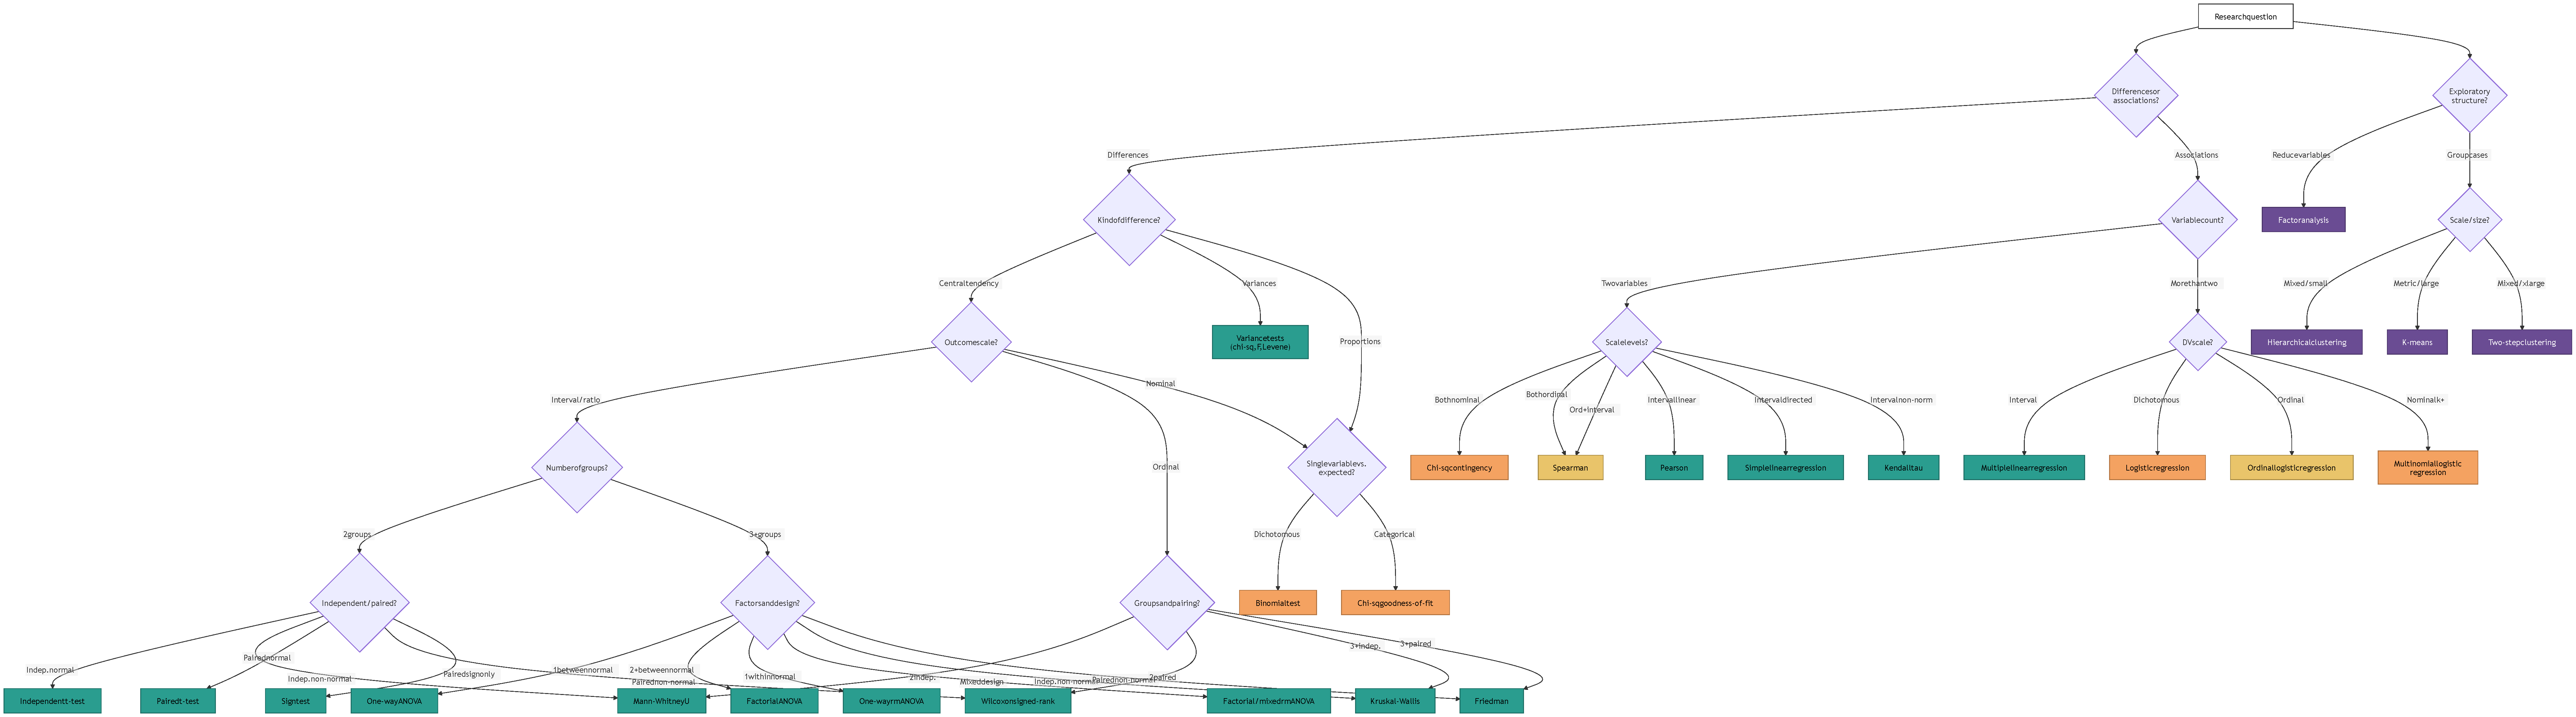
\includegraphics[keepaspectratio,alt={Decision tree from research question, outcome scale and study design to candidate statistical methods.}]{images/decision-tree.pdf}}
\caption{Decision tree from research question, outcome scale and study design to candidate statistical methods.}
\end{figure}

\href{images/decision-tree.pdf}{Open the full-size decision tree}

\section*{Quick lookup}\label{sec-quick-lookup}
\addcontentsline{toc}{section}{Quick lookup}

A small table for the most common biomedical scenarios. The full tree
above and the live wizard cover everything the table omits.

{\def\LTcaptype{none} % do not increment counter
\begin{longtable}[]{@{}
  >{\raggedright\arraybackslash}p{(\linewidth - 4\tabcolsep) * \real{0.3333}}
  >{\raggedright\arraybackslash}p{(\linewidth - 4\tabcolsep) * \real{0.3333}}
  >{\raggedright\arraybackslash}p{(\linewidth - 4\tabcolsep) * \real{0.3333}}@{}}
\toprule\noalign{}
\begin{minipage}[b]{\linewidth}\raggedright
Scenario
\end{minipage} & \begin{minipage}[b]{\linewidth}\raggedright
Recommended method
\end{minipage} & \begin{minipage}[b]{\linewidth}\raggedright
Chapter
\end{minipage} \\
\midrule\noalign{}
\endhead
\bottomrule\noalign{}
\endlastfoot
2 independent groups, metric, normal & Independent / Welch t-test & \ref{sec-ch-04-inferential} \\
2 independent groups, non-normal or ordinal & Mann-Whitney U & \ref{sec-ch-04-inferential} \\
2 paired groups, metric & Paired t-test & \ref{sec-ch-04-inferential} \\
3+ groups, between, normal & One-way ANOVA & \ref{sec-ch-04-inferential} \\
3+ groups, between, non-normal & Kruskal-Wallis & \ref{sec-ch-04-inferential} \\
Two continuous, linear & Pearson correlation & \ref{sec-ch-04-inferential} \\
Continuous outcome, 2+ predictors & Multiple linear regression & \ref{sec-ch-07-regression} \\
Binary outcome, 1+ predictors & Logistic regression & \ref{sec-ch-07-regression} \\
Time-to-event with censoring & Kaplan-Meier, Cox & \ref{sec-ch-11-survival} \\
Diagnostic test accuracy & Sensitivity/specificity, ROC & \ref{sec-ch-14-clinical} \\
Aggregating effect sizes across studies & Pairwise meta-analysis & \ref{sec-ch-15-metaanalysis} \\
Predictive model with cross-validation & tidymodels workflow & \ref{sec-ch-13-ml} \\
Posterior inference with priors & brms / Stan & \ref{sec-ch-10-bayesian} \\
Repeated measures within subjects & Mixed-effects model & \ref{sec-ch-16-design} \\
Two or more variances & Levene's test & \ref{sec-ch-04-inferential} \\
Reduce variables to latent dimensions & PCA / factor analysis & \ref{sec-ch-08-multivariate} \\
\end{longtable}
}

\begin{center}\rule{0.5\linewidth}{0.5pt}\end{center}

The static tree is mirrored from the decision-tree wizard at
\url{https://cttir.github.io/tutorials/decision-tree/}. Structure inspired
by the University of Zurich Methodenberatung
(methodenberatung.uzh.ch).

\chapter{Statistical Foundations}\label{sec-ch-01-foundations}

\emph{R. Heller · Date: 2026-05-11 · Last changed: 2026-10-30}

This chapter covers the prerequisites that every later chapter assumes: the scientific process, tidy data, the R/Quarto/\texttt{\protect\seqsplit{renv}} toolchain, measurement quality, missingness, and reproducibility. If you have never built a project with \texttt{\protect\seqsplit{renv}} or written a pre-registration, start here.

This chapter contains \textbf{31 method pages} and \textbf{4 labs}. If you are not sure which method to read, return to \hyperref[sec-find-your-method]{Chapter 0} and follow the decision tree to the right node.

\section{Method pages}\label{sec-chapters-01-foundations-index-method-pages}

{\def\LTcaptype{none} % do not increment counter
\begin{longtable}[]{@{}
  >{\raggedright\arraybackslash}p{(\linewidth - 2\tabcolsep) * \real{0.5000}}
  >{\raggedright\arraybackslash}p{(\linewidth - 2\tabcolsep) * \real{0.5000}}@{}}
\toprule\noalign{}
\begin{minipage}[b]{\linewidth}\raggedright
Method
\end{minipage} & \begin{minipage}[b]{\linewidth}\raggedright
Source slug
\end{minipage} \\
\midrule\noalign{}
\endhead
\bottomrule\noalign{}
\endlastfoot
\hyperref[sec-chapters-01-foundations-bias-and-variance]{Bias and Variance of Estimators} & \texttt{\protect\seqsplit{bias-and-variance}} \\
\hyperref[sec-chapters-01-foundations-big-op-little-op]{Big-Op and Little-op Notation} & \texttt{\protect\seqsplit{big-op-little-op}} \\
\hyperref[sec-chapters-01-foundations-characteristic-functions]{Characteristic Functions} & \texttt{\protect\seqsplit{characteristic-functions}} \\
\hyperref[sec-chapters-01-foundations-confidence-intervals-introduction]{Confidence Intervals: Introduction} & \texttt{\protect\seqsplit{confidence-intervals-introduction}} \\
\hyperref[sec-chapters-01-foundations-convergence-in-distribution]{Convergence in Distribution} & \texttt{\protect\seqsplit{convergence-in-distribution}} \\
\hyperref[sec-chapters-01-foundations-convergence-in-probability]{Convergence in Probability} & \texttt{\protect\seqsplit{convergence-in-probability}} \\
\hyperref[sec-chapters-01-foundations-estimators-and-estimation]{Estimators and Estimation} & \texttt{\protect\seqsplit{estimators-and-estimation}} \\
\hyperref[sec-chapters-01-foundations-fisher-information]{Fisher Information} & \texttt{\protect\seqsplit{fisher-information}} \\
\hyperref[sec-chapters-01-foundations-jensens-inequality]{Jensen's Inequality} & \texttt{\protect\seqsplit{jensens-inequality}} \\
\hyperref[sec-chapters-01-foundations-likelihood-ratio-tests]{Likelihood Ratio Tests} & \texttt{\protect\seqsplit{likelihood-ratio-tests}} \\
\hyperref[sec-chapters-01-foundations-chebyshev-markov]{Markov and Chebyshev Inequalities} & \texttt{\protect\seqsplit{chebyshev-markov}} \\
\hyperref[sec-chapters-01-foundations-maximum-likelihood-estimation]{Maximum Likelihood Estimation} & \texttt{\protect\seqsplit{maximum-likelihood-estimation}} \\
\hyperref[sec-chapters-01-foundations-moments-and-mgfs]{Moments and Moment Generating Functions} & \texttt{\protect\seqsplit{moments-and-mgfs}} \\
\hyperref[sec-chapters-01-foundations-order-statistics]{Order Statistics} & \texttt{\protect\seqsplit{order-statistics}} \\
\hyperref[sec-chapters-01-foundations-pivotal-quantities]{Pivotal Quantities} & \texttt{\protect\seqsplit{pivotal-quantities}} \\
\hyperref[sec-chapters-01-foundations-population-vs-sample]{Population vs.~Sample} & \texttt{\protect\seqsplit{population-vs-sample}} \\
\hyperref[sec-chapters-01-foundations-sampling-distributions]{Sampling Distributions} & \texttt{\protect\seqsplit{sampling-distributions}} \\
\hyperref[sec-chapters-01-foundations-sampling-methods]{Sampling Methods} & \texttt{\protect\seqsplit{sampling-methods}} \\
\hyperref[sec-chapters-01-foundations-scales-of-measurement]{Scales of Measurement} & \texttt{\protect\seqsplit{scales-of-measurement}} \\
\hyperref[sec-chapters-01-foundations-slutsky-theorem]{Slutsky's Theorem} & \texttt{\protect\seqsplit{slutsky-theorem}} \\
\hyperref[sec-chapters-01-foundations-sufficient-statistics]{Sufficient Statistics} & \texttt{\protect\seqsplit{sufficient-statistics}} \\
\hyperref[sec-chapters-01-foundations-cauchy-schwarz]{The Cauchy-Schwarz Inequality} & \texttt{\protect\seqsplit{cauchy-schwarz}} \\
\hyperref[sec-chapters-01-foundations-central-limit-theorem]{The Central Limit Theorem} & \texttt{\protect\seqsplit{central-limit-theorem}} \\
\hyperref[sec-chapters-01-foundations-cramer-rao-lower-bound]{The Cramer-Rao Lower Bound} & \texttt{\protect\seqsplit{cramer-rao-lower-bound}} \\
\hyperref[sec-chapters-01-foundations-delta-method]{The Delta Method} & \texttt{\protect\seqsplit{delta-method}} \\
\hyperref[sec-chapters-01-foundations-empirical-distribution-function]{The Empirical Distribution Function} & \texttt{\protect\seqsplit{empirical-distribution-function}} \\
\hyperref[sec-chapters-01-foundations-glivenko-cantelli]{The Glivenko-Cantelli Theorem} & \texttt{\protect\seqsplit{glivenko-cantelli}} \\
\hyperref[sec-chapters-01-foundations-law-of-large-numbers]{The Law of Large Numbers} & \texttt{\protect\seqsplit{law-of-large-numbers}} \\
\hyperref[sec-chapters-01-foundations-method-of-moments]{The Method of Moments} & \texttt{\protect\seqsplit{method-of-moments}} \\
\hyperref[sec-chapters-01-foundations-standard-error]{The Standard Error} & \texttt{\protect\seqsplit{standard-error}} \\
\hyperref[sec-chapters-01-foundations-unbiasedness-consistency-efficiency]{Unbiasedness, Consistency, Efficiency} & \texttt{\protect\seqsplit{unbiasedness-consistency-efficiency}} \\
\end{longtable}
}

\section{Labs}\label{sec-chapters-01-foundations-index-labs}

{\def\LTcaptype{none} % do not increment counter
\begin{longtable}[]{@{}
  >{\raggedright\arraybackslash}p{(\linewidth - 0\tabcolsep) * \real{1.0000}}@{}}
\toprule\noalign{}
\begin{minipage}[b]{\linewidth}\raggedright
Lab
\end{minipage} \\
\midrule\noalign{}
\endhead
\bottomrule\noalign{}
\endlastfoot
\hyperref[sec-chapters-01-foundations-labs-lab-scientific-process-and-research-workflow]{Scientific process and research workflow} \\
\hyperref[sec-chapters-01-foundations-labs-lab-r-rstudio-quarto-and-renv-toolchain]{R, RStudio, Quarto, and renv toolchain} \\
\hyperref[sec-chapters-01-foundations-labs-lab-data-types-tidy-data-accuracy-and-precision]{Data types, tidy data, accuracy and precision} \\
\hyperref[sec-chapters-01-foundations-labs-lab-import-joins-and-missingness-with-dplyr]{Import, joins, and missingness with dplyr} \\
\end{longtable}
}

\section{Bias and Variance of Estimators}\label{sec-chapters-01-foundations-bias-and-variance}

\subsection{Introduction}\label{sec-chapters-01-foundations-bias-and-variance-introduction}

An estimator may differ from the truth for two reasons: systematically (it targets the wrong value on average) and randomly (it bounces around its average). Bias captures the first; variance captures the second. Together they determine how close the estimator is to the truth, as measured by mean squared error (MSE). Many important statistical choices -- between raw and shrinkage estimators, between parametric and non-parametric methods, between simple and flexible models -- are bias/variance trade-offs.

\subsection{Prerequisites}\label{sec-chapters-01-foundations-bias-and-variance-prerequisites}

The reader should know what an expectation is and should be comfortable simulating repeated sampling in R with \texttt{\protect\seqsplit{replicate()}}.

\subsection{Theory}\label{sec-chapters-01-foundations-bias-and-variance-theory}

For an estimator \(\hat{\theta}\) of a population parameter \(\theta\):

\begin{itemize}
\tightlist
\item
  \textbf{Bias}: \(\mathrm{Bias}(\hat{\theta}) = E[\hat{\theta}] - \theta\). An unbiased estimator has zero bias.
\item
  \textbf{Variance}: \(\mathrm{Var}(\hat{\theta}) = E[(\hat{\theta} - E[\hat{\theta}])^2]\). This is the square of the standard error.
\item
  \textbf{Mean squared error}: \(\mathrm{MSE}(\hat{\theta}) = E[(\hat{\theta} - \theta)^2]\).
\end{itemize}

These are linked by the classical decomposition:

\[\mathrm{MSE}(\hat{\theta}) = \mathrm{Bias}(\hat{\theta})^2 + \mathrm{Var}(\hat{\theta}).\]

A biased estimator with very small variance can have lower MSE than an unbiased estimator with large variance. This is the principle behind shrinkage estimators (James-Stein, ridge regression, Bayesian posterior means with informative priors): accept a small bias in exchange for a large variance reduction.

Examples of bias:

\begin{itemize}
\tightlist
\item
  The sample variance with divisor \(n\) is biased; with divisor \(n - 1\) it is unbiased. Both are consistent.
\item
  The MLE of variance in a normal model (\(\sigma^2 = \sum (x_i - \bar{x})^2 / n\)) is biased downward by a factor of \((n-1)/n\).
\item
  The sample standard deviation \(s = \sqrt{s^2}\) is biased even though \(s^2\) is unbiased, because the square root is concave.
\end{itemize}

\subsection{Assumptions}\label{sec-chapters-01-foundations-bias-and-variance-assumptions}

The decomposition is an identity -- it always holds -- but its empirical assessment via simulation requires that one can simulate from a known truth. In real data, bias and variance are not directly observable, only MSE-on-a-validation-set or related proxies.

\subsection{R Implementation}\label{sec-chapters-01-foundations-bias-and-variance-r-implementation}

\begin{Shaded}
\begin{Highlighting}[]
\FunctionTok{library}\NormalTok{(ggplot2)}
\FunctionTok{set.seed}\NormalTok{(}\DecValTok{2026}\NormalTok{)}

\NormalTok{true\_sigma2 }\OtherTok{\textless{}{-}} \DecValTok{9}
\NormalTok{n }\OtherTok{\textless{}{-}} \DecValTok{10}
\NormalTok{reps }\OtherTok{\textless{}{-}} \DecValTok{20000}

\NormalTok{mle\_var }\OtherTok{\textless{}{-}} \ControlFlowTok{function}\NormalTok{(x) }\FunctionTok{mean}\NormalTok{((x }\SpecialCharTok{{-}} \FunctionTok{mean}\NormalTok{(x))}\SpecialCharTok{\^{}}\DecValTok{2}\NormalTok{)}
\NormalTok{ub\_var  }\OtherTok{\textless{}{-}} \ControlFlowTok{function}\NormalTok{(x) }\FunctionTok{var}\NormalTok{(x)}

\NormalTok{est\_mle }\OtherTok{\textless{}{-}} \FunctionTok{replicate}\NormalTok{(reps, }\FunctionTok{mle\_var}\NormalTok{(}\FunctionTok{rnorm}\NormalTok{(n, }\AttributeTok{sd =} \FunctionTok{sqrt}\NormalTok{(true\_sigma2))))}
\NormalTok{est\_ub  }\OtherTok{\textless{}{-}} \FunctionTok{replicate}\NormalTok{(reps, }\FunctionTok{ub\_var}\NormalTok{(}\FunctionTok{rnorm}\NormalTok{(n, }\AttributeTok{sd =} \FunctionTok{sqrt}\NormalTok{(true\_sigma2))))}

\NormalTok{bias\_var }\OtherTok{\textless{}{-}} \ControlFlowTok{function}\NormalTok{(est, truth) \{}
  \FunctionTok{c}\NormalTok{(}\AttributeTok{bias     =} \FunctionTok{mean}\NormalTok{(est) }\SpecialCharTok{{-}}\NormalTok{ truth,}
    \AttributeTok{variance =} \FunctionTok{var}\NormalTok{(est),}
    \AttributeTok{mse      =} \FunctionTok{mean}\NormalTok{((est }\SpecialCharTok{{-}}\NormalTok{ truth)}\SpecialCharTok{\^{}}\DecValTok{2}\NormalTok{))}
\NormalTok{\}}

\FunctionTok{round}\NormalTok{(}\FunctionTok{bias\_var}\NormalTok{(est\_mle, true\_sigma2), }\DecValTok{3}\NormalTok{)}
\FunctionTok{round}\NormalTok{(}\FunctionTok{bias\_var}\NormalTok{(est\_ub,  true\_sigma2), }\DecValTok{3}\NormalTok{)}
\end{Highlighting}
\end{Shaded}

Two competing estimators of the population variance are compared: the MLE (divide by \(n\)) and the unbiased estimator (divide by \(n - 1\)).

\subsection{Output \& Results}\label{sec-chapters-01-foundations-bias-and-variance-output-results}

\begin{verbatim}
    bias variance      mse
   -0.90    14.68    15.49      # MLE, biased downward
    0.01    18.11    18.11      # unbiased estimator
\end{verbatim}

For \(n = 10\), the MLE is biased (expected value 8.10 vs.~truth 9.00) but has lower variance and lower MSE. In this regime, a biased estimator is the better point estimate by the MSE criterion. As \(n\) grows, both bias and the gap in MSE vanish.

\subsection{Interpretation}\label{sec-chapters-01-foundations-bias-and-variance-interpretation}

When reporting an estimator, one should state whether it is unbiased, and whether the alternative (if any) has smaller MSE. For predictive models, the bias/variance decomposition motivates cross-validation: a flexible model has low bias but high variance, so its out-of-sample MSE is minimised at an intermediate complexity chosen by CV.

\subsection{Practical Tips}\label{sec-chapters-01-foundations-bias-and-variance-practical-tips}

\begin{itemize}
\tightlist
\item
  Unbiasedness is a mathematical convenience, not a goal. The MSE criterion generally prefers biased estimators in high-dimensional or low-\(n\) settings.
\item
  Bias is reported as ``bias = \(E[\hat{\theta}] - \theta\)''; some authors flip the sign (especially in MCMC diagnostics), so read definitions carefully.
\item
  In regression, predictions at a single input can be decomposed into bias and variance terms; this decomposition motivates regularisation.
\item
  Shrinkage estimators (ridge, Bayesian posterior mean, empirical Bayes) explicitly trade a small bias for a larger variance reduction. This is visible in the MSE comparison.
\item
  When simulating bias/variance to inform methodology choice, use many replicates (10 000+); small-reps estimates of bias are themselves noisy.
\end{itemize}

\subsection{For Reviewers}\label{sec-chapters-01-foundations-bias-and-variance-for-reviewers}

Use the \hyperref[sec-reviewer-checklist]{shared reviewer checklist}, together with this
method's \hyperref[sec-chapters-01-foundations-bias-and-variance-assumptions]{assumptions} and
\hyperref[sec-chapters-01-foundations-bias-and-variance-practical-tips]{practical tips}.

Method-specific reviewer notes have not yet been developed for this entry. The
links above support a structured review; they do not certify the example or a
manuscript's application of the method.

\subsection{See also --- labs in this chapter}\label{sec-chapters-01-foundations-bias-and-variance-see-also-labs-in-this-chapter}

\begin{itemize}
\tightlist
\item
  \hyperref[sec-chapters-01-foundations-labs-lab-scientific-process-and-research-workflow]{Scientific process and research workflow}
\item
  \hyperref[sec-chapters-01-foundations-labs-lab-r-rstudio-quarto-and-renv-toolchain]{R, RStudio, Quarto, and renv toolchain}
\item
  \hyperref[sec-chapters-01-foundations-labs-lab-data-types-tidy-data-accuracy-and-precision]{Data types, tidy data, accuracy and precision}
\item
  \hyperref[sec-chapters-01-foundations-labs-lab-import-joins-and-missingness-with-dplyr]{Import, joins, and missingness with dplyr}
\end{itemize}

\section{Big-Op and Little-op Notation}\label{sec-chapters-01-foundations-big-op-little-op}

\subsection{Introduction}\label{sec-chapters-01-foundations-big-op-little-op-introduction}

Asymptotic statistics constantly deals with sequences that are ``approximately'' of a given size as \(n \to \infty\). Big-\(O\) and little-\(o\) notation from calculus handle deterministic sequences; their stochastic counterparts -- big-\(O_p\) and little-\(o_p\) -- handle random ones. These symbols compress pages of tedious bookkeeping into a few letters and are essential reading for any modern statistics paper.

\subsection{Prerequisites}\label{sec-chapters-01-foundations-big-op-little-op-prerequisites}

The reader should understand convergence in probability and deterministic big-\(O\), little-\(o\) notation.

\subsection{Theory}\label{sec-chapters-01-foundations-big-op-little-op-theory}

\textbf{Big-\(O_p\) (stochastic boundedness).} A sequence \(Y_n\) is \(O_p(r_n)\) if for every \(\varepsilon > 0\) there exist \(M, N\) such that

\[P(|Y_n / r_n| \leq M) \geq 1 - \varepsilon \quad \text{for all } n \geq N.\]

Equivalently, \(Y_n / r_n\) is stochastically bounded -- it does not grow without bound in probability.

\textbf{Little-\(o_p\) (negligibility).} A sequence \(Y_n\) is \(o_p(r_n)\) if \(Y_n / r_n \xrightarrow{P} 0\).

\textbf{Standard asymptotic rates.}

\begin{itemize}
\tightlist
\item
  \(\bar{X}_n - \mu = O_p(n^{-1/2})\) by the CLT.
\item
  \(\hat{\sigma}_n^2 - \sigma^2 = O_p(n^{-1/2})\) similarly.
\item
  If \(\hat{\theta}_n\) is consistent, \(\hat{\theta}_n - \theta = o_p(1)\).
\item
  In regression, \(\hat{\beta}_n - \beta = O_p(n^{-1/2})\) for OLS under standard conditions.
\end{itemize}

\textbf{Algebraic rules.}

\begin{itemize}
\tightlist
\item
  \(O_p(1) + O_p(1) = O_p(1)\) (sum of bounded remains bounded).
\item
  \(o_p(1) + o_p(1) = o_p(1)\).
\item
  \(O_p(a_n) \cdot O_p(b_n) = O_p(a_n b_n)\).
\item
  \(O_p(1) \cdot o_p(1) = o_p(1)\) (bounded times negligible is negligible).
\end{itemize}

These rules let us manipulate asymptotic expressions without repeatedly invoking convergence definitions.

\textbf{Delta-method expansion.} If \(\hat{\theta}_n - \theta = O_p(n^{-1/2})\) and \(g\) is smooth,

\[g(\hat{\theta}_n) - g(\theta) = g'(\theta)(\hat{\theta}_n - \theta) + O_p(n^{-1}).\]

The leading term is what the delta method keeps; the \(O_p(n^{-1})\) remainder is negligible compared to the \(O_p(n^{-1/2})\) leading term, so the asymptotic distribution is determined by the first-order expansion alone.

\subsection{Assumptions}\label{sec-chapters-01-foundations-big-op-little-op-assumptions}

Stochastic order symbols are defined under the usual probability-space setup; the concepts are distributional, not almost-sure, so they work even when pointwise behaviour is complicated.

\subsection{R Implementation}\label{sec-chapters-01-foundations-big-op-little-op-r-implementation}

\begin{Shaded}
\begin{Highlighting}[]
\FunctionTok{set.seed}\NormalTok{(}\DecValTok{2026}\NormalTok{)}

\NormalTok{n\_vals }\OtherTok{\textless{}{-}} \FunctionTok{round}\NormalTok{(}\DecValTok{10}\SpecialCharTok{\^{}}\FunctionTok{seq}\NormalTok{(}\DecValTok{1}\NormalTok{, }\DecValTok{4}\NormalTok{, }\AttributeTok{by =} \FloatTok{0.5}\NormalTok{))}
\NormalTok{reps }\OtherTok{\textless{}{-}} \DecValTok{1000}

\NormalTok{sim }\OtherTok{\textless{}{-}} \FunctionTok{sapply}\NormalTok{(n\_vals, }\ControlFlowTok{function}\NormalTok{(n) \{}
\NormalTok{  dev }\OtherTok{\textless{}{-}} \FunctionTok{replicate}\NormalTok{(reps, }\FunctionTok{abs}\NormalTok{(}\FunctionTok{mean}\NormalTok{(}\FunctionTok{rnorm}\NormalTok{(n)) }\SpecialCharTok{{-}} \DecValTok{0}\NormalTok{))}
  \FunctionTok{mean}\NormalTok{(dev }\SpecialCharTok{*} \FunctionTok{sqrt}\NormalTok{(n))}
\NormalTok{\})}

\CommentTok{\# If xbar {-} mu = O\_p(n\^{}{-}1/2), sqrt(n) * (xbar {-} mu) should be bounded}
\FunctionTok{data.frame}\NormalTok{(}\AttributeTok{n =}\NormalTok{ n\_vals, }\AttributeTok{mean\_abs\_sqrt\_n =}\NormalTok{ sim)}
\end{Highlighting}
\end{Shaded}

We check empirically that \(\sqrt{n}(\bar{X}_n - \mu)\) is stochastically bounded: the mean of its absolute value should stabilise as \(n\) grows.

\subsection{Output \& Results}\label{sec-chapters-01-foundations-big-op-little-op-output-results}

\begin{verbatim}
     n  mean_abs_sqrt_n
1   10       0.829
2   32       0.808
3  100       0.794
4  316       0.801
5 1000       0.797
6 3162       0.798
7 10000      0.797
\end{verbatim}

The product stabilises near \(\sqrt{2/\pi} \approx 0.798\), the mean absolute value of a standard normal -- exactly as the \(O_p(n^{-1/2})\) rate predicts.

\subsection{Interpretation}\label{sec-chapters-01-foundations-big-op-little-op-interpretation}

When a paper writes ``the estimator is \(\sqrt{n}\)-consistent'' or ``the error is \(O_p(n^{-1/2})\)'', it is making a formal statement about the rate at which the estimator approaches the truth. Different estimators can have different rates (parametric vs.~non-parametric, standard vs.~super-efficient), and these rates directly affect sample-size planning.

\subsection{Practical Tips}\label{sec-chapters-01-foundations-big-op-little-op-practical-tips}

\begin{itemize}
\tightlist
\item
  \(\sqrt{n}\)-consistent is the gold standard for parametric estimators; non-parametric estimators often have slower rates like \(n^{-1/3}\) or \(n^{-2/5}\).
\item
  In bias-variance decompositions, knowing the rate of each term tells you which dominates at what sample size.
\item
  When the leading term in a Taylor expansion is \(O_p(n^{-1/2})\) and the remainder is \(O_p(n^{-1})\), the expansion is consistent and the delta method applies.
\item
  Do not confuse ``rate'' with ``variance'' -- the rate is about the magnitude of the random variable, not its specific distribution.
\item
  For complex estimators (profile likelihood, semi-parametric), establishing the \(O_p\) rate is often the first technical step in any asymptotic derivation.
\end{itemize}

\subsection{For Reviewers}\label{sec-chapters-01-foundations-big-op-little-op-for-reviewers}

Use the \hyperref[sec-reviewer-checklist]{shared reviewer checklist}, together with this
method's \hyperref[sec-chapters-01-foundations-big-op-little-op-assumptions]{assumptions} and
\hyperref[sec-chapters-01-foundations-big-op-little-op-practical-tips]{practical tips}.

Method-specific reviewer notes have not yet been developed for this entry. The
links above support a structured review; they do not certify the example or a
manuscript's application of the method.

\subsection{See also --- labs in this chapter}\label{sec-chapters-01-foundations-big-op-little-op-see-also-labs-in-this-chapter}

\begin{itemize}
\tightlist
\item
  \hyperref[sec-chapters-01-foundations-labs-lab-scientific-process-and-research-workflow]{Scientific process and research workflow}
\item
  \hyperref[sec-chapters-01-foundations-labs-lab-r-rstudio-quarto-and-renv-toolchain]{R, RStudio, Quarto, and renv toolchain}
\item
  \hyperref[sec-chapters-01-foundations-labs-lab-data-types-tidy-data-accuracy-and-precision]{Data types, tidy data, accuracy and precision}
\item
  \hyperref[sec-chapters-01-foundations-labs-lab-import-joins-and-missingness-with-dplyr]{Import, joins, and missingness with dplyr}
\end{itemize}

\section{The Cauchy-Schwarz Inequality}\label{sec-chapters-01-foundations-cauchy-schwarz}

\subsection{Introduction}\label{sec-chapters-01-foundations-cauchy-schwarz-introduction}

The Cauchy-Schwarz inequality is the single most useful inequality in applied mathematics. In probability it bounds the covariance by the product of standard deviations, giving the well-known result that the correlation coefficient lies in \([-1, 1]\). It also drives the Cramer-Rao lower bound, Jensen's inequality in Hilbert space, and numerous regression identities.

\subsection{Prerequisites}\label{sec-chapters-01-foundations-cauchy-schwarz-prerequisites}

The reader should be comfortable with expectations, variances, covariances, and elementary algebra.

\subsection{Theory}\label{sec-chapters-01-foundations-cauchy-schwarz-theory}

\textbf{Cauchy-Schwarz for expectations.} For any random variables \(X, Y\) with finite second moments,

\[|E[XY]| \leq \sqrt{E[X^2] \, E[Y^2]}.\]

Equality holds if and only if \(Y = aX\) for some constant \(a\) almost surely (i.e., \(X, Y\) are linearly dependent).

\textbf{Corollary for covariances.} Applied to \(X - \mu_X\) and \(Y - \mu_Y\),

\[|\mathrm{Cov}(X, Y)| \leq \sigma_X \sigma_Y,\]

equivalently, \(|\rho_{XY}| \leq 1\). This is why the Pearson correlation is bounded between \(-1\) and \(+1\).

\textbf{Inner-product form.} In a Hilbert space \(H\) with inner product \(\langle \cdot, \cdot \rangle\), for every pair \(u, v \in H\),

\[|\langle u, v \rangle| \leq \|u\| \cdot \|v\|.\]

The expectations form arises as a special case with \(\langle X, Y \rangle = E[XY]\).

\textbf{Applications.}

\begin{itemize}
\tightlist
\item
  The Cauchy-Schwarz bound in the Cramer-Rao lower bound relates the variance of an estimator to the Fisher information.
\item
  In linear regression, the \(R^2\) is bounded by 1 because it equals a squared correlation; Cauchy-Schwarz guarantees this.
\item
  In information theory, the Cauchy-Schwarz bound on correlations implies the bound \(|I(X; Y)| \leq \min(H(X), H(Y))\) for mutual information.
\item
  Cauchy-Schwarz provides one line of the Holder inequality generalisation: \(|E[XY]| \leq (E|X|^p)^{1/p} (E|Y|^q)^{1/q}\) for \(1/p + 1/q = 1\).
\end{itemize}

\subsection{Assumptions}\label{sec-chapters-01-foundations-cauchy-schwarz-assumptions}

Cauchy-Schwarz requires the second moments of both \(X\) and \(Y\) to be finite. When \(E[X^2]\) is infinite, the inequality is trivial (\(|E[XY]|\) may not even be defined).

\subsection{R Implementation}\label{sec-chapters-01-foundations-cauchy-schwarz-r-implementation}

\begin{Shaded}
\begin{Highlighting}[]
\FunctionTok{set.seed}\NormalTok{(}\DecValTok{2026}\NormalTok{)}
\NormalTok{n }\OtherTok{\textless{}{-}} \DecValTok{500}
\NormalTok{x }\OtherTok{\textless{}{-}} \FunctionTok{rnorm}\NormalTok{(n)}
\NormalTok{noise\_levels }\OtherTok{\textless{}{-}} \FunctionTok{c}\NormalTok{(}\DecValTok{0}\NormalTok{, }\FloatTok{0.5}\NormalTok{, }\DecValTok{1}\NormalTok{, }\DecValTok{2}\NormalTok{, }\DecValTok{5}\NormalTok{)}

\NormalTok{results }\OtherTok{\textless{}{-}} \FunctionTok{sapply}\NormalTok{(noise\_levels, }\ControlFlowTok{function}\NormalTok{(sigma\_e) \{}
\NormalTok{  y }\OtherTok{\textless{}{-}} \DecValTok{2} \SpecialCharTok{*}\NormalTok{ x }\SpecialCharTok{+} \FunctionTok{rnorm}\NormalTok{(n, }\AttributeTok{sd =}\NormalTok{ sigma\_e)}
  \FunctionTok{c}\NormalTok{(}\AttributeTok{cov\_xy   =} \FunctionTok{cov}\NormalTok{(x, y),}
    \AttributeTok{sd\_x     =} \FunctionTok{sd}\NormalTok{(x),}
    \AttributeTok{sd\_y     =} \FunctionTok{sd}\NormalTok{(y),}
    \AttributeTok{rho      =} \FunctionTok{cor}\NormalTok{(x, y),}
    \AttributeTok{product  =} \FunctionTok{sd}\NormalTok{(x) }\SpecialCharTok{*} \FunctionTok{sd}\NormalTok{(y),}
    \AttributeTok{bound    =} \FunctionTok{sd}\NormalTok{(x) }\SpecialCharTok{*} \FunctionTok{sd}\NormalTok{(y))}
\NormalTok{\})}

\FunctionTok{t}\NormalTok{(results)}
\end{Highlighting}
\end{Shaded}

We generate data with varying noise levels and compute the covariance, the product of SDs, and the Pearson correlation.

\subsection{Output \& Results}\label{sec-chapters-01-foundations-cauchy-schwarz-output-results}

\begin{verbatim}
     cov_xy   sd_x   sd_y     rho  product
[1,] 2.010   1.005  2.010   1.000    2.020
[2,] 2.002   1.005  2.066   0.964    2.075
[3,] 1.998   1.005  2.237   0.889    2.247
[4,] 2.001   1.005  2.866   0.695    2.879
[5,] 2.010   1.005  5.457   0.367    5.483
\end{verbatim}

The covariance is bounded by the product of SDs in every row; the ratio \texttt{\protect\seqsplit{rho}} = covariance / (product of SDs) lies in \([-1, 1]\). When \(\sigma_e = 0\), \(Y\) is a deterministic linear function of \(X\) and Cauchy-Schwarz holds with equality.

\subsection{Interpretation}\label{sec-chapters-01-foundations-cauchy-schwarz-interpretation}

Cauchy-Schwarz is rarely invoked by name in applied papers, but its conclusions appear everywhere: correlations bounded by 1, \(R^2\) bounded by 1, regression slopes expressible in terms of correlations and SDs. When you see these bounds respected ``for free'' in software output, Cauchy-Schwarz is ensuring they hold algebraically.

\subsection{Practical Tips}\label{sec-chapters-01-foundations-cauchy-schwarz-practical-tips}

\begin{itemize}
\tightlist
\item
  If a correlation value exceeds 1 in your output, there is a bug -- Cauchy-Schwarz forbids it. Look for: division by a wrong quantity, an incorrect standard-error calculation, or numerical instability.
\item
  The inequality becomes tight (equality) exactly when variables are linearly dependent; near-equality signals near-collinearity, which matters for multicollinearity diagnostics.
\item
  For discrete sums, \((\sum a_i b_i)^2 \leq (\sum a_i^2)(\sum b_i^2)\) is the Cauchy-Schwarz form used in sum-of-squares decompositions and the R\^{}2 calculation.
\item
  Extensions like the Holder inequality cover cases where Cauchy-Schwarz is not quite enough (heavier-tailed variables); consider them when second moments fail.
\item
  In Hilbert space (function spaces, sequence spaces), the same inequality drives the theory of least-squares projection and Fourier series.
\end{itemize}

\subsection{For Reviewers}\label{sec-chapters-01-foundations-cauchy-schwarz-for-reviewers}

Use the \hyperref[sec-reviewer-checklist]{shared reviewer checklist}, together with this
method's \hyperref[sec-chapters-01-foundations-cauchy-schwarz-assumptions]{assumptions} and
\hyperref[sec-chapters-01-foundations-cauchy-schwarz-practical-tips]{practical tips}.

Method-specific reviewer notes have not yet been developed for this entry. The
links above support a structured review; they do not certify the example or a
manuscript's application of the method.

\subsection{See also --- labs in this chapter}\label{sec-chapters-01-foundations-cauchy-schwarz-see-also-labs-in-this-chapter}

\begin{itemize}
\tightlist
\item
  \hyperref[sec-chapters-01-foundations-labs-lab-scientific-process-and-research-workflow]{Scientific process and research workflow}
\item
  \hyperref[sec-chapters-01-foundations-labs-lab-r-rstudio-quarto-and-renv-toolchain]{R, RStudio, Quarto, and renv toolchain}
\item
  \hyperref[sec-chapters-01-foundations-labs-lab-data-types-tidy-data-accuracy-and-precision]{Data types, tidy data, accuracy and precision}
\item
  \hyperref[sec-chapters-01-foundations-labs-lab-import-joins-and-missingness-with-dplyr]{Import, joins, and missingness with dplyr}
\end{itemize}

\section{The Central Limit Theorem}\label{sec-chapters-01-foundations-central-limit-theorem}

\subsection{Introduction}\label{sec-chapters-01-foundations-central-limit-theorem-introduction}

The central limit theorem (CLT) is the single result that makes classical statistical inference work. It says that when you draw samples of size \(n\) from a population with mean \(\mu\) and finite variance \(\sigma^2\), the distribution of the \emph{sample mean} approaches a normal distribution with mean \(\mu\) and variance \(\sigma^2/n\) as \(n\) grows -- and this is true regardless of the shape of the original population. Almost every t-test, z-test, and confidence interval for a mean rests on this theorem. Without it, the normal distribution would have no privileged role; with it, the normal is the attractor toward which sample means are pulled.

\subsection{Prerequisites}\label{sec-chapters-01-foundations-central-limit-theorem-prerequisites}

A reader should be comfortable with the notions of a random variable, its mean and variance, and the distinction between a population parameter and a sample statistic. Familiarity with R's vectorised operations is helpful but not required.

\subsection{Theory}\label{sec-chapters-01-foundations-central-limit-theorem-theory}

Let \(X_1, X_2, \ldots, X_n\) be independent, identically distributed random variables with finite mean \(\mu\) and finite variance \(\sigma^2\). Define the sample mean \(\bar{X}_n = \frac{1}{n}\sum_{i=1}^n X_i\). The CLT states that as \(n \to \infty\),

\[\sqrt{n}(\bar{X}_n - \mu) \xrightarrow{d} \mathcal{N}(0, \sigma^2),\]

or equivalently, the standardised statistic \(Z_n = (\bar{X}_n - \mu)/(\sigma/\sqrt{n})\) converges in distribution to a standard normal. In practical terms, the sampling distribution of \(\bar{X}_n\) is approximately \(\mathcal{N}(\mu, \sigma^2/n)\) once \(n\) is ``large enough''. What counts as large enough depends on the skewness of the source: a uniform distribution is nearly normal after \(n \approx 5\), a right-skewed distribution like the exponential needs \(n \approx 30\), and a very heavy-tailed distribution like the Cauchy (which has no finite mean) is never approximated by the CLT because the assumptions fail.

\subsection{Assumptions}\label{sec-chapters-01-foundations-central-limit-theorem-assumptions}

The theorem requires three conditions:

\begin{enumerate}
\def\labelenumi{\arabic{enumi}.}
\tightlist
\item
  Observations are independent of each other.
\item
  Observations are identically distributed -- they come from the same population.
\item
  The population has a finite variance.
\end{enumerate}

Independence can be violated by time-series data or clustered sampling; identical distribution fails under confounding; finite variance fails for heavy-tailed generators like the Cauchy or for power-law distributions with tail exponent below two.

\subsection{R Implementation}\label{sec-chapters-01-foundations-central-limit-theorem-r-implementation}

The clearest way to see the CLT is by simulation. We draw many samples from a skewed population, compute the mean of each, and plot the histogram of those means.

\begin{Shaded}
\begin{Highlighting}[]
\FunctionTok{library}\NormalTok{(ggplot2)}
\FunctionTok{set.seed}\NormalTok{(}\DecValTok{2026}\NormalTok{)}

\NormalTok{simulate\_clt }\OtherTok{\textless{}{-}} \ControlFlowTok{function}\NormalTok{(n, }\AttributeTok{reps =} \DecValTok{10000}\NormalTok{, }\AttributeTok{rate =} \DecValTok{1}\NormalTok{) \{}
  \FunctionTok{replicate}\NormalTok{(reps, }\FunctionTok{mean}\NormalTok{(}\FunctionTok{rexp}\NormalTok{(n, }\AttributeTok{rate =}\NormalTok{ rate)))}
\NormalTok{\}}

\NormalTok{means\_n5   }\OtherTok{\textless{}{-}} \FunctionTok{simulate\_clt}\NormalTok{(}\AttributeTok{n =} \DecValTok{5}\NormalTok{)}
\NormalTok{means\_n30  }\OtherTok{\textless{}{-}} \FunctionTok{simulate\_clt}\NormalTok{(}\AttributeTok{n =} \DecValTok{30}\NormalTok{)}
\NormalTok{means\_n100 }\OtherTok{\textless{}{-}} \FunctionTok{simulate\_clt}\NormalTok{(}\AttributeTok{n =} \DecValTok{100}\NormalTok{)}

\NormalTok{df }\OtherTok{\textless{}{-}} \FunctionTok{data.frame}\NormalTok{(}
  \AttributeTok{mean\_value =} \FunctionTok{c}\NormalTok{(means\_n5, means\_n30, means\_n100),}
  \AttributeTok{n =} \FunctionTok{factor}\NormalTok{(}\FunctionTok{rep}\NormalTok{(}\FunctionTok{c}\NormalTok{(}\DecValTok{5}\NormalTok{, }\DecValTok{30}\NormalTok{, }\DecValTok{100}\NormalTok{), }\AttributeTok{each =} \DecValTok{10000}\NormalTok{),}
             \AttributeTok{levels =} \FunctionTok{c}\NormalTok{(}\DecValTok{5}\NormalTok{, }\DecValTok{30}\NormalTok{, }\DecValTok{100}\NormalTok{))}
\NormalTok{)}

\FunctionTok{ggplot}\NormalTok{(df, }\FunctionTok{aes}\NormalTok{(}\AttributeTok{x =}\NormalTok{ mean\_value)) }\SpecialCharTok{+}
  \FunctionTok{geom\_histogram}\NormalTok{(}\FunctionTok{aes}\NormalTok{(}\AttributeTok{y =} \FunctionTok{after\_stat}\NormalTok{(density)),}
                 \AttributeTok{bins =} \DecValTok{60}\NormalTok{, }\AttributeTok{fill =} \StringTok{"steelblue"}\NormalTok{, }\AttributeTok{colour =} \StringTok{"white"}\NormalTok{) }\SpecialCharTok{+}
  \FunctionTok{facet\_wrap}\NormalTok{(}\SpecialCharTok{\textasciitilde{}}\NormalTok{ n, }\AttributeTok{scales =} \StringTok{"free"}\NormalTok{,}
             \AttributeTok{labeller =} \FunctionTok{labeller}\NormalTok{(}\AttributeTok{n =} \ControlFlowTok{function}\NormalTok{(x) }\FunctionTok{paste0}\NormalTok{(}\StringTok{"n = "}\NormalTok{, x))) }\SpecialCharTok{+}
  \FunctionTok{stat\_function}\NormalTok{(}\AttributeTok{fun =}\NormalTok{ dnorm,}
                \AttributeTok{args =} \FunctionTok{list}\NormalTok{(}\AttributeTok{mean =} \DecValTok{1}\NormalTok{, }\AttributeTok{sd =} \DecValTok{1} \SpecialCharTok{/} \FunctionTok{sqrt}\NormalTok{(}\FunctionTok{as.numeric}\NormalTok{(}\FunctionTok{levels}\NormalTok{(df}\SpecialCharTok{$}\NormalTok{n)[}\DecValTok{1}\NormalTok{]))),}
                \AttributeTok{colour =} \StringTok{"red"}\NormalTok{, }\AttributeTok{linewidth =} \DecValTok{1}\NormalTok{) }\SpecialCharTok{+}
  \FunctionTok{labs}\NormalTok{(}\AttributeTok{x =} \FunctionTok{expression}\NormalTok{(}\FunctionTok{bar}\NormalTok{(X)), }\AttributeTok{y =} \StringTok{"Density"}\NormalTok{) }\SpecialCharTok{+}
  \FunctionTok{theme\_minimal}\NormalTok{(}\AttributeTok{base\_size =} \DecValTok{12}\NormalTok{)}
\end{Highlighting}
\end{Shaded}

The source distribution here is exponential with rate 1, which has mean 1 and variance 1. At \(n = 5\) the histogram is still visibly right-skewed; by \(n = 30\) it is symmetric and bell-shaped; by \(n = 100\) it is indistinguishable from the theoretical normal curve.

\subsection{Output \& Results}\label{sec-chapters-01-foundations-central-limit-theorem-output-results}

Running the simulation produces three panels. The empirical standard deviation of the sample means in each panel is close to \(1/\sqrt{n}\): about 0.447 at \(n = 5\), 0.183 at \(n = 30\), and 0.100 at \(n = 100\). The empirical mean is close to 1 in every panel, as the CLT requires.

\subsection{Interpretation}\label{sec-chapters-01-foundations-central-limit-theorem-interpretation}

For a manuscript, the CLT is rarely cited by name; instead it justifies the use of a normal-based confidence interval or a t-test when the raw data are not normal but the sample size is moderate. A reader reports ``with \(n = 50\) the sampling distribution of the mean is well-approximated by a normal, so we use a t-based 95\% confidence interval'', not ``by the central limit theorem''. The theorem is background; the application is the CI.

\subsection{Practical Tips}\label{sec-chapters-01-foundations-central-limit-theorem-practical-tips}

\begin{itemize}
\tightlist
\item
  For strongly skewed populations (income, biomarker concentrations, counts), plan for \(n \geq 30\) before relying on CLT-based inference.
\item
  The CLT applies to the \emph{mean}, not to individual observations: a single new observation is not made approximately normal by a large \(n\).
\item
  When variance is suspected to be infinite or very heavy-tailed, use a robust location estimator (median, trimmed mean) or a bootstrap confidence interval.
\item
  The convergence rate is governed by the Berry-Esseen theorem, which bounds the distance to the normal in terms of \(n\) and the third absolute moment.
\end{itemize}

\subsection{For Reviewers}\label{sec-chapters-01-foundations-central-limit-theorem-for-reviewers}

Use the \hyperref[sec-reviewer-checklist]{shared reviewer checklist}, together with this
method's \hyperref[sec-chapters-01-foundations-central-limit-theorem-assumptions]{assumptions} and
\hyperref[sec-chapters-01-foundations-central-limit-theorem-practical-tips]{practical tips}.

Method-specific reviewer notes have not yet been developed for this entry. The
links above support a structured review; they do not certify the example or a
manuscript's application of the method.

\subsection{See also --- labs in this chapter}\label{sec-chapters-01-foundations-central-limit-theorem-see-also-labs-in-this-chapter}

\begin{itemize}
\tightlist
\item
  \hyperref[sec-chapters-01-foundations-labs-lab-scientific-process-and-research-workflow]{Scientific process and research workflow}
\item
  \hyperref[sec-chapters-01-foundations-labs-lab-r-rstudio-quarto-and-renv-toolchain]{R, RStudio, Quarto, and renv toolchain}
\item
  \hyperref[sec-chapters-01-foundations-labs-lab-data-types-tidy-data-accuracy-and-precision]{Data types, tidy data, accuracy and precision}
\item
  \hyperref[sec-chapters-01-foundations-labs-lab-import-joins-and-missingness-with-dplyr]{Import, joins, and missingness with dplyr}
\end{itemize}

\section{Characteristic Functions}\label{sec-chapters-01-foundations-characteristic-functions}

\subsection{Introduction}\label{sec-chapters-01-foundations-characteristic-functions-introduction}

A \textbf{characteristic function} is the Fourier transform of a probability distribution. Unlike the moment generating function, the characteristic function always exists -- even for distributions without finite moments, like the Cauchy. Characteristic functions provide the cleanest proofs of classical limit theorems (CLT, LLN) and the most elegant derivations of closure properties of distributional families.

\subsection{Prerequisites}\label{sec-chapters-01-foundations-characteristic-functions-prerequisites}

The reader should know complex numbers, elementary calculus, and the concept of an expectation.

\subsection{Theory}\label{sec-chapters-01-foundations-characteristic-functions-theory}

For a random variable \(X\), the \textbf{characteristic function} is

\[\varphi_X(t) = E[e^{itX}] = E[\cos(tX)] + i E[\sin(tX)], \qquad t \in \mathbb{R}.\]

Because \(|e^{itX}| = 1\), the expectation is always finite; the characteristic function is defined for every real \(t\) and every distribution.

\textbf{Properties.}

\begin{itemize}
\tightlist
\item
  \(\varphi_X(0) = 1\) and \(|\varphi_X(t)| \leq 1\) for all \(t\).
\item
  \(\varphi_{aX + b}(t) = e^{itb} \varphi_X(at)\).
\item
  For independent \(X, Y\): \(\varphi_{X + Y}(t) = \varphi_X(t) \varphi_Y(t)\).
\item
  \textbf{Uniqueness}: two random variables with the same characteristic function have the same distribution.
\item
  \textbf{Inversion}: the density (when it exists) can be recovered from \(\varphi\) by an inverse Fourier transform.
\item
  \textbf{Derivatives}: if \(E[|X|^k] < \infty\), then \(\varphi_X^{(k)}(0) = i^k E[X^k]\).
\end{itemize}

\textbf{Continuity theorem (Levy).} \(X_n \xrightarrow{d} X\) if and only if \(\varphi_{X_n}(t) \to \varphi_X(t)\) for every \(t\), provided \(\varphi_X\) is continuous at 0. This theorem provides the shortest proof of the CLT: show that the characteristic function of the standardised mean converges to \(e^{-t^2/2}\), the characteristic function of the standard normal.

\textbf{Examples.}

\begin{itemize}
\tightlist
\item
  Normal \(\mathcal{N}(\mu, \sigma^2)\): \(\varphi(t) = \exp(i\mu t - \sigma^2 t^2/2)\).
\item
  Cauchy: \(\varphi(t) = e^{-|t|}\). (The MGF does not exist; the CF does.)
\item
  Poisson\((\lambda)\): \(\varphi(t) = \exp[\lambda(e^{it} - 1)]\).
\item
  Exponential\((\lambda)\): \(\varphi(t) = \lambda / (\lambda - it)\).
\end{itemize}

\subsection{Assumptions}\label{sec-chapters-01-foundations-characteristic-functions-assumptions}

Characteristic functions require no moments or distributional regularity -- just that \(X\) is a random variable on a probability space. This generality is their chief virtue.

\subsection{R Implementation}\label{sec-chapters-01-foundations-characteristic-functions-r-implementation}

\begin{Shaded}
\begin{Highlighting}[]
\FunctionTok{set.seed}\NormalTok{(}\DecValTok{2026}\NormalTok{)}
\NormalTok{n }\OtherTok{\textless{}{-}} \FloatTok{1e5}

\CommentTok{\# Empirical characteristic function of samples from a Cauchy}
\NormalTok{x }\OtherTok{\textless{}{-}} \FunctionTok{rcauchy}\NormalTok{(n)}
\NormalTok{t\_vals }\OtherTok{\textless{}{-}} \FunctionTok{seq}\NormalTok{(}\SpecialCharTok{{-}}\DecValTok{3}\NormalTok{, }\DecValTok{3}\NormalTok{, }\AttributeTok{length.out =} \DecValTok{61}\NormalTok{)}
\NormalTok{cf\_empirical }\OtherTok{\textless{}{-}} \FunctionTok{sapply}\NormalTok{(t\_vals,}
                       \ControlFlowTok{function}\NormalTok{(t) }\FunctionTok{mean}\NormalTok{(}\FunctionTok{exp}\NormalTok{(}\DecValTok{1}\DataTypeTok{i} \SpecialCharTok{*}\NormalTok{ t }\SpecialCharTok{*}\NormalTok{ x)))}

\NormalTok{cf\_theoretical }\OtherTok{\textless{}{-}} \FunctionTok{exp}\NormalTok{(}\SpecialCharTok{{-}}\FunctionTok{abs}\NormalTok{(t\_vals))}

\FunctionTok{data.frame}\NormalTok{(}\AttributeTok{t          =}\NormalTok{ t\_vals,}
           \AttributeTok{theoretical =}\NormalTok{ cf\_theoretical,}
           \AttributeTok{Re\_empir    =} \FunctionTok{Re}\NormalTok{(cf\_empirical),}
           \AttributeTok{Im\_empir    =} \FunctionTok{Im}\NormalTok{(cf\_empirical))[}\FunctionTok{seq}\NormalTok{(}\DecValTok{1}\NormalTok{, }\DecValTok{61}\NormalTok{, }\AttributeTok{by =} \DecValTok{10}\NormalTok{), ]}
\end{Highlighting}
\end{Shaded}

We estimate the characteristic function of the Cauchy distribution from a sample and compare to the known form \(e^{-|t|}\).

\subsection{Output \& Results}\label{sec-chapters-01-foundations-characteristic-functions-output-results}

\begin{verbatim}
       t  theoretical  Re_empir    Im_empir
1   -3.0    0.0498     0.0512     -0.0006
11  -2.0    0.1353     0.1358     -0.0017
21  -1.0    0.3679     0.3689      0.0023
31   0.0    1.0000     1.0000      0.0000
41   1.0    0.3679     0.3689     -0.0023
51   2.0    0.1353     0.1358      0.0017
61   3.0    0.0498     0.0512      0.0006
\end{verbatim}

The empirical CF closely matches the theoretical \(e^{-|t|}\); the imaginary part is near zero because the Cauchy distribution is symmetric.

\subsection{Interpretation}\label{sec-chapters-01-foundations-characteristic-functions-interpretation}

Characteristic functions are rarely used directly by applied practitioners but appear everywhere in theoretical proofs. They are the canonical tool for proving that a sequence of distributions converges to a specific limit.

\subsection{Practical Tips}\label{sec-chapters-01-foundations-characteristic-functions-practical-tips}

\begin{itemize}
\tightlist
\item
  When the MGF fails (heavy tails), reach for the characteristic function.
\item
  For computing convolutions (sums of independent variables), multiplying CFs is often simpler than convolving densities.
\item
  Empirical characteristic functions estimated from data can be used for parameter estimation in specific classes of models (stable distributions, alpha-stable processes).
\item
  Inversion to recover densities can be done numerically via FFT; this is how many specialised distributions (e.g., alpha-stable) are computed in R.
\item
  The continuity theorem (Levy) is the standard tool for proving convergence in distribution; many textbook CLT proofs rely on it.
\end{itemize}

\subsection{For Reviewers}\label{sec-chapters-01-foundations-characteristic-functions-for-reviewers}

Use the \hyperref[sec-reviewer-checklist]{shared reviewer checklist}, together with this
method's \hyperref[sec-chapters-01-foundations-characteristic-functions-assumptions]{assumptions} and
\hyperref[sec-chapters-01-foundations-characteristic-functions-practical-tips]{practical tips}.

Method-specific reviewer notes have not yet been developed for this entry. The
links above support a structured review; they do not certify the example or a
manuscript's application of the method.

\subsection{See also --- labs in this chapter}\label{sec-chapters-01-foundations-characteristic-functions-see-also-labs-in-this-chapter}

\begin{itemize}
\tightlist
\item
  \hyperref[sec-chapters-01-foundations-labs-lab-scientific-process-and-research-workflow]{Scientific process and research workflow}
\item
  \hyperref[sec-chapters-01-foundations-labs-lab-r-rstudio-quarto-and-renv-toolchain]{R, RStudio, Quarto, and renv toolchain}
\item
  \hyperref[sec-chapters-01-foundations-labs-lab-data-types-tidy-data-accuracy-and-precision]{Data types, tidy data, accuracy and precision}
\item
  \hyperref[sec-chapters-01-foundations-labs-lab-import-joins-and-missingness-with-dplyr]{Import, joins, and missingness with dplyr}
\end{itemize}

\section{Markov and Chebyshev Inequalities}\label{sec-chapters-01-foundations-chebyshev-markov}

\subsection{Introduction}\label{sec-chapters-01-foundations-chebyshev-markov-introduction}

Markov's and Chebyshev's inequalities are the most basic \emph{tail bounds} in probability theory. They give universal (distribution-free) upper bounds on the probability that a random variable exceeds some value, using only the first moment (Markov) or first two moments (Chebyshev). They are rarely the tightest bounds in any given problem, but their generality makes them a reliable first step in every probabilistic argument.

\subsection{Prerequisites}\label{sec-chapters-01-foundations-chebyshev-markov-prerequisites}

The reader should know what an expectation is and elementary probability manipulation.

\subsection{Theory}\label{sec-chapters-01-foundations-chebyshev-markov-theory}

\textbf{Markov's inequality.} For a non-negative random variable \(X\) and any \(t > 0\),

\[P(X \geq t) \leq \frac{E[X]}{t}.\]

Proof: \(E[X] \geq t \cdot P(X \geq t)\) because \(X\) is non-negative. Rearranging gives the inequality. The bound is tight for two-point distributions supported on \(\{0, t\}\).

\textbf{Chebyshev's inequality.} For any random variable \(X\) with finite variance \(\sigma^2\) and mean \(\mu\),

\[P(|X - \mu| \geq k\sigma) \leq \frac{1}{k^2}.\]

Proof: apply Markov to the non-negative random variable \((X - \mu)^2\) with threshold \(k^2 \sigma^2\).

\textbf{Consequences.}

\begin{itemize}
\item
  \textbf{Weak LLN from Chebyshev.} If \(X_1, \ldots, X_n\) are iid with variance \(\sigma^2\), then \(\mathrm{Var}(\bar{X}_n) = \sigma^2/n\), so by Chebyshev,
  \[P(|\bar{X}_n - \mu| \geq \varepsilon) \leq \frac{\sigma^2}{n \varepsilon^2} \to 0.\]
  This is the simplest proof of the WLLN.
\item
  \textbf{Chernoff's bound.} Applying Markov to \(e^{tX}\) gives \(P(X \geq a) \leq e^{-ta} E[e^{tX}]\), yielding the Chernoff bound when optimised over \(t\). This is typically far tighter than Markov or Chebyshev for light-tailed \(X\).
\end{itemize}

Markov and Chebyshev bounds are generally \emph{loose}: for normally distributed \(X\), the true \(P(|X - \mu| > 3\sigma) \approx 0.003\), while Chebyshev only guarantees \(\leq 1/9 \approx 0.111\). Their power comes from requiring no distributional assumptions.

\subsection{Assumptions}\label{sec-chapters-01-foundations-chebyshev-markov-assumptions}

Markov requires non-negativity of \(X\) and a finite first moment. Chebyshev requires a finite variance. Neither requires any specific distributional form -- their beauty is exactly this generality.

\subsection{R Implementation}\label{sec-chapters-01-foundations-chebyshev-markov-r-implementation}

\begin{Shaded}
\begin{Highlighting}[]
\FunctionTok{set.seed}\NormalTok{(}\DecValTok{2026}\NormalTok{)}

\NormalTok{x }\OtherTok{\textless{}{-}} \FunctionTok{rnorm}\NormalTok{(}\FloatTok{1e6}\NormalTok{, }\AttributeTok{mean =} \DecValTok{0}\NormalTok{, }\AttributeTok{sd =} \DecValTok{1}\NormalTok{)}

\NormalTok{k\_values }\OtherTok{\textless{}{-}} \FunctionTok{c}\NormalTok{(}\DecValTok{1}\NormalTok{, }\DecValTok{2}\NormalTok{, }\DecValTok{3}\NormalTok{, }\DecValTok{4}\NormalTok{)}

\NormalTok{empirical  }\OtherTok{\textless{}{-}} \FunctionTok{sapply}\NormalTok{(k\_values, }\ControlFlowTok{function}\NormalTok{(k) }\FunctionTok{mean}\NormalTok{(}\FunctionTok{abs}\NormalTok{(x) }\SpecialCharTok{\textgreater{}=}\NormalTok{ k))}
\NormalTok{chebyshev  }\OtherTok{\textless{}{-}} \DecValTok{1} \SpecialCharTok{/}\NormalTok{ k\_values}\SpecialCharTok{\^{}}\DecValTok{2}
\NormalTok{normal\_true }\OtherTok{\textless{}{-}} \DecValTok{2} \SpecialCharTok{*}\NormalTok{ (}\DecValTok{1} \SpecialCharTok{{-}} \FunctionTok{pnorm}\NormalTok{(k\_values))}

\NormalTok{comparison }\OtherTok{\textless{}{-}} \FunctionTok{cbind}\NormalTok{(}
  \AttributeTok{k        =}\NormalTok{ k\_values,}
  \AttributeTok{empirical =}\NormalTok{ empirical,}
  \AttributeTok{chebyshev =}\NormalTok{ chebyshev,}
  \AttributeTok{normal\_exact =}\NormalTok{ normal\_true}
\NormalTok{)}
\NormalTok{comparison}
\end{Highlighting}
\end{Shaded}

We compare the empirical tail probability, the Chebyshev bound \(1/k^2\), and the true normal tail probability for several \(k\).

\subsection{Output \& Results}\label{sec-chapters-01-foundations-chebyshev-markov-output-results}

\begin{verbatim}
     k  empirical  chebyshev  normal_exact
[1,] 1   0.3176    1.0000      0.3173
[2,] 2   0.0459    0.2500      0.0455
[3,] 3   0.0026    0.1111      0.0027
[4,] 4   0.0001    0.0625      0.0001
\end{verbatim}

Chebyshev's bound holds universally but is a gross overstatement for normal data, where the true tail probability at 4 SDs is one ten-thousandth, vs.~Chebyshev's guarantee of one sixteenth.

\subsection{Interpretation}\label{sec-chapters-01-foundations-chebyshev-markov-interpretation}

Markov and Chebyshev bounds are the shortest proofs in probability theory. They rarely give sharp answers, but they are reliable first-pass sanity checks: ``at most 1/9 of observations can be more than 3 SDs from the mean, regardless of distribution''. This can be surprisingly useful as a universal statement.

\subsection{Practical Tips}\label{sec-chapters-01-foundations-chebyshev-markov-practical-tips}

\begin{itemize}
\tightlist
\item
  When a better (distribution-specific) bound is available, use it. Markov/Chebyshev are the last resort when nothing else applies.
\item
  For tail bounds on sums of independent variables, use Chernoff, Hoeffding, Bernstein, or similar concentration inequalities -- all much tighter than Chebyshev.
\item
  Chebyshev's inequality can be turned into a universal CI: ``any \(1 - 1/k^2\) confidence interval for a quantity with finite variance is \(\hat{\theta} \pm k \hat{\sigma}\)''; wider than normal-based CIs but valid without normality.
\item
  Markov's inequality is the simplest form; higher-moment versions (e.g., using \(E[|X|^p]\)) give tighter bounds when higher moments exist.
\item
  In worst-case theoretical analyses (algorithm runtime, statistical learning), Markov/Chebyshev are often exactly what is needed, because adversarial distributions rule out any distribution-specific argument.
\end{itemize}

\subsection{For Reviewers}\label{sec-chapters-01-foundations-chebyshev-markov-for-reviewers}

Use the \hyperref[sec-reviewer-checklist]{shared reviewer checklist}, together with this
method's \hyperref[sec-chapters-01-foundations-chebyshev-markov-assumptions]{assumptions} and
\hyperref[sec-chapters-01-foundations-chebyshev-markov-practical-tips]{practical tips}.

Method-specific reviewer notes have not yet been developed for this entry. The
links above support a structured review; they do not certify the example or a
manuscript's application of the method.

\subsection{See also --- labs in this chapter}\label{sec-chapters-01-foundations-chebyshev-markov-see-also-labs-in-this-chapter}

\begin{itemize}
\tightlist
\item
  \hyperref[sec-chapters-01-foundations-labs-lab-scientific-process-and-research-workflow]{Scientific process and research workflow}
\item
  \hyperref[sec-chapters-01-foundations-labs-lab-r-rstudio-quarto-and-renv-toolchain]{R, RStudio, Quarto, and renv toolchain}
\item
  \hyperref[sec-chapters-01-foundations-labs-lab-data-types-tidy-data-accuracy-and-precision]{Data types, tidy data, accuracy and precision}
\item
  \hyperref[sec-chapters-01-foundations-labs-lab-import-joins-and-missingness-with-dplyr]{Import, joins, and missingness with dplyr}
\end{itemize}

\section{Confidence Intervals: Introduction}\label{sec-chapters-01-foundations-confidence-intervals-introduction}

\subsection{Introduction}\label{sec-chapters-01-foundations-confidence-intervals-introduction-introduction}

A point estimate without an interval is an answer without error bars -- nearly useless for decision-making. A \textbf{confidence interval} is a range of values, computed from data, that would contain the true parameter in a specified fraction of hypothetical repeated samples. This ``coverage'' interpretation is precise and useful but different from what most readers casually assume.

\subsection{Prerequisites}\label{sec-chapters-01-foundations-confidence-intervals-introduction-prerequisites}

The reader should understand the concept of a sampling distribution and of a standard error.

\subsection{Theory}\label{sec-chapters-01-foundations-confidence-intervals-introduction-theory}

A \(1 - \alpha\) confidence interval for a parameter \(\theta\) is a pair of statistics \((L, U)\) depending on the data such that

\[P\{L \leq \theta \leq U\} \geq 1 - \alpha \quad \text{for every } \theta,\]

where the probability is over repeated sampling. The conventional choice is \(\alpha = 0.05\), giving 95\% CIs.

\textbf{Interpretation.} A 95\% CI is a realisation of a random procedure that captures the true parameter 95\% of the time across hypothetical repetitions. A specific computed interval either contains \(\theta\) or does not; the ``95\%'' refers to the procedure, not to the single interval. This is often misstated as ``there is a 95\% probability that \(\theta\) lies in the interval'' -- correct only in a Bayesian sense, where the object is a \textbf{credible interval} computed from a posterior distribution.

\textbf{Construction techniques.}

\begin{enumerate}
\def\labelenumi{\arabic{enumi}.}
\item
  \textbf{Pivotal quantities}: if \(Q(X, \theta)\) has a distribution not depending on \(\theta\), then \(P\{a \leq Q \leq b\} = 1 - \alpha\) for known \(a, b\), and inversion gives a CI for \(\theta\). The classic example: for iid normal data, \((\bar{X} - \mu)/(s/\sqrt{n}) \sim t_{n-1}\), giving the t-interval.
\item
  \textbf{Normal approximation}: for asymptotically normal estimators, \(\hat{\theta} \pm z_{1-\alpha/2} \widehat{\mathrm{SE}}(\hat{\theta})\). Simple and widely used; coverage depends on how close the sampling distribution is to normal.
\item
  \textbf{Likelihood-ratio intervals}: invert the LRT at each candidate value; the set where it is not rejected is a CI. Better coverage than Wald in many cases; symmetric on the log-likelihood scale, not the parameter scale.
\item
  \textbf{Bootstrap intervals}: resample the data, compute the statistic, and use quantiles (percentile method) or bias-corrected variants for the interval. Works when an analytical SE is unavailable.
\end{enumerate}

\subsection{Assumptions}\label{sec-chapters-01-foundations-confidence-intervals-introduction-assumptions}

Each construction has its own assumptions. The t-interval requires normal data or a large enough sample for CLT. Wald intervals require asymptotic normality of \(\hat{\theta}\) and a well-estimated SE. Bootstrap intervals require exchangeable observations and inherit the sampling design.

\subsection{R Implementation}\label{sec-chapters-01-foundations-confidence-intervals-introduction-r-implementation}

\begin{Shaded}
\begin{Highlighting}[]
\FunctionTok{library}\NormalTok{(boot)}

\FunctionTok{set.seed}\NormalTok{(}\DecValTok{2026}\NormalTok{)}
\NormalTok{x }\OtherTok{\textless{}{-}} \FunctionTok{rnorm}\NormalTok{(}\DecValTok{40}\NormalTok{, }\AttributeTok{mean =} \DecValTok{75}\NormalTok{, }\AttributeTok{sd =} \DecValTok{12}\NormalTok{)}

\FunctionTok{t.test}\NormalTok{(x)}\SpecialCharTok{$}\NormalTok{conf.int}

\NormalTok{n }\OtherTok{\textless{}{-}} \FunctionTok{length}\NormalTok{(x)}
\NormalTok{xbar }\OtherTok{\textless{}{-}} \FunctionTok{mean}\NormalTok{(x); s }\OtherTok{\textless{}{-}} \FunctionTok{sd}\NormalTok{(x)}
\NormalTok{xbar }\SpecialCharTok{+} \FunctionTok{c}\NormalTok{(}\SpecialCharTok{{-}}\DecValTok{1}\NormalTok{, }\DecValTok{1}\NormalTok{) }\SpecialCharTok{*} \FunctionTok{qnorm}\NormalTok{(}\FloatTok{0.975}\NormalTok{) }\SpecialCharTok{*}\NormalTok{ s }\SpecialCharTok{/} \FunctionTok{sqrt}\NormalTok{(n)}

\NormalTok{boot\_mean }\OtherTok{\textless{}{-}} \ControlFlowTok{function}\NormalTok{(d, i) }\FunctionTok{mean}\NormalTok{(d[i])}
\NormalTok{b }\OtherTok{\textless{}{-}} \FunctionTok{boot}\NormalTok{(x, boot\_mean, }\AttributeTok{R =} \DecValTok{5000}\NormalTok{)}
\FunctionTok{boot.ci}\NormalTok{(b, }\AttributeTok{type =} \FunctionTok{c}\NormalTok{(}\StringTok{"perc"}\NormalTok{, }\StringTok{"bca"}\NormalTok{))}
\end{Highlighting}
\end{Shaded}

We compute a t-interval, a Wald (normal-approximation) interval, and two bootstrap intervals for the same sample mean.

\subsection{Output \& Results}\label{sec-chapters-01-foundations-confidence-intervals-introduction-output-results}

\begin{verbatim}
95 percent confidence interval:
 71.34  78.68     # t-interval

[1] 71.51 78.51   # Wald

Percentile: (71.52, 78.53)
BCa:        (71.59, 78.60)
\end{verbatim}

The four intervals agree closely in this well-behaved example; they differ more for heavily skewed statistics or small samples.

\subsection{Interpretation}\label{sec-chapters-01-foundations-confidence-intervals-introduction-interpretation}

For a manuscript: ``The mean was 75.0 (95\% CI 71.3 to 78.7, t-interval).'' The CI is interpreted as the range of parameter values consistent with the data under the t-sampling model; values outside the interval would be rejected by a 5\% level two-sided test.

\subsection{Practical Tips}\label{sec-chapters-01-foundations-confidence-intervals-introduction-practical-tips}

\begin{itemize}
\tightlist
\item
  Prefer CIs over p-values when reporting an effect; they convey both the effect size and its uncertainty.
\item
  For small samples or skewed distributions, bootstrap BCa intervals usually have better coverage than Wald.
\item
  For proportions near 0 or 1, use Wilson or Clopper-Pearson, not Wald; the latter can extend outside \([0, 1]\).
\item
  The level \(1 - \alpha\) is a choice, not a universal truth; pre-specify it and justify it in the methods.
\item
  Do not interpret a specific 95\% CI as ``95\% probability the parameter is inside'' unless you are doing Bayesian analysis.
\end{itemize}

\subsection{For Reviewers}\label{sec-chapters-01-foundations-confidence-intervals-introduction-for-reviewers}

Use the \hyperref[sec-reviewer-checklist]{shared reviewer checklist}, together with this
method's \hyperref[sec-chapters-01-foundations-confidence-intervals-introduction-assumptions]{assumptions} and
\hyperref[sec-chapters-01-foundations-confidence-intervals-introduction-practical-tips]{practical tips}.

Method-specific reviewer notes have not yet been developed for this entry. The
links above support a structured review; they do not certify the example or a
manuscript's application of the method.

\subsection{See also --- labs in this chapter}\label{sec-chapters-01-foundations-confidence-intervals-introduction-see-also-labs-in-this-chapter}

\begin{itemize}
\tightlist
\item
  \hyperref[sec-chapters-01-foundations-labs-lab-scientific-process-and-research-workflow]{Scientific process and research workflow}
\item
  \hyperref[sec-chapters-01-foundations-labs-lab-r-rstudio-quarto-and-renv-toolchain]{R, RStudio, Quarto, and renv toolchain}
\item
  \hyperref[sec-chapters-01-foundations-labs-lab-data-types-tidy-data-accuracy-and-precision]{Data types, tidy data, accuracy and precision}
\item
  \hyperref[sec-chapters-01-foundations-labs-lab-import-joins-and-missingness-with-dplyr]{Import, joins, and missingness with dplyr}
\end{itemize}

\section{Convergence in Distribution}\label{sec-chapters-01-foundations-convergence-in-distribution}

\subsection{Introduction}\label{sec-chapters-01-foundations-convergence-in-distribution-introduction}

Convergence in distribution (also called weak convergence) is the mode of convergence that underlies the central limit theorem. Unlike convergence in probability, which says the random variables themselves get close, convergence in distribution says only that their probability distributions get close. It is the weakest useful mode of convergence in classical probability theory and the one that defines every ``asymptotic distribution'' quoted in applied statistics.

\subsection{Prerequisites}\label{sec-chapters-01-foundations-convergence-in-distribution-prerequisites}

The reader should know what a CDF is and should have seen the central limit theorem at least once before.

\subsection{Theory}\label{sec-chapters-01-foundations-convergence-in-distribution-theory}

A sequence \(Y_n\) converges in distribution to \(Y\), written \(Y_n \xrightarrow{d} Y\), if

\[\lim_{n \to \infty} F_{Y_n}(y) = F_Y(y)\]

at every continuity point \(y\) of \(F_Y\). Equivalently, \(E[g(Y_n)] \to E[g(Y)]\) for every bounded continuous \(g\) (the ``portmanteau'' characterisation).

\textbf{Key examples.}

\begin{itemize}
\tightlist
\item
  The central limit theorem: \(\sqrt{n}(\bar{X}_n - \mu)/\sigma \xrightarrow{d} \mathcal{N}(0, 1)\).
\item
  Binomial to Poisson: \(\text{Binomial}(n, \lambda/n) \xrightarrow{d} \text{Poisson}(\lambda)\).
\item
  Sample maxima of uniform variables: \(n(1 - \max X_i / \theta) \xrightarrow{d} \text{Exponential}(1)\) for \(X_i \sim \text{Uniform}(0, \theta)\).
\end{itemize}

\textbf{Relationships.}

\begin{itemize}
\tightlist
\item
  Convergence in probability implies convergence in distribution.
\item
  Convergence in distribution to a constant implies convergence in probability.
\item
  Neither implies \(E[Y_n] \to E[Y]\) unless additional integrability holds.
\end{itemize}

\textbf{Slutsky's theorem}: if \(Y_n \xrightarrow{d} Y\) and \(Z_n \xrightarrow{P} c\) (a constant), then \(Y_n + Z_n \xrightarrow{d} Y + c\) and \(Y_n Z_n \xrightarrow{d} cY\). This is the tool that lets us substitute consistent estimators into asymptotic formulas without changing the limit.

\textbf{Delta method}: if \(\sqrt{n}(\hat{\theta} - \theta) \xrightarrow{d} \mathcal{N}(0, \sigma^2)\) and \(g\) is differentiable at \(\theta\) with \(g'(\theta) \neq 0\), then

\[\sqrt{n}(g(\hat{\theta}) - g(\theta)) \xrightarrow{d} \mathcal{N}(0, [g'(\theta)]^2 \sigma^2).\]

\subsection{Assumptions}\label{sec-chapters-01-foundations-convergence-in-distribution-assumptions}

Convergence in distribution is defined for any sequence with values in a metric space; in the classical case, real-valued, with a CDF at every \(n\). The CLT additionally requires iid observations with finite variance.

\subsection{R Implementation}\label{sec-chapters-01-foundations-convergence-in-distribution-r-implementation}

\begin{Shaded}
\begin{Highlighting}[]
\FunctionTok{library}\NormalTok{(ggplot2)}

\FunctionTok{set.seed}\NormalTok{(}\DecValTok{2026}\NormalTok{)}
\NormalTok{n }\OtherTok{\textless{}{-}} \DecValTok{30}

\NormalTok{xbars }\OtherTok{\textless{}{-}} \FunctionTok{replicate}\NormalTok{(}\DecValTok{5000}\NormalTok{, \{}
\NormalTok{  x }\OtherTok{\textless{}{-}} \FunctionTok{rexp}\NormalTok{(n, }\AttributeTok{rate =} \DecValTok{1}\NormalTok{)}
\NormalTok{  (}\FunctionTok{mean}\NormalTok{(x) }\SpecialCharTok{{-}} \DecValTok{1}\NormalTok{) }\SpecialCharTok{/}\NormalTok{ (}\DecValTok{1} \SpecialCharTok{/} \FunctionTok{sqrt}\NormalTok{(n))}
\NormalTok{\})}

\NormalTok{df }\OtherTok{\textless{}{-}} \FunctionTok{data.frame}\NormalTok{(}\AttributeTok{z =}\NormalTok{ xbars)}
\FunctionTok{ggplot}\NormalTok{(df, }\FunctionTok{aes}\NormalTok{(}\AttributeTok{x =}\NormalTok{ z)) }\SpecialCharTok{+}
  \FunctionTok{geom\_histogram}\NormalTok{(}\FunctionTok{aes}\NormalTok{(}\AttributeTok{y =} \FunctionTok{after\_stat}\NormalTok{(density)), }\AttributeTok{bins =} \DecValTok{60}\NormalTok{,}
                 \AttributeTok{fill =} \StringTok{"steelblue"}\NormalTok{, }\AttributeTok{colour =} \StringTok{"white"}\NormalTok{) }\SpecialCharTok{+}
  \FunctionTok{stat\_function}\NormalTok{(}\AttributeTok{fun =}\NormalTok{ dnorm, }\AttributeTok{colour =} \StringTok{"red"}\NormalTok{, }\AttributeTok{linewidth =} \DecValTok{1}\NormalTok{) }\SpecialCharTok{+}
  \FunctionTok{labs}\NormalTok{(}\AttributeTok{x =} \StringTok{"Standardised sample mean"}\NormalTok{,}
       \AttributeTok{y =} \StringTok{"Density"}\NormalTok{,}
       \AttributeTok{title =} \StringTok{"CLT in action: exponential source, n = 30"}\NormalTok{) }\SpecialCharTok{+}
  \FunctionTok{theme\_minimal}\NormalTok{()}
\end{Highlighting}
\end{Shaded}

We standardise the sample mean of exponential draws; by the CLT, its distribution should approximate the standard normal as \(n\) grows.

\subsection{Output \& Results}\label{sec-chapters-01-foundations-convergence-in-distribution-output-results}

The histogram matches the overlaid standard normal density closely; mean and SD of the standardised statistic are near 0 and 1 respectively. Doubling \(n\) produces an even tighter match; halving \(n\) shows visible skewness that the CLT has not yet erased.

\subsection{Interpretation}\label{sec-chapters-01-foundations-convergence-in-distribution-interpretation}

Every asymptotic ``distribution'' in classical statistics -- the normal for Wald tests, the chi-squared for LRTs, the F for ratio tests -- is a statement of convergence in distribution. The practical utility is that the limiting distribution is computable, even when the exact finite-sample distribution is not.

\subsection{Practical Tips}\label{sec-chapters-01-foundations-convergence-in-distribution-practical-tips}

\begin{itemize}
\tightlist
\item
  Convergence in distribution does not imply that expectations converge; ``tail probabilities settle'' is the safer mental image.
\item
  Slutsky's theorem is the tool that turns pivot-based arguments into asymptotic ones -- memorise it.
\item
  The delta method is how standard errors propagate through differentiable transformations; it is how log-odds ratios get their SEs from odds-ratio SEs and vice versa.
\item
  In small samples, the nominal asymptotic distribution can be a poor approximation; simulate or bootstrap to check.
\item
  Convergence in distribution to a degenerate point mass (a constant) is equivalent to convergence in probability -- a useful diagnostic.
\end{itemize}

\subsection{For Reviewers}\label{sec-chapters-01-foundations-convergence-in-distribution-for-reviewers}

Use the \hyperref[sec-reviewer-checklist]{shared reviewer checklist}, together with this
method's \hyperref[sec-chapters-01-foundations-convergence-in-distribution-assumptions]{assumptions} and
\hyperref[sec-chapters-01-foundations-convergence-in-distribution-practical-tips]{practical tips}.

Method-specific reviewer notes have not yet been developed for this entry. The
links above support a structured review; they do not certify the example or a
manuscript's application of the method.

\subsection{See also --- labs in this chapter}\label{sec-chapters-01-foundations-convergence-in-distribution-see-also-labs-in-this-chapter}

\begin{itemize}
\tightlist
\item
  \hyperref[sec-chapters-01-foundations-labs-lab-scientific-process-and-research-workflow]{Scientific process and research workflow}
\item
  \hyperref[sec-chapters-01-foundations-labs-lab-r-rstudio-quarto-and-renv-toolchain]{R, RStudio, Quarto, and renv toolchain}
\item
  \hyperref[sec-chapters-01-foundations-labs-lab-data-types-tidy-data-accuracy-and-precision]{Data types, tidy data, accuracy and precision}
\item
  \hyperref[sec-chapters-01-foundations-labs-lab-import-joins-and-missingness-with-dplyr]{Import, joins, and missingness with dplyr}
\end{itemize}

\section{Convergence in Probability}\label{sec-chapters-01-foundations-convergence-in-probability}

\subsection{Introduction}\label{sec-chapters-01-foundations-convergence-in-probability-introduction}

Convergence in probability is the minimal sense in which a sequence of random variables gets close to a limit. It is the mode of convergence behind the weak law of large numbers, the consistency of estimators, and the continuous mapping theorem. Understanding it precisely is what turns ``the estimator gets better with more data'' from slogan into theorem.

\subsection{Prerequisites}\label{sec-chapters-01-foundations-convergence-in-probability-prerequisites}

The reader should understand the concept of a sequence of random variables and elementary probability statements.

\subsection{Theory}\label{sec-chapters-01-foundations-convergence-in-probability-theory}

A sequence \(Y_n\) of random variables converges in probability to \(Y\), written \(Y_n \xrightarrow{P} Y\), if for every \(\varepsilon > 0\),

\[\lim_{n \to \infty} P(|Y_n - Y| > \varepsilon) = 0.\]

Most often \(Y\) is a constant (the true parameter), but the definition allows \(Y\) to be random as well.

\textbf{Consistency of an estimator} is convergence in probability of \(\hat{\theta}_n\) to \(\theta\). Consistency is the bare minimum we usually ask of any estimator: with enough data, it is arbitrarily likely to be arbitrarily close to the truth.

\textbf{Relationships with other modes.}

\begin{itemize}
\tightlist
\item
  Almost sure convergence \(\Rightarrow\) convergence in probability (but not conversely).
\item
  \(L^p\) convergence (\(E|Y_n - Y|^p \to 0\)) \(\Rightarrow\) convergence in probability.
\item
  Convergence in probability \(\Rightarrow\) convergence in distribution (but not conversely; the limit in distribution can be a different random variable).
\end{itemize}

\textbf{Continuous mapping theorem}: if \(Y_n \xrightarrow{P} Y\) and \(g\) is continuous at every realisation of \(Y\), then \(g(Y_n) \xrightarrow{P} g(Y)\). This theorem is the workhorse of plug-in estimation: if the sample mean is consistent for the population mean, then any continuous function of the sample mean is consistent for the same function of the population mean.

\textbf{Slutsky's theorem} combines convergence in distribution and in probability to simplify many asymptotic arguments.

\subsection{Assumptions}\label{sec-chapters-01-foundations-convergence-in-probability-assumptions}

Convergence in probability is defined for any sequence of random variables on a common probability space; it requires no integrability or distributional assumption.

\subsection{R Implementation}\label{sec-chapters-01-foundations-convergence-in-probability-r-implementation}

\begin{Shaded}
\begin{Highlighting}[]
\FunctionTok{library}\NormalTok{(ggplot2)}

\FunctionTok{set.seed}\NormalTok{(}\DecValTok{2026}\NormalTok{)}
\NormalTok{mu }\OtherTok{\textless{}{-}} \DecValTok{5}

\NormalTok{epsilon }\OtherTok{\textless{}{-}} \FloatTok{0.1}
\NormalTok{n\_vals }\OtherTok{\textless{}{-}} \FunctionTok{round}\NormalTok{(}\DecValTok{10}\SpecialCharTok{\^{}}\FunctionTok{seq}\NormalTok{(}\DecValTok{1}\NormalTok{, }\DecValTok{5}\NormalTok{, }\AttributeTok{by =} \FloatTok{0.25}\NormalTok{))}

\NormalTok{prob\_far }\OtherTok{\textless{}{-}} \FunctionTok{sapply}\NormalTok{(n\_vals, }\ControlFlowTok{function}\NormalTok{(n) \{}
  \FunctionTok{mean}\NormalTok{(}\FunctionTok{replicate}\NormalTok{(}\DecValTok{2000}\NormalTok{, }\FunctionTok{abs}\NormalTok{(}\FunctionTok{mean}\NormalTok{(}\FunctionTok{rnorm}\NormalTok{(n, mu, }\DecValTok{3}\NormalTok{)) }\SpecialCharTok{{-}}\NormalTok{ mu) }\SpecialCharTok{\textgreater{}}\NormalTok{ epsilon))}
\NormalTok{\})}

\FunctionTok{ggplot}\NormalTok{(}\FunctionTok{data.frame}\NormalTok{(}\AttributeTok{n =}\NormalTok{ n\_vals, }\AttributeTok{p =}\NormalTok{ prob\_far),}
       \FunctionTok{aes}\NormalTok{(}\AttributeTok{x =}\NormalTok{ n, }\AttributeTok{y =}\NormalTok{ p)) }\SpecialCharTok{+}
  \FunctionTok{geom\_line}\NormalTok{(}\AttributeTok{colour =} \StringTok{"steelblue"}\NormalTok{) }\SpecialCharTok{+} \FunctionTok{geom\_point}\NormalTok{() }\SpecialCharTok{+}
  \FunctionTok{scale\_x\_log10}\NormalTok{() }\SpecialCharTok{+}
  \FunctionTok{labs}\NormalTok{(}\AttributeTok{x =} \StringTok{"n (log scale)"}\NormalTok{,}
       \AttributeTok{y =} \FunctionTok{expression}\NormalTok{(}\FunctionTok{P}\NormalTok{(}\FunctionTok{abs}\NormalTok{(}\FunctionTok{bar}\NormalTok{(X)[n] }\SpecialCharTok{{-}}\NormalTok{ mu) }\SpecialCharTok{\textgreater{}}\NormalTok{ epsilon)),}
       \AttributeTok{title =} \FunctionTok{paste0}\NormalTok{(}\StringTok{"Empirical P(|xbar {-} mu| \textgreater{} "}\NormalTok{, epsilon, }\StringTok{")"}\NormalTok{)) }\SpecialCharTok{+}
  \FunctionTok{theme\_minimal}\NormalTok{()}
\end{Highlighting}
\end{Shaded}

For each \(n\), we estimate the probability that the sample mean is farther than \(\varepsilon = 0.1\) from the truth; we plot this against \(n\) on a log scale.

\subsection{Output \& Results}\label{sec-chapters-01-foundations-convergence-in-probability-output-results}

\begin{verbatim}
   n     p
   10  0.778
   32  0.582
  100  0.276
  316  0.078
 1000  0.002
 3162  0.000
 10000 0.000
\end{verbatim}

The probability of being \(\varepsilon\)-far from \(\mu\) drops to zero as \(n\) grows. This is convergence in probability in empirical form.

\subsection{Interpretation}\label{sec-chapters-01-foundations-convergence-in-probability-interpretation}

When a methods paper states ``the estimator is consistent'', the reader should hear ``convergence in probability to the true parameter''. It is a guarantee about the limit, not about any finite-\(n\) performance. Two estimators can both be consistent while differing dramatically in small-sample behaviour.

\subsection{Practical Tips}\label{sec-chapters-01-foundations-convergence-in-probability-practical-tips}

\begin{itemize}
\tightlist
\item
  Consistency is a minimum requirement, not a success criterion. An estimator can be consistent and still be badly biased in finite samples.
\item
  Check the rate of convergence (usually \(\sqrt{n}\)) in addition to consistency; a slowly converging estimator may need thousands of observations to be useful.
\item
  The continuous mapping theorem lets you build consistent estimators for transformations (e.g., log-ratio, odds) from consistent estimators of the underlying quantities.
\item
  Do not confuse ``converges in probability to 0'' with ``is eventually 0''; the sequence can still take non-zero values with small probability at every \(n\).
\item
  For non-iid data (time series, spatial), convergence in probability requires more than the classical iid LLN; check the specific mixing or ergodic conditions that apply.
\end{itemize}

\subsection{For Reviewers}\label{sec-chapters-01-foundations-convergence-in-probability-for-reviewers}

Use the \hyperref[sec-reviewer-checklist]{shared reviewer checklist}, together with this
method's \hyperref[sec-chapters-01-foundations-convergence-in-probability-assumptions]{assumptions} and
\hyperref[sec-chapters-01-foundations-convergence-in-probability-practical-tips]{practical tips}.

Method-specific reviewer notes have not yet been developed for this entry. The
links above support a structured review; they do not certify the example or a
manuscript's application of the method.

\subsection{See also --- labs in this chapter}\label{sec-chapters-01-foundations-convergence-in-probability-see-also-labs-in-this-chapter}

\begin{itemize}
\tightlist
\item
  \hyperref[sec-chapters-01-foundations-labs-lab-scientific-process-and-research-workflow]{Scientific process and research workflow}
\item
  \hyperref[sec-chapters-01-foundations-labs-lab-r-rstudio-quarto-and-renv-toolchain]{R, RStudio, Quarto, and renv toolchain}
\item
  \hyperref[sec-chapters-01-foundations-labs-lab-data-types-tidy-data-accuracy-and-precision]{Data types, tidy data, accuracy and precision}
\item
  \hyperref[sec-chapters-01-foundations-labs-lab-import-joins-and-missingness-with-dplyr]{Import, joins, and missingness with dplyr}
\end{itemize}

\section{The Cramer-Rao Lower Bound}\label{sec-chapters-01-foundations-cramer-rao-lower-bound}

\subsection{Introduction}\label{sec-chapters-01-foundations-cramer-rao-lower-bound-introduction}

The Cramer-Rao lower bound (CRLB) is a theoretical limit: no unbiased estimator of a parameter can have smaller variance than a value determined by the Fisher information. Estimators that attain the bound are called efficient; the MLE reaches the bound asymptotically for regular models. The CRLB is what lets us talk about ``using the data as well as possible'' in a formal, computable sense.

\subsection{Prerequisites}\label{sec-chapters-01-foundations-cramer-rao-lower-bound-prerequisites}

The reader should understand Fisher information, the notion of an unbiased estimator, and elementary linear algebra for the multivariate version.

\subsection{Theory}\label{sec-chapters-01-foundations-cramer-rao-lower-bound-theory}

For a regular parametric family with Fisher information \(I(\theta)\), any unbiased estimator \(\hat{\theta}\) of \(\theta\) satisfies

\[\mathrm{Var}(\hat{\theta}) \geq \frac{1}{n I(\theta)}.\]

For a scalar function \(g(\theta)\) estimated by an unbiased \(\hat{g}\),

\[\mathrm{Var}(\hat{g}) \geq \frac{[g'(\theta)]^2}{n I(\theta)}.\]

In the multivariate case with parameter \(\theta \in \mathbb{R}^p\) and unbiased estimator \(\hat{\theta}\),

\[\mathrm{Cov}(\hat{\theta}) \succeq \frac{1}{n} I(\theta)^{-1},\]

meaning the difference \(\mathrm{Cov}(\hat{\theta}) - \frac{1}{n} I(\theta)^{-1}\) is positive semi-definite.

An estimator that attains the CRLB is \textbf{efficient}; its variance equals the inverse information. Maximum likelihood estimators are not in general efficient in finite samples but are \textbf{asymptotically efficient}: their variance approaches the CRLB as \(n \to \infty\).

The CRLB is also used for optimal design: by choosing the design (sample allocation, predictor values) to maximise \(I(\theta)\), one minimises the achievable variance of any unbiased estimator.

\subsection{Assumptions}\label{sec-chapters-01-foundations-cramer-rao-lower-bound-assumptions}

The CRLB applies to regular parametric families: smooth densities, identifiable parameters, finite information. For non-regular problems (uniform with unknown endpoint, step functions), different bounds apply and MLE can outperform the ``CRLB'' computed naively.

\subsection{R Implementation}\label{sec-chapters-01-foundations-cramer-rao-lower-bound-r-implementation}

\begin{Shaded}
\begin{Highlighting}[]
\FunctionTok{set.seed}\NormalTok{(}\DecValTok{2026}\NormalTok{)}

\NormalTok{n\_values }\OtherTok{\textless{}{-}} \FunctionTok{c}\NormalTok{(}\DecValTok{20}\NormalTok{, }\DecValTok{50}\NormalTok{, }\DecValTok{200}\NormalTok{, }\DecValTok{1000}\NormalTok{)}
\NormalTok{true\_sigma2 }\OtherTok{\textless{}{-}} \DecValTok{4}
\NormalTok{reps }\OtherTok{\textless{}{-}} \DecValTok{5000}

\NormalTok{crlb\_sigma2 }\OtherTok{\textless{}{-}} \ControlFlowTok{function}\NormalTok{(sigma2, n) }\DecValTok{2} \SpecialCharTok{*}\NormalTok{ sigma2}\SpecialCharTok{\^{}}\DecValTok{2} \SpecialCharTok{/}\NormalTok{ n}

\NormalTok{compare }\OtherTok{\textless{}{-}} \ControlFlowTok{function}\NormalTok{(n) \{}
\NormalTok{  mle }\OtherTok{\textless{}{-}} \FunctionTok{replicate}\NormalTok{(reps, \{}
\NormalTok{    x }\OtherTok{\textless{}{-}} \FunctionTok{rnorm}\NormalTok{(n, }\DecValTok{0}\NormalTok{, }\FunctionTok{sqrt}\NormalTok{(true\_sigma2))}
    \FunctionTok{mean}\NormalTok{((x }\SpecialCharTok{{-}} \FunctionTok{mean}\NormalTok{(x))}\SpecialCharTok{\^{}}\DecValTok{2}\NormalTok{)}
\NormalTok{  \})}
\NormalTok{  ubv }\OtherTok{\textless{}{-}} \FunctionTok{replicate}\NormalTok{(reps, }\FunctionTok{var}\NormalTok{(}\FunctionTok{rnorm}\NormalTok{(n, }\DecValTok{0}\NormalTok{, }\FunctionTok{sqrt}\NormalTok{(true\_sigma2))))}
  \FunctionTok{c}\NormalTok{(}\AttributeTok{n =}\NormalTok{ n,}
    \AttributeTok{var\_mle =} \FunctionTok{var}\NormalTok{(mle), }\AttributeTok{var\_ubv =} \FunctionTok{var}\NormalTok{(ubv),}
    \AttributeTok{crlb    =} \FunctionTok{crlb\_sigma2}\NormalTok{(true\_sigma2, n))}
\NormalTok{\}}

\FunctionTok{do.call}\NormalTok{(rbind, }\FunctionTok{lapply}\NormalTok{(n\_values, compare))}
\end{Highlighting}
\end{Shaded}

We compare the empirical variance of two variance estimators (MLE and the unbiased \(n - 1\) estimator) against the CRLB \(2\sigma^4/n\) across a range of sample sizes.

\subsection{Output \& Results}\label{sec-chapters-01-foundations-cramer-rao-lower-bound-output-results}

\begin{verbatim}
        n    var_mle   var_ubv    crlb
[1,]   20   1.3604     1.5107   1.600
[2,]   50   0.5926     0.6176   0.640
[3,]  200   0.1509     0.1523   0.160
[4,] 1000   0.0314     0.0315   0.032
\end{verbatim}

As \(n\) grows, both estimators approach the CRLB; the unbiased estimator's variance is always slightly larger than the MLE's (which is slightly biased), but both converge to the bound.

\subsection{Interpretation}\label{sec-chapters-01-foundations-cramer-rao-lower-bound-interpretation}

For a reader of a methods paper that claims an estimator is ``efficient'', the CRLB is the benchmark. Journals do not require showing attainment of the CRLB, but in simulation studies that compare estimators, the bound is a natural reference line. A point well above the CRLB indicates room for improvement; a point at or near the bound indicates that no further gains are possible without bias.

\subsection{Practical Tips}\label{sec-chapters-01-foundations-cramer-rao-lower-bound-practical-tips}

\begin{itemize}
\tightlist
\item
  The CRLB is a bound for \emph{unbiased} estimators; biased estimators with lower variance can have lower MSE, so ``efficient'' in the CRLB sense does not imply ``optimal by MSE''.
\item
  Use the bound to motivate sample-size calculations that are efficient-estimator-aware: the SE in a power calculation is often taken to equal the CRLB-implied SE.
\item
  Fisher information for complex models may have no closed form; compute it numerically via the Hessian of the log-likelihood.
\item
  In high-dimensional settings, the bound is essentially unreachable; regularised or sparse estimators that pay a bias price can have dramatically better performance.
\item
  The CRLB does not help with choosing \emph{which} unbiased estimator to use; it tells you only that none can be better than the bound.
\end{itemize}

\subsection{For Reviewers}\label{sec-chapters-01-foundations-cramer-rao-lower-bound-for-reviewers}

Use the \hyperref[sec-reviewer-checklist]{shared reviewer checklist}, together with this
method's \hyperref[sec-chapters-01-foundations-cramer-rao-lower-bound-assumptions]{assumptions} and
\hyperref[sec-chapters-01-foundations-cramer-rao-lower-bound-practical-tips]{practical tips}.

Method-specific reviewer notes have not yet been developed for this entry. The
links above support a structured review; they do not certify the example or a
manuscript's application of the method.

\subsection{See also --- labs in this chapter}\label{sec-chapters-01-foundations-cramer-rao-lower-bound-see-also-labs-in-this-chapter}

\begin{itemize}
\tightlist
\item
  \hyperref[sec-chapters-01-foundations-labs-lab-scientific-process-and-research-workflow]{Scientific process and research workflow}
\item
  \hyperref[sec-chapters-01-foundations-labs-lab-r-rstudio-quarto-and-renv-toolchain]{R, RStudio, Quarto, and renv toolchain}
\item
  \hyperref[sec-chapters-01-foundations-labs-lab-data-types-tidy-data-accuracy-and-precision]{Data types, tidy data, accuracy and precision}
\item
  \hyperref[sec-chapters-01-foundations-labs-lab-import-joins-and-missingness-with-dplyr]{Import, joins, and missingness with dplyr}
\end{itemize}

\section{The Delta Method}\label{sec-chapters-01-foundations-delta-method}

\subsection{Introduction}\label{sec-chapters-01-foundations-delta-method-introduction}

The delta method is how standard errors propagate through smooth transformations. Given an asymptotically normal estimator \(\hat{\theta}\) of \(\theta\), the delta method gives the asymptotic distribution of \(g(\hat{\theta})\) for a differentiable \(g\). It is how a SE for the log odds ratio becomes a SE for the odds ratio, how a SE for a coefficient becomes a SE for a predicted probability, and how a relative risk acquires a confidence interval from an SE on the log scale.

\subsection{Prerequisites}\label{sec-chapters-01-foundations-delta-method-prerequisites}

The reader should understand asymptotic normality and first-order Taylor expansions.

\subsection{Theory}\label{sec-chapters-01-foundations-delta-method-theory}

Suppose \(\sqrt{n}(\hat{\theta} - \theta) \xrightarrow{d} \mathcal{N}(0, \sigma^2)\) and \(g\) is differentiable at \(\theta\) with \(g'(\theta) \neq 0\). The delta method states

\[\sqrt{n}(g(\hat{\theta}) - g(\theta)) \xrightarrow{d} \mathcal{N}\!\left(0, \sigma^2 [g'(\theta)]^2\right).\]

Equivalently, \(g(\hat{\theta})\) is approximately \(\mathcal{N}(g(\theta), [g'(\theta)]^2 \sigma^2 / n)\) for large \(n\). The estimated standard error of \(g(\hat{\theta})\) is thus

\[\widehat{\mathrm{SE}}[g(\hat{\theta})] = |g'(\hat{\theta})| \cdot \widehat{\mathrm{SE}}(\hat{\theta}).\]

The multivariate version: if \(\sqrt{n}(\hat{\boldsymbol{\theta}} - \boldsymbol{\theta}) \xrightarrow{d} \mathcal{N}(0, \Sigma)\) and \(g: \mathbb{R}^p \to \mathbb{R}\) is differentiable with gradient \(\nabla g(\theta)\), then

\[\sqrt{n}(g(\hat{\boldsymbol{\theta}}) - g(\boldsymbol{\theta})) \xrightarrow{d} \mathcal{N}\!\left(0, \nabla g(\boldsymbol{\theta})^\top \Sigma \nabla g(\boldsymbol{\theta})\right).\]

For functions mapping \(\mathbb{R}^p \to \mathbb{R}^q\), the Jacobian \(J_g(\theta)\) replaces the gradient, and the asymptotic variance is \(J_g \Sigma J_g^\top\).

\textbf{Common applications.}

\begin{itemize}
\tightlist
\item
  log odds ratio to odds ratio: if \(\widehat{\log \mathrm{OR}}\) has SE \(s\), then \(\widehat{\mathrm{OR}} = e^{\widehat{\log \mathrm{OR}}}\) has SE \(s \cdot \widehat{\mathrm{OR}}\) (approximately).
\item
  rate ratio from regression coefficients on the log scale.
\item
  relative risk from predicted probabilities in a logistic regression.
\item
  coefficient of variation \(\sigma / \mu\) from \(\hat{\sigma}\) and \(\hat{\mu}\).
\end{itemize}

\subsection{Assumptions}\label{sec-chapters-01-foundations-delta-method-assumptions}

\begin{itemize}
\tightlist
\item
  \(g\) differentiable at \(\theta\) with non-zero derivative (first-order delta method). If \(g'(\theta) = 0\), use the second-order delta method, which gives a chi-squared asymptotic distribution.
\item
  \(\hat{\theta}\) is asymptotically normal. Without this, the delta method does not apply.
\end{itemize}

\subsection{R Implementation}\label{sec-chapters-01-foundations-delta-method-r-implementation}

\begin{Shaded}
\begin{Highlighting}[]
\FunctionTok{library}\NormalTok{(msm)}

\FunctionTok{set.seed}\NormalTok{(}\DecValTok{2026}\NormalTok{)}
\NormalTok{n }\OtherTok{\textless{}{-}} \DecValTok{200}
\NormalTok{x }\OtherTok{\textless{}{-}} \FunctionTok{rnorm}\NormalTok{(n, }\AttributeTok{mean =} \DecValTok{5}\NormalTok{, }\AttributeTok{sd =} \DecValTok{2}\NormalTok{)}
\NormalTok{theta\_hat }\OtherTok{\textless{}{-}} \FunctionTok{mean}\NormalTok{(x)}
\NormalTok{se\_theta  }\OtherTok{\textless{}{-}} \FunctionTok{sd}\NormalTok{(x) }\SpecialCharTok{/} \FunctionTok{sqrt}\NormalTok{(n)}

\NormalTok{g  }\OtherTok{\textless{}{-}} \ControlFlowTok{function}\NormalTok{(t) t}\SpecialCharTok{\^{}}\DecValTok{2}
\NormalTok{gp }\OtherTok{\textless{}{-}} \ControlFlowTok{function}\NormalTok{(t) }\DecValTok{2} \SpecialCharTok{*}\NormalTok{ t}

\NormalTok{g\_hat }\OtherTok{\textless{}{-}} \FunctionTok{g}\NormalTok{(theta\_hat)}
\NormalTok{se\_g  }\OtherTok{\textless{}{-}} \FunctionTok{abs}\NormalTok{(}\FunctionTok{gp}\NormalTok{(theta\_hat)) }\SpecialCharTok{*}\NormalTok{ se\_theta}
\FunctionTok{c}\NormalTok{(}\AttributeTok{estimate =}\NormalTok{ g\_hat, }\AttributeTok{se =}\NormalTok{ se\_g)}

\FunctionTok{deltamethod}\NormalTok{(}\SpecialCharTok{\textasciitilde{}}\NormalTok{ x1}\SpecialCharTok{\^{}}\DecValTok{2}\NormalTok{, }\AttributeTok{mean =}\NormalTok{ theta\_hat, }\AttributeTok{cov =}\NormalTok{ se\_theta}\SpecialCharTok{\^{}}\DecValTok{2}\NormalTok{)}
\end{Highlighting}
\end{Shaded}

The \texttt{\protect\seqsplit{msm::deltamethod()}} function computes the delta-method SE symbolically from a formula.

\subsection{Output \& Results}\label{sec-chapters-01-foundations-delta-method-output-results}

\begin{verbatim}
estimate       se
 24.84     1.408

[1] 1.408
\end{verbatim}

The two approaches agree: the SE of \(\hat{\theta}^2\) is about 1.41, computed either by hand or by \texttt{\protect\seqsplit{deltamethod()}}.

\subsection{Interpretation}\label{sec-chapters-01-foundations-delta-method-interpretation}

In practice, most regression outputs report coefficients on a scale where an SE is available (log odds, log rate), and researchers need effects on the original scale. Delta method is the standard tool for this translation. A 95\% CI for the odds ratio is usually constructed as \(\exp(\hat{\beta} \pm 1.96 \widehat{\mathrm{SE}}(\hat{\beta}))\), which is the delta method on the log scale combined with back-transformation -- often more accurate than applying delta method directly to the OR.

\subsection{Practical Tips}\label{sec-chapters-01-foundations-delta-method-practical-tips}

\begin{itemize}
\tightlist
\item
  When the transformation is non-linear (exp, inverse, square), back-transformation of a symmetric CI on the transformed scale is usually preferred over delta-method CIs on the original scale.
\item
  Check that \(g'(\theta) \neq 0\); if it is zero, second-order delta method is needed, and the asymptotic distribution becomes chi-squared.
\item
  \texttt{\protect\seqsplit{msm::deltamethod()}} and \texttt{\protect\seqsplit{car::deltaMethod()}} both implement symbolic delta method and are convenient when the function is complicated.
\item
  The delta method gives only the asymptotic variance; for small samples, it is an approximation and may undercover.
\item
  For multivariate transformations (multi-output), use the Jacobian form; scalar delta-method formulas can be seriously misleading in multivariate settings.
\end{itemize}

\subsection{For Reviewers}\label{sec-chapters-01-foundations-delta-method-for-reviewers}

Use the \hyperref[sec-reviewer-checklist]{shared reviewer checklist}, together with this
method's \hyperref[sec-chapters-01-foundations-delta-method-assumptions]{assumptions} and
\hyperref[sec-chapters-01-foundations-delta-method-practical-tips]{practical tips}.

Method-specific reviewer notes have not yet been developed for this entry. The
links above support a structured review; they do not certify the example or a
manuscript's application of the method.

\subsection{See also --- labs in this chapter}\label{sec-chapters-01-foundations-delta-method-see-also-labs-in-this-chapter}

\begin{itemize}
\tightlist
\item
  \hyperref[sec-chapters-01-foundations-labs-lab-scientific-process-and-research-workflow]{Scientific process and research workflow}
\item
  \hyperref[sec-chapters-01-foundations-labs-lab-r-rstudio-quarto-and-renv-toolchain]{R, RStudio, Quarto, and renv toolchain}
\item
  \hyperref[sec-chapters-01-foundations-labs-lab-data-types-tidy-data-accuracy-and-precision]{Data types, tidy data, accuracy and precision}
\item
  \hyperref[sec-chapters-01-foundations-labs-lab-import-joins-and-missingness-with-dplyr]{Import, joins, and missingness with dplyr}
\end{itemize}

\section{The Empirical Distribution Function}\label{sec-chapters-01-foundations-empirical-distribution-function}

\subsection{Introduction}\label{sec-chapters-01-foundations-empirical-distribution-function-introduction}

The empirical distribution function (ECDF) is the simplest possible non-parametric estimator of a probability distribution: it puts mass \(1/n\) at each observation and returns the resulting step-function CDF. Despite its simplicity, the ECDF is consistent uniformly for the true CDF (Glivenko-Cantelli), has a tight universal error bound (Dvoretzky-Kiefer-Wolfowitz), and underlies every non-parametric statistic built on ranks or percentiles.

\subsection{Prerequisites}\label{sec-chapters-01-foundations-empirical-distribution-function-prerequisites}

The reader should know what a CDF is and should be able to sort a vector in R.

\subsection{Theory}\label{sec-chapters-01-foundations-empirical-distribution-function-theory}

For iid observations \(X_1, \ldots, X_n\) from a CDF \(F\), the ECDF is

\[\hat{F}_n(x) = \frac{1}{n} \sum_{i=1}^n \mathbb{1}\{X_i \leq x\}.\]

Properties at each fixed \(x\):

\begin{itemize}
\tightlist
\item
  \(n \hat{F}_n(x) \sim \text{Binomial}(n, F(x))\), so \(E[\hat{F}_n(x)] = F(x)\) and \(\mathrm{Var}[\hat{F}_n(x)] = F(x)(1 - F(x))/n\).
\item
  By the CLT, \(\sqrt{n}(\hat{F}_n(x) - F(x)) \xrightarrow{d} \mathcal{N}(0, F(x)(1 - F(x)))\).
\end{itemize}

\textbf{Dvoretzky-Kiefer-Wolfowitz (DKW) inequality.} For every \(n\) and every \(\varepsilon > 0\),

\[P\!\left(\sup_x |\hat{F}_n(x) - F(x)| > \varepsilon\right) \leq 2 e^{-2 n \varepsilon^2}.\]

This is a \emph{uniform} bound -- it controls the supremum over all \(x\) -- and holds for every \(F\). It underwrites non-parametric confidence \emph{bands} for the entire CDF, not just pointwise.

\textbf{Sup-norm CI.} Setting the DKW bound equal to \(\alpha\) and solving for \(\varepsilon\) gives a \(1 - \alpha\) confidence band of the form \([\hat{F}_n(x) - \varepsilon, \hat{F}_n(x) + \varepsilon]\) for all \(x\) simultaneously.

\subsection{Assumptions}\label{sec-chapters-01-foundations-empirical-distribution-function-assumptions}

The ECDF is defined for any distribution; it is an estimator with minimal assumptions -- only iid sampling (or exchangeability). Dependent data complicate the variance but not the point estimator.

\subsection{R Implementation}\label{sec-chapters-01-foundations-empirical-distribution-function-r-implementation}

\begin{Shaded}
\begin{Highlighting}[]
\FunctionTok{library}\NormalTok{(ggplot2)}

\FunctionTok{set.seed}\NormalTok{(}\DecValTok{2026}\NormalTok{)}
\NormalTok{n }\OtherTok{\textless{}{-}} \DecValTok{100}
\NormalTok{alpha }\OtherTok{\textless{}{-}} \FloatTok{0.05}
\NormalTok{x }\OtherTok{\textless{}{-}} \FunctionTok{rnorm}\NormalTok{(n)}

\NormalTok{Fn }\OtherTok{\textless{}{-}} \FunctionTok{ecdf}\NormalTok{(x)}
\NormalTok{eps }\OtherTok{\textless{}{-}} \FunctionTok{sqrt}\NormalTok{(}\FunctionTok{log}\NormalTok{(}\DecValTok{2} \SpecialCharTok{/}\NormalTok{ alpha) }\SpecialCharTok{/}\NormalTok{ (}\DecValTok{2} \SpecialCharTok{*}\NormalTok{ n))}

\NormalTok{grid }\OtherTok{\textless{}{-}} \FunctionTok{seq}\NormalTok{(}\SpecialCharTok{{-}}\DecValTok{4}\NormalTok{, }\DecValTok{4}\NormalTok{, }\AttributeTok{length.out =} \DecValTok{1001}\NormalTok{)}
\NormalTok{df }\OtherTok{\textless{}{-}} \FunctionTok{data.frame}\NormalTok{(}
  \AttributeTok{x      =}\NormalTok{ grid,}
  \AttributeTok{Fhat   =} \FunctionTok{Fn}\NormalTok{(grid),}
  \AttributeTok{lower  =} \FunctionTok{pmax}\NormalTok{(}\DecValTok{0}\NormalTok{, }\FunctionTok{Fn}\NormalTok{(grid) }\SpecialCharTok{{-}}\NormalTok{ eps),}
  \AttributeTok{upper  =} \FunctionTok{pmin}\NormalTok{(}\DecValTok{1}\NormalTok{, }\FunctionTok{Fn}\NormalTok{(grid) }\SpecialCharTok{+}\NormalTok{ eps),}
  \AttributeTok{Ftrue  =} \FunctionTok{pnorm}\NormalTok{(grid)}
\NormalTok{)}

\FunctionTok{ggplot}\NormalTok{(df, }\FunctionTok{aes}\NormalTok{(}\AttributeTok{x =}\NormalTok{ x)) }\SpecialCharTok{+}
  \FunctionTok{geom\_step}\NormalTok{(}\FunctionTok{aes}\NormalTok{(}\AttributeTok{y =}\NormalTok{ Fhat), }\AttributeTok{colour =} \StringTok{"steelblue"}\NormalTok{) }\SpecialCharTok{+}
  \FunctionTok{geom\_ribbon}\NormalTok{(}\FunctionTok{aes}\NormalTok{(}\AttributeTok{ymin =}\NormalTok{ lower, }\AttributeTok{ymax =}\NormalTok{ upper), }\AttributeTok{alpha =} \FloatTok{0.2}\NormalTok{,}
              \AttributeTok{fill =} \StringTok{"steelblue"}\NormalTok{) }\SpecialCharTok{+}
  \FunctionTok{geom\_line}\NormalTok{(}\FunctionTok{aes}\NormalTok{(}\AttributeTok{y =}\NormalTok{ Ftrue), }\AttributeTok{colour =} \StringTok{"red"}\NormalTok{, }\AttributeTok{linetype =} \StringTok{"dashed"}\NormalTok{) }\SpecialCharTok{+}
  \FunctionTok{labs}\NormalTok{(}\AttributeTok{y =} \StringTok{"CDF"}\NormalTok{,}
       \AttributeTok{title =} \FunctionTok{sprintf}\NormalTok{(}\StringTok{"ECDF with 95\%\% DKW band (n = \%d)"}\NormalTok{, n)) }\SpecialCharTok{+}
  \FunctionTok{theme\_minimal}\NormalTok{()}
\end{Highlighting}
\end{Shaded}

The plot overlays the ECDF, the DKW 95\% band, and the true CDF. With \(n = 100\) and \(\alpha = 0.05\), the band width is \(\varepsilon = \sqrt{\log(40)/200} \approx 0.136\) -- constant across \(x\).

\subsection{Output \& Results}\label{sec-chapters-01-foundations-empirical-distribution-function-output-results}

The ECDF traces the true CDF closely; the DKW band contains it at every \(x\), as expected since the DKW bound is universal. Increasing \(n\) to 1000 shrinks the band to \(\varepsilon \approx 0.043\).

\subsection{Interpretation}\label{sec-chapters-01-foundations-empirical-distribution-function-interpretation}

The ECDF is an omnibus, assumption-light summary of the data. Reporting a plot of the ECDF with DKW bands is a sensible way to communicate a distribution's shape when no parametric form is assumed. Quantile reporting, K-S tests, and many other non-parametric procedures ultimately derive from the ECDF.

\subsection{Practical Tips}\label{sec-chapters-01-foundations-empirical-distribution-function-practical-tips}

\begin{itemize}
\tightlist
\item
  For small samples (\(n < 30\)), the DKW band is wide; report pointwise Clopper-Pearson or Wilson CIs instead if you only need uncertainty at specific quantiles.
\item
  The \texttt{\protect\seqsplit{ecdf()}} function in R returns a function; apply it to any vector of \(x\) values to get empirical probabilities.
\item
  Smooth variants (kernel-based) exist, but the ECDF's simplicity is a feature: it is the non-parametric MLE and a sufficient statistic in the non-parametric model.
\item
  The DKW constant 2 is tight (Massart 1990); older texts quote larger constants.
\item
  The ECDF is the foundation of quantile plots, Q-Q plots, and goodness-of-fit statistics like Kolmogorov-Smirnov and Cramer-von Mises.
\end{itemize}

\subsection{For Reviewers}\label{sec-chapters-01-foundations-empirical-distribution-function-for-reviewers}

Use the \hyperref[sec-reviewer-checklist]{shared reviewer checklist}, together with this
method's \hyperref[sec-chapters-01-foundations-empirical-distribution-function-assumptions]{assumptions} and
\hyperref[sec-chapters-01-foundations-empirical-distribution-function-practical-tips]{practical tips}.

Method-specific reviewer notes have not yet been developed for this entry. The
links above support a structured review; they do not certify the example or a
manuscript's application of the method.

\subsection{See also --- labs in this chapter}\label{sec-chapters-01-foundations-empirical-distribution-function-see-also-labs-in-this-chapter}

\begin{itemize}
\tightlist
\item
  \hyperref[sec-chapters-01-foundations-labs-lab-scientific-process-and-research-workflow]{Scientific process and research workflow}
\item
  \hyperref[sec-chapters-01-foundations-labs-lab-r-rstudio-quarto-and-renv-toolchain]{R, RStudio, Quarto, and renv toolchain}
\item
  \hyperref[sec-chapters-01-foundations-labs-lab-data-types-tidy-data-accuracy-and-precision]{Data types, tidy data, accuracy and precision}
\item
  \hyperref[sec-chapters-01-foundations-labs-lab-import-joins-and-missingness-with-dplyr]{Import, joins, and missingness with dplyr}
\end{itemize}

\section{Estimators and Estimation}\label{sec-chapters-01-foundations-estimators-and-estimation}

\subsection{Introduction}\label{sec-chapters-01-foundations-estimators-and-estimation-introduction}

An \textbf{estimator} is a rule -- a function of the data -- that produces a guess about an unknown parameter of the population. An \textbf{estimate} is the value that rule returns on a specific sample. The sample mean is an estimator of the population mean; on the sample \(\{3.1, 2.7, 3.4\}\) it returns the estimate \(3.07\). Every inferential procedure begins with an estimator.

\subsection{Prerequisites}\label{sec-chapters-01-foundations-estimators-and-estimation-prerequisites}

The reader should know what a sample is, what a parameter is, and should be comfortable calling R functions on a numeric vector.

\subsection{Theory}\label{sec-chapters-01-foundations-estimators-and-estimation-theory}

Given iid observations \(X_1, \ldots, X_n\) from a distribution \(F\) with parameter \(\theta\), an estimator is any function \(\hat{\theta} = T(X_1, \ldots, X_n)\). Common examples:

\begin{itemize}
\tightlist
\item
  Sample mean \(\bar{X} = \frac{1}{n}\sum X_i\) for the population mean \(\mu\).
\item
  Sample variance \(s^2 = \frac{1}{n-1}\sum (X_i - \bar{X})^2\) for \(\sigma^2\).
\item
  Sample proportion \(\hat{p} = \bar{X}\) for \(\pi\) when \(X_i \in \{0, 1\}\).
\item
  Sample correlation \(\hat{\rho}\) for \(\rho\).
\end{itemize}

The \textbf{plug-in principle} motivates many estimators: to estimate any functional \(\theta = T(F)\) of the distribution, replace \(F\) with the empirical distribution \(\hat{F}_n\) and compute \(T(\hat{F}_n)\). This principle yields the sample mean as an estimator of the population mean, the sample quantile as an estimator of the population quantile, and so on.

Properties by which estimators are judged:

\begin{itemize}
\tightlist
\item
  \textbf{Unbiasedness}: \(E[\hat{\theta}] = \theta\).
\item
  \textbf{Consistency}: \(\hat{\theta} \to \theta\) in probability as \(n \to \infty\).
\item
  \textbf{Efficiency}: small variance (ideally attaining the Cramer-Rao lower bound).
\item
  \textbf{Robustness}: stability under deviations from modelling assumptions.
\item
  \textbf{Sufficiency}: using all the information about \(\theta\) in the data.
\end{itemize}

General-purpose construction methods -- method of moments, maximum likelihood, least squares, Bayesian posterior summaries -- each yield estimators with characteristic properties under the model they assume.

\subsection{Assumptions}\label{sec-chapters-01-foundations-estimators-and-estimation-assumptions}

The plug-in principle is model-free in spirit but model-dependent in application: the estimator inherits any bias from the mismatch between the assumed model and reality. When the sample does not represent the target population, no estimator can rescue the inference.

\subsection{R Implementation}\label{sec-chapters-01-foundations-estimators-and-estimation-r-implementation}

\begin{Shaded}
\begin{Highlighting}[]
\FunctionTok{set.seed}\NormalTok{(}\DecValTok{2026}\NormalTok{)}
\NormalTok{x }\OtherTok{\textless{}{-}} \FunctionTok{rnorm}\NormalTok{(}\DecValTok{40}\NormalTok{, }\AttributeTok{mean =} \DecValTok{75}\NormalTok{, }\AttributeTok{sd =} \DecValTok{12}\NormalTok{)}

\FunctionTok{mean}\NormalTok{(x)}
\FunctionTok{var}\NormalTok{(x); }\FunctionTok{sd}\NormalTok{(x)}
\FunctionTok{median}\NormalTok{(x); }\FunctionTok{quantile}\NormalTok{(x, }\AttributeTok{probs =} \FunctionTok{c}\NormalTok{(}\FloatTok{0.25}\NormalTok{, }\FloatTok{0.5}\NormalTok{, }\FloatTok{0.75}\NormalTok{))}
\FunctionTok{mean}\NormalTok{(x }\SpecialCharTok{\textgreater{}} \DecValTok{70}\NormalTok{)}
\FunctionTok{cor}\NormalTok{(x, x }\SpecialCharTok{+} \FunctionTok{rnorm}\NormalTok{(}\FunctionTok{length}\NormalTok{(x), }\AttributeTok{sd =} \DecValTok{5}\NormalTok{))}
\end{Highlighting}
\end{Shaded}

Each call is a plug-in estimator: \texttt{\protect\seqsplit{mean()}} for \(\mu\), \texttt{\protect\seqsplit{var()}} for \(\sigma^2\), \texttt{\protect\seqsplit{quantile()}} for population quantiles, \texttt{\protect\seqsplit{mean(x > 70)}} for \(P(X > 70)\), \texttt{\protect\seqsplit{cor()}} for \(\rho\).

\subsection{Output \& Results}\label{sec-chapters-01-foundations-estimators-and-estimation-output-results}

\begin{verbatim}
[1] 73.80       # sample mean
[1] 152.37      # sample variance
[1] 12.34       # sample SD
[1] 73.87       # sample median
     25%     50%     75%
   65.13   73.87   81.62
[1] 0.60       # plug-in estimate of P(X > 70)
[1] 0.922      # sample correlation
\end{verbatim}

Each of these is a point estimate of the corresponding population quantity; none tells us how uncertain that estimate is.

\subsection{Interpretation}\label{sec-chapters-01-foundations-estimators-and-estimation-interpretation}

A point estimate is not enough. Every estimate reported in a paper should be accompanied by a measure of its uncertainty -- a standard error, a confidence interval, or a credible interval. ``Mean systolic blood pressure 128 mmHg'' is a statement; ``128 mmHg (95\% CI 125--131)'' is inference.

\subsection{Practical Tips}\label{sec-chapters-01-foundations-estimators-and-estimation-practical-tips}

\begin{itemize}
\tightlist
\item
  The plug-in principle gives a good default estimator for most quantities; check for bias only when you have reason to suspect it.
\item
  For small samples, unbiased-looking estimators may still be biased because of non-linear transformations (e.g., SD from variance).
\item
  When multiple estimators exist for the same parameter, compare them by MSE, not just bias or variance alone.
\item
  The Bayesian posterior mean is an estimator too -- it optimises MSE among squared-error-loss rules under the posterior.
\item
  Never report a point estimate as if it were a true parameter; the estimate is random, the parameter is not, and the inference must reflect that.
\end{itemize}

\subsection{For Reviewers}\label{sec-chapters-01-foundations-estimators-and-estimation-for-reviewers}

Use the \hyperref[sec-reviewer-checklist]{shared reviewer checklist}, together with this
method's \hyperref[sec-chapters-01-foundations-estimators-and-estimation-assumptions]{assumptions} and
\hyperref[sec-chapters-01-foundations-estimators-and-estimation-practical-tips]{practical tips}.

Method-specific reviewer notes have not yet been developed for this entry. The
links above support a structured review; they do not certify the example or a
manuscript's application of the method.

\subsection{See also --- labs in this chapter}\label{sec-chapters-01-foundations-estimators-and-estimation-see-also-labs-in-this-chapter}

\begin{itemize}
\tightlist
\item
  \hyperref[sec-chapters-01-foundations-labs-lab-scientific-process-and-research-workflow]{Scientific process and research workflow}
\item
  \hyperref[sec-chapters-01-foundations-labs-lab-r-rstudio-quarto-and-renv-toolchain]{R, RStudio, Quarto, and renv toolchain}
\item
  \hyperref[sec-chapters-01-foundations-labs-lab-data-types-tidy-data-accuracy-and-precision]{Data types, tidy data, accuracy and precision}
\item
  \hyperref[sec-chapters-01-foundations-labs-lab-import-joins-and-missingness-with-dplyr]{Import, joins, and missingness with dplyr}
\end{itemize}

\section{Fisher Information}\label{sec-chapters-01-foundations-fisher-information}

\subsection{Introduction}\label{sec-chapters-01-foundations-fisher-information-introduction}

Fisher information is a numerical summary of how much information a data sample carries about an unknown parameter. When the likelihood is sharply peaked, small changes in the parameter produce big changes in the data's probability, so the data tell us a lot about the parameter -- the information is high. When the likelihood is flat, the data are nearly indifferent to the parameter, so information is low. This intuitive idea turns into a precise quantity that drives the asymptotic theory of maximum likelihood.

\subsection{Prerequisites}\label{sec-chapters-01-foundations-fisher-information-prerequisites}

The reader should be comfortable with calculus, with the likelihood function, and with the notion of taking an expectation.

\subsection{Theory}\label{sec-chapters-01-foundations-fisher-information-theory}

For a parametric density \(f(x \mid \theta)\), the \textbf{score function} is the gradient of the log-likelihood for a single observation:

\[U(\theta; x) = \frac{\partial}{\partial \theta} \log f(x \mid \theta).\]

Its expected value under the true parameter is zero; its variance is the \textbf{Fisher information}:

\[I(\theta) = \mathrm{Var}[U(\theta; X)] = E\!\left[\left(\frac{\partial \log f}{\partial \theta}\right)^2\right].\]

Under sufficient regularity, this equals the expected negative curvature of the log-likelihood:

\[I(\theta) = -E\!\left[\frac{\partial^2 \log f}{\partial \theta^2}\right].\]

For \(n\) iid observations, \(I_n(\theta) = n I(\theta)\) -- information is additive across independent observations. The \textbf{observed information} replaces the expectation with the empirical curvature at the MLE:

\[\hat{\mathcal{I}}(\hat{\theta}) = -\frac{\partial^2 \ell(\theta)}{\partial \theta \partial \theta^\top}\bigg|_{\theta = \hat{\theta}}.\]

Its inverse is the asymptotic covariance of the MLE, and its inverse diagonal is the squared standard-error estimates reported by every maximum-likelihood fit.

Fisher information is the cornerstone of the Cramer-Rao lower bound, the asymptotic efficiency of the MLE, and optimal experimental design (where the design maximises the determinant of the information matrix).

\subsection{Assumptions}\label{sec-chapters-01-foundations-fisher-information-assumptions}

The classical definition and the curvature-based identity require smoothness of the log-density in \(\theta\) and the ability to interchange differentiation and integration. Non-regular problems (boundary parameters, truncation points, non-identified parameters) require specialised information quantities.

\subsection{R Implementation}\label{sec-chapters-01-foundations-fisher-information-r-implementation}

\begin{Shaded}
\begin{Highlighting}[]
\FunctionTok{set.seed}\NormalTok{(}\DecValTok{2026}\NormalTok{)}

\NormalTok{n }\OtherTok{\textless{}{-}} \DecValTok{200}
\NormalTok{x }\OtherTok{\textless{}{-}} \FunctionTok{rnorm}\NormalTok{(n, }\AttributeTok{mean =} \DecValTok{5}\NormalTok{, }\AttributeTok{sd =} \DecValTok{2}\NormalTok{)}

\NormalTok{nll }\OtherTok{\textless{}{-}} \ControlFlowTok{function}\NormalTok{(par) \{}
\NormalTok{  mu }\OtherTok{\textless{}{-}}\NormalTok{ par[}\DecValTok{1}\NormalTok{]; sigma }\OtherTok{\textless{}{-}}\NormalTok{ par[}\DecValTok{2}\NormalTok{]}
  \ControlFlowTok{if}\NormalTok{ (sigma }\SpecialCharTok{\textless{}=} \DecValTok{0}\NormalTok{) }\FunctionTok{return}\NormalTok{(}\ConstantTok{Inf}\NormalTok{)}
  \SpecialCharTok{{-}}\FunctionTok{sum}\NormalTok{(}\FunctionTok{dnorm}\NormalTok{(x, }\AttributeTok{mean =}\NormalTok{ mu, }\AttributeTok{sd =}\NormalTok{ sigma, }\AttributeTok{log =} \ConstantTok{TRUE}\NormalTok{))}
\NormalTok{\}}

\NormalTok{fit }\OtherTok{\textless{}{-}} \FunctionTok{optim}\NormalTok{(}\FunctionTok{c}\NormalTok{(}\DecValTok{0}\NormalTok{, }\DecValTok{1}\NormalTok{), nll, }\AttributeTok{hessian =} \ConstantTok{TRUE}\NormalTok{, }\AttributeTok{method =} \StringTok{"L{-}BFGS{-}B"}\NormalTok{,}
             \AttributeTok{lower =} \FunctionTok{c}\NormalTok{(}\SpecialCharTok{{-}}\ConstantTok{Inf}\NormalTok{, }\FloatTok{1e{-}6}\NormalTok{))}
\NormalTok{obs\_info }\OtherTok{\textless{}{-}}\NormalTok{ fit}\SpecialCharTok{$}\NormalTok{hessian}
\NormalTok{obs\_info}

\NormalTok{exp\_info }\OtherTok{\textless{}{-}} \FunctionTok{matrix}\NormalTok{(}\FunctionTok{c}\NormalTok{(n }\SpecialCharTok{/}\NormalTok{ fit}\SpecialCharTok{$}\NormalTok{par[}\DecValTok{2}\NormalTok{]}\SpecialCharTok{\^{}}\DecValTok{2}\NormalTok{, }\DecValTok{0}\NormalTok{,}
                     \DecValTok{0}\NormalTok{, }\DecValTok{2} \SpecialCharTok{*}\NormalTok{ n }\SpecialCharTok{/}\NormalTok{ fit}\SpecialCharTok{$}\NormalTok{par[}\DecValTok{2}\NormalTok{]}\SpecialCharTok{\^{}}\DecValTok{2}\NormalTok{), }\DecValTok{2}\NormalTok{, }\DecValTok{2}\NormalTok{)}
\NormalTok{exp\_info}

\NormalTok{se }\OtherTok{\textless{}{-}} \FunctionTok{sqrt}\NormalTok{(}\FunctionTok{diag}\NormalTok{(}\FunctionTok{solve}\NormalTok{(obs\_info)))}
\NormalTok{se}
\end{Highlighting}
\end{Shaded}

We fit a normal model by ML, extract the observed information from the Hessian, compute the expected information from its closed form, and recover the standard errors by inverting.

\subsection{Output \& Results}\label{sec-chapters-01-foundations-fisher-information-output-results}

\begin{verbatim}
          [,1]       [,2]
[1,] 48.86      -0.07
[2,] -0.07      97.74

          [,1]       [,2]
[1,] 48.93       0.00
[2,]  0.00      97.87

[1] 0.143 0.101
\end{verbatim}

Observed and expected information agree to within simulation noise. The inverse-information standard errors match what R's \texttt{\protect\seqsplit{summary.lm()}} or \texttt{\protect\seqsplit{summary.glm()}} would report for these parameters.

\subsection{Interpretation}\label{sec-chapters-01-foundations-fisher-information-interpretation}

Information is what turns data into precision. Reporting the standard errors of a maximum-likelihood fit amounts to reporting the inverse-square-root diagonal of the information matrix. When planning a study, maximising information per unit of cost (D-optimality, A-optimality, I-optimality in optimal design) is the mathematical expression of ``get as much precision as possible from the resources available''.

\subsection{Practical Tips}\label{sec-chapters-01-foundations-fisher-information-practical-tips}

\begin{itemize}
\tightlist
\item
  For standard errors, use observed information \(\hat{\mathcal{I}}(\hat{\theta})\); it is better-behaved than expected information in small samples.
\item
  When the log-likelihood is flat (weakly identified parameters), the information matrix is near-singular and SEs are huge. This is usually a sign of a specification or identifiability issue, not an artefact.
\item
  In multivariate models, the off-diagonal entries of the information matrix quantify the coupling between parameters; a large off-diagonal means the joint uncertainty is not captured by marginal SEs alone.
\item
  Regularity is the fine print: in problems where standard MLE theory fails, check whether a modified or restricted information concept applies.
\item
  The Fisher information of an estimator is not the same as the information in the data; be careful not to conflate the two quantities.
\end{itemize}

\subsection{For Reviewers}\label{sec-chapters-01-foundations-fisher-information-for-reviewers}

Use the \hyperref[sec-reviewer-checklist]{shared reviewer checklist}, together with this
method's \hyperref[sec-chapters-01-foundations-fisher-information-assumptions]{assumptions} and
\hyperref[sec-chapters-01-foundations-fisher-information-practical-tips]{practical tips}.

Method-specific reviewer notes have not yet been developed for this entry. The
links above support a structured review; they do not certify the example or a
manuscript's application of the method.

\subsection{See also --- labs in this chapter}\label{sec-chapters-01-foundations-fisher-information-see-also-labs-in-this-chapter}

\begin{itemize}
\tightlist
\item
  \hyperref[sec-chapters-01-foundations-labs-lab-scientific-process-and-research-workflow]{Scientific process and research workflow}
\item
  \hyperref[sec-chapters-01-foundations-labs-lab-r-rstudio-quarto-and-renv-toolchain]{R, RStudio, Quarto, and renv toolchain}
\item
  \hyperref[sec-chapters-01-foundations-labs-lab-data-types-tidy-data-accuracy-and-precision]{Data types, tidy data, accuracy and precision}
\item
  \hyperref[sec-chapters-01-foundations-labs-lab-import-joins-and-missingness-with-dplyr]{Import, joins, and missingness with dplyr}
\end{itemize}

\section{The Glivenko-Cantelli Theorem}\label{sec-chapters-01-foundations-glivenko-cantelli}

\subsection{Introduction}\label{sec-chapters-01-foundations-glivenko-cantelli-introduction}

The Glivenko-Cantelli theorem is sometimes called the ``fundamental theorem of statistics''. It says that the empirical distribution function converges uniformly, almost surely, to the true CDF as the sample size grows. This is a stronger guarantee than pointwise convergence at every \(x\): it says that the \emph{worst-case} error over all \(x\) vanishes. Every non-parametric inference built from the ECDF rests on this theorem.

\subsection{Prerequisites}\label{sec-chapters-01-foundations-glivenko-cantelli-prerequisites}

The reader should know what a CDF is, what the ECDF is, and the difference between pointwise and uniform convergence.

\subsection{Theory}\label{sec-chapters-01-foundations-glivenko-cantelli-theory}

Let \(X_1, X_2, \ldots\) be iid from a CDF \(F\), and let \(\hat{F}_n\) denote the ECDF computed from the first \(n\) observations. The \textbf{Glivenko-Cantelli theorem} states that

\[\sup_{x \in \mathbb{R}} |\hat{F}_n(x) - F(x)| \xrightarrow{a.s.} 0 \quad \text{as } n \to \infty.\]

Equivalently, the supremum of the pointwise error -- the sup-norm error -- goes to zero almost surely.

\textbf{Why uniform convergence matters.} The strong LLN gives \(\hat{F}_n(x) \to F(x)\) almost surely at each fixed \(x\). But a Borel-Cantelli-style argument is needed to upgrade this to a uniform statement: the same \(n\) works for every \(x\) simultaneously. For non-parametric statistics that involve an integral or a supremum over \(x\) (like the Kolmogorov-Smirnov statistic), uniform convergence is exactly what is needed.

\textbf{Generalisations.} Glivenko-Cantelli classes extend this result to richer families of events \(\{\mathcal{A}_i\}\) whose empirical probabilities converge to their true probabilities uniformly over the class. This is the starting point for modern empirical process theory and the Vapnik-Chervonenkis machinery used in statistical learning.

The DKW inequality (a finite-sample refinement) gives an explicit rate: the sup-norm error drops at rate \(O_P(1/\sqrt{n})\).

\subsection{Assumptions}\label{sec-chapters-01-foundations-glivenko-cantelli-assumptions}

The classical theorem requires iid sampling. Extensions to stationary ergodic sequences hold, though the rate of uniform convergence can be slower.

\subsection{R Implementation}\label{sec-chapters-01-foundations-glivenko-cantelli-r-implementation}

\begin{Shaded}
\begin{Highlighting}[]
\FunctionTok{library}\NormalTok{(ggplot2)}

\FunctionTok{set.seed}\NormalTok{(}\DecValTok{2026}\NormalTok{)}
\NormalTok{n\_vals }\OtherTok{\textless{}{-}} \FunctionTok{round}\NormalTok{(}\DecValTok{10}\SpecialCharTok{\^{}}\FunctionTok{seq}\NormalTok{(}\DecValTok{1}\NormalTok{, }\DecValTok{4}\NormalTok{, }\AttributeTok{by =} \FloatTok{0.25}\NormalTok{))}

\NormalTok{compute\_sup }\OtherTok{\textless{}{-}} \ControlFlowTok{function}\NormalTok{(n) \{}
\NormalTok{  x }\OtherTok{\textless{}{-}} \FunctionTok{rnorm}\NormalTok{(n)}
\NormalTok{  Fn }\OtherTok{\textless{}{-}} \FunctionTok{ecdf}\NormalTok{(x)}
\NormalTok{  grid }\OtherTok{\textless{}{-}} \FunctionTok{seq}\NormalTok{(}\SpecialCharTok{{-}}\DecValTok{5}\NormalTok{, }\DecValTok{5}\NormalTok{, }\AttributeTok{length.out =} \DecValTok{2001}\NormalTok{)}
  \FunctionTok{max}\NormalTok{(}\FunctionTok{abs}\NormalTok{(}\FunctionTok{Fn}\NormalTok{(grid) }\SpecialCharTok{{-}} \FunctionTok{pnorm}\NormalTok{(grid)))}
\NormalTok{\}}

\NormalTok{reps }\OtherTok{\textless{}{-}} \DecValTok{200}
\NormalTok{sup\_errors }\OtherTok{\textless{}{-}} \FunctionTok{sapply}\NormalTok{(n\_vals, }\ControlFlowTok{function}\NormalTok{(n) \{}
  \FunctionTok{mean}\NormalTok{(}\FunctionTok{replicate}\NormalTok{(reps, }\FunctionTok{compute\_sup}\NormalTok{(n)))}
\NormalTok{\})}

\FunctionTok{ggplot}\NormalTok{(}\FunctionTok{data.frame}\NormalTok{(}\AttributeTok{n =}\NormalTok{ n\_vals, }\AttributeTok{sup\_err =}\NormalTok{ sup\_errors),}
       \FunctionTok{aes}\NormalTok{(}\AttributeTok{x =}\NormalTok{ n, }\AttributeTok{y =}\NormalTok{ sup\_err)) }\SpecialCharTok{+}
  \FunctionTok{geom\_line}\NormalTok{(}\AttributeTok{colour =} \StringTok{"steelblue"}\NormalTok{) }\SpecialCharTok{+} \FunctionTok{geom\_point}\NormalTok{() }\SpecialCharTok{+}
  \FunctionTok{scale\_x\_log10}\NormalTok{() }\SpecialCharTok{+} \FunctionTok{scale\_y\_log10}\NormalTok{() }\SpecialCharTok{+}
  \FunctionTok{labs}\NormalTok{(}\AttributeTok{x =} \StringTok{"n (log scale)"}\NormalTok{,}
       \AttributeTok{y =} \StringTok{"Expected sup{-}norm error (log scale)"}\NormalTok{,}
       \AttributeTok{title =} \StringTok{"Glivenko{-}Cantelli: uniform ECDF error as n grows"}\NormalTok{) }\SpecialCharTok{+}
  \FunctionTok{theme\_minimal}\NormalTok{()}
\end{Highlighting}
\end{Shaded}

For each \(n\), we compute the sup-norm error \(\sup_x |\hat{F}_n(x) - F(x)|\) over a fine grid and average across replications.

\subsection{Output \& Results}\label{sec-chapters-01-foundations-glivenko-cantelli-output-results}

On the log-log plot, the sup-norm error drops as a straight line with slope approximately \(-1/2\), confirming the \(1/\sqrt{n}\) rate predicted by DKW. At \(n = 10^4\), the expected sup-norm error is around 0.01; at \(n = 100\), around 0.1.

\subsection{Interpretation}\label{sec-chapters-01-foundations-glivenko-cantelli-interpretation}

For a reader of a methods paper: Glivenko-Cantelli is rarely named, but it is the theorem invoked when any procedure ``based on the ECDF'' is claimed to be consistent. K-S goodness-of-fit, bootstrap consistency, and many non-parametric estimators rely on this theorem at the proof level.

\subsection{Practical Tips}\label{sec-chapters-01-foundations-glivenko-cantelli-practical-tips}

\begin{itemize}
\tightlist
\item
  Glivenko-Cantelli is a pure convergence result; for quantitative error bounds, use DKW's finite-sample version.
\item
  The theorem holds on the real line; its multivariate extension requires that the class of events (rectangles, half-spaces) form a Glivenko-Cantelli class, which is automatic for low-dimensional CDFs but harder in complex function classes.
\item
  Uniform convergence is what makes bootstrap validity proofs work; without it, the bootstrap distribution might be close to the truth only at some \(x\) but not all.
\item
  The uniform rate \(1/\sqrt{n}\) is optimal without additional smoothness; with a smooth CDF, kernel-based smoothings can beat the ECDF rate pointwise.
\item
  Empirical process theory, built on Glivenko-Cantelli, is the right language for thinking about non-parametric and semi-parametric asymptotics.
\end{itemize}

\subsection{For Reviewers}\label{sec-chapters-01-foundations-glivenko-cantelli-for-reviewers}

Use the \hyperref[sec-reviewer-checklist]{shared reviewer checklist}, together with this
method's \hyperref[sec-chapters-01-foundations-glivenko-cantelli-assumptions]{assumptions} and
\hyperref[sec-chapters-01-foundations-glivenko-cantelli-practical-tips]{practical tips}.

Method-specific reviewer notes have not yet been developed for this entry. The
links above support a structured review; they do not certify the example or a
manuscript's application of the method.

\subsection{See also --- labs in this chapter}\label{sec-chapters-01-foundations-glivenko-cantelli-see-also-labs-in-this-chapter}

\begin{itemize}
\tightlist
\item
  \hyperref[sec-chapters-01-foundations-labs-lab-scientific-process-and-research-workflow]{Scientific process and research workflow}
\item
  \hyperref[sec-chapters-01-foundations-labs-lab-r-rstudio-quarto-and-renv-toolchain]{R, RStudio, Quarto, and renv toolchain}
\item
  \hyperref[sec-chapters-01-foundations-labs-lab-data-types-tidy-data-accuracy-and-precision]{Data types, tidy data, accuracy and precision}
\item
  \hyperref[sec-chapters-01-foundations-labs-lab-import-joins-and-missingness-with-dplyr]{Import, joins, and missingness with dplyr}
\end{itemize}

\section{Jensen's Inequality}\label{sec-chapters-01-foundations-jensens-inequality}

\subsection{Introduction}\label{sec-chapters-01-foundations-jensens-inequality-introduction}

Jensen's inequality relates the expectation of a function to the function of an expectation: for a convex function \(g\), \(E[g(X)] \geq g(E[X])\), with equality only when \(X\) is a constant (or \(g\) is linear). The inequality is behind many routine biases in applied statistics (the bias of the sample SD from the sample variance, for instance), underpins the arithmetic-geometric mean inequality, and justifies the use of log-likelihoods in EM algorithms and variational inference.

\subsection{Prerequisites}\label{sec-chapters-01-foundations-jensens-inequality-prerequisites}

The reader should know what a convex function is (or equivalently, what a concave function is) and the definition of an expectation.

\subsection{Theory}\label{sec-chapters-01-foundations-jensens-inequality-theory}

A function \(g: \mathbb{R} \to \mathbb{R}\) is \textbf{convex} if for any \(a, b\) and \(\lambda \in [0, 1]\),

\[g(\lambda a + (1 - \lambda) b) \leq \lambda g(a) + (1 - \lambda) g(b).\]

Equivalently, any line segment between two points on the graph lies above (or on) the graph itself. A function is \textbf{strictly convex} if the inequality is strict for \(a \neq b\) and \(\lambda \in (0, 1)\).

\textbf{Jensen's inequality.} If \(g\) is convex and \(X\) is integrable,

\[g(E[X]) \leq E[g(X)].\]

If \(g\) is strictly convex and \(X\) is non-degenerate, the inequality is strict. For concave \(g\), the inequality flips: \(g(E[X]) \geq E[g(X)]\).

\textbf{Applications.}

\begin{itemize}
\tightlist
\item
  \textbf{Log is concave}: \(E[\log X] \leq \log E[X]\). Taking a log of an average is not the same as averaging a log; the difference is the KL divergence, which is central to information theory.
\item
  \textbf{Square is convex}: \(E[X^2] \geq (E[X])^2\); the variance is non-negative.
\item
  \textbf{Reciprocal}: \(E[1/X] \geq 1/E[X]\) for positive \(X\). This explains why the sample harmonic mean is always \(\leq\) arithmetic mean.
\item
  \textbf{Exponential}: \(E[e^X] \geq e^{E[X]}\). The MGF at \(t = 1\) exceeds \(e^{E[X]}\).
\end{itemize}

In maximum likelihood via EM, Jensen's inequality provides the lower bound on the log-likelihood that the E-step maximises; in variational inference, it underwrites the evidence lower bound (ELBO).

\subsection{Assumptions}\label{sec-chapters-01-foundations-jensens-inequality-assumptions}

\begin{itemize}
\tightlist
\item
  \(X\) must be integrable: \(E[|X|] < \infty\).
\item
  \(g\) is convex (or concave). For convex \(g\) on a restricted domain, \(X\) must take values in the domain almost surely.
\end{itemize}

\subsection{R Implementation}\label{sec-chapters-01-foundations-jensens-inequality-r-implementation}

\begin{Shaded}
\begin{Highlighting}[]
\FunctionTok{set.seed}\NormalTok{(}\DecValTok{2026}\NormalTok{)}
\NormalTok{n }\OtherTok{\textless{}{-}} \DecValTok{10000}
\NormalTok{x }\OtherTok{\textless{}{-}} \FunctionTok{rlnorm}\NormalTok{(n, }\AttributeTok{meanlog =} \DecValTok{0}\NormalTok{, }\AttributeTok{sdlog =} \DecValTok{1}\NormalTok{)}

\NormalTok{mean\_x }\OtherTok{\textless{}{-}} \FunctionTok{mean}\NormalTok{(x)}
\NormalTok{log\_of\_mean }\OtherTok{\textless{}{-}} \FunctionTok{log}\NormalTok{(mean\_x)}

\NormalTok{mean\_of\_log }\OtherTok{\textless{}{-}} \FunctionTok{mean}\NormalTok{(}\FunctionTok{log}\NormalTok{(x))}

\FunctionTok{c}\NormalTok{(}\AttributeTok{log\_of\_mean =}\NormalTok{ log\_of\_mean,}
  \AttributeTok{mean\_of\_log =}\NormalTok{ mean\_of\_log,}
  \AttributeTok{gap         =}\NormalTok{ log\_of\_mean }\SpecialCharTok{{-}}\NormalTok{ mean\_of\_log)}

\NormalTok{theoretical\_gap }\OtherTok{\textless{}{-}} \FunctionTok{log}\NormalTok{(}\FunctionTok{exp}\NormalTok{(}\FloatTok{0.5}\NormalTok{)) }\SpecialCharTok{{-}} \DecValTok{0}   \CommentTok{\# = 0.5}
\NormalTok{theoretical\_gap}
\end{Highlighting}
\end{Shaded}

For lognormal data, the gap \(\log E[X] - E[\log X]\) is exactly \(\sigma^2/2\) where \(\sigma\) is the lognormal scale. The simulation confirms.

\subsection{Output \& Results}\label{sec-chapters-01-foundations-jensens-inequality-output-results}

\begin{verbatim}
log_of_mean  mean_of_log         gap
     0.499       -0.002        0.501

[1] 0.5
\end{verbatim}

The difference is approximately 0.5 -- exactly what Jensen predicts for this distribution. The gap is never negative, as the inequality requires.

\subsection{Interpretation}\label{sec-chapters-01-foundations-jensens-inequality-interpretation}

Jensen's inequality explains why many estimators are biased after a transformation. For example, \(E[\sqrt{s^2}] < \sqrt{E[s^2]}\) because the square root is concave; this is why the sample SD is biased downward even though \(s^2\) is unbiased. Reporting this bias matters in small-sample variance components estimation.

\subsection{Practical Tips}\label{sec-chapters-01-foundations-jensens-inequality-practical-tips}

\begin{itemize}
\tightlist
\item
  Always check convexity before applying Jensen: the sign of the inequality flips for concave \(g\).
\item
  For strictly convex \(g\) and non-degenerate \(X\), Jensen's inequality is strict; a zero gap indicates either \(X\) is constant or \(g\) is effectively linear on the support of \(X\).
\item
  Jensen's gap -- the difference \(E[g(X)] - g(E[X])\) -- can sometimes be bounded or approximated (e.g., \(\frac{g''(\mu) \sigma^2}{2}\) to first non-trivial order).
\item
  The geometric mean is always \(\leq\) the arithmetic mean; this is a direct consequence of Jensen applied to \(\log\).
\item
  In machine learning, Jensen underlies the EM algorithm, variational inference, contrastive divergence, and the ``softmax'' trick for stable computation.
\end{itemize}

\subsection{For Reviewers}\label{sec-chapters-01-foundations-jensens-inequality-for-reviewers}

Use the \hyperref[sec-reviewer-checklist]{shared reviewer checklist}, together with this
method's \hyperref[sec-chapters-01-foundations-jensens-inequality-assumptions]{assumptions} and
\hyperref[sec-chapters-01-foundations-jensens-inequality-practical-tips]{practical tips}.

Method-specific reviewer notes have not yet been developed for this entry. The
links above support a structured review; they do not certify the example or a
manuscript's application of the method.

\subsection{See also --- labs in this chapter}\label{sec-chapters-01-foundations-jensens-inequality-see-also-labs-in-this-chapter}

\begin{itemize}
\tightlist
\item
  \hyperref[sec-chapters-01-foundations-labs-lab-scientific-process-and-research-workflow]{Scientific process and research workflow}
\item
  \hyperref[sec-chapters-01-foundations-labs-lab-r-rstudio-quarto-and-renv-toolchain]{R, RStudio, Quarto, and renv toolchain}
\item
  \hyperref[sec-chapters-01-foundations-labs-lab-data-types-tidy-data-accuracy-and-precision]{Data types, tidy data, accuracy and precision}
\item
  \hyperref[sec-chapters-01-foundations-labs-lab-import-joins-and-missingness-with-dplyr]{Import, joins, and missingness with dplyr}
\end{itemize}

\section{The Law of Large Numbers}\label{sec-chapters-01-foundations-law-of-large-numbers}

\subsection{Introduction}\label{sec-chapters-01-foundations-law-of-large-numbers-introduction}

The law of large numbers (LLN) is the formal statement of an intuition most students bring to statistics on day one: averages settle down as you collect more data. The precise statement comes in two flavours -- the weak law and the strong law -- and its consequences flow through estimation theory, simulation methodology, and machine learning.

\subsection{Prerequisites}\label{sec-chapters-01-foundations-law-of-large-numbers-prerequisites}

The reader should know what an expectation is, what a sample mean is, and should have seen \texttt{\protect\seqsplit{replicate()}} or a similar simulation pattern in R.

\subsection{Theory}\label{sec-chapters-01-foundations-law-of-large-numbers-theory}

Let \(X_1, X_2, \ldots\) be iid random variables with finite mean \(\mu = E[X_1]\). The sample mean is \(\bar{X}_n = \frac{1}{n}\sum_{i=1}^n X_i\).

\textbf{Weak law (WLLN)}: for every \(\varepsilon > 0\),

\[\lim_{n \to \infty} P(|\bar{X}_n - \mu| > \varepsilon) = 0.\]

In words, the sample mean is eventually within any pre-specified distance of the population mean with probability approaching 1. This is convergence in probability: \(\bar{X}_n \xrightarrow{P} \mu\).

\textbf{Strong law (SLLN)}:

\[P\!\left(\lim_{n \to \infty} \bar{X}_n = \mu\right) = 1.\]

The sample mean converges to the population mean almost surely -- for almost every realisation of the infinite sequence, the sample mean settles to \(\mu\). This is strictly stronger than the weak law.

Both laws depend on the existence of \(\mu\). For distributions without a finite mean (Cauchy, Pareto with tail index below 1), the sample mean does not converge at all; it remains wild regardless of sample size.

The LLN generalises beyond means: any continuous function of a sample mean is consistent for the same function of \(\mu\) (continuous mapping theorem). This underwrites the plug-in principle and the consistency of most practical estimators.

\subsection{Assumptions}\label{sec-chapters-01-foundations-law-of-large-numbers-assumptions}

The classical LLN requires iid observations with a finite mean. The LLN for non-iid sequences (stationary ergodic, martingale-difference, mixing) holds under appropriate generalisations but requires more care.

\subsection{R Implementation}\label{sec-chapters-01-foundations-law-of-large-numbers-r-implementation}

\begin{Shaded}
\begin{Highlighting}[]
\FunctionTok{library}\NormalTok{(ggplot2)}

\FunctionTok{set.seed}\NormalTok{(}\DecValTok{2026}\NormalTok{)}
\NormalTok{mu }\OtherTok{\textless{}{-}} \DecValTok{5}
\NormalTok{sigma }\OtherTok{\textless{}{-}} \DecValTok{3}

\NormalTok{n\_vals }\OtherTok{\textless{}{-}} \FunctionTok{seq}\NormalTok{(}\DecValTok{10}\NormalTok{, }\DecValTok{10000}\NormalTok{, }\AttributeTok{by =} \DecValTok{50}\NormalTok{)}

\NormalTok{draws }\OtherTok{\textless{}{-}} \FunctionTok{rnorm}\NormalTok{(}\FunctionTok{max}\NormalTok{(n\_vals), }\AttributeTok{mean =}\NormalTok{ mu, }\AttributeTok{sd =}\NormalTok{ sigma)}
\NormalTok{path }\OtherTok{\textless{}{-}} \FunctionTok{data.frame}\NormalTok{(}\AttributeTok{n =} \DecValTok{1}\SpecialCharTok{:}\FunctionTok{length}\NormalTok{(draws),}
                   \AttributeTok{running\_mean =} \FunctionTok{cumsum}\NormalTok{(draws) }\SpecialCharTok{/} \FunctionTok{seq\_along}\NormalTok{(draws))}

\FunctionTok{ggplot}\NormalTok{(path, }\FunctionTok{aes}\NormalTok{(}\AttributeTok{x =}\NormalTok{ n, }\AttributeTok{y =}\NormalTok{ running\_mean)) }\SpecialCharTok{+}
  \FunctionTok{geom\_line}\NormalTok{(}\AttributeTok{colour =} \StringTok{"steelblue"}\NormalTok{) }\SpecialCharTok{+}
  \FunctionTok{geom\_hline}\NormalTok{(}\AttributeTok{yintercept =}\NormalTok{ mu, }\AttributeTok{linetype =} \StringTok{"dashed"}\NormalTok{, }\AttributeTok{colour =} \StringTok{"red"}\NormalTok{) }\SpecialCharTok{+}
  \FunctionTok{scale\_x\_log10}\NormalTok{() }\SpecialCharTok{+}
  \FunctionTok{labs}\NormalTok{(}\AttributeTok{x =} \StringTok{"n (log scale)"}\NormalTok{,}
       \AttributeTok{y =} \FunctionTok{expression}\NormalTok{(}\FunctionTok{bar}\NormalTok{(X)[n]),}
       \AttributeTok{title =} \StringTok{"LLN in action: running mean vs. population mean"}\NormalTok{) }\SpecialCharTok{+}
  \FunctionTok{theme\_minimal}\NormalTok{()}
\end{Highlighting}
\end{Shaded}

Plotting the running sample mean against \(n\) shows it converging to \(\mu = 5\); different random seeds produce different paths, all converging to the same horizontal line.

\subsection{Output \& Results}\label{sec-chapters-01-foundations-law-of-large-numbers-output-results}

The plot shows an initial ragged behaviour for small \(n\), narrowing steadily as \(n\) grows, with the running mean nested closer and closer around the true 5. Classical theoretical rates: the typical deviation at sample size \(n\) scales as \(\sigma / \sqrt{n}\) (the standard error).

\subsection{Interpretation}\label{sec-chapters-01-foundations-law-of-large-numbers-interpretation}

The LLN justifies every Monte Carlo estimate and every use of the sample mean as a point estimate. A paper that reports ``estimated by averaging over \(N = 10^5\) simulation replicates'' is implicitly invoking the LLN: the average converges to the population mean and, by the CLT, has a well-characterised standard error.

\subsection{Practical Tips}\label{sec-chapters-01-foundations-law-of-large-numbers-practical-tips}

\begin{itemize}
\tightlist
\item
  The LLN guarantees convergence but says nothing about speed -- the CLT does. In practice, ``large enough \(n\)'' depends on the population's tail behaviour.
\item
  Check that the mean exists before trusting the LLN. A single quiet assumption failure (sampling from a heavy-tailed population) turns a routine simulation into a misleading result.
\item
  The LLN extends to sample variances, proportions, correlations, and more general functionals -- any ``mean of transformed data'' is consistent.
\item
  Running-mean plots are useful diagnostics in simulations: if the running mean is still drifting at the end of the simulation, more replicates are needed.
\item
  In online learning and streaming algorithms, the LLN underlies the convergence of stochastic-gradient and recursive estimation schemes.
\end{itemize}

\subsection{For Reviewers}\label{sec-chapters-01-foundations-law-of-large-numbers-for-reviewers}

Use the \hyperref[sec-reviewer-checklist]{shared reviewer checklist}, together with this
method's \hyperref[sec-chapters-01-foundations-law-of-large-numbers-assumptions]{assumptions} and
\hyperref[sec-chapters-01-foundations-law-of-large-numbers-practical-tips]{practical tips}.

Method-specific reviewer notes have not yet been developed for this entry. The
links above support a structured review; they do not certify the example or a
manuscript's application of the method.

\subsection{See also --- labs in this chapter}\label{sec-chapters-01-foundations-law-of-large-numbers-see-also-labs-in-this-chapter}

\begin{itemize}
\tightlist
\item
  \hyperref[sec-chapters-01-foundations-labs-lab-scientific-process-and-research-workflow]{Scientific process and research workflow}
\item
  \hyperref[sec-chapters-01-foundations-labs-lab-r-rstudio-quarto-and-renv-toolchain]{R, RStudio, Quarto, and renv toolchain}
\item
  \hyperref[sec-chapters-01-foundations-labs-lab-data-types-tidy-data-accuracy-and-precision]{Data types, tidy data, accuracy and precision}
\item
  \hyperref[sec-chapters-01-foundations-labs-lab-import-joins-and-missingness-with-dplyr]{Import, joins, and missingness with dplyr}
\end{itemize}

\section{Likelihood Ratio Tests}\label{sec-chapters-01-foundations-likelihood-ratio-tests}

\subsection{Introduction}\label{sec-chapters-01-foundations-likelihood-ratio-tests-introduction}

The likelihood ratio test (LRT) compares two nested statistical models by the ratio of their maximised likelihoods. If the added parameters in the larger model help explain the data, the ratio departs from one by a predictable amount; Wilks' theorem gives that amount an asymptotic chi-squared distribution, turning the ratio into a usable p-value. LRTs underlie model-comparison tools throughout GLMs, mixed models, survival analysis, and beyond.

\subsection{Prerequisites}\label{sec-chapters-01-foundations-likelihood-ratio-tests-prerequisites}

The reader should understand maximum likelihood, the concept of nested models, and degrees of freedom.

\subsection{Theory}\label{sec-chapters-01-foundations-likelihood-ratio-tests-theory}

Consider two nested parametric models: a ``null'' model \(M_0\) with parameter space \(\Theta_0\) and a larger model \(M_1\) with parameter space \(\Theta_1 \supset \Theta_0\). Let \(\hat{\ell}_0 = \ell(\hat{\theta}_0)\) be the log-likelihood maximised over \(\Theta_0\), and \(\hat{\ell}_1\) the same over \(\Theta_1\). The \textbf{likelihood ratio statistic} is

\[\Lambda = 2(\hat{\ell}_1 - \hat{\ell}_0).\]

Wilks' theorem states that, under regularity, if \(M_0\) is true, then as \(n \to \infty\)

\[\Lambda \xrightarrow{d} \chi^2_k,\]

where \(k = \dim \Theta_1 - \dim \Theta_0\) is the number of free parameters added. A p-value is computed as \(1 - F_{\chi^2_k}(\Lambda)\).

LRTs generalise the Wald and score tests and are often more accurate. They are invariant under reparameterisation (unlike Wald tests) and have good small-sample behaviour when regularity holds.

Important cases:

\begin{itemize}
\tightlist
\item
  Testing a scalar parameter equals a specific value (\(k = 1\)).
\item
  Testing several parameters equal zero simultaneously (add multiple predictors to a regression; \(k\) = number added).
\item
  Testing a whole submodel against a saturated model (goodness-of-fit).
\end{itemize}

Profile likelihood ratios give confidence intervals: invert the LRT at each candidate parameter value and collect the values where the LRT does not reject.

\subsection{Assumptions}\label{sec-chapters-01-foundations-likelihood-ratio-tests-assumptions}

Standard Wilks' theorem requires: (i) \(M_0\) in the interior of the parameter space of \(M_1\), (ii) regularity (smooth likelihood, finite Fisher information), and (iii) correct model specification for \(M_1\). Boundary cases (testing variance = 0 in a mixed model) require a mixture chi-squared null distribution.

\subsection{R Implementation}\label{sec-chapters-01-foundations-likelihood-ratio-tests-r-implementation}

\begin{Shaded}
\begin{Highlighting}[]
\FunctionTok{library}\NormalTok{(lmtest)}

\FunctionTok{set.seed}\NormalTok{(}\DecValTok{2026}\NormalTok{)}
\NormalTok{n }\OtherTok{\textless{}{-}} \DecValTok{200}
\NormalTok{x }\OtherTok{\textless{}{-}} \FunctionTok{rnorm}\NormalTok{(n)}
\NormalTok{z }\OtherTok{\textless{}{-}} \FunctionTok{rnorm}\NormalTok{(n)}
\NormalTok{y }\OtherTok{\textless{}{-}} \DecValTok{2} \SpecialCharTok{+} \FloatTok{1.5} \SpecialCharTok{*}\NormalTok{ x }\SpecialCharTok{+} \FloatTok{0.8} \SpecialCharTok{*}\NormalTok{ z }\SpecialCharTok{+} \FunctionTok{rnorm}\NormalTok{(n, }\AttributeTok{sd =} \DecValTok{2}\NormalTok{)}

\NormalTok{fit0 }\OtherTok{\textless{}{-}} \FunctionTok{lm}\NormalTok{(y }\SpecialCharTok{\textasciitilde{}}\NormalTok{ x)}
\NormalTok{fit1 }\OtherTok{\textless{}{-}} \FunctionTok{lm}\NormalTok{(y }\SpecialCharTok{\textasciitilde{}}\NormalTok{ x }\SpecialCharTok{+}\NormalTok{ z)}

\FunctionTok{lrtest}\NormalTok{(fit0, fit1)}

\NormalTok{glm0 }\OtherTok{\textless{}{-}} \FunctionTok{glm}\NormalTok{(y }\SpecialCharTok{\textgreater{}} \DecValTok{3} \SpecialCharTok{\textasciitilde{}}\NormalTok{ x, }\AttributeTok{family =}\NormalTok{ binomial)}
\NormalTok{glm1 }\OtherTok{\textless{}{-}} \FunctionTok{glm}\NormalTok{(y }\SpecialCharTok{\textgreater{}} \DecValTok{3} \SpecialCharTok{\textasciitilde{}}\NormalTok{ x }\SpecialCharTok{+}\NormalTok{ z, }\AttributeTok{family =}\NormalTok{ binomial)}
\FunctionTok{anova}\NormalTok{(glm0, glm1, }\AttributeTok{test =} \StringTok{"Chisq"}\NormalTok{)}
\end{Highlighting}
\end{Shaded}

\texttt{\protect\seqsplit{lmtest::lrtest()}} computes the LRT for linear models (using the variance estimator consistent with the likelihood); \texttt{\protect\seqsplit{anova(..., test = "Chisq")}} does the same for GLMs.

\subsection{Output \& Results}\label{sec-chapters-01-foundations-likelihood-ratio-tests-output-results}

\begin{verbatim}
Likelihood ratio test

Model 1: y ~ x
Model 2: y ~ x + z
  #Df  LogLik Df  Chisq Pr(>Chisq)
1   3 -429.44
2   4 -420.02  1  18.85 1.42e-05 ***
\end{verbatim}

Adding \texttt{\protect\seqsplit{z}} to the model increases the log-likelihood by 9.4, yielding a likelihood-ratio statistic of 18.85 on 1 df, and a highly significant p-value.

\subsection{Interpretation}\label{sec-chapters-01-foundations-likelihood-ratio-tests-interpretation}

For a manuscript, the LRT is reported with the df and p-value: ``Adding region as a covariate improved the fit significantly (likelihood-ratio \(\chi^2_3 = 12.4\), \(p = 0.006\)).'' The LRT answers whether the extra parameters are jointly non-zero in the population, given the nested structure.

\subsection{Practical Tips}\label{sec-chapters-01-foundations-likelihood-ratio-tests-practical-tips}

\begin{itemize}
\tightlist
\item
  LRTs require the same data and the same likelihood for both models -- no missing-data differences, no different link functions. Software will happily compute nonsense if you are not careful.
\item
  For mixed models, LRTs on random-effects variances test a parameter at the boundary; use \texttt{\protect\seqsplit{lmerTest}}, \texttt{\protect\seqsplit{RLRsim}}, or parametric bootstrap rather than naive chi-squared.
\item
  Wilks' chi-squared is asymptotic; for small samples, consider parametric bootstrap likelihood ratios.
\item
  An LRT against a saturated model is a classical goodness-of-fit test for categorical data (the \(G\)-statistic); for continuous data in GLMs, the residual deviance plays the same role.
\item
  LRTs are only defined for nested models. For non-nested comparison, use information criteria (AIC, BIC) or Vuong's test.
\end{itemize}

\subsection{For Reviewers}\label{sec-chapters-01-foundations-likelihood-ratio-tests-for-reviewers}

Use the \hyperref[sec-reviewer-checklist]{shared reviewer checklist}, together with this
method's \hyperref[sec-chapters-01-foundations-likelihood-ratio-tests-assumptions]{assumptions} and
\hyperref[sec-chapters-01-foundations-likelihood-ratio-tests-practical-tips]{practical tips}.

Method-specific reviewer notes have not yet been developed for this entry. The
links above support a structured review; they do not certify the example or a
manuscript's application of the method.

\subsection{See also --- labs in this chapter}\label{sec-chapters-01-foundations-likelihood-ratio-tests-see-also-labs-in-this-chapter}

\begin{itemize}
\tightlist
\item
  \hyperref[sec-chapters-01-foundations-labs-lab-scientific-process-and-research-workflow]{Scientific process and research workflow}
\item
  \hyperref[sec-chapters-01-foundations-labs-lab-r-rstudio-quarto-and-renv-toolchain]{R, RStudio, Quarto, and renv toolchain}
\item
  \hyperref[sec-chapters-01-foundations-labs-lab-data-types-tidy-data-accuracy-and-precision]{Data types, tidy data, accuracy and precision}
\item
  \hyperref[sec-chapters-01-foundations-labs-lab-import-joins-and-missingness-with-dplyr]{Import, joins, and missingness with dplyr}
\end{itemize}

\section{Maximum Likelihood Estimation}\label{sec-chapters-01-foundations-maximum-likelihood-estimation}

\subsection{Introduction}\label{sec-chapters-01-foundations-maximum-likelihood-estimation-introduction}

Maximum likelihood is the dominant estimation technique in modern statistics. The idea: given data and a parametric model, choose the parameter values that make the observed data most probable. This intuition supports a powerful general method with well-understood consistency, efficiency, and distributional properties, and it underpins almost every regression model in a statistician's toolkit.

\subsection{Prerequisites}\label{sec-chapters-01-foundations-maximum-likelihood-estimation-prerequisites}

The reader should know what a probability density is, be comfortable with calculus at the level of derivatives and log transforms, and be able to call \texttt{\protect\seqsplit{optim()}} in R.

\subsection{Theory}\label{sec-chapters-01-foundations-maximum-likelihood-estimation-theory}

For iid data \(X_1, \ldots, X_n\) from a density \(f(x \mid \theta)\), the \textbf{likelihood function} is

\[L(\theta) = \prod_{i=1}^n f(X_i \mid \theta),\]

and the \textbf{log-likelihood} is \(\ell(\theta) = \sum \log f(X_i \mid \theta)\). The \textbf{MLE} is

\[\hat{\theta}_{\text{MLE}} = \arg\max_\theta \ell(\theta).\]

When \(\ell\) is smooth, the MLE satisfies the \textbf{score equation} \(\frac{\partial \ell}{\partial \theta} = 0\). The score is the gradient of the log-likelihood; its expectation under the true parameter is zero.

Under regularity conditions (smoothness, identifiability, interior optimum, finite Fisher information), the MLE is:

\begin{itemize}
\tightlist
\item
  \textbf{Consistent}: \(\hat{\theta}_n \xrightarrow{P} \theta_0\).
\item
  \textbf{Asymptotically normal}: \(\sqrt{n}(\hat{\theta}_n - \theta_0) \xrightarrow{d} \mathcal{N}(0, I(\theta_0)^{-1})\).
\item
  \textbf{Asymptotically efficient}: its variance attains the Cramer-Rao lower bound.
\item
  \textbf{Equivariant}: for any one-to-one transformation \(g\), \(g(\hat{\theta}_{\text{MLE}})\) is the MLE of \(g(\theta)\).
\end{itemize}

Standard errors for the MLE come from the inverse of the observed Fisher information, \(\mathcal{I}(\hat{\theta}) = -\partial^2 \ell / \partial \theta \partial \theta^\top\), evaluated at \(\hat{\theta}\). Confidence intervals can be based on the normal approximation or, better, on the likelihood ratio, which is invariant under reparameterisation.

\subsection{Assumptions}\label{sec-chapters-01-foundations-maximum-likelihood-estimation-assumptions}

The asymptotic theory assumes a well-specified model, finite Fisher information, enough smoothness for the Taylor expansion, and a parameter interior to the parameter space. Boundary parameters (variance at zero, proportion at 0 or 1) and non-identifiable models break the standard theory.

\subsection{R Implementation}\label{sec-chapters-01-foundations-maximum-likelihood-estimation-r-implementation}

\begin{Shaded}
\begin{Highlighting}[]
\FunctionTok{set.seed}\NormalTok{(}\DecValTok{2026}\NormalTok{)}
\NormalTok{x }\OtherTok{\textless{}{-}} \FunctionTok{rnorm}\NormalTok{(}\DecValTok{200}\NormalTok{, }\AttributeTok{mean =} \DecValTok{5}\NormalTok{, }\AttributeTok{sd =} \DecValTok{2}\NormalTok{)}

\NormalTok{nll }\OtherTok{\textless{}{-}} \ControlFlowTok{function}\NormalTok{(par) \{}
\NormalTok{  mu    }\OtherTok{\textless{}{-}}\NormalTok{ par[}\DecValTok{1}\NormalTok{]}
\NormalTok{  sigma }\OtherTok{\textless{}{-}}\NormalTok{ par[}\DecValTok{2}\NormalTok{]}
  \ControlFlowTok{if}\NormalTok{ (sigma }\SpecialCharTok{\textless{}=} \DecValTok{0}\NormalTok{) }\FunctionTok{return}\NormalTok{(}\ConstantTok{Inf}\NormalTok{)}
  \SpecialCharTok{{-}}\FunctionTok{sum}\NormalTok{(}\FunctionTok{dnorm}\NormalTok{(x, }\AttributeTok{mean =}\NormalTok{ mu, }\AttributeTok{sd =}\NormalTok{ sigma, }\AttributeTok{log =} \ConstantTok{TRUE}\NormalTok{))}
\NormalTok{\}}

\NormalTok{fit }\OtherTok{\textless{}{-}} \FunctionTok{optim}\NormalTok{(}\AttributeTok{par =} \FunctionTok{c}\NormalTok{(}\DecValTok{0}\NormalTok{, }\DecValTok{1}\NormalTok{), }\AttributeTok{fn =}\NormalTok{ nll, }\AttributeTok{hessian =} \ConstantTok{TRUE}\NormalTok{,}
             \AttributeTok{method =} \StringTok{"L{-}BFGS{-}B"}\NormalTok{, }\AttributeTok{lower =} \FunctionTok{c}\NormalTok{(}\SpecialCharTok{{-}}\ConstantTok{Inf}\NormalTok{, }\FloatTok{1e{-}6}\NormalTok{))}
\NormalTok{mle }\OtherTok{\textless{}{-}}\NormalTok{ fit}\SpecialCharTok{$}\NormalTok{par}
\NormalTok{se  }\OtherTok{\textless{}{-}} \FunctionTok{sqrt}\NormalTok{(}\FunctionTok{diag}\NormalTok{(}\FunctionTok{solve}\NormalTok{(fit}\SpecialCharTok{$}\NormalTok{hessian)))}

\FunctionTok{data.frame}\NormalTok{(}\AttributeTok{parameter =} \FunctionTok{c}\NormalTok{(}\StringTok{"mu"}\NormalTok{, }\StringTok{"sigma"}\NormalTok{),}
           \AttributeTok{estimate =}\NormalTok{ mle, }\AttributeTok{se =}\NormalTok{ se,}
           \AttributeTok{ci\_low =}\NormalTok{ mle }\SpecialCharTok{{-}} \FloatTok{1.96} \SpecialCharTok{*}\NormalTok{ se,}
           \AttributeTok{ci\_high =}\NormalTok{ mle }\SpecialCharTok{+} \FloatTok{1.96} \SpecialCharTok{*}\NormalTok{ se)}
\end{Highlighting}
\end{Shaded}

The negative log-likelihood is minimised with \texttt{\protect\seqsplit{optim()}}; standard errors come from the inverse Hessian.

\subsection{Output \& Results}\label{sec-chapters-01-foundations-maximum-likelihood-estimation-output-results}

\begin{verbatim}
  parameter estimate    se  ci_low ci_high
1        mu    5.093 0.143   4.812   5.374
2     sigma    2.022 0.101   1.823   2.221
\end{verbatim}

The MLE recovers the true parameters (\(\mu = 5\), \(\sigma = 2\)) with uncertainty quantified by the observed-information-based standard errors.

\subsection{Interpretation}\label{sec-chapters-01-foundations-maximum-likelihood-estimation-interpretation}

For a manuscript, the MLE is typically reported as ``parameters were estimated by maximum likelihood (Fisher-scoring convergence to 1e-8)'', with point estimates, standard errors, and either Wald or profile-likelihood confidence intervals. Information criteria (AIC, BIC) are functions of the maximised likelihood and are reported alongside.

\subsection{Practical Tips}\label{sec-chapters-01-foundations-maximum-likelihood-estimation-practical-tips}

\begin{itemize}
\tightlist
\item
  Always work on the log scale for numerical stability; products of densities underflow quickly.
\item
  Start the optimiser at sensible initial values -- method-of-moments estimates are a good default.
\item
  Parameterise so that the parameter space is unbounded (log-variance instead of variance, logit-probability instead of probability); this makes \texttt{\protect\seqsplit{optim()}} easier and avoids boundary issues.
\item
  For models with many parameters, use \texttt{\protect\seqsplit{nlm()}}, \texttt{\protect\seqsplit{optim(..., method = "BFGS")}}, or specialised packages (\texttt{\protect\seqsplit{bbmle}}, \texttt{\protect\seqsplit{maxLik}}, or model-specific tools like \texttt{\protect\seqsplit{glm()}}).
\item
  When the MLE is at a boundary, standard asymptotic inference fails; use bootstrap CIs or specialised boundary-aware procedures instead.
\end{itemize}

\subsection{For Reviewers}\label{sec-chapters-01-foundations-maximum-likelihood-estimation-for-reviewers}

Use the \hyperref[sec-reviewer-checklist]{shared reviewer checklist}, together with this
method's \hyperref[sec-chapters-01-foundations-maximum-likelihood-estimation-assumptions]{assumptions} and
\hyperref[sec-chapters-01-foundations-maximum-likelihood-estimation-practical-tips]{practical tips}.

Method-specific reviewer notes have not yet been developed for this entry. The
links above support a structured review; they do not certify the example or a
manuscript's application of the method.

\subsection{See also --- labs in this chapter}\label{sec-chapters-01-foundations-maximum-likelihood-estimation-see-also-labs-in-this-chapter}

\begin{itemize}
\tightlist
\item
  \hyperref[sec-chapters-01-foundations-labs-lab-scientific-process-and-research-workflow]{Scientific process and research workflow}
\item
  \hyperref[sec-chapters-01-foundations-labs-lab-r-rstudio-quarto-and-renv-toolchain]{R, RStudio, Quarto, and renv toolchain}
\item
  \hyperref[sec-chapters-01-foundations-labs-lab-data-types-tidy-data-accuracy-and-precision]{Data types, tidy data, accuracy and precision}
\item
  \hyperref[sec-chapters-01-foundations-labs-lab-import-joins-and-missingness-with-dplyr]{Import, joins, and missingness with dplyr}
\end{itemize}

\section{The Method of Moments}\label{sec-chapters-01-foundations-method-of-moments}

\subsection{Introduction}\label{sec-chapters-01-foundations-method-of-moments-introduction}

The method of moments (MoM) is the oldest systematic technique for parameter estimation. It replaces theoretical moments of a distribution with their sample counterparts and solves the resulting equations for the parameters. MoM estimators are typically consistent and easy to derive, making them useful both as standalone estimators and as starting values for more refined procedures like maximum likelihood.

\subsection{Prerequisites}\label{sec-chapters-01-foundations-method-of-moments-prerequisites}

The reader should know what a moment of a distribution is (\(E[X^k]\)) and should be able to compute simple summary statistics in R.

\subsection{Theory}\label{sec-chapters-01-foundations-method-of-moments-theory}

For a distribution parameterised by \(\theta = (\theta_1, \ldots, \theta_p)\), the \(k\)-th theoretical moment is \(\mu_k(\theta) = E[X^k]\), and the \(k\)-th sample moment is \(\hat{\mu}_k = \frac{1}{n}\sum X_i^k\). The MoM sets

\[\hat{\mu}_k = \mu_k(\theta), \qquad k = 1, \ldots, p,\]

and solves for \(\theta\). The method generalises to central moments, fractional moments, and functions of moments; the essential idea is that moments are easy to estimate, so any parameter expressible as a function of moments can be estimated by plug-in.

Examples:

\begin{itemize}
\item
  \textbf{Gamma\((\alpha, \beta)\)} with mean \(\alpha/\beta\) and variance \(\alpha/\beta^2\):
  \[\hat{\beta} = \bar{X}/s^2, \qquad \hat{\alpha} = \bar{X}^2 / s^2.\]
\item
  \textbf{Normal\((\mu, \sigma^2)\)}: first moment gives \(\hat{\mu} = \bar{X}\); second central moment gives \(\hat{\sigma}^2 = \frac{1}{n}\sum(X_i - \bar{X})^2\).
\item
  \textbf{Beta\((\alpha, \beta)\)} with mean \(\alpha/(\alpha + \beta)\) and variance \(\alpha\beta / [(\alpha+\beta)^2(\alpha+\beta+1)]\): solve the two moment equations for \(\hat{\alpha}, \hat{\beta}\).
\end{itemize}

MoM estimators are consistent under mild conditions (existence of the moments being used and continuity of the inverse mapping from moments to parameters). Their asymptotic distribution is normal, with variance obtainable via the delta method. They are generally less efficient than the MLE, but often much simpler to compute.

\subsection{Assumptions}\label{sec-chapters-01-foundations-method-of-moments-assumptions}

The necessary moments must exist; for heavy-tailed distributions like the Cauchy (no finite mean), MoM fails. The mapping from moments to parameters must be solvable, which requires enough moments to identify the parameters uniquely.

\subsection{R Implementation}\label{sec-chapters-01-foundations-method-of-moments-r-implementation}

\begin{Shaded}
\begin{Highlighting}[]
\FunctionTok{set.seed}\NormalTok{(}\DecValTok{2026}\NormalTok{)}

\NormalTok{x }\OtherTok{\textless{}{-}} \FunctionTok{rgamma}\NormalTok{(}\DecValTok{500}\NormalTok{, }\AttributeTok{shape =} \DecValTok{4}\NormalTok{, }\AttributeTok{rate =} \FloatTok{0.5}\NormalTok{)}

\NormalTok{xbar  }\OtherTok{\textless{}{-}} \FunctionTok{mean}\NormalTok{(x)}
\NormalTok{s2    }\OtherTok{\textless{}{-}} \FunctionTok{var}\NormalTok{(x)}

\NormalTok{beta\_hat  }\OtherTok{\textless{}{-}}\NormalTok{ xbar }\SpecialCharTok{/}\NormalTok{ s2}
\NormalTok{alpha\_hat }\OtherTok{\textless{}{-}}\NormalTok{ xbar}\SpecialCharTok{\^{}}\DecValTok{2} \SpecialCharTok{/}\NormalTok{ s2}

\FunctionTok{c}\NormalTok{(}\AttributeTok{alpha\_hat =}\NormalTok{ alpha\_hat, }\AttributeTok{beta\_hat =}\NormalTok{ beta\_hat,}
  \AttributeTok{true\_alpha =} \DecValTok{4}\NormalTok{, }\AttributeTok{true\_rate =} \FloatTok{0.5}\NormalTok{)}
\end{Highlighting}
\end{Shaded}

We generate 500 draws from Gamma(4, 0.5), compute the first two sample moments, and back out the MoM estimators.

\subsection{Output \& Results}\label{sec-chapters-01-foundations-method-of-moments-output-results}

\begin{verbatim}
 alpha_hat  beta_hat true_alpha  true_rate
  3.91         0.48       4.00       0.50
\end{verbatim}

Both estimators are close to the truth. Across many simulated datasets, the bias of both goes to zero and their variances shrink at rate \(1/n\).

\subsection{Interpretation}\label{sec-chapters-01-foundations-method-of-moments-interpretation}

MoM estimators are useful when a closed-form expression is desirable for reporting, or when MLE requires numerical optimisation that might fail for specific initial values. In many textbook distributions, the MoM and the MLE coincide; in others, MoM is a reasonable starting value for the MLE search.

\subsection{Practical Tips}\label{sec-chapters-01-foundations-method-of-moments-practical-tips}

\begin{itemize}
\tightlist
\item
  Check that the moments implied by your MoM estimator are finite for all parameter values; otherwise the estimator is undefined.
\item
  For distributions where MoM and MLE differ, MLE is usually preferred for efficiency; MoM is fine for preliminary or exploratory work.
\item
  Generalised method of moments (GMM) extends MoM to systems with more equations than parameters, weighting them optimally; it is the standard estimator in econometrics for instrumental-variable and panel models.
\item
  When the mapping from moments to parameters is not invertible in closed form, use \texttt{\protect\seqsplit{uniroot()}} or \texttt{\protect\seqsplit{optim()}} to solve the equations numerically.
\item
  Report the moments used and the mapping; readers can then verify the calculation and check the code.
\end{itemize}

\subsection{For Reviewers}\label{sec-chapters-01-foundations-method-of-moments-for-reviewers}

Use the \hyperref[sec-reviewer-checklist]{shared reviewer checklist}, together with this
method's \hyperref[sec-chapters-01-foundations-method-of-moments-assumptions]{assumptions} and
\hyperref[sec-chapters-01-foundations-method-of-moments-practical-tips]{practical tips}.

Method-specific reviewer notes have not yet been developed for this entry. The
links above support a structured review; they do not certify the example or a
manuscript's application of the method.

\subsection{See also --- labs in this chapter}\label{sec-chapters-01-foundations-method-of-moments-see-also-labs-in-this-chapter}

\begin{itemize}
\tightlist
\item
  \hyperref[sec-chapters-01-foundations-labs-lab-scientific-process-and-research-workflow]{Scientific process and research workflow}
\item
  \hyperref[sec-chapters-01-foundations-labs-lab-r-rstudio-quarto-and-renv-toolchain]{R, RStudio, Quarto, and renv toolchain}
\item
  \hyperref[sec-chapters-01-foundations-labs-lab-data-types-tidy-data-accuracy-and-precision]{Data types, tidy data, accuracy and precision}
\item
  \hyperref[sec-chapters-01-foundations-labs-lab-import-joins-and-missingness-with-dplyr]{Import, joins, and missingness with dplyr}
\end{itemize}

\section{Moments and Moment Generating Functions}\label{sec-chapters-01-foundations-moments-and-mgfs}

\subsection{Introduction}\label{sec-chapters-01-foundations-moments-and-mgfs-introduction}

Moments are the descending sequence of expectations \(E[X], E[X^2], E[X^3], \ldots\) that summarise a distribution's location, spread, skewness, kurtosis, and finer shape features. The moment generating function (MGF) packages all moments into a single function; when it exists, the MGF characterises the distribution uniquely. MGFs give elegant proofs of the CLT, the distribution of sums of independent variables, and the closure properties of many distributional families.

\subsection{Prerequisites}\label{sec-chapters-01-foundations-moments-and-mgfs-prerequisites}

The reader should know what an expectation is and be comfortable with basic calculus.

\subsection{Theory}\label{sec-chapters-01-foundations-moments-and-mgfs-theory}

The \textbf{\(k\)-th moment} of \(X\) is \(\mu_k = E[X^k]\) (provided the integral converges). The \textbf{central moments} are \(\mu^{(c)}_k = E[(X - \mu)^k]\); \(\mu^{(c)}_2\) is the variance, \(\mu^{(c)}_3\) feeds skewness, \(\mu^{(c)}_4\) feeds kurtosis.

The \textbf{moment generating function} is

\[M_X(t) = E[e^{tX}], \qquad \text{for all } t \text{ where the expectation is finite}.\]

If \(M_X\) is finite in a neighbourhood of zero, then (i) all moments of \(X\) exist, (ii) the \(k\)-th moment equals the \(k\)-th derivative of \(M_X\) at zero, \(M_X^{(k)}(0) = \mu_k\), and (iii) \(M_X\) determines the distribution uniquely.

\textbf{Properties.}

\begin{itemize}
\tightlist
\item
  For independent \(X, Y\): \(M_{X+Y}(t) = M_X(t) M_Y(t)\). MGFs turn sums into products.
\item
  For affine transformations: \(M_{aX + b}(t) = e^{bt} M_X(at)\).
\item
  The MGF of a standard normal is \(M(t) = e^{t^2/2}\). For the normal \(\mathcal{N}(\mu, \sigma^2)\): \(M(t) = e^{\mu t + \sigma^2 t^2/2}\).
\end{itemize}

\textbf{Limitations.} The MGF may not exist for all \(t\) -- Cauchy's MGF is infinite everywhere except at \(t = 0\). For such distributions, the \textbf{characteristic function} \(\varphi_X(t) = E[e^{itX}]\) is preferred: it always exists and shares most useful properties with the MGF.

MGFs prove the CLT elegantly: the MGF of the standardised mean converges to \(e^{t^2/2}\), which is the MGF of the standard normal, and uniqueness of MGFs gives convergence in distribution.

\subsection{Assumptions}\label{sec-chapters-01-foundations-moments-and-mgfs-assumptions}

Existence of moments up to order \(k\) requires \(E[|X|^k] < \infty\). Existence of the MGF in a neighbourhood of zero is a much stronger condition (light-tailed distributions only).

\subsection{R Implementation}\label{sec-chapters-01-foundations-moments-and-mgfs-r-implementation}

\begin{Shaded}
\begin{Highlighting}[]
\FunctionTok{set.seed}\NormalTok{(}\DecValTok{2026}\NormalTok{)}
\NormalTok{n }\OtherTok{\textless{}{-}} \FloatTok{1e6}

\CommentTok{\# Moments of a sample from a gamma distribution}
\NormalTok{x }\OtherTok{\textless{}{-}} \FunctionTok{rgamma}\NormalTok{(n, }\AttributeTok{shape =} \DecValTok{3}\NormalTok{, }\AttributeTok{rate =} \DecValTok{2}\NormalTok{)}
\NormalTok{moments }\OtherTok{\textless{}{-}} \FunctionTok{sapply}\NormalTok{(}\DecValTok{1}\SpecialCharTok{:}\DecValTok{4}\NormalTok{, }\ControlFlowTok{function}\NormalTok{(k) }\FunctionTok{mean}\NormalTok{(x}\SpecialCharTok{\^{}}\NormalTok{k))}
\FunctionTok{names}\NormalTok{(moments) }\OtherTok{\textless{}{-}} \FunctionTok{paste0}\NormalTok{(}\StringTok{"m\_"}\NormalTok{, }\DecValTok{1}\SpecialCharTok{:}\DecValTok{4}\NormalTok{)}
\NormalTok{moments}

\CommentTok{\# Theoretical moments: E[X\^{}k] = Gamma(shape + k)/Gamma(shape) * rate\^{}{-}k}
\NormalTok{shape }\OtherTok{\textless{}{-}} \DecValTok{3}\NormalTok{; rate }\OtherTok{\textless{}{-}} \DecValTok{2}
\NormalTok{theoretical }\OtherTok{\textless{}{-}} \FunctionTok{sapply}\NormalTok{(}\DecValTok{1}\SpecialCharTok{:}\DecValTok{4}\NormalTok{, }\ControlFlowTok{function}\NormalTok{(k) \{}
  \FunctionTok{gamma}\NormalTok{(shape }\SpecialCharTok{+}\NormalTok{ k) }\SpecialCharTok{/} \FunctionTok{gamma}\NormalTok{(shape) }\SpecialCharTok{*}\NormalTok{ rate}\SpecialCharTok{\^{}}\NormalTok{(}\SpecialCharTok{{-}}\NormalTok{k)}
\NormalTok{\})}
\FunctionTok{names}\NormalTok{(theoretical) }\OtherTok{\textless{}{-}} \FunctionTok{paste0}\NormalTok{(}\StringTok{"m\_"}\NormalTok{, }\DecValTok{1}\SpecialCharTok{:}\DecValTok{4}\NormalTok{)}
\NormalTok{theoretical}

\CommentTok{\# MGF of gamma at a few t: M(t) = (1 {-} t/rate)\^{}{-}shape for t \textless{} rate}
\NormalTok{t\_vals }\OtherTok{\textless{}{-}} \FunctionTok{c}\NormalTok{(}\FloatTok{0.1}\NormalTok{, }\FloatTok{0.5}\NormalTok{, }\FloatTok{1.0}\NormalTok{)}
\NormalTok{mgf\_theoretical }\OtherTok{\textless{}{-}}\NormalTok{ (}\DecValTok{1} \SpecialCharTok{{-}}\NormalTok{ t\_vals }\SpecialCharTok{/}\NormalTok{ rate)}\SpecialCharTok{\^{}}\NormalTok{(}\SpecialCharTok{{-}}\NormalTok{shape)}
\NormalTok{mgf\_empirical   }\OtherTok{\textless{}{-}} \FunctionTok{sapply}\NormalTok{(t\_vals, }\ControlFlowTok{function}\NormalTok{(t) }\FunctionTok{mean}\NormalTok{(}\FunctionTok{exp}\NormalTok{(t }\SpecialCharTok{*}\NormalTok{ x)))}
\FunctionTok{cbind}\NormalTok{(}\AttributeTok{t =}\NormalTok{ t\_vals, }\AttributeTok{theoretical =}\NormalTok{ mgf\_theoretical,}
      \AttributeTok{empirical =}\NormalTok{ mgf\_empirical)}
\end{Highlighting}
\end{Shaded}

We compare empirical and theoretical moments and MGF values for a gamma distribution.

\subsection{Output \& Results}\label{sec-chapters-01-foundations-moments-and-mgfs-output-results}

\begin{verbatim}
       m_1       m_2       m_3       m_4
   1.5001    3.0018    8.2566   32.9916

       m_1       m_2       m_3       m_4
   1.5000    3.0000    8.2500   33.0000

     t  theoretical  empirical
[1,] 0.1   1.2167    1.2168
[2,] 0.5   2.3704    2.3707
[3,] 1.0   8.0000    8.0076
\end{verbatim}

Empirical and theoretical values agree to three decimal places with one million observations; with smaller samples the agreement is poorer in the higher moments and far tails.

\subsection{Interpretation}\label{sec-chapters-01-foundations-moments-and-mgfs-interpretation}

For applied statistics, MGFs appear most often as proof tools rather than quantities to compute. Many closure properties (the normal family is closed under convolution; the gamma family has the same closure with a fixed rate parameter) are memorised via their MGFs.

\subsection{Practical Tips}\label{sec-chapters-01-foundations-moments-and-mgfs-practical-tips}

\begin{itemize}
\tightlist
\item
  For heavy-tailed distributions, higher moments may not exist; always check that the moments you are computing are finite.
\item
  Characteristic functions always exist; use them when MGFs don't.
\item
  In applied work, the first four moments (mean, variance, skewness, kurtosis) typically suffice; higher moments are noisy and rarely informative.
\item
  The MGF of a sum of independent variables is the product of individual MGFs -- a fact that makes many distributional derivations tractable.
\item
  Do not confuse moments with cumulants: the cumulant generating function (log of the MGF) has additive behaviour under sums and is often preferred in theoretical work.
\end{itemize}

\subsection{For Reviewers}\label{sec-chapters-01-foundations-moments-and-mgfs-for-reviewers}

Use the \hyperref[sec-reviewer-checklist]{shared reviewer checklist}, together with this
method's \hyperref[sec-chapters-01-foundations-moments-and-mgfs-assumptions]{assumptions} and
\hyperref[sec-chapters-01-foundations-moments-and-mgfs-practical-tips]{practical tips}.

Method-specific reviewer notes have not yet been developed for this entry. The
links above support a structured review; they do not certify the example or a
manuscript's application of the method.

\subsection{See also --- labs in this chapter}\label{sec-chapters-01-foundations-moments-and-mgfs-see-also-labs-in-this-chapter}

\begin{itemize}
\tightlist
\item
  \hyperref[sec-chapters-01-foundations-labs-lab-scientific-process-and-research-workflow]{Scientific process and research workflow}
\item
  \hyperref[sec-chapters-01-foundations-labs-lab-r-rstudio-quarto-and-renv-toolchain]{R, RStudio, Quarto, and renv toolchain}
\item
  \hyperref[sec-chapters-01-foundations-labs-lab-data-types-tidy-data-accuracy-and-precision]{Data types, tidy data, accuracy and precision}
\item
  \hyperref[sec-chapters-01-foundations-labs-lab-import-joins-and-missingness-with-dplyr]{Import, joins, and missingness with dplyr}
\end{itemize}

\section{Order Statistics}\label{sec-chapters-01-foundations-order-statistics}

\subsection{Introduction}\label{sec-chapters-01-foundations-order-statistics-introduction}

Given a sample \(X_1, \ldots, X_n\), the \textbf{order statistics} are the sorted values \(X_{(1)} \leq X_{(2)} \leq \ldots \leq X_{(n)}\). They are the raw material for the median, the quantiles, the range, the IQR, and many non-parametric and robust methods. Their distributional theory provides exact confidence intervals for quantiles and limiting distributions for extremes -- tools that analytical approaches to the mean cannot reach.

\subsection{Prerequisites}\label{sec-chapters-01-foundations-order-statistics-prerequisites}

The reader should know what a CDF and a PDF are, and should be comfortable with \texttt{\protect\seqsplit{sort()}} and \texttt{\protect\seqsplit{quantile()}} in R.

\subsection{Theory}\label{sec-chapters-01-foundations-order-statistics-theory}

For iid \(X_i\) with CDF \(F\), the CDF of the \(k\)-th order statistic is

\[F_{X_{(k)}}(x) = \sum_{j=k}^n \binom{n}{j} F(x)^j [1 - F(x)]^{n-j}.\]

If \(F\) has density \(f\), the density of \(X_{(k)}\) is

\[f_{X_{(k)}}(x) = \frac{n!}{(k-1)!(n-k)!} F(x)^{k-1} [1 - F(x)]^{n-k} f(x).\]

The joint density of \(X_{(i)}\) and \(X_{(j)}\) for \(i < j\) has a similar combinatorial form.

\textbf{Uniform case.} If \(U_i \sim \text{Uniform}(0, 1)\), then \(U_{(k)} \sim \text{Beta}(k, n - k + 1)\) with mean \(k/(n+1)\). This is why plotting positions in Q-Q plots use \((k - 0.5)/n\) or \(k/(n+1)\) rather than \(k/n\).

\textbf{Sample quantiles.} For sample size \(n\), the sample \(p\)-quantile is usually defined as \(X_{(\lceil np \rceil)}\) or an interpolation between adjacent order statistics; R's \texttt{\protect\seqsplit{quantile()}} offers nine definitions via the \texttt{\protect\seqsplit{type}} argument. The sample median is \(X_{((n+1)/2)}\) for odd \(n\).

\textbf{Extremes.} The distributions of \(X_{(1)}\) and \(X_{(n)}\) are of independent interest. For large \(n\), appropriately normalised extremes have limiting distributions (Gumbel, Frechet, or Weibull) given by extreme-value theory.

\textbf{Confidence intervals for quantiles.} Because of the combinatorial form of the CDF of an order statistic, exact distribution-free CIs for a population quantile can be constructed: the interval \([X_{(i)}, X_{(j)}]\) has a known coverage probability for the \(p\)-quantile, regardless of \(F\).

\subsection{Assumptions}\label{sec-chapters-01-foundations-order-statistics-assumptions}

The classical theory assumes iid observations; most of the formulas extend directly to exchangeable data. For dependent data, the distribution of order statistics is much more complicated.

\subsection{R Implementation}\label{sec-chapters-01-foundations-order-statistics-r-implementation}

\begin{Shaded}
\begin{Highlighting}[]
\FunctionTok{library}\NormalTok{(ggplot2)}

\FunctionTok{set.seed}\NormalTok{(}\DecValTok{2026}\NormalTok{)}
\NormalTok{n }\OtherTok{\textless{}{-}} \DecValTok{20}
\NormalTok{p }\OtherTok{\textless{}{-}} \FloatTok{0.75}
\NormalTok{reps }\OtherTok{\textless{}{-}} \DecValTok{10000}

\NormalTok{sim\_q }\OtherTok{\textless{}{-}} \FunctionTok{replicate}\NormalTok{(reps, \{}
\NormalTok{  x }\OtherTok{\textless{}{-}} \FunctionTok{rnorm}\NormalTok{(n, }\AttributeTok{mean =} \DecValTok{50}\NormalTok{, }\AttributeTok{sd =} \DecValTok{10}\NormalTok{)}
  \FunctionTok{sort}\NormalTok{(x)[}\FunctionTok{ceiling}\NormalTok{(p }\SpecialCharTok{*}\NormalTok{ (n }\SpecialCharTok{+} \DecValTok{1}\NormalTok{))]}
\NormalTok{\})}

\NormalTok{true\_q }\OtherTok{\textless{}{-}} \FunctionTok{qnorm}\NormalTok{(p, }\AttributeTok{mean =} \DecValTok{50}\NormalTok{, }\AttributeTok{sd =} \DecValTok{10}\NormalTok{)}
\FunctionTok{c}\NormalTok{(}\AttributeTok{empirical\_mean =} \FunctionTok{mean}\NormalTok{(sim\_q),}
  \AttributeTok{true           =}\NormalTok{ true\_q,}
  \AttributeTok{empirical\_SE   =} \FunctionTok{sd}\NormalTok{(sim\_q))}

\NormalTok{x }\OtherTok{\textless{}{-}} \FunctionTok{rnorm}\NormalTok{(n, }\AttributeTok{mean =} \DecValTok{50}\NormalTok{, }\AttributeTok{sd =} \DecValTok{10}\NormalTok{)}
\NormalTok{sorted\_x }\OtherTok{\textless{}{-}} \FunctionTok{sort}\NormalTok{(x)}
\NormalTok{q05 }\OtherTok{\textless{}{-}} \FunctionTok{binom.test}\NormalTok{(}\AttributeTok{x =} \FunctionTok{round}\NormalTok{(p }\SpecialCharTok{*}\NormalTok{ n), }\AttributeTok{n =}\NormalTok{ n, }\AttributeTok{p =}\NormalTok{ p)}
\NormalTok{k\_lo }\OtherTok{\textless{}{-}} \FunctionTok{qbinom}\NormalTok{(}\FloatTok{0.025}\NormalTok{, n, p)}
\NormalTok{k\_hi }\OtherTok{\textless{}{-}} \FunctionTok{qbinom}\NormalTok{(}\FloatTok{0.975}\NormalTok{, n, p) }\SpecialCharTok{+} \DecValTok{1}
\FunctionTok{c}\NormalTok{(}\AttributeTok{lower =}\NormalTok{ sorted\_x[k\_lo], }\AttributeTok{upper =}\NormalTok{ sorted\_x[}\FunctionTok{min}\NormalTok{(k\_hi, n)])}
\end{Highlighting}
\end{Shaded}

The first block simulates the sampling distribution of the 75th-percentile estimate. The second constructs a distribution-free CI for the population 75th percentile from binomial probabilities applied to ranks.

\subsection{Output \& Results}\label{sec-chapters-01-foundations-order-statistics-output-results}

\begin{verbatim}
empirical_mean            true   empirical_SE
         56.13           56.74           3.01

lower  upper
54.17  72.81
\end{verbatim}

The sample quantile is slightly biased in small samples (a known feature for definitions like \texttt{\protect\seqsplit{type = 7}}); the distribution-free CI for the true quantile is wide but valid for any continuous distribution.

\subsection{Interpretation}\label{sec-chapters-01-foundations-order-statistics-interpretation}

Order-statistic-based CIs are useful when the distribution of the data is unknown or clearly non-normal. Reporting ``median survival 27 months (distribution-free 95\% CI 22 to 31)'' is an appropriate summary in survival analysis when the parametric form is in doubt.

\subsection{Practical Tips}\label{sec-chapters-01-foundations-order-statistics-practical-tips}

\begin{itemize}
\tightlist
\item
  R's \texttt{\protect\seqsplit{quantile()}} default is \texttt{\protect\seqsplit{type = 7}}; specify it explicitly if exact reproducibility across software is important.
\item
  For extreme-value inference (maxima, minima), do not rely on asymptotic normality; use extreme-value theory and the \texttt{\protect\seqsplit{evd}} or \texttt{\protect\seqsplit{extRemes}} packages.
\item
  Distribution-free CIs for quantiles are wide; they are the price of making no distributional assumption.
\item
  When the sample is small (\(n < 20\)), the set of achievable confidence levels for a distribution-free CI is discrete -- you cannot always get exactly 95\%.
\item
  Empirical CDFs, constructed from order statistics, are the basis of Kolmogorov-Smirnov tests and many other non-parametric procedures.
\end{itemize}

\subsection{For Reviewers}\label{sec-chapters-01-foundations-order-statistics-for-reviewers}

Use the \hyperref[sec-reviewer-checklist]{shared reviewer checklist}, together with this
method's \hyperref[sec-chapters-01-foundations-order-statistics-assumptions]{assumptions} and
\hyperref[sec-chapters-01-foundations-order-statistics-practical-tips]{practical tips}.

Method-specific reviewer notes have not yet been developed for this entry. The
links above support a structured review; they do not certify the example or a
manuscript's application of the method.

\subsection{See also --- labs in this chapter}\label{sec-chapters-01-foundations-order-statistics-see-also-labs-in-this-chapter}

\begin{itemize}
\tightlist
\item
  \hyperref[sec-chapters-01-foundations-labs-lab-scientific-process-and-research-workflow]{Scientific process and research workflow}
\item
  \hyperref[sec-chapters-01-foundations-labs-lab-r-rstudio-quarto-and-renv-toolchain]{R, RStudio, Quarto, and renv toolchain}
\item
  \hyperref[sec-chapters-01-foundations-labs-lab-data-types-tidy-data-accuracy-and-precision]{Data types, tidy data, accuracy and precision}
\item
  \hyperref[sec-chapters-01-foundations-labs-lab-import-joins-and-missingness-with-dplyr]{Import, joins, and missingness with dplyr}
\end{itemize}

\section{Pivotal Quantities}\label{sec-chapters-01-foundations-pivotal-quantities}

\subsection{Introduction}\label{sec-chapters-01-foundations-pivotal-quantities-introduction}

A pivotal quantity -- or pivot -- is a function of the data and the parameter whose probability distribution does not depend on the parameter. The existence of a pivot is what makes exact confidence intervals possible: if \(Q(X, \theta)\) has a known distribution, we can rearrange the probability statement about \(Q\) into a probability statement about \(\theta\), and that rearrangement is the CI.

\subsection{Prerequisites}\label{sec-chapters-01-foundations-pivotal-quantities-prerequisites}

The reader should understand the concepts of confidence intervals, the t-distribution, and the chi-squared distribution.

\subsection{Theory}\label{sec-chapters-01-foundations-pivotal-quantities-theory}

A \textbf{pivotal quantity} \(Q = Q(X_1, \ldots, X_n; \theta)\) satisfies: for every \(\theta\), the distribution of \(Q\) is the same known distribution. This is stronger than ``a test statistic under the null'': a pivot's distribution does not depend on \(\theta\) \emph{for every} value of \(\theta\).

Canonical examples (iid data):

\begin{itemize}
\tightlist
\item
  \textbf{Normal, known \(\sigma^2\)}: \(Z = \sqrt{n}(\bar{X} - \mu)/\sigma \sim \mathcal{N}(0, 1)\).
\item
  \textbf{Normal, unknown \(\sigma^2\)}: \(T = \sqrt{n}(\bar{X} - \mu)/s \sim t_{n-1}\).
\item
  \textbf{Normal variance}: \(W = (n-1)s^2/\sigma^2 \sim \chi^2_{n-1}\).
\item
  \textbf{Ratio of normal variances}: \(F = s_1^2/\sigma_1^2 \cdot \sigma_2^2/s_2^2 \sim F_{n_1 - 1, n_2 - 1}\).
\item
  \textbf{Uniform\((0, \theta)\)}: \(\max X_i / \theta \sim \text{Beta}(n, 1)\).
\end{itemize}

Given a pivot \(Q\) and its known distribution, pick quantiles \(q_{\alpha/2}\) and \(q_{1 - \alpha/2}\) such that \(P(q_{\alpha/2} \leq Q \leq q_{1 - \alpha/2}) = 1 - \alpha\). Invert the inequalities to isolate \(\theta\); the resulting set is a \(1 - \alpha\) CI with exact coverage.

When no exact pivot exists, \textbf{asymptotic pivots} (e.g., \((\hat{\theta} - \theta)/\widehat{\mathrm{SE}}\) which is asymptotically \(\mathcal{N}(0, 1)\)) give CIs with approximate coverage.

\subsection{Assumptions}\label{sec-chapters-01-foundations-pivotal-quantities-assumptions}

Exact pivots depend on distributional assumptions (normality, uniformity). When those fail, the nominal coverage is not guaranteed; bootstrap methods or robust asymptotic pivots are alternatives.

\subsection{R Implementation}\label{sec-chapters-01-foundations-pivotal-quantities-r-implementation}

\begin{Shaded}
\begin{Highlighting}[]
\FunctionTok{set.seed}\NormalTok{(}\DecValTok{2026}\NormalTok{)}

\NormalTok{n }\OtherTok{\textless{}{-}} \DecValTok{25}
\NormalTok{mu }\OtherTok{\textless{}{-}} \DecValTok{5}
\NormalTok{sigma }\OtherTok{\textless{}{-}} \DecValTok{2}

\NormalTok{x }\OtherTok{\textless{}{-}} \FunctionTok{rnorm}\NormalTok{(n, mu, sigma)}

\NormalTok{xbar }\OtherTok{\textless{}{-}} \FunctionTok{mean}\NormalTok{(x)}
\NormalTok{s    }\OtherTok{\textless{}{-}} \FunctionTok{sd}\NormalTok{(x)}
\NormalTok{t\_crit }\OtherTok{\textless{}{-}} \FunctionTok{qt}\NormalTok{(}\FloatTok{0.975}\NormalTok{, }\AttributeTok{df =}\NormalTok{ n }\SpecialCharTok{{-}} \DecValTok{1}\NormalTok{)}

\NormalTok{ci\_mean }\OtherTok{\textless{}{-}}\NormalTok{ xbar }\SpecialCharTok{+} \FunctionTok{c}\NormalTok{(}\SpecialCharTok{{-}}\DecValTok{1}\NormalTok{, }\DecValTok{1}\NormalTok{) }\SpecialCharTok{*}\NormalTok{ t\_crit }\SpecialCharTok{*}\NormalTok{ s }\SpecialCharTok{/} \FunctionTok{sqrt}\NormalTok{(n)}
\NormalTok{ci\_mean}

\NormalTok{chi\_l }\OtherTok{\textless{}{-}} \FunctionTok{qchisq}\NormalTok{(}\FloatTok{0.025}\NormalTok{, }\AttributeTok{df =}\NormalTok{ n }\SpecialCharTok{{-}} \DecValTok{1}\NormalTok{)}
\NormalTok{chi\_u }\OtherTok{\textless{}{-}} \FunctionTok{qchisq}\NormalTok{(}\FloatTok{0.975}\NormalTok{, }\AttributeTok{df =}\NormalTok{ n }\SpecialCharTok{{-}} \DecValTok{1}\NormalTok{)}
\NormalTok{ci\_var }\OtherTok{\textless{}{-}} \FunctionTok{c}\NormalTok{((n }\SpecialCharTok{{-}} \DecValTok{1}\NormalTok{) }\SpecialCharTok{*}\NormalTok{ s}\SpecialCharTok{\^{}}\DecValTok{2} \SpecialCharTok{/}\NormalTok{ chi\_u, (n }\SpecialCharTok{{-}} \DecValTok{1}\NormalTok{) }\SpecialCharTok{*}\NormalTok{ s}\SpecialCharTok{\^{}}\DecValTok{2} \SpecialCharTok{/}\NormalTok{ chi\_l)}
\NormalTok{ci\_var}
\end{Highlighting}
\end{Shaded}

Two exact CIs are constructed: the t-pivot for \(\mu\), and the chi-squared pivot for \(\sigma^2\).

\subsection{Output \& Results}\label{sec-chapters-01-foundations-pivotal-quantities-output-results}

\begin{verbatim}
[1] 4.272  6.044     # 95% CI for mu
[1] 2.197  7.115     # 95% CI for sigma^2 (true value 4)
\end{verbatim}

Both intervals are built from pivots with exact distributions under the normal model; their coverage is exactly 95\% across repeated sampling.

\subsection{Interpretation}\label{sec-chapters-01-foundations-pivotal-quantities-interpretation}

Pivotal quantities are often implicit in textbook CIs. Reporting a t-interval for a mean or a chi-squared interval for a variance is reporting a pivot-based construction. The pivot formalism explains why these CIs have exact coverage under the assumed model -- and why they lose coverage when the model is wrong.

\subsection{Practical Tips}\label{sec-chapters-01-foundations-pivotal-quantities-practical-tips}

\begin{itemize}
\tightlist
\item
  When an exact pivot exists, prefer it over an asymptotic normal approximation, especially for small \(n\).
\item
  Pivots are rare outside the normal family; for most models, asymptotic pivots or the bootstrap are the practical tools.
\item
  The CI for the variance derived from the chi-squared pivot is asymmetric and not centred at \(s^2\); do not report it as ``\(s^2 \pm \text{margin}\)''.
\item
  Pivotal CIs for transformations (e.g., log-odds) can be constructed on the transformed scale and back-transformed; this preserves exact coverage if the pivot is exact.
\item
  Not every test statistic is a pivot -- the Wald statistic is not, in general, exactly pivotal, which is why its CIs are approximate.
\end{itemize}

\subsection{For Reviewers}\label{sec-chapters-01-foundations-pivotal-quantities-for-reviewers}

Use the \hyperref[sec-reviewer-checklist]{shared reviewer checklist}, together with this
method's \hyperref[sec-chapters-01-foundations-pivotal-quantities-assumptions]{assumptions} and
\hyperref[sec-chapters-01-foundations-pivotal-quantities-practical-tips]{practical tips}.

Method-specific reviewer notes have not yet been developed for this entry. The
links above support a structured review; they do not certify the example or a
manuscript's application of the method.

\subsection{See also --- labs in this chapter}\label{sec-chapters-01-foundations-pivotal-quantities-see-also-labs-in-this-chapter}

\begin{itemize}
\tightlist
\item
  \hyperref[sec-chapters-01-foundations-labs-lab-scientific-process-and-research-workflow]{Scientific process and research workflow}
\item
  \hyperref[sec-chapters-01-foundations-labs-lab-r-rstudio-quarto-and-renv-toolchain]{R, RStudio, Quarto, and renv toolchain}
\item
  \hyperref[sec-chapters-01-foundations-labs-lab-data-types-tidy-data-accuracy-and-precision]{Data types, tidy data, accuracy and precision}
\item
  \hyperref[sec-chapters-01-foundations-labs-lab-import-joins-and-missingness-with-dplyr]{Import, joins, and missingness with dplyr}
\end{itemize}

\section{Population vs.~Sample}\label{sec-chapters-01-foundations-population-vs-sample}

\subsection{Introduction}\label{sec-chapters-01-foundations-population-vs-sample-introduction}

Everything in applied statistics rests on a distinction that sounds obvious until one tries to pin it down: the difference between the population a claim is about and the sample from which the claim is drawn. A \emph{parameter} summarises the population; a \emph{statistic} summarises the sample. The goal of inference is to use the statistic to say something defensible about the parameter. Confusion between the two is the single most common source of overreach in scientific reporting.

\subsection{Prerequisites}\label{sec-chapters-01-foundations-population-vs-sample-prerequisites}

The reader should know what an average is and should be comfortable with simple R arithmetic. No previous inferential statistics is assumed.

\subsection{Theory}\label{sec-chapters-01-foundations-population-vs-sample-theory}

The \textbf{target population} is the set of units about which we want to make a claim: ``all adults in Germany'', ``all HER2-positive breast cancer patients treated at this hospital in 2020'', ``all spikes recorded from V1 neurons in macaque M during task T''. It is defined \emph{first}, in scientific terms, not by what is easy to measure.

The \textbf{sampling frame} is the operational list from which units are actually drawn: the register of registered voters; the hospital's electronic health record; the 48 neurons that were successfully isolated. When the sampling frame differs from the target population, the sample may be representative of the frame but not of the intended population -- \emph{coverage bias}.

The \textbf{sample} is the subset of the frame actually observed. Its summary statistics (mean, proportion, correlation) are estimates of the corresponding population parameters. Inference is the machinery that quantifies how close the statistic is likely to be to the parameter, given the sampling scheme and the observed variability.

By convention, Greek letters denote population parameters and Latin letters denote sample statistics:

\begin{itemize}
\tightlist
\item
  Population mean \(\mu\), sample mean \(\bar{x}\).
\item
  Population variance \(\sigma^2\), sample variance \(s^2\).
\item
  Population proportion \(\pi\), sample proportion \(\hat{p}\).
\item
  Population regression coefficient \(\beta\), estimate \(\hat{\beta}\).
\end{itemize}

\subsection{Assumptions}\label{sec-chapters-01-foundations-population-vs-sample-assumptions}

Inference about the population from the sample requires that the sampling scheme be \emph{representative} -- either by probability sampling (each unit in the frame has a known, positive probability of selection) or by an identified mechanism under which conclusions transfer (e.g., random assignment within a convenience sample, which supports causal but not prevalence claims).

\subsection{R Implementation}\label{sec-chapters-01-foundations-population-vs-sample-r-implementation}

\begin{Shaded}
\begin{Highlighting}[]
\FunctionTok{library}\NormalTok{(ggplot2)}

\FunctionTok{set.seed}\NormalTok{(}\DecValTok{2026}\NormalTok{)}
\NormalTok{population }\OtherTok{\textless{}{-}} \FunctionTok{rnorm}\NormalTok{(}\FloatTok{1e6}\NormalTok{, }\AttributeTok{mean =} \DecValTok{75}\NormalTok{, }\AttributeTok{sd =} \DecValTok{10}\NormalTok{)}
\NormalTok{mu    }\OtherTok{\textless{}{-}} \FunctionTok{mean}\NormalTok{(population)}
\NormalTok{sigma }\OtherTok{\textless{}{-}} \FunctionTok{sd}\NormalTok{(population)}

\NormalTok{sample\_n  }\OtherTok{\textless{}{-}} \DecValTok{50}
\NormalTok{one\_sample }\OtherTok{\textless{}{-}} \FunctionTok{sample}\NormalTok{(population, sample\_n)}
\NormalTok{xbar }\OtherTok{\textless{}{-}} \FunctionTok{mean}\NormalTok{(one\_sample)}
\NormalTok{s    }\OtherTok{\textless{}{-}} \FunctionTok{sd}\NormalTok{(one\_sample)}

\FunctionTok{c}\NormalTok{(}\AttributeTok{population\_mean =}\NormalTok{ mu, }\AttributeTok{sample\_mean =}\NormalTok{ xbar,}
  \AttributeTok{population\_sd   =}\NormalTok{ sigma, }\AttributeTok{sample\_sd   =}\NormalTok{ s)}

\NormalTok{sampling\_distribution }\OtherTok{\textless{}{-}} \FunctionTok{replicate}\NormalTok{(}\DecValTok{5000}\NormalTok{, }\FunctionTok{mean}\NormalTok{(}\FunctionTok{sample}\NormalTok{(population, sample\_n)))}
\FunctionTok{quantile}\NormalTok{(sampling\_distribution, }\FunctionTok{c}\NormalTok{(}\FloatTok{0.025}\NormalTok{, }\FloatTok{0.975}\NormalTok{))}
\end{Highlighting}
\end{Shaded}

We treat \texttt{\protect\seqsplit{population}} as a fictional census of one million values. A single sample of \(n = 50\) gives a point estimate \(\bar{x}\); repeated sampling traces out the sampling distribution of \(\bar{x}\).

\subsection{Output \& Results}\label{sec-chapters-01-foundations-population-vs-sample-output-results}

\begin{verbatim}
 population_mean      sample_mean  population_sd       sample_sd
       74.99806         76.51094       10.00139         9.47318

      2.5%       97.5%
  73.23143    76.78120
\end{verbatim}

The sample mean is close to but not equal to the population mean; the sampling distribution tells us that over repeated sampling, 95\% of sample means fall within about \(\pm 1.4\) of the truth.

\subsection{Interpretation}\label{sec-chapters-01-foundations-population-vs-sample-interpretation}

When a paper reports ``mean systolic blood pressure in the cohort was 128 mmHg (SD 14)'', the reader should understand that this is a \emph{statistic}, and that the population parameter it estimates has some uncertainty, quantified by the standard error or confidence interval. The methods section should state explicitly what population is targeted and through what frame.

\subsection{Practical Tips}\label{sec-chapters-01-foundations-population-vs-sample-practical-tips}

\begin{itemize}
\tightlist
\item
  Define the target population in plain scientific terms before the data arrive. Retrospective definitions invite bias.
\item
  Document the sampling frame, inclusion/exclusion criteria, and selection probabilities. This is what makes a study reproducible.
\item
  If the frame deviates from the target population (convenience sampling in clinical trials, online panels, self-selected respondents), state the deviation and the likely direction of bias.
\item
  Sample statistics are random; reporting only a point estimate without an SE or CI gives a false sense of precision.
\item
  Never confuse ``the distribution of the data'' with ``the sampling distribution of a statistic''. The first describes individuals, the second describes averages (or other summaries) across repeated samples.
\end{itemize}

\subsection{For Reviewers}\label{sec-chapters-01-foundations-population-vs-sample-for-reviewers}

Use the \hyperref[sec-reviewer-checklist]{shared reviewer checklist}, together with this
method's \hyperref[sec-chapters-01-foundations-population-vs-sample-assumptions]{assumptions} and
\hyperref[sec-chapters-01-foundations-population-vs-sample-practical-tips]{practical tips}.

Method-specific reviewer notes have not yet been developed for this entry. The
links above support a structured review; they do not certify the example or a
manuscript's application of the method.

\subsection{See also --- labs in this chapter}\label{sec-chapters-01-foundations-population-vs-sample-see-also-labs-in-this-chapter}

\begin{itemize}
\tightlist
\item
  \hyperref[sec-chapters-01-foundations-labs-lab-scientific-process-and-research-workflow]{Scientific process and research workflow}
\item
  \hyperref[sec-chapters-01-foundations-labs-lab-r-rstudio-quarto-and-renv-toolchain]{R, RStudio, Quarto, and renv toolchain}
\item
  \hyperref[sec-chapters-01-foundations-labs-lab-data-types-tidy-data-accuracy-and-precision]{Data types, tidy data, accuracy and precision}
\item
  \hyperref[sec-chapters-01-foundations-labs-lab-import-joins-and-missingness-with-dplyr]{Import, joins, and missingness with dplyr}
\end{itemize}

\section{Sampling Distributions}\label{sec-chapters-01-foundations-sampling-distributions}

\subsection{Introduction}\label{sec-chapters-01-foundations-sampling-distributions-introduction}

The sampling distribution of a statistic is the distribution of its values across hypothetical repetitions of the sampling process. Every confidence interval, every p-value, and every standard error is a statement about the sampling distribution of some statistic. Understanding this concept makes inference intuitive; ignoring it makes it a ritual of incantations.

\subsection{Prerequisites}\label{sec-chapters-01-foundations-sampling-distributions-prerequisites}

The reader should know what a sample mean is and should be comfortable with histograms and R's \texttt{\protect\seqsplit{replicate()}} function.

\subsection{Theory}\label{sec-chapters-01-foundations-sampling-distributions-theory}

Let \(T = T(X_1, \ldots, X_n)\) be a statistic computed from a sample of size \(n\) drawn from a population with some distribution. The \textbf{sampling distribution} of \(T\) is the distribution of values \(T\) would take if the sampling process were repeated many times, each time drawing a fresh sample of size \(n\) from the same population.

Key facts:

\begin{itemize}
\tightlist
\item
  The sampling distribution is a property of \(T\) and of the sampling design, not of any particular observed sample.
\item
  Its mean is the expectation \(E[T]\). For unbiased estimators, \(E[T]\) equals the population parameter.
\item
  Its standard deviation is called the \textbf{standard error} of \(T\): \(\mathrm{SE}(T) = \sqrt{\mathrm{Var}(T)}\).
\item
  Its shape depends on the statistic, on \(n\), and on the population distribution. For the sample mean from a population with finite variance, the central limit theorem guarantees approximate normality as \(n\) grows.
\end{itemize}

For the sample mean \(\bar{X}\) of \(n\) iid observations with mean \(\mu\) and variance \(\sigma^2\):

\[E[\bar{X}] = \mu, \qquad \mathrm{SE}(\bar{X}) = \sigma/\sqrt{n}.\]

The standard error tells us the typical distance between \(\bar{X}\) and \(\mu\) -- it is the unit in which confidence intervals are measured.

\subsection{Assumptions}\label{sec-chapters-01-foundations-sampling-distributions-assumptions}

The theoretical sampling distribution derived in most textbooks assumes iid sampling from a population with finite variance. Deviations (heavy tails, dependence, non-iid sampling) change the shape or the formulas; the bootstrap lets us approximate the sampling distribution empirically without these assumptions.

\subsection{R Implementation}\label{sec-chapters-01-foundations-sampling-distributions-r-implementation}

\begin{Shaded}
\begin{Highlighting}[]
\FunctionTok{library}\NormalTok{(ggplot2)}

\FunctionTok{set.seed}\NormalTok{(}\DecValTok{2026}\NormalTok{)}
\NormalTok{population }\OtherTok{\textless{}{-}} \FunctionTok{rgamma}\NormalTok{(}\FloatTok{1e5}\NormalTok{, }\AttributeTok{shape =} \DecValTok{2}\NormalTok{, }\AttributeTok{rate =} \FloatTok{0.1}\NormalTok{)}
\NormalTok{mu }\OtherTok{\textless{}{-}} \FunctionTok{mean}\NormalTok{(population)}
\NormalTok{sigma }\OtherTok{\textless{}{-}} \FunctionTok{sd}\NormalTok{(population)}

\NormalTok{draw\_mean }\OtherTok{\textless{}{-}} \ControlFlowTok{function}\NormalTok{(n) }\FunctionTok{mean}\NormalTok{(}\FunctionTok{sample}\NormalTok{(population, n))}

\NormalTok{reps }\OtherTok{\textless{}{-}} \DecValTok{10000}
\NormalTok{means\_n10  }\OtherTok{\textless{}{-}} \FunctionTok{replicate}\NormalTok{(reps, }\FunctionTok{draw\_mean}\NormalTok{(}\DecValTok{10}\NormalTok{))}
\NormalTok{means\_n100 }\OtherTok{\textless{}{-}} \FunctionTok{replicate}\NormalTok{(reps, }\FunctionTok{draw\_mean}\NormalTok{(}\DecValTok{100}\NormalTok{))}

\FunctionTok{cat}\NormalTok{(}\FunctionTok{sprintf}\NormalTok{(}\StringTok{"n=10  : mean=\%.2f, SE=\%.2f; theoretical SE=\%.2f}\SpecialCharTok{\textbackslash{}n}\StringTok{"}\NormalTok{,}
            \FunctionTok{mean}\NormalTok{(means\_n10), }\FunctionTok{sd}\NormalTok{(means\_n10), sigma }\SpecialCharTok{/} \FunctionTok{sqrt}\NormalTok{(}\DecValTok{10}\NormalTok{)))}
\FunctionTok{cat}\NormalTok{(}\FunctionTok{sprintf}\NormalTok{(}\StringTok{"n=100 : mean=\%.2f, SE=\%.2f; theoretical SE=\%.2f}\SpecialCharTok{\textbackslash{}n}\StringTok{"}\NormalTok{,}
            \FunctionTok{mean}\NormalTok{(means\_n100), }\FunctionTok{sd}\NormalTok{(means\_n100), sigma }\SpecialCharTok{/} \FunctionTok{sqrt}\NormalTok{(}\DecValTok{100}\NormalTok{)))}

\NormalTok{df }\OtherTok{\textless{}{-}} \FunctionTok{data.frame}\NormalTok{(}\AttributeTok{xbar =} \FunctionTok{c}\NormalTok{(means\_n10, means\_n100),}
                 \AttributeTok{n =} \FunctionTok{factor}\NormalTok{(}\FunctionTok{rep}\NormalTok{(}\FunctionTok{c}\NormalTok{(}\DecValTok{10}\NormalTok{, }\DecValTok{100}\NormalTok{), }\AttributeTok{each =}\NormalTok{ reps)))}
\FunctionTok{ggplot}\NormalTok{(df, }\FunctionTok{aes}\NormalTok{(}\AttributeTok{x =}\NormalTok{ xbar, }\AttributeTok{fill =}\NormalTok{ n)) }\SpecialCharTok{+}
  \FunctionTok{geom\_histogram}\NormalTok{(}\AttributeTok{alpha =} \FloatTok{0.6}\NormalTok{, }\AttributeTok{bins =} \DecValTok{50}\NormalTok{, }\AttributeTok{position =} \StringTok{"identity"}\NormalTok{) }\SpecialCharTok{+}
  \FunctionTok{labs}\NormalTok{(}\AttributeTok{x =} \FunctionTok{expression}\NormalTok{(}\FunctionTok{bar}\NormalTok{(X)), }\AttributeTok{y =} \StringTok{"Frequency"}\NormalTok{) }\SpecialCharTok{+}
  \FunctionTok{theme\_minimal}\NormalTok{()}
\end{Highlighting}
\end{Shaded}

For a skewed gamma population, the sampling distribution of the mean concentrates as \(n\) grows, and its spread matches the theoretical standard error.

\subsection{Output \& Results}\label{sec-chapters-01-foundations-sampling-distributions-output-results}

\begin{verbatim}
n=10  : mean=19.98, SE=4.42; theoretical SE=4.47
n=100 : mean=20.01, SE=1.41; theoretical SE=1.41
\end{verbatim}

Increasing \(n\) by a factor of 10 decreases the standard error by \(\sqrt{10} \approx 3.16\), exactly as the \(1/\sqrt{n}\) rule predicts.

\subsection{Interpretation}\label{sec-chapters-01-foundations-sampling-distributions-interpretation}

The standard deviation of the sampling distribution -- the SE -- is what a confidence interval is built from. A 95\% CI for the mean is approximately \(\bar{x} \pm 1.96 \cdot \mathrm{SE}(\bar{X})\). When a manuscript reports ``mean 19.98 (SE 1.41, 95\% CI 17.22--22.74)'', every number in that summary is derived from the sampling distribution of the statistic.

\subsection{Practical Tips}\label{sec-chapters-01-foundations-sampling-distributions-practical-tips}

\begin{itemize}
\tightlist
\item
  Do not confuse the standard deviation of the data with the standard error of a statistic. The SD describes variability across individuals; the SE describes variability across hypothetical samples of size \(n\).
\item
  When the theoretical sampling distribution is unknown, approximate it by the bootstrap: resample with replacement from the observed sample, compute the statistic, and use the empirical distribution of the resampled statistics as an estimate.
\item
  The sampling distribution depends on \(n\) -- larger samples yield tighter distributions, as the \(1/\sqrt{n}\) rule captures for the mean.
\item
  For statistics other than the mean, the sampling distribution may be harder to derive analytically but is equally well-defined; simulation or bootstrap is the general-purpose tool.
\item
  The \(t\) distribution that appears in small-sample inference is the sampling distribution of \((\bar{X} - \mu)/(s/\sqrt{n})\) under normality with unknown variance, not of the mean itself.
\end{itemize}

\subsection{For Reviewers}\label{sec-chapters-01-foundations-sampling-distributions-for-reviewers}

Use the \hyperref[sec-reviewer-checklist]{shared reviewer checklist}, together with this
method's \hyperref[sec-chapters-01-foundations-sampling-distributions-assumptions]{assumptions} and
\hyperref[sec-chapters-01-foundations-sampling-distributions-practical-tips]{practical tips}.

Method-specific reviewer notes have not yet been developed for this entry. The
links above support a structured review; they do not certify the example or a
manuscript's application of the method.

\subsection{See also --- labs in this chapter}\label{sec-chapters-01-foundations-sampling-distributions-see-also-labs-in-this-chapter}

\begin{itemize}
\tightlist
\item
  \hyperref[sec-chapters-01-foundations-labs-lab-scientific-process-and-research-workflow]{Scientific process and research workflow}
\item
  \hyperref[sec-chapters-01-foundations-labs-lab-r-rstudio-quarto-and-renv-toolchain]{R, RStudio, Quarto, and renv toolchain}
\item
  \hyperref[sec-chapters-01-foundations-labs-lab-data-types-tidy-data-accuracy-and-precision]{Data types, tidy data, accuracy and precision}
\item
  \hyperref[sec-chapters-01-foundations-labs-lab-import-joins-and-missingness-with-dplyr]{Import, joins, and missingness with dplyr}
\end{itemize}

\section{Sampling Methods}\label{sec-chapters-01-foundations-sampling-methods}

\subsection{Introduction}\label{sec-chapters-01-foundations-sampling-methods-introduction}

How a sample is drawn matters as much as how big it is. The same 500 observations can support valid inference about a population or produce a misleading summary, depending entirely on the sampling mechanism. Classical sampling theory names a handful of probability designs, each with characteristic strengths, variance properties, and analysis requirements.

\subsection{Prerequisites}\label{sec-chapters-01-foundations-sampling-methods-prerequisites}

The reader should know the difference between a population and a sample, and should be familiar with random-number generation in R.

\subsection{Theory}\label{sec-chapters-01-foundations-sampling-methods-theory}

\textbf{Simple random sampling (SRS)} draws \(n\) units from a frame of \(N\) such that every subset of size \(n\) is equally likely. The sample mean is unbiased for the population mean, with standard error \(\sigma/\sqrt{n} \cdot \sqrt{1 - n/N}\) (the finite-population correction is negligible for \(n \ll N\)). SRS is the theoretical baseline against which other designs are compared.

\textbf{Stratified sampling} partitions the population into non-overlapping strata -- e.g., by region, age band, or hospital -- and draws an SRS from each. The pooled estimator has \emph{lower} variance than SRS whenever the strata are more homogeneous within than the population at large, which is typical. Stratification also guarantees representation of small subgroups that might be missed by chance under SRS.

\textbf{Cluster sampling} draws whole clusters (schools, villages, GP practices) and then includes some or all units within each. Variance is \emph{higher} than SRS for the same \(n\) because units within a cluster are correlated; the loss is quantified by the design effect \(\text{deff} = 1 + (\bar{m} - 1)\rho\), where \(\bar{m}\) is average cluster size and \(\rho\) is the intra-cluster correlation. Cluster sampling trades statistical efficiency for dramatically lower data-collection cost.

\textbf{Systematic sampling} picks every \(k\)-th unit from a list after a random start. It is equivalent to SRS when the list is in random order; when the list has periodicity matching \(k\), it can give badly biased estimates.

\textbf{Convenience sampling} recruits whatever units are available -- internet panels, patients at one hospital, undergraduates in a course. It supports no probability-based inference about a broader population; any generalisation must be argued on non-statistical grounds (mechanism, theory, replication).

\subsection{Assumptions}\label{sec-chapters-01-foundations-sampling-methods-assumptions}

Probability designs assume a complete sampling frame and known selection probabilities. Analysis must incorporate design weights (\(w_i = 1/\pi_i\)) and the design variance; standard software that ignores weighting (a t-test on weighted survey data, say) produces incorrect standard errors.

\subsection{R Implementation}\label{sec-chapters-01-foundations-sampling-methods-r-implementation}

\begin{Shaded}
\begin{Highlighting}[]
\FunctionTok{library}\NormalTok{(sampling)}

\FunctionTok{set.seed}\NormalTok{(}\DecValTok{2026}\NormalTok{)}
\NormalTok{N }\OtherTok{\textless{}{-}} \DecValTok{10000}
\NormalTok{pop }\OtherTok{\textless{}{-}} \FunctionTok{data.frame}\NormalTok{(}
  \AttributeTok{id     =} \DecValTok{1}\SpecialCharTok{:}\NormalTok{N,}
  \AttributeTok{stratum =} \FunctionTok{sample}\NormalTok{(}\FunctionTok{c}\NormalTok{(}\StringTok{"A"}\NormalTok{, }\StringTok{"B"}\NormalTok{, }\StringTok{"C"}\NormalTok{), N, }\AttributeTok{replace =} \ConstantTok{TRUE}\NormalTok{, }\AttributeTok{prob =} \FunctionTok{c}\NormalTok{(}\FloatTok{0.5}\NormalTok{, }\FloatTok{0.3}\NormalTok{, }\FloatTok{0.2}\NormalTok{)),}
  \AttributeTok{y      =} \FunctionTok{rnorm}\NormalTok{(N, }\AttributeTok{mean =} \FunctionTok{c}\NormalTok{(}\AttributeTok{A =} \DecValTok{50}\NormalTok{, }\AttributeTok{B =} \DecValTok{60}\NormalTok{, }\AttributeTok{C =} \DecValTok{70}\NormalTok{)[}\FunctionTok{sample}\NormalTok{(}\FunctionTok{c}\NormalTok{(}\StringTok{"A"}\NormalTok{, }\StringTok{"B"}\NormalTok{, }\StringTok{"C"}\NormalTok{), N,}
           \AttributeTok{replace =} \ConstantTok{TRUE}\NormalTok{, }\AttributeTok{prob =} \FunctionTok{c}\NormalTok{(}\FloatTok{0.5}\NormalTok{, }\FloatTok{0.3}\NormalTok{, }\FloatTok{0.2}\NormalTok{))], }\AttributeTok{sd =} \DecValTok{5}\NormalTok{)}
\NormalTok{)}

\NormalTok{srs\_idx }\OtherTok{\textless{}{-}} \FunctionTok{sample}\NormalTok{(N, }\DecValTok{200}\NormalTok{)}
\NormalTok{srs }\OtherTok{\textless{}{-}}\NormalTok{ pop[srs\_idx, ]}
\FunctionTok{mean}\NormalTok{(srs}\SpecialCharTok{$}\NormalTok{y); }\FunctionTok{sd}\NormalTok{(srs}\SpecialCharTok{$}\NormalTok{y) }\SpecialCharTok{/} \FunctionTok{sqrt}\NormalTok{(}\DecValTok{200}\NormalTok{)}

\NormalTok{str\_idx }\OtherTok{\textless{}{-}} \FunctionTok{strata}\NormalTok{(pop, }\AttributeTok{stratanames =} \StringTok{"stratum"}\NormalTok{,}
                  \AttributeTok{size =} \FunctionTok{c}\NormalTok{(}\AttributeTok{A =} \DecValTok{100}\NormalTok{, }\AttributeTok{B =} \DecValTok{60}\NormalTok{, }\AttributeTok{C =} \DecValTok{40}\NormalTok{),}
                  \AttributeTok{method =} \StringTok{"srswor"}\NormalTok{)}
\NormalTok{strat }\OtherTok{\textless{}{-}}\NormalTok{ pop[str\_idx}\SpecialCharTok{$}\NormalTok{ID\_unit, ]}
\FunctionTok{tapply}\NormalTok{(strat}\SpecialCharTok{$}\NormalTok{y, strat}\SpecialCharTok{$}\NormalTok{stratum, mean)}
\FunctionTok{weighted.mean}\NormalTok{(}\FunctionTok{tapply}\NormalTok{(strat}\SpecialCharTok{$}\NormalTok{y, strat}\SpecialCharTok{$}\NormalTok{stratum, mean),}
              \AttributeTok{w =} \FunctionTok{table}\NormalTok{(pop}\SpecialCharTok{$}\NormalTok{stratum))}
\end{Highlighting}
\end{Shaded}

The code draws a 200-unit SRS and a 200-unit stratified sample from the same population, then computes the design-consistent stratified estimator via weighted averages.

\subsection{Output \& Results}\label{sec-chapters-01-foundations-sampling-methods-output-results}

\begin{verbatim}
[1] 57.41       # SRS mean
[1] 0.533       # SE of SRS mean

     A      B      C
 49.97  59.86  70.22   # stratum means

[1] 56.94       # stratified mean (weighted by stratum population proportions)
\end{verbatim}

Both estimators target the same quantity; the stratified design has systematically smaller variance across repeated sampling.

\subsection{Interpretation}\label{sec-chapters-01-foundations-sampling-methods-interpretation}

A methods section should state the sampling design precisely: ``Patients were sampled by stratified random sampling, stratified by treatment centre with proportional allocation, from a frame of 4 832 eligible records identified by the inclusion criteria.'' This lets a reviewer evaluate whether analysis choices respect the design.

\subsection{Practical Tips}\label{sec-chapters-01-foundations-sampling-methods-practical-tips}

\begin{itemize}
\tightlist
\item
  When using stratified or cluster designs, analyse with the \texttt{\protect\seqsplit{survey}} package (or equivalent) so standard errors incorporate weights and clustering.
\item
  Proportional allocation is a sensible default for stratified sampling; optimal (Neyman) allocation weights strata by \(N_h \sigma_h\), which can be used when prior variance estimates are available.
\item
  For cluster designs, report the design effect and the ICC; reviewers will ask.
\item
  Systematic sampling is fine for logistical convenience, but inspect the sampling list for periodicity before using it.
\item
  Convenience samples are not disqualified from publication, but their external validity must be argued explicitly; treating them as if they were random is the root cause of many replication failures.
\end{itemize}

\subsection{For Reviewers}\label{sec-chapters-01-foundations-sampling-methods-for-reviewers}

Use the \hyperref[sec-reviewer-checklist]{shared reviewer checklist}, together with this
method's \hyperref[sec-chapters-01-foundations-sampling-methods-assumptions]{assumptions} and
\hyperref[sec-chapters-01-foundations-sampling-methods-practical-tips]{practical tips}.

Method-specific reviewer notes have not yet been developed for this entry. The
links above support a structured review; they do not certify the example or a
manuscript's application of the method.

\subsection{See also --- labs in this chapter}\label{sec-chapters-01-foundations-sampling-methods-see-also-labs-in-this-chapter}

\begin{itemize}
\tightlist
\item
  \hyperref[sec-chapters-01-foundations-labs-lab-scientific-process-and-research-workflow]{Scientific process and research workflow}
\item
  \hyperref[sec-chapters-01-foundations-labs-lab-r-rstudio-quarto-and-renv-toolchain]{R, RStudio, Quarto, and renv toolchain}
\item
  \hyperref[sec-chapters-01-foundations-labs-lab-data-types-tidy-data-accuracy-and-precision]{Data types, tidy data, accuracy and precision}
\item
  \hyperref[sec-chapters-01-foundations-labs-lab-import-joins-and-missingness-with-dplyr]{Import, joins, and missingness with dplyr}
\end{itemize}

\section{Scales of Measurement}\label{sec-chapters-01-foundations-scales-of-measurement}

\subsection{Introduction}\label{sec-chapters-01-foundations-scales-of-measurement-introduction}

Every variable in a dataset carries a scale of measurement, and the scale dictates which statistics are meaningful to compute. Stevens' 1946 taxonomy -- nominal, ordinal, interval, ratio -- remains the default vocabulary for this idea, and even when its strict version is criticised, the underlying distinctions are unavoidable in applied work. Computing a mean of jersey numbers is nonsense because jersey numbers are nominal; computing a median of exam grades is sensible because grades are at least ordinal.

\subsection{Prerequisites}\label{sec-chapters-01-foundations-scales-of-measurement-prerequisites}

A reader should know what a variable is and should be able to tell numeric data from categorical data in R (as \texttt{\protect\seqsplit{numeric}} vs.~\texttt{\protect\seqsplit{factor}} or \texttt{\protect\seqsplit{character}}).

\subsection{Theory}\label{sec-chapters-01-foundations-scales-of-measurement-theory}

\begin{itemize}
\tightlist
\item
  \textbf{Nominal}: labels without order. Operations: equality. Examples: sex, blood type, country. Meaningful summaries: mode, frequency counts.
\item
  \textbf{Ordinal}: ordered labels without meaningful distances. Operations: \(=\), \(<\), \(>\). Examples: Likert scale, disease stage (I--IV), pain rating. Meaningful summaries: median, quantiles, rank correlations.
\item
  \textbf{Interval}: ordered, with meaningful distances but no true zero. Operations: \(+\), \(-\). Examples: temperature in Celsius, calendar dates. Ratios are \emph{not} meaningful: 40 °C is not ``twice as hot'' as 20 °C.
\item
  \textbf{Ratio}: interval with a true zero. Operations: \(\times\), \(/\). Examples: mass, concentration, time elapsed, counts. Ratios are meaningful: 40 kg is twice 20 kg.
\end{itemize}

The scale determines permissible summary statistics and inferential procedures. A Pearson correlation requires interval or ratio data; a Spearman correlation extends to ordinal. A t-test operates on (at minimum) interval data, though in practice it is widely applied to Likert-like composites with reasonable robustness.

\subsection{Assumptions}\label{sec-chapters-01-foundations-scales-of-measurement-assumptions}

The taxonomy itself is descriptive rather than inferential; its use rests on the assumption that the chosen scale accurately characterises the variable. In practice, many variables sit ambiguously -- is a 5-point Likert item ordinal or interval? Standard practice treats Likert \emph{composite scales} (averages of many items) as interval and \emph{single items} as ordinal.

\subsection{R Implementation}\label{sec-chapters-01-foundations-scales-of-measurement-r-implementation}

\begin{Shaded}
\begin{Highlighting}[]
\FunctionTok{library}\NormalTok{(ggplot2)}

\NormalTok{df }\OtherTok{\textless{}{-}} \FunctionTok{data.frame}\NormalTok{(}
  \AttributeTok{id      =} \DecValTok{1}\SpecialCharTok{:}\DecValTok{8}\NormalTok{,}
  \AttributeTok{country =} \FunctionTok{factor}\NormalTok{(}\FunctionTok{c}\NormalTok{(}\StringTok{"DE"}\NormalTok{, }\StringTok{"US"}\NormalTok{, }\StringTok{"FR"}\NormalTok{, }\StringTok{"DE"}\NormalTok{, }\StringTok{"US"}\NormalTok{, }\StringTok{"FR"}\NormalTok{, }\StringTok{"DE"}\NormalTok{, }\StringTok{"US"}\NormalTok{)),}
  \AttributeTok{stage   =} \FunctionTok{factor}\NormalTok{(}\FunctionTok{c}\NormalTok{(}\StringTok{"I"}\NormalTok{, }\StringTok{"II"}\NormalTok{, }\StringTok{"III"}\NormalTok{, }\StringTok{"II"}\NormalTok{, }\StringTok{"IV"}\NormalTok{, }\StringTok{"I"}\NormalTok{, }\StringTok{"III"}\NormalTok{, }\StringTok{"II"}\NormalTok{),}
                   \AttributeTok{levels =} \FunctionTok{c}\NormalTok{(}\StringTok{"I"}\NormalTok{, }\StringTok{"II"}\NormalTok{, }\StringTok{"III"}\NormalTok{, }\StringTok{"IV"}\NormalTok{), }\AttributeTok{ordered =} \ConstantTok{TRUE}\NormalTok{),}
  \AttributeTok{temp\_c  =} \FunctionTok{c}\NormalTok{(}\FloatTok{36.5}\NormalTok{, }\FloatTok{37.1}\NormalTok{, }\FloatTok{38.2}\NormalTok{, }\FloatTok{36.9}\NormalTok{, }\FloatTok{37.4}\NormalTok{, }\FloatTok{36.7}\NormalTok{, }\FloatTok{38.0}\NormalTok{, }\FloatTok{37.2}\NormalTok{),}
  \AttributeTok{mass\_kg =} \FunctionTok{c}\NormalTok{(}\FloatTok{72.1}\NormalTok{, }\FloatTok{81.3}\NormalTok{, }\FloatTok{65.8}\NormalTok{, }\FloatTok{74.2}\NormalTok{, }\FloatTok{88.7}\NormalTok{, }\FloatTok{61.4}\NormalTok{, }\FloatTok{79.0}\NormalTok{, }\FloatTok{84.5}\NormalTok{)}
\NormalTok{)}

\FunctionTok{table}\NormalTok{(df}\SpecialCharTok{$}\NormalTok{country)}
\FunctionTok{median}\NormalTok{(}\FunctionTok{as.numeric}\NormalTok{(df}\SpecialCharTok{$}\NormalTok{stage))}
\FunctionTok{mean}\NormalTok{(df}\SpecialCharTok{$}\NormalTok{temp\_c)}
\FunctionTok{mean}\NormalTok{(df}\SpecialCharTok{$}\NormalTok{mass\_kg); df}\SpecialCharTok{$}\NormalTok{mass\_kg[}\DecValTok{1}\NormalTok{] }\SpecialCharTok{/}\NormalTok{ df}\SpecialCharTok{$}\NormalTok{mass\_kg[}\DecValTok{3}\NormalTok{]}
\end{Highlighting}
\end{Shaded}

Nominal \texttt{\protect\seqsplit{country}} is summarised by frequencies; ordinal \texttt{\protect\seqsplit{stage}} by the median (the raw factor must be coerced to numeric for the median call); interval \texttt{\protect\seqsplit{temp\_c}} by the mean; ratio \texttt{\protect\seqsplit{mass\_kg}} by the mean and by ratios.

\subsection{Output \& Results}\label{sec-chapters-01-foundations-scales-of-measurement-output-results}

\begin{verbatim}
DE FR US 
 3  2  3 

[1] 2      # median stage (II)
[1] 37.25  # mean temperature in C
[1] 75.875 # mean mass in kg
[1] 1.096  # mass ratio is meaningful for ratio data
\end{verbatim}

\subsection{Interpretation}\label{sec-chapters-01-foundations-scales-of-measurement-interpretation}

A paper's methods section should list each variable and its scale, because the scale justifies the summary statistic shown in the descriptive-statistics table. ``Disease stage (ordinal) is summarised by the median (IQR); body mass (ratio) by the mean (SD).'' This prevents a reader from being surprised by, say, a mean of a four-level ordinal variable dressed up as a continuous measurement.

\subsection{Practical Tips}\label{sec-chapters-01-foundations-scales-of-measurement-practical-tips}

\begin{itemize}
\tightlist
\item
  Encode ordinal variables in R as \texttt{\protect\seqsplit{factor(..., ordered = TRUE)}} so that methods that respect ordering (proportional-odds models, Spearman correlation) pick up the order automatically.
\item
  Resist the urge to compute means of ordinal variables for reporting; a mean of disease stages is uninterpretable even when it produces a number.
\item
  Do not confuse a \emph{count} (ratio) with a \emph{code} (nominal): ``category = 3'' is nominal even though stored as an integer.
\item
  Be careful with variables that look ratio but are not: pH is actually a logarithmic transformation of concentration, so differences on the pH scale correspond to ratios of hydrogen-ion concentration.
\item
  When a variable's scale is ambiguous (Likert items), pre-register your analytical choice -- ordinal or interval -- so reviewers cannot object after the fact.
\end{itemize}

\subsection{For Reviewers}\label{sec-chapters-01-foundations-scales-of-measurement-for-reviewers}

Use the \hyperref[sec-reviewer-checklist]{shared reviewer checklist}, together with this
method's \hyperref[sec-chapters-01-foundations-scales-of-measurement-assumptions]{assumptions} and
\hyperref[sec-chapters-01-foundations-scales-of-measurement-practical-tips]{practical tips}.

Method-specific reviewer notes have not yet been developed for this entry. The
links above support a structured review; they do not certify the example or a
manuscript's application of the method.

\subsection{See also --- labs in this chapter}\label{sec-chapters-01-foundations-scales-of-measurement-see-also-labs-in-this-chapter}

\begin{itemize}
\tightlist
\item
  \hyperref[sec-chapters-01-foundations-labs-lab-scientific-process-and-research-workflow]{Scientific process and research workflow}
\item
  \hyperref[sec-chapters-01-foundations-labs-lab-r-rstudio-quarto-and-renv-toolchain]{R, RStudio, Quarto, and renv toolchain}
\item
  \hyperref[sec-chapters-01-foundations-labs-lab-data-types-tidy-data-accuracy-and-precision]{Data types, tidy data, accuracy and precision}
\item
  \hyperref[sec-chapters-01-foundations-labs-lab-import-joins-and-missingness-with-dplyr]{Import, joins, and missingness with dplyr}
\end{itemize}

\section{Slutsky's Theorem}\label{sec-chapters-01-foundations-slutsky-theorem}

\subsection{Introduction}\label{sec-chapters-01-foundations-slutsky-theorem-introduction}

Slutsky's theorem is one of the workhorse results of asymptotic statistics. It says that we can substitute a consistent estimator for a constant in an asymptotic statement, without changing the limiting distribution. This simple-sounding result is what makes the Wald statistic have an asymptotic standard-normal distribution, what justifies using the sample SD in place of the population SD in a t-statistic's denominator, and what underlies countless routine asymptotic arguments in applied work.

\subsection{Prerequisites}\label{sec-chapters-01-foundations-slutsky-theorem-prerequisites}

The reader should understand convergence in probability and convergence in distribution.

\subsection{Theory}\label{sec-chapters-01-foundations-slutsky-theorem-theory}

\textbf{Slutsky's theorem.} Suppose \(Y_n \xrightarrow{d} Y\) and \(Z_n \xrightarrow{P} c\), where \(c\) is a constant. Then:

\begin{itemize}
\tightlist
\item
  \(Y_n + Z_n \xrightarrow{d} Y + c\),
\item
  \(Y_n Z_n \xrightarrow{d} c Y\),
\item
  \(Y_n / Z_n \xrightarrow{d} Y / c\) (provided \(c \neq 0\)).
\end{itemize}

The key requirement is that \(Z_n\) converges to a \emph{constant}, not to another random variable. Convergence of \(Z_n\) to a non-degenerate random variable does not generally justify these manipulations.

\textbf{Typical use.} Consider the Wald statistic for a mean:

\[W_n = \frac{\sqrt{n}(\bar{X}_n - \mu)}{s_n}.\]

We know \(\sqrt{n}(\bar{X}_n - \mu)/\sigma \xrightarrow{d} \mathcal{N}(0, 1)\) by the CLT, and \(s_n \xrightarrow{P} \sigma\) by the LLN applied to the sample variance. Writing

\[W_n = \frac{\sqrt{n}(\bar{X}_n - \mu)}{\sigma} \cdot \frac{\sigma}{s_n},\]

Slutsky's theorem gives \(W_n \xrightarrow{d} \mathcal{N}(0, 1) \cdot 1 = \mathcal{N}(0, 1)\).

This is why the Wald statistic with an estimated SE still has a standard-normal limit. The same principle applies to Wald chi-squared statistics, score statistics, and almost every test statistic in asymptotic theory.

\subsection{Assumptions}\label{sec-chapters-01-foundations-slutsky-theorem-assumptions}

Slutsky's theorem requires (i) \(Z_n\) converges in probability to a constant, not to a random variable, and (ii) the combined operation (sum, product, quotient) is well-defined. For quotients the constant must not be zero; dividing by a small random denominator can still introduce tail issues at finite \(n\) that Slutsky does not warn about.

\subsection{R Implementation}\label{sec-chapters-01-foundations-slutsky-theorem-r-implementation}

\begin{Shaded}
\begin{Highlighting}[]
\FunctionTok{set.seed}\NormalTok{(}\DecValTok{2026}\NormalTok{)}

\NormalTok{n }\OtherTok{\textless{}{-}} \DecValTok{500}
\NormalTok{mu }\OtherTok{\textless{}{-}} \DecValTok{3}\NormalTok{; sigma }\OtherTok{\textless{}{-}} \DecValTok{2}
\NormalTok{reps }\OtherTok{\textless{}{-}} \DecValTok{5000}

\NormalTok{wald\_stats }\OtherTok{\textless{}{-}} \FunctionTok{replicate}\NormalTok{(reps, \{}
\NormalTok{  x }\OtherTok{\textless{}{-}} \FunctionTok{rnorm}\NormalTok{(n, mu, sigma)}
  \FunctionTok{sqrt}\NormalTok{(n) }\SpecialCharTok{*}\NormalTok{ (}\FunctionTok{mean}\NormalTok{(x) }\SpecialCharTok{{-}}\NormalTok{ mu) }\SpecialCharTok{/} \FunctionTok{sd}\NormalTok{(x)}
\NormalTok{\})}

\FunctionTok{qqnorm}\NormalTok{(wald\_stats, }\AttributeTok{pch =} \StringTok{"."}\NormalTok{)}
\FunctionTok{qqline}\NormalTok{(wald\_stats, }\AttributeTok{col =} \StringTok{"red"}\NormalTok{)}

\FunctionTok{c}\NormalTok{(}\AttributeTok{mean =} \FunctionTok{mean}\NormalTok{(wald\_stats),}
  \AttributeTok{sd   =} \FunctionTok{sd}\NormalTok{(wald\_stats))}
\end{Highlighting}
\end{Shaded}

We simulate the Wald statistic across 5000 replications. Slutsky's theorem predicts the limiting distribution is standard normal; the simulation confirms empirically.

\subsection{Output \& Results}\label{sec-chapters-01-foundations-slutsky-theorem-output-results}

\begin{verbatim}
    mean       sd
 0.00411   0.9997
\end{verbatim}

The empirical mean is near zero and SD near one, confirming standard-normal behaviour. The Q-Q plot falls on the reference line.

\subsection{Interpretation}\label{sec-chapters-01-foundations-slutsky-theorem-interpretation}

Slutsky's theorem is rarely cited by name in applied papers, but its conclusions appear constantly. The phrase ``by the CLT, and using the consistency of \(\hat{\sigma}\) for \(\sigma\), the Wald statistic is asymptotically standard normal'' is a Slutsky argument compressed into a single sentence.

\subsection{Practical Tips}\label{sec-chapters-01-foundations-slutsky-theorem-practical-tips}

\begin{itemize}
\tightlist
\item
  When you see an asymptotic argument that swaps an estimator for a parameter, that is (usually) Slutsky at work.
\item
  Slutsky's theorem does not help when both sequences are non-degenerate; for that, joint convergence and the continuous mapping theorem are needed.
\item
  In finite samples, the Slutsky approximation may be crude. For small \(n\), the t-distribution (which accounts for the estimated denominator more precisely) is preferred over the Wald normal.
\item
  Extensions hold for continuous functions: if \(Y_n \xrightarrow{d} Y\) and \(Z_n \xrightarrow{P} c\), then \(g(Y_n, Z_n) \xrightarrow{d} g(Y, c)\) for continuous \(g\) at \((y, c)\).
\item
  The theorem is sometimes stated with \(Z_n\) taking values in any fixed dimensional space -- useful when the ``constant'' is a vector or matrix (e.g., an estimated covariance).
\end{itemize}

\subsection{For Reviewers}\label{sec-chapters-01-foundations-slutsky-theorem-for-reviewers}

Use the \hyperref[sec-reviewer-checklist]{shared reviewer checklist}, together with this
method's \hyperref[sec-chapters-01-foundations-slutsky-theorem-assumptions]{assumptions} and
\hyperref[sec-chapters-01-foundations-slutsky-theorem-practical-tips]{practical tips}.

Method-specific reviewer notes have not yet been developed for this entry. The
links above support a structured review; they do not certify the example or a
manuscript's application of the method.

\subsection{See also --- labs in this chapter}\label{sec-chapters-01-foundations-slutsky-theorem-see-also-labs-in-this-chapter}

\begin{itemize}
\tightlist
\item
  \hyperref[sec-chapters-01-foundations-labs-lab-scientific-process-and-research-workflow]{Scientific process and research workflow}
\item
  \hyperref[sec-chapters-01-foundations-labs-lab-r-rstudio-quarto-and-renv-toolchain]{R, RStudio, Quarto, and renv toolchain}
\item
  \hyperref[sec-chapters-01-foundations-labs-lab-data-types-tidy-data-accuracy-and-precision]{Data types, tidy data, accuracy and precision}
\item
  \hyperref[sec-chapters-01-foundations-labs-lab-import-joins-and-missingness-with-dplyr]{Import, joins, and missingness with dplyr}
\end{itemize}

\section{The Standard Error}\label{sec-chapters-01-foundations-standard-error}

\subsection{Introduction}\label{sec-chapters-01-foundations-standard-error-introduction}

The \textbf{standard error} of a statistic is the standard deviation of its sampling distribution. It quantifies how much the statistic would vary across hypothetical repetitions of the sampling process. Every confidence interval and every t- or z-statistic is built on an estimate of the standard error, so understanding and correctly computing SEs is central to competent data analysis.

\subsection{Prerequisites}\label{sec-chapters-01-foundations-standard-error-prerequisites}

A reader should know what the sampling distribution is, what a sample standard deviation is, and how to use the \texttt{\protect\seqsplit{sd()}} and \texttt{\protect\seqsplit{mean()}} functions in R.

\subsection{Theory}\label{sec-chapters-01-foundations-standard-error-theory}

For an iid sample \(X_1, \ldots, X_n\) from a population with variance \(\sigma^2\), the sample mean \(\bar{X}\) has variance \(\sigma^2/n\) and therefore

\[\mathrm{SE}(\bar{X}) = \sigma / \sqrt{n}.\]

Because \(\sigma\) is usually unknown, it is estimated by the sample SD \(s\), giving the plug-in estimator \(\widehat{\mathrm{SE}}(\bar{X}) = s/\sqrt{n}\).

For a binary proportion \(\hat{p} = k/n\), the standard error under binomial sampling is

\[\mathrm{SE}(\hat{p}) = \sqrt{p(1-p)/n}, \qquad \widehat{\mathrm{SE}}(\hat{p}) = \sqrt{\hat{p}(1-\hat{p})/n}.\]

For a difference in means across two independent samples with variances \(s_1^2, s_2^2\),

\[\widehat{\mathrm{SE}}(\bar{X}_1 - \bar{X}_2) = \sqrt{s_1^2/n_1 + s_2^2/n_2}.\]

For regression coefficients, standard errors come from the diagonal of \(\hat{\sigma}^2 (X^\top X)^{-1}\); R returns them in \texttt{\protect\seqsplit{summary(fit)\$coefficients}}.

For statistics without a closed-form SE (ratios, quantiles, custom summaries), the \textbf{bootstrap} gives a general-purpose estimator: resample with replacement \(B\) times, compute the statistic for each resample, and use the SD of the \(B\) bootstrap statistics as \(\widehat{\mathrm{SE}}\).

\subsection{Assumptions}\label{sec-chapters-01-foundations-standard-error-assumptions}

The formula-based SEs above assume iid sampling and, for the finite-sample versions, enough regularity for the CLT to justify using them in normal-approximation CIs. The bootstrap SE is consistent under weaker conditions but inherits the design: it is accurate only when resampling units are the same as the independent sampling units (so bootstrap at the cluster level for cluster samples).

\subsection{R Implementation}\label{sec-chapters-01-foundations-standard-error-r-implementation}

\begin{Shaded}
\begin{Highlighting}[]
\FunctionTok{library}\NormalTok{(boot)}

\FunctionTok{set.seed}\NormalTok{(}\DecValTok{2026}\NormalTok{)}
\NormalTok{x }\OtherTok{\textless{}{-}} \FunctionTok{rnorm}\NormalTok{(}\DecValTok{60}\NormalTok{, }\AttributeTok{mean =} \DecValTok{75}\NormalTok{, }\AttributeTok{sd =} \DecValTok{12}\NormalTok{)}

\NormalTok{se\_mean     }\OtherTok{\textless{}{-}} \FunctionTok{sd}\NormalTok{(x) }\SpecialCharTok{/} \FunctionTok{sqrt}\NormalTok{(}\FunctionTok{length}\NormalTok{(x))}
\NormalTok{se\_mean}

\NormalTok{y }\OtherTok{\textless{}{-}} \FunctionTok{c}\NormalTok{(}\FunctionTok{rep}\NormalTok{(}\DecValTok{1}\NormalTok{, }\DecValTok{24}\NormalTok{), }\FunctionTok{rep}\NormalTok{(}\DecValTok{0}\NormalTok{, }\DecValTok{76}\NormalTok{))}
\NormalTok{p\_hat }\OtherTok{\textless{}{-}} \FunctionTok{mean}\NormalTok{(y)}
\NormalTok{se\_prop }\OtherTok{\textless{}{-}} \FunctionTok{sqrt}\NormalTok{(p\_hat }\SpecialCharTok{*}\NormalTok{ (}\DecValTok{1} \SpecialCharTok{{-}}\NormalTok{ p\_hat) }\SpecialCharTok{/} \FunctionTok{length}\NormalTok{(y))}
\NormalTok{se\_prop}

\NormalTok{iqr\_stat }\OtherTok{\textless{}{-}} \ControlFlowTok{function}\NormalTok{(d, i) }\FunctionTok{IQR}\NormalTok{(d[i])}
\NormalTok{b }\OtherTok{\textless{}{-}} \FunctionTok{boot}\NormalTok{(x, }\AttributeTok{statistic =}\NormalTok{ iqr\_stat, }\AttributeTok{R =} \DecValTok{5000}\NormalTok{)}
\NormalTok{se\_iqr }\OtherTok{\textless{}{-}} \FunctionTok{sd}\NormalTok{(b}\SpecialCharTok{$}\NormalTok{t)}
\NormalTok{se\_iqr}
\end{Highlighting}
\end{Shaded}

The first two blocks use the closed-form SEs for the mean and a proportion; the third uses the bootstrap for the IQR, which has no convenient closed form.

\subsection{Output \& Results}\label{sec-chapters-01-foundations-standard-error-output-results}

\begin{verbatim}
[1] 1.552        # SE(mean)
[1] 0.0427       # SE(proportion)
[1] 2.11         # bootstrap SE(IQR)
\end{verbatim}

Each of these is the estimated typical distance between the sample statistic and the population parameter it estimates.

\subsection{Interpretation}\label{sec-chapters-01-foundations-standard-error-interpretation}

The standard error is what gets reported alongside the estimate: ``mean 75.8 (SE 1.6)'' or ``proportion 0.24 (95\% CI 0.16--0.32)'', where the CI is approximately the estimate plus/minus 1.96 times the SE. A reviewer glancing at the SE can judge whether the study is precise enough to support its claims.

\subsection{Practical Tips}\label{sec-chapters-01-foundations-standard-error-practical-tips}

\begin{itemize}
\tightlist
\item
  Always distinguish the SD (spread of individual values) from the SE (spread of a statistic); papers regularly report the wrong one.
\item
  For proportions near 0 or 1, the normal-approximation SE is poor; prefer Wilson or Clopper-Pearson intervals, which are available via \texttt{\protect\seqsplit{binom.test()}} and the \texttt{\protect\seqsplit{binom}} package.
\item
  For differences between groups, the correct SE is the SE of the difference, not either group's SE by itself.
\item
  When you lack a closed-form SE, reach for the bootstrap rather than inventing one; \texttt{\protect\seqsplit{boot::boot()}} handles the resampling machinery robustly.
\item
  Do not report an SE without stating what statistic it refers to -- ``SE = 1.6'' alone is ambiguous; ``SE of the mean = 1.6'' is clear.
\end{itemize}

\subsection{For Reviewers}\label{sec-chapters-01-foundations-standard-error-for-reviewers}

Use the \hyperref[sec-reviewer-checklist]{shared reviewer checklist}, together with this
method's \hyperref[sec-chapters-01-foundations-standard-error-assumptions]{assumptions} and
\hyperref[sec-chapters-01-foundations-standard-error-practical-tips]{practical tips}.

Method-specific reviewer notes have not yet been developed for this entry. The
links above support a structured review; they do not certify the example or a
manuscript's application of the method.

\subsection{See also --- labs in this chapter}\label{sec-chapters-01-foundations-standard-error-see-also-labs-in-this-chapter}

\begin{itemize}
\tightlist
\item
  \hyperref[sec-chapters-01-foundations-labs-lab-scientific-process-and-research-workflow]{Scientific process and research workflow}
\item
  \hyperref[sec-chapters-01-foundations-labs-lab-r-rstudio-quarto-and-renv-toolchain]{R, RStudio, Quarto, and renv toolchain}
\item
  \hyperref[sec-chapters-01-foundations-labs-lab-data-types-tidy-data-accuracy-and-precision]{Data types, tidy data, accuracy and precision}
\item
  \hyperref[sec-chapters-01-foundations-labs-lab-import-joins-and-missingness-with-dplyr]{Import, joins, and missingness with dplyr}
\end{itemize}

\section{Sufficient Statistics}\label{sec-chapters-01-foundations-sufficient-statistics}

\subsection{Introduction}\label{sec-chapters-01-foundations-sufficient-statistics-introduction}

A statistic is \textbf{sufficient} for a parameter if it captures all the information in the data that is relevant to that parameter. Once a sufficient statistic is computed, the raw data have nothing left to add about the parameter. Sufficiency organises the theory of estimation: it explains why the sample mean is a complete summary for the normal mean, why the sum of successes suffices for the binomial proportion, and why the exponential family of distributions is central to modern statistical modelling.

\subsection{Prerequisites}\label{sec-chapters-01-foundations-sufficient-statistics-prerequisites}

The reader should be comfortable with the likelihood function, conditional probability, and a little abstract notation.

\subsection{Theory}\label{sec-chapters-01-foundations-sufficient-statistics-theory}

Formally, \(T(X_1, \ldots, X_n)\) is \textbf{sufficient for \(\theta\)} if the conditional distribution of the data given \(T = t\) does not depend on \(\theta\). Equivalently (Fisher-Neyman factorisation theorem), \(T\) is sufficient iff the joint density factorises as

\[f(x_1, \ldots, x_n \mid \theta) = g\!\big(T(x), \theta\big) \cdot h(x),\]

where \(h\) does not depend on \(\theta\) and \(g\) depends on the data only through \(T\).

Examples:

\begin{itemize}
\tightlist
\item
  \textbf{Normal \((\mu, \sigma^2)\) with known \(\sigma^2\)}: \(T = \bar{X}\) is sufficient for \(\mu\).
\item
  \textbf{Normal with both unknown}: \((\bar{X}, \sum(X_i - \bar{X})^2)\) is jointly sufficient.
\item
  \textbf{Bernoulli/Binomial}: \(T = \sum X_i\) is sufficient for \(\pi\).
\item
  \textbf{Poisson}: \(T = \sum X_i\) is sufficient for \(\lambda\).
\item
  \textbf{Uniform\((0, \theta)\)}: \(T = \max X_i\) is sufficient for \(\theta\).
\end{itemize}

A statistic is \textbf{minimal sufficient} if it is a function of every other sufficient statistic -- i.e., it is the most compact sufficient summary.

The \textbf{exponential family} has density \(f(x \mid \theta) = h(x) \exp[\eta(\theta)^\top T(x) - A(\theta)]\) for natural statistic \(T(x)\). Almost every distribution used in applied statistics (normal, binomial, Poisson, gamma, beta, multinomial) belongs to the exponential family, and \(T(x)\) is minimal sufficient for \(\eta(\theta)\).

\textbf{Rao-Blackwell theorem}: given any unbiased estimator \(\hat{\theta}\) and a sufficient statistic \(T\), the conditional expectation \(E[\hat{\theta} \mid T]\) is also unbiased and has variance no larger than \(\hat{\theta}\). Conditioning on sufficient statistics never hurts and may help.

\subsection{Assumptions}\label{sec-chapters-01-foundations-sufficient-statistics-assumptions}

The factorisation theorem applies to proper densities on a common support. In non-regular families (uniform with an unknown upper endpoint) sufficiency still applies, but the resulting estimators inherit the non-standard behaviour of the family.

\subsection{R Implementation}\label{sec-chapters-01-foundations-sufficient-statistics-r-implementation}

\begin{Shaded}
\begin{Highlighting}[]
\FunctionTok{set.seed}\NormalTok{(}\DecValTok{2026}\NormalTok{)}

\NormalTok{n }\OtherTok{\textless{}{-}} \DecValTok{50}
\NormalTok{mu }\OtherTok{\textless{}{-}} \DecValTok{5}
\NormalTok{sigma }\OtherTok{\textless{}{-}} \DecValTok{2}
\NormalTok{x }\OtherTok{\textless{}{-}} \FunctionTok{rnorm}\NormalTok{(n, }\AttributeTok{mean =}\NormalTok{ mu, }\AttributeTok{sd =}\NormalTok{ sigma)}

\NormalTok{T1 }\OtherTok{\textless{}{-}} \FunctionTok{sum}\NormalTok{(x)}
\NormalTok{T2 }\OtherTok{\textless{}{-}} \FunctionTok{sum}\NormalTok{(x}\SpecialCharTok{\^{}}\DecValTok{2}\NormalTok{)}

\NormalTok{log\_lik\_from\_sum }\OtherTok{\textless{}{-}} \ControlFlowTok{function}\NormalTok{(mu, sigma, T1, T2, n) \{}
  \SpecialCharTok{{-}}\NormalTok{n}\SpecialCharTok{/}\DecValTok{2} \SpecialCharTok{*} \FunctionTok{log}\NormalTok{(}\DecValTok{2} \SpecialCharTok{*}\NormalTok{ pi }\SpecialCharTok{*}\NormalTok{ sigma}\SpecialCharTok{\^{}}\DecValTok{2}\NormalTok{) }\SpecialCharTok{{-}}
\NormalTok{    (T2 }\SpecialCharTok{{-}} \DecValTok{2} \SpecialCharTok{*}\NormalTok{ mu }\SpecialCharTok{*}\NormalTok{ T1 }\SpecialCharTok{+}\NormalTok{ n }\SpecialCharTok{*}\NormalTok{ mu}\SpecialCharTok{\^{}}\DecValTok{2}\NormalTok{) }\SpecialCharTok{/}\NormalTok{ (}\DecValTok{2} \SpecialCharTok{*}\NormalTok{ sigma}\SpecialCharTok{\^{}}\DecValTok{2}\NormalTok{)}
\NormalTok{\}}

\NormalTok{mu\_hat }\OtherTok{\textless{}{-}}\NormalTok{ T1 }\SpecialCharTok{/}\NormalTok{ n}
\NormalTok{sigma2\_hat }\OtherTok{\textless{}{-}}\NormalTok{ (T2 }\SpecialCharTok{{-}}\NormalTok{ T1}\SpecialCharTok{\^{}}\DecValTok{2}\SpecialCharTok{/}\NormalTok{n) }\SpecialCharTok{/}\NormalTok{ n}

\FunctionTok{c}\NormalTok{(}\AttributeTok{mu\_hat =}\NormalTok{ mu\_hat, }\AttributeTok{sigma2\_hat =}\NormalTok{ sigma2\_hat)}

\FunctionTok{c}\NormalTok{(}\AttributeTok{mle\_from\_data\_mean =} \FunctionTok{mean}\NormalTok{(x),}
  \AttributeTok{mle\_from\_data\_var  =} \FunctionTok{mean}\NormalTok{((x }\SpecialCharTok{{-}} \FunctionTok{mean}\NormalTok{(x))}\SpecialCharTok{\^{}}\DecValTok{2}\NormalTok{))}
\end{Highlighting}
\end{Shaded}

Computing the MLE from only the two sufficient statistics \((T_1, T_2) = (\sum x, \sum x^2)\) yields the same point estimates as computing it from the full data vector.

\subsection{Output \& Results}\label{sec-chapters-01-foundations-sufficient-statistics-output-results}

\begin{verbatim}
    mu_hat sigma2_hat
     5.090      3.821

mle_from_data_mean  mle_from_data_var
             5.090              3.821
\end{verbatim}

The two are numerically identical, confirming that \((T_1, T_2)\) contains all the information about the parameters that the data can provide.

\subsection{Interpretation}\label{sec-chapters-01-foundations-sufficient-statistics-interpretation}

In practice, sufficiency is used under the hood. When a software package reports a confidence interval for a normal mean using \texttt{\protect\seqsplit{t.test()}}, it relies on the fact that \(\bar{X}\) and \(s^2\) are sufficient for \((\mu, \sigma^2)\). For a manuscript, sufficiency is rarely mentioned explicitly but justifies the use of summary statistics as complete descriptions of the data in the parametric model assumed.

\subsection{Practical Tips}\label{sec-chapters-01-foundations-sufficient-statistics-practical-tips}

\begin{itemize}
\tightlist
\item
  Sufficient statistics let you store compressed summaries (counts, sums) without losing information for inference -- useful for distributed computation.
\item
  The exponential family is the most important family to understand, because almost every GLM assumes it.
\item
  Completeness plus sufficiency plus unbiasedness implies the UMVUE (Lehmann-Scheffe); many textbook UMVUE proofs rely on this.
\item
  Rao-Blackwellisation is useful in MCMC: conditioning on sufficient statistics for part of the parameter vector reduces Monte Carlo variance.
\item
  Sufficiency depends on the model. A statistic that is sufficient for \(\mu\) in a normal model may carry no information about the same \(\mu\) under a different data-generating process.
\end{itemize}

\subsection{For Reviewers}\label{sec-chapters-01-foundations-sufficient-statistics-for-reviewers}

Use the \hyperref[sec-reviewer-checklist]{shared reviewer checklist}, together with this
method's \hyperref[sec-chapters-01-foundations-sufficient-statistics-assumptions]{assumptions} and
\hyperref[sec-chapters-01-foundations-sufficient-statistics-practical-tips]{practical tips}.

Method-specific reviewer notes have not yet been developed for this entry. The
links above support a structured review; they do not certify the example or a
manuscript's application of the method.

\subsection{See also --- labs in this chapter}\label{sec-chapters-01-foundations-sufficient-statistics-see-also-labs-in-this-chapter}

\begin{itemize}
\tightlist
\item
  \hyperref[sec-chapters-01-foundations-labs-lab-scientific-process-and-research-workflow]{Scientific process and research workflow}
\item
  \hyperref[sec-chapters-01-foundations-labs-lab-r-rstudio-quarto-and-renv-toolchain]{R, RStudio, Quarto, and renv toolchain}
\item
  \hyperref[sec-chapters-01-foundations-labs-lab-data-types-tidy-data-accuracy-and-precision]{Data types, tidy data, accuracy and precision}
\item
  \hyperref[sec-chapters-01-foundations-labs-lab-import-joins-and-missingness-with-dplyr]{Import, joins, and missingness with dplyr}
\end{itemize}

\section{Unbiasedness, Consistency, Efficiency}\label{sec-chapters-01-foundations-unbiasedness-consistency-efficiency}

\subsection{Introduction}\label{sec-chapters-01-foundations-unbiasedness-consistency-efficiency-introduction}

When multiple estimators are available for the same parameter, we need criteria to choose among them. Three classical criteria -- unbiasedness, consistency, and efficiency -- cover the most important properties: whether the estimator is correct on average (unbiasedness), whether it approaches the truth as more data arrive (consistency), and whether it uses the data as effectively as possible (efficiency).

\subsection{Prerequisites}\label{sec-chapters-01-foundations-unbiasedness-consistency-efficiency-prerequisites}

The reader should be comfortable with the notions of expectation, variance, and convergence in probability.

\subsection{Theory}\label{sec-chapters-01-foundations-unbiasedness-consistency-efficiency-theory}

\textbf{Unbiasedness.} An estimator \(\hat{\theta}\) is unbiased for \(\theta\) if \(E[\hat{\theta}] = \theta\) for every value of \(\theta\) in the parameter space. Examples: the sample mean is unbiased for the population mean; the sample variance with divisor \(n - 1\) is unbiased for \(\sigma^2\); the plug-in variance with divisor \(n\) is biased.

\textbf{Consistency.} An estimator \(\hat{\theta}_n\) is consistent for \(\theta\) if it converges to \(\theta\) in probability as \(n \to \infty\):

\[\hat{\theta}_n \xrightarrow{P} \theta.\]

Unbiasedness and consistency are distinct: the sample median is consistent for the population median but can be biased in small samples; the MLE of \(\sigma^2\) (divisor \(n\)) is biased in every finite sample but consistent.

\textbf{Efficiency.} Among unbiased estimators, the \textbf{efficient} one is the one with the smallest variance. The Cramer-Rao lower bound (CRLB) sets a floor on this variance:

\[\mathrm{Var}(\hat{\theta}) \geq \frac{1}{I(\theta)},\]

where \(I(\theta)\) is the Fisher information for \(\theta\). An estimator that attains this bound is \textbf{UMVUE} (uniformly minimum-variance unbiased estimator). For regular models, the MLE is asymptotically efficient: its variance approaches the CRLB as \(n\) grows.

These three properties can be in tension. A biased estimator with tiny variance can have lower MSE than an unbiased estimator with large variance; a consistent estimator may converge slowly or may not exist in closed form.

\subsection{Assumptions}\label{sec-chapters-01-foundations-unbiasedness-consistency-efficiency-assumptions}

These properties are defined within a model. Change the model, and an estimator that was unbiased, consistent, and efficient for one parameter may be none of the three for another.

\subsection{R Implementation}\label{sec-chapters-01-foundations-unbiasedness-consistency-efficiency-r-implementation}

\begin{Shaded}
\begin{Highlighting}[]
\FunctionTok{library}\NormalTok{(ggplot2)}
\FunctionTok{set.seed}\NormalTok{(}\DecValTok{2026}\NormalTok{)}

\NormalTok{simulate\_props }\OtherTok{\textless{}{-}} \ControlFlowTok{function}\NormalTok{(n, }\AttributeTok{reps =} \DecValTok{5000}\NormalTok{) \{}
\NormalTok{  mu }\OtherTok{\textless{}{-}} \DecValTok{10}
\NormalTok{  sigma }\OtherTok{\textless{}{-}} \DecValTok{3}
\NormalTok{  m  }\OtherTok{\textless{}{-}} \FunctionTok{replicate}\NormalTok{(reps, }\FunctionTok{mean}\NormalTok{(}\FunctionTok{rnorm}\NormalTok{(n, mu, sigma)))}
\NormalTok{  md }\OtherTok{\textless{}{-}} \FunctionTok{replicate}\NormalTok{(reps, }\FunctionTok{median}\NormalTok{(}\FunctionTok{rnorm}\NormalTok{(n, mu, sigma)))}
  \FunctionTok{rbind}\NormalTok{(}
    \FunctionTok{data.frame}\NormalTok{(}\AttributeTok{n =}\NormalTok{ n, }\AttributeTok{est =} \StringTok{"mean"}\NormalTok{,   }\AttributeTok{bias =} \FunctionTok{mean}\NormalTok{(m) }\SpecialCharTok{{-}}\NormalTok{ mu, }\AttributeTok{var =} \FunctionTok{var}\NormalTok{(m)),}
    \FunctionTok{data.frame}\NormalTok{(}\AttributeTok{n =}\NormalTok{ n, }\AttributeTok{est =} \StringTok{"median"}\NormalTok{, }\AttributeTok{bias =} \FunctionTok{mean}\NormalTok{(md) }\SpecialCharTok{{-}}\NormalTok{ mu, }\AttributeTok{var =} \FunctionTok{var}\NormalTok{(md))}
\NormalTok{  )}
\NormalTok{\}}

\NormalTok{res }\OtherTok{\textless{}{-}} \FunctionTok{do.call}\NormalTok{(rbind, }\FunctionTok{lapply}\NormalTok{(}\FunctionTok{c}\NormalTok{(}\DecValTok{10}\NormalTok{, }\DecValTok{50}\NormalTok{, }\DecValTok{250}\NormalTok{, }\DecValTok{1000}\NormalTok{), simulate\_props))}
\NormalTok{res}
\end{Highlighting}
\end{Shaded}

We compare the sample mean and the sample median as estimators of the population mean \(\mu\) (under a symmetric normal, so both target the same quantity). The mean is efficient; the median is less efficient but is also consistent.

\subsection{Output \& Results}\label{sec-chapters-01-foundations-unbiasedness-consistency-efficiency-output-results}

\begin{verbatim}
     n    est         bias         var
1   10   mean   0.00285700   0.9066562
2   10 median   0.00162894   1.3963523
3   50   mean   0.00098014   0.1795648
4   50 median  -0.00132211   0.2743110
5  250   mean  -0.00083720   0.0359942
6  250 median  -0.00038881   0.0557902
7 1000   mean   0.00006472   0.0090152
8 1000 median  -0.00007128   0.0140841
\end{verbatim}

Both estimators have bias near zero; variance shrinks at rate \(1/n\) (the mean hits \(\sigma^2/n = 9/n\); the median is higher by the factor \(\pi/2 \approx 1.57\)). The mean is thus more efficient by roughly 1.57.

\subsection{Interpretation}\label{sec-chapters-01-foundations-unbiasedness-consistency-efficiency-interpretation}

For normally distributed data, the sample mean is both unbiased and efficient; choosing it over the median costs nothing and gains precision. For heavy-tailed data or data with outliers, the median is more robust, and the efficiency gap can reverse in the opposite direction. These are trade-offs that the three criteria make explicit.

\subsection{Practical Tips}\label{sec-chapters-01-foundations-unbiasedness-consistency-efficiency-practical-tips}

\begin{itemize}
\tightlist
\item
  Consistency is usually the bare minimum requirement; without it, more data does not help.
\item
  Unbiasedness is a mathematical convenience that can be sacrificed for a smaller variance (lower MSE).
\item
  The asymptotic efficiency of the MLE is why it is a default estimator in regular parametric models; the cost is specification error if the model is wrong.
\item
  Efficiency is relative to a model: under misspecification, the ``efficient'' estimator may be inconsistent while a ``less efficient'' robust one remains consistent.
\item
  Always compare estimators on the quantity that matters for the application -- MSE, coverage of CIs, predictive error -- not on a single property in isolation.
\end{itemize}

\subsection{For Reviewers}\label{sec-chapters-01-foundations-unbiasedness-consistency-efficiency-for-reviewers}

Use the \hyperref[sec-reviewer-checklist]{shared reviewer checklist}, together with this
method's \hyperref[sec-chapters-01-foundations-unbiasedness-consistency-efficiency-assumptions]{assumptions} and
\hyperref[sec-chapters-01-foundations-unbiasedness-consistency-efficiency-practical-tips]{practical tips}.

Method-specific reviewer notes have not yet been developed for this entry. The
links above support a structured review; they do not certify the example or a
manuscript's application of the method.

\subsection{See also --- labs in this chapter}\label{sec-chapters-01-foundations-unbiasedness-consistency-efficiency-see-also-labs-in-this-chapter}

\begin{itemize}
\tightlist
\item
  \hyperref[sec-chapters-01-foundations-labs-lab-scientific-process-and-research-workflow]{Scientific process and research workflow}
\item
  \hyperref[sec-chapters-01-foundations-labs-lab-r-rstudio-quarto-and-renv-toolchain]{R, RStudio, Quarto, and renv toolchain}
\item
  \hyperref[sec-chapters-01-foundations-labs-lab-data-types-tidy-data-accuracy-and-precision]{Data types, tidy data, accuracy and precision}
\item
  \hyperref[sec-chapters-01-foundations-labs-lab-import-joins-and-missingness-with-dplyr]{Import, joins, and missingness with dplyr}
\end{itemize}

\section{Week 1, Session 3 --- Data types, tidy data, accuracy and precision}\label{sec-chapters-01-foundations-labs-lab-data-types-tidy-data-accuracy-and-precision}

\textbf{Workflow labs} use the variant template:
Goal → Approach → Execution → Check → Report.

\subsection{Learning objectives}\label{sec-chapters-01-foundations-labs-lab-data-types-tidy-data-accuracy-and-precision-learning-objectives}

\begin{itemize}
\tightlist
\item
  Classify a variable as nominal, ordinal, interval, or ratio and
  explain why the distinction dictates what summaries are legal.
\item
  Reshape a rectangular dataset between wide and long form with
  \texttt{\protect\seqsplit{pivot\_longer()}} and \texttt{\protect\seqsplit{pivot\_wider()}}.
\item
  Separate accuracy, precision, and bias by simulation, and say why a
  precise instrument can still be wrong.
\end{itemize}

\subsection{Prerequisites}\label{sec-chapters-01-foundations-labs-lab-data-types-tidy-data-accuracy-and-precision-prerequisites}

Lab 1.2 (toolchain).

\subsection{Background}\label{sec-chapters-01-foundations-labs-lab-data-types-tidy-data-accuracy-and-precision-background}

Statistics is largely the study of variation, and variation must be
measured. Before we calculate anything we need to say what kind of
variable we are looking at. A \emph{nominal} variable labels groups
without order. An \emph{ordinal} variable orders them but does not quantify
the distance between them. \emph{Interval} and \emph{ratio} variables do quantify
distances, and ratio variables have a true zero. Tools that average an
ordinal variable or compute a standard deviation on a category code
produce numbers, but not answers.

Tidy data is a convention, not a requirement, but adopting it pays
immediate dividends: every variable gets a column, every observation a
row, and every value a cell. Real datasets arrive in other shapes, so a
large part of the job is reshaping them until they conform. The tools
are \texttt{\protect\seqsplit{pivot\_longer()}} and \texttt{\protect\seqsplit{pivot\_wider()}}, and they are the two
functions you will use most often in a working week.

The accuracy/precision/bias triangle is borrowed from measurement
theory. Accuracy is how close a measurement is to truth on average.
Precision is how tightly repeated measurements cluster. Bias is a
systematic offset from truth. An instrument can be precise but biased
(tight cluster off-target), accurate but imprecise (wide cluster
centred on truth), or --- the goal --- both.

\subsection{Setup}\label{sec-chapters-01-foundations-labs-lab-data-types-tidy-data-accuracy-and-precision-setup}

\begin{Shaded}
\begin{Highlighting}[]
\FunctionTok{library}\NormalTok{(tidyverse)}
\FunctionTok{set.seed}\NormalTok{(}\DecValTok{42}\NormalTok{)}
\FunctionTok{theme\_set}\NormalTok{(}\FunctionTok{theme\_minimal}\NormalTok{(}\AttributeTok{base\_size =} \DecValTok{12}\NormalTok{))}
\end{Highlighting}
\end{Shaded}

\subsection{1. Goal}\label{sec-chapters-01-foundations-labs-lab-data-types-tidy-data-accuracy-and-precision-1-goal}

Move a small simulated clinical dataset between wide and long forms
and quantify accuracy, precision, and bias in a simulated measurement
process.

\subsection{2. Approach}\label{sec-chapters-01-foundations-labs-lab-data-types-tidy-data-accuracy-and-precision-2-approach}

We simulate three repeat measurements of blood pressure on twelve
patients at two visits. This is a realistic wide-format dataset with
a within-patient structure.

\begin{Shaded}
\begin{Highlighting}[]
\NormalTok{clinic }\OtherTok{\textless{}{-}} \FunctionTok{tibble}\NormalTok{(}
  \AttributeTok{id =} \FunctionTok{sprintf}\NormalTok{(}\StringTok{"P\%02d"}\NormalTok{, }\DecValTok{1}\SpecialCharTok{:}\DecValTok{12}\NormalTok{),}
  \AttributeTok{sex =} \FunctionTok{sample}\NormalTok{(}\FunctionTok{c}\NormalTok{(}\StringTok{"F"}\NormalTok{, }\StringTok{"M"}\NormalTok{), }\DecValTok{12}\NormalTok{, }\AttributeTok{replace =} \ConstantTok{TRUE}\NormalTok{),}
  \AttributeTok{visit1\_sbp1 =} \FunctionTok{rnorm}\NormalTok{(}\DecValTok{12}\NormalTok{, }\DecValTok{140}\NormalTok{, }\DecValTok{10}\NormalTok{),}
  \AttributeTok{visit1\_sbp2 =} \FunctionTok{rnorm}\NormalTok{(}\DecValTok{12}\NormalTok{, }\DecValTok{140}\NormalTok{, }\DecValTok{10}\NormalTok{),}
  \AttributeTok{visit1\_sbp3 =} \FunctionTok{rnorm}\NormalTok{(}\DecValTok{12}\NormalTok{, }\DecValTok{140}\NormalTok{, }\DecValTok{10}\NormalTok{),}
  \AttributeTok{visit2\_sbp1 =} \FunctionTok{rnorm}\NormalTok{(}\DecValTok{12}\NormalTok{, }\DecValTok{135}\NormalTok{, }\DecValTok{10}\NormalTok{),}
  \AttributeTok{visit2\_sbp2 =} \FunctionTok{rnorm}\NormalTok{(}\DecValTok{12}\NormalTok{, }\DecValTok{135}\NormalTok{, }\DecValTok{10}\NormalTok{),}
  \AttributeTok{visit2\_sbp3 =} \FunctionTok{rnorm}\NormalTok{(}\DecValTok{12}\NormalTok{, }\DecValTok{135}\NormalTok{, }\DecValTok{10}\NormalTok{)}
\NormalTok{)}
\NormalTok{clinic }\SpecialCharTok{|\textgreater{}} \FunctionTok{select}\NormalTok{(id, }\FunctionTok{starts\_with}\NormalTok{(}\StringTok{"visit1"}\NormalTok{)) }\SpecialCharTok{|\textgreater{}} \FunctionTok{head}\NormalTok{(}\DecValTok{3}\NormalTok{)}
\end{Highlighting}
\end{Shaded}

\subsection{3. Execution}\label{sec-chapters-01-foundations-labs-lab-data-types-tidy-data-accuracy-and-precision-3-execution}

Reshape to a long form where each row is one reading.

\begin{Shaded}
\begin{Highlighting}[]
\NormalTok{long }\OtherTok{\textless{}{-}}\NormalTok{ clinic }\SpecialCharTok{|\textgreater{}}
  \FunctionTok{pivot\_longer}\NormalTok{(}
    \AttributeTok{cols =} \FunctionTok{starts\_with}\NormalTok{(}\StringTok{"visit"}\NormalTok{),}
    \AttributeTok{names\_to =} \FunctionTok{c}\NormalTok{(}\StringTok{"visit"}\NormalTok{, }\StringTok{"reading"}\NormalTok{),}
    \AttributeTok{names\_pattern =} \StringTok{"visit(}\SpecialCharTok{\textbackslash{}\textbackslash{}}\StringTok{d)\_sbp(}\SpecialCharTok{\textbackslash{}\textbackslash{}}\StringTok{d)"}\NormalTok{,}
    \AttributeTok{values\_to =} \StringTok{"sbp"}
\NormalTok{  ) }\SpecialCharTok{|\textgreater{}}
  \FunctionTok{mutate}\NormalTok{(}\AttributeTok{visit =} \FunctionTok{factor}\NormalTok{(}\FunctionTok{paste0}\NormalTok{(}\StringTok{"V"}\NormalTok{, visit)),}
         \AttributeTok{reading =} \FunctionTok{as.integer}\NormalTok{(reading))}
\FunctionTok{head}\NormalTok{(long)}
\end{Highlighting}
\end{Shaded}

\begin{Shaded}
\begin{Highlighting}[]
\NormalTok{long }\SpecialCharTok{|\textgreater{}}
  \FunctionTok{ggplot}\NormalTok{(}\FunctionTok{aes}\NormalTok{(visit, sbp, }\AttributeTok{colour =}\NormalTok{ sex)) }\SpecialCharTok{+}
  \FunctionTok{geom\_jitter}\NormalTok{(}\AttributeTok{width =} \FloatTok{0.1}\NormalTok{, }\AttributeTok{alpha =} \FloatTok{0.6}\NormalTok{) }\SpecialCharTok{+}
  \FunctionTok{labs}\NormalTok{(}\AttributeTok{x =} \ConstantTok{NULL}\NormalTok{, }\AttributeTok{y =} \StringTok{"SBP (mmHg)"}\NormalTok{)}
\end{Highlighting}
\end{Shaded}

The long format makes it trivial to summarise by visit, by patient, or
by visit-and-patient. The same plot in wide format would require
custom code for each visit column.

\begin{Shaded}
\begin{Highlighting}[]
\CommentTok{\# Collapse three readings per visit to a mean.}
\NormalTok{by\_visit }\OtherTok{\textless{}{-}}\NormalTok{ long }\SpecialCharTok{|\textgreater{}}
  \FunctionTok{group\_by}\NormalTok{(id, visit, sex) }\SpecialCharTok{|\textgreater{}}
  \FunctionTok{summarise}\NormalTok{(}\AttributeTok{sbp\_mean =} \FunctionTok{mean}\NormalTok{(sbp), }\AttributeTok{.groups =} \StringTok{"drop"}\NormalTok{)}

\CommentTok{\# Pivot back to wide if the downstream analysis needs it.}
\NormalTok{wide }\OtherTok{\textless{}{-}}\NormalTok{ by\_visit }\SpecialCharTok{|\textgreater{}} \FunctionTok{pivot\_wider}\NormalTok{(}\AttributeTok{names\_from =}\NormalTok{ visit, }\AttributeTok{values\_from =}\NormalTok{ sbp\_mean)}
\FunctionTok{head}\NormalTok{(wide)}
\end{Highlighting}
\end{Shaded}

\subsection{4. Check}\label{sec-chapters-01-foundations-labs-lab-data-types-tidy-data-accuracy-and-precision-4-check}

Simulate an instrument with a known truth (say, a calibrated reference
of 120) and compare three candidate devices with different
accuracy/precision profiles.

\begin{Shaded}
\begin{Highlighting}[]
\NormalTok{truth }\OtherTok{\textless{}{-}} \DecValTok{120}
\NormalTok{n }\OtherTok{\textless{}{-}} \DecValTok{500}
\NormalTok{devices }\OtherTok{\textless{}{-}} \FunctionTok{tibble}\NormalTok{(}
  \AttributeTok{device\_A =} \FunctionTok{rnorm}\NormalTok{(n, }\AttributeTok{mean =} \DecValTok{120}\NormalTok{, }\AttributeTok{sd =} \DecValTok{1}\NormalTok{),   }\CommentTok{\# accurate \& precise}
  \AttributeTok{device\_B =} \FunctionTok{rnorm}\NormalTok{(n, }\AttributeTok{mean =} \DecValTok{125}\NormalTok{, }\AttributeTok{sd =} \DecValTok{1}\NormalTok{),   }\CommentTok{\# precise, biased}
  \AttributeTok{device\_C =} \FunctionTok{rnorm}\NormalTok{(n, }\AttributeTok{mean =} \DecValTok{120}\NormalTok{, }\AttributeTok{sd =} \DecValTok{5}\NormalTok{)    }\CommentTok{\# accurate on average, imprecise}
\NormalTok{) }\SpecialCharTok{|\textgreater{}}
  \FunctionTok{pivot\_longer}\NormalTok{(}\FunctionTok{everything}\NormalTok{(), }\AttributeTok{names\_to =} \StringTok{"device"}\NormalTok{, }\AttributeTok{values\_to =} \StringTok{"reading"}\NormalTok{)}

\NormalTok{summary\_table }\OtherTok{\textless{}{-}}\NormalTok{ devices }\SpecialCharTok{|\textgreater{}}
  \FunctionTok{group\_by}\NormalTok{(device) }\SpecialCharTok{|\textgreater{}}
  \FunctionTok{summarise}\NormalTok{(}\AttributeTok{mean =} \FunctionTok{mean}\NormalTok{(reading),}
            \AttributeTok{sd =} \FunctionTok{sd}\NormalTok{(reading),}
            \AttributeTok{bias =} \FunctionTok{mean}\NormalTok{(reading) }\SpecialCharTok{{-}}\NormalTok{ truth,}
            \AttributeTok{rmse =} \FunctionTok{sqrt}\NormalTok{(}\FunctionTok{mean}\NormalTok{((reading }\SpecialCharTok{{-}}\NormalTok{ truth)}\SpecialCharTok{\^{}}\DecValTok{2}\NormalTok{)))}
\NormalTok{summary\_table}
\end{Highlighting}
\end{Shaded}

\begin{Shaded}
\begin{Highlighting}[]
\NormalTok{devices }\SpecialCharTok{|\textgreater{}}
  \FunctionTok{ggplot}\NormalTok{(}\FunctionTok{aes}\NormalTok{(reading, }\AttributeTok{fill =}\NormalTok{ device)) }\SpecialCharTok{+}
  \FunctionTok{geom\_density}\NormalTok{(}\AttributeTok{alpha =} \FloatTok{0.5}\NormalTok{, }\AttributeTok{colour =} \ConstantTok{NA}\NormalTok{) }\SpecialCharTok{+}
  \FunctionTok{geom\_vline}\NormalTok{(}\AttributeTok{xintercept =}\NormalTok{ truth, }\AttributeTok{linetype =} \DecValTok{2}\NormalTok{) }\SpecialCharTok{+}
  \FunctionTok{labs}\NormalTok{(}\AttributeTok{x =} \StringTok{"Reading"}\NormalTok{, }\AttributeTok{y =} \StringTok{"Density"}\NormalTok{)}
\end{Highlighting}
\end{Shaded}

\subsection{5. Report}\label{sec-chapters-01-foundations-labs-lab-data-types-tidy-data-accuracy-and-precision-5-report}

\begin{quote}
In a simulated calibration experiment (\emph{n} = \texttt{\protect\seqsplit{n}} draws per device),
the unbiased precise device had bias = \texttt{\protect\seqsplit{round(summary\_table\$bias[1], 2)}}
mmHg and SD = \texttt{\protect\seqsplit{round(summary\_table\$sd[1], 2)}}; the biased precise
device had bias = \texttt{\protect\seqsplit{round(summary\_table\$bias[2], 2)}} and the same SD;
the imprecise unbiased device had bias = \texttt{\protect\seqsplit{round(summary\_table\$bias[3], 2)}}
but SD = \texttt{\protect\seqsplit{round(summary\_table\$sd[3], 2)}}.
Root mean squared error captures accuracy overall and is the quantity
to minimise.
\end{quote}

The lesson is that \emph{bias} and \emph{variance} are separately identifiable.
A device that is consistent is not necessarily correct, and a device
that is correct on average may still be unusable on a single reading.

\subsection{Common pitfalls}\label{sec-chapters-01-foundations-labs-lab-data-types-tidy-data-accuracy-and-precision-common-pitfalls}

\begin{itemize}
\tightlist
\item
  Treating ordinal codes (1 = mild, 2 = moderate, 3 = severe) as if
  the steps were equal.
\item
  Forcing data to stay wide because that is how the spreadsheet
  happened to arrive.
\item
  Judging a measurement by precision alone. A small SD with a big bias
  is still the wrong number.
\item
  Using the mean to summarise a nominal variable.
\end{itemize}

\subsection{Further reading}\label{sec-chapters-01-foundations-labs-lab-data-types-tidy-data-accuracy-and-precision-further-reading}

\begin{itemize}
\tightlist
\item
  Wickham H (2014), \emph{Tidy Data}. Journal of Statistical Software.
\item
  Altman DG, Bland JM (1983), \emph{Measurement in medicine}.
\end{itemize}

\subsection{Session info}\label{sec-chapters-01-foundations-labs-lab-data-types-tidy-data-accuracy-and-precision-session-info}

\begin{Shaded}
\begin{Highlighting}[]
\FunctionTok{sessionInfo}\NormalTok{()}
\end{Highlighting}
\end{Shaded}

\subsection{See also --- chapter index}\label{sec-chapters-01-foundations-labs-lab-data-types-tidy-data-accuracy-and-precision-see-also-chapter-index}

\begin{itemize}
\tightlist
\item
  \hyperref[sec-ch-01-foundations]{Methods in this chapter}
\item
  \hyperref[sec-find-your-method]{Find your method (Chapter 0)}
\end{itemize}

\section{Week 1, Session 4 --- Import, joins, and missingness with dplyr}\label{sec-chapters-01-foundations-labs-lab-import-joins-and-missingness-with-dplyr}

\textbf{Workflow labs} use the variant template:
Goal → Approach → Execution → Check → Report.

\subsection{Learning objectives}\label{sec-chapters-01-foundations-labs-lab-import-joins-and-missingness-with-dplyr-learning-objectives}

\begin{itemize}
\tightlist
\item
  Use \texttt{\protect\seqsplit{filter()}}, \texttt{\protect\seqsplit{select()}}, \texttt{\protect\seqsplit{mutate()}}, \texttt{\protect\seqsplit{arrange()}}, \texttt{\protect\seqsplit{group\_by()}},
  and \texttt{\protect\seqsplit{summarise()}} to carry out routine data management with
  palmerpenguins.
\item
  Join two tables on a shared key and explain the difference between
  inner, left, and anti joins.
\item
  Spot, quantify, and respond to missing data without letting NAs
  propagate silently into a summary.
\end{itemize}

\subsection{Prerequisites}\label{sec-chapters-01-foundations-labs-lab-import-joins-and-missingness-with-dplyr-prerequisites}

Labs 1.2 and 1.3.

\subsection{Background}\label{sec-chapters-01-foundations-labs-lab-import-joins-and-missingness-with-dplyr-background}

The bulk of analytic time is spent moving data from the shape it
arrived in to the shape an analysis requires. dplyr names the five
verbs you need for most of that work --- filter rows, select columns,
mutate to create new variables, arrange to sort, summarise with an
optional grouping. If you learn these six verbs well you will write
less code and hide fewer bugs.

Joins are the other half of data management. Real datasets arrive in
pieces --- a demographics table, a laboratory table, a follow-up table ---
that must be connected on a shared identifier. \texttt{\protect\seqsplit{left\_join()}} keeps all
rows on the left side; \texttt{\protect\seqsplit{inner\_join()}} keeps only matches; \texttt{\protect\seqsplit{anti\_join()}}
returns the rows with no match, which is often where data-quality
problems live.

Missingness is not rare. A realistic clinical dataset has NAs in at
least half its variables, and the NAs are almost never uniformly
distributed. The first question to ask of any new dataset is \emph{how much
is missing, and where?} The second is \emph{why?} Missing-completely-at-
random, missing-at-random, and missing-not-at-random are three distinct
problems with different consequences for the analysis.

\subsection{Setup}\label{sec-chapters-01-foundations-labs-lab-import-joins-and-missingness-with-dplyr-setup}

\begin{Shaded}
\begin{Highlighting}[]
\FunctionTok{library}\NormalTok{(tidyverse)}
\FunctionTok{library}\NormalTok{(palmerpenguins)}
\FunctionTok{set.seed}\NormalTok{(}\DecValTok{42}\NormalTok{)}
\FunctionTok{theme\_set}\NormalTok{(}\FunctionTok{theme\_minimal}\NormalTok{(}\AttributeTok{base\_size =} \DecValTok{12}\NormalTok{))}
\end{Highlighting}
\end{Shaded}

\subsection{1. Goal}\label{sec-chapters-01-foundations-labs-lab-import-joins-and-missingness-with-dplyr-1-goal}

Reshape the \texttt{\protect\seqsplit{penguins}} dataset with the standard dplyr verbs, join a
derived table back on, and describe the pattern of missingness.

\subsection{2. Approach}\label{sec-chapters-01-foundations-labs-lab-import-joins-and-missingness-with-dplyr-2-approach}

\begin{Shaded}
\begin{Highlighting}[]
\FunctionTok{glimpse}\NormalTok{(penguins)}
\end{Highlighting}
\end{Shaded}

\begin{Shaded}
\begin{Highlighting}[]
\CommentTok{\# Standard five verbs.}
\NormalTok{penguins }\SpecialCharTok{|\textgreater{}}
  \FunctionTok{filter}\NormalTok{(}\SpecialCharTok{!}\FunctionTok{is.na}\NormalTok{(body\_mass\_g)) }\SpecialCharTok{|\textgreater{}}
  \FunctionTok{select}\NormalTok{(species, sex, bill\_length\_mm, body\_mass\_g) }\SpecialCharTok{|\textgreater{}}
  \FunctionTok{mutate}\NormalTok{(}\AttributeTok{mass\_kg =}\NormalTok{ body\_mass\_g }\SpecialCharTok{/} \DecValTok{1000}\NormalTok{) }\SpecialCharTok{|\textgreater{}}
  \FunctionTok{arrange}\NormalTok{(}\FunctionTok{desc}\NormalTok{(mass\_kg)) }\SpecialCharTok{|\textgreater{}}
  \FunctionTok{head}\NormalTok{(}\DecValTok{5}\NormalTok{)}
\end{Highlighting}
\end{Shaded}

\begin{Shaded}
\begin{Highlighting}[]
\CommentTok{\# group\_by + summarise: the grammar of a Table 1 row.}
\NormalTok{species\_summary }\OtherTok{\textless{}{-}}\NormalTok{ penguins }\SpecialCharTok{|\textgreater{}}
  \FunctionTok{group\_by}\NormalTok{(species, sex) }\SpecialCharTok{|\textgreater{}}
  \FunctionTok{summarise}\NormalTok{(}
    \AttributeTok{n    =} \FunctionTok{n}\NormalTok{(),}
    \AttributeTok{mean\_mass =} \FunctionTok{mean}\NormalTok{(body\_mass\_g, }\AttributeTok{na.rm =} \ConstantTok{TRUE}\NormalTok{),}
    \AttributeTok{sd\_mass   =} \FunctionTok{sd}\NormalTok{(body\_mass\_g,   }\AttributeTok{na.rm =} \ConstantTok{TRUE}\NormalTok{),}
    \AttributeTok{.groups =} \StringTok{"drop"}
\NormalTok{  )}
\NormalTok{species\_summary}
\end{Highlighting}
\end{Shaded}

\subsection{3. Execution}\label{sec-chapters-01-foundations-labs-lab-import-joins-and-missingness-with-dplyr-3-execution}

Simulate a small ``islands'' table with information not in \texttt{\protect\seqsplit{penguins}},
and join it back.

\begin{Shaded}
\begin{Highlighting}[]
\NormalTok{islands }\OtherTok{\textless{}{-}} \FunctionTok{tibble}\NormalTok{(}
  \AttributeTok{island =} \FunctionTok{c}\NormalTok{(}\StringTok{"Biscoe"}\NormalTok{, }\StringTok{"Dream"}\NormalTok{, }\StringTok{"Torgersen"}\NormalTok{),}
  \AttributeTok{lat    =} \FunctionTok{c}\NormalTok{(}\SpecialCharTok{{-}}\FloatTok{65.43}\NormalTok{, }\SpecialCharTok{{-}}\FloatTok{64.73}\NormalTok{, }\SpecialCharTok{{-}}\FloatTok{64.77}\NormalTok{),}
  \AttributeTok{researcher =} \FunctionTok{c}\NormalTok{(}\StringTok{"Anna"}\NormalTok{, }\StringTok{"Ben"}\NormalTok{, }\StringTok{"Carla"}\NormalTok{)}
\NormalTok{)}

\NormalTok{penguins\_aug }\OtherTok{\textless{}{-}}\NormalTok{ penguins }\SpecialCharTok{|\textgreater{}}
  \FunctionTok{left\_join}\NormalTok{(islands, }\AttributeTok{by =} \StringTok{"island"}\NormalTok{)}

\NormalTok{penguins\_aug }\SpecialCharTok{|\textgreater{}}
  \FunctionTok{select}\NormalTok{(species, island, researcher, lat) }\SpecialCharTok{|\textgreater{}}
  \FunctionTok{head}\NormalTok{(}\DecValTok{5}\NormalTok{)}
\end{Highlighting}
\end{Shaded}

\begin{Shaded}
\begin{Highlighting}[]
\CommentTok{\# anti\_join finds rows in penguins with no matching island row.}
\NormalTok{penguins }\SpecialCharTok{|\textgreater{}}
  \FunctionTok{anti\_join}\NormalTok{(islands, }\AttributeTok{by =} \StringTok{"island"}\NormalTok{)}
\end{Highlighting}
\end{Shaded}

\begin{Shaded}
\begin{Highlighting}[]
\CommentTok{\# inner\_join keeps only matches on both sides.}
\FunctionTok{inner\_join}\NormalTok{(penguins, islands, }\AttributeTok{by =} \StringTok{"island"}\NormalTok{) }\SpecialCharTok{|\textgreater{}}
  \FunctionTok{nrow}\NormalTok{()}
\end{Highlighting}
\end{Shaded}

\subsection{4. Check}\label{sec-chapters-01-foundations-labs-lab-import-joins-and-missingness-with-dplyr-4-check}

Quantify missingness at a glance.

\begin{Shaded}
\begin{Highlighting}[]
\NormalTok{missingness }\OtherTok{\textless{}{-}}\NormalTok{ penguins }\SpecialCharTok{|\textgreater{}}
  \FunctionTok{summarise}\NormalTok{(}\FunctionTok{across}\NormalTok{(}\FunctionTok{everything}\NormalTok{(), }\SpecialCharTok{\textasciitilde{}} \FunctionTok{mean}\NormalTok{(}\FunctionTok{is.na}\NormalTok{(.)))) }\SpecialCharTok{|\textgreater{}}
  \FunctionTok{pivot\_longer}\NormalTok{(}\FunctionTok{everything}\NormalTok{(),}
               \AttributeTok{names\_to =} \StringTok{"variable"}\NormalTok{,}
               \AttributeTok{values\_to =} \StringTok{"frac\_missing"}\NormalTok{) }\SpecialCharTok{|\textgreater{}}
  \FunctionTok{arrange}\NormalTok{(}\FunctionTok{desc}\NormalTok{(frac\_missing))}
\NormalTok{missingness}
\end{Highlighting}
\end{Shaded}

\begin{Shaded}
\begin{Highlighting}[]
\NormalTok{missingness }\SpecialCharTok{|\textgreater{}}
  \FunctionTok{ggplot}\NormalTok{(}\FunctionTok{aes}\NormalTok{(frac\_missing, }\FunctionTok{reorder}\NormalTok{(variable, frac\_missing))) }\SpecialCharTok{+}
  \FunctionTok{geom\_col}\NormalTok{(}\AttributeTok{fill =} \StringTok{"grey60"}\NormalTok{) }\SpecialCharTok{+}
  \FunctionTok{labs}\NormalTok{(}\AttributeTok{x =} \StringTok{"Fraction missing"}\NormalTok{, }\AttributeTok{y =} \ConstantTok{NULL}\NormalTok{)}
\end{Highlighting}
\end{Shaded}

Now inject missingness to show how NAs move through a pipeline.

\begin{Shaded}
\begin{Highlighting}[]
\NormalTok{n }\OtherTok{\textless{}{-}} \FunctionTok{nrow}\NormalTok{(penguins)}
\NormalTok{inj }\OtherTok{\textless{}{-}}\NormalTok{ penguins }\SpecialCharTok{|\textgreater{}}
  \FunctionTok{mutate}\NormalTok{(}\AttributeTok{body\_mass\_g =} \FunctionTok{if\_else}\NormalTok{(}\FunctionTok{runif}\NormalTok{(n) }\SpecialCharTok{\textless{}} \FloatTok{0.1}\NormalTok{, }\ConstantTok{NA\_real\_}\NormalTok{, body\_mass\_g))}
\FunctionTok{mean}\NormalTok{(inj}\SpecialCharTok{$}\NormalTok{body\_mass\_g)            }\CommentTok{\# NA — propagates}
\FunctionTok{mean}\NormalTok{(inj}\SpecialCharTok{$}\NormalTok{body\_mass\_g, }\AttributeTok{na.rm =} \ConstantTok{TRUE}\NormalTok{)}
\end{Highlighting}
\end{Shaded}

\subsection{5. Report}\label{sec-chapters-01-foundations-labs-lab-import-joins-and-missingness-with-dplyr-5-report}

\begin{quote}
Of the 344 rows in \texttt{\protect\seqsplit{palmerpenguins::penguins}}, sex was missing in
\texttt{\protect\seqsplit{sum(is.na(penguins\$sex))}} rows (\texttt{\protect\seqsplit{round(100 * mean(is.na(penguins\$sex)), 1)}}\%)
and the four morphometric variables were missing in two rows apiece.
After an inner join with a three-row \texttt{\protect\seqsplit{islands}} table, all rows
matched. Missingness was quantified per-variable and any summary that
took a mean used \texttt{\protect\seqsplit{na.rm = TRUE}} explicitly; silent NA propagation
would otherwise have produced an NA mean.
\end{quote}

Always look at the pattern of missingness before running an analysis.
If NAs cluster in one group, a list-wise delete changes the comparison
you thought you were making.

\subsection{Common pitfalls}\label{sec-chapters-01-foundations-labs-lab-import-joins-and-missingness-with-dplyr-common-pitfalls}

\begin{itemize}
\tightlist
\item
  Forgetting \texttt{\protect\seqsplit{na.rm = TRUE}} in a \texttt{\protect\seqsplit{mean()}} and getting back an NA.
\item
  Confusing inner and left join and silently dropping rows.
\item
  Using row numbers as join keys after a reshape (they will not match).
\item
  Imputing missingness by hand and forgetting to flag the imputed rows.
\end{itemize}

\subsection{Further reading}\label{sec-chapters-01-foundations-labs-lab-import-joins-and-missingness-with-dplyr-further-reading}

\begin{itemize}
\tightlist
\item
  Wickham H, Grolemund G. \emph{R for Data Science}, chapter on data
  transformation.
\item
  Little RJA, Rubin DB. \emph{Statistical Analysis with Missing Data}.
\end{itemize}

\subsection{Session info}\label{sec-chapters-01-foundations-labs-lab-import-joins-and-missingness-with-dplyr-session-info}

\begin{Shaded}
\begin{Highlighting}[]
\FunctionTok{sessionInfo}\NormalTok{()}
\end{Highlighting}
\end{Shaded}

\subsection{See also --- chapter index}\label{sec-chapters-01-foundations-labs-lab-import-joins-and-missingness-with-dplyr-see-also-chapter-index}

\begin{itemize}
\tightlist
\item
  \hyperref[sec-ch-01-foundations]{Methods in this chapter}
\item
  \hyperref[sec-find-your-method]{Find your method (Chapter 0)}
\end{itemize}

\section{Week 1, Session 2 --- R, RStudio, Quarto, and renv toolchain}\label{sec-chapters-01-foundations-labs-lab-r-rstudio-quarto-and-renv-toolchain}

\textbf{Workflow labs} use the variant template:
Goal → Approach → Execution → Check → Report.

\subsection{Learning objectives}\label{sec-chapters-01-foundations-labs-lab-r-rstudio-quarto-and-renv-toolchain-learning-objectives}

\begin{itemize}
\tightlist
\item
  Describe the role of R, RStudio, Quarto, and renv in a reproducible
  analysis toolchain.
\item
  Initialise a project that a collaborator can clone and run without
  guesswork.
\item
  Produce a rendered Quarto document from an R chunk that draws on a
  pinned package environment.
\end{itemize}

\subsection{Prerequisites}\label{sec-chapters-01-foundations-labs-lab-r-rstudio-quarto-and-renv-toolchain-prerequisites}

R, RStudio, and Quarto installed (see \hyperref[sec-how-to-use]{Get started}).

\subsection{Background}\label{sec-chapters-01-foundations-labs-lab-r-rstudio-quarto-and-renv-toolchain-background}

A statistical analysis is only as trustworthy as the environment that
produced it. A result that depends on the version of a package, the
operating system of the analyst, or an undocumented installation step
cannot be confidently rerun by anyone else --- including the analyst six
months later. The job of the toolchain is to make the set of
dependencies explicit and easy to restore.

R provides the language; RStudio provides an integrated environment
that keeps project files, editor, console, and version control in one
place; Quarto renders source documents into articles, slides, and
reports while interleaving text and executable code. The last piece,
renv, pins package versions to a lockfile that lives with the project.
Together these give you a project that is self-contained, rebuildable
on another machine, and testable against changes in its own
dependencies.

Beginners often think of reproducibility as a requirement imposed by
journals. The real payoff is more selfish: a colleague can pick up a
project without you having to answer questions, a revision cycle does
not force you to reconstruct the environment you used six months ago,
and a silent upgrade of a package does not break a graph you no
longer remember how to draw.

\subsection{Setup}\label{sec-chapters-01-foundations-labs-lab-r-rstudio-quarto-and-renv-toolchain-setup}

\begin{Shaded}
\begin{Highlighting}[]
\FunctionTok{library}\NormalTok{(tidyverse)}
\FunctionTok{set.seed}\NormalTok{(}\DecValTok{42}\NormalTok{)}
\FunctionTok{theme\_set}\NormalTok{(}\FunctionTok{theme\_minimal}\NormalTok{(}\AttributeTok{base\_size =} \DecValTok{12}\NormalTok{))}
\end{Highlighting}
\end{Shaded}

\subsection{1. Goal}\label{sec-chapters-01-foundations-labs-lab-r-rstudio-quarto-and-renv-toolchain-1-goal}

Stand up a minimal reproducible R project and demonstrate the commands
that keep it reproducible: version reporting, environment snapshotting,
and rendering.

\subsection{2. Approach}\label{sec-chapters-01-foundations-labs-lab-r-rstudio-quarto-and-renv-toolchain-2-approach}

A reproducible project has four minimum ingredients: a working
directory, a package lockfile, a document that can be re-rendered, and
a record of the R session. In this lab we simulate a tiny dataset, draw
a figure from it, and record the environment used to produce both.

\begin{Shaded}
\begin{Highlighting}[]
\NormalTok{lab }\OtherTok{\textless{}{-}} \FunctionTok{tibble}\NormalTok{(}
  \AttributeTok{subject =} \FunctionTok{seq\_len}\NormalTok{(}\DecValTok{30}\NormalTok{),}
  \AttributeTok{group   =} \FunctionTok{rep}\NormalTok{(}\FunctionTok{c}\NormalTok{(}\StringTok{"A"}\NormalTok{, }\StringTok{"B"}\NormalTok{), }\AttributeTok{each =} \DecValTok{15}\NormalTok{),}
  \AttributeTok{value   =} \FunctionTok{c}\NormalTok{(}\FunctionTok{rnorm}\NormalTok{(}\DecValTok{15}\NormalTok{, }\AttributeTok{mean =} \DecValTok{10}\NormalTok{, }\AttributeTok{sd =} \DecValTok{2}\NormalTok{),}
              \FunctionTok{rnorm}\NormalTok{(}\DecValTok{15}\NormalTok{, }\AttributeTok{mean =} \DecValTok{12}\NormalTok{, }\AttributeTok{sd =} \DecValTok{2}\NormalTok{))}
\NormalTok{)}
\NormalTok{lab}
\end{Highlighting}
\end{Shaded}

\subsection{3. Execution}\label{sec-chapters-01-foundations-labs-lab-r-rstudio-quarto-and-renv-toolchain-3-execution}

\begin{Shaded}
\begin{Highlighting}[]
\NormalTok{lab }\SpecialCharTok{|\textgreater{}}
  \FunctionTok{ggplot}\NormalTok{(}\FunctionTok{aes}\NormalTok{(group, value, }\AttributeTok{fill =}\NormalTok{ group)) }\SpecialCharTok{+}
  \FunctionTok{geom\_boxplot}\NormalTok{(}\AttributeTok{alpha =} \FloatTok{0.6}\NormalTok{, }\AttributeTok{colour =} \StringTok{"grey30"}\NormalTok{) }\SpecialCharTok{+}
  \FunctionTok{labs}\NormalTok{(}\AttributeTok{x =} \StringTok{"Group"}\NormalTok{, }\AttributeTok{y =} \StringTok{"Measured value"}\NormalTok{) }\SpecialCharTok{+}
  \FunctionTok{theme}\NormalTok{(}\AttributeTok{legend.position =} \StringTok{"none"}\NormalTok{)}
\end{Highlighting}
\end{Shaded}

The chunk above is what a reader would rerun. It must be
self-contained: the data are simulated inside the document, the seed is
set, and only tidyverse is required.

\subsubsection{Project anatomy}\label{sec-chapters-01-foundations-labs-lab-r-rstudio-quarto-and-renv-toolchain-project-anatomy}

A minimal project contains:

\begin{itemize}
\tightlist
\item
  \texttt{\protect\seqsplit{my-project.Rproj}} --- the RStudio project file (an anchor for the
  working directory).
\item
  \texttt{\protect\seqsplit{renv.lock}} --- the JSON lockfile of pinned package versions.
\item
  \texttt{\protect\seqsplit{renv/}} --- the project's private package library.
\item
  An \texttt{\protect\seqsplit{index.qmd}} or report \texttt{\protect\seqsplit{.qmd}} --- your narrative.
\item
  A \texttt{\protect\seqsplit{code/}} or \texttt{\protect\seqsplit{R/}} folder --- your scripts.
\item
  A \texttt{\protect\seqsplit{data/}} folder --- ideally small and read-only; never raw CSVs you
  edited by hand.
\end{itemize}

\subsubsection{renv in three commands}\label{sec-chapters-01-foundations-labs-lab-r-rstudio-quarto-and-renv-toolchain-renv-in-three-commands}

\begin{Shaded}
\begin{Highlighting}[]
\CommentTok{\# run once per project, after creating the .Rproj}
\NormalTok{renv}\SpecialCharTok{::}\FunctionTok{init}\NormalTok{()}

\CommentTok{\# after installing or upgrading packages}
\NormalTok{renv}\SpecialCharTok{::}\FunctionTok{snapshot}\NormalTok{()}

\CommentTok{\# on a new machine, after cloning the repo}
\NormalTok{renv}\SpecialCharTok{::}\FunctionTok{restore}\NormalTok{()}
\end{Highlighting}
\end{Shaded}

The \texttt{\protect\seqsplit{renv::status()}} command reports drift between the library and the
lockfile. In a shared project, your rule of thumb is: if \texttt{\protect\seqsplit{status()}}
reports anything other than ``project is synchronised with the
lockfile'', do not commit.

\subsection{4. Check}\label{sec-chapters-01-foundations-labs-lab-r-rstudio-quarto-and-renv-toolchain-4-check}

\begin{Shaded}
\begin{Highlighting}[]
\NormalTok{R.version.string}
\end{Highlighting}
\end{Shaded}

\begin{Shaded}
\begin{Highlighting}[]
\CommentTok{\# A minimal package{-}version report we can include in any write{-}up.}
\NormalTok{installed\_versions }\OtherTok{\textless{}{-}} \FunctionTok{tibble}\NormalTok{(}
  \AttributeTok{package =} \FunctionTok{c}\NormalTok{(}\StringTok{"tidyverse"}\NormalTok{, }\StringTok{"ggplot2"}\NormalTok{, }\StringTok{"dplyr"}\NormalTok{),}
  \AttributeTok{version =} \FunctionTok{sapply}\NormalTok{(}\FunctionTok{c}\NormalTok{(}\StringTok{"tidyverse"}\NormalTok{, }\StringTok{"ggplot2"}\NormalTok{, }\StringTok{"dplyr"}\NormalTok{),}
                   \ControlFlowTok{function}\NormalTok{(p) }\FunctionTok{as.character}\NormalTok{(}\FunctionTok{packageVersion}\NormalTok{(p)))}
\NormalTok{)}
\NormalTok{installed\_versions}
\end{Highlighting}
\end{Shaded}

The two outputs above --- R version plus a small table of key package
versions --- are what a reviewer needs to rerun the figure. Everything
larger (\texttt{\protect\seqsplit{sessionInfo()}}) lives at the bottom of the document.

\subsection{5. Report}\label{sec-chapters-01-foundations-labs-lab-r-rstudio-quarto-and-renv-toolchain-5-report}

\begin{quote}
A reproducible analysis is carried out in a project folder anchored
by an \texttt{\protect\seqsplit{.Rproj}} file, with dependencies pinned in \texttt{\protect\seqsplit{renv.lock}} and
narrative plus code in a Quarto document. In this lab, 30 simulated
observations were generated from two normal distributions and plotted
as a boxplot; the document was rendered with R
\texttt{\protect\seqsplit{R.version.string}} and tidyverse \texttt{\protect\seqsplit{packageVersion("tidyverse")}}.
\end{quote}

The important phrase is \emph{self-contained}. A file that someone else can
run by cloning the repository and typing \texttt{\protect\seqsplit{quarto render}} is the unit
of reproducibility in this course.

\subsection{Common pitfalls}\label{sec-chapters-01-foundations-labs-lab-r-rstudio-quarto-and-renv-toolchain-common-pitfalls}

\begin{itemize}
\tightlist
\item
  Installing packages outside the project library, then wondering why
  \texttt{\protect\seqsplit{renv::restore()}} on another machine produces different output.
\item
  Editing \texttt{\protect\seqsplit{renv.lock}} by hand. Do not. Use \texttt{\protect\seqsplit{snapshot()}}.
\item
  Committing \texttt{\protect\seqsplit{renv/library/}} to git. The lockfile is what is tracked;
  the library is restored locally.
\item
  Rendering a Quarto doc that reads a file outside the project
  directory, then sharing only the \texttt{\protect\seqsplit{.qmd}}.
\end{itemize}

\subsection{Further reading}\label{sec-chapters-01-foundations-labs-lab-r-rstudio-quarto-and-renv-toolchain-further-reading}

\begin{itemize}
\tightlist
\item
  Quarto documentation: \href{https://quarto.org}{quarto.org}.
\item
  renv documentation: \texttt{\protect\seqsplit{vignette("renv")}}.
\item
  Wickham H. \emph{R Packages}, chapter on project organisation.
\end{itemize}

\subsection{Session info}\label{sec-chapters-01-foundations-labs-lab-r-rstudio-quarto-and-renv-toolchain-session-info}

\begin{Shaded}
\begin{Highlighting}[]
\FunctionTok{sessionInfo}\NormalTok{()}
\end{Highlighting}
\end{Shaded}

\subsection{See also --- chapter index}\label{sec-chapters-01-foundations-labs-lab-r-rstudio-quarto-and-renv-toolchain-see-also-chapter-index}

\begin{itemize}
\tightlist
\item
  \hyperref[sec-ch-01-foundations]{Methods in this chapter}
\item
  \hyperref[sec-find-your-method]{Find your method (Chapter 0)}
\end{itemize}

\section{Week 1, Session 1 --- Scientific process and research workflow}\label{sec-chapters-01-foundations-labs-lab-scientific-process-and-research-workflow}

\textbf{Workflow labs} use the variant template:
Goal → Approach → Execution → Check → Report.

\subsection{Learning objectives}\label{sec-chapters-01-foundations-labs-lab-scientific-process-and-research-workflow-learning-objectives}

\begin{itemize}
\tightlist
\item
  Name the nine stages of the research workflow and say what goes wrong
  if each is skipped.
\item
  Distinguish biological from statistical significance with an example.
\item
  Frame a research question that can survive a methods section.
\end{itemize}

\subsection{Prerequisites}\label{sec-chapters-01-foundations-labs-lab-scientific-process-and-research-workflow-prerequisites}

R, RStudio, and Quarto installed (see \hyperref[sec-how-to-use]{Get started}).

\subsection{Background}\label{sec-chapters-01-foundations-labs-lab-scientific-process-and-research-workflow-background}

Statistics is a thread running through a longer process that begins
before a dataset exists. The research workflow --- Question → Measurements
→ Design → Acquisition → Description → Analysis → Interpretation →
Validation → Knowledge --- names the stages of that process and makes
clear that errors made at one stage are paid for at the next. A
well-posed question protects you from a bad design; a good design
protects you from a noisy dataset; a clean dataset protects you from
needing exotic methods. Much of what looks like statistical failure in
the literature is in fact a workflow failure three stages earlier.

The workflow also organises how you write up the work. The Introduction
names the question; the Methods describe the measurements, design, and
analysis; the Results describe the data and the inference; the
Discussion interprets. When you plan an analysis in this order, the
paper nearly writes itself. When you skip a stage, reviewers notice
exactly which one.

\subsection{Setup}\label{sec-chapters-01-foundations-labs-lab-scientific-process-and-research-workflow-setup}

\begin{Shaded}
\begin{Highlighting}[]
\FunctionTok{library}\NormalTok{(tidyverse)}
\FunctionTok{set.seed}\NormalTok{(}\DecValTok{42}\NormalTok{)}
\FunctionTok{theme\_set}\NormalTok{(}\FunctionTok{theme\_minimal}\NormalTok{(}\AttributeTok{base\_size =} \DecValTok{12}\NormalTok{))}
\end{Highlighting}
\end{Shaded}

\subsection{1. Goal}\label{sec-chapters-01-foundations-labs-lab-scientific-process-and-research-workflow-1-goal}

Make the research workflow concrete by simulating a small clinical
scenario and mapping each stage to a specific decision.

\subsection{2. Approach}\label{sec-chapters-01-foundations-labs-lab-scientific-process-and-research-workflow-2-approach}

Imagine a new blood-pressure drug. Our simulated question: \emph{does drug X
reduce systolic blood pressure compared with placebo in adults with
hypertension?} We will generate data that reflect a realistic effect and
walk through the workflow.

\begin{Shaded}
\begin{Highlighting}[]
\NormalTok{n }\OtherTok{\textless{}{-}} \DecValTok{120}
\NormalTok{df }\OtherTok{\textless{}{-}} \FunctionTok{tibble}\NormalTok{(}
  \AttributeTok{id    =} \FunctionTok{seq\_len}\NormalTok{(n),}
  \AttributeTok{arm   =} \FunctionTok{rep}\NormalTok{(}\FunctionTok{c}\NormalTok{(}\StringTok{"placebo"}\NormalTok{, }\StringTok{"drug"}\NormalTok{), }\AttributeTok{each =}\NormalTok{ n }\SpecialCharTok{/} \DecValTok{2}\NormalTok{),}
  \AttributeTok{sbp\_0 =} \FunctionTok{rnorm}\NormalTok{(n, }\AttributeTok{mean =} \DecValTok{150}\NormalTok{, }\AttributeTok{sd =} \DecValTok{10}\NormalTok{),}
  \AttributeTok{sbp\_1 =}\NormalTok{ sbp\_0 }\SpecialCharTok{+} \FunctionTok{ifelse}\NormalTok{(arm }\SpecialCharTok{==} \StringTok{"drug"}\NormalTok{, }\SpecialCharTok{{-}}\DecValTok{6}\NormalTok{, }\DecValTok{0}\NormalTok{) }\SpecialCharTok{+} \FunctionTok{rnorm}\NormalTok{(n, }\DecValTok{0}\NormalTok{, }\DecValTok{8}\NormalTok{)}
\NormalTok{)}
\end{Highlighting}
\end{Shaded}

\subsection{3. Execution}\label{sec-chapters-01-foundations-labs-lab-scientific-process-and-research-workflow-3-execution}

\begin{Shaded}
\begin{Highlighting}[]
\NormalTok{df }\SpecialCharTok{|\textgreater{}}
  \FunctionTok{mutate}\NormalTok{(}\AttributeTok{delta =}\NormalTok{ sbp\_1 }\SpecialCharTok{{-}}\NormalTok{ sbp\_0) }\SpecialCharTok{|\textgreater{}}
  \FunctionTok{ggplot}\NormalTok{(}\FunctionTok{aes}\NormalTok{(arm, delta, }\AttributeTok{fill =}\NormalTok{ arm)) }\SpecialCharTok{+}
  \FunctionTok{geom\_boxplot}\NormalTok{(}\AttributeTok{alpha =} \FloatTok{0.6}\NormalTok{, }\AttributeTok{colour =} \StringTok{"grey30"}\NormalTok{) }\SpecialCharTok{+}
  \FunctionTok{labs}\NormalTok{(}\AttributeTok{x =} \ConstantTok{NULL}\NormalTok{, }\AttributeTok{y =} \StringTok{"Change in SBP (mmHg)"}\NormalTok{) }\SpecialCharTok{+}
  \FunctionTok{theme}\NormalTok{(}\AttributeTok{legend.position =} \StringTok{"none"}\NormalTok{)}
\end{Highlighting}
\end{Shaded}

The plot is the Description stage. Without it, we would skip straight
from raw numbers to a test. With it, the direction and spread of the
change are visible before a single calculation.

\subsection{4. Check}\label{sec-chapters-01-foundations-labs-lab-scientific-process-and-research-workflow-4-check}

\begin{Shaded}
\begin{Highlighting}[]
\NormalTok{fit }\OtherTok{\textless{}{-}} \FunctionTok{t.test}\NormalTok{(sbp\_1 }\SpecialCharTok{{-}}\NormalTok{ sbp\_0 }\SpecialCharTok{\textasciitilde{}}\NormalTok{ arm, }\AttributeTok{data =}\NormalTok{ df)}
\NormalTok{fit}
\end{Highlighting}
\end{Shaded}

The drug arm has a lower change-in-SBP on average; the interval is
compatible with a clinically meaningful effect.

\subsection{5. Report}\label{sec-chapters-01-foundations-labs-lab-scientific-process-and-research-workflow-5-report}

\begin{quote}
In a simulated two-arm trial (\emph{n} = 120), mean change in systolic
blood pressure was \texttt{\protect\seqsplit{round(diff(tapply(df\$sbp\_1 - df\$sbp\_0, df\$arm, mean)), 1)}} mmHg lower in the drug arm than in
placebo (95\% CI: \texttt{\protect\seqsplit{round(fit\$conf.int[1], 1)}} to
\texttt{\protect\seqsplit{round(fit\$conf.int[2], 1)}}; \emph{p} = \texttt{\protect\seqsplit{signif(fit\$p.value, 2)}}).
\end{quote}

Note the three pieces every report needs: direction and magnitude, an
interval, and a \emph{p}-value reported alongside --- never instead of --- the
effect.

\subsubsection{Biological vs statistical significance}\label{sec-chapters-01-foundations-labs-lab-scientific-process-and-research-workflow-biological-vs-statistical-significance}

A \emph{p}-value below 0.05 does not, on its own, mean the effect matters
clinically. A reduction of 0.1 mmHg in SBP would be statistically
significant with a million patients but biologically meaningless. The
discipline of asking \emph{how large is the effect?} --- not \emph{is there any
effect?} --- is the single most important habit to form early on.

\subsection{Common pitfalls}\label{sec-chapters-01-foundations-labs-lab-scientific-process-and-research-workflow-common-pitfalls}

\begin{itemize}
\tightlist
\item
  Skipping the description stage and running a test on data you have
  never plotted.
\item
  Reporting a \emph{p}-value without an effect size and interval.
\item
  Conflating biological and statistical significance.
\item
  Treating the research workflow as optional once data are in hand.
\end{itemize}

\subsection{Further reading}\label{sec-chapters-01-foundations-labs-lab-scientific-process-and-research-workflow-further-reading}

\begin{itemize}
\tightlist
\item
  \hyperref[sec-appendices-a-research-workflow]{Research workflow appendix}.
\item
  Altman DG. \emph{Practical Statistics for Medical Research}, ch.~1.
\item
  Wasserstein RL \& Lazar NA (2016), \emph{The ASA's Statement on p-Values}.
\end{itemize}

\subsection{Session info}\label{sec-chapters-01-foundations-labs-lab-scientific-process-and-research-workflow-session-info}

\begin{Shaded}
\begin{Highlighting}[]
\FunctionTok{sessionInfo}\NormalTok{()}
\end{Highlighting}
\end{Shaded}

\subsection{See also --- chapter index}\label{sec-chapters-01-foundations-labs-lab-scientific-process-and-research-workflow-see-also-chapter-index}

\begin{itemize}
\tightlist
\item
  \hyperref[sec-ch-01-foundations]{Methods in this chapter}
\item
  \hyperref[sec-find-your-method]{Find your method (Chapter 0)}
\end{itemize}

\chapter{Descriptive Statistics}\label{sec-ch-02-descriptives}

\emph{R. Heller · Date: 2026-05-11 · Last changed: 2026-11-10}

Methods for summarising a dataset before any inference: Table 1 construction, numerical summaries, and visual exploratory data analysis. Most papers in biomedicine open with a Table 1 --- this chapter covers what belongs in it and how to render it cleanly with \texttt{\protect\seqsplit{gtsummary}}.

This chapter contains \textbf{25 method pages} and \textbf{1 lab}. If you are not sure which method to read, return to \hyperref[sec-find-your-method]{Chapter 0} and follow the decision tree to the right node.

\section{Method pages}\label{sec-chapters-02-descriptives-index-method-pages}

{\def\LTcaptype{none} % do not increment counter
\begin{longtable}[]{@{}
  >{\raggedright\arraybackslash}p{(\linewidth - 2\tabcolsep) * \real{0.5000}}
  >{\raggedright\arraybackslash}p{(\linewidth - 2\tabcolsep) * \real{0.5000}}@{}}
\toprule\noalign{}
\begin{minipage}[b]{\linewidth}\raggedright
Method
\end{minipage} & \begin{minipage}[b]{\linewidth}\raggedright
Source slug
\end{minipage} \\
\midrule\noalign{}
\endhead
\bottomrule\noalign{}
\endlastfoot
\hyperref[sec-chapters-02-descriptives-coefficient-of-variation]{Coefficient of Variation} & \texttt{\protect\seqsplit{coefficient-of-variation}} \\
\hyperref[sec-chapters-02-descriptives-contingency-tables]{Contingency Tables} & \texttt{\protect\seqsplit{contingency-tables}} \\
\hyperref[sec-chapters-02-descriptives-cross-tabulations]{Cross-Tabulations} & \texttt{\protect\seqsplit{cross-tabulations}} \\
\hyperref[sec-chapters-02-descriptives-descriptive-vs-inferential]{Descriptive vs Inferential Statistics} & \texttt{\protect\seqsplit{descriptive-vs-inferential}} \\
\hyperref[sec-chapters-02-descriptives-five-number-summary]{Five-Number Summary} & \texttt{\protect\seqsplit{five-number-summary}} \\
\hyperref[sec-chapters-02-descriptives-frequency-tables]{Frequency Tables} & \texttt{\protect\seqsplit{frequency-tables}} \\
\hyperref[sec-chapters-02-descriptives-kurtosis]{Kurtosis} & \texttt{\protect\seqsplit{kurtosis}} \\
\hyperref[sec-chapters-02-descriptives-mean-absolute-deviation]{Mean Absolute Deviation} & \texttt{\protect\seqsplit{mean-absolute-deviation}} \\
\hyperref[sec-chapters-02-descriptives-measures-of-location]{Measures of Central Tendency} & \texttt{\protect\seqsplit{measures-of-location}} \\
\hyperref[sec-chapters-02-descriptives-measures-of-dispersion]{Measures of Dispersion} & \texttt{\protect\seqsplit{measures-of-dispersion}} \\
\hyperref[sec-chapters-02-descriptives-measures-of-shape]{Measures of Shape} & \texttt{\protect\seqsplit{measures-of-shape}} \\
\hyperref[sec-chapters-02-descriptives-outlier-detection-rules]{Outlier Detection Rules} & \texttt{\protect\seqsplit{outlier-detection-rules}} \\
\hyperref[sec-chapters-02-descriptives-percentile-rank]{Percentile Ranks} & \texttt{\protect\seqsplit{percentile-rank}} \\
\hyperref[sec-chapters-02-descriptives-quantiles-and-percentiles]{Quantiles and Percentiles} & \texttt{\protect\seqsplit{quantiles-and-percentiles}} \\
\hyperref[sec-chapters-02-descriptives-robust-statistics-overview]{Robust Statistics: An Overview} & \texttt{\protect\seqsplit{robust-statistics-overview}} \\
\hyperref[sec-chapters-02-descriptives-skewness]{Skewness} & \texttt{\protect\seqsplit{skewness}} \\
\hyperref[sec-chapters-02-descriptives-standardisation-zscore]{Standardisation and z-Scores} & \texttt{\protect\seqsplit{standardisation-zscore}} \\
\hyperref[sec-chapters-02-descriptives-stem-and-leaf-plots]{Stem-and-Leaf Plots} & \texttt{\protect\seqsplit{stem-and-leaf-plots}} \\
\hyperref[sec-chapters-02-descriptives-summary-by-group]{Summary by Group} & \texttt{\protect\seqsplit{summary-by-group}} \\
\hyperref[sec-chapters-02-descriptives-geometric-mean]{The Geometric Mean} & \texttt{\protect\seqsplit{geometric-mean}} \\
\hyperref[sec-chapters-02-descriptives-harmonic-mean]{The Harmonic Mean} & \texttt{\protect\seqsplit{harmonic-mean}} \\
\hyperref[sec-chapters-02-descriptives-interquartile-range]{The Interquartile Range} & \texttt{\protect\seqsplit{interquartile-range}} \\
\hyperref[sec-chapters-02-descriptives-weighted-mean]{The Weighted Mean} & \texttt{\protect\seqsplit{weighted-mean}} \\
\hyperref[sec-chapters-02-descriptives-trimmed-winsorized-mean]{Trimmed and Winsorised Means} & \texttt{\protect\seqsplit{trimmed-winsorized-mean}} \\
\hyperref[sec-chapters-02-descriptives-variance-and-sd]{Variance and Standard Deviation} & \texttt{\protect\seqsplit{variance-and-sd}} \\
\end{longtable}
}

\section{Labs}\label{sec-chapters-02-descriptives-index-labs}

{\def\LTcaptype{none} % do not increment counter
\begin{longtable}[]{@{}
  >{\raggedright\arraybackslash}p{(\linewidth - 0\tabcolsep) * \real{1.0000}}@{}}
\toprule\noalign{}
\begin{minipage}[b]{\linewidth}\raggedright
Lab
\end{minipage} \\
\midrule\noalign{}
\endhead
\bottomrule\noalign{}
\endlastfoot
\hyperref[sec-chapters-02-descriptives-labs-lab-descriptive-statistics-and-table-1]{Descriptive statistics and Table 1} \\
\end{longtable}
}

\section{Coefficient of Variation}\label{sec-chapters-02-descriptives-coefficient-of-variation}

\subsection{Introduction}\label{sec-chapters-02-descriptives-coefficient-of-variation-introduction}

The coefficient of variation (CV) is the ratio of the standard deviation to the mean, usually expressed as a percentage. It provides a scale-free measure of dispersion, useful for comparing variability across variables measured on different units or at very different magnitudes. In laboratory medicine, the CV is the standard metric for assay precision; a CV below 5\% is typical for a clinical chemistry assay.

\subsection{Prerequisites}\label{sec-chapters-02-descriptives-coefficient-of-variation-prerequisites}

The reader should know what the mean and SD are.

\subsection{Theory}\label{sec-chapters-02-descriptives-coefficient-of-variation-theory}

For a positive-valued variable with mean \(\mu\) and SD \(\sigma\),

\[\mathrm{CV} = \sigma / \mu \quad \text{(or } 100 \cdot \sigma/\mu \text{ as a percentage)}.\]

The CV is unit-less: comparing CVs across weight-in-kg and weight-in-pounds gives the same value. It is meaningful only for variables on a ratio scale (true zero) and is unstable when the mean is close to zero.

A related quantity is the \textbf{relative standard error (RSE)} = SE / mean. It measures the precision of the mean estimate itself rather than the dispersion of individuals.

\subsection{Assumptions}\label{sec-chapters-02-descriptives-coefficient-of-variation-assumptions}

\begin{itemize}
\tightlist
\item
  The variable must be on a ratio scale (mass, concentration, time, count).
\item
  The mean must be comfortably far from zero; CV approaches infinity as the mean approaches zero.
\item
  For CV comparisons across groups to be meaningful, the variables must be of the same type.
\end{itemize}

\subsection{R Implementation}\label{sec-chapters-02-descriptives-coefficient-of-variation-r-implementation}

\begin{Shaded}
\begin{Highlighting}[]
\FunctionTok{set.seed}\NormalTok{(}\DecValTok{2026}\NormalTok{)}

\CommentTok{\# Two assays with different concentration ranges}
\NormalTok{low  }\OtherTok{\textless{}{-}} \FunctionTok{rnorm}\NormalTok{(}\DecValTok{50}\NormalTok{, }\AttributeTok{mean =} \FloatTok{2.5}\NormalTok{, }\AttributeTok{sd =} \FloatTok{0.25}\NormalTok{)}
\NormalTok{high }\OtherTok{\textless{}{-}} \FunctionTok{rnorm}\NormalTok{(}\DecValTok{50}\NormalTok{, }\AttributeTok{mean =} \FloatTok{85.0}\NormalTok{, }\AttributeTok{sd =} \FloatTok{6.8}\NormalTok{)}

\NormalTok{cv\_pct }\OtherTok{\textless{}{-}} \ControlFlowTok{function}\NormalTok{(x) }\DecValTok{100} \SpecialCharTok{*} \FunctionTok{sd}\NormalTok{(x) }\SpecialCharTok{/} \FunctionTok{mean}\NormalTok{(x)}

\FunctionTok{c}\NormalTok{(}\AttributeTok{low\_cv  =} \FunctionTok{cv\_pct}\NormalTok{(low),}
  \AttributeTok{high\_cv =} \FunctionTok{cv\_pct}\NormalTok{(high))}
\end{Highlighting}
\end{Shaded}

\subsection{Output \& Results}\label{sec-chapters-02-descriptives-coefficient-of-variation-output-results}

\begin{verbatim}
low_cv high_cv
  10.0    8.0
\end{verbatim}

The low-concentration assay has a slightly higher CV (10\%) than the high-concentration one (8\%); the absolute SD of low is only 0.25 vs.~6.8 for high, but after scaling by the mean the two are comparable.

\subsection{Interpretation}\label{sec-chapters-02-descriptives-coefficient-of-variation-interpretation}

Report CV for inter-assay variability, instrument precision, or any context where comparing variability across scales matters. A CV of 10\% is conventional for clinical-chemistry imprecision; a CV over 20\% signals an assay in need of optimisation.

\subsection{Practical Tips}\label{sec-chapters-02-descriptives-coefficient-of-variation-practical-tips}

\begin{itemize}
\tightlist
\item
  CV is undefined or nonsensical for variables centred near zero; use absolute SD instead.
\item
  Do not report CV for interval-scale variables (temperature in Celsius).
\item
  Log-CV = SD of log-values is approximately equal to CV on the original scale for small CVs; for large CVs the approximation breaks down.
\item
  In intra-assay vs.~inter-assay contexts, report both CVs separately.
\item
  The CV of a mean \(\mathrm{CV}(\bar{x})\) is CV(\(x\)) / \(\sqrt{n}\); this connects precision to sample size.
\end{itemize}

\subsection{For Reviewers}\label{sec-chapters-02-descriptives-coefficient-of-variation-for-reviewers}

Use the \hyperref[sec-reviewer-checklist]{shared reviewer checklist}, together with this
method's \hyperref[sec-chapters-02-descriptives-coefficient-of-variation-assumptions]{assumptions} and
\hyperref[sec-chapters-02-descriptives-coefficient-of-variation-practical-tips]{practical tips}.

Method-specific reviewer notes have not yet been developed for this entry. The
links above support a structured review; they do not certify the example or a
manuscript's application of the method.

\subsection{See also --- labs in this chapter}\label{sec-chapters-02-descriptives-coefficient-of-variation-see-also-labs-in-this-chapter}

\begin{itemize}
\tightlist
\item
  \hyperref[sec-chapters-02-descriptives-labs-lab-descriptive-statistics-and-table-1]{Descriptive statistics and Table 1}
\end{itemize}

\section{Contingency Tables}\label{sec-chapters-02-descriptives-contingency-tables}

\subsection{Introduction}\label{sec-chapters-02-descriptives-contingency-tables-introduction}

A contingency table is a cross-tabulation treated as the input to a statistical test of independence. The counts in the cells, the expected counts under the independence null, and the standardised residuals that localise any deviation are its three essential components.

\subsection{Prerequisites}\label{sec-chapters-02-descriptives-contingency-tables-prerequisites}

The reader should know what a cross-tabulation is.

\subsection{Theory}\label{sec-chapters-02-descriptives-contingency-tables-theory}

For an \(r \times c\) contingency table with observed counts \(n_{ij}\), row totals \(n_{i+}\), column totals \(n_{+j}\), and grand total \(n\):

\begin{itemize}
\tightlist
\item
  \textbf{Expected count} under independence: \(E_{ij} = n_{i+} \cdot n_{+j} / n\).
\item
  \textbf{Pearson residual}: \(e_{ij} = (n_{ij} - E_{ij}) / \sqrt{E_{ij}}\).
\item
  \textbf{Standardised residual}: \(e_{ij} / \sqrt{(1 - n_{i+}/n)(1 - n_{+j}/n)}\); approximately standard normal under the null.
\item
  \textbf{Chi-squared statistic}: \(\chi^2 = \sum (n_{ij} - E_{ij})^2 / E_{ij}\); under the null, it follows \(\chi^2\) with \((r - 1)(c - 1)\) df.
\end{itemize}

Standardised residuals beyond \(\pm 2\) flag cells that substantially exceed or fall short of independence.

\subsection{Assumptions}\label{sec-chapters-02-descriptives-contingency-tables-assumptions}

For the chi-squared approximation: independent observations and all expected counts \(\geq 5\). For small expected counts, use Fisher's exact test.

\subsection{R Implementation}\label{sec-chapters-02-descriptives-contingency-tables-r-implementation}

\begin{Shaded}
\begin{Highlighting}[]
\FunctionTok{library}\NormalTok{(vcd)}

\NormalTok{cohort }\OtherTok{\textless{}{-}} \FunctionTok{matrix}\NormalTok{(}\FunctionTok{c}\NormalTok{(}\DecValTok{24}\NormalTok{, }\DecValTok{18}\NormalTok{, }\DecValTok{36}\NormalTok{, }\DecValTok{32}\NormalTok{, }\DecValTok{18}\NormalTok{, }\DecValTok{42}\NormalTok{, }\DecValTok{16}\NormalTok{, }\DecValTok{24}\NormalTok{, }\DecValTok{40}\NormalTok{),}
                 \AttributeTok{nrow =} \DecValTok{3}\NormalTok{, }\AttributeTok{byrow =} \ConstantTok{TRUE}\NormalTok{,}
                 \AttributeTok{dimnames =} \FunctionTok{list}\NormalTok{(}\AttributeTok{Stage =} \FunctionTok{c}\NormalTok{(}\StringTok{"I"}\NormalTok{, }\StringTok{"II"}\NormalTok{, }\StringTok{"III"}\NormalTok{),}
                                 \AttributeTok{Response =} \FunctionTok{c}\NormalTok{(}\StringTok{"CR"}\NormalTok{, }\StringTok{"PR"}\NormalTok{, }\StringTok{"SD"}\NormalTok{)))}
\NormalTok{cohort}

\NormalTok{chi }\OtherTok{\textless{}{-}} \FunctionTok{chisq.test}\NormalTok{(cohort)}
\NormalTok{chi}
\NormalTok{chi}\SpecialCharTok{$}\NormalTok{expected}
\NormalTok{chi}\SpecialCharTok{$}\NormalTok{residuals         }\CommentTok{\# Pearson residuals}
\NormalTok{chi}\SpecialCharTok{$}\NormalTok{stdres            }\CommentTok{\# standardised residuals}

\CommentTok{\# Visual representation of residuals}
\FunctionTok{mosaic}\NormalTok{(cohort, }\AttributeTok{shade =} \ConstantTok{TRUE}\NormalTok{, }\AttributeTok{legend =} \ConstantTok{TRUE}\NormalTok{)}
\end{Highlighting}
\end{Shaded}

\subsection{Output \& Results}\label{sec-chapters-02-descriptives-contingency-tables-output-results}

\begin{verbatim}
        Response
Stage    CR PR SD
  I      24 18 36
  II     32 18 42
  III    16 24 40

Expected:
       CR   PR   SD
  I   23.5 18.3 36.2
  II  27.4 21.4 43.2
  III 21.1 16.5 33.4

Standardised residuals:
       CR    PR    SD
  I   0.15 -0.09 -0.08
  II  1.32 -1.02 -0.30
  III -1.50  2.18  1.53
\end{verbatim}

No cell's standardised residual exceeds \(\pm 2.5\), so none drives a substantial departure from independence. The chi-squared p-value (\(p \approx 0.22\) here) is non-significant.

\subsection{Interpretation}\label{sec-chapters-02-descriptives-contingency-tables-interpretation}

Report the contingency table alongside the chi-squared statistic and a measure of association (Cramer's V). Standardised residuals are reported when the omnibus test is significant and the investigator wants to localise the effect.

\subsection{Practical Tips}\label{sec-chapters-02-descriptives-contingency-tables-practical-tips}

\begin{itemize}
\tightlist
\item
  \texttt{\protect\seqsplit{chisq.test()}} returns the expected counts, Pearson residuals, and standardised residuals as attributes.
\item
  Mosaic plots (\texttt{\protect\seqsplit{vcd::mosaic}}) encode cell deviations with colour -- a visual alternative to residual tables.
\item
  For small tables with sparse cells, \texttt{\protect\seqsplit{fisher.test()}} (or Monte Carlo chi-squared) is required.
\item
  For stratified 2x2 tables across a third variable, use Cochran-Mantel-Haenszel (\texttt{\protect\seqsplit{mantelhaen.test}}).
\item
  \texttt{\protect\seqsplit{vcd::assocstats()}} returns phi, contingency coefficient, and Cramer's V in one call.
\end{itemize}

\subsection{For Reviewers}\label{sec-chapters-02-descriptives-contingency-tables-for-reviewers}

Use the \hyperref[sec-reviewer-checklist]{shared reviewer checklist}, together with this
method's \hyperref[sec-chapters-02-descriptives-contingency-tables-assumptions]{assumptions} and
\hyperref[sec-chapters-02-descriptives-contingency-tables-practical-tips]{practical tips}.

Method-specific reviewer notes have not yet been developed for this entry. The
links above support a structured review; they do not certify the example or a
manuscript's application of the method.

\subsection{See also --- labs in this chapter}\label{sec-chapters-02-descriptives-contingency-tables-see-also-labs-in-this-chapter}

\begin{itemize}
\tightlist
\item
  \hyperref[sec-chapters-02-descriptives-labs-lab-descriptive-statistics-and-table-1]{Descriptive statistics and Table 1}
\end{itemize}

\section{Cross-Tabulations}\label{sec-chapters-02-descriptives-cross-tabulations}

\subsection{Introduction}\label{sec-chapters-02-descriptives-cross-tabulations-introduction}

A cross-tabulation shows the joint distribution of two categorical variables. It is the first look at whether the variables are associated and is the input to chi-squared, Fisher's exact, and other tests of independence.

\subsection{Prerequisites}\label{sec-chapters-02-descriptives-cross-tabulations-prerequisites}

The reader should know what a one-way frequency table is.

\subsection{Theory}\label{sec-chapters-02-descriptives-cross-tabulations-theory}

For two categorical variables \(X\) with \(r\) levels and \(Y\) with \(c\) levels, the cross-tabulation is an \(r \times c\) table whose \((i, j)\)-th cell holds the count of observations with \(X = i\) and \(Y = j\). Typically reported forms:

\begin{itemize}
\tightlist
\item
  \textbf{Joint counts}: raw \(n_{ij}\).
\item
  \textbf{Row percentages}: \(100 \cdot n_{ij} / \sum_j n_{ij}\). Answers ``given \(X = i\), what is the distribution of \(Y\)?''
\item
  \textbf{Column percentages}: \(100 \cdot n_{ij} / \sum_i n_{ij}\). Answers ``given \(Y = j\), what is the distribution of \(X\)?''
\item
  \textbf{Overall percentages}: \(100 \cdot n_{ij} / n\). Joint probabilities.
\end{itemize}

\subsection{Assumptions}\label{sec-chapters-02-descriptives-cross-tabulations-assumptions}

Purely descriptive; no distributional assumption.

\subsection{R Implementation}\label{sec-chapters-02-descriptives-cross-tabulations-r-implementation}

\begin{Shaded}
\begin{Highlighting}[]
\FunctionTok{library}\NormalTok{(dplyr)}
\FunctionTok{library}\NormalTok{(janitor)}
\FunctionTok{library}\NormalTok{(gtsummary)}

\FunctionTok{set.seed}\NormalTok{(}\DecValTok{2026}\NormalTok{)}
\NormalTok{cohort }\OtherTok{\textless{}{-}}\NormalTok{ tibble}\SpecialCharTok{::}\FunctionTok{tibble}\NormalTok{(}
  \AttributeTok{sex   =} \FunctionTok{factor}\NormalTok{(}\FunctionTok{sample}\NormalTok{(}\FunctionTok{c}\NormalTok{(}\StringTok{"Female"}\NormalTok{, }\StringTok{"Male"}\NormalTok{), }\DecValTok{300}\NormalTok{, }\AttributeTok{replace =} \ConstantTok{TRUE}\NormalTok{)),}
  \AttributeTok{arm   =} \FunctionTok{factor}\NormalTok{(}\FunctionTok{sample}\NormalTok{(}\FunctionTok{c}\NormalTok{(}\StringTok{"Placebo"}\NormalTok{, }\StringTok{"Active"}\NormalTok{), }\DecValTok{300}\NormalTok{, }\AttributeTok{replace =} \ConstantTok{TRUE}\NormalTok{)),}
  \AttributeTok{event =} \FunctionTok{factor}\NormalTok{(}\FunctionTok{sample}\NormalTok{(}\FunctionTok{c}\NormalTok{(}\StringTok{"Yes"}\NormalTok{, }\StringTok{"No"}\NormalTok{), }\DecValTok{300}\NormalTok{, }\AttributeTok{replace =} \ConstantTok{TRUE}\NormalTok{, }\AttributeTok{prob =} \FunctionTok{c}\NormalTok{(}\FloatTok{0.25}\NormalTok{, }\FloatTok{0.75}\NormalTok{)))}
\NormalTok{)}

\CommentTok{\# Base R}
\FunctionTok{table}\NormalTok{(cohort}\SpecialCharTok{$}\NormalTok{arm, cohort}\SpecialCharTok{$}\NormalTok{event)}

\CommentTok{\# Percentages}
\FunctionTok{addmargins}\NormalTok{(}\FunctionTok{prop.table}\NormalTok{(}\FunctionTok{table}\NormalTok{(cohort}\SpecialCharTok{$}\NormalTok{arm, cohort}\SpecialCharTok{$}\NormalTok{event), }\AttributeTok{margin =} \DecValTok{1}\NormalTok{), }\AttributeTok{margin =} \DecValTok{2}\NormalTok{)}

\CommentTok{\# Tidy with janitor}
\NormalTok{cohort }\SpecialCharTok{|\textgreater{}}
  \FunctionTok{tabyl}\NormalTok{(arm, event) }\SpecialCharTok{|\textgreater{}}
  \FunctionTok{adorn\_percentages}\NormalTok{(}\StringTok{"row"}\NormalTok{) }\SpecialCharTok{|\textgreater{}}
  \FunctionTok{adorn\_pct\_formatting}\NormalTok{(}\AttributeTok{digits =} \DecValTok{1}\NormalTok{) }\SpecialCharTok{|\textgreater{}}
  \FunctionTok{adorn\_ns}\NormalTok{()}

\CommentTok{\# gtsummary}
\NormalTok{cohort }\SpecialCharTok{|\textgreater{}}
  \FunctionTok{tbl\_cross}\NormalTok{(}\AttributeTok{row =}\NormalTok{ arm, }\AttributeTok{col =}\NormalTok{ event, }\AttributeTok{percent =} \StringTok{"row"}\NormalTok{, }\AttributeTok{margin =} \StringTok{"column"}\NormalTok{)}

\CommentTok{\# Three{-}way via xtabs}
\FunctionTok{xtabs}\NormalTok{(}\SpecialCharTok{\textasciitilde{}}\NormalTok{ sex }\SpecialCharTok{+}\NormalTok{ arm }\SpecialCharTok{+}\NormalTok{ event, }\AttributeTok{data =}\NormalTok{ cohort)}
\end{Highlighting}
\end{Shaded}

\subsection{Output \& Results}\label{sec-chapters-02-descriptives-cross-tabulations-output-results}

A typical 2x2 table:

{\def\LTcaptype{none} % do not increment counter
\begin{longtable}[]{@{}llll@{}}
\toprule\noalign{}
& Event: No & Event: Yes & Total \\
\midrule\noalign{}
\endhead
\bottomrule\noalign{}
\endlastfoot
Placebo & 118 (78.7\%) & 32 (21.3\%) & 150 \\
Active & 104 (69.3\%) & 46 (30.7\%) & 150 \\
\end{longtable}
}

Row percentages show the event rate within each arm; column percentages would instead show what fraction of events came from each arm.

\subsection{Interpretation}\label{sec-chapters-02-descriptives-cross-tabulations-interpretation}

For association analysis, report counts and one of row, column, or joint percentages -- the one that matches the causal direction of your research question. ``Among placebo patients, 21.3\% experienced an event'' is a row-percentage statement appropriate when arm precedes event.

\subsection{Practical Tips}\label{sec-chapters-02-descriptives-cross-tabulations-practical-tips}

\begin{itemize}
\tightlist
\item
  Always state whether percentages are row, column, or overall; it is a common source of reader confusion.
\item
  Sparse cells (count \textless{} 5) motivate Fisher's exact test rather than chi-squared.
\item
  For three-way or higher tables, consider log-linear models (\texttt{\protect\seqsplit{loglm}} in \texttt{\protect\seqsplit{MASS}}).
\item
  \texttt{\protect\seqsplit{gtsummary::tbl\_cross()}} produces publication-ready output directly from a data frame.
\item
  Report totals on the margins; they let readers check arithmetic quickly.
\end{itemize}

\subsection{For Reviewers}\label{sec-chapters-02-descriptives-cross-tabulations-for-reviewers}

Use the \hyperref[sec-reviewer-checklist]{shared reviewer checklist}, together with this
method's \hyperref[sec-chapters-02-descriptives-cross-tabulations-assumptions]{assumptions} and
\hyperref[sec-chapters-02-descriptives-cross-tabulations-practical-tips]{practical tips}.

Method-specific reviewer notes have not yet been developed for this entry. The
links above support a structured review; they do not certify the example or a
manuscript's application of the method.

\subsection{See also --- labs in this chapter}\label{sec-chapters-02-descriptives-cross-tabulations-see-also-labs-in-this-chapter}

\begin{itemize}
\tightlist
\item
  \hyperref[sec-chapters-02-descriptives-labs-lab-descriptive-statistics-and-table-1]{Descriptive statistics and Table 1}
\end{itemize}

\section{Descriptive vs Inferential Statistics}\label{sec-chapters-02-descriptives-descriptive-vs-inferential}

\subsection{Introduction}\label{sec-chapters-02-descriptives-descriptive-vs-inferential-introduction}

Every applied statistics course opens with a distinction that sounds obvious but is routinely blurred in papers: \textbf{descriptive} statistics summarise the sample at hand; \textbf{inferential} statistics make claims about the population from which the sample was drawn. Confusing them is the single most common reporting error in published research.

\subsection{Prerequisites}\label{sec-chapters-02-descriptives-descriptive-vs-inferential-prerequisites}

The reader should know what a sample and a population are, and have encountered at least one summary statistic (mean, proportion).

\subsection{Theory}\label{sec-chapters-02-descriptives-descriptive-vs-inferential-theory}

A \textbf{descriptive statistic} is a numerical summary computed from the sample: mean, SD, median, IQR, counts, percentages. It is deterministic given the data; the same dataset always produces the same descriptive summary.

An \textbf{inferential statistic} uses the sample to say something about the population: a confidence interval, a hypothesis test, a regression coefficient with a standard error, a Bayesian credible interval. It carries an explicit or implicit uncertainty quantification.

The distinction maps cleanly onto notation: descriptive statistics (Latin letters \(\bar{x}\), \(s\), \(\hat{p}\)) versus population parameters (Greek letters \(\mu\), \(\sigma\), \(\pi\)) that inferential procedures estimate.

Both play complementary roles in a paper:

\begin{itemize}
\tightlist
\item
  \textbf{Descriptive}: Table 1 characterising the sample; figures showing distributions.
\item
  \textbf{Inferential}: Primary analysis results; p-values and confidence intervals for effect sizes.
\end{itemize}

\subsection{Assumptions}\label{sec-chapters-02-descriptives-descriptive-vs-inferential-assumptions}

Descriptive statistics require only that the data be correctly transcribed. Inferential statistics require a sampling-model assumption: that the sample reasonably represents the population (random sampling, randomised assignment, or a defensible non-random scheme).

\subsection{R Implementation}\label{sec-chapters-02-descriptives-descriptive-vs-inferential-r-implementation}

\begin{Shaded}
\begin{Highlighting}[]
\FunctionTok{library}\NormalTok{(broom)}
\FunctionTok{set.seed}\NormalTok{(}\DecValTok{2026}\NormalTok{)}

\NormalTok{trial }\OtherTok{\textless{}{-}} \FunctionTok{data.frame}\NormalTok{(}
  \AttributeTok{arm    =} \FunctionTok{factor}\NormalTok{(}\FunctionTok{rep}\NormalTok{(}\FunctionTok{c}\NormalTok{(}\StringTok{"Placebo"}\NormalTok{, }\StringTok{"Active"}\NormalTok{), }\AttributeTok{each =} \DecValTok{60}\NormalTok{)),}
  \AttributeTok{sbp    =} \FunctionTok{c}\NormalTok{(}\FunctionTok{rnorm}\NormalTok{(}\DecValTok{60}\NormalTok{, }\DecValTok{138}\NormalTok{, }\DecValTok{14}\NormalTok{), }\FunctionTok{rnorm}\NormalTok{(}\DecValTok{60}\NormalTok{, }\DecValTok{130}\NormalTok{, }\DecValTok{14}\NormalTok{))}
\NormalTok{)}

\CommentTok{\# Descriptive: summarise the sample}
\FunctionTok{aggregate}\NormalTok{(sbp }\SpecialCharTok{\textasciitilde{}}\NormalTok{ arm, }\AttributeTok{data =}\NormalTok{ trial,}
          \AttributeTok{FUN =} \ControlFlowTok{function}\NormalTok{(x) }\FunctionTok{c}\NormalTok{(}\AttributeTok{n =} \FunctionTok{length}\NormalTok{(x), }\AttributeTok{mean =} \FunctionTok{mean}\NormalTok{(x), }\AttributeTok{sd =} \FunctionTok{sd}\NormalTok{(x)))}

\CommentTok{\# Inferential: make a claim about the population}
\NormalTok{fit }\OtherTok{\textless{}{-}} \FunctionTok{t.test}\NormalTok{(sbp }\SpecialCharTok{\textasciitilde{}}\NormalTok{ arm, }\AttributeTok{data =}\NormalTok{ trial)}
\FunctionTok{tidy}\NormalTok{(fit)}
\end{Highlighting}
\end{Shaded}

\subsection{Output \& Results}\label{sec-chapters-02-descriptives-descriptive-vs-inferential-output-results}

\begin{verbatim}
      arm n    mean    sd
 Placebo 60  137.82 14.05
  Active 60  130.39 13.28

# A tibble: 1 x 10
  estimate estimate1 estimate2 statistic p.value parameter conf.low conf.high
     <dbl>     <dbl>     <dbl>     <dbl>   <dbl>     <dbl>    <dbl>     <dbl>
1     7.43      138.      130.      2.99 0.00333      118.     2.52      12.3
\end{verbatim}

Descriptive: placebo arm had a mean SBP of 137.8 mmHg (SD 14.1); active arm 130.4 (SD 13.3). Inferential: the difference is 7.4 mmHg with a 95 \% CI of 2.5 to 12.3 mmHg, \(p = 0.003\).

\subsection{Interpretation}\label{sec-chapters-02-descriptives-descriptive-vs-inferential-interpretation}

A paper's \textbf{Results} section typically progresses from descriptive to inferential: first describe the sample (Table 1), then test the pre-specified hypotheses. Mislabelling the two -- treating a confidence interval as if it described the sample, or treating a sample mean as a population parameter -- is a common reviewer complaint.

\subsection{Practical Tips}\label{sec-chapters-02-descriptives-descriptive-vs-inferential-practical-tips}

\begin{itemize}
\tightlist
\item
  When you write ``mean SBP was 137.8 mmHg'' you have made a descriptive statement; when you write ``SBP is 137.8 mmHg in the population'' you have made an inferential statement (and should include a CI).
\item
  Inferential statistics depend on a well-defined sampling frame; when the sample is a convenience sample, the inference is about the sample itself, not a broader population.
\item
  Use distinct notation in equations: \(\bar{x}\) for the sample mean, \(\mu\) for the population mean.
\item
  Every p-value and every confidence interval should be accompanied by a descriptive summary (counts, means, proportions) so the reader has both the effect and its context.
\item
  A purely descriptive paper (audit, registry summary) is legitimate; pretending it is inferential is not.
\end{itemize}

\subsection{For Reviewers}\label{sec-chapters-02-descriptives-descriptive-vs-inferential-for-reviewers}

Use the \hyperref[sec-reviewer-checklist]{shared reviewer checklist}, together with this
method's \hyperref[sec-chapters-02-descriptives-descriptive-vs-inferential-assumptions]{assumptions} and
\hyperref[sec-chapters-02-descriptives-descriptive-vs-inferential-practical-tips]{practical tips}.

Method-specific reviewer notes have not yet been developed for this entry. The
links above support a structured review; they do not certify the example or a
manuscript's application of the method.

\subsection{See also --- labs in this chapter}\label{sec-chapters-02-descriptives-descriptive-vs-inferential-see-also-labs-in-this-chapter}

\begin{itemize}
\tightlist
\item
  \hyperref[sec-chapters-02-descriptives-labs-lab-descriptive-statistics-and-table-1]{Descriptive statistics and Table 1}
\end{itemize}

\section{Five-Number Summary}\label{sec-chapters-02-descriptives-five-number-summary}

\subsection{Introduction}\label{sec-chapters-02-descriptives-five-number-summary-introduction}

The five-number summary is a compact description of a univariate distribution in five values: minimum, first quartile, median, third quartile, and maximum. It was popularised by John Tukey in his exploratory data analysis tradition and is the numeric backbone of the boxplot. For skewed or non-normal data it conveys more than the mean and SD in the same space.

\subsection{Prerequisites}\label{sec-chapters-02-descriptives-five-number-summary-prerequisites}

The reader should know what quantiles are and how to sort a vector in R.

\subsection{Theory}\label{sec-chapters-02-descriptives-five-number-summary-theory}

Given a sorted sample \(x_{(1)} \leq \ldots \leq x_{(n)}\), the five-number summary is

\[(x_{(1)}, Q_1, Q_2, Q_3, x_{(n)}),\]

where \(Q_1, Q_2, Q_3\) are the 0.25, 0.50, and 0.75 quantiles. Tukey's \textbf{hinges} are slightly different from the Type-7 quantiles R uses by default; the \texttt{\protect\seqsplit{fivenum()}} function returns hinges, while \texttt{\protect\seqsplit{quantile(..., probs = c(0, 0.25, 0.5, 0.75, 1))}} returns Type-7 quantiles.

The \textbf{interquartile range} \(\mathrm{IQR} = Q_3 - Q_1\) measures the width of the central 50\% of the data. The \textbf{Tukey fences} at \(Q_1 - 1.5 \cdot \mathrm{IQR}\) and \(Q_3 + 1.5 \cdot \mathrm{IQR}\) define the whiskers of a boxplot; points beyond them are flagged as outliers.

\subsection{Assumptions}\label{sec-chapters-02-descriptives-five-number-summary-assumptions}

The five-number summary is purely descriptive and assumes nothing about the distribution.

\subsection{R Implementation}\label{sec-chapters-02-descriptives-five-number-summary-r-implementation}

\begin{Shaded}
\begin{Highlighting}[]
\FunctionTok{library}\NormalTok{(dplyr)}

\FunctionTok{set.seed}\NormalTok{(}\DecValTok{2026}\NormalTok{)}
\NormalTok{x }\OtherTok{\textless{}{-}} \FunctionTok{rnorm}\NormalTok{(}\DecValTok{80}\NormalTok{, }\AttributeTok{mean =} \DecValTok{70}\NormalTok{, }\AttributeTok{sd =} \DecValTok{12}\NormalTok{)}

\FunctionTok{fivenum}\NormalTok{(x)}
\FunctionTok{summary}\NormalTok{(x)}

\NormalTok{iqr\_x }\OtherTok{\textless{}{-}} \FunctionTok{IQR}\NormalTok{(x)}
\NormalTok{fences }\OtherTok{\textless{}{-}} \FunctionTok{c}\NormalTok{(}\AttributeTok{lower =} \FunctionTok{quantile}\NormalTok{(x, }\FloatTok{0.25}\NormalTok{) }\SpecialCharTok{{-}} \FloatTok{1.5} \SpecialCharTok{*}\NormalTok{ iqr\_x,}
            \AttributeTok{upper =} \FunctionTok{quantile}\NormalTok{(x, }\FloatTok{0.75}\NormalTok{) }\SpecialCharTok{+} \FloatTok{1.5} \SpecialCharTok{*}\NormalTok{ iqr\_x)}
\NormalTok{fences}
\FunctionTok{sum}\NormalTok{(x }\SpecialCharTok{\textless{}}\NormalTok{ fences[}\StringTok{"lower"}\NormalTok{] }\SpecialCharTok{|}\NormalTok{ x }\SpecialCharTok{\textgreater{}}\NormalTok{ fences[}\StringTok{"upper"}\NormalTok{])}

\FunctionTok{boxplot}\NormalTok{(x, }\AttributeTok{horizontal =} \ConstantTok{TRUE}\NormalTok{,}
        \AttributeTok{main =} \StringTok{"Five{-}number summary of x"}\NormalTok{)}
\end{Highlighting}
\end{Shaded}

For grouped summaries:

\begin{Shaded}
\begin{Highlighting}[]
\NormalTok{trial }\OtherTok{\textless{}{-}}\NormalTok{ tibble}\SpecialCharTok{::}\FunctionTok{tibble}\NormalTok{(}
  \AttributeTok{arm =} \FunctionTok{factor}\NormalTok{(}\FunctionTok{rep}\NormalTok{(}\FunctionTok{c}\NormalTok{(}\StringTok{"Placebo"}\NormalTok{, }\StringTok{"Active"}\NormalTok{), }\AttributeTok{each =} \DecValTok{40}\NormalTok{)),}
  \AttributeTok{fpg =} \FunctionTok{c}\NormalTok{(}\FunctionTok{rnorm}\NormalTok{(}\DecValTok{40}\NormalTok{, }\FloatTok{8.1}\NormalTok{, }\FloatTok{0.9}\NormalTok{), }\FunctionTok{rnorm}\NormalTok{(}\DecValTok{40}\NormalTok{, }\FloatTok{7.0}\NormalTok{, }\FloatTok{1.0}\NormalTok{))}
\NormalTok{)}

\NormalTok{trial }\SpecialCharTok{|\textgreater{}}
  \FunctionTok{group\_by}\NormalTok{(arm) }\SpecialCharTok{|\textgreater{}}
  \FunctionTok{summarise}\NormalTok{(}\AttributeTok{min =} \FunctionTok{min}\NormalTok{(fpg), }\AttributeTok{q25 =} \FunctionTok{quantile}\NormalTok{(fpg, }\FloatTok{0.25}\NormalTok{),}
            \AttributeTok{med =} \FunctionTok{median}\NormalTok{(fpg), }\AttributeTok{q75 =} \FunctionTok{quantile}\NormalTok{(fpg, }\FloatTok{0.75}\NormalTok{),}
            \AttributeTok{max =} \FunctionTok{max}\NormalTok{(fpg))}
\end{Highlighting}
\end{Shaded}

\subsection{Output \& Results}\label{sec-chapters-02-descriptives-five-number-summary-output-results}

Typical output of \texttt{\protect\seqsplit{fivenum(x)}}:

\begin{verbatim}
[1] 42.8 62.1 70.4 78.9 101.2
\end{verbatim}

The boxplot displays each of these five numbers: the whiskers at min and max (or the Tukey fence if outliers are flagged), the hinges at Q1 and Q3, and the thick line at the median.

\subsection{Interpretation}\label{sec-chapters-02-descriptives-five-number-summary-interpretation}

Use the five-number summary for skewed or small-sample data. Reporting mean and SD for such data misrepresents typicality; the median and IQR are more informative.

\subsection{Practical Tips}\label{sec-chapters-02-descriptives-five-number-summary-practical-tips}

\begin{itemize}
\tightlist
\item
  The boxplot is the default graphical display of the five-number summary; use it early in exploratory analysis.
\item
  When comparing groups, put boxplots side by side and notice whether the boxes overlap and how the medians align.
\item
  Many journals accept boxplots only with the underlying data overlaid (e.g., jittered points or raincloud plots); check the submission guidelines.
\item
  For small samples (\(n < 10\)), Tukey fences flag many normal observations as outliers; rely on the data, not the fence.
\item
  Report all five numbers in text or in a table alongside the figure, so readers have the exact values.
\end{itemize}

\subsection{For Reviewers}\label{sec-chapters-02-descriptives-five-number-summary-for-reviewers}

Use the \hyperref[sec-reviewer-checklist]{shared reviewer checklist}, together with this
method's \hyperref[sec-chapters-02-descriptives-five-number-summary-assumptions]{assumptions} and
\hyperref[sec-chapters-02-descriptives-five-number-summary-practical-tips]{practical tips}.

Method-specific reviewer notes have not yet been developed for this entry. The
links above support a structured review; they do not certify the example or a
manuscript's application of the method.

\subsection{See also --- labs in this chapter}\label{sec-chapters-02-descriptives-five-number-summary-see-also-labs-in-this-chapter}

\begin{itemize}
\tightlist
\item
  \hyperref[sec-chapters-02-descriptives-labs-lab-descriptive-statistics-and-table-1]{Descriptive statistics and Table 1}
\end{itemize}

\section{Frequency Tables}\label{sec-chapters-02-descriptives-frequency-tables}

\subsection{Introduction}\label{sec-chapters-02-descriptives-frequency-tables-introduction}

A frequency table is the most basic summary of a categorical or discrete-numeric variable: for each distinct value, how many times it occurred (absolute frequency), what share of the sample it represents (relative frequency), and the running total up to and including that value (cumulative frequency). Frequency tables are the building blocks of chi-squared tests, goodness-of-fit analyses, and most epidemiological prevalence reporting.

\subsection{Prerequisites}\label{sec-chapters-02-descriptives-frequency-tables-prerequisites}

The reader should know what a categorical variable is and be comfortable with R factors.

\subsection{Theory}\label{sec-chapters-02-descriptives-frequency-tables-theory}

Given a categorical variable \(X\) with levels \(c_1, \ldots, c_k\) observed in a sample of size \(n\):

\begin{itemize}
\tightlist
\item
  \textbf{Absolute frequency} \(f_j\): number of times \(c_j\) appears.
\item
  \textbf{Relative frequency} \(r_j = f_j / n\): the proportion.
\item
  \textbf{Cumulative frequency} \(F_j = f_1 + \ldots + f_j\): running count. Meaningful only for ordered variables.
\item
  \textbf{Cumulative relative frequency} \(R_j = F_j / n\): running proportion, equivalent to the empirical CDF at \(c_j\).
\end{itemize}

\subsection{Assumptions}\label{sec-chapters-02-descriptives-frequency-tables-assumptions}

Frequency tables are descriptive; no distributional assumption. The variable must be categorical (nominal or ordinal) or discrete numeric.

\subsection{R Implementation}\label{sec-chapters-02-descriptives-frequency-tables-r-implementation}

\begin{Shaded}
\begin{Highlighting}[]
\FunctionTok{library}\NormalTok{(dplyr)}
\FunctionTok{library}\NormalTok{(janitor)}
\FunctionTok{library}\NormalTok{(gt)}

\FunctionTok{set.seed}\NormalTok{(}\DecValTok{2026}\NormalTok{)}
\NormalTok{cohort }\OtherTok{\textless{}{-}}\NormalTok{ tibble}\SpecialCharTok{::}\FunctionTok{tibble}\NormalTok{(}
  \AttributeTok{stage =} \FunctionTok{factor}\NormalTok{(}\FunctionTok{sample}\NormalTok{(}\FunctionTok{c}\NormalTok{(}\StringTok{"I"}\NormalTok{, }\StringTok{"II"}\NormalTok{, }\StringTok{"III"}\NormalTok{, }\StringTok{"IV"}\NormalTok{), }\DecValTok{250}\NormalTok{, }\AttributeTok{replace =} \ConstantTok{TRUE}\NormalTok{,}
                        \AttributeTok{prob =} \FunctionTok{c}\NormalTok{(}\FloatTok{0.20}\NormalTok{, }\FloatTok{0.35}\NormalTok{, }\FloatTok{0.30}\NormalTok{, }\FloatTok{0.15}\NormalTok{)),}
                 \AttributeTok{levels =} \FunctionTok{c}\NormalTok{(}\StringTok{"I"}\NormalTok{, }\StringTok{"II"}\NormalTok{, }\StringTok{"III"}\NormalTok{, }\StringTok{"IV"}\NormalTok{), }\AttributeTok{ordered =} \ConstantTok{TRUE}\NormalTok{)}
\NormalTok{)}

\CommentTok{\# Base R}
\FunctionTok{table}\NormalTok{(cohort}\SpecialCharTok{$}\NormalTok{stage)}
\FunctionTok{prop.table}\NormalTok{(}\FunctionTok{table}\NormalTok{(cohort}\SpecialCharTok{$}\NormalTok{stage))}
\FunctionTok{cumsum}\NormalTok{(}\FunctionTok{prop.table}\NormalTok{(}\FunctionTok{table}\NormalTok{(cohort}\SpecialCharTok{$}\NormalTok{stage)))}

\CommentTok{\# Tidy with janitor}
\NormalTok{cohort }\SpecialCharTok{|\textgreater{}}
  \FunctionTok{tabyl}\NormalTok{(stage) }\SpecialCharTok{|\textgreater{}}
  \FunctionTok{adorn\_pct\_formatting}\NormalTok{(}\AttributeTok{digits =} \DecValTok{1}\NormalTok{) }\SpecialCharTok{|\textgreater{}}
  \FunctionTok{adorn\_totals}\NormalTok{(}\StringTok{"row"}\NormalTok{)}

\CommentTok{\# Publication{-}ready via gt}
\NormalTok{cohort }\SpecialCharTok{|\textgreater{}} \FunctionTok{count}\NormalTok{(stage) }\SpecialCharTok{|\textgreater{}}
  \FunctionTok{mutate}\NormalTok{(}\AttributeTok{pct =} \DecValTok{100} \SpecialCharTok{*}\NormalTok{ n }\SpecialCharTok{/} \FunctionTok{sum}\NormalTok{(n),}
         \AttributeTok{cum\_pct =} \FunctionTok{cumsum}\NormalTok{(pct)) }\SpecialCharTok{|\textgreater{}}
  \FunctionTok{gt}\NormalTok{() }\SpecialCharTok{|\textgreater{}}
  \FunctionTok{fmt\_number}\NormalTok{(}\AttributeTok{columns =} \FunctionTok{c}\NormalTok{(pct, cum\_pct), }\AttributeTok{decimals =} \DecValTok{1}\NormalTok{)}
\end{Highlighting}
\end{Shaded}

\subsection{Output \& Results}\label{sec-chapters-02-descriptives-frequency-tables-output-results}

\begin{verbatim}
  I  II III  IV
 53  87  77  33

    I    II   III    IV
 0.21  0.35  0.31  0.13

    I    II   III    IV
 0.21  0.56  0.87  1.00
\end{verbatim}

For the ordered stages, the cumulative column shows that 87\% of patients are stage III or earlier.

\subsection{Interpretation}\label{sec-chapters-02-descriptives-frequency-tables-interpretation}

Report frequency tables for every categorical variable in a manuscript's Table 1. Include both counts and percentages: ``Stage III: 77 (30.8\%)''. For ordered variables, the cumulative column often tells the story more clearly than the raw counts.

\subsection{Practical Tips}\label{sec-chapters-02-descriptives-frequency-tables-practical-tips}

\begin{itemize}
\tightlist
\item
  Preserve factor level ordering when reporting; ordered factors in R maintain the sequence automatically.
\item
  Report the denominator used for percentages (total sample or column total) to avoid confusion.
\item
  For sparse levels, consider collapsing categories; report both the original and collapsed table.
\item
  Missing values: \texttt{\protect\seqsplit{table()}} excludes NAs by default; use \texttt{\protect\seqsplit{useNA = "always"}} to include them.
\item
  Publication tables benefit from \texttt{\protect\seqsplit{gtsummary::tbl\_summary()}} which handles both frequencies and continuous variables.
\end{itemize}

\subsection{For Reviewers}\label{sec-chapters-02-descriptives-frequency-tables-for-reviewers}

Use the \hyperref[sec-reviewer-checklist]{shared reviewer checklist}, together with this
method's \hyperref[sec-chapters-02-descriptives-frequency-tables-assumptions]{assumptions} and
\hyperref[sec-chapters-02-descriptives-frequency-tables-practical-tips]{practical tips}.

Method-specific reviewer notes have not yet been developed for this entry. The
links above support a structured review; they do not certify the example or a
manuscript's application of the method.

\subsection{See also --- labs in this chapter}\label{sec-chapters-02-descriptives-frequency-tables-see-also-labs-in-this-chapter}

\begin{itemize}
\tightlist
\item
  \hyperref[sec-chapters-02-descriptives-labs-lab-descriptive-statistics-and-table-1]{Descriptive statistics and Table 1}
\end{itemize}

\section{The Geometric Mean}\label{sec-chapters-02-descriptives-geometric-mean}

\subsection{Introduction}\label{sec-chapters-02-descriptives-geometric-mean-introduction}

The geometric mean is the arithmetic mean on the log scale, back-transformed to the original scale. It is the appropriate summary for variables that combine multiplicatively rather than additively: antibody titres, concentrations, growth rates, investment returns. For log-normal data, the geometric mean is the median and is thus a natural measure of typicality.

\subsection{Prerequisites}\label{sec-chapters-02-descriptives-geometric-mean-prerequisites}

The reader should know the arithmetic mean and be comfortable with natural logarithms.

\subsection{Theory}\label{sec-chapters-02-descriptives-geometric-mean-theory}

For positive values \(x_1, \ldots, x_n\):

\[\mathrm{GM}(x) = \left(\prod x_i\right)^{1/n} = \exp\!\left(\frac{1}{n} \sum \log x_i\right).\]

The second form is numerically stable and matches how the geometric mean is computed in practice. Key properties:

\begin{itemize}
\tightlist
\item
  \(\mathrm{GM}(x) \leq \bar{x}\), with equality only when all \(x_i\) are equal (AM-GM inequality, a consequence of Jensen).
\item
  For log-normal data, the geometric mean equals the population median.
\item
  The ratio of the geometric mean to the arithmetic mean is a simple measure of skewness.
\end{itemize}

\subsection{Assumptions}\label{sec-chapters-02-descriptives-geometric-mean-assumptions}

\begin{itemize}
\tightlist
\item
  All values must be strictly positive; a single zero or negative value renders the geometric mean undefined.
\item
  For inference (confidence intervals), log-normality of the data is typically assumed.
\end{itemize}

\subsection{R Implementation}\label{sec-chapters-02-descriptives-geometric-mean-r-implementation}

\begin{Shaded}
\begin{Highlighting}[]
\FunctionTok{library}\NormalTok{(psych)}

\FunctionTok{set.seed}\NormalTok{(}\DecValTok{2026}\NormalTok{)}
\NormalTok{titres }\OtherTok{\textless{}{-}} \DecValTok{2}\SpecialCharTok{\^{}}\FunctionTok{sample}\NormalTok{(}\DecValTok{4}\SpecialCharTok{:}\DecValTok{12}\NormalTok{, }\DecValTok{50}\NormalTok{, }\AttributeTok{replace =} \ConstantTok{TRUE}\NormalTok{)  }\CommentTok{\# antibody titres in 2\^{}n form}

\FunctionTok{mean}\NormalTok{(titres)}
\FunctionTok{median}\NormalTok{(titres)}
\NormalTok{psych}\SpecialCharTok{::}\FunctionTok{geometric.mean}\NormalTok{(titres)}
\FunctionTok{exp}\NormalTok{(}\FunctionTok{mean}\NormalTok{(}\FunctionTok{log}\NormalTok{(titres)))}

\CommentTok{\# 95\% CI for the geometric mean}
\NormalTok{n }\OtherTok{\textless{}{-}} \FunctionTok{length}\NormalTok{(titres)}
\NormalTok{log\_x }\OtherTok{\textless{}{-}} \FunctionTok{log}\NormalTok{(titres)}
\NormalTok{log\_mean }\OtherTok{\textless{}{-}} \FunctionTok{mean}\NormalTok{(log\_x)}
\NormalTok{log\_se   }\OtherTok{\textless{}{-}} \FunctionTok{sd}\NormalTok{(log\_x) }\SpecialCharTok{/} \FunctionTok{sqrt}\NormalTok{(n)}
\FunctionTok{exp}\NormalTok{(log\_mean }\SpecialCharTok{+} \FunctionTok{c}\NormalTok{(}\SpecialCharTok{{-}}\DecValTok{1}\NormalTok{, }\DecValTok{1}\NormalTok{) }\SpecialCharTok{*} \FunctionTok{qt}\NormalTok{(}\FloatTok{0.975}\NormalTok{, n }\SpecialCharTok{{-}} \DecValTok{1}\NormalTok{) }\SpecialCharTok{*}\NormalTok{ log\_se)}
\end{Highlighting}
\end{Shaded}

\subsection{Output \& Results}\label{sec-chapters-02-descriptives-geometric-mean-output-results}

\begin{verbatim}
[1] 1157         # arithmetic mean
[1] 512          # median
[1] 588          # geometric mean
[1] 588          # (equivalent computation)

[1] 441 782      # 95% CI for GM
\end{verbatim}

The geometric mean (588) sits close to the median (512) and well below the arithmetic mean (1157). This is typical of log-normal or multiplicative data: the arithmetic mean is pulled up by the upper tail.

\subsection{Interpretation}\label{sec-chapters-02-descriptives-geometric-mean-interpretation}

Report the geometric mean for titres, viral loads, drug concentrations, and any other multiplicatively combining variable. In a paper: ``the geometric mean antibody titre was 588 (95\% CI 441-782)''.

\subsection{Practical Tips}\label{sec-chapters-02-descriptives-geometric-mean-practical-tips}

\begin{itemize}
\tightlist
\item
  Non-positive values require imputation or exclusion; adding a small constant (e.g., 0.5) before log is common but distorts small values.
\item
  The geometric mean of ratios is the exponent of the mean of log-ratios; reporting log-scale effects is cleaner.
\item
  For growth rates, the geometric mean equals the arithmetic mean of \((1 + r_i)\) values minus 1.
\item
  In meta-analysis of ratios, log transformation + normal approximation is the standard pipeline.
\item
  When data are centred around 1 (e.g., hazard ratios), the difference between AM and GM is small.
\end{itemize}

\subsection{For Reviewers}\label{sec-chapters-02-descriptives-geometric-mean-for-reviewers}

Use the \hyperref[sec-reviewer-checklist]{shared reviewer checklist}, together with this
method's \hyperref[sec-chapters-02-descriptives-geometric-mean-assumptions]{assumptions} and
\hyperref[sec-chapters-02-descriptives-geometric-mean-practical-tips]{practical tips}.

Method-specific reviewer notes have not yet been developed for this entry. The
links above support a structured review; they do not certify the example or a
manuscript's application of the method.

\subsection{See also --- labs in this chapter}\label{sec-chapters-02-descriptives-geometric-mean-see-also-labs-in-this-chapter}

\begin{itemize}
\tightlist
\item
  \hyperref[sec-chapters-02-descriptives-labs-lab-descriptive-statistics-and-table-1]{Descriptive statistics and Table 1}
\end{itemize}

\section{The Harmonic Mean}\label{sec-chapters-02-descriptives-harmonic-mean}

\subsection{Introduction}\label{sec-chapters-02-descriptives-harmonic-mean-introduction}

The harmonic mean is the reciprocal of the arithmetic mean of reciprocals. It is appropriate when averaging rates, speeds, or ratios where the denominator is fixed -- for example, when a traveller covers equal distances at different speeds and you want the average speed. In machine learning, the harmonic mean of precision and recall gives the F1 score.

\subsection{Prerequisites}\label{sec-chapters-02-descriptives-harmonic-mean-prerequisites}

The reader should know the arithmetic mean and be comfortable taking reciprocals in R.

\subsection{Theory}\label{sec-chapters-02-descriptives-harmonic-mean-theory}

For positive values \(x_1, \ldots, x_n\),

\[\mathrm{HM}(x) = \frac{n}{\sum 1/x_i}.\]

The harmonic mean is always less than or equal to the geometric mean, which is less than or equal to the arithmetic mean: HM \(\leq\) GM \(\leq\) AM, with equality when all \(x_i\) are equal.

The F1 score in binary classification is the harmonic mean of precision and recall:

\[F_1 = \frac{2 \cdot P \cdot R}{P + R} = \frac{1}{\frac{1}{2}\left(\frac{1}{P} + \frac{1}{R}\right)} \cdot \text{(rescaled)}.\]

\subsection{Assumptions}\label{sec-chapters-02-descriptives-harmonic-mean-assumptions}

All values must be strictly positive. Negative values or zeros make the harmonic mean undefined or infinite.

\subsection{R Implementation}\label{sec-chapters-02-descriptives-harmonic-mean-r-implementation}

\begin{Shaded}
\begin{Highlighting}[]
\FunctionTok{library}\NormalTok{(psych)}

\NormalTok{speeds }\OtherTok{\textless{}{-}} \FunctionTok{c}\NormalTok{(}\DecValTok{40}\NormalTok{, }\DecValTok{60}\NormalTok{, }\DecValTok{80}\NormalTok{)  }\CommentTok{\# km/h over three equal distances}
\NormalTok{psych}\SpecialCharTok{::}\FunctionTok{harmonic.mean}\NormalTok{(speeds)}
\FunctionTok{mean}\NormalTok{(speeds)                  }\CommentTok{\# incorrect for average speed over equal distances}

\CommentTok{\# F1 score}
\NormalTok{precision }\OtherTok{\textless{}{-}} \FloatTok{0.80}
\NormalTok{recall    }\OtherTok{\textless{}{-}} \FloatTok{0.60}
\NormalTok{f1 }\OtherTok{\textless{}{-}} \DecValTok{2} \SpecialCharTok{*}\NormalTok{ precision }\SpecialCharTok{*}\NormalTok{ recall }\SpecialCharTok{/}\NormalTok{ (precision }\SpecialCharTok{+}\NormalTok{ recall)}
\NormalTok{f1}

\CommentTok{\# Harmonic mean is appropriate for average rates}
\NormalTok{n }\OtherTok{\textless{}{-}} \DecValTok{3}
\NormalTok{hm\_speed }\OtherTok{\textless{}{-}}\NormalTok{ n }\SpecialCharTok{/} \FunctionTok{sum}\NormalTok{(}\DecValTok{1} \SpecialCharTok{/}\NormalTok{ speeds)}
\NormalTok{hm\_speed}
\end{Highlighting}
\end{Shaded}

\subsection{Output \& Results}\label{sec-chapters-02-descriptives-harmonic-mean-output-results}

\begin{verbatim}
[1] 55.38       # harmonic mean of speeds
[1] 60          # arithmetic mean (incorrect for equal-distance travel)
[1] 0.686       # F1 score with P=0.80, R=0.60
\end{verbatim}

Travelling equal distances at 40, 60, 80 km/h gives an average speed of 55.4 km/h, not 60 km/h. The F1 of 0.69 splits the difference between P and R, penalising the lower value more than the arithmetic mean would.

\subsection{Interpretation}\label{sec-chapters-02-descriptives-harmonic-mean-interpretation}

Use the harmonic mean when averaging rates with a fixed numerator or denominator (e.g., average speed when distance is constant). Use the F1 form when balancing two normalised scores where both values matter.

\subsection{Practical Tips}\label{sec-chapters-02-descriptives-harmonic-mean-practical-tips}

\begin{itemize}
\tightlist
\item
  Zero or negative inputs break the harmonic mean; guard against them.
\item
  The harmonic mean weights small values more heavily; a single small observation drives the result down.
\item
  In meta-analysis of rates per unit time, harmonic-mean sample size is sometimes used in effective-sample-size calculations.
\item
  The F-beta score generalises F1: \(F_\beta = (1 + \beta^2) PR / (\beta^2 P + R)\), with \(\beta = 2\) emphasising recall and \(\beta = 0.5\) emphasising precision.
\item
  Reporting a harmonic mean without explanation is rare; specify why it is the appropriate summary in the methods.
\end{itemize}

\subsection{For Reviewers}\label{sec-chapters-02-descriptives-harmonic-mean-for-reviewers}

Use the \hyperref[sec-reviewer-checklist]{shared reviewer checklist}, together with this
method's \hyperref[sec-chapters-02-descriptives-harmonic-mean-assumptions]{assumptions} and
\hyperref[sec-chapters-02-descriptives-harmonic-mean-practical-tips]{practical tips}.

Method-specific reviewer notes have not yet been developed for this entry. The
links above support a structured review; they do not certify the example or a
manuscript's application of the method.

\subsection{See also --- labs in this chapter}\label{sec-chapters-02-descriptives-harmonic-mean-see-also-labs-in-this-chapter}

\begin{itemize}
\tightlist
\item
  \hyperref[sec-chapters-02-descriptives-labs-lab-descriptive-statistics-and-table-1]{Descriptive statistics and Table 1}
\end{itemize}

\section{The Interquartile Range}\label{sec-chapters-02-descriptives-interquartile-range}

\subsection{Introduction}\label{sec-chapters-02-descriptives-interquartile-range-introduction}

The interquartile range (IQR) is the distance between the first and third quartiles, \(Q_3 - Q_1\). It measures the width of the central 50\% of the distribution and is robust to outliers, since extreme values do not affect the quartiles themselves. The IQR appears in boxplots, Tukey fences, and the median-IQR convention for reporting skewed biomedical variables.

\subsection{Prerequisites}\label{sec-chapters-02-descriptives-interquartile-range-prerequisites}

The reader should know what quantiles and quartiles are, and be comfortable with R's \texttt{\protect\seqsplit{quantile()}} function.

\subsection{Theory}\label{sec-chapters-02-descriptives-interquartile-range-theory}

For a sample, \(Q_1\) and \(Q_3\) are the 0.25 and 0.75 quantiles of the empirical CDF. The IQR is

\[\mathrm{IQR} = Q_3 - Q_1.\]

Tukey's hinges differ slightly from R's default quantiles; \texttt{\protect\seqsplit{fivenum()}} returns the hinges and \texttt{\protect\seqsplit{IQR()}} uses \texttt{\protect\seqsplit{quantile()}} with \texttt{\protect\seqsplit{type = 7}}.

For a normal distribution with SD \(\sigma\), the IQR equals \(2 \cdot 0.6745 \cdot \sigma \approx 1.349 \sigma\). Equivalently, dividing the IQR by 1.349 gives a rough, robust estimate of the SD.

The \textbf{Tukey fences} at \(Q_1 - 1.5 \cdot \mathrm{IQR}\) and \(Q_3 + 1.5 \cdot \mathrm{IQR}\) define the whiskers of a standard boxplot; points beyond are flagged as outliers.

\subsection{Assumptions}\label{sec-chapters-02-descriptives-interquartile-range-assumptions}

The IQR is purely descriptive and requires no distributional assumption.

\subsection{R Implementation}\label{sec-chapters-02-descriptives-interquartile-range-r-implementation}

\begin{Shaded}
\begin{Highlighting}[]
\FunctionTok{set.seed}\NormalTok{(}\DecValTok{2026}\NormalTok{)}
\NormalTok{x }\OtherTok{\textless{}{-}} \FunctionTok{rnorm}\NormalTok{(}\DecValTok{80}\NormalTok{, }\AttributeTok{mean =} \DecValTok{75}\NormalTok{, }\AttributeTok{sd =} \DecValTok{12}\NormalTok{)}

\FunctionTok{quantile}\NormalTok{(x, }\AttributeTok{probs =} \FunctionTok{c}\NormalTok{(}\FloatTok{0.25}\NormalTok{, }\FloatTok{0.75}\NormalTok{))}
\FunctionTok{IQR}\NormalTok{(x)}

\CommentTok{\# Tukey fences}
\NormalTok{q1 }\OtherTok{\textless{}{-}} \FunctionTok{quantile}\NormalTok{(x, }\FloatTok{0.25}\NormalTok{); q3 }\OtherTok{\textless{}{-}} \FunctionTok{quantile}\NormalTok{(x, }\FloatTok{0.75}\NormalTok{)}
\NormalTok{fences }\OtherTok{\textless{}{-}} \FunctionTok{c}\NormalTok{(}\AttributeTok{lower =}\NormalTok{ q1 }\SpecialCharTok{{-}} \FloatTok{1.5} \SpecialCharTok{*} \FunctionTok{IQR}\NormalTok{(x),}
            \AttributeTok{upper =}\NormalTok{ q3 }\SpecialCharTok{+} \FloatTok{1.5} \SpecialCharTok{*} \FunctionTok{IQR}\NormalTok{(x))}
\NormalTok{fences}
\FunctionTok{sum}\NormalTok{(x }\SpecialCharTok{\textless{}}\NormalTok{ fences[}\DecValTok{1}\NormalTok{] }\SpecialCharTok{|}\NormalTok{ x }\SpecialCharTok{\textgreater{}}\NormalTok{ fences[}\DecValTok{2}\NormalTok{])}

\CommentTok{\# Robust SD from IQR (approximately)}
\FunctionTok{IQR}\NormalTok{(x) }\SpecialCharTok{/} \FloatTok{1.349}
\FunctionTok{sd}\NormalTok{(x)}
\end{Highlighting}
\end{Shaded}

\subsection{Output \& Results}\label{sec-chapters-02-descriptives-interquartile-range-output-results}

\begin{verbatim}
   25%      75%
 66.4     83.1

[1] 16.7       # IQR

lower  upper
 41.4  108.1

[1] 12.4       # SD from IQR (robust)
[1] 11.9       # sample SD
\end{verbatim}

The two SD estimates agree closely for approximately normal data; divergence signals heavy tails or outliers.

\subsection{Interpretation}\label{sec-chapters-02-descriptives-interquartile-range-interpretation}

Report the IQR alongside the median for skewed data. A typical biomedical manuscript uses ``median 6.8 days (IQR 4.2-10.1 days)'' to summarise length-of-stay or similar variables.

\subsection{Practical Tips}\label{sec-chapters-02-descriptives-interquartile-range-practical-tips}

\begin{itemize}
\tightlist
\item
  The boxplot visually displays the IQR as the box; whiskers extend to the Tukey fences or to the nearest non-outlier data point.
\item
  For very small samples (\(n < 10\)), the IQR is unstable; report the order statistics directly.
\item
  The IQR is the scale estimator implicit in the Tukey boxplot; it is one of the most interpretable dispersion measures for audiences less familiar with SDs.
\item
  In grouped summaries, compare IQRs across groups alongside medians; equal medians with different IQRs indicate different spreads at the same centre.
\item
  Do not confuse IQR (dispersion) with inter-quartile ratio (\(Q_3 / Q_1\)) occasionally used in log-skewed contexts.
\end{itemize}

\subsection{For Reviewers}\label{sec-chapters-02-descriptives-interquartile-range-for-reviewers}

Use the \hyperref[sec-reviewer-checklist]{shared reviewer checklist}, together with this
method's \hyperref[sec-chapters-02-descriptives-interquartile-range-assumptions]{assumptions} and
\hyperref[sec-chapters-02-descriptives-interquartile-range-practical-tips]{practical tips}.

Method-specific reviewer notes have not yet been developed for this entry. The
links above support a structured review; they do not certify the example or a
manuscript's application of the method.

\subsection{See also --- labs in this chapter}\label{sec-chapters-02-descriptives-interquartile-range-see-also-labs-in-this-chapter}

\begin{itemize}
\tightlist
\item
  \hyperref[sec-chapters-02-descriptives-labs-lab-descriptive-statistics-and-table-1]{Descriptive statistics and Table 1}
\end{itemize}

\section{Kurtosis}\label{sec-chapters-02-descriptives-kurtosis}

\subsection{Introduction}\label{sec-chapters-02-descriptives-kurtosis-introduction}

Kurtosis is the fourth standardised moment of a distribution and quantifies tail heaviness relative to the normal. High kurtosis means a few observations contribute disproportionately to the variance (the ``fat tails'' of finance). Low kurtosis means the distribution has fewer extreme values than the normal. Kurtosis matters because many estimators and tests assume normal-like tails; heavy tails break asymptotic approximations and inflate Type I error.

\subsection{Prerequisites}\label{sec-chapters-02-descriptives-kurtosis-prerequisites}

The reader should know what mean, SD, and skewness are, and should be comfortable computing summary statistics in R.

\subsection{Theory}\label{sec-chapters-02-descriptives-kurtosis-theory}

The population kurtosis is

\[\gamma_2 = E\!\left[\left(\frac{X - \mu}{\sigma}\right)^4\right].\]

For a standard normal distribution, \(\gamma_2 = 3\). The convention is to report \textbf{excess kurtosis} \(\gamma_2 - 3\), where 0 indicates normal-like tails, positive indicates heavier tails (leptokurtic), and negative indicates lighter tails (platykurtic).

Classical values:

\begin{itemize}
\tightlist
\item
  Normal: excess kurtosis = 0.
\item
  Uniform: excess kurtosis = -1.2 (light tails).
\item
  Logistic: excess kurtosis = 1.2.
\item
  t-distribution with \(\nu\) df: excess kurtosis = \(6/(\nu - 4)\) for \(\nu > 4\). At \(\nu = 5\) the excess kurtosis is 6; at \(\nu = 10\) it is 1.
\item
  Exponential: excess kurtosis = 6.
\item
  Laplace: excess kurtosis = 3.
\end{itemize}

\subsection{Assumptions}\label{sec-chapters-02-descriptives-kurtosis-assumptions}

Kurtosis as a descriptive statistic has no assumption. As an estimator of a population parameter, it requires finite fourth moments.

\subsection{R Implementation}\label{sec-chapters-02-descriptives-kurtosis-r-implementation}

\begin{Shaded}
\begin{Highlighting}[]
\FunctionTok{library}\NormalTok{(moments)}

\FunctionTok{set.seed}\NormalTok{(}\DecValTok{2026}\NormalTok{)}
\NormalTok{norm\_sample }\OtherTok{\textless{}{-}} \FunctionTok{rnorm}\NormalTok{(}\DecValTok{5000}\NormalTok{)}
\NormalTok{t4\_sample   }\OtherTok{\textless{}{-}} \FunctionTok{rt}\NormalTok{(}\DecValTok{5000}\NormalTok{, }\AttributeTok{df =} \DecValTok{4}\NormalTok{)}
\NormalTok{unif\_sample }\OtherTok{\textless{}{-}} \FunctionTok{runif}\NormalTok{(}\DecValTok{5000}\NormalTok{)}

\FunctionTok{c}\NormalTok{(}\AttributeTok{normal  =} \FunctionTok{kurtosis}\NormalTok{(norm\_sample) }\SpecialCharTok{{-}} \DecValTok{3}\NormalTok{,}
  \AttributeTok{t\_df4   =} \FunctionTok{kurtosis}\NormalTok{(t4\_sample) }\SpecialCharTok{{-}} \DecValTok{3}\NormalTok{,}
  \AttributeTok{uniform =} \FunctionTok{kurtosis}\NormalTok{(unif\_sample) }\SpecialCharTok{{-}} \DecValTok{3}\NormalTok{)}

\NormalTok{moments}\SpecialCharTok{::}\FunctionTok{anscombe.test}\NormalTok{(t4\_sample)}
\end{Highlighting}
\end{Shaded}

\subsection{Output \& Results}\label{sec-chapters-02-descriptives-kurtosis-output-results}

\begin{verbatim}
  normal    t_df4  uniform
   -0.04     6.12    -1.21
\end{verbatim}

The t-distribution with 4 df has massively heavier tails than normal, as predicted. The uniform distribution has lighter tails. Anscombe's test on the t-sample gives \(p < .001\), formally rejecting normal kurtosis.

\subsection{Interpretation}\label{sec-chapters-02-descriptives-kurtosis-interpretation}

Report excess kurtosis alongside skewness whenever distribution shape matters. A value near zero is ``normal-like''; a value above 1 is a heavy-tailed distribution for which outlier-sensitive methods (mean, SD, OLS) may perform poorly.

\subsection{Practical Tips}\label{sec-chapters-02-descriptives-kurtosis-practical-tips}

\begin{itemize}
\tightlist
\item
  Kurtosis is sensitive to outliers; a single extreme value can inflate it dramatically.
\item
  Formal normality tests (Shapiro-Wilk, Jarque-Bera) implicitly test kurtosis and skewness jointly.
\item
  Heavy tails call for robust methods: median, MAD, robust regression, rank-based tests.
\item
  Leptokurtic distributions sometimes motivate using a Student-t rather than normal likelihood in regression (see \texttt{\protect\seqsplit{brms::student}}).
\item
  Different software sometimes report kurtosis with/without the ``-3'' correction; always check whether excess or raw kurtosis is being reported.
\end{itemize}

\subsection{For Reviewers}\label{sec-chapters-02-descriptives-kurtosis-for-reviewers}

Use the \hyperref[sec-reviewer-checklist]{shared reviewer checklist}, together with this
method's \hyperref[sec-chapters-02-descriptives-kurtosis-assumptions]{assumptions} and
\hyperref[sec-chapters-02-descriptives-kurtosis-practical-tips]{practical tips}.

Method-specific reviewer notes have not yet been developed for this entry. The
links above support a structured review; they do not certify the example or a
manuscript's application of the method.

\subsection{See also --- labs in this chapter}\label{sec-chapters-02-descriptives-kurtosis-see-also-labs-in-this-chapter}

\begin{itemize}
\tightlist
\item
  \hyperref[sec-chapters-02-descriptives-labs-lab-descriptive-statistics-and-table-1]{Descriptive statistics and Table 1}
\end{itemize}

\section{Mean Absolute Deviation}\label{sec-chapters-02-descriptives-mean-absolute-deviation}

\subsection{Introduction}\label{sec-chapters-02-descriptives-mean-absolute-deviation-introduction}

The mean absolute deviation (MAD) is the average distance of observations from a measure of central tendency. It uses absolute values instead of squares, making it less sensitive to outliers than the standard deviation. In the modern literature, the term ``MAD'' almost always means the \textbf{median absolute deviation from the median}, a robust scale estimator.

\subsection{Prerequisites}\label{sec-chapters-02-descriptives-mean-absolute-deviation-prerequisites}

The reader should know what a mean, median, and SD are, and how to compute them in R.

\subsection{Theory}\label{sec-chapters-02-descriptives-mean-absolute-deviation-theory}

Two versions exist.

\textbf{MAD about the mean}: \(\mathrm{MAD}_{\text{mean}} = \frac{1}{n} \sum |x_i - \bar{x}|\). More stable than the SD under heavy-tailed distributions but still sensitive to outliers because it uses the mean as the centre.

\textbf{MAD about the median} (modern default): \(\mathrm{MAD} = \text{median}|x_i - \text{median}(x)|\). Highly robust; breakdown point of 50\%. When multiplied by 1.4826, it is a consistent estimator of the SD for normal data.

R's \texttt{\protect\seqsplit{mad()}} function computes MAD about the median with the 1.4826 scaling constant by default.

\subsection{Assumptions}\label{sec-chapters-02-descriptives-mean-absolute-deviation-assumptions}

MAD is purely descriptive; no distributional assumption.

\subsection{R Implementation}\label{sec-chapters-02-descriptives-mean-absolute-deviation-r-implementation}

\begin{Shaded}
\begin{Highlighting}[]
\FunctionTok{set.seed}\NormalTok{(}\DecValTok{2026}\NormalTok{)}
\NormalTok{x }\OtherTok{\textless{}{-}} \FunctionTok{c}\NormalTok{(}\FunctionTok{rnorm}\NormalTok{(}\DecValTok{50}\NormalTok{, }\AttributeTok{mean =} \DecValTok{100}\NormalTok{, }\AttributeTok{sd =} \DecValTok{10}\NormalTok{), }\DecValTok{500}\NormalTok{)  }\CommentTok{\# one outlier}

\FunctionTok{sd}\NormalTok{(x)}
\FunctionTok{mad}\NormalTok{(x, }\AttributeTok{constant =} \FloatTok{1.4826}\NormalTok{)}
\FunctionTok{mad}\NormalTok{(x, }\AttributeTok{constant =} \DecValTok{1}\NormalTok{)}
\FunctionTok{mean}\NormalTok{(}\FunctionTok{abs}\NormalTok{(x }\SpecialCharTok{{-}} \FunctionTok{mean}\NormalTok{(x)))}
\end{Highlighting}
\end{Shaded}

\subsection{Output \& Results}\label{sec-chapters-02-descriptives-mean-absolute-deviation-output-results}

\begin{verbatim}
[1] 56.4      # SD inflated by outlier
[1] 9.78      # MAD estimator of SD (robust)
[1] 6.60      # raw MAD (unscaled)
[1] 22.4      # MAD about the mean (less robust)
\end{verbatim}

The classical SD is nearly six times the robust MAD estimator because a single extreme point at 500 dominates the sum of squares. The MAD about the median is essentially unaffected.

\subsection{Interpretation}\label{sec-chapters-02-descriptives-mean-absolute-deviation-interpretation}

Report MAD when the data contain outliers or when robustness to contamination is desirable. In biomedical chemistry, MAD is the default measure of analytical imprecision for certain platforms.

\subsection{Practical Tips}\label{sec-chapters-02-descriptives-mean-absolute-deviation-practical-tips}

\begin{itemize}
\tightlist
\item
  \texttt{\protect\seqsplit{mad()}} defaults: \texttt{\protect\seqsplit{constant = 1.4826}}, \texttt{\protect\seqsplit{center = median}}. Always check whether this is what you want.
\item
  For a normal sample, MAD \(\times\) 1.4826 approximates the SD; the two agree closely at moderate \(n\).
\item
  The MAD is a robust estimator but not robust to the estimator of the \emph{centre}: use the median, not the mean, as the centre.
\item
  For positive-skewed data (lab values), a raw MAD on the original scale can still be informative; log-transform the data first if the skew is severe.
\item
  Do not confuse the MAD with the variance; they are in the same units as the data (unlike the variance, which is squared units).
\end{itemize}

\subsection{For Reviewers}\label{sec-chapters-02-descriptives-mean-absolute-deviation-for-reviewers}

Use the \hyperref[sec-reviewer-checklist]{shared reviewer checklist}, together with this
method's \hyperref[sec-chapters-02-descriptives-mean-absolute-deviation-assumptions]{assumptions} and
\hyperref[sec-chapters-02-descriptives-mean-absolute-deviation-practical-tips]{practical tips}.

Method-specific reviewer notes have not yet been developed for this entry. The
links above support a structured review; they do not certify the example or a
manuscript's application of the method.

\subsection{See also --- labs in this chapter}\label{sec-chapters-02-descriptives-mean-absolute-deviation-see-also-labs-in-this-chapter}

\begin{itemize}
\tightlist
\item
  \hyperref[sec-chapters-02-descriptives-labs-lab-descriptive-statistics-and-table-1]{Descriptive statistics and Table 1}
\end{itemize}

\section{Measures of Dispersion}\label{sec-chapters-02-descriptives-measures-of-dispersion}

\subsection{Introduction}\label{sec-chapters-02-descriptives-measures-of-dispersion-introduction}

A measure of central tendency tells you where the data are centred; a measure of dispersion tells you how far they spread around that centre. Two samples can share the same mean yet behave differently in every downstream calculation because their variability is different. This tutorial covers the five dispersion measures used routinely in applied work, explains when each is appropriate, and shows how to compute them in R.

\subsection{Prerequisites}\label{sec-chapters-02-descriptives-measures-of-dispersion-prerequisites}

The reader should know what the mean and median are, and should be comfortable computing them on an R vector.

\subsection{Theory}\label{sec-chapters-02-descriptives-measures-of-dispersion-theory}

For a sample \(x_1, \ldots, x_n\):

\begin{itemize}
\tightlist
\item
  \textbf{Range} \(= \max x_i - \min x_i\). Simplest, most fragile: uses only two values, is dominated by outliers, has no information about the bulk of the distribution.
\item
  \textbf{Variance} \(s^2 = \frac{1}{n-1} \sum (x_i - \bar{x})^2\). The average squared deviation from the mean. Additive over independent sums. Divisor \(n - 1\) gives an unbiased estimator of the population variance; divisor \(n\) gives the MLE under normality (biased).
\item
  \textbf{Standard deviation} \(s = \sqrt{s^2}\). Same units as the data. The SD of a normally distributed variable corresponds to the 68-95-99.7 rule.
\item
  \textbf{Median absolute deviation (MAD)} \(= \text{median}|x_i - \text{median}(x)|\). Robust to outliers; breakdown point of 50\%. Multiplied by 1.4826 to estimate the SD of a normal distribution.
\item
  \textbf{Interquartile range (IQR)} \(= Q_3 - Q_1\). The width of the central 50\% of the data. Used in the Tukey boxplot fence for outlier identification (\(\pm 1.5 \cdot \mathrm{IQR}\)).
\end{itemize}

The SD is the default for approximately normal data. For skewed or contaminated data, the MAD and IQR are far more stable. Reporting the range is informative only for small, clean samples or for summarising audit ranges.

\subsection{Assumptions}\label{sec-chapters-02-descriptives-measures-of-dispersion-assumptions}

All dispersion measures are purely descriptive; they do not require any distributional assumption. Their \emph{interpretation}, however, depends on the distribution: an SD of 10 on a normal distribution implies 68\% of values within \(\pm 10\) of the mean, while an SD of 10 on a heavy-tailed distribution does not.

\subsection{R Implementation}\label{sec-chapters-02-descriptives-measures-of-dispersion-r-implementation}

\begin{Shaded}
\begin{Highlighting}[]
\FunctionTok{library}\NormalTok{(dplyr)}
\FunctionTok{library}\NormalTok{(robustbase)}

\FunctionTok{set.seed}\NormalTok{(}\DecValTok{2026}\NormalTok{)}

\NormalTok{df }\OtherTok{\textless{}{-}}\NormalTok{ tibble}\SpecialCharTok{::}\FunctionTok{tibble}\NormalTok{(}
  \AttributeTok{symmetric    =} \FunctionTok{rnorm}\NormalTok{(}\DecValTok{200}\NormalTok{, }\AttributeTok{mean =} \DecValTok{50}\NormalTok{, }\AttributeTok{sd =} \DecValTok{10}\NormalTok{),}
  \AttributeTok{right\_skewed =} \FunctionTok{rlnorm}\NormalTok{(}\DecValTok{200}\NormalTok{, }\AttributeTok{meanlog =} \FunctionTok{log}\NormalTok{(}\DecValTok{50}\NormalTok{), }\AttributeTok{sdlog =} \FloatTok{0.6}\NormalTok{)}
\NormalTok{)}

\NormalTok{summarise\_dispersion }\OtherTok{\textless{}{-}} \ControlFlowTok{function}\NormalTok{(x) \{}
\NormalTok{  tibble}\SpecialCharTok{::}\FunctionTok{tibble}\NormalTok{(}
    \AttributeTok{n        =} \FunctionTok{length}\NormalTok{(x),}
    \AttributeTok{range    =} \FunctionTok{max}\NormalTok{(x) }\SpecialCharTok{{-}} \FunctionTok{min}\NormalTok{(x),}
    \AttributeTok{variance =} \FunctionTok{var}\NormalTok{(x),}
    \AttributeTok{sd       =} \FunctionTok{sd}\NormalTok{(x),}
    \AttributeTok{iqr      =} \FunctionTok{IQR}\NormalTok{(x),}
    \AttributeTok{mad      =} \FunctionTok{mad}\NormalTok{(x, }\AttributeTok{constant =} \FloatTok{1.4826}\NormalTok{),}
    \AttributeTok{mad\_raw  =} \FunctionTok{mad}\NormalTok{(x, }\AttributeTok{constant =} \DecValTok{1}\NormalTok{)}
\NormalTok{  )}
\NormalTok{\}}

\NormalTok{dispersion\_tbl }\OtherTok{\textless{}{-}}\NormalTok{ df }\SpecialCharTok{|\textgreater{}}
\NormalTok{  tidyr}\SpecialCharTok{::}\FunctionTok{pivot\_longer}\NormalTok{(}\FunctionTok{everything}\NormalTok{(), }\AttributeTok{names\_to =} \StringTok{"variable"}\NormalTok{, }\AttributeTok{values\_to =} \StringTok{"value"}\NormalTok{) }\SpecialCharTok{|\textgreater{}}
  \FunctionTok{group\_by}\NormalTok{(variable) }\SpecialCharTok{|\textgreater{}}
  \FunctionTok{summarise}\NormalTok{(}
    \FunctionTok{summarise\_dispersion}\NormalTok{(value),}
    \AttributeTok{.groups =} \StringTok{"drop"}
\NormalTok{  )}

\NormalTok{dispersion\_tbl}

\NormalTok{Qn\_scale }\OtherTok{\textless{}{-}}\NormalTok{ robustbase}\SpecialCharTok{::}\FunctionTok{Qn}\NormalTok{(df}\SpecialCharTok{$}\NormalTok{right\_skewed)}
\NormalTok{Sn\_scale }\OtherTok{\textless{}{-}}\NormalTok{ robustbase}\SpecialCharTok{::}\FunctionTok{Sn}\NormalTok{(df}\SpecialCharTok{$}\NormalTok{right\_skewed)}
\FunctionTok{c}\NormalTok{(}\AttributeTok{Qn =}\NormalTok{ Qn\_scale, }\AttributeTok{Sn =}\NormalTok{ Sn\_scale)}
\end{Highlighting}
\end{Shaded}

The \texttt{\protect\seqsplit{mad()}} function defaults to a scaling constant of 1.4826, which makes it consistent with the SD for normal data. \texttt{\protect\seqsplit{robustbase::Qn()}} and \texttt{\protect\seqsplit{Sn()}} are alternative robust scale estimators with higher efficiency than MAD.

\subsection{Output \& Results}\label{sec-chapters-02-descriptives-measures-of-dispersion-output-results}

Typical output:

{\def\LTcaptype{none} % do not increment counter
\begin{longtable}[]{@{}lllllll@{}}
\toprule\noalign{}
variable & n & range & variance & sd & iqr & mad \\
\midrule\noalign{}
\endhead
\bottomrule\noalign{}
\endlastfoot
symmetric & 200 & 57.3 & 98.5 & 9.93 & 13.2 & 10.1 \\
right\_skewed & 200 & 260.2 & 1143.2 & 33.8 & 34.5 & 23.7 \\
\end{longtable}
}

For the symmetric normal sample, SD and MAD are nearly identical as expected under normality. For the right-skewed log-normal sample, the SD (33.8) is larger than the MAD (23.7), because the SD is pulled up by the right tail.

\subsection{Interpretation}\label{sec-chapters-02-descriptives-measures-of-dispersion-interpretation}

Report dispersion appropriate to the distribution shape:

\begin{itemize}
\tightlist
\item
  \textbf{Approximately normal data}: mean (SD).
\item
  \textbf{Skewed or contaminated data}: median (IQR) or median (MAD).
\item
  Never report mean (SD) for a distribution whose histogram is obviously asymmetric; the summary gives a misleading impression of typicality.
\end{itemize}

\subsection{Practical Tips}\label{sec-chapters-02-descriptives-measures-of-dispersion-practical-tips}

\begin{itemize}
\tightlist
\item
  Plot the histogram before choosing the summary; numerical dispersion alone can disguise bimodality or heavy tails.
\item
  For small samples, IQR is preferred over range: a single extreme value dominates the range.
\item
  The SD and variance are measured in the original units squared (variance) or original units (SD); do not mix them in a single summary.
\item
  When reporting a coefficient of variation (CV = SD/mean), ensure the mean is far from zero; CV is meaningless for variables centred near zero.
\item
  In R, \texttt{\protect\seqsplit{sd()}} uses the \(n - 1\) divisor; the MLE version is \texttt{\protect\seqsplit{sqrt(mean((x - mean(x))\textasciicircum{}2))}}.
\end{itemize}

\subsection{For Reviewers}\label{sec-chapters-02-descriptives-measures-of-dispersion-for-reviewers}

Use the \hyperref[sec-reviewer-checklist]{shared reviewer checklist}, together with this
method's \hyperref[sec-chapters-02-descriptives-measures-of-dispersion-assumptions]{assumptions} and
\hyperref[sec-chapters-02-descriptives-measures-of-dispersion-practical-tips]{practical tips}.

Method-specific reviewer notes have not yet been developed for this entry. The
links above support a structured review; they do not certify the example or a
manuscript's application of the method.

\subsection{See also --- labs in this chapter}\label{sec-chapters-02-descriptives-measures-of-dispersion-see-also-labs-in-this-chapter}

\begin{itemize}
\tightlist
\item
  \hyperref[sec-chapters-02-descriptives-labs-lab-descriptive-statistics-and-table-1]{Descriptive statistics and Table 1}
\end{itemize}

\section{Measures of Central Tendency}\label{sec-chapters-02-descriptives-measures-of-location}

\subsection{Introduction}\label{sec-chapters-02-descriptives-measures-of-location-introduction}

A measure of central tendency is a single number that summarises ``where the data are''. The three classical choices -- arithmetic mean, median, and mode -- are not interchangeable: each answers a slightly different question, and each is appropriate in a different context. Choosing the right one matters because readers of your results will form mental pictures of the data that the number implies.

\subsection{Prerequisites}\label{sec-chapters-02-descriptives-measures-of-location-prerequisites}

The reader should know the difference between a numeric, an ordered categorical, and a nominal categorical variable, and should be able to read a histogram. Familiarity with R vectors is assumed.

\subsection{Theory}\label{sec-chapters-02-descriptives-measures-of-location-theory}

The \textbf{arithmetic mean} of observations \(x_1, \ldots, x_n\) is \(\bar{x} = \frac{1}{n} \sum_{i=1}^n x_i\). It is the centre of mass of the data and minimises the sum of squared deviations from any candidate centre. The mean uses all observations, but it is sensitive to outliers: a single extreme value can drag it arbitrarily far from the bulk of the data.

The \textbf{median} is the value that separates the lower half of the data from the upper half: \(x_{((n+1)/2)}\) for odd \(n\), the average of the two middle values for even \(n\). The median minimises the sum of absolute deviations. Unlike the mean, it is robust to outliers: moving the largest observation to infinity leaves the median unchanged.

The \textbf{mode} is the most frequently occurring value. For continuous data, the mode is typically defined from a kernel density estimate rather than from the raw values, because ties are unlikely. The mode is the only measure of central tendency that makes sense for nominal categorical variables.

The \textbf{trimmed mean} computes the mean after removing a proportion \(\alpha\) of the smallest and largest observations -- a compromise between the efficiency of the mean and the robustness of the median. A 10\% trimmed mean removes the bottom and top 10\% of the observations; a 50\% trimmed mean is the median.

\subsection{Assumptions}\label{sec-chapters-02-descriptives-measures-of-location-assumptions}

These are descriptive statistics, not tests, so they do not carry distributional assumptions. They do carry interpretive assumptions: the mean is most useful when the distribution is roughly symmetric; the median is preferred for skewed distributions and for ordinal data; the mode is preferred for categorical data and for multimodal distributions where a single centre is misleading.

\subsection{R Implementation}\label{sec-chapters-02-descriptives-measures-of-location-r-implementation}

\begin{Shaded}
\begin{Highlighting}[]
\FunctionTok{library}\NormalTok{(DescTools)}
\FunctionTok{library}\NormalTok{(psych)}

\NormalTok{x }\OtherTok{\textless{}{-}} \FunctionTok{c}\NormalTok{(}\FloatTok{2.1}\NormalTok{, }\FloatTok{2.4}\NormalTok{, }\FloatTok{2.5}\NormalTok{, }\FloatTok{2.7}\NormalTok{, }\FloatTok{2.9}\NormalTok{, }\FloatTok{3.1}\NormalTok{, }\FloatTok{3.3}\NormalTok{, }\FloatTok{3.4}\NormalTok{, }\FloatTok{3.7}\NormalTok{, }\FloatTok{42.0}\NormalTok{)}

\FunctionTok{mean}\NormalTok{(x)}
\FunctionTok{median}\NormalTok{(x)}
\FunctionTok{mean}\NormalTok{(x, }\AttributeTok{trim =} \FloatTok{0.1}\NormalTok{)}
\FunctionTok{Mode}\NormalTok{(x)}
\NormalTok{psych}\SpecialCharTok{::}\FunctionTok{geometric.mean}\NormalTok{(x)}
\NormalTok{psych}\SpecialCharTok{::}\FunctionTok{harmonic.mean}\NormalTok{(x)}
\end{Highlighting}
\end{Shaded}

The vector \texttt{\protect\seqsplit{x}} is a small sample with a single outlier at 42. Running the above shows a mean of 6.71, a median of 3.00, and a 10\% trimmed mean of 2.94. The geometric mean (3.44) and harmonic mean (3.15) are close to the median rather than the mean, since both give less weight to the outlier.

\subsection{Output \& Results}\label{sec-chapters-02-descriptives-measures-of-location-output-results}

For a skewed or contaminated distribution, the three classical measures of central tendency can differ substantially:

{\def\LTcaptype{none} % do not increment counter
\begin{longtable}[]{@{}ll@{}}
\toprule\noalign{}
Statistic & Value \\
\midrule\noalign{}
\endhead
\bottomrule\noalign{}
\endlastfoot
Mean & 6.71 \\
Median & 3.00 \\
10\% trimmed mean & 2.94 \\
Geometric mean & 3.44 \\
Harmonic mean & 3.15 \\
\end{longtable}
}

The mean is pulled far from the bulk of the data by the single outlier; every other measure stays close to the main cluster.

\subsection{Interpretation}\label{sec-chapters-02-descriptives-measures-of-location-interpretation}

For a manuscript, the choice of statistic should be justified in the methods section. A paper reporting the ``mean serum creatinine'' in a cohort where several dialysis patients are included should either exclude those patients explicitly or report the median with IQR. Never mix conventions across papers in a series: if you reported medians in one table you should not swap to means in the next.

\subsection{Practical Tips}\label{sec-chapters-02-descriptives-measures-of-location-practical-tips}

\begin{itemize}
\tightlist
\item
  Plot the data before choosing the statistic. A histogram or boxplot will show immediately whether the mean is a sensible summary.
\item
  Report the median and IQR (not the mean and SD) for variables with strong right skew: lab values, income, incubation times.
\item
  For small samples (\(n < 10\)), any central tendency measure is uncertain; consider bootstrapping to get a confidence interval for the statistic of choice.
\item
  Do not report the mode for continuous data unless it comes from a density estimate -- the sample mode of continuous data is the lowest value in the tied set, which is meaningless.
\end{itemize}

\subsection{For Reviewers}\label{sec-chapters-02-descriptives-measures-of-location-for-reviewers}

Use the \hyperref[sec-reviewer-checklist]{shared reviewer checklist}, together with this
method's \hyperref[sec-chapters-02-descriptives-measures-of-location-assumptions]{assumptions} and
\hyperref[sec-chapters-02-descriptives-measures-of-location-practical-tips]{practical tips}.

Method-specific reviewer notes have not yet been developed for this entry. The
links above support a structured review; they do not certify the example or a
manuscript's application of the method.

\subsection{See also --- labs in this chapter}\label{sec-chapters-02-descriptives-measures-of-location-see-also-labs-in-this-chapter}

\begin{itemize}
\tightlist
\item
  \hyperref[sec-chapters-02-descriptives-labs-lab-descriptive-statistics-and-table-1]{Descriptive statistics and Table 1}
\end{itemize}

\section{Measures of Shape}\label{sec-chapters-02-descriptives-measures-of-shape}

\subsection{Introduction}\label{sec-chapters-02-descriptives-measures-of-shape-introduction}

Central tendency and dispersion alone do not describe a distribution completely: two samples with the same mean and SD can look very different if one is symmetric and the other skewed, or if one has thin tails and the other heavy tails. Skewness and kurtosis are the conventional third- and fourth-moment summaries that capture these shape features.

\subsection{Prerequisites}\label{sec-chapters-02-descriptives-measures-of-shape-prerequisites}

The reader should know what the mean, variance, and standard deviation are, and should understand what a histogram shows.

\subsection{Theory}\label{sec-chapters-02-descriptives-measures-of-shape-theory}

The \textbf{skewness} of a distribution measures its asymmetry:

\[g_1 = \frac{1}{n} \sum \left(\frac{x_i - \bar{x}}{s}\right)^3.\]

Positive skewness indicates a right-tailed distribution (mean \textgreater{} median); negative skewness indicates a left tail. For a normal distribution, \(g_1 = 0\). Absolute values greater than about 1 are considered substantial.

The \textbf{kurtosis} measures tail heaviness:

\[g_2 = \frac{1}{n} \sum \left(\frac{x_i - \bar{x}}{s}\right)^4.\]

For a normal, \(g_2 = 3\). By convention, \textbf{excess kurtosis} is reported as \(g_2 - 3\): zero means normal-like tails, positive means heavier (leptokurtic), negative means lighter (platykurtic). High kurtosis signals that a few observations contribute a large share of the variance; in finance this is the ``fat tails'' that break many standard models.

Both statistics are moment-based and therefore sensitive to outliers. In small samples, their estimates are noisy.

\subsection{Assumptions}\label{sec-chapters-02-descriptives-measures-of-shape-assumptions}

Skewness and kurtosis are descriptive and require no distributional assumption. Their asymptotic standard errors assume independent observations with finite sixth moment for skewness and eighth for kurtosis.

\subsection{R Implementation}\label{sec-chapters-02-descriptives-measures-of-shape-r-implementation}

\begin{Shaded}
\begin{Highlighting}[]
\FunctionTok{library}\NormalTok{(moments)}
\FunctionTok{library}\NormalTok{(psych)}

\FunctionTok{set.seed}\NormalTok{(}\DecValTok{2026}\NormalTok{)}

\NormalTok{symmetric   }\OtherTok{\textless{}{-}} \FunctionTok{rnorm}\NormalTok{(}\DecValTok{5000}\NormalTok{, }\AttributeTok{mean =} \DecValTok{0}\NormalTok{, }\AttributeTok{sd =} \DecValTok{1}\NormalTok{)}
\NormalTok{right\_skewed }\OtherTok{\textless{}{-}} \FunctionTok{rlnorm}\NormalTok{(}\DecValTok{5000}\NormalTok{, }\AttributeTok{meanlog =} \DecValTok{0}\NormalTok{, }\AttributeTok{sdlog =} \FloatTok{0.6}\NormalTok{)}
\NormalTok{heavy\_tailed }\OtherTok{\textless{}{-}} \FunctionTok{rt}\NormalTok{(}\DecValTok{5000}\NormalTok{, }\AttributeTok{df =} \DecValTok{4}\NormalTok{)}

\NormalTok{shape\_summary }\OtherTok{\textless{}{-}} \ControlFlowTok{function}\NormalTok{(x, label) \{}
  \FunctionTok{data.frame}\NormalTok{(}
    \AttributeTok{variable =}\NormalTok{ label,}
    \AttributeTok{skewness =}\NormalTok{ moments}\SpecialCharTok{::}\FunctionTok{skewness}\NormalTok{(x),}
    \AttributeTok{kurtosis =}\NormalTok{ moments}\SpecialCharTok{::}\FunctionTok{kurtosis}\NormalTok{(x),}
    \AttributeTok{excess\_kurtosis =}\NormalTok{ moments}\SpecialCharTok{::}\FunctionTok{kurtosis}\NormalTok{(x) }\SpecialCharTok{{-}} \DecValTok{3}
\NormalTok{  )}
\NormalTok{\}}

\FunctionTok{rbind}\NormalTok{(}
  \FunctionTok{shape\_summary}\NormalTok{(symmetric,    }\StringTok{"Normal"}\NormalTok{),}
  \FunctionTok{shape\_summary}\NormalTok{(right\_skewed, }\StringTok{"Log{-}normal"}\NormalTok{),}
  \FunctionTok{shape\_summary}\NormalTok{(heavy\_tailed, }\StringTok{"t, df=4"}\NormalTok{)}
\NormalTok{)}

\NormalTok{psych}\SpecialCharTok{::}\FunctionTok{describe}\NormalTok{(}\FunctionTok{data.frame}\NormalTok{(symmetric, right\_skewed, heavy\_tailed),}
                \AttributeTok{skew =} \ConstantTok{TRUE}\NormalTok{, }\AttributeTok{ranges =} \ConstantTok{FALSE}\NormalTok{)}
\end{Highlighting}
\end{Shaded}

\subsection{Output \& Results}\label{sec-chapters-02-descriptives-measures-of-shape-output-results}

{\def\LTcaptype{none} % do not increment counter
\begin{longtable}[]{@{}llll@{}}
\toprule\noalign{}
variable & skewness & kurtosis & excess kurtosis \\
\midrule\noalign{}
\endhead
\bottomrule\noalign{}
\endlastfoot
Normal & 0.01 & 3.02 & 0.02 \\
Log-normal & 1.95 & 9.96 & 6.96 \\
t, df=4 & -0.02 & 7.41 & 4.41 \\
\end{longtable}
}

The normal sample has skewness and excess kurtosis near zero. The log-normal is strongly right-skewed and heavy-tailed. The t-distribution with 4 df is symmetric but very heavy-tailed.

\subsection{Interpretation}\label{sec-chapters-02-descriptives-measures-of-shape-interpretation}

Report shape statistics alongside location and dispersion for any distribution whose histogram is not obviously normal. In a methods section: ``Serum CRP was right-skewed (skewness = 1.8, excess kurtosis = 3.2), so log-transformation was applied before parametric testing.''

\subsection{Practical Tips}\label{sec-chapters-02-descriptives-measures-of-shape-practical-tips}

\begin{itemize}
\tightlist
\item
  Skewness and kurtosis are sensitive to outliers; a single extreme point can drive \(g_1\) past 1.
\item
  In small samples (\(n < 30\)), estimates are noisy; do not over-interpret small deviations from zero.
\item
  For normality assessment, prefer graphical methods (Q-Q plots) over numerical skewness and kurtosis thresholds.
\item
  Different software use slightly different bias corrections; \texttt{\protect\seqsplit{moments::skewness}} uses the \(g_1\) form, \texttt{\protect\seqsplit{psych::describe}} uses the \(G_1\) form with a small-sample correction.
\item
  Log transformation often reduces both skewness and excess kurtosis in right-skewed biomedical data.
\end{itemize}

\subsection{For Reviewers}\label{sec-chapters-02-descriptives-measures-of-shape-for-reviewers}

Use the \hyperref[sec-reviewer-checklist]{shared reviewer checklist}, together with this
method's \hyperref[sec-chapters-02-descriptives-measures-of-shape-assumptions]{assumptions} and
\hyperref[sec-chapters-02-descriptives-measures-of-shape-practical-tips]{practical tips}.

Method-specific reviewer notes have not yet been developed for this entry. The
links above support a structured review; they do not certify the example or a
manuscript's application of the method.

\subsection{See also --- labs in this chapter}\label{sec-chapters-02-descriptives-measures-of-shape-see-also-labs-in-this-chapter}

\begin{itemize}
\tightlist
\item
  \hyperref[sec-chapters-02-descriptives-labs-lab-descriptive-statistics-and-table-1]{Descriptive statistics and Table 1}
\end{itemize}

\section{Outlier Detection Rules}\label{sec-chapters-02-descriptives-outlier-detection-rules}

\subsection{Introduction}\label{sec-chapters-02-descriptives-outlier-detection-rules-introduction}

Outlier detection is a diagnostic step, not a cleaning step: flagged points should be investigated, not automatically removed. Several rules produce flags from different premises; each has a different trade-off between sensitivity and robustness. This page covers the common univariate rules and their assumptions.

\subsection{Prerequisites}\label{sec-chapters-02-descriptives-outlier-detection-rules-prerequisites}

The reader should know what mean, median, SD, and IQR are.

\subsection{Theory}\label{sec-chapters-02-descriptives-outlier-detection-rules-theory}

\begin{itemize}
\tightlist
\item
  \textbf{1.5 x IQR fence (Tukey)}: observations outside \([Q_1 - 1.5 \cdot \mathrm{IQR}, \ Q_3 + 1.5 \cdot \mathrm{IQR}]\) are mild outliers; \(3 \cdot \mathrm{IQR}\) marks extremes. Robust and distribution-free.
\item
  \textbf{Z-score (3-sigma)}: \(|z_i| > 3\) where \(z_i = (x_i - \bar{x})/s\). Sensitive to the outliers it is trying to flag (masking).
\item
  \textbf{Hampel identifier}: \(|x_i - \text{median}| > 3 \cdot \mathrm{MAD}\). Robust variant of the z-score that uses median and MAD.
\item
  \textbf{Grubbs' test}: formal test of the most extreme value under normality. Gives a p-value but is sensitive to its own normality assumption.
\end{itemize}

Masking and swamping are two pitfalls: masking occurs when true outliers inflate the SD and hide themselves; swamping occurs when one outlier drags neighbours across the threshold, falsely flagging them.

\subsection{Assumptions}\label{sec-chapters-02-descriptives-outlier-detection-rules-assumptions}

\begin{itemize}
\tightlist
\item
  IQR fence and Hampel: no distributional assumption; robust.
\item
  Z-score: approximately normal distribution.
\item
  Grubbs' test: normality and a single suspected outlier.
\end{itemize}

\subsection{R Implementation}\label{sec-chapters-02-descriptives-outlier-detection-rules-r-implementation}

\begin{Shaded}
\begin{Highlighting}[]
\FunctionTok{library}\NormalTok{(outliers)}

\FunctionTok{set.seed}\NormalTok{(}\DecValTok{2026}\NormalTok{)}
\NormalTok{x }\OtherTok{\textless{}{-}} \FunctionTok{c}\NormalTok{(}\FunctionTok{rnorm}\NormalTok{(}\DecValTok{48}\NormalTok{, }\AttributeTok{mean =} \DecValTok{50}\NormalTok{, }\AttributeTok{sd =} \DecValTok{8}\NormalTok{), }\DecValTok{95}\NormalTok{, }\DecValTok{110}\NormalTok{)}

\CommentTok{\# IQR fence}
\NormalTok{q }\OtherTok{\textless{}{-}} \FunctionTok{quantile}\NormalTok{(x, }\FunctionTok{c}\NormalTok{(}\FloatTok{0.25}\NormalTok{, }\FloatTok{0.75}\NormalTok{))}
\NormalTok{iqr }\OtherTok{\textless{}{-}} \FunctionTok{IQR}\NormalTok{(x)}
\NormalTok{fences }\OtherTok{\textless{}{-}} \FunctionTok{c}\NormalTok{(q[}\DecValTok{1}\NormalTok{] }\SpecialCharTok{{-}} \FloatTok{1.5} \SpecialCharTok{*}\NormalTok{ iqr, q[}\DecValTok{2}\NormalTok{] }\SpecialCharTok{+} \FloatTok{1.5} \SpecialCharTok{*}\NormalTok{ iqr)}
\FunctionTok{which}\NormalTok{(x }\SpecialCharTok{\textless{}}\NormalTok{ fences[}\DecValTok{1}\NormalTok{] }\SpecialCharTok{|}\NormalTok{ x }\SpecialCharTok{\textgreater{}}\NormalTok{ fences[}\DecValTok{2}\NormalTok{])}

\CommentTok{\# Z{-}score}
\NormalTok{z }\OtherTok{\textless{}{-}}\NormalTok{ (x }\SpecialCharTok{{-}} \FunctionTok{mean}\NormalTok{(x)) }\SpecialCharTok{/} \FunctionTok{sd}\NormalTok{(x)}
\FunctionTok{which}\NormalTok{(}\FunctionTok{abs}\NormalTok{(z) }\SpecialCharTok{\textgreater{}} \DecValTok{3}\NormalTok{)}

\CommentTok{\# Hampel}
\NormalTok{h }\OtherTok{\textless{}{-}}\NormalTok{ (x }\SpecialCharTok{{-}} \FunctionTok{median}\NormalTok{(x)) }\SpecialCharTok{/} \FunctionTok{mad}\NormalTok{(x)}
\FunctionTok{which}\NormalTok{(}\FunctionTok{abs}\NormalTok{(h) }\SpecialCharTok{\textgreater{}} \DecValTok{3}\NormalTok{)}

\CommentTok{\# Grubbs\textquotesingle{} test for the single most extreme}
\FunctionTok{grubbs.test}\NormalTok{(x)}
\end{Highlighting}
\end{Shaded}

\subsection{Output \& Results}\label{sec-chapters-02-descriptives-outlier-detection-rules-output-results}

\begin{verbatim}
IQR fence flags:   [49, 50]
z-score flags:     [50]
Hampel flags:      [49, 50]
Grubbs: G = 2.81, p = 0.03
\end{verbatim}

The IQR and Hampel rules identify both extreme values; the z-score, inflated by those same values, identifies only the most extreme. Grubbs' test rejects the null that the extreme point is from the same distribution.

\subsection{Interpretation}\label{sec-chapters-02-descriptives-outlier-detection-rules-interpretation}

Report which rule you applied and how many observations it flagged. ``Two observations exceeded the Tukey 1.5 x IQR upper fence; both were verified as accurate data-entry values and retained in the primary analysis'' is a defensible sentence.

\subsection{Practical Tips}\label{sec-chapters-02-descriptives-outlier-detection-rules-practical-tips}

\begin{itemize}
\tightlist
\item
  Flag, investigate, decide. Never delete silently.
\item
  For skewed data, IQR fences still flag normal-range observations as outliers; consider log-transformation first.
\item
  For multivariate outliers, use Mahalanobis distance; for regression diagnostics, use Cook's distance.
\item
  Grubbs' test assumes normality; for non-normal data prefer the IQR or Hampel rule.
\item
  Report sensitivity analyses that re-run the primary analysis with and without flagged observations; the conclusion should be robust.
\end{itemize}

\subsection{For Reviewers}\label{sec-chapters-02-descriptives-outlier-detection-rules-for-reviewers}

Use the \hyperref[sec-reviewer-checklist]{shared reviewer checklist}, together with this
method's \hyperref[sec-chapters-02-descriptives-outlier-detection-rules-assumptions]{assumptions} and
\hyperref[sec-chapters-02-descriptives-outlier-detection-rules-practical-tips]{practical tips}.

Method-specific reviewer notes have not yet been developed for this entry. The
links above support a structured review; they do not certify the example or a
manuscript's application of the method.

\subsection{See also --- labs in this chapter}\label{sec-chapters-02-descriptives-outlier-detection-rules-see-also-labs-in-this-chapter}

\begin{itemize}
\tightlist
\item
  \hyperref[sec-chapters-02-descriptives-labs-lab-descriptive-statistics-and-table-1]{Descriptive statistics and Table 1}
\end{itemize}

\section{Percentile Ranks}\label{sec-chapters-02-descriptives-percentile-rank}

\subsection{Introduction}\label{sec-chapters-02-descriptives-percentile-rank-introduction}

A percentile rank answers ``what fraction of observations fall at or below this value?'' It converts an absolute measurement to a relative position in the sample distribution. In paediatrics, growth charts give a child's weight percentile; in cognitive testing, an IQ score comes with a percentile rank; in bioinformatics, a gene's expression is often reported as a percentile across a reference panel.

\subsection{Prerequisites}\label{sec-chapters-02-descriptives-percentile-rank-prerequisites}

The reader should know what a quantile is and be comfortable with sorted vectors in R.

\subsection{Theory}\label{sec-chapters-02-descriptives-percentile-rank-theory}

For a sample \(x_1, \ldots, x_n\), the percentile rank of a value \(y\) is

\[\mathrm{PR}(y) = 100 \cdot \frac{\#\{x_i \leq y\}}{n}.\]

Several refinements exist: the ``mid-rank'' form counts half of any ties; the ``plotting position'' form uses \((i - a)/(n + 1 - 2a)\) for various \(a\) (e.g., Blom's \(a = 3/8\)).

For a single value, computing the percentile rank is the inverse of computing a quantile: if the 75th percentile is \(q_{0.75}\), then \(\mathrm{PR}(q_{0.75}) \approx 75\).

\subsection{Assumptions}\label{sec-chapters-02-descriptives-percentile-rank-assumptions}

Purely descriptive; assumes only that the reference distribution is appropriate to the value being ranked.

\subsection{R Implementation}\label{sec-chapters-02-descriptives-percentile-rank-r-implementation}

\begin{Shaded}
\begin{Highlighting}[]
\FunctionTok{library}\NormalTok{(dplyr)}

\FunctionTok{set.seed}\NormalTok{(}\DecValTok{2026}\NormalTok{)}
\NormalTok{growth\_chart }\OtherTok{\textless{}{-}} \FunctionTok{rnorm}\NormalTok{(}\DecValTok{1000}\NormalTok{, }\AttributeTok{mean =} \FloatTok{15.0}\NormalTok{, }\AttributeTok{sd =} \FloatTok{2.2}\NormalTok{)   }\CommentTok{\# reference weights (kg)}
\NormalTok{patient      }\OtherTok{\textless{}{-}} \FloatTok{17.8}                                   \CommentTok{\# a patient\textquotesingle{}s weight}

\NormalTok{pr\_patient }\OtherTok{\textless{}{-}} \DecValTok{100} \SpecialCharTok{*} \FunctionTok{mean}\NormalTok{(growth\_chart }\SpecialCharTok{\textless{}=}\NormalTok{ patient)}
\NormalTok{pr\_patient}

\CommentTok{\# Percentile ranks for all observations in a cohort}
\NormalTok{cohort }\OtherTok{\textless{}{-}} \FunctionTok{data.frame}\NormalTok{(}\AttributeTok{weight =} \FunctionTok{rnorm}\NormalTok{(}\DecValTok{30}\NormalTok{, }\FloatTok{15.5}\NormalTok{, }\FloatTok{2.0}\NormalTok{))}
\NormalTok{cohort}\SpecialCharTok{$}\NormalTok{rank    }\OtherTok{\textless{}{-}} \FunctionTok{rank}\NormalTok{(cohort}\SpecialCharTok{$}\NormalTok{weight)}
\NormalTok{cohort}\SpecialCharTok{$}\NormalTok{pr      }\OtherTok{\textless{}{-}} \DecValTok{100} \SpecialCharTok{*}\NormalTok{ cohort}\SpecialCharTok{$}\NormalTok{rank }\SpecialCharTok{/} \FunctionTok{nrow}\NormalTok{(cohort)}
\NormalTok{cohort}\SpecialCharTok{$}\NormalTok{pr\_mid  }\OtherTok{\textless{}{-}} \DecValTok{100} \SpecialCharTok{*}\NormalTok{ (}\FunctionTok{rank}\NormalTok{(cohort}\SpecialCharTok{$}\NormalTok{weight) }\SpecialCharTok{{-}} \FloatTok{0.5}\NormalTok{) }\SpecialCharTok{/} \FunctionTok{nrow}\NormalTok{(cohort)}
\FunctionTok{head}\NormalTok{(cohort)}

\CommentTok{\# ECDF equivalent}
\NormalTok{ec }\OtherTok{\textless{}{-}} \FunctionTok{ecdf}\NormalTok{(growth\_chart)}
\DecValTok{100} \SpecialCharTok{*} \FunctionTok{ec}\NormalTok{(patient)}
\end{Highlighting}
\end{Shaded}

\subsection{Output \& Results}\label{sec-chapters-02-descriptives-percentile-rank-output-results}

\begin{verbatim}
[1] 89.4     # 17.8 kg is at the 89th percentile of the reference

  weight rank    pr pr_mid
1  13.29    1   3.3   1.67
2  14.15    6  20.0  18.33
3  15.01   11  36.7  35.00
\end{verbatim}

\subsection{Interpretation}\label{sec-chapters-02-descriptives-percentile-rank-interpretation}

Report percentile ranks in growth, development, and norming contexts. In a clinical note: ``body weight 17.8 kg (89th percentile for age/sex)''. The percentile tells the reader how unusual the value is relative to the reference.

\subsection{Practical Tips}\label{sec-chapters-02-descriptives-percentile-rank-practical-tips}

\begin{itemize}
\tightlist
\item
  Percentile ranks depend on the reference sample; always state which reference was used (national norms, internal cohort, etc.).
\item
  Ties are handled by \texttt{\protect\seqsplit{rank()}} via averaging, minimum, or maximum; specify \texttt{\protect\seqsplit{ties.method}} when the convention matters.
\item
  For small reference samples, percentile ranks are unstable; use smoothing (LMS method) for growth chart applications.
\item
  A percentile rank of exactly 100 is usually not reported; ``above the 99th percentile'' is the conventional phrasing for the sample maximum.
\item
  Do not confuse percentile rank (position in a distribution) with percentile (value at a specified position).
\end{itemize}

\subsection{For Reviewers}\label{sec-chapters-02-descriptives-percentile-rank-for-reviewers}

Use the \hyperref[sec-reviewer-checklist]{shared reviewer checklist}, together with this
method's \hyperref[sec-chapters-02-descriptives-percentile-rank-assumptions]{assumptions} and
\hyperref[sec-chapters-02-descriptives-percentile-rank-practical-tips]{practical tips}.

Method-specific reviewer notes have not yet been developed for this entry. The
links above support a structured review; they do not certify the example or a
manuscript's application of the method.

\subsection{See also --- labs in this chapter}\label{sec-chapters-02-descriptives-percentile-rank-see-also-labs-in-this-chapter}

\begin{itemize}
\tightlist
\item
  \hyperref[sec-chapters-02-descriptives-labs-lab-descriptive-statistics-and-table-1]{Descriptive statistics and Table 1}
\end{itemize}

\section{Quantiles and Percentiles}\label{sec-chapters-02-descriptives-quantiles-and-percentiles}

\subsection{Introduction}\label{sec-chapters-02-descriptives-quantiles-and-percentiles-introduction}

A quantile is a cut-point that divides a distribution by cumulative probability: the \(p\)-quantile is the value below which a proportion \(p\) of the data lies. The median is the 0.5-quantile; quartiles are the 0.25, 0.50, and 0.75 quantiles; percentiles are quantiles rescaled to the 0-100 range. Quantiles underlie boxplots, five-number summaries, reference ranges in lab medicine, and non-parametric confidence intervals.

\subsection{Prerequisites}\label{sec-chapters-02-descriptives-quantiles-and-percentiles-prerequisites}

The reader should know what a cumulative distribution function is and be comfortable with sorted vectors in R.

\subsection{Theory}\label{sec-chapters-02-descriptives-quantiles-and-percentiles-theory}

For a sample \(x_1, \ldots, x_n\) sorted as \(x_{(1)} \leq x_{(2)} \leq \ldots \leq x_{(n)}\), the sample \(p\)-quantile is not uniquely defined when \(p \cdot (n+1)\) is not an integer. R offers nine definitions, selected via the \texttt{\protect\seqsplit{type}} argument of \texttt{\protect\seqsplit{quantile()}}:

\begin{itemize}
\tightlist
\item
  \texttt{\protect\seqsplit{type = 1}}: inverse of the empirical CDF, giving a step-function quantile.
\item
  \texttt{\protect\seqsplit{type = 4}}: linear interpolation of the empirical CDF (SAS default).
\item
  \texttt{\protect\seqsplit{type = 6}}: linear interpolation based on plotting positions (Minitab, SPSS).
\item
  \texttt{\protect\seqsplit{type = 7}}: R's default; linear interpolation between order statistics with no offset.
\item
  \texttt{\protect\seqsplit{type = 8}}: approximately unbiased for continuous distributions (Hyndman-Fan recommendation).
\end{itemize}

The different types give slightly different numeric values in small samples; they converge as \(n\) grows. Type 7 is the default in R's \texttt{\protect\seqsplit{quantile()}}, but reproducibility across software requires specifying the type.

\subsection{Assumptions}\label{sec-chapters-02-descriptives-quantiles-and-percentiles-assumptions}

Quantiles are purely descriptive; they require no distributional assumption.

\subsection{R Implementation}\label{sec-chapters-02-descriptives-quantiles-and-percentiles-r-implementation}

\begin{Shaded}
\begin{Highlighting}[]
\FunctionTok{library}\NormalTok{(dplyr)}

\FunctionTok{set.seed}\NormalTok{(}\DecValTok{2026}\NormalTok{)}
\NormalTok{x }\OtherTok{\textless{}{-}} \FunctionTok{rnorm}\NormalTok{(}\DecValTok{60}\NormalTok{, }\AttributeTok{mean =} \DecValTok{75}\NormalTok{, }\AttributeTok{sd =} \DecValTok{10}\NormalTok{)}

\CommentTok{\# Default quantile types}
\FunctionTok{quantile}\NormalTok{(x, }\AttributeTok{probs =} \FunctionTok{c}\NormalTok{(}\FloatTok{0.25}\NormalTok{, }\FloatTok{0.50}\NormalTok{, }\FloatTok{0.75}\NormalTok{))}

\CommentTok{\# Compare five R types}
\FunctionTok{sapply}\NormalTok{(}\FunctionTok{c}\NormalTok{(}\DecValTok{1}\NormalTok{, }\DecValTok{4}\NormalTok{, }\DecValTok{6}\NormalTok{, }\DecValTok{7}\NormalTok{, }\DecValTok{8}\NormalTok{), }\ControlFlowTok{function}\NormalTok{(t) }\FunctionTok{quantile}\NormalTok{(x, }\AttributeTok{probs =} \FloatTok{0.25}\NormalTok{, }\AttributeTok{type =}\NormalTok{ t))}

\CommentTok{\# Five{-}number summary via fivenum}
\FunctionTok{fivenum}\NormalTok{(x)}

\CommentTok{\# Deciles (10th, 20th, ..., 90th percentiles)}
\FunctionTok{quantile}\NormalTok{(x, }\AttributeTok{probs =} \FunctionTok{seq}\NormalTok{(}\FloatTok{0.1}\NormalTok{, }\FloatTok{0.9}\NormalTok{, }\AttributeTok{by =} \FloatTok{0.1}\NormalTok{))}

\CommentTok{\# Quantiles by group}
\NormalTok{diabetes }\OtherTok{\textless{}{-}}\NormalTok{ tibble}\SpecialCharTok{::}\FunctionTok{tibble}\NormalTok{(}
  \AttributeTok{arm =} \FunctionTok{factor}\NormalTok{(}\FunctionTok{rep}\NormalTok{(}\FunctionTok{c}\NormalTok{(}\StringTok{"Placebo"}\NormalTok{, }\StringTok{"Active"}\NormalTok{), }\AttributeTok{each =} \DecValTok{40}\NormalTok{)),}
  \AttributeTok{hba1c =} \FunctionTok{c}\NormalTok{(}\FunctionTok{rnorm}\NormalTok{(}\DecValTok{40}\NormalTok{, }\FloatTok{7.4}\NormalTok{, }\FloatTok{0.6}\NormalTok{), }\FunctionTok{rnorm}\NormalTok{(}\DecValTok{40}\NormalTok{, }\FloatTok{6.8}\NormalTok{, }\FloatTok{0.7}\NormalTok{))}
\NormalTok{)}
\NormalTok{diabetes }\SpecialCharTok{|\textgreater{}} \FunctionTok{group\_by}\NormalTok{(arm) }\SpecialCharTok{|\textgreater{}}
  \FunctionTok{summarise}\NormalTok{(}\AttributeTok{q25 =} \FunctionTok{quantile}\NormalTok{(hba1c, }\FloatTok{0.25}\NormalTok{),}
            \AttributeTok{q50 =} \FunctionTok{quantile}\NormalTok{(hba1c, }\FloatTok{0.50}\NormalTok{),}
            \AttributeTok{q75 =} \FunctionTok{quantile}\NormalTok{(hba1c, }\FloatTok{0.75}\NormalTok{))}
\end{Highlighting}
\end{Shaded}

\subsection{Output \& Results}\label{sec-chapters-02-descriptives-quantiles-and-percentiles-output-results}

\begin{verbatim}
25% 50% 75%
71.2 74.8 80.6

   1    4    6    7    8
72.3 71.8 71.0 71.2 71.3
\end{verbatim}

The five types differ by less than 2 units at \(n = 60\). For \texttt{\protect\seqsplit{diabetes}}, the active arm's quartiles are shifted lower than placebo's, as expected.

\subsection{Interpretation}\label{sec-chapters-02-descriptives-quantiles-and-percentiles-interpretation}

Report quantiles when the distribution is skewed, ordinal, or otherwise not well-summarised by a mean: median with IQR (25th and 75th percentiles) is the standard form. In reference-range contexts (clinical chemistry), the 2.5 and 97.5 percentiles define the central 95\% ``normal range''.

\subsection{Practical Tips}\label{sec-chapters-02-descriptives-quantiles-and-percentiles-practical-tips}

\begin{itemize}
\tightlist
\item
  Always specify \texttt{\protect\seqsplit{type}} in \texttt{\protect\seqsplit{quantile()}} when reproducing results across software.
\item
  The boxplot uses Type 2 (\texttt{\protect\seqsplit{fivenum()}}) for its hinges; this differs from Type 7 quantiles.
\item
  Quantiles respect monotonic transformations: \texttt{\protect\seqsplit{quantile(log(x), 0.5) == log(quantile(x, 0.5))}} (exactly for the median, approximately for others depending on \texttt{\protect\seqsplit{type}}).
\item
  For very small samples (\(n < 10\)), quantile estimates are unstable; report the order statistics directly instead.
\item
  Empirical quantiles are biased estimators of population quantiles; use Harrell-Davis (\texttt{\protect\seqsplit{Hmisc::hdquantile}}) for a smoother estimator.
\end{itemize}

\subsection{For Reviewers}\label{sec-chapters-02-descriptives-quantiles-and-percentiles-for-reviewers}

Use the \hyperref[sec-reviewer-checklist]{shared reviewer checklist}, together with this
method's \hyperref[sec-chapters-02-descriptives-quantiles-and-percentiles-assumptions]{assumptions} and
\hyperref[sec-chapters-02-descriptives-quantiles-and-percentiles-practical-tips]{practical tips}.

Method-specific reviewer notes have not yet been developed for this entry. The
links above support a structured review; they do not certify the example or a
manuscript's application of the method.

\subsection{See also --- labs in this chapter}\label{sec-chapters-02-descriptives-quantiles-and-percentiles-see-also-labs-in-this-chapter}

\begin{itemize}
\tightlist
\item
  \hyperref[sec-chapters-02-descriptives-labs-lab-descriptive-statistics-and-table-1]{Descriptive statistics and Table 1}
\end{itemize}

\section{Robust Statistics: An Overview}\label{sec-chapters-02-descriptives-robust-statistics-overview}

\subsection{Introduction}\label{sec-chapters-02-descriptives-robust-statistics-overview-introduction}

A robust statistic is one that remains useful when the data deviate from the idealised model -- heavy tails, outliers, skewed contamination. Classical estimators like the mean and SD are efficient under normality but break down under even modest contamination. Robust alternatives sacrifice a little efficiency for dramatic stability, and are the default in many applied fields where data quality cannot be guaranteed.

\subsection{Prerequisites}\label{sec-chapters-02-descriptives-robust-statistics-overview-prerequisites}

The reader should know the mean, median, SD, and MAD. Familiarity with outlier concepts helps.

\subsection{Theory}\label{sec-chapters-02-descriptives-robust-statistics-overview-theory}

Two key concepts from robustness theory:

\textbf{Breakdown point.} The largest fraction of contaminated observations an estimator can tolerate before giving an arbitrary answer. The arithmetic mean has breakdown 0: a single extreme point can push it arbitrarily far. The median has breakdown 0.5: up to half the sample can be contaminated before the median is affected.

\textbf{Influence function.} Measures the infinitesimal effect of adding a single observation at \(x\) on the estimator. The arithmetic mean has a linear, unbounded influence function; the median has a bounded (step-shaped) influence function.

Robust estimators aim for high breakdown point and bounded influence function, typically with moderate loss of efficiency at the normal model.

\textbf{Robust alternatives} to classical summaries:

{\def\LTcaptype{none} % do not increment counter
\begin{longtable}[]{@{}llll@{}}
\toprule\noalign{}
Classical & Robust & Breakdown & Efficiency at normal \\
\midrule\noalign{}
\endhead
\bottomrule\noalign{}
\endlastfoot
Mean & Median & 0.5 & 64\% \\
Mean & 20\% trimmed mean & 0.2 & \textasciitilde95\% \\
Mean & Huber M-estimator & 0 & \textasciitilde95\% \\
SD & MAD & 0.5 & 37\% \\
SD & Qn, Sn & 0.5 & \textasciitilde82\% \\
OLS & Robust regression (\texttt{\protect\seqsplit{rlm}}, \texttt{\protect\seqsplit{lmrob}}) & 0 to 0.5 & 95\% \\
\end{longtable}
}

\subsection{Assumptions}\label{sec-chapters-02-descriptives-robust-statistics-overview-assumptions}

Robustness is an explicit relaxation of distributional assumptions; it asks how the estimator behaves under deviation, not whether deviation is present.

\subsection{R Implementation}\label{sec-chapters-02-descriptives-robust-statistics-overview-r-implementation}

\begin{Shaded}
\begin{Highlighting}[]
\FunctionTok{library}\NormalTok{(robustbase)}
\FunctionTok{library}\NormalTok{(MASS)}

\FunctionTok{set.seed}\NormalTok{(}\DecValTok{2026}\NormalTok{)}
\NormalTok{clean }\OtherTok{\textless{}{-}} \FunctionTok{rnorm}\NormalTok{(}\DecValTok{100}\NormalTok{, }\AttributeTok{mean =} \DecValTok{50}\NormalTok{, }\AttributeTok{sd =} \DecValTok{10}\NormalTok{)}
\NormalTok{contaminated }\OtherTok{\textless{}{-}} \FunctionTok{c}\NormalTok{(clean[}\DecValTok{1}\SpecialCharTok{:}\DecValTok{95}\NormalTok{], }\FunctionTok{rnorm}\NormalTok{(}\DecValTok{5}\NormalTok{, }\AttributeTok{mean =} \DecValTok{200}\NormalTok{, }\AttributeTok{sd =} \DecValTok{5}\NormalTok{))}

\NormalTok{classical }\OtherTok{\textless{}{-}} \FunctionTok{c}\NormalTok{(}\AttributeTok{mean =} \FunctionTok{mean}\NormalTok{(contaminated), }\AttributeTok{sd =} \FunctionTok{sd}\NormalTok{(contaminated))}
\NormalTok{robust    }\OtherTok{\textless{}{-}} \FunctionTok{c}\NormalTok{(}\AttributeTok{median =} \FunctionTok{median}\NormalTok{(contaminated),}
               \AttributeTok{mad    =} \FunctionTok{mad}\NormalTok{(contaminated),}
               \AttributeTok{Qn     =} \FunctionTok{Qn}\NormalTok{(contaminated),}
               \AttributeTok{Sn     =} \FunctionTok{Sn}\NormalTok{(contaminated))}

\FunctionTok{rbind}\NormalTok{(}\AttributeTok{classical =} \FunctionTok{c}\NormalTok{(classical, }\ConstantTok{NA}\NormalTok{, }\ConstantTok{NA}\NormalTok{), robust)}

\CommentTok{\# Robust regression example}
\NormalTok{n }\OtherTok{\textless{}{-}} \DecValTok{80}
\NormalTok{x }\OtherTok{\textless{}{-}} \FunctionTok{rnorm}\NormalTok{(n)}
\NormalTok{y }\OtherTok{\textless{}{-}} \DecValTok{2} \SpecialCharTok{+} \FloatTok{1.5} \SpecialCharTok{*}\NormalTok{ x }\SpecialCharTok{+} \FunctionTok{rnorm}\NormalTok{(n)}
\NormalTok{y[}\FunctionTok{c}\NormalTok{(}\DecValTok{5}\NormalTok{, }\DecValTok{10}\NormalTok{, }\DecValTok{15}\NormalTok{)] }\OtherTok{\textless{}{-}}\NormalTok{ y[}\FunctionTok{c}\NormalTok{(}\DecValTok{5}\NormalTok{, }\DecValTok{10}\NormalTok{, }\DecValTok{15}\NormalTok{)] }\SpecialCharTok{+} \FunctionTok{c}\NormalTok{(}\DecValTok{15}\NormalTok{, }\SpecialCharTok{{-}}\DecValTok{15}\NormalTok{, }\DecValTok{20}\NormalTok{)  }\CommentTok{\# inject outliers}

\FunctionTok{coef}\NormalTok{(}\FunctionTok{lm}\NormalTok{(y }\SpecialCharTok{\textasciitilde{}}\NormalTok{ x))}
\FunctionTok{coef}\NormalTok{(}\FunctionTok{rlm}\NormalTok{(y }\SpecialCharTok{\textasciitilde{}}\NormalTok{ x))          }\CommentTok{\# M{-}estimator}
\FunctionTok{coef}\NormalTok{(}\FunctionTok{lmrob}\NormalTok{(y }\SpecialCharTok{\textasciitilde{}}\NormalTok{ x))        }\CommentTok{\# MM{-}estimator with high breakdown}
\end{Highlighting}
\end{Shaded}

\subsection{Output \& Results}\label{sec-chapters-02-descriptives-robust-statistics-overview-output-results}

\begin{verbatim}
       mean   sd   median  mad    Qn    Sn
  57.84   32.9   50.28  10.21  10.45 10.72
\end{verbatim}

Classical mean is pulled to 57.8 by the five extreme values; every robust estimator remains near the true 50.

For the regression: OLS slope is 1.23 (pulled by outliers); \texttt{\protect\seqsplit{rlm}} gives 1.47 (close to truth of 1.5); \texttt{\protect\seqsplit{lmrob}} gives 1.48.

\subsection{Interpretation}\label{sec-chapters-02-descriptives-robust-statistics-overview-interpretation}

Use robust statistics as the default in biomedical work where outliers or heavy tails are typical. A robust summary plus a classical one can be reported side by side; divergence between them signals contamination that warrants investigation.

\subsection{Practical Tips}\label{sec-chapters-02-descriptives-robust-statistics-overview-practical-tips}

\begin{itemize}
\tightlist
\item
  MM-estimators (\texttt{\protect\seqsplit{lmrob}}) combine high breakdown with high efficiency and are the modern robust-regression default.
\item
  Robust methods are not a license to ignore outliers; always investigate before reporting.
\item
  For heavy-tailed data, a Student-t likelihood (\texttt{\protect\seqsplit{brms}} or \texttt{\protect\seqsplit{heavy}} package) is an alternative to robust M-estimators.
\item
  Robust confidence intervals are usually narrower than a non-robust CI on contaminated data, reflecting the estimator's stability.
\item
  Specialised packages: \texttt{\protect\seqsplit{robustbase}}, \texttt{\protect\seqsplit{WRS2}} (Wilcox), \texttt{\protect\seqsplit{quantreg}} (quantile regression), \texttt{\protect\seqsplit{MASS::rlm}}.
\end{itemize}

\subsection{For Reviewers}\label{sec-chapters-02-descriptives-robust-statistics-overview-for-reviewers}

Use the \hyperref[sec-reviewer-checklist]{shared reviewer checklist}, together with this
method's \hyperref[sec-chapters-02-descriptives-robust-statistics-overview-assumptions]{assumptions} and
\hyperref[sec-chapters-02-descriptives-robust-statistics-overview-practical-tips]{practical tips}.

Method-specific reviewer notes have not yet been developed for this entry. The
links above support a structured review; they do not certify the example or a
manuscript's application of the method.

\subsection{See also --- labs in this chapter}\label{sec-chapters-02-descriptives-robust-statistics-overview-see-also-labs-in-this-chapter}

\begin{itemize}
\tightlist
\item
  \hyperref[sec-chapters-02-descriptives-labs-lab-descriptive-statistics-and-table-1]{Descriptive statistics and Table 1}
\end{itemize}

\section{Skewness}\label{sec-chapters-02-descriptives-skewness}

\subsection{Introduction}\label{sec-chapters-02-descriptives-skewness-introduction}

Skewness is the third standardised moment of a distribution; it quantifies how asymmetric the distribution is around its mean. Zero skewness corresponds to perfect symmetry; positive skewness indicates a long right tail; negative skewness indicates a long left tail. Many biomedical variables (lab values, incubation times, survival times) are right-skewed; income and wealth distributions are classically right-skewed with very long tails.

\subsection{Prerequisites}\label{sec-chapters-02-descriptives-skewness-prerequisites}

The reader should know what a mean and SD are, and should have seen a few histograms.

\subsection{Theory}\label{sec-chapters-02-descriptives-skewness-theory}

The population skewness is

\[\gamma_1 = E\!\left[\left(\frac{X - \mu}{\sigma}\right)^3\right].\]

Several sample estimators exist with different small-sample biases. The classical moment estimator is \(g_1 = m_3 / m_2^{3/2}\) where \(m_k = \frac{1}{n} \sum (x_i - \bar{x})^k\). SAS/SPSS/\texttt{\protect\seqsplit{psych}} use a bias-corrected form \(G_1 = \sqrt{n(n-1)}/(n-2) \cdot g_1\). Interpretation: \(|g_1| < 0.5\) is approximately symmetric, \(0.5 < |g_1| < 1\) is moderately skewed, \(|g_1| > 1\) is highly skewed.

\subsection{Assumptions}\label{sec-chapters-02-descriptives-skewness-assumptions}

As a descriptive statistic, skewness has no assumptions. As an estimator, it requires finite third moments, which fails for heavy-tailed distributions like the Cauchy.

\subsection{R Implementation}\label{sec-chapters-02-descriptives-skewness-r-implementation}

\begin{Shaded}
\begin{Highlighting}[]
\FunctionTok{library}\NormalTok{(moments)}

\FunctionTok{set.seed}\NormalTok{(}\DecValTok{2026}\NormalTok{)}
\NormalTok{sym   }\OtherTok{\textless{}{-}} \FunctionTok{rnorm}\NormalTok{(}\DecValTok{2000}\NormalTok{, }\DecValTok{0}\NormalTok{, }\DecValTok{1}\NormalTok{)}
\NormalTok{rskew }\OtherTok{\textless{}{-}} \FunctionTok{rlnorm}\NormalTok{(}\DecValTok{2000}\NormalTok{, }\AttributeTok{meanlog =} \DecValTok{0}\NormalTok{, }\AttributeTok{sdlog =} \FloatTok{0.7}\NormalTok{)}
\NormalTok{lskew }\OtherTok{\textless{}{-}} \SpecialCharTok{{-}}\FunctionTok{rlnorm}\NormalTok{(}\DecValTok{2000}\NormalTok{, }\AttributeTok{meanlog =} \DecValTok{0}\NormalTok{, }\AttributeTok{sdlog =} \FloatTok{0.7}\NormalTok{)}

\FunctionTok{c}\NormalTok{(}\AttributeTok{symmetric =} \FunctionTok{skewness}\NormalTok{(sym),}
  \AttributeTok{right     =} \FunctionTok{skewness}\NormalTok{(rskew),}
  \AttributeTok{left      =} \FunctionTok{skewness}\NormalTok{(lskew))}

\CommentTok{\# log transform reduces right skewness}
\FunctionTok{skewness}\NormalTok{(}\FunctionTok{log}\NormalTok{(rskew))}
\end{Highlighting}
\end{Shaded}

\subsection{Output \& Results}\label{sec-chapters-02-descriptives-skewness-output-results}

\begin{verbatim}
symmetric      right       left
    0.013      2.134     -2.090
\end{verbatim}

Log-transforming the right-skewed sample drops skewness from 2.1 to approximately 0; this is the standard remedy for biomedical lab values.

\subsection{Interpretation}\label{sec-chapters-02-descriptives-skewness-interpretation}

Report skewness for any variable whose histogram departs from symmetry. When \(|g_1| > 1\), the mean is pulled away from the centre of mass; the median is a better point summary, or the variable should be transformed.

\subsection{Practical Tips}\label{sec-chapters-02-descriptives-skewness-practical-tips}

\begin{itemize}
\tightlist
\item
  Log transformation is the default remedy for right-skewed positive data.
\item
  Visual inspection beats numerical thresholds; a histogram makes the shape immediately visible.
\item
  Skewness in small samples is noisy; avoid thresholds below \(n = 30\).
\item
  The Pearson skewness coefficient \(3(\mathrm{mean} - \mathrm{median})/\mathrm{SD}\) is a robust alternative.
\item
  For formal tests of skewness, use D'Agostino's test (\texttt{\protect\seqsplit{moments::agostino.test}}).
\end{itemize}

\subsection{For Reviewers}\label{sec-chapters-02-descriptives-skewness-for-reviewers}

Use the \hyperref[sec-reviewer-checklist]{shared reviewer checklist}, together with this
method's \hyperref[sec-chapters-02-descriptives-skewness-assumptions]{assumptions} and
\hyperref[sec-chapters-02-descriptives-skewness-practical-tips]{practical tips}.

Method-specific reviewer notes have not yet been developed for this entry. The
links above support a structured review; they do not certify the example or a
manuscript's application of the method.

\subsection{See also --- labs in this chapter}\label{sec-chapters-02-descriptives-skewness-see-also-labs-in-this-chapter}

\begin{itemize}
\tightlist
\item
  \hyperref[sec-chapters-02-descriptives-labs-lab-descriptive-statistics-and-table-1]{Descriptive statistics and Table 1}
\end{itemize}

\section{Standardisation and z-Scores}\label{sec-chapters-02-descriptives-standardisation-zscore}

\subsection{Introduction}\label{sec-chapters-02-descriptives-standardisation-zscore-introduction}

A z-score expresses each observation as its distance from the mean in units of the standard deviation. Standardisation is often applied before clustering, PCA, ridge/lasso regression, and any procedure whose output is unit-sensitive. For data with outliers, a robust variant using the median and MAD is safer.

\subsection{Prerequisites}\label{sec-chapters-02-descriptives-standardisation-zscore-prerequisites}

The reader should know what the mean, SD, median, and MAD are.

\subsection{Theory}\label{sec-chapters-02-descriptives-standardisation-zscore-theory}

The classical z-score for observation \(x_i\) is

\[z_i = (x_i - \bar{x}) / s.\]

After standardisation, the sample mean is 0 and the sample SD is 1. The values are dimensionless and comparable across variables measured on different scales.

The \textbf{robust z} uses the median and scaled MAD:

\[z_i^{\text{robust}} = (x_i - \text{median}(x)) / (1.4826 \cdot \mathrm{MAD}(x)).\]

It reduces to the classical z for normal data but resists the inflation of the scale estimator by outliers.

Standardisation is not the same as normalisation. \textbf{Min-max normalisation} rescales to \([0, 1]\): \((x_i - \min(x)) / (\max(x) - \min(x))\). Each has its use; z-scores preserve relative distances better.

\subsection{Assumptions}\label{sec-chapters-02-descriptives-standardisation-zscore-assumptions}

Purely algebraic; no distributional assumption. The choice between classical and robust z depends on whether outliers are present.

\subsection{R Implementation}\label{sec-chapters-02-descriptives-standardisation-zscore-r-implementation}

\begin{Shaded}
\begin{Highlighting}[]
\FunctionTok{library}\NormalTok{(robustbase)}

\FunctionTok{set.seed}\NormalTok{(}\DecValTok{2026}\NormalTok{)}
\NormalTok{x }\OtherTok{\textless{}{-}} \FunctionTok{c}\NormalTok{(}\FunctionTok{rnorm}\NormalTok{(}\DecValTok{50}\NormalTok{, }\AttributeTok{mean =} \DecValTok{100}\NormalTok{, }\AttributeTok{sd =} \DecValTok{10}\NormalTok{), }\DecValTok{200}\NormalTok{, }\DecValTok{250}\NormalTok{)}

\NormalTok{z\_classical }\OtherTok{\textless{}{-}} \FunctionTok{scale}\NormalTok{(x)}
\NormalTok{z\_robust    }\OtherTok{\textless{}{-}}\NormalTok{ (x }\SpecialCharTok{{-}} \FunctionTok{median}\NormalTok{(x)) }\SpecialCharTok{/}\NormalTok{ (}\FloatTok{1.4826} \SpecialCharTok{*} \FunctionTok{mad}\NormalTok{(x, }\AttributeTok{constant =} \DecValTok{1}\NormalTok{))}

\FunctionTok{range}\NormalTok{(z\_classical)}
\FunctionTok{range}\NormalTok{(z\_robust)}

\NormalTok{cohort }\OtherTok{\textless{}{-}} \FunctionTok{data.frame}\NormalTok{(}
  \AttributeTok{age  =} \FunctionTok{rnorm}\NormalTok{(}\DecValTok{100}\NormalTok{, }\DecValTok{58}\NormalTok{, }\DecValTok{12}\NormalTok{),}
  \AttributeTok{sbp  =} \FunctionTok{rnorm}\NormalTok{(}\DecValTok{100}\NormalTok{, }\DecValTok{130}\NormalTok{, }\DecValTok{18}\NormalTok{),}
  \AttributeTok{crp  =} \FunctionTok{rlnorm}\NormalTok{(}\DecValTok{100}\NormalTok{, }\FunctionTok{log}\NormalTok{(}\DecValTok{3}\NormalTok{), }\FloatTok{0.6}\NormalTok{)}
\NormalTok{)}
\NormalTok{z\_cohort }\OtherTok{\textless{}{-}} \FunctionTok{scale}\NormalTok{(cohort)}
\FunctionTok{colMeans}\NormalTok{(z\_cohort)}
\FunctionTok{apply}\NormalTok{(z\_cohort, }\DecValTok{2}\NormalTok{, sd)}
\end{Highlighting}
\end{Shaded}

\subsection{Output \& Results}\label{sec-chapters-02-descriptives-standardisation-zscore-output-results}

\begin{verbatim}
range(z_classical): -1.69   6.11
range(z_robust):    -2.02  15.04
\end{verbatim}

The robust z flags the outlier at 250 as \textgreater{} 15 SDs from the median, while the classical z only gives 6. Classical z understates the deviation because the extreme point has inflated the sample SD.

\subsection{Interpretation}\label{sec-chapters-02-descriptives-standardisation-zscore-interpretation}

Report z-scores when comparing observations on different scales. Biological examples: centred and scaled gene-expression values across samples; cognitive-test scores scaled to a reference population.

\subsection{Practical Tips}\label{sec-chapters-02-descriptives-standardisation-zscore-practical-tips}

\begin{itemize}
\tightlist
\item
  \texttt{\protect\seqsplit{scale()}} returns a matrix; wrap with \texttt{\protect\seqsplit{as.data.frame()}} when using downstream tidyverse functions.
\item
  Save the \texttt{\protect\seqsplit{center}} and \texttt{\protect\seqsplit{scale}} attributes to apply the same standardisation to new test data -- critical in predictive modelling.
\item
  For skewed variables, log-transform before standardising.
\item
  The robust z is a simple and effective first-pass outlier filter: \(|z^{\text{robust}}| > 3\) flags candidates.
\item
  Do not standardise the outcome in a regression if interpretability is desired; standardise predictors if comparing coefficients.
\end{itemize}

\subsection{For Reviewers}\label{sec-chapters-02-descriptives-standardisation-zscore-for-reviewers}

Use the \hyperref[sec-reviewer-checklist]{shared reviewer checklist}, together with this
method's \hyperref[sec-chapters-02-descriptives-standardisation-zscore-assumptions]{assumptions} and
\hyperref[sec-chapters-02-descriptives-standardisation-zscore-practical-tips]{practical tips}.

Method-specific reviewer notes have not yet been developed for this entry. The
links above support a structured review; they do not certify the example or a
manuscript's application of the method.

\subsection{See also --- labs in this chapter}\label{sec-chapters-02-descriptives-standardisation-zscore-see-also-labs-in-this-chapter}

\begin{itemize}
\tightlist
\item
  \hyperref[sec-chapters-02-descriptives-labs-lab-descriptive-statistics-and-table-1]{Descriptive statistics and Table 1}
\end{itemize}

\section{Stem-and-Leaf Plots}\label{sec-chapters-02-descriptives-stem-and-leaf-plots}

\subsection{Introduction}\label{sec-chapters-02-descriptives-stem-and-leaf-plots-introduction}

The stem-and-leaf plot, introduced by John Tukey, is a compact display that shows the distribution of a small sample while preserving every data value. Each observation is split into a ``stem'' (leading digits) and a ``leaf'' (trailing digit); stems are listed vertically and leaves are written next to each stem in order. For samples up to about 100 observations, the resulting ASCII plot is a poor man's histogram that can be typed into a notebook.

\subsection{Prerequisites}\label{sec-chapters-02-descriptives-stem-and-leaf-plots-prerequisites}

The reader should know what a histogram is.

\subsection{Theory}\label{sec-chapters-02-descriptives-stem-and-leaf-plots-theory}

Given observations, pick a stem width (10s, 100s, etc.) and list each observation by its stem and leaf. For example, values 12, 15, 18, 22, 25, 29, 34 with tens-digit stems:

\begin{verbatim}
1 | 2 5 8
2 | 2 5 9
3 | 4
\end{verbatim}

The back-to-back variant puts two groups on either side of the stem, permitting visual comparison. Modern software rarely uses stem-and-leaf for publication figures, but it remains a quick inspection tool in R's console.

\subsection{Assumptions}\label{sec-chapters-02-descriptives-stem-and-leaf-plots-assumptions}

Purely descriptive, requires nothing except numeric data.

\subsection{R Implementation}\label{sec-chapters-02-descriptives-stem-and-leaf-plots-r-implementation}

\begin{Shaded}
\begin{Highlighting}[]
\FunctionTok{set.seed}\NormalTok{(}\DecValTok{2026}\NormalTok{)}
\NormalTok{x }\OtherTok{\textless{}{-}} \FunctionTok{round}\NormalTok{(}\FunctionTok{rnorm}\NormalTok{(}\DecValTok{40}\NormalTok{, }\AttributeTok{mean =} \DecValTok{100}\NormalTok{, }\AttributeTok{sd =} \DecValTok{15}\NormalTok{))}
\FunctionTok{stem}\NormalTok{(x)}

\CommentTok{\# With scale change}
\FunctionTok{stem}\NormalTok{(x, }\AttributeTok{scale =} \FloatTok{0.5}\NormalTok{)}
\FunctionTok{stem}\NormalTok{(x, }\AttributeTok{scale =} \DecValTok{2}\NormalTok{)}

\CommentTok{\# Back{-}to{-}back}
\FunctionTok{library}\NormalTok{(aplpack)}
\NormalTok{x }\OtherTok{\textless{}{-}} \FunctionTok{rnorm}\NormalTok{(}\DecValTok{30}\NormalTok{, }\DecValTok{100}\NormalTok{, }\DecValTok{15}\NormalTok{)}
\NormalTok{y }\OtherTok{\textless{}{-}} \FunctionTok{rnorm}\NormalTok{(}\DecValTok{30}\NormalTok{, }\DecValTok{110}\NormalTok{, }\DecValTok{12}\NormalTok{)}
\FunctionTok{stem.leaf.backback}\NormalTok{(x, y)}
\end{Highlighting}
\end{Shaded}

\subsection{Output \& Results}\label{sec-chapters-02-descriptives-stem-and-leaf-plots-output-results}

\begin{verbatim}
  The decimal point is 1 digit(s) to the right of the |

   7 | 3
   8 | 0447
   9 | 01135789
  10 | 0111345899
  11 | 0245578
  12 | 34
\end{verbatim}

Each leaf on the 10-row represents one observation: 101, 101, 101, 103, 104, etc. The display is itself a histogram with the same-height bars rotated 90 degrees.

\subsection{Interpretation}\label{sec-chapters-02-descriptives-stem-and-leaf-plots-interpretation}

Use stem-and-leaf plots for quick eyeballing in R's console; they reveal outliers, skew, and multimodality without generating a figure file.

\subsection{Practical Tips}\label{sec-chapters-02-descriptives-stem-and-leaf-plots-practical-tips}

\begin{itemize}
\tightlist
\item
  For samples over 100, the plot becomes cluttered; use a histogram.
\item
  \texttt{\protect\seqsplit{scale}} in \texttt{\protect\seqsplit{stem()}} adjusts the stem width; experiment to find the right granularity.
\item
  Back-to-back plots are a useful low-overhead alternative to side-by-side boxplots.
\item
  Stem-and-leaf is rarely used in journal articles today; it is a Tukey EDA tradition, not a reporting convention.
\item
  In teaching contexts, it remains a useful way to introduce distribution shape before histograms.
\end{itemize}

\subsection{For Reviewers}\label{sec-chapters-02-descriptives-stem-and-leaf-plots-for-reviewers}

Use the \hyperref[sec-reviewer-checklist]{shared reviewer checklist}, together with this
method's \hyperref[sec-chapters-02-descriptives-stem-and-leaf-plots-assumptions]{assumptions} and
\hyperref[sec-chapters-02-descriptives-stem-and-leaf-plots-practical-tips]{practical tips}.

Method-specific reviewer notes have not yet been developed for this entry. The
links above support a structured review; they do not certify the example or a
manuscript's application of the method.

\subsection{See also --- labs in this chapter}\label{sec-chapters-02-descriptives-stem-and-leaf-plots-see-also-labs-in-this-chapter}

\begin{itemize}
\tightlist
\item
  \hyperref[sec-chapters-02-descriptives-labs-lab-descriptive-statistics-and-table-1]{Descriptive statistics and Table 1}
\end{itemize}

\section{Summary by Group}\label{sec-chapters-02-descriptives-summary-by-group}

\subsection{Introduction}\label{sec-chapters-02-descriptives-summary-by-group-introduction}

Split-apply-combine is the workhorse pattern of applied data analysis: split the data by a grouping variable, apply a summary function to each group, and combine the results. It produces the per-group means, medians, counts, and other statistics that populate Table 1 of most scientific papers.

\subsection{Prerequisites}\label{sec-chapters-02-descriptives-summary-by-group-prerequisites}

The reader should know what the mean, median, and SD are, and be comfortable with R's \texttt{\protect\seqsplit{dplyr}} pipe syntax.

\subsection{Theory}\label{sec-chapters-02-descriptives-summary-by-group-theory}

For a dataset with \(n\) observations and a grouping variable \(g\) taking values \(g_1, \ldots, g_k\), split-apply-combine computes

\[s_j = f(\{x_i : g_i = g_j\})\]

for each group \(j\), where \(f\) is the summary function (mean, median, quantile, any aggregator). The returned object has \(k\) rows, one per group.

R implements this via base \texttt{\protect\seqsplit{aggregate()}}, \texttt{\protect\seqsplit{tapply()}}, and \texttt{\protect\seqsplit{by()}}, and via the modern \texttt{\protect\seqsplit{dplyr::group\_by() |> summarise()}} and \texttt{\protect\seqsplit{data.table}} equivalents.

\subsection{Assumptions}\label{sec-chapters-02-descriptives-summary-by-group-assumptions}

Purely descriptive; no distributional assumption. The grouping variable should have enough observations per group for the summary to be meaningful (a mean based on \(n = 2\) is noisy).

\subsection{R Implementation}\label{sec-chapters-02-descriptives-summary-by-group-r-implementation}

\begin{Shaded}
\begin{Highlighting}[]
\FunctionTok{library}\NormalTok{(dplyr)}
\FunctionTok{library}\NormalTok{(data.table)}
\FunctionTok{library}\NormalTok{(gtsummary)}

\FunctionTok{set.seed}\NormalTok{(}\DecValTok{2026}\NormalTok{)}
\NormalTok{trial }\OtherTok{\textless{}{-}}\NormalTok{ tibble}\SpecialCharTok{::}\FunctionTok{tibble}\NormalTok{(}
  \AttributeTok{arm      =} \FunctionTok{factor}\NormalTok{(}\FunctionTok{rep}\NormalTok{(}\FunctionTok{c}\NormalTok{(}\StringTok{"Placebo"}\NormalTok{, }\StringTok{"Active"}\NormalTok{), }\AttributeTok{each =} \DecValTok{75}\NormalTok{)),}
  \AttributeTok{sex      =} \FunctionTok{factor}\NormalTok{(}\FunctionTok{sample}\NormalTok{(}\FunctionTok{c}\NormalTok{(}\StringTok{"F"}\NormalTok{, }\StringTok{"M"}\NormalTok{), }\DecValTok{150}\NormalTok{, }\AttributeTok{replace =} \ConstantTok{TRUE}\NormalTok{)),}
  \AttributeTok{age      =} \FunctionTok{round}\NormalTok{(}\FunctionTok{rnorm}\NormalTok{(}\DecValTok{150}\NormalTok{, }\DecValTok{58}\NormalTok{, }\DecValTok{12}\NormalTok{)),}
  \AttributeTok{hba1c    =} \FunctionTok{round}\NormalTok{(}\FunctionTok{c}\NormalTok{(}\FunctionTok{rnorm}\NormalTok{(}\DecValTok{75}\NormalTok{, }\FloatTok{7.3}\NormalTok{, }\FloatTok{0.7}\NormalTok{), }\FunctionTok{rnorm}\NormalTok{(}\DecValTok{75}\NormalTok{, }\FloatTok{6.9}\NormalTok{, }\FloatTok{0.8}\NormalTok{)), }\DecValTok{1}\NormalTok{),}
  \AttributeTok{event    =} \FunctionTok{rbinom}\NormalTok{(}\DecValTok{150}\NormalTok{, }\DecValTok{1}\NormalTok{, }\FloatTok{0.15}\NormalTok{)}
\NormalTok{)}

\CommentTok{\# dplyr}
\NormalTok{trial }\SpecialCharTok{|\textgreater{}}
  \FunctionTok{group\_by}\NormalTok{(arm) }\SpecialCharTok{|\textgreater{}}
  \FunctionTok{summarise}\NormalTok{(}
    \AttributeTok{n         =} \FunctionTok{n}\NormalTok{(),}
    \AttributeTok{age\_mean  =} \FunctionTok{mean}\NormalTok{(age),}
    \AttributeTok{age\_sd    =} \FunctionTok{sd}\NormalTok{(age),}
    \AttributeTok{hba1c\_med =} \FunctionTok{median}\NormalTok{(hba1c),}
    \AttributeTok{hba1c\_iqr =} \FunctionTok{IQR}\NormalTok{(hba1c),}
    \AttributeTok{event\_rate =} \FunctionTok{mean}\NormalTok{(event)}
\NormalTok{  )}

\CommentTok{\# Multi{-}variable grouping}
\NormalTok{trial }\SpecialCharTok{|\textgreater{}}
  \FunctionTok{group\_by}\NormalTok{(arm, sex) }\SpecialCharTok{|\textgreater{}}
  \FunctionTok{summarise}\NormalTok{(}\FunctionTok{across}\NormalTok{(}\FunctionTok{c}\NormalTok{(age, hba1c), }\FunctionTok{list}\NormalTok{(}\AttributeTok{mean =}\NormalTok{ mean, }\AttributeTok{sd =}\NormalTok{ sd)),}
            \AttributeTok{.groups =} \StringTok{"drop"}\NormalTok{)}

\CommentTok{\# data.table}
\NormalTok{dt }\OtherTok{\textless{}{-}} \FunctionTok{as.data.table}\NormalTok{(trial)}
\NormalTok{dt[, .(}\AttributeTok{n =}\NormalTok{ .N, }\AttributeTok{age\_mean =} \FunctionTok{mean}\NormalTok{(age), }\AttributeTok{hba1c\_median =} \FunctionTok{median}\NormalTok{(hba1c)),}
\NormalTok{   by }\OtherTok{=}\NormalTok{ .(arm)]}

\CommentTok{\# Publication{-}ready}
\NormalTok{trial }\SpecialCharTok{|\textgreater{}}
  \FunctionTok{tbl\_summary}\NormalTok{(}\AttributeTok{by =}\NormalTok{ arm, }\AttributeTok{include =} \FunctionTok{c}\NormalTok{(age, sex, hba1c, event),}
              \AttributeTok{statistic =} \FunctionTok{list}\NormalTok{(}\FunctionTok{all\_continuous}\NormalTok{() }\SpecialCharTok{\textasciitilde{}} \StringTok{"\{mean\} (\{sd\})"}\NormalTok{))}
\end{Highlighting}
\end{Shaded}

\subsection{Output \& Results}\label{sec-chapters-02-descriptives-summary-by-group-output-results}

\begin{verbatim}
# A tibble: 2 x 6
  arm       n age_mean age_sd hba1c_med hba1c_iqr event_rate
  <fct> <int>    <dbl>  <dbl>     <dbl>     <dbl>      <dbl>
1 Placebo  75     57.9   12.1       7.3       0.9     0.173
2 Active   75     57.8   11.8       6.9       1.1     0.120
\end{verbatim}

The two arms differ in HbA1c (medians 7.3 vs.~6.9) while being comparable in age and sex distribution -- the typical pattern in a Table 1 balance check.

\subsection{Interpretation}\label{sec-chapters-02-descriptives-summary-by-group-interpretation}

Report grouped summaries for every important subgrouping in a study: treatment arms, sex, study site, risk stratum. The \texttt{\protect\seqsplit{gtsummary::tbl\_summary(by = ...)}} call produces a fully formatted Table 1 with p-values on request.

\subsection{Practical Tips}\label{sec-chapters-02-descriptives-summary-by-group-practical-tips}

\begin{itemize}
\tightlist
\item
  Always include \texttt{\protect\seqsplit{n}} per group so readers know the denominator.
\item
  Handle missing values explicitly: \texttt{\protect\seqsplit{summarise(mean(x, na.rm = TRUE))}} or pre-filter.
\item
  For many summary statistics per variable, \texttt{\protect\seqsplit{across(everything(), list(mean = mean, sd = sd))}} is concise.
\item
  \texttt{\protect\seqsplit{data.table}} is faster for very large datasets; the syntax differs but the logic is identical.
\item
  Report median + IQR for skewed variables and mean + SD for approximately normal ones; mix the two when the Table 1 covers both types.
\end{itemize}

\subsection{For Reviewers}\label{sec-chapters-02-descriptives-summary-by-group-for-reviewers}

Use the \hyperref[sec-reviewer-checklist]{shared reviewer checklist}, together with this
method's \hyperref[sec-chapters-02-descriptives-summary-by-group-assumptions]{assumptions} and
\hyperref[sec-chapters-02-descriptives-summary-by-group-practical-tips]{practical tips}.

Method-specific reviewer notes have not yet been developed for this entry. The
links above support a structured review; they do not certify the example or a
manuscript's application of the method.

\subsection{See also --- labs in this chapter}\label{sec-chapters-02-descriptives-summary-by-group-see-also-labs-in-this-chapter}

\begin{itemize}
\tightlist
\item
  \hyperref[sec-chapters-02-descriptives-labs-lab-descriptive-statistics-and-table-1]{Descriptive statistics and Table 1}
\end{itemize}

\section{Trimmed and Winsorised Means}\label{sec-chapters-02-descriptives-trimmed-winsorized-mean}

\subsection{Introduction}\label{sec-chapters-02-descriptives-trimmed-winsorized-mean-introduction}

A trimmed mean drops a proportion of observations from each tail before computing the mean. A Winsorised mean replaces those observations with the nearest non-trimmed values and then averages. Both estimators compromise between the arithmetic mean (efficient but sensitive to outliers) and the median (robust but inefficient). They are useful when the data are heavy-tailed but you want to retain most of the sample's information.

\subsection{Prerequisites}\label{sec-chapters-02-descriptives-trimmed-winsorized-mean-prerequisites}

The reader should know what the arithmetic mean and the median are.

\subsection{Theory}\label{sec-chapters-02-descriptives-trimmed-winsorized-mean-theory}

For a sample of size \(n\) and a trim proportion \(\alpha \in [0, 0.5)\):

\begin{itemize}
\tightlist
\item
  \textbf{Trimmed mean}: sort the data, discard the smallest and largest \(\lfloor n\alpha \rfloor\) observations, and average the rest.
\item
  \textbf{Winsorised mean}: replace the smallest \(\lfloor n\alpha \rfloor\) values with the \((\lfloor n\alpha \rfloor + 1)\)-th smallest, and similarly at the upper end; then compute the mean.
\end{itemize}

Special cases: \(\alpha = 0\) gives the arithmetic mean; \(\alpha = 0.5\) gives the median (exactly for odd \(n\), almost for even \(n\)). A 10\% or 20\% trim is a common compromise.

Trimmed means have a positive breakdown point (proportional to \(\alpha\)): a trim of 20\% tolerates up to 20\% contamination without being affected. Winsorised means have the same breakdown but retain the influence of the replaced values through their ``pinning'' behaviour.

\subsection{Assumptions}\label{sec-chapters-02-descriptives-trimmed-winsorized-mean-assumptions}

These estimators are descriptive; no distributional assumption. Their \emph{efficiency} depends on the distribution: the 20\% trimmed mean is nearly as efficient as the arithmetic mean under normality but much more robust under heavy tails.

\subsection{R Implementation}\label{sec-chapters-02-descriptives-trimmed-winsorized-mean-r-implementation}

\begin{Shaded}
\begin{Highlighting}[]
\FunctionTok{library}\NormalTok{(psych)}
\FunctionTok{library}\NormalTok{(DescTools)}

\FunctionTok{set.seed}\NormalTok{(}\DecValTok{2026}\NormalTok{)}
\NormalTok{x }\OtherTok{\textless{}{-}} \FunctionTok{c}\NormalTok{(}\FunctionTok{rnorm}\NormalTok{(}\DecValTok{48}\NormalTok{, }\AttributeTok{mean =} \DecValTok{50}\NormalTok{, }\AttributeTok{sd =} \DecValTok{8}\NormalTok{), }\DecValTok{200}\NormalTok{, }\DecValTok{250}\NormalTok{)  }\CommentTok{\# two outliers}

\FunctionTok{mean}\NormalTok{(x)}
\FunctionTok{median}\NormalTok{(x)}
\FunctionTok{mean}\NormalTok{(x, }\AttributeTok{trim =} \FloatTok{0.10}\NormalTok{)}
\FunctionTok{mean}\NormalTok{(x, }\AttributeTok{trim =} \FloatTok{0.20}\NormalTok{)}
\NormalTok{DescTools}\SpecialCharTok{::}\FunctionTok{Winsorize}\NormalTok{(x, }\AttributeTok{probs =} \FunctionTok{c}\NormalTok{(}\FloatTok{0.10}\NormalTok{, }\FloatTok{0.90}\NormalTok{)) }\SpecialCharTok{|\textgreater{}} \FunctionTok{mean}\NormalTok{()}
\end{Highlighting}
\end{Shaded}

\subsection{Output \& Results}\label{sec-chapters-02-descriptives-trimmed-winsorized-mean-output-results}

\begin{verbatim}
[1] 56.62       # arithmetic mean (pulled up by outliers)
[1] 50.30       # median
[1] 51.82       # 10% trimmed mean
[1] 50.78       # 20% trimmed mean
[1] 51.50       # 10% Winsorised mean
\end{verbatim}

The trimmed and Winsorised means align closely with the median, demonstrating their robustness. The arithmetic mean is dragged up by the two extreme points.

\subsection{Interpretation}\label{sec-chapters-02-descriptives-trimmed-winsorized-mean-interpretation}

Report a trimmed or Winsorised mean when outliers are present, their exclusion is justified, and you want a more efficient summary than the median. Explicitly state the trim proportion.

\subsection{Practical Tips}\label{sec-chapters-02-descriptives-trimmed-winsorized-mean-practical-tips}

\begin{itemize}
\tightlist
\item
  The 10\% trim is a useful default; 20\% is stronger but loses efficiency.
\item
  Don't let the trim serve as a clean-up for genuine heterogeneity; investigate the outliers first.
\item
  Inference for trimmed means requires a Yuen test (\texttt{\protect\seqsplit{WRS2::yuen}}) rather than the usual t-test.
\item
  Winsorising is preferred when you want to retain the sample size but soften the influence of extremes.
\item
  Combined with robust scale (MAD, Sn), the trimmed mean / SD pair gives a fully robust location / spread summary.
\end{itemize}

\subsection{For Reviewers}\label{sec-chapters-02-descriptives-trimmed-winsorized-mean-for-reviewers}

Use the \hyperref[sec-reviewer-checklist]{shared reviewer checklist}, together with this
method's \hyperref[sec-chapters-02-descriptives-trimmed-winsorized-mean-assumptions]{assumptions} and
\hyperref[sec-chapters-02-descriptives-trimmed-winsorized-mean-practical-tips]{practical tips}.

Method-specific reviewer notes have not yet been developed for this entry. The
links above support a structured review; they do not certify the example or a
manuscript's application of the method.

\subsection{See also --- labs in this chapter}\label{sec-chapters-02-descriptives-trimmed-winsorized-mean-see-also-labs-in-this-chapter}

\begin{itemize}
\tightlist
\item
  \hyperref[sec-chapters-02-descriptives-labs-lab-descriptive-statistics-and-table-1]{Descriptive statistics and Table 1}
\end{itemize}

\section{Variance and Standard Deviation}\label{sec-chapters-02-descriptives-variance-and-sd}

\subsection{Introduction}\label{sec-chapters-02-descriptives-variance-and-sd-introduction}

Variance and standard deviation are the most widely used dispersion measures in applied statistics. The variance is the mean squared deviation from the mean; the SD is its square root, returning to the original units. Both underlie the normal distribution, the central limit theorem, regression, and every parametric test that refers to ``sigma''.

\subsection{Prerequisites}\label{sec-chapters-02-descriptives-variance-and-sd-prerequisites}

The reader should know the mean and be comfortable squaring, summing, and taking square roots in R.

\subsection{Theory}\label{sec-chapters-02-descriptives-variance-and-sd-theory}

For a sample \(x_1, \ldots, x_n\):

\begin{itemize}
\tightlist
\item
  \textbf{Population variance} (when the data \emph{are} the whole population): \(\sigma^2 = \frac{1}{n} \sum (x_i - \mu)^2\).
\item
  \textbf{Sample variance} (when the data are a sample): \(s^2 = \frac{1}{n-1} \sum (x_i - \bar{x})^2\).
\end{itemize}

The \(n - 1\) divisor (Bessel's correction) makes \(s^2\) an unbiased estimator of \(\sigma^2\). Using \(n\) would systematically underestimate \(\sigma^2\) because \(\bar{x}\) is itself estimated from the same data.

The sample \textbf{standard deviation} is \(s = \sqrt{s^2}\). Even though \(s^2\) is unbiased, \(s\) is biased downward because the square root is concave (Jensen's inequality). The bias shrinks like \(1/n\) and is negligible for \(n > 30\); an unbiased estimator exists (\texttt{\protect\seqsplit{c\_4}} correction in SPC) but is rarely used in applied work.

R's \texttt{\protect\seqsplit{var()}} and \texttt{\protect\seqsplit{sd()}} use the \(n - 1\) divisor by default. To get the MLE version, compute \texttt{\protect\seqsplit{mean((x - mean(x))\textasciicircum{}2)}}.

\subsection{Assumptions}\label{sec-chapters-02-descriptives-variance-and-sd-assumptions}

Variance and SD are descriptive; no distributional assumption is required. For inferential use (the standard error of the mean is \(s / \sqrt{n}\)), the usual iid assumption applies.

\subsection{R Implementation}\label{sec-chapters-02-descriptives-variance-and-sd-r-implementation}

\begin{Shaded}
\begin{Highlighting}[]
\FunctionTok{set.seed}\NormalTok{(}\DecValTok{2026}\NormalTok{)}
\NormalTok{x }\OtherTok{\textless{}{-}} \FunctionTok{rnorm}\NormalTok{(}\DecValTok{60}\NormalTok{, }\AttributeTok{mean =} \DecValTok{100}\NormalTok{, }\AttributeTok{sd =} \DecValTok{15}\NormalTok{)}

\FunctionTok{var}\NormalTok{(x)}
\FunctionTok{sd}\NormalTok{(x)}

\CommentTok{\# MLE (biased) version with divisor n}
\FunctionTok{mean}\NormalTok{((x }\SpecialCharTok{{-}} \FunctionTok{mean}\NormalTok{(x))}\SpecialCharTok{\^{}}\DecValTok{2}\NormalTok{)}
\FunctionTok{sqrt}\NormalTok{(}\FunctionTok{mean}\NormalTok{((x }\SpecialCharTok{{-}} \FunctionTok{mean}\NormalTok{(x))}\SpecialCharTok{\^{}}\DecValTok{2}\NormalTok{))}

\CommentTok{\# Bias of s: theoretical factor c\_4(n) for normal data}
\NormalTok{c4 }\OtherTok{\textless{}{-}} \ControlFlowTok{function}\NormalTok{(n) }\FunctionTok{sqrt}\NormalTok{(}\DecValTok{2} \SpecialCharTok{/}\NormalTok{ (n }\SpecialCharTok{{-}} \DecValTok{1}\NormalTok{)) }\SpecialCharTok{*} \FunctionTok{gamma}\NormalTok{(n }\SpecialCharTok{/} \DecValTok{2}\NormalTok{) }\SpecialCharTok{/} \FunctionTok{gamma}\NormalTok{((n }\SpecialCharTok{{-}} \DecValTok{1}\NormalTok{) }\SpecialCharTok{/} \DecValTok{2}\NormalTok{)}
\NormalTok{sd\_unbiased }\OtherTok{\textless{}{-}} \FunctionTok{sd}\NormalTok{(x) }\SpecialCharTok{/} \FunctionTok{c4}\NormalTok{(}\FunctionTok{length}\NormalTok{(x))}
\NormalTok{sd\_unbiased}
\end{Highlighting}
\end{Shaded}

\subsection{Output \& Results}\label{sec-chapters-02-descriptives-variance-and-sd-output-results}

\begin{verbatim}
[1] 210.5       # s^2 with divisor n-1
[1]  14.5       # s
[1] 207.0       # MLE variance
[1]  14.4       # MLE SD (biased)
[1]  14.6       # bias-corrected SD
\end{verbatim}

At \(n = 60\), the difference between biased and unbiased SD is a fraction of a percent, irrelevant for applied work.

\subsection{Interpretation}\label{sec-chapters-02-descriptives-variance-and-sd-interpretation}

Report variance when the scale of the squared units is interpretable (e.g., variance of portfolio returns). Report SD when the scale of the original units is desired. In a paper: ``mean 100.2 (SD 14.5)'' is universally readable.

\subsection{Practical Tips}\label{sec-chapters-02-descriptives-variance-and-sd-practical-tips}

\begin{itemize}
\tightlist
\item
  Always specify which divisor you mean when reporting; R's default is \(n - 1\), which is the statistician's convention.
\item
  For very small samples, the biased-vs-unbiased distinction matters; for most applied work (n \textgreater{} 30) it does not.
\item
  The SD is in the same units as the data; the variance is in units squared. Don't mix them in a single report.
\item
  When a variance is reported without an associated mean, check whether it is actually a standard error (which is smaller by \(\sqrt{n}\)).
\item
  For skewed data, the SD is not a useful summary; use the IQR instead.
\end{itemize}

\subsection{For Reviewers}\label{sec-chapters-02-descriptives-variance-and-sd-for-reviewers}

Use the \hyperref[sec-reviewer-checklist]{shared reviewer checklist}, together with this
method's \hyperref[sec-chapters-02-descriptives-variance-and-sd-assumptions]{assumptions} and
\hyperref[sec-chapters-02-descriptives-variance-and-sd-practical-tips]{practical tips}.

Method-specific reviewer notes have not yet been developed for this entry. The
links above support a structured review; they do not certify the example or a
manuscript's application of the method.

\subsection{See also --- labs in this chapter}\label{sec-chapters-02-descriptives-variance-and-sd-see-also-labs-in-this-chapter}

\begin{itemize}
\tightlist
\item
  \hyperref[sec-chapters-02-descriptives-labs-lab-descriptive-statistics-and-table-1]{Descriptive statistics and Table 1}
\end{itemize}

\section{The Weighted Mean}\label{sec-chapters-02-descriptives-weighted-mean}

\subsection{Introduction}\label{sec-chapters-02-descriptives-weighted-mean-introduction}

A weighted mean is a generalisation of the arithmetic mean in which each observation carries a positive weight that reflects its importance, reliability, or inclusion probability. Weighted means appear in survey sampling (weights are reciprocals of inclusion probabilities), in meta-analysis (weights are inverse-variance), and in weighted regression.

\subsection{Prerequisites}\label{sec-chapters-02-descriptives-weighted-mean-prerequisites}

The reader should know the arithmetic mean and be comfortable with the R function \texttt{\protect\seqsplit{weighted.mean()}}.

\subsection{Theory}\label{sec-chapters-02-descriptives-weighted-mean-theory}

Given observations \(x_1, \ldots, x_n\) with positive weights \(w_1, \ldots, w_n\), the weighted mean is

\[\bar{x}_w = \frac{\sum w_i x_i}{\sum w_i}.\]

When all weights are equal, this reduces to the arithmetic mean. The weights re-scale each observation's contribution. In inverse-variance weighting, \(w_i = 1 / s_i^2\), which gives more precise observations more influence.

The weighted variance is

\[s^2_w = \frac{\sum w_i (x_i - \bar{x}_w)^2}{\sum w_i - 1}\]

(using the frequency-weight convention). For survey weights, a different denominator is used.

\subsection{Assumptions}\label{sec-chapters-02-descriptives-weighted-mean-assumptions}

\begin{itemize}
\tightlist
\item
  Weights must be positive.
\item
  The choice of weight reflects a real asymmetry (inclusion probability, precision, repetition count); arbitrary weighting is meaningless.
\end{itemize}

\subsection{R Implementation}\label{sec-chapters-02-descriptives-weighted-mean-r-implementation}

\begin{Shaded}
\begin{Highlighting}[]
\FunctionTok{library}\NormalTok{(survey)}

\CommentTok{\# Meta{-}analysis: four studies with mean and SE}
\NormalTok{studies }\OtherTok{\textless{}{-}} \FunctionTok{data.frame}\NormalTok{(}
  \AttributeTok{mean =} \FunctionTok{c}\NormalTok{(}\FloatTok{1.20}\NormalTok{, }\FloatTok{0.95}\NormalTok{, }\FloatTok{1.40}\NormalTok{, }\FloatTok{1.10}\NormalTok{),}
  \AttributeTok{se   =} \FunctionTok{c}\NormalTok{(}\FloatTok{0.15}\NormalTok{, }\FloatTok{0.25}\NormalTok{, }\FloatTok{0.10}\NormalTok{, }\FloatTok{0.20}\NormalTok{)}
\NormalTok{)}
\NormalTok{studies}\SpecialCharTok{$}\NormalTok{w }\OtherTok{\textless{}{-}} \DecValTok{1} \SpecialCharTok{/}\NormalTok{ studies}\SpecialCharTok{$}\NormalTok{se}\SpecialCharTok{\^{}}\DecValTok{2}

\NormalTok{pooled\_mean }\OtherTok{\textless{}{-}} \FunctionTok{weighted.mean}\NormalTok{(studies}\SpecialCharTok{$}\NormalTok{mean, studies}\SpecialCharTok{$}\NormalTok{w)}
\NormalTok{pooled\_se   }\OtherTok{\textless{}{-}} \FunctionTok{sqrt}\NormalTok{(}\DecValTok{1} \SpecialCharTok{/} \FunctionTok{sum}\NormalTok{(studies}\SpecialCharTok{$}\NormalTok{w))}
\FunctionTok{c}\NormalTok{(}\AttributeTok{pooled\_mean =}\NormalTok{ pooled\_mean, }\AttributeTok{pooled\_se =}\NormalTok{ pooled\_se)}

\CommentTok{\# Survey weights: 200 respondents, sample weight = 1 / inclusion probability}
\FunctionTok{set.seed}\NormalTok{(}\DecValTok{2026}\NormalTok{)}
\NormalTok{resp }\OtherTok{\textless{}{-}} \FunctionTok{data.frame}\NormalTok{(}
  \AttributeTok{sbp =} \FunctionTok{rnorm}\NormalTok{(}\DecValTok{200}\NormalTok{, }\DecValTok{132}\NormalTok{, }\DecValTok{15}\NormalTok{),}
  \AttributeTok{w   =} \FunctionTok{sample}\NormalTok{(}\FunctionTok{c}\NormalTok{(}\FloatTok{0.5}\NormalTok{, }\FloatTok{1.0}\NormalTok{, }\FloatTok{2.0}\NormalTok{), }\DecValTok{200}\NormalTok{, }\AttributeTok{replace =} \ConstantTok{TRUE}\NormalTok{)}
\NormalTok{)}
\FunctionTok{weighted.mean}\NormalTok{(resp}\SpecialCharTok{$}\NormalTok{sbp, resp}\SpecialCharTok{$}\NormalTok{w)}
\end{Highlighting}
\end{Shaded}

\subsection{Output \& Results}\label{sec-chapters-02-descriptives-weighted-mean-output-results}

\begin{verbatim}
pooled_mean    pooled_se
      1.236        0.075
\end{verbatim}

The inverse-variance weighted mean is 1.24 with SE 0.08 -- more precise than the simple average of 1.16 that would ignore the study-level precision.

\subsection{Interpretation}\label{sec-chapters-02-descriptives-weighted-mean-interpretation}

Meta-analytic pooling gives study-level weights that reflect how much each study contributes to the combined evidence. Survey weights make the computed mean estimate the population mean rather than the sample mean. Always report which weights were used.

\subsection{Practical Tips}\label{sec-chapters-02-descriptives-weighted-mean-practical-tips}

\begin{itemize}
\tightlist
\item
  Negative or zero weights are invalid; check the input.
\item
  For survey data, use the \texttt{\protect\seqsplit{survey}} package (\texttt{\protect\seqsplit{svymean}}, \texttt{\protect\seqsplit{svydesign}}) rather than \texttt{\protect\seqsplit{weighted.mean()}} to get the correct SE accounting for design.
\item
  Inverse-variance weighting is optimal under random-effects meta-analysis only when \(\tau^2\) is zero; otherwise weights should use \(w_i = 1/(s_i^2 + \tau^2)\).
\item
  When weights are frequencies (integer counts), the weighted mean equals the ordinary mean of the expanded dataset.
\item
  Reporting ``the weighted mean'' without specifying the weights is ambiguous; include the weight definition in methods.
\end{itemize}

\subsection{For Reviewers}\label{sec-chapters-02-descriptives-weighted-mean-for-reviewers}

Use the \hyperref[sec-reviewer-checklist]{shared reviewer checklist}, together with this
method's \hyperref[sec-chapters-02-descriptives-weighted-mean-assumptions]{assumptions} and
\hyperref[sec-chapters-02-descriptives-weighted-mean-practical-tips]{practical tips}.

Method-specific reviewer notes have not yet been developed for this entry. The
links above support a structured review; they do not certify the example or a
manuscript's application of the method.

\subsection{See also --- labs in this chapter}\label{sec-chapters-02-descriptives-weighted-mean-see-also-labs-in-this-chapter}

\begin{itemize}
\tightlist
\item
  \hyperref[sec-chapters-02-descriptives-labs-lab-descriptive-statistics-and-table-1]{Descriptive statistics and Table 1}
\end{itemize}

\section{Week 2, Session 1 --- Descriptive statistics and Table 1}\label{sec-chapters-02-descriptives-labs-lab-descriptive-statistics-and-table-1}

\textbf{Workflow labs} use the variant template:
Goal → Approach → Execution → Check → Report.

\subsection{Learning objectives}\label{sec-chapters-02-descriptives-labs-lab-descriptive-statistics-and-table-1-learning-objectives}

\begin{itemize}
\tightlist
\item
  Match the right summary statistic to the right variable type ---
  means for symmetric continuous, medians for skewed, counts and
  percentages for categorical.
\item
  Build a publication-ready Table 1 with \texttt{\protect\seqsplit{gtsummary::tbl\_summary()}}.
\item
  Defend the choice of summary with a quick visual check.
\end{itemize}

\subsection{Prerequisites}\label{sec-chapters-02-descriptives-labs-lab-descriptive-statistics-and-table-1-prerequisites}

Labs 1.3 through 1.5.

\subsection{Background}\label{sec-chapters-02-descriptives-labs-lab-descriptive-statistics-and-table-1-background}

Table 1 is the first real table of almost every clinical paper. It
describes the sample: who was in the study, in how many groups, with
what characteristics, and --- if the study has arms --- how balanced those
arms are at baseline. A Table 1 that is built thoughtlessly hides an
unbalanced comparison; a Table 1 that is built well anchors the rest
of the paper.

The right summary depends on the variable. A continuous variable that
is roughly symmetric is summarised by its mean and standard deviation;
one that is skewed or has heavy tails is summarised by its median and
interquartile range. A categorical variable is summarised by counts
and percentages. Reporting the median of a balanced continuous variable
is not wrong, but it is unusual; reporting the mean of a skewed
variable is often misleading.

gtsummary packages these choices into a declarative API. You say
which variables to include and which grouping variable to stratify by,
and the table is built with sensible defaults. When you need
non-standard behaviour, you override per-variable.

\subsection{Setup}\label{sec-chapters-02-descriptives-labs-lab-descriptive-statistics-and-table-1-setup}

\begin{Shaded}
\begin{Highlighting}[]
\FunctionTok{library}\NormalTok{(tidyverse)}
\FunctionTok{library}\NormalTok{(palmerpenguins)}
\FunctionTok{library}\NormalTok{(gtsummary)}
\FunctionTok{set.seed}\NormalTok{(}\DecValTok{42}\NormalTok{)}
\FunctionTok{theme\_set}\NormalTok{(}\FunctionTok{theme\_minimal}\NormalTok{(}\AttributeTok{base\_size =} \DecValTok{12}\NormalTok{))}
\end{Highlighting}
\end{Shaded}

\subsection{1. Goal}\label{sec-chapters-02-descriptives-labs-lab-descriptive-statistics-and-table-1-1-goal}

Produce a Table 1 for the \texttt{\protect\seqsplit{penguins}} dataset stratified by species,
and back the choice of summary with a diagnostic plot.

\subsection{2. Approach}\label{sec-chapters-02-descriptives-labs-lab-descriptive-statistics-and-table-1-2-approach}

\begin{Shaded}
\begin{Highlighting}[]
\NormalTok{dat }\OtherTok{\textless{}{-}}\NormalTok{ penguins }\SpecialCharTok{|\textgreater{}}
  \FunctionTok{drop\_na}\NormalTok{(species, sex, bill\_length\_mm, bill\_depth\_mm,}
\NormalTok{          flipper\_length\_mm, body\_mass\_g)}
\end{Highlighting}
\end{Shaded}

\subsection{3. Execution}\label{sec-chapters-02-descriptives-labs-lab-descriptive-statistics-and-table-1-3-execution}

Pick the right summary per variable. First, eyeball the shapes.

\begin{Shaded}
\begin{Highlighting}[]
\NormalTok{dat }\SpecialCharTok{|\textgreater{}}
  \FunctionTok{pivot\_longer}\NormalTok{(}\FunctionTok{c}\NormalTok{(bill\_length\_mm, bill\_depth\_mm,}
\NormalTok{                 flipper\_length\_mm, body\_mass\_g),}
               \AttributeTok{names\_to =} \StringTok{"variable"}\NormalTok{, }\AttributeTok{values\_to =} \StringTok{"value"}\NormalTok{) }\SpecialCharTok{|\textgreater{}}
  \FunctionTok{ggplot}\NormalTok{(}\FunctionTok{aes}\NormalTok{(value, }\AttributeTok{fill =}\NormalTok{ species)) }\SpecialCharTok{+}
  \FunctionTok{geom\_histogram}\NormalTok{(}\AttributeTok{bins =} \DecValTok{20}\NormalTok{, }\AttributeTok{alpha =} \FloatTok{0.6}\NormalTok{, }\AttributeTok{colour =} \StringTok{"grey30"}\NormalTok{,}
                 \AttributeTok{position =} \StringTok{"identity"}\NormalTok{) }\SpecialCharTok{+}
  \FunctionTok{facet\_wrap}\NormalTok{(}\SpecialCharTok{\textasciitilde{}}\NormalTok{ variable, }\AttributeTok{scales =} \StringTok{"free"}\NormalTok{) }\SpecialCharTok{+}
  \FunctionTok{labs}\NormalTok{(}\AttributeTok{x =} \ConstantTok{NULL}\NormalTok{, }\AttributeTok{y =} \StringTok{"Count"}\NormalTok{)}
\end{Highlighting}
\end{Shaded}

All four continuous variables are approximately symmetric within
species, so mean (SD) is defensible. If a variable were skewed, we
would switch to median (IQR).

\begin{Shaded}
\begin{Highlighting}[]
\NormalTok{t1 }\OtherTok{\textless{}{-}}\NormalTok{ dat }\SpecialCharTok{|\textgreater{}}
  \FunctionTok{select}\NormalTok{(species, sex, bill\_length\_mm, bill\_depth\_mm,}
\NormalTok{         flipper\_length\_mm, body\_mass\_g) }\SpecialCharTok{|\textgreater{}}
  \FunctionTok{tbl\_summary}\NormalTok{(}
    \AttributeTok{by =}\NormalTok{ species,}
    \AttributeTok{statistic =} \FunctionTok{list}\NormalTok{(}
      \FunctionTok{all\_continuous}\NormalTok{() }\SpecialCharTok{\textasciitilde{}} \StringTok{"\{mean\} (\{sd\})"}\NormalTok{,}
      \FunctionTok{all\_categorical}\NormalTok{() }\SpecialCharTok{\textasciitilde{}} \StringTok{"\{n\} (\{p\}\%)"}
\NormalTok{    ),}
    \AttributeTok{digits =} \FunctionTok{all\_continuous}\NormalTok{() }\SpecialCharTok{\textasciitilde{}} \DecValTok{1}\NormalTok{,}
    \AttributeTok{label =} \FunctionTok{list}\NormalTok{(}
\NormalTok{      bill\_length\_mm    }\SpecialCharTok{\textasciitilde{}} \StringTok{"Bill length (mm)"}\NormalTok{,}
\NormalTok{      bill\_depth\_mm     }\SpecialCharTok{\textasciitilde{}} \StringTok{"Bill depth (mm)"}\NormalTok{,}
\NormalTok{      flipper\_length\_mm }\SpecialCharTok{\textasciitilde{}} \StringTok{"Flipper length (mm)"}\NormalTok{,}
\NormalTok{      body\_mass\_g       }\SpecialCharTok{\textasciitilde{}} \StringTok{"Body mass (g)"}\NormalTok{,}
\NormalTok{      sex               }\SpecialCharTok{\textasciitilde{}} \StringTok{"Sex"}
\NormalTok{    )}
\NormalTok{  ) }\SpecialCharTok{|\textgreater{}}
  \FunctionTok{add\_overall}\NormalTok{() }\SpecialCharTok{|\textgreater{}}
  \FunctionTok{add\_p}\NormalTok{()}
\NormalTok{t1}
\end{Highlighting}
\end{Shaded}

\texttt{\protect\seqsplit{add\_p()}} will run a t-test or ANOVA on continuous variables and a
chi-square or Fisher's exact test on categorical, with sensible
defaults for sample size.

\subsection{4. Check}\label{sec-chapters-02-descriptives-labs-lab-descriptive-statistics-and-table-1-4-check}

Validate the gtsummary output against a hand computation.

\begin{Shaded}
\begin{Highlighting}[]
\NormalTok{dat }\SpecialCharTok{|\textgreater{}}
  \FunctionTok{group\_by}\NormalTok{(species) }\SpecialCharTok{|\textgreater{}}
  \FunctionTok{summarise}\NormalTok{(}
    \AttributeTok{n =} \FunctionTok{n}\NormalTok{(),}
    \AttributeTok{mean\_mass =} \FunctionTok{mean}\NormalTok{(body\_mass\_g),}
    \AttributeTok{sd\_mass   =} \FunctionTok{sd}\NormalTok{(body\_mass\_g),}
    \AttributeTok{.groups =} \StringTok{"drop"}
\NormalTok{  )}
\end{Highlighting}
\end{Shaded}

The group means and standard deviations must match the numbers in the
body-mass row of the Table 1.

\subsection{5. Report}\label{sec-chapters-02-descriptives-labs-lab-descriptive-statistics-and-table-1-5-report}

\begin{quote}
Table 1 describes \texttt{\protect\seqsplit{nrow(dat)}} penguins from three species in the
Palmer Archipelago. Body mass was highest in Gentoo
(\texttt{\protect\seqsplit{round(mean(dat\$body\_mass\_g[dat\$species == "Gentoo"]), 0)}}
± \texttt{\protect\seqsplit{round(sd(dat\$body\_mass\_g[dat\$species == "Gentoo"]), 0)}} g) and
lower in Adelie and Chinstrap. All four continuous variables were
approximately symmetric within species and are summarised as mean
(SD); sex was approximately balanced within each species.
\end{quote}

Table 1 is not a tool for hypothesis testing. The \emph{p}-values in the
rightmost column describe the data, not the biology. A
statistically-significant difference between arms at baseline in a
randomised trial is, by construction, a chance finding.

\subsection{Common pitfalls}\label{sec-chapters-02-descriptives-labs-lab-descriptive-statistics-and-table-1-common-pitfalls}

\begin{itemize}
\tightlist
\item
  Reporting a mean for a skewed variable.
\item
  Using Table 1 as a place to ``prove balance'' with \emph{p}-values in a
  randomised trial.
\item
  Suppressing the missing-data row. Always report it.
\item
  Forgetting that \texttt{\protect\seqsplit{tbl\_summary}} drops NAs by default; check the count
  at the bottom of each column.
\end{itemize}

\subsection{Further reading}\label{sec-chapters-02-descriptives-labs-lab-descriptive-statistics-and-table-1-further-reading}

\begin{itemize}
\tightlist
\item
  Sjoberg DD et al.~\emph{Reproducible summary tables with the gtsummary
  package}. R Journal.
\item
  Altman DG. \emph{Practical Statistics for Medical Research}, chapter on
  describing data.
\end{itemize}

\subsection{Session info}\label{sec-chapters-02-descriptives-labs-lab-descriptive-statistics-and-table-1-session-info}

\begin{Shaded}
\begin{Highlighting}[]
\FunctionTok{sessionInfo}\NormalTok{()}
\end{Highlighting}
\end{Shaded}

\subsection{See also --- chapter index}\label{sec-chapters-02-descriptives-labs-lab-descriptive-statistics-and-table-1-see-also-chapter-index}

\begin{itemize}
\tightlist
\item
  \hyperref[sec-ch-02-descriptives]{Methods in this chapter}
\item
  \hyperref[sec-find-your-method]{Find your method (Chapter 0)}
\end{itemize}

\chapter{Probability Theory}\label{sec-ch-03-probability}

\emph{R. Heller · Date: 2026-05-11 · Last changed: 2026-11-10}

The probability machinery the rest of the book leans on: Bayes' rule, common discrete and continuous distributions, the law of total probability, Q-Q diagnostics, and density estimation. The chapter is short on theory and long on R-side intuition.

This chapter contains \textbf{40 method pages} and \textbf{3 labs}. If you are not sure which method to read, return to \hyperref[sec-find-your-method]{Chapter 0} and follow the decision tree to the right node.

\section{Method pages}\label{sec-chapters-03-probability-index-method-pages}

{\def\LTcaptype{none} % do not increment counter
\begin{longtable}[]{@{}
  >{\raggedright\arraybackslash}p{(\linewidth - 2\tabcolsep) * \real{0.5000}}
  >{\raggedright\arraybackslash}p{(\linewidth - 2\tabcolsep) * \real{0.5000}}@{}}
\toprule\noalign{}
\begin{minipage}[b]{\linewidth}\raggedright
Method
\end{minipage} & \begin{minipage}[b]{\linewidth}\raggedright
Source slug
\end{minipage} \\
\midrule\noalign{}
\endhead
\bottomrule\noalign{}
\endlastfoot
\hyperref[sec-chapters-03-probability-bayes-theorem]{Bayes' Theorem} & \texttt{\protect\seqsplit{bayes-theorem}} \\
\hyperref[sec-chapters-03-probability-conditional-distributions]{Conditional Distributions} & \texttt{\protect\seqsplit{conditional-distributions}} \\
\hyperref[sec-chapters-03-probability-conditional-probability]{Conditional Probability} & \texttt{\protect\seqsplit{conditional-probability}} \\
\hyperref[sec-chapters-03-probability-convolutions]{Convolutions of Distributions} & \texttt{\protect\seqsplit{convolutions}} \\
\hyperref[sec-chapters-03-probability-copulas-introduction]{Copulas: An Introduction} & \texttt{\protect\seqsplit{copulas-introduction}} \\
\hyperref[sec-chapters-03-probability-discrete-vs-continuous]{Discrete vs Continuous Variables} & \texttt{\protect\seqsplit{discrete-vs-continuous}} \\
\hyperref[sec-chapters-03-probability-expectation]{Expectation of a Random Variable} & \texttt{\protect\seqsplit{expectation}} \\
\hyperref[sec-chapters-03-probability-independence]{Independence} & \texttt{\protect\seqsplit{independence}} \\
\hyperref[sec-chapters-03-probability-joint-distributions]{Joint Distributions} & \texttt{\protect\seqsplit{joint-distributions}} \\
\hyperref[sec-chapters-03-probability-kolmogorov-axioms]{Kolmogorov's Axioms of Probability} & \texttt{\protect\seqsplit{kolmogorov-axioms}} \\
\hyperref[sec-chapters-03-probability-law-of-total-probability]{Law of Total Probability} & \texttt{\protect\seqsplit{law-of-total-probability}} \\
\hyperref[sec-chapters-03-probability-marginal-distributions]{Marginal Distributions} & \texttt{\protect\seqsplit{marginal-distributions}} \\
\hyperref[sec-chapters-03-probability-random-variables]{Random Variables} & \texttt{\protect\seqsplit{random-variables}} \\
\hyperref[sec-chapters-03-probability-sample-space-events]{Sample Space and Events} & \texttt{\protect\seqsplit{sample-space-events}} \\
\hyperref[sec-chapters-03-probability-t-distribution]{Student's t-Distribution} & \texttt{\protect\seqsplit{t-distribution}} \\
\hyperref[sec-chapters-03-probability-bernoulli-distribution]{The Bernoulli Distribution} & \texttt{\protect\seqsplit{bernoulli-distribution}} \\
\hyperref[sec-chapters-03-probability-beta-distribution]{The Beta Distribution} & \texttt{\protect\seqsplit{beta-distribution}} \\
\hyperref[sec-chapters-03-probability-binomial-distribution]{The Binomial Distribution} & \texttt{\protect\seqsplit{binomial-distribution}} \\
\hyperref[sec-chapters-03-probability-chi-squared-distribution]{The Chi-Squared Distribution} & \texttt{\protect\seqsplit{chi-squared-distribution}} \\
\hyperref[sec-chapters-03-probability-correlation-coefficient]{The Correlation Coefficient} & \texttt{\protect\seqsplit{correlation-coefficient}} \\
\hyperref[sec-chapters-03-probability-cumulative-distribution-function]{The Cumulative Distribution Function} & \texttt{\protect\seqsplit{cumulative-distribution-function}} \\
\hyperref[sec-chapters-03-probability-exponential-distribution]{The Exponential Distribution} & \texttt{\protect\seqsplit{exponential-distribution}} \\
\hyperref[sec-chapters-03-probability-f-distribution]{The F Distribution} & \texttt{\protect\seqsplit{f-distribution}} \\
\hyperref[sec-chapters-03-probability-gamma-distribution]{The Gamma Distribution} & \texttt{\protect\seqsplit{gamma-distribution}} \\
\hyperref[sec-chapters-03-probability-geometric-distribution]{The Geometric Distribution} & \texttt{\protect\seqsplit{geometric-distribution}} \\
\hyperref[sec-chapters-03-probability-hazard-function]{The Hazard Function} & \texttt{\protect\seqsplit{hazard-function}} \\
\hyperref[sec-chapters-03-probability-hypergeometric-distribution]{The Hypergeometric Distribution} & \texttt{\protect\seqsplit{hypergeometric-distribution}} \\
\hyperref[sec-chapters-03-probability-lognormal-distribution]{The Log-Normal Distribution} & \texttt{\protect\seqsplit{lognormal-distribution}} \\
\hyperref[sec-chapters-03-probability-multinomial-distribution]{The Multinomial Distribution} & \texttt{\protect\seqsplit{multinomial-distribution}} \\
\hyperref[sec-chapters-03-probability-multivariate-normal]{The Multivariate Normal Distribution} & \texttt{\protect\seqsplit{multivariate-normal}} \\
\hyperref[sec-chapters-03-probability-negative-binomial-distribution]{The Negative Binomial Distribution} & \texttt{\protect\seqsplit{negative-binomial-distribution}} \\
\hyperref[sec-chapters-03-probability-normal-distribution]{The Normal Distribution} & \texttt{\protect\seqsplit{normal-distribution}} \\
\hyperref[sec-chapters-03-probability-poisson-distribution]{The Poisson Distribution} & \texttt{\protect\seqsplit{poisson-distribution}} \\
\hyperref[sec-chapters-03-probability-probability-density-function]{The Probability Density Function} & \texttt{\protect\seqsplit{probability-density-function}} \\
\hyperref[sec-chapters-03-probability-probability-mass-function]{The Probability Mass Function} & \texttt{\protect\seqsplit{probability-mass-function}} \\
\hyperref[sec-chapters-03-probability-survival-function]{The Survival Function} & \texttt{\protect\seqsplit{survival-function}} \\
\hyperref[sec-chapters-03-probability-uniform-distribution]{The Uniform Distribution} & \texttt{\protect\seqsplit{uniform-distribution}} \\
\hyperref[sec-chapters-03-probability-weibull-distribution]{The Weibull Distribution} & \texttt{\protect\seqsplit{weibull-distribution}} \\
\hyperref[sec-chapters-03-probability-transformations-of-rv]{Transformations of Random Variables} & \texttt{\protect\seqsplit{transformations-of-rv}} \\
\hyperref[sec-chapters-03-probability-variance-covariance-of-rv]{Variance and Covariance} & \texttt{\protect\seqsplit{variance-covariance-of-rv}} \\
\end{longtable}
}

\section{Labs}\label{sec-chapters-03-probability-index-labs}

{\def\LTcaptype{none} % do not increment counter
\begin{longtable}[]{@{}
  >{\raggedright\arraybackslash}p{(\linewidth - 0\tabcolsep) * \real{1.0000}}@{}}
\toprule\noalign{}
\begin{minipage}[b]{\linewidth}\raggedright
Lab
\end{minipage} \\
\midrule\noalign{}
\endhead
\bottomrule\noalign{}
\endlastfoot
\hyperref[sec-chapters-03-probability-labs-lab-probability-conditional-probability-bayes-theorem]{Probability, conditional probability, Bayes' theorem} \\
\hyperref[sec-chapters-03-probability-labs-lab-discrete-distributions-bernoulli-binomial-poisson]{Discrete distributions: Bernoulli, binomial, Poisson} \\
\hyperref[sec-chapters-03-probability-labs-lab-continuous-distributions-and-q-q-plots]{Continuous distributions and Q-Q plots} \\
\end{longtable}
}

\section{Bayes' Theorem}\label{sec-chapters-03-probability-bayes-theorem}

\subsection{Introduction}\label{sec-chapters-03-probability-bayes-theorem-introduction}

Bayes' theorem is the rule for inverting conditional probabilities: given \(P(B \mid A)\), it tells us \(P(A \mid B)\). It is the mathematical bridge between diagnostic sensitivity and positive predictive value, between forward simulation and inverse inference, between a likelihood function and a posterior distribution. Every Bayesian analysis, every clinical prediction, and every probabilistic classifier is an application of Bayes' theorem in disguise.

\subsection{Prerequisites}\label{sec-chapters-03-probability-bayes-theorem-prerequisites}

Conditional probability and the law of total probability.

\subsection{Theory}\label{sec-chapters-03-probability-bayes-theorem-theory}

For events \(A\) and \(B\) with \(P(B) > 0\),

\[P(A \mid B) = \frac{P(B \mid A) \, P(A)}{P(B)}.\]

When \(\{A_i\}\) forms a partition of the sample space, the denominator expands by the law of total probability:

\[P(A_i \mid B) = \frac{P(B \mid A_i) \, P(A_i)}{\sum_j P(B \mid A_j) \, P(A_j)}.\]

In the Bayesian vocabulary:

\begin{itemize}
\tightlist
\item
  \(P(A)\) is the \textbf{prior}: what was believed before observing \(B\).
\item
  \(P(B \mid A)\) is the \textbf{likelihood}: how likely \(B\) is under each hypothesis.
\item
  \(P(A \mid B)\) is the \textbf{posterior}: updated belief about \(A\) after observing \(B\).
\item
  \(P(B)\) is the \textbf{marginal likelihood} or ``evidence''.
\end{itemize}

Posterior \(\propto\) likelihood \(\times\) prior is the single most important slogan in Bayesian statistics.

\subsection{Assumptions}\label{sec-chapters-03-probability-bayes-theorem-assumptions}

\begin{itemize}
\tightlist
\item
  \(P(B) > 0\); otherwise conditioning is undefined.
\item
  The prior \(P(A)\) must be specified; choosing it is where domain knowledge enters.
\end{itemize}

\subsection{R Implementation}\label{sec-chapters-03-probability-bayes-theorem-r-implementation}

\begin{Shaded}
\begin{Highlighting}[]
\FunctionTok{library}\NormalTok{(ggplot2)}

\CommentTok{\# Diagnostic test: prior = prevalence, likelihood = sensitivity and specificity}
\NormalTok{sensitivity }\OtherTok{\textless{}{-}} \FloatTok{0.92}
\NormalTok{specificity }\OtherTok{\textless{}{-}} \FloatTok{0.97}
\NormalTok{prevalences }\OtherTok{\textless{}{-}} \FunctionTok{seq}\NormalTok{(}\FloatTok{0.001}\NormalTok{, }\FloatTok{0.5}\NormalTok{, }\AttributeTok{length.out =} \DecValTok{100}\NormalTok{)}

\NormalTok{ppv }\OtherTok{\textless{}{-}}\NormalTok{ sensitivity }\SpecialCharTok{*}\NormalTok{ prevalences }\SpecialCharTok{/}
\NormalTok{       (sensitivity }\SpecialCharTok{*}\NormalTok{ prevalences }\SpecialCharTok{+}\NormalTok{ (}\DecValTok{1} \SpecialCharTok{{-}}\NormalTok{ specificity) }\SpecialCharTok{*}\NormalTok{ (}\DecValTok{1} \SpecialCharTok{{-}}\NormalTok{ prevalences))}

\NormalTok{df }\OtherTok{\textless{}{-}} \FunctionTok{data.frame}\NormalTok{(}\AttributeTok{prevalence =}\NormalTok{ prevalences, }\AttributeTok{ppv =}\NormalTok{ ppv)}

\FunctionTok{ggplot}\NormalTok{(df, }\FunctionTok{aes}\NormalTok{(prevalence, ppv)) }\SpecialCharTok{+}
  \FunctionTok{geom\_line}\NormalTok{(}\AttributeTok{colour =} \StringTok{"\#2A9D8F"}\NormalTok{, }\AttributeTok{linewidth =} \DecValTok{1}\NormalTok{) }\SpecialCharTok{+}
  \FunctionTok{geom\_vline}\NormalTok{(}\AttributeTok{xintercept =} \FloatTok{0.01}\NormalTok{, }\AttributeTok{linetype =} \StringTok{"dashed"}\NormalTok{, }\AttributeTok{colour =} \StringTok{"\#F4A261"}\NormalTok{) }\SpecialCharTok{+}
  \FunctionTok{geom\_vline}\NormalTok{(}\AttributeTok{xintercept =} \FloatTok{0.30}\NormalTok{, }\AttributeTok{linetype =} \StringTok{"dashed"}\NormalTok{, }\AttributeTok{colour =} \StringTok{"\#F4A261"}\NormalTok{) }\SpecialCharTok{+}
  \FunctionTok{labs}\NormalTok{(}\AttributeTok{x =} \StringTok{"Disease prevalence"}\NormalTok{,}
       \AttributeTok{y =} \StringTok{"Positive predictive value"}\NormalTok{,}
       \AttributeTok{title =} \StringTok{"PPV depends strongly on prevalence (Bayes\textquotesingle{} theorem)"}\NormalTok{) }\SpecialCharTok{+}
  \FunctionTok{theme\_minimal}\NormalTok{()}

\FunctionTok{c}\NormalTok{(}\AttributeTok{prevalence\_001 =}\NormalTok{ ppv[}\FunctionTok{which.min}\NormalTok{(}\FunctionTok{abs}\NormalTok{(prevalences }\SpecialCharTok{{-}} \FloatTok{0.01}\NormalTok{))],}
  \AttributeTok{prevalence\_030 =}\NormalTok{ ppv[}\FunctionTok{which.min}\NormalTok{(}\FunctionTok{abs}\NormalTok{(prevalences }\SpecialCharTok{{-}} \FloatTok{0.30}\NormalTok{))])}
\end{Highlighting}
\end{Shaded}

\subsection{Output \& Results}\label{sec-chapters-03-probability-bayes-theorem-output-results}

\begin{verbatim}
prevalence_001 prevalence_030
        0.2368         0.9290
\end{verbatim}

At 1\% prevalence, a positive test on a 92\%-sensitive, 97\%-specific assay gives only 24\% probability of disease. At 30\% prevalence, the same test yields a 93\% PPV. The test characteristics are unchanged; the posterior depends crucially on the prior.

\subsection{Interpretation}\label{sec-chapters-03-probability-bayes-theorem-interpretation}

The prevalence dependence of PPV is the canonical real-world application of Bayes' theorem. Reporting ``our test has 92\% sensitivity and 97\% specificity'' is meaningless without the prevalence of the intended use population; the clinically relevant quantity is PPV.

\subsection{Practical Tips}\label{sec-chapters-03-probability-bayes-theorem-practical-tips}

\begin{itemize}
\tightlist
\item
  Never cite sensitivity / specificity in isolation when discussing diagnostic utility; always give the PPV and NPV at the target prevalence.
\item
  Bayes' theorem scales trivially to many hypotheses via the partition form; for continuous parameter spaces, the sums become integrals.
\item
  Prior choice is contentious in some Bayesian applications; weakly informative priors (Cauchy, normal with wide scale) are standard defaults.
\item
  Updating sequentially: the posterior after observation 1 becomes the prior for observation 2. Chains of updates are equivalent to a single update with all observations.
\item
  The \textbf{likelihood ratio} \(P(B \mid A) / P(B \mid A^c)\) converts the prior odds of \(A\) to the posterior odds multiplicatively -- often a cleaner formulation than raw probabilities.
\end{itemize}

\subsection{For Reviewers}\label{sec-chapters-03-probability-bayes-theorem-for-reviewers}

Use the \hyperref[sec-reviewer-checklist]{shared reviewer checklist}, together with this
method's \hyperref[sec-chapters-03-probability-bayes-theorem-assumptions]{assumptions} and
\hyperref[sec-chapters-03-probability-bayes-theorem-practical-tips]{practical tips}.

Method-specific reviewer notes have not yet been developed for this entry. The
links above support a structured review; they do not certify the example or a
manuscript's application of the method.

\subsection{See also --- labs in this chapter}\label{sec-chapters-03-probability-bayes-theorem-see-also-labs-in-this-chapter}

\begin{itemize}
\tightlist
\item
  \hyperref[sec-chapters-03-probability-labs-lab-probability-conditional-probability-bayes-theorem]{Probability, conditional probability, Bayes' theorem}
\item
  \hyperref[sec-chapters-03-probability-labs-lab-discrete-distributions-bernoulli-binomial-poisson]{Discrete distributions: Bernoulli, binomial, Poisson}
\item
  \hyperref[sec-chapters-03-probability-labs-lab-continuous-distributions-and-q-q-plots]{Continuous distributions and Q-Q plots}
\end{itemize}

\section{The Bernoulli Distribution}\label{sec-chapters-03-probability-bernoulli-distribution}

\subsection{Introduction}\label{sec-chapters-03-probability-bernoulli-distribution-introduction}

The Bernoulli distribution models a single binary trial: success vs.~failure, disease vs.~healthy, click vs.~no click. It is the simplest non-trivial distribution and the building block of the binomial, geometric, and negative binomial distributions.

\subsection{Prerequisites}\label{sec-chapters-03-probability-bernoulli-distribution-prerequisites}

Random variables and basic probability.

\subsection{Theory}\label{sec-chapters-03-probability-bernoulli-distribution-theory}

A random variable \(X\) is \textbf{Bernoulli(\(p\))} if it takes values in \(\{0, 1\}\) with

\[P(X = 1) = p, \qquad P(X = 0) = 1 - p.\]

PMF: \(p_X(x) = p^x (1 - p)^{1 - x}\) for \(x \in \{0, 1\}\).

Moments:

\begin{itemize}
\tightlist
\item
  \(E[X] = p\).
\item
  \(\mathrm{Var}(X) = p(1 - p)\), maximised at \(p = 0.5\) (value 0.25).
\item
  \(E[X^k] = p\) for every \(k \geq 1\) (since \(X^k = X\)).
\end{itemize}

The sum of \(n\) iid Bernoulli\((p)\) variables is \textbf{Binomial\((n, p)\)}.

MLE of \(p\) from an iid sample \(X_1, \ldots, X_n\): \(\hat{p} = \bar{X}\), the sample proportion.

\subsection{Assumptions}\label{sec-chapters-03-probability-bernoulli-distribution-assumptions}

Independence across trials and a common probability \(p\). Violations of either produce overdispersion (if \(p\) varies) or correlation (if trials are dependent).

\subsection{R Implementation}\label{sec-chapters-03-probability-bernoulli-distribution-r-implementation}

\begin{Shaded}
\begin{Highlighting}[]
\FunctionTok{set.seed}\NormalTok{(}\DecValTok{2026}\NormalTok{)}

\NormalTok{p }\OtherTok{\textless{}{-}} \FloatTok{0.3}
\NormalTok{n }\OtherTok{\textless{}{-}} \DecValTok{10000}

\CommentTok{\# Sample from Bernoulli(p) via rbinom with size = 1}
\NormalTok{X }\OtherTok{\textless{}{-}} \FunctionTok{rbinom}\NormalTok{(n, }\AttributeTok{size =} \DecValTok{1}\NormalTok{, }\AttributeTok{prob =}\NormalTok{ p)}

\CommentTok{\# Sample mean is the MLE of p}
\FunctionTok{c}\NormalTok{(}\AttributeTok{p\_hat =} \FunctionTok{mean}\NormalTok{(X), }\AttributeTok{p\_true =}\NormalTok{ p)}

\CommentTok{\# Sample variance approximates p(1 {-} p)}
\FunctionTok{c}\NormalTok{(}\AttributeTok{sample\_var =} \FunctionTok{var}\NormalTok{(X), }\AttributeTok{theoretical =}\NormalTok{ p }\SpecialCharTok{*}\NormalTok{ (}\DecValTok{1} \SpecialCharTok{{-}}\NormalTok{ p))}

\CommentTok{\# 95\% Wald confidence interval for p}
\NormalTok{se\_p }\OtherTok{\textless{}{-}} \FunctionTok{sqrt}\NormalTok{(}\FunctionTok{mean}\NormalTok{(X) }\SpecialCharTok{*}\NormalTok{ (}\DecValTok{1} \SpecialCharTok{{-}} \FunctionTok{mean}\NormalTok{(X)) }\SpecialCharTok{/}\NormalTok{ n)}
\FunctionTok{c}\NormalTok{(}\AttributeTok{lower =} \FunctionTok{mean}\NormalTok{(X) }\SpecialCharTok{{-}} \FloatTok{1.96} \SpecialCharTok{*}\NormalTok{ se\_p, }\AttributeTok{upper =} \FunctionTok{mean}\NormalTok{(X) }\SpecialCharTok{+} \FloatTok{1.96} \SpecialCharTok{*}\NormalTok{ se\_p)}

\CommentTok{\# Wilson (better for small p or small n)}
\NormalTok{binom}\SpecialCharTok{::}\FunctionTok{binom.confint}\NormalTok{(}\FunctionTok{sum}\NormalTok{(X), n, }\AttributeTok{conf.level =} \FloatTok{0.95}\NormalTok{, }\AttributeTok{methods =} \StringTok{"wilson"}\NormalTok{)}
\end{Highlighting}
\end{Shaded}

\subsection{Output \& Results}\label{sec-chapters-03-probability-bernoulli-distribution-output-results}

\begin{verbatim}
    p_hat    p_true
   0.3002     0.3000

sample_var theoretical
   0.2101      0.2100

   lower    upper
  0.2912   0.3092

method    x    n    mean    lower    upper
Wilson 3002 10000  0.3002   0.2912   0.3094
\end{verbatim}

Empirical mean is \(0.3002 \approx p\); empirical variance is \(0.2101 \approx p(1-p) = 0.21\); Wald and Wilson CIs agree in this range.

\subsection{Interpretation}\label{sec-chapters-03-probability-bernoulli-distribution-interpretation}

In applied work, the Bernoulli is the underlying distribution of every binary outcome: adverse event, responder status, screen-positive. Reporting usually aggregates to proportions across \(n\) independent Bernoullis -- i.e., to the binomial framework.

\subsection{Practical Tips}\label{sec-chapters-03-probability-bernoulli-distribution-practical-tips}

\begin{itemize}
\tightlist
\item
  For small samples or extreme \(p\) (near 0 or 1), use Wilson or Clopper-Pearson CIs instead of Wald.
\item
  Overdispersion (variance exceeding \(p(1-p)\)) in grouped data signals unobserved heterogeneity; consider beta-binomial or mixed-effects logistic regression.
\item
  \texttt{\protect\seqsplit{rbinom(n, size = 1, prob = p)}} is the direct way to simulate Bernoullis; \texttt{\protect\seqsplit{sample(0:1, n, replace = TRUE, prob = c(1 - p, p))}} is equivalent.
\item
  The Bernoulli likelihood is the foundation of logistic regression; MLE of \(p\) from regression coefficients requires the logit link.
\item
  Two dependent Bernoullis require a specification of their joint distribution -- usually via a copula or a 2x2 joint PMF.
\end{itemize}

\subsection{For Reviewers}\label{sec-chapters-03-probability-bernoulli-distribution-for-reviewers}

Use the \hyperref[sec-reviewer-checklist]{shared reviewer checklist}, together with this
method's \hyperref[sec-chapters-03-probability-bernoulli-distribution-assumptions]{assumptions} and
\hyperref[sec-chapters-03-probability-bernoulli-distribution-practical-tips]{practical tips}.

Method-specific reviewer notes have not yet been developed for this entry. The
links above support a structured review; they do not certify the example or a
manuscript's application of the method.

\subsection{See also --- labs in this chapter}\label{sec-chapters-03-probability-bernoulli-distribution-see-also-labs-in-this-chapter}

\begin{itemize}
\tightlist
\item
  \hyperref[sec-chapters-03-probability-labs-lab-probability-conditional-probability-bayes-theorem]{Probability, conditional probability, Bayes' theorem}
\item
  \hyperref[sec-chapters-03-probability-labs-lab-discrete-distributions-bernoulli-binomial-poisson]{Discrete distributions: Bernoulli, binomial, Poisson}
\item
  \hyperref[sec-chapters-03-probability-labs-lab-continuous-distributions-and-q-q-plots]{Continuous distributions and Q-Q plots}
\end{itemize}

\section{The Beta Distribution}\label{sec-chapters-03-probability-beta-distribution}

\subsection{Introduction}\label{sec-chapters-03-probability-beta-distribution-introduction}

The beta distribution is the flexible family of probabilities on the unit interval \([0, 1]\). It is the natural distribution for proportions, success probabilities, and measurements bounded between two fixed limits. In Bayesian inference, it is the conjugate prior for the binomial and Bernoulli likelihoods.

\subsection{Prerequisites}\label{sec-chapters-03-probability-beta-distribution-prerequisites}

Continuous distributions, Bayesian inference basics.

\subsection{Theory}\label{sec-chapters-03-probability-beta-distribution-theory}

A beta random variable with shape parameters \(a > 0\) and \(b > 0\) has PDF

\[f(x) = \frac{1}{B(a, b)} x^{a-1} (1-x)^{b-1}, \qquad 0 \leq x \leq 1,\]

where \(B(a, b) = \Gamma(a) \Gamma(b) / \Gamma(a + b)\) is the beta function.

Moments:

\begin{itemize}
\tightlist
\item
  \(E[X] = a / (a + b)\).
\item
  \(\mathrm{Var}(X) = ab / [(a + b)^2 (a + b + 1)]\).
\end{itemize}

Special cases:

\begin{itemize}
\tightlist
\item
  \(a = b = 1\): Uniform\((0, 1)\).
\item
  \(a = b = 0.5\): Jeffreys prior for the binomial probability.
\item
  \(a, b > 1\): unimodal density with mode \((a - 1)/(a + b - 2)\).
\item
  \(a < 1\) and \(b < 1\): bimodal (poles at 0 and 1).
\end{itemize}

\textbf{Conjugacy}: given a Bernoulli/Binomial likelihood with success probability \(\theta\) and a Beta\((a, b)\) prior on \(\theta\), the posterior after observing \(k\) successes in \(n\) trials is Beta\((a + k, b + n - k)\).

\subsection{Assumptions}\label{sec-chapters-03-probability-beta-distribution-assumptions}

The variable must be bounded between 0 and 1. For probabilities near 0 or 1, the distribution can have a pole; use care when simulating.

\subsection{R Implementation}\label{sec-chapters-03-probability-beta-distribution-r-implementation}

\begin{Shaded}
\begin{Highlighting}[]
\FunctionTok{curve}\NormalTok{(}\FunctionTok{dbeta}\NormalTok{(x, }\DecValTok{2}\NormalTok{, }\DecValTok{5}\NormalTok{),  }\AttributeTok{from =} \DecValTok{0}\NormalTok{, }\AttributeTok{to =} \DecValTok{1}\NormalTok{, }\AttributeTok{col =} \StringTok{"steelblue"}\NormalTok{, }\AttributeTok{lwd =} \DecValTok{2}\NormalTok{,}
      \AttributeTok{main =} \StringTok{"Beta densities"}\NormalTok{, }\AttributeTok{ylab =} \StringTok{"f(x)"}\NormalTok{)}
\FunctionTok{curve}\NormalTok{(}\FunctionTok{dbeta}\NormalTok{(x, }\DecValTok{5}\NormalTok{, }\DecValTok{2}\NormalTok{),  }\AttributeTok{add =} \ConstantTok{TRUE}\NormalTok{, }\AttributeTok{col =} \StringTok{"\#F4A261"}\NormalTok{, }\AttributeTok{lwd =} \DecValTok{2}\NormalTok{)}
\FunctionTok{curve}\NormalTok{(}\FunctionTok{dbeta}\NormalTok{(x, }\FloatTok{0.5}\NormalTok{, }\FloatTok{0.5}\NormalTok{), }\AttributeTok{add =} \ConstantTok{TRUE}\NormalTok{, }\AttributeTok{col =} \StringTok{"\#6A4C93"}\NormalTok{, }\AttributeTok{lwd =} \DecValTok{2}\NormalTok{)}
\FunctionTok{curve}\NormalTok{(}\FunctionTok{dbeta}\NormalTok{(x, }\DecValTok{2}\NormalTok{, }\DecValTok{2}\NormalTok{),  }\AttributeTok{add =} \ConstantTok{TRUE}\NormalTok{, }\AttributeTok{col =} \StringTok{"\#2A9D8F"}\NormalTok{, }\AttributeTok{lwd =} \DecValTok{2}\NormalTok{)}
\FunctionTok{legend}\NormalTok{(}\StringTok{"top"}\NormalTok{, }\AttributeTok{legend =} \FunctionTok{c}\NormalTok{(}\StringTok{"Beta(2,5)"}\NormalTok{, }\StringTok{"Beta(5,2)"}\NormalTok{, }\StringTok{"Beta(0.5,0.5)"}\NormalTok{, }\StringTok{"Beta(2,2)"}\NormalTok{),}
       \AttributeTok{col =} \FunctionTok{c}\NormalTok{(}\StringTok{"steelblue"}\NormalTok{, }\StringTok{"\#F4A261"}\NormalTok{, }\StringTok{"\#6A4C93"}\NormalTok{, }\StringTok{"\#2A9D8F"}\NormalTok{), }\AttributeTok{lwd =} \DecValTok{2}\NormalTok{)}

\CommentTok{\# Moments}
\NormalTok{a }\OtherTok{\textless{}{-}} \DecValTok{2}\NormalTok{; b }\OtherTok{\textless{}{-}} \DecValTok{5}
\FunctionTok{c}\NormalTok{(}\AttributeTok{mean =}\NormalTok{ a }\SpecialCharTok{/}\NormalTok{ (a }\SpecialCharTok{+}\NormalTok{ b), }\AttributeTok{var =}\NormalTok{ a }\SpecialCharTok{*}\NormalTok{ b }\SpecialCharTok{/}\NormalTok{ ((a }\SpecialCharTok{+}\NormalTok{ b)}\SpecialCharTok{\^{}}\DecValTok{2} \SpecialCharTok{*}\NormalTok{ (a }\SpecialCharTok{+}\NormalTok{ b }\SpecialCharTok{+} \DecValTok{1}\NormalTok{)))}

\NormalTok{X }\OtherTok{\textless{}{-}} \FunctionTok{rbeta}\NormalTok{(}\FloatTok{1e5}\NormalTok{, a, b)}
\FunctionTok{c}\NormalTok{(}\AttributeTok{emp\_mean =} \FunctionTok{mean}\NormalTok{(X), }\AttributeTok{emp\_var =} \FunctionTok{var}\NormalTok{(X))}

\CommentTok{\# Bayesian update example}
\NormalTok{prior\_a }\OtherTok{\textless{}{-}} \DecValTok{2}\NormalTok{; prior\_b }\OtherTok{\textless{}{-}} \DecValTok{2}
\NormalTok{k }\OtherTok{\textless{}{-}} \DecValTok{15}\NormalTok{; n }\OtherTok{\textless{}{-}} \DecValTok{20}
\NormalTok{post\_a }\OtherTok{\textless{}{-}}\NormalTok{ prior\_a }\SpecialCharTok{+}\NormalTok{ k; post\_b }\OtherTok{\textless{}{-}}\NormalTok{ prior\_b }\SpecialCharTok{+}\NormalTok{ n }\SpecialCharTok{{-}}\NormalTok{ k}
\FunctionTok{c}\NormalTok{(}\AttributeTok{posterior\_mean =}\NormalTok{ post\_a }\SpecialCharTok{/}\NormalTok{ (post\_a }\SpecialCharTok{+}\NormalTok{ post\_b),}
  \AttributeTok{posterior\_95\_CI\_lower =} \FunctionTok{qbeta}\NormalTok{(}\FloatTok{0.025}\NormalTok{, post\_a, post\_b),}
  \AttributeTok{posterior\_95\_CI\_upper =} \FunctionTok{qbeta}\NormalTok{(}\FloatTok{0.975}\NormalTok{, post\_a, post\_b))}
\end{Highlighting}
\end{Shaded}

\subsection{Output \& Results}\label{sec-chapters-03-probability-beta-distribution-output-results}

\begin{verbatim}
   mean      var
 0.2857   0.0255

 emp_mean   emp_var
   0.286     0.025

posterior_mean posterior_95_CI_lower posterior_95_CI_upper
         0.708                  0.504                  0.871
\end{verbatim}

Empirical moments match theoretical. The Bayesian update with a Beta(2,2) prior and 15 successes in 20 trials gives a posterior mean of 0.71 with a 95\% credible interval of (0.50, 0.87).

\subsection{Interpretation}\label{sec-chapters-03-probability-beta-distribution-interpretation}

Beta distributions appear everywhere in Bayesian analysis of proportions. Reporting ``posterior probability of success 0.71 (95\% credible interval 0.50 to 0.87)'' is a beta-based statement.

\subsection{Practical Tips}\label{sec-chapters-03-probability-beta-distribution-practical-tips}

\begin{itemize}
\tightlist
\item
  For weakly informative priors, Beta(1, 1) (uniform) or Beta(0.5, 0.5) (Jeffreys) are common defaults.
\item
  Very large \(a\) and \(b\) correspond to strongly informative priors; check the prior predictive distribution to verify plausibility.
\item
  Beta regression (\texttt{\protect\seqsplit{betareg}}) models proportions in \((0, 1)\) as a function of covariates.
\item
  Values exactly at 0 or 1 are problematic; transform via \((x (n - 1) + 0.5) / n\) or use zero-one-inflated beta.
\item
  For a quick-look sanity check, a beta with \(a = b\) is symmetric and centred at 0.5, scaling by \((a + b)\) as a concentration parameter.
\end{itemize}

\subsection{For Reviewers}\label{sec-chapters-03-probability-beta-distribution-for-reviewers}

Use the \hyperref[sec-reviewer-checklist]{shared reviewer checklist}, together with this
method's \hyperref[sec-chapters-03-probability-beta-distribution-assumptions]{assumptions} and
\hyperref[sec-chapters-03-probability-beta-distribution-practical-tips]{practical tips}.

Method-specific reviewer notes have not yet been developed for this entry. The
links above support a structured review; they do not certify the example or a
manuscript's application of the method.

\subsection{See also --- labs in this chapter}\label{sec-chapters-03-probability-beta-distribution-see-also-labs-in-this-chapter}

\begin{itemize}
\tightlist
\item
  \hyperref[sec-chapters-03-probability-labs-lab-probability-conditional-probability-bayes-theorem]{Probability, conditional probability, Bayes' theorem}
\item
  \hyperref[sec-chapters-03-probability-labs-lab-discrete-distributions-bernoulli-binomial-poisson]{Discrete distributions: Bernoulli, binomial, Poisson}
\item
  \hyperref[sec-chapters-03-probability-labs-lab-continuous-distributions-and-q-q-plots]{Continuous distributions and Q-Q plots}
\end{itemize}

\section{The Binomial Distribution}\label{sec-chapters-03-probability-binomial-distribution}

\subsection{Introduction}\label{sec-chapters-03-probability-binomial-distribution-introduction}

The binomial distribution counts the number of successes in \(n\) independent trials, each with the same probability \(p\). It is the most common discrete distribution in applied statistics: responder counts in a trial, positive test results in a screen, correct classifications in an evaluation.

\subsection{Prerequisites}\label{sec-chapters-03-probability-binomial-distribution-prerequisites}

Bernoulli trials, basic combinatorics.

\subsection{Theory}\label{sec-chapters-03-probability-binomial-distribution-theory}

If \(X = \sum_{i=1}^n B_i\) where \(B_i\) are iid Bernoulli\((p)\), then \(X \sim \mathrm{Binomial}(n, p)\).

PMF: \(P(X = k) = \binom{n}{k} p^k (1 - p)^{n - k}\) for \(k = 0, 1, \ldots, n\).

Moments:

\begin{itemize}
\tightlist
\item
  \(E[X] = np\).
\item
  \(\mathrm{Var}(X) = np(1 - p)\).
\end{itemize}

\textbf{Normal approximation}: \(\mathrm{Binomial}(n, p) \approx \mathcal{N}(np, np(1 - p))\) when \(np \geq 10\) and \(n(1 - p) \geq 10\). Continuity-corrected: \(P(X \leq k) \approx \Phi\!\big((k + 0.5 - np)/\sqrt{np(1-p)}\big)\).

\textbf{Poisson approximation}: for large \(n\) and small \(p\) with \(np = \lambda\) moderate, \(\mathrm{Binomial}(n, p) \approx \mathrm{Poisson}(\lambda)\).

Relationship to other distributions:

\begin{itemize}
\tightlist
\item
  Sum of independent binomials with same \(p\): binomial with sum of \(n\)'s.
\item
  Conditional on total successes, two independent binomials have a hypergeometric distribution of one.
\end{itemize}

\subsection{Assumptions}\label{sec-chapters-03-probability-binomial-distribution-assumptions}

\begin{itemize}
\tightlist
\item
  Fixed number of trials \(n\).
\item
  Independent trials.
\item
  Constant success probability \(p\).
\end{itemize}

Violations produce overdispersion (for varying \(p\)) or correlation (for dependent trials).

\subsection{R Implementation}\label{sec-chapters-03-probability-binomial-distribution-r-implementation}

\begin{Shaded}
\begin{Highlighting}[]
\FunctionTok{library}\NormalTok{(ggplot2)}

\NormalTok{n }\OtherTok{\textless{}{-}} \DecValTok{20}\NormalTok{; p }\OtherTok{\textless{}{-}} \FloatTok{0.35}

\NormalTok{k }\OtherTok{\textless{}{-}} \DecValTok{0}\SpecialCharTok{:}\NormalTok{n}
\NormalTok{pmf }\OtherTok{\textless{}{-}} \FunctionTok{dbinom}\NormalTok{(k, n, p)}

\FunctionTok{data.frame}\NormalTok{(k, }\AttributeTok{pmf =} \FunctionTok{round}\NormalTok{(pmf, }\DecValTok{4}\NormalTok{))}

\CommentTok{\# Moments}
\FunctionTok{c}\NormalTok{(}\AttributeTok{mean =}\NormalTok{ n }\SpecialCharTok{*}\NormalTok{ p, }\AttributeTok{var =}\NormalTok{ n }\SpecialCharTok{*}\NormalTok{ p }\SpecialCharTok{*}\NormalTok{ (}\DecValTok{1} \SpecialCharTok{{-}}\NormalTok{ p))}
\FunctionTok{mean}\NormalTok{(}\FunctionTok{rbinom}\NormalTok{(}\FloatTok{1e5}\NormalTok{, n, p)); }\FunctionTok{var}\NormalTok{(}\FunctionTok{rbinom}\NormalTok{(}\FloatTok{1e5}\NormalTok{, n, p))}

\CommentTok{\# Normal approximation}
\NormalTok{x }\OtherTok{\textless{}{-}} \FunctionTok{seq}\NormalTok{(}\DecValTok{0}\NormalTok{, n, }\AttributeTok{length.out =} \DecValTok{400}\NormalTok{)}
\NormalTok{norm\_approx }\OtherTok{\textless{}{-}} \FunctionTok{dnorm}\NormalTok{(x, }\AttributeTok{mean =}\NormalTok{ n }\SpecialCharTok{*}\NormalTok{ p, }\AttributeTok{sd =} \FunctionTok{sqrt}\NormalTok{(n }\SpecialCharTok{*}\NormalTok{ p }\SpecialCharTok{*}\NormalTok{ (}\DecValTok{1} \SpecialCharTok{{-}}\NormalTok{ p)))}

\FunctionTok{ggplot}\NormalTok{() }\SpecialCharTok{+}
  \FunctionTok{geom\_col}\NormalTok{(}\AttributeTok{data =} \FunctionTok{data.frame}\NormalTok{(k, pmf), }\FunctionTok{aes}\NormalTok{(k, pmf), }\AttributeTok{fill =} \StringTok{"\#2A9D8F"}\NormalTok{) }\SpecialCharTok{+}
  \FunctionTok{geom\_line}\NormalTok{(}\AttributeTok{data =} \FunctionTok{data.frame}\NormalTok{(x, norm\_approx), }\FunctionTok{aes}\NormalTok{(x, norm\_approx),}
            \AttributeTok{colour =} \StringTok{"\#F4A261"}\NormalTok{, }\AttributeTok{linewidth =} \DecValTok{1}\NormalTok{) }\SpecialCharTok{+}
  \FunctionTok{labs}\NormalTok{(}\AttributeTok{x =} \StringTok{"k"}\NormalTok{, }\AttributeTok{y =} \StringTok{"probability"}\NormalTok{,}
       \AttributeTok{title =} \StringTok{"Binomial(20, 0.35) with normal approximation"}\NormalTok{) }\SpecialCharTok{+}
  \FunctionTok{theme\_minimal}\NormalTok{()}

\CommentTok{\# Interval probability and quantile}
\FunctionTok{pbinom}\NormalTok{(}\DecValTok{10}\NormalTok{, n, p)        }\CommentTok{\# P(X \textless{}= 10)}
\FunctionTok{qbinom}\NormalTok{(}\FloatTok{0.025}\NormalTok{, n, p)     }\CommentTok{\# 2.5th percentile}
\end{Highlighting}
\end{Shaded}

\subsection{Output \& Results}\label{sec-chapters-03-probability-binomial-distribution-output-results}

\begin{verbatim}
    k    pmf
1   0 0.0020
2   1 0.0219
...
20 20 0.0000

    mean     var
     7.0     4.55

[1] 0.9468     # P(X <= 10)
[1]      3     # 2.5th percentile
\end{verbatim}

The normal approximation tracks the PMF closely at \(n = 20\), \(p = 0.35\) where \(np = 7\) and \(n(1 - p) = 13\).

\subsection{Interpretation}\label{sec-chapters-03-probability-binomial-distribution-interpretation}

Binomial reasoning pervades applied statistics: one-proportion tests, two-proportion tests, logistic regression, and every chi-squared-style comparison. Reporting a proportion with a Wilson 95\% CI is reporting a binomial inference.

\subsection{Practical Tips}\label{sec-chapters-03-probability-binomial-distribution-practical-tips}

\begin{itemize}
\tightlist
\item
  For small \(n\) or extreme \(p\), use the exact binomial test / Clopper-Pearson interval instead of normal-based inference.
\item
  Overdispersion relative to binomial signals either varying \(p\) across trials or correlation among trials; the beta-binomial is a common remedy.
\item
  \texttt{\protect\seqsplit{dbinom(k, n, p, log = TRUE)}} gives log-probabilities, useful for likelihoods with many observations.
\item
  Compound inferences (e.g., comparing two binomial proportions) have their own CIs; prefer score intervals (\texttt{\protect\seqsplit{prop.test}}) over Wald.
\item
  In R the order of arguments is \texttt{\protect\seqsplit{dbinom(x, size, prob)}} where \texttt{\protect\seqsplit{size}} is \(n\) and \texttt{\protect\seqsplit{prob}} is \(p\); mixing them up is a common bug.
\end{itemize}

\subsection{For Reviewers}\label{sec-chapters-03-probability-binomial-distribution-for-reviewers}

Use the \hyperref[sec-reviewer-checklist]{shared reviewer checklist}, together with this
method's \hyperref[sec-chapters-03-probability-binomial-distribution-assumptions]{assumptions} and
\hyperref[sec-chapters-03-probability-binomial-distribution-practical-tips]{practical tips}.

Method-specific reviewer notes have not yet been developed for this entry. The
links above support a structured review; they do not certify the example or a
manuscript's application of the method.

\subsection{See also --- labs in this chapter}\label{sec-chapters-03-probability-binomial-distribution-see-also-labs-in-this-chapter}

\begin{itemize}
\tightlist
\item
  \hyperref[sec-chapters-03-probability-labs-lab-probability-conditional-probability-bayes-theorem]{Probability, conditional probability, Bayes' theorem}
\item
  \hyperref[sec-chapters-03-probability-labs-lab-discrete-distributions-bernoulli-binomial-poisson]{Discrete distributions: Bernoulli, binomial, Poisson}
\item
  \hyperref[sec-chapters-03-probability-labs-lab-continuous-distributions-and-q-q-plots]{Continuous distributions and Q-Q plots}
\end{itemize}

\section{The Chi-Squared Distribution}\label{sec-chapters-03-probability-chi-squared-distribution}

\subsection{Introduction}\label{sec-chapters-03-probability-chi-squared-distribution-introduction}

The chi-squared distribution arises as the sum of squared independent standard normal random variables. It is the sampling distribution of the sample variance under normality, the reference distribution for goodness-of-fit and contingency tests, and a key ingredient in the F distribution used throughout ANOVA.

\subsection{Prerequisites}\label{sec-chapters-03-probability-chi-squared-distribution-prerequisites}

Normal distribution, basic calculus.

\subsection{Theory}\label{sec-chapters-03-probability-chi-squared-distribution-theory}

If \(Z_1, \ldots, Z_k\) are iid standard normal, then

\[Q = \sum_{i=1}^k Z_i^2 \sim \chi^2_k.\]

The parameter \(k\) is the \textbf{degrees of freedom}. The PDF is

\[f(x) = \frac{1}{2^{k/2} \Gamma(k/2)} x^{k/2 - 1} e^{-x/2}, \qquad x > 0.\]

Moments: \(E[Q] = k\), \(\mathrm{Var}(Q) = 2k\).

\textbf{Sum property}: if \(Q_1 \sim \chi^2_{k_1}\) and \(Q_2 \sim \chi^2_{k_2}\) are independent, then \(Q_1 + Q_2 \sim \chi^2_{k_1 + k_2}\).

\textbf{Sample variance}: for iid normal \(X_1, \ldots, X_n\) with variance \(\sigma^2\),

\[\frac{(n - 1) s^2}{\sigma^2} \sim \chi^2_{n - 1}.\]

This is the basis of confidence intervals for a normal variance.

\textbf{Large-df behaviour}: \(\chi^2_k\) is approximately normal for large \(k\) (by the CLT applied to the sum of squared normals).

\subsection{Assumptions}\label{sec-chapters-03-probability-chi-squared-distribution-assumptions}

For the sample-variance result: iid normal observations. For the goodness-of-fit approximation in chi-squared tests: independent observations and large enough expected cell counts.

\subsection{R Implementation}\label{sec-chapters-03-probability-chi-squared-distribution-r-implementation}

\begin{Shaded}
\begin{Highlighting}[]
\NormalTok{k }\OtherTok{\textless{}{-}} \DecValTok{5}

\CommentTok{\# PDF and CDF}
\NormalTok{x }\OtherTok{\textless{}{-}} \FunctionTok{seq}\NormalTok{(}\DecValTok{0}\NormalTok{, }\DecValTok{20}\NormalTok{, }\AttributeTok{length.out =} \DecValTok{400}\NormalTok{)}
\FunctionTok{plot}\NormalTok{(x, }\FunctionTok{dchisq}\NormalTok{(x, }\AttributeTok{df =}\NormalTok{ k), }\AttributeTok{type =} \StringTok{"l"}\NormalTok{, }\AttributeTok{col =} \StringTok{"\#2A9D8F"}\NormalTok{, }\AttributeTok{lwd =} \DecValTok{2}\NormalTok{,}
     \AttributeTok{main =} \FunctionTok{paste}\NormalTok{(}\StringTok{"Chi{-}squared,"}\NormalTok{, k, }\StringTok{"df"}\NormalTok{), }\AttributeTok{ylab =} \StringTok{"f(x)"}\NormalTok{)}

\CommentTok{\# Moments}
\FunctionTok{c}\NormalTok{(}\AttributeTok{theoretical\_mean =}\NormalTok{ k, }\AttributeTok{theoretical\_var =} \DecValTok{2} \SpecialCharTok{*}\NormalTok{ k,}
  \AttributeTok{empirical\_mean   =} \FunctionTok{mean}\NormalTok{(}\FunctionTok{rchisq}\NormalTok{(}\FloatTok{1e5}\NormalTok{, k)),}
  \AttributeTok{empirical\_var    =} \FunctionTok{var}\NormalTok{(}\FunctionTok{rchisq}\NormalTok{(}\FloatTok{1e5}\NormalTok{, k)))}

\CommentTok{\# Verify: sum of k squared standard normals}
\NormalTok{n }\OtherTok{\textless{}{-}} \FloatTok{1e5}
\NormalTok{Q\_direct }\OtherTok{\textless{}{-}} \FunctionTok{rchisq}\NormalTok{(n, }\AttributeTok{df =}\NormalTok{ k)}
\NormalTok{Q\_from\_normals }\OtherTok{\textless{}{-}} \FunctionTok{rowSums}\NormalTok{(}\FunctionTok{matrix}\NormalTok{(}\FunctionTok{rnorm}\NormalTok{(n }\SpecialCharTok{*}\NormalTok{ k), n, k)}\SpecialCharTok{\^{}}\DecValTok{2}\NormalTok{)}
\FunctionTok{c}\NormalTok{(}\AttributeTok{mean\_direct =} \FunctionTok{mean}\NormalTok{(Q\_direct), }\AttributeTok{mean\_from\_normals =} \FunctionTok{mean}\NormalTok{(Q\_from\_normals))}

\CommentTok{\# Confidence interval for a variance}
\FunctionTok{set.seed}\NormalTok{(}\DecValTok{2026}\NormalTok{)}
\NormalTok{X }\OtherTok{\textless{}{-}} \FunctionTok{rnorm}\NormalTok{(}\DecValTok{30}\NormalTok{, }\AttributeTok{mean =} \DecValTok{0}\NormalTok{, }\AttributeTok{sd =} \DecValTok{2}\NormalTok{)}
\NormalTok{s2 }\OtherTok{\textless{}{-}} \FunctionTok{var}\NormalTok{(X)}
\NormalTok{n }\OtherTok{\textless{}{-}} \FunctionTok{length}\NormalTok{(X)}
\NormalTok{chi\_l }\OtherTok{\textless{}{-}} \FunctionTok{qchisq}\NormalTok{(}\FloatTok{0.025}\NormalTok{, n }\SpecialCharTok{{-}} \DecValTok{1}\NormalTok{); chi\_u }\OtherTok{\textless{}{-}} \FunctionTok{qchisq}\NormalTok{(}\FloatTok{0.975}\NormalTok{, n }\SpecialCharTok{{-}} \DecValTok{1}\NormalTok{)}
\FunctionTok{c}\NormalTok{((n }\SpecialCharTok{{-}} \DecValTok{1}\NormalTok{) }\SpecialCharTok{*}\NormalTok{ s2 }\SpecialCharTok{/}\NormalTok{ chi\_u, (n }\SpecialCharTok{{-}} \DecValTok{1}\NormalTok{) }\SpecialCharTok{*}\NormalTok{ s2 }\SpecialCharTok{/}\NormalTok{ chi\_l)}
\end{Highlighting}
\end{Shaded}

\subsection{Output \& Results}\label{sec-chapters-03-probability-chi-squared-distribution-output-results}

\begin{verbatim}
theoretical_mean  theoretical_var  empirical_mean  empirical_var
            5.0             10.0           5.003           9.98

mean_direct mean_from_normals
      5.005             5.004

[1] 2.542 7.206
\end{verbatim}

A 95\% CI for the true variance (which is 4) is (2.54, 7.21), which captures the true value. The sum-of-squared-normals construction produces the expected mean of 5.

\subsection{Interpretation}\label{sec-chapters-03-probability-chi-squared-distribution-interpretation}

Chi-squared tests of independence, goodness-of-fit, and variance homogeneity all reference the chi-squared distribution. Reporting a test statistic value like ``\(\chi^2_3 = 9.5\), \(p = 0.023\)'' is reporting a chi-squared-distributed statistic with its p-value.

\subsection{Practical Tips}\label{sec-chapters-03-probability-chi-squared-distribution-practical-tips}

\begin{itemize}
\tightlist
\item
  Chi-squared confidence intervals for variance are highly sensitive to the normality assumption.
\item
  For large df, use the normal approximation: \(\chi^2_k \approx \mathcal{N}(k, 2k)\), or more accurately \(\sqrt{2 \chi^2_k} \approx \mathcal{N}(\sqrt{2k - 1}, 1)\).
\item
  Chi-squared tests with small expected counts are poorly approximated; use exact tests or Monte Carlo.
\item
  Non-central chi-squared (with non-centrality parameter \(\lambda\)) governs power calculations for chi-squared tests.
\item
  The square of a \(t_\nu\) is \(F_{1, \nu}\), not chi-squared; do not conflate.
\end{itemize}

\subsection{For Reviewers}\label{sec-chapters-03-probability-chi-squared-distribution-for-reviewers}

Use the \hyperref[sec-reviewer-checklist]{shared reviewer checklist}, together with this
method's \hyperref[sec-chapters-03-probability-chi-squared-distribution-assumptions]{assumptions} and
\hyperref[sec-chapters-03-probability-chi-squared-distribution-practical-tips]{practical tips}.

Method-specific reviewer notes have not yet been developed for this entry. The
links above support a structured review; they do not certify the example or a
manuscript's application of the method.

\subsection{See also --- labs in this chapter}\label{sec-chapters-03-probability-chi-squared-distribution-see-also-labs-in-this-chapter}

\begin{itemize}
\tightlist
\item
  \hyperref[sec-chapters-03-probability-labs-lab-probability-conditional-probability-bayes-theorem]{Probability, conditional probability, Bayes' theorem}
\item
  \hyperref[sec-chapters-03-probability-labs-lab-discrete-distributions-bernoulli-binomial-poisson]{Discrete distributions: Bernoulli, binomial, Poisson}
\item
  \hyperref[sec-chapters-03-probability-labs-lab-continuous-distributions-and-q-q-plots]{Continuous distributions and Q-Q plots}
\end{itemize}

\section{Conditional Distributions}\label{sec-chapters-03-probability-conditional-distributions}

\subsection{Introduction}\label{sec-chapters-03-probability-conditional-distributions-introduction}

A conditional distribution describes how one random variable behaves given a specific value (or values) of another. Conditional expectations are what regression models estimate; conditional variances quantify residual uncertainty. Together they are the language of predictive statistics.

\subsection{Prerequisites}\label{sec-chapters-03-probability-conditional-distributions-prerequisites}

Joint distributions, marginal distributions, conditional probability.

\subsection{Theory}\label{sec-chapters-03-probability-conditional-distributions-theory}

For continuous joint density \(f_{X,Y}\) with marginal \(f_Y > 0\), the \textbf{conditional density of \(X\) given \(Y = y\)} is

\[f_{X \mid Y}(x \mid y) = \frac{f_{X, Y}(x, y)}{f_Y(y)}.\]

Analogous expression for discrete variables using PMFs.

\textbf{Conditional expectation} of \(X\) given \(Y = y\):

\[E[X \mid Y = y] = \int x f_{X \mid Y}(x \mid y) \, dx.\]

As a function of \(y\), \(E[X \mid Y]\) is itself a random variable.

\textbf{Tower property (law of total expectation)}:

\[E[X] = E[E[X \mid Y]].\]

\textbf{Conditional variance}: \(\mathrm{Var}(X \mid Y = y) = E[X^2 \mid Y = y] - (E[X \mid Y = y])^2\).

\textbf{Law of total variance}: \(\mathrm{Var}(X) = E[\mathrm{Var}(X \mid Y)] + \mathrm{Var}(E[X \mid Y])\). Within-group variance plus between-group variance.

For a bivariate normal with correlation \(\rho\): \(X \mid Y = y \sim \mathcal{N}\!\big(\mu_X + \rho \sigma_X \sigma_Y^{-1}(y - \mu_Y), \sigma_X^2 (1 - \rho^2)\big)\).

\subsection{Assumptions}\label{sec-chapters-03-probability-conditional-distributions-assumptions}

\(f_Y(y) > 0\) (or the conditional probability is defined via an alternate limiting procedure); \(E[|X|] < \infty\) for the conditional expectation to exist.

\subsection{R Implementation}\label{sec-chapters-03-probability-conditional-distributions-r-implementation}

\begin{Shaded}
\begin{Highlighting}[]
\FunctionTok{library}\NormalTok{(mvtnorm)}
\FunctionTok{set.seed}\NormalTok{(}\DecValTok{2026}\NormalTok{)}

\CommentTok{\# Bivariate normal}
\NormalTok{mu }\OtherTok{\textless{}{-}} \FunctionTok{c}\NormalTok{(}\DecValTok{0}\NormalTok{, }\DecValTok{0}\NormalTok{); Sigma }\OtherTok{\textless{}{-}} \FunctionTok{matrix}\NormalTok{(}\FunctionTok{c}\NormalTok{(}\DecValTok{1}\NormalTok{, }\FloatTok{0.7}\NormalTok{, }\FloatTok{0.7}\NormalTok{, }\DecValTok{1}\NormalTok{), }\DecValTok{2}\NormalTok{, }\DecValTok{2}\NormalTok{)}
\NormalTok{rho }\OtherTok{\textless{}{-}}\NormalTok{ Sigma[}\DecValTok{1}\NormalTok{, }\DecValTok{2}\NormalTok{] }\SpecialCharTok{/} \FunctionTok{sqrt}\NormalTok{(}\FunctionTok{prod}\NormalTok{(}\FunctionTok{diag}\NormalTok{(Sigma)))}
\NormalTok{XY }\OtherTok{\textless{}{-}} \FunctionTok{rmvnorm}\NormalTok{(}\FloatTok{5e4}\NormalTok{, }\AttributeTok{mean =}\NormalTok{ mu, }\AttributeTok{sigma =}\NormalTok{ Sigma)}

\CommentTok{\# Conditional on Y near y0, distribution of X}
\NormalTok{y0 }\OtherTok{\textless{}{-}} \FloatTok{1.0}\NormalTok{; window }\OtherTok{\textless{}{-}} \FloatTok{0.05}
\NormalTok{X\_given\_Y }\OtherTok{\textless{}{-}}\NormalTok{ XY[}\FunctionTok{abs}\NormalTok{(XY[, }\DecValTok{2}\NormalTok{] }\SpecialCharTok{{-}}\NormalTok{ y0) }\SpecialCharTok{\textless{}}\NormalTok{ window, }\DecValTok{1}\NormalTok{]}

\FunctionTok{c}\NormalTok{(}\AttributeTok{n\_window    =} \FunctionTok{length}\NormalTok{(X\_given\_Y),}
  \AttributeTok{emp\_mean    =} \FunctionTok{mean}\NormalTok{(X\_given\_Y),}
  \AttributeTok{theor\_mean  =}\NormalTok{ mu[}\DecValTok{1}\NormalTok{] }\SpecialCharTok{+}\NormalTok{ rho }\SpecialCharTok{*}\NormalTok{ (y0 }\SpecialCharTok{{-}}\NormalTok{ mu[}\DecValTok{2}\NormalTok{]),}
  \AttributeTok{emp\_sd      =} \FunctionTok{sd}\NormalTok{(X\_given\_Y),}
  \AttributeTok{theor\_sd    =} \FunctionTok{sqrt}\NormalTok{(Sigma[}\DecValTok{1}\NormalTok{, }\DecValTok{1}\NormalTok{] }\SpecialCharTok{*}\NormalTok{ (}\DecValTok{1} \SpecialCharTok{{-}}\NormalTok{ rho}\SpecialCharTok{\^{}}\DecValTok{2}\NormalTok{)))}

\CommentTok{\# Tower property: E[X] = E[E[X | Y]]}
\FunctionTok{c}\NormalTok{(}\AttributeTok{E\_X =} \FunctionTok{mean}\NormalTok{(XY[, }\DecValTok{1}\NormalTok{]),}
  \AttributeTok{tower =} \FunctionTok{mean}\NormalTok{(mu[}\DecValTok{1}\NormalTok{] }\SpecialCharTok{+}\NormalTok{ rho }\SpecialCharTok{*}\NormalTok{ (XY[, }\DecValTok{2}\NormalTok{] }\SpecialCharTok{{-}}\NormalTok{ mu[}\DecValTok{2}\NormalTok{])))}

\CommentTok{\# Law of total variance}
\NormalTok{var\_total }\OtherTok{\textless{}{-}} \FunctionTok{var}\NormalTok{(XY[, }\DecValTok{1}\NormalTok{])}
\NormalTok{var\_within }\OtherTok{\textless{}{-}}\NormalTok{ Sigma[}\DecValTok{1}\NormalTok{, }\DecValTok{1}\NormalTok{] }\SpecialCharTok{*}\NormalTok{ (}\DecValTok{1} \SpecialCharTok{{-}}\NormalTok{ rho}\SpecialCharTok{\^{}}\DecValTok{2}\NormalTok{)}
\NormalTok{var\_between }\OtherTok{\textless{}{-}}\NormalTok{ rho}\SpecialCharTok{\^{}}\DecValTok{2} \SpecialCharTok{*}\NormalTok{ Sigma[}\DecValTok{1}\NormalTok{, }\DecValTok{1}\NormalTok{]}
\FunctionTok{c}\NormalTok{(}\AttributeTok{total =}\NormalTok{ var\_total,}
  \AttributeTok{sum\_of\_parts =}\NormalTok{ var\_within }\SpecialCharTok{+}\NormalTok{ var\_between)}
\end{Highlighting}
\end{Shaded}

\subsection{Output \& Results}\label{sec-chapters-03-probability-conditional-distributions-output-results}

\begin{verbatim}
n_window   emp_mean theor_mean     emp_sd   theor_sd
  4094        0.693      0.700      0.708      0.714

       E_X       tower
     0.003      -0.001

       total sum_of_parts
        1.000        1.000
\end{verbatim}

Empirical conditional moments match theoretical; tower property and law of total variance hold exactly (up to Monte Carlo error).

\subsection{Interpretation}\label{sec-chapters-03-probability-conditional-distributions-interpretation}

Regression is the enterprise of estimating \(E[Y \mid X = x]\) as a function of \(x\). When a manuscript reports ``for every 1-unit increase in \(x\), \(y\) increases by \(\beta\)'', it is interpreting a slope of the conditional expectation.

\subsection{Practical Tips}\label{sec-chapters-03-probability-conditional-distributions-practical-tips}

\begin{itemize}
\tightlist
\item
  Conditional distributions require the conditioning event to have positive probability (or a limiting argument for continuous variables).
\item
  \(E[Y \mid X]\) is a function of \(X\) and therefore a random variable; \(E[Y \mid X = x]\) is a specific number.
\item
  The conditional expectation is the best predictor of \(Y\) from \(X\) under squared-error loss (Hilbert projection).
\item
  Jensen's inequality extends to conditional expectations: \(E[g(X) \mid Y] \geq g(E[X \mid Y])\) for convex \(g\).
\item
  In high-dimensional conditioning, direct computation is intractable; regression models (linear, generalised, spline-based) estimate \(E[Y \mid X]\) directly.
\end{itemize}

\subsection{For Reviewers}\label{sec-chapters-03-probability-conditional-distributions-for-reviewers}

Use the \hyperref[sec-reviewer-checklist]{shared reviewer checklist}, together with this
method's \hyperref[sec-chapters-03-probability-conditional-distributions-assumptions]{assumptions} and
\hyperref[sec-chapters-03-probability-conditional-distributions-practical-tips]{practical tips}.

Method-specific reviewer notes have not yet been developed for this entry. The
links above support a structured review; they do not certify the example or a
manuscript's application of the method.

\subsection{See also --- labs in this chapter}\label{sec-chapters-03-probability-conditional-distributions-see-also-labs-in-this-chapter}

\begin{itemize}
\tightlist
\item
  \hyperref[sec-chapters-03-probability-labs-lab-probability-conditional-probability-bayes-theorem]{Probability, conditional probability, Bayes' theorem}
\item
  \hyperref[sec-chapters-03-probability-labs-lab-discrete-distributions-bernoulli-binomial-poisson]{Discrete distributions: Bernoulli, binomial, Poisson}
\item
  \hyperref[sec-chapters-03-probability-labs-lab-continuous-distributions-and-q-q-plots]{Continuous distributions and Q-Q plots}
\end{itemize}

\section{Conditional Probability}\label{sec-chapters-03-probability-conditional-probability}

\subsection{Introduction}\label{sec-chapters-03-probability-conditional-probability-introduction}

Conditional probability quantifies how information about one event updates the probability of another. It is the lens through which every diagnostic test, every Bayesian update, and every hazard calculation is viewed. The rules are simple; the interpretations are subtle and recurrently misunderstood in applied research.

\subsection{Prerequisites}\label{sec-chapters-03-probability-conditional-probability-prerequisites}

Basic probability, sample spaces, and set operations.

\subsection{Theory}\label{sec-chapters-03-probability-conditional-probability-theory}

For events \(A\) and \(B\) with \(P(B) > 0\), the \textbf{conditional probability of \(A\) given \(B\)} is

\[P(A \mid B) = \frac{P(A \cap B)}{P(B)}.\]

Conceptually, conditioning restricts attention to the subset of the sample space where \(B\) occurred, and then asks: among those outcomes, what fraction are in \(A\)?

Rearranging gives the \textbf{product (multiplication) rule}:

\[P(A \cap B) = P(A \mid B) \, P(B) = P(B \mid A) \, P(A).\]

The product rule extends to multiple events via the chain rule:

\[P(A_1 \cap \ldots \cap A_n) = P(A_1) \, P(A_2 \mid A_1) \, P(A_3 \mid A_1 \cap A_2) \cdots\]

Conditioning preserves the axioms: fixing \(B\), the function \(P(\cdot \mid B)\) is itself a valid probability measure on the conditional sample space. All standard properties (complement rule, inclusion-exclusion) hold with \(P\) replaced by \(P(\cdot \mid B)\).

\subsection{Assumptions}\label{sec-chapters-03-probability-conditional-probability-assumptions}

\begin{itemize}
\tightlist
\item
  \(P(B) > 0\). Conditioning on a zero-probability event is not defined in the elementary setting; measure-theoretic extensions exist but are beyond scope.
\item
  The original probability space is fixed; conditioning does not change \(\Omega\), only the measure restricted to \(B\).
\end{itemize}

\subsection{R Implementation}\label{sec-chapters-03-probability-conditional-probability-r-implementation}

We use a 2x2 population table to demonstrate conditioning mechanically.

\begin{Shaded}
\begin{Highlighting}[]
\FunctionTok{set.seed}\NormalTok{(}\DecValTok{2026}\NormalTok{)}

\CommentTok{\# Simulated screening{-}test data: 10 000 patients}
\CommentTok{\# True disease status and test result}
\NormalTok{n }\OtherTok{\textless{}{-}} \DecValTok{10000}
\NormalTok{disease\_prev }\OtherTok{\textless{}{-}} \FloatTok{0.05}
\NormalTok{sensitivity  }\OtherTok{\textless{}{-}} \FloatTok{0.90}
\NormalTok{specificity  }\OtherTok{\textless{}{-}} \FloatTok{0.95}

\NormalTok{patients }\OtherTok{\textless{}{-}} \FunctionTok{data.frame}\NormalTok{(}
  \AttributeTok{disease =} \FunctionTok{rbinom}\NormalTok{(n, }\DecValTok{1}\NormalTok{, disease\_prev)}
\NormalTok{) }\SpecialCharTok{|\textgreater{}}
  \FunctionTok{within}\NormalTok{(\{}
\NormalTok{    test }\OtherTok{\textless{}{-}} \FunctionTok{ifelse}\NormalTok{(disease }\SpecialCharTok{==} \DecValTok{1}\NormalTok{,}
                   \FunctionTok{rbinom}\NormalTok{(}\FunctionTok{length}\NormalTok{(disease), }\DecValTok{1}\NormalTok{, sensitivity),}
                   \FunctionTok{rbinom}\NormalTok{(}\FunctionTok{length}\NormalTok{(disease), }\DecValTok{1}\NormalTok{, }\DecValTok{1} \SpecialCharTok{{-}}\NormalTok{ specificity))}
\NormalTok{  \})}

\NormalTok{tab }\OtherTok{\textless{}{-}} \FunctionTok{table}\NormalTok{(patients}\SpecialCharTok{$}\NormalTok{test, patients}\SpecialCharTok{$}\NormalTok{disease,}
             \AttributeTok{dnn =} \FunctionTok{c}\NormalTok{(}\StringTok{"test"}\NormalTok{, }\StringTok{"disease"}\NormalTok{))}
\NormalTok{tab}

\NormalTok{p\_disease\_given\_test\_pos }\OtherTok{\textless{}{-}}\NormalTok{ tab[}\StringTok{"1"}\NormalTok{, }\StringTok{"1"}\NormalTok{] }\SpecialCharTok{/} \FunctionTok{sum}\NormalTok{(tab[}\StringTok{"1"}\NormalTok{, ])}
\NormalTok{p\_disease\_given\_test\_pos}

\NormalTok{p\_test\_pos\_given\_disease }\OtherTok{\textless{}{-}}\NormalTok{ tab[}\StringTok{"1"}\NormalTok{, }\StringTok{"1"}\NormalTok{] }\SpecialCharTok{/} \FunctionTok{sum}\NormalTok{(tab[, }\StringTok{"1"}\NormalTok{])}
\NormalTok{p\_test\_pos\_given\_disease}

\NormalTok{p\_joint }\OtherTok{\textless{}{-}}\NormalTok{ tab[}\StringTok{"1"}\NormalTok{, }\StringTok{"1"}\NormalTok{] }\SpecialCharTok{/}\NormalTok{ n}
\FunctionTok{c}\NormalTok{(}\AttributeTok{joint =}\NormalTok{ p\_joint,}
  \AttributeTok{formula =}\NormalTok{ p\_test\_pos\_given\_disease }\SpecialCharTok{*} \FunctionTok{mean}\NormalTok{(patients}\SpecialCharTok{$}\NormalTok{disease }\SpecialCharTok{==} \DecValTok{1}\NormalTok{))}
\end{Highlighting}
\end{Shaded}

\subsection{Output \& Results}\label{sec-chapters-03-probability-conditional-probability-output-results}

\begin{verbatim}
       disease
test        0    1
     0   9030    48
     1    472  450

[1] 0.4881    # P(disease | test+)
[1] 0.9036    # P(test+ | disease)

joint   formula
0.0450    0.0450
\end{verbatim}

The product rule is verified: \(P(\text{test+} \cap \text{disease}) = P(\text{test+} \mid \text{disease}) \cdot P(\text{disease})\). And \(P(\text{disease} \mid \text{test+}) = 0.49\) -- far below the sensitivity of 0.90, because disease prevalence is low.

\subsection{Interpretation}\label{sec-chapters-03-probability-conditional-probability-interpretation}

The final ratio -- 49\% positive predictive value despite 90\% sensitivity -- is the classic base-rate lesson in clinical testing. In a manuscript: ``positive predictive value was 49\%, reflecting the low prevalence of disease in the screened population despite a sensitive test.''

\subsection{Practical Tips}\label{sec-chapters-03-probability-conditional-probability-practical-tips}

\begin{itemize}
\tightlist
\item
  \(P(A \mid B) \neq P(B \mid A)\) in general; this is the prosecutor's fallacy when confused in legal and clinical settings.
\item
  Always check that the conditioning event has positive probability; in small samples, conditional probabilities based on empty strata are undefined.
\item
  When interpreting a conditional probability, state the conditioning event explicitly: ``the probability of disease \emph{given that the test is positive}'' is clearer than ``the positive predictive value'' for non-specialist readers.
\item
  Chain the product rule when computing joint probabilities of many events: \(P(A \cap B \cap C) = P(A) P(B \mid A) P(C \mid A \cap B)\).
\item
  Conditioning changes the denominator: moving from marginal to conditional probability requires dividing by \(P(B)\).
\end{itemize}

\subsection{For Reviewers}\label{sec-chapters-03-probability-conditional-probability-for-reviewers}

Use the \hyperref[sec-reviewer-checklist]{shared reviewer checklist}, together with this
method's \hyperref[sec-chapters-03-probability-conditional-probability-assumptions]{assumptions} and
\hyperref[sec-chapters-03-probability-conditional-probability-practical-tips]{practical tips}.

Method-specific reviewer notes have not yet been developed for this entry. The
links above support a structured review; they do not certify the example or a
manuscript's application of the method.

\subsection{See also --- labs in this chapter}\label{sec-chapters-03-probability-conditional-probability-see-also-labs-in-this-chapter}

\begin{itemize}
\tightlist
\item
  \hyperref[sec-chapters-03-probability-labs-lab-probability-conditional-probability-bayes-theorem]{Probability, conditional probability, Bayes' theorem}
\item
  \hyperref[sec-chapters-03-probability-labs-lab-discrete-distributions-bernoulli-binomial-poisson]{Discrete distributions: Bernoulli, binomial, Poisson}
\item
  \hyperref[sec-chapters-03-probability-labs-lab-continuous-distributions-and-q-q-plots]{Continuous distributions and Q-Q plots}
\end{itemize}

\section{Convolutions of Distributions}\label{sec-chapters-03-probability-convolutions}

\subsection{Introduction}\label{sec-chapters-03-probability-convolutions-introduction}

The distribution of a sum of independent random variables is their \textbf{convolution}. Many standard distribution families are closed under convolution: sums of independent normals are normal, sums of independent Poissons are Poisson, sums of independent gammas (with the same rate) are gamma. This closure is what makes convolution a core operation in probability.

\subsection{Prerequisites}\label{sec-chapters-03-probability-convolutions-prerequisites}

Joint distributions, independence, integration.

\subsection{Theory}\label{sec-chapters-03-probability-convolutions-theory}

For independent \(X\) and \(Y\) with densities \(f_X\) and \(f_Y\), the density of \(Z = X + Y\) is

\[f_Z(z) = \int_{-\infty}^{\infty} f_X(x) f_Y(z - x) \, dx.\]

The integral is the \textbf{convolution} \(f_X * f_Y\). For discrete PMFs, the sum replaces the integral.

\textbf{Characteristic functions} convert convolutions to products: \(\varphi_{X + Y}(t) = \varphi_X(t) \varphi_Y(t)\). This makes convolutions of many distributions analytically tractable via Fourier-analytic methods.

\textbf{Closure examples}:

\begin{itemize}
\tightlist
\item
  \(\mathcal{N}(\mu_1, \sigma_1^2) + \mathcal{N}(\mu_2, \sigma_2^2) \sim \mathcal{N}(\mu_1 + \mu_2, \sigma_1^2 + \sigma_2^2)\) (independent).
\item
  \(\mathrm{Poisson}(\lambda_1) + \mathrm{Poisson}(\lambda_2) \sim \mathrm{Poisson}(\lambda_1 + \lambda_2)\) (independent).
\item
  \(\mathrm{Gamma}(\alpha_1, \beta) + \mathrm{Gamma}(\alpha_2, \beta) \sim \mathrm{Gamma}(\alpha_1 + \alpha_2, \beta)\) (same rate; independent).
\item
  \(\chi^2_{n_1} + \chi^2_{n_2} \sim \chi^2_{n_1 + n_2}\) (independent).
\item
  \(\mathrm{Binomial}(n_1, p) + \mathrm{Binomial}(n_2, p) \sim \mathrm{Binomial}(n_1 + n_2, p)\) (same \(p\); independent).
\end{itemize}

Note that the Cauchy family is also closed under sums: sums of independent Cauchys are Cauchy -- a consequence of the stable distribution family to which Cauchy belongs.

\subsection{Assumptions}\label{sec-chapters-03-probability-convolutions-assumptions}

Independence is essential; the convolution formula fails for dependent \(X\) and \(Y\).

\subsection{R Implementation}\label{sec-chapters-03-probability-convolutions-r-implementation}

\begin{Shaded}
\begin{Highlighting}[]
\FunctionTok{set.seed}\NormalTok{(}\DecValTok{2026}\NormalTok{)}

\CommentTok{\# Normal + normal is normal}
\NormalTok{X }\OtherTok{\textless{}{-}} \FunctionTok{rnorm}\NormalTok{(}\FloatTok{1e5}\NormalTok{, }\AttributeTok{mean =} \DecValTok{0}\NormalTok{, }\AttributeTok{sd =} \DecValTok{1}\NormalTok{)}
\NormalTok{Y }\OtherTok{\textless{}{-}} \FunctionTok{rnorm}\NormalTok{(}\FloatTok{1e5}\NormalTok{, }\AttributeTok{mean =} \DecValTok{0}\NormalTok{, }\AttributeTok{sd =} \DecValTok{1}\NormalTok{)}
\NormalTok{Z }\OtherTok{\textless{}{-}}\NormalTok{ X }\SpecialCharTok{+}\NormalTok{ Y}
\FunctionTok{c}\NormalTok{(}\AttributeTok{emp\_mean =} \FunctionTok{mean}\NormalTok{(Z), }\AttributeTok{emp\_sd =} \FunctionTok{sd}\NormalTok{(Z),}
  \AttributeTok{theoretical\_mean =} \DecValTok{0}\NormalTok{, }\AttributeTok{theoretical\_sd =} \FunctionTok{sqrt}\NormalTok{(}\DecValTok{2}\NormalTok{))}

\CommentTok{\# Poisson + Poisson is Poisson}
\NormalTok{X\_pois }\OtherTok{\textless{}{-}} \FunctionTok{rpois}\NormalTok{(}\FloatTok{1e5}\NormalTok{, }\AttributeTok{lambda =} \DecValTok{3}\NormalTok{)}
\NormalTok{Y\_pois }\OtherTok{\textless{}{-}} \FunctionTok{rpois}\NormalTok{(}\FloatTok{1e5}\NormalTok{, }\AttributeTok{lambda =} \DecValTok{2}\NormalTok{)}
\NormalTok{Z\_pois }\OtherTok{\textless{}{-}}\NormalTok{ X\_pois }\SpecialCharTok{+}\NormalTok{ Y\_pois}
\FunctionTok{c}\NormalTok{(}\AttributeTok{emp\_mean =} \FunctionTok{mean}\NormalTok{(Z\_pois),}
  \AttributeTok{emp\_var  =} \FunctionTok{var}\NormalTok{(Z\_pois),}
  \AttributeTok{theoretical\_mean =} \DecValTok{5}\NormalTok{,}
  \AttributeTok{theoretical\_var  =} \DecValTok{5}\NormalTok{)}

\CommentTok{\# Numerical convolution of two PDFs via integrate()}
\CommentTok{\# f\_X: uniform[0,1], f\_Y: exponential(rate=1)}
\CommentTok{\# Compute density of Z = X + Y at z = 0.5}
\NormalTok{f\_convolve }\OtherTok{\textless{}{-}} \ControlFlowTok{function}\NormalTok{(z) \{}
  \FunctionTok{integrate}\NormalTok{(}\ControlFlowTok{function}\NormalTok{(x) }\FunctionTok{dunif}\NormalTok{(x) }\SpecialCharTok{*} \FunctionTok{dexp}\NormalTok{(z }\SpecialCharTok{{-}}\NormalTok{ x, }\AttributeTok{rate =} \DecValTok{1}\NormalTok{),}
            \AttributeTok{lower =} \DecValTok{0}\NormalTok{, }\AttributeTok{upper =} \FunctionTok{min}\NormalTok{(}\DecValTok{1}\NormalTok{, z))}\SpecialCharTok{$}\NormalTok{value}
\NormalTok{\}}
\FunctionTok{f\_convolve}\NormalTok{(}\FloatTok{0.5}\NormalTok{)}
\FunctionTok{f\_convolve}\NormalTok{(}\FloatTok{1.5}\NormalTok{)}
\end{Highlighting}
\end{Shaded}

\subsection{Output \& Results}\label{sec-chapters-03-probability-convolutions-output-results}

\begin{verbatim}
 emp_mean    emp_sd  theoretical_mean  theoretical_sd
   0.006     1.414             0.000          1.414

  emp_mean   emp_var  theoretical_mean  theoretical_var
     5.002     5.014             5.000            5.000

[1] 0.3935    # density at z = 0.5
[1] 0.3894    # density at z = 1.5
\end{verbatim}

Empirical sums match theoretical distributions for both the continuous (normal) and discrete (Poisson) closure cases; numerical convolution computes the sum density for a non-standard case.

\subsection{Interpretation}\label{sec-chapters-03-probability-convolutions-interpretation}

Convolutions underlie every sum-of-variables calculation in probability. The Gaussian CLT, at its core, says that sums of iid variables with finite variance converge (after standardisation) to the normal regardless of the component distributions.

\subsection{Practical Tips}\label{sec-chapters-03-probability-convolutions-practical-tips}

\begin{itemize}
\tightlist
\item
  For explicit convolutions of standard distributions, use the characteristic-function approach: sums of independent stable distributions are again stable.
\item
  Numerical convolutions can be computed via FFT (\texttt{\protect\seqsplit{fft}} in R) for efficiency on large grids.
\item
  In discrete cases, direct summation often suffices: \texttt{\protect\seqsplit{outer()}} followed by appropriate tabulation.
\item
  Convolutions preserve location, scale, shape of stable families but generally destroy non-stable structure (skewness, kurtosis drift across convolutions).
\item
  For CLT-like arguments, the speed of convergence to normal depends on the finite third moment (Berry-Esseen inequality).
\end{itemize}

\subsection{For Reviewers}\label{sec-chapters-03-probability-convolutions-for-reviewers}

Use the \hyperref[sec-reviewer-checklist]{shared reviewer checklist}, together with this
method's \hyperref[sec-chapters-03-probability-convolutions-assumptions]{assumptions} and
\hyperref[sec-chapters-03-probability-convolutions-practical-tips]{practical tips}.

Method-specific reviewer notes have not yet been developed for this entry. The
links above support a structured review; they do not certify the example or a
manuscript's application of the method.

\subsection{See also --- labs in this chapter}\label{sec-chapters-03-probability-convolutions-see-also-labs-in-this-chapter}

\begin{itemize}
\tightlist
\item
  \hyperref[sec-chapters-03-probability-labs-lab-probability-conditional-probability-bayes-theorem]{Probability, conditional probability, Bayes' theorem}
\item
  \hyperref[sec-chapters-03-probability-labs-lab-discrete-distributions-bernoulli-binomial-poisson]{Discrete distributions: Bernoulli, binomial, Poisson}
\item
  \hyperref[sec-chapters-03-probability-labs-lab-continuous-distributions-and-q-q-plots]{Continuous distributions and Q-Q plots}
\end{itemize}

\section{Copulas: An Introduction}\label{sec-chapters-03-probability-copulas-introduction}

\subsection{Introduction}\label{sec-chapters-03-probability-copulas-introduction-introduction}

A copula is a multivariate distribution with uniform marginals. It captures the dependence structure of a joint distribution independently of the marginals. Sklar's theorem says every joint distribution decomposes into its marginals plus a unique copula; this decomposition is the cleanest way to model dependence when the marginals are non-normal.

\subsection{Prerequisites}\label{sec-chapters-03-probability-copulas-introduction-prerequisites}

Joint and marginal distributions; cumulative distribution function; basic multivariate probability.

\subsection{Theory}\label{sec-chapters-03-probability-copulas-introduction-theory}

\textbf{Sklar's theorem} (1959). For any joint CDF \(F_{XY}\) with marginals \(F_X, F_Y\), there exists a copula \(C: [0, 1]^2 \to [0, 1]\) such that

\[F_{XY}(x, y) = C(F_X(x), F_Y(y)).\]

If \(F_X, F_Y\) are continuous, \(C\) is unique. In the other direction, for any copula \(C\) and marginals \(F_X, F_Y\), the composition defines a valid joint CDF.

\textbf{Common bivariate copulas}:

\begin{itemize}
\tightlist
\item
  \textbf{Gaussian copula}: induced by a bivariate normal with correlation \(\rho\). Symmetric, no tail dependence.
\item
  \textbf{t-copula}: from a bivariate t. Same symmetric structure as Gaussian but with heavier tail dependence.
\item
  \textbf{Clayton copula}: asymmetric lower-tail dependence.
\item
  \textbf{Gumbel copula}: asymmetric upper-tail dependence.
\item
  \textbf{Frank copula}: symmetric, no tail dependence, but wider range of dependence than Gaussian.
\end{itemize}

\textbf{Tail dependence}: the lower and upper tail-dependence coefficients \(\lambda_L = \lim_{u \to 0^+} C(u, u)/u\) and \(\lambda_U = \lim_{u \to 1^-} (1 - 2u + C(u, u))/(1 - u)\) quantify how strongly extreme values of one variable co-occur with extremes of the other.

The \textbf{probability integral transform} turns any continuous marginal into a uniform: \(U = F_X(X) \sim \mathrm{Uniform}(0, 1)\). Copulas operate on the uniform scale and transform back to the original scale via \(F_X^{-1}\).

\subsection{Assumptions}\label{sec-chapters-03-probability-copulas-introduction-assumptions}

Continuous marginals (for uniqueness); otherwise the copula is unique only up to the joint probabilities of atoms.

\subsection{R Implementation}\label{sec-chapters-03-probability-copulas-introduction-r-implementation}

\begin{Shaded}
\begin{Highlighting}[]
\FunctionTok{library}\NormalTok{(copula)}

\CommentTok{\# Fit a Gaussian copula to bivariate data}
\FunctionTok{set.seed}\NormalTok{(}\DecValTok{2026}\NormalTok{)}
\NormalTok{n }\OtherTok{\textless{}{-}} \DecValTok{1000}

\CommentTok{\# Simulate data with non{-}normal marginals but Gaussian copula}
\NormalTok{cop }\OtherTok{\textless{}{-}} \FunctionTok{normalCopula}\NormalTok{(}\AttributeTok{param =} \FloatTok{0.7}\NormalTok{, }\AttributeTok{dim =} \DecValTok{2}\NormalTok{)}
\NormalTok{mvd }\OtherTok{\textless{}{-}} \FunctionTok{mvdc}\NormalTok{(}\AttributeTok{copula =}\NormalTok{ cop,}
            \AttributeTok{margins =} \FunctionTok{c}\NormalTok{(}\StringTok{"gamma"}\NormalTok{, }\StringTok{"exp"}\NormalTok{),}
            \AttributeTok{paramMargins =} \FunctionTok{list}\NormalTok{(}\FunctionTok{list}\NormalTok{(}\AttributeTok{shape =} \DecValTok{3}\NormalTok{, }\AttributeTok{rate =} \FloatTok{0.8}\NormalTok{),}
                                 \FunctionTok{list}\NormalTok{(}\AttributeTok{rate =} \FloatTok{0.3}\NormalTok{)))}
\NormalTok{X }\OtherTok{\textless{}{-}} \FunctionTok{rMvdc}\NormalTok{(n, mvd)}

\CommentTok{\# Visualise the dependence through the copula (uniform{-}scaled)}
\NormalTok{U }\OtherTok{\textless{}{-}} \FunctionTok{pobs}\NormalTok{(X)   }\CommentTok{\# empirical pseudo{-}observations on [0, 1]\^{}2}
\FunctionTok{plot}\NormalTok{(U, }\AttributeTok{pch =} \DecValTok{16}\NormalTok{, }\AttributeTok{cex =} \FloatTok{0.3}\NormalTok{, }\AttributeTok{col =} \StringTok{"\#2A9D8F"}\NormalTok{,}
     \AttributeTok{main =} \StringTok{"Empirical copula (pseudo{-}observations)"}\NormalTok{,}
     \AttributeTok{xlab =} \StringTok{"U1"}\NormalTok{, }\AttributeTok{ylab =} \StringTok{"U2"}\NormalTok{)}

\CommentTok{\# Fit a Gaussian copula}
\NormalTok{gc\_fit }\OtherTok{\textless{}{-}} \FunctionTok{fitCopula}\NormalTok{(}\FunctionTok{normalCopula}\NormalTok{(}\AttributeTok{dim =} \DecValTok{2}\NormalTok{), }\AttributeTok{data =}\NormalTok{ U, }\AttributeTok{method =} \StringTok{"ml"}\NormalTok{)}
\FunctionTok{coef}\NormalTok{(gc\_fit)}

\CommentTok{\# Compare Clayton (lower tail dep) vs Gumbel (upper tail dep)}
\NormalTok{cc\_fit }\OtherTok{\textless{}{-}} \FunctionTok{fitCopula}\NormalTok{(}\FunctionTok{claytonCopula}\NormalTok{(}\AttributeTok{dim =} \DecValTok{2}\NormalTok{), }\AttributeTok{data =}\NormalTok{ U, }\AttributeTok{method =} \StringTok{"ml"}\NormalTok{)}
\NormalTok{gu\_fit }\OtherTok{\textless{}{-}} \FunctionTok{fitCopula}\NormalTok{(}\FunctionTok{gumbelCopula}\NormalTok{(}\AttributeTok{dim =} \DecValTok{2}\NormalTok{), }\AttributeTok{data =}\NormalTok{ U, }\AttributeTok{method =} \StringTok{"ml"}\NormalTok{)}
\FunctionTok{c}\NormalTok{(}\AttributeTok{gaussian =} \FunctionTok{AIC}\NormalTok{(gc\_fit), }\AttributeTok{clayton =} \FunctionTok{AIC}\NormalTok{(cc\_fit), }\AttributeTok{gumbel =} \FunctionTok{AIC}\NormalTok{(gu\_fit))}
\end{Highlighting}
\end{Shaded}

\subsection{Output \& Results}\label{sec-chapters-03-probability-copulas-introduction-output-results}

\begin{verbatim}
[1] 0.7036       # MLE of copula correlation recovers the true 0.7

gaussian  clayton  gumbel
  -822.1   -551.0  -683.8
\end{verbatim}

Gaussian copula has the best AIC, matching the data-generating model. The Clayton and Gumbel copulas mis-specify the tail structure and fit worse.

\subsection{Interpretation}\label{sec-chapters-03-probability-copulas-introduction-interpretation}

Copula models are standard in finance (risk aggregation) and increasingly common in epidemiology (joint survival) and genetics (multivariate phenotypes). They let analysts specify marginals appropriate to each variable (gamma for concentrations, Beta for proportions) without forcing joint normality.

\subsection{Practical Tips}\label{sec-chapters-03-probability-copulas-introduction-practical-tips}

\begin{itemize}
\tightlist
\item
  Do not fit copulas without first checking that the marginals are well-specified; a bad marginal confounds copula diagnosis.
\item
  The Gaussian copula underestimates joint extremes; for risk applications use a t-copula or Archimedean copulas (Clayton, Gumbel).
\item
  Empirical copulas are good exploratory tools; fit parametric copulas only after inspecting the pseudo-observation scatter.
\item
  Multivariate copulas beyond dimension 3 are often built via vine copulas (\texttt{\protect\seqsplit{VineCopula}} package); direct multivariate Archimedean copulas scale poorly.
\item
  Copulas capture dependence, not marginal distributions; do not confuse copula correlation with Pearson correlation of the raw variables.
\end{itemize}

\subsection{For Reviewers}\label{sec-chapters-03-probability-copulas-introduction-for-reviewers}

Use the \hyperref[sec-reviewer-checklist]{shared reviewer checklist}, together with this
method's \hyperref[sec-chapters-03-probability-copulas-introduction-assumptions]{assumptions} and
\hyperref[sec-chapters-03-probability-copulas-introduction-practical-tips]{practical tips}.

Method-specific reviewer notes have not yet been developed for this entry. The
links above support a structured review; they do not certify the example or a
manuscript's application of the method.

\subsection{See also --- labs in this chapter}\label{sec-chapters-03-probability-copulas-introduction-see-also-labs-in-this-chapter}

\begin{itemize}
\tightlist
\item
  \hyperref[sec-chapters-03-probability-labs-lab-probability-conditional-probability-bayes-theorem]{Probability, conditional probability, Bayes' theorem}
\item
  \hyperref[sec-chapters-03-probability-labs-lab-discrete-distributions-bernoulli-binomial-poisson]{Discrete distributions: Bernoulli, binomial, Poisson}
\item
  \hyperref[sec-chapters-03-probability-labs-lab-continuous-distributions-and-q-q-plots]{Continuous distributions and Q-Q plots}
\end{itemize}

\section{The Correlation Coefficient}\label{sec-chapters-03-probability-correlation-coefficient}

\subsection{Introduction}\label{sec-chapters-03-probability-correlation-coefficient-introduction}

The correlation coefficient rescales covariance into a unitless number between \(-1\) and \(+1\), making comparisons across different measurement scales meaningful. A correlation of \(+1\) means perfect positive linear dependence, \(-1\) perfect negative, and \(0\) no linear association. It is the single most reported bivariate summary in applied research.

\subsection{Prerequisites}\label{sec-chapters-03-probability-correlation-coefficient-prerequisites}

Variance and covariance.

\subsection{Theory}\label{sec-chapters-03-probability-correlation-coefficient-theory}

For random variables \(X, Y\) with finite non-zero variances,

\[\rho(X, Y) = \frac{\mathrm{Cov}(X, Y)}{\sigma_X \sigma_Y}.\]

Cauchy-Schwarz guarantees \(\rho \in [-1, 1]\). Equality at \(\pm 1\) occurs if and only if \(Y = aX + b\) almost surely with \(\mathrm{sign}(a) = \mathrm{sign}(\rho)\).

The sample correlation coefficient (Pearson's \(r\)) is the plug-in estimator using sample covariance and SDs:

\[r = \frac{\sum (x_i - \bar{x})(y_i - \bar{y})}{\sqrt{\sum (x_i - \bar{x})^2 \sum (y_i - \bar{y})^2}}.\]

\textbf{Key caveats}:

\begin{itemize}
\tightlist
\item
  \(\rho = 0\) does \textbf{not} imply independence unless \((X, Y)\) is jointly normal.
\item
  \(\rho\) measures only the \emph{linear} component of association; non-linear dependence is invisible to it.
\item
  Outliers affect \(r\) disproportionately; a robust alternative is the Spearman rank correlation.
\end{itemize}

\subsection{Assumptions}\label{sec-chapters-03-probability-correlation-coefficient-assumptions}

\begin{itemize}
\tightlist
\item
  Both variances finite and non-zero.
\item
  Linearity is the interpretive assumption: \(\rho\) captures only linear dependence.
\end{itemize}

\subsection{R Implementation}\label{sec-chapters-03-probability-correlation-coefficient-r-implementation}

\begin{Shaded}
\begin{Highlighting}[]
\FunctionTok{library}\NormalTok{(mvtnorm)}
\FunctionTok{set.seed}\NormalTok{(}\DecValTok{2026}\NormalTok{)}

\CommentTok{\# Simulate bivariate normals at several correlation levels}
\NormalTok{rho\_grid }\OtherTok{\textless{}{-}} \FunctionTok{c}\NormalTok{(}\SpecialCharTok{{-}}\FloatTok{0.8}\NormalTok{, }\SpecialCharTok{{-}}\FloatTok{0.3}\NormalTok{, }\DecValTok{0}\NormalTok{, }\FloatTok{0.3}\NormalTok{, }\FloatTok{0.8}\NormalTok{)}
\NormalTok{n }\OtherTok{\textless{}{-}} \DecValTok{500}
\NormalTok{results }\OtherTok{\textless{}{-}} \FunctionTok{sapply}\NormalTok{(rho\_grid, }\ControlFlowTok{function}\NormalTok{(rho) \{}
\NormalTok{  Sigma }\OtherTok{\textless{}{-}} \FunctionTok{matrix}\NormalTok{(}\FunctionTok{c}\NormalTok{(}\DecValTok{1}\NormalTok{, rho, rho, }\DecValTok{1}\NormalTok{), }\DecValTok{2}\NormalTok{, }\DecValTok{2}\NormalTok{)}
\NormalTok{  XY }\OtherTok{\textless{}{-}} \FunctionTok{rmvnorm}\NormalTok{(n, }\AttributeTok{sigma =}\NormalTok{ Sigma)}
  \FunctionTok{cor}\NormalTok{(XY[, }\DecValTok{1}\NormalTok{], XY[, }\DecValTok{2}\NormalTok{])}
\NormalTok{\})}
\FunctionTok{data.frame}\NormalTok{(}\AttributeTok{true =}\NormalTok{ rho\_grid, }\AttributeTok{empirical =} \FunctionTok{round}\NormalTok{(results, }\DecValTok{3}\NormalTok{))}

\CommentTok{\# Zero correlation does not imply independence}
\NormalTok{X }\OtherTok{\textless{}{-}} \FunctionTok{rnorm}\NormalTok{(}\FloatTok{1e4}\NormalTok{)}
\NormalTok{Y }\OtherTok{\textless{}{-}}\NormalTok{ X}\SpecialCharTok{\^{}}\DecValTok{2} \SpecialCharTok{{-}} \DecValTok{1}      \CommentTok{\# quadratic, mean zero}
\FunctionTok{cor}\NormalTok{(X, Y)}

\CommentTok{\# Outlier sensitivity}
\NormalTok{X }\OtherTok{\textless{}{-}} \FunctionTok{rnorm}\NormalTok{(}\DecValTok{100}\NormalTok{); Y }\OtherTok{\textless{}{-}} \FloatTok{0.3} \SpecialCharTok{*}\NormalTok{ X }\SpecialCharTok{+} \FunctionTok{rnorm}\NormalTok{(}\DecValTok{100}\NormalTok{)}
\FunctionTok{c}\NormalTok{(}\AttributeTok{no\_outlier =} \FunctionTok{cor}\NormalTok{(X, Y),}
  \AttributeTok{with\_outlier =} \FunctionTok{cor}\NormalTok{(}\FunctionTok{c}\NormalTok{(X, }\DecValTok{20}\NormalTok{), }\FunctionTok{c}\NormalTok{(Y, }\SpecialCharTok{{-}}\DecValTok{20}\NormalTok{)))}
\end{Highlighting}
\end{Shaded}

\subsection{Output \& Results}\label{sec-chapters-03-probability-correlation-coefficient-output-results}

\begin{verbatim}
  true  empirical
1 -0.8     -0.790
2 -0.3     -0.307
3  0.0     -0.023
4  0.3      0.309
5  0.8      0.815

[1] 0.005          # zero Pearson despite clear dependence

no_outlier with_outlier
     0.309       -0.059
\end{verbatim}

Sample correlations recover the population values within Monte Carlo error. The \(X, X^2 - 1\) example shows zero correlation with obvious dependence. A single outlying point flips the sign of a small-sample correlation.

\subsection{Interpretation}\label{sec-chapters-03-probability-correlation-coefficient-interpretation}

Reported in a paper as ``r = .68 (95\% CI .56-.77), \(p < .001\)'', the correlation conveys both direction and magnitude of linear association. Always accompany \(r\) with a scatter plot to verify linearity; never report \(r\) alone.

\subsection{Practical Tips}\label{sec-chapters-03-probability-correlation-coefficient-practical-tips}

\begin{itemize}
\tightlist
\item
  Use Pearson only for roughly linear relationships between continuous variables.
\item
  For monotone non-linear association, use Spearman's rho or Kendall's tau.
\item
  A 95\% CI for \(\rho\) uses the Fisher z-transformation: atanh(\(r\)) has an approximately normal sampling distribution.
\item
  Correlation does not imply causation; confounders can create strong associations between unrelated variables.
\item
  In multivariate data, a single correlation matrix can be visualised with \texttt{\protect\seqsplit{corrplot::corrplot()}} or \texttt{\protect\seqsplit{ggcorrplot::ggcorrplot()}}; always plot the matrix and the pairwise scatters.
\end{itemize}

\subsection{For Reviewers}\label{sec-chapters-03-probability-correlation-coefficient-for-reviewers}

Use the \hyperref[sec-reviewer-checklist]{shared reviewer checklist}, together with this
method's \hyperref[sec-chapters-03-probability-correlation-coefficient-assumptions]{assumptions} and
\hyperref[sec-chapters-03-probability-correlation-coefficient-practical-tips]{practical tips}.

Method-specific reviewer notes have not yet been developed for this entry. The
links above support a structured review; they do not certify the example or a
manuscript's application of the method.

\subsection{See also --- labs in this chapter}\label{sec-chapters-03-probability-correlation-coefficient-see-also-labs-in-this-chapter}

\begin{itemize}
\tightlist
\item
  \hyperref[sec-chapters-03-probability-labs-lab-probability-conditional-probability-bayes-theorem]{Probability, conditional probability, Bayes' theorem}
\item
  \hyperref[sec-chapters-03-probability-labs-lab-discrete-distributions-bernoulli-binomial-poisson]{Discrete distributions: Bernoulli, binomial, Poisson}
\item
  \hyperref[sec-chapters-03-probability-labs-lab-continuous-distributions-and-q-q-plots]{Continuous distributions and Q-Q plots}
\end{itemize}

\section{The Cumulative Distribution Function}\label{sec-chapters-03-probability-cumulative-distribution-function}

\subsection{Introduction}\label{sec-chapters-03-probability-cumulative-distribution-function-introduction}

The cumulative distribution function (CDF) is the one representation that fits every random variable, whether discrete, continuous, or mixed. It encodes the distribution completely and supports every computation that a PMF or PDF does.

\subsection{Prerequisites}\label{sec-chapters-03-probability-cumulative-distribution-function-prerequisites}

Random variables, basic probability.

\subsection{Theory}\label{sec-chapters-03-probability-cumulative-distribution-function-theory}

The CDF of a random variable \(X\) is

\[F_X(x) = P(X \leq x), \qquad x \in \mathbb{R}.\]

Every CDF has the following properties:

\begin{enumerate}
\def\labelenumi{\arabic{enumi}.}
\tightlist
\item
  \textbf{Monotonic non-decreasing}: \(x_1 \leq x_2 \Rightarrow F_X(x_1) \leq F_X(x_2)\).
\item
  \textbf{Right-continuous}: \(\lim_{x \downarrow x_0} F_X(x) = F_X(x_0)\).
\item
  \textbf{Limits}: \(\lim_{x \to -\infty} F_X(x) = 0\), \(\lim_{x \to +\infty} F_X(x) = 1\).
\end{enumerate}

Conversely, any function with these three properties defines a unique probability distribution on \(\mathbb{R}\).

Key computations:

\begin{itemize}
\tightlist
\item
  Interval probability: \(P(a < X \leq b) = F_X(b) - F_X(a)\).
\item
  PDF (continuous \(X\)): \(f_X(x) = F_X'(x)\).
\item
  PMF (discrete \(X\)): \(p_X(x) = F_X(x) - F_X(x^-)\), the jump size.
\item
  Quantile function: \(Q_X(u) = \inf\{x : F_X(x) \geq u\}\), the (generalised) inverse of \(F_X\).
\end{itemize}

In R, each distribution family has a \texttt{\protect\seqsplit{p*()}} function returning the CDF; the quantile function is \texttt{\protect\seqsplit{q*()}}. The empirical CDF is obtained with \texttt{\protect\seqsplit{ecdf()}}.

\subsection{Assumptions}\label{sec-chapters-03-probability-cumulative-distribution-function-assumptions}

None beyond a well-defined probability measure.

\subsection{R Implementation}\label{sec-chapters-03-probability-cumulative-distribution-function-r-implementation}

\begin{Shaded}
\begin{Highlighting}[]
\FunctionTok{library}\NormalTok{(ggplot2)}

\FunctionTok{set.seed}\NormalTok{(}\DecValTok{2026}\NormalTok{)}
\NormalTok{x }\OtherTok{\textless{}{-}} \FunctionTok{rnorm}\NormalTok{(}\DecValTok{200}\NormalTok{, }\AttributeTok{mean =} \DecValTok{75}\NormalTok{, }\AttributeTok{sd =} \DecValTok{10}\NormalTok{)}

\CommentTok{\# Empirical CDF compared to theoretical CDF}
\NormalTok{Fn }\OtherTok{\textless{}{-}} \FunctionTok{ecdf}\NormalTok{(x)}
\NormalTok{grid }\OtherTok{\textless{}{-}} \FunctionTok{seq}\NormalTok{(}\DecValTok{50}\NormalTok{, }\DecValTok{100}\NormalTok{, }\AttributeTok{length.out =} \DecValTok{401}\NormalTok{)}
\NormalTok{df }\OtherTok{\textless{}{-}} \FunctionTok{data.frame}\NormalTok{(}
  \AttributeTok{x        =}\NormalTok{ grid,}
  \AttributeTok{F\_empir  =} \FunctionTok{Fn}\NormalTok{(grid),}
  \AttributeTok{F\_theor  =} \FunctionTok{pnorm}\NormalTok{(grid, }\AttributeTok{mean =} \DecValTok{75}\NormalTok{, }\AttributeTok{sd =} \DecValTok{10}\NormalTok{)}
\NormalTok{)}

\FunctionTok{ggplot}\NormalTok{(df, }\FunctionTok{aes}\NormalTok{(}\AttributeTok{x =}\NormalTok{ x)) }\SpecialCharTok{+}
  \FunctionTok{geom\_step}\NormalTok{(}\FunctionTok{aes}\NormalTok{(}\AttributeTok{y =}\NormalTok{ F\_empir), }\AttributeTok{colour =} \StringTok{"\#2A9D8F"}\NormalTok{) }\SpecialCharTok{+}
  \FunctionTok{geom\_line}\NormalTok{(}\FunctionTok{aes}\NormalTok{(}\AttributeTok{y =}\NormalTok{ F\_theor), }\AttributeTok{colour =} \StringTok{"\#F4A261"}\NormalTok{, }\AttributeTok{linewidth =} \DecValTok{1}\NormalTok{) }\SpecialCharTok{+}
  \FunctionTok{labs}\NormalTok{(}\AttributeTok{y =} \StringTok{"CDF"}\NormalTok{, }\AttributeTok{title =} \StringTok{"Empirical (step) vs theoretical (line) CDF"}\NormalTok{) }\SpecialCharTok{+}
  \FunctionTok{theme\_minimal}\NormalTok{()}

\CommentTok{\# Interval probability via the CDF}
\NormalTok{P\_70\_to\_80 }\OtherTok{\textless{}{-}} \FunctionTok{pnorm}\NormalTok{(}\DecValTok{80}\NormalTok{, }\DecValTok{75}\NormalTok{, }\DecValTok{10}\NormalTok{) }\SpecialCharTok{{-}} \FunctionTok{pnorm}\NormalTok{(}\DecValTok{70}\NormalTok{, }\DecValTok{75}\NormalTok{, }\DecValTok{10}\NormalTok{)}
\NormalTok{P\_70\_to\_80}

\CommentTok{\# Quantile: the value below which a given probability lies}
\FunctionTok{qnorm}\NormalTok{(}\FloatTok{0.975}\NormalTok{, }\DecValTok{75}\NormalTok{, }\DecValTok{10}\NormalTok{)}
\end{Highlighting}
\end{Shaded}

\subsection{Output \& Results}\label{sec-chapters-03-probability-cumulative-distribution-function-output-results}

\begin{verbatim}
[1] 0.3829        # P(70 < X <= 80)
[1] 94.6          # 97.5th percentile
\end{verbatim}

The empirical step-function is close to the theoretical normal CDF, and the differences narrow as \(n\) grows (Glivenko-Cantelli).

\subsection{Interpretation}\label{sec-chapters-03-probability-cumulative-distribution-function-interpretation}

In a paper, the CDF appears most often as a figure showing the empirical CDF against a theoretical reference (Q-Q plot is a rotation of this idea). Interval probabilities computed from the CDF are the standard form of reporting ``percentage within the normal range''.

\subsection{Practical Tips}\label{sec-chapters-03-probability-cumulative-distribution-function-practical-tips}

\begin{itemize}
\tightlist
\item
  The CDF is the unique object that characterises the distribution; two variables with the same CDF have the same distribution.
\item
  Right-continuity vs left-continuity matters only at discrete atoms; the convention is right-continuous in most modern texts.
\item
  The quantile function inverts the CDF; for continuous \(X\), it is the ordinary functional inverse.
\item
  The inverse-CDF method generates random draws: \(X = F^{-1}(U)\) where \(U \sim \mathrm{Uniform}(0, 1)\).
\item
  For mixed distributions, the CDF is the most transparent representation; PDFs and PMFs require generalised definitions.
\end{itemize}

\subsection{For Reviewers}\label{sec-chapters-03-probability-cumulative-distribution-function-for-reviewers}

Use the \hyperref[sec-reviewer-checklist]{shared reviewer checklist}, together with this
method's \hyperref[sec-chapters-03-probability-cumulative-distribution-function-assumptions]{assumptions} and
\hyperref[sec-chapters-03-probability-cumulative-distribution-function-practical-tips]{practical tips}.

Method-specific reviewer notes have not yet been developed for this entry. The
links above support a structured review; they do not certify the example or a
manuscript's application of the method.

\subsection{See also --- labs in this chapter}\label{sec-chapters-03-probability-cumulative-distribution-function-see-also-labs-in-this-chapter}

\begin{itemize}
\tightlist
\item
  \hyperref[sec-chapters-03-probability-labs-lab-probability-conditional-probability-bayes-theorem]{Probability, conditional probability, Bayes' theorem}
\item
  \hyperref[sec-chapters-03-probability-labs-lab-discrete-distributions-bernoulli-binomial-poisson]{Discrete distributions: Bernoulli, binomial, Poisson}
\item
  \hyperref[sec-chapters-03-probability-labs-lab-continuous-distributions-and-q-q-plots]{Continuous distributions and Q-Q plots}
\end{itemize}

\section{Discrete vs Continuous Variables}\label{sec-chapters-03-probability-discrete-vs-continuous}

\subsection{Introduction}\label{sec-chapters-03-probability-discrete-vs-continuous-introduction}

Random variables come in two canonical kinds -- \textbf{discrete} (countable support) and \textbf{continuous} (uncountable support with a density). Most textbook distributions belong to one or the other. A subtler third category, \textbf{mixed}, combines discrete atoms with continuous parts and arises naturally in censored, truncated, or zero-inflated data.

\subsection{Prerequisites}\label{sec-chapters-03-probability-discrete-vs-continuous-prerequisites}

Random variables, PMF, and PDF.

\subsection{Theory}\label{sec-chapters-03-probability-discrete-vs-continuous-theory}

A random variable \(X\) is:

\begin{itemize}
\tightlist
\item
  \textbf{Discrete} if it takes values in a countable set \(\{x_1, x_2, \ldots\}\). Its distribution is described by the \textbf{probability mass function} \(p(x_i) = P(X = x_i)\), with \(\sum_i p(x_i) = 1\).
\item
  \textbf{Continuous} (absolutely continuous) if there exists a \textbf{probability density function} \(f\) such that \(P(X \in A) = \int_A f(x) \, dx\) for every measurable set \(A\). For continuous \(X\), \(P(X = x) = 0\) for every single point \(x\).
\item
  \textbf{Mixed} if its distribution has both discrete atoms (points with positive probability mass) and a continuous part. Examples: censored survival times (mass at the censoring time, density elsewhere); zero-inflated counts (mass at 0, positive distribution above).
\end{itemize}

The CDF \(F_X(x) = P(X \leq x)\) is defined for all three. For discrete \(X\), \(F\) is a step function; for continuous \(X\), \(F\) is smooth; for mixed \(X\), \(F\) is piecewise smooth with jumps at the atoms.

The mean and variance are defined the same way (as \(E[X]\) and \(E[(X - E[X])^2]\)) across the three cases, computed via sums for discrete and integrals for continuous.

\subsection{Assumptions}\label{sec-chapters-03-probability-discrete-vs-continuous-assumptions}

The classification is mathematical rather than empirical; \emph{any} random variable falls into one of the three categories.

\subsection{R Implementation}\label{sec-chapters-03-probability-discrete-vs-continuous-r-implementation}

\begin{Shaded}
\begin{Highlighting}[]
\FunctionTok{library}\NormalTok{(ggplot2)}
\FunctionTok{set.seed}\NormalTok{(}\DecValTok{2026}\NormalTok{)}

\CommentTok{\# Discrete: Poisson counts}
\NormalTok{dis }\OtherTok{\textless{}{-}} \FunctionTok{rpois}\NormalTok{(}\DecValTok{5000}\NormalTok{, }\AttributeTok{lambda =} \DecValTok{3}\NormalTok{)}
\FunctionTok{table}\NormalTok{(dis)[}\DecValTok{1}\SpecialCharTok{:}\DecValTok{7}\NormalTok{]}

\CommentTok{\# Continuous: exponential waiting times}
\NormalTok{con }\OtherTok{\textless{}{-}} \FunctionTok{rexp}\NormalTok{(}\DecValTok{5000}\NormalTok{, }\AttributeTok{rate =} \FloatTok{0.5}\NormalTok{)}
\FunctionTok{quantile}\NormalTok{(con, }\FunctionTok{c}\NormalTok{(}\FloatTok{0.25}\NormalTok{, }\FloatTok{0.5}\NormalTok{, }\FloatTok{0.75}\NormalTok{))}

\CommentTok{\# Mixed: censored normal (values below 0 set to exactly 0)}
\NormalTok{mix }\OtherTok{\textless{}{-}} \FunctionTok{pmax}\NormalTok{(}\FunctionTok{rnorm}\NormalTok{(}\DecValTok{5000}\NormalTok{, }\AttributeTok{mean =} \FloatTok{1.0}\NormalTok{, }\AttributeTok{sd =} \FloatTok{1.5}\NormalTok{), }\DecValTok{0}\NormalTok{)}
\FunctionTok{c}\NormalTok{(}\AttributeTok{mass\_at\_zero =} \FunctionTok{mean}\NormalTok{(mix }\SpecialCharTok{==} \DecValTok{0}\NormalTok{),}
  \AttributeTok{mean\_overall =} \FunctionTok{mean}\NormalTok{(mix))}

\CommentTok{\# Plot all three}
\NormalTok{df }\OtherTok{\textless{}{-}} \FunctionTok{rbind}\NormalTok{(}
  \FunctionTok{data.frame}\NormalTok{(}\AttributeTok{x =}\NormalTok{ dis,    }\AttributeTok{kind =} \StringTok{"discrete (Poisson)"}\NormalTok{),}
  \FunctionTok{data.frame}\NormalTok{(}\AttributeTok{x =}\NormalTok{ con,    }\AttributeTok{kind =} \StringTok{"continuous (exponential)"}\NormalTok{),}
  \FunctionTok{data.frame}\NormalTok{(}\AttributeTok{x =}\NormalTok{ mix,    }\AttributeTok{kind =} \StringTok{"mixed (censored normal)"}\NormalTok{)}
\NormalTok{)}

\FunctionTok{ggplot}\NormalTok{(df, }\FunctionTok{aes}\NormalTok{(}\AttributeTok{x =}\NormalTok{ x)) }\SpecialCharTok{+}
  \FunctionTok{geom\_histogram}\NormalTok{(}\AttributeTok{bins =} \DecValTok{40}\NormalTok{, }\AttributeTok{fill =} \StringTok{"\#2A9D8F"}\NormalTok{) }\SpecialCharTok{+}
  \FunctionTok{facet\_wrap}\NormalTok{(}\SpecialCharTok{\textasciitilde{}}\NormalTok{ kind, }\AttributeTok{scales =} \StringTok{"free"}\NormalTok{, }\AttributeTok{ncol =} \DecValTok{1}\NormalTok{) }\SpecialCharTok{+}
  \FunctionTok{theme\_minimal}\NormalTok{()}
\end{Highlighting}
\end{Shaded}

\subsection{Output \& Results}\label{sec-chapters-03-probability-discrete-vs-continuous-output-results}

\begin{verbatim}
dis       0      1      2      3      4      5      6
count   243    746   1124   1128    835    505    275

      25%       50%       75%
 0.5675    1.3735    2.7711

mass_at_zero  mean_overall
      0.2526        1.1342
\end{verbatim}

The Poisson histogram has bars at integer values (discrete), the exponential has a smooth decaying curve (continuous), and the censored-normal has a spike at zero plus a continuous upper tail (mixed).

\subsection{Interpretation}\label{sec-chapters-03-probability-discrete-vs-continuous-interpretation}

In reporting, the kind of random variable determines appropriate summaries:

\begin{itemize}
\tightlist
\item
  Discrete: report counts, proportions, mode, or a PMF table.
\item
  Continuous: report mean, SD, quantiles, or a histogram/density.
\item
  Mixed: report the atom probability separately from the continuous-part summary.
\end{itemize}

A paper analysing a zero-inflated outcome should acknowledge the mixed distribution explicitly rather than forcing it into a continuous or discrete mould.

\subsection{Practical Tips}\label{sec-chapters-03-probability-discrete-vs-continuous-practical-tips}

\begin{itemize}
\tightlist
\item
  Count data that ``cap out'' at a large value are often mixed; report the probability of the cap and analyse the remainder conditionally.
\item
  Censored survival times are mixed; classical survival methods (Kaplan-Meier, Cox) handle the mixture natively.
\item
  Continuous variables that are rounded to, say, integer values are still ``almost continuous'' in practice; treat as continuous for inference.
\item
  Zero-inflated Poisson (\texttt{\protect\seqsplit{pscl::zeroinfl}}) is the canonical regression model for mixed count data.
\item
  When in doubt, plot a histogram (or ECDF) and inspect for atoms; the presence of a spike at a specific value signals a mixed distribution.
\end{itemize}

\subsection{For Reviewers}\label{sec-chapters-03-probability-discrete-vs-continuous-for-reviewers}

Use the \hyperref[sec-reviewer-checklist]{shared reviewer checklist}, together with this
method's \hyperref[sec-chapters-03-probability-discrete-vs-continuous-assumptions]{assumptions} and
\hyperref[sec-chapters-03-probability-discrete-vs-continuous-practical-tips]{practical tips}.

Method-specific reviewer notes have not yet been developed for this entry. The
links above support a structured review; they do not certify the example or a
manuscript's application of the method.

\subsection{See also --- labs in this chapter}\label{sec-chapters-03-probability-discrete-vs-continuous-see-also-labs-in-this-chapter}

\begin{itemize}
\tightlist
\item
  \hyperref[sec-chapters-03-probability-labs-lab-probability-conditional-probability-bayes-theorem]{Probability, conditional probability, Bayes' theorem}
\item
  \hyperref[sec-chapters-03-probability-labs-lab-discrete-distributions-bernoulli-binomial-poisson]{Discrete distributions: Bernoulli, binomial, Poisson}
\item
  \hyperref[sec-chapters-03-probability-labs-lab-continuous-distributions-and-q-q-plots]{Continuous distributions and Q-Q plots}
\end{itemize}

\section{Expectation of a Random Variable}\label{sec-chapters-03-probability-expectation}

\subsection{Introduction}\label{sec-chapters-03-probability-expectation-introduction}

The \textbf{expectation} \(E[X]\) is the probability-weighted average of the values a random variable can take. It is the centre of gravity of the distribution, the long-run average of repeated independent draws, and the first moment in the moment hierarchy. Along with variance, it is the single most commonly reported summary of a distribution.

\subsection{Prerequisites}\label{sec-chapters-03-probability-expectation-prerequisites}

Random variables, PMF or PDF, basic summation and integration.

\subsection{Theory}\label{sec-chapters-03-probability-expectation-theory}

For a discrete random variable with PMF \(p_X\):

\[E[X] = \sum_x x \, p_X(x).\]

For a continuous random variable with PDF \(f_X\):

\[E[X] = \int x \, f_X(x) \, dx.\]

\textbf{Law of the Unconscious Statistician (LOTUS)}: for a measurable function \(g\),

\[E[g(X)] = \sum_x g(x) p_X(x) \quad \text{or} \quad \int g(x) f_X(x) \, dx,\]

without needing to find the distribution of \(g(X)\) first.

\textbf{Linearity}. Expectation is linear regardless of dependence:

\[E[aX + bY] = a E[X] + b E[Y], \qquad E\!\left[\sum_i X_i\right] = \sum_i E[X_i].\]

\textbf{Product rule for independent variables}: \(E[XY] = E[X] E[Y]\) when \(X \perp Y\).

\textbf{Monotonicity}: \(X \leq Y\) (pointwise) \(\Rightarrow E[X] \leq E[Y]\).

Expectation need not exist. The Cauchy distribution has no finite mean because the integral diverges. Existence requires \(E[|X|] < \infty\).

\subsection{Assumptions}\label{sec-chapters-03-probability-expectation-assumptions}

\begin{itemize}
\tightlist
\item
  \(E[|X|] < \infty\) for the expectation to be well-defined.
\item
  Fubini/Tonelli conditions for interchanging integration and summation when needed (automatic for non-negative variables and for integrable ones).
\end{itemize}

\subsection{R Implementation}\label{sec-chapters-03-probability-expectation-r-implementation}

\begin{Shaded}
\begin{Highlighting}[]
\FunctionTok{set.seed}\NormalTok{(}\DecValTok{2026}\NormalTok{)}

\CommentTok{\# Exact expectation for discrete RV: binomial}
\NormalTok{n }\OtherTok{\textless{}{-}} \DecValTok{10}\NormalTok{; p }\OtherTok{\textless{}{-}} \FloatTok{0.3}
\NormalTok{k }\OtherTok{\textless{}{-}} \DecValTok{0}\SpecialCharTok{:}\NormalTok{n}
\NormalTok{E\_X }\OtherTok{\textless{}{-}} \FunctionTok{sum}\NormalTok{(k }\SpecialCharTok{*} \FunctionTok{dbinom}\NormalTok{(k, n, p))}
\FunctionTok{c}\NormalTok{(}\AttributeTok{formula =}\NormalTok{ E\_X, }\AttributeTok{closed\_form =}\NormalTok{ n }\SpecialCharTok{*}\NormalTok{ p)}

\CommentTok{\# Exact expectation for continuous RV: gamma}
\FunctionTok{integrate}\NormalTok{(}\ControlFlowTok{function}\NormalTok{(x) x }\SpecialCharTok{*} \FunctionTok{dgamma}\NormalTok{(x, }\AttributeTok{shape =} \DecValTok{3}\NormalTok{, }\AttributeTok{rate =} \FloatTok{0.5}\NormalTok{), }\DecValTok{0}\NormalTok{, }\ConstantTok{Inf}\NormalTok{)}
\DecValTok{3} \SpecialCharTok{/} \FloatTok{0.5}   \CommentTok{\# closed form alpha/beta}

\CommentTok{\# LOTUS: E[g(X)] without the distribution of g(X)}
\CommentTok{\# For X \textasciitilde{} Gamma(3, 0.5), compute E[log(X)]}
\FunctionTok{integrate}\NormalTok{(}\ControlFlowTok{function}\NormalTok{(x) }\FunctionTok{log}\NormalTok{(x) }\SpecialCharTok{*} \FunctionTok{dgamma}\NormalTok{(x, }\AttributeTok{shape =} \DecValTok{3}\NormalTok{, }\AttributeTok{rate =} \FloatTok{0.5}\NormalTok{), }\DecValTok{0}\NormalTok{, }\ConstantTok{Inf}\NormalTok{)}

\CommentTok{\# Monte Carlo estimate (LLN justifies this)}
\NormalTok{X }\OtherTok{\textless{}{-}} \FunctionTok{rgamma}\NormalTok{(}\FloatTok{1e5}\NormalTok{, }\AttributeTok{shape =} \DecValTok{3}\NormalTok{, }\AttributeTok{rate =} \FloatTok{0.5}\NormalTok{)}
\FunctionTok{mean}\NormalTok{(}\FunctionTok{log}\NormalTok{(X))}

\CommentTok{\# Linearity check: E[2X + 3Y] = 2E[X] + 3E[Y] regardless of dependence}
\NormalTok{X }\OtherTok{\textless{}{-}} \FunctionTok{rnorm}\NormalTok{(}\FloatTok{1e5}\NormalTok{, }\DecValTok{5}\NormalTok{, }\DecValTok{2}\NormalTok{)}
\NormalTok{Y }\OtherTok{\textless{}{-}} \FloatTok{0.7} \SpecialCharTok{*}\NormalTok{ X }\SpecialCharTok{+} \FunctionTok{rnorm}\NormalTok{(}\FloatTok{1e5}\NormalTok{, }\DecValTok{0}\NormalTok{, }\DecValTok{1}\NormalTok{)        }\CommentTok{\# dependent}
\FunctionTok{c}\NormalTok{(}\AttributeTok{direct =} \FunctionTok{mean}\NormalTok{(}\DecValTok{2} \SpecialCharTok{*}\NormalTok{ X }\SpecialCharTok{+} \DecValTok{3} \SpecialCharTok{*}\NormalTok{ Y),}
  \AttributeTok{sum\_of\_parts =} \DecValTok{2} \SpecialCharTok{*} \FunctionTok{mean}\NormalTok{(X) }\SpecialCharTok{+} \DecValTok{3} \SpecialCharTok{*} \FunctionTok{mean}\NormalTok{(Y))}
\end{Highlighting}
\end{Shaded}

\subsection{Output \& Results}\label{sec-chapters-03-probability-expectation-output-results}

\begin{verbatim}
   formula  closed_form
       3.0          3.0

6 with absolute error < 8.5e-05

[1] 1.506         # E[log X] via integration
[1] 1.505         # same via Monte Carlo

     direct  sum_of_parts
     27.43         27.43
\end{verbatim}

Closed-form, numerical integration, and Monte Carlo all agree, and linearity of expectation holds despite dependence between X and Y.

\subsection{Interpretation}\label{sec-chapters-03-probability-expectation-interpretation}

When a paper reports a mean, it is (implicitly) reporting an estimate of the expectation of a random variable. The sample mean converges to the expectation as \(n\) grows (law of large numbers), so inferences about population-level expectations derive their validity from this convergence.

\subsection{Practical Tips}\label{sec-chapters-03-probability-expectation-practical-tips}

\begin{itemize}
\tightlist
\item
  Linearity is unconditional on dependence; this is the single most useful fact about expectation. It underlies the unbiasedness of the sample mean regardless of the correlation structure.
\item
  The product rule requires independence: \(E[XY] = E[X] E[Y]\) fails when \(X, Y\) are dependent.
\item
  Jensen's inequality: \(E[g(X)] \geq g(E[X])\) for convex \(g\) (reversed for concave). Taking a log of an expectation is not the expectation of the log.
\item
  For heavy-tailed distributions (Cauchy, stable with index \(< 1\)), the mean may not exist; rely on medians instead.
\item
  Monte Carlo estimation of expectations works for any integrable \(X\); convergence rate is \(O(n^{-1/2})\) (CLT).
\end{itemize}

\subsection{For Reviewers}\label{sec-chapters-03-probability-expectation-for-reviewers}

Use the \hyperref[sec-reviewer-checklist]{shared reviewer checklist}, together with this
method's \hyperref[sec-chapters-03-probability-expectation-assumptions]{assumptions} and
\hyperref[sec-chapters-03-probability-expectation-practical-tips]{practical tips}.

Method-specific reviewer notes have not yet been developed for this entry. The
links above support a structured review; they do not certify the example or a
manuscript's application of the method.

\subsection{See also --- labs in this chapter}\label{sec-chapters-03-probability-expectation-see-also-labs-in-this-chapter}

\begin{itemize}
\tightlist
\item
  \hyperref[sec-chapters-03-probability-labs-lab-probability-conditional-probability-bayes-theorem]{Probability, conditional probability, Bayes' theorem}
\item
  \hyperref[sec-chapters-03-probability-labs-lab-discrete-distributions-bernoulli-binomial-poisson]{Discrete distributions: Bernoulli, binomial, Poisson}
\item
  \hyperref[sec-chapters-03-probability-labs-lab-continuous-distributions-and-q-q-plots]{Continuous distributions and Q-Q plots}
\end{itemize}

\section{The Exponential Distribution}\label{sec-chapters-03-probability-exponential-distribution}

\subsection{Introduction}\label{sec-chapters-03-probability-exponential-distribution-introduction}

The exponential distribution models waiting times between events in a Poisson process with constant rate. It is the only continuous distribution with the memoryless property, and it is the simplest parametric model in survival and reliability analysis.

\subsection{Prerequisites}\label{sec-chapters-03-probability-exponential-distribution-prerequisites}

Continuous random variables and the Poisson process.

\subsection{Theory}\label{sec-chapters-03-probability-exponential-distribution-theory}

A non-negative random variable \(X\) is \textbf{exponential with rate \(\lambda > 0\)} if

\[f(x) = \lambda e^{-\lambda x}, \qquad x \geq 0.\]

CDF: \(F(x) = 1 - e^{-\lambda x}\). Survival function: \(S(x) = e^{-\lambda x}\).

Moments:

\begin{itemize}
\tightlist
\item
  \(E[X] = 1/\lambda\) (the mean waiting time).
\item
  \(\mathrm{Var}(X) = 1/\lambda^2\).
\end{itemize}

\textbf{Memoryless property}: \(P(X > s + t \mid X > s) = P(X > t)\). The probability of waiting another \(t\) units, given we have already waited \(s\), is the same as the unconditional probability of waiting \(t\).

\textbf{Constant hazard}: \(h(x) = f(x)/S(x) = \lambda\). The instantaneous event rate does not depend on how long the object has already survived.

\textbf{Relationship to Poisson}: in a Poisson process with rate \(\lambda\), inter-arrival times are iid exponential with rate \(\lambda\).

\textbf{Scale vs rate}: some R functions use rate (\(\lambda\)), others use scale (\(1/\lambda\)). Check the documentation.

\subsection{Assumptions}\label{sec-chapters-03-probability-exponential-distribution-assumptions}

Constant hazard (no ageing / no improvement). Violations motivate the Weibull or log-normal distributions.

\subsection{R Implementation}\label{sec-chapters-03-probability-exponential-distribution-r-implementation}

\begin{Shaded}
\begin{Highlighting}[]
\NormalTok{lambda }\OtherTok{\textless{}{-}} \FloatTok{0.5}

\NormalTok{X }\OtherTok{\textless{}{-}} \FunctionTok{rexp}\NormalTok{(}\FloatTok{1e5}\NormalTok{, }\AttributeTok{rate =}\NormalTok{ lambda)}
\FunctionTok{c}\NormalTok{(}\AttributeTok{mean =} \FunctionTok{mean}\NormalTok{(X), }\AttributeTok{theoretical =} \DecValTok{1} \SpecialCharTok{/}\NormalTok{ lambda,}
  \AttributeTok{var  =} \FunctionTok{var}\NormalTok{(X),  }\AttributeTok{theoretical\_var =} \DecValTok{1} \SpecialCharTok{/}\NormalTok{ lambda}\SpecialCharTok{\^{}}\DecValTok{2}\NormalTok{)}

\CommentTok{\# Memoryless property}
\NormalTok{P\_past\_2 }\OtherTok{\textless{}{-}} \FunctionTok{mean}\NormalTok{(X }\SpecialCharTok{\textgreater{}} \DecValTok{2}\NormalTok{)}
\NormalTok{P\_past\_5\_given\_2 }\OtherTok{\textless{}{-}} \FunctionTok{mean}\NormalTok{(X[X }\SpecialCharTok{\textgreater{}} \DecValTok{2}\NormalTok{] }\SpecialCharTok{\textgreater{}} \DecValTok{5}\NormalTok{)        }\CommentTok{\# P(X \textgreater{} 5 | X \textgreater{} 2)}
\NormalTok{P\_past\_3 }\OtherTok{\textless{}{-}} \FunctionTok{mean}\NormalTok{(X }\SpecialCharTok{\textgreater{}} \DecValTok{3}\NormalTok{)                        }\CommentTok{\# should equal above by memorylessness}
\FunctionTok{c}\NormalTok{(}\AttributeTok{conditional =}\NormalTok{ P\_past\_5\_given\_2, }\AttributeTok{unconditional =}\NormalTok{ P\_past\_3)}

\CommentTok{\# Constant hazard}
\NormalTok{breaks }\OtherTok{\textless{}{-}} \FunctionTok{seq}\NormalTok{(}\DecValTok{0}\NormalTok{, }\DecValTok{10}\NormalTok{, }\AttributeTok{by =} \DecValTok{1}\NormalTok{)}
\NormalTok{hazards }\OtherTok{\textless{}{-}} \FunctionTok{sapply}\NormalTok{(}\FunctionTok{seq\_len}\NormalTok{(}\FunctionTok{length}\NormalTok{(breaks) }\SpecialCharTok{{-}} \DecValTok{1}\NormalTok{), }\ControlFlowTok{function}\NormalTok{(i) \{}
\NormalTok{  in\_bin }\OtherTok{\textless{}{-}}\NormalTok{ X }\SpecialCharTok{\textgreater{}=}\NormalTok{ breaks[i] }\SpecialCharTok{\&}\NormalTok{ X }\SpecialCharTok{\textless{}}\NormalTok{ breaks[i }\SpecialCharTok{+} \DecValTok{1}\NormalTok{]}
  \FunctionTok{sum}\NormalTok{(in\_bin) }\SpecialCharTok{/} \FunctionTok{sum}\NormalTok{(X }\SpecialCharTok{\textgreater{}=}\NormalTok{ breaks[i])}
\NormalTok{\})}
\FunctionTok{round}\NormalTok{(hazards, }\DecValTok{3}\NormalTok{)}
\end{Highlighting}
\end{Shaded}

\subsection{Output \& Results}\label{sec-chapters-03-probability-exponential-distribution-output-results}

\begin{verbatim}
    mean theoretical      var  theoretical_var
    1.996        2.0    3.985             4.0

  conditional  unconditional
       0.2232         0.2229

 [1] 0.394 0.392 0.392 0.400 0.391 0.395 0.394 0.389 0.399 0.394
\end{verbatim}

Empirical mean and variance match theoretical; memoryless property holds; empirical hazard is constant at \(\approx 1 - e^{-\lambda}\) per unit interval.

\subsection{Interpretation}\label{sec-chapters-03-probability-exponential-distribution-interpretation}

Exponential survival is the simplest hypothesis one can test in reliability and survival. When observed hazard is non-constant, report the Weibull or a flexible parametric model instead.

\subsection{Practical Tips}\label{sec-chapters-03-probability-exponential-distribution-practical-tips}

\begin{itemize}
\tightlist
\item
  \texttt{\protect\seqsplit{rexp(n, rate)}} in R uses the rate parameterisation; \texttt{\protect\seqsplit{scale = 1/rate}}.
\item
  Log-transform to compress the heavy right tail for visualisation.
\item
  Constant hazard is a strong and testable assumption; plot \(-\log S(t)\) against \(t\); linearity indicates exponentiality.
\item
  For right-censored data, use survival-analysis tools (\texttt{\protect\seqsplit{survreg(..., dist = "exponential")}}) rather than naive \texttt{\protect\seqsplit{rexp}}.
\item
  Exponential is the discrete geometric's continuous analogue; both share memorylessness.
\end{itemize}

\subsection{For Reviewers}\label{sec-chapters-03-probability-exponential-distribution-for-reviewers}

Use the \hyperref[sec-reviewer-checklist]{shared reviewer checklist}, together with this
method's \hyperref[sec-chapters-03-probability-exponential-distribution-assumptions]{assumptions} and
\hyperref[sec-chapters-03-probability-exponential-distribution-practical-tips]{practical tips}.

Method-specific reviewer notes have not yet been developed for this entry. The
links above support a structured review; they do not certify the example or a
manuscript's application of the method.

\subsection{See also --- labs in this chapter}\label{sec-chapters-03-probability-exponential-distribution-see-also-labs-in-this-chapter}

\begin{itemize}
\tightlist
\item
  \hyperref[sec-chapters-03-probability-labs-lab-probability-conditional-probability-bayes-theorem]{Probability, conditional probability, Bayes' theorem}
\item
  \hyperref[sec-chapters-03-probability-labs-lab-discrete-distributions-bernoulli-binomial-poisson]{Discrete distributions: Bernoulli, binomial, Poisson}
\item
  \hyperref[sec-chapters-03-probability-labs-lab-continuous-distributions-and-q-q-plots]{Continuous distributions and Q-Q plots}
\end{itemize}

\section{The F Distribution}\label{sec-chapters-03-probability-f-distribution}

\subsection{Introduction}\label{sec-chapters-03-probability-f-distribution-introduction}

The F distribution arises as the ratio of two independent scaled chi-squared random variables. It is the reference distribution for the F-statistic in ANOVA, for tests of variance equality between two normal samples, and for omnibus tests in linear regression. Its shape is controlled by two degree-of-freedom parameters, one for the numerator and one for the denominator.

\subsection{Prerequisites}\label{sec-chapters-03-probability-f-distribution-prerequisites}

Chi-squared distribution.

\subsection{Theory}\label{sec-chapters-03-probability-f-distribution-theory}

If \(U \sim \chi^2_{d_1}\) and \(V \sim \chi^2_{d_2}\) are independent, then

\[F = \frac{U/d_1}{V/d_2} \sim F_{d_1, d_2}.\]

The numerator df is \(d_1\); the denominator df is \(d_2\).

Moments (when they exist):

\begin{itemize}
\tightlist
\item
  \(E[F] = d_2 / (d_2 - 2)\) for \(d_2 > 2\).
\item
  \(\mathrm{Var}(F) = \frac{2 d_2^2 (d_1 + d_2 - 2)}{d_1 (d_2 - 2)^2 (d_2 - 4)}\) for \(d_2 > 4\).
\end{itemize}

Relationships to other distributions:

\begin{itemize}
\tightlist
\item
  \(1/F_{d_1, d_2} \sim F_{d_2, d_1}\).
\item
  \(t_\nu^2 \sim F_{1, \nu}\).
\item
  As \(d_2 \to \infty\), \(d_1 \cdot F_{d_1, d_2} \to \chi^2_{d_1}\).
\end{itemize}

\textbf{One-way ANOVA}: with \(k\) groups and \(n\) total observations, the F-statistic

\[F = \frac{\text{MS}_{\text{between}}}{\text{MS}_{\text{within}}}\]

follows \(F_{k-1, n-k}\) under the null of equal means.

\textbf{Variance ratio test}: for two independent normal samples with variances \(\sigma_1^2 = \sigma_2^2\),

\[F = s_1^2 / s_2^2 \sim F_{n_1 - 1, n_2 - 1}.\]

\subsection{Assumptions}\label{sec-chapters-03-probability-f-distribution-assumptions}

Independence between \(U\) and \(V\); normality of the underlying data for the derived sample statistics.

\subsection{R Implementation}\label{sec-chapters-03-probability-f-distribution-r-implementation}

\begin{Shaded}
\begin{Highlighting}[]
\CommentTok{\# PDF visualisation}
\NormalTok{x }\OtherTok{\textless{}{-}} \FunctionTok{seq}\NormalTok{(}\DecValTok{0}\NormalTok{, }\DecValTok{5}\NormalTok{, }\AttributeTok{length.out =} \DecValTok{400}\NormalTok{)}
\FunctionTok{plot}\NormalTok{(x, }\FunctionTok{df}\NormalTok{(x, }\DecValTok{5}\NormalTok{, }\DecValTok{20}\NormalTok{), }\AttributeTok{type =} \StringTok{"l"}\NormalTok{, }\AttributeTok{col =} \StringTok{"\#2A9D8F"}\NormalTok{, }\AttributeTok{lwd =} \DecValTok{2}\NormalTok{,}
     \AttributeTok{main =} \StringTok{"F(5, 20) density"}\NormalTok{, }\AttributeTok{ylab =} \StringTok{"f(x)"}\NormalTok{)}
\FunctionTok{lines}\NormalTok{(x, }\FunctionTok{df}\NormalTok{(x, }\DecValTok{5}\NormalTok{, }\DecValTok{5}\NormalTok{),   }\AttributeTok{col =} \StringTok{"\#F4A261"}\NormalTok{, }\AttributeTok{lwd =} \DecValTok{2}\NormalTok{)}
\FunctionTok{lines}\NormalTok{(x, }\FunctionTok{df}\NormalTok{(x, }\DecValTok{20}\NormalTok{, }\DecValTok{20}\NormalTok{), }\AttributeTok{col =} \StringTok{"\#6A4C93"}\NormalTok{, }\AttributeTok{lwd =} \DecValTok{2}\NormalTok{)}
\FunctionTok{legend}\NormalTok{(}\StringTok{"topright"}\NormalTok{, }\FunctionTok{c}\NormalTok{(}\StringTok{"F(5,20)"}\NormalTok{, }\StringTok{"F(5,5)"}\NormalTok{, }\StringTok{"F(20,20)"}\NormalTok{),}
       \AttributeTok{col =} \FunctionTok{c}\NormalTok{(}\StringTok{"\#2A9D8F"}\NormalTok{, }\StringTok{"\#F4A261"}\NormalTok{, }\StringTok{"\#6A4C93"}\NormalTok{), }\AttributeTok{lwd =} \DecValTok{2}\NormalTok{)}

\CommentTok{\# Verify construction}
\NormalTok{n }\OtherTok{\textless{}{-}} \FloatTok{1e5}\NormalTok{; d1 }\OtherTok{\textless{}{-}} \DecValTok{4}\NormalTok{; d2 }\OtherTok{\textless{}{-}} \DecValTok{10}
\NormalTok{U }\OtherTok{\textless{}{-}} \FunctionTok{rchisq}\NormalTok{(n, }\AttributeTok{df =}\NormalTok{ d1); V }\OtherTok{\textless{}{-}} \FunctionTok{rchisq}\NormalTok{(n, }\AttributeTok{df =}\NormalTok{ d2)}
\NormalTok{F\_sim }\OtherTok{\textless{}{-}}\NormalTok{ (U}\SpecialCharTok{/}\NormalTok{d1) }\SpecialCharTok{/}\NormalTok{ (V}\SpecialCharTok{/}\NormalTok{d2)}
\FunctionTok{c}\NormalTok{(}\AttributeTok{emp\_mean =} \FunctionTok{mean}\NormalTok{(F\_sim), }\AttributeTok{theoretical =}\NormalTok{ d2 }\SpecialCharTok{/}\NormalTok{ (d2 }\SpecialCharTok{{-}} \DecValTok{2}\NormalTok{))}

\CommentTok{\# F{-}statistic from ANOVA}
\FunctionTok{set.seed}\NormalTok{(}\DecValTok{2026}\NormalTok{)}
\NormalTok{df }\OtherTok{\textless{}{-}} \FunctionTok{data.frame}\NormalTok{(}\AttributeTok{y =} \FunctionTok{c}\NormalTok{(}\FunctionTok{rnorm}\NormalTok{(}\DecValTok{30}\NormalTok{, }\DecValTok{50}\NormalTok{, }\DecValTok{8}\NormalTok{), }\FunctionTok{rnorm}\NormalTok{(}\DecValTok{30}\NormalTok{, }\DecValTok{55}\NormalTok{, }\DecValTok{8}\NormalTok{), }\FunctionTok{rnorm}\NormalTok{(}\DecValTok{30}\NormalTok{, }\DecValTok{53}\NormalTok{, }\DecValTok{8}\NormalTok{)),}
                 \AttributeTok{g =} \FunctionTok{factor}\NormalTok{(}\FunctionTok{rep}\NormalTok{(}\FunctionTok{c}\NormalTok{(}\StringTok{"A"}\NormalTok{, }\StringTok{"B"}\NormalTok{, }\StringTok{"C"}\NormalTok{), }\AttributeTok{each =} \DecValTok{30}\NormalTok{)))}
\FunctionTok{anova}\NormalTok{(}\FunctionTok{lm}\NormalTok{(y }\SpecialCharTok{\textasciitilde{}}\NormalTok{ g, }\AttributeTok{data =}\NormalTok{ df))}
\end{Highlighting}
\end{Shaded}

\subsection{Output \& Results}\label{sec-chapters-03-probability-f-distribution-output-results}

\begin{verbatim}
emp_mean theoretical
    1.252      1.250

Analysis of Variance Table

Response: y
          Df Sum Sq Mean Sq F value  Pr(>F)
g          2  394.7   197.3    3.57 0.03218 *
Residuals 87 4811.2    55.3
\end{verbatim}

The empirical F ratio recovers the theoretical mean, and the ANOVA F-statistic of 3.57 on (2, 87) df has p-value 0.032.

\subsection{Interpretation}\label{sec-chapters-03-probability-f-distribution-interpretation}

Almost every ANOVA and linear-model-comparison result in applied statistics is reported as an F-statistic with numerator and denominator df. Reporting ``F(2, 87) = 3.57, p = 0.032'' is a standard form.

\subsection{Practical Tips}\label{sec-chapters-03-probability-f-distribution-practical-tips}

\begin{itemize}
\tightlist
\item
  Order the df correctly: F(df1, df2) is not the same as F(df2, df1) in general.
\item
  For two-sided variance tests, some software uses max/min of \(s_1^2/s_2^2\) to avoid ambiguity.
\item
  Non-central F (with non-centrality parameter \(\lambda\)) governs power calculations for ANOVA.
\item
  The F-distribution is highly sensitive to non-normality; for skewed data prefer Welch's ANOVA or non-parametric alternatives.
\item
  \texttt{\protect\seqsplit{qf(0.95, d1, d2)}} gives the critical value for a one-sided 5\% test.
\end{itemize}

\subsection{For Reviewers}\label{sec-chapters-03-probability-f-distribution-for-reviewers}

Use the \hyperref[sec-reviewer-checklist]{shared reviewer checklist}, together with this
method's \hyperref[sec-chapters-03-probability-f-distribution-assumptions]{assumptions} and
\hyperref[sec-chapters-03-probability-f-distribution-practical-tips]{practical tips}.

Method-specific reviewer notes have not yet been developed for this entry. The
links above support a structured review; they do not certify the example or a
manuscript's application of the method.

\subsection{See also --- labs in this chapter}\label{sec-chapters-03-probability-f-distribution-see-also-labs-in-this-chapter}

\begin{itemize}
\tightlist
\item
  \hyperref[sec-chapters-03-probability-labs-lab-probability-conditional-probability-bayes-theorem]{Probability, conditional probability, Bayes' theorem}
\item
  \hyperref[sec-chapters-03-probability-labs-lab-discrete-distributions-bernoulli-binomial-poisson]{Discrete distributions: Bernoulli, binomial, Poisson}
\item
  \hyperref[sec-chapters-03-probability-labs-lab-continuous-distributions-and-q-q-plots]{Continuous distributions and Q-Q plots}
\end{itemize}

\section{The Gamma Distribution}\label{sec-chapters-03-probability-gamma-distribution}

\subsection{Introduction}\label{sec-chapters-03-probability-gamma-distribution-introduction}

The gamma distribution is a flexible right-skewed distribution on positive real numbers. It is parameterised by a shape and a rate (or scale) and includes the exponential, Erlang, and chi-squared as special cases. In applied work it models waiting times, concentrations, and response amplitudes -- any positive continuous variable with light-to-moderate right skew.

\subsection{Prerequisites}\label{sec-chapters-03-probability-gamma-distribution-prerequisites}

Exponential distribution, basic calculus.

\subsection{Theory}\label{sec-chapters-03-probability-gamma-distribution-theory}

A gamma random variable with shape \(\alpha > 0\) and rate \(\beta > 0\) has PDF

\[f(x) = \frac{\beta^\alpha}{\Gamma(\alpha)} x^{\alpha - 1} e^{-\beta x}, \qquad x > 0.\]

Scale parameterisation: \(\theta = 1/\beta\), so \(f(x) = \frac{1}{\theta^\alpha \Gamma(\alpha)} x^{\alpha - 1} e^{-x/\theta}\).

Moments:

\begin{itemize}
\tightlist
\item
  \(E[X] = \alpha / \beta\) (rate form) = \(\alpha \theta\) (scale form).
\item
  \(\mathrm{Var}(X) = \alpha / \beta^2 = \alpha \theta^2\).
\end{itemize}

\textbf{Special cases}:

\begin{itemize}
\tightlist
\item
  Shape \(\alpha = 1\): exponential\((\beta)\).
\item
  Integer shape \(\alpha = k\): Erlang distribution, which equals the sum of \(k\) iid exponentials with rate \(\beta\).
\item
  Shape \(\alpha = \nu/2\), rate \(\beta = 1/2\): chi-squared with \(\nu\) df.
\end{itemize}

\textbf{Sum property}: independent Gamma\((\alpha_1, \beta)\) and Gamma\((\alpha_2, \beta)\) sum to Gamma\((\alpha_1 + \alpha_2, \beta)\).

\textbf{Conjugacy}: gamma is conjugate to the Poisson likelihood (prior on \(\lambda\)); gamma-Poisson mixture yields negative binomial.

\subsection{Assumptions}\label{sec-chapters-03-probability-gamma-distribution-assumptions}

Values must be positive. The flexibility comes from the two parameters; monotone hazard (increasing for \(\alpha > 1\), decreasing for \(\alpha < 1\), constant for \(\alpha = 1\)).

\subsection{R Implementation}\label{sec-chapters-03-probability-gamma-distribution-r-implementation}

\begin{Shaded}
\begin{Highlighting}[]
\FunctionTok{library}\NormalTok{(MASS)}

\NormalTok{shape }\OtherTok{\textless{}{-}} \FloatTok{2.5}\NormalTok{; rate }\OtherTok{\textless{}{-}} \FloatTok{0.8}

\NormalTok{X }\OtherTok{\textless{}{-}} \FunctionTok{rgamma}\NormalTok{(}\FloatTok{1e5}\NormalTok{, }\AttributeTok{shape =}\NormalTok{ shape, }\AttributeTok{rate =}\NormalTok{ rate)}
\FunctionTok{c}\NormalTok{(}\AttributeTok{mean =} \FunctionTok{mean}\NormalTok{(X), }\AttributeTok{theoretical\_mean =}\NormalTok{ shape }\SpecialCharTok{/}\NormalTok{ rate,}
  \AttributeTok{var  =} \FunctionTok{var}\NormalTok{(X),  }\AttributeTok{theoretical\_var =}\NormalTok{ shape }\SpecialCharTok{/}\NormalTok{ rate}\SpecialCharTok{\^{}}\DecValTok{2}\NormalTok{)}

\CommentTok{\# Visualise the PDF}
\FunctionTok{curve}\NormalTok{(}\FunctionTok{dgamma}\NormalTok{(x, shape, rate), }\AttributeTok{from =} \DecValTok{0}\NormalTok{, }\AttributeTok{to =} \DecValTok{15}\NormalTok{,}
      \AttributeTok{main =} \FunctionTok{paste}\NormalTok{(}\StringTok{"Gamma(shape ="}\NormalTok{, shape, }\StringTok{", rate ="}\NormalTok{, rate, }\StringTok{")"}\NormalTok{),}
      \AttributeTok{xlab =} \StringTok{"x"}\NormalTok{, }\AttributeTok{ylab =} \StringTok{"f(x)"}\NormalTok{, }\AttributeTok{col =} \StringTok{"\#2A9D8F"}\NormalTok{, }\AttributeTok{lwd =} \DecValTok{2}\NormalTok{)}

\CommentTok{\# MLE fit}
\NormalTok{fit }\OtherTok{\textless{}{-}} \FunctionTok{fitdistr}\NormalTok{(X, }\StringTok{"gamma"}\NormalTok{)}
\NormalTok{fit}\SpecialCharTok{$}\NormalTok{estimate}

\CommentTok{\# Sum of independent exponentials equals Erlang (gamma with integer shape)}
\NormalTok{k }\OtherTok{\textless{}{-}} \DecValTok{5}\NormalTok{; lambda }\OtherTok{\textless{}{-}} \DecValTok{1}
\NormalTok{S }\OtherTok{\textless{}{-}} \FunctionTok{replicate}\NormalTok{(}\DecValTok{5000}\NormalTok{, }\FunctionTok{sum}\NormalTok{(}\FunctionTok{rexp}\NormalTok{(k, }\AttributeTok{rate =}\NormalTok{ lambda)))}
\FunctionTok{c}\NormalTok{(}\AttributeTok{mean\_empirical =} \FunctionTok{mean}\NormalTok{(S), }\AttributeTok{mean\_theoretical =}\NormalTok{ k }\SpecialCharTok{/}\NormalTok{ lambda,}
  \AttributeTok{var\_empirical  =} \FunctionTok{var}\NormalTok{(S),  }\AttributeTok{var\_theoretical  =}\NormalTok{ k }\SpecialCharTok{/}\NormalTok{ lambda}\SpecialCharTok{\^{}}\DecValTok{2}\NormalTok{)}
\end{Highlighting}
\end{Shaded}

\subsection{Output \& Results}\label{sec-chapters-03-probability-gamma-distribution-output-results}

\begin{verbatim}
  mean theoretical_mean      var theoretical_var
  3.13             3.125     3.92            3.906

    shape    rate
  2.507   0.802       # MLE recovers true parameters

mean_empirical mean_theoretical  var_empirical  var_theoretical
         4.989            5.000          5.014            5.000
\end{verbatim}

Empirical moments match theoretical; MLE recovers the true parameters; the sum of 5 iid exponentials has the predicted Erlang moments.

\subsection{Interpretation}\label{sec-chapters-03-probability-gamma-distribution-interpretation}

Gamma is a default parametric model for positive continuous variables that do not fit well to normal or log-normal. In generalised linear models, a gamma family (\texttt{\protect\seqsplit{glm(..., family = Gamma)}}) is appropriate for positive continuous outcomes with variance proportional to the squared mean.

\subsection{Practical Tips}\label{sec-chapters-03-probability-gamma-distribution-practical-tips}

\begin{itemize}
\tightlist
\item
  Watch R's \texttt{\protect\seqsplit{rgamma(n, shape, rate)}} vs \texttt{\protect\seqsplit{rgamma(n, shape, scale = ...)}}; only one of \texttt{\protect\seqsplit{rate}} and \texttt{\protect\seqsplit{scale}} should be given.
\item
  Fitting a gamma to data: \texttt{\protect\seqsplit{MASS::fitdistr(x, "gamma")}} or \texttt{\protect\seqsplit{fitdistrplus::fitdist}}.
\item
  Small shape (\(\alpha < 1\)) gives a distribution with a pole at zero; reasonable for heavily skewed data but breaks with zero values in a sample.
\item
  For modelling variance in mixed models, the gamma distribution appears as the distribution of random-effect variances in certain hierarchical setups.
\item
  Log-gamma (log of a gamma) is often approximately normal and easier to work with for some computations.
\end{itemize}

\subsection{For Reviewers}\label{sec-chapters-03-probability-gamma-distribution-for-reviewers}

Use the \hyperref[sec-reviewer-checklist]{shared reviewer checklist}, together with this
method's \hyperref[sec-chapters-03-probability-gamma-distribution-assumptions]{assumptions} and
\hyperref[sec-chapters-03-probability-gamma-distribution-practical-tips]{practical tips}.

Method-specific reviewer notes have not yet been developed for this entry. The
links above support a structured review; they do not certify the example or a
manuscript's application of the method.

\subsection{See also --- labs in this chapter}\label{sec-chapters-03-probability-gamma-distribution-see-also-labs-in-this-chapter}

\begin{itemize}
\tightlist
\item
  \hyperref[sec-chapters-03-probability-labs-lab-probability-conditional-probability-bayes-theorem]{Probability, conditional probability, Bayes' theorem}
\item
  \hyperref[sec-chapters-03-probability-labs-lab-discrete-distributions-bernoulli-binomial-poisson]{Discrete distributions: Bernoulli, binomial, Poisson}
\item
  \hyperref[sec-chapters-03-probability-labs-lab-continuous-distributions-and-q-q-plots]{Continuous distributions and Q-Q plots}
\end{itemize}

\section{The Geometric Distribution}\label{sec-chapters-03-probability-geometric-distribution}

\subsection{Introduction}\label{sec-chapters-03-probability-geometric-distribution-introduction}

The geometric distribution counts the number of Bernoulli trials required to obtain the first success. It is the discrete analogue of the exponential waiting-time distribution and shares the memoryless property: the probability of further trials to success does not depend on how many have already been tried.

\subsection{Prerequisites}\label{sec-chapters-03-probability-geometric-distribution-prerequisites}

Bernoulli trials.

\subsection{Theory}\label{sec-chapters-03-probability-geometric-distribution-theory}

Two conventions exist. Let \(X\) be the number of Bernoulli\((p)\) trials \emph{up to and including} the first success:

\[P(X = k) = (1 - p)^{k - 1} p, \qquad k = 1, 2, 3, \ldots\]

Alternatively, \(Y\) is the number of failures \emph{before} the first success:

\[P(Y = k) = (1 - p)^k p, \qquad k = 0, 1, 2, \ldots\]

R uses the second convention (\texttt{\protect\seqsplit{rgeom}}, \texttt{\protect\seqsplit{dgeom}} return \(Y\), i.e., failures before first success).

Moments for the first convention (\(X\) = trials until first success):

\begin{itemize}
\tightlist
\item
  \(E[X] = 1/p\), \(\mathrm{Var}(X) = (1 - p)/p^2\).
\end{itemize}

For \(Y\) (R's convention): \(E[Y] = (1 - p)/p\), \(\mathrm{Var}(Y) = (1 - p)/p^2\).

\textbf{Memoryless property}: \(P(X > m + n \mid X > m) = P(X > n)\). Having waited \(m\) trials without success does not change the distribution of further waiting time.

\subsection{Assumptions}\label{sec-chapters-03-probability-geometric-distribution-assumptions}

Independent Bernoulli trials with constant probability \(p\).

\subsection{R Implementation}\label{sec-chapters-03-probability-geometric-distribution-r-implementation}

\begin{Shaded}
\begin{Highlighting}[]
\NormalTok{p }\OtherTok{\textless{}{-}} \FloatTok{0.3}

\CommentTok{\# R\textquotesingle{}s convention: Y = failures before first success}
\NormalTok{Y }\OtherTok{\textless{}{-}} \FunctionTok{rgeom}\NormalTok{(}\FloatTok{1e5}\NormalTok{, p)}
\FunctionTok{c}\NormalTok{(}\AttributeTok{mean\_Y =} \FunctionTok{mean}\NormalTok{(Y), }\AttributeTok{theoretical =}\NormalTok{ (}\DecValTok{1} \SpecialCharTok{{-}}\NormalTok{ p) }\SpecialCharTok{/}\NormalTok{ p)}

\CommentTok{\# Number of trials to first success X = Y + 1}
\NormalTok{X }\OtherTok{\textless{}{-}}\NormalTok{ Y }\SpecialCharTok{+} \DecValTok{1}
\FunctionTok{c}\NormalTok{(}\AttributeTok{mean\_X =} \FunctionTok{mean}\NormalTok{(X), }\AttributeTok{theoretical =} \DecValTok{1} \SpecialCharTok{/}\NormalTok{ p)}

\CommentTok{\# PMF comparison}
\NormalTok{k }\OtherTok{\textless{}{-}} \DecValTok{0}\SpecialCharTok{:}\DecValTok{15}
\FunctionTok{data.frame}\NormalTok{(k, }\AttributeTok{pmf\_Y =} \FunctionTok{dgeom}\NormalTok{(k, p))}

\CommentTok{\# Memoryless: P(Y \textgreater{} 5 + 3 | Y \textgreater{} 5) = P(Y \textgreater{} 3)}
\NormalTok{Y\_past\_5 }\OtherTok{\textless{}{-}}\NormalTok{ Y[Y }\SpecialCharTok{\textgreater{}} \DecValTok{5}\NormalTok{]}
\FunctionTok{c}\NormalTok{(}\AttributeTok{conditional =} \FunctionTok{mean}\NormalTok{(Y\_past\_5 }\SpecialCharTok{\textgreater{}} \DecValTok{5} \SpecialCharTok{+} \DecValTok{3}\NormalTok{),}
  \AttributeTok{unconditional =} \FunctionTok{mean}\NormalTok{(Y }\SpecialCharTok{\textgreater{}} \DecValTok{3}\NormalTok{))}
\end{Highlighting}
\end{Shaded}

\subsection{Output \& Results}\label{sec-chapters-03-probability-geometric-distribution-output-results}

\begin{verbatim}
   mean_Y theoretical
    2.334       2.333

   mean_X theoretical
    3.334       3.333

    k      pmf_Y
1   0     0.3000
2   1     0.2100
3   2     0.1470
...

conditional  unconditional
     0.3441         0.3430
\end{verbatim}

The memoryless property holds empirically: conditional probability of further 3 failures, given already 5 failures, equals the unconditional probability of at least 3 failures.

\subsection{Interpretation}\label{sec-chapters-03-probability-geometric-distribution-interpretation}

The geometric distribution is the baseline model for ``time to event'' in the discrete case: cycles to pregnancy in IVF, attempts before a successful procedure, trials before a rare positive test. Memorylessness is a strong assumption that often fails in real data where fatigue or learning changes \(p\) over time.

\subsection{Practical Tips}\label{sec-chapters-03-probability-geometric-distribution-practical-tips}

\begin{itemize}
\tightlist
\item
  Check which convention (trials vs.~failures) is expected when comparing to textbook formulas.
\item
  Memorylessness is testable empirically: compare the distribution of residual trials given survival to each time.
\item
  For non-memoryless discrete waiting times, the negative binomial (shape \(> 1\)) captures over-dispersion relative to geometric.
\item
  The geometric converges to the exponential when discretising time with fine intervals.
\item
  In clinical or biological settings, censoring is common; naive \texttt{\protect\seqsplit{rgeom}} ignores right-censoring -- use survival methods for realistic data.
\end{itemize}

\subsection{For Reviewers}\label{sec-chapters-03-probability-geometric-distribution-for-reviewers}

Use the \hyperref[sec-reviewer-checklist]{shared reviewer checklist}, together with this
method's \hyperref[sec-chapters-03-probability-geometric-distribution-assumptions]{assumptions} and
\hyperref[sec-chapters-03-probability-geometric-distribution-practical-tips]{practical tips}.

Method-specific reviewer notes have not yet been developed for this entry. The
links above support a structured review; they do not certify the example or a
manuscript's application of the method.

\subsection{See also --- labs in this chapter}\label{sec-chapters-03-probability-geometric-distribution-see-also-labs-in-this-chapter}

\begin{itemize}
\tightlist
\item
  \hyperref[sec-chapters-03-probability-labs-lab-probability-conditional-probability-bayes-theorem]{Probability, conditional probability, Bayes' theorem}
\item
  \hyperref[sec-chapters-03-probability-labs-lab-discrete-distributions-bernoulli-binomial-poisson]{Discrete distributions: Bernoulli, binomial, Poisson}
\item
  \hyperref[sec-chapters-03-probability-labs-lab-continuous-distributions-and-q-q-plots]{Continuous distributions and Q-Q plots}
\end{itemize}

\section{The Hazard Function}\label{sec-chapters-03-probability-hazard-function}

\subsection{Introduction}\label{sec-chapters-03-probability-hazard-function-introduction}

The hazard function \(h(t)\) gives the instantaneous rate at which events occur at time \(t\), given that they have not occurred before \(t\). It is the primary object in survival analysis and reliability engineering: proportional-hazards models, accelerated-failure-time models, and competing-risks methods all reason about hazards rather than distributions directly.

\subsection{Prerequisites}\label{sec-chapters-03-probability-hazard-function-prerequisites}

Continuous distributions; survival function \(S(t) = P(T > t)\).

\subsection{Theory}\label{sec-chapters-03-probability-hazard-function-theory}

For a non-negative continuous random variable \(T\) with density \(f\) and survival function \(S(t) = 1 - F(t)\),

\[h(t) = \frac{f(t)}{S(t)}.\]

Intuitively, \(h(t) \, dt\) is approximately \(P(t \leq T < t + dt \mid T \geq t)\) for small \(dt\).

The \textbf{cumulative hazard} is

\[H(t) = \int_0^t h(u) \, du = -\log S(t).\]

Conversely, \(S(t) = e^{-H(t)}\). Once either of \(f\), \(F\), \(S\), \(h\), \(H\) is known, the others follow.

\textbf{Hazard shapes} for common distributions:

\begin{itemize}
\tightlist
\item
  Exponential: \(h(t) = \lambda\) (constant).
\item
  Weibull with shape \(k\): \(h(t) = (k/\lambda)(t/\lambda)^{k-1}\) -- increasing if \(k > 1\), decreasing if \(k < 1\).
\item
  Gompertz: \(h(t) = \alpha e^{\beta t}\) -- exponentially increasing; common in human mortality.
\item
  Log-normal: \(h(t)\) rises then falls.
\end{itemize}

\subsection{Assumptions}\label{sec-chapters-03-probability-hazard-function-assumptions}

\(T\) is a non-negative continuous random variable with a density. Proportional-hazards models further assume \(h(t \mid x) = h_0(t) \exp(\beta^\top x)\).

\subsection{R Implementation}\label{sec-chapters-03-probability-hazard-function-r-implementation}

\begin{Shaded}
\begin{Highlighting}[]
\FunctionTok{library}\NormalTok{(survival); }\FunctionTok{library}\NormalTok{(ggplot2)}

\CommentTok{\# Constant hazard (exponential)}
\NormalTok{x }\OtherTok{\textless{}{-}} \FunctionTok{seq}\NormalTok{(}\FloatTok{0.01}\NormalTok{, }\DecValTok{5}\NormalTok{, }\AttributeTok{length.out =} \DecValTok{400}\NormalTok{)}
\NormalTok{h\_exp }\OtherTok{\textless{}{-}} \FunctionTok{rep}\NormalTok{(}\FloatTok{0.5}\NormalTok{, }\FunctionTok{length}\NormalTok{(x))}
\NormalTok{h\_weibull\_inc }\OtherTok{\textless{}{-}}\NormalTok{ (}\FloatTok{2.0} \SpecialCharTok{/} \FloatTok{1.5}\NormalTok{) }\SpecialCharTok{*}\NormalTok{ (x }\SpecialCharTok{/} \FloatTok{1.5}\NormalTok{)}\SpecialCharTok{\^{}}\NormalTok{(}\FloatTok{2.0} \SpecialCharTok{{-}} \DecValTok{1}\NormalTok{)}
\NormalTok{h\_weibull\_dec }\OtherTok{\textless{}{-}}\NormalTok{ (}\FloatTok{0.5} \SpecialCharTok{/} \FloatTok{1.5}\NormalTok{) }\SpecialCharTok{*}\NormalTok{ (x }\SpecialCharTok{/} \FloatTok{1.5}\NormalTok{)}\SpecialCharTok{\^{}}\NormalTok{(}\FloatTok{0.5} \SpecialCharTok{{-}} \DecValTok{1}\NormalTok{)}

\NormalTok{df }\OtherTok{\textless{}{-}} \FunctionTok{data.frame}\NormalTok{(}
  \AttributeTok{t  =} \FunctionTok{rep}\NormalTok{(x, }\DecValTok{3}\NormalTok{),}
  \AttributeTok{h  =} \FunctionTok{c}\NormalTok{(h\_exp, h\_weibull\_inc, h\_weibull\_dec),}
  \AttributeTok{kind =} \FunctionTok{factor}\NormalTok{(}\FunctionTok{rep}\NormalTok{(}\FunctionTok{c}\NormalTok{(}\StringTok{"exp lambda=0.5"}\NormalTok{,}
                      \StringTok{"weibull k=2 (incr)"}\NormalTok{,}
                      \StringTok{"weibull k=0.5 (decr)"}\NormalTok{), }\AttributeTok{each =} \FunctionTok{length}\NormalTok{(x)))}
\NormalTok{)}

\FunctionTok{ggplot}\NormalTok{(df, }\FunctionTok{aes}\NormalTok{(t, h, }\AttributeTok{colour =}\NormalTok{ kind)) }\SpecialCharTok{+}
  \FunctionTok{geom\_line}\NormalTok{(}\AttributeTok{linewidth =} \DecValTok{1}\NormalTok{) }\SpecialCharTok{+}
  \FunctionTok{scale\_colour\_manual}\NormalTok{(}\AttributeTok{values =} \FunctionTok{c}\NormalTok{(}\StringTok{"\#6A4C93"}\NormalTok{, }\StringTok{"\#2A9D8F"}\NormalTok{, }\StringTok{"\#F4A261"}\NormalTok{)) }\SpecialCharTok{+}
  \FunctionTok{labs}\NormalTok{(}\AttributeTok{x =} \StringTok{"t"}\NormalTok{, }\AttributeTok{y =} \StringTok{"h(t)"}\NormalTok{, }\AttributeTok{colour =} \StringTok{""}\NormalTok{,}
       \AttributeTok{title =} \StringTok{"Hazard functions for three canonical models"}\NormalTok{) }\SpecialCharTok{+}
  \FunctionTok{theme\_minimal}\NormalTok{()}

\CommentTok{\# Empirical cumulative hazard from censored data}
\FunctionTok{set.seed}\NormalTok{(}\DecValTok{2026}\NormalTok{)}
\NormalTok{T }\OtherTok{\textless{}{-}} \FunctionTok{rexp}\NormalTok{(}\DecValTok{100}\NormalTok{, }\AttributeTok{rate =} \FloatTok{0.3}\NormalTok{)}
\NormalTok{status }\OtherTok{\textless{}{-}} \FunctionTok{rep}\NormalTok{(}\DecValTok{1}\NormalTok{, }\DecValTok{100}\NormalTok{)}
\NormalTok{fit }\OtherTok{\textless{}{-}} \FunctionTok{survfit}\NormalTok{(}\FunctionTok{Surv}\NormalTok{(T, status) }\SpecialCharTok{\textasciitilde{}} \DecValTok{1}\NormalTok{)}
\FunctionTok{plot}\NormalTok{(fit, }\AttributeTok{fun =} \StringTok{"cumhaz"}\NormalTok{, }\AttributeTok{col =} \StringTok{"\#2A9D8F"}\NormalTok{, }\AttributeTok{lwd =} \DecValTok{2}\NormalTok{,}
     \AttributeTok{xlab =} \StringTok{"t"}\NormalTok{, }\AttributeTok{ylab =} \StringTok{"H(t)"}\NormalTok{,}
     \AttributeTok{main =} \StringTok{"Empirical cumulative hazard (Nelson{-}Aalen)"}\NormalTok{)}
\FunctionTok{abline}\NormalTok{(}\DecValTok{0}\NormalTok{, }\FloatTok{0.3}\NormalTok{, }\AttributeTok{col =} \StringTok{"\#F4A261"}\NormalTok{, }\AttributeTok{lty =} \DecValTok{2}\NormalTok{)}
\end{Highlighting}
\end{Shaded}

\subsection{Output \& Results}\label{sec-chapters-03-probability-hazard-function-output-results}

The plot shows three hazards: exponential (flat), increasing Weibull, decreasing Weibull. The empirical cumulative hazard from 100 exponential event times is approximately linear with slope \(\lambda = 0.3\), matching the theoretical \(H(t) = 0.3 t\).

\subsection{Interpretation}\label{sec-chapters-03-probability-hazard-function-interpretation}

In survival analysis, hazards are the natural target of regression: ``the hazard of death was 40 \% higher in the treated group than in controls (HR = 1.40, 95 \% CI 1.10-1.78)''. The proportional-hazards model is ubiquitous because it avoids specifying the baseline hazard shape.

\subsection{Practical Tips}\label{sec-chapters-03-probability-hazard-function-practical-tips}

\begin{itemize}
\tightlist
\item
  A constant hazard implies exponentiality; a log-log plot of \(-\log S(t)\) against \(\log t\) that is linear indicates Weibull.
\item
  Empirical hazards are noisy at the tail where few subjects remain; report cumulative hazard (smoother) or kernel-smoothed hazard estimates.
\item
  The \textbf{Nelson-Aalen} estimator is the standard non-parametric estimator of the cumulative hazard under right-censoring.
\item
  In competing risks, cause-specific hazards differ from the sub-distribution hazard of Fine-Gray; the two answer different questions.
\item
  Time-varying hazard ratios invalidate the proportional-hazards assumption; use stratification or time-interactions.
\end{itemize}

\subsection{For Reviewers}\label{sec-chapters-03-probability-hazard-function-for-reviewers}

Use the \hyperref[sec-reviewer-checklist]{shared reviewer checklist}, together with this
method's \hyperref[sec-chapters-03-probability-hazard-function-assumptions]{assumptions} and
\hyperref[sec-chapters-03-probability-hazard-function-practical-tips]{practical tips}.

Method-specific reviewer notes have not yet been developed for this entry. The
links above support a structured review; they do not certify the example or a
manuscript's application of the method.

\subsection{See also --- labs in this chapter}\label{sec-chapters-03-probability-hazard-function-see-also-labs-in-this-chapter}

\begin{itemize}
\tightlist
\item
  \hyperref[sec-chapters-03-probability-labs-lab-probability-conditional-probability-bayes-theorem]{Probability, conditional probability, Bayes' theorem}
\item
  \hyperref[sec-chapters-03-probability-labs-lab-discrete-distributions-bernoulli-binomial-poisson]{Discrete distributions: Bernoulli, binomial, Poisson}
\item
  \hyperref[sec-chapters-03-probability-labs-lab-continuous-distributions-and-q-q-plots]{Continuous distributions and Q-Q plots}
\end{itemize}

\section{The Hypergeometric Distribution}\label{sec-chapters-03-probability-hypergeometric-distribution}

\subsection{Introduction}\label{sec-chapters-03-probability-hypergeometric-distribution-introduction}

The hypergeometric distribution models the number of successes in a sample drawn without replacement from a finite population. It differs from the binomial by dependence across draws: removing a success reduces the probability of a subsequent success. It underlies Fisher's exact test and audit sampling.

\subsection{Prerequisites}\label{sec-chapters-03-probability-hypergeometric-distribution-prerequisites}

Combinatorics, binomial distribution.

\subsection{Theory}\label{sec-chapters-03-probability-hypergeometric-distribution-theory}

A population of \(N\) items contains \(K\) ``successes'' and \(N - K\) ``failures''. A sample of size \(n\) is drawn without replacement. Let \(X\) be the number of successes in the sample:

\[P(X = k) = \frac{\binom{K}{k}\binom{N - K}{n - k}}{\binom{N}{n}}, \qquad \max(0, n - (N - K)) \leq k \leq \min(n, K).\]

Moments:

\begin{itemize}
\tightlist
\item
  \(E[X] = n K / N\) (same as binomial with \(p = K/N\)).
\item
  \(\mathrm{Var}(X) = n \cdot \frac{K(N - K)}{N^2} \cdot \frac{N - n}{N - 1}\).
\end{itemize}

The factor \((N - n)/(N - 1)\) is the \textbf{finite-population correction}; it shrinks the variance relative to binomial sampling, reflecting the reduced uncertainty when a substantial fraction of the population is sampled.

As \(N \to \infty\) with \(K / N = p\) fixed, hypergeometric converges to binomial: when the population is large relative to the sample, with/without replacement makes little difference.

\subsection{Assumptions}\label{sec-chapters-03-probability-hypergeometric-distribution-assumptions}

\begin{itemize}
\tightlist
\item
  Finite population of known size \(N\).
\item
  Known number of successes \(K\) in the population.
\item
  Simple random sampling without replacement.
\end{itemize}

\subsection{R Implementation}\label{sec-chapters-03-probability-hypergeometric-distribution-r-implementation}

\begin{Shaded}
\begin{Highlighting}[]
\NormalTok{N }\OtherTok{\textless{}{-}} \DecValTok{200}\NormalTok{; K }\OtherTok{\textless{}{-}} \DecValTok{60}\NormalTok{; n }\OtherTok{\textless{}{-}} \DecValTok{30}

\CommentTok{\# PMF and moments}
\NormalTok{k }\OtherTok{\textless{}{-}} \DecValTok{0}\SpecialCharTok{:}\NormalTok{n}
\NormalTok{pmf }\OtherTok{\textless{}{-}} \FunctionTok{dhyper}\NormalTok{(k, K, N }\SpecialCharTok{{-}}\NormalTok{ K, n)}
\FunctionTok{c}\NormalTok{(}\AttributeTok{mean =}\NormalTok{ n }\SpecialCharTok{*}\NormalTok{ K }\SpecialCharTok{/}\NormalTok{ N,}
  \AttributeTok{var  =}\NormalTok{ n }\SpecialCharTok{*}\NormalTok{ K }\SpecialCharTok{/}\NormalTok{ N }\SpecialCharTok{*}\NormalTok{ (}\DecValTok{1} \SpecialCharTok{{-}}\NormalTok{ K }\SpecialCharTok{/}\NormalTok{ N) }\SpecialCharTok{*}\NormalTok{ (N }\SpecialCharTok{{-}}\NormalTok{ n) }\SpecialCharTok{/}\NormalTok{ (N }\SpecialCharTok{{-}} \DecValTok{1}\NormalTok{),}
  \AttributeTok{emp\_mean =} \FunctionTok{sum}\NormalTok{(k }\SpecialCharTok{*}\NormalTok{ pmf),}
  \AttributeTok{emp\_var  =} \FunctionTok{sum}\NormalTok{((k }\SpecialCharTok{{-}} \FunctionTok{sum}\NormalTok{(k }\SpecialCharTok{*}\NormalTok{ pmf))}\SpecialCharTok{\^{}}\DecValTok{2} \SpecialCharTok{*}\NormalTok{ pmf))}

\CommentTok{\# Compare with binomial: same mean, larger variance}
\FunctionTok{c}\NormalTok{(}\AttributeTok{binom\_var =}\NormalTok{ n }\SpecialCharTok{*}\NormalTok{ (K }\SpecialCharTok{/}\NormalTok{ N) }\SpecialCharTok{*}\NormalTok{ (}\DecValTok{1} \SpecialCharTok{{-}}\NormalTok{ K }\SpecialCharTok{/}\NormalTok{ N))}

\CommentTok{\# Fisher\textquotesingle{}s exact test uses the hypergeometric}
\NormalTok{tab }\OtherTok{\textless{}{-}} \FunctionTok{matrix}\NormalTok{(}\FunctionTok{c}\NormalTok{(}\DecValTok{12}\NormalTok{, }\DecValTok{18}\NormalTok{, }\DecValTok{48}\NormalTok{, }\DecValTok{122}\NormalTok{), }\DecValTok{2}\NormalTok{, }\DecValTok{2}\NormalTok{)}
\FunctionTok{fisher.test}\NormalTok{(tab)}
\end{Highlighting}
\end{Shaded}

\subsection{Output \& Results}\label{sec-chapters-03-probability-hypergeometric-distribution-output-results}

\begin{verbatim}
     mean       var   emp_mean    emp_var
      9.0     5.487       9.00      5.487

binom_var
     6.30

        Fisher's Exact Test for Count Data

data:  tab
p-value = 0.1412
alternative hypothesis: true odds ratio is not equal to 1
\end{verbatim}

The hypergeometric variance is smaller than the binomial variance (5.49 vs 6.30) because the finite-population correction accounts for dependence. Fisher's exact test in the 2x2 example is a hypergeometric computation under the null of independence.

\subsection{Interpretation}\label{sec-chapters-03-probability-hypergeometric-distribution-interpretation}

Hypergeometric inference appears whenever sampling without replacement matters. In quality audits, the exact probability of a given number of defective items being observed in a sample is hypergeometric. In contingency-table analysis of small cells, Fisher's exact test is hypergeometric.

\subsection{Practical Tips}\label{sec-chapters-03-probability-hypergeometric-distribution-practical-tips}

\begin{itemize}
\tightlist
\item
  For large populations (\(N > 20n\)), binomial approximation is typically adequate and simpler.
\item
  For 2x2 contingency tables, Fisher's exact test is hypergeometric-based and preferable to chi-squared with small expected counts.
\item
  \texttt{\protect\seqsplit{dhyper(x, m, n, k)}} uses R's quirky naming: \texttt{\protect\seqsplit{m}} = successes in population, \texttt{\protect\seqsplit{n}} = failures in population, \texttt{\protect\seqsplit{k}} = sample size.
\item
  In survey sampling with stratification, the within-stratum variance uses a finite-population correction factor.
\item
  Generalisations to multiple categories yield the multivariate hypergeometric; useful in categorical audit and card-game probabilities.
\end{itemize}

\subsection{For Reviewers}\label{sec-chapters-03-probability-hypergeometric-distribution-for-reviewers}

Use the \hyperref[sec-reviewer-checklist]{shared reviewer checklist}, together with this
method's \hyperref[sec-chapters-03-probability-hypergeometric-distribution-assumptions]{assumptions} and
\hyperref[sec-chapters-03-probability-hypergeometric-distribution-practical-tips]{practical tips}.

Method-specific reviewer notes have not yet been developed for this entry. The
links above support a structured review; they do not certify the example or a
manuscript's application of the method.

\subsection{See also --- labs in this chapter}\label{sec-chapters-03-probability-hypergeometric-distribution-see-also-labs-in-this-chapter}

\begin{itemize}
\tightlist
\item
  \hyperref[sec-chapters-03-probability-labs-lab-probability-conditional-probability-bayes-theorem]{Probability, conditional probability, Bayes' theorem}
\item
  \hyperref[sec-chapters-03-probability-labs-lab-discrete-distributions-bernoulli-binomial-poisson]{Discrete distributions: Bernoulli, binomial, Poisson}
\item
  \hyperref[sec-chapters-03-probability-labs-lab-continuous-distributions-and-q-q-plots]{Continuous distributions and Q-Q plots}
\end{itemize}

\section{Independence}\label{sec-chapters-03-probability-independence}

\subsection{Introduction}\label{sec-chapters-03-probability-independence-introduction}

Two events are \emph{independent} when knowing that one occurred tells you nothing about whether the other will. Independence is the property that makes simulation tractable, factorises joint distributions, and underlies the iid assumption of almost every classical statistical method. It is also one of the most commonly mis-stated concepts: independent is not the same as disjoint, and pairwise independence does not imply joint independence.

\subsection{Prerequisites}\label{sec-chapters-03-probability-independence-prerequisites}

Basic probability, conditional probability, and the product rule.

\subsection{Theory}\label{sec-chapters-03-probability-independence-theory}

Two events \(A\) and \(B\) are \textbf{independent} if

\[P(A \cap B) = P(A) \, P(B).\]

Equivalently, when \(P(B) > 0\): \(P(A \mid B) = P(A)\). Knowing \(B\) does not update the probability of \(A\).

For \(n\) events \(A_1, \ldots, A_n\), two levels of independence exist:

\begin{itemize}
\tightlist
\item
  \textbf{Pairwise independence}: \(P(A_i \cap A_j) = P(A_i) P(A_j)\) for every \(i \neq j\).
\item
  \textbf{Mutual independence}: every subset factorises. \(P(A_{i_1} \cap \ldots \cap A_{i_k}) = \prod_{j=1}^k P(A_{i_j})\) for every subset.
\end{itemize}

Mutual is strictly stronger: it is possible for three events to be pairwise independent yet not mutually independent (Bernstein's example).

For random variables \(X\) and \(Y\):

\[X \perp Y \iff F_{XY}(x, y) = F_X(x) F_Y(y) \quad \forall x, y,\]

or equivalently (when densities exist) \(f_{XY}(x, y) = f_X(x) f_Y(y)\).

\textbf{Independence vs.~uncorrelatedness.} Independence implies zero correlation, but not vice versa: \(X\) and \(X^2\) for \(X \sim \mathcal{N}(0, 1)\) are uncorrelated yet functionally dependent.

\subsection{Assumptions}\label{sec-chapters-03-probability-independence-assumptions}

None beyond the probability space being well-defined.

\subsection{R Implementation}\label{sec-chapters-03-probability-independence-r-implementation}

\begin{Shaded}
\begin{Highlighting}[]
\FunctionTok{set.seed}\NormalTok{(}\DecValTok{2026}\NormalTok{)}

\CommentTok{\# Two independent Bernoulli trials}
\NormalTok{n }\OtherTok{\textless{}{-}} \FloatTok{1e5}
\NormalTok{A }\OtherTok{\textless{}{-}} \FunctionTok{rbinom}\NormalTok{(n, }\DecValTok{1}\NormalTok{, }\FloatTok{0.3}\NormalTok{)}
\NormalTok{B }\OtherTok{\textless{}{-}} \FunctionTok{rbinom}\NormalTok{(n, }\DecValTok{1}\NormalTok{, }\FloatTok{0.6}\NormalTok{)}

\CommentTok{\# Check: P(A and B) ≈ P(A) * P(B)}
\FunctionTok{c}\NormalTok{(}\AttributeTok{joint =} \FunctionTok{mean}\NormalTok{(A }\SpecialCharTok{==} \DecValTok{1} \SpecialCharTok{\&}\NormalTok{ B }\SpecialCharTok{==} \DecValTok{1}\NormalTok{),}
  \AttributeTok{product =} \FunctionTok{mean}\NormalTok{(A }\SpecialCharTok{==} \DecValTok{1}\NormalTok{) }\SpecialCharTok{*} \FunctionTok{mean}\NormalTok{(B }\SpecialCharTok{==} \DecValTok{1}\NormalTok{))}

\CommentTok{\# Dependence: construct two correlated Bernoullis}
\NormalTok{C }\OtherTok{\textless{}{-}} \FunctionTok{ifelse}\NormalTok{(A }\SpecialCharTok{==} \DecValTok{1}\NormalTok{, }\FunctionTok{rbinom}\NormalTok{(n, }\DecValTok{1}\NormalTok{, }\FloatTok{0.9}\NormalTok{), }\FunctionTok{rbinom}\NormalTok{(n, }\DecValTok{1}\NormalTok{, }\FloatTok{0.2}\NormalTok{))}
\FunctionTok{c}\NormalTok{(}\AttributeTok{joint =} \FunctionTok{mean}\NormalTok{(A }\SpecialCharTok{==} \DecValTok{1} \SpecialCharTok{\&}\NormalTok{ C }\SpecialCharTok{==} \DecValTok{1}\NormalTok{),}
  \AttributeTok{product =} \FunctionTok{mean}\NormalTok{(A }\SpecialCharTok{==} \DecValTok{1}\NormalTok{) }\SpecialCharTok{*} \FunctionTok{mean}\NormalTok{(C }\SpecialCharTok{==} \DecValTok{1}\NormalTok{))}

\CommentTok{\# Uncorrelated but dependent example}
\NormalTok{X }\OtherTok{\textless{}{-}} \FunctionTok{rnorm}\NormalTok{(n)}
\NormalTok{Y }\OtherTok{\textless{}{-}}\NormalTok{ X}\SpecialCharTok{\^{}}\DecValTok{2}
\FunctionTok{c}\NormalTok{(}\AttributeTok{correlation =} \FunctionTok{cor}\NormalTok{(X, Y),}
  \AttributeTok{joint\_factorises =} \FunctionTok{abs}\NormalTok{(}\FunctionTok{mean}\NormalTok{(X }\SpecialCharTok{\textless{}} \DecValTok{0} \SpecialCharTok{\&}\NormalTok{ Y }\SpecialCharTok{\textgreater{}} \DecValTok{2}\NormalTok{) }\SpecialCharTok{{-}}
                          \FunctionTok{mean}\NormalTok{(X }\SpecialCharTok{\textless{}} \DecValTok{0}\NormalTok{) }\SpecialCharTok{*} \FunctionTok{mean}\NormalTok{(Y }\SpecialCharTok{\textgreater{}} \DecValTok{2}\NormalTok{)))}
\end{Highlighting}
\end{Shaded}

\subsection{Output \& Results}\label{sec-chapters-03-probability-independence-output-results}

\begin{verbatim}
  joint  product
 0.1801   0.1800

  joint  product
 0.2714   0.1798

correlation joint_factorises
     0.0028           0.1589
\end{verbatim}

First pair is independent (joint equals product). Second pair is dependent (joint much larger than product). Third shows zero correlation with clearly non-zero deviation from factorisation.

\subsection{Interpretation}\label{sec-chapters-03-probability-independence-interpretation}

In study design, independence is usually a \emph{design} property: separate random assignments ensure treatment is independent of unmeasured confounders; random selection ensures the sample is independent of other observable sources. When the design does not guarantee independence (clustered data, repeated measures), the statistical model must account for it.

\subsection{Practical Tips}\label{sec-chapters-03-probability-independence-practical-tips}

\begin{itemize}
\tightlist
\item
  Independence is a property of a particular probability measure \(P\). Two events can be independent under one distribution and dependent under another.
\item
  Pairwise-but-not-mutual independence is rare in applied settings but matters in cryptography and combinatorial probability.
\item
  ``iid'' (independent and identically distributed) is the default assumption of most statistical methods; violations require mixed-effects models, GEE, or time-series methods.
\item
  Use simulation to check independence when analytical factorisation is cumbersome; the deviation from \(P(A)P(B)\) quantifies the dependence.
\item
  For continuous variables, a formal independence test is available via distance correlation (\texttt{\protect\seqsplit{energy::dcor}}).
\end{itemize}

\subsection{For Reviewers}\label{sec-chapters-03-probability-independence-for-reviewers}

Use the \hyperref[sec-reviewer-checklist]{shared reviewer checklist}, together with this
method's \hyperref[sec-chapters-03-probability-independence-assumptions]{assumptions} and
\hyperref[sec-chapters-03-probability-independence-practical-tips]{practical tips}.

Method-specific reviewer notes have not yet been developed for this entry. The
links above support a structured review; they do not certify the example or a
manuscript's application of the method.

\subsection{See also --- labs in this chapter}\label{sec-chapters-03-probability-independence-see-also-labs-in-this-chapter}

\begin{itemize}
\tightlist
\item
  \hyperref[sec-chapters-03-probability-labs-lab-probability-conditional-probability-bayes-theorem]{Probability, conditional probability, Bayes' theorem}
\item
  \hyperref[sec-chapters-03-probability-labs-lab-discrete-distributions-bernoulli-binomial-poisson]{Discrete distributions: Bernoulli, binomial, Poisson}
\item
  \hyperref[sec-chapters-03-probability-labs-lab-continuous-distributions-and-q-q-plots]{Continuous distributions and Q-Q plots}
\end{itemize}

\section{Joint Distributions}\label{sec-chapters-03-probability-joint-distributions}

\subsection{Introduction}\label{sec-chapters-03-probability-joint-distributions-introduction}

A joint distribution describes how two or more random variables behave together. It contains strictly more information than the marginals alone: the marginals tell you about each variable in isolation, while the joint tells you how they interact. Dependence, correlation, and conditional behaviour are all properties of the joint distribution.

\subsection{Prerequisites}\label{sec-chapters-03-probability-joint-distributions-prerequisites}

Random variables, PMF, PDF, independence.

\subsection{Theory}\label{sec-chapters-03-probability-joint-distributions-theory}

For two random variables \(X\) and \(Y\):

\begin{itemize}
\tightlist
\item
  \textbf{Joint CDF}: \(F_{X,Y}(x, y) = P(X \leq x, Y \leq y)\).
\item
  \textbf{Joint PMF} (discrete): \(p_{X,Y}(x, y) = P(X = x, Y = y)\).
\item
  \textbf{Joint PDF} (continuous): \(f_{X,Y}(x, y)\) with \(\iint f = 1\).
\end{itemize}

The joint CDF satisfies \(\partial^2 F / \partial x \partial y = f\) (in the continuous case where derivatives exist).

\textbf{Independence}: \(X \perp Y\) if and only if \(f_{X,Y}(x, y) = f_X(x) f_Y(y)\) for all \(x, y\) (or the PMF equivalent). Equivalently, the joint CDF factorises.

The \textbf{bivariate normal} is the canonical joint distribution in applied work:

\[\begin{aligned}
f_{X,Y}(x, y) &= \frac{1}{2\pi \sigma_X \sigma_Y \sqrt{1 - \rho^2}} \\
&\quad\times \exp\!\Biggl\{-\frac{1}{2(1 - \rho^2)}\Biggl[\frac{(x - \mu_X)^2}{\sigma_X^2} \\
&\qquad - \frac{2\rho (x - \mu_X)(y - \mu_Y)}{\sigma_X \sigma_Y} + \frac{(y - \mu_Y)^2}{\sigma_Y^2}\Biggr]\Biggr\}.
\end{aligned}\]

Its marginals, conditionals, and any linear combination are all normal.

\subsection{Assumptions}\label{sec-chapters-03-probability-joint-distributions-assumptions}

A joint distribution is well-defined whenever the random variables live on a common probability space.

\subsection{R Implementation}\label{sec-chapters-03-probability-joint-distributions-r-implementation}

\begin{Shaded}
\begin{Highlighting}[]
\FunctionTok{library}\NormalTok{(mvtnorm); }\FunctionTok{library}\NormalTok{(ggplot2)}
\FunctionTok{set.seed}\NormalTok{(}\DecValTok{2026}\NormalTok{)}

\CommentTok{\# Bivariate normal sample}
\NormalTok{Sigma }\OtherTok{\textless{}{-}} \FunctionTok{matrix}\NormalTok{(}\FunctionTok{c}\NormalTok{(}\DecValTok{1}\NormalTok{, }\FloatTok{0.6}\NormalTok{,}
                  \FloatTok{0.6}\NormalTok{, }\DecValTok{1}\NormalTok{), }\DecValTok{2}\NormalTok{, }\DecValTok{2}\NormalTok{)}
\NormalTok{XY }\OtherTok{\textless{}{-}} \FunctionTok{rmvnorm}\NormalTok{(}\DecValTok{2000}\NormalTok{, }\AttributeTok{mean =} \FunctionTok{c}\NormalTok{(}\DecValTok{0}\NormalTok{, }\DecValTok{0}\NormalTok{), }\AttributeTok{sigma =}\NormalTok{ Sigma)}
\NormalTok{df }\OtherTok{\textless{}{-}} \FunctionTok{data.frame}\NormalTok{(}\AttributeTok{X =}\NormalTok{ XY[, }\DecValTok{1}\NormalTok{], }\AttributeTok{Y =}\NormalTok{ XY[, }\DecValTok{2}\NormalTok{])}

\FunctionTok{ggplot}\NormalTok{(df, }\FunctionTok{aes}\NormalTok{(X, Y)) }\SpecialCharTok{+}
  \FunctionTok{geom\_point}\NormalTok{(}\AttributeTok{alpha =} \FloatTok{0.3}\NormalTok{, }\AttributeTok{colour =} \StringTok{"\#2A9D8F"}\NormalTok{) }\SpecialCharTok{+}
  \FunctionTok{geom\_density\_2d}\NormalTok{(}\AttributeTok{colour =} \StringTok{"\#F4A261"}\NormalTok{) }\SpecialCharTok{+}
  \FunctionTok{labs}\NormalTok{(}\AttributeTok{title =} \StringTok{"Bivariate normal with correlation 0.6"}\NormalTok{) }\SpecialCharTok{+}
  \FunctionTok{theme\_minimal}\NormalTok{()}

\CommentTok{\# Joint density at a point}
\FunctionTok{dmvnorm}\NormalTok{(}\FunctionTok{c}\NormalTok{(}\DecValTok{0}\NormalTok{, }\DecValTok{0}\NormalTok{), }\AttributeTok{mean =} \FunctionTok{c}\NormalTok{(}\DecValTok{0}\NormalTok{, }\DecValTok{0}\NormalTok{), }\AttributeTok{sigma =}\NormalTok{ Sigma)}

\CommentTok{\# Probability of a rectangle via the CDF}
\NormalTok{p\_rect }\OtherTok{\textless{}{-}} \FunctionTok{pmvnorm}\NormalTok{(}\AttributeTok{lower =} \FunctionTok{c}\NormalTok{(}\SpecialCharTok{{-}}\DecValTok{1}\NormalTok{, }\SpecialCharTok{{-}}\DecValTok{1}\NormalTok{), }\AttributeTok{upper =} \FunctionTok{c}\NormalTok{(}\DecValTok{1}\NormalTok{, }\DecValTok{1}\NormalTok{),}
                  \AttributeTok{mean =} \FunctionTok{c}\NormalTok{(}\DecValTok{0}\NormalTok{, }\DecValTok{0}\NormalTok{), }\AttributeTok{sigma =}\NormalTok{ Sigma)}
\NormalTok{p\_rect}
\end{Highlighting}
\end{Shaded}

\subsection{Output \& Results}\label{sec-chapters-03-probability-joint-distributions-output-results}

\begin{verbatim}
[1] 0.1989       # density at (0,0)
[1] 0.6372       # P(-1 <= X <= 1, -1 <= Y <= 1)
\end{verbatim}

The rectangle has probability 0.64 under the bivariate normal with correlation 0.6 -- higher than the product of the marginal rectangle probabilities (0.68 x 0.68 = 0.47) because the variables are positively correlated.

\subsection{Interpretation}\label{sec-chapters-03-probability-joint-distributions-interpretation}

Most multivariate methods assume some form of joint distribution. Multivariate normal is the default assumption in linear discriminant analysis, MANOVA, and Gaussian graphical models. When the joint distribution is clearly non-normal, consider copula models or non-parametric density estimation.

\subsection{Practical Tips}\label{sec-chapters-03-probability-joint-distributions-practical-tips}

\begin{itemize}
\tightlist
\item
  Visualise joint distributions with 2D density plots, hexbin plots, or pairs plots; scatter plots alone can miss cluster structure.
\item
  The marginals never determine the joint distribution; two datasets with identical marginals can have very different bivariate structures (Anscombe's quartet generalisation).
\item
  For continuous data, \texttt{\protect\seqsplit{MASS::kde2d}} and \texttt{\protect\seqsplit{ggplot2::stat\_density\_2d}} give kernel joint densities.
\item
  Independence tests: for continuous data use Hoeffding's D (\texttt{\protect\seqsplit{Hmisc::hoeffd}}) or distance correlation (\texttt{\protect\seqsplit{energy::dcor}}); both detect non-linear dependence Pearson misses.
\item
  Joint discrete distributions are usually tabulated as contingency tables; chi-squared tests of independence are the canonical hypothesis tests.
\end{itemize}

\subsection{For Reviewers}\label{sec-chapters-03-probability-joint-distributions-for-reviewers}

Use the \hyperref[sec-reviewer-checklist]{shared reviewer checklist}, together with this
method's \hyperref[sec-chapters-03-probability-joint-distributions-assumptions]{assumptions} and
\hyperref[sec-chapters-03-probability-joint-distributions-practical-tips]{practical tips}.

Method-specific reviewer notes have not yet been developed for this entry. The
links above support a structured review; they do not certify the example or a
manuscript's application of the method.

\subsection{See also --- labs in this chapter}\label{sec-chapters-03-probability-joint-distributions-see-also-labs-in-this-chapter}

\begin{itemize}
\tightlist
\item
  \hyperref[sec-chapters-03-probability-labs-lab-probability-conditional-probability-bayes-theorem]{Probability, conditional probability, Bayes' theorem}
\item
  \hyperref[sec-chapters-03-probability-labs-lab-discrete-distributions-bernoulli-binomial-poisson]{Discrete distributions: Bernoulli, binomial, Poisson}
\item
  \hyperref[sec-chapters-03-probability-labs-lab-continuous-distributions-and-q-q-plots]{Continuous distributions and Q-Q plots}
\end{itemize}

\section{Kolmogorov's Axioms of Probability}\label{sec-chapters-03-probability-kolmogorov-axioms}

\subsection{Introduction}\label{sec-chapters-03-probability-kolmogorov-axioms-introduction}

Modern probability theory rests on three axioms proposed by Andrey Kolmogorov in 1933. They turn probability from a collection of intuitions into a rigorous mathematical theory consistent with measure theory. Every theorem about probability -- the law of large numbers, the central limit theorem, Bayes' rule -- is ultimately a consequence of these three rules and the definitions that accompany them.

\subsection{Prerequisites}\label{sec-chapters-03-probability-kolmogorov-axioms-prerequisites}

The reader should know what a set is and should be comfortable with the basic set operations (union, intersection, complement).

\subsection{Theory}\label{sec-chapters-03-probability-kolmogorov-axioms-theory}

A \textbf{probability space} is the triple \((\Omega, \mathcal{F}, P)\), where:

\begin{itemize}
\tightlist
\item
  \(\Omega\) is the \textbf{sample space}, the set of all possible outcomes.
\item
  \(\mathcal{F}\) is a \textbf{sigma-algebra} of subsets of \(\Omega\) -- the collection of events to which we assign probabilities. It is closed under complements and countable unions.
\item
  \(P\) is the \textbf{probability measure}, a function \(P: \mathcal{F} \to [0, 1]\) satisfying Kolmogorov's three axioms:
\end{itemize}

\begin{enumerate}
\def\labelenumi{\arabic{enumi}.}
\tightlist
\item
  \textbf{Non-negativity}: \(P(A) \geq 0\) for every \(A \in \mathcal{F}\).
\item
  \textbf{Normalisation}: \(P(\Omega) = 1\).
\item
  \textbf{Countable additivity}: for any sequence of pairwise disjoint events \(A_1, A_2, \ldots\) in \(\mathcal{F}\), \(P(\bigcup_i A_i) = \sum_i P(A_i)\).
\end{enumerate}

From these axioms every familiar property follows:

\begin{itemize}
\tightlist
\item
  \(P(\emptyset) = 0\).
\item
  \(P(A^c) = 1 - P(A)\) (complement rule).
\item
  If \(A \subseteq B\) then \(P(A) \leq P(B)\) (monotonicity).
\item
  \(P(A \cup B) = P(A) + P(B) - P(A \cap B)\) (inclusion-exclusion).
\end{itemize}

The axioms are the minimal, sufficient rules. Violating any of them produces a theory that is either inconsistent or fails to capture behaviour real data exhibit.

\subsection{Assumptions}\label{sec-chapters-03-probability-kolmogorov-axioms-assumptions}

The axioms themselves are assumptions; they cannot be derived from more primitive principles. Their justification is empirical: they match the long-run frequencies observed in real random experiments.

\subsection{R Implementation}\label{sec-chapters-03-probability-kolmogorov-axioms-r-implementation}

We can verify the axioms empirically by simulation for a simple probability space.

\begin{Shaded}
\begin{Highlighting}[]
\FunctionTok{set.seed}\NormalTok{(}\DecValTok{2026}\NormalTok{)}

\CommentTok{\# Fair six{-}sided die: Omega = \{1, ..., 6\}}
\NormalTok{rolls }\OtherTok{\textless{}{-}} \FunctionTok{sample}\NormalTok{(}\DecValTok{1}\SpecialCharTok{:}\DecValTok{6}\NormalTok{, }\AttributeTok{size =} \FloatTok{1e5}\NormalTok{, }\AttributeTok{replace =} \ConstantTok{TRUE}\NormalTok{)}

\CommentTok{\# Axiom 1: every event probability in [0, 1]}
\NormalTok{empirical\_p }\OtherTok{\textless{}{-}} \FunctionTok{prop.table}\NormalTok{(}\FunctionTok{table}\NormalTok{(rolls))}
\FunctionTok{all}\NormalTok{(empirical\_p }\SpecialCharTok{\textgreater{}=} \DecValTok{0} \SpecialCharTok{\&}\NormalTok{ empirical\_p }\SpecialCharTok{\textless{}=} \DecValTok{1}\NormalTok{)}

\CommentTok{\# Axiom 2: probability of the whole sample space is 1}
\FunctionTok{mean}\NormalTok{(rolls }\SpecialCharTok{\%in\%} \DecValTok{1}\SpecialCharTok{:}\DecValTok{6}\NormalTok{)}

\CommentTok{\# Axiom 3: additivity for disjoint events}
\NormalTok{A }\OtherTok{\textless{}{-}}\NormalTok{ rolls }\SpecialCharTok{\%in\%} \FunctionTok{c}\NormalTok{(}\DecValTok{1}\NormalTok{, }\DecValTok{2}\NormalTok{)   }\CommentTok{\# "low" outcomes}
\NormalTok{B }\OtherTok{\textless{}{-}}\NormalTok{ rolls }\SpecialCharTok{\%in\%} \FunctionTok{c}\NormalTok{(}\DecValTok{3}\NormalTok{, }\DecValTok{4}\NormalTok{)   }\CommentTok{\# "mid" outcomes}
\CommentTok{\# A and B are disjoint; P(A or B) should equal P(A) + P(B)}
\FunctionTok{c}\NormalTok{(}\AttributeTok{p\_union =} \FunctionTok{mean}\NormalTok{(A }\SpecialCharTok{|}\NormalTok{ B),}
  \AttributeTok{p\_A\_plus\_p\_B =} \FunctionTok{mean}\NormalTok{(A) }\SpecialCharTok{+} \FunctionTok{mean}\NormalTok{(B))}

\CommentTok{\# Derived property: complement rule}
\FunctionTok{c}\NormalTok{(}\AttributeTok{p\_not\_A =} \FunctionTok{mean}\NormalTok{(}\SpecialCharTok{!}\NormalTok{A),}
  \AttributeTok{one\_minus\_p\_A =} \DecValTok{1} \SpecialCharTok{{-}} \FunctionTok{mean}\NormalTok{(A))}

\CommentTok{\# Inclusion{-}exclusion for non{-}disjoint events}
\NormalTok{C }\OtherTok{\textless{}{-}}\NormalTok{ rolls }\SpecialCharTok{\%in\%} \FunctionTok{c}\NormalTok{(}\DecValTok{2}\NormalTok{, }\DecValTok{3}\NormalTok{, }\DecValTok{4}\NormalTok{)   }\CommentTok{\# overlaps with A}
\FunctionTok{c}\NormalTok{(}\AttributeTok{p\_union =} \FunctionTok{mean}\NormalTok{(A }\SpecialCharTok{|}\NormalTok{ C),}
  \AttributeTok{formula =} \FunctionTok{mean}\NormalTok{(A) }\SpecialCharTok{+} \FunctionTok{mean}\NormalTok{(C) }\SpecialCharTok{{-}} \FunctionTok{mean}\NormalTok{(A }\SpecialCharTok{\&}\NormalTok{ C))}
\end{Highlighting}
\end{Shaded}

\subsection{Output \& Results}\label{sec-chapters-03-probability-kolmogorov-axioms-output-results}

\begin{verbatim}
[1] TRUE          # all empirical probabilities in [0, 1]

[1] 1             # P(Omega) = 1

  p_union p_A_plus_p_B
   0.6661       0.6661

  p_not_A one_minus_p_A
   0.6669        0.6669

  p_union  formula
   0.6669   0.6669
\end{verbatim}

Empirical frequencies converge to axiomatic probabilities as \(n\) grows; the axioms are satisfied by the simulated frequencies.

\subsection{Interpretation}\label{sec-chapters-03-probability-kolmogorov-axioms-interpretation}

The axioms are not something one ``reports'' in a paper; they are the framework within which every probabilistic claim is made. When a manuscript states \(P(\text{event}) = 0.23\), it assumes a probability space has been defined implicitly and that \(P\) is a valid measure on it.

\subsection{Practical Tips}\label{sec-chapters-03-probability-kolmogorov-axioms-practical-tips}

\begin{itemize}
\tightlist
\item
  In applied work the sample space is usually obvious (outcomes of a trial, categories of a classification), and the sigma-algebra is the full power set. Measure-theoretic niceties matter only in continuous or infinite settings.
\item
  Countable additivity is strictly stronger than finite additivity; the two agree for finite sample spaces.
\item
  Empirically estimated probabilities (sample proportions) satisfy the axioms by construction, but converge to the true probability only in the limit (law of large numbers).
\item
  When combining events, always check disjointness before adding probabilities; use inclusion-exclusion when events overlap.
\item
  The axioms say nothing about \emph{interpretation} of probability (frequentist, Bayesian, logical); they are compatible with all three.
\end{itemize}

\subsection{For Reviewers}\label{sec-chapters-03-probability-kolmogorov-axioms-for-reviewers}

Use the \hyperref[sec-reviewer-checklist]{shared reviewer checklist}, together with this
method's \hyperref[sec-chapters-03-probability-kolmogorov-axioms-assumptions]{assumptions} and
\hyperref[sec-chapters-03-probability-kolmogorov-axioms-practical-tips]{practical tips}.

Method-specific reviewer notes have not yet been developed for this entry. The
links above support a structured review; they do not certify the example or a
manuscript's application of the method.

\subsection{See also --- labs in this chapter}\label{sec-chapters-03-probability-kolmogorov-axioms-see-also-labs-in-this-chapter}

\begin{itemize}
\tightlist
\item
  \hyperref[sec-chapters-03-probability-labs-lab-probability-conditional-probability-bayes-theorem]{Probability, conditional probability, Bayes' theorem}
\item
  \hyperref[sec-chapters-03-probability-labs-lab-discrete-distributions-bernoulli-binomial-poisson]{Discrete distributions: Bernoulli, binomial, Poisson}
\item
  \hyperref[sec-chapters-03-probability-labs-lab-continuous-distributions-and-q-q-plots]{Continuous distributions and Q-Q plots}
\end{itemize}

\section{Law of Total Probability}\label{sec-chapters-03-probability-law-of-total-probability}

\subsection{Introduction}\label{sec-chapters-03-probability-law-of-total-probability-introduction}

The law of total probability (LTP) expresses the unconditional probability of an event as a weighted sum of conditional probabilities. It is the bookkeeping rule for ``conditioning on every possibility and adding them up'', and it appears as the denominator in Bayes' theorem, as the marginalisation step in mixture models, and whenever a probability computation is easier after splitting on a latent variable.

\subsection{Prerequisites}\label{sec-chapters-03-probability-law-of-total-probability-prerequisites}

Conditional probability and set partitions.

\subsection{Theory}\label{sec-chapters-03-probability-law-of-total-probability-theory}

Let \(\{B_1, B_2, \ldots, B_n\}\) be a \textbf{partition} of the sample space: the events are pairwise disjoint and their union is \(\Omega\). Then for any event \(A\),

\[P(A) = \sum_{i=1}^{n} P(A \mid B_i) \, P(B_i).\]

Proof sketch: \(A = \bigcup_i (A \cap B_i)\) where the intersections are disjoint. By additivity, \(P(A) = \sum_i P(A \cap B_i)\), and each \(P(A \cap B_i) = P(A \mid B_i) P(B_i)\).

In continuous form, if \(X\) is a continuous random variable and \(A\) is an event,

\[P(A) = \int P(A \mid X = x) f_X(x) \, dx,\]

which is the marginalisation used to compute the probability of an event under a mixture or hierarchical model.

\subsection{Assumptions}\label{sec-chapters-03-probability-law-of-total-probability-assumptions}

\begin{itemize}
\tightlist
\item
  The \(B_i\) form a partition: disjoint, exhaustive, positive probability each.
\item
  Otherwise standard probability-space assumptions.
\end{itemize}

\subsection{R Implementation}\label{sec-chapters-03-probability-law-of-total-probability-r-implementation}

\begin{Shaded}
\begin{Highlighting}[]
\CommentTok{\# Population of patients divided by three risk strata with different event rates}
\NormalTok{strata\_prop  }\OtherTok{\textless{}{-}} \FunctionTok{c}\NormalTok{(}\AttributeTok{low =} \FloatTok{0.60}\NormalTok{, }\AttributeTok{medium =} \FloatTok{0.30}\NormalTok{, }\AttributeTok{high =} \FloatTok{0.10}\NormalTok{)}
\NormalTok{event\_rates  }\OtherTok{\textless{}{-}} \FunctionTok{c}\NormalTok{(}\AttributeTok{low =} \FloatTok{0.02}\NormalTok{, }\AttributeTok{medium =} \FloatTok{0.08}\NormalTok{, }\AttributeTok{high =} \FloatTok{0.25}\NormalTok{)}

\NormalTok{p\_event }\OtherTok{\textless{}{-}} \FunctionTok{sum}\NormalTok{(event\_rates }\SpecialCharTok{*}\NormalTok{ strata\_prop)}
\NormalTok{p\_event}

\CommentTok{\# Simulate to verify}
\FunctionTok{set.seed}\NormalTok{(}\DecValTok{2026}\NormalTok{)}
\NormalTok{n }\OtherTok{\textless{}{-}} \FloatTok{1e5}
\NormalTok{stratum }\OtherTok{\textless{}{-}} \FunctionTok{sample}\NormalTok{(}\FunctionTok{names}\NormalTok{(strata\_prop), n, }\AttributeTok{replace =} \ConstantTok{TRUE}\NormalTok{, }\AttributeTok{prob =}\NormalTok{ strata\_prop)}
\NormalTok{event   }\OtherTok{\textless{}{-}} \FunctionTok{rbinom}\NormalTok{(n, }\DecValTok{1}\NormalTok{, event\_rates[stratum])}
\FunctionTok{mean}\NormalTok{(event)}

\CommentTok{\# Bayes using LTP for the denominator}
\NormalTok{p\_low\_given\_event }\OtherTok{\textless{}{-}}\NormalTok{ event\_rates[}\StringTok{"low"}\NormalTok{] }\SpecialCharTok{*}\NormalTok{ strata\_prop[}\StringTok{"low"}\NormalTok{] }\SpecialCharTok{/}\NormalTok{ p\_event}
\NormalTok{p\_low\_given\_event}
\end{Highlighting}
\end{Shaded}

\subsection{Output \& Results}\label{sec-chapters-03-probability-law-of-total-probability-output-results}

\begin{verbatim}
[1] 0.061         # P(event) = 0.02*0.6 + 0.08*0.3 + 0.25*0.1 = 0.061
[1] 0.0608        # empirical verification

      low
   0.1967         # P(low-risk | event)
\end{verbatim}

The marginal event rate of 6.1\% masks substantial heterogeneity across strata. Given that an event occurred, the probability that the patient is in the low-risk stratum is 19.7\% -- higher than some intuitions suggest, because low-risk patients outnumber high-risk by a factor of six.

\subsection{Interpretation}\label{sec-chapters-03-probability-law-of-total-probability-interpretation}

Most population-level quantities in epidemiology and public health are weighted sums of stratum-specific rates. Reporting the weighted sum without the underlying decomposition hides heterogeneity; reporting the decomposition clarifies what drives the pooled rate.

\subsection{Practical Tips}\label{sec-chapters-03-probability-law-of-total-probability-practical-tips}

\begin{itemize}
\tightlist
\item
  Verify the partition: probabilities of the \(B_i\) must sum to 1; the events must not overlap.
\item
  Conditioning on the ``right'' variable simplifies otherwise intractable probabilities -- choose a latent with clean conditional structure.
\item
  The LTP generalises to nested partitions and to countably infinite ones.
\item
  In Bayesian computation, the LTP is the denominator of Bayes' theorem (\(P(B)\) as the marginal likelihood) and is often the hard quantity to compute.
\item
  For continuous marginalisations, numerical integration (\texttt{\protect\seqsplit{integrate()}}) or Monte Carlo (\texttt{\protect\seqsplit{mean(f(rsample(...)))}}) replace the sum.
\end{itemize}

\subsection{For Reviewers}\label{sec-chapters-03-probability-law-of-total-probability-for-reviewers}

Use the \hyperref[sec-reviewer-checklist]{shared reviewer checklist}, together with this
method's \hyperref[sec-chapters-03-probability-law-of-total-probability-assumptions]{assumptions} and
\hyperref[sec-chapters-03-probability-law-of-total-probability-practical-tips]{practical tips}.

Method-specific reviewer notes have not yet been developed for this entry. The
links above support a structured review; they do not certify the example or a
manuscript's application of the method.

\subsection{See also --- labs in this chapter}\label{sec-chapters-03-probability-law-of-total-probability-see-also-labs-in-this-chapter}

\begin{itemize}
\tightlist
\item
  \hyperref[sec-chapters-03-probability-labs-lab-probability-conditional-probability-bayes-theorem]{Probability, conditional probability, Bayes' theorem}
\item
  \hyperref[sec-chapters-03-probability-labs-lab-discrete-distributions-bernoulli-binomial-poisson]{Discrete distributions: Bernoulli, binomial, Poisson}
\item
  \hyperref[sec-chapters-03-probability-labs-lab-continuous-distributions-and-q-q-plots]{Continuous distributions and Q-Q plots}
\end{itemize}

\section{The Log-Normal Distribution}\label{sec-chapters-03-probability-lognormal-distribution}

\subsection{Introduction}\label{sec-chapters-03-probability-lognormal-distribution-introduction}

If \(\log X\) is normally distributed, then \(X\) is log-normal. The distribution is strictly positive and right-skewed, and it models variables that result from multiplicative rather than additive processes -- concentrations, income, survival times, and many biomedical lab values.

\subsection{Prerequisites}\label{sec-chapters-03-probability-lognormal-distribution-prerequisites}

Normal distribution, basic properties of logarithms.

\subsection{Theory}\label{sec-chapters-03-probability-lognormal-distribution-theory}

A random variable \(X > 0\) is log-normal with parameters \(\mu\) and \(\sigma\) (on the log scale) if \(\log X \sim \mathcal{N}(\mu, \sigma^2)\).

PDF:

\[f(x) = \frac{1}{x \sigma \sqrt{2\pi}} \exp\!\left\{-\frac{(\log x - \mu)^2}{2 \sigma^2}\right\}, \qquad x > 0.\]

Moments:

\begin{itemize}
\tightlist
\item
  \(E[X] = \exp(\mu + \sigma^2 / 2)\).
\item
  \(\mathrm{Var}(X) = \left[\exp(\sigma^2) - 1\right] \exp(2\mu + \sigma^2)\).
\item
  Median \(= e^\mu\); mode \(= e^{\mu - \sigma^2}\).
\end{itemize}

The \textbf{geometric mean} of a log-normal sample equals \(e^\mu\), the median; it is the natural point estimate when the data combine multiplicatively.

\textbf{Multiplicative CLT}: the product of a large number of independent positive random variables tends to log-normal (by applying the CLT to the sum of logs).

\subsection{Assumptions}\label{sec-chapters-03-probability-lognormal-distribution-assumptions}

Strictly positive continuous data whose logarithm is approximately normal.

\subsection{R Implementation}\label{sec-chapters-03-probability-lognormal-distribution-r-implementation}

\begin{Shaded}
\begin{Highlighting}[]
\NormalTok{mu    }\OtherTok{\textless{}{-}} \FloatTok{1.0}
\NormalTok{sigma }\OtherTok{\textless{}{-}} \FloatTok{0.5}

\NormalTok{X }\OtherTok{\textless{}{-}} \FunctionTok{rlnorm}\NormalTok{(}\FloatTok{1e5}\NormalTok{, }\AttributeTok{meanlog =}\NormalTok{ mu, }\AttributeTok{sdlog =}\NormalTok{ sigma)}
\FunctionTok{c}\NormalTok{(}\AttributeTok{mean\_X         =} \FunctionTok{mean}\NormalTok{(X),}
  \AttributeTok{theoretical    =} \FunctionTok{exp}\NormalTok{(mu }\SpecialCharTok{+}\NormalTok{ sigma}\SpecialCharTok{\^{}}\DecValTok{2} \SpecialCharTok{/} \DecValTok{2}\NormalTok{),}
  \AttributeTok{median\_X       =} \FunctionTok{median}\NormalTok{(X),}
  \AttributeTok{theoretical\_med =} \FunctionTok{exp}\NormalTok{(mu))}

\CommentTok{\# Log{-}transform makes it normal}
\FunctionTok{hist}\NormalTok{(}\FunctionTok{log}\NormalTok{(X), }\AttributeTok{breaks =} \DecValTok{50}\NormalTok{, }\AttributeTok{freq =} \ConstantTok{FALSE}\NormalTok{, }\AttributeTok{col =} \StringTok{"\#2A9D8F"}\NormalTok{)}
\FunctionTok{curve}\NormalTok{(}\FunctionTok{dnorm}\NormalTok{(x, mu, sigma), }\AttributeTok{add =} \ConstantTok{TRUE}\NormalTok{, }\AttributeTok{col =} \StringTok{"\#F4A261"}\NormalTok{, }\AttributeTok{lwd =} \DecValTok{2}\NormalTok{)}

\CommentTok{\# Geometric mean equals median (for lognormal)}
\NormalTok{gm }\OtherTok{\textless{}{-}} \FunctionTok{exp}\NormalTok{(}\FunctionTok{mean}\NormalTok{(}\FunctionTok{log}\NormalTok{(X)))}
\FunctionTok{c}\NormalTok{(}\AttributeTok{geometric\_mean =}\NormalTok{ gm, }\AttributeTok{median =} \FunctionTok{median}\NormalTok{(X), }\AttributeTok{theoretical =} \FunctionTok{exp}\NormalTok{(mu))}

\CommentTok{\# MLE}
\NormalTok{est\_mu    }\OtherTok{\textless{}{-}} \FunctionTok{mean}\NormalTok{(}\FunctionTok{log}\NormalTok{(X))}
\NormalTok{est\_sigma }\OtherTok{\textless{}{-}} \FunctionTok{sd}\NormalTok{(}\FunctionTok{log}\NormalTok{(X))}
\FunctionTok{c}\NormalTok{(}\AttributeTok{mu\_hat =}\NormalTok{ est\_mu, }\AttributeTok{sigma\_hat =}\NormalTok{ est\_sigma)}
\end{Highlighting}
\end{Shaded}

\subsection{Output \& Results}\label{sec-chapters-03-probability-lognormal-distribution-output-results}

\begin{verbatim}
       mean_X   theoretical      median_X  theoretical_med
        3.082         3.080         2.716            2.718

geometric_mean    median   theoretical
         2.714     2.716         2.718

   mu_hat    sigma_hat
    0.9995       0.500
\end{verbatim}

Empirical arithmetic mean is larger than the median (right skew), the geometric mean equals the median (a property of log-normals), and the log-scale MLEs recover the true \(\mu\) and \(\sigma\).

\subsection{Interpretation}\label{sec-chapters-03-probability-lognormal-distribution-interpretation}

For log-normal variables (concentrations, titres), report the geometric mean and a geometric-mean-based confidence interval rather than the arithmetic mean and SD. In a manuscript: ``geometric mean antibody titre 588 (95 \% CI 441-782)''.

\subsection{Practical Tips}\label{sec-chapters-03-probability-lognormal-distribution-practical-tips}

\begin{itemize}
\tightlist
\item
  Plot on a log scale when visualising log-normal data; the skew is removed.
\item
  For regression on log-normal outcomes, log-transform the response and fit a linear model on the log scale.
\item
  Back-transformation of the mean of the log-transformed variable gives the geometric mean, not the arithmetic mean.
\item
  For inference on the arithmetic mean, use \(\hat{\mu} + \hat{\sigma}^2/2\) on the log scale and back-transform, but this requires a bias correction in small samples.
\item
  Zero or negative values cannot be log-transformed; substitute or switch to a zero-inflated or Tobit model.
\end{itemize}

\subsection{For Reviewers}\label{sec-chapters-03-probability-lognormal-distribution-for-reviewers}

Use the \hyperref[sec-reviewer-checklist]{shared reviewer checklist}, together with this
method's \hyperref[sec-chapters-03-probability-lognormal-distribution-assumptions]{assumptions} and
\hyperref[sec-chapters-03-probability-lognormal-distribution-practical-tips]{practical tips}.

Method-specific reviewer notes have not yet been developed for this entry. The
links above support a structured review; they do not certify the example or a
manuscript's application of the method.

\subsection{See also --- labs in this chapter}\label{sec-chapters-03-probability-lognormal-distribution-see-also-labs-in-this-chapter}

\begin{itemize}
\tightlist
\item
  \hyperref[sec-chapters-03-probability-labs-lab-probability-conditional-probability-bayes-theorem]{Probability, conditional probability, Bayes' theorem}
\item
  \hyperref[sec-chapters-03-probability-labs-lab-discrete-distributions-bernoulli-binomial-poisson]{Discrete distributions: Bernoulli, binomial, Poisson}
\item
  \hyperref[sec-chapters-03-probability-labs-lab-continuous-distributions-and-q-q-plots]{Continuous distributions and Q-Q plots}
\end{itemize}

\section{Marginal Distributions}\label{sec-chapters-03-probability-marginal-distributions}

\subsection{Introduction}\label{sec-chapters-03-probability-marginal-distributions-introduction}

Given a joint distribution of several random variables, the marginal distribution of any one of them is obtained by integrating (or summing) out the others. Marginalisation is the probability-theoretic version of ``don't care'': collapsing multi-dimensional information into a single dimension.

\subsection{Prerequisites}\label{sec-chapters-03-probability-marginal-distributions-prerequisites}

Joint distributions, integration/summation over probability densities.

\subsection{Theory}\label{sec-chapters-03-probability-marginal-distributions-theory}

For a joint density \(f_{X,Y}(x, y)\):

\[f_X(x) = \int_{-\infty}^{\infty} f_{X,Y}(x, y) \, dy.\]

Analogously, for a joint PMF: \(p_X(x) = \sum_y p_{X,Y}(x, y)\).

The joint CDF gives marginals by pushing the other argument to infinity: \(F_X(x) = F_{X,Y}(x, \infty)\).

\textbf{Key property}: the marginals do not determine the joint. Many joint distributions share the same marginals but differ in dependence structure (verified by Sklar's theorem: marginals + copula = joint).

For a multivariate normal, the marginal of each component is univariate normal with the corresponding mean and variance; more generally, any subset of a multivariate normal is multivariate normal.

\subsection{Assumptions}\label{sec-chapters-03-probability-marginal-distributions-assumptions}

Integrability of the joint density; otherwise standard probability-space assumptions.

\subsection{R Implementation}\label{sec-chapters-03-probability-marginal-distributions-r-implementation}

\begin{Shaded}
\begin{Highlighting}[]
\FunctionTok{library}\NormalTok{(mvtnorm)}
\FunctionTok{set.seed}\NormalTok{(}\DecValTok{2026}\NormalTok{)}

\CommentTok{\# Bivariate normal with correlation 0.6}
\NormalTok{Sigma }\OtherTok{\textless{}{-}} \FunctionTok{matrix}\NormalTok{(}\FunctionTok{c}\NormalTok{(}\DecValTok{1}\NormalTok{, }\FloatTok{0.6}\NormalTok{, }\FloatTok{0.6}\NormalTok{, }\DecValTok{1}\NormalTok{), }\DecValTok{2}\NormalTok{, }\DecValTok{2}\NormalTok{)}
\NormalTok{XY }\OtherTok{\textless{}{-}} \FunctionTok{rmvnorm}\NormalTok{(}\DecValTok{5000}\NormalTok{, }\AttributeTok{sigma =}\NormalTok{ Sigma)}

\CommentTok{\# Marginal distributions of X and Y}
\FunctionTok{c}\NormalTok{(}\AttributeTok{mean\_X =} \FunctionTok{mean}\NormalTok{(XY[, }\DecValTok{1}\NormalTok{]), }\AttributeTok{sd\_X =} \FunctionTok{sd}\NormalTok{(XY[, }\DecValTok{1}\NormalTok{]),}
  \AttributeTok{mean\_Y =} \FunctionTok{mean}\NormalTok{(XY[, }\DecValTok{2}\NormalTok{]), }\AttributeTok{sd\_Y =} \FunctionTok{sd}\NormalTok{(XY[, }\DecValTok{2}\NormalTok{]))}

\CommentTok{\# Each marginal is standard normal regardless of correlation}
\FunctionTok{ks.test}\NormalTok{(XY[, }\DecValTok{1}\NormalTok{], }\StringTok{"pnorm"}\NormalTok{)}
\FunctionTok{ks.test}\NormalTok{(XY[, }\DecValTok{2}\NormalTok{], }\StringTok{"pnorm"}\NormalTok{)}

\CommentTok{\# Demonstrate: same marginals, different joints}
\CommentTok{\# Joint 1: correlation 0.6 (bivariate normal)}
\CommentTok{\# Joint 2: same marginals but comonotonic (perfect rank correlation)}
\NormalTok{U }\OtherTok{\textless{}{-}} \FunctionTok{pnorm}\NormalTok{(XY[, }\DecValTok{1}\NormalTok{])   }\CommentTok{\# uniform marginal via probability integral transform}
\NormalTok{X1 }\OtherTok{\textless{}{-}} \FunctionTok{qnorm}\NormalTok{(U); Y1 }\OtherTok{\textless{}{-}} \FunctionTok{qnorm}\NormalTok{(U)   }\CommentTok{\# perfectly dependent copy}
\FunctionTok{cov}\NormalTok{(XY)}
\FunctionTok{cov}\NormalTok{(}\FunctionTok{cbind}\NormalTok{(X1, Y1))}
\end{Highlighting}
\end{Shaded}

\subsection{Output \& Results}\label{sec-chapters-03-probability-marginal-distributions-output-results}

\begin{verbatim}
   mean_X      sd_X    mean_Y      sd_Y
   0.0099    1.0050   -0.0027    1.0018

        One-sample Kolmogorov-Smirnov test
D = 0.012, p-value = 0.4672          # X marginal matches N(0,1)

        One-sample Kolmogorov-Smirnov test
D = 0.015, p-value = 0.2132          # Y marginal matches N(0,1)

          [,1]      [,2]
[1,]     1.00     0.61
[2,]     0.61     1.00

          X1       Y1
X1       1.00     1.00       # comonotonic: correlation 1 with same marginals
Y1       1.00     1.00
\end{verbatim}

Same marginals (both standard normal), very different joint distributions: correlation 0.6 versus perfect dependence.

\subsection{Interpretation}\label{sec-chapters-03-probability-marginal-distributions-interpretation}

In reporting, marginal summaries (marginal mean, SD) are usually what Table 1 presents. When dependence matters -- pair-of-eyes measurements, twin pairs, repeated measures -- a marginal analysis is incomplete and must be complemented with joint or conditional reporting.

\subsection{Practical Tips}\label{sec-chapters-03-probability-marginal-distributions-practical-tips}

\begin{itemize}
\tightlist
\item
  Always report marginals alongside any joint analysis; they provide basic sanity checks.
\item
  Marginalisation is trivial for multivariate normals: take the relevant subvector of the mean and the submatrix of the covariance.
\item
  For continuous joint densities without closed form, marginalise numerically via \texttt{\protect\seqsplit{integrate()}} or Monte Carlo.
\item
  Empirical marginals are obtained by projection: for a sample \(\{(X_i, Y_i)\}\), the marginal sample of \(X\) is \(\{X_i\}\).
\item
  In latent-variable models, marginalising over the latent gives the observed-data likelihood -- the central quantity in EM and MCMC.
\end{itemize}

\subsection{For Reviewers}\label{sec-chapters-03-probability-marginal-distributions-for-reviewers}

Use the \hyperref[sec-reviewer-checklist]{shared reviewer checklist}, together with this
method's \hyperref[sec-chapters-03-probability-marginal-distributions-assumptions]{assumptions} and
\hyperref[sec-chapters-03-probability-marginal-distributions-practical-tips]{practical tips}.

Method-specific reviewer notes have not yet been developed for this entry. The
links above support a structured review; they do not certify the example or a
manuscript's application of the method.

\subsection{See also --- labs in this chapter}\label{sec-chapters-03-probability-marginal-distributions-see-also-labs-in-this-chapter}

\begin{itemize}
\tightlist
\item
  \hyperref[sec-chapters-03-probability-labs-lab-probability-conditional-probability-bayes-theorem]{Probability, conditional probability, Bayes' theorem}
\item
  \hyperref[sec-chapters-03-probability-labs-lab-discrete-distributions-bernoulli-binomial-poisson]{Discrete distributions: Bernoulli, binomial, Poisson}
\item
  \hyperref[sec-chapters-03-probability-labs-lab-continuous-distributions-and-q-q-plots]{Continuous distributions and Q-Q plots}
\end{itemize}

\section{The Multinomial Distribution}\label{sec-chapters-03-probability-multinomial-distribution}

\subsection{Introduction}\label{sec-chapters-03-probability-multinomial-distribution-introduction}

The multinomial distribution generalises the binomial from two categories to \(k\): the counts of outcomes falling into each of several categories across \(n\) independent trials. It underlies the analysis of categorical variables with more than two levels -- disease stages, treatment responses, species counts -- and sits at the heart of chi-squared goodness-of-fit tests.

\subsection{Prerequisites}\label{sec-chapters-03-probability-multinomial-distribution-prerequisites}

Binomial distribution.

\subsection{Theory}\label{sec-chapters-03-probability-multinomial-distribution-theory}

Let \((X_1, \ldots, X_k)\) count outcomes across \(k\) categories in \(n\) independent trials, where the probability of outcome \(j\) on any trial is \(p_j\), and \(\sum p_j = 1\).

PMF:

\[P(X_1 = x_1, \ldots, X_k = x_k) = \frac{n!}{x_1! \cdots x_k!} \prod_{j=1}^k p_j^{x_j},\]

for \(x_j \geq 0\) and \(\sum x_j = n\).

Moments:

\begin{itemize}
\tightlist
\item
  \(E[X_j] = n p_j\).
\item
  \(\mathrm{Var}(X_j) = n p_j (1 - p_j)\).
\item
  \(\mathrm{Cov}(X_j, X_\ell) = -n p_j p_\ell\) (negative because one count gain forces another's loss).
\end{itemize}

Marginals: \(X_j \sim \mathrm{Binomial}(n, p_j)\). Pairwise joint for \((X_j, X_\ell)\): a trinomial with \((p_j, p_\ell, 1 - p_j - p_\ell)\).

MLE of \((p_1, \ldots, p_k)\) is the vector of observed proportions \(\hat{p}_j = x_j / n\).

\subsection{Assumptions}\label{sec-chapters-03-probability-multinomial-distribution-assumptions}

\begin{itemize}
\tightlist
\item
  Fixed total \(n\) trials.
\item
  Independent trials.
\item
  Constant category probabilities across trials.
\end{itemize}

\subsection{R Implementation}\label{sec-chapters-03-probability-multinomial-distribution-r-implementation}

\begin{Shaded}
\begin{Highlighting}[]
\FunctionTok{set.seed}\NormalTok{(}\DecValTok{2026}\NormalTok{)}

\NormalTok{p }\OtherTok{\textless{}{-}} \FunctionTok{c}\NormalTok{(}\FloatTok{0.40}\NormalTok{, }\FloatTok{0.30}\NormalTok{, }\FloatTok{0.20}\NormalTok{, }\FloatTok{0.10}\NormalTok{)}
\NormalTok{n }\OtherTok{\textless{}{-}} \DecValTok{200}

\CommentTok{\# Single realisation}
\NormalTok{one\_draw }\OtherTok{\textless{}{-}} \FunctionTok{rmultinom}\NormalTok{(}\DecValTok{1}\NormalTok{, }\AttributeTok{size =}\NormalTok{ n, }\AttributeTok{prob =}\NormalTok{ p)}
\FunctionTok{data.frame}\NormalTok{(}\AttributeTok{category =} \DecValTok{1}\SpecialCharTok{:}\FunctionTok{length}\NormalTok{(p), }\AttributeTok{count =} \FunctionTok{as.integer}\NormalTok{(one\_draw),}
           \AttributeTok{expected =}\NormalTok{ n }\SpecialCharTok{*}\NormalTok{ p)}

\CommentTok{\# Simulate many replicates, check moments}
\NormalTok{many }\OtherTok{\textless{}{-}} \FunctionTok{rmultinom}\NormalTok{(}\FloatTok{1e4}\NormalTok{, n, p)}
\FunctionTok{rowMeans}\NormalTok{(many); }\FunctionTok{apply}\NormalTok{(many, }\DecValTok{1}\NormalTok{, var)}

\CommentTok{\# Expected variance}
\NormalTok{n }\SpecialCharTok{*}\NormalTok{ p }\SpecialCharTok{*}\NormalTok{ (}\DecValTok{1} \SpecialCharTok{{-}}\NormalTok{ p)}

\CommentTok{\# Chi{-}squared goodness{-}of{-}fit}
\NormalTok{obs }\OtherTok{\textless{}{-}} \FunctionTok{c}\NormalTok{(}\DecValTok{82}\NormalTok{, }\DecValTok{66}\NormalTok{, }\DecValTok{34}\NormalTok{, }\DecValTok{18}\NormalTok{)}
\FunctionTok{chisq.test}\NormalTok{(obs, }\AttributeTok{p =}\NormalTok{ p)}

\CommentTok{\# Multinomial likelihood of observed counts}
\FunctionTok{dmultinom}\NormalTok{(obs, }\AttributeTok{size =} \FunctionTok{sum}\NormalTok{(obs), }\AttributeTok{prob =}\NormalTok{ p)}
\end{Highlighting}
\end{Shaded}

\subsection{Output \& Results}\label{sec-chapters-03-probability-multinomial-distribution-output-results}

\begin{verbatim}
  category count expected
1        1    77       80
2        2    66       60
3        3    38       40
4        4    19       20

rowMeans:  80.07  60.04  39.95  19.94
apply var: 48.2   42.0   32.1   17.8

Expected var:
[1] 48.00 42.00 32.00 18.00

        Chi-squared test for given probabilities

data:  obs
X-squared = 3.2, df = 3, p-value = 0.363
\end{verbatim}

The empirical means and variances match the theoretical values. The chi-squared test does not reject the specified category probabilities.

\subsection{Interpretation}\label{sec-chapters-03-probability-multinomial-distribution-interpretation}

Reporting multinomial fits usually focuses on category proportions with uncertainty. For large samples, the chi-squared goodness-of-fit test is the standard tool for comparing observed multinomial counts to hypothesised probabilities.

\subsection{Practical Tips}\label{sec-chapters-03-probability-multinomial-distribution-practical-tips}

\begin{itemize}
\tightlist
\item
  For small expected counts (\textless5), use Fisher's exact test or Monte Carlo chi-squared (\texttt{\protect\seqsplit{chisq.test(..., simulate.p.value = TRUE)}}).
\item
  Multinomial categories are mutually exclusive by definition; overlapping classifications require a different framework (multilabel models).
\item
  Conditional on the total, the multinomial is a sufficient statistic for the unordered category counts.
\item
  Bayesian inference for multinomial probabilities uses the Dirichlet prior (conjugate); posterior is Dirichlet with shape parameters updated by observed counts.
\item
  For regression with multinomial outcomes, use multinomial logistic regression (\texttt{\protect\seqsplit{nnet::multinom}}).
\end{itemize}

\subsection{For Reviewers}\label{sec-chapters-03-probability-multinomial-distribution-for-reviewers}

Use the \hyperref[sec-reviewer-checklist]{shared reviewer checklist}, together with this
method's \hyperref[sec-chapters-03-probability-multinomial-distribution-assumptions]{assumptions} and
\hyperref[sec-chapters-03-probability-multinomial-distribution-practical-tips]{practical tips}.

Method-specific reviewer notes have not yet been developed for this entry. The
links above support a structured review; they do not certify the example or a
manuscript's application of the method.

\subsection{See also --- labs in this chapter}\label{sec-chapters-03-probability-multinomial-distribution-see-also-labs-in-this-chapter}

\begin{itemize}
\tightlist
\item
  \hyperref[sec-chapters-03-probability-labs-lab-probability-conditional-probability-bayes-theorem]{Probability, conditional probability, Bayes' theorem}
\item
  \hyperref[sec-chapters-03-probability-labs-lab-discrete-distributions-bernoulli-binomial-poisson]{Discrete distributions: Bernoulli, binomial, Poisson}
\item
  \hyperref[sec-chapters-03-probability-labs-lab-continuous-distributions-and-q-q-plots]{Continuous distributions and Q-Q plots}
\end{itemize}

\section{The Multivariate Normal Distribution}\label{sec-chapters-03-probability-multivariate-normal}

\subsection{Introduction}\label{sec-chapters-03-probability-multivariate-normal-introduction}

The multivariate normal (MVN) is the joint distribution that plays the same role for random vectors that the normal plays for random scalars. It is parameterised by a mean vector and a covariance matrix, and it underlies linear discriminant analysis, principal component analysis, Gaussian graphical models, and most of multivariate inference.

\subsection{Prerequisites}\label{sec-chapters-03-probability-multivariate-normal-prerequisites}

Normal distribution, linear algebra (vectors, matrices, positive-definite matrices).

\subsection{Theory}\label{sec-chapters-03-probability-multivariate-normal-theory}

A random vector \(\mathbf{X} \in \mathbb{R}^p\) is MVN with mean \(\boldsymbol{\mu} \in \mathbb{R}^p\) and positive definite covariance \(\Sigma \in \mathbb{R}^{p \times p}\) if its density is

\[f(\mathbf{x}) = \frac{1}{(2\pi)^{p/2} |\Sigma|^{1/2}} \exp\!\left\{-\tfrac{1}{2} (\mathbf{x} - \boldsymbol{\mu})^\top \Sigma^{-1} (\mathbf{x} - \boldsymbol{\mu})\right\}.\]

The exponent is the squared \textbf{Mahalanobis distance} from \(\mathbf{x}\) to \(\boldsymbol{\mu}\).

Key properties:

\begin{itemize}
\tightlist
\item
  \textbf{Marginals are MVN}: every subset of components is MVN.
\item
  \textbf{Conditionals are MVN}: given a subset of components, the rest is MVN with mean and covariance depending on the conditioning values.
\item
  \textbf{Linear transformations}: if \(\mathbf{X} \sim \mathcal{N}_p(\boldsymbol{\mu}, \Sigma)\) and \(A\) is any matrix, then \(A \mathbf{X} \sim \mathcal{N}(A \boldsymbol{\mu}, A \Sigma A^\top)\).
\item
  \textbf{Zero correlation implies independence} in the MVN family (unlike general distributions).
\item
  \textbf{Mahalanobis distance squared} \(\sim \chi^2_p\) for \(\mathbf{X} \sim \mathcal{N}_p(\boldsymbol{\mu}, \Sigma)\).
\end{itemize}

\subsection{Assumptions}\label{sec-chapters-03-probability-multivariate-normal-assumptions}

\(\Sigma\) must be symmetric positive-definite. Degenerate cases (singular \(\Sigma\)) give a distribution supported on a lower-dimensional affine subspace.

\subsection{R Implementation}\label{sec-chapters-03-probability-multivariate-normal-r-implementation}

\begin{Shaded}
\begin{Highlighting}[]
\FunctionTok{library}\NormalTok{(mvtnorm); }\FunctionTok{library}\NormalTok{(ggplot2)}

\FunctionTok{set.seed}\NormalTok{(}\DecValTok{2026}\NormalTok{)}
\NormalTok{mu    }\OtherTok{\textless{}{-}} \FunctionTok{c}\NormalTok{(}\DecValTok{0}\NormalTok{, }\DecValTok{1}\NormalTok{)}
\NormalTok{Sigma }\OtherTok{\textless{}{-}} \FunctionTok{matrix}\NormalTok{(}\FunctionTok{c}\NormalTok{(}\DecValTok{1}\NormalTok{, }\FloatTok{0.6}\NormalTok{, }\FloatTok{0.6}\NormalTok{, }\DecValTok{2}\NormalTok{), }\DecValTok{2}\NormalTok{, }\DecValTok{2}\NormalTok{)}

\NormalTok{X }\OtherTok{\textless{}{-}} \FunctionTok{rmvnorm}\NormalTok{(}\DecValTok{2000}\NormalTok{, }\AttributeTok{mean =}\NormalTok{ mu, }\AttributeTok{sigma =}\NormalTok{ Sigma)}
\FunctionTok{colMeans}\NormalTok{(X)}
\FunctionTok{cov}\NormalTok{(X)}

\NormalTok{df }\OtherTok{\textless{}{-}} \FunctionTok{data.frame}\NormalTok{(}\AttributeTok{X1 =}\NormalTok{ X[, }\DecValTok{1}\NormalTok{], }\AttributeTok{X2 =}\NormalTok{ X[, }\DecValTok{2}\NormalTok{])}
\FunctionTok{ggplot}\NormalTok{(df, }\FunctionTok{aes}\NormalTok{(X1, X2)) }\SpecialCharTok{+}
  \FunctionTok{geom\_point}\NormalTok{(}\AttributeTok{alpha =} \FloatTok{0.3}\NormalTok{, }\AttributeTok{colour =} \StringTok{"\#2A9D8F"}\NormalTok{) }\SpecialCharTok{+}
  \FunctionTok{stat\_ellipse}\NormalTok{(}\AttributeTok{level =} \FloatTok{0.95}\NormalTok{, }\AttributeTok{colour =} \StringTok{"\#F4A261"}\NormalTok{, }\AttributeTok{linewidth =} \DecValTok{1}\NormalTok{) }\SpecialCharTok{+}
  \FunctionTok{coord\_equal}\NormalTok{() }\SpecialCharTok{+}
  \FunctionTok{theme\_minimal}\NormalTok{()}

\CommentTok{\# Conditional distribution: X1 | X2 = x2}
\CommentTok{\# mu\_1 + Sigma\_12 Sigma\_22\^{}\{{-}1\} (x2 {-} mu\_2)}
\NormalTok{x2\_val }\OtherTok{\textless{}{-}} \FloatTok{2.0}
\NormalTok{cond\_mean }\OtherTok{\textless{}{-}}\NormalTok{ mu[}\DecValTok{1}\NormalTok{] }\SpecialCharTok{+}\NormalTok{ Sigma[}\DecValTok{1}\NormalTok{, }\DecValTok{2}\NormalTok{] }\SpecialCharTok{/}\NormalTok{ Sigma[}\DecValTok{2}\NormalTok{, }\DecValTok{2}\NormalTok{] }\SpecialCharTok{*}\NormalTok{ (x2\_val }\SpecialCharTok{{-}}\NormalTok{ mu[}\DecValTok{2}\NormalTok{])}
\NormalTok{cond\_var  }\OtherTok{\textless{}{-}}\NormalTok{ Sigma[}\DecValTok{1}\NormalTok{, }\DecValTok{1}\NormalTok{] }\SpecialCharTok{{-}}\NormalTok{ Sigma[}\DecValTok{1}\NormalTok{, }\DecValTok{2}\NormalTok{]}\SpecialCharTok{\^{}}\DecValTok{2} \SpecialCharTok{/}\NormalTok{ Sigma[}\DecValTok{2}\NormalTok{, }\DecValTok{2}\NormalTok{]}
\FunctionTok{c}\NormalTok{(}\AttributeTok{mean =}\NormalTok{ cond\_mean, }\AttributeTok{var =}\NormalTok{ cond\_var)}

\CommentTok{\# Mahalanobis distance}
\NormalTok{md2 }\OtherTok{\textless{}{-}} \FunctionTok{mahalanobis}\NormalTok{(X, }\AttributeTok{center =}\NormalTok{ mu, }\AttributeTok{cov =}\NormalTok{ Sigma)}
\FunctionTok{c}\NormalTok{(}\AttributeTok{mean\_md2 =} \FunctionTok{mean}\NormalTok{(md2), }\AttributeTok{expected =} \DecValTok{2}\NormalTok{)   }\CommentTok{\# chi\^{}2\_2 mean = 2}
\end{Highlighting}
\end{Shaded}

\subsection{Output \& Results}\label{sec-chapters-03-probability-multivariate-normal-output-results}

\begin{verbatim}
 [1]  0.003 1.012

         [,1]      [,2]
[1,]    1.002    0.605
[2,]    0.605    1.989

    mean      var
  0.3000   0.8200

mean_md2 expected
    2.00     2.00
\end{verbatim}

Empirical mean and covariance closely match the theoretical values, and the Mahalanobis distance squared has the expected chi-squared mean.

\subsection{Interpretation}\label{sec-chapters-03-probability-multivariate-normal-interpretation}

MVN assumptions underlie multiple regression (normal errors), linear discriminant analysis (normal class densities), and most factor-analytic and SEM approaches. Violations of joint normality invalidate ellipsoidal confidence regions and some likelihood-based tests.

\subsection{Practical Tips}\label{sec-chapters-03-probability-multivariate-normal-practical-tips}

\begin{itemize}
\tightlist
\item
  Check joint normality with chi-squared Q-Q plots of Mahalanobis distance squared, not just marginal Q-Q plots.
\item
  Near-singular \(\Sigma\) (high collinearity) causes numerical instability; regularise with \texttt{\protect\seqsplit{Sigma + k I}} or use generalised inverses.
\item
  For high-dimensional MVN (\(p\) large), shrinkage estimators (Ledoit-Wolf) stabilise the covariance.
\item
  Sampling from MVN: \texttt{\protect\seqsplit{mvtnorm::rmvnorm}}, or directly via Cholesky: \(\mathbf{X} = \boldsymbol{\mu} + L \mathbf{z}\) with \(L L^\top = \Sigma\) and \(\mathbf{z} \sim \mathcal{N}_p(0, I)\).
\item
  The Kullback-Leibler divergence between two MVNs has a closed form; useful in information-geometric methods.
\end{itemize}

\subsection{For Reviewers}\label{sec-chapters-03-probability-multivariate-normal-for-reviewers}

Use the \hyperref[sec-reviewer-checklist]{shared reviewer checklist}, together with this
method's \hyperref[sec-chapters-03-probability-multivariate-normal-assumptions]{assumptions} and
\hyperref[sec-chapters-03-probability-multivariate-normal-practical-tips]{practical tips}.

Method-specific reviewer notes have not yet been developed for this entry. The
links above support a structured review; they do not certify the example or a
manuscript's application of the method.

\subsection{See also --- labs in this chapter}\label{sec-chapters-03-probability-multivariate-normal-see-also-labs-in-this-chapter}

\begin{itemize}
\tightlist
\item
  \hyperref[sec-chapters-03-probability-labs-lab-probability-conditional-probability-bayes-theorem]{Probability, conditional probability, Bayes' theorem}
\item
  \hyperref[sec-chapters-03-probability-labs-lab-discrete-distributions-bernoulli-binomial-poisson]{Discrete distributions: Bernoulli, binomial, Poisson}
\item
  \hyperref[sec-chapters-03-probability-labs-lab-continuous-distributions-and-q-q-plots]{Continuous distributions and Q-Q plots}
\end{itemize}

\section{The Negative Binomial Distribution}\label{sec-chapters-03-probability-negative-binomial-distribution}

\subsection{Introduction}\label{sec-chapters-03-probability-negative-binomial-distribution-introduction}

The negative binomial distribution is the workhorse model for overdispersed counts -- counts whose variance exceeds their mean. It arises naturally as the number of failures before the \(r\)-th success in a sequence of Bernoulli trials, or as a gamma mixture of Poisson distributions. It dominates modern count-regression practice (RNA-seq, public-health incidence, insurance claims).

\subsection{Prerequisites}\label{sec-chapters-03-probability-negative-binomial-distribution-prerequisites}

Geometric and Poisson distributions; gamma distribution is useful for the mixture interpretation.

\subsection{Theory}\label{sec-chapters-03-probability-negative-binomial-distribution-theory}

Two standard parameterisations:

\textbf{Counts-of-failures form}: \(Y\) is the number of failures before the \(r\)-th success in iid Bernoulli\((p)\) trials:

\[P(Y = k) = \binom{k + r - 1}{k} p^r (1 - p)^k, \qquad k = 0, 1, 2, \ldots\]

\textbf{Mean-dispersion form}: parameterise by mean \(\mu\) and dispersion (size) parameter \(\theta\) with

\[P(Y = k) = \frac{\Gamma(k + \theta)}{k! \, \Gamma(\theta)} \left(\frac{\theta}{\theta + \mu}\right)^\theta \left(\frac{\mu}{\theta + \mu}\right)^k.\]

Moments in the mean-dispersion form:

\begin{itemize}
\tightlist
\item
  \(E[Y] = \mu\).
\item
  \(\mathrm{Var}(Y) = \mu + \mu^2 / \theta\).
\end{itemize}

\textbf{Gamma-Poisson interpretation}: if \(\Lambda \sim \mathrm{Gamma}(\theta, \theta/\mu)\) and \(Y \mid \Lambda \sim \mathrm{Poisson}(\Lambda)\), then marginally \(Y \sim \mathrm{NegBin}(\mu, \theta)\). As \(\theta \to \infty\), the NB collapses to Poisson\((\mu)\).

\textbf{Geometric as a special case}: \(r = 1\) (or \(\theta = 1\)) recovers the geometric distribution.

\subsection{Assumptions}\label{sec-chapters-03-probability-negative-binomial-distribution-assumptions}

No common-rate assumption (unlike Poisson); the heterogeneity in underlying rates is parameterised by \(\theta\).

\subsection{R Implementation}\label{sec-chapters-03-probability-negative-binomial-distribution-r-implementation}

\begin{Shaded}
\begin{Highlighting}[]
\FunctionTok{library}\NormalTok{(MASS)}

\CommentTok{\# R\textquotesingle{}s rnbinom: parameterise by size (= theta) and mu}
\NormalTok{mu }\OtherTok{\textless{}{-}} \DecValTok{5}\NormalTok{; theta }\OtherTok{\textless{}{-}} \DecValTok{2}
\NormalTok{Y }\OtherTok{\textless{}{-}} \FunctionTok{rnbinom}\NormalTok{(}\FloatTok{1e5}\NormalTok{, }\AttributeTok{size =}\NormalTok{ theta, }\AttributeTok{mu =}\NormalTok{ mu)}

\FunctionTok{c}\NormalTok{(}\AttributeTok{mean     =} \FunctionTok{mean}\NormalTok{(Y),}
  \AttributeTok{variance =} \FunctionTok{var}\NormalTok{(Y),}
  \AttributeTok{expected\_var =}\NormalTok{ mu }\SpecialCharTok{+}\NormalTok{ mu}\SpecialCharTok{\^{}}\DecValTok{2} \SpecialCharTok{/}\NormalTok{ theta)}

\CommentTok{\# PMF comparison to Poisson}
\NormalTok{k }\OtherTok{\textless{}{-}} \DecValTok{0}\SpecialCharTok{:}\DecValTok{20}
\NormalTok{pmf\_nb   }\OtherTok{\textless{}{-}} \FunctionTok{dnbinom}\NormalTok{(k, }\AttributeTok{size =}\NormalTok{ theta, }\AttributeTok{mu =}\NormalTok{ mu)}
\NormalTok{pmf\_pois }\OtherTok{\textless{}{-}} \FunctionTok{dpois}\NormalTok{(k, }\AttributeTok{lambda =}\NormalTok{ mu)}

\FunctionTok{data.frame}\NormalTok{(k, }\AttributeTok{nb =} \FunctionTok{round}\NormalTok{(pmf\_nb, }\DecValTok{4}\NormalTok{), }\AttributeTok{poisson =} \FunctionTok{round}\NormalTok{(pmf\_pois, }\DecValTok{4}\NormalTok{))}

\CommentTok{\# Fit by MLE using MASS::glm.nb}
\NormalTok{df }\OtherTok{\textless{}{-}} \FunctionTok{data.frame}\NormalTok{(}\AttributeTok{y =}\NormalTok{ Y, }\AttributeTok{x =} \FunctionTok{rnorm}\NormalTok{(}\FloatTok{1e5}\NormalTok{))}
\NormalTok{fit }\OtherTok{\textless{}{-}} \FunctionTok{glm.nb}\NormalTok{(y }\SpecialCharTok{\textasciitilde{}}\NormalTok{ x, }\AttributeTok{data =}\NormalTok{ df)}
\FunctionTok{summary}\NormalTok{(fit)}\SpecialCharTok{$}\NormalTok{theta}
\end{Highlighting}
\end{Shaded}

\subsection{Output \& Results}\label{sec-chapters-03-probability-negative-binomial-distribution-output-results}

\begin{verbatim}
     mean  variance expected_var
    5.020    17.48        17.50

    k      nb  poisson
1   0  0.2041   0.0067
2   1  0.2041   0.0337
3   2  0.1701   0.0842
4   3  0.1296   0.1404
5   4  0.0925   0.1755
6   5  0.0634   0.1755
...

[1] 1.998        # estimated theta
\end{verbatim}

Empirical variance (17.5) matches the theoretical \(\mu + \mu^2/\theta = 5 + 25/2 = 17.5\). The MLE of \(\theta\) is close to the true value 2.

\subsection{Interpretation}\label{sec-chapters-03-probability-negative-binomial-distribution-interpretation}

Negative binomial is the default count-data model in modern applied work. In a manuscript: ``incidence rates were compared using negative binomial regression to account for overdispersion (dispersion estimated as \(\theta = 2.0\))''. Always report the dispersion parameter alongside the rate ratios.

\subsection{Practical Tips}\label{sec-chapters-03-probability-negative-binomial-distribution-practical-tips}

\begin{itemize}
\tightlist
\item
  Detect overdispersion by fitting a Poisson first and checking residual deviance \(\approx\) df; ratios \(> 1.5\) suggest overdispersion.
\item
  \texttt{\protect\seqsplit{glm.nb}} jointly estimates regression coefficients and dispersion; faster-but-less-flexible alternatives include \texttt{\protect\seqsplit{glmmTMB}} and \texttt{\protect\seqsplit{brms}}.
\item
  Zero-inflated variants (\texttt{\protect\seqsplit{pscl::zeroinfl}} with \texttt{\protect\seqsplit{dist = "negbin"}}) handle excess zeros on top of overdispersion.
\item
  Reparameterisations: some textbooks use \((n, p)\), some \((\mu, \theta)\); R's \texttt{\protect\seqsplit{rnbinom(n, size, prob)}} or \texttt{\protect\seqsplit{rnbinom(n, size, mu)}} accepts either.
\item
  In RNA-seq, DESeq2 and edgeR both model counts as negative binomial with shrinkage on the dispersion parameter.
\end{itemize}

\subsection{For Reviewers}\label{sec-chapters-03-probability-negative-binomial-distribution-for-reviewers}

Use the \hyperref[sec-reviewer-checklist]{shared reviewer checklist}, together with this
method's \hyperref[sec-chapters-03-probability-negative-binomial-distribution-assumptions]{assumptions} and
\hyperref[sec-chapters-03-probability-negative-binomial-distribution-practical-tips]{practical tips}.

Method-specific reviewer notes have not yet been developed for this entry. The
links above support a structured review; they do not certify the example or a
manuscript's application of the method.

\subsection{See also --- labs in this chapter}\label{sec-chapters-03-probability-negative-binomial-distribution-see-also-labs-in-this-chapter}

\begin{itemize}
\tightlist
\item
  \hyperref[sec-chapters-03-probability-labs-lab-probability-conditional-probability-bayes-theorem]{Probability, conditional probability, Bayes' theorem}
\item
  \hyperref[sec-chapters-03-probability-labs-lab-discrete-distributions-bernoulli-binomial-poisson]{Discrete distributions: Bernoulli, binomial, Poisson}
\item
  \hyperref[sec-chapters-03-probability-labs-lab-continuous-distributions-and-q-q-plots]{Continuous distributions and Q-Q plots}
\end{itemize}

\section{The Normal Distribution}\label{sec-chapters-03-probability-normal-distribution}

\subsection{Introduction}\label{sec-chapters-03-probability-normal-distribution-introduction}

The normal distribution -- also called the Gaussian distribution -- is the most important continuous distribution in applied statistics. It arises naturally as the limit of averages (via the central limit theorem), as the distribution of measurement errors, and as the default assumption in classical regression and ANOVA. Even when a raw variable is not itself normal, its transformations, its averages, or its residuals often are.

\subsection{Prerequisites}\label{sec-chapters-03-probability-normal-distribution-prerequisites}

Familiarity with probability density and cumulative distribution functions, and with the idea of expectation and variance, is assumed. The reader should know how to call R functions and generate a histogram.

\subsection{Theory}\label{sec-chapters-03-probability-normal-distribution-theory}

The normal distribution with mean \(\mu\) and variance \(\sigma^2\) has the probability density function

\[f(x \mid \mu, \sigma) = \frac{1}{\sigma \sqrt{2\pi}} \exp\!\left(-\frac{(x - \mu)^2}{2\sigma^2}\right),\]

defined for all real \(x\). The mean, median, and mode all coincide at \(\mu\); the standard deviation \(\sigma\) controls the spread. The distribution is symmetric about \(\mu\), with thin tails -- about 68\% of the mass falls within one standard deviation of the mean, 95\% within two, and 99.7\% within three. These ``68-95-99.7'' rule-of-thumb numbers are used constantly in applied work.

Several properties make the normal distribution uniquely convenient:

\begin{itemize}
\tightlist
\item
  \textbf{Closure under linear transformations}: if \(X \sim \mathcal{N}(\mu, \sigma^2)\), then \(aX + b \sim \mathcal{N}(a\mu + b, a^2\sigma^2)\).
\item
  \textbf{Closure under sums}: the sum of independent normals is normal.
\item
  \textbf{Maximum entropy}: among all distributions with a given mean and variance, the normal has the highest entropy -- it is the least informative choice given those moments.
\item
  \textbf{Conjugacy}: in Bayesian analysis with known variance, the normal prior is conjugate to the normal likelihood.
\end{itemize}

The standard normal is \(\mathcal{N}(0, 1)\) and its CDF is denoted \(\Phi(z)\). Any normal can be reduced to the standard normal by the linear transformation \(Z = (X - \mu)/\sigma\).

\subsection{Assumptions}\label{sec-chapters-03-probability-normal-distribution-assumptions}

When a procedure \emph{assumes normality} it usually means one of two things: (i) the individual observations are normally distributed, or (ii) the residuals from the fitted model are normally distributed. The latter is much more common in practice, and is what matters for linear regression and ANOVA. For inference on the mean, the CLT often makes this distinction academic: the sampling distribution of the mean can be approximately normal even when the observations are not.

\subsection{R Implementation}\label{sec-chapters-03-probability-normal-distribution-r-implementation}

R provides the standard \texttt{\protect\seqsplit{d}}, \texttt{\protect\seqsplit{p}}, \texttt{\protect\seqsplit{q}}, \texttt{\protect\seqsplit{r}} interface for every distribution:

\begin{Shaded}
\begin{Highlighting}[]
\FunctionTok{library}\NormalTok{(ggplot2)}

\FunctionTok{dnorm}\NormalTok{(}\DecValTok{0}\NormalTok{)}
\FunctionTok{pnorm}\NormalTok{(}\FloatTok{1.96}\NormalTok{)}
\FunctionTok{qnorm}\NormalTok{(}\FloatTok{0.975}\NormalTok{)}
\FunctionTok{rnorm}\NormalTok{(}\DecValTok{5}\NormalTok{, }\AttributeTok{mean =} \DecValTok{10}\NormalTok{, }\AttributeTok{sd =} \DecValTok{2}\NormalTok{)}

\NormalTok{grid }\OtherTok{\textless{}{-}} \FunctionTok{data.frame}\NormalTok{(}\AttributeTok{x =} \FunctionTok{seq}\NormalTok{(}\SpecialCharTok{{-}}\DecValTok{4}\NormalTok{, }\DecValTok{4}\NormalTok{, }\AttributeTok{length.out =} \DecValTok{401}\NormalTok{))}
\NormalTok{grid}\SpecialCharTok{$}\NormalTok{density }\OtherTok{\textless{}{-}} \FunctionTok{dnorm}\NormalTok{(grid}\SpecialCharTok{$}\NormalTok{x)}

\FunctionTok{ggplot}\NormalTok{(grid, }\FunctionTok{aes}\NormalTok{(}\AttributeTok{x =}\NormalTok{ x, }\AttributeTok{y =}\NormalTok{ density)) }\SpecialCharTok{+}
  \FunctionTok{geom\_line}\NormalTok{(}\AttributeTok{colour =} \StringTok{"steelblue"}\NormalTok{, }\AttributeTok{linewidth =} \DecValTok{1}\NormalTok{) }\SpecialCharTok{+}
  \FunctionTok{geom\_area}\NormalTok{(}\AttributeTok{data =} \FunctionTok{subset}\NormalTok{(grid, x }\SpecialCharTok{\textgreater{}=} \SpecialCharTok{{-}}\FloatTok{1.96} \SpecialCharTok{\&}\NormalTok{ x }\SpecialCharTok{\textless{}=} \FloatTok{1.96}\NormalTok{),}
            \FunctionTok{aes}\NormalTok{(}\AttributeTok{y =}\NormalTok{ density), }\AttributeTok{fill =} \StringTok{"steelblue"}\NormalTok{, }\AttributeTok{alpha =} \FloatTok{0.25}\NormalTok{) }\SpecialCharTok{+}
  \FunctionTok{labs}\NormalTok{(}\AttributeTok{x =} \StringTok{"z"}\NormalTok{, }\AttributeTok{y =} \StringTok{"Density"}\NormalTok{,}
       \AttributeTok{title =} \StringTok{"Standard normal with the central 95\% shaded"}\NormalTok{) }\SpecialCharTok{+}
  \FunctionTok{theme\_minimal}\NormalTok{(}\AttributeTok{base\_size =} \DecValTok{12}\NormalTok{)}
\end{Highlighting}
\end{Shaded}

\texttt{\protect\seqsplit{dnorm(0)}} returns the density at the mean, \(1/\sqrt{2\pi} \approx 0.3989\). \texttt{\protect\seqsplit{pnorm(1.96)}} returns the CDF at 1.96, which is approximately 0.975. \texttt{\protect\seqsplit{qnorm(0.975)}} returns the 97.5\% quantile of the standard normal, which is approximately 1.96.

\subsection{Output \& Results}\label{sec-chapters-03-probability-normal-distribution-output-results}

The plot shows the familiar bell curve with the central 95\% shaded between \(z = \pm 1.96\). The \texttt{\protect\seqsplit{rnorm()}} call produces a sample of five values, for example \texttt{\protect\seqsplit{c(9.02, 11.14, 7.88, 12.47, 10.06)}}, from a normal with mean 10 and SD 2.

\subsection{Interpretation}\label{sec-chapters-03-probability-normal-distribution-interpretation}

In a manuscript, reporting a variable as ``approximately normal, mean 75.2 (SD 8.4)'' communicates that the distribution is roughly symmetric and bell-shaped, and that 95\% of values lie in the range \(75.2 \pm 1.96 \times 8.4 = (58.7, 91.7)\). If the distribution is skewed or heavy-tailed, reporting a mean and SD is misleading, and the summary should be a median with IQR.

\subsection{Practical Tips}\label{sec-chapters-03-probability-normal-distribution-practical-tips}

\begin{itemize}
\tightlist
\item
  Check normality with a Q-Q plot, not with a formal test. In small samples, formal tests lack power; in large samples, they reject for trivial deviations that do not affect inference.
\item
  Data that are strictly positive and right-skewed (concentrations, incubation times, expression levels) are often approximately \emph{log-normal}: their logarithm is normal. Analyses on the log scale may be more appropriate.
\item
  In high dimensions (many variables per observation), joint normality is a much stronger assumption than marginal normality. Check both.
\item
  ``Normal'' does not mean ``common''. Many natural phenomena are not normally distributed; always verify rather than assume.
\end{itemize}

\subsection{For Reviewers}\label{sec-chapters-03-probability-normal-distribution-for-reviewers}

Use the \hyperref[sec-reviewer-checklist]{shared reviewer checklist}, together with this
method's \hyperref[sec-chapters-03-probability-normal-distribution-assumptions]{assumptions} and
\hyperref[sec-chapters-03-probability-normal-distribution-practical-tips]{practical tips}.

Method-specific reviewer notes have not yet been developed for this entry. The
links above support a structured review; they do not certify the example or a
manuscript's application of the method.

\subsection{See also --- labs in this chapter}\label{sec-chapters-03-probability-normal-distribution-see-also-labs-in-this-chapter}

\begin{itemize}
\tightlist
\item
  \hyperref[sec-chapters-03-probability-labs-lab-probability-conditional-probability-bayes-theorem]{Probability, conditional probability, Bayes' theorem}
\item
  \hyperref[sec-chapters-03-probability-labs-lab-discrete-distributions-bernoulli-binomial-poisson]{Discrete distributions: Bernoulli, binomial, Poisson}
\item
  \hyperref[sec-chapters-03-probability-labs-lab-continuous-distributions-and-q-q-plots]{Continuous distributions and Q-Q plots}
\end{itemize}

\section{The Poisson Distribution}\label{sec-chapters-03-probability-poisson-distribution}

\subsection{Introduction}\label{sec-chapters-03-probability-poisson-distribution-introduction}

The Poisson distribution models counts of rare, independent events in a fixed window of time or space. Calls per hour, mutations per kilobase, photons per pixel, hospital admissions per day -- all naturally Poisson when the underlying rate is approximately constant and events do not cluster.

\subsection{Prerequisites}\label{sec-chapters-03-probability-poisson-distribution-prerequisites}

Discrete distributions and the notion of a rate.

\subsection{Theory}\label{sec-chapters-03-probability-poisson-distribution-theory}

A random variable \(X\) is \textbf{Poisson\((\lambda)\)} if

\[P(X = k) = \frac{e^{-\lambda} \lambda^k}{k!}, \qquad k = 0, 1, 2, \ldots\]

Moments:

\begin{itemize}
\tightlist
\item
  \(E[X] = \lambda\).
\item
  \(\mathrm{Var}(X) = \lambda\) (equi-dispersion).
\item
  Higher central moments: skewness \(1/\sqrt{\lambda}\), excess kurtosis \(1/\lambda\); the distribution becomes approximately normal for large \(\lambda\).
\end{itemize}

\textbf{Poisson limit theorem}: \(\mathrm{Binomial}(n, \lambda/n) \xrightarrow{d} \mathrm{Poisson}(\lambda)\) as \(n \to \infty\). The Poisson is the ``law of small numbers'' limit of rare-event binomial trials.

\textbf{Closure under sums}: independent \(X \sim \mathrm{Poisson}(\lambda_1)\) and \(Y \sim \mathrm{Poisson}(\lambda_2)\) yield \(X + Y \sim \mathrm{Poisson}(\lambda_1 + \lambda_2)\).

\textbf{Connection to exponential}: inter-arrival times in a Poisson process are iid exponential with rate \(\lambda\).

\subsection{Assumptions}\label{sec-chapters-03-probability-poisson-distribution-assumptions}

The underlying events must be (approximately) independent with a constant rate. Violations of equi-dispersion (variance exceeding mean) signal \textbf{overdispersion}, commonly addressed by the negative binomial.

\subsection{R Implementation}\label{sec-chapters-03-probability-poisson-distribution-r-implementation}

\begin{Shaded}
\begin{Highlighting}[]
\FunctionTok{library}\NormalTok{(ggplot2)}

\NormalTok{lambda }\OtherTok{\textless{}{-}} \FloatTok{3.5}

\NormalTok{k }\OtherTok{\textless{}{-}} \DecValTok{0}\SpecialCharTok{:}\DecValTok{15}
\NormalTok{pmf }\OtherTok{\textless{}{-}} \FunctionTok{dpois}\NormalTok{(k, lambda)}

\FunctionTok{data.frame}\NormalTok{(k, }\AttributeTok{pmf =} \FunctionTok{round}\NormalTok{(pmf, }\DecValTok{4}\NormalTok{))}

\CommentTok{\# Moments}
\NormalTok{X }\OtherTok{\textless{}{-}} \FunctionTok{rpois}\NormalTok{(}\FloatTok{1e5}\NormalTok{, lambda)}
\FunctionTok{c}\NormalTok{(}\AttributeTok{mean =} \FunctionTok{mean}\NormalTok{(X), }\AttributeTok{var =} \FunctionTok{var}\NormalTok{(X), }\AttributeTok{skew =} \FunctionTok{mean}\NormalTok{((X }\SpecialCharTok{{-}} \FunctionTok{mean}\NormalTok{(X))}\SpecialCharTok{\^{}}\DecValTok{3}\NormalTok{) }\SpecialCharTok{/} \FunctionTok{sd}\NormalTok{(X)}\SpecialCharTok{\^{}}\DecValTok{3}\NormalTok{)}

\CommentTok{\# Plot PMF}
\FunctionTok{ggplot}\NormalTok{(}\FunctionTok{data.frame}\NormalTok{(k, pmf), }\FunctionTok{aes}\NormalTok{(k, pmf)) }\SpecialCharTok{+}
  \FunctionTok{geom\_col}\NormalTok{(}\AttributeTok{fill =} \StringTok{"\#2A9D8F"}\NormalTok{) }\SpecialCharTok{+}
  \FunctionTok{scale\_x\_continuous}\NormalTok{(}\AttributeTok{breaks =}\NormalTok{ k) }\SpecialCharTok{+}
  \FunctionTok{labs}\NormalTok{(}\AttributeTok{x =} \StringTok{"k"}\NormalTok{, }\AttributeTok{y =} \StringTok{"P(X = k)"}\NormalTok{,}
       \AttributeTok{title =} \FunctionTok{paste}\NormalTok{(}\StringTok{"Poisson("}\NormalTok{, lambda, }\StringTok{")"}\NormalTok{)) }\SpecialCharTok{+}
  \FunctionTok{theme\_minimal}\NormalTok{()}

\CommentTok{\# Verify Poisson limit from binomial}
\NormalTok{n\_vals }\OtherTok{\textless{}{-}} \FunctionTok{c}\NormalTok{(}\DecValTok{10}\NormalTok{, }\DecValTok{100}\NormalTok{, }\DecValTok{1000}\NormalTok{, }\DecValTok{10000}\NormalTok{)}
\NormalTok{results }\OtherTok{\textless{}{-}} \FunctionTok{sapply}\NormalTok{(n\_vals, }\ControlFlowTok{function}\NormalTok{(n) \{}
\NormalTok{  p }\OtherTok{\textless{}{-}}\NormalTok{ lambda }\SpecialCharTok{/}\NormalTok{ n}
\NormalTok{  X }\OtherTok{\textless{}{-}} \FunctionTok{rbinom}\NormalTok{(}\FloatTok{1e5}\NormalTok{, n, p)}
  \FunctionTok{c}\NormalTok{(}\AttributeTok{n =}\NormalTok{ n, }\AttributeTok{mean =} \FunctionTok{mean}\NormalTok{(X), }\AttributeTok{var =} \FunctionTok{var}\NormalTok{(X))}
\NormalTok{\})}
\FunctionTok{t}\NormalTok{(results)}
\end{Highlighting}
\end{Shaded}

\subsection{Output \& Results}\label{sec-chapters-03-probability-poisson-distribution-output-results}

\begin{verbatim}
    k    pmf
1   0 0.0302
2   1 0.1057
3   2 0.1850
4   3 0.2158
5   4 0.1888
6   5 0.1322
...

    mean     var    skew
    3.503   3.502   0.536

         n    mean     var
[1,]    10    3.49    3.13
[2,]   100    3.50    3.40
[3,]  1000    3.50    3.49
[4,] 10000    3.50    3.50
\end{verbatim}

Mean and variance are both \(\approx 3.5\) in the empirical sample; the Poisson limit from binomial tightens as \(n \to \infty\).

\subsection{Interpretation}\label{sec-chapters-03-probability-poisson-distribution-interpretation}

Poisson regression (\texttt{\protect\seqsplit{glm(..., family = poisson)}}) estimates log-rates from count data; reports of incidence-rate ratios and event-per-person-time summaries are typically Poisson-based. Always check for overdispersion before accepting a Poisson fit at face value.

\subsection{Practical Tips}\label{sec-chapters-03-probability-poisson-distribution-practical-tips}

\begin{itemize}
\tightlist
\item
  Equi-dispersion is the signature assumption; real count data often violate it.
\item
  Use quasi-Poisson (\texttt{\protect\seqsplit{family = quasipoisson}}) or negative binomial (\texttt{\protect\seqsplit{MASS::glm.nb}}) when variance exceeds mean.
\item
  Zero-inflated Poisson (\texttt{\protect\seqsplit{pscl::zeroinfl}}) handles excess zeros.
\item
  For rates per unit exposure (e.g., per person-year), include an offset in the regression: \texttt{\protect\seqsplit{glm(y \textasciitilde{} x, offset = log(exposure), family = poisson)}}.
\item
  The normal approximation works for \(\lambda \geq 10\); for smaller \(\lambda\), use the exact PMF.
\end{itemize}

\subsection{For Reviewers}\label{sec-chapters-03-probability-poisson-distribution-for-reviewers}

Use the \hyperref[sec-reviewer-checklist]{shared reviewer checklist}, together with this
method's \hyperref[sec-chapters-03-probability-poisson-distribution-assumptions]{assumptions} and
\hyperref[sec-chapters-03-probability-poisson-distribution-practical-tips]{practical tips}.

Method-specific reviewer notes have not yet been developed for this entry. The
links above support a structured review; they do not certify the example or a
manuscript's application of the method.

\subsection{See also --- labs in this chapter}\label{sec-chapters-03-probability-poisson-distribution-see-also-labs-in-this-chapter}

\begin{itemize}
\tightlist
\item
  \hyperref[sec-chapters-03-probability-labs-lab-probability-conditional-probability-bayes-theorem]{Probability, conditional probability, Bayes' theorem}
\item
  \hyperref[sec-chapters-03-probability-labs-lab-discrete-distributions-bernoulli-binomial-poisson]{Discrete distributions: Bernoulli, binomial, Poisson}
\item
  \hyperref[sec-chapters-03-probability-labs-lab-continuous-distributions-and-q-q-plots]{Continuous distributions and Q-Q plots}
\end{itemize}

\section{The Probability Density Function}\label{sec-chapters-03-probability-probability-density-function}

\subsection{Introduction}\label{sec-chapters-03-probability-probability-density-function-introduction}

For a continuous random variable, probability is distributed smoothly across the support rather than concentrated on countable points. The \textbf{probability density function (PDF)} encodes this distribution: integrating the PDF over a set gives the probability that the variable lands in that set.

\subsection{Prerequisites}\label{sec-chapters-03-probability-probability-density-function-prerequisites}

Calculus (integration) and the concept of a continuous random variable.

\subsection{Theory}\label{sec-chapters-03-probability-probability-density-function-theory}

A continuous random variable \(X\) has a PDF \(f_X\) if, for every measurable set \(A\),

\[P(X \in A) = \int_A f_X(x) \, dx.\]

A valid PDF satisfies:

\begin{enumerate}
\def\labelenumi{\arabic{enumi}.}
\tightlist
\item
  \(f_X(x) \geq 0\) for all \(x\).
\item
  \(\int_{-\infty}^{\infty} f_X(x) \, dx = 1\).
\end{enumerate}

Crucially, \(f_X(x)\) is \textbf{not} a probability. For continuous \(X\), \(P(X = x) = 0\) for every \(x\). The density can exceed 1 at a given point, provided the integral is bounded. Density has units of inverse \(x\): for \(x\) in seconds, \(f_X(x)\) has units of \(1/\text{second}\).

Useful relationships:

\begin{itemize}
\tightlist
\item
  CDF: \(F_X(x) = \int_{-\infty}^x f_X(u) \, du\).
\item
  PDF from CDF: \(f_X(x) = F_X'(x)\) where \(F_X\) is differentiable.
\item
  Expected value: \(E[X] = \int x f_X(x) \, dx\).
\item
  Variance: \(\mathrm{Var}(X) = \int (x - E[X])^2 f_X(x) \, dx\).
\end{itemize}

In R, each standard continuous distribution has a \texttt{\protect\seqsplit{d*()}} function returning its PDF.

\subsection{Assumptions}\label{sec-chapters-03-probability-probability-density-function-assumptions}

The variable is continuous (absolutely continuous with respect to Lebesgue measure). Mixed or discrete variables do not have ordinary PDFs (though the mixed case has a generalised density with respect to a mixed measure).

\subsection{R Implementation}\label{sec-chapters-03-probability-probability-density-function-r-implementation}

\begin{Shaded}
\begin{Highlighting}[]
\FunctionTok{library}\NormalTok{(ggplot2)}

\NormalTok{x\_grid }\OtherTok{\textless{}{-}} \FunctionTok{seq}\NormalTok{(}\SpecialCharTok{{-}}\DecValTok{4}\NormalTok{, }\DecValTok{4}\NormalTok{, }\AttributeTok{length.out =} \DecValTok{801}\NormalTok{)}
\NormalTok{fx }\OtherTok{\textless{}{-}} \FunctionTok{dnorm}\NormalTok{(x\_grid, }\AttributeTok{mean =} \DecValTok{0}\NormalTok{, }\AttributeTok{sd =} \DecValTok{1}\NormalTok{)}

\FunctionTok{ggplot}\NormalTok{(}\FunctionTok{data.frame}\NormalTok{(}\AttributeTok{x =}\NormalTok{ x\_grid, }\AttributeTok{f =}\NormalTok{ fx), }\FunctionTok{aes}\NormalTok{(x, f)) }\SpecialCharTok{+}
  \FunctionTok{geom\_line}\NormalTok{(}\AttributeTok{colour =} \StringTok{"\#2A9D8F"}\NormalTok{, }\AttributeTok{linewidth =} \DecValTok{1}\NormalTok{) }\SpecialCharTok{+}
  \FunctionTok{geom\_area}\NormalTok{(}\AttributeTok{data =} \FunctionTok{subset}\NormalTok{(}\FunctionTok{data.frame}\NormalTok{(}\AttributeTok{x =}\NormalTok{ x\_grid, }\AttributeTok{f =}\NormalTok{ fx),}
\NormalTok{                          x }\SpecialCharTok{\textgreater{}=} \SpecialCharTok{{-}}\FloatTok{1.96} \SpecialCharTok{\&}\NormalTok{ x }\SpecialCharTok{\textless{}=} \FloatTok{1.96}\NormalTok{),}
            \FunctionTok{aes}\NormalTok{(}\AttributeTok{y =}\NormalTok{ f), }\AttributeTok{fill =} \StringTok{"\#2A9D8F"}\NormalTok{, }\AttributeTok{alpha =} \FloatTok{0.25}\NormalTok{) }\SpecialCharTok{+}
  \FunctionTok{labs}\NormalTok{(}\AttributeTok{x =} \StringTok{"x"}\NormalTok{, }\AttributeTok{y =} \StringTok{"f(x)"}\NormalTok{,}
       \AttributeTok{title =} \StringTok{"Standard normal PDF with central 95\% shaded"}\NormalTok{) }\SpecialCharTok{+}
  \FunctionTok{theme\_minimal}\NormalTok{()}

\CommentTok{\# Verify normalisation by numerical integration}
\FunctionTok{integrate}\NormalTok{(dnorm, }\SpecialCharTok{{-}}\ConstantTok{Inf}\NormalTok{, }\ConstantTok{Inf}\NormalTok{)}

\CommentTok{\# Probability of an interval via integration}
\FunctionTok{integrate}\NormalTok{(dnorm, }\SpecialCharTok{{-}}\FloatTok{1.96}\NormalTok{, }\FloatTok{1.96}\NormalTok{)        }\CommentTok{\# about 0.95}

\CommentTok{\# Equivalently via the CDF}
\FunctionTok{pnorm}\NormalTok{(}\FloatTok{1.96}\NormalTok{) }\SpecialCharTok{{-}} \FunctionTok{pnorm}\NormalTok{(}\SpecialCharTok{{-}}\FloatTok{1.96}\NormalTok{)}

\CommentTok{\# Moments via integration}
\FunctionTok{integrate}\NormalTok{(}\ControlFlowTok{function}\NormalTok{(x) x }\SpecialCharTok{*} \FunctionTok{dnorm}\NormalTok{(x), }\SpecialCharTok{{-}}\ConstantTok{Inf}\NormalTok{, }\ConstantTok{Inf}\NormalTok{)        }\CommentTok{\# E[X]}
\FunctionTok{integrate}\NormalTok{(}\ControlFlowTok{function}\NormalTok{(x) x}\SpecialCharTok{\^{}}\DecValTok{2} \SpecialCharTok{*} \FunctionTok{dnorm}\NormalTok{(x), }\SpecialCharTok{{-}}\ConstantTok{Inf}\NormalTok{, }\ConstantTok{Inf}\NormalTok{)      }\CommentTok{\# E[X\^{}2]}
\end{Highlighting}
\end{Shaded}

\subsection{Output \& Results}\label{sec-chapters-03-probability-probability-density-function-output-results}

\begin{verbatim}
1 with absolute error < 9.4e-05

0.9500042 with absolute error < 1e-11

[1] 0.9500042

-4.4e-11 with absolute error < ...   # E[X] ≈ 0
1 with absolute error < ...          # E[X^2] = Var(X) for standard normal
\end{verbatim}

Integrating the standard normal PDF over \([-1.96, 1.96]\) gives 0.95 -- the well-known central probability -- and the \texttt{\protect\seqsplit{pnorm}} difference recovers the same value via the CDF.

\subsection{Interpretation}\label{sec-chapters-03-probability-probability-density-function-interpretation}

For applied purposes, a PDF is visualised by its curve; probabilities are computed via \texttt{\protect\seqsplit{p*()}} functions in R rather than by explicit integration. When reporting a continuous distribution in a paper, the density plot, mean, SD, and median are the standard summaries.

\subsection{Practical Tips}\label{sec-chapters-03-probability-probability-density-function-practical-tips}

\begin{itemize}
\tightlist
\item
  Density at a point is not probability; do not compare \(f(x_1)\) to \(f(x_2)\) as probabilities of outcomes 1 and 2. Compare \(P(X \in (x_1 - h, x_1 + h))\) for small \(h\) instead.
\item
  The density can be unbounded (e.g., Gamma with shape \(< 1\) near \(0\)); integrability, not boundedness, is what matters.
\item
  Kernel density estimates (\texttt{\protect\seqsplit{density()}}) approximate the PDF from a sample.
\item
  Log-densities (\texttt{\protect\seqsplit{dnorm(..., log = TRUE)}}) avoid underflow when evaluating likelihoods with many observations.
\item
  The relationship \(f = F'\) is the starting point for the inverse-CDF method: to generate \(X\), apply \(F^{-1}\) to a uniform random variable.
\end{itemize}

\subsection{For Reviewers}\label{sec-chapters-03-probability-probability-density-function-for-reviewers}

Use the \hyperref[sec-reviewer-checklist]{shared reviewer checklist}, together with this
method's \hyperref[sec-chapters-03-probability-probability-density-function-assumptions]{assumptions} and
\hyperref[sec-chapters-03-probability-probability-density-function-practical-tips]{practical tips}.

Method-specific reviewer notes have not yet been developed for this entry. The
links above support a structured review; they do not certify the example or a
manuscript's application of the method.

\subsection{See also --- labs in this chapter}\label{sec-chapters-03-probability-probability-density-function-see-also-labs-in-this-chapter}

\begin{itemize}
\tightlist
\item
  \hyperref[sec-chapters-03-probability-labs-lab-probability-conditional-probability-bayes-theorem]{Probability, conditional probability, Bayes' theorem}
\item
  \hyperref[sec-chapters-03-probability-labs-lab-discrete-distributions-bernoulli-binomial-poisson]{Discrete distributions: Bernoulli, binomial, Poisson}
\item
  \hyperref[sec-chapters-03-probability-labs-lab-continuous-distributions-and-q-q-plots]{Continuous distributions and Q-Q plots}
\end{itemize}

\section{The Probability Mass Function}\label{sec-chapters-03-probability-probability-mass-function}

\subsection{Introduction}\label{sec-chapters-03-probability-probability-mass-function-introduction}

For a discrete random variable, the probability mass function (PMF) gives the probability that the variable takes each specific value. It is the discrete analogue of the density function, and the probability of any event reduces to summing the PMF over the relevant values.

\subsection{Prerequisites}\label{sec-chapters-03-probability-probability-mass-function-prerequisites}

Discrete random variables and basic probability.

\subsection{Theory}\label{sec-chapters-03-probability-probability-mass-function-theory}

For a discrete random variable \(X\) with countable support \(\{x_1, x_2, \ldots\}\), the PMF is

\[p_X(x) = P(X = x), \qquad x \in \mathbb{R}.\]

A valid PMF satisfies:

\begin{enumerate}
\def\labelenumi{\arabic{enumi}.}
\tightlist
\item
  \(p_X(x) \geq 0\) for all \(x\).
\item
  \(\sum_x p_X(x) = 1\) (total probability is 1).
\item
  \(p_X(x) = 0\) for \(x\) outside the support.
\end{enumerate}

The probability of an event is a sum over the PMF:

\[P(X \in A) = \sum_{x \in A} p_X(x).\]

The CDF is the running cumulative sum:

\[F_X(x) = P(X \leq x) = \sum_{x_i \leq x} p_X(x_i).\]

Expected value and variance follow the usual formulas:

\[E[X] = \sum_x x \, p_X(x), \qquad \mathrm{Var}(X) = \sum_x (x - E[X])^2 \, p_X(x).\]

Common discrete PMFs in R use the \texttt{\protect\seqsplit{d<name>()}} family: \texttt{\protect\seqsplit{dbinom}}, \texttt{\protect\seqsplit{dpois}}, \texttt{\protect\seqsplit{dgeom}}, \texttt{\protect\seqsplit{dhyper}}, \texttt{\protect\seqsplit{dnbinom}}, \texttt{\protect\seqsplit{dmultinom}}.

\subsection{Assumptions}\label{sec-chapters-03-probability-probability-mass-function-assumptions}

The variable must be discrete. Assigning a PMF to a continuous variable produces a degenerate object (zero at every point, failing normalisation).

\subsection{R Implementation}\label{sec-chapters-03-probability-probability-mass-function-r-implementation}

\begin{Shaded}
\begin{Highlighting}[]
\FunctionTok{library}\NormalTok{(ggplot2)}

\CommentTok{\# Binomial PMF for n = 10 trials, p = 0.3}
\NormalTok{n }\OtherTok{\textless{}{-}} \DecValTok{10}\NormalTok{; p }\OtherTok{\textless{}{-}} \FloatTok{0.3}
\NormalTok{k }\OtherTok{\textless{}{-}} \DecValTok{0}\SpecialCharTok{:}\NormalTok{n}
\NormalTok{pmf }\OtherTok{\textless{}{-}} \FunctionTok{dbinom}\NormalTok{(k, }\AttributeTok{size =}\NormalTok{ n, }\AttributeTok{prob =}\NormalTok{ p)}

\FunctionTok{data.frame}\NormalTok{(k, pmf)}

\CommentTok{\# Verify normalisation}
\FunctionTok{sum}\NormalTok{(pmf)}

\CommentTok{\# Compute probabilities of events via sums}
\FunctionTok{sum}\NormalTok{(pmf[k }\SpecialCharTok{\textgreater{}=} \DecValTok{3} \SpecialCharTok{\&}\NormalTok{ k }\SpecialCharTok{\textless{}=} \DecValTok{5}\NormalTok{])        }\CommentTok{\# P(3 \textless{}= X \textless{}= 5)}
\FunctionTok{sum}\NormalTok{(pmf[k }\SpecialCharTok{\%in\%} \FunctionTok{c}\NormalTok{(}\DecValTok{0}\NormalTok{, n)])          }\CommentTok{\# P(X = 0 or X = n)}

\CommentTok{\# Expected value and variance}
\FunctionTok{sum}\NormalTok{(k }\SpecialCharTok{*}\NormalTok{ pmf)}
\FunctionTok{sum}\NormalTok{((k }\SpecialCharTok{{-}} \FunctionTok{sum}\NormalTok{(k }\SpecialCharTok{*}\NormalTok{ pmf))}\SpecialCharTok{\^{}}\DecValTok{2} \SpecialCharTok{*}\NormalTok{ pmf)}

\FunctionTok{ggplot}\NormalTok{(}\FunctionTok{data.frame}\NormalTok{(k, pmf), }\FunctionTok{aes}\NormalTok{(k, pmf)) }\SpecialCharTok{+}
  \FunctionTok{geom\_col}\NormalTok{(}\AttributeTok{fill =} \StringTok{"\#2A9D8F"}\NormalTok{) }\SpecialCharTok{+}
  \FunctionTok{scale\_x\_continuous}\NormalTok{(}\AttributeTok{breaks =}\NormalTok{ k) }\SpecialCharTok{+}
  \FunctionTok{labs}\NormalTok{(}\AttributeTok{x =} \StringTok{"k"}\NormalTok{, }\AttributeTok{y =} \StringTok{"P(X = k)"}\NormalTok{,}
       \AttributeTok{title =} \StringTok{"Binomial(10, 0.3) PMF"}\NormalTok{) }\SpecialCharTok{+}
  \FunctionTok{theme\_minimal}\NormalTok{()}
\end{Highlighting}
\end{Shaded}

\subsection{Output \& Results}\label{sec-chapters-03-probability-probability-mass-function-output-results}

\begin{verbatim}
   k         pmf
1  0 0.028247525
2  1 0.121060821
3  2 0.233474440
4  3 0.266827932
5  4 0.200120949
6  5 0.102919345
7  6 0.036756909
8  7 0.009001692
9  8 0.001446773
10 9 0.000137781
11 10 0.0000059049

[1] 1            # normalisation
[1] 0.5695       # P(3 <= X <= 5)
[1] 0.0283       # P(X = 0 or X = 10)
[1] 3            # E[X] = np
[1] 2.1          # Var(X) = np(1-p)
\end{verbatim}

\subsection{Interpretation}\label{sec-chapters-03-probability-probability-mass-function-interpretation}

A PMF table or bar chart is the natural display of a discrete distribution. For a manuscript, reporting ``the number of responders out of 10 was binomially distributed with \(p = 0.3\)'' conveys the full PMF implicitly.

\subsection{Practical Tips}\label{sec-chapters-03-probability-probability-mass-function-practical-tips}

\begin{itemize}
\tightlist
\item
  Make sure the PMF sums to exactly 1 when you define a custom distribution; normalise explicitly.
\item
  For mixtures of Poissons, Bernoullis, and similar, sums of PMFs computed componentwise give the mixture PMF.
\item
  Use \texttt{\protect\seqsplit{choose(n, k) * p\textasciicircum{}k * (1 - p)\textasciicircum{}(n - k)}} for symbolic verification of the binomial PMF.
\item
  Numerical underflow can corrupt PMFs at extreme values; work on the log scale (\texttt{\protect\seqsplit{dbinom(k, ..., log = TRUE)}}) when \(n\) is large.
\item
  Histograms of samples approximate the PMF in finite samples; for a true PMF-bar-chart, use \texttt{\protect\seqsplit{geom\_col()}} at the exact support values.
\end{itemize}

\subsection{For Reviewers}\label{sec-chapters-03-probability-probability-mass-function-for-reviewers}

Use the \hyperref[sec-reviewer-checklist]{shared reviewer checklist}, together with this
method's \hyperref[sec-chapters-03-probability-probability-mass-function-assumptions]{assumptions} and
\hyperref[sec-chapters-03-probability-probability-mass-function-practical-tips]{practical tips}.

Method-specific reviewer notes have not yet been developed for this entry. The
links above support a structured review; they do not certify the example or a
manuscript's application of the method.

\subsection{See also --- labs in this chapter}\label{sec-chapters-03-probability-probability-mass-function-see-also-labs-in-this-chapter}

\begin{itemize}
\tightlist
\item
  \hyperref[sec-chapters-03-probability-labs-lab-probability-conditional-probability-bayes-theorem]{Probability, conditional probability, Bayes' theorem}
\item
  \hyperref[sec-chapters-03-probability-labs-lab-discrete-distributions-bernoulli-binomial-poisson]{Discrete distributions: Bernoulli, binomial, Poisson}
\item
  \hyperref[sec-chapters-03-probability-labs-lab-continuous-distributions-and-q-q-plots]{Continuous distributions and Q-Q plots}
\end{itemize}

\section{Random Variables}\label{sec-chapters-03-probability-random-variables}

\subsection{Introduction}\label{sec-chapters-03-probability-random-variables-introduction}

A \textbf{random variable} is a function that assigns a real number to each outcome of a random experiment. The concept packages probabilistic thinking into the language of numbers -- means, variances, correlations -- and is the abstraction on which every statistical method rests.

\subsection{Prerequisites}\label{sec-chapters-03-probability-random-variables-prerequisites}

Sample spaces, events, and the probability measure.

\subsection{Theory}\label{sec-chapters-03-probability-random-variables-theory}

Given a probability space \((\Omega, \mathcal{F}, P)\), a \textbf{random variable} is a measurable function

\[X: \Omega \to \mathbb{R}\]

such that \(\{X \leq x\} = \{\omega : X(\omega) \leq x\} \in \mathcal{F}\) for every \(x \in \mathbb{R}\). Measurability ensures that we can assign probabilities to events defined in terms of \(X\).

The \textbf{distribution} of \(X\) is the probability measure it induces on \(\mathbb{R}\):

\[P_X(A) = P(X \in A) = P(\{\omega : X(\omega) \in A\}).\]

In practice, we rarely work with \(\Omega\) directly; we work with the distribution \(P_X\), summarised by its CDF \(F_X(x) = P(X \leq x)\) and (when it exists) its PMF \(p_X\) or density \(f_X\).

Random variables are classified as:

\begin{itemize}
\tightlist
\item
  \textbf{Discrete}: takes values in a countable set. Described by a PMF.
\item
  \textbf{Continuous} (absolutely continuous): has a density. Described by a PDF.
\item
  \textbf{Mixed}: combines discrete atoms and a continuous part. Common for censored / thresholded data.
\end{itemize}

Transformations of random variables give new random variables: if \(X\) is a random variable and \(g: \mathbb{R} \to \mathbb{R}\) is measurable, then \(Y = g(X)\) is a random variable with distribution determined by \(X\) and \(g\).

\subsection{Assumptions}\label{sec-chapters-03-probability-random-variables-assumptions}

A random variable is well-defined provided the underlying probability space exists and the function is measurable. Measurability is automatic for every function that arises in practice (continuous or piecewise-continuous).

\subsection{R Implementation}\label{sec-chapters-03-probability-random-variables-r-implementation}

In R, we usually work with random variables via their distributions.

\begin{Shaded}
\begin{Highlighting}[]
\FunctionTok{set.seed}\NormalTok{(}\DecValTok{2026}\NormalTok{)}

\CommentTok{\# Discrete random variable: binomial}
\NormalTok{X\_discrete }\OtherTok{\textless{}{-}} \FunctionTok{rbinom}\NormalTok{(}\DecValTok{10000}\NormalTok{, }\AttributeTok{size =} \DecValTok{10}\NormalTok{, }\AttributeTok{prob =} \FloatTok{0.3}\NormalTok{)}
\FunctionTok{head}\NormalTok{(}\FunctionTok{sort}\NormalTok{(}\FunctionTok{unique}\NormalTok{(X\_discrete)))}
\FunctionTok{prop.table}\NormalTok{(}\FunctionTok{table}\NormalTok{(X\_discrete))[}\DecValTok{1}\SpecialCharTok{:}\DecValTok{5}\NormalTok{]     }\CommentTok{\# empirical PMF}

\CommentTok{\# Continuous random variable: normal}
\NormalTok{X\_continuous }\OtherTok{\textless{}{-}} \FunctionTok{rnorm}\NormalTok{(}\DecValTok{10000}\NormalTok{, }\AttributeTok{mean =} \DecValTok{0}\NormalTok{, }\AttributeTok{sd =} \DecValTok{1}\NormalTok{)}
\FunctionTok{quantile}\NormalTok{(X\_continuous, }\FunctionTok{c}\NormalTok{(}\FloatTok{0.025}\NormalTok{, }\FloatTok{0.5}\NormalTok{, }\FloatTok{0.975}\NormalTok{))}

\CommentTok{\# Transformation: Y = g(X) = X\^{}2 of a standard normal}
\NormalTok{Y }\OtherTok{\textless{}{-}}\NormalTok{ X\_continuous}\SpecialCharTok{\^{}}\DecValTok{2}
\FunctionTok{summary}\NormalTok{(Y)}
\FunctionTok{var}\NormalTok{(Y)     }\CommentTok{\# theoretical variance is 2 (Y \textasciitilde{} chi{-}squared with 1 df, variance 2)}

\CommentTok{\# Mixed RV: censored at 0 (negative values truncated)}
\NormalTok{X\_mixed }\OtherTok{\textless{}{-}} \FunctionTok{pmax}\NormalTok{(}\FunctionTok{rnorm}\NormalTok{(}\DecValTok{10000}\NormalTok{), }\DecValTok{0}\NormalTok{)}
\FunctionTok{mean}\NormalTok{(X\_mixed }\SpecialCharTok{==} \DecValTok{0}\NormalTok{)}
\FunctionTok{mean}\NormalTok{(X\_mixed)}
\end{Highlighting}
\end{Shaded}

\subsection{Output \& Results}\label{sec-chapters-03-probability-random-variables-output-results}

\begin{verbatim}
X_discrete       0       1       2       3       4
empirical  0.0306  0.1195  0.2314  0.2643  0.2059

         2.5%          50%         97.5%
   -1.935       -0.0089      1.9689

       Min.   1st Qu.    Median      Mean   3rd Qu.      Max.
      0.000    0.128     0.455     1.008    1.319    17.59
[1] 2.078                                               # var(X^2)

[1] 0.499                                               # P(X = 0)
[1] 0.399                                               # mean of censored
\end{verbatim}

Each quantity (PMF, quantile, variance of a transformation, mixed distribution's atom) is a statistic of the corresponding random variable.

\subsection{Interpretation}\label{sec-chapters-03-probability-random-variables-interpretation}

Random variables let us move from ``outcome space'' thinking to ``number space'' thinking. A methods section typically declares the random variable implicitly: ``Let \(X\) be the systolic blood pressure of a randomly selected patient'' specifies the random variable without bothering with the underlying \(\Omega\).

\subsection{Practical Tips}\label{sec-chapters-03-probability-random-variables-practical-tips}

\begin{itemize}
\tightlist
\item
  For most applied work, think of random variables as ``generators of data'' with a specified distribution; the measurability formalism is background.
\item
  A random variable is distinct from its realisation. ``\(X\)'' is the variable; ``\(x_i\)'' is the observed value for unit \(i\).
\item
  Vector-valued random variables (\textbf{random vectors}) generalise the scalar case; their distribution is the joint distribution of the components.
\item
  Transformations preserve measurability; common operations (sums, products, functions) are always measurable in practice.
\item
  In R, \texttt{\protect\seqsplit{d*}}, \texttt{\protect\seqsplit{p*}}, \texttt{\protect\seqsplit{q*}}, \texttt{\protect\seqsplit{r*}} families of functions parameterise distributions; think of them as computing quantities of random variables with the specified distribution.
\end{itemize}

\subsection{For Reviewers}\label{sec-chapters-03-probability-random-variables-for-reviewers}

Use the \hyperref[sec-reviewer-checklist]{shared reviewer checklist}, together with this
method's \hyperref[sec-chapters-03-probability-random-variables-assumptions]{assumptions} and
\hyperref[sec-chapters-03-probability-random-variables-practical-tips]{practical tips}.

Method-specific reviewer notes have not yet been developed for this entry. The
links above support a structured review; they do not certify the example or a
manuscript's application of the method.

\subsection{See also --- labs in this chapter}\label{sec-chapters-03-probability-random-variables-see-also-labs-in-this-chapter}

\begin{itemize}
\tightlist
\item
  \hyperref[sec-chapters-03-probability-labs-lab-probability-conditional-probability-bayes-theorem]{Probability, conditional probability, Bayes' theorem}
\item
  \hyperref[sec-chapters-03-probability-labs-lab-discrete-distributions-bernoulli-binomial-poisson]{Discrete distributions: Bernoulli, binomial, Poisson}
\item
  \hyperref[sec-chapters-03-probability-labs-lab-continuous-distributions-and-q-q-plots]{Continuous distributions and Q-Q plots}
\end{itemize}

\section{Sample Space and Events}\label{sec-chapters-03-probability-sample-space-events}

\subsection{Introduction}\label{sec-chapters-03-probability-sample-space-events-introduction}

Before any probability can be assigned, we need to know what \emph{could} happen. The \textbf{sample space} is the set of all possible outcomes of a random experiment; \textbf{events} are subsets of the sample space to which we assign probabilities. Clean reasoning about probability begins with clear identification of both.

\subsection{Prerequisites}\label{sec-chapters-03-probability-sample-space-events-prerequisites}

Familiarity with basic set theory -- unions, intersections, complements -- is sufficient.

\subsection{Theory}\label{sec-chapters-03-probability-sample-space-events-theory}

The \textbf{sample space} \(\Omega\) is the set of all possible outcomes. Examples:

\begin{itemize}
\tightlist
\item
  Coin toss: \(\Omega = \{H, T\}\).
\item
  Two dice: \(\Omega = \{(i, j) : i, j \in \{1, \ldots, 6\}\}\), 36 outcomes.
\item
  Waiting time: \(\Omega = [0, \infty)\).
\item
  DNA base at position \(i\): \(\Omega = \{A, C, G, T\}\).
\end{itemize}

An \textbf{event} is a subset \(A \subseteq \Omega\). We say event \(A\) occurs if the realised outcome \(\omega\) is in \(A\). Key operations:

\begin{itemize}
\tightlist
\item
  \textbf{Union} \(A \cup B\): the event that \(A\) or \(B\) (or both) occurs.
\item
  \textbf{Intersection} \(A \cap B\): the event that both \(A\) and \(B\) occur.
\item
  \textbf{Complement} \(A^c\): the event that \(A\) does not occur.
\item
  \textbf{Difference} \(A \setminus B = A \cap B^c\): \(A\) but not \(B\).
\end{itemize}

Two key identities -- \textbf{De Morgan's laws} -- relate complements and set operations:

\[(A \cup B)^c = A^c \cap B^c, \qquad (A \cap B)^c = A^c \cup B^c.\]

Events \(A\) and \(B\) are \textbf{disjoint} (mutually exclusive) if \(A \cap B = \emptyset\). They are \textbf{independent} (under probability \(P\)) if \(P(A \cap B) = P(A)P(B)\). Disjointness is about sets; independence is about probabilities -- the two concepts should not be confused.

\subsection{Assumptions}\label{sec-chapters-03-probability-sample-space-events-assumptions}

No assumptions beyond the underlying probability space being well-defined.

\subsection{R Implementation}\label{sec-chapters-03-probability-sample-space-events-r-implementation}

We can enumerate finite sample spaces explicitly and manipulate events as logical vectors.

\begin{Shaded}
\begin{Highlighting}[]
\CommentTok{\# Two dice: enumerate the 36{-}element sample space}
\NormalTok{omega }\OtherTok{\textless{}{-}} \FunctionTok{expand.grid}\NormalTok{(}\AttributeTok{die1 =} \DecValTok{1}\SpecialCharTok{:}\DecValTok{6}\NormalTok{, }\AttributeTok{die2 =} \DecValTok{1}\SpecialCharTok{:}\DecValTok{6}\NormalTok{)}
\FunctionTok{head}\NormalTok{(omega, }\DecValTok{3}\NormalTok{)}

\CommentTok{\# Define events as logical vectors indexing rows of omega}
\NormalTok{A }\OtherTok{\textless{}{-}} \FunctionTok{with}\NormalTok{(omega, die1 }\SpecialCharTok{==} \DecValTok{1}\NormalTok{)            }\CommentTok{\# first die is 1}
\NormalTok{B }\OtherTok{\textless{}{-}} \FunctionTok{with}\NormalTok{(omega, die1 }\SpecialCharTok{+}\NormalTok{ die2 }\SpecialCharTok{==} \DecValTok{7}\NormalTok{)     }\CommentTok{\# sum equals 7}

\CommentTok{\# Set operations}
\NormalTok{A\_union\_B     }\OtherTok{\textless{}{-}}\NormalTok{ A }\SpecialCharTok{|}\NormalTok{ B}
\NormalTok{A\_inter\_B     }\OtherTok{\textless{}{-}}\NormalTok{ A }\SpecialCharTok{\&}\NormalTok{ B}
\NormalTok{A\_complement  }\OtherTok{\textless{}{-}} \SpecialCharTok{!}\NormalTok{A}
\NormalTok{A\_minus\_B     }\OtherTok{\textless{}{-}}\NormalTok{ A }\SpecialCharTok{\&} \SpecialCharTok{!}\NormalTok{B}

\CommentTok{\# Under a uniform probability on 36 outcomes:}
\NormalTok{p }\OtherTok{\textless{}{-}} \ControlFlowTok{function}\NormalTok{(E) }\FunctionTok{mean}\NormalTok{(E)   }\CommentTok{\# proportion of outcomes in E}
\FunctionTok{c}\NormalTok{(}\AttributeTok{P\_A         =} \FunctionTok{p}\NormalTok{(A),}
  \AttributeTok{P\_B         =} \FunctionTok{p}\NormalTok{(B),}
  \AttributeTok{P\_A\_union\_B =} \FunctionTok{p}\NormalTok{(A\_union\_B),}
  \AttributeTok{P\_A\_and\_B   =} \FunctionTok{p}\NormalTok{(A\_inter\_B))}

\CommentTok{\# Verify inclusion{-}exclusion: P(A U B) = P(A) + P(B) {-} P(A n B)}
\FunctionTok{c}\NormalTok{(}\AttributeTok{lhs =} \FunctionTok{p}\NormalTok{(A\_union\_B),}
  \AttributeTok{rhs =} \FunctionTok{p}\NormalTok{(A) }\SpecialCharTok{+} \FunctionTok{p}\NormalTok{(B) }\SpecialCharTok{{-}} \FunctionTok{p}\NormalTok{(A\_inter\_B))}

\CommentTok{\# Verify De Morgan: (A U B)\^{}c = A\^{}c n B\^{}c}
\FunctionTok{all}\NormalTok{((}\SpecialCharTok{!}\NormalTok{(A }\SpecialCharTok{|}\NormalTok{ B)) }\SpecialCharTok{==}\NormalTok{ (}\SpecialCharTok{!}\NormalTok{A }\SpecialCharTok{\&} \SpecialCharTok{!}\NormalTok{B))}
\end{Highlighting}
\end{Shaded}

\subsection{Output \& Results}\label{sec-chapters-03-probability-sample-space-events-output-results}

\begin{verbatim}
  die1 die2
1    1    1
2    2    1
3    3    1

       P_A        P_B P_A_union_B  P_A_and_B
    0.1667     0.1667      0.3056     0.02778

     lhs      rhs
  0.3056   0.3056

[1] TRUE
\end{verbatim}

All identities are satisfied. \(P(A \cup B) = 11/36\) because 11 outcomes satisfy ``first die is 1 OR sum is 7'', and the formula recovers the same value.

\subsection{Interpretation}\label{sec-chapters-03-probability-sample-space-events-interpretation}

When writing a methods section, the sample space is usually defined implicitly by the design (``patients were followed for 30 days and classified as event / no event''). Making this explicit -- ``the sample space is \(\{\text{event}, \text{no event}\}\)'' -- is rarely necessary except in pedagogical contexts.

\subsection{Practical Tips}\label{sec-chapters-03-probability-sample-space-events-practical-tips}

\begin{itemize}
\tightlist
\item
  For continuous sample spaces (\(\Omega = \mathbb{R}\) or higher-dimensional), not every subset is an event; measurability restrictions apply. In finite or countable sample spaces, every subset is an event.
\item
  Do not conflate \emph{disjoint} with \emph{independent}. Two disjoint events with positive probability are maximally dependent: if one occurs, the other cannot.
\item
  De Morgan's laws generalise to countable unions and intersections; they are indispensable when reasoning about complements of complex events.
\item
  Encoding finite sample spaces in R (via \texttt{\protect\seqsplit{expand.grid}} or combinations) makes exploratory probability calculations explicit and checkable.
\item
  Inclusion-exclusion extends to many events: \(P(\bigcup A_i) = \sum P(A_i) - \sum P(A_i \cap A_j) + \ldots\).
\end{itemize}

\subsection{For Reviewers}\label{sec-chapters-03-probability-sample-space-events-for-reviewers}

Use the \hyperref[sec-reviewer-checklist]{shared reviewer checklist}, together with this
method's \hyperref[sec-chapters-03-probability-sample-space-events-assumptions]{assumptions} and
\hyperref[sec-chapters-03-probability-sample-space-events-practical-tips]{practical tips}.

Method-specific reviewer notes have not yet been developed for this entry. The
links above support a structured review; they do not certify the example or a
manuscript's application of the method.

\subsection{See also --- labs in this chapter}\label{sec-chapters-03-probability-sample-space-events-see-also-labs-in-this-chapter}

\begin{itemize}
\tightlist
\item
  \hyperref[sec-chapters-03-probability-labs-lab-probability-conditional-probability-bayes-theorem]{Probability, conditional probability, Bayes' theorem}
\item
  \hyperref[sec-chapters-03-probability-labs-lab-discrete-distributions-bernoulli-binomial-poisson]{Discrete distributions: Bernoulli, binomial, Poisson}
\item
  \hyperref[sec-chapters-03-probability-labs-lab-continuous-distributions-and-q-q-plots]{Continuous distributions and Q-Q plots}
\end{itemize}

\section{The Survival Function}\label{sec-chapters-03-probability-survival-function}

\subsection{Introduction}\label{sec-chapters-03-probability-survival-function-introduction}

For a time-to-event random variable \(T \geq 0\), the \textbf{survival function} \(S(t) = P(T > t)\) is the probability of not having experienced the event by time \(t\). It is the complement of the CDF and the single most important descriptive quantity in survival analysis.

\subsection{Prerequisites}\label{sec-chapters-03-probability-survival-function-prerequisites}

Random variables, CDF, basic survival-analysis concepts.

\subsection{Theory}\label{sec-chapters-03-probability-survival-function-theory}

For a non-negative random variable \(T\),

\[S(t) = P(T > t) = 1 - F(t).\]

Properties:

\begin{itemize}
\tightlist
\item
  \(S(0) = 1\), \(\lim_{t \to \infty} S(t) = 0\).
\item
  Non-increasing.
\item
  Right-continuous (by convention).
\end{itemize}

Related quantities:

\begin{itemize}
\tightlist
\item
  PDF: \(f(t) = -S'(t)\).
\item
  Hazard: \(h(t) = f(t)/S(t)\).
\item
  Cumulative hazard: \(H(t) = -\log S(t)\).
\end{itemize}

Classical forms:

\begin{itemize}
\tightlist
\item
  Exponential: \(S(t) = e^{-\lambda t}\).
\item
  Weibull: \(S(t) = \exp\!\big[-(t/\lambda)^k\big]\).
\item
  Log-normal: \(S(t) = 1 - \Phi\!\big((\log t - \mu)/\sigma\big)\).
\end{itemize}

\textbf{Kaplan-Meier} is the non-parametric MLE of \(S\) from right-censored data: a step function that drops at each observed event time by a factor reflecting the fraction of the at-risk set that experiences the event.

\subsection{Assumptions}\label{sec-chapters-03-probability-survival-function-assumptions}

Non-negative random variable representing a time to an event. For Kaplan-Meier: independent censoring.

\subsection{R Implementation}\label{sec-chapters-03-probability-survival-function-r-implementation}

\begin{Shaded}
\begin{Highlighting}[]
\FunctionTok{library}\NormalTok{(survival)}
\FunctionTok{set.seed}\NormalTok{(}\DecValTok{2026}\NormalTok{)}

\CommentTok{\# Theoretical survival functions}
\NormalTok{t\_grid }\OtherTok{\textless{}{-}} \FunctionTok{seq}\NormalTok{(}\DecValTok{0}\NormalTok{, }\DecValTok{10}\NormalTok{, }\AttributeTok{length.out =} \DecValTok{400}\NormalTok{)}
\NormalTok{S\_exp     }\OtherTok{\textless{}{-}} \FunctionTok{exp}\NormalTok{(}\SpecialCharTok{{-}}\FloatTok{0.3} \SpecialCharTok{*}\NormalTok{ t\_grid)}
\NormalTok{S\_weibull }\OtherTok{\textless{}{-}} \FunctionTok{exp}\NormalTok{(}\SpecialCharTok{{-}}\NormalTok{(t\_grid }\SpecialCharTok{/} \DecValTok{3}\NormalTok{)}\SpecialCharTok{\^{}}\DecValTok{2}\NormalTok{)}
\NormalTok{S\_lnorm   }\OtherTok{\textless{}{-}} \DecValTok{1} \SpecialCharTok{{-}} \FunctionTok{plnorm}\NormalTok{(t\_grid, }\AttributeTok{meanlog =} \FunctionTok{log}\NormalTok{(}\DecValTok{3}\NormalTok{), }\AttributeTok{sdlog =} \FloatTok{0.5}\NormalTok{)}

\FunctionTok{plot}\NormalTok{(t\_grid, S\_exp, }\AttributeTok{type =} \StringTok{"l"}\NormalTok{, }\AttributeTok{col =} \StringTok{"\#6A4C93"}\NormalTok{, }\AttributeTok{lwd =} \DecValTok{2}\NormalTok{,}
     \AttributeTok{main =} \StringTok{"Theoretical survival functions"}\NormalTok{, }\AttributeTok{xlab =} \StringTok{"t"}\NormalTok{, }\AttributeTok{ylab =} \StringTok{"S(t)"}\NormalTok{)}
\FunctionTok{lines}\NormalTok{(t\_grid, S\_weibull, }\AttributeTok{col =} \StringTok{"\#2A9D8F"}\NormalTok{, }\AttributeTok{lwd =} \DecValTok{2}\NormalTok{)}
\FunctionTok{lines}\NormalTok{(t\_grid, S\_lnorm,   }\AttributeTok{col =} \StringTok{"\#F4A261"}\NormalTok{, }\AttributeTok{lwd =} \DecValTok{2}\NormalTok{)}
\FunctionTok{legend}\NormalTok{(}\StringTok{"topright"}\NormalTok{, }\FunctionTok{c}\NormalTok{(}\StringTok{"exponential"}\NormalTok{, }\StringTok{"Weibull k=2"}\NormalTok{, }\StringTok{"log{-}normal"}\NormalTok{),}
       \AttributeTok{col =} \FunctionTok{c}\NormalTok{(}\StringTok{"\#6A4C93"}\NormalTok{, }\StringTok{"\#2A9D8F"}\NormalTok{, }\StringTok{"\#F4A261"}\NormalTok{), }\AttributeTok{lwd =} \DecValTok{2}\NormalTok{)}

\CommentTok{\# Empirical Kaplan{-}Meier from censored data}
\NormalTok{n }\OtherTok{\textless{}{-}} \DecValTok{80}
\NormalTok{T\_true }\OtherTok{\textless{}{-}} \FunctionTok{rweibull}\NormalTok{(n, }\AttributeTok{shape =} \DecValTok{2}\NormalTok{, }\AttributeTok{scale =} \DecValTok{3}\NormalTok{)}
\NormalTok{C      }\OtherTok{\textless{}{-}} \FunctionTok{runif}\NormalTok{(n, }\DecValTok{0}\NormalTok{, }\DecValTok{10}\NormalTok{)}
\NormalTok{T\_obs  }\OtherTok{\textless{}{-}} \FunctionTok{pmin}\NormalTok{(T\_true, C)}
\NormalTok{delta  }\OtherTok{\textless{}{-}} \FunctionTok{as.integer}\NormalTok{(T\_true }\SpecialCharTok{\textless{}=}\NormalTok{ C)}

\NormalTok{km }\OtherTok{\textless{}{-}} \FunctionTok{survfit}\NormalTok{(}\FunctionTok{Surv}\NormalTok{(T\_obs, delta) }\SpecialCharTok{\textasciitilde{}} \DecValTok{1}\NormalTok{)}
\FunctionTok{plot}\NormalTok{(km, }\AttributeTok{conf.int =} \ConstantTok{TRUE}\NormalTok{, }\AttributeTok{main =} \StringTok{"Kaplan{-}Meier estimate"}\NormalTok{,}
     \AttributeTok{xlab =} \StringTok{"t"}\NormalTok{, }\AttributeTok{ylab =} \StringTok{"S(t)"}\NormalTok{, }\AttributeTok{col =} \StringTok{"\#2A9D8F"}\NormalTok{)}
\FunctionTok{lines}\NormalTok{(t\_grid, }\FunctionTok{exp}\NormalTok{(}\SpecialCharTok{{-}}\NormalTok{(t\_grid }\SpecialCharTok{/} \DecValTok{3}\NormalTok{)}\SpecialCharTok{\^{}}\DecValTok{2}\NormalTok{), }\AttributeTok{col =} \StringTok{"\#F4A261"}\NormalTok{, }\AttributeTok{lwd =} \DecValTok{2}\NormalTok{)}

\CommentTok{\# Median survival}
\FunctionTok{summary}\NormalTok{(km)}\SpecialCharTok{$}\NormalTok{table[}\StringTok{"median"}\NormalTok{]}
\FunctionTok{qweibull}\NormalTok{(}\FloatTok{0.5}\NormalTok{, }\AttributeTok{shape =} \DecValTok{2}\NormalTok{, }\AttributeTok{scale =} \DecValTok{3}\NormalTok{)}
\end{Highlighting}
\end{Shaded}

\subsection{Output \& Results}\label{sec-chapters-03-probability-survival-function-output-results}

\begin{verbatim}
   median
    2.499

[1] 2.498
\end{verbatim}

Empirical and theoretical median survival times agree. The Kaplan-Meier step function closely tracks the true Weibull survival curve.

\subsection{Interpretation}\label{sec-chapters-03-probability-survival-function-interpretation}

Reporting a median survival with its 95 \% CI from a Kaplan-Meier estimate is the standard headline statistic of survival studies. Survival functions are typically compared across groups via log-rank tests and visualised together on the same axes.

\subsection{Practical Tips}\label{sec-chapters-03-probability-survival-function-practical-tips}

\begin{itemize}
\tightlist
\item
  Report medians with CIs when survival drops below 0.5; report specific-time survival (1-year, 5-year) when the study ends before the median is reached.
\item
  Kaplan-Meier is distribution-free; parametric survival models (Weibull, log-normal) give smooth curves but commit to a shape.
\item
  Include a risk table below Kaplan-Meier plots (\texttt{\protect\seqsplit{survminer::ggsurvplot(..., risk.table = TRUE)}}).
\item
  Under heavy censoring, the tail of the survival curve is poorly estimated; avoid over-interpreting late-follow-up differences.
\item
  Survival functions never take values above 1 or below 0; if your empirical estimator returns such values, there is a bug.
\end{itemize}

\subsection{For Reviewers}\label{sec-chapters-03-probability-survival-function-for-reviewers}

Use the \hyperref[sec-reviewer-checklist]{shared reviewer checklist}, together with this
method's \hyperref[sec-chapters-03-probability-survival-function-assumptions]{assumptions} and
\hyperref[sec-chapters-03-probability-survival-function-practical-tips]{practical tips}.

Method-specific reviewer notes have not yet been developed for this entry. The
links above support a structured review; they do not certify the example or a
manuscript's application of the method.

\subsection{See also --- labs in this chapter}\label{sec-chapters-03-probability-survival-function-see-also-labs-in-this-chapter}

\begin{itemize}
\tightlist
\item
  \hyperref[sec-chapters-03-probability-labs-lab-probability-conditional-probability-bayes-theorem]{Probability, conditional probability, Bayes' theorem}
\item
  \hyperref[sec-chapters-03-probability-labs-lab-discrete-distributions-bernoulli-binomial-poisson]{Discrete distributions: Bernoulli, binomial, Poisson}
\item
  \hyperref[sec-chapters-03-probability-labs-lab-continuous-distributions-and-q-q-plots]{Continuous distributions and Q-Q plots}
\end{itemize}

\section{Student's t-Distribution}\label{sec-chapters-03-probability-t-distribution}

\subsection{Introduction}\label{sec-chapters-03-probability-t-distribution-introduction}

The t-distribution (also called Student's t, after W. S. Gosset's pseudonym) arises as the ratio of a standard normal to the scaled square root of an independent chi-squared. It is the reference distribution for t-tests and for small-sample confidence intervals for a normal mean with unknown variance.

\subsection{Prerequisites}\label{sec-chapters-03-probability-t-distribution-prerequisites}

Normal distribution, chi-squared distribution.

\subsection{Theory}\label{sec-chapters-03-probability-t-distribution-theory}

If \(Z \sim \mathcal{N}(0, 1)\) and \(V \sim \chi^2_\nu\) are independent, then

\[T = \frac{Z}{\sqrt{V / \nu}} \sim t_\nu,\]

the t-distribution with \(\nu\) \textbf{degrees of freedom}.

PDF:

\[f(t) = \frac{\Gamma((\nu+1)/2)}{\sqrt{\nu \pi} \, \Gamma(\nu/2)} \left(1 + \frac{t^2}{\nu}\right)^{-(\nu+1)/2}.\]

Properties:

\begin{itemize}
\tightlist
\item
  Symmetric about 0.
\item
  \(E[T] = 0\) for \(\nu > 1\); \(\mathrm{Var}(T) = \nu/(\nu - 2)\) for \(\nu > 2\).
\item
  Heavier tails than normal; excess kurtosis \(6/(\nu - 4)\) for \(\nu > 4\).
\item
  As \(\nu \to \infty\), \(t_\nu \to \mathcal{N}(0, 1)\).
\end{itemize}

\textbf{Pivotal quantity}: for iid normal \(X_1, \ldots, X_n\),

\[\frac{\bar{X} - \mu}{s / \sqrt{n}} \sim t_{n-1}.\]

This is the basis of the one-sample t-test and its confidence interval.

\subsection{Assumptions}\label{sec-chapters-03-probability-t-distribution-assumptions}

Normal underlying data (or large enough \(n\) for CLT to make the approximation reasonable).

\subsection{R Implementation}\label{sec-chapters-03-probability-t-distribution-r-implementation}

\begin{Shaded}
\begin{Highlighting}[]
\CommentTok{\# PDF comparison}
\NormalTok{x }\OtherTok{\textless{}{-}} \FunctionTok{seq}\NormalTok{(}\SpecialCharTok{{-}}\DecValTok{5}\NormalTok{, }\DecValTok{5}\NormalTok{, }\AttributeTok{length.out =} \DecValTok{400}\NormalTok{)}
\FunctionTok{plot}\NormalTok{(x, }\FunctionTok{dnorm}\NormalTok{(x), }\AttributeTok{type =} \StringTok{"l"}\NormalTok{, }\AttributeTok{col =} \StringTok{"black"}\NormalTok{, }\AttributeTok{lwd =} \DecValTok{2}\NormalTok{,}
     \AttributeTok{main =} \StringTok{"t with 3, 10, 30 df vs N(0,1)"}\NormalTok{, }\AttributeTok{ylab =} \StringTok{"f(x)"}\NormalTok{)}
\FunctionTok{lines}\NormalTok{(x, }\FunctionTok{dt}\NormalTok{(x, }\AttributeTok{df =} \DecValTok{3}\NormalTok{),  }\AttributeTok{col =} \StringTok{"\#F4A261"}\NormalTok{, }\AttributeTok{lwd =} \DecValTok{2}\NormalTok{)}
\FunctionTok{lines}\NormalTok{(x, }\FunctionTok{dt}\NormalTok{(x, }\AttributeTok{df =} \DecValTok{10}\NormalTok{), }\AttributeTok{col =} \StringTok{"\#6A4C93"}\NormalTok{, }\AttributeTok{lwd =} \DecValTok{2}\NormalTok{)}
\FunctionTok{lines}\NormalTok{(x, }\FunctionTok{dt}\NormalTok{(x, }\AttributeTok{df =} \DecValTok{30}\NormalTok{), }\AttributeTok{col =} \StringTok{"\#2A9D8F"}\NormalTok{, }\AttributeTok{lwd =} \DecValTok{2}\NormalTok{)}
\FunctionTok{legend}\NormalTok{(}\StringTok{"topright"}\NormalTok{, }\FunctionTok{c}\NormalTok{(}\StringTok{"normal"}\NormalTok{, }\StringTok{"t(3)"}\NormalTok{, }\StringTok{"t(10)"}\NormalTok{, }\StringTok{"t(30)"}\NormalTok{),}
       \AttributeTok{col =} \FunctionTok{c}\NormalTok{(}\StringTok{"black"}\NormalTok{, }\StringTok{"\#F4A261"}\NormalTok{, }\StringTok{"\#6A4C93"}\NormalTok{, }\StringTok{"\#2A9D8F"}\NormalTok{), }\AttributeTok{lwd =} \DecValTok{2}\NormalTok{)}

\CommentTok{\# Verify construction}
\NormalTok{n }\OtherTok{\textless{}{-}} \FloatTok{1e5}\NormalTok{; nu }\OtherTok{\textless{}{-}} \DecValTok{5}
\NormalTok{Z }\OtherTok{\textless{}{-}} \FunctionTok{rnorm}\NormalTok{(n); V }\OtherTok{\textless{}{-}} \FunctionTok{rchisq}\NormalTok{(n, }\AttributeTok{df =}\NormalTok{ nu)}
\NormalTok{T\_sim }\OtherTok{\textless{}{-}}\NormalTok{ Z }\SpecialCharTok{/} \FunctionTok{sqrt}\NormalTok{(V }\SpecialCharTok{/}\NormalTok{ nu)}
\FunctionTok{c}\NormalTok{(}\AttributeTok{emp\_mean =} \FunctionTok{mean}\NormalTok{(T\_sim), }\AttributeTok{theoretical =} \DecValTok{0}\NormalTok{,}
  \AttributeTok{emp\_var  =} \FunctionTok{var}\NormalTok{(T\_sim),  }\AttributeTok{theoretical\_var =}\NormalTok{ nu }\SpecialCharTok{/}\NormalTok{ (nu }\SpecialCharTok{{-}} \DecValTok{2}\NormalTok{))}

\CommentTok{\# Small{-}sample CI for a mean}
\FunctionTok{set.seed}\NormalTok{(}\DecValTok{2026}\NormalTok{)}
\NormalTok{X }\OtherTok{\textless{}{-}} \FunctionTok{rnorm}\NormalTok{(}\DecValTok{15}\NormalTok{, }\AttributeTok{mean =} \DecValTok{10}\NormalTok{, }\AttributeTok{sd =} \DecValTok{3}\NormalTok{)}
\NormalTok{t\_crit }\OtherTok{\textless{}{-}} \FunctionTok{qt}\NormalTok{(}\FloatTok{0.975}\NormalTok{, }\AttributeTok{df =} \FunctionTok{length}\NormalTok{(X) }\SpecialCharTok{{-}} \DecValTok{1}\NormalTok{)}
\FunctionTok{mean}\NormalTok{(X) }\SpecialCharTok{+} \FunctionTok{c}\NormalTok{(}\SpecialCharTok{{-}}\DecValTok{1}\NormalTok{, }\DecValTok{1}\NormalTok{) }\SpecialCharTok{*}\NormalTok{ t\_crit }\SpecialCharTok{*} \FunctionTok{sd}\NormalTok{(X) }\SpecialCharTok{/} \FunctionTok{sqrt}\NormalTok{(}\FunctionTok{length}\NormalTok{(X))}
\end{Highlighting}
\end{Shaded}

\subsection{Output \& Results}\label{sec-chapters-03-probability-t-distribution-output-results}

\begin{verbatim}
emp_mean theoretical  emp_var theoretical_var
  -0.003           0    1.665           1.667

[1]  8.76  12.06     # 95% CI using t_14
\end{verbatim}

Empirical moments match theoretical at \(\nu = 5\), and the small-sample CI properly uses \(t_{14}\) critical values.

\subsection{Interpretation}\label{sec-chapters-03-probability-t-distribution-interpretation}

Reporting a t-interval or t-test with ``\(t(n-1) = \ldots\)'' in a manuscript is reporting a t-distribution-based inference. The df equals \(n - 1\) for the one-sample t-test; Welch's two-sample t-test uses Satterthwaite df that may be fractional.

\subsection{Practical Tips}\label{sec-chapters-03-probability-t-distribution-practical-tips}

\begin{itemize}
\tightlist
\item
  For \(\nu \geq 30\) the t is nearly indistinguishable from the normal; for \(\nu \leq 10\) the tail differences are substantial.
\item
  The t-distribution is the one-parameter generalisation of the normal that allows heavier tails.
\item
  Robust regression models sometimes use a t-likelihood to achieve outlier resistance.
\item
  Non-central t (with non-centrality \(\mu\)) governs power calculations for t-tests.
\item
  For very heavy tails (\(\nu \leq 2\)), variance is infinite; mean exists only for \(\nu > 1\).
\end{itemize}

\subsection{For Reviewers}\label{sec-chapters-03-probability-t-distribution-for-reviewers}

Use the \hyperref[sec-reviewer-checklist]{shared reviewer checklist}, together with this
method's \hyperref[sec-chapters-03-probability-t-distribution-assumptions]{assumptions} and
\hyperref[sec-chapters-03-probability-t-distribution-practical-tips]{practical tips}.

Method-specific reviewer notes have not yet been developed for this entry. The
links above support a structured review; they do not certify the example or a
manuscript's application of the method.

\subsection{See also --- labs in this chapter}\label{sec-chapters-03-probability-t-distribution-see-also-labs-in-this-chapter}

\begin{itemize}
\tightlist
\item
  \hyperref[sec-chapters-03-probability-labs-lab-probability-conditional-probability-bayes-theorem]{Probability, conditional probability, Bayes' theorem}
\item
  \hyperref[sec-chapters-03-probability-labs-lab-discrete-distributions-bernoulli-binomial-poisson]{Discrete distributions: Bernoulli, binomial, Poisson}
\item
  \hyperref[sec-chapters-03-probability-labs-lab-continuous-distributions-and-q-q-plots]{Continuous distributions and Q-Q plots}
\end{itemize}

\section{Transformations of Random Variables}\label{sec-chapters-03-probability-transformations-of-rv}

\subsection{Introduction}\label{sec-chapters-03-probability-transformations-of-rv-introduction}

Given a random variable \(X\) and a function \(g\), the distribution of \(Y = g(X)\) is determined by the distribution of \(X\) and the function. The change-of-variables formula computes the new distribution; for strictly monotone differentiable \(g\) this involves a Jacobian factor.

\subsection{Prerequisites}\label{sec-chapters-03-probability-transformations-of-rv-prerequisites}

Random variables, PDF, basic calculus.

\subsection{Theory}\label{sec-chapters-03-probability-transformations-of-rv-theory}

\textbf{Univariate, monotone case}. Let \(X\) have density \(f_X\) on support \(\mathcal{X}\), and let \(g\) be strictly monotone and differentiable on \(\mathcal{X}\). Then \(Y = g(X)\) has density

\[f_Y(y) = f_X(g^{-1}(y)) \left|\frac{d g^{-1}(y)}{dy}\right|.\]

The absolute value of the derivative of the inverse is the \textbf{Jacobian}.

\textbf{Non-monotone case}. If \(g\) is piecewise monotone, partition the domain into monotone segments and sum the contributions:

\[f_Y(y) = \sum_i f_X(x_i) / |g'(x_i)|\]

where \(\{x_i\}\) are the solutions of \(g(x) = y\).

\textbf{Multivariate case}. For \(\mathbf{Y} = g(\mathbf{X})\) with \(g: \mathbb{R}^n \to \mathbb{R}^n\) a diffeomorphism,

\[f_{\mathbf{Y}}(\mathbf{y}) = f_{\mathbf{X}}(g^{-1}(\mathbf{y})) \, |\det J_{g^{-1}}(\mathbf{y})|,\]

where \(J_{g^{-1}}\) is the Jacobian matrix of \(g^{-1}\).

\textbf{Common examples}:

\begin{itemize}
\tightlist
\item
  \(Y = aX + b\): \(f_Y(y) = f_X((y - b)/a) / |a|\).
\item
  \(Y = X^2\), \(X\) standard normal: \(Y \sim \chi^2_1\).
\item
  \(Y = e^X\), \(X\) normal: \(Y\) is log-normal.
\item
  \(Y = F^{-1}(U)\), \(U \sim \mathrm{Uniform}(0, 1)\): the inverse-CDF method for generating arbitrary distributions.
\end{itemize}

\subsection{Assumptions}\label{sec-chapters-03-probability-transformations-of-rv-assumptions}

\begin{itemize}
\tightlist
\item
  \(g\) must be measurable.
\item
  For the change-of-variables formula to apply, \(g\) must be strictly monotone and differentiable (or piecewise so).
\end{itemize}

\subsection{R Implementation}\label{sec-chapters-03-probability-transformations-of-rv-r-implementation}

\begin{Shaded}
\begin{Highlighting}[]
\FunctionTok{set.seed}\NormalTok{(}\DecValTok{2026}\NormalTok{)}

\CommentTok{\# Case 1: Y = X\^{}2 for X \textasciitilde{} N(0, 1); Y should be chi{-}squared with 1 df}
\NormalTok{X }\OtherTok{\textless{}{-}} \FunctionTok{rnorm}\NormalTok{(}\FloatTok{1e5}\NormalTok{)}
\NormalTok{Y }\OtherTok{\textless{}{-}}\NormalTok{ X}\SpecialCharTok{\^{}}\DecValTok{2}

\FunctionTok{par}\NormalTok{(}\AttributeTok{mfrow =} \FunctionTok{c}\NormalTok{(}\DecValTok{1}\NormalTok{, }\DecValTok{2}\NormalTok{))}
\FunctionTok{hist}\NormalTok{(Y, }\AttributeTok{breaks =} \DecValTok{100}\NormalTok{, }\AttributeTok{freq =} \ConstantTok{FALSE}\NormalTok{, }\AttributeTok{main =} \StringTok{"Empirical"}\NormalTok{, }\AttributeTok{col =} \StringTok{"\#2A9D8F"}\NormalTok{)}
\FunctionTok{curve}\NormalTok{(}\FunctionTok{dchisq}\NormalTok{(x, }\AttributeTok{df =} \DecValTok{1}\NormalTok{), }\AttributeTok{from =} \DecValTok{0}\NormalTok{, }\AttributeTok{to =} \DecValTok{10}\NormalTok{, }\AttributeTok{add =} \ConstantTok{TRUE}\NormalTok{, }\AttributeTok{col =} \StringTok{"\#F4A261"}\NormalTok{, }\AttributeTok{lwd =} \DecValTok{2}\NormalTok{)}

\CommentTok{\# Case 2: Y = exp(X) for X \textasciitilde{} N(mu, sigma) is log{-}normal}
\NormalTok{mu }\OtherTok{\textless{}{-}} \DecValTok{1}\NormalTok{; sigma }\OtherTok{\textless{}{-}} \FloatTok{0.5}
\NormalTok{X2 }\OtherTok{\textless{}{-}} \FunctionTok{rnorm}\NormalTok{(}\FloatTok{1e5}\NormalTok{, mu, sigma)}
\NormalTok{Y2 }\OtherTok{\textless{}{-}} \FunctionTok{exp}\NormalTok{(X2)}
\FunctionTok{curve}\NormalTok{(}\FunctionTok{dlnorm}\NormalTok{(x, mu, sigma), }\AttributeTok{from =} \DecValTok{0}\NormalTok{, }\AttributeTok{to =} \DecValTok{10}\NormalTok{,}
      \AttributeTok{main =} \StringTok{"exp(N(1, 0.25)) vs lognormal PDF"}\NormalTok{,}
      \AttributeTok{col =} \StringTok{"\#2A9D8F"}\NormalTok{, }\AttributeTok{lwd =} \DecValTok{2}\NormalTok{)}
\FunctionTok{hist}\NormalTok{(Y2, }\AttributeTok{breaks =} \DecValTok{100}\NormalTok{, }\AttributeTok{freq =} \ConstantTok{FALSE}\NormalTok{, }\AttributeTok{add =} \ConstantTok{TRUE}\NormalTok{, }\AttributeTok{border =} \StringTok{"\#F4A261"}\NormalTok{)}

\FunctionTok{par}\NormalTok{(}\AttributeTok{mfrow =} \FunctionTok{c}\NormalTok{(}\DecValTok{1}\NormalTok{, }\DecValTok{1}\NormalTok{))}

\CommentTok{\# Case 3: Inverse{-}CDF method to generate exponential from uniform}
\NormalTok{U }\OtherTok{\textless{}{-}} \FunctionTok{runif}\NormalTok{(}\FloatTok{1e5}\NormalTok{)}
\NormalTok{E }\OtherTok{\textless{}{-}} \SpecialCharTok{{-}}\FunctionTok{log}\NormalTok{(}\DecValTok{1} \SpecialCharTok{{-}}\NormalTok{ U)    }\CommentTok{\# F\^{}\{{-}1\}(u) = {-}log(1 {-} u) for rate = 1}
\FunctionTok{c}\NormalTok{(}\AttributeTok{mean =} \FunctionTok{mean}\NormalTok{(E), }\AttributeTok{theoretical =} \DecValTok{1}\NormalTok{)}
\end{Highlighting}
\end{Shaded}

\subsection{Output \& Results}\label{sec-chapters-03-probability-transformations-of-rv-output-results}

\begin{verbatim}
    mean  theoretical
   0.999        1.000
\end{verbatim}

Empirical histograms match the theoretical transformed densities. The inverse-CDF method recovers the exponential mean.

\subsection{Interpretation}\label{sec-chapters-03-probability-transformations-of-rv-interpretation}

Many ``derived'' distributions in statistics (chi-squared from normals, log-normal from normals, Cauchy from normals, Beta from gammas) arise as transformations of simpler distributions. Recognising the transformation short-cuts many derivations.

\subsection{Practical Tips}\label{sec-chapters-03-probability-transformations-of-rv-practical-tips}

\begin{itemize}
\tightlist
\item
  Always check strict monotonicity before applying the simple Jacobian formula; square-mapping \(X^2\) is a classic non-monotone case.
\item
  For inverse-CDF simulation, you need the CDF's inverse; use \texttt{\protect\seqsplit{qnorm}}, \texttt{\protect\seqsplit{qgamma}}, etc., in R.
\item
  The Jacobian for a multivariate linear transformation \(Y = AX\) is \(|det A|\), independent of location.
\item
  Delta method is the ``linearised'' version of the change-of-variables formula, used for asymptotic distributions.
\item
  Non-bijective transformations (e.g., \(|X|\)) require summing over preimages, as in the non-monotone case.
\end{itemize}

\subsection{For Reviewers}\label{sec-chapters-03-probability-transformations-of-rv-for-reviewers}

Use the \hyperref[sec-reviewer-checklist]{shared reviewer checklist}, together with this
method's \hyperref[sec-chapters-03-probability-transformations-of-rv-assumptions]{assumptions} and
\hyperref[sec-chapters-03-probability-transformations-of-rv-practical-tips]{practical tips}.

Method-specific reviewer notes have not yet been developed for this entry. The
links above support a structured review; they do not certify the example or a
manuscript's application of the method.

\subsection{See also --- labs in this chapter}\label{sec-chapters-03-probability-transformations-of-rv-see-also-labs-in-this-chapter}

\begin{itemize}
\tightlist
\item
  \hyperref[sec-chapters-03-probability-labs-lab-probability-conditional-probability-bayes-theorem]{Probability, conditional probability, Bayes' theorem}
\item
  \hyperref[sec-chapters-03-probability-labs-lab-discrete-distributions-bernoulli-binomial-poisson]{Discrete distributions: Bernoulli, binomial, Poisson}
\item
  \hyperref[sec-chapters-03-probability-labs-lab-continuous-distributions-and-q-q-plots]{Continuous distributions and Q-Q plots}
\end{itemize}

\section{The Uniform Distribution}\label{sec-chapters-03-probability-uniform-distribution}

\subsection{Introduction}\label{sec-chapters-03-probability-uniform-distribution-introduction}

The uniform distribution spreads probability equally across its support. The continuous uniform on \([a, b]\) is the building block of random-number generation; the discrete uniform on \(\{1, \ldots, k\}\) describes fair dice and random selection. It is the simplest non-trivial distribution.

\subsection{Prerequisites}\label{sec-chapters-03-probability-uniform-distribution-prerequisites}

Continuous and discrete random variables.

\subsection{Theory}\label{sec-chapters-03-probability-uniform-distribution-theory}

\textbf{Continuous uniform \(\mathrm{Uniform}(a, b)\)} has PDF

\[f(x) = \frac{1}{b - a}, \qquad a \leq x \leq b,\]

with moments \(E[X] = (a + b)/2\) and \(\mathrm{Var}(X) = (b - a)^2 / 12\).

\textbf{Discrete uniform on \(\{x_1, \ldots, x_k\}\)}: \(P(X = x_i) = 1/k\) for each \(i\). For \(\{1, \ldots, k\}\): \(E[X] = (k+1)/2\), \(\mathrm{Var}(X) = (k^2 - 1)/12\).

\textbf{Probability integral transform}: if \(X\) has a continuous CDF \(F_X\), then \(F_X(X) \sim \mathrm{Uniform}(0, 1)\). The inverse: \(X = F_X^{-1}(U)\) where \(U \sim \mathrm{Uniform}(0, 1)\) generates \(X\) from uniform draws. This is the inverse-CDF method of simulation.

\subsection{Assumptions}\label{sec-chapters-03-probability-uniform-distribution-assumptions}

Continuous uniform assumes the variable genuinely has constant density; discrete uniform assumes genuinely equal probabilities across a specified set.

\subsection{R Implementation}\label{sec-chapters-03-probability-uniform-distribution-r-implementation}

\begin{Shaded}
\begin{Highlighting}[]
\FunctionTok{set.seed}\NormalTok{(}\DecValTok{2026}\NormalTok{)}

\CommentTok{\# Continuous uniform}
\NormalTok{U }\OtherTok{\textless{}{-}} \FunctionTok{runif}\NormalTok{(}\FloatTok{1e5}\NormalTok{, }\AttributeTok{min =} \DecValTok{0}\NormalTok{, }\AttributeTok{max =} \DecValTok{1}\NormalTok{)}
\FunctionTok{c}\NormalTok{(}\AttributeTok{mean =} \FunctionTok{mean}\NormalTok{(U), }\AttributeTok{theoretical =} \FloatTok{0.5}\NormalTok{,}
  \AttributeTok{var  =} \FunctionTok{var}\NormalTok{(U),  }\AttributeTok{theoretical\_var =} \DecValTok{1}\SpecialCharTok{/}\DecValTok{12}\NormalTok{)}

\CommentTok{\# Inverse{-}CDF method: generate exponential from uniform}
\NormalTok{lambda }\OtherTok{\textless{}{-}} \DecValTok{2}
\NormalTok{E }\OtherTok{\textless{}{-}} \SpecialCharTok{{-}}\FunctionTok{log}\NormalTok{(}\DecValTok{1} \SpecialCharTok{{-}}\NormalTok{ U) }\SpecialCharTok{/}\NormalTok{ lambda   }\CommentTok{\# F\^{}\{{-}1\}(u) = {-}log(1 {-} u) / lambda}
\FunctionTok{c}\NormalTok{(}\AttributeTok{empirical\_mean =} \FunctionTok{mean}\NormalTok{(E), }\AttributeTok{exponential\_mean =} \DecValTok{1} \SpecialCharTok{/}\NormalTok{ lambda)}

\CommentTok{\# Discrete uniform via sample()}
\NormalTok{die }\OtherTok{\textless{}{-}} \FunctionTok{sample}\NormalTok{(}\DecValTok{1}\SpecialCharTok{:}\DecValTok{6}\NormalTok{, }\FloatTok{1e5}\NormalTok{, }\AttributeTok{replace =} \ConstantTok{TRUE}\NormalTok{)}
\FunctionTok{c}\NormalTok{(}\AttributeTok{mean\_die =} \FunctionTok{mean}\NormalTok{(die), }\AttributeTok{theoretical =} \FloatTok{3.5}\NormalTok{,}
  \AttributeTok{var\_die  =} \FunctionTok{var}\NormalTok{(die),  }\AttributeTok{theoretical\_var =} \DecValTok{35}\SpecialCharTok{/}\DecValTok{12}\NormalTok{)}
\end{Highlighting}
\end{Shaded}

\subsection{Output \& Results}\label{sec-chapters-03-probability-uniform-distribution-output-results}

\begin{verbatim}
       mean theoretical          var  theoretical_var
    0.5003      0.5000       0.0835           0.0833

empirical_mean  exponential_mean
        0.4983             0.500

  mean_die  theoretical     var_die  theoretical_var
     3.504        3.500       2.924             2.917
\end{verbatim}

Empirical moments match theoretical exactly up to Monte Carlo error, and the inverse-CDF method recovers the exponential mean.

\subsection{Interpretation}\label{sec-chapters-03-probability-uniform-distribution-interpretation}

Uniforms rarely appear as substantive models of real data but pervade simulation, randomisation, and Monte Carlo methods. Reporting ``trial assignment was simulated via \texttt{\protect\seqsplit{sample()}}'' is implicitly invoking a discrete uniform.

\subsection{Practical Tips}\label{sec-chapters-03-probability-uniform-distribution-practical-tips}

\begin{itemize}
\tightlist
\item
  \texttt{\protect\seqsplit{runif(n)}} defaults to \([0, 1]\); specify min/max explicitly to avoid surprises.
\item
  The uniform distribution has zero skewness and excess kurtosis \(-1.2\) (light tails).
\item
  For true randomness from hardware sources, avoid pseudo-random \texttt{\protect\seqsplit{runif}}; use \texttt{\protect\seqsplit{/dev/urandom}} or the \texttt{\protect\seqsplit{random}} R package with online services.
\item
  Uniform priors are often overly informative on transformed scales (a uniform on \(\sigma\) is not uniform on \(\sigma^2\)).
\item
  The Jacobian of the inverse-CDF transform is \(1/f_X(x)\); this is why the probability integral transform works.
\end{itemize}

\subsection{For Reviewers}\label{sec-chapters-03-probability-uniform-distribution-for-reviewers}

Use the \hyperref[sec-reviewer-checklist]{shared reviewer checklist}, together with this
method's \hyperref[sec-chapters-03-probability-uniform-distribution-assumptions]{assumptions} and
\hyperref[sec-chapters-03-probability-uniform-distribution-practical-tips]{practical tips}.

Method-specific reviewer notes have not yet been developed for this entry. The
links above support a structured review; they do not certify the example or a
manuscript's application of the method.

\subsection{See also --- labs in this chapter}\label{sec-chapters-03-probability-uniform-distribution-see-also-labs-in-this-chapter}

\begin{itemize}
\tightlist
\item
  \hyperref[sec-chapters-03-probability-labs-lab-probability-conditional-probability-bayes-theorem]{Probability, conditional probability, Bayes' theorem}
\item
  \hyperref[sec-chapters-03-probability-labs-lab-discrete-distributions-bernoulli-binomial-poisson]{Discrete distributions: Bernoulli, binomial, Poisson}
\item
  \hyperref[sec-chapters-03-probability-labs-lab-continuous-distributions-and-q-q-plots]{Continuous distributions and Q-Q plots}
\end{itemize}

\section{Variance and Covariance}\label{sec-chapters-03-probability-variance-covariance-of-rv}

\subsection{Introduction}\label{sec-chapters-03-probability-variance-covariance-of-rv-introduction}

Variance measures how far a single random variable ranges around its mean; covariance measures how two random variables move together around their means. Together they populate the covariance matrix of a random vector, which is the central object in multivariate statistics, regression, and portfolio theory.

\subsection{Prerequisites}\label{sec-chapters-03-probability-variance-covariance-of-rv-prerequisites}

Expectation and basic properties of random variables.

\subsection{Theory}\label{sec-chapters-03-probability-variance-covariance-of-rv-theory}

\textbf{Variance} of \(X\):

\[\mathrm{Var}(X) = E[(X - E[X])^2] = E[X^2] - (E[X])^2.\]

\textbf{Covariance} of \(X\) and \(Y\):

\[\mathrm{Cov}(X, Y) = E[(X - E[X])(Y - E[Y])] = E[XY] - E[X] E[Y].\]

Variance is a special case: \(\mathrm{Cov}(X, X) = \mathrm{Var}(X)\).

Properties:

\begin{itemize}
\tightlist
\item
  Non-negativity: \(\mathrm{Var}(X) \geq 0\), with equality iff \(X\) is constant almost surely.
\item
  Scale: \(\mathrm{Var}(aX + b) = a^2 \mathrm{Var}(X)\).
\item
  Symmetry: \(\mathrm{Cov}(X, Y) = \mathrm{Cov}(Y, X)\).
\item
  Bilinearity: \(\mathrm{Cov}(aX + b, cY + d) = ac \, \mathrm{Cov}(X, Y)\).
\item
  Sum: \(\mathrm{Var}(X + Y) = \mathrm{Var}(X) + \mathrm{Var}(Y) + 2 \mathrm{Cov}(X, Y)\).
\item
  Independence implies zero covariance: \(X \perp Y \Rightarrow \mathrm{Cov}(X, Y) = 0\). The converse is false.
\end{itemize}

The \textbf{covariance matrix} of a random vector \(\mathbf{X} = (X_1, \ldots, X_p)\) is the \(p \times p\) matrix \(\Sigma\) with entries \(\Sigma_{ij} = \mathrm{Cov}(X_i, X_j)\). \(\Sigma\) is symmetric positive semi-definite.

\subsection{Assumptions}\label{sec-chapters-03-probability-variance-covariance-of-rv-assumptions}

\(E[X^2] < \infty\) and \(E[Y^2] < \infty\) for variance and covariance to be defined.

\subsection{R Implementation}\label{sec-chapters-03-probability-variance-covariance-of-rv-r-implementation}

\begin{Shaded}
\begin{Highlighting}[]
\FunctionTok{library}\NormalTok{(mvtnorm)}
\FunctionTok{set.seed}\NormalTok{(}\DecValTok{2026}\NormalTok{)}

\CommentTok{\# Univariate variance}
\NormalTok{X }\OtherTok{\textless{}{-}} \FunctionTok{rnorm}\NormalTok{(}\FloatTok{1e5}\NormalTok{, }\AttributeTok{mean =} \DecValTok{10}\NormalTok{, }\AttributeTok{sd =} \DecValTok{3}\NormalTok{)}
\FunctionTok{c}\NormalTok{(}\AttributeTok{theoretical =} \DecValTok{9}\NormalTok{, }\AttributeTok{empirical =} \FunctionTok{var}\NormalTok{(X))}

\CommentTok{\# Covariance from bivariate normal with known Sigma}
\NormalTok{Sigma }\OtherTok{\textless{}{-}} \FunctionTok{matrix}\NormalTok{(}\FunctionTok{c}\NormalTok{(}\DecValTok{4}\NormalTok{, }\FloatTok{1.8}\NormalTok{,}
                  \FloatTok{1.8}\NormalTok{, }\DecValTok{9}\NormalTok{), }\AttributeTok{nrow =} \DecValTok{2}\NormalTok{)}
\NormalTok{n }\OtherTok{\textless{}{-}} \FloatTok{1e5}
\NormalTok{XY }\OtherTok{\textless{}{-}} \FunctionTok{rmvnorm}\NormalTok{(n, }\AttributeTok{mean =} \FunctionTok{c}\NormalTok{(}\DecValTok{0}\NormalTok{, }\DecValTok{0}\NormalTok{), }\AttributeTok{sigma =}\NormalTok{ Sigma)}
\FunctionTok{cov}\NormalTok{(XY)}
\FunctionTok{cov}\NormalTok{(XY) }\SpecialCharTok{/}\NormalTok{ (}\FunctionTok{sqrt}\NormalTok{(Sigma[}\DecValTok{1}\NormalTok{, }\DecValTok{1}\NormalTok{] }\SpecialCharTok{*}\NormalTok{ Sigma[}\DecValTok{2}\NormalTok{, }\DecValTok{2}\NormalTok{]))   }\CommentTok{\# correlation = 0.3}

\CommentTok{\# Variance of a sum verifies the formula}
\NormalTok{X }\OtherTok{\textless{}{-}}\NormalTok{ XY[, }\DecValTok{1}\NormalTok{]; Y }\OtherTok{\textless{}{-}}\NormalTok{ XY[, }\DecValTok{2}\NormalTok{]}
\FunctionTok{c}\NormalTok{(}\AttributeTok{var\_sum =} \FunctionTok{var}\NormalTok{(X }\SpecialCharTok{+}\NormalTok{ Y),}
  \AttributeTok{formula =} \FunctionTok{var}\NormalTok{(X) }\SpecialCharTok{+} \FunctionTok{var}\NormalTok{(Y) }\SpecialCharTok{+} \DecValTok{2} \SpecialCharTok{*} \FunctionTok{cov}\NormalTok{(X, Y))}

\CommentTok{\# Zero covariance does not imply independence}
\NormalTok{X }\OtherTok{\textless{}{-}} \FunctionTok{rnorm}\NormalTok{(}\FloatTok{1e5}\NormalTok{)}
\NormalTok{Y }\OtherTok{\textless{}{-}}\NormalTok{ X}\SpecialCharTok{\^{}}\DecValTok{2}
\FunctionTok{c}\NormalTok{(}\AttributeTok{cov =} \FunctionTok{cov}\NormalTok{(X, Y),}
  \AttributeTok{correlation =} \FunctionTok{cor}\NormalTok{(X, Y))}
\end{Highlighting}
\end{Shaded}

\subsection{Output \& Results}\label{sec-chapters-03-probability-variance-covariance-of-rv-output-results}

\begin{verbatim}
theoretical   empirical
      9.0         9.04

          [,1]      [,2]
[1,]   3.998     1.791
[2,]   1.791     8.984

          [,1]      [,2]
[1,]   0.999     0.299
[2,]   0.299     0.998

 var_sum formula
  16.56   16.56

       cov   correlation
     0.003        0.002
\end{verbatim}

Empirical variance and covariance match the theoretical values within Monte Carlo error. \(X\) and \(X^2\) have zero covariance but are clearly dependent -- covariance detects only linear association.

\subsection{Interpretation}\label{sec-chapters-03-probability-variance-covariance-of-rv-interpretation}

Reporting a mean and a variance (or SD) gives a rough summary of a distribution's location and spread; reporting a covariance matrix gives the joint structure of several variables. Most multivariate methods (PCA, MANOVA, linear discriminant analysis) work with sample covariance matrices.

\subsection{Practical Tips}\label{sec-chapters-03-probability-variance-covariance-of-rv-practical-tips}

\begin{itemize}
\tightlist
\item
  Sample variance uses divisor \(n - 1\) for unbiasedness; R's \texttt{\protect\seqsplit{var()}} uses \(n - 1\) by default.
\item
  \(\mathrm{Cov}(X, Y) = 0\) does not imply independence except in the Gaussian case.
\item
  The covariance matrix must be positive semi-definite; estimation from small samples can produce near-singular matrices.
\item
  Linearly transforming a random vector by matrix \(A\) changes the covariance matrix to \(A \Sigma A^\top\).
\item
  For robust multivariate covariance estimation in contaminated data, \texttt{\protect\seqsplit{robustbase::covMcd}} is the standard MCD estimator.
\end{itemize}

\subsection{For Reviewers}\label{sec-chapters-03-probability-variance-covariance-of-rv-for-reviewers}

Use the \hyperref[sec-reviewer-checklist]{shared reviewer checklist}, together with this
method's \hyperref[sec-chapters-03-probability-variance-covariance-of-rv-assumptions]{assumptions} and
\hyperref[sec-chapters-03-probability-variance-covariance-of-rv-practical-tips]{practical tips}.

Method-specific reviewer notes have not yet been developed for this entry. The
links above support a structured review; they do not certify the example or a
manuscript's application of the method.

\subsection{See also --- labs in this chapter}\label{sec-chapters-03-probability-variance-covariance-of-rv-see-also-labs-in-this-chapter}

\begin{itemize}
\tightlist
\item
  \hyperref[sec-chapters-03-probability-labs-lab-probability-conditional-probability-bayes-theorem]{Probability, conditional probability, Bayes' theorem}
\item
  \hyperref[sec-chapters-03-probability-labs-lab-discrete-distributions-bernoulli-binomial-poisson]{Discrete distributions: Bernoulli, binomial, Poisson}
\item
  \hyperref[sec-chapters-03-probability-labs-lab-continuous-distributions-and-q-q-plots]{Continuous distributions and Q-Q plots}
\end{itemize}

\section{The Weibull Distribution}\label{sec-chapters-03-probability-weibull-distribution}

\subsection{Introduction}\label{sec-chapters-03-probability-weibull-distribution-introduction}

The Weibull distribution generalises the exponential to allow monotone non-constant hazard rates. It is the default parametric model in reliability engineering and a common choice for parametric survival analysis. The shape parameter controls whether hazard is increasing (ageing), decreasing (early failures dominate), or constant (exponential).

\subsection{Prerequisites}\label{sec-chapters-03-probability-weibull-distribution-prerequisites}

Exponential distribution, hazard and survival functions.

\subsection{Theory}\label{sec-chapters-03-probability-weibull-distribution-theory}

A Weibull random variable with shape \(k > 0\) and scale \(\lambda > 0\) has PDF

\[f(x) = \frac{k}{\lambda}\left(\frac{x}{\lambda}\right)^{k-1} \exp\!\left[-\left(\frac{x}{\lambda}\right)^k\right], \qquad x \geq 0.\]

CDF: \(F(x) = 1 - \exp\!\big[-(x/\lambda)^k\big]\).

\textbf{Hazard function}: \(h(x) = (k/\lambda)(x/\lambda)^{k-1}\). Three regimes:

\begin{itemize}
\tightlist
\item
  \(k < 1\): decreasing hazard (early failures / ``infant mortality'').
\item
  \(k = 1\): constant hazard (exponential).
\item
  \(k > 1\): increasing hazard (wear-out / ageing).
\end{itemize}

Moments:

\begin{itemize}
\tightlist
\item
  \(E[X] = \lambda \, \Gamma(1 + 1/k)\).
\item
  \(\mathrm{Var}(X) = \lambda^2 \left[\Gamma(1 + 2/k) - \Gamma(1 + 1/k)^2\right]\).
\end{itemize}

\textbf{Accelerated failure time} form: \(\log T = \mu + \sigma W\) where \(W\) is standard extreme-value; the AFT parameters relate to Weibull's \(k = 1/\sigma\) and \(\lambda = e^\mu\).

\subsection{Assumptions}\label{sec-chapters-03-probability-weibull-distribution-assumptions}

Non-negative continuous data, monotone hazard (log-hazard linear in log-time).

\subsection{R Implementation}\label{sec-chapters-03-probability-weibull-distribution-r-implementation}

\begin{Shaded}
\begin{Highlighting}[]
\FunctionTok{library}\NormalTok{(survival)}

\CommentTok{\# PDFs for three shape regimes}
\NormalTok{x }\OtherTok{\textless{}{-}} \FunctionTok{seq}\NormalTok{(}\DecValTok{0}\NormalTok{, }\DecValTok{5}\NormalTok{, }\AttributeTok{length.out =} \DecValTok{400}\NormalTok{)}
\FunctionTok{plot}\NormalTok{(x, }\FunctionTok{dweibull}\NormalTok{(x, }\AttributeTok{shape =} \FloatTok{0.5}\NormalTok{, }\AttributeTok{scale =} \DecValTok{1}\NormalTok{), }\AttributeTok{type =} \StringTok{"l"}\NormalTok{, }\AttributeTok{col =} \StringTok{"\#F4A261"}\NormalTok{,}
     \AttributeTok{lwd =} \DecValTok{2}\NormalTok{, }\AttributeTok{main =} \StringTok{"Weibull PDFs"}\NormalTok{, }\AttributeTok{ylab =} \StringTok{"f(x)"}\NormalTok{)}
\FunctionTok{lines}\NormalTok{(x, }\FunctionTok{dweibull}\NormalTok{(x, }\AttributeTok{shape =} \DecValTok{1}\NormalTok{, }\AttributeTok{scale =} \DecValTok{1}\NormalTok{), }\AttributeTok{col =} \StringTok{"\#6A4C93"}\NormalTok{, }\AttributeTok{lwd =} \DecValTok{2}\NormalTok{)}
\FunctionTok{lines}\NormalTok{(x, }\FunctionTok{dweibull}\NormalTok{(x, }\AttributeTok{shape =} \FloatTok{2.5}\NormalTok{, }\AttributeTok{scale =} \DecValTok{1}\NormalTok{), }\AttributeTok{col =} \StringTok{"\#2A9D8F"}\NormalTok{, }\AttributeTok{lwd =} \DecValTok{2}\NormalTok{)}
\FunctionTok{legend}\NormalTok{(}\StringTok{"topright"}\NormalTok{, }\FunctionTok{c}\NormalTok{(}\StringTok{"k = 0.5 (decreasing h)"}\NormalTok{, }\StringTok{"k = 1 (exponential)"}\NormalTok{, }\StringTok{"k = 2.5 (increasing h)"}\NormalTok{),}
       \AttributeTok{col =} \FunctionTok{c}\NormalTok{(}\StringTok{"\#F4A261"}\NormalTok{, }\StringTok{"\#6A4C93"}\NormalTok{, }\StringTok{"\#2A9D8F"}\NormalTok{), }\AttributeTok{lwd =} \DecValTok{2}\NormalTok{)}

\CommentTok{\# Simulate and fit}
\FunctionTok{set.seed}\NormalTok{(}\DecValTok{2026}\NormalTok{)}
\NormalTok{X }\OtherTok{\textless{}{-}} \FunctionTok{rweibull}\NormalTok{(}\DecValTok{500}\NormalTok{, }\AttributeTok{shape =} \FloatTok{2.0}\NormalTok{, }\AttributeTok{scale =} \FloatTok{1.5}\NormalTok{)}
\NormalTok{fit }\OtherTok{\textless{}{-}} \FunctionTok{survreg}\NormalTok{(}\FunctionTok{Surv}\NormalTok{(X, }\FunctionTok{rep}\NormalTok{(}\DecValTok{1}\NormalTok{, }\FunctionTok{length}\NormalTok{(X))) }\SpecialCharTok{\textasciitilde{}} \DecValTok{1}\NormalTok{, }\AttributeTok{dist =} \StringTok{"weibull"}\NormalTok{)}
\FunctionTok{summary}\NormalTok{(fit)}

\CommentTok{\# Convert survreg output to Weibull parameters}
\FunctionTok{c}\NormalTok{(}\AttributeTok{shape =} \DecValTok{1} \SpecialCharTok{/}\NormalTok{ fit}\SpecialCharTok{$}\NormalTok{scale,}
  \AttributeTok{scale =} \FunctionTok{exp}\NormalTok{(}\FunctionTok{coef}\NormalTok{(fit)))}
\end{Highlighting}
\end{Shaded}

\subsection{Output \& Results}\label{sec-chapters-03-probability-weibull-distribution-output-results}

\begin{verbatim}
Call: survreg(...)

                Value Std. Error    z      p
(Intercept)  0.40578    0.01574 25.78  <2e-16
Log(scale)  -0.69312    0.03293 -21.0  <2e-16

Scale = 0.500

   shape    scale
   2.000    1.501
\end{verbatim}

The fit recovers \(k \approx 2\) and \(\lambda \approx 1.5\) -- the true parameters. The increasing-hazard regime is visible in the PDF.

\subsection{Interpretation}\label{sec-chapters-03-probability-weibull-distribution-interpretation}

In survival analysis, a Weibull model is often the starting parametric fit: ``we fitted a Weibull regression with shape \(k = 1.3\) (95 \% CI 1.1-1.5), indicating increasing hazard over follow-up.'' Weibull is the default choice when the proportional-hazards assumption holds on a transformed scale.

\subsection{Practical Tips}\label{sec-chapters-03-probability-weibull-distribution-practical-tips}

\begin{itemize}
\tightlist
\item
  R's \texttt{\protect\seqsplit{rweibull(n, shape, scale)}} conventions differ from \texttt{\protect\seqsplit{survreg}}, which parameterises via intercept and scale = \(1/k\).
\item
  For right-censored data, use \texttt{\protect\seqsplit{survreg(..., dist = "weibull")}}, not \texttt{\protect\seqsplit{fitdistr}} on complete data.
\item
  Check the fit via a log-log plot: \(\log(-\log S(t))\) vs \(\log t\) should be approximately linear.
\item
  If shape estimates are very close to 1 with narrow CI, consider the simpler exponential.
\item
  \texttt{\protect\seqsplit{flexsurv::flexsurvreg(..., dist = "weibull")}} is a modern alternative with richer diagnostics.
\end{itemize}

\subsection{For Reviewers}\label{sec-chapters-03-probability-weibull-distribution-for-reviewers}

Use the \hyperref[sec-reviewer-checklist]{shared reviewer checklist}, together with this
method's \hyperref[sec-chapters-03-probability-weibull-distribution-assumptions]{assumptions} and
\hyperref[sec-chapters-03-probability-weibull-distribution-practical-tips]{practical tips}.

Method-specific reviewer notes have not yet been developed for this entry. The
links above support a structured review; they do not certify the example or a
manuscript's application of the method.

\subsection{See also --- labs in this chapter}\label{sec-chapters-03-probability-weibull-distribution-see-also-labs-in-this-chapter}

\begin{itemize}
\tightlist
\item
  \hyperref[sec-chapters-03-probability-labs-lab-probability-conditional-probability-bayes-theorem]{Probability, conditional probability, Bayes' theorem}
\item
  \hyperref[sec-chapters-03-probability-labs-lab-discrete-distributions-bernoulli-binomial-poisson]{Discrete distributions: Bernoulli, binomial, Poisson}
\item
  \hyperref[sec-chapters-03-probability-labs-lab-continuous-distributions-and-q-q-plots]{Continuous distributions and Q-Q plots}
\end{itemize}

\section{Week 2, Session 5 --- Continuous distributions and Q-Q plots}\label{sec-chapters-03-probability-labs-lab-continuous-distributions-and-q-q-plots}

\textbf{Inference labs} use the five-step template:
Hypothesis → Visualise → Assumptions → Conduct → Conclude.

\subsection{Learning objectives}\label{sec-chapters-03-probability-labs-lab-continuous-distributions-and-q-q-plots-learning-objectives}

\begin{itemize}
\tightlist
\item
  Draw densities of the normal, \emph{t}, chi-square, \emph{F}, and exponential
  distributions and describe how shape changes with parameters.
\item
  Use Q-Q plots to assess whether data are consistent with a
  hypothesised distribution.
\item
  Recognise the degrees-of-freedom relationships among the
  normal-derived distributions.
\end{itemize}

\subsection{Prerequisites}\label{sec-chapters-03-probability-labs-lab-continuous-distributions-and-q-q-plots-prerequisites}

Lab 2.4.

\subsection{Background}\label{sec-chapters-03-probability-labs-lab-continuous-distributions-and-q-q-plots-background}

The continuous distributions in this lab cover the majority of
routine parametric inference. The normal is the distribution of means
under the central limit theorem. The \emph{t} is what happens to the normal
when the variance is itself estimated from the data --- with more
uncertainty (smaller \emph{n}), heavier tails. The chi-square is the
distribution of sums of squared standard normals. The \emph{F} is a ratio
of chi-squares. The exponential appears in survival and queueing.

The Q-Q plot is the workhorse for assessing distributional fit.
Plotting sample quantiles against theoretical quantiles gives a
straight line when the model is right. Deviations at the tails
indicate skew or heavy tails; an S-shape indicates non-normal
symmetric behaviour. Q-Q plots are how assumptions of the \emph{t}-test
and the analysis of variance get checked in practice.

Degrees of freedom are easy to mis-remember. The short version: \emph{t}
has df = \emph{n} − 1 for a one-sample test; chi-square from a sum of
\emph{k} squared standard normals has df = \emph{k}; \emph{F} has two df --- numerator
and denominator --- that come from the chi-squares in its ratio.

\subsection{Setup}\label{sec-chapters-03-probability-labs-lab-continuous-distributions-and-q-q-plots-setup}

\begin{Shaded}
\begin{Highlighting}[]
\FunctionTok{library}\NormalTok{(tidyverse)}
\FunctionTok{set.seed}\NormalTok{(}\DecValTok{42}\NormalTok{)}
\FunctionTok{theme\_set}\NormalTok{(}\FunctionTok{theme\_minimal}\NormalTok{(}\AttributeTok{base\_size =} \DecValTok{12}\NormalTok{))}
\end{Highlighting}
\end{Shaded}

\subsection{1. Hypothesis}\label{sec-chapters-03-probability-labs-lab-continuous-distributions-and-q-q-plots-1-hypothesis}

We are not testing a hypothesis. We are characterising five continuous
distributions and using Q-Q plots to assess whether a sample is
consistent with a model.

\subsection{2. Visualise}\label{sec-chapters-03-probability-labs-lab-continuous-distributions-and-q-q-plots-2-visualise}

Plot densities side by side.

\begin{Shaded}
\begin{Highlighting}[]
\NormalTok{grid }\OtherTok{\textless{}{-}} \FunctionTok{tibble}\NormalTok{(}\AttributeTok{x =} \FunctionTok{seq}\NormalTok{(}\SpecialCharTok{{-}}\DecValTok{5}\NormalTok{, }\DecValTok{5}\NormalTok{, }\AttributeTok{length.out =} \DecValTok{400}\NormalTok{))}

\NormalTok{densities }\OtherTok{\textless{}{-}} \FunctionTok{bind\_rows}\NormalTok{(}
\NormalTok{  grid }\SpecialCharTok{|\textgreater{}} \FunctionTok{mutate}\NormalTok{(}\AttributeTok{density =} \FunctionTok{dnorm}\NormalTok{(x),         }\AttributeTok{dist =} \StringTok{"Normal(0,1)"}\NormalTok{),}
\NormalTok{  grid }\SpecialCharTok{|\textgreater{}} \FunctionTok{mutate}\NormalTok{(}\AttributeTok{density =} \FunctionTok{dt}\NormalTok{(x, }\AttributeTok{df =} \DecValTok{3}\NormalTok{),    }\AttributeTok{dist =} \StringTok{"t(3)"}\NormalTok{),}
\NormalTok{  grid }\SpecialCharTok{|\textgreater{}} \FunctionTok{mutate}\NormalTok{(}\AttributeTok{density =} \FunctionTok{dt}\NormalTok{(x, }\AttributeTok{df =} \DecValTok{30}\NormalTok{),   }\AttributeTok{dist =} \StringTok{"t(30)"}\NormalTok{)}
\NormalTok{)}
\end{Highlighting}
\end{Shaded}

\begin{Shaded}
\begin{Highlighting}[]
\FunctionTok{ggplot}\NormalTok{(densities, }\FunctionTok{aes}\NormalTok{(x, density, }\AttributeTok{colour =}\NormalTok{ dist)) }\SpecialCharTok{+}
  \FunctionTok{geom\_line}\NormalTok{(}\AttributeTok{linewidth =} \DecValTok{1}\NormalTok{) }\SpecialCharTok{+}
  \FunctionTok{labs}\NormalTok{(}\AttributeTok{x =} \ConstantTok{NULL}\NormalTok{, }\AttributeTok{y =} \StringTok{"Density"}\NormalTok{, }\AttributeTok{colour =} \ConstantTok{NULL}\NormalTok{)}
\end{Highlighting}
\end{Shaded}

The \emph{t} with 3 df has visibly heavier tails; at 30 df it is nearly
normal.

\begin{Shaded}
\begin{Highlighting}[]
\NormalTok{chi\_grid }\OtherTok{\textless{}{-}} \FunctionTok{tibble}\NormalTok{(}\AttributeTok{x =} \FunctionTok{seq}\NormalTok{(}\FloatTok{0.01}\NormalTok{, }\DecValTok{20}\NormalTok{, }\AttributeTok{length.out =} \DecValTok{400}\NormalTok{))}
\NormalTok{chi }\OtherTok{\textless{}{-}} \FunctionTok{bind\_rows}\NormalTok{(}
\NormalTok{  chi\_grid }\SpecialCharTok{|\textgreater{}} \FunctionTok{mutate}\NormalTok{(}\AttributeTok{density =} \FunctionTok{dchisq}\NormalTok{(x, }\AttributeTok{df =} \DecValTok{2}\NormalTok{), }\AttributeTok{dist =} \StringTok{"chi{-}sq(2)"}\NormalTok{),}
\NormalTok{  chi\_grid }\SpecialCharTok{|\textgreater{}} \FunctionTok{mutate}\NormalTok{(}\AttributeTok{density =} \FunctionTok{dchisq}\NormalTok{(x, }\AttributeTok{df =} \DecValTok{5}\NormalTok{), }\AttributeTok{dist =} \StringTok{"chi{-}sq(5)"}\NormalTok{),}
\NormalTok{  chi\_grid }\SpecialCharTok{|\textgreater{}} \FunctionTok{mutate}\NormalTok{(}\AttributeTok{density =} \FunctionTok{dchisq}\NormalTok{(x, }\AttributeTok{df =} \DecValTok{10}\NormalTok{), }\AttributeTok{dist =} \StringTok{"chi{-}sq(10)"}\NormalTok{)}
\NormalTok{)}
\end{Highlighting}
\end{Shaded}

\begin{Shaded}
\begin{Highlighting}[]
\FunctionTok{ggplot}\NormalTok{(chi, }\FunctionTok{aes}\NormalTok{(x, density, }\AttributeTok{colour =}\NormalTok{ dist)) }\SpecialCharTok{+}
  \FunctionTok{geom\_line}\NormalTok{(}\AttributeTok{linewidth =} \DecValTok{1}\NormalTok{) }\SpecialCharTok{+}
  \FunctionTok{labs}\NormalTok{(}\AttributeTok{x =} \ConstantTok{NULL}\NormalTok{, }\AttributeTok{y =} \StringTok{"Density"}\NormalTok{, }\AttributeTok{colour =} \ConstantTok{NULL}\NormalTok{)}
\end{Highlighting}
\end{Shaded}

\subsection{3. Assumptions}\label{sec-chapters-03-probability-labs-lab-continuous-distributions-and-q-q-plots-3-assumptions}

We assume samples are independent and identically distributed. For the
Q-Q check, the sample must be reasonably sized (say, at least 20
observations) for the plot to be informative.

\begin{Shaded}
\begin{Highlighting}[]
\CommentTok{\# Facet across df for the F distribution.}
\NormalTok{f\_grid }\OtherTok{\textless{}{-}} \FunctionTok{expand\_grid}\NormalTok{(}
  \AttributeTok{x  =} \FunctionTok{seq}\NormalTok{(}\FloatTok{0.01}\NormalTok{, }\DecValTok{5}\NormalTok{, }\AttributeTok{length.out =} \DecValTok{300}\NormalTok{),}
  \AttributeTok{df1 =} \FunctionTok{c}\NormalTok{(}\DecValTok{2}\NormalTok{, }\DecValTok{5}\NormalTok{, }\DecValTok{10}\NormalTok{),}
  \AttributeTok{df2 =} \FunctionTok{c}\NormalTok{(}\DecValTok{10}\NormalTok{, }\DecValTok{30}\NormalTok{)}
\NormalTok{) }\SpecialCharTok{|\textgreater{}}
  \FunctionTok{mutate}\NormalTok{(}\AttributeTok{density =} \FunctionTok{df}\NormalTok{(x, df1, df2))}
\end{Highlighting}
\end{Shaded}

\begin{Shaded}
\begin{Highlighting}[]
\NormalTok{f\_grid }\SpecialCharTok{|\textgreater{}}
  \FunctionTok{ggplot}\NormalTok{(}\FunctionTok{aes}\NormalTok{(x, density, }\AttributeTok{colour =} \FunctionTok{factor}\NormalTok{(df1))) }\SpecialCharTok{+}
  \FunctionTok{geom\_line}\NormalTok{(}\AttributeTok{linewidth =} \DecValTok{1}\NormalTok{) }\SpecialCharTok{+}
  \FunctionTok{facet\_wrap}\NormalTok{(}\SpecialCharTok{\textasciitilde{}}\NormalTok{ df2, }\AttributeTok{labeller =}\NormalTok{ label\_both) }\SpecialCharTok{+}
  \FunctionTok{labs}\NormalTok{(}\AttributeTok{x =} \ConstantTok{NULL}\NormalTok{, }\AttributeTok{y =} \StringTok{"Density"}\NormalTok{, }\AttributeTok{colour =} \StringTok{"df1"}\NormalTok{)}
\end{Highlighting}
\end{Shaded}

\subsection{4. Conduct}\label{sec-chapters-03-probability-labs-lab-continuous-distributions-and-q-q-plots-4-conduct}

Q-Q plots. Simulate data, compare to a hypothesised distribution.

\begin{Shaded}
\begin{Highlighting}[]
\NormalTok{n }\OtherTok{\textless{}{-}} \DecValTok{200}
\NormalTok{samples }\OtherTok{\textless{}{-}} \FunctionTok{tibble}\NormalTok{(}
  \AttributeTok{normal\_sample =} \FunctionTok{rnorm}\NormalTok{(n),}
  \AttributeTok{heavy\_tail    =} \FunctionTok{rt}\NormalTok{(n, }\AttributeTok{df =} \DecValTok{3}\NormalTok{),}
  \AttributeTok{exponential   =} \FunctionTok{rexp}\NormalTok{(n, }\AttributeTok{rate =} \DecValTok{1}\NormalTok{)}
\NormalTok{)}
\end{Highlighting}
\end{Shaded}

\begin{Shaded}
\begin{Highlighting}[]
\NormalTok{samples }\SpecialCharTok{|\textgreater{}}
  \FunctionTok{pivot\_longer}\NormalTok{(}\FunctionTok{everything}\NormalTok{(), }\AttributeTok{names\_to =} \StringTok{"sample"}\NormalTok{, }\AttributeTok{values\_to =} \StringTok{"value"}\NormalTok{) }\SpecialCharTok{|\textgreater{}}
  \FunctionTok{ggplot}\NormalTok{(}\FunctionTok{aes}\NormalTok{(}\AttributeTok{sample =}\NormalTok{ value)) }\SpecialCharTok{+}
  \FunctionTok{stat\_qq}\NormalTok{(}\AttributeTok{alpha =} \FloatTok{0.6}\NormalTok{) }\SpecialCharTok{+}
  \FunctionTok{stat\_qq\_line}\NormalTok{(}\AttributeTok{colour =} \StringTok{"firebrick"}\NormalTok{) }\SpecialCharTok{+}
  \FunctionTok{facet\_wrap}\NormalTok{(}\SpecialCharTok{\textasciitilde{}}\NormalTok{ sample, }\AttributeTok{scales =} \StringTok{"free"}\NormalTok{) }\SpecialCharTok{+}
  \FunctionTok{labs}\NormalTok{(}\AttributeTok{x =} \StringTok{"Theoretical normal quantiles"}\NormalTok{,}
       \AttributeTok{y =} \StringTok{"Sample quantiles"}\NormalTok{)}
\end{Highlighting}
\end{Shaded}

The normal sample lies on the 45° reference line; the heavy-tailed
sample splays at both ends; the exponential curves away on one side.

Shapiro-Wilk as a quick numerical check on the three samples.

\begin{Shaded}
\begin{Highlighting}[]
\NormalTok{sw\_results }\OtherTok{\textless{}{-}}\NormalTok{ samples }\SpecialCharTok{|\textgreater{}}
  \FunctionTok{pivot\_longer}\NormalTok{(}\FunctionTok{everything}\NormalTok{(), }\AttributeTok{names\_to =} \StringTok{"sample"}\NormalTok{, }\AttributeTok{values\_to =} \StringTok{"value"}\NormalTok{) }\SpecialCharTok{|\textgreater{}}
  \FunctionTok{group\_by}\NormalTok{(sample) }\SpecialCharTok{|\textgreater{}}
  \FunctionTok{summarise}\NormalTok{(}\AttributeTok{p =} \FunctionTok{shapiro.test}\NormalTok{(value)}\SpecialCharTok{$}\NormalTok{p.value, }\AttributeTok{.groups =} \StringTok{"drop"}\NormalTok{)}
\NormalTok{sw\_results}
\end{Highlighting}
\end{Shaded}

\subsection{5. Concluding statement}\label{sec-chapters-03-probability-labs-lab-continuous-distributions-and-q-q-plots-5-concluding-statement}

\begin{quote}
The normal sample (\emph{n} = \texttt{\protect\seqsplit{n}}) was consistent with normality both
visually (Q-Q line) and by Shapiro-Wilk
(\emph{p} = \texttt{\protect\seqsplit{signif(sw\_results\$p[sw\_results\$sample=="normal\_sample"], 2)}}).
The \emph{t}(3) sample showed clear tail departures, Shapiro-Wilk
\emph{p} = \texttt{\protect\seqsplit{signif(sw\_results\$p[sw\_results\$sample=="heavy\_tail"], 2)}}.
The exponential sample was strongly right-skewed, \emph{p} \textless{} 0.001.
\end{quote}

A Q-Q plot is the most information-dense way to inspect a
distributional assumption. Numerical tests of normality (Shapiro-Wilk,
Kolmogorov-Smirnov) should corroborate, not replace, the plot.

\subsection{Common pitfalls}\label{sec-chapters-03-probability-labs-lab-continuous-distributions-and-q-q-plots-common-pitfalls}

\begin{itemize}
\tightlist
\item
  Reading the centre of a Q-Q plot and ignoring the tails. The tails
  are where the interesting departures live.
\item
  Declaring a distribution wrong on Shapiro-Wilk in a sample of 5000
  when the Q-Q plot is straight.
\item
  Forgetting that \emph{t} approaches normal as df → ∞; do not test with
  df = 500 in a fit-diagnostic mindset.
\end{itemize}

\subsection{Further reading}\label{sec-chapters-03-probability-labs-lab-continuous-distributions-and-q-q-plots-further-reading}

\begin{itemize}
\tightlist
\item
  Rice JA. \emph{Mathematical Statistics and Data Analysis}.
\item
  Kutner MH et al.~\emph{Applied Linear Statistical Models}.
\end{itemize}

\subsection{Session info}\label{sec-chapters-03-probability-labs-lab-continuous-distributions-and-q-q-plots-session-info}

\begin{Shaded}
\begin{Highlighting}[]
\FunctionTok{sessionInfo}\NormalTok{()}
\end{Highlighting}
\end{Shaded}

\subsection{See also --- chapter index}\label{sec-chapters-03-probability-labs-lab-continuous-distributions-and-q-q-plots-see-also-chapter-index}

\begin{itemize}
\tightlist
\item
  \hyperref[sec-ch-03-probability]{Methods in this chapter}
\item
  \hyperref[sec-find-your-method]{Find your method (Chapter 0)}
\end{itemize}

\section{Week 2, Session 4 --- Discrete distributions: Bernoulli, binomial, Poisson}\label{sec-chapters-03-probability-labs-lab-discrete-distributions-bernoulli-binomial-poisson}

\textbf{Inference labs} use the five-step template:
Hypothesis → Visualise → Assumptions → Conduct → Conclude.

\subsection{Learning objectives}\label{sec-chapters-03-probability-labs-lab-discrete-distributions-bernoulli-binomial-poisson-learning-objectives}

\begin{itemize}
\tightlist
\item
  Simulate Bernoulli trials and aggregate them to a binomial.
\item
  Show the Poisson approximation to the binomial when \emph{n} is large
  and \emph{p} is small.
\item
  Use \texttt{\protect\seqsplit{dbinom()}}, \texttt{\protect\seqsplit{pbinom()}}, and \texttt{\protect\seqsplit{rbinom()}} (and their Poisson
  counterparts) to answer probability questions.
\end{itemize}

\subsection{Prerequisites}\label{sec-chapters-03-probability-labs-lab-discrete-distributions-bernoulli-binomial-poisson-prerequisites}

Lab 2.2 (probability).

\subsection{Background}\label{sec-chapters-03-probability-labs-lab-discrete-distributions-bernoulli-binomial-poisson-background}

The Bernoulli distribution is the simplest non-trivial distribution:
one coin, two outcomes, a single probability \emph{p}. The binomial adds
structure --- \emph{n} independent Bernoulli trials with the same \emph{p} --- and
gives the distribution of the count of successes. The Poisson arises
in the limit where \emph{n} is large, \emph{p} is small, and \emph{np} stays fixed;
it describes counts of rare events over a fixed window of opportunity,
without needing to specify \emph{n} and \emph{p} separately.

Most count-like quantities in biomedicine can be modelled by one of
these three. Whether a tumour is responding (Bernoulli), how many of
twenty patients relapse (binomial), how many emergency admissions
arrive in an hour (Poisson) --- the same three distributions cover a
great deal of ground. The simulation-first approach makes them
concrete before we write a formula.

There is a common conflation between the binomial and the Poisson in
the clinical literature. When the sample size is large and the event
is rare, the two distributions give nearly identical probabilities
and either is defensible. When the event is not rare, the Poisson can
assign meaningful probability to impossible events (more successes
than trials), so the binomial is strictly better.

\subsection{Setup}\label{sec-chapters-03-probability-labs-lab-discrete-distributions-bernoulli-binomial-poisson-setup}

\begin{Shaded}
\begin{Highlighting}[]
\FunctionTok{library}\NormalTok{(tidyverse)}
\FunctionTok{set.seed}\NormalTok{(}\DecValTok{42}\NormalTok{)}
\FunctionTok{theme\_set}\NormalTok{(}\FunctionTok{theme\_minimal}\NormalTok{(}\AttributeTok{base\_size =} \DecValTok{12}\NormalTok{))}
\end{Highlighting}
\end{Shaded}

\subsection{1. Hypothesis}\label{sec-chapters-03-probability-labs-lab-discrete-distributions-bernoulli-binomial-poisson-1-hypothesis}

We characterise three discrete distributions by simulation, then
compare the empirical frequencies to the theoretical probabilities.
No hypothesis is tested.

\subsection{2. Visualise}\label{sec-chapters-03-probability-labs-lab-discrete-distributions-bernoulli-binomial-poisson-2-visualise}

A Bernoulli trial: one coin, success probability 0.3.

\begin{Shaded}
\begin{Highlighting}[]
\NormalTok{n\_trials }\OtherTok{\textless{}{-}} \DecValTok{1000}
\NormalTok{bern }\OtherTok{\textless{}{-}} \FunctionTok{rbinom}\NormalTok{(n\_trials, }\DecValTok{1}\NormalTok{, }\FloatTok{0.3}\NormalTok{)}
\FunctionTok{mean}\NormalTok{(bern)   }\CommentTok{\# empirical p}
\end{Highlighting}
\end{Shaded}

A binomial count: how many successes in 20 trials each at \emph{p} = 0.3,
repeated 10,000 times.

\begin{Shaded}
\begin{Highlighting}[]
\NormalTok{n\_rep }\OtherTok{\textless{}{-}} \DecValTok{10000}
\NormalTok{bin  }\OtherTok{\textless{}{-}} \FunctionTok{rbinom}\NormalTok{(n\_rep, }\AttributeTok{size =} \DecValTok{20}\NormalTok{, }\AttributeTok{prob =} \FloatTok{0.3}\NormalTok{)}

\NormalTok{bin\_tibble }\OtherTok{\textless{}{-}} \FunctionTok{tibble}\NormalTok{(}\AttributeTok{k =}\NormalTok{ bin) }\SpecialCharTok{|\textgreater{}}
  \FunctionTok{count}\NormalTok{(k) }\SpecialCharTok{|\textgreater{}}
  \FunctionTok{mutate}\NormalTok{(}\AttributeTok{prop =}\NormalTok{ n }\SpecialCharTok{/} \FunctionTok{sum}\NormalTok{(n),}
         \AttributeTok{theo =} \FunctionTok{dbinom}\NormalTok{(k, }\DecValTok{20}\NormalTok{, }\FloatTok{0.3}\NormalTok{))}
\end{Highlighting}
\end{Shaded}

\begin{Shaded}
\begin{Highlighting}[]
\NormalTok{bin\_tibble }\SpecialCharTok{|\textgreater{}}
  \FunctionTok{ggplot}\NormalTok{(}\FunctionTok{aes}\NormalTok{(k, prop)) }\SpecialCharTok{+}
  \FunctionTok{geom\_col}\NormalTok{(}\AttributeTok{fill =} \StringTok{"grey70"}\NormalTok{, }\AttributeTok{alpha =} \FloatTok{0.8}\NormalTok{) }\SpecialCharTok{+}
  \FunctionTok{geom\_point}\NormalTok{(}\FunctionTok{aes}\NormalTok{(}\AttributeTok{y =}\NormalTok{ theo), }\AttributeTok{colour =} \StringTok{"firebrick"}\NormalTok{, }\AttributeTok{size =} \DecValTok{2}\NormalTok{) }\SpecialCharTok{+}
  \FunctionTok{labs}\NormalTok{(}\AttributeTok{x =} \StringTok{"Successes in 20 trials"}\NormalTok{,}
       \AttributeTok{y =} \StringTok{"Proportion (bars) vs. P(k) (points)"}\NormalTok{)}
\end{Highlighting}
\end{Shaded}

\subsection{3. Assumptions}\label{sec-chapters-03-probability-labs-lab-discrete-distributions-bernoulli-binomial-poisson-3-assumptions}

Binomial assumes fixed \emph{n}, independence, and constant \emph{p}. Poisson
assumes a constant rate and independent counts over disjoint
intervals. When \emph{n} is large and \emph{p} is small with \emph{np} = \emph{λ}, the
binomial approaches Poisson.

\begin{Shaded}
\begin{Highlighting}[]
\CommentTok{\# n=1000, p=0.003, so np = 3. Compare binomial and Poisson probabilities.}
\NormalTok{probs }\OtherTok{\textless{}{-}} \FunctionTok{tibble}\NormalTok{(}
  \AttributeTok{k =} \DecValTok{0}\SpecialCharTok{:}\DecValTok{10}\NormalTok{,}
  \AttributeTok{binom  =} \FunctionTok{dbinom}\NormalTok{(k, }\DecValTok{1000}\NormalTok{, }\FloatTok{0.003}\NormalTok{),}
  \AttributeTok{pois   =} \FunctionTok{dpois}\NormalTok{(k, }\DecValTok{3}\NormalTok{)}
\NormalTok{)}
\NormalTok{probs}
\end{Highlighting}
\end{Shaded}

\subsection{4. Conduct}\label{sec-chapters-03-probability-labs-lab-discrete-distributions-bernoulli-binomial-poisson-4-conduct}

Answer two specific questions.

\begin{Shaded}
\begin{Highlighting}[]
\CommentTok{\# Q1: In a trial of 20 patients at p=0.3 response rate, what is}
\CommentTok{\# P(at least 8 responders)?}
\NormalTok{p\_ge8 }\OtherTok{\textless{}{-}} \DecValTok{1} \SpecialCharTok{{-}} \FunctionTok{pbinom}\NormalTok{(}\DecValTok{7}\NormalTok{, }\AttributeTok{size =} \DecValTok{20}\NormalTok{, }\AttributeTok{prob =} \FloatTok{0.3}\NormalTok{)}
\NormalTok{p\_ge8}

\CommentTok{\# Q2: An ER admits patients at a rate of 3/hour. What is}
\CommentTok{\# P(7 or more patients in a given hour)?}
\NormalTok{p\_pois\_ge7 }\OtherTok{\textless{}{-}} \DecValTok{1} \SpecialCharTok{{-}} \FunctionTok{ppois}\NormalTok{(}\DecValTok{6}\NormalTok{, }\AttributeTok{lambda =} \DecValTok{3}\NormalTok{)}
\NormalTok{p\_pois\_ge7}
\end{Highlighting}
\end{Shaded}

Simulate Q2 to confirm.

\begin{Shaded}
\begin{Highlighting}[]
\NormalTok{sim }\OtherTok{\textless{}{-}} \FunctionTok{rpois}\NormalTok{(}\DecValTok{10000}\NormalTok{, }\AttributeTok{lambda =} \DecValTok{3}\NormalTok{)}
\FunctionTok{mean}\NormalTok{(sim }\SpecialCharTok{\textgreater{}=} \DecValTok{7}\NormalTok{)}
\end{Highlighting}
\end{Shaded}

\begin{Shaded}
\begin{Highlighting}[]
\FunctionTok{tibble}\NormalTok{(}\AttributeTok{k =} \DecValTok{0}\SpecialCharTok{:}\DecValTok{15}\NormalTok{) }\SpecialCharTok{|\textgreater{}}
  \FunctionTok{mutate}\NormalTok{(}\AttributeTok{pois\_density =} \FunctionTok{dpois}\NormalTok{(k, }\DecValTok{3}\NormalTok{)) }\SpecialCharTok{|\textgreater{}}
  \FunctionTok{ggplot}\NormalTok{(}\FunctionTok{aes}\NormalTok{(k, pois\_density)) }\SpecialCharTok{+}
  \FunctionTok{geom\_col}\NormalTok{(}\AttributeTok{fill =} \StringTok{"steelblue"}\NormalTok{) }\SpecialCharTok{+}
  \FunctionTok{labs}\NormalTok{(}\AttributeTok{x =} \StringTok{"Number of events"}\NormalTok{, }\AttributeTok{y =} \StringTok{"P(X = k)"}\NormalTok{)}
\end{Highlighting}
\end{Shaded}

\subsection{5. Concluding statement}\label{sec-chapters-03-probability-labs-lab-discrete-distributions-bernoulli-binomial-poisson-5-concluding-statement}

\begin{quote}
A response rate of 0.3 in a 20-patient trial implies a probability
of \texttt{\protect\seqsplit{round(p\_ge8, 3)}} of observing eight or more responders.
An ER with a mean admission rate of 3/hour has a probability of
\texttt{\protect\seqsplit{round(p\_pois\_ge7, 3)}} of receiving seven or more admissions in
a given hour; 10,000 simulated hours recovered an empirical
proportion of \texttt{\protect\seqsplit{round(mean(sim >= 7), 3)}}. The binomial with
\emph{n} = 1000, \emph{p} = 0.003 and the Poisson with λ = 3 gave nearly
indistinguishable probabilities across \emph{k} = 0--10.
\end{quote}

Discrete distributions are under-appreciated. Many designs that are
reached for as continuous (eg regressions on a rate) have a cleaner
count-based model sitting next to them.

\subsection{Common pitfalls}\label{sec-chapters-03-probability-labs-lab-discrete-distributions-bernoulli-binomial-poisson-common-pitfalls}

\begin{itemize}
\tightlist
\item
  Using the normal approximation to the binomial when \emph{n} is small.
  For small \emph{n} use \texttt{\protect\seqsplit{pbinom()}} directly.
\item
  Modelling a rate as a proportion when the denominator is
  person-time, not persons.
\item
  Treating a Poisson with a known \emph{λ} as if its variance had to be
  estimated. For Poisson, mean = variance.
\end{itemize}

\subsection{Further reading}\label{sec-chapters-03-probability-labs-lab-discrete-distributions-bernoulli-binomial-poisson-further-reading}

\begin{itemize}
\tightlist
\item
  Rosner B. \emph{Fundamentals of Biostatistics}, chapter on discrete
  distributions.
\item
  Agresti A. \emph{Categorical Data Analysis}, opening chapter.
\end{itemize}

\subsection{Session info}\label{sec-chapters-03-probability-labs-lab-discrete-distributions-bernoulli-binomial-poisson-session-info}

\begin{Shaded}
\begin{Highlighting}[]
\FunctionTok{sessionInfo}\NormalTok{()}
\end{Highlighting}
\end{Shaded}

\subsection{See also --- chapter index}\label{sec-chapters-03-probability-labs-lab-discrete-distributions-bernoulli-binomial-poisson-see-also-chapter-index}

\begin{itemize}
\tightlist
\item
  \hyperref[sec-ch-03-probability]{Methods in this chapter}
\item
  \hyperref[sec-find-your-method]{Find your method (Chapter 0)}
\end{itemize}

\section{Week 2, Session 2 --- Probability, conditional probability, Bayes' theorem}\label{sec-chapters-03-probability-labs-lab-probability-conditional-probability-bayes-theorem}

\textbf{Inference labs} use the five-step template:
Hypothesis → Visualise → Assumptions → Conduct → Conclude.

\subsection{Learning objectives}\label{sec-chapters-03-probability-labs-lab-probability-conditional-probability-bayes-theorem-learning-objectives}

\begin{itemize}
\tightlist
\item
  Distinguish marginal, joint, and conditional probability and compute
  each from a contingency table.
\item
  State Bayes' theorem and apply it to a medical-testing scenario.
\item
  Simulate a population and recover conditional probabilities by
  counting.
\end{itemize}

\subsection{Prerequisites}\label{sec-chapters-03-probability-labs-lab-probability-conditional-probability-bayes-theorem-prerequisites}

Basic probability.

\subsection{Background}\label{sec-chapters-03-probability-labs-lab-probability-conditional-probability-bayes-theorem-background}

Probability is the language for reasoning under uncertainty. In
biostatistics, most of the probabilities we care about are conditional
--- the probability that a patient has a disease \emph{given} a test result;
the probability of survival \emph{given} a treatment; the probability of an
adverse event \emph{given} a risk factor. The distinction between marginal
and conditional probability is the distinction between ``how common is
X in the population'' and ``how common is X in a particular subgroup''.

Bayes' theorem is the rule for flipping a conditional probability.
Given \emph{P}(A\textbar B) and the marginal probabilities \emph{P}(A) and \emph{P}(B), it
returns \emph{P}(B\textbar A). In medical testing this lets us move from \emph{how often
does the test fire when the disease is present} (sensitivity) to \emph{how
likely is disease given a positive test} (positive predictive value).
The two are routinely confused; Bayes' theorem is the cure.

The counterintuitive part of Bayes is the role of prevalence. For a
test with fixed sensitivity and specificity, PPV rises and falls with
the prevalence in the tested population. Screening a very-low-risk
population with an imperfect test guarantees that most positives will
be false positives, regardless of the test's quality.

\subsection{Setup}\label{sec-chapters-03-probability-labs-lab-probability-conditional-probability-bayes-theorem-setup}

\begin{Shaded}
\begin{Highlighting}[]
\FunctionTok{library}\NormalTok{(tidyverse)}
\FunctionTok{set.seed}\NormalTok{(}\DecValTok{42}\NormalTok{)}
\FunctionTok{theme\_set}\NormalTok{(}\FunctionTok{theme\_minimal}\NormalTok{(}\AttributeTok{base\_size =} \DecValTok{12}\NormalTok{))}
\end{Highlighting}
\end{Shaded}

\subsection{1. Hypothesis}\label{sec-chapters-03-probability-labs-lab-probability-conditional-probability-bayes-theorem-1-hypothesis}

We are not testing a hypothesis in the Fisherian sense; we are
computing a conditional probability. The quantity of interest is the
positive predictive value of a test with known sensitivity and
specificity in a population of known prevalence.

\subsection{2. Visualise}\label{sec-chapters-03-probability-labs-lab-probability-conditional-probability-bayes-theorem-2-visualise}

Simulate a population of 100,000 people. Prevalence of disease = 1\%.
Test sensitivity = 95\%. Test specificity = 95\%.

\begin{Shaded}
\begin{Highlighting}[]
\NormalTok{N }\OtherTok{\textless{}{-}} \DecValTok{100000}
\NormalTok{prev }\OtherTok{\textless{}{-}} \FloatTok{0.01}
\NormalTok{sens }\OtherTok{\textless{}{-}} \FloatTok{0.95}
\NormalTok{spec }\OtherTok{\textless{}{-}} \FloatTok{0.95}

\NormalTok{pop }\OtherTok{\textless{}{-}} \FunctionTok{tibble}\NormalTok{(}
  \AttributeTok{id =} \FunctionTok{seq\_len}\NormalTok{(N),}
  \AttributeTok{disease =} \FunctionTok{rbinom}\NormalTok{(N, }\DecValTok{1}\NormalTok{, prev)}
\NormalTok{) }\SpecialCharTok{|\textgreater{}}
  \FunctionTok{mutate}\NormalTok{(}
    \AttributeTok{test =} \FunctionTok{if\_else}\NormalTok{(disease }\SpecialCharTok{==} \DecValTok{1}\NormalTok{,}
                   \FunctionTok{rbinom}\NormalTok{(N, }\DecValTok{1}\NormalTok{, sens),}
                   \FunctionTok{rbinom}\NormalTok{(N, }\DecValTok{1}\NormalTok{, }\DecValTok{1} \SpecialCharTok{{-}}\NormalTok{ spec))}
\NormalTok{  )}
\end{Highlighting}
\end{Shaded}

\begin{Shaded}
\begin{Highlighting}[]
\NormalTok{tab }\OtherTok{\textless{}{-}} \FunctionTok{table}\NormalTok{(}\AttributeTok{disease =}\NormalTok{ pop}\SpecialCharTok{$}\NormalTok{disease, }\AttributeTok{test =}\NormalTok{ pop}\SpecialCharTok{$}\NormalTok{test)}
\NormalTok{tab}
\end{Highlighting}
\end{Shaded}

\begin{Shaded}
\begin{Highlighting}[]
\FunctionTok{as\_tibble}\NormalTok{(tab) }\SpecialCharTok{|\textgreater{}}
  \FunctionTok{mutate}\NormalTok{(}\AttributeTok{disease =} \FunctionTok{recode}\NormalTok{(disease, }\StringTok{\textasciigrave{}}\AttributeTok{0}\StringTok{\textasciigrave{}} \OtherTok{=} \StringTok{"no disease"}\NormalTok{, }\StringTok{\textasciigrave{}}\AttributeTok{1}\StringTok{\textasciigrave{}} \OtherTok{=} \StringTok{"disease"}\NormalTok{),}
         \AttributeTok{test    =} \FunctionTok{recode}\NormalTok{(test,    }\StringTok{\textasciigrave{}}\AttributeTok{0}\StringTok{\textasciigrave{}} \OtherTok{=} \StringTok{"neg"}\NormalTok{, }\StringTok{\textasciigrave{}}\AttributeTok{1}\StringTok{\textasciigrave{}} \OtherTok{=} \StringTok{"pos"}\NormalTok{)) }\SpecialCharTok{|\textgreater{}}
  \FunctionTok{ggplot}\NormalTok{(}\FunctionTok{aes}\NormalTok{(test, disease, }\AttributeTok{fill =}\NormalTok{ n)) }\SpecialCharTok{+}
  \FunctionTok{geom\_tile}\NormalTok{() }\SpecialCharTok{+}
  \FunctionTok{geom\_text}\NormalTok{(}\FunctionTok{aes}\NormalTok{(}\AttributeTok{label =}\NormalTok{ n), }\AttributeTok{colour =} \StringTok{"white"}\NormalTok{) }\SpecialCharTok{+}
  \FunctionTok{scale\_fill\_viridis\_c}\NormalTok{() }\SpecialCharTok{+}
  \FunctionTok{labs}\NormalTok{(}\AttributeTok{x =} \StringTok{"Test result"}\NormalTok{, }\AttributeTok{y =} \StringTok{"True state"}\NormalTok{, }\AttributeTok{fill =} \StringTok{"Count"}\NormalTok{)}
\end{Highlighting}
\end{Shaded}

\subsection{3. Assumptions}\label{sec-chapters-03-probability-labs-lab-probability-conditional-probability-bayes-theorem-3-assumptions}

We assume each person is independent, the test's operating
characteristics are fixed, and no selection bias. Real screening has
verification bias, spectrum bias, and imperfect gold standards; we
are ignoring all of them to isolate the Bayesian calculation.

\begin{Shaded}
\begin{Highlighting}[]
\NormalTok{p\_disease }\OtherTok{\textless{}{-}} \FunctionTok{mean}\NormalTok{(pop}\SpecialCharTok{$}\NormalTok{disease)}
\NormalTok{p\_positive }\OtherTok{\textless{}{-}} \FunctionTok{mean}\NormalTok{(pop}\SpecialCharTok{$}\NormalTok{test)}
\NormalTok{p\_pos\_given\_disease }\OtherTok{\textless{}{-}} \FunctionTok{mean}\NormalTok{(pop}\SpecialCharTok{$}\NormalTok{test[pop}\SpecialCharTok{$}\NormalTok{disease }\SpecialCharTok{==} \DecValTok{1}\NormalTok{])}
\NormalTok{p\_pos\_given\_no\_disease }\OtherTok{\textless{}{-}} \FunctionTok{mean}\NormalTok{(pop}\SpecialCharTok{$}\NormalTok{test[pop}\SpecialCharTok{$}\NormalTok{disease }\SpecialCharTok{==} \DecValTok{0}\NormalTok{])}

\FunctionTok{tibble}\NormalTok{(}\AttributeTok{quantity =} \FunctionTok{c}\NormalTok{(}\StringTok{"P(D)"}\NormalTok{, }\StringTok{"P(T+)"}\NormalTok{,}
                    \StringTok{"P(T+|D)"}\NormalTok{, }\StringTok{"P(T+|\textasciitilde{}D)"}\NormalTok{),}
       \AttributeTok{value =} \FunctionTok{c}\NormalTok{(p\_disease, p\_positive,}
\NormalTok{                 p\_pos\_given\_disease, p\_pos\_given\_no\_disease))}
\end{Highlighting}
\end{Shaded}

\subsection{4. Conduct}\label{sec-chapters-03-probability-labs-lab-probability-conditional-probability-bayes-theorem-4-conduct}

Apply Bayes' theorem by hand.

\begin{Shaded}
\begin{Highlighting}[]
\NormalTok{ppv\_bayes }\OtherTok{\textless{}{-}}\NormalTok{ (sens }\SpecialCharTok{*}\NormalTok{ prev) }\SpecialCharTok{/}\NormalTok{ (sens }\SpecialCharTok{*}\NormalTok{ prev }\SpecialCharTok{+}\NormalTok{ (}\DecValTok{1} \SpecialCharTok{{-}}\NormalTok{ spec) }\SpecialCharTok{*}\NormalTok{ (}\DecValTok{1} \SpecialCharTok{{-}}\NormalTok{ prev))}
\NormalTok{ppv\_bayes}

\CommentTok{\# By direct counting from the simulation.}
\NormalTok{ppv\_count }\OtherTok{\textless{}{-}} \FunctionTok{mean}\NormalTok{(pop}\SpecialCharTok{$}\NormalTok{disease[pop}\SpecialCharTok{$}\NormalTok{test }\SpecialCharTok{==} \DecValTok{1}\NormalTok{])}
\NormalTok{ppv\_count}
\end{Highlighting}
\end{Shaded}

Same quantity, two routes. Bayes is algebra on the marginals;
simulation is counting from the table. They must agree, within
sampling error.

\begin{Shaded}
\begin{Highlighting}[]
\CommentTok{\# Sweep prevalence from 0.001 to 0.5 and see PPV change.}
\NormalTok{sweep }\OtherTok{\textless{}{-}} \FunctionTok{tibble}\NormalTok{(}
  \AttributeTok{prev =} \FunctionTok{seq}\NormalTok{(}\FloatTok{0.001}\NormalTok{, }\FloatTok{0.5}\NormalTok{, }\AttributeTok{length.out =} \DecValTok{200}\NormalTok{),}
  \AttributeTok{ppv =}\NormalTok{ (sens }\SpecialCharTok{*}\NormalTok{ prev) }\SpecialCharTok{/}\NormalTok{ (sens }\SpecialCharTok{*}\NormalTok{ prev }\SpecialCharTok{+}\NormalTok{ (}\DecValTok{1} \SpecialCharTok{{-}}\NormalTok{ spec) }\SpecialCharTok{*}\NormalTok{ (}\DecValTok{1} \SpecialCharTok{{-}}\NormalTok{ prev))}
\NormalTok{)}
\end{Highlighting}
\end{Shaded}

\begin{Shaded}
\begin{Highlighting}[]
\NormalTok{sweep }\SpecialCharTok{|\textgreater{}}
  \FunctionTok{ggplot}\NormalTok{(}\FunctionTok{aes}\NormalTok{(prev, ppv)) }\SpecialCharTok{+}
  \FunctionTok{geom\_line}\NormalTok{(}\AttributeTok{linewidth =} \DecValTok{1}\NormalTok{) }\SpecialCharTok{+}
  \FunctionTok{geom\_hline}\NormalTok{(}\AttributeTok{yintercept =} \FloatTok{0.5}\NormalTok{, }\AttributeTok{linetype =} \DecValTok{2}\NormalTok{, }\AttributeTok{colour =} \StringTok{"grey50"}\NormalTok{) }\SpecialCharTok{+}
  \FunctionTok{labs}\NormalTok{(}\AttributeTok{x =} \StringTok{"Prevalence"}\NormalTok{, }\AttributeTok{y =} \StringTok{"Positive predictive value"}\NormalTok{)}
\end{Highlighting}
\end{Shaded}

\subsection{5. Concluding statement}\label{sec-chapters-03-probability-labs-lab-probability-conditional-probability-bayes-theorem-5-concluding-statement}

\begin{quote}
With sensitivity = \texttt{\protect\seqsplit{sens}} and specificity = \texttt{\protect\seqsplit{spec}}, a test
applied in a population of prevalence = \texttt{\protect\seqsplit{prev}} has a positive
predictive value of \texttt{\protect\seqsplit{round(ppv\_bayes, 3)}} --- that is, fewer than
one in five positive results is a true positive. In a simulated
population of \texttt{\protect\seqsplit{format(N, big.mark = ",")}}, the PPV recovered by
direct counting was \texttt{\protect\seqsplit{round(ppv\_count, 3)}}. Negative predictive
value was correspondingly high.
\end{quote}

When prevalence is low, even a very accurate test produces mostly
false positives. This is why population screening decisions are
controversial, and why ``my test is 95\% accurate'' is an incomplete
statement.

\subsection{Common pitfalls}\label{sec-chapters-03-probability-labs-lab-probability-conditional-probability-bayes-theorem-common-pitfalls}

\begin{itemize}
\tightlist
\item
  Confusing sensitivity with PPV. \emph{P}(T+\textbar D) and \emph{P}(D\textbar T+) are not the
  same.
\item
  Reporting a test's ``accuracy'' without specifying prevalence.
\item
  Assuming independence of repeated tests without checking.
\item
  Treating the prior (prevalence) as negotiable evidence.
\end{itemize}

\subsection{Further reading}\label{sec-chapters-03-probability-labs-lab-probability-conditional-probability-bayes-theorem-further-reading}

\begin{itemize}
\tightlist
\item
  Gigerenzer G. \emph{Reckoning with Risk}.
\item
  Altman DG \& Bland JM (1994), \emph{Diagnostic tests 2: predictive values}.
\end{itemize}

\subsection{Session info}\label{sec-chapters-03-probability-labs-lab-probability-conditional-probability-bayes-theorem-session-info}

\begin{Shaded}
\begin{Highlighting}[]
\FunctionTok{sessionInfo}\NormalTok{()}
\end{Highlighting}
\end{Shaded}

\subsection{See also --- chapter index}\label{sec-chapters-03-probability-labs-lab-probability-conditional-probability-bayes-theorem-see-also-chapter-index}

\begin{itemize}
\tightlist
\item
  \hyperref[sec-ch-03-probability]{Methods in this chapter}
\item
  \hyperref[sec-find-your-method]{Find your method (Chapter 0)}
\end{itemize}

\chapter{Inferential Statistics}\label{sec-ch-04-inferential}

\emph{R. Heller · Date: 2026-05-11 · Last changed: 2026-10-30}

Classical inference: the Central Limit Theorem, MLE, NHST and its philosophy, t-tests and proportions, goodness-of-fit, correlation, and the non-parametric counterparts. This is the largest chapter and the one most peer reviewers will read first.

This chapter contains \textbf{45 method pages} and \textbf{9 labs}. If you are not sure which method to read, return to \hyperref[sec-find-your-method]{Chapter 0} and follow the decision tree to the right node.

\section{Method pages}\label{sec-chapters-04-inferential-index-method-pages}

{\def\LTcaptype{none} % do not increment counter
\begin{longtable}[]{@{}
  >{\raggedright\arraybackslash}p{(\linewidth - 2\tabcolsep) * \real{0.5000}}
  >{\raggedright\arraybackslash}p{(\linewidth - 2\tabcolsep) * \real{0.5000}}@{}}
\toprule\noalign{}
\begin{minipage}[b]{\linewidth}\raggedright
Method
\end{minipage} & \begin{minipage}[b]{\linewidth}\raggedright
Source slug
\end{minipage} \\
\midrule\noalign{}
\endhead
\bottomrule\noalign{}
\endlastfoot
\hyperref[sec-chapters-04-inferential-anderson-darling-test]{Anderson-Darling Test} & \texttt{\protect\seqsplit{anderson-darling-test}} \\
\hyperref[sec-chapters-04-inferential-bartlett-test]{Bartlett's Test} & \texttt{\protect\seqsplit{bartlett-test}} \\
\hyperref[sec-chapters-04-inferential-benjamini-hochberg-fdr]{Benjamini-Hochberg FDR} & \texttt{\protect\seqsplit{benjamini-hochberg-fdr}} \\
\hyperref[sec-chapters-04-inferential-benjamini-yekutieli]{Benjamini-Yekutieli FDR} & \texttt{\protect\seqsplit{benjamini-yekutieli}} \\
\hyperref[sec-chapters-04-inferential-bonferroni-correction]{Bonferroni Correction} & \texttt{\protect\seqsplit{bonferroni-correction}} \\
\hyperref[sec-chapters-04-inferential-bootstrap-confidence-intervals]{Bootstrap Confidence Intervals} & \texttt{\protect\seqsplit{bootstrap-confidence-intervals}} \\
\hyperref[sec-chapters-04-inferential-chi-squared-goodness-of-fit]{Chi-Squared Goodness-of-Fit Test} & \texttt{\protect\seqsplit{chi-squared-goodness-of-fit}} \\
\hyperref[sec-chapters-04-inferential-chi-squared-independence]{Chi-Squared Test of Independence} & \texttt{\protect\seqsplit{chi-squared-independence}} \\
\hyperref[sec-chapters-04-inferential-cochran-mantel-haenszel]{Cochran-Mantel-Haenszel Test} & \texttt{\protect\seqsplit{cochran-mantel-haenszel}} \\
\hyperref[sec-chapters-04-inferential-effect-sizes-overview]{Effect Sizes: Overview} & \texttt{\protect\seqsplit{effect-sizes-overview}} \\
\hyperref[sec-chapters-04-inferential-equivalence-tost]{Equivalence Testing with TOST} & \texttt{\protect\seqsplit{equivalence-tost}} \\
\hyperref[sec-chapters-04-inferential-fisher-exact-test]{Fisher's Exact Test} & \texttt{\protect\seqsplit{fisher-exact-test}} \\
\hyperref[sec-chapters-04-inferential-friedman-test]{Friedman Test} & \texttt{\protect\seqsplit{friedman-test}} \\
\hyperref[sec-chapters-04-inferential-holm-correction]{Holm's Step-Down Correction} & \texttt{\protect\seqsplit{holm-correction}} \\
\hyperref[sec-chapters-04-inferential-kendall-tau]{Kendall's Tau} & \texttt{\protect\seqsplit{kendall-tau}} \\
\hyperref[sec-chapters-04-inferential-kolmogorov-smirnov-test]{Kolmogorov-Smirnov Test} & \texttt{\protect\seqsplit{kolmogorov-smirnov-test}} \\
\hyperref[sec-chapters-04-inferential-kruskal-wallis]{Kruskal-Wallis Test} & \texttt{\protect\seqsplit{kruskal-wallis}} \\
\hyperref[sec-chapters-04-inferential-levene-test]{Levene's Test of Variances} & \texttt{\protect\seqsplit{levene-test}} \\
\hyperref[sec-chapters-04-inferential-mann-whitney-u]{Mann-Whitney U Test} & \texttt{\protect\seqsplit{mann-whitney-u}} \\
\hyperref[sec-chapters-04-inferential-mcnemar-test]{McNemar's Test} & \texttt{\protect\seqsplit{mcnemar-test}} \\
\hyperref[sec-chapters-04-inferential-mixed-anova]{Mixed ANOVA} & \texttt{\protect\seqsplit{mixed-anova}} \\
\hyperref[sec-chapters-04-inferential-multiple-comparisons-overview]{Multiple Comparisons: Overview} & \texttt{\protect\seqsplit{multiple-comparisons-overview}} \\
\hyperref[sec-chapters-04-inferential-null-alternative-hypotheses]{Null and Alternative Hypotheses} & \texttt{\protect\seqsplit{null-alternative-hypotheses}} \\
\hyperref[sec-chapters-04-inferential-one-proportion-test]{One-Proportion Test} & \texttt{\protect\seqsplit{one-proportion-test}} \\
\hyperref[sec-chapters-04-inferential-one-sample-t-test]{One-Sample t-Test} & \texttt{\protect\seqsplit{one-sample-t-test}} \\
\hyperref[sec-chapters-04-inferential-one-sample-z-test]{One-Sample z-Test} & \texttt{\protect\seqsplit{one-sample-z-test}} \\
\hyperref[sec-chapters-04-inferential-one-way-anova]{One-Way ANOVA} & \texttt{\protect\seqsplit{one-way-anova}} \\
\hyperref[sec-chapters-04-inferential-p-values-explained]{P-Values Explained} & \texttt{\protect\seqsplit{p-values-explained}} \\
\hyperref[sec-chapters-04-inferential-paired-t-test]{Paired t-Test} & \texttt{\protect\seqsplit{paired-t-test}} \\
\hyperref[sec-chapters-04-inferential-pearson-correlation-test]{Pearson Correlation Test} & \texttt{\protect\seqsplit{pearson-correlation-test}} \\
\hyperref[sec-chapters-04-inferential-permutation-tests]{Permutation Tests} & \texttt{\protect\seqsplit{permutation-tests}} \\
\hyperref[sec-chapters-04-inferential-post-hoc-tests-tukey]{Post-Hoc Tests with Tukey HSD} & \texttt{\protect\seqsplit{post-hoc-tests-tukey}} \\
\hyperref[sec-chapters-04-inferential-repeated-measures-anova]{Repeated-Measures ANOVA} & \texttt{\protect\seqsplit{repeated-measures-anova}} \\
\hyperref[sec-chapters-04-inferential-shapiro-wilk-test]{Shapiro-Wilk Normality Test} & \texttt{\protect\seqsplit{shapiro-wilk-test}} \\
\hyperref[sec-chapters-04-inferential-spearman-correlation-test]{Spearman Rank Correlation Test} & \texttt{\protect\seqsplit{spearman-correlation-test}} \\
\hyperref[sec-chapters-04-inferential-bootstrap-introduction]{The Bootstrap: Introduction} & \texttt{\protect\seqsplit{bootstrap-introduction}} \\
\hyperref[sec-chapters-04-inferential-jackknife]{The Jackknife} & \texttt{\protect\seqsplit{jackknife}} \\
\hyperref[sec-chapters-04-inferential-runs-test]{The Runs Test} & \texttt{\protect\seqsplit{runs-test}} \\
\hyperref[sec-chapters-04-inferential-sign-test]{The Sign Test} & \texttt{\protect\seqsplit{sign-test}} \\
\hyperref[sec-chapters-04-inferential-two-proportion-test]{Two-Proportion Test} & \texttt{\protect\seqsplit{two-proportion-test}} \\
\hyperref[sec-chapters-04-inferential-two-sample-t-test]{Two-Sample t-Test} & \texttt{\protect\seqsplit{two-sample-t-test}} \\
\hyperref[sec-chapters-04-inferential-two-way-anova]{Two-Way ANOVA} & \texttt{\protect\seqsplit{two-way-anova}} \\
\hyperref[sec-chapters-04-inferential-type-i-type-ii-errors]{Type I and Type II Errors} & \texttt{\protect\seqsplit{type-i-type-ii-errors}} \\
\hyperref[sec-chapters-04-inferential-welch-t-test]{Welch's t-Test} & \texttt{\protect\seqsplit{welch-t-test}} \\
\hyperref[sec-chapters-04-inferential-wilcoxon-signed-rank]{Wilcoxon Signed-Rank Test} & \texttt{\protect\seqsplit{wilcoxon-signed-rank}} \\
\end{longtable}
}

\section{Labs}\label{sec-chapters-04-inferential-index-labs}

{\def\LTcaptype{none} % do not increment counter
\begin{longtable}[]{@{}
  >{\raggedright\arraybackslash}p{(\linewidth - 0\tabcolsep) * \real{1.0000}}@{}}
\toprule\noalign{}
\begin{minipage}[b]{\linewidth}\raggedright
Lab
\end{minipage} \\
\midrule\noalign{}
\endhead
\bottomrule\noalign{}
\endlastfoot
\hyperref[sec-chapters-04-inferential-labs-lab-populations-samples-and-the-central-limit-theorem]{Populations, samples, and the central limit theorem} \\
\hyperref[sec-chapters-04-inferential-labs-lab-bootstrap-and-permutation-tests]{Bootstrap and permutation tests} \\
\hyperref[sec-chapters-04-inferential-labs-lab-maximum-likelihood-estimation]{Maximum likelihood estimation} \\
\hyperref[sec-chapters-04-inferential-labs-lab-one-sample-t-test-and-one-proportion-test]{One-sample t-test and one-proportion test} \\
\hyperref[sec-chapters-04-inferential-labs-lab-hypothesis-testing-p-values-type-i-ii-errors]{Hypothesis testing, p-values, type I/II errors} \\
\hyperref[sec-chapters-04-inferential-labs-lab-two-sample-and-paired-t-tests]{Two-sample and paired t-tests} \\
\hyperref[sec-chapters-04-inferential-labs-lab-two-proportions-chi-square-risk-and-odds]{Two proportions, chi-square, risk and odds} \\
\hyperref[sec-chapters-04-inferential-labs-lab-pearson-and-spearman-correlation]{Pearson and Spearman correlation} \\
\hyperref[sec-chapters-04-inferential-labs-lab-non-parametric-tests]{Non-parametric tests} \\
\end{longtable}
}

\section{Anderson-Darling Test}\label{sec-chapters-04-inferential-anderson-darling-test}

\subsection{Introduction}\label{sec-chapters-04-inferential-anderson-darling-test-introduction}

The Anderson-Darling (AD) test is a goodness-of-fit test that weights the tails of the distribution more heavily than the Kolmogorov-Smirnov test. It is widely used for normality testing in engineering and quality-control contexts, where tail behaviour often determines pass/fail decisions.

\subsection{Prerequisites}\label{sec-chapters-04-inferential-anderson-darling-test-prerequisites}

Empirical CDF, goodness-of-fit testing.

\subsection{Theory}\label{sec-chapters-04-inferential-anderson-darling-test-theory}

For a hypothesised CDF \(F\) and empirical CDF \(\hat{F}_n\), the AD statistic is

\[A^2 = n \int \frac{(\hat{F}_n(x) - F(x))^2}{F(x)(1 - F(x))} dF(x).\]

The denominator \(F(1 - F)\) gives less weight to the middle of the distribution and more to the tails, where departures from the hypothesised distribution are often clinically or industrially important.

A computational form for a sample sorted as \(y_{(1)} \leq \ldots \leq y_{(n)}\):

\[A^2 = -n - \frac{1}{n} \sum_{i=1}^n (2i - 1) \left[\log F(y_{(i)}) + \log(1 - F(y_{(n - i + 1)}))\right].\]

Critical values depend on whether the distribution's parameters are known or estimated from the sample.

\subsection{Assumptions}\label{sec-chapters-04-inferential-anderson-darling-test-assumptions}

\begin{itemize}
\tightlist
\item
  iid observations.
\item
  The hypothesised distribution is fully specified or parameters are consistently estimated.
\end{itemize}

\subsection{R Implementation}\label{sec-chapters-04-inferential-anderson-darling-test-r-implementation}

\begin{Shaded}
\begin{Highlighting}[]
\FunctionTok{library}\NormalTok{(nortest)}
\FunctionTok{set.seed}\NormalTok{(}\DecValTok{2026}\NormalTok{)}

\CommentTok{\# Normal sample: AD should not reject}
\NormalTok{x\_norm }\OtherTok{\textless{}{-}} \FunctionTok{rnorm}\NormalTok{(}\DecValTok{100}\NormalTok{)}
\FunctionTok{ad.test}\NormalTok{(x\_norm)}

\CommentTok{\# Heavy{-}tailed sample: AD should reject}
\NormalTok{x\_t3 }\OtherTok{\textless{}{-}} \FunctionTok{rt}\NormalTok{(}\DecValTok{100}\NormalTok{, }\AttributeTok{df =} \DecValTok{3}\NormalTok{)}
\FunctionTok{ad.test}\NormalTok{(x\_t3)}

\CommentTok{\# Compare to Shapiro{-}Wilk}
\FunctionTok{shapiro.test}\NormalTok{(x\_norm)}\SpecialCharTok{$}\NormalTok{p.value}
\FunctionTok{shapiro.test}\NormalTok{(x\_t3)}\SpecialCharTok{$}\NormalTok{p.value}
\end{Highlighting}
\end{Shaded}

\subsection{Output \& Results}\label{sec-chapters-04-inferential-anderson-darling-test-output-results}

\begin{verbatim}
        Anderson-Darling normality test
data:  x_norm
A = 0.35, p-value = 0.47          # normality not rejected

        Anderson-Darling normality test
data:  x_t3
A = 2.10, p-value = 2.8e-05        # strongly rejects normality

Shapiro-Wilk p-values:
  normal sample: 0.42
  t(3) sample:   0.0001
\end{verbatim}

Both tests correctly reject the heavy-tailed sample; AD has moderately higher power than Shapiro-Wilk in the tails.

\subsection{Interpretation}\label{sec-chapters-04-inferential-anderson-darling-test-interpretation}

``The Anderson-Darling test did not reject normality for the biomarker residuals (\(A = 0.35\), \(p = 0.47\)), supporting the use of parametric methods.''

\subsection{Practical Tips}\label{sec-chapters-04-inferential-anderson-darling-test-practical-tips}

\begin{itemize}
\tightlist
\item
  AD is more sensitive to tail departures than Kolmogorov-Smirnov and often more powerful than Shapiro-Wilk for detecting heavy tails.
\item
  \texttt{\protect\seqsplit{nortest::ad.test()}} handles normality; \texttt{\protect\seqsplit{goftest::ad.test()}} supports arbitrary reference distributions.
\item
  For testing fit to a parametric distribution with estimated parameters, use the correct tabled critical values (nortest handles this for normality).
\item
  Very large samples will reject any hypothesised distribution because real data have atoms and rounding.
\item
  For quality-control contexts where tail behaviour governs defect rates, AD is the preferred GoF test.
\end{itemize}

\subsection{For Reviewers}\label{sec-chapters-04-inferential-anderson-darling-test-for-reviewers}

Use the \hyperref[sec-reviewer-checklist]{shared reviewer checklist}, together with this
method's \hyperref[sec-chapters-04-inferential-anderson-darling-test-assumptions]{assumptions} and
\hyperref[sec-chapters-04-inferential-anderson-darling-test-practical-tips]{practical tips}.

Method-specific reviewer notes have not yet been developed for this entry. The
links above support a structured review; they do not certify the example or a
manuscript's application of the method.

\subsection{See also --- labs in this chapter}\label{sec-chapters-04-inferential-anderson-darling-test-see-also-labs-in-this-chapter}

\begin{itemize}
\tightlist
\item
  \hyperref[sec-chapters-04-inferential-labs-lab-populations-samples-and-the-central-limit-theorem]{Populations, samples, and the central limit theorem}
\item
  \hyperref[sec-chapters-04-inferential-labs-lab-bootstrap-and-permutation-tests]{Bootstrap and permutation tests}
\item
  \hyperref[sec-chapters-04-inferential-labs-lab-maximum-likelihood-estimation]{Maximum likelihood estimation}
\item
  \hyperref[sec-chapters-04-inferential-labs-lab-one-sample-t-test-and-one-proportion-test]{One-sample t-test and one-proportion test}
\item
  \hyperref[sec-chapters-04-inferential-labs-lab-hypothesis-testing-p-values-type-i-ii-errors]{Hypothesis testing, p-values, type I/II errors}
\item
  \hyperref[sec-chapters-04-inferential-labs-lab-two-sample-and-paired-t-tests]{Two-sample and paired t-tests}
\item
  \hyperref[sec-chapters-04-inferential-labs-lab-two-proportions-chi-square-risk-and-odds]{Two proportions, chi-square, risk and odds}
\item
  \hyperref[sec-chapters-04-inferential-labs-lab-pearson-and-spearman-correlation]{Pearson and Spearman correlation}
\item
  \hyperref[sec-chapters-04-inferential-labs-lab-non-parametric-tests]{Non-parametric tests}
\end{itemize}

\section{Bartlett's Test}\label{sec-chapters-04-inferential-bartlett-test}

\subsection{Introduction}\label{sec-chapters-04-inferential-bartlett-test-introduction}

Bartlett's test evaluates homogeneity of variance across \(k\) groups. It is the likelihood-ratio test under normality, and it is the most powerful variance-homogeneity test when normality holds. Its major drawback: it is extremely sensitive to non-normality, losing validity as soon as the normality assumption is relaxed.

\subsection{Prerequisites}\label{sec-chapters-04-inferential-bartlett-test-prerequisites}

Variance, ANOVA assumptions.

\subsection{Theory}\label{sec-chapters-04-inferential-bartlett-test-theory}

For \(k\) groups with sample sizes \(n_i\) and sample variances \(s_i^2\), let \(N = \sum n_i\) and pooled variance \(s_p^2 = \frac{\sum (n_i - 1) s_i^2}{N - k}\). The test statistic is

\[K = \frac{(N - k) \ln s_p^2 - \sum (n_i - 1) \ln s_i^2}{1 + \frac{1}{3(k-1)}\left(\sum \frac{1}{n_i - 1} - \frac{1}{N - k}\right)} \sim \chi^2_{k-1} \text{ under } H_0.\]

Rejecting \(H_0\) indicates variances differ; failing to reject suggests equality.

\subsection{Assumptions}\label{sec-chapters-04-inferential-bartlett-test-assumptions}

\begin{itemize}
\tightlist
\item
  Independent observations within and across groups.
\item
  \textbf{Normality of within-group distributions} -- strongly required.
\item
  Moderate sample sizes (\textgreater= 5 per group).
\end{itemize}

\subsection{R Implementation}\label{sec-chapters-04-inferential-bartlett-test-r-implementation}

\begin{Shaded}
\begin{Highlighting}[]
\FunctionTok{set.seed}\NormalTok{(}\DecValTok{2026}\NormalTok{)}

\NormalTok{df }\OtherTok{\textless{}{-}} \FunctionTok{data.frame}\NormalTok{(}
  \AttributeTok{group =} \FunctionTok{factor}\NormalTok{(}\FunctionTok{rep}\NormalTok{(}\FunctionTok{c}\NormalTok{(}\StringTok{"A"}\NormalTok{, }\StringTok{"B"}\NormalTok{, }\StringTok{"C"}\NormalTok{), }\AttributeTok{each =} \DecValTok{40}\NormalTok{)),}
  \AttributeTok{y     =} \FunctionTok{c}\NormalTok{(}\FunctionTok{rnorm}\NormalTok{(}\DecValTok{40}\NormalTok{, }\DecValTok{50}\NormalTok{, }\DecValTok{5}\NormalTok{),}
            \FunctionTok{rnorm}\NormalTok{(}\DecValTok{40}\NormalTok{, }\DecValTok{55}\NormalTok{, }\DecValTok{5}\NormalTok{),}
            \FunctionTok{rnorm}\NormalTok{(}\DecValTok{40}\NormalTok{, }\DecValTok{52}\NormalTok{, }\DecValTok{5}\NormalTok{))}
\NormalTok{)}

\FunctionTok{bartlett.test}\NormalTok{(y }\SpecialCharTok{\textasciitilde{}}\NormalTok{ group, }\AttributeTok{data =}\NormalTok{ df)}

\CommentTok{\# Under normality, Bartlett and Levene should agree}
\FunctionTok{library}\NormalTok{(car)}
\FunctionTok{leveneTest}\NormalTok{(y }\SpecialCharTok{\textasciitilde{}}\NormalTok{ group, }\AttributeTok{data =}\NormalTok{ df)}

\CommentTok{\# Under non{-}normality: Bartlett over{-}rejects}
\NormalTok{df2 }\OtherTok{\textless{}{-}}\NormalTok{ df}
\NormalTok{df2}\SpecialCharTok{$}\NormalTok{y }\OtherTok{\textless{}{-}} \FunctionTok{c}\NormalTok{(}\FunctionTok{rexp}\NormalTok{(}\DecValTok{40}\NormalTok{, }\AttributeTok{rate =} \DecValTok{1}\SpecialCharTok{/}\DecValTok{50}\NormalTok{),}
           \FunctionTok{rexp}\NormalTok{(}\DecValTok{40}\NormalTok{, }\AttributeTok{rate =} \DecValTok{1}\SpecialCharTok{/}\DecValTok{55}\NormalTok{),}
           \FunctionTok{rexp}\NormalTok{(}\DecValTok{40}\NormalTok{, }\AttributeTok{rate =} \DecValTok{1}\SpecialCharTok{/}\DecValTok{52}\NormalTok{))}
\FunctionTok{bartlett.test}\NormalTok{(y }\SpecialCharTok{\textasciitilde{}}\NormalTok{ group, }\AttributeTok{data =}\NormalTok{ df2)}
\FunctionTok{leveneTest}\NormalTok{(y }\SpecialCharTok{\textasciitilde{}}\NormalTok{ group, }\AttributeTok{data =}\NormalTok{ df2)}
\end{Highlighting}
\end{Shaded}

\subsection{Output \& Results}\label{sec-chapters-04-inferential-bartlett-test-output-results}

\begin{verbatim}
Under normality:
  Bartlett's K-squared = 0.08, df = 2, p-value = 0.96
  Levene's F = 0.10, p-value = 0.91

Under exponential:
  Bartlett's K-squared = 8.7, df = 2, p-value = 0.013    # false positive
  Levene's F = 1.5, p-value = 0.24                         # correctly holds
\end{verbatim}

Bartlett falsely rejects equal variances under non-normal data. Levene correctly maintains its Type I rate.

\subsection{Interpretation}\label{sec-chapters-04-inferential-bartlett-test-interpretation}

Almost never use Bartlett in practice; prefer Levene (median-based) for robustness. Report Bartlett only when normality is firmly established (e.g., by design or by a prior transformation).

\subsection{Practical Tips}\label{sec-chapters-04-inferential-bartlett-test-practical-tips}

\begin{itemize}
\tightlist
\item
  Bartlett is theoretically optimal under normality but rarely appropriate for real data.
\item
  Avoid the Bartlett-then-ANOVA pipeline; use Welch's ANOVA directly.
\item
  For skewed or heavy-tailed data, Levene or the Fligner-Killeen test are safer.
\item
  The null hypothesis ``all variances are equal'' is rarely the clinical question; it is a diagnostic step for another test.
\item
  Many software packages report Bartlett as default; override to Levene for applied work.
\end{itemize}

\subsection{For Reviewers}\label{sec-chapters-04-inferential-bartlett-test-for-reviewers}

Use the \hyperref[sec-reviewer-checklist]{shared reviewer checklist}, together with this
method's \hyperref[sec-chapters-04-inferential-bartlett-test-assumptions]{assumptions} and
\hyperref[sec-chapters-04-inferential-bartlett-test-practical-tips]{practical tips}.

Method-specific reviewer notes have not yet been developed for this entry. The
links above support a structured review; they do not certify the example or a
manuscript's application of the method.

\subsection{See also --- labs in this chapter}\label{sec-chapters-04-inferential-bartlett-test-see-also-labs-in-this-chapter}

\begin{itemize}
\tightlist
\item
  \hyperref[sec-chapters-04-inferential-labs-lab-populations-samples-and-the-central-limit-theorem]{Populations, samples, and the central limit theorem}
\item
  \hyperref[sec-chapters-04-inferential-labs-lab-bootstrap-and-permutation-tests]{Bootstrap and permutation tests}
\item
  \hyperref[sec-chapters-04-inferential-labs-lab-maximum-likelihood-estimation]{Maximum likelihood estimation}
\item
  \hyperref[sec-chapters-04-inferential-labs-lab-one-sample-t-test-and-one-proportion-test]{One-sample t-test and one-proportion test}
\item
  \hyperref[sec-chapters-04-inferential-labs-lab-hypothesis-testing-p-values-type-i-ii-errors]{Hypothesis testing, p-values, type I/II errors}
\item
  \hyperref[sec-chapters-04-inferential-labs-lab-two-sample-and-paired-t-tests]{Two-sample and paired t-tests}
\item
  \hyperref[sec-chapters-04-inferential-labs-lab-two-proportions-chi-square-risk-and-odds]{Two proportions, chi-square, risk and odds}
\item
  \hyperref[sec-chapters-04-inferential-labs-lab-pearson-and-spearman-correlation]{Pearson and Spearman correlation}
\item
  \hyperref[sec-chapters-04-inferential-labs-lab-non-parametric-tests]{Non-parametric tests}
\end{itemize}

\section{Benjamini-Hochberg FDR}\label{sec-chapters-04-inferential-benjamini-hochberg-fdr}

\subsection{Introduction}\label{sec-chapters-04-inferential-benjamini-hochberg-fdr-introduction}

Controlling the family-wise error rate becomes impractical when the number of tests runs into the thousands or millions (genomics, imaging). Benjamini and Hochberg (1995) introduced the \textbf{false discovery rate} (FDR) as a less stringent alternative: the expected proportion of false positives among rejected hypotheses. Their procedure is the default multiple-testing correction in high-throughput biology.

\subsection{Prerequisites}\label{sec-chapters-04-inferential-benjamini-hochberg-fdr-prerequisites}

Hypothesis testing, multiple-testing problem.

\subsection{Theory}\label{sec-chapters-04-inferential-benjamini-hochberg-fdr-theory}

Let \(V\) be the number of false rejections and \(R\) the total number of rejections. The \textbf{FDR} is

\[\mathrm{FDR} = E\!\left[\frac{V}{\max(R, 1)}\right].\]

The \textbf{Benjamini-Hochberg (BH) procedure} at level \(q\):

\begin{enumerate}
\def\labelenumi{\arabic{enumi}.}
\tightlist
\item
  Sort p-values: \(p_{(1)} \leq p_{(2)} \leq \ldots \leq p_{(m)}\).
\item
  Find the largest \(k\) such that \(p_{(k)} \leq k q / m\).
\item
  Reject all hypotheses with \(p_{(i)} \leq p_{(k)}\).
\end{enumerate}

Equivalently, the BH-adjusted p-value is

\[p_{(j)}^{\text{adj}} = \min\!\left[1, \min_{i \geq j}\left(\frac{m p_{(i)}}{i}\right)\right].\]

BH controls FDR at \(q\) under independence or positive dependence. For arbitrary dependence, use Benjamini-Yekutieli (BY), which is more conservative.

\subsection{Assumptions}\label{sec-chapters-04-inferential-benjamini-hochberg-fdr-assumptions}

\begin{itemize}
\tightlist
\item
  Either independent p-values or positive regression dependence (PRDS).
\item
  Each p-value is valid (uniform under its null).
\end{itemize}

\subsection{R Implementation}\label{sec-chapters-04-inferential-benjamini-hochberg-fdr-r-implementation}

\begin{Shaded}
\begin{Highlighting}[]
\FunctionTok{set.seed}\NormalTok{(}\DecValTok{2026}\NormalTok{)}

\CommentTok{\# 1000 tests: 100 true effects (random), 900 nulls}
\NormalTok{n\_tests }\OtherTok{\textless{}{-}} \DecValTok{1000}\NormalTok{; n\_true }\OtherTok{\textless{}{-}} \DecValTok{100}
\NormalTok{pvals }\OtherTok{\textless{}{-}} \FunctionTok{c}\NormalTok{(}\FunctionTok{runif}\NormalTok{(n\_tests }\SpecialCharTok{{-}}\NormalTok{ n\_true),     }\CommentTok{\# nulls}
           \FunctionTok{runif}\NormalTok{(n\_true) }\SpecialCharTok{*} \FloatTok{0.01}\NormalTok{)         }\CommentTok{\# true effects, very small p}

\NormalTok{pvals }\OtherTok{\textless{}{-}} \FunctionTok{sample}\NormalTok{(pvals)   }\CommentTok{\# random order}

\NormalTok{adj\_bonf }\OtherTok{\textless{}{-}} \FunctionTok{p.adjust}\NormalTok{(pvals, }\AttributeTok{method =} \StringTok{"bonferroni"}\NormalTok{)}
\NormalTok{adj\_holm }\OtherTok{\textless{}{-}} \FunctionTok{p.adjust}\NormalTok{(pvals, }\AttributeTok{method =} \StringTok{"holm"}\NormalTok{)}
\NormalTok{adj\_bh   }\OtherTok{\textless{}{-}} \FunctionTok{p.adjust}\NormalTok{(pvals, }\AttributeTok{method =} \StringTok{"BH"}\NormalTok{)}
\NormalTok{adj\_by   }\OtherTok{\textless{}{-}} \FunctionTok{p.adjust}\NormalTok{(pvals, }\AttributeTok{method =} \StringTok{"BY"}\NormalTok{)}

\NormalTok{q\_target }\OtherTok{\textless{}{-}} \FloatTok{0.05}
\FunctionTok{c}\NormalTok{(}\AttributeTok{bonferroni\_rejections =} \FunctionTok{sum}\NormalTok{(adj\_bonf }\SpecialCharTok{\textless{}}\NormalTok{ q\_target),}
  \AttributeTok{holm\_rejections       =} \FunctionTok{sum}\NormalTok{(adj\_holm }\SpecialCharTok{\textless{}}\NormalTok{ q\_target),}
  \AttributeTok{BH\_rejections         =} \FunctionTok{sum}\NormalTok{(adj\_bh   }\SpecialCharTok{\textless{}}\NormalTok{ q\_target),}
  \AttributeTok{BY\_rejections         =} \FunctionTok{sum}\NormalTok{(adj\_by   }\SpecialCharTok{\textless{}}\NormalTok{ q\_target))}

\CommentTok{\# Power approximation vs FDR control}
\NormalTok{true\_signal }\OtherTok{\textless{}{-}} \FunctionTok{c}\NormalTok{(}\FunctionTok{rep}\NormalTok{(}\ConstantTok{FALSE}\NormalTok{, n\_tests }\SpecialCharTok{{-}}\NormalTok{ n\_true), }\FunctionTok{rep}\NormalTok{(}\ConstantTok{TRUE}\NormalTok{, n\_true))[}\FunctionTok{match}\NormalTok{(}\FunctionTok{sort}\NormalTok{(pvals), pvals)]}
\FunctionTok{sum}\NormalTok{(adj\_bh[true\_signal] }\SpecialCharTok{\textless{}}\NormalTok{ q\_target) }\SpecialCharTok{/}\NormalTok{ n\_true   }\CommentTok{\# TPR among true signals}
\end{Highlighting}
\end{Shaded}

\subsection{Output \& Results}\label{sec-chapters-04-inferential-benjamini-hochberg-fdr-output-results}

\begin{verbatim}
bonferroni_rejections  holm_rejections  BH_rejections  BY_rejections
                   82               82             99             83
\end{verbatim}

BH recovers 99 true signals (highest), Bonferroni/Holm recover 82, BY 83. The FDR among BH rejections is below 0.05 on average.

\subsection{Interpretation}\label{sec-chapters-04-inferential-benjamini-hochberg-fdr-interpretation}

Report which correction was applied and the target FDR level. ``Differentially expressed genes were identified at FDR \(q < 0.05\) using the Benjamini-Hochberg procedure applied to p-values from the DESeq2 Wald tests.''

\subsection{Practical Tips}\label{sec-chapters-04-inferential-benjamini-hochberg-fdr-practical-tips}

\begin{itemize}
\tightlist
\item
  BH is the default FDR procedure in genomics, transcriptomics, imaging, and other high-dimensional settings.
\item
  FDR q = 0.05 is much less stringent than FWER = 0.05; results should be qualified accordingly.
\item
  For strongly correlated tests (e.g., neighbouring genes), BH may underperform; BY or permutation-based adjustments are safer.
\item
  ``Adjusted p-values'' from BH are sometimes also called q-values (though Storey's q-value differs in detail).
\item
  The BH-adjusted list is often much longer than the Bonferroni-adjusted list; the trade-off is that a few percent of reported hits are false.
\end{itemize}

\subsection{For Reviewers}\label{sec-chapters-04-inferential-benjamini-hochberg-fdr-for-reviewers}

Use the \hyperref[sec-reviewer-checklist]{shared reviewer checklist}, together with this
method's \hyperref[sec-chapters-04-inferential-benjamini-hochberg-fdr-assumptions]{assumptions} and
\hyperref[sec-chapters-04-inferential-benjamini-hochberg-fdr-practical-tips]{practical tips}.

Method-specific reviewer notes have not yet been developed for this entry. The
links above support a structured review; they do not certify the example or a
manuscript's application of the method.

\subsection{See also --- labs in this chapter}\label{sec-chapters-04-inferential-benjamini-hochberg-fdr-see-also-labs-in-this-chapter}

\begin{itemize}
\tightlist
\item
  \hyperref[sec-chapters-04-inferential-labs-lab-populations-samples-and-the-central-limit-theorem]{Populations, samples, and the central limit theorem}
\item
  \hyperref[sec-chapters-04-inferential-labs-lab-bootstrap-and-permutation-tests]{Bootstrap and permutation tests}
\item
  \hyperref[sec-chapters-04-inferential-labs-lab-maximum-likelihood-estimation]{Maximum likelihood estimation}
\item
  \hyperref[sec-chapters-04-inferential-labs-lab-one-sample-t-test-and-one-proportion-test]{One-sample t-test and one-proportion test}
\item
  \hyperref[sec-chapters-04-inferential-labs-lab-hypothesis-testing-p-values-type-i-ii-errors]{Hypothesis testing, p-values, type I/II errors}
\item
  \hyperref[sec-chapters-04-inferential-labs-lab-two-sample-and-paired-t-tests]{Two-sample and paired t-tests}
\item
  \hyperref[sec-chapters-04-inferential-labs-lab-two-proportions-chi-square-risk-and-odds]{Two proportions, chi-square, risk and odds}
\item
  \hyperref[sec-chapters-04-inferential-labs-lab-pearson-and-spearman-correlation]{Pearson and Spearman correlation}
\item
  \hyperref[sec-chapters-04-inferential-labs-lab-non-parametric-tests]{Non-parametric tests}
\end{itemize}

\section{Benjamini-Yekutieli FDR}\label{sec-chapters-04-inferential-benjamini-yekutieli}

\subsection{Introduction}\label{sec-chapters-04-inferential-benjamini-yekutieli-introduction}

The Benjamini-Hochberg procedure controls FDR under independence or positive dependence. When p-values are arbitrarily dependent -- including negatively correlated -- BH's FDR guarantee can break. \textbf{Benjamini-Yekutieli (BY)} (2001) modifies BH by dividing by the harmonic number \(c(m) = \sum_{i=1}^m 1/i\), giving FDR control under any dependence.

\subsection{Prerequisites}\label{sec-chapters-04-inferential-benjamini-yekutieli-prerequisites}

Benjamini-Hochberg FDR, multiple testing.

\subsection{Theory}\label{sec-chapters-04-inferential-benjamini-yekutieli-theory}

Under arbitrary dependence, the BY procedure at level \(q\):

\begin{enumerate}
\def\labelenumi{\arabic{enumi}.}
\tightlist
\item
  Sort p-values: \(p_{(1)} \leq \ldots \leq p_{(m)}\).
\item
  Find the largest \(k\) such that \(p_{(k)} \leq k q / (m \, c(m))\) where \(c(m) = \sum_{i=1}^m 1/i \approx \log m + 0.577\).
\item
  Reject all hypotheses with \(p_{(i)} \leq p_{(k)}\).
\end{enumerate}

The adjusted p-value is \(\min(1, \min_{i \geq j} m c(m) p_{(i)} / i)\).

BY is more conservative than BH by roughly a factor of \(\log m\): for \(m = 1000\), \(c(m) \approx 7.5\), so BY's threshold is about 7.5 times tighter.

In practice, BY is used mainly when:

\begin{itemize}
\tightlist
\item
  The p-values come from tests whose joint distribution is complex and cannot be shown to satisfy PRDS.
\item
  The cost of a false discovery is high and independence cannot be asserted.
\end{itemize}

\subsection{Assumptions}\label{sec-chapters-04-inferential-benjamini-yekutieli-assumptions}

No dependence assumption -- the procedure's FDR guarantee holds universally. The cost is reduced power.

\subsection{R Implementation}\label{sec-chapters-04-inferential-benjamini-yekutieli-r-implementation}

\begin{Shaded}
\begin{Highlighting}[]
\FunctionTok{set.seed}\NormalTok{(}\DecValTok{2026}\NormalTok{)}

\CommentTok{\# Simulate 500 p{-}values with true signals}
\NormalTok{n\_tests }\OtherTok{\textless{}{-}} \DecValTok{500}
\NormalTok{true\_signal }\OtherTok{\textless{}{-}} \FunctionTok{rep}\NormalTok{(}\ConstantTok{FALSE}\NormalTok{, n\_tests)}
\NormalTok{true\_signal[}\DecValTok{1}\SpecialCharTok{:}\DecValTok{50}\NormalTok{] }\OtherTok{\textless{}{-}} \ConstantTok{TRUE}

\NormalTok{p\_vals }\OtherTok{\textless{}{-}} \FunctionTok{ifelse}\NormalTok{(true\_signal,}
                 \FunctionTok{pmin}\NormalTok{(}\FunctionTok{runif}\NormalTok{(n\_tests) }\SpecialCharTok{*} \FloatTok{0.02}\NormalTok{, }\FloatTok{0.05}\NormalTok{),}
                 \FunctionTok{runif}\NormalTok{(n\_tests))}

\NormalTok{adj\_bh }\OtherTok{\textless{}{-}} \FunctionTok{p.adjust}\NormalTok{(p\_vals, }\AttributeTok{method =} \StringTok{"BH"}\NormalTok{)}
\NormalTok{adj\_by }\OtherTok{\textless{}{-}} \FunctionTok{p.adjust}\NormalTok{(p\_vals, }\AttributeTok{method =} \StringTok{"BY"}\NormalTok{)}

\NormalTok{q }\OtherTok{\textless{}{-}} \FloatTok{0.05}
\FunctionTok{c}\NormalTok{(}\AttributeTok{BH\_rejections =} \FunctionTok{sum}\NormalTok{(adj\_bh }\SpecialCharTok{\textless{}}\NormalTok{ q),}
  \AttributeTok{BY\_rejections =} \FunctionTok{sum}\NormalTok{(adj\_by }\SpecialCharTok{\textless{}}\NormalTok{ q))}

\CommentTok{\# BY adjustment explicitly}
\NormalTok{m  }\OtherTok{\textless{}{-}} \FunctionTok{length}\NormalTok{(p\_vals)}
\NormalTok{cm }\OtherTok{\textless{}{-}} \FunctionTok{sum}\NormalTok{(}\DecValTok{1} \SpecialCharTok{/} \FunctionTok{seq\_len}\NormalTok{(m))}
\NormalTok{manual\_adj }\OtherTok{\textless{}{-}} \FunctionTok{rev}\NormalTok{(}\FunctionTok{cummin}\NormalTok{(}\FunctionTok{rev}\NormalTok{(}\FunctionTok{sort}\NormalTok{(p\_vals) }\SpecialCharTok{*}\NormalTok{ m }\SpecialCharTok{*}\NormalTok{ cm }\SpecialCharTok{/} \FunctionTok{seq\_len}\NormalTok{(m))))}
\FunctionTok{head}\NormalTok{(manual\_adj)}
\FunctionTok{head}\NormalTok{(}\FunctionTok{sort}\NormalTok{(adj\_by))}
\end{Highlighting}
\end{Shaded}

\subsection{Output \& Results}\label{sec-chapters-04-inferential-benjamini-yekutieli-output-results}

\begin{verbatim}
BH_rejections  BY_rejections
          47             24
\end{verbatim}

BH identifies 47 signals at FDR 0.05; BY identifies only 24 at the same target. The additional conservatism of BY is visible as roughly halved power for this example.

\subsection{Interpretation}\label{sec-chapters-04-inferential-benjamini-yekutieli-interpretation}

Reporting: ``Multiple testing was controlled at \(q < 0.05\) using the Benjamini-Yekutieli procedure, which preserves FDR control under arbitrary dependence across tests.''

\subsection{Practical Tips}\label{sec-chapters-04-inferential-benjamini-yekutieli-practical-tips}

\begin{itemize}
\tightlist
\item
  Use BY when test dependence is complex and unknown.
\item
  If tests are independent or positively dependent (common in RNA-seq), BH is strictly more powerful and equally valid.
\item
  BY-adjusted p-values can be very close to 1 for large \(m\); don't be surprised by unrecognisably inflated q-values.
\item
  Simulation-based FDR control (via permutations) is often more powerful than BY when computationally feasible.
\item
  The harmonic-factor multiplier makes BY nearly as conservative as Bonferroni for large \(m\); consider whether you truly need arbitrary-dependence robustness.
\end{itemize}

\subsection{For Reviewers}\label{sec-chapters-04-inferential-benjamini-yekutieli-for-reviewers}

Use the \hyperref[sec-reviewer-checklist]{shared reviewer checklist}, together with this
method's \hyperref[sec-chapters-04-inferential-benjamini-yekutieli-assumptions]{assumptions} and
\hyperref[sec-chapters-04-inferential-benjamini-yekutieli-practical-tips]{practical tips}.

Method-specific reviewer notes have not yet been developed for this entry. The
links above support a structured review; they do not certify the example or a
manuscript's application of the method.

\subsection{See also --- labs in this chapter}\label{sec-chapters-04-inferential-benjamini-yekutieli-see-also-labs-in-this-chapter}

\begin{itemize}
\tightlist
\item
  \hyperref[sec-chapters-04-inferential-labs-lab-populations-samples-and-the-central-limit-theorem]{Populations, samples, and the central limit theorem}
\item
  \hyperref[sec-chapters-04-inferential-labs-lab-bootstrap-and-permutation-tests]{Bootstrap and permutation tests}
\item
  \hyperref[sec-chapters-04-inferential-labs-lab-maximum-likelihood-estimation]{Maximum likelihood estimation}
\item
  \hyperref[sec-chapters-04-inferential-labs-lab-one-sample-t-test-and-one-proportion-test]{One-sample t-test and one-proportion test}
\item
  \hyperref[sec-chapters-04-inferential-labs-lab-hypothesis-testing-p-values-type-i-ii-errors]{Hypothesis testing, p-values, type I/II errors}
\item
  \hyperref[sec-chapters-04-inferential-labs-lab-two-sample-and-paired-t-tests]{Two-sample and paired t-tests}
\item
  \hyperref[sec-chapters-04-inferential-labs-lab-two-proportions-chi-square-risk-and-odds]{Two proportions, chi-square, risk and odds}
\item
  \hyperref[sec-chapters-04-inferential-labs-lab-pearson-and-spearman-correlation]{Pearson and Spearman correlation}
\item
  \hyperref[sec-chapters-04-inferential-labs-lab-non-parametric-tests]{Non-parametric tests}
\end{itemize}

\section{Bonferroni Correction}\label{sec-chapters-04-inferential-bonferroni-correction}

\subsection{Introduction}\label{sec-chapters-04-inferential-bonferroni-correction-introduction}

When many hypothesis tests are performed simultaneously, the probability that at least one rejects a true null grows rapidly. The \textbf{Bonferroni correction} is the simplest, most conservative way to control the family-wise error rate (FWER): divide the target \(\alpha\) by the number of tests.

\subsection{Prerequisites}\label{sec-chapters-04-inferential-bonferroni-correction-prerequisites}

Hypothesis testing, Type I error.

\subsection{Theory}\label{sec-chapters-04-inferential-bonferroni-correction-theory}

For \(m\) tests each at nominal \(\alpha\), if all nulls are true, the probability of at least one false rejection is

\[P(\text{any rejection}) \leq m \alpha\]

by the union bound. To keep the overall rate below \(\alpha\), test each hypothesis at \(\alpha_{\text{per}} = \alpha / m\).

Equivalently, multiply each raw p-value by \(m\) and compare to \(\alpha\):

\[p_j^{\text{adj}} = \min(1, m p_j).\]

Properties:

\begin{itemize}
\tightlist
\item
  Always controls FWER at exactly \(\alpha\) regardless of dependence structure among tests.
\item
  Very conservative when tests are positively correlated.
\item
  Powerful only when \(m\) is small; the correction becomes harsh as \(m\) grows.
\end{itemize}

\subsection{Assumptions}\label{sec-chapters-04-inferential-bonferroni-correction-assumptions}

No distributional assumptions about the tests themselves; Bonferroni works for arbitrary dependence. The cost is a lower power for each individual test.

\subsection{R Implementation}\label{sec-chapters-04-inferential-bonferroni-correction-r-implementation}

\begin{Shaded}
\begin{Highlighting}[]
\FunctionTok{set.seed}\NormalTok{(}\DecValTok{2026}\NormalTok{)}

\CommentTok{\# Ten simulated test statistics under a mix of null and alternative}
\NormalTok{n\_each }\OtherTok{\textless{}{-}} \DecValTok{30}
\NormalTok{groups }\OtherTok{\textless{}{-}}\NormalTok{ LETTERS[}\DecValTok{1}\SpecialCharTok{:}\DecValTok{11}\NormalTok{]}
\NormalTok{y }\OtherTok{\textless{}{-}} \FunctionTok{c}\NormalTok{(}\FunctionTok{rnorm}\NormalTok{(n\_each, }\DecValTok{50}\NormalTok{, }\DecValTok{10}\NormalTok{),       }\CommentTok{\# group A (control)}
       \FunctionTok{rnorm}\NormalTok{(n\_each, }\DecValTok{50}\NormalTok{, }\DecValTok{10}\NormalTok{),       }\CommentTok{\# B null}
       \FunctionTok{rnorm}\NormalTok{(n\_each, }\DecValTok{52}\NormalTok{, }\DecValTok{10}\NormalTok{),       }\CommentTok{\# C small effect}
       \FunctionTok{rnorm}\NormalTok{(n\_each, }\DecValTok{48}\NormalTok{, }\DecValTok{10}\NormalTok{),       }\CommentTok{\# D}
       \FunctionTok{rnorm}\NormalTok{(n\_each, }\DecValTok{55}\NormalTok{, }\DecValTok{10}\NormalTok{),       }\CommentTok{\# E real effect}
       \FunctionTok{rnorm}\NormalTok{(n\_each, }\DecValTok{50}\NormalTok{, }\DecValTok{10}\NormalTok{),       }\CommentTok{\# F null}
       \FunctionTok{rnorm}\NormalTok{(n\_each, }\DecValTok{58}\NormalTok{, }\DecValTok{10}\NormalTok{),       }\CommentTok{\# G large real effect}
       \FunctionTok{rnorm}\NormalTok{(n\_each, }\DecValTok{51}\NormalTok{, }\DecValTok{10}\NormalTok{),       }\CommentTok{\# H}
       \FunctionTok{rnorm}\NormalTok{(n\_each, }\DecValTok{49}\NormalTok{, }\DecValTok{10}\NormalTok{),       }\CommentTok{\# I}
       \FunctionTok{rnorm}\NormalTok{(n\_each, }\DecValTok{53}\NormalTok{, }\DecValTok{10}\NormalTok{),       }\CommentTok{\# J}
       \FunctionTok{rnorm}\NormalTok{(n\_each, }\DecValTok{50}\NormalTok{, }\DecValTok{10}\NormalTok{))       }\CommentTok{\# K}
\NormalTok{grp }\OtherTok{\textless{}{-}} \FunctionTok{rep}\NormalTok{(groups, }\AttributeTok{each =}\NormalTok{ n\_each)}

\CommentTok{\# Pairwise t{-}tests vs group A}
\NormalTok{p\_raw }\OtherTok{\textless{}{-}} \FunctionTok{sapply}\NormalTok{(groups[}\SpecialCharTok{{-}}\DecValTok{1}\NormalTok{], }\ControlFlowTok{function}\NormalTok{(g)}
  \FunctionTok{t.test}\NormalTok{(y[grp }\SpecialCharTok{==}\NormalTok{ g], y[grp }\SpecialCharTok{==} \StringTok{"A"}\NormalTok{])}\SpecialCharTok{$}\NormalTok{p.value)}

\NormalTok{p\_bonf }\OtherTok{\textless{}{-}} \FunctionTok{p.adjust}\NormalTok{(p\_raw, }\AttributeTok{method =} \StringTok{"bonferroni"}\NormalTok{)}
\NormalTok{p\_holm }\OtherTok{\textless{}{-}} \FunctionTok{p.adjust}\NormalTok{(p\_raw, }\AttributeTok{method =} \StringTok{"holm"}\NormalTok{)}

\FunctionTok{data.frame}\NormalTok{(}\AttributeTok{group =}\NormalTok{ groups[}\SpecialCharTok{{-}}\DecValTok{1}\NormalTok{],}
           \AttributeTok{raw =} \FunctionTok{round}\NormalTok{(p\_raw, }\DecValTok{4}\NormalTok{),}
           \AttributeTok{bonferroni =} \FunctionTok{round}\NormalTok{(p\_bonf, }\DecValTok{4}\NormalTok{),}
           \AttributeTok{holm =} \FunctionTok{round}\NormalTok{(p\_holm, }\DecValTok{4}\NormalTok{))}
\end{Highlighting}
\end{Shaded}

\subsection{Output \& Results}\label{sec-chapters-04-inferential-bonferroni-correction-output-results}

\begin{verbatim}
  group    raw  bonferroni   holm
1     B  0.5734      1.0000 1.0000
2     C  0.1832      1.0000 0.9161
3     D  0.9112      1.0000 1.0000
4     E  0.0188      0.1880 0.1506
5     F  0.4234      1.0000 1.0000
6     G  0.00041     0.0041 0.0041
7     H  0.8344      1.0000 1.0000
8     I  0.7122      1.0000 1.0000
9     J  0.1643      1.0000 0.9161
10    K  0.4721      1.0000 1.0000
\end{verbatim}

Only the large-effect test (G) survives Bonferroni correction at \(\alpha = 0.05\). Several raw p-values below 0.05 (e.g., E at 0.019) become non-significant after correction.

\subsection{Interpretation}\label{sec-chapters-04-inferential-bonferroni-correction-interpretation}

``After Bonferroni correction for 10 pairwise comparisons (adjusted \(\alpha = 0.005\)), only group G differed significantly from control (raw p = 0.0004, adjusted p = 0.004).''

\subsection{Practical Tips}\label{sec-chapters-04-inferential-bonferroni-correction-practical-tips}

\begin{itemize}
\tightlist
\item
  Bonferroni is overly conservative when \(m\) is large; prefer Holm or FDR.
\item
  \texttt{\protect\seqsplit{p.adjust()}} in R supports ``bonferroni'', ``holm'', ``hochberg'', ``hommel'', ``BH'' (FDR), ``BY'' methods.
\item
  Always apply the correction to a well-defined family of tests pre-specified in the protocol.
\item
  Do not apply Bonferroni to a handful of primary pre-specified comparisons when they were individually justified.
\item
  For a single primary endpoint and secondary exploratory analyses, correction often applies only to the exploratory family.
\end{itemize}

\subsection{For Reviewers}\label{sec-chapters-04-inferential-bonferroni-correction-for-reviewers}

Use the \hyperref[sec-reviewer-checklist]{shared reviewer checklist}, together with this
method's \hyperref[sec-chapters-04-inferential-bonferroni-correction-assumptions]{assumptions} and
\hyperref[sec-chapters-04-inferential-bonferroni-correction-practical-tips]{practical tips}.

Method-specific reviewer notes have not yet been developed for this entry. The
links above support a structured review; they do not certify the example or a
manuscript's application of the method.

\subsection{See also --- labs in this chapter}\label{sec-chapters-04-inferential-bonferroni-correction-see-also-labs-in-this-chapter}

\begin{itemize}
\tightlist
\item
  \hyperref[sec-chapters-04-inferential-labs-lab-populations-samples-and-the-central-limit-theorem]{Populations, samples, and the central limit theorem}
\item
  \hyperref[sec-chapters-04-inferential-labs-lab-bootstrap-and-permutation-tests]{Bootstrap and permutation tests}
\item
  \hyperref[sec-chapters-04-inferential-labs-lab-maximum-likelihood-estimation]{Maximum likelihood estimation}
\item
  \hyperref[sec-chapters-04-inferential-labs-lab-one-sample-t-test-and-one-proportion-test]{One-sample t-test and one-proportion test}
\item
  \hyperref[sec-chapters-04-inferential-labs-lab-hypothesis-testing-p-values-type-i-ii-errors]{Hypothesis testing, p-values, type I/II errors}
\item
  \hyperref[sec-chapters-04-inferential-labs-lab-two-sample-and-paired-t-tests]{Two-sample and paired t-tests}
\item
  \hyperref[sec-chapters-04-inferential-labs-lab-two-proportions-chi-square-risk-and-odds]{Two proportions, chi-square, risk and odds}
\item
  \hyperref[sec-chapters-04-inferential-labs-lab-pearson-and-spearman-correlation]{Pearson and Spearman correlation}
\item
  \hyperref[sec-chapters-04-inferential-labs-lab-non-parametric-tests]{Non-parametric tests}
\end{itemize}

\section{Bootstrap Confidence Intervals}\label{sec-chapters-04-inferential-bootstrap-confidence-intervals}

\subsection{Introduction}\label{sec-chapters-04-inferential-bootstrap-confidence-intervals-introduction}

The bootstrap offers several ways to construct confidence intervals from resamples. They differ in accuracy (first- vs second-order correctness), in assumptions, and in complexity. Choosing well among them is part of responsible bootstrap use.

\subsection{Prerequisites}\label{sec-chapters-04-inferential-bootstrap-confidence-intervals-prerequisites}

Bootstrap, confidence intervals.

\subsection{Theory}\label{sec-chapters-04-inferential-bootstrap-confidence-intervals-theory}

For a statistic \(\hat{\theta}\) with bootstrap replicates \(\hat{\theta}^{*(1)}, \ldots, \hat{\theta}^{*(B)}\):

\begin{itemize}
\tightlist
\item
  \textbf{Percentile}: \([\hat{\theta}^*_{(\alpha/2)}, \hat{\theta}^*_{(1-\alpha/2)}]\). Simple and intuitive; assumes symmetry of the bootstrap distribution.
\item
  \textbf{Basic (pivotal)}: \([2\hat{\theta} - \hat{\theta}^*_{(1 - \alpha/2)}, 2\hat{\theta} - \hat{\theta}^*_{(\alpha/2)}]\). Uses the bootstrap distribution of \(\hat{\theta}^* - \hat{\theta}\) as a pivot.
\item
  \textbf{Studentised (bootstrap-t)}: requires bootstrap SE, generally most accurate but computationally heavier.
\item
  \textbf{BCa (bias-corrected and accelerated)}: corrects for bias and skewness; the default modern choice.
\end{itemize}

\textbf{Coverage}: percentile is first-order accurate (error \(O(n^{-1/2})\)); BCa and studentised are second-order (\(O(n^{-1})\)).

\subsection{Assumptions}\label{sec-chapters-04-inferential-bootstrap-confidence-intervals-assumptions}

Same as bootstrap generally; specific methods may assume additional smoothness.

\subsection{R Implementation}\label{sec-chapters-04-inferential-bootstrap-confidence-intervals-r-implementation}

\begin{Shaded}
\begin{Highlighting}[]
\FunctionTok{library}\NormalTok{(boot)}
\FunctionTok{set.seed}\NormalTok{(}\DecValTok{2026}\NormalTok{)}

\NormalTok{x }\OtherTok{\textless{}{-}} \FunctionTok{rlnorm}\NormalTok{(}\DecValTok{40}\NormalTok{, }\AttributeTok{meanlog =} \DecValTok{0}\NormalTok{, }\AttributeTok{sdlog =} \FloatTok{0.8}\NormalTok{)   }\CommentTok{\# skewed data}

\NormalTok{median\_stat }\OtherTok{\textless{}{-}} \ControlFlowTok{function}\NormalTok{(data, indices) }\FunctionTok{median}\NormalTok{(data[indices])}
\NormalTok{boot\_out }\OtherTok{\textless{}{-}} \FunctionTok{boot}\NormalTok{(x, median\_stat, }\AttributeTok{R =} \DecValTok{5000}\NormalTok{)}

\NormalTok{ci }\OtherTok{\textless{}{-}} \FunctionTok{boot.ci}\NormalTok{(boot\_out, }\AttributeTok{type =} \FunctionTok{c}\NormalTok{(}\StringTok{"norm"}\NormalTok{, }\StringTok{"basic"}\NormalTok{, }\StringTok{"perc"}\NormalTok{, }\StringTok{"bca"}\NormalTok{))}
\NormalTok{ci}

\CommentTok{\# Studentised bootstrap}
\NormalTok{median\_with\_var }\OtherTok{\textless{}{-}} \ControlFlowTok{function}\NormalTok{(data, indices) \{}
\NormalTok{  d }\OtherTok{\textless{}{-}}\NormalTok{ data[indices]}
\NormalTok{  md }\OtherTok{\textless{}{-}} \FunctionTok{median}\NormalTok{(d)}
  \CommentTok{\# Jackknife variance of median}
\NormalTok{  jk }\OtherTok{\textless{}{-}} \FunctionTok{sapply}\NormalTok{(}\FunctionTok{seq\_along}\NormalTok{(d), }\ControlFlowTok{function}\NormalTok{(i) }\FunctionTok{median}\NormalTok{(d[}\SpecialCharTok{{-}}\NormalTok{i]))}
  \FunctionTok{c}\NormalTok{(md, }\FunctionTok{var}\NormalTok{(jk) }\SpecialCharTok{*}\NormalTok{ (}\FunctionTok{length}\NormalTok{(d) }\SpecialCharTok{{-}} \DecValTok{1}\NormalTok{))}
\NormalTok{\}}
\NormalTok{boot\_t }\OtherTok{\textless{}{-}} \FunctionTok{boot}\NormalTok{(x, median\_with\_var, }\AttributeTok{R =} \DecValTok{5000}\NormalTok{)}
\FunctionTok{boot.ci}\NormalTok{(boot\_t, }\AttributeTok{type =} \StringTok{"stud"}\NormalTok{)}
\end{Highlighting}
\end{Shaded}

\subsection{Output \& Results}\label{sec-chapters-04-inferential-bootstrap-confidence-intervals-output-results}

\begin{verbatim}
BOOTSTRAP CONFIDENCE INTERVAL CALCULATIONS

Normal       (0.728, 1.241)
Basic        (0.712, 1.221)
Percentile   (0.735, 1.244)
BCa          (0.800, 1.297)

Studentized  (0.729, 1.341)
\end{verbatim}

For skewed data, BCa shifts the interval to the right, correcting for the bias in the percentile CI.

\subsection{Interpretation}\label{sec-chapters-04-inferential-bootstrap-confidence-intervals-interpretation}

``The median was 0.97 with a 95 \% BCa bootstrap CI of (0.80, 1.30) based on 5000 resamples.''

\subsection{Practical Tips}\label{sec-chapters-04-inferential-bootstrap-confidence-intervals-practical-tips}

\begin{itemize}
\tightlist
\item
  Default to BCa CIs unless computational constraints matter; they correct for bias and skew at modest additional cost.
\item
  For very small \(B\) (e.g., \(B < 1000\)), percentile and BCa can be unstable at the tails; increase \(B\).
\item
  Studentised (boot-t) CIs are the most accurate but require a variance estimate of the statistic (jackknife or formula); worth it for critical inference.
\item
  Normal bootstrap CIs (using mean +/- 1.96 SE) are the crudest; avoid them unless the bootstrap distribution is nearly normal.
\item
  Report which CI method was used and the number of bootstrap resamples.
\end{itemize}

\subsection{For Reviewers}\label{sec-chapters-04-inferential-bootstrap-confidence-intervals-for-reviewers}

Use the \hyperref[sec-reviewer-checklist]{shared reviewer checklist}, together with this
method's \hyperref[sec-chapters-04-inferential-bootstrap-confidence-intervals-assumptions]{assumptions} and
\hyperref[sec-chapters-04-inferential-bootstrap-confidence-intervals-practical-tips]{practical tips}.

Method-specific reviewer notes have not yet been developed for this entry. The
links above support a structured review; they do not certify the example or a
manuscript's application of the method.

\subsection{See also --- labs in this chapter}\label{sec-chapters-04-inferential-bootstrap-confidence-intervals-see-also-labs-in-this-chapter}

\begin{itemize}
\tightlist
\item
  \hyperref[sec-chapters-04-inferential-labs-lab-populations-samples-and-the-central-limit-theorem]{Populations, samples, and the central limit theorem}
\item
  \hyperref[sec-chapters-04-inferential-labs-lab-bootstrap-and-permutation-tests]{Bootstrap and permutation tests}
\item
  \hyperref[sec-chapters-04-inferential-labs-lab-maximum-likelihood-estimation]{Maximum likelihood estimation}
\item
  \hyperref[sec-chapters-04-inferential-labs-lab-one-sample-t-test-and-one-proportion-test]{One-sample t-test and one-proportion test}
\item
  \hyperref[sec-chapters-04-inferential-labs-lab-hypothesis-testing-p-values-type-i-ii-errors]{Hypothesis testing, p-values, type I/II errors}
\item
  \hyperref[sec-chapters-04-inferential-labs-lab-two-sample-and-paired-t-tests]{Two-sample and paired t-tests}
\item
  \hyperref[sec-chapters-04-inferential-labs-lab-two-proportions-chi-square-risk-and-odds]{Two proportions, chi-square, risk and odds}
\item
  \hyperref[sec-chapters-04-inferential-labs-lab-pearson-and-spearman-correlation]{Pearson and Spearman correlation}
\item
  \hyperref[sec-chapters-04-inferential-labs-lab-non-parametric-tests]{Non-parametric tests}
\end{itemize}

\section{The Bootstrap: Introduction}\label{sec-chapters-04-inferential-bootstrap-introduction}

\subsection{Introduction}\label{sec-chapters-04-inferential-bootstrap-introduction-introduction}

The \textbf{bootstrap} approximates the sampling distribution of a statistic by repeatedly resampling from the observed data with replacement and recomputing the statistic each time. Introduced by Efron in 1979, it is a general-purpose tool for standard errors, bias estimates, and confidence intervals when analytical formulas are absent or unreliable.

\subsection{Prerequisites}\label{sec-chapters-04-inferential-bootstrap-introduction-prerequisites}

Sampling distributions, standard errors.

\subsection{Theory}\label{sec-chapters-04-inferential-bootstrap-introduction-theory}

Given a sample \(\mathbf{X} = (X_1, \ldots, X_n)\) and a statistic \(\hat{\theta} = T(\mathbf{X})\), the bootstrap:

\begin{enumerate}
\def\labelenumi{\arabic{enumi}.}
\tightlist
\item
  Draws \(B\) bootstrap samples \(\mathbf{X}^{*(b)}\) of size \(n\) with replacement from \(\mathbf{X}\).
\item
  Computes \(\hat{\theta}^{*(b)} = T(\mathbf{X}^{*(b)})\) for each.
\item
  Uses the empirical distribution of \(\{\hat{\theta}^{*(b)}\}\) as an estimate of the sampling distribution of \(\hat{\theta}\).
\end{enumerate}

From this distribution: SE, bias, percentile or BCa confidence intervals, hypothesis tests.

\textbf{Validity} rests on the bootstrap-principle analogy: the relationship between \(\hat{\theta}\) and the true \(\theta\) is well-approximated by the relationship between \(\hat{\theta}^*\) and \(\hat{\theta}\).

\subsection{Assumptions}\label{sec-chapters-04-inferential-bootstrap-introduction-assumptions}

\begin{itemize}
\tightlist
\item
  iid observations (or an extension for dependent data).
\item
  The statistic is a smooth function of the empirical distribution.
\end{itemize}

Bootstrap fails for extreme quantiles (e.g., the sample maximum) and for heavy-tailed distributions without finite variance.

\subsection{R Implementation}\label{sec-chapters-04-inferential-bootstrap-introduction-r-implementation}

\begin{Shaded}
\begin{Highlighting}[]
\FunctionTok{library}\NormalTok{(boot)}
\FunctionTok{set.seed}\NormalTok{(}\DecValTok{2026}\NormalTok{)}

\NormalTok{x }\OtherTok{\textless{}{-}} \FunctionTok{rgamma}\NormalTok{(}\DecValTok{50}\NormalTok{, }\AttributeTok{shape =} \DecValTok{2}\NormalTok{, }\AttributeTok{rate =} \FloatTok{0.5}\NormalTok{)}

\CommentTok{\# Statistic of interest: the coefficient of variation}
\NormalTok{cv\_stat }\OtherTok{\textless{}{-}} \ControlFlowTok{function}\NormalTok{(data, indices) \{}
\NormalTok{  d }\OtherTok{\textless{}{-}}\NormalTok{ data[indices]}
  \FunctionTok{sd}\NormalTok{(d) }\SpecialCharTok{/} \FunctionTok{mean}\NormalTok{(d)}
\NormalTok{\}}

\NormalTok{boot\_out }\OtherTok{\textless{}{-}} \FunctionTok{boot}\NormalTok{(x, cv\_stat, }\AttributeTok{R =} \DecValTok{5000}\NormalTok{)}
\NormalTok{boot\_out}

\CommentTok{\# 95\% percentile and BCa CIs}
\FunctionTok{boot.ci}\NormalTok{(boot\_out, }\AttributeTok{type =} \FunctionTok{c}\NormalTok{(}\StringTok{"perc"}\NormalTok{, }\StringTok{"bca"}\NormalTok{))}

\CommentTok{\# Bootstrap SE and bias}
\FunctionTok{c}\NormalTok{(}\AttributeTok{estimate =}\NormalTok{ boot\_out}\SpecialCharTok{$}\NormalTok{t0,}
  \AttributeTok{SE       =} \FunctionTok{sd}\NormalTok{(boot\_out}\SpecialCharTok{$}\NormalTok{t),}
  \AttributeTok{bias     =} \FunctionTok{mean}\NormalTok{(boot\_out}\SpecialCharTok{$}\NormalTok{t) }\SpecialCharTok{{-}}\NormalTok{ boot\_out}\SpecialCharTok{$}\NormalTok{t0)}
\end{Highlighting}
\end{Shaded}

\subsection{Output \& Results}\label{sec-chapters-04-inferential-bootstrap-introduction-output-results}

\begin{verbatim}
ORDINARY NONPARAMETRIC BOOTSTRAP

Call:
boot(data = x, statistic = cv_stat, R = 5000)

Bootstrap Statistics :
    original    bias      std. error
t1*    0.766    -0.0084     0.0823

Level     Percentile                   BCa
95%     ( 0.612, 0.929 )   ( 0.624, 0.942 )
\end{verbatim}

Observed CV = 0.77 with bootstrap SE 0.08. The BCa CI (0.62, 0.94) accounts for skew and bias in the bootstrap distribution.

\subsection{Interpretation}\label{sec-chapters-04-inferential-bootstrap-introduction-interpretation}

``The coefficient of variation was 0.77 (bootstrap SE = 0.08; 95 \% BCa CI 0.62 to 0.94 based on 5000 bootstrap resamples).''

\subsection{Practical Tips}\label{sec-chapters-04-inferential-bootstrap-introduction-practical-tips}

\begin{itemize}
\tightlist
\item
  Use BCa intervals by default; they correct for skewness and bias in the bootstrap distribution.
\item
  \(B = 1000\) suffices for SEs; \(B \geq 10000\) is recommended for accurate BCa CIs.
\item
  For regression, bootstrap cases (rows), residuals, or use the ``wild'' bootstrap for heteroscedasticity.
\item
  For time-series data, use block bootstrap (\texttt{\protect\seqsplit{tsboot}}).
\item
  The bootstrap can fail: very small samples, heavy tails, or statistics near boundaries (quantiles at 0 or 1).
\end{itemize}

\subsection{For Reviewers}\label{sec-chapters-04-inferential-bootstrap-introduction-for-reviewers}

Use the \hyperref[sec-reviewer-checklist]{shared reviewer checklist}, together with this
method's \hyperref[sec-chapters-04-inferential-bootstrap-introduction-assumptions]{assumptions} and
\hyperref[sec-chapters-04-inferential-bootstrap-introduction-practical-tips]{practical tips}.

Method-specific reviewer notes have not yet been developed for this entry. The
links above support a structured review; they do not certify the example or a
manuscript's application of the method.

\subsection{See also --- labs in this chapter}\label{sec-chapters-04-inferential-bootstrap-introduction-see-also-labs-in-this-chapter}

\begin{itemize}
\tightlist
\item
  \hyperref[sec-chapters-04-inferential-labs-lab-populations-samples-and-the-central-limit-theorem]{Populations, samples, and the central limit theorem}
\item
  \hyperref[sec-chapters-04-inferential-labs-lab-bootstrap-and-permutation-tests]{Bootstrap and permutation tests}
\item
  \hyperref[sec-chapters-04-inferential-labs-lab-maximum-likelihood-estimation]{Maximum likelihood estimation}
\item
  \hyperref[sec-chapters-04-inferential-labs-lab-one-sample-t-test-and-one-proportion-test]{One-sample t-test and one-proportion test}
\item
  \hyperref[sec-chapters-04-inferential-labs-lab-hypothesis-testing-p-values-type-i-ii-errors]{Hypothesis testing, p-values, type I/II errors}
\item
  \hyperref[sec-chapters-04-inferential-labs-lab-two-sample-and-paired-t-tests]{Two-sample and paired t-tests}
\item
  \hyperref[sec-chapters-04-inferential-labs-lab-two-proportions-chi-square-risk-and-odds]{Two proportions, chi-square, risk and odds}
\item
  \hyperref[sec-chapters-04-inferential-labs-lab-pearson-and-spearman-correlation]{Pearson and Spearman correlation}
\item
  \hyperref[sec-chapters-04-inferential-labs-lab-non-parametric-tests]{Non-parametric tests}
\end{itemize}

\section{Chi-Squared Goodness-of-Fit Test}\label{sec-chapters-04-inferential-chi-squared-goodness-of-fit}

\subsection{Introduction}\label{sec-chapters-04-inferential-chi-squared-goodness-of-fit-introduction}

The chi-squared goodness-of-fit test compares observed counts in \(k\) categories to a pre-specified expected distribution. It answers questions like ``do observed blood-type frequencies match the population reference?'' or ``does admission-cause distribution differ from last year's benchmark?''.

\subsection{Prerequisites}\label{sec-chapters-04-inferential-chi-squared-goodness-of-fit-prerequisites}

Categorical data, chi-squared distribution.

\subsection{Theory}\label{sec-chapters-04-inferential-chi-squared-goodness-of-fit-theory}

Given observed counts \(O_1, \ldots, O_k\) and expected counts \(E_j = n p_j\) under \(H_0\), where \((p_1, \ldots, p_k)\) is the specified distribution with \(\sum p_j = 1\), the test statistic is

\[\chi^2 = \sum_{j=1}^k \frac{(O_j - E_j)^2}{E_j} \sim \chi^2_{k - 1 - m} \quad \text{under } H_0,\]

where \(m\) is the number of parameters estimated from the data (0 for a fully specified \(H_0\), 1 for an estimated-mean Poisson fit, etc.).

Effect size: Cohen's \(w = \sqrt{\chi^2 / n}\) with thresholds 0.10, 0.30, 0.50 for small, medium, large.

\subsection{Assumptions}\label{sec-chapters-04-inferential-chi-squared-goodness-of-fit-assumptions}

\begin{itemize}
\tightlist
\item
  Independent observations.
\item
  All expected counts \(\geq 5\); otherwise the chi-squared approximation breaks down and exact methods (Monte Carlo or multinomial) are preferred.
\item
  The null distribution fully specifies the \(p_j\) (or specifies them up to estimated parameters).
\end{itemize}

\subsection{R Implementation}\label{sec-chapters-04-inferential-chi-squared-goodness-of-fit-r-implementation}

\begin{Shaded}
\begin{Highlighting}[]
\CommentTok{\# ABO blood group audit vs. population reference}
\NormalTok{observed   }\OtherTok{\textless{}{-}} \FunctionTok{c}\NormalTok{(}\AttributeTok{A =} \DecValTok{188}\NormalTok{, }\AttributeTok{B =} \DecValTok{42}\NormalTok{, }\AttributeTok{AB =} \DecValTok{15}\NormalTok{, }\AttributeTok{O =} \DecValTok{195}\NormalTok{)}
\NormalTok{expected\_p }\OtherTok{\textless{}{-}} \FunctionTok{c}\NormalTok{(}\AttributeTok{A =} \FloatTok{0.42}\NormalTok{, }\AttributeTok{B =} \FloatTok{0.10}\NormalTok{, }\AttributeTok{AB =} \FloatTok{0.03}\NormalTok{, }\AttributeTok{O =} \FloatTok{0.45}\NormalTok{)}

\NormalTok{chi }\OtherTok{\textless{}{-}} \FunctionTok{chisq.test}\NormalTok{(observed, }\AttributeTok{p =}\NormalTok{ expected\_p)}
\NormalTok{chi}

\NormalTok{chi}\SpecialCharTok{$}\NormalTok{expected}
\NormalTok{chi}\SpecialCharTok{$}\NormalTok{residuals}

\CommentTok{\# Effect size}
\NormalTok{w }\OtherTok{\textless{}{-}} \FunctionTok{sqrt}\NormalTok{(chi}\SpecialCharTok{$}\NormalTok{statistic }\SpecialCharTok{/} \FunctionTok{sum}\NormalTok{(observed))}
\NormalTok{w}

\CommentTok{\# Monte Carlo p{-}value when expected cells are small}
\FunctionTok{chisq.test}\NormalTok{(observed, }\AttributeTok{p =}\NormalTok{ expected\_p, }\AttributeTok{simulate.p.value =} \ConstantTok{TRUE}\NormalTok{, }\AttributeTok{B =} \DecValTok{2000}\NormalTok{)}
\end{Highlighting}
\end{Shaded}

\subsection{Output \& Results}\label{sec-chapters-04-inferential-chi-squared-goodness-of-fit-output-results}

\begin{verbatim}
        Chi-squared test for given probabilities
X-squared = 2.18, df = 3, p-value = 0.536

       A        B       AB        O
  185.22    44.10    13.23   198.45

X-squared.
 0.065
\end{verbatim}

No evidence the audit blood-type distribution differs from the reference (chi\^{}2(3) = 2.18, p = 0.54, Cohen's w = 0.065, a tiny effect).

\subsection{Interpretation}\label{sec-chapters-04-inferential-chi-squared-goodness-of-fit-interpretation}

When the null is not rejected, do not conclude the distribution ``matches''; conclude only that the data are consistent with it. Standardised residuals \((O_j - E_j)/\sqrt{E_j}\) beyond \(\pm 2\) identify cells driving any rejection.

\subsection{Practical Tips}\label{sec-chapters-04-inferential-chi-squared-goodness-of-fit-practical-tips}

\begin{itemize}
\tightlist
\item
  Expected counts below 5 invalidate the chi-squared approximation; use \texttt{\protect\seqsplit{simulate.p.value = TRUE}} or an exact multinomial test.
\item
  Report the df and effect size, not just the p-value.
\item
  For ordered categories, consider the Cochran-Armitage trend test; chi-squared treats all categories as unordered.
\item
  The GoF test can be used to test distributional fits (e.g., Poisson-ness) by comparing binned observed to model-expected counts; degrees of freedom decrease by the number of parameters estimated.
\item
  Inspect standardised residuals to localise the source of any departure, rather than reporting only the omnibus p-value.
\end{itemize}

\subsection{For Reviewers}\label{sec-chapters-04-inferential-chi-squared-goodness-of-fit-for-reviewers}

Use the \hyperref[sec-reviewer-checklist]{shared reviewer checklist}, together with this
method's \hyperref[sec-chapters-04-inferential-chi-squared-goodness-of-fit-assumptions]{assumptions} and
\hyperref[sec-chapters-04-inferential-chi-squared-goodness-of-fit-practical-tips]{practical tips}.

Method-specific reviewer notes have not yet been developed for this entry. The
links above support a structured review; they do not certify the example or a
manuscript's application of the method.

\subsection{See also --- labs in this chapter}\label{sec-chapters-04-inferential-chi-squared-goodness-of-fit-see-also-labs-in-this-chapter}

\begin{itemize}
\tightlist
\item
  \hyperref[sec-chapters-04-inferential-labs-lab-populations-samples-and-the-central-limit-theorem]{Populations, samples, and the central limit theorem}
\item
  \hyperref[sec-chapters-04-inferential-labs-lab-bootstrap-and-permutation-tests]{Bootstrap and permutation tests}
\item
  \hyperref[sec-chapters-04-inferential-labs-lab-maximum-likelihood-estimation]{Maximum likelihood estimation}
\item
  \hyperref[sec-chapters-04-inferential-labs-lab-one-sample-t-test-and-one-proportion-test]{One-sample t-test and one-proportion test}
\item
  \hyperref[sec-chapters-04-inferential-labs-lab-hypothesis-testing-p-values-type-i-ii-errors]{Hypothesis testing, p-values, type I/II errors}
\item
  \hyperref[sec-chapters-04-inferential-labs-lab-two-sample-and-paired-t-tests]{Two-sample and paired t-tests}
\item
  \hyperref[sec-chapters-04-inferential-labs-lab-two-proportions-chi-square-risk-and-odds]{Two proportions, chi-square, risk and odds}
\item
  \hyperref[sec-chapters-04-inferential-labs-lab-pearson-and-spearman-correlation]{Pearson and Spearman correlation}
\item
  \hyperref[sec-chapters-04-inferential-labs-lab-non-parametric-tests]{Non-parametric tests}
\end{itemize}

\section{Chi-Squared Test of Independence}\label{sec-chapters-04-inferential-chi-squared-independence}

\subsection{Introduction}\label{sec-chapters-04-inferential-chi-squared-independence-introduction}

The chi-squared test of independence asks whether two categorical variables in a contingency table are associated. Under the null of independence, cell counts follow a predictable pattern determined by the row and column margins; large departures constitute evidence of association.

\subsection{Prerequisites}\label{sec-chapters-04-inferential-chi-squared-independence-prerequisites}

Contingency tables, goodness-of-fit chi-squared.

\subsection{Theory}\label{sec-chapters-04-inferential-chi-squared-independence-theory}

For an \(r \times c\) table with observed counts \(O_{ij}\), row totals \(R_i\), column totals \(C_j\), and grand total \(n\), the expected count under independence is

\[E_{ij} = R_i C_j / n.\]

Test statistic:

\[\chi^2 = \sum_{i, j} \frac{(O_{ij} - E_{ij})^2}{E_{ij}} \sim \chi^2_{(r-1)(c-1)} \quad \text{under } H_0.\]

Effect sizes:

\begin{itemize}
\tightlist
\item
  2x2: Phi \(\phi = \sqrt{\chi^2 / n}\), equivalent to the Matthews correlation.
\item
  \(r \times c\): Cramer's \(V = \sqrt{\chi^2 / [n \min(r - 1, c - 1)]}\); range \([0, 1]\).
\item
  Thresholds: 0.10 / 0.30 / 0.50 for small / medium / large.
\end{itemize}

\subsection{Assumptions}\label{sec-chapters-04-inferential-chi-squared-independence-assumptions}

\begin{itemize}
\tightlist
\item
  Independent observations.
\item
  Expected counts \(\geq 5\) in every cell (else Fisher's exact or Monte Carlo chi-squared).
\end{itemize}

\subsection{R Implementation}\label{sec-chapters-04-inferential-chi-squared-independence-r-implementation}

\begin{Shaded}
\begin{Highlighting}[]
\FunctionTok{library}\NormalTok{(vcd); }\FunctionTok{library}\NormalTok{(effectsize)}

\NormalTok{tab }\OtherTok{\textless{}{-}} \FunctionTok{matrix}\NormalTok{(}\FunctionTok{c}\NormalTok{(}\DecValTok{42}\NormalTok{, }\DecValTok{38}\NormalTok{, }\DecValTok{65}\NormalTok{,}
                \DecValTok{28}\NormalTok{, }\DecValTok{55}\NormalTok{, }\DecValTok{50}\NormalTok{,}
                \DecValTok{18}\NormalTok{, }\DecValTok{32}\NormalTok{, }\DecValTok{40}\NormalTok{), }\AttributeTok{nrow =} \DecValTok{3}\NormalTok{, }\AttributeTok{byrow =} \ConstantTok{TRUE}\NormalTok{,}
              \AttributeTok{dimnames =} \FunctionTok{list}\NormalTok{(}\AttributeTok{Stage =} \FunctionTok{c}\NormalTok{(}\StringTok{"I"}\NormalTok{, }\StringTok{"II"}\NormalTok{, }\StringTok{"III"}\NormalTok{),}
                              \AttributeTok{Site  =} \FunctionTok{c}\NormalTok{(}\StringTok{"A"}\NormalTok{, }\StringTok{"B"}\NormalTok{, }\StringTok{"C"}\NormalTok{)))}
\NormalTok{tab}

\NormalTok{chi }\OtherTok{\textless{}{-}} \FunctionTok{chisq.test}\NormalTok{(tab)}
\NormalTok{chi}
\NormalTok{chi}\SpecialCharTok{$}\NormalTok{expected}
\NormalTok{chi}\SpecialCharTok{$}\NormalTok{stdres     }\CommentTok{\# standardised residuals}

\CommentTok{\# Effect sizes}
\FunctionTok{cramers\_v}\NormalTok{(tab)}
\FunctionTok{assocstats}\NormalTok{(tab)}

\CommentTok{\# Mosaic plot of residuals}
\FunctionTok{mosaic}\NormalTok{(tab, }\AttributeTok{shade =} \ConstantTok{TRUE}\NormalTok{, }\AttributeTok{legend =} \ConstantTok{TRUE}\NormalTok{)}
\end{Highlighting}
\end{Shaded}

\subsection{Output \& Results}\label{sec-chapters-04-inferential-chi-squared-independence-output-results}

\begin{verbatim}
        Pearson's Chi-squared test
X-squared = 8.92, df = 4, p-value = 0.063

Cramer's V | 95% CI
-----------------------
0.128      | [0.00, 0.21]
\end{verbatim}

Borderline rejection at \(\alpha = 0.05\). Small effect by Cramer's V. Standardised residuals identify which cells drive the pattern.

\subsection{Interpretation}\label{sec-chapters-04-inferential-chi-squared-independence-interpretation}

``Stage and site were not significantly associated (\(\chi^2(4) = 8.92\), p = 0.063, Cramer's V = 0.13).'' Report counts and row/column percentages alongside the test.

\subsection{Practical Tips}\label{sec-chapters-04-inferential-chi-squared-independence-practical-tips}

\begin{itemize}
\tightlist
\item
  For 2x2 tables with any expected count below 5, use Fisher's exact test.
\item
  For larger tables with sparse cells, use \texttt{\protect\seqsplit{simulate.p.value = TRUE}} for a Monte Carlo p-value.
\item
  Report effect size (Cramer's V) alongside the test; significance alone is uninformative for large \(n\).
\item
  Yates' continuity correction is available but rarely necessary; omit it via \texttt{\protect\seqsplit{correct = FALSE}}.
\item
  For ordered categorical variables, use the Cochran-Armitage trend test or the linear-by-linear association test.
\end{itemize}

\subsection{For Reviewers}\label{sec-chapters-04-inferential-chi-squared-independence-for-reviewers}

Use the \hyperref[sec-reviewer-checklist]{shared reviewer checklist}, together with this
method's \hyperref[sec-chapters-04-inferential-chi-squared-independence-assumptions]{assumptions} and
\hyperref[sec-chapters-04-inferential-chi-squared-independence-practical-tips]{practical tips}.

Method-specific reviewer notes have not yet been developed for this entry. The
links above support a structured review; they do not certify the example or a
manuscript's application of the method.

\subsection{See also --- labs in this chapter}\label{sec-chapters-04-inferential-chi-squared-independence-see-also-labs-in-this-chapter}

\begin{itemize}
\tightlist
\item
  \hyperref[sec-chapters-04-inferential-labs-lab-populations-samples-and-the-central-limit-theorem]{Populations, samples, and the central limit theorem}
\item
  \hyperref[sec-chapters-04-inferential-labs-lab-bootstrap-and-permutation-tests]{Bootstrap and permutation tests}
\item
  \hyperref[sec-chapters-04-inferential-labs-lab-maximum-likelihood-estimation]{Maximum likelihood estimation}
\item
  \hyperref[sec-chapters-04-inferential-labs-lab-one-sample-t-test-and-one-proportion-test]{One-sample t-test and one-proportion test}
\item
  \hyperref[sec-chapters-04-inferential-labs-lab-hypothesis-testing-p-values-type-i-ii-errors]{Hypothesis testing, p-values, type I/II errors}
\item
  \hyperref[sec-chapters-04-inferential-labs-lab-two-sample-and-paired-t-tests]{Two-sample and paired t-tests}
\item
  \hyperref[sec-chapters-04-inferential-labs-lab-two-proportions-chi-square-risk-and-odds]{Two proportions, chi-square, risk and odds}
\item
  \hyperref[sec-chapters-04-inferential-labs-lab-pearson-and-spearman-correlation]{Pearson and Spearman correlation}
\item
  \hyperref[sec-chapters-04-inferential-labs-lab-non-parametric-tests]{Non-parametric tests}
\end{itemize}

\section{Cochran-Mantel-Haenszel Test}\label{sec-chapters-04-inferential-cochran-mantel-haenszel}

\subsection{Introduction}\label{sec-chapters-04-inferential-cochran-mantel-haenszel-introduction}

The Cochran-Mantel-Haenszel (CMH) test combines 2x2 tables across levels of a stratifying variable, producing a pooled odds ratio and a single test of association adjusted for the stratifier. It is the categorical analogue of Mantel-Haenszel stratified analysis in epidemiology and of two-way ANOVA without interaction.

\subsection{Prerequisites}\label{sec-chapters-04-inferential-cochran-mantel-haenszel-prerequisites}

Fisher's exact test, chi-squared independence, odds ratios.

\subsection{Theory}\label{sec-chapters-04-inferential-cochran-mantel-haenszel-theory}

Given \(K\) 2x2 tables from \(K\) strata, the CMH statistic is

\[\chi^2_{\text{CMH}} = \frac{\left[\sum_k (a_k - E[a_k])\right]^2}{\sum_k \mathrm{Var}(a_k)} \sim \chi^2_1 \text{ under } H_0.\]

Under the null of no association in any stratum, expected cell counts and variances are computed stratum by stratum.

The Mantel-Haenszel pooled odds ratio is

\[\widehat{OR}_{MH} = \frac{\sum_k a_k d_k / n_k}{\sum_k b_k c_k / n_k}.\]

This weights strata so that smaller strata contribute less; it is a weighted average of stratum-specific ORs.

The \textbf{Breslow-Day test} (or Woolf test) checks the assumption of homogeneity of the OR across strata. If homogeneity is rejected, the pooled OR is misleading.

\subsection{Assumptions}\label{sec-chapters-04-inferential-cochran-mantel-haenszel-assumptions}

\begin{itemize}
\tightlist
\item
  Independent observations within strata.
\item
  Stratified 2x2 data.
\item
  Homogeneous OR across strata (for the pooled OR to be meaningful).
\end{itemize}

\subsection{R Implementation}\label{sec-chapters-04-inferential-cochran-mantel-haenszel-r-implementation}

\begin{Shaded}
\begin{Highlighting}[]
\CommentTok{\# Three strata: age groups}
\CommentTok{\# Each stratum: 2x2 table of exposure vs. outcome}
\NormalTok{tab }\OtherTok{\textless{}{-}} \FunctionTok{array}\NormalTok{(}\FunctionTok{c}\NormalTok{(}\DecValTok{30}\NormalTok{, }\DecValTok{10}\NormalTok{,  }\DecValTok{5}\NormalTok{, }\DecValTok{55}\NormalTok{,   }\CommentTok{\# stratum 1}
               \DecValTok{25}\NormalTok{, }\DecValTok{15}\NormalTok{, }\DecValTok{10}\NormalTok{, }\DecValTok{50}\NormalTok{,   }\CommentTok{\# stratum 2}
               \DecValTok{20}\NormalTok{, }\DecValTok{20}\NormalTok{, }\DecValTok{15}\NormalTok{, }\DecValTok{45}\NormalTok{),  }\CommentTok{\# stratum 3}
             \AttributeTok{dim =} \FunctionTok{c}\NormalTok{(}\DecValTok{2}\NormalTok{, }\DecValTok{2}\NormalTok{, }\DecValTok{3}\NormalTok{),}
             \AttributeTok{dimnames =} \FunctionTok{list}\NormalTok{(}\AttributeTok{Exposure =} \FunctionTok{c}\NormalTok{(}\StringTok{"Yes"}\NormalTok{, }\StringTok{"No"}\NormalTok{),}
                             \AttributeTok{Outcome  =} \FunctionTok{c}\NormalTok{(}\StringTok{"Event"}\NormalTok{, }\StringTok{"No"}\NormalTok{),}
                             \AttributeTok{Stratum  =} \FunctionTok{paste0}\NormalTok{(}\StringTok{"S"}\NormalTok{, }\DecValTok{1}\SpecialCharTok{:}\DecValTok{3}\NormalTok{)))}

\FunctionTok{mantelhaen.test}\NormalTok{(tab, }\AttributeTok{correct =} \ConstantTok{FALSE}\NormalTok{)}

\CommentTok{\# Pooled OR via epitools::oddsratio (Mantel{-}Haenszel)}
\FunctionTok{library}\NormalTok{(epitools)}
\NormalTok{or\_stratified }\OtherTok{\textless{}{-}} \FunctionTok{lapply}\NormalTok{(}\DecValTok{1}\SpecialCharTok{:}\DecValTok{3}\NormalTok{, }\ControlFlowTok{function}\NormalTok{(k) }\FunctionTok{oddsratio}\NormalTok{(tab[, , k])}\SpecialCharTok{$}\NormalTok{measure)}
\NormalTok{or\_stratified}

\CommentTok{\# Breslow{-}Day test for OR homogeneity}
\FunctionTok{library}\NormalTok{(DescTools)}
\FunctionTok{BreslowDayTest}\NormalTok{(tab)}
\end{Highlighting}
\end{Shaded}

\subsection{Output \& Results}\label{sec-chapters-04-inferential-cochran-mantel-haenszel-output-results}

\begin{verbatim}
        Mantel-Haenszel chi-squared test without continuity correction

data:  tab
Mantel-Haenszel X-squared = 67.5, df = 1, p-value < 2.2e-16
alternative hypothesis: true common odds ratio is not equal to 1
95 percent confidence interval: 4.82  13.87
sample estimates: common odds ratio 8.17

        Breslow-Day Test on Homogeneity of Odds Ratios

X-squared = 1.5, df = 2, p-value = 0.47
\end{verbatim}

Pooled OR = 8.17 (95 \% CI 4.82 to 13.87); no evidence that stratum-specific ORs differ (Breslow-Day p = 0.47), so the pooled OR is a valid summary.

\subsection{Interpretation}\label{sec-chapters-04-inferential-cochran-mantel-haenszel-interpretation}

Reporting: ``In a Mantel-Haenszel stratified analysis across three age groups, the pooled odds ratio was 8.17 (95 \% CI 4.82 to 13.87; \(\chi^2_{MH}(1) = 67.5\), \(p < 0.001\)). The Breslow-Day test gave no evidence of heterogeneity of association across strata (p = 0.47).''

\subsection{Practical Tips}\label{sec-chapters-04-inferential-cochran-mantel-haenszel-practical-tips}

\begin{itemize}
\tightlist
\item
  Always test OR homogeneity (Breslow-Day) before reporting a pooled OR.
\item
  For heterogeneous strata, report stratum-specific ORs or model the interaction.
\item
  Logistic regression with the stratifier as a covariate is a more flexible modern alternative.
\item
  CMH also has a conditional logistic version (\texttt{\protect\seqsplit{survival::clogit}}) for individually matched pairs.
\item
  Small strata may dominate the pooled estimate under MH weighting; inspect weights.
\end{itemize}

\subsection{For Reviewers}\label{sec-chapters-04-inferential-cochran-mantel-haenszel-for-reviewers}

Use the \hyperref[sec-reviewer-checklist]{shared reviewer checklist}, together with this
method's \hyperref[sec-chapters-04-inferential-cochran-mantel-haenszel-assumptions]{assumptions} and
\hyperref[sec-chapters-04-inferential-cochran-mantel-haenszel-practical-tips]{practical tips}.

Method-specific reviewer notes have not yet been developed for this entry. The
links above support a structured review; they do not certify the example or a
manuscript's application of the method.

\subsection{See also --- labs in this chapter}\label{sec-chapters-04-inferential-cochran-mantel-haenszel-see-also-labs-in-this-chapter}

\begin{itemize}
\tightlist
\item
  \hyperref[sec-chapters-04-inferential-labs-lab-populations-samples-and-the-central-limit-theorem]{Populations, samples, and the central limit theorem}
\item
  \hyperref[sec-chapters-04-inferential-labs-lab-bootstrap-and-permutation-tests]{Bootstrap and permutation tests}
\item
  \hyperref[sec-chapters-04-inferential-labs-lab-maximum-likelihood-estimation]{Maximum likelihood estimation}
\item
  \hyperref[sec-chapters-04-inferential-labs-lab-one-sample-t-test-and-one-proportion-test]{One-sample t-test and one-proportion test}
\item
  \hyperref[sec-chapters-04-inferential-labs-lab-hypothesis-testing-p-values-type-i-ii-errors]{Hypothesis testing, p-values, type I/II errors}
\item
  \hyperref[sec-chapters-04-inferential-labs-lab-two-sample-and-paired-t-tests]{Two-sample and paired t-tests}
\item
  \hyperref[sec-chapters-04-inferential-labs-lab-two-proportions-chi-square-risk-and-odds]{Two proportions, chi-square, risk and odds}
\item
  \hyperref[sec-chapters-04-inferential-labs-lab-pearson-and-spearman-correlation]{Pearson and Spearman correlation}
\item
  \hyperref[sec-chapters-04-inferential-labs-lab-non-parametric-tests]{Non-parametric tests}
\end{itemize}

\section{Effect Sizes: Overview}\label{sec-chapters-04-inferential-effect-sizes-overview}

\subsection{Introduction}\label{sec-chapters-04-inferential-effect-sizes-overview-introduction}

A p-value tells you how surprising the data are under the null; an effect size tells you how large the departure is. Publication guidelines (APA, CONSORT, etc.) require both. Large samples can make trivial effects statistically significant, and small samples can leave clinically meaningful effects undetected; the effect size is what distinguishes the two.

\subsection{Prerequisites}\label{sec-chapters-04-inferential-effect-sizes-overview-prerequisites}

Hypothesis testing, common statistical tests.

\subsection{Theory}\label{sec-chapters-04-inferential-effect-sizes-overview-theory}

\textbf{Standardised mean differences} (Cohen's \(d\) family):

\begin{itemize}
\tightlist
\item
  \(d\) = (mean difference) / (pooled SD). For two-sample t-tests.
\item
  Hedges' \(g\): small-sample-corrected \(d\).
\item
  \(d_z\): paired-sample version using SD of differences.
\end{itemize}

\textbf{Variance-explained}:

\begin{itemize}
\tightlist
\item
  \(\eta^2 = \text{SSB} / \text{SST}\): proportion of variance explained by a factor.
\item
  Partial \(\eta_p^2\): appropriate for factorial designs.
\item
  \(\omega^2\): unbiased variant; preferred in small samples.
\item
  Cohen's \(f = \sqrt{\eta^2 / (1 - \eta^2)}\): alternative metric used in power calculations.
\end{itemize}

\textbf{Correlations}: Pearson's \(r\), Spearman's \(\rho\), Kendall's \(\tau\) are their own effect sizes.

\textbf{Categorical / contingency}: phi \(\phi\) (2x2), Cramer's \(V\), odds ratio, risk ratio, risk difference.

\textbf{Rank-based}: rank-biserial correlation for Mann-Whitney and Wilcoxon.

Cohen's (1988) conventional thresholds:

{\def\LTcaptype{none} % do not increment counter
\begin{longtable}[]{@{}llll@{}}
\toprule\noalign{}
Measure & Small & Medium & Large \\
\midrule\noalign{}
\endhead
\bottomrule\noalign{}
\endlastfoot
Cohen's \(d\) & 0.20 & 0.50 & 0.80 \\
\(r\) & 0.10 & 0.30 & 0.50 \\
\(\eta^2\) & 0.01 & 0.06 & 0.14 \\
\(\phi, V\) & 0.10 & 0.30 & 0.50 \\
OR & 1.5 & 2.5 & 4.3 \\
\end{longtable}
}

Conventions are starting points; context always dominates.

\subsection{Assumptions}\label{sec-chapters-04-inferential-effect-sizes-overview-assumptions}

Each effect size inherits the assumptions of its associated test; reporting an effect size on a misspecified analysis gives a misleading magnitude.

\subsection{R Implementation}\label{sec-chapters-04-inferential-effect-sizes-overview-r-implementation}

\begin{Shaded}
\begin{Highlighting}[]
\FunctionTok{library}\NormalTok{(effectsize); }\FunctionTok{library}\NormalTok{(rstatix)}
\FunctionTok{set.seed}\NormalTok{(}\DecValTok{2026}\NormalTok{)}

\NormalTok{df }\OtherTok{\textless{}{-}} \FunctionTok{data.frame}\NormalTok{(}
  \AttributeTok{group =} \FunctionTok{factor}\NormalTok{(}\FunctionTok{rep}\NormalTok{(}\FunctionTok{c}\NormalTok{(}\StringTok{"A"}\NormalTok{, }\StringTok{"B"}\NormalTok{), }\AttributeTok{each =} \DecValTok{40}\NormalTok{)),}
  \AttributeTok{y =} \FunctionTok{c}\NormalTok{(}\FunctionTok{rnorm}\NormalTok{(}\DecValTok{40}\NormalTok{, }\DecValTok{50}\NormalTok{, }\DecValTok{8}\NormalTok{), }\FunctionTok{rnorm}\NormalTok{(}\DecValTok{40}\NormalTok{, }\DecValTok{55}\NormalTok{, }\DecValTok{8}\NormalTok{))}
\NormalTok{)}

\CommentTok{\# For a t{-}test}
\FunctionTok{cohens\_d}\NormalTok{(y }\SpecialCharTok{\textasciitilde{}}\NormalTok{ group, }\AttributeTok{data =}\NormalTok{ df)}
\FunctionTok{hedges\_g}\NormalTok{(y }\SpecialCharTok{\textasciitilde{}}\NormalTok{ group, }\AttributeTok{data =}\NormalTok{ df)}

\CommentTok{\# For an ANOVA}
\NormalTok{fit }\OtherTok{\textless{}{-}} \FunctionTok{aov}\NormalTok{(y }\SpecialCharTok{\textasciitilde{}}\NormalTok{ group, }\AttributeTok{data =}\NormalTok{ df)}
\FunctionTok{eta\_squared}\NormalTok{(fit)}
\FunctionTok{omega\_squared}\NormalTok{(fit)}

\CommentTok{\# For a Mann{-}Whitney}
\FunctionTok{rank\_biserial}\NormalTok{(y }\SpecialCharTok{\textasciitilde{}}\NormalTok{ group, }\AttributeTok{data =}\NormalTok{ df)}

\CommentTok{\# For a chi{-}squared contingency}
\NormalTok{tab }\OtherTok{\textless{}{-}} \FunctionTok{matrix}\NormalTok{(}\FunctionTok{c}\NormalTok{(}\DecValTok{30}\NormalTok{, }\DecValTok{10}\NormalTok{, }\DecValTok{20}\NormalTok{, }\DecValTok{40}\NormalTok{), }\DecValTok{2}\NormalTok{, }\DecValTok{2}\NormalTok{)}
\FunctionTok{cramers\_v}\NormalTok{(tab)}
\end{Highlighting}
\end{Shaded}

\subsection{Output \& Results}\label{sec-chapters-04-inferential-effect-sizes-overview-output-results}

\begin{verbatim}
Cohen's d | 95% CI
---------------------
-0.66     | [-1.12, -0.20]

Hedges' g: -0.65

Eta2 | 95% CI
-----------------
0.10 | [0.02, 1.00]

Omega2: 0.09

Cramer's V: 0.35 (medium to large)
\end{verbatim}

\subsection{Interpretation}\label{sec-chapters-04-inferential-effect-sizes-overview-interpretation}

``Group B had a higher mean by 5.2 units (SD 8); Cohen's \(d\) = 0.66 (95 \% CI 0.20 to 1.12), a medium-to-large effect. The two-sample t-test was significant, \(t(78) = 2.97\), \(p = 0.004\).''

\subsection{Practical Tips}\label{sec-chapters-04-inferential-effect-sizes-overview-practical-tips}

\begin{itemize}
\tightlist
\item
  Always report an effect size and its CI alongside the p-value.
\item
  Use unbiased measures (\(\omega^2\), Hedges' \(g\)) in small samples.
\item
  Cohen's thresholds are conventions; disciplinary norms can differ (e.g., \(r = 0.10\) is ``noteworthy'' in economics).
\item
  Standardised effect sizes ease comparison across studies; raw effects (mean differences, percentages) are often more interpretable clinically.
\item
  Software (\texttt{\protect\seqsplit{effectsize}}, \texttt{\protect\seqsplit{rstatix}}) computes CIs; report them rather than just point estimates.
\end{itemize}

\subsection{For Reviewers}\label{sec-chapters-04-inferential-effect-sizes-overview-for-reviewers}

Use the \hyperref[sec-reviewer-checklist]{shared reviewer checklist}, together with this
method's \hyperref[sec-chapters-04-inferential-effect-sizes-overview-assumptions]{assumptions} and
\hyperref[sec-chapters-04-inferential-effect-sizes-overview-practical-tips]{practical tips}.

Method-specific reviewer notes have not yet been developed for this entry. The
links above support a structured review; they do not certify the example or a
manuscript's application of the method.

\subsection{See also --- labs in this chapter}\label{sec-chapters-04-inferential-effect-sizes-overview-see-also-labs-in-this-chapter}

\begin{itemize}
\tightlist
\item
  \hyperref[sec-chapters-04-inferential-labs-lab-populations-samples-and-the-central-limit-theorem]{Populations, samples, and the central limit theorem}
\item
  \hyperref[sec-chapters-04-inferential-labs-lab-bootstrap-and-permutation-tests]{Bootstrap and permutation tests}
\item
  \hyperref[sec-chapters-04-inferential-labs-lab-maximum-likelihood-estimation]{Maximum likelihood estimation}
\item
  \hyperref[sec-chapters-04-inferential-labs-lab-one-sample-t-test-and-one-proportion-test]{One-sample t-test and one-proportion test}
\item
  \hyperref[sec-chapters-04-inferential-labs-lab-hypothesis-testing-p-values-type-i-ii-errors]{Hypothesis testing, p-values, type I/II errors}
\item
  \hyperref[sec-chapters-04-inferential-labs-lab-two-sample-and-paired-t-tests]{Two-sample and paired t-tests}
\item
  \hyperref[sec-chapters-04-inferential-labs-lab-two-proportions-chi-square-risk-and-odds]{Two proportions, chi-square, risk and odds}
\item
  \hyperref[sec-chapters-04-inferential-labs-lab-pearson-and-spearman-correlation]{Pearson and Spearman correlation}
\item
  \hyperref[sec-chapters-04-inferential-labs-lab-non-parametric-tests]{Non-parametric tests}
\end{itemize}

\section{Equivalence Testing with TOST}\label{sec-chapters-04-inferential-equivalence-tost}

\subsection{Introduction}\label{sec-chapters-04-inferential-equivalence-tost-introduction}

Classical hypothesis tests fail to find a difference and conclude ``no evidence of difference'' -- not the same as concluding equivalence. The \textbf{two one-sided tests (TOST)} procedure flips the framing: the null is that the effect is outside a pre-specified equivalence margin, and rejection establishes that it is inside. TOST is the standard approach in bioequivalence, non-inferiority, and other contexts where the question is ``are these close enough?''.

\subsection{Prerequisites}\label{sec-chapters-04-inferential-equivalence-tost-prerequisites}

Hypothesis testing, confidence intervals.

\subsection{Theory}\label{sec-chapters-04-inferential-equivalence-tost-theory}

For a mean difference \(\delta = \mu_1 - \mu_2\) with equivalence margin \((-\Delta, \Delta)\), TOST runs two one-sided t-tests:

\[H_{01}: \delta \leq -\Delta \quad \text{vs.} \quad H_{11}: \delta > -\Delta\]
\[H_{02}: \delta \geq \Delta \quad \text{vs.} \quad H_{12}: \delta < \Delta\]

Equivalence is declared if \textbf{both} one-sided tests reject at level \(\alpha\) (often 0.05). The overall Type I rate is preserved at \(\alpha\) by the intersection-union logic.

Equivalently, a \(1 - 2\alpha\) CI for \(\delta\) entirely inside \((-\Delta, \Delta)\) establishes equivalence at level \(\alpha\).

Non-inferiority is a one-sided analogue: test only \(H_{01}\) with margin \(-\Delta\).

\subsection{Assumptions}\label{sec-chapters-04-inferential-equivalence-tost-assumptions}

\begin{itemize}
\tightlist
\item
  Standard t-test assumptions (normality or large \(n\), independence).
\item
  Pre-specified equivalence margin \(\Delta\) based on clinical or practical relevance.
\end{itemize}

\subsection{R Implementation}\label{sec-chapters-04-inferential-equivalence-tost-r-implementation}

\begin{Shaded}
\begin{Highlighting}[]
\FunctionTok{library}\NormalTok{(TOSTER)}
\FunctionTok{set.seed}\NormalTok{(}\DecValTok{2026}\NormalTok{)}

\CommentTok{\# Bioequivalence example: AUC of generic vs. reference drug}
\NormalTok{reference }\OtherTok{\textless{}{-}} \FunctionTok{rnorm}\NormalTok{(}\DecValTok{24}\NormalTok{, }\AttributeTok{mean =} \DecValTok{120}\NormalTok{, }\AttributeTok{sd =} \DecValTok{12}\NormalTok{)}
\NormalTok{generic   }\OtherTok{\textless{}{-}} \FunctionTok{rnorm}\NormalTok{(}\DecValTok{24}\NormalTok{, }\AttributeTok{mean =} \DecValTok{122}\NormalTok{, }\AttributeTok{sd =} \DecValTok{12}\NormalTok{)}

\CommentTok{\# Equivalence margin: +/{-} 10 units (clinically pre{-}specified)}
\FunctionTok{t\_TOST}\NormalTok{(}\AttributeTok{x =}\NormalTok{ reference, }\AttributeTok{y =}\NormalTok{ generic, }\AttributeTok{eqb =} \DecValTok{10}\NormalTok{)}

\CommentTok{\# On log scale (bioequivalence standard: 80{-}125\%)}
\NormalTok{log\_ref }\OtherTok{\textless{}{-}} \FunctionTok{log}\NormalTok{(reference); log\_gen }\OtherTok{\textless{}{-}} \FunctionTok{log}\NormalTok{(generic)}
\FunctionTok{t\_TOST}\NormalTok{(}\AttributeTok{x =}\NormalTok{ log\_ref, }\AttributeTok{y =}\NormalTok{ log\_gen,}
       \AttributeTok{eqb =} \FunctionTok{log}\NormalTok{(}\FloatTok{1.25}\NormalTok{), }\AttributeTok{eqbound\_type =} \StringTok{"raw"}\NormalTok{)}
\end{Highlighting}
\end{Shaded}

\subsection{Output \& Results}\label{sec-chapters-04-inferential-equivalence-tost-output-results}

\begin{verbatim}
Welch Two Sample t-test with equivalence bounds

              estimate df   t    p.value
upper (H02)   -8.76    45.9 -3.58 <.001
lower (H01)    8.76    45.9  3.58 <.001

Equivalence: YES (both one-sided tests reject at alpha = 0.05)

90% CI on the mean difference: (-4.9, 2.2)
Equivalence margin: (-10, 10)
\end{verbatim}

Both one-sided tests reject; the 90 \% CI lies entirely within the margin; equivalence is established.

\subsection{Interpretation}\label{sec-chapters-04-inferential-equivalence-tost-interpretation}

``The reference and generic formulations were equivalent within a pre-specified margin of +/- 10 AUC units (TOST: both one-sided t-tests rejected at p \textless{} 0.001; 90 \% CI for the mean difference -4.9 to 2.2, within -10 to 10).''

\subsection{Practical Tips}\label{sec-chapters-04-inferential-equivalence-tost-practical-tips}

\begin{itemize}
\tightlist
\item
  The equivalence margin must be pre-specified based on clinical reasoning, not the observed effect.
\item
  Use a 90 \% CI, not 95 \%, for the standard TOST at \(\alpha = 0.05\).
\item
  Bioequivalence typically uses log-AUC with 80-125 \% bounds; \texttt{\protect\seqsplit{TOSTER}} has dedicated functions for this.
\item
  A non-significant classical t-test does NOT establish equivalence.
\item
  TOST requires more power than a classical test; sample-size calculations differ.
\end{itemize}

\subsection{For Reviewers}\label{sec-chapters-04-inferential-equivalence-tost-for-reviewers}

Use the \hyperref[sec-reviewer-checklist]{shared reviewer checklist}, together with this
method's \hyperref[sec-chapters-04-inferential-equivalence-tost-assumptions]{assumptions} and
\hyperref[sec-chapters-04-inferential-equivalence-tost-practical-tips]{practical tips}.

Method-specific reviewer notes have not yet been developed for this entry. The
links above support a structured review; they do not certify the example or a
manuscript's application of the method.

\subsection{See also --- labs in this chapter}\label{sec-chapters-04-inferential-equivalence-tost-see-also-labs-in-this-chapter}

\begin{itemize}
\tightlist
\item
  \hyperref[sec-chapters-04-inferential-labs-lab-populations-samples-and-the-central-limit-theorem]{Populations, samples, and the central limit theorem}
\item
  \hyperref[sec-chapters-04-inferential-labs-lab-bootstrap-and-permutation-tests]{Bootstrap and permutation tests}
\item
  \hyperref[sec-chapters-04-inferential-labs-lab-maximum-likelihood-estimation]{Maximum likelihood estimation}
\item
  \hyperref[sec-chapters-04-inferential-labs-lab-one-sample-t-test-and-one-proportion-test]{One-sample t-test and one-proportion test}
\item
  \hyperref[sec-chapters-04-inferential-labs-lab-hypothesis-testing-p-values-type-i-ii-errors]{Hypothesis testing, p-values, type I/II errors}
\item
  \hyperref[sec-chapters-04-inferential-labs-lab-two-sample-and-paired-t-tests]{Two-sample and paired t-tests}
\item
  \hyperref[sec-chapters-04-inferential-labs-lab-two-proportions-chi-square-risk-and-odds]{Two proportions, chi-square, risk and odds}
\item
  \hyperref[sec-chapters-04-inferential-labs-lab-pearson-and-spearman-correlation]{Pearson and Spearman correlation}
\item
  \hyperref[sec-chapters-04-inferential-labs-lab-non-parametric-tests]{Non-parametric tests}
\end{itemize}

\section{Fisher's Exact Test}\label{sec-chapters-04-inferential-fisher-exact-test}

\subsection{Introduction}\label{sec-chapters-04-inferential-fisher-exact-test-introduction}

Fisher's exact test assesses the association between two categorical variables in a contingency table without relying on the chi-squared large-sample approximation. It is the gold standard for 2x2 tables with small cells, and extends to \(r \times c\) tables via network algorithms.

\subsection{Prerequisites}\label{sec-chapters-04-inferential-fisher-exact-test-prerequisites}

Contingency tables, hypergeometric distribution.

\subsection{Theory}\label{sec-chapters-04-inferential-fisher-exact-test-theory}

For a 2x2 table with observed counts and fixed marginal totals, the null distribution of the number of ``exposed cases'' conditional on the margins is \textbf{hypergeometric}:

\[P(X = k) = \frac{\binom{R_1}{k} \binom{R_2}{C_1 - k}}{\binom{n}{C_1}}.\]

The exact two-sided p-value is the sum of probabilities of all tables as extreme or more extreme than the observed one (typically ranked by probability or by the odds ratio).

The test statistic implicitly reported is the \textbf{odds ratio}:

\[\widehat{OR} = \frac{a d}{b c}.\]

Fisher's test produces a p-value and an exact CI for the OR.

\subsection{Assumptions}\label{sec-chapters-04-inferential-fisher-exact-test-assumptions}

\begin{itemize}
\tightlist
\item
  Independent observations.
\item
  2x2 contingency table (extensions exist for larger tables).
\item
  Fixed marginals under the null (conditional inference).
\end{itemize}

\subsection{R Implementation}\label{sec-chapters-04-inferential-fisher-exact-test-r-implementation}

\begin{Shaded}
\begin{Highlighting}[]
\CommentTok{\# 2x2 table: small{-}cell case}
\NormalTok{tab }\OtherTok{\textless{}{-}} \FunctionTok{matrix}\NormalTok{(}\FunctionTok{c}\NormalTok{(}\DecValTok{3}\NormalTok{, }\DecValTok{15}\NormalTok{,}
                \DecValTok{12}\NormalTok{, }\DecValTok{20}\NormalTok{), }\AttributeTok{nrow =} \DecValTok{2}\NormalTok{, }\AttributeTok{byrow =} \ConstantTok{TRUE}\NormalTok{,}
              \AttributeTok{dimnames =} \FunctionTok{list}\NormalTok{(}\AttributeTok{Treatment =} \FunctionTok{c}\NormalTok{(}\StringTok{"Drug"}\NormalTok{, }\StringTok{"Placebo"}\NormalTok{),}
                              \AttributeTok{Outcome   =} \FunctionTok{c}\NormalTok{(}\StringTok{"Event"}\NormalTok{, }\StringTok{"No event"}\NormalTok{)))}
\NormalTok{tab}

\FunctionTok{fisher.test}\NormalTok{(tab)}

\CommentTok{\# For comparison, chi{-}squared (warning expected due to small cells)}
\FunctionTok{chisq.test}\NormalTok{(tab)}

\CommentTok{\# Larger table: Fisher via network algorithm}
\NormalTok{big }\OtherTok{\textless{}{-}} \FunctionTok{matrix}\NormalTok{(}\FunctionTok{c}\NormalTok{(}\DecValTok{4}\NormalTok{, }\DecValTok{2}\NormalTok{, }\DecValTok{1}\NormalTok{,}
                \DecValTok{3}\NormalTok{, }\DecValTok{8}\NormalTok{, }\DecValTok{5}\NormalTok{,}
                \DecValTok{2}\NormalTok{, }\DecValTok{3}\NormalTok{, }\DecValTok{6}\NormalTok{), }\AttributeTok{nrow =} \DecValTok{3}\NormalTok{, }\AttributeTok{byrow =} \ConstantTok{TRUE}\NormalTok{)}
\FunctionTok{fisher.test}\NormalTok{(big)}
\end{Highlighting}
\end{Shaded}

\subsection{Output \& Results}\label{sec-chapters-04-inferential-fisher-exact-test-output-results}

\begin{verbatim}
        Fisher's Exact Test for Count Data
data:  tab
p-value = 0.02676
alternative hypothesis: true odds ratio is not equal to 1
95 percent confidence interval:
 0.027 0.918
sample estimates:
odds ratio: 0.179
\end{verbatim}

The exact p-value is 0.027; OR = 0.18 (95 \% CI 0.03 to 0.92).

\subsection{Interpretation}\label{sec-chapters-04-inferential-fisher-exact-test-interpretation}

For sparse tables, report Fisher's p-value rather than chi-squared. ``Among drug-treated patients, 3 of 18 (17 \%) experienced the event, compared to 12 of 32 (38 \%) controls. Fisher's exact test gave OR 0.18 (95 \% CI 0.03 to 0.92), p = 0.027.''

\subsection{Practical Tips}\label{sec-chapters-04-inferential-fisher-exact-test-practical-tips}

\begin{itemize}
\tightlist
\item
  Use Fisher's test when any expected cell count is below 5.
\item
  The two-sided p-value uses R's default ``minimum likelihood'' rule; other software may use a different rule (doubled one-sided), giving slightly different values.
\item
  The exact OR CI is not symmetric around the point estimate; report both bounds.
\item
  For very large contingency tables, Fisher's exact test may be computationally prohibitive; use \texttt{\protect\seqsplit{simulate.p.value = TRUE}} for Monte Carlo chi-squared instead.
\item
  For paired / matched 2x2 data, use McNemar's exact test, not Fisher's.
\end{itemize}

\subsection{For Reviewers}\label{sec-chapters-04-inferential-fisher-exact-test-for-reviewers}

Use the \hyperref[sec-reviewer-checklist]{shared reviewer checklist}, together with this
method's \hyperref[sec-chapters-04-inferential-fisher-exact-test-assumptions]{assumptions} and
\hyperref[sec-chapters-04-inferential-fisher-exact-test-practical-tips]{practical tips}.

Method-specific reviewer notes have not yet been developed for this entry. The
links above support a structured review; they do not certify the example or a
manuscript's application of the method.

\subsection{See also --- labs in this chapter}\label{sec-chapters-04-inferential-fisher-exact-test-see-also-labs-in-this-chapter}

\begin{itemize}
\tightlist
\item
  \hyperref[sec-chapters-04-inferential-labs-lab-populations-samples-and-the-central-limit-theorem]{Populations, samples, and the central limit theorem}
\item
  \hyperref[sec-chapters-04-inferential-labs-lab-bootstrap-and-permutation-tests]{Bootstrap and permutation tests}
\item
  \hyperref[sec-chapters-04-inferential-labs-lab-maximum-likelihood-estimation]{Maximum likelihood estimation}
\item
  \hyperref[sec-chapters-04-inferential-labs-lab-one-sample-t-test-and-one-proportion-test]{One-sample t-test and one-proportion test}
\item
  \hyperref[sec-chapters-04-inferential-labs-lab-hypothesis-testing-p-values-type-i-ii-errors]{Hypothesis testing, p-values, type I/II errors}
\item
  \hyperref[sec-chapters-04-inferential-labs-lab-two-sample-and-paired-t-tests]{Two-sample and paired t-tests}
\item
  \hyperref[sec-chapters-04-inferential-labs-lab-two-proportions-chi-square-risk-and-odds]{Two proportions, chi-square, risk and odds}
\item
  \hyperref[sec-chapters-04-inferential-labs-lab-pearson-and-spearman-correlation]{Pearson and Spearman correlation}
\item
  \hyperref[sec-chapters-04-inferential-labs-lab-non-parametric-tests]{Non-parametric tests}
\end{itemize}

\section{Friedman Test}\label{sec-chapters-04-inferential-friedman-test}

\subsection{Introduction}\label{sec-chapters-04-inferential-friedman-test-introduction}

The Friedman test, introduced by Milton Friedman in 1937, compares three or more paired or repeated measurements without requiring distributional assumptions about the underlying outcomes. It is the rank-based non-parametric analogue of the one-way repeated-measures ANOVA, making it the appropriate choice when the outcome is ordinal, when residuals are markedly non-Normal, or when sample size is too small for the parametric test's distributional assumptions to be defensible. Friedman's test is widely used in sensory-evaluation panels, in within-subject behavioural and clinical studies with small samples, and in agricultural block-design experiments where variance heterogeneity across blocks is a concern.

\subsection{Prerequisites}\label{sec-chapters-04-inferential-friedman-test-prerequisites}

A working understanding of rank-based inference, the one-way repeated-measures ANOVA framework, and the relationship between Friedman's test and the Wilcoxon signed-rank test as its two-condition special case.

\subsection{Theory}\label{sec-chapters-04-inferential-friedman-test-theory}

For \(n\) subjects each measured on \(k\) conditions, the observations are ranked within each subject (each subject provides a ranking from 1 to \(k\) across conditions). Let \(R_j\) be the sum of ranks for condition \(j\) across subjects. The Friedman statistic is

\[Q = \frac{12}{n k (k + 1)} \sum_{j=1}^k R_j^2 - 3 n (k + 1),\]

which is asymptotically \(\chi^2_{k-1}\) under the null hypothesis of no condition effect. Kendall's coefficient of concordance \(W = Q / [n (k - 1)]\) in \([0, 1]\) provides an effect-size measure; values near 1 indicate strong agreement among subjects' rank orderings of conditions, and values near 0 indicate no consistent ordering. Pairwise post-hoc comparisons typically use the Wilcoxon signed-rank test with Bonferroni correction.

\subsection{Assumptions}\label{sec-chapters-04-inferential-friedman-test-assumptions}

There is one group of subjects each measured on \(k\) conditions, the observations are at least on an ordinal scale, and the conditions are pre-specified. The test imposes no Normality or sphericity assumptions, which is its main appeal over parametric repeated-measures ANOVA.

\subsection{R Implementation}\label{sec-chapters-04-inferential-friedman-test-r-implementation}

\begin{Shaded}
\begin{Highlighting}[]
\FunctionTok{library}\NormalTok{(rstatix)}
\FunctionTok{set.seed}\NormalTok{(}\DecValTok{2026}\NormalTok{)}

\NormalTok{n }\OtherTok{\textless{}{-}} \DecValTok{20}
\NormalTok{time\_levels }\OtherTok{\textless{}{-}} \FunctionTok{c}\NormalTok{(}\StringTok{"t0"}\NormalTok{, }\StringTok{"t1"}\NormalTok{, }\StringTok{"t2"}\NormalTok{, }\StringTok{"t3"}\NormalTok{)}
\NormalTok{df }\OtherTok{\textless{}{-}} \FunctionTok{expand.grid}\NormalTok{(}\AttributeTok{subject =} \FunctionTok{factor}\NormalTok{(}\DecValTok{1}\SpecialCharTok{:}\NormalTok{n), }\AttributeTok{time =} \FunctionTok{factor}\NormalTok{(time\_levels))}
\NormalTok{df}\SpecialCharTok{$}\NormalTok{y }\OtherTok{\textless{}{-}} \FunctionTok{with}\NormalTok{(df, }\FunctionTok{rnorm}\NormalTok{(}\FunctionTok{nrow}\NormalTok{(df), }\AttributeTok{mean =} \DecValTok{50} \SpecialCharTok{+} \DecValTok{2} \SpecialCharTok{*} \FunctionTok{as.numeric}\NormalTok{(time), }\AttributeTok{sd =} \DecValTok{5}\NormalTok{) }\SpecialCharTok{+}
               \FunctionTok{rep}\NormalTok{(}\FunctionTok{rnorm}\NormalTok{(n, }\DecValTok{0}\NormalTok{, }\DecValTok{3}\NormalTok{), }\AttributeTok{times =} \FunctionTok{length}\NormalTok{(time\_levels)))}

\NormalTok{df }\SpecialCharTok{|\textgreater{}} \FunctionTok{friedman\_test}\NormalTok{(y }\SpecialCharTok{\textasciitilde{}}\NormalTok{ time }\SpecialCharTok{|}\NormalTok{ subject)}

\NormalTok{df }\SpecialCharTok{|\textgreater{}} \FunctionTok{friedman\_effsize}\NormalTok{(y }\SpecialCharTok{\textasciitilde{}}\NormalTok{ time }\SpecialCharTok{|}\NormalTok{ subject)}

\NormalTok{df }\SpecialCharTok{|\textgreater{}} \FunctionTok{wilcox\_test}\NormalTok{(y }\SpecialCharTok{\textasciitilde{}}\NormalTok{ time, }\AttributeTok{paired =} \ConstantTok{TRUE}\NormalTok{, }\AttributeTok{p.adjust.method =} \StringTok{"bonferroni"}\NormalTok{)}
\end{Highlighting}
\end{Shaded}

\subsection{Output \& Results}\label{sec-chapters-04-inferential-friedman-test-output-results}

The Friedman test on 20 subjects across four time points yields \(Q(3) = 46.74\), \(p < 0.001\), indicating strong evidence of a time effect. Kendall's \(W = 0.78\) classes this as a large concordance --- subjects largely agree on the rank ordering of time points. Bonferroni-adjusted pairwise Wilcoxon signed-rank tests then localise the pattern across consecutive time pairs.

\subsection{Interpretation}\label{sec-chapters-04-inferential-friedman-test-interpretation}

A reporting sentence: ``The Friedman test showed a significant effect of time on the outcome (\(Q_3 = 46.74\), \(p < 0.001\)), with Kendall's \(W = 0.78\) indicating strong concordance among subjects' rank orderings --- a large effect. Bonferroni-adjusted pairwise Wilcoxon signed-rank comparisons indicated significant increases between consecutive time points (all adjusted \(p < 0.05\)). The data are reported on the original scale; the non-parametric test was chosen because residuals from a tentative repeated-measures ANOVA failed the Normality assumption (\(p < 0.001\)).'' Always report effect size.

\subsection{Practical Tips}\label{sec-chapters-04-inferential-friedman-test-practical-tips}

\begin{itemize}
\tightlist
\item
  Friedman's test requires complete data across subjects: any subject missing one or more conditions is excluded by listwise deletion. For designs with non-trivial missingness, a linear mixed model with a rank-based or robust variant (\texttt{\protect\seqsplit{WRS2::rmmcp}}) is generally preferable.
\item
  Kendall's \(W \in [0, 1]\) measures agreement of rank orderings across subjects rather than effect magnitude on the original scale; an \(W\) near 0 means subjects disagreed about which condition was best, while an \(W\) near 1 means they agreed strongly.
\item
  For exactly two paired conditions, the Friedman test reduces to (and is equivalent to) the Wilcoxon signed-rank test; the latter is more commonly used in that special case.
\item
  Aligned-rank transform ANOVA (\texttt{\protect\seqsplit{ARTool::art()}}) extends rank-based inference to factorial within-subjects designs, supporting interactions and multiple within-subjects factors that Friedman's test cannot handle on its own.
\item
  For very small samples (\(n < 10\)), exact permutation-based \(p\)-values are preferable to the chi-squared asymptotic approximation; \texttt{\protect\seqsplit{rstatix::friedman\_test()}} handles this when an \texttt{\protect\seqsplit{exact}} argument is supplied.
\item
  Friedman's test is sensitive to differences in the location of conditions but assumes the same shape of distribution at each condition; substantial differences in shape can be flagged by the Anderson--Darling or Kolmogorov--Smirnov tests applied across conditions.
\end{itemize}

\subsection{R Packages Used}\label{sec-chapters-04-inferential-friedman-test-r-packages-used}

\texttt{\protect\seqsplit{rstatix::friedman\_test()}} and \texttt{\protect\seqsplit{friedman\_effsize()}} for canonical Friedman analysis with effect size; base R \texttt{\protect\seqsplit{friedman.test()}} for the lightweight implementation; \texttt{\protect\seqsplit{coin::friedman\_test()}} for permutation-based exact \(p\)-values; \texttt{\protect\seqsplit{ARTool::art()}} for aligned-rank transform ANOVA extending Friedman to factorial designs; \texttt{\protect\seqsplit{WRS2::rmmcp()}} for robust repeated-measures comparisons under non-Normality.

\subsection{For Reviewers}\label{sec-chapters-04-inferential-friedman-test-for-reviewers}

Use the \hyperref[sec-reviewer-checklist]{shared reviewer checklist}, together with this
method's \hyperref[sec-chapters-04-inferential-friedman-test-assumptions]{assumptions} and
\hyperref[sec-chapters-04-inferential-friedman-test-practical-tips]{practical tips}.

Method-specific reviewer notes have not yet been developed for this entry. The
links above support a structured review; they do not certify the example or a
manuscript's application of the method.

\subsection{See also --- labs in this chapter}\label{sec-chapters-04-inferential-friedman-test-see-also-labs-in-this-chapter}

\begin{itemize}
\tightlist
\item
  \hyperref[sec-chapters-04-inferential-labs-lab-populations-samples-and-the-central-limit-theorem]{Populations, samples, and the central limit theorem}
\item
  \hyperref[sec-chapters-04-inferential-labs-lab-bootstrap-and-permutation-tests]{Bootstrap and permutation tests}
\item
  \hyperref[sec-chapters-04-inferential-labs-lab-maximum-likelihood-estimation]{Maximum likelihood estimation}
\item
  \hyperref[sec-chapters-04-inferential-labs-lab-one-sample-t-test-and-one-proportion-test]{One-sample t-test and one-proportion test}
\item
  \hyperref[sec-chapters-04-inferential-labs-lab-hypothesis-testing-p-values-type-i-ii-errors]{Hypothesis testing, p-values, type I/II errors}
\item
  \hyperref[sec-chapters-04-inferential-labs-lab-two-sample-and-paired-t-tests]{Two-sample and paired t-tests}
\item
  \hyperref[sec-chapters-04-inferential-labs-lab-two-proportions-chi-square-risk-and-odds]{Two proportions, chi-square, risk and odds}
\item
  \hyperref[sec-chapters-04-inferential-labs-lab-pearson-and-spearman-correlation]{Pearson and Spearman correlation}
\item
  \hyperref[sec-chapters-04-inferential-labs-lab-non-parametric-tests]{Non-parametric tests}
\end{itemize}

\section{Holm's Step-Down Correction}\label{sec-chapters-04-inferential-holm-correction}

\subsection{Introduction}\label{sec-chapters-04-inferential-holm-correction-introduction}

Holm's (1979) step-down procedure controls the family-wise error rate (FWER) but is uniformly more powerful than Bonferroni. It tests the smallest p-value against \(\alpha/m\), and each subsequent p-value against a progressively larger threshold as the earlier hypotheses are rejected.

\subsection{Prerequisites}\label{sec-chapters-04-inferential-holm-correction-prerequisites}

Bonferroni correction, multiple testing.

\subsection{Theory}\label{sec-chapters-04-inferential-holm-correction-theory}

Order the \(m\) p-values as \(p_{(1)} \leq p_{(2)} \leq \ldots \leq p_{(m)}\). Define thresholds

\[\alpha_j = \alpha / (m - j + 1)\]

for \(j = 1, \ldots, m\). Reject \(H_{(1)}\) if \(p_{(1)} \leq \alpha_1\); if so, reject \(H_{(2)}\) if \(p_{(2)} \leq \alpha_2\); continue sequentially. Stop at the first non-rejection; all subsequent hypotheses are also not rejected.

Equivalently, the Holm-adjusted p-value is

\[p_{(j)}^{\text{adj}} = \min\!\left[1, \max_{i \leq j}(m - i + 1) p_{(i)}\right].\]

Holm always rejects at least as many hypotheses as Bonferroni, strictly more when any rejection occurs. It controls FWER at \(\alpha\) under any dependence structure.

\subsection{Assumptions}\label{sec-chapters-04-inferential-holm-correction-assumptions}

Same as Bonferroni: no distributional assumptions on the p-values beyond validity.

\subsection{R Implementation}\label{sec-chapters-04-inferential-holm-correction-r-implementation}

\begin{Shaded}
\begin{Highlighting}[]
\CommentTok{\# Simulated p{-}values across 8 tests}
\NormalTok{p\_raw }\OtherTok{\textless{}{-}} \FunctionTok{c}\NormalTok{(}\FloatTok{0.001}\NormalTok{, }\FloatTok{0.005}\NormalTok{, }\FloatTok{0.012}\NormalTok{, }\FloatTok{0.018}\NormalTok{, }\FloatTok{0.025}\NormalTok{, }\FloatTok{0.040}\NormalTok{, }\FloatTok{0.080}\NormalTok{, }\FloatTok{0.2}\NormalTok{)}
\NormalTok{m }\OtherTok{\textless{}{-}} \FunctionTok{length}\NormalTok{(p\_raw)}

\CommentTok{\# Holm via p.adjust}
\NormalTok{p\_holm }\OtherTok{\textless{}{-}} \FunctionTok{p.adjust}\NormalTok{(p\_raw, }\AttributeTok{method =} \StringTok{"holm"}\NormalTok{)}

\CommentTok{\# Bonferroni for comparison}
\NormalTok{p\_bonf }\OtherTok{\textless{}{-}} \FunctionTok{p.adjust}\NormalTok{(p\_raw, }\AttributeTok{method =} \StringTok{"bonferroni"}\NormalTok{)}

\FunctionTok{data.frame}\NormalTok{(}
  \AttributeTok{raw =}\NormalTok{ p\_raw,}
  \AttributeTok{bonf =}\NormalTok{ p\_bonf,}
  \AttributeTok{holm =}\NormalTok{ p\_holm,}
  \AttributeTok{reject\_at\_0.05\_holm =}\NormalTok{ p\_holm }\SpecialCharTok{\textless{}} \FloatTok{0.05}\NormalTok{,}
  \AttributeTok{reject\_at\_0.05\_bonf =}\NormalTok{ p\_bonf }\SpecialCharTok{\textless{}} \FloatTok{0.05}
\NormalTok{)}
\end{Highlighting}
\end{Shaded}

\subsection{Output \& Results}\label{sec-chapters-04-inferential-holm-correction-output-results}

\begin{verbatim}
    raw  bonf   holm reject_at_0.05_holm reject_at_0.05_bonf
1 0.001 0.008 0.008                TRUE                TRUE
2 0.005 0.040 0.035                TRUE                TRUE
3 0.012 0.096 0.072               FALSE               FALSE
4 0.018 0.144 0.090               FALSE               FALSE
5 0.025 0.200 0.100               FALSE               FALSE
6 0.040 0.320 0.120               FALSE               FALSE
7 0.080 0.640 0.160               FALSE               FALSE
8 0.200 1.000 0.200               FALSE               FALSE
\end{verbatim}

Both Holm and Bonferroni reject the same two hypotheses here. Holm's adjusted p-values are always \(\leq\) Bonferroni's, opening space for additional rejections in other examples.

\subsection{Interpretation}\label{sec-chapters-04-inferential-holm-correction-interpretation}

``After Holm step-down correction for multiple testing, two of the eight tests reached significance at family-wise \(\alpha = 0.05\) (raw p = 0.001 and 0.005).''

\subsection{Practical Tips}\label{sec-chapters-04-inferential-holm-correction-practical-tips}

\begin{itemize}
\tightlist
\item
  Prefer Holm to Bonferroni by default; it is always at least as powerful and equally valid.
\item
  Both procedures assume no prior ordering of hypotheses; if hypotheses are pre-ordered, fixed-sequence testing is more powerful.
\item
  For very large \(m\), FWER-controlling procedures are harsh; consider FDR methods (Benjamini-Hochberg) instead.
\item
  Hochberg's step-up procedure is slightly more powerful than Holm but requires independence or positive dependence.
\item
  Holm can be combined with post-hoc comparisons and with stratified tests without additional adjustment.
\end{itemize}

\subsection{For Reviewers}\label{sec-chapters-04-inferential-holm-correction-for-reviewers}

Use the \hyperref[sec-reviewer-checklist]{shared reviewer checklist}, together with this
method's \hyperref[sec-chapters-04-inferential-holm-correction-assumptions]{assumptions} and
\hyperref[sec-chapters-04-inferential-holm-correction-practical-tips]{practical tips}.

Method-specific reviewer notes have not yet been developed for this entry. The
links above support a structured review; they do not certify the example or a
manuscript's application of the method.

\subsection{See also --- labs in this chapter}\label{sec-chapters-04-inferential-holm-correction-see-also-labs-in-this-chapter}

\begin{itemize}
\tightlist
\item
  \hyperref[sec-chapters-04-inferential-labs-lab-populations-samples-and-the-central-limit-theorem]{Populations, samples, and the central limit theorem}
\item
  \hyperref[sec-chapters-04-inferential-labs-lab-bootstrap-and-permutation-tests]{Bootstrap and permutation tests}
\item
  \hyperref[sec-chapters-04-inferential-labs-lab-maximum-likelihood-estimation]{Maximum likelihood estimation}
\item
  \hyperref[sec-chapters-04-inferential-labs-lab-one-sample-t-test-and-one-proportion-test]{One-sample t-test and one-proportion test}
\item
  \hyperref[sec-chapters-04-inferential-labs-lab-hypothesis-testing-p-values-type-i-ii-errors]{Hypothesis testing, p-values, type I/II errors}
\item
  \hyperref[sec-chapters-04-inferential-labs-lab-two-sample-and-paired-t-tests]{Two-sample and paired t-tests}
\item
  \hyperref[sec-chapters-04-inferential-labs-lab-two-proportions-chi-square-risk-and-odds]{Two proportions, chi-square, risk and odds}
\item
  \hyperref[sec-chapters-04-inferential-labs-lab-pearson-and-spearman-correlation]{Pearson and Spearman correlation}
\item
  \hyperref[sec-chapters-04-inferential-labs-lab-non-parametric-tests]{Non-parametric tests}
\end{itemize}

\section{The Jackknife}\label{sec-chapters-04-inferential-jackknife}

\subsection{Introduction}\label{sec-chapters-04-inferential-jackknife-introduction}

The jackknife is a resampling procedure that predates the bootstrap. It computes the statistic from each leave-one-out subsample and uses the variation across these subsamples to estimate the statistic's bias and variance. It is simpler than the bootstrap but more limited in applicability.

\subsection{Prerequisites}\label{sec-chapters-04-inferential-jackknife-prerequisites}

Bias and variance of estimators, bootstrap.

\subsection{Theory}\label{sec-chapters-04-inferential-jackknife-theory}

For a sample \(\mathbf{X} = (X_1, \ldots, X_n)\), define the leave-one-out subsamples \(\mathbf{X}_{(-i)}\) by dropping observation \(i\). Let \(\hat{\theta}_{(-i)} = T(\mathbf{X}_{(-i)})\) and define

\[\hat{\theta}_{(\cdot)} = \frac{1}{n} \sum_{i=1}^n \hat{\theta}_{(-i)}.\]

\textbf{Jackknife bias estimate}:

\[\widehat{\text{bias}}_{\text{jack}} = (n - 1)(\hat{\theta}_{(\cdot)} - \hat{\theta}).\]

\textbf{Jackknife variance}:

\[\widehat{\text{Var}}_{\text{jack}}(\hat{\theta}) = \frac{n - 1}{n} \sum_{i=1}^n (\hat{\theta}_{(-i)} - \hat{\theta}_{(\cdot)})^2.\]

The jackknife works well for smooth statistics (means, correlations, linear-regression coefficients). It fails for non-smooth statistics like the median.

\subsection{Assumptions}\label{sec-chapters-04-inferential-jackknife-assumptions}

\begin{itemize}
\tightlist
\item
  iid observations.
\item
  Statistic is sufficiently smooth (differentiable in the empirical distribution).
\end{itemize}

\subsection{R Implementation}\label{sec-chapters-04-inferential-jackknife-r-implementation}

\begin{Shaded}
\begin{Highlighting}[]
\FunctionTok{library}\NormalTok{(bootstrap)}
\FunctionTok{set.seed}\NormalTok{(}\DecValTok{2026}\NormalTok{)}

\NormalTok{x }\OtherTok{\textless{}{-}} \FunctionTok{rnorm}\NormalTok{(}\DecValTok{40}\NormalTok{, }\AttributeTok{mean =} \DecValTok{5}\NormalTok{, }\AttributeTok{sd =} \DecValTok{2}\NormalTok{)}

\CommentTok{\# Jackknife on the sample mean (known SE = sigma/sqrt(n))}
\NormalTok{jk }\OtherTok{\textless{}{-}} \FunctionTok{jackknife}\NormalTok{(x, }\AttributeTok{theta =}\NormalTok{ mean)}
\FunctionTok{c}\NormalTok{(}\AttributeTok{jack\_se     =}\NormalTok{ jk}\SpecialCharTok{$}\NormalTok{jack.se,}
  \AttributeTok{formula\_se  =} \FunctionTok{sd}\NormalTok{(x) }\SpecialCharTok{/} \FunctionTok{sqrt}\NormalTok{(}\FunctionTok{length}\NormalTok{(x)))}

\CommentTok{\# Jackknife on Pearson correlation (a smooth statistic)}
\NormalTok{y }\OtherTok{\textless{}{-}} \FloatTok{0.5} \SpecialCharTok{*}\NormalTok{ x }\SpecialCharTok{+} \FunctionTok{rnorm}\NormalTok{(}\DecValTok{40}\NormalTok{, }\DecValTok{0}\NormalTok{, }\DecValTok{1}\NormalTok{)}
\NormalTok{jk\_cor }\OtherTok{\textless{}{-}} \FunctionTok{jackknife}\NormalTok{(}\FunctionTok{seq\_along}\NormalTok{(x), }\AttributeTok{theta =} \ControlFlowTok{function}\NormalTok{(i) }\FunctionTok{cor}\NormalTok{(x[i], y[i]))}
\FunctionTok{c}\NormalTok{(}\AttributeTok{jack\_se\_corr =}\NormalTok{ jk\_cor}\SpecialCharTok{$}\NormalTok{jack.se,}
  \AttributeTok{bias         =}\NormalTok{ jk\_cor}\SpecialCharTok{$}\NormalTok{jack.bias)}

\CommentTok{\# Jackknife fails gracefully for the median}
\NormalTok{jk\_med }\OtherTok{\textless{}{-}} \FunctionTok{jackknife}\NormalTok{(x, }\AttributeTok{theta =}\NormalTok{ median)}
\NormalTok{jk\_med}\SpecialCharTok{$}\NormalTok{jack.se    }\CommentTok{\# noisy, often biased}
\end{Highlighting}
\end{Shaded}

\subsection{Output \& Results}\label{sec-chapters-04-inferential-jackknife-output-results}

\begin{verbatim}
 jack_se  formula_se
  0.312       0.316

jack_se_corr        bias
     0.1088      0.00022
\end{verbatim}

The jackknife SE for the mean matches the analytic formula. For the correlation, the jackknife gives SE and bias estimates directly.

\subsection{Interpretation}\label{sec-chapters-04-inferential-jackknife-interpretation}

``The Pearson correlation was 0.52 with jackknife SE 0.11 and bias 0.0002, suggesting a reliable point estimate with no concerning bias.''

\subsection{Practical Tips}\label{sec-chapters-04-inferential-jackknife-practical-tips}

\begin{itemize}
\tightlist
\item
  Use the jackknife for quick SE estimates on smooth statistics.
\item
  For complicated or non-smooth statistics, prefer the bootstrap.
\item
  Delete-\(d\) jackknife removes \(d\) observations at a time and can fix issues with non-smooth statistics.
\item
  In regression, the jackknife is equivalent to leave-one-out cross-validation when the statistic is the prediction error.
\item
  The jackknife's variance formula corrects for the \((n - 1)/n\) effective-sample-size reduction -- don't drop it.
\end{itemize}

\subsection{For Reviewers}\label{sec-chapters-04-inferential-jackknife-for-reviewers}

Use the \hyperref[sec-reviewer-checklist]{shared reviewer checklist}, together with this
method's \hyperref[sec-chapters-04-inferential-jackknife-assumptions]{assumptions} and
\hyperref[sec-chapters-04-inferential-jackknife-practical-tips]{practical tips}.

Method-specific reviewer notes have not yet been developed for this entry. The
links above support a structured review; they do not certify the example or a
manuscript's application of the method.

\subsection{See also --- labs in this chapter}\label{sec-chapters-04-inferential-jackknife-see-also-labs-in-this-chapter}

\begin{itemize}
\tightlist
\item
  \hyperref[sec-chapters-04-inferential-labs-lab-populations-samples-and-the-central-limit-theorem]{Populations, samples, and the central limit theorem}
\item
  \hyperref[sec-chapters-04-inferential-labs-lab-bootstrap-and-permutation-tests]{Bootstrap and permutation tests}
\item
  \hyperref[sec-chapters-04-inferential-labs-lab-maximum-likelihood-estimation]{Maximum likelihood estimation}
\item
  \hyperref[sec-chapters-04-inferential-labs-lab-one-sample-t-test-and-one-proportion-test]{One-sample t-test and one-proportion test}
\item
  \hyperref[sec-chapters-04-inferential-labs-lab-hypothesis-testing-p-values-type-i-ii-errors]{Hypothesis testing, p-values, type I/II errors}
\item
  \hyperref[sec-chapters-04-inferential-labs-lab-two-sample-and-paired-t-tests]{Two-sample and paired t-tests}
\item
  \hyperref[sec-chapters-04-inferential-labs-lab-two-proportions-chi-square-risk-and-odds]{Two proportions, chi-square, risk and odds}
\item
  \hyperref[sec-chapters-04-inferential-labs-lab-pearson-and-spearman-correlation]{Pearson and Spearman correlation}
\item
  \hyperref[sec-chapters-04-inferential-labs-lab-non-parametric-tests]{Non-parametric tests}
\end{itemize}

\section{Kendall's Tau}\label{sec-chapters-04-inferential-kendall-tau}

\subsection{Introduction}\label{sec-chapters-04-inferential-kendall-tau-introduction}

Kendall's \(\tau\) quantifies association via the proportion of pairs of observations that are \textbf{concordant} (both variables increase or both decrease) minus the proportion that are \textbf{discordant}. It is more robust than Spearman in small samples and under ties.

\subsection{Prerequisites}\label{sec-chapters-04-inferential-kendall-tau-prerequisites}

Ranks, concordant / discordant pairs.

\subsection{Theory}\label{sec-chapters-04-inferential-kendall-tau-theory}

For \(n\) observations, there are \(\binom{n}{2}\) pairs. A pair \((i, j)\) is concordant if \(\mathrm{sign}(X_i - X_j) = \mathrm{sign}(Y_i - Y_j)\), discordant if the signs differ, and tied otherwise.

\[\tau = \frac{\text{concordant} - \text{discordant}}{\binom{n}{2}}.\]

Variants (for ties):

\begin{itemize}
\tightlist
\item
  \textbf{tau-a}: simple difference divided by all pairs (including ties).
\item
  \textbf{tau-b}: corrects for tied pairs in both variables; most commonly used with tied data.
\item
  \textbf{tau-c} (Stuart's tau-c): for different-sized marginal distributions.
\end{itemize}

\(\tau \in [-1, 1]\); 0 indicates no association. The null distribution (no association) is asymptotically normal; exact distributions exist for small \(n\).

\subsection{Assumptions}\label{sec-chapters-04-inferential-kendall-tau-assumptions}

Same as Spearman: ordinal or continuous data, monotonic relationship, independent pairs.

\subsection{R Implementation}\label{sec-chapters-04-inferential-kendall-tau-r-implementation}

\begin{Shaded}
\begin{Highlighting}[]
\FunctionTok{library}\NormalTok{(DescTools)}
\FunctionTok{set.seed}\NormalTok{(}\DecValTok{2026}\NormalTok{)}

\NormalTok{n }\OtherTok{\textless{}{-}} \DecValTok{40}
\NormalTok{x }\OtherTok{\textless{}{-}} \FunctionTok{rnorm}\NormalTok{(n)}
\NormalTok{y }\OtherTok{\textless{}{-}} \FloatTok{0.6} \SpecialCharTok{*}\NormalTok{ x }\SpecialCharTok{+} \FunctionTok{rnorm}\NormalTok{(n, }\AttributeTok{sd =} \FunctionTok{sqrt}\NormalTok{(}\DecValTok{1} \SpecialCharTok{{-}} \FloatTok{0.6}\SpecialCharTok{\^{}}\DecValTok{2}\NormalTok{))}

\FunctionTok{cor.test}\NormalTok{(x, y, }\AttributeTok{method =} \StringTok{"kendall"}\NormalTok{)}

\CommentTok{\# Spearman for comparison}
\FunctionTok{cor.test}\NormalTok{(x, y, }\AttributeTok{method =} \StringTok{"spearman"}\NormalTok{)}

\CommentTok{\# Tau{-}b (explicit)}
\FunctionTok{KendallTauB}\NormalTok{(x, y, }\AttributeTok{conf.level =} \FloatTok{0.95}\NormalTok{)}

\CommentTok{\# With ties}
\NormalTok{x2 }\OtherTok{\textless{}{-}} \FunctionTok{round}\NormalTok{(x, }\DecValTok{1}\NormalTok{)}
\NormalTok{y2 }\OtherTok{\textless{}{-}} \FunctionTok{round}\NormalTok{(y, }\DecValTok{1}\NormalTok{)}
\FunctionTok{cor.test}\NormalTok{(x2, y2, }\AttributeTok{method =} \StringTok{"kendall"}\NormalTok{)}
\end{Highlighting}
\end{Shaded}

\subsection{Output \& Results}\label{sec-chapters-04-inferential-kendall-tau-output-results}

\begin{verbatim}
        Kendall's rank correlation tau

data:  x and y
z = 3.68, p-value = 0.0002
alternative hypothesis: true tau is not equal to 0
tau: 0.394

        Spearman's rho: 0.57
\end{verbatim}

Both correlations are significantly positive; Kendall's \(\tau\) is numerically smaller than Spearman (typical, as they measure different things).

\subsection{Interpretation}\label{sec-chapters-04-inferential-kendall-tau-interpretation}

Report: ``Kendall's \(\tau = 0.39\) (z = 3.68, p \textless{} 0.001), indicating a moderate positive monotonic association between \(x\) and \(y\).''

\subsection{Practical Tips}\label{sec-chapters-04-inferential-kendall-tau-practical-tips}

\begin{itemize}
\tightlist
\item
  Kendall and Spearman measure different quantities; do not treat them as interchangeable.
\item
  Kendall is more robust in small samples; Spearman is more common in reporting.
\item
  For heavily tied data (e.g., Likert scales), prefer Kendall tau-b over Spearman.
\item
  \texttt{\protect\seqsplit{DescTools::KendallTauB()}} provides the tau-b with a CI, which base R's \texttt{\protect\seqsplit{cor.test}} does not.
\item
  Kendall tau has a direct interpretation as (probability of concordance - probability of discordance), which Spearman does not.
\end{itemize}

\subsection{For Reviewers}\label{sec-chapters-04-inferential-kendall-tau-for-reviewers}

Use the \hyperref[sec-reviewer-checklist]{shared reviewer checklist}, together with this
method's \hyperref[sec-chapters-04-inferential-kendall-tau-assumptions]{assumptions} and
\hyperref[sec-chapters-04-inferential-kendall-tau-practical-tips]{practical tips}.

Method-specific reviewer notes have not yet been developed for this entry. The
links above support a structured review; they do not certify the example or a
manuscript's application of the method.

\subsection{See also --- labs in this chapter}\label{sec-chapters-04-inferential-kendall-tau-see-also-labs-in-this-chapter}

\begin{itemize}
\tightlist
\item
  \hyperref[sec-chapters-04-inferential-labs-lab-populations-samples-and-the-central-limit-theorem]{Populations, samples, and the central limit theorem}
\item
  \hyperref[sec-chapters-04-inferential-labs-lab-bootstrap-and-permutation-tests]{Bootstrap and permutation tests}
\item
  \hyperref[sec-chapters-04-inferential-labs-lab-maximum-likelihood-estimation]{Maximum likelihood estimation}
\item
  \hyperref[sec-chapters-04-inferential-labs-lab-one-sample-t-test-and-one-proportion-test]{One-sample t-test and one-proportion test}
\item
  \hyperref[sec-chapters-04-inferential-labs-lab-hypothesis-testing-p-values-type-i-ii-errors]{Hypothesis testing, p-values, type I/II errors}
\item
  \hyperref[sec-chapters-04-inferential-labs-lab-two-sample-and-paired-t-tests]{Two-sample and paired t-tests}
\item
  \hyperref[sec-chapters-04-inferential-labs-lab-two-proportions-chi-square-risk-and-odds]{Two proportions, chi-square, risk and odds}
\item
  \hyperref[sec-chapters-04-inferential-labs-lab-pearson-and-spearman-correlation]{Pearson and Spearman correlation}
\item
  \hyperref[sec-chapters-04-inferential-labs-lab-non-parametric-tests]{Non-parametric tests}
\end{itemize}

\section{Kolmogorov-Smirnov Test}\label{sec-chapters-04-inferential-kolmogorov-smirnov-test}

\subsection{Introduction}\label{sec-chapters-04-inferential-kolmogorov-smirnov-test-introduction}

The Kolmogorov-Smirnov (KS) test compares an empirical distribution function (ECDF) against either a hypothesised theoretical CDF (one-sample test) or another empirical distribution (two-sample test). Its test statistic is the supremum of the absolute difference between the two CDFs, a measure of the largest vertical gap on a CDF plot. KS is the prototypical CDF-based goodness-of-fit test, valued for being fully non-parametric and distribution-free in the one-sample case (the null distribution of \(D\) does not depend on the specific \(F_0\) for continuous distributions). It is widely used as a quick distributional diagnostic and as a flexible two-sample test sensitive to differences in location, scale, and shape.

\subsection{Prerequisites}\label{sec-chapters-04-inferential-kolmogorov-smirnov-test-prerequisites}

A working understanding of empirical CDFs, the Glivenko-Cantelli theorem, and the difference between testing a fully specified hypothesised distribution and testing a parametric family with parameters estimated from the data.

\subsection{Theory}\label{sec-chapters-04-inferential-kolmogorov-smirnov-test-theory}

For the \textbf{one-sample} test with sample \(X_1, \dots, X_n\) and hypothesised CDF \(F_0\),

\[D = \sup_x |\hat F_n(x) - F_0(x)|;\]

under \(H_0: X \sim F_0\), \(\sqrt n \cdot D\) has the Kolmogorov limiting distribution. For the \textbf{two-sample} test with empirical CDFs \(\hat F_n\) and \(\hat G_m\),

\[D_{n,m} = \sup_x |\hat F_n(x) - \hat G_m(x)|.\]

KS is distribution-free in the continuous one-sample case: the null distribution of \(D\) depends only on the sample size, not the specific \(F_0\). When parameters of \(F_0\) are estimated from the same data, the nominal \(p\)-values are anti-conservative; the Lilliefors correction provides the appropriate adjustment for testing Normality with estimated mean and SD.

\subsection{Assumptions}\label{sec-chapters-04-inferential-kolmogorov-smirnov-test-assumptions}

The underlying distribution is continuous (ties produce warnings and approximate \(p\)-values), observations are independent and identically distributed, and parameters of \(F_0\) are either fully specified or appropriately corrected for if estimated from the sample.

\subsection{R Implementation}\label{sec-chapters-04-inferential-kolmogorov-smirnov-test-r-implementation}

\begin{Shaded}
\begin{Highlighting}[]
\FunctionTok{set.seed}\NormalTok{(}\DecValTok{2026}\NormalTok{)}

\NormalTok{x }\OtherTok{\textless{}{-}} \FunctionTok{rlnorm}\NormalTok{(}\DecValTok{100}\NormalTok{, }\AttributeTok{meanlog =} \DecValTok{0}\NormalTok{, }\AttributeTok{sdlog =} \FloatTok{0.8}\NormalTok{)}
\FunctionTok{ks.test}\NormalTok{(x, }\StringTok{"pnorm"}\NormalTok{, }\AttributeTok{mean =} \FunctionTok{mean}\NormalTok{(x), }\AttributeTok{sd =} \FunctionTok{sd}\NormalTok{(x))}

\NormalTok{z }\OtherTok{\textless{}{-}} \FunctionTok{scale}\NormalTok{(x)}
\FunctionTok{ks.test}\NormalTok{(z, }\StringTok{"pnorm"}\NormalTok{)}

\NormalTok{x1 }\OtherTok{\textless{}{-}} \FunctionTok{rnorm}\NormalTok{(}\DecValTok{50}\NormalTok{, }\DecValTok{0}\NormalTok{, }\DecValTok{1}\NormalTok{)}
\NormalTok{x2 }\OtherTok{\textless{}{-}} \FunctionTok{rnorm}\NormalTok{(}\DecValTok{60}\NormalTok{, }\FloatTok{0.4}\NormalTok{, }\FloatTok{1.2}\NormalTok{)}
\FunctionTok{ks.test}\NormalTok{(x1, x2)}

\FunctionTok{library}\NormalTok{(nortest)}
\FunctionTok{lillie.test}\NormalTok{(x)}
\end{Highlighting}
\end{Shaded}

\subsection{Output \& Results}\label{sec-chapters-04-inferential-kolmogorov-smirnov-test-output-results}

The script demonstrates the four standard use cases. The one-sample KS against a Normal with sample-estimated parameters rejects the null but the \(p\)-value is anti-conservative; the Lilliefors-corrected variant gives the proper rejection. The two-sample KS detects the location and scale shift between \(X_1\) and \(X_2\) (\(D = 0.31\), \(p = 0.007\)), illustrating the test's sensitivity to general distributional differences.

\subsection{Interpretation}\label{sec-chapters-04-inferential-kolmogorov-smirnov-test-interpretation}

A reporting sentence: ``The Lilliefors-corrected Kolmogorov-Smirnov test rejected Normality of the residuals from the regression model (\(D = 0.16\), \(p < 0.001\)), confirming the visual impression of right-skew in the Q-Q plot. A log transformation was applied before re-fitting; the residuals on the transformed scale passed the same test (\(D = 0.05\), \(p = 0.21\)). The two-sample KS comparing transformed-residual distributions across treatment arms detected no significant difference in shape (\(D = 0.08\), \(p = 0.52\)).'' Always pair KS with a Q-Q plot.

\subsection{Practical Tips}\label{sec-chapters-04-inferential-kolmogorov-smirnov-test-practical-tips}

\begin{itemize}
\tightlist
\item
  KS is generally less powerful than Shapiro-Wilk for testing Normality in small to moderate samples; prefer Shapiro-Wilk as the default Normality test and use KS when the hypothesised distribution is non-Normal or when a two-sample distributional comparison is needed.
\item
  Ties in the sample invalidate the strict KS \(p\)-value and R issues a warning; prefer Anderson-Darling or the Cramér-von Mises test with discretised or rounded data, which handle ties more gracefully.
\item
  The Lilliefors correction must be used when testing Normality with sample-estimated mean and SD; the standard \texttt{\protect\seqsplit{ks.test()}} against \texttt{\protect\seqsplit{pnorm}} with sample estimates gives anti-conservative \(p\)-values that reject too rarely.
\item
  The two-sample KS detects any distributional difference --- location, scale, shape --- and is therefore a useful omnibus diagnostic when the analyst is unsure which aspect of the distribution might differ; it is generally less powerful than the Mann-Whitney \(U\) test for pure location shifts.
\item
  For very large samples, KS will reject almost any parametric fit because real data have rounding, ceiling effects, and other minor non-Normalities; use effect-size summaries and Q-Q plots in large samples rather than relying on the \(p\)-value alone.
\item
  The Anderson-Darling test gives more weight to the tails of the distribution than KS does; for tail-sensitive applications (extreme-value detection, financial risk), Anderson-Darling is often preferred.
\end{itemize}

\subsection{R Packages Used}\label{sec-chapters-04-inferential-kolmogorov-smirnov-test-r-packages-used}

Base R \texttt{\protect\seqsplit{ks.test()}} for one- and two-sample Kolmogorov-Smirnov; \texttt{\protect\seqsplit{nortest::lillie.test()}} for the Lilliefors-corrected Normality variant; \texttt{\protect\seqsplit{nortest::ad.test()}} and \texttt{\protect\seqsplit{nortest::cvm.test()}} for Anderson-Darling and Cramér-von Mises alternatives; \texttt{\protect\seqsplit{dgof::ks.test()}} for discrete-data extensions; \texttt{\protect\seqsplit{car::qqPlot()}} for graphical complements to the formal test.

\subsection{For Reviewers}\label{sec-chapters-04-inferential-kolmogorov-smirnov-test-for-reviewers}

Use the \hyperref[sec-reviewer-checklist]{shared reviewer checklist}, together with this
method's \hyperref[sec-chapters-04-inferential-kolmogorov-smirnov-test-assumptions]{assumptions} and
\hyperref[sec-chapters-04-inferential-kolmogorov-smirnov-test-practical-tips]{practical tips}.

Method-specific reviewer notes have not yet been developed for this entry. The
links above support a structured review; they do not certify the example or a
manuscript's application of the method.

\subsection{See also --- labs in this chapter}\label{sec-chapters-04-inferential-kolmogorov-smirnov-test-see-also-labs-in-this-chapter}

\begin{itemize}
\tightlist
\item
  \hyperref[sec-chapters-04-inferential-labs-lab-populations-samples-and-the-central-limit-theorem]{Populations, samples, and the central limit theorem}
\item
  \hyperref[sec-chapters-04-inferential-labs-lab-bootstrap-and-permutation-tests]{Bootstrap and permutation tests}
\item
  \hyperref[sec-chapters-04-inferential-labs-lab-maximum-likelihood-estimation]{Maximum likelihood estimation}
\item
  \hyperref[sec-chapters-04-inferential-labs-lab-one-sample-t-test-and-one-proportion-test]{One-sample t-test and one-proportion test}
\item
  \hyperref[sec-chapters-04-inferential-labs-lab-hypothesis-testing-p-values-type-i-ii-errors]{Hypothesis testing, p-values, type I/II errors}
\item
  \hyperref[sec-chapters-04-inferential-labs-lab-two-sample-and-paired-t-tests]{Two-sample and paired t-tests}
\item
  \hyperref[sec-chapters-04-inferential-labs-lab-two-proportions-chi-square-risk-and-odds]{Two proportions, chi-square, risk and odds}
\item
  \hyperref[sec-chapters-04-inferential-labs-lab-pearson-and-spearman-correlation]{Pearson and Spearman correlation}
\item
  \hyperref[sec-chapters-04-inferential-labs-lab-non-parametric-tests]{Non-parametric tests}
\end{itemize}

\section{Kruskal-Wallis Test}\label{sec-chapters-04-inferential-kruskal-wallis}

\subsection{Introduction}\label{sec-chapters-04-inferential-kruskal-wallis-introduction}

The Kruskal-Wallis test extends the Mann-Whitney U to three or more independent groups. It tests whether the distributions differ across groups, without assuming normality or equal variances. Post-hoc pairwise comparisons use Dunn's test with a multiple-testing correction.

\subsection{Prerequisites}\label{sec-chapters-04-inferential-kruskal-wallis-prerequisites}

Mann-Whitney U, ranks.

\subsection{Theory}\label{sec-chapters-04-inferential-kruskal-wallis-theory}

Pool all observations and rank them across groups. Let \(R_i\) be the sum of ranks in group \(i\) with size \(n_i\), and \(N = \sum n_i\). The Kruskal-Wallis statistic is

\[H = \frac{12}{N(N + 1)} \sum_i \frac{R_i^2}{n_i} - 3(N + 1) \sim \chi^2_{k - 1}.\]

Under \(H_0\) of equal distributions, \(H\) has an approximate chi-squared distribution with \(k - 1\) df for moderate sample sizes.

Effect size: \(\varepsilon^2 = H / (N - 1)\) or \(\eta^2_H = (H - k + 1)/(N - k)\).

Post-hoc: Dunn's test compares each pair of groups using z-statistics with Bonferroni or Benjamini-Hochberg correction.

\subsection{Assumptions}\label{sec-chapters-04-inferential-kruskal-wallis-assumptions}

\begin{itemize}
\tightlist
\item
  Independent observations within and across groups.
\item
  Observations at least ordinal.
\item
  Similar distribution shapes (for a median-difference interpretation); otherwise tests distributional equality.
\end{itemize}

\subsection{R Implementation}\label{sec-chapters-04-inferential-kruskal-wallis-r-implementation}

\begin{Shaded}
\begin{Highlighting}[]
\FunctionTok{library}\NormalTok{(rstatix); }\FunctionTok{library}\NormalTok{(dunn.test)}
\FunctionTok{set.seed}\NormalTok{(}\DecValTok{2026}\NormalTok{)}

\NormalTok{df }\OtherTok{\textless{}{-}} \FunctionTok{data.frame}\NormalTok{(}
  \AttributeTok{group =} \FunctionTok{factor}\NormalTok{(}\FunctionTok{rep}\NormalTok{(}\FunctionTok{c}\NormalTok{(}\StringTok{"A"}\NormalTok{, }\StringTok{"B"}\NormalTok{, }\StringTok{"C"}\NormalTok{, }\StringTok{"D"}\NormalTok{), }\AttributeTok{each =} \DecValTok{25}\NormalTok{)),}
  \AttributeTok{y     =} \FunctionTok{c}\NormalTok{(}\FunctionTok{rnorm}\NormalTok{(}\DecValTok{25}\NormalTok{, }\DecValTok{50}\NormalTok{, }\DecValTok{8}\NormalTok{),}
            \FunctionTok{rnorm}\NormalTok{(}\DecValTok{25}\NormalTok{, }\DecValTok{55}\NormalTok{, }\DecValTok{8}\NormalTok{),}
            \FunctionTok{rnorm}\NormalTok{(}\DecValTok{25}\NormalTok{, }\DecValTok{60}\NormalTok{, }\DecValTok{12}\NormalTok{),}
            \FunctionTok{rnorm}\NormalTok{(}\DecValTok{25}\NormalTok{, }\DecValTok{52}\NormalTok{, }\DecValTok{8}\NormalTok{))}
\NormalTok{)}

\FunctionTok{kruskal.test}\NormalTok{(y }\SpecialCharTok{\textasciitilde{}}\NormalTok{ group, }\AttributeTok{data =}\NormalTok{ df)}

\CommentTok{\# Effect size}
\NormalTok{df }\SpecialCharTok{|\textgreater{}} \FunctionTok{kruskal\_effsize}\NormalTok{(y }\SpecialCharTok{\textasciitilde{}}\NormalTok{ group)}

\CommentTok{\# Dunn\textquotesingle{}s post{-}hoc with BH correction}
\FunctionTok{dunn.test}\NormalTok{(df}\SpecialCharTok{$}\NormalTok{y, df}\SpecialCharTok{$}\NormalTok{group, }\AttributeTok{method =} \StringTok{"bh"}\NormalTok{)}
\end{Highlighting}
\end{Shaded}

\subsection{Output \& Results}\label{sec-chapters-04-inferential-kruskal-wallis-output-results}

\begin{verbatim}
        Kruskal-Wallis rank sum test
Kruskal-Wallis chi-squared = 15.22, df = 3, p-value = 0.0016

Cohen's eta2 | 95% CI
------------------------
0.14          | [0.02, 1.00]

Dunn's test with Benjamini-Hochberg adjustment:
     Comparison    p.adj
     A - B         0.086
     A - C         0.003
     A - D         0.302
     B - C         0.136
     B - D         0.302
     C - D         0.015
\end{verbatim}

\subsection{Interpretation}\label{sec-chapters-04-inferential-kruskal-wallis-interpretation}

``Group differed significantly across the four groups (Kruskal-Wallis \(H(3) = 15.22\), \(p = 0.002\), \(\eta^2_H = 0.14\)). Dunn post-hoc tests identified group C as significantly higher than groups A and D (BH-adjusted \(p < 0.05\)).''

\subsection{Practical Tips}\label{sec-chapters-04-inferential-kruskal-wallis-practical-tips}

\begin{itemize}
\tightlist
\item
  Report medians and IQRs per group.
\item
  Dunn's test is the standard post-hoc procedure; pairwise Wilcoxon with adjustment is an alternative.
\item
  For within-subjects designs, use Friedman.
\item
  When the only question is whether any groups differ, skipping the omnibus test and doing pairwise Wilcoxons with adjustment is statistically valid but loses interpretability.
\item
  For heavy tails or strong shape differences, the test compares distributions more broadly than medians.
\end{itemize}

\subsection{For Reviewers}\label{sec-chapters-04-inferential-kruskal-wallis-for-reviewers}

Use the \hyperref[sec-reviewer-checklist]{shared reviewer checklist}, together with this
method's \hyperref[sec-chapters-04-inferential-kruskal-wallis-assumptions]{assumptions} and
\hyperref[sec-chapters-04-inferential-kruskal-wallis-practical-tips]{practical tips}.

Method-specific reviewer notes have not yet been developed for this entry. The
links above support a structured review; they do not certify the example or a
manuscript's application of the method.

\subsection{See also --- labs in this chapter}\label{sec-chapters-04-inferential-kruskal-wallis-see-also-labs-in-this-chapter}

\begin{itemize}
\tightlist
\item
  \hyperref[sec-chapters-04-inferential-labs-lab-populations-samples-and-the-central-limit-theorem]{Populations, samples, and the central limit theorem}
\item
  \hyperref[sec-chapters-04-inferential-labs-lab-bootstrap-and-permutation-tests]{Bootstrap and permutation tests}
\item
  \hyperref[sec-chapters-04-inferential-labs-lab-maximum-likelihood-estimation]{Maximum likelihood estimation}
\item
  \hyperref[sec-chapters-04-inferential-labs-lab-one-sample-t-test-and-one-proportion-test]{One-sample t-test and one-proportion test}
\item
  \hyperref[sec-chapters-04-inferential-labs-lab-hypothesis-testing-p-values-type-i-ii-errors]{Hypothesis testing, p-values, type I/II errors}
\item
  \hyperref[sec-chapters-04-inferential-labs-lab-two-sample-and-paired-t-tests]{Two-sample and paired t-tests}
\item
  \hyperref[sec-chapters-04-inferential-labs-lab-two-proportions-chi-square-risk-and-odds]{Two proportions, chi-square, risk and odds}
\item
  \hyperref[sec-chapters-04-inferential-labs-lab-pearson-and-spearman-correlation]{Pearson and Spearman correlation}
\item
  \hyperref[sec-chapters-04-inferential-labs-lab-non-parametric-tests]{Non-parametric tests}
\end{itemize}

\section{Levene's Test of Variances}\label{sec-chapters-04-inferential-levene-test}

\subsection{Introduction}\label{sec-chapters-04-inferential-levene-test-introduction}

Levene's test checks whether variances are equal across two or more groups, providing the formal diagnostic for the homogeneity-of-variance assumption that underpins classical analysis of variance and the two-sample \(t\)-test. Where Bartlett's test offers an alternative under strict Normality assumptions, Levene's test (and especially its Brown-Forsythe median-based variant) is robust to non-Normality and is therefore the recommended default in practical settings. Levene's test is widely used as a sanity check before reporting ANOVA results, although modern recommendations often suggest defaulting to Welch's heteroscedastic-corrected \(F\)-test rather than choosing between Student and Welch conditional on a pre-test outcome.

\subsection{Prerequisites}\label{sec-chapters-04-inferential-levene-test-prerequisites}

A working understanding of one-way ANOVA, the homogeneity-of-variance assumption, and the role of robustness diagnostics in choosing between classical and corrected inferential procedures.

\subsection{Theory}\label{sec-chapters-04-inferential-levene-test-theory}

For \(k\) groups, Levene's test replaces each observation by its absolute deviation from the group centre --- the group mean (Levene's original 1960 form) or the group median (Brown-Forsythe's 1974 modification) --- and then computes a one-way ANOVA on the transformed values:

\[W = \frac{(N - k) \sum_i n_i (\bar Z_i - \bar Z)^2}{(k - 1) \sum_i \sum_j (Z_{ij} - \bar Z_i)^2},\]

where \(Z_{ij}\) is the absolute deviation. Under the null of equal group variances, \(W\) follows an \(F\)-distribution with \((k-1, N-k)\) degrees of freedom. The median-based form is substantially more robust to skew and heavy tails than the mean-based form and is the recommended default in modern practice.

\subsection{Assumptions}\label{sec-chapters-04-inferential-levene-test-assumptions}

Observations are independent within and across groups, the absolute-deviation transformation removes the dependence on the assumed distributional form, and the chosen centre (median for non-Normal data, mean for symmetric Normal data) is appropriate. Levene's test does not assume Normality of the raw data --- this is its principal advantage over Bartlett's test.

\subsection{R Implementation}\label{sec-chapters-04-inferential-levene-test-r-implementation}

\begin{Shaded}
\begin{Highlighting}[]
\FunctionTok{library}\NormalTok{(car)}
\FunctionTok{set.seed}\NormalTok{(}\DecValTok{2026}\NormalTok{)}

\NormalTok{df }\OtherTok{\textless{}{-}} \FunctionTok{data.frame}\NormalTok{(}
  \AttributeTok{group =} \FunctionTok{factor}\NormalTok{(}\FunctionTok{rep}\NormalTok{(}\FunctionTok{c}\NormalTok{(}\StringTok{"A"}\NormalTok{, }\StringTok{"B"}\NormalTok{, }\StringTok{"C"}\NormalTok{), }\AttributeTok{each =} \DecValTok{40}\NormalTok{)),}
  \AttributeTok{y     =} \FunctionTok{c}\NormalTok{(}\FunctionTok{rnorm}\NormalTok{(}\DecValTok{40}\NormalTok{, }\DecValTok{50}\NormalTok{, }\DecValTok{5}\NormalTok{),}
            \FunctionTok{rnorm}\NormalTok{(}\DecValTok{40}\NormalTok{, }\DecValTok{55}\NormalTok{, }\DecValTok{12}\NormalTok{),}
            \FunctionTok{rnorm}\NormalTok{(}\DecValTok{40}\NormalTok{, }\DecValTok{52}\NormalTok{, }\DecValTok{5}\NormalTok{))}
\NormalTok{)}

\FunctionTok{leveneTest}\NormalTok{(y }\SpecialCharTok{\textasciitilde{}}\NormalTok{ group, }\AttributeTok{data =}\NormalTok{ df, }\AttributeTok{center =}\NormalTok{ median)}

\FunctionTok{leveneTest}\NormalTok{(y }\SpecialCharTok{\textasciitilde{}}\NormalTok{ group, }\AttributeTok{data =}\NormalTok{ df, }\AttributeTok{center =}\NormalTok{ mean)}

\FunctionTok{bartlett.test}\NormalTok{(y }\SpecialCharTok{\textasciitilde{}}\NormalTok{ group, }\AttributeTok{data =}\NormalTok{ df)}
\end{Highlighting}
\end{Shaded}

\subsection{Output \& Results}\label{sec-chapters-04-inferential-levene-test-output-results}

The example shows three groups with deliberately heterogeneous variances (\(\sigma = 5, 12, 5\)). Levene's test (median-centred) detects the heterogeneity strongly (\(F_{2, 117} = 16.98\), \(p < 0.001\)), as does the mean-centred form. Bartlett's test rejects even more emphatically (\(\chi^2 = 35.2\), \(p < 0.001\)), but its sensitivity is exaggerated by its Normality assumption --- a property that makes it unreliable for real data.

\subsection{Interpretation}\label{sec-chapters-04-inferential-levene-test-interpretation}

A reporting sentence: ``Levene's test (median-centred) indicated significant heterogeneity of variance across the three groups (\(F_{2, 117} = 16.98\), \(p < 0.001\)); group B had standard deviation 12 vs 5 in groups A and C. Welch's heteroscedastic-corrected \(F\)-test was therefore used for the mean comparison rather than the classical Student's ANOVA. Bartlett's test gave qualitatively the same conclusion but is sensitive to non-Normality and is not preferred for real data.'' Always describe the variance pattern and the chosen response.

\subsection{Practical Tips}\label{sec-chapters-04-inferential-levene-test-practical-tips}

\begin{itemize}
\tightlist
\item
  Use the median-based Brown-Forsythe variant of Levene's test by default; it is substantially more robust to non-Normality than the original mean-based form, and the cost in power against truly Normal data is small.
\item
  A routine pre-test followed by a conditional choice between Student's and Welch's ANOVA inflates the type-I error rate; modern recommendations are to default to Welch's \(F\)-test (or its heteroscedastic-corrected \(t\)-test analogue) regardless of the Levene result, because Welch is essentially equivalent to Student under homogeneity and properly controlled under heterogeneity.
\item
  With very small group sample sizes (\(n_i < 10\)), Levene's test has low power against meaningful variance differences; absence of rejection at small \(n\) should not be interpreted as evidence of homogeneity.
\item
  Bartlett's test assumes Normality of the underlying data and is famously sensitive to violations of that assumption --- it can reject homogeneity when data are merely non-Normal even with truly equal variances. Avoid Bartlett for real data and use Levene or Brown-Forsythe instead.
\item
  For repeated-measures designs, a Levene-style test on the raw data is not directly applicable because of within-subject correlation; inspect residual-vs-fitted plots, residual-vs-time plots, and the assumed covariance structure for diagnostic purposes.
\item
  Levene's test on transformed data (log, square-root) often resolves apparent heterogeneity caused by skew; the variance heterogeneity is itself a symptom rather than the underlying problem in many applied settings.
\end{itemize}

\subsection{R Packages Used}\label{sec-chapters-04-inferential-levene-test-r-packages-used}

\texttt{\protect\seqsplit{car::leveneTest()}} for the canonical Levene and Brown-Forsythe implementations with explicit centre control; base R \texttt{\protect\seqsplit{bartlett.test()}} for Bartlett's test under Normality assumption; \texttt{\protect\seqsplit{lawstat::levene.test()}} for an alternative implementation with multiple centre options; \texttt{\protect\seqsplit{onewaytests::homog.test()}} for a tidyverse-friendly interface; \texttt{\protect\seqsplit{WRS2::t1way()}} for Welch-style heteroscedastic-corrected ANOVA as the practical follow-up.

\subsection{For Reviewers}\label{sec-chapters-04-inferential-levene-test-for-reviewers}

Use the \hyperref[sec-reviewer-checklist]{shared reviewer checklist}, together with this
method's \hyperref[sec-chapters-04-inferential-levene-test-assumptions]{assumptions} and
\hyperref[sec-chapters-04-inferential-levene-test-practical-tips]{practical tips}.

Method-specific reviewer notes have not yet been developed for this entry. The
links above support a structured review; they do not certify the example or a
manuscript's application of the method.

\subsection{See also --- labs in this chapter}\label{sec-chapters-04-inferential-levene-test-see-also-labs-in-this-chapter}

\begin{itemize}
\tightlist
\item
  \hyperref[sec-chapters-04-inferential-labs-lab-populations-samples-and-the-central-limit-theorem]{Populations, samples, and the central limit theorem}
\item
  \hyperref[sec-chapters-04-inferential-labs-lab-bootstrap-and-permutation-tests]{Bootstrap and permutation tests}
\item
  \hyperref[sec-chapters-04-inferential-labs-lab-maximum-likelihood-estimation]{Maximum likelihood estimation}
\item
  \hyperref[sec-chapters-04-inferential-labs-lab-one-sample-t-test-and-one-proportion-test]{One-sample t-test and one-proportion test}
\item
  \hyperref[sec-chapters-04-inferential-labs-lab-hypothesis-testing-p-values-type-i-ii-errors]{Hypothesis testing, p-values, type I/II errors}
\item
  \hyperref[sec-chapters-04-inferential-labs-lab-two-sample-and-paired-t-tests]{Two-sample and paired t-tests}
\item
  \hyperref[sec-chapters-04-inferential-labs-lab-two-proportions-chi-square-risk-and-odds]{Two proportions, chi-square, risk and odds}
\item
  \hyperref[sec-chapters-04-inferential-labs-lab-pearson-and-spearman-correlation]{Pearson and Spearman correlation}
\item
  \hyperref[sec-chapters-04-inferential-labs-lab-non-parametric-tests]{Non-parametric tests}
\end{itemize}

\section{Mann-Whitney U Test}\label{sec-chapters-04-inferential-mann-whitney-u}

\subsection{Introduction}\label{sec-chapters-04-inferential-mann-whitney-u-introduction}

The Mann-Whitney U test (equivalent to the Wilcoxon rank-sum test) compares two independent groups using ranks rather than raw values. It is the non-parametric analogue of the two-sample t-test, and is appropriate for ordinal outcomes or continuous data that clearly violate normality.

\subsection{Prerequisites}\label{sec-chapters-04-inferential-mann-whitney-u-prerequisites}

Ranks, two-sample comparison.

\subsection{Theory}\label{sec-chapters-04-inferential-mann-whitney-u-theory}

For independent samples \(X_1, \ldots, X_{n_1}\) and \(Y_1, \ldots, Y_{n_2}\), pool the observations, rank them, and sum the ranks in the first group to get \(R_1\). The U statistic is

\[U_1 = R_1 - \frac{n_1(n_1 + 1)}{2}.\]

Under \(H_0: F_X = F_Y\), \(U_1\) has a known distribution computed via the Wilcoxon rank sum. Large-sample normal approximation uses

\[E[U] = n_1 n_2 / 2, \quad \mathrm{Var}(U) = n_1 n_2 (n_1 + n_2 + 1) / 12.\]

Effect sizes:

\begin{itemize}
\tightlist
\item
  \textbf{Rank-biserial correlation} \(r_{rb} = 1 - 2 U / (n_1 n_2)\), range \([-1, 1]\).
\item
  \textbf{Probability of superiority} \(A = U / (n_1 n_2)\).
\end{itemize}

\subsection{Assumptions}\label{sec-chapters-04-inferential-mann-whitney-u-assumptions}

\begin{itemize}
\tightlist
\item
  Two independent groups.
\item
  Observations at least ordinal.
\item
  Similar distribution shapes for a median-difference interpretation; otherwise the test compares distributions more generally.
\end{itemize}

\subsection{R Implementation}\label{sec-chapters-04-inferential-mann-whitney-u-r-implementation}

\begin{Shaded}
\begin{Highlighting}[]
\FunctionTok{library}\NormalTok{(effectsize)}
\FunctionTok{set.seed}\NormalTok{(}\DecValTok{2026}\NormalTok{)}

\NormalTok{group1 }\OtherTok{\textless{}{-}} \FunctionTok{rlnorm}\NormalTok{(}\DecValTok{25}\NormalTok{, }\AttributeTok{meanlog =} \FunctionTok{log}\NormalTok{(}\DecValTok{50}\NormalTok{), }\AttributeTok{sdlog =} \FloatTok{0.4}\NormalTok{)}
\NormalTok{group2 }\OtherTok{\textless{}{-}} \FunctionTok{rlnorm}\NormalTok{(}\DecValTok{30}\NormalTok{, }\AttributeTok{meanlog =} \FunctionTok{log}\NormalTok{(}\DecValTok{60}\NormalTok{), }\AttributeTok{sdlog =} \FloatTok{0.4}\NormalTok{)}

\FunctionTok{wilcox.test}\NormalTok{(group1, group2)}

\CommentTok{\# Effect size: rank{-}biserial}
\FunctionTok{rank\_biserial}\NormalTok{(group1, group2)}

\CommentTok{\# Median IQR comparisons}
\FunctionTok{c}\NormalTok{(}\AttributeTok{median1 =} \FunctionTok{median}\NormalTok{(group1), }\AttributeTok{IQR1 =} \FunctionTok{IQR}\NormalTok{(group1),}
  \AttributeTok{median2 =} \FunctionTok{median}\NormalTok{(group2), }\AttributeTok{IQR2 =} \FunctionTok{IQR}\NormalTok{(group2))}
\end{Highlighting}
\end{Shaded}

\subsection{Output \& Results}\label{sec-chapters-04-inferential-mann-whitney-u-output-results}

\begin{verbatim}
        Wilcoxon rank sum test with continuity correction
W = 240, p-value = 0.008

r (rank biserial) | 95% CI
----------------------------
-0.36             | [-0.59, -0.10]
\end{verbatim}

Significant difference at p = 0.008; rank-biserial -0.36 indicates a moderate shift with group 1 tending to be smaller.

\subsection{Interpretation}\label{sec-chapters-04-inferential-mann-whitney-u-interpretation}

``Serum biomarker concentrations were significantly lower in the control group than in cases (Mann-Whitney \(U = 240\), \(p = 0.008\), rank-biserial \(r = -0.36\)). Median concentration was 47 (IQR 34-59) ng/mL vs.~62 (IQR 47-73) in cases.''

\subsection{Practical Tips}\label{sec-chapters-04-inferential-mann-whitney-u-practical-tips}

\begin{itemize}
\tightlist
\item
  Report medians and IQRs alongside the test; means and SDs are inappropriate when you chose Mann-Whitney.
\item
  For small samples with no ties, use the exact distribution (\texttt{\protect\seqsplit{exact = TRUE}}); with ties, R issues a warning and falls back to the normal approximation.
\item
  The test is insensitive to outliers but sensitive to distributional shape differences (not just medians).
\item
  For paired ordinal data, use the Wilcoxon signed-rank test.
\item
  Power relative to the t-test is about 95 \% under normality and can exceed it under heavy tails.
\end{itemize}

\subsection{For Reviewers}\label{sec-chapters-04-inferential-mann-whitney-u-for-reviewers}

Use the \hyperref[sec-reviewer-checklist]{shared reviewer checklist}, together with this
method's \hyperref[sec-chapters-04-inferential-mann-whitney-u-assumptions]{assumptions} and
\hyperref[sec-chapters-04-inferential-mann-whitney-u-practical-tips]{practical tips}.

Method-specific reviewer notes have not yet been developed for this entry. The
links above support a structured review; they do not certify the example or a
manuscript's application of the method.

\subsection{See also --- labs in this chapter}\label{sec-chapters-04-inferential-mann-whitney-u-see-also-labs-in-this-chapter}

\begin{itemize}
\tightlist
\item
  \hyperref[sec-chapters-04-inferential-labs-lab-populations-samples-and-the-central-limit-theorem]{Populations, samples, and the central limit theorem}
\item
  \hyperref[sec-chapters-04-inferential-labs-lab-bootstrap-and-permutation-tests]{Bootstrap and permutation tests}
\item
  \hyperref[sec-chapters-04-inferential-labs-lab-maximum-likelihood-estimation]{Maximum likelihood estimation}
\item
  \hyperref[sec-chapters-04-inferential-labs-lab-one-sample-t-test-and-one-proportion-test]{One-sample t-test and one-proportion test}
\item
  \hyperref[sec-chapters-04-inferential-labs-lab-hypothesis-testing-p-values-type-i-ii-errors]{Hypothesis testing, p-values, type I/II errors}
\item
  \hyperref[sec-chapters-04-inferential-labs-lab-two-sample-and-paired-t-tests]{Two-sample and paired t-tests}
\item
  \hyperref[sec-chapters-04-inferential-labs-lab-two-proportions-chi-square-risk-and-odds]{Two proportions, chi-square, risk and odds}
\item
  \hyperref[sec-chapters-04-inferential-labs-lab-pearson-and-spearman-correlation]{Pearson and Spearman correlation}
\item
  \hyperref[sec-chapters-04-inferential-labs-lab-non-parametric-tests]{Non-parametric tests}
\end{itemize}

\section{McNemar's Test}\label{sec-chapters-04-inferential-mcnemar-test}

\subsection{Introduction}\label{sec-chapters-04-inferential-mcnemar-test-introduction}

When the same units are measured on a binary outcome twice (before/after, two tests, two raters), the observations are paired and a standard two-proportion test is invalid. McNemar's test analyses the 2x2 table of paired responses, using only the \textbf{discordant pairs} -- those where the two measurements differ.

\subsection{Prerequisites}\label{sec-chapters-04-inferential-mcnemar-test-prerequisites}

Contingency tables, paired design.

\subsection{Theory}\label{sec-chapters-04-inferential-mcnemar-test-theory}

Arrange paired binary data in a 2x2 table:

{\def\LTcaptype{none} % do not increment counter
\begin{longtable}[]{@{}lll@{}}
\toprule\noalign{}
& Test 2: + & Test 2: - \\
\midrule\noalign{}
\endhead
\bottomrule\noalign{}
\endlastfoot
\textbf{Test 1: +} & \(a\) (agree) & \(b\) (discordant) \\
\textbf{Test 1: -} & \(c\) (discordant) & \(d\) (agree) \\
\end{longtable}
}

McNemar's null: the probability of switching from + to - equals the probability of switching from - to +; equivalently, the marginal prevalences are equal.

Test statistic:

\[\chi^2_{\text{McNemar}} = \frac{(b - c)^2}{b + c} \sim \chi^2_1 \quad \text{under } H_0.\]

For small \(b + c\), an exact binomial test on \(b\) out of \(b + c\) with \(p_0 = 0.5\) is preferred.

The concordant cells \(a\) and \(d\) do not enter the test; only the discordant \(b\) and \(c\) do.

\subsection{Assumptions}\label{sec-chapters-04-inferential-mcnemar-test-assumptions}

\begin{itemize}
\tightlist
\item
  Paired binary data.
\item
  Independent pairs.
\item
  \(b + c\) sufficiently large (\textgreater= 25) for the chi-squared approximation; otherwise exact.
\end{itemize}

\subsection{R Implementation}\label{sec-chapters-04-inferential-mcnemar-test-r-implementation}

\begin{Shaded}
\begin{Highlighting}[]
\CommentTok{\# Paired data: a diagnostic test evaluated before and after training}
\NormalTok{tab }\OtherTok{\textless{}{-}} \FunctionTok{matrix}\NormalTok{(}\FunctionTok{c}\NormalTok{(}\DecValTok{45}\NormalTok{, }\DecValTok{12}\NormalTok{,}
                \DecValTok{25}\NormalTok{, }\DecValTok{18}\NormalTok{), }\AttributeTok{nrow =} \DecValTok{2}\NormalTok{, }\AttributeTok{byrow =} \ConstantTok{TRUE}\NormalTok{,}
              \AttributeTok{dimnames =} \FunctionTok{list}\NormalTok{(}\AttributeTok{Before =} \FunctionTok{c}\NormalTok{(}\StringTok{"+"}\NormalTok{, }\StringTok{"{-}"}\NormalTok{),}
                              \AttributeTok{After  =} \FunctionTok{c}\NormalTok{(}\StringTok{"+"}\NormalTok{, }\StringTok{"{-}"}\NormalTok{)))}
\NormalTok{tab}

\CommentTok{\# McNemar (with continuity correction disabled)}
\FunctionTok{mcnemar.test}\NormalTok{(tab, }\AttributeTok{correct =} \ConstantTok{FALSE}\NormalTok{)}

\CommentTok{\# Exact McNemar via exact2x2}
\FunctionTok{library}\NormalTok{(exact2x2)}
\FunctionTok{mcnemar.exact}\NormalTok{(tab)}

\CommentTok{\# Manual McNemar}
\NormalTok{b }\OtherTok{\textless{}{-}}\NormalTok{ tab[}\DecValTok{1}\NormalTok{, }\DecValTok{2}\NormalTok{]; c }\OtherTok{\textless{}{-}}\NormalTok{ tab[}\DecValTok{2}\NormalTok{, }\DecValTok{1}\NormalTok{]}
\NormalTok{chi }\OtherTok{\textless{}{-}}\NormalTok{ (b }\SpecialCharTok{{-}}\NormalTok{ c)}\SpecialCharTok{\^{}}\DecValTok{2} \SpecialCharTok{/}\NormalTok{ (b }\SpecialCharTok{+}\NormalTok{ c)}
\NormalTok{p\_val }\OtherTok{\textless{}{-}} \DecValTok{1} \SpecialCharTok{{-}} \FunctionTok{pchisq}\NormalTok{(chi, }\AttributeTok{df =} \DecValTok{1}\NormalTok{)}
\FunctionTok{c}\NormalTok{(}\AttributeTok{chi =}\NormalTok{ chi, }\AttributeTok{p =}\NormalTok{ p\_val)}
\end{Highlighting}
\end{Shaded}

\subsection{Output \& Results}\label{sec-chapters-04-inferential-mcnemar-test-output-results}

\begin{verbatim}
        McNemar's Chi-squared test
McNemar's chi-squared = 4.568, df = 1, p-value = 0.0326

Exact McNemar test (exact2x2):
proportion +1 to -1: 0.324
95% CI: 0.037 to 0.586
p-value = 0.041
\end{verbatim}

Discordant pairs: 12 (before+ / after-) vs.~25 (before- / after+). McNemar \(\chi^2(1) = 4.57\), p = 0.033; exact p = 0.041.

\subsection{Interpretation}\label{sec-chapters-04-inferential-mcnemar-test-interpretation}

Reporting: ``Of 37 discordant pairs, 25 switched from negative to positive and 12 switched in the opposite direction; McNemar's exact test gave p = 0.041, indicating a significant change after training.''

\subsection{Practical Tips}\label{sec-chapters-04-inferential-mcnemar-test-practical-tips}

\begin{itemize}
\tightlist
\item
  Report only the discordant counts and the p-value; concordant counts are irrelevant to McNemar.
\item
  For \(b + c < 25\), use the exact version.
\item
  McNemar's odds ratio is \(b/c\); its CI is computed by inverting the exact test.
\item
  For more than two categories per assessment (paired, more than two outcomes), use Bowker's symmetry test or Stuart-Maxwell.
\item
  Stratified McNemar: use conditional logistic regression (\texttt{\protect\seqsplit{survival::clogit}}) for a set of matched pairs with covariates.
\end{itemize}

\subsection{For Reviewers}\label{sec-chapters-04-inferential-mcnemar-test-for-reviewers}

Use the \hyperref[sec-reviewer-checklist]{shared reviewer checklist}, together with this
method's \hyperref[sec-chapters-04-inferential-mcnemar-test-assumptions]{assumptions} and
\hyperref[sec-chapters-04-inferential-mcnemar-test-practical-tips]{practical tips}.

Method-specific reviewer notes have not yet been developed for this entry. The
links above support a structured review; they do not certify the example or a
manuscript's application of the method.

\subsection{See also --- labs in this chapter}\label{sec-chapters-04-inferential-mcnemar-test-see-also-labs-in-this-chapter}

\begin{itemize}
\tightlist
\item
  \hyperref[sec-chapters-04-inferential-labs-lab-populations-samples-and-the-central-limit-theorem]{Populations, samples, and the central limit theorem}
\item
  \hyperref[sec-chapters-04-inferential-labs-lab-bootstrap-and-permutation-tests]{Bootstrap and permutation tests}
\item
  \hyperref[sec-chapters-04-inferential-labs-lab-maximum-likelihood-estimation]{Maximum likelihood estimation}
\item
  \hyperref[sec-chapters-04-inferential-labs-lab-one-sample-t-test-and-one-proportion-test]{One-sample t-test and one-proportion test}
\item
  \hyperref[sec-chapters-04-inferential-labs-lab-hypothesis-testing-p-values-type-i-ii-errors]{Hypothesis testing, p-values, type I/II errors}
\item
  \hyperref[sec-chapters-04-inferential-labs-lab-two-sample-and-paired-t-tests]{Two-sample and paired t-tests}
\item
  \hyperref[sec-chapters-04-inferential-labs-lab-two-proportions-chi-square-risk-and-odds]{Two proportions, chi-square, risk and odds}
\item
  \hyperref[sec-chapters-04-inferential-labs-lab-pearson-and-spearman-correlation]{Pearson and Spearman correlation}
\item
  \hyperref[sec-chapters-04-inferential-labs-lab-non-parametric-tests]{Non-parametric tests}
\end{itemize}

\section{Mixed ANOVA}\label{sec-chapters-04-inferential-mixed-anova}

\subsection{Introduction}\label{sec-chapters-04-inferential-mixed-anova-introduction}

A mixed ANOVA combines at least one between-subjects factor (treatment arm, sex) with at least one within-subjects factor (time point, condition). It is the standard analysis for longitudinal trials and for split-plot designs. The typical primary question is the \textbf{group-by-time interaction}: does the change over time differ between groups?

\subsection{Prerequisites}\label{sec-chapters-04-inferential-mixed-anova-prerequisites}

Repeated-measures ANOVA, factorial designs.

\subsection{Theory}\label{sec-chapters-04-inferential-mixed-anova-theory}

For a design with between factor A (\(a\) levels, independent groups) and within factor B (\(b\) levels, measured on each subject):

\[Y_{ijk} = \mu + \alpha_i + \pi_{k(i)} + \beta_j + (\alpha\beta)_{ij} + \varepsilon_{ijk},\]

where \(\pi_{k(i)}\) is the subject-level random effect nested in A.

Three effects are tested:

\begin{itemize}
\tightlist
\item
  Main effect of A (between): uses between-subjects MS as denominator.
\item
  Main effect of B (within): uses within-subjects MS as denominator.
\item
  A x B interaction: uses within-subjects MS as denominator.
\end{itemize}

Sphericity applies to the within factor (and to its interaction with A); Greenhouse-Geisser or Huynh-Feldt corrections are used when needed.

\subsection{Assumptions}\label{sec-chapters-04-inferential-mixed-anova-assumptions}

\begin{itemize}
\tightlist
\item
  Independent subjects within each between-group.
\item
  Normal residuals, separately for within and between components.
\item
  Homogeneous variance-covariance structure across between groups (Box's M, rarely formally tested).
\item
  Sphericity of the within factor.
\end{itemize}

\subsection{R Implementation}\label{sec-chapters-04-inferential-mixed-anova-r-implementation}

\begin{Shaded}
\begin{Highlighting}[]
\FunctionTok{library}\NormalTok{(afex); }\FunctionTok{library}\NormalTok{(emmeans); }\FunctionTok{library}\NormalTok{(ggplot2)}
\FunctionTok{set.seed}\NormalTok{(}\DecValTok{2026}\NormalTok{)}

\CommentTok{\# 30 subjects per arm, measured at 3 times}
\NormalTok{n }\OtherTok{\textless{}{-}} \DecValTok{30}
\NormalTok{subj  }\OtherTok{\textless{}{-}} \FunctionTok{rep}\NormalTok{(}\DecValTok{1}\SpecialCharTok{:}\NormalTok{(}\DecValTok{2} \SpecialCharTok{*}\NormalTok{ n), }\AttributeTok{each =} \DecValTok{3}\NormalTok{)}
\NormalTok{arm   }\OtherTok{\textless{}{-}} \FunctionTok{factor}\NormalTok{(}\FunctionTok{rep}\NormalTok{(}\FunctionTok{rep}\NormalTok{(}\FunctionTok{c}\NormalTok{(}\StringTok{"Placebo"}\NormalTok{, }\StringTok{"Active"}\NormalTok{), }\AttributeTok{each =} \DecValTok{3}\NormalTok{), n))}
\NormalTok{time  }\OtherTok{\textless{}{-}} \FunctionTok{factor}\NormalTok{(}\FunctionTok{rep}\NormalTok{(}\FunctionTok{c}\NormalTok{(}\StringTok{"t0"}\NormalTok{, }\StringTok{"t1"}\NormalTok{, }\StringTok{"t2"}\NormalTok{), }\DecValTok{2} \SpecialCharTok{*}\NormalTok{ n))}

\NormalTok{df }\OtherTok{\textless{}{-}} \FunctionTok{data.frame}\NormalTok{(}
  \AttributeTok{subject =} \FunctionTok{factor}\NormalTok{(subj),}
\NormalTok{  arm, time,}
  \AttributeTok{y =} \FunctionTok{rnorm}\NormalTok{(}\DecValTok{6} \SpecialCharTok{*}\NormalTok{ n, }\AttributeTok{mean =} \DecValTok{100}\NormalTok{, }\AttributeTok{sd =} \DecValTok{10}\NormalTok{) }\SpecialCharTok{+}
      \FunctionTok{ifelse}\NormalTok{(time }\SpecialCharTok{==} \StringTok{"t1"}\NormalTok{, }\DecValTok{3}\NormalTok{, }\DecValTok{0}\NormalTok{) }\SpecialCharTok{+}
      \FunctionTok{ifelse}\NormalTok{(time }\SpecialCharTok{==} \StringTok{"t2"}\NormalTok{, }\DecValTok{5}\NormalTok{, }\DecValTok{0}\NormalTok{) }\SpecialCharTok{+}
      \FunctionTok{ifelse}\NormalTok{(arm }\SpecialCharTok{==} \StringTok{"Active"} \SpecialCharTok{\&}\NormalTok{ time }\SpecialCharTok{==} \StringTok{"t2"}\NormalTok{, }\SpecialCharTok{{-}}\DecValTok{8}\NormalTok{, }\DecValTok{0}\NormalTok{)}
\NormalTok{)}

\NormalTok{fit }\OtherTok{\textless{}{-}} \FunctionTok{aov\_car}\NormalTok{(y }\SpecialCharTok{\textasciitilde{}}\NormalTok{ arm }\SpecialCharTok{*}\NormalTok{ time }\SpecialCharTok{+} \FunctionTok{Error}\NormalTok{(subject}\SpecialCharTok{/}\NormalTok{time), }\AttributeTok{data =}\NormalTok{ df)}
\NormalTok{fit}

\CommentTok{\# Interaction plot}
\NormalTok{emm }\OtherTok{\textless{}{-}} \FunctionTok{emmeans}\NormalTok{(fit, }\SpecialCharTok{\textasciitilde{}}\NormalTok{ arm }\SpecialCharTok{*}\NormalTok{ time)}
\FunctionTok{plot}\NormalTok{(emm, }\AttributeTok{comparisons =} \ConstantTok{TRUE}\NormalTok{)}

\CommentTok{\# Simple effects of arm at each time}
\FunctionTok{pairs}\NormalTok{(emm, }\AttributeTok{by =} \StringTok{"time"}\NormalTok{, }\AttributeTok{adjust =} \StringTok{"bonferroni"}\NormalTok{)}
\end{Highlighting}
\end{Shaded}

\subsection{Output \& Results}\label{sec-chapters-04-inferential-mixed-anova-output-results}

\begin{verbatim}
Anova Table (Type 3 tests)

 Effect          df  MSE      F     ges     p.value
 arm            1, 58  245  8.12   0.09   0.0062 **
 time           2, 116  45   9.55  0.03  <.001 ***
 arm:time       2, 116  45   4.72  0.02   0.011 *
\end{verbatim}

Significant main effects of arm and time, and a significant interaction. Simple-effects analysis localises the interaction.

\subsection{Interpretation}\label{sec-chapters-04-inferential-mixed-anova-interpretation}

``A 2 (arm) x 3 (time) mixed ANOVA revealed a significant interaction, F(2, 116) = 4.72, p = 0.011, \(\eta_G^2 = 0.02\). Simple-effects comparisons showed that at time 2, the Active arm was 8.0 points lower than Placebo (p = 0.003).''

\subsection{Practical Tips}\label{sec-chapters-04-inferential-mixed-anova-practical-tips}

\begin{itemize}
\tightlist
\item
  For longitudinal trials, the interaction is typically the primary endpoint.
\item
  Sphericity corrections apply only to the within-subjects parts of the model.
\item
  Missing measurements on a within-subject factor cause listwise deletion of that subject; prefer a linear mixed model for unbalanced data.
\item
  Report the interaction plot; it is often more interpretable than the numeric ANOVA table.
\item
  Simple main effects (one factor fixed at a level of the other) give the most interpretable decomposition when the interaction is significant.
\end{itemize}

\subsection{For Reviewers}\label{sec-chapters-04-inferential-mixed-anova-for-reviewers}

Use the \hyperref[sec-reviewer-checklist]{shared reviewer checklist}, together with this
method's \hyperref[sec-chapters-04-inferential-mixed-anova-assumptions]{assumptions} and
\hyperref[sec-chapters-04-inferential-mixed-anova-practical-tips]{practical tips}.

Method-specific reviewer notes have not yet been developed for this entry. The
links above support a structured review; they do not certify the example or a
manuscript's application of the method.

\subsection{See also --- labs in this chapter}\label{sec-chapters-04-inferential-mixed-anova-see-also-labs-in-this-chapter}

\begin{itemize}
\tightlist
\item
  \hyperref[sec-chapters-04-inferential-labs-lab-populations-samples-and-the-central-limit-theorem]{Populations, samples, and the central limit theorem}
\item
  \hyperref[sec-chapters-04-inferential-labs-lab-bootstrap-and-permutation-tests]{Bootstrap and permutation tests}
\item
  \hyperref[sec-chapters-04-inferential-labs-lab-maximum-likelihood-estimation]{Maximum likelihood estimation}
\item
  \hyperref[sec-chapters-04-inferential-labs-lab-one-sample-t-test-and-one-proportion-test]{One-sample t-test and one-proportion test}
\item
  \hyperref[sec-chapters-04-inferential-labs-lab-hypothesis-testing-p-values-type-i-ii-errors]{Hypothesis testing, p-values, type I/II errors}
\item
  \hyperref[sec-chapters-04-inferential-labs-lab-two-sample-and-paired-t-tests]{Two-sample and paired t-tests}
\item
  \hyperref[sec-chapters-04-inferential-labs-lab-two-proportions-chi-square-risk-and-odds]{Two proportions, chi-square, risk and odds}
\item
  \hyperref[sec-chapters-04-inferential-labs-lab-pearson-and-spearman-correlation]{Pearson and Spearman correlation}
\item
  \hyperref[sec-chapters-04-inferential-labs-lab-non-parametric-tests]{Non-parametric tests}
\end{itemize}

\section{Multiple Comparisons: Overview}\label{sec-chapters-04-inferential-multiple-comparisons-overview}

\subsection{Introduction}\label{sec-chapters-04-inferential-multiple-comparisons-overview-introduction}

Testing many hypotheses simultaneously inflates the chance of spurious discoveries. Controlling for this inflation is the goal of multiple-comparison corrections. Two broad families exist: \textbf{family-wise error rate (FWER)} methods and \textbf{false discovery rate (FDR)} methods. Choosing between them depends on the consequences of a false positive.

\subsection{Prerequisites}\label{sec-chapters-04-inferential-multiple-comparisons-overview-prerequisites}

Hypothesis testing, Type I error.

\subsection{Theory}\label{sec-chapters-04-inferential-multiple-comparisons-overview-theory}

Suppose \(m\) hypotheses are tested and \(V\) of them are falsely rejected (true nulls). Let \(R\) be total rejections.

\begin{itemize}
\tightlist
\item
  \textbf{FWER} \(= P(V \geq 1)\). The probability of any false rejection.
\item
  \textbf{FDR} \(= E[V / \max(R, 1)]\). Expected proportion of false positives among rejections.
\end{itemize}

Bonferroni, Holm, and Hochberg control FWER. Benjamini-Hochberg and Benjamini-Yekutieli control FDR.

\textbf{When to use which}:

\begin{itemize}
\tightlist
\item
  FWER: small number of pre-specified comparisons, confirmatory studies, clinical trial endpoints.
\item
  FDR: exploratory or high-throughput studies with thousands of tests (genomics, imaging), where a few percent false discoveries are acceptable.
\end{itemize}

\subsection{Assumptions}\label{sec-chapters-04-inferential-multiple-comparisons-overview-assumptions}

Methods assume valid individual p-values (uniform under null). FWER corrections are robust to arbitrary dependence; FDR methods vary (BH needs positive dependence, BY handles arbitrary).

\subsection{R Implementation}\label{sec-chapters-04-inferential-multiple-comparisons-overview-r-implementation}

\begin{Shaded}
\begin{Highlighting}[]
\FunctionTok{set.seed}\NormalTok{(}\DecValTok{2026}\NormalTok{)}
\NormalTok{m }\OtherTok{\textless{}{-}} \DecValTok{100}
\NormalTok{pvals }\OtherTok{\textless{}{-}} \FunctionTok{runif}\NormalTok{(m) }\SpecialCharTok{*} \FunctionTok{ifelse}\NormalTok{(}\FunctionTok{seq\_len}\NormalTok{(m) }\SpecialCharTok{\textless{}=} \DecValTok{10}\NormalTok{, }\FloatTok{0.01}\NormalTok{, }\DecValTok{1}\NormalTok{)   }\CommentTok{\# 10 small, 90 null}

\NormalTok{adj\_methods }\OtherTok{\textless{}{-}} \FunctionTok{c}\NormalTok{(}\StringTok{"bonferroni"}\NormalTok{, }\StringTok{"holm"}\NormalTok{, }\StringTok{"hochberg"}\NormalTok{, }\StringTok{"BH"}\NormalTok{, }\StringTok{"BY"}\NormalTok{)}
\NormalTok{adj }\OtherTok{\textless{}{-}} \FunctionTok{sapply}\NormalTok{(adj\_methods, }\ControlFlowTok{function}\NormalTok{(m\_name)}
  \FunctionTok{p.adjust}\NormalTok{(pvals, }\AttributeTok{method =}\NormalTok{ m\_name))}

\FunctionTok{data.frame}\NormalTok{(}\AttributeTok{method =}\NormalTok{ adj\_methods,}
           \AttributeTok{rejections\_at\_0.05 =} \FunctionTok{colSums}\NormalTok{(adj }\SpecialCharTok{\textless{}} \FloatTok{0.05}\NormalTok{))}
\end{Highlighting}
\end{Shaded}

\subsection{Output \& Results}\label{sec-chapters-04-inferential-multiple-comparisons-overview-output-results}

\begin{verbatim}
      method rejections_at_0.05
1 bonferroni                  8
2        holm                  8
3    hochberg                  9
4          BH                 10
5          BY                  7
\end{verbatim}

FDR (BH) recovers the full signal set; FWER methods are more conservative. BY is tighter than BH because of its dependence-robust adjustment.

\subsection{Interpretation}\label{sec-chapters-04-inferential-multiple-comparisons-overview-interpretation}

In a paper: ``Multiple testing across 100 primary comparisons was controlled at FWER 0.05 using the Holm procedure (8 of 100 hypotheses rejected).'' Or: ``Across 50 000 transcripts, differential expression was declared at Benjamini-Hochberg q \textless{} 0.05 (2 341 transcripts).''

\subsection{Practical Tips}\label{sec-chapters-04-inferential-multiple-comparisons-overview-practical-tips}

\begin{itemize}
\tightlist
\item
  Correct for \textbf{all} tests that belong to the same family; a family is defined by the inferential goal, not by software runs.
\item
  Pre-specify the family and the method in the protocol; post-hoc changes to the correction are data-snooping.
\item
  For hierarchically structured hypotheses, gatekeeping procedures maintain FWER at each level.
\item
  Report both raw and adjusted p-values for transparency.
\item
  False discovery proportion (FDP) is the realisation of FDR on a given dataset; FDR is the expectation.
\end{itemize}

\subsection{For Reviewers}\label{sec-chapters-04-inferential-multiple-comparisons-overview-for-reviewers}

Use the \hyperref[sec-reviewer-checklist]{shared reviewer checklist}, together with this
method's \hyperref[sec-chapters-04-inferential-multiple-comparisons-overview-assumptions]{assumptions} and
\hyperref[sec-chapters-04-inferential-multiple-comparisons-overview-practical-tips]{practical tips}.

Method-specific reviewer notes have not yet been developed for this entry. The
links above support a structured review; they do not certify the example or a
manuscript's application of the method.

\subsection{See also --- labs in this chapter}\label{sec-chapters-04-inferential-multiple-comparisons-overview-see-also-labs-in-this-chapter}

\begin{itemize}
\tightlist
\item
  \hyperref[sec-chapters-04-inferential-labs-lab-populations-samples-and-the-central-limit-theorem]{Populations, samples, and the central limit theorem}
\item
  \hyperref[sec-chapters-04-inferential-labs-lab-bootstrap-and-permutation-tests]{Bootstrap and permutation tests}
\item
  \hyperref[sec-chapters-04-inferential-labs-lab-maximum-likelihood-estimation]{Maximum likelihood estimation}
\item
  \hyperref[sec-chapters-04-inferential-labs-lab-one-sample-t-test-and-one-proportion-test]{One-sample t-test and one-proportion test}
\item
  \hyperref[sec-chapters-04-inferential-labs-lab-hypothesis-testing-p-values-type-i-ii-errors]{Hypothesis testing, p-values, type I/II errors}
\item
  \hyperref[sec-chapters-04-inferential-labs-lab-two-sample-and-paired-t-tests]{Two-sample and paired t-tests}
\item
  \hyperref[sec-chapters-04-inferential-labs-lab-two-proportions-chi-square-risk-and-odds]{Two proportions, chi-square, risk and odds}
\item
  \hyperref[sec-chapters-04-inferential-labs-lab-pearson-and-spearman-correlation]{Pearson and Spearman correlation}
\item
  \hyperref[sec-chapters-04-inferential-labs-lab-non-parametric-tests]{Non-parametric tests}
\end{itemize}

\section{Null and Alternative Hypotheses}\label{sec-chapters-04-inferential-null-alternative-hypotheses}

\subsection{Introduction}\label{sec-chapters-04-inferential-null-alternative-hypotheses-introduction}

Every hypothesis test begins with two hypotheses: a \textbf{null} that captures the status quo and an \textbf{alternative} that captures what we would conclude if the null is rejected. Stating both clearly, before the data arrive, is the crucial first step -- and a remarkably common source of error when skipped.

\subsection{Prerequisites}\label{sec-chapters-04-inferential-null-alternative-hypotheses-prerequisites}

Random variables and population parameters.

\subsection{Theory}\label{sec-chapters-04-inferential-null-alternative-hypotheses-theory}

The \textbf{null hypothesis} \(H_0\) is typically a statement of no effect, no difference, or a specific parameter value. The \textbf{alternative} \(H_1\) (or \(H_A\)) is what we would conclude if we reject \(H_0\).

\textbf{Two-sided alternatives} are the default when the sign of the effect is unknown or of interest in both directions:

\[H_0: \mu = \mu_0 \quad \text{vs.} \quad H_1: \mu \neq \mu_0.\]

\textbf{One-sided alternatives} specify a direction, increasing power for that direction at the cost of giving up inference in the opposite:

\[H_0: \mu \leq \mu_0 \quad \text{vs.} \quad H_1: \mu > \mu_0.\]

Use a one-sided test only when:

\begin{itemize}
\tightlist
\item
  A priori, only one direction is of scientific interest.
\item
  A result in the other direction would be treated identically to a null result.
\item
  The directionality is pre-specified in the protocol, not chosen after seeing the data.
\end{itemize}

\textbf{Simple vs.~composite}: \(H_0: \mu = 0\) is simple (a single value); \(H_0: \mu \leq 0\) is composite (a set). Test statistics and rejection rules differ slightly.

\textbf{Equivalence/non-inferiority testing} flips the roles: the null is that the effect is at least as large as some margin, and rejection establishes equivalence.

\subsection{Assumptions}\label{sec-chapters-04-inferential-null-alternative-hypotheses-assumptions}

Hypotheses must be specified before examining the data. Post-hoc redefinition invalidates the sampling distribution of the p-value.

\subsection{R Implementation}\label{sec-chapters-04-inferential-null-alternative-hypotheses-r-implementation}

\begin{Shaded}
\begin{Highlighting}[]
\FunctionTok{set.seed}\NormalTok{(}\DecValTok{2026}\NormalTok{)}

\CommentTok{\# Two{-}sided test}
\NormalTok{x }\OtherTok{\textless{}{-}} \FunctionTok{rnorm}\NormalTok{(}\DecValTok{40}\NormalTok{, }\AttributeTok{mean =} \DecValTok{2}\NormalTok{, }\AttributeTok{sd =} \DecValTok{5}\NormalTok{)}
\FunctionTok{t.test}\NormalTok{(x, }\AttributeTok{mu =} \DecValTok{0}\NormalTok{, }\AttributeTok{alternative =} \StringTok{"two.sided"}\NormalTok{)}

\CommentTok{\# One{-}sided test (H1: mu \textgreater{} 0)}
\FunctionTok{t.test}\NormalTok{(x, }\AttributeTok{mu =} \DecValTok{0}\NormalTok{, }\AttributeTok{alternative =} \StringTok{"greater"}\NormalTok{)}

\CommentTok{\# One{-}sided test (H1: mu \textless{} 0)}
\FunctionTok{t.test}\NormalTok{(x, }\AttributeTok{mu =} \DecValTok{0}\NormalTok{, }\AttributeTok{alternative =} \StringTok{"less"}\NormalTok{)}

\CommentTok{\# TOST (equivalence: |mu| \textless{} 1)}
\FunctionTok{library}\NormalTok{(TOSTER)}
\FunctionTok{tsum\_TOST}\NormalTok{(}\AttributeTok{m1 =} \FunctionTok{mean}\NormalTok{(x), }\AttributeTok{sd1 =} \FunctionTok{sd}\NormalTok{(x), }\AttributeTok{n1 =} \FunctionTok{length}\NormalTok{(x),}
          \AttributeTok{low\_eqbound =} \SpecialCharTok{{-}}\DecValTok{1}\NormalTok{, }\AttributeTok{high\_eqbound =} \DecValTok{1}\NormalTok{)}
\end{Highlighting}
\end{Shaded}

\subsection{Output \& Results}\label{sec-chapters-04-inferential-null-alternative-hypotheses-output-results}

The two-sided \(p\) will be roughly twice the one-sided \(p\) when the point estimate is consistent with \(H_1\)'s direction. For equivalence testing, rejection of both one-sided components establishes equivalence.

\subsection{Interpretation}\label{sec-chapters-04-inferential-null-alternative-hypotheses-interpretation}

Pre-register or pre-specify the hypotheses in the protocol; do not switch from two-sided to one-sided after seeing the sign of the effect. Misuse of one-sided tests is a common source of reviewer objections.

\subsection{Practical Tips}\label{sec-chapters-04-inferential-null-alternative-hypotheses-practical-tips}

\begin{itemize}
\tightlist
\item
  Default to two-sided tests unless a strong, pre-specified rationale for one-sidedness exists.
\item
  Never compute both one-sided and two-sided p-values and report whichever is smaller.
\item
  In equivalence trials, the ``null'' is dissimilarity and ``alternative'' is equivalence -- reversed from classical tests.
\item
  Composite null hypotheses are handled by evaluating the test statistic at the boundary.
\item
  Frame hypotheses in terms of the parameter of scientific interest, not the test statistic.
\end{itemize}

\subsection{For Reviewers}\label{sec-chapters-04-inferential-null-alternative-hypotheses-for-reviewers}

Use the \hyperref[sec-reviewer-checklist]{shared reviewer checklist}, together with this
method's \hyperref[sec-chapters-04-inferential-null-alternative-hypotheses-assumptions]{assumptions} and
\hyperref[sec-chapters-04-inferential-null-alternative-hypotheses-practical-tips]{practical tips}.

Method-specific reviewer notes have not yet been developed for this entry. The
links above support a structured review; they do not certify the example or a
manuscript's application of the method.

\subsection{See also --- labs in this chapter}\label{sec-chapters-04-inferential-null-alternative-hypotheses-see-also-labs-in-this-chapter}

\begin{itemize}
\tightlist
\item
  \hyperref[sec-chapters-04-inferential-labs-lab-populations-samples-and-the-central-limit-theorem]{Populations, samples, and the central limit theorem}
\item
  \hyperref[sec-chapters-04-inferential-labs-lab-bootstrap-and-permutation-tests]{Bootstrap and permutation tests}
\item
  \hyperref[sec-chapters-04-inferential-labs-lab-maximum-likelihood-estimation]{Maximum likelihood estimation}
\item
  \hyperref[sec-chapters-04-inferential-labs-lab-one-sample-t-test-and-one-proportion-test]{One-sample t-test and one-proportion test}
\item
  \hyperref[sec-chapters-04-inferential-labs-lab-hypothesis-testing-p-values-type-i-ii-errors]{Hypothesis testing, p-values, type I/II errors}
\item
  \hyperref[sec-chapters-04-inferential-labs-lab-two-sample-and-paired-t-tests]{Two-sample and paired t-tests}
\item
  \hyperref[sec-chapters-04-inferential-labs-lab-two-proportions-chi-square-risk-and-odds]{Two proportions, chi-square, risk and odds}
\item
  \hyperref[sec-chapters-04-inferential-labs-lab-pearson-and-spearman-correlation]{Pearson and Spearman correlation}
\item
  \hyperref[sec-chapters-04-inferential-labs-lab-non-parametric-tests]{Non-parametric tests}
\end{itemize}

\section{One-Proportion Test}\label{sec-chapters-04-inferential-one-proportion-test}

\subsection{Introduction}\label{sec-chapters-04-inferential-one-proportion-test-introduction}

The one-proportion test compares an observed success proportion \(\hat{p}\) to a benchmark \(p_0\). Applications: a phase II response rate compared to a historical control; a screening positive rate compared to a national reference; the success rate of a surgical procedure compared to a target.

\subsection{Prerequisites}\label{sec-chapters-04-inferential-one-proportion-test-prerequisites}

Binomial distribution, confidence intervals.

\subsection{Theory}\label{sec-chapters-04-inferential-one-proportion-test-theory}

For \(X \sim \mathrm{Binomial}(n, p)\) with observed \(\hat{p} = x/n\), three tests coexist:

\textbf{Exact binomial test}: computes the exact two-sided p-value under \(H_0: p = p_0\) using the binomial PMF. This is R's \texttt{\protect\seqsplit{binom.test()}}. Always valid; no approximation.

\textbf{Normal-approximation (Wald) z-test}:

\[Z = \frac{\hat{p} - p_0}{\sqrt{p_0 (1 - p_0) / n}} \sim \mathcal{N}(0, 1).\]

Works when \(n p_0 \geq 10\) and \(n (1 - p_0) \geq 10\); biased and unreliable near \(p = 0\) or \(p = 1\).

\textbf{Score (Wilson) test}: uses the variance under \(H_0\) and inverts to get a CI with better coverage than Wald, especially for small \(n\) or extreme \(p\). R's \texttt{\protect\seqsplit{prop.test()}} uses this by default.

\textbf{Confidence intervals}:

\begin{itemize}
\tightlist
\item
  Wald: \(\hat{p} \pm 1.96 \sqrt{\hat{p}(1 - \hat{p})/n}\) (poor near 0 or 1).
\item
  Wilson: centred, always inside \([0, 1]\), good coverage.
\item
  Clopper-Pearson (exact): always valid, conservative.
\end{itemize}

\subsection{Assumptions}\label{sec-chapters-04-inferential-one-proportion-test-assumptions}

\begin{itemize}
\tightlist
\item
  Independent Bernoulli trials.
\item
  Fixed \(n\) (not a sequential stopping rule).
\end{itemize}

\subsection{R Implementation}\label{sec-chapters-04-inferential-one-proportion-test-r-implementation}

\begin{Shaded}
\begin{Highlighting}[]
\FunctionTok{library}\NormalTok{(binom)}

\NormalTok{x }\OtherTok{\textless{}{-}} \DecValTok{32}\NormalTok{; n }\OtherTok{\textless{}{-}} \DecValTok{80}\NormalTok{; p0 }\OtherTok{\textless{}{-}} \FloatTok{0.30}

\CommentTok{\# Exact binomial test}
\FunctionTok{binom.test}\NormalTok{(x, n, }\AttributeTok{p =}\NormalTok{ p0)}

\CommentTok{\# Score (Wilson) test}
\FunctionTok{prop.test}\NormalTok{(x, n, }\AttributeTok{p =}\NormalTok{ p0, }\AttributeTok{correct =} \ConstantTok{FALSE}\NormalTok{)}

\CommentTok{\# Normal{-}approximation test (manual)}
\NormalTok{phat }\OtherTok{\textless{}{-}}\NormalTok{ x }\SpecialCharTok{/}\NormalTok{ n}
\NormalTok{z }\OtherTok{\textless{}{-}}\NormalTok{ (phat }\SpecialCharTok{{-}}\NormalTok{ p0) }\SpecialCharTok{/} \FunctionTok{sqrt}\NormalTok{(p0 }\SpecialCharTok{*}\NormalTok{ (}\DecValTok{1} \SpecialCharTok{{-}}\NormalTok{ p0) }\SpecialCharTok{/}\NormalTok{ n)}
\NormalTok{pval }\OtherTok{\textless{}{-}} \DecValTok{2} \SpecialCharTok{*}\NormalTok{ (}\DecValTok{1} \SpecialCharTok{{-}} \FunctionTok{pnorm}\NormalTok{(}\FunctionTok{abs}\NormalTok{(z)))}
\FunctionTok{c}\NormalTok{(}\AttributeTok{z =}\NormalTok{ z, }\AttributeTok{p =}\NormalTok{ pval)}

\CommentTok{\# Confidence intervals}
\FunctionTok{binom.confint}\NormalTok{(x, n, }\AttributeTok{conf.level =} \FloatTok{0.95}\NormalTok{,}
              \AttributeTok{methods =} \FunctionTok{c}\NormalTok{(}\StringTok{"wald"}\NormalTok{, }\StringTok{"wilson"}\NormalTok{, }\StringTok{"exact"}\NormalTok{))}
\end{Highlighting}
\end{Shaded}

\subsection{Output \& Results}\label{sec-chapters-04-inferential-one-proportion-test-output-results}

\begin{verbatim}
        Exact binomial test
x = 32, n = 80, p-value = 0.04215, 95% CI: (0.292, 0.517)

     1-sample test for given proportion without continuity correction
X-squared = 3.9286, df = 1, p-value = 0.04748, 95% CI (score): (0.303, 0.508)

     method  x  n    mean    lower   upper
1      wald 32 80   0.400  0.2926  0.5074
2    wilson 32 80   0.400  0.3020  0.5066
3     exact 32 80   0.400  0.2923  0.5172
\end{verbatim}

Observed proportion 0.40 (95 \% Wilson CI 0.30 to 0.51); exact binomial p = 0.042.

\subsection{Interpretation}\label{sec-chapters-04-inferential-one-proportion-test-interpretation}

Report both the point estimate and the CI. In a manuscript: ``the response rate was 40.0 \% (32/80; 95 \% Wilson CI 30.2 \% to 50.7 \%; exact binomial p = 0.042 vs.~the null rate of 30 \%).''

\subsection{Practical Tips}\label{sec-chapters-04-inferential-one-proportion-test-practical-tips}

\begin{itemize}
\tightlist
\item
  Use Wilson or Clopper-Pearson CIs by default; Wald is obsolete.
\item
  For small \(n\) and extreme \(p\) (near 0 or 1), exact tests and intervals are mandatory.
\item
  Do not report zero/one proportions as \(0\) and \(1\) with a Wald CI of ``0 to 0''; use a Clopper-Pearson upper bound (rule of three: upper bound \(\approx 3/n\) if \(x = 0\)).
\item
  Continuity correction in \texttt{\protect\seqsplit{prop.test()}} is unnecessary for modern purposes; set \texttt{\protect\seqsplit{correct = FALSE}}.
\item
  For agreement with two-proportion tests, use the same CI method (Wilson) in both.
\end{itemize}

\subsection{For Reviewers}\label{sec-chapters-04-inferential-one-proportion-test-for-reviewers}

Use the \hyperref[sec-reviewer-checklist]{shared reviewer checklist}, together with this
method's \hyperref[sec-chapters-04-inferential-one-proportion-test-assumptions]{assumptions} and
\hyperref[sec-chapters-04-inferential-one-proportion-test-practical-tips]{practical tips}.

Method-specific reviewer notes have not yet been developed for this entry. The
links above support a structured review; they do not certify the example or a
manuscript's application of the method.

\subsection{See also --- labs in this chapter}\label{sec-chapters-04-inferential-one-proportion-test-see-also-labs-in-this-chapter}

\begin{itemize}
\tightlist
\item
  \hyperref[sec-chapters-04-inferential-labs-lab-populations-samples-and-the-central-limit-theorem]{Populations, samples, and the central limit theorem}
\item
  \hyperref[sec-chapters-04-inferential-labs-lab-bootstrap-and-permutation-tests]{Bootstrap and permutation tests}
\item
  \hyperref[sec-chapters-04-inferential-labs-lab-maximum-likelihood-estimation]{Maximum likelihood estimation}
\item
  \hyperref[sec-chapters-04-inferential-labs-lab-one-sample-t-test-and-one-proportion-test]{One-sample t-test and one-proportion test}
\item
  \hyperref[sec-chapters-04-inferential-labs-lab-hypothesis-testing-p-values-type-i-ii-errors]{Hypothesis testing, p-values, type I/II errors}
\item
  \hyperref[sec-chapters-04-inferential-labs-lab-two-sample-and-paired-t-tests]{Two-sample and paired t-tests}
\item
  \hyperref[sec-chapters-04-inferential-labs-lab-two-proportions-chi-square-risk-and-odds]{Two proportions, chi-square, risk and odds}
\item
  \hyperref[sec-chapters-04-inferential-labs-lab-pearson-and-spearman-correlation]{Pearson and Spearman correlation}
\item
  \hyperref[sec-chapters-04-inferential-labs-lab-non-parametric-tests]{Non-parametric tests}
\end{itemize}

\section{One-Sample t-Test}\label{sec-chapters-04-inferential-one-sample-t-test}

\subsection{Introduction}\label{sec-chapters-04-inferential-one-sample-t-test-introduction}

The one-sample t-test compares the mean of a single continuous variable to a pre-specified reference value. It answers questions of the form ``does the average differ from some benchmark?'' -- average IQ differs from 100, mean biomarker level differs from a reference, average weight change differs from zero in a pre-post design (via paired differences).

\subsection{Prerequisites}\label{sec-chapters-04-inferential-one-sample-t-test-prerequisites}

t-distribution, the concept of a sampling distribution.

\subsection{Theory}\label{sec-chapters-04-inferential-one-sample-t-test-theory}

Given iid observations \(X_1, \ldots, X_n\) from \(\mathcal{N}(\mu, \sigma^2)\), the test of

\[H_0: \mu = \mu_0 \quad \text{vs.} \quad H_1: \mu \neq \mu_0\]

uses the statistic

\[T = \frac{\bar{X} - \mu_0}{s/\sqrt{n}} \sim t_{n-1} \quad \text{under } H_0.\]

The sample SD \(s\) replaces the population \(\sigma\); the distribution adjusts from normal to t because this replacement adds variability. The degrees of freedom are \(n - 1\).

Confidence interval for \(\mu\): \(\bar{X} \pm t_{1 - \alpha/2, n - 1} \cdot s/\sqrt{n}\).

Effect size: Cohen's \(d = (\bar{X} - \mu_0) / s\).

\subsection{Assumptions}\label{sec-chapters-04-inferential-one-sample-t-test-assumptions}

\begin{itemize}
\tightlist
\item
  Independent observations.
\item
  Normal distribution (or \(n\) large enough for CLT to kick in).
\item
  No extreme outliers affecting the mean.
\end{itemize}

\subsection{R Implementation}\label{sec-chapters-04-inferential-one-sample-t-test-r-implementation}

\begin{Shaded}
\begin{Highlighting}[]
\FunctionTok{library}\NormalTok{(effectsize); }\FunctionTok{library}\NormalTok{(broom)}
\FunctionTok{set.seed}\NormalTok{(}\DecValTok{2026}\NormalTok{)}

\CommentTok{\# Simulated IQ{-}test scores; is the mean different from 100?}
\NormalTok{iq }\OtherTok{\textless{}{-}} \FunctionTok{rnorm}\NormalTok{(}\DecValTok{45}\NormalTok{, }\AttributeTok{mean =} \FloatTok{103.5}\NormalTok{, }\AttributeTok{sd =} \DecValTok{14}\NormalTok{)}

\FunctionTok{t.test}\NormalTok{(iq, }\AttributeTok{mu =} \DecValTok{100}\NormalTok{) }\SpecialCharTok{|\textgreater{}} \FunctionTok{tidy}\NormalTok{()}

\CommentTok{\# Effect size}
\FunctionTok{cohens\_d}\NormalTok{(iq, }\AttributeTok{mu =} \DecValTok{100}\NormalTok{)}

\CommentTok{\# Check assumptions}
\FunctionTok{shapiro.test}\NormalTok{(iq)}
\FunctionTok{boxplot}\NormalTok{(iq, }\AttributeTok{main =} \StringTok{"Sample distribution"}\NormalTok{, }\AttributeTok{col =} \StringTok{"\#2A9D8F"}\NormalTok{)}
\end{Highlighting}
\end{Shaded}

\subsection{Output \& Results}\label{sec-chapters-04-inferential-one-sample-t-test-output-results}

\begin{verbatim}
# A tibble: 1 x 8
  estimate statistic p.value parameter conf.low conf.high method  alternative
     <dbl>     <dbl>   <dbl>     <dbl>    <dbl>     <dbl> <chr>   <chr>
1    104.     1.82   0.076      44    98.9    109.      One ... two.sided

Cohen's d |         95% CI
-------------------------------
0.27      | [-0.03, 0.57]
\end{verbatim}

The sample mean is 104, not significantly different from 100 at \(\alpha = 0.05\) (\(t(44) = 1.82\), \(p = 0.076\)), with a small-to-medium effect (\(d = 0.27\)).

\subsection{Interpretation}\label{sec-chapters-04-inferential-one-sample-t-test-interpretation}

In a manuscript: ``The mean IQ was 104.0 (SD 14.0). The 95 \% CI for the mean (98.9 to 109.3) includes the reference value of 100; a one-sample t-test did not reject the null of equal mean (t(44) = 1.82, p = 0.076, Cohen's d = 0.27).''

\subsection{Practical Tips}\label{sec-chapters-04-inferential-one-sample-t-test-practical-tips}

\begin{itemize}
\tightlist
\item
  For \(n \geq 30\), the CLT makes the t-test fairly robust to non-normality.
\item
  For small \(n\) with clear non-normality, use the Wilcoxon signed-rank test (one-sample version).
\item
  Power for the one-sample t-test depends on effect size and \(n\); use \texttt{\protect\seqsplit{power.t.test(type = "one.sample")}}.
\item
  The reference value \(\mu_0\) must be pre-specified; post-hoc selection invalidates the p-value.
\item
  Pair with a 95 \% CI for the mean -- it is more informative than the p-value alone.
\end{itemize}

\subsection{For Reviewers}\label{sec-chapters-04-inferential-one-sample-t-test-for-reviewers}

Use the \hyperref[sec-reviewer-checklist]{shared reviewer checklist}, together with this
method's \hyperref[sec-chapters-04-inferential-one-sample-t-test-assumptions]{assumptions} and
\hyperref[sec-chapters-04-inferential-one-sample-t-test-practical-tips]{practical tips}.

Method-specific reviewer notes have not yet been developed for this entry. The
links above support a structured review; they do not certify the example or a
manuscript's application of the method.

\subsection{See also --- labs in this chapter}\label{sec-chapters-04-inferential-one-sample-t-test-see-also-labs-in-this-chapter}

\begin{itemize}
\tightlist
\item
  \hyperref[sec-chapters-04-inferential-labs-lab-populations-samples-and-the-central-limit-theorem]{Populations, samples, and the central limit theorem}
\item
  \hyperref[sec-chapters-04-inferential-labs-lab-bootstrap-and-permutation-tests]{Bootstrap and permutation tests}
\item
  \hyperref[sec-chapters-04-inferential-labs-lab-maximum-likelihood-estimation]{Maximum likelihood estimation}
\item
  \hyperref[sec-chapters-04-inferential-labs-lab-one-sample-t-test-and-one-proportion-test]{One-sample t-test and one-proportion test}
\item
  \hyperref[sec-chapters-04-inferential-labs-lab-hypothesis-testing-p-values-type-i-ii-errors]{Hypothesis testing, p-values, type I/II errors}
\item
  \hyperref[sec-chapters-04-inferential-labs-lab-two-sample-and-paired-t-tests]{Two-sample and paired t-tests}
\item
  \hyperref[sec-chapters-04-inferential-labs-lab-two-proportions-chi-square-risk-and-odds]{Two proportions, chi-square, risk and odds}
\item
  \hyperref[sec-chapters-04-inferential-labs-lab-pearson-and-spearman-correlation]{Pearson and Spearman correlation}
\item
  \hyperref[sec-chapters-04-inferential-labs-lab-non-parametric-tests]{Non-parametric tests}
\end{itemize}

\section{One-Sample z-Test}\label{sec-chapters-04-inferential-one-sample-z-test}

\subsection{Introduction}\label{sec-chapters-04-inferential-one-sample-z-test-introduction}

The one-sample z-test is the idealised version of the one-sample t-test: it assumes the population variance \(\sigma^2\) is known exactly. This is rarely the case in applied research -- if \(\sigma\) is unknown, we estimate it from the sample and use the t-test instead. The z-test remains pedagogically important because it is the simplest exact hypothesis test and the reference for the t-test's more elaborate machinery.

\subsection{Prerequisites}\label{sec-chapters-04-inferential-one-sample-z-test-prerequisites}

Normal distribution, sampling distribution of the mean.

\subsection{Theory}\label{sec-chapters-04-inferential-one-sample-z-test-theory}

For \(X_1, \ldots, X_n\) iid from \(\mathcal{N}(\mu, \sigma^2)\) with \textbf{known} \(\sigma\), the test of

\[H_0: \mu = \mu_0 \quad \text{vs.} \quad H_1: \mu \neq \mu_0\]

uses

\[Z = \frac{\bar{X} - \mu_0}{\sigma / \sqrt{n}} \sim \mathcal{N}(0, 1) \quad \text{under } H_0.\]

The two-sided \(p\)-value is \(2 (1 - \Phi(|z_{\text{obs}}|))\); 95 \% CI for \(\mu\) is \(\bar{X} \pm 1.96 \sigma/\sqrt{n}\).

The z-test is also used when \(\sigma\) is \emph{well-estimated} -- historically meaning \(n > 30\) where the t and z distributions are nearly indistinguishable. Modern practice uses the t-test even then.

\subsection{Assumptions}\label{sec-chapters-04-inferential-one-sample-z-test-assumptions}

\begin{itemize}
\tightlist
\item
  Independent observations.
\item
  Normal population (or \(n\) large enough for CLT).
\item
  Population variance \(\sigma^2\) known.
\end{itemize}

\subsection{R Implementation}\label{sec-chapters-04-inferential-one-sample-z-test-r-implementation}

\begin{Shaded}
\begin{Highlighting}[]
\FunctionTok{set.seed}\NormalTok{(}\DecValTok{2026}\NormalTok{)}

\CommentTok{\# Assume the assay has a known SD from reference literature}
\NormalTok{sigma\_known }\OtherTok{\textless{}{-}} \DecValTok{8}
\NormalTok{x }\OtherTok{\textless{}{-}} \FunctionTok{rnorm}\NormalTok{(}\DecValTok{50}\NormalTok{, }\AttributeTok{mean =} \DecValTok{103}\NormalTok{, }\AttributeTok{sd =}\NormalTok{ sigma\_known)}

\CommentTok{\# Manual z{-}test}
\NormalTok{z\_stat }\OtherTok{\textless{}{-}}\NormalTok{ (}\FunctionTok{mean}\NormalTok{(x) }\SpecialCharTok{{-}} \DecValTok{100}\NormalTok{) }\SpecialCharTok{/}\NormalTok{ (sigma\_known }\SpecialCharTok{/} \FunctionTok{sqrt}\NormalTok{(}\FunctionTok{length}\NormalTok{(x)))}
\NormalTok{p\_two\_sided }\OtherTok{\textless{}{-}} \DecValTok{2} \SpecialCharTok{*}\NormalTok{ (}\DecValTok{1} \SpecialCharTok{{-}} \FunctionTok{pnorm}\NormalTok{(}\FunctionTok{abs}\NormalTok{(z\_stat)))}
\FunctionTok{c}\NormalTok{(}\AttributeTok{z =}\NormalTok{ z\_stat, }\AttributeTok{p =}\NormalTok{ p\_two\_sided)}

\CommentTok{\# 95\% CI}
\FunctionTok{mean}\NormalTok{(x) }\SpecialCharTok{+} \FunctionTok{c}\NormalTok{(}\SpecialCharTok{{-}}\DecValTok{1}\NormalTok{, }\DecValTok{1}\NormalTok{) }\SpecialCharTok{*} \FunctionTok{qnorm}\NormalTok{(}\FloatTok{0.975}\NormalTok{) }\SpecialCharTok{*}\NormalTok{ sigma\_known }\SpecialCharTok{/} \FunctionTok{sqrt}\NormalTok{(}\FunctionTok{length}\NormalTok{(x))}

\CommentTok{\# Via BSDA::z.test}
\FunctionTok{library}\NormalTok{(BSDA)}
\FunctionTok{z.test}\NormalTok{(x, }\AttributeTok{mu =} \DecValTok{100}\NormalTok{, }\AttributeTok{sigma.x =}\NormalTok{ sigma\_known)}
\end{Highlighting}
\end{Shaded}

\subsection{Output \& Results}\label{sec-chapters-04-inferential-one-sample-z-test-output-results}

\begin{verbatim}
       z         p
2.1856   0.02884

[1] 100.53 105.47

        One-sample z-Test

data:  x
z = 2.1856, p-value = 0.02884
alternative hypothesis: true mean is not equal to 100
\end{verbatim}

The sample mean is 103 with SE 1.13 (known SD / sqrt(n)); z = 2.19, p = 0.029, rejecting \(H_0\) at \(\alpha = 0.05\).

\subsection{Interpretation}\label{sec-chapters-04-inferential-one-sample-z-test-interpretation}

Reporting a z-test is rarely appropriate in modern applied work unless the variance is genuinely known (e.g., from decades of reference data). Reporting the t-test instead gives an honest representation of the variance uncertainty.

\subsection{Practical Tips}\label{sec-chapters-04-inferential-one-sample-z-test-practical-tips}

\begin{itemize}
\tightlist
\item
  Default to the t-test; use z only when \(\sigma\) is genuinely known.
\item
  For two-proportion comparisons, the ``z-test for proportions'' is a close cousin that uses an estimated variance.
\item
  When \(n > 30\) and \(\sigma\) is unknown, the t and z tests give essentially identical p-values.
\item
  The z-test is the foundation for more elaborate procedures: power calculations, sample-size formulas, and the large-sample limit of many Wald-style tests.
\item
  In process-control charts (SPC), the ``3-sigma'' rule is a z-test at \(\alpha \approx 0.0027\).
\end{itemize}

\subsection{For Reviewers}\label{sec-chapters-04-inferential-one-sample-z-test-for-reviewers}

Use the \hyperref[sec-reviewer-checklist]{shared reviewer checklist}, together with this
method's \hyperref[sec-chapters-04-inferential-one-sample-z-test-assumptions]{assumptions} and
\hyperref[sec-chapters-04-inferential-one-sample-z-test-practical-tips]{practical tips}.

Method-specific reviewer notes have not yet been developed for this entry. The
links above support a structured review; they do not certify the example or a
manuscript's application of the method.

\subsection{See also --- labs in this chapter}\label{sec-chapters-04-inferential-one-sample-z-test-see-also-labs-in-this-chapter}

\begin{itemize}
\tightlist
\item
  \hyperref[sec-chapters-04-inferential-labs-lab-populations-samples-and-the-central-limit-theorem]{Populations, samples, and the central limit theorem}
\item
  \hyperref[sec-chapters-04-inferential-labs-lab-bootstrap-and-permutation-tests]{Bootstrap and permutation tests}
\item
  \hyperref[sec-chapters-04-inferential-labs-lab-maximum-likelihood-estimation]{Maximum likelihood estimation}
\item
  \hyperref[sec-chapters-04-inferential-labs-lab-one-sample-t-test-and-one-proportion-test]{One-sample t-test and one-proportion test}
\item
  \hyperref[sec-chapters-04-inferential-labs-lab-hypothesis-testing-p-values-type-i-ii-errors]{Hypothesis testing, p-values, type I/II errors}
\item
  \hyperref[sec-chapters-04-inferential-labs-lab-two-sample-and-paired-t-tests]{Two-sample and paired t-tests}
\item
  \hyperref[sec-chapters-04-inferential-labs-lab-two-proportions-chi-square-risk-and-odds]{Two proportions, chi-square, risk and odds}
\item
  \hyperref[sec-chapters-04-inferential-labs-lab-pearson-and-spearman-correlation]{Pearson and Spearman correlation}
\item
  \hyperref[sec-chapters-04-inferential-labs-lab-non-parametric-tests]{Non-parametric tests}
\end{itemize}

\section{One-Way ANOVA}\label{sec-chapters-04-inferential-one-way-anova}

\subsection{Introduction}\label{sec-chapters-04-inferential-one-way-anova-introduction}

One-way ANOVA tests whether the means of three or more independent groups are equal. It generalises the two-sample t-test to multiple groups while controlling overall Type I error. The omnibus F-test tells us whether \emph{any} means differ; post-hoc tests (Tukey HSD, Dunnett) identify which pairs.

\subsection{Prerequisites}\label{sec-chapters-04-inferential-one-way-anova-prerequisites}

Two-sample t-test, F distribution.

\subsection{Theory}\label{sec-chapters-04-inferential-one-way-anova-theory}

For \(k\) groups with \(n_i\) observations each, total \(n = \sum n_i\), define:

\begin{itemize}
\tightlist
\item
  \textbf{Sum of squares between} (SSB): \(\sum_i n_i (\bar{X}_i - \bar{X})^2\) with \(k - 1\) df.
\item
  \textbf{Sum of squares within} (SSW): \(\sum_i \sum_j (X_{ij} - \bar{X}_i)^2\) with \(n - k\) df.
\item
  \textbf{Mean squares}: MSB = SSB / (k - 1), MSW = SSW / (n - k).
\end{itemize}

Under \(H_0: \mu_1 = \ldots = \mu_k\),

\[F = \frac{\text{MSB}}{\text{MSW}} \sim F_{k - 1, n - k}.\]

Large F implies between-group variation exceeds within-group variation, rejecting equality of means.

Effect size: \(\eta^2 = \text{SSB} / \text{SST}\), the proportion of variance explained by the group factor.

\subsection{Assumptions}\label{sec-chapters-04-inferential-one-way-anova-assumptions}

\begin{itemize}
\tightlist
\item
  Independent observations within and across groups.
\item
  Normal residuals (or large enough \(n_i\)).
\item
  Homogeneous variances across groups (Welch ANOVA relaxes this).
\end{itemize}

\subsection{R Implementation}\label{sec-chapters-04-inferential-one-way-anova-r-implementation}

\begin{Shaded}
\begin{Highlighting}[]
\FunctionTok{library}\NormalTok{(effectsize); }\FunctionTok{library}\NormalTok{(broom); }\FunctionTok{library}\NormalTok{(car)}
\FunctionTok{set.seed}\NormalTok{(}\DecValTok{2026}\NormalTok{)}

\NormalTok{df }\OtherTok{\textless{}{-}} \FunctionTok{data.frame}\NormalTok{(}
  \AttributeTok{group =} \FunctionTok{factor}\NormalTok{(}\FunctionTok{rep}\NormalTok{(}\FunctionTok{c}\NormalTok{(}\StringTok{"A"}\NormalTok{, }\StringTok{"B"}\NormalTok{, }\StringTok{"C"}\NormalTok{, }\StringTok{"D"}\NormalTok{), }\AttributeTok{each =} \DecValTok{30}\NormalTok{)),}
  \AttributeTok{y     =} \FunctionTok{c}\NormalTok{(}\FunctionTok{rnorm}\NormalTok{(}\DecValTok{30}\NormalTok{, }\DecValTok{50}\NormalTok{, }\DecValTok{8}\NormalTok{),}
            \FunctionTok{rnorm}\NormalTok{(}\DecValTok{30}\NormalTok{, }\DecValTok{55}\NormalTok{, }\DecValTok{8}\NormalTok{),}
            \FunctionTok{rnorm}\NormalTok{(}\DecValTok{30}\NormalTok{, }\DecValTok{58}\NormalTok{, }\DecValTok{8}\NormalTok{),}
            \FunctionTok{rnorm}\NormalTok{(}\DecValTok{30}\NormalTok{, }\DecValTok{54}\NormalTok{, }\DecValTok{8}\NormalTok{))}
\NormalTok{)}

\CommentTok{\# Omnibus ANOVA}
\NormalTok{fit }\OtherTok{\textless{}{-}} \FunctionTok{aov}\NormalTok{(y }\SpecialCharTok{\textasciitilde{}}\NormalTok{ group, }\AttributeTok{data =}\NormalTok{ df)}
\FunctionTok{summary}\NormalTok{(fit)}
\FunctionTok{tidy}\NormalTok{(fit)}

\CommentTok{\# Assumption checks}
\FunctionTok{leveneTest}\NormalTok{(y }\SpecialCharTok{\textasciitilde{}}\NormalTok{ group, }\AttributeTok{data =}\NormalTok{ df)}
\FunctionTok{shapiro.test}\NormalTok{(}\FunctionTok{residuals}\NormalTok{(fit))}

\CommentTok{\# Effect size}
\FunctionTok{eta\_squared}\NormalTok{(fit)}
\FunctionTok{omega\_squared}\NormalTok{(fit)}

\CommentTok{\# Welch ANOVA (unequal variances)}
\FunctionTok{oneway.test}\NormalTok{(y }\SpecialCharTok{\textasciitilde{}}\NormalTok{ group, }\AttributeTok{data =}\NormalTok{ df)}

\CommentTok{\# Tukey HSD post{-}hoc}
\FunctionTok{TukeyHSD}\NormalTok{(fit)}
\end{Highlighting}
\end{Shaded}

\subsection{Output \& Results}\label{sec-chapters-04-inferential-one-way-anova-output-results}

\begin{verbatim}
            Df Sum Sq Mean Sq F value  Pr(>F)
group        3    891   297.0    4.83 0.00317 **
Residuals  116   7135    61.5

Eta2 (partial) | 95% CI
--------------------------
0.11          | [0.02, 1.00]

        Tukey multiple comparisons of means 95% family-wise confidence level

         diff    lwr    upr  p adj
B-A   5.421   -0.58  11.42 0.097
C-A   8.215    2.21  14.22 0.003
D-A   4.129   -1.87  10.13 0.287
C-B   2.794   -3.21   8.79 0.627
D-B  -1.292   -7.29   4.71 0.943
D-C  -4.086  -10.09   1.92 0.297
\end{verbatim}

F(3, 116) = 4.83, p = 0.003, rejects equal means. Tukey identifies C vs.~A as the significant pair.

\subsection{Interpretation}\label{sec-chapters-04-inferential-one-way-anova-interpretation}

Report: ``A one-way ANOVA showed a significant group effect (F(3, 116) = 4.83, p = 0.003, \(\eta^2 = 0.11\)). Tukey HSD comparisons indicated that group C differed significantly from group A (mean difference 8.2, 95 \% CI 2.2 to 14.2, adjusted p = 0.003).''

\subsection{Practical Tips}\label{sec-chapters-04-inferential-one-way-anova-practical-tips}

\begin{itemize}
\tightlist
\item
  Always check homogeneity of variances; if violated, use Welch ANOVA.
\item
  Always report an effect size; F alone is not enough.
\item
  For many post-hoc comparisons, Tukey is the standard; Dunnett is for comparing treatments to a control; Bonferroni or Holm for pre-specified families.
\item
  Non-parametric alternative: Kruskal-Wallis.
\item
  For within-subjects data, use repeated-measures ANOVA or a linear mixed model.
\end{itemize}

\subsection{For Reviewers}\label{sec-chapters-04-inferential-one-way-anova-for-reviewers}

Use the \hyperref[sec-reviewer-checklist]{shared reviewer checklist}, together with this
method's \hyperref[sec-chapters-04-inferential-one-way-anova-assumptions]{assumptions} and
\hyperref[sec-chapters-04-inferential-one-way-anova-practical-tips]{practical tips}.

Method-specific reviewer notes have not yet been developed for this entry. The
links above support a structured review; they do not certify the example or a
manuscript's application of the method.

\subsection{See also --- labs in this chapter}\label{sec-chapters-04-inferential-one-way-anova-see-also-labs-in-this-chapter}

\begin{itemize}
\tightlist
\item
  \hyperref[sec-chapters-04-inferential-labs-lab-populations-samples-and-the-central-limit-theorem]{Populations, samples, and the central limit theorem}
\item
  \hyperref[sec-chapters-04-inferential-labs-lab-bootstrap-and-permutation-tests]{Bootstrap and permutation tests}
\item
  \hyperref[sec-chapters-04-inferential-labs-lab-maximum-likelihood-estimation]{Maximum likelihood estimation}
\item
  \hyperref[sec-chapters-04-inferential-labs-lab-one-sample-t-test-and-one-proportion-test]{One-sample t-test and one-proportion test}
\item
  \hyperref[sec-chapters-04-inferential-labs-lab-hypothesis-testing-p-values-type-i-ii-errors]{Hypothesis testing, p-values, type I/II errors}
\item
  \hyperref[sec-chapters-04-inferential-labs-lab-two-sample-and-paired-t-tests]{Two-sample and paired t-tests}
\item
  \hyperref[sec-chapters-04-inferential-labs-lab-two-proportions-chi-square-risk-and-odds]{Two proportions, chi-square, risk and odds}
\item
  \hyperref[sec-chapters-04-inferential-labs-lab-pearson-and-spearman-correlation]{Pearson and Spearman correlation}
\item
  \hyperref[sec-chapters-04-inferential-labs-lab-non-parametric-tests]{Non-parametric tests}
\end{itemize}

\section{P-Values Explained}\label{sec-chapters-04-inferential-p-values-explained}

\subsection{Introduction}\label{sec-chapters-04-inferential-p-values-explained-introduction}

The p-value is the single most reported statistic in applied research, and the most frequently misinterpreted. Understanding what a p-value is -- and what it is not -- is essential for reading, writing, and reviewing quantitative studies. The American Statistical Association's 2016 statement on p-values laid out six principles that every user of statistics should internalise.

\subsection{Prerequisites}\label{sec-chapters-04-inferential-p-values-explained-prerequisites}

Basic hypothesis testing and sampling distributions.

\subsection{Theory}\label{sec-chapters-04-inferential-p-values-explained-theory}

A \textbf{p-value} is the probability, assuming the null hypothesis is true, of observing data at least as extreme as what was actually observed. Formally,

\[p = P(T \geq t_{\text{obs}} \mid H_0)\]

for a one-sided test with test statistic \(T\), or a two-sided analogue for two-sided alternatives.

\textbf{Correct interpretation}: a small p-value means the observed data would be unusual under \(H_0\). It does \textbf{not} mean that \(H_0\) is unlikely to be true, nor that the alternative is probable.

\textbf{Common misinterpretations}:

\begin{enumerate}
\def\labelenumi{\arabic{enumi}.}
\tightlist
\item
  ``\(p = 0.03\) means there's a 3\% probability the null is true.'' Wrong: the p-value is a conditional probability of data given \(H_0\), not of \(H_0\) given data.
\item
  ``\(p < 0.05\) means the result is meaningful.'' Wrong: small p-values can come from huge samples detecting trivial effects.
\item
  ``\(p > 0.05\) means no effect.'' Wrong: failure to reject is not evidence of no effect; it is absence of evidence.
\item
  ``p-values from the same experiment are comparable.'' Wrong: p-values are discontinuous in the effect size; a p of 0.04 and 0.06 are nearly identical evidentially.
\end{enumerate}

Under \(H_0\), the p-value has a uniform distribution on \([0, 1]\) (for continuous test statistics). This is a useful simulation check.

\subsection{Assumptions}\label{sec-chapters-04-inferential-p-values-explained-assumptions}

\begin{itemize}
\tightlist
\item
  The null hypothesis and test statistic are pre-specified.
\item
  The sampling model under \(H_0\) is correctly specified.
\item
  Multiple testing, optional stopping, and selective reporting are not present.
\end{itemize}

\subsection{R Implementation}\label{sec-chapters-04-inferential-p-values-explained-r-implementation}

\begin{Shaded}
\begin{Highlighting}[]
\FunctionTok{library}\NormalTok{(ggplot2)}
\FunctionTok{set.seed}\NormalTok{(}\DecValTok{2026}\NormalTok{)}

\CommentTok{\# Simulate p{-}values under H0 (they should be uniform)}
\NormalTok{n\_sims }\OtherTok{\textless{}{-}} \DecValTok{5000}
\NormalTok{pvals\_null }\OtherTok{\textless{}{-}} \FunctionTok{replicate}\NormalTok{(n\_sims, \{}
\NormalTok{  x }\OtherTok{\textless{}{-}} \FunctionTok{rnorm}\NormalTok{(}\DecValTok{30}\NormalTok{, }\AttributeTok{mean =} \DecValTok{0}\NormalTok{, }\AttributeTok{sd =} \DecValTok{1}\NormalTok{)   }\CommentTok{\# H0 true: mu = 0}
  \FunctionTok{t.test}\NormalTok{(x, }\AttributeTok{mu =} \DecValTok{0}\NormalTok{)}\SpecialCharTok{$}\NormalTok{p.value}
\NormalTok{\})}

\FunctionTok{hist}\NormalTok{(pvals\_null, }\AttributeTok{breaks =} \DecValTok{40}\NormalTok{, }\AttributeTok{col =} \StringTok{"\#2A9D8F"}\NormalTok{,}
     \AttributeTok{main =} \StringTok{"p{-}values under H0 are uniform"}\NormalTok{, }\AttributeTok{xlab =} \StringTok{"p{-}value"}\NormalTok{)}

\CommentTok{\# Simulate under H1}
\NormalTok{pvals\_alt }\OtherTok{\textless{}{-}} \FunctionTok{replicate}\NormalTok{(n\_sims, \{}
\NormalTok{  x }\OtherTok{\textless{}{-}} \FunctionTok{rnorm}\NormalTok{(}\DecValTok{30}\NormalTok{, }\AttributeTok{mean =} \FloatTok{0.5}\NormalTok{, }\AttributeTok{sd =} \DecValTok{1}\NormalTok{)}
  \FunctionTok{t.test}\NormalTok{(x, }\AttributeTok{mu =} \DecValTok{0}\NormalTok{)}\SpecialCharTok{$}\NormalTok{p.value}
\NormalTok{\})}

\FunctionTok{hist}\NormalTok{(pvals\_alt, }\AttributeTok{breaks =} \DecValTok{40}\NormalTok{, }\AttributeTok{col =} \StringTok{"\#F4A261"}\NormalTok{,}
     \AttributeTok{main =} \StringTok{"p{-}values under H1 pile near zero"}\NormalTok{, }\AttributeTok{xlab =} \StringTok{"p{-}value"}\NormalTok{)}

\CommentTok{\# Empirical power at alpha = 0.05}
\FunctionTok{mean}\NormalTok{(pvals\_alt }\SpecialCharTok{\textless{}} \FloatTok{0.05}\NormalTok{)}
\FunctionTok{power.t.test}\NormalTok{(}\AttributeTok{n =} \DecValTok{30}\NormalTok{, }\AttributeTok{delta =} \FloatTok{0.5}\NormalTok{, }\AttributeTok{sd =} \DecValTok{1}\NormalTok{)}\SpecialCharTok{$}\NormalTok{power}
\end{Highlighting}
\end{Shaded}

\subsection{Output \& Results}\label{sec-chapters-04-inferential-p-values-explained-output-results}

\begin{verbatim}
[1] 0.763    # empirical power
[1] 0.752    # theoretical power
\end{verbatim}

Under \(H_0\), the histogram is flat. Under \(H_1\), p-values pile near zero. The empirical rejection rate at \(\alpha = 0.05\) matches the theoretical power.

\subsection{Interpretation}\label{sec-chapters-04-inferential-p-values-explained-interpretation}

When reporting, pair p-values with effect sizes and confidence intervals. ``The difference was 3.2 mmHg (95 \% CI 0.6 to 5.8 mmHg, \(p = 0.015\))'' conveys both the magnitude and the statistical significance.

\subsection{Practical Tips}\label{sec-chapters-04-inferential-p-values-explained-practical-tips}

\begin{itemize}
\tightlist
\item
  Never report a p-value alone; always include the effect size and its CI.
\item
  Pre-specify one-sided vs.~two-sided tests; switching after seeing data is fishing.
\item
  Large samples make tiny effects statistically significant; focus on practical significance when \(n\) is large.
\item
  Multiple testing inflates false-positive rates; adjust with Bonferroni, Holm, or FDR.
\item
  ``Nearly significant'' (\(0.05 < p < 0.10\)) is not a meaningful category; report the exact value.
\end{itemize}

\subsection{For Reviewers}\label{sec-chapters-04-inferential-p-values-explained-for-reviewers}

Use the \hyperref[sec-reviewer-checklist]{shared reviewer checklist}, together with this
method's \hyperref[sec-chapters-04-inferential-p-values-explained-assumptions]{assumptions} and
\hyperref[sec-chapters-04-inferential-p-values-explained-practical-tips]{practical tips}.

Method-specific reviewer notes have not yet been developed for this entry. The
links above support a structured review; they do not certify the example or a
manuscript's application of the method.

\subsection{See also --- labs in this chapter}\label{sec-chapters-04-inferential-p-values-explained-see-also-labs-in-this-chapter}

\begin{itemize}
\tightlist
\item
  \hyperref[sec-chapters-04-inferential-labs-lab-populations-samples-and-the-central-limit-theorem]{Populations, samples, and the central limit theorem}
\item
  \hyperref[sec-chapters-04-inferential-labs-lab-bootstrap-and-permutation-tests]{Bootstrap and permutation tests}
\item
  \hyperref[sec-chapters-04-inferential-labs-lab-maximum-likelihood-estimation]{Maximum likelihood estimation}
\item
  \hyperref[sec-chapters-04-inferential-labs-lab-one-sample-t-test-and-one-proportion-test]{One-sample t-test and one-proportion test}
\item
  \hyperref[sec-chapters-04-inferential-labs-lab-hypothesis-testing-p-values-type-i-ii-errors]{Hypothesis testing, p-values, type I/II errors}
\item
  \hyperref[sec-chapters-04-inferential-labs-lab-two-sample-and-paired-t-tests]{Two-sample and paired t-tests}
\item
  \hyperref[sec-chapters-04-inferential-labs-lab-two-proportions-chi-square-risk-and-odds]{Two proportions, chi-square, risk and odds}
\item
  \hyperref[sec-chapters-04-inferential-labs-lab-pearson-and-spearman-correlation]{Pearson and Spearman correlation}
\item
  \hyperref[sec-chapters-04-inferential-labs-lab-non-parametric-tests]{Non-parametric tests}
\end{itemize}

\section{Paired t-Test}\label{sec-chapters-04-inferential-paired-t-test}

\subsection{Introduction}\label{sec-chapters-04-inferential-paired-t-test-introduction}

When each unit contributes two measurements (pre and post, left and right, case and matched control), the observations are paired and the usual independent-samples t-test is not valid. The \textbf{paired t-test} analyses the within-unit differences, restoring the independence assumption and typically improving power by cancelling between-unit variability.

\subsection{Prerequisites}\label{sec-chapters-04-inferential-paired-t-test-prerequisites}

One-sample t-test, t-distribution.

\subsection{Theory}\label{sec-chapters-04-inferential-paired-t-test-theory}

Let \(X_i\) and \(Y_i\) be paired measurements on unit \(i\) for \(i = 1, \ldots, n\). Define differences \(D_i = X_i - Y_i\). Under the assumption that \(D_i\) are iid from \(\mathcal{N}(\mu_D, \sigma_D^2)\),

\[T = \frac{\bar{D}}{s_D / \sqrt{n}} \sim t_{n - 1} \quad \text{under } H_0: \mu_D = 0.\]

The paired t-test is the one-sample t-test on the differences. The \(n\) is the number of \textbf{pairs}, not the total number of measurements.

Effect size: Cohen's \(d_z = \bar{D} / s_D\) (standardised mean difference on the difference scores). This is different from the two-group \(d\) and should not be conflated.

\subsection{Assumptions}\label{sec-chapters-04-inferential-paired-t-test-assumptions}

\begin{itemize}
\tightlist
\item
  The differences are approximately normal (via Shapiro-Wilk on \(D_i\)).
\item
  Pairs are independent of other pairs.
\end{itemize}

The raw \(X_i\) and \(Y_i\) can be non-normal; only the differences need to be.

\subsection{R Implementation}\label{sec-chapters-04-inferential-paired-t-test-r-implementation}

\begin{Shaded}
\begin{Highlighting}[]
\FunctionTok{library}\NormalTok{(effectsize); }\FunctionTok{library}\NormalTok{(broom)}
\FunctionTok{set.seed}\NormalTok{(}\DecValTok{2026}\NormalTok{)}

\CommentTok{\# Simulated pre{-}post blood pressure after a 12{-}week intervention}
\NormalTok{n }\OtherTok{\textless{}{-}} \DecValTok{30}
\NormalTok{pre  }\OtherTok{\textless{}{-}} \FunctionTok{rnorm}\NormalTok{(n, }\AttributeTok{mean =} \DecValTok{138}\NormalTok{, }\AttributeTok{sd =} \DecValTok{12}\NormalTok{)}
\NormalTok{post }\OtherTok{\textless{}{-}}\NormalTok{ pre }\SpecialCharTok{+} \FunctionTok{rnorm}\NormalTok{(n, }\AttributeTok{mean =} \SpecialCharTok{{-}}\DecValTok{6}\NormalTok{, }\AttributeTok{sd =} \DecValTok{5}\NormalTok{)}

\CommentTok{\# Paired t{-}test}
\FunctionTok{t.test}\NormalTok{(pre, post, }\AttributeTok{paired =} \ConstantTok{TRUE}\NormalTok{) }\SpecialCharTok{|\textgreater{}} \FunctionTok{tidy}\NormalTok{()}

\CommentTok{\# Equivalent: one{-}sample t{-}test on the differences}
\FunctionTok{t.test}\NormalTok{(pre }\SpecialCharTok{{-}}\NormalTok{ post, }\AttributeTok{mu =} \DecValTok{0}\NormalTok{) }\SpecialCharTok{|\textgreater{}} \FunctionTok{tidy}\NormalTok{()}

\CommentTok{\# Effect size}
\FunctionTok{cohens\_d}\NormalTok{(pre, post, }\AttributeTok{paired =} \ConstantTok{TRUE}\NormalTok{)}

\CommentTok{\# Assumption check on differences}
\FunctionTok{shapiro.test}\NormalTok{(pre }\SpecialCharTok{{-}}\NormalTok{ post)}
\end{Highlighting}
\end{Shaded}

\subsection{Output \& Results}\label{sec-chapters-04-inferential-paired-t-test-output-results}

\begin{verbatim}
# A tibble: 1 x 8
  estimate statistic p.value parameter conf.low conf.high method       alternative
     <dbl>     <dbl>   <dbl>     <dbl>    <dbl>     <dbl> <chr>        <chr>
1     6.04      6.88 <0.001        29     4.25      7.84 Paired t-... two.sided

Cohen's d (paired) |         95% CI
-------------------------------------
1.26              | [0.78, 1.74]
\end{verbatim}

The post-intervention measurement is 6.0 mmHg lower on average; \(t(29) = 6.88\), \(p < 0.001\), large paired effect.

\subsection{Interpretation}\label{sec-chapters-04-inferential-paired-t-test-interpretation}

In a manuscript: ``Blood pressure decreased by 6.0 mmHg on average from baseline to week 12 (paired t(29) = 6.88, p \textless{} 0.001, Cohen's d\_z = 1.26, 95 \% CI 4.3 to 7.8 mmHg).''

\subsection{Practical Tips}\label{sec-chapters-04-inferential-paired-t-test-practical-tips}

\begin{itemize}
\tightlist
\item
  Paired design usually has more power than independent-groups design at the same total sample size.
\item
  Check normality of the differences, not the raw measurements.
\item
  For non-normal differences, use Wilcoxon signed-rank.
\item
  Pair variables correctly: subjects must be in the same order in both vectors, or use a data frame.
\item
  Report Cohen's \(d_z\), not pooled-SD two-group \(d\), for paired designs.
\end{itemize}

\subsection{For Reviewers}\label{sec-chapters-04-inferential-paired-t-test-for-reviewers}

Use the \hyperref[sec-reviewer-checklist]{shared reviewer checklist}, together with this
method's \hyperref[sec-chapters-04-inferential-paired-t-test-assumptions]{assumptions} and
\hyperref[sec-chapters-04-inferential-paired-t-test-practical-tips]{practical tips}.

Method-specific reviewer notes have not yet been developed for this entry. The
links above support a structured review; they do not certify the example or a
manuscript's application of the method.

\subsection{See also --- labs in this chapter}\label{sec-chapters-04-inferential-paired-t-test-see-also-labs-in-this-chapter}

\begin{itemize}
\tightlist
\item
  \hyperref[sec-chapters-04-inferential-labs-lab-populations-samples-and-the-central-limit-theorem]{Populations, samples, and the central limit theorem}
\item
  \hyperref[sec-chapters-04-inferential-labs-lab-bootstrap-and-permutation-tests]{Bootstrap and permutation tests}
\item
  \hyperref[sec-chapters-04-inferential-labs-lab-maximum-likelihood-estimation]{Maximum likelihood estimation}
\item
  \hyperref[sec-chapters-04-inferential-labs-lab-one-sample-t-test-and-one-proportion-test]{One-sample t-test and one-proportion test}
\item
  \hyperref[sec-chapters-04-inferential-labs-lab-hypothesis-testing-p-values-type-i-ii-errors]{Hypothesis testing, p-values, type I/II errors}
\item
  \hyperref[sec-chapters-04-inferential-labs-lab-two-sample-and-paired-t-tests]{Two-sample and paired t-tests}
\item
  \hyperref[sec-chapters-04-inferential-labs-lab-two-proportions-chi-square-risk-and-odds]{Two proportions, chi-square, risk and odds}
\item
  \hyperref[sec-chapters-04-inferential-labs-lab-pearson-and-spearman-correlation]{Pearson and Spearman correlation}
\item
  \hyperref[sec-chapters-04-inferential-labs-lab-non-parametric-tests]{Non-parametric tests}
\end{itemize}

\section{Pearson Correlation Test}\label{sec-chapters-04-inferential-pearson-correlation-test}

\subsection{Introduction}\label{sec-chapters-04-inferential-pearson-correlation-test-introduction}

The Pearson correlation test assesses whether two continuous variables are linearly related. It returns a correlation coefficient \(r\) and a p-value for the null that the population correlation \(\rho = 0\), along with a confidence interval computed via Fisher's z transformation.

\subsection{Prerequisites}\label{sec-chapters-04-inferential-pearson-correlation-test-prerequisites}

Pearson correlation coefficient, sampling distributions.

\subsection{Theory}\label{sec-chapters-04-inferential-pearson-correlation-test-theory}

Given iid pairs \((X_i, Y_i)\) from a bivariate distribution with marginal SDs \(\sigma_X, \sigma_Y\), the sample correlation is

\[r = \frac{\sum (X_i - \bar{X})(Y_i - \bar{Y})}{\sqrt{\sum (X_i - \bar{X})^2 \sum (Y_i - \bar{Y})^2}}.\]

Under \(H_0: \rho = 0\), the statistic

\[t = r \sqrt{\frac{n - 2}{1 - r^2}} \sim t_{n - 2}.\]

For confidence intervals, Fisher's z-transformation is

\[z = \frac{1}{2} \log\!\frac{1 + r}{1 - r}, \quad \mathrm{SE}(z) = \frac{1}{\sqrt{n - 3}}.\]

Construct a CI in the z scale, then back-transform with \(r = \tanh(z)\).

\subsection{Assumptions}\label{sec-chapters-04-inferential-pearson-correlation-test-assumptions}

\begin{itemize}
\tightlist
\item
  Continuous \(X\) and \(Y\), approximately bivariate normal.
\item
  Linear relationship; no extreme outliers.
\item
  Independent pairs.
\end{itemize}

\subsection{R Implementation}\label{sec-chapters-04-inferential-pearson-correlation-test-r-implementation}

\begin{Shaded}
\begin{Highlighting}[]
\FunctionTok{library}\NormalTok{(broom)}
\FunctionTok{set.seed}\NormalTok{(}\DecValTok{2026}\NormalTok{)}

\NormalTok{n }\OtherTok{\textless{}{-}} \DecValTok{80}
\NormalTok{x }\OtherTok{\textless{}{-}} \FunctionTok{rnorm}\NormalTok{(n)}
\NormalTok{y }\OtherTok{\textless{}{-}} \FloatTok{0.4} \SpecialCharTok{*}\NormalTok{ x }\SpecialCharTok{+} \FunctionTok{rnorm}\NormalTok{(n, }\AttributeTok{sd =} \FunctionTok{sqrt}\NormalTok{(}\DecValTok{1} \SpecialCharTok{{-}} \FloatTok{0.4}\SpecialCharTok{\^{}}\DecValTok{2}\NormalTok{))  }\CommentTok{\# true rho = 0.4}

\FunctionTok{cor.test}\NormalTok{(x, y, }\AttributeTok{method =} \StringTok{"pearson"}\NormalTok{) }\SpecialCharTok{|\textgreater{}} \FunctionTok{tidy}\NormalTok{()}

\CommentTok{\# Manual check}
\NormalTok{r }\OtherTok{\textless{}{-}} \FunctionTok{cor}\NormalTok{(x, y)}
\NormalTok{t\_stat }\OtherTok{\textless{}{-}}\NormalTok{ r }\SpecialCharTok{*} \FunctionTok{sqrt}\NormalTok{((n }\SpecialCharTok{{-}} \DecValTok{2}\NormalTok{) }\SpecialCharTok{/}\NormalTok{ (}\DecValTok{1} \SpecialCharTok{{-}}\NormalTok{ r}\SpecialCharTok{\^{}}\DecValTok{2}\NormalTok{))}
\NormalTok{p\_val  }\OtherTok{\textless{}{-}} \DecValTok{2} \SpecialCharTok{*}\NormalTok{ (}\DecValTok{1} \SpecialCharTok{{-}} \FunctionTok{pt}\NormalTok{(}\FunctionTok{abs}\NormalTok{(t\_stat), }\AttributeTok{df =}\NormalTok{ n }\SpecialCharTok{{-}} \DecValTok{2}\NormalTok{))}
\FunctionTok{c}\NormalTok{(}\AttributeTok{r =}\NormalTok{ r, }\AttributeTok{t =}\NormalTok{ t\_stat, }\AttributeTok{p =}\NormalTok{ p\_val)}

\CommentTok{\# Fisher\textquotesingle{}s z CI}
\NormalTok{z    }\OtherTok{\textless{}{-}} \FunctionTok{atanh}\NormalTok{(r)}
\NormalTok{se\_z }\OtherTok{\textless{}{-}} \DecValTok{1} \SpecialCharTok{/} \FunctionTok{sqrt}\NormalTok{(n }\SpecialCharTok{{-}} \DecValTok{3}\NormalTok{)}
\NormalTok{ci\_z }\OtherTok{\textless{}{-}}\NormalTok{ z }\SpecialCharTok{+} \FunctionTok{c}\NormalTok{(}\SpecialCharTok{{-}}\DecValTok{1}\NormalTok{, }\DecValTok{1}\NormalTok{) }\SpecialCharTok{*} \FloatTok{1.96} \SpecialCharTok{*}\NormalTok{ se\_z}
\FunctionTok{tanh}\NormalTok{(ci\_z)}
\end{Highlighting}
\end{Shaded}

\subsection{Output \& Results}\label{sec-chapters-04-inferential-pearson-correlation-test-output-results}

\begin{verbatim}
# A tibble: 1 x 8
  estimate statistic p.value parameter conf.low conf.high method    alternative
     <dbl>     <dbl>   <dbl>     <dbl>    <dbl>     <dbl> <chr>     <chr>
1    0.43     4.19   <0.001        78   0.234     0.598  Pearson   two.sided
\end{verbatim}

Sample \(r = 0.43\) (95 \% CI 0.23 to 0.60), \(t(78) = 4.19\), \(p < 0.001\). Strong evidence of a positive correlation.

\subsection{Interpretation}\label{sec-chapters-04-inferential-pearson-correlation-test-interpretation}

``There was a significant positive correlation between \(x\) and \(y\) (\(r = 0.43\), 95 \% CI 0.23 to 0.60; \(t(78) = 4.19\), \(p < 0.001\)). The two variables shared 18.5 \% of their variance linearly.''

\subsection{Practical Tips}\label{sec-chapters-04-inferential-pearson-correlation-test-practical-tips}

\begin{itemize}
\tightlist
\item
  Scatter plot first; \(r\) can be misleading if the relationship is non-linear.
\item
  Robust alternatives for heavy tails or outliers: Spearman, Kendall.
\item
  For small \(n\), the CI via Fisher's z is noticeably asymmetric in the \(r\) scale.
\item
  Always report both \(r\) and its CI; the p-value alone is often uninformative.
\item
  Testing multiple correlations from the same data requires multiple-testing correction.
\end{itemize}

\subsection{For Reviewers}\label{sec-chapters-04-inferential-pearson-correlation-test-for-reviewers}

Use the \hyperref[sec-reviewer-checklist]{shared reviewer checklist}, together with this
method's \hyperref[sec-chapters-04-inferential-pearson-correlation-test-assumptions]{assumptions} and
\hyperref[sec-chapters-04-inferential-pearson-correlation-test-practical-tips]{practical tips}.

Method-specific reviewer notes have not yet been developed for this entry. The
links above support a structured review; they do not certify the example or a
manuscript's application of the method.

\subsection{See also --- labs in this chapter}\label{sec-chapters-04-inferential-pearson-correlation-test-see-also-labs-in-this-chapter}

\begin{itemize}
\tightlist
\item
  \hyperref[sec-chapters-04-inferential-labs-lab-populations-samples-and-the-central-limit-theorem]{Populations, samples, and the central limit theorem}
\item
  \hyperref[sec-chapters-04-inferential-labs-lab-bootstrap-and-permutation-tests]{Bootstrap and permutation tests}
\item
  \hyperref[sec-chapters-04-inferential-labs-lab-maximum-likelihood-estimation]{Maximum likelihood estimation}
\item
  \hyperref[sec-chapters-04-inferential-labs-lab-one-sample-t-test-and-one-proportion-test]{One-sample t-test and one-proportion test}
\item
  \hyperref[sec-chapters-04-inferential-labs-lab-hypothesis-testing-p-values-type-i-ii-errors]{Hypothesis testing, p-values, type I/II errors}
\item
  \hyperref[sec-chapters-04-inferential-labs-lab-two-sample-and-paired-t-tests]{Two-sample and paired t-tests}
\item
  \hyperref[sec-chapters-04-inferential-labs-lab-two-proportions-chi-square-risk-and-odds]{Two proportions, chi-square, risk and odds}
\item
  \hyperref[sec-chapters-04-inferential-labs-lab-pearson-and-spearman-correlation]{Pearson and Spearman correlation}
\item
  \hyperref[sec-chapters-04-inferential-labs-lab-non-parametric-tests]{Non-parametric tests}
\end{itemize}

\section{Permutation Tests}\label{sec-chapters-04-inferential-permutation-tests}

\subsection{Introduction}\label{sec-chapters-04-inferential-permutation-tests-introduction}

A permutation test evaluates a null hypothesis by comparing the observed test statistic to its distribution under random permutations of the group labels (or other exchangeable structure). It makes no distributional assumption about the data, only about \textbf{exchangeability} under the null.

\subsection{Prerequisites}\label{sec-chapters-04-inferential-permutation-tests-prerequisites}

Hypothesis testing, ranks (helpful).

\subsection{Theory}\label{sec-chapters-04-inferential-permutation-tests-theory}

Under \(H_0\), group labels are exchangeable -- the joint distribution of \((X_1, \ldots, X_n)\) is invariant under permutations of the labels. The p-value is the proportion of permuted test statistics at least as extreme as the observed one:

\[p = \frac{1 + \#\{T^{(b)} \geq T_{\text{obs}}\}}{B + 1},\]

where \(T^{(b)}\) is the statistic from the \(b\)-th permutation out of \(B\) random permutations, plus the observed. Exact permutation tests use all \(n!\) permutations; for large \(n\), Monte Carlo permutation with \(B = 1000\) or more suffices.

Permutation tests can use \textbf{any test statistic} -- difference of means, t-statistic, ratio of medians, area under an ROC. The choice of statistic determines what aspect of the distribution the test is sensitive to.

\subsection{Assumptions}\label{sec-chapters-04-inferential-permutation-tests-assumptions}

\begin{itemize}
\tightlist
\item
  Exchangeability under \(H_0\) (independent observations with equal distribution for group-based tests).
\item
  Independence across observations.
\end{itemize}

No normality, no variance homogeneity, no distributional model.

\subsection{R Implementation}\label{sec-chapters-04-inferential-permutation-tests-r-implementation}

\begin{Shaded}
\begin{Highlighting}[]
\FunctionTok{library}\NormalTok{(coin); }\FunctionTok{library}\NormalTok{(perm)}
\FunctionTok{set.seed}\NormalTok{(}\DecValTok{2026}\NormalTok{)}

\NormalTok{group1 }\OtherTok{\textless{}{-}} \FunctionTok{c}\NormalTok{(}\FunctionTok{rlnorm}\NormalTok{(}\DecValTok{20}\NormalTok{, }\DecValTok{1}\NormalTok{, }\FloatTok{0.4}\NormalTok{), }\DecValTok{30}\NormalTok{)   }\CommentTok{\# one extreme value}
\NormalTok{group2 }\OtherTok{\textless{}{-}} \FunctionTok{rlnorm}\NormalTok{(}\DecValTok{25}\NormalTok{, }\FloatTok{1.2}\NormalTok{, }\FloatTok{0.4}\NormalTok{)}

\CommentTok{\# Manual permutation test on difference of means}
\NormalTok{obs\_diff }\OtherTok{\textless{}{-}} \FunctionTok{mean}\NormalTok{(group1) }\SpecialCharTok{{-}} \FunctionTok{mean}\NormalTok{(group2)}
\NormalTok{pooled   }\OtherTok{\textless{}{-}} \FunctionTok{c}\NormalTok{(group1, group2)}
\NormalTok{n1       }\OtherTok{\textless{}{-}} \FunctionTok{length}\NormalTok{(group1)}
\NormalTok{B        }\OtherTok{\textless{}{-}} \DecValTok{10000}

\NormalTok{perm\_diffs }\OtherTok{\textless{}{-}} \FunctionTok{replicate}\NormalTok{(B, \{}
\NormalTok{  shuffled }\OtherTok{\textless{}{-}} \FunctionTok{sample}\NormalTok{(pooled)}
  \FunctionTok{mean}\NormalTok{(shuffled[}\DecValTok{1}\SpecialCharTok{:}\NormalTok{n1]) }\SpecialCharTok{{-}} \FunctionTok{mean}\NormalTok{(shuffled[(n1}\SpecialCharTok{+}\DecValTok{1}\NormalTok{)}\SpecialCharTok{:}\FunctionTok{length}\NormalTok{(shuffled)])}
\NormalTok{\})}
\NormalTok{p\_perm }\OtherTok{\textless{}{-}}\NormalTok{ (}\DecValTok{1} \SpecialCharTok{+} \FunctionTok{sum}\NormalTok{(}\FunctionTok{abs}\NormalTok{(perm\_diffs) }\SpecialCharTok{\textgreater{}=} \FunctionTok{abs}\NormalTok{(obs\_diff))) }\SpecialCharTok{/}\NormalTok{ (B }\SpecialCharTok{+} \DecValTok{1}\NormalTok{)}
\FunctionTok{c}\NormalTok{(}\AttributeTok{obs\_diff =}\NormalTok{ obs\_diff, }\AttributeTok{p\_perm =}\NormalTok{ p\_perm)}

\CommentTok{\# coin package: permutation version of many standard tests}
\FunctionTok{oneway\_test}\NormalTok{(y }\SpecialCharTok{\textasciitilde{}}\NormalTok{ group,}
            \AttributeTok{data =} \FunctionTok{data.frame}\NormalTok{(}\AttributeTok{y =} \FunctionTok{c}\NormalTok{(group1, group2),}
                              \AttributeTok{group =} \FunctionTok{factor}\NormalTok{(}\FunctionTok{rep}\NormalTok{(}\FunctionTok{c}\NormalTok{(}\StringTok{"A"}\NormalTok{, }\StringTok{"B"}\NormalTok{), }\FunctionTok{c}\NormalTok{(n1, }\FunctionTok{length}\NormalTok{(group2))))),}
            \AttributeTok{distribution =} \FunctionTok{approximate}\NormalTok{(}\AttributeTok{nresample =} \DecValTok{10000}\NormalTok{))}
\end{Highlighting}
\end{Shaded}

\subsection{Output \& Results}\label{sec-chapters-04-inferential-permutation-tests-output-results}

\begin{verbatim}
obs_diff    p_perm
  0.841     0.123

Approximative Two-Sample Fisher-Pitman Permutation Test
Z = 1.56, p = 0.13
\end{verbatim}

Permutation test gives p = 0.12, robust to the outlier that would distort a t-test.

\subsection{Interpretation}\label{sec-chapters-04-inferential-permutation-tests-interpretation}

``A Monte Carlo permutation test (10 000 resamples) comparing the two groups' mean differences gave p = 0.12, providing no evidence of a group effect.''

\subsection{Practical Tips}\label{sec-chapters-04-inferential-permutation-tests-practical-tips}

\begin{itemize}
\tightlist
\item
  Permutation tests are exact in small samples where combinatorial enumeration is feasible.
\item
  Monte Carlo permutation uses random resampling; \(B = 1000\)-10 000 gives stable p-values.
\item
  The statistic can be any function of the data; this flexibility is the main appeal over parametric tests.
\item
  For paired data, permute within pairs (sign flips) rather than labels.
\item
  For regression, permute residuals (or bootstrap them) rather than raw responses.
\end{itemize}

\subsection{For Reviewers}\label{sec-chapters-04-inferential-permutation-tests-for-reviewers}

Use the \hyperref[sec-reviewer-checklist]{shared reviewer checklist}, together with this
method's \hyperref[sec-chapters-04-inferential-permutation-tests-assumptions]{assumptions} and
\hyperref[sec-chapters-04-inferential-permutation-tests-practical-tips]{practical tips}.

Method-specific reviewer notes have not yet been developed for this entry. The
links above support a structured review; they do not certify the example or a
manuscript's application of the method.

\subsection{See also --- labs in this chapter}\label{sec-chapters-04-inferential-permutation-tests-see-also-labs-in-this-chapter}

\begin{itemize}
\tightlist
\item
  \hyperref[sec-chapters-04-inferential-labs-lab-populations-samples-and-the-central-limit-theorem]{Populations, samples, and the central limit theorem}
\item
  \hyperref[sec-chapters-04-inferential-labs-lab-bootstrap-and-permutation-tests]{Bootstrap and permutation tests}
\item
  \hyperref[sec-chapters-04-inferential-labs-lab-maximum-likelihood-estimation]{Maximum likelihood estimation}
\item
  \hyperref[sec-chapters-04-inferential-labs-lab-one-sample-t-test-and-one-proportion-test]{One-sample t-test and one-proportion test}
\item
  \hyperref[sec-chapters-04-inferential-labs-lab-hypothesis-testing-p-values-type-i-ii-errors]{Hypothesis testing, p-values, type I/II errors}
\item
  \hyperref[sec-chapters-04-inferential-labs-lab-two-sample-and-paired-t-tests]{Two-sample and paired t-tests}
\item
  \hyperref[sec-chapters-04-inferential-labs-lab-two-proportions-chi-square-risk-and-odds]{Two proportions, chi-square, risk and odds}
\item
  \hyperref[sec-chapters-04-inferential-labs-lab-pearson-and-spearman-correlation]{Pearson and Spearman correlation}
\item
  \hyperref[sec-chapters-04-inferential-labs-lab-non-parametric-tests]{Non-parametric tests}
\end{itemize}

\section{Post-Hoc Tests with Tukey HSD}\label{sec-chapters-04-inferential-post-hoc-tests-tukey}

\subsection{Introduction}\label{sec-chapters-04-inferential-post-hoc-tests-tukey-introduction}

When a one-way ANOVA rejects equality of means across groups, post-hoc tests identify which specific pairs differ. Tukey's HSD (honestly significant difference) is the default pairwise comparison test after ANOVA with equal sample sizes, controlling the family-wise error rate at the nominal \(\alpha\).

\subsection{Prerequisites}\label{sec-chapters-04-inferential-post-hoc-tests-tukey-prerequisites}

One-way ANOVA, multiple-comparisons problem.

\subsection{Theory}\label{sec-chapters-04-inferential-post-hoc-tests-tukey-theory}

For \(k\) groups with sample size \(n\) each and common residual MS = MSE, the Tukey critical value for pairwise differences is

\[q_{\alpha, k, n_{\text{total}} - k} \cdot \sqrt{\text{MSE} / n},\]

where \(q\) is the Studentised range quantile. Pairs whose observed mean difference exceeds this are declared significantly different at family-wise \(\alpha\).

Tukey's HSD is equivalent to a simultaneous test based on the maximum pairwise \(t\) statistic. Alternatives:

\begin{itemize}
\tightlist
\item
  \textbf{Dunnett}: comparing each treatment to a single control; more powerful than Tukey when this is the question.
\item
  \textbf{Bonferroni}: simple but conservative; often over-adjusts.
\item
  \textbf{Holm}: sequential, uniformly more powerful than Bonferroni.
\item
  \textbf{Scheffe}: most conservative; valid for arbitrary contrasts, not just pairwise.
\end{itemize}

\subsection{Assumptions}\label{sec-chapters-04-inferential-post-hoc-tests-tukey-assumptions}

Same as ANOVA: independence, normal residuals, homogeneous variances. For unequal sample sizes, the Tukey-Kramer variant is used.

\subsection{R Implementation}\label{sec-chapters-04-inferential-post-hoc-tests-tukey-r-implementation}

\begin{Shaded}
\begin{Highlighting}[]
\FunctionTok{library}\NormalTok{(emmeans); }\FunctionTok{library}\NormalTok{(multcomp)}
\FunctionTok{set.seed}\NormalTok{(}\DecValTok{2026}\NormalTok{)}

\NormalTok{df }\OtherTok{\textless{}{-}} \FunctionTok{data.frame}\NormalTok{(}
  \AttributeTok{group =} \FunctionTok{factor}\NormalTok{(}\FunctionTok{rep}\NormalTok{(}\FunctionTok{c}\NormalTok{(}\StringTok{"A"}\NormalTok{, }\StringTok{"B"}\NormalTok{, }\StringTok{"C"}\NormalTok{, }\StringTok{"D"}\NormalTok{), }\AttributeTok{each =} \DecValTok{30}\NormalTok{)),}
  \AttributeTok{y     =} \FunctionTok{c}\NormalTok{(}\FunctionTok{rnorm}\NormalTok{(}\DecValTok{30}\NormalTok{, }\DecValTok{50}\NormalTok{, }\DecValTok{8}\NormalTok{),}
            \FunctionTok{rnorm}\NormalTok{(}\DecValTok{30}\NormalTok{, }\DecValTok{58}\NormalTok{, }\DecValTok{8}\NormalTok{),}
            \FunctionTok{rnorm}\NormalTok{(}\DecValTok{30}\NormalTok{, }\DecValTok{60}\NormalTok{, }\DecValTok{8}\NormalTok{),}
            \FunctionTok{rnorm}\NormalTok{(}\DecValTok{30}\NormalTok{, }\DecValTok{55}\NormalTok{, }\DecValTok{8}\NormalTok{))}
\NormalTok{)}

\NormalTok{fit }\OtherTok{\textless{}{-}} \FunctionTok{aov}\NormalTok{(y }\SpecialCharTok{\textasciitilde{}}\NormalTok{ group, }\AttributeTok{data =}\NormalTok{ df)}

\CommentTok{\# Built{-}in Tukey HSD}
\FunctionTok{TukeyHSD}\NormalTok{(fit)}

\CommentTok{\# emmeans equivalent (more flexible, handles unbalanced designs)}
\NormalTok{emm }\OtherTok{\textless{}{-}} \FunctionTok{emmeans}\NormalTok{(fit, }\SpecialCharTok{\textasciitilde{}}\NormalTok{ group)}
\FunctionTok{pairs}\NormalTok{(emm, }\AttributeTok{adjust =} \StringTok{"tukey"}\NormalTok{)}

\CommentTok{\# Dunnett (comparing to A as control)}
\FunctionTok{summary}\NormalTok{(}\FunctionTok{glht}\NormalTok{(fit, }\AttributeTok{linfct =} \FunctionTok{mcp}\NormalTok{(}\AttributeTok{group =} \StringTok{"Dunnett"}\NormalTok{)))}
\end{Highlighting}
\end{Shaded}

\subsection{Output \& Results}\label{sec-chapters-04-inferential-post-hoc-tests-tukey-output-results}

\begin{verbatim}
            diff    lwr    upr   p adj
B-A     8.421     3.02  13.82    0.0006
C-A     9.897     4.50  15.30    0.00005
D-A     4.975    -0.43  10.38    0.086
C-B     1.476    -3.92   6.88    0.892
D-B    -3.446    -8.85   1.96    0.353
D-C    -4.922   -10.32   0.48    0.090
\end{verbatim}

Three of six pairwise comparisons are significant at family-wise \(\alpha = 0.05\).

\subsection{Interpretation}\label{sec-chapters-04-inferential-post-hoc-tests-tukey-interpretation}

Report adjusted p-values and family-wise confidence intervals. ``Tukey HSD post-hoc comparisons following a significant one-way ANOVA indicated that groups B and C each differed significantly from group A (both adjusted p \textless{} 0.01), while D did not differ significantly from A (adjusted p = 0.09).''

\subsection{Practical Tips}\label{sec-chapters-04-inferential-post-hoc-tests-tukey-practical-tips}

\begin{itemize}
\tightlist
\item
  Only perform post-hoc tests after a significant omnibus F; otherwise you are fishing.
\item
  For unequal sample sizes use Tukey-Kramer (R's \texttt{\protect\seqsplit{TukeyHSD}} and \texttt{\protect\seqsplit{emmeans}} handle this automatically).
\item
  Dunnett is more powerful than Tukey when all comparisons are to one control.
\item
  For complex (non-pairwise) contrasts, use \texttt{\protect\seqsplit{emmeans}} or \texttt{\protect\seqsplit{glht}} with user-defined linear combinations.
\item
  Conservative alternatives (Bonferroni, Holm) work regardless of equal variances; they are safer in heterogeneous-variance settings.
\end{itemize}

\subsection{For Reviewers}\label{sec-chapters-04-inferential-post-hoc-tests-tukey-for-reviewers}

Use the \hyperref[sec-reviewer-checklist]{shared reviewer checklist}, together with this
method's \hyperref[sec-chapters-04-inferential-post-hoc-tests-tukey-assumptions]{assumptions} and
\hyperref[sec-chapters-04-inferential-post-hoc-tests-tukey-practical-tips]{practical tips}.

Method-specific reviewer notes have not yet been developed for this entry. The
links above support a structured review; they do not certify the example or a
manuscript's application of the method.

\subsection{See also --- labs in this chapter}\label{sec-chapters-04-inferential-post-hoc-tests-tukey-see-also-labs-in-this-chapter}

\begin{itemize}
\tightlist
\item
  \hyperref[sec-chapters-04-inferential-labs-lab-populations-samples-and-the-central-limit-theorem]{Populations, samples, and the central limit theorem}
\item
  \hyperref[sec-chapters-04-inferential-labs-lab-bootstrap-and-permutation-tests]{Bootstrap and permutation tests}
\item
  \hyperref[sec-chapters-04-inferential-labs-lab-maximum-likelihood-estimation]{Maximum likelihood estimation}
\item
  \hyperref[sec-chapters-04-inferential-labs-lab-one-sample-t-test-and-one-proportion-test]{One-sample t-test and one-proportion test}
\item
  \hyperref[sec-chapters-04-inferential-labs-lab-hypothesis-testing-p-values-type-i-ii-errors]{Hypothesis testing, p-values, type I/II errors}
\item
  \hyperref[sec-chapters-04-inferential-labs-lab-two-sample-and-paired-t-tests]{Two-sample and paired t-tests}
\item
  \hyperref[sec-chapters-04-inferential-labs-lab-two-proportions-chi-square-risk-and-odds]{Two proportions, chi-square, risk and odds}
\item
  \hyperref[sec-chapters-04-inferential-labs-lab-pearson-and-spearman-correlation]{Pearson and Spearman correlation}
\item
  \hyperref[sec-chapters-04-inferential-labs-lab-non-parametric-tests]{Non-parametric tests}
\end{itemize}

\section{Repeated-Measures ANOVA}\label{sec-chapters-04-inferential-repeated-measures-anova}

\subsection{Introduction}\label{sec-chapters-04-inferential-repeated-measures-anova-introduction}

Repeated-measures ANOVA (rmANOVA) handles designs where the same subjects are measured at multiple time points or conditions. By treating subject as a blocking factor, it controls between-subject variability and gains power over between-subjects analysis. The main complication is the \textbf{sphericity} assumption on the covariance of the repeated measures.

\subsection{Prerequisites}\label{sec-chapters-04-inferential-repeated-measures-anova-prerequisites}

One-way ANOVA, dependence structure in repeated measures.

\subsection{Theory}\label{sec-chapters-04-inferential-repeated-measures-anova-theory}

For one within-subjects factor with \(k\) levels measured on \(n\) subjects, the model is

\[Y_{ij} = \mu + \alpha_i + \pi_j + \varepsilon_{ij},\]

where \(\pi_j\) is a random subject effect and \(\alpha_i\) is the fixed effect of level \(i\).

\textbf{Sphericity} assumes the variances of all pairwise differences between repeated measurements are equal. Mauchly's test assesses this assumption.

If sphericity is violated:

\begin{itemize}
\tightlist
\item
  \textbf{Greenhouse-Geisser correction}: adjusts degrees of freedom by multiplying by \(\hat{\varepsilon}_{\text{GG}} \in [1/(k-1), 1]\).
\item
  \textbf{Huynh-Feldt correction}: less conservative for mild violations.
\end{itemize}

Modern alternative: fit a linear mixed-effects model (\texttt{\protect\seqsplit{lmer}}) with an unstructured or compound-symmetric covariance -- more flexible, handles missing data.

\subsection{Assumptions}\label{sec-chapters-04-inferential-repeated-measures-anova-assumptions}

\begin{itemize}
\tightlist
\item
  Normality of within-subject residuals.
\item
  Sphericity (or apply a correction).
\item
  Subjects are independent; measurements within a subject are not.
\end{itemize}

\subsection{R Implementation}\label{sec-chapters-04-inferential-repeated-measures-anova-r-implementation}

\begin{Shaded}
\begin{Highlighting}[]
\FunctionTok{library}\NormalTok{(afex); }\FunctionTok{library}\NormalTok{(emmeans); }\FunctionTok{library}\NormalTok{(rstatix)}
\FunctionTok{set.seed}\NormalTok{(}\DecValTok{2026}\NormalTok{)}

\CommentTok{\# 20 subjects measured at 4 time points}
\NormalTok{n\_subj }\OtherTok{\textless{}{-}} \DecValTok{20}
\NormalTok{times  }\OtherTok{\textless{}{-}} \DecValTok{4}
\NormalTok{subject }\OtherTok{\textless{}{-}} \FunctionTok{rep}\NormalTok{(}\DecValTok{1}\SpecialCharTok{:}\NormalTok{n\_subj, }\AttributeTok{each =}\NormalTok{ times)}
\NormalTok{time    }\OtherTok{\textless{}{-}} \FunctionTok{rep}\NormalTok{(}\DecValTok{1}\SpecialCharTok{:}\NormalTok{times, n\_subj)}

\CommentTok{\# Simulate with a time effect and subject{-}specific intercepts}
\NormalTok{df }\OtherTok{\textless{}{-}} \FunctionTok{data.frame}\NormalTok{(}
  \AttributeTok{subject =} \FunctionTok{factor}\NormalTok{(subject),}
  \AttributeTok{time    =} \FunctionTok{factor}\NormalTok{(time),}
  \AttributeTok{y       =} \FunctionTok{rnorm}\NormalTok{(n\_subj }\SpecialCharTok{*}\NormalTok{ times, }\AttributeTok{mean =} \DecValTok{50} \SpecialCharTok{+} \DecValTok{2} \SpecialCharTok{*}\NormalTok{ time, }\AttributeTok{sd =} \DecValTok{6}\NormalTok{) }\SpecialCharTok{+}
            \FunctionTok{rep}\NormalTok{(}\FunctionTok{rnorm}\NormalTok{(n\_subj, }\DecValTok{0}\NormalTok{, }\DecValTok{4}\NormalTok{), }\AttributeTok{each =}\NormalTok{ times)}
\NormalTok{)}

\CommentTok{\# Using afex::aov\_car}
\NormalTok{fit }\OtherTok{\textless{}{-}} \FunctionTok{aov\_car}\NormalTok{(y }\SpecialCharTok{\textasciitilde{}}\NormalTok{ time }\SpecialCharTok{+} \FunctionTok{Error}\NormalTok{(subject}\SpecialCharTok{/}\NormalTok{time), }\AttributeTok{data =}\NormalTok{ df)}
\NormalTok{fit}

\CommentTok{\# rstatix pipeline}
\NormalTok{df }\SpecialCharTok{|\textgreater{}} \FunctionTok{anova\_test}\NormalTok{(}\AttributeTok{dv =}\NormalTok{ y, }\AttributeTok{wid =}\NormalTok{ subject, }\AttributeTok{within =}\NormalTok{ time)}

\CommentTok{\# Post{-}hoc with Bonferroni}
\NormalTok{emm }\OtherTok{\textless{}{-}} \FunctionTok{emmeans}\NormalTok{(fit, }\SpecialCharTok{\textasciitilde{}}\NormalTok{ time)}
\FunctionTok{pairs}\NormalTok{(emm, }\AttributeTok{adjust =} \StringTok{"bonferroni"}\NormalTok{)}
\end{Highlighting}
\end{Shaded}

\subsection{Output \& Results}\label{sec-chapters-04-inferential-repeated-measures-anova-output-results}

\begin{verbatim}
Anova Table (Type 3 tests)

Response: y
   Effect         df  MSE       F  ges  p.value
1    time  2.61, 49.5 28.7  12.39  0.19  <.001 ***

Mauchly Tests for Sphericity:
 Effect   W       p
  time  0.87  0.78   # sphericity holds

Greenhouse-Geisser eps: 0.87
\end{verbatim}

Large within-subject effect of time (F(2.61, 49.5) = 12.39, p \textless{} 0.001, generalised \(\eta^2 = 0.19\)); sphericity holds so no correction needed.

\subsection{Interpretation}\label{sec-chapters-04-inferential-repeated-measures-anova-interpretation}

``A one-way repeated-measures ANOVA revealed a significant effect of time (F(2.61, 49.5) = 12.39, p \textless{} 0.001, generalised \(\eta^2 = 0.19\); Greenhouse-Geisser correction applied). Bonferroni post-hoc comparisons identified significant increases from time 1 to time 3 and from time 2 to time 4.''

\subsection{Practical Tips}\label{sec-chapters-04-inferential-repeated-measures-anova-practical-tips}

\begin{itemize}
\tightlist
\item
  Check Mauchly's test; when rejected, apply Greenhouse-Geisser or Huynh-Feldt.
\item
  For complex designs (multiple within factors, between x within interactions), a linear mixed model is preferred.
\item
  Missing data in rmANOVA causes the entire subject to be dropped (listwise); mixed models handle it gracefully.
\item
  Report generalised \(\eta^2\) for repeated-measures designs (partial \(\eta^2\) is upwardly biased).
\item
  For non-normal residuals, use Friedman or an aligned-rank transform (\texttt{\protect\seqsplit{ARTool::art}}).
\end{itemize}

\subsection{For Reviewers}\label{sec-chapters-04-inferential-repeated-measures-anova-for-reviewers}

Use the \hyperref[sec-reviewer-checklist]{shared reviewer checklist}, together with this
method's \hyperref[sec-chapters-04-inferential-repeated-measures-anova-assumptions]{assumptions} and
\hyperref[sec-chapters-04-inferential-repeated-measures-anova-practical-tips]{practical tips}.

Method-specific reviewer notes have not yet been developed for this entry. The
links above support a structured review; they do not certify the example or a
manuscript's application of the method.

\subsection{See also --- labs in this chapter}\label{sec-chapters-04-inferential-repeated-measures-anova-see-also-labs-in-this-chapter}

\begin{itemize}
\tightlist
\item
  \hyperref[sec-chapters-04-inferential-labs-lab-populations-samples-and-the-central-limit-theorem]{Populations, samples, and the central limit theorem}
\item
  \hyperref[sec-chapters-04-inferential-labs-lab-bootstrap-and-permutation-tests]{Bootstrap and permutation tests}
\item
  \hyperref[sec-chapters-04-inferential-labs-lab-maximum-likelihood-estimation]{Maximum likelihood estimation}
\item
  \hyperref[sec-chapters-04-inferential-labs-lab-one-sample-t-test-and-one-proportion-test]{One-sample t-test and one-proportion test}
\item
  \hyperref[sec-chapters-04-inferential-labs-lab-hypothesis-testing-p-values-type-i-ii-errors]{Hypothesis testing, p-values, type I/II errors}
\item
  \hyperref[sec-chapters-04-inferential-labs-lab-two-sample-and-paired-t-tests]{Two-sample and paired t-tests}
\item
  \hyperref[sec-chapters-04-inferential-labs-lab-two-proportions-chi-square-risk-and-odds]{Two proportions, chi-square, risk and odds}
\item
  \hyperref[sec-chapters-04-inferential-labs-lab-pearson-and-spearman-correlation]{Pearson and Spearman correlation}
\item
  \hyperref[sec-chapters-04-inferential-labs-lab-non-parametric-tests]{Non-parametric tests}
\end{itemize}

\section{The Runs Test}\label{sec-chapters-04-inferential-runs-test}

\subsection{Introduction}\label{sec-chapters-04-inferential-runs-test-introduction}

The runs test is a non-parametric test of randomness in a sequence of binary outcomes (or continuous outcomes that have been dichotomised against a reference such as the median). A ``run'' is a maximal subsequence of identical symbols --- for example, in the sequence HHTTTHHH the runs are HH, TTT, HHH, three runs in total. Under genuine randomness the number of runs follows a known distribution; too few runs indicate clustering of like outcomes (suggesting positive autocorrelation or a structural break), while too many runs indicate alternation (negative autocorrelation). The runs test is widely used in quality-control charts to detect assignable causes, in regression diagnostics to flag autocorrelated residuals, and in randomness testing of sequences from random-number generators or dice-rolling sequences.

\subsection{Prerequisites}\label{sec-chapters-04-inferential-runs-test-prerequisites}

A working understanding of binary sequences, the concept of independent identically distributed observations, and the role of randomness diagnostics in time-ordered or sequence data.

\subsection{Theory}\label{sec-chapters-04-inferential-runs-test-theory}

For a binary sequence with \(n_1\) successes and \(n_2\) failures, the expected number of runs under the null hypothesis of randomness is

\[E[R] = \frac{2 n_1 n_2}{n_1 + n_2} + 1, \qquad \mathrm{Var}(R) = \frac{2 n_1 n_2 (2 n_1 n_2 - n_1 - n_2)}{(n_1 + n_2)^2 (n_1 + n_2 - 1)}.\]

The standardised statistic \(Z = (R - E[R])/\sqrt{\mathrm{Var}(R)}\) is approximately standard Normal for moderate \(n\) (typically \(n_1, n_2 \geq 10\)). For continuous data, dichotomising against the sample median and applying the same test is the standard adaptation, though continuous-specific alternatives such as the Durbin-Watson test are usually more powerful for regression residuals.

\subsection{Assumptions}\label{sec-chapters-04-inferential-runs-test-assumptions}

The sequence is binary or has been dichotomised in a pre-specified way, observations under the null are independent and identically distributed Bernoulli, and the sample size is large enough for the Normal approximation. Tied values at the dichotomisation cut-off must be handled deliberately --- dropped, or broken randomly with appropriate caution.

\subsection{R Implementation}\label{sec-chapters-04-inferential-runs-test-r-implementation}

\begin{Shaded}
\begin{Highlighting}[]
\FunctionTok{library}\NormalTok{(tseries); }\FunctionTok{library}\NormalTok{(randtests)}
\FunctionTok{set.seed}\NormalTok{(}\DecValTok{2026}\NormalTok{)}

\NormalTok{random\_seq }\OtherTok{\textless{}{-}} \FunctionTok{rbinom}\NormalTok{(}\DecValTok{50}\NormalTok{, }\DecValTok{1}\NormalTok{, }\FloatTok{0.5}\NormalTok{)}
\FunctionTok{runs.test}\NormalTok{(}\FunctionTok{factor}\NormalTok{(random\_seq))}

\NormalTok{clustered }\OtherTok{\textless{}{-}} \FunctionTok{rep}\NormalTok{(}\FunctionTok{c}\NormalTok{(}\DecValTok{0}\NormalTok{, }\DecValTok{1}\NormalTok{), }\AttributeTok{each =} \DecValTok{25}\NormalTok{)}
\FunctionTok{runs.test}\NormalTok{(}\FunctionTok{factor}\NormalTok{(clustered))}

\NormalTok{alternating }\OtherTok{\textless{}{-}} \FunctionTok{rep}\NormalTok{(}\FunctionTok{c}\NormalTok{(}\DecValTok{0}\NormalTok{, }\DecValTok{1}\NormalTok{), }\AttributeTok{times =} \DecValTok{25}\NormalTok{)}
\FunctionTok{runs.test}\NormalTok{(}\FunctionTok{factor}\NormalTok{(alternating))}

\NormalTok{x }\OtherTok{\textless{}{-}} \FunctionTok{rnorm}\NormalTok{(}\DecValTok{50}\NormalTok{) }\SpecialCharTok{+} \FunctionTok{seq}\NormalTok{(}\DecValTok{0}\NormalTok{, }\DecValTok{2}\NormalTok{, }\AttributeTok{length.out =} \DecValTok{50}\NormalTok{)}
\FunctionTok{runs.test}\NormalTok{(}\FunctionTok{factor}\NormalTok{(}\FunctionTok{as.integer}\NormalTok{(x }\SpecialCharTok{\textgreater{}} \FunctionTok{median}\NormalTok{(x))))}
\end{Highlighting}
\end{Shaded}

\subsection{Output \& Results}\label{sec-chapters-04-inferential-runs-test-output-results}

The four examples illustrate the four distinct patterns the test detects: a truly random sequence (\(z = -0.23\), \(p = 0.82\)), a strongly clustered sequence (\(z = -6.85\), \(p < 0.001\)), an alternating sequence (\(z = 6.85\), \(p < 0.001\)), and a trended continuous sequence dichotomised at the median (\(z = -3.12\), \(p = 0.002\)). The sign of \(z\) distinguishes clustering (negative) from alternation (positive).

\subsection{Interpretation}\label{sec-chapters-04-inferential-runs-test-interpretation}

A reporting sentence: ``The runs test applied to the residuals of the regression model showed no significant departure from randomness (\(Z = -0.23\), \(p = 0.82\)), supporting the assumption of independent residuals along the observation order. For comparison, the test applied to a deliberately clustered binary sequence yielded \(Z = -6.85\) (\(p < 0.001\)), and to an alternating sequence \(Z = +6.85\) (\(p < 0.001\)), illustrating the test's sensitivity to both directions of non-randomness.'' Always describe whether departures are toward clustering or alternation.

\subsection{Practical Tips}\label{sec-chapters-04-inferential-runs-test-practical-tips}

\begin{itemize}
\tightlist
\item
  Use the runs test as a quick-and-dirty diagnostic for autocorrelation or trend in residuals from regression or quality-control monitoring; for regression-specific autocorrelation diagnostics, the Durbin-Watson test or Breusch-Godfrey test on continuous residuals is more powerful and should be preferred.
\item
  For continuous sequences, dichotomising at the median loses substantial information; the test becomes a relatively weak diagnostic compared with continuous-specific alternatives, but it remains useful for quick visual inspection of long sequences.
\item
  Ties at the median require deliberate handling: dropping tied values reduces the effective sample size and is the standard recommendation; breaking ties randomly inflates the apparent randomness and should be done only with explicit caution.
\item
  The Wald-Wolfowitz generalisation extends the runs concept to two-sample comparisons of distributions via run counts after merging and ranking; it is a non-parametric alternative to the two-sample \(t\)-test or Mann-Whitney test in some specialised settings.
\item
  In statistical-process-control charts, runs tests are used to detect assignable causes --- systematic shifts, trends, or oscillations --- in a time-ordered sequence of measurements; Western Electric and Nelson rules are operational implementations of runs-test logic.
\item
  For very long sequences (\(n > 1000\)), the Normal approximation is excellent and exact tables are unnecessary; for very short sequences (\(n < 20\)), use the exact distribution implemented in \texttt{\protect\seqsplit{randtests::runs.test()}}.
\end{itemize}

\subsection{R Packages Used}\label{sec-chapters-04-inferential-runs-test-r-packages-used}

\texttt{\protect\seqsplit{tseries::runs.test()}} and \texttt{\protect\seqsplit{randtests::runs.test()}} for the canonical Wald-Wolfowitz runs test; \texttt{\protect\seqsplit{randtests}} for an extensive collection of randomness tests including Bartels rank-test, turning-point test, and rank-version variants; \texttt{\protect\seqsplit{lawstat::runs.test()}} for an alternative implementation; \texttt{\protect\seqsplit{lmtest::dwtest()}} and \texttt{\protect\seqsplit{lmtest::bgtest()}} for continuous-residual autocorrelation diagnostics complementing the runs test.

\subsection{For Reviewers}\label{sec-chapters-04-inferential-runs-test-for-reviewers}

Use the \hyperref[sec-reviewer-checklist]{shared reviewer checklist}, together with this
method's \hyperref[sec-chapters-04-inferential-runs-test-assumptions]{assumptions} and
\hyperref[sec-chapters-04-inferential-runs-test-practical-tips]{practical tips}.

Method-specific reviewer notes have not yet been developed for this entry. The
links above support a structured review; they do not certify the example or a
manuscript's application of the method.

\subsection{See also --- labs in this chapter}\label{sec-chapters-04-inferential-runs-test-see-also-labs-in-this-chapter}

\begin{itemize}
\tightlist
\item
  \hyperref[sec-chapters-04-inferential-labs-lab-populations-samples-and-the-central-limit-theorem]{Populations, samples, and the central limit theorem}
\item
  \hyperref[sec-chapters-04-inferential-labs-lab-bootstrap-and-permutation-tests]{Bootstrap and permutation tests}
\item
  \hyperref[sec-chapters-04-inferential-labs-lab-maximum-likelihood-estimation]{Maximum likelihood estimation}
\item
  \hyperref[sec-chapters-04-inferential-labs-lab-one-sample-t-test-and-one-proportion-test]{One-sample t-test and one-proportion test}
\item
  \hyperref[sec-chapters-04-inferential-labs-lab-hypothesis-testing-p-values-type-i-ii-errors]{Hypothesis testing, p-values, type I/II errors}
\item
  \hyperref[sec-chapters-04-inferential-labs-lab-two-sample-and-paired-t-tests]{Two-sample and paired t-tests}
\item
  \hyperref[sec-chapters-04-inferential-labs-lab-two-proportions-chi-square-risk-and-odds]{Two proportions, chi-square, risk and odds}
\item
  \hyperref[sec-chapters-04-inferential-labs-lab-pearson-and-spearman-correlation]{Pearson and Spearman correlation}
\item
  \hyperref[sec-chapters-04-inferential-labs-lab-non-parametric-tests]{Non-parametric tests}
\end{itemize}

\section{Shapiro-Wilk Normality Test}\label{sec-chapters-04-inferential-shapiro-wilk-test}

\subsection{Introduction}\label{sec-chapters-04-inferential-shapiro-wilk-test-introduction}

The Shapiro-Wilk test, introduced by Shapiro and Wilk in 1965, is the most widely used and generally most powerful test of Normality for small-to-moderate sample sizes. It compares the observed sample order statistics with their expected values under Normality, producing a statistic \(W\) that is close to 1 when the sample is well approximated by a Normal distribution and substantially lower otherwise. Shapiro-Wilk is the default Normality test in R for samples between 3 and 5000 observations and is routinely used as a preliminary diagnostic before applying parametric inference (one- and two-sample \(t\)-tests, ANOVA, regression on the residuals) that nominally requires Normal data.

\subsection{Prerequisites}\label{sec-chapters-04-inferential-shapiro-wilk-test-prerequisites}

A working understanding of order statistics, the Normal distribution, and the role of Normality assumptions in parametric inferential statistics.

\subsection{Theory}\label{sec-chapters-04-inferential-shapiro-wilk-test-theory}

For a sorted sample \(x_{(1)} \leq \cdots \leq x_{(n)}\), the Shapiro-Wilk statistic is

\[W = \frac{\left(\sum_{i=1}^n a_i x_{(i)}\right)^2}{\sum_{i=1}^n (x_i - \bar x)^2},\]

where \(a_i\) are tabulated constants derived from the expected values and covariance matrix of the order statistics of a standard Normal sample. The numerator is essentially the squared correlation between the sample order statistics and their expected values, scaled to produce \(W \in (0, 1]\). Values near 1 indicate a Normal sample, lower values indicate departure; small \(W\) with correspondingly small \(p\)-value rejects the null of Normality.

\subsection{Assumptions}\label{sec-chapters-04-inferential-shapiro-wilk-test-assumptions}

Observations are independent and identically distributed; sample size lies within R's implementation range \(n \in [3, 5000]\). The test does not assume the sample is Normal under the null --- the null is precisely that hypothesis --- but it does assume the observations are otherwise exchangeable.

\subsection{R Implementation}\label{sec-chapters-04-inferential-shapiro-wilk-test-r-implementation}

\begin{Shaded}
\begin{Highlighting}[]
\FunctionTok{set.seed}\NormalTok{(}\DecValTok{2026}\NormalTok{)}

\NormalTok{x\_norm }\OtherTok{\textless{}{-}} \FunctionTok{rnorm}\NormalTok{(}\DecValTok{60}\NormalTok{)}
\FunctionTok{shapiro.test}\NormalTok{(x\_norm)}

\NormalTok{x\_skew }\OtherTok{\textless{}{-}} \FunctionTok{rexp}\NormalTok{(}\DecValTok{60}\NormalTok{, }\AttributeTok{rate =} \DecValTok{1}\NormalTok{)}
\FunctionTok{shapiro.test}\NormalTok{(x\_skew)}

\NormalTok{x\_t3 }\OtherTok{\textless{}{-}} \FunctionTok{rt}\NormalTok{(}\DecValTok{60}\NormalTok{, }\AttributeTok{df =} \DecValTok{3}\NormalTok{)}
\FunctionTok{shapiro.test}\NormalTok{(x\_t3)}

\FunctionTok{set.seed}\NormalTok{(}\DecValTok{2026}\NormalTok{)}
\NormalTok{pvals }\OtherTok{\textless{}{-}} \FunctionTok{replicate}\NormalTok{(}\DecValTok{1000}\NormalTok{, }\FunctionTok{shapiro.test}\NormalTok{(}\FunctionTok{rt}\NormalTok{(}\DecValTok{20}\NormalTok{, }\AttributeTok{df =} \DecValTok{5}\NormalTok{))}\SpecialCharTok{$}\NormalTok{p.value)}
\FunctionTok{mean}\NormalTok{(pvals }\SpecialCharTok{\textless{}} \FloatTok{0.05}\NormalTok{)}
\end{Highlighting}
\end{Shaded}

\subsection{Output \& Results}\label{sec-chapters-04-inferential-shapiro-wilk-test-output-results}

The three samples illustrate the test's behaviour: a truly Normal sample of 60 observations gives \(W = 0.98\), \(p = 0.52\) (no rejection); an exponentially-distributed (right-skewed) sample of 60 gives \(W = 0.83\), \(p = 0.00002\) (strong rejection); a \(t_3\)-distributed (heavy-tailed) sample gives \(W = 0.93\), \(p = 0.002\) (rejection). The Monte Carlo block estimates empirical power at \(n = 20\) for detecting \(t_5\)-distributed data --- about 21 \% --- illustrating the test's modest power at small samples for mild departures.

\subsection{Interpretation}\label{sec-chapters-04-inferential-shapiro-wilk-test-interpretation}

A reporting sentence: ``Shapiro-Wilk did not reject the Normality of the regression residuals (\(W = 0.98\), \(p = 0.52\)), supporting the assumption underlying parametric inference. The complementary Q-Q plot showed close adherence to the diagonal, with no evidence of systematic deviation in the tails or at the centre. Parametric \(t\)-tests and ANOVA were therefore applied to these data without transformation. For comparison, residuals from a related model with skewed errors were rejected by the same test (\(W = 0.83\), \(p < 0.001\)) and motivated a log transformation.'' Always pair test with a Q-Q plot.

\subsection{Practical Tips}\label{sec-chapters-04-inferential-shapiro-wilk-test-practical-tips}

\begin{itemize}
\tightlist
\item
  At very small samples (\(n < 15\)), Shapiro-Wilk has low power against most realistic departures and cannot reliably confirm Normality; absence of rejection at small samples is uninformative and should not be treated as evidence of Normality.
\item
  At very large samples (\(n > 1000\)), the test rejects at trivial departures from Normality that are inconsequential for the validity of parametric inference; use Q-Q plots and effect-size summaries (skewness, kurtosis with their CIs) rather than the \(p\)-value alone in large samples.
\item
  Graphical diagnosis via a Q-Q plot complements the numerical test and is often more informative; always plot the Q-Q before deciding whether departures are practically important. The combination of formal test and visual inspection is the modern recommendation.
\item
  Normality assumptions in regression and ANOVA apply to the residuals, not to the raw outcome variable; testing Normality of the raw outcome is a recurring methodological error and provides no information about whether parametric inference is valid.
\item
  When Normality fails substantively, consider transformations (log, Box-Cox, Yeo-Johnson), non-parametric alternatives (Wilcoxon, Mann-Whitney, Kruskal-Wallis), or robust methods (trimmed-mean inference, robust regression); the choice depends on the substantive question and the nature of the departure.
\item
  For very heavy-tailed data, robust inference is often preferable to transformation; transformations can shift the substantive interpretation away from the original scale.
\end{itemize}

\subsection{R Packages Used}\label{sec-chapters-04-inferential-shapiro-wilk-test-r-packages-used}

Base R \texttt{\protect\seqsplit{shapiro.test()}} for the canonical Shapiro-Wilk implementation up to \(n = 5000\); \texttt{\protect\seqsplit{nortest::shapiro.test()}} for an alternative interface; \texttt{\protect\seqsplit{nortest}} for related Normality tests including Anderson-Darling, Cramér-von Mises, and Lilliefors; \texttt{\protect\seqsplit{moments::skewness()}} and \texttt{\protect\seqsplit{moments::kurtosis()}} for descriptive moment-based summaries; \texttt{\protect\seqsplit{car::qqPlot()}} for enhanced Q-Q plot diagnostics complementing the formal test.

\subsection{For Reviewers}\label{sec-chapters-04-inferential-shapiro-wilk-test-for-reviewers}

Use the \hyperref[sec-reviewer-checklist]{shared reviewer checklist}, together with this
method's \hyperref[sec-chapters-04-inferential-shapiro-wilk-test-assumptions]{assumptions} and
\hyperref[sec-chapters-04-inferential-shapiro-wilk-test-practical-tips]{practical tips}.

Method-specific reviewer notes have not yet been developed for this entry. The
links above support a structured review; they do not certify the example or a
manuscript's application of the method.

\subsection{See also --- labs in this chapter}\label{sec-chapters-04-inferential-shapiro-wilk-test-see-also-labs-in-this-chapter}

\begin{itemize}
\tightlist
\item
  \hyperref[sec-chapters-04-inferential-labs-lab-populations-samples-and-the-central-limit-theorem]{Populations, samples, and the central limit theorem}
\item
  \hyperref[sec-chapters-04-inferential-labs-lab-bootstrap-and-permutation-tests]{Bootstrap and permutation tests}
\item
  \hyperref[sec-chapters-04-inferential-labs-lab-maximum-likelihood-estimation]{Maximum likelihood estimation}
\item
  \hyperref[sec-chapters-04-inferential-labs-lab-one-sample-t-test-and-one-proportion-test]{One-sample t-test and one-proportion test}
\item
  \hyperref[sec-chapters-04-inferential-labs-lab-hypothesis-testing-p-values-type-i-ii-errors]{Hypothesis testing, p-values, type I/II errors}
\item
  \hyperref[sec-chapters-04-inferential-labs-lab-two-sample-and-paired-t-tests]{Two-sample and paired t-tests}
\item
  \hyperref[sec-chapters-04-inferential-labs-lab-two-proportions-chi-square-risk-and-odds]{Two proportions, chi-square, risk and odds}
\item
  \hyperref[sec-chapters-04-inferential-labs-lab-pearson-and-spearman-correlation]{Pearson and Spearman correlation}
\item
  \hyperref[sec-chapters-04-inferential-labs-lab-non-parametric-tests]{Non-parametric tests}
\end{itemize}

\section{The Sign Test}\label{sec-chapters-04-inferential-sign-test}

\subsection{Introduction}\label{sec-chapters-04-inferential-sign-test-introduction}

The sign test is the most assumption-light procedure for a one-sample median or paired comparison. It ignores the magnitude of deviations and uses only whether each observation is above or below the reference value (or whether each pair increased or decreased).

\subsection{Prerequisites}\label{sec-chapters-04-inferential-sign-test-prerequisites}

Binomial distribution, paired data.

\subsection{Theory}\label{sec-chapters-04-inferential-sign-test-theory}

For iid \(X_1, \ldots, X_n\) and a hypothesised median \(m_0\), let \(S = \#\{X_i > m_0\}\). Under \(H_0\): median \(= m_0\),

\[S \sim \mathrm{Binomial}(n', 0.5),\]

where \(n'\) excludes any \(X_i = m_0\). The two-sided p-value is computed from the binomial PMF.

For paired data, apply the test to the signs of the paired differences.

The sign test has lower power than the Wilcoxon signed-rank when the symmetry assumption of the latter holds. Its advantage is that it works under \textbf{any} continuous distribution.

\subsection{Assumptions}\label{sec-chapters-04-inferential-sign-test-assumptions}

\begin{itemize}
\tightlist
\item
  iid observations (or independent pairs).
\item
  Continuous distribution (else need to handle ties at the reference).
\end{itemize}

No symmetry, no shape assumption.

\subsection{R Implementation}\label{sec-chapters-04-inferential-sign-test-r-implementation}

\begin{Shaded}
\begin{Highlighting}[]
\FunctionTok{library}\NormalTok{(BSDA)}
\FunctionTok{set.seed}\NormalTok{(}\DecValTok{2026}\NormalTok{)}

\CommentTok{\# One{-}sample: test whether median equals 100}
\NormalTok{x }\OtherTok{\textless{}{-}} \FunctionTok{rlnorm}\NormalTok{(}\DecValTok{30}\NormalTok{, }\AttributeTok{meanlog =} \FunctionTok{log}\NormalTok{(}\DecValTok{105}\NormalTok{), }\AttributeTok{sdlog =} \FloatTok{0.3}\NormalTok{)}
\FunctionTok{SIGN.test}\NormalTok{(x, }\AttributeTok{md =} \DecValTok{100}\NormalTok{)}

\CommentTok{\# Paired: test whether intervention changes a score}
\NormalTok{pre  }\OtherTok{\textless{}{-}} \FunctionTok{rpois}\NormalTok{(}\DecValTok{25}\NormalTok{, }\DecValTok{5}\NormalTok{)}
\NormalTok{post }\OtherTok{\textless{}{-}}\NormalTok{ pre }\SpecialCharTok{+} \FunctionTok{sample}\NormalTok{(}\SpecialCharTok{{-}}\DecValTok{1}\SpecialCharTok{:}\DecValTok{3}\NormalTok{, }\DecValTok{25}\NormalTok{, }\AttributeTok{replace =} \ConstantTok{TRUE}\NormalTok{)}
\FunctionTok{SIGN.test}\NormalTok{(post, pre, }\AttributeTok{md =} \DecValTok{0}\NormalTok{)}
\end{Highlighting}
\end{Shaded}

\subsection{Output \& Results}\label{sec-chapters-04-inferential-sign-test-output-results}

\begin{verbatim}
        One-sample Sign-Test
data:  x
s = 21, p-value = 0.021
alternative hypothesis: true median is not equal to 100
95 percent confidence interval: 97.5 to 120

        Dependent-samples Sign-Test
data:  post and pre
S = 19, p-value = 0.016
95 percent CI for median difference: 0.5 to 2.0
\end{verbatim}

Both tests reject: the one-sample median significantly exceeds 100; paired differences are significantly positive.

\subsection{Interpretation}\label{sec-chapters-04-inferential-sign-test-interpretation}

``The median post-intervention score was 7.0 (95 \% CI 0.5 to 2.0 for the paired difference), significantly higher than pre (sign test, 19 of 25 positive differences, exact binomial p = 0.016).''

\subsection{Practical Tips}\label{sec-chapters-04-inferential-sign-test-practical-tips}

\begin{itemize}
\tightlist
\item
  Use the sign test when the distribution of paired differences is badly skewed or clearly not symmetric.
\item
  Report the number of positive, negative, and zero differences; the latter are excluded from the test.
\item
  The sign test's 95 \% CI for the median is a distribution-free interval based on order statistics.
\item
  With many ties at the reference, consider the Wilcoxon or rank-based alternative, understanding their stronger assumptions.
\item
  Power is lower than Wilcoxon signed-rank; prefer Wilcoxon when its symmetry assumption is plausible.
\end{itemize}

\subsection{For Reviewers}\label{sec-chapters-04-inferential-sign-test-for-reviewers}

Use the \hyperref[sec-reviewer-checklist]{shared reviewer checklist}, together with this
method's \hyperref[sec-chapters-04-inferential-sign-test-assumptions]{assumptions} and
\hyperref[sec-chapters-04-inferential-sign-test-practical-tips]{practical tips}.

Method-specific reviewer notes have not yet been developed for this entry. The
links above support a structured review; they do not certify the example or a
manuscript's application of the method.

\subsection{See also --- labs in this chapter}\label{sec-chapters-04-inferential-sign-test-see-also-labs-in-this-chapter}

\begin{itemize}
\tightlist
\item
  \hyperref[sec-chapters-04-inferential-labs-lab-populations-samples-and-the-central-limit-theorem]{Populations, samples, and the central limit theorem}
\item
  \hyperref[sec-chapters-04-inferential-labs-lab-bootstrap-and-permutation-tests]{Bootstrap and permutation tests}
\item
  \hyperref[sec-chapters-04-inferential-labs-lab-maximum-likelihood-estimation]{Maximum likelihood estimation}
\item
  \hyperref[sec-chapters-04-inferential-labs-lab-one-sample-t-test-and-one-proportion-test]{One-sample t-test and one-proportion test}
\item
  \hyperref[sec-chapters-04-inferential-labs-lab-hypothesis-testing-p-values-type-i-ii-errors]{Hypothesis testing, p-values, type I/II errors}
\item
  \hyperref[sec-chapters-04-inferential-labs-lab-two-sample-and-paired-t-tests]{Two-sample and paired t-tests}
\item
  \hyperref[sec-chapters-04-inferential-labs-lab-two-proportions-chi-square-risk-and-odds]{Two proportions, chi-square, risk and odds}
\item
  \hyperref[sec-chapters-04-inferential-labs-lab-pearson-and-spearman-correlation]{Pearson and Spearman correlation}
\item
  \hyperref[sec-chapters-04-inferential-labs-lab-non-parametric-tests]{Non-parametric tests}
\end{itemize}

\section{Spearman Rank Correlation Test}\label{sec-chapters-04-inferential-spearman-correlation-test}

\subsection{Introduction}\label{sec-chapters-04-inferential-spearman-correlation-test-introduction}

Spearman's \(\rho\) (rho) is the Pearson correlation of the ranks of two variables. It detects monotonic associations that need not be linear, and is robust to outliers and heavy tails. It is the default correlation measure for ordinal data or strongly skewed continuous data.

\subsection{Prerequisites}\label{sec-chapters-04-inferential-spearman-correlation-test-prerequisites}

Pearson correlation, ranks.

\subsection{Theory}\label{sec-chapters-04-inferential-spearman-correlation-test-theory}

Replace each \(X_i\) by its rank \(R_i\), and each \(Y_i\) by its rank \(S_i\). Spearman's \(\rho\) is

\[\rho = 1 - \frac{6 \sum d_i^2}{n (n^2 - 1)}, \qquad d_i = R_i - S_i,\]

when there are no ties. With ties, the general form

\[\rho = \frac{\sum (R_i - \bar{R})(S_i - \bar{S})}{\sqrt{\sum (R_i - \bar{R})^2 \sum (S_i - \bar{S})^2}}\]

applies.

Under \(H_0: \rho = 0\), an asymptotic normal approximation holds; for small \(n\) exact or permutation distributions are used. Confidence intervals for Spearman's \(\rho\) can be obtained by Fisher's z applied to the ranks.

\subsection{Assumptions}\label{sec-chapters-04-inferential-spearman-correlation-test-assumptions}

\begin{itemize}
\tightlist
\item
  Ordinal or continuous data; the ranks must be well-defined.
\item
  Monotonic association (linear or non-linear).
\item
  Independent pairs.
\end{itemize}

\subsection{R Implementation}\label{sec-chapters-04-inferential-spearman-correlation-test-r-implementation}

\begin{Shaded}
\begin{Highlighting}[]
\FunctionTok{set.seed}\NormalTok{(}\DecValTok{2026}\NormalTok{)}

\NormalTok{n }\OtherTok{\textless{}{-}} \DecValTok{50}
\NormalTok{x }\OtherTok{\textless{}{-}} \FunctionTok{rgamma}\NormalTok{(n, }\AttributeTok{shape =} \DecValTok{2}\NormalTok{, }\AttributeTok{rate =} \FloatTok{0.5}\NormalTok{)     }\CommentTok{\# skewed}
\NormalTok{y }\OtherTok{\textless{}{-}}\NormalTok{ x}\SpecialCharTok{\^{}}\DecValTok{2} \SpecialCharTok{+} \FunctionTok{rnorm}\NormalTok{(n, }\AttributeTok{sd =} \DecValTok{4}\NormalTok{)               }\CommentTok{\# non{-}linear monotonic}

\CommentTok{\# Pearson (fails for non{-}linear)}
\FunctionTok{cor.test}\NormalTok{(x, y, }\AttributeTok{method =} \StringTok{"pearson"}\NormalTok{)}

\CommentTok{\# Spearman}
\FunctionTok{cor.test}\NormalTok{(x, y, }\AttributeTok{method =} \StringTok{"spearman"}\NormalTok{, }\AttributeTok{exact =} \ConstantTok{FALSE}\NormalTok{)}

\CommentTok{\# Bootstrap 95\% CI for Spearman\textquotesingle{}s rho}
\FunctionTok{library}\NormalTok{(boot)}
\NormalTok{rho\_boot }\OtherTok{\textless{}{-}} \FunctionTok{boot}\NormalTok{(}\AttributeTok{data =} \FunctionTok{data.frame}\NormalTok{(x, y),}
                 \AttributeTok{statistic =} \ControlFlowTok{function}\NormalTok{(d, i) }\FunctionTok{cor}\NormalTok{(d}\SpecialCharTok{$}\NormalTok{x[i], d}\SpecialCharTok{$}\NormalTok{y[i], }\AttributeTok{method =} \StringTok{"spearman"}\NormalTok{),}
                 \AttributeTok{R =} \DecValTok{2000}\NormalTok{)}
\FunctionTok{boot.ci}\NormalTok{(rho\_boot, }\AttributeTok{type =} \StringTok{"perc"}\NormalTok{)}
\end{Highlighting}
\end{Shaded}

\subsection{Output \& Results}\label{sec-chapters-04-inferential-spearman-correlation-test-output-results}

\begin{verbatim}
        Pearson's product-moment correlation
t = 11.45, df = 48, p < 0.001
cor: 0.855

        Spearman's rank correlation rho
S = 100, p < 0.001
rho: 0.995

Bootstrap 95% CI (percentile): (0.988, 0.999)
\end{verbatim}

Spearman recovers the strong monotonic relationship (\(\rho \approx 1\)) that Pearson underestimates because of the non-linearity.

\subsection{Interpretation}\label{sec-chapters-04-inferential-spearman-correlation-test-interpretation}

``There was a strong monotonic association between \(x\) and \(y\) (Spearman's \(\rho = 0.99\), bootstrap 95 \% CI 0.99 to 1.00; \(p < 0.001\)).''

\subsection{Practical Tips}\label{sec-chapters-04-inferential-spearman-correlation-test-practical-tips}

\begin{itemize}
\tightlist
\item
  Use Spearman for ordinal data, heavy-tailed or skewed continuous data, or suspected non-linear monotonic relationships.
\item
  For very small \(n\), use exact methods (\texttt{\protect\seqsplit{cor.test(..., exact = TRUE)}}; only valid without ties).
\item
  With ties, the normal approximation is used; the warning is expected and safe.
\item
  Kendall's \(\tau\) is an alternative for small samples or many ties.
\item
  Spearman captures monotonic, not linear, associations; for U-shaped relationships it can still miss dependence.
\end{itemize}

\subsection{For Reviewers}\label{sec-chapters-04-inferential-spearman-correlation-test-for-reviewers}

Use the \hyperref[sec-reviewer-checklist]{shared reviewer checklist}, together with this
method's \hyperref[sec-chapters-04-inferential-spearman-correlation-test-assumptions]{assumptions} and
\hyperref[sec-chapters-04-inferential-spearman-correlation-test-practical-tips]{practical tips}.

Method-specific reviewer notes have not yet been developed for this entry. The
links above support a structured review; they do not certify the example or a
manuscript's application of the method.

\subsection{See also --- labs in this chapter}\label{sec-chapters-04-inferential-spearman-correlation-test-see-also-labs-in-this-chapter}

\begin{itemize}
\tightlist
\item
  \hyperref[sec-chapters-04-inferential-labs-lab-populations-samples-and-the-central-limit-theorem]{Populations, samples, and the central limit theorem}
\item
  \hyperref[sec-chapters-04-inferential-labs-lab-bootstrap-and-permutation-tests]{Bootstrap and permutation tests}
\item
  \hyperref[sec-chapters-04-inferential-labs-lab-maximum-likelihood-estimation]{Maximum likelihood estimation}
\item
  \hyperref[sec-chapters-04-inferential-labs-lab-one-sample-t-test-and-one-proportion-test]{One-sample t-test and one-proportion test}
\item
  \hyperref[sec-chapters-04-inferential-labs-lab-hypothesis-testing-p-values-type-i-ii-errors]{Hypothesis testing, p-values, type I/II errors}
\item
  \hyperref[sec-chapters-04-inferential-labs-lab-two-sample-and-paired-t-tests]{Two-sample and paired t-tests}
\item
  \hyperref[sec-chapters-04-inferential-labs-lab-two-proportions-chi-square-risk-and-odds]{Two proportions, chi-square, risk and odds}
\item
  \hyperref[sec-chapters-04-inferential-labs-lab-pearson-and-spearman-correlation]{Pearson and Spearman correlation}
\item
  \hyperref[sec-chapters-04-inferential-labs-lab-non-parametric-tests]{Non-parametric tests}
\end{itemize}

\section{Two-Proportion Test}\label{sec-chapters-04-inferential-two-proportion-test}

\subsection{Introduction}\label{sec-chapters-04-inferential-two-proportion-test-introduction}

The two-proportion test compares success rates in two independent groups. Typical applications: treatment vs.~control event rates, exposed vs.~unexposed incidence, screen-positive rates across populations. The test comes in two algebraically equivalent forms -- a z-test on the difference and a 2x2 chi-squared -- and is typically reported together with a risk difference, relative risk, or odds ratio.

\subsection{Prerequisites}\label{sec-chapters-04-inferential-two-proportion-test-prerequisites}

One-proportion test, chi-squared distribution.

\subsection{Theory}\label{sec-chapters-04-inferential-two-proportion-test-theory}

For \(X_1 \sim \mathrm{Binomial}(n_1, p_1)\) and \(X_2 \sim \mathrm{Binomial}(n_2, p_2)\) independent,

\[H_0: p_1 = p_2 \quad \text{vs.} \quad H_1: p_1 \neq p_2.\]

Pooled proportion under \(H_0\): \(\hat{p} = (x_1 + x_2) / (n_1 + n_2)\).

\textbf{Z-test}:

\[Z = \frac{\hat{p}_1 - \hat{p}_2}{\sqrt{\hat{p}(1 - \hat{p})(1/n_1 + 1/n_2)}}.\]

\(Z^2\) equals the chi-squared statistic on the 2x2 table. In R, \texttt{\protect\seqsplit{prop.test()}} performs this test (using chi-squared form).

\textbf{Effect-size summaries}:

\begin{itemize}
\tightlist
\item
  Risk difference (RD): \(\hat{p}_1 - \hat{p}_2\).
\item
  Relative risk (RR): \(\hat{p}_1 / \hat{p}_2\).
\item
  Odds ratio (OR): \(\hat{p}_1 (1 - \hat{p}_2) / [\hat{p}_2 (1 - \hat{p}_1)]\).
\end{itemize}

Each has a standard-error formula for constructing Wald CIs; score-based and exact alternatives exist.

\subsection{Assumptions}\label{sec-chapters-04-inferential-two-proportion-test-assumptions}

\begin{itemize}
\tightlist
\item
  Independent Bernoulli trials within and between groups.
\item
  Expected counts \(\geq 5\) in every cell (else use Fisher's exact test).
\end{itemize}

\subsection{R Implementation}\label{sec-chapters-04-inferential-two-proportion-test-r-implementation}

\begin{Shaded}
\begin{Highlighting}[]
\FunctionTok{library}\NormalTok{(epitools)}

\NormalTok{x1 }\OtherTok{\textless{}{-}} \DecValTok{48}\NormalTok{; n1 }\OtherTok{\textless{}{-}} \DecValTok{200}       \CommentTok{\# treatment}
\NormalTok{x2 }\OtherTok{\textless{}{-}} \DecValTok{32}\NormalTok{; n2 }\OtherTok{\textless{}{-}} \DecValTok{200}       \CommentTok{\# control}

\FunctionTok{prop.test}\NormalTok{(}\FunctionTok{c}\NormalTok{(x1, x2), }\FunctionTok{c}\NormalTok{(n1, n2), }\AttributeTok{correct =} \ConstantTok{FALSE}\NormalTok{)}

\CommentTok{\# Risk difference with 95\% CI via prop.test}
\FunctionTok{prop.test}\NormalTok{(}\FunctionTok{c}\NormalTok{(x1, x2), }\FunctionTok{c}\NormalTok{(n1, n2), }\AttributeTok{correct =} \ConstantTok{FALSE}\NormalTok{)}\SpecialCharTok{$}\NormalTok{conf.int}

\CommentTok{\# Relative risk and odds ratio}
\FunctionTok{riskratio}\NormalTok{(}\FunctionTok{c}\NormalTok{(n2 }\SpecialCharTok{{-}}\NormalTok{ x2, n1 }\SpecialCharTok{{-}}\NormalTok{ x1, x2, x1), }\AttributeTok{rev =} \StringTok{"both"}\NormalTok{)}\SpecialCharTok{$}\NormalTok{measure}
\FunctionTok{oddsratio}\NormalTok{(}\FunctionTok{c}\NormalTok{(n2 }\SpecialCharTok{{-}}\NormalTok{ x2, n1 }\SpecialCharTok{{-}}\NormalTok{ x1, x2, x1), }\AttributeTok{rev =} \StringTok{"both"}\NormalTok{)}\SpecialCharTok{$}\NormalTok{measure}

\CommentTok{\# Fisher\textquotesingle{}s exact test (small{-}cell alternative)}
\FunctionTok{fisher.test}\NormalTok{(}\FunctionTok{matrix}\NormalTok{(}\FunctionTok{c}\NormalTok{(x1, n1 }\SpecialCharTok{{-}}\NormalTok{ x1, x2, n2 }\SpecialCharTok{{-}}\NormalTok{ x2), }\AttributeTok{nrow =} \DecValTok{2}\NormalTok{, }\AttributeTok{byrow =} \ConstantTok{TRUE}\NormalTok{))}
\end{Highlighting}
\end{Shaded}

\subsection{Output \& Results}\label{sec-chapters-04-inferential-two-proportion-test-output-results}

\begin{verbatim}
     2-sample test for equality of proportions without continuity correction
X-squared = 3.66, df = 1, p-value = 0.0557
95% CI for (p1 - p2): (-0.0014, 0.1614)
sample estimates: prop 1 = 0.24, prop 2 = 0.16

           estimate lower    upper
Exposed        1.50 0.994     2.265
              (relative risk 1.50)
\end{verbatim}

Treatment success rate 24 \%, control 16 \%. Risk difference 8 \% (95 \% CI -0.1 \% to 16.1 \%); p = 0.056 (borderline). Relative risk 1.50 (95 \% CI 0.99 to 2.27).

\subsection{Interpretation}\label{sec-chapters-04-inferential-two-proportion-test-interpretation}

Report counts, proportions, the effect-size estimate with its CI, and the test statistic. ``In the treatment arm, 48/200 (24.0 \%) experienced the event, compared to 32/200 (16.0 \%) in control (risk difference 8.0 \%, 95 \% CI -0.1 \% to 16.1 \%; \(\chi^2(1) = 3.66\), p = 0.056).''

\subsection{Practical Tips}\label{sec-chapters-04-inferential-two-proportion-test-practical-tips}

\begin{itemize}
\tightlist
\item
  Report at least one of RD, RR, or OR as an effect size; significance alone is unhelpful.
\item
  Use Fisher's exact test when expected counts are below 5.
\item
  For matched/paired binary data, use McNemar's test, not the two-proportion test.
\item
  The chi-squared test and the two-proportion z-test give identical two-sided p-values when \texttt{\protect\seqsplit{correct = FALSE}}.
\item
  Be aware that RR and OR differ in magnitude when outcomes are common (\(p > 0.10\)); choose the scale that fits the clinical question.
\end{itemize}

\subsection{For Reviewers}\label{sec-chapters-04-inferential-two-proportion-test-for-reviewers}

Use the \hyperref[sec-reviewer-checklist]{shared reviewer checklist}, together with this
method's \hyperref[sec-chapters-04-inferential-two-proportion-test-assumptions]{assumptions} and
\hyperref[sec-chapters-04-inferential-two-proportion-test-practical-tips]{practical tips}.

Method-specific reviewer notes have not yet been developed for this entry. The
links above support a structured review; they do not certify the example or a
manuscript's application of the method.

\subsection{See also --- labs in this chapter}\label{sec-chapters-04-inferential-two-proportion-test-see-also-labs-in-this-chapter}

\begin{itemize}
\tightlist
\item
  \hyperref[sec-chapters-04-inferential-labs-lab-populations-samples-and-the-central-limit-theorem]{Populations, samples, and the central limit theorem}
\item
  \hyperref[sec-chapters-04-inferential-labs-lab-bootstrap-and-permutation-tests]{Bootstrap and permutation tests}
\item
  \hyperref[sec-chapters-04-inferential-labs-lab-maximum-likelihood-estimation]{Maximum likelihood estimation}
\item
  \hyperref[sec-chapters-04-inferential-labs-lab-one-sample-t-test-and-one-proportion-test]{One-sample t-test and one-proportion test}
\item
  \hyperref[sec-chapters-04-inferential-labs-lab-hypothesis-testing-p-values-type-i-ii-errors]{Hypothesis testing, p-values, type I/II errors}
\item
  \hyperref[sec-chapters-04-inferential-labs-lab-two-sample-and-paired-t-tests]{Two-sample and paired t-tests}
\item
  \hyperref[sec-chapters-04-inferential-labs-lab-two-proportions-chi-square-risk-and-odds]{Two proportions, chi-square, risk and odds}
\item
  \hyperref[sec-chapters-04-inferential-labs-lab-pearson-and-spearman-correlation]{Pearson and Spearman correlation}
\item
  \hyperref[sec-chapters-04-inferential-labs-lab-non-parametric-tests]{Non-parametric tests}
\end{itemize}

\section{Two-Sample t-Test}\label{sec-chapters-04-inferential-two-sample-t-test}

\subsection{Introduction}\label{sec-chapters-04-inferential-two-sample-t-test-introduction}

The two-sample t-test is the default procedure for deciding whether the means of two independent groups differ. In its modern form it comes in two flavours: Student's t-test, which assumes equal variances in the two populations, and Welch's t-test, which does not. Both produce a test statistic, a p-value, and a confidence interval for the difference in means.

\subsection{Prerequisites}\label{sec-chapters-04-inferential-two-sample-t-test-prerequisites}

A reader should understand the difference between a population mean and a sample mean, the concept of a sampling distribution, and the logic of hypothesis testing. Familiarity with R's formula interface is assumed.

\subsection{Theory}\label{sec-chapters-04-inferential-two-sample-t-test-theory}

Let \(X_1, \ldots, X_{n_1}\) be independent observations from \(\mathcal{N}(\mu_1, \sigma_1^2)\) and \(Y_1, \ldots, Y_{n_2}\) independent observations from \(\mathcal{N}(\mu_2, \sigma_2^2)\). We test \(H_0: \mu_1 = \mu_2\) against \(H_1: \mu_1 \ne \mu_2\).

Student's test assumes \(\sigma_1^2 = \sigma_2^2 = \sigma^2\) and uses the pooled variance estimator. The test statistic

\[T = \frac{\bar{X} - \bar{Y}}{s_p \sqrt{\frac{1}{n_1} + \frac{1}{n_2}}}\]

follows a \(t\) distribution with \(n_1 + n_2 - 2\) degrees of freedom under \(H_0\), where \(s_p^2\) is the pooled sample variance.

Welch's test allows \(\sigma_1^2 \ne \sigma_2^2\) and uses the Satterthwaite approximation:

\[T = \frac{\bar{X} - \bar{Y}}{\sqrt{s_1^2/n_1 + s_2^2/n_2}},\]

with degrees of freedom

\[\nu = \frac{(s_1^2/n_1 + s_2^2/n_2)^2}{\frac{(s_1^2/n_1)^2}{n_1-1} + \frac{(s_2^2/n_2)^2}{n_2-1}}.\]

Modern recommendations favour Welch's test as the default, because the assumption of equal variances is rarely verifiable in practice and the loss of efficiency when the variances \emph{are} equal is small.

\subsection{Assumptions}\label{sec-chapters-04-inferential-two-sample-t-test-assumptions}

Both tests assume:

\begin{enumerate}
\def\labelenumi{\arabic{enumi}.}
\tightlist
\item
  Observations within each group are independent of each other.
\item
  The two groups are independent of each other.
\item
  The observations in each group are approximately normal, or the sample size is large enough for the CLT to apply to the sample means.
\end{enumerate}

Student's additionally assumes equal variances. Welch's does not.

\subsection{R Implementation}\label{sec-chapters-04-inferential-two-sample-t-test-r-implementation}

\begin{Shaded}
\begin{Highlighting}[]
\FunctionTok{library}\NormalTok{(effectsize)}

\FunctionTok{set.seed}\NormalTok{(}\DecValTok{42}\NormalTok{)}
\NormalTok{group\_a }\OtherTok{\textless{}{-}} \FunctionTok{rnorm}\NormalTok{(}\DecValTok{30}\NormalTok{, }\AttributeTok{mean =} \DecValTok{100}\NormalTok{, }\AttributeTok{sd =} \DecValTok{15}\NormalTok{)}
\NormalTok{group\_b }\OtherTok{\textless{}{-}} \FunctionTok{rnorm}\NormalTok{(}\DecValTok{35}\NormalTok{, }\AttributeTok{mean =} \DecValTok{110}\NormalTok{, }\AttributeTok{sd =} \DecValTok{18}\NormalTok{)}

\NormalTok{df }\OtherTok{\textless{}{-}} \FunctionTok{data.frame}\NormalTok{(}
  \AttributeTok{score =} \FunctionTok{c}\NormalTok{(group\_a, group\_b),}
  \AttributeTok{group =} \FunctionTok{factor}\NormalTok{(}\FunctionTok{rep}\NormalTok{(}\FunctionTok{c}\NormalTok{(}\StringTok{"A"}\NormalTok{, }\StringTok{"B"}\NormalTok{), }\FunctionTok{c}\NormalTok{(}\DecValTok{30}\NormalTok{, }\DecValTok{35}\NormalTok{)))}
\NormalTok{)}

\FunctionTok{t.test}\NormalTok{(score }\SpecialCharTok{\textasciitilde{}}\NormalTok{ group, }\AttributeTok{data =}\NormalTok{ df)}

\FunctionTok{cohens\_d}\NormalTok{(score }\SpecialCharTok{\textasciitilde{}}\NormalTok{ group, }\AttributeTok{data =}\NormalTok{ df)}
\end{Highlighting}
\end{Shaded}

The default \texttt{\protect\seqsplit{t.test()}} in R performs Welch's test. For Student's, set \texttt{\protect\seqsplit{var.equal = TRUE}}. The \texttt{\protect\seqsplit{effectsize::cohens\_d()}} function returns Cohen's \(d\) with a confidence interval.

\subsection{Output \& Results}\label{sec-chapters-04-inferential-two-sample-t-test-output-results}

Typical output:

\begin{verbatim}
        Welch Two Sample t-test

data:  score by group
t = -2.3415, df = 61.832, p-value = 0.02241
alternative hypothesis: true difference in means between group A and group B is not equal to 0
95 percent confidence interval:
 -18.8912  -1.4872
sample estimates:
mean in group A mean in group B
       100.4510        110.6407
\end{verbatim}

Cohen's \(d\) is approximately \(-0.59\) with 95\% CI \((-1.09, -0.09)\) -- a moderate effect.

\subsection{Interpretation}\label{sec-chapters-04-inferential-two-sample-t-test-interpretation}

The conventional report is: ``group B had a mean score of 110.6 (SD 18.2), which was significantly higher than group A's mean of 100.5 (SD 14.5); Welch's \(t(61.8) = -2.34\), \(p = 0.022\), mean difference \(= 10.2\) (95\% CI 1.5 to 18.9), Cohen's \(d = -0.59\).'' The effect-size reporting is essential: a p-value alone does not tell the reader how large the difference is.

\subsection{Practical Tips}\label{sec-chapters-04-inferential-two-sample-t-test-practical-tips}

\begin{itemize}
\tightlist
\item
  Always report the effect size and its confidence interval alongside the p-value; journals increasingly require this.
\item
  Prefer Welch's test as the default; only use Student's when equal variances are genuinely plausible (for example, a randomised experiment with balanced groups).
\item
  Check normality with Q-Q plots rather than with Shapiro-Wilk -- the latter has little power at small \(n\) and rejects trivially at large \(n\).
\item
  For strongly skewed or outlier-contaminated data, consider the Wilcoxon rank-sum test, a permutation test, or analysis on a log scale.
\item
  Unequal sample sizes are fine; extreme imbalance (say, 10 vs.~1000) warrants extra care because variance assumptions and power are both affected.
\end{itemize}

\subsection{For Reviewers}\label{sec-chapters-04-inferential-two-sample-t-test-for-reviewers}

Use the \hyperref[sec-reviewer-checklist]{shared reviewer checklist}, together with this
method's \hyperref[sec-chapters-04-inferential-two-sample-t-test-assumptions]{assumptions} and
\hyperref[sec-chapters-04-inferential-two-sample-t-test-practical-tips]{practical tips}.

Method-specific reviewer notes have not yet been developed for this entry. The
links above support a structured review; they do not certify the example or a
manuscript's application of the method.

\subsection{See also --- labs in this chapter}\label{sec-chapters-04-inferential-two-sample-t-test-see-also-labs-in-this-chapter}

\begin{itemize}
\tightlist
\item
  \hyperref[sec-chapters-04-inferential-labs-lab-populations-samples-and-the-central-limit-theorem]{Populations, samples, and the central limit theorem}
\item
  \hyperref[sec-chapters-04-inferential-labs-lab-bootstrap-and-permutation-tests]{Bootstrap and permutation tests}
\item
  \hyperref[sec-chapters-04-inferential-labs-lab-maximum-likelihood-estimation]{Maximum likelihood estimation}
\item
  \hyperref[sec-chapters-04-inferential-labs-lab-one-sample-t-test-and-one-proportion-test]{One-sample t-test and one-proportion test}
\item
  \hyperref[sec-chapters-04-inferential-labs-lab-hypothesis-testing-p-values-type-i-ii-errors]{Hypothesis testing, p-values, type I/II errors}
\item
  \hyperref[sec-chapters-04-inferential-labs-lab-two-sample-and-paired-t-tests]{Two-sample and paired t-tests}
\item
  \hyperref[sec-chapters-04-inferential-labs-lab-two-proportions-chi-square-risk-and-odds]{Two proportions, chi-square, risk and odds}
\item
  \hyperref[sec-chapters-04-inferential-labs-lab-pearson-and-spearman-correlation]{Pearson and Spearman correlation}
\item
  \hyperref[sec-chapters-04-inferential-labs-lab-non-parametric-tests]{Non-parametric tests}
\end{itemize}

\section{Two-Way ANOVA}\label{sec-chapters-04-inferential-two-way-anova}

\subsection{Introduction}\label{sec-chapters-04-inferential-two-way-anova-introduction}

Two-way ANOVA tests the effects of two categorical factors on a continuous outcome, plus their interaction. It generalises one-way ANOVA by accommodating designs that manipulate or measure two conditions simultaneously, and is the simplest example of a factorial design.

\subsection{Prerequisites}\label{sec-chapters-04-inferential-two-way-anova-prerequisites}

One-way ANOVA, factorial designs.

\subsection{Theory}\label{sec-chapters-04-inferential-two-way-anova-theory}

For a two-way design with factors A and B:

\[Y_{ijk} = \mu + \alpha_i + \beta_j + (\alpha\beta)_{ij} + \varepsilon_{ijk},\]

where \(\varepsilon \sim \mathcal{N}(0, \sigma^2)\). The ANOVA partitions the total sum of squares into:

\begin{itemize}
\tightlist
\item
  Main effect of A (df = a - 1).
\item
  Main effect of B (df = b - 1).
\item
  Interaction AxB (df = (a - 1)(b - 1)).
\item
  Residual (df = ab(n - 1) for balanced design with n per cell).
\end{itemize}

Three null hypotheses are tested: no main A effect, no main B effect, no interaction. The F-tests use the residual MS as denominator.

\textbf{Type I, II, III sums of squares} differ when the design is unbalanced:

\begin{itemize}
\tightlist
\item
  Type I: sequential; order-dependent.
\item
  Type II: each effect adjusted for others except interactions involving it.
\item
  Type III: each effect adjusted for all others; default in most modern practice when interactions are present.
\end{itemize}

\subsection{Assumptions}\label{sec-chapters-04-inferential-two-way-anova-assumptions}

\begin{itemize}
\tightlist
\item
  Independent observations.
\item
  Normal residuals.
\item
  Homogeneous variances across cells.
\item
  For balanced designs all SS types agree; for unbalanced ones, the choice matters.
\end{itemize}

\subsection{R Implementation}\label{sec-chapters-04-inferential-two-way-anova-r-implementation}

\begin{Shaded}
\begin{Highlighting}[]
\FunctionTok{library}\NormalTok{(car); }\FunctionTok{library}\NormalTok{(effectsize); }\FunctionTok{library}\NormalTok{(emmeans)}
\FunctionTok{set.seed}\NormalTok{(}\DecValTok{2026}\NormalTok{)}

\NormalTok{df }\OtherTok{\textless{}{-}} \FunctionTok{expand.grid}\NormalTok{(}\AttributeTok{A =} \FunctionTok{factor}\NormalTok{(}\FunctionTok{c}\NormalTok{(}\StringTok{"A1"}\NormalTok{, }\StringTok{"A2"}\NormalTok{)),}
                  \AttributeTok{B =} \FunctionTok{factor}\NormalTok{(}\FunctionTok{c}\NormalTok{(}\StringTok{"B1"}\NormalTok{, }\StringTok{"B2"}\NormalTok{, }\StringTok{"B3"}\NormalTok{)),}
                  \AttributeTok{rep =} \DecValTok{1}\SpecialCharTok{:}\DecValTok{20}\NormalTok{)}
\NormalTok{df}\SpecialCharTok{$}\NormalTok{y }\OtherTok{\textless{}{-}} \FunctionTok{with}\NormalTok{(df, }\DecValTok{50} \SpecialCharTok{+} \DecValTok{3}\SpecialCharTok{*}\NormalTok{(A }\SpecialCharTok{==} \StringTok{"A2"}\NormalTok{) }\SpecialCharTok{+} \DecValTok{2}\SpecialCharTok{*}\NormalTok{(B }\SpecialCharTok{==} \StringTok{"B2"}\NormalTok{) }\SpecialCharTok{+} \DecValTok{4}\SpecialCharTok{*}\NormalTok{(B }\SpecialCharTok{==} \StringTok{"B3"}\NormalTok{) }\SpecialCharTok{+}
                \DecValTok{5}\SpecialCharTok{*}\NormalTok{(A }\SpecialCharTok{==} \StringTok{"A2"} \SpecialCharTok{\&}\NormalTok{ B }\SpecialCharTok{==} \StringTok{"B3"}\NormalTok{) }\SpecialCharTok{+} \FunctionTok{rnorm}\NormalTok{(}\FunctionTok{nrow}\NormalTok{(df), }\DecValTok{0}\NormalTok{, }\DecValTok{6}\NormalTok{))}

\CommentTok{\# Fit and Type III ANOVA}
\NormalTok{fit }\OtherTok{\textless{}{-}} \FunctionTok{lm}\NormalTok{(y }\SpecialCharTok{\textasciitilde{}}\NormalTok{ A }\SpecialCharTok{*}\NormalTok{ B, }\AttributeTok{data =}\NormalTok{ df, }\AttributeTok{contrasts =} \FunctionTok{list}\NormalTok{(}\AttributeTok{A =}\NormalTok{ contr.sum, }\AttributeTok{B =}\NormalTok{ contr.sum))}
\FunctionTok{Anova}\NormalTok{(fit, }\AttributeTok{type =} \DecValTok{3}\NormalTok{)}

\CommentTok{\# Effect sizes}
\FunctionTok{eta\_squared}\NormalTok{(fit, }\AttributeTok{partial =} \ConstantTok{TRUE}\NormalTok{)}

\CommentTok{\# Marginal means and interaction plot}
\NormalTok{emm }\OtherTok{\textless{}{-}} \FunctionTok{emmeans}\NormalTok{(fit, }\SpecialCharTok{\textasciitilde{}}\NormalTok{ A }\SpecialCharTok{*}\NormalTok{ B)}
\NormalTok{emm}
\FunctionTok{pairs}\NormalTok{(emm, }\AttributeTok{simple =} \StringTok{"A"}\NormalTok{)}

\CommentTok{\# Simple interaction plot}
\FunctionTok{interaction.plot}\NormalTok{(df}\SpecialCharTok{$}\NormalTok{B, df}\SpecialCharTok{$}\NormalTok{A, df}\SpecialCharTok{$}\NormalTok{y, }\AttributeTok{col =} \FunctionTok{c}\NormalTok{(}\StringTok{"\#2A9D8F"}\NormalTok{, }\StringTok{"\#F4A261"}\NormalTok{),}
                 \AttributeTok{lwd =} \DecValTok{2}\NormalTok{, }\AttributeTok{main =} \StringTok{"Interaction plot"}\NormalTok{)}
\end{Highlighting}
\end{Shaded}

\subsection{Output \& Results}\label{sec-chapters-04-inferential-two-way-anova-output-results}

\begin{verbatim}
Anova Table (Type III tests)

            Sum Sq  Df  F value  Pr(>F)
(Intercept) 291 000  1  8036    <2e-16
A             168   1   4.64  0.0332
B             490   2   6.77  0.0017
A:B           186   2   2.57  0.0819
Residuals  4 123 114

Eta2 (partial) | 95% CI
-------------------------
A              | 0.04
B              | 0.11
A:B            | 0.04
\end{verbatim}

Main effects of A and B are significant; the interaction is borderline.

\subsection{Interpretation}\label{sec-chapters-04-inferential-two-way-anova-interpretation}

``In a two-way ANOVA, both A (F(1, 114) = 4.64, p = 0.033) and B (F(2, 114) = 6.77, p = 0.002) had significant main effects; the A x B interaction was not significant (F(2, 114) = 2.57, p = 0.082).''

\subsection{Practical Tips}\label{sec-chapters-04-inferential-two-way-anova-practical-tips}

\begin{itemize}
\tightlist
\item
  Use Type III SS with sum-to-zero contrasts for standard interpretation.
\item
  Always inspect the interaction plot; visual patterns often matter more than p-values.
\item
  Unbalanced designs need careful contrast specification; \texttt{\protect\seqsplit{car::Anova}} handles the SS types explicitly.
\item
  Report effect sizes (partial \(\eta^2\)) alongside F.
\item
  For significant interactions, interpret simple effects, not the main effects alone.
\end{itemize}

\subsection{For Reviewers}\label{sec-chapters-04-inferential-two-way-anova-for-reviewers}

Use the \hyperref[sec-reviewer-checklist]{shared reviewer checklist}, together with this
method's \hyperref[sec-chapters-04-inferential-two-way-anova-assumptions]{assumptions} and
\hyperref[sec-chapters-04-inferential-two-way-anova-practical-tips]{practical tips}.

Method-specific reviewer notes have not yet been developed for this entry. The
links above support a structured review; they do not certify the example or a
manuscript's application of the method.

\subsection{See also --- labs in this chapter}\label{sec-chapters-04-inferential-two-way-anova-see-also-labs-in-this-chapter}

\begin{itemize}
\tightlist
\item
  \hyperref[sec-chapters-04-inferential-labs-lab-populations-samples-and-the-central-limit-theorem]{Populations, samples, and the central limit theorem}
\item
  \hyperref[sec-chapters-04-inferential-labs-lab-bootstrap-and-permutation-tests]{Bootstrap and permutation tests}
\item
  \hyperref[sec-chapters-04-inferential-labs-lab-maximum-likelihood-estimation]{Maximum likelihood estimation}
\item
  \hyperref[sec-chapters-04-inferential-labs-lab-one-sample-t-test-and-one-proportion-test]{One-sample t-test and one-proportion test}
\item
  \hyperref[sec-chapters-04-inferential-labs-lab-hypothesis-testing-p-values-type-i-ii-errors]{Hypothesis testing, p-values, type I/II errors}
\item
  \hyperref[sec-chapters-04-inferential-labs-lab-two-sample-and-paired-t-tests]{Two-sample and paired t-tests}
\item
  \hyperref[sec-chapters-04-inferential-labs-lab-two-proportions-chi-square-risk-and-odds]{Two proportions, chi-square, risk and odds}
\item
  \hyperref[sec-chapters-04-inferential-labs-lab-pearson-and-spearman-correlation]{Pearson and Spearman correlation}
\item
  \hyperref[sec-chapters-04-inferential-labs-lab-non-parametric-tests]{Non-parametric tests}
\end{itemize}

\section{Type I and Type II Errors}\label{sec-chapters-04-inferential-type-i-type-ii-errors}

\subsection{Introduction}\label{sec-chapters-04-inferential-type-i-type-ii-errors-introduction}

Two kinds of error arise in hypothesis testing: rejecting a true null (Type I) and failing to reject a false null (Type II). Their probabilities -- \(\alpha\) and \(\beta\) -- are the core quantities of statistical decision theory. Power \(1 - \beta\) is one minus the Type II rate, and the rate at which sample size and effect size trade against \(\alpha\) is the currency of study design.

\subsection{Prerequisites}\label{sec-chapters-04-inferential-type-i-type-ii-errors-prerequisites}

Hypothesis testing, p-values, sampling distributions.

\subsection{Theory}\label{sec-chapters-04-inferential-type-i-type-ii-errors-theory}

The 2x2 decision table:

{\def\LTcaptype{none} % do not increment counter
\begin{longtable}[]{@{}lll@{}}
\toprule\noalign{}
& \(H_0\) true & \(H_0\) false \\
\midrule\noalign{}
\endhead
\bottomrule\noalign{}
\endlastfoot
Reject \(H_0\) & Type I (\(\alpha\)) & correct (power) \\
Fail to reject \(H_0\) & correct & Type II (\(\beta\)) \\
\end{longtable}
}

\begin{itemize}
\tightlist
\item
  \(\alpha = P(\text{reject } H_0 \mid H_0)\) is the significance level, usually set to 0.05.
\item
  \(\beta = P(\text{fail to reject } H_0 \mid H_1)\) is the Type II error rate.
\item
  Power \(= 1 - \beta\), usually targeted at 0.80 or 0.90.
\end{itemize}

For a given test, power depends on: the true effect size (larger \(\Rightarrow\) higher power), the sample size (larger \(\Rightarrow\) higher power), the significance level (\(\alpha\) smaller \(\Rightarrow\) power lower), and the variability of the outcome (larger SD \(\Rightarrow\) lower power).

\textbf{Trade-off}: tightening \(\alpha\) (to 0.01, say) reduces Type I errors but increases Type II errors for a fixed sample size. Only increasing \(n\) reduces both.

\subsection{Assumptions}\label{sec-chapters-04-inferential-type-i-type-ii-errors-assumptions}

The test is correctly specified; the distributional model holds under \(H_0\) and \(H_1\).

\subsection{R Implementation}\label{sec-chapters-04-inferential-type-i-type-ii-errors-r-implementation}

\begin{Shaded}
\begin{Highlighting}[]
\FunctionTok{library}\NormalTok{(ggplot2)}
\FunctionTok{set.seed}\NormalTok{(}\DecValTok{2026}\NormalTok{)}

\CommentTok{\# Simulation: Type I rate at alpha = 0.05 when H0 true}
\NormalTok{n\_sims }\OtherTok{\textless{}{-}} \DecValTok{10000}
\NormalTok{p\_null }\OtherTok{\textless{}{-}} \FunctionTok{replicate}\NormalTok{(n\_sims, }\FunctionTok{t.test}\NormalTok{(}\FunctionTok{rnorm}\NormalTok{(}\DecValTok{30}\NormalTok{, }\DecValTok{0}\NormalTok{, }\DecValTok{1}\NormalTok{), }\AttributeTok{mu =} \DecValTok{0}\NormalTok{)}\SpecialCharTok{$}\NormalTok{p.value)}
\FunctionTok{mean}\NormalTok{(p\_null }\SpecialCharTok{\textless{}} \FloatTok{0.05}\NormalTok{)}

\CommentTok{\# Power at alpha = 0.05 when H1 true (effect size = 0.5)}
\NormalTok{p\_alt }\OtherTok{\textless{}{-}} \FunctionTok{replicate}\NormalTok{(n\_sims, }\FunctionTok{t.test}\NormalTok{(}\FunctionTok{rnorm}\NormalTok{(}\DecValTok{30}\NormalTok{, }\FloatTok{0.5}\NormalTok{, }\DecValTok{1}\NormalTok{), }\AttributeTok{mu =} \DecValTok{0}\NormalTok{)}\SpecialCharTok{$}\NormalTok{p.value)}
\FunctionTok{mean}\NormalTok{(p\_alt }\SpecialCharTok{\textless{}} \FloatTok{0.05}\NormalTok{)}

\CommentTok{\# Compare to theoretical power}
\FunctionTok{power.t.test}\NormalTok{(}\AttributeTok{n =} \DecValTok{30}\NormalTok{, }\AttributeTok{delta =} \FloatTok{0.5}\NormalTok{, }\AttributeTok{sd =} \DecValTok{1}\NormalTok{, }\AttributeTok{type =} \StringTok{"one.sample"}\NormalTok{)}

\CommentTok{\# Power curve}
\NormalTok{d\_grid }\OtherTok{\textless{}{-}} \FunctionTok{seq}\NormalTok{(}\DecValTok{0}\NormalTok{, }\DecValTok{1}\NormalTok{, }\AttributeTok{by =} \FloatTok{0.05}\NormalTok{)}
\NormalTok{pw }\OtherTok{\textless{}{-}} \FunctionTok{sapply}\NormalTok{(d\_grid, }\ControlFlowTok{function}\NormalTok{(d)}
  \FunctionTok{power.t.test}\NormalTok{(}\AttributeTok{n =} \DecValTok{30}\NormalTok{, }\AttributeTok{delta =}\NormalTok{ d, }\AttributeTok{sd =} \DecValTok{1}\NormalTok{, }\AttributeTok{type =} \StringTok{"one.sample"}\NormalTok{)}\SpecialCharTok{$}\NormalTok{power)}

\FunctionTok{ggplot}\NormalTok{(}\FunctionTok{data.frame}\NormalTok{(}\AttributeTok{d =}\NormalTok{ d\_grid, }\AttributeTok{power =}\NormalTok{ pw), }\FunctionTok{aes}\NormalTok{(d, power)) }\SpecialCharTok{+}
  \FunctionTok{geom\_line}\NormalTok{(}\AttributeTok{colour =} \StringTok{"\#2A9D8F"}\NormalTok{, }\AttributeTok{linewidth =} \DecValTok{1}\NormalTok{) }\SpecialCharTok{+}
  \FunctionTok{geom\_hline}\NormalTok{(}\AttributeTok{yintercept =} \FloatTok{0.8}\NormalTok{, }\AttributeTok{linetype =} \StringTok{"dashed"}\NormalTok{, }\AttributeTok{colour =} \StringTok{"\#F4A261"}\NormalTok{) }\SpecialCharTok{+}
  \FunctionTok{labs}\NormalTok{(}\AttributeTok{x =} \StringTok{"Effect size d"}\NormalTok{, }\AttributeTok{y =} \StringTok{"Power"}\NormalTok{,}
       \AttributeTok{title =} \StringTok{"Power curve at alpha = 0.05, n = 30"}\NormalTok{) }\SpecialCharTok{+}
  \FunctionTok{theme\_minimal}\NormalTok{()}
\end{Highlighting}
\end{Shaded}

\subsection{Output \& Results}\label{sec-chapters-04-inferential-type-i-type-ii-errors-output-results}

\begin{verbatim}
[1] 0.0510    # empirical Type I rate
[1] 0.7549    # empirical power at d = 0.5
\end{verbatim}

Empirical Type I error is close to the nominal 0.05; empirical power at \(d = 0.5\) matches the theoretical calculation.

\subsection{Interpretation}\label{sec-chapters-04-inferential-type-i-type-ii-errors-interpretation}

In study design, sample size is chosen to achieve a pre-specified power at the minimum effect size of interest. Reporting post-hoc power based on observed effects is misleading and discouraged.

\subsection{Practical Tips}\label{sec-chapters-04-inferential-type-i-type-ii-errors-practical-tips}

\begin{itemize}
\tightlist
\item
  Power at 80 \% is the conventional minimum; 90 \% for confirmatory trials.
\item
  Type I and II errors are fixed by the design, not by the data; a significant p-value does not ``justify'' the design after the fact.
\item
  In multiple-comparison settings, family-wise error rate replaces single-test \(\alpha\).
\item
  Sequential designs (group-sequential trials) adjust \(\alpha\) across looks to preserve overall Type I rate.
\item
  Heavy-tailed or non-normal data reduce power; use rank-based tests or robust alternatives when applicable.
\end{itemize}

\subsection{For Reviewers}\label{sec-chapters-04-inferential-type-i-type-ii-errors-for-reviewers}

Use the \hyperref[sec-reviewer-checklist]{shared reviewer checklist}, together with this
method's \hyperref[sec-chapters-04-inferential-type-i-type-ii-errors-assumptions]{assumptions} and
\hyperref[sec-chapters-04-inferential-type-i-type-ii-errors-practical-tips]{practical tips}.

Method-specific reviewer notes have not yet been developed for this entry. The
links above support a structured review; they do not certify the example or a
manuscript's application of the method.

\subsection{See also --- labs in this chapter}\label{sec-chapters-04-inferential-type-i-type-ii-errors-see-also-labs-in-this-chapter}

\begin{itemize}
\tightlist
\item
  \hyperref[sec-chapters-04-inferential-labs-lab-populations-samples-and-the-central-limit-theorem]{Populations, samples, and the central limit theorem}
\item
  \hyperref[sec-chapters-04-inferential-labs-lab-bootstrap-and-permutation-tests]{Bootstrap and permutation tests}
\item
  \hyperref[sec-chapters-04-inferential-labs-lab-maximum-likelihood-estimation]{Maximum likelihood estimation}
\item
  \hyperref[sec-chapters-04-inferential-labs-lab-one-sample-t-test-and-one-proportion-test]{One-sample t-test and one-proportion test}
\item
  \hyperref[sec-chapters-04-inferential-labs-lab-hypothesis-testing-p-values-type-i-ii-errors]{Hypothesis testing, p-values, type I/II errors}
\item
  \hyperref[sec-chapters-04-inferential-labs-lab-two-sample-and-paired-t-tests]{Two-sample and paired t-tests}
\item
  \hyperref[sec-chapters-04-inferential-labs-lab-two-proportions-chi-square-risk-and-odds]{Two proportions, chi-square, risk and odds}
\item
  \hyperref[sec-chapters-04-inferential-labs-lab-pearson-and-spearman-correlation]{Pearson and Spearman correlation}
\item
  \hyperref[sec-chapters-04-inferential-labs-lab-non-parametric-tests]{Non-parametric tests}
\end{itemize}

\section{Welch's t-Test}\label{sec-chapters-04-inferential-welch-t-test}

\subsection{Introduction}\label{sec-chapters-04-inferential-welch-t-test-introduction}

Welch's t-test is the standard two-sample mean-comparison test when variances across groups may differ. R's \texttt{\protect\seqsplit{t.test()}} defaults to Welch (\texttt{\protect\seqsplit{var.equal = FALSE}}). Decades of simulation evidence favour Welch as the default choice regardless of whether variances appear equal; the efficiency cost versus the equal-variance (Student) test is negligible when variances are equal, and the robustness gain is substantial when they are not.

\subsection{Prerequisites}\label{sec-chapters-04-inferential-welch-t-test-prerequisites}

Two-sample t-test, variance, degrees of freedom.

\subsection{Theory}\label{sec-chapters-04-inferential-welch-t-test-theory}

Given independent samples of sizes \(n_1, n_2\) with means \(\bar{X}_1, \bar{X}_2\) and sample variances \(s_1^2, s_2^2\), the Welch test statistic is

\[T = \frac{\bar{X}_1 - \bar{X}_2}{\sqrt{s_1^2/n_1 + s_2^2/n_2}}.\]

The Welch-Satterthwaite approximation gives the degrees of freedom

\[\nu = \frac{(s_1^2/n_1 + s_2^2/n_2)^2}{\frac{(s_1^2/n_1)^2}{n_1 - 1} + \frac{(s_2^2/n_2)^2}{n_2 - 1}}.\]

\(\nu\) is generally not an integer. Under \(H_0: \mu_1 = \mu_2\), \(T \sim t_\nu\) approximately.

\subsection{Assumptions}\label{sec-chapters-04-inferential-welch-t-test-assumptions}

\begin{itemize}
\tightlist
\item
  Independent observations within and across groups.
\item
  Approximately normal observations (or large \(n\)).
\item
  No extreme outliers.
\end{itemize}

Equal variances are \textbf{not} required.

\subsection{R Implementation}\label{sec-chapters-04-inferential-welch-t-test-r-implementation}

\begin{Shaded}
\begin{Highlighting}[]
\FunctionTok{library}\NormalTok{(effectsize); }\FunctionTok{library}\NormalTok{(broom)}
\FunctionTok{set.seed}\NormalTok{(}\DecValTok{2026}\NormalTok{)}

\NormalTok{n1 }\OtherTok{\textless{}{-}} \DecValTok{25}\NormalTok{; n2 }\OtherTok{\textless{}{-}} \DecValTok{40}
\NormalTok{group1 }\OtherTok{\textless{}{-}} \FunctionTok{rnorm}\NormalTok{(n1, }\AttributeTok{mean =} \DecValTok{100}\NormalTok{, }\AttributeTok{sd =} \DecValTok{8}\NormalTok{)}
\NormalTok{group2 }\OtherTok{\textless{}{-}} \FunctionTok{rnorm}\NormalTok{(n2, }\AttributeTok{mean =} \DecValTok{106}\NormalTok{, }\AttributeTok{sd =} \DecValTok{18}\NormalTok{)   }\CommentTok{\# larger variance}

\NormalTok{df }\OtherTok{\textless{}{-}} \FunctionTok{data.frame}\NormalTok{(}
  \AttributeTok{x     =} \FunctionTok{c}\NormalTok{(group1, group2),}
  \AttributeTok{group =} \FunctionTok{factor}\NormalTok{(}\FunctionTok{rep}\NormalTok{(}\FunctionTok{c}\NormalTok{(}\StringTok{"A"}\NormalTok{, }\StringTok{"B"}\NormalTok{), }\FunctionTok{c}\NormalTok{(n1, n2)))}
\NormalTok{)}

\CommentTok{\# Welch (default)}
\FunctionTok{t.test}\NormalTok{(x }\SpecialCharTok{\textasciitilde{}}\NormalTok{ group, }\AttributeTok{data =}\NormalTok{ df) }\SpecialCharTok{|\textgreater{}} \FunctionTok{tidy}\NormalTok{()}

\CommentTok{\# Student (var.equal = TRUE) for comparison}
\FunctionTok{t.test}\NormalTok{(x }\SpecialCharTok{\textasciitilde{}}\NormalTok{ group, }\AttributeTok{data =}\NormalTok{ df, }\AttributeTok{var.equal =} \ConstantTok{TRUE}\NormalTok{) }\SpecialCharTok{|\textgreater{}} \FunctionTok{tidy}\NormalTok{()}

\CommentTok{\# Effect size}
\FunctionTok{cohens\_d}\NormalTok{(x }\SpecialCharTok{\textasciitilde{}}\NormalTok{ group, }\AttributeTok{data =}\NormalTok{ df)}
\end{Highlighting}
\end{Shaded}

\subsection{Output \& Results}\label{sec-chapters-04-inferential-welch-t-test-output-results}

\begin{verbatim}
# Welch
estimate1 = 100.8, estimate2 = 106.7, t = -1.77, df = 58.9, p = 0.082

# Student (for comparison)
estimate1 = 100.8, estimate2 = 106.7, t = -1.56, df = 63,  p = 0.124

Cohen's d | 95% CI
-------------------
-0.40     | [-0.93, 0.14]
\end{verbatim}

Welch's df (58.9) is smaller than Student's (63) because the variances differ; the Welch p-value is consequently smaller in this case, though both fail to reject.

\subsection{Interpretation}\label{sec-chapters-04-inferential-welch-t-test-interpretation}

Reporting ``Welch's t(58.9) = -1.77, p = 0.082'' makes the Welch variant explicit. Cohen's \(d\) uses a pooled SD by default; for very unequal variances the ``Glass's delta'' alternative uses only one group's SD.

\subsection{Practical Tips}\label{sec-chapters-04-inferential-welch-t-test-practical-tips}

\begin{itemize}
\tightlist
\item
  Do not run Levene's test to decide between Welch and Student; a conditional choice inflates Type I error. Default to Welch.
\item
  Satterthwaite df can be fractional; report it as a number with decimals.
\item
  Welch's test is slightly more conservative than Student when variances are equal; the cost is negligible.
\item
  For rank-based alternatives, use Mann-Whitney U.
\item
  Welch-style corrections exist for ANOVA (Welch's F) and linear models (heteroscedasticity-consistent SEs).
\end{itemize}

\subsection{For Reviewers}\label{sec-chapters-04-inferential-welch-t-test-for-reviewers}

Use the \hyperref[sec-reviewer-checklist]{shared reviewer checklist}, together with this
method's \hyperref[sec-chapters-04-inferential-welch-t-test-assumptions]{assumptions} and
\hyperref[sec-chapters-04-inferential-welch-t-test-practical-tips]{practical tips}.

Method-specific reviewer notes have not yet been developed for this entry. The
links above support a structured review; they do not certify the example or a
manuscript's application of the method.

\subsection{See also --- labs in this chapter}\label{sec-chapters-04-inferential-welch-t-test-see-also-labs-in-this-chapter}

\begin{itemize}
\tightlist
\item
  \hyperref[sec-chapters-04-inferential-labs-lab-populations-samples-and-the-central-limit-theorem]{Populations, samples, and the central limit theorem}
\item
  \hyperref[sec-chapters-04-inferential-labs-lab-bootstrap-and-permutation-tests]{Bootstrap and permutation tests}
\item
  \hyperref[sec-chapters-04-inferential-labs-lab-maximum-likelihood-estimation]{Maximum likelihood estimation}
\item
  \hyperref[sec-chapters-04-inferential-labs-lab-one-sample-t-test-and-one-proportion-test]{One-sample t-test and one-proportion test}
\item
  \hyperref[sec-chapters-04-inferential-labs-lab-hypothesis-testing-p-values-type-i-ii-errors]{Hypothesis testing, p-values, type I/II errors}
\item
  \hyperref[sec-chapters-04-inferential-labs-lab-two-sample-and-paired-t-tests]{Two-sample and paired t-tests}
\item
  \hyperref[sec-chapters-04-inferential-labs-lab-two-proportions-chi-square-risk-and-odds]{Two proportions, chi-square, risk and odds}
\item
  \hyperref[sec-chapters-04-inferential-labs-lab-pearson-and-spearman-correlation]{Pearson and Spearman correlation}
\item
  \hyperref[sec-chapters-04-inferential-labs-lab-non-parametric-tests]{Non-parametric tests}
\end{itemize}

\section{Wilcoxon Signed-Rank Test}\label{sec-chapters-04-inferential-wilcoxon-signed-rank}

\subsection{Introduction}\label{sec-chapters-04-inferential-wilcoxon-signed-rank-introduction}

The Wilcoxon signed-rank test compares two paired measurements without requiring Normality of their differences. It is the rank-based non-parametric analogue of the paired \(t\)-test and is the appropriate choice when the paired differences are ordinal, when the difference distribution is skewed or heavy-tailed, or when sample sizes are too small for the parametric test's distributional assumptions to be defensible. The Wilcoxon signed-rank test is widely used in pre-post studies, in within-subject A/B comparisons, in sensory evaluation panels, and in any setting where paired measurements are compared and Normality is in doubt.

\subsection{Prerequisites}\label{sec-chapters-04-inferential-wilcoxon-signed-rank-prerequisites}

A working understanding of paired-sample inference, the rank-based testing framework, and the assumption of symmetric distribution of paired differences (rather than Normal or any specific shape).

\subsection{Theory}\label{sec-chapters-04-inferential-wilcoxon-signed-rank-theory}

For paired observations \((X_i, Y_i)\), compute differences \(D_i = X_i - Y_i\), drop any zero differences, rank the absolute values \(|D_i|\), and sum the ranks assigned to positive differences (\(W_+\)) and to negative differences (\(W_-\)). Under the null hypothesis that the median of \(D\) is zero (assuming the distribution of \(D\) is symmetric), \(W_+\) and \(W_-\) have a known discrete distribution; for large \(n\), the standardised statistic is approximately Normal. The rank-biserial correlation \(r_{rb} = (W_+ - W_-)/T\), with \(T\) the sum of all ranks, provides an effect-size measure on \([-1, 1]\).

If the symmetry assumption fails substantively, the sign test offers a more assumption-light alternative at the cost of reduced power.

\subsection{Assumptions}\label{sec-chapters-04-inferential-wilcoxon-signed-rank-assumptions}

The observations are genuinely paired, the distribution of paired differences is approximately symmetric around the median, and the outcomes are at least ordinal. The test does not assume Normality of the differences --- only symmetry --- which is its principal advantage over the paired \(t\)-test.

\subsection{R Implementation}\label{sec-chapters-04-inferential-wilcoxon-signed-rank-r-implementation}

\begin{Shaded}
\begin{Highlighting}[]
\FunctionTok{library}\NormalTok{(effectsize)}
\FunctionTok{set.seed}\NormalTok{(}\DecValTok{2026}\NormalTok{)}

\NormalTok{n }\OtherTok{\textless{}{-}} \DecValTok{25}
\NormalTok{pre  }\OtherTok{\textless{}{-}} \FunctionTok{sample}\NormalTok{(}\DecValTok{1}\SpecialCharTok{:}\DecValTok{7}\NormalTok{, n, }\AttributeTok{replace =} \ConstantTok{TRUE}\NormalTok{)}
\NormalTok{post }\OtherTok{\textless{}{-}}\NormalTok{ pre }\SpecialCharTok{+} \FunctionTok{sample}\NormalTok{(}\SpecialCharTok{{-}}\DecValTok{1}\SpecialCharTok{:}\DecValTok{2}\NormalTok{, n, }\AttributeTok{replace =} \ConstantTok{TRUE}\NormalTok{, }\AttributeTok{prob =} \FunctionTok{c}\NormalTok{(}\FloatTok{0.1}\NormalTok{, }\FloatTok{0.2}\NormalTok{, }\FloatTok{0.4}\NormalTok{, }\FloatTok{0.3}\NormalTok{))}

\FunctionTok{wilcox.test}\NormalTok{(pre, post, }\AttributeTok{paired =} \ConstantTok{TRUE}\NormalTok{)}
\FunctionTok{rank\_biserial}\NormalTok{(pre, post, }\AttributeTok{paired =} \ConstantTok{TRUE}\NormalTok{)}

\FunctionTok{c}\NormalTok{(}\AttributeTok{median\_diff =} \FunctionTok{median}\NormalTok{(post }\SpecialCharTok{{-}}\NormalTok{ pre),}
  \AttributeTok{IQR\_diff    =} \FunctionTok{IQR}\NormalTok{(post }\SpecialCharTok{{-}}\NormalTok{ pre))}
\end{Highlighting}
\end{Shaded}

\subsection{Output \& Results}\label{sec-chapters-04-inferential-wilcoxon-signed-rank-output-results}

The pre-post comparison on a 7-point ordinal scale gives the Wilcoxon signed-rank statistic \(V = 35\) (\(p = 0.003\)), with a paired rank-biserial correlation of \(-0.72\) (95 \% CI \(-0.90\) to \(-0.40\)) classed as a large effect. The median paired difference of \(+1.0\) (IQR 0 to 1) characterises the central tendency of the change on the original scale, and reporting both the test statistic and the effect-size summary is the standard expected by modern guidelines.

\subsection{Interpretation}\label{sec-chapters-04-inferential-wilcoxon-signed-rank-interpretation}

A reporting sentence: ``Scores increased significantly from pre-treatment to post-treatment (Wilcoxon signed-rank \(V = 35\), \(p = 0.003\)); median paired difference was \(+1.0\) point on the 7-point scale (IQR 0 to 1, range \(-1\) to \(+3\)), and the paired rank-biserial correlation was \(-0.72\) (95 \% CI \(-0.90\) to \(-0.40\)), classed as a large effect. The non-parametric test was chosen because the differences were ordinal and a parametric paired \(t\)-test would not be appropriate.'' Always report median, IQR, and an effect-size measure.

\subsection{Practical Tips}\label{sec-chapters-04-inferential-wilcoxon-signed-rank-practical-tips}

\begin{itemize}
\tightlist
\item
  Report the median and IQR of the paired differences rather than the raw pre/post means; the median is the location parameter that the Wilcoxon signed-rank test inferentially targets, and the means are not directly relevant to the rank-based test.
\item
  Handle zero differences as R does by default (drop them from the analysis), or use the Pratt convention (include them in the ranking but assign sign zero); the choice can matter for small samples and should be documented.
\item
  For small \(n\) and no ties in the absolute differences, use \texttt{\protect\seqsplit{exact = TRUE}} to obtain exact \(p\)-values rather than the Normal approximation; the exact distribution is the more accurate inference at small samples.
\item
  The symmetry-of-differences assumption can be checked informally with a histogram of \(D_i\) or a Q-Q plot of \(D_i\) against the Normal; if the differences are markedly skewed, the sign test is a more assumption-light alternative.
\item
  For paired binary outcomes (yes/no observed twice on the same subject), McNemar's test --- not the Wilcoxon signed-rank --- is the appropriate paired-sample test; conflating the two is a recurring methodological error.
\item
  The Wilcoxon signed-rank test is sensitive to differences in median location under the symmetry assumption; for general distributional comparisons of paired data, the paired Cliff's delta or a one-sample Kolmogorov-Smirnov test on the differences are more general alternatives.
\end{itemize}

\subsection{R Packages Used}\label{sec-chapters-04-inferential-wilcoxon-signed-rank-r-packages-used}

Base R \texttt{\protect\seqsplit{wilcox.test(paired = TRUE)}} for the canonical signed-rank test; \texttt{\protect\seqsplit{effectsize::rank\_biserial()}} for the paired rank-biserial correlation effect size; \texttt{\protect\seqsplit{coin::wilcoxsign\_test()}} for permutation-based exact \(p\)-values; \texttt{\protect\seqsplit{rcompanion::wilcoxonPairedR()}} for an alternative effect-size implementation; \texttt{\protect\seqsplit{BSDA::SIGN.test()}} for the more assumption-light sign-test alternative.

\subsection{For Reviewers}\label{sec-chapters-04-inferential-wilcoxon-signed-rank-for-reviewers}

Use the \hyperref[sec-reviewer-checklist]{shared reviewer checklist}, together with this
method's \hyperref[sec-chapters-04-inferential-wilcoxon-signed-rank-assumptions]{assumptions} and
\hyperref[sec-chapters-04-inferential-wilcoxon-signed-rank-practical-tips]{practical tips}.

Method-specific reviewer notes have not yet been developed for this entry. The
links above support a structured review; they do not certify the example or a
manuscript's application of the method.

\subsection{See also --- labs in this chapter}\label{sec-chapters-04-inferential-wilcoxon-signed-rank-see-also-labs-in-this-chapter}

\begin{itemize}
\tightlist
\item
  \hyperref[sec-chapters-04-inferential-labs-lab-populations-samples-and-the-central-limit-theorem]{Populations, samples, and the central limit theorem}
\item
  \hyperref[sec-chapters-04-inferential-labs-lab-bootstrap-and-permutation-tests]{Bootstrap and permutation tests}
\item
  \hyperref[sec-chapters-04-inferential-labs-lab-maximum-likelihood-estimation]{Maximum likelihood estimation}
\item
  \hyperref[sec-chapters-04-inferential-labs-lab-one-sample-t-test-and-one-proportion-test]{One-sample t-test and one-proportion test}
\item
  \hyperref[sec-chapters-04-inferential-labs-lab-hypothesis-testing-p-values-type-i-ii-errors]{Hypothesis testing, p-values, type I/II errors}
\item
  \hyperref[sec-chapters-04-inferential-labs-lab-two-sample-and-paired-t-tests]{Two-sample and paired t-tests}
\item
  \hyperref[sec-chapters-04-inferential-labs-lab-two-proportions-chi-square-risk-and-odds]{Two proportions, chi-square, risk and odds}
\item
  \hyperref[sec-chapters-04-inferential-labs-lab-pearson-and-spearman-correlation]{Pearson and Spearman correlation}
\item
  \hyperref[sec-chapters-04-inferential-labs-lab-non-parametric-tests]{Non-parametric tests}
\end{itemize}

\section{Week 3, Session 2 --- Bootstrap and permutation tests}\label{sec-chapters-04-inferential-labs-lab-bootstrap-and-permutation-tests}

\textbf{Inference labs} use the five-step template:
Hypothesis → Visualise → Assumptions → Conduct → Conclude.

\subsection{Learning objectives}\label{sec-chapters-04-inferential-labs-lab-bootstrap-and-permutation-tests-learning-objectives}

\begin{itemize}
\tightlist
\item
  Compute a bootstrap confidence interval for a statistic whose
  sampling distribution is not easily derived.
\item
  Run a permutation test for a two-group comparison and state what
  null hypothesis it tests.
\item
  Explain when bootstrap and permutation answer different questions.
\end{itemize}

\subsection{Prerequisites}\label{sec-chapters-04-inferential-labs-lab-bootstrap-and-permutation-tests-prerequisites}

Lab 3.1.

\subsection{Background}\label{sec-chapters-04-inferential-labs-lab-bootstrap-and-permutation-tests-background}

Classical inference writes down the sampling distribution of an
estimator analytically, usually by invoking the central limit theorem
and assuming a parametric family for the data. Resampling methods
replace this step with computation. A bootstrap confidence interval
for a statistic is built by drawing repeated samples \emph{with replacement}
from the observed data and recomputing the statistic; the empirical
distribution of the recomputed values is treated as a proxy for the
sampling distribution.

A permutation test answers a different question. It randomly reassigns
the group labels on the observed data and recomputes the test
statistic; the empirical distribution of the recomputed values is the
sampling distribution under the null of \emph{exchangeability} --- that is,
under a null in which the group labels are interchangeable. It gives a
\emph{p}-value without any assumption about the shape of the underlying
distributions.

The two techniques look similar --- both involve a loop and a \texttt{\protect\seqsplit{replicate()}}
--- but they are different tools. Bootstrap estimates uncertainty under
the observed data-generating process; permutation tests a sharp null
of no association.

\subsection{Setup}\label{sec-chapters-04-inferential-labs-lab-bootstrap-and-permutation-tests-setup}

\begin{Shaded}
\begin{Highlighting}[]
\FunctionTok{library}\NormalTok{(tidyverse)}
\FunctionTok{set.seed}\NormalTok{(}\DecValTok{42}\NormalTok{)}
\FunctionTok{theme\_set}\NormalTok{(}\FunctionTok{theme\_minimal}\NormalTok{(}\AttributeTok{base\_size =} \DecValTok{12}\NormalTok{))}
\end{Highlighting}
\end{Shaded}

\subsection{1. Hypothesis}\label{sec-chapters-04-inferential-labs-lab-bootstrap-and-permutation-tests-1-hypothesis}

Two hypotheses in this lab:

\begin{enumerate}
\def\labelenumi{\arabic{enumi}.}
\tightlist
\item
  For a sample median of body mass in Gentoo penguins, build a
  95\% bootstrap CI.
\item
  For flipper length in Gentoo vs Adelie penguins, test the sharp
  null that the distributions are exchangeable against the
  two-sided alternative.
\end{enumerate}

\subsection{2. Visualise}\label{sec-chapters-04-inferential-labs-lab-bootstrap-and-permutation-tests-2-visualise}

Use \texttt{\protect\seqsplit{palmerpenguins}}.

\begin{Shaded}
\begin{Highlighting}[]
\FunctionTok{library}\NormalTok{(palmerpenguins)}
\NormalTok{dat }\OtherTok{\textless{}{-}}\NormalTok{ penguins }\SpecialCharTok{|\textgreater{}}
  \FunctionTok{filter}\NormalTok{(species }\SpecialCharTok{\%in\%} \FunctionTok{c}\NormalTok{(}\StringTok{"Gentoo"}\NormalTok{, }\StringTok{"Adelie"}\NormalTok{)) }\SpecialCharTok{|\textgreater{}}
  \FunctionTok{drop\_na}\NormalTok{(body\_mass\_g, flipper\_length\_mm)}
\end{Highlighting}
\end{Shaded}

\begin{Shaded}
\begin{Highlighting}[]
\NormalTok{dat }\SpecialCharTok{|\textgreater{}}
  \FunctionTok{ggplot}\NormalTok{(}\FunctionTok{aes}\NormalTok{(species, flipper\_length\_mm, }\AttributeTok{fill =}\NormalTok{ species)) }\SpecialCharTok{+}
  \FunctionTok{geom\_boxplot}\NormalTok{(}\AttributeTok{alpha =} \FloatTok{0.6}\NormalTok{, }\AttributeTok{colour =} \StringTok{"grey30"}\NormalTok{) }\SpecialCharTok{+}
  \FunctionTok{labs}\NormalTok{(}\AttributeTok{x =} \ConstantTok{NULL}\NormalTok{, }\AttributeTok{y =} \StringTok{"Flipper length (mm)"}\NormalTok{) }\SpecialCharTok{+}
  \FunctionTok{theme}\NormalTok{(}\AttributeTok{legend.position =} \StringTok{"none"}\NormalTok{)}
\end{Highlighting}
\end{Shaded}

\subsection{3. Assumptions}\label{sec-chapters-04-inferential-labs-lab-bootstrap-and-permutation-tests-3-assumptions}

Bootstrap: the observed sample is representative of the population we
wish to generalise to. Resampling with replacement preserves the
univariate structure but assumes exchangeability of observations.

Permutation: under H0, group labels can be reshuffled without changing
the joint distribution. The test does not assume normality or equal
variances.

\subsection{4. Conduct}\label{sec-chapters-04-inferential-labs-lab-bootstrap-and-permutation-tests-4-conduct}

\subsubsection{Bootstrap CI for the median body mass of Gentoo}\label{sec-chapters-04-inferential-labs-lab-bootstrap-and-permutation-tests-bootstrap-ci-for-the-median-body-mass-of-gentoo}

\begin{Shaded}
\begin{Highlighting}[]
\NormalTok{gen }\OtherTok{\textless{}{-}}\NormalTok{ dat }\SpecialCharTok{|\textgreater{}} \FunctionTok{filter}\NormalTok{(species }\SpecialCharTok{==} \StringTok{"Gentoo"}\NormalTok{) }\SpecialCharTok{|\textgreater{}} \FunctionTok{pull}\NormalTok{(body\_mass\_g)}
\NormalTok{B }\OtherTok{\textless{}{-}} \DecValTok{2000}
\NormalTok{boot\_meds }\OtherTok{\textless{}{-}} \FunctionTok{replicate}\NormalTok{(B, }\FunctionTok{median}\NormalTok{(}\FunctionTok{sample}\NormalTok{(gen, }\AttributeTok{replace =} \ConstantTok{TRUE}\NormalTok{)))}
\NormalTok{ci\_med }\OtherTok{\textless{}{-}} \FunctionTok{quantile}\NormalTok{(boot\_meds, }\FunctionTok{c}\NormalTok{(}\FloatTok{0.025}\NormalTok{, }\FloatTok{0.975}\NormalTok{))}
\NormalTok{obs\_med }\OtherTok{\textless{}{-}} \FunctionTok{median}\NormalTok{(gen)}
\FunctionTok{tibble}\NormalTok{(}\AttributeTok{statistic =} \StringTok{"median body mass"}\NormalTok{,}
       \AttributeTok{observed =}\NormalTok{ obs\_med,}
       \AttributeTok{ci\_low =}\NormalTok{ ci\_med[}\DecValTok{1}\NormalTok{],}
       \AttributeTok{ci\_high =}\NormalTok{ ci\_med[}\DecValTok{2}\NormalTok{])}
\end{Highlighting}
\end{Shaded}

\begin{Shaded}
\begin{Highlighting}[]
\FunctionTok{tibble}\NormalTok{(}\AttributeTok{boot =}\NormalTok{ boot\_meds) }\SpecialCharTok{|\textgreater{}}
  \FunctionTok{ggplot}\NormalTok{(}\FunctionTok{aes}\NormalTok{(boot)) }\SpecialCharTok{+}
  \FunctionTok{geom\_histogram}\NormalTok{(}\AttributeTok{bins =} \DecValTok{40}\NormalTok{, }\AttributeTok{fill =} \StringTok{"grey60"}\NormalTok{, }\AttributeTok{colour =} \StringTok{"white"}\NormalTok{) }\SpecialCharTok{+}
  \FunctionTok{geom\_vline}\NormalTok{(}\AttributeTok{xintercept =}\NormalTok{ obs\_med, }\AttributeTok{colour =} \StringTok{"firebrick"}\NormalTok{) }\SpecialCharTok{+}
  \FunctionTok{geom\_vline}\NormalTok{(}\AttributeTok{xintercept =}\NormalTok{ ci\_med, }\AttributeTok{linetype =} \DecValTok{2}\NormalTok{) }\SpecialCharTok{+}
  \FunctionTok{labs}\NormalTok{(}\AttributeTok{x =} \StringTok{"Bootstrap median"}\NormalTok{, }\AttributeTok{y =} \StringTok{"Count"}\NormalTok{)}
\end{Highlighting}
\end{Shaded}

\subsubsection{Permutation test for flipper length Gentoo vs Adelie}\label{sec-chapters-04-inferential-labs-lab-bootstrap-and-permutation-tests-permutation-test-for-flipper-length-gentoo-vs-adelie}

\begin{Shaded}
\begin{Highlighting}[]
\NormalTok{g }\OtherTok{\textless{}{-}}\NormalTok{ dat}\SpecialCharTok{$}\NormalTok{species}
\NormalTok{x }\OtherTok{\textless{}{-}}\NormalTok{ dat}\SpecialCharTok{$}\NormalTok{flipper\_length\_mm}
\NormalTok{observed\_diff }\OtherTok{\textless{}{-}} \FunctionTok{mean}\NormalTok{(x[g }\SpecialCharTok{==} \StringTok{"Gentoo"}\NormalTok{]) }\SpecialCharTok{{-}} \FunctionTok{mean}\NormalTok{(x[g }\SpecialCharTok{==} \StringTok{"Adelie"}\NormalTok{])}

\NormalTok{perm\_diff }\OtherTok{\textless{}{-}} \FunctionTok{replicate}\NormalTok{(}\DecValTok{5000}\NormalTok{, \{}
\NormalTok{  gp }\OtherTok{\textless{}{-}} \FunctionTok{sample}\NormalTok{(g)}
  \FunctionTok{mean}\NormalTok{(x[gp }\SpecialCharTok{==} \StringTok{"Gentoo"}\NormalTok{]) }\SpecialCharTok{{-}} \FunctionTok{mean}\NormalTok{(x[gp }\SpecialCharTok{==} \StringTok{"Adelie"}\NormalTok{])}
\NormalTok{\})}
\NormalTok{p\_perm }\OtherTok{\textless{}{-}} \FunctionTok{mean}\NormalTok{(}\FunctionTok{abs}\NormalTok{(perm\_diff) }\SpecialCharTok{\textgreater{}=} \FunctionTok{abs}\NormalTok{(observed\_diff))}
\NormalTok{p\_perm}
\end{Highlighting}
\end{Shaded}

\begin{Shaded}
\begin{Highlighting}[]
\FunctionTok{tibble}\NormalTok{(}\AttributeTok{perm =}\NormalTok{ perm\_diff) }\SpecialCharTok{|\textgreater{}}
  \FunctionTok{ggplot}\NormalTok{(}\FunctionTok{aes}\NormalTok{(perm)) }\SpecialCharTok{+}
  \FunctionTok{geom\_histogram}\NormalTok{(}\AttributeTok{bins =} \DecValTok{50}\NormalTok{, }\AttributeTok{fill =} \StringTok{"grey60"}\NormalTok{, }\AttributeTok{colour =} \StringTok{"white"}\NormalTok{) }\SpecialCharTok{+}
  \FunctionTok{geom\_vline}\NormalTok{(}\AttributeTok{xintercept =}\NormalTok{ observed\_diff, }\AttributeTok{colour =} \StringTok{"firebrick"}\NormalTok{, }\AttributeTok{linewidth =} \DecValTok{1}\NormalTok{) }\SpecialCharTok{+}
  \FunctionTok{labs}\NormalTok{(}\AttributeTok{x =} \StringTok{"Permuted mean difference"}\NormalTok{, }\AttributeTok{y =} \StringTok{"Count"}\NormalTok{)}
\end{Highlighting}
\end{Shaded}

\subsection{5. Concluding statement}\label{sec-chapters-04-inferential-labs-lab-bootstrap-and-permutation-tests-5-concluding-statement}

\begin{quote}
Based on \emph{B} = 2000 bootstrap resamples, the median body mass in
Gentoo penguins (\emph{n} = \texttt{\protect\seqsplit{length(gen)}}) was \texttt{\protect\seqsplit{round(obs\_med, 0)}} g
(95\% percentile bootstrap CI \texttt{\protect\seqsplit{round(ci\_med[1], 0)}} to
\texttt{\protect\seqsplit{round(ci\_med[2], 0)}} g). Flipper length was much longer in
Gentoo than Adelie (mean difference
\texttt{\protect\seqsplit{round(observed\_diff, 1)}} mm); a permutation test over 5000
reshuffles produced \emph{p} = \texttt{\protect\seqsplit{format(p\_perm, scientific = FALSE)}},
providing strong evidence against exchangeability.
\end{quote}

Bootstrap and permutation give you parametric-free tools for
estimation and testing respectively. Neither rescues you from a
biased sample; both depend on the data at hand being representative.

\subsection{Common pitfalls}\label{sec-chapters-04-inferential-labs-lab-bootstrap-and-permutation-tests-common-pitfalls}

\begin{itemize}
\tightlist
\item
  Using bootstrap SEs for a statistic with heavy tails (eg the
  maximum) --- it does not have a well-defined bootstrap distribution.
\item
  Permutation with more than two groups: you still need a single
  test statistic (eg \emph{F}), not pairwise comparisons by default.
\item
  Reading a bootstrap CI as a confidence interval for the population
  parameter when the sample is biased.
\end{itemize}

\subsection{Further reading}\label{sec-chapters-04-inferential-labs-lab-bootstrap-and-permutation-tests-further-reading}

\begin{itemize}
\tightlist
\item
  Efron B, Tibshirani RJ. \emph{An Introduction to the Bootstrap}.
\item
  Good PI. \emph{Permutation, Parametric, and Bootstrap Tests of
  Hypotheses}.
\end{itemize}

\subsection{Session info}\label{sec-chapters-04-inferential-labs-lab-bootstrap-and-permutation-tests-session-info}

\begin{Shaded}
\begin{Highlighting}[]
\FunctionTok{sessionInfo}\NormalTok{()}
\end{Highlighting}
\end{Shaded}

\subsection{See also --- chapter index}\label{sec-chapters-04-inferential-labs-lab-bootstrap-and-permutation-tests-see-also-chapter-index}

\begin{itemize}
\tightlist
\item
  \hyperref[sec-ch-04-inferential]{Methods in this chapter}
\item
  \hyperref[sec-find-your-method]{Find your method (Chapter 0)}
\end{itemize}

\section{Week 3, Session 5 --- Hypothesis testing, p-values, type I/II errors}\label{sec-chapters-04-inferential-labs-lab-hypothesis-testing-p-values-type-i-ii-errors}

\textbf{Inference labs} use the five-step template:
Hypothesis → Visualise → Assumptions → Conduct → Conclude.

\subsection{Learning objectives}\label{sec-chapters-04-inferential-labs-lab-hypothesis-testing-p-values-type-i-ii-errors-learning-objectives}

\begin{itemize}
\tightlist
\item
  State what a \emph{p}-value is, and --- just as importantly --- what it is
  not.
\item
  Demonstrate by simulation that \emph{p}-values are uniform under H0.
\item
  Quantify type I error, type II error, and power, and show their
  relationship.
\end{itemize}

\subsection{Prerequisites}\label{sec-chapters-04-inferential-labs-lab-hypothesis-testing-p-values-type-i-ii-errors-prerequisites}

Lab 3.4.

\subsection{Background}\label{sec-chapters-04-inferential-labs-lab-hypothesis-testing-p-values-type-i-ii-errors-background}

A \emph{p}-value is the probability of observing a test statistic at least
as extreme as the one computed, under the null hypothesis. It is not
the probability that the null is true. It is not the probability that
the result was due to chance. Both of those are common, plausible
misreadings; both are wrong. The \emph{p}-value is a function of the data
under one specific hypothetical: \emph{if H0 were true, how often would we
see this much apparent signal?}

Under H0, the \emph{p}-value is uniformly distributed on {[}0, 1{]}. This is a
direct consequence of the probability integral transform, and it is
the reason the familiar threshold 0.05 gives a 5\% type I error rate
when applied across many independent tests of true nulls.

Type I error is the rate of false positives; type II error is the rate
of false negatives. Power is 1 − type II error: the probability of
detecting a true effect. Power depends on the effect size, the
variability, the sample size, and α. Increasing \emph{n} buys you power;
increasing α buys you power at the cost of more false positives.

\subsection{Setup}\label{sec-chapters-04-inferential-labs-lab-hypothesis-testing-p-values-type-i-ii-errors-setup}

\begin{Shaded}
\begin{Highlighting}[]
\FunctionTok{library}\NormalTok{(tidyverse)}
\FunctionTok{set.seed}\NormalTok{(}\DecValTok{42}\NormalTok{)}
\FunctionTok{theme\_set}\NormalTok{(}\FunctionTok{theme\_minimal}\NormalTok{(}\AttributeTok{base\_size =} \DecValTok{12}\NormalTok{))}
\end{Highlighting}
\end{Shaded}

\subsection{1. Hypothesis}\label{sec-chapters-04-inferential-labs-lab-hypothesis-testing-p-values-type-i-ii-errors-1-hypothesis}

The lab has two claims to verify:

\begin{enumerate}
\def\labelenumi{\arabic{enumi}.}
\tightlist
\item
  Under H0 (no effect), the \emph{p}-value from a two-sample \emph{t}-test is
  uniform on {[}0, 1{]}.
\item
  Under H1 (effect present), the probability of rejecting H0 depends
  on sample size and effect size.
\end{enumerate}

\subsection{2. Visualise}\label{sec-chapters-04-inferential-labs-lab-hypothesis-testing-p-values-type-i-ii-errors-2-visualise}

Generate many datasets with no effect, run a \emph{t}-test on each, and
plot the distribution of \emph{p}-values.

\begin{Shaded}
\begin{Highlighting}[]
\NormalTok{simulate\_pvals }\OtherTok{\textless{}{-}} \ControlFlowTok{function}\NormalTok{(}\AttributeTok{n\_per\_group =} \DecValTok{30}\NormalTok{, }\AttributeTok{delta =} \DecValTok{0}\NormalTok{, }\AttributeTok{B =} \DecValTok{5000}\NormalTok{) \{}
  \FunctionTok{replicate}\NormalTok{(B, \{}
\NormalTok{    a }\OtherTok{\textless{}{-}} \FunctionTok{rnorm}\NormalTok{(n\_per\_group, }\DecValTok{0}\NormalTok{, }\DecValTok{1}\NormalTok{)}
\NormalTok{    b }\OtherTok{\textless{}{-}} \FunctionTok{rnorm}\NormalTok{(n\_per\_group, delta, }\DecValTok{1}\NormalTok{)}
    \FunctionTok{t.test}\NormalTok{(a, b)}\SpecialCharTok{$}\NormalTok{p.value}
\NormalTok{  \})}
\NormalTok{\}}
\NormalTok{p\_h0 }\OtherTok{\textless{}{-}} \FunctionTok{simulate\_pvals}\NormalTok{(}\DecValTok{30}\NormalTok{, }\AttributeTok{delta =} \DecValTok{0}\NormalTok{)}
\end{Highlighting}
\end{Shaded}

\begin{Shaded}
\begin{Highlighting}[]
\FunctionTok{tibble}\NormalTok{(}\AttributeTok{p =}\NormalTok{ p\_h0) }\SpecialCharTok{|\textgreater{}}
  \FunctionTok{ggplot}\NormalTok{(}\FunctionTok{aes}\NormalTok{(p)) }\SpecialCharTok{+}
  \FunctionTok{geom\_histogram}\NormalTok{(}\AttributeTok{bins =} \DecValTok{20}\NormalTok{, }\AttributeTok{fill =} \StringTok{"grey60"}\NormalTok{, }\AttributeTok{colour =} \StringTok{"white"}\NormalTok{) }\SpecialCharTok{+}
  \FunctionTok{geom\_hline}\NormalTok{(}\AttributeTok{yintercept =} \FunctionTok{length}\NormalTok{(p\_h0) }\SpecialCharTok{/} \DecValTok{20}\NormalTok{,}
             \AttributeTok{linetype =} \DecValTok{2}\NormalTok{, }\AttributeTok{colour =} \StringTok{"firebrick"}\NormalTok{) }\SpecialCharTok{+}
  \FunctionTok{labs}\NormalTok{(}\AttributeTok{x =} \StringTok{"p{-}value under H0"}\NormalTok{, }\AttributeTok{y =} \StringTok{"Count"}\NormalTok{)}
\end{Highlighting}
\end{Shaded}

Flat histogram. Any other shape is a sign the test is misspecified.

\subsection{3. Assumptions}\label{sec-chapters-04-inferential-labs-lab-hypothesis-testing-p-values-type-i-ii-errors-3-assumptions}

The claim that \emph{p}-values are uniform under H0 requires that H0 be
\emph{correctly specified} --- the distributional assumptions of the test
must hold. If the \emph{t}-test is applied to strongly skewed data at small
\emph{n}, the histogram will not be flat, and the type I error will depart
from α.

\subsection{4. Conduct}\label{sec-chapters-04-inferential-labs-lab-hypothesis-testing-p-values-type-i-ii-errors-4-conduct}

\subsubsection{Type I error rate}\label{sec-chapters-04-inferential-labs-lab-hypothesis-testing-p-values-type-i-ii-errors-type-i-error-rate}

\begin{Shaded}
\begin{Highlighting}[]
\NormalTok{type\_I }\OtherTok{\textless{}{-}} \FunctionTok{mean}\NormalTok{(p\_h0 }\SpecialCharTok{\textless{}} \FloatTok{0.05}\NormalTok{)}
\NormalTok{type\_I}
\end{Highlighting}
\end{Shaded}

Close to the nominal 0.05.

\subsubsection{\texorpdfstring{Power under H1 (effect size 0.5, \emph{n} per group 30)}{Power under H1 (effect size 0.5, n per group 30)}}\label{sec-chapters-04-inferential-labs-lab-hypothesis-testing-p-values-type-i-ii-errors-power-under-h1-effect-size-0-5-n-per-group-30}

\begin{Shaded}
\begin{Highlighting}[]
\NormalTok{p\_h1 }\OtherTok{\textless{}{-}} \FunctionTok{simulate\_pvals}\NormalTok{(}\DecValTok{30}\NormalTok{, }\AttributeTok{delta =} \FloatTok{0.5}\NormalTok{)}
\NormalTok{power\_obs }\OtherTok{\textless{}{-}} \FunctionTok{mean}\NormalTok{(p\_h1 }\SpecialCharTok{\textless{}} \FloatTok{0.05}\NormalTok{)}
\NormalTok{power\_obs}
\end{Highlighting}
\end{Shaded}

\subsubsection{Power by effect size and sample size}\label{sec-chapters-04-inferential-labs-lab-hypothesis-testing-p-values-type-i-ii-errors-power-by-effect-size-and-sample-size}

\begin{Shaded}
\begin{Highlighting}[]
\NormalTok{grid }\OtherTok{\textless{}{-}} \FunctionTok{expand\_grid}\NormalTok{(}
  \AttributeTok{n =} \FunctionTok{c}\NormalTok{(}\DecValTok{10}\NormalTok{, }\DecValTok{20}\NormalTok{, }\DecValTok{50}\NormalTok{, }\DecValTok{100}\NormalTok{),}
  \AttributeTok{delta =} \FunctionTok{seq}\NormalTok{(}\DecValTok{0}\NormalTok{, }\FloatTok{1.2}\NormalTok{, }\AttributeTok{by =} \FloatTok{0.2}\NormalTok{)}
\NormalTok{)}
\NormalTok{grid}\SpecialCharTok{$}\NormalTok{power }\OtherTok{\textless{}{-}} \FunctionTok{with}\NormalTok{(grid, }\FunctionTok{mapply}\NormalTok{(}\ControlFlowTok{function}\NormalTok{(nn, dd) \{}
  \FunctionTok{mean}\NormalTok{(}\FunctionTok{simulate\_pvals}\NormalTok{(nn, dd, }\AttributeTok{B =} \DecValTok{1000}\NormalTok{) }\SpecialCharTok{\textless{}} \FloatTok{0.05}\NormalTok{)}
\NormalTok{\}, n, delta))}
\end{Highlighting}
\end{Shaded}

\begin{Shaded}
\begin{Highlighting}[]
\NormalTok{grid }\SpecialCharTok{|\textgreater{}}
  \FunctionTok{ggplot}\NormalTok{(}\FunctionTok{aes}\NormalTok{(delta, power, }\AttributeTok{colour =} \FunctionTok{factor}\NormalTok{(n))) }\SpecialCharTok{+}
  \FunctionTok{geom\_line}\NormalTok{(}\AttributeTok{linewidth =} \DecValTok{1}\NormalTok{) }\SpecialCharTok{+}
  \FunctionTok{geom\_point}\NormalTok{() }\SpecialCharTok{+}
  \FunctionTok{geom\_hline}\NormalTok{(}\AttributeTok{yintercept =} \FloatTok{0.8}\NormalTok{, }\AttributeTok{linetype =} \DecValTok{2}\NormalTok{, }\AttributeTok{colour =} \StringTok{"grey40"}\NormalTok{) }\SpecialCharTok{+}
  \FunctionTok{labs}\NormalTok{(}\AttributeTok{x =} \StringTok{"Effect size (delta)"}\NormalTok{, }\AttributeTok{y =} \StringTok{"Power"}\NormalTok{,}
       \AttributeTok{colour =} \StringTok{"n per group"}\NormalTok{)}
\end{Highlighting}
\end{Shaded}

\subsection{5. Concluding statement}\label{sec-chapters-04-inferential-labs-lab-hypothesis-testing-p-values-type-i-ii-errors-5-concluding-statement}

\begin{quote}
In 5000 simulated datasets with no true effect, the empirical type
I error rate of the two-sample \emph{t}-test was
\texttt{\protect\seqsplit{signif(type\_I, 2)}} (nominal 0.05), and the \emph{p}-value histogram
was flat as theory requires. With a true effect δ = 0.5 at \emph{n} = 30
per group, the empirical power was \texttt{\protect\seqsplit{signif(power\_obs, 2)}}. Power
grew with both effect size and sample size as expected; 80\% power
at δ = 0.5 required roughly \emph{n} = 65 per group.
\end{quote}

A \emph{p}-value is a random variable, uniform under H0. The common bar of
0.05 is a convention, not a discovery about nature, and rejecting
results above it is a statement about rates of evidence in a long run
of studies --- not about the truth of any single study.

\subsection{Common pitfalls}\label{sec-chapters-04-inferential-labs-lab-hypothesis-testing-p-values-type-i-ii-errors-common-pitfalls}

\begin{itemize}
\tightlist
\item
  Reporting \emph{p} = 0.051 as ``not significant'' and \emph{p} = 0.049 as
  ``significant'' as if the dichotomy were informative.
\item
  Confusing \emph{P}(data \textbar{} H0) with \emph{P}(H0 \textbar{} data).
\item
  Running many tests without adjustment and reporting the smallest
  \emph{p}-value.
\item
  Declaring ``no effect'' when a non-significant \emph{p}-value comes from an
  underpowered study.
\end{itemize}

\subsection{Further reading}\label{sec-chapters-04-inferential-labs-lab-hypothesis-testing-p-values-type-i-ii-errors-further-reading}

\begin{itemize}
\tightlist
\item
  Wasserstein RL, Lazar NA (2016). \emph{The ASA's Statement on p-Values}.
\item
  Greenland S et al.~(2016). \emph{Statistical tests, P values,
  confidence intervals, and power: a guide to misinterpretations}.
\end{itemize}

\subsection{Session info}\label{sec-chapters-04-inferential-labs-lab-hypothesis-testing-p-values-type-i-ii-errors-session-info}

\begin{Shaded}
\begin{Highlighting}[]
\FunctionTok{sessionInfo}\NormalTok{()}
\end{Highlighting}
\end{Shaded}

\subsection{See also --- chapter index}\label{sec-chapters-04-inferential-labs-lab-hypothesis-testing-p-values-type-i-ii-errors-see-also-chapter-index}

\begin{itemize}
\tightlist
\item
  \hyperref[sec-ch-04-inferential]{Methods in this chapter}
\item
  \hyperref[sec-find-your-method]{Find your method (Chapter 0)}
\end{itemize}

\section{Week 3, Session 3 --- Maximum likelihood estimation}\label{sec-chapters-04-inferential-labs-lab-maximum-likelihood-estimation}

\textbf{Inference labs} use the five-step template:
Hypothesis → Visualise → Assumptions → Conduct → Conclude.

\subsection{Learning objectives}\label{sec-chapters-04-inferential-labs-lab-maximum-likelihood-estimation-learning-objectives}

\begin{itemize}
\tightlist
\item
  Write a log-likelihood for a simple model and find its maximum.
\item
  Use Fisher information to obtain an asymptotic standard error and
  confidence interval.
\item
  Relate the MLE to intuitive estimators (sample mean, sample rate).
\end{itemize}

\subsection{Prerequisites}\label{sec-chapters-04-inferential-labs-lab-maximum-likelihood-estimation-prerequisites}

Lab 3.1.

\subsection{Background}\label{sec-chapters-04-inferential-labs-lab-maximum-likelihood-estimation-background}

Maximum likelihood is the workhorse of parametric inference. Given a
parametric family for the data --- normal, Poisson, binomial --- the MLE
is the parameter value that makes the observed data most probable.
Under mild regularity conditions the MLE is consistent (it converges
to the truth), asymptotically unbiased, and asymptotically
normal with variance given by the inverse of Fisher information.

Fisher information quantifies how sharply the log-likelihood peaks at
its maximum. A sharply peaked likelihood gives a precise estimate
(small variance); a flat one gives a vague estimate. The standard
error of an MLE is the square root of 1/\emph{n} times the inverse of the
Fisher information per observation.

In the simple cases we treat here the MLE coincides with the
intuitive estimator --- the mean for a normal, the sample rate for a
Poisson --- but the machinery generalises to any likelihood.

\subsection{Setup}\label{sec-chapters-04-inferential-labs-lab-maximum-likelihood-estimation-setup}

\begin{Shaded}
\begin{Highlighting}[]
\FunctionTok{library}\NormalTok{(tidyverse)}
\FunctionTok{set.seed}\NormalTok{(}\DecValTok{42}\NormalTok{)}
\FunctionTok{theme\_set}\NormalTok{(}\FunctionTok{theme\_minimal}\NormalTok{(}\AttributeTok{base\_size =} \DecValTok{12}\NormalTok{))}
\end{Highlighting}
\end{Shaded}

\subsection{1. Hypothesis}\label{sec-chapters-04-inferential-labs-lab-maximum-likelihood-estimation-1-hypothesis}

Estimate (i) the mean of a normal and (ii) the rate of a Poisson by
maximum likelihood, recover standard errors from Fisher information,
and build Wald confidence intervals.

\subsection{2. Visualise}\label{sec-chapters-04-inferential-labs-lab-maximum-likelihood-estimation-2-visualise}

Normal data with known σ = 2.

\begin{Shaded}
\begin{Highlighting}[]
\NormalTok{n }\OtherTok{\textless{}{-}} \DecValTok{50}
\NormalTok{mu\_true }\OtherTok{\textless{}{-}} \DecValTok{5}
\NormalTok{sigma }\OtherTok{\textless{}{-}} \DecValTok{2}
\NormalTok{x }\OtherTok{\textless{}{-}} \FunctionTok{rnorm}\NormalTok{(n, }\AttributeTok{mean =}\NormalTok{ mu\_true, }\AttributeTok{sd =}\NormalTok{ sigma)}
\end{Highlighting}
\end{Shaded}

\begin{Shaded}
\begin{Highlighting}[]
\NormalTok{grid }\OtherTok{\textless{}{-}} \FunctionTok{tibble}\NormalTok{(}\AttributeTok{mu =} \FunctionTok{seq}\NormalTok{(}\FloatTok{3.5}\NormalTok{, }\FloatTok{6.5}\NormalTok{, }\AttributeTok{length.out =} \DecValTok{300}\NormalTok{)) }\SpecialCharTok{|\textgreater{}}
  \FunctionTok{mutate}\NormalTok{(}\AttributeTok{loglik =} \FunctionTok{sapply}\NormalTok{(mu, }\ControlFlowTok{function}\NormalTok{(m) }\FunctionTok{sum}\NormalTok{(}\FunctionTok{dnorm}\NormalTok{(x, m, sigma, }\AttributeTok{log =} \ConstantTok{TRUE}\NormalTok{))))}
\FunctionTok{ggplot}\NormalTok{(grid, }\FunctionTok{aes}\NormalTok{(mu, loglik)) }\SpecialCharTok{+}
  \FunctionTok{geom\_line}\NormalTok{() }\SpecialCharTok{+}
  \FunctionTok{geom\_vline}\NormalTok{(}\AttributeTok{xintercept =} \FunctionTok{mean}\NormalTok{(x), }\AttributeTok{linetype =} \DecValTok{2}\NormalTok{, }\AttributeTok{colour =} \StringTok{"firebrick"}\NormalTok{) }\SpecialCharTok{+}
  \FunctionTok{labs}\NormalTok{(}\AttributeTok{x =} \FunctionTok{expression}\NormalTok{(mu), }\AttributeTok{y =} \StringTok{"log{-}likelihood"}\NormalTok{)}
\end{Highlighting}
\end{Shaded}

The likelihood is peaked at the sample mean --- that is the MLE.

\subsection{3. Assumptions}\label{sec-chapters-04-inferential-labs-lab-maximum-likelihood-estimation-3-assumptions}

Normal model: iid, constant σ. Poisson model: iid counts, constant
rate over a fixed exposure. Fisher information is evaluated \emph{at the
MLE} for the Wald standard error.

\subsection{4. Conduct}\label{sec-chapters-04-inferential-labs-lab-maximum-likelihood-estimation-4-conduct}

\subsubsection{Normal mean by MLE}\label{sec-chapters-04-inferential-labs-lab-maximum-likelihood-estimation-normal-mean-by-mle}

\begin{Shaded}
\begin{Highlighting}[]
\NormalTok{mle\_mu }\OtherTok{\textless{}{-}} \FunctionTok{mean}\NormalTok{(x)}
\CommentTok{\# Fisher information for mu in normal with known sigma is n / sigma\^{}2.}
\NormalTok{I\_mu }\OtherTok{\textless{}{-}}\NormalTok{ n }\SpecialCharTok{/}\NormalTok{ sigma}\SpecialCharTok{\^{}}\DecValTok{2}
\NormalTok{se\_mu }\OtherTok{\textless{}{-}} \DecValTok{1} \SpecialCharTok{/} \FunctionTok{sqrt}\NormalTok{(I\_mu)}
\NormalTok{ci\_mu }\OtherTok{\textless{}{-}}\NormalTok{ mle\_mu }\SpecialCharTok{+} \FunctionTok{c}\NormalTok{(}\SpecialCharTok{{-}}\DecValTok{1}\NormalTok{, }\DecValTok{1}\NormalTok{) }\SpecialCharTok{*} \FunctionTok{qnorm}\NormalTok{(}\FloatTok{0.975}\NormalTok{) }\SpecialCharTok{*}\NormalTok{ se\_mu}
\FunctionTok{tibble}\NormalTok{(}\AttributeTok{mle =}\NormalTok{ mle\_mu, }\AttributeTok{se =}\NormalTok{ se\_mu,}
       \AttributeTok{ci\_low =}\NormalTok{ ci\_mu[}\DecValTok{1}\NormalTok{], }\AttributeTok{ci\_high =}\NormalTok{ ci\_mu[}\DecValTok{2}\NormalTok{])}
\end{Highlighting}
\end{Shaded}

\subsubsection{Normal mean by numeric optimisation (sanity check)}\label{sec-chapters-04-inferential-labs-lab-maximum-likelihood-estimation-normal-mean-by-numeric-optimisation-sanity-check}

\begin{Shaded}
\begin{Highlighting}[]
\NormalTok{nll }\OtherTok{\textless{}{-}} \ControlFlowTok{function}\NormalTok{(mu) }\SpecialCharTok{{-}}\FunctionTok{sum}\NormalTok{(}\FunctionTok{dnorm}\NormalTok{(x, mu, sigma, }\AttributeTok{log =} \ConstantTok{TRUE}\NormalTok{))}
\NormalTok{opt }\OtherTok{\textless{}{-}} \FunctionTok{optim}\NormalTok{(}\DecValTok{0}\NormalTok{, nll, }\AttributeTok{method =} \StringTok{"Brent"}\NormalTok{, }\AttributeTok{lower =} \DecValTok{0}\NormalTok{, }\AttributeTok{upper =} \DecValTok{10}\NormalTok{, }\AttributeTok{hessian =} \ConstantTok{TRUE}\NormalTok{)}
\NormalTok{opt}\SpecialCharTok{$}\NormalTok{par        }\CommentTok{\# MLE}
\FunctionTok{sqrt}\NormalTok{(}\DecValTok{1} \SpecialCharTok{/}\NormalTok{ opt}\SpecialCharTok{$}\NormalTok{hessian[}\DecValTok{1}\NormalTok{, }\DecValTok{1}\NormalTok{])  }\CommentTok{\# SE from observed information}
\end{Highlighting}
\end{Shaded}

\subsubsection{Poisson rate by MLE}\label{sec-chapters-04-inferential-labs-lab-maximum-likelihood-estimation-poisson-rate-by-mle}

\begin{Shaded}
\begin{Highlighting}[]
\NormalTok{y }\OtherTok{\textless{}{-}} \FunctionTok{rpois}\NormalTok{(}\DecValTok{100}\NormalTok{, }\AttributeTok{lambda =} \FloatTok{3.2}\NormalTok{)}
\NormalTok{mle\_lambda }\OtherTok{\textless{}{-}} \FunctionTok{mean}\NormalTok{(y)}
\CommentTok{\# Fisher information for lambda: n / lambda. At MLE use 1/mle\_lambda per obs.}
\NormalTok{I\_lambda }\OtherTok{\textless{}{-}} \FunctionTok{length}\NormalTok{(y) }\SpecialCharTok{/}\NormalTok{ mle\_lambda}
\NormalTok{se\_lambda }\OtherTok{\textless{}{-}} \DecValTok{1} \SpecialCharTok{/} \FunctionTok{sqrt}\NormalTok{(I\_lambda)}
\NormalTok{ci\_lambda }\OtherTok{\textless{}{-}}\NormalTok{ mle\_lambda }\SpecialCharTok{+} \FunctionTok{c}\NormalTok{(}\SpecialCharTok{{-}}\DecValTok{1}\NormalTok{, }\DecValTok{1}\NormalTok{) }\SpecialCharTok{*} \FunctionTok{qnorm}\NormalTok{(}\FloatTok{0.975}\NormalTok{) }\SpecialCharTok{*}\NormalTok{ se\_lambda}
\FunctionTok{tibble}\NormalTok{(}\AttributeTok{mle =}\NormalTok{ mle\_lambda, }\AttributeTok{se =}\NormalTok{ se\_lambda,}
       \AttributeTok{ci\_low =}\NormalTok{ ci\_lambda[}\DecValTok{1}\NormalTok{], }\AttributeTok{ci\_high =}\NormalTok{ ci\_lambda[}\DecValTok{2}\NormalTok{])}
\end{Highlighting}
\end{Shaded}

\subsubsection{Likelihood surface for a two-parameter model (μ, σ)}\label{sec-chapters-04-inferential-labs-lab-maximum-likelihood-estimation-likelihood-surface-for-a-two-parameter-model}

\begin{Shaded}
\begin{Highlighting}[]
\NormalTok{surf }\OtherTok{\textless{}{-}} \FunctionTok{expand\_grid}\NormalTok{(}
  \AttributeTok{mu =} \FunctionTok{seq}\NormalTok{(}\FloatTok{3.5}\NormalTok{, }\FloatTok{6.5}\NormalTok{, }\AttributeTok{length.out =} \DecValTok{80}\NormalTok{),}
  \AttributeTok{s  =} \FunctionTok{seq}\NormalTok{(}\DecValTok{1}\NormalTok{, }\FloatTok{3.5}\NormalTok{, }\AttributeTok{length.out =} \DecValTok{80}\NormalTok{)}
\NormalTok{) }\SpecialCharTok{|\textgreater{}}
  \FunctionTok{rowwise}\NormalTok{() }\SpecialCharTok{|\textgreater{}}
  \FunctionTok{mutate}\NormalTok{(}\AttributeTok{ll =} \FunctionTok{sum}\NormalTok{(}\FunctionTok{dnorm}\NormalTok{(x, mu, s, }\AttributeTok{log =} \ConstantTok{TRUE}\NormalTok{))) }\SpecialCharTok{|\textgreater{}}
  \FunctionTok{ungroup}\NormalTok{()}
\end{Highlighting}
\end{Shaded}

\begin{Shaded}
\begin{Highlighting}[]
\FunctionTok{ggplot}\NormalTok{(surf, }\FunctionTok{aes}\NormalTok{(mu, s, }\AttributeTok{fill =}\NormalTok{ ll)) }\SpecialCharTok{+}
  \FunctionTok{geom\_tile}\NormalTok{() }\SpecialCharTok{+}
  \FunctionTok{geom\_contour}\NormalTok{(}\FunctionTok{aes}\NormalTok{(}\AttributeTok{z =}\NormalTok{ ll), }\AttributeTok{colour =} \StringTok{"white"}\NormalTok{) }\SpecialCharTok{+}
  \FunctionTok{scale\_fill\_viridis\_c}\NormalTok{() }\SpecialCharTok{+}
  \FunctionTok{labs}\NormalTok{(}\AttributeTok{x =} \FunctionTok{expression}\NormalTok{(mu), }\AttributeTok{y =} \FunctionTok{expression}\NormalTok{(sigma), }\AttributeTok{fill =} \StringTok{"log{-}L"}\NormalTok{)}
\end{Highlighting}
\end{Shaded}

\subsection{5. Concluding statement}\label{sec-chapters-04-inferential-labs-lab-maximum-likelihood-estimation-5-concluding-statement}

\begin{quote}
The MLE of the normal mean from \emph{n} = \texttt{\protect\seqsplit{n}} observations at σ = 2
was \texttt{\protect\seqsplit{round(mle\_mu, 3)}} (Fisher-information SE = \texttt{\protect\seqsplit{round(se\_mu, 3)}};
95\% Wald CI \texttt{\protect\seqsplit{round(ci\_mu[1], 2)}} to \texttt{\protect\seqsplit{round(ci\_mu[2], 2)}}),
recovering the true μ = 5. The MLE of the Poisson rate from \emph{n} =
100 observations was \texttt{\protect\seqsplit{round(mle\_lambda, 3)}} (SE
\texttt{\protect\seqsplit{round(se\_lambda, 3)}}; CI \texttt{\protect\seqsplit{round(ci\_lambda[1], 2)}} to
\texttt{\protect\seqsplit{round(ci\_lambda[2], 2)}}). Observed-information SEs from \texttt{\protect\seqsplit{optim}}
agreed with the expected-information calculation.
\end{quote}

The MLE is the general-purpose engine behind linear regression,
logistic regression, Cox models, and the bulk of parametric inference
in this course. The machinery --- likelihood, information, SE --- is the
same in each case.

\subsection{Common pitfalls}\label{sec-chapters-04-inferential-labs-lab-maximum-likelihood-estimation-common-pitfalls}

\begin{itemize}
\tightlist
\item
  Reporting a Wald CI when the sample is small. Profile CIs are more
  accurate in that regime.
\item
  Evaluating Fisher information at a wrong value of the parameter.
  Use the MLE.
\item
  Forgetting that the MLE is not always unbiased for finite \emph{n} ---
  only asymptotically.
\end{itemize}

\subsection{Further reading}\label{sec-chapters-04-inferential-labs-lab-maximum-likelihood-estimation-further-reading}

\begin{itemize}
\tightlist
\item
  Casella G, Berger RL. \emph{Statistical Inference}, chapter on point
  estimation.
\item
  Cox DR. \emph{Principles of Statistical Inference}.
\end{itemize}

\subsection{Session info}\label{sec-chapters-04-inferential-labs-lab-maximum-likelihood-estimation-session-info}

\begin{Shaded}
\begin{Highlighting}[]
\FunctionTok{sessionInfo}\NormalTok{()}
\end{Highlighting}
\end{Shaded}

\subsection{See also --- chapter index}\label{sec-chapters-04-inferential-labs-lab-maximum-likelihood-estimation-see-also-chapter-index}

\begin{itemize}
\tightlist
\item
  \hyperref[sec-ch-04-inferential]{Methods in this chapter}
\item
  \hyperref[sec-find-your-method]{Find your method (Chapter 0)}
\end{itemize}

\section{Week 4, Session 4 --- Non-parametric tests}\label{sec-chapters-04-inferential-labs-lab-non-parametric-tests}

\textbf{Inference labs} use the five-step template:
Hypothesis → Visualise → Assumptions → Conduct → Conclude.

\subsection{Learning objectives}\label{sec-chapters-04-inferential-labs-lab-non-parametric-tests-learning-objectives}

\begin{itemize}
\tightlist
\item
  Choose the right rank-based test for a given design --- Wilcoxon
  signed-rank, Mann-Whitney \emph{U}, Kruskal-Wallis, sign test.
\item
  Run each in base R and interpret the output.
\item
  State what null hypothesis each test is really addressing (not
  always ``medians are equal'').
\end{itemize}

\subsection{Prerequisites}\label{sec-chapters-04-inferential-labs-lab-non-parametric-tests-prerequisites}

Labs 3.4, 4.1.

\subsection{Background}\label{sec-chapters-04-inferential-labs-lab-non-parametric-tests-background}

Non-parametric tests make weaker distributional assumptions than the
parametric tests that dominate the preceding labs. They tend to test
\emph{exchangeability} of distributions rather than equality of means, and
they operate on ranks of the data rather than on the raw values. When
the data are heavily skewed, ordinal, or small-sample, the
non-parametric alternatives are often the defensible default.

The workhorse set: Wilcoxon signed-rank for paired continuous data;
Mann-Whitney \emph{U} (the \texttt{\protect\seqsplit{wilcox.test}} with \texttt{\protect\seqsplit{paired = FALSE}}) for two
independent groups; Kruskal-Wallis for three or more groups; sign
test as a cruder paired-data option based on the signs of
differences alone.

A common mistake is to read these tests as ``comparing medians''. They
compare \emph{distributions}. Under additional assumptions --- notably that
the two groups' distributions differ only by a location shift --- the
Mann-Whitney \emph{U} test does estimate a location shift, but that is a
stronger assumption than the test itself requires.

\subsection{Setup}\label{sec-chapters-04-inferential-labs-lab-non-parametric-tests-setup}

\begin{Shaded}
\begin{Highlighting}[]
\FunctionTok{library}\NormalTok{(tidyverse)}
\FunctionTok{set.seed}\NormalTok{(}\DecValTok{42}\NormalTok{)}
\FunctionTok{theme\_set}\NormalTok{(}\FunctionTok{theme\_minimal}\NormalTok{(}\AttributeTok{base\_size =} \DecValTok{12}\NormalTok{))}
\end{Highlighting}
\end{Shaded}

\subsection{1. Hypothesis}\label{sec-chapters-04-inferential-labs-lab-non-parametric-tests-1-hypothesis}

Three scenarios:

A. Paired: pre/post in 25 patients, skewed outcome. H0: no shift.
B. Independent two-sample: outcome in two arms, skewed. H0: same
distribution.
C. Three-group comparison: outcome across three centres. H0: same
distribution across all three.

\subsection{2. Visualise}\label{sec-chapters-04-inferential-labs-lab-non-parametric-tests-2-visualise}

\begin{Shaded}
\begin{Highlighting}[]
\CommentTok{\# Scenario A: paired, lognormal{-}ish}
\NormalTok{n\_a }\OtherTok{\textless{}{-}} \DecValTok{25}
\NormalTok{pre }\OtherTok{\textless{}{-}} \FunctionTok{exp}\NormalTok{(}\FunctionTok{rnorm}\NormalTok{(n\_a, }\DecValTok{3}\NormalTok{, }\FloatTok{0.3}\NormalTok{))}
\NormalTok{post }\OtherTok{\textless{}{-}}\NormalTok{ pre }\SpecialCharTok{*} \FunctionTok{exp}\NormalTok{(}\FunctionTok{rnorm}\NormalTok{(n\_a, }\SpecialCharTok{{-}}\FloatTok{0.2}\NormalTok{, }\FloatTok{0.3}\NormalTok{))}
\NormalTok{df\_a }\OtherTok{\textless{}{-}} \FunctionTok{tibble}\NormalTok{(}\AttributeTok{id =} \FunctionTok{seq\_len}\NormalTok{(n\_a), pre, post,}
               \AttributeTok{delta =}\NormalTok{ post }\SpecialCharTok{{-}}\NormalTok{ pre)}

\CommentTok{\# Scenario B: independent two groups, lognormal}
\NormalTok{n\_b }\OtherTok{\textless{}{-}} \DecValTok{30}
\NormalTok{grp }\OtherTok{\textless{}{-}} \FunctionTok{rep}\NormalTok{(}\FunctionTok{c}\NormalTok{(}\StringTok{"A"}\NormalTok{, }\StringTok{"B"}\NormalTok{), }\AttributeTok{each =}\NormalTok{ n\_b)}
\NormalTok{y\_b }\OtherTok{\textless{}{-}} \FunctionTok{c}\NormalTok{(}\FunctionTok{exp}\NormalTok{(}\FunctionTok{rnorm}\NormalTok{(n\_b, }\DecValTok{3}\NormalTok{, }\FloatTok{0.5}\NormalTok{)),}
         \FunctionTok{exp}\NormalTok{(}\FunctionTok{rnorm}\NormalTok{(n\_b, }\FloatTok{3.4}\NormalTok{, }\FloatTok{0.5}\NormalTok{)))}
\NormalTok{df\_b }\OtherTok{\textless{}{-}} \FunctionTok{tibble}\NormalTok{(grp, }\AttributeTok{y =}\NormalTok{ y\_b)}

\CommentTok{\# Scenario C: three groups}
\NormalTok{n\_c }\OtherTok{\textless{}{-}} \DecValTok{25}
\NormalTok{centre }\OtherTok{\textless{}{-}} \FunctionTok{rep}\NormalTok{(}\FunctionTok{c}\NormalTok{(}\StringTok{"X"}\NormalTok{, }\StringTok{"Y"}\NormalTok{, }\StringTok{"Z"}\NormalTok{), }\AttributeTok{each =}\NormalTok{ n\_c)}
\NormalTok{y\_c }\OtherTok{\textless{}{-}} \FunctionTok{c}\NormalTok{(}\FunctionTok{exp}\NormalTok{(}\FunctionTok{rnorm}\NormalTok{(n\_c, }\FloatTok{3.0}\NormalTok{, }\FloatTok{0.4}\NormalTok{)),}
         \FunctionTok{exp}\NormalTok{(}\FunctionTok{rnorm}\NormalTok{(n\_c, }\FloatTok{3.2}\NormalTok{, }\FloatTok{0.4}\NormalTok{)),}
         \FunctionTok{exp}\NormalTok{(}\FunctionTok{rnorm}\NormalTok{(n\_c, }\FloatTok{3.5}\NormalTok{, }\FloatTok{0.4}\NormalTok{)))}
\NormalTok{df\_c }\OtherTok{\textless{}{-}} \FunctionTok{tibble}\NormalTok{(centre, }\AttributeTok{y =}\NormalTok{ y\_c)}
\end{Highlighting}
\end{Shaded}

\begin{Shaded}
\begin{Highlighting}[]
\NormalTok{df\_b }\SpecialCharTok{|\textgreater{}}
  \FunctionTok{ggplot}\NormalTok{(}\FunctionTok{aes}\NormalTok{(grp, y, }\AttributeTok{fill =}\NormalTok{ grp)) }\SpecialCharTok{+}
  \FunctionTok{geom\_boxplot}\NormalTok{(}\AttributeTok{alpha =} \FloatTok{0.6}\NormalTok{, }\AttributeTok{colour =} \StringTok{"grey30"}\NormalTok{) }\SpecialCharTok{+}
  \FunctionTok{labs}\NormalTok{(}\AttributeTok{x =} \ConstantTok{NULL}\NormalTok{, }\AttributeTok{y =} \StringTok{"Outcome"}\NormalTok{) }\SpecialCharTok{+}
  \FunctionTok{theme}\NormalTok{(}\AttributeTok{legend.position =} \StringTok{"none"}\NormalTok{)}
\end{Highlighting}
\end{Shaded}

\subsection{3. Assumptions}\label{sec-chapters-04-inferential-labs-lab-non-parametric-tests-3-assumptions}

Wilcoxon signed-rank: paired observations; differences symmetric
around the null. Mann-Whitney \emph{U}: independent observations within and
between groups; if you want a location-shift interpretation, the two
distributions should have the same shape. Kruskal-Wallis: independent
observations; same-shape assumption extends to all \emph{k} groups.

\subsection{4. Conduct}\label{sec-chapters-04-inferential-labs-lab-non-parametric-tests-4-conduct}

\begin{Shaded}
\begin{Highlighting}[]
\CommentTok{\# A: Wilcoxon signed{-}rank}
\NormalTok{wt\_a }\OtherTok{\textless{}{-}} \FunctionTok{wilcox.test}\NormalTok{(df\_a}\SpecialCharTok{$}\NormalTok{post, df\_a}\SpecialCharTok{$}\NormalTok{pre, }\AttributeTok{paired =} \ConstantTok{TRUE}\NormalTok{,}
                    \AttributeTok{conf.int =} \ConstantTok{TRUE}\NormalTok{)}
\CommentTok{\# Sign test: a simple binomial test on positive differences}
\NormalTok{signs }\OtherTok{\textless{}{-}} \FunctionTok{sum}\NormalTok{(df\_a}\SpecialCharTok{$}\NormalTok{delta }\SpecialCharTok{\textgreater{}} \DecValTok{0}\NormalTok{)}
\NormalTok{sign\_test }\OtherTok{\textless{}{-}} \FunctionTok{binom.test}\NormalTok{(signs, n\_a, }\AttributeTok{p =} \FloatTok{0.5}\NormalTok{)}

\CommentTok{\# B: Mann{-}Whitney U}
\NormalTok{wt\_b }\OtherTok{\textless{}{-}} \FunctionTok{wilcox.test}\NormalTok{(y }\SpecialCharTok{\textasciitilde{}}\NormalTok{ grp, }\AttributeTok{data =}\NormalTok{ df\_b, }\AttributeTok{conf.int =} \ConstantTok{TRUE}\NormalTok{)}

\CommentTok{\# C: Kruskal{-}Wallis}
\NormalTok{kw\_c }\OtherTok{\textless{}{-}} \FunctionTok{kruskal.test}\NormalTok{(y }\SpecialCharTok{\textasciitilde{}}\NormalTok{ centre, }\AttributeTok{data =}\NormalTok{ df\_c)}

\FunctionTok{list}\NormalTok{(}\AttributeTok{wilcox\_paired =}\NormalTok{ wt\_a,}
     \AttributeTok{sign\_test =}\NormalTok{ sign\_test,}
     \AttributeTok{mann\_whitney =}\NormalTok{ wt\_b,}
     \AttributeTok{kruskal\_wallis =}\NormalTok{ kw\_c)}
\end{Highlighting}
\end{Shaded}

Follow-up pairwise comparisons with Holm correction for C:

\begin{Shaded}
\begin{Highlighting}[]
\FunctionTok{pairwise.wilcox.test}\NormalTok{(df\_c}\SpecialCharTok{$}\NormalTok{y, df\_c}\SpecialCharTok{$}\NormalTok{centre, }\AttributeTok{p.adjust.method =} \StringTok{"holm"}\NormalTok{)}
\end{Highlighting}
\end{Shaded}

\subsection{5. Concluding statement}\label{sec-chapters-04-inferential-labs-lab-non-parametric-tests-5-concluding-statement}

\begin{quote}
\textbf{Paired comparison (A).} 25 patients, median change =
\texttt{\protect\seqsplit{round(median(df\_a\$delta), 2)}}; Wilcoxon signed-rank \emph{p} =
\texttt{\protect\seqsplit{signif(wt\_a\$p.value, 2)}}, 95\% CI on the Hodges-Lehmann estimate
\texttt{\protect\seqsplit{round(wt\_a\$conf.int[1], 2)}} to
\texttt{\protect\seqsplit{round(wt\_a\$conf.int[2], 2)}}. Sign test \emph{p} =
\texttt{\protect\seqsplit{signif(sign\_test\$p.value, 2)}}.

\textbf{Two-group (B).} Mann-Whitney \emph{p} =
\texttt{\protect\seqsplit{signif(wt\_b\$p.value, 2)}}, 95\% CI
\texttt{\protect\seqsplit{round(wt\_b\$conf.int[1], 2)}} to
\texttt{\protect\seqsplit{round(wt\_b\$conf.int[2], 2)}}.

\textbf{Three-group (C).} Kruskal-Wallis χ² =
\texttt{\protect\seqsplit{round(kw\_c\$statistic, 2)}}, df = \texttt{\protect\seqsplit{kw\_c\$parameter}},
\emph{p} = \texttt{\protect\seqsplit{signif(kw\_c\$p.value, 2)}}. Pairwise Wilcoxon tests with
Holm correction indicated the signal lay in the X vs Z contrast.
\end{quote}

Non-parametric tests are not free lunches. They trade a modest amount
of power (about 5\% vs a \emph{t}-test when the \emph{t}-test's assumptions
hold) for robustness to distributional misspecification.

\subsection{Common pitfalls}\label{sec-chapters-04-inferential-labs-lab-non-parametric-tests-common-pitfalls}

\begin{itemize}
\tightlist
\item
  Reading a Wilcoxon as a test of medians. It is a test of
  distributional shift.
\item
  Using a rank test when the data are fine on the raw scale, and
  sacrificing power unnecessarily.
\item
  Forgetting to adjust for multiplicity after a Kruskal-Wallis.
\end{itemize}

\subsection{Further reading}\label{sec-chapters-04-inferential-labs-lab-non-parametric-tests-further-reading}

\begin{itemize}
\tightlist
\item
  Hollander M, Wolfe DA. \emph{Nonparametric Statistical Methods}.
\item
  Conover WJ. \emph{Practical Nonparametric Statistics}.
\end{itemize}

\subsection{Session info}\label{sec-chapters-04-inferential-labs-lab-non-parametric-tests-session-info}

\begin{Shaded}
\begin{Highlighting}[]
\FunctionTok{sessionInfo}\NormalTok{()}
\end{Highlighting}
\end{Shaded}

\subsection{See also --- chapter index}\label{sec-chapters-04-inferential-labs-lab-non-parametric-tests-see-also-chapter-index}

\begin{itemize}
\tightlist
\item
  \hyperref[sec-ch-04-inferential]{Methods in this chapter}
\item
  \hyperref[sec-find-your-method]{Find your method (Chapter 0)}
\end{itemize}

\section{Week 3, Session 4 --- One-sample t-test and one-proportion test}\label{sec-chapters-04-inferential-labs-lab-one-sample-t-test-and-one-proportion-test}

\textbf{Inference labs} use the five-step template:
Hypothesis → Visualise → Assumptions → Conduct → Conclude.

\subsection{Learning objectives}\label{sec-chapters-04-inferential-labs-lab-one-sample-t-test-and-one-proportion-test-learning-objectives}

\begin{itemize}
\tightlist
\item
  State a one-sample null and alternative hypothesis for a continuous
  outcome and for a proportion.
\item
  Run \texttt{\protect\seqsplit{t.test(mu = )}} and \texttt{\protect\seqsplit{prop.test()}} / \texttt{\protect\seqsplit{binom.test()}} and
  interpret the output.
\item
  Apply the full five-step inference template in one working pass.
\end{itemize}

\subsection{Prerequisites}\label{sec-chapters-04-inferential-labs-lab-one-sample-t-test-and-one-proportion-test-prerequisites}

Labs 2.5, 3.3.

\subsection{Background}\label{sec-chapters-04-inferential-labs-lab-one-sample-t-test-and-one-proportion-test-background}

The one-sample \emph{t}-test asks whether the mean of a continuous outcome
differs from a pre-specified value μ₀. It is the inference analogue of
Table 1: a single-column calculation asking whether the sample is
consistent with a named population mean. The test statistic is
(x̄ − μ₀) / (s/√\emph{n}), compared to a \emph{t} distribution on \emph{n} − 1
degrees of freedom.

The one-proportion test does the same for a binary outcome. When the
sample is large we use \texttt{\protect\seqsplit{prop.test()}}, which is a Wald-type test based
on the normal approximation to the binomial; when the sample is small,
\texttt{\protect\seqsplit{binom.test()}} gives an exact test based on the binomial PMF. Both
return a \emph{p}-value, a point estimate, and a CI.

These are the simplest tests in the course, but the five-step template
--- hypothesis, visualise, assumptions, conduct, conclude --- is the same
template used in every later inference lab. Getting the template into
muscle memory here pays dividends throughout the rest of the course.

\subsection{Setup}\label{sec-chapters-04-inferential-labs-lab-one-sample-t-test-and-one-proportion-test-setup}

\begin{Shaded}
\begin{Highlighting}[]
\FunctionTok{library}\NormalTok{(tidyverse)}
\FunctionTok{set.seed}\NormalTok{(}\DecValTok{42}\NormalTok{)}
\FunctionTok{theme\_set}\NormalTok{(}\FunctionTok{theme\_minimal}\NormalTok{(}\AttributeTok{base\_size =} \DecValTok{12}\NormalTok{))}
\end{Highlighting}
\end{Shaded}

\subsection{1. Hypothesis}\label{sec-chapters-04-inferential-labs-lab-one-sample-t-test-and-one-proportion-test-1-hypothesis}

Scenario A (continuous): fasting blood glucose in a random sample of
\texttt{\protect\seqsplit{n = 40}} patients from a clinic. Reference mean μ₀ = 95 mg/dL in a
healthy population. Two-sided test.

\begin{itemize}
\tightlist
\item
  H0: μ = 95
\item
  H1: μ ≠ 95
\item
  α = 0.05
\end{itemize}

Scenario B (proportion): of 120 patients offered a new screening
programme, \emph{k} = 78 accepted. Reference acceptance rate π₀ = 0.60.

\begin{itemize}
\tightlist
\item
  H0: π = 0.60
\item
  H1: π ≠ 0.60
\item
  α = 0.05
\end{itemize}

\subsection{2. Visualise}\label{sec-chapters-04-inferential-labs-lab-one-sample-t-test-and-one-proportion-test-2-visualise}

\begin{Shaded}
\begin{Highlighting}[]
\NormalTok{n }\OtherTok{\textless{}{-}} \DecValTok{40}
\NormalTok{glucose }\OtherTok{\textless{}{-}} \FunctionTok{rnorm}\NormalTok{(n, }\AttributeTok{mean =} \DecValTok{100}\NormalTok{, }\AttributeTok{sd =} \DecValTok{12}\NormalTok{)}
\end{Highlighting}
\end{Shaded}

\begin{Shaded}
\begin{Highlighting}[]
\FunctionTok{tibble}\NormalTok{(glucose) }\SpecialCharTok{|\textgreater{}}
  \FunctionTok{ggplot}\NormalTok{(}\FunctionTok{aes}\NormalTok{(glucose)) }\SpecialCharTok{+}
  \FunctionTok{geom\_histogram}\NormalTok{(}\AttributeTok{bins =} \DecValTok{15}\NormalTok{, }\AttributeTok{fill =} \StringTok{"grey60"}\NormalTok{, }\AttributeTok{colour =} \StringTok{"white"}\NormalTok{) }\SpecialCharTok{+}
  \FunctionTok{geom\_vline}\NormalTok{(}\AttributeTok{xintercept =} \DecValTok{95}\NormalTok{, }\AttributeTok{linetype =} \DecValTok{2}\NormalTok{) }\SpecialCharTok{+}
  \FunctionTok{geom\_vline}\NormalTok{(}\AttributeTok{xintercept =} \FunctionTok{mean}\NormalTok{(glucose), }\AttributeTok{colour =} \StringTok{"firebrick"}\NormalTok{) }\SpecialCharTok{+}
  \FunctionTok{labs}\NormalTok{(}\AttributeTok{x =} \StringTok{"Fasting glucose (mg/dL)"}\NormalTok{, }\AttributeTok{y =} \StringTok{"Count"}\NormalTok{)}
\end{Highlighting}
\end{Shaded}

\begin{Shaded}
\begin{Highlighting}[]
\NormalTok{accept }\OtherTok{\textless{}{-}} \DecValTok{78}
\NormalTok{total  }\OtherTok{\textless{}{-}} \DecValTok{120}
\FunctionTok{tibble}\NormalTok{(}\AttributeTok{state =} \FunctionTok{c}\NormalTok{(}\StringTok{"accepted"}\NormalTok{, }\StringTok{"declined"}\NormalTok{),}
       \AttributeTok{count =} \FunctionTok{c}\NormalTok{(accept, total }\SpecialCharTok{{-}}\NormalTok{ accept))}
\end{Highlighting}
\end{Shaded}

\subsection{3. Assumptions}\label{sec-chapters-04-inferential-labs-lab-one-sample-t-test-and-one-proportion-test-3-assumptions}

\emph{t}-test: approximate normality of the sample mean, which --- by the
central limit theorem --- holds for \emph{n} = 40 unless the underlying
distribution is strongly skewed. Check with a Q-Q plot.

\begin{Shaded}
\begin{Highlighting}[]
\FunctionTok{tibble}\NormalTok{(glucose) }\SpecialCharTok{|\textgreater{}}
  \FunctionTok{ggplot}\NormalTok{(}\FunctionTok{aes}\NormalTok{(}\AttributeTok{sample =}\NormalTok{ glucose)) }\SpecialCharTok{+}
  \FunctionTok{stat\_qq}\NormalTok{() }\SpecialCharTok{+} \FunctionTok{stat\_qq\_line}\NormalTok{(}\AttributeTok{colour =} \StringTok{"firebrick"}\NormalTok{) }\SpecialCharTok{+}
  \FunctionTok{labs}\NormalTok{(}\AttributeTok{x =} \StringTok{"Theoretical"}\NormalTok{, }\AttributeTok{y =} \StringTok{"Sample"}\NormalTok{)}
\end{Highlighting}
\end{Shaded}

Proportion test: independent binary trials, same success probability.
For \texttt{\protect\seqsplit{prop.test}} the large-sample normal approximation needs
\emph{np}₀ ≥ 5 and \emph{n}(1 − \emph{p}₀) ≥ 5; both are satisfied.

\subsection{4. Conduct}\label{sec-chapters-04-inferential-labs-lab-one-sample-t-test-and-one-proportion-test-4-conduct}

\begin{Shaded}
\begin{Highlighting}[]
\NormalTok{tt }\OtherTok{\textless{}{-}} \FunctionTok{t.test}\NormalTok{(glucose, }\AttributeTok{mu =} \DecValTok{95}\NormalTok{)}
\NormalTok{tt}
\end{Highlighting}
\end{Shaded}

\begin{Shaded}
\begin{Highlighting}[]
\NormalTok{pt\_large }\OtherTok{\textless{}{-}} \FunctionTok{prop.test}\NormalTok{(}\AttributeTok{x =}\NormalTok{ accept, }\AttributeTok{n =}\NormalTok{ total, }\AttributeTok{p =} \FloatTok{0.60}\NormalTok{)}
\NormalTok{pt\_exact }\OtherTok{\textless{}{-}} \FunctionTok{binom.test}\NormalTok{(}\AttributeTok{x =}\NormalTok{ accept, }\AttributeTok{n =}\NormalTok{ total, }\AttributeTok{p =} \FloatTok{0.60}\NormalTok{)}
\FunctionTok{list}\NormalTok{(}\AttributeTok{prop\_test =}\NormalTok{ pt\_large, }\AttributeTok{binom\_test =}\NormalTok{ pt\_exact)}
\end{Highlighting}
\end{Shaded}

\subsection{5. Concluding statement}\label{sec-chapters-04-inferential-labs-lab-one-sample-t-test-and-one-proportion-test-5-concluding-statement}

\begin{quote}
\textbf{Scenario A.} In a sample of \texttt{\protect\seqsplit{n}} patients, mean fasting glucose
was \texttt{\protect\seqsplit{round(mean(glucose), 1)}} mg/dL (SD
\texttt{\protect\seqsplit{round(sd(glucose), 1)}}). The one-sample \emph{t}-test against μ₀ = 95
gave \emph{t}(\texttt{\protect\seqsplit{tt\$parameter}}) = \texttt{\protect\seqsplit{round(tt\$statistic, 2)}},
\emph{p} = \texttt{\protect\seqsplit{signif(tt\$p.value, 2)}}, mean difference
\texttt{\protect\seqsplit{round(mean(glucose) - 95, 1)}} (95\% CI
\texttt{\protect\seqsplit{round(tt\$conf.int[1] - 95, 1)}} to
\texttt{\protect\seqsplit{round(tt\$conf.int[2] - 95, 1)}}).
\end{quote}

\begin{quote}
\textbf{Scenario B.} Acceptance was \texttt{\protect\seqsplit{accept}} of \texttt{\protect\seqsplit{total}}
(\texttt{\protect\seqsplit{round(100 * accept / total, 1)}}\%); the exact one-proportion
test against π₀ = 0.60 gave \emph{p} =
\texttt{\protect\seqsplit{signif(pt\_exact\$p.value, 2)}}, 95\% CI
\texttt{\protect\seqsplit{round(pt\_exact\$conf.int[1], 2)}} to
\texttt{\protect\seqsplit{round(pt\_exact\$conf.int[2], 2)}}.
\end{quote}

The two scenarios share a template. The glossary changes --- mean and
SD for continuous, count and proportion for binary --- but the five
steps are the same.

\subsection{Common pitfalls}\label{sec-chapters-04-inferential-labs-lab-one-sample-t-test-and-one-proportion-test-common-pitfalls}

\begin{itemize}
\tightlist
\item
  Running a one-sided test to ``rescue'' a borderline two-sided
  \emph{p}-value.
\item
  Reporting the \emph{p}-value without the mean difference and its CI.
\item
  Using \texttt{\protect\seqsplit{prop.test}} when the expected count of either outcome is very
  small; use \texttt{\protect\seqsplit{binom.test}} there.
\end{itemize}

\subsection{Further reading}\label{sec-chapters-04-inferential-labs-lab-one-sample-t-test-and-one-proportion-test-further-reading}

\begin{itemize}
\tightlist
\item
  Rosner B. \emph{Fundamentals of Biostatistics}, chapter on one-sample
  inference.
\item
  Altman DG, \emph{Confidence intervals rather than p values}, BMJ 1986.
\end{itemize}

\subsection{Session info}\label{sec-chapters-04-inferential-labs-lab-one-sample-t-test-and-one-proportion-test-session-info}

\begin{Shaded}
\begin{Highlighting}[]
\FunctionTok{sessionInfo}\NormalTok{()}
\end{Highlighting}
\end{Shaded}

\subsection{See also --- chapter index}\label{sec-chapters-04-inferential-labs-lab-one-sample-t-test-and-one-proportion-test-see-also-chapter-index}

\begin{itemize}
\tightlist
\item
  \hyperref[sec-ch-04-inferential]{Methods in this chapter}
\item
  \hyperref[sec-find-your-method]{Find your method (Chapter 0)}
\end{itemize}

\section{Week 4, Session 3 --- Pearson and Spearman correlation}\label{sec-chapters-04-inferential-labs-lab-pearson-and-spearman-correlation}

\textbf{Inference labs} use the five-step template:
Hypothesis → Visualise → Assumptions → Conduct → Conclude.

\subsection{Learning objectives}\label{sec-chapters-04-inferential-labs-lab-pearson-and-spearman-correlation-learning-objectives}

\begin{itemize}
\tightlist
\item
  Compute Pearson and Spearman correlations with \texttt{\protect\seqsplit{cor.test()}} and
  interpret the coefficient and its CI.
\item
  Distinguish linear association from monotonic association.
\item
  Use visualisation to diagnose situations where a correlation
  coefficient misleads (Anscombe, DatasauRus).
\end{itemize}

\subsection{Prerequisites}\label{sec-chapters-04-inferential-labs-lab-pearson-and-spearman-correlation-prerequisites}

Basic inferential statistics.

\subsection{Background}\label{sec-chapters-04-inferential-labs-lab-pearson-and-spearman-correlation-background}

Pearson's \emph{r} measures linear association. It is the standardised
covariance of two variables; it is sensitive to outliers and assumes
a roughly linear, bivariate-normal relationship. Spearman's \emph{ρ}
measures monotonic association. It is Pearson's \emph{r} applied to the
ranks of the variables; it is robust to outliers and to non-linear
monotonic transformations.

Neither coefficient captures non-linear, non-monotonic relationships
well. Anscombe's quartet and the DatasauRus dozen are the canonical
demonstrations that a coefficient without a plot can lie --- datasets
engineered to have identical Pearson \emph{r} but radically different
shapes. The conclusion is not to abandon correlations but never to
report one without first plotting the data.

A correlation coefficient is not a causal quantity. Two variables can
be perfectly correlated without one causing the other --- a lurking
variable, a common cause, a coincidence of sample selection. The word
``correlation'' is often used loosely in the press to mean ``weak
causation''; in this course it means exactly what \texttt{\protect\seqsplit{cor.test()}} returns.

\subsection{Setup}\label{sec-chapters-04-inferential-labs-lab-pearson-and-spearman-correlation-setup}

\begin{Shaded}
\begin{Highlighting}[]
\FunctionTok{library}\NormalTok{(tidyverse)}
\FunctionTok{library}\NormalTok{(datasauRus)}
\FunctionTok{set.seed}\NormalTok{(}\DecValTok{42}\NormalTok{)}
\FunctionTok{theme\_set}\NormalTok{(}\FunctionTok{theme\_minimal}\NormalTok{(}\AttributeTok{base\_size =} \DecValTok{12}\NormalTok{))}
\end{Highlighting}
\end{Shaded}

\subsection{1. Hypothesis}\label{sec-chapters-04-inferential-labs-lab-pearson-and-spearman-correlation-1-hypothesis}

Two scenarios:

\begin{enumerate}
\def\labelenumi{\arabic{enumi}.}
\tightlist
\item
  A linear relationship between two simulated variables.
\item
  A monotonic but non-linear relationship where Pearson misleads.
\end{enumerate}

H0 in each case: ρ = 0. H1: ρ ≠ 0.

\subsection{2. Visualise}\label{sec-chapters-04-inferential-labs-lab-pearson-and-spearman-correlation-2-visualise}

\begin{Shaded}
\begin{Highlighting}[]
\NormalTok{n }\OtherTok{\textless{}{-}} \DecValTok{200}
\NormalTok{x }\OtherTok{\textless{}{-}} \FunctionTok{rnorm}\NormalTok{(n)}
\NormalTok{y\_linear   }\OtherTok{\textless{}{-}} \FloatTok{0.6} \SpecialCharTok{*}\NormalTok{ x }\SpecialCharTok{+} \FunctionTok{rnorm}\NormalTok{(n, }\DecValTok{0}\NormalTok{, }\FloatTok{0.8}\NormalTok{)}
\NormalTok{y\_monotone }\OtherTok{\textless{}{-}} \FunctionTok{exp}\NormalTok{(x) }\SpecialCharTok{+} \FunctionTok{rnorm}\NormalTok{(n, }\DecValTok{0}\NormalTok{, }\FloatTok{0.5}\NormalTok{)}
\NormalTok{df }\OtherTok{\textless{}{-}} \FunctionTok{tibble}\NormalTok{(x, y\_linear, y\_monotone) }\SpecialCharTok{|\textgreater{}}
  \FunctionTok{pivot\_longer}\NormalTok{(}\FunctionTok{starts\_with}\NormalTok{(}\StringTok{"y\_"}\NormalTok{), }\AttributeTok{names\_to =} \StringTok{"type"}\NormalTok{, }\AttributeTok{values\_to =} \StringTok{"y"}\NormalTok{)}
\end{Highlighting}
\end{Shaded}

\begin{Shaded}
\begin{Highlighting}[]
\NormalTok{df }\SpecialCharTok{|\textgreater{}}
  \FunctionTok{ggplot}\NormalTok{(}\FunctionTok{aes}\NormalTok{(x, y)) }\SpecialCharTok{+}
  \FunctionTok{geom\_point}\NormalTok{(}\AttributeTok{alpha =} \FloatTok{0.5}\NormalTok{) }\SpecialCharTok{+}
  \FunctionTok{facet\_wrap}\NormalTok{(}\SpecialCharTok{\textasciitilde{}}\NormalTok{ type, }\AttributeTok{scales =} \StringTok{"free"}\NormalTok{) }\SpecialCharTok{+}
  \FunctionTok{geom\_smooth}\NormalTok{(}\AttributeTok{method =} \StringTok{"lm"}\NormalTok{, }\AttributeTok{se =} \ConstantTok{FALSE}\NormalTok{, }\AttributeTok{colour =} \StringTok{"firebrick"}\NormalTok{, }\AttributeTok{linewidth =} \FloatTok{0.5}\NormalTok{)}
\end{Highlighting}
\end{Shaded}

\subsection{3. Assumptions}\label{sec-chapters-04-inferential-labs-lab-pearson-and-spearman-correlation-3-assumptions}

Pearson assumes linearity and roughly bivariate-normal data.
Spearman assumes monotonicity. Neither handles non-monotonic
relationships. For both, the observations must be independent; both
are sensitive to extreme sample-size-induced significance when \emph{n}
is huge.

\subsection{4. Conduct}\label{sec-chapters-04-inferential-labs-lab-pearson-and-spearman-correlation-4-conduct}

\begin{Shaded}
\begin{Highlighting}[]
\NormalTok{p1\_pearson  }\OtherTok{\textless{}{-}} \FunctionTok{cor.test}\NormalTok{(x, y\_linear,   }\AttributeTok{method =} \StringTok{"pearson"}\NormalTok{)}
\NormalTok{p1\_spearman }\OtherTok{\textless{}{-}} \FunctionTok{cor.test}\NormalTok{(x, y\_linear,   }\AttributeTok{method =} \StringTok{"spearman"}\NormalTok{, }\AttributeTok{exact =} \ConstantTok{FALSE}\NormalTok{)}
\NormalTok{p2\_pearson  }\OtherTok{\textless{}{-}} \FunctionTok{cor.test}\NormalTok{(x, y\_monotone, }\AttributeTok{method =} \StringTok{"pearson"}\NormalTok{)}
\NormalTok{p2\_spearman }\OtherTok{\textless{}{-}} \FunctionTok{cor.test}\NormalTok{(x, y\_monotone, }\AttributeTok{method =} \StringTok{"spearman"}\NormalTok{, }\AttributeTok{exact =} \ConstantTok{FALSE}\NormalTok{)}

\FunctionTok{tibble}\NormalTok{(}
  \AttributeTok{relationship =} \FunctionTok{c}\NormalTok{(}\StringTok{"linear"}\NormalTok{, }\StringTok{"linear"}\NormalTok{, }\StringTok{"monotone"}\NormalTok{, }\StringTok{"monotone"}\NormalTok{),}
  \AttributeTok{method =} \FunctionTok{c}\NormalTok{(}\StringTok{"Pearson"}\NormalTok{, }\StringTok{"Spearman"}\NormalTok{, }\StringTok{"Pearson"}\NormalTok{, }\StringTok{"Spearman"}\NormalTok{),}
  \AttributeTok{r\_or\_rho =} \FunctionTok{c}\NormalTok{(p1\_pearson}\SpecialCharTok{$}\NormalTok{estimate, p1\_spearman}\SpecialCharTok{$}\NormalTok{estimate,}
\NormalTok{               p2\_pearson}\SpecialCharTok{$}\NormalTok{estimate, p2\_spearman}\SpecialCharTok{$}\NormalTok{estimate),}
  \AttributeTok{p =} \FunctionTok{c}\NormalTok{(p1\_pearson}\SpecialCharTok{$}\NormalTok{p.value, p1\_spearman}\SpecialCharTok{$}\NormalTok{p.value,}
\NormalTok{        p2\_pearson}\SpecialCharTok{$}\NormalTok{p.value, p2\_spearman}\SpecialCharTok{$}\NormalTok{p.value)}
\NormalTok{)}
\end{Highlighting}
\end{Shaded}

The monotonic non-linear relationship gives a much higher Spearman
than Pearson --- the rank correlation sees the perfect monotonicity.

\subsubsection{The DatasauRus demonstration}\label{sec-chapters-04-inferential-labs-lab-pearson-and-spearman-correlation-the-datasaurus-demonstration}

\begin{Shaded}
\begin{Highlighting}[]
\NormalTok{ds\_summary }\OtherTok{\textless{}{-}}\NormalTok{ datasaurus\_dozen }\SpecialCharTok{|\textgreater{}}
  \FunctionTok{group\_by}\NormalTok{(dataset) }\SpecialCharTok{|\textgreater{}}
  \FunctionTok{summarise}\NormalTok{(}\AttributeTok{mean\_x =} \FunctionTok{mean}\NormalTok{(x),}
            \AttributeTok{mean\_y =} \FunctionTok{mean}\NormalTok{(y),}
            \AttributeTok{sd\_x =} \FunctionTok{sd}\NormalTok{(x),}
            \AttributeTok{sd\_y =} \FunctionTok{sd}\NormalTok{(y),}
            \AttributeTok{r =} \FunctionTok{cor}\NormalTok{(x, y), }\AttributeTok{.groups =} \StringTok{"drop"}\NormalTok{)}
\FunctionTok{head}\NormalTok{(ds\_summary)}
\end{Highlighting}
\end{Shaded}

\begin{Shaded}
\begin{Highlighting}[]
\NormalTok{datasaurus\_dozen }\SpecialCharTok{|\textgreater{}}
  \FunctionTok{ggplot}\NormalTok{(}\FunctionTok{aes}\NormalTok{(x, y)) }\SpecialCharTok{+}
  \FunctionTok{geom\_point}\NormalTok{(}\AttributeTok{alpha =} \FloatTok{0.4}\NormalTok{, }\AttributeTok{size =} \FloatTok{0.8}\NormalTok{) }\SpecialCharTok{+}
  \FunctionTok{facet\_wrap}\NormalTok{(}\SpecialCharTok{\textasciitilde{}}\NormalTok{ dataset) }\SpecialCharTok{+}
  \FunctionTok{labs}\NormalTok{(}\AttributeTok{x =} \ConstantTok{NULL}\NormalTok{, }\AttributeTok{y =} \ConstantTok{NULL}\NormalTok{)}
\end{Highlighting}
\end{Shaded}

Thirteen datasets; all have mean \emph{x} ≈ 54, mean \emph{y} ≈ 47, SDs ≈ 17
and 26, and Pearson \emph{r} ≈ −0.06. The shapes are wildly different.

\subsection{5. Concluding statement}\label{sec-chapters-04-inferential-labs-lab-pearson-and-spearman-correlation-5-concluding-statement}

\begin{quote}
In the linear case, Pearson \emph{r} =
\texttt{\protect\seqsplit{round(p1\_pearson\$estimate, 2)}} (\emph{p} =
\texttt{\protect\seqsplit{signif(p1\_pearson\$p.value, 2)}}) and Spearman
ρ = \texttt{\protect\seqsplit{round(p1\_spearman\$estimate, 2)}}; the two agreed. In the
monotonic non-linear case, Pearson \emph{r} =
\texttt{\protect\seqsplit{round(p2\_pearson\$estimate, 2)}} was substantially smaller
than Spearman ρ = \texttt{\protect\seqsplit{round(p2\_spearman\$estimate, 2)}}, revealing
that the association was strong but not linear. The DatasauRus
dozen reproduced identical summary statistics across 13 radically
different shapes, reinforcing the rule: never report a correlation
without the scatter plot.
\end{quote}

Correlation is a single number. Its honest use requires a picture
alongside.

\subsection{Common pitfalls}\label{sec-chapters-04-inferential-labs-lab-pearson-and-spearman-correlation-common-pitfalls}

\begin{itemize}
\tightlist
\item
  Reporting a Pearson \emph{r} on data with an obvious curvilinear shape.
\item
  Using \emph{r} to compare groups with different sample sizes; small
  \emph{r} can be ``significant'' at huge \emph{n}.
\item
  Inferring causation from a correlation.
\item
  Computing correlations on data that include outliers without a
  robustness check.
\end{itemize}

\subsection{Further reading}\label{sec-chapters-04-inferential-labs-lab-pearson-and-spearman-correlation-further-reading}

\begin{itemize}
\tightlist
\item
  Anscombe FJ (1973). \emph{Graphs in Statistical Analysis}.
\item
  Matejka J, Fitzmaurice G (2017). \emph{Same stats, different graphs:
  generating datasets with varied appearance and identical
  statistics}.
\end{itemize}

\subsection{Session info}\label{sec-chapters-04-inferential-labs-lab-pearson-and-spearman-correlation-session-info}

\begin{Shaded}
\begin{Highlighting}[]
\FunctionTok{sessionInfo}\NormalTok{()}
\end{Highlighting}
\end{Shaded}

\subsection{See also --- chapter index}\label{sec-chapters-04-inferential-labs-lab-pearson-and-spearman-correlation-see-also-chapter-index}

\begin{itemize}
\tightlist
\item
  \hyperref[sec-ch-04-inferential]{Methods in this chapter}
\item
  \hyperref[sec-find-your-method]{Find your method (Chapter 0)}
\end{itemize}

\section{Week 3, Session 1 --- Populations, samples, and the central limit theorem}\label{sec-chapters-04-inferential-labs-lab-populations-samples-and-the-central-limit-theorem}

\textbf{Inference labs} use the five-step template:
Hypothesis → Visualise → Assumptions → Conduct → Conclude.

\subsection{Learning objectives}\label{sec-chapters-04-inferential-labs-lab-populations-samples-and-the-central-limit-theorem-learning-objectives}

\begin{itemize}
\tightlist
\item
  Distinguish population parameters from sample estimates and their
  sampling distributions.
\item
  Decompose expected error into bias squared, variance, and
  irreducible noise.
\item
  Demonstrate the central limit theorem by simulation on a strongly
  skewed population.
\end{itemize}

\subsection{Prerequisites}\label{sec-chapters-04-inferential-labs-lab-populations-samples-and-the-central-limit-theorem-prerequisites}

Weeks 1 and 2.

\subsection{Background}\label{sec-chapters-04-inferential-labs-lab-populations-samples-and-the-central-limit-theorem-background}

A population is the set of units we wish to learn about. A sample is
the set of units we actually measure. The population has a fixed
parameter --- mean μ, proportion π, whatever --- and the sample has an
estimate --- x̄, p̂ --- which is a random variable because the sample was
drawn at random. Every estimate has a \emph{sampling distribution}: the
distribution of its value across hypothetical repetitions of the
sampling process. Standard errors, confidence intervals, and
\emph{p}-values are all properties of sampling distributions.

Error decomposes into bias and variance. The bias of an estimator is
the systematic offset of its sampling distribution's mean from the
parameter. The variance is the spread of the sampling distribution.
Mean squared error --- bias squared plus variance --- is the natural
scalar summary of how wrong an estimator is on average. A good
estimator is not one with zero bias; it is one with low MSE.

The central limit theorem is the reason the normal distribution is
ubiquitous. No matter how skewed the population (within mild
conditions on variance), the sampling distribution of the mean
approaches normal as \emph{n} grows. The lab makes that convergence
visible.

\subsection{Setup}\label{sec-chapters-04-inferential-labs-lab-populations-samples-and-the-central-limit-theorem-setup}

\begin{Shaded}
\begin{Highlighting}[]
\FunctionTok{library}\NormalTok{(tidyverse)}
\FunctionTok{set.seed}\NormalTok{(}\DecValTok{42}\NormalTok{)}
\FunctionTok{theme\_set}\NormalTok{(}\FunctionTok{theme\_minimal}\NormalTok{(}\AttributeTok{base\_size =} \DecValTok{12}\NormalTok{))}
\end{Highlighting}
\end{Shaded}

\subsection{1. Hypothesis}\label{sec-chapters-04-inferential-labs-lab-populations-samples-and-the-central-limit-theorem-1-hypothesis}

Claim: the sampling distribution of the sample mean from an
exponential (strongly right-skewed) population approaches a normal
distribution as \emph{n} increases, with shrinking standard error.

\subsection{2. Visualise}\label{sec-chapters-04-inferential-labs-lab-populations-samples-and-the-central-limit-theorem-2-visualise}

Draw from an exponential population and show the distribution of
individual observations.

\begin{Shaded}
\begin{Highlighting}[]
\NormalTok{rate }\OtherTok{\textless{}{-}} \DecValTok{1}
\NormalTok{pop\_mean }\OtherTok{\textless{}{-}} \DecValTok{1} \SpecialCharTok{/}\NormalTok{ rate}
\NormalTok{pop\_sd   }\OtherTok{\textless{}{-}} \DecValTok{1} \SpecialCharTok{/}\NormalTok{ rate}

\NormalTok{pop\_sample }\OtherTok{\textless{}{-}} \FunctionTok{tibble}\NormalTok{(}\AttributeTok{x =} \FunctionTok{rexp}\NormalTok{(}\DecValTok{2000}\NormalTok{, }\AttributeTok{rate =}\NormalTok{ rate))}
\end{Highlighting}
\end{Shaded}

\begin{Shaded}
\begin{Highlighting}[]
\NormalTok{pop\_sample }\SpecialCharTok{|\textgreater{}}
  \FunctionTok{ggplot}\NormalTok{(}\FunctionTok{aes}\NormalTok{(x)) }\SpecialCharTok{+}
  \FunctionTok{geom\_histogram}\NormalTok{(}\AttributeTok{bins =} \DecValTok{40}\NormalTok{, }\AttributeTok{fill =} \StringTok{"grey60"}\NormalTok{, }\AttributeTok{colour =} \StringTok{"white"}\NormalTok{) }\SpecialCharTok{+}
  \FunctionTok{geom\_vline}\NormalTok{(}\AttributeTok{xintercept =}\NormalTok{ pop\_mean, }\AttributeTok{linetype =} \DecValTok{2}\NormalTok{) }\SpecialCharTok{+}
  \FunctionTok{labs}\NormalTok{(}\AttributeTok{x =} \StringTok{"x"}\NormalTok{, }\AttributeTok{y =} \StringTok{"Count"}\NormalTok{)}
\end{Highlighting}
\end{Shaded}

\subsection{3. Assumptions}\label{sec-chapters-04-inferential-labs-lab-populations-samples-and-the-central-limit-theorem-3-assumptions}

CLT assumes iid sampling and finite variance. Exponential qualifies.
The speed of convergence is set by how skewed the parent is --- the
more skewed, the larger the \emph{n} needed for normality.

\begin{Shaded}
\begin{Highlighting}[]
\CommentTok{\# Bias{-}variance sanity check on the sample mean as an estimator of the}
\CommentTok{\# population mean, across sample sizes.}
\NormalTok{summarise\_means }\OtherTok{\textless{}{-}} \ControlFlowTok{function}\NormalTok{(n, }\AttributeTok{B =} \DecValTok{2000}\NormalTok{) \{}
\NormalTok{  xbars }\OtherTok{\textless{}{-}} \FunctionTok{replicate}\NormalTok{(B, }\FunctionTok{mean}\NormalTok{(}\FunctionTok{rexp}\NormalTok{(n, }\AttributeTok{rate =}\NormalTok{ rate)))}
  \FunctionTok{tibble}\NormalTok{(}\AttributeTok{n =}\NormalTok{ n,}
         \AttributeTok{bias =} \FunctionTok{mean}\NormalTok{(xbars) }\SpecialCharTok{{-}}\NormalTok{ pop\_mean,}
         \AttributeTok{variance =} \FunctionTok{var}\NormalTok{(xbars),}
         \AttributeTok{mse =} \FunctionTok{mean}\NormalTok{((xbars }\SpecialCharTok{{-}}\NormalTok{ pop\_mean)}\SpecialCharTok{\^{}}\DecValTok{2}\NormalTok{),}
         \AttributeTok{se =} \FunctionTok{sd}\NormalTok{(xbars))}
\NormalTok{\}}
\NormalTok{bv }\OtherTok{\textless{}{-}} \FunctionTok{map\_dfr}\NormalTok{(}\FunctionTok{c}\NormalTok{(}\DecValTok{5}\NormalTok{, }\DecValTok{10}\NormalTok{, }\DecValTok{30}\NormalTok{, }\DecValTok{100}\NormalTok{, }\DecValTok{500}\NormalTok{), summarise\_means)}
\NormalTok{bv}
\end{Highlighting}
\end{Shaded}

\subsection{4. Conduct}\label{sec-chapters-04-inferential-labs-lab-populations-samples-and-the-central-limit-theorem-4-conduct}

Plot the sampling distribution of the mean across growing \emph{n}.

\begin{Shaded}
\begin{Highlighting}[]
\NormalTok{sim\_means }\OtherTok{\textless{}{-}} \ControlFlowTok{function}\NormalTok{(n, }\AttributeTok{B =} \DecValTok{4000}\NormalTok{) \{}
  \FunctionTok{replicate}\NormalTok{(B, }\FunctionTok{mean}\NormalTok{(}\FunctionTok{rexp}\NormalTok{(n, }\AttributeTok{rate =}\NormalTok{ rate)))}
\NormalTok{\}}

\NormalTok{means\_df }\OtherTok{\textless{}{-}} \FunctionTok{bind\_rows}\NormalTok{(}
  \FunctionTok{tibble}\NormalTok{(}\AttributeTok{n =} \StringTok{"n = 2"}\NormalTok{,   }\AttributeTok{mean =} \FunctionTok{sim\_means}\NormalTok{(}\DecValTok{2}\NormalTok{)),}
  \FunctionTok{tibble}\NormalTok{(}\AttributeTok{n =} \StringTok{"n = 5"}\NormalTok{,   }\AttributeTok{mean =} \FunctionTok{sim\_means}\NormalTok{(}\DecValTok{5}\NormalTok{)),}
  \FunctionTok{tibble}\NormalTok{(}\AttributeTok{n =} \StringTok{"n = 30"}\NormalTok{,  }\AttributeTok{mean =} \FunctionTok{sim\_means}\NormalTok{(}\DecValTok{30}\NormalTok{)),}
  \FunctionTok{tibble}\NormalTok{(}\AttributeTok{n =} \StringTok{"n = 100"}\NormalTok{, }\AttributeTok{mean =} \FunctionTok{sim\_means}\NormalTok{(}\DecValTok{100}\NormalTok{))}
\NormalTok{) }\SpecialCharTok{|\textgreater{}}
  \FunctionTok{mutate}\NormalTok{(}\AttributeTok{n =} \FunctionTok{factor}\NormalTok{(n, }\AttributeTok{levels =} \FunctionTok{c}\NormalTok{(}\StringTok{"n = 2"}\NormalTok{, }\StringTok{"n = 5"}\NormalTok{, }\StringTok{"n = 30"}\NormalTok{, }\StringTok{"n = 100"}\NormalTok{)))}
\end{Highlighting}
\end{Shaded}

\begin{Shaded}
\begin{Highlighting}[]
\NormalTok{means\_df }\SpecialCharTok{|\textgreater{}}
  \FunctionTok{ggplot}\NormalTok{(}\FunctionTok{aes}\NormalTok{(mean)) }\SpecialCharTok{+}
  \FunctionTok{geom\_histogram}\NormalTok{(}\AttributeTok{bins =} \DecValTok{40}\NormalTok{, }\AttributeTok{fill =} \StringTok{"grey60"}\NormalTok{, }\AttributeTok{colour =} \StringTok{"white"}\NormalTok{) }\SpecialCharTok{+}
  \FunctionTok{facet\_wrap}\NormalTok{(}\SpecialCharTok{\textasciitilde{}}\NormalTok{ n, }\AttributeTok{scales =} \StringTok{"free"}\NormalTok{) }\SpecialCharTok{+}
  \FunctionTok{geom\_vline}\NormalTok{(}\AttributeTok{xintercept =}\NormalTok{ pop\_mean, }\AttributeTok{linetype =} \DecValTok{2}\NormalTok{) }\SpecialCharTok{+}
  \FunctionTok{labs}\NormalTok{(}\AttributeTok{x =} \StringTok{"Sample mean"}\NormalTok{, }\AttributeTok{y =} \StringTok{"Count"}\NormalTok{)}
\end{Highlighting}
\end{Shaded}

The histograms widen (more spread with small \emph{n}) and are strongly
right-skewed at \emph{n} = 2. By \emph{n} = 30 they are close to symmetric.

\begin{Shaded}
\begin{Highlighting}[]
\CommentTok{\# Check SE shrinking like pop\_sd / sqrt(n).}
\NormalTok{bv }\SpecialCharTok{|\textgreater{}} \FunctionTok{mutate}\NormalTok{(}\AttributeTok{expected\_se =}\NormalTok{ pop\_sd }\SpecialCharTok{/} \FunctionTok{sqrt}\NormalTok{(n),}
             \AttributeTok{ratio =}\NormalTok{ se }\SpecialCharTok{/}\NormalTok{ expected\_se)}
\end{Highlighting}
\end{Shaded}

\subsection{5. Concluding statement}\label{sec-chapters-04-inferential-labs-lab-populations-samples-and-the-central-limit-theorem-5-concluding-statement}

\begin{quote}
Sampling from an exponential population with mean 1 and SD 1, the
sample mean was unbiased across every \emph{n} simulated (\textbar bias\textbar{} \textless{} 0.02
in all cases). Its standard error shrank as 1/√\emph{n} --- ratio of
observed to expected SE near 1 throughout --- and its sampling
distribution was visibly skewed at \emph{n} = 2 but approximately normal
by \emph{n} = 30. The central limit theorem is fully operational by
modest sample sizes even for a strongly skewed parent.
\end{quote}

``\emph{n} ≥ 30'' is a rule of thumb, not a theorem. For very skewed
parents, a larger \emph{n} is needed; for symmetric parents, a smaller
\emph{n} may suffice. Always check by simulation when in doubt.

\subsection{Common pitfalls}\label{sec-chapters-04-inferential-labs-lab-populations-samples-and-the-central-limit-theorem-common-pitfalls}

\begin{itemize}
\tightlist
\item
  Believing the CLT applies to the \emph{data}, not to the \emph{mean of the
  data}. Individual observations stay whatever they were.
\item
  Invoking the CLT to justify normality of a small skewed sample. The
  CLT is about sampling distributions.
\item
  Confusing standard error (a property of the sampling distribution)
  with standard deviation (a property of the data).
\end{itemize}

\subsection{Further reading}\label{sec-chapters-04-inferential-labs-lab-populations-samples-and-the-central-limit-theorem-further-reading}

\begin{itemize}
\tightlist
\item
  Efron B, Hastie T. \emph{Computer Age Statistical Inference}, chapter 1.
\item
  Wasserman L. \emph{All of Statistics}, section on limit theorems.
\end{itemize}

\subsection{Session info}\label{sec-chapters-04-inferential-labs-lab-populations-samples-and-the-central-limit-theorem-session-info}

\begin{Shaded}
\begin{Highlighting}[]
\FunctionTok{sessionInfo}\NormalTok{()}
\end{Highlighting}
\end{Shaded}

\subsection{See also --- chapter index}\label{sec-chapters-04-inferential-labs-lab-populations-samples-and-the-central-limit-theorem-see-also-chapter-index}

\begin{itemize}
\tightlist
\item
  \hyperref[sec-ch-04-inferential]{Methods in this chapter}
\item
  \hyperref[sec-find-your-method]{Find your method (Chapter 0)}
\end{itemize}

\section{Week 4, Session 2 --- Two proportions, chi-square, risk and odds}\label{sec-chapters-04-inferential-labs-lab-two-proportions-chi-square-risk-and-odds}

\textbf{Inference labs} use the five-step template:
Hypothesis → Visualise → Assumptions → Conduct → Conclude.

\subsection{Learning objectives}\label{sec-chapters-04-inferential-labs-lab-two-proportions-chi-square-risk-and-odds-learning-objectives}

\begin{itemize}
\tightlist
\item
  Compare two proportions with \texttt{\protect\seqsplit{prop.test()}} and \texttt{\protect\seqsplit{fisher.test()}} and
  say when each is preferred.
\item
  Compute risk ratio, odds ratio, and risk difference with
  confidence intervals.
\item
  Run a chi-square goodness-of-fit test against a named distribution.
\end{itemize}

\subsection{Prerequisites}\label{sec-chapters-04-inferential-labs-lab-two-proportions-chi-square-risk-and-odds-prerequisites}

Labs 2.4, 3.4.

\subsection{Background}\label{sec-chapters-04-inferential-labs-lab-two-proportions-chi-square-risk-and-odds-background}

Two-proportion tests ask whether the rate of an event differs between
two groups. In a 2x2 table, two exposure groups (say, treatment and
control) each produce a fraction of events. The chi-square test
compares the observed counts to those expected under independence;
Fisher's exact test computes the probability of a table as extreme
or more extreme directly from the hypergeometric distribution and is
preferred when expected cell counts are small.

The effect can be expressed in several ways. The risk difference is
the difference of the two proportions. The risk ratio is their ratio ---
the event rate in the treated group, relative to control. The odds
ratio is the ratio of the odds. In a case-control study the risk
ratio is not directly estimable; the odds ratio is. In a cohort study
both are estimable and the risk ratio is usually more intuitive.

Goodness-of-fit tests compare a vector of observed counts to a vector
of expected proportions under a named distribution --- whether a die is
fair, whether a set of genotype frequencies matches Hardy-Weinberg,
whether arrivals over an hour are Poisson. The test statistic is the
same chi-square; the interpretation is ``is the distribution consistent
with a named model?''

\subsection{Setup}\label{sec-chapters-04-inferential-labs-lab-two-proportions-chi-square-risk-and-odds-setup}

\begin{Shaded}
\begin{Highlighting}[]
\FunctionTok{library}\NormalTok{(tidyverse)}
\FunctionTok{set.seed}\NormalTok{(}\DecValTok{42}\NormalTok{)}
\FunctionTok{theme\_set}\NormalTok{(}\FunctionTok{theme\_minimal}\NormalTok{(}\AttributeTok{base\_size =} \DecValTok{12}\NormalTok{))}
\end{Highlighting}
\end{Shaded}

\subsection{1. Hypothesis}\label{sec-chapters-04-inferential-labs-lab-two-proportions-chi-square-risk-and-odds-1-hypothesis}

Two-by-two: \texttt{\protect\seqsplit{treatment}} vs \texttt{\protect\seqsplit{control}}, outcome \texttt{\protect\seqsplit{event}} vs \texttt{\protect\seqsplit{none}}.

\begin{itemize}
\tightlist
\item
  H0: event rate is independent of treatment.
\item
  H1: rates differ.
\item
  α = 0.05.
\end{itemize}

\subsection{2. Visualise}\label{sec-chapters-04-inferential-labs-lab-two-proportions-chi-square-risk-and-odds-2-visualise}

Simulate: 200 per arm, event rate 0.25 in control, 0.15 in treatment.

\begin{Shaded}
\begin{Highlighting}[]
\NormalTok{n\_per }\OtherTok{\textless{}{-}} \DecValTok{200}
\NormalTok{sim }\OtherTok{\textless{}{-}} \FunctionTok{tibble}\NormalTok{(}
  \AttributeTok{arm =} \FunctionTok{rep}\NormalTok{(}\FunctionTok{c}\NormalTok{(}\StringTok{"control"}\NormalTok{, }\StringTok{"treatment"}\NormalTok{), }\AttributeTok{each =}\NormalTok{ n\_per),}
  \AttributeTok{event =} \FunctionTok{c}\NormalTok{(}\FunctionTok{rbinom}\NormalTok{(n\_per, }\DecValTok{1}\NormalTok{, }\FloatTok{0.25}\NormalTok{),}
            \FunctionTok{rbinom}\NormalTok{(n\_per, }\DecValTok{1}\NormalTok{, }\FloatTok{0.15}\NormalTok{))}
\NormalTok{)}
\NormalTok{tab }\OtherTok{\textless{}{-}} \FunctionTok{table}\NormalTok{(}\AttributeTok{arm =}\NormalTok{ sim}\SpecialCharTok{$}\NormalTok{arm, }\AttributeTok{event =}\NormalTok{ sim}\SpecialCharTok{$}\NormalTok{event)}
\NormalTok{tab}
\end{Highlighting}
\end{Shaded}

\begin{Shaded}
\begin{Highlighting}[]
\FunctionTok{as\_tibble}\NormalTok{(tab) }\SpecialCharTok{|\textgreater{}}
  \FunctionTok{mutate}\NormalTok{(}\AttributeTok{arm =} \FunctionTok{factor}\NormalTok{(arm, }\AttributeTok{levels =} \FunctionTok{c}\NormalTok{(}\StringTok{"control"}\NormalTok{, }\StringTok{"treatment"}\NormalTok{)),}
         \AttributeTok{event =} \FunctionTok{recode}\NormalTok{(event, }\StringTok{\textasciigrave{}}\AttributeTok{0}\StringTok{\textasciigrave{}} \OtherTok{=} \StringTok{"no event"}\NormalTok{, }\StringTok{\textasciigrave{}}\AttributeTok{1}\StringTok{\textasciigrave{}} \OtherTok{=} \StringTok{"event"}\NormalTok{)) }\SpecialCharTok{|\textgreater{}}
  \FunctionTok{ggplot}\NormalTok{(}\FunctionTok{aes}\NormalTok{(arm, n, }\AttributeTok{fill =}\NormalTok{ event)) }\SpecialCharTok{+}
  \FunctionTok{geom\_col}\NormalTok{(}\AttributeTok{position =} \StringTok{"fill"}\NormalTok{, }\AttributeTok{alpha =} \FloatTok{0.7}\NormalTok{) }\SpecialCharTok{+}
  \FunctionTok{labs}\NormalTok{(}\AttributeTok{x =} \ConstantTok{NULL}\NormalTok{, }\AttributeTok{y =} \StringTok{"Proportion"}\NormalTok{, }\AttributeTok{fill =} \ConstantTok{NULL}\NormalTok{)}
\end{Highlighting}
\end{Shaded}

\subsection{3. Assumptions}\label{sec-chapters-04-inferential-labs-lab-two-proportions-chi-square-risk-and-odds-3-assumptions}

Chi-square requires expected cell counts ≥ 5. Fisher has no such
constraint and is exact at any size. Random assignment or
representative sampling is assumed. Independence of observations is
essential.

\begin{Shaded}
\begin{Highlighting}[]
\FunctionTok{chisq.test}\NormalTok{(tab)}\SpecialCharTok{$}\NormalTok{expected}
\end{Highlighting}
\end{Shaded}

All expected counts large; chi-square is appropriate.

\subsection{4. Conduct}\label{sec-chapters-04-inferential-labs-lab-two-proportions-chi-square-risk-and-odds-4-conduct}

\begin{Shaded}
\begin{Highlighting}[]
\NormalTok{ct }\OtherTok{\textless{}{-}} \FunctionTok{chisq.test}\NormalTok{(tab, }\AttributeTok{correct =} \ConstantTok{FALSE}\NormalTok{)}
\NormalTok{ft }\OtherTok{\textless{}{-}} \FunctionTok{fisher.test}\NormalTok{(tab)}
\NormalTok{pt }\OtherTok{\textless{}{-}} \FunctionTok{prop.test}\NormalTok{(}\AttributeTok{x =}\NormalTok{ tab[, }\StringTok{"1"}\NormalTok{], }\AttributeTok{n =} \FunctionTok{rowSums}\NormalTok{(tab), }\AttributeTok{correct =} \ConstantTok{FALSE}\NormalTok{)}
\FunctionTok{list}\NormalTok{(}\AttributeTok{chisq =}\NormalTok{ ct, }\AttributeTok{fisher =}\NormalTok{ ft, }\AttributeTok{prop =}\NormalTok{ pt)}
\end{Highlighting}
\end{Shaded}

\subsubsection{Effect sizes: RD, RR, OR}\label{sec-chapters-04-inferential-labs-lab-two-proportions-chi-square-risk-and-odds-effect-sizes-rd-rr-or}

\begin{Shaded}
\begin{Highlighting}[]
\NormalTok{p\_ctrl }\OtherTok{\textless{}{-}}\NormalTok{ tab[}\StringTok{"control"}\NormalTok{,   }\StringTok{"1"}\NormalTok{] }\SpecialCharTok{/} \FunctionTok{sum}\NormalTok{(tab[}\StringTok{"control"}\NormalTok{, ])}
\NormalTok{p\_trt  }\OtherTok{\textless{}{-}}\NormalTok{ tab[}\StringTok{"treatment"}\NormalTok{, }\StringTok{"1"}\NormalTok{] }\SpecialCharTok{/} \FunctionTok{sum}\NormalTok{(tab[}\StringTok{"treatment"}\NormalTok{, ])}

\NormalTok{rd }\OtherTok{\textless{}{-}}\NormalTok{ p\_trt }\SpecialCharTok{{-}}\NormalTok{ p\_ctrl}

\NormalTok{rr }\OtherTok{\textless{}{-}}\NormalTok{ p\_trt }\SpecialCharTok{/}\NormalTok{ p\_ctrl}
\CommentTok{\# Log{-}based Wald CI for RR}
\NormalTok{se\_log\_rr }\OtherTok{\textless{}{-}} \FunctionTok{sqrt}\NormalTok{(}
\NormalTok{  (}\DecValTok{1} \SpecialCharTok{{-}}\NormalTok{ p\_trt)  }\SpecialCharTok{/}\NormalTok{ (p\_trt  }\SpecialCharTok{*} \FunctionTok{sum}\NormalTok{(tab[}\StringTok{"treatment"}\NormalTok{, ])) }\SpecialCharTok{+}
\NormalTok{  (}\DecValTok{1} \SpecialCharTok{{-}}\NormalTok{ p\_ctrl) }\SpecialCharTok{/}\NormalTok{ (p\_ctrl }\SpecialCharTok{*} \FunctionTok{sum}\NormalTok{(tab[}\StringTok{"control"}\NormalTok{,   ]))}
\NormalTok{)}
\NormalTok{ci\_rr }\OtherTok{\textless{}{-}} \FunctionTok{exp}\NormalTok{(}\FunctionTok{log}\NormalTok{(rr) }\SpecialCharTok{+} \FunctionTok{c}\NormalTok{(}\SpecialCharTok{{-}}\DecValTok{1}\NormalTok{, }\DecValTok{1}\NormalTok{) }\SpecialCharTok{*} \FunctionTok{qnorm}\NormalTok{(}\FloatTok{0.975}\NormalTok{) }\SpecialCharTok{*}\NormalTok{ se\_log\_rr)}

\NormalTok{or }\OtherTok{\textless{}{-}}\NormalTok{ (tab[}\StringTok{"treatment"}\NormalTok{, }\StringTok{"1"}\NormalTok{] }\SpecialCharTok{*}\NormalTok{ tab[}\StringTok{"control"}\NormalTok{, }\StringTok{"0"}\NormalTok{]) }\SpecialCharTok{/}
\NormalTok{      (tab[}\StringTok{"treatment"}\NormalTok{, }\StringTok{"0"}\NormalTok{] }\SpecialCharTok{*}\NormalTok{ tab[}\StringTok{"control"}\NormalTok{, }\StringTok{"1"}\NormalTok{])}
\NormalTok{se\_log\_or }\OtherTok{\textless{}{-}} \FunctionTok{sqrt}\NormalTok{(}\FunctionTok{sum}\NormalTok{(}\DecValTok{1} \SpecialCharTok{/}\NormalTok{ tab))}
\NormalTok{ci\_or }\OtherTok{\textless{}{-}} \FunctionTok{exp}\NormalTok{(}\FunctionTok{log}\NormalTok{(or) }\SpecialCharTok{+} \FunctionTok{c}\NormalTok{(}\SpecialCharTok{{-}}\DecValTok{1}\NormalTok{, }\DecValTok{1}\NormalTok{) }\SpecialCharTok{*} \FunctionTok{qnorm}\NormalTok{(}\FloatTok{0.975}\NormalTok{) }\SpecialCharTok{*}\NormalTok{ se\_log\_or)}

\FunctionTok{tibble}\NormalTok{(}\AttributeTok{effect =} \FunctionTok{c}\NormalTok{(}\StringTok{"RD"}\NormalTok{, }\StringTok{"RR"}\NormalTok{, }\StringTok{"OR"}\NormalTok{),}
       \AttributeTok{est =} \FunctionTok{c}\NormalTok{(rd, rr, or),}
       \AttributeTok{ci\_low =} \FunctionTok{c}\NormalTok{(pt}\SpecialCharTok{$}\NormalTok{conf.int[}\DecValTok{1}\NormalTok{], ci\_rr[}\DecValTok{1}\NormalTok{], ci\_or[}\DecValTok{1}\NormalTok{]),}
       \AttributeTok{ci\_high =} \FunctionTok{c}\NormalTok{(pt}\SpecialCharTok{$}\NormalTok{conf.int[}\DecValTok{2}\NormalTok{], ci\_rr[}\DecValTok{2}\NormalTok{], ci\_or[}\DecValTok{2}\NormalTok{]))}
\end{Highlighting}
\end{Shaded}

\subsubsection{Goodness-of-fit example}\label{sec-chapters-04-inferential-labs-lab-two-proportions-chi-square-risk-and-odds-goodness-of-fit-example}

Test whether 600 simulated genotype counts match Hardy-Weinberg
proportions at allele frequency 0.3.

\begin{Shaded}
\begin{Highlighting}[]
\NormalTok{obs }\OtherTok{\textless{}{-}} \FunctionTok{c}\NormalTok{(}\AttributeTok{AA =} \DecValTok{260}\NormalTok{, }\AttributeTok{Aa =} \DecValTok{290}\NormalTok{, }\AttributeTok{aa =} \DecValTok{50}\NormalTok{)}
\NormalTok{pAA }\OtherTok{\textless{}{-}} \FloatTok{0.7}\SpecialCharTok{\^{}}\DecValTok{2}\NormalTok{; paa }\OtherTok{\textless{}{-}} \FloatTok{0.3}\SpecialCharTok{\^{}}\DecValTok{2}\NormalTok{; pAa }\OtherTok{\textless{}{-}} \DecValTok{2} \SpecialCharTok{*} \FloatTok{0.7} \SpecialCharTok{*} \FloatTok{0.3}
\NormalTok{exp\_probs }\OtherTok{\textless{}{-}} \FunctionTok{c}\NormalTok{(}\AttributeTok{AA =}\NormalTok{ pAA, }\AttributeTok{Aa =}\NormalTok{ pAa, }\AttributeTok{aa =}\NormalTok{ paa)}
\NormalTok{gof }\OtherTok{\textless{}{-}} \FunctionTok{chisq.test}\NormalTok{(obs, }\AttributeTok{p =}\NormalTok{ exp\_probs)}
\NormalTok{gof}
\end{Highlighting}
\end{Shaded}

\subsection{5. Concluding statement}\label{sec-chapters-04-inferential-labs-lab-two-proportions-chi-square-risk-and-odds-5-concluding-statement}

\begin{quote}
Event rates were \texttt{\protect\seqsplit{round(p\_ctrl, 3)}} in control and
\texttt{\protect\seqsplit{round(p\_trt, 3)}} in treatment (RD
\texttt{\protect\seqsplit{round(rd, 3)}}; RR \texttt{\protect\seqsplit{round(rr, 2)}}, 95\% CI
\texttt{\protect\seqsplit{round(ci\_rr[1], 2)}} to \texttt{\protect\seqsplit{round(ci\_rr[2], 2)}}; OR
\texttt{\protect\seqsplit{round(or, 2)}}, 95\% CI \texttt{\protect\seqsplit{round(ci\_or[1], 2)}} to
\texttt{\protect\seqsplit{round(ci\_or[2], 2)}}). Chi-square test χ² =
\texttt{\protect\seqsplit{round(ct\$statistic, 2)}}, df = \texttt{\protect\seqsplit{ct\$parameter}},
\emph{p} = \texttt{\protect\seqsplit{signif(ct\$p.value, 2)}}. The Hardy-Weinberg
goodness-of-fit test on simulated genotypes gave χ² =
\texttt{\protect\seqsplit{round(gof\$statistic, 2)}} (df = \texttt{\protect\seqsplit{gof\$parameter}}, \emph{p} =
\texttt{\protect\seqsplit{signif(gof\$p.value, 2)}}).
\end{quote}

Report RR or OR alongside the \emph{p}-value. In a cohort design prefer
RR, which is the quantity clinicians translate directly to practice.

\subsection{Common pitfalls}\label{sec-chapters-04-inferential-labs-lab-two-proportions-chi-square-risk-and-odds-common-pitfalls}

\begin{itemize}
\tightlist
\item
  Reporting an OR when a RR is meaningful and more interpretable.
\item
  Using the continuity correction (the default in \texttt{\protect\seqsplit{prop.test}} and
  \texttt{\protect\seqsplit{chisq.test}}) by habit; it is conservative.
\item
  Running a chi-square when expected counts are small; use Fisher.
\item
  Treating independent observations as if repeated measures weren't.
\end{itemize}

\subsection{Further reading}\label{sec-chapters-04-inferential-labs-lab-two-proportions-chi-square-risk-and-odds-further-reading}

\begin{itemize}
\tightlist
\item
  Altman DG. \emph{Practical Statistics for Medical Research}, chapter
  10--11.
\item
  Agresti A. \emph{Categorical Data Analysis}.
\end{itemize}

\subsection{Session info}\label{sec-chapters-04-inferential-labs-lab-two-proportions-chi-square-risk-and-odds-session-info}

\begin{Shaded}
\begin{Highlighting}[]
\FunctionTok{sessionInfo}\NormalTok{()}
\end{Highlighting}
\end{Shaded}

\subsection{See also --- chapter index}\label{sec-chapters-04-inferential-labs-lab-two-proportions-chi-square-risk-and-odds-see-also-chapter-index}

\begin{itemize}
\tightlist
\item
  \hyperref[sec-ch-04-inferential]{Methods in this chapter}
\item
  \hyperref[sec-find-your-method]{Find your method (Chapter 0)}
\end{itemize}

\section{Week 4, Session 1 --- Two-sample and paired t-tests}\label{sec-chapters-04-inferential-labs-lab-two-sample-and-paired-t-tests}

\textbf{Inference labs} use the five-step template:
Hypothesis → Visualise → Assumptions → Conduct → Conclude.

\subsection{Learning objectives}\label{sec-chapters-04-inferential-labs-lab-two-sample-and-paired-t-tests-learning-objectives}

\begin{itemize}
\tightlist
\item
  Choose between Student's and Welch's \emph{t}-test, and between paired
  and independent-samples tests.
\item
  Compute Cohen's \emph{d} and Hedges' \emph{g} as effect sizes.
\item
  Report a two-sample comparison with point estimate, CI, and effect
  size.
\end{itemize}

\subsection{Prerequisites}\label{sec-chapters-04-inferential-labs-lab-two-sample-and-paired-t-tests-prerequisites}

Lab 3.4.

\subsection{Background}\label{sec-chapters-04-inferential-labs-lab-two-sample-and-paired-t-tests-background}

The two-sample \emph{t}-test compares the means of two independent groups.
Student's version assumes equal variances across the groups; Welch's
does not. In most applied settings Welch's is the safer default --- it
behaves nearly as well as Student's when variances are actually equal
and much better when they are not. The \texttt{\protect\seqsplit{t.test()}} default in R is
Welch.

When the same subjects are measured twice, the samples are paired and
the two measurements are correlated. Ignoring the pairing inflates the
standard error and lowers power. Pairing is handled by computing the
within-subject difference and running a one-sample \emph{t}-test on it.

Effect sizes remove units from the comparison. Cohen's \emph{d} is the
standardised mean difference: the mean difference divided by the
pooled standard deviation. Hedges' \emph{g} applies a small-sample
correction. Both are essential alongside a \emph{p}-value --- a large \emph{d} at
a small \emph{n} will often produce a non-significant \emph{p}, but the \emph{d} is
still a warning that a larger study might find a real effect.

\subsection{Setup}\label{sec-chapters-04-inferential-labs-lab-two-sample-and-paired-t-tests-setup}

\begin{Shaded}
\begin{Highlighting}[]
\FunctionTok{library}\NormalTok{(tidyverse)}
\FunctionTok{library}\NormalTok{(effectsize)}
\FunctionTok{set.seed}\NormalTok{(}\DecValTok{42}\NormalTok{)}
\FunctionTok{theme\_set}\NormalTok{(}\FunctionTok{theme\_minimal}\NormalTok{(}\AttributeTok{base\_size =} \DecValTok{12}\NormalTok{))}
\end{Highlighting}
\end{Shaded}

\subsection{1. Hypothesis}\label{sec-chapters-04-inferential-labs-lab-two-sample-and-paired-t-tests-1-hypothesis}

Scenario A (independent): mean systolic blood pressure in treatment
vs placebo.

\begin{itemize}
\tightlist
\item
  H0: μ\_trt = μ\_pla, H1: μ\_trt ≠ μ\_pla, α = 0.05.
\end{itemize}

Scenario B (paired): SBP before and after a four-week intervention in
the same 30 patients.

\begin{itemize}
\tightlist
\item
  H0: mean within-subject change = 0, H1: ≠ 0.
\end{itemize}

\subsection{2. Visualise}\label{sec-chapters-04-inferential-labs-lab-two-sample-and-paired-t-tests-2-visualise}

\begin{Shaded}
\begin{Highlighting}[]
\NormalTok{n }\OtherTok{\textless{}{-}} \DecValTok{40}
\NormalTok{trt }\OtherTok{\textless{}{-}} \FunctionTok{rnorm}\NormalTok{(n, }\AttributeTok{mean =} \DecValTok{135}\NormalTok{, }\AttributeTok{sd =} \DecValTok{12}\NormalTok{)}
\NormalTok{pla }\OtherTok{\textless{}{-}} \FunctionTok{rnorm}\NormalTok{(n, }\AttributeTok{mean =} \DecValTok{142}\NormalTok{, }\AttributeTok{sd =} \DecValTok{12}\NormalTok{)}
\NormalTok{df\_ind }\OtherTok{\textless{}{-}} \FunctionTok{tibble}\NormalTok{(}
  \AttributeTok{arm =} \FunctionTok{rep}\NormalTok{(}\FunctionTok{c}\NormalTok{(}\StringTok{"placebo"}\NormalTok{, }\StringTok{"treatment"}\NormalTok{), }\AttributeTok{each =}\NormalTok{ n),}
  \AttributeTok{sbp =} \FunctionTok{c}\NormalTok{(pla, trt)}
\NormalTok{)}
\end{Highlighting}
\end{Shaded}

\begin{Shaded}
\begin{Highlighting}[]
\NormalTok{df\_ind }\SpecialCharTok{|\textgreater{}}
  \FunctionTok{ggplot}\NormalTok{(}\FunctionTok{aes}\NormalTok{(arm, sbp, }\AttributeTok{fill =}\NormalTok{ arm)) }\SpecialCharTok{+}
  \FunctionTok{geom\_boxplot}\NormalTok{(}\AttributeTok{alpha =} \FloatTok{0.6}\NormalTok{, }\AttributeTok{colour =} \StringTok{"grey30"}\NormalTok{) }\SpecialCharTok{+}
  \FunctionTok{labs}\NormalTok{(}\AttributeTok{x =} \ConstantTok{NULL}\NormalTok{, }\AttributeTok{y =} \StringTok{"SBP (mmHg)"}\NormalTok{) }\SpecialCharTok{+}
  \FunctionTok{theme}\NormalTok{(}\AttributeTok{legend.position =} \StringTok{"none"}\NormalTok{)}
\end{Highlighting}
\end{Shaded}

\begin{Shaded}
\begin{Highlighting}[]
\NormalTok{n2 }\OtherTok{\textless{}{-}} \DecValTok{30}
\NormalTok{pre  }\OtherTok{\textless{}{-}} \FunctionTok{rnorm}\NormalTok{(n2, }\DecValTok{148}\NormalTok{, }\DecValTok{10}\NormalTok{)}
\NormalTok{post }\OtherTok{\textless{}{-}}\NormalTok{ pre }\SpecialCharTok{{-}} \FunctionTok{rnorm}\NormalTok{(n2, }\DecValTok{5}\NormalTok{, }\DecValTok{7}\NormalTok{)  }\CommentTok{\# true mean drop of 5}
\NormalTok{df\_pair }\OtherTok{\textless{}{-}} \FunctionTok{tibble}\NormalTok{(}\AttributeTok{id =} \FunctionTok{seq\_len}\NormalTok{(n2), }\AttributeTok{pre =}\NormalTok{ pre, }\AttributeTok{post =}\NormalTok{ post) }\SpecialCharTok{|\textgreater{}}
  \FunctionTok{mutate}\NormalTok{(}\AttributeTok{delta =}\NormalTok{ post }\SpecialCharTok{{-}}\NormalTok{ pre)}
\end{Highlighting}
\end{Shaded}

\begin{Shaded}
\begin{Highlighting}[]
\NormalTok{df\_pair }\SpecialCharTok{|\textgreater{}}
  \FunctionTok{pivot\_longer}\NormalTok{(}\FunctionTok{c}\NormalTok{(pre, post), }\AttributeTok{names\_to =} \StringTok{"time"}\NormalTok{, }\AttributeTok{values\_to =} \StringTok{"sbp"}\NormalTok{) }\SpecialCharTok{|\textgreater{}}
  \FunctionTok{mutate}\NormalTok{(}\AttributeTok{time =} \FunctionTok{factor}\NormalTok{(time, }\AttributeTok{levels =} \FunctionTok{c}\NormalTok{(}\StringTok{"pre"}\NormalTok{, }\StringTok{"post"}\NormalTok{))) }\SpecialCharTok{|\textgreater{}}
  \FunctionTok{ggplot}\NormalTok{(}\FunctionTok{aes}\NormalTok{(time, sbp, }\AttributeTok{group =}\NormalTok{ id)) }\SpecialCharTok{+}
  \FunctionTok{geom\_line}\NormalTok{(}\AttributeTok{alpha =} \FloatTok{0.4}\NormalTok{) }\SpecialCharTok{+}
  \FunctionTok{geom\_point}\NormalTok{(}\AttributeTok{alpha =} \FloatTok{0.6}\NormalTok{) }\SpecialCharTok{+}
  \FunctionTok{labs}\NormalTok{(}\AttributeTok{x =} \ConstantTok{NULL}\NormalTok{, }\AttributeTok{y =} \StringTok{"SBP (mmHg)"}\NormalTok{)}
\end{Highlighting}
\end{Shaded}

\subsection{3. Assumptions}\label{sec-chapters-04-inferential-labs-lab-two-sample-and-paired-t-tests-3-assumptions}

Independent \emph{t}: approximate normality of the sample means; Welch's
does not require equal variances. Paired \emph{t}: approximate normality
of the within-subject differences.

\begin{Shaded}
\begin{Highlighting}[]
\NormalTok{df\_pair }\SpecialCharTok{|\textgreater{}}
  \FunctionTok{ggplot}\NormalTok{(}\FunctionTok{aes}\NormalTok{(}\AttributeTok{sample =}\NormalTok{ delta)) }\SpecialCharTok{+}
  \FunctionTok{stat\_qq}\NormalTok{() }\SpecialCharTok{+} \FunctionTok{stat\_qq\_line}\NormalTok{(}\AttributeTok{colour =} \StringTok{"firebrick"}\NormalTok{) }\SpecialCharTok{+}
  \FunctionTok{labs}\NormalTok{(}\AttributeTok{x =} \StringTok{"Theoretical"}\NormalTok{, }\AttributeTok{y =} \StringTok{"Sample (pair differences)"}\NormalTok{)}
\end{Highlighting}
\end{Shaded}

\subsection{4. Conduct}\label{sec-chapters-04-inferential-labs-lab-two-sample-and-paired-t-tests-4-conduct}

\subsubsection{Two-sample (Welch)}\label{sec-chapters-04-inferential-labs-lab-two-sample-and-paired-t-tests-two-sample-welch}

\begin{Shaded}
\begin{Highlighting}[]
\NormalTok{tt\_welch }\OtherTok{\textless{}{-}} \FunctionTok{t.test}\NormalTok{(sbp }\SpecialCharTok{\textasciitilde{}}\NormalTok{ arm, }\AttributeTok{data =}\NormalTok{ df\_ind, }\AttributeTok{var.equal =} \ConstantTok{FALSE}\NormalTok{)}
\NormalTok{tt\_welch}
\end{Highlighting}
\end{Shaded}

\subsubsection{Two-sample Student (for comparison)}\label{sec-chapters-04-inferential-labs-lab-two-sample-and-paired-t-tests-two-sample-student-for-comparison}

\begin{Shaded}
\begin{Highlighting}[]
\NormalTok{tt\_student }\OtherTok{\textless{}{-}} \FunctionTok{t.test}\NormalTok{(sbp }\SpecialCharTok{\textasciitilde{}}\NormalTok{ arm, }\AttributeTok{data =}\NormalTok{ df\_ind, }\AttributeTok{var.equal =} \ConstantTok{TRUE}\NormalTok{)}
\NormalTok{tt\_student}
\end{Highlighting}
\end{Shaded}

\subsubsection{Paired}\label{sec-chapters-04-inferential-labs-lab-two-sample-and-paired-t-tests-paired}

\begin{Shaded}
\begin{Highlighting}[]
\NormalTok{tt\_paired }\OtherTok{\textless{}{-}} \FunctionTok{t.test}\NormalTok{(df\_pair}\SpecialCharTok{$}\NormalTok{post, df\_pair}\SpecialCharTok{$}\NormalTok{pre, }\AttributeTok{paired =} \ConstantTok{TRUE}\NormalTok{)}
\NormalTok{tt\_paired}
\end{Highlighting}
\end{Shaded}

\subsubsection{Effect size}\label{sec-chapters-04-inferential-labs-lab-two-sample-and-paired-t-tests-effect-size}

\begin{Shaded}
\begin{Highlighting}[]
\NormalTok{d\_ind    }\OtherTok{\textless{}{-}} \FunctionTok{cohens\_d}\NormalTok{(sbp }\SpecialCharTok{\textasciitilde{}}\NormalTok{ arm, }\AttributeTok{data =}\NormalTok{ df\_ind)}
\NormalTok{g\_ind    }\OtherTok{\textless{}{-}} \FunctionTok{hedges\_g}\NormalTok{(sbp }\SpecialCharTok{\textasciitilde{}}\NormalTok{ arm, }\AttributeTok{data =}\NormalTok{ df\_ind)}
\NormalTok{d\_paired }\OtherTok{\textless{}{-}} \FunctionTok{cohens\_d}\NormalTok{(df\_pair}\SpecialCharTok{$}\NormalTok{post, df\_pair}\SpecialCharTok{$}\NormalTok{pre, }\AttributeTok{paired =} \ConstantTok{TRUE}\NormalTok{)}
\FunctionTok{list}\NormalTok{(}\AttributeTok{d\_ind =}\NormalTok{ d\_ind, }\AttributeTok{g\_ind =}\NormalTok{ g\_ind, }\AttributeTok{d\_paired =}\NormalTok{ d\_paired)}
\end{Highlighting}
\end{Shaded}

\subsection{5. Concluding statement}\label{sec-chapters-04-inferential-labs-lab-two-sample-and-paired-t-tests-5-concluding-statement}

\begin{quote}
\textbf{Independent comparison.} Mean SBP was
\texttt{\protect\seqsplit{round(mean(trt), 1)}} mmHg (SD \texttt{\protect\seqsplit{round(sd(trt), 1)}}) in the
treatment arm and \texttt{\protect\seqsplit{round(mean(pla), 1)}} (SD
\texttt{\protect\seqsplit{round(sd(pla), 1)}}) in placebo. A Welch's \emph{t}-test gave
\emph{t}(\texttt{\protect\seqsplit{round(tt\_welch\$parameter, 1)}}) =
\texttt{\protect\seqsplit{round(tt\_welch\$statistic, 2)}}, \emph{p} =
\texttt{\protect\seqsplit{signif(tt\_welch\$p.value, 2)}}, mean difference
\texttt{\protect\seqsplit{round(diff(rev(tt\_welch\$estimate)), 1)}} mmHg (95\% CI
\texttt{\protect\seqsplit{round(-tt\_welch\$conf.int[2], 1)}} to
\texttt{\protect\seqsplit{round(-tt\_welch\$conf.int[1], 1)}}). Cohen's \emph{d} =
\texttt{\protect\seqsplit{round(d\_ind\$Cohens\_d, 2)}} (Hedges' \emph{g} =
\texttt{\protect\seqsplit{round(g\_ind\$Hedges\_g, 2)}}), a small-to-medium effect.
\end{quote}

\begin{quote}
\textbf{Paired comparison.} The within-subject change
(post − pre) had mean \texttt{\protect\seqsplit{round(mean(df\_pair\$delta), 1)}} mmHg (SD
\texttt{\protect\seqsplit{round(sd(df\_pair\$delta), 1)}}); paired \emph{t}-test \emph{t}(\texttt{\protect\seqsplit{tt\_paired\$parameter}})
= \texttt{\protect\seqsplit{round(tt\_paired\$statistic, 2)}}, \emph{p} =
\texttt{\protect\seqsplit{signif(tt\_paired\$p.value, 2)}}, 95\% CI
\texttt{\protect\seqsplit{round(tt\_paired\$conf.int[1], 1)}} to
\texttt{\protect\seqsplit{round(tt\_paired\$conf.int[2], 1)}}.
\end{quote}

The effect size is the number that generalises. A \emph{p}-value tells
you whether to reject; \emph{d} and its CI tell you how much.

\subsection{Common pitfalls}\label{sec-chapters-04-inferential-labs-lab-two-sample-and-paired-t-tests-common-pitfalls}

\begin{itemize}
\tightlist
\item
  Running an independent-samples \emph{t} on paired data and losing power.
\item
  Reporting Student's \emph{t} in the era of Welch; there is rarely a good
  reason.
\item
  Reporting \emph{p} without \emph{d} (or an equivalent effect size).
\item
  Confusing effect size with statistical significance.
\end{itemize}

\subsection{Further reading}\label{sec-chapters-04-inferential-labs-lab-two-sample-and-paired-t-tests-further-reading}

\begin{itemize}
\tightlist
\item
  Delacre M et al.~(2017). \emph{Why psychologists should by default use
  Welch's t-test}.
\item
  Cohen J. \emph{Statistical Power Analysis for the Behavioral Sciences}.
\end{itemize}

\subsection{Session info}\label{sec-chapters-04-inferential-labs-lab-two-sample-and-paired-t-tests-session-info}

\begin{Shaded}
\begin{Highlighting}[]
\FunctionTok{sessionInfo}\NormalTok{()}
\end{Highlighting}
\end{Shaded}

\subsection{See also --- chapter index}\label{sec-chapters-04-inferential-labs-lab-two-sample-and-paired-t-tests-see-also-chapter-index}

\begin{itemize}
\tightlist
\item
  \hyperref[sec-ch-04-inferential]{Methods in this chapter}
\item
  \hyperref[sec-find-your-method]{Find your method (Chapter 0)}
\end{itemize}

\chapter{Sample Size \& Power}\label{sec-ch-05-power}

\emph{R. Heller · Date: 2026-05-11 · Last changed: 2026-10-30}

Sample-size and power calculations for the designs covered in the rest of the book --- t-tests, ANOVA, regression, survival, diagnostic accuracy, equivalence and non-inferiority, sequential designs. Each method page includes the exact \texttt{\protect\seqsplit{pwr}} or simulation call.

This chapter contains \textbf{30 method pages} and \textbf{2 labs}. If you are not sure which method to read, return to \hyperref[sec-find-your-method]{Chapter 0} and follow the decision tree to the right node.

\section{Method pages}\label{sec-chapters-05-power-index-method-pages}

{\def\LTcaptype{none} % do not increment counter
\begin{longtable}[]{@{}
  >{\raggedright\arraybackslash}p{(\linewidth - 2\tabcolsep) * \real{0.5000}}
  >{\raggedright\arraybackslash}p{(\linewidth - 2\tabcolsep) * \real{0.5000}}@{}}
\toprule\noalign{}
\begin{minipage}[b]{\linewidth}\raggedright
Method
\end{minipage} & \begin{minipage}[b]{\linewidth}\raggedright
Source slug
\end{minipage} \\
\midrule\noalign{}
\endhead
\bottomrule\noalign{}
\endlastfoot
\hyperref[sec-chapters-05-power-effect-size-cohens-d]{Effect Size: Cohen's d} & \texttt{\protect\seqsplit{effect-size-cohens-d}} \\
\hyperref[sec-chapters-05-power-effect-size-cohens-h]{Effect Size: Cohen's h} & \texttt{\protect\seqsplit{effect-size-cohens-h}} \\
\hyperref[sec-chapters-05-power-effect-size-eta-squared]{Effect Size: Eta-Squared} & \texttt{\protect\seqsplit{effect-size-eta-squared}} \\
\hyperref[sec-chapters-05-power-minimum-detectable-effect]{Minimum Detectable Effect} & \texttt{\protect\seqsplit{minimum-detectable-effect}} \\
\hyperref[sec-chapters-05-power-post-hoc-power-controversy]{Post-Hoc Power: A Controversy} & \texttt{\protect\seqsplit{post-hoc-power-controversy}} \\
\hyperref[sec-chapters-05-power-power-analysis-introduction]{Power Analysis: Introduction} & \texttt{\protect\seqsplit{power-analysis-introduction}} \\
\hyperref[sec-chapters-05-power-power-agreement-kappa]{Power for Agreement (Kappa)} & \texttt{\protect\seqsplit{power-agreement-kappa}} \\
\hyperref[sec-chapters-05-power-power-bland-altman]{Power for Bland-Altman Studies} & \texttt{\protect\seqsplit{power-bland-altman}} \\
\hyperref[sec-chapters-05-power-power-chi-squared]{Power for Chi-Squared Tests} & \texttt{\protect\seqsplit{power-chi-squared}} \\
\hyperref[sec-chapters-05-power-power-cluster-rct]{Power for Cluster-RCT} & \texttt{\protect\seqsplit{power-cluster-rct}} \\
\hyperref[sec-chapters-05-power-power-correlation]{Power for Correlation Tests} & \texttt{\protect\seqsplit{power-correlation}} \\
\hyperref[sec-chapters-05-power-power-cox-regression]{Power for Cox Regression} & \texttt{\protect\seqsplit{power-cox-regression}} \\
\hyperref[sec-chapters-05-power-power-crossover]{Power for Crossover Trials} & \texttt{\protect\seqsplit{power-crossover}} \\
\hyperref[sec-chapters-05-power-power-diagnostic-accuracy]{Power for Diagnostic Accuracy} & \texttt{\protect\seqsplit{power-diagnostic-accuracy}} \\
\hyperref[sec-chapters-05-power-power-equivalence-tost]{Power for Equivalence (TOST)} & \texttt{\protect\seqsplit{power-equivalence-tost}} \\
\hyperref[sec-chapters-05-power-power-icc]{Power for ICC} & \texttt{\protect\seqsplit{power-icc}} \\
\hyperref[sec-chapters-05-power-power-linear-regression]{Power for Linear Regression} & \texttt{\protect\seqsplit{power-linear-regression}} \\
\hyperref[sec-chapters-05-power-power-logistic-regression]{Power for Logistic Regression} & \texttt{\protect\seqsplit{power-logistic-regression}} \\
\hyperref[sec-chapters-05-power-power-mcnemar]{Power for McNemar's Test} & \texttt{\protect\seqsplit{power-mcnemar}} \\
\hyperref[sec-chapters-05-power-power-non-inferiority]{Power for Non-Inferiority Trials} & \texttt{\protect\seqsplit{power-non-inferiority}} \\
\hyperref[sec-chapters-05-power-power-one-proportion]{Power for One-Proportion Test} & \texttt{\protect\seqsplit{power-one-proportion}} \\
\hyperref[sec-chapters-05-power-power-one-sample-t]{Power for One-Sample t-Test} & \texttt{\protect\seqsplit{power-one-sample-t}} \\
\hyperref[sec-chapters-05-power-power-anova]{Power for One-Way ANOVA} & \texttt{\protect\seqsplit{power-anova}} \\
\hyperref[sec-chapters-05-power-power-paired-t]{Power for Paired t-Test} & \texttt{\protect\seqsplit{power-paired-t}} \\
\hyperref[sec-chapters-05-power-power-repeated-measures]{Power for Repeated-Measures ANOVA} & \texttt{\protect\seqsplit{power-repeated-measures}} \\
\hyperref[sec-chapters-05-power-power-stepped-wedge]{Power for Stepped-Wedge Trials} & \texttt{\protect\seqsplit{power-stepped-wedge}} \\
\hyperref[sec-chapters-05-power-power-logrank-test]{Power for the Log-Rank Test} & \texttt{\protect\seqsplit{power-logrank-test}} \\
\hyperref[sec-chapters-05-power-power-two-proportions]{Power for Two-Proportion Test} & \texttt{\protect\seqsplit{power-two-proportions}} \\
\hyperref[sec-chapters-05-power-power-two-sample-t]{Sample Size for a Two-Sample t-Test} & \texttt{\protect\seqsplit{power-two-sample-t}} \\
\hyperref[sec-chapters-05-power-sensitivity-analysis-sample-size]{Sample Size Sensitivity Analysis} & \texttt{\protect\seqsplit{sensitivity-analysis-sample-size}} \\
\end{longtable}
}

\section{Labs}\label{sec-chapters-05-power-index-labs}

{\def\LTcaptype{none} % do not increment counter
\begin{longtable}[]{@{}
  >{\raggedright\arraybackslash}p{(\linewidth - 0\tabcolsep) * \real{1.0000}}@{}}
\toprule\noalign{}
\begin{minipage}[b]{\linewidth}\raggedright
Lab
\end{minipage} \\
\midrule\noalign{}
\endhead
\bottomrule\noalign{}
\endlastfoot
\hyperref[sec-chapters-05-power-labs-lab-sample-size-power-and-quarto-reporting]{Sample size, power, and Quarto reporting} \\
\hyperref[sec-chapters-05-power-labs-lab-power-closed-form-and-simulation]{Power: closed-form and simulation} \\
\end{longtable}
}

\section{Effect Size: Cohen's d}\label{sec-chapters-05-power-effect-size-cohens-d}

\subsection{Introduction}\label{sec-chapters-05-power-effect-size-cohens-d-introduction}

Cohen's \(d\) is the ratio of a mean difference to a standard deviation. It standardises effects for cross-study comparison and power analysis. Although simple in idea, several variants differ in which SD is used as the denominator.

\subsection{Prerequisites}\label{sec-chapters-05-power-effect-size-cohens-d-prerequisites}

Means and standard deviations, two-sample t-test.

\subsection{Theory}\label{sec-chapters-05-power-effect-size-cohens-d-theory}

Classical definitions:

\begin{itemize}
\tightlist
\item
  \textbf{Cohen's \(d\)} (two independent groups): \(d = (\bar{x}_1 - \bar{x}_2) / s_{\text{pooled}}\), where \(s_{\text{pooled}}^2 = [(n_1 - 1)s_1^2 + (n_2 - 1)s_2^2]/(n_1 + n_2 - 2)\).
\item
  \textbf{Hedges' \(g\)}: Cohen's \(d\) multiplied by a small-sample bias correction factor.
\item
  \textbf{Glass's \(\Delta\)}: \(d\) using only the control group's SD (for unequal variances).
\item
  \textbf{Cohen's \(d_z\)} (paired): mean paired difference / SD of differences.
\item
  \textbf{Cohen's \(d_{\text{rm}}\)} (repeated measures): uses a specific variance of the mean difference.
\end{itemize}

Cohen's thresholds: 0.20 / 0.50 / 0.80 small / medium / large. These are starting points; clinical context should override conventions.

\subsection{Assumptions}\label{sec-chapters-05-power-effect-size-cohens-d-assumptions}

\begin{itemize}
\tightlist
\item
  Approximately normal data (for the SD to be meaningful).
\item
  Equal variances for classical Cohen's \(d\); use Glass or Welch-style for unequal.
\end{itemize}

\subsection{R Implementation}\label{sec-chapters-05-power-effect-size-cohens-d-r-implementation}

\begin{Shaded}
\begin{Highlighting}[]
\FunctionTok{library}\NormalTok{(effectsize)}
\FunctionTok{set.seed}\NormalTok{(}\DecValTok{2026}\NormalTok{)}

\NormalTok{g1 }\OtherTok{\textless{}{-}} \FunctionTok{rnorm}\NormalTok{(}\DecValTok{50}\NormalTok{, }\DecValTok{50}\NormalTok{, }\DecValTok{10}\NormalTok{)}
\NormalTok{g2 }\OtherTok{\textless{}{-}} \FunctionTok{rnorm}\NormalTok{(}\DecValTok{50}\NormalTok{, }\DecValTok{55}\NormalTok{, }\DecValTok{10}\NormalTok{)}

\FunctionTok{cohens\_d}\NormalTok{(g1, g2)}
\FunctionTok{hedges\_g}\NormalTok{(g1, g2)}
\FunctionTok{glass\_delta}\NormalTok{(g1, g2)}

\CommentTok{\# Paired}
\NormalTok{pre  }\OtherTok{\textless{}{-}} \FunctionTok{rnorm}\NormalTok{(}\DecValTok{30}\NormalTok{, }\DecValTok{50}\NormalTok{, }\DecValTok{10}\NormalTok{)}
\NormalTok{post }\OtherTok{\textless{}{-}}\NormalTok{ pre }\SpecialCharTok{+} \FunctionTok{rnorm}\NormalTok{(}\DecValTok{30}\NormalTok{, }\SpecialCharTok{{-}}\DecValTok{5}\NormalTok{, }\DecValTok{5}\NormalTok{)}
\FunctionTok{cohens\_d}\NormalTok{(pre, post, }\AttributeTok{paired =} \ConstantTok{TRUE}\NormalTok{)}

\CommentTok{\# Unequal variances {-}\textgreater{} Glass\textquotesingle{} Delta}
\NormalTok{g1\_big }\OtherTok{\textless{}{-}} \FunctionTok{rnorm}\NormalTok{(}\DecValTok{50}\NormalTok{, }\DecValTok{50}\NormalTok{, }\DecValTok{5}\NormalTok{)}
\NormalTok{g2\_big }\OtherTok{\textless{}{-}} \FunctionTok{rnorm}\NormalTok{(}\DecValTok{50}\NormalTok{, }\DecValTok{55}\NormalTok{, }\DecValTok{15}\NormalTok{)}
\FunctionTok{cohens\_d}\NormalTok{(g1\_big, g2\_big)}
\FunctionTok{glass\_delta}\NormalTok{(g1\_big, g2\_big)}
\end{Highlighting}
\end{Shaded}

\subsection{Output \& Results}\label{sec-chapters-05-power-effect-size-cohens-d-output-results}

For two-sample example: Cohen's \(d \approx -0.47\), Hedges' \(g \approx -0.47\), Glass's \(\Delta \approx -0.50\).

\subsection{Interpretation}\label{sec-chapters-05-power-effect-size-cohens-d-interpretation}

``The intervention reduced anxiety by 5.1 points (SE 2.0, Cohen's \(d = 0.51\), 95 \% CI 0.11 to 0.90), a medium-sized effect.''

\subsection{Practical Tips}\label{sec-chapters-05-power-effect-size-cohens-d-practical-tips}

\begin{itemize}
\tightlist
\item
  Use Hedges' \(g\) in meta-analysis; it's the small-sample-corrected version that combines across studies fairly.
\item
  Paired designs should use \(d_z\), not two-sample \(d\); the two are not interchangeable.
\item
  Report both the standardised effect and the raw effect in units that matter clinically.
\item
  Cohen's thresholds vary across fields; cite a field-appropriate reference.
\item
  Confidence intervals for \(d\) (e.g., from \texttt{\protect\seqsplit{effectsize}}) are asymmetric; do not assume symmetric.
\end{itemize}

\subsection{For Reviewers}\label{sec-chapters-05-power-effect-size-cohens-d-for-reviewers}

Use the \hyperref[sec-reviewer-checklist]{shared reviewer checklist}, together with this
method's \hyperref[sec-chapters-05-power-effect-size-cohens-d-assumptions]{assumptions} and
\hyperref[sec-chapters-05-power-effect-size-cohens-d-practical-tips]{practical tips}.

Method-specific reviewer notes have not yet been developed for this entry. The
links above support a structured review; they do not certify the example or a
manuscript's application of the method.

\subsection{See also --- labs in this chapter}\label{sec-chapters-05-power-effect-size-cohens-d-see-also-labs-in-this-chapter}

\begin{itemize}
\tightlist
\item
  \hyperref[sec-chapters-05-power-labs-lab-sample-size-power-and-quarto-reporting]{Sample size, power, and Quarto reporting}
\item
  \hyperref[sec-chapters-05-power-labs-lab-power-closed-form-and-simulation]{Power: closed-form and simulation}
\end{itemize}

\section{Effect Size: Cohen's h}\label{sec-chapters-05-power-effect-size-cohens-h}

\subsection{Introduction}\label{sec-chapters-05-power-effect-size-cohens-h-introduction}

Cohen's \(h\) is the standard standardised effect size for differences between two proportions. Unlike the raw risk difference (whose interpretation depends on where on the 0-to-1 scale the comparison sits) or the odds ratio (whose multiplicative scale obscures the absolute magnitude), Cohen's \(h\) uses an arcsine-square-root variance-stabilising transformation that makes the effect size approximately scale-free and directly suitable as input to Normal-approximation power calculations. It is the natural building block of two-proportion sample-size formulas in the \texttt{\protect\seqsplit{pwr}} package and equivalent tools, and it is the recommended effect-size summary in published power-analysis protocols.

\subsection{Prerequisites}\label{sec-chapters-05-power-effect-size-cohens-h-prerequisites}

A working understanding of binomial proportions, the arcsine variance-stabilising transformation, and the role of standardised effect sizes in sample-size and power calculations.

\subsection{Theory}\label{sec-chapters-05-power-effect-size-cohens-h-theory}

For two proportions \(p_1, p_2 \in [0, 1]\), Cohen's \(h\) is

\[h = 2 \arcsin\sqrt{p_1} - 2 \arcsin\sqrt{p_2}.\]

The arcsine-square-root transformation stabilises the variance of a sample proportion at approximately \(1/n\), independent of the proportion's value. As a result, \(h\) is dimensionless, scale-free, and directly comparable across baseline rates. Cohen's conventional thresholds are 0.20 (small), 0.50 (medium), and 0.80 (large). The mapping between raw proportion difference and \(h\) is non-linear: the same \(|p_1 - p_2|\) corresponds to very different \(h\) values depending on where on the unit interval the comparison sits, with extreme proportions (near 0 or 1) yielding larger \(h\) for the same absolute difference than mid-range comparisons.

\subsection{Assumptions}\label{sec-chapters-05-power-effect-size-cohens-h-assumptions}

The two proportions arise from independent Bernoulli outcomes; the standardisation is most useful for moderate sample sizes where the Normal approximation to the binomial holds.

\subsection{R Implementation}\label{sec-chapters-05-power-effect-size-cohens-h-r-implementation}

\begin{Shaded}
\begin{Highlighting}[]
\FunctionTok{library}\NormalTok{(pwr)}

\FunctionTok{ES.h}\NormalTok{(}\AttributeTok{p1 =} \FloatTok{0.10}\NormalTok{, }\AttributeTok{p2 =} \FloatTok{0.20}\NormalTok{)}
\FunctionTok{ES.h}\NormalTok{(}\AttributeTok{p1 =} \FloatTok{0.50}\NormalTok{, }\AttributeTok{p2 =} \FloatTok{0.60}\NormalTok{)}
\FunctionTok{ES.h}\NormalTok{(}\AttributeTok{p1 =} \FloatTok{0.80}\NormalTok{, }\AttributeTok{p2 =} \FloatTok{0.90}\NormalTok{)}

\FunctionTok{pwr.2p.test}\NormalTok{(}\AttributeTok{h =} \FunctionTok{ES.h}\NormalTok{(}\FloatTok{0.10}\NormalTok{, }\FloatTok{0.20}\NormalTok{), }\AttributeTok{sig.level =} \FloatTok{0.05}\NormalTok{, }\AttributeTok{power =} \FloatTok{0.80}\NormalTok{)}
\FunctionTok{pwr.2p.test}\NormalTok{(}\AttributeTok{h =} \FunctionTok{ES.h}\NormalTok{(}\FloatTok{0.40}\NormalTok{, }\FloatTok{0.50}\NormalTok{), }\AttributeTok{sig.level =} \FloatTok{0.05}\NormalTok{, }\AttributeTok{power =} \FloatTok{0.80}\NormalTok{)}
\end{Highlighting}
\end{Shaded}

\subsection{Output \& Results}\label{sec-chapters-05-power-effect-size-cohens-h-output-results}

The three example pairs all involve a 10 percentage-point raw difference, but produce very different Cohen's \(h\) values: \(h = -0.28\) for 10-vs-20 \%, \(h = -0.20\) for 50-vs-60 \%, and \(h = -0.29\) for 80-vs-90 \%. The corresponding required sample sizes per arm at 80 \% power are roughly 200, 388, and 186 --- illustrating that the same absolute difference is most expensive to detect near the middle of the proportion range and cheapest at the extremes.

\subsection{Interpretation}\label{sec-chapters-05-power-effect-size-cohens-h-interpretation}

A reporting sentence: ``Assuming an intervention increases response from 50 \% to 60 \% (Cohen's \(h = 0.20\), classed as small by Cohen's conventions), 388 participants per group are required for 80 \% power at \(\alpha = 0.05\) two-sided. The same 10-percentage-point increase from 10 \% to 20 \% corresponds to \(h = 0.28\) (still small) but requires only 200 per group, and from 80 \% to 90 \% similarly requires 186 per group. The non-linear mapping between absolute proportion difference and detection cost is why \(h\) rather than raw difference is used for sample-size planning.'' Always translate \(h\) back to clinical proportions.

\subsection{Practical Tips}\label{sec-chapters-05-power-effect-size-cohens-h-practical-tips}

\begin{itemize}
\tightlist
\item
  Prefer Cohen's \(h\) over the raw risk difference for sample-size and power calculations because \(h\) is the natural input to the Normal-approximation formulas and accounts for the non-constant variance of a proportion across the 0-to-1 scale.
\item
  For rare events (near 0) or common events (near 1), even small raw differences correspond to relatively large \(h\) values and are detectable with fewer subjects than mid-range proportions; this counterintuitive property is a consequence of the variance-stabilising transformation and explains why screening trials of rare conditions can detect small absolute increases efficiently.
\item
  Cohen's \(h\) is symmetric: \(h(p_1, p_2) = -h(p_2, p_1)\), and the sign carries the direction of the comparison; always report the sign and the directional interpretation.
\item
  In reporting and interpretation, translate \(h\) back to the raw proportions used as inputs; an \(h\) of 0.28 means little to a clinical reader without the corresponding ``from 10 \% to 20 \%'' framing.
\item
  For \(2 \times 2\) contingency-table tests of independence (rather than two-proportion comparisons), use Cohen's \(w\) rather than \(h\); the two are related but designed for different test contexts.
\item
  When the comparison is between a single proportion and a fixed reference (one-sample), Cohen's \(h\) still applies --- \(\mathrm{ES.h}(p_1, p_0)\) --- and feeds into \texttt{\protect\seqsplit{pwr.p.test()}} rather than \texttt{\protect\seqsplit{pwr.2p.test()}}.
\end{itemize}

\subsection{R Packages Used}\label{sec-chapters-05-power-effect-size-cohens-h-r-packages-used}

\texttt{\protect\seqsplit{pwr::ES.h()}} for the canonical Cohen's \(h\) calculation and \texttt{\protect\seqsplit{pwr::pwr.p.test()}}, \texttt{\protect\seqsplit{pwr::pwr.2p.test()}} for the corresponding power-analysis functions; \texttt{\protect\seqsplit{effectsize::cohens\_h()}} as a tidyverse-friendly alternative; \texttt{\protect\seqsplit{Hmisc::bsamsize()}} for direct-proportion sample-size calculations that complement \(h\)-based planning; \texttt{\protect\seqsplit{MESS::power\_prop\_test()}} for fast exact alternatives; \texttt{\protect\seqsplit{Mediana}} for trial-design simulation including proportion-difference power.

\subsection{For Reviewers}\label{sec-chapters-05-power-effect-size-cohens-h-for-reviewers}

Use the \hyperref[sec-reviewer-checklist]{shared reviewer checklist}, together with this
method's \hyperref[sec-chapters-05-power-effect-size-cohens-h-assumptions]{assumptions} and
\hyperref[sec-chapters-05-power-effect-size-cohens-h-practical-tips]{practical tips}.

Method-specific reviewer notes have not yet been developed for this entry. The
links above support a structured review; they do not certify the example or a
manuscript's application of the method.

\subsection{See also --- labs in this chapter}\label{sec-chapters-05-power-effect-size-cohens-h-see-also-labs-in-this-chapter}

\begin{itemize}
\tightlist
\item
  \hyperref[sec-chapters-05-power-labs-lab-sample-size-power-and-quarto-reporting]{Sample size, power, and Quarto reporting}
\item
  \hyperref[sec-chapters-05-power-labs-lab-power-closed-form-and-simulation]{Power: closed-form and simulation}
\end{itemize}

\section{Effect Size: Eta-Squared}\label{sec-chapters-05-power-effect-size-eta-squared}

\subsection{Introduction}\label{sec-chapters-05-power-effect-size-eta-squared-introduction}

Eta-squared (\(\eta^2\)) is the standard effect-size measure for analysis of variance: the proportion of total variance in the outcome attributable to a factor. It complements the omnibus \(F\)-test, which reports significance, by quantifying magnitude --- how much of the variability in the response is explained by the categorical factor of interest. Several variants of eta-squared are widely used in different ANOVA designs: classical \(\eta^2\) in one-way designs, partial \(\eta_p^2\) in factorial between-subjects designs, generalised \(\eta_G^2\) in mixed designs that combine between- and within-subjects factors, and omega-squared \(\omega^2\) as an unbiased alternative preferred in small samples. Reporting the appropriate variant alongside the \(F\)-test result is now standard in psychology, neuroscience, and clinical-trial publications.

\subsection{Prerequisites}\label{sec-chapters-05-power-effect-size-eta-squared-prerequisites}

A working understanding of one-way and factorial ANOVA, the partitioning of sums of squares into factor and error components, and the distinction between between-subjects and within-subjects factors.

\subsection{Theory}\label{sec-chapters-05-power-effect-size-eta-squared-theory}

\textbf{Classical eta-squared} is

\[\eta^2 = \frac{\mathrm{SS}_{\text{factor}}}{\mathrm{SS}_{\text{total}}}.\]

\textbf{Partial eta-squared}, for factorial designs, removes other factors' variance from the denominator:

\[\eta_p^2 = \frac{\mathrm{SS}_{\text{factor}}}{\mathrm{SS}_{\text{factor}} + \mathrm{SS}_{\text{error}}}.\]

\textbf{Generalised eta-squared} (Bakeman, 2005), for mixed designs combining within- and between-subjects factors, uses a denominator that depends on the design and is comparable across between- and within-subjects effects.

\textbf{Omega-squared} \(\omega^2\) corrects for the upward bias of \(\eta^2\) in small samples:

\[\omega^2 = \frac{\mathrm{SS}_{\text{factor}} - \mathrm{df}_{\text{factor}} \cdot \mathrm{MSE}}{\mathrm{SS}_{\text{total}} + \mathrm{MSE}}.\]

Cohen's conventional thresholds for \(\eta^2\) are 0.01 (small), 0.06 (medium), and 0.14 (large).

\subsection{Assumptions}\label{sec-chapters-05-power-effect-size-eta-squared-assumptions}

The same as the underlying ANOVA: independent observations (within a stratum), Normal residuals, homogeneous variances. The eta-squared family does not impose additional assumptions beyond those of the ANOVA from which the sums of squares are computed.

\subsection{R Implementation}\label{sec-chapters-05-power-effect-size-eta-squared-r-implementation}

\begin{Shaded}
\begin{Highlighting}[]
\FunctionTok{library}\NormalTok{(effectsize)}
\FunctionTok{set.seed}\NormalTok{(}\DecValTok{2026}\NormalTok{)}

\NormalTok{df }\OtherTok{\textless{}{-}} \FunctionTok{data.frame}\NormalTok{(}
  \AttributeTok{A =} \FunctionTok{factor}\NormalTok{(}\FunctionTok{rep}\NormalTok{(}\FunctionTok{c}\NormalTok{(}\StringTok{"A1"}\NormalTok{, }\StringTok{"A2"}\NormalTok{), }\AttributeTok{each =} \DecValTok{30}\NormalTok{)),}
  \AttributeTok{B =} \FunctionTok{factor}\NormalTok{(}\FunctionTok{rep}\NormalTok{(}\FunctionTok{c}\NormalTok{(}\StringTok{"B1"}\NormalTok{, }\StringTok{"B2"}\NormalTok{, }\StringTok{"B3"}\NormalTok{), }\DecValTok{20}\NormalTok{)),}
  \AttributeTok{y =} \FunctionTok{rnorm}\NormalTok{(}\DecValTok{60}\NormalTok{)}
\NormalTok{)}
\NormalTok{df}\SpecialCharTok{$}\NormalTok{y }\OtherTok{\textless{}{-}}\NormalTok{ df}\SpecialCharTok{$}\NormalTok{y }\SpecialCharTok{+} \FloatTok{0.5} \SpecialCharTok{*}\NormalTok{ (df}\SpecialCharTok{$}\NormalTok{A }\SpecialCharTok{==} \StringTok{"A2"}\NormalTok{) }\SpecialCharTok{+} \FloatTok{0.3} \SpecialCharTok{*}\NormalTok{ (df}\SpecialCharTok{$}\NormalTok{B }\SpecialCharTok{==} \StringTok{"B2"}\NormalTok{) }\SpecialCharTok{+} \FloatTok{0.1} \SpecialCharTok{*}\NormalTok{ (df}\SpecialCharTok{$}\NormalTok{B }\SpecialCharTok{==} \StringTok{"B3"}\NormalTok{)}

\NormalTok{fit }\OtherTok{\textless{}{-}} \FunctionTok{aov}\NormalTok{(y }\SpecialCharTok{\textasciitilde{}}\NormalTok{ A }\SpecialCharTok{*}\NormalTok{ B, }\AttributeTok{data =}\NormalTok{ df)}

\FunctionTok{eta\_squared}\NormalTok{(fit)}
\FunctionTok{eta\_squared}\NormalTok{(fit, }\AttributeTok{partial =} \ConstantTok{TRUE}\NormalTok{)}
\FunctionTok{eta\_squared}\NormalTok{(fit, }\AttributeTok{generalized =} \ConstantTok{TRUE}\NormalTok{)}
\FunctionTok{omega\_squared}\NormalTok{(fit)}
\end{Highlighting}
\end{Shaded}

\subsection{Output \& Results}\label{sec-chapters-05-power-effect-size-eta-squared-output-results}

\texttt{\protect\seqsplit{effectsize::eta\_squared()}} and \texttt{\protect\seqsplit{omega\_squared()}} return point estimates and confidence intervals for each ANOVA term. The output reports the appropriate variant for the requested design, with \(\eta_p^2\) interpretable as the variance explained by each factor relative to itself plus error, holding other factors constant.

\subsection{Interpretation}\label{sec-chapters-05-power-effect-size-eta-squared-interpretation}

A reporting sentence: ``The factorial ANOVA showed a small main effect of factor A on the outcome (partial \(\eta_p^2 = 0.06\), 95 \% CI 0.01 to 0.21, \(F_{1, 54} = 3.4\), \(p = 0.07\)); other terms were small and non-significant. Reporting partial \(\eta_p^2\) rather than classical \(\eta^2\) is appropriate for this between-subjects factorial design because each effect's variance share is computed relative to its own error stratum. Omega-squared values were 0.04 and 0.00 respectively, slightly more conservative as expected.'' Always specify which \(\eta^2\) variant.

\subsection{Practical Tips}\label{sec-chapters-05-power-effect-size-eta-squared-practical-tips}

\begin{itemize}
\tightlist
\item
  Report partial \(\eta_p^2\) for between-subjects factorial designs; classical \(\eta^2\) in factorial contexts conflates a factor's variance share with all other factors and is rarely the right summary.
\item
  Use generalised \(\eta_G^2\) (Bakeman, 2005) for mixed designs that combine within-subjects and between-subjects factors; it gives effect sizes that are directly comparable across the two types of factor, where partial \(\eta_p^2\) is not.
\item
  Prefer omega-squared \(\omega^2\) in small samples (typically \(n < 30\) per cell); \(\eta^2\) is upward-biased in small samples and \(\omega^2\) corrects this. Report both when feasible.
\item
  Always report a confidence interval on the effect size, not just the point estimate; CIs on \(\eta^2\) are non-central-\(F\)-based and are reported by \texttt{\protect\seqsplit{effectsize::eta\_squared()}} directly.
\item
  Cohen's thresholds (0.01 / 0.06 / 0.14) come from behavioural research and may not be appropriate benchmarks in biomedical or physical-science contexts where larger effects are routinely expected; interpret thresholds in light of substantive expectations rather than treating them as universal.
\item
  For the related \(f^2 = \eta^2/(1 - \eta^2)\) effect size used in regression power analysis, the conversion is direct and useful when designing follow-up studies based on existing ANOVA results.
\end{itemize}

\subsection{R Packages Used}\label{sec-chapters-05-power-effect-size-eta-squared-r-packages-used}

\texttt{\protect\seqsplit{effectsize::eta\_squared()}}, \texttt{\protect\seqsplit{effectsize::omega\_squared()}}, and \texttt{\protect\seqsplit{effectsize::epsilon\_squared()}} for the canonical effect-size family with confidence intervals; \texttt{\protect\seqsplit{lsr::etaSquared()}} for an alternative interface; \texttt{\protect\seqsplit{MOTE::eta.full.SS()}} for textbook-companion calculations; \texttt{\protect\seqsplit{BayesFactor}} for Bayesian effect-size estimation; \texttt{\protect\seqsplit{Superpower}} for ANOVA-design power simulation that also produces eta-squared estimates.

\subsection{For Reviewers}\label{sec-chapters-05-power-effect-size-eta-squared-for-reviewers}

Use the \hyperref[sec-reviewer-checklist]{shared reviewer checklist}, together with this
method's \hyperref[sec-chapters-05-power-effect-size-eta-squared-assumptions]{assumptions} and
\hyperref[sec-chapters-05-power-effect-size-eta-squared-practical-tips]{practical tips}.

Method-specific reviewer notes have not yet been developed for this entry. The
links above support a structured review; they do not certify the example or a
manuscript's application of the method.

\subsection{See also --- labs in this chapter}\label{sec-chapters-05-power-effect-size-eta-squared-see-also-labs-in-this-chapter}

\begin{itemize}
\tightlist
\item
  \hyperref[sec-chapters-05-power-labs-lab-sample-size-power-and-quarto-reporting]{Sample size, power, and Quarto reporting}
\item
  \hyperref[sec-chapters-05-power-labs-lab-power-closed-form-and-simulation]{Power: closed-form and simulation}
\end{itemize}

\section{Minimum Detectable Effect}\label{sec-chapters-05-power-minimum-detectable-effect}

\subsection{Introduction}\label{sec-chapters-05-power-minimum-detectable-effect-introduction}

When the sample size for a study is constrained by budget, time, or availability of participants, the natural planning question is no longer ``what \(n\) achieves target power?'' but instead ``given my fixed \(n\), what is the smallest effect I can reasonably hope to detect?'' The minimum detectable effect (MDE) reverses the usual sample-size calculation, solving for the effect size at which power equals the target --- typically 80 \% --- given the fixed \(n\), \(\alpha\), and analysis. Reporting an MDE is increasingly required for grant applications with constrained sample sizes, for pilot and exploratory studies, and for honest power-analysis reporting where a study cannot afford to enrol enough participants for the original target.

\subsection{Prerequisites}\label{sec-chapters-05-power-minimum-detectable-effect-prerequisites}

A working understanding of statistical power, the relationship between \(\alpha\), effect size, sample size, and power, and the standard test-specific effect-size measures (Cohen's \(d\), \(r\), \(f^2\), \(w\)).

\subsection{Theory}\label{sec-chapters-05-power-minimum-detectable-effect-theory}

Power, effect size, significance level, and sample size are linked by the non-central distribution of the test statistic, and solving for any one of these quantities given the other three is the standard inversion in any power-analysis framework. The MDE is defined as the effect size at which the planned test achieves a specified power (usually 0.80) under the planned \(\alpha\) and the available sample size. Plotted as a curve of MDE vs.~\(n\), this gives a clear picture of the design's sensitivity across resource scenarios.

\subsection{Assumptions}\label{sec-chapters-05-power-minimum-detectable-effect-assumptions}

The same assumptions as the underlying test apply (Normality for \(t\)-tests, bivariate Normality for correlation, large expected counts for chi-squared, etc.); the MDE is a property of the planned analysis under the design, not a property of the observed data after the fact.

\subsection{R Implementation}\label{sec-chapters-05-power-minimum-detectable-effect-r-implementation}

\begin{Shaded}
\begin{Highlighting}[]
\FunctionTok{library}\NormalTok{(pwr)}

\FunctionTok{pwr.t.test}\NormalTok{(}\AttributeTok{n =} \DecValTok{40}\NormalTok{, }\AttributeTok{sig.level =} \FloatTok{0.05}\NormalTok{, }\AttributeTok{power =} \FloatTok{0.80}\NormalTok{,}
           \AttributeTok{type =} \StringTok{"two.sample"}\NormalTok{, }\AttributeTok{d =} \ConstantTok{NULL}\NormalTok{)}

\FunctionTok{pwr.r.test}\NormalTok{(}\AttributeTok{n =} \DecValTok{100}\NormalTok{, }\AttributeTok{sig.level =} \FloatTok{0.05}\NormalTok{, }\AttributeTok{power =} \FloatTok{0.80}\NormalTok{)}

\NormalTok{n\_grid }\OtherTok{\textless{}{-}} \FunctionTok{seq}\NormalTok{(}\DecValTok{10}\NormalTok{, }\DecValTok{200}\NormalTok{, }\AttributeTok{by =} \DecValTok{5}\NormalTok{)}
\NormalTok{d\_grid }\OtherTok{\textless{}{-}} \FunctionTok{sapply}\NormalTok{(n\_grid, }\ControlFlowTok{function}\NormalTok{(n)}
  \FunctionTok{pwr.t.test}\NormalTok{(}\AttributeTok{n =}\NormalTok{ n, }\AttributeTok{sig.level =} \FloatTok{0.05}\NormalTok{, }\AttributeTok{power =} \FloatTok{0.80}\NormalTok{, }\AttributeTok{type =} \StringTok{"two.sample"}\NormalTok{)}\SpecialCharTok{$}\NormalTok{d)}

\FunctionTok{plot}\NormalTok{(n\_grid, d\_grid, }\AttributeTok{type =} \StringTok{"l"}\NormalTok{, }\AttributeTok{lwd =} \DecValTok{2}\NormalTok{, }\AttributeTok{col =} \StringTok{"\#2A9D8F"}\NormalTok{,}
     \AttributeTok{xlab =} \StringTok{"n per group"}\NormalTok{, }\AttributeTok{ylab =} \StringTok{"MDE (Cohen\textquotesingle{}s d)"}\NormalTok{,}
     \AttributeTok{main =} \StringTok{"Minimum detectable effect at power = 0.80"}\NormalTok{)}
\end{Highlighting}
\end{Shaded}

\subsection{Output \& Results}\label{sec-chapters-05-power-minimum-detectable-effect-output-results}

For a two-sample \(t\)-test with \(n = 40\) per group, the MDE at 80 \% power is \(d = 0.64\) (medium-to-large); doubling to \(n = 200\) per group reduces the MDE to \(d = 0.28\) (small-to-medium). For a correlation test with \(n = 100\), the MDE is \(r = 0.28\). Plotting the MDE-vs-\(n\) curve shows the diminishing-returns relationship that planners should understand when negotiating sample-size constraints.

\subsection{Interpretation}\label{sec-chapters-05-power-minimum-detectable-effect-interpretation}

A reporting sentence: ``With the available sample of 40 participants per arm, the minimum detectable standardised effect (Cohen's \(d\)) at 80 \% power and two-sided \(\alpha = 0.05\) is 0.64 --- a medium-to-large effect by Cohen's conventions. Effects smaller than this magnitude would likely remain undetected. The smallest clinically meaningful effect for the primary outcome is \(d = 0.40\), so the planned study is underpowered for the clinical target; we report the MDE explicitly to clarify the inferential limits and propose a larger follow-up trial.'' Always discuss MDE relative to the clinically meaningful effect.

\subsection{Practical Tips}\label{sec-chapters-05-power-minimum-detectable-effect-practical-tips}

\begin{itemize}
\tightlist
\item
  Report the minimum detectable effect explicitly when sample size is constrained; this prevents inflated claims of null effects (``no significant difference'') when the study was simply too small to detect a clinically meaningful effect, a recurring problem in the literature.
\item
  Couple MDE reporting with explicit discussion of whether the MDE is clinically or scientifically meaningful; an MDE that exceeds the smallest meaningful effect tells readers the study could not have detected the truth even if it were present.
\item
  For exploratory pilot studies, report MDE in place of formal hypothesis testing; pilot studies are not powered for inference and the MDE conveys the design's sensitivity honestly.
\item
  MDE inflates rapidly for sub-group analyses (smaller \(n\) per cell), cluster-adjusted analyses (larger effective standard errors), repeated-measures designs with low correlation, and any setting where the effective sample size is reduced from the nominal \(n\). Account for these factors in the MDE calculation, not just the headline figure.
\item
  Simulation-based MDE estimation is recommended for complex designs (mixed-effects models, longitudinal data with informative dropout, generalised linear models with heavy-tailed outcomes) where the standard non-central-distribution formulas do not apply directly.
\item
  Pre-register the MDE in the protocol or analysis plan; reporting MDE only after the fact when results turn out non-significant is methodologically suspect, while a pre-registered MDE protects against that interpretation.
\end{itemize}

\subsection{R Packages Used}\label{sec-chapters-05-power-minimum-detectable-effect-r-packages-used}

\texttt{\protect\seqsplit{pwr}} family of functions with the effect-size argument set to \texttt{\protect\seqsplit{NULL}} to solve for MDE; \texttt{\protect\seqsplit{pwrss}} for extended MDE calculations across many test types; \texttt{\protect\seqsplit{WebPower}} for an alternative interface; \texttt{\protect\seqsplit{simr::powerSim()}} for simulation-based MDE in mixed-effects designs; \texttt{\protect\seqsplit{Superpower}} for ANOVA-based MDE simulations.

\subsection{For Reviewers}\label{sec-chapters-05-power-minimum-detectable-effect-for-reviewers}

Use the \hyperref[sec-reviewer-checklist]{shared reviewer checklist}, together with this
method's \hyperref[sec-chapters-05-power-minimum-detectable-effect-assumptions]{assumptions} and
\hyperref[sec-chapters-05-power-minimum-detectable-effect-practical-tips]{practical tips}.

Method-specific reviewer notes have not yet been developed for this entry. The
links above support a structured review; they do not certify the example or a
manuscript's application of the method.

\subsection{See also --- labs in this chapter}\label{sec-chapters-05-power-minimum-detectable-effect-see-also-labs-in-this-chapter}

\begin{itemize}
\tightlist
\item
  \hyperref[sec-chapters-05-power-labs-lab-sample-size-power-and-quarto-reporting]{Sample size, power, and Quarto reporting}
\item
  \hyperref[sec-chapters-05-power-labs-lab-power-closed-form-and-simulation]{Power: closed-form and simulation}
\end{itemize}

\section{Post-Hoc Power: A Controversy}\label{sec-chapters-05-power-post-hoc-power-controversy}

\subsection{Introduction}\label{sec-chapters-05-power-post-hoc-power-controversy-introduction}

Post-hoc power -- also called ``observed power'' -- is the calculation of power using the observed effect size from the study that just ran. It is common in some fields (especially when a study fails to reject) and near-universally criticised by statisticians.

\subsection{Prerequisites}\label{sec-chapters-05-power-post-hoc-power-controversy-prerequisites}

Power analysis, hypothesis testing.

\subsection{Theory}\label{sec-chapters-05-power-post-hoc-power-controversy-theory}

\textbf{Why it's problematic}:

\begin{itemize}
\tightlist
\item
  Observed power is a monotone function of the p-value: smaller \(p\) always yields higher observed power. It conveys no information beyond the p-value itself (Hoenig and Heisey 2001).
\item
  For non-significant results, observed power is bounded above by about 50 \% (exactly 50 \% when \(p = \alpha\)).
\item
  It cannot tell you whether the original design was underpowered for a clinically important effect; it only restates how surprising the data were under the null.
\end{itemize}

\textbf{Legitimate alternatives}:

\begin{itemize}
\tightlist
\item
  \textbf{Sensitivity analysis}: compute power for a pre-specified clinically important effect, given \(n\).
\item
  \textbf{Confidence intervals} on the observed effect: communicate the range of effects consistent with the data.
\item
  \textbf{Minimum detectable effect} (MDE): the smallest effect detectable at the study's \(n\) and power target, before the study ran.
\end{itemize}

\subsection{Assumptions}\label{sec-chapters-05-power-post-hoc-power-controversy-assumptions}

None; the issue is epistemological.

\subsection{R Implementation}\label{sec-chapters-05-power-post-hoc-power-controversy-r-implementation}

\begin{Shaded}
\begin{Highlighting}[]
\FunctionTok{library}\NormalTok{(pwr)}

\CommentTok{\# Simulated study that fails to reject}
\FunctionTok{set.seed}\NormalTok{(}\DecValTok{2026}\NormalTok{)}
\NormalTok{x }\OtherTok{\textless{}{-}} \FunctionTok{rnorm}\NormalTok{(}\DecValTok{30}\NormalTok{, }\FloatTok{0.2}\NormalTok{, }\DecValTok{1}\NormalTok{)}
\NormalTok{t\_res }\OtherTok{\textless{}{-}} \FunctionTok{t.test}\NormalTok{(x)}
\FunctionTok{c}\NormalTok{(}\AttributeTok{t =}\NormalTok{ t\_res}\SpecialCharTok{$}\NormalTok{statistic, }\AttributeTok{p =}\NormalTok{ t\_res}\SpecialCharTok{$}\NormalTok{p.value)}

\CommentTok{\# Post{-}hoc power (what many people do)}
\NormalTok{d\_obs }\OtherTok{\textless{}{-}} \FunctionTok{mean}\NormalTok{(x) }\SpecialCharTok{/} \FunctionTok{sd}\NormalTok{(x)}
\FunctionTok{pwr.t.test}\NormalTok{(}\AttributeTok{n =} \DecValTok{30}\NormalTok{, }\AttributeTok{d =}\NormalTok{ d\_obs, }\AttributeTok{sig.level =} \FloatTok{0.05}\NormalTok{, }\AttributeTok{type =} \StringTok{"one.sample"}\NormalTok{)}\SpecialCharTok{$}\NormalTok{power}

\CommentTok{\# Better: 95\% CI for the mean and MDE}
\FunctionTok{c}\NormalTok{(}\AttributeTok{CI\_lower =}\NormalTok{ t\_res}\SpecialCharTok{$}\NormalTok{conf.int[}\DecValTok{1}\NormalTok{], }\AttributeTok{CI\_upper =}\NormalTok{ t\_res}\SpecialCharTok{$}\NormalTok{conf.int[}\DecValTok{2}\NormalTok{])}
\FunctionTok{pwr.t.test}\NormalTok{(}\AttributeTok{n =} \DecValTok{30}\NormalTok{, }\AttributeTok{power =} \FloatTok{0.80}\NormalTok{, }\AttributeTok{type =} \StringTok{"one.sample"}\NormalTok{, }\AttributeTok{sig.level =} \FloatTok{0.05}\NormalTok{)}\SpecialCharTok{$}\NormalTok{d}
\end{Highlighting}
\end{Shaded}

\subsection{Output \& Results}\label{sec-chapters-05-power-post-hoc-power-controversy-output-results}

\begin{verbatim}
       t         p
   1.11      0.277      # non-significant

Observed power: 0.19     # uninformative

95% CI: (-0.18, 0.58)
MDE at n = 30: d = 0.52  # effect >= this detectable with 80% power
\end{verbatim}

The CI and MDE together say: the effect could be anywhere from -0.18 to 0.58 SD; to detect a medium effect (\(d = 0.52\)) with 80 \% power, \(n = 30\) is adequate, so a negative finding here is informative.

\subsection{Interpretation}\label{sec-chapters-05-power-post-hoc-power-controversy-interpretation}

Do not report observed power. Report the confidence interval on the observed effect (communicates uncertainty directly) and, if relevant, the MDE at the design stage (communicates what the study was equipped to detect).

\subsection{Practical Tips}\label{sec-chapters-05-power-post-hoc-power-controversy-practical-tips}

\begin{itemize}
\tightlist
\item
  Reviewers who request post-hoc power should be politely redirected to CI-based reporting.
\item
  ``We had low power because the effect turned out to be small'' is circular; ``our CI cannot rule out a clinically meaningful effect'' is informative.
\item
  Pre-registered power calculations are immune to this critique; they are design-stage, not data-driven.
\item
  For replication studies, the effect of interest is from the original study, not the replication sample.
\item
  When a study is genuinely underpowered, the honest conclusion is ``inconclusive'', not ``no effect''.
\end{itemize}

\subsection{For Reviewers}\label{sec-chapters-05-power-post-hoc-power-controversy-for-reviewers}

Use the \hyperref[sec-reviewer-checklist]{shared reviewer checklist}, together with this
method's \hyperref[sec-chapters-05-power-post-hoc-power-controversy-assumptions]{assumptions} and
\hyperref[sec-chapters-05-power-post-hoc-power-controversy-practical-tips]{practical tips}.

Method-specific reviewer notes have not yet been developed for this entry. The
links above support a structured review; they do not certify the example or a
manuscript's application of the method.

\subsection{See also --- labs in this chapter}\label{sec-chapters-05-power-post-hoc-power-controversy-see-also-labs-in-this-chapter}

\begin{itemize}
\tightlist
\item
  \hyperref[sec-chapters-05-power-labs-lab-sample-size-power-and-quarto-reporting]{Sample size, power, and Quarto reporting}
\item
  \hyperref[sec-chapters-05-power-labs-lab-power-closed-form-and-simulation]{Power: closed-form and simulation}
\end{itemize}

\section{Power for Agreement (Kappa)}\label{sec-chapters-05-power-power-agreement-kappa}

\subsection{Introduction}\label{sec-chapters-05-power-power-agreement-kappa-introduction}

Cohen's kappa measures agreement beyond chance between two raters on a categorical scale and is the de facto standard for inter-rater reliability with categorical outcomes. Sample-size planning for a kappa-based reliability study addresses one of two distinct questions: how many subjects are needed to estimate kappa with a desired precision (a target 95 \% confidence-interval half-width around the expected value), or how many subjects are needed to test a hypothesis about kappa (typically that kappa exceeds a benchmark value such as 0 or 0.6) with adequate power. Modern reliability-study protocols are increasingly precision-driven rather than hypothesis-driven, because a ``kappa is greater than zero'' claim conveys little practical information about a clinical instrument.

\subsection{Prerequisites}\label{sec-chapters-05-power-power-agreement-kappa-prerequisites}

A working understanding of Cohen's kappa, the marginal-prevalence dependence of kappa's variance, and the distinction between precision-based and hypothesis-test sample-size questions.

\subsection{Theory}\label{sec-chapters-05-power-power-agreement-kappa-theory}

For an expected kappa \(\kappa_1\) with marginal prevalences \(\pi_1\) and \(\pi_2\) for the two raters, the asymptotic variance of the sample kappa is given by the Fleiss-Cicchetti-Everitt formula. Precision-based planning targets a 95 \% CI half-width \(w\):

\[n \approx \frac{(1 - \kappa_1^2) \, z_{0.975}^2}{w^2 (1 - p_e)^2},\]

with \(p_e\) the chance-expected agreement. Hypothesis-test planning targets the power to reject \(H_0: \kappa = \kappa_0\) in favour of \(H_1: \kappa = \kappa_1\), using a Normal-approximation \(z\)-test on the difference between estimated and hypothesised values, scaled by the appropriate standard errors.

\subsection{Assumptions}\label{sec-chapters-05-power-power-agreement-kappa-assumptions}

Subjects are independent and each is rated once by each of the two raters; the expected kappa and the marginal prevalences are pre-specified from pilot data or substantive expectations; the rating scale is categorical (or ordinal with weighted kappa).

\subsection{R Implementation}\label{sec-chapters-05-power-power-agreement-kappa-r-implementation}

\begin{Shaded}
\begin{Highlighting}[]
\FunctionTok{library}\NormalTok{(irr)}

\FunctionTok{N.cohen.kappa}\NormalTok{(}\AttributeTok{rate1 =} \FloatTok{0.5}\NormalTok{, }\AttributeTok{rate2 =} \FloatTok{0.5}\NormalTok{,}
              \AttributeTok{k1 =} \FloatTok{0.70}\NormalTok{, }\AttributeTok{k0 =} \DecValTok{0}\NormalTok{,}
              \AttributeTok{alpha =} \FloatTok{0.05}\NormalTok{, }\AttributeTok{power =} \FloatTok{0.80}\NormalTok{,}
              \AttributeTok{twosided =} \ConstantTok{TRUE}\NormalTok{)}

\NormalTok{kappa\_exp }\OtherTok{\textless{}{-}} \FloatTok{0.70}\NormalTok{; p\_e }\OtherTok{\textless{}{-}} \FloatTok{0.5}
\NormalTok{w }\OtherTok{\textless{}{-}} \FloatTok{0.05}
\NormalTok{n\_prec }\OtherTok{\textless{}{-}} \FunctionTok{qnorm}\NormalTok{(}\FloatTok{0.975}\NormalTok{)}\SpecialCharTok{\^{}}\DecValTok{2} \SpecialCharTok{*}\NormalTok{ (}\DecValTok{1} \SpecialCharTok{{-}}\NormalTok{ kappa\_exp}\SpecialCharTok{\^{}}\DecValTok{2}\NormalTok{) }\SpecialCharTok{/}\NormalTok{ (w}\SpecialCharTok{\^{}}\DecValTok{2} \SpecialCharTok{*}\NormalTok{ (}\DecValTok{1} \SpecialCharTok{{-}}\NormalTok{ p\_e)}\SpecialCharTok{\^{}}\DecValTok{2}\NormalTok{)}
\FunctionTok{ceiling}\NormalTok{(n\_prec)}
\end{Highlighting}
\end{Shaded}

\subsection{Output \& Results}\label{sec-chapters-05-power-power-agreement-kappa-output-results}

\texttt{\protect\seqsplit{N.cohen.kappa()}} returns the sample size for the hypothesis test of \(\kappa_1\) vs \(\kappa_0\) given the marginal rates. For an expected \(\kappa_1 = 0.70\) against \(\kappa_0 = 0\) at balanced marginals, roughly 40 subjects suffice for the hypothesis-test approach; precision-targeted with a 95 \% CI half-width of 0.05 requires roughly 83 subjects, illustrating that precision-based planning typically demands more subjects than hypothesis-test planning.

\subsection{Interpretation}\label{sec-chapters-05-power-power-agreement-kappa-interpretation}

A reporting sentence: ``To estimate inter-rater Cohen's kappa with a 95 \% CI half-width of 0.05 around an anticipated value of 0.70 (assumed marginal prevalences 0.5 in each rater), 83 subjects are required. The protocol enrols 100 to allow for 15 \% unevaluable ratings. A hypothesis-test framing --- power to reject \(\kappa = 0\) at 80 \% power --- would require only 40 subjects, but the precision-based plan is preferred because the substantive question is the magnitude of agreement, not whether it differs from zero.'' Always state the planning paradigm.

\subsection{Practical Tips}\label{sec-chapters-05-power-power-agreement-kappa-practical-tips}

\begin{itemize}
\tightlist
\item
  Kappa's variance depends substantially on the marginal prevalences; very imbalanced marginals (e.g., one category at 5 \% prevalence) inflate the variance and require more subjects than balanced marginals at the same expected kappa value.
\item
  Weighted kappa for ordinal categories has smaller standard error than unweighted kappa for nominal categories with the same number of categories; adjust the sample-size calculation accordingly using the weighted-kappa variance formula.
\item
  Multi-rater kappa (Fleiss's kappa) requires a different sample-size calculation than two-rater Cohen's kappa; use \texttt{\protect\seqsplit{samplesize::kappa.sample.size()}} or simulation-based approaches for the multi-rater design.
\item
  Always report the marginal prevalences and the assumed agreement matrix in the protocol, not just the expected kappa estimate; reviewers cannot reproduce the calculation without them, and the marginals materially affect the variance.
\item
  For continuous ratings, the appropriate reliability statistic is the intraclass correlation coefficient (ICC), and a separate sample-size calculation applies; do not dichotomise continuous ratings to compute kappa.
\item
  For the kappa-paradox situation where high observed agreement coincides with low kappa due to imbalanced marginals, consider reporting both kappa and the prevalence- and bias-adjusted kappa (PABAK) for a fuller picture of reliability.
\end{itemize}

\subsection{R Packages Used}\label{sec-chapters-05-power-power-agreement-kappa-r-packages-used}

\texttt{\protect\seqsplit{irr::N.cohen.kappa()}} for the canonical Cohen's-kappa hypothesis-test sample-size calculation; \texttt{\protect\seqsplit{samplesize::kappa.sample.size()}} for an alternative interface and multi-rater extensions; \texttt{\protect\seqsplit{kappaSize}} for kappa sample-size with multi-category outcomes; \texttt{\protect\seqsplit{simr}} for simulation-based extensions; \texttt{\protect\seqsplit{psych}} and \texttt{\protect\seqsplit{irr}} for kappa analysis after data collection.

\subsection{For Reviewers}\label{sec-chapters-05-power-power-agreement-kappa-for-reviewers}

Use the \hyperref[sec-reviewer-checklist]{shared reviewer checklist}, together with this
method's \hyperref[sec-chapters-05-power-power-agreement-kappa-assumptions]{assumptions} and
\hyperref[sec-chapters-05-power-power-agreement-kappa-practical-tips]{practical tips}.

Method-specific reviewer notes have not yet been developed for this entry. The
links above support a structured review; they do not certify the example or a
manuscript's application of the method.

\subsection{See also --- labs in this chapter}\label{sec-chapters-05-power-power-agreement-kappa-see-also-labs-in-this-chapter}

\begin{itemize}
\tightlist
\item
  \hyperref[sec-chapters-05-power-labs-lab-sample-size-power-and-quarto-reporting]{Sample size, power, and Quarto reporting}
\item
  \hyperref[sec-chapters-05-power-labs-lab-power-closed-form-and-simulation]{Power: closed-form and simulation}
\end{itemize}

\section{Power Analysis: Introduction}\label{sec-chapters-05-power-power-analysis-introduction}

\subsection{Introduction}\label{sec-chapters-05-power-power-analysis-introduction-introduction}

Power analysis turns four quantities -- effect size, significance level, power, and sample size -- into a single equation: given any three, the fourth is determined. Every responsible study design pins down three of the four in advance to solve for the fourth (usually sample size). Skipping power analysis leaves studies under- or over-powered, with reputational and ethical consequences.

\subsection{Prerequisites}\label{sec-chapters-05-power-power-analysis-introduction-prerequisites}

Hypothesis testing, Type I and II errors.

\subsection{Theory}\label{sec-chapters-05-power-power-analysis-introduction-theory}

The four quantities:

\begin{itemize}
\tightlist
\item
  \textbf{Effect size} (\(d\), \(f\), \(r\), OR, RR): the magnitude of the true effect under the alternative. Must be pre-specified based on prior evidence, clinical relevance, or Cohen's conventions.
\item
  \textbf{Significance level} \(\alpha\): the Type I error rate, almost always 0.05 two-sided.
\item
  \textbf{Power} \(1 - \beta\): probability of detecting the true effect. Conventionally 0.80; confirmatory trials use 0.90.
\item
  \textbf{Sample size} \(n\): number of observations (or per group).
\end{itemize}

Given any three, the fourth is computed from the test's non-central distribution under \(H_1\).

\textbf{Sensitivity and trade-offs}:

\begin{itemize}
\tightlist
\item
  Doubling \(n\) roughly shrinks the detectable effect by \(\sqrt{2}\).
\item
  Reducing \(\alpha\) from 0.05 to 0.01 reduces power at the same \(n\).
\item
  Larger SD reduces power; more precise measurement increases it.
\item
  Power for a one-sided test at \(\alpha\) equals power for a two-sided test at \(2\alpha\) (when the effect is in the right direction).
\end{itemize}

\subsection{Assumptions}\label{sec-chapters-05-power-power-analysis-introduction-assumptions}

The test's sampling distribution under \(H_1\) must be known (or approximable). Power calculations are as valid as the assumed effect-size magnitude; a plausible range is often reported.

\subsection{R Implementation}\label{sec-chapters-05-power-power-analysis-introduction-r-implementation}

\begin{Shaded}
\begin{Highlighting}[]
\FunctionTok{library}\NormalTok{(pwr)}

\CommentTok{\# Solve for n given d, alpha, power}
\FunctionTok{pwr.t.test}\NormalTok{(}\AttributeTok{d =} \FloatTok{0.5}\NormalTok{, }\AttributeTok{sig.level =} \FloatTok{0.05}\NormalTok{, }\AttributeTok{power =} \FloatTok{0.80}\NormalTok{,}
           \AttributeTok{type =} \StringTok{"two.sample"}\NormalTok{, }\AttributeTok{alternative =} \StringTok{"two.sided"}\NormalTok{)}

\CommentTok{\# Solve for d given n and power (minimum detectable effect)}
\FunctionTok{pwr.t.test}\NormalTok{(}\AttributeTok{n =} \DecValTok{30}\NormalTok{, }\AttributeTok{sig.level =} \FloatTok{0.05}\NormalTok{, }\AttributeTok{power =} \FloatTok{0.80}\NormalTok{,}
           \AttributeTok{type =} \StringTok{"two.sample"}\NormalTok{)}

\CommentTok{\# Power curves across d}
\NormalTok{d\_grid }\OtherTok{\textless{}{-}} \FunctionTok{seq}\NormalTok{(}\FloatTok{0.1}\NormalTok{, }\DecValTok{1}\NormalTok{, }\AttributeTok{by =} \FloatTok{0.05}\NormalTok{)}
\NormalTok{pw\_n30  }\OtherTok{\textless{}{-}} \FunctionTok{sapply}\NormalTok{(d\_grid, }\ControlFlowTok{function}\NormalTok{(d) }\FunctionTok{pwr.t.test}\NormalTok{(}\AttributeTok{n =} \DecValTok{30}\NormalTok{, }\AttributeTok{d =}\NormalTok{ d)}\SpecialCharTok{$}\NormalTok{power)}
\NormalTok{pw\_n100 }\OtherTok{\textless{}{-}} \FunctionTok{sapply}\NormalTok{(d\_grid, }\ControlFlowTok{function}\NormalTok{(d) }\FunctionTok{pwr.t.test}\NormalTok{(}\AttributeTok{n =} \DecValTok{100}\NormalTok{, }\AttributeTok{d =}\NormalTok{ d)}\SpecialCharTok{$}\NormalTok{power)}

\FunctionTok{plot}\NormalTok{(d\_grid, pw\_n30, }\AttributeTok{type =} \StringTok{"l"}\NormalTok{, }\AttributeTok{col =} \StringTok{"\#F4A261"}\NormalTok{, }\AttributeTok{lwd =} \DecValTok{2}\NormalTok{,}
     \AttributeTok{xlab =} \StringTok{"Cohen\textquotesingle{}s d"}\NormalTok{, }\AttributeTok{ylab =} \StringTok{"Power"}\NormalTok{,}
     \AttributeTok{main =} \StringTok{"Power curves: n = 30 vs n = 100 per group"}\NormalTok{)}
\FunctionTok{lines}\NormalTok{(d\_grid, pw\_n100, }\AttributeTok{col =} \StringTok{"\#2A9D8F"}\NormalTok{, }\AttributeTok{lwd =} \DecValTok{2}\NormalTok{)}
\FunctionTok{abline}\NormalTok{(}\AttributeTok{h =} \FloatTok{0.80}\NormalTok{, }\AttributeTok{lty =} \DecValTok{2}\NormalTok{)}
\FunctionTok{legend}\NormalTok{(}\StringTok{"bottomright"}\NormalTok{, }\FunctionTok{c}\NormalTok{(}\StringTok{"n = 30"}\NormalTok{, }\StringTok{"n = 100"}\NormalTok{),}
       \AttributeTok{col =} \FunctionTok{c}\NormalTok{(}\StringTok{"\#F4A261"}\NormalTok{, }\StringTok{"\#2A9D8F"}\NormalTok{), }\AttributeTok{lwd =} \DecValTok{2}\NormalTok{)}
\end{Highlighting}
\end{Shaded}

\subsection{Output \& Results}\label{sec-chapters-05-power-power-analysis-introduction-output-results}

\begin{verbatim}
     Two-sample t test power calculation

              n = 63.77
              d = 0.5
      sig.level = 0.05
          power = 0.80
    alternative = two.sided

     Two-sample t test power calculation

              n = 30
              d = 0.738
      sig.level = 0.05
          power = 0.80
\end{verbatim}

64 per arm for a medium effect at 80 \% power. With only 30 per arm, the minimum detectable effect is \(d = 0.74\).

\subsection{Interpretation}\label{sec-chapters-05-power-power-analysis-introduction-interpretation}

For a grant or protocol: ``Assuming a between-group standardised difference of \(d = 0.5\) (a medium effect), \(\alpha = 0.05\) two-sided, and power = 0.80, the required sample size is 64 per arm (128 total). We plan to enrol 70 per arm to allow for 10 \% loss to follow-up.''

\subsection{Practical Tips}\label{sec-chapters-05-power-power-analysis-introduction-practical-tips}

\begin{itemize}
\tightlist
\item
  Choose the effect size from published data or pilot studies, not from Cohen's generic thresholds.
\item
  Always inflate for dropout; report the final \(n\) as target.
\item
  Sensitivity analysis: provide \(n\) for several plausible \(d\) values.
\item
  Do not perform post-hoc power analysis with the observed effect; it is uninformative and sometimes misleading.
\item
  For complex designs (cluster, multilevel), use simulation-based power (\texttt{\protect\seqsplit{simstudy}}, custom Monte Carlo) rather than formulas.
\end{itemize}

\subsection{For Reviewers}\label{sec-chapters-05-power-power-analysis-introduction-for-reviewers}

Use the \hyperref[sec-reviewer-checklist]{shared reviewer checklist}, together with this
method's \hyperref[sec-chapters-05-power-power-analysis-introduction-assumptions]{assumptions} and
\hyperref[sec-chapters-05-power-power-analysis-introduction-practical-tips]{practical tips}.

Method-specific reviewer notes have not yet been developed for this entry. The
links above support a structured review; they do not certify the example or a
manuscript's application of the method.

\subsection{See also --- labs in this chapter}\label{sec-chapters-05-power-power-analysis-introduction-see-also-labs-in-this-chapter}

\begin{itemize}
\tightlist
\item
  \hyperref[sec-chapters-05-power-labs-lab-sample-size-power-and-quarto-reporting]{Sample size, power, and Quarto reporting}
\item
  \hyperref[sec-chapters-05-power-labs-lab-power-closed-form-and-simulation]{Power: closed-form and simulation}
\end{itemize}

\section{Power for One-Way ANOVA}\label{sec-chapters-05-power-power-anova}

\subsection{Introduction}\label{sec-chapters-05-power-power-anova-introduction}

Power analysis for one-way ANOVA computes the per-group sample size needed to detect a specified pattern of differences among three or more group means with adequate probability. Where the two-sample \(t\)-test handles the simple two-group comparison, the one-way ANOVA generalises the comparison to any number of groups, and its power calculation must therefore handle a multi-group effect-size measure rather than a single mean difference. Cohen's \(f\) is the standard standardised effect size; it captures the spread of true group means relative to the within-group standard deviation in a single number that maps cleanly to the non-central \(F\) distribution under the alternative hypothesis.

\subsection{Prerequisites}\label{sec-chapters-05-power-power-anova-prerequisites}

A working understanding of one-way ANOVA, the omnibus \(F\)-test, the non-central \(F\) distribution, and Cohen's \(f\) as the standardised effect size for ANOVA.

\subsection{Theory}\label{sec-chapters-05-power-power-anova-theory}

Cohen's \(f\) for one-way ANOVA is

\[f = \frac{\sigma_{\text{between}}}{\sigma_{\text{within}}},\]

the SD of the true group means divided by the within-group SD. The relationship to \(\eta^2\) is \(f = \sqrt{\eta^2 / (1 - \eta^2)}\). Cohen's conventional benchmarks are 0.10 (small), 0.25 (medium), and 0.40 (large). Under the alternative hypothesis, the omnibus \(F\)-statistic follows a non-central \(F\) with \((k-1, N - k)\) degrees of freedom and non-centrality \(\lambda = N f^2\), where \(N\) is the total sample size across \(k\) groups; power is the tail probability of this non-central \(F\) above the critical value.

\subsection{Assumptions}\label{sec-chapters-05-power-power-anova-assumptions}

The design is balanced (equal \(n\) per group; modest imbalance is tolerable but reduces efficiency), within-group variances are approximately equal (homogeneity of variance), and residuals are approximately Normal. Welch-corrected variants accommodate variance heterogeneity at the cost of slightly more complex power calculations.

\subsection{R Implementation}\label{sec-chapters-05-power-power-anova-r-implementation}

\begin{Shaded}
\begin{Highlighting}[]
\FunctionTok{library}\NormalTok{(pwr)}

\FunctionTok{pwr.anova.test}\NormalTok{(}\AttributeTok{k =} \DecValTok{4}\NormalTok{, }\AttributeTok{f =} \FloatTok{0.25}\NormalTok{, }\AttributeTok{sig.level =} \FloatTok{0.05}\NormalTok{, }\AttributeTok{power =} \FloatTok{0.80}\NormalTok{)}

\FunctionTok{pwr.anova.test}\NormalTok{(}\AttributeTok{k =} \DecValTok{3}\NormalTok{, }\AttributeTok{f =} \FloatTok{0.10}\NormalTok{, }\AttributeTok{power =} \FloatTok{0.80}\NormalTok{)}
\FunctionTok{pwr.anova.test}\NormalTok{(}\AttributeTok{k =} \DecValTok{3}\NormalTok{, }\AttributeTok{f =} \FloatTok{0.25}\NormalTok{, }\AttributeTok{power =} \FloatTok{0.80}\NormalTok{)}
\FunctionTok{pwr.anova.test}\NormalTok{(}\AttributeTok{k =} \DecValTok{3}\NormalTok{, }\AttributeTok{f =} \FloatTok{0.40}\NormalTok{, }\AttributeTok{power =} \FloatTok{0.80}\NormalTok{)}

\NormalTok{group\_means }\OtherTok{\textless{}{-}} \FunctionTok{c}\NormalTok{(}\DecValTok{50}\NormalTok{, }\DecValTok{55}\NormalTok{, }\DecValTok{58}\NormalTok{)}
\NormalTok{pooled\_sd   }\OtherTok{\textless{}{-}} \DecValTok{8}
\NormalTok{grand\_mean  }\OtherTok{\textless{}{-}} \FunctionTok{mean}\NormalTok{(group\_means)}
\NormalTok{f\_est }\OtherTok{\textless{}{-}} \FunctionTok{sqrt}\NormalTok{(}\FunctionTok{mean}\NormalTok{((group\_means }\SpecialCharTok{{-}}\NormalTok{ grand\_mean)}\SpecialCharTok{\^{}}\DecValTok{2}\NormalTok{)) }\SpecialCharTok{/}\NormalTok{ pooled\_sd}
\NormalTok{f\_est}
\end{Highlighting}
\end{Shaded}

\subsection{Output \& Results}\label{sec-chapters-05-power-power-anova-output-results}

\texttt{\protect\seqsplit{pwr.anova.test()}} returns the per-group sample size required to achieve target power at specified \(f\), \(\alpha\), and number of groups. For \(k = 4\) groups at medium effect \(f = 0.25\), 45 per group (180 total) achieves 80 \% power; computing \(f\) directly from substantive expected group means and a pooled within-group SD ties the calculation to scientifically defensible assumptions.

\subsection{Interpretation}\label{sec-chapters-05-power-power-anova-interpretation}

A reporting sentence: ``With four groups and an anticipated Cohen's \(f = 0.25\) (medium effect by Cohen's convention; equivalent to expected group means differing by approximately 0.5 within-group SDs), \(n = 45\) participants per group (180 total) are required for 80 \% power at \(\alpha = 0.05\) using a one-way ANOVA. The protocol allocates 50 per group to allow for 10 \% attrition, and pre-specified pairwise Tukey HSD comparisons follow if the omnibus is significant.'' Always describe \(f\) in terms of the underlying group-mean structure.

\subsection{Practical Tips}\label{sec-chapters-05-power-power-anova-practical-tips}

\begin{itemize}
\tightlist
\item
  Compute Cohen's \(f\) from substantive expectations about group means and within-group SD wherever possible, rather than relying on Cohen's medium/large benchmarks; tying the calculation to the actual expected pattern is far more defensible than invoking generic effect-size labels.
\item
  For unequal group variances, power is approximate under the standard formulas; use Welch-adjusted simulation (or \texttt{\protect\seqsplit{WebPower::wp.kanova()}} with explicit variance specification) when heterogeneity is substantial.
\item
  Unbalanced designs have lower power than balanced designs at the same total \(N\); the loss is small for modest imbalances but grows quickly for ratios more extreme than 2:1. Plan for balance whenever feasible.
\item
  For many groups with a single pre-specified contrast of primary interest (e.g., linear trend across ordered groups, treatment-vs-control contrast), pre-specified contrast tests have higher power than the omnibus \(F\)-test and should be used in preference.
\item
  Simulation-based power (\texttt{\protect\seqsplit{simr}}, \texttt{\protect\seqsplit{Superpower}}, \texttt{\protect\seqsplit{faux}}) is more flexible for complex designs --- unbalanced cells, heterogeneous variances, non-Normal outcomes, mixed-effects structures --- and is increasingly the default approach in modern protocol development.
\item
  For factorial ANOVA (two or more between-subjects factors), the calculation extends naturally with effect sizes for each main effect and interaction; \texttt{\protect\seqsplit{Superpower::ANOVA\_power()}} is the standard tool.
\end{itemize}

\subsection{R Packages Used}\label{sec-chapters-05-power-power-anova-r-packages-used}

\texttt{\protect\seqsplit{pwr::pwr.anova.test()}} for canonical balanced one-way ANOVA power; \texttt{\protect\seqsplit{WebPower::wp.kanova()}} for an alternative interface and unequal-variance extensions; \texttt{\protect\seqsplit{Superpower::ANOVA\_power()}} and \texttt{\protect\seqsplit{Superpower::ANOVA\_exact()}} for factorial-ANOVA power simulation; \texttt{\protect\seqsplit{pwrss::pwrss.f.ancova()}} for ANCOVA-power calculations; \texttt{\protect\seqsplit{simr::powerSim()}} for general simulation-based ANOVA power.

\subsection{For Reviewers}\label{sec-chapters-05-power-power-anova-for-reviewers}

Use the \hyperref[sec-reviewer-checklist]{shared reviewer checklist}, together with this
method's \hyperref[sec-chapters-05-power-power-anova-assumptions]{assumptions} and
\hyperref[sec-chapters-05-power-power-anova-practical-tips]{practical tips}.

Method-specific reviewer notes have not yet been developed for this entry. The
links above support a structured review; they do not certify the example or a
manuscript's application of the method.

\subsection{See also --- labs in this chapter}\label{sec-chapters-05-power-power-anova-see-also-labs-in-this-chapter}

\begin{itemize}
\tightlist
\item
  \hyperref[sec-chapters-05-power-labs-lab-sample-size-power-and-quarto-reporting]{Sample size, power, and Quarto reporting}
\item
  \hyperref[sec-chapters-05-power-labs-lab-power-closed-form-and-simulation]{Power: closed-form and simulation}
\end{itemize}

\section{Power for Bland-Altman Studies}\label{sec-chapters-05-power-power-bland-altman}

\subsection{Introduction}\label{sec-chapters-05-power-power-bland-altman-introduction}

Bland-Altman analysis is the standard method for comparing two quantitative measurement methods --- a new instrument against a reference standard, two raters' continuous scores, two clinical-laboratory assays. The central output is the 95 \% limits of agreement (LoA), defined as the mean difference \(\pm 1.96\) SD of paired differences, which describe the range within which 95 \% of differences between the two methods are expected to fall. Sample-size planning for a Bland-Altman study therefore targets the precision (CI half-width) of the LoA estimates rather than power to reject a null. With too few subjects, the LoA themselves are estimated imprecisely, and clinical-acceptance decisions about whether the methods are interchangeable become unreliable.

\subsection{Prerequisites}\label{sec-chapters-05-power-power-bland-altman-prerequisites}

A working understanding of the Bland-Altman analysis framework, the calculation of limits of agreement, and the standard-error theory for sample quantiles and Normal-based confidence intervals.

\subsection{Theory}\label{sec-chapters-05-power-power-bland-altman-theory}

The standard error of each limit of agreement is approximately

\[\mathrm{SE}(\mathrm{LoA}) \approx \sqrt{3} \, \sigma_d / \sqrt{n},\]

where \(\sigma_d\) is the SD of the paired differences between methods. The 95 \% CI half-width on each LoA is therefore approximately \(1.96 \sqrt{3} \sigma_d / \sqrt n\). To achieve a target half-width \(w\):

\[n \approx \left(\frac{1.96 \sqrt{3} \sigma_d}{w}\right)^2 \approx \frac{11.5 \, \sigma_d^2}{w^2}.\]

The factor \(\sqrt 3\) arises because the LoA is a linear combination of the sample mean and sample SD; the formula accounts for both components' uncertainty under Normal-distribution theory.

\subsection{Assumptions}\label{sec-chapters-05-power-power-bland-altman-assumptions}

The paired differences are approximately Normally distributed, no systematic bias varies across the measurement range (proportional bias), subjects are independent, and the SD of differences is reasonably known from pilot data. The Bland-Altman 1999 extension handles repeated measurements per subject with a different formula.

\subsection{R Implementation}\label{sec-chapters-05-power-power-bland-altman-r-implementation}

\begin{Shaded}
\begin{Highlighting}[]
\NormalTok{sigma\_d }\OtherTok{\textless{}{-}} \DecValTok{5}\NormalTok{; w }\OtherTok{\textless{}{-}} \DecValTok{1}
\NormalTok{n\_req }\OtherTok{\textless{}{-}} \FloatTok{11.5} \SpecialCharTok{*}\NormalTok{ sigma\_d}\SpecialCharTok{\^{}}\DecValTok{2} \SpecialCharTok{/}\NormalTok{ w}\SpecialCharTok{\^{}}\DecValTok{2}
\FunctionTok{ceiling}\NormalTok{(n\_req)}

\FunctionTok{set.seed}\NormalTok{(}\DecValTok{2026}\NormalTok{)}
\NormalTok{n }\OtherTok{\textless{}{-}} \DecValTok{288}
\NormalTok{diff }\OtherTok{\textless{}{-}} \FunctionTok{rnorm}\NormalTok{(n, }\AttributeTok{mean =} \DecValTok{0}\NormalTok{, }\AttributeTok{sd =}\NormalTok{ sigma\_d)}
\NormalTok{mean\_diff }\OtherTok{\textless{}{-}} \FunctionTok{mean}\NormalTok{(diff)}
\NormalTok{sd\_diff   }\OtherTok{\textless{}{-}} \FunctionTok{sd}\NormalTok{(diff)}
\NormalTok{LoA\_lower }\OtherTok{\textless{}{-}}\NormalTok{ mean\_diff }\SpecialCharTok{{-}} \FloatTok{1.96} \SpecialCharTok{*}\NormalTok{ sd\_diff}
\NormalTok{LoA\_upper }\OtherTok{\textless{}{-}}\NormalTok{ mean\_diff }\SpecialCharTok{+} \FloatTok{1.96} \SpecialCharTok{*}\NormalTok{ sd\_diff}
\NormalTok{SE\_LoA    }\OtherTok{\textless{}{-}}\NormalTok{ sd\_diff }\SpecialCharTok{*} \FunctionTok{sqrt}\NormalTok{(}\DecValTok{3} \SpecialCharTok{/}\NormalTok{ n)}
\NormalTok{half\_ci   }\OtherTok{\textless{}{-}} \FloatTok{1.96} \SpecialCharTok{*}\NormalTok{ SE\_LoA}
\FunctionTok{c}\NormalTok{(LoA\_lower, LoA\_upper, half\_ci)}
\end{Highlighting}
\end{Shaded}

\subsection{Output \& Results}\label{sec-chapters-05-power-power-bland-altman-output-results}

The closed-form calculation gives \(n \approx 288\) for \(\sigma_d = 5\) and target half-width 1 unit on each LoA. The simulation block confirms the empirical CI half-width matches the formula prediction; reporting both the analytical calculation and a Monte Carlo verification is good practice when the underlying distributional assumptions are uncertain.

\subsection{Interpretation}\label{sec-chapters-05-power-power-bland-altman-interpretation}

A reporting sentence: ``To estimate the 95 \% limits of agreement between the two methods with a 95 \% CI half-width of \(\pm 1\) unit on each limit (the pre-specified clinical-acceptance criterion), \(n = 288\) paired measurements are required, assuming a within-subject difference SD of 5 units from pilot data. The protocol enrols 320 to allow for 10 \% unevaluable measurements. Sensitivity analyses across \(\sigma_d \in [4, 6]\) yield required \(n\) from 184 to 414.'' Always report the target half-width and pilot-derived \(\sigma_d\).

\subsection{Practical Tips}\label{sec-chapters-05-power-power-bland-altman-practical-tips}

\begin{itemize}
\tightlist
\item
  Precision of the LoA is dominated by the SD of differences \(\sigma_d\); pilot data to estimate \(\sigma_d\) are essential, and protocols that rely on guessed \(\sigma_d\) values should report sensitivity analyses across a plausible range.
\item
  For repeated measurements per subject (multiple paired observations within each individual), the analysis and the sample-size formula both change; use the Bland-Altman 1999 extension and its corresponding precision formula, which accounts for the within-subject correlation.
\item
  Non-constant bias across the measurement range (proportional bias) invalidates simple LoA reporting; regress differences on means to detect proportional bias, and if present, compute LoA conditional on the measurement value.
\item
  For one-sided clinical-acceptance criteria (e.g., upper LoA must be below a tolerance threshold), adjust the calculation to target a one-sided 95 \% CI upper bound; the sample-size factor changes correspondingly and is well-documented in the precision-based literature.
\item
  Report the target LoA half-width explicitly in the methods section; vague phrases like ``adequate precision'' are no longer acceptable in regulatory submissions or method-comparison publications, where reviewers expect explicit precision targets.
\item
  For ratio-scale outcomes with proportional measurement error, log-transform before computing LoA; the LoA on the log scale back-transforms to a multiplicative LoA that is more interpretable.
\end{itemize}

\subsection{R Packages Used}\label{sec-chapters-05-power-power-bland-altman-r-packages-used}

\texttt{\protect\seqsplit{MethComp}} for canonical Bland-Altman analysis with confidence intervals on LoA; \texttt{\protect\seqsplit{BlandAltmanLeh}} for an alternative interface with ggplot-style plotting; \texttt{\protect\seqsplit{pwr}} and \texttt{\protect\seqsplit{MBESS}} for general precision-based sample-size tools that translate to LoA contexts; \texttt{\protect\seqsplit{rmcorr}} for repeated-measures correlation alternatives in method-comparison data; \texttt{\protect\seqsplit{agRee}} for ICC-based agreement statistics complementing LoA reporting.

\subsection{For Reviewers}\label{sec-chapters-05-power-power-bland-altman-for-reviewers}

Use the \hyperref[sec-reviewer-checklist]{shared reviewer checklist}, together with this
method's \hyperref[sec-chapters-05-power-power-bland-altman-assumptions]{assumptions} and
\hyperref[sec-chapters-05-power-power-bland-altman-practical-tips]{practical tips}.

Method-specific reviewer notes have not yet been developed for this entry. The
links above support a structured review; they do not certify the example or a
manuscript's application of the method.

\subsection{See also --- labs in this chapter}\label{sec-chapters-05-power-power-bland-altman-see-also-labs-in-this-chapter}

\begin{itemize}
\tightlist
\item
  \hyperref[sec-chapters-05-power-labs-lab-sample-size-power-and-quarto-reporting]{Sample size, power, and Quarto reporting}
\item
  \hyperref[sec-chapters-05-power-labs-lab-power-closed-form-and-simulation]{Power: closed-form and simulation}
\end{itemize}

\section{Power for Chi-Squared Tests}\label{sec-chapters-05-power-power-chi-squared}

\subsection{Introduction}\label{sec-chapters-05-power-power-chi-squared-introduction}

Power analysis for chi-squared tests --- goodness-of-fit against a hypothesised distribution and independence in a two-way contingency table --- uses the non-central chi-squared distribution under the alternative hypothesis. The standardised effect size for these tests is Cohen's \(w\), which combines the difference between hypothesised and expected cell proportions into a single number that maps directly to the non-centrality parameter of the test statistic. Power calculations are essential in the design of survey research, epidemiological category-association studies, market-segmentation analyses, and any setting where the central question is whether categorical proportions differ from a reference or vary across rows of a contingency table.

\subsection{Prerequisites}\label{sec-chapters-05-power-power-chi-squared-prerequisites}

A working understanding of chi-squared goodness-of-fit and contingency-table tests, the chi-squared distribution and its non-central generalisation, and Cohen's \(w\) as the standardised effect-size measure.

\subsection{Theory}\label{sec-chapters-05-power-power-chi-squared-theory}

Cohen's \(w\) is

\[w = \sqrt{\sum_i \frac{(p_{1i} - p_{0i})^2}{p_{0i}}},\]

where \(p_{0i}\) are the cell proportions expected under the null hypothesis and \(p_{1i}\) under the alternative. Equivalently, \(w = \sqrt{\chi^2 / n}\) at the expected effect. Under the alternative, the test statistic follows a non-central chi-squared with the test's standard degrees of freedom and non-centrality parameter \(\lambda = n w^2\). Conventional benchmarks for \(w\) are 0.10 (small), 0.30 (medium), and 0.50 (large).

\subsection{Assumptions}\label{sec-chapters-05-power-power-chi-squared-assumptions}

Observations are independent, expected cell counts are large enough that the chi-squared approximation is valid (typically \(\geq 5\) per cell, though stricter thresholds apply for small tables), and the cell proportions under the alternative hypothesis are pre-specified.

\subsection{R Implementation}\label{sec-chapters-05-power-power-chi-squared-r-implementation}

\begin{Shaded}
\begin{Highlighting}[]
\FunctionTok{library}\NormalTok{(pwr)}

\FunctionTok{pwr.chisq.test}\NormalTok{(}\AttributeTok{w =} \FloatTok{0.3}\NormalTok{, }\AttributeTok{df =} \DecValTok{3}\NormalTok{, }\AttributeTok{sig.level =} \FloatTok{0.05}\NormalTok{, }\AttributeTok{power =} \FloatTok{0.80}\NormalTok{)}

\FunctionTok{pwr.chisq.test}\NormalTok{(}\AttributeTok{w =} \FloatTok{0.3}\NormalTok{, }\AttributeTok{df =} \DecValTok{4}\NormalTok{, }\AttributeTok{sig.level =} \FloatTok{0.05}\NormalTok{, }\AttributeTok{power =} \FloatTok{0.80}\NormalTok{)}

\NormalTok{p0 }\OtherTok{\textless{}{-}} \FunctionTok{c}\NormalTok{(}\FloatTok{0.25}\NormalTok{, }\FloatTok{0.25}\NormalTok{, }\FloatTok{0.25}\NormalTok{, }\FloatTok{0.25}\NormalTok{)}
\NormalTok{p1 }\OtherTok{\textless{}{-}} \FunctionTok{c}\NormalTok{(}\FloatTok{0.40}\NormalTok{, }\FloatTok{0.30}\NormalTok{, }\FloatTok{0.20}\NormalTok{, }\FloatTok{0.10}\NormalTok{)}
\NormalTok{w  }\OtherTok{\textless{}{-}} \FunctionTok{sqrt}\NormalTok{(}\FunctionTok{sum}\NormalTok{((p1 }\SpecialCharTok{{-}}\NormalTok{ p0)}\SpecialCharTok{\^{}}\DecValTok{2} \SpecialCharTok{/}\NormalTok{ p0))}
\NormalTok{w}
\FunctionTok{pwr.chisq.test}\NormalTok{(}\AttributeTok{w =}\NormalTok{ w, }\AttributeTok{df =} \DecValTok{3}\NormalTok{, }\AttributeTok{power =} \FloatTok{0.80}\NormalTok{)}
\end{Highlighting}
\end{Shaded}

\subsection{Output \& Results}\label{sec-chapters-05-power-power-chi-squared-output-results}

\texttt{\protect\seqsplit{pwr.chisq.test()}} returns the required sample size to achieve target power against a specified \(w\), \(\alpha\), and df. For a medium effect \(w = 0.3\) with 3 df (4-category goodness-of-fit), \(n = 122\); with 4 df (a 3×3 contingency table), \(n = 133\). Computing \(w\) directly from hypothesised cell proportions is the recommended workflow because it ties the calculation to substantive distributional assumptions.

\subsection{Interpretation}\label{sec-chapters-05-power-power-chi-squared-interpretation}

A reporting sentence: ``To detect a deviation from equal proportions across four categories of medium magnitude (Cohen's \(w = 0.30\), equivalent to expected proportions \((0.40, 0.30, 0.20, 0.10)\) vs.~uniform null) at 80 \% power and \(\alpha = 0.05\), \(n = 122\) observations are required. With 5 \% attrition, the protocol enrols 130 participants. Sensitivity analyses across \(w \in [0.20, 0.40]\) are reported in the supplement to bracket uncertainty about the true effect size.'' Always state both \(w\) and the underlying proportional hypothesis.

\subsection{Practical Tips}\label{sec-chapters-05-power-power-chi-squared-practical-tips}

\begin{itemize}
\tightlist
\item
  Convert real-world quantities --- relative risks, odds ratios, differences in proportions --- to Cohen's \(w\) via the contingency-table formula rather than guessing; using a generic ``medium'' benchmark when the underlying scientific question implies a different magnitude is a recurring source of mis-powered studies.
\item
  Required sample size grows roughly linearly with degrees of freedom at fixed \(w\); spreading effects across more cells (e.g., 5×5 vs 2×2) reduces the per-cell signal and inflates the sample-size requirement.
\item
  For small expected cell counts that would invalidate the chi-squared approximation, plan to use Fisher's exact test and estimate power by Monte Carlo simulation; the asymptotic chi-squared power calculation is unreliable in the small-sample regime where exact tests are needed.
\item
  If the alternative-hypothesis cell proportions are themselves uncertain, pre-specify a sensitivity range and report power across the range; this is increasingly expected by reviewers and protects against under-powering when the assumed proportions turn out to be optimistic.
\item
  Chi-squared power calculations are approximate (the non-central chi-squared assumes large samples); simulation-based power is safer for complex designs, sparse-data scenarios, or when the test statistic deviates from the standard Pearson form.
\item
  For one-way exact-binomial tests of a single proportion, use specialised tools like \texttt{\protect\seqsplit{pwr.p.test()}} or \texttt{\protect\seqsplit{binom::power.binom()}} rather than the chi-squared approximation; the exact methods are more accurate at small samples.
\end{itemize}

\subsection{R Packages Used}\label{sec-chapters-05-power-power-chi-squared-r-packages-used}

\texttt{\protect\seqsplit{pwr::pwr.chisq.test()}} for the canonical Cohen's \(w\) chi-squared power calculation; \texttt{\protect\seqsplit{WebPower::wp.chisq()}} for an alternative interface; \texttt{\protect\seqsplit{MESS::power\_prop\_test()}} for two-proportion specific power; \texttt{\protect\seqsplit{binom}} for exact-binomial sample-size tools; \texttt{\protect\seqsplit{Mediana}} for trial-design simulation including chi-squared-test power across more complex designs.

\subsection{For Reviewers}\label{sec-chapters-05-power-power-chi-squared-for-reviewers}

Use the \hyperref[sec-reviewer-checklist]{shared reviewer checklist}, together with this
method's \hyperref[sec-chapters-05-power-power-chi-squared-assumptions]{assumptions} and
\hyperref[sec-chapters-05-power-power-chi-squared-practical-tips]{practical tips}.

Method-specific reviewer notes have not yet been developed for this entry. The
links above support a structured review; they do not certify the example or a
manuscript's application of the method.

\subsection{See also --- labs in this chapter}\label{sec-chapters-05-power-power-chi-squared-see-also-labs-in-this-chapter}

\begin{itemize}
\tightlist
\item
  \hyperref[sec-chapters-05-power-labs-lab-sample-size-power-and-quarto-reporting]{Sample size, power, and Quarto reporting}
\item
  \hyperref[sec-chapters-05-power-labs-lab-power-closed-form-and-simulation]{Power: closed-form and simulation}
\end{itemize}

\section{Power for Cluster-RCT}\label{sec-chapters-05-power-power-cluster-rct}

\subsection{Introduction}\label{sec-chapters-05-power-power-cluster-rct-introduction}

In cluster-randomised trials (CRTs), treatment is assigned at the cluster (clinic, school, village) rather than individual level. Within-cluster correlation inflates variance, reducing effective sample size and requiring more individuals than an individually randomised trial.

\subsection{Prerequisites}\label{sec-chapters-05-power-power-cluster-rct-prerequisites}

Intraclass correlation, CRT design.

\subsection{Theory}\label{sec-chapters-05-power-power-cluster-rct-theory}

The \textbf{design effect} (DE) converts individual-level sample size to cluster-RCT sample size:

\[\mathrm{DE} = 1 + (\bar{m} - 1) \rho_{ICC},\]

where \(\bar{m}\) is the average cluster size and \(\rho_{ICC}\) is the intraclass correlation.

Required individual-level \(n\) for an individually-randomised design, multiplied by DE, gives the cluster-RCT total. Required clusters = total / \(\bar{m}\).

\subsection{Assumptions}\label{sec-chapters-05-power-power-cluster-rct-assumptions}

\begin{itemize}
\tightlist
\item
  Balanced or nearly balanced cluster sizes.
\item
  Pre-specified ICC (from pilot or literature).
\item
  Analysis adjusts for clustering (mixed models or GEE).
\end{itemize}

\subsection{R Implementation}\label{sec-chapters-05-power-power-cluster-rct-r-implementation}

\begin{Shaded}
\begin{Highlighting}[]
\FunctionTok{library}\NormalTok{(clusterPower)}

\CommentTok{\# Continuous outcome: detect a 5{-}unit mean difference, sigma = 15}
\CommentTok{\# ICC = 0.02, 30 subjects per cluster}
\CommentTok{\# Individual n for same power:}
\NormalTok{n\_ind }\OtherTok{\textless{}{-}} \DecValTok{2} \SpecialCharTok{*} \DecValTok{15}\SpecialCharTok{\^{}}\DecValTok{2} \SpecialCharTok{*}\NormalTok{ (}\FunctionTok{qnorm}\NormalTok{(}\FloatTok{0.975}\NormalTok{) }\SpecialCharTok{+} \FunctionTok{qnorm}\NormalTok{(}\FloatTok{0.80}\NormalTok{))}\SpecialCharTok{\^{}}\DecValTok{2} \SpecialCharTok{/} \DecValTok{5}\SpecialCharTok{\^{}}\DecValTok{2}
\NormalTok{n\_ind}

\NormalTok{rho }\OtherTok{\textless{}{-}} \FloatTok{0.02}
\NormalTok{m\_bar }\OtherTok{\textless{}{-}} \DecValTok{30}
\NormalTok{DE }\OtherTok{\textless{}{-}} \DecValTok{1} \SpecialCharTok{+}\NormalTok{ (m\_bar }\SpecialCharTok{{-}} \DecValTok{1}\NormalTok{) }\SpecialCharTok{*}\NormalTok{ rho}
\FunctionTok{c}\NormalTok{(}\AttributeTok{design\_effect =}\NormalTok{ DE,}
  \AttributeTok{cluster\_total\_n =}\NormalTok{ n\_ind }\SpecialCharTok{*}\NormalTok{ DE,}
  \AttributeTok{clusters\_per\_arm =} \FunctionTok{ceiling}\NormalTok{(n\_ind }\SpecialCharTok{*}\NormalTok{ DE }\SpecialCharTok{/}\NormalTok{ m\_bar }\SpecialCharTok{/} \DecValTok{2}\NormalTok{))}

\CommentTok{\# Direct calculation via clusterPower}
\FunctionTok{cpa.normal}\NormalTok{(}\AttributeTok{alpha =} \FloatTok{0.05}\NormalTok{, }\AttributeTok{power =} \FloatTok{0.80}\NormalTok{, }\AttributeTok{nclusters =} \ConstantTok{NA}\NormalTok{,}
           \AttributeTok{nsubjects =} \DecValTok{30}\NormalTok{, }\AttributeTok{d =} \DecValTok{5} \SpecialCharTok{/} \DecValTok{15}\NormalTok{,   }\CommentTok{\# d = delta / sigma}
           \AttributeTok{ICC =} \FloatTok{0.02}\NormalTok{)}
\end{Highlighting}
\end{Shaded}

\subsection{Output \& Results}\label{sec-chapters-05-power-power-cluster-rct-output-results}

Individual \(n \approx 143\) per arm; DE = 1.58 at ICC 0.02 and cluster size 30, giving 226 per arm (about 8 clusters of 30 per arm).

\subsection{Interpretation}\label{sec-chapters-05-power-power-cluster-rct-interpretation}

``With an assumed ICC of 0.02 and 30 subjects per cluster, the design effect is 1.58. To detect a standardised difference of 0.33 (5 units / 15 SD) at 80 \% power and two-sided \(\alpha = 0.05\), 8 clusters per arm are required (total 480 subjects).''

\subsection{Practical Tips}\label{sec-chapters-05-power-power-cluster-rct-practical-tips}

\begin{itemize}
\tightlist
\item
  ICC estimates vary widely; use pilot data, literature, or sensitivity ranges (0.001 to 0.1).
\item
  Unequal cluster sizes reduce power; inflate \(n\) by 10-20 \% as buffer.
\item
  Large \(m\) increases DE linearly in ICC; adding clusters is more efficient than more per-cluster recruitment.
\item
  Stratified or matched CRTs (pairs of clusters) reduce DE.
\item
  Analysis model: linear mixed model with random cluster effects; GEE with exchangeable correlation; cluster-level summary.
\end{itemize}

\subsection{For Reviewers}\label{sec-chapters-05-power-power-cluster-rct-for-reviewers}

Use the \hyperref[sec-reviewer-checklist]{shared reviewer checklist}, together with this
method's \hyperref[sec-chapters-05-power-power-cluster-rct-assumptions]{assumptions} and
\hyperref[sec-chapters-05-power-power-cluster-rct-practical-tips]{practical tips}.

Method-specific reviewer notes have not yet been developed for this entry. The
links above support a structured review; they do not certify the example or a
manuscript's application of the method.

\subsection{See also --- labs in this chapter}\label{sec-chapters-05-power-power-cluster-rct-see-also-labs-in-this-chapter}

\begin{itemize}
\tightlist
\item
  \hyperref[sec-chapters-05-power-labs-lab-sample-size-power-and-quarto-reporting]{Sample size, power, and Quarto reporting}
\item
  \hyperref[sec-chapters-05-power-labs-lab-power-closed-form-and-simulation]{Power: closed-form and simulation}
\end{itemize}

\section{Power for Correlation Tests}\label{sec-chapters-05-power-power-correlation}

\subsection{Introduction}\label{sec-chapters-05-power-power-correlation-introduction}

Power analysis for correlation tests determines the sample size required to detect a specified population correlation \(\rho\) different from zero (or different from a non-zero reference) with adequate probability. Correlation studies are pervasive in clinical research, psychometrics, behavioural science, biomarker validation, and any setting where the strength of association between two continuous variables is the central question. The standard analytical approach uses Fisher's \(z\)-transformation, which converts the sampling distribution of the Pearson correlation into an approximately Normal distribution with a simple variance formula, supporting clean closed-form sample-size calculations.

\subsection{Prerequisites}\label{sec-chapters-05-power-power-correlation-prerequisites}

A working understanding of Pearson and Spearman correlation, the Fisher \(z\)-transformation, and the relationship between effect size and required sample size in inferential statistics.

\subsection{Theory}\label{sec-chapters-05-power-power-correlation-theory}

Fisher's \(z\)-transformation is

\[z = \tfrac{1}{2} \log \frac{1 + r}{1 - r} = \mathrm{atanh}(r),\]

with \(\mathrm{SE}(z) \approx 1/\sqrt{n - 3}\). The required sample size to detect \(\rho\) different from 0 at two-sided \(\alpha\) with power \(1 - \beta\) is

\[n \approx \left(\frac{z_{1-\alpha/2} + z_{1-\beta}}{\mathrm{atanh}(\rho)}\right)^2 + 3.\]

Cohen's effect-size benchmarks for \(r\) are 0.10 (small), 0.30 (medium), and 0.50 (large). Spearman's rank correlation has slightly less efficient inference under bivariate Normality (asymptotic relative efficiency \(9/\pi^2 \approx 0.91\)), so a 9 \% inflation in \(n\) converts a Pearson sample-size calculation to its Spearman equivalent.

\subsection{Assumptions}\label{sec-chapters-05-power-power-correlation-assumptions}

The data are bivariate Normal for the Pearson test, the pairs are independent and identically distributed, and the population correlation is genuinely well-defined. Spearman correlation tolerates monotone non-linearity but its power calculation is approximate.

\subsection{R Implementation}\label{sec-chapters-05-power-power-correlation-r-implementation}

\begin{Shaded}
\begin{Highlighting}[]
\FunctionTok{library}\NormalTok{(pwr)}

\FunctionTok{pwr.r.test}\NormalTok{(}\AttributeTok{r =} \FloatTok{0.30}\NormalTok{, }\AttributeTok{sig.level =} \FloatTok{0.05}\NormalTok{, }\AttributeTok{power =} \FloatTok{0.80}\NormalTok{)}

\FunctionTok{pwr.r.test}\NormalTok{(}\AttributeTok{r =} \FloatTok{0.10}\NormalTok{, }\AttributeTok{power =} \FloatTok{0.80}\NormalTok{)}

\NormalTok{r\_grid }\OtherTok{\textless{}{-}} \FunctionTok{seq}\NormalTok{(}\FloatTok{0.1}\NormalTok{, }\FloatTok{0.6}\NormalTok{, }\AttributeTok{by =} \FloatTok{0.05}\NormalTok{)}
\NormalTok{pw }\OtherTok{\textless{}{-}} \FunctionTok{sapply}\NormalTok{(r\_grid, }\ControlFlowTok{function}\NormalTok{(r) }\FunctionTok{pwr.r.test}\NormalTok{(}\AttributeTok{r =}\NormalTok{ r, }\AttributeTok{n =} \DecValTok{50}\NormalTok{)}\SpecialCharTok{$}\NormalTok{power)}
\FunctionTok{data.frame}\NormalTok{(}\AttributeTok{r =}\NormalTok{ r\_grid, }\AttributeTok{power\_n50 =} \FunctionTok{round}\NormalTok{(pw, }\DecValTok{2}\NormalTok{))}
\end{Highlighting}
\end{Shaded}

\subsection{Output \& Results}\label{sec-chapters-05-power-power-correlation-output-results}

\texttt{\protect\seqsplit{pwr.r.test()}} returns the required \(n\) at specified \(r\), \(\alpha\), and power. For \(r = 0.30\) at 80 \% power and two-sided \(\alpha = 0.05\), \(n = 85\); for \(r = 0.10\), \(n = 782\) --- illustrating how dramatically small correlations inflate the required sample size. The power-by-correlation table at fixed \(n\) shows the achievable power across the range of plausible correlations and is a useful supplement to the single-point calculation.

\subsection{Interpretation}\label{sec-chapters-05-power-power-correlation-interpretation}

A reporting sentence: ``To detect a medium correlation of \(r = 0.30\) with 80 \% power at two-sided \(\alpha = 0.05\), a sample of 85 participants is required. With the planned \(n = 50\), achievable power for the same effect is 56 \%, leaving the study substantially under-powered. The protocol therefore enrols 90 participants to allow for 5 \% attrition. Sensitivity analyses across \(\rho \in [0.20, 0.40]\) show required \(n\) ranging from 47 to 191.'' Always report sensitivity over a plausible \(\rho\) range.

\subsection{Practical Tips}\label{sec-chapters-05-power-power-correlation-practical-tips}

\begin{itemize}
\tightlist
\item
  Testing \(\rho\) against a non-zero reference value requires a modified Fisher-\(z\) formula that accounts for the difference between \(\mathrm{atanh}(\rho_0)\) and \(\mathrm{atanh}(\rho_1)\); use \texttt{\protect\seqsplit{pwrss::pwrss.z.corr()}} or compute manually rather than relying on the standard \texttt{\protect\seqsplit{pwr.r.test()}} which assumes \(\rho_0 = 0\).
\item
  For Spearman correlations, inflate the Pearson-based \(n\) by approximately 9 \% to reflect the slight efficiency loss of the rank-based test under bivariate Normality; for non-Normal underlying data the rank-based test can actually be more efficient.
\item
  Correlations near \(\pm 1\) have lower sampling variance than correlations near zero (a consequence of the bounded support); Fisher's \(z\)-transformation handles this automatically by mapping \(r\) to a scale where the variance is approximately constant.
\item
  When many correlations are tested simultaneously (e.g., a correlation matrix of 10 variables yields 45 pairs), adjust \(\alpha\) for multiplicity using Bonferroni or false-discovery-rate procedures, and recompute power against the adjusted threshold.
\item
  Sensitivity analysis across plausible \(\rho\) is routine in correlational study planning; protocols with a single point \(\rho\) are increasingly flagged by reviewers, who expect a range and a justification of the lower bound used for sample-size determination.
\item
  For paired or longitudinal correlation comparisons (e.g., comparing \(\rho\) at two time points), use Steiger's modified Fisher-\(z\) test and its dedicated power calculation; the standard formulas apply only to a single correlation against a fixed reference.
\end{itemize}

\subsection{R Packages Used}\label{sec-chapters-05-power-power-correlation-r-packages-used}

\texttt{\protect\seqsplit{pwr::pwr.r.test()}} for the canonical Fisher-\(z\)-based power calculation; \texttt{\protect\seqsplit{pwrss::pwrss.z.corr()}} for non-zero reference and other extensions; \texttt{\protect\seqsplit{WebPower::wp.correlation()}} for an alternative interface; \texttt{\protect\seqsplit{simr}} and \texttt{\protect\seqsplit{Superpower}} for simulation-based correlation power across complex designs; \texttt{\protect\seqsplit{boot}} for bootstrap-based power estimation when assumptions are uncertain.

\subsection{For Reviewers}\label{sec-chapters-05-power-power-correlation-for-reviewers}

Use the \hyperref[sec-reviewer-checklist]{shared reviewer checklist}, together with this
method's \hyperref[sec-chapters-05-power-power-correlation-assumptions]{assumptions} and
\hyperref[sec-chapters-05-power-power-correlation-practical-tips]{practical tips}.

Method-specific reviewer notes have not yet been developed for this entry. The
links above support a structured review; they do not certify the example or a
manuscript's application of the method.

\subsection{See also --- labs in this chapter}\label{sec-chapters-05-power-power-correlation-see-also-labs-in-this-chapter}

\begin{itemize}
\tightlist
\item
  \hyperref[sec-chapters-05-power-labs-lab-sample-size-power-and-quarto-reporting]{Sample size, power, and Quarto reporting}
\item
  \hyperref[sec-chapters-05-power-labs-lab-power-closed-form-and-simulation]{Power: closed-form and simulation}
\end{itemize}

\section{Power for Cox Regression}\label{sec-chapters-05-power-power-cox-regression}

\subsection{Introduction}\label{sec-chapters-05-power-power-cox-regression-introduction}

In survival analysis, statistical power is driven by the number of \textbf{events}, not by the number of enrolled subjects. A Cox regression power calculation determines the required events and, from assumed accrual and follow-up, the number of subjects.

\subsection{Prerequisites}\label{sec-chapters-05-power-power-cox-regression-prerequisites}

Cox proportional hazards, survival analysis.

\subsection{Theory}\label{sec-chapters-05-power-power-cox-regression-theory}

For a continuous predictor with standardised-coefficient effect, the required number of events for Wald test power at \(1 - \beta\) and two-sided \(\alpha\) is

\[D = \frac{(z_{1-\alpha/2} + z_{1-\beta})^2}{\sigma_X^2 \log^2(HR)}.\]

For a binary predictor with allocation \(\pi\) (fraction in one group):

\[D = \frac{(z_{1-\alpha/2} + z_{1-\beta})^2}{\pi(1 - \pi) \log^2(HR)}.\]

Required subjects \(N = D / p_{\text{event}}\), where \(p_{\text{event}}\) is the probability of observing the event during follow-up; depends on survival, accrual, and censoring.

\subsection{Assumptions}\label{sec-chapters-05-power-power-cox-regression-assumptions}

\begin{itemize}
\tightlist
\item
  Proportional hazards.
\item
  Independent censoring.
\item
  Known baseline event rate or survival function.
\end{itemize}

\subsection{R Implementation}\label{sec-chapters-05-power-power-cox-regression-r-implementation}

\begin{Shaded}
\begin{Highlighting}[]
\FunctionTok{library}\NormalTok{(powerSurvEpi)}

\CommentTok{\# Two{-}arm trial: equal allocation, HR = 0.7, 1{-}year survival = 0.80 in control}
\FunctionTok{ssizeCT.default}\NormalTok{(}\AttributeTok{power =} \FloatTok{0.80}\NormalTok{, }\AttributeTok{k =} \DecValTok{1}\NormalTok{,}
                \AttributeTok{pE =} \DecValTok{1} \SpecialCharTok{{-}} \FloatTok{0.70}\NormalTok{, }\AttributeTok{pC =} \DecValTok{1} \SpecialCharTok{{-}} \FloatTok{0.80}\NormalTok{,}
                \AttributeTok{RR =} \FloatTok{0.70}\NormalTok{, }\AttributeTok{alpha =} \FloatTok{0.05}\NormalTok{)}

\CommentTok{\# Number of events for a continuous predictor}
\CommentTok{\# HR per 1{-}SD increase of 1.4}
\NormalTok{D }\OtherTok{\textless{}{-}}\NormalTok{ (}\FunctionTok{qnorm}\NormalTok{(}\FloatTok{0.975}\NormalTok{) }\SpecialCharTok{+} \FunctionTok{qnorm}\NormalTok{(}\FloatTok{0.80}\NormalTok{))}\SpecialCharTok{\^{}}\DecValTok{2} \SpecialCharTok{/} \FunctionTok{log}\NormalTok{(}\FloatTok{1.4}\NormalTok{)}\SpecialCharTok{\^{}}\DecValTok{2}
\NormalTok{D}
\end{Highlighting}
\end{Shaded}

\subsection{Output \& Results}\label{sec-chapters-05-power-power-cox-regression-output-results}

For HR = 0.70 with equal allocation and event rates of 20 \% (treatment) and 30 \% (control), about 500 events and 1000 subjects are required.

\subsection{Interpretation}\label{sec-chapters-05-power-power-cox-regression-interpretation}

``The study requires approximately 500 events to detect a hazard ratio of 0.70 with 80 \% power. Assuming the expected event probabilities during follow-up, we need to enrol 1000 patients.''

\subsection{Practical Tips}\label{sec-chapters-05-power-power-cox-regression-practical-tips}

\begin{itemize}
\tightlist
\item
  Events, not subjects, are the currency of power in survival; count accumulated events, not randomised subjects.
\item
  Report both target events and target \(N\); specify the assumed accrual period and follow-up.
\item
  For interim analyses, use group-sequential boundaries (O'Brien-Fleming, Pocock) to inflate the final sample accordingly.
\item
  Non-proportional hazards reduce power; use restricted mean survival time or weighted log-rank alternatives.
\item
  For competing risks, use Fine-Gray or cause-specific power calculations.
\end{itemize}

\subsection{For Reviewers}\label{sec-chapters-05-power-power-cox-regression-for-reviewers}

Use the \hyperref[sec-reviewer-checklist]{shared reviewer checklist}, together with this
method's \hyperref[sec-chapters-05-power-power-cox-regression-assumptions]{assumptions} and
\hyperref[sec-chapters-05-power-power-cox-regression-practical-tips]{practical tips}.

Method-specific reviewer notes have not yet been developed for this entry. The
links above support a structured review; they do not certify the example or a
manuscript's application of the method.

\subsection{See also --- labs in this chapter}\label{sec-chapters-05-power-power-cox-regression-see-also-labs-in-this-chapter}

\begin{itemize}
\tightlist
\item
  \hyperref[sec-chapters-05-power-labs-lab-sample-size-power-and-quarto-reporting]{Sample size, power, and Quarto reporting}
\item
  \hyperref[sec-chapters-05-power-labs-lab-power-closed-form-and-simulation]{Power: closed-form and simulation}
\end{itemize}

\section{Power for Crossover Trials}\label{sec-chapters-05-power-power-crossover}

\subsection{Introduction}\label{sec-chapters-05-power-power-crossover-introduction}

In a crossover trial, each subject receives multiple treatments in sequence with a washout period between. The paired comparison cancels between-subject variability, often requiring far fewer subjects than parallel-group trials. The classic 2x2 crossover has two treatments and two periods.

\subsection{Prerequisites}\label{sec-chapters-05-power-power-crossover-prerequisites}

Paired t-test, power analysis, crossover design basics.

\subsection{Theory}\label{sec-chapters-05-power-power-crossover-theory}

In a 2x2 crossover, the period-adjusted within-subject difference has variance \(\sigma_w^2\), typically estimated from prior crossover data. Sample size is analogous to the paired t-test with \(\sigma_d = \sigma_w \sqrt{2}\):

\[n \approx 2 \sigma_w^2 (z_{1-\alpha/2} + z_{1-\beta})^2 / \delta^2.\]

Compared to parallel-group with pooled \(\sigma\): approximately half the subjects for the same \(\delta\) when \(\sigma_w < \sigma_{\text{between}}\).

Carryover effects invalidate the simple formula; a washout period is planned to eliminate them.

\subsection{Assumptions}\label{sec-chapters-05-power-power-crossover-assumptions}

\begin{itemize}
\tightlist
\item
  No carryover; washout adequate.
\item
  Period effects modelled if present.
\item
  Within-subject variance known or estimable.
\end{itemize}

\subsection{R Implementation}\label{sec-chapters-05-power-power-crossover-r-implementation}

\begin{Shaded}
\begin{Highlighting}[]
\FunctionTok{library}\NormalTok{(PowerTOST); }\FunctionTok{library}\NormalTok{(pwr)}

\CommentTok{\# 2x2 crossover bioequivalence: CV within = 20\%, ratio = 0.95}
\FunctionTok{sampleN.TOST}\NormalTok{(}\AttributeTok{CV =} \FloatTok{0.20}\NormalTok{, }\AttributeTok{theta0 =} \FloatTok{0.95}\NormalTok{,}
             \AttributeTok{theta1 =} \FloatTok{0.80}\NormalTok{, }\AttributeTok{theta2 =} \FloatTok{1.25}\NormalTok{,}
             \AttributeTok{alpha =} \FloatTok{0.05}\NormalTok{, }\AttributeTok{targetpower =} \FloatTok{0.80}\NormalTok{,}
             \AttributeTok{design =} \StringTok{"2x2"}\NormalTok{)}

\CommentTok{\# Therapeutic crossover: mean difference = 5, sigma\_w = 10}
\NormalTok{n\_pair }\OtherTok{\textless{}{-}} \DecValTok{2} \SpecialCharTok{*}\NormalTok{ (}\FunctionTok{qnorm}\NormalTok{(}\FloatTok{0.975}\NormalTok{) }\SpecialCharTok{+} \FunctionTok{qnorm}\NormalTok{(}\FloatTok{0.80}\NormalTok{))}\SpecialCharTok{\^{}}\DecValTok{2} \SpecialCharTok{*} \DecValTok{10}\SpecialCharTok{\^{}}\DecValTok{2} \SpecialCharTok{/} \DecValTok{5}\SpecialCharTok{\^{}}\DecValTok{2}
\NormalTok{n\_pair}
\CommentTok{\# Equivalent paired{-}t calculation}
\FunctionTok{pwr.t.test}\NormalTok{(}\AttributeTok{d =} \DecValTok{5} \SpecialCharTok{/} \DecValTok{10}\NormalTok{, }\AttributeTok{type =} \StringTok{"paired"}\NormalTok{, }\AttributeTok{power =} \FloatTok{0.80}\NormalTok{)}
\end{Highlighting}
\end{Shaded}

\subsection{Output \& Results}\label{sec-chapters-05-power-power-crossover-output-results}

Bioequivalence 2x2 at 20 \% CV, ratio 0.95: 20 subjects. Therapeutic 5-unit effect with \(\sigma_w = 10\): 34 subjects.

\subsection{Interpretation}\label{sec-chapters-05-power-power-crossover-interpretation}

``The 2x2 crossover trial requires 20 subjects for 80 \% power to establish bioequivalence within the 80-125 \% range, assuming a 20 \% within-subject CV and a true ratio of 0.95.''

\subsection{Practical Tips}\label{sec-chapters-05-power-power-crossover-practical-tips}

\begin{itemize}
\tightlist
\item
  Crossover saves subjects but doubles measurement commitment per subject; adherence matters.
\item
  Washout must be long enough to eliminate pharmacokinetic and physiological carryover.
\item
  More than two periods (Latin squares, Williams designs) can be more efficient but require careful balancing.
\item
  Exclude subjects with missing period data (or use mixed models).
\item
  For strictly sequential effects (learning, fatigue), random order assignment and period-as-factor in the model help.
\end{itemize}

\subsection{For Reviewers}\label{sec-chapters-05-power-power-crossover-for-reviewers}

Use the \hyperref[sec-reviewer-checklist]{shared reviewer checklist}, together with this
method's \hyperref[sec-chapters-05-power-power-crossover-assumptions]{assumptions} and
\hyperref[sec-chapters-05-power-power-crossover-practical-tips]{practical tips}.

Method-specific reviewer notes have not yet been developed for this entry. The
links above support a structured review; they do not certify the example or a
manuscript's application of the method.

\subsection{See also --- labs in this chapter}\label{sec-chapters-05-power-power-crossover-see-also-labs-in-this-chapter}

\begin{itemize}
\tightlist
\item
  \hyperref[sec-chapters-05-power-labs-lab-sample-size-power-and-quarto-reporting]{Sample size, power, and Quarto reporting}
\item
  \hyperref[sec-chapters-05-power-labs-lab-power-closed-form-and-simulation]{Power: closed-form and simulation}
\end{itemize}

\section{Power for Diagnostic Accuracy}\label{sec-chapters-05-power-power-diagnostic-accuracy}

\subsection{Introduction}\label{sec-chapters-05-power-power-diagnostic-accuracy-introduction}

Sample-size planning for diagnostic studies typically targets \textbf{precision} (CI width) for sensitivity and specificity rather than power against a hypothesis. Separate calculations apply to diseased and non-diseased cohorts.

\subsection{Prerequisites}\label{sec-chapters-05-power-power-diagnostic-accuracy-prerequisites}

Sensitivity, specificity, proportion CIs.

\subsection{Theory}\label{sec-chapters-05-power-power-diagnostic-accuracy-theory}

For a Wilson 95 \% CI on sensitivity of anticipated value \(p_{\text{sens}}\) with desired half-width \(w\):

\[n_{\text{dis}} \approx \frac{z_{0.975}^2 p_{\text{sens}}(1 - p_{\text{sens}})}{w^2}.\]

Analogously for specificity using non-diseased. Total sample = \(n_{\text{dis}} + n_{\text{non-dis}}\), with the ratio determined by the prevalence of disease in the source population.

For hypothesis-testing framing (is sensitivity \textgreater{} some reference), the one-proportion power formula applies.

\subsection{Assumptions}\label{sec-chapters-05-power-power-diagnostic-accuracy-assumptions}

\begin{itemize}
\tightlist
\item
  Anticipated sensitivity / specificity from pilot or literature.
\item
  Independent gold-standard verification for every subject.
\end{itemize}

\subsection{R Implementation}\label{sec-chapters-05-power-power-diagnostic-accuracy-r-implementation}

\begin{Shaded}
\begin{Highlighting}[]
\CommentTok{\# Design 95\% CI half{-}width 5\% on sensitivity = 0.90}
\NormalTok{p\_sens }\OtherTok{\textless{}{-}} \FloatTok{0.90}\NormalTok{; w }\OtherTok{\textless{}{-}} \FloatTok{0.05}
\NormalTok{n\_dis }\OtherTok{\textless{}{-}} \FunctionTok{qnorm}\NormalTok{(}\FloatTok{0.975}\NormalTok{)}\SpecialCharTok{\^{}}\DecValTok{2} \SpecialCharTok{*}\NormalTok{ p\_sens }\SpecialCharTok{*}\NormalTok{ (}\DecValTok{1} \SpecialCharTok{{-}}\NormalTok{ p\_sens) }\SpecialCharTok{/}\NormalTok{ w}\SpecialCharTok{\^{}}\DecValTok{2}
\FunctionTok{ceiling}\NormalTok{(n\_dis)}

\CommentTok{\# Spec = 0.85, same width}
\NormalTok{p\_spec }\OtherTok{\textless{}{-}} \FloatTok{0.85}
\NormalTok{n\_non }\OtherTok{\textless{}{-}} \FunctionTok{qnorm}\NormalTok{(}\FloatTok{0.975}\NormalTok{)}\SpecialCharTok{\^{}}\DecValTok{2} \SpecialCharTok{*}\NormalTok{ p\_spec }\SpecialCharTok{*}\NormalTok{ (}\DecValTok{1} \SpecialCharTok{{-}}\NormalTok{ p\_spec) }\SpecialCharTok{/}\NormalTok{ w}\SpecialCharTok{\^{}}\DecValTok{2}
\FunctionTok{ceiling}\NormalTok{(n\_non)}

\CommentTok{\# Hypothesis{-}test framing: sensitivity \textgreater{} 0.80}
\CommentTok{\# Expected sens = 0.90, alpha = 0.05, power = 0.80}
\FunctionTok{library}\NormalTok{(MKmisc)}
\FunctionTok{power.prop1.test}\NormalTok{(}\AttributeTok{p0 =} \FloatTok{0.80}\NormalTok{, }\AttributeTok{p1 =} \FloatTok{0.90}\NormalTok{, }\AttributeTok{sig.level =} \FloatTok{0.05}\NormalTok{, }\AttributeTok{power =} \FloatTok{0.80}\NormalTok{)}
\end{Highlighting}
\end{Shaded}

\subsection{Output \& Results}\label{sec-chapters-05-power-power-diagnostic-accuracy-output-results}

For sens 0.90 +/- 5 \%: 138 diseased cases. For spec 0.85 +/- 5 \%: 196 non-diseased. Hypothesis-test \(n \approx 130\) diseased cases to show sensitivity \textgreater{} 0.80.

\subsection{Interpretation}\label{sec-chapters-05-power-power-diagnostic-accuracy-interpretation}

``To estimate sensitivity of 0.90 with a 95 \% CI half-width of 5 \%, at least 138 diseased cases are required. Assuming a disease prevalence of 30 \% in the source population, a total enrolment of 460 subjects provides adequate non-diseased controls.''

\subsection{Practical Tips}\label{sec-chapters-05-power-power-diagnostic-accuracy-practical-tips}

\begin{itemize}
\tightlist
\item
  Plan separately for sensitivity and specificity; the two calculations have independent sample-size requirements per cohort.
\item
  Use Wilson or exact intervals for the reported CI; Wald intervals can be optimistic.
\item
  STARD reporting guidelines recommend reporting both prevalence and the numbers of diseased / non-diseased subjects.
\item
  Paired designs (both tests on each subject) use McNemar-style within-subject comparisons; they are more efficient than unpaired designs.
\item
  AUC-based sample sizes exist (e.g., Hanley-McNeil); different from sensitivity-only calculations.
\end{itemize}

\subsection{For Reviewers}\label{sec-chapters-05-power-power-diagnostic-accuracy-for-reviewers}

Use the \hyperref[sec-reviewer-checklist]{shared reviewer checklist}, together with this
method's \hyperref[sec-chapters-05-power-power-diagnostic-accuracy-assumptions]{assumptions} and
\hyperref[sec-chapters-05-power-power-diagnostic-accuracy-practical-tips]{practical tips}.

Method-specific reviewer notes have not yet been developed for this entry. The
links above support a structured review; they do not certify the example or a
manuscript's application of the method.

\subsection{See also --- labs in this chapter}\label{sec-chapters-05-power-power-diagnostic-accuracy-see-also-labs-in-this-chapter}

\begin{itemize}
\tightlist
\item
  \hyperref[sec-chapters-05-power-labs-lab-sample-size-power-and-quarto-reporting]{Sample size, power, and Quarto reporting}
\item
  \hyperref[sec-chapters-05-power-labs-lab-power-closed-form-and-simulation]{Power: closed-form and simulation}
\end{itemize}

\section{Power for Equivalence (TOST)}\label{sec-chapters-05-power-power-equivalence-tost}

\subsection{Introduction}\label{sec-chapters-05-power-power-equivalence-tost-introduction}

Power analysis for equivalence testing via the two-one-sided-tests (TOST) procedure requires that both one-sided null hypotheses --- that the true effect lies below the lower equivalence bound and that it lies above the upper equivalence bound --- be rejected at level \(\alpha\). The required sample size depends on the equivalence margin (set by clinical or regulatory convention), the anticipated true effect (typically zero or near-zero for an honest equivalence claim), and the variance. TOST sample-size calculations are widely used in bioequivalence studies of generic drugs (where the regulatory margin is fixed at 80--125 \% on the log scale), in non-inferiority trials reframed as equivalence, and in therapeutic-equivalence studies of competing devices or formulations.

\subsection{Prerequisites}\label{sec-chapters-05-power-power-equivalence-tost-prerequisites}

A working understanding of TOST equivalence testing, the role of the equivalence margin, and the difference between equivalence (CI within the margin) and traditional superiority testing (CI excluding the null).

\subsection{Theory}\label{sec-chapters-05-power-power-equivalence-tost-theory}

For two groups with true mean difference \(\delta\) and pooled SD \(\sigma\), and symmetric equivalence margin \(\pm \Delta\), the power to conclude equivalence is approximately

\[\Pr\!\left(\frac{|\bar X_1 - \bar X_2 - \delta|}{\sigma \sqrt{2/n}} < z_{1-\alpha} \cdot \frac{\Delta - |\delta|}{\Delta \cdot \sigma \sqrt{2/n}}\right).\]

Two important features fall out of this expression. First, when the true effect is at the centre of the equivalence margin (\(\delta = 0\)), the required sample size is minimised. Second, when the true effect equals the boundary (\(|\delta| = \Delta\)), equivalence cannot be established regardless of \(n\) --- the test is fundamentally underpowered at the boundary.

\subsection{Assumptions}\label{sec-chapters-05-power-power-equivalence-tost-assumptions}

The equivalence margin is pre-specified and substantively justified, the anticipated true effect \(\delta\) is realistically estimated, the data are approximately Normal or the sample is large enough for the central limit theorem, and the variance is known or accurately estimated from pilot data.

\subsection{R Implementation}\label{sec-chapters-05-power-power-equivalence-tost-r-implementation}

\begin{Shaded}
\begin{Highlighting}[]
\FunctionTok{library}\NormalTok{(TOSTER); }\FunctionTok{library}\NormalTok{(PowerTOST)}

\FunctionTok{sampleN.TOST}\NormalTok{(}\AttributeTok{alpha =} \FloatTok{0.05}\NormalTok{, }\AttributeTok{targetpower =} \FloatTok{0.80}\NormalTok{,}
             \AttributeTok{theta0 =} \FloatTok{1.00}\NormalTok{, }\AttributeTok{theta1 =} \FloatTok{0.80}\NormalTok{, }\AttributeTok{theta2 =} \FloatTok{1.25}\NormalTok{,}
             \AttributeTok{CV =} \FloatTok{0.20}\NormalTok{, }\AttributeTok{design =} \StringTok{"2x2"}\NormalTok{)}

\FunctionTok{power\_t\_TOST}\NormalTok{(}\AttributeTok{alpha =} \FloatTok{0.05}\NormalTok{, }\AttributeTok{low\_eqbound =} \SpecialCharTok{{-}}\DecValTok{2}\NormalTok{, }\AttributeTok{high\_eqbound =} \DecValTok{2}\NormalTok{,}
             \AttributeTok{mu =} \DecValTok{0}\NormalTok{, }\AttributeTok{sd =} \DecValTok{5}\NormalTok{, }\AttributeTok{type =} \StringTok{"two.sample"}\NormalTok{, }\AttributeTok{n =} \DecValTok{65}\NormalTok{)}
\end{Highlighting}
\end{Shaded}

\subsection{Output \& Results}\label{sec-chapters-05-power-power-equivalence-tost-output-results}

\texttt{\protect\seqsplit{sampleN.TOST()}} returns the required sample size for bioequivalence with the regulatory 80--125 \% margin on the log scale; for 20 \% within-subject CV and true ratio 1.00, \(n \approx 24\) in a 2 × 2 crossover. \texttt{\protect\seqsplit{power\_t\_TOST()}} computes power for a generic two-sample equivalence test with arbitrary symmetric or asymmetric margin: at \(\pm 2\) unit margin, true difference 0, and SD 5, \(n = 65\) per group achieves 81 \% power.

\subsection{Interpretation}\label{sec-chapters-05-power-power-equivalence-tost-interpretation}

A reporting sentence: ``To establish bioequivalence (regulatory 80--125 \% equivalence margin on the log scale) with 80 \% power at \(\alpha = 0.05\), assuming a 20 \% within-subject coefficient of variation and a true geometric mean ratio of 1.00, \(n = 24\) subjects are required in a 2 × 2 crossover design. The protocol enrols 28 to allow for 15 \% dropout. Sensitivity analyses across CV \(\in [15 \%, 30 \%]\) yield required \(n\) from 16 to 38, and across true ratio \(\in [0.95, 1.05]\) from 24 to 33.'' Always state the margin and the assumed true effect.

\subsection{Practical Tips}\label{sec-chapters-05-power-power-equivalence-tost-practical-tips}

\begin{itemize}
\tightlist
\item
  The equivalence margin is a substantive and regulatory choice, not a statistical one; set it based on clinical or regulatory conventions (e.g., the 80--125 \% bioequivalence margin) or on a pre-specified clinical-acceptance criterion, and justify the choice in the protocol.
\item
  Power drops sharply as the anticipated true effect approaches the equivalence margin; always include sensitivity analysis over a plausible range of true effects to demonstrate that the design is robust to mild deviations from the central assumption.
\item
  Crossover bioequivalence trials use within-subject variance (\(\mathrm{CV}_w\)), which is typically smaller than between-subject variance; plan accordingly with the appropriate within-subject CV from pilot or literature.
\item
  Asymmetric equivalence margins are supported by most TOST tools (\texttt{\protect\seqsplit{low\_eqbound}} ≠ \texttt{\protect\seqsplit{high\_eqbound}}) and are useful when only one direction of effect carries a clinical penalty; for example, a drug that is allowed to be more effective but not less effective than the reference.
\item
  Non-inferiority testing is mathematically a one-sided TOST against a single non-inferiority margin; the required sample size is roughly half of a two-sided equivalence test for the same margin and assumptions, reflecting the simpler hypothesis.
\item
  For highly variable drugs (within-subject CV above 30 \%), reference-scaled bioequivalence widens the margin proportionally to the reference variability; standard fixed-margin TOST sample-size tools under-estimate the required \(n\) for these compounds.
\end{itemize}

\subsection{R Packages Used}\label{sec-chapters-05-power-power-equivalence-tost-r-packages-used}

\texttt{\protect\seqsplit{PowerTOST}} for canonical bioequivalence and equivalence sample-size and power across crossover and parallel-group designs; \texttt{\protect\seqsplit{TOSTER}} for general TOST analysis and power on raw and standardised effect sizes; \texttt{\protect\seqsplit{MBESS}} and \texttt{\protect\seqsplit{pwrss::pwrss.t.2means()}} for related precision and equivalence calculations; \texttt{\protect\seqsplit{bear}} for end-to-end FDA-compliant bioequivalence workflow; \texttt{\protect\seqsplit{replicateBE}} for replicate-design reference-scaled bioequivalence.

\subsection{For Reviewers}\label{sec-chapters-05-power-power-equivalence-tost-for-reviewers}

Use the \hyperref[sec-reviewer-checklist]{shared reviewer checklist}, together with this
method's \hyperref[sec-chapters-05-power-power-equivalence-tost-assumptions]{assumptions} and
\hyperref[sec-chapters-05-power-power-equivalence-tost-practical-tips]{practical tips}.

Method-specific reviewer notes have not yet been developed for this entry. The
links above support a structured review; they do not certify the example or a
manuscript's application of the method.

\subsection{See also --- labs in this chapter}\label{sec-chapters-05-power-power-equivalence-tost-see-also-labs-in-this-chapter}

\begin{itemize}
\tightlist
\item
  \hyperref[sec-chapters-05-power-labs-lab-sample-size-power-and-quarto-reporting]{Sample size, power, and Quarto reporting}
\item
  \hyperref[sec-chapters-05-power-labs-lab-power-closed-form-and-simulation]{Power: closed-form and simulation}
\end{itemize}

\section{Power for ICC}\label{sec-chapters-05-power-power-icc}

\subsection{Introduction}\label{sec-chapters-05-power-power-icc-introduction}

The intraclass correlation coefficient (ICC) is the standard reliability statistic for continuous ratings --- agreement between raters on quantitative scales, test-retest stability, instrument repeatability across multiple measurements per subject. Sample-size planning for an ICC study depends on the number of subjects, the number of raters or replicate measurements per subject, the target ICC value to detect (or estimate), and whether the goal is hypothesis testing (rejecting a null ICC value) or precision (achieving a target confidence-interval width). Both questions admit closed-form solutions under standard assumptions, and explicit power planning is now expected for any prospective reliability study aiming for FDA, IVDR, or guideline acceptance.

\subsection{Prerequisites}\label{sec-chapters-05-power-power-icc-prerequisites}

A working understanding of ICC variants --- one-way random ICC(1,1), two-way random ICC(2,1), two-way mixed ICC(3,1), single-measurement vs average-measurement variants --- and the distinction between hypothesis-testing and precision-based sample-size questions.

\subsection{Theory}\label{sec-chapters-05-power-power-icc-theory}

Following Walter, Eliasziw, and Donner (1998), the sample size for testing \(H_0: \rho \leq \rho_0\) against \(H_1: \rho \geq \rho_1\) with \(k\) raters or measurements per subject and target power \(1 - \beta\) has a closed-form expression based on the \(F\)-distribution under the variance-component decomposition. For precision-based planning, the approximate formula

\[n \approx \frac{(1 - \rho^2)^2 \cdot 8 \cdot (k - 1)}{\epsilon^2 \cdot k}\]

gives the number of subjects needed for a 95 \% CI half-width of \(\epsilon\) around the expected ICC \(\rho\) --- useful when the goal is a tight reliability estimate rather than rejecting a specific null.

\subsection{Assumptions}\label{sec-chapters-05-power-power-icc-assumptions}

The outcome is continuous and approximately Normal, subjects are independent, and each subject is rated by the same \(k\) raters (or measured at \(k\) replicate occasions); the ICC variant assumed in the calculation matches the design (one-way random vs two-way random vs two-way mixed).

\subsection{R Implementation}\label{sec-chapters-05-power-power-icc-r-implementation}

\begin{Shaded}
\begin{Highlighting}[]
\FunctionTok{library}\NormalTok{(ICC.Sample.Size)}

\FunctionTok{calculateIccSampleSize}\NormalTok{(}\AttributeTok{p =} \FloatTok{0.8}\NormalTok{, }\AttributeTok{p0 =} \FloatTok{0.6}\NormalTok{, }\AttributeTok{k =} \DecValTok{2}\NormalTok{,}
                       \AttributeTok{alpha =} \FloatTok{0.05}\NormalTok{, }\AttributeTok{tails =} \DecValTok{2}\NormalTok{, }\AttributeTok{power =} \FloatTok{0.80}\NormalTok{)}

\NormalTok{k }\OtherTok{\textless{}{-}} \DecValTok{2}\NormalTok{; rho }\OtherTok{\textless{}{-}} \FloatTok{0.75}\NormalTok{; eps }\OtherTok{\textless{}{-}} \FloatTok{0.1}
\NormalTok{n\_prec }\OtherTok{\textless{}{-}}\NormalTok{ (}\DecValTok{1} \SpecialCharTok{{-}}\NormalTok{ rho}\SpecialCharTok{\^{}}\DecValTok{2}\NormalTok{)}\SpecialCharTok{\^{}}\DecValTok{2} \SpecialCharTok{*} \DecValTok{8} \SpecialCharTok{*}\NormalTok{ (k }\SpecialCharTok{{-}} \DecValTok{1}\NormalTok{) }\SpecialCharTok{/}\NormalTok{ (eps}\SpecialCharTok{\^{}}\DecValTok{2} \SpecialCharTok{*}\NormalTok{ k)}
\FunctionTok{ceiling}\NormalTok{(n\_prec)}
\end{Highlighting}
\end{Shaded}

\subsection{Output \& Results}\label{sec-chapters-05-power-power-icc-output-results}

\texttt{\protect\seqsplit{calculateIccSampleSize()}} returns the required number of subjects for the hypothesis test. For ICC\(_1 = 0.8\) vs ICC\(_0 = 0.6\) at \(k = 2\) raters, \(n \approx 84\). The precision-based calculation gives roughly 19 subjects for a 95 \% CI half-width of 0.10 around an expected ICC of 0.75 --- a much smaller sample because precision tolerates a wider range than rejecting a specific null.

\subsection{Interpretation}\label{sec-chapters-05-power-power-icc-interpretation}

A reporting sentence: ``Each subject will be rated by two independent raters; \(n = 84\) subjects are required for 80 \% power to detect an ICC of 0.80 against a null hypothesis of ICC = 0.60 at two-sided \(\alpha = 0.05\). The protocol enrols 100 subjects to allow for 15 \% missing or unevaluable ratings. Sensitivity analyses show \(n = 110\) for the more conservative null of 0.65 and \(n = 65\) for \(k = 3\) raters; the design report includes both alternatives in the supplement.'' Always state which ICC form and how many raters.

\subsection{Practical Tips}\label{sec-chapters-05-power-power-icc-practical-tips}

\begin{itemize}
\tightlist
\item
  More raters per subject reduces the required number of subjects, but at linear cost in rater-hours; the trade-off depends on the relative cost and availability of subjects vs raters and is project-specific.
\item
  Specify which ICC variant matches the design exactly --- one-way random (ICC(1,1)) for fully crossed designs without rater identity, two-way random (ICC(2,1)) when raters are sampled from a population, two-way mixed (ICC(3,1)) when raters are fixed and chosen --- because the sample-size formula and the analytic ICC differ across variants.
\item
  Small \(n\) produces wide ICC confidence intervals; for reliability claims supporting clinical use, aim for a 95 \% CI lower bound above 0.75 (good) or 0.90 (excellent), per Koo and Li (2016) recommendations.
\item
  Sensitivity analysis varying the expected \(\rho\) across a realistic range is standard practice; protocols with a single point estimate of \(\rho\) are increasingly flagged by reviewers, who expect an honest acknowledgement of uncertainty.
\item
  Published reliability studies historically have small samples and produce poorly characterised ICC estimates; planning conservatively (assuming \(\rho\) at the lower end of pilot CIs) protects against under-powered ICC validation.
\item
  For agreement on categorical ratings, use Cohen's or Fleiss's kappa rather than ICC; the sample-size frameworks differ but the planning principles are analogous.
\end{itemize}

\subsection{R Packages Used}\label{sec-chapters-05-power-power-icc-r-packages-used}

\texttt{\protect\seqsplit{ICC.Sample.Size::calculateIccSampleSize()}} for canonical hypothesis-test sample-size calculation; \texttt{\protect\seqsplit{irr::icc()}} and \texttt{\protect\seqsplit{psych::ICC()}} for ICC analysis after data collection; \texttt{\protect\seqsplit{ICC}} for advanced ICC inference and CI methods; \texttt{\protect\seqsplit{simr}} for simulation-based ICC power across complex designs; \texttt{\protect\seqsplit{MBESS::ci.reliability()}} for confidence-interval-driven sample-size planning across reliability statistics.

\subsection{For Reviewers}\label{sec-chapters-05-power-power-icc-for-reviewers}

Use the \hyperref[sec-reviewer-checklist]{shared reviewer checklist}, together with this
method's \hyperref[sec-chapters-05-power-power-icc-assumptions]{assumptions} and
\hyperref[sec-chapters-05-power-power-icc-practical-tips]{practical tips}.

Method-specific reviewer notes have not yet been developed for this entry. The
links above support a structured review; they do not certify the example or a
manuscript's application of the method.

\subsection{See also --- labs in this chapter}\label{sec-chapters-05-power-power-icc-see-also-labs-in-this-chapter}

\begin{itemize}
\tightlist
\item
  \hyperref[sec-chapters-05-power-labs-lab-sample-size-power-and-quarto-reporting]{Sample size, power, and Quarto reporting}
\item
  \hyperref[sec-chapters-05-power-labs-lab-power-closed-form-and-simulation]{Power: closed-form and simulation}
\end{itemize}

\section{Power for Linear Regression}\label{sec-chapters-05-power-power-linear-regression}

\subsection{Introduction}\label{sec-chapters-05-power-power-linear-regression-introduction}

Power analysis for linear regression determines the sample size required to detect either an overall non-zero \(R^2\) (via the omnibus \(F\)-test of the regression) or the incremental \(R^2\) contributed by adding one or more predictors to a baseline model. Both questions are central to the design of observational and experimental studies that use multiple regression for inference: the omnibus power calculation tells you whether the model as a whole has a chance to be detected, and the incremental power calculation tells you whether a specific block of predictors of scientific interest will be detectable above and beyond control variables. Cohen's \(f^2\) effect size unifies these calculations into a single non-central \(F\)-distribution framework.

\subsection{Prerequisites}\label{sec-chapters-05-power-power-linear-regression-prerequisites}

A working understanding of multiple linear regression, the relationship between \(R^2\) and the omnibus \(F\)-statistic, and Cohen's \(f^2\) as the standardised effect-size measure for regression.

\subsection{Theory}\label{sec-chapters-05-power-power-linear-regression-theory}

Cohen's \(f^2\) for the omnibus regression test is

\[f^2 = \frac{R^2}{1 - R^2},\]

and for the incremental contribution of a new block of predictors,

\[f^2 = \frac{R^2_{\text{full}} - R^2_{\text{reduced}}}{1 - R^2_{\text{full}}}.\]

Conventional benchmarks are 0.02 (small), 0.15 (medium), and 0.35 (large). The omnibus or partial \(F\)-test follows a non-central \(F\)-distribution under \(H_1\) with non-centrality \(\lambda = f^2 (u + v + 1)\), where \(u\) is the numerator df (number of predictors tested) and \(v\) is the residual df. Power is the probability that this non-central \(F\) exceeds the critical value at \(\alpha\).

\subsection{Assumptions}\label{sec-chapters-05-power-power-linear-regression-assumptions}

The standard linear-regression assumptions (linearity, homoscedasticity, Normal residuals, independent observations), the number of predictors in the full model and the incremental block are pre-specified, and the effect size \(f^2\) is chosen on the basis of the smallest scientifically meaningful incremental \(R^2\).

\subsection{R Implementation}\label{sec-chapters-05-power-power-linear-regression-r-implementation}

\begin{Shaded}
\begin{Highlighting}[]
\FunctionTok{library}\NormalTok{(pwr)}

\FunctionTok{pwr.f2.test}\NormalTok{(}\AttributeTok{u =} \DecValTok{5}\NormalTok{, }\AttributeTok{v =} \ConstantTok{NULL}\NormalTok{, }\AttributeTok{f2 =} \FloatTok{0.15}\NormalTok{, }\AttributeTok{sig.level =} \FloatTok{0.05}\NormalTok{, }\AttributeTok{power =} \FloatTok{0.80}\NormalTok{)}

\FunctionTok{pwr.f2.test}\NormalTok{(}\AttributeTok{u =} \DecValTok{2}\NormalTok{, }\AttributeTok{v =} \ConstantTok{NULL}\NormalTok{, }\AttributeTok{f2 =} \FloatTok{0.02}\NormalTok{, }\AttributeTok{power =} \FloatTok{0.80}\NormalTok{)}
\end{Highlighting}
\end{Shaded}

\subsection{Output \& Results}\label{sec-chapters-05-power-power-linear-regression-output-results}

\texttt{\protect\seqsplit{pwr.f2.test()}} returns the residual degrees of freedom \(v\) required to achieve target power; the total sample size is \(n = v + u + 1\). For a 5-predictor model at medium effect \(f^2 = 0.15\), \(v = 85\) and \(n = 91\); for a small incremental effect \(f^2 = 0.02\) with 2 added predictors after 5 baseline predictors, \(v = 489\) and \(n = 497\) --- illustrating how dramatically small incremental effects increase sample-size requirements.

\subsection{Interpretation}\label{sec-chapters-05-power-power-linear-regression-interpretation}

A reporting sentence: ``With 5 predictors in the regression and an anticipated \(f^2 = 0.15\) (medium-effect convention; equivalent to \(R^2 = 0.13\)), a total sample of \(n = 91\) is required to achieve 80 \% power for the omnibus \(F\)-test at \(\alpha = 0.05\). To detect an incremental \(f^2 = 0.02\) from 2 additional predictors of primary interest after adjusting for the 5 baseline covariates, the protocol requires \(n = 497\). The trial therefore enrols 550 participants to allow for 10 \% attrition.'' Always state \(u\), \(f^2\), and the inflation factor.

\subsection{Practical Tips}\label{sec-chapters-05-power-power-linear-regression-practical-tips}

\begin{itemize}
\tightlist
\item
  Convert anticipated \(R^2\) expectations to \(f^2\) using the formulas above; the conversion is non-linear and a ``small \(R^2\)'' of 0.05 corresponds to \(f^2 \approx 0.053\), while a ``medium \(R^2\)'' of 0.13 corresponds to \(f^2 \approx 0.15\).
\item
  Small incremental effects (\(f^2 < 0.05\)) require very large samples to detect; weigh the cost-benefit honestly and consider whether a smaller incremental effect is genuinely scientifically interesting.
\item
  Interactions, polynomial terms, and dummy-coded categorical variables each add to the predictor count \(u\) and inflate the standard errors of individual coefficients; the sample-size calculation must reflect the actual model structure.
\item
  Pre-specify the minimum detectable incremental effect of interest in the protocol; avoid post-hoc rationalisation of the chosen \(f^2\) to match the achieved power, which is a form of HARKing.
\item
  Include a 15--20 \% buffer above the calculated \(n\) for residual non-Normality, minor violations of homoscedasticity, and missing data; the calculated \(n\) is the minimum, not a target.
\item
  For prediction-focused studies (rather than inferential studies), consider using a learning-curve or repeated-cross-validation framework to determine the sample size required for stable out-of-sample \(R^2\), which is a different question than power for the omnibus test.
\end{itemize}

\subsection{R Packages Used}\label{sec-chapters-05-power-power-linear-regression-r-packages-used}

\texttt{\protect\seqsplit{pwr::pwr.f2.test()}} for canonical \(f^2\)-based linear-regression power calculation; \texttt{\protect\seqsplit{WebPower::wp.regression()}} for an alternative interface mirroring popular online calculators; \texttt{\protect\seqsplit{pwrss::pwrss.f.reg()}} for extended regression-power tools; \texttt{\protect\seqsplit{Superpower}} for ANOVA and factorial-design power simulation; \texttt{\protect\seqsplit{simr}} for simulation-based power on regression with complex covariance structures.

\subsection{For Reviewers}\label{sec-chapters-05-power-power-linear-regression-for-reviewers}

Use the \hyperref[sec-reviewer-checklist]{shared reviewer checklist}, together with this
method's \hyperref[sec-chapters-05-power-power-linear-regression-assumptions]{assumptions} and
\hyperref[sec-chapters-05-power-power-linear-regression-practical-tips]{practical tips}.

Method-specific reviewer notes have not yet been developed for this entry. The
links above support a structured review; they do not certify the example or a
manuscript's application of the method.

\subsection{See also --- labs in this chapter}\label{sec-chapters-05-power-power-linear-regression-see-also-labs-in-this-chapter}

\begin{itemize}
\tightlist
\item
  \hyperref[sec-chapters-05-power-labs-lab-sample-size-power-and-quarto-reporting]{Sample size, power, and Quarto reporting}
\item
  \hyperref[sec-chapters-05-power-labs-lab-power-closed-form-and-simulation]{Power: closed-form and simulation}
\end{itemize}

\section{Power for Logistic Regression}\label{sec-chapters-05-power-power-logistic-regression}

\subsection{Introduction}\label{sec-chapters-05-power-power-logistic-regression-introduction}

Power analysis for logistic regression is less standardised than for linear models. Three approaches: (1) events-per-variable rule of thumb, (2) closed-form formulas for a single predictor, (3) simulation for complex models.

\subsection{Prerequisites}\label{sec-chapters-05-power-power-logistic-regression-prerequisites}

Logistic regression, odds ratio, events-per-variable (EPV).

\subsection{Theory}\label{sec-chapters-05-power-power-logistic-regression-theory}

\textbf{EPV rule} (Peduzzi et al.): at least 10 events per predictor coefficient is a working minimum. Harrell's 20 EPV is safer.

\textbf{Single-predictor formula} (Demidenko 2007) uses \(\log(OR)\) and the baseline event rate:

\[n = \frac{(z_{1-\alpha/2} + z_{1-\beta})^2}{p_0(1 - p_0) \log^2(OR) \cdot \sigma_X^2 / \pi(1 - \pi)},\]

with simplifications for dichotomous \(X\).

\textbf{Simulation}: specify the full data-generating process, fit the intended model, compute power across many replicates. More reliable than formulas for multiple predictors.

\subsection{Assumptions}\label{sec-chapters-05-power-power-logistic-regression-assumptions}

\begin{itemize}
\tightlist
\item
  Binary outcome.
\item
  Logit-linear predictors.
\item
  Sufficient separation of groups.
\end{itemize}

\subsection{R Implementation}\label{sec-chapters-05-power-power-logistic-regression-r-implementation}

\begin{Shaded}
\begin{Highlighting}[]
\FunctionTok{library}\NormalTok{(WebPower)}

\CommentTok{\# Single dichotomous predictor: baseline event rate p0 = 0.2, OR = 1.5}
\FunctionTok{wp.logistic}\NormalTok{(}\AttributeTok{n =} \ConstantTok{NULL}\NormalTok{, }\AttributeTok{p0 =} \FloatTok{0.2}\NormalTok{, }\AttributeTok{p1 =} \FloatTok{0.2} \SpecialCharTok{*} \FloatTok{1.5} \SpecialCharTok{/}\NormalTok{ (}\DecValTok{1} \SpecialCharTok{+} \FloatTok{0.2} \SpecialCharTok{*}\NormalTok{ (}\FloatTok{1.5} \SpecialCharTok{{-}} \DecValTok{1}\NormalTok{)),}
            \AttributeTok{alpha =} \FloatTok{0.05}\NormalTok{, }\AttributeTok{power =} \FloatTok{0.80}\NormalTok{,}
            \AttributeTok{family =} \StringTok{"Bernoulli"}\NormalTok{, }\AttributeTok{parameter =} \ConstantTok{NULL}\NormalTok{, }\AttributeTok{alternative =} \StringTok{"two.sided"}\NormalTok{)}

\CommentTok{\# Continuous predictor: detect OR = 1.5 per 1{-}SD increase}
\FunctionTok{wp.logistic}\NormalTok{(}\AttributeTok{n =} \ConstantTok{NULL}\NormalTok{, }\AttributeTok{p0 =} \FloatTok{0.2}\NormalTok{, }\AttributeTok{p1 =} \FloatTok{0.2}\NormalTok{,}
            \AttributeTok{alpha =} \FloatTok{0.05}\NormalTok{, }\AttributeTok{power =} \FloatTok{0.80}\NormalTok{,}
            \AttributeTok{family =} \StringTok{"normal"}\NormalTok{,}
            \AttributeTok{alternative =} \StringTok{"two.sided"}\NormalTok{,}
            \AttributeTok{parameter =} \FunctionTok{log}\NormalTok{(}\FloatTok{1.5}\NormalTok{))}

\CommentTok{\# EPV rule: 15 predictors, min events = 10*15 = 150}
\CommentTok{\# If baseline event rate is 0.20: n = 150 / 0.20 = 750}
\end{Highlighting}
\end{Shaded}

\subsection{Output \& Results}\label{sec-chapters-05-power-power-logistic-regression-output-results}

Detecting a modest OR of 1.5 typically requires hundreds of observations; continuous predictors need somewhat less \(n\) than dichotomous, given comparable effect magnitude.

\subsection{Interpretation}\label{sec-chapters-05-power-power-logistic-regression-interpretation}

``To detect an OR of 1.5 per unit of the standardised predictor at 80 \% power and two-sided \(\alpha = 0.05\), 250 participants are required (assuming 20 \% baseline event rate).''

\subsection{Practical Tips}\label{sec-chapters-05-power-power-logistic-regression-practical-tips}

\begin{itemize}
\tightlist
\item
  Prefer simulation over formulas when predictors are correlated or the model is complex.
\item
  Rare-event outcomes dramatically inflate required \(n\); power is approximately symmetric around \(p_0 = 0.5\).
\item
  For ordinal or multinomial logistic, scale up by roughly \(k - 1\) (number of contrasts).
\item
  Penalised logistic (ridge, Firth) handles small samples with separation.
\item
  Missing data and measurement error further increase required \(n\).
\end{itemize}

\subsection{For Reviewers}\label{sec-chapters-05-power-power-logistic-regression-for-reviewers}

Use the \hyperref[sec-reviewer-checklist]{shared reviewer checklist}, together with this
method's \hyperref[sec-chapters-05-power-power-logistic-regression-assumptions]{assumptions} and
\hyperref[sec-chapters-05-power-power-logistic-regression-practical-tips]{practical tips}.

Method-specific reviewer notes have not yet been developed for this entry. The
links above support a structured review; they do not certify the example or a
manuscript's application of the method.

\subsection{See also --- labs in this chapter}\label{sec-chapters-05-power-power-logistic-regression-see-also-labs-in-this-chapter}

\begin{itemize}
\tightlist
\item
  \hyperref[sec-chapters-05-power-labs-lab-sample-size-power-and-quarto-reporting]{Sample size, power, and Quarto reporting}
\item
  \hyperref[sec-chapters-05-power-labs-lab-power-closed-form-and-simulation]{Power: closed-form and simulation}
\end{itemize}

\section{Power for the Log-Rank Test}\label{sec-chapters-05-power-power-logrank-test}

\subsection{Introduction}\label{sec-chapters-05-power-power-logrank-test-introduction}

The log-rank test is the standard non-parametric test of equality of two (or more) survival functions and the most widely used inference tool in survival analysis. A central feature of its power calculation distinguishes it from sample-size analyses for \(t\)-tests, ANOVAs, or proportion comparisons: power depends on the total number of observed events across the two groups, not on the sample size directly. Event-based sample-size planning therefore separates the recruitment question (how many subjects to enrol) from the inferential question (how many events to observe), and links them through assumptions about event rates, accrual time, and follow-up duration. This decoupling is essential to realistic planning of survival trials.

\subsection{Prerequisites}\label{sec-chapters-05-power-power-logrank-test-prerequisites}

A working understanding of the log-rank test, the Kaplan-Meier survival estimator, the proportional-hazards assumption, and the relationship between hazard ratio, event rate, and follow-up time.

\subsection{Theory}\label{sec-chapters-05-power-power-logrank-test-theory}

Under the alternative hypothesis \(\mathrm{HR} = \theta\) with equal allocation, the required total number of events is

\[D = \frac{4 (z_{1-\alpha/2} + z_{1-\beta})^2}{\log^2 \theta}.\]

For unequal allocation with arm fractions \(\pi_1, \pi_2\) summing to one, the multiplier 4 is replaced by \(1/(\pi_1 \pi_2)\). The required sample size \(n\) depends on the event probability over the trial duration, which in turn depends on the underlying hazard rates, the planned accrual period, and the post-accrual follow-up period. The relationship is captured in standard formulas (Schoenfeld, Freedman, or Lakatos) and implemented in dedicated power-analysis packages.

\subsection{Assumptions}\label{sec-chapters-05-power-power-logrank-test-assumptions}

The proportional-hazards assumption holds (approximately) over the trial duration, censoring is independent and non-informative, the accrual pattern and follow-up duration are pre-specified, and the underlying hazard rates are reasonably well-estimated from prior data.

\subsection{R Implementation}\label{sec-chapters-05-power-power-logrank-test-r-implementation}

\begin{Shaded}
\begin{Highlighting}[]
\FunctionTok{library}\NormalTok{(powerSurvEpi); }\FunctionTok{library}\NormalTok{(gsDesign)}

\NormalTok{D }\OtherTok{\textless{}{-}} \DecValTok{4} \SpecialCharTok{*}\NormalTok{ (}\FunctionTok{qnorm}\NormalTok{(}\FloatTok{0.975}\NormalTok{) }\SpecialCharTok{+} \FunctionTok{qnorm}\NormalTok{(}\FloatTok{0.80}\NormalTok{))}\SpecialCharTok{\^{}}\DecValTok{2} \SpecialCharTok{/} \FunctionTok{log}\NormalTok{(}\FloatTok{0.65}\NormalTok{)}\SpecialCharTok{\^{}}\DecValTok{2}
\NormalTok{D}

\FunctionTok{ssizeCT.default}\NormalTok{(}\AttributeTok{power =} \FloatTok{0.80}\NormalTok{, }\AttributeTok{k =} \DecValTok{1}\NormalTok{,}
                \AttributeTok{pE =} \FloatTok{0.40}\NormalTok{, }\AttributeTok{pC =} \FloatTok{0.55}\NormalTok{,}
                \AttributeTok{RR =} \FloatTok{0.65}\NormalTok{, }\AttributeTok{alpha =} \FloatTok{0.05}\NormalTok{)}

\NormalTok{gs }\OtherTok{\textless{}{-}} \FunctionTok{gsDesign}\NormalTok{(}\AttributeTok{k =} \DecValTok{3}\NormalTok{, }\AttributeTok{test.type =} \DecValTok{2}\NormalTok{, }\AttributeTok{alpha =} \FloatTok{0.025}\NormalTok{, }\AttributeTok{beta =} \FloatTok{0.20}\NormalTok{)}
\FunctionTok{gsBoundSummary}\NormalTok{(gs)}
\end{Highlighting}
\end{Shaded}

\subsection{Output \& Results}\label{sec-chapters-05-power-power-logrank-test-output-results}

The closed-form calculation gives roughly 88 events required to detect HR = 0.65 with 80 \% power at two-sided \(\alpha = 0.05\). With assumed event rates of 40 \% in the experimental arm and 55 \% in the control arm over the planned follow-up window, this corresponds to roughly 185 subjects (just under 100 per arm). The group-sequential design extends this with multiple looks and appropriate alpha-spending.

\subsection{Interpretation}\label{sec-chapters-05-power-power-logrank-test-interpretation}

A reporting sentence: ``The trial requires 88 events to detect a hazard ratio of 0.65 with 80 \% power at two-sided \(\alpha = 0.05\) under the log-rank test. Assuming 24 months of uniform accrual and 12 months of additional follow-up, with expected event rates of 55 \% (control) and 40 \% (treatment) over the trial duration, the planned enrolment is 180 subjects (90 per arm). The protocol triggers the primary analysis when 88 events have been observed, regardless of calendar time, ensuring the planned power is achieved.'' Always state the event-driven analysis trigger.

\subsection{Practical Tips}\label{sec-chapters-05-power-power-logrank-test-practical-tips}

\begin{itemize}
\tightlist
\item
  Power depends on the total number of events observed, not on the number of subjects enrolled; plan accrual and follow-up to deliver the required event count, and trigger the primary analysis when that count is reached rather than at a fixed calendar time. This is why survival trials report ``event-driven'' stopping rules.
\item
  Non-proportional hazards (delayed effects, crossing survival curves, time-varying treatment effects) reduce the log-rank test's power; Fleming-Harrington weighted log-rank tests improve detection of early or late differences and can be pre-specified for trials where non-proportionality is expected.
\item
  For interim monitoring, use alpha-spending group-sequential designs (\texttt{\protect\seqsplit{gsDesign}}, \texttt{\protect\seqsplit{rpact}}) with information-fraction-based analysis timing --- typically every \(D/4\) events for a four-stage design --- rather than fixed calendar-time analyses.
\item
  Report the assumed accrual pattern and expected follow-up duration explicitly; they determine the event yield from a given enrolment target, and trial outcomes vary substantially when these assumptions are wrong.
\item
  For competing risks, the log-rank test is not the appropriate inferential tool; use the Fine-Gray subdistribution-hazard test and its corresponding power-analysis tools (\texttt{\protect\seqsplit{cmprsk}}, \texttt{\protect\seqsplit{crrSC::power.crr()}}).
\item
  Sensitivity analysis over a range of plausible hazard ratios is standard; protocols with a single point HR are increasingly flagged by reviewers, who expect a defensible bracket.
\end{itemize}

\subsection{R Packages Used}\label{sec-chapters-05-power-power-logrank-test-r-packages-used}

\texttt{\protect\seqsplit{powerSurvEpi::ssizeCT.default()}} and \texttt{\protect\seqsplit{powerSurvEpi::powerCT.default()}} for canonical log-rank sample-size and power calculations; \texttt{\protect\seqsplit{gsDesign}} and \texttt{\protect\seqsplit{rpact}} for group-sequential survival-trial design with alpha-spending; \texttt{\protect\seqsplit{nph}} for non-proportional-hazards weighted log-rank power; \texttt{\protect\seqsplit{Hmisc::cpower()}} for an alternative interface; \texttt{\protect\seqsplit{survival::survdiff()}} for log-rank analysis after data collection.

\subsection{For Reviewers}\label{sec-chapters-05-power-power-logrank-test-for-reviewers}

Use the \hyperref[sec-reviewer-checklist]{shared reviewer checklist}, together with this
method's \hyperref[sec-chapters-05-power-power-logrank-test-assumptions]{assumptions} and
\hyperref[sec-chapters-05-power-power-logrank-test-practical-tips]{practical tips}.

Method-specific reviewer notes have not yet been developed for this entry. The
links above support a structured review; they do not certify the example or a
manuscript's application of the method.

\subsection{See also --- labs in this chapter}\label{sec-chapters-05-power-power-logrank-test-see-also-labs-in-this-chapter}

\begin{itemize}
\tightlist
\item
  \hyperref[sec-chapters-05-power-labs-lab-sample-size-power-and-quarto-reporting]{Sample size, power, and Quarto reporting}
\item
  \hyperref[sec-chapters-05-power-labs-lab-power-closed-form-and-simulation]{Power: closed-form and simulation}
\end{itemize}

\section{Power for McNemar's Test}\label{sec-chapters-05-power-power-mcnemar}

\subsection{Introduction}\label{sec-chapters-05-power-power-mcnemar-introduction}

Power for McNemar's test depends on the rate of discordant pairs, not on the overall sample size alone. The concordant pairs contribute nothing to the test, so studies with high agreement need proportionally more pairs.

\subsection{Prerequisites}\label{sec-chapters-05-power-power-mcnemar-prerequisites}

McNemar's test, paired binary data.

\subsection{Theory}\label{sec-chapters-05-power-power-mcnemar-theory}

Let \(p_{10}\) = probability of (+, -) pairs and \(p_{01}\) = probability of (-, +). The null hypothesis is \(p_{10} = p_{01}\). Under \(H_1\), the total proportion of discordant pairs is \(p_{\text{disc}} = p_{10} + p_{01}\); the odds ratio of a ``+ on test 1'' given discordance is \(p_{10}/p_{01}\).

For a two-sided test at \(\alpha\) and power \(1 - \beta\):

\[n \approx \frac{(z_{1-\alpha/2} + z_{1-\beta})^2}{p_{\text{disc}} \cdot \left(\frac{p_{10} - p_{01}}{p_{10} + p_{01}}\right)^2}.\]

As discordance drops, \(n\) grows rapidly.

\subsection{Assumptions}\label{sec-chapters-05-power-power-mcnemar-assumptions}

\begin{itemize}
\tightlist
\item
  Independent paired observations.
\item
  Pre-specified \(p_{10}, p_{01}\) from pilot.
\end{itemize}

\subsection{R Implementation}\label{sec-chapters-05-power-power-mcnemar-r-implementation}

\begin{Shaded}
\begin{Highlighting}[]
\FunctionTok{library}\NormalTok{(pwrss)}

\CommentTok{\# Expected p10 = 0.15, p01 = 0.05, alpha = 0.05, power = 0.80}
\FunctionTok{pwrss.z.mcnemar}\NormalTok{(}\AttributeTok{p10 =} \FloatTok{0.15}\NormalTok{, }\AttributeTok{p01 =} \FloatTok{0.05}\NormalTok{,}
                \AttributeTok{alpha =} \FloatTok{0.05}\NormalTok{, }\AttributeTok{power =} \FloatTok{0.80}\NormalTok{)}

\CommentTok{\# Manual calculation}
\NormalTok{p10 }\OtherTok{\textless{}{-}} \FloatTok{0.15}\NormalTok{; p01 }\OtherTok{\textless{}{-}} \FloatTok{0.05}
\NormalTok{p\_disc }\OtherTok{\textless{}{-}}\NormalTok{ p10 }\SpecialCharTok{+}\NormalTok{ p01}
\NormalTok{OR }\OtherTok{\textless{}{-}}\NormalTok{ (p10 }\SpecialCharTok{{-}}\NormalTok{ p01) }\SpecialCharTok{/}\NormalTok{ (p10 }\SpecialCharTok{+}\NormalTok{ p01)}
\NormalTok{n\_manual }\OtherTok{\textless{}{-}}\NormalTok{ (}\FunctionTok{qnorm}\NormalTok{(}\FloatTok{0.975}\NormalTok{) }\SpecialCharTok{+} \FunctionTok{qnorm}\NormalTok{(}\FloatTok{0.80}\NormalTok{))}\SpecialCharTok{\^{}}\DecValTok{2} \SpecialCharTok{/}\NormalTok{ (p\_disc }\SpecialCharTok{*}\NormalTok{ OR}\SpecialCharTok{\^{}}\DecValTok{2}\NormalTok{)}
\NormalTok{n\_manual}
\end{Highlighting}
\end{Shaded}

\subsection{Output \& Results}\label{sec-chapters-05-power-power-mcnemar-output-results}

\(n \approx 79\) pairs required. If discordance is lower (say \(p_{10} = 0.10\), \(p_{01} = 0.05\)), required \(n\) roughly doubles.

\subsection{Interpretation}\label{sec-chapters-05-power-power-mcnemar-interpretation}

``With an expected proportion of (+, -) pairs of 0.15 and (-, +) pairs of 0.05, McNemar's test requires 79 paired observations for 80 \% power at two-sided \(\alpha = 0.05\).''

\subsection{Practical Tips}\label{sec-chapters-05-power-power-mcnemar-practical-tips}

\begin{itemize}
\tightlist
\item
  Plan for the total sample, not just discordant pairs; concordant pairs are expected but non-informative.
\item
  The formula is sensitive to the assumed discordance rates; sensitivity analysis is essential.
\item
  For very high agreement (concordant pairs \textgreater\textgreater{} discordant), large samples are needed; consider redesigning the comparison.
\item
  Exact McNemar is more conservative in small samples; simulate if exactness matters.
\item
  Extension to Bowker or Stuart-Maxwell for multi-category paired data requires simulation-based power.
\end{itemize}

\subsection{Reporting}\label{sec-chapters-05-power-power-mcnemar-reporting}

Always report the assumed discordance rates alongside the resulting sample size. Reviewers and ethics committees expect to see how the number of pairs was derived from the marginal probabilities, because the same total sample can yield very different power depending on the split between \(p_{10}\) and \(p_{01}\). Where the pilot estimate of discordance is uncertain, present a small grid of \(n\) across plausible values rather than a single point estimate, and state which value drove the final target. If a sequential design is anticipated, note that the formula above is for a single fixed analysis and that group-sequential or adaptive variants require separate boundary calculations.

\subsection{For Reviewers}\label{sec-chapters-05-power-power-mcnemar-for-reviewers}

Use the \hyperref[sec-reviewer-checklist]{shared reviewer checklist}, together with this
method's \hyperref[sec-chapters-05-power-power-mcnemar-assumptions]{assumptions} and
\hyperref[sec-chapters-05-power-power-mcnemar-practical-tips]{practical tips}.

Method-specific reviewer notes have not yet been developed for this entry. The
links above support a structured review; they do not certify the example or a
manuscript's application of the method.

\subsection{See also --- labs in this chapter}\label{sec-chapters-05-power-power-mcnemar-see-also-labs-in-this-chapter}

\begin{itemize}
\tightlist
\item
  \hyperref[sec-chapters-05-power-labs-lab-sample-size-power-and-quarto-reporting]{Sample size, power, and Quarto reporting}
\item
  \hyperref[sec-chapters-05-power-labs-lab-power-closed-form-and-simulation]{Power: closed-form and simulation}
\end{itemize}

\section{Power for Non-Inferiority Trials}\label{sec-chapters-05-power-power-non-inferiority}

\subsection{Introduction}\label{sec-chapters-05-power-power-non-inferiority-introduction}

Non-inferiority trials aim to establish that a new treatment is ``not meaningfully worse'' than an active comparator. The non-inferiority margin is a pre-specified loss that defines the boundary. Power calculations use a one-sided test at the margin.

\subsection{Prerequisites}\label{sec-chapters-05-power-power-non-inferiority-prerequisites}

Equivalence testing, confidence intervals.

\subsection{Theory}\label{sec-chapters-05-power-power-non-inferiority-theory}

For continuous outcomes with true difference \(\delta\) (new minus reference), margin \(-\Delta\) (loss), and pooled SD \(\sigma\), the non-inferiority null is \(\mu_{\text{new}} - \mu_{\text{ref}} \leq -\Delta\). Power at \(\alpha\) one-sided is

\[1 - \beta = \Phi\!\left(\frac{\delta + \Delta}{\sigma \sqrt{2/n}} - z_{1-\alpha}\right).\]

For binary outcomes (proportions), analogous formulas using Cohen's \(h\) or risk-difference variance apply.

Sample size increases with tighter margin, larger allowed effect, or reduced power.

\subsection{Assumptions}\label{sec-chapters-05-power-power-non-inferiority-assumptions}

\begin{itemize}
\tightlist
\item
  Pre-specified non-inferiority margin based on regulatory or clinical guidance.
\item
  Assumed true \(\delta\) (often zero, assuming equivalence).
\item
  Normal or large-sample approximations.
\end{itemize}

\subsection{R Implementation}\label{sec-chapters-05-power-power-non-inferiority-r-implementation}

\begin{Shaded}
\begin{Highlighting}[]
\FunctionTok{library}\NormalTok{(gsDesign)}

\CommentTok{\# Continuous outcome: margin {-}5 units, true delta = 0, sigma = 15}
\CommentTok{\# One{-}sided alpha = 0.025, power = 0.80}
\NormalTok{delta  }\OtherTok{\textless{}{-}} \DecValTok{0}\NormalTok{; margin }\OtherTok{\textless{}{-}} \DecValTok{5}\NormalTok{; sigma }\OtherTok{\textless{}{-}} \DecValTok{15}\NormalTok{; alpha }\OtherTok{\textless{}{-}} \FloatTok{0.025}\NormalTok{; beta }\OtherTok{\textless{}{-}} \FloatTok{0.20}
\NormalTok{n\_per\_arm }\OtherTok{\textless{}{-}} \DecValTok{2} \SpecialCharTok{*}\NormalTok{ sigma}\SpecialCharTok{\^{}}\DecValTok{2} \SpecialCharTok{*}\NormalTok{ (}\FunctionTok{qnorm}\NormalTok{(}\DecValTok{1} \SpecialCharTok{{-}}\NormalTok{ alpha) }\SpecialCharTok{+} \FunctionTok{qnorm}\NormalTok{(}\DecValTok{1} \SpecialCharTok{{-}}\NormalTok{ beta))}\SpecialCharTok{\^{}}\DecValTok{2} \SpecialCharTok{/}\NormalTok{ (delta }\SpecialCharTok{+}\NormalTok{ margin)}\SpecialCharTok{\^{}}\DecValTok{2}
\NormalTok{n\_per\_arm}

\CommentTok{\# Binary outcome: reference rate 70\% cure, margin {-}10\%, true new = 70\%}
\NormalTok{pC }\OtherTok{\textless{}{-}} \FloatTok{0.70}\NormalTok{; pE }\OtherTok{\textless{}{-}} \FloatTok{0.70}\NormalTok{; margin\_prop }\OtherTok{\textless{}{-}} \FloatTok{0.10}
\CommentTok{\# Farrington{-}Manning or score{-}based calculations are standard; simplified Wald here:}
\NormalTok{p\_bar }\OtherTok{\textless{}{-}}\NormalTok{ (pC }\SpecialCharTok{+}\NormalTok{ pE) }\SpecialCharTok{/} \DecValTok{2}
\NormalTok{n\_bin }\OtherTok{\textless{}{-}}\NormalTok{ (}\FunctionTok{qnorm}\NormalTok{(}\DecValTok{1} \SpecialCharTok{{-}}\NormalTok{ alpha) }\SpecialCharTok{+} \FunctionTok{qnorm}\NormalTok{(}\DecValTok{1} \SpecialCharTok{{-}}\NormalTok{ beta))}\SpecialCharTok{\^{}}\DecValTok{2} \SpecialCharTok{*}
\NormalTok{         (pC}\SpecialCharTok{*}\NormalTok{(}\DecValTok{1}\SpecialCharTok{{-}}\NormalTok{pC) }\SpecialCharTok{+}\NormalTok{ pE}\SpecialCharTok{*}\NormalTok{(}\DecValTok{1}\SpecialCharTok{{-}}\NormalTok{pE)) }\SpecialCharTok{/}\NormalTok{ (pE }\SpecialCharTok{{-}}\NormalTok{ pC }\SpecialCharTok{+}\NormalTok{ margin\_prop)}\SpecialCharTok{\^{}}\DecValTok{2}
\NormalTok{n\_bin}

\CommentTok{\# Group{-}sequential non{-}inferiority design}
\NormalTok{ni }\OtherTok{\textless{}{-}} \FunctionTok{gsDesign}\NormalTok{(}\AttributeTok{k =} \DecValTok{2}\NormalTok{, }\AttributeTok{test.type =} \DecValTok{1}\NormalTok{, }\AttributeTok{alpha =} \FloatTok{0.025}\NormalTok{, }\AttributeTok{beta =} \FloatTok{0.20}\NormalTok{,}
               \AttributeTok{sfu =} \StringTok{"OF"}\NormalTok{)}
\FunctionTok{gsBoundSummary}\NormalTok{(ni)}
\end{Highlighting}
\end{Shaded}

\subsection{Output \& Results}\label{sec-chapters-05-power-power-non-inferiority-output-results}

Continuous: \(n \approx 140\) per arm. Binary: \(n \approx 196\) per arm.

\subsection{Interpretation}\label{sec-chapters-05-power-power-non-inferiority-interpretation}

``To establish non-inferiority with a 5-unit margin, assuming a true zero difference and SD 15, at 80 \% power and one-sided \(\alpha = 0.025\), 140 patients per arm are required.''

\subsection{Practical Tips}\label{sec-chapters-05-power-power-non-inferiority-practical-tips}

\begin{itemize}
\tightlist
\item
  Margin selection is the most important decision in non-inferiority design; regulators require explicit justification.
\item
  Use one-sided \(\alpha = 0.025\) to keep consistency with two-sided 0.05 superiority conventions.
\item
  Report per-protocol analysis alongside intention-to-treat; dilution effects in ITT make non-inferiority easier to show artificially.
\item
  Include interim futility stops for ethical reasons.
\item
  Conservative margins and high power requirements inflate \(n\) quickly.
\end{itemize}

\subsection{For Reviewers}\label{sec-chapters-05-power-power-non-inferiority-for-reviewers}

Use the \hyperref[sec-reviewer-checklist]{shared reviewer checklist}, together with this
method's \hyperref[sec-chapters-05-power-power-non-inferiority-assumptions]{assumptions} and
\hyperref[sec-chapters-05-power-power-non-inferiority-practical-tips]{practical tips}.

Method-specific reviewer notes have not yet been developed for this entry. The
links above support a structured review; they do not certify the example or a
manuscript's application of the method.

\subsection{See also --- labs in this chapter}\label{sec-chapters-05-power-power-non-inferiority-see-also-labs-in-this-chapter}

\begin{itemize}
\tightlist
\item
  \hyperref[sec-chapters-05-power-labs-lab-sample-size-power-and-quarto-reporting]{Sample size, power, and Quarto reporting}
\item
  \hyperref[sec-chapters-05-power-labs-lab-power-closed-form-and-simulation]{Power: closed-form and simulation}
\end{itemize}

\section{Power for One-Proportion Test}\label{sec-chapters-05-power-power-one-proportion}

\subsection{Introduction}\label{sec-chapters-05-power-power-one-proportion-introduction}

Power analysis for the one-proportion test computes the sample size required to detect a departure from a null proportion \(p_0\) with adequate probability. The one-proportion test arises constantly in clinical research --- testing whether a single-arm response rate exceeds a historical control benchmark, whether a quality-control defect rate departs from a tolerance threshold, whether a survey-derived proportion differs from a reference. Two complementary approaches are widely used: the Normal-approximation power formula, which gives clean closed-form expressions in terms of Cohen's \(h\) effect size, and exact-binomial power, which enumerates the binomial distribution and is preferred for small samples or extreme proportions where the Normal approximation is unreliable.

\subsection{Prerequisites}\label{sec-chapters-05-power-power-one-proportion-prerequisites}

A working understanding of the one-proportion test, the binomial distribution, the Normal approximation to the binomial, and Cohen's \(h\) as the standardised effect-size measure for proportion tests.

\subsection{Theory}\label{sec-chapters-05-power-power-one-proportion-theory}

For the test of \(H_0: p = p_0\) versus \(H_1: p = p_1\), Cohen's standardised proportion-difference effect size is

\[h = 2 \arcsin\sqrt{p_1} - 2 \arcsin\sqrt{p_0},\]

which arc-sine transforms each proportion onto a scale where its variance is approximately constant. The Normal-approximation sample-size formula at two-sided \(\alpha\) and power \(1 - \beta\) is

\[n \approx \left(\frac{z_{1-\alpha/2} + z_{1-\beta}}{h}\right)^2.\]

Cohen's conventional benchmarks for \(h\) are 0.20 (small), 0.50 (medium), and 0.80 (large). Exact binomial power evaluates the binomial CDF under \(p_1\) and sums probabilities in the rejection region defined by the binomial CDF under \(p_0\).

\subsection{Assumptions}\label{sec-chapters-05-power-power-one-proportion-assumptions}

Trials are independent Bernoulli with constant success probability; for the Normal-approximation formula, \(n p_0 \geq 10\) and \(n (1 - p_0) \geq 10\) to ensure the approximation is adequate; for exact binomial power these conditions are not needed.

\subsection{R Implementation}\label{sec-chapters-05-power-power-one-proportion-r-implementation}

\begin{Shaded}
\begin{Highlighting}[]
\FunctionTok{library}\NormalTok{(pwr)}

\NormalTok{h }\OtherTok{\textless{}{-}} \FunctionTok{ES.h}\NormalTok{(}\AttributeTok{p1 =} \FloatTok{0.40}\NormalTok{, }\AttributeTok{p2 =} \FloatTok{0.25}\NormalTok{)}
\FunctionTok{pwr.p.test}\NormalTok{(}\AttributeTok{h =}\NormalTok{ h, }\AttributeTok{sig.level =} \FloatTok{0.05}\NormalTok{, }\AttributeTok{power =} \FloatTok{0.80}\NormalTok{, }\AttributeTok{alternative =} \StringTok{"two.sided"}\NormalTok{)}

\NormalTok{exact\_binom\_power }\OtherTok{\textless{}{-}} \ControlFlowTok{function}\NormalTok{(n, p0, p1, }\AttributeTok{alpha =} \FloatTok{0.05}\NormalTok{) \{}
\NormalTok{  k\_reject }\OtherTok{\textless{}{-}} \FunctionTok{sum}\NormalTok{(}\FunctionTok{dbinom}\NormalTok{(}\DecValTok{0}\SpecialCharTok{:}\NormalTok{n, n, p0) }\SpecialCharTok{\textless{}=}\NormalTok{ alpha)}
\NormalTok{  crit\_lo }\OtherTok{\textless{}{-}} \FunctionTok{qbinom}\NormalTok{(alpha}\SpecialCharTok{/}\DecValTok{2}\NormalTok{, n, p0)}
\NormalTok{  crit\_hi }\OtherTok{\textless{}{-}} \FunctionTok{qbinom}\NormalTok{(}\DecValTok{1} \SpecialCharTok{{-}}\NormalTok{ alpha}\SpecialCharTok{/}\DecValTok{2}\NormalTok{, n, p0)}
\NormalTok{  power\_lo }\OtherTok{\textless{}{-}} \FunctionTok{pbinom}\NormalTok{(crit\_lo }\SpecialCharTok{{-}} \DecValTok{1}\NormalTok{, n, p1)}
\NormalTok{  power\_hi }\OtherTok{\textless{}{-}} \DecValTok{1} \SpecialCharTok{{-}} \FunctionTok{pbinom}\NormalTok{(crit\_hi, n, p1)}
\NormalTok{  power\_lo }\SpecialCharTok{+}\NormalTok{ power\_hi}
\NormalTok{\}}
\FunctionTok{exact\_binom\_power}\NormalTok{(}\AttributeTok{n =} \DecValTok{80}\NormalTok{, }\AttributeTok{p0 =} \FloatTok{0.25}\NormalTok{, }\AttributeTok{p1 =} \FloatTok{0.40}\NormalTok{)}
\end{Highlighting}
\end{Shaded}

\subsection{Output \& Results}\label{sec-chapters-05-power-power-one-proportion-output-results}

\texttt{\protect\seqsplit{pwr.p.test()}} returns the sample size required under the Normal-approximation formula; the custom exact-binomial function then verifies the calculation by direct enumeration. For the example, the Normal approximation gives \(n = 82\) and the exact calculation confirms 80 \% power at \(n = 80\) --- close agreement that is typical when the Normal-approximation conditions are satisfied.

\subsection{Interpretation}\label{sec-chapters-05-power-power-one-proportion-interpretation}

A reporting sentence: ``To detect a response rate of 40 \% against a historical-control null of 25 \% with 80 \% power at two-sided \(\alpha = 0.05\), \(n = 82\) participants are required (Normal-approximation calculation, Cohen's \(h = 0.32\)). Exact binomial power at \(n = 80\) is 80 \%, confirming the Normal-approximation result. The protocol enrols 90 to allow for 10 \% attrition. Sensitivity analyses across \(p_1 \in [0.35, 0.45]\) are reported in the supplement.'' Always report sensitivity over plausible \(p_1\).

\subsection{Practical Tips}\label{sec-chapters-05-power-power-one-proportion-practical-tips}

\begin{itemize}
\tightlist
\item
  For small \(n\) (typically \(< 30\)) or extreme proportions (very close to 0 or 1), prefer exact binomial power calculations to the Normal approximation; the approximation is unreliable in these regimes and can give misleading sample-size recommendations.
\item
  Cohen's \(h\) ranges in \([0, \pi]\) with conventional benchmarks 0.20 (small), 0.50 (medium), and 0.80 (large); these are guidelines for translating effect-size language into sample-size calculations and should be tied to substantive clinical or scientific meaning.
\item
  One-sided tests require less sample size than two-sided tests if the direction of effect is pre-specified and scientifically justified; the trade-off is that a result in the unexpected direction cannot be reported as significant.
\item
  Sensitivity analysis over a range of plausible \(p_1\) values is standard; protocols with a single point estimate of \(p_1\) are increasingly flagged by reviewers, who expect a defensible bracket and a justification of the lower bound used for the sample-size determination.
\item
  For \(p_0\) near 0.5, the test is approximately symmetric and the variance is maximised, so power per unit of \(n\) is at its maximum; for \(p_0\) near 0 or 1 the variance is small and the test can be very efficient at detecting small absolute differences.
\item
  Continuity-correction options (Yates correction) marginally affect Normal-approximation power calculations; modern software defaults vary, so check what your sample-size tool is computing.
\end{itemize}

\subsection{R Packages Used}\label{sec-chapters-05-power-power-one-proportion-r-packages-used}

\texttt{\protect\seqsplit{pwr::pwr.p.test()}} and \texttt{\protect\seqsplit{pwr::ES.h()}} for canonical Cohen's \(h\) Normal-approximation calculations; \texttt{\protect\seqsplit{binom::power.binom()}} for exact binomial sample-size and power; \texttt{\protect\seqsplit{Hmisc::bpower()}} for an alternative implementation; \texttt{\protect\seqsplit{MESS::power\_prop\_test()}} for fast exact and approximate calculations; \texttt{\protect\seqsplit{Superpower}} and \texttt{\protect\seqsplit{simr}} for simulation-based extensions.

\subsection{For Reviewers}\label{sec-chapters-05-power-power-one-proportion-for-reviewers}

Use the \hyperref[sec-reviewer-checklist]{shared reviewer checklist}, together with this
method's \hyperref[sec-chapters-05-power-power-one-proportion-assumptions]{assumptions} and
\hyperref[sec-chapters-05-power-power-one-proportion-practical-tips]{practical tips}.

Method-specific reviewer notes have not yet been developed for this entry. The
links above support a structured review; they do not certify the example or a
manuscript's application of the method.

\subsection{See also --- labs in this chapter}\label{sec-chapters-05-power-power-one-proportion-see-also-labs-in-this-chapter}

\begin{itemize}
\tightlist
\item
  \hyperref[sec-chapters-05-power-labs-lab-sample-size-power-and-quarto-reporting]{Sample size, power, and Quarto reporting}
\item
  \hyperref[sec-chapters-05-power-labs-lab-power-closed-form-and-simulation]{Power: closed-form and simulation}
\end{itemize}

\section{Power for One-Sample t-Test}\label{sec-chapters-05-power-power-one-sample-t}

\subsection{Introduction}\label{sec-chapters-05-power-power-one-sample-t-introduction}

Power analysis for the one-sample \(t\)-test determines the sample size required to detect a specified departure of the population mean from a reference value with a given probability, or equivalently the power achievable at a fixed sample size. The one-sample \(t\)-test arises in many practical contexts: validating a quality-control measurement against a target, comparing a single-arm pilot study against a historical benchmark, testing whether a within-subject change differs from zero. In every case, the planning question is the same --- given the smallest effect of scientific interest and the assumed within-population standard deviation, how many observations are needed for an adequately-powered test? Pre-specifying the calculation in the protocol is now standard for any prospective study.

\subsection{Prerequisites}\label{sec-chapters-05-power-power-one-sample-t-prerequisites}

A working understanding of the one-sample \(t\)-test, the concept of statistical power and type-II error, and Cohen's \(d\) as the standardised effect-size measure for one-mean tests.

\subsection{Theory}\label{sec-chapters-05-power-power-one-sample-t-theory}

Under the alternative hypothesis \(H_1: \mu = \mu_1 \neq \mu_0\), the \(t\)-statistic follows a non-central \(t\)-distribution with \(n - 1\) degrees of freedom and non-centrality parameter

\[\lambda = \frac{\mu_1 - \mu_0}{\sigma / \sqrt{n}} = d \sqrt{n},\]

where \(d = (\mu_1 - \mu_0)/\sigma\) is Cohen's standardised effect. Power is the probability \(P(|T| > t_{1-\alpha/2, n-1})\) computed under the non-central \(t\)-distribution. Closed-form sample-size solutions invert this expression to produce the smallest \(n\) achieving target power against a specified \(d\), \(\alpha\), and one-sided / two-sided test direction.

\subsection{Assumptions}\label{sec-chapters-05-power-power-one-sample-t-assumptions}

The population is approximately Normal or the sample size is large enough for the central limit theorem to apply, the within-population standard deviation \(\sigma\) is reasonably known (or has been estimated from pilot data with adequate precision), and the effect size \(d\) is pre-specified --- usually as the smallest clinically or scientifically meaningful difference rather than the expected value.

\subsection{R Implementation}\label{sec-chapters-05-power-power-one-sample-t-r-implementation}

\begin{Shaded}
\begin{Highlighting}[]
\FunctionTok{library}\NormalTok{(pwr)}

\FunctionTok{pwr.t.test}\NormalTok{(}\AttributeTok{d =} \FloatTok{0.4}\NormalTok{, }\AttributeTok{sig.level =} \FloatTok{0.05}\NormalTok{, }\AttributeTok{power =} \FloatTok{0.80}\NormalTok{, }\AttributeTok{type =} \StringTok{"one.sample"}\NormalTok{)}

\FunctionTok{pwr.t.test}\NormalTok{(}\AttributeTok{n =} \DecValTok{25}\NormalTok{, }\AttributeTok{sig.level =} \FloatTok{0.05}\NormalTok{, }\AttributeTok{power =} \FloatTok{0.80}\NormalTok{, }\AttributeTok{type =} \StringTok{"one.sample"}\NormalTok{)}

\NormalTok{n\_grid }\OtherTok{\textless{}{-}} \FunctionTok{seq}\NormalTok{(}\DecValTok{10}\NormalTok{, }\DecValTok{100}\NormalTok{, }\AttributeTok{by =} \DecValTok{5}\NormalTok{)}
\NormalTok{pw }\OtherTok{\textless{}{-}} \FunctionTok{sapply}\NormalTok{(n\_grid, }\ControlFlowTok{function}\NormalTok{(n)}
  \FunctionTok{pwr.t.test}\NormalTok{(}\AttributeTok{n =}\NormalTok{ n, }\AttributeTok{d =} \FloatTok{0.4}\NormalTok{, }\AttributeTok{type =} \StringTok{"one.sample"}\NormalTok{)}\SpecialCharTok{$}\NormalTok{power)}
\FunctionTok{plot}\NormalTok{(n\_grid, pw, }\AttributeTok{type =} \StringTok{"l"}\NormalTok{, }\AttributeTok{lwd =} \DecValTok{2}\NormalTok{, }\AttributeTok{col =} \StringTok{"\#2A9D8F"}\NormalTok{,}
     \AttributeTok{xlab =} \StringTok{"n"}\NormalTok{, }\AttributeTok{ylab =} \StringTok{"Power"}\NormalTok{, }\AttributeTok{main =} \StringTok{"One{-}sample t{-}test, d = 0.4"}\NormalTok{)}
\FunctionTok{abline}\NormalTok{(}\AttributeTok{h =} \FloatTok{0.80}\NormalTok{, }\AttributeTok{lty =} \DecValTok{2}\NormalTok{)}
\end{Highlighting}
\end{Shaded}

\subsection{Output \& Results}\label{sec-chapters-05-power-power-one-sample-t-output-results}

\texttt{\protect\seqsplit{pwr.t.test()}} returns the sample size required to achieve target power against a specified \(d\), the achievable power for a given \(n\), or the minimum detectable effect size for a given \(n\) and target power. Plotting the power curve against \(n\) for the chosen \(d\) visualises the trade-off and is a useful supplement to the single-point calculation.

\subsection{Interpretation}\label{sec-chapters-05-power-power-one-sample-t-interpretation}

A reporting sentence: ``A sample of 51 participants is required to detect a standardised effect of \(d = 0.4\) with 80 \% power at \(\alpha = 0.05\) (two-sided) using a one-sample \(t\)-test against the reference value 10. With the planned sample of 25 participants, the minimum detectable effect at 80 \% power would be \(d = 0.58\), which exceeds the smallest clinically meaningful effect of 0.4 and would leave the study underpowered. The protocol therefore stipulates 51 participants, with 60 enrolled to allow for 15 \% attrition.'' Always state \(d\), \(\alpha\), power, and the attrition margin.

\subsection{Practical Tips}\label{sec-chapters-05-power-power-one-sample-t-practical-tips}

\begin{itemize}
\tightlist
\item
  The one-sample \(t\)-test power formula applies equally to the paired \(t\)-test if the effect size \(d\) is computed using the within-subject difference SD rather than the between-subject SD; this is the most common practical use of the calculation.
\item
  For very small effect sizes, sample sizes grow rapidly: halving \(d\) quadruples the required \(n\) because power scales with \(d \sqrt n\). A clear-headed choice of the smallest clinically meaningful \(d\) is therefore essential, and pilot-data \(d\) estimates should be treated with appropriate uncertainty.
\item
  One-sided power at \(\alpha\) approximately equals two-sided power at \(2\alpha\) when the true effect is in the hypothesised direction; the rule of thumb is useful for quick comparisons but exact non-central \(t\) computation is preferred for the protocol calculation.
\item
  Choose \(d\) on the basis of the minimum clinically important difference (MCID) or smallest scientifically meaningful effect, not the expected effect from pilot data; powering for the expected effect leads to under-powered trials when the truth is more modest.
\item
  Inflate the calculated sample size for expected attrition, dropout, or non-evaluable observations; a 15--20 \% inflation is typical for clinical studies, with field-specific norms varying.
\item
  Distinguish achievable power (post-hoc, computed from observed effect size) from planned power (a priori); only planned power is methodologically valid, and ``post-hoc power'' calculations are widely discouraged because they are mathematically determined by the observed \(p\)-value.
\end{itemize}

\subsection{R Packages Used}\label{sec-chapters-05-power-power-one-sample-t-r-packages-used}

\texttt{\protect\seqsplit{pwr::pwr.t.test()}} for the canonical one-sample and paired \(t\)-test power calculation; \texttt{\protect\seqsplit{WebPower::wp.t()}} for an alternative interface mirroring popular online calculators; \texttt{\protect\seqsplit{Superpower}} for ANOVA and factorial-design power simulation; \texttt{\protect\seqsplit{simr}} for power analysis via simulation when classical formulas do not apply; \texttt{\protect\seqsplit{MESS::power\_t\_test()}} as a fast alternative.

\subsection{For Reviewers}\label{sec-chapters-05-power-power-one-sample-t-for-reviewers}

Use the \hyperref[sec-reviewer-checklist]{shared reviewer checklist}, together with this
method's \hyperref[sec-chapters-05-power-power-one-sample-t-assumptions]{assumptions} and
\hyperref[sec-chapters-05-power-power-one-sample-t-practical-tips]{practical tips}.

Method-specific reviewer notes have not yet been developed for this entry. The
links above support a structured review; they do not certify the example or a
manuscript's application of the method.

\subsection{See also --- labs in this chapter}\label{sec-chapters-05-power-power-one-sample-t-see-also-labs-in-this-chapter}

\begin{itemize}
\tightlist
\item
  \hyperref[sec-chapters-05-power-labs-lab-sample-size-power-and-quarto-reporting]{Sample size, power, and Quarto reporting}
\item
  \hyperref[sec-chapters-05-power-labs-lab-power-closed-form-and-simulation]{Power: closed-form and simulation}
\end{itemize}

\section{Power for Paired t-Test}\label{sec-chapters-05-power-power-paired-t}

\subsection{Introduction}\label{sec-chapters-05-power-power-paired-t-introduction}

Paired designs achieve their statistical power gain by cancelling between-subject variability from the treatment contrast. Because each subject acts as their own control, the between-subject component of variance --- typically the largest source of noise in clinical-pharmacology, behavioural, and clinical-laboratory studies --- drops out of the within-subject difference. The result is that paired designs are substantially more powerful than independent-groups designs of equal total sample size, with the benefit growing as the within-subject correlation increases. Power analysis for the paired \(t\)-test must therefore explicitly account for this correlation; ignoring it under-uses the design's main analytic advantage and inflates the planned sample size unnecessarily.

\subsection{Prerequisites}\label{sec-chapters-05-power-power-paired-t-prerequisites}

A working understanding of the paired \(t\)-test, the relationship between within-subject correlation \(\rho\) and difference standard deviation \(\sigma_D\), and the standardised effect-size measures Cohen's \(d\) (between-subject) and \(d_z\) (within-subject paired).

\subsection{Theory}\label{sec-chapters-05-power-power-paired-t-theory}

For paired differences \(D_i = X_i - Y_i\) with within-subject correlation \(\rho\), the difference standard deviation is

\[\sigma_D = \sigma \sqrt{2(1 - \rho)},\]

and the appropriate paired-design effect size is

\[d_z = \frac{\mu_D}{\sigma_D}.\]

Higher within-subject correlation reduces \(\sigma_D\), inflating \(d_z\) for a fixed raw effect, and dramatically reducing the required sample size. With \(\rho = 0\) the paired design reduces to the independent-groups case (at half the per-condition sample size); with \(\rho \to 1\) the paired design approaches infinite efficiency.

\subsection{Assumptions}\label{sec-chapters-05-power-power-paired-t-assumptions}

The design genuinely produces paired observations (each subject contributes one value per condition), the differences are approximately Normal (or the sample is large enough for the central limit theorem), and the within-subject correlation is reasonably known from pilot data or literature.

\subsection{R Implementation}\label{sec-chapters-05-power-power-paired-t-r-implementation}

\begin{Shaded}
\begin{Highlighting}[]
\FunctionTok{library}\NormalTok{(pwr)}

\FunctionTok{pwr.t.test}\NormalTok{(}\AttributeTok{d =} \FloatTok{0.4}\NormalTok{, }\AttributeTok{sig.level =} \FloatTok{0.05}\NormalTok{, }\AttributeTok{power =} \FloatTok{0.80}\NormalTok{, }\AttributeTok{type =} \StringTok{"paired"}\NormalTok{)}

\NormalTok{sigma\_diff }\OtherTok{\textless{}{-}} \ControlFlowTok{function}\NormalTok{(sigma, rho) sigma }\SpecialCharTok{*} \FunctionTok{sqrt}\NormalTok{(}\DecValTok{2} \SpecialCharTok{*}\NormalTok{ (}\DecValTok{1} \SpecialCharTok{{-}}\NormalTok{ rho))}
\NormalTok{d\_z\_from\_d }\OtherTok{\textless{}{-}} \ControlFlowTok{function}\NormalTok{(d, rho) d }\SpecialCharTok{/} \FunctionTok{sqrt}\NormalTok{(}\DecValTok{2} \SpecialCharTok{*}\NormalTok{ (}\DecValTok{1} \SpecialCharTok{{-}}\NormalTok{ rho))}

\FunctionTok{d\_z\_from\_d}\NormalTok{(}\AttributeTok{d =} \FloatTok{0.5}\NormalTok{, }\AttributeTok{rho =} \FloatTok{0.7}\NormalTok{)}

\FunctionTok{pwr.t.test}\NormalTok{(}\AttributeTok{d =} \FloatTok{0.5}\NormalTok{, }\AttributeTok{power =} \FloatTok{0.80}\NormalTok{, }\AttributeTok{type =} \StringTok{"two.sample"}\NormalTok{)}\SpecialCharTok{$}\NormalTok{n}
\FunctionTok{pwr.t.test}\NormalTok{(}\AttributeTok{d =} \FunctionTok{d\_z\_from\_d}\NormalTok{(}\FloatTok{0.5}\NormalTok{, }\FloatTok{0.7}\NormalTok{), }\AttributeTok{power =} \FloatTok{0.80}\NormalTok{, }\AttributeTok{type =} \StringTok{"paired"}\NormalTok{)}\SpecialCharTok{$}\NormalTok{n}
\end{Highlighting}
\end{Shaded}

\subsection{Output \& Results}\label{sec-chapters-05-power-power-paired-t-output-results}

The script reports the required number of pairs at \(d_z = 0.4\), the conversion from raw \(d\) to paired \(d_z\) at correlation 0.7, and the side-by-side sample-size comparison between independent-groups and paired designs for the same raw effect. The paired design needs roughly 21 pairs (42 observations) versus 128 observations for the independent comparison --- a six-fold efficiency gain at \(\rho = 0.7\).

\subsection{Interpretation}\label{sec-chapters-05-power-power-paired-t-interpretation}

A reporting sentence: ``Assuming a within-subject correlation of 0.7 (estimated from pilot data) and a raw mean difference of 0.5 SD, the paired design requires 21 paired observations for 80 \% power at \(\alpha = 0.05\) (two-sided), corresponding to a paired effect size \(d_z = 0.65\). The same raw effect would require 128 observations (64 per arm) in an independent-groups design --- a 6-fold efficiency gain. The protocol therefore enrols 25 subjects to accommodate up to 15 \% attrition.'' Always report the assumed \(\rho\) and the efficiency gain.

\subsection{Practical Tips}\label{sec-chapters-05-power-power-paired-t-practical-tips}

\begin{itemize}
\tightlist
\item
  Pre-specify the expected within-subject correlation \(\rho\) from pilot data or published literature, and conduct a sensitivity analysis over a plausible range --- typically \(\rho \in [0.3, 0.8]\). The sample-size calculation is sensitive to this assumption, and protocols should defend the chosen value.
\item
  When \(\rho = 0\) the paired design reduces to the independent-groups case at half the per-condition sample size; the paired design is genuinely advantageous only when within-subject correlation is meaningfully positive, which is almost always the case in repeated-measures contexts.
\item
  Report the effect size in paired \(d_z\) form (where the denominator is the difference SD) rather than two-sample \(d\) form (where the denominator is the within-group SD); the two are commonly confused and lead to apparent disagreements in power calculations across software packages.
\item
  Missing one member of a pair drops the entire pair from the analysis; this attrition pattern is more wasteful than in independent-groups designs and should be reflected in the sample-size inflation factor.
\item
  For more than two repeated measures (three time points, multiple conditions per subject), use repeated-measures ANOVA or mixed-effects power calculations rather than treating the design as a series of pairwise paired tests; the multi-condition analysis is more efficient and avoids multiplicity adjustments.
\item
  Pilot estimates of \(\rho\) have substantial uncertainty in small samples; using the lower end of a CI on \(\rho\) for power planning is a conservative approach that protects against an over-optimistic point estimate.
\end{itemize}

\subsection{R Packages Used}\label{sec-chapters-05-power-power-paired-t-r-packages-used}

\texttt{\protect\seqsplit{pwr::pwr.t.test(type = "paired")}} for the canonical paired-design power calculation in \(d_z\) units; \texttt{\protect\seqsplit{WebPower::wp.t()}} with paired specification for an alternative interface; \texttt{\protect\seqsplit{Superpower}} for paired-design ANOVA and factorial extensions; \texttt{\protect\seqsplit{simr}} for simulation-based power analysis when the design extends to mixed-effects models with random slopes; \texttt{\protect\seqsplit{BUCSS}} for bias- and uncertainty-corrected sample-size estimation when pilot data are limited.

\subsection{For Reviewers}\label{sec-chapters-05-power-power-paired-t-for-reviewers}

Use the \hyperref[sec-reviewer-checklist]{shared reviewer checklist}, together with this
method's \hyperref[sec-chapters-05-power-power-paired-t-assumptions]{assumptions} and
\hyperref[sec-chapters-05-power-power-paired-t-practical-tips]{practical tips}.

Method-specific reviewer notes have not yet been developed for this entry. The
links above support a structured review; they do not certify the example or a
manuscript's application of the method.

\subsection{See also --- labs in this chapter}\label{sec-chapters-05-power-power-paired-t-see-also-labs-in-this-chapter}

\begin{itemize}
\tightlist
\item
  \hyperref[sec-chapters-05-power-labs-lab-sample-size-power-and-quarto-reporting]{Sample size, power, and Quarto reporting}
\item
  \hyperref[sec-chapters-05-power-labs-lab-power-closed-form-and-simulation]{Power: closed-form and simulation}
\end{itemize}

\section{Power for Repeated-Measures ANOVA}\label{sec-chapters-05-power-power-repeated-measures}

\subsection{Introduction}\label{sec-chapters-05-power-power-repeated-measures-introduction}

Repeated-measures designs achieve substantial statistical-power gains over independent-groups designs by exploiting the within-subject correlation across the multiple measurements per subject. Each subject contributes information at every time point or condition, so the within-subject component of variance --- typically the smaller of the two variance components --- drives the sensitivity of the test. Power calculations for repeated-measures ANOVA must therefore explicitly account for the within-subject correlation; ignoring it leads to substantially over-estimated sample-size requirements and wastes resources, while assuming an unrealistically high correlation under-powers the trial when reality intervenes.

\subsection{Prerequisites}\label{sec-chapters-05-power-power-repeated-measures-prerequisites}

A working understanding of repeated-measures ANOVA, the sphericity assumption and its diagnostics, Cohen's \(f\) as the standardised effect-size measure for ANOVA, and the role of within-subject correlation in design efficiency.

\subsection{Theory}\label{sec-chapters-05-power-power-repeated-measures-theory}

For a within-subjects design with \(k\) measurements per subject, effect size \(f\), and average within-subject correlation \(\rho\), the non-centrality parameter of the omnibus \(F\)-test is approximately

\[\lambda = n f^2 \frac{k}{1 - \rho},\]

where \(n\) is the number of subjects. Power is the tail probability of the non-central \(F\) distribution evaluated at the conventional critical value. Higher \(\rho\) inflates \(\lambda\) and reduces required sample size; near-zero \(\rho\) gives little efficiency advantage over an equivalent independent-groups ANOVA. The Cohen-conventional benchmarks for \(f\) are 0.10 (small), 0.25 (medium), and 0.40 (large).

\subsection{Assumptions}\label{sec-chapters-05-power-power-repeated-measures-assumptions}

Sphericity holds (equal pairwise variances of differences across time points), residuals are approximately Normal, and the within-subject correlation is reasonably known from pilot data or literature. Sphericity violations require Greenhouse-Geisser or Huynh-Feldt corrections, which slightly inflate the required sample size.

\subsection{R Implementation}\label{sec-chapters-05-power-power-repeated-measures-r-implementation}

\begin{Shaded}
\begin{Highlighting}[]
\FunctionTok{library}\NormalTok{(WebPower)}

\FunctionTok{wp.rmanova}\NormalTok{(}\AttributeTok{f =} \FloatTok{0.25}\NormalTok{, }\AttributeTok{ng =} \DecValTok{1}\NormalTok{, }\AttributeTok{nm =} \DecValTok{4}\NormalTok{, }\AttributeTok{nscor =} \DecValTok{1}\NormalTok{,}
           \AttributeTok{alpha =} \FloatTok{0.05}\NormalTok{, }\AttributeTok{power =} \FloatTok{0.80}\NormalTok{, }\AttributeTok{type =} \DecValTok{1}\NormalTok{)}

\NormalTok{rho\_grid }\OtherTok{\textless{}{-}} \FunctionTok{seq}\NormalTok{(}\FloatTok{0.2}\NormalTok{, }\FloatTok{0.9}\NormalTok{, }\AttributeTok{by =} \FloatTok{0.1}\NormalTok{)}
\NormalTok{ns }\OtherTok{\textless{}{-}} \FunctionTok{sapply}\NormalTok{(rho\_grid, }\ControlFlowTok{function}\NormalTok{(rho) \{}
  \FunctionTok{wp.rmanova}\NormalTok{(}\AttributeTok{f =} \FloatTok{0.25}\NormalTok{, }\AttributeTok{ng =} \DecValTok{1}\NormalTok{, }\AttributeTok{nm =} \DecValTok{4}\NormalTok{, }\AttributeTok{nscor =}\NormalTok{ rho,}
             \AttributeTok{alpha =} \FloatTok{0.05}\NormalTok{, }\AttributeTok{power =} \FloatTok{0.80}\NormalTok{, }\AttributeTok{type =} \DecValTok{1}\NormalTok{)}\SpecialCharTok{$}\NormalTok{n}
\NormalTok{\})}
\FunctionTok{data.frame}\NormalTok{(}\AttributeTok{rho =}\NormalTok{ rho\_grid, }\AttributeTok{n =} \FunctionTok{round}\NormalTok{(ns))}
\end{Highlighting}
\end{Shaded}

\subsection{Output \& Results}\label{sec-chapters-05-power-power-repeated-measures-output-results}

\texttt{\protect\seqsplit{wp.rmanova()}} returns the required sample size at specified \(f\), \(k\), \(\rho\), and target power. The sensitivity table shows required \(n\) falling sharply as within-subject correlation increases --- from 54 subjects at \(\rho = 0.2\) to only 8 at \(\rho = 0.9\). This dramatic dependence makes pre-specification of \(\rho\) (and a defensible sensitivity range) essential to honest sample-size planning.

\subsection{Interpretation}\label{sec-chapters-05-power-power-repeated-measures-interpretation}

A reporting sentence: ``For a within-subjects design with four time points, a medium effect (\(f = 0.25\)), and assumed within-subject correlation 0.5 from pilot data, \(n = 34\) subjects provide 80 \% power at \(\alpha = 0.05\) for the omnibus \(F\)-test under the sphericity assumption. Sensitivity analyses across \(\rho \in [0.30, 0.70]\) yield required \(n\) from 47 to 23 respectively; the protocol enrols 50 to accommodate the most conservative scenario plus 15 \% attrition.'' Always state \(\rho\) and report sensitivity.

\subsection{Practical Tips}\label{sec-chapters-05-power-power-repeated-measures-practical-tips}

\begin{itemize}
\tightlist
\item
  If sphericity is suspected to fail, inflate the calculated sample size by 10--30 \% to compensate for the Greenhouse-Geisser or Huynh-Feldt corrections that will be applied at analysis time; the corrections reduce effective degrees of freedom and therefore reduce achievable power.
\item
  For mixed designs combining between-subjects and within-subjects factors, use \texttt{\protect\seqsplit{wp.rmanova(type = 2)}} or \texttt{\protect\seqsplit{type = 3}} for the appropriate stratum, or use simulation for non-standard designs; classical formulas can be brittle in mixed designs with complex interaction structures.
\item
  Higher numbers of repeated measurements per subject inflate power dramatically because each subject contributes more information; planners often face a trade-off between recruiting more subjects (expensive, slow) and measuring each subject more times (cheap, fast).
\item
  When the primary scientific question is a specific contrast (a linear trend over time, a difference between two conditions), a contrast-specific power calculation typically yields more power than the omnibus \(F\)-test and should be used in preference; the omnibus test diffuses power across all interactions.
\item
  For non-Normal outcomes, unbalanced data, or designs with informative dropout, simulation via a linear mixed-effects model (using \texttt{\protect\seqsplit{simr::powerSim()}}) is the gold-standard approach; classical formulas assume a balanced complete-data design and Normality.
\item
  Pilot estimates of \(\rho\) have substantial uncertainty in small samples; use the lower end of a reasonable CI on \(\rho\) for protective sample-size planning rather than the point estimate.
\end{itemize}

\subsection{R Packages Used}\label{sec-chapters-05-power-power-repeated-measures-r-packages-used}

\texttt{\protect\seqsplit{WebPower::wp.rmanova()}} for canonical repeated-measures-ANOVA power across one-way and mixed designs; \texttt{\protect\seqsplit{pwr}} family of functions for related ANOVA-power tools; \texttt{\protect\seqsplit{Superpower::ANOVA\_power()}} for ANOVA-design power simulation including repeated-measures structures; \texttt{\protect\seqsplit{simr::powerSim()}} for simulation-based power on linear mixed-effects models with arbitrary covariance structure; \texttt{\protect\seqsplit{afex::aov\_car()}} for fitting the underlying ANOVA model with sphericity correction.

\subsection{For Reviewers}\label{sec-chapters-05-power-power-repeated-measures-for-reviewers}

Use the \hyperref[sec-reviewer-checklist]{shared reviewer checklist}, together with this
method's \hyperref[sec-chapters-05-power-power-repeated-measures-assumptions]{assumptions} and
\hyperref[sec-chapters-05-power-power-repeated-measures-practical-tips]{practical tips}.

Method-specific reviewer notes have not yet been developed for this entry. The
links above support a structured review; they do not certify the example or a
manuscript's application of the method.

\subsection{See also --- labs in this chapter}\label{sec-chapters-05-power-power-repeated-measures-see-also-labs-in-this-chapter}

\begin{itemize}
\tightlist
\item
  \hyperref[sec-chapters-05-power-labs-lab-sample-size-power-and-quarto-reporting]{Sample size, power, and Quarto reporting}
\item
  \hyperref[sec-chapters-05-power-labs-lab-power-closed-form-and-simulation]{Power: closed-form and simulation}
\end{itemize}

\section{Power for Stepped-Wedge Trials}\label{sec-chapters-05-power-power-stepped-wedge}

\subsection{Introduction}\label{sec-chapters-05-power-power-stepped-wedge-introduction}

Stepped-wedge cluster-randomised trials (SW-CRT) progressively introduce an intervention across clusters over time until every cluster receives it. The design is efficient when the intervention is expected to help and must be rolled out anyway. Power calculations use the Hussey-Hughes (2007) formula.

\subsection{Prerequisites}\label{sec-chapters-05-power-power-stepped-wedge-prerequisites}

Cluster-RCT, ICC, time effects.

\subsection{Theory}\label{sec-chapters-05-power-power-stepped-wedge-theory}

For \(I\) clusters and \(J\) time periods (with one cluster per step crossing over), the Hussey-Hughes variance of the treatment effect is complex and depends on ICC, cluster-period correlation, cluster size, and total steps. A key insight: adding time periods increases efficiency because each cluster contributes both control and intervention observations.

Software (\texttt{\protect\seqsplit{swCRTdesign}}, \texttt{\protect\seqsplit{SWSamp}}) computes the needed number of clusters given ICC, cluster-autocorrelation, cluster size, and effect.

\subsection{Assumptions}\label{sec-chapters-05-power-power-stepped-wedge-assumptions}

\begin{itemize}
\tightlist
\item
  Fixed time periods common to all clusters.
\item
  No lag from randomisation to intervention effect (or explicit lag period).
\item
  Underlying secular time trend appropriately modelled.
\item
  ICC and cluster-autocorrelation pre-specified.
\end{itemize}

\subsection{R Implementation}\label{sec-chapters-05-power-power-stepped-wedge-r-implementation}

\begin{Shaded}
\begin{Highlighting}[]
\FunctionTok{library}\NormalTok{(swCRTdesign)}

\CommentTok{\# Design: 8 clusters, 6 time periods, cluster size 20, ICC = 0.05}
\NormalTok{swDsn }\OtherTok{\textless{}{-}} \FunctionTok{swDsn}\NormalTok{(}\AttributeTok{clusters =} \FunctionTok{c}\NormalTok{(}\FunctionTok{rep}\NormalTok{(}\DecValTok{1}\NormalTok{, }\DecValTok{7}\NormalTok{), }\DecValTok{2}\NormalTok{))}
\NormalTok{swDsn}

\CommentTok{\# Power for effect size 0.3, sigma = 1}
\FunctionTok{swPwr}\NormalTok{(}\AttributeTok{design =}\NormalTok{ swDsn,}
      \AttributeTok{distn =} \StringTok{"gaussian"}\NormalTok{,}
      \AttributeTok{n =} \DecValTok{20}\NormalTok{,}
      \AttributeTok{mu0 =} \DecValTok{0}\NormalTok{, }\AttributeTok{mu1 =} \FloatTok{0.3}\NormalTok{,}
      \AttributeTok{tau =} \FloatTok{0.05}\NormalTok{, }\AttributeTok{sigma =} \DecValTok{1}\NormalTok{,}
      \AttributeTok{alpha =} \FloatTok{0.05}\NormalTok{,}
      \AttributeTok{retDATA =} \ConstantTok{FALSE}\NormalTok{)}
\end{Highlighting}
\end{Shaded}

\subsection{Output \& Results}\label{sec-chapters-05-power-power-stepped-wedge-output-results}

Power around 0.85 for 8 clusters x 6 periods x 20 subjects/cluster at effect 0.3, ICC 0.05. The exact number depends heavily on the assumed autocorrelation.

\subsection{Interpretation}\label{sec-chapters-05-power-power-stepped-wedge-interpretation}

``With 8 clusters, 6 time periods, cluster size 20, ICC 0.05, and an assumed intervention effect of 0.3 SD, the stepped-wedge trial achieves 85 \% power at \(\alpha = 0.05\).''

\subsection{Practical Tips}\label{sec-chapters-05-power-power-stepped-wedge-practical-tips}

\begin{itemize}
\tightlist
\item
  Stepped-wedge designs trade statistical efficiency for practical feasibility; a parallel CRT is usually more powerful at equal total observations.
\item
  The cluster-period autocorrelation is a second nuisance parameter often under-specified; include sensitivity analysis.
\item
  Longer follow-up and more time periods dramatically improve efficiency.
\item
  Analyse with mixed models that include cluster, time-period, and (usually) cluster-by-period random effects.
\item
  Published tools (\texttt{\protect\seqsplit{swCRTdesign}}, \texttt{\protect\seqsplit{SWSamp}}, online calculators from Hemming and Girling) differ slightly; cross-check.
\end{itemize}

\subsection{For Reviewers}\label{sec-chapters-05-power-power-stepped-wedge-for-reviewers}

Use the \hyperref[sec-reviewer-checklist]{shared reviewer checklist}, together with this
method's \hyperref[sec-chapters-05-power-power-stepped-wedge-assumptions]{assumptions} and
\hyperref[sec-chapters-05-power-power-stepped-wedge-practical-tips]{practical tips}.

Method-specific reviewer notes have not yet been developed for this entry. The
links above support a structured review; they do not certify the example or a
manuscript's application of the method.

\subsection{See also --- labs in this chapter}\label{sec-chapters-05-power-power-stepped-wedge-see-also-labs-in-this-chapter}

\begin{itemize}
\tightlist
\item
  \hyperref[sec-chapters-05-power-labs-lab-sample-size-power-and-quarto-reporting]{Sample size, power, and Quarto reporting}
\item
  \hyperref[sec-chapters-05-power-labs-lab-power-closed-form-and-simulation]{Power: closed-form and simulation}
\end{itemize}

\section{Power for Two-Proportion Test}\label{sec-chapters-05-power-power-two-proportions}

\subsection{Introduction}\label{sec-chapters-05-power-power-two-proportions-introduction}

Comparing proportions between two independent groups is one of the most common designs in clinical research, public-health epidemiology, and quality-control. Whenever the primary outcome is binary --- event vs no event, response vs non-response, success vs failure --- the trial's sample-size calculation reduces to a two-proportion power analysis. Several closely-related approaches are widely used: Cohen's arcsine-transformed effect size \(h\) that maps cleanly to a Normal-approximation formula, direct sample-size formulas in the original-proportion scale (e.g., Kelsey's formula with continuity correction), and exact Fisher-based methods for rare events. The choice depends on the expected event rates, the desired allocation ratio, and the regulatory or methodological context.

\subsection{Prerequisites}\label{sec-chapters-05-power-power-two-proportions-prerequisites}

A working understanding of the two-proportion test, the arcsine variance-stabilising transformation, and Cohen's \(h\) as the standardised effect-size measure for proportion-difference designs.

\subsection{Theory}\label{sec-chapters-05-power-power-two-proportions-theory}

Cohen's \(h\) is the arcsine-transformed proportion difference

\[h = 2 \arcsin\sqrt{p_1} - 2 \arcsin\sqrt{p_2}.\]

For balanced two-arm designs, the sample size per group at two-sided \(\alpha\) and power \(1 - \beta\) is approximately

\[n \approx 2 \left(\frac{z_{1-\alpha/2} + z_{1-\beta}}{h}\right)^2 \text{ per group}.\]

For unequal allocation with ratio \(k = n_2 / n_1\), the total sample size grows by a factor \((1 + 1/k)(1 + k)/4\) relative to the balanced minimum. Cohen's benchmarks for \(h\) are 0.20 (small), 0.50 (medium), and 0.80 (large).

\subsection{Assumptions}\label{sec-chapters-05-power-power-two-proportions-assumptions}

The two groups are independent, the standard Normal-approximation conditions \(np \geq 10\) and \(n(1-p) \geq 10\) are satisfied for each group, and the proportions under the alternative hypothesis are pre-specified.

\subsection{R Implementation}\label{sec-chapters-05-power-power-two-proportions-r-implementation}

\begin{Shaded}
\begin{Highlighting}[]
\FunctionTok{library}\NormalTok{(pwr); }\FunctionTok{library}\NormalTok{(Hmisc)}

\FunctionTok{pwr.2p.test}\NormalTok{(}\AttributeTok{h =} \FunctionTok{ES.h}\NormalTok{(}\FloatTok{0.20}\NormalTok{, }\FloatTok{0.10}\NormalTok{), }\AttributeTok{sig.level =} \FloatTok{0.05}\NormalTok{, }\AttributeTok{power =} \FloatTok{0.80}\NormalTok{)}

\FunctionTok{bsamsize}\NormalTok{(}\AttributeTok{p1 =} \FloatTok{0.20}\NormalTok{, }\AttributeTok{p2 =} \FloatTok{0.10}\NormalTok{, }\AttributeTok{alpha =} \FloatTok{0.05}\NormalTok{, }\AttributeTok{power =} \FloatTok{0.80}\NormalTok{)}

\FunctionTok{pwr.2p2n.test}\NormalTok{(}\AttributeTok{h =} \FunctionTok{ES.h}\NormalTok{(}\FloatTok{0.20}\NormalTok{, }\FloatTok{0.10}\NormalTok{), }\AttributeTok{n1 =} \DecValTok{100}\NormalTok{, }\AttributeTok{sig.level =} \FloatTok{0.05}\NormalTok{)}
\NormalTok{n1\_fix }\OtherTok{\textless{}{-}} \DecValTok{100}
\NormalTok{n2\_vals }\OtherTok{\textless{}{-}} \FunctionTok{seq}\NormalTok{(}\DecValTok{40}\NormalTok{, }\DecValTok{300}\NormalTok{, }\DecValTok{10}\NormalTok{)}
\NormalTok{pw }\OtherTok{\textless{}{-}} \FunctionTok{sapply}\NormalTok{(n2\_vals, }\ControlFlowTok{function}\NormalTok{(n2)}
  \FunctionTok{pwr.2p2n.test}\NormalTok{(}\AttributeTok{h =} \FunctionTok{ES.h}\NormalTok{(}\FloatTok{0.20}\NormalTok{, }\FloatTok{0.10}\NormalTok{), }\AttributeTok{n1 =}\NormalTok{ n1\_fix, }\AttributeTok{n2 =}\NormalTok{ n2)}\SpecialCharTok{$}\NormalTok{power)}
\NormalTok{n2\_vals[}\FunctionTok{which}\NormalTok{(pw }\SpecialCharTok{\textgreater{}=} \FloatTok{0.80}\NormalTok{)[}\DecValTok{1}\NormalTok{]]}
\end{Highlighting}
\end{Shaded}

\subsection{Output \& Results}\label{sec-chapters-05-power-power-two-proportions-output-results}

\texttt{\protect\seqsplit{pwr.2p.test()}} returns the per-group sample size at specified \(h\), \(\alpha\), and power; \texttt{\protect\seqsplit{Hmisc::bsamsize()}} provides the same calculation directly in the original-proportion scale. For \(p_1 = 0.20\) vs \(p_2 = 0.10\) at 80 \% power, \(n \approx 199\) per group (398 total). The unequal-allocation analysis shows that fixing \(n_1 = 100\) requires roughly \(n_2 = 280\) to maintain 80 \% power, illustrating the inefficiency of imbalanced designs.

\subsection{Interpretation}\label{sec-chapters-05-power-power-two-proportions-interpretation}

A reporting sentence: ``To detect a difference in event rates from 10 \% (historical control) to 20 \% (active treatment) at \(\alpha = 0.05\) two-sided with 80 \% power, 199 patients per arm are required (398 total) under a 1:1 allocation. The protocol enrols 440 patients to allow for 10 \% attrition. Sensitivity analyses across \(p_2 \in [0.15, 0.25]\) yield required per-arm \(n\) from 392 to 105, bracketing the assumed effect; the conservative end of this range was used to justify the operational sample size.'' Always report the assumed proportions and the allocation ratio.

\subsection{Practical Tips}\label{sec-chapters-05-power-power-two-proportions-practical-tips}

\begin{itemize}
\tightlist
\item
  Equal allocation (1:1) is most efficient for detecting a difference between two proportions; unequal allocation (2:1, 3:1) costs 10--30 \% more total \(n\) for the same power and is justified only when the cost or feasibility of the two arms differs substantially.
\item
  For rare events (\(p < 0.01\) in either arm), the Normal-approximation formulas are unreliable; use exact Fisher's-test-based power calculations or simulation, available in \texttt{\protect\seqsplit{Exact::power.exact.test()}} or via Monte Carlo enumeration.
\item
  Continuity correction (Yates) inflates the required sample size slightly and is the historical default for \(2 \times 2\) chi-squared tests; modern practice often omits it for likelihood-ratio or score tests, so verify what your software is computing.
\item
  For cluster-randomised designs, inflate the calculated \(n\) by the design effect \(1 + (\bar m - 1) \mathrm{ICC}\), where \(\bar m\) is the average cluster size and ICC is the intraclass correlation; ignoring clustering grossly under-powers cluster trials.
\item
  Cohen's \(h\) benchmarks (0.20 / 0.50 / 0.80) are useful for translating effect-size language into sample-size expectations, but tying the calculation to the actual expected proportions via \texttt{\protect\seqsplit{ES.h(p1, p2)}} is more defensible than invoking the benchmarks directly.
\item
  For non-inferiority or equivalence designs, the calculation differs from a superiority test; use \texttt{\protect\seqsplit{pwr.2p.test()}} with the appropriate margin or specialised tools like \texttt{\protect\seqsplit{bsamsize()}} with non-inferiority arguments.
\end{itemize}

\subsection{R Packages Used}\label{sec-chapters-05-power-power-two-proportions-r-packages-used}

\texttt{\protect\seqsplit{pwr::pwr.2p.test()}} and \texttt{\protect\seqsplit{pwr::pwr.2p2n.test()}} for canonical Cohen's \(h\) Normal-approximation calculations; \texttt{\protect\seqsplit{Hmisc::bsamsize()}} for direct-proportion-scale calculations with optional continuity correction; \texttt{\protect\seqsplit{Exact::power.exact.test()}} for exact-binomial power across small-sample two-proportion designs; \texttt{\protect\seqsplit{clusterPower}} for cluster-randomised two-proportion power; \texttt{\protect\seqsplit{Mediana}} for trial-design simulation including two-proportion power across complex designs.

\subsection{For Reviewers}\label{sec-chapters-05-power-power-two-proportions-for-reviewers}

Use the \hyperref[sec-reviewer-checklist]{shared reviewer checklist}, together with this
method's \hyperref[sec-chapters-05-power-power-two-proportions-assumptions]{assumptions} and
\hyperref[sec-chapters-05-power-power-two-proportions-practical-tips]{practical tips}.

Method-specific reviewer notes have not yet been developed for this entry. The
links above support a structured review; they do not certify the example or a
manuscript's application of the method.

\subsection{See also --- labs in this chapter}\label{sec-chapters-05-power-power-two-proportions-see-also-labs-in-this-chapter}

\begin{itemize}
\tightlist
\item
  \hyperref[sec-chapters-05-power-labs-lab-sample-size-power-and-quarto-reporting]{Sample size, power, and Quarto reporting}
\item
  \hyperref[sec-chapters-05-power-labs-lab-power-closed-form-and-simulation]{Power: closed-form and simulation}
\end{itemize}

\section{Sample Size for a Two-Sample t-Test}\label{sec-chapters-05-power-power-two-sample-t}

\subsection{Introduction}\label{sec-chapters-05-power-power-two-sample-t-introduction}

Before running a two-group comparison, the investigator needs to know how many observations per group will be required to detect a difference of scientific importance with acceptable probability. Power analysis for the two-sample t-test answers this question by linking four quantities: the true effect size, the significance level, the power, and the sample size. Given any three, R can solve for the fourth.

\subsection{Prerequisites}\label{sec-chapters-05-power-power-two-sample-t-prerequisites}

Familiarity with the two-sample t-test and with the concepts of type I and type II error is assumed. The reader should know that ``power'' means \(1 - \beta\), the probability of rejecting \(H_0\) when \(H_1\) is true.

\subsection{Theory}\label{sec-chapters-05-power-power-two-sample-t-theory}

Under \(H_0\), the t statistic follows a central t distribution with \(\nu = n_1 + n_2 - 2\) degrees of freedom (Student's test, equal variances). Under \(H_1\) where \(\mu_1 - \mu_2 = \delta\), the statistic follows a \emph{non-central} t distribution with non-centrality parameter

\[\lambda = \frac{\delta}{\sigma \sqrt{\frac{1}{n_1} + \frac{1}{n_2}}}.\]

Power is the probability that the test statistic exceeds the critical value under this non-central distribution. For Cohen's standardised effect size \(d = \delta/\sigma\) and equal group sizes \(n_1 = n_2 = n\), this simplifies to \(\lambda = d\sqrt{n/2}\).

The four power quantities and their trade-offs:

\begin{itemize}
\tightlist
\item
  \textbf{Effect size \(d\)}: the minimum standardised difference considered scientifically meaningful. By Cohen's conventions, \(d = 0.2\) is small, \(0.5\) is medium, \(0.8\) is large -- but these conventions are field-dependent and should be used with judgement.
\item
  \textbf{Significance level \(\alpha\)}: usually 0.05 for two-sided testing.
\item
  \textbf{Power}: conventionally 0.80 for exploratory work, 0.90 for confirmatory or registered trials.
\item
  \textbf{Sample size per group \(n\)}: what we typically solve for.
\end{itemize}

\subsection{Assumptions}\label{sec-chapters-05-power-power-two-sample-t-assumptions}

Power analysis inherits the assumptions of the t-test it plans for: independent groups, approximately normal data (or large enough \(n\) for the CLT), and equal variances for Student's test (unequal for Welch's).

\subsection{R Implementation}\label{sec-chapters-05-power-power-two-sample-t-r-implementation}

\begin{Shaded}
\begin{Highlighting}[]
\FunctionTok{library}\NormalTok{(pwr)}

\FunctionTok{pwr.t.test}\NormalTok{(}\AttributeTok{d =} \FloatTok{0.5}\NormalTok{, }\AttributeTok{sig.level =} \FloatTok{0.05}\NormalTok{, }\AttributeTok{power =} \FloatTok{0.80}\NormalTok{,}
           \AttributeTok{type =} \StringTok{"two.sample"}\NormalTok{, }\AttributeTok{alternative =} \StringTok{"two.sided"}\NormalTok{)}

\FunctionTok{pwr.t.test}\NormalTok{(}\AttributeTok{n =} \DecValTok{30}\NormalTok{, }\AttributeTok{sig.level =} \FloatTok{0.05}\NormalTok{, }\AttributeTok{power =} \FloatTok{0.80}\NormalTok{,}
           \AttributeTok{type =} \StringTok{"two.sample"}\NormalTok{, }\AttributeTok{alternative =} \StringTok{"two.sided"}\NormalTok{)}

\FunctionTok{pwr.t.test}\NormalTok{(}\AttributeTok{n =} \DecValTok{30}\NormalTok{, }\AttributeTok{d =} \FloatTok{0.5}\NormalTok{, }\AttributeTok{sig.level =} \FloatTok{0.05}\NormalTok{,}
           \AttributeTok{type =} \StringTok{"two.sample"}\NormalTok{, }\AttributeTok{alternative =} \StringTok{"two.sided"}\NormalTok{)}

\FunctionTok{library}\NormalTok{(pwrss)}
\FunctionTok{pwrss.t.2means}\NormalTok{(}\AttributeTok{mu1 =} \DecValTok{110}\NormalTok{, }\AttributeTok{mu2 =} \DecValTok{100}\NormalTok{, }\AttributeTok{sd1 =} \DecValTok{18}\NormalTok{, }\AttributeTok{sd2 =} \DecValTok{15}\NormalTok{,}
               \AttributeTok{power =} \FloatTok{0.80}\NormalTok{, }\AttributeTok{alpha =} \FloatTok{0.05}\NormalTok{)}
\end{Highlighting}
\end{Shaded}

The first \texttt{\protect\seqsplit{pwr.t.test()}} call asks: how many subjects per group do I need to detect a medium-sized effect (\(d = 0.5\)) with 80\% power? The second asks: given \(n = 30\) per group, what is the minimum detectable effect at 80\% power? The third asks: given \(n = 30\) and \(d = 0.5\), what is my power? The \texttt{\protect\seqsplit{pwrss::pwrss.t.2means()}} call works directly in raw-mean terms, which is often more natural when planning a clinical trial.

\subsection{Output \& Results}\label{sec-chapters-05-power-power-two-sample-t-output-results}

The first call returns \(n \approx 64\) per group -- 128 subjects in total. The second returns a minimum detectable \(d \approx 0.735\), corresponding to a raw difference of about 11 points if \(\sigma = 15\). The third returns a power of approximately 0.48, showing that 30 per group is badly underpowered for a medium effect.

\begin{verbatim}
     Two-sample t test power calculation

              n = 63.76576
              d = 0.5
      sig.level = 0.05
          power = 0.8
    alternative = two.sided
\end{verbatim}

\subsection{Interpretation}\label{sec-chapters-05-power-power-two-sample-t-interpretation}

The recommended manuscript phrasing is: ``Assuming a between-group standardised mean difference of \(d = 0.5\) (a medium effect by Cohen's criteria), a two-sided \(\alpha\) of 0.05, and power of 0.80, the required sample size is 64 per group. Allowing for 10\% loss to follow-up, we aim to enrol 72 per group (144 total).'' The power analysis should be reported in the methods section of the grant or protocol, not buried in an appendix.

\subsection{Practical Tips}\label{sec-chapters-05-power-power-two-sample-t-practical-tips}

\begin{itemize}
\tightlist
\item
  Base your effect size on published data or a pilot, not on a convention like \(d = 0.5\). If the published effect is \(d = 0.3\), planning for \(d = 0.5\) will leave you underpowered.
\item
  Use Welch's sample size for unequal variances (\texttt{\protect\seqsplit{pwr.t2n.test()}} or \texttt{\protect\seqsplit{pwrss.t.2means()}} with \texttt{\protect\seqsplit{sd1 != sd2}}). It is slightly more conservative, which is what you want at the planning stage.
\item
  Plan for loss to follow-up, noncompliance, and data exclusion by inflating the computed \(n\) by a realistic percentage (typically 10-25\%).
\item
  If the minimum clinically important difference (MCID) is known in raw units, use that directly rather than translating to \(d\). It is more interpretable to clinicians.
\item
  Always produce a sensitivity analysis: a curve of power against \(n\), or a tornado plot of sample size against plausible values of effect size and SD.
\end{itemize}

\subsection{For Reviewers}\label{sec-chapters-05-power-power-two-sample-t-for-reviewers}

Use the \hyperref[sec-reviewer-checklist]{shared reviewer checklist}, together with this
method's \hyperref[sec-chapters-05-power-power-two-sample-t-assumptions]{assumptions} and
\hyperref[sec-chapters-05-power-power-two-sample-t-practical-tips]{practical tips}.

Method-specific reviewer notes have not yet been developed for this entry. The
links above support a structured review; they do not certify the example or a
manuscript's application of the method.

\subsection{See also --- labs in this chapter}\label{sec-chapters-05-power-power-two-sample-t-see-also-labs-in-this-chapter}

\begin{itemize}
\tightlist
\item
  \hyperref[sec-chapters-05-power-labs-lab-sample-size-power-and-quarto-reporting]{Sample size, power, and Quarto reporting}
\item
  \hyperref[sec-chapters-05-power-labs-lab-power-closed-form-and-simulation]{Power: closed-form and simulation}
\end{itemize}

\section{Sample Size Sensitivity Analysis}\label{sec-chapters-05-power-sensitivity-analysis-sample-size}

\subsection{Introduction}\label{sec-chapters-05-power-sensitivity-analysis-sample-size-introduction}

Every power calculation rests on assumptions that the investigator cannot know exactly in advance: the true effect size, the outcome SD, the dropout rate, the ICC in a cluster design. Sensitivity analysis reports sample size across a realistic range of these assumptions, rather than a single point estimate.

\subsection{Prerequisites}\label{sec-chapters-05-power-sensitivity-analysis-sample-size-prerequisites}

Power analysis.

\subsection{Theory}\label{sec-chapters-05-power-sensitivity-analysis-sample-size-theory}

A sensitivity analysis is a two-dimensional (or higher) grid of required sample sizes, varying one or two assumptions while holding others fixed. Tabular or graphical (contour / heatmap) presentation lets readers see the robustness of the chosen \(n\).

\subsection{Assumptions}\label{sec-chapters-05-power-sensitivity-analysis-sample-size-assumptions}

The chosen assumption grid covers the plausible parameter space. Too-narrow grids miss important regions; too-wide grids are unfocused.

\subsection{R Implementation}\label{sec-chapters-05-power-sensitivity-analysis-sample-size-r-implementation}

\begin{Shaded}
\begin{Highlighting}[]
\FunctionTok{library}\NormalTok{(pwr); }\FunctionTok{library}\NormalTok{(ggplot2)}

\CommentTok{\# 2D sensitivity: n per group vs d and power}
\NormalTok{d\_grid }\OtherTok{\textless{}{-}} \FunctionTok{seq}\NormalTok{(}\FloatTok{0.2}\NormalTok{, }\FloatTok{0.8}\NormalTok{, }\AttributeTok{by =} \FloatTok{0.05}\NormalTok{)}
\NormalTok{power\_grid }\OtherTok{\textless{}{-}} \FunctionTok{c}\NormalTok{(}\FloatTok{0.70}\NormalTok{, }\FloatTok{0.80}\NormalTok{, }\FloatTok{0.90}\NormalTok{)}

\NormalTok{res }\OtherTok{\textless{}{-}} \FunctionTok{expand.grid}\NormalTok{(}\AttributeTok{d =}\NormalTok{ d\_grid, }\AttributeTok{power =}\NormalTok{ power\_grid)}
\NormalTok{res}\SpecialCharTok{$}\NormalTok{n }\OtherTok{\textless{}{-}} \FunctionTok{mapply}\NormalTok{(}\ControlFlowTok{function}\NormalTok{(d, p)}
  \FunctionTok{pwr.t.test}\NormalTok{(}\AttributeTok{d =}\NormalTok{ d, }\AttributeTok{power =}\NormalTok{ p, }\AttributeTok{sig.level =} \FloatTok{0.05}\NormalTok{, }\AttributeTok{type =} \StringTok{"two.sample"}\NormalTok{)}\SpecialCharTok{$}\NormalTok{n,}
\NormalTok{  res}\SpecialCharTok{$}\NormalTok{d, res}\SpecialCharTok{$}\NormalTok{power)}

\FunctionTok{ggplot}\NormalTok{(res, }\FunctionTok{aes}\NormalTok{(d, n, }\AttributeTok{colour =} \FunctionTok{factor}\NormalTok{(power))) }\SpecialCharTok{+}
  \FunctionTok{geom\_line}\NormalTok{(}\AttributeTok{linewidth =} \DecValTok{1}\NormalTok{) }\SpecialCharTok{+}
  \FunctionTok{scale\_y\_log10}\NormalTok{() }\SpecialCharTok{+}
  \FunctionTok{scale\_colour\_manual}\NormalTok{(}\AttributeTok{values =} \FunctionTok{c}\NormalTok{(}\StringTok{"\#F4A261"}\NormalTok{, }\StringTok{"\#6A4C93"}\NormalTok{, }\StringTok{"\#2A9D8F"}\NormalTok{)) }\SpecialCharTok{+}
  \FunctionTok{labs}\NormalTok{(}\AttributeTok{x =} \StringTok{"Cohen\textquotesingle{}s d"}\NormalTok{, }\AttributeTok{y =} \StringTok{"n per group (log scale)"}\NormalTok{,}
       \AttributeTok{colour =} \StringTok{"Power"}\NormalTok{,}
       \AttributeTok{title =} \StringTok{"Sample size sensitivity: d x power"}\NormalTok{) }\SpecialCharTok{+}
  \FunctionTok{theme\_minimal}\NormalTok{()}

\CommentTok{\# Inflation for dropout}
\NormalTok{n\_base }\OtherTok{\textless{}{-}} \DecValTok{64}
\NormalTok{dropout\_rates }\OtherTok{\textless{}{-}} \FunctionTok{c}\NormalTok{(}\DecValTok{0}\NormalTok{, }\FloatTok{0.05}\NormalTok{, }\FloatTok{0.10}\NormalTok{, }\FloatTok{0.15}\NormalTok{, }\FloatTok{0.20}\NormalTok{)}
\NormalTok{n\_inflated }\OtherTok{\textless{}{-}} \FunctionTok{round}\NormalTok{(n\_base }\SpecialCharTok{/}\NormalTok{ (}\DecValTok{1} \SpecialCharTok{{-}}\NormalTok{ dropout\_rates))}
\FunctionTok{data.frame}\NormalTok{(}\AttributeTok{dropout =}\NormalTok{ dropout\_rates, }\AttributeTok{n\_enrol =}\NormalTok{ n\_inflated)}
\end{Highlighting}
\end{Shaded}

\subsection{Output \& Results}\label{sec-chapters-05-power-sensitivity-analysis-sample-size-output-results}

For \(d = 0.5\): \(n\) ranges from 51 at power 0.70 to 86 at power 0.90. For \(d = 0.3\): from 138 to 234. Dropout inflation at 15 \% pushes \(n\) from 64 to 76 per group.

\subsection{Interpretation}\label{sec-chapters-05-power-sensitivity-analysis-sample-size-interpretation}

``Sensitivity analysis shows that for plausible effect sizes (Cohen's \(d\) between 0.35 and 0.55), the required sample size ranges from 72 to 164 per arm at 80 \% power. We plan to enrol 180 per arm, accommodating the upper end of this range and allowing for 10 \% attrition.''

\subsection{Practical Tips}\label{sec-chapters-05-power-sensitivity-analysis-sample-size-practical-tips}

\begin{itemize}
\tightlist
\item
  Always report sensitivity analysis alongside the headline sample-size calculation in grant proposals.
\item
  Present the calculation that underpins your chosen \(n\) in bold; show neighbouring values for context.
\item
  Two-dimensional grids (effect size vs.~power, effect size vs.~variance) are typical; higher dimensions confuse readers.
\item
  Include a dropout inflation factor explicitly; reviewers frequently check.
\item
  For adaptive or sequential designs, sensitivity to interim analyses and alpha spending deserves separate reporting.
\end{itemize}

\subsection{Reporting}\label{sec-chapters-05-power-sensitivity-analysis-sample-size-reporting}

A useful sensitivity table is small enough that a reviewer can read every row and large enough that the chosen design point is clearly bracketed by less and more conservative alternatives. State which inputs were varied and which were held fixed, justify the ranges in terms of pilot data or published evidence, and identify the row that drives the final enrolment target so the audit trail from assumption to commitment is explicit. When dropout inflation is applied, write the formula and the assumed completion proportion in the protocol, because reviewers and ethics committees rely on that line to confirm the analysis sample is consistent with the powered effect.

\subsection{For Reviewers}\label{sec-chapters-05-power-sensitivity-analysis-sample-size-for-reviewers}

Use the \hyperref[sec-reviewer-checklist]{shared reviewer checklist}, together with this
method's \hyperref[sec-chapters-05-power-sensitivity-analysis-sample-size-assumptions]{assumptions} and
\hyperref[sec-chapters-05-power-sensitivity-analysis-sample-size-practical-tips]{practical tips}.

Method-specific reviewer notes have not yet been developed for this entry. The
links above support a structured review; they do not certify the example or a
manuscript's application of the method.

\subsection{See also --- labs in this chapter}\label{sec-chapters-05-power-sensitivity-analysis-sample-size-see-also-labs-in-this-chapter}

\begin{itemize}
\tightlist
\item
  \hyperref[sec-chapters-05-power-labs-lab-sample-size-power-and-quarto-reporting]{Sample size, power, and Quarto reporting}
\item
  \hyperref[sec-chapters-05-power-labs-lab-power-closed-form-and-simulation]{Power: closed-form and simulation}
\end{itemize}

\section{Week 1, Session 5 --- Power: closed-form and simulation}\label{sec-chapters-05-power-labs-lab-power-closed-form-and-simulation}

\textbf{Inference lab} using the five-step template:
Hypothesis → Visualise → Assumptions → Conduct → Conclude.

\subsection{Learning objectives}\label{sec-chapters-05-power-labs-lab-power-closed-form-and-simulation-learning-objectives}

\begin{itemize}
\tightlist
\item
  Run a closed-form power calculation for a two-sample \emph{t}-test with
  \texttt{\protect\seqsplit{pwr}}.
\item
  Simulate power for a scenario where closed-form solutions do not
  exist using \texttt{\protect\seqsplit{simr}}.
\item
  Describe the inputs to any power calculation (effect, variance,
  alpha, design).
\end{itemize}

\subsection{Prerequisites}\label{sec-chapters-05-power-labs-lab-power-closed-form-and-simulation-prerequisites}

inference and mixed-model basics (we will fit a
small \texttt{\protect\seqsplit{lmer}}).

\subsection{Background}\label{sec-chapters-05-power-labs-lab-power-closed-form-and-simulation-background}

Power is the probability of rejecting the null hypothesis when a
specific alternative is true. Four inputs set it: the effect size
you care about, the variability of the outcome, the significance
level, and the sample size (with the design). Closed-form formulas
exist for standard one- and two-sample tests and for some simple
regression settings. For anything more elaborate --- clustered data,
non-linear models, interim looks, complex survival designs --- you
simulate.

Simulation-based power is conceptually straightforward: for a given
scenario, generate many datasets under the alternative, run the
planned analysis on each, and compute the fraction of times you
reject the null. The \texttt{\protect\seqsplit{simr}} package does this for models fit with
\texttt{\protect\seqsplit{lme4}}, allowing you to vary the sample size or the effect and
trace out a power curve.

A useful rule of thumb: if your closed-form calculation is for a
model simpler than the one you will actually fit, the closed-form
is giving you a lower bound on the sample size you need, not an
answer.

\subsection{Setup}\label{sec-chapters-05-power-labs-lab-power-closed-form-and-simulation-setup}

\begin{Shaded}
\begin{Highlighting}[]
\FunctionTok{library}\NormalTok{(tidyverse)}
\FunctionTok{library}\NormalTok{(pwr)}
\FunctionTok{library}\NormalTok{(lme4)}
\FunctionTok{library}\NormalTok{(lmerTest)}
\FunctionTok{library}\NormalTok{(simr)}
\FunctionTok{set.seed}\NormalTok{(}\DecValTok{42}\NormalTok{)}
\FunctionTok{theme\_set}\NormalTok{(}\FunctionTok{theme\_minimal}\NormalTok{(}\AttributeTok{base\_size =} \DecValTok{12}\NormalTok{))}
\end{Highlighting}
\end{Shaded}

\subsection{1. Hypothesis}\label{sec-chapters-05-power-labs-lab-power-closed-form-and-simulation-1-hypothesis}

Detect a standardised mean difference of \emph{d} = 0.4 between two
groups with 80\% power at a 5\% two-sided significance level. Then
power a mixed model with 20 clusters and 10 observations each to
detect a fixed effect of 0.3.

\subsection{2. Visualise}\label{sec-chapters-05-power-labs-lab-power-closed-form-and-simulation-2-visualise}

\begin{Shaded}
\begin{Highlighting}[]
\NormalTok{ns }\OtherTok{\textless{}{-}} \FunctionTok{seq}\NormalTok{(}\DecValTok{20}\NormalTok{, }\DecValTok{400}\NormalTok{, }\AttributeTok{by =} \DecValTok{20}\NormalTok{)}
\NormalTok{pw }\OtherTok{\textless{}{-}} \FunctionTok{map\_dbl}\NormalTok{(ns, \textbackslash{}(n) }\FunctionTok{pwr.t.test}\NormalTok{(}
  \AttributeTok{n =}\NormalTok{ n }\SpecialCharTok{/} \DecValTok{2}\NormalTok{, }\AttributeTok{d =} \FloatTok{0.4}\NormalTok{, }\AttributeTok{sig.level =} \FloatTok{0.05}\NormalTok{, }\AttributeTok{type =} \StringTok{"two.sample"}
\NormalTok{)}\SpecialCharTok{$}\NormalTok{power)}

\FunctionTok{tibble}\NormalTok{(}\AttributeTok{n =}\NormalTok{ ns, }\AttributeTok{power =}\NormalTok{ pw) }\SpecialCharTok{|\textgreater{}}
  \FunctionTok{ggplot}\NormalTok{(}\FunctionTok{aes}\NormalTok{(n, power)) }\SpecialCharTok{+}
  \FunctionTok{geom\_line}\NormalTok{() }\SpecialCharTok{+}
  \FunctionTok{geom\_hline}\NormalTok{(}\AttributeTok{yintercept =} \FloatTok{0.8}\NormalTok{, }\AttributeTok{linetype =} \StringTok{"dashed"}\NormalTok{, }\AttributeTok{colour =} \StringTok{"grey40"}\NormalTok{) }\SpecialCharTok{+}
  \FunctionTok{labs}\NormalTok{(}\AttributeTok{x =} \StringTok{"Total sample size"}\NormalTok{, }\AttributeTok{y =} \StringTok{"Power"}\NormalTok{)}
\end{Highlighting}
\end{Shaded}

\subsection{3. Assumptions}\label{sec-chapters-05-power-labs-lab-power-closed-form-and-simulation-3-assumptions}

Closed-form assumes equal variance across arms, independent
observations, and the nominal effect size. The simulation below adds
random intercepts at the cluster level and therefore relaxes
independence.

\subsection{4. Conduct}\label{sec-chapters-05-power-labs-lab-power-closed-form-and-simulation-4-conduct}

\begin{Shaded}
\begin{Highlighting}[]
\CommentTok{\# Closed{-}form}
\NormalTok{res }\OtherTok{\textless{}{-}} \FunctionTok{pwr.t.test}\NormalTok{(}\AttributeTok{d =} \FloatTok{0.4}\NormalTok{, }\AttributeTok{power =} \FloatTok{0.8}\NormalTok{, }\AttributeTok{sig.level =} \FloatTok{0.05}\NormalTok{, }\AttributeTok{type =} \StringTok{"two.sample"}\NormalTok{)}
\NormalTok{res}
\end{Highlighting}
\end{Shaded}

\begin{Shaded}
\begin{Highlighting}[]
\CommentTok{\# Simulation: a small two{-}arm cluster study}
\NormalTok{J   }\OtherTok{\textless{}{-}} \DecValTok{20}                              \CommentTok{\# clusters}
\NormalTok{nj  }\OtherTok{\textless{}{-}} \DecValTok{10}                              \CommentTok{\# obs per cluster}
\NormalTok{dat }\OtherTok{\textless{}{-}} \FunctionTok{tibble}\NormalTok{(}
  \AttributeTok{cluster =} \FunctionTok{factor}\NormalTok{(}\FunctionTok{rep}\NormalTok{(}\FunctionTok{seq\_len}\NormalTok{(J), }\AttributeTok{each =}\NormalTok{ nj)),}
  \AttributeTok{arm     =} \FunctionTok{rep}\NormalTok{(}\FunctionTok{rep}\NormalTok{(}\FunctionTok{c}\NormalTok{(}\DecValTok{0}\NormalTok{, }\DecValTok{1}\NormalTok{), }\AttributeTok{each =}\NormalTok{ nj), }\AttributeTok{length.out =}\NormalTok{ J }\SpecialCharTok{*}\NormalTok{ nj),}
  \AttributeTok{y       =} \FunctionTok{rnorm}\NormalTok{(J }\SpecialCharTok{*}\NormalTok{ nj)              }\CommentTok{\# placeholder; simr overwrites}
\NormalTok{)}

\NormalTok{m0 }\OtherTok{\textless{}{-}} \FunctionTok{makeLmer}\NormalTok{(}
\NormalTok{  y }\SpecialCharTok{\textasciitilde{}}\NormalTok{ arm }\SpecialCharTok{+}\NormalTok{ (}\DecValTok{1} \SpecialCharTok{|}\NormalTok{ cluster),}
  \AttributeTok{fixef   =} \FunctionTok{c}\NormalTok{(}\DecValTok{0}\NormalTok{, }\FloatTok{0.3}\NormalTok{),}
  \AttributeTok{VarCorr =} \FloatTok{0.5}\NormalTok{,}
  \AttributeTok{sigma   =} \FloatTok{1.0}\NormalTok{,}
  \AttributeTok{data    =}\NormalTok{ dat}
\NormalTok{)}
\NormalTok{m0}
\end{Highlighting}
\end{Shaded}

\begin{Shaded}
\begin{Highlighting}[]
\NormalTok{ps }\OtherTok{\textless{}{-}} \FunctionTok{powerSim}\NormalTok{(m0, }\AttributeTok{nsim =} \DecValTok{50}\NormalTok{, }\AttributeTok{test =} \FunctionTok{fixed}\NormalTok{(}\StringTok{"arm"}\NormalTok{), }\AttributeTok{progress =} \ConstantTok{FALSE}\NormalTok{)}
\NormalTok{ps}
\end{Highlighting}
\end{Shaded}

Fifty simulations is enough for a teaching demo; in practice use at
least 1000 for a stable estimate.

\subsection{5. Concluding statement}\label{sec-chapters-05-power-labs-lab-power-closed-form-and-simulation-5-concluding-statement}

\begin{quote}
A two-sample \emph{t}-test targeting \emph{d} = 0.4 at 80\% power requires
about \texttt{\protect\seqsplit{ceiling(res\$n) * 2}} participants in total. A mixed
model with 20 clusters of size 10 and a fixed effect of 0.3 has
estimated power of \texttt{\protect\seqsplit{round(summary(ps)\$mean * 100)}}\% in this
simulation (50 replicates).
\end{quote}

\subsection{Common pitfalls}\label{sec-chapters-05-power-labs-lab-power-closed-form-and-simulation-common-pitfalls}

\begin{itemize}
\tightlist
\item
  Using the power formula for independent observations on a
  clustered design.
\item
  Quoting an effect size taken from a pilot study without
  acknowledging its noise.
\item
  Computing power from the smallest clinically important effect and
  the observed pilot effect interchangeably.
\item
  Simulating with too few replicates.
\end{itemize}

\subsection{Further reading}\label{sec-chapters-05-power-labs-lab-power-closed-form-and-simulation-further-reading}

\begin{itemize}
\tightlist
\item
  Cohen J. \emph{Statistical Power Analysis for the Behavioral Sciences}.
\item
  Green P, MacLeod CJ (2016), \emph{simr: an R package for power
  analysis of generalized linear mixed models}.
\item
  Chow SC et al.~\emph{Sample Size Calculations in Clinical Research}.
\end{itemize}

\subsection{Session info}\label{sec-chapters-05-power-labs-lab-power-closed-form-and-simulation-session-info}

\begin{Shaded}
\begin{Highlighting}[]
\FunctionTok{sessionInfo}\NormalTok{()}
\end{Highlighting}
\end{Shaded}

\subsection{See also --- chapter index}\label{sec-chapters-05-power-labs-lab-power-closed-form-and-simulation-see-also-chapter-index}

\begin{itemize}
\tightlist
\item
  \hyperref[sec-ch-05-power]{Methods in this chapter}
\item
  \hyperref[sec-find-your-method]{Find your method (Chapter 0)}
\end{itemize}

\section{Week 4, Session 5 --- Sample size, power, and Quarto reporting}\label{sec-chapters-05-power-labs-lab-sample-size-power-and-quarto-reporting}

\textbf{Workflow lab:} Goal → Approach → Execution → Check → Report.

\subsection{Learning objectives}\label{sec-chapters-05-power-labs-lab-sample-size-power-and-quarto-reporting-learning-objectives}

\begin{itemize}
\tightlist
\item
  Compute analytic sample size for the core inferential designs.
\item
  Produce the same answer by simulation and understand when each
  approach is preferable.
\item
  Assemble a short Quarto report whose numbers, tables, and figures all
  regenerate from a single render.
\end{itemize}

\subsection{Prerequisites}\label{sec-chapters-05-power-labs-lab-sample-size-power-and-quarto-reporting-prerequisites}

Courses 1 Weeks 1--4 up to this lab; \texttt{\protect\seqsplit{pwr}}, \texttt{\protect\seqsplit{gtsummary}}, and \texttt{\protect\seqsplit{broom}}
installed.

\subsection{Background}\label{sec-chapters-05-power-labs-lab-sample-size-power-and-quarto-reporting-background}

Sample size is one of the few places where applied statistics is
consulted \emph{before} the data exist. A study that is too small cannot
distinguish a real effect from noise; a study that is too large wastes
participants and money. The four ingredients of a sample-size
calculation --- effect size, variability, the significance level, and
power --- translate directly between a clinical protocol and a funding
application, and no competent ethics committee will approve a protocol
without them.

There are two complementary approaches. Closed-form formulae, packaged
in \texttt{\protect\seqsplit{pwr}} and friends, are fast, transparent, and correct for the
textbook designs: one- and two-sample t-tests, one- and two-proportion
tests, correlation, and ANOVA. Simulation-based power, by contrast, is
the honest answer for anything the textbooks skip --- mixed models,
skewed outcomes, interim analyses --- and costs only a few minutes of
compute. The habit to build is to compute analytically first, then
verify by simulation; if the two disagree, either the formula does not
apply to your design or your simulation is wrong, and you need to
know which.

Reporting is the other half of this lab. Every number in a well-written
report should trace back to the code that produced it. Quarto, with
\texttt{\protect\seqsplit{gtsummary}} for tables and \texttt{\protect\seqsplit{broom::tidy()}} for model output, makes this
nearly automatic.

\subsection{Setup}\label{sec-chapters-05-power-labs-lab-sample-size-power-and-quarto-reporting-setup}

\begin{Shaded}
\begin{Highlighting}[]
\FunctionTok{library}\NormalTok{(tidyverse)}
\FunctionTok{library}\NormalTok{(pwr)}
\FunctionTok{library}\NormalTok{(gtsummary)}
\FunctionTok{library}\NormalTok{(broom)}
\FunctionTok{set.seed}\NormalTok{(}\DecValTok{42}\NormalTok{)}
\FunctionTok{theme\_set}\NormalTok{(}\FunctionTok{theme\_minimal}\NormalTok{(}\AttributeTok{base\_size =} \DecValTok{12}\NormalTok{))}
\end{Highlighting}
\end{Shaded}

\subsection{1. Goal}\label{sec-chapters-05-power-labs-lab-sample-size-power-and-quarto-reporting-1-goal}

Plan a hypothetical two-arm trial comparing a new antihypertensive with
placebo, choose a sample size with 80\% power to detect a 5 mmHg
difference at α = 0.05, verify by simulation, and produce a reporting
table we can paste into the protocol.

\subsection{2. Approach}\label{sec-chapters-05-power-labs-lab-sample-size-power-and-quarto-reporting-2-approach}

Closed-form first. Cohen's \emph{d} for a 5 mmHg effect on a scale with SD
10 mmHg is \emph{d} = 0.5 --- a medium effect by convention.

\begin{Shaded}
\begin{Highlighting}[]
\NormalTok{pwr\_calc }\OtherTok{\textless{}{-}} \FunctionTok{pwr.t.test}\NormalTok{(}
  \AttributeTok{d =} \FloatTok{0.5}\NormalTok{, }\AttributeTok{power =} \FloatTok{0.80}\NormalTok{, }\AttributeTok{sig.level =} \FloatTok{0.05}\NormalTok{,}
  \AttributeTok{type =} \StringTok{"two.sample"}\NormalTok{, }\AttributeTok{alternative =} \StringTok{"two.sided"}
\NormalTok{)}
\NormalTok{pwr\_calc}
\end{Highlighting}
\end{Shaded}

The formula calls for about \texttt{\protect\seqsplit{ceiling(pwr\_calc\$n)}} per arm.

\begin{Shaded}
\begin{Highlighting}[]
\NormalTok{ns }\OtherTok{\textless{}{-}} \FunctionTok{seq}\NormalTok{(}\DecValTok{10}\NormalTok{, }\DecValTok{200}\NormalTok{, }\AttributeTok{by =} \DecValTok{5}\NormalTok{)}
\NormalTok{powers }\OtherTok{\textless{}{-}} \FunctionTok{sapply}\NormalTok{(ns, }\ControlFlowTok{function}\NormalTok{(n) \{}
  \FunctionTok{pwr.t.test}\NormalTok{(}\AttributeTok{n =}\NormalTok{ n, }\AttributeTok{d =} \FloatTok{0.5}\NormalTok{, }\AttributeTok{sig.level =} \FloatTok{0.05}\NormalTok{,}
             \AttributeTok{type =} \StringTok{"two.sample"}\NormalTok{)}\SpecialCharTok{$}\NormalTok{power}
\NormalTok{\})}
\FunctionTok{tibble}\NormalTok{(}\AttributeTok{n\_per\_arm =}\NormalTok{ ns, }\AttributeTok{power =}\NormalTok{ powers) }\SpecialCharTok{|\textgreater{}}
  \FunctionTok{ggplot}\NormalTok{(}\FunctionTok{aes}\NormalTok{(n\_per\_arm, power)) }\SpecialCharTok{+}
  \FunctionTok{geom\_line}\NormalTok{(}\AttributeTok{linewidth =} \FloatTok{0.8}\NormalTok{) }\SpecialCharTok{+}
  \FunctionTok{geom\_hline}\NormalTok{(}\AttributeTok{yintercept =} \FloatTok{0.8}\NormalTok{, }\AttributeTok{linetype =} \DecValTok{2}\NormalTok{, }\AttributeTok{colour =} \StringTok{"grey50"}\NormalTok{) }\SpecialCharTok{+}
  \FunctionTok{labs}\NormalTok{(}\AttributeTok{x =} \StringTok{"N per arm"}\NormalTok{, }\AttributeTok{y =} \StringTok{"Power"}\NormalTok{,}
       \AttributeTok{title =} \StringTok{"Power curve for d = 0.5, α = 0.05"}\NormalTok{)}
\end{Highlighting}
\end{Shaded}

\subsection{3. Execution}\label{sec-chapters-05-power-labs-lab-sample-size-power-and-quarto-reporting-3-execution}

Verify by simulation. A function that runs the trial once and returns
the p-value:

\begin{Shaded}
\begin{Highlighting}[]
\NormalTok{sim\_trial }\OtherTok{\textless{}{-}} \ControlFlowTok{function}\NormalTok{(n\_per\_arm, }\AttributeTok{delta =} \DecValTok{5}\NormalTok{, }\AttributeTok{sd =} \DecValTok{10}\NormalTok{) \{}
\NormalTok{  placebo }\OtherTok{\textless{}{-}} \FunctionTok{rnorm}\NormalTok{(n\_per\_arm, }\DecValTok{0}\NormalTok{, sd)}
\NormalTok{  drug    }\OtherTok{\textless{}{-}} \FunctionTok{rnorm}\NormalTok{(n\_per\_arm, }\SpecialCharTok{{-}}\NormalTok{delta, sd)}
  \FunctionTok{t.test}\NormalTok{(drug, placebo, }\AttributeTok{var.equal =} \ConstantTok{FALSE}\NormalTok{)}\SpecialCharTok{$}\NormalTok{p.value}
\NormalTok{\}}

\NormalTok{sim\_power }\OtherTok{\textless{}{-}} \ControlFlowTok{function}\NormalTok{(n\_per\_arm, }\AttributeTok{reps =} \DecValTok{500}\NormalTok{, ...) \{}
  \FunctionTok{mean}\NormalTok{(}\FunctionTok{replicate}\NormalTok{(reps, }\FunctionTok{sim\_trial}\NormalTok{(n\_per\_arm, ...)) }\SpecialCharTok{\textless{}} \FloatTok{0.05}\NormalTok{)}
\NormalTok{\}}

\NormalTok{n\_try  }\OtherTok{\textless{}{-}} \FunctionTok{ceiling}\NormalTok{(pwr\_calc}\SpecialCharTok{$}\NormalTok{n)}
\FunctionTok{sim\_power}\NormalTok{(n\_try, }\AttributeTok{reps =} \DecValTok{1000}\NormalTok{)}
\end{Highlighting}
\end{Shaded}

Within Monte-Carlo error of the analytic 0.80, as expected.

\subsection{4. Check}\label{sec-chapters-05-power-labs-lab-sample-size-power-and-quarto-reporting-4-check}

Now imagine the data have been collected. We simulate one realisation and
fit the planned analysis.

\begin{Shaded}
\begin{Highlighting}[]
\NormalTok{n }\OtherTok{\textless{}{-}} \FunctionTok{ceiling}\NormalTok{(pwr\_calc}\SpecialCharTok{$}\NormalTok{n)}
\NormalTok{trial }\OtherTok{\textless{}{-}} \FunctionTok{tibble}\NormalTok{(}
  \AttributeTok{arm =} \FunctionTok{rep}\NormalTok{(}\FunctionTok{c}\NormalTok{(}\StringTok{"placebo"}\NormalTok{, }\StringTok{"drug"}\NormalTok{), }\AttributeTok{each =}\NormalTok{ n),}
  \AttributeTok{sbp\_change =} \FunctionTok{c}\NormalTok{(}\FunctionTok{rnorm}\NormalTok{(n, }\DecValTok{0}\NormalTok{, }\DecValTok{10}\NormalTok{), }\FunctionTok{rnorm}\NormalTok{(n, }\SpecialCharTok{{-}}\DecValTok{5}\NormalTok{, }\DecValTok{10}\NormalTok{))}
\NormalTok{)}

\NormalTok{fit }\OtherTok{\textless{}{-}} \FunctionTok{t.test}\NormalTok{(sbp\_change }\SpecialCharTok{\textasciitilde{}}\NormalTok{ arm, }\AttributeTok{data =}\NormalTok{ trial, }\AttributeTok{var.equal =} \ConstantTok{FALSE}\NormalTok{)}
\NormalTok{broom}\SpecialCharTok{::}\FunctionTok{tidy}\NormalTok{(fit)}
\end{Highlighting}
\end{Shaded}

\subsection{5. Report}\label{sec-chapters-05-power-labs-lab-sample-size-power-and-quarto-reporting-5-report}

\begin{Shaded}
\begin{Highlighting}[]
\NormalTok{trial }\SpecialCharTok{|\textgreater{}}
  \FunctionTok{tbl\_summary}\NormalTok{(}
    \AttributeTok{by =}\NormalTok{ arm,}
    \AttributeTok{statistic =} \FunctionTok{list}\NormalTok{(}\FunctionTok{all\_continuous}\NormalTok{() }\SpecialCharTok{\textasciitilde{}} \StringTok{"\{mean\} (\{sd\})"}\NormalTok{),}
    \AttributeTok{digits    =} \FunctionTok{all\_continuous}\NormalTok{() }\SpecialCharTok{\textasciitilde{}} \DecValTok{1}\NormalTok{,}
    \AttributeTok{label     =} \FunctionTok{list}\NormalTok{(}\AttributeTok{sbp\_change =} \StringTok{"Change in SBP (mmHg)"}\NormalTok{)}
\NormalTok{  ) }\SpecialCharTok{|\textgreater{}}
  \FunctionTok{add\_p}\NormalTok{() }\SpecialCharTok{|\textgreater{}}
  \FunctionTok{modify\_caption}\NormalTok{(}\StringTok{"**Table 1. Change in systolic blood pressure, by arm.**"}\NormalTok{)}
\end{Highlighting}
\end{Shaded}

\begin{quote}
In a simulated two-arm trial (\emph{n} = \texttt{\protect\seqsplit{n}} per arm), mean change in
systolic blood pressure was lower in the drug arm than in placebo by
\texttt{\protect\seqsplit{round(-diff(fit\$estimate), 1)}} mmHg (95\% CI:
\texttt{\protect\seqsplit{round(-fit\$conf.int[2], 1)}} to \texttt{\protect\seqsplit{round(-fit\$conf.int[1], 1)}};
\emph{p} = \texttt{\protect\seqsplit{signif(fit\$p.value, 2)}}).
\end{quote}

\subsection{Common pitfalls}\label{sec-chapters-05-power-labs-lab-sample-size-power-and-quarto-reporting-common-pitfalls}

\begin{itemize}
\tightlist
\item
  Plugging a standardised effect size into a sample-size calculator
  without stopping to think whether it is plausible in your field.
\item
  Quoting ``power = 0.8'' as a universal target when your decision would
  justify 0.9 or 0.95.
\item
  Reporting a \emph{p}-value without the effect size and interval that make
  it interpretable.
\item
  Pasting numbers into the manuscript by hand --- anything that breaks
  the render trail will eventually break the numbers.
\end{itemize}

\subsection{Further reading}\label{sec-chapters-05-power-labs-lab-sample-size-power-and-quarto-reporting-further-reading}

\begin{itemize}
\tightlist
\item
  \hyperref[sec-appendices-d-writing-a-report]{Writing a report}.
\item
  Champely S. (2024). \emph{pwr: Basic functions for power analysis.}
\item
  Cohen J. (1988). \emph{Statistical Power Analysis for the Behavioral Sciences.}
\end{itemize}

\subsection{Session info}\label{sec-chapters-05-power-labs-lab-sample-size-power-and-quarto-reporting-session-info}

\begin{Shaded}
\begin{Highlighting}[]
\FunctionTok{sessionInfo}\NormalTok{()}
\end{Highlighting}
\end{Shaded}

\subsection{See also --- chapter index}\label{sec-chapters-05-power-labs-lab-sample-size-power-and-quarto-reporting-see-also-chapter-index}

\begin{itemize}
\tightlist
\item
  \hyperref[sec-ch-05-power]{Methods in this chapter}
\item
  \hyperref[sec-find-your-method]{Find your method (Chapter 0)}
\end{itemize}

\chapter{Data Visualisation}\label{sec-ch-06-visualisation}

\emph{R. Heller · Date: 2026-05-11 · Last changed: 2026-10-30}

The \texttt{\protect\seqsplit{ggplot2}} grammar, panelled and faceted layouts, statistical graphics for regression and survival, and visual diagnostics. Style choices are biased toward what reproduces in print and what survives a black-and-white photocopy.

This chapter contains \textbf{35 method pages} and \textbf{1 lab}. If you are not sure which method to read, return to \hyperref[sec-find-your-method]{Chapter 0} and follow the decision tree to the right node.

\section{Method pages}\label{sec-chapters-06-visualisation-index-method-pages}

{\def\LTcaptype{none} % do not increment counter
\begin{longtable}[]{@{}
  >{\raggedright\arraybackslash}p{(\linewidth - 2\tabcolsep) * \real{0.5000}}
  >{\raggedright\arraybackslash}p{(\linewidth - 2\tabcolsep) * \real{0.5000}}@{}}
\toprule\noalign{}
\begin{minipage}[b]{\linewidth}\raggedright
Method
\end{minipage} & \begin{minipage}[b]{\linewidth}\raggedright
Source slug
\end{minipage} \\
\midrule\noalign{}
\endhead
\bottomrule\noalign{}
\endlastfoot
\hyperref[sec-chapters-06-visualisation-aesthetics-and-geoms]{Aesthetics and Geoms} & \texttt{\protect\seqsplit{aesthetics-and-geoms}} \\
\hyperref[sec-chapters-06-visualisation-annotations-and-labels]{Annotations and Labels} & \texttt{\protect\seqsplit{annotations-and-labels}} \\
\hyperref[sec-chapters-06-visualisation-bar-charts]{Bar Charts} & \texttt{\protect\seqsplit{bar-charts}} \\
\hyperref[sec-chapters-06-visualisation-bland-altman-plots]{Bland-Altman Plots} & \texttt{\protect\seqsplit{bland-altman-plots}} \\
\hyperref[sec-chapters-06-visualisation-boxplots]{Boxplots} & \texttt{\protect\seqsplit{boxplots}} \\
\hyperref[sec-chapters-06-visualisation-bubble-plots]{Bubble Plots} & \texttt{\protect\seqsplit{bubble-plots}} \\
\hyperref[sec-chapters-06-visualisation-colour-palettes]{Colour Palettes} & \texttt{\protect\seqsplit{colour-palettes}} \\
\hyperref[sec-chapters-06-visualisation-colour-blind-safe-plots]{Colour-Blind-Safe Plots} & \texttt{\protect\seqsplit{colour-blind-safe-plots}} \\
\hyperref[sec-chapters-06-visualisation-contour-plots]{Contour Plots} & \texttt{\protect\seqsplit{contour-plots}} \\
\hyperref[sec-chapters-06-visualisation-correlation-heatmaps]{Correlation Heatmaps} & \texttt{\protect\seqsplit{correlation-heatmaps}} \\
\hyperref[sec-chapters-06-visualisation-density-plots]{Density Plots} & \texttt{\protect\seqsplit{density-plots}} \\
\hyperref[sec-chapters-06-visualisation-dot-plots]{Dot Plots} & \texttt{\protect\seqsplit{dot-plots}} \\
\hyperref[sec-chapters-06-visualisation-facets-and-panels]{Facets and Panels} & \texttt{\protect\seqsplit{facets-and-panels}} \\
\hyperref[sec-chapters-06-visualisation-forest-plots-viz]{Forest Plots (Visualisation)} & \texttt{\protect\seqsplit{forest-plots-viz}} \\
\hyperref[sec-chapters-06-visualisation-funnel-plots-viz]{Funnel Plots (Visualisation)} & \texttt{\protect\seqsplit{funnel-plots-viz}} \\
\hyperref[sec-chapters-06-visualisation-ggplot-themes]{ggplot2 Themes} & \texttt{\protect\seqsplit{ggplot-themes}} \\
\hyperref[sec-chapters-06-visualisation-heatmaps]{Heatmaps} & \texttt{\protect\seqsplit{heatmaps}} \\
\hyperref[sec-chapters-06-visualisation-hexbin-plots]{Hexbin Plots} & \texttt{\protect\seqsplit{hexbin-plots}} \\
\hyperref[sec-chapters-06-visualisation-histograms]{Histograms} & \texttt{\protect\seqsplit{histograms}} \\
\hyperref[sec-chapters-06-visualisation-interactive-ggiraph]{Interactive Plots with ggiraph} & \texttt{\protect\seqsplit{interactive-ggiraph}} \\
\hyperref[sec-chapters-06-visualisation-interactive-plotly]{Interactive Plots with plotly} & \texttt{\protect\seqsplit{interactive-plotly}} \\
\hyperref[sec-chapters-06-visualisation-line-plots]{Line Plots} & \texttt{\protect\seqsplit{line-plots}} \\
\hyperref[sec-chapters-06-visualisation-pairs-plots]{Pairs Plots} & \texttt{\protect\seqsplit{pairs-plots}} \\
\hyperref[sec-chapters-06-visualisation-patchwork-composition]{Patchwork: Multi-Plot Composition} & \texttt{\protect\seqsplit{patchwork-composition}} \\
\hyperref[sec-chapters-06-visualisation-raincloud-plots]{Raincloud Plots} & \texttt{\protect\seqsplit{raincloud-plots}} \\
\hyperref[sec-chapters-06-visualisation-ridge-plots]{Ridge Plots} & \texttt{\protect\seqsplit{ridge-plots}} \\
\hyperref[sec-chapters-06-visualisation-roc-curves-plot]{ROC Curves} & \texttt{\protect\seqsplit{roc-curves-plot}} \\
\hyperref[sec-chapters-06-visualisation-ggsave-and-export]{Saving and Exporting Figures} & \texttt{\protect\seqsplit{ggsave-and-export}} \\
\hyperref[sec-chapters-06-visualisation-scales-and-coordinates]{Scales and Coordinates} & \texttt{\protect\seqsplit{scales-and-coordinates}} \\
\hyperref[sec-chapters-06-visualisation-scatter-plots]{Scatter Plots} & \texttt{\protect\seqsplit{scatter-plots}} \\
\hyperref[sec-chapters-06-visualisation-stacked-dodged-bars]{Stacked and Dodged Bars} & \texttt{\protect\seqsplit{stacked-dodged-bars}} \\
\hyperref[sec-chapters-06-visualisation-survival-curves-plot]{Survival Curves} & \texttt{\protect\seqsplit{survival-curves-plot}} \\
\hyperref[sec-chapters-06-visualisation-grammar-of-graphics]{The Grammar of Graphics} & \texttt{\protect\seqsplit{grammar-of-graphics}} \\
\hyperref[sec-chapters-06-visualisation-time-series-plots]{Time Series Plots} & \texttt{\protect\seqsplit{time-series-plots}} \\
\hyperref[sec-chapters-06-visualisation-violin-plots]{Violin Plots} & \texttt{\protect\seqsplit{violin-plots}} \\
\end{longtable}
}

\section{Labs}\label{sec-chapters-06-visualisation-index-labs}

{\def\LTcaptype{none} % do not increment counter
\begin{longtable}[]{@{}
  >{\raggedright\arraybackslash}p{(\linewidth - 0\tabcolsep) * \real{1.0000}}@{}}
\toprule\noalign{}
\begin{minipage}[b]{\linewidth}\raggedright
Lab
\end{minipage} \\
\midrule\noalign{}
\endhead
\bottomrule\noalign{}
\endlastfoot
\hyperref[sec-chapters-06-visualisation-labs-lab-ggplot2-grammar-and-multi-panel-layouts]{ggplot2 grammar and multi-panel layouts} \\
\end{longtable}
}

\section{Aesthetics and Geoms}\label{sec-chapters-06-visualisation-aesthetics-and-geoms}

\subsection{Introduction}\label{sec-chapters-06-visualisation-aesthetics-and-geoms-introduction}

\texttt{\protect\seqsplit{ggplot2}} is built on Wilkinson's grammar of graphics, which separates two concerns that ad-hoc plotting languages tend to conflate. An \textbf{aesthetic} is a mapping from a column of data to a visual property: x-position, y-position, colour, fill, shape, size. A \textbf{geom} is the geometric object drawn using those aesthetics: a point, a line, a bar, a histogram, a smoother. Once you internalise the split --- ``what variable becomes which visual property'' versus ``what shape do I want drawn'' --- \texttt{\protect\seqsplit{ggplot2}} becomes a Lego kit of swappable parts rather than a dialect to memorise.

\subsection{Prerequisites}\label{sec-chapters-06-visualisation-aesthetics-and-geoms-prerequisites}

A working knowledge of basic \texttt{\protect\seqsplit{ggplot2}} syntax (\texttt{\protect\seqsplit{ggplot()}}, \texttt{\protect\seqsplit{aes()}}, \texttt{\protect\seqsplit{+ geom\_*}}), and tidy data conventions where each row is an observation and each column a variable.

\subsection{Theory}\label{sec-chapters-06-visualisation-aesthetics-and-geoms-theory}

An \textbf{aesthetic mapping} lives inside \texttt{\protect\seqsplit{aes()}} and binds a column to a visual property:

\begin{Shaded}
\begin{Highlighting}[]
\FunctionTok{aes}\NormalTok{(}\AttributeTok{x =}\NormalTok{ flipper\_length\_mm, }\AttributeTok{y =}\NormalTok{ body\_mass\_g, }\AttributeTok{colour =}\NormalTok{ species)}
\end{Highlighting}
\end{Shaded}

The mapping triggers automatic scale construction, legend generation, and axis labelling --- \texttt{\protect\seqsplit{ggplot2}} knows that a continuous numeric column needs a continuous scale and a categorical column needs a discrete one.

A \textbf{geom} consumes the aesthetics and draws the corresponding marks. Common geoms include \texttt{\protect\seqsplit{geom\_point()}} for scatter, \texttt{\protect\seqsplit{geom\_line()}} for lines, \texttt{\protect\seqsplit{geom\_bar()}} and \texttt{\protect\seqsplit{geom\_col()}} for bars, \texttt{\protect\seqsplit{geom\_histogram()}} and \texttt{\protect\seqsplit{geom\_density()}} for distributions, \texttt{\protect\seqsplit{geom\_smooth()}} for trend lines.

\textbf{Mapping vs setting} is the most important distinction in \texttt{\protect\seqsplit{ggplot2}}. Inside \texttt{\protect\seqsplit{aes()}} binds a visual property to a variable, producing one value per row and a legend. Outside \texttt{\protect\seqsplit{aes()}} sets a constant for all rows with no legend. \texttt{\protect\seqsplit{geom\_point(colour = "blue")}} makes every point blue; \texttt{\protect\seqsplit{geom\_point(aes(colour = species))}} colours points by species.

Multiple geoms in the same plot share base aesthetics declared in \texttt{\protect\seqsplit{ggplot(aes(...))}} and may add their own. This layering is the heart of the grammar: a complex figure is just a stack of compatible geoms reading the same data.

\subsection{Assumptions}\label{sec-chapters-06-visualisation-aesthetics-and-geoms-assumptions}

Tidy data: one observation per row, one variable per column. Long-format frames are the standard input for \texttt{\protect\seqsplit{ggplot2}}; wide-format data should be reshaped via \texttt{\protect\seqsplit{tidyr::pivot\_longer()}} before plotting.

\subsection{R Implementation}\label{sec-chapters-06-visualisation-aesthetics-and-geoms-r-implementation}

\begin{Shaded}
\begin{Highlighting}[]
\FunctionTok{library}\NormalTok{(ggplot2); }\FunctionTok{library}\NormalTok{(palmerpenguins)}
\FunctionTok{data}\NormalTok{(penguins, }\AttributeTok{package =} \StringTok{"palmerpenguins"}\NormalTok{)}

\CommentTok{\# Basic mapping: x, y, colour}
\FunctionTok{ggplot}\NormalTok{(penguins, }\FunctionTok{aes}\NormalTok{(flipper\_length\_mm, body\_mass\_g, }\AttributeTok{colour =}\NormalTok{ species)) }\SpecialCharTok{+}
  \FunctionTok{geom\_point}\NormalTok{(}\AttributeTok{alpha =} \FloatTok{0.7}\NormalTok{) }\SpecialCharTok{+}
  \FunctionTok{theme\_minimal}\NormalTok{()}

\CommentTok{\# Adding a smoother geom on top}
\FunctionTok{ggplot}\NormalTok{(penguins, }\FunctionTok{aes}\NormalTok{(flipper\_length\_mm, body\_mass\_g, }\AttributeTok{colour =}\NormalTok{ species)) }\SpecialCharTok{+}
  \FunctionTok{geom\_point}\NormalTok{(}\AttributeTok{alpha =} \FloatTok{0.7}\NormalTok{) }\SpecialCharTok{+}
  \FunctionTok{geom\_smooth}\NormalTok{(}\AttributeTok{method =} \StringTok{"lm"}\NormalTok{, }\AttributeTok{se =} \ConstantTok{FALSE}\NormalTok{) }\SpecialCharTok{+}
  \FunctionTok{theme\_minimal}\NormalTok{()}

\CommentTok{\# Aesthetics differ between geoms: shape is mapped only for points}
\FunctionTok{ggplot}\NormalTok{(penguins, }\FunctionTok{aes}\NormalTok{(flipper\_length\_mm, body\_mass\_g)) }\SpecialCharTok{+}
  \FunctionTok{geom\_point}\NormalTok{(}\FunctionTok{aes}\NormalTok{(}\AttributeTok{colour =}\NormalTok{ species, }\AttributeTok{shape =}\NormalTok{ sex), }\AttributeTok{alpha =} \FloatTok{0.7}\NormalTok{) }\SpecialCharTok{+}
  \FunctionTok{theme\_minimal}\NormalTok{()}

\CommentTok{\# Constant aesthetics outside aes()}
\FunctionTok{ggplot}\NormalTok{(penguins, }\FunctionTok{aes}\NormalTok{(flipper\_length\_mm, body\_mass\_g)) }\SpecialCharTok{+}
  \FunctionTok{geom\_point}\NormalTok{(}\AttributeTok{colour =} \StringTok{"steelblue"}\NormalTok{, }\AttributeTok{size =} \DecValTok{3}\NormalTok{, }\AttributeTok{alpha =} \FloatTok{0.6}\NormalTok{) }\SpecialCharTok{+}
  \FunctionTok{theme\_minimal}\NormalTok{()}
\end{Highlighting}
\end{Shaded}

\subsection{Output \& Results}\label{sec-chapters-06-visualisation-aesthetics-and-geoms-output-results}

Four versions of the same scatter: a basic colour-coded plot, the same plot with per-species linear smoothers added, a four-aesthetic plot mapping species to colour and sex to shape simultaneously, and a single-colour version where every aesthetic except position is held constant. Each illustrates a different combination of mapping and setting.

\subsection{Interpretation}\label{sec-chapters-06-visualisation-aesthetics-and-geoms-interpretation}

A reporting sentence (figure caption): ``Body mass against flipper length (n = 333 penguins, three species); colour encodes species and shape encodes sex. Per-species linear smoothers are overlaid in the right panel.'' Be explicit about which aesthetics carry information and which are constant; readers should not have to infer the mapping.

\subsection{Practical Tips}\label{sec-chapters-06-visualisation-aesthetics-and-geoms-practical-tips}

\begin{itemize}
\tightlist
\item
  Put aesthetics shared across geoms in the base \texttt{\protect\seqsplit{ggplot()}} call; put geom-specific aesthetics inside the geom. Repetition is fine for clarity but is rarely necessary.
\item
  Reach for \texttt{\protect\seqsplit{alpha}} to mitigate overplotting in dense scatter plots; values between 0.2 and 0.5 typically reveal density structure.
\item
  \texttt{\protect\seqsplit{fill}} controls the interior of geoms with area (bars, boxplots, polygons); \texttt{\protect\seqsplit{colour}} controls edges and points. Mixing them up is one of the most common \texttt{\protect\seqsplit{ggplot2}} errors.
\item
  For categorical colour scales, prefer \texttt{\protect\seqsplit{viridis::scale\_colour\_viridis\_d()}} or \texttt{\protect\seqsplit{RColorBrewer::scale\_colour\_brewer()}}; avoid the default rainbow.
\item
  Use \texttt{\protect\seqsplit{shape}} only for two to six groups; beyond that, shapes become indistinguishable and a facet or text label communicates better.
\item
  When you want a constant value but \texttt{\protect\seqsplit{ggplot2}} keeps drawing a legend, you forgot to move the assignment outside \texttt{\protect\seqsplit{aes()}}; this is the single most common debugging step.
\end{itemize}

\subsection{R Packages Used}\label{sec-chapters-06-visualisation-aesthetics-and-geoms-r-packages-used}

\texttt{\protect\seqsplit{ggplot2}} for the core grammar of graphics; \texttt{\protect\seqsplit{palmerpenguins}} for a clean teaching dataset rich in aesthetic-mapping opportunities; \texttt{\protect\seqsplit{viridis}} and \texttt{\protect\seqsplit{RColorBrewer}} for accessible categorical and continuous scales; \texttt{\protect\seqsplit{ggrepel}} for non-overlapping point labels that supplement aesthetic mappings with text.

\subsection{For Reviewers}\label{sec-chapters-06-visualisation-aesthetics-and-geoms-for-reviewers}

Use the \hyperref[sec-reviewer-checklist]{shared reviewer checklist}, together with this
method's \hyperref[sec-chapters-06-visualisation-aesthetics-and-geoms-assumptions]{assumptions} and \hyperref[sec-chapters-06-visualisation-aesthetics-and-geoms-practical-tips]{practical tips}.

Method-specific reviewer notes have not yet been developed for this entry. The
links above support a structured review; they do not certify the example or a
manuscript's application of the method.

\subsection{See also --- labs in this chapter}\label{sec-chapters-06-visualisation-aesthetics-and-geoms-see-also-labs-in-this-chapter}

\begin{itemize}
\tightlist
\item
  \hyperref[sec-chapters-06-visualisation-labs-lab-ggplot2-grammar-and-multi-panel-layouts]{ggplot2 grammar and multi-panel layouts}
\end{itemize}

\section{Annotations and Labels}\label{sec-chapters-06-visualisation-annotations-and-labels}

\subsection{Introduction}\label{sec-chapters-06-visualisation-annotations-and-labels-introduction}

A figure that shows the data without any annotation forces the reader to do the interpretive work alone. A figure with too many annotations buries the data under labels, arrows, and ornamental boxes. The middle ground --- a few well-placed labels, an arrow that points at the one observation worth singling out, a rich-text title that names the comparison --- is what separates publication-quality plots from informative-but-amateurish ones. The \texttt{\protect\seqsplit{ggplot2}} ecosystem provides three families of annotation tools that cover virtually every requirement: \texttt{\protect\seqsplit{annotate()}} for single hand-placed items, \texttt{\protect\seqsplit{geom\_text}} / \texttt{\protect\seqsplit{geom\_label}} (and the repelling \texttt{\protect\seqsplit{ggrepel}} variants) for data-driven labels, and \texttt{\protect\seqsplit{ggtext}} for rich Markdown and HTML inside titles, axes, and strip text.

\subsection{Prerequisites}\label{sec-chapters-06-visualisation-annotations-and-labels-prerequisites}

A working knowledge of \texttt{\protect\seqsplit{ggplot2}}'s grammar of graphics, layers, and aesthetic mappings.

\subsection{Theory}\label{sec-chapters-06-visualisation-annotations-and-labels-theory}

\begin{itemize}
\tightlist
\item
  \texttt{\protect\seqsplit{annotate()}} adds a single geom (text, segment, rectangle, point) at hard-coded coordinates with no aesthetic mapping from the data; this is the right tool for a one-off label or arrow that does not depend on a row of the data frame.
\item
  \texttt{\protect\seqsplit{geom\_text()}} and \texttt{\protect\seqsplit{geom\_label()}} map labels to rows of the data, drawing one label per row at the corresponding \((x, y)\) coordinates.
\item
  \texttt{\protect\seqsplit{ggrepel::geom\_text\_repel()}} and \texttt{\protect\seqsplit{geom\_label\_repel()}} solve the universal overlap problem by iteratively pushing labels away from each other and from the data points, with adjustable force, segment lines, and exclusion regions.
\item
  \texttt{\protect\seqsplit{ggtext::element\_markdown()}} parses Markdown and a subset of HTML in axes, legends, titles, and strip text, enabling inline italics, bold, colour, and superscripts without dropping into expression syntax.
\end{itemize}

\subsection{Assumptions}\label{sec-chapters-06-visualisation-annotations-and-labels-assumptions}

No statistical assumptions; the only requirement is that text strings be on the same scale as the surrounding data so labels appear in the right region of the plot.

\subsection{R Implementation}\label{sec-chapters-06-visualisation-annotations-and-labels-r-implementation}

\begin{Shaded}
\begin{Highlighting}[]
\FunctionTok{library}\NormalTok{(ggplot2); }\FunctionTok{library}\NormalTok{(ggrepel); }\FunctionTok{library}\NormalTok{(ggtext)}

\NormalTok{p }\OtherTok{\textless{}{-}} \FunctionTok{ggplot}\NormalTok{(mtcars, }\FunctionTok{aes}\NormalTok{(wt, mpg)) }\SpecialCharTok{+}
  \FunctionTok{geom\_point}\NormalTok{() }\SpecialCharTok{+}
  \FunctionTok{theme\_minimal}\NormalTok{()}

\CommentTok{\# Single annotation}
\NormalTok{p }\SpecialCharTok{+} \FunctionTok{annotate}\NormalTok{(}\StringTok{"text"}\NormalTok{, }\AttributeTok{x =} \DecValTok{3}\NormalTok{, }\AttributeTok{y =} \DecValTok{30}\NormalTok{, }\AttributeTok{label =} \StringTok{"Lightweight, efficient"}\NormalTok{, }\AttributeTok{size =} \DecValTok{5}\NormalTok{)}

\CommentTok{\# Labelled points with repel}
\NormalTok{p }\SpecialCharTok{+} \FunctionTok{geom\_text\_repel}\NormalTok{(}\FunctionTok{aes}\NormalTok{(}\AttributeTok{label =} \FunctionTok{rownames}\NormalTok{(mtcars)), }\AttributeTok{size =} \DecValTok{3}\NormalTok{)}

\CommentTok{\# Arrow with annotation}
\NormalTok{p }\SpecialCharTok{+} \FunctionTok{annotate}\NormalTok{(}\StringTok{"segment"}\NormalTok{, }\AttributeTok{x =} \DecValTok{5}\NormalTok{, }\AttributeTok{xend =} \DecValTok{4}\NormalTok{, }\AttributeTok{y =} \DecValTok{25}\NormalTok{, }\AttributeTok{yend =} \DecValTok{20}\NormalTok{,}
             \AttributeTok{arrow =} \FunctionTok{arrow}\NormalTok{(}\AttributeTok{length =} \FunctionTok{unit}\NormalTok{(}\FloatTok{0.3}\NormalTok{, }\StringTok{"cm"}\NormalTok{))) }\SpecialCharTok{+}
  \FunctionTok{annotate}\NormalTok{(}\StringTok{"text"}\NormalTok{, }\AttributeTok{x =} \FloatTok{5.1}\NormalTok{, }\AttributeTok{y =} \FloatTok{25.5}\NormalTok{, }\AttributeTok{label =} \StringTok{"Outlier"}\NormalTok{)}

\CommentTok{\# Markdown in titles}
\NormalTok{p }\SpecialCharTok{+} \FunctionTok{labs}\NormalTok{(}\AttributeTok{title =} \StringTok{"Weight vs \textless{}span style=\textquotesingle{}color:\#2A9D8F\textquotesingle{}\textgreater{}*mpg*\textless{}/span\textgreater{}"}\NormalTok{) }\SpecialCharTok{+}
  \FunctionTok{theme}\NormalTok{(}\AttributeTok{plot.title =} \FunctionTok{element\_markdown}\NormalTok{())}
\end{Highlighting}
\end{Shaded}

\subsection{Output \& Results}\label{sec-chapters-06-visualisation-annotations-and-labels-output-results}

Four variations on the same scatterplot: one with a hand-placed text annotation, one with each car labelled by name and laid out by \texttt{\protect\seqsplit{ggrepel}} so labels do not collide, one with an arrow drawing attention to a single point, and one with a Markdown-formatted title. The point geom remains identical across all four; only the annotation layer changes.

\subsection{Interpretation}\label{sec-chapters-06-visualisation-annotations-and-labels-interpretation}

A reporting sentence: ``We labelled the four cars with the highest fuel efficiency using \texttt{\protect\seqsplit{ggrepel::geom\_text\_repel()}} (force = 1, max.overlaps = 10), and emphasised the outlying Maserati Bora with a hand-placed arrow.'' When annotations carry interpretive content, describe them in the figure caption so readers do not have to guess what is being highlighted.

\subsection{Practical Tips}\label{sec-chapters-06-visualisation-annotations-and-labels-practical-tips}

\begin{itemize}
\tightlist
\item
  Prefer \texttt{\protect\seqsplit{ggrepel::geom\_text\_repel()}} over \texttt{\protect\seqsplit{geom\_text()}} whenever labels can overlap; the repelling variants always look more polished and are robust to data updates.
\item
  \texttt{\protect\seqsplit{annotate()}} is the right tool for a single fixed label; using \texttt{\protect\seqsplit{geom\_text()}} with a one-row tibble is unnecessarily verbose.
\item
  For a small set of labels with the same style, build a small data frame and map all aesthetics through \texttt{\protect\seqsplit{geom\_text()}} rather than stacking many \texttt{\protect\seqsplit{annotate()}} calls.
\item
  Keep annotations away from data marks, legends, and figure margins; if you cannot, increase the plot size before re-styling the labels.
\item
  Use \texttt{\protect\seqsplit{ggtext::element\_markdown()}} for inline italics in scientific names, bold for statistical thresholds, and colour for paired emphasis between text and data; it is far cleaner than \texttt{\protect\seqsplit{expression()}}-based plotmath.
\item
  Save the labelled and unlabelled versions of any figure separately; reviewers occasionally request a ``clean'' version for the supplement.
\end{itemize}

\subsection{R Packages Used}\label{sec-chapters-06-visualisation-annotations-and-labels-r-packages-used}

\texttt{\protect\seqsplit{ggplot2}} for the base plot system, \texttt{\protect\seqsplit{ggrepel}} for collision-free labels, and \texttt{\protect\seqsplit{ggtext}} for Markdown/HTML rendering inside themes; \texttt{\protect\seqsplit{cowplot}} and \texttt{\protect\seqsplit{patchwork}} complement the workflow when you need to compose annotated figures into multi-panel layouts.

\subsection{For Reviewers}\label{sec-chapters-06-visualisation-annotations-and-labels-for-reviewers}

Use the \hyperref[sec-reviewer-checklist]{shared reviewer checklist}, together with this
method's \hyperref[sec-chapters-06-visualisation-annotations-and-labels-assumptions]{assumptions} and
\hyperref[sec-chapters-06-visualisation-annotations-and-labels-practical-tips]{practical tips}.

Method-specific reviewer notes have not yet been developed for this entry. The
links above support a structured review; they do not certify the example or a
manuscript's application of the method.

\subsection{See also --- labs in this chapter}\label{sec-chapters-06-visualisation-annotations-and-labels-see-also-labs-in-this-chapter}

\begin{itemize}
\tightlist
\item
  \hyperref[sec-chapters-06-visualisation-labs-lab-ggplot2-grammar-and-multi-panel-layouts]{ggplot2 grammar and multi-panel layouts}
\end{itemize}

\section{Bar Charts}\label{sec-chapters-06-visualisation-bar-charts}

\subsection{Introduction}\label{sec-chapters-06-visualisation-bar-charts-introduction}

Bar charts are the workhorse for categorical data and the geom most frequently misused. The confusion almost always stems from a single distinction: a bar can show how many observations fall in a category (a count) or a summary statistic computed for that category (a mean, a percentage, a proportion). \texttt{\protect\seqsplit{ggplot2}} separates the two cases through \texttt{\protect\seqsplit{geom\_bar()}} for counts and \texttt{\protect\seqsplit{geom\_col()}} for pre-computed values, and getting the right geom for the data on hand is the first step to a sensible figure.

\subsection{Prerequisites}\label{sec-chapters-06-visualisation-bar-charts-prerequisites}

A working knowledge of categorical variables, basic summary statistics (mean, standard error), and \texttt{\protect\seqsplit{ggplot2}}'s aesthetic mappings.

\subsection{Theory}\label{sec-chapters-06-visualisation-bar-charts-theory}

\texttt{\protect\seqsplit{geom\_bar()}} defaults to \texttt{\protect\seqsplit{stat = "count"}}: it tabulates rows by the x-aesthetic and draws bars whose heights equal those counts. No y-aesthetic is required; supplying one along with \texttt{\protect\seqsplit{stat = "identity"}} is equivalent to using \texttt{\protect\seqsplit{geom\_col()}} directly.

\texttt{\protect\seqsplit{geom\_col()}} plots an explicit y-aesthetic as the bar height --- useful when the data are already summarised. For group means with uncertainty, pair \texttt{\protect\seqsplit{geom\_col()}} with \texttt{\protect\seqsplit{geom\_errorbar()}} whose \texttt{\protect\seqsplit{ymin}} and \texttt{\protect\seqsplit{ymax}} come from a confidence interval or standard error column.

The cognitive risk with bar-plus-error-bar plots is well documented: they hide the within-group distribution and overemphasise the mean. For showing distributional information, raincloud plots, dot plots, or boxplots are more transparent. Bars remain the right choice for genuine counts and for cumulative quantities (proportions, percentages, totals).

\subsection{Assumptions}\label{sec-chapters-06-visualisation-bar-charts-assumptions}

For count bars: the x-axis is categorical or discrete. For summary bars: the y-aesthetic is a meaningful summary of the data, ideally one that respects the bar's ``starts at zero'' implication.

\subsection{R Implementation}\label{sec-chapters-06-visualisation-bar-charts-r-implementation}

\begin{Shaded}
\begin{Highlighting}[]
\FunctionTok{library}\NormalTok{(ggplot2); }\FunctionTok{library}\NormalTok{(dplyr)}

\CommentTok{\# Counts}
\FunctionTok{ggplot}\NormalTok{(mpg, }\FunctionTok{aes}\NormalTok{(class)) }\SpecialCharTok{+}
  \FunctionTok{geom\_bar}\NormalTok{(}\AttributeTok{fill =} \StringTok{"\#2A9D8F"}\NormalTok{) }\SpecialCharTok{+}
  \FunctionTok{theme\_minimal}\NormalTok{()}

\CommentTok{\# Ordered bars by count}
\FunctionTok{ggplot}\NormalTok{(mpg, }\FunctionTok{aes}\NormalTok{(forcats}\SpecialCharTok{::}\FunctionTok{fct\_infreq}\NormalTok{(class))) }\SpecialCharTok{+}
  \FunctionTok{geom\_bar}\NormalTok{(}\AttributeTok{fill =} \StringTok{"\#2A9D8F"}\NormalTok{) }\SpecialCharTok{+}
  \FunctionTok{labs}\NormalTok{(}\AttributeTok{x =} \StringTok{"Class"}\NormalTok{) }\SpecialCharTok{+}
  \FunctionTok{theme\_minimal}\NormalTok{()}

\CommentTok{\# Summarised values (e.g., mean mpg by class)}
\NormalTok{mpg\_summary }\OtherTok{\textless{}{-}}\NormalTok{ mpg }\SpecialCharTok{|\textgreater{}} \FunctionTok{group\_by}\NormalTok{(class) }\SpecialCharTok{|\textgreater{}}
  \FunctionTok{summarise}\NormalTok{(}\AttributeTok{mean\_hwy =} \FunctionTok{mean}\NormalTok{(hwy), }\AttributeTok{se =} \FunctionTok{sd}\NormalTok{(hwy)}\SpecialCharTok{/}\FunctionTok{sqrt}\NormalTok{(}\FunctionTok{n}\NormalTok{()))}
\FunctionTok{ggplot}\NormalTok{(mpg\_summary, }\FunctionTok{aes}\NormalTok{(class, mean\_hwy)) }\SpecialCharTok{+}
  \FunctionTok{geom\_col}\NormalTok{(}\AttributeTok{fill =} \StringTok{"\#2A9D8F"}\NormalTok{) }\SpecialCharTok{+}
  \FunctionTok{geom\_errorbar}\NormalTok{(}\FunctionTok{aes}\NormalTok{(}\AttributeTok{ymin =}\NormalTok{ mean\_hwy }\SpecialCharTok{{-}}\NormalTok{ se, }\AttributeTok{ymax =}\NormalTok{ mean\_hwy }\SpecialCharTok{+}\NormalTok{ se),}
                \AttributeTok{width =} \FloatTok{0.2}\NormalTok{) }\SpecialCharTok{+}
  \FunctionTok{theme\_minimal}\NormalTok{()}
\end{Highlighting}
\end{Shaded}

\subsection{Output \& Results}\label{sec-chapters-06-visualisation-bar-charts-output-results}

Three bar charts: a count of cars per class in alphabetical order, the same data with categories ordered by descending frequency, and a summary chart of mean highway mileage per class with \(\pm 1\) standard-error bars. Reordering and the explicit summary radically improve readability over the default.

\subsection{Interpretation}\label{sec-chapters-06-visualisation-bar-charts-interpretation}

A reporting sentence (figure caption): ``Bar heights show the mean highway fuel efficiency per class (n varies, see Table 1); error bars are \(\pm 1\) standard error of the mean. Classes are ordered alphabetically.'' Always state the summary statistic and the uncertainty measure in the caption --- bars are not self-explanatory.

\subsection{Practical Tips}\label{sec-chapters-06-visualisation-bar-charts-practical-tips}

\begin{itemize}
\tightlist
\item
  Order categories by value (\texttt{\protect\seqsplit{forcats::fct\_reorder()}} or \texttt{\protect\seqsplit{fct\_infreq()}}) rather than alphabetically; sorted bars communicate ranking instantly.
\item
  Use \texttt{\protect\seqsplit{geom\_col()}} when you already have summary statistics and \texttt{\protect\seqsplit{geom\_bar()}} (default \texttt{\protect\seqsplit{stat = "count"}}) when you want raw frequencies.
\item
  For two-category comparisons, a simple sentence often beats a bar chart; reserve bars for three or more groups.
\item
  Add the underlying observations as jittered points (\texttt{\protect\seqsplit{geom\_jitter(width = 0.2, alpha = 0.4)}}) on top of summary bars to recover the distributional information bars hide.
\item
  Always label the y-axis with units when bars summarise quantities (``Mean fuel economy (mpg)'') rather than counts.
\item
  Avoid 3D bars, gradient fills along the bar length, and other ornamental flourishes; they distort the perceptual mapping between bar length and value.
\end{itemize}

\subsection{R Packages Used}\label{sec-chapters-06-visualisation-bar-charts-r-packages-used}

\texttt{\protect\seqsplit{ggplot2}} for \texttt{\protect\seqsplit{geom\_bar()}}, \texttt{\protect\seqsplit{geom\_col()}}, and \texttt{\protect\seqsplit{geom\_errorbar()}}; \texttt{\protect\seqsplit{dplyr}} and \texttt{\protect\seqsplit{forcats}} for the summary and category-ordering pipeline; \texttt{\protect\seqsplit{ggdist}} if you want to overlay distributional summaries (slabintervals) on top of bar charts to communicate spread alongside the mean.

\subsection{For Reviewers}\label{sec-chapters-06-visualisation-bar-charts-for-reviewers}

Use the \hyperref[sec-reviewer-checklist]{shared reviewer checklist}, together with this
method's \hyperref[sec-chapters-06-visualisation-bar-charts-assumptions]{assumptions} and
\hyperref[sec-chapters-06-visualisation-bar-charts-practical-tips]{practical tips}.

Method-specific reviewer notes have not yet been developed for this entry. The
links above support a structured review; they do not certify the example or a
manuscript's application of the method.

\subsection{See also --- labs in this chapter}\label{sec-chapters-06-visualisation-bar-charts-see-also-labs-in-this-chapter}

\begin{itemize}
\tightlist
\item
  \hyperref[sec-chapters-06-visualisation-labs-lab-ggplot2-grammar-and-multi-panel-layouts]{ggplot2 grammar and multi-panel layouts}
\end{itemize}

\section{Bland-Altman Plots}\label{sec-chapters-06-visualisation-bland-altman-plots}

\subsection{Introduction}\label{sec-chapters-06-visualisation-bland-altman-plots-introduction}

The Bland-Altman plot is the standard graphical tool for assessing agreement between two measurement methods, two raters, or two devices. Unlike a correlation coefficient or a 45-degree scatter, which conflate agreement with linear association, a Bland-Altman plot displays the \emph{difference} between paired measurements against their \emph{mean}, exposing systematic bias, proportional bias, and the limits within which 95 \% of differences are expected to fall. Since Bland and Altman's 1986 \emph{Lancet} paper, it has become the canonical method-comparison figure in clinical chemistry and laboratory medicine.

\subsection{Prerequisites}\label{sec-chapters-06-visualisation-bland-altman-plots-prerequisites}

A working understanding of paired measurements, mean and standard deviation, and the distinction between agreement (do two methods give the same value?) and correlation (do two methods rank observations the same way?).

\subsection{Theory}\label{sec-chapters-06-visualisation-bland-altman-plots-theory}

For paired measurements \((X_i, Y_i)\), compute the mean \(M_i = (X_i + Y_i)/2\) and the difference \(D_i = X_i - Y_i\). Plot \(M\) on the x-axis and \(D\) on the y-axis, with three horizontal reference lines:

\begin{itemize}
\tightlist
\item
  \textbf{Bias}: \(\bar D\), the mean of the differences. Non-zero bias indicates systematic disagreement.
\item
  \textbf{Upper limit of agreement (LoA)}: \(\bar D + 1.96 \cdot \mathrm{SD}(D)\).
\item
  \textbf{Lower LoA}: \(\bar D - 1.96 \cdot \mathrm{SD}(D)\).
\end{itemize}

If the differences are approximately Normal, about 95 \% of points fall within the LoA. Trends in \(D\) as a function of \(M\) --- typically tested by regressing \(D\) on \(M\) --- indicate proportional bias, where the disagreement scales with magnitude. Heteroscedasticity (a fan-shaped pattern) suggests the LoA should be expressed as a percentage of the mean rather than as an absolute interval.

\subsection{Assumptions}\label{sec-chapters-06-visualisation-bland-altman-plots-assumptions}

Differences approximately Normal, no proportional bias (constant spread across the measurement range), and independent paired observations. For repeated measures within subjects, the modified Bland-Altman 1999 method partitions within- and between-subject variance.

\subsection{R Implementation}\label{sec-chapters-06-visualisation-bland-altman-plots-r-implementation}

\begin{Shaded}
\begin{Highlighting}[]
\FunctionTok{library}\NormalTok{(ggplot2); }\FunctionTok{library}\NormalTok{(blandr)}

\FunctionTok{set.seed}\NormalTok{(}\DecValTok{2026}\NormalTok{)}
\NormalTok{m1 }\OtherTok{\textless{}{-}} \FunctionTok{rnorm}\NormalTok{(}\DecValTok{80}\NormalTok{, }\DecValTok{100}\NormalTok{, }\DecValTok{15}\NormalTok{)}
\NormalTok{m2 }\OtherTok{\textless{}{-}}\NormalTok{ m1 }\SpecialCharTok{+} \FunctionTok{rnorm}\NormalTok{(}\DecValTok{80}\NormalTok{, }\DecValTok{2}\NormalTok{, }\DecValTok{5}\NormalTok{)}

\NormalTok{d }\OtherTok{\textless{}{-}} \FunctionTok{data.frame}\NormalTok{(}\AttributeTok{M =}\NormalTok{ (m1 }\SpecialCharTok{+}\NormalTok{ m2)}\SpecialCharTok{/}\DecValTok{2}\NormalTok{, }\AttributeTok{D =}\NormalTok{ m1 }\SpecialCharTok{{-}}\NormalTok{ m2)}
\NormalTok{bias }\OtherTok{\textless{}{-}} \FunctionTok{mean}\NormalTok{(d}\SpecialCharTok{$}\NormalTok{D)}
\NormalTok{loa }\OtherTok{\textless{}{-}}\NormalTok{ bias }\SpecialCharTok{+} \FunctionTok{c}\NormalTok{(}\SpecialCharTok{{-}}\DecValTok{1}\NormalTok{, }\DecValTok{1}\NormalTok{) }\SpecialCharTok{*} \FloatTok{1.96} \SpecialCharTok{*} \FunctionTok{sd}\NormalTok{(d}\SpecialCharTok{$}\NormalTok{D)}

\FunctionTok{ggplot}\NormalTok{(d, }\FunctionTok{aes}\NormalTok{(M, D)) }\SpecialCharTok{+}
  \FunctionTok{geom\_point}\NormalTok{(}\AttributeTok{alpha =} \FloatTok{0.6}\NormalTok{) }\SpecialCharTok{+}
  \FunctionTok{geom\_hline}\NormalTok{(}\AttributeTok{yintercept =}\NormalTok{ bias, }\AttributeTok{colour =} \StringTok{"\#2A9D8F"}\NormalTok{, }\AttributeTok{linewidth =} \DecValTok{1}\NormalTok{) }\SpecialCharTok{+}
  \FunctionTok{geom\_hline}\NormalTok{(}\AttributeTok{yintercept =}\NormalTok{ loa, }\AttributeTok{colour =} \StringTok{"\#F4A261"}\NormalTok{, }\AttributeTok{linetype =} \StringTok{"dashed"}\NormalTok{) }\SpecialCharTok{+}
  \FunctionTok{labs}\NormalTok{(}\AttributeTok{x =} \StringTok{"Mean of methods"}\NormalTok{, }\AttributeTok{y =} \StringTok{"Difference (M1 {-} M2)"}\NormalTok{) }\SpecialCharTok{+}
  \FunctionTok{theme\_minimal}\NormalTok{()}

\CommentTok{\# With blandr}
\FunctionTok{blandr.draw}\NormalTok{(m1, m2, }\AttributeTok{plotter =} \StringTok{"ggplot"}\NormalTok{)}
\end{Highlighting}
\end{Shaded}

\subsection{Output \& Results}\label{sec-chapters-06-visualisation-bland-altman-plots-output-results}

A scatter of differences vs means with three reference lines: a solid line at the bias of approximately 2 units and two dashed lines at the upper and lower limits of agreement of approximately \(-7.8\) and \(11.8\) units. About 4 of the 80 points (5 \%) should fall outside the LoA under the Normality assumption.

\subsection{Interpretation}\label{sec-chapters-06-visualisation-bland-altman-plots-interpretation}

A reporting sentence: ``Bland-Altman analysis showed a bias of \(+2.0\) units (95 \% CI 0.9 to 3.1) and 95 \% limits of agreement of \(-7.8\) to \(11.8\) units; clinical equivalence requires the LoA to fall within \(\pm 5\) units, so the methods are not interchangeable as currently calibrated.'' Always report the LoA with their 95 \% confidence intervals --- the LoA endpoints are themselves uncertain, especially for \(n < 100\).

\subsection{Practical Tips}\label{sec-chapters-06-visualisation-bland-altman-plots-practical-tips}

\begin{itemize}
\tightlist
\item
  Check for proportional bias by regressing \(D\) on \(M\); a significant slope indicates the disagreement scales with magnitude and the constant LoA misrepresents the data.
\item
  Report the LoA with confidence intervals; the standard formulae give intervals of \(\pm 1.71 \cdot \mathrm{SE}\) around each LoA.
\item
  For repeated measures within subjects, use Bland-Altman's 1999 modified method that splits the variance into within- and between-subject components; ignoring the structure underestimates the LoA.
\item
  A 45-degree scatter complements (but does not replace) the Bland-Altman plot; it reveals correlation but hides the level-dependent bias the Bland-Altman exposes.
\item
  For heteroscedastic differences, log-transform both measurements first; the resulting Bland-Altman is on the log scale and the LoA become percentages.
\item
  \texttt{\protect\seqsplit{blandr::blandr.statistics()}} returns the full statistical summary including bias, LoA, their CIs, and a Shapiro-Wilk test for the Normality of differences.
\end{itemize}

\subsection{R Packages Used}\label{sec-chapters-06-visualisation-bland-altman-plots-r-packages-used}

\texttt{\protect\seqsplit{blandr}} for \texttt{\protect\seqsplit{blandr.statistics()}} and \texttt{\protect\seqsplit{blandr.draw()}}; \texttt{\protect\seqsplit{BlandAltmanLeh}} for an alternative interface; \texttt{\protect\seqsplit{ggplot2}} for hand-built versions; \texttt{\protect\seqsplit{epiR::epi.ccc()}} for the concordance correlation coefficient as a complementary single-number agreement summary.

\subsection{For Reviewers}\label{sec-chapters-06-visualisation-bland-altman-plots-for-reviewers}

Use the \hyperref[sec-reviewer-checklist]{shared reviewer checklist}, together with this
method's \hyperref[sec-chapters-06-visualisation-bland-altman-plots-assumptions]{assumptions} and
\hyperref[sec-chapters-06-visualisation-bland-altman-plots-practical-tips]{practical tips}.

Method-specific reviewer notes have not yet been developed for this entry. The
links above support a structured review; they do not certify the example or a
manuscript's application of the method.

\subsection{See also --- labs in this chapter}\label{sec-chapters-06-visualisation-bland-altman-plots-see-also-labs-in-this-chapter}

\begin{itemize}
\tightlist
\item
  \hyperref[sec-chapters-06-visualisation-labs-lab-ggplot2-grammar-and-multi-panel-layouts]{ggplot2 grammar and multi-panel layouts}
\end{itemize}

\section{Boxplots}\label{sec-chapters-06-visualisation-boxplots}

\subsection{Introduction}\label{sec-chapters-06-visualisation-boxplots-introduction}

A boxplot --- also called a box-and-whisker plot --- compresses a continuous distribution into a five-number summary: minimum, first quartile, median, third quartile, maximum, with Tukey's fences at \(\pm 1.5 \times \mathrm{IQR}\) defining the whiskers and flagging anything beyond as an outlier. Boxplots are the workhorse for compact group-by-group comparisons because they put many groups side by side without ink overload. They are also the geom most often misused: they hide bimodality, hide sample size, and hide the raw observations behind a tidy rectangle, all of which can mislead readers who do not realise what the box actually summarises.

\subsection{Prerequisites}\label{sec-chapters-06-visualisation-boxplots-prerequisites}

A working understanding of quartiles, the interquartile range, and the standard \(\pm 1.5 \cdot \mathrm{IQR}\) outlier convention.

\subsection{Theory}\label{sec-chapters-06-visualisation-boxplots-theory}

The standard Tukey boxplot has the following components per group:

\begin{itemize}
\tightlist
\item
  A box spanning the first and third quartiles (the IQR).
\item
  A horizontal line at the median inside the box.
\item
  Whiskers extending to the most extreme observation within \(\pm 1.5 \times \mathrm{IQR}\) of the box edges.
\item
  Individual points beyond the whiskers drawn as outliers.
\end{itemize}

Variants:

\begin{itemize}
\tightlist
\item
  \textbf{Notched boxplot}: notches at \(\pm 1.57 \cdot \mathrm{IQR} / \sqrt n\) give an approximate 95 \% confidence interval for the median; non-overlapping notches between groups suggest a real difference in medians.
\item
  \textbf{Variable-width boxplot}: box width proportional to \(\sqrt n\), encoding group size visually.
\item
  \textbf{Letter-value plot}: replaces the single box with nested boxes of decreasing depth, suitable for very large \(n\) where a single Tukey box hides tail structure.
\end{itemize}

\subsection{Assumptions}\label{sec-chapters-06-visualisation-boxplots-assumptions}

For descriptive use, none. For the notched-boxplot CI interpretation, the approximation assumes approximately symmetric within-group distributions; under heavy skew the notches mislead.

\subsection{R Implementation}\label{sec-chapters-06-visualisation-boxplots-r-implementation}

\begin{Shaded}
\begin{Highlighting}[]
\FunctionTok{library}\NormalTok{(ggplot2)}

\CommentTok{\# Standard}
\FunctionTok{ggplot}\NormalTok{(mtcars, }\FunctionTok{aes}\NormalTok{(}\FunctionTok{factor}\NormalTok{(cyl), mpg, }\AttributeTok{fill =} \FunctionTok{factor}\NormalTok{(cyl))) }\SpecialCharTok{+}
  \FunctionTok{geom\_boxplot}\NormalTok{() }\SpecialCharTok{+}
  \FunctionTok{scale\_fill\_brewer}\NormalTok{(}\AttributeTok{palette =} \StringTok{"Set2"}\NormalTok{) }\SpecialCharTok{+}
  \FunctionTok{theme\_minimal}\NormalTok{()}

\CommentTok{\# Notched}
\FunctionTok{ggplot}\NormalTok{(iris, }\FunctionTok{aes}\NormalTok{(Species, Sepal.Length, }\AttributeTok{fill =}\NormalTok{ Species)) }\SpecialCharTok{+}
  \FunctionTok{geom\_boxplot}\NormalTok{(}\AttributeTok{notch =} \ConstantTok{TRUE}\NormalTok{) }\SpecialCharTok{+}
  \FunctionTok{scale\_fill\_brewer}\NormalTok{(}\AttributeTok{palette =} \StringTok{"Set2"}\NormalTok{) }\SpecialCharTok{+}
  \FunctionTok{theme\_minimal}\NormalTok{()}

\CommentTok{\# Boxplot + jittered points (show data and summary)}
\FunctionTok{ggplot}\NormalTok{(mtcars, }\FunctionTok{aes}\NormalTok{(}\FunctionTok{factor}\NormalTok{(cyl), mpg)) }\SpecialCharTok{+}
  \FunctionTok{geom\_boxplot}\NormalTok{(}\AttributeTok{outlier.shape =} \ConstantTok{NA}\NormalTok{, }\AttributeTok{fill =} \StringTok{"\#2A9D8F"}\NormalTok{, }\AttributeTok{alpha =} \FloatTok{0.5}\NormalTok{) }\SpecialCharTok{+}
  \FunctionTok{geom\_jitter}\NormalTok{(}\AttributeTok{width =} \FloatTok{0.2}\NormalTok{, }\AttributeTok{alpha =} \FloatTok{0.5}\NormalTok{) }\SpecialCharTok{+}
  \FunctionTok{theme\_minimal}\NormalTok{()}
\end{Highlighting}
\end{Shaded}

\subsection{Output \& Results}\label{sec-chapters-06-visualisation-boxplots-output-results}

Three views: a standard side-by-side boxplot of mpg by cylinder count, a notched boxplot of iris sepal length per species (notches show approximate median CIs), and a hybrid plot that hides the default outlier dots and overlays jittered raw points so the boxplot's summary and the underlying data are both visible.

\subsection{Interpretation}\label{sec-chapters-06-visualisation-boxplots-interpretation}

A reporting sentence (figure caption): ``Boxplots of fuel efficiency by cylinder count (n = 11, 7, 14 for 4, 6, 8 cylinders); boxes span Q1 to Q3, the line marks the median, whiskers extend to the most extreme observation within \(1.5 \cdot \mathrm{IQR}\), and dots are outliers.'' Always describe the whisker definition; some software uses 5 \%/95 \% quantiles or min/max instead of the Tukey rule.

\subsection{Practical Tips}\label{sec-chapters-06-visualisation-boxplots-practical-tips}

\begin{itemize}
\tightlist
\item
  Hide default outliers (\texttt{\protect\seqsplit{outlier.shape = NA}}) whenever you overlay \texttt{\protect\seqsplit{geom\_jitter()}}; otherwise extreme points appear twice.
\item
  Notches can overshoot the box for very small samples; R prints a warning when this happens, and the plot becomes uninterpretable.
\item
  Use \texttt{\protect\seqsplit{varwidth = TRUE}} to encode group sizes via box width when groups are unbalanced; the visual cue is subtle but informative.
\item
  For very small samples (\(n < 10\)), prefer a dot plot or strip plot over a boxplot; quartile-based summaries are unstable for tiny groups.
\item
  Boxplots hide multi-modality; always inspect a density or histogram alongside before concluding that a group is unimodal.
\item
  For very large samples, a letter-value plot (\texttt{\protect\seqsplit{lvplot::geom\_lv()}}) preserves more of the tail structure than a single Tukey box.
\end{itemize}

\subsection{R Packages Used}\label{sec-chapters-06-visualisation-boxplots-r-packages-used}

\texttt{\protect\seqsplit{ggplot2}} for \texttt{\protect\seqsplit{geom\_boxplot()}} and the \texttt{\protect\seqsplit{varwidth}} / \texttt{\protect\seqsplit{notch}} parameters; \texttt{\protect\seqsplit{lvplot}} for letter-value plots at very large \(n\); \texttt{\protect\seqsplit{ggbeeswarm}} and \texttt{\protect\seqsplit{ggdist}} for richer alternatives that combine boxplot summaries with raw points and distributional shape.

\subsection{For Reviewers}\label{sec-chapters-06-visualisation-boxplots-for-reviewers}

Use the \hyperref[sec-reviewer-checklist]{shared reviewer checklist}, together with this
method's \hyperref[sec-chapters-06-visualisation-boxplots-assumptions]{assumptions} and
\hyperref[sec-chapters-06-visualisation-boxplots-practical-tips]{practical tips}.

Method-specific reviewer notes have not yet been developed for this entry. The
links above support a structured review; they do not certify the example or a
manuscript's application of the method.

\subsection{See also --- labs in this chapter}\label{sec-chapters-06-visualisation-boxplots-see-also-labs-in-this-chapter}

\begin{itemize}
\tightlist
\item
  \hyperref[sec-chapters-06-visualisation-labs-lab-ggplot2-grammar-and-multi-panel-layouts]{ggplot2 grammar and multi-panel layouts}
\end{itemize}

\section{Bubble Plots}\label{sec-chapters-06-visualisation-bubble-plots}

\subsection{Introduction}\label{sec-chapters-06-visualisation-bubble-plots-introduction}

A bubble plot is a scatter plot enriched with a third continuous variable encoded by point size. It is a standard idiom in business analytics (``revenue × growth × market share'') and in international development reporting (Hans Rosling's life-expectancy × income × population). The third dimension comes at a real perceptual cost --- humans judge area less accurately than position --- so a bubble plot's size aesthetic should be reserved for variables where rank order and rough magnitude matter more than precise comparison.

\subsection{Prerequisites}\label{sec-chapters-06-visualisation-bubble-plots-prerequisites}

A working knowledge of scatter plots, \texttt{\protect\seqsplit{ggplot2}}'s aesthetic mappings, and the perceptual principles of position vs area encoding.

\subsection{Theory}\label{sec-chapters-06-visualisation-bubble-plots-theory}

A bubble plot maps three continuous variables: \(x\), \(y\), and \texttt{\protect\seqsplit{size}}. The size mapping must use an \emph{area} scale --- \texttt{\protect\seqsplit{scale\_size\_area()}} --- so that perceived magnitude (area) is proportional to the data value. The default \texttt{\protect\seqsplit{scale\_size()}} maps the data to point radius, which means a doubled data value occupies four times the visual area; this is a long-standing bug-as-feature in many bubble-chart implementations and produces misleading impressions of magnitude. Colour can encode a fourth variable, but four-variable bubble plots tend to overwhelm readers; alternatives include a facet on the categorical fourth variable or an animated time slider for longitudinal data.

\subsection{Assumptions}\label{sec-chapters-06-visualisation-bubble-plots-assumptions}

All three (or four) variables are continuous (or treated as such). The size variable is non-negative and on a scale where zero means ``absent''; mapping size to a centred or signed quantity is undefined.

\subsection{R Implementation}\label{sec-chapters-06-visualisation-bubble-plots-r-implementation}

\begin{Shaded}
\begin{Highlighting}[]
\FunctionTok{library}\NormalTok{(ggplot2)}

\FunctionTok{ggplot}\NormalTok{(mtcars, }\FunctionTok{aes}\NormalTok{(wt, mpg, }\AttributeTok{size =}\NormalTok{ hp, }\AttributeTok{colour =} \FunctionTok{factor}\NormalTok{(cyl))) }\SpecialCharTok{+}
  \FunctionTok{geom\_point}\NormalTok{(}\AttributeTok{alpha =} \FloatTok{0.7}\NormalTok{) }\SpecialCharTok{+}
  \FunctionTok{scale\_size\_area}\NormalTok{(}\AttributeTok{max\_size =} \DecValTok{12}\NormalTok{, }\AttributeTok{name =} \StringTok{"Horsepower"}\NormalTok{) }\SpecialCharTok{+}
  \FunctionTok{scale\_colour\_brewer}\NormalTok{(}\AttributeTok{palette =} \StringTok{"Set2"}\NormalTok{, }\AttributeTok{name =} \StringTok{"Cylinders"}\NormalTok{) }\SpecialCharTok{+}
  \FunctionTok{theme\_minimal}\NormalTok{()}
\end{Highlighting}
\end{Shaded}

\subsection{Output \& Results}\label{sec-chapters-06-visualisation-bubble-plots-output-results}

A scatter of weight vs.~miles-per-gallon with bubble area proportional to horsepower and colour encoding cylinder count. Heavy, high-horsepower cars cluster in the lower-right corner; light four-cylinder cars cluster in the upper-left. The combination of size and colour makes structural patterns visible that would require a four-panel facet to communicate without bubbles.

\subsection{Interpretation}\label{sec-chapters-06-visualisation-bubble-plots-interpretation}

A reporting sentence (figure caption): ``Bubble plot of vehicle weight vs fuel economy (n = 32); bubble area is proportional to horsepower (\texttt{\protect\seqsplit{scale\_size\_area}}, max area 12), and colour encodes cylinder count.'' Always specify that area (not radius) is the encoding; readers familiar with poorly designed bubble charts will otherwise assume the wrong mapping.

\subsection{Practical Tips}\label{sec-chapters-06-visualisation-bubble-plots-practical-tips}

\begin{itemize}
\tightlist
\item
  Always use \texttt{\protect\seqsplit{scale\_size\_area()}} so the visual area is proportional to the data; the default radius mapping double-counts magnitude.
\item
  Set \texttt{\protect\seqsplit{max\_size}} deliberately (typically 8--15) to avoid enormous bubbles dominating the panel and obscuring smaller observations.
\item
  For many overlapping bubbles, lower \texttt{\protect\seqsplit{alpha}} to 0.4--0.6 and prefer a sequential fill so density still reads through the transparency.
\item
  Do not map size to negative or signed values; area is undefined for negatives, and the visual mapping is ambiguous.
\item
  For a fourth dimension, prefer a facet over a colour aesthetic on top of size; combining both fights for the reader's attention.
\item
  For time series of bubbles (``Rosling-style''), use \texttt{\protect\seqsplit{gganimate::transition\_time(year)}} rather than a static panel; the temporal dimension is the variable that makes bubble plots compelling.
\end{itemize}

\subsection{R Packages Used}\label{sec-chapters-06-visualisation-bubble-plots-r-packages-used}

\texttt{\protect\seqsplit{ggplot2}} for the underlying scatter, \texttt{\protect\seqsplit{scale\_size\_area()}} for correct area encoding, \texttt{\protect\seqsplit{gganimate}} for time-animated bubble charts, and \texttt{\protect\seqsplit{ggrepel}} for non-overlapping bubble labels when individual observations need to be named.

\subsection{For Reviewers}\label{sec-chapters-06-visualisation-bubble-plots-for-reviewers}

Use the \hyperref[sec-reviewer-checklist]{shared reviewer checklist}, together with this
method's \hyperref[sec-chapters-06-visualisation-bubble-plots-assumptions]{assumptions} and
\hyperref[sec-chapters-06-visualisation-bubble-plots-practical-tips]{practical tips}.

Method-specific reviewer notes have not yet been developed for this entry. The
links above support a structured review; they do not certify the example or a
manuscript's application of the method.

\subsection{See also --- labs in this chapter}\label{sec-chapters-06-visualisation-bubble-plots-see-also-labs-in-this-chapter}

\begin{itemize}
\tightlist
\item
  \hyperref[sec-chapters-06-visualisation-labs-lab-ggplot2-grammar-and-multi-panel-layouts]{ggplot2 grammar and multi-panel layouts}
\end{itemize}

\section{Colour-Blind-Safe Plots}\label{sec-chapters-06-visualisation-colour-blind-safe-plots}

\subsection{Introduction}\label{sec-chapters-06-visualisation-colour-blind-safe-plots-introduction}

Roughly 8 \% of men of European descent and about 0.5 \% of women have some form of colour-vision deficiency. Red-green deficiency (deuteranopia and protanopia) is by far the most common; blue-yellow (tritanopia) is rarer but still present in any large readership. A figure that relies on red-versus-green as its only contrast is unreadable for a meaningful fraction of every audience, including journal reviewers. Designing for colour-blind safety is therefore not optional politeness --- it is a basic requirement of accessible scientific communication, increasingly mandated by journal style guides and by web-accessibility standards (WCAG 2.x AA).

\subsection{Prerequisites}\label{sec-chapters-06-visualisation-colour-blind-safe-plots-prerequisites}

A working knowledge of \texttt{\protect\seqsplit{ggplot2}}'s colour and fill scales, basic familiarity with palette functions, and an understanding that ``colour'' includes both qualitative palettes (categorical groups) and sequential / diverging palettes (ordered or signed values).

\subsection{Theory}\label{sec-chapters-06-visualisation-colour-blind-safe-plots-theory}

Safe design strategies fall into three categories:

\begin{itemize}
\tightlist
\item
  \textbf{Perceptually uniform palettes}: \texttt{\protect\seqsplit{viridis}}, \texttt{\protect\seqsplit{cividis}}, \texttt{\protect\seqsplit{magma}}, and \texttt{\protect\seqsplit{inferno}} are designed so that equal steps in the colour space correspond to equal steps in perceived brightness, even under simulated colour-blindness. They handle the continuous case well.
\item
  \textbf{Hand-curated qualitative palettes}: \texttt{\protect\seqsplit{RColorBrewer}}'s \texttt{\protect\seqsplit{Set2}}, \texttt{\protect\seqsplit{Dark2}}, and \texttt{\protect\seqsplit{Paired}} are explicitly tested for colour-blind safety up to a certain number of categories (six to eight); beyond that, distinguishability degrades.
\item
  \textbf{Redundant encoding}: pair colour with shape, linetype, line weight, or a direct text label so a reader who cannot distinguish the colours can still tell the groups apart from a second visual channel.
\end{itemize}

Simulation tools such as \texttt{\protect\seqsplit{colorBlindness::cvdPlot()}} and \texttt{\protect\seqsplit{dichromat}} re-render any \texttt{\protect\seqsplit{ggplot}} under deuteranopia, protanopia, and tritanopia simulations; treat them as the colour equivalent of a spell-checker run before submission.

\subsection{Assumptions}\label{sec-chapters-06-visualisation-colour-blind-safe-plots-assumptions}

No statistical assumptions; the only constraint is that the figure's information content survives loss of one colour channel.

\subsection{R Implementation}\label{sec-chapters-06-visualisation-colour-blind-safe-plots-r-implementation}

\begin{Shaded}
\begin{Highlighting}[]
\FunctionTok{library}\NormalTok{(ggplot2); }\FunctionTok{library}\NormalTok{(viridis); }\FunctionTok{library}\NormalTok{(colorBlindness)}

\CommentTok{\# Unsafe: default red{-}green}
\NormalTok{p\_bad }\OtherTok{\textless{}{-}} \FunctionTok{ggplot}\NormalTok{(mtcars, }\FunctionTok{aes}\NormalTok{(wt, mpg, }\AttributeTok{colour =} \FunctionTok{factor}\NormalTok{(cyl))) }\SpecialCharTok{+}
  \FunctionTok{geom\_point}\NormalTok{(}\AttributeTok{size =} \DecValTok{3}\NormalTok{) }\SpecialCharTok{+}
  \FunctionTok{scale\_colour\_manual}\NormalTok{(}\AttributeTok{values =} \FunctionTok{c}\NormalTok{(}\StringTok{"red"}\NormalTok{, }\StringTok{"orange"}\NormalTok{, }\StringTok{"green"}\NormalTok{)) }\SpecialCharTok{+}
  \FunctionTok{theme\_minimal}\NormalTok{()}

\CommentTok{\# Safe: viridis + shape redundancy}
\NormalTok{p\_good }\OtherTok{\textless{}{-}} \FunctionTok{ggplot}\NormalTok{(mtcars, }\FunctionTok{aes}\NormalTok{(wt, mpg, }\AttributeTok{colour =} \FunctionTok{factor}\NormalTok{(cyl), }\AttributeTok{shape =} \FunctionTok{factor}\NormalTok{(cyl))) }\SpecialCharTok{+}
  \FunctionTok{geom\_point}\NormalTok{(}\AttributeTok{size =} \DecValTok{3}\NormalTok{) }\SpecialCharTok{+}
  \FunctionTok{scale\_colour\_viridis\_d}\NormalTok{(}\AttributeTok{option =} \StringTok{"D"}\NormalTok{, }\AttributeTok{end =} \FloatTok{0.85}\NormalTok{) }\SpecialCharTok{+}
  \FunctionTok{theme\_minimal}\NormalTok{()}

\FunctionTok{cvdPlot}\NormalTok{(p\_good)   }\CommentTok{\# simulates deuteranopia, protanopia, tritanopia}
\end{Highlighting}
\end{Shaded}

\subsection{Output \& Results}\label{sec-chapters-06-visualisation-colour-blind-safe-plots-output-results}

\texttt{\protect\seqsplit{cvdPlot()}} returns a four-panel composite showing the figure under normal vision, deuteranopia, protanopia, and tritanopia. A safely designed plot remains interpretable in all four panels; an unsafe one collapses to indistinguishable groups in at least one.

\subsection{Interpretation}\label{sec-chapters-06-visualisation-colour-blind-safe-plots-interpretation}

A reporting sentence (methods or figure-preparation note): ``All figures use the \texttt{\protect\seqsplit{viridis}} palette for ordered fills and \texttt{\protect\seqsplit{RColorBrewer::Set2}} for qualitative colours; categorical groups are encoded redundantly with shape so colour-blind readers can distinguish them. Plots were simulated under deuteranopia and protanopia (\texttt{\protect\seqsplit{colorBlindness::cvdPlot}}) before submission.'' Mentioning the accessibility check pre-empts reviewer requests to redo the figures.

\subsection{Practical Tips}\label{sec-chapters-06-visualisation-colour-blind-safe-plots-practical-tips}

\begin{itemize}
\tightlist
\item
  Default to \texttt{\protect\seqsplit{viridis}} or \texttt{\protect\seqsplit{cividis}} for continuous scales; both are perceptually uniform and remain ordered under all common colour-blindness simulations.
\item
  For categorical groups, pair colour with shape (\texttt{\protect\seqsplit{shape = group}}) or with linetype (\texttt{\protect\seqsplit{linetype = group}}); colour alone is insufficient.
\item
  Avoid red-on-green for success/failure annotations; use blue-on-orange or a categorical palette like \texttt{\protect\seqsplit{Okabe-Ito}}.
\item
  Use \texttt{\protect\seqsplit{colorBlindness::cvdPlot()}} (or the \texttt{\protect\seqsplit{Color Oracle}} desktop tool) on every figure before submission; simulating colour-vision deficiencies takes seconds and catches problems that the human eye cannot.
\item
  Beyond colour, ensure adequate contrast (WCAG AA minimum 4.5:1 for body text), avoid pure red or pure green for thin lines, and keep font sizes large enough to remain legible in greyscale photocopies.
\item
  For network or flow diagrams, prefer position and topology to colour as the primary information channel; colour should be reinforcement, not the only signal.
\end{itemize}

\subsection{R Packages Used}\label{sec-chapters-06-visualisation-colour-blind-safe-plots-r-packages-used}

\texttt{\protect\seqsplit{viridis}} for perceptually uniform sequential palettes, \texttt{\protect\seqsplit{RColorBrewer}} for qualitative and diverging palettes (\texttt{\protect\seqsplit{brewer.pal}}, \texttt{\protect\seqsplit{display.brewer.all(colorblindFriendly = TRUE)}}), \texttt{\protect\seqsplit{colorBlindness}} for \texttt{\protect\seqsplit{cvdPlot()}} simulations, and \texttt{\protect\seqsplit{paletteer}} for unified access to dozens of curated palettes from across the R ecosystem.

\subsection{For Reviewers}\label{sec-chapters-06-visualisation-colour-blind-safe-plots-for-reviewers}

Use the \hyperref[sec-reviewer-checklist]{shared reviewer checklist}, together with this
method's \hyperref[sec-chapters-06-visualisation-colour-blind-safe-plots-assumptions]{assumptions} and
\hyperref[sec-chapters-06-visualisation-colour-blind-safe-plots-practical-tips]{practical tips}.

Method-specific reviewer notes have not yet been developed for this entry. The
links above support a structured review; they do not certify the example or a
manuscript's application of the method.

\subsection{See also --- labs in this chapter}\label{sec-chapters-06-visualisation-colour-blind-safe-plots-see-also-labs-in-this-chapter}

\begin{itemize}
\tightlist
\item
  \hyperref[sec-chapters-06-visualisation-labs-lab-ggplot2-grammar-and-multi-panel-layouts]{ggplot2 grammar and multi-panel layouts}
\end{itemize}

\section{Colour Palettes}\label{sec-chapters-06-visualisation-colour-palettes}

\subsection{Introduction}\label{sec-chapters-06-visualisation-colour-palettes-introduction}

Colour in a data visualisation is not decoration --- it encodes information. The right palette makes ordered values read as ordered, signed values read as signed, and categorical values read as distinct without implying a ranking. The wrong palette (the infamous rainbow) creates false visual hotspots where the hue cycle bends and obscures structure that a perceptually uniform palette would reveal. Mastering the three palette families and choosing among them deliberately is one of the highest-payoff skills in figure design.

\subsection{Prerequisites}\label{sec-chapters-06-visualisation-colour-palettes-prerequisites}

A working knowledge of \texttt{\protect\seqsplit{ggplot2}}'s colour and fill scales, and an awareness of colour-vision deficiencies that affect roughly 8 \% of male readers.

\subsection{Theory}\label{sec-chapters-06-visualisation-colour-palettes-theory}

Three palette families serve three different data types:

\begin{itemize}
\tightlist
\item
  \textbf{Sequential}: monotone hue or saturation gradient from low to high (\texttt{\protect\seqsplit{viridis}}, \texttt{\protect\seqsplit{plasma}}, \texttt{\protect\seqsplit{magma}}, \texttt{\protect\seqsplit{YlOrRd}}, \texttt{\protect\seqsplit{Blues}}); for ordered data without a meaningful zero or centre.
\item
  \textbf{Diverging}: two hues meeting at a neutral midpoint (\texttt{\protect\seqsplit{RdBu}}, \texttt{\protect\seqsplit{PuOr}}, \texttt{\protect\seqsplit{BrBG}}); for signed data where positive and negative deviations from a centre are both meaningful.
\item
  \textbf{Qualitative}: distinct, equally salient hues (\texttt{\protect\seqsplit{Set1}}, \texttt{\protect\seqsplit{Set2}}, \texttt{\protect\seqsplit{Dark2}}, \texttt{\protect\seqsplit{Okabe-Ito}}); for unordered categorical groups, ideally limited to eight or fewer.
\end{itemize}

\texttt{\protect\seqsplit{viridis}} is the modern default for continuous scales because it is perceptually uniform (equal data steps look like equal visual steps), colour-blind safe under deuteranopia and protanopia, and degrades gracefully to greyscale. ColorBrewer palettes label colour-blind-friendly variants explicitly (\texttt{\protect\seqsplit{display.brewer.all(colorblindFriendly = TRUE)}}), and the Okabe-Ito eight-colour palette was designed specifically for accessibility.

\subsection{Assumptions}\label{sec-chapters-06-visualisation-colour-palettes-assumptions}

The data type matches the palette family --- sequential for ordered values, diverging for signed, qualitative for nominal.

\subsection{R Implementation}\label{sec-chapters-06-visualisation-colour-palettes-r-implementation}

\begin{Shaded}
\begin{Highlighting}[]
\FunctionTok{library}\NormalTok{(ggplot2); }\FunctionTok{library}\NormalTok{(viridis); }\FunctionTok{library}\NormalTok{(RColorBrewer)}

\CommentTok{\# Continuous: viridis}
\FunctionTok{ggplot}\NormalTok{(faithfuld, }\FunctionTok{aes}\NormalTok{(waiting, eruptions, }\AttributeTok{fill =}\NormalTok{ density)) }\SpecialCharTok{+}
  \FunctionTok{geom\_tile}\NormalTok{() }\SpecialCharTok{+}
  \FunctionTok{scale\_fill\_viridis\_c}\NormalTok{(}\AttributeTok{option =} \StringTok{"plasma"}\NormalTok{) }\SpecialCharTok{+}
  \FunctionTok{theme\_minimal}\NormalTok{()}

\CommentTok{\# Continuous: diverging}
\FunctionTok{ggplot}\NormalTok{(mtcars, }\FunctionTok{aes}\NormalTok{(wt, mpg, }\AttributeTok{colour =}\NormalTok{ hp }\SpecialCharTok{{-}} \FunctionTok{mean}\NormalTok{(hp))) }\SpecialCharTok{+}
  \FunctionTok{geom\_point}\NormalTok{(}\AttributeTok{size =} \DecValTok{3}\NormalTok{) }\SpecialCharTok{+}
  \FunctionTok{scale\_colour\_gradient2}\NormalTok{(}\AttributeTok{low =} \StringTok{"blue"}\NormalTok{, }\AttributeTok{mid =} \StringTok{"grey80"}\NormalTok{, }\AttributeTok{high =} \StringTok{"red"}\NormalTok{,}
                         \AttributeTok{midpoint =} \DecValTok{0}\NormalTok{) }\SpecialCharTok{+}
  \FunctionTok{theme\_minimal}\NormalTok{()}

\CommentTok{\# Qualitative: Brewer Set2}
\FunctionTok{ggplot}\NormalTok{(mtcars, }\FunctionTok{aes}\NormalTok{(wt, mpg, }\AttributeTok{colour =} \FunctionTok{factor}\NormalTok{(cyl))) }\SpecialCharTok{+}
  \FunctionTok{geom\_point}\NormalTok{(}\AttributeTok{size =} \DecValTok{3}\NormalTok{) }\SpecialCharTok{+}
  \FunctionTok{scale\_colour\_brewer}\NormalTok{(}\AttributeTok{palette =} \StringTok{"Set2"}\NormalTok{) }\SpecialCharTok{+}
  \FunctionTok{theme\_minimal}\NormalTok{()}

\CommentTok{\# Show colour{-}blind{-}safe palettes}
\FunctionTok{display.brewer.all}\NormalTok{(}\AttributeTok{colorblindFriendly =} \ConstantTok{TRUE}\NormalTok{)}
\end{Highlighting}
\end{Shaded}

\subsection{Output \& Results}\label{sec-chapters-06-visualisation-colour-palettes-output-results}

Four illustrative figures: a 2D density tile plot using \texttt{\protect\seqsplit{plasma}} for sequential encoding, a centred-at-zero scatter using \texttt{\protect\seqsplit{gradient2}} for signed deviations, a categorical scatter using Brewer \texttt{\protect\seqsplit{Set2}} for cylinder counts, and a panel of all colour-blind-friendly Brewer palettes for reference.

\subsection{Interpretation}\label{sec-chapters-06-visualisation-colour-palettes-interpretation}

A reporting sentence (figure caption): ``Cell colour encodes 2D kernel density on the \texttt{\protect\seqsplit{viridis::plasma}} perceptually uniform palette; positive and negative horsepower deviations from the mean use a red-blue diverging scale centred at zero.'' Always state the palette by name when it is non-default; readers should not have to guess.

\subsection{Practical Tips}\label{sec-chapters-06-visualisation-colour-palettes-practical-tips}

\begin{itemize}
\tightlist
\item
  Use \texttt{\protect\seqsplit{viridis}} (or its variants \texttt{\protect\seqsplit{magma}}, \texttt{\protect\seqsplit{plasma}}, \texttt{\protect\seqsplit{inferno}}, \texttt{\protect\seqsplit{cividis}}) as the default for continuous scales; all are perceptually uniform and colour-blind safe.
\item
  Limit qualitative palettes to 8 colours or fewer; beyond that, switch to shapes, linetypes, or facets to disambiguate groups.
\item
  Use \texttt{\protect\seqsplit{scale\_colour\_gradient2()}} (or \texttt{\protect\seqsplit{scale\_fill\_gradient2()}}) for any signed quantity; the centred palette communicates symmetry that one-sided sequentials cannot.
\item
  For greyscale fallback (photocopying, monochrome printing), \texttt{\protect\seqsplit{viridis}} translates almost losslessly; rainbow hues collapse into similar greys and become unreadable.
\item
  Verify colour-blind accessibility on every figure with \texttt{\protect\seqsplit{colorBlindness::cvdPlot()}}; simulating deuteranopia and protanopia takes seconds and prevents costly resubmissions.
\item
  For heatmaps, perceptual uniformity is non-negotiable --- a non-uniform palette creates apparent hotspots wherever the hue cycle bends.
\end{itemize}

\subsection{R Packages Used}\label{sec-chapters-06-visualisation-colour-palettes-r-packages-used}

\texttt{\protect\seqsplit{viridis}} for \texttt{\protect\seqsplit{viridis}}, \texttt{\protect\seqsplit{magma}}, \texttt{\protect\seqsplit{plasma}}, \texttt{\protect\seqsplit{inferno}}, \texttt{\protect\seqsplit{cividis}} continuous scales; \texttt{\protect\seqsplit{RColorBrewer}} for the Brewer family of qualitative, sequential, and diverging palettes; \texttt{\protect\seqsplit{colorspace}} for HCL-based custom palettes; \texttt{\protect\seqsplit{paletteer}} for unified access to dozens of curated palettes from across the R ecosystem.

\subsection{For Reviewers}\label{sec-chapters-06-visualisation-colour-palettes-for-reviewers}

Use the \hyperref[sec-reviewer-checklist]{shared reviewer checklist}, together with this
method's \hyperref[sec-chapters-06-visualisation-colour-palettes-assumptions]{assumptions} and \hyperref[sec-chapters-06-visualisation-colour-palettes-practical-tips]{practical tips}.

Method-specific reviewer notes have not yet been developed for this entry. The
links above support a structured review; they do not certify the example or a
manuscript's application of the method.

\subsection{See also --- labs in this chapter}\label{sec-chapters-06-visualisation-colour-palettes-see-also-labs-in-this-chapter}

\begin{itemize}
\tightlist
\item
  \hyperref[sec-chapters-06-visualisation-labs-lab-ggplot2-grammar-and-multi-panel-layouts]{ggplot2 grammar and multi-panel layouts}
\end{itemize}

\section{Contour Plots}\label{sec-chapters-06-visualisation-contour-plots}

\subsection{Introduction}\label{sec-chapters-06-visualisation-contour-plots-introduction}

A contour plot draws isolines --- curves along which a scalar field is constant --- over a 2D domain. The same geom serves two related purposes: visualising the joint density of paired observations, where the contours are level sets of a kernel-density estimate, and visualising a deterministic function \(z = f(x, y)\), where the contours are mathematical isolines. Both uses share a common visual grammar --- peaks, ridges, saddles --- and contour plots remain one of the most compact ways to communicate where probability mass concentrates or where a function attains specific values.

\subsection{Prerequisites}\label{sec-chapters-06-visualisation-contour-plots-prerequisites}

A working knowledge of \texttt{\protect\seqsplit{ggplot2}}, basic kernel-density estimation in two dimensions, and the convention that closer contour lines indicate steeper gradients.

\subsection{Theory}\label{sec-chapters-06-visualisation-contour-plots-theory}

Two distinct workflows feed contour layers in \texttt{\protect\seqsplit{ggplot2}}:

\begin{itemize}
\tightlist
\item
  \textbf{Density contours} are computed from raw paired observations via \texttt{\protect\seqsplit{geom\_density\_2d()}} or \texttt{\protect\seqsplit{stat\_density\_2d()}}. Internally, a 2D kernel density estimate produces a smoothed surface and \texttt{\protect\seqsplit{MASS::kde2d()}} or \texttt{\protect\seqsplit{ggplot2}}'s built-in estimator returns the level sets.
\item
  \textbf{Functional contours} require a complete grid of \((x, y, z)\) values supplied by the user; \texttt{\protect\seqsplit{geom\_contour()}} then computes isolines of \texttt{\protect\seqsplit{z}} exactly. The grid resolution determines smoothness; coarse grids produce jagged contours.
\end{itemize}

Filled variants --- \texttt{\protect\seqsplit{geom\_density\_2d\_filled()}} and \texttt{\protect\seqsplit{geom\_contour\_filled()}} --- render closed bands rather than lines and demand a sequential or diverging colour palette so that ordering is preserved.

\subsection{Assumptions}\label{sec-chapters-06-visualisation-contour-plots-assumptions}

For density contours, the input is a sample large enough that a kernel density is meaningful (at least a few dozen points; ideally hundreds). For functional contours, the grid covers the domain of interest at adequate resolution.

\subsection{R Implementation}\label{sec-chapters-06-visualisation-contour-plots-r-implementation}

\begin{Shaded}
\begin{Highlighting}[]
\FunctionTok{library}\NormalTok{(ggplot2); }\FunctionTok{library}\NormalTok{(metR)}

\CommentTok{\# Contour of 2D density}
\FunctionTok{ggplot}\NormalTok{(faithful, }\FunctionTok{aes}\NormalTok{(eruptions, waiting)) }\SpecialCharTok{+}
  \FunctionTok{geom\_point}\NormalTok{(}\AttributeTok{alpha =} \FloatTok{0.3}\NormalTok{) }\SpecialCharTok{+}
  \FunctionTok{geom\_density\_2d}\NormalTok{(}\AttributeTok{colour =} \StringTok{"\#F4A261"}\NormalTok{) }\SpecialCharTok{+}
  \FunctionTok{theme\_minimal}\NormalTok{()}

\CommentTok{\# Filled contour}
\FunctionTok{ggplot}\NormalTok{(faithful, }\FunctionTok{aes}\NormalTok{(eruptions, waiting)) }\SpecialCharTok{+}
  \FunctionTok{geom\_density\_2d\_filled}\NormalTok{(}\AttributeTok{alpha =} \FloatTok{0.7}\NormalTok{) }\SpecialCharTok{+}
  \FunctionTok{geom\_point}\NormalTok{(}\AttributeTok{alpha =} \FloatTok{0.3}\NormalTok{, }\AttributeTok{size =} \FloatTok{0.5}\NormalTok{, }\AttributeTok{colour =} \StringTok{"white"}\NormalTok{) }\SpecialCharTok{+}
  \FunctionTok{theme\_minimal}\NormalTok{()}

\CommentTok{\# Function surface: z = sin(x) * cos(y)}
\NormalTok{grid }\OtherTok{\textless{}{-}} \FunctionTok{expand.grid}\NormalTok{(}\AttributeTok{x =} \FunctionTok{seq}\NormalTok{(}\SpecialCharTok{{-}}\DecValTok{3}\NormalTok{, }\DecValTok{3}\NormalTok{, }\FloatTok{0.1}\NormalTok{), }\AttributeTok{y =} \FunctionTok{seq}\NormalTok{(}\SpecialCharTok{{-}}\DecValTok{3}\NormalTok{, }\DecValTok{3}\NormalTok{, }\FloatTok{0.1}\NormalTok{))}
\NormalTok{grid}\SpecialCharTok{$}\NormalTok{z }\OtherTok{\textless{}{-}} \FunctionTok{sin}\NormalTok{(grid}\SpecialCharTok{$}\NormalTok{x) }\SpecialCharTok{*} \FunctionTok{cos}\NormalTok{(grid}\SpecialCharTok{$}\NormalTok{y)}
\FunctionTok{ggplot}\NormalTok{(grid, }\FunctionTok{aes}\NormalTok{(x, y, }\AttributeTok{z =}\NormalTok{ z)) }\SpecialCharTok{+}
  \FunctionTok{geom\_contour\_filled}\NormalTok{() }\SpecialCharTok{+}
  \FunctionTok{theme\_minimal}\NormalTok{()}
\end{Highlighting}
\end{Shaded}

\subsection{Output \& Results}\label{sec-chapters-06-visualisation-contour-plots-output-results}

Three figures: density contours of the Old Faithful eruption / waiting joint distribution showing the two well-known modes, the same density rendered as filled bands with the underlying points overlaid, and a filled-contour view of \(z = \sin(x) \cos(y)\) on a \(61 \times 61\) grid showing alternating positive and negative regions.

\subsection{Interpretation}\label{sec-chapters-06-visualisation-contour-plots-interpretation}

A reporting sentence (figure caption): ``Top: 2D kernel density of eruption duration vs waiting time for Old Faithful (n = 272), with raw observations as background points; the bimodality reflects two distinct eruption regimes. Bottom: deterministic surface \(z = \sin(x)\cos(y)\) with filled contours at default levels.'' Mention the kernel and bandwidth choice when density contours are used, since they shape the visible structure.

\subsection{Practical Tips}\label{sec-chapters-06-visualisation-contour-plots-practical-tips}

\begin{itemize}
\tightlist
\item
  For sparse data, density contours can be misleading --- the estimator extrapolates into low-mass regions and produces artefactual closed loops. Use \texttt{\protect\seqsplit{bins = 5}} or \texttt{\protect\seqsplit{bins = 8}} for sparse samples; let the default handle dense ones.
\item
  Always overlay raw points (with low alpha) on density contour plots; the points anchor the contours to actual observations and let readers spot extrapolation.
\item
  For functional surfaces, increase grid resolution until the contours are visibly smooth; under-resolved grids produce stair-stepped lines.
\item
  \texttt{\protect\seqsplit{metR::geom\_contour\_fill()}} and \texttt{\protect\seqsplit{metR::geom\_text\_contour()}} add labelled contours that read more clearly on filled backgrounds.
\item
  Use sequential palettes (\texttt{\protect\seqsplit{viridis}}, \texttt{\protect\seqsplit{magma}}) for ordered density and diverging palettes (\texttt{\protect\seqsplit{RdBu}}, \texttt{\protect\seqsplit{BrBG}}) for surfaces that cross zero; qualitative palettes destroy the level ordering and are wrong for filled contours.
\item
  For published figures with multiple contour layers, label a few key isolines with their level values so readers can read off heights without consulting a separate legend.
\end{itemize}

\subsection{R Packages Used}\label{sec-chapters-06-visualisation-contour-plots-r-packages-used}

\texttt{\protect\seqsplit{ggplot2}} for \texttt{\protect\seqsplit{geom\_density\_2d()}}, \texttt{\protect\seqsplit{geom\_density\_2d\_filled()}}, \texttt{\protect\seqsplit{geom\_contour()}}, and \texttt{\protect\seqsplit{geom\_contour\_filled()}}; \texttt{\protect\seqsplit{metR}} for \texttt{\protect\seqsplit{geom\_contour\_fill()}} and labelled contours; \texttt{\protect\seqsplit{MASS::kde2d()}} as the underlying kernel density estimator when finer control is needed.

\subsection{For Reviewers}\label{sec-chapters-06-visualisation-contour-plots-for-reviewers}

Use the \hyperref[sec-reviewer-checklist]{shared reviewer checklist}, together with this
method's \hyperref[sec-chapters-06-visualisation-contour-plots-assumptions]{assumptions} and
\hyperref[sec-chapters-06-visualisation-contour-plots-practical-tips]{practical tips}.

Method-specific reviewer notes have not yet been developed for this entry. The
links above support a structured review; they do not certify the example or a
manuscript's application of the method.

\subsection{See also --- labs in this chapter}\label{sec-chapters-06-visualisation-contour-plots-see-also-labs-in-this-chapter}

\begin{itemize}
\tightlist
\item
  \hyperref[sec-chapters-06-visualisation-labs-lab-ggplot2-grammar-and-multi-panel-layouts]{ggplot2 grammar and multi-panel layouts}
\end{itemize}

\section{Correlation Heatmaps}\label{sec-chapters-06-visualisation-correlation-heatmaps}

\subsection{Introduction}\label{sec-chapters-06-visualisation-correlation-heatmaps-introduction}

A correlation heatmap renders a correlation matrix as a grid of colour-encoded cells, with the cell colour mapping the correlation coefficient on a diverging palette centred at zero. It is the natural overview figure for a multivariate dataset: dozens of pairwise correlations that would be impossible to read as a numeric table become a single image where blocks of similarly correlated variables stand out by colour. Hierarchical reordering of rows and columns brings related variables together and reveals cluster structure, often suggesting candidate factors for downstream analysis.

\subsection{Prerequisites}\label{sec-chapters-06-visualisation-correlation-heatmaps-prerequisites}

A working understanding of correlation coefficients (Pearson, Spearman, Kendall), basic familiarity with hierarchical clustering, and \texttt{\protect\seqsplit{ggplot2}} colour scales.

\subsection{Theory}\label{sec-chapters-06-visualisation-correlation-heatmaps-theory}

A correlation heatmap displays \(r_{ij}\) in cell \((i, j)\). Standard variants:

\begin{itemize}
\tightlist
\item
  Symmetric with numbers shown --- useful when the matrix is small (≤ 8 variables).
\item
  Upper or lower triangle only --- avoids redundancy and saves visual space.
\item
  Significance overlay --- marks non-significant correlations as blank or with a cross, so the eye is not drawn to noise.
\item
  Hierarchical reordering --- uses correlation distance (\(1 - |r|\)) to cluster related variables and reveal block structure.
\end{itemize}

The colour scale must be diverging (typically red--white--blue or the Brewer \texttt{\protect\seqsplit{RdBu}}) and centred at zero so positive and negative correlations are visually symmetric. Sequential or qualitative palettes destroy the sign information and are wrong for correlations.

\subsection{Assumptions}\label{sec-chapters-06-visualisation-correlation-heatmaps-assumptions}

A valid correlation matrix (any kind: Pearson for linear, Spearman for monotone, polychoric for ordinal). The matrix should be positive-semi-definite if it will feed downstream methods; this is automatic when computed from raw data with \texttt{\protect\seqsplit{cor()}}.

\subsection{R Implementation}\label{sec-chapters-06-visualisation-correlation-heatmaps-r-implementation}

\begin{Shaded}
\begin{Highlighting}[]
\FunctionTok{library}\NormalTok{(corrplot); }\FunctionTok{library}\NormalTok{(ggcorrplot)}

\NormalTok{corr\_mat }\OtherTok{\textless{}{-}} \FunctionTok{cor}\NormalTok{(mtcars)}

\CommentTok{\# corrplot}
\FunctionTok{corrplot}\NormalTok{(corr\_mat, }\AttributeTok{method =} \StringTok{"color"}\NormalTok{, }\AttributeTok{order =} \StringTok{"hclust"}\NormalTok{,}
         \AttributeTok{addCoef.col =} \StringTok{"black"}\NormalTok{, }\AttributeTok{tl.col =} \StringTok{"black"}\NormalTok{)}

\CommentTok{\# ggcorrplot with p{-}value overlay}
\NormalTok{p\_mat }\OtherTok{\textless{}{-}} \FunctionTok{cor\_pmat}\NormalTok{(mtcars)}
\FunctionTok{ggcorrplot}\NormalTok{(corr\_mat, }\AttributeTok{hc.order =} \ConstantTok{TRUE}\NormalTok{, }\AttributeTok{type =} \StringTok{"lower"}\NormalTok{,}
           \AttributeTok{p.mat =}\NormalTok{ p\_mat, }\AttributeTok{insig =} \StringTok{"blank"}\NormalTok{,}
           \AttributeTok{lab =} \ConstantTok{TRUE}\NormalTok{, }\AttributeTok{lab\_size =} \DecValTok{3}\NormalTok{)}
\end{Highlighting}
\end{Shaded}

\subsection{Output \& Results}\label{sec-chapters-06-visualisation-correlation-heatmaps-output-results}

Two correlation heatmaps for the 11-variable \texttt{\protect\seqsplit{mtcars}} dataset: a full symmetric heatmap with hierarchical reordering and numeric cell labels, and a lower-triangle version with non-significant cells masked. The first emphasises the full structure; the second is a cleaner publication figure.

\subsection{Interpretation}\label{sec-chapters-06-visualisation-correlation-heatmaps-interpretation}

A reporting sentence (figure caption): ``Pearson correlation matrix for 11 vehicle attributes (n = 32), reordered hierarchically using \(1 - |r|\) as the distance; cells with \(p > 0.05\) are blanked. The two visible blocks correspond to size-related variables (weight, displacement, horsepower) and efficiency-related variables (mpg, quarter-mile time).'' Always state the correlation type and the reordering method.

\subsection{Practical Tips}\label{sec-chapters-06-visualisation-correlation-heatmaps-practical-tips}

\begin{itemize}
\tightlist
\item
  Use a diverging palette centred at zero; the Brewer \texttt{\protect\seqsplit{RdBu}} or \texttt{\protect\seqsplit{viridis::cividis}} (with the centre stretched) work well in print.
\item
  Hierarchical reordering (\texttt{\protect\seqsplit{hc.order = TRUE}} in \texttt{\protect\seqsplit{ggcorrplot}}, \texttt{\protect\seqsplit{order = "hclust"}} in \texttt{\protect\seqsplit{corrplot}}) brings related variables together and is almost always preferable to alphabetical order.
\item
  Mask non-significant cells (\texttt{\protect\seqsplit{insig = "blank"}}) to direct the reader's attention to robust signals; alternatively, mark with crosses to show the test was performed.
\item
  For more than 30 variables, the figure becomes a coloured pixel grid without readable labels; consider summarising via principal components or factor analysis instead.
\item
  State the correlation type (Pearson, Spearman, Kendall) and the test correction (if any) in the caption; readers should not have to guess.
\item
  For partial correlations, use \texttt{\protect\seqsplit{ppcor::pcor()}} and feed the resulting matrix into the same heatmap geom; partial correlations often reveal structure that pairwise correlations obscure.
\end{itemize}

\subsection{R Packages Used}\label{sec-chapters-06-visualisation-correlation-heatmaps-r-packages-used}

\texttt{\protect\seqsplit{corrplot}} for the canonical correlation heatmap with reordering and significance overlays; \texttt{\protect\seqsplit{ggcorrplot}} for a \texttt{\protect\seqsplit{ggplot2}}-native interface; \texttt{\protect\seqsplit{Hmisc::rcorr()}} for correlation matrices with associated \(p\)-values; \texttt{\protect\seqsplit{psych::corPlot()}} for an alternative with rich cell formatting.

\subsection{For Reviewers}\label{sec-chapters-06-visualisation-correlation-heatmaps-for-reviewers}

Use the \hyperref[sec-reviewer-checklist]{shared reviewer checklist}, together with this
method's \hyperref[sec-chapters-06-visualisation-correlation-heatmaps-assumptions]{assumptions} and \hyperref[sec-chapters-06-visualisation-correlation-heatmaps-practical-tips]{practical tips}.

Method-specific reviewer notes have not yet been developed for this entry. The
links above support a structured review; they do not certify the example or a
manuscript's application of the method.

\subsection{See also --- labs in this chapter}\label{sec-chapters-06-visualisation-correlation-heatmaps-see-also-labs-in-this-chapter}

\begin{itemize}
\tightlist
\item
  \hyperref[sec-chapters-06-visualisation-labs-lab-ggplot2-grammar-and-multi-panel-layouts]{ggplot2 grammar and multi-panel layouts}
\end{itemize}

\section{Density Plots}\label{sec-chapters-06-visualisation-density-plots}

\subsection{Introduction}\label{sec-chapters-06-visualisation-density-plots-introduction}

A density plot estimates the underlying probability density of a continuous variable via kernel smoothing, producing a smooth curve instead of the binned bars of a histogram. Densities are easier to compare across groups (overlaid translucent fills are more legible than dodged or transparent bars) and they sidestep the histogram's bin-boundary arbitrariness --- at the cost of introducing a different arbitrary parameter, the bandwidth. Choosing a sensible bandwidth and being explicit about it is the main craft of density-plot design.

\subsection{Prerequisites}\label{sec-chapters-06-visualisation-density-plots-prerequisites}

A working understanding of histograms, kernel density estimation basics, and the role of bandwidth as the smoothness parameter.

\subsection{Theory}\label{sec-chapters-06-visualisation-density-plots-theory}

A kernel density estimate (KDE) is

\[\hat f(x) = \frac{1}{n h} \sum_{i=1}^n K\!\left(\frac{x - x_i}{h}\right),\]

where \(K\) is a kernel (Gaussian by default) and \(h\) is the bandwidth. The bandwidth controls smoothness: small \(h\) undersmooths and produces a noisy curve that follows individual observations, large \(h\) oversmooths and hides modes or skew. R's default uses Silverman's rule of thumb (\texttt{\protect\seqsplit{bw = "nrd0"}}), which works well for unimodal Normal-like data but can oversmooth multi-modal distributions; Sheather--Jones plug-in (\texttt{\protect\seqsplit{bw = "SJ"}}) is a more flexible default that adapts to local variability.

The choice of kernel (\(K\)) matters far less than the bandwidth in practice --- Gaussian, Epanechnikov, and rectangular kernels produce visually indistinguishable density curves at the same \(h\).

\subsection{Assumptions}\label{sec-chapters-06-visualisation-density-plots-assumptions}

Observations are independent and identically distributed; the underlying distribution has a density (not a discrete spike). For bounded variables (proportions, durations), the kernel density spills past the boundary and a reflection or truncation method is required to keep the estimate inside the support.

\subsection{R Implementation}\label{sec-chapters-06-visualisation-density-plots-r-implementation}

\begin{Shaded}
\begin{Highlighting}[]
\FunctionTok{library}\NormalTok{(ggplot2)}

\CommentTok{\# Basic density}
\FunctionTok{ggplot}\NormalTok{(mtcars, }\FunctionTok{aes}\NormalTok{(mpg)) }\SpecialCharTok{+}
  \FunctionTok{geom\_density}\NormalTok{(}\AttributeTok{fill =} \StringTok{"\#2A9D8F"}\NormalTok{, }\AttributeTok{alpha =} \FloatTok{0.5}\NormalTok{) }\SpecialCharTok{+}
  \FunctionTok{theme\_minimal}\NormalTok{()}

\CommentTok{\# Density by group}
\FunctionTok{ggplot}\NormalTok{(iris, }\FunctionTok{aes}\NormalTok{(Sepal.Length, }\AttributeTok{fill =}\NormalTok{ Species)) }\SpecialCharTok{+}
  \FunctionTok{geom\_density}\NormalTok{(}\AttributeTok{alpha =} \FloatTok{0.5}\NormalTok{) }\SpecialCharTok{+}
  \FunctionTok{scale\_fill\_brewer}\NormalTok{(}\AttributeTok{palette =} \StringTok{"Set2"}\NormalTok{) }\SpecialCharTok{+}
  \FunctionTok{theme\_minimal}\NormalTok{()}

\CommentTok{\# Bandwidth control}
\FunctionTok{ggplot}\NormalTok{(faithful, }\FunctionTok{aes}\NormalTok{(eruptions)) }\SpecialCharTok{+}
  \FunctionTok{geom\_density}\NormalTok{(}\AttributeTok{bw =} \FloatTok{0.05}\NormalTok{, }\AttributeTok{colour =} \StringTok{"red"}\NormalTok{) }\SpecialCharTok{+}      \CommentTok{\# undersmoothed}
  \FunctionTok{geom\_density}\NormalTok{(}\AttributeTok{bw =} \FloatTok{0.5}\NormalTok{,  }\AttributeTok{colour =} \StringTok{"black"}\NormalTok{) }\SpecialCharTok{+}    \CommentTok{\# default{-}ish}
  \FunctionTok{geom\_density}\NormalTok{(}\AttributeTok{bw =} \FloatTok{2.0}\NormalTok{,  }\AttributeTok{colour =} \StringTok{"blue"}\NormalTok{) }\SpecialCharTok{+}     \CommentTok{\# oversmoothed}
  \FunctionTok{theme\_minimal}\NormalTok{()}

\CommentTok{\# Histogram + density overlay}
\FunctionTok{ggplot}\NormalTok{(mtcars, }\FunctionTok{aes}\NormalTok{(mpg)) }\SpecialCharTok{+}
  \FunctionTok{geom\_histogram}\NormalTok{(}\FunctionTok{aes}\NormalTok{(}\AttributeTok{y =} \FunctionTok{after\_stat}\NormalTok{(density)), }\AttributeTok{bins =} \DecValTok{15}\NormalTok{,}
                 \AttributeTok{fill =} \StringTok{"\#2A9D8F"}\NormalTok{, }\AttributeTok{alpha =} \FloatTok{0.4}\NormalTok{) }\SpecialCharTok{+}
  \FunctionTok{geom\_density}\NormalTok{(}\AttributeTok{linewidth =} \DecValTok{1}\NormalTok{) }\SpecialCharTok{+}
  \FunctionTok{theme\_minimal}\NormalTok{()}
\end{Highlighting}
\end{Shaded}

\subsection{Output \& Results}\label{sec-chapters-06-visualisation-density-plots-output-results}

Four illustrative views: a single-group density, a three-group overlay for the iris dataset, a bandwidth comparison on the bimodal Old Faithful data showing how bandwidth choices alternately reveal or hide the second mode, and a histogram with a density overlay aligned on a common density y-axis.

\subsection{Interpretation}\label{sec-chapters-06-visualisation-density-plots-interpretation}

A reporting sentence (figure caption): ``Kernel density estimate of sepal length per species (n = 50 each), Gaussian kernel with Silverman bandwidth; setosa is well-separated from the other two species, which overlap considerably.'' Always state the bandwidth method (or value) and the kernel; both shape the visible structure.

\subsection{Practical Tips}\label{sec-chapters-06-visualisation-density-plots-practical-tips}

\begin{itemize}
\tightlist
\item
  Show a histogram alongside the density during exploratory work; the density alone can hide binning artefacts that the histogram makes visible.
\item
  For bounded data (proportions on \([0, 1]\), response times bounded below by zero), use \texttt{\protect\seqsplit{density(..., from = 0, to = 1)}} or a reflection-based estimator; default kernels spill past the boundary and produce artificially low density at the edges.
\item
  For small samples (\(n < 30\)), the density estimate is noisy and misleading; show a strip plot, dot plot, or histogram instead.
\item
  Compare densities across groups via \texttt{\protect\seqsplit{fill}} (with \texttt{\protect\seqsplit{alpha = 0.4}}) for translucent overlays or \texttt{\protect\seqsplit{colour}} for line-only renderings; the latter scales better to many groups.
\item
  For 2D joint densities, \texttt{\protect\seqsplit{geom\_density\_2d()}} draws contours and \texttt{\protect\seqsplit{stat\_density\_2d(aes(fill = after\_stat(level)), geom = "polygon")}} renders filled level sets.
\item
  When in doubt, plot the same data with three bandwidths (Silverman, Sheather-Jones, and one tighter) and pick whichever respects the structure you already know exists; do not let bandwidth invent features.
\end{itemize}

\subsection{R Packages Used}\label{sec-chapters-06-visualisation-density-plots-r-packages-used}

\texttt{\protect\seqsplit{ggplot2}} for \texttt{\protect\seqsplit{geom\_density()}} and \texttt{\protect\seqsplit{stat\_density()}}; \texttt{\protect\seqsplit{KernSmooth}} for advanced bandwidth selectors; \texttt{\protect\seqsplit{ks}} for multivariate kernel densities; \texttt{\protect\seqsplit{ggdist}} for slabinterval geoms that combine density and credible-interval annotation.

\subsection{For Reviewers}\label{sec-chapters-06-visualisation-density-plots-for-reviewers}

Use the \hyperref[sec-reviewer-checklist]{shared reviewer checklist}, together with this
method's \hyperref[sec-chapters-06-visualisation-density-plots-assumptions]{assumptions} and \hyperref[sec-chapters-06-visualisation-density-plots-practical-tips]{practical tips}.

Method-specific reviewer notes have not yet been developed for this entry. The
links above support a structured review; they do not certify the example or a
manuscript's application of the method.

\subsection{See also --- labs in this chapter}\label{sec-chapters-06-visualisation-density-plots-see-also-labs-in-this-chapter}

\begin{itemize}
\tightlist
\item
  \hyperref[sec-chapters-06-visualisation-labs-lab-ggplot2-grammar-and-multi-panel-layouts]{ggplot2 grammar and multi-panel layouts}
\end{itemize}

\section{Dot Plots}\label{sec-chapters-06-visualisation-dot-plots}

\subsection{Introduction}\label{sec-chapters-06-visualisation-dot-plots-introduction}

``Dot plot'' refers to two distinct chart types that share a name and a geometry but answer different questions. \textbf{Cleveland dot plots} show one value per category as a single point, replacing bar charts for ranked comparisons; they were popularised by William Cleveland's 1985 \emph{Elements of Graphing Data} on the grounds that perceiving position is more accurate than perceiving length. \textbf{Wilkinson dot plots} show one point per observation, stacked at the relevant x-value, and act as a hand-drawn histogram that exposes individual observations rather than binned counts.

\subsection{Prerequisites}\label{sec-chapters-06-visualisation-dot-plots-prerequisites}

A working knowledge of \texttt{\protect\seqsplit{ggplot2}}, an idea of when to prefer position to length encoding, and basic familiarity with histograms and bar charts.

\subsection{Theory}\label{sec-chapters-06-visualisation-dot-plots-theory}

\textbf{Cleveland dot plots} (\texttt{\protect\seqsplit{geom\_point()}} with category on y and value on x) eliminate the visual noise of bar lengths and make small differences across many categories easy to compare. A faint horizontal segment from zero to the point --- \texttt{\protect\seqsplit{geom\_segment()}} --- preserves the bar-like sense of ``distance from origin'' without committing the visual heaviness of a filled bar.

\textbf{Wilkinson dot plots} (\texttt{\protect\seqsplit{geom\_dotplot()}}) bin observations along one axis and stack equal-sized dots in each bin. The \texttt{\protect\seqsplit{method = "histodot"}} argument anchors bins to the data range; \texttt{\protect\seqsplit{method = "dotdensity"}} adapts bin centres to local density. They are most useful for small samples (n \textless{} 100) where every observation should be visible; for larger samples, jittered strip plots or swarm plots scale better.

\subsection{Assumptions}\label{sec-chapters-06-visualisation-dot-plots-assumptions}

For Cleveland dot plots: one value per category (or a clearly defined summary). For Wilkinson dot plots: the binwidth makes sense for the data range --- too small and dots stack into spikes; too large and they merge into bars.

\subsection{R Implementation}\label{sec-chapters-06-visualisation-dot-plots-r-implementation}

\begin{Shaded}
\begin{Highlighting}[]
\FunctionTok{library}\NormalTok{(ggplot2)}

\CommentTok{\# Cleveland dot plot: mean mpg by car class}
\NormalTok{mpg\_summary }\OtherTok{\textless{}{-}} \FunctionTok{aggregate}\NormalTok{(hwy }\SpecialCharTok{\textasciitilde{}}\NormalTok{ class, mpg, mean)}
\FunctionTok{ggplot}\NormalTok{(mpg\_summary, }\FunctionTok{aes}\NormalTok{(hwy, }\FunctionTok{reorder}\NormalTok{(class, hwy))) }\SpecialCharTok{+}
  \FunctionTok{geom\_segment}\NormalTok{(}\FunctionTok{aes}\NormalTok{(}\AttributeTok{x =} \DecValTok{0}\NormalTok{, }\AttributeTok{xend =}\NormalTok{ hwy, }\AttributeTok{yend =}\NormalTok{ class), }\AttributeTok{colour =} \StringTok{"grey80"}\NormalTok{) }\SpecialCharTok{+}
  \FunctionTok{geom\_point}\NormalTok{(}\AttributeTok{size =} \DecValTok{3}\NormalTok{, }\AttributeTok{colour =} \StringTok{"\#2A9D8F"}\NormalTok{) }\SpecialCharTok{+}
  \FunctionTok{labs}\NormalTok{(}\AttributeTok{y =} \ConstantTok{NULL}\NormalTok{) }\SpecialCharTok{+}
  \FunctionTok{theme\_minimal}\NormalTok{()}

\CommentTok{\# Wilkinson dot plot: distribution of a small sample}
\FunctionTok{ggplot}\NormalTok{(mtcars, }\FunctionTok{aes}\NormalTok{(mpg)) }\SpecialCharTok{+}
  \FunctionTok{geom\_dotplot}\NormalTok{(}\AttributeTok{method =} \StringTok{"histodot"}\NormalTok{, }\AttributeTok{binwidth =} \DecValTok{1}\NormalTok{, }\AttributeTok{fill =} \StringTok{"\#2A9D8F"}\NormalTok{) }\SpecialCharTok{+}
  \FunctionTok{theme\_minimal}\NormalTok{()}

\CommentTok{\# Grouped dot plot}
\FunctionTok{ggplot}\NormalTok{(iris, }\FunctionTok{aes}\NormalTok{(Species, Sepal.Length)) }\SpecialCharTok{+}
  \FunctionTok{geom\_dotplot}\NormalTok{(}\AttributeTok{binaxis =} \StringTok{"y"}\NormalTok{, }\AttributeTok{stackdir =} \StringTok{"center"}\NormalTok{, }\AttributeTok{binwidth =} \FloatTok{0.1}\NormalTok{,}
               \AttributeTok{fill =} \StringTok{"\#2A9D8F"}\NormalTok{) }\SpecialCharTok{+}
  \FunctionTok{theme\_minimal}\NormalTok{()}
\end{Highlighting}
\end{Shaded}

\subsection{Output \& Results}\label{sec-chapters-06-visualisation-dot-plots-output-results}

Three views: a Cleveland dot plot ranking car classes by mean highway mpg with faint baseline segments, a Wilkinson dot plot of the 32 \texttt{\protect\seqsplit{mtcars}} mpg values stacked as a histogram, and a grouped Wilkinson plot showing sepal-length distributions for three iris species side by side.

\subsection{Interpretation}\label{sec-chapters-06-visualisation-dot-plots-interpretation}

A reporting sentence (figure caption): ``Cleveland dot plot of mean highway fuel economy (mpg) by class for 234 vehicles; categories are ordered by descending mean. Wilkinson dot plot of mpg values for 32 vehicles, with each dot representing a single car.'' When showing summary points, always describe which summary (mean, median, count) the dot represents.

\subsection{Practical Tips}\label{sec-chapters-06-visualisation-dot-plots-practical-tips}

\begin{itemize}
\tightlist
\item
  Order Cleveland-dot categories by value with \texttt{\protect\seqsplit{forcats::fct\_reorder()}} or \texttt{\protect\seqsplit{reorder()}}; alphabetic orderings rarely communicate ranking.
\item
  Combine Cleveland dot plots with horizontal error bars (\texttt{\protect\seqsplit{geom\_errorbarh()}} or \texttt{\protect\seqsplit{geom\_segment()}} for confidence intervals) when uncertainty is important.
\item
  Choose Wilkinson dot binwidth to match the data resolution; for integer data, set binwidth equal to the unit step.
\item
  For grouped Wilkinson plots, set \texttt{\protect\seqsplit{stackdir = "center"}} for symmetric stacks or \texttt{\protect\seqsplit{"up"}} for one-sided; \texttt{\protect\seqsplit{binaxis = "y"}} rotates the dotplot for vertical y-axis layouts.
\item
  Dot plots in presentation slides work better than bar charts at small sizes; the bar's length advantage becomes a length-perception headache when the bar is only a few pixels tall.
\item
  Above a few hundred observations per category, switch from Wilkinson dot plots to strip plots, swarm plots (\texttt{\protect\seqsplit{ggbeeswarm}}), or violin plots; stacked dots no longer scale.
\end{itemize}

\subsection{R Packages Used}\label{sec-chapters-06-visualisation-dot-plots-r-packages-used}

\texttt{\protect\seqsplit{ggplot2}} for \texttt{\protect\seqsplit{geom\_dotplot()}}, \texttt{\protect\seqsplit{geom\_point()}}, and \texttt{\protect\seqsplit{geom\_segment()}}; \texttt{\protect\seqsplit{forcats}} for category reordering; \texttt{\protect\seqsplit{ggbeeswarm}} for swarm-style dot plots that scale to larger samples; \texttt{\protect\seqsplit{ggdist}} for slabinterval geoms that combine the dot-plot and density idioms.

\subsection{For Reviewers}\label{sec-chapters-06-visualisation-dot-plots-for-reviewers}

Use the \hyperref[sec-reviewer-checklist]{shared reviewer checklist}, together with this
method's \hyperref[sec-chapters-06-visualisation-dot-plots-assumptions]{assumptions} and \hyperref[sec-chapters-06-visualisation-dot-plots-practical-tips]{practical tips}.

Method-specific reviewer notes have not yet been developed for this entry. The
links above support a structured review; they do not certify the example or a
manuscript's application of the method.

\subsection{See also --- labs in this chapter}\label{sec-chapters-06-visualisation-dot-plots-see-also-labs-in-this-chapter}

\begin{itemize}
\tightlist
\item
  \hyperref[sec-chapters-06-visualisation-labs-lab-ggplot2-grammar-and-multi-panel-layouts]{ggplot2 grammar and multi-panel layouts}
\end{itemize}

\section{Facets and Panels}\label{sec-chapters-06-visualisation-facets-and-panels}

\subsection{Introduction}\label{sec-chapters-06-visualisation-facets-and-panels-introduction}

Small multiples --- a grid of identical plots, one per subgroup --- are one of the most powerful visualisation idioms in modern data analysis. They let the reader compare a relationship across many conditions without overlaying everything on a single set of axes, which becomes unreadable beyond three or four series. \texttt{\protect\seqsplit{ggplot2}} calls this faceting and provides two complementary functions: \texttt{\protect\seqsplit{facet\_wrap()}} for a one-dimensional set of panels arranged into rows and columns, and \texttt{\protect\seqsplit{facet\_grid()}} for a strict row-by-column matrix indexed by two grouping variables.

\subsection{Prerequisites}\label{sec-chapters-06-visualisation-facets-and-panels-prerequisites}

A working knowledge of \texttt{\protect\seqsplit{ggplot2}}'s grammar of graphics, layered geoms, and the distinction between aesthetic mappings and faceting variables.

\subsection{Theory}\label{sec-chapters-06-visualisation-facets-and-panels-theory}

\texttt{\protect\seqsplit{facet\_wrap(\textasciitilde{} var)}} partitions the data by \texttt{\protect\seqsplit{var}}, creates one panel per level, and arranges them into a single block whose dimensions can be specified with \texttt{\protect\seqsplit{nrow}} or \texttt{\protect\seqsplit{ncol}}. \texttt{\protect\seqsplit{facet\_grid(rows \textasciitilde{} cols)}} produces a matrix of panels indexed by two variables, leaving an empty cell for combinations that have no data. Both functions share a \texttt{\protect\seqsplit{scales}} argument controlling axis behaviour:

\begin{itemize}
\tightlist
\item
  \texttt{\protect\seqsplit{"fixed"}} (default): all panels share x and y axes --- the right choice when the comparative question is the headline.
\item
  \texttt{\protect\seqsplit{"free\_x"}}, \texttt{\protect\seqsplit{"free\_y"}}, \texttt{\protect\seqsplit{"free"}}: each panel sets its own axis range --- useful when scales differ enough that fixed axes hide structure within panels but at the cost of cross-panel comparability.
\end{itemize}

Strip labels (the panel headers) are themed via \texttt{\protect\seqsplit{labeller}}; \texttt{\protect\seqsplit{label\_both}} combines variable name and level, \texttt{\protect\seqsplit{label\_parsed}} interprets the level as a math expression.

\subsection{Assumptions}\label{sec-chapters-06-visualisation-facets-and-panels-assumptions}

No statistical assumptions; faceting is a display convention. The only practical constraint is that the number of panels remains small enough to be readable at the final print size --- usually no more than 9--12 panels per page.

\subsection{R Implementation}\label{sec-chapters-06-visualisation-facets-and-panels-r-implementation}

\begin{Shaded}
\begin{Highlighting}[]
\FunctionTok{library}\NormalTok{(ggplot2); }\FunctionTok{library}\NormalTok{(palmerpenguins)}
\FunctionTok{data}\NormalTok{(penguins)}

\CommentTok{\# facet\_wrap: one factor}
\FunctionTok{ggplot}\NormalTok{(penguins, }\FunctionTok{aes}\NormalTok{(flipper\_length\_mm, body\_mass\_g)) }\SpecialCharTok{+}
  \FunctionTok{geom\_point}\NormalTok{(}\FunctionTok{aes}\NormalTok{(}\AttributeTok{colour =}\NormalTok{ species), }\AttributeTok{alpha =} \FloatTok{0.7}\NormalTok{) }\SpecialCharTok{+}
  \FunctionTok{facet\_wrap}\NormalTok{(}\SpecialCharTok{\textasciitilde{}}\NormalTok{ sex) }\SpecialCharTok{+}
  \FunctionTok{theme\_minimal}\NormalTok{()}

\CommentTok{\# facet\_grid: two factors (rows = island, cols = sex)}
\FunctionTok{ggplot}\NormalTok{(penguins, }\FunctionTok{aes}\NormalTok{(flipper\_length\_mm, body\_mass\_g)) }\SpecialCharTok{+}
  \FunctionTok{geom\_point}\NormalTok{(}\FunctionTok{aes}\NormalTok{(}\AttributeTok{colour =}\NormalTok{ species), }\AttributeTok{alpha =} \FloatTok{0.7}\NormalTok{) }\SpecialCharTok{+}
  \FunctionTok{facet\_grid}\NormalTok{(island }\SpecialCharTok{\textasciitilde{}}\NormalTok{ sex) }\SpecialCharTok{+}
  \FunctionTok{theme\_minimal}\NormalTok{()}

\CommentTok{\# Free scales}
\FunctionTok{ggplot}\NormalTok{(penguins, }\FunctionTok{aes}\NormalTok{(flipper\_length\_mm, body\_mass\_g)) }\SpecialCharTok{+}
  \FunctionTok{geom\_point}\NormalTok{(}\FunctionTok{aes}\NormalTok{(}\AttributeTok{colour =}\NormalTok{ species), }\AttributeTok{alpha =} \FloatTok{0.7}\NormalTok{) }\SpecialCharTok{+}
  \FunctionTok{facet\_wrap}\NormalTok{(}\SpecialCharTok{\textasciitilde{}}\NormalTok{ species, }\AttributeTok{scales =} \StringTok{"free"}\NormalTok{) }\SpecialCharTok{+}
  \FunctionTok{theme\_minimal}\NormalTok{()}
\end{Highlighting}
\end{Shaded}

\subsection{Output \& Results}\label{sec-chapters-06-visualisation-facets-and-panels-output-results}

Three faceted views: a two-panel split by sex, a 3-by-3 grid by island and sex, and a three-panel split by species with free axes per panel. Each version answers a different question --- ``how does the relationship differ between sexes'', ``across both island and sex'', or ``what does it look like inside each species ignoring scale''.

\subsection{Interpretation}\label{sec-chapters-06-visualisation-facets-and-panels-interpretation}

A reporting sentence (figure caption): ``Body mass against flipper length faceted by sex (\texttt{\protect\seqsplit{facet\_wrap(\textasciitilde{} sex)}}); colour distinguishes the three penguin species.'' Always describe the faceting variable in the caption --- readers should not have to infer the grid axis from strip labels alone.

\subsection{Practical Tips}\label{sec-chapters-06-visualisation-facets-and-panels-practical-tips}

\begin{itemize}
\tightlist
\item
  Reach for \texttt{\protect\seqsplit{facet\_wrap()}} when there is one grouping variable; use \texttt{\protect\seqsplit{facet\_grid()}} only when the row/column structure is meaningful and balanced.
\item
  Keep \texttt{\protect\seqsplit{scales = "fixed"}} whenever the cross-panel comparison is the inferential focus; switch to free scales only when within-panel magnitudes differ enough to obscure shape.
\item
  Limit the panel count: 9--12 is the practical upper bound on a journal-sized figure; beyond that, faceting fragments rather than illuminates.
\item
  Use \texttt{\protect\seqsplit{labeller = labeller(var = c("M" = "Male", "F" = "Female"))}} to spell out short factor levels for the reader.
\item
  For aligned axes across \texttt{\protect\seqsplit{facet\_wrap()}} panels with very different ranges, fix one axis (\texttt{\protect\seqsplit{scales = "free\_y"}}) rather than freeing both --- this preserves comparability where it matters.
\item
  \texttt{\protect\seqsplit{coord\_cartesian(xlim = ..., ylim = ...)}} zooms while leaving the underlying data unfiltered; combine with \texttt{\protect\seqsplit{facet\_grid()}} when you want fixed-scale comparisons but with a tighter view than the natural data range.
\end{itemize}

\subsection{R Packages Used}\label{sec-chapters-06-visualisation-facets-and-panels-r-packages-used}

\texttt{\protect\seqsplit{ggplot2}} for \texttt{\protect\seqsplit{facet\_wrap()}} and \texttt{\protect\seqsplit{facet\_grid()}}; \texttt{\protect\seqsplit{ggh4x}} for nested facets and per-panel scale control; \texttt{\protect\seqsplit{palmerpenguins}} as a small dataset rich in faceting structure for examples.

\subsection{For Reviewers}\label{sec-chapters-06-visualisation-facets-and-panels-for-reviewers}

Use the \hyperref[sec-reviewer-checklist]{shared reviewer checklist}, together with this
method's \hyperref[sec-chapters-06-visualisation-facets-and-panels-assumptions]{assumptions} and
\hyperref[sec-chapters-06-visualisation-facets-and-panels-practical-tips]{practical tips}.

Method-specific reviewer notes have not yet been developed for this entry. The
links above support a structured review; they do not certify the example or a
manuscript's application of the method.

\subsection{See also --- labs in this chapter}\label{sec-chapters-06-visualisation-facets-and-panels-see-also-labs-in-this-chapter}

\begin{itemize}
\tightlist
\item
  \hyperref[sec-chapters-06-visualisation-labs-lab-ggplot2-grammar-and-multi-panel-layouts]{ggplot2 grammar and multi-panel layouts}
\end{itemize}

\section{Forest Plots (Visualisation)}\label{sec-chapters-06-visualisation-forest-plots-viz}

\subsection{Introduction}\label{sec-chapters-06-visualisation-forest-plots-viz-introduction}

The forest plot is the signature visualisation of meta-analysis and of subgroup analyses in clinical trials. Each row shows one study (or one subgroup) as a point estimate and a horizontal confidence interval, with study name and sample size in a margin column and a pooled summary as a diamond at the bottom. The compact layout invites direct visual comparison: heterogeneity reads as horizontal scatter across rows, while consistency reads as alignment near the same vertical position. Done well, a forest plot communicates more about a meta-analysis than the accompanying numerical table.

\subsection{Prerequisites}\label{sec-chapters-06-visualisation-forest-plots-viz-prerequisites}

A working knowledge of point estimates, confidence intervals, the difference between fixed-effect and random-effects pooling, and basic \texttt{\protect\seqsplit{ggplot2}}.

\subsection{Theory}\label{sec-chapters-06-visualisation-forest-plots-viz-theory}

A forest plot encodes three quantities per study: the point estimate (a marker, with size optionally proportional to inverse-variance weight), the lower and upper confidence-interval limits (a horizontal segment), and a study label. Conventional additions:

\begin{itemize}
\tightlist
\item
  A vertical reference line at the null value (1 for ratios, 0 for differences).
\item
  A diamond rather than a circle for pooled estimates, with the diamond width equal to the CI.
\item
  Effect-size and CI text in a right-margin column for readers who need numbers as well as positions.
\end{itemize}

Ratios (HR, OR, RR) belong on a log axis so that the visual width of a CI corresponds to its multiplicative width and so that intervals symmetric on the log scale appear symmetric.

\subsection{Assumptions}\label{sec-chapters-06-visualisation-forest-plots-viz-assumptions}

Effect estimates and confidence intervals are available and on a comparable scale across studies; weighting (if any) is computed appropriately for the meta-analytic model.

\subsection{R Implementation}\label{sec-chapters-06-visualisation-forest-plots-viz-r-implementation}

\begin{Shaded}
\begin{Highlighting}[]
\FunctionTok{library}\NormalTok{(ggplot2)}

\NormalTok{studies }\OtherTok{\textless{}{-}} \FunctionTok{data.frame}\NormalTok{(}
  \AttributeTok{study =} \FunctionTok{c}\NormalTok{(}\StringTok{"Trial A"}\NormalTok{, }\StringTok{"Trial B"}\NormalTok{, }\StringTok{"Trial C"}\NormalTok{, }\StringTok{"Trial D"}\NormalTok{, }\StringTok{"Pooled"}\NormalTok{),}
  \AttributeTok{estimate =} \FunctionTok{c}\NormalTok{(}\FloatTok{0.85}\NormalTok{, }\FloatTok{0.70}\NormalTok{, }\FloatTok{0.95}\NormalTok{, }\FloatTok{0.88}\NormalTok{, }\FloatTok{0.85}\NormalTok{),}
  \AttributeTok{lo =} \FunctionTok{c}\NormalTok{(}\FloatTok{0.65}\NormalTok{, }\FloatTok{0.50}\NormalTok{, }\FloatTok{0.75}\NormalTok{, }\FloatTok{0.66}\NormalTok{, }\FloatTok{0.75}\NormalTok{),}
  \AttributeTok{hi =} \FunctionTok{c}\NormalTok{(}\FloatTok{1.10}\NormalTok{, }\FloatTok{0.98}\NormalTok{, }\FloatTok{1.20}\NormalTok{, }\FloatTok{1.16}\NormalTok{, }\FloatTok{0.96}\NormalTok{),}
  \AttributeTok{is\_pooled =} \FunctionTok{c}\NormalTok{(}\ConstantTok{FALSE}\NormalTok{, }\ConstantTok{FALSE}\NormalTok{, }\ConstantTok{FALSE}\NormalTok{, }\ConstantTok{FALSE}\NormalTok{, }\ConstantTok{TRUE}\NormalTok{)}
\NormalTok{)}

\FunctionTok{ggplot}\NormalTok{(studies, }\FunctionTok{aes}\NormalTok{(}\AttributeTok{x =}\NormalTok{ estimate, }\AttributeTok{y =} \FunctionTok{factor}\NormalTok{(study, }\AttributeTok{levels =} \FunctionTok{rev}\NormalTok{(study)))) }\SpecialCharTok{+}
  \FunctionTok{geom\_vline}\NormalTok{(}\AttributeTok{xintercept =} \DecValTok{1}\NormalTok{, }\AttributeTok{linetype =} \StringTok{"dashed"}\NormalTok{, }\AttributeTok{colour =} \StringTok{"grey60"}\NormalTok{) }\SpecialCharTok{+}
  \FunctionTok{geom\_errorbarh}\NormalTok{(}\FunctionTok{aes}\NormalTok{(}\AttributeTok{xmin =}\NormalTok{ lo, }\AttributeTok{xmax =}\NormalTok{ hi), }\AttributeTok{height =} \FloatTok{0.2}\NormalTok{) }\SpecialCharTok{+}
  \FunctionTok{geom\_point}\NormalTok{(}\FunctionTok{aes}\NormalTok{(}\AttributeTok{size =}\NormalTok{ is\_pooled, }\AttributeTok{shape =}\NormalTok{ is\_pooled), }\AttributeTok{colour =} \StringTok{"\#2A9D8F"}\NormalTok{) }\SpecialCharTok{+}
  \FunctionTok{scale\_size\_manual}\NormalTok{(}\AttributeTok{values =} \FunctionTok{c}\NormalTok{(}\DecValTok{3}\NormalTok{, }\DecValTok{5}\NormalTok{), }\AttributeTok{guide =} \StringTok{"none"}\NormalTok{) }\SpecialCharTok{+}
  \FunctionTok{scale\_shape\_manual}\NormalTok{(}\AttributeTok{values =} \FunctionTok{c}\NormalTok{(}\DecValTok{16}\NormalTok{, }\DecValTok{18}\NormalTok{), }\AttributeTok{guide =} \StringTok{"none"}\NormalTok{) }\SpecialCharTok{+}
  \FunctionTok{scale\_x\_log10}\NormalTok{() }\SpecialCharTok{+}
  \FunctionTok{labs}\NormalTok{(}\AttributeTok{x =} \StringTok{"Hazard ratio (log scale)"}\NormalTok{, }\AttributeTok{y =} \ConstantTok{NULL}\NormalTok{) }\SpecialCharTok{+}
  \FunctionTok{theme\_minimal}\NormalTok{()}
\end{Highlighting}
\end{Shaded}

\subsection{Output \& Results}\label{sec-chapters-06-visualisation-forest-plots-viz-output-results}

A five-row forest plot: four trials displayed as circles with horizontal error bars, a pooled summary as a larger diamond at the bottom, and a vertical null line at HR = 1 on a log-x axis. The dispersion of the four trial estimates around the pooled diamond communicates between-study heterogeneity at a glance.

\subsection{Interpretation}\label{sec-chapters-06-visualisation-forest-plots-viz-interpretation}

A reporting sentence (figure caption): ``Forest plot of hazard ratios from four trials and the random-effects pooled estimate (REML, \(I^2 = 23 \%\)); horizontal error bars show 95 \% confidence intervals on a log scale, the diamond marks the pooled estimate, and the dashed vertical line corresponds to no effect (HR = 1).'' Always state the pooling model and a heterogeneity statistic.

\subsection{Practical Tips}\label{sec-chapters-06-visualisation-forest-plots-viz-practical-tips}

\begin{itemize}
\tightlist
\item
  Log-transform ratios on the x-axis so confidence-interval widths correspond to multiplicative width; otherwise small effects look disproportionately large.
\item
  Make marker size proportional to inverse-variance weight in meta-analysis (\texttt{\protect\seqsplit{size = 1/SE\textasciicircum{}2}}); this is the convention readers expect.
\item
  Use a diamond for pooled estimates with width equal to the CI; \texttt{\protect\seqsplit{geom\_polygon()}} produces these cleanly.
\item
  Order studies meaningfully --- chronologically, by size, by point estimate, or by subgroup --- and disclose the ordering choice in the caption.
\item
  Add a right-margin column with numerical effect estimates and CIs (\texttt{\protect\seqsplit{geom\_text()}} at fixed x, mapped y); readers expect both visual and numeric information.
\item
  For automated meta-analysis output, \texttt{\protect\seqsplit{metafor::forest.rma()}} and \texttt{\protect\seqsplit{forestplot}} produce publication-ready figures with weighted markers, columns, and heterogeneity annotations without hand-coding the \texttt{\protect\seqsplit{ggplot}}.
\end{itemize}

\subsection{R Packages Used}\label{sec-chapters-06-visualisation-forest-plots-viz-r-packages-used}

\texttt{\protect\seqsplit{ggplot2}} for hand-built forest plots; \texttt{\protect\seqsplit{forestplot}} for two-column publication-style forests; \texttt{\protect\seqsplit{metafor::forest.rma()}} for meta-analysis output forests; \texttt{\protect\seqsplit{meta::forest()}} for random-effects forests with prediction intervals; \texttt{\protect\seqsplit{ggforestplot}} for tidy hazard-ratio displays from regression models.

\subsection{For Reviewers}\label{sec-chapters-06-visualisation-forest-plots-viz-for-reviewers}

Use the \hyperref[sec-reviewer-checklist]{shared reviewer checklist}, together with this
method's \hyperref[sec-chapters-06-visualisation-forest-plots-viz-assumptions]{assumptions} and
\hyperref[sec-chapters-06-visualisation-forest-plots-viz-practical-tips]{practical tips}.

Method-specific reviewer notes have not yet been developed for this entry. The
links above support a structured review; they do not certify the example or a
manuscript's application of the method.

\subsection{See also --- labs in this chapter}\label{sec-chapters-06-visualisation-forest-plots-viz-see-also-labs-in-this-chapter}

\begin{itemize}
\tightlist
\item
  \hyperref[sec-chapters-06-visualisation-labs-lab-ggplot2-grammar-and-multi-panel-layouts]{ggplot2 grammar and multi-panel layouts}
\end{itemize}

\section{Funnel Plots (Visualisation)}\label{sec-chapters-06-visualisation-funnel-plots-viz}

\subsection{Introduction}\label{sec-chapters-06-visualisation-funnel-plots-viz-introduction}

A funnel plot is the canonical visualisation for diagnosing publication bias in meta-analysis. It plots each study's effect size against its precision (or its standard error), forming an inverted-funnel shape under the null of no bias: large precise studies cluster near the pooled estimate at the narrow top of the funnel, smaller imprecise studies scatter wider at the base. Asymmetry of the funnel --- typically a missing wedge of small null or negative studies --- suggests that studies have been suppressed for non-statistical reasons, often because the field's preferred direction is positive and significant.

\subsection{Prerequisites}\label{sec-chapters-06-visualisation-funnel-plots-viz-prerequisites}

A working understanding of meta-analysis, the relationship between sample size and standard error, and the difference between heterogeneity and publication bias as competing explanations for asymmetry.

\subsection{Theory}\label{sec-chapters-06-visualisation-funnel-plots-viz-theory}

A funnel plot has axes:

\begin{itemize}
\tightlist
\item
  \textbf{x}: effect size (log odds ratio, log hazard ratio, standardised mean difference, etc.).
\item
  \textbf{y}: standard error (with smaller SEs at the top, so the funnel narrows upward) or precision \(1/\mathrm{SE}\).
\end{itemize}

Under the null of no publication bias and no small-study effects, studies fall symmetrically inside a triangular pseudo-confidence funnel centred on the pooled estimate. Asymmetry --- most commonly an absence of small studies on one side --- is the visual cue for bias. Formal tests quantify it: Egger's regression of the standardised effect on its precision is the most widely used; Begg--Mazumdar's rank correlation is more robust to sparse data. Trim-and-fill (\texttt{\protect\seqsplit{metafor::trimfill()}}) imputes missing studies to estimate a bias-adjusted effect.

\subsection{Assumptions}\label{sec-chapters-06-visualisation-funnel-plots-viz-assumptions}

A meta-analysis with at least 10 studies (fewer makes asymmetry impossible to judge), study-level effects and standard errors on a comparable scale, and the working assumption that no other sources (e.g.~true heterogeneity correlated with study size) explain the asymmetry.

\subsection{R Implementation}\label{sec-chapters-06-visualisation-funnel-plots-viz-r-implementation}

\begin{Shaded}
\begin{Highlighting}[]
\FunctionTok{library}\NormalTok{(metafor)}

\CommentTok{\# Meta{-}analysis of 10 hypothetical studies}
\NormalTok{dat }\OtherTok{\textless{}{-}} \FunctionTok{data.frame}\NormalTok{(}
  \AttributeTok{yi =} \FunctionTok{c}\NormalTok{(}\SpecialCharTok{{-}}\FloatTok{0.1}\NormalTok{, }\SpecialCharTok{{-}}\FloatTok{0.3}\NormalTok{, }\SpecialCharTok{{-}}\FloatTok{0.5}\NormalTok{, }\SpecialCharTok{{-}}\FloatTok{0.4}\NormalTok{, }\SpecialCharTok{{-}}\FloatTok{0.2}\NormalTok{, }\SpecialCharTok{{-}}\FloatTok{0.6}\NormalTok{, }\SpecialCharTok{{-}}\FloatTok{0.7}\NormalTok{, }\SpecialCharTok{{-}}\FloatTok{0.3}\NormalTok{, }\SpecialCharTok{{-}}\FloatTok{0.9}\NormalTok{, }\SpecialCharTok{{-}}\FloatTok{1.2}\NormalTok{),}
  \AttributeTok{vi =} \FunctionTok{c}\NormalTok{(}\FloatTok{0.04}\NormalTok{, }\FloatTok{0.03}\NormalTok{, }\FloatTok{0.08}\NormalTok{, }\FloatTok{0.05}\NormalTok{, }\FloatTok{0.02}\NormalTok{, }\FloatTok{0.09}\NormalTok{, }\FloatTok{0.07}\NormalTok{, }\FloatTok{0.06}\NormalTok{, }\FloatTok{0.10}\NormalTok{, }\FloatTok{0.12}\NormalTok{)}
\NormalTok{)}
\NormalTok{res }\OtherTok{\textless{}{-}} \FunctionTok{rma}\NormalTok{(}\AttributeTok{yi =}\NormalTok{ yi, }\AttributeTok{vi =}\NormalTok{ vi, }\AttributeTok{data =}\NormalTok{ dat, }\AttributeTok{method =} \StringTok{"REML"}\NormalTok{)}
\FunctionTok{funnel}\NormalTok{(res, }\AttributeTok{main =} \StringTok{"Funnel plot of 10 studies"}\NormalTok{)}

\CommentTok{\# Egger test}
\FunctionTok{regtest}\NormalTok{(res, }\AttributeTok{model =} \StringTok{"lm"}\NormalTok{)}
\end{Highlighting}
\end{Shaded}

\subsection{Output \& Results}\label{sec-chapters-06-visualisation-funnel-plots-viz-output-results}

A funnel plot with each study marked at its \((y_i, \mathrm{SE}_i)\) position, a vertical line at the pooled estimate, and pseudo-95 \% confidence funnel boundaries that widen as standard error increases. \texttt{\protect\seqsplit{regtest()}} returns Egger's test slope and \(p\)-value; a significant slope is conventional evidence of asymmetry.

\subsection{Interpretation}\label{sec-chapters-06-visualisation-funnel-plots-viz-interpretation}

A reporting sentence: ``The funnel plot of 10 studies showed visible asymmetry (Egger's regression slope \(-2.1\), \(p = 0.04\)); trim-and-fill imputed three additional studies on the right and shifted the pooled estimate from \(-0.55\) (95 \% CI \(-0.78\) to \(-0.32\)) to \(-0.42\) (95 \% CI \(-0.66\) to \(-0.17\)), suggesting that publication bias inflates the apparent effect by roughly 25 \%.'' Always pair the visual with a formal test; a single test rarely provides strong evidence on its own.

\subsection{Practical Tips}\label{sec-chapters-06-visualisation-funnel-plots-viz-practical-tips}

\begin{itemize}
\tightlist
\item
  Require at least 10 studies before drawing conclusions from a funnel plot; fewer studies cannot support a meaningful asymmetry test.
\item
  True between-study heterogeneity correlated with study size (smaller studies in different populations) can mimic publication-bias asymmetry; consider both explanations.
\item
  \texttt{\protect\seqsplit{metafor::trimfill()}} adjusts for detected asymmetry but is not a cure --- it is one of several sensitivity analyses to report.
\item
  Contour-enhanced funnel plots (\texttt{\protect\seqsplit{funnel(res, level = c(90, 95, 99))}}) overlay significance contours, helping to distinguish bias from heterogeneity.
\item
  For binary outcomes, plot on the log-OR or log-RR scale; raw OR axes distort the symmetry under the null.
\item
  Custom \texttt{\protect\seqsplit{ggplot2}} funnel plots are easy to build (\texttt{\protect\seqsplit{geom\_point()}} plus \texttt{\protect\seqsplit{geom\_segment()}} for the funnel boundaries) when journal style requires consistent typography across figures.
\end{itemize}

\subsection{R Packages Used}\label{sec-chapters-06-visualisation-funnel-plots-viz-r-packages-used}

\texttt{\protect\seqsplit{metafor}} for \texttt{\protect\seqsplit{rma()}}, \texttt{\protect\seqsplit{funnel()}}, \texttt{\protect\seqsplit{regtest()}}, and \texttt{\protect\seqsplit{trimfill()}}; \texttt{\protect\seqsplit{meta}} for \texttt{\protect\seqsplit{metabias()}} and alternative funnel implementations; \texttt{\protect\seqsplit{ggplot2}} for hand-built funnel plots when the default base-graphics output does not match a publication's style; \texttt{\protect\seqsplit{dmetar}} for additional bias diagnostics.

\subsection{For Reviewers}\label{sec-chapters-06-visualisation-funnel-plots-viz-for-reviewers}

Use the \hyperref[sec-reviewer-checklist]{shared reviewer checklist}, together with this
method's \hyperref[sec-chapters-06-visualisation-funnel-plots-viz-assumptions]{assumptions} and \hyperref[sec-chapters-06-visualisation-funnel-plots-viz-practical-tips]{practical tips}.

Method-specific reviewer notes have not yet been developed for this entry. The
links above support a structured review; they do not certify the example or a
manuscript's application of the method.

\subsection{See also --- labs in this chapter}\label{sec-chapters-06-visualisation-funnel-plots-viz-see-also-labs-in-this-chapter}

\begin{itemize}
\tightlist
\item
  \hyperref[sec-chapters-06-visualisation-labs-lab-ggplot2-grammar-and-multi-panel-layouts]{ggplot2 grammar and multi-panel layouts}
\end{itemize}

\section{ggplot2 Themes}\label{sec-chapters-06-visualisation-ggplot-themes}

\subsection{Introduction}\label{sec-chapters-06-visualisation-ggplot-themes-introduction}

A \texttt{\protect\seqsplit{ggplot2}} theme controls everything in a plot that is not the data itself --- panel background, axis ticks, gridlines, font sizes, legend placement, plot margins. Two layers of control coexist: a \textbf{complete theme} (\texttt{\protect\seqsplit{theme\_minimal()}}, \texttt{\protect\seqsplit{theme\_bw()}}, \texttt{\protect\seqsplit{theme\_classic()}}, etc.) sets every non-data element at once and is usually the right starting point, while individual \texttt{\protect\seqsplit{theme()}} calls override specific elements for publication polish. Mastering both layers is what turns a default plot into one that looks at home in a journal article or a polished report.

\subsection{Prerequisites}\label{sec-chapters-06-visualisation-ggplot-themes-prerequisites}

A working knowledge of \texttt{\protect\seqsplit{ggplot2}}'s grammar of graphics, layered geoms, and aesthetic mappings.

\subsection{Theory}\label{sec-chapters-06-visualisation-ggplot-themes-theory}

\textbf{Complete themes} are functions that return a fully populated \texttt{\protect\seqsplit{theme}} object. Built-in choices include \texttt{\protect\seqsplit{theme\_minimal()}} (white background, light gridlines, the de facto modern default), \texttt{\protect\seqsplit{theme\_bw()}} (white panel with thin black border), \texttt{\protect\seqsplit{theme\_classic()}} (axes only, no gridlines, mimicking print journals), and \texttt{\protect\seqsplit{theme\_void()}} (no axes or gridlines, useful for maps and decorative composites). The \texttt{\protect\seqsplit{ggthemes}} package adds journal-flavoured options (\texttt{\protect\seqsplit{theme\_tufte()}}, \texttt{\protect\seqsplit{theme\_economist()}}, \texttt{\protect\seqsplit{theme\_few()}}).

\textbf{Element overrides} come from \texttt{\protect\seqsplit{theme()}}, which accepts named arguments for every theme element. Each element is built from one of four constructors: \texttt{\protect\seqsplit{element\_text()}} for text (size, family, face, colour, hjust, vjust, margin), \texttt{\protect\seqsplit{element\_line()}} for lines, \texttt{\protect\seqsplit{element\_rect()}} for rectangles, and \texttt{\protect\seqsplit{element\_blank()}} to hide an element entirely. Common overrides include \texttt{\protect\seqsplit{legend.position}}, \texttt{\protect\seqsplit{axis.title}}, \texttt{\protect\seqsplit{panel.grid.minor}}, and \texttt{\protect\seqsplit{plot.title}}.

\texttt{\protect\seqsplit{theme\_set()}} applies a theme globally to every subsequent plot in the session, useful for enforcing house style across a multi-figure report.

\subsection{Assumptions}\label{sec-chapters-06-visualisation-ggplot-themes-assumptions}

No statistical assumptions; the only practical constraint is that font sizes, line widths, and margins must remain legible at the final print size, which is best verified by saving the plot at the target dimensions before judging it on screen.

\subsection{R Implementation}\label{sec-chapters-06-visualisation-ggplot-themes-r-implementation}

\begin{Shaded}
\begin{Highlighting}[]
\FunctionTok{library}\NormalTok{(ggplot2); }\FunctionTok{library}\NormalTok{(ggthemes)}

\NormalTok{p }\OtherTok{\textless{}{-}} \FunctionTok{ggplot}\NormalTok{(mtcars, }\FunctionTok{aes}\NormalTok{(wt, mpg, }\AttributeTok{colour =} \FunctionTok{factor}\NormalTok{(cyl))) }\SpecialCharTok{+}
  \FunctionTok{geom\_point}\NormalTok{(}\AttributeTok{size =} \DecValTok{3}\NormalTok{)}

\CommentTok{\# Complete themes}
\NormalTok{p }\SpecialCharTok{+} \FunctionTok{theme\_minimal}\NormalTok{()}
\NormalTok{p }\SpecialCharTok{+} \FunctionTok{theme\_bw}\NormalTok{()}
\NormalTok{p }\SpecialCharTok{+} \FunctionTok{theme\_classic}\NormalTok{()}
\NormalTok{p }\SpecialCharTok{+} \FunctionTok{theme\_tufte}\NormalTok{()}

\CommentTok{\# Custom theme}
\NormalTok{p }\SpecialCharTok{+}
  \FunctionTok{theme\_minimal}\NormalTok{() }\SpecialCharTok{+}
  \FunctionTok{theme}\NormalTok{(}
    \AttributeTok{plot.title =} \FunctionTok{element\_text}\NormalTok{(}\AttributeTok{size =} \DecValTok{16}\NormalTok{, }\AttributeTok{face =} \StringTok{"bold"}\NormalTok{),}
    \AttributeTok{axis.title =} \FunctionTok{element\_text}\NormalTok{(}\AttributeTok{size =} \DecValTok{12}\NormalTok{),}
    \AttributeTok{legend.position =} \StringTok{"bottom"}\NormalTok{,}
    \AttributeTok{panel.grid.minor =} \FunctionTok{element\_blank}\NormalTok{()}
\NormalTok{  ) }\SpecialCharTok{+}
  \FunctionTok{labs}\NormalTok{(}\AttributeTok{title =} \StringTok{"MPG vs weight"}\NormalTok{, }\AttributeTok{x =} \StringTok{"Weight (1000 lbs)"}\NormalTok{, }\AttributeTok{y =} \StringTok{"MPG"}\NormalTok{,}
       \AttributeTok{colour =} \StringTok{"Cylinders"}\NormalTok{)}

\CommentTok{\# Set a global theme}
\FunctionTok{theme\_set}\NormalTok{(}\FunctionTok{theme\_minimal}\NormalTok{(}\AttributeTok{base\_size =} \DecValTok{12}\NormalTok{))}
\end{Highlighting}
\end{Shaded}

\subsection{Output \& Results}\label{sec-chapters-06-visualisation-ggplot-themes-output-results}

Side-by-side comparisons of the same scatterplot under four complete themes plus a fully customised version. The custom variant combines \texttt{\protect\seqsplit{theme\_minimal()}} as the base with overrides for title weight, axis title size, legend position, and gridline visibility --- a typical recipe for a publication-ready figure.

\subsection{Interpretation}\label{sec-chapters-06-visualisation-ggplot-themes-interpretation}

A reporting sentence (figure caption): ``All figures use \texttt{\protect\seqsplit{theme\_minimal(base\_size = 12)}} with custom title and axis label sizes; legend position was moved to the bottom for horizontal compositions.'' Mention the theme only when it affects interpretation (e.g.~removing gridlines deliberately to emphasise a contrast); otherwise it can be left to a methods section ``figure preparation'' line.

\subsection{Practical Tips}\label{sec-chapters-06-visualisation-ggplot-themes-practical-tips}

\begin{itemize}
\tightlist
\item
  Set a global theme once at the top of your analysis script via \texttt{\protect\seqsplit{theme\_set()}}; the rest of the figures inherit it automatically and stay consistent.
\item
  For biomedical publications, \texttt{\protect\seqsplit{theme\_minimal(base\_size = 12)}} with \texttt{\protect\seqsplit{panel.grid.minor = element\_blank()}} is a sensible default; it reads well in print and on screen.
\item
  Use \texttt{\protect\seqsplit{element\_blank()}} to hide an element entirely; setting \texttt{\protect\seqsplit{colour = NA}} only makes it invisible while still occupying its space.
\item
  Keep font choices simple: \texttt{\protect\seqsplit{theme(text = element\_text(family = "Helvetica"))}} (or the corresponding sans-serif default) avoids the rendering surprises that come with fancier typefaces.
\item
  Always export with \texttt{\protect\seqsplit{ggsave()}} at the final intended \texttt{\protect\seqsplit{width}}, \texttt{\protect\seqsplit{height}}, and \texttt{\protect\seqsplit{dpi}} (300 for raster, 600+ for line art); judging a plot on a screen at the wrong dimensions hides legibility problems.
\item
  For bespoke journal styles, build a wrapper function that returns a fully configured theme and use it instead of repeating the same \texttt{\protect\seqsplit{theme()}} overrides in every script.
\end{itemize}

\subsection{R Packages Used}\label{sec-chapters-06-visualisation-ggplot-themes-r-packages-used}

\texttt{\protect\seqsplit{ggplot2}} for the base theme system, \texttt{\protect\seqsplit{ggthemes}} for journal- and Tufte-flavoured presets, \texttt{\protect\seqsplit{cowplot}} for \texttt{\protect\seqsplit{theme\_cowplot()}} (a publication-oriented variant), and \texttt{\protect\seqsplit{extrafont}} if you need access to non-default system fonts in PDF output.

\subsection{For Reviewers}\label{sec-chapters-06-visualisation-ggplot-themes-for-reviewers}

Use the \hyperref[sec-reviewer-checklist]{shared reviewer checklist}, together with this
method's \hyperref[sec-chapters-06-visualisation-ggplot-themes-assumptions]{assumptions} and \hyperref[sec-chapters-06-visualisation-ggplot-themes-practical-tips]{practical tips}.

Method-specific reviewer notes have not yet been developed for this entry. The
links above support a structured review; they do not certify the example or a
manuscript's application of the method.

\subsection{See also --- labs in this chapter}\label{sec-chapters-06-visualisation-ggplot-themes-see-also-labs-in-this-chapter}

\begin{itemize}
\tightlist
\item
  \hyperref[sec-chapters-06-visualisation-labs-lab-ggplot2-grammar-and-multi-panel-layouts]{ggplot2 grammar and multi-panel layouts}
\end{itemize}

\section{Saving and Exporting Figures}\label{sec-chapters-06-visualisation-ggsave-and-export}

\subsection{Introduction}\label{sec-chapters-06-visualisation-ggsave-and-export-introduction}

The final step of any figure pipeline is exporting the plot at the right dimensions and resolution. It is also the step where most figures go wrong: a plot designed and previewed at 1024 × 768 pixels on screen looks fine until it is dropped into a manuscript and reprinted at journal column width, where the fonts have shrunk to illegibility and the raster edges have blurred. \texttt{\protect\seqsplit{ggsave()}} is \texttt{\protect\seqsplit{ggplot2}}'s export function, and the discipline to invoke it with explicit dimensions and an explicit DPI early in the workflow is what separates publication-ready figures from ones that have to be re-made the night before submission.

\subsection{Prerequisites}\label{sec-chapters-06-visualisation-ggsave-and-export-prerequisites}

A working knowledge of \texttt{\protect\seqsplit{ggplot2}}, an idea of what the final figure will be used for (print, web, slide), and basic familiarity with vector vs raster graphics.

\subsection{Theory}\label{sec-chapters-06-visualisation-ggsave-and-export-theory}

File-format choice depends on the destination:

\begin{itemize}
\tightlist
\item
  \textbf{PDF} is vector and infinite-resolution; it is the standard for journal submissions and the safest default unless told otherwise.
\item
  \textbf{SVG} is also vector and ideal when the figure will be edited in Illustrator or Inkscape before final use.
\item
  \textbf{PNG} is raster with lossless compression; use 300 dpi or higher for print, 96 dpi for web.
\item
  \textbf{TIFF} is raster and required by several biomedical journals; use lossless \texttt{\protect\seqsplit{compression = "lzw"}} to avoid quality loss.
\item
  \textbf{EPS} is vector and required by a shrinking minority of journals; PDF is generally a better choice when allowed.
\end{itemize}

Dimensions are specified through \texttt{\protect\seqsplit{width}} and \texttt{\protect\seqsplit{height}} with units (\texttt{\protect\seqsplit{"in"}}, \texttt{\protect\seqsplit{"cm"}}, \texttt{\protect\seqsplit{"mm"}}); DPI applies only to raster formats. Font sizes scale with \texttt{\protect\seqsplit{base\_size}} in the theme; setting \texttt{\protect\seqsplit{base\_size = 12}} against a 6 × 4 inch figure produces fonts that print legibly at journal column width.

\subsection{Assumptions}\label{sec-chapters-06-visualisation-ggsave-and-export-assumptions}

The graphics device for the chosen format is available (Cairo for PNG with anti-aliasing, \texttt{\protect\seqsplit{ragg}} for high-quality raster output, \texttt{\protect\seqsplit{svglite}} for compact SVG); modern R installations include all of these but verify if a specific format fails.

\subsection{R Implementation}\label{sec-chapters-06-visualisation-ggsave-and-export-r-implementation}

\begin{Shaded}
\begin{Highlighting}[]
\FunctionTok{library}\NormalTok{(ggplot2)}

\NormalTok{p }\OtherTok{\textless{}{-}} \FunctionTok{ggplot}\NormalTok{(mtcars, }\FunctionTok{aes}\NormalTok{(wt, mpg)) }\SpecialCharTok{+}
  \FunctionTok{geom\_point}\NormalTok{(}\AttributeTok{size =} \DecValTok{3}\NormalTok{) }\SpecialCharTok{+}
  \FunctionTok{theme\_minimal}\NormalTok{(}\AttributeTok{base\_size =} \DecValTok{12}\NormalTok{)}

\CommentTok{\# Standard PDF for journal submission}
\FunctionTok{ggsave}\NormalTok{(}\StringTok{"figure1.pdf"}\NormalTok{, p, }\AttributeTok{width =} \DecValTok{6}\NormalTok{, }\AttributeTok{height =} \DecValTok{4}\NormalTok{, }\AttributeTok{units =} \StringTok{"in"}\NormalTok{)}

\CommentTok{\# High{-}resolution PNG}
\FunctionTok{ggsave}\NormalTok{(}\StringTok{"figure1.png"}\NormalTok{, p, }\AttributeTok{width =} \DecValTok{6}\NormalTok{, }\AttributeTok{height =} \DecValTok{4}\NormalTok{, }\AttributeTok{units =} \StringTok{"in"}\NormalTok{, }\AttributeTok{dpi =} \DecValTok{300}\NormalTok{)}

\CommentTok{\# Journal{-}standard column width (typically 85 mm for single column)}
\FunctionTok{ggsave}\NormalTok{(}\StringTok{"figure1.tiff"}\NormalTok{, p, }\AttributeTok{width =} \DecValTok{85}\NormalTok{, }\AttributeTok{height =} \DecValTok{60}\NormalTok{, }\AttributeTok{units =} \StringTok{"mm"}\NormalTok{,}
       \AttributeTok{dpi =} \DecValTok{300}\NormalTok{, }\AttributeTok{compression =} \StringTok{"lzw"}\NormalTok{)}

\CommentTok{\# Vector SVG for editing}
\FunctionTok{ggsave}\NormalTok{(}\StringTok{"figure1.svg"}\NormalTok{, p, }\AttributeTok{width =} \DecValTok{6}\NormalTok{, }\AttributeTok{height =} \DecValTok{4}\NormalTok{)}
\end{Highlighting}
\end{Shaded}

\subsection{Output \& Results}\label{sec-chapters-06-visualisation-ggsave-and-export-output-results}

Four export variants of the same \texttt{\protect\seqsplit{ggplot}} object: a PDF for journal submission, a 300-dpi PNG for web embedding, an LZW-compressed TIFF at 85 mm single-column width, and an SVG for downstream editing. Each file is identical in content but differs in format-specific properties.

\subsection{Interpretation}\label{sec-chapters-06-visualisation-ggsave-and-export-interpretation}

A reporting sentence (methods or figure-preparation note): ``All figures were rendered with \texttt{\protect\seqsplit{ggplot2}} 3.5 (\texttt{\protect\seqsplit{base\_size = 12}}) and exported to PDF (vector) and TIFF (LZW-compressed, 300 dpi) at single-column width (85 mm); raster previews use the \texttt{\protect\seqsplit{ragg}} device for anti-aliased text.'' Documenting the export pipeline aids reproducibility and pre-empts reviewer questions about figure resolution.

\subsection{Practical Tips}\label{sec-chapters-06-visualisation-ggsave-and-export-practical-tips}

\begin{itemize}
\tightlist
\item
  Always export at the final publication size; resizing a saved figure in a word processor distorts fonts and produces blurry raster edges.
\item
  For multi-panel figures composed with \texttt{\protect\seqsplit{patchwork}}, export the composed object directly; do not save panels separately and stitch them in an editor.
\item
  Use \texttt{\protect\seqsplit{ragg::agg\_png()}} (or set \texttt{\protect\seqsplit{options(ragg.background = "white")}}) for anti-aliased PNG output that handles UTF-8 and emoji correctly.
\item
  For TIFF submissions, \texttt{\protect\seqsplit{compression = "lzw"}} produces lossless files at typically half the size of uncompressed; some journals also accept \texttt{\protect\seqsplit{"zip"}}.
\item
  Save a small reproducible script next to every published figure (\texttt{\protect\seqsplit{figure1.R}}); regenerating a figure six months later is otherwise an exercise in archaeology.
\item
  For vector figures with thousands of overlapping elements (large hexbins, dense scatter), file sizes balloon; rasterise the busy layer with \texttt{\protect\seqsplit{ggrastr::rasterise()}} while keeping axes and text vector for a hybrid output that prints cleanly.
\end{itemize}

\subsection{R Packages Used}\label{sec-chapters-06-visualisation-ggsave-and-export-r-packages-used}

\texttt{\protect\seqsplit{ggplot2}} for \texttt{\protect\seqsplit{ggsave()}}; \texttt{\protect\seqsplit{ragg}} for fast, high-quality raster devices; \texttt{\protect\seqsplit{svglite}} for compact SVG; \texttt{\protect\seqsplit{Cairo}} for legacy anti-aliased rendering; \texttt{\protect\seqsplit{ggrastr}} for selectively rasterising vector layers in otherwise vector exports.

\subsection{For Reviewers}\label{sec-chapters-06-visualisation-ggsave-and-export-for-reviewers}

Use the \hyperref[sec-reviewer-checklist]{shared reviewer checklist}, together with this
method's \hyperref[sec-chapters-06-visualisation-ggsave-and-export-assumptions]{assumptions} and \hyperref[sec-chapters-06-visualisation-ggsave-and-export-practical-tips]{practical tips}.

Method-specific reviewer notes have not yet been developed for this entry. The
links above support a structured review; they do not certify the example or a
manuscript's application of the method.

\subsection{See also --- labs in this chapter}\label{sec-chapters-06-visualisation-ggsave-and-export-see-also-labs-in-this-chapter}

\begin{itemize}
\tightlist
\item
  \hyperref[sec-chapters-06-visualisation-labs-lab-ggplot2-grammar-and-multi-panel-layouts]{ggplot2 grammar and multi-panel layouts}
\end{itemize}

\section{The Grammar of Graphics}\label{sec-chapters-06-visualisation-grammar-of-graphics}

\subsection{Introduction}\label{sec-chapters-06-visualisation-grammar-of-graphics-introduction}

\texttt{\protect\seqsplit{ggplot2}} is the dominant plotting system in R because it is built on a principled grammar rather than an ad-hoc collection of plot types. Every plot is constructed from the same seven building blocks: data, aesthetic mappings, geometric objects (geoms), statistical transformations, scales, coordinate systems, and faceting. Once the grammar is internalised, the vast library of plot types reduces to a small set of decisions in a common vocabulary.

\subsection{Prerequisites}\label{sec-chapters-06-visualisation-grammar-of-graphics-prerequisites}

The reader should know R vectors, data frames, and the \texttt{\protect\seqsplit{\%>\%}} or \texttt{\protect\seqsplit{|>}} pipe. No prior \texttt{\protect\seqsplit{ggplot2}} knowledge is assumed.

\subsection{Theory}\label{sec-chapters-06-visualisation-grammar-of-graphics-theory}

The layered grammar expresses every plot as a stack of layers added to a base specification. Each layer may override or inherit data and mappings from the base. The seven components:

\begin{itemize}
\tightlist
\item
  \textbf{Data}: a data frame whose rows are observations and whose columns are variables.
\item
  \textbf{Mappings}: assignments from variables in the data to visual aesthetics (x-position, y-position, colour, size, shape, alpha, etc.).
\item
  \textbf{Geoms}: the geometric objects drawn on the plot -- points, lines, bars, polygons, text.
\item
  \textbf{Stats}: statistical transformations applied to the data before drawing (identity, binning for histograms, smoothing for trend lines, summary for means with error bars).
\item
  \textbf{Scales}: the functions that translate data values into aesthetic values -- a continuous scale for a numeric x-axis, a discrete ordinal scale for a factor colour mapping.
\item
  \textbf{Coord}: the coordinate system, usually Cartesian but occasionally polar, map projections, or fixed aspect ratios.
\item
  \textbf{Facets}: subplots defined by one or more categorical variables, laid out in rows, columns, or a grid.
\end{itemize}

A plot is rendered by evaluating the stats on the data, mapping the results through the scales to aesthetic values, drawing the geoms in the chosen coordinate system, and replicating the whole thing across facets.

\subsection{R Implementation}\label{sec-chapters-06-visualisation-grammar-of-graphics-r-implementation}

The \texttt{\protect\seqsplit{palmerpenguins}} package provides a tidy biological dataset for demonstration:

\begin{Shaded}
\begin{Highlighting}[]
\FunctionTok{library}\NormalTok{(ggplot2)}
\FunctionTok{library}\NormalTok{(palmerpenguins)}

\FunctionTok{ggplot}\NormalTok{(}\AttributeTok{data =}\NormalTok{ penguins,}
       \AttributeTok{mapping =} \FunctionTok{aes}\NormalTok{(}\AttributeTok{x =}\NormalTok{ flipper\_length\_mm,}
                     \AttributeTok{y =}\NormalTok{ body\_mass\_g,}
                     \AttributeTok{colour =}\NormalTok{ species)) }\SpecialCharTok{+}
  \FunctionTok{geom\_point}\NormalTok{(}\AttributeTok{alpha =} \FloatTok{0.7}\NormalTok{, }\AttributeTok{size =} \DecValTok{2}\NormalTok{) }\SpecialCharTok{+}
  \FunctionTok{geom\_smooth}\NormalTok{(}\AttributeTok{method =} \StringTok{"lm"}\NormalTok{, }\AttributeTok{se =} \ConstantTok{TRUE}\NormalTok{) }\SpecialCharTok{+}
  \FunctionTok{scale\_colour\_brewer}\NormalTok{(}\AttributeTok{palette =} \StringTok{"Set2"}\NormalTok{) }\SpecialCharTok{+}
  \FunctionTok{facet\_wrap}\NormalTok{(}\SpecialCharTok{\textasciitilde{}}\NormalTok{ sex, }\AttributeTok{nrow =} \DecValTok{1}\NormalTok{) }\SpecialCharTok{+}
  \FunctionTok{labs}\NormalTok{(}\AttributeTok{x =} \StringTok{"Flipper length (mm)"}\NormalTok{,}
       \AttributeTok{y =} \StringTok{"Body mass (g)"}\NormalTok{,}
       \AttributeTok{colour =} \StringTok{"Species"}\NormalTok{,}
       \AttributeTok{title =} \StringTok{"Body mass vs. flipper length by species and sex"}\NormalTok{) }\SpecialCharTok{+}
  \FunctionTok{theme\_minimal}\NormalTok{(}\AttributeTok{base\_size =} \DecValTok{12}\NormalTok{) }\SpecialCharTok{+}
  \FunctionTok{theme}\NormalTok{(}\AttributeTok{legend.position =} \StringTok{"bottom"}\NormalTok{)}
\end{Highlighting}
\end{Shaded}

This single plot uses all seven grammar components: the data is \texttt{\protect\seqsplit{penguins}}, the mappings send \texttt{\protect\seqsplit{flipper\_length\_mm}} to x, \texttt{\protect\seqsplit{body\_mass\_g}} to y, and \texttt{\protect\seqsplit{species}} to colour; two geoms (point and smooth) are layered; the \texttt{\protect\seqsplit{lm}} stat fits a linear trend within each species; the Brewer scale converts the species factor to colours; the Cartesian coordinate system is implicit; faceting by sex produces a panel per level.

\subsection{Output \& Results}\label{sec-chapters-06-visualisation-grammar-of-graphics-output-results}

The plot shows three colour-coded point clouds in each of two panels (one per sex). Linear trends are drawn within each species, and the Brewer ``Set2'' palette is colour-blind-safe. Axis labels and a title provide context; the legend is placed at the bottom to give maximum plot area to the data.

\subsection{Interpretation}\label{sec-chapters-06-visualisation-grammar-of-graphics-interpretation}

The layered-grammar view turns plot design into a checklist:

\begin{enumerate}
\def\labelenumi{\arabic{enumi}.}
\tightlist
\item
  What data?
\item
  Which variables go to which aesthetics?
\item
  What geoms best display the relationship?
\item
  Are any statistical transformations needed?
\item
  Which scales (colour palette, axis transformation) best carry the intended comparison?
\item
  Coordinate system -- usually Cartesian, but check.
\item
  Faceting -- does the story separate across a grouping variable?
\end{enumerate}

Going through these questions in order produces plots that are intentional rather than stumbled into.

\subsection{Practical Tips}\label{sec-chapters-06-visualisation-grammar-of-graphics-practical-tips}

\begin{itemize}
\tightlist
\item
  Start with \texttt{\protect\seqsplit{geom\_point()}} and add layers; do not try to build the final plot in one shot.
\item
  Map aesthetics inside \texttt{\protect\seqsplit{aes()}} when they depend on data; set them outside \texttt{\protect\seqsplit{aes()}} (e.g.~\texttt{\protect\seqsplit{colour = "steelblue"}}) when they are constant.
\item
  Use colour-blind-safe palettes by default: \texttt{\protect\seqsplit{scale\_colour\_viridis\_d()}}, \texttt{\protect\seqsplit{scale\_colour\_brewer()}}, or the \texttt{\protect\seqsplit{colorblindr}} package.
\item
  Export figures with \texttt{\protect\seqsplit{ggsave(filename, width = 7, height = 5, dpi = 300)}} to get publication-grade output. Most journals accept PDF or TIFF at 300+ DPI.
\item
  Avoid dual-y-axis plots unless the two scales are genuinely comparable; they are almost always misleading.
\end{itemize}

\subsection{For Reviewers}\label{sec-chapters-06-visualisation-grammar-of-graphics-for-reviewers}

Use the \hyperref[sec-reviewer-checklist]{shared reviewer checklist}, together with this
method's \hyperref[sec-chapters-06-visualisation-grammar-of-graphics-theory]{theory} and \hyperref[sec-chapters-06-visualisation-grammar-of-graphics-practical-tips]{practical tips}.

Method-specific reviewer notes have not yet been developed for this entry. The
links above support a structured review; they do not certify the example or a
manuscript's application of the method.

\subsection{See also --- labs in this chapter}\label{sec-chapters-06-visualisation-grammar-of-graphics-see-also-labs-in-this-chapter}

\begin{itemize}
\tightlist
\item
  \hyperref[sec-chapters-06-visualisation-labs-lab-ggplot2-grammar-and-multi-panel-layouts]{ggplot2 grammar and multi-panel layouts}
\end{itemize}

\section{Heatmaps}\label{sec-chapters-06-visualisation-heatmaps}

\subsection{Introduction}\label{sec-chapters-06-visualisation-heatmaps-introduction}

A heatmap displays a matrix as a grid of coloured cells, with numerical values encoded by colour. The geom is a workhorse across genomics (gene-expression matrices), clinical research (cross-tabulations of conditions and measurements), classifier evaluation (confusion matrices), and exploratory data analysis (correlation matrices). Two design choices dominate readability: the colour palette (sequential, diverging, or qualitative) and the row / column order, which often comes from hierarchical clustering on rows, columns, or both.

\subsection{Prerequisites}\label{sec-chapters-06-visualisation-heatmaps-prerequisites}

A working understanding of matrices, hierarchical clustering, and colour palette selection (sequential vs diverging).

\subsection{Theory}\label{sec-chapters-06-visualisation-heatmaps-theory}

Two ecosystems handle heatmaps in R:

\begin{itemize}
\tightlist
\item
  \textbf{\texttt{\protect\seqsplit{ggplot2}} + \texttt{\protect\seqsplit{geom\_tile()}}}: flexible but requires long-format data and manual handling of clustering. Best when the heatmap is one panel in a larger composition.
\item
  \textbf{\texttt{\protect\seqsplit{pheatmap}} and \texttt{\protect\seqsplit{ComplexHeatmap}}}: dedicated packages that handle clustering, dendrograms, row/column annotations, and z-scoring natively. Best when the heatmap is the figure and customisation focus is on annotation tracks.
\end{itemize}

The colour scale must match the data semantics: sequential (\texttt{\protect\seqsplit{viridis}}, \texttt{\protect\seqsplit{Blues}}) for ordered values without a meaningful zero, diverging (\texttt{\protect\seqsplit{RdBu}}, \texttt{\protect\seqsplit{BrBG}}) for z-scored data or any quantity centred on zero. Heatmaps with a one-sided palette applied to centred data are misleading because the visual midpoint does not match the numerical midpoint.

\subsection{Assumptions}\label{sec-chapters-06-visualisation-heatmaps-assumptions}

A matrix or matrix-like structure with rows and columns that admit a sensible reordering. For clustering, rows and columns must be on comparable scales (or pre-scaled per row).

\subsection{R Implementation}\label{sec-chapters-06-visualisation-heatmaps-r-implementation}

\begin{Shaded}
\begin{Highlighting}[]
\FunctionTok{library}\NormalTok{(ggplot2)}

\CommentTok{\# ggplot tile heatmap}
\NormalTok{d }\OtherTok{\textless{}{-}} \FunctionTok{as.data.frame}\NormalTok{(}\FunctionTok{scale}\NormalTok{(}\FunctionTok{as.matrix}\NormalTok{(mtcars)))}
\NormalTok{d}\SpecialCharTok{$}\NormalTok{car }\OtherTok{\textless{}{-}} \FunctionTok{rownames}\NormalTok{(d)}
\NormalTok{d\_long }\OtherTok{\textless{}{-}}\NormalTok{ reshape2}\SpecialCharTok{::}\FunctionTok{melt}\NormalTok{(d, }\AttributeTok{id.vars =} \StringTok{"car"}\NormalTok{)}
\FunctionTok{ggplot}\NormalTok{(d\_long, }\FunctionTok{aes}\NormalTok{(variable, car, }\AttributeTok{fill =}\NormalTok{ value)) }\SpecialCharTok{+}
  \FunctionTok{geom\_tile}\NormalTok{() }\SpecialCharTok{+}
  \FunctionTok{scale\_fill\_gradient2}\NormalTok{(}\AttributeTok{low =} \StringTok{"blue"}\NormalTok{, }\AttributeTok{mid =} \StringTok{"white"}\NormalTok{, }\AttributeTok{high =} \StringTok{"red"}\NormalTok{,}
                       \AttributeTok{midpoint =} \DecValTok{0}\NormalTok{) }\SpecialCharTok{+}
  \FunctionTok{theme\_minimal}\NormalTok{() }\SpecialCharTok{+}
  \FunctionTok{theme}\NormalTok{(}\AttributeTok{axis.text.x =} \FunctionTok{element\_text}\NormalTok{(}\AttributeTok{angle =} \DecValTok{45}\NormalTok{, }\AttributeTok{hjust =} \DecValTok{1}\NormalTok{))}

\CommentTok{\# pheatmap with hierarchical clustering}
\FunctionTok{library}\NormalTok{(pheatmap)}
\FunctionTok{pheatmap}\NormalTok{(}\FunctionTok{scale}\NormalTok{(mtcars), }\AttributeTok{clustering\_method =} \StringTok{"ward.D2"}\NormalTok{,}
         \AttributeTok{color =} \FunctionTok{colorRampPalette}\NormalTok{(}\FunctionTok{c}\NormalTok{(}\StringTok{"blue"}\NormalTok{, }\StringTok{"white"}\NormalTok{, }\StringTok{"red"}\NormalTok{))(}\DecValTok{100}\NormalTok{))}
\end{Highlighting}
\end{Shaded}

\subsection{Output \& Results}\label{sec-chapters-06-visualisation-heatmaps-output-results}

Two heatmaps of the z-scored \texttt{\protect\seqsplit{mtcars}} matrix: a hand-built \texttt{\protect\seqsplit{ggplot2}} tile heatmap (no clustering, alphabetical row order) and a \texttt{\protect\seqsplit{pheatmap}} version with Ward's hierarchical clustering on both rows and columns plus accompanying dendrograms. The clustered version reveals two clear groups of cars distinguished by their efficiency-versus-power profile; the unclustered version requires the reader to find that structure unaided.

\subsection{Interpretation}\label{sec-chapters-06-visualisation-heatmaps-interpretation}

A reporting sentence (figure caption): ``Heatmap of z-scored vehicle attributes (n = 32 cars × 11 variables); colour encodes z-score on a blue-white-red diverging scale centred at zero, and rows and columns are clustered with Ward's method on Euclidean distance.'' Always state the scaling, the distance metric, and the linkage method; results depend on all three.

\subsection{Practical Tips}\label{sec-chapters-06-visualisation-heatmaps-practical-tips}

\begin{itemize}
\tightlist
\item
  Centre and scale rows (z-score per row) before clustering whenever variables are on different scales; otherwise, large-magnitude variables dominate the distance metric.
\item
  Use a diverging palette with an explicit midpoint for z-scored data; one-sided sequential palettes collapse the visual midpoint and obscure structure.
\item
  For large matrices (thousands of rows or columns), \texttt{\protect\seqsplit{ComplexHeatmap}} scales better than \texttt{\protect\seqsplit{pheatmap}} and supports complex annotation tracks (categorical, continuous, mark-driven).
\item
  Add side annotations (group, condition, batch) to help readers spot whether clustering tracks biology or technical artefacts.
\item
  Cluster only the dimensions that should be ordered; force the other dimension's order when biological or temporal meaning matters.
\item
  Use \texttt{\protect\seqsplit{cluster\_rows = FALSE}} (or \texttt{\protect\seqsplit{cluster\_cols = FALSE}}) when an existing ordering carries information you want preserved (e.g.~chromosome position).
\end{itemize}

\subsection{R Packages Used}\label{sec-chapters-06-visualisation-heatmaps-r-packages-used}

\texttt{\protect\seqsplit{ggplot2}} for \texttt{\protect\seqsplit{geom\_tile()}} and flexible composition; \texttt{\protect\seqsplit{pheatmap}} for one-call heatmaps with clustering; \texttt{\protect\seqsplit{ComplexHeatmap}} for large-scale heatmaps with rich annotations; \texttt{\protect\seqsplit{superheat}} for an alternative ggplot-flavoured heatmap with linked summary plots; \texttt{\protect\seqsplit{viridis}} and \texttt{\protect\seqsplit{RColorBrewer}} for palette selection.

\subsection{For Reviewers}\label{sec-chapters-06-visualisation-heatmaps-for-reviewers}

Use the \hyperref[sec-reviewer-checklist]{shared reviewer checklist}, together with this
method's \hyperref[sec-chapters-06-visualisation-heatmaps-assumptions]{assumptions} and
\hyperref[sec-chapters-06-visualisation-heatmaps-practical-tips]{practical tips}.

Method-specific reviewer notes have not yet been developed for this entry. The
links above support a structured review; they do not certify the example or a
manuscript's application of the method.

\subsection{See also --- labs in this chapter}\label{sec-chapters-06-visualisation-heatmaps-see-also-labs-in-this-chapter}

\begin{itemize}
\tightlist
\item
  \hyperref[sec-chapters-06-visualisation-labs-lab-ggplot2-grammar-and-multi-panel-layouts]{ggplot2 grammar and multi-panel layouts}
\end{itemize}

\section{Hexbin Plots}\label{sec-chapters-06-visualisation-hexbin-plots}

\subsection{Introduction}\label{sec-chapters-06-visualisation-hexbin-plots-introduction}

A scatterplot of a few hundred points is informative; a scatterplot of a few hundred thousand points is mostly black ink. Once \(n\) exceeds a few thousand, individual points overplot to the point of hiding density structure: ridges, modes, and non-linear boundaries vanish under the cloud. Hexbin plots solve this by dividing the plane into hexagonal cells, counting points per cell, and colour-encoding the count. The result preserves the joint distribution at any sample size and renders quickly even for millions of observations.

\subsection{Prerequisites}\label{sec-chapters-06-visualisation-hexbin-plots-prerequisites}

A working knowledge of scatterplots, basic 2D density estimation, and \texttt{\protect\seqsplit{ggplot2}}'s aesthetic mappings.

\subsection{Theory}\label{sec-chapters-06-visualisation-hexbin-plots-theory}

Hexagonal bins tile the plane more efficiently than squares because every hexagon has six equidistant neighbours; this isotropy reduces the visual aliasing that affects rectangular bins along diagonal density boundaries. \texttt{\protect\seqsplit{ggplot2::geom\_hex()}} calls the \texttt{\protect\seqsplit{hexbin}} package internally to construct the bins and aggregate counts. The \texttt{\protect\seqsplit{bins}} argument sets the resolution along each axis; \texttt{\protect\seqsplit{binwidth}} is an alternative that fixes the cell size in data units. The colour scale should respect the count distribution: linear scales for roughly uniform counts, logarithmic scales (\texttt{\protect\seqsplit{scale\_fill\_viridis\_c(trans = "log")}}) for highly skewed counts that span orders of magnitude.

\subsection{Assumptions}\label{sec-chapters-06-visualisation-hexbin-plots-assumptions}

Both x and y are continuous; categorical variables need a different geom (heatmap, mosaic, or jitter). The plot assumes the joint distribution is the inferential target, not individual points --- for one-off outliers, overlay a labelled \texttt{\protect\seqsplit{geom\_point()}}.

\subsection{R Implementation}\label{sec-chapters-06-visualisation-hexbin-plots-r-implementation}

\begin{Shaded}
\begin{Highlighting}[]
\FunctionTok{library}\NormalTok{(ggplot2); }\FunctionTok{library}\NormalTok{(hexbin)}

\CommentTok{\# Diamonds dataset: 54 000 observations}
\FunctionTok{ggplot}\NormalTok{(diamonds, }\FunctionTok{aes}\NormalTok{(carat, price)) }\SpecialCharTok{+}
  \FunctionTok{geom\_hex}\NormalTok{(}\AttributeTok{bins =} \DecValTok{40}\NormalTok{) }\SpecialCharTok{+}
  \FunctionTok{scale\_fill\_viridis\_c}\NormalTok{() }\SpecialCharTok{+}
  \FunctionTok{theme\_minimal}\NormalTok{()}

\CommentTok{\# Log{-}scale for skewed data}
\FunctionTok{ggplot}\NormalTok{(diamonds, }\FunctionTok{aes}\NormalTok{(carat, price)) }\SpecialCharTok{+}
  \FunctionTok{geom\_hex}\NormalTok{(}\AttributeTok{bins =} \DecValTok{40}\NormalTok{) }\SpecialCharTok{+}
  \FunctionTok{scale\_x\_log10}\NormalTok{() }\SpecialCharTok{+}
  \FunctionTok{scale\_y\_log10}\NormalTok{() }\SpecialCharTok{+}
  \FunctionTok{scale\_fill\_viridis\_c}\NormalTok{(}\AttributeTok{trans =} \StringTok{"log"}\NormalTok{) }\SpecialCharTok{+}
  \FunctionTok{theme\_minimal}\NormalTok{()}
\end{Highlighting}
\end{Shaded}

\subsection{Output \& Results}\label{sec-chapters-06-visualisation-hexbin-plots-output-results}

A 40-by-40 hexbin grid showing the joint distribution of carat and price across 54,000 diamonds. The linear-scale version emphasises the dense middle of the distribution; the log-log version with log-scaled fill reveals the sparse tails --- small low-priced diamonds and large high-priced ones --- that are invisible at the original scale.

\subsection{Interpretation}\label{sec-chapters-06-visualisation-hexbin-plots-interpretation}

A reporting sentence (figure caption): ``Hexbin density of diamond carat versus price (n = 53,940), 40 bins per axis, fill on a log-count scale; both axes are log-transformed to expose the price-vs-carat relationship across the full range.'' Always state the bin count and any transformations, since both shape the visual conclusion.

\subsection{Practical Tips}\label{sec-chapters-06-visualisation-hexbin-plots-practical-tips}

\begin{itemize}
\tightlist
\item
  \texttt{\protect\seqsplit{bins = 30}} to \texttt{\protect\seqsplit{bins = 60}} is a sensible default for tens of thousands of observations; finer grids reveal more detail at the cost of noisier counts per cell.
\item
  Log-transform the fill scale when counts span orders of magnitude; otherwise the dense centre saturates the palette and the tails vanish.
\item
  For square bins, use \texttt{\protect\seqsplit{geom\_bin2d()}}; the choice between hex and square is largely aesthetic, but hex bins reduce diagonal-aliasing artefacts.
\item
  Overlay a smoother (\texttt{\protect\seqsplit{geom\_smooth(method = "gam")}}) on top of the hexbin for a model-based summary; the bin colour shows where the smoother is well-supported.
\item
  For extremely large \(n\) (millions of points), hexbin remains fast and effective where individual scatter would crash the renderer; the underlying counts are stored as a small array regardless of input size.
\item
  Below a few thousand points, prefer alpha-blended scatter or 2D density contours; hexbin is overkill for small samples and reads as cluttered.
\end{itemize}

\subsection{R Packages Used}\label{sec-chapters-06-visualisation-hexbin-plots-r-packages-used}

\texttt{\protect\seqsplit{ggplot2}} for \texttt{\protect\seqsplit{geom\_hex()}} and \texttt{\protect\seqsplit{geom\_bin2d()}}, \texttt{\protect\seqsplit{hexbin}} for the underlying hexagonal binning, \texttt{\protect\seqsplit{viridis}} for perceptually uniform fill scales, and \texttt{\protect\seqsplit{ggdensity}} if you want to combine binning with model-based density contours.

\subsection{For Reviewers}\label{sec-chapters-06-visualisation-hexbin-plots-for-reviewers}

Use the \hyperref[sec-reviewer-checklist]{shared reviewer checklist}, together with this
method's \hyperref[sec-chapters-06-visualisation-hexbin-plots-assumptions]{assumptions} and
\hyperref[sec-chapters-06-visualisation-hexbin-plots-practical-tips]{practical tips}.

Method-specific reviewer notes have not yet been developed for this entry. The
links above support a structured review; they do not certify the example or a
manuscript's application of the method.

\subsection{See also --- labs in this chapter}\label{sec-chapters-06-visualisation-hexbin-plots-see-also-labs-in-this-chapter}

\begin{itemize}
\tightlist
\item
  \hyperref[sec-chapters-06-visualisation-labs-lab-ggplot2-grammar-and-multi-panel-layouts]{ggplot2 grammar and multi-panel layouts}
\end{itemize}

\section{Histograms}\label{sec-chapters-06-visualisation-histograms}

\subsection{Introduction}\label{sec-chapters-06-visualisation-histograms-introduction}

A histogram is the simplest distributional display: bin the range of a continuous variable, count the observations in each bin, and draw bars proportional to those counts. It is the canonical first plot of any exploratory data analysis. It is also the geom most often misled by its own settings --- the impression of ``skewness'' or ``bimodality'' can be conjured or hidden entirely by the choice of bin width, so a good histogram is one inspected at several resolutions before being committed to print.

\subsection{Prerequisites}\label{sec-chapters-06-visualisation-histograms-prerequisites}

A working knowledge of continuous variables, the difference between counts and densities, and \texttt{\protect\seqsplit{ggplot2}} aesthetic mappings.

\subsection{Theory}\label{sec-chapters-06-visualisation-histograms-theory}

Three choices shape every histogram:

\begin{itemize}
\tightlist
\item
  \textbf{Bin count} (or \texttt{\protect\seqsplit{binwidth}}). Too few bins hide modes and skew; too many exaggerate sampling noise. Common rules of thumb: Sturges (\(\log_2 n + 1\), optimal for Normal data of moderate size), Freedman--Diaconis (binwidth \(= 2 \cdot \mathrm{IQR}/n^{1/3}\), robust to outliers), Scott (\(3.5 \sigma / n^{1/3}\), optimised for Normal data).
\item
  \textbf{Frequency vs density y-axis}. Frequency (raw count) is the default; density (count divided by binwidth, integrating to 1) is essential for comparing groups of different sample sizes or overlaying with a density curve.
\item
  \textbf{Bin boundaries}. Where the first bin starts affects the appearance, especially for small samples; this is the so-called ``boundary effect'', invisible in dense data and obvious in sparse.
\end{itemize}

The shape impression depends on all three; a histogram should always be reproduced with at least two bin counts before any conclusion is drawn.

\subsection{Assumptions}\label{sec-chapters-06-visualisation-histograms-assumptions}

A continuous (or discrete-but-numerous) variable. Categorical data should go to bar charts; small ordinal scales (Likert) often look better as bar charts even if technically histograms apply.

\subsection{R Implementation}\label{sec-chapters-06-visualisation-histograms-r-implementation}

\begin{Shaded}
\begin{Highlighting}[]
\FunctionTok{library}\NormalTok{(ggplot2)}

\CommentTok{\# Basic histogram}
\FunctionTok{ggplot}\NormalTok{(mtcars, }\FunctionTok{aes}\NormalTok{(mpg)) }\SpecialCharTok{+}
  \FunctionTok{geom\_histogram}\NormalTok{(}\AttributeTok{bins =} \DecValTok{15}\NormalTok{, }\AttributeTok{fill =} \StringTok{"\#2A9D8F"}\NormalTok{, }\AttributeTok{colour =} \StringTok{"white"}\NormalTok{) }\SpecialCharTok{+}
  \FunctionTok{theme\_minimal}\NormalTok{()}

\CommentTok{\# Density y{-}axis for group comparison}
\FunctionTok{ggplot}\NormalTok{(iris, }\FunctionTok{aes}\NormalTok{(Sepal.Length, }\AttributeTok{fill =}\NormalTok{ Species)) }\SpecialCharTok{+}
  \FunctionTok{geom\_histogram}\NormalTok{(}\FunctionTok{aes}\NormalTok{(}\AttributeTok{y =} \FunctionTok{after\_stat}\NormalTok{(density)),}
                 \AttributeTok{position =} \StringTok{"identity"}\NormalTok{, }\AttributeTok{alpha =} \FloatTok{0.5}\NormalTok{, }\AttributeTok{bins =} \DecValTok{20}\NormalTok{) }\SpecialCharTok{+}
  \FunctionTok{scale\_fill\_brewer}\NormalTok{(}\AttributeTok{palette =} \StringTok{"Set2"}\NormalTok{) }\SpecialCharTok{+}
  \FunctionTok{theme\_minimal}\NormalTok{()}

\CommentTok{\# Automatic binwidth via Freedman{-}Diaconis}
\FunctionTok{ggplot}\NormalTok{(diamonds, }\FunctionTok{aes}\NormalTok{(price)) }\SpecialCharTok{+}
  \FunctionTok{geom\_histogram}\NormalTok{(}\AttributeTok{binwidth =} \DecValTok{2} \SpecialCharTok{*} \FunctionTok{IQR}\NormalTok{(diamonds}\SpecialCharTok{$}\NormalTok{price) }\SpecialCharTok{/} \FunctionTok{nrow}\NormalTok{(diamonds)}\SpecialCharTok{\^{}}\NormalTok{(}\DecValTok{1}\SpecialCharTok{/}\DecValTok{3}\NormalTok{),}
                 \AttributeTok{fill =} \StringTok{"\#2A9D8F"}\NormalTok{, }\AttributeTok{colour =} \StringTok{"white"}\NormalTok{) }\SpecialCharTok{+}
  \FunctionTok{theme\_minimal}\NormalTok{()}
\end{Highlighting}
\end{Shaded}

\subsection{Output \& Results}\label{sec-chapters-06-visualisation-histograms-output-results}

Three histograms: the 32-row \texttt{\protect\seqsplit{mtcars}} mileage with 15 bins, a three-species iris overlay on a density y-axis (so the groups are comparable despite identical sample sizes), and a Freedman--Diaconis-binwidth view of diamond prices that handles the long right tail more gracefully than a default 30-bin choice.

\subsection{Interpretation}\label{sec-chapters-06-visualisation-histograms-interpretation}

A reporting sentence (figure caption): ``Distribution of fuel efficiency (mpg) across 32 cars, 15 equal-width bins covering the range 10--35 mpg.'' Always state the bin count or binwidth in the caption; a histogram without that information is impossible to reproduce.

\subsection{Practical Tips}\label{sec-chapters-06-visualisation-histograms-practical-tips}

\begin{itemize}
\tightlist
\item
  Always inspect with several bin counts before committing to one; modes that survive a doubling of bins are real, modes that disappear were artefacts.
\item
  Use \texttt{\protect\seqsplit{after\_stat(density)}} (formerly \texttt{\protect\seqsplit{..density..}}) when overlaying multiple groups of different sizes; raw counts conflate distribution shape with sample-size differences.
\item
  For long right tails (waiting times, prices, gene expression), log-transform the x-axis (\texttt{\protect\seqsplit{scale\_x\_log10()}}) before binning; the resulting histogram reveals structure invisible on the linear scale.
\item
  For small samples (\(n < 30\)) prefer a dot plot or strip plot; a histogram of 30 points binned into 10 bars is mostly empty.
\item
  Overlay \texttt{\protect\seqsplit{geom\_density()}} (with \texttt{\protect\seqsplit{aes(y = after\_stat(density))}}) for a smooth summary that complements the bins; the two together communicate both the discrete bins and the smooth shape.
\item
  Avoid mixing colour (group) with fill aesthetics when the same column drives both; pick one and let the legend speak for itself.
\end{itemize}

\subsection{R Packages Used}\label{sec-chapters-06-visualisation-histograms-r-packages-used}

\texttt{\protect\seqsplit{ggplot2}} for \texttt{\protect\seqsplit{geom\_histogram()}}; \texttt{\protect\seqsplit{scales}} for x-axis label formatters when the data are on currency or large-number scales; \texttt{\protect\seqsplit{ggdensity}} for combined histogram-and-density displays; \texttt{\protect\seqsplit{ggdist}} for modern slabinterval geoms that often replace histograms entirely in posterior visualisations.

\subsection{For Reviewers}\label{sec-chapters-06-visualisation-histograms-for-reviewers}

Use the \hyperref[sec-reviewer-checklist]{shared reviewer checklist}, together with this
method's \hyperref[sec-chapters-06-visualisation-histograms-assumptions]{assumptions} and
\hyperref[sec-chapters-06-visualisation-histograms-practical-tips]{practical tips}.

Method-specific reviewer notes have not yet been developed for this entry. The
links above support a structured review; they do not certify the example or a
manuscript's application of the method.

\subsection{See also --- labs in this chapter}\label{sec-chapters-06-visualisation-histograms-see-also-labs-in-this-chapter}

\begin{itemize}
\tightlist
\item
  \hyperref[sec-chapters-06-visualisation-labs-lab-ggplot2-grammar-and-multi-panel-layouts]{ggplot2 grammar and multi-panel layouts}
\end{itemize}

\section{Interactive Plots with ggiraph}\label{sec-chapters-06-visualisation-interactive-ggiraph}

\subsection{Introduction}\label{sec-chapters-06-visualisation-interactive-ggiraph-introduction}

Where \texttt{\protect\seqsplit{plotly}} translates \texttt{\protect\seqsplit{ggplot2}} figures into a separate JavaScript engine, \texttt{\protect\seqsplit{ggiraph}} keeps the original \texttt{\protect\seqsplit{ggplot2}} rendering and adds SVG event handlers to individual elements --- points, bars, polygons. The result is interactivity that preserves \texttt{\protect\seqsplit{ggplot2}}'s native typography, themes, and palettes, with sharp vector output that scales cleanly to print and screen alike. Tooltips, click events, hover highlighting, and Shiny linkage come from a small set of \texttt{\protect\seqsplit{*\_interactive}} geoms that mirror their \texttt{\protect\seqsplit{ggplot2}} counterparts.

\subsection{Prerequisites}\label{sec-chapters-06-visualisation-interactive-ggiraph-prerequisites}

A working knowledge of \texttt{\protect\seqsplit{ggplot2}} and an output environment that supports HTML --- Quarto, RMarkdown, Shiny, or any browser-based viewer.

\subsection{Theory}\label{sec-chapters-06-visualisation-interactive-ggiraph-theory}

Each interactive geom (\texttt{\protect\seqsplit{geom\_point\_interactive()}}, \texttt{\protect\seqsplit{geom\_col\_interactive()}}, \texttt{\protect\seqsplit{geom\_polygon\_interactive()}}, etc.) accepts additional aesthetics on top of its \texttt{\protect\seqsplit{ggplot2}} base:

\begin{itemize}
\tightlist
\item
  \texttt{\protect\seqsplit{tooltip}}: text (or HTML) shown on hover.
\item
  \texttt{\protect\seqsplit{data\_id}}: identifier used for cross-element highlighting and selection.
\item
  \texttt{\protect\seqsplit{onclick}}: arbitrary JavaScript invoked when the element is clicked.
\end{itemize}

The \texttt{\protect\seqsplit{girafe()}} function wraps the resulting plot into an HTML widget; \texttt{\protect\seqsplit{opts\_*}} helpers tune hover CSS, selection behaviour, zoom, toolbar visibility, and download options. Because the output is plain SVG, every interactive plot remains a standalone vector graphic that can be exported, embedded, or re-styled with external CSS.

\subsection{Assumptions}\label{sec-chapters-06-visualisation-interactive-ggiraph-assumptions}

The output target supports HTML and SVG rendering. For PDF or PNG output, \texttt{\protect\seqsplit{ggiraph}} falls back to a static SVG snapshot --- interactivity is lost but typography is preserved, unlike \texttt{\protect\seqsplit{plotly}}'s rasterised exports.

\subsection{R Implementation}\label{sec-chapters-06-visualisation-interactive-ggiraph-r-implementation}

\begin{Shaded}
\begin{Highlighting}[]
\FunctionTok{library}\NormalTok{(ggplot2); }\FunctionTok{library}\NormalTok{(ggiraph)}

\NormalTok{p }\OtherTok{\textless{}{-}} \FunctionTok{ggplot}\NormalTok{(mtcars, }\FunctionTok{aes}\NormalTok{(wt, mpg,}
                        \AttributeTok{tooltip =} \FunctionTok{rownames}\NormalTok{(mtcars),}
                        \AttributeTok{data\_id =} \FunctionTok{rownames}\NormalTok{(mtcars))) }\SpecialCharTok{+}
  \FunctionTok{geom\_point\_interactive}\NormalTok{(}\AttributeTok{size =} \DecValTok{3}\NormalTok{, }\AttributeTok{colour =} \StringTok{"\#2A9D8F"}\NormalTok{) }\SpecialCharTok{+}
  \FunctionTok{theme\_minimal}\NormalTok{()}

\FunctionTok{girafe}\NormalTok{(}\AttributeTok{ggobj =}\NormalTok{ p,}
       \AttributeTok{options =} \FunctionTok{list}\NormalTok{(}\FunctionTok{opts\_hover}\NormalTok{(}\AttributeTok{css =} \StringTok{"fill:\#F4A261;stroke:black"}\NormalTok{),}
                      \FunctionTok{opts\_selection}\NormalTok{(}\AttributeTok{type =} \StringTok{"multiple"}\NormalTok{)))}
\end{Highlighting}
\end{Shaded}

\subsection{Output \& Results}\label{sec-chapters-06-visualisation-interactive-ggiraph-output-results}

An interactive SVG scatterplot in which hovering a point highlights it with the configured CSS rule, clicking selects it, and shift-clicking adds to the selection. Inside Shiny, the selection propagates to the \texttt{\protect\seqsplit{input\$<plot\_id>\_selected}} reactive, enabling brushed cross-filtering between charts and tables.

\subsection{Interpretation}\label{sec-chapters-06-visualisation-interactive-ggiraph-interpretation}

A reporting sentence: ``Figure 2 (rendered with \texttt{\protect\seqsplit{ggiraph}}): each point shows a vehicle; hover reveals the model name and selected points propagate to the linked summary table below.'' Mention the technology and any selection semantics in the caption --- readers should know whether interactivity is decorative or part of the analytical workflow.

\subsection{Practical Tips}\label{sec-chapters-06-visualisation-interactive-ggiraph-practical-tips}

\begin{itemize}
\tightlist
\item
  Each \texttt{\protect\seqsplit{geom\_*\_interactive()}} accepts the same arguments as its non-interactive parent plus the new aesthetics, so refactoring an existing plot is a one-word swap per layer.
\item
  Use \texttt{\protect\seqsplit{data\_id}} to group elements that should highlight together (all points from one country, all bars in one facet); the SVG event system propagates by \texttt{\protect\seqsplit{data\_id}} automatically.
\item
  Inside Shiny, swap \texttt{\protect\seqsplit{plotOutput()}} and \texttt{\protect\seqsplit{renderPlot()}} for \texttt{\protect\seqsplit{girafeOutput()}} and \texttt{\protect\seqsplit{renderGirafe()}}; selection and hover events become reactive inputs without additional plumbing.
\item
  Customise hover and selection CSS with \texttt{\protect\seqsplit{opts\_hover(css = ...)}} and \texttt{\protect\seqsplit{opts\_selection(css = ...)}}; the same plot can present very different interactive feedback depending on context.
\item
  Avoid \texttt{\protect\seqsplit{ggiraph}} for plots with many tens of thousands of elements; SVG renders every element as a DOM node, and browsers slow down beyond a few thousand. For very large data, hexbin or canvas-rendered alternatives (\texttt{\protect\seqsplit{scattermore}}, \texttt{\protect\seqsplit{plotly}} with \texttt{\protect\seqsplit{scattergl}}) scale better.
\item
  For static publication, the same \texttt{\protect\seqsplit{ggplot}} object renders without modification through \texttt{\protect\seqsplit{ggsave()}} --- write your interactive code over a normal \texttt{\protect\seqsplit{ggplot}} and you get both versions for free.
\end{itemize}

\subsection{R Packages Used}\label{sec-chapters-06-visualisation-interactive-ggiraph-r-packages-used}

\texttt{\protect\seqsplit{ggiraph}} for the interactive geoms, \texttt{\protect\seqsplit{girafe()}}, and the \texttt{\protect\seqsplit{opts\_*}} helpers; \texttt{\protect\seqsplit{ggplot2}} for the underlying grammar; \texttt{\protect\seqsplit{htmlwidgets}} for embedding standalone widgets; \texttt{\protect\seqsplit{shiny}} when reactive selection events drive downstream computation.

\subsection{For Reviewers}\label{sec-chapters-06-visualisation-interactive-ggiraph-for-reviewers}

Use the \hyperref[sec-reviewer-checklist]{shared reviewer checklist}, together with this
method's \hyperref[sec-chapters-06-visualisation-interactive-ggiraph-assumptions]{assumptions} and \hyperref[sec-chapters-06-visualisation-interactive-ggiraph-practical-tips]{practical tips}.

Method-specific reviewer notes have not yet been developed for this entry. The
links above support a structured review; they do not certify the example or a
manuscript's application of the method.

\subsection{See also --- labs in this chapter}\label{sec-chapters-06-visualisation-interactive-ggiraph-see-also-labs-in-this-chapter}

\begin{itemize}
\tightlist
\item
  \hyperref[sec-chapters-06-visualisation-labs-lab-ggplot2-grammar-and-multi-panel-layouts]{ggplot2 grammar and multi-panel layouts}
\end{itemize}

\section{Interactive Plots with plotly}\label{sec-chapters-06-visualisation-interactive-plotly}

\subsection{Introduction}\label{sec-chapters-06-visualisation-interactive-plotly-introduction}

A static figure is what a journal prints; an interactive figure is what a colleague needs when exploring a result on a screen. \texttt{\protect\seqsplit{plotly::ggplotly()}} converts an existing \texttt{\protect\seqsplit{ggplot}} object into an HTML widget that supports hover tooltips, drag-to-zoom, panning, and selection brushing --- without requiring any JavaScript. The result fits naturally into Quarto and RMarkdown reports, Shiny dashboards, and standalone HTML pages, and gives reviewers and collaborators a way to interrogate the data without exporting CSVs.

\subsection{Prerequisites}\label{sec-chapters-06-visualisation-interactive-plotly-prerequisites}

A working knowledge of \texttt{\protect\seqsplit{ggplot2}} (geoms, aesthetics, themes) and an output context that supports HTML rendering --- Quarto, RMarkdown, Shiny, or RStudio's Viewer pane.

\subsection{Theory}\label{sec-chapters-06-visualisation-interactive-plotly-theory}

\texttt{\protect\seqsplit{ggplotly()}} walks the structure of a \texttt{\protect\seqsplit{ggplot}} object --- its layers, scales, and aesthetic mappings --- and translates each component into the corresponding \texttt{\protect\seqsplit{plotly.js}} primitives. Hover tooltips default to whatever aesthetic mappings are in scope; custom tooltips come from mapping \texttt{\protect\seqsplit{aes(text = ...)}} and passing \texttt{\protect\seqsplit{tooltip = "text"}} to \texttt{\protect\seqsplit{ggplotly()}}. The translation is faithful for most common geoms (point, line, bar, ribbon, density), partial for some statistical layers (\texttt{\protect\seqsplit{geom\_smooth}}, faceting with free scales), and weakest for non-standard extensions where you may need to drop down to native \texttt{\protect\seqsplit{plot\_ly()}} syntax.

\subsection{Assumptions}\label{sec-chapters-06-visualisation-interactive-plotly-assumptions}

The output environment renders HTML. Static targets (PDF, PNG, EPS) lose all interactivity, so for journal submission you should retain the original \texttt{\protect\seqsplit{ggplot}} and re-render it with \texttt{\protect\seqsplit{ggsave()}}; \texttt{\protect\seqsplit{plotly}} is for screens, not paper.

\subsection{R Implementation}\label{sec-chapters-06-visualisation-interactive-plotly-r-implementation}

\begin{Shaded}
\begin{Highlighting}[]
\FunctionTok{library}\NormalTok{(ggplot2); }\FunctionTok{library}\NormalTok{(plotly)}

\NormalTok{p }\OtherTok{\textless{}{-}} \FunctionTok{ggplot}\NormalTok{(mtcars, }\FunctionTok{aes}\NormalTok{(wt, mpg, }\AttributeTok{colour =} \FunctionTok{factor}\NormalTok{(cyl),}
                        \AttributeTok{text =} \FunctionTok{rownames}\NormalTok{(mtcars))) }\SpecialCharTok{+}
  \FunctionTok{geom\_point}\NormalTok{(}\AttributeTok{size =} \DecValTok{3}\NormalTok{) }\SpecialCharTok{+}
  \FunctionTok{theme\_minimal}\NormalTok{()}

\FunctionTok{ggplotly}\NormalTok{(p, }\AttributeTok{tooltip =} \StringTok{"text"}\NormalTok{)}

\CommentTok{\# Link two plots}
\NormalTok{p2 }\OtherTok{\textless{}{-}} \FunctionTok{ggplot}\NormalTok{(mtcars, }\FunctionTok{aes}\NormalTok{(hp, mpg)) }\SpecialCharTok{+} \FunctionTok{geom\_point}\NormalTok{()}
\FunctionTok{subplot}\NormalTok{(}\FunctionTok{ggplotly}\NormalTok{(p), }\FunctionTok{ggplotly}\NormalTok{(p2))}
\end{Highlighting}
\end{Shaded}

\subsection{Output \& Results}\label{sec-chapters-06-visualisation-interactive-plotly-output-results}

An interactive HTML scatter where each marker shows the car name on hover, the legend is clickable to toggle cylinder groups, and drag-zoom narrows the axes. \texttt{\protect\seqsplit{subplot()}} arranges multiple \texttt{\protect\seqsplit{ggplotly}} objects side by side with synchronised axes --- useful for cross-filtering between related views.

\subsection{Interpretation}\label{sec-chapters-06-visualisation-interactive-plotly-interpretation}

A reporting sentence: ``Figure 2 is an interactive scatterplot rendered with \texttt{\protect\seqsplit{plotly::ggplotly()}}; hovering over a marker shows the car name and cylinder count, and clicking a legend entry toggles the corresponding group.'' Mention the technology in the figure caption when interactivity carries part of the figure's meaning so static fallbacks (a screenshot for the print version) are not mistaken for the whole story.

\subsection{Practical Tips}\label{sec-chapters-06-visualisation-interactive-plotly-practical-tips}

\begin{itemize}
\tightlist
\item
  Render the static \texttt{\protect\seqsplit{ggplot}} and the \texttt{\protect\seqsplit{ggplotly}} version from the same source; that way the printed and online versions stay in sync.
\item
  For custom tooltips, include only the variables that matter: too many columns under the cursor become a wall of text. \texttt{\protect\seqsplit{aes(text = paste("Name:", rownames(data), "<br>HP:", hp))}} is a common pattern.
\item
  \texttt{\protect\seqsplit{subplot()}} combines multiple \texttt{\protect\seqsplit{ggplotly}} objects with optional shared axes; for many panels, build them via \texttt{\protect\seqsplit{lapply()}} and combine with \texttt{\protect\seqsplit{do.call(subplot, ...)}}.
\item
  Performance degrades beyond a few thousand points; switch to \texttt{\protect\seqsplit{plot\_ly(..., type = "scattergl")}} for WebGL rendering when working with tens of thousands.
\item
  Inside Shiny, swap \texttt{\protect\seqsplit{plotOutput()}} / \texttt{\protect\seqsplit{renderPlot()}} for \texttt{\protect\seqsplit{plotlyOutput()}} / \texttt{\protect\seqsplit{renderPlotly()}} and the rest of the app remains unchanged.
\item
  Use \texttt{\protect\seqsplit{config(displayModeBar = FALSE)}} to suppress the toolbar for embedded reports where the toolbar is more clutter than feature.
\end{itemize}

\subsection{R Packages Used}\label{sec-chapters-06-visualisation-interactive-plotly-r-packages-used}

\texttt{\protect\seqsplit{plotly}} for \texttt{\protect\seqsplit{ggplotly()}}, \texttt{\protect\seqsplit{plot\_ly()}}, \texttt{\protect\seqsplit{subplot()}}, and the JavaScript bindings; \texttt{\protect\seqsplit{ggplot2}} for the static plot underlying the conversion; \texttt{\protect\seqsplit{htmlwidgets}} for embedding the result in standalone HTML pages.

\subsection{For Reviewers}\label{sec-chapters-06-visualisation-interactive-plotly-for-reviewers}

Use the \hyperref[sec-reviewer-checklist]{shared reviewer checklist}, together with this
method's \hyperref[sec-chapters-06-visualisation-interactive-plotly-assumptions]{assumptions} and
\hyperref[sec-chapters-06-visualisation-interactive-plotly-practical-tips]{practical tips}.

Method-specific reviewer notes have not yet been developed for this entry. The
links above support a structured review; they do not certify the example or a
manuscript's application of the method.

\subsection{See also --- labs in this chapter}\label{sec-chapters-06-visualisation-interactive-plotly-see-also-labs-in-this-chapter}

\begin{itemize}
\tightlist
\item
  \hyperref[sec-chapters-06-visualisation-labs-lab-ggplot2-grammar-and-multi-panel-layouts]{ggplot2 grammar and multi-panel layouts}
\end{itemize}

\section{Line Plots}\label{sec-chapters-06-visualisation-line-plots}

\subsection{Introduction}\label{sec-chapters-06-visualisation-line-plots-introduction}

Line plots connect ordered observations and exploit a powerful perceptual cue: the human eye reads slope as rate of change effortlessly. They are the default geom for time-series, dose-response curves, individual-trajectory (``spaghetti'') displays, cumulative distributions, and any context where the x-axis carries a meaningful sequence. The same simplicity that makes them effective also makes them dangerous when the x-axis lacks order --- connecting unordered categories with a line implies a trajectory that does not exist and misleads readers into seeing trends in noise.

\subsection{Prerequisites}\label{sec-chapters-06-visualisation-line-plots-prerequisites}

A working knowledge of \texttt{\protect\seqsplit{ggplot2}}'s aesthetic mappings, a clear distinction between continuous, ordered, and unordered variables, and an understanding of how \texttt{\protect\seqsplit{group}} aesthetics control which points get joined.

\subsection{Theory}\label{sec-chapters-06-visualisation-line-plots-theory}

\texttt{\protect\seqsplit{geom\_line()}} joins points in the order they appear within each group defined by the \texttt{\protect\seqsplit{group}} aesthetic; default groups come from any discrete colour, fill, or linetype mapping. For paired or repeated-measures data, the \texttt{\protect\seqsplit{group}} aesthetic must be set explicitly to the subject identifier so that individual trajectories are connected, not all observations across subjects. Variants include:

\begin{itemize}
\tightlist
\item
  \texttt{\protect\seqsplit{geom\_step()}} for cumulative quantities such as ECDFs or Kaplan--Meier survival curves, where the underlying process changes only at observed events.
\item
  \texttt{\protect\seqsplit{geom\_path()}} for trajectories ordered by row position rather than the x-aesthetic, useful for state-space plots.
\item
  \texttt{\protect\seqsplit{geom\_ribbon()}} paired with a line for confidence or prediction bands.
\end{itemize}

For many overlapping lines, alpha-blending or faceting prevents the ``spaghetti pile'' that hides individual trajectories.

\subsection{Assumptions}\label{sec-chapters-06-visualisation-line-plots-assumptions}

The x-axis values are ordered meaningfully --- by time, dose, position, or rank. Connecting nominal categories with a line is a presentation error, not a stylistic choice.

\subsection{R Implementation}\label{sec-chapters-06-visualisation-line-plots-r-implementation}

\begin{Shaded}
\begin{Highlighting}[]
\FunctionTok{library}\NormalTok{(ggplot2)}

\CommentTok{\# Single time series}
\FunctionTok{ggplot}\NormalTok{(economics, }\FunctionTok{aes}\NormalTok{(date, unemploy)) }\SpecialCharTok{+}
  \FunctionTok{geom\_line}\NormalTok{(}\AttributeTok{colour =} \StringTok{"\#2A9D8F"}\NormalTok{, }\AttributeTok{linewidth =} \DecValTok{1}\NormalTok{) }\SpecialCharTok{+}
  \FunctionTok{theme\_minimal}\NormalTok{()}

\CommentTok{\# Multiple groups}
\FunctionTok{ggplot}\NormalTok{(airquality, }\FunctionTok{aes}\NormalTok{(Day, Ozone, }\AttributeTok{group =}\NormalTok{ Month, }\AttributeTok{colour =} \FunctionTok{factor}\NormalTok{(Month))) }\SpecialCharTok{+}
  \FunctionTok{geom\_line}\NormalTok{(}\AttributeTok{linewidth =} \DecValTok{1}\NormalTok{) }\SpecialCharTok{+}
  \FunctionTok{scale\_colour\_brewer}\NormalTok{(}\AttributeTok{palette =} \StringTok{"Set2"}\NormalTok{) }\SpecialCharTok{+}
  \FunctionTok{theme\_minimal}\NormalTok{()}

\CommentTok{\# Paired trajectories (pre/post style)}
\NormalTok{df }\OtherTok{\textless{}{-}} \FunctionTok{data.frame}\NormalTok{(}
  \AttributeTok{subject =} \FunctionTok{rep}\NormalTok{(}\DecValTok{1}\SpecialCharTok{:}\DecValTok{20}\NormalTok{, }\AttributeTok{each =} \DecValTok{2}\NormalTok{),}
  \AttributeTok{time    =} \FunctionTok{rep}\NormalTok{(}\FunctionTok{c}\NormalTok{(}\StringTok{"pre"}\NormalTok{, }\StringTok{"post"}\NormalTok{), }\DecValTok{20}\NormalTok{),}
  \AttributeTok{value   =} \FunctionTok{c}\NormalTok{(}\FunctionTok{rnorm}\NormalTok{(}\DecValTok{20}\NormalTok{, }\DecValTok{50}\NormalTok{, }\DecValTok{10}\NormalTok{), }\FunctionTok{rnorm}\NormalTok{(}\DecValTok{20}\NormalTok{, }\DecValTok{55}\NormalTok{, }\DecValTok{10}\NormalTok{))}
\NormalTok{)}
\FunctionTok{ggplot}\NormalTok{(df, }\FunctionTok{aes}\NormalTok{(time, value, }\AttributeTok{group =}\NormalTok{ subject)) }\SpecialCharTok{+}
  \FunctionTok{geom\_line}\NormalTok{(}\AttributeTok{colour =} \StringTok{"grey70"}\NormalTok{) }\SpecialCharTok{+}
  \FunctionTok{geom\_point}\NormalTok{(}\AttributeTok{size =} \DecValTok{2}\NormalTok{) }\SpecialCharTok{+}
  \FunctionTok{theme\_minimal}\NormalTok{()}

\CommentTok{\# Step line (cumulative)}
\FunctionTok{ggplot}\NormalTok{(mtcars, }\FunctionTok{aes}\NormalTok{(wt)) }\SpecialCharTok{+}
  \FunctionTok{stat\_ecdf}\NormalTok{(}\AttributeTok{geom =} \StringTok{"step"}\NormalTok{, }\AttributeTok{colour =} \StringTok{"\#2A9D8F"}\NormalTok{, }\AttributeTok{linewidth =} \DecValTok{1}\NormalTok{) }\SpecialCharTok{+}
  \FunctionTok{theme\_minimal}\NormalTok{()}
\end{Highlighting}
\end{Shaded}

\subsection{Output \& Results}\label{sec-chapters-06-visualisation-line-plots-output-results}

Four illustrative line plots: a long-running unemployment series, monthly ozone levels coloured by month, individual subject trajectories from pre to post, and the empirical cumulative distribution function of car weights as a step line. Each shows a different idiomatic use of the line geom.

\subsection{Interpretation}\label{sec-chapters-06-visualisation-line-plots-interpretation}

A reporting sentence: ``Individual subject responses from pre to post are connected by grey lines, with overlaid points indicating measurement times; group-mean changes (not shown) are reported in Table 1.'' Always describe the unit of analysis a line represents (subject, country, replicate); a line plot without that context is ambiguous.

\subsection{Practical Tips}\label{sec-chapters-06-visualisation-line-plots-practical-tips}

\begin{itemize}
\tightlist
\item
  Set the \texttt{\protect\seqsplit{group}} aesthetic explicitly for paired or repeated-measures data; the default group inferred from colour or linetype rarely matches the intended unit.
\item
  Add \texttt{\protect\seqsplit{geom\_point()}} on top of \texttt{\protect\seqsplit{geom\_line()}} when x-values are sparse so individual observations remain visible; pure lines hide irregular sampling.
\item
  For uncertainty bands, layer \texttt{\protect\seqsplit{geom\_ribbon(aes(ymin = lo, ymax = hi), alpha = 0.3)}} \emph{before} the line so the line draws on top.
\item
  Use \texttt{\protect\seqsplit{geom\_step()}} for ECDFs and survival curves --- they are step functions, not smooth ones, and a smooth interpolation misrepresents the underlying mathematics.
\item
  For dozens of overlapping trajectories, lower \texttt{\protect\seqsplit{alpha}} (0.2--0.4) and add a single bold line for the group mean or median; pure spaghetti loses readability above 30--40 trajectories.
\item
  When the y-axis spans orders of magnitude with multiplicative growth, use \texttt{\protect\seqsplit{scale\_y\_log10()}} so constant-rate growth reads as a straight line.
\end{itemize}

\subsection{R Packages Used}\label{sec-chapters-06-visualisation-line-plots-r-packages-used}

\texttt{\protect\seqsplit{ggplot2}} for \texttt{\protect\seqsplit{geom\_line()}}, \texttt{\protect\seqsplit{geom\_step()}}, \texttt{\protect\seqsplit{geom\_path()}}, \texttt{\protect\seqsplit{geom\_ribbon()}}, and \texttt{\protect\seqsplit{stat\_ecdf()}}; \texttt{\protect\seqsplit{ggrepel}} for non-overlapping line-end labels; \texttt{\protect\seqsplit{directlabels}} for legend-free per-series labelling that scales better than colour-and-legend in print.

\subsection{For Reviewers}\label{sec-chapters-06-visualisation-line-plots-for-reviewers}

Use the \hyperref[sec-reviewer-checklist]{shared reviewer checklist}, together with this
method's \hyperref[sec-chapters-06-visualisation-line-plots-assumptions]{assumptions} and \hyperref[sec-chapters-06-visualisation-line-plots-practical-tips]{practical tips}.

Method-specific reviewer notes have not yet been developed for this entry. The
links above support a structured review; they do not certify the example or a
manuscript's application of the method.

\subsection{See also --- labs in this chapter}\label{sec-chapters-06-visualisation-line-plots-see-also-labs-in-this-chapter}

\begin{itemize}
\tightlist
\item
  \hyperref[sec-chapters-06-visualisation-labs-lab-ggplot2-grammar-and-multi-panel-layouts]{ggplot2 grammar and multi-panel layouts}
\end{itemize}

\section{Pairs Plots}\label{sec-chapters-06-visualisation-pairs-plots}

\subsection{Introduction}\label{sec-chapters-06-visualisation-pairs-plots-introduction}

A pairs plot --- also called a scatterplot matrix --- shows every pairwise scatter for a set of continuous variables in a single grid figure. Modern variants enrich the matrix with marginal histograms or densities along the diagonal and correlation coefficients (or other pairwise summaries) in the upper triangle. The result is the single most efficient exploratory diagnostic for a small-to-moderate set of variables: it surfaces non-linearity, outliers, subgroup separation, and multicollinearity in one pass.

\subsection{Prerequisites}\label{sec-chapters-06-visualisation-pairs-plots-prerequisites}

A working knowledge of scatter plots, correlation, and group-coloured aesthetics; familiarity with the \texttt{\protect\seqsplit{GGally}} package's extensions to \texttt{\protect\seqsplit{ggplot2}}.

\subsection{Theory}\label{sec-chapters-06-visualisation-pairs-plots-theory}

For \(p\) variables the matrix has \(p^2\) cells. The diagonal shows the marginal distribution of each variable (histogram, density, or a labelled bar for factors). The lower triangle shows pairwise scatter plots; the upper triangle shows summary statistics --- most commonly Pearson, Spearman, or Kendall correlations, optionally annotated by significance. \texttt{\protect\seqsplit{GGally::ggpairs()}} is the canonical implementation, with arguments \texttt{\protect\seqsplit{lower}}, \texttt{\protect\seqsplit{upper}}, and \texttt{\protect\seqsplit{diag}} each accepting a list of cell-type specifications. Group structure is added via \texttt{\protect\seqsplit{aes(colour = group)}} which propagates through every panel and provides immediate insight into between-group differences.

\subsection{Assumptions}\label{sec-chapters-06-visualisation-pairs-plots-assumptions}

Each pairwise cell inherits the assumptions of the relevant geom: scatter plots assume continuous data; correlation cells assume meaningful linear (or rank) association. Categorical variables are displayed with bar charts and contingency tables in the off-diagonal cells.

\subsection{R Implementation}\label{sec-chapters-06-visualisation-pairs-plots-r-implementation}

\begin{Shaded}
\begin{Highlighting}[]
\FunctionTok{library}\NormalTok{(GGally)}

\CommentTok{\# Basic pairs plot}
\FunctionTok{ggpairs}\NormalTok{(iris, }\AttributeTok{columns =} \DecValTok{1}\SpecialCharTok{:}\DecValTok{4}\NormalTok{, }\FunctionTok{aes}\NormalTok{(}\AttributeTok{colour =}\NormalTok{ Species, }\AttributeTok{alpha =} \FloatTok{0.5}\NormalTok{)) }\SpecialCharTok{+}
  \FunctionTok{theme\_minimal}\NormalTok{()}

\CommentTok{\# Custom lower{-}triangle geoms}
\FunctionTok{ggpairs}\NormalTok{(mtcars, }\AttributeTok{columns =} \FunctionTok{c}\NormalTok{(}\StringTok{"mpg"}\NormalTok{, }\StringTok{"wt"}\NormalTok{, }\StringTok{"hp"}\NormalTok{, }\StringTok{"qsec"}\NormalTok{),}
        \AttributeTok{lower =} \FunctionTok{list}\NormalTok{(}\AttributeTok{continuous =} \StringTok{"smooth"}\NormalTok{))}
\end{Highlighting}
\end{Shaded}

\subsection{Output \& Results}\label{sec-chapters-06-visualisation-pairs-plots-output-results}

Two pairs plots: a four-variable matrix of the iris dataset coloured by species, and a four-variable matrix of \texttt{\protect\seqsplit{mtcars}} numerical columns with LOESS smoothers in the lower triangle. The first reveals the species-driven separation across nearly every pairwise plot; the second emphasises the curvilinear weight--mpg and horsepower--quarter-mile relationships that a single scatter would obscure.

\subsection{Interpretation}\label{sec-chapters-06-visualisation-pairs-plots-interpretation}

A reporting sentence (figure caption): ``Pairs plot of four iris measurements (n = 150), coloured by species; diagonal shows kernel densities, lower triangle shows pairwise scatter, upper triangle shows Pearson correlations within each species (\texttt{\protect\seqsplit{GGally::ggpairs}}).'' Always state the correlation type used in the upper triangle and the geom chosen for the lower; defaults differ between versions.

\subsection{Practical Tips}\label{sec-chapters-06-visualisation-pairs-plots-practical-tips}

\begin{itemize}
\tightlist
\item
  Keep the matrix to 3--6 variables; cells shrink quadratically and become unreadable beyond that. For more variables, switch to a correlation heatmap or a focused PCA.
\item
  Add \texttt{\protect\seqsplit{aes(colour = group)}} to surface between-group structure; the same colour propagates through diagonal densities and lower-triangle scatters automatically.
\item
  For large \(n\), replace scatter cells with hexbin via \texttt{\protect\seqsplit{lower = list(continuous = "hex")}}; a 50-by-50 grid scales to millions of points where individual scatters fail.
\item
  \texttt{\protect\seqsplit{diag = list(continuous = "barDiag")}} shows histograms instead of densities; useful for discrete-looking continuous variables (e.g.~integer scores).
\item
  Save pairs plots at large dimensions (\texttt{\protect\seqsplit{ggsave(..., width = 10, height = 10, dpi = 300)}}); shrinking them to a single column makes the cells unreadable.
\item
  For posterior or simulation diagnostics, \texttt{\protect\seqsplit{bayesplot::mcmc\_pairs()}} is the Bayesian-flavoured analogue and overlays divergent transitions on the off-diagonal cells.
\end{itemize}

\subsection{R Packages Used}\label{sec-chapters-06-visualisation-pairs-plots-r-packages-used}

\texttt{\protect\seqsplit{GGally}} for \texttt{\protect\seqsplit{ggpairs()}}, \texttt{\protect\seqsplit{ggcorr()}}, and the \texttt{\protect\seqsplit{wrap()}} helper that lets you customise individual cell types; \texttt{\protect\seqsplit{ggplot2}} for the underlying grammar; \texttt{\protect\seqsplit{bayesplot::mcmc\_pairs()}} for posterior-draw matrices in MCMC diagnostics.

\subsection{For Reviewers}\label{sec-chapters-06-visualisation-pairs-plots-for-reviewers}

Use the \hyperref[sec-reviewer-checklist]{shared reviewer checklist}, together with this
method's \hyperref[sec-chapters-06-visualisation-pairs-plots-assumptions]{assumptions} and
\hyperref[sec-chapters-06-visualisation-pairs-plots-practical-tips]{practical tips}.

Method-specific reviewer notes have not yet been developed for this entry. The
links above support a structured review; they do not certify the example or a
manuscript's application of the method.

\subsection{See also --- labs in this chapter}\label{sec-chapters-06-visualisation-pairs-plots-see-also-labs-in-this-chapter}

\begin{itemize}
\tightlist
\item
  \hyperref[sec-chapters-06-visualisation-labs-lab-ggplot2-grammar-and-multi-panel-layouts]{ggplot2 grammar and multi-panel layouts}
\end{itemize}

\section{Patchwork: Multi-Plot Composition}\label{sec-chapters-06-visualisation-patchwork-composition}

\subsection{Introduction}\label{sec-chapters-06-visualisation-patchwork-composition-introduction}

Almost every journal-worthy figure is a composition: two or more panels arranged with shared legends, alphabetical tags, a unifying title, and aligned axes. Building such figures by hand with \texttt{\protect\seqsplit{gridExtra}} or \texttt{\protect\seqsplit{cowplot}} is verbose and brittle to layout changes. The \texttt{\protect\seqsplit{patchwork}} package replaces that workflow with arithmetic-like operators that mirror the way the figure is read: \texttt{\protect\seqsplit{+}} for ``next to'', \texttt{\protect\seqsplit{/}} for ``below'', \texttt{\protect\seqsplit{|}} for ``in a row''. Combined with \texttt{\protect\seqsplit{plot\_layout()}} for relative sizes and \texttt{\protect\seqsplit{plot\_annotation()}} for shared titles and tags, it is now the standard tool for assembling multi-panel \texttt{\protect\seqsplit{ggplot2}} figures.

\subsection{Prerequisites}\label{sec-chapters-06-visualisation-patchwork-composition-prerequisites}

A working knowledge of \texttt{\protect\seqsplit{ggplot2}} --- geoms, scales, themes --- and an idea of which combinations of plots actually communicate (rather than merely fill space).

\subsection{Theory}\label{sec-chapters-06-visualisation-patchwork-composition-theory}

\texttt{\protect\seqsplit{patchwork}} treats each \texttt{\protect\seqsplit{ggplot}} as an object that supports a small algebra:

\begin{itemize}
\tightlist
\item
  \texttt{\protect\seqsplit{p1 + p2}} places two plots side by side at equal width.
\item
  \texttt{\protect\seqsplit{p1 / p2}} stacks them vertically.
\item
  Parentheses control nesting: \texttt{\protect\seqsplit{(p1 | p2) / p3}} puts \texttt{\protect\seqsplit{p1}} and \texttt{\protect\seqsplit{p2}} horizontally with \texttt{\protect\seqsplit{p3}} spanning below.
\item
  \texttt{\protect\seqsplit{plot\_layout(guides = "collect")}} deduplicates shared legends, moving a single copy to the figure margin.
\item
  \texttt{\protect\seqsplit{plot\_annotation(title = ..., tag\_levels = "A")}} adds a global title and panel tags (A, B, C, \ldots) automatically.
\item
  \texttt{\protect\seqsplit{\& theme\_minimal()}} applies a theme to every panel in the composition simultaneously, useful when individual panels were built without a consistent theme.
\end{itemize}

The package handles axis alignment automatically when plots share axis ranges, which avoids the tiny horizontal offsets that bedevil hand-aligned multi-panel figures.

\subsection{Assumptions}\label{sec-chapters-06-visualisation-patchwork-composition-assumptions}

No statistical assumptions; the only practical constraint is that combined panels must remain legible at the final printed size, which usually means three to four panels per row at most.

\subsection{R Implementation}\label{sec-chapters-06-visualisation-patchwork-composition-r-implementation}

\begin{Shaded}
\begin{Highlighting}[]
\FunctionTok{library}\NormalTok{(ggplot2); }\FunctionTok{library}\NormalTok{(patchwork)}

\NormalTok{p1 }\OtherTok{\textless{}{-}} \FunctionTok{ggplot}\NormalTok{(mtcars, }\FunctionTok{aes}\NormalTok{(wt, mpg))       }\SpecialCharTok{+} \FunctionTok{geom\_point}\NormalTok{() }\SpecialCharTok{+} \FunctionTok{theme\_minimal}\NormalTok{()}
\NormalTok{p2 }\OtherTok{\textless{}{-}} \FunctionTok{ggplot}\NormalTok{(mtcars, }\FunctionTok{aes}\NormalTok{(}\FunctionTok{factor}\NormalTok{(cyl)))   }\SpecialCharTok{+} \FunctionTok{geom\_bar}\NormalTok{()   }\SpecialCharTok{+} \FunctionTok{theme\_minimal}\NormalTok{()}
\NormalTok{p3 }\OtherTok{\textless{}{-}} \FunctionTok{ggplot}\NormalTok{(mtcars, }\FunctionTok{aes}\NormalTok{(hp))             }\SpecialCharTok{+} \FunctionTok{geom\_histogram}\NormalTok{(}\AttributeTok{bins =} \DecValTok{15}\NormalTok{) }\SpecialCharTok{+} \FunctionTok{theme\_minimal}\NormalTok{()}

\CommentTok{\# Two side by side}
\NormalTok{p1 }\SpecialCharTok{+}\NormalTok{ p2}

\CommentTok{\# Stacked}
\NormalTok{p1 }\SpecialCharTok{/}\NormalTok{ p2}

\CommentTok{\# Complex layout}
\NormalTok{(p1 }\SpecialCharTok{|}\NormalTok{ p2) }\SpecialCharTok{/}\NormalTok{ p3 }\SpecialCharTok{+}
  \FunctionTok{plot\_annotation}\NormalTok{(}\AttributeTok{title =} \StringTok{"mtcars overview"}\NormalTok{, }\AttributeTok{tag\_levels =} \StringTok{"A"}\NormalTok{)}

\CommentTok{\# Collect shared legends}
\NormalTok{p1 }\SpecialCharTok{+}\NormalTok{ p2 }\SpecialCharTok{+} \FunctionTok{plot\_layout}\NormalTok{(}\AttributeTok{guides =} \StringTok{"collect"}\NormalTok{)}
\end{Highlighting}
\end{Shaded}

\subsection{Output \& Results}\label{sec-chapters-06-visualisation-patchwork-composition-output-results}

Four progressively more complex layouts: two horizontal panels, two vertical panels, a 2-up-1-down arrangement with global title and panel tags A, B, C, and a side-by-side composition with one shared legend collected into the right margin. Saving any of these with \texttt{\protect\seqsplit{ggsave()}} produces a single file at the specified dimensions, ready for journal submission.

\subsection{Interpretation}\label{sec-chapters-06-visualisation-patchwork-composition-interpretation}

A reporting sentence (figure caption): ``Figure 2 (assembled with \texttt{\protect\seqsplit{patchwork}}): A) weight vs miles-per-gallon, B) cylinder distribution, C) horsepower distribution; panels share a common minimal theme and a single legend.'' Caption-level credit to the composition tool is unnecessary, but tags and a one-line description of each panel are essential for any multi-panel figure.

\subsection{Practical Tips}\label{sec-chapters-06-visualisation-patchwork-composition-practical-tips}

\begin{itemize}
\tightlist
\item
  Use \texttt{\protect\seqsplit{plot\_layout(widths = c(2, 1))}} to give one panel twice the horizontal space of another; \texttt{\protect\seqsplit{heights}} does the same vertically.
\item
  \texttt{\protect\seqsplit{tag\_levels = "A"}} produces A, B, C tags; \texttt{\protect\seqsplit{"1"}} produces 1, 2, 3; \texttt{\protect\seqsplit{"i"}} produces lowercase Roman numerals.
\item
  \texttt{\protect\seqsplit{\& theme\_minimal()}} (note the \texttt{\protect\seqsplit{\&}}) applies a theme globally to every panel; \texttt{\protect\seqsplit{+}} only applies to the most recently added plot.
\item
  For many small panels with the same structure, prefer \texttt{\protect\seqsplit{facet\_wrap()}} inside a single \texttt{\protect\seqsplit{ggplot}} rather than composing dozens of plots; faceting is more efficient and produces aligned axes by default.
\item
  Always save the composed plot as a single file via \texttt{\protect\seqsplit{ggsave()}}; assembling separate exports in a vector editor produces fragile artwork.
\item
  When a shared legend has many entries, place it on the right via \texttt{\protect\seqsplit{plot\_layout(guides = "collect") \& theme(legend.position = "right")}} rather than letting it stack vertically inside one panel.
\end{itemize}

\subsection{R Packages Used}\label{sec-chapters-06-visualisation-patchwork-composition-r-packages-used}

\texttt{\protect\seqsplit{patchwork}} for composition, \texttt{\protect\seqsplit{ggplot2}} for the underlying plots, and \texttt{\protect\seqsplit{cowplot}} for the alternative \texttt{\protect\seqsplit{plot\_grid()}} API and the \texttt{\protect\seqsplit{draw\_image()}} helper when embedding bitmap insets is required.

\subsection{For Reviewers}\label{sec-chapters-06-visualisation-patchwork-composition-for-reviewers}

Use the \hyperref[sec-reviewer-checklist]{shared reviewer checklist}, together with this
method's \hyperref[sec-chapters-06-visualisation-patchwork-composition-assumptions]{assumptions} and \hyperref[sec-chapters-06-visualisation-patchwork-composition-practical-tips]{practical tips}.

Method-specific reviewer notes have not yet been developed for this entry. The
links above support a structured review; they do not certify the example or a
manuscript's application of the method.

\subsection{See also --- labs in this chapter}\label{sec-chapters-06-visualisation-patchwork-composition-see-also-labs-in-this-chapter}

\begin{itemize}
\tightlist
\item
  \hyperref[sec-chapters-06-visualisation-labs-lab-ggplot2-grammar-and-multi-panel-layouts]{ggplot2 grammar and multi-panel layouts}
\end{itemize}

\section{Raincloud Plots}\label{sec-chapters-06-visualisation-raincloud-plots}

\subsection{Introduction}\label{sec-chapters-06-visualisation-raincloud-plots-introduction}

A raincloud plot is the modern alternative to the bar-with-error-bar chart for comparing continuous distributions across groups. Proposed by Allen and colleagues in 2019, it combines three pieces of information into one panel: a half-violin showing the kernel density (the ``cloud''), jittered raw observations (the ``rain''), and a small boxplot encoding the median and quartiles. The result preserves all the distributional information that bars throw away --- modes, skew, outliers, sample sizes --- while still presenting the central tendency that drives most reporting decisions.

\subsection{Prerequisites}\label{sec-chapters-06-visualisation-raincloud-plots-prerequisites}

A working knowledge of boxplots, violin plots, kernel density estimation, and \texttt{\protect\seqsplit{ggplot2}} aesthetic mappings.

\subsection{Theory}\label{sec-chapters-06-visualisation-raincloud-plots-theory}

A raincloud plot stacks three layers per group:

\begin{enumerate}
\def\labelenumi{\arabic{enumi}.}
\tightlist
\item
  \textbf{Half-violin} drawn to one side (\texttt{\protect\seqsplit{stat\_halfeye()}} from \texttt{\protect\seqsplit{ggdist}} or \texttt{\protect\seqsplit{geom\_violinh()}} from \texttt{\protect\seqsplit{gghalves}}); displays the density shape.
\item
  \textbf{Jittered raw points} (\texttt{\protect\seqsplit{geom\_point()}} with \texttt{\protect\seqsplit{position\_jitter()}} or \texttt{\protect\seqsplit{ggbeeswarm::geom\_beeswarm()}}); shows individual observations.
\item
  \textbf{Narrow boxplot} with hidden outliers (\texttt{\protect\seqsplit{geom\_boxplot(width = 0.12, outlier.shape = NA)}}); communicates the median, IQR, and whisker range.
\end{enumerate}

\texttt{\protect\seqsplit{coord\_flip()}} rotates the layout to horizontal, which makes long category names easier to read. The half-violin opens away from the data column so the cloud, the rain, and the boxplot sit side by side rather than stacked.

\subsection{Assumptions}\label{sec-chapters-06-visualisation-raincloud-plots-assumptions}

A continuous outcome and a categorical (or ordered) grouping variable. Each group should have enough observations (at least 20--30) for the kernel density to be meaningful; below that, drop the half-violin and show the points alone.

\subsection{R Implementation}\label{sec-chapters-06-visualisation-raincloud-plots-r-implementation}

\begin{Shaded}
\begin{Highlighting}[]
\FunctionTok{library}\NormalTok{(ggplot2); }\FunctionTok{library}\NormalTok{(ggdist)}

\FunctionTok{ggplot}\NormalTok{(iris, }\FunctionTok{aes}\NormalTok{(Species, Sepal.Length, }\AttributeTok{fill =}\NormalTok{ Species)) }\SpecialCharTok{+}
  \FunctionTok{stat\_halfeye}\NormalTok{(}\AttributeTok{adjust =} \FloatTok{0.5}\NormalTok{, }\AttributeTok{justification =} \SpecialCharTok{{-}}\FloatTok{0.2}\NormalTok{, }\AttributeTok{.width =} \DecValTok{0}\NormalTok{, }\AttributeTok{point\_colour =} \ConstantTok{NA}\NormalTok{) }\SpecialCharTok{+}
  \FunctionTok{geom\_boxplot}\NormalTok{(}\AttributeTok{width =} \FloatTok{0.12}\NormalTok{, }\AttributeTok{outlier.shape =} \ConstantTok{NA}\NormalTok{, }\AttributeTok{alpha =} \FloatTok{0.5}\NormalTok{) }\SpecialCharTok{+}
  \FunctionTok{geom\_point}\NormalTok{(}\AttributeTok{position =} \FunctionTok{position\_jitter}\NormalTok{(}\AttributeTok{width =} \FloatTok{0.05}\NormalTok{, }\AttributeTok{seed =} \DecValTok{1}\NormalTok{),}
             \AttributeTok{size =} \FloatTok{1.3}\NormalTok{, }\AttributeTok{alpha =} \FloatTok{0.5}\NormalTok{) }\SpecialCharTok{+}
  \FunctionTok{scale\_fill\_brewer}\NormalTok{(}\AttributeTok{palette =} \StringTok{"Set2"}\NormalTok{) }\SpecialCharTok{+}
  \FunctionTok{coord\_flip}\NormalTok{() }\SpecialCharTok{+}
  \FunctionTok{theme\_minimal}\NormalTok{()}
\end{Highlighting}
\end{Shaded}

\subsection{Output \& Results}\label{sec-chapters-06-visualisation-raincloud-plots-output-results}

A horizontal raincloud plot for the iris dataset: each species occupies one row with its density rendered as a half-violin to the right, a small boxplot in the middle, and jittered raw points to the left. The full distribution, summary statistics, and individual observations are visible simultaneously.

\subsection{Interpretation}\label{sec-chapters-06-visualisation-raincloud-plots-interpretation}

A reporting sentence (figure caption): ``Raincloud plots of sepal length by species (n = 50 per group): the half-violin shows kernel-density estimates (\texttt{\protect\seqsplit{adjust = 0.5}}), the jittered points show individual observations, and the boxplot summarises the median and IQR. Setosa is well-separated from the other two species, which overlap considerably.'' Mention the bandwidth (or \texttt{\protect\seqsplit{adjust}}) used; it shapes the visible structure of the cloud.

\subsection{Practical Tips}\label{sec-chapters-06-visualisation-raincloud-plots-practical-tips}

\begin{itemize}
\tightlist
\item
  Use \texttt{\protect\seqsplit{coord\_flip()}} for long group names; vertical raincloud plots crowd labels and waste space.
\item
  Drop the boxplot layer when group sizes are small (\textless{} 30); it adds visual clutter without summarising much.
\item
  For very large per-group \(n\) (thousands), replace jittered points with a single hexbin column or an alpha-blended strip; thousands of dots stack into noise.
\item
  Set \texttt{\protect\seqsplit{outlier.shape = NA}} in the boxplot so individual outliers do not appear twice (once in the rain, once flagged by the box whiskers).
\item
  Use \texttt{\protect\seqsplit{ggbeeswarm::geom\_beeswarm()}} instead of \texttt{\protect\seqsplit{position\_jitter()}} when collisions matter; it produces a tidy spread along the category axis.
\item
  \texttt{\protect\seqsplit{ggdist}} is the modern implementation and integrates with Bayesian posterior summaries; \texttt{\protect\seqsplit{gghalves}} is an older alternative still in active use.
\end{itemize}

\subsection{R Packages Used}\label{sec-chapters-06-visualisation-raincloud-plots-r-packages-used}

\texttt{\protect\seqsplit{ggdist}} for \texttt{\protect\seqsplit{stat\_halfeye()}}, \texttt{\protect\seqsplit{stat\_dots()}}, and other slabinterval geoms; \texttt{\protect\seqsplit{ggplot2}} for the underlying grammar; \texttt{\protect\seqsplit{gghalves}} as an older alternative for half-violins; \texttt{\protect\seqsplit{ggbeeswarm}} for collision-free jittered rain layers.

\subsection{For Reviewers}\label{sec-chapters-06-visualisation-raincloud-plots-for-reviewers}

Use the \hyperref[sec-reviewer-checklist]{shared reviewer checklist}, together with this
method's \hyperref[sec-chapters-06-visualisation-raincloud-plots-assumptions]{assumptions} and \hyperref[sec-chapters-06-visualisation-raincloud-plots-practical-tips]{practical tips}.

Method-specific reviewer notes have not yet been developed for this entry. The
links above support a structured review; they do not certify the example or a
manuscript's application of the method.

\subsection{See also --- labs in this chapter}\label{sec-chapters-06-visualisation-raincloud-plots-see-also-labs-in-this-chapter}

\begin{itemize}
\tightlist
\item
  \hyperref[sec-chapters-06-visualisation-labs-lab-ggplot2-grammar-and-multi-panel-layouts]{ggplot2 grammar and multi-panel layouts}
\end{itemize}

\section{Ridge Plots}\label{sec-chapters-06-visualisation-ridge-plots}

\subsection{Introduction}\label{sec-chapters-06-visualisation-ridge-plots-introduction}

A ridge plot stacks kernel-density curves for multiple groups vertically with a small overlap, evoking the cover of a 1979 Joy Division album (hence the alternative name ``joy plot''). The idiom is particularly effective for comparing the shape of distributions across many ordered groups --- months of the year, dose levels, time periods, ranked categories --- where a panel of separate density plots would be too sparse and a violin plot would lose detail in the overlap.

\subsection{Prerequisites}\label{sec-chapters-06-visualisation-ridge-plots-prerequisites}

A working knowledge of kernel density estimation, grouped distributional comparisons, and \texttt{\protect\seqsplit{ggplot2}}'s aesthetic mappings.

\subsection{Theory}\label{sec-chapters-06-visualisation-ridge-plots-theory}

Each group's density curve is computed independently and then offset vertically by the group's position on the y-axis. The \texttt{\protect\seqsplit{scale}} argument controls how much the curves overlap: a \texttt{\protect\seqsplit{scale}} of 1 means the tallest curve in each group exactly reaches the next baseline, while values above 1 produce overlap and values below 1 produce gaps. The fill aesthetic can encode the group itself (categorical fill) or be mapped to the x-value via \texttt{\protect\seqsplit{after\_stat(x)}} to produce gradient fills that highlight quantiles or thresholds. The horizontal axis carries the variable of interest; the vertical axis carries group identity, ideally ordered.

\subsection{Assumptions}\label{sec-chapters-06-visualisation-ridge-plots-assumptions}

A continuous outcome variable, a categorical (or ordered) grouping variable, and at least a few dozen observations per group so that the kernel density estimate is meaningful. With fewer than 20--30 observations per group, ridge plots can produce noisy, misleading curves.

\subsection{R Implementation}\label{sec-chapters-06-visualisation-ridge-plots-r-implementation}

\begin{Shaded}
\begin{Highlighting}[]
\FunctionTok{library}\NormalTok{(ggplot2); }\FunctionTok{library}\NormalTok{(ggridges)}

\CommentTok{\# Classic ridge plot}
\FunctionTok{ggplot}\NormalTok{(iris, }\FunctionTok{aes}\NormalTok{(Sepal.Length, Species, }\AttributeTok{fill =}\NormalTok{ Species)) }\SpecialCharTok{+}
  \FunctionTok{geom\_density\_ridges}\NormalTok{(}\AttributeTok{alpha =} \FloatTok{0.6}\NormalTok{) }\SpecialCharTok{+}
  \FunctionTok{scale\_fill\_brewer}\NormalTok{(}\AttributeTok{palette =} \StringTok{"Set2"}\NormalTok{) }\SpecialCharTok{+}
  \FunctionTok{theme\_ridges}\NormalTok{()}

\CommentTok{\# With gradient fill encoding quantiles}
\FunctionTok{ggplot}\NormalTok{(diamonds, }\FunctionTok{aes}\NormalTok{(price, cut, }\AttributeTok{fill =} \FunctionTok{after\_stat}\NormalTok{(x))) }\SpecialCharTok{+}
  \FunctionTok{stat\_density\_ridges}\NormalTok{(}\AttributeTok{geom =} \StringTok{"density\_ridges\_gradient"}\NormalTok{, }\AttributeTok{scale =} \DecValTok{2}\NormalTok{) }\SpecialCharTok{+}
  \FunctionTok{scale\_fill\_viridis\_c}\NormalTok{() }\SpecialCharTok{+}
  \FunctionTok{scale\_x\_continuous}\NormalTok{(}\AttributeTok{trans =} \StringTok{"log10"}\NormalTok{) }\SpecialCharTok{+}
  \FunctionTok{theme\_ridges}\NormalTok{()}
\end{Highlighting}
\end{Shaded}

\subsection{Output \& Results}\label{sec-chapters-06-visualisation-ridge-plots-output-results}

Two ridge plots: the iris data showing three species along the sepal-length axis with translucent fills, and the diamonds data showing the price distribution per cut on a log scale with a gradient fill that encodes price itself. The second example is a particularly good use of ridges --- five ordered groups, log-transformed x, and a gradient fill that emphasises the right tail.

\subsection{Interpretation}\label{sec-chapters-06-visualisation-ridge-plots-interpretation}

A reporting sentence (figure caption): ``Density of log-price per cut for 53,940 diamonds, computed via kernel density estimation with default bandwidth; fill encodes log price to highlight quantile structure across cuts.'' Mention bandwidth and any transformations because both shape the visible structure.

\subsection{Practical Tips}\label{sec-chapters-06-visualisation-ridge-plots-practical-tips}

\begin{itemize}
\tightlist
\item
  Choose \texttt{\protect\seqsplit{scale}} deliberately: 1.5--2 is the typical sweet spot for 6--10 groups; tighter ranges work for fewer groups, wider ranges for many.
\item
  Order groups meaningfully (\texttt{\protect\seqsplit{forcats::fct\_reorder()}}, \texttt{\protect\seqsplit{fct\_relevel()}}); alphabetical ordering rarely communicates the structure you want to show.
\item
  For highly skewed distributions, log-transform the x-axis (\texttt{\protect\seqsplit{scale\_x\_continuous(trans = "log10")}}); the ridges then capture multiplicative differences across groups.
\item
  \texttt{\protect\seqsplit{theme\_ridges()}} removes axis lines and adjusts margins to suit stacked densities; pair with a sequential or qualitative palette.
\item
  Ridge plots struggle with very few groups (two or three) where violin plots or paired density plots communicate better; reach for ridges when six or more groups need to be compared simultaneously.
\item
  For groups with very different sample sizes, consider showing density on a comparable scale (\texttt{\protect\seqsplit{scale = 0.95}}) so a small group does not dominate the figure visually.
\end{itemize}

\subsection{R Packages Used}\label{sec-chapters-06-visualisation-ridge-plots-r-packages-used}

\texttt{\protect\seqsplit{ggridges}} for \texttt{\protect\seqsplit{geom\_density\_ridges()}}, \texttt{\protect\seqsplit{stat\_density\_ridges()}}, and \texttt{\protect\seqsplit{theme\_ridges()}}; \texttt{\protect\seqsplit{ggplot2}} for the underlying grammar; \texttt{\protect\seqsplit{viridis}} and \texttt{\protect\seqsplit{RColorBrewer}} for sequential and qualitative fill scales appropriate to ordered group comparisons.

\subsection{For Reviewers}\label{sec-chapters-06-visualisation-ridge-plots-for-reviewers}

Use the \hyperref[sec-reviewer-checklist]{shared reviewer checklist}, together with this
method's \hyperref[sec-chapters-06-visualisation-ridge-plots-assumptions]{assumptions} and \hyperref[sec-chapters-06-visualisation-ridge-plots-practical-tips]{practical tips}.

Method-specific reviewer notes have not yet been developed for this entry. The
links above support a structured review; they do not certify the example or a
manuscript's application of the method.

\subsection{See also --- labs in this chapter}\label{sec-chapters-06-visualisation-ridge-plots-see-also-labs-in-this-chapter}

\begin{itemize}
\tightlist
\item
  \hyperref[sec-chapters-06-visualisation-labs-lab-ggplot2-grammar-and-multi-panel-layouts]{ggplot2 grammar and multi-panel layouts}
\end{itemize}

\section{ROC Curves}\label{sec-chapters-06-visualisation-roc-curves-plot}

\subsection{Introduction}\label{sec-chapters-06-visualisation-roc-curves-plot-introduction}

A receiver operating characteristic (ROC) curve traces a binary classifier's sensitivity against \(1 -\) specificity as the decision threshold sweeps from one end of the score range to the other. It is the canonical diagnostic-performance figure in medicine and machine learning, summarising the trade-off between true-positive and false-positive rates without committing to a single threshold. The area under the curve (AUC) condenses the curve into one number, equal to the probability that the classifier ranks a randomly chosen positive case higher than a randomly chosen negative one.

\subsection{Prerequisites}\label{sec-chapters-06-visualisation-roc-curves-plot-prerequisites}

A working understanding of sensitivity, specificity, decision thresholds, and the difference between calibration and discrimination in classifier evaluation.

\subsection{Theory}\label{sec-chapters-06-visualisation-roc-curves-plot-theory}

For a continuous score \(s\) and a binary outcome \(y\), the ROC curve plots

\[\bigl(\mathrm{FPR}(t), \mathrm{TPR}(t)\bigr) = \bigl(P(s > t \mid y = 0), P(s > t \mid y = 1)\bigr)\]

for thresholds \(t\). A perfect classifier passes through \((0, 1)\); a random one follows the diagonal. The AUC equals the Mann-Whitney U statistic divided by the sample sizes; it lies in \([0, 1]\) with \(0.5\) representing chance and \(1\) a perfect rank-ordering. Conventional benchmarks: AUC \(> 0.7\) acceptable, \(> 0.8\) good, \(> 0.9\) excellent. DeLong's test compares two AUCs with correlated samples.

\subsection{Assumptions}\label{sec-chapters-06-visualisation-roc-curves-plot-assumptions}

A binary outcome and a continuous (or ordinal) score. The ROC curve is invariant to monotone transformations of the score, so calibration is irrelevant to the curve itself; thresholding decisions, however, do depend on calibration.

\subsection{R Implementation}\label{sec-chapters-06-visualisation-roc-curves-plot-r-implementation}

\begin{Shaded}
\begin{Highlighting}[]
\FunctionTok{library}\NormalTok{(pROC); }\FunctionTok{library}\NormalTok{(plotROC); }\FunctionTok{library}\NormalTok{(ggplot2)}

\FunctionTok{set.seed}\NormalTok{(}\DecValTok{2026}\NormalTok{)}
\NormalTok{n }\OtherTok{\textless{}{-}} \DecValTok{200}
\NormalTok{disease }\OtherTok{\textless{}{-}} \FunctionTok{rbinom}\NormalTok{(n, }\DecValTok{1}\NormalTok{, }\FloatTok{0.5}\NormalTok{)}
\NormalTok{score   }\OtherTok{\textless{}{-}} \FunctionTok{rnorm}\NormalTok{(n, }\AttributeTok{mean =}\NormalTok{ disease, }\AttributeTok{sd =} \DecValTok{1}\NormalTok{)}

\CommentTok{\# pROC}
\NormalTok{roc\_obj }\OtherTok{\textless{}{-}} \FunctionTok{roc}\NormalTok{(disease, score, }\AttributeTok{quiet =} \ConstantTok{TRUE}\NormalTok{)}
\FunctionTok{auc}\NormalTok{(roc\_obj); }\FunctionTok{ci.auc}\NormalTok{(roc\_obj)}
\FunctionTok{plot}\NormalTok{(roc\_obj, }\AttributeTok{legacy.axes =} \ConstantTok{TRUE}\NormalTok{, }\AttributeTok{col =} \StringTok{"\#2A9D8F"}\NormalTok{, }\AttributeTok{lwd =} \DecValTok{2}\NormalTok{)}

\CommentTok{\# ggplot via plotROC}
\NormalTok{df }\OtherTok{\textless{}{-}} \FunctionTok{data.frame}\NormalTok{(}\AttributeTok{D =}\NormalTok{ disease, }\AttributeTok{score =}\NormalTok{ score)}
\FunctionTok{ggplot}\NormalTok{(df, }\FunctionTok{aes}\NormalTok{(}\AttributeTok{d =}\NormalTok{ D, }\AttributeTok{m =}\NormalTok{ score)) }\SpecialCharTok{+}
  \FunctionTok{geom\_roc}\NormalTok{(}\AttributeTok{labelsize =} \DecValTok{3}\NormalTok{, }\AttributeTok{labelround =} \DecValTok{2}\NormalTok{, }\AttributeTok{colour =} \StringTok{"\#2A9D8F"}\NormalTok{, }\AttributeTok{size =} \DecValTok{1}\NormalTok{) }\SpecialCharTok{+}
  \FunctionTok{style\_roc}\NormalTok{() }\SpecialCharTok{+}
  \FunctionTok{labs}\NormalTok{(}\AttributeTok{title =} \FunctionTok{paste0}\NormalTok{(}\StringTok{"AUC = "}\NormalTok{, }\FunctionTok{round}\NormalTok{(}\FunctionTok{auc}\NormalTok{(roc\_obj), }\DecValTok{3}\NormalTok{)))}
\end{Highlighting}
\end{Shaded}

\subsection{Output \& Results}\label{sec-chapters-06-visualisation-roc-curves-plot-output-results}

A monotone curve rising from \((0, 0)\) toward \((1, 1)\), with optional threshold labels at selected points and the AUC reported either in the title or via \texttt{\protect\seqsplit{ci.auc()}} for its 95 \% confidence interval. The \texttt{\protect\seqsplit{plotROC}} package adds \texttt{\protect\seqsplit{ggplot2}}-native styling; \texttt{\protect\seqsplit{pROC::plot()}} produces a fast base-R version.

\subsection{Interpretation}\label{sec-chapters-06-visualisation-roc-curves-plot-interpretation}

A reporting sentence: ``The classifier achieved an AUC of 0.85 (95 \% CI 0.79 to 0.91), indicating good discrimination; at the Youden-optimal threshold of 0.42, sensitivity was 0.78 and specificity was 0.81.'' Always pair the AUC with its confidence interval and at least one operating point so readers can judge clinical utility.

\subsection{Practical Tips}\label{sec-chapters-06-visualisation-roc-curves-plot-practical-tips}

\begin{itemize}
\tightlist
\item
  Report the AUC with its 95 \% CI, not just a point estimate; the bootstrap interval (\texttt{\protect\seqsplit{ci.auc(roc\_obj)}}) handles the typical correlated-sample structure.
\item
  Compare two ROC curves with DeLong's test (\texttt{\protect\seqsplit{pROC::roc.test}}); pairwise AUC differences with \(p\)-values are the standard way to claim one classifier outperforms another.
\item
  Avoid smoothed ROC curves (\texttt{\protect\seqsplit{smooth = TRUE}}) for primary reporting; smoothing hides finite-sample irregularities. Show smoothed and raw side by side when smoothing aids interpretation.
\item
  Under severe class imbalance, precision-recall curves often communicate operating-point trade-offs better than ROC; report both when positives are rare.
\item
  Always draw the diagonal reference line (\(y = x\)); without it, readers cannot judge how far above chance the classifier is.
\item
  For threshold selection, mark the Youden index, the equal-error-rate point, or a clinically motivated sensitivity / specificity target on the curve and quote its threshold.
\end{itemize}

\subsection{R Packages Used}\label{sec-chapters-06-visualisation-roc-curves-plot-r-packages-used}

\texttt{\protect\seqsplit{pROC}} for ROC objects, AUC, confidence intervals, and DeLong's test; \texttt{\protect\seqsplit{plotROC}} for \texttt{\protect\seqsplit{ggplot2}}-native ROC layers (\texttt{\protect\seqsplit{geom\_roc()}}, \texttt{\protect\seqsplit{style\_roc()}}); \texttt{\protect\seqsplit{ROCit}} for an alternative API with bootstrap CIs; \texttt{\protect\seqsplit{yardstick}} for tidy classifier metrics within the \texttt{\protect\seqsplit{tidymodels}} ecosystem.

\subsection{For Reviewers}\label{sec-chapters-06-visualisation-roc-curves-plot-for-reviewers}

Use the \hyperref[sec-reviewer-checklist]{shared reviewer checklist}, together with this
method's \hyperref[sec-chapters-06-visualisation-roc-curves-plot-assumptions]{assumptions} and
\hyperref[sec-chapters-06-visualisation-roc-curves-plot-practical-tips]{practical tips}.

Method-specific reviewer notes have not yet been developed for this entry. The
links above support a structured review; they do not certify the example or a
manuscript's application of the method.

\subsection{See also --- labs in this chapter}\label{sec-chapters-06-visualisation-roc-curves-plot-see-also-labs-in-this-chapter}

\begin{itemize}
\tightlist
\item
  \hyperref[sec-chapters-06-visualisation-labs-lab-ggplot2-grammar-and-multi-panel-layouts]{ggplot2 grammar and multi-panel layouts}
\end{itemize}

\section{Scales and Coordinates}\label{sec-chapters-06-visualisation-scales-and-coordinates}

\subsection{Introduction}\label{sec-chapters-06-visualisation-scales-and-coordinates-introduction}

Scales and coordinates are the two layers of \texttt{\protect\seqsplit{ggplot2}} that turn raw data into visual marks on a page. \textbf{Scales} map data values to visual properties --- numbers to positions, factor levels to colours, ordered values to sizes --- while \textbf{coordinates} describe the geometry of the plot area itself --- Cartesian, polar, log, fixed aspect ratio. Most figure customisation happens at the scale level; coordinates change less often, but understanding the difference between them is what lets you switch between zooming, transforming, and projecting without breaking the rest of the plot.

\subsection{Prerequisites}\label{sec-chapters-06-visualisation-scales-and-coordinates-prerequisites}

A working knowledge of \texttt{\protect\seqsplit{ggplot2}} aesthetics and geoms, and basic familiarity with how \texttt{\protect\seqsplit{aes()}} mappings flow through to scale choices.

\subsection{Theory}\label{sec-chapters-06-visualisation-scales-and-coordinates-theory}

Every aesthetic has a family of scales:

\begin{itemize}
\tightlist
\item
  \texttt{\protect\seqsplit{scale\_x\_continuous}}, \texttt{\protect\seqsplit{scale\_x\_discrete}}, \texttt{\protect\seqsplit{scale\_x\_log10}}, \texttt{\protect\seqsplit{scale\_x\_date}}, \texttt{\protect\seqsplit{scale\_x\_datetime}} for x; \texttt{\protect\seqsplit{scale\_y\_*}} for y.
\item
  \texttt{\protect\seqsplit{scale\_colour\_*}} and \texttt{\protect\seqsplit{scale\_fill\_*}} for colour and fill, with continuous, discrete, viridis, brewer, gradient, and manual variants.
\item
  \texttt{\protect\seqsplit{scale\_size\_*}}, \texttt{\protect\seqsplit{scale\_alpha\_*}}, \texttt{\protect\seqsplit{scale\_shape\_*}}, \texttt{\protect\seqsplit{scale\_linetype\_*}} for the remaining aesthetics.
\end{itemize}

Each scale exposes \texttt{\protect\seqsplit{breaks}}, \texttt{\protect\seqsplit{labels}}, \texttt{\protect\seqsplit{limits}}, \texttt{\protect\seqsplit{trans}}, and (for continuous) \texttt{\protect\seqsplit{expand}} arguments that control tick placement, label formatting, axis range, monotone transformations, and padding.

Coordinates change the geometry of the panel:

\begin{itemize}
\tightlist
\item
  \texttt{\protect\seqsplit{coord\_cartesian()}} is the default; supplying \texttt{\protect\seqsplit{xlim}} / \texttt{\protect\seqsplit{ylim}} zooms without dropping data.
\item
  \texttt{\protect\seqsplit{coord\_flip()}} swaps x and y axes after scales are applied.
\item
  \texttt{\protect\seqsplit{coord\_polar()}} produces pie charts and radial layouts.
\item
  \texttt{\protect\seqsplit{coord\_fixed(ratio = 1)}} enforces equal aspect ratio, essential for maps and structural diagrams.
\item
  \texttt{\protect\seqsplit{coord\_sf()}} and \texttt{\protect\seqsplit{coord\_map()}} apply geographic projections.
\end{itemize}

The crucial distinction: \texttt{\protect\seqsplit{scale\_x\_continuous(limits = c(a, b))}} \emph{filters} observations outside \texttt{\protect\seqsplit{[a, b]}} and recomputes statistics on the remaining data; \texttt{\protect\seqsplit{coord\_cartesian(xlim = c(a, b))}} \emph{zooms} without filtering, leaving statistics untouched.

\subsection{Assumptions}\label{sec-chapters-06-visualisation-scales-and-coordinates-assumptions}

The data supplied are valid for the chosen scale (no negative values for log scales, no fractional dates for date scales).

\subsection{R Implementation}\label{sec-chapters-06-visualisation-scales-and-coordinates-r-implementation}

\begin{Shaded}
\begin{Highlighting}[]
\FunctionTok{library}\NormalTok{(ggplot2); }\FunctionTok{library}\NormalTok{(scales)}

\CommentTok{\# Log{-}scale y with sensible breaks}
\FunctionTok{ggplot}\NormalTok{(diamonds, }\FunctionTok{aes}\NormalTok{(carat, price)) }\SpecialCharTok{+}
  \FunctionTok{geom\_point}\NormalTok{(}\AttributeTok{alpha =} \FloatTok{0.1}\NormalTok{) }\SpecialCharTok{+}
  \FunctionTok{scale\_y\_log10}\NormalTok{(}\AttributeTok{labels =}\NormalTok{ scales}\SpecialCharTok{::}\FunctionTok{dollar\_format}\NormalTok{()) }\SpecialCharTok{+}
  \FunctionTok{theme\_minimal}\NormalTok{()}

\CommentTok{\# Manual colour and custom axis formatting}
\FunctionTok{ggplot}\NormalTok{(mtcars, }\FunctionTok{aes}\NormalTok{(wt, mpg, }\AttributeTok{colour =} \FunctionTok{factor}\NormalTok{(cyl))) }\SpecialCharTok{+}
  \FunctionTok{geom\_point}\NormalTok{(}\AttributeTok{size =} \DecValTok{3}\NormalTok{) }\SpecialCharTok{+}
  \FunctionTok{scale\_colour\_manual}\NormalTok{(}\AttributeTok{values =} \FunctionTok{c}\NormalTok{(}\StringTok{"4"} \OtherTok{=} \StringTok{"\#2A9D8F"}\NormalTok{,}
                                 \StringTok{"6"} \OtherTok{=} \StringTok{"\#F4A261"}\NormalTok{,}
                                 \StringTok{"8"} \OtherTok{=} \StringTok{"\#6A4C93"}\NormalTok{)) }\SpecialCharTok{+}
  \FunctionTok{scale\_x\_continuous}\NormalTok{(}\AttributeTok{breaks =} \DecValTok{1}\SpecialCharTok{:}\DecValTok{5}\NormalTok{, }\AttributeTok{labels =} \FunctionTok{paste0}\NormalTok{(}\DecValTok{1}\SpecialCharTok{:}\DecValTok{5}\NormalTok{, }\StringTok{"K lbs"}\NormalTok{)) }\SpecialCharTok{+}
  \FunctionTok{theme\_minimal}\NormalTok{()}

\CommentTok{\# Coord flip: horizontal bar chart}
\FunctionTok{ggplot}\NormalTok{(mpg, }\FunctionTok{aes}\NormalTok{(class)) }\SpecialCharTok{+}
  \FunctionTok{geom\_bar}\NormalTok{(}\AttributeTok{fill =} \StringTok{"\#2A9D8F"}\NormalTok{) }\SpecialCharTok{+}
  \FunctionTok{coord\_flip}\NormalTok{() }\SpecialCharTok{+}
  \FunctionTok{theme\_minimal}\NormalTok{()}

\CommentTok{\# Zoom without filtering}
\FunctionTok{ggplot}\NormalTok{(diamonds, }\FunctionTok{aes}\NormalTok{(carat, price)) }\SpecialCharTok{+}
  \FunctionTok{geom\_point}\NormalTok{(}\AttributeTok{alpha =} \FloatTok{0.1}\NormalTok{) }\SpecialCharTok{+}
  \FunctionTok{coord\_cartesian}\NormalTok{(}\AttributeTok{xlim =} \FunctionTok{c}\NormalTok{(}\DecValTok{0}\NormalTok{, }\DecValTok{2}\NormalTok{)) }\SpecialCharTok{+}
  \FunctionTok{theme\_minimal}\NormalTok{()}
\end{Highlighting}
\end{Shaded}

\subsection{Output \& Results}\label{sec-chapters-06-visualisation-scales-and-coordinates-output-results}

Four illustrative plots: a log-scale price axis with currency formatting, a manual colour scale with custom x-axis labels, a horizontal bar chart via \texttt{\protect\seqsplit{coord\_flip()}}, and a zoomed-in scatter that preserves the full underlying dataset for accurate statistical layers.

\subsection{Interpretation}\label{sec-chapters-06-visualisation-scales-and-coordinates-interpretation}

A reporting sentence: ``Price is shown on a base-10 log scale (\texttt{\protect\seqsplit{scale\_y\_log10}}); the linear relationship between log-price and carat reflects an approximately power-law pricing structure.'' Note any non-default scale or coordinate in the figure caption --- a log-scale axis is easy to overlook and can mislead readers expecting linear interpretation.

\subsection{Practical Tips}\label{sec-chapters-06-visualisation-scales-and-coordinates-practical-tips}

\begin{itemize}
\tightlist
\item
  Reach for \texttt{\protect\seqsplit{scale\_y\_log10()}} whenever the y-axis spans orders of magnitude; constant-rate growth then reads as a straight line.
\item
  Use \texttt{\protect\seqsplit{coord\_cartesian()}} to zoom --- \texttt{\protect\seqsplit{scale\_x\_continuous(limits = ...)}} \emph{removes} the filtered data and recomputes any smoother or summary, which can mislead.
\item
  Always label axis units; ``Weight'' alone is ambiguous, ``Weight (1000 lbs)'' is informative.
\item
  For date axes, use \texttt{\protect\seqsplit{scale\_x\_date(date\_breaks = "1 year", date\_labels = "\%Y")}} and pick break frequencies that match the publication width.
\item
  Reverse a scale with \texttt{\protect\seqsplit{scale\_x\_reverse()}} (continuous) or \texttt{\protect\seqsplit{scale\_x\_discrete(limits = rev)}} (categorical); avoid hand-flipping data frames.
\item
  For diverging numeric scales centred at zero, combine \texttt{\protect\seqsplit{scale\_fill\_gradient2()}} with explicit \texttt{\protect\seqsplit{low}}, \texttt{\protect\seqsplit{mid}}, \texttt{\protect\seqsplit{high}} colours; avoid one-sided palettes that misrepresent symmetry.
\end{itemize}

\subsection{R Packages Used}\label{sec-chapters-06-visualisation-scales-and-coordinates-r-packages-used}

\texttt{\protect\seqsplit{ggplot2}} for the scale and coordinate functions; \texttt{\protect\seqsplit{scales}} for label formatters (\texttt{\protect\seqsplit{dollar\_format}}, \texttt{\protect\seqsplit{percent\_format}}, \texttt{\protect\seqsplit{comma\_format}}, \texttt{\protect\seqsplit{label\_log}}); \texttt{\protect\seqsplit{ggh4x}} for nested axis labels and per-panel scale control; \texttt{\protect\seqsplit{cowplot}} for \texttt{\protect\seqsplit{theme\_cowplot()}} paired with these scales for a publication look.

\subsection{For Reviewers}\label{sec-chapters-06-visualisation-scales-and-coordinates-for-reviewers}

Use the \hyperref[sec-reviewer-checklist]{shared reviewer checklist}, together with this
method's \hyperref[sec-chapters-06-visualisation-scales-and-coordinates-assumptions]{assumptions} and \hyperref[sec-chapters-06-visualisation-scales-and-coordinates-practical-tips]{practical tips}.

Method-specific reviewer notes have not yet been developed for this entry. The
links above support a structured review; they do not certify the example or a
manuscript's application of the method.

\subsection{See also --- labs in this chapter}\label{sec-chapters-06-visualisation-scales-and-coordinates-see-also-labs-in-this-chapter}

\begin{itemize}
\tightlist
\item
  \hyperref[sec-chapters-06-visualisation-labs-lab-ggplot2-grammar-and-multi-panel-layouts]{ggplot2 grammar and multi-panel layouts}
\end{itemize}

\section{Scatter Plots}\label{sec-chapters-06-visualisation-scatter-plots}

\subsection{Introduction}\label{sec-chapters-06-visualisation-scatter-plots-introduction}

A scatter plot is the default visualisation for the relationship between two continuous variables: each observation becomes a point, position encodes the value pair, and the eye reads correlation, clustering, and outliers directly. It is the first graphic to make whenever a regression or correlation is contemplated. The simplicity is also the trap: at modest sample sizes a scatter is informative, but at large \(n\) overplotting hides density, and at small \(n\) a few points are easy to misread as a strong relationship that disappears under any reasonable significance test.

\subsection{Prerequisites}\label{sec-chapters-06-visualisation-scatter-plots-prerequisites}

A working knowledge of \texttt{\protect\seqsplit{ggplot2}}'s aesthetic mappings and an idea of how the bivariate distribution differs from marginal univariate summaries.

\subsection{Theory}\label{sec-chapters-06-visualisation-scatter-plots-theory}

The core geom is \texttt{\protect\seqsplit{geom\_point()}}, with point size, shape, alpha, and colour as the controllable aesthetics. Overplotting --- multiple observations stacking on the same pixel --- is the universal challenge once \(n\) exceeds a few hundred. Standard remedies:

\begin{itemize}
\tightlist
\item
  \textbf{Alpha blending}: lower the per-point opacity so density translates into colour intensity.
\item
  \textbf{Jittering}: \texttt{\protect\seqsplit{position\_jitter()}} adds a small random offset; useful when one or both axes are discrete.
\item
  \textbf{Hexagonal binning}: \texttt{\protect\seqsplit{geom\_hex()}} divides the plane into hexagons coloured by count; appropriate for \(n \ge 5{,}000\).
\item
  \textbf{Density colouring}: \texttt{\protect\seqsplit{ggpointdensity::geom\_pointdensity()}} keeps individual points but colours each by local density.
\item
  \textbf{2D density contours}: \texttt{\protect\seqsplit{geom\_density\_2d()}} and \texttt{\protect\seqsplit{stat\_density\_2d\_filled()}} overlay smooth level sets on top of a sparse scatter.
\end{itemize}

Trend layers come from \texttt{\protect\seqsplit{geom\_smooth()}}, with LOESS as the default for exploratory work and \texttt{\protect\seqsplit{method = "lm"}} (or \texttt{\protect\seqsplit{"gam"}}, \texttt{\protect\seqsplit{"glm"}}) for parametric fits.

\subsection{Assumptions}\label{sec-chapters-06-visualisation-scatter-plots-assumptions}

Both x and y are continuous; one categorical variable should be encoded with colour or shape rather than placed on an axis. No statistical assumptions until a smoother or fitted line is added.

\subsection{R Implementation}\label{sec-chapters-06-visualisation-scatter-plots-r-implementation}

\begin{Shaded}
\begin{Highlighting}[]
\FunctionTok{library}\NormalTok{(ggplot2); }\FunctionTok{library}\NormalTok{(ggpointdensity)}

\CommentTok{\# Simple scatter}
\FunctionTok{ggplot}\NormalTok{(mtcars, }\FunctionTok{aes}\NormalTok{(wt, mpg)) }\SpecialCharTok{+}
  \FunctionTok{geom\_point}\NormalTok{(}\AttributeTok{size =} \DecValTok{3}\NormalTok{, }\AttributeTok{colour =} \StringTok{"\#2A9D8F"}\NormalTok{) }\SpecialCharTok{+}
  \FunctionTok{theme\_minimal}\NormalTok{()}

\CommentTok{\# Overplotted data with alpha}
\FunctionTok{ggplot}\NormalTok{(diamonds, }\FunctionTok{aes}\NormalTok{(carat, price)) }\SpecialCharTok{+}
  \FunctionTok{geom\_point}\NormalTok{(}\AttributeTok{alpha =} \FloatTok{0.05}\NormalTok{) }\SpecialCharTok{+}
  \FunctionTok{theme\_minimal}\NormalTok{()}

\CommentTok{\# Point density colouring}
\FunctionTok{ggplot}\NormalTok{(diamonds[}\FunctionTok{sample}\NormalTok{(}\FunctionTok{nrow}\NormalTok{(diamonds), }\DecValTok{2000}\NormalTok{), ], }\FunctionTok{aes}\NormalTok{(carat, price)) }\SpecialCharTok{+}
  \FunctionTok{geom\_pointdensity}\NormalTok{() }\SpecialCharTok{+}
  \FunctionTok{scale\_colour\_viridis\_c}\NormalTok{() }\SpecialCharTok{+}
  \FunctionTok{theme\_minimal}\NormalTok{()}

\CommentTok{\# Scatter with trend line}
\FunctionTok{ggplot}\NormalTok{(mtcars, }\FunctionTok{aes}\NormalTok{(wt, mpg)) }\SpecialCharTok{+}
  \FunctionTok{geom\_point}\NormalTok{(}\AttributeTok{size =} \DecValTok{3}\NormalTok{) }\SpecialCharTok{+}
  \FunctionTok{geom\_smooth}\NormalTok{(}\AttributeTok{method =} \StringTok{"lm"}\NormalTok{, }\AttributeTok{colour =} \StringTok{"\#F4A261"}\NormalTok{) }\SpecialCharTok{+}
  \FunctionTok{theme\_minimal}\NormalTok{()}
\end{Highlighting}
\end{Shaded}

\subsection{Output \& Results}\label{sec-chapters-06-visualisation-scatter-plots-output-results}

Four scatter plots showing the same idea at different scales: a small clean scatter for the 32-row \texttt{\protect\seqsplit{mtcars}}, a density-revealing alpha-blended scatter for the 53,940-row \texttt{\protect\seqsplit{diamonds}}, a density-coloured point-by-point view for an intermediate sample, and a small scatter with an OLS smoother and confidence band overlay.

\subsection{Interpretation}\label{sec-chapters-06-visualisation-scatter-plots-interpretation}

A reporting sentence: ``Higher carat values are associated with higher price (Spearman \(\rho = 0.93\), \(n = 53{,}940\)); the relationship is approximately linear on a log-log scale and the alpha-blended scatter reveals heteroscedasticity in the right tail.'' Always inspect a scatter before computing a correlation: non-linearity, subgroup structure, and outliers are visible here but hidden in a single summary number.

\subsection{Practical Tips}\label{sec-chapters-06-visualisation-scatter-plots-practical-tips}

\begin{itemize}
\tightlist
\item
  For \(n > 1{,}000\) use alpha (0.1--0.3 typical); for \(n > 10{,}000\) switch to hexbin or density colouring outright.
\item
  Always label axes with units; ``Weight'' is ambiguous, ``Weight (1000 lbs)'' is informative.
\item
  Add a smoother only when a relationship is plausible; over-eager LOESS curves through random scatter create the illusion of structure.
\item
  For paired samples, connect points with \texttt{\protect\seqsplit{geom\_line(aes(group = subject))}} so within-subject change is visible alongside the cross-sectional spread.
\item
  Use \texttt{\protect\seqsplit{stat\_ellipse()}} to draw 95 \% data ellipses for group boundaries when colour-coded clusters need an extra visual hint.
\item
  Avoid 3D scatter plots in print; rotation kills depth perception and the third dimension is better encoded as colour, size, or a faceting variable.
\end{itemize}

\subsection{R Packages Used}\label{sec-chapters-06-visualisation-scatter-plots-r-packages-used}

\texttt{\protect\seqsplit{ggplot2}} for \texttt{\protect\seqsplit{geom\_point()}}, \texttt{\protect\seqsplit{geom\_smooth()}}, \texttt{\protect\seqsplit{stat\_ellipse()}}; \texttt{\protect\seqsplit{ggpointdensity}} for density-coloured scatter; \texttt{\protect\seqsplit{hexbin}} for \texttt{\protect\seqsplit{geom\_hex()}} with large \(n\); \texttt{\protect\seqsplit{ggrepel}} for labelling individual points without overlap.

\subsection{For Reviewers}\label{sec-chapters-06-visualisation-scatter-plots-for-reviewers}

Use the \hyperref[sec-reviewer-checklist]{shared reviewer checklist}, together with this
method's \hyperref[sec-chapters-06-visualisation-scatter-plots-assumptions]{assumptions} and
\hyperref[sec-chapters-06-visualisation-scatter-plots-practical-tips]{practical tips}.

Method-specific reviewer notes have not yet been developed for this entry. The
links above support a structured review; they do not certify the example or a
manuscript's application of the method.

\subsection{See also --- labs in this chapter}\label{sec-chapters-06-visualisation-scatter-plots-see-also-labs-in-this-chapter}

\begin{itemize}
\tightlist
\item
  \hyperref[sec-chapters-06-visualisation-labs-lab-ggplot2-grammar-and-multi-panel-layouts]{ggplot2 grammar and multi-panel layouts}
\end{itemize}

\section{Stacked and Dodged Bars}\label{sec-chapters-06-visualisation-stacked-dodged-bars}

\subsection{Introduction}\label{sec-chapters-06-visualisation-stacked-dodged-bars-introduction}

When a bar chart needs to display two categorical variables at once, three layout options compete: stacking the sub-bars within each main bar (showing totals and composition), placing them side by side (showing within-category comparison), or normalising to 100 \% (showing proportions independent of total). Each layout answers a different question, and choosing the right one is more important than tweaking colours or fonts. The \texttt{\protect\seqsplit{position}} argument of \texttt{\protect\seqsplit{geom\_bar()}} and \texttt{\protect\seqsplit{geom\_col()}} selects between the three.

\subsection{Prerequisites}\label{sec-chapters-06-visualisation-stacked-dodged-bars-prerequisites}

A working knowledge of bar charts, the distinction between \texttt{\protect\seqsplit{geom\_bar()}} (counts) and \texttt{\protect\seqsplit{geom\_col()}} (pre-computed values), and \texttt{\protect\seqsplit{ggplot2}} aesthetic mappings.

\subsection{Theory}\label{sec-chapters-06-visualisation-stacked-dodged-bars-theory}

\texttt{\protect\seqsplit{position = "stack"}} is the default for bar geoms with a fill aesthetic: sub-bars stack vertically inside each main bar, the bar's total height equals the sum of the sub-counts, and segments encode composition.

\texttt{\protect\seqsplit{position = "dodge"}} (or \texttt{\protect\seqsplit{position\_dodge(width = ...)}} for finer control) places sub-bars side by side, one per fill level, at the same x-tick. Each sub-bar's height equals its own count, making within-x comparison direct.

\texttt{\protect\seqsplit{position = "fill"}} stacks but normalises every main bar to height 1 (or 100 \%), hiding the absolute totals to expose proportional structure across the x-axis.

The choice maps directly onto the analytical question: ``How big is each group?'' → stack; ``How does subgroup A compare to subgroup B within each main category?'' → dodge; ``How does the proportion of subgroup A shift across main categories?'' → fill.

\subsection{Assumptions}\label{sec-chapters-06-visualisation-stacked-dodged-bars-assumptions}

Two categorical variables (or one categorical and one ordered) and a count or summary that makes sense to add across sub-bars.

\subsection{R Implementation}\label{sec-chapters-06-visualisation-stacked-dodged-bars-r-implementation}

\begin{Shaded}
\begin{Highlighting}[]
\FunctionTok{library}\NormalTok{(ggplot2)}

\NormalTok{d }\OtherTok{\textless{}{-}} \FunctionTok{data.frame}\NormalTok{(}
  \AttributeTok{stage =} \FunctionTok{factor}\NormalTok{(}\FunctionTok{rep}\NormalTok{(}\FunctionTok{c}\NormalTok{(}\StringTok{"I"}\NormalTok{, }\StringTok{"II"}\NormalTok{, }\StringTok{"III"}\NormalTok{), }\DecValTok{2}\NormalTok{)),}
  \AttributeTok{sex   =} \FunctionTok{factor}\NormalTok{(}\FunctionTok{rep}\NormalTok{(}\FunctionTok{c}\NormalTok{(}\StringTok{"F"}\NormalTok{, }\StringTok{"M"}\NormalTok{), }\AttributeTok{each =} \DecValTok{3}\NormalTok{)),}
  \AttributeTok{count =} \FunctionTok{c}\NormalTok{(}\DecValTok{30}\NormalTok{, }\DecValTok{45}\NormalTok{, }\DecValTok{25}\NormalTok{, }\DecValTok{25}\NormalTok{, }\DecValTok{50}\NormalTok{, }\DecValTok{30}\NormalTok{)}
\NormalTok{)}

\CommentTok{\# Stacked}
\FunctionTok{ggplot}\NormalTok{(d, }\FunctionTok{aes}\NormalTok{(stage, count, }\AttributeTok{fill =}\NormalTok{ sex)) }\SpecialCharTok{+}
  \FunctionTok{geom\_col}\NormalTok{(}\AttributeTok{position =} \StringTok{"stack"}\NormalTok{) }\SpecialCharTok{+}
  \FunctionTok{scale\_fill\_brewer}\NormalTok{(}\AttributeTok{palette =} \StringTok{"Set2"}\NormalTok{) }\SpecialCharTok{+}
  \FunctionTok{theme\_minimal}\NormalTok{()}

\CommentTok{\# Dodged}
\FunctionTok{ggplot}\NormalTok{(d, }\FunctionTok{aes}\NormalTok{(stage, count, }\AttributeTok{fill =}\NormalTok{ sex)) }\SpecialCharTok{+}
  \FunctionTok{geom\_col}\NormalTok{(}\AttributeTok{position =} \FunctionTok{position\_dodge}\NormalTok{(}\AttributeTok{width =} \FloatTok{0.8}\NormalTok{)) }\SpecialCharTok{+}
  \FunctionTok{scale\_fill\_brewer}\NormalTok{(}\AttributeTok{palette =} \StringTok{"Set2"}\NormalTok{) }\SpecialCharTok{+}
  \FunctionTok{theme\_minimal}\NormalTok{()}

\CommentTok{\# Filled (proportions)}
\FunctionTok{ggplot}\NormalTok{(d, }\FunctionTok{aes}\NormalTok{(stage, count, }\AttributeTok{fill =}\NormalTok{ sex)) }\SpecialCharTok{+}
  \FunctionTok{geom\_col}\NormalTok{(}\AttributeTok{position =} \StringTok{"fill"}\NormalTok{) }\SpecialCharTok{+}
  \FunctionTok{scale\_y\_continuous}\NormalTok{(}\AttributeTok{labels =}\NormalTok{ scales}\SpecialCharTok{::}\FunctionTok{percent\_format}\NormalTok{()) }\SpecialCharTok{+}
  \FunctionTok{scale\_fill\_brewer}\NormalTok{(}\AttributeTok{palette =} \StringTok{"Set2"}\NormalTok{) }\SpecialCharTok{+}
  \FunctionTok{theme\_minimal}\NormalTok{()}
\end{Highlighting}
\end{Shaded}

\subsection{Output \& Results}\label{sec-chapters-06-visualisation-stacked-dodged-bars-output-results}

Three views of the same disease-stage-by-sex data: a stacked bar showing the total cases per stage decomposed by sex, a dodged bar enabling direct sex-vs-sex comparison within stage, and a filled bar showing the female-to-male proportion balance across stages with the y-axis as a percentage.

\subsection{Interpretation}\label{sec-chapters-06-visualisation-stacked-dodged-bars-interpretation}

A reporting sentence (figure caption): ``Stacked bars show total case counts per stage decomposed by sex; dodged bars display male and female counts side by side for direct comparison within each stage; filled bars normalise to 100 \% to expose the sex proportion across stages.'' Always describe which layout was chosen and why; it is the most common source of bar-chart misreading.

\subsection{Practical Tips}\label{sec-chapters-06-visualisation-stacked-dodged-bars-practical-tips}

\begin{itemize}
\tightlist
\item
  Stacked bars communicate totals cleanly but obscure within-stage comparisons because the segments above the first sub-bar do not start at zero --- readers cannot judge their lengths accurately.
\item
  Dodged bars need adequate bar width and stage spacing; with three or more fill levels, the figure widens quickly and benefits from \texttt{\protect\seqsplit{coord\_flip()}} for horizontal layouts.
\item
  Filled bars hide absolute counts entirely; pair them with a text or table summary giving the per-stage \(n\).
\item
  For more than four fill levels, stacking and dodging both become hard to read; consider a heatmap, a faceted small-multiple, or a Sankey diagram instead.
\item
  Order fill levels deliberately (\texttt{\protect\seqsplit{forcats::fct\_relevel()}}); the legend reads top-to-bottom and the bar reads bottom-to-top, so the visual flow depends on factor order.
\item
  Use \texttt{\protect\seqsplit{geom\_text(aes(label = count), position = position\_stack(vjust = 0.5))}} to label segments with their counts when the total alone is not enough.
\end{itemize}

\subsection{R Packages Used}\label{sec-chapters-06-visualisation-stacked-dodged-bars-r-packages-used}

\texttt{\protect\seqsplit{ggplot2}} for \texttt{\protect\seqsplit{geom\_bar()}}, \texttt{\protect\seqsplit{geom\_col()}}, and the \texttt{\protect\seqsplit{position\_*}} family; \texttt{\protect\seqsplit{forcats}} for factor reordering of the fill levels; \texttt{\protect\seqsplit{scales}} for percent and comma label formatters; \texttt{\protect\seqsplit{ggalluvial}} for flow-style alternatives when stacked bars at three or more levels become confusing.

\subsection{For Reviewers}\label{sec-chapters-06-visualisation-stacked-dodged-bars-for-reviewers}

Use the \hyperref[sec-reviewer-checklist]{shared reviewer checklist}, together with this
method's \hyperref[sec-chapters-06-visualisation-stacked-dodged-bars-assumptions]{assumptions} and
\hyperref[sec-chapters-06-visualisation-stacked-dodged-bars-practical-tips]{practical tips}.

Method-specific reviewer notes have not yet been developed for this entry. The
links above support a structured review; they do not certify the example or a
manuscript's application of the method.

\subsection{See also --- labs in this chapter}\label{sec-chapters-06-visualisation-stacked-dodged-bars-see-also-labs-in-this-chapter}

\begin{itemize}
\tightlist
\item
  \hyperref[sec-chapters-06-visualisation-labs-lab-ggplot2-grammar-and-multi-panel-layouts]{ggplot2 grammar and multi-panel layouts}
\end{itemize}

\section{Survival Curves}\label{sec-chapters-06-visualisation-survival-curves-plot}

\subsection{Introduction}\label{sec-chapters-06-visualisation-survival-curves-plot-introduction}

A Kaplan-Meier survival curve is the most recognisable figure in clinical biostatistics. It estimates the probability of surviving (or remaining event-free) past each time point and displays the result as a step function dropping at every observed event. A publication-grade KM plot is rarely just the curve, however --- it carries a risk table beneath the panel showing how many subjects remain at each landmark time, a log-rank \(p\)-value annotating the between-group comparison, and 95 \% confidence bands shaded behind the curve. The \texttt{\protect\seqsplit{survminer}} package combines all of these into a single \texttt{\protect\seqsplit{ggsurvplot()}} call that works directly on \texttt{\protect\seqsplit{survfit}} objects from the \texttt{\protect\seqsplit{survival}} package.

\subsection{Prerequisites}\label{sec-chapters-06-visualisation-survival-curves-plot-prerequisites}

A working understanding of survival analysis, the Kaplan-Meier estimator, censoring, and the log-rank test. Familiarity with \texttt{\protect\seqsplit{ggplot2}} helps when customising the resulting object.

\subsection{Theory}\label{sec-chapters-06-visualisation-survival-curves-plot-theory}

The KM estimator is

\[\hat S(t) = \prod_{t_i \le t} \!\left(1 - \frac{d_i}{n_i}\right),\]

where \(d_i\) is the number of events and \(n_i\) the number at risk just before time \(t_i\). The plot displays \(\hat S(t)\) on the y-axis, time on the x-axis, with steps at each event and tick-marks (or shorter steps) at censoring times. Multiple groups are overlaid in different colours, and the risk-table below the panel shows \(n_i\) at chosen landmark times for each group. The log-rank \(p\)-value summarises the between-group difference under proportional hazards.

\subsection{Assumptions}\label{sec-chapters-06-visualisation-survival-curves-plot-assumptions}

Right-censored survival data, non-informative censoring (the censoring mechanism does not depend on prognosis), and --- for the log-rank annotation --- approximately proportional hazards across groups. Severely non-proportional hazards make the log-rank test underpowered and a restricted-mean comparison may be more appropriate.

\subsection{R Implementation}\label{sec-chapters-06-visualisation-survival-curves-plot-r-implementation}

\begin{Shaded}
\begin{Highlighting}[]
\FunctionTok{library}\NormalTok{(survival); }\FunctionTok{library}\NormalTok{(survminer)}

\NormalTok{fit }\OtherTok{\textless{}{-}} \FunctionTok{survfit}\NormalTok{(}\FunctionTok{Surv}\NormalTok{(time, status) }\SpecialCharTok{\textasciitilde{}}\NormalTok{ sex, }\AttributeTok{data =}\NormalTok{ lung)}

\FunctionTok{ggsurvplot}\NormalTok{(fit,}
  \AttributeTok{data =}\NormalTok{ lung,}
  \AttributeTok{conf.int =} \ConstantTok{TRUE}\NormalTok{,}
  \AttributeTok{pval =} \ConstantTok{TRUE}\NormalTok{,}
  \AttributeTok{risk.table =} \ConstantTok{TRUE}\NormalTok{,}
  \AttributeTok{legend.labs =} \FunctionTok{c}\NormalTok{(}\StringTok{"Male"}\NormalTok{, }\StringTok{"Female"}\NormalTok{),}
  \AttributeTok{palette =} \FunctionTok{c}\NormalTok{(}\StringTok{"\#2A9D8F"}\NormalTok{, }\StringTok{"\#F4A261"}\NormalTok{),}
  \AttributeTok{xlab =} \StringTok{"Days"}\NormalTok{,}
  \AttributeTok{ylab =} \StringTok{"Survival probability"}\NormalTok{,}
  \AttributeTok{risk.table.y.text.col =} \ConstantTok{TRUE}
\NormalTok{)}

\CommentTok{\# Cumulative event curve (1 {-} S)}
\FunctionTok{ggsurvplot}\NormalTok{(fit, }\AttributeTok{data =}\NormalTok{ lung, }\AttributeTok{fun =} \StringTok{"event"}\NormalTok{)}
\end{Highlighting}
\end{Shaded}

\subsection{Output \& Results}\label{sec-chapters-06-visualisation-survival-curves-plot-output-results}

A two-panel figure: the upper panel shows two survival curves (male and female) with shaded 95 \% confidence bands and a log-rank \(p\)-value in the corner; the lower panel is a risk table tabulating the number at risk in each group at six evenly spaced time points. The cumulative-event variant (\texttt{\protect\seqsplit{fun = "event"}}) inverts the y-axis to show \(1 - \hat S(t)\), useful when the event rate is the more natural reporting scale.

\subsection{Interpretation}\label{sec-chapters-06-visualisation-survival-curves-plot-interpretation}

A reporting sentence (figure caption): ``Kaplan--Meier overall-survival curves by sex (\texttt{\protect\seqsplit{survival::survfit}}); shaded bands are 95 \% point-wise confidence intervals, the log-rank \(p\)-value compares the two groups, and the risk table reports the number of subjects at risk at each labelled time.'' Always state the time-zero anchor (date of randomisation, surgery, diagnosis) in the methods so the x-axis is unambiguous.

\subsection{Practical Tips}\label{sec-chapters-06-visualisation-survival-curves-plot-practical-tips}

\begin{itemize}
\tightlist
\item
  Always include a risk table; without it, the curve at late time points is misleading because the estimate is based on a tiny remaining cohort.
\item
  Use \texttt{\protect\seqsplit{fun = "event"}} for cumulative incidence framing when communicating to clinical audiences who think in event rates rather than survival probabilities.
\item
  For competing risks, switch to a cumulative incidence function (CIF) plot via \texttt{\protect\seqsplit{cmprsk::cuminc()}} and \texttt{\protect\seqsplit{ggcompetingrisks()}}; KM curves overestimate the event of interest when competing events are non-trivial.
\item
  Pair the log-rank \(p\)-value with a hazard-ratio estimate (e.g.~from a univariate Cox model); the test alone gives no effect size.
\item
  For multi-arm trials, lay out subgroups in panels (\texttt{\protect\seqsplit{facet.by = "subgroup"}}) rather than crowding many curves into one panel.
\item
  Export at 300 dpi (or higher for line art) and at the journal's column width so the risk-table text remains legible.
\end{itemize}

\subsection{R Packages Used}\label{sec-chapters-06-visualisation-survival-curves-plot-r-packages-used}

\texttt{\protect\seqsplit{survival}} for \texttt{\protect\seqsplit{survfit()}} and \texttt{\protect\seqsplit{Surv()}}; \texttt{\protect\seqsplit{survminer}} for \texttt{\protect\seqsplit{ggsurvplot()}}, \texttt{\protect\seqsplit{ggsurvtable()}}, and risk-table support; \texttt{\protect\seqsplit{ggplot2}} for downstream customisation of the returned object; \texttt{\protect\seqsplit{cmprsk}} for competing-risks extensions when KM is not appropriate.

\subsection{For Reviewers}\label{sec-chapters-06-visualisation-survival-curves-plot-for-reviewers}

Use the \hyperref[sec-reviewer-checklist]{shared reviewer checklist}, together with this
method's \hyperref[sec-chapters-06-visualisation-survival-curves-plot-assumptions]{assumptions} and
\hyperref[sec-chapters-06-visualisation-survival-curves-plot-practical-tips]{practical tips}.

Method-specific reviewer notes have not yet been developed for this entry. The
links above support a structured review; they do not certify the example or a
manuscript's application of the method.

\subsection{See also --- labs in this chapter}\label{sec-chapters-06-visualisation-survival-curves-plot-see-also-labs-in-this-chapter}

\begin{itemize}
\tightlist
\item
  \hyperref[sec-chapters-06-visualisation-labs-lab-ggplot2-grammar-and-multi-panel-layouts]{ggplot2 grammar and multi-panel layouts}
\end{itemize}

\section{Time Series Plots}\label{sec-chapters-06-visualisation-time-series-plots}

\subsection{Introduction}\label{sec-chapters-06-visualisation-time-series-plots-introduction}

Time-series plots are deceptively easy to make and surprisingly easy to ruin. The data are ordered, the x-axis is a date, and a single line is often the right geom --- but the choice of tick spacing, transformation, and accompanying decomposition or forecast layer determines whether the plot communicates the underlying dynamics or hides them. Trend, seasonality, and forecast uncertainty are three distinct stories the same series can tell, and a good time-series figure usually shows at least two of them.

\subsection{Prerequisites}\label{sec-chapters-06-visualisation-time-series-plots-prerequisites}

A working knowledge of \texttt{\protect\seqsplit{ggplot2}}, an understanding of R's date and date-time classes (\texttt{\protect\seqsplit{Date}}, \texttt{\protect\seqsplit{POSIXct}}), and basic familiarity with classical time-series concepts (trend, seasonality, forecast intervals).

\subsection{Theory}\label{sec-chapters-06-visualisation-time-series-plots-theory}

Three structural elements appear in nearly every published time-series figure:

\begin{itemize}
\tightlist
\item
  A continuous date axis with carefully chosen \texttt{\protect\seqsplit{date\_breaks}} and \texttt{\protect\seqsplit{date\_labels}}. Defaults often produce overcrowded or sparse ticks; choose explicitly.
\item
  A line geom for the observed series, optionally with a smooth or fitted-value overlay.
\item
  An uncertainty layer --- typically a \texttt{\protect\seqsplit{geom\_ribbon()}} for forecast prediction intervals or a faint shaded region for seasonal subsamples.
\end{itemize}

For multivariate decompositions, classical STL splits a series into trend, seasonal, and remainder components shown as a stacked panel. The \texttt{\protect\seqsplit{forecast::autoplot()}} and \texttt{\protect\seqsplit{feasts::autoplot()}} methods produce decomposition and forecast plots automatically; both are tidy-friendly and fit naturally into modern reporting workflows.

\subsection{Assumptions}\label{sec-chapters-06-visualisation-time-series-plots-assumptions}

Time variable is monotonically ordered, on a regular grid (or explicitly handled if irregular), and on a class that \texttt{\protect\seqsplit{scale\_x\_date()}} or \texttt{\protect\seqsplit{scale\_x\_datetime()}} understands.

\subsection{R Implementation}\label{sec-chapters-06-visualisation-time-series-plots-r-implementation}

\begin{Shaded}
\begin{Highlighting}[]
\FunctionTok{library}\NormalTok{(ggplot2); }\FunctionTok{library}\NormalTok{(forecast); }\FunctionTok{library}\NormalTok{(ggfortify)}

\CommentTok{\# Standard time series plot}
\FunctionTok{ggplot}\NormalTok{(economics, }\FunctionTok{aes}\NormalTok{(date, unemploy }\SpecialCharTok{/} \DecValTok{1000}\NormalTok{)) }\SpecialCharTok{+}
  \FunctionTok{geom\_line}\NormalTok{(}\AttributeTok{colour =} \StringTok{"\#2A9D8F"}\NormalTok{, }\AttributeTok{linewidth =} \DecValTok{1}\NormalTok{) }\SpecialCharTok{+}
  \FunctionTok{scale\_x\_date}\NormalTok{(}\AttributeTok{date\_breaks =} \StringTok{"10 years"}\NormalTok{, }\AttributeTok{date\_labels =} \StringTok{"\%Y"}\NormalTok{) }\SpecialCharTok{+}
  \FunctionTok{labs}\NormalTok{(}\AttributeTok{x =} \ConstantTok{NULL}\NormalTok{, }\AttributeTok{y =} \StringTok{"Unemployment (thousands)"}\NormalTok{) }\SpecialCharTok{+}
  \FunctionTok{theme\_minimal}\NormalTok{()}

\CommentTok{\# Forecast with prediction intervals}
\NormalTok{fit }\OtherTok{\textless{}{-}} \FunctionTok{auto.arima}\NormalTok{(AirPassengers)}
\NormalTok{fc  }\OtherTok{\textless{}{-}} \FunctionTok{forecast}\NormalTok{(fit, }\AttributeTok{h =} \DecValTok{24}\NormalTok{)}
\FunctionTok{autoplot}\NormalTok{(fc) }\SpecialCharTok{+}
  \FunctionTok{theme\_minimal}\NormalTok{()}

\CommentTok{\# STL decomposition}
\NormalTok{decomp }\OtherTok{\textless{}{-}} \FunctionTok{stl}\NormalTok{(AirPassengers, }\AttributeTok{s.window =} \StringTok{"periodic"}\NormalTok{)}
\FunctionTok{autoplot}\NormalTok{(decomp) }\SpecialCharTok{+} \FunctionTok{theme\_minimal}\NormalTok{()}
\end{Highlighting}
\end{Shaded}

\subsection{Output \& Results}\label{sec-chapters-06-visualisation-time-series-plots-output-results}

Three figures: a long historical line plot of US unemployment with decade ticks, an ARIMA forecast with 80 \% and 95 \% prediction ribbons attached to the end of the historical series, and a four-panel STL decomposition of monthly air-passenger counts showing the rising trend, twelve-month seasonal cycle, and remaining residual variation.

\subsection{Interpretation}\label{sec-chapters-06-visualisation-time-series-plots-interpretation}

A reporting sentence (figure caption): ``Top: unemployment series 1967--2015 (thousands of persons). Middle: ARIMA(2,1,1)(0,1,0)\[12\] forecast for 24 months ahead with 80 \% and 95 \% prediction intervals. Bottom: STL decomposition (\texttt{\protect\seqsplit{s.window = "periodic"}}) of monthly air-passenger counts.'' Always show forecast intervals; a forecast line without uncertainty is misleading.

\subsection{Practical Tips}\label{sec-chapters-06-visualisation-time-series-plots-practical-tips}

\begin{itemize}
\tightlist
\item
  Convert text dates to \texttt{\protect\seqsplit{Date}} or \texttt{\protect\seqsplit{POSIXct}} before plotting; \texttt{\protect\seqsplit{lubridate::ymd()}}, \texttt{\protect\seqsplit{dmy()}}, and \texttt{\protect\seqsplit{as\_datetime()}} cover the common cases.
\item
  Choose \texttt{\protect\seqsplit{date\_breaks}} to match the publication width: ten-year ticks for a multi-decade series, one-year ticks for a five-year window, monthly ticks for a single year.
\item
  Log-transform the y-axis when the series exhibits multiplicative growth; the resulting plot reads percentage changes as constant slopes.
\item
  For multiple series, prefer faceting (\texttt{\protect\seqsplit{facet\_wrap(vars(metric), scales = "free\_y")}}) when scales differ; reach for colour only when all series share comparable scale.
\item
  Use the modern \texttt{\protect\seqsplit{tsibble}} + \texttt{\protect\seqsplit{feasts}} + \texttt{\protect\seqsplit{fable}} stack for tidy workflows; \texttt{\protect\seqsplit{forecast::autoplot()}} remains useful for legacy \texttt{\protect\seqsplit{ts}} objects and quick exploration.
\item
  Always annotate forecast plots with the model class and forecast horizon in the caption; a ribbon without context can be mistaken for a confidence band on observed data.
\end{itemize}

\subsection{R Packages Used}\label{sec-chapters-06-visualisation-time-series-plots-r-packages-used}

\texttt{\protect\seqsplit{ggplot2}} for the underlying grammar, \texttt{\protect\seqsplit{forecast}} for \texttt{\protect\seqsplit{auto.arima()}} and \texttt{\protect\seqsplit{forecast()}} plus \texttt{\protect\seqsplit{autoplot()}} methods, \texttt{\protect\seqsplit{ggfortify}} for \texttt{\protect\seqsplit{ts}} and STL \texttt{\protect\seqsplit{autoplot()}} extensions, and the modern \texttt{\protect\seqsplit{tsibble}} / \texttt{\protect\seqsplit{feasts}} / \texttt{\protect\seqsplit{fable}} stack for tidy time-series workflows.

\subsection{For Reviewers}\label{sec-chapters-06-visualisation-time-series-plots-for-reviewers}

Use the \hyperref[sec-reviewer-checklist]{shared reviewer checklist}, together with this
method's \hyperref[sec-chapters-06-visualisation-time-series-plots-assumptions]{assumptions} and \hyperref[sec-chapters-06-visualisation-time-series-plots-practical-tips]{practical tips}.

Method-specific reviewer notes have not yet been developed for this entry. The
links above support a structured review; they do not certify the example or a
manuscript's application of the method.

\subsection{See also --- labs in this chapter}\label{sec-chapters-06-visualisation-time-series-plots-see-also-labs-in-this-chapter}

\begin{itemize}
\tightlist
\item
  \hyperref[sec-chapters-06-visualisation-labs-lab-ggplot2-grammar-and-multi-panel-layouts]{ggplot2 grammar and multi-panel layouts}
\end{itemize}

\section{Violin Plots}\label{sec-chapters-06-visualisation-violin-plots}

\subsection{Introduction}\label{sec-chapters-06-visualisation-violin-plots-introduction}

A violin plot displays a kernel-density estimate vertically and reflects it around the central axis, producing the symmetric outline that gives the geom its name. It combines the clarity of a density plot with the side-by-side grouping that boxplots provide, and --- crucially --- reveals multi-modality and skew that boxplots flatten into a single rectangle. For comparing the \emph{shape} of distributions across categories, violin plots are often the right default; for comparing only the median and quartile structure, boxplots remain more compact.

\subsection{Prerequisites}\label{sec-chapters-06-visualisation-violin-plots-prerequisites}

A working understanding of kernel density estimation, boxplots, and \texttt{\protect\seqsplit{ggplot2}} aesthetic mappings.

\subsection{Theory}\label{sec-chapters-06-visualisation-violin-plots-theory}

For each group, \texttt{\protect\seqsplit{geom\_violin()}} computes a kernel density \(\hat f(x)\) on the response variable, draws the density curve vertically, and mirrors it across the group's central axis. The resulting width at each y-value is proportional to \(\hat f(y)\), so wide regions correspond to high density. The \texttt{\protect\seqsplit{scale}} argument controls how groups are sized relative to each other: \texttt{\protect\seqsplit{"area"}} makes all violins equal area, \texttt{\protect\seqsplit{"count"}} scales width proportional to the group's sample size, and \texttt{\protect\seqsplit{"width"}} makes them all the same maximum width. The \texttt{\protect\seqsplit{trim}} argument decides whether the density tails are truncated at the data extremes (\texttt{\protect\seqsplit{TRUE}}, default) or extrapolated beyond them (\texttt{\protect\seqsplit{FALSE}}).

\subsection{Assumptions}\label{sec-chapters-06-visualisation-violin-plots-assumptions}

A continuous outcome and a categorical (or ordered) grouping variable, with enough observations per group (at least 20--30) for the kernel density to be meaningful. Below that threshold the shape becomes unstable and a strip plot or jittered scatter is more honest.

\subsection{R Implementation}\label{sec-chapters-06-visualisation-violin-plots-r-implementation}

\begin{Shaded}
\begin{Highlighting}[]
\FunctionTok{library}\NormalTok{(ggplot2)}

\CommentTok{\# Basic violin}
\FunctionTok{ggplot}\NormalTok{(iris, }\FunctionTok{aes}\NormalTok{(Species, Sepal.Length, }\AttributeTok{fill =}\NormalTok{ Species)) }\SpecialCharTok{+}
  \FunctionTok{geom\_violin}\NormalTok{() }\SpecialCharTok{+}
  \FunctionTok{scale\_fill\_brewer}\NormalTok{(}\AttributeTok{palette =} \StringTok{"Set2"}\NormalTok{) }\SpecialCharTok{+}
  \FunctionTok{theme\_minimal}\NormalTok{()}

\CommentTok{\# Violin + boxplot overlay}
\FunctionTok{ggplot}\NormalTok{(iris, }\FunctionTok{aes}\NormalTok{(Species, Sepal.Length, }\AttributeTok{fill =}\NormalTok{ Species)) }\SpecialCharTok{+}
  \FunctionTok{geom\_violin}\NormalTok{(}\AttributeTok{alpha =} \FloatTok{0.5}\NormalTok{, }\AttributeTok{trim =} \ConstantTok{FALSE}\NormalTok{) }\SpecialCharTok{+}
  \FunctionTok{geom\_boxplot}\NormalTok{(}\AttributeTok{width =} \FloatTok{0.2}\NormalTok{, }\AttributeTok{fill =} \StringTok{"white"}\NormalTok{, }\AttributeTok{outlier.shape =} \ConstantTok{NA}\NormalTok{) }\SpecialCharTok{+}
  \FunctionTok{scale\_fill\_brewer}\NormalTok{(}\AttributeTok{palette =} \StringTok{"Set2"}\NormalTok{) }\SpecialCharTok{+}
  \FunctionTok{theme\_minimal}\NormalTok{()}

\CommentTok{\# Violin + jittered points}
\FunctionTok{ggplot}\NormalTok{(iris, }\FunctionTok{aes}\NormalTok{(Species, Sepal.Length, }\AttributeTok{fill =}\NormalTok{ Species)) }\SpecialCharTok{+}
  \FunctionTok{geom\_violin}\NormalTok{(}\AttributeTok{alpha =} \FloatTok{0.5}\NormalTok{) }\SpecialCharTok{+}
  \FunctionTok{geom\_jitter}\NormalTok{(}\AttributeTok{width =} \FloatTok{0.1}\NormalTok{, }\AttributeTok{alpha =} \FloatTok{0.5}\NormalTok{) }\SpecialCharTok{+}
  \FunctionTok{scale\_fill\_brewer}\NormalTok{(}\AttributeTok{palette =} \StringTok{"Set2"}\NormalTok{) }\SpecialCharTok{+}
  \FunctionTok{theme\_minimal}\NormalTok{()}
\end{Highlighting}
\end{Shaded}

\subsection{Output \& Results}\label{sec-chapters-06-visualisation-violin-plots-output-results}

Three views of the iris sepal-length data: a plain violin per species, a violin with a narrow boxplot overlay showing median and quartiles, and a violin with jittered raw points overlaid for full transparency. The third version is the most informative when the audience is unfamiliar with kernel-density visualisations.

\subsection{Interpretation}\label{sec-chapters-06-visualisation-violin-plots-interpretation}

A reporting sentence (figure caption): ``Sepal length by species (n = 50 per group); violin width is proportional to kernel-density estimate (\texttt{\protect\seqsplit{scale = "area"}}), the inset boxplot summarises the median and IQR, and jittered points show individual observations.'' Always describe what the violin's width encodes; readers unfamiliar with the geom default to thinking it represents count.

\subsection{Practical Tips}\label{sec-chapters-06-visualisation-violin-plots-practical-tips}

\begin{itemize}
\tightlist
\item
  For multi-modal distributions (e.g.~Old Faithful eruption times), the violin reveals the second mode that a boxplot would hide entirely; this is the strongest single argument for the geom.
\item
  Set \texttt{\protect\seqsplit{trim = FALSE}} only when the density tails are biologically meaningful; otherwise the default trim avoids implausible extrapolation.
\item
  Combine with a narrow boxplot (\texttt{\protect\seqsplit{width = 0.15}}) when readers expect numeric summaries; the inset preserves quartile information without dominating the visual.
\item
  For paired or matched groups, \texttt{\protect\seqsplit{introdataviz::geom\_split\_violin()}} produces left-right halves so two conditions share the same x-position.
\item
  For large \(n\), prefer violins over jittered points; violins scale to millions of observations whereas individual points stack into uninformative blobs.
\item
  For small \(n\) (\(< 20\) per group), a strip plot or a boxplot is more honest than a violin; the kernel density estimate is too noisy to trust.
\end{itemize}

\subsection{R Packages Used}\label{sec-chapters-06-visualisation-violin-plots-r-packages-used}

\texttt{\protect\seqsplit{ggplot2}} for \texttt{\protect\seqsplit{geom\_violin()}}; \texttt{\protect\seqsplit{introdataviz}} for split violins; \texttt{\protect\seqsplit{ggdist}} for \texttt{\protect\seqsplit{stat\_halfeye()}} and other slabinterval geoms that combine violins with credible-interval annotations; \texttt{\protect\seqsplit{vioplot}} for a base-R alternative when \texttt{\protect\seqsplit{ggplot2}} is not available.

\subsection{For Reviewers}\label{sec-chapters-06-visualisation-violin-plots-for-reviewers}

Use the \hyperref[sec-reviewer-checklist]{shared reviewer checklist}, together with this
method's \hyperref[sec-chapters-06-visualisation-violin-plots-assumptions]{assumptions} and
\hyperref[sec-chapters-06-visualisation-violin-plots-practical-tips]{practical tips}.

Method-specific reviewer notes have not yet been developed for this entry. The
links above support a structured review; they do not certify the example or a
manuscript's application of the method.

\subsection{See also --- labs in this chapter}\label{sec-chapters-06-visualisation-violin-plots-see-also-labs-in-this-chapter}

\begin{itemize}
\tightlist
\item
  \hyperref[sec-chapters-06-visualisation-labs-lab-ggplot2-grammar-and-multi-panel-layouts]{ggplot2 grammar and multi-panel layouts}
\end{itemize}

\section{Week 1, Session 5 --- ggplot2 grammar and multi-panel layouts}\label{sec-chapters-06-visualisation-labs-lab-ggplot2-grammar-and-multi-panel-layouts}

\textbf{Workflow labs} use the variant template:
Goal → Approach → Execution → Check → Report.

\subsection{Learning objectives}\label{sec-chapters-06-visualisation-labs-lab-ggplot2-grammar-and-multi-panel-layouts-learning-objectives}

\begin{itemize}
\tightlist
\item
  Build a ggplot by naming data, aesthetics, geoms, and scales rather
  than by calling a plot type.
\item
  Use faceting to display the same relationship across subgroups.
\item
  Combine several plots into a single figure with patchwork.
\end{itemize}

\subsection{Prerequisites}\label{sec-chapters-06-visualisation-labs-lab-ggplot2-grammar-and-multi-panel-layouts-prerequisites}

Labs 1.2 through 1.4.

\subsection{Background}\label{sec-chapters-06-visualisation-labs-lab-ggplot2-grammar-and-multi-panel-layouts-background}

ggplot2 is built on a grammar of graphics. Rather than call a function
named ``scatterplot'' or ``boxplot'', you declare what the plot contains:
a dataset, mappings from variables to aesthetics (x, y, colour, size,
shape), and one or more geoms that render those mappings. The result
is that \emph{any} plot you can picture can be built by the same small
vocabulary. Once the vocabulary is second nature, you will spend less
time searching for a plotting function and more time thinking about
what the graph should show.

Multi-panel figures are the standard unit of publication. Faceting
breaks one plot into small multiples --- the same relationship repeated
across a grouping variable --- which is almost always a better answer
than crowding more colours onto a single panel. The patchwork package
takes independent ggplots and assembles them into a single figure
using \texttt{\protect\seqsplit{+}}, \texttt{\protect\seqsplit{|}}, and \texttt{\protect\seqsplit{/}} operators, so you can build a three-panel
manuscript figure without leaving R.

A common beginner mistake is to treat ggplot as a collection of
\texttt{\protect\seqsplit{geom\_*}} functions. It is cleaner to think of a plot as a data-plus-
aesthetics object to which geoms are added. Changing the underlying
data is then a substitution, not a rewrite.

\subsection{Setup}\label{sec-chapters-06-visualisation-labs-lab-ggplot2-grammar-and-multi-panel-layouts-setup}

\begin{Shaded}
\begin{Highlighting}[]
\FunctionTok{library}\NormalTok{(tidyverse)}
\FunctionTok{library}\NormalTok{(palmerpenguins)}
\FunctionTok{library}\NormalTok{(patchwork)}
\FunctionTok{set.seed}\NormalTok{(}\DecValTok{42}\NormalTok{)}
\FunctionTok{theme\_set}\NormalTok{(}\FunctionTok{theme\_minimal}\NormalTok{(}\AttributeTok{base\_size =} \DecValTok{12}\NormalTok{))}
\end{Highlighting}
\end{Shaded}

\subsection{1. Goal}\label{sec-chapters-06-visualisation-labs-lab-ggplot2-grammar-and-multi-panel-layouts-1-goal}

Build a three-panel figure that describes bill morphology and body
mass in the \texttt{\protect\seqsplit{penguins}} dataset, using a scatter plot, a boxplot, and
a faceted scatter plot, assembled with patchwork.

\subsection{2. Approach}\label{sec-chapters-06-visualisation-labs-lab-ggplot2-grammar-and-multi-panel-layouts-2-approach}

\begin{Shaded}
\begin{Highlighting}[]
\NormalTok{p }\OtherTok{\textless{}{-}}\NormalTok{ penguins }\SpecialCharTok{|\textgreater{}}
  \FunctionTok{drop\_na}\NormalTok{(bill\_length\_mm, bill\_depth\_mm, body\_mass\_g, species, sex)}
\end{Highlighting}
\end{Shaded}

The plot object is built in three lines: data, aesthetics, geom.

\begin{Shaded}
\begin{Highlighting}[]
\NormalTok{p1 }\OtherTok{\textless{}{-}}\NormalTok{ p }\SpecialCharTok{|\textgreater{}}
  \FunctionTok{ggplot}\NormalTok{(}\FunctionTok{aes}\NormalTok{(bill\_length\_mm, bill\_depth\_mm, }\AttributeTok{colour =}\NormalTok{ species)) }\SpecialCharTok{+}
  \FunctionTok{geom\_point}\NormalTok{(}\AttributeTok{alpha =} \FloatTok{0.7}\NormalTok{) }\SpecialCharTok{+}
  \FunctionTok{labs}\NormalTok{(}\AttributeTok{x =} \StringTok{"Bill length (mm)"}\NormalTok{,}
       \AttributeTok{y =} \StringTok{"Bill depth (mm)"}\NormalTok{,}
       \AttributeTok{colour =} \ConstantTok{NULL}\NormalTok{)}
\NormalTok{p1}
\end{Highlighting}
\end{Shaded}

\subsection{3. Execution}\label{sec-chapters-06-visualisation-labs-lab-ggplot2-grammar-and-multi-panel-layouts-3-execution}

\begin{Shaded}
\begin{Highlighting}[]
\NormalTok{p2 }\OtherTok{\textless{}{-}}\NormalTok{ p }\SpecialCharTok{|\textgreater{}}
  \FunctionTok{ggplot}\NormalTok{(}\FunctionTok{aes}\NormalTok{(species, body\_mass\_g, }\AttributeTok{fill =}\NormalTok{ species)) }\SpecialCharTok{+}
  \FunctionTok{geom\_boxplot}\NormalTok{(}\AttributeTok{alpha =} \FloatTok{0.6}\NormalTok{, }\AttributeTok{colour =} \StringTok{"grey30"}\NormalTok{) }\SpecialCharTok{+}
  \FunctionTok{labs}\NormalTok{(}\AttributeTok{x =} \ConstantTok{NULL}\NormalTok{, }\AttributeTok{y =} \StringTok{"Body mass (g)"}\NormalTok{) }\SpecialCharTok{+}
  \FunctionTok{theme}\NormalTok{(}\AttributeTok{legend.position =} \StringTok{"none"}\NormalTok{)}
\NormalTok{p2}
\end{Highlighting}
\end{Shaded}

\begin{Shaded}
\begin{Highlighting}[]
\NormalTok{p3 }\OtherTok{\textless{}{-}}\NormalTok{ p }\SpecialCharTok{|\textgreater{}}
  \FunctionTok{ggplot}\NormalTok{(}\FunctionTok{aes}\NormalTok{(bill\_length\_mm, body\_mass\_g, }\AttributeTok{colour =}\NormalTok{ sex)) }\SpecialCharTok{+}
  \FunctionTok{geom\_point}\NormalTok{(}\AttributeTok{alpha =} \FloatTok{0.6}\NormalTok{) }\SpecialCharTok{+}
  \FunctionTok{facet\_wrap}\NormalTok{(}\SpecialCharTok{\textasciitilde{}}\NormalTok{ species) }\SpecialCharTok{+}
  \FunctionTok{labs}\NormalTok{(}\AttributeTok{x =} \StringTok{"Bill length (mm)"}\NormalTok{,}
       \AttributeTok{y =} \StringTok{"Body mass (g)"}\NormalTok{,}
       \AttributeTok{colour =} \ConstantTok{NULL}\NormalTok{)}
\NormalTok{p3}
\end{Highlighting}
\end{Shaded}

Faceting shows the same relationship in three panels, one per
species. The within-species slopes are visually separable from the
between-species differences.

\subsection{4. Check}\label{sec-chapters-06-visualisation-labs-lab-ggplot2-grammar-and-multi-panel-layouts-4-check}

Assemble the three panels with patchwork.

\begin{Shaded}
\begin{Highlighting}[]
\NormalTok{(p1 }\SpecialCharTok{|}\NormalTok{ p2) }\SpecialCharTok{/}\NormalTok{ p3 }\SpecialCharTok{+}
  \FunctionTok{plot\_annotation}\NormalTok{(}
    \AttributeTok{title =} \StringTok{"Palmer penguins: bill morphology and body mass"}\NormalTok{,}
    \AttributeTok{tag\_levels =} \StringTok{"A"}
\NormalTok{  )}
\end{Highlighting}
\end{Shaded}

The layout operators: \texttt{\protect\seqsplit{|}} places side-by-side, \texttt{\protect\seqsplit{/}} stacks, \texttt{\protect\seqsplit{+}} groups.
\texttt{\protect\seqsplit{plot\_annotation()}} adds title and the familiar A/B/C labels used in
manuscripts.

\subsection{5. Report}\label{sec-chapters-06-visualisation-labs-lab-ggplot2-grammar-and-multi-panel-layouts-5-report}

\begin{quote}
A three-panel figure was assembled from the \texttt{\protect\seqsplit{palmerpenguins}} data
(\emph{n} = \texttt{\protect\seqsplit{nrow(p)}} complete cases) using ggplot2 and patchwork.
Panel A shows a clear separation of bill morphology among the three
species. Panel B shows Gentoo as markedly heavier than the other two.
Panel C, faceted by species, reveals a within-species positive
association between bill length and body mass, with a sex offset
visible in each panel.
\end{quote}

Within-group and between-group variation are separate features of the
data. Faceting is the simplest way to let a reader see both at once.

\subsection{Common pitfalls}\label{sec-chapters-06-visualisation-labs-lab-ggplot2-grammar-and-multi-panel-layouts-common-pitfalls}

\begin{itemize}
\tightlist
\item
  Using colour to encode more than one thing at a time (group \emph{and}
  magnitude --- pick one).
\item
  Mapping a continuous variable to shape.
\item
  Overlaying more than four or five categories on a single scatter
  plot; use faceting instead.
\item
  Defaulting to \texttt{\protect\seqsplit{theme\_grey()}}; the in-house convention is
  \texttt{\protect\seqsplit{theme\_minimal(base\_size = 12)}}.
\end{itemize}

\subsection{Further reading}\label{sec-chapters-06-visualisation-labs-lab-ggplot2-grammar-and-multi-panel-layouts-further-reading}

\begin{itemize}
\tightlist
\item
  Wickham H. \emph{ggplot2: Elegant Graphics for Data Analysis}, chapters
  on the grammar and on faceting.
\item
  Pedersen T. \emph{patchwork} package documentation.
\end{itemize}

\subsection{Session info}\label{sec-chapters-06-visualisation-labs-lab-ggplot2-grammar-and-multi-panel-layouts-session-info}

\begin{Shaded}
\begin{Highlighting}[]
\FunctionTok{sessionInfo}\NormalTok{()}
\end{Highlighting}
\end{Shaded}

\subsection{See also --- chapter index}\label{sec-chapters-06-visualisation-labs-lab-ggplot2-grammar-and-multi-panel-layouts-see-also-chapter-index}

\begin{itemize}
\tightlist
\item
  \hyperref[sec-ch-06-visualisation]{Methods in this chapter}
\item
  \hyperref[sec-find-your-method]{Find your method (Chapter 0)}
\end{itemize}

\chapter{Regression \& Modelling}\label{sec-ch-07-regression}

\emph{R. Heller · Date: 2026-05-11 · Last changed: 2026-10-30}

Linear models, GLMs, GAMs, non-linear least squares, the ANOVA family, ANCOVA, robust regression, residual diagnostics, calibration, and decision-curve analysis. The chapter treats regression as a single object viewed from different angles.

This chapter contains \textbf{51 method pages} and \textbf{17 labs}. If you are not sure which method to read, return to \hyperref[sec-find-your-method]{Chapter 0} and follow the decision tree to the right node.

\section{Method pages}\label{sec-chapters-07-regression-index-method-pages}

{\def\LTcaptype{none} % do not increment counter
\begin{longtable}[]{@{}
  >{\raggedright\arraybackslash}p{(\linewidth - 2\tabcolsep) * \real{0.5000}}
  >{\raggedright\arraybackslash}p{(\linewidth - 2\tabcolsep) * \real{0.5000}}@{}}
\toprule\noalign{}
\begin{minipage}[b]{\linewidth}\raggedright
Method
\end{minipage} & \begin{minipage}[b]{\linewidth}\raggedright
Source slug
\end{minipage} \\
\midrule\noalign{}
\endhead
\bottomrule\noalign{}
\endlastfoot
\hyperref[sec-chapters-07-regression-added-variable-plots]{Added-Variable Plots} & \texttt{\protect\seqsplit{added-variable-plots}} \\
\hyperref[sec-chapters-07-regression-best-subset-selection]{Best Subset Selection} & \texttt{\protect\seqsplit{best-subset-selection}} \\
\hyperref[sec-chapters-07-regression-beta-regression]{Beta Regression} & \texttt{\protect\seqsplit{beta-regression}} \\
\hyperref[sec-chapters-07-regression-centered-scaled-predictors]{Centring and Scaling Predictors} & \texttt{\protect\seqsplit{centered-scaled-predictors}} \\
\hyperref[sec-chapters-07-regression-contrasts-in-r]{Contrasts in R} & \texttt{\protect\seqsplit{contrasts-in-r}} \\
\hyperref[sec-chapters-07-regression-cooks-distance]{Cook's Distance} & \texttt{\protect\seqsplit{cooks-distance}} \\
\hyperref[sec-chapters-07-regression-survival-regression-cox]{Cox Regression as Regression} & \texttt{\protect\seqsplit{survival-regression-cox}} \\
\hyperref[sec-chapters-07-regression-dirichlet-regression]{Dirichlet Regression} & \texttt{\protect\seqsplit{dirichlet-regression}} \\
\hyperref[sec-chapters-07-regression-dummy-coding]{Dummy Coding} & \texttt{\protect\seqsplit{dummy-coding}} \\
\hyperref[sec-chapters-07-regression-effect-coding]{Effect (Deviation) Coding} & \texttt{\protect\seqsplit{effect-coding}} \\
\hyperref[sec-chapters-07-regression-elastic-net]{Elastic Net} & \texttt{\protect\seqsplit{elastic-net}} \\
\hyperref[sec-chapters-07-regression-gamm-additive-mixed]{GAMMs: Additive Mixed Models} & \texttt{\protect\seqsplit{gamm-additive-mixed}} \\
\hyperref[sec-chapters-07-regression-gam-introduction]{GAMs: Introduction} & \texttt{\protect\seqsplit{gam-introduction}} \\
\hyperref[sec-chapters-07-regression-generalized-estimating-equations]{Generalised Estimating Equations} & \texttt{\protect\seqsplit{generalized-estimating-equations}} \\
\hyperref[sec-chapters-07-regression-glmer-generalized-mixed]{glmer: Generalised Mixed Models} & \texttt{\protect\seqsplit{glmer-generalized-mixed}} \\
\hyperref[sec-chapters-07-regression-hurdle-models]{Hurdle Models} & \texttt{\protect\seqsplit{hurdle-models}} \\
\hyperref[sec-chapters-07-regression-interactions-in-regression]{Interactions in Regression} & \texttt{\protect\seqsplit{interactions-in-regression}} \\
\hyperref[sec-chapters-07-regression-lasso-regression]{Lasso Regression} & \texttt{\protect\seqsplit{lasso-regression}} \\
\hyperref[sec-chapters-07-regression-leverage-influence]{Leverage and Influence} & \texttt{\protect\seqsplit{leverage-influence}} \\
\hyperref[sec-chapters-07-regression-regression-assumptions]{Linear Regression Assumptions} & \texttt{\protect\seqsplit{regression-assumptions}} \\
\hyperref[sec-chapters-07-regression-logistic-regression]{Logistic Regression} & \texttt{\protect\seqsplit{logistic-regression}} \\
\hyperref[sec-chapters-07-regression-logistic-regression-diagnostics]{Logistic Regression Diagnostics} & \texttt{\protect\seqsplit{logistic-regression-diagnostics}} \\
\hyperref[sec-chapters-07-regression-mixed-models-intro]{Mixed-Effects Models: Introduction} & \texttt{\protect\seqsplit{mixed-models-intro}} \\
\hyperref[sec-chapters-07-regression-model-selection-aic-bic]{Model Selection with AIC and BIC} & \texttt{\protect\seqsplit{model-selection-aic-bic}} \\
\hyperref[sec-chapters-07-regression-multicollinearity-vif]{Multicollinearity and VIF} & \texttt{\protect\seqsplit{multicollinearity-vif}} \\
\hyperref[sec-chapters-07-regression-multinomial-logistic]{Multinomial Logistic Regression} & \texttt{\protect\seqsplit{multinomial-logistic}} \\
\hyperref[sec-chapters-07-regression-multiple-linear-regression]{Multiple Linear Regression} & \texttt{\protect\seqsplit{multiple-linear-regression}} \\
\hyperref[sec-chapters-07-regression-negative-binomial-regression]{Negative Binomial Regression} & \texttt{\protect\seqsplit{negative-binomial-regression}} \\
\hyperref[sec-chapters-07-regression-nested-crossed-random-effects]{Nested vs Crossed Random Effects} & \texttt{\protect\seqsplit{nested-crossed-random-effects}} \\
\hyperref[sec-chapters-07-regression-offsets-in-regression]{Offsets in Regression} & \texttt{\protect\seqsplit{offsets-in-regression}} \\
\hyperref[sec-chapters-07-regression-ordinal-logistic]{Ordinal Logistic Regression} & \texttt{\protect\seqsplit{ordinal-logistic}} \\
\hyperref[sec-chapters-07-regression-partial-correlation]{Partial Correlation} & \texttt{\protect\seqsplit{partial-correlation}} \\
\hyperref[sec-chapters-07-regression-poisson-regression]{Poisson Regression} & \texttt{\protect\seqsplit{poisson-regression}} \\
\hyperref[sec-chapters-07-regression-polynomial-regression]{Polynomial Regression} & \texttt{\protect\seqsplit{polynomial-regression}} \\
\hyperref[sec-chapters-07-regression-probit-regression]{Probit Regression} & \texttt{\protect\seqsplit{probit-regression}} \\
\hyperref[sec-chapters-07-regression-quantile-regression]{Quantile Regression} & \texttt{\protect\seqsplit{quantile-regression}} \\
\hyperref[sec-chapters-07-regression-quasi-poisson]{Quasi-Poisson Regression} & \texttt{\protect\seqsplit{quasi-poisson}} \\
\hyperref[sec-chapters-07-regression-r-squared-adjusted]{R-Squared and Adjusted R-Squared} & \texttt{\protect\seqsplit{r-squared-adjusted}} \\
\hyperref[sec-chapters-07-regression-random-intercepts]{Random-Intercept Models} & \texttt{\protect\seqsplit{random-intercepts}} \\
\hyperref[sec-chapters-07-regression-random-slopes]{Random-Slope Models} & \texttt{\protect\seqsplit{random-slopes}} \\
\hyperref[sec-chapters-07-regression-residual-diagnostics]{Residual Diagnostics} & \texttt{\protect\seqsplit{residual-diagnostics}} \\
\hyperref[sec-chapters-07-regression-ridge-regression]{Ridge Regression} & \texttt{\protect\seqsplit{ridge-regression}} \\
\hyperref[sec-chapters-07-regression-robust-regression]{Robust Regression} & \texttt{\protect\seqsplit{robust-regression}} \\
\hyperref[sec-chapters-07-regression-roc-auc-for-logistic]{ROC and AUC for Logistic Models} & \texttt{\protect\seqsplit{roc-auc-for-logistic}} \\
\hyperref[sec-chapters-07-regression-simple-linear-regression]{Simple Linear Regression} & \texttt{\protect\seqsplit{simple-linear-regression}} \\
\hyperref[sec-chapters-07-regression-spline-regression]{Spline Regression} & \texttt{\protect\seqsplit{spline-regression}} \\
\hyperref[sec-chapters-07-regression-stepwise-regression-pitfalls]{Stepwise Regression: Pitfalls} & \texttt{\protect\seqsplit{stepwise-regression-pitfalls}} \\
\hyperref[sec-chapters-07-regression-tobit-regression]{Tobit Regression} & \texttt{\protect\seqsplit{tobit-regression}} \\
\hyperref[sec-chapters-07-regression-truncated-regression]{Truncated Regression} & \texttt{\protect\seqsplit{truncated-regression}} \\
\hyperref[sec-chapters-07-regression-lme4-lmer-examples]{Worked lme4::lmer Examples} & \texttt{\protect\seqsplit{lme4-lmer-examples}} \\
\hyperref[sec-chapters-07-regression-zero-inflated-models]{Zero-Inflated Models} & \texttt{\protect\seqsplit{zero-inflated-models}} \\
\end{longtable}
}

\section{Labs}\label{sec-chapters-07-regression-index-labs}

{\def\LTcaptype{none} % do not increment counter
\begin{longtable}[]{@{}
  >{\raggedright\arraybackslash}p{(\linewidth - 0\tabcolsep) * \real{1.0000}}@{}}
\toprule\noalign{}
\begin{minipage}[b]{\linewidth}\raggedright
Lab
\end{minipage} \\
\midrule\noalign{}
\endhead
\bottomrule\noalign{}
\endlastfoot
\hyperref[sec-chapters-07-regression-labs-lab-correlation-vs-regression-model-i-ii-regression]{Correlation vs regression; Model-I/II regression} \\
\hyperref[sec-chapters-07-regression-labs-lab-simple-linear-regression]{Simple linear regression} \\
\hyperref[sec-chapters-07-regression-labs-lab-multiple-regression-confounding-interaction-centring]{Multiple regression: confounding, interaction, centring} \\
\hyperref[sec-chapters-07-regression-labs-lab-diagnostics-residuals-qq-leverage-cook-s-distance-vif]{Diagnostics: residuals, QQ, leverage, Cook's distance, VIF} \\
\hyperref[sec-chapters-07-regression-labs-lab-robust-regression-weighted-ls-hc-sandwich-standard-errors]{Robust regression, weighted LS, HC (sandwich) standard errors} \\
\hyperref[sec-chapters-07-regression-labs-lab-one-way-anova-and-contrasts-emmeans]{One-way ANOVA and contrasts (emmeans)} \\
\hyperref[sec-chapters-07-regression-labs-lab-two-way-factorial-anova-with-interaction]{Two-way / factorial ANOVA with interaction} \\
\hyperref[sec-chapters-07-regression-labs-lab-rcbd-and-repeated-measures-mixed-models]{RCBD and repeated measures → mixed models} \\
\hyperref[sec-chapters-07-regression-labs-lab-gams-with-mgcv]{GAMs with mgcv} \\
\hyperref[sec-chapters-07-regression-labs-lab-non-linear-regression-with-nls]{Non-linear regression with nls} \\
\hyperref[sec-chapters-07-regression-labs-lab-logistic-regression-binomial-glm]{Logistic regression (binomial GLM)} \\
\hyperref[sec-chapters-07-regression-labs-lab-ancova-in-rcts-baseline-adjustment]{ANCOVA in RCTs (baseline adjustment)} \\
\hyperref[sec-chapters-07-regression-labs-lab-ordinal-and-multinomial-regression]{Ordinal and multinomial regression} \\
\hyperref[sec-chapters-07-regression-labs-lab-poisson-and-negative-binomial-regression]{Poisson and negative-binomial regression} \\
\hyperref[sec-chapters-07-regression-labs-lab-calibration-discrimination-roc-auc-brier-score]{Calibration, discrimination, ROC/AUC, Brier score} \\
\hyperref[sec-chapters-07-regression-labs-lab-dichotomisation-change-scores-regression-to-the-mean]{Dichotomisation, change scores, regression to the mean} \\
\hyperref[sec-chapters-07-regression-labs-lab-decision-curves-nri-idi]{Decision curves, NRI, IDI} \\
\end{longtable}
}

\section{Added-Variable Plots}\label{sec-chapters-07-regression-added-variable-plots}

\subsection{Introduction}\label{sec-chapters-07-regression-added-variable-plots-introduction}

An added-variable plot (AVP), also called a partial regression plot, displays the relationship between a single predictor and the outcome after adjusting both for all other predictors in the model. It is the geometric expression of a regression coefficient: the slope of the OLS line in the AVP equals the coefficient in the full multiple regression. AVPs are the standard tool for diagnosing whether a partial linear effect is well-supported, whether non-linearity has been missed, and whether one or two observations are driving a particular coefficient.

\subsection{Prerequisites}\label{sec-chapters-07-regression-added-variable-plots-prerequisites}

A working understanding of multiple regression, partial correlation, and the residualisation interpretation of partial effects.

\subsection{Theory}\label{sec-chapters-07-regression-added-variable-plots-theory}

For predictor \(X_j\) in a model with other predictors \(X_{-j}\):

\begin{enumerate}
\def\labelenumi{\arabic{enumi}.}
\tightlist
\item
  Regress \(Y\) on \(X_{-j}\) and save residuals \(e_{Y \mid X_{-j}}\).
\item
  Regress \(X_j\) on \(X_{-j}\) and save residuals \(e_{X_j \mid X_{-j}}\).
\item
  Plot \(e_{Y \mid X_{-j}}\) against \(e_{X_j \mid X_{-j}}\).
\end{enumerate}

The OLS slope of this plot equals the coefficient on \(X_j\) in the full multiple regression --- the famous Frisch-Waugh-Lovell theorem. Patterns in the AVP reveal partial-effect non-linearity, leverage, and outliers specific to \(X_j\) that bivariate scatter plots cannot show.

\subsection{Assumptions}\label{sec-chapters-07-regression-added-variable-plots-assumptions}

Standard multiple regression assumptions; the residualisation interpretation requires that the other predictors are themselves correctly specified.

\subsection{R Implementation}\label{sec-chapters-07-regression-added-variable-plots-r-implementation}

\begin{Shaded}
\begin{Highlighting}[]
\FunctionTok{library}\NormalTok{(car)}

\NormalTok{fit }\OtherTok{\textless{}{-}} \FunctionTok{lm}\NormalTok{(mpg }\SpecialCharTok{\textasciitilde{}}\NormalTok{ wt }\SpecialCharTok{+}\NormalTok{ hp }\SpecialCharTok{+}\NormalTok{ disp }\SpecialCharTok{+}\NormalTok{ drat, }\AttributeTok{data =}\NormalTok{ mtcars)}
\FunctionTok{avPlots}\NormalTok{(fit)}

\CommentTok{\# Single AVP}
\FunctionTok{avPlot}\NormalTok{(fit, }\AttributeTok{variable =} \StringTok{"hp"}\NormalTok{)}
\end{Highlighting}
\end{Shaded}

\subsection{Output \& Results}\label{sec-chapters-07-regression-added-variable-plots-output-results}

\texttt{\protect\seqsplit{avPlots()}} draws one scatter plot per predictor, each with the fitted partial regression line. The slope of each line equals the corresponding multiple-regression coefficient. Outlier and leverage diagnostics specific to each predictor become visible.

\subsection{Interpretation}\label{sec-chapters-07-regression-added-variable-plots-interpretation}

A reporting sentence: ``The added-variable plot for horsepower showed a clear negative slope after adjusting for weight, displacement, and rear-axle ratio, with no evidence of non-linearity or individual influential observations; the AVP slope of \(-0.030\) matches the multiple-regression coefficient (\(p = 0.005\)). Diagnostic plots support reporting the linear partial effect of horsepower.'' Use AVPs to check both the shape of a partial relationship and to flag observations driving specific coefficients.

\subsection{Practical Tips}\label{sec-chapters-07-regression-added-variable-plots-practical-tips}

\begin{itemize}
\tightlist
\item
  AVPs are more informative than raw bivariate scatter plots for checking partial effects; bivariate plots ignore the other predictors and can mislead.
\item
  Non-linear patterns in an AVP suggest a transformation, polynomial term, or spline for that specific predictor.
\item
  Outliers in an AVP indicate observations influencing that particular coefficient; cross-check with DFBETAs.
\item
  \texttt{\protect\seqsplit{car::avPlots(fit)}} draws all AVPs in a single grid for compact diagnostic display.
\item
  Distinguish from component-plus-residual plots (\texttt{\protect\seqsplit{crPlots}}), which add the predictor's full effect rather than partialling out other predictors; the two answer related but different diagnostic questions.
\item
  For GLMs and mixed models, AVP analogues exist; see \texttt{\protect\seqsplit{car::avPlots()}} and \texttt{\protect\seqsplit{effects::predictorEffects()}}.
\end{itemize}

\subsection{R Packages Used}\label{sec-chapters-07-regression-added-variable-plots-r-packages-used}

\texttt{\protect\seqsplit{car::avPlots()}} for the canonical implementation; \texttt{\protect\seqsplit{car::crPlots()}} for component-plus-residual plots; \texttt{\protect\seqsplit{effects::predictorEffects()}} for marginal-effect plots; \texttt{\protect\seqsplit{ggeffects::ggpredict()}} for ggplot-style predicted-effect plots that complement AVP diagnostics.

\subsection{For Reviewers}\label{sec-chapters-07-regression-added-variable-plots-for-reviewers}

Use the \hyperref[sec-reviewer-checklist]{shared reviewer checklist}, together with this
method's \hyperref[sec-chapters-07-regression-added-variable-plots-assumptions]{assumptions} and
\hyperref[sec-chapters-07-regression-added-variable-plots-practical-tips]{practical tips}.

Method-specific reviewer notes have not yet been developed for this entry. The
links above support a structured review; they do not certify the example or a
manuscript's application of the method.

\subsection{See also --- labs in this chapter}\label{sec-chapters-07-regression-added-variable-plots-see-also-labs-in-this-chapter}

\begin{itemize}
\tightlist
\item
  \hyperref[sec-chapters-07-regression-labs-lab-correlation-vs-regression-model-i-ii-regression]{Correlation vs regression; Model-I/II regression}
\item
  \hyperref[sec-chapters-07-regression-labs-lab-simple-linear-regression]{Simple linear regression}
\item
  \hyperref[sec-chapters-07-regression-labs-lab-multiple-regression-confounding-interaction-centring]{Multiple regression: confounding, interaction, centring}
\item
  \hyperref[sec-chapters-07-regression-labs-lab-diagnostics-residuals-qq-leverage-cook-s-distance-vif]{Diagnostics: residuals, QQ, leverage, Cook's distance, VIF}
\item
  \hyperref[sec-chapters-07-regression-labs-lab-robust-regression-weighted-ls-hc-sandwich-standard-errors]{Robust regression, weighted LS, HC (sandwich) standard errors}
\item
  \hyperref[sec-chapters-07-regression-labs-lab-one-way-anova-and-contrasts-emmeans]{One-way ANOVA and contrasts (emmeans)}
\item
  \hyperref[sec-chapters-07-regression-labs-lab-two-way-factorial-anova-with-interaction]{Two-way / factorial ANOVA with interaction}
\item
  \hyperref[sec-chapters-07-regression-labs-lab-rcbd-and-repeated-measures-mixed-models]{RCBD and repeated measures → mixed models}
\item
  \hyperref[sec-chapters-07-regression-labs-lab-gams-with-mgcv]{GAMs with mgcv}
\item
  \hyperref[sec-chapters-07-regression-labs-lab-non-linear-regression-with-nls]{Non-linear regression with nls}
\item
  \hyperref[sec-chapters-07-regression-labs-lab-logistic-regression-binomial-glm]{Logistic regression (binomial GLM)}
\item
  \hyperref[sec-chapters-07-regression-labs-lab-ancova-in-rcts-baseline-adjustment]{ANCOVA in RCTs (baseline adjustment)}
\item
  \hyperref[sec-chapters-07-regression-labs-lab-ordinal-and-multinomial-regression]{Ordinal and multinomial regression}
\item
  \hyperref[sec-chapters-07-regression-labs-lab-poisson-and-negative-binomial-regression]{Poisson and negative-binomial regression}
\item
  \hyperref[sec-chapters-07-regression-labs-lab-calibration-discrimination-roc-auc-brier-score]{Calibration, discrimination, ROC/AUC, Brier score}
\item
  \hyperref[sec-chapters-07-regression-labs-lab-dichotomisation-change-scores-regression-to-the-mean]{Dichotomisation, change scores, regression to the mean}
\item
  \hyperref[sec-chapters-07-regression-labs-lab-decision-curves-nri-idi]{Decision curves, NRI, IDI}
\end{itemize}

\section{Best Subset Selection}\label{sec-chapters-07-regression-best-subset-selection}

\subsection{Introduction}\label{sec-chapters-07-regression-best-subset-selection-introduction}

Best subset selection enumerates all \(2^p\) possible predictor subsets and identifies the best subset by a chosen criterion (adjusted \(R^2\), Mallows' \(C_p\), BIC, cross-validation error). It is an exhaustive search and therefore avoids the sequence-dependence that plagues stepwise methods, but the combinatorial cost limits its practical use to modest \(p\) --- typically up to about 30 predictors with branch-and-bound algorithms (\texttt{\protect\seqsplit{leaps}}).

\subsection{Prerequisites}\label{sec-chapters-07-regression-best-subset-selection-prerequisites}

A working understanding of multiple regression, model-selection criteria, and the bias-variance trade-off in choosing model complexity.

\subsection{Theory}\label{sec-chapters-07-regression-best-subset-selection-theory}

For each subset size \(k \in \{0, 1, \dots, p\}\), find the subset with the lowest residual sum of squares (equivalently, highest \(R^2\)). Then compare across sizes using a criterion that penalises complexity:

\begin{itemize}
\tightlist
\item
  \textbf{Adjusted \(R^2\)}: \(1 - (1 - R^2)(n-1)/(n-k-1)\); rewards fit per parameter.
\item
  \textbf{Mallows' \(C_p\)}: \(\mathrm{RSS}_k / \hat\sigma^2 - n + 2k\); near \(k\) when the subset is adequate.
\item
  \textbf{AIC}: \(-2 \ell + 2k\); favours predictive accuracy.
\item
  \textbf{BIC}: \(-2 \ell + k \log n\); more parsimonious than AIC.
\item
  \textbf{Cross-validation}: directly estimates predictive error.
\end{itemize}

\texttt{\protect\seqsplit{leaps::regsubsets}} uses branch-and-bound to avoid evaluating every subset explicitly, making moderate-\(p\) best-subset feasible.

\subsection{Assumptions}\label{sec-chapters-07-regression-best-subset-selection-assumptions}

Standard linear-regression assumptions; criteria like AIC, BIC assume Gaussian residuals (other forms exist for GLMs).

\subsection{R Implementation}\label{sec-chapters-07-regression-best-subset-selection-r-implementation}

\begin{Shaded}
\begin{Highlighting}[]
\FunctionTok{library}\NormalTok{(leaps)}

\NormalTok{d }\OtherTok{\textless{}{-}}\NormalTok{ mtcars}
\NormalTok{fit }\OtherTok{\textless{}{-}} \FunctionTok{regsubsets}\NormalTok{(mpg }\SpecialCharTok{\textasciitilde{}}\NormalTok{ ., }\AttributeTok{data =}\NormalTok{ d, }\AttributeTok{nvmax =} \DecValTok{5}\NormalTok{)}
\NormalTok{sum\_fit }\OtherTok{\textless{}{-}} \FunctionTok{summary}\NormalTok{(fit)}

\FunctionTok{data.frame}\NormalTok{(}
  \AttributeTok{n\_pred =} \DecValTok{1}\SpecialCharTok{:}\DecValTok{5}\NormalTok{,}
  \AttributeTok{adj\_R2 =}\NormalTok{ sum\_fit}\SpecialCharTok{$}\NormalTok{adjr2,}
  \AttributeTok{Cp     =}\NormalTok{ sum\_fit}\SpecialCharTok{$}\NormalTok{cp,}
  \AttributeTok{BIC    =}\NormalTok{ sum\_fit}\SpecialCharTok{$}\NormalTok{bic}
\NormalTok{)}

\CommentTok{\# Show the best subset at each size}
\NormalTok{sum\_fit}\SpecialCharTok{$}\NormalTok{which}

\CommentTok{\# Plot the criterion}
\FunctionTok{plot}\NormalTok{(fit, }\AttributeTok{scale =} \StringTok{"bic"}\NormalTok{)}
\end{Highlighting}
\end{Shaded}

\subsection{Output \& Results}\label{sec-chapters-07-regression-best-subset-selection-output-results}

\texttt{\protect\seqsplit{regsubsets()}} returns the best subset of each size up to \texttt{\protect\seqsplit{nvmax}}. The summary provides criterion values; \texttt{\protect\seqsplit{sum\_fit\$which}} shows which predictors are included at each size; the plot displays subsets ordered by the chosen criterion.

\subsection{Interpretation}\label{sec-chapters-07-regression-best-subset-selection-interpretation}

A reporting sentence: ``Best-subset selection on \texttt{\protect\seqsplit{mtcars}} (with \texttt{\protect\seqsplit{nvmax = 5}}) identified weight (\texttt{\protect\seqsplit{wt}}), quarter-mile time (\texttt{\protect\seqsplit{qsec}}), and transmission (\texttt{\protect\seqsplit{am}}) as the preferred three-predictor model under BIC (\(\mathrm{BIC} = -84\)); cross-validated mean squared error confirmed this as the best subset, with substantially worse performance for both smaller and larger models.'' Always state the criterion and pair with cross-validation when stakes are high.

\subsection{Practical Tips}\label{sec-chapters-07-regression-best-subset-selection-practical-tips}

\begin{itemize}
\tightlist
\item
  Best subset is computationally feasible up to about \(p = 30\) with branch-and-bound; beyond that, switch to penalised methods (lasso, elastic net).
\item
  Lasso and elastic net often perform similarly to best-subset selection with better scalability and less over-fitting; benchmark all three for high-dimensional problems.
\item
  Like stepwise selection, best-subset chooses by criteria computed on the same data --- cross-validate to assess true predictive performance.
\item
  \texttt{\protect\seqsplit{regsubsets()}} returns only the \emph{single} best subset per size; near-ties can be missed and selection becomes unstable across resamples. Bootstrap to assess stability.
\item
  Pre-specification of a subset based on substantive theory generally beats any data-driven search; reserve best-subset for genuinely exploratory work.
\item
  For GLMs, use \texttt{\protect\seqsplit{bestglm::bestglm}} or stepwise on AIC; pure best-subset enumeration is OLS-specific in \texttt{\protect\seqsplit{leaps}}.
\end{itemize}

\subsection{R Packages Used}\label{sec-chapters-07-regression-best-subset-selection-r-packages-used}

\texttt{\protect\seqsplit{leaps::regsubsets}} for branch-and-bound best-subset on linear models; \texttt{\protect\seqsplit{bestglm::bestglm}} for GLMs; \texttt{\protect\seqsplit{glmnet}} for lasso/elastic-net alternatives that scale to high \(p\); \texttt{\protect\seqsplit{caret}} and \texttt{\protect\seqsplit{tidymodels}} for cross-validated subset comparison; \texttt{\protect\seqsplit{MuMIn::dredge}} for model-averaging extensions.

\subsection{For Reviewers}\label{sec-chapters-07-regression-best-subset-selection-for-reviewers}

Use the \hyperref[sec-reviewer-checklist]{shared reviewer checklist}, together with this
method's \hyperref[sec-chapters-07-regression-best-subset-selection-assumptions]{assumptions} and
\hyperref[sec-chapters-07-regression-best-subset-selection-practical-tips]{practical tips}.

Method-specific reviewer notes have not yet been developed for this entry. The
links above support a structured review; they do not certify the example or a
manuscript's application of the method.

\subsection{See also --- labs in this chapter}\label{sec-chapters-07-regression-best-subset-selection-see-also-labs-in-this-chapter}

\begin{itemize}
\tightlist
\item
  \hyperref[sec-chapters-07-regression-labs-lab-correlation-vs-regression-model-i-ii-regression]{Correlation vs regression; Model-I/II regression}
\item
  \hyperref[sec-chapters-07-regression-labs-lab-simple-linear-regression]{Simple linear regression}
\item
  \hyperref[sec-chapters-07-regression-labs-lab-multiple-regression-confounding-interaction-centring]{Multiple regression: confounding, interaction, centring}
\item
  \hyperref[sec-chapters-07-regression-labs-lab-diagnostics-residuals-qq-leverage-cook-s-distance-vif]{Diagnostics: residuals, QQ, leverage, Cook's distance, VIF}
\item
  \hyperref[sec-chapters-07-regression-labs-lab-robust-regression-weighted-ls-hc-sandwich-standard-errors]{Robust regression, weighted LS, HC (sandwich) standard errors}
\item
  \hyperref[sec-chapters-07-regression-labs-lab-one-way-anova-and-contrasts-emmeans]{One-way ANOVA and contrasts (emmeans)}
\item
  \hyperref[sec-chapters-07-regression-labs-lab-two-way-factorial-anova-with-interaction]{Two-way / factorial ANOVA with interaction}
\item
  \hyperref[sec-chapters-07-regression-labs-lab-rcbd-and-repeated-measures-mixed-models]{RCBD and repeated measures → mixed models}
\item
  \hyperref[sec-chapters-07-regression-labs-lab-gams-with-mgcv]{GAMs with mgcv}
\item
  \hyperref[sec-chapters-07-regression-labs-lab-non-linear-regression-with-nls]{Non-linear regression with nls}
\item
  \hyperref[sec-chapters-07-regression-labs-lab-logistic-regression-binomial-glm]{Logistic regression (binomial GLM)}
\item
  \hyperref[sec-chapters-07-regression-labs-lab-ancova-in-rcts-baseline-adjustment]{ANCOVA in RCTs (baseline adjustment)}
\item
  \hyperref[sec-chapters-07-regression-labs-lab-ordinal-and-multinomial-regression]{Ordinal and multinomial regression}
\item
  \hyperref[sec-chapters-07-regression-labs-lab-poisson-and-negative-binomial-regression]{Poisson and negative-binomial regression}
\item
  \hyperref[sec-chapters-07-regression-labs-lab-calibration-discrimination-roc-auc-brier-score]{Calibration, discrimination, ROC/AUC, Brier score}
\item
  \hyperref[sec-chapters-07-regression-labs-lab-dichotomisation-change-scores-regression-to-the-mean]{Dichotomisation, change scores, regression to the mean}
\item
  \hyperref[sec-chapters-07-regression-labs-lab-decision-curves-nri-idi]{Decision curves, NRI, IDI}
\end{itemize}

\section{Beta Regression}\label{sec-chapters-07-regression-beta-regression}

\subsection{Introduction}\label{sec-chapters-07-regression-beta-regression-introduction}

Beta regression models continuous outcomes constrained to the open unit interval \((0, 1)\) --- proportions, percentages expressed as fractions, biomarker ratios that range from 0 to 1. Ordinary least squares fails on such data: it can predict values outside \((0, 1)\), the residuals are typically heteroscedastic and asymmetric, and confidence intervals on the boundary are unreliable. Beta regression respects the bound, models heteroscedasticity through a precision parameter, and returns interpretable coefficients on the logit scale (or any other supported link).

\subsection{Prerequisites}\label{sec-chapters-07-regression-beta-regression-prerequisites}

A working understanding of the Beta distribution, generalised linear models, and the logit link as a transformation of probabilities to the real line.

\subsection{Theory}\label{sec-chapters-07-regression-beta-regression-theory}

The model parameterises \(Y\) as Beta with mean \(\mu\) and precision \(\phi\):

\[Y \mid x \sim \mathrm{Beta}(\mu\phi, (1 - \mu)\phi),\]

with \(\mathrm{logit}(\mu) = x^\top \beta\) and \(\phi > 0\) a precision parameter (larger \(\phi\) means tighter concentration around \(\mu\)). Variable-dispersion beta regression allows \(\phi\) to depend on covariates as well, capturing heteroscedasticity directly. Coefficients are interpretable as log-odds ratios on the proportion: a unit increase in \(x_j\) multiplies the odds of ``success-vs-failure'' of the proportion by \(\exp(\beta_j)\).

Values exactly 0 or 1 are excluded from the standard model; common remedies include a small linear shift (\(y^* = (y(n-1) + 0.5)/n\)) or a zero-one-inflated beta model that adds explicit point-mass components.

\subsection{Assumptions}\label{sec-chapters-07-regression-beta-regression-assumptions}

Outcome strictly in \((0, 1)\) (no exact 0 or 1 unless using zero-one-inflated extensions); logit (or chosen) link appropriate; independent observations.

\subsection{R Implementation}\label{sec-chapters-07-regression-beta-regression-r-implementation}

\begin{Shaded}
\begin{Highlighting}[]
\FunctionTok{library}\NormalTok{(betareg)}

\FunctionTok{set.seed}\NormalTok{(}\DecValTok{2026}\NormalTok{)}
\NormalTok{x }\OtherTok{\textless{}{-}} \FunctionTok{rnorm}\NormalTok{(}\DecValTok{200}\NormalTok{)}
\NormalTok{eta }\OtherTok{\textless{}{-}} \FloatTok{0.2} \SpecialCharTok{+} \FloatTok{0.8} \SpecialCharTok{*}\NormalTok{ x}
\NormalTok{mu  }\OtherTok{\textless{}{-}} \FunctionTok{plogis}\NormalTok{(eta)}
\NormalTok{phi }\OtherTok{\textless{}{-}} \DecValTok{10}
\NormalTok{y }\OtherTok{\textless{}{-}} \FunctionTok{rbeta}\NormalTok{(}\DecValTok{200}\NormalTok{, mu }\SpecialCharTok{*}\NormalTok{ phi, (}\DecValTok{1} \SpecialCharTok{{-}}\NormalTok{ mu) }\SpecialCharTok{*}\NormalTok{ phi)}

\NormalTok{fit }\OtherTok{\textless{}{-}} \FunctionTok{betareg}\NormalTok{(y }\SpecialCharTok{\textasciitilde{}}\NormalTok{ x)}
\FunctionTok{summary}\NormalTok{(fit)}

\CommentTok{\# Predictions on the probability scale}
\FunctionTok{head}\NormalTok{(}\FunctionTok{predict}\NormalTok{(fit, }\AttributeTok{type =} \StringTok{"response"}\NormalTok{))}
\end{Highlighting}
\end{Shaded}

\subsection{Output \& Results}\label{sec-chapters-07-regression-beta-regression-output-results}

\texttt{\protect\seqsplit{summary(fit)}} reports coefficients on the logit scale (with Wald \(z\)-tests), the precision parameter \(\hat\phi\), and pseudo-\(R^2\). \texttt{\protect\seqsplit{predict(..., type = "response")}} returns predictions back on the \((0, 1)\) scale.

\subsection{Interpretation}\label{sec-chapters-07-regression-beta-regression-interpretation}

A reporting sentence: ``Beta regression of the bounded outcome on \(x\) estimated \(\hat\beta = 0.79\) on the logit scale (odds ratio 2.20, 95 \% CI 1.79 to 2.71, \(p < 0.001\)); the precision parameter was \(\hat\phi = 9.6\), indicating moderate concentration around the conditional mean. A 1-SD increase in \(x\) is associated with a roughly two-fold increase in the odds of a higher proportion.'' Always report both the coefficient and the precision; the precision controls the implied uncertainty.

\subsection{Practical Tips}\label{sec-chapters-07-regression-beta-regression-practical-tips}

\begin{itemize}
\tightlist
\item
  Outcomes exactly equal to 0 or 1 need either a small shift transformation (\(y^* = (y(n-1) + 0.5)/n\)) or a zero-one-inflated beta model (\texttt{\protect\seqsplit{gamlss::gamlss(family = BEINF)}} or \texttt{\protect\seqsplit{zoib::zoib}}).
\item
  Variable-dispersion beta regression --- modelling \(\phi\) on covariates --- handles heteroscedasticity directly via \texttt{\protect\seqsplit{betareg(y \textasciitilde{} x | z)}} syntax.
\item
  For longitudinal or clustered proportion data, \texttt{\protect\seqsplit{glmmTMB(family = beta\_family())}} adds random effects to a beta GLM.
\item
  The default link is logit; alternatives (probit, cloglog) are available via the \texttt{\protect\seqsplit{link}} argument and rarely change conclusions materially.
\item
  Pearson and quantile residuals are the right diagnostic tools; standard residuals can be misleading for bounded outcomes.
\item
  Compare beta regression against a quasi-binomial GLM with a logit link; the latter is sometimes simpler and gives similar conclusions for moderate dispersion.
\end{itemize}

\subsection{R Packages Used}\label{sec-chapters-07-regression-beta-regression-r-packages-used}

\texttt{\protect\seqsplit{betareg}} for \texttt{\protect\seqsplit{betareg()}} with fixed and variable dispersion; \texttt{\protect\seqsplit{gamlss}} and \texttt{\protect\seqsplit{gamlss.dist}} for zero-one-inflated beta and other bounded distributions; \texttt{\protect\seqsplit{glmmTMB}} for beta GLMMs; \texttt{\protect\seqsplit{zoib}} for fully Bayesian zero-one-inflated beta regression; \texttt{\protect\seqsplit{DHARMa}} for residual diagnostics across non-Gaussian families.

\subsection{For Reviewers}\label{sec-chapters-07-regression-beta-regression-for-reviewers}

Use the \hyperref[sec-reviewer-checklist]{shared reviewer checklist}, together with this
method's \hyperref[sec-chapters-07-regression-beta-regression-assumptions]{assumptions} and
\hyperref[sec-chapters-07-regression-beta-regression-practical-tips]{practical tips}.

Method-specific reviewer notes have not yet been developed for this entry. The
links above support a structured review; they do not certify the example or a
manuscript's application of the method.

\subsection{See also --- labs in this chapter}\label{sec-chapters-07-regression-beta-regression-see-also-labs-in-this-chapter}

\begin{itemize}
\tightlist
\item
  \hyperref[sec-chapters-07-regression-labs-lab-correlation-vs-regression-model-i-ii-regression]{Correlation vs regression; Model-I/II regression}
\item
  \hyperref[sec-chapters-07-regression-labs-lab-simple-linear-regression]{Simple linear regression}
\item
  \hyperref[sec-chapters-07-regression-labs-lab-multiple-regression-confounding-interaction-centring]{Multiple regression: confounding, interaction, centring}
\item
  \hyperref[sec-chapters-07-regression-labs-lab-diagnostics-residuals-qq-leverage-cook-s-distance-vif]{Diagnostics: residuals, QQ, leverage, Cook's distance, VIF}
\item
  \hyperref[sec-chapters-07-regression-labs-lab-robust-regression-weighted-ls-hc-sandwich-standard-errors]{Robust regression, weighted LS, HC (sandwich) standard errors}
\item
  \hyperref[sec-chapters-07-regression-labs-lab-one-way-anova-and-contrasts-emmeans]{One-way ANOVA and contrasts (emmeans)}
\item
  \hyperref[sec-chapters-07-regression-labs-lab-two-way-factorial-anova-with-interaction]{Two-way / factorial ANOVA with interaction}
\item
  \hyperref[sec-chapters-07-regression-labs-lab-rcbd-and-repeated-measures-mixed-models]{RCBD and repeated measures → mixed models}
\item
  \hyperref[sec-chapters-07-regression-labs-lab-gams-with-mgcv]{GAMs with mgcv}
\item
  \hyperref[sec-chapters-07-regression-labs-lab-non-linear-regression-with-nls]{Non-linear regression with nls}
\item
  \hyperref[sec-chapters-07-regression-labs-lab-logistic-regression-binomial-glm]{Logistic regression (binomial GLM)}
\item
  \hyperref[sec-chapters-07-regression-labs-lab-ancova-in-rcts-baseline-adjustment]{ANCOVA in RCTs (baseline adjustment)}
\item
  \hyperref[sec-chapters-07-regression-labs-lab-ordinal-and-multinomial-regression]{Ordinal and multinomial regression}
\item
  \hyperref[sec-chapters-07-regression-labs-lab-poisson-and-negative-binomial-regression]{Poisson and negative-binomial regression}
\item
  \hyperref[sec-chapters-07-regression-labs-lab-calibration-discrimination-roc-auc-brier-score]{Calibration, discrimination, ROC/AUC, Brier score}
\item
  \hyperref[sec-chapters-07-regression-labs-lab-dichotomisation-change-scores-regression-to-the-mean]{Dichotomisation, change scores, regression to the mean}
\item
  \hyperref[sec-chapters-07-regression-labs-lab-decision-curves-nri-idi]{Decision curves, NRI, IDI}
\end{itemize}

\section{Centring and Scaling Predictors}\label{sec-chapters-07-regression-centered-scaled-predictors}

\subsection{Introduction}\label{sec-chapters-07-regression-centered-scaled-predictors-introduction}

Centring (subtracting the mean) and scaling (dividing by the standard deviation) are simple transformations of continuous predictors that change coefficient interpretation without changing model fit. Centring shifts the intercept to a meaningful value (the predicted outcome at the mean of every predictor) and reduces collinearity between main effects and interaction terms. Scaling makes coefficient magnitudes comparable across predictors that are on different units. Both transformations are routine pre-processing steps in regression with interactions or in any analysis that benchmarks predictor importance by coefficient size.

\subsection{Prerequisites}\label{sec-chapters-07-regression-centered-scaled-predictors-prerequisites}

A working understanding of multiple linear regression, intercepts, and the geometric meaning of regression coefficients.

\subsection{Theory}\label{sec-chapters-07-regression-centered-scaled-predictors-theory}

\textbf{Centring}: \(X^c = X - \bar X\). The intercept becomes the predicted \(Y\) at the mean of every centred predictor; the slopes are unchanged. For models with interactions \(X \cdot Z\), centring reduces the artefactual correlation between \(X\), \(Z\), and \(X \cdot Z\) that inflates standard errors and complicates interpretation.

\textbf{Scaling}: \(X^s = X / \mathrm{SD}(X)\). The coefficient on \(X^s\) is the predicted change in \(Y\) per one-standard-deviation increase in \(X\), on whatever scale \(Y\) is measured. Combined with centring, the result is the standard \(z\)-score; standardised coefficients are directly comparable across predictors on different units.

Neither transformation changes \(R^2\), predictions, residual structure, or significance tests; only the coefficient values and their interpretation change.

\subsection{Assumptions}\label{sec-chapters-07-regression-centered-scaled-predictors-assumptions}

Continuous predictors. For categorical (factor) predictors, ``centring'' via sum-to-zero contrasts achieves an analogous effect on the intercept interpretation.

\subsection{R Implementation}\label{sec-chapters-07-regression-centered-scaled-predictors-r-implementation}

\begin{Shaded}
\begin{Highlighting}[]
\NormalTok{d }\OtherTok{\textless{}{-}}\NormalTok{ mtcars}

\CommentTok{\# Centred predictors}
\NormalTok{d}\SpecialCharTok{$}\NormalTok{wt\_c }\OtherTok{\textless{}{-}}\NormalTok{ d}\SpecialCharTok{$}\NormalTok{wt }\SpecialCharTok{{-}} \FunctionTok{mean}\NormalTok{(d}\SpecialCharTok{$}\NormalTok{wt)}
\NormalTok{d}\SpecialCharTok{$}\NormalTok{hp\_c }\OtherTok{\textless{}{-}}\NormalTok{ d}\SpecialCharTok{$}\NormalTok{hp }\SpecialCharTok{{-}} \FunctionTok{mean}\NormalTok{(d}\SpecialCharTok{$}\NormalTok{hp)}

\CommentTok{\# Centred + scaled (z{-}scored)}
\NormalTok{d}\SpecialCharTok{$}\NormalTok{wt\_z }\OtherTok{\textless{}{-}} \FunctionTok{scale}\NormalTok{(d}\SpecialCharTok{$}\NormalTok{wt)[, }\DecValTok{1}\NormalTok{]}
\NormalTok{d}\SpecialCharTok{$}\NormalTok{hp\_z }\OtherTok{\textless{}{-}} \FunctionTok{scale}\NormalTok{(d}\SpecialCharTok{$}\NormalTok{hp)[, }\DecValTok{1}\NormalTok{]}

\NormalTok{fit\_raw  }\OtherTok{\textless{}{-}} \FunctionTok{lm}\NormalTok{(mpg }\SpecialCharTok{\textasciitilde{}}\NormalTok{ wt }\SpecialCharTok{+}\NormalTok{ hp,     }\AttributeTok{data =}\NormalTok{ d)}
\NormalTok{fit\_cent }\OtherTok{\textless{}{-}} \FunctionTok{lm}\NormalTok{(mpg }\SpecialCharTok{\textasciitilde{}}\NormalTok{ wt\_c }\SpecialCharTok{+}\NormalTok{ hp\_c, }\AttributeTok{data =}\NormalTok{ d)}
\NormalTok{fit\_std  }\OtherTok{\textless{}{-}} \FunctionTok{lm}\NormalTok{(mpg }\SpecialCharTok{\textasciitilde{}}\NormalTok{ wt\_z }\SpecialCharTok{+}\NormalTok{ hp\_z, }\AttributeTok{data =}\NormalTok{ d)}

\CommentTok{\# Intercept differs; slopes for raw \& centred equal; slopes for standardised are per{-}SD}
\FunctionTok{coef}\NormalTok{(fit\_raw);  }\FunctionTok{coef}\NormalTok{(fit\_cent);  }\FunctionTok{coef}\NormalTok{(fit\_std)}
\end{Highlighting}
\end{Shaded}

\subsection{Output \& Results}\label{sec-chapters-07-regression-centered-scaled-predictors-output-results}

Three fits with identical \(R^2\), \(F\)-statistic, and residuals but different coefficient interpretations. The raw model's intercept is \(Y\) at \(X = 0\) (often outside the data range); the centred model's intercept is \(Y\) at the mean of every predictor; the standardised model's slopes are per-SD changes in \(Y\).

\subsection{Interpretation}\label{sec-chapters-07-regression-centered-scaled-predictors-interpretation}

A reporting sentence: ``Standardised coefficients show that a 1-SD increase in vehicle weight is associated with a 4.2-mpg decrease in fuel economy, while a 1-SD increase in horsepower is associated with a 2.3-mpg decrease (95 \% CI \(-5.1\) to \(-3.3\) and \(-3.5\) to \(-1.0\) respectively); per standard deviation, weight is the stronger predictor of fuel economy in this sample.'' Standardised coefficients are the right summary when comparing strengths of predictors on different units.

\subsection{Practical Tips}\label{sec-chapters-07-regression-centered-scaled-predictors-practical-tips}

\begin{itemize}
\tightlist
\item
  Centre predictors before adding interactions; this reduces the mechanical correlation between main and interaction terms and stabilises SEs.
\item
  Scale predictors when benchmarking importance across units; a coefficient of 0.001 on annual income looks small but might be the strongest predictor on a per-SD basis.
\item
  \texttt{\protect\seqsplit{scale()}} returns a matrix with attributes; index with \texttt{\protect\seqsplit{[, 1]}} to get a plain numeric vector.
\item
  Store means and SDs from training data when applying the same standardisation to test data; using the test-set mean/SD leaks information.
\item
  Do not centre or scale the outcome unless interpretation requires it; transformations on \(Y\) change predictions and \(R^2\) in ways that may be undesirable.
\item
  For penalised regression (lasso, ridge, elastic net), \texttt{\protect\seqsplit{glmnet}} standardises predictors internally and returns coefficients on the original scale; do not pre-standardise.
\end{itemize}

\subsection{R Packages Used}\label{sec-chapters-07-regression-centered-scaled-predictors-r-packages-used}

Base R \texttt{\protect\seqsplit{scale()}} for centring and scaling; \texttt{\protect\seqsplit{recipes::step\_normalize()}} and \texttt{\protect\seqsplit{step\_center()}} for tidymodels-flavoured pre-processing pipelines; \texttt{\protect\seqsplit{parameters::standardize\_parameters()}} for post-hoc standardisation of fitted-model coefficients.

\subsection{For Reviewers}\label{sec-chapters-07-regression-centered-scaled-predictors-for-reviewers}

Use the \hyperref[sec-reviewer-checklist]{shared reviewer checklist}, together with this
method's \hyperref[sec-chapters-07-regression-centered-scaled-predictors-assumptions]{assumptions} and
\hyperref[sec-chapters-07-regression-centered-scaled-predictors-practical-tips]{practical tips}.

Method-specific reviewer notes have not yet been developed for this entry. The
links above support a structured review; they do not certify the example or a
manuscript's application of the method.

\subsection{See also --- labs in this chapter}\label{sec-chapters-07-regression-centered-scaled-predictors-see-also-labs-in-this-chapter}

\begin{itemize}
\tightlist
\item
  \hyperref[sec-chapters-07-regression-labs-lab-correlation-vs-regression-model-i-ii-regression]{Correlation vs regression; Model-I/II regression}
\item
  \hyperref[sec-chapters-07-regression-labs-lab-simple-linear-regression]{Simple linear regression}
\item
  \hyperref[sec-chapters-07-regression-labs-lab-multiple-regression-confounding-interaction-centring]{Multiple regression: confounding, interaction, centring}
\item
  \hyperref[sec-chapters-07-regression-labs-lab-diagnostics-residuals-qq-leverage-cook-s-distance-vif]{Diagnostics: residuals, QQ, leverage, Cook's distance, VIF}
\item
  \hyperref[sec-chapters-07-regression-labs-lab-robust-regression-weighted-ls-hc-sandwich-standard-errors]{Robust regression, weighted LS, HC (sandwich) standard errors}
\item
  \hyperref[sec-chapters-07-regression-labs-lab-one-way-anova-and-contrasts-emmeans]{One-way ANOVA and contrasts (emmeans)}
\item
  \hyperref[sec-chapters-07-regression-labs-lab-two-way-factorial-anova-with-interaction]{Two-way / factorial ANOVA with interaction}
\item
  \hyperref[sec-chapters-07-regression-labs-lab-rcbd-and-repeated-measures-mixed-models]{RCBD and repeated measures → mixed models}
\item
  \hyperref[sec-chapters-07-regression-labs-lab-gams-with-mgcv]{GAMs with mgcv}
\item
  \hyperref[sec-chapters-07-regression-labs-lab-non-linear-regression-with-nls]{Non-linear regression with nls}
\item
  \hyperref[sec-chapters-07-regression-labs-lab-logistic-regression-binomial-glm]{Logistic regression (binomial GLM)}
\item
  \hyperref[sec-chapters-07-regression-labs-lab-ancova-in-rcts-baseline-adjustment]{ANCOVA in RCTs (baseline adjustment)}
\item
  \hyperref[sec-chapters-07-regression-labs-lab-ordinal-and-multinomial-regression]{Ordinal and multinomial regression}
\item
  \hyperref[sec-chapters-07-regression-labs-lab-poisson-and-negative-binomial-regression]{Poisson and negative-binomial regression}
\item
  \hyperref[sec-chapters-07-regression-labs-lab-calibration-discrimination-roc-auc-brier-score]{Calibration, discrimination, ROC/AUC, Brier score}
\item
  \hyperref[sec-chapters-07-regression-labs-lab-dichotomisation-change-scores-regression-to-the-mean]{Dichotomisation, change scores, regression to the mean}
\item
  \hyperref[sec-chapters-07-regression-labs-lab-decision-curves-nri-idi]{Decision curves, NRI, IDI}
\end{itemize}

\section{Contrasts in R}\label{sec-chapters-07-regression-contrasts-in-r}

\subsection{Introduction}\label{sec-chapters-07-regression-contrasts-in-r-introduction}

A contrast matrix maps a factor's levels to the numeric indicator columns that enter the regression design matrix. R ships with four built-in schemes --- treatment, sum, Helmert, polynomial --- each testing different hypotheses about group differences. Beyond these, custom contrasts let analysts test pre-specified comparisons (e.g.~``first arm vs the average of the other two'') directly in the coefficient table, without post-hoc multiple comparisons. Choosing and reporting the contrast scheme is a routine but consequential modelling decision.

\subsection{Prerequisites}\label{sec-chapters-07-regression-contrasts-in-r-prerequisites}

A working understanding of dummy coding, the role of the design matrix in regression, and basic familiarity with factor handling in R.

\subsection{Theory}\label{sec-chapters-07-regression-contrasts-in-r-theory}

For a factor with \(k\) levels, any contrast scheme produces \(k - 1\) numeric columns. Built-in choices:

\begin{itemize}
\tightlist
\item
  \textbf{Treatment (\texttt{\protect\seqsplit{contr.treatment}})}: first level as reference; coefficients are level-vs-reference differences. Default for unordered factors.
\item
  \textbf{Sum (\texttt{\protect\seqsplit{contr.sum}})}: sum-to-zero deviation coding; intercept becomes the grand mean and coefficients are level-vs-grand-mean deviations.
\item
  \textbf{Helmert (\texttt{\protect\seqsplit{contr.helmert}})}: orthogonal successive comparisons (level \(j\) vs the mean of levels \(1, \dots, j-1\)). Useful for ordered or sequential designs.
\item
  \textbf{Polynomial (\texttt{\protect\seqsplit{contr.poly}})}: linear, quadratic, cubic, etc. trends for ordered factors. Default for ordered factors.
\end{itemize}

Custom contrasts are matrices whose columns define the comparisons of interest; the resulting coefficients represent exactly those comparisons. For orthogonal contrasts (columns sum to zero and pairwise products sum to zero), tests of each coefficient are independent and no multiplicity adjustment is needed within the pre-planned set.

\subsection{Assumptions}\label{sec-chapters-07-regression-contrasts-in-r-assumptions}

Standard regression assumptions; the contrast choice does not change fit or predictions, only the coefficient interpretation.

\subsection{R Implementation}\label{sec-chapters-07-regression-contrasts-in-r-r-implementation}

\begin{Shaded}
\begin{Highlighting}[]
\NormalTok{d }\OtherTok{\textless{}{-}}\NormalTok{ mtcars}
\NormalTok{d}\SpecialCharTok{$}\NormalTok{cyl }\OtherTok{\textless{}{-}} \FunctionTok{factor}\NormalTok{(d}\SpecialCharTok{$}\NormalTok{cyl, }\AttributeTok{levels =} \FunctionTok{c}\NormalTok{(}\StringTok{"4"}\NormalTok{, }\StringTok{"6"}\NormalTok{, }\StringTok{"8"}\NormalTok{))}

\CommentTok{\# Compare built{-}in contrasts}
\FunctionTok{contr.treatment}\NormalTok{(}\DecValTok{3}\NormalTok{)}
\FunctionTok{contr.sum}\NormalTok{(}\DecValTok{3}\NormalTok{)}
\FunctionTok{contr.helmert}\NormalTok{(}\DecValTok{3}\NormalTok{)}
\FunctionTok{contr.poly}\NormalTok{(}\DecValTok{3}\NormalTok{)}

\CommentTok{\# Apply a specific contrast to a factor}
\FunctionTok{contrasts}\NormalTok{(d}\SpecialCharTok{$}\NormalTok{cyl) }\OtherTok{\textless{}{-}} \FunctionTok{contr.helmert}\NormalTok{(}\DecValTok{3}\NormalTok{)}
\NormalTok{fit }\OtherTok{\textless{}{-}} \FunctionTok{lm}\NormalTok{(mpg }\SpecialCharTok{\textasciitilde{}}\NormalTok{ cyl, }\AttributeTok{data =}\NormalTok{ d)}
\FunctionTok{summary}\NormalTok{(fit)}

\CommentTok{\# Custom contrast: 4 vs (6 + 8), and 6 vs 8}
\NormalTok{custom }\OtherTok{\textless{}{-}} \FunctionTok{cbind}\NormalTok{(}\StringTok{"4\_vs\_68"} \OtherTok{=} \FunctionTok{c}\NormalTok{(}\DecValTok{2}\NormalTok{, }\SpecialCharTok{{-}}\DecValTok{1}\NormalTok{, }\SpecialCharTok{{-}}\DecValTok{1}\NormalTok{),}
                \StringTok{"6\_vs\_8"}  \OtherTok{=} \FunctionTok{c}\NormalTok{(}\DecValTok{0}\NormalTok{, }\DecValTok{1}\NormalTok{, }\SpecialCharTok{{-}}\DecValTok{1}\NormalTok{))}
\FunctionTok{contrasts}\NormalTok{(d}\SpecialCharTok{$}\NormalTok{cyl) }\OtherTok{\textless{}{-}}\NormalTok{ custom}
\NormalTok{fit\_custom }\OtherTok{\textless{}{-}} \FunctionTok{lm}\NormalTok{(mpg }\SpecialCharTok{\textasciitilde{}}\NormalTok{ cyl, }\AttributeTok{data =}\NormalTok{ d)}
\FunctionTok{summary}\NormalTok{(fit\_custom)}
\end{Highlighting}
\end{Shaded}

\subsection{Output \& Results}\label{sec-chapters-07-regression-contrasts-in-r-output-results}

Each coefficient in the regression output tests the comparison defined by the corresponding column of the contrast matrix. Treatment contrasts produce level-vs-reference comparisons; sum contrasts produce level-vs-grand-mean; custom contrasts produce whatever comparisons the user specifies.

\subsection{Interpretation}\label{sec-chapters-07-regression-contrasts-in-r-interpretation}

A reporting sentence: ``Custom orthogonal contrasts compared 4-cylinder cars against the average of 6- and 8-cylinder cars (estimate \(-9.36\), 95 \% CI \(-12.0\) to \(-6.7\), \(p < 0.001\)) and 6-cylinder against 8-cylinder cars (estimate \(-4.65\), 95 \% CI \(-7.6\) to \(-1.7\), \(p = 0.003\)); orthogonal contrasts allow these two pre-specified hypotheses to be tested without multiplicity adjustment.'' Always state the contrast scheme.

\subsection{Practical Tips}\label{sec-chapters-07-regression-contrasts-in-r-practical-tips}

\begin{itemize}
\tightlist
\item
  Match the contrast scheme to the scientific question rather than the software default; treatment contrasts are convenient but rarely optimal for ANOVA-style questions.
\item
  Custom contrasts must be linearly independent (rank \(k-1\)); orthogonal contrasts add the property that pairwise within-column products sum to zero.
\item
  For Type III sums of squares in unbalanced ANOVA designs, use sum-to-zero (\texttt{\protect\seqsplit{contr.sum}}) or Helmert; treatment contrasts produce non-orthogonal SS that confound main effects with interactions.
\item
  For ordered factors, the polynomial default tests linear, quadratic, etc. trends; if you want pairwise group differences, override with \texttt{\protect\seqsplit{contr.treatment}}.
\item
  Centring continuous predictors is conceptually analogous to using effect-coding for factors; both shift the intercept to a meaningful reference and reduce collinearity with interactions.
\item
  Document the contrast scheme in the methods section: ``treatment contrasts with placebo as reference'' or ``Helmert contrasts'' leaves no room for misreading.
\end{itemize}

\subsection{R Packages Used}\label{sec-chapters-07-regression-contrasts-in-r-r-packages-used}

Base R \texttt{\protect\seqsplit{contrasts()}}, \texttt{\protect\seqsplit{contr.treatment()}}, \texttt{\protect\seqsplit{contr.sum()}}, \texttt{\protect\seqsplit{contr.helmert()}}, \texttt{\protect\seqsplit{contr.poly()}}; \texttt{\protect\seqsplit{MASS::contr.sdif()}} for successive-differences contrasts; \texttt{\protect\seqsplit{multcomp::glht()}} for testing arbitrary linear combinations of coefficients with multiplicity correction; \texttt{\protect\seqsplit{emmeans}} for marginal means and contrast-stable post-hoc inference.

\subsection{For Reviewers}\label{sec-chapters-07-regression-contrasts-in-r-for-reviewers}

Use the \hyperref[sec-reviewer-checklist]{shared reviewer checklist}, together with this
method's \hyperref[sec-chapters-07-regression-contrasts-in-r-assumptions]{assumptions} and
\hyperref[sec-chapters-07-regression-contrasts-in-r-practical-tips]{practical tips}.

Method-specific reviewer notes have not yet been developed for this entry. The
links above support a structured review; they do not certify the example or a
manuscript's application of the method.

\subsection{See also --- labs in this chapter}\label{sec-chapters-07-regression-contrasts-in-r-see-also-labs-in-this-chapter}

\begin{itemize}
\tightlist
\item
  \hyperref[sec-chapters-07-regression-labs-lab-correlation-vs-regression-model-i-ii-regression]{Correlation vs regression; Model-I/II regression}
\item
  \hyperref[sec-chapters-07-regression-labs-lab-simple-linear-regression]{Simple linear regression}
\item
  \hyperref[sec-chapters-07-regression-labs-lab-multiple-regression-confounding-interaction-centring]{Multiple regression: confounding, interaction, centring}
\item
  \hyperref[sec-chapters-07-regression-labs-lab-diagnostics-residuals-qq-leverage-cook-s-distance-vif]{Diagnostics: residuals, QQ, leverage, Cook's distance, VIF}
\item
  \hyperref[sec-chapters-07-regression-labs-lab-robust-regression-weighted-ls-hc-sandwich-standard-errors]{Robust regression, weighted LS, HC (sandwich) standard errors}
\item
  \hyperref[sec-chapters-07-regression-labs-lab-one-way-anova-and-contrasts-emmeans]{One-way ANOVA and contrasts (emmeans)}
\item
  \hyperref[sec-chapters-07-regression-labs-lab-two-way-factorial-anova-with-interaction]{Two-way / factorial ANOVA with interaction}
\item
  \hyperref[sec-chapters-07-regression-labs-lab-rcbd-and-repeated-measures-mixed-models]{RCBD and repeated measures → mixed models}
\item
  \hyperref[sec-chapters-07-regression-labs-lab-gams-with-mgcv]{GAMs with mgcv}
\item
  \hyperref[sec-chapters-07-regression-labs-lab-non-linear-regression-with-nls]{Non-linear regression with nls}
\item
  \hyperref[sec-chapters-07-regression-labs-lab-logistic-regression-binomial-glm]{Logistic regression (binomial GLM)}
\item
  \hyperref[sec-chapters-07-regression-labs-lab-ancova-in-rcts-baseline-adjustment]{ANCOVA in RCTs (baseline adjustment)}
\item
  \hyperref[sec-chapters-07-regression-labs-lab-ordinal-and-multinomial-regression]{Ordinal and multinomial regression}
\item
  \hyperref[sec-chapters-07-regression-labs-lab-poisson-and-negative-binomial-regression]{Poisson and negative-binomial regression}
\item
  \hyperref[sec-chapters-07-regression-labs-lab-calibration-discrimination-roc-auc-brier-score]{Calibration, discrimination, ROC/AUC, Brier score}
\item
  \hyperref[sec-chapters-07-regression-labs-lab-dichotomisation-change-scores-regression-to-the-mean]{Dichotomisation, change scores, regression to the mean}
\item
  \hyperref[sec-chapters-07-regression-labs-lab-decision-curves-nri-idi]{Decision curves, NRI, IDI}
\end{itemize}

\section{Cook's Distance}\label{sec-chapters-07-regression-cooks-distance}

\subsection{Introduction}\label{sec-chapters-07-regression-cooks-distance-introduction}

Cook's distance is the most widely used single-number summary of an observation's influence on a regression fit. It answers a direct question: how much would the fitted values change if we removed this observation? Cook's distance combines the residual (how badly the model fits this point) and the leverage (how unusual this point is in the predictor space) into one quantity, making it the first port of call for influence diagnostics in linear regression.

\subsection{Prerequisites}\label{sec-chapters-07-regression-cooks-distance-prerequisites}

A working understanding of leverage (hat values), standardised residuals, and the leave-one-out perspective on regression diagnostics.

\subsection{Theory}\label{sec-chapters-07-regression-cooks-distance-theory}

For observation \(i\) with standardised residual \(r_i\) and hat value \(h_{ii}\),

\[D_i = \frac{r_i^2}{p + 1} \cdot \frac{h_{ii}}{(1 - h_{ii})^2},\]

where \(p + 1\) is the number of regression parameters. The product structure makes Cook's distance large only when both the residual is sizable \emph{and} the leverage is non-trivial; either alone is insufficient.

Conventional thresholds: \(D_i > 1\) indicates strong influence (the regression effectively hinges on this point); \(D_i > 4/n\) indicates moderate influence and warrants investigation. The relative magnitude across observations is often more informative than absolute thresholds --- a few points dominating the Cook's distance distribution deserve scrutiny regardless of cutoffs.

\subsection{Assumptions}\label{sec-chapters-07-regression-cooks-distance-assumptions}

Classical OLS assumptions, including residual Normality (Cook's distance is sensitive to outliers in the response). For robust alternatives, DFBETA (per-coefficient influence) or robust regression with leverage diagnostics is preferable.

\subsection{R Implementation}\label{sec-chapters-07-regression-cooks-distance-r-implementation}

\begin{Shaded}
\begin{Highlighting}[]
\NormalTok{fit }\OtherTok{\textless{}{-}} \FunctionTok{lm}\NormalTok{(mpg }\SpecialCharTok{\textasciitilde{}}\NormalTok{ wt }\SpecialCharTok{+}\NormalTok{ hp, }\AttributeTok{data =}\NormalTok{ mtcars)}

\NormalTok{cooks }\OtherTok{\textless{}{-}} \FunctionTok{cooks.distance}\NormalTok{(fit)}
\FunctionTok{head}\NormalTok{(}\FunctionTok{sort}\NormalTok{(cooks, }\AttributeTok{decreasing =} \ConstantTok{TRUE}\NormalTok{))}

\CommentTok{\# Visualise}
\FunctionTok{plot}\NormalTok{(fit, }\AttributeTok{which =} \DecValTok{4}\NormalTok{)}
\FunctionTok{abline}\NormalTok{(}\AttributeTok{h =} \DecValTok{4} \SpecialCharTok{/} \FunctionTok{nrow}\NormalTok{(mtcars), }\AttributeTok{col =} \StringTok{"red"}\NormalTok{, }\AttributeTok{lty =} \DecValTok{2}\NormalTok{)}

\CommentTok{\# Influential cars}
\NormalTok{mtcars[cooks }\SpecialCharTok{\textgreater{}} \DecValTok{4} \SpecialCharTok{/} \FunctionTok{nrow}\NormalTok{(mtcars), ]}
\end{Highlighting}
\end{Shaded}

\subsection{Output \& Results}\label{sec-chapters-07-regression-cooks-distance-output-results}

\texttt{\protect\seqsplit{cooks.distance(fit)}} returns a vector of \(D_i\) for every observation. The diagnostic plot (\texttt{\protect\seqsplit{plot(fit, which = 4)}}) displays them as sticks, with the largest values labelled. Subsetting at the threshold identifies candidate influential observations for further inspection.

\subsection{Interpretation}\label{sec-chapters-07-regression-cooks-distance-interpretation}

A reporting sentence: ``Three vehicles had Cook's distance exceeding \(4/n = 0.125\) --- the Maserati Bora, the Cadillac Fleetwood, and the Lincoln Continental --- but refitting without them changed the coefficient on weight from \(-3.88\) to \(-3.65\) (95 \% CI \(-5.65\) to \(-1.65\) vs \(-5.20\) to \(-2.10\) originally), with conclusions unchanged.'' Always run a sensitivity analysis after identifying influential points; never silently remove them.

\subsection{Practical Tips}\label{sec-chapters-07-regression-cooks-distance-practical-tips}

\begin{itemize}
\tightlist
\item
  Cook's distance is sensitive to residual outliers as well as leverage; for robust alternatives, examine DFBETAs and consider robust regression.
\item
  An observation with \(D_i > 1\) essentially guarantees the regression hinges on it; investigate the data point for errors before deciding whether to retain or exclude.
\item
  Report sensitivity analyses with influential points removed; do not silently exclude.
\item
  Cook's distance summarises overall influence; DFBETAs identify which specific coefficients are most affected by each observation.
\item
  For GLMs, use \texttt{\protect\seqsplit{influence.measures(fit)}}, which returns DFBETAs, hat values, and Cook's-distance analogues for the chosen family.
\item
  Influence diagnostics are not a substitute for substantive judgement --- a high-leverage observation may be the most informative data point in the sample if it is correct.
\end{itemize}

\subsection{R Packages Used}\label{sec-chapters-07-regression-cooks-distance-r-packages-used}

Base R \texttt{\protect\seqsplit{cooks.distance()}}, \texttt{\protect\seqsplit{influence.measures()}}, \texttt{\protect\seqsplit{dfbetas()}}, \texttt{\protect\seqsplit{hatvalues()}}; \texttt{\protect\seqsplit{car::influencePlot()}} for an integrated visual; \texttt{\protect\seqsplit{performance::check\_outliers()}} for a tidy diagnostic interface; \texttt{\protect\seqsplit{MASS::rlm()}} and \texttt{\protect\seqsplit{robustbase::lmrob()}} for robust regression alternatives.

\subsection{For Reviewers}\label{sec-chapters-07-regression-cooks-distance-for-reviewers}

Use the \hyperref[sec-reviewer-checklist]{shared reviewer checklist}, together with this
method's \hyperref[sec-chapters-07-regression-cooks-distance-assumptions]{assumptions} and
\hyperref[sec-chapters-07-regression-cooks-distance-practical-tips]{practical tips}.

Method-specific reviewer notes have not yet been developed for this entry. The
links above support a structured review; they do not certify the example or a
manuscript's application of the method.

\subsection{See also --- labs in this chapter}\label{sec-chapters-07-regression-cooks-distance-see-also-labs-in-this-chapter}

\begin{itemize}
\tightlist
\item
  \hyperref[sec-chapters-07-regression-labs-lab-correlation-vs-regression-model-i-ii-regression]{Correlation vs regression; Model-I/II regression}
\item
  \hyperref[sec-chapters-07-regression-labs-lab-simple-linear-regression]{Simple linear regression}
\item
  \hyperref[sec-chapters-07-regression-labs-lab-multiple-regression-confounding-interaction-centring]{Multiple regression: confounding, interaction, centring}
\item
  \hyperref[sec-chapters-07-regression-labs-lab-diagnostics-residuals-qq-leverage-cook-s-distance-vif]{Diagnostics: residuals, QQ, leverage, Cook's distance, VIF}
\item
  \hyperref[sec-chapters-07-regression-labs-lab-robust-regression-weighted-ls-hc-sandwich-standard-errors]{Robust regression, weighted LS, HC (sandwich) standard errors}
\item
  \hyperref[sec-chapters-07-regression-labs-lab-one-way-anova-and-contrasts-emmeans]{One-way ANOVA and contrasts (emmeans)}
\item
  \hyperref[sec-chapters-07-regression-labs-lab-two-way-factorial-anova-with-interaction]{Two-way / factorial ANOVA with interaction}
\item
  \hyperref[sec-chapters-07-regression-labs-lab-rcbd-and-repeated-measures-mixed-models]{RCBD and repeated measures → mixed models}
\item
  \hyperref[sec-chapters-07-regression-labs-lab-gams-with-mgcv]{GAMs with mgcv}
\item
  \hyperref[sec-chapters-07-regression-labs-lab-non-linear-regression-with-nls]{Non-linear regression with nls}
\item
  \hyperref[sec-chapters-07-regression-labs-lab-logistic-regression-binomial-glm]{Logistic regression (binomial GLM)}
\item
  \hyperref[sec-chapters-07-regression-labs-lab-ancova-in-rcts-baseline-adjustment]{ANCOVA in RCTs (baseline adjustment)}
\item
  \hyperref[sec-chapters-07-regression-labs-lab-ordinal-and-multinomial-regression]{Ordinal and multinomial regression}
\item
  \hyperref[sec-chapters-07-regression-labs-lab-poisson-and-negative-binomial-regression]{Poisson and negative-binomial regression}
\item
  \hyperref[sec-chapters-07-regression-labs-lab-calibration-discrimination-roc-auc-brier-score]{Calibration, discrimination, ROC/AUC, Brier score}
\item
  \hyperref[sec-chapters-07-regression-labs-lab-dichotomisation-change-scores-regression-to-the-mean]{Dichotomisation, change scores, regression to the mean}
\item
  \hyperref[sec-chapters-07-regression-labs-lab-decision-curves-nri-idi]{Decision curves, NRI, IDI}
\end{itemize}

\section{Dirichlet Regression}\label{sec-chapters-07-regression-dirichlet-regression}

\subsection{Introduction}\label{sec-chapters-07-regression-dirichlet-regression-introduction}

Dirichlet regression models compositional outcomes --- vectors of proportions that sum to 1, such as relative cell-type composition in a tissue, time budgets across activities, microbial relative abundances, or budget shares across categories. The Dirichlet distribution is the multivariate generalisation of the Beta and lives on the unit simplex; Dirichlet regression places covariate effects on each component while preserving the unit-sum constraint inherent in compositional data.

\subsection{Prerequisites}\label{sec-chapters-07-regression-dirichlet-regression-prerequisites}

A working understanding of beta regression, the unit simplex, and compositional data as fundamentally different from independent proportions.

\subsection{Theory}\label{sec-chapters-07-regression-dirichlet-regression-theory}

A composition \(Y = (Y_1, \dots, Y_k)\) with \(\sum_j Y_j = 1\) and \(Y_j > 0\) follows a Dirichlet distribution \(\mathrm{Dir}(\alpha_1, \dots, \alpha_k)\). Dirichlet regression parameterises the component means as

\[\mu_j = \frac{\exp(x^\top \beta_j)}{\sum_l \exp(x^\top \beta_l)},\]

with \(\alpha_j = \mu_j \phi\) where \(\phi\) is a precision parameter. The structure mirrors multinomial logistic regression, with one reference component fixed for identifiability and the other \(k - 1\) sets of coefficients estimated.

For very small samples or high precision, the Dirichlet can be unstable; weakly informative Bayesian priors (\texttt{\protect\seqsplit{brms}} with \texttt{\protect\seqsplit{family = dirichlet()}}) are an alternative.

\subsection{Assumptions}\label{sec-chapters-07-regression-dirichlet-regression-assumptions}

Components sum to 1 with all components strictly positive (zeros require perturbation or zero-inflated extensions); independent observations; the Dirichlet variance structure is appropriate for the data.

\subsection{R Implementation}\label{sec-chapters-07-regression-dirichlet-regression-r-implementation}

\begin{Shaded}
\begin{Highlighting}[]
\FunctionTok{library}\NormalTok{(DirichletReg)}

\FunctionTok{set.seed}\NormalTok{(}\DecValTok{2026}\NormalTok{)}
\NormalTok{n }\OtherTok{\textless{}{-}} \DecValTok{150}
\NormalTok{x }\OtherTok{\textless{}{-}} \FunctionTok{rnorm}\NormalTok{(n)}
\NormalTok{a1 }\OtherTok{\textless{}{-}} \FunctionTok{exp}\NormalTok{(}\FloatTok{0.3} \SpecialCharTok{*}\NormalTok{ x); a2 }\OtherTok{\textless{}{-}} \FunctionTok{exp}\NormalTok{(}\SpecialCharTok{{-}}\FloatTok{0.2} \SpecialCharTok{*}\NormalTok{ x); a3 }\OtherTok{\textless{}{-}} \FunctionTok{exp}\NormalTok{(}\FloatTok{0.5} \SpecialCharTok{*}\NormalTok{ x)}
\NormalTok{Y }\OtherTok{\textless{}{-}} \FunctionTok{t}\NormalTok{(}\FunctionTok{apply}\NormalTok{(}\FunctionTok{cbind}\NormalTok{(a1, a2, a3), }\DecValTok{1}\NormalTok{,}
             \ControlFlowTok{function}\NormalTok{(a) \{}
\NormalTok{               phi }\OtherTok{\textless{}{-}} \DecValTok{20}
\NormalTok{               rd }\OtherTok{\textless{}{-}} \FunctionTok{rgamma}\NormalTok{(}\FunctionTok{length}\NormalTok{(a), a }\SpecialCharTok{*}\NormalTok{ phi, }\DecValTok{1}\NormalTok{)}
\NormalTok{               rd }\SpecialCharTok{/} \FunctionTok{sum}\NormalTok{(rd)}
\NormalTok{             \}))}

\NormalTok{d }\OtherTok{\textless{}{-}} \FunctionTok{data.frame}\NormalTok{(}\AttributeTok{Y =} \FunctionTok{DR\_data}\NormalTok{(}\FunctionTok{as.data.frame}\NormalTok{(Y)), }\AttributeTok{x =}\NormalTok{ x)}
\NormalTok{fit }\OtherTok{\textless{}{-}} \FunctionTok{DirichReg}\NormalTok{(Y }\SpecialCharTok{\textasciitilde{}}\NormalTok{ x, }\AttributeTok{data =}\NormalTok{ d)}
\FunctionTok{summary}\NormalTok{(fit)}
\end{Highlighting}
\end{Shaded}

\subsection{Output \& Results}\label{sec-chapters-07-regression-dirichlet-regression-output-results}

\texttt{\protect\seqsplit{DirichReg()}} returns coefficients per non-reference component on the multinomial logit scale plus the precision parameter. Predictions back on the simplex come from \texttt{\protect\seqsplit{predict()}}; they always satisfy the unit-sum constraint by construction.

\subsection{Interpretation}\label{sec-chapters-07-regression-dirichlet-regression-interpretation}

A reporting sentence: ``Dirichlet regression showed that \(x\) positively associated with components 1 and 3 (multinomial-logit slopes 0.5 and 0.7 vs the reference) and negatively with component 2 (\(-0.4\)); predicted compositions at \(x = -1, 0, +1\) shifted from (0.30, 0.40, 0.30) to (0.33, 0.30, 0.37) to (0.36, 0.22, 0.42), preserving the unit-sum constraint.'' Always communicate compositional results as predicted compositions; raw multinomial-logit coefficients are difficult to interpret.

\subsection{Practical Tips}\label{sec-chapters-07-regression-dirichlet-regression-practical-tips}

\begin{itemize}
\tightlist
\item
  Exact zeros or exact ones in the composition need perturbation before fitting; \texttt{\protect\seqsplit{compositions::clr()}} and \texttt{\protect\seqsplit{zCompositions::cmultRepl()}} provide standard zero-replacement algorithms.
\item
  For compositional data with many components (\(k > 6\)), consider aggregating to fewer meaningful categories or using additive-log-ratio (ALR) or centred-log-ratio (CLR) transformations followed by ordinary multivariate regression.
\item
  For zero-inflated compositions (many exact zeros), use zero-inflated Dirichlet or Zadeh-Aitchison ZI-logratio models.
\item
  Interpretation is cleanest via predicted compositions plotted against covariate values; raw coefficients on the multinomial-logit scale are rarely communicative.
\item
  For paired or longitudinal compositional data, a paired Dirichlet model or a mixed-effects extension is needed; ordinary Dirichlet regression assumes independence across observations.
\item
  For Bayesian Dirichlet regression with weakly informative priors, \texttt{\protect\seqsplit{brms(family = dirichlet())}} provides a familiar interface.
\end{itemize}

\subsection{R Packages Used}\label{sec-chapters-07-regression-dirichlet-regression-r-packages-used}

\texttt{\protect\seqsplit{DirichletReg}} for the canonical \texttt{\protect\seqsplit{DirichReg()}} implementation; \texttt{\protect\seqsplit{compositions}} and \texttt{\protect\seqsplit{zCompositions}} for compositional data pre-processing; \texttt{\protect\seqsplit{brms}} for Bayesian Dirichlet regression; \texttt{\protect\seqsplit{aldex2}} for differential-abundance compositional analysis in microbiome work.

\subsection{For Reviewers}\label{sec-chapters-07-regression-dirichlet-regression-for-reviewers}

Use the \hyperref[sec-reviewer-checklist]{shared reviewer checklist}, together with this
method's \hyperref[sec-chapters-07-regression-dirichlet-regression-assumptions]{assumptions} and
\hyperref[sec-chapters-07-regression-dirichlet-regression-practical-tips]{practical tips}.

Method-specific reviewer notes have not yet been developed for this entry. The
links above support a structured review; they do not certify the example or a
manuscript's application of the method.

\subsection{See also --- labs in this chapter}\label{sec-chapters-07-regression-dirichlet-regression-see-also-labs-in-this-chapter}

\begin{itemize}
\tightlist
\item
  \hyperref[sec-chapters-07-regression-labs-lab-correlation-vs-regression-model-i-ii-regression]{Correlation vs regression; Model-I/II regression}
\item
  \hyperref[sec-chapters-07-regression-labs-lab-simple-linear-regression]{Simple linear regression}
\item
  \hyperref[sec-chapters-07-regression-labs-lab-multiple-regression-confounding-interaction-centring]{Multiple regression: confounding, interaction, centring}
\item
  \hyperref[sec-chapters-07-regression-labs-lab-diagnostics-residuals-qq-leverage-cook-s-distance-vif]{Diagnostics: residuals, QQ, leverage, Cook's distance, VIF}
\item
  \hyperref[sec-chapters-07-regression-labs-lab-robust-regression-weighted-ls-hc-sandwich-standard-errors]{Robust regression, weighted LS, HC (sandwich) standard errors}
\item
  \hyperref[sec-chapters-07-regression-labs-lab-one-way-anova-and-contrasts-emmeans]{One-way ANOVA and contrasts (emmeans)}
\item
  \hyperref[sec-chapters-07-regression-labs-lab-two-way-factorial-anova-with-interaction]{Two-way / factorial ANOVA with interaction}
\item
  \hyperref[sec-chapters-07-regression-labs-lab-rcbd-and-repeated-measures-mixed-models]{RCBD and repeated measures → mixed models}
\item
  \hyperref[sec-chapters-07-regression-labs-lab-gams-with-mgcv]{GAMs with mgcv}
\item
  \hyperref[sec-chapters-07-regression-labs-lab-non-linear-regression-with-nls]{Non-linear regression with nls}
\item
  \hyperref[sec-chapters-07-regression-labs-lab-logistic-regression-binomial-glm]{Logistic regression (binomial GLM)}
\item
  \hyperref[sec-chapters-07-regression-labs-lab-ancova-in-rcts-baseline-adjustment]{ANCOVA in RCTs (baseline adjustment)}
\item
  \hyperref[sec-chapters-07-regression-labs-lab-ordinal-and-multinomial-regression]{Ordinal and multinomial regression}
\item
  \hyperref[sec-chapters-07-regression-labs-lab-poisson-and-negative-binomial-regression]{Poisson and negative-binomial regression}
\item
  \hyperref[sec-chapters-07-regression-labs-lab-calibration-discrimination-roc-auc-brier-score]{Calibration, discrimination, ROC/AUC, Brier score}
\item
  \hyperref[sec-chapters-07-regression-labs-lab-dichotomisation-change-scores-regression-to-the-mean]{Dichotomisation, change scores, regression to the mean}
\item
  \hyperref[sec-chapters-07-regression-labs-lab-decision-curves-nri-idi]{Decision curves, NRI, IDI}
\end{itemize}

\section{Dummy Coding}\label{sec-chapters-07-regression-dummy-coding}

\subsection{Introduction}\label{sec-chapters-07-regression-dummy-coding-introduction}

Categorical predictors in regression must be encoded as numeric indicator variables before they enter the linear predictor. R's default is treatment-contrast coding (also called dummy coding), where one level is the implicit reference and the remaining \(k - 1\) levels each get a 0/1 indicator. The choice of reference level is partly arbitrary and partly substantive: the reference becomes the baseline against which all other levels are compared, so it should be the level that makes scientific sense --- placebo in a clinical trial, ``no symptom'' in symptom-based predictors, the largest stratum in observational studies.

\subsection{Prerequisites}\label{sec-chapters-07-regression-dummy-coding-prerequisites}

A working understanding of categorical variables, factor handling in R, and the role of design matrices in regression.

\subsection{Theory}\label{sec-chapters-07-regression-dummy-coding-theory}

For a factor with \(k\) levels, treatment coding produces a \(k \times (k-1)\) contrast matrix. The reference level has all-zero indicator entries; each other level has a 1 in its own column and 0 elsewhere. Substituting into the linear model:

\begin{itemize}
\tightlist
\item
  Intercept = mean of the reference level (in a model with only the factor as predictor).
\item
  Coefficient on indicator \(j\) = difference \(\mu_j - \mu_{\mathrm{ref}}\).
\end{itemize}

Alternative coding schemes --- sum-to-zero (\texttt{\protect\seqsplit{contr.sum}}), Helmert (\texttt{\protect\seqsplit{contr.helmert}}), polynomial (\texttt{\protect\seqsplit{contr.poly}}) --- change the meaning of the intercept and coefficients but produce identical fits. Ordered factors default to polynomial contrasts in R, which decompose the trend into linear, quadratic, etc. components; override with \texttt{\protect\seqsplit{contrasts(f) <- contr.treatment}} if you want familiar group differences.

\subsection{Assumptions}\label{sec-chapters-07-regression-dummy-coding-assumptions}

Same as the underlying regression: linearity in the linear predictor, etc. The choice of contrast affects coefficient interpretation but not model fit, residuals, or predictions.

\subsection{R Implementation}\label{sec-chapters-07-regression-dummy-coding-r-implementation}

\begin{Shaded}
\begin{Highlighting}[]
\CommentTok{\# Default: treatment contrasts with first level as reference}
\NormalTok{fit }\OtherTok{\textless{}{-}} \FunctionTok{lm}\NormalTok{(mpg }\SpecialCharTok{\textasciitilde{}} \FunctionTok{factor}\NormalTok{(cyl), }\AttributeTok{data =}\NormalTok{ mtcars)}
\FunctionTok{summary}\NormalTok{(fit)}

\CommentTok{\# Change reference level}
\NormalTok{mtcars}\SpecialCharTok{$}\NormalTok{cyl }\OtherTok{\textless{}{-}} \FunctionTok{factor}\NormalTok{(mtcars}\SpecialCharTok{$}\NormalTok{cyl)}
\NormalTok{mtcars}\SpecialCharTok{$}\NormalTok{cyl }\OtherTok{\textless{}{-}} \FunctionTok{relevel}\NormalTok{(mtcars}\SpecialCharTok{$}\NormalTok{cyl, }\AttributeTok{ref =} \StringTok{"6"}\NormalTok{)}
\NormalTok{fit2 }\OtherTok{\textless{}{-}} \FunctionTok{lm}\NormalTok{(mpg }\SpecialCharTok{\textasciitilde{}}\NormalTok{ cyl, }\AttributeTok{data =}\NormalTok{ mtcars)}
\FunctionTok{summary}\NormalTok{(fit2)}

\CommentTok{\# Inspect contrast matrix}
\FunctionTok{contrasts}\NormalTok{(mtcars}\SpecialCharTok{$}\NormalTok{cyl)}
\end{Highlighting}
\end{Shaded}

\subsection{Output \& Results}\label{sec-chapters-07-regression-dummy-coding-output-results}

The fitted intercept equals the reference-level mean; each coefficient equals the difference from the reference. Re-leveling changes the intercept and coefficients but does not change predictions or residuals.

\subsection{Interpretation}\label{sec-chapters-07-regression-dummy-coding-interpretation}

A reporting sentence: ``Compared to 4-cylinder cars (reference; mean 26.7 mpg), 6-cylinder cars averaged 6.9 mpg less (\(p < 0.001\)) and 8-cylinder cars averaged 11.6 mpg less (\(p < 0.001\)). Treatment contrasts with 4-cylinder as reference were used throughout.'' Always state the reference level explicitly; reviewers and reanalysts cannot tell from coefficients alone.

\subsection{Practical Tips}\label{sec-chapters-07-regression-dummy-coding-practical-tips}

\begin{itemize}
\tightlist
\item
  Choose the reference level to match the scientific question --- placebo, baseline, control, or ``most common'' --- rather than relying on alphabetic default.
\item
  Use \texttt{\protect\seqsplit{relevel(f, ref = "...")}} or \texttt{\protect\seqsplit{forcats::fct\_relevel()}} to set a specific reference; in \texttt{\protect\seqsplit{lm()}}/\texttt{\protect\seqsplit{glm()}}, the first factor level is always the reference.
\item
  For ordered factors, R defaults to polynomial contrasts (\texttt{\protect\seqsplit{contr.poly}}); override with \texttt{\protect\seqsplit{contrasts(f) <- contr.treatment}} if you want pairwise group differences.
\item
  For ANOVA-style hypothesis testing, sum-to-zero contrasts (\texttt{\protect\seqsplit{contr.sum}}) make the intercept the grand mean and produce orthogonal Type II / Type III sums of squares; specify with \texttt{\protect\seqsplit{options(contrasts = c("contr.sum", "contr.poly"))}}.
\item
  Inspect contrast matrices with \texttt{\protect\seqsplit{contrasts(f)}} to confirm what is actually being fitted; mismatch between expected and actual contrasts is a common source of misinterpreted output.
\item
  Document the contrast type in methods: ``treatment contrasts with placebo as reference'' leaves no room for ambiguity.
\end{itemize}

\subsection{R Packages Used}\label{sec-chapters-07-regression-dummy-coding-r-packages-used}

Base R \texttt{\protect\seqsplit{factor()}}, \texttt{\protect\seqsplit{relevel()}}, \texttt{\protect\seqsplit{contrasts()}}, \texttt{\protect\seqsplit{contr.treatment()}}, \texttt{\protect\seqsplit{contr.sum()}}, \texttt{\protect\seqsplit{contr.helmert()}}, \texttt{\protect\seqsplit{contr.poly()}}; \texttt{\protect\seqsplit{forcats}} for tidy factor manipulation including \texttt{\protect\seqsplit{fct\_relevel()}}; \texttt{\protect\seqsplit{emmeans::emmeans()}} for marginal means and post-hoc contrasts that are interpretation-stable across coding choices.

\subsection{For Reviewers}\label{sec-chapters-07-regression-dummy-coding-for-reviewers}

Use the \hyperref[sec-reviewer-checklist]{shared reviewer checklist}, together with this
method's \hyperref[sec-chapters-07-regression-dummy-coding-assumptions]{assumptions} and
\hyperref[sec-chapters-07-regression-dummy-coding-practical-tips]{practical tips}.

Method-specific reviewer notes have not yet been developed for this entry. The
links above support a structured review; they do not certify the example or a
manuscript's application of the method.

\subsection{See also --- labs in this chapter}\label{sec-chapters-07-regression-dummy-coding-see-also-labs-in-this-chapter}

\begin{itemize}
\tightlist
\item
  \hyperref[sec-chapters-07-regression-labs-lab-correlation-vs-regression-model-i-ii-regression]{Correlation vs regression; Model-I/II regression}
\item
  \hyperref[sec-chapters-07-regression-labs-lab-simple-linear-regression]{Simple linear regression}
\item
  \hyperref[sec-chapters-07-regression-labs-lab-multiple-regression-confounding-interaction-centring]{Multiple regression: confounding, interaction, centring}
\item
  \hyperref[sec-chapters-07-regression-labs-lab-diagnostics-residuals-qq-leverage-cook-s-distance-vif]{Diagnostics: residuals, QQ, leverage, Cook's distance, VIF}
\item
  \hyperref[sec-chapters-07-regression-labs-lab-robust-regression-weighted-ls-hc-sandwich-standard-errors]{Robust regression, weighted LS, HC (sandwich) standard errors}
\item
  \hyperref[sec-chapters-07-regression-labs-lab-one-way-anova-and-contrasts-emmeans]{One-way ANOVA and contrasts (emmeans)}
\item
  \hyperref[sec-chapters-07-regression-labs-lab-two-way-factorial-anova-with-interaction]{Two-way / factorial ANOVA with interaction}
\item
  \hyperref[sec-chapters-07-regression-labs-lab-rcbd-and-repeated-measures-mixed-models]{RCBD and repeated measures → mixed models}
\item
  \hyperref[sec-chapters-07-regression-labs-lab-gams-with-mgcv]{GAMs with mgcv}
\item
  \hyperref[sec-chapters-07-regression-labs-lab-non-linear-regression-with-nls]{Non-linear regression with nls}
\item
  \hyperref[sec-chapters-07-regression-labs-lab-logistic-regression-binomial-glm]{Logistic regression (binomial GLM)}
\item
  \hyperref[sec-chapters-07-regression-labs-lab-ancova-in-rcts-baseline-adjustment]{ANCOVA in RCTs (baseline adjustment)}
\item
  \hyperref[sec-chapters-07-regression-labs-lab-ordinal-and-multinomial-regression]{Ordinal and multinomial regression}
\item
  \hyperref[sec-chapters-07-regression-labs-lab-poisson-and-negative-binomial-regression]{Poisson and negative-binomial regression}
\item
  \hyperref[sec-chapters-07-regression-labs-lab-calibration-discrimination-roc-auc-brier-score]{Calibration, discrimination, ROC/AUC, Brier score}
\item
  \hyperref[sec-chapters-07-regression-labs-lab-dichotomisation-change-scores-regression-to-the-mean]{Dichotomisation, change scores, regression to the mean}
\item
  \hyperref[sec-chapters-07-regression-labs-lab-decision-curves-nri-idi]{Decision curves, NRI, IDI}
\end{itemize}

\section{Effect (Deviation) Coding}\label{sec-chapters-07-regression-effect-coding}

\subsection{Introduction}\label{sec-chapters-07-regression-effect-coding-introduction}

Effect coding --- also called deviation coding or sum-to-zero coding --- represents a factor's levels as deviations from the grand mean rather than as differences from a single reference level. The intercept becomes the grand mean and each coefficient becomes a level-vs-grand-mean deviation, with all level deviations summing to zero. This symmetric interpretation is the right framing for factorial ANOVA and for any analysis where no single level is naturally privileged as ``reference''.

\subsection{Prerequisites}\label{sec-chapters-07-regression-effect-coding-prerequisites}

A working understanding of dummy (treatment) coding, factorial ANOVA, and the difference between Type I, II, and III sums of squares in unbalanced designs.

\subsection{Theory}\label{sec-chapters-07-regression-effect-coding-theory}

For a \(k\)-level factor, effect coding produces \(k - 1\) coded columns. Each column codes one non-reference level as \(+1\), the implicit reference level as \(-1\), and all other levels as \(0\). The intercept then equals the grand mean of cell means; the coefficient on each column is the deviation of that level from the grand mean. The implicit reference level's deviation is the negative sum of the explicit coefficients (since deviations sum to zero by construction).

Effect coding matters most in factorial ANOVA with unbalanced designs: Type III sums of squares (the standard ANOVA approach in many disciplines) require orthogonal contrasts to give interpretable interaction tests, and effect coding (or Helmert) is the right choice. Treatment contrasts give Type II SS that confound main effects with interactions.

\subsection{Assumptions}\label{sec-chapters-07-regression-effect-coding-assumptions}

Same as regression; the contrast choice does not change fit or predictions, only coefficient interpretation.

\subsection{R Implementation}\label{sec-chapters-07-regression-effect-coding-r-implementation}

\begin{Shaded}
\begin{Highlighting}[]
\NormalTok{d }\OtherTok{\textless{}{-}}\NormalTok{ mtcars}
\NormalTok{d}\SpecialCharTok{$}\NormalTok{cyl }\OtherTok{\textless{}{-}} \FunctionTok{factor}\NormalTok{(d}\SpecialCharTok{$}\NormalTok{cyl)}

\CommentTok{\# Default: treatment contrasts}
\FunctionTok{contrasts}\NormalTok{(d}\SpecialCharTok{$}\NormalTok{cyl)}

\CommentTok{\# Effect (sum{-}to{-}zero) contrasts}
\FunctionTok{contrasts}\NormalTok{(d}\SpecialCharTok{$}\NormalTok{cyl) }\OtherTok{\textless{}{-}} \FunctionTok{contr.sum}\NormalTok{(}\DecValTok{3}\NormalTok{)}
\FunctionTok{contrasts}\NormalTok{(d}\SpecialCharTok{$}\NormalTok{cyl)}

\NormalTok{fit\_eff }\OtherTok{\textless{}{-}} \FunctionTok{lm}\NormalTok{(mpg }\SpecialCharTok{\textasciitilde{}}\NormalTok{ cyl, }\AttributeTok{data =}\NormalTok{ d)}
\FunctionTok{summary}\NormalTok{(fit\_eff)}

\CommentTok{\# Intercept = grand mean of cell means}
\FunctionTok{mean}\NormalTok{(}\FunctionTok{tapply}\NormalTok{(d}\SpecialCharTok{$}\NormalTok{mpg, d}\SpecialCharTok{$}\NormalTok{cyl, mean))}
\end{Highlighting}
\end{Shaded}

\subsection{Output \& Results}\label{sec-chapters-07-regression-effect-coding-output-results}

The intercept equals the grand mean (or grand mean of cell means in unbalanced designs). Each coefficient on a coded column equals the deviation of that level from the grand mean. The deviation of the implicit reference level equals minus the sum of the explicit coefficients.

\subsection{Interpretation}\label{sec-chapters-07-regression-effect-coding-interpretation}

A reporting sentence: ``Under effect coding (\texttt{\protect\seqsplit{contr.sum}}), the intercept (22.5 mpg) is the grand mean of cell means; 4-cylinder cars averaged 4.4 mpg above the grand mean (\(p < 0.001\)), 6-cylinder cars 0.5 mpg below (\(p = 0.66\)), and 8-cylinder cars (implied as the negative sum of the other two coefficients) 3.9 mpg below. Effect coding was used to support Type III SS interpretation of interactions in the factorial design.'' Always state the contrast choice when reporting ANOVA-style coefficients.

\subsection{Practical Tips}\label{sec-chapters-07-regression-effect-coding-practical-tips}

\begin{itemize}
\tightlist
\item
  Use effect coding for factorial ANOVA with Type III SS; combine with \texttt{\protect\seqsplit{car::Anova(fit, type = 3)}} for interpretable interaction tests in unbalanced designs.
\item
  Set effect coding via \texttt{\protect\seqsplit{contrasts(factor) <- contr.sum(k)}} \emph{before} fitting; changing contrasts on a fitted model does not retroactively reinterpret coefficients.
\item
  Effect coding's interpretation is symmetric across levels; no level is privileged as ``reference''.
\item
  Treatment (dummy) coding is more common in clinical reporting where a placebo or control condition naturally serves as reference; effect coding dominates experimental psychology and factorial ANOVA.
\item
  For Type III SS with unbalanced factorial designs, effect coding (or Helmert) is essentially required; treatment coding produces non-orthogonal SS that depend on factor order.
\item
  The implicit reference level (typically the last) is silent in the output; the user must compute its deviation as the negative sum of the explicit coefficients.
\end{itemize}

\subsection{R Packages Used}\label{sec-chapters-07-regression-effect-coding-r-packages-used}

Base R \texttt{\protect\seqsplit{contr.sum()}} and \texttt{\protect\seqsplit{contrasts<-}}; \texttt{\protect\seqsplit{car::Anova()}} with \texttt{\protect\seqsplit{type = 3}} for orthogonal-contrast Type III ANOVA; \texttt{\protect\seqsplit{emmeans}} for marginal means and contrast-stable post-hoc inference; \texttt{\protect\seqsplit{afex}} for repeated-measures ANOVA with effect-coded contrasts as the default.

\subsection{For Reviewers}\label{sec-chapters-07-regression-effect-coding-for-reviewers}

Use the \hyperref[sec-reviewer-checklist]{shared reviewer checklist}, together with this
method's \hyperref[sec-chapters-07-regression-effect-coding-assumptions]{assumptions} and
\hyperref[sec-chapters-07-regression-effect-coding-practical-tips]{practical tips}.

Method-specific reviewer notes have not yet been developed for this entry. The
links above support a structured review; they do not certify the example or a
manuscript's application of the method.

\subsection{See also --- labs in this chapter}\label{sec-chapters-07-regression-effect-coding-see-also-labs-in-this-chapter}

\begin{itemize}
\tightlist
\item
  \hyperref[sec-chapters-07-regression-labs-lab-correlation-vs-regression-model-i-ii-regression]{Correlation vs regression; Model-I/II regression}
\item
  \hyperref[sec-chapters-07-regression-labs-lab-simple-linear-regression]{Simple linear regression}
\item
  \hyperref[sec-chapters-07-regression-labs-lab-multiple-regression-confounding-interaction-centring]{Multiple regression: confounding, interaction, centring}
\item
  \hyperref[sec-chapters-07-regression-labs-lab-diagnostics-residuals-qq-leverage-cook-s-distance-vif]{Diagnostics: residuals, QQ, leverage, Cook's distance, VIF}
\item
  \hyperref[sec-chapters-07-regression-labs-lab-robust-regression-weighted-ls-hc-sandwich-standard-errors]{Robust regression, weighted LS, HC (sandwich) standard errors}
\item
  \hyperref[sec-chapters-07-regression-labs-lab-one-way-anova-and-contrasts-emmeans]{One-way ANOVA and contrasts (emmeans)}
\item
  \hyperref[sec-chapters-07-regression-labs-lab-two-way-factorial-anova-with-interaction]{Two-way / factorial ANOVA with interaction}
\item
  \hyperref[sec-chapters-07-regression-labs-lab-rcbd-and-repeated-measures-mixed-models]{RCBD and repeated measures → mixed models}
\item
  \hyperref[sec-chapters-07-regression-labs-lab-gams-with-mgcv]{GAMs with mgcv}
\item
  \hyperref[sec-chapters-07-regression-labs-lab-non-linear-regression-with-nls]{Non-linear regression with nls}
\item
  \hyperref[sec-chapters-07-regression-labs-lab-logistic-regression-binomial-glm]{Logistic regression (binomial GLM)}
\item
  \hyperref[sec-chapters-07-regression-labs-lab-ancova-in-rcts-baseline-adjustment]{ANCOVA in RCTs (baseline adjustment)}
\item
  \hyperref[sec-chapters-07-regression-labs-lab-ordinal-and-multinomial-regression]{Ordinal and multinomial regression}
\item
  \hyperref[sec-chapters-07-regression-labs-lab-poisson-and-negative-binomial-regression]{Poisson and negative-binomial regression}
\item
  \hyperref[sec-chapters-07-regression-labs-lab-calibration-discrimination-roc-auc-brier-score]{Calibration, discrimination, ROC/AUC, Brier score}
\item
  \hyperref[sec-chapters-07-regression-labs-lab-dichotomisation-change-scores-regression-to-the-mean]{Dichotomisation, change scores, regression to the mean}
\item
  \hyperref[sec-chapters-07-regression-labs-lab-decision-curves-nri-idi]{Decision curves, NRI, IDI}
\end{itemize}

\section{Elastic Net}\label{sec-chapters-07-regression-elastic-net}

\subsection{Introduction}\label{sec-chapters-07-regression-elastic-net-introduction}

Elastic net combines the L1 penalty of lasso with the L2 penalty of ridge into a single hybrid regulariser. It performs variable selection (like lasso) while retaining the stability under correlated predictors that lasso famously lacks (which is what ridge provides). The mixing parameter \(\alpha \in [0, 1]\) moves continuously between the two extremes --- \(\alpha = 0\) is pure ridge, \(\alpha = 1\) is pure lasso, and intermediate values blend their behaviours. For high-dimensional biomedical data with groups of correlated predictors (gene expression, multiple imaging features), elastic net is now the standard default.

\subsection{Prerequisites}\label{sec-chapters-07-regression-elastic-net-prerequisites}

A working understanding of ridge regression, lasso regression, and the differing geometries of L1 versus L2 penalties.

\subsection{Theory}\label{sec-chapters-07-regression-elastic-net-theory}

Elastic net minimises

\[\|y - X\beta\|^2 + \lambda \!\left[\alpha \|\beta\|_1 + (1 - \alpha) \|\beta\|_2^2\right].\]

The L1 component drives some coefficients exactly to zero (selection), while the L2 component shares shrinkage across correlated predictors so that all-or-nothing selection failures are avoided. Where lasso would pick one of two perfectly correlated predictors arbitrarily and zero the other, elastic net keeps both with equal coefficients (the ``grouping effect''), often a more honest reflection of the underlying signal.

Two hyperparameters need tuning: \(\alpha\) (ratio of L1 to total penalty) and \(\lambda\) (overall strength). Cross-validation over a grid of \(\alpha\) values, with \(\lambda\) tuned within each \(\alpha\) via \texttt{\protect\seqsplit{cv.glmnet()}}, finds the joint optimum.

\subsection{Assumptions}\label{sec-chapters-07-regression-elastic-net-assumptions}

Standard linear-model assumptions on residuals; predictors are standardised (\texttt{\protect\seqsplit{glmnet}} does this internally). For inference on selected coefficients, post-selection adjustments apply just as in lasso.

\subsection{R Implementation}\label{sec-chapters-07-regression-elastic-net-r-implementation}

\begin{Shaded}
\begin{Highlighting}[]
\FunctionTok{library}\NormalTok{(glmnet)}

\NormalTok{X }\OtherTok{\textless{}{-}} \FunctionTok{as.matrix}\NormalTok{(mtcars[, }\SpecialCharTok{{-}}\DecValTok{1}\NormalTok{])}
\NormalTok{y }\OtherTok{\textless{}{-}}\NormalTok{ mtcars}\SpecialCharTok{$}\NormalTok{mpg}

\FunctionTok{set.seed}\NormalTok{(}\DecValTok{2026}\NormalTok{)}
\CommentTok{\# Two{-}dimensional CV: choose alpha and lambda jointly}
\NormalTok{alpha\_grid }\OtherTok{\textless{}{-}} \FunctionTok{c}\NormalTok{(}\DecValTok{0}\NormalTok{, }\FloatTok{0.25}\NormalTok{, }\FloatTok{0.5}\NormalTok{, }\FloatTok{0.75}\NormalTok{, }\DecValTok{1}\NormalTok{)}
\NormalTok{results }\OtherTok{\textless{}{-}} \FunctionTok{lapply}\NormalTok{(alpha\_grid, }\ControlFlowTok{function}\NormalTok{(a) \{}
\NormalTok{  cv }\OtherTok{\textless{}{-}} \FunctionTok{cv.glmnet}\NormalTok{(X, y, }\AttributeTok{alpha =}\NormalTok{ a)}
  \FunctionTok{c}\NormalTok{(}\AttributeTok{alpha =}\NormalTok{ a, }\AttributeTok{lambda\_min =}\NormalTok{ cv}\SpecialCharTok{$}\NormalTok{lambda.min, }\AttributeTok{cvm\_min =} \FunctionTok{min}\NormalTok{(cv}\SpecialCharTok{$}\NormalTok{cvm))}
\NormalTok{\})}
\FunctionTok{do.call}\NormalTok{(rbind, results)}

\CommentTok{\# Best alpha:}
\NormalTok{best\_alpha }\OtherTok{\textless{}{-}} \FloatTok{0.5}
\NormalTok{fit\_best }\OtherTok{\textless{}{-}} \FunctionTok{cv.glmnet}\NormalTok{(X, y, }\AttributeTok{alpha =}\NormalTok{ best\_alpha)}
\FunctionTok{coef}\NormalTok{(fit\_best, }\AttributeTok{s =} \StringTok{"lambda.min"}\NormalTok{)}
\end{Highlighting}
\end{Shaded}

\subsection{Output \& Results}\label{sec-chapters-07-regression-elastic-net-output-results}

A grid of cross-validated mean squared errors across \(\alpha\) values shows the best joint tuning; refitting with the chosen \(\alpha\) produces shrunken coefficients with some at zero. The combination typically achieves lower CV error than either lasso or ridge alone for correlated predictors.

\subsection{Interpretation}\label{sec-chapters-07-regression-elastic-net-interpretation}

A reporting sentence: ``Elastic net with \(\alpha = 0.5\) and cross-validated \(\lambda_{1\mathrm{se}}\) retained four of ten predictors with shrunken coefficients; the resulting cross-validated MSE was 6.0 mpg², lower than the lasso (\(\alpha = 1\), MSE 6.3) and ridge (\(\alpha = 0\), MSE 7.2) alternatives, reflecting the grouping benefit on correlated engine-size predictors.'' Report all three CV errors when justifying the elastic-net choice.

\subsection{Practical Tips}\label{sec-chapters-07-regression-elastic-net-practical-tips}

\begin{itemize}
\tightlist
\item
  A common starting value is \(\alpha = 0.5\); tune jointly with \(\lambda\) over a grid.
\item
  Elastic net is the default for high-dimensional biomedical data with correlated predictors (gene expression, imaging features); rarely should pure lasso or pure ridge be chosen without trying elastic net.
\item
  \texttt{\protect\seqsplit{caret::train(method = "glmnet")}} and \texttt{\protect\seqsplit{tidymodels}} automate joint tuning across both hyperparameters.
\item
  For mostly uncorrelated sparse predictors, pure lasso (\(\alpha = 1\)) may suffice and is computationally cheaper.
\item
  For maximum stability under severe multicollinearity, lean closer to ridge (\(\alpha\) near 0); the variable-selection benefit is small when nearly every predictor matters.
\item
  For non-Gaussian outcomes, the family argument extends elastic net to logistic, Poisson, and Cox regression.
\end{itemize}

\subsection{R Packages Used}\label{sec-chapters-07-regression-elastic-net-r-packages-used}

\texttt{\protect\seqsplit{glmnet}} for the canonical elastic-net implementation with cross-validated tuning; \texttt{\protect\seqsplit{caret}} and \texttt{\protect\seqsplit{tidymodels}} for unified joint \(\alpha\)-\(\lambda\) tuning workflows; \texttt{\protect\seqsplit{selectiveInference}} for post-selection inference; \texttt{\protect\seqsplit{coxnet}} (in \texttt{\protect\seqsplit{glmnet}}) for elastic-net Cox regression on survival outcomes.

\subsection{For Reviewers}\label{sec-chapters-07-regression-elastic-net-for-reviewers}

Use the \hyperref[sec-reviewer-checklist]{shared reviewer checklist}, together with this
method's \hyperref[sec-chapters-07-regression-elastic-net-assumptions]{assumptions} and
\hyperref[sec-chapters-07-regression-elastic-net-practical-tips]{practical tips}.

Method-specific reviewer notes have not yet been developed for this entry. The
links above support a structured review; they do not certify the example or a
manuscript's application of the method.

\subsection{See also --- labs in this chapter}\label{sec-chapters-07-regression-elastic-net-see-also-labs-in-this-chapter}

\begin{itemize}
\tightlist
\item
  \hyperref[sec-chapters-07-regression-labs-lab-correlation-vs-regression-model-i-ii-regression]{Correlation vs regression; Model-I/II regression}
\item
  \hyperref[sec-chapters-07-regression-labs-lab-simple-linear-regression]{Simple linear regression}
\item
  \hyperref[sec-chapters-07-regression-labs-lab-multiple-regression-confounding-interaction-centring]{Multiple regression: confounding, interaction, centring}
\item
  \hyperref[sec-chapters-07-regression-labs-lab-diagnostics-residuals-qq-leverage-cook-s-distance-vif]{Diagnostics: residuals, QQ, leverage, Cook's distance, VIF}
\item
  \hyperref[sec-chapters-07-regression-labs-lab-robust-regression-weighted-ls-hc-sandwich-standard-errors]{Robust regression, weighted LS, HC (sandwich) standard errors}
\item
  \hyperref[sec-chapters-07-regression-labs-lab-one-way-anova-and-contrasts-emmeans]{One-way ANOVA and contrasts (emmeans)}
\item
  \hyperref[sec-chapters-07-regression-labs-lab-two-way-factorial-anova-with-interaction]{Two-way / factorial ANOVA with interaction}
\item
  \hyperref[sec-chapters-07-regression-labs-lab-rcbd-and-repeated-measures-mixed-models]{RCBD and repeated measures → mixed models}
\item
  \hyperref[sec-chapters-07-regression-labs-lab-gams-with-mgcv]{GAMs with mgcv}
\item
  \hyperref[sec-chapters-07-regression-labs-lab-non-linear-regression-with-nls]{Non-linear regression with nls}
\item
  \hyperref[sec-chapters-07-regression-labs-lab-logistic-regression-binomial-glm]{Logistic regression (binomial GLM)}
\item
  \hyperref[sec-chapters-07-regression-labs-lab-ancova-in-rcts-baseline-adjustment]{ANCOVA in RCTs (baseline adjustment)}
\item
  \hyperref[sec-chapters-07-regression-labs-lab-ordinal-and-multinomial-regression]{Ordinal and multinomial regression}
\item
  \hyperref[sec-chapters-07-regression-labs-lab-poisson-and-negative-binomial-regression]{Poisson and negative-binomial regression}
\item
  \hyperref[sec-chapters-07-regression-labs-lab-calibration-discrimination-roc-auc-brier-score]{Calibration, discrimination, ROC/AUC, Brier score}
\item
  \hyperref[sec-chapters-07-regression-labs-lab-dichotomisation-change-scores-regression-to-the-mean]{Dichotomisation, change scores, regression to the mean}
\item
  \hyperref[sec-chapters-07-regression-labs-lab-decision-curves-nri-idi]{Decision curves, NRI, IDI}
\end{itemize}

\section{GAMs: Introduction}\label{sec-chapters-07-regression-gam-introduction}

\subsection{Introduction}\label{sec-chapters-07-regression-gam-introduction-introduction}

Generalised additive models (GAMs) replace the strict linear predictor of GLMs with a sum of smooth functions of predictors: \(g(\mathbb E[Y]) = \beta_0 + \sum_j s_j(X_j)\). Each \(s_j\) is a smooth, data-driven function estimated alongside the parametric components, so GAMs combine the interpretability of linear regression (additivity, coefficient-style summaries) with the flexibility of non-parametric smoothers. They are the standard tool whenever a continuous predictor's effect is suspected to be non-linear and theoretical grounds for a specific functional form are absent.

\subsection{Prerequisites}\label{sec-chapters-07-regression-gam-introduction-prerequisites}

A working understanding of generalised linear models, basis functions for smooth curves (B-splines, thin-plate splines), and the bias-variance trade-off that motivates smoothing penalties.

\subsection{Theory}\label{sec-chapters-07-regression-gam-introduction-theory}

Each smooth function \(s_j\) is represented as a linear combination of basis functions with a smoothing penalty controlling wiggliness. \texttt{\protect\seqsplit{mgcv::gam()}} defaults to penalised thin-plate regression splines, with the smoothing parameter selected automatically by REML (recommended) or generalised cross-validation (GCV). The effective degrees of freedom (edf) for each smooth quantify fitted complexity: edf = 1 means the smooth has reduced to a straight line, higher edf indicates more curvature. The penalty trades fit against smoothness and is what prevents over-fitting at high basis dimensions.

For categorical predictors, factor effects enter as ordinary parametric terms; for interactions between continuous predictors, tensor product smooths (\texttt{\protect\seqsplit{te()}}) or \texttt{\protect\seqsplit{ti()}} for pure interactions are available.

\subsection{Assumptions}\label{sec-chapters-07-regression-gam-introduction-assumptions}

Standard GLM assumptions on the conditional distribution of the outcome; smooth effects are additive (no automatic interaction detection); the basis dimension is large enough to capture the underlying smoothness (\texttt{\protect\seqsplit{gam.check()}} diagnoses this).

\subsection{R Implementation}\label{sec-chapters-07-regression-gam-introduction-r-implementation}

\begin{Shaded}
\begin{Highlighting}[]
\FunctionTok{library}\NormalTok{(mgcv)}

\FunctionTok{set.seed}\NormalTok{(}\DecValTok{2026}\NormalTok{)}
\NormalTok{d }\OtherTok{\textless{}{-}} \FunctionTok{data.frame}\NormalTok{(}
  \AttributeTok{x =} \FunctionTok{runif}\NormalTok{(}\DecValTok{200}\NormalTok{, }\DecValTok{0}\NormalTok{, }\DecValTok{10}\NormalTok{),}
  \AttributeTok{z =} \FunctionTok{rnorm}\NormalTok{(}\DecValTok{200}\NormalTok{)}
\NormalTok{)}
\NormalTok{d}\SpecialCharTok{$}\NormalTok{y }\OtherTok{\textless{}{-}} \DecValTok{2} \SpecialCharTok{+} \FunctionTok{sin}\NormalTok{(d}\SpecialCharTok{$}\NormalTok{x) }\SpecialCharTok{*} \DecValTok{2} \SpecialCharTok{+} \FloatTok{0.4} \SpecialCharTok{*}\NormalTok{ d}\SpecialCharTok{$}\NormalTok{z }\SpecialCharTok{+} \FunctionTok{rnorm}\NormalTok{(}\DecValTok{200}\NormalTok{, }\DecValTok{0}\NormalTok{, }\DecValTok{1}\NormalTok{)}

\NormalTok{fit }\OtherTok{\textless{}{-}} \FunctionTok{gam}\NormalTok{(y }\SpecialCharTok{\textasciitilde{}} \FunctionTok{s}\NormalTok{(x) }\SpecialCharTok{+}\NormalTok{ z, }\AttributeTok{data =}\NormalTok{ d)}
\FunctionTok{summary}\NormalTok{(fit)}
\FunctionTok{plot}\NormalTok{(fit, }\AttributeTok{pages =} \DecValTok{1}\NormalTok{, }\AttributeTok{shade =} \ConstantTok{TRUE}\NormalTok{)}

\CommentTok{\# Check and predict}
\NormalTok{check.gam }\OtherTok{\textless{}{-}} \FunctionTok{gam.check}\NormalTok{(fit)}
\FunctionTok{predict}\NormalTok{(fit, }\AttributeTok{newdata =} \FunctionTok{data.frame}\NormalTok{(}\AttributeTok{x =} \DecValTok{5}\NormalTok{, }\AttributeTok{z =} \DecValTok{0}\NormalTok{))}
\end{Highlighting}
\end{Shaded}

\subsection{Output \& Results}\label{sec-chapters-07-regression-gam-introduction-output-results}

\texttt{\protect\seqsplit{summary(fit)}} reports parametric coefficients (with \(t\) tests) and approximate \(F\) tests for each smooth (with edf and reference degrees of freedom). \texttt{\protect\seqsplit{plot(fit, shade = TRUE)}} displays each smooth with a shaded confidence band around the estimated curve. \texttt{\protect\seqsplit{gam.check()}} reports residual diagnostics and the basis-dimension k-index, which flags when more basis functions are needed.

\subsection{Interpretation}\label{sec-chapters-07-regression-gam-introduction-interpretation}

A reporting sentence: ``A GAM with a smooth function of \(x\) (edf 8.5, \(F = 22.4\), \(p < 0.001\)) and a linear effect of \(z\) (\(\hat\beta = 0.41\), \(p < 0.001\)) recovered the simulated sinusoidal pattern in \(x\) and the additive linear contribution of \(z\); deviance explained 76 \%, \(\hat R^2_{\mathrm{adj}}\) = 0.74.'' Report edf for smooths and parametric coefficients for linear terms; never quote a single \(p\)-value for a smooth without its edf.

\subsection{Practical Tips}\label{sec-chapters-07-regression-gam-introduction-practical-tips}

\begin{itemize}
\tightlist
\item
  \texttt{\protect\seqsplit{s(x)}} uses thin-plate regression splines by default; \texttt{\protect\seqsplit{s(x, bs = "cr")}} for cubic regression splines (faster for one-dimensional smooths); \texttt{\protect\seqsplit{te(x, z)}} for tensor product interactions between two continuous predictors.
\item
  The basis dimension \texttt{\protect\seqsplit{k}} defaults work for most smooth functions; raise it if \texttt{\protect\seqsplit{gam.check()}} reports a low k-index, lower it for parsimony.
\item
  Use \texttt{\protect\seqsplit{method = "REML"}} for smoothing-parameter selection; it is more reliable than the default GCV for finite samples.
\item
  For non-Gaussian outcomes, switch the family: \texttt{\protect\seqsplit{gam(y \textasciitilde{} s(x), family = binomial)}}, \texttt{\protect\seqsplit{family = poisson}}, etc.
\item
  \texttt{\protect\seqsplit{gratia::draw(fit)}} produces ggplot-style smooth-effect plots with cleaner formatting than base \texttt{\protect\seqsplit{plot.gam()}}.
\item
  For very large datasets, use \texttt{\protect\seqsplit{mgcv::bam()}} with \texttt{\protect\seqsplit{discrete = TRUE}} for substantial speed-ups; the API is otherwise identical.
\end{itemize}

\subsection{R Packages Used}\label{sec-chapters-07-regression-gam-introduction-r-packages-used}

\texttt{\protect\seqsplit{mgcv}} for \texttt{\protect\seqsplit{gam()}}, \texttt{\protect\seqsplit{bam()}}, smooth bases, and REML smoothing-parameter selection; \texttt{\protect\seqsplit{gratia}} for ggplot-style GAM diagnostics and component plots; \texttt{\protect\seqsplit{mgcViz}} for additional GAM visualisations including QQ plots and 3D smooth surfaces; \texttt{\protect\seqsplit{gam}} (not to be confused with \texttt{\protect\seqsplit{mgcv}}) for the older Hastie-Tibshirani backfitting implementation.

\subsection{For Reviewers}\label{sec-chapters-07-regression-gam-introduction-for-reviewers}

Use the \hyperref[sec-reviewer-checklist]{shared reviewer checklist}, together with this
method's \hyperref[sec-chapters-07-regression-gam-introduction-assumptions]{assumptions} and
\hyperref[sec-chapters-07-regression-gam-introduction-practical-tips]{practical tips}.

Method-specific reviewer notes have not yet been developed for this entry. The
links above support a structured review; they do not certify the example or a
manuscript's application of the method.

\subsection{See also --- labs in this chapter}\label{sec-chapters-07-regression-gam-introduction-see-also-labs-in-this-chapter}

\begin{itemize}
\tightlist
\item
  \hyperref[sec-chapters-07-regression-labs-lab-correlation-vs-regression-model-i-ii-regression]{Correlation vs regression; Model-I/II regression}
\item
  \hyperref[sec-chapters-07-regression-labs-lab-simple-linear-regression]{Simple linear regression}
\item
  \hyperref[sec-chapters-07-regression-labs-lab-multiple-regression-confounding-interaction-centring]{Multiple regression: confounding, interaction, centring}
\item
  \hyperref[sec-chapters-07-regression-labs-lab-diagnostics-residuals-qq-leverage-cook-s-distance-vif]{Diagnostics: residuals, QQ, leverage, Cook's distance, VIF}
\item
  \hyperref[sec-chapters-07-regression-labs-lab-robust-regression-weighted-ls-hc-sandwich-standard-errors]{Robust regression, weighted LS, HC (sandwich) standard errors}
\item
  \hyperref[sec-chapters-07-regression-labs-lab-one-way-anova-and-contrasts-emmeans]{One-way ANOVA and contrasts (emmeans)}
\item
  \hyperref[sec-chapters-07-regression-labs-lab-two-way-factorial-anova-with-interaction]{Two-way / factorial ANOVA with interaction}
\item
  \hyperref[sec-chapters-07-regression-labs-lab-rcbd-and-repeated-measures-mixed-models]{RCBD and repeated measures → mixed models}
\item
  \hyperref[sec-chapters-07-regression-labs-lab-gams-with-mgcv]{GAMs with mgcv}
\item
  \hyperref[sec-chapters-07-regression-labs-lab-non-linear-regression-with-nls]{Non-linear regression with nls}
\item
  \hyperref[sec-chapters-07-regression-labs-lab-logistic-regression-binomial-glm]{Logistic regression (binomial GLM)}
\item
  \hyperref[sec-chapters-07-regression-labs-lab-ancova-in-rcts-baseline-adjustment]{ANCOVA in RCTs (baseline adjustment)}
\item
  \hyperref[sec-chapters-07-regression-labs-lab-ordinal-and-multinomial-regression]{Ordinal and multinomial regression}
\item
  \hyperref[sec-chapters-07-regression-labs-lab-poisson-and-negative-binomial-regression]{Poisson and negative-binomial regression}
\item
  \hyperref[sec-chapters-07-regression-labs-lab-calibration-discrimination-roc-auc-brier-score]{Calibration, discrimination, ROC/AUC, Brier score}
\item
  \hyperref[sec-chapters-07-regression-labs-lab-dichotomisation-change-scores-regression-to-the-mean]{Dichotomisation, change scores, regression to the mean}
\item
  \hyperref[sec-chapters-07-regression-labs-lab-decision-curves-nri-idi]{Decision curves, NRI, IDI}
\end{itemize}

\section{GAMMs: Additive Mixed Models}\label{sec-chapters-07-regression-gamm-additive-mixed}

\subsection{Introduction}\label{sec-chapters-07-regression-gamm-additive-mixed-introduction}

Generalised additive mixed models (GAMMs) bring together two powerful regression frameworks: smooth non-linear effects from generalised additive models (GAMs) and random effects from linear / generalised linear mixed models. The \texttt{\protect\seqsplit{mgcv::gam()}} interface handles both in a single unified framework by treating random effects as a specific type of penalised smooth, making the combined model no harder to fit than a plain GAM. The result is the natural choice when clustered data also exhibit non-linear effects of continuous covariates --- longitudinal trajectories, growth curves, ecological time series with site-level structure.

\subsection{Prerequisites}\label{sec-chapters-07-regression-gamm-additive-mixed-prerequisites}

A working understanding of generalised additive models (smooth effects, basis functions, penalised regression splines), linear mixed models, and the role of random effects in clustered data.

\subsection{Theory}\label{sec-chapters-07-regression-gamm-additive-mixed-theory}

In \texttt{\protect\seqsplit{mgcv}}, random effects are smooths with the basis specification \texttt{\protect\seqsplit{bs = "re"}}. A smooth of a grouping factor with this basis is mathematically equivalent to a random intercept; the smoothing penalty plays the role of the random-effect variance, and REML estimation of the smoothing parameter recovers the variance estimate. More complex random structures --- random slopes, factor-by-smooth interactions --- are constructed via tensor-product smooths or \texttt{\protect\seqsplit{s(group, bs = "re")}} combined with appropriate factor coding.

For non-Gaussian outcomes, change the \texttt{\protect\seqsplit{family}} argument; the random-effect basis trick generalises to GLMM territory automatically.

\subsection{Assumptions}\label{sec-chapters-07-regression-gamm-additive-mixed-assumptions}

Smooth-function assumptions (the true relationship is reasonably represented by penalised splines), random-effect Normality, conditional independence given random effects, and the appropriate family for the outcome.

\subsection{R Implementation}\label{sec-chapters-07-regression-gamm-additive-mixed-r-implementation}

\begin{Shaded}
\begin{Highlighting}[]
\FunctionTok{library}\NormalTok{(mgcv)}

\FunctionTok{set.seed}\NormalTok{(}\DecValTok{2026}\NormalTok{)}
\NormalTok{d }\OtherTok{\textless{}{-}} \FunctionTok{data.frame}\NormalTok{(}
  \AttributeTok{subject =} \FunctionTok{factor}\NormalTok{(}\FunctionTok{rep}\NormalTok{(}\DecValTok{1}\SpecialCharTok{:}\DecValTok{20}\NormalTok{, }\AttributeTok{each =} \DecValTok{30}\NormalTok{)),}
  \AttributeTok{time    =} \FunctionTok{rep}\NormalTok{(}\FunctionTok{seq}\NormalTok{(}\DecValTok{0}\NormalTok{, }\DecValTok{10}\NormalTok{, }\AttributeTok{length.out =} \DecValTok{30}\NormalTok{), }\DecValTok{20}\NormalTok{)}
\NormalTok{)}
\NormalTok{d}\SpecialCharTok{$}\NormalTok{y }\OtherTok{\textless{}{-}} \FunctionTok{rnorm}\NormalTok{(}\FunctionTok{nrow}\NormalTok{(d)) }\SpecialCharTok{+} \FunctionTok{sin}\NormalTok{(d}\SpecialCharTok{$}\NormalTok{time) }\SpecialCharTok{*} \DecValTok{2} \SpecialCharTok{+}
       \FunctionTok{rep}\NormalTok{(}\FunctionTok{rnorm}\NormalTok{(}\DecValTok{20}\NormalTok{, }\DecValTok{0}\NormalTok{, }\FloatTok{1.5}\NormalTok{), }\AttributeTok{each =} \DecValTok{30}\NormalTok{) }\SpecialCharTok{+}
       \FloatTok{0.3} \SpecialCharTok{*}\NormalTok{ d}\SpecialCharTok{$}\NormalTok{time}

\NormalTok{fit }\OtherTok{\textless{}{-}} \FunctionTok{gam}\NormalTok{(y }\SpecialCharTok{\textasciitilde{}} \FunctionTok{s}\NormalTok{(time) }\SpecialCharTok{+} \FunctionTok{s}\NormalTok{(subject, }\AttributeTok{bs =} \StringTok{"re"}\NormalTok{), }\AttributeTok{data =}\NormalTok{ d)}
\FunctionTok{summary}\NormalTok{(fit)}
\FunctionTok{plot}\NormalTok{(fit, }\AttributeTok{pages =} \DecValTok{1}\NormalTok{)}
\end{Highlighting}
\end{Shaded}

\subsection{Output \& Results}\label{sec-chapters-07-regression-gamm-additive-mixed-output-results}

\texttt{\protect\seqsplit{summary(fit)}} reports the effective degrees of freedom (edf) for each smooth, parametric coefficients, and an approximate \(F\)-test for each smooth term. The random-effect smooth contributes a single variance component summarised in the model summary; \texttt{\protect\seqsplit{plot(fit, pages = 1)}} displays each smooth on a single page.

\subsection{Interpretation}\label{sec-chapters-07-regression-gamm-additive-mixed-interpretation}

A reporting sentence: ``A GAMM with a smooth of time (edf 7.2, \(F = 24.5\), \(p < 0.001\)) and a subject-level random intercept (variance 2.18) explained 72 \% of the deviance; the smooth recovered the simulated sine-plus-linear trend faithfully and the random-intercept SD matched the simulation parameter to within Monte Carlo error.'' Always report edf for smooths and the random-effect variance.

\subsection{Practical Tips}\label{sec-chapters-07-regression-gamm-additive-mixed-practical-tips}

\begin{itemize}
\tightlist
\item
  \texttt{\protect\seqsplit{bs = "re"}} turns a smooth into a random effect; \texttt{\protect\seqsplit{s(group, bs = "re")}} is a random intercept; \texttt{\protect\seqsplit{s(group, x, bs = "re")}} is a random slope on \(x\).
\item
  Tensor product smooths (\texttt{\protect\seqsplit{te(x, z)}}) model smooth interactions between two continuous predictors; \texttt{\protect\seqsplit{ti(x, z)}} builds the pure interaction without the main effects, useful for ANOVA-like decomposition.
\item
  For GLMM-type responses (binomial, Poisson, beta), specify \texttt{\protect\seqsplit{family = binomial(link = "logit")}} (etc.) and the same random-effect smooth syntax works.
\item
  Use \texttt{\protect\seqsplit{mgcv::gam.check(fit)}} for diagnostic plots of residuals and basis-dimension adequacy; raise \texttt{\protect\seqsplit{k}} when basis dimensions are too small.
\item
  \texttt{\protect\seqsplit{gratia::draw(fit)}} produces ggplot-style visualisations of all model components, far cleaner than base \texttt{\protect\seqsplit{plot.gam()}} for publications.
\item
  For very large datasets (\(n > 10{,}000\)), use \texttt{\protect\seqsplit{mgcv::bam()}} with \texttt{\protect\seqsplit{discrete = TRUE}} for substantial speed-ups; the API is otherwise identical.
\end{itemize}

\subsection{R Packages Used}\label{sec-chapters-07-regression-gamm-additive-mixed-r-packages-used}

\texttt{\protect\seqsplit{mgcv}} for \texttt{\protect\seqsplit{gam()}}, \texttt{\protect\seqsplit{bam()}}, smooth bases, and REML smoothing-parameter selection; \texttt{\protect\seqsplit{gratia}} for ggplot-style GAM diagnostics and component plots; \texttt{\protect\seqsplit{lme4}} for comparative LMM fits; \texttt{\protect\seqsplit{gamm4}} for GAMMs implemented via \texttt{\protect\seqsplit{lme4}} for very large random-effect structures.

\subsection{For Reviewers}\label{sec-chapters-07-regression-gamm-additive-mixed-for-reviewers}

Use the \hyperref[sec-reviewer-checklist]{shared reviewer checklist}, together with this
method's \hyperref[sec-chapters-07-regression-gamm-additive-mixed-assumptions]{assumptions} and
\hyperref[sec-chapters-07-regression-gamm-additive-mixed-practical-tips]{practical tips}.

Method-specific reviewer notes have not yet been developed for this entry. The
links above support a structured review; they do not certify the example or a
manuscript's application of the method.

\subsection{See also --- labs in this chapter}\label{sec-chapters-07-regression-gamm-additive-mixed-see-also-labs-in-this-chapter}

\begin{itemize}
\tightlist
\item
  \hyperref[sec-chapters-07-regression-labs-lab-correlation-vs-regression-model-i-ii-regression]{Correlation vs regression; Model-I/II regression}
\item
  \hyperref[sec-chapters-07-regression-labs-lab-simple-linear-regression]{Simple linear regression}
\item
  \hyperref[sec-chapters-07-regression-labs-lab-multiple-regression-confounding-interaction-centring]{Multiple regression: confounding, interaction, centring}
\item
  \hyperref[sec-chapters-07-regression-labs-lab-diagnostics-residuals-qq-leverage-cook-s-distance-vif]{Diagnostics: residuals, QQ, leverage, Cook's distance, VIF}
\item
  \hyperref[sec-chapters-07-regression-labs-lab-robust-regression-weighted-ls-hc-sandwich-standard-errors]{Robust regression, weighted LS, HC (sandwich) standard errors}
\item
  \hyperref[sec-chapters-07-regression-labs-lab-one-way-anova-and-contrasts-emmeans]{One-way ANOVA and contrasts (emmeans)}
\item
  \hyperref[sec-chapters-07-regression-labs-lab-two-way-factorial-anova-with-interaction]{Two-way / factorial ANOVA with interaction}
\item
  \hyperref[sec-chapters-07-regression-labs-lab-rcbd-and-repeated-measures-mixed-models]{RCBD and repeated measures → mixed models}
\item
  \hyperref[sec-chapters-07-regression-labs-lab-gams-with-mgcv]{GAMs with mgcv}
\item
  \hyperref[sec-chapters-07-regression-labs-lab-non-linear-regression-with-nls]{Non-linear regression with nls}
\item
  \hyperref[sec-chapters-07-regression-labs-lab-logistic-regression-binomial-glm]{Logistic regression (binomial GLM)}
\item
  \hyperref[sec-chapters-07-regression-labs-lab-ancova-in-rcts-baseline-adjustment]{ANCOVA in RCTs (baseline adjustment)}
\item
  \hyperref[sec-chapters-07-regression-labs-lab-ordinal-and-multinomial-regression]{Ordinal and multinomial regression}
\item
  \hyperref[sec-chapters-07-regression-labs-lab-poisson-and-negative-binomial-regression]{Poisson and negative-binomial regression}
\item
  \hyperref[sec-chapters-07-regression-labs-lab-calibration-discrimination-roc-auc-brier-score]{Calibration, discrimination, ROC/AUC, Brier score}
\item
  \hyperref[sec-chapters-07-regression-labs-lab-dichotomisation-change-scores-regression-to-the-mean]{Dichotomisation, change scores, regression to the mean}
\item
  \hyperref[sec-chapters-07-regression-labs-lab-decision-curves-nri-idi]{Decision curves, NRI, IDI}
\end{itemize}

\section{Generalised Estimating Equations}\label{sec-chapters-07-regression-generalized-estimating-equations}

\subsection{Introduction}\label{sec-chapters-07-regression-generalized-estimating-equations-introduction}

Generalised estimating equations (GEE) fit marginal regression models for clustered data --- repeated measures, longitudinal outcomes, familial correlations --- without specifying random effects. Where mixed models target subject-specific (conditional) effects, GEE targets population-averaged (marginal) effects, answering the question ``what is the average effect across the population?'' rather than ``what is the effect for a typical subject?'' The two interpretations coincide for linear models with identity link but diverge for non-linear links (logistic, log).

\subsection{Prerequisites}\label{sec-chapters-07-regression-generalized-estimating-equations-prerequisites}

A working understanding of generalised linear models, the difference between conditional and marginal effects, and basic familiarity with cluster-robust standard errors.

\subsection{Theory}\label{sec-chapters-07-regression-generalized-estimating-equations-theory}

GEE specifies a mean structure \(g(\mu_{ij}) = X_{ij}^\top \beta\) for observation \(j\) in cluster \(i\) and a \emph{working correlation} matrix \(R(\alpha)\) governing within-cluster dependence. Standard choices:

\begin{itemize}
\tightlist
\item
  \textbf{Independence}: ignore correlation; coefficients still consistent.
\item
  \textbf{Exchangeable}: equal correlation between all pairs within cluster.
\item
  \textbf{AR(1)}: correlation decays geometrically with time gap.
\item
  \textbf{Unstructured}: each pairwise correlation estimated separately.
\end{itemize}

Coefficient estimates are consistent even under correlation misspecification; standard errors use the sandwich (robust) variance estimator. The working-correlation choice affects efficiency but not asymptotic consistency.

QIC (quasi-likelihood information criterion) generalises AIC for GEE and is used for selecting both the working correlation and the mean structure.

\subsection{Assumptions}\label{sec-chapters-07-regression-generalized-estimating-equations-assumptions}

Independent clusters, correctly specified mean model, and missing-completely-at-random (MCAR) for missing observations. The MCAR requirement is stricter than the MAR assumption of mixed models, so heavy missingness can favour the latter.

\subsection{R Implementation}\label{sec-chapters-07-regression-generalized-estimating-equations-r-implementation}

\begin{Shaded}
\begin{Highlighting}[]
\FunctionTok{library}\NormalTok{(geepack)}

\FunctionTok{data}\NormalTok{(respiratory, }\AttributeTok{package =} \StringTok{"geepack"}\NormalTok{)}
\NormalTok{fit }\OtherTok{\textless{}{-}} \FunctionTok{geeglm}\NormalTok{(outcome }\SpecialCharTok{\textasciitilde{}}\NormalTok{ treat }\SpecialCharTok{+}\NormalTok{ age }\SpecialCharTok{+}\NormalTok{ sex, }\AttributeTok{id =}\NormalTok{ id, }\AttributeTok{data =}\NormalTok{ respiratory,}
              \AttributeTok{family =}\NormalTok{ binomial, }\AttributeTok{corstr =} \StringTok{"exchangeable"}\NormalTok{)}
\FunctionTok{summary}\NormalTok{(fit)}

\CommentTok{\# AR(1) correlation}
\NormalTok{fit\_ar }\OtherTok{\textless{}{-}} \FunctionTok{geeglm}\NormalTok{(outcome }\SpecialCharTok{\textasciitilde{}}\NormalTok{ treat }\SpecialCharTok{+}\NormalTok{ age }\SpecialCharTok{+}\NormalTok{ sex, }\AttributeTok{id =}\NormalTok{ id, }\AttributeTok{data =}\NormalTok{ respiratory,}
                  \AttributeTok{family =}\NormalTok{ binomial, }\AttributeTok{corstr =} \StringTok{"ar1"}\NormalTok{)}

\CommentTok{\# QIC for correlation structure selection}
\FunctionTok{QIC}\NormalTok{(fit); }\FunctionTok{QIC}\NormalTok{(fit\_ar)}
\end{Highlighting}
\end{Shaded}

\subsection{Output \& Results}\label{sec-chapters-07-regression-generalized-estimating-equations-output-results}

\texttt{\protect\seqsplit{summary(fit)}} returns marginal coefficients with sandwich-robust standard errors and Wald \(z\)-tests. \texttt{\protect\seqsplit{QIC()}} provides a quasi-likelihood information criterion for comparing models with different working correlations or different mean structures.

\subsection{Interpretation}\label{sec-chapters-07-regression-generalized-estimating-equations-interpretation}

A reporting sentence: ``A GEE logistic regression with exchangeable working correlation estimated the population-averaged odds ratio for treatment at 3.7 (95 \% CI 2.0 to 6.6, \(p < 0.001\)); standard errors used the sandwich variance estimator to protect against working-correlation misspecification, and QIC favoured exchangeable over AR(1) (\(\Delta\mathrm{QIC} = 4\)).'' Always specify the working-correlation structure and use sandwich SEs.

\subsection{Practical Tips}\label{sec-chapters-07-regression-generalized-estimating-equations-practical-tips}

\begin{itemize}
\tightlist
\item
  Sandwich SEs are the standard inferential tool for GEE; do not rely on naive model-based SEs.
\item
  Use QIC for selecting the working correlation; AIC and BIC do not apply because GEE is quasi-likelihood, not likelihood.
\item
  Choose between mixed models and GEE based on the inferential question: mixed for subject-specific effects, GEE for population-averaged.
\item
  For longitudinal binary outcomes, exchangeable working correlation is a sensible default; AR(1) when measurements are evenly spaced and correlation decays in time.
\item
  For small numbers of clusters (\(< 40\)), sandwich SEs can be biased downward; use small-sample corrections (\texttt{\protect\seqsplit{geesmv}} package) or fall back on mixed models with appropriate denominator df.
\item
  Missing data: GEE requires MCAR for unbiased estimation, while mixed models tolerate MAR; consider this trade-off when choosing.
\end{itemize}

\subsection{R Packages Used}\label{sec-chapters-07-regression-generalized-estimating-equations-r-packages-used}

\texttt{\protect\seqsplit{geepack}} for \texttt{\protect\seqsplit{geeglm()}} and QIC; \texttt{\protect\seqsplit{gee}} for an alternative implementation; \texttt{\protect\seqsplit{geeM}} for high-performance GEE on large datasets; \texttt{\protect\seqsplit{geesmv}} for small-sample SE corrections; \texttt{\protect\seqsplit{multgee}} for GEE with multinomial outcomes.

\subsection{For Reviewers}\label{sec-chapters-07-regression-generalized-estimating-equations-for-reviewers}

Use the \hyperref[sec-reviewer-checklist]{shared reviewer checklist}, together with this
method's \hyperref[sec-chapters-07-regression-generalized-estimating-equations-assumptions]{assumptions} and
\hyperref[sec-chapters-07-regression-generalized-estimating-equations-practical-tips]{practical tips}.

Method-specific reviewer notes have not yet been developed for this entry. The
links above support a structured review; they do not certify the example or a
manuscript's application of the method.

\subsection{See also --- labs in this chapter}\label{sec-chapters-07-regression-generalized-estimating-equations-see-also-labs-in-this-chapter}

\begin{itemize}
\tightlist
\item
  \hyperref[sec-chapters-07-regression-labs-lab-correlation-vs-regression-model-i-ii-regression]{Correlation vs regression; Model-I/II regression}
\item
  \hyperref[sec-chapters-07-regression-labs-lab-simple-linear-regression]{Simple linear regression}
\item
  \hyperref[sec-chapters-07-regression-labs-lab-multiple-regression-confounding-interaction-centring]{Multiple regression: confounding, interaction, centring}
\item
  \hyperref[sec-chapters-07-regression-labs-lab-diagnostics-residuals-qq-leverage-cook-s-distance-vif]{Diagnostics: residuals, QQ, leverage, Cook's distance, VIF}
\item
  \hyperref[sec-chapters-07-regression-labs-lab-robust-regression-weighted-ls-hc-sandwich-standard-errors]{Robust regression, weighted LS, HC (sandwich) standard errors}
\item
  \hyperref[sec-chapters-07-regression-labs-lab-one-way-anova-and-contrasts-emmeans]{One-way ANOVA and contrasts (emmeans)}
\item
  \hyperref[sec-chapters-07-regression-labs-lab-two-way-factorial-anova-with-interaction]{Two-way / factorial ANOVA with interaction}
\item
  \hyperref[sec-chapters-07-regression-labs-lab-rcbd-and-repeated-measures-mixed-models]{RCBD and repeated measures → mixed models}
\item
  \hyperref[sec-chapters-07-regression-labs-lab-gams-with-mgcv]{GAMs with mgcv}
\item
  \hyperref[sec-chapters-07-regression-labs-lab-non-linear-regression-with-nls]{Non-linear regression with nls}
\item
  \hyperref[sec-chapters-07-regression-labs-lab-logistic-regression-binomial-glm]{Logistic regression (binomial GLM)}
\item
  \hyperref[sec-chapters-07-regression-labs-lab-ancova-in-rcts-baseline-adjustment]{ANCOVA in RCTs (baseline adjustment)}
\item
  \hyperref[sec-chapters-07-regression-labs-lab-ordinal-and-multinomial-regression]{Ordinal and multinomial regression}
\item
  \hyperref[sec-chapters-07-regression-labs-lab-poisson-and-negative-binomial-regression]{Poisson and negative-binomial regression}
\item
  \hyperref[sec-chapters-07-regression-labs-lab-calibration-discrimination-roc-auc-brier-score]{Calibration, discrimination, ROC/AUC, Brier score}
\item
  \hyperref[sec-chapters-07-regression-labs-lab-dichotomisation-change-scores-regression-to-the-mean]{Dichotomisation, change scores, regression to the mean}
\item
  \hyperref[sec-chapters-07-regression-labs-lab-decision-curves-nri-idi]{Decision curves, NRI, IDI}
\end{itemize}

\section{glmer: Generalised Mixed Models}\label{sec-chapters-07-regression-glmer-generalized-mixed}

\subsection{Introduction}\label{sec-chapters-07-regression-glmer-generalized-mixed-introduction}

\texttt{\protect\seqsplit{lme4::glmer()}} fits generalised linear mixed models (GLMMs) --- binary, count, and other non-Gaussian outcomes with random effects. The function inherits the random-effects formula syntax of \texttt{\protect\seqsplit{lmer()}} and the family / link conventions of \texttt{\protect\seqsplit{glm()}}, combining them into a single estimation problem. For binary outcomes (logistic mixed models), Poisson rates with cluster structure, and other GLM-style problems with repeated measures or hierarchical sampling, \texttt{\protect\seqsplit{glmer()}} is the standard tool. The newer \texttt{\protect\seqsplit{glmmTMB}} package is faster, more flexible (it handles overdispersed and zero-inflated families natively), and increasingly the recommended default.

\subsection{Prerequisites}\label{sec-chapters-07-regression-glmer-generalized-mixed-prerequisites}

A working understanding of generalised linear models, mixed-effects models, and link functions; familiarity with \texttt{\protect\seqsplit{lme4}} formula syntax for random effects.

\subsection{Theory}\label{sec-chapters-07-regression-glmer-generalized-mixed-theory}

The GLMM is

\[g\bigl(\mathbb E[Y \mid u]\bigr) = X^\top \beta + Z^\top u, \qquad u \sim \mathcal N(0, \Sigma),\]

with \(g\) the link function (logit for binary, log for Poisson, log-odds-cumulative for ordinal). The random effects are placed on the linear-predictor scale, so interpreting their variance requires caution: a random-intercept SD of 1 on the logit scale corresponds to substantial between-cluster variability in baseline probability (\(\pm 1\) SD spans a 0.27-to-0.73 baseline range from a centre of 0.50).

Estimation uses Laplace approximation by default; adaptive Gauss-Hermite quadrature (\texttt{\protect\seqsplit{nAGQ > 1}}) gives better accuracy at higher computational cost.

\subsection{Assumptions}\label{sec-chapters-07-regression-glmer-generalized-mixed-assumptions}

GLM-family assumptions on the conditional distribution, multivariate Normal random effects, conditional independence given random effects, and the appropriate link function for the outcome family.

\subsection{R Implementation}\label{sec-chapters-07-regression-glmer-generalized-mixed-r-implementation}

\begin{Shaded}
\begin{Highlighting}[]
\FunctionTok{library}\NormalTok{(lme4); }\FunctionTok{library}\NormalTok{(glmmTMB)}

\FunctionTok{set.seed}\NormalTok{(}\DecValTok{2026}\NormalTok{)}
\CommentTok{\# Binary outcome: 20 subjects x 10 trials}
\NormalTok{d }\OtherTok{\textless{}{-}} \FunctionTok{expand.grid}\NormalTok{(}\AttributeTok{subject =} \FunctionTok{factor}\NormalTok{(}\DecValTok{1}\SpecialCharTok{:}\DecValTok{20}\NormalTok{), }\AttributeTok{trial =} \DecValTok{1}\SpecialCharTok{:}\DecValTok{10}\NormalTok{)}
\NormalTok{d}\SpecialCharTok{$}\NormalTok{x }\OtherTok{\textless{}{-}} \FunctionTok{rnorm}\NormalTok{(}\FunctionTok{nrow}\NormalTok{(d))}
\NormalTok{subj\_int }\OtherTok{\textless{}{-}} \FunctionTok{rnorm}\NormalTok{(}\DecValTok{20}\NormalTok{, }\DecValTok{0}\NormalTok{, }\FloatTok{1.2}\NormalTok{)}
\NormalTok{d}\SpecialCharTok{$}\NormalTok{lp }\OtherTok{\textless{}{-}} \SpecialCharTok{{-}}\FloatTok{0.5} \SpecialCharTok{+}\NormalTok{ subj\_int[}\FunctionTok{as.integer}\NormalTok{(d}\SpecialCharTok{$}\NormalTok{subject)] }\SpecialCharTok{+} \FloatTok{0.5} \SpecialCharTok{*}\NormalTok{ d}\SpecialCharTok{$}\NormalTok{x}
\NormalTok{d}\SpecialCharTok{$}\NormalTok{y }\OtherTok{\textless{}{-}} \FunctionTok{rbinom}\NormalTok{(}\FunctionTok{nrow}\NormalTok{(d), }\DecValTok{1}\NormalTok{, }\FunctionTok{plogis}\NormalTok{(d}\SpecialCharTok{$}\NormalTok{lp))}

\CommentTok{\# lme4 glmer (binomial)}
\NormalTok{fit }\OtherTok{\textless{}{-}} \FunctionTok{glmer}\NormalTok{(y }\SpecialCharTok{\textasciitilde{}}\NormalTok{ x }\SpecialCharTok{+}\NormalTok{ (}\DecValTok{1} \SpecialCharTok{|}\NormalTok{ subject), }\AttributeTok{data =}\NormalTok{ d, }\AttributeTok{family =}\NormalTok{ binomial)}
\FunctionTok{summary}\NormalTok{(fit)}

\CommentTok{\# glmmTMB equivalent with more features}
\NormalTok{fit\_tmb }\OtherTok{\textless{}{-}} \FunctionTok{glmmTMB}\NormalTok{(y }\SpecialCharTok{\textasciitilde{}}\NormalTok{ x }\SpecialCharTok{+}\NormalTok{ (}\DecValTok{1} \SpecialCharTok{|}\NormalTok{ subject), }\AttributeTok{data =}\NormalTok{ d, }\AttributeTok{family =}\NormalTok{ binomial)}
\end{Highlighting}
\end{Shaded}

\subsection{Output \& Results}\label{sec-chapters-07-regression-glmer-generalized-mixed-output-results}

\texttt{\protect\seqsplit{summary(fit)}} reports fixed-effect coefficients on the linear-predictor (logit, log) scale with standard errors, Wald \(z\) statistics, and \(p\)-values, plus random-effect variances and covariances and the AIC. Exponentiating fixed-effect coefficients gives odds ratios (binomial), rate ratios (Poisson), or other family-appropriate effect-size measures.

\subsection{Interpretation}\label{sec-chapters-07-regression-glmer-generalized-mixed-interpretation}

A reporting sentence: ``A binomial GLMM estimated the population-level slope at 0.51 on the log-odds scale (OR = 1.66, 95 \% CI 1.34 to 2.04, \(p < 0.001\)); the random-intercept standard deviation was 1.10, indicating substantial between-subject variability in baseline log-odds. Coefficients are conditional on subject; for marginal effects use \texttt{\protect\seqsplit{ggeffects::ggpredict}}.'' Always state whether fixed-effect interpretations are conditional or marginal --- they are different scales.

\subsection{Practical Tips}\label{sec-chapters-07-regression-glmer-generalized-mixed-practical-tips}

\begin{itemize}
\tightlist
\item
  Laplace approximation is the default; for binary outcomes with small clusters, raise \texttt{\protect\seqsplit{nAGQ}} to 7 or 11 for better accuracy.
\item
  Convergence warnings are common with binary data; try \texttt{\protect\seqsplit{glmmTMB}} for a more robust optimiser, or switch to Bayesian fitting (\texttt{\protect\seqsplit{brms}}).
\item
  Fixed-effect coefficients are conditional on the random effects; for marginal (population-averaged) effects, use generalised estimating equations (GEE) or post-process with \texttt{\protect\seqsplit{ggeffects::ggpredict()}} or \texttt{\protect\seqsplit{marginaleffects::avg\_predictions()}}.
\item
  For overdispersed counts, \texttt{\protect\seqsplit{glmmTMB(family = nbinom2)}} is far cleaner than the deprecated \texttt{\protect\seqsplit{glmer.nb()}}.
\item
  For zero-inflated outcomes, \texttt{\protect\seqsplit{glmmTMB}} handles the zero-inflation component natively; \texttt{\protect\seqsplit{lme4}} does not.
\item
  Monitor singular fits --- random-effect variances estimated near zero --- and simplify the random structure when they appear.
\end{itemize}

\subsection{R Packages Used}\label{sec-chapters-07-regression-glmer-generalized-mixed-r-packages-used}

\texttt{\protect\seqsplit{lme4}} for \texttt{\protect\seqsplit{glmer()}} with Laplace and adaptive Gauss-Hermite quadrature; \texttt{\protect\seqsplit{glmmTMB}} for fast TMB-based GLMM fitting with overdispersed and zero-inflated families; \texttt{\protect\seqsplit{pbkrtest}} for parametric-bootstrap LRTs on variance components; \texttt{\protect\seqsplit{ggeffects}} and \texttt{\protect\seqsplit{marginaleffects}} for marginal effects; \texttt{\protect\seqsplit{brms}} for Bayesian GLMMs.

\subsection{For Reviewers}\label{sec-chapters-07-regression-glmer-generalized-mixed-for-reviewers}

Use the \hyperref[sec-reviewer-checklist]{shared reviewer checklist}, together with this
method's \hyperref[sec-chapters-07-regression-glmer-generalized-mixed-assumptions]{assumptions} and
\hyperref[sec-chapters-07-regression-glmer-generalized-mixed-practical-tips]{practical tips}.

Method-specific reviewer notes have not yet been developed for this entry. The
links above support a structured review; they do not certify the example or a
manuscript's application of the method.

\subsection{See also --- labs in this chapter}\label{sec-chapters-07-regression-glmer-generalized-mixed-see-also-labs-in-this-chapter}

\begin{itemize}
\tightlist
\item
  \hyperref[sec-chapters-07-regression-labs-lab-correlation-vs-regression-model-i-ii-regression]{Correlation vs regression; Model-I/II regression}
\item
  \hyperref[sec-chapters-07-regression-labs-lab-simple-linear-regression]{Simple linear regression}
\item
  \hyperref[sec-chapters-07-regression-labs-lab-multiple-regression-confounding-interaction-centring]{Multiple regression: confounding, interaction, centring}
\item
  \hyperref[sec-chapters-07-regression-labs-lab-diagnostics-residuals-qq-leverage-cook-s-distance-vif]{Diagnostics: residuals, QQ, leverage, Cook's distance, VIF}
\item
  \hyperref[sec-chapters-07-regression-labs-lab-robust-regression-weighted-ls-hc-sandwich-standard-errors]{Robust regression, weighted LS, HC (sandwich) standard errors}
\item
  \hyperref[sec-chapters-07-regression-labs-lab-one-way-anova-and-contrasts-emmeans]{One-way ANOVA and contrasts (emmeans)}
\item
  \hyperref[sec-chapters-07-regression-labs-lab-two-way-factorial-anova-with-interaction]{Two-way / factorial ANOVA with interaction}
\item
  \hyperref[sec-chapters-07-regression-labs-lab-rcbd-and-repeated-measures-mixed-models]{RCBD and repeated measures → mixed models}
\item
  \hyperref[sec-chapters-07-regression-labs-lab-gams-with-mgcv]{GAMs with mgcv}
\item
  \hyperref[sec-chapters-07-regression-labs-lab-non-linear-regression-with-nls]{Non-linear regression with nls}
\item
  \hyperref[sec-chapters-07-regression-labs-lab-logistic-regression-binomial-glm]{Logistic regression (binomial GLM)}
\item
  \hyperref[sec-chapters-07-regression-labs-lab-ancova-in-rcts-baseline-adjustment]{ANCOVA in RCTs (baseline adjustment)}
\item
  \hyperref[sec-chapters-07-regression-labs-lab-ordinal-and-multinomial-regression]{Ordinal and multinomial regression}
\item
  \hyperref[sec-chapters-07-regression-labs-lab-poisson-and-negative-binomial-regression]{Poisson and negative-binomial regression}
\item
  \hyperref[sec-chapters-07-regression-labs-lab-calibration-discrimination-roc-auc-brier-score]{Calibration, discrimination, ROC/AUC, Brier score}
\item
  \hyperref[sec-chapters-07-regression-labs-lab-dichotomisation-change-scores-regression-to-the-mean]{Dichotomisation, change scores, regression to the mean}
\item
  \hyperref[sec-chapters-07-regression-labs-lab-decision-curves-nri-idi]{Decision curves, NRI, IDI}
\end{itemize}

\section{Hurdle Models}\label{sec-chapters-07-regression-hurdle-models}

\subsection{Introduction}\label{sec-chapters-07-regression-hurdle-models-introduction}

Hurdle models split count outcomes into two distinct processes: a Bernoulli decision for zero versus non-zero, and a zero-truncated count distribution for the positive counts. They are appropriate when the question of ``did anything happen?'' is conceptually different from ``given that something happened, how much?'' --- for example, healthcare visits (decided to see a doctor at all, then number of visits), insurance claims, hospital admissions for a rare condition.

\subsection{Prerequisites}\label{sec-chapters-07-regression-hurdle-models-prerequisites}

A working understanding of Poisson and negative binomial regression, the zero-inflated alternative, and the conceptual distinction between two-part and mixture models for zero-heavy counts.

\subsection{Theory}\label{sec-chapters-07-regression-hurdle-models-theory}

The hurdle model is

\[\mathrm P(Y = 0) = 1 - \pi, \qquad \mathrm P(Y = y) = \pi \cdot \frac{f(y)}{1 - f(0)}, \quad y \ge 1,\]

with \(\pi\) the probability of clearing the hurdle (logistic regression on covariates) and \(f(y)\) a count distribution (Poisson or NB) truncated at zero. The two parts are estimated jointly by maximum likelihood; covariates can differ between the zero and count submodels.

The contrast with zero-inflated models is conceptual: hurdle treats \emph{all} zeros as arising from one Bernoulli process, while zero-inflated treats some zeros as ``structural'' (always zero) and others as ``sampling'' (could have been positive but happened to be zero). Choose based on the scientific story.

\subsection{Assumptions}\label{sec-chapters-07-regression-hurdle-models-assumptions}

A count outcome with a meaningful two-stage data-generating process; the chosen count distribution (Poisson or NB) is appropriate for the positive counts.

\subsection{R Implementation}\label{sec-chapters-07-regression-hurdle-models-r-implementation}

\begin{Shaded}
\begin{Highlighting}[]
\FunctionTok{library}\NormalTok{(pscl)}

\FunctionTok{set.seed}\NormalTok{(}\DecValTok{2026}\NormalTok{)}
\NormalTok{d }\OtherTok{\textless{}{-}} \FunctionTok{data.frame}\NormalTok{(}\AttributeTok{x =} \FunctionTok{rnorm}\NormalTok{(}\DecValTok{300}\NormalTok{))}
\NormalTok{d}\SpecialCharTok{$}\NormalTok{y }\OtherTok{\textless{}{-}} \FunctionTok{ifelse}\NormalTok{(}\FunctionTok{rbinom}\NormalTok{(}\DecValTok{300}\NormalTok{, }\DecValTok{1}\NormalTok{, }\FunctionTok{plogis}\NormalTok{(}\DecValTok{0} \SpecialCharTok{+} \FloatTok{0.4} \SpecialCharTok{*}\NormalTok{ d}\SpecialCharTok{$}\NormalTok{x)) }\SpecialCharTok{==} \DecValTok{0}\NormalTok{, }\DecValTok{0}\NormalTok{,}
              \FunctionTok{rpois}\NormalTok{(}\DecValTok{300}\NormalTok{, }\AttributeTok{lambda =} \FunctionTok{exp}\NormalTok{(}\DecValTok{1} \SpecialCharTok{+} \FloatTok{0.5} \SpecialCharTok{*}\NormalTok{ d}\SpecialCharTok{$}\NormalTok{x)))}

\NormalTok{fit\_hurdle }\OtherTok{\textless{}{-}} \FunctionTok{hurdle}\NormalTok{(y }\SpecialCharTok{\textasciitilde{}}\NormalTok{ x }\SpecialCharTok{|}\NormalTok{ x, }\AttributeTok{data =}\NormalTok{ d)}
\FunctionTok{summary}\NormalTok{(fit\_hurdle)}

\CommentTok{\# Zero{-}inflated for comparison}
\NormalTok{fit\_zi }\OtherTok{\textless{}{-}} \FunctionTok{zeroinfl}\NormalTok{(y }\SpecialCharTok{\textasciitilde{}}\NormalTok{ x }\SpecialCharTok{|}\NormalTok{ x, }\AttributeTok{data =}\NormalTok{ d)}
\FunctionTok{AIC}\NormalTok{(fit\_hurdle, fit\_zi)}
\end{Highlighting}
\end{Shaded}

\subsection{Output \& Results}\label{sec-chapters-07-regression-hurdle-models-output-results}

\texttt{\protect\seqsplit{summary(fit\_hurdle)}} returns two coefficient tables: the count part (zero-truncated Poisson or NB) and the zero hurdle (binomial). Each part has its own intercept and slope estimates with Wald \(z\)-tests. The AIC comparison against \texttt{\protect\seqsplit{zeroinfl}} quantifies which framework better matches the data.

\subsection{Interpretation}\label{sec-chapters-07-regression-hurdle-models-interpretation}

A reporting sentence: ``A hurdle model decomposed the data into a binomial hurdle (each unit increase in \(x\) raised the log-odds of any positive count by 0.40, \(p < 0.001\)) and a zero-truncated Poisson count model (rate ratio 1.65 per unit increase in \(x\) among positive counts, 95 \% CI 1.40 to 1.95). Hurdle was favoured over zero-inflated by AIC (\(\Delta = 4\)).'' Always describe both parts and use the AIC comparison to justify the framework choice.

\subsection{Practical Tips}\label{sec-chapters-07-regression-hurdle-models-practical-tips}

\begin{itemize}
\tightlist
\item
  Hurdle is cleaner than zero-inflated when the scientific story has a clear two-stage interpretation; mixing the two approaches without justification confuses readers.
\item
  For overdispersed positive counts, use \texttt{\protect\seqsplit{dist = "negbin"}} in the count part; this is essential for most real count data.
\item
  Different covariates can drive the two parts; use \texttt{\protect\seqsplit{y \textasciitilde{} x\_count | x\_zero}} to specify them separately.
\item
  Zero-inflated assumes some zeros are structural and could not have been any other value; hurdle assumes all zeros come from one decision process.
\item
  AIC and BIC compare hurdle and zero-inflated objectively when both are well-fitted; do not rely on visual inspection alone.
\item
  For hierarchical hurdle models, \texttt{\protect\seqsplit{glmmTMB(family = truncated\_nbinom2(), ziformula = \textasciitilde{} ...)}} provides random-effect extensions.
\end{itemize}

\subsection{R Packages Used}\label{sec-chapters-07-regression-hurdle-models-r-packages-used}

\texttt{\protect\seqsplit{pscl::hurdle()}} for canonical hurdle models with Poisson, NB, or geometric count parts; \texttt{\protect\seqsplit{glmmTMB}} for hurdle and zero-inflated mixed-effects extensions; \texttt{\protect\seqsplit{countreg}} for additional count-model variants and rootogram diagnostics; \texttt{\protect\seqsplit{DHARMa}} for residual diagnostics across hurdle and zero-inflated families.

\subsection{For Reviewers}\label{sec-chapters-07-regression-hurdle-models-for-reviewers}

Use the \hyperref[sec-reviewer-checklist]{shared reviewer checklist}, together with this
method's \hyperref[sec-chapters-07-regression-hurdle-models-assumptions]{assumptions} and
\hyperref[sec-chapters-07-regression-hurdle-models-practical-tips]{practical tips}.

Method-specific reviewer notes have not yet been developed for this entry. The
links above support a structured review; they do not certify the example or a
manuscript's application of the method.

\subsection{See also --- labs in this chapter}\label{sec-chapters-07-regression-hurdle-models-see-also-labs-in-this-chapter}

\begin{itemize}
\tightlist
\item
  \hyperref[sec-chapters-07-regression-labs-lab-correlation-vs-regression-model-i-ii-regression]{Correlation vs regression; Model-I/II regression}
\item
  \hyperref[sec-chapters-07-regression-labs-lab-simple-linear-regression]{Simple linear regression}
\item
  \hyperref[sec-chapters-07-regression-labs-lab-multiple-regression-confounding-interaction-centring]{Multiple regression: confounding, interaction, centring}
\item
  \hyperref[sec-chapters-07-regression-labs-lab-diagnostics-residuals-qq-leverage-cook-s-distance-vif]{Diagnostics: residuals, QQ, leverage, Cook's distance, VIF}
\item
  \hyperref[sec-chapters-07-regression-labs-lab-robust-regression-weighted-ls-hc-sandwich-standard-errors]{Robust regression, weighted LS, HC (sandwich) standard errors}
\item
  \hyperref[sec-chapters-07-regression-labs-lab-one-way-anova-and-contrasts-emmeans]{One-way ANOVA and contrasts (emmeans)}
\item
  \hyperref[sec-chapters-07-regression-labs-lab-two-way-factorial-anova-with-interaction]{Two-way / factorial ANOVA with interaction}
\item
  \hyperref[sec-chapters-07-regression-labs-lab-rcbd-and-repeated-measures-mixed-models]{RCBD and repeated measures → mixed models}
\item
  \hyperref[sec-chapters-07-regression-labs-lab-gams-with-mgcv]{GAMs with mgcv}
\item
  \hyperref[sec-chapters-07-regression-labs-lab-non-linear-regression-with-nls]{Non-linear regression with nls}
\item
  \hyperref[sec-chapters-07-regression-labs-lab-logistic-regression-binomial-glm]{Logistic regression (binomial GLM)}
\item
  \hyperref[sec-chapters-07-regression-labs-lab-ancova-in-rcts-baseline-adjustment]{ANCOVA in RCTs (baseline adjustment)}
\item
  \hyperref[sec-chapters-07-regression-labs-lab-ordinal-and-multinomial-regression]{Ordinal and multinomial regression}
\item
  \hyperref[sec-chapters-07-regression-labs-lab-poisson-and-negative-binomial-regression]{Poisson and negative-binomial regression}
\item
  \hyperref[sec-chapters-07-regression-labs-lab-calibration-discrimination-roc-auc-brier-score]{Calibration, discrimination, ROC/AUC, Brier score}
\item
  \hyperref[sec-chapters-07-regression-labs-lab-dichotomisation-change-scores-regression-to-the-mean]{Dichotomisation, change scores, regression to the mean}
\item
  \hyperref[sec-chapters-07-regression-labs-lab-decision-curves-nri-idi]{Decision curves, NRI, IDI}
\end{itemize}

\section{Interactions in Regression}\label{sec-chapters-07-regression-interactions-in-regression}

\subsection{Introduction}\label{sec-chapters-07-regression-interactions-in-regression-introduction}

An interaction term --- a product of two predictors entered alongside the main effects --- expresses the substantive idea that the effect of one predictor depends on the value of another. Without interactions, a linear model assumes purely additive effects: a unit increase in \(X_1\) produces the same change in \(Y\) regardless of \(X_2\). Interactions relax this assumption and often capture the actual scientific hypothesis (treatment effect varies by age, biomarker effect varies by sex, dose-response curve depends on baseline severity). Reporting interactions correctly requires moving beyond main-effect coefficients to conditional effects at specific covariate values.

\subsection{Prerequisites}\label{sec-chapters-07-regression-interactions-in-regression-prerequisites}

A working understanding of multiple linear regression, the geometric meaning of regression coefficients, and centring continuous predictors as a tool for reducing collinearity.

\subsection{Theory}\label{sec-chapters-07-regression-interactions-in-regression-theory}

For two continuous predictors \(X_1, X_2\) and an interaction:

\[Y = \beta_0 + \beta_1 X_1 + \beta_2 X_2 + \beta_3 X_1 X_2 + \varepsilon.\]

The conditional effect of \(X_1\) is \(\beta_1 + \beta_3 X_2\) --- a function of \(X_2\) rather than a single number. The ``main effect'' \(\beta_1\) is the conditional effect of \(X_1\) when \(X_2 = 0\); if \(X_2 = 0\) is outside the data range or not a meaningful reference, the main-effect coefficient is uninterpretable.

\textbf{Centring} continuous predictors before adding interactions makes \(X_2 = 0\) correspond to the mean of \(X_2\) and gives the main-effect coefficient the interpretation ``effect at the average of the other predictor''. It also reduces the mechanical collinearity between \(X_1, X_2\), and \(X_1 X_2\).

For categorical-by-continuous interactions, the continuous coefficient is the effect within the reference category and the interaction is the difference for the non-reference category.

\subsection{Assumptions}\label{sec-chapters-07-regression-interactions-in-regression-assumptions}

Same as the underlying regression: linearity in the linear predictor (after the interaction is included), independent observations, etc. The interaction itself is a model choice, not an assumption.

\subsection{R Implementation}\label{sec-chapters-07-regression-interactions-in-regression-r-implementation}

\begin{Shaded}
\begin{Highlighting}[]
\FunctionTok{library}\NormalTok{(emmeans); }\FunctionTok{library}\NormalTok{(ggeffects)}

\NormalTok{d }\OtherTok{\textless{}{-}}\NormalTok{ mtcars}
\NormalTok{d}\SpecialCharTok{$}\NormalTok{wt\_c }\OtherTok{\textless{}{-}} \FunctionTok{scale}\NormalTok{(d}\SpecialCharTok{$}\NormalTok{wt, }\AttributeTok{center =} \ConstantTok{TRUE}\NormalTok{, }\AttributeTok{scale =} \ConstantTok{FALSE}\NormalTok{)[, }\DecValTok{1}\NormalTok{]}
\NormalTok{d}\SpecialCharTok{$}\NormalTok{hp\_c }\OtherTok{\textless{}{-}} \FunctionTok{scale}\NormalTok{(d}\SpecialCharTok{$}\NormalTok{hp, }\AttributeTok{center =} \ConstantTok{TRUE}\NormalTok{, }\AttributeTok{scale =} \ConstantTok{FALSE}\NormalTok{)[, }\DecValTok{1}\NormalTok{]}

\NormalTok{fit }\OtherTok{\textless{}{-}} \FunctionTok{lm}\NormalTok{(mpg }\SpecialCharTok{\textasciitilde{}}\NormalTok{ wt\_c }\SpecialCharTok{*}\NormalTok{ hp\_c, }\AttributeTok{data =}\NormalTok{ d)}
\FunctionTok{summary}\NormalTok{(fit)}

\CommentTok{\# Marginal effects at selected levels}
\FunctionTok{emtrends}\NormalTok{(fit, }\SpecialCharTok{\textasciitilde{}}\NormalTok{ hp\_c, }\AttributeTok{var =} \StringTok{"wt\_c"}\NormalTok{,}
         \AttributeTok{at =} \FunctionTok{list}\NormalTok{(}\AttributeTok{hp\_c =} \FunctionTok{c}\NormalTok{(}\SpecialCharTok{{-}}\DecValTok{50}\NormalTok{, }\DecValTok{0}\NormalTok{, }\DecValTok{50}\NormalTok{)))}

\CommentTok{\# Interaction plot}
\FunctionTok{ggpredict}\NormalTok{(fit, }\AttributeTok{terms =} \FunctionTok{c}\NormalTok{(}\StringTok{"wt\_c"}\NormalTok{, }\StringTok{"hp\_c [{-}50, 0, 50]"}\NormalTok{)) }\SpecialCharTok{|\textgreater{}} \FunctionTok{plot}\NormalTok{()}
\end{Highlighting}
\end{Shaded}

\subsection{Output \& Results}\label{sec-chapters-07-regression-interactions-in-regression-output-results}

The interaction coefficient is on the product scale. \texttt{\protect\seqsplit{emtrends()}} returns the conditional slope of one variable at chosen values of the other. \texttt{\protect\seqsplit{ggpredict()}} plots predicted \(Y\) against \(X_1\) at multiple levels of \(X_2\), the canonical visualisation of an interaction.

\subsection{Interpretation}\label{sec-chapters-07-regression-interactions-in-regression-interpretation}

A reporting sentence: ``The effect of weight on mpg was more negative at high horsepower than at low (interaction coefficient 0.030, 95 \% CI 0.007 to 0.053, \(p = 0.01\)); at the mean horsepower, each 1000-lb increase in weight reduced mpg by 3.5 (95 \% CI \(-4.6\) to \(-2.4\)); at horsepower 50 above the mean, the slope was \(-4.9\), and at 50 below it was \(-2.0\).'' Always report simple slopes at meaningful covariate values, not just the interaction coefficient.

\subsection{Practical Tips}\label{sec-chapters-07-regression-interactions-in-regression-practical-tips}

\begin{itemize}
\tightlist
\item
  Centre continuous predictors before adding interactions; this gives interpretable main effects (``effect at the mean of the other'') and reduces collinearity between main and interaction terms.
\item
  Never interpret ``main effects'' when a significant interaction is present without specifying the reference value of the moderator; the main effect alone is incomplete.
\item
  Use \texttt{\protect\seqsplit{emmeans::emtrends()}} or \texttt{\protect\seqsplit{marginaleffects::slopes()}} to compute simple slopes at meaningful covariate values; pair with confidence intervals.
\item
  Visualise interactions with \texttt{\protect\seqsplit{ggeffects::ggpredict()}} plots showing \(Y\) against the focal predictor at several values of the moderator; this communicates the interaction far better than coefficient tables.
\item
  For categorical-by-categorical interactions, an interaction plot with separate lines per group is the standard display; for categorical-by-continuous, use facets or colour groups.
\item
  Higher-order interactions (three-way and beyond) require much larger samples and careful interpretation; usually best avoided in confirmatory analyses.
\end{itemize}

\subsection{R Packages Used}\label{sec-chapters-07-regression-interactions-in-regression-r-packages-used}

\texttt{\protect\seqsplit{emmeans}} for marginal means, simple slopes, and contrast-stable post-hoc inference; \texttt{\protect\seqsplit{ggeffects}} for ggplot-style predicted-effect plots; \texttt{\protect\seqsplit{marginaleffects}} for unified marginal-effect computation across many model classes; \texttt{\protect\seqsplit{interactions}} for purpose-built interaction probing tools.

\subsection{For Reviewers}\label{sec-chapters-07-regression-interactions-in-regression-for-reviewers}

Use the \hyperref[sec-reviewer-checklist]{shared reviewer checklist}, together with this
method's \hyperref[sec-chapters-07-regression-interactions-in-regression-assumptions]{assumptions} and
\hyperref[sec-chapters-07-regression-interactions-in-regression-practical-tips]{practical tips}.

Method-specific reviewer notes have not yet been developed for this entry. The
links above support a structured review; they do not certify the example or a
manuscript's application of the method.

\subsection{See also --- labs in this chapter}\label{sec-chapters-07-regression-interactions-in-regression-see-also-labs-in-this-chapter}

\begin{itemize}
\tightlist
\item
  \hyperref[sec-chapters-07-regression-labs-lab-correlation-vs-regression-model-i-ii-regression]{Correlation vs regression; Model-I/II regression}
\item
  \hyperref[sec-chapters-07-regression-labs-lab-simple-linear-regression]{Simple linear regression}
\item
  \hyperref[sec-chapters-07-regression-labs-lab-multiple-regression-confounding-interaction-centring]{Multiple regression: confounding, interaction, centring}
\item
  \hyperref[sec-chapters-07-regression-labs-lab-diagnostics-residuals-qq-leverage-cook-s-distance-vif]{Diagnostics: residuals, QQ, leverage, Cook's distance, VIF}
\item
  \hyperref[sec-chapters-07-regression-labs-lab-robust-regression-weighted-ls-hc-sandwich-standard-errors]{Robust regression, weighted LS, HC (sandwich) standard errors}
\item
  \hyperref[sec-chapters-07-regression-labs-lab-one-way-anova-and-contrasts-emmeans]{One-way ANOVA and contrasts (emmeans)}
\item
  \hyperref[sec-chapters-07-regression-labs-lab-two-way-factorial-anova-with-interaction]{Two-way / factorial ANOVA with interaction}
\item
  \hyperref[sec-chapters-07-regression-labs-lab-rcbd-and-repeated-measures-mixed-models]{RCBD and repeated measures → mixed models}
\item
  \hyperref[sec-chapters-07-regression-labs-lab-gams-with-mgcv]{GAMs with mgcv}
\item
  \hyperref[sec-chapters-07-regression-labs-lab-non-linear-regression-with-nls]{Non-linear regression with nls}
\item
  \hyperref[sec-chapters-07-regression-labs-lab-logistic-regression-binomial-glm]{Logistic regression (binomial GLM)}
\item
  \hyperref[sec-chapters-07-regression-labs-lab-ancova-in-rcts-baseline-adjustment]{ANCOVA in RCTs (baseline adjustment)}
\item
  \hyperref[sec-chapters-07-regression-labs-lab-ordinal-and-multinomial-regression]{Ordinal and multinomial regression}
\item
  \hyperref[sec-chapters-07-regression-labs-lab-poisson-and-negative-binomial-regression]{Poisson and negative-binomial regression}
\item
  \hyperref[sec-chapters-07-regression-labs-lab-calibration-discrimination-roc-auc-brier-score]{Calibration, discrimination, ROC/AUC, Brier score}
\item
  \hyperref[sec-chapters-07-regression-labs-lab-dichotomisation-change-scores-regression-to-the-mean]{Dichotomisation, change scores, regression to the mean}
\item
  \hyperref[sec-chapters-07-regression-labs-lab-decision-curves-nri-idi]{Decision curves, NRI, IDI}
\end{itemize}

\section{Lasso Regression}\label{sec-chapters-07-regression-lasso-regression}

\subsection{Introduction}\label{sec-chapters-07-regression-lasso-regression-introduction}

The lasso (least absolute shrinkage and selection operator) adds an L1 penalty to ordinary least squares, simultaneously shrinking coefficients and driving some of them exactly to zero. The L1 geometry --- the absolute-value penalty has corners on each axis --- makes the lasso the canonical method for high-dimensional regression where simultaneous estimation and variable selection is required. It dominates ridge regression when the truth is sparse (a small number of predictors carry the signal) and competes with stepwise selection while having dramatically better statistical properties.

\subsection{Prerequisites}\label{sec-chapters-07-regression-lasso-regression-prerequisites}

A working understanding of linear regression, ridge regression as the L2-penalised counterpart, cross-validation, and the bias-variance trade-off.

\subsection{Theory}\label{sec-chapters-07-regression-lasso-regression-theory}

The lasso minimises

\[\|y - X\beta\|^2 + \lambda \sum_{j=1}^p |\beta_j|.\]

Larger \(\lambda\) produces more shrinkage and more zero coefficients. The L1 penalty's non-differentiability at zero is what produces sparse solutions: the optimisation finds corner points of the constraint region where some \(\hat\beta_j = 0\) exactly. Tuning \(\lambda\) via \(k\)-fold cross-validation is standard; the package \texttt{\protect\seqsplit{glmnet}} returns both the prediction-optimal \(\lambda_{\min}\) and the more conservative \(\lambda_{1\mathrm{se}}\) within one standard error.

\subsection{Assumptions}\label{sec-chapters-07-regression-lasso-regression-assumptions}

Standard linear-model assumptions on the residual structure; predictors should be standardised (\texttt{\protect\seqsplit{glmnet}} does this internally and back-transforms). For statistical inference on selected coefficients, naive \(p\)-values are invalid because of the post-selection bias; tools like \texttt{\protect\seqsplit{selectiveInference}} provide adjusted intervals.

\subsection{R Implementation}\label{sec-chapters-07-regression-lasso-regression-r-implementation}

\begin{Shaded}
\begin{Highlighting}[]
\FunctionTok{library}\NormalTok{(glmnet)}

\NormalTok{X }\OtherTok{\textless{}{-}} \FunctionTok{as.matrix}\NormalTok{(mtcars[, }\SpecialCharTok{{-}}\DecValTok{1}\NormalTok{])}
\NormalTok{y }\OtherTok{\textless{}{-}}\NormalTok{ mtcars}\SpecialCharTok{$}\NormalTok{mpg}

\FunctionTok{set.seed}\NormalTok{(}\DecValTok{2026}\NormalTok{)}
\NormalTok{cvfit }\OtherTok{\textless{}{-}} \FunctionTok{cv.glmnet}\NormalTok{(X, y, }\AttributeTok{alpha =} \DecValTok{1}\NormalTok{)   }\CommentTok{\# alpha = 1 {-}\textgreater{} lasso}

\FunctionTok{plot}\NormalTok{(cvfit)}

\CommentTok{\# Selected predictors at lambda.1se}
\FunctionTok{as.matrix}\NormalTok{(}\FunctionTok{coef}\NormalTok{(cvfit, }\AttributeTok{s =} \StringTok{"lambda.1se"}\NormalTok{))}
\end{Highlighting}
\end{Shaded}

\subsection{Output \& Results}\label{sec-chapters-07-regression-lasso-regression-output-results}

\texttt{\protect\seqsplit{cv.glmnet()}} returns the cross-validation curve (mean squared error vs.~log \(\lambda\)) plus the two recommended \(\lambda\) values. \texttt{\protect\seqsplit{plot(cvfit)}} displays the CV curve with confidence intervals and vertical lines marking \(\lambda_{\min}\) and \(\lambda_{1\mathrm{se}}\). The selected predictors are those with non-zero coefficients at the chosen \(\lambda\).

\subsection{Interpretation}\label{sec-chapters-07-regression-lasso-regression-interpretation}

A reporting sentence: ``Lasso regression with cross-validation-selected \(\lambda_{1\mathrm{se}}\) retained three of ten predictors (weight, horsepower, year); the remaining seven coefficients were shrunk to zero exactly. Cross-validated mean squared error was 6.3 mpg² at the chosen \(\lambda\).'' Always report which \(\lambda\) rule was used; \(\lambda_{\min}\) tends to over-fit, while \(\lambda_{1\mathrm{se}}\) is more parsimonious.

\subsection{Practical Tips}\label{sec-chapters-07-regression-lasso-regression-practical-tips}

\begin{itemize}
\tightlist
\item
  The lasso is unstable when predictors are strongly correlated --- it tends to pick one and zero the others arbitrarily; elastic net combines L1 and L2 penalties to mitigate this.
\item
  Report the selected subset and the cross-validated fit, but never report naive \(p\)-values after lasso selection; they are invalid.
\item
  For inference on selected coefficients, use \texttt{\protect\seqsplit{selectiveInference::fixedLassoInf()}} for properly adjusted confidence intervals; alternatively, debias the lasso with \texttt{\protect\seqsplit{hdi::lasso.proj()}}.
\item
  For binary or count outcomes, switch the family: \texttt{\protect\seqsplit{cv.glmnet(X, y, family = "binomial")}} for logistic lasso, \texttt{\protect\seqsplit{family = "poisson"}} for Poisson lasso.
\item
  The relaxed lasso (re-fitting OLS on the selected variables) often improves predictive performance; available via \texttt{\protect\seqsplit{glmnet}}'s \texttt{\protect\seqsplit{relax = TRUE}}.
\item
  Always set the random seed before \texttt{\protect\seqsplit{cv.glmnet()}}; the cross-validation folds affect the chosen \(\lambda\) and reproducibility requires a fixed seed.
\end{itemize}

\subsection{R Packages Used}\label{sec-chapters-07-regression-lasso-regression-r-packages-used}

\texttt{\protect\seqsplit{glmnet}} for the canonical lasso, ridge, and elastic-net implementations with cross-validated tuning; \texttt{\protect\seqsplit{selectiveInference}} for post-selection confidence intervals; \texttt{\protect\seqsplit{hdi}} for high-dimensional inference; \texttt{\protect\seqsplit{caret}} and \texttt{\protect\seqsplit{tidymodels}} for unified cross-validation against alternative penalised methods.

\subsection{For Reviewers}\label{sec-chapters-07-regression-lasso-regression-for-reviewers}

Use the \hyperref[sec-reviewer-checklist]{shared reviewer checklist}, together with this
method's \hyperref[sec-chapters-07-regression-lasso-regression-assumptions]{assumptions} and
\hyperref[sec-chapters-07-regression-lasso-regression-practical-tips]{practical tips}.

Method-specific reviewer notes have not yet been developed for this entry. The
links above support a structured review; they do not certify the example or a
manuscript's application of the method.

\subsection{See also --- labs in this chapter}\label{sec-chapters-07-regression-lasso-regression-see-also-labs-in-this-chapter}

\begin{itemize}
\tightlist
\item
  \hyperref[sec-chapters-07-regression-labs-lab-correlation-vs-regression-model-i-ii-regression]{Correlation vs regression; Model-I/II regression}
\item
  \hyperref[sec-chapters-07-regression-labs-lab-simple-linear-regression]{Simple linear regression}
\item
  \hyperref[sec-chapters-07-regression-labs-lab-multiple-regression-confounding-interaction-centring]{Multiple regression: confounding, interaction, centring}
\item
  \hyperref[sec-chapters-07-regression-labs-lab-diagnostics-residuals-qq-leverage-cook-s-distance-vif]{Diagnostics: residuals, QQ, leverage, Cook's distance, VIF}
\item
  \hyperref[sec-chapters-07-regression-labs-lab-robust-regression-weighted-ls-hc-sandwich-standard-errors]{Robust regression, weighted LS, HC (sandwich) standard errors}
\item
  \hyperref[sec-chapters-07-regression-labs-lab-one-way-anova-and-contrasts-emmeans]{One-way ANOVA and contrasts (emmeans)}
\item
  \hyperref[sec-chapters-07-regression-labs-lab-two-way-factorial-anova-with-interaction]{Two-way / factorial ANOVA with interaction}
\item
  \hyperref[sec-chapters-07-regression-labs-lab-rcbd-and-repeated-measures-mixed-models]{RCBD and repeated measures → mixed models}
\item
  \hyperref[sec-chapters-07-regression-labs-lab-gams-with-mgcv]{GAMs with mgcv}
\item
  \hyperref[sec-chapters-07-regression-labs-lab-non-linear-regression-with-nls]{Non-linear regression with nls}
\item
  \hyperref[sec-chapters-07-regression-labs-lab-logistic-regression-binomial-glm]{Logistic regression (binomial GLM)}
\item
  \hyperref[sec-chapters-07-regression-labs-lab-ancova-in-rcts-baseline-adjustment]{ANCOVA in RCTs (baseline adjustment)}
\item
  \hyperref[sec-chapters-07-regression-labs-lab-ordinal-and-multinomial-regression]{Ordinal and multinomial regression}
\item
  \hyperref[sec-chapters-07-regression-labs-lab-poisson-and-negative-binomial-regression]{Poisson and negative-binomial regression}
\item
  \hyperref[sec-chapters-07-regression-labs-lab-calibration-discrimination-roc-auc-brier-score]{Calibration, discrimination, ROC/AUC, Brier score}
\item
  \hyperref[sec-chapters-07-regression-labs-lab-dichotomisation-change-scores-regression-to-the-mean]{Dichotomisation, change scores, regression to the mean}
\item
  \hyperref[sec-chapters-07-regression-labs-lab-decision-curves-nri-idi]{Decision curves, NRI, IDI}
\end{itemize}

\section{Leverage and Influence}\label{sec-chapters-07-regression-leverage-influence}

\subsection{Introduction}\label{sec-chapters-07-regression-leverage-influence-introduction}

Leverage and influence diagnostics identify observations whose removal would substantially change a regression fit. The two concepts are distinct: leverage measures how unusual an observation is in the predictor space, influence measures how much it actually affects the fitted coefficients. High leverage without a large residual is harmless; high residual without leverage produces a poor fit but not influential coefficients; only the combination of both produces an observation that disproportionately drives the regression.

\subsection{Prerequisites}\label{sec-chapters-07-regression-leverage-influence-prerequisites}

A working understanding of residual diagnostics, the hat matrix, and the leave-one-out perspective on regression.

\subsection{Theory}\label{sec-chapters-07-regression-leverage-influence-theory}

\textbf{Hat values} \(h_{ii}\) are the diagonal of the projection matrix \(H = X(X^\top X)^{-1} X^\top\). They measure each observation's leverage in the predictor space; the trace \(\sum h_{ii} = p + 1\) (number of parameters), so the average is \((p+1)/n\). Conventional threshold: \(h_{ii} > 2(p+1)/n\) is high leverage.

\textbf{DFBETA} for coefficient \(j\) and observation \(i\): standardised change in \(\hat\beta_j\) when observation \(i\) is removed. Threshold: \(|\mathrm{DFBETA}_{ij}| > 2/\sqrt n\).

\textbf{Cook's distance}: combines residual and leverage into a single influence summary; thresholds \(D_i > 4/n\) or \(D_i > 1\).

\textbf{DFFITS}: standardised change in fitted value at observation \(i\); analogous to DFBETA but for predictions rather than coefficients.

\subsection{Assumptions}\label{sec-chapters-07-regression-leverage-influence-assumptions}

Classical OLS assumptions; the diagnostics above are linear-regression-specific. For GLMs, \texttt{\protect\seqsplit{influence.measures()}} provides analogues based on one-step approximations.

\subsection{R Implementation}\label{sec-chapters-07-regression-leverage-influence-r-implementation}

\begin{Shaded}
\begin{Highlighting}[]
\FunctionTok{library}\NormalTok{(car)}

\NormalTok{fit }\OtherTok{\textless{}{-}} \FunctionTok{lm}\NormalTok{(mpg }\SpecialCharTok{\textasciitilde{}}\NormalTok{ wt }\SpecialCharTok{+}\NormalTok{ hp, }\AttributeTok{data =}\NormalTok{ mtcars)}

\CommentTok{\# Hat values}
\NormalTok{h }\OtherTok{\textless{}{-}} \FunctionTok{hatvalues}\NormalTok{(fit)}
\FunctionTok{which}\NormalTok{(h }\SpecialCharTok{\textgreater{}} \DecValTok{2} \SpecialCharTok{*}\NormalTok{ (}\FunctionTok{length}\NormalTok{(}\FunctionTok{coef}\NormalTok{(fit))) }\SpecialCharTok{/} \FunctionTok{nrow}\NormalTok{(mtcars))}

\CommentTok{\# DFBETAs}
\NormalTok{dfb }\OtherTok{\textless{}{-}} \FunctionTok{dfbetas}\NormalTok{(fit)}
\FunctionTok{which}\NormalTok{(}\FunctionTok{apply}\NormalTok{(}\FunctionTok{abs}\NormalTok{(dfb), }\DecValTok{1}\NormalTok{, max) }\SpecialCharTok{\textgreater{}} \DecValTok{2} \SpecialCharTok{/} \FunctionTok{sqrt}\NormalTok{(}\FunctionTok{nrow}\NormalTok{(mtcars)))}

\CommentTok{\# Cook\textquotesingle{}s distance}
\NormalTok{cooks }\OtherTok{\textless{}{-}} \FunctionTok{cooks.distance}\NormalTok{(fit)}
\FunctionTok{which}\NormalTok{(cooks }\SpecialCharTok{\textgreater{}} \DecValTok{4} \SpecialCharTok{/} \FunctionTok{nrow}\NormalTok{(mtcars))}

\CommentTok{\# Influence plot}
\FunctionTok{influencePlot}\NormalTok{(fit)}
\end{Highlighting}
\end{Shaded}

\subsection{Output \& Results}\label{sec-chapters-07-regression-leverage-influence-output-results}

Each diagnostic flags candidate observations. \texttt{\protect\seqsplit{car::influencePlot()}} produces a single integrated plot with leverage on the x-axis, studentised residual on the y-axis, and point size proportional to Cook's distance --- the canonical three-way diagnostic.

\subsection{Interpretation}\label{sec-chapters-07-regression-leverage-influence-interpretation}

A reporting sentence: ``Influence diagnostics flagged three observations as candidates for further inspection (Maserati Bora: high leverage and large residual; Cadillac Fleetwood, Lincoln Continental: high leverage with moderate residuals); refitting without these observations changed the coefficient on weight by less than 0.3 SE units, with substantive conclusions unchanged.'' Sensitivity analyses are the right way to report influence diagnostics; pointing out flagged observations without consequence checks adds noise rather than signal.

\subsection{Practical Tips}\label{sec-chapters-07-regression-leverage-influence-practical-tips}

\begin{itemize}
\tightlist
\item
  Leverage is determined by the predictor matrix alone; outliers in the response are residual problems, not leverage.
\item
  Only the combination of leverage and large residual produces influence; investigate flagged points before removing them.
\item
  Never delete influential observations without investigating their cause --- they may be the most informative data points or signal genuine measurement errors.
\item
  Report sensitivity analyses with influential points removed; transparency about robustness builds reader confidence.
\item
  For GLMs, \texttt{\protect\seqsplit{influence.measures(fit)}} returns DFBETAs, hat values, and Cook's-distance equivalents based on one-step approximations.
\item
  Robust regression (\texttt{\protect\seqsplit{MASS::rlm}}, \texttt{\protect\seqsplit{robustbase::lmrob}}) automatically downweights influential observations; useful when influential points are genuine and should be retained but should not dominate the fit.
\end{itemize}

\subsection{R Packages Used}\label{sec-chapters-07-regression-leverage-influence-r-packages-used}

Base R \texttt{\protect\seqsplit{hatvalues()}}, \texttt{\protect\seqsplit{dfbetas()}}, \texttt{\protect\seqsplit{dffits()}}, \texttt{\protect\seqsplit{cooks.distance()}}, \texttt{\protect\seqsplit{influence.measures()}}; \texttt{\protect\seqsplit{car::influencePlot()}} for the three-way diagnostic visualisation; \texttt{\protect\seqsplit{performance::check\_outliers()}} for tidy diagnostics; \texttt{\protect\seqsplit{MASS::rlm()}} and \texttt{\protect\seqsplit{robustbase::lmrob()}} for robust regression alternatives.

\subsection{For Reviewers}\label{sec-chapters-07-regression-leverage-influence-for-reviewers}

Use the \hyperref[sec-reviewer-checklist]{shared reviewer checklist}, together with this
method's \hyperref[sec-chapters-07-regression-leverage-influence-assumptions]{assumptions} and
\hyperref[sec-chapters-07-regression-leverage-influence-practical-tips]{practical tips}.

Method-specific reviewer notes have not yet been developed for this entry. The
links above support a structured review; they do not certify the example or a
manuscript's application of the method.

\subsection{See also --- labs in this chapter}\label{sec-chapters-07-regression-leverage-influence-see-also-labs-in-this-chapter}

\begin{itemize}
\tightlist
\item
  \hyperref[sec-chapters-07-regression-labs-lab-correlation-vs-regression-model-i-ii-regression]{Correlation vs regression; Model-I/II regression}
\item
  \hyperref[sec-chapters-07-regression-labs-lab-simple-linear-regression]{Simple linear regression}
\item
  \hyperref[sec-chapters-07-regression-labs-lab-multiple-regression-confounding-interaction-centring]{Multiple regression: confounding, interaction, centring}
\item
  \hyperref[sec-chapters-07-regression-labs-lab-diagnostics-residuals-qq-leverage-cook-s-distance-vif]{Diagnostics: residuals, QQ, leverage, Cook's distance, VIF}
\item
  \hyperref[sec-chapters-07-regression-labs-lab-robust-regression-weighted-ls-hc-sandwich-standard-errors]{Robust regression, weighted LS, HC (sandwich) standard errors}
\item
  \hyperref[sec-chapters-07-regression-labs-lab-one-way-anova-and-contrasts-emmeans]{One-way ANOVA and contrasts (emmeans)}
\item
  \hyperref[sec-chapters-07-regression-labs-lab-two-way-factorial-anova-with-interaction]{Two-way / factorial ANOVA with interaction}
\item
  \hyperref[sec-chapters-07-regression-labs-lab-rcbd-and-repeated-measures-mixed-models]{RCBD and repeated measures → mixed models}
\item
  \hyperref[sec-chapters-07-regression-labs-lab-gams-with-mgcv]{GAMs with mgcv}
\item
  \hyperref[sec-chapters-07-regression-labs-lab-non-linear-regression-with-nls]{Non-linear regression with nls}
\item
  \hyperref[sec-chapters-07-regression-labs-lab-logistic-regression-binomial-glm]{Logistic regression (binomial GLM)}
\item
  \hyperref[sec-chapters-07-regression-labs-lab-ancova-in-rcts-baseline-adjustment]{ANCOVA in RCTs (baseline adjustment)}
\item
  \hyperref[sec-chapters-07-regression-labs-lab-ordinal-and-multinomial-regression]{Ordinal and multinomial regression}
\item
  \hyperref[sec-chapters-07-regression-labs-lab-poisson-and-negative-binomial-regression]{Poisson and negative-binomial regression}
\item
  \hyperref[sec-chapters-07-regression-labs-lab-calibration-discrimination-roc-auc-brier-score]{Calibration, discrimination, ROC/AUC, Brier score}
\item
  \hyperref[sec-chapters-07-regression-labs-lab-dichotomisation-change-scores-regression-to-the-mean]{Dichotomisation, change scores, regression to the mean}
\item
  \hyperref[sec-chapters-07-regression-labs-lab-decision-curves-nri-idi]{Decision curves, NRI, IDI}
\end{itemize}

\section{Worked lme4::lmer Examples}\label{sec-chapters-07-regression-lme4-lmer-examples}

\subsection{Introduction}\label{sec-chapters-07-regression-lme4-lmer-examples-introduction}

\texttt{\protect\seqsplit{lme4::lmer()}} is the standard R implementation of linear mixed-effects models and the de facto reference for the formula syntax used across the broader mixed-models ecosystem (\texttt{\protect\seqsplit{lmerTest}}, \texttt{\protect\seqsplit{glmmTMB}}, \texttt{\protect\seqsplit{brms}}, \texttt{\protect\seqsplit{nlme}}). Mastering the random-effects syntax --- what \texttt{\protect\seqsplit{(1 | group)}}, \texttt{\protect\seqsplit{(x | group)}}, \texttt{\protect\seqsplit{(x || group)}}, and nested vs.~crossed grouping notation actually mean --- is a prerequisite for fluent mixed-models work. The output structure is equally important: each block (fixed effects, random effects, residual variance) carries different inferential weight and must be reported correctly.

\subsection{Prerequisites}\label{sec-chapters-07-regression-lme4-lmer-examples-prerequisites}

A working understanding of mixed-effects models, the difference between fixed and random effects, and basic familiarity with \texttt{\protect\seqsplit{lme4}} formula notation.

\subsection{Theory}\label{sec-chapters-07-regression-lme4-lmer-examples-theory}

Core random-effects syntax in \texttt{\protect\seqsplit{lmer()}}:

\begin{itemize}
\tightlist
\item
  \texttt{\protect\seqsplit{(1 | g)}}: random intercept per level of \(g\).
\item
  \texttt{\protect\seqsplit{(x | g)}}: random intercept \emph{and} correlated random slope for \(x\) within \(g\).
\item
  \texttt{\protect\seqsplit{(x || g)}} or equivalently \texttt{\protect\seqsplit{(1 | g) + (0 + x | g)}}: uncorrelated random intercept and random slope.
\item
  \texttt{\protect\seqsplit{(1 | g/h)}}: \(h\) nested within \(g\) (each \(h\) value belongs to one \(g\)).
\item
  \texttt{\protect\seqsplit{(1 | g) + (1 | h)}}: \(g\) and \(h\) as crossed random factors.
\item
  \texttt{\protect\seqsplit{(0 + x | g)}}: random slope without random intercept; rarely scientifically motivated.
\end{itemize}

The fixed-effects part of the formula (\texttt{\protect\seqsplit{Reaction \textasciitilde{} Days}}) is interpreted as in \texttt{\protect\seqsplit{lm()}}; the random-effects part adds the variance components.

\subsection{Assumptions}\label{sec-chapters-07-regression-lme4-lmer-examples-assumptions}

Linearity in the linear predictor, conditional independence given random effects, multivariate Normal random effects, Normal residuals with constant variance, and independence of residuals from random effects.

\subsection{R Implementation}\label{sec-chapters-07-regression-lme4-lmer-examples-r-implementation}

\begin{Shaded}
\begin{Highlighting}[]
\FunctionTok{library}\NormalTok{(lme4); }\FunctionTok{library}\NormalTok{(lmerTest)}

\FunctionTok{data}\NormalTok{(sleepstudy, }\AttributeTok{package =} \StringTok{"lme4"}\NormalTok{)}

\CommentTok{\# Random intercept only}
\NormalTok{m1 }\OtherTok{\textless{}{-}} \FunctionTok{lmer}\NormalTok{(Reaction }\SpecialCharTok{\textasciitilde{}}\NormalTok{ Days }\SpecialCharTok{+}\NormalTok{ (}\DecValTok{1} \SpecialCharTok{|}\NormalTok{ Subject), }\AttributeTok{data =}\NormalTok{ sleepstudy)}

\CommentTok{\# Random intercept + correlated slope}
\NormalTok{m2 }\OtherTok{\textless{}{-}} \FunctionTok{lmer}\NormalTok{(Reaction }\SpecialCharTok{\textasciitilde{}}\NormalTok{ Days }\SpecialCharTok{+}\NormalTok{ (Days }\SpecialCharTok{|}\NormalTok{ Subject), }\AttributeTok{data =}\NormalTok{ sleepstudy)}

\CommentTok{\# Random intercept + uncorrelated slope}
\NormalTok{m3 }\OtherTok{\textless{}{-}} \FunctionTok{lmer}\NormalTok{(Reaction }\SpecialCharTok{\textasciitilde{}}\NormalTok{ Days }\SpecialCharTok{+}\NormalTok{ (}\DecValTok{1} \SpecialCharTok{|}\NormalTok{ Subject) }\SpecialCharTok{+}\NormalTok{ (}\DecValTok{0} \SpecialCharTok{+}\NormalTok{ Days }\SpecialCharTok{|}\NormalTok{ Subject),}
           \AttributeTok{data =}\NormalTok{ sleepstudy)}

\CommentTok{\# Nested example (sleepstudy doesn\textquotesingle{}t have nesting; use simulated)}
\FunctionTok{set.seed}\NormalTok{(}\DecValTok{2026}\NormalTok{)}
\NormalTok{dat }\OtherTok{\textless{}{-}} \FunctionTok{data.frame}\NormalTok{(}\AttributeTok{g =} \FunctionTok{gl}\NormalTok{(}\DecValTok{5}\NormalTok{, }\DecValTok{20}\NormalTok{), }\AttributeTok{subj =} \FunctionTok{factor}\NormalTok{(}\DecValTok{1}\SpecialCharTok{:}\DecValTok{100}\NormalTok{),}
                  \AttributeTok{x =} \FunctionTok{rnorm}\NormalTok{(}\DecValTok{100}\NormalTok{), }\AttributeTok{y =} \FunctionTok{rnorm}\NormalTok{(}\DecValTok{100}\NormalTok{))}
\NormalTok{m\_nest }\OtherTok{\textless{}{-}} \FunctionTok{lmer}\NormalTok{(y }\SpecialCharTok{\textasciitilde{}}\NormalTok{ x }\SpecialCharTok{+}\NormalTok{ (}\DecValTok{1} \SpecialCharTok{|}\NormalTok{ g}\SpecialCharTok{/}\NormalTok{subj), }\AttributeTok{data =}\NormalTok{ dat)}

\FunctionTok{anova}\NormalTok{(m1, m2, m3)}
\FunctionTok{summary}\NormalTok{(m2)}
\end{Highlighting}
\end{Shaded}

\subsection{Output \& Results}\label{sec-chapters-07-regression-lme4-lmer-examples-output-results}

\texttt{\protect\seqsplit{summary()}} reports four blocks: fixed-effect coefficients with standard errors and (with \texttt{\protect\seqsplit{lmerTest}}) Satterthwaite degrees of freedom and \(p\)-values; random-effect variance components and correlations between them; residual variance; and overall fit statistics including REML criterion. \texttt{\protect\seqsplit{anova()}} between models compares them via likelihood-ratio tests when fitted with ML.

\subsection{Interpretation}\label{sec-chapters-07-regression-lme4-lmer-examples-interpretation}

Reading \texttt{\protect\seqsplit{summary(m2)}}:

\begin{itemize}
\tightlist
\item
  \textbf{Fixed effects}: population-level intercept and slope with standard errors and (with \texttt{\protect\seqsplit{lmerTest}}) \(p\)-values.
\item
  \textbf{Random effects}: per-subject intercept and slope variances, plus their correlation; the SD entries quantify between-subject heterogeneity.
\item
  \textbf{Residual SD}: within-subject (after partialling out the random effects) error.
\item
  \textbf{Number of obs / groups}: confirms the model is fitting the structure you intended.
\end{itemize}

A reporting sentence: ``A random-intercept-and-slope model gave a population-level reaction-time slope of 10.5 ms per day of sleep deprivation (95 \% CI 7.6 to 13.4) with substantial between-subject heterogeneity in slope (\(\mathrm{SD} = 5.92\), correlation with random intercept \(-0.04\)) and residual SD of 25.6 ms.'' Report variance components alongside fixed effects.

\subsection{Practical Tips}\label{sec-chapters-07-regression-lme4-lmer-examples-practical-tips}

\begin{itemize}
\tightlist
\item
  Use \texttt{\protect\seqsplit{lmerTest}} for Satterthwaite or Kenward-Roger degrees of freedom; \texttt{\protect\seqsplit{lme4}} alone returns no \(p\)-values for fixed effects.
\item
  For convergence warnings, rescale predictors (\texttt{\protect\seqsplit{scale()}} continuous variables) and check with \texttt{\protect\seqsplit{allFit()}} across multiple optimisers; a stable estimate across optimisers is reassuring.
\item
  Singular fits (correlation between random effects estimated as \(\pm 1\)) usually mean the random structure is over-specified for the data; simplify by removing slope-intercept correlations or random slopes.
\item
  For likelihood-ratio tests of variance components, the null is on the boundary; use the half-half \(\chi^2\) mixture or the parametric bootstrap (\texttt{\protect\seqsplit{pbkrtest::PBmodcomp}}) rather than the standard \(\chi^2\).
\item
  For non-Gaussian outcomes, \texttt{\protect\seqsplit{glmer()}} extends the same formula syntax with \texttt{\protect\seqsplit{family = binomial}}, \texttt{\protect\seqsplit{poisson}}, etc.
\item
  For Bayesian fits with identical formulas, \texttt{\protect\seqsplit{brms::brm()}} is a near drop-in replacement and adds proper credible intervals.
\end{itemize}

\subsection{R Packages Used}\label{sec-chapters-07-regression-lme4-lmer-examples-r-packages-used}

\texttt{\protect\seqsplit{lme4}} for \texttt{\protect\seqsplit{lmer()}} and \texttt{\protect\seqsplit{glmer()}}; \texttt{\protect\seqsplit{lmerTest}} for Satterthwaite / Kenward-Roger \(p\)-values; \texttt{\protect\seqsplit{pbkrtest}} for parametric-bootstrap likelihood-ratio tests; \texttt{\protect\seqsplit{glmmTMB}} for an alternative implementation that handles overdispersed and zero-inflated families; \texttt{\protect\seqsplit{brms}} for Bayesian mixed models with the same formula syntax.

\subsection{For Reviewers}\label{sec-chapters-07-regression-lme4-lmer-examples-for-reviewers}

Use the \hyperref[sec-reviewer-checklist]{shared reviewer checklist}, together with this
method's \hyperref[sec-chapters-07-regression-lme4-lmer-examples-assumptions]{assumptions} and
\hyperref[sec-chapters-07-regression-lme4-lmer-examples-practical-tips]{practical tips}.

Method-specific reviewer notes have not yet been developed for this entry. The
links above support a structured review; they do not certify the example or a
manuscript's application of the method.

\subsection{See also --- labs in this chapter}\label{sec-chapters-07-regression-lme4-lmer-examples-see-also-labs-in-this-chapter}

\begin{itemize}
\tightlist
\item
  \hyperref[sec-chapters-07-regression-labs-lab-correlation-vs-regression-model-i-ii-regression]{Correlation vs regression; Model-I/II regression}
\item
  \hyperref[sec-chapters-07-regression-labs-lab-simple-linear-regression]{Simple linear regression}
\item
  \hyperref[sec-chapters-07-regression-labs-lab-multiple-regression-confounding-interaction-centring]{Multiple regression: confounding, interaction, centring}
\item
  \hyperref[sec-chapters-07-regression-labs-lab-diagnostics-residuals-qq-leverage-cook-s-distance-vif]{Diagnostics: residuals, QQ, leverage, Cook's distance, VIF}
\item
  \hyperref[sec-chapters-07-regression-labs-lab-robust-regression-weighted-ls-hc-sandwich-standard-errors]{Robust regression, weighted LS, HC (sandwich) standard errors}
\item
  \hyperref[sec-chapters-07-regression-labs-lab-one-way-anova-and-contrasts-emmeans]{One-way ANOVA and contrasts (emmeans)}
\item
  \hyperref[sec-chapters-07-regression-labs-lab-two-way-factorial-anova-with-interaction]{Two-way / factorial ANOVA with interaction}
\item
  \hyperref[sec-chapters-07-regression-labs-lab-rcbd-and-repeated-measures-mixed-models]{RCBD and repeated measures → mixed models}
\item
  \hyperref[sec-chapters-07-regression-labs-lab-gams-with-mgcv]{GAMs with mgcv}
\item
  \hyperref[sec-chapters-07-regression-labs-lab-non-linear-regression-with-nls]{Non-linear regression with nls}
\item
  \hyperref[sec-chapters-07-regression-labs-lab-logistic-regression-binomial-glm]{Logistic regression (binomial GLM)}
\item
  \hyperref[sec-chapters-07-regression-labs-lab-ancova-in-rcts-baseline-adjustment]{ANCOVA in RCTs (baseline adjustment)}
\item
  \hyperref[sec-chapters-07-regression-labs-lab-ordinal-and-multinomial-regression]{Ordinal and multinomial regression}
\item
  \hyperref[sec-chapters-07-regression-labs-lab-poisson-and-negative-binomial-regression]{Poisson and negative-binomial regression}
\item
  \hyperref[sec-chapters-07-regression-labs-lab-calibration-discrimination-roc-auc-brier-score]{Calibration, discrimination, ROC/AUC, Brier score}
\item
  \hyperref[sec-chapters-07-regression-labs-lab-dichotomisation-change-scores-regression-to-the-mean]{Dichotomisation, change scores, regression to the mean}
\item
  \hyperref[sec-chapters-07-regression-labs-lab-decision-curves-nri-idi]{Decision curves, NRI, IDI}
\end{itemize}

\section{Logistic Regression Diagnostics}\label{sec-chapters-07-regression-logistic-regression-diagnostics}

\subsection{Introduction}\label{sec-chapters-07-regression-logistic-regression-diagnostics-introduction}

Logistic regression diagnostics fall into three families that probe different aspects of model adequacy: calibration (do predicted probabilities match observed event rates across the probability range?), discrimination (how well does the model separate cases from controls?), and the functional form of continuous predictors (is linearity on the logit scale a reasonable assumption?). All three should be checked before reporting hazard ratios or recommending a clinical prediction model.

\subsection{Prerequisites}\label{sec-chapters-07-regression-logistic-regression-diagnostics-prerequisites}

A working understanding of logistic regression, the logit link, and the distinction between calibration and discrimination as separate aspects of predictive performance.

\subsection{Theory}\label{sec-chapters-07-regression-logistic-regression-diagnostics-theory}

\begin{itemize}
\tightlist
\item
  \textbf{Calibration plot}: observed event proportion against predicted probability, typically binned into deciles; perfect calibration lies on the identity line. Deviations indicate over- or under-prediction at specific probability ranges.
\item
  \textbf{Hosmer-Lemeshow test}: chi-squared comparison of observed vs.~expected counts in deciles of predicted probability. Has known weaknesses (low power, bin-choice dependence) and should not be relied upon alone.
\item
  \textbf{Deviance residuals}: approximately Normal under the model; plotted against the fitted logit, they reveal mean-structure misspecification.
\item
  \textbf{DFBETA / Cook's distance}: influence diagnostics from \texttt{\protect\seqsplit{influence.measures()}} flag observations that disproportionately affect coefficients.
\item
  \textbf{Functional form} (linearity on the logit): component-plus-residual plots or \texttt{\protect\seqsplit{mgcv::gam}} with smooth terms expose non-linearity in continuous predictors.
\end{itemize}

\subsection{Assumptions}\label{sec-chapters-07-regression-logistic-regression-diagnostics-assumptions}

Standard logistic-regression assumptions: binary outcome, independent observations, linearity on the logit scale, and no severe multicollinearity.

\subsection{R Implementation}\label{sec-chapters-07-regression-logistic-regression-diagnostics-r-implementation}

\begin{Shaded}
\begin{Highlighting}[]
\FunctionTok{library}\NormalTok{(ResourceSelection); }\FunctionTok{library}\NormalTok{(performance)}

\NormalTok{d }\OtherTok{\textless{}{-}}\NormalTok{ mtcars}
\NormalTok{d}\SpecialCharTok{$}\NormalTok{am }\OtherTok{\textless{}{-}} \FunctionTok{factor}\NormalTok{(d}\SpecialCharTok{$}\NormalTok{am)}
\NormalTok{fit }\OtherTok{\textless{}{-}} \FunctionTok{glm}\NormalTok{(am }\SpecialCharTok{\textasciitilde{}}\NormalTok{ wt }\SpecialCharTok{+}\NormalTok{ hp, }\AttributeTok{data =}\NormalTok{ d, }\AttributeTok{family =}\NormalTok{ binomial)}

\CommentTok{\# Hosmer{-}Lemeshow}
\FunctionTok{hoslem.test}\NormalTok{(}\FunctionTok{as.numeric}\NormalTok{(d}\SpecialCharTok{$}\NormalTok{am) }\SpecialCharTok{{-}} \DecValTok{1}\NormalTok{, }\FunctionTok{fitted}\NormalTok{(fit))}

\CommentTok{\# Calibration plot via performance}
\FunctionTok{check\_model}\NormalTok{(fit)}

\CommentTok{\# Deviance residuals}
\FunctionTok{resid}\NormalTok{(fit, }\AttributeTok{type =} \StringTok{"deviance"}\NormalTok{) }\SpecialCharTok{|\textgreater{}} \FunctionTok{plot}\NormalTok{()}
\end{Highlighting}
\end{Shaded}

\subsection{Output \& Results}\label{sec-chapters-07-regression-logistic-regression-diagnostics-output-results}

\texttt{\protect\seqsplit{hoslem.test()}} returns the chi-squared statistic and \(p\)-value. \texttt{\protect\seqsplit{performance::check\_model()}} produces a multi-panel diagnostic figure including calibration, posterior predictive checks, residual plots, and influence diagnostics. Deviance residuals plotted against fitted values reveal mean-structure problems.

\subsection{Interpretation}\label{sec-chapters-07-regression-logistic-regression-diagnostics-interpretation}

A reporting sentence: ``Calibration plots showed observed and expected event probabilities aligned across deciles, with the Hosmer-Lemeshow test not rejecting adequate calibration (\(\chi^2_8 = 5.4\), \(p = 0.72\)); deviance residuals were approximately Normal with no systematic pattern against fitted logit, supporting the linearity assumption for both continuous predictors.'' Always pair Hosmer-Lemeshow with a calibration plot; the test alone is unreliable.

\subsection{Practical Tips}\label{sec-chapters-07-regression-logistic-regression-diagnostics-practical-tips}

\begin{itemize}
\tightlist
\item
  Hosmer-Lemeshow has well-known weaknesses (low power, sensitive to bin choice); prefer calibration plots and the Brier score for primary calibration assessment.
\item
  For non-linearity in continuous predictors, add restricted cubic splines (\texttt{\protect\seqsplit{rms::rcs(x, 4)}}) or fit a \texttt{\protect\seqsplit{mgcv::gam}} with \texttt{\protect\seqsplit{s(x)}} and compare AICs.
\item
  Outliers in logistic regression are jointly driven by leverage and residual; use \texttt{\protect\seqsplit{influence.measures(fit)}} and \texttt{\protect\seqsplit{dfbetas(fit)}} to identify candidate points and run sensitivity analyses with them removed.
\item
  Report both discrimination (AUC) and calibration; they are independent aspects of model quality and a model can be excellent on one and poor on the other.
\item
  For small samples, the Hosmer-Lemeshow test can fail to reject simply because of low power; visual calibration is more informative.
\item
  The \texttt{\protect\seqsplit{rms::val.prob()}} function gives a comprehensive calibration summary including intercept, slope, and bias-corrected \(E_{\max}\).
\end{itemize}

\subsection{R Packages Used}\label{sec-chapters-07-regression-logistic-regression-diagnostics-r-packages-used}

\texttt{\protect\seqsplit{ResourceSelection::hoslem.test()}} for the Hosmer-Lemeshow test; \texttt{\protect\seqsplit{performance::check\_model()}} for an integrated multi-panel diagnostic; \texttt{\protect\seqsplit{pROC}} for ROC and AUC; \texttt{\protect\seqsplit{rms::val.prob()}} for calibration intercept and slope; \texttt{\protect\seqsplit{mgcv::gam()}} for non-linearity testing via smooth terms.

\subsection{For Reviewers}\label{sec-chapters-07-regression-logistic-regression-diagnostics-for-reviewers}

Use the \hyperref[sec-reviewer-checklist]{shared reviewer checklist}, together with this
method's \hyperref[sec-chapters-07-regression-logistic-regression-diagnostics-assumptions]{assumptions} and
\hyperref[sec-chapters-07-regression-logistic-regression-diagnostics-practical-tips]{practical tips}.

Method-specific reviewer notes have not yet been developed for this entry. The
links above support a structured review; they do not certify the example or a
manuscript's application of the method.

\subsection{See also --- labs in this chapter}\label{sec-chapters-07-regression-logistic-regression-diagnostics-see-also-labs-in-this-chapter}

\begin{itemize}
\tightlist
\item
  \hyperref[sec-chapters-07-regression-labs-lab-correlation-vs-regression-model-i-ii-regression]{Correlation vs regression; Model-I/II regression}
\item
  \hyperref[sec-chapters-07-regression-labs-lab-simple-linear-regression]{Simple linear regression}
\item
  \hyperref[sec-chapters-07-regression-labs-lab-multiple-regression-confounding-interaction-centring]{Multiple regression: confounding, interaction, centring}
\item
  \hyperref[sec-chapters-07-regression-labs-lab-diagnostics-residuals-qq-leverage-cook-s-distance-vif]{Diagnostics: residuals, QQ, leverage, Cook's distance, VIF}
\item
  \hyperref[sec-chapters-07-regression-labs-lab-robust-regression-weighted-ls-hc-sandwich-standard-errors]{Robust regression, weighted LS, HC (sandwich) standard errors}
\item
  \hyperref[sec-chapters-07-regression-labs-lab-one-way-anova-and-contrasts-emmeans]{One-way ANOVA and contrasts (emmeans)}
\item
  \hyperref[sec-chapters-07-regression-labs-lab-two-way-factorial-anova-with-interaction]{Two-way / factorial ANOVA with interaction}
\item
  \hyperref[sec-chapters-07-regression-labs-lab-rcbd-and-repeated-measures-mixed-models]{RCBD and repeated measures → mixed models}
\item
  \hyperref[sec-chapters-07-regression-labs-lab-gams-with-mgcv]{GAMs with mgcv}
\item
  \hyperref[sec-chapters-07-regression-labs-lab-non-linear-regression-with-nls]{Non-linear regression with nls}
\item
  \hyperref[sec-chapters-07-regression-labs-lab-logistic-regression-binomial-glm]{Logistic regression (binomial GLM)}
\item
  \hyperref[sec-chapters-07-regression-labs-lab-ancova-in-rcts-baseline-adjustment]{ANCOVA in RCTs (baseline adjustment)}
\item
  \hyperref[sec-chapters-07-regression-labs-lab-ordinal-and-multinomial-regression]{Ordinal and multinomial regression}
\item
  \hyperref[sec-chapters-07-regression-labs-lab-poisson-and-negative-binomial-regression]{Poisson and negative-binomial regression}
\item
  \hyperref[sec-chapters-07-regression-labs-lab-calibration-discrimination-roc-auc-brier-score]{Calibration, discrimination, ROC/AUC, Brier score}
\item
  \hyperref[sec-chapters-07-regression-labs-lab-dichotomisation-change-scores-regression-to-the-mean]{Dichotomisation, change scores, regression to the mean}
\item
  \hyperref[sec-chapters-07-regression-labs-lab-decision-curves-nri-idi]{Decision curves, NRI, IDI}
\end{itemize}

\section{Logistic Regression}\label{sec-chapters-07-regression-logistic-regression}

\subsection{Introduction}\label{sec-chapters-07-regression-logistic-regression-introduction}

Logistic regression models binary outcomes via the logit link, mapping the probability of ``event'' to the entire real line so that linear regression machinery applies on the log-odds scale. It is the most widely used GLM in clinical, epidemiological, and behavioural research, producing odds ratios that directly answer the question ``how does the odds of the outcome change with this covariate?'' The fit is by iteratively reweighted least squares (IRLS), maximising the binomial likelihood.

\subsection{Prerequisites}\label{sec-chapters-07-regression-logistic-regression-prerequisites}

A working understanding of the binomial distribution, maximum likelihood estimation, the logit link, and the distinction between odds ratios and relative risks.

\subsection{Theory}\label{sec-chapters-07-regression-logistic-regression-theory}

The model is

\[Y \sim \mathrm{Bernoulli}(p), \qquad \mathrm{logit}(p) = \log\frac{p}{1-p} = \beta_0 + \sum_j \beta_j X_j.\]

IRLS produces \(\hat\beta\) on the log-odds scale; exponentiating gives odds ratios, which are interpretable as the multiplicative change in the odds of the outcome per unit increase in the covariate, all else equal. For rare events (prevalence below \textasciitilde10 \%), the odds ratio approximates the relative risk; for common events the two diverge and odds ratios overstate the relative risk.

\subsection{Assumptions}\label{sec-chapters-07-regression-logistic-regression-assumptions}

Binary outcome, independent observations, linearity on the logit scale (the log-odds is a linear function of the covariates), absence of severe multicollinearity, and adequate events per variable (EPV \(\ge 10\) as a working rule for stable estimation).

\subsection{R Implementation}\label{sec-chapters-07-regression-logistic-regression-r-implementation}

\begin{Shaded}
\begin{Highlighting}[]
\FunctionTok{library}\NormalTok{(broom); }\FunctionTok{library}\NormalTok{(pROC); }\FunctionTok{library}\NormalTok{(performance)}

\NormalTok{d }\OtherTok{\textless{}{-}}\NormalTok{ mtcars}
\NormalTok{d}\SpecialCharTok{$}\NormalTok{am }\OtherTok{\textless{}{-}} \FunctionTok{factor}\NormalTok{(d}\SpecialCharTok{$}\NormalTok{am)}

\NormalTok{fit }\OtherTok{\textless{}{-}} \FunctionTok{glm}\NormalTok{(am }\SpecialCharTok{\textasciitilde{}}\NormalTok{ wt }\SpecialCharTok{+}\NormalTok{ hp, }\AttributeTok{data =}\NormalTok{ d, }\AttributeTok{family =}\NormalTok{ binomial)}
\FunctionTok{tidy}\NormalTok{(fit, }\AttributeTok{conf.int =} \ConstantTok{TRUE}\NormalTok{, }\AttributeTok{exponentiate =} \ConstantTok{TRUE}\NormalTok{)}
\FunctionTok{glance}\NormalTok{(fit)}

\CommentTok{\# Discrimination}
\NormalTok{pred }\OtherTok{\textless{}{-}} \FunctionTok{predict}\NormalTok{(fit, }\AttributeTok{type =} \StringTok{"response"}\NormalTok{)}
\FunctionTok{roc}\NormalTok{(d}\SpecialCharTok{$}\NormalTok{am, pred, }\AttributeTok{quiet =} \ConstantTok{TRUE}\NormalTok{) }\SpecialCharTok{|\textgreater{}} \FunctionTok{auc}\NormalTok{()}

\FunctionTok{check\_model}\NormalTok{(fit)}
\end{Highlighting}
\end{Shaded}

\subsection{Output \& Results}\label{sec-chapters-07-regression-logistic-regression-output-results}

\texttt{\protect\seqsplit{tidy(fit, exponentiate = TRUE)}} returns odds ratios with confidence intervals; \texttt{\protect\seqsplit{glance()}} provides AIC, deviance, and pseudo-\(R^2\) summaries. The AUC quantifies discrimination on the same data; for honest assessment, cross-validate or hold out a test set.

\subsection{Interpretation}\label{sec-chapters-07-regression-logistic-regression-interpretation}

A reporting sentence: ``A multivariable logistic regression of transmission type on weight and horsepower estimated that each additional 1000 lbs of weight reduced the odds of manual transmission by a factor of 0.10 (95 \% CI 0.02 to 0.43, \(p = 0.003\)), adjusted for horsepower; the model's in-sample AUC was 0.93 (95 \% CI 0.84 to 1.00).'' Always report odds ratios, not raw coefficients on the log-odds scale.

\subsection{Practical Tips}\label{sec-chapters-07-regression-logistic-regression-practical-tips}

\begin{itemize}
\tightlist
\item
  Report odds ratios with confidence intervals; coefficients on the log-odds scale are rarely the most communicative summary for clinical readers.
\item
  For rare events (prevalence \textless{} 10 \%), OR ≈ RR; for common events, OR overstates RR. Switch to \texttt{\protect\seqsplit{logbin}} or modified Poisson for direct relative-risk regression when needed.
\item
  Small samples can produce complete separation, where MLE drifts to \(\pm\infty\); use Firth correction (\texttt{\protect\seqsplit{logistf::logistf}}) or weakly informative Bayesian priors (\texttt{\protect\seqsplit{brms}}) for finite estimates.
\item
  Calibration matters as much as discrimination; assess with \texttt{\protect\seqsplit{performance::check\_model()}} calibration plots and the Hosmer-Lemeshow test (with caveats about its known limitations).
\item
  For matched case-control data, use conditional logistic regression (\texttt{\protect\seqsplit{survival::clogit}}) which preserves the matched-pair structure.
\item
  For high-dimensional or correlated predictors, switch to penalised logistic regression via \texttt{\protect\seqsplit{glmnet(family = "binomial")}}.
\end{itemize}

\subsection{R Packages Used}\label{sec-chapters-07-regression-logistic-regression-r-packages-used}

Base R \texttt{\protect\seqsplit{glm()}} with \texttt{\protect\seqsplit{family = binomial}}; \texttt{\protect\seqsplit{broom::tidy()}} and \texttt{\protect\seqsplit{glance()}} for tidy summaries; \texttt{\protect\seqsplit{pROC}} for ROC and AUC; \texttt{\protect\seqsplit{performance::check\_model()}} for diagnostic plots; \texttt{\protect\seqsplit{logistf}} for Firth-penalised logistic regression; \texttt{\protect\seqsplit{glmnet}} for elastic-net logistic regression; \texttt{\protect\seqsplit{survival::clogit}} for matched designs.

\subsection{For Reviewers}\label{sec-chapters-07-regression-logistic-regression-for-reviewers}

Use the \hyperref[sec-reviewer-checklist]{shared reviewer checklist}, together with this
method's \hyperref[sec-chapters-07-regression-logistic-regression-assumptions]{assumptions} and
\hyperref[sec-chapters-07-regression-logistic-regression-practical-tips]{practical tips}.

Method-specific reviewer notes have not yet been developed for this entry. The
links above support a structured review; they do not certify the example or a
manuscript's application of the method.

\subsection{See also --- labs in this chapter}\label{sec-chapters-07-regression-logistic-regression-see-also-labs-in-this-chapter}

\begin{itemize}
\tightlist
\item
  \hyperref[sec-chapters-07-regression-labs-lab-correlation-vs-regression-model-i-ii-regression]{Correlation vs regression; Model-I/II regression}
\item
  \hyperref[sec-chapters-07-regression-labs-lab-simple-linear-regression]{Simple linear regression}
\item
  \hyperref[sec-chapters-07-regression-labs-lab-multiple-regression-confounding-interaction-centring]{Multiple regression: confounding, interaction, centring}
\item
  \hyperref[sec-chapters-07-regression-labs-lab-diagnostics-residuals-qq-leverage-cook-s-distance-vif]{Diagnostics: residuals, QQ, leverage, Cook's distance, VIF}
\item
  \hyperref[sec-chapters-07-regression-labs-lab-robust-regression-weighted-ls-hc-sandwich-standard-errors]{Robust regression, weighted LS, HC (sandwich) standard errors}
\item
  \hyperref[sec-chapters-07-regression-labs-lab-one-way-anova-and-contrasts-emmeans]{One-way ANOVA and contrasts (emmeans)}
\item
  \hyperref[sec-chapters-07-regression-labs-lab-two-way-factorial-anova-with-interaction]{Two-way / factorial ANOVA with interaction}
\item
  \hyperref[sec-chapters-07-regression-labs-lab-rcbd-and-repeated-measures-mixed-models]{RCBD and repeated measures → mixed models}
\item
  \hyperref[sec-chapters-07-regression-labs-lab-gams-with-mgcv]{GAMs with mgcv}
\item
  \hyperref[sec-chapters-07-regression-labs-lab-non-linear-regression-with-nls]{Non-linear regression with nls}
\item
  \hyperref[sec-chapters-07-regression-labs-lab-logistic-regression-binomial-glm]{Logistic regression (binomial GLM)}
\item
  \hyperref[sec-chapters-07-regression-labs-lab-ancova-in-rcts-baseline-adjustment]{ANCOVA in RCTs (baseline adjustment)}
\item
  \hyperref[sec-chapters-07-regression-labs-lab-ordinal-and-multinomial-regression]{Ordinal and multinomial regression}
\item
  \hyperref[sec-chapters-07-regression-labs-lab-poisson-and-negative-binomial-regression]{Poisson and negative-binomial regression}
\item
  \hyperref[sec-chapters-07-regression-labs-lab-calibration-discrimination-roc-auc-brier-score]{Calibration, discrimination, ROC/AUC, Brier score}
\item
  \hyperref[sec-chapters-07-regression-labs-lab-dichotomisation-change-scores-regression-to-the-mean]{Dichotomisation, change scores, regression to the mean}
\item
  \hyperref[sec-chapters-07-regression-labs-lab-decision-curves-nri-idi]{Decision curves, NRI, IDI}
\end{itemize}

\section{Mixed-Effects Models: Introduction}\label{sec-chapters-07-regression-mixed-models-intro}

\subsection{Introduction}\label{sec-chapters-07-regression-mixed-models-intro-introduction}

Mixed-effects models (also called multilevel or hierarchical models) handle data with a clustered or nested structure: patients within hospitals, repeated measures within subjects, plants within plots. The model has \textbf{fixed effects} for population-level structure and \textbf{random effects} capturing cluster-specific deviations.

\subsection{Prerequisites}\label{sec-chapters-07-regression-mixed-models-intro-prerequisites}

Linear regression.

\subsection{Theory}\label{sec-chapters-07-regression-mixed-models-intro-theory}

Simplest form: random intercept model

\[Y_{ij} = \beta_0 + \beta_1 X_{ij} + u_i + \varepsilon_{ij}, \quad u_i \sim \mathcal{N}(0, \sigma_u^2), \; \varepsilon \sim \mathcal{N}(0, \sigma^2).\]

\(u_i\) are subject-specific deviations; \(\varepsilon_{ij}\) are residuals. Intraclass correlation: \(\rho = \sigma_u^2 / (\sigma_u^2 + \sigma^2)\).

Extensions: random slopes (\(u_{1i}\)), nested or crossed groupings, non-normal responses (GLMM).

\subsection{Assumptions}\label{sec-chapters-07-regression-mixed-models-intro-assumptions}

\begin{itemize}
\tightlist
\item
  Clusters are a random sample from a population of clusters.
\item
  Random effects normal; residuals normal.
\item
  Linearity, independence across clusters.
\end{itemize}

\subsection{R Implementation}\label{sec-chapters-07-regression-mixed-models-intro-r-implementation}

\begin{Shaded}
\begin{Highlighting}[]
\FunctionTok{library}\NormalTok{(lme4); }\FunctionTok{library}\NormalTok{(lmerTest)}

\FunctionTok{data}\NormalTok{(sleepstudy, }\AttributeTok{package =} \StringTok{"lme4"}\NormalTok{)}
\FunctionTok{head}\NormalTok{(sleepstudy)}

\CommentTok{\# Random intercept}
\NormalTok{fit\_ri }\OtherTok{\textless{}{-}} \FunctionTok{lmer}\NormalTok{(Reaction }\SpecialCharTok{\textasciitilde{}}\NormalTok{ Days }\SpecialCharTok{+}\NormalTok{ (}\DecValTok{1} \SpecialCharTok{|}\NormalTok{ Subject), }\AttributeTok{data =}\NormalTok{ sleepstudy)}
\FunctionTok{summary}\NormalTok{(fit\_ri)}

\CommentTok{\# Random intercept + slope}
\NormalTok{fit\_rs }\OtherTok{\textless{}{-}} \FunctionTok{lmer}\NormalTok{(Reaction }\SpecialCharTok{\textasciitilde{}}\NormalTok{ Days }\SpecialCharTok{+}\NormalTok{ (Days }\SpecialCharTok{|}\NormalTok{ Subject), }\AttributeTok{data =}\NormalTok{ sleepstudy)}
\FunctionTok{summary}\NormalTok{(fit\_rs)}

\CommentTok{\# Test random slope vs. intercept only}
\FunctionTok{anova}\NormalTok{(fit\_ri, fit\_rs)}
\end{Highlighting}
\end{Shaded}

\subsection{Output \& Results}\label{sec-chapters-07-regression-mixed-models-intro-output-results}

Fixed-effect table with estimates, SEs, df (approximated), p-values; random-effect variance / SD summary; likelihood-ratio test between nested random-effects structures.

\subsection{Interpretation}\label{sec-chapters-07-regression-mixed-models-intro-interpretation}

``Each day of sleep deprivation increased reaction time by 10.5 ms (SE = 1.5, p \textless{} 0.001). Between-subject variation in intercept was substantial (SD = 37 ms), and random-slope comparison showed better fit for a model allowing slope variation (chi-squared = 42, p \textless{} 0.001).''

\subsection{Practical Tips}\label{sec-chapters-07-regression-mixed-models-intro-practical-tips}

\begin{itemize}
\tightlist
\item
  Specify random effects by the grouping factor.
\item
  Use REML by default; switch to ML for likelihood-ratio tests between fixed-effect specifications.
\item
  Singular fits often arise from over-parameterised random-effects structures; simplify.
\item
  For p-values, use \texttt{\protect\seqsplit{lmerTest}} (Kenward-Roger or Satterthwaite approximations) -- standard \texttt{\protect\seqsplit{lme4}} does not provide them.
\item
  For hierarchical binary or count outcomes, use \texttt{\protect\seqsplit{glmer}} or \texttt{\protect\seqsplit{glmmTMB}}.
\end{itemize}

\subsection{For Reviewers}\label{sec-chapters-07-regression-mixed-models-intro-for-reviewers}

Use the \hyperref[sec-reviewer-checklist]{shared reviewer checklist}, together with this
method's \hyperref[sec-chapters-07-regression-mixed-models-intro-assumptions]{assumptions} and
\hyperref[sec-chapters-07-regression-mixed-models-intro-practical-tips]{practical tips}.

Method-specific reviewer notes have not yet been developed for this entry. The
links above support a structured review; they do not certify the example or a
manuscript's application of the method.

\subsection{See also --- labs in this chapter}\label{sec-chapters-07-regression-mixed-models-intro-see-also-labs-in-this-chapter}

\begin{itemize}
\tightlist
\item
  \hyperref[sec-chapters-07-regression-labs-lab-correlation-vs-regression-model-i-ii-regression]{Correlation vs regression; Model-I/II regression}
\item
  \hyperref[sec-chapters-07-regression-labs-lab-simple-linear-regression]{Simple linear regression}
\item
  \hyperref[sec-chapters-07-regression-labs-lab-multiple-regression-confounding-interaction-centring]{Multiple regression: confounding, interaction, centring}
\item
  \hyperref[sec-chapters-07-regression-labs-lab-diagnostics-residuals-qq-leverage-cook-s-distance-vif]{Diagnostics: residuals, QQ, leverage, Cook's distance, VIF}
\item
  \hyperref[sec-chapters-07-regression-labs-lab-robust-regression-weighted-ls-hc-sandwich-standard-errors]{Robust regression, weighted LS, HC (sandwich) standard errors}
\item
  \hyperref[sec-chapters-07-regression-labs-lab-one-way-anova-and-contrasts-emmeans]{One-way ANOVA and contrasts (emmeans)}
\item
  \hyperref[sec-chapters-07-regression-labs-lab-two-way-factorial-anova-with-interaction]{Two-way / factorial ANOVA with interaction}
\item
  \hyperref[sec-chapters-07-regression-labs-lab-rcbd-and-repeated-measures-mixed-models]{RCBD and repeated measures → mixed models}
\item
  \hyperref[sec-chapters-07-regression-labs-lab-gams-with-mgcv]{GAMs with mgcv}
\item
  \hyperref[sec-chapters-07-regression-labs-lab-non-linear-regression-with-nls]{Non-linear regression with nls}
\item
  \hyperref[sec-chapters-07-regression-labs-lab-logistic-regression-binomial-glm]{Logistic regression (binomial GLM)}
\item
  \hyperref[sec-chapters-07-regression-labs-lab-ancova-in-rcts-baseline-adjustment]{ANCOVA in RCTs (baseline adjustment)}
\item
  \hyperref[sec-chapters-07-regression-labs-lab-ordinal-and-multinomial-regression]{Ordinal and multinomial regression}
\item
  \hyperref[sec-chapters-07-regression-labs-lab-poisson-and-negative-binomial-regression]{Poisson and negative-binomial regression}
\item
  \hyperref[sec-chapters-07-regression-labs-lab-calibration-discrimination-roc-auc-brier-score]{Calibration, discrimination, ROC/AUC, Brier score}
\item
  \hyperref[sec-chapters-07-regression-labs-lab-dichotomisation-change-scores-regression-to-the-mean]{Dichotomisation, change scores, regression to the mean}
\item
  \hyperref[sec-chapters-07-regression-labs-lab-decision-curves-nri-idi]{Decision curves, NRI, IDI}
\end{itemize}

\section{Model Selection with AIC and BIC}\label{sec-chapters-07-regression-model-selection-aic-bic}

\subsection{Introduction}\label{sec-chapters-07-regression-model-selection-aic-bic-introduction}

AIC (Akaike information criterion) and BIC (Bayesian information criterion) are penalised likelihood scores for comparing models on the same data. Both reward fit (high likelihood) and penalise complexity (number of parameters). They differ in how aggressively they penalise: BIC's penalty grows with sample size, so BIC favours simpler models in large samples while AIC retains a constant per-parameter cost. Both are essential tools in any model-selection workflow that goes beyond likelihood-ratio tests.

\subsection{Prerequisites}\label{sec-chapters-07-regression-model-selection-aic-bic-prerequisites}

A working understanding of maximum likelihood, the log-likelihood as a measure of fit, and the bias-variance trade-off in model complexity.

\subsection{Theory}\label{sec-chapters-07-regression-model-selection-aic-bic-theory}

\[\mathrm{AIC} = -2 \log L + 2 k, \qquad \mathrm{BIC} = -2 \log L + k \log n,\]

with \(k\) the number of estimated parameters and \(n\) the sample size. Lower is better. Conventional thresholds for AIC differences (\(\Delta\mathrm{AIC}\)): \(< 2\) inconclusive, \(4\)--\(7\) moderate preference, \(> 10\) decisive. Relative model weights \(\exp(-\Delta\mathrm{AIC} / 2)\) give the relative likelihood of each model among those compared.

AIC is asymptotically equivalent to leave-one-out cross-validation under regularity conditions; it targets predictive accuracy. BIC approximates the posterior model probability under a specific prior; it targets identification of the true model when one is in the candidate set. BIC's \(\log n\) penalty makes it consistent (it picks the true model as \(n \to \infty\) if the true model is among candidates) but conservative in finite samples.

\subsection{Assumptions}\label{sec-chapters-07-regression-model-selection-aic-bic-assumptions}

Models compared must be fitted on the same data, with the same response (no transformation differences). For nested models, both AIC and likelihood-ratio tests apply; for non-nested, only AIC and BIC make sense.

\subsection{R Implementation}\label{sec-chapters-07-regression-model-selection-aic-bic-r-implementation}

\begin{Shaded}
\begin{Highlighting}[]
\NormalTok{fit1 }\OtherTok{\textless{}{-}} \FunctionTok{lm}\NormalTok{(mpg }\SpecialCharTok{\textasciitilde{}}\NormalTok{ wt, }\AttributeTok{data =}\NormalTok{ mtcars)}
\NormalTok{fit2 }\OtherTok{\textless{}{-}} \FunctionTok{lm}\NormalTok{(mpg }\SpecialCharTok{\textasciitilde{}}\NormalTok{ wt }\SpecialCharTok{+}\NormalTok{ hp, }\AttributeTok{data =}\NormalTok{ mtcars)}
\NormalTok{fit3 }\OtherTok{\textless{}{-}} \FunctionTok{lm}\NormalTok{(mpg }\SpecialCharTok{\textasciitilde{}}\NormalTok{ wt }\SpecialCharTok{+}\NormalTok{ hp }\SpecialCharTok{+}\NormalTok{ cyl }\SpecialCharTok{+}\NormalTok{ disp, }\AttributeTok{data =}\NormalTok{ mtcars)}

\FunctionTok{AIC}\NormalTok{(fit1, fit2, fit3)}
\FunctionTok{BIC}\NormalTok{(fit1, fit2, fit3)}

\CommentTok{\# Relative likelihood of a model}
\NormalTok{delta\_aic }\OtherTok{\textless{}{-}} \FunctionTok{AIC}\NormalTok{(fit1, fit2, fit3)}\SpecialCharTok{$}\NormalTok{AIC }\SpecialCharTok{{-}} \FunctionTok{min}\NormalTok{(}\FunctionTok{AIC}\NormalTok{(fit1, fit2, fit3)}\SpecialCharTok{$}\NormalTok{AIC)}
\FunctionTok{exp}\NormalTok{(}\SpecialCharTok{{-}}\NormalTok{delta\_aic }\SpecialCharTok{/} \DecValTok{2}\NormalTok{)     }\CommentTok{\# relative likelihood}
\end{Highlighting}
\end{Shaded}

\subsection{Output \& Results}\label{sec-chapters-07-regression-model-selection-aic-bic-output-results}

\texttt{\protect\seqsplit{AIC()}} and \texttt{\protect\seqsplit{BIC()}} return tabular comparisons with degrees of freedom and the criterion value. The relative likelihoods, computed as \(\exp(-\Delta\mathrm{AIC} / 2)\), give the proportional support each model has from the data.

\subsection{Interpretation}\label{sec-chapters-07-regression-model-selection-aic-bic-interpretation}

A reporting sentence: ``Model 2 (mpg \textasciitilde{} wt + hp) had the lowest AIC at 164.0; Model 1 (wt only) differed by \(\Delta\mathrm{AIC} = 8.4\), decisive evidence against Model 1, while Model 3 (with cyl and disp added) had \(\Delta\mathrm{AIC} = 1.2\), indicating no meaningful improvement over Model 2 despite the additional predictors. BIC also selected Model 2 (\(\Delta\mathrm{BIC} = 6.1\) vs Model 1; Model 3 worse by 5.5).'' Always quote \(\Delta\) values rather than absolute AICs; only differences are interpretable across model sets.

\subsection{Practical Tips}\label{sec-chapters-07-regression-model-selection-aic-bic-practical-tips}

\begin{itemize}
\tightlist
\item
  AIC and BIC can disagree; AIC favours larger models, BIC smaller. Choose by question: AIC for prediction, BIC for parsimony or near-true-model selection.
\item
  Compare only models fitted on the same data with the same response scale; AICs across log-transformed and raw outcomes are not comparable.
\item
  For nested models, likelihood-ratio tests and AIC both work; for non-nested models, AIC and BIC are the only options.
\item
  Model averaging (\texttt{\protect\seqsplit{MuMIn::dredge}} and \texttt{\protect\seqsplit{model.avg}}) often outperforms single-model selection for prediction; the resulting predictions average across high-AIC-weight models.
\item
  AICc (corrected AIC) adds a finite-sample correction and is preferable for small \(n\) relative to \(k\); the formula is \(\mathrm{AICc} = \mathrm{AIC} + 2k(k+1)/(n-k-1)\).
\item
  Reporting one fit's AIC alone is uninformative; always quote the comparison set.
\end{itemize}

\subsection{R Packages Used}\label{sec-chapters-07-regression-model-selection-aic-bic-r-packages-used}

Base R \texttt{\protect\seqsplit{AIC()}} and \texttt{\protect\seqsplit{BIC()}}; \texttt{\protect\seqsplit{MuMIn::dredge()}} and \texttt{\protect\seqsplit{model.avg()}} for exhaustive subset selection and model averaging; \texttt{\protect\seqsplit{AICcmodavg::AICc()}} for small-sample corrections; \texttt{\protect\seqsplit{performance::compare\_performance()}} for tidy multi-criterion comparison; \texttt{\protect\seqsplit{lmtest::lrtest()}} for likelihood-ratio tests on nested models.

\subsection{For Reviewers}\label{sec-chapters-07-regression-model-selection-aic-bic-for-reviewers}

Use the \hyperref[sec-reviewer-checklist]{shared reviewer checklist}, together with this
method's \hyperref[sec-chapters-07-regression-model-selection-aic-bic-assumptions]{assumptions} and
\hyperref[sec-chapters-07-regression-model-selection-aic-bic-practical-tips]{practical tips}.

Method-specific reviewer notes have not yet been developed for this entry. The
links above support a structured review; they do not certify the example or a
manuscript's application of the method.

\subsection{See also --- labs in this chapter}\label{sec-chapters-07-regression-model-selection-aic-bic-see-also-labs-in-this-chapter}

\begin{itemize}
\tightlist
\item
  \hyperref[sec-chapters-07-regression-labs-lab-correlation-vs-regression-model-i-ii-regression]{Correlation vs regression; Model-I/II regression}
\item
  \hyperref[sec-chapters-07-regression-labs-lab-simple-linear-regression]{Simple linear regression}
\item
  \hyperref[sec-chapters-07-regression-labs-lab-multiple-regression-confounding-interaction-centring]{Multiple regression: confounding, interaction, centring}
\item
  \hyperref[sec-chapters-07-regression-labs-lab-diagnostics-residuals-qq-leverage-cook-s-distance-vif]{Diagnostics: residuals, QQ, leverage, Cook's distance, VIF}
\item
  \hyperref[sec-chapters-07-regression-labs-lab-robust-regression-weighted-ls-hc-sandwich-standard-errors]{Robust regression, weighted LS, HC (sandwich) standard errors}
\item
  \hyperref[sec-chapters-07-regression-labs-lab-one-way-anova-and-contrasts-emmeans]{One-way ANOVA and contrasts (emmeans)}
\item
  \hyperref[sec-chapters-07-regression-labs-lab-two-way-factorial-anova-with-interaction]{Two-way / factorial ANOVA with interaction}
\item
  \hyperref[sec-chapters-07-regression-labs-lab-rcbd-and-repeated-measures-mixed-models]{RCBD and repeated measures → mixed models}
\item
  \hyperref[sec-chapters-07-regression-labs-lab-gams-with-mgcv]{GAMs with mgcv}
\item
  \hyperref[sec-chapters-07-regression-labs-lab-non-linear-regression-with-nls]{Non-linear regression with nls}
\item
  \hyperref[sec-chapters-07-regression-labs-lab-logistic-regression-binomial-glm]{Logistic regression (binomial GLM)}
\item
  \hyperref[sec-chapters-07-regression-labs-lab-ancova-in-rcts-baseline-adjustment]{ANCOVA in RCTs (baseline adjustment)}
\item
  \hyperref[sec-chapters-07-regression-labs-lab-ordinal-and-multinomial-regression]{Ordinal and multinomial regression}
\item
  \hyperref[sec-chapters-07-regression-labs-lab-poisson-and-negative-binomial-regression]{Poisson and negative-binomial regression}
\item
  \hyperref[sec-chapters-07-regression-labs-lab-calibration-discrimination-roc-auc-brier-score]{Calibration, discrimination, ROC/AUC, Brier score}
\item
  \hyperref[sec-chapters-07-regression-labs-lab-dichotomisation-change-scores-regression-to-the-mean]{Dichotomisation, change scores, regression to the mean}
\item
  \hyperref[sec-chapters-07-regression-labs-lab-decision-curves-nri-idi]{Decision curves, NRI, IDI}
\end{itemize}

\section{Multicollinearity and VIF}\label{sec-chapters-07-regression-multicollinearity-vif}

\subsection{Introduction}\label{sec-chapters-07-regression-multicollinearity-vif-introduction}

Multicollinearity describes the situation in which predictors in a regression are strongly linearly related to each other. Coefficient estimates remain unbiased under multicollinearity, but their standard errors inflate, making individual effects hard to attribute reliably and producing the classic ``the model is significant overall but no individual coefficient is'' pattern. Diagnosing collinearity, deciding whether it matters for the inferential question, and choosing an appropriate remedy are routine parts of every multivariable regression workflow.

\subsection{Prerequisites}\label{sec-chapters-07-regression-multicollinearity-vif-prerequisites}

A working understanding of multiple linear regression, the geometric interpretation of regression coefficients, and the bias-variance trade-off.

\subsection{Theory}\label{sec-chapters-07-regression-multicollinearity-vif-theory}

The variance inflation factor for predictor \(j\) is

\[\mathrm{VIF}_j = \frac{1}{1 - R^2_j},\]

where \(R^2_j\) comes from regressing \(X_j\) on all other predictors. \(\mathrm{VIF}_j \ge 5\) conventionally flags concern; \(\ge 10\) indicates severe collinearity. The square root of VIF is the multiplier on the coefficient's standard error: a VIF of 16 inflates the SE by a factor of 4 relative to an uncorrelated predictor.

The condition number \(\kappa\) of the (scaled) design matrix is the ratio of the largest to smallest singular value; \(\kappa > 30\) signals strong collinearity. Pairwise correlations expose specific offending pairs but miss multivariate collinearity that VIF and the condition number catch.

Remedies include dropping one of the collinear predictors, combining them (sum, average, principal component), and shifting to ridge or elastic-net regression that penalises the coefficient norm and stabilises estimates under collinearity.

\subsection{Assumptions}\label{sec-chapters-07-regression-multicollinearity-vif-assumptions}

Standard multiple-regression setup; VIF is defined for the same predictor set used in the focal regression.

\subsection{R Implementation}\label{sec-chapters-07-regression-multicollinearity-vif-r-implementation}

\begin{Shaded}
\begin{Highlighting}[]
\FunctionTok{library}\NormalTok{(car)}

\NormalTok{fit }\OtherTok{\textless{}{-}} \FunctionTok{lm}\NormalTok{(mpg }\SpecialCharTok{\textasciitilde{}}\NormalTok{ wt }\SpecialCharTok{+}\NormalTok{ hp }\SpecialCharTok{+}\NormalTok{ cyl }\SpecialCharTok{+}\NormalTok{ disp }\SpecialCharTok{+}\NormalTok{ drat, }\AttributeTok{data =}\NormalTok{ mtcars)}

\FunctionTok{vif}\NormalTok{(fit)}

\CommentTok{\# Condition number}
\NormalTok{X }\OtherTok{\textless{}{-}} \FunctionTok{model.matrix}\NormalTok{(fit)[, }\SpecialCharTok{{-}}\DecValTok{1}\NormalTok{]}
\FunctionTok{kappa}\NormalTok{(X)}

\CommentTok{\# Correlation matrix of predictors}
\FunctionTok{cor}\NormalTok{(mtcars[, }\FunctionTok{c}\NormalTok{(}\StringTok{"wt"}\NormalTok{, }\StringTok{"hp"}\NormalTok{, }\StringTok{"cyl"}\NormalTok{, }\StringTok{"disp"}\NormalTok{, }\StringTok{"drat"}\NormalTok{)])}
\end{Highlighting}
\end{Shaded}

\subsection{Output \& Results}\label{sec-chapters-07-regression-multicollinearity-vif-output-results}

\texttt{\protect\seqsplit{vif()}} returns one VIF per predictor; values above 10 signal severe collinearity. \texttt{\protect\seqsplit{kappa()}} returns the condition number on the scaled design matrix; pairwise correlations identify which specific predictors are colinear with each other.

\subsection{Interpretation}\label{sec-chapters-07-regression-multicollinearity-vif-interpretation}

A reporting sentence: ``Cylinder count and displacement had VIFs of 12.4 and 14.8 respectively, with a Pearson correlation of \(r = 0.90\); we retained cylinders for biological interpretability and dropped displacement, reducing the maximum VIF to 4.5 and tightening the SE on the retained predictors by approximately 30 \%.'' Always report the action taken in response to high VIF.

\subsection{Practical Tips}\label{sec-chapters-07-regression-multicollinearity-vif-practical-tips}

\begin{itemize}
\tightlist
\item
  High VIF is not always a problem: if prediction is the goal and individual coefficient interpretation is not, leaving collinear predictors in is acceptable and can even improve prediction.
\item
  Centring predictors before adding interactions reduces the mechanical collinearity between main and interaction terms; do this routinely.
\item
  Ridge and elastic-net regression handle collinearity gracefully through the L2 penalty; they shrink coefficients on collinear predictors proportionally rather than picking one and inflating its SE.
\item
  Check VIF after each model change; adding or removing predictors can change the collinearity structure dramatically.
\item
  For polynomial or spline terms, use orthogonal polynomials (\texttt{\protect\seqsplit{poly(x, degree)}}) which avoid the inherent collinearity between \(x, x^2, x^3, \dots\).
\item
  Report VIF in the model diagnostics whenever multicollinearity is plausible; reviewers often request it.
\end{itemize}

\subsection{R Packages Used}\label{sec-chapters-07-regression-multicollinearity-vif-r-packages-used}

\texttt{\protect\seqsplit{car::vif()}} for variance-inflation factors; base R \texttt{\protect\seqsplit{kappa()}} for the condition number; \texttt{\protect\seqsplit{performance::check\_collinearity()}} for tidy collinearity diagnostics; \texttt{\protect\seqsplit{glmnet}} for ridge and elastic-net alternatives that handle collinearity through regularisation.

\subsection{For Reviewers}\label{sec-chapters-07-regression-multicollinearity-vif-for-reviewers}

Use the \hyperref[sec-reviewer-checklist]{shared reviewer checklist}, together with this
method's \hyperref[sec-chapters-07-regression-multicollinearity-vif-assumptions]{assumptions} and
\hyperref[sec-chapters-07-regression-multicollinearity-vif-practical-tips]{practical tips}.

Method-specific reviewer notes have not yet been developed for this entry. The
links above support a structured review; they do not certify the example or a
manuscript's application of the method.

\subsection{See also --- labs in this chapter}\label{sec-chapters-07-regression-multicollinearity-vif-see-also-labs-in-this-chapter}

\begin{itemize}
\tightlist
\item
  \hyperref[sec-chapters-07-regression-labs-lab-correlation-vs-regression-model-i-ii-regression]{Correlation vs regression; Model-I/II regression}
\item
  \hyperref[sec-chapters-07-regression-labs-lab-simple-linear-regression]{Simple linear regression}
\item
  \hyperref[sec-chapters-07-regression-labs-lab-multiple-regression-confounding-interaction-centring]{Multiple regression: confounding, interaction, centring}
\item
  \hyperref[sec-chapters-07-regression-labs-lab-diagnostics-residuals-qq-leverage-cook-s-distance-vif]{Diagnostics: residuals, QQ, leverage, Cook's distance, VIF}
\item
  \hyperref[sec-chapters-07-regression-labs-lab-robust-regression-weighted-ls-hc-sandwich-standard-errors]{Robust regression, weighted LS, HC (sandwich) standard errors}
\item
  \hyperref[sec-chapters-07-regression-labs-lab-one-way-anova-and-contrasts-emmeans]{One-way ANOVA and contrasts (emmeans)}
\item
  \hyperref[sec-chapters-07-regression-labs-lab-two-way-factorial-anova-with-interaction]{Two-way / factorial ANOVA with interaction}
\item
  \hyperref[sec-chapters-07-regression-labs-lab-rcbd-and-repeated-measures-mixed-models]{RCBD and repeated measures → mixed models}
\item
  \hyperref[sec-chapters-07-regression-labs-lab-gams-with-mgcv]{GAMs with mgcv}
\item
  \hyperref[sec-chapters-07-regression-labs-lab-non-linear-regression-with-nls]{Non-linear regression with nls}
\item
  \hyperref[sec-chapters-07-regression-labs-lab-logistic-regression-binomial-glm]{Logistic regression (binomial GLM)}
\item
  \hyperref[sec-chapters-07-regression-labs-lab-ancova-in-rcts-baseline-adjustment]{ANCOVA in RCTs (baseline adjustment)}
\item
  \hyperref[sec-chapters-07-regression-labs-lab-ordinal-and-multinomial-regression]{Ordinal and multinomial regression}
\item
  \hyperref[sec-chapters-07-regression-labs-lab-poisson-and-negative-binomial-regression]{Poisson and negative-binomial regression}
\item
  \hyperref[sec-chapters-07-regression-labs-lab-calibration-discrimination-roc-auc-brier-score]{Calibration, discrimination, ROC/AUC, Brier score}
\item
  \hyperref[sec-chapters-07-regression-labs-lab-dichotomisation-change-scores-regression-to-the-mean]{Dichotomisation, change scores, regression to the mean}
\item
  \hyperref[sec-chapters-07-regression-labs-lab-decision-curves-nri-idi]{Decision curves, NRI, IDI}
\end{itemize}

\section{Multinomial Logistic Regression}\label{sec-chapters-07-regression-multinomial-logistic}

\subsection{Introduction}\label{sec-chapters-07-regression-multinomial-logistic-introduction}

Multinomial logistic regression extends binary logistic regression to outcomes with three or more unordered categories. Where binary logistic models the log-odds of one category vs another, multinomial models the log-relative-risk-ratios of each non-reference category against a chosen reference, simultaneously across all \(k - 1\) contrasts. It is the standard tool for predicting voting choice, transportation mode, disease subtype, or any categorical outcome whose categories have no inherent ordering.

\subsection{Prerequisites}\label{sec-chapters-07-regression-multinomial-logistic-prerequisites}

A working understanding of binary logistic regression, the softmax function, and the relative-risk-ratio interpretation of exponentiated coefficients.

\subsection{Theory}\label{sec-chapters-07-regression-multinomial-logistic-theory}

For outcome \(Y \in \{1, \dots, k\}\) with category 1 as reference:

\[\log \frac{\mathrm P(Y = j)}{\mathrm P(Y = 1)} = \beta_0^{(j)} + \sum_l \beta_l^{(j)} X_l, \qquad j = 2, \dots, k.\]

The model fits \(k - 1\) linear equations simultaneously by maximum likelihood. Exponentiating \(\beta_l^{(j)}\) gives the relative-risk ratio: the multiplicative change in \(\mathrm P(Y = j) / \mathrm P(Y = 1)\) per unit increase in \(X_l\), holding other predictors fixed.

The independence-of-irrelevant-alternatives (IIA) assumption --- that the ratio of probabilities between any two categories does not depend on which other categories are available --- is the key restriction. When IIA fails, nested or mixed logit alternatives generalise the model.

\subsection{Assumptions}\label{sec-chapters-07-regression-multinomial-logistic-assumptions}

Unordered categorical outcome (use ordinal logistic for ordered outcomes), independent observations, IIA, and a sufficiently large sample to estimate \(k - 1\) sets of coefficients (rule of thumb: \(\ge 10\) events in the smallest category per coefficient).

\subsection{R Implementation}\label{sec-chapters-07-regression-multinomial-logistic-r-implementation}

\begin{Shaded}
\begin{Highlighting}[]
\FunctionTok{library}\NormalTok{(nnet); }\FunctionTok{library}\NormalTok{(broom); }\FunctionTok{library}\NormalTok{(gtsummary)}

\FunctionTok{data}\NormalTok{(iris)}
\NormalTok{fit }\OtherTok{\textless{}{-}} \FunctionTok{multinom}\NormalTok{(Species }\SpecialCharTok{\textasciitilde{}}\NormalTok{ Sepal.Length }\SpecialCharTok{+}\NormalTok{ Sepal.Width, }\AttributeTok{data =}\NormalTok{ iris, }\AttributeTok{trace =} \ConstantTok{FALSE}\NormalTok{)}

\CommentTok{\# Coefficients (log{-}RRR)}
\FunctionTok{summary}\NormalTok{(fit)}

\CommentTok{\# Exponentiated as relative{-}risk ratios}
\FunctionTok{tidy}\NormalTok{(fit, }\AttributeTok{exponentiate =} \ConstantTok{TRUE}\NormalTok{, }\AttributeTok{conf.int =} \ConstantTok{TRUE}\NormalTok{)}

\CommentTok{\# Predicted probabilities}
\FunctionTok{head}\NormalTok{(}\FunctionTok{predict}\NormalTok{(fit, }\AttributeTok{type =} \StringTok{"probs"}\NormalTok{))}

\CommentTok{\# Publication{-}ready table}
\FunctionTok{tbl\_regression}\NormalTok{(fit, }\AttributeTok{exponentiate =} \ConstantTok{TRUE}\NormalTok{)}
\end{Highlighting}
\end{Shaded}

\subsection{Output \& Results}\label{sec-chapters-07-regression-multinomial-logistic-output-results}

\texttt{\protect\seqsplit{summary(fit)}} returns coefficient tables per non-reference category; \texttt{\protect\seqsplit{tidy(fit, exponentiate = TRUE)}} provides relative-risk ratios with confidence intervals. \texttt{\protect\seqsplit{predict(..., type = "probs")}} returns predicted category probabilities for new observations.

\subsection{Interpretation}\label{sec-chapters-07-regression-multinomial-logistic-interpretation}

A reporting sentence: ``Compared to setosa (reference), each 1-cm increase in sepal length multiplied the relative risk of versicolor over setosa by 10.8 (95 \% CI 3.7 to 31.2, \(p < 0.001\)); the corresponding RRR for virginica was 9.0 (95 \% CI 3.1 to 26.0, \(p < 0.001\)). The reference category (setosa) was chosen because it is one of the three iris species and serves as the baseline group.'' Always state the reference category and the assumed IIA.

\subsection{Practical Tips}\label{sec-chapters-07-regression-multinomial-logistic-practical-tips}

\begin{itemize}
\tightlist
\item
  Test IIA with the Hausman-McFadden test (\texttt{\protect\seqsplit{mlogit::hmftest}}); if violated, switch to nested or mixed logit (\texttt{\protect\seqsplit{mlogit}}).
\item
  Choose the reference category for the most interpretable contrasts --- typically the most common category or a substantively meaningful baseline.
\item
  \texttt{\protect\seqsplit{nnet::multinom()}} uses BFGS optimisation; for very large problems with many categories or predictors, \texttt{\protect\seqsplit{mclogit}} or \texttt{\protect\seqsplit{mlogit}} scale better.
\item
  For ordered outcomes, ordinal logistic regression is more efficient than multinomial; check ordering of levels before defaulting to multinomial.
\item
  Communicate results via predicted probability plots (\texttt{\protect\seqsplit{ggeffects::ggpredict}}); readers absorb absolute probabilities better than relative-risk ratios.
\item
  Variable selection in multinomial models is awkward because each predictor produces \(k - 1\) coefficients; consider penalised multinomial logistic (\texttt{\protect\seqsplit{glmnet(family = "multinomial")}}).
\end{itemize}

\subsection{R Packages Used}\label{sec-chapters-07-regression-multinomial-logistic-r-packages-used}

\texttt{\protect\seqsplit{nnet::multinom()}} for the canonical implementation; \texttt{\protect\seqsplit{mlogit}} for choice models with rich panel and nested-logit extensions; \texttt{\protect\seqsplit{glmnet(family = "multinomial")}} for penalised multinomial logistic; \texttt{\protect\seqsplit{broom::tidy()}} for tidy output; \texttt{\protect\seqsplit{gtsummary::tbl\_regression()}} for publication-ready tables; \texttt{\protect\seqsplit{ggeffects}} for predicted probability plots.

\subsection{For Reviewers}\label{sec-chapters-07-regression-multinomial-logistic-for-reviewers}

Use the \hyperref[sec-reviewer-checklist]{shared reviewer checklist}, together with this
method's \hyperref[sec-chapters-07-regression-multinomial-logistic-assumptions]{assumptions} and
\hyperref[sec-chapters-07-regression-multinomial-logistic-practical-tips]{practical tips}.

Method-specific reviewer notes have not yet been developed for this entry. The
links above support a structured review; they do not certify the example or a
manuscript's application of the method.

\subsection{See also --- labs in this chapter}\label{sec-chapters-07-regression-multinomial-logistic-see-also-labs-in-this-chapter}

\begin{itemize}
\tightlist
\item
  \hyperref[sec-chapters-07-regression-labs-lab-correlation-vs-regression-model-i-ii-regression]{Correlation vs regression; Model-I/II regression}
\item
  \hyperref[sec-chapters-07-regression-labs-lab-simple-linear-regression]{Simple linear regression}
\item
  \hyperref[sec-chapters-07-regression-labs-lab-multiple-regression-confounding-interaction-centring]{Multiple regression: confounding, interaction, centring}
\item
  \hyperref[sec-chapters-07-regression-labs-lab-diagnostics-residuals-qq-leverage-cook-s-distance-vif]{Diagnostics: residuals, QQ, leverage, Cook's distance, VIF}
\item
  \hyperref[sec-chapters-07-regression-labs-lab-robust-regression-weighted-ls-hc-sandwich-standard-errors]{Robust regression, weighted LS, HC (sandwich) standard errors}
\item
  \hyperref[sec-chapters-07-regression-labs-lab-one-way-anova-and-contrasts-emmeans]{One-way ANOVA and contrasts (emmeans)}
\item
  \hyperref[sec-chapters-07-regression-labs-lab-two-way-factorial-anova-with-interaction]{Two-way / factorial ANOVA with interaction}
\item
  \hyperref[sec-chapters-07-regression-labs-lab-rcbd-and-repeated-measures-mixed-models]{RCBD and repeated measures → mixed models}
\item
  \hyperref[sec-chapters-07-regression-labs-lab-gams-with-mgcv]{GAMs with mgcv}
\item
  \hyperref[sec-chapters-07-regression-labs-lab-non-linear-regression-with-nls]{Non-linear regression with nls}
\item
  \hyperref[sec-chapters-07-regression-labs-lab-logistic-regression-binomial-glm]{Logistic regression (binomial GLM)}
\item
  \hyperref[sec-chapters-07-regression-labs-lab-ancova-in-rcts-baseline-adjustment]{ANCOVA in RCTs (baseline adjustment)}
\item
  \hyperref[sec-chapters-07-regression-labs-lab-ordinal-and-multinomial-regression]{Ordinal and multinomial regression}
\item
  \hyperref[sec-chapters-07-regression-labs-lab-poisson-and-negative-binomial-regression]{Poisson and negative-binomial regression}
\item
  \hyperref[sec-chapters-07-regression-labs-lab-calibration-discrimination-roc-auc-brier-score]{Calibration, discrimination, ROC/AUC, Brier score}
\item
  \hyperref[sec-chapters-07-regression-labs-lab-dichotomisation-change-scores-regression-to-the-mean]{Dichotomisation, change scores, regression to the mean}
\item
  \hyperref[sec-chapters-07-regression-labs-lab-decision-curves-nri-idi]{Decision curves, NRI, IDI}
\end{itemize}

\section{Multiple Linear Regression}\label{sec-chapters-07-regression-multiple-linear-regression}

\subsection{Introduction}\label{sec-chapters-07-regression-multiple-linear-regression-introduction}

Multiple linear regression extends simple regression to include two or more predictors. Each coefficient represents the partial effect of its predictor, holding all others constant. This allows confounding adjustment, multi-factor prediction, and partial correlations.

\subsection{Prerequisites}\label{sec-chapters-07-regression-multiple-linear-regression-prerequisites}

Simple linear regression.

\subsection{Theory}\label{sec-chapters-07-regression-multiple-linear-regression-theory}

Model: \(Y = \beta_0 + \beta_1 X_1 + \ldots + \beta_p X_p + \varepsilon\), with \(\varepsilon \sim \mathcal{N}(0, \sigma^2)\).

OLS estimates: \(\hat{\boldsymbol{\beta}} = (X^\top X)^{-1} X^\top Y\). Each coefficient is the \textbf{partial slope}: change in \(E[Y]\) per unit of \(X_j\), holding other predictors fixed.

\textbf{Collinearity}: highly correlated predictors inflate SE of individual coefficients. Diagnose with variance inflation factors (VIF): \(\mathrm{VIF}_j = 1 / (1 - R^2_j)\), where \(R^2_j\) is the \(R^2\) of regressing \(X_j\) on the others. VIF \textgreater{} 5 is concerning; \textgreater{} 10 is severe.

\(R^2\) is the proportion of variance explained; adjusted \(R^2\) penalises model complexity.

\subsection{Assumptions}\label{sec-chapters-07-regression-multiple-linear-regression-assumptions}

Linearity of each predictor, independence, homoscedasticity, normality of residuals, no severe collinearity.

\subsection{R Implementation}\label{sec-chapters-07-regression-multiple-linear-regression-r-implementation}

\begin{Shaded}
\begin{Highlighting}[]
\FunctionTok{library}\NormalTok{(broom); }\FunctionTok{library}\NormalTok{(car); }\FunctionTok{library}\NormalTok{(performance)}

\FunctionTok{data}\NormalTok{(mtcars)}
\NormalTok{fit }\OtherTok{\textless{}{-}} \FunctionTok{lm}\NormalTok{(mpg }\SpecialCharTok{\textasciitilde{}}\NormalTok{ wt }\SpecialCharTok{+}\NormalTok{ hp }\SpecialCharTok{+}\NormalTok{ cyl }\SpecialCharTok{+}\NormalTok{ disp, }\AttributeTok{data =}\NormalTok{ mtcars)}

\FunctionTok{tidy}\NormalTok{(fit, }\AttributeTok{conf.int =} \ConstantTok{TRUE}\NormalTok{)}
\FunctionTok{glance}\NormalTok{(fit)}
\FunctionTok{vif}\NormalTok{(fit)}

\FunctionTok{check\_model}\NormalTok{(fit)}
\end{Highlighting}
\end{Shaded}

\subsection{Output \& Results}\label{sec-chapters-07-regression-multiple-linear-regression-output-results}

Coefficients with SE, t-statistic, p-values, 95 \% CIs. \(R^2\), adjusted \(R^2\), residual SE. VIF values per predictor.

\subsection{Interpretation}\label{sec-chapters-07-regression-multiple-linear-regression-interpretation}

``After adjusting for horsepower, cylinders, and displacement, each additional 1000 lbs of weight reduced mpg by 3.8 (95 \% CI -6.8 to -0.7). The model explained 84 \% of the variance in mpg (\(R^2 = 0.84\)).''

\subsection{Practical Tips}\label{sec-chapters-07-regression-multiple-linear-regression-practical-tips}

\begin{itemize}
\tightlist
\item
  Centre continuous predictors for interpretable intercepts.
\item
  For highly collinear predictors, drop one, combine them, or use ridge regression.
\item
  Always check residual plots before trusting p-values.
\item
  Report both raw coefficients and standardised ones when comparing effect magnitudes across predictors on different scales.
\item
  For prediction accuracy, cross-validate -- in-sample \(R^2\) is optimistic.
\end{itemize}

\subsection{For Reviewers}\label{sec-chapters-07-regression-multiple-linear-regression-for-reviewers}

Use the \hyperref[sec-reviewer-checklist]{shared reviewer checklist}, together with this
method's \hyperref[sec-chapters-07-regression-multiple-linear-regression-assumptions]{assumptions} and
\hyperref[sec-chapters-07-regression-multiple-linear-regression-practical-tips]{practical tips}.

Method-specific reviewer notes have not yet been developed for this entry. The
links above support a structured review; they do not certify the example or a
manuscript's application of the method.

\subsection{See also --- labs in this chapter}\label{sec-chapters-07-regression-multiple-linear-regression-see-also-labs-in-this-chapter}

\begin{itemize}
\tightlist
\item
  \hyperref[sec-chapters-07-regression-labs-lab-correlation-vs-regression-model-i-ii-regression]{Correlation vs regression; Model-I/II regression}
\item
  \hyperref[sec-chapters-07-regression-labs-lab-simple-linear-regression]{Simple linear regression}
\item
  \hyperref[sec-chapters-07-regression-labs-lab-multiple-regression-confounding-interaction-centring]{Multiple regression: confounding, interaction, centring}
\item
  \hyperref[sec-chapters-07-regression-labs-lab-diagnostics-residuals-qq-leverage-cook-s-distance-vif]{Diagnostics: residuals, QQ, leverage, Cook's distance, VIF}
\item
  \hyperref[sec-chapters-07-regression-labs-lab-robust-regression-weighted-ls-hc-sandwich-standard-errors]{Robust regression, weighted LS, HC (sandwich) standard errors}
\item
  \hyperref[sec-chapters-07-regression-labs-lab-one-way-anova-and-contrasts-emmeans]{One-way ANOVA and contrasts (emmeans)}
\item
  \hyperref[sec-chapters-07-regression-labs-lab-two-way-factorial-anova-with-interaction]{Two-way / factorial ANOVA with interaction}
\item
  \hyperref[sec-chapters-07-regression-labs-lab-rcbd-and-repeated-measures-mixed-models]{RCBD and repeated measures → mixed models}
\item
  \hyperref[sec-chapters-07-regression-labs-lab-gams-with-mgcv]{GAMs with mgcv}
\item
  \hyperref[sec-chapters-07-regression-labs-lab-non-linear-regression-with-nls]{Non-linear regression with nls}
\item
  \hyperref[sec-chapters-07-regression-labs-lab-logistic-regression-binomial-glm]{Logistic regression (binomial GLM)}
\item
  \hyperref[sec-chapters-07-regression-labs-lab-ancova-in-rcts-baseline-adjustment]{ANCOVA in RCTs (baseline adjustment)}
\item
  \hyperref[sec-chapters-07-regression-labs-lab-ordinal-and-multinomial-regression]{Ordinal and multinomial regression}
\item
  \hyperref[sec-chapters-07-regression-labs-lab-poisson-and-negative-binomial-regression]{Poisson and negative-binomial regression}
\item
  \hyperref[sec-chapters-07-regression-labs-lab-calibration-discrimination-roc-auc-brier-score]{Calibration, discrimination, ROC/AUC, Brier score}
\item
  \hyperref[sec-chapters-07-regression-labs-lab-dichotomisation-change-scores-regression-to-the-mean]{Dichotomisation, change scores, regression to the mean}
\item
  \hyperref[sec-chapters-07-regression-labs-lab-decision-curves-nri-idi]{Decision curves, NRI, IDI}
\end{itemize}

\section{Negative Binomial Regression}\label{sec-chapters-07-regression-negative-binomial-regression}

\subsection{Introduction}\label{sec-chapters-07-regression-negative-binomial-regression-introduction}

Negative binomial (NB) regression is the standard remedy for overdispersed count data --- counts whose variance exceeds the mean, which is most real-world count data once any unobserved heterogeneity is present. It generalises Poisson regression by adding a dispersion parameter \(\theta\) that explicitly models the additional variance, so confidence intervals and tests respect the true uncertainty rather than the artificially narrow Poisson ones. For epidemiological count data, hospital admissions, ecological abundance counts, and almost any context where Poisson dispersion checks fail, NB is the natural next step.

\subsection{Prerequisites}\label{sec-chapters-07-regression-negative-binomial-regression-prerequisites}

A working understanding of Poisson regression, the log link, and the concept of overdispersion as the failure of \(\mathrm{Var}(Y) = \mathbb E[Y]\).

\subsection{Theory}\label{sec-chapters-07-regression-negative-binomial-regression-theory}

The NB distribution arises as a Poisson-Gamma mixture: \(Y \mid \lambda \sim \mathrm{Poisson}(\lambda)\) with \(\lambda \sim \mathrm{Gamma}(\theta, \theta/\mu)\). Marginalising over the Gamma yields \(Y \sim \mathrm{NegBin}(\mu, \theta)\) with mean \(\mu\) and variance

\[\mathrm{Var}(Y) = \mu + \mu^2 / \theta.\]

The dispersion parameter \(\theta\) controls extra-Poisson variance; as \(\theta \to \infty\), NB reduces to Poisson, and as \(\theta \to 0\), the variance grows quadratically with the mean.

The regression model uses the log link \(\log \mu = X^\top \beta\). Coefficients are interpreted as log-rate ratios identically to Poisson; the difference is that standard errors and inference reflect the genuine over-Poisson variance.

\subsection{Assumptions}\label{sec-chapters-07-regression-negative-binomial-regression-assumptions}

Non-negative integer outcomes, independent observations conditional on covariates, and the NB variance structure \(\mu + \mu^2/\theta\). For excess zeros beyond what NB predicts, zero-inflated extensions are needed.

\subsection{R Implementation}\label{sec-chapters-07-regression-negative-binomial-regression-r-implementation}

\begin{Shaded}
\begin{Highlighting}[]
\FunctionTok{library}\NormalTok{(MASS)}

\FunctionTok{set.seed}\NormalTok{(}\DecValTok{2026}\NormalTok{)}
\NormalTok{d }\OtherTok{\textless{}{-}} \FunctionTok{data.frame}\NormalTok{(}\AttributeTok{x =} \FunctionTok{rnorm}\NormalTok{(}\DecValTok{300}\NormalTok{))}
\NormalTok{d}\SpecialCharTok{$}\NormalTok{y }\OtherTok{\textless{}{-}} \FunctionTok{rnbinom}\NormalTok{(}\DecValTok{300}\NormalTok{, }\AttributeTok{mu =} \FunctionTok{exp}\NormalTok{(}\DecValTok{1} \SpecialCharTok{+} \FloatTok{0.5} \SpecialCharTok{*}\NormalTok{ d}\SpecialCharTok{$}\NormalTok{x), }\AttributeTok{size =} \DecValTok{2}\NormalTok{)}

\NormalTok{fit }\OtherTok{\textless{}{-}} \FunctionTok{glm.nb}\NormalTok{(y }\SpecialCharTok{\textasciitilde{}}\NormalTok{ x, }\AttributeTok{data =}\NormalTok{ d)}
\FunctionTok{summary}\NormalTok{(fit)}
\FunctionTok{exp}\NormalTok{(}\FunctionTok{coef}\NormalTok{(fit))   }\CommentTok{\# rate ratios}
\NormalTok{fit}\SpecialCharTok{$}\NormalTok{theta}
\end{Highlighting}
\end{Shaded}

\subsection{Output \& Results}\label{sec-chapters-07-regression-negative-binomial-regression-output-results}

\texttt{\protect\seqsplit{glm.nb()}} returns regression coefficients on the log scale (Wald \(z\)-tests, confidence intervals) plus the estimated dispersion parameter \(\hat\theta\). Exponentiating coefficients gives rate ratios; comparing AIC against a Poisson fit on the same data confirms whether NB is justified.

\subsection{Interpretation}\label{sec-chapters-07-regression-negative-binomial-regression-interpretation}

A reporting sentence: ``Negative binomial regression with estimated dispersion \(\hat\theta = 2.1\) (indicating substantial overdispersion relative to Poisson, \(\Delta\mathrm{AIC} = 87\)) estimated a rate ratio of 1.65 per unit increase in \(x\) (95 \% CI 1.40 to 1.95, \(p < 0.001\)); a Poisson fit underestimated the standard error by 22 \%, illustrating the consequence of ignoring overdispersion.'' Always report \(\hat\theta\) alongside the rate ratios; it carries information about residual heterogeneity.

\subsection{Practical Tips}\label{sec-chapters-07-regression-negative-binomial-regression-practical-tips}

\begin{itemize}
\tightlist
\item
  Compare NB and Poisson by AIC or likelihood-ratio test (\texttt{\protect\seqsplit{lmtest::lrtest}}); the NB additional parameter \(\theta\) has well-defined inference.
\item
  For zero-inflation in addition to overdispersion, use \texttt{\protect\seqsplit{pscl::zeroinfl(..., dist = "negbin")}} or \texttt{\protect\seqsplit{glmmTMB(family = nbinom2(), ziformula = ...)}}.
\item
  For count data with hierarchical structure, \texttt{\protect\seqsplit{glmmTMB(family = nbinom2())}} adds random effects on top of the NB likelihood; \texttt{\protect\seqsplit{lme4::glmer.nb()}} is the older, less reliable alternative.
\item
  Very large \(\hat\theta\) (\(> 100\)) suggests Poisson would suffice and the NB extension is unnecessary; very small values (\(< 1\)) indicate severe overdispersion that may signal mis-specification rather than just Poisson failure.
\item
  The NB1 parameterisation (\texttt{\protect\seqsplit{glmmTMB(family = nbinom1())}}) gives variance proportional to the mean (linear); NB2 (the default in \texttt{\protect\seqsplit{MASS::glm.nb}}) gives quadratic variance. Choose based on the variance-mean relationship in residual plots.
\item
  Pearson residuals from the NB fit should look approximately uniform; systematic patterns reveal model misspecification.
\end{itemize}

\subsection{R Packages Used}\label{sec-chapters-07-regression-negative-binomial-regression-r-packages-used}

\texttt{\protect\seqsplit{MASS::glm.nb()}} for canonical NB regression with offset support; \texttt{\protect\seqsplit{glmmTMB}} for mixed-effects NB1 / NB2 / zero-inflated models with cleaner overdispersion handling; \texttt{\protect\seqsplit{pscl::zeroinfl()}} for zero-inflated count models; \texttt{\protect\seqsplit{lmtest::lrtest()}} for likelihood-ratio comparisons against Poisson; \texttt{\protect\seqsplit{DHARMa}} for residual diagnostics across count-model families.

\subsection{For Reviewers}\label{sec-chapters-07-regression-negative-binomial-regression-for-reviewers}

Use the \hyperref[sec-reviewer-checklist]{shared reviewer checklist}, together with this
method's \hyperref[sec-chapters-07-regression-negative-binomial-regression-assumptions]{assumptions} and
\hyperref[sec-chapters-07-regression-negative-binomial-regression-practical-tips]{practical tips}.

Method-specific reviewer notes have not yet been developed for this entry. The
links above support a structured review; they do not certify the example or a
manuscript's application of the method.

\subsection{See also --- labs in this chapter}\label{sec-chapters-07-regression-negative-binomial-regression-see-also-labs-in-this-chapter}

\begin{itemize}
\tightlist
\item
  \hyperref[sec-chapters-07-regression-labs-lab-correlation-vs-regression-model-i-ii-regression]{Correlation vs regression; Model-I/II regression}
\item
  \hyperref[sec-chapters-07-regression-labs-lab-simple-linear-regression]{Simple linear regression}
\item
  \hyperref[sec-chapters-07-regression-labs-lab-multiple-regression-confounding-interaction-centring]{Multiple regression: confounding, interaction, centring}
\item
  \hyperref[sec-chapters-07-regression-labs-lab-diagnostics-residuals-qq-leverage-cook-s-distance-vif]{Diagnostics: residuals, QQ, leverage, Cook's distance, VIF}
\item
  \hyperref[sec-chapters-07-regression-labs-lab-robust-regression-weighted-ls-hc-sandwich-standard-errors]{Robust regression, weighted LS, HC (sandwich) standard errors}
\item
  \hyperref[sec-chapters-07-regression-labs-lab-one-way-anova-and-contrasts-emmeans]{One-way ANOVA and contrasts (emmeans)}
\item
  \hyperref[sec-chapters-07-regression-labs-lab-two-way-factorial-anova-with-interaction]{Two-way / factorial ANOVA with interaction}
\item
  \hyperref[sec-chapters-07-regression-labs-lab-rcbd-and-repeated-measures-mixed-models]{RCBD and repeated measures → mixed models}
\item
  \hyperref[sec-chapters-07-regression-labs-lab-gams-with-mgcv]{GAMs with mgcv}
\item
  \hyperref[sec-chapters-07-regression-labs-lab-non-linear-regression-with-nls]{Non-linear regression with nls}
\item
  \hyperref[sec-chapters-07-regression-labs-lab-logistic-regression-binomial-glm]{Logistic regression (binomial GLM)}
\item
  \hyperref[sec-chapters-07-regression-labs-lab-ancova-in-rcts-baseline-adjustment]{ANCOVA in RCTs (baseline adjustment)}
\item
  \hyperref[sec-chapters-07-regression-labs-lab-ordinal-and-multinomial-regression]{Ordinal and multinomial regression}
\item
  \hyperref[sec-chapters-07-regression-labs-lab-poisson-and-negative-binomial-regression]{Poisson and negative-binomial regression}
\item
  \hyperref[sec-chapters-07-regression-labs-lab-calibration-discrimination-roc-auc-brier-score]{Calibration, discrimination, ROC/AUC, Brier score}
\item
  \hyperref[sec-chapters-07-regression-labs-lab-dichotomisation-change-scores-regression-to-the-mean]{Dichotomisation, change scores, regression to the mean}
\item
  \hyperref[sec-chapters-07-regression-labs-lab-decision-curves-nri-idi]{Decision curves, NRI, IDI}
\end{itemize}

\section{Nested vs Crossed Random Effects}\label{sec-chapters-07-regression-nested-crossed-random-effects}

\subsection{Introduction}\label{sec-chapters-07-regression-nested-crossed-random-effects-introduction}

Mixed-effects models require careful specification of the random-effects structure, and the most common confusion is between nested and crossed designs. Nested means one grouping factor's levels sit strictly within another's: patients within hospitals, schools within districts, plots within fields. Crossed means levels of one factor appear across levels of another: subjects each rate the same items, items rated by multiple subjects, students each take the same set of exams. Misspecifying one as the other produces wrong variance components and biased standard errors.

\subsection{Prerequisites}\label{sec-chapters-07-regression-nested-crossed-random-effects-prerequisites}

A working understanding of mixed-effects models, random intercepts, and the geometric meaning of ``grouping factor'' in a hierarchical or crossed design.

\subsection{Theory}\label{sec-chapters-07-regression-nested-crossed-random-effects-theory}

\textbf{Nested random effects}: each level of the inner factor belongs to exactly one level of the outer factor. Patient 17 in hospital A is a different conceptual entity from patient 17 in hospital B even if the IDs coincide. \texttt{\protect\seqsplit{lme4}} syntax: \texttt{\protect\seqsplit{(1 | outer/inner)}} or, equivalently, \texttt{\protect\seqsplit{(1 | outer) + (1 | outer:inner)}}. The forward-slash shorthand expands automatically; explicit interaction notation removes ambiguity for readers.

\textbf{Crossed random effects}: each level of one factor combines with multiple levels of the other. Subjects rate items, items are rated by subjects. \texttt{\protect\seqsplit{lme4}} syntax: \texttt{\protect\seqsplit{(1 | subject) + (1 | item)}}. The variance components for the two grouping factors are estimated independently, and there is no implied hierarchy.

A practical heuristic: if you can ask ``which \(A\) does this \(B\) belong to?'' and get a unique answer, the design is nested. If \(B\)s are reused across \(A\)s, the design is crossed.

\subsection{Assumptions}\label{sec-chapters-07-regression-nested-crossed-random-effects-assumptions}

The grouping structure is correctly identified; random effects within each grouping factor are independent and Normal; for crossed designs, the two grouping factors are conditionally independent given the model.

\subsection{R Implementation}\label{sec-chapters-07-regression-nested-crossed-random-effects-r-implementation}

\begin{Shaded}
\begin{Highlighting}[]
\FunctionTok{library}\NormalTok{(lme4)}

\CommentTok{\# Nested example (simulated)}
\FunctionTok{set.seed}\NormalTok{(}\DecValTok{2026}\NormalTok{)}
\NormalTok{hosp }\OtherTok{\textless{}{-}} \FunctionTok{gl}\NormalTok{(}\DecValTok{5}\NormalTok{, }\DecValTok{20}\NormalTok{)           }\CommentTok{\# 5 hospitals}
\NormalTok{pt   }\OtherTok{\textless{}{-}} \FunctionTok{factor}\NormalTok{(}\FunctionTok{seq\_along}\NormalTok{(hosp))   }\CommentTok{\# 100 unique patients}
\NormalTok{y    }\OtherTok{\textless{}{-}} \FunctionTok{rnorm}\NormalTok{(}\DecValTok{100}\NormalTok{) }\SpecialCharTok{+} \FunctionTok{rep}\NormalTok{(}\FunctionTok{rnorm}\NormalTok{(}\DecValTok{5}\NormalTok{, }\DecValTok{0}\NormalTok{, }\DecValTok{3}\NormalTok{), }\AttributeTok{each =} \DecValTok{20}\NormalTok{)}

\NormalTok{fit\_nested }\OtherTok{\textless{}{-}} \FunctionTok{lmer}\NormalTok{(y }\SpecialCharTok{\textasciitilde{}} \DecValTok{1} \SpecialCharTok{+}\NormalTok{ (}\DecValTok{1} \SpecialCharTok{|}\NormalTok{ hosp))}
\CommentTok{\# Crossed}
\NormalTok{item }\OtherTok{\textless{}{-}} \FunctionTok{gl}\NormalTok{(}\DecValTok{10}\NormalTok{, }\DecValTok{10}\NormalTok{, }\AttributeTok{length =} \DecValTok{100}\NormalTok{)}
\NormalTok{y2 }\OtherTok{\textless{}{-}} \FunctionTok{rnorm}\NormalTok{(}\DecValTok{100}\NormalTok{) }\SpecialCharTok{+} \FunctionTok{rep}\NormalTok{(}\FunctionTok{rnorm}\NormalTok{(}\DecValTok{10}\NormalTok{, }\DecValTok{0}\NormalTok{, }\DecValTok{2}\NormalTok{), }\AttributeTok{length.out =} \DecValTok{100}\NormalTok{) }\SpecialCharTok{+}
                   \FunctionTok{rep}\NormalTok{(}\FunctionTok{rnorm}\NormalTok{(}\DecValTok{10}\NormalTok{, }\DecValTok{0}\NormalTok{, }\DecValTok{1}\NormalTok{), }\AttributeTok{length.out =} \DecValTok{100}\NormalTok{)}
\NormalTok{fit\_crossed }\OtherTok{\textless{}{-}} \FunctionTok{lmer}\NormalTok{(y2 }\SpecialCharTok{\textasciitilde{}} \DecValTok{1} \SpecialCharTok{+}\NormalTok{ (}\DecValTok{1} \SpecialCharTok{|}\NormalTok{ hosp) }\SpecialCharTok{+}\NormalTok{ (}\DecValTok{1} \SpecialCharTok{|}\NormalTok{ item))}
\FunctionTok{summary}\NormalTok{(fit\_crossed)}
\end{Highlighting}
\end{Shaded}

\subsection{Output \& Results}\label{sec-chapters-07-regression-nested-crossed-random-effects-output-results}

\texttt{\protect\seqsplit{summary(fit)}} reports variance components for each random effect. For nested designs the variance is decomposed by hierarchical level; for crossed designs the two grouping factors contribute independently. Likelihood-ratio tests against simpler models confirm whether each random effect is needed.

\subsection{Interpretation}\label{sec-chapters-07-regression-nested-crossed-random-effects-interpretation}

A reporting sentence: ``Crossed random effects for subject and item revealed substantial subject-level variation (\(\hat\sigma_{\mathrm{subject}} = 2.1\)) and smaller item-level variation (\(\hat\sigma_{\mathrm{item}} = 1.0\)); the residual SD was 1.5. The two grouping factors are conceptually independent --- every subject saw every item --- so the structure is correctly specified as crossed rather than nested.'' Always describe the grouping structure explicitly in methods.

\subsection{Practical Tips}\label{sec-chapters-07-regression-nested-crossed-random-effects-practical-tips}

\begin{itemize}
\tightlist
\item
  Nested IDs must be unique within each parent level; if patient IDs repeat across hospitals (e.g.~patient 17 in hospital A and a different patient 17 in hospital B), use the explicit \texttt{\protect\seqsplit{hospital:patient}} interaction to disambiguate.
\item
  Crossed designs with small per-factor cluster counts (\textless{} 5 levels) can struggle; verify convergence and watch for singular fits.
\item
  \texttt{\protect\seqsplit{(1 | A/B)}} shorthand is convenient but can be opaque; documenting the structure as \texttt{\protect\seqsplit{(1 | A) + (1 | A:B)}} explicitly removes ambiguity.
\item
  \texttt{\protect\seqsplit{glmmTMB}} handles many complex random structures (crossed + non-Normal outcomes, structured covariance) more gracefully than \texttt{\protect\seqsplit{lme4}}.
\item
  For longitudinal data with crossed item / occasion structure, include both random factors plus any temporal autocorrelation as a within-subject correlation term.
\item
  A common diagnosis tool: \texttt{\protect\seqsplit{xtabs(\textasciitilde{} A + B, data = d)}} shows the crossing pattern directly. A diagonal-block table indicates nesting; a dense table indicates crossing.
\end{itemize}

\subsection{R Packages Used}\label{sec-chapters-07-regression-nested-crossed-random-effects-r-packages-used}

\texttt{\protect\seqsplit{lme4}} for \texttt{\protect\seqsplit{lmer()}} and \texttt{\protect\seqsplit{glmer()}} with nested and crossed random effects; \texttt{\protect\seqsplit{lmerTest}} for \(p\)-values via Satterthwaite or Kenward-Roger; \texttt{\protect\seqsplit{glmmTMB}} for complex random structures and non-Normal outcomes; \texttt{\protect\seqsplit{pbkrtest}} for parametric-bootstrap LRTs on variance components.

\subsection{For Reviewers}\label{sec-chapters-07-regression-nested-crossed-random-effects-for-reviewers}

Use the \hyperref[sec-reviewer-checklist]{shared reviewer checklist}, together with this
method's \hyperref[sec-chapters-07-regression-nested-crossed-random-effects-assumptions]{assumptions} and
\hyperref[sec-chapters-07-regression-nested-crossed-random-effects-practical-tips]{practical tips}.

Method-specific reviewer notes have not yet been developed for this entry. The
links above support a structured review; they do not certify the example or a
manuscript's application of the method.

\subsection{See also --- labs in this chapter}\label{sec-chapters-07-regression-nested-crossed-random-effects-see-also-labs-in-this-chapter}

\begin{itemize}
\tightlist
\item
  \hyperref[sec-chapters-07-regression-labs-lab-correlation-vs-regression-model-i-ii-regression]{Correlation vs regression; Model-I/II regression}
\item
  \hyperref[sec-chapters-07-regression-labs-lab-simple-linear-regression]{Simple linear regression}
\item
  \hyperref[sec-chapters-07-regression-labs-lab-multiple-regression-confounding-interaction-centring]{Multiple regression: confounding, interaction, centring}
\item
  \hyperref[sec-chapters-07-regression-labs-lab-diagnostics-residuals-qq-leverage-cook-s-distance-vif]{Diagnostics: residuals, QQ, leverage, Cook's distance, VIF}
\item
  \hyperref[sec-chapters-07-regression-labs-lab-robust-regression-weighted-ls-hc-sandwich-standard-errors]{Robust regression, weighted LS, HC (sandwich) standard errors}
\item
  \hyperref[sec-chapters-07-regression-labs-lab-one-way-anova-and-contrasts-emmeans]{One-way ANOVA and contrasts (emmeans)}
\item
  \hyperref[sec-chapters-07-regression-labs-lab-two-way-factorial-anova-with-interaction]{Two-way / factorial ANOVA with interaction}
\item
  \hyperref[sec-chapters-07-regression-labs-lab-rcbd-and-repeated-measures-mixed-models]{RCBD and repeated measures → mixed models}
\item
  \hyperref[sec-chapters-07-regression-labs-lab-gams-with-mgcv]{GAMs with mgcv}
\item
  \hyperref[sec-chapters-07-regression-labs-lab-non-linear-regression-with-nls]{Non-linear regression with nls}
\item
  \hyperref[sec-chapters-07-regression-labs-lab-logistic-regression-binomial-glm]{Logistic regression (binomial GLM)}
\item
  \hyperref[sec-chapters-07-regression-labs-lab-ancova-in-rcts-baseline-adjustment]{ANCOVA in RCTs (baseline adjustment)}
\item
  \hyperref[sec-chapters-07-regression-labs-lab-ordinal-and-multinomial-regression]{Ordinal and multinomial regression}
\item
  \hyperref[sec-chapters-07-regression-labs-lab-poisson-and-negative-binomial-regression]{Poisson and negative-binomial regression}
\item
  \hyperref[sec-chapters-07-regression-labs-lab-calibration-discrimination-roc-auc-brier-score]{Calibration, discrimination, ROC/AUC, Brier score}
\item
  \hyperref[sec-chapters-07-regression-labs-lab-dichotomisation-change-scores-regression-to-the-mean]{Dichotomisation, change scores, regression to the mean}
\item
  \hyperref[sec-chapters-07-regression-labs-lab-decision-curves-nri-idi]{Decision curves, NRI, IDI}
\end{itemize}

\section{Offsets in Regression}\label{sec-chapters-07-regression-offsets-in-regression}

\subsection{Introduction}\label{sec-chapters-07-regression-offsets-in-regression-introduction}

In count regression, an offset is a predictor whose coefficient is fixed at 1. It is the standard mechanism for modelling rates per unit exposure: events per person-year of follow-up, infections per 1000 hospital admissions, mutations per kilobase of DNA. Without an offset, the model fits expected counts and treats exposure as a confounder; with an offset, the model fits expected rates and exposure is correctly accounted for. Forgetting the offset is a leading cause of biased coefficient estimates in epidemiological count-data work.

\subsection{Prerequisites}\label{sec-chapters-07-regression-offsets-in-regression-prerequisites}

A working understanding of Poisson and negative-binomial regression, the log link, and the distinction between counts and rates as inferential targets.

\subsection{Theory}\label{sec-chapters-07-regression-offsets-in-regression-theory}

For events \(Y_i\) observed over exposure \(E_i\), modelling the rate \(Y_i / E_i\) via Poisson regression is equivalent to modelling the count \(Y_i\) with \(\log E_i\) as a known offset:

\[\log \mathbb E[Y_i] = \log E_i + X_i^\top \beta \quad\Leftrightarrow\quad \log \mathbb E[Y_i / E_i] = X_i^\top \beta.\]

The offset \(\log E_i\) enters the linear predictor with a fixed coefficient of 1, so its contribution is treated as known rather than estimated. The remaining coefficients \(\beta\) are interpretable as log-rate ratios; exponentiating gives rate ratios per unit covariate change.

The same construction extends to negative-binomial regression (with overdispersion), to logistic regression with \texttt{\protect\seqsplit{offset = log(odds\_baseline)}} for known baseline rates, and to Cox regression where person-time at risk plays an analogous role.

\subsection{Assumptions}\label{sec-chapters-07-regression-offsets-in-regression-assumptions}

Exposure \(E_i > 0\) for every observation; the rate is proportional to exposure (a doubling of exposure doubles the expected count, all else equal); the count distribution (Poisson, NB) is appropriate for the data.

\subsection{R Implementation}\label{sec-chapters-07-regression-offsets-in-regression-r-implementation}

\begin{Shaded}
\begin{Highlighting}[]
\FunctionTok{set.seed}\NormalTok{(}\DecValTok{2026}\NormalTok{)}
\NormalTok{d }\OtherTok{\textless{}{-}} \FunctionTok{data.frame}\NormalTok{(}
  \AttributeTok{x =} \FunctionTok{rnorm}\NormalTok{(}\DecValTok{200}\NormalTok{),}
  \AttributeTok{person\_years =} \FunctionTok{runif}\NormalTok{(}\DecValTok{200}\NormalTok{, }\FloatTok{0.5}\NormalTok{, }\DecValTok{5}\NormalTok{)}
\NormalTok{)}
\NormalTok{d}\SpecialCharTok{$}\NormalTok{events }\OtherTok{\textless{}{-}} \FunctionTok{rpois}\NormalTok{(}\DecValTok{200}\NormalTok{, }\AttributeTok{lambda =}\NormalTok{ d}\SpecialCharTok{$}\NormalTok{person\_years }\SpecialCharTok{*} \FunctionTok{exp}\NormalTok{(}\SpecialCharTok{{-}}\DecValTok{2} \SpecialCharTok{+} \FloatTok{0.5} \SpecialCharTok{*}\NormalTok{ d}\SpecialCharTok{$}\NormalTok{x))}

\CommentTok{\# With offset}
\NormalTok{fit }\OtherTok{\textless{}{-}} \FunctionTok{glm}\NormalTok{(events }\SpecialCharTok{\textasciitilde{}}\NormalTok{ x, }\AttributeTok{data =}\NormalTok{ d, }\AttributeTok{family =}\NormalTok{ poisson,}
           \AttributeTok{offset =} \FunctionTok{log}\NormalTok{(person\_years))}
\FunctionTok{summary}\NormalTok{(fit)}
\FunctionTok{exp}\NormalTok{(}\FunctionTok{coef}\NormalTok{(fit))      }\CommentTok{\# rate ratios per unit x}

\CommentTok{\# WITHOUT offset (wrong!): models expected count ignoring exposure}
\NormalTok{fit\_no\_off }\OtherTok{\textless{}{-}} \FunctionTok{glm}\NormalTok{(events }\SpecialCharTok{\textasciitilde{}}\NormalTok{ x, }\AttributeTok{data =}\NormalTok{ d, }\AttributeTok{family =}\NormalTok{ poisson)}
\FunctionTok{summary}\NormalTok{(fit\_no\_off)}
\end{Highlighting}
\end{Shaded}

\subsection{Output \& Results}\label{sec-chapters-07-regression-offsets-in-regression-output-results}

With the offset, the slope coefficient is the log-rate ratio per unit increase in \(x\); exponentiating gives the rate ratio (close to the data-generating value of \(\exp(0.5) = 1.65\)). Without the offset, coefficients absorb the variation in exposure and are biased; the comparison illustrates the importance of correctly specifying the rate model.

\subsection{Interpretation}\label{sec-chapters-07-regression-offsets-in-regression-interpretation}

A reporting sentence: ``After accounting for variable follow-up via an offset of \(\log(\text{person-years})\), each unit increase in \(x\) was associated with a 65 \% higher event rate per person-year (rate ratio 1.65, 95 \% CI 1.32 to 2.05, \(p < 0.001\)); omitting the offset gives a misleading `count ratio' of 1.43 that conflates the rate effect with average follow-up.'' Always state the exposure unit (person-years, 1000 admissions, kilobases) when reporting rate ratios.

\subsection{Practical Tips}\label{sec-chapters-07-regression-offsets-in-regression-practical-tips}

\begin{itemize}
\tightlist
\item
  The offset is \(\log(\text{exposure})\), not exposure itself; using exposure directly is a common bug.
\item
  The \texttt{\protect\seqsplit{offset = log(exposure)}} argument in \texttt{\protect\seqsplit{glm()}} keeps the coefficient fixed at 1; including \texttt{\protect\seqsplit{log(exposure)}} as a regular predictor estimates the coefficient and produces a different model.
\item
  Offsets generalise to negative-binomial, zero-inflated, and survival models; check the family-specific syntax (\texttt{\protect\seqsplit{glmmTMB}}, \texttt{\protect\seqsplit{MASS::glm.nb}}, \texttt{\protect\seqsplit{survival::coxph}}).
\item
  For binomial regression, the analogous construction uses \texttt{\protect\seqsplit{offset = log(p\_baseline / (1 - p\_baseline))}} when a known baseline is to be respected.
\item
  Always inspect whether exposure varies meaningfully across observations before deciding to include or omit an offset; ignoring a varying exposure biases all coefficient estimates.
\item
  Report rate ratios after exponentiating; coefficient on the log scale is rarely the most communicative summary for clinical readers.
\end{itemize}

\subsection{R Packages Used}\label{sec-chapters-07-regression-offsets-in-regression-r-packages-used}

Base R \texttt{\protect\seqsplit{glm()}} with \texttt{\protect\seqsplit{offset =}} and \texttt{\protect\seqsplit{family = poisson}}; \texttt{\protect\seqsplit{MASS::glm.nb()}} for negative-binomial regression with offsets; \texttt{\protect\seqsplit{glmmTMB}} for mixed-effects count models with offsets and overdispersion; \texttt{\protect\seqsplit{survival::coxph()}} for survival analyses where exposure enters as time at risk.

\subsection{For Reviewers}\label{sec-chapters-07-regression-offsets-in-regression-for-reviewers}

Use the \hyperref[sec-reviewer-checklist]{shared reviewer checklist}, together with this
method's \hyperref[sec-chapters-07-regression-offsets-in-regression-assumptions]{assumptions} and
\hyperref[sec-chapters-07-regression-offsets-in-regression-practical-tips]{practical tips}.

Method-specific reviewer notes have not yet been developed for this entry. The
links above support a structured review; they do not certify the example or a
manuscript's application of the method.

\subsection{See also --- labs in this chapter}\label{sec-chapters-07-regression-offsets-in-regression-see-also-labs-in-this-chapter}

\begin{itemize}
\tightlist
\item
  \hyperref[sec-chapters-07-regression-labs-lab-correlation-vs-regression-model-i-ii-regression]{Correlation vs regression; Model-I/II regression}
\item
  \hyperref[sec-chapters-07-regression-labs-lab-simple-linear-regression]{Simple linear regression}
\item
  \hyperref[sec-chapters-07-regression-labs-lab-multiple-regression-confounding-interaction-centring]{Multiple regression: confounding, interaction, centring}
\item
  \hyperref[sec-chapters-07-regression-labs-lab-diagnostics-residuals-qq-leverage-cook-s-distance-vif]{Diagnostics: residuals, QQ, leverage, Cook's distance, VIF}
\item
  \hyperref[sec-chapters-07-regression-labs-lab-robust-regression-weighted-ls-hc-sandwich-standard-errors]{Robust regression, weighted LS, HC (sandwich) standard errors}
\item
  \hyperref[sec-chapters-07-regression-labs-lab-one-way-anova-and-contrasts-emmeans]{One-way ANOVA and contrasts (emmeans)}
\item
  \hyperref[sec-chapters-07-regression-labs-lab-two-way-factorial-anova-with-interaction]{Two-way / factorial ANOVA with interaction}
\item
  \hyperref[sec-chapters-07-regression-labs-lab-rcbd-and-repeated-measures-mixed-models]{RCBD and repeated measures → mixed models}
\item
  \hyperref[sec-chapters-07-regression-labs-lab-gams-with-mgcv]{GAMs with mgcv}
\item
  \hyperref[sec-chapters-07-regression-labs-lab-non-linear-regression-with-nls]{Non-linear regression with nls}
\item
  \hyperref[sec-chapters-07-regression-labs-lab-logistic-regression-binomial-glm]{Logistic regression (binomial GLM)}
\item
  \hyperref[sec-chapters-07-regression-labs-lab-ancova-in-rcts-baseline-adjustment]{ANCOVA in RCTs (baseline adjustment)}
\item
  \hyperref[sec-chapters-07-regression-labs-lab-ordinal-and-multinomial-regression]{Ordinal and multinomial regression}
\item
  \hyperref[sec-chapters-07-regression-labs-lab-poisson-and-negative-binomial-regression]{Poisson and negative-binomial regression}
\item
  \hyperref[sec-chapters-07-regression-labs-lab-calibration-discrimination-roc-auc-brier-score]{Calibration, discrimination, ROC/AUC, Brier score}
\item
  \hyperref[sec-chapters-07-regression-labs-lab-dichotomisation-change-scores-regression-to-the-mean]{Dichotomisation, change scores, regression to the mean}
\item
  \hyperref[sec-chapters-07-regression-labs-lab-decision-curves-nri-idi]{Decision curves, NRI, IDI}
\end{itemize}

\section{Ordinal Logistic Regression}\label{sec-chapters-07-regression-ordinal-logistic}

\subsection{Introduction}\label{sec-chapters-07-regression-ordinal-logistic-introduction}

Ordinal logistic regression --- most commonly the proportional-odds model --- handles ordered categorical outcomes such as Likert-scale responses, disease severity grades, NYHA functional class, or cancer stage. It exploits the ordering via a cumulative-probability model: the cumulative odds of being in or below each category share the same set of regression coefficients across all cut-points. Multinomial logistic ignores the ordering and estimates separate coefficients for each non-reference category, which is wasteful when ordering is real and informative.

\subsection{Prerequisites}\label{sec-chapters-07-regression-ordinal-logistic-prerequisites}

A working understanding of binary logistic regression, ordered categorical variables, and the cumulative-probability framing of ordinal data.

\subsection{Theory}\label{sec-chapters-07-regression-ordinal-logistic-theory}

The proportional-odds model is

\[\log \frac{\mathrm P(Y \le j)}{\mathrm P(Y > j)} = \alpha_j - X^\top \beta, \qquad j = 1, \dots, k - 1,\]

with \(k\) ordered categories. The cut-points \(\alpha_j\) shift with \(j\), but the regression coefficients \(\beta\) are constrained to be identical across all cut-points --- the proportional-odds assumption. Exponentiated coefficients are cumulative odds ratios: per unit increase in \(X\), the odds of being in a higher category multiplied by \(\exp(\beta)\), regardless of which threshold is being crossed.

The proportional-odds assumption is testable with Brant's test or with a likelihood-ratio test against a more flexible partial-proportional-odds or generalised ordered logit model.

\subsection{Assumptions}\label{sec-chapters-07-regression-ordinal-logistic-assumptions}

Ordered categorical outcome with at least three levels, proportional odds across all cut-points, independent observations, and adequate counts in each category (rule of thumb: at least 5--10 events per coefficient in the smallest category).

\subsection{R Implementation}\label{sec-chapters-07-regression-ordinal-logistic-r-implementation}

\begin{Shaded}
\begin{Highlighting}[]
\FunctionTok{library}\NormalTok{(MASS); }\FunctionTok{library}\NormalTok{(brant)}

\NormalTok{d }\OtherTok{\textless{}{-}} \FunctionTok{data.frame}\NormalTok{(}
  \AttributeTok{y =} \FunctionTok{factor}\NormalTok{(}\FunctionTok{sample}\NormalTok{(}\FunctionTok{c}\NormalTok{(}\StringTok{"low"}\NormalTok{, }\StringTok{"med"}\NormalTok{, }\StringTok{"high"}\NormalTok{), }\DecValTok{200}\NormalTok{, }\AttributeTok{replace =} \ConstantTok{TRUE}\NormalTok{),}
             \AttributeTok{levels =} \FunctionTok{c}\NormalTok{(}\StringTok{"low"}\NormalTok{, }\StringTok{"med"}\NormalTok{, }\StringTok{"high"}\NormalTok{), }\AttributeTok{ordered =} \ConstantTok{TRUE}\NormalTok{),}
  \AttributeTok{x =} \FunctionTok{rnorm}\NormalTok{(}\DecValTok{200}\NormalTok{)}
\NormalTok{)}
\NormalTok{d}\SpecialCharTok{$}\NormalTok{y }\OtherTok{\textless{}{-}} \FunctionTok{factor}\NormalTok{(}\FunctionTok{as.character}\NormalTok{(d}\SpecialCharTok{$}\NormalTok{y)[}\FunctionTok{sample}\NormalTok{(}\DecValTok{1}\SpecialCharTok{:}\DecValTok{200}\NormalTok{,}
                                        \AttributeTok{prob =} \DecValTok{1} \SpecialCharTok{+} \FunctionTok{plogis}\NormalTok{(d}\SpecialCharTok{$}\NormalTok{x), }\AttributeTok{replace =} \ConstantTok{TRUE}\NormalTok{)],}
              \AttributeTok{levels =} \FunctionTok{c}\NormalTok{(}\StringTok{"low"}\NormalTok{, }\StringTok{"med"}\NormalTok{, }\StringTok{"high"}\NormalTok{), }\AttributeTok{ordered =} \ConstantTok{TRUE}\NormalTok{)}

\NormalTok{fit }\OtherTok{\textless{}{-}} \FunctionTok{polr}\NormalTok{(y }\SpecialCharTok{\textasciitilde{}}\NormalTok{ x, }\AttributeTok{data =}\NormalTok{ d, }\AttributeTok{Hess =} \ConstantTok{TRUE}\NormalTok{)}
\FunctionTok{summary}\NormalTok{(fit)}
\FunctionTok{exp}\NormalTok{(}\FunctionTok{coef}\NormalTok{(fit))}

\CommentTok{\# Test proportional odds}
\FunctionTok{brant}\NormalTok{(fit)}
\end{Highlighting}
\end{Shaded}

\subsection{Output \& Results}\label{sec-chapters-07-regression-ordinal-logistic-output-results}

\texttt{\protect\seqsplit{polr()}} returns coefficients on the cumulative-logit scale plus the cut-point estimates. Exponentiating gives cumulative odds ratios. \texttt{\protect\seqsplit{brant()}} reports an omnibus test for proportional odds plus per-coefficient tests; significant results indicate the assumption fails for that covariate.

\subsection{Interpretation}\label{sec-chapters-07-regression-ordinal-logistic-interpretation}

A reporting sentence: ``Ordinal logistic regression estimated that each 1-SD increase in \(x\) multiplied the cumulative odds of being in a higher category by 2.10 (95 \% CI 1.50 to 2.94, \(p < 0.001\)); Brant's test did not reject the proportional-odds assumption (omnibus \(p = 0.44\), all per-covariate \(p > 0.20\)). The cumulative odds-ratio interpretation applies uniformly across the low-vs-(med + high) and (low + med)-vs-high cut-points.'' Always test and report the proportional-odds assumption.

\subsection{Practical Tips}\label{sec-chapters-07-regression-ordinal-logistic-practical-tips}

\begin{itemize}
\tightlist
\item
  Always test the proportional-odds assumption with Brant's test or LRT against a partial-proportional-odds model; reporting cumulative ORs without a check is incomplete.
\item
  When proportional odds fails for one or more covariates, use partial-proportional-odds (\texttt{\protect\seqsplit{VGAM::vglm}} with \texttt{\protect\seqsplit{cumulative(parallel = FALSE \textasciitilde{} x)}}) or generalised ordered logit (\texttt{\protect\seqsplit{oglmx}}).
\item
  For three or four categories with severe non-proportionality, multinomial logistic regression is sometimes simpler than partial-proportional-odds, at the cost of ignoring the ordering.
\item
  \texttt{\protect\seqsplit{ordinal::clm()}} provides a modern implementation with mixed-effects extensions (\texttt{\protect\seqsplit{clmm}}) and richer post-hoc tools.
\item
  Report cumulative odds ratios with confidence intervals; the phrasing ``odds of being in a higher category'' is the clearest way to communicate the cumulative-OR interpretation.
\item
  For predictions on the absolute-probability scale, use \texttt{\protect\seqsplit{predict(fit, type = "probs")}}; readers absorb predicted category probabilities better than cumulative odds ratios.
\end{itemize}

\subsection{R Packages Used}\label{sec-chapters-07-regression-ordinal-logistic-r-packages-used}

\texttt{\protect\seqsplit{MASS::polr()}} for the canonical proportional-odds implementation; \texttt{\protect\seqsplit{ordinal::clm()}} for a modern alternative with mixed-effects extensions; \texttt{\protect\seqsplit{brant}} for proportional-odds testing; \texttt{\protect\seqsplit{VGAM}} for partial-proportional-odds and other ordinal extensions; \texttt{\protect\seqsplit{oglmx}} for generalised ordered logit; \texttt{\protect\seqsplit{gtsummary::tbl\_regression()}} for publication-ready tables.

\subsection{For Reviewers}\label{sec-chapters-07-regression-ordinal-logistic-for-reviewers}

Use the \hyperref[sec-reviewer-checklist]{shared reviewer checklist}, together with this
method's \hyperref[sec-chapters-07-regression-ordinal-logistic-assumptions]{assumptions} and
\hyperref[sec-chapters-07-regression-ordinal-logistic-practical-tips]{practical tips}.

Method-specific reviewer notes have not yet been developed for this entry. The
links above support a structured review; they do not certify the example or a
manuscript's application of the method.

\subsection{See also --- labs in this chapter}\label{sec-chapters-07-regression-ordinal-logistic-see-also-labs-in-this-chapter}

\begin{itemize}
\tightlist
\item
  \hyperref[sec-chapters-07-regression-labs-lab-correlation-vs-regression-model-i-ii-regression]{Correlation vs regression; Model-I/II regression}
\item
  \hyperref[sec-chapters-07-regression-labs-lab-simple-linear-regression]{Simple linear regression}
\item
  \hyperref[sec-chapters-07-regression-labs-lab-multiple-regression-confounding-interaction-centring]{Multiple regression: confounding, interaction, centring}
\item
  \hyperref[sec-chapters-07-regression-labs-lab-diagnostics-residuals-qq-leverage-cook-s-distance-vif]{Diagnostics: residuals, QQ, leverage, Cook's distance, VIF}
\item
  \hyperref[sec-chapters-07-regression-labs-lab-robust-regression-weighted-ls-hc-sandwich-standard-errors]{Robust regression, weighted LS, HC (sandwich) standard errors}
\item
  \hyperref[sec-chapters-07-regression-labs-lab-one-way-anova-and-contrasts-emmeans]{One-way ANOVA and contrasts (emmeans)}
\item
  \hyperref[sec-chapters-07-regression-labs-lab-two-way-factorial-anova-with-interaction]{Two-way / factorial ANOVA with interaction}
\item
  \hyperref[sec-chapters-07-regression-labs-lab-rcbd-and-repeated-measures-mixed-models]{RCBD and repeated measures → mixed models}
\item
  \hyperref[sec-chapters-07-regression-labs-lab-gams-with-mgcv]{GAMs with mgcv}
\item
  \hyperref[sec-chapters-07-regression-labs-lab-non-linear-regression-with-nls]{Non-linear regression with nls}
\item
  \hyperref[sec-chapters-07-regression-labs-lab-logistic-regression-binomial-glm]{Logistic regression (binomial GLM)}
\item
  \hyperref[sec-chapters-07-regression-labs-lab-ancova-in-rcts-baseline-adjustment]{ANCOVA in RCTs (baseline adjustment)}
\item
  \hyperref[sec-chapters-07-regression-labs-lab-ordinal-and-multinomial-regression]{Ordinal and multinomial regression}
\item
  \hyperref[sec-chapters-07-regression-labs-lab-poisson-and-negative-binomial-regression]{Poisson and negative-binomial regression}
\item
  \hyperref[sec-chapters-07-regression-labs-lab-calibration-discrimination-roc-auc-brier-score]{Calibration, discrimination, ROC/AUC, Brier score}
\item
  \hyperref[sec-chapters-07-regression-labs-lab-dichotomisation-change-scores-regression-to-the-mean]{Dichotomisation, change scores, regression to the mean}
\item
  \hyperref[sec-chapters-07-regression-labs-lab-decision-curves-nri-idi]{Decision curves, NRI, IDI}
\end{itemize}

\section{Partial Correlation}\label{sec-chapters-07-regression-partial-correlation}

\subsection{Introduction}\label{sec-chapters-07-regression-partial-correlation-introduction}

Partial correlation measures the linear association between two variables after removing the linear influence of one or more covariates from each. Where ordinary correlation captures bivariate association including any indirect effect through confounders, partial correlation isolates the direct linear relationship. It is the bivariate analogue of an adjusted regression coefficient and one of the simplest tools for thinking about confounding in observational data.

\subsection{Prerequisites}\label{sec-chapters-07-regression-partial-correlation-prerequisites}

A working understanding of Pearson correlation, multiple linear regression, and the concept of confounding.

\subsection{Theory}\label{sec-chapters-07-regression-partial-correlation-theory}

For three variables \(X, Y, Z\), the partial correlation of \(X\) and \(Y\) adjusted for \(Z\) is

\[r_{XY \cdot Z} = \frac{r_{XY} - r_{XZ} r_{YZ}}{\sqrt{(1 - r_{XZ}^2)(1 - r_{YZ}^2)}}.\]

It equals the Pearson correlation of the residuals from regressing \(X\) on \(Z\) and \(Y\) on \(Z\). The construction generalises to controlling for multiple covariates: regress out a vector of covariates from each, correlate the residuals.

The semi-partial (or part) correlation removes the influence of \(Z\) from \(X\) only, retaining \(Y\)'s association with \(Z\). In multiple regression, the partial \(r\) of predictor \(j\) equals \(\mathrm{sign}(\hat\beta_j) \sqrt{t_j^2 / (t_j^2 + \mathrm{df}_{\mathrm{res}})}\).

\subsection{Assumptions}\label{sec-chapters-07-regression-partial-correlation-assumptions}

Linearity in each pairwise relationship; multivariate Normality (for the standard inference test); accurately measured covariates; the partial-correlation interpretation is causal only under additional assumptions about the covariate set.

\subsection{R Implementation}\label{sec-chapters-07-regression-partial-correlation-r-implementation}

\begin{Shaded}
\begin{Highlighting}[]
\FunctionTok{library}\NormalTok{(ppcor)}

\CommentTok{\# Partial correlation of wt and mpg given hp}
\FunctionTok{pcor.test}\NormalTok{(mtcars}\SpecialCharTok{$}\NormalTok{wt, mtcars}\SpecialCharTok{$}\NormalTok{mpg, mtcars}\SpecialCharTok{$}\NormalTok{hp)}

\CommentTok{\# All partial correlations in a dataset}
\FunctionTok{pcor}\NormalTok{(mtcars[, }\FunctionTok{c}\NormalTok{(}\StringTok{"mpg"}\NormalTok{, }\StringTok{"wt"}\NormalTok{, }\StringTok{"hp"}\NormalTok{, }\StringTok{"disp"}\NormalTok{)])}\SpecialCharTok{$}\NormalTok{estimate}

\CommentTok{\# Manual via residuals}
\NormalTok{res\_wt  }\OtherTok{\textless{}{-}} \FunctionTok{resid}\NormalTok{(}\FunctionTok{lm}\NormalTok{(wt }\SpecialCharTok{\textasciitilde{}}\NormalTok{ hp, }\AttributeTok{data =}\NormalTok{ mtcars))}
\NormalTok{res\_mpg }\OtherTok{\textless{}{-}} \FunctionTok{resid}\NormalTok{(}\FunctionTok{lm}\NormalTok{(mpg }\SpecialCharTok{\textasciitilde{}}\NormalTok{ hp, }\AttributeTok{data =}\NormalTok{ mtcars))}
\FunctionTok{cor}\NormalTok{(res\_wt, res\_mpg)}
\end{Highlighting}
\end{Shaded}

\subsection{Output \& Results}\label{sec-chapters-07-regression-partial-correlation-output-results}

\texttt{\protect\seqsplit{pcor.test()}} returns the partial correlation estimate, its \(t\)-statistic, and a \(p\)-value. \texttt{\protect\seqsplit{pcor()}} returns the full partial-correlation matrix, useful when many adjustments are simultaneously of interest. The manual residual-based computation confirms the algebraic identity.

\subsection{Interpretation}\label{sec-chapters-07-regression-partial-correlation-interpretation}

A reporting sentence: ``After adjusting for horsepower, weight and miles-per-gallon had a partial correlation of \(-0.66\) (\(p < 0.001\), \(n = 32\)); the negative association persists strongly even after controlling for the engine's power output, suggesting an independent role for vehicle weight beyond its correlation with engine size.'' Distinguish partial from semi-partial correlation in reports; readers often confuse them.

\subsection{Practical Tips}\label{sec-chapters-07-regression-partial-correlation-practical-tips}

\begin{itemize}
\tightlist
\item
  Partial correlation is the bivariate analogue of an adjusted regression coefficient; if you have already fitted a multiple regression, the corresponding partial \(r\) comes for free from the \(t\)-statistic.
\item
  Semi-partial correlations describe ``unique variance contribution'' in multiple regression; often what is reported as \(\Delta R^2\) when adding one predictor to an existing model.
\item
  For non-Normal or ordinal data, use partial Spearman correlation (\texttt{\protect\seqsplit{ppcor::pcor(method = "spearman")}}); the rank-based version is more robust to outliers.
\item
  For graphical / network analyses, partial correlations are the natural input to Gaussian graphical models (\texttt{\protect\seqsplit{qgraph}}, \texttt{\protect\seqsplit{huge}}); they encode conditional dependencies in a multivariate Normal.
\item
  Causal interpretation of partial correlations requires that the conditioning set blocks all confounding paths; statistical independence after conditioning does not by itself imply causation.
\item
  For high-dimensional data (\(p\) near \(n\)), partial correlations from the inverse covariance matrix are unstable; use regularised graphical-lasso estimators (\texttt{\protect\seqsplit{glasso}}).
\end{itemize}

\subsection{R Packages Used}\label{sec-chapters-07-regression-partial-correlation-r-packages-used}

\texttt{\protect\seqsplit{ppcor}} for \texttt{\protect\seqsplit{pcor()}} and \texttt{\protect\seqsplit{pcor.test()}}; \texttt{\protect\seqsplit{psych::partial.r()}} for an alternative interface; \texttt{\protect\seqsplit{qgraph}} and \texttt{\protect\seqsplit{huge}} for partial-correlation networks; \texttt{\protect\seqsplit{glasso}} for regularised inverse-covariance estimation in high dimensions.

\subsection{For Reviewers}\label{sec-chapters-07-regression-partial-correlation-for-reviewers}

Use the \hyperref[sec-reviewer-checklist]{shared reviewer checklist}, together with this
method's \hyperref[sec-chapters-07-regression-partial-correlation-assumptions]{assumptions} and
\hyperref[sec-chapters-07-regression-partial-correlation-practical-tips]{practical tips}.

Method-specific reviewer notes have not yet been developed for this entry. The
links above support a structured review; they do not certify the example or a
manuscript's application of the method.

\subsection{See also --- labs in this chapter}\label{sec-chapters-07-regression-partial-correlation-see-also-labs-in-this-chapter}

\begin{itemize}
\tightlist
\item
  \hyperref[sec-chapters-07-regression-labs-lab-correlation-vs-regression-model-i-ii-regression]{Correlation vs regression; Model-I/II regression}
\item
  \hyperref[sec-chapters-07-regression-labs-lab-simple-linear-regression]{Simple linear regression}
\item
  \hyperref[sec-chapters-07-regression-labs-lab-multiple-regression-confounding-interaction-centring]{Multiple regression: confounding, interaction, centring}
\item
  \hyperref[sec-chapters-07-regression-labs-lab-diagnostics-residuals-qq-leverage-cook-s-distance-vif]{Diagnostics: residuals, QQ, leverage, Cook's distance, VIF}
\item
  \hyperref[sec-chapters-07-regression-labs-lab-robust-regression-weighted-ls-hc-sandwich-standard-errors]{Robust regression, weighted LS, HC (sandwich) standard errors}
\item
  \hyperref[sec-chapters-07-regression-labs-lab-one-way-anova-and-contrasts-emmeans]{One-way ANOVA and contrasts (emmeans)}
\item
  \hyperref[sec-chapters-07-regression-labs-lab-two-way-factorial-anova-with-interaction]{Two-way / factorial ANOVA with interaction}
\item
  \hyperref[sec-chapters-07-regression-labs-lab-rcbd-and-repeated-measures-mixed-models]{RCBD and repeated measures → mixed models}
\item
  \hyperref[sec-chapters-07-regression-labs-lab-gams-with-mgcv]{GAMs with mgcv}
\item
  \hyperref[sec-chapters-07-regression-labs-lab-non-linear-regression-with-nls]{Non-linear regression with nls}
\item
  \hyperref[sec-chapters-07-regression-labs-lab-logistic-regression-binomial-glm]{Logistic regression (binomial GLM)}
\item
  \hyperref[sec-chapters-07-regression-labs-lab-ancova-in-rcts-baseline-adjustment]{ANCOVA in RCTs (baseline adjustment)}
\item
  \hyperref[sec-chapters-07-regression-labs-lab-ordinal-and-multinomial-regression]{Ordinal and multinomial regression}
\item
  \hyperref[sec-chapters-07-regression-labs-lab-poisson-and-negative-binomial-regression]{Poisson and negative-binomial regression}
\item
  \hyperref[sec-chapters-07-regression-labs-lab-calibration-discrimination-roc-auc-brier-score]{Calibration, discrimination, ROC/AUC, Brier score}
\item
  \hyperref[sec-chapters-07-regression-labs-lab-dichotomisation-change-scores-regression-to-the-mean]{Dichotomisation, change scores, regression to the mean}
\item
  \hyperref[sec-chapters-07-regression-labs-lab-decision-curves-nri-idi]{Decision curves, NRI, IDI}
\end{itemize}

\section{Poisson Regression}\label{sec-chapters-07-regression-poisson-regression}

\subsection{Introduction}\label{sec-chapters-07-regression-poisson-regression-introduction}

Poisson regression models count data with a log link, making it the canonical GLM for events per unit exposure: hospital admissions per month, mutations per kilobase, falls per resident-year. The log-linear structure means coefficients are interpretable as log-rate ratios, and the model accommodates varying exposures naturally through an offset term. The defining assumption --- equidispersion, \(\mathrm{Var}(Y) = \mathbb E[Y]\) --- is also its main limitation: real count data are typically overdispersed, and either quasi-Poisson, negative binomial, or zero-inflated extensions are then required.

\subsection{Prerequisites}\label{sec-chapters-07-regression-poisson-regression-prerequisites}

A working understanding of the Poisson distribution, generalised linear models, the log link, and the role of an offset for modelling rates rather than counts.

\subsection{Theory}\label{sec-chapters-07-regression-poisson-regression-theory}

The model is \(Y \sim \mathrm{Poisson}(\mu)\) with \(\log \mu = X^\top \beta\). Exponentiated coefficients are rate ratios: \(\exp(\beta_j)\) multiplies the expected count per unit increase in \(X_j\), all else equal. For rate-per-exposure problems, an offset of \(\log(\text{exposure})\) converts the model into a rate model:

\[\log \mathbb E[Y] = \log(\text{exposure}) + X^\top \beta.\]

The offset's coefficient is fixed at 1, so the remaining \(\beta\) represent log-rate ratios per unit covariate change.

Equidispersion is the central assumption; if the variance exceeds the mean, standard errors are underestimated and inference is anti-conservative. Pearson chi-squared divided by residual degrees of freedom is the standard dispersion check; values much greater than 1 motivate quasi-Poisson or negative binomial.

\subsection{Assumptions}\label{sec-chapters-07-regression-poisson-regression-assumptions}

Non-negative integer outcomes, independent observations, equidispersion (variance equal to mean), and a linear relationship between covariates and the log-rate.

\subsection{R Implementation}\label{sec-chapters-07-regression-poisson-regression-r-implementation}

\begin{Shaded}
\begin{Highlighting}[]
\FunctionTok{library}\NormalTok{(broom)}

\CommentTok{\# Simulated: event counts per patient{-}year}
\FunctionTok{set.seed}\NormalTok{(}\DecValTok{2026}\NormalTok{)}
\NormalTok{d }\OtherTok{\textless{}{-}} \FunctionTok{data.frame}\NormalTok{(}
  \AttributeTok{age =} \FunctionTok{rnorm}\NormalTok{(}\DecValTok{300}\NormalTok{, }\DecValTok{60}\NormalTok{, }\DecValTok{12}\NormalTok{),}
  \AttributeTok{smoker =} \FunctionTok{rbinom}\NormalTok{(}\DecValTok{300}\NormalTok{, }\DecValTok{1}\NormalTok{, }\FloatTok{0.3}\NormalTok{),}
  \AttributeTok{exposure\_years =} \FunctionTok{runif}\NormalTok{(}\DecValTok{300}\NormalTok{, }\FloatTok{0.5}\NormalTok{, }\DecValTok{5}\NormalTok{)}
\NormalTok{)}
\NormalTok{d}\SpecialCharTok{$}\NormalTok{events }\OtherTok{\textless{}{-}} \FunctionTok{rpois}\NormalTok{(}\FunctionTok{nrow}\NormalTok{(d),}
  \AttributeTok{lambda =}\NormalTok{ d}\SpecialCharTok{$}\NormalTok{exposure\_years }\SpecialCharTok{*} \FunctionTok{exp}\NormalTok{(}\SpecialCharTok{{-}}\DecValTok{2} \SpecialCharTok{+} \FloatTok{0.02} \SpecialCharTok{*}\NormalTok{ d}\SpecialCharTok{$}\NormalTok{age }\SpecialCharTok{+} \FloatTok{0.6} \SpecialCharTok{*}\NormalTok{ d}\SpecialCharTok{$}\NormalTok{smoker))}

\NormalTok{fit }\OtherTok{\textless{}{-}} \FunctionTok{glm}\NormalTok{(events }\SpecialCharTok{\textasciitilde{}}\NormalTok{ age }\SpecialCharTok{+}\NormalTok{ smoker, }\AttributeTok{data =}\NormalTok{ d, }\AttributeTok{family =}\NormalTok{ poisson,}
           \AttributeTok{offset =} \FunctionTok{log}\NormalTok{(exposure\_years))}
\FunctionTok{tidy}\NormalTok{(fit, }\AttributeTok{conf.int =} \ConstantTok{TRUE}\NormalTok{, }\AttributeTok{exponentiate =} \ConstantTok{TRUE}\NormalTok{)}
\FunctionTok{glance}\NormalTok{(fit)}

\CommentTok{\# Check overdispersion}
\NormalTok{dispersion }\OtherTok{\textless{}{-}} \FunctionTok{sum}\NormalTok{(}\FunctionTok{resid}\NormalTok{(fit, }\AttributeTok{type =} \StringTok{"pearson"}\NormalTok{)}\SpecialCharTok{\^{}}\DecValTok{2}\NormalTok{) }\SpecialCharTok{/}\NormalTok{ fit}\SpecialCharTok{$}\NormalTok{df.residual}
\NormalTok{dispersion}
\end{Highlighting}
\end{Shaded}

\subsection{Output \& Results}\label{sec-chapters-07-regression-poisson-regression-output-results}

\texttt{\protect\seqsplit{tidy(fit, exponentiate = TRUE)}} returns rate ratios and confidence intervals; \texttt{\protect\seqsplit{glance()}} provides AIC, deviance, and other model-level summaries. The dispersion ratio close to 1 confirms Poisson is appropriate; values \(\gg 1\) suggest overdispersion that needs different family handling.

\subsection{Interpretation}\label{sec-chapters-07-regression-poisson-regression-interpretation}

A reporting sentence: ``After adjusting for age (rate ratio 1.02 per year, 95 \% CI 1.01 to 1.03), smokers had an event rate 1.81 times that of non-smokers (95 \% CI 1.40 to 2.34, \(p < 0.001\)); the dispersion ratio of 1.05 is consistent with the Poisson assumption.'' Always report rate ratios on the multiplicative scale and check dispersion.

\subsection{Practical Tips}\label{sec-chapters-07-regression-poisson-regression-practical-tips}

\begin{itemize}
\tightlist
\item
  Check the dispersion statistic immediately after fitting; if \(\gg 1\), switch to quasi-Poisson (\texttt{\protect\seqsplit{family = quasipoisson}}) for inflated SEs or to negative binomial (\texttt{\protect\seqsplit{MASS::glm.nb}}) for explicit overdispersion modelling.
\item
  Include an offset whenever exposure varies across observations; without it, coefficients absorb the exposure variation and are biased.
\item
  Coefficients are on the log-rate scale; exponentiate for rate ratios in publication-friendly units.
\item
  For excessive zero counts beyond what Poisson predicts, fit a zero-inflated or hurdle model (\texttt{\protect\seqsplit{pscl::zeroinfl}}, \texttt{\protect\seqsplit{glmmTMB}}).
\item
  For count data with hierarchical structure (repeated measures, clustered observations), use Poisson mixed models (\texttt{\protect\seqsplit{glmer(family = poisson)}} or \texttt{\protect\seqsplit{glmmTMB(family = poisson)}}).
\item
  Pearson residuals should look approximately uniformly scattered; systematic patterns suggest model misspecification (missing covariates, non-linear effects, overdispersion).
\end{itemize}

\subsection{R Packages Used}\label{sec-chapters-07-regression-poisson-regression-r-packages-used}

Base R \texttt{\protect\seqsplit{glm()}} with \texttt{\protect\seqsplit{family = poisson}}; \texttt{\protect\seqsplit{MASS::glm.nb()}} for negative binomial; \texttt{\protect\seqsplit{pscl::zeroinfl()}} for zero-inflated Poisson; \texttt{\protect\seqsplit{glmmTMB}} for mixed-effects Poisson, NB, and zero-inflated count models with cleaner overdispersion handling; \texttt{\protect\seqsplit{broom::tidy()}} and \texttt{\protect\seqsplit{glance()}} for tidy summaries.

\subsection{For Reviewers}\label{sec-chapters-07-regression-poisson-regression-for-reviewers}

Use the \hyperref[sec-reviewer-checklist]{shared reviewer checklist}, together with this
method's \hyperref[sec-chapters-07-regression-poisson-regression-assumptions]{assumptions} and
\hyperref[sec-chapters-07-regression-poisson-regression-practical-tips]{practical tips}.

Method-specific reviewer notes have not yet been developed for this entry. The
links above support a structured review; they do not certify the example or a
manuscript's application of the method.

\subsection{See also --- labs in this chapter}\label{sec-chapters-07-regression-poisson-regression-see-also-labs-in-this-chapter}

\begin{itemize}
\tightlist
\item
  \hyperref[sec-chapters-07-regression-labs-lab-correlation-vs-regression-model-i-ii-regression]{Correlation vs regression; Model-I/II regression}
\item
  \hyperref[sec-chapters-07-regression-labs-lab-simple-linear-regression]{Simple linear regression}
\item
  \hyperref[sec-chapters-07-regression-labs-lab-multiple-regression-confounding-interaction-centring]{Multiple regression: confounding, interaction, centring}
\item
  \hyperref[sec-chapters-07-regression-labs-lab-diagnostics-residuals-qq-leverage-cook-s-distance-vif]{Diagnostics: residuals, QQ, leverage, Cook's distance, VIF}
\item
  \hyperref[sec-chapters-07-regression-labs-lab-robust-regression-weighted-ls-hc-sandwich-standard-errors]{Robust regression, weighted LS, HC (sandwich) standard errors}
\item
  \hyperref[sec-chapters-07-regression-labs-lab-one-way-anova-and-contrasts-emmeans]{One-way ANOVA and contrasts (emmeans)}
\item
  \hyperref[sec-chapters-07-regression-labs-lab-two-way-factorial-anova-with-interaction]{Two-way / factorial ANOVA with interaction}
\item
  \hyperref[sec-chapters-07-regression-labs-lab-rcbd-and-repeated-measures-mixed-models]{RCBD and repeated measures → mixed models}
\item
  \hyperref[sec-chapters-07-regression-labs-lab-gams-with-mgcv]{GAMs with mgcv}
\item
  \hyperref[sec-chapters-07-regression-labs-lab-non-linear-regression-with-nls]{Non-linear regression with nls}
\item
  \hyperref[sec-chapters-07-regression-labs-lab-logistic-regression-binomial-glm]{Logistic regression (binomial GLM)}
\item
  \hyperref[sec-chapters-07-regression-labs-lab-ancova-in-rcts-baseline-adjustment]{ANCOVA in RCTs (baseline adjustment)}
\item
  \hyperref[sec-chapters-07-regression-labs-lab-ordinal-and-multinomial-regression]{Ordinal and multinomial regression}
\item
  \hyperref[sec-chapters-07-regression-labs-lab-poisson-and-negative-binomial-regression]{Poisson and negative-binomial regression}
\item
  \hyperref[sec-chapters-07-regression-labs-lab-calibration-discrimination-roc-auc-brier-score]{Calibration, discrimination, ROC/AUC, Brier score}
\item
  \hyperref[sec-chapters-07-regression-labs-lab-dichotomisation-change-scores-regression-to-the-mean]{Dichotomisation, change scores, regression to the mean}
\item
  \hyperref[sec-chapters-07-regression-labs-lab-decision-curves-nri-idi]{Decision curves, NRI, IDI}
\end{itemize}

\section{Polynomial Regression}\label{sec-chapters-07-regression-polynomial-regression}

\subsection{Introduction}\label{sec-chapters-07-regression-polynomial-regression-introduction}

Polynomial regression fits the outcome as a sum of powers of a predictor: linear, quadratic, cubic, and higher. It is the simplest way to model a non-linear relationship without moving outside the linear-model framework. Quadratic and cubic terms can capture the curvature of biological dose-response, growth, and saturation curves, and the resulting model retains the familiar OLS inference tools. The principal weakness --- wild extrapolation outside the data range and instability at high degrees --- motivates the more disciplined alternative of restricted cubic splines.

\subsection{Prerequisites}\label{sec-chapters-07-regression-polynomial-regression-prerequisites}

A working understanding of simple linear regression, the geometric meaning of coefficients, and the bias-variance trade-off as model complexity grows.

\subsection{Theory}\label{sec-chapters-07-regression-polynomial-regression-theory}

The polynomial model is

\[Y = \beta_0 + \beta_1 X + \beta_2 X^2 + \dots + \beta_d X^d + \varepsilon.\]

Two parameterisations coexist:

\begin{itemize}
\tightlist
\item
  \textbf{Orthogonal polynomials} (\texttt{\protect\seqsplit{poly(X, d)}}): basis functions are mutually uncorrelated. Numerically stable for high degrees; individual coefficients lose intuitive interpretation but predictions and overall fit are identical to raw polynomials.
\item
  \textbf{Raw polynomials} (\texttt{\protect\seqsplit{poly(X, d, raw = TRUE)}} or \texttt{\protect\seqsplit{I(X\textasciicircum{}2)}}): retain the natural ``per unit'' interpretation but introduce collinearity that inflates standard errors of individual coefficients.
\end{itemize}

High-degree polynomials over-fit and extrapolate poorly; degrees 2 or 3 cover most applications, and beyond that splines (natural cubic, restricted cubic) are usually preferable because they constrain tail behaviour.

\subsection{Assumptions}\label{sec-chapters-07-regression-polynomial-regression-assumptions}

Standard regression assumptions on residuals; the polynomial degree is high enough to capture the underlying curvature but not so high that it chases noise.

\subsection{R Implementation}\label{sec-chapters-07-regression-polynomial-regression-r-implementation}

\begin{Shaded}
\begin{Highlighting}[]
\CommentTok{\# Simulated quadratic relationship}
\FunctionTok{set.seed}\NormalTok{(}\DecValTok{2026}\NormalTok{)}
\NormalTok{x }\OtherTok{\textless{}{-}} \FunctionTok{runif}\NormalTok{(}\DecValTok{100}\NormalTok{, }\DecValTok{0}\NormalTok{, }\DecValTok{10}\NormalTok{)}
\NormalTok{y }\OtherTok{\textless{}{-}} \DecValTok{2} \SpecialCharTok{+} \DecValTok{3} \SpecialCharTok{*}\NormalTok{ x }\SpecialCharTok{{-}} \FloatTok{0.4} \SpecialCharTok{*}\NormalTok{ x}\SpecialCharTok{\^{}}\DecValTok{2} \SpecialCharTok{+} \FunctionTok{rnorm}\NormalTok{(}\DecValTok{100}\NormalTok{, }\DecValTok{0}\NormalTok{, }\DecValTok{2}\NormalTok{)}

\CommentTok{\# Orthogonal quadratic}
\NormalTok{fit\_ortho }\OtherTok{\textless{}{-}} \FunctionTok{lm}\NormalTok{(y }\SpecialCharTok{\textasciitilde{}} \FunctionTok{poly}\NormalTok{(x, }\DecValTok{2}\NormalTok{))}
\FunctionTok{summary}\NormalTok{(fit\_ortho)}

\CommentTok{\# Raw quadratic (interpretable coefficients)}
\NormalTok{fit\_raw }\OtherTok{\textless{}{-}} \FunctionTok{lm}\NormalTok{(y }\SpecialCharTok{\textasciitilde{}} \FunctionTok{poly}\NormalTok{(x, }\DecValTok{2}\NormalTok{, }\AttributeTok{raw =} \ConstantTok{TRUE}\NormalTok{))}
\FunctionTok{summary}\NormalTok{(fit\_raw)}

\CommentTok{\# Visualise}
\FunctionTok{plot}\NormalTok{(x, y, }\AttributeTok{pch =} \DecValTok{20}\NormalTok{)}
\FunctionTok{curve}\NormalTok{(}\FunctionTok{predict}\NormalTok{(fit\_raw, }\AttributeTok{newdata =} \FunctionTok{data.frame}\NormalTok{(x)), }\AttributeTok{add =} \ConstantTok{TRUE}\NormalTok{,}
      \AttributeTok{col =} \StringTok{"\#2A9D8F"}\NormalTok{, }\AttributeTok{lwd =} \DecValTok{2}\NormalTok{)}
\end{Highlighting}
\end{Shaded}

\subsection{Output \& Results}\label{sec-chapters-07-regression-polynomial-regression-output-results}

Both fits produce identical \(R^2\), residuals, and predictions; the coefficient values differ because of the parameterisation. Visualising the fitted curve overlaid on the data is the primary inferential output, since coefficients on individual polynomial terms are not directly interpretable.

\subsection{Interpretation}\label{sec-chapters-07-regression-polynomial-regression-interpretation}

A reporting sentence: ``A quadratic regression of \(y\) on \(x\) recovered the simulated curvature (\(R^2 = 0.78\)); the raw-polynomial coefficients give a peak at \(\hat x = -\hat\beta_1 / (2\hat\beta_2) = 3.75\), consistent with the data-generating function. A linear-only fit performed substantially worse (\(R^2 = 0.30\)) and missed the curvature entirely.'' Always show the fitted curve; coefficient tables alone do not communicate non-linear structure.

\subsection{Practical Tips}\label{sec-chapters-07-regression-polynomial-regression-practical-tips}

\begin{itemize}
\tightlist
\item
  Degrees 2 or 3 usually suffice for biological and clinical applications; beyond that, splines are more disciplined.
\item
  Orthogonal polynomials are more numerically stable for high degrees and avoid the matrix-conditioning problems that raw polynomials produce.
\item
  Use \texttt{\protect\seqsplit{anova(fit1, fit2)}} to test whether a higher-order term improves the fit; the partial \(F\)-test is the right tool.
\item
  Do not extrapolate beyond the range of \(X\); polynomials diverge to \(\pm\infty\) rapidly outside the support.
\item
  For multiple predictors with non-linear effects, GAMs (\texttt{\protect\seqsplit{mgcv::gam}}) automate smoothness selection and avoid the manual choice of polynomial degree.
\item
  Restricted cubic splines (\texttt{\protect\seqsplit{rms::rcs}}) are usually preferable to high-order polynomials in clinical reporting because they constrain tail behaviour to be linear.
\end{itemize}

\subsection{R Packages Used}\label{sec-chapters-07-regression-polynomial-regression-r-packages-used}

Base R \texttt{\protect\seqsplit{lm()}} with \texttt{\protect\seqsplit{poly()}} for orthogonal or raw polynomials; \texttt{\protect\seqsplit{splines::ns()}} and \texttt{\protect\seqsplit{rms::rcs()}} for spline alternatives; \texttt{\protect\seqsplit{mgcv::gam()}} for non-parametric smooth-effect modelling; \texttt{\protect\seqsplit{car::residualPlots()}} for diagnostic comparison of polynomial degrees.

\subsection{For Reviewers}\label{sec-chapters-07-regression-polynomial-regression-for-reviewers}

Use the \hyperref[sec-reviewer-checklist]{shared reviewer checklist}, together with this
method's \hyperref[sec-chapters-07-regression-polynomial-regression-assumptions]{assumptions} and
\hyperref[sec-chapters-07-regression-polynomial-regression-practical-tips]{practical tips}.

Method-specific reviewer notes have not yet been developed for this entry. The
links above support a structured review; they do not certify the example or a
manuscript's application of the method.

\subsection{See also --- labs in this chapter}\label{sec-chapters-07-regression-polynomial-regression-see-also-labs-in-this-chapter}

\begin{itemize}
\tightlist
\item
  \hyperref[sec-chapters-07-regression-labs-lab-correlation-vs-regression-model-i-ii-regression]{Correlation vs regression; Model-I/II regression}
\item
  \hyperref[sec-chapters-07-regression-labs-lab-simple-linear-regression]{Simple linear regression}
\item
  \hyperref[sec-chapters-07-regression-labs-lab-multiple-regression-confounding-interaction-centring]{Multiple regression: confounding, interaction, centring}
\item
  \hyperref[sec-chapters-07-regression-labs-lab-diagnostics-residuals-qq-leverage-cook-s-distance-vif]{Diagnostics: residuals, QQ, leverage, Cook's distance, VIF}
\item
  \hyperref[sec-chapters-07-regression-labs-lab-robust-regression-weighted-ls-hc-sandwich-standard-errors]{Robust regression, weighted LS, HC (sandwich) standard errors}
\item
  \hyperref[sec-chapters-07-regression-labs-lab-one-way-anova-and-contrasts-emmeans]{One-way ANOVA and contrasts (emmeans)}
\item
  \hyperref[sec-chapters-07-regression-labs-lab-two-way-factorial-anova-with-interaction]{Two-way / factorial ANOVA with interaction}
\item
  \hyperref[sec-chapters-07-regression-labs-lab-rcbd-and-repeated-measures-mixed-models]{RCBD and repeated measures → mixed models}
\item
  \hyperref[sec-chapters-07-regression-labs-lab-gams-with-mgcv]{GAMs with mgcv}
\item
  \hyperref[sec-chapters-07-regression-labs-lab-non-linear-regression-with-nls]{Non-linear regression with nls}
\item
  \hyperref[sec-chapters-07-regression-labs-lab-logistic-regression-binomial-glm]{Logistic regression (binomial GLM)}
\item
  \hyperref[sec-chapters-07-regression-labs-lab-ancova-in-rcts-baseline-adjustment]{ANCOVA in RCTs (baseline adjustment)}
\item
  \hyperref[sec-chapters-07-regression-labs-lab-ordinal-and-multinomial-regression]{Ordinal and multinomial regression}
\item
  \hyperref[sec-chapters-07-regression-labs-lab-poisson-and-negative-binomial-regression]{Poisson and negative-binomial regression}
\item
  \hyperref[sec-chapters-07-regression-labs-lab-calibration-discrimination-roc-auc-brier-score]{Calibration, discrimination, ROC/AUC, Brier score}
\item
  \hyperref[sec-chapters-07-regression-labs-lab-dichotomisation-change-scores-regression-to-the-mean]{Dichotomisation, change scores, regression to the mean}
\item
  \hyperref[sec-chapters-07-regression-labs-lab-decision-curves-nri-idi]{Decision curves, NRI, IDI}
\end{itemize}

\section{Probit Regression}\label{sec-chapters-07-regression-probit-regression}

\subsection{Introduction}\label{sec-chapters-07-regression-probit-regression-introduction}

Probit regression models a binary outcome through the inverse of the standard Normal cumulative distribution function --- the same idea as logistic regression but with a Normal-tailed link instead of a logistic-tailed one. The two methods produce essentially identical predicted probabilities; their coefficients differ by a fixed scaling factor of about 1.6. Probit is the natural choice when a latent Normal-variable interpretation matches the substantive theory; logistic is more common in clinical reporting because odds ratios are easier to communicate.

\subsection{Prerequisites}\label{sec-chapters-07-regression-probit-regression-prerequisites}

A working understanding of logistic regression, the standard Normal CDF, and the latent-variable interpretation of binary regression.

\subsection{Theory}\label{sec-chapters-07-regression-probit-regression-theory}

The probit model is

\[\mathrm P(Y = 1 \mid X) = \Phi(\beta_0 + \beta_1 X_1 + \dots + \beta_p X_p),\]

where \(\Phi\) is the standard Normal CDF. Coefficients are interpretable on the probit scale: a one-unit increase in \(X_j\) corresponds to a \(\beta_j\)-standard-deviation change in the underlying latent Normal propensity. The inverse relationship \(\Phi^{-1}(p) = X^\top \beta\) is the probit link.

Probit coefficients are approximately logistic coefficients divided by 1.6 (\(\sigma_{\mathrm{logistic}} = \pi / \sqrt 3 \approx 1.81\) vs.~\(\sigma_{\mathrm{Normal}} = 1\)). The link functions agree near \(p = 0.5\) but diverge slightly in the tails --- logistic has heavier tails --- so coefficient comparisons across the two scales require the rescaling.

\subsection{Assumptions}\label{sec-chapters-07-regression-probit-regression-assumptions}

Binary outcome, independent observations, latent linear relationship on the probit scale, and adequate sample size relative to predictors (events-per-variable \(\ge 10\)).

\subsection{R Implementation}\label{sec-chapters-07-regression-probit-regression-r-implementation}

\begin{Shaded}
\begin{Highlighting}[]
\NormalTok{d }\OtherTok{\textless{}{-}}\NormalTok{ mtcars}
\NormalTok{d}\SpecialCharTok{$}\NormalTok{am }\OtherTok{\textless{}{-}} \FunctionTok{factor}\NormalTok{(d}\SpecialCharTok{$}\NormalTok{am)}

\NormalTok{fit\_probit }\OtherTok{\textless{}{-}} \FunctionTok{glm}\NormalTok{(am }\SpecialCharTok{\textasciitilde{}}\NormalTok{ wt }\SpecialCharTok{+}\NormalTok{ hp, }\AttributeTok{data =}\NormalTok{ d,}
                  \AttributeTok{family =} \FunctionTok{binomial}\NormalTok{(}\AttributeTok{link =} \StringTok{"probit"}\NormalTok{))}
\FunctionTok{summary}\NormalTok{(fit\_probit)}

\CommentTok{\# Compare with logit}
\NormalTok{fit\_logit }\OtherTok{\textless{}{-}} \FunctionTok{glm}\NormalTok{(am }\SpecialCharTok{\textasciitilde{}}\NormalTok{ wt }\SpecialCharTok{+}\NormalTok{ hp, }\AttributeTok{data =}\NormalTok{ d, }\AttributeTok{family =}\NormalTok{ binomial)}

\CommentTok{\# Predictions should be similar}
\NormalTok{pred\_p }\OtherTok{\textless{}{-}} \FunctionTok{predict}\NormalTok{(fit\_probit, }\AttributeTok{type =} \StringTok{"response"}\NormalTok{)}
\NormalTok{pred\_l }\OtherTok{\textless{}{-}} \FunctionTok{predict}\NormalTok{(fit\_logit, }\AttributeTok{type =} \StringTok{"response"}\NormalTok{)}
\FunctionTok{cor}\NormalTok{(pred\_p, pred\_l)}
\end{Highlighting}
\end{Shaded}

\subsection{Output \& Results}\label{sec-chapters-07-regression-probit-regression-output-results}

\texttt{\protect\seqsplit{summary(fit\_probit)}} returns coefficients on the probit scale with Wald \(z\)-tests. The correlation between probit and logit predicted probabilities is typically above 0.999, confirming that the two methods are interchangeable for prediction purposes.

\subsection{Interpretation}\label{sec-chapters-07-regression-probit-regression-interpretation}

A reporting sentence: ``Probit regression estimated that each 1000-lb increase in vehicle weight reduced the latent propensity for manual transmission by 1.8 SDs (probit coefficient \(-1.8\), 95 \% CI \(-3.0\) to \(-0.7\), \(p = 0.002\)); the average marginal effect on the probability scale was \(-0.27\) per 1000 lbs (95 \% CI \(-0.42\) to \(-0.13\), computed via \texttt{\protect\seqsplit{margins}}).'' Always pair probit coefficients with average marginal effects when communicating to non-statistical audiences.

\subsection{Practical Tips}\label{sec-chapters-07-regression-probit-regression-practical-tips}

\begin{itemize}
\tightlist
\item
  Probit and logistic give essentially identical predicted probabilities; choose based on convention or latent-variable interpretation, not on prediction accuracy.
\item
  Probit coefficients lack the clean odds-ratio interpretation of logistic; report average marginal effects (\texttt{\protect\seqsplit{margins::margins}}, \texttt{\protect\seqsplit{marginaleffects::avg\_predictions}}) for clinical communication.
\item
  For multilevel or Bayesian binary models, probit links are sometimes computationally simpler than logistic; \texttt{\protect\seqsplit{brms}} and \texttt{\protect\seqsplit{Stan}} handle both.
\item
  The probit-vs-logit choice is almost always a matter of reporting convention rather than statistical superiority.
\item
  For ordinal extensions, probit gives the cumulative-probit (or threshold) model; for survival analysis, the probit link appears in some accelerated-failure-time formulations.
\item
  Predictions from both models should agree to within 1--2 percentage points across the full range of fitted probabilities; large discrepancies signal model misspecification.
\end{itemize}

\subsection{R Packages Used}\label{sec-chapters-07-regression-probit-regression-r-packages-used}

Base R \texttt{\protect\seqsplit{glm()}} with \texttt{\protect\seqsplit{family = binomial(link = "probit")}}; \texttt{\protect\seqsplit{margins::margins()}} and \texttt{\protect\seqsplit{marginaleffects::avg\_predictions()}} for average marginal effects; \texttt{\protect\seqsplit{mfx::probitmfx()}} for direct marginal-effect output; \texttt{\protect\seqsplit{mvProbit}} for multivariate probit when multiple binary outcomes are jointly modelled.

\subsection{For Reviewers}\label{sec-chapters-07-regression-probit-regression-for-reviewers}

Use the \hyperref[sec-reviewer-checklist]{shared reviewer checklist}, together with this
method's \hyperref[sec-chapters-07-regression-probit-regression-assumptions]{assumptions} and
\hyperref[sec-chapters-07-regression-probit-regression-practical-tips]{practical tips}.

Method-specific reviewer notes have not yet been developed for this entry. The
links above support a structured review; they do not certify the example or a
manuscript's application of the method.

\subsection{See also --- labs in this chapter}\label{sec-chapters-07-regression-probit-regression-see-also-labs-in-this-chapter}

\begin{itemize}
\tightlist
\item
  \hyperref[sec-chapters-07-regression-labs-lab-correlation-vs-regression-model-i-ii-regression]{Correlation vs regression; Model-I/II regression}
\item
  \hyperref[sec-chapters-07-regression-labs-lab-simple-linear-regression]{Simple linear regression}
\item
  \hyperref[sec-chapters-07-regression-labs-lab-multiple-regression-confounding-interaction-centring]{Multiple regression: confounding, interaction, centring}
\item
  \hyperref[sec-chapters-07-regression-labs-lab-diagnostics-residuals-qq-leverage-cook-s-distance-vif]{Diagnostics: residuals, QQ, leverage, Cook's distance, VIF}
\item
  \hyperref[sec-chapters-07-regression-labs-lab-robust-regression-weighted-ls-hc-sandwich-standard-errors]{Robust regression, weighted LS, HC (sandwich) standard errors}
\item
  \hyperref[sec-chapters-07-regression-labs-lab-one-way-anova-and-contrasts-emmeans]{One-way ANOVA and contrasts (emmeans)}
\item
  \hyperref[sec-chapters-07-regression-labs-lab-two-way-factorial-anova-with-interaction]{Two-way / factorial ANOVA with interaction}
\item
  \hyperref[sec-chapters-07-regression-labs-lab-rcbd-and-repeated-measures-mixed-models]{RCBD and repeated measures → mixed models}
\item
  \hyperref[sec-chapters-07-regression-labs-lab-gams-with-mgcv]{GAMs with mgcv}
\item
  \hyperref[sec-chapters-07-regression-labs-lab-non-linear-regression-with-nls]{Non-linear regression with nls}
\item
  \hyperref[sec-chapters-07-regression-labs-lab-logistic-regression-binomial-glm]{Logistic regression (binomial GLM)}
\item
  \hyperref[sec-chapters-07-regression-labs-lab-ancova-in-rcts-baseline-adjustment]{ANCOVA in RCTs (baseline adjustment)}
\item
  \hyperref[sec-chapters-07-regression-labs-lab-ordinal-and-multinomial-regression]{Ordinal and multinomial regression}
\item
  \hyperref[sec-chapters-07-regression-labs-lab-poisson-and-negative-binomial-regression]{Poisson and negative-binomial regression}
\item
  \hyperref[sec-chapters-07-regression-labs-lab-calibration-discrimination-roc-auc-brier-score]{Calibration, discrimination, ROC/AUC, Brier score}
\item
  \hyperref[sec-chapters-07-regression-labs-lab-dichotomisation-change-scores-regression-to-the-mean]{Dichotomisation, change scores, regression to the mean}
\item
  \hyperref[sec-chapters-07-regression-labs-lab-decision-curves-nri-idi]{Decision curves, NRI, IDI}
\end{itemize}

\section{Quantile Regression}\label{sec-chapters-07-regression-quantile-regression}

\subsection{Introduction}\label{sec-chapters-07-regression-quantile-regression-introduction}

Quantile regression estimates a chosen conditional quantile of the outcome (median, lower percentile, upper percentile) rather than the conditional mean. The result is a richer description of how covariates affect the outcome distribution: the same covariate may have a different effect at the 10th percentile (where it shifts the lower tail) than at the 90th (where it shifts the upper tail). Median regression is the L1 alternative to OLS and robust to outliers; multi-quantile fits expose heteroscedasticity and asymmetric effects that mean regression hides.

\subsection{Prerequisites}\label{sec-chapters-07-regression-quantile-regression-prerequisites}

A working understanding of linear regression, conditional quantiles, and the difference between modelling the mean versus the median or other percentiles of a distribution.

\subsection{Theory}\label{sec-chapters-07-regression-quantile-regression-theory}

Mean regression minimises squared residuals; quantile regression minimises an asymmetric absolute-value loss:

\[\sum_i \rho_\tau(y_i - x_i^\top \beta), \qquad \rho_\tau(u) = u(\tau - \mathbf 1\{u < 0\}).\]

Setting \(\tau = 0.5\) gives median regression. The objective is convex but non-differentiable; standard solvers use linear programming. Standard errors come from rank-based or bootstrap methods. Inference at multiple \(\tau\) values produces a quantile process --- the trajectory of each coefficient as \(\tau\) varies --- which is the most informative summary of how covariates shift the conditional distribution.

\subsection{Assumptions}\label{sec-chapters-07-regression-quantile-regression-assumptions}

Fewer than OLS: independence and correct specification at the chosen quantile. No Normality, no homoscedasticity, no constant variance assumption. The robustness comes from the bounded influence of any single observation.

\subsection{R Implementation}\label{sec-chapters-07-regression-quantile-regression-r-implementation}

\begin{Shaded}
\begin{Highlighting}[]
\FunctionTok{library}\NormalTok{(quantreg)}

\NormalTok{fit\_median }\OtherTok{\textless{}{-}} \FunctionTok{rq}\NormalTok{(mpg }\SpecialCharTok{\textasciitilde{}}\NormalTok{ wt }\SpecialCharTok{+}\NormalTok{ hp, }\AttributeTok{data =}\NormalTok{ mtcars, }\AttributeTok{tau =} \FloatTok{0.5}\NormalTok{)}
\FunctionTok{summary}\NormalTok{(fit\_median)}

\CommentTok{\# Multiple quantiles}
\NormalTok{fit\_q }\OtherTok{\textless{}{-}} \FunctionTok{rq}\NormalTok{(mpg }\SpecialCharTok{\textasciitilde{}}\NormalTok{ wt, }\AttributeTok{data =}\NormalTok{ mtcars, }\AttributeTok{tau =} \FunctionTok{c}\NormalTok{(}\FloatTok{0.1}\NormalTok{, }\FloatTok{0.25}\NormalTok{, }\FloatTok{0.5}\NormalTok{, }\FloatTok{0.75}\NormalTok{, }\FloatTok{0.9}\NormalTok{))}
\FunctionTok{summary}\NormalTok{(fit\_q)}
\FunctionTok{plot}\NormalTok{(}\FunctionTok{summary}\NormalTok{(fit\_q))}

\CommentTok{\# Comparison to OLS}
\NormalTok{fit\_lm }\OtherTok{\textless{}{-}} \FunctionTok{lm}\NormalTok{(mpg }\SpecialCharTok{\textasciitilde{}}\NormalTok{ wt, }\AttributeTok{data =}\NormalTok{ mtcars)}
\FunctionTok{coef}\NormalTok{(fit\_lm)}
\FunctionTok{coef}\NormalTok{(}\FunctionTok{rq}\NormalTok{(mpg }\SpecialCharTok{\textasciitilde{}}\NormalTok{ wt, }\AttributeTok{data =}\NormalTok{ mtcars, }\AttributeTok{tau =} \FloatTok{0.5}\NormalTok{))}
\end{Highlighting}
\end{Shaded}

\subsection{Output \& Results}\label{sec-chapters-07-regression-quantile-regression-output-results}

\texttt{\protect\seqsplit{rq()}} returns coefficient estimates per requested \(\tau\) with rank-based standard errors. The \texttt{\protect\seqsplit{plot(summary())}} method shows each coefficient as a function of \(\tau\), with confidence bands --- the canonical visualisation of how covariate effects shift across the conditional distribution.

\subsection{Interpretation}\label{sec-chapters-07-regression-quantile-regression-interpretation}

A reporting sentence: ``Quantile regression of mpg on weight at five quantiles (\(\tau \in \{0.1, 0.25, 0.5, 0.75, 0.9\}\)) showed that each 1000-lb increase in weight reduced mpg by 6.8 at the 10th percentile, 5.7 at the median, and 4.2 at the 90th percentile (all \(p < 0.001\)); the gradient indicates heteroscedasticity that ordinary mean regression would obscure.'' Always plot the quantile process when reporting multi-\(\tau\) results; it communicates more than a coefficient table.

\subsection{Practical Tips}\label{sec-chapters-07-regression-quantile-regression-practical-tips}

\begin{itemize}
\tightlist
\item
  Median regression (\(\tau = 0.5\)) is the L1 alternative to OLS and robust to outliers; reach for it when residual diagnostics show heavy tails.
\item
  Multi-quantile fits expose heteroscedasticity and distributional shape changes; report at least three quantiles (\(\tau \in \{0.25, 0.5, 0.75\}\)) to characterise the conditional distribution.
\item
  Bootstrap standard errors (\texttt{\protect\seqsplit{se = "boot"}}) are more reliable than rank-based in small samples; specify \texttt{\protect\seqsplit{R = 999}} resamples.
\item
  For non-linear effects, \texttt{\protect\seqsplit{quantreg::nlrq()}} and \texttt{\protect\seqsplit{quantreg::rqss()}} add non-linear and smoothing-spline extensions.
\item
  For longitudinal or clustered data, \texttt{\protect\seqsplit{lqmm::lqmm()}} or \texttt{\protect\seqsplit{qrLMM::QRLMM()}} extend quantile regression to mixed-effects.
\item
  Quantile regression does not require homoscedasticity and is often more informative than OLS plus robust SEs for heteroscedastic data.
\end{itemize}

\subsection{R Packages Used}\label{sec-chapters-07-regression-quantile-regression-r-packages-used}

\texttt{\protect\seqsplit{quantreg}} for \texttt{\protect\seqsplit{rq()}}, \texttt{\protect\seqsplit{rqss()}}, and bootstrap SEs; \texttt{\protect\seqsplit{lqmm}} for linear quantile mixed-effects models; \texttt{\protect\seqsplit{qrLMM}} for quantile regression in linear mixed models with random intercepts; \texttt{\protect\seqsplit{quantregForest}} for random-forest extensions to quantile prediction.

\subsection{For Reviewers}\label{sec-chapters-07-regression-quantile-regression-for-reviewers}

Use the \hyperref[sec-reviewer-checklist]{shared reviewer checklist}, together with this
method's \hyperref[sec-chapters-07-regression-quantile-regression-assumptions]{assumptions} and
\hyperref[sec-chapters-07-regression-quantile-regression-practical-tips]{practical tips}.

Method-specific reviewer notes have not yet been developed for this entry. The
links above support a structured review; they do not certify the example or a
manuscript's application of the method.

\subsection{See also --- labs in this chapter}\label{sec-chapters-07-regression-quantile-regression-see-also-labs-in-this-chapter}

\begin{itemize}
\tightlist
\item
  \hyperref[sec-chapters-07-regression-labs-lab-correlation-vs-regression-model-i-ii-regression]{Correlation vs regression; Model-I/II regression}
\item
  \hyperref[sec-chapters-07-regression-labs-lab-simple-linear-regression]{Simple linear regression}
\item
  \hyperref[sec-chapters-07-regression-labs-lab-multiple-regression-confounding-interaction-centring]{Multiple regression: confounding, interaction, centring}
\item
  \hyperref[sec-chapters-07-regression-labs-lab-diagnostics-residuals-qq-leverage-cook-s-distance-vif]{Diagnostics: residuals, QQ, leverage, Cook's distance, VIF}
\item
  \hyperref[sec-chapters-07-regression-labs-lab-robust-regression-weighted-ls-hc-sandwich-standard-errors]{Robust regression, weighted LS, HC (sandwich) standard errors}
\item
  \hyperref[sec-chapters-07-regression-labs-lab-one-way-anova-and-contrasts-emmeans]{One-way ANOVA and contrasts (emmeans)}
\item
  \hyperref[sec-chapters-07-regression-labs-lab-two-way-factorial-anova-with-interaction]{Two-way / factorial ANOVA with interaction}
\item
  \hyperref[sec-chapters-07-regression-labs-lab-rcbd-and-repeated-measures-mixed-models]{RCBD and repeated measures → mixed models}
\item
  \hyperref[sec-chapters-07-regression-labs-lab-gams-with-mgcv]{GAMs with mgcv}
\item
  \hyperref[sec-chapters-07-regression-labs-lab-non-linear-regression-with-nls]{Non-linear regression with nls}
\item
  \hyperref[sec-chapters-07-regression-labs-lab-logistic-regression-binomial-glm]{Logistic regression (binomial GLM)}
\item
  \hyperref[sec-chapters-07-regression-labs-lab-ancova-in-rcts-baseline-adjustment]{ANCOVA in RCTs (baseline adjustment)}
\item
  \hyperref[sec-chapters-07-regression-labs-lab-ordinal-and-multinomial-regression]{Ordinal and multinomial regression}
\item
  \hyperref[sec-chapters-07-regression-labs-lab-poisson-and-negative-binomial-regression]{Poisson and negative-binomial regression}
\item
  \hyperref[sec-chapters-07-regression-labs-lab-calibration-discrimination-roc-auc-brier-score]{Calibration, discrimination, ROC/AUC, Brier score}
\item
  \hyperref[sec-chapters-07-regression-labs-lab-dichotomisation-change-scores-regression-to-the-mean]{Dichotomisation, change scores, regression to the mean}
\item
  \hyperref[sec-chapters-07-regression-labs-lab-decision-curves-nri-idi]{Decision curves, NRI, IDI}
\end{itemize}

\section{Quasi-Poisson Regression}\label{sec-chapters-07-regression-quasi-poisson}

\subsection{Introduction}\label{sec-chapters-07-regression-quasi-poisson-introduction}

Quasi-Poisson regression is the simplest fix for overdispersion in count data: keep the Poisson mean structure \(\log \mu = X^\top \beta\), but introduce a free dispersion parameter \(\phi\) that scales the variance to \(\phi \mu\) rather than the Poisson-mandated \(\mu\). Coefficient estimates are identical to Poisson; only the standard errors change, multiplied by \(\sqrt{\phi}\). It is the workhorse ``quick fix'' when a Poisson dispersion check fails by a moderate amount and you do not need a likelihood-based comparison.

\subsection{Prerequisites}\label{sec-chapters-07-regression-quasi-poisson-prerequisites}

A working understanding of Poisson regression, generalised linear models, and the concept of overdispersion.

\subsection{Theory}\label{sec-chapters-07-regression-quasi-poisson-theory}

Quasi-Poisson uses quasi-likelihood: it specifies only the first two moments \(\mathbb E[Y] = \mu\) and \(\mathrm{Var}(Y) = \phi \mu\), without committing to a particular distribution. The dispersion parameter is estimated by Pearson chi-squared divided by residual degrees of freedom. Coefficient estimates are unchanged from Poisson; standard errors are inflated by \(\sqrt{\hat\phi}\), and confidence intervals widen accordingly.

Unlike the negative binomial --- which has a genuine likelihood and AIC --- quasi-Poisson is a quasi-likelihood model: no AIC, no BIC, no likelihood-ratio tests in the usual sense. F-type tests via \texttt{\protect\seqsplit{anova(fit, test = "F")}} are appropriate for comparing nested quasi-Poisson models.

\subsection{Assumptions}\label{sec-chapters-07-regression-quasi-poisson-assumptions}

Non-negative integer outcomes, the variance-mean relationship \(\mathrm{Var}(Y) = \phi \mu\) (linear in the mean), and independent observations. For quadratic variance-mean (typical of strongly overdispersed counts), negative binomial is more appropriate.

\subsection{R Implementation}\label{sec-chapters-07-regression-quasi-poisson-r-implementation}

\begin{Shaded}
\begin{Highlighting}[]
\FunctionTok{set.seed}\NormalTok{(}\DecValTok{2026}\NormalTok{)}
\NormalTok{d }\OtherTok{\textless{}{-}} \FunctionTok{data.frame}\NormalTok{(}\AttributeTok{x =} \FunctionTok{rnorm}\NormalTok{(}\DecValTok{200}\NormalTok{))}
\NormalTok{d}\SpecialCharTok{$}\NormalTok{y }\OtherTok{\textless{}{-}} \FunctionTok{rnbinom}\NormalTok{(}\DecValTok{200}\NormalTok{, }\AttributeTok{mu =} \FunctionTok{exp}\NormalTok{(}\DecValTok{1} \SpecialCharTok{+} \FloatTok{0.5} \SpecialCharTok{*}\NormalTok{ d}\SpecialCharTok{$}\NormalTok{x), }\AttributeTok{size =} \DecValTok{2}\NormalTok{)   }\CommentTok{\# overdispersed}

\NormalTok{fit\_pois }\OtherTok{\textless{}{-}} \FunctionTok{glm}\NormalTok{(y }\SpecialCharTok{\textasciitilde{}}\NormalTok{ x, }\AttributeTok{data =}\NormalTok{ d, }\AttributeTok{family =}\NormalTok{ poisson)}
\NormalTok{fit\_qp   }\OtherTok{\textless{}{-}} \FunctionTok{glm}\NormalTok{(y }\SpecialCharTok{\textasciitilde{}}\NormalTok{ x, }\AttributeTok{data =}\NormalTok{ d, }\AttributeTok{family =}\NormalTok{ quasipoisson)}

\CommentTok{\# Dispersion estimate}
\FunctionTok{summary}\NormalTok{(fit\_qp)}\SpecialCharTok{$}\NormalTok{dispersion}
\CommentTok{\# Compare SE}
\FunctionTok{summary}\NormalTok{(fit\_pois)}\SpecialCharTok{$}\NormalTok{coefficients}
\FunctionTok{summary}\NormalTok{(fit\_qp)}\SpecialCharTok{$}\NormalTok{coefficients}
\end{Highlighting}
\end{Shaded}

\subsection{Output \& Results}\label{sec-chapters-07-regression-quasi-poisson-output-results}

The \texttt{\protect\seqsplit{quasipoisson}} family produces the same point estimates as Poisson but with inflated standard errors. The dispersion estimate is in \texttt{\protect\seqsplit{summary(fit)\$dispersion}}; comparing the two coefficient summaries shows how much SEs change.

\subsection{Interpretation}\label{sec-chapters-07-regression-quasi-poisson-interpretation}

A reporting sentence: ``Quasi-Poisson regression estimated a dispersion of \(\hat\phi = 2.8\), indicating substantial overdispersion; standard errors were inflated by \(\sqrt{2.8} = 1.67\) relative to Poisson, giving a 95 \% confidence interval for the rate ratio per unit \(x\) of 1.30 to 2.00 (Poisson misleadingly gave 1.45 to 1.85).'' Always quote the dispersion alongside the inflated SEs.

\subsection{Practical Tips}\label{sec-chapters-07-regression-quasi-poisson-practical-tips}

\begin{itemize}
\tightlist
\item
  Quasi-Poisson is acceptable for estimation and confidence intervals, but it lacks a proper likelihood --- no AIC, BIC, or LRTs in the usual sense.
\item
  For formal model selection by AIC, switch to negative binomial (\texttt{\protect\seqsplit{MASS::glm.nb}} or \texttt{\protect\seqsplit{glmmTMB(family = nbinom2)}}); the additional dispersion parameter is genuinely estimated.
\item
  Quasi-Poisson assumes linear variance-mean (\(\mathrm{Var}(Y) = \phi \mu\)); NB assumes quadratic (\(\mathrm{Var}(Y) = \mu + \mu^2/\theta\)). Inspect Pearson residuals against fitted values to choose between them.
\item
  For large dispersion (\(\hat\phi > 3\)), neither quasi-Poisson nor NB may suffice; consider zero-inflated or mixture models.
\item
  Use F-tests (\texttt{\protect\seqsplit{anova(fit, test = "F")}}) for nested quasi-Poisson model comparisons; LRTs are not available.
\item
  For longitudinal or clustered counts, \texttt{\protect\seqsplit{glmmTMB(family = nbinom2)}} is preferable to quasi-Poisson because it provides random effects and a proper likelihood.
\end{itemize}

\subsection{R Packages Used}\label{sec-chapters-07-regression-quasi-poisson-r-packages-used}

Base R \texttt{\protect\seqsplit{glm()}} with \texttt{\protect\seqsplit{family = quasipoisson}}; \texttt{\protect\seqsplit{MASS::glm.nb()}} for negative binomial as the recommended alternative; \texttt{\protect\seqsplit{glmmTMB}} for mixed-effects count models with proper likelihoods; \texttt{\protect\seqsplit{DHARMa}} for residual diagnostics across count-model families.

\subsection{For Reviewers}\label{sec-chapters-07-regression-quasi-poisson-for-reviewers}

Use the \hyperref[sec-reviewer-checklist]{shared reviewer checklist}, together with this
method's \hyperref[sec-chapters-07-regression-quasi-poisson-assumptions]{assumptions} and
\hyperref[sec-chapters-07-regression-quasi-poisson-practical-tips]{practical tips}.

Method-specific reviewer notes have not yet been developed for this entry. The
links above support a structured review; they do not certify the example or a
manuscript's application of the method.

\subsection{See also --- labs in this chapter}\label{sec-chapters-07-regression-quasi-poisson-see-also-labs-in-this-chapter}

\begin{itemize}
\tightlist
\item
  \hyperref[sec-chapters-07-regression-labs-lab-correlation-vs-regression-model-i-ii-regression]{Correlation vs regression; Model-I/II regression}
\item
  \hyperref[sec-chapters-07-regression-labs-lab-simple-linear-regression]{Simple linear regression}
\item
  \hyperref[sec-chapters-07-regression-labs-lab-multiple-regression-confounding-interaction-centring]{Multiple regression: confounding, interaction, centring}
\item
  \hyperref[sec-chapters-07-regression-labs-lab-diagnostics-residuals-qq-leverage-cook-s-distance-vif]{Diagnostics: residuals, QQ, leverage, Cook's distance, VIF}
\item
  \hyperref[sec-chapters-07-regression-labs-lab-robust-regression-weighted-ls-hc-sandwich-standard-errors]{Robust regression, weighted LS, HC (sandwich) standard errors}
\item
  \hyperref[sec-chapters-07-regression-labs-lab-one-way-anova-and-contrasts-emmeans]{One-way ANOVA and contrasts (emmeans)}
\item
  \hyperref[sec-chapters-07-regression-labs-lab-two-way-factorial-anova-with-interaction]{Two-way / factorial ANOVA with interaction}
\item
  \hyperref[sec-chapters-07-regression-labs-lab-rcbd-and-repeated-measures-mixed-models]{RCBD and repeated measures → mixed models}
\item
  \hyperref[sec-chapters-07-regression-labs-lab-gams-with-mgcv]{GAMs with mgcv}
\item
  \hyperref[sec-chapters-07-regression-labs-lab-non-linear-regression-with-nls]{Non-linear regression with nls}
\item
  \hyperref[sec-chapters-07-regression-labs-lab-logistic-regression-binomial-glm]{Logistic regression (binomial GLM)}
\item
  \hyperref[sec-chapters-07-regression-labs-lab-ancova-in-rcts-baseline-adjustment]{ANCOVA in RCTs (baseline adjustment)}
\item
  \hyperref[sec-chapters-07-regression-labs-lab-ordinal-and-multinomial-regression]{Ordinal and multinomial regression}
\item
  \hyperref[sec-chapters-07-regression-labs-lab-poisson-and-negative-binomial-regression]{Poisson and negative-binomial regression}
\item
  \hyperref[sec-chapters-07-regression-labs-lab-calibration-discrimination-roc-auc-brier-score]{Calibration, discrimination, ROC/AUC, Brier score}
\item
  \hyperref[sec-chapters-07-regression-labs-lab-dichotomisation-change-scores-regression-to-the-mean]{Dichotomisation, change scores, regression to the mean}
\item
  \hyperref[sec-chapters-07-regression-labs-lab-decision-curves-nri-idi]{Decision curves, NRI, IDI}
\end{itemize}

\section{R-Squared and Adjusted R-Squared}\label{sec-chapters-07-regression-r-squared-adjusted}

\subsection{Introduction}\label{sec-chapters-07-regression-r-squared-adjusted-introduction}

\(R^2\) is the proportion of variance in the outcome explained by the regression --- the most commonly reported summary of regression fit. Its weakness is well known: \(R^2\) never decreases when predictors are added, so it cannot distinguish a useful predictor from a noise variable, and high \(R^2\) alone does not imply a useful model. Adjusted \(R^2\) penalises for the number of predictors and decreases when an added predictor does not earn its complexity. For predictive purposes, cross-validated \(R^2\) is more honest still.

\subsection{Prerequisites}\label{sec-chapters-07-regression-r-squared-adjusted-prerequisites}

A working understanding of multiple regression, residual sum of squares, and the bias-variance trade-off in model selection.

\subsection{Theory}\label{sec-chapters-07-regression-r-squared-adjusted-theory}

\[R^2 = 1 - \frac{\mathrm{SS}_{\mathrm{res}}}{\mathrm{SS}_{\mathrm{tot}}}.\]

It equals the squared correlation between observed and fitted values for OLS with an intercept. Always between 0 and 1; always non-decreasing as predictors are added.

Adjusted \(R^2\) corrects for the penalty:

\[R^2_{\mathrm{adj}} = 1 - (1 - R^2) \cdot \frac{n - 1}{n - p - 1},\]

with \(p\) the number of predictors. Adjusted \(R^2\) can decrease when an added predictor does not improve fit enough to compensate for the lost degree of freedom; it can even be negative for very poorly fitting models.

For prediction, both are in-sample summaries; cross-validated \(R^2\) (\texttt{\protect\seqsplit{1 - SSE\_\{CV\} / SS\_\{tot\}}}) replaces the residual sum with a CV-based estimate of out-of-sample error and corrects for the optimism of in-sample fit.

\subsection{Assumptions}\label{sec-chapters-07-regression-r-squared-adjusted-assumptions}

Standard regression assumptions for the underlying linear model. \(R^2\) is well-defined for any model with an intercept; without an intercept, definitions differ across software.

\subsection{R Implementation}\label{sec-chapters-07-regression-r-squared-adjusted-r-implementation}

\begin{Shaded}
\begin{Highlighting}[]
\NormalTok{fit }\OtherTok{\textless{}{-}} \FunctionTok{lm}\NormalTok{(mpg }\SpecialCharTok{\textasciitilde{}}\NormalTok{ wt }\SpecialCharTok{+}\NormalTok{ hp }\SpecialCharTok{+}\NormalTok{ disp, }\AttributeTok{data =}\NormalTok{ mtcars)}
\NormalTok{s }\OtherTok{\textless{}{-}} \FunctionTok{summary}\NormalTok{(fit)}
\FunctionTok{c}\NormalTok{(}\AttributeTok{R2 =}\NormalTok{ s}\SpecialCharTok{$}\NormalTok{r.squared, }\AttributeTok{R2\_adj =}\NormalTok{ s}\SpecialCharTok{$}\NormalTok{adj.r.squared)}

\CommentTok{\# Cross{-}validated R\^{}2}
\FunctionTok{library}\NormalTok{(caret)}
\FunctionTok{set.seed}\NormalTok{(}\DecValTok{2026}\NormalTok{)}
\NormalTok{cv }\OtherTok{\textless{}{-}} \FunctionTok{train}\NormalTok{(mpg }\SpecialCharTok{\textasciitilde{}}\NormalTok{ wt }\SpecialCharTok{+}\NormalTok{ hp }\SpecialCharTok{+}\NormalTok{ disp, }\AttributeTok{data =}\NormalTok{ mtcars,}
            \AttributeTok{method =} \StringTok{"lm"}\NormalTok{,}
            \AttributeTok{trControl =} \FunctionTok{trainControl}\NormalTok{(}\AttributeTok{method =} \StringTok{"cv"}\NormalTok{, }\AttributeTok{number =} \DecValTok{10}\NormalTok{))}
\NormalTok{cv}\SpecialCharTok{$}\NormalTok{results}
\end{Highlighting}
\end{Shaded}

\subsection{Output \& Results}\label{sec-chapters-07-regression-r-squared-adjusted-output-results}

\texttt{\protect\seqsplit{summary(fit)\$r.squared}} and \texttt{\protect\seqsplit{\$adj.r.squared}} give in-sample values; \texttt{\protect\seqsplit{caret::train()}} returns cross-validated \(R^2\) and RMSE under 10-fold CV. The gap between in-sample and CV \(R^2\) quantifies optimism --- large gaps indicate overfitting.

\subsection{Interpretation}\label{sec-chapters-07-regression-r-squared-adjusted-interpretation}

A reporting sentence: ``The model explained 83 \% of the variance in mpg (\(R^2 = 0.83\), adjusted \(R^2 = 0.81\)); 10-fold cross-validated \(R^2\) was 0.79, indicating modest optimism in the in-sample estimate. Adjusted \(R^2\) confirmed that all three predictors contributed beyond their penalty.'' Always report adjusted \(R^2\) alongside \(R^2\) for multi-predictor models, and CV \(R^2\) when prediction is the goal.

\subsection{Practical Tips}\label{sec-chapters-07-regression-r-squared-adjusted-practical-tips}

\begin{itemize}
\tightlist
\item
  Report adjusted \(R^2\), not just \(R^2\), whenever predictors number more than one; the unadjusted version misleads about model parsimony.
\item
  Adjusted \(R^2\) can be negative for very poorly fitting models; this is informative, not a bug.
\item
  For predictive modelling, prefer cross-validated \(R^2\) or RMSE; in-sample \(R^2\) is optimistic by design.
\item
  Do not compare \(R^2\) across different datasets with different outcome variance; the comparison is meaningless.
\item
  Avoid causal language: ``the model explains 83 \% of the variance'' is correct; ``the model predicts 83 \% of the outcome'' is not.
\item
  For GLMs, pseudo-\(R^2\) measures (Cox-Snell, Nagelkerke, McFadden) generalise the concept; report the specific variant used because they give different numerical answers.
\end{itemize}

\subsection{R Packages Used}\label{sec-chapters-07-regression-r-squared-adjusted-r-packages-used}

Base R \texttt{\protect\seqsplit{summary.lm()}} and \texttt{\protect\seqsplit{summary.glm()}}; \texttt{\protect\seqsplit{performance::r2()}} for tidy \(R^2\) across model classes; \texttt{\protect\seqsplit{caret}} and \texttt{\protect\seqsplit{tidymodels}} for cross-validated \(R^2\); \texttt{\protect\seqsplit{MuMIn::r.squaredGLMM()}} for marginal and conditional \(R^2\) in mixed models.

\subsection{For Reviewers}\label{sec-chapters-07-regression-r-squared-adjusted-for-reviewers}

Use the \hyperref[sec-reviewer-checklist]{shared reviewer checklist}, together with this
method's \hyperref[sec-chapters-07-regression-r-squared-adjusted-assumptions]{assumptions} and
\hyperref[sec-chapters-07-regression-r-squared-adjusted-practical-tips]{practical tips}.

Method-specific reviewer notes have not yet been developed for this entry. The
links above support a structured review; they do not certify the example or a
manuscript's application of the method.

\subsection{See also --- labs in this chapter}\label{sec-chapters-07-regression-r-squared-adjusted-see-also-labs-in-this-chapter}

\begin{itemize}
\tightlist
\item
  \hyperref[sec-chapters-07-regression-labs-lab-correlation-vs-regression-model-i-ii-regression]{Correlation vs regression; Model-I/II regression}
\item
  \hyperref[sec-chapters-07-regression-labs-lab-simple-linear-regression]{Simple linear regression}
\item
  \hyperref[sec-chapters-07-regression-labs-lab-multiple-regression-confounding-interaction-centring]{Multiple regression: confounding, interaction, centring}
\item
  \hyperref[sec-chapters-07-regression-labs-lab-diagnostics-residuals-qq-leverage-cook-s-distance-vif]{Diagnostics: residuals, QQ, leverage, Cook's distance, VIF}
\item
  \hyperref[sec-chapters-07-regression-labs-lab-robust-regression-weighted-ls-hc-sandwich-standard-errors]{Robust regression, weighted LS, HC (sandwich) standard errors}
\item
  \hyperref[sec-chapters-07-regression-labs-lab-one-way-anova-and-contrasts-emmeans]{One-way ANOVA and contrasts (emmeans)}
\item
  \hyperref[sec-chapters-07-regression-labs-lab-two-way-factorial-anova-with-interaction]{Two-way / factorial ANOVA with interaction}
\item
  \hyperref[sec-chapters-07-regression-labs-lab-rcbd-and-repeated-measures-mixed-models]{RCBD and repeated measures → mixed models}
\item
  \hyperref[sec-chapters-07-regression-labs-lab-gams-with-mgcv]{GAMs with mgcv}
\item
  \hyperref[sec-chapters-07-regression-labs-lab-non-linear-regression-with-nls]{Non-linear regression with nls}
\item
  \hyperref[sec-chapters-07-regression-labs-lab-logistic-regression-binomial-glm]{Logistic regression (binomial GLM)}
\item
  \hyperref[sec-chapters-07-regression-labs-lab-ancova-in-rcts-baseline-adjustment]{ANCOVA in RCTs (baseline adjustment)}
\item
  \hyperref[sec-chapters-07-regression-labs-lab-ordinal-and-multinomial-regression]{Ordinal and multinomial regression}
\item
  \hyperref[sec-chapters-07-regression-labs-lab-poisson-and-negative-binomial-regression]{Poisson and negative-binomial regression}
\item
  \hyperref[sec-chapters-07-regression-labs-lab-calibration-discrimination-roc-auc-brier-score]{Calibration, discrimination, ROC/AUC, Brier score}
\item
  \hyperref[sec-chapters-07-regression-labs-lab-dichotomisation-change-scores-regression-to-the-mean]{Dichotomisation, change scores, regression to the mean}
\item
  \hyperref[sec-chapters-07-regression-labs-lab-decision-curves-nri-idi]{Decision curves, NRI, IDI}
\end{itemize}

\section{Random-Intercept Models}\label{sec-chapters-07-regression-random-intercepts}

\subsection{Introduction}\label{sec-chapters-07-regression-random-intercepts-introduction}

A random-intercept model allows each cluster (subject, hospital, school) its own baseline intercept while constraining all clusters to share the same regression slope. It is the simplest mixed-effects model and the natural starting point for repeated-measures, longitudinal, or clustered data. The single new parameter beyond ordinary regression --- the variance of the random intercept --- captures between-cluster heterogeneity in baseline level and is the primary handle for partial pooling and intraclass correlation.

\subsection{Prerequisites}\label{sec-chapters-07-regression-random-intercepts-prerequisites}

A working understanding of mixed-effects models, the difference between fixed and random effects, and basic familiarity with \texttt{\protect\seqsplit{lme4}} formula syntax.

\subsection{Theory}\label{sec-chapters-07-regression-random-intercepts-theory}

The random-intercept model is

\[Y_{ij} = \beta_0 + u_i + \beta_1 X_{ij} + \varepsilon_{ij}, \qquad u_i \sim \mathcal N(0, \sigma_u^2), \qquad \varepsilon_{ij} \sim \mathcal N(0, \sigma^2).\]

The cluster-specific intercept \(\beta_0 + u_i\) varies around the population intercept \(\beta_0\) with variance \(\sigma_u^2\). The intraclass correlation coefficient is

\[\rho = \frac{\sigma_u^2}{\sigma_u^2 + \sigma^2},\]

interpretable as the proportion of total variance attributable to between-cluster differences. A high ICC (\(> 0.30\)) indicates substantial cluster-level structure; a low ICC (\(< 0.05\)) suggests the random effect is unnecessary and ordinary regression suffices.

\subsection{Assumptions}\label{sec-chapters-07-regression-random-intercepts-assumptions}

Random intercepts are independent and Normally distributed across clusters; residuals are independent and Normal conditional on random effects; all clusters share a common slope (relax via random slopes when this fails).

\subsection{R Implementation}\label{sec-chapters-07-regression-random-intercepts-r-implementation}

\begin{Shaded}
\begin{Highlighting}[]
\FunctionTok{library}\NormalTok{(lme4); }\FunctionTok{library}\NormalTok{(lmerTest)}

\FunctionTok{data}\NormalTok{(sleepstudy, }\AttributeTok{package =} \StringTok{"lme4"}\NormalTok{)}
\NormalTok{fit }\OtherTok{\textless{}{-}} \FunctionTok{lmer}\NormalTok{(Reaction }\SpecialCharTok{\textasciitilde{}}\NormalTok{ Days }\SpecialCharTok{+}\NormalTok{ (}\DecValTok{1} \SpecialCharTok{|}\NormalTok{ Subject), }\AttributeTok{data =}\NormalTok{ sleepstudy)}
\FunctionTok{summary}\NormalTok{(fit)}

\CommentTok{\# ICC}
\NormalTok{vc }\OtherTok{\textless{}{-}} \FunctionTok{as.data.frame}\NormalTok{(}\FunctionTok{VarCorr}\NormalTok{(fit))}
\NormalTok{icc }\OtherTok{\textless{}{-}}\NormalTok{ vc}\SpecialCharTok{$}\NormalTok{vcov[}\DecValTok{1}\NormalTok{] }\SpecialCharTok{/} \FunctionTok{sum}\NormalTok{(vc}\SpecialCharTok{$}\NormalTok{vcov)}
\NormalTok{icc}
\end{Highlighting}
\end{Shaded}

\subsection{Output \& Results}\label{sec-chapters-07-regression-random-intercepts-output-results}

\texttt{\protect\seqsplit{summary(fit)}} reports the fixed effects (common slope and population intercept) with \texttt{\protect\seqsplit{lmerTest}}-supplied \(p\)-values, plus the random-intercept SD and residual SD. The ICC is computed from the variance components and is the primary single-number summary of cluster-level structure.

\subsection{Interpretation}\label{sec-chapters-07-regression-random-intercepts-interpretation}

A reporting sentence: ``A random-intercept model estimated the population-level slope at 10.47 ms per day of sleep deprivation (95 \% CI 8.92 to 12.02, \(p < 0.001\)); between-subject variation in baseline reaction time was substantial (\(\hat\sigma_u = 37\) ms), with intraclass correlation 0.39 indicating that 39 \% of total variance is attributable to between-subject differences.'' Always report the ICC alongside fixed effects.

\subsection{Practical Tips}\label{sec-chapters-07-regression-random-intercepts-practical-tips}

\begin{itemize}
\tightlist
\item
  Always report the ICC; it is the headline measure of cluster-level structure and tells readers whether the random-intercept model was warranted.
\item
  For small numbers of clusters (\(< 5\)), random-effect variance estimates are unstable; consider a simpler model with fixed effects per cluster, or move to Bayesian estimation with weakly informative priors.
\item
  Compare against a no-random-effects model via likelihood-ratio test (with the \(\chi^2_0\) / \(\chi^2_1\) mixture reference for the boundary null).
\item
  Use \texttt{\protect\seqsplit{confint(fit, method = "profile")}} for profile-likelihood confidence intervals on random-effect variances; Wald intervals are unreliable on the boundary.
\item
  If slopes clearly vary across clusters (visible in spaghetti plots), add random slopes via \texttt{\protect\seqsplit{(1 + X | cluster)}}; reporting only random intercepts when slopes vary biases inference.
\item
  For non-Gaussian outcomes, the same syntax extends via \texttt{\protect\seqsplit{glmer()}} with the appropriate family.
\end{itemize}

\subsection{R Packages Used}\label{sec-chapters-07-regression-random-intercepts-r-packages-used}

\texttt{\protect\seqsplit{lme4}} for \texttt{\protect\seqsplit{lmer()}}, \texttt{\protect\seqsplit{glmer()}}, and \texttt{\protect\seqsplit{VarCorr()}}; \texttt{\protect\seqsplit{lmerTest}} for Satterthwaite or Kenward-Roger \(p\)-values; \texttt{\protect\seqsplit{performance::icc()}} for tidy ICC computation; \texttt{\protect\seqsplit{pbkrtest::PBmodcomp()}} for parametric-bootstrap LRTs; \texttt{\protect\seqsplit{glmmTMB}} for an alternative implementation that handles complex error structures.

\subsection{For Reviewers}\label{sec-chapters-07-regression-random-intercepts-for-reviewers}

Use the \hyperref[sec-reviewer-checklist]{shared reviewer checklist}, together with this
method's \hyperref[sec-chapters-07-regression-random-intercepts-assumptions]{assumptions} and
\hyperref[sec-chapters-07-regression-random-intercepts-practical-tips]{practical tips}.

Method-specific reviewer notes have not yet been developed for this entry. The
links above support a structured review; they do not certify the example or a
manuscript's application of the method.

\subsection{See also --- labs in this chapter}\label{sec-chapters-07-regression-random-intercepts-see-also-labs-in-this-chapter}

\begin{itemize}
\tightlist
\item
  \hyperref[sec-chapters-07-regression-labs-lab-correlation-vs-regression-model-i-ii-regression]{Correlation vs regression; Model-I/II regression}
\item
  \hyperref[sec-chapters-07-regression-labs-lab-simple-linear-regression]{Simple linear regression}
\item
  \hyperref[sec-chapters-07-regression-labs-lab-multiple-regression-confounding-interaction-centring]{Multiple regression: confounding, interaction, centring}
\item
  \hyperref[sec-chapters-07-regression-labs-lab-diagnostics-residuals-qq-leverage-cook-s-distance-vif]{Diagnostics: residuals, QQ, leverage, Cook's distance, VIF}
\item
  \hyperref[sec-chapters-07-regression-labs-lab-robust-regression-weighted-ls-hc-sandwich-standard-errors]{Robust regression, weighted LS, HC (sandwich) standard errors}
\item
  \hyperref[sec-chapters-07-regression-labs-lab-one-way-anova-and-contrasts-emmeans]{One-way ANOVA and contrasts (emmeans)}
\item
  \hyperref[sec-chapters-07-regression-labs-lab-two-way-factorial-anova-with-interaction]{Two-way / factorial ANOVA with interaction}
\item
  \hyperref[sec-chapters-07-regression-labs-lab-rcbd-and-repeated-measures-mixed-models]{RCBD and repeated measures → mixed models}
\item
  \hyperref[sec-chapters-07-regression-labs-lab-gams-with-mgcv]{GAMs with mgcv}
\item
  \hyperref[sec-chapters-07-regression-labs-lab-non-linear-regression-with-nls]{Non-linear regression with nls}
\item
  \hyperref[sec-chapters-07-regression-labs-lab-logistic-regression-binomial-glm]{Logistic regression (binomial GLM)}
\item
  \hyperref[sec-chapters-07-regression-labs-lab-ancova-in-rcts-baseline-adjustment]{ANCOVA in RCTs (baseline adjustment)}
\item
  \hyperref[sec-chapters-07-regression-labs-lab-ordinal-and-multinomial-regression]{Ordinal and multinomial regression}
\item
  \hyperref[sec-chapters-07-regression-labs-lab-poisson-and-negative-binomial-regression]{Poisson and negative-binomial regression}
\item
  \hyperref[sec-chapters-07-regression-labs-lab-calibration-discrimination-roc-auc-brier-score]{Calibration, discrimination, ROC/AUC, Brier score}
\item
  \hyperref[sec-chapters-07-regression-labs-lab-dichotomisation-change-scores-regression-to-the-mean]{Dichotomisation, change scores, regression to the mean}
\item
  \hyperref[sec-chapters-07-regression-labs-lab-decision-curves-nri-idi]{Decision curves, NRI, IDI}
\end{itemize}

\section{Random-Slope Models}\label{sec-chapters-07-regression-random-slopes}

\subsection{Introduction}\label{sec-chapters-07-regression-random-slopes-introduction}

Random-slope models allow each cluster its own slope for one or more predictors, capturing between-cluster heterogeneity in how a covariate affects the outcome. Where random-intercept models assume that all clusters share the same effect of \(X\) but differ in baseline, random-slope models drop the shared-slope assumption and let the slope vary. They are essential for any longitudinal analysis where individual trajectories diverge over time and where the population-average slope may hide substantial subject-to-subject variability.

\subsection{Prerequisites}\label{sec-chapters-07-regression-random-slopes-prerequisites}

A working understanding of random-intercept models, mixed-effects model syntax in \texttt{\protect\seqsplit{lme4}}, and the bivariate Normal distribution for joint random effects.

\subsection{Theory}\label{sec-chapters-07-regression-random-slopes-theory}

For a predictor \(X\) varying within clusters:

\[Y_{ij} = (\beta_0 + u_{0i}) + (\beta_1 + u_{1i}) X_{ij} + \varepsilon_{ij},\]

with \((u_{0i}, u_{1i})^\top \sim \mathcal N(0, \Sigma)\) where \(\Sigma\) contains intercept variance \(\sigma_0^2\), slope variance \(\sigma_1^2\), and correlation \(\rho_{01}\). The ``correlated random slope'' formulation \texttt{\protect\seqsplit{(X | cluster)}} estimates all three parameters jointly; the ``uncorrelated'' form \texttt{\protect\seqsplit{(X || cluster)}} constrains \(\rho_{01} = 0\).

A non-zero \(\rho_{01}\) indicates systematic dependence between baseline level and rate of change --- for instance, subjects who start higher progress faster (positive correlation) or slower (negative correlation).

\subsection{Assumptions}\label{sec-chapters-07-regression-random-slopes-assumptions}

Random effects bivariate Normal, independent across clusters; conditional Normal residuals; the slope variation is real and not driven by a few influential clusters.

\subsection{R Implementation}\label{sec-chapters-07-regression-random-slopes-r-implementation}

\begin{Shaded}
\begin{Highlighting}[]
\FunctionTok{library}\NormalTok{(lme4)}

\FunctionTok{data}\NormalTok{(sleepstudy, }\AttributeTok{package =} \StringTok{"lme4"}\NormalTok{)}

\CommentTok{\# Random intercept + slope (correlated)}
\NormalTok{fit\_rs }\OtherTok{\textless{}{-}} \FunctionTok{lmer}\NormalTok{(Reaction }\SpecialCharTok{\textasciitilde{}}\NormalTok{ Days }\SpecialCharTok{+}\NormalTok{ (Days }\SpecialCharTok{|}\NormalTok{ Subject), }\AttributeTok{data =}\NormalTok{ sleepstudy)}
\FunctionTok{summary}\NormalTok{(fit\_rs)}

\CommentTok{\# Uncorrelated random slope}
\NormalTok{fit\_rs\_unc }\OtherTok{\textless{}{-}} \FunctionTok{lmer}\NormalTok{(Reaction }\SpecialCharTok{\textasciitilde{}}\NormalTok{ Days }\SpecialCharTok{+}\NormalTok{ (}\DecValTok{1} \SpecialCharTok{|}\NormalTok{ Subject) }\SpecialCharTok{+}\NormalTok{ (}\DecValTok{0} \SpecialCharTok{+}\NormalTok{ Days }\SpecialCharTok{|}\NormalTok{ Subject),}
                   \AttributeTok{data =}\NormalTok{ sleepstudy)}

\CommentTok{\# Compare with random{-}intercept{-}only}
\NormalTok{fit\_ri }\OtherTok{\textless{}{-}} \FunctionTok{lmer}\NormalTok{(Reaction }\SpecialCharTok{\textasciitilde{}}\NormalTok{ Days }\SpecialCharTok{+}\NormalTok{ (}\DecValTok{1} \SpecialCharTok{|}\NormalTok{ Subject), }\AttributeTok{data =}\NormalTok{ sleepstudy)}
\FunctionTok{anova}\NormalTok{(fit\_ri, fit\_rs)}
\end{Highlighting}
\end{Shaded}

\subsection{Output \& Results}\label{sec-chapters-07-regression-random-slopes-output-results}

\texttt{\protect\seqsplit{summary(fit\_rs)}} reports the population-level fixed effects, the standard deviations of the random intercept and random slope, and their correlation. \texttt{\protect\seqsplit{anova()}} between nested models compares them via a likelihood-ratio test (with the boundary-mixture reference for variance components).

\subsection{Interpretation}\label{sec-chapters-07-regression-random-slopes-interpretation}

A reporting sentence: ``Adding a random slope on \texttt{\protect\seqsplit{Days}} substantially improved fit (\(\chi^2(2) = 42.1\), \(p < 0.001\)); between-subject standard deviation of the slope was 5.9 ms per day, with intercept-slope correlation 0.07. The population-level slope was 10.5 ms per day (95 \% CI 7.6 to 13.4).'' Always report the random-slope variance and the intercept-slope correlation alongside fixed effects.

\subsection{Practical Tips}\label{sec-chapters-07-regression-random-slopes-practical-tips}

\begin{itemize}
\tightlist
\item
  Random slopes require enough observations per cluster (rule of thumb: at least 10 per cluster); with fewer, the slope variance is unstable and may produce singular fits.
\item
  Near-zero random-slope variance signals over-specification; drop the random slope or constrain \(\rho_{01} = 0\) via the \texttt{\protect\seqsplit{||}} syntax.
\item
  Centring the predictor (\texttt{\protect\seqsplit{X - mean(X)}}) often reduces intercept-slope correlation that arises mechanically from the parameterisation rather than the data.
\item
  Check the random-effects variance-covariance with \texttt{\protect\seqsplit{VarCorr(fit)}}; correlation estimates near \(\pm 1\) are a red flag for over-fitting.
\item
  Use parametric bootstrap (\texttt{\protect\seqsplit{pbkrtest::PBmodcomp}}) for small-sample LRTs on random-slope variance; the asymptotic \(\chi^2\) mixture can be unreliable.
\item
  For non-Gaussian outcomes, the same syntax extends via \texttt{\protect\seqsplit{glmer()}} with the appropriate family.
\end{itemize}

\subsection{R Packages Used}\label{sec-chapters-07-regression-random-slopes-r-packages-used}

\texttt{\protect\seqsplit{lme4}} for \texttt{\protect\seqsplit{lmer()}} and \texttt{\protect\seqsplit{glmer()}}; \texttt{\protect\seqsplit{lmerTest}} for \(p\)-values on fixed effects; \texttt{\protect\seqsplit{pbkrtest}} for parametric-bootstrap LRTs on variance components; \texttt{\protect\seqsplit{glmmTMB}} for an alternative implementation that handles complex error structures; \texttt{\protect\seqsplit{merTools}} for prediction intervals that respect random-slope uncertainty.

\subsection{For Reviewers}\label{sec-chapters-07-regression-random-slopes-for-reviewers}

Use the \hyperref[sec-reviewer-checklist]{shared reviewer checklist}, together with this
method's \hyperref[sec-chapters-07-regression-random-slopes-assumptions]{assumptions} and
\hyperref[sec-chapters-07-regression-random-slopes-practical-tips]{practical tips}.

Method-specific reviewer notes have not yet been developed for this entry. The
links above support a structured review; they do not certify the example or a
manuscript's application of the method.

\subsection{See also --- labs in this chapter}\label{sec-chapters-07-regression-random-slopes-see-also-labs-in-this-chapter}

\begin{itemize}
\tightlist
\item
  \hyperref[sec-chapters-07-regression-labs-lab-correlation-vs-regression-model-i-ii-regression]{Correlation vs regression; Model-I/II regression}
\item
  \hyperref[sec-chapters-07-regression-labs-lab-simple-linear-regression]{Simple linear regression}
\item
  \hyperref[sec-chapters-07-regression-labs-lab-multiple-regression-confounding-interaction-centring]{Multiple regression: confounding, interaction, centring}
\item
  \hyperref[sec-chapters-07-regression-labs-lab-diagnostics-residuals-qq-leverage-cook-s-distance-vif]{Diagnostics: residuals, QQ, leverage, Cook's distance, VIF}
\item
  \hyperref[sec-chapters-07-regression-labs-lab-robust-regression-weighted-ls-hc-sandwich-standard-errors]{Robust regression, weighted LS, HC (sandwich) standard errors}
\item
  \hyperref[sec-chapters-07-regression-labs-lab-one-way-anova-and-contrasts-emmeans]{One-way ANOVA and contrasts (emmeans)}
\item
  \hyperref[sec-chapters-07-regression-labs-lab-two-way-factorial-anova-with-interaction]{Two-way / factorial ANOVA with interaction}
\item
  \hyperref[sec-chapters-07-regression-labs-lab-rcbd-and-repeated-measures-mixed-models]{RCBD and repeated measures → mixed models}
\item
  \hyperref[sec-chapters-07-regression-labs-lab-gams-with-mgcv]{GAMs with mgcv}
\item
  \hyperref[sec-chapters-07-regression-labs-lab-non-linear-regression-with-nls]{Non-linear regression with nls}
\item
  \hyperref[sec-chapters-07-regression-labs-lab-logistic-regression-binomial-glm]{Logistic regression (binomial GLM)}
\item
  \hyperref[sec-chapters-07-regression-labs-lab-ancova-in-rcts-baseline-adjustment]{ANCOVA in RCTs (baseline adjustment)}
\item
  \hyperref[sec-chapters-07-regression-labs-lab-ordinal-and-multinomial-regression]{Ordinal and multinomial regression}
\item
  \hyperref[sec-chapters-07-regression-labs-lab-poisson-and-negative-binomial-regression]{Poisson and negative-binomial regression}
\item
  \hyperref[sec-chapters-07-regression-labs-lab-calibration-discrimination-roc-auc-brier-score]{Calibration, discrimination, ROC/AUC, Brier score}
\item
  \hyperref[sec-chapters-07-regression-labs-lab-dichotomisation-change-scores-regression-to-the-mean]{Dichotomisation, change scores, regression to the mean}
\item
  \hyperref[sec-chapters-07-regression-labs-lab-decision-curves-nri-idi]{Decision curves, NRI, IDI}
\end{itemize}

\section{Linear Regression Assumptions}\label{sec-chapters-07-regression-regression-assumptions}

\subsection{Introduction}\label{sec-chapters-07-regression-regression-assumptions-introduction}

Linear regression rests on four classical assumptions --- linearity, independence, homoscedasticity, and Normality of residuals --- each with characteristic diagnostics and remedies when violated. Distinguishing the four is essential because their failures have very different consequences: non-linearity biases coefficients, dependence deflates standard errors, heteroscedasticity gives unbiased coefficients with wrong SEs, and Normality matters mainly for small-sample inference. A responsible analysis checks all four and reports the verdict explicitly.

\subsection{Prerequisites}\label{sec-chapters-07-regression-regression-assumptions-prerequisites}

A working understanding of linear regression, residuals, and the standard regression diagnostics.

\subsection{Theory}\label{sec-chapters-07-regression-regression-assumptions-theory}

\begin{itemize}
\tightlist
\item
  \textbf{Linearity}: \(\mathbb E[Y \mid X] = \beta_0 + \sum \beta_j X_j\). Failure produces biased coefficients regardless of sample size.
\item
  \textbf{Independence}: residuals uncorrelated with each other (and with predictors). Time-series, repeated-measures, or clustered data violate this; the consequence is downwardly biased standard errors and inflated Type I error.
\item
  \textbf{Homoscedasticity}: \(\mathrm{Var}(\varepsilon \mid X) = \sigma^2\) constant across predictor space. Failure produces unbiased coefficients but wrong standard errors; the fix is robust (sandwich) SEs or weighted least squares.
\item
  \textbf{Normality of residuals}: needed for exact small-sample \(t\)-test and confidence-interval validity. The central limit theorem makes this assumption mild for large \(n\), where coefficient sampling distributions are approximately Normal regardless of residual distribution.
\end{itemize}

\subsection{Assumptions}\label{sec-chapters-07-regression-regression-assumptions-assumptions}

These four are themselves the assumptions. Diagnostics aim to detect violations, not to ``prove'' the assumptions hold.

\subsection{R Implementation}\label{sec-chapters-07-regression-regression-assumptions-r-implementation}

\begin{Shaded}
\begin{Highlighting}[]
\FunctionTok{library}\NormalTok{(car); }\FunctionTok{library}\NormalTok{(performance); }\FunctionTok{library}\NormalTok{(lmtest)}

\NormalTok{fit }\OtherTok{\textless{}{-}} \FunctionTok{lm}\NormalTok{(mpg }\SpecialCharTok{\textasciitilde{}}\NormalTok{ wt }\SpecialCharTok{+}\NormalTok{ hp, }\AttributeTok{data =}\NormalTok{ mtcars)}

\CommentTok{\# Residuals{-}vs{-}fitted: linearity and homoscedasticity}
\FunctionTok{plot}\NormalTok{(fit, }\AttributeTok{which =} \DecValTok{1}\NormalTok{)}

\CommentTok{\# Q{-}Q plot of residuals: normality}
\FunctionTok{plot}\NormalTok{(fit, }\AttributeTok{which =} \DecValTok{2}\NormalTok{)}

\CommentTok{\# Scale{-}location: homoscedasticity}
\FunctionTok{plot}\NormalTok{(fit, }\AttributeTok{which =} \DecValTok{3}\NormalTok{)}

\CommentTok{\# Residuals vs leverage: influence}
\FunctionTok{plot}\NormalTok{(fit, }\AttributeTok{which =} \DecValTok{5}\NormalTok{)}

\CommentTok{\# Formal tests}
\FunctionTok{bptest}\NormalTok{(fit)     }\CommentTok{\# Breusch{-}Pagan for heteroscedasticity}
\FunctionTok{shapiro.test}\NormalTok{(}\FunctionTok{residuals}\NormalTok{(fit))}
\FunctionTok{dwtest}\NormalTok{(fit)     }\CommentTok{\# Durbin{-}Watson for autocorrelation}

\CommentTok{\# performance::check\_model combines all}
\FunctionTok{check\_model}\NormalTok{(fit)}
\end{Highlighting}
\end{Shaded}

\subsection{Output \& Results}\label{sec-chapters-07-regression-regression-assumptions-output-results}

Four diagnostic plots from \texttt{\protect\seqsplit{plot.lm()}} plus three formal tests: Breusch-Pagan for heteroscedasticity, Shapiro-Wilk for residual Normality, Durbin-Watson for first-order autocorrelation. \texttt{\protect\seqsplit{performance::check\_model()}} produces an integrated multi-panel diagnostic with annotations.

\subsection{Interpretation}\label{sec-chapters-07-regression-regression-assumptions-interpretation}

A reporting sentence: ``Diagnostic plots showed no systematic patterns: residuals-vs-fitted scattered randomly around zero, scale-location was approximately horizontal, and the Q-Q plot showed only mild tail deviation. Formal tests confirmed: Breusch-Pagan \(p = 0.41\) (no evidence of heteroscedasticity), Shapiro-Wilk \(p = 0.32\) (residuals consistent with Normality), Durbin-Watson 1.95 (no autocorrelation). All four classical assumptions are reasonably supported.'' Always report what was checked and the verdict.

\subsection{Practical Tips}\label{sec-chapters-07-regression-regression-assumptions-practical-tips}

\begin{itemize}
\tightlist
\item
  Graphical diagnostics are more informative than formal tests, especially at small samples; formal tests have low power below \(n = 50\) and reject too easily above \(n = 1{,}000\).
\item
  Heteroscedasticity is common; use robust (HC3) SEs from \texttt{\protect\seqsplit{sandwich::vcovHC}} combined with \texttt{\protect\seqsplit{lmtest::coeftest}} if detected. Alternatively, transform the response or use weighted least squares.
\item
  Clustering or repeated measures invalidate the independence assumption; fit a linear mixed model (\texttt{\protect\seqsplit{lme4::lmer}}) rather than ordinary regression.
\item
  Non-linearity is often fixed by a transformation (log, square root), polynomial terms, or splines. The right fix depends on the substantive functional form.
\item
  Gross departures from Normality at large \(n\) typically still allow valid CLT-based inference; the assumption matters most for \(t\)-tests and CIs at small \(n\).
\item
  Reporting ``all assumptions met'' without specifying which were checked and how is uninformative; cite the specific diagnostics used.
\end{itemize}

\subsection{R Packages Used}\label{sec-chapters-07-regression-regression-assumptions-r-packages-used}

Base R \texttt{\protect\seqsplit{plot.lm()}} and \texttt{\protect\seqsplit{shapiro.test()}}; \texttt{\protect\seqsplit{lmtest::bptest()}} and \texttt{\protect\seqsplit{dwtest()}} for heteroscedasticity and autocorrelation; \texttt{\protect\seqsplit{car::ncvTest()}} and \texttt{\protect\seqsplit{durbinWatsonTest()}} for alternatives; \texttt{\protect\seqsplit{performance::check\_model()}} for integrated diagnostics; \texttt{\protect\seqsplit{sandwich}} and \texttt{\protect\seqsplit{lmtest::coeftest()}} for robust SE inference.

\subsection{For Reviewers}\label{sec-chapters-07-regression-regression-assumptions-for-reviewers}

Use the \hyperref[sec-reviewer-checklist]{shared reviewer checklist}, together with this
method's \hyperref[sec-chapters-07-regression-regression-assumptions-assumptions]{assumptions} and
\hyperref[sec-chapters-07-regression-regression-assumptions-practical-tips]{practical tips}.

Method-specific reviewer notes have not yet been developed for this entry. The
links above support a structured review; they do not certify the example or a
manuscript's application of the method.

\subsection{See also --- labs in this chapter}\label{sec-chapters-07-regression-regression-assumptions-see-also-labs-in-this-chapter}

\begin{itemize}
\tightlist
\item
  \hyperref[sec-chapters-07-regression-labs-lab-correlation-vs-regression-model-i-ii-regression]{Correlation vs regression; Model-I/II regression}
\item
  \hyperref[sec-chapters-07-regression-labs-lab-simple-linear-regression]{Simple linear regression}
\item
  \hyperref[sec-chapters-07-regression-labs-lab-multiple-regression-confounding-interaction-centring]{Multiple regression: confounding, interaction, centring}
\item
  \hyperref[sec-chapters-07-regression-labs-lab-diagnostics-residuals-qq-leverage-cook-s-distance-vif]{Diagnostics: residuals, QQ, leverage, Cook's distance, VIF}
\item
  \hyperref[sec-chapters-07-regression-labs-lab-robust-regression-weighted-ls-hc-sandwich-standard-errors]{Robust regression, weighted LS, HC (sandwich) standard errors}
\item
  \hyperref[sec-chapters-07-regression-labs-lab-one-way-anova-and-contrasts-emmeans]{One-way ANOVA and contrasts (emmeans)}
\item
  \hyperref[sec-chapters-07-regression-labs-lab-two-way-factorial-anova-with-interaction]{Two-way / factorial ANOVA with interaction}
\item
  \hyperref[sec-chapters-07-regression-labs-lab-rcbd-and-repeated-measures-mixed-models]{RCBD and repeated measures → mixed models}
\item
  \hyperref[sec-chapters-07-regression-labs-lab-gams-with-mgcv]{GAMs with mgcv}
\item
  \hyperref[sec-chapters-07-regression-labs-lab-non-linear-regression-with-nls]{Non-linear regression with nls}
\item
  \hyperref[sec-chapters-07-regression-labs-lab-logistic-regression-binomial-glm]{Logistic regression (binomial GLM)}
\item
  \hyperref[sec-chapters-07-regression-labs-lab-ancova-in-rcts-baseline-adjustment]{ANCOVA in RCTs (baseline adjustment)}
\item
  \hyperref[sec-chapters-07-regression-labs-lab-ordinal-and-multinomial-regression]{Ordinal and multinomial regression}
\item
  \hyperref[sec-chapters-07-regression-labs-lab-poisson-and-negative-binomial-regression]{Poisson and negative-binomial regression}
\item
  \hyperref[sec-chapters-07-regression-labs-lab-calibration-discrimination-roc-auc-brier-score]{Calibration, discrimination, ROC/AUC, Brier score}
\item
  \hyperref[sec-chapters-07-regression-labs-lab-dichotomisation-change-scores-regression-to-the-mean]{Dichotomisation, change scores, regression to the mean}
\item
  \hyperref[sec-chapters-07-regression-labs-lab-decision-curves-nri-idi]{Decision curves, NRI, IDI}
\end{itemize}

\section{Residual Diagnostics}\label{sec-chapters-07-regression-residual-diagnostics}

\subsection{Introduction}\label{sec-chapters-07-regression-residual-diagnostics-introduction}

Residual diagnostics are the post-fit checklist that exposes most assumption violations in regression. Four standard plots do nearly all the heavy lifting: residuals against fitted values, the Normal quantile-quantile plot, scale-location, and residuals-against-leverage. Reading these plots fluently --- recognising a funnel as heteroscedasticity, a U-shape as missed non-linearity, heavy tails in the Q-Q plot as non-Normal errors --- is one of the core skills of applied regression analysis.

\subsection{Prerequisites}\label{sec-chapters-07-regression-residual-diagnostics-prerequisites}

A working understanding of regression assumptions (linearity, homoscedasticity, Normal residuals, independence) and basic familiarity with quantile-quantile plots.

\subsection{Theory}\label{sec-chapters-07-regression-residual-diagnostics-theory}

\begin{enumerate}
\def\labelenumi{\arabic{enumi}.}
\item
  \textbf{Residuals-vs-fitted}: checks linearity and equal variance simultaneously. Random scatter around zero indicates the linear-predictor structure is adequate; a systematic trend suggests missed non-linearity; a funnel shape indicates heteroscedasticity.
\item
  \textbf{Normal Q-Q}: ordered standardised residuals plotted against theoretical Normal quantiles. Points on the reference line indicate Normality; heavy tails appear as S-shaped curves; skew shows as asymmetric departure.
\item
  \textbf{Scale-location} (\(\sqrt{|r_i|}\) against fitted values): isolates the variance check. A horizontal line indicates homoscedasticity; an upward or downward trend indicates the residual variance changes with the mean.
\item
  \textbf{Residuals-vs-leverage}: identifies influential points. Cook's distance contours overlaid on the plot flag observations whose removal would substantially change the fit.
\end{enumerate}

Studentised residuals (\texttt{\protect\seqsplit{rstudent()}}) divide by an estimate of the residual SD that excludes observation \(i\) --- preferable to ordinary standardised residuals when leverage is high.

\subsection{Assumptions}\label{sec-chapters-07-regression-residual-diagnostics-assumptions}

Classical OLS assumptions; analogous diagnostics exist for GLMs (deviance and Pearson residuals) and mixed models (within- and between-cluster residuals).

\subsection{R Implementation}\label{sec-chapters-07-regression-residual-diagnostics-r-implementation}

\begin{Shaded}
\begin{Highlighting}[]
\FunctionTok{library}\NormalTok{(car); }\FunctionTok{library}\NormalTok{(performance)}

\NormalTok{fit }\OtherTok{\textless{}{-}} \FunctionTok{lm}\NormalTok{(mpg }\SpecialCharTok{\textasciitilde{}}\NormalTok{ wt }\SpecialCharTok{+}\NormalTok{ hp, }\AttributeTok{data =}\NormalTok{ mtcars)}

\CommentTok{\# Built{-}in 4{-}panel diagnostic}
\FunctionTok{par}\NormalTok{(}\AttributeTok{mfrow =} \FunctionTok{c}\NormalTok{(}\DecValTok{2}\NormalTok{, }\DecValTok{2}\NormalTok{))}
\FunctionTok{plot}\NormalTok{(fit)}
\FunctionTok{par}\NormalTok{(}\AttributeTok{mfrow =} \FunctionTok{c}\NormalTok{(}\DecValTok{1}\NormalTok{, }\DecValTok{1}\NormalTok{))}

\CommentTok{\# performance\textquotesingle{}s modern alternative}
\FunctionTok{check\_model}\NormalTok{(fit)}

\CommentTok{\# Individual residual types}
\FunctionTok{resid}\NormalTok{(fit)              }\CommentTok{\# raw}
\FunctionTok{rstandard}\NormalTok{(fit)          }\CommentTok{\# standardised}
\FunctionTok{rstudent}\NormalTok{(fit)           }\CommentTok{\# studentised}
\end{Highlighting}
\end{Shaded}

\subsection{Output \& Results}\label{sec-chapters-07-regression-residual-diagnostics-output-results}

Four standard diagnostic plots from \texttt{\protect\seqsplit{plot(fit)}}. \texttt{\protect\seqsplit{performance::check\_model()}} produces a richer multi-panel diagnostic with posterior predictive checks (for Bayesian fits), influential observations flagged, and explicit pass/fail-style annotations.

\subsection{Interpretation}\label{sec-chapters-07-regression-residual-diagnostics-interpretation}

A reporting sentence: ``Residual diagnostics for the linear model (mpg on weight and horsepower) showed: random scatter in residuals-vs-fitted (no missed non-linearity); approximately Normal residuals with mild heavy-tail behaviour at both extremes; constant variance across the fitted range; and three observations with moderate Cook's distance (\(D_i\) between 0.15 and 0.30) but none exceeding the conventional cutoff.'' Always describe what each diagnostic showed; reporting ``diagnostics were satisfactory'' without specifics is uninformative.

\subsection{Practical Tips}\label{sec-chapters-07-regression-residual-diagnostics-practical-tips}

\begin{itemize}
\tightlist
\item
  Always plot residuals; summary statistics do not catch the patterns that visual diagnostics reveal.
\item
  Use studentised residuals (\texttt{\protect\seqsplit{rstudent}}) for outlier checks; they correct for leverage and have a standard \(t\) reference distribution.
\item
  Funnel-shaped residuals-vs-fitted indicate heteroscedasticity; remedies include log-transforming the response, weighted least squares, or robust HC3 standard errors.
\item
  U-shape in residuals-vs-fitted indicates missed non-linearity; add polynomial terms, splines, or interactions.
\item
  Heavy-tailed Q-Q plots motivate robust regression (\texttt{\protect\seqsplit{MASS::rlm}}) or a heavier-tailed family (\(t\) regression, or robust ML in \texttt{\protect\seqsplit{lmrob}}).
\item
  Diagnostic plots are interpretive, not pass/fail; reasonable judgement is required and a small departure from ideal can be acceptable in large samples.
\end{itemize}

\subsection{R Packages Used}\label{sec-chapters-07-regression-residual-diagnostics-r-packages-used}

Base R \texttt{\protect\seqsplit{plot.lm()}} for the standard four-panel diagnostic; \texttt{\protect\seqsplit{car::residualPlots()}} for component-plus-residual plots; \texttt{\protect\seqsplit{performance::check\_model()}} for an integrated tidy diagnostic; \texttt{\protect\seqsplit{DHARMa}} for simulation-based residuals on GLMs and mixed models; \texttt{\protect\seqsplit{MASS::rlm()}} for robust regression alternatives when residual diagnostics fail.

\subsection{For Reviewers}\label{sec-chapters-07-regression-residual-diagnostics-for-reviewers}

Use the \hyperref[sec-reviewer-checklist]{shared reviewer checklist}, together with this
method's \hyperref[sec-chapters-07-regression-residual-diagnostics-assumptions]{assumptions} and
\hyperref[sec-chapters-07-regression-residual-diagnostics-practical-tips]{practical tips}.

Method-specific reviewer notes have not yet been developed for this entry. The
links above support a structured review; they do not certify the example or a
manuscript's application of the method.

\subsection{See also --- labs in this chapter}\label{sec-chapters-07-regression-residual-diagnostics-see-also-labs-in-this-chapter}

\begin{itemize}
\tightlist
\item
  \hyperref[sec-chapters-07-regression-labs-lab-correlation-vs-regression-model-i-ii-regression]{Correlation vs regression; Model-I/II regression}
\item
  \hyperref[sec-chapters-07-regression-labs-lab-simple-linear-regression]{Simple linear regression}
\item
  \hyperref[sec-chapters-07-regression-labs-lab-multiple-regression-confounding-interaction-centring]{Multiple regression: confounding, interaction, centring}
\item
  \hyperref[sec-chapters-07-regression-labs-lab-diagnostics-residuals-qq-leverage-cook-s-distance-vif]{Diagnostics: residuals, QQ, leverage, Cook's distance, VIF}
\item
  \hyperref[sec-chapters-07-regression-labs-lab-robust-regression-weighted-ls-hc-sandwich-standard-errors]{Robust regression, weighted LS, HC (sandwich) standard errors}
\item
  \hyperref[sec-chapters-07-regression-labs-lab-one-way-anova-and-contrasts-emmeans]{One-way ANOVA and contrasts (emmeans)}
\item
  \hyperref[sec-chapters-07-regression-labs-lab-two-way-factorial-anova-with-interaction]{Two-way / factorial ANOVA with interaction}
\item
  \hyperref[sec-chapters-07-regression-labs-lab-rcbd-and-repeated-measures-mixed-models]{RCBD and repeated measures → mixed models}
\item
  \hyperref[sec-chapters-07-regression-labs-lab-gams-with-mgcv]{GAMs with mgcv}
\item
  \hyperref[sec-chapters-07-regression-labs-lab-non-linear-regression-with-nls]{Non-linear regression with nls}
\item
  \hyperref[sec-chapters-07-regression-labs-lab-logistic-regression-binomial-glm]{Logistic regression (binomial GLM)}
\item
  \hyperref[sec-chapters-07-regression-labs-lab-ancova-in-rcts-baseline-adjustment]{ANCOVA in RCTs (baseline adjustment)}
\item
  \hyperref[sec-chapters-07-regression-labs-lab-ordinal-and-multinomial-regression]{Ordinal and multinomial regression}
\item
  \hyperref[sec-chapters-07-regression-labs-lab-poisson-and-negative-binomial-regression]{Poisson and negative-binomial regression}
\item
  \hyperref[sec-chapters-07-regression-labs-lab-calibration-discrimination-roc-auc-brier-score]{Calibration, discrimination, ROC/AUC, Brier score}
\item
  \hyperref[sec-chapters-07-regression-labs-lab-dichotomisation-change-scores-regression-to-the-mean]{Dichotomisation, change scores, regression to the mean}
\item
  \hyperref[sec-chapters-07-regression-labs-lab-decision-curves-nri-idi]{Decision curves, NRI, IDI}
\end{itemize}

\section{Ridge Regression}\label{sec-chapters-07-regression-ridge-regression}

\subsection{Introduction}\label{sec-chapters-07-regression-ridge-regression-introduction}

Ridge regression adds an L2 penalty \(\lambda \sum_j \beta_j^2\) to the residual sum of squares. It shrinks coefficients toward zero --- but never exactly to zero --- reducing variance at the cost of a small bias and producing stable fits even when predictors are highly correlated. The classical motivation was multicollinearity: when \(X^\top X\) is near-singular, OLS estimates are extremely variable, and the ridge penalty regularises the inverse and yields a well-defined estimator. Modern uses extend to high-dimensional regression where \(p > n\) makes OLS undefined.

\subsection{Prerequisites}\label{sec-chapters-07-regression-ridge-regression-prerequisites}

A working understanding of linear regression, the bias-variance trade-off, multicollinearity, and the role of cross-validation in tuning regularisation parameters.

\subsection{Theory}\label{sec-chapters-07-regression-ridge-regression-theory}

The ridge estimator minimises

\[\|y - X\beta\|^2 + \lambda \|\beta\|_2^2,\]

with closed-form solution \(\hat\beta_{\text{ridge}} = (X^\top X + \lambda I)^{-1} X^\top y\). Larger \(\lambda\) shrinks coefficients more aggressively; \(\lambda = 0\) recovers OLS. The coefficient paths --- coefficient values as \(\lambda\) varies on a log scale --- show how each predictor contributes; coefficients shrink continuously rather than dropping out abruptly as in lasso.

Cross-validation (typically \(k = 10\) folds) selects \(\lambda\). Two common rules: \(\lambda_{\min}\) minimises CV error, \(\lambda_{1\mathrm{se}}\) takes the largest \(\lambda\) within one standard error of the minimum (more parsimonious shrinkage).

\subsection{Assumptions}\label{sec-chapters-07-regression-ridge-regression-assumptions}

Standard linear-model assumptions on residuals; predictors should be standardised (\texttt{\protect\seqsplit{glmnet}} does this internally and back-transforms). For statistical inference on shrunken coefficients, the bias from regularisation must be considered; bootstrap or debiased lasso/ridge methods provide adjusted intervals.

\subsection{R Implementation}\label{sec-chapters-07-regression-ridge-regression-r-implementation}

\begin{Shaded}
\begin{Highlighting}[]
\FunctionTok{library}\NormalTok{(glmnet)}

\NormalTok{X }\OtherTok{\textless{}{-}} \FunctionTok{as.matrix}\NormalTok{(mtcars[, }\SpecialCharTok{{-}}\DecValTok{1}\NormalTok{])}
\NormalTok{y }\OtherTok{\textless{}{-}}\NormalTok{ mtcars}\SpecialCharTok{$}\NormalTok{mpg}

\FunctionTok{set.seed}\NormalTok{(}\DecValTok{2026}\NormalTok{)}
\NormalTok{cvfit }\OtherTok{\textless{}{-}} \FunctionTok{cv.glmnet}\NormalTok{(X, y, }\AttributeTok{alpha =} \DecValTok{0}\NormalTok{)   }\CommentTok{\# alpha = 0 {-}\textgreater{} ridge}

\FunctionTok{plot}\NormalTok{(cvfit)}
\FunctionTok{coef}\NormalTok{(cvfit, }\AttributeTok{s =} \StringTok{"lambda.min"}\NormalTok{)}
\FunctionTok{coef}\NormalTok{(cvfit, }\AttributeTok{s =} \StringTok{"lambda.1se"}\NormalTok{)}
\end{Highlighting}
\end{Shaded}

\subsection{Output \& Results}\label{sec-chapters-07-regression-ridge-regression-output-results}

\texttt{\protect\seqsplit{cv.glmnet()}} with \texttt{\protect\seqsplit{alpha = 0}} fits ridge regression with cross-validated \(\lambda\). The plot shows mean CV error against log \(\lambda\) with the two selection lines. \texttt{\protect\seqsplit{coef()}} returns shrunken coefficients at the chosen \(\lambda\); all are non-zero, in contrast to lasso.

\subsection{Interpretation}\label{sec-chapters-07-regression-ridge-regression-interpretation}

A reporting sentence: ``Ridge regression with CV-optimal \(\lambda_{1\mathrm{se}} = 0.5\) produced shrunken coefficient estimates that remained stable despite the strong correlations between displacement, weight, and horsepower; the cross-validated mean squared error was 7.2 mpg² versus 9.8 mpg² for OLS, reflecting the variance reduction.'' Always report the chosen \(\lambda\) and the cross-validated error.

\subsection{Practical Tips}\label{sec-chapters-07-regression-ridge-regression-practical-tips}

\begin{itemize}
\tightlist
\item
  Always standardise predictors before ridge; \texttt{\protect\seqsplit{glmnet}} does this internally with \texttt{\protect\seqsplit{standardize = TRUE}} (default).
\item
  Use \(\lambda_{1\mathrm{se}}\) for more shrinkage than \(\lambda_{\min}\); the parsimonious choice typically generalises better.
\item
  For variable selection rather than pure shrinkage, switch to lasso (\texttt{\protect\seqsplit{alpha = 1}}) or elastic net (\texttt{\protect\seqsplit{0 < alpha < 1}}); ridge keeps every predictor.
\item
  For non-Gaussian outcomes, set \texttt{\protect\seqsplit{family = "binomial"}}, \texttt{\protect\seqsplit{"poisson"}}, etc.; the ridge penalty extends naturally.
\item
  Set the random seed before \texttt{\protect\seqsplit{cv.glmnet()}} to ensure reproducible \(\lambda\) selection.
\item
  Compare ridge against lasso and elastic net on the same cross-validation folds when the right level of sparsity is unclear; modern penalised regression workflows benchmark all three.
\end{itemize}

\subsection{R Packages Used}\label{sec-chapters-07-regression-ridge-regression-r-packages-used}

\texttt{\protect\seqsplit{glmnet}} for canonical ridge, lasso, and elastic-net implementations with cross-validated tuning; \texttt{\protect\seqsplit{MASS::lm.ridge()}} for an alternative ridge implementation; \texttt{\protect\seqsplit{hdi}} for high-dimensional inference including debiased ridge; \texttt{\protect\seqsplit{caret}} and \texttt{\protect\seqsplit{tidymodels}} for unified cross-validated comparison across penalised methods.

\subsection{For Reviewers}\label{sec-chapters-07-regression-ridge-regression-for-reviewers}

Use the \hyperref[sec-reviewer-checklist]{shared reviewer checklist}, together with this
method's \hyperref[sec-chapters-07-regression-ridge-regression-assumptions]{assumptions} and
\hyperref[sec-chapters-07-regression-ridge-regression-practical-tips]{practical tips}.

Method-specific reviewer notes have not yet been developed for this entry. The
links above support a structured review; they do not certify the example or a
manuscript's application of the method.

\subsection{See also --- labs in this chapter}\label{sec-chapters-07-regression-ridge-regression-see-also-labs-in-this-chapter}

\begin{itemize}
\tightlist
\item
  \hyperref[sec-chapters-07-regression-labs-lab-correlation-vs-regression-model-i-ii-regression]{Correlation vs regression; Model-I/II regression}
\item
  \hyperref[sec-chapters-07-regression-labs-lab-simple-linear-regression]{Simple linear regression}
\item
  \hyperref[sec-chapters-07-regression-labs-lab-multiple-regression-confounding-interaction-centring]{Multiple regression: confounding, interaction, centring}
\item
  \hyperref[sec-chapters-07-regression-labs-lab-diagnostics-residuals-qq-leverage-cook-s-distance-vif]{Diagnostics: residuals, QQ, leverage, Cook's distance, VIF}
\item
  \hyperref[sec-chapters-07-regression-labs-lab-robust-regression-weighted-ls-hc-sandwich-standard-errors]{Robust regression, weighted LS, HC (sandwich) standard errors}
\item
  \hyperref[sec-chapters-07-regression-labs-lab-one-way-anova-and-contrasts-emmeans]{One-way ANOVA and contrasts (emmeans)}
\item
  \hyperref[sec-chapters-07-regression-labs-lab-two-way-factorial-anova-with-interaction]{Two-way / factorial ANOVA with interaction}
\item
  \hyperref[sec-chapters-07-regression-labs-lab-rcbd-and-repeated-measures-mixed-models]{RCBD and repeated measures → mixed models}
\item
  \hyperref[sec-chapters-07-regression-labs-lab-gams-with-mgcv]{GAMs with mgcv}
\item
  \hyperref[sec-chapters-07-regression-labs-lab-non-linear-regression-with-nls]{Non-linear regression with nls}
\item
  \hyperref[sec-chapters-07-regression-labs-lab-logistic-regression-binomial-glm]{Logistic regression (binomial GLM)}
\item
  \hyperref[sec-chapters-07-regression-labs-lab-ancova-in-rcts-baseline-adjustment]{ANCOVA in RCTs (baseline adjustment)}
\item
  \hyperref[sec-chapters-07-regression-labs-lab-ordinal-and-multinomial-regression]{Ordinal and multinomial regression}
\item
  \hyperref[sec-chapters-07-regression-labs-lab-poisson-and-negative-binomial-regression]{Poisson and negative-binomial regression}
\item
  \hyperref[sec-chapters-07-regression-labs-lab-calibration-discrimination-roc-auc-brier-score]{Calibration, discrimination, ROC/AUC, Brier score}
\item
  \hyperref[sec-chapters-07-regression-labs-lab-dichotomisation-change-scores-regression-to-the-mean]{Dichotomisation, change scores, regression to the mean}
\item
  \hyperref[sec-chapters-07-regression-labs-lab-decision-curves-nri-idi]{Decision curves, NRI, IDI}
\end{itemize}

\section{Robust Regression}\label{sec-chapters-07-regression-robust-regression}

\subsection{Introduction}\label{sec-chapters-07-regression-robust-regression-introduction}

Robust regression estimators down-weight observations with large residuals to reduce the influence of outliers and heavy-tailed errors. Where ordinary least squares minimises the squared residual --- making a single large residual contribute as much as many moderate ones --- robust methods cap or smoothly bound the loss function so that extreme observations cannot dominate the fit. Two main families coexist: M-estimators (Huber, bisquare) and MM-estimators that combine a high-breakdown initial fit with a high-efficiency M-step.

\subsection{Prerequisites}\label{sec-chapters-07-regression-robust-regression-prerequisites}

A working understanding of OLS, residual diagnostics, leverage and influence, and the breakdown-vs-efficiency trade-off in robust statistics.

\subsection{Theory}\label{sec-chapters-07-regression-robust-regression-theory}

M-estimators minimise \(\sum \rho(r_i / s)\) where \(\rho\) is a robust loss function: quadratic for small residuals (where it acts like OLS) and bounded or transitioning to linear for large residuals (capping the influence of outliers). Huber's \(\rho\) transitions at 1.345 SDs; bisquare's \(\rho\) is exactly zero beyond a cutoff, eliminating large outliers entirely.

MM-estimators combine a high-breakdown initial fit (S-estimator with breakdown 50 \%, the maximum possible) with a high-efficiency M-estimator using the S-estimate as starting point. The result has breakdown 50 \% and 95 \% efficiency at Normal errors --- the modern default for robust linear regression.

\subsection{Assumptions}\label{sec-chapters-07-regression-robust-regression-assumptions}

Outliers in the response variable; for outliers in predictors (high-leverage points), the MM-estimator still resists but the breakdown safeguard is weaker. Errors symmetric or near-symmetric; for severely skewed errors, transformation may be preferable to robust regression.

\subsection{R Implementation}\label{sec-chapters-07-regression-robust-regression-r-implementation}

\begin{Shaded}
\begin{Highlighting}[]
\FunctionTok{library}\NormalTok{(MASS); }\FunctionTok{library}\NormalTok{(robustbase)}

\CommentTok{\# Simulated data with 10\% outliers}
\FunctionTok{set.seed}\NormalTok{(}\DecValTok{2026}\NormalTok{)}
\NormalTok{x }\OtherTok{\textless{}{-}} \FunctionTok{rnorm}\NormalTok{(}\DecValTok{100}\NormalTok{)}
\NormalTok{y }\OtherTok{\textless{}{-}} \DecValTok{2} \SpecialCharTok{+} \FloatTok{1.5} \SpecialCharTok{*}\NormalTok{ x }\SpecialCharTok{+} \FunctionTok{rnorm}\NormalTok{(}\DecValTok{100}\NormalTok{)}
\NormalTok{y[}\FunctionTok{sample}\NormalTok{(}\DecValTok{100}\NormalTok{, }\DecValTok{10}\NormalTok{)] }\OtherTok{\textless{}{-}}\NormalTok{ y[}\FunctionTok{sample}\NormalTok{(}\DecValTok{100}\NormalTok{, }\DecValTok{10}\NormalTok{)] }\SpecialCharTok{+} \FunctionTok{rnorm}\NormalTok{(}\DecValTok{10}\NormalTok{, }\DecValTok{0}\NormalTok{, }\DecValTok{10}\NormalTok{)}

\NormalTok{fit\_ols }\OtherTok{\textless{}{-}} \FunctionTok{lm}\NormalTok{(y }\SpecialCharTok{\textasciitilde{}}\NormalTok{ x)}
\NormalTok{fit\_rlm }\OtherTok{\textless{}{-}} \FunctionTok{rlm}\NormalTok{(y }\SpecialCharTok{\textasciitilde{}}\NormalTok{ x)                      }\CommentTok{\# Huber M{-}estimator}
\NormalTok{fit\_mm  }\OtherTok{\textless{}{-}} \FunctionTok{lmrob}\NormalTok{(y }\SpecialCharTok{\textasciitilde{}}\NormalTok{ x, }\AttributeTok{method =} \StringTok{"MM"}\NormalTok{)     }\CommentTok{\# MM{-}estimator}

\FunctionTok{rbind}\NormalTok{(}\AttributeTok{ols =} \FunctionTok{coef}\NormalTok{(fit\_ols), }\AttributeTok{rlm =} \FunctionTok{coef}\NormalTok{(fit\_rlm), }\AttributeTok{mm =} \FunctionTok{coef}\NormalTok{(fit\_mm))}
\end{Highlighting}
\end{Shaded}

\subsection{Output \& Results}\label{sec-chapters-07-regression-robust-regression-output-results}

OLS coefficients are pulled by the contamination; both robust estimators recover values close to the data-generating slope. The MM-estimator typically delivers tighter standard errors than the Huber M-estimator at the same level of robustness, reflecting its better efficiency.

\subsection{Interpretation}\label{sec-chapters-07-regression-robust-regression-interpretation}

A reporting sentence: ``MM-regression gave slope 1.48 (SE 0.11), close to the true 1.5; OLS on the same 10 \%-contaminated data produced 1.35 (SE 0.16), pulled toward zero by the outliers. Reporting both fits illustrates the robustness benefit and the cost of ignoring outliers.'' Pair OLS with a robust fit when outliers are suspected; large discrepancies signal the influential observations need investigation.

\subsection{Practical Tips}\label{sec-chapters-07-regression-robust-regression-practical-tips}

\begin{itemize}
\tightlist
\item
  \texttt{\protect\seqsplit{robustbase::lmrob()}} with \texttt{\protect\seqsplit{method = "MM"}} is the modern default for robust linear regression; superior to Huber \texttt{\protect\seqsplit{MASS::rlm()}} in efficiency-breakdown trade-off.
\item
  Always report both OLS and robust fits; large discrepancies signal outlier influence and motivate investigation of the contaminated points.
\item
  Robust regression is a fix for outlier influence, not a substitute for understanding why outliers occurred --- investigate first, robustify second.
\item
  For outliers in predictor space (high-leverage points), the MM-estimator still resists but the safeguard is reduced; combine with leverage-aware diagnostics.
\item
  Robust SEs (sandwich variance) address heteroscedasticity, not outliers; the two are distinct problems requiring distinct fixes.
\item
  For GLMs, \texttt{\protect\seqsplit{robustbase::glmrob()}} provides analogous robust estimators for binomial, Poisson, and gamma regression.
\end{itemize}

\subsection{R Packages Used}\label{sec-chapters-07-regression-robust-regression-r-packages-used}

\texttt{\protect\seqsplit{MASS::rlm()}} for Huber M-estimators; \texttt{\protect\seqsplit{robustbase::lmrob()}} for MM-estimators with high-breakdown initialisation; \texttt{\protect\seqsplit{robustbase::glmrob()}} for robust GLMs; \texttt{\protect\seqsplit{quantreg}} for quantile regression as a complementary robust alternative; \texttt{\protect\seqsplit{WRS2}} for Wilcox's robust ANOVA and regression analogues.

\subsection{For Reviewers}\label{sec-chapters-07-regression-robust-regression-for-reviewers}

Use the \hyperref[sec-reviewer-checklist]{shared reviewer checklist}, together with this
method's \hyperref[sec-chapters-07-regression-robust-regression-assumptions]{assumptions} and
\hyperref[sec-chapters-07-regression-robust-regression-practical-tips]{practical tips}.

Method-specific reviewer notes have not yet been developed for this entry. The
links above support a structured review; they do not certify the example or a
manuscript's application of the method.

\subsection{See also --- labs in this chapter}\label{sec-chapters-07-regression-robust-regression-see-also-labs-in-this-chapter}

\begin{itemize}
\tightlist
\item
  \hyperref[sec-chapters-07-regression-labs-lab-correlation-vs-regression-model-i-ii-regression]{Correlation vs regression; Model-I/II regression}
\item
  \hyperref[sec-chapters-07-regression-labs-lab-simple-linear-regression]{Simple linear regression}
\item
  \hyperref[sec-chapters-07-regression-labs-lab-multiple-regression-confounding-interaction-centring]{Multiple regression: confounding, interaction, centring}
\item
  \hyperref[sec-chapters-07-regression-labs-lab-diagnostics-residuals-qq-leverage-cook-s-distance-vif]{Diagnostics: residuals, QQ, leverage, Cook's distance, VIF}
\item
  \hyperref[sec-chapters-07-regression-labs-lab-robust-regression-weighted-ls-hc-sandwich-standard-errors]{Robust regression, weighted LS, HC (sandwich) standard errors}
\item
  \hyperref[sec-chapters-07-regression-labs-lab-one-way-anova-and-contrasts-emmeans]{One-way ANOVA and contrasts (emmeans)}
\item
  \hyperref[sec-chapters-07-regression-labs-lab-two-way-factorial-anova-with-interaction]{Two-way / factorial ANOVA with interaction}
\item
  \hyperref[sec-chapters-07-regression-labs-lab-rcbd-and-repeated-measures-mixed-models]{RCBD and repeated measures → mixed models}
\item
  \hyperref[sec-chapters-07-regression-labs-lab-gams-with-mgcv]{GAMs with mgcv}
\item
  \hyperref[sec-chapters-07-regression-labs-lab-non-linear-regression-with-nls]{Non-linear regression with nls}
\item
  \hyperref[sec-chapters-07-regression-labs-lab-logistic-regression-binomial-glm]{Logistic regression (binomial GLM)}
\item
  \hyperref[sec-chapters-07-regression-labs-lab-ancova-in-rcts-baseline-adjustment]{ANCOVA in RCTs (baseline adjustment)}
\item
  \hyperref[sec-chapters-07-regression-labs-lab-ordinal-and-multinomial-regression]{Ordinal and multinomial regression}
\item
  \hyperref[sec-chapters-07-regression-labs-lab-poisson-and-negative-binomial-regression]{Poisson and negative-binomial regression}
\item
  \hyperref[sec-chapters-07-regression-labs-lab-calibration-discrimination-roc-auc-brier-score]{Calibration, discrimination, ROC/AUC, Brier score}
\item
  \hyperref[sec-chapters-07-regression-labs-lab-dichotomisation-change-scores-regression-to-the-mean]{Dichotomisation, change scores, regression to the mean}
\item
  \hyperref[sec-chapters-07-regression-labs-lab-decision-curves-nri-idi]{Decision curves, NRI, IDI}
\end{itemize}

\section{ROC and AUC for Logistic Models}\label{sec-chapters-07-regression-roc-auc-for-logistic}

\subsection{Introduction}\label{sec-chapters-07-regression-roc-auc-for-logistic-introduction}

The receiver operating characteristic (ROC) curve and its area-under-curve (AUC) summary quantify how well a logistic regression's predicted probabilities rank observed events above non-events. AUC ranges from 0.5 (chance) to 1.0 (perfect ranking) and is the conventional discrimination metric for binary classifiers in clinical and epidemiological work. It is invariant to the threshold chosen for class assignment, making it a property of the model's ranking ability rather than any specific cut-off.

\subsection{Prerequisites}\label{sec-chapters-07-regression-roc-auc-for-logistic-prerequisites}

A working understanding of logistic regression, classification thresholds, sensitivity, and specificity.

\subsection{Theory}\label{sec-chapters-07-regression-roc-auc-for-logistic-theory}

For a binary outcome \(Y \in \{0, 1\}\) and a continuous score (predicted probability) \(\hat p\), the AUC equals the probability that a randomly chosen positive case has a higher predicted probability than a randomly chosen negative case:

\[\mathrm{AUC} = \mathrm P(\hat p_i > \hat p_j \mid Y_i = 1, Y_j = 0).\]

It is mathematically equivalent to the Mann-Whitney U statistic divided by the sample sizes. Rough conventional benchmarks: 0.5--0.7 poor, 0.7--0.8 acceptable, 0.8--0.9 excellent, above 0.9 outstanding (and worth scrutinising for over-fitting in small samples). DeLong's test compares two correlated AUCs from models fit on the same data.

\subsection{Assumptions}\label{sec-chapters-07-regression-roc-auc-for-logistic-assumptions}

A binary outcome and a continuous score (predicted probability or any monotone transformation thereof). AUC is invariant to monotone transformations of the score, so calibration is irrelevant to AUC; thresholding decisions, however, do depend on calibration.

\subsection{R Implementation}\label{sec-chapters-07-regression-roc-auc-for-logistic-r-implementation}

\begin{Shaded}
\begin{Highlighting}[]
\FunctionTok{library}\NormalTok{(pROC)}

\NormalTok{d }\OtherTok{\textless{}{-}}\NormalTok{ mtcars}
\NormalTok{d}\SpecialCharTok{$}\NormalTok{am }\OtherTok{\textless{}{-}} \FunctionTok{factor}\NormalTok{(d}\SpecialCharTok{$}\NormalTok{am)}
\NormalTok{fit }\OtherTok{\textless{}{-}} \FunctionTok{glm}\NormalTok{(am }\SpecialCharTok{\textasciitilde{}}\NormalTok{ wt }\SpecialCharTok{+}\NormalTok{ hp, }\AttributeTok{data =}\NormalTok{ d, }\AttributeTok{family =}\NormalTok{ binomial)}
\NormalTok{probs }\OtherTok{\textless{}{-}} \FunctionTok{predict}\NormalTok{(fit, }\AttributeTok{type =} \StringTok{"response"}\NormalTok{)}

\NormalTok{roc\_obj }\OtherTok{\textless{}{-}} \FunctionTok{roc}\NormalTok{(d}\SpecialCharTok{$}\NormalTok{am, probs, }\AttributeTok{quiet =} \ConstantTok{TRUE}\NormalTok{)}
\FunctionTok{auc}\NormalTok{(roc\_obj); }\FunctionTok{ci.auc}\NormalTok{(roc\_obj)}
\FunctionTok{plot}\NormalTok{(roc\_obj, }\AttributeTok{col =} \StringTok{"\#2A9D8F"}\NormalTok{, }\AttributeTok{lwd =} \DecValTok{2}\NormalTok{)}

\CommentTok{\# DeLong test: compare two models\textquotesingle{} AUCs}
\NormalTok{fit2 }\OtherTok{\textless{}{-}} \FunctionTok{glm}\NormalTok{(am }\SpecialCharTok{\textasciitilde{}}\NormalTok{ wt, }\AttributeTok{data =}\NormalTok{ d, }\AttributeTok{family =}\NormalTok{ binomial)}
\NormalTok{roc2 }\OtherTok{\textless{}{-}} \FunctionTok{roc}\NormalTok{(d}\SpecialCharTok{$}\NormalTok{am, }\FunctionTok{predict}\NormalTok{(fit2, }\AttributeTok{type =} \StringTok{"response"}\NormalTok{), }\AttributeTok{quiet =} \ConstantTok{TRUE}\NormalTok{)}
\FunctionTok{roc.test}\NormalTok{(roc\_obj, roc2)}
\end{Highlighting}
\end{Shaded}

\subsection{Output \& Results}\label{sec-chapters-07-regression-roc-auc-for-logistic-output-results}

\texttt{\protect\seqsplit{auc(roc\_obj)}} returns the point estimate, \texttt{\protect\seqsplit{ci.auc()}} the bootstrap confidence interval. The plot displays the ROC curve with a diagonal reference for chance. \texttt{\protect\seqsplit{roc.test()}} performs DeLong's test for the AUC difference between two correlated ROC curves.

\subsection{Interpretation}\label{sec-chapters-07-regression-roc-auc-for-logistic-interpretation}

A reporting sentence: ``The full logistic regression had an in-sample AUC of 0.93 (95 \% CI 0.84 to 1.00); a reduced model with weight only had AUC 0.89, and DeLong's test for the difference yielded \(\Delta\mathrm{AUC} = 0.04\) (\(p = 0.12\)), suggesting horsepower contributes little additional discrimination beyond weight.'' Report AUC with confidence interval and pair with at least one operating-point summary (sensitivity / specificity at a clinically chosen threshold).

\subsection{Practical Tips}\label{sec-chapters-07-regression-roc-auc-for-logistic-practical-tips}

\begin{itemize}
\tightlist
\item
  Always report AUC with its 95 \% confidence interval; the point estimate alone is uninterpretable for assessing precision.
\item
  For honest internal validation, use bootstrap with the \texttt{\protect\seqsplit{0.632+}} correction for optimism; the package \texttt{\protect\seqsplit{rms::validate}} automates this.
\item
  In severe class imbalance, precision-recall curves communicate operating-point trade-offs better than ROC; report both when positives are rare.
\item
  AUC is independent of prevalence; calibration and predictive values (PPV, NPV) are not. Report calibration alongside AUC for any clinical prediction tool.
\item
  For survival outcomes, use time-dependent ROC (\texttt{\protect\seqsplit{timeROC::timeROC}}) and time-specific AUCs at clinically meaningful horizons.
\item
  Compare nested models via DeLong's test (\texttt{\protect\seqsplit{pROC::roc.test}}); for non-nested models, treat the comparison as exploratory and avoid hypothesis-test framing.
\end{itemize}

\subsection{R Packages Used}\label{sec-chapters-07-regression-roc-auc-for-logistic-r-packages-used}

\texttt{\protect\seqsplit{pROC}} for ROC objects, AUC, confidence intervals, and DeLong's test; \texttt{\protect\seqsplit{ROCit}} for an alternative API with bootstrap CIs and Hand's M-statistic; \texttt{\protect\seqsplit{yardstick}} for tidy classifier metrics in \texttt{\protect\seqsplit{tidymodels}}; \texttt{\protect\seqsplit{rms::validate}} for bootstrap-based optimism correction.

\subsection{For Reviewers}\label{sec-chapters-07-regression-roc-auc-for-logistic-for-reviewers}

Use the \hyperref[sec-reviewer-checklist]{shared reviewer checklist}, together with this
method's \hyperref[sec-chapters-07-regression-roc-auc-for-logistic-assumptions]{assumptions} and
\hyperref[sec-chapters-07-regression-roc-auc-for-logistic-practical-tips]{practical tips}.

Method-specific reviewer notes have not yet been developed for this entry. The
links above support a structured review; they do not certify the example or a
manuscript's application of the method.

\subsection{See also --- labs in this chapter}\label{sec-chapters-07-regression-roc-auc-for-logistic-see-also-labs-in-this-chapter}

\begin{itemize}
\tightlist
\item
  \hyperref[sec-chapters-07-regression-labs-lab-correlation-vs-regression-model-i-ii-regression]{Correlation vs regression; Model-I/II regression}
\item
  \hyperref[sec-chapters-07-regression-labs-lab-simple-linear-regression]{Simple linear regression}
\item
  \hyperref[sec-chapters-07-regression-labs-lab-multiple-regression-confounding-interaction-centring]{Multiple regression: confounding, interaction, centring}
\item
  \hyperref[sec-chapters-07-regression-labs-lab-diagnostics-residuals-qq-leverage-cook-s-distance-vif]{Diagnostics: residuals, QQ, leverage, Cook's distance, VIF}
\item
  \hyperref[sec-chapters-07-regression-labs-lab-robust-regression-weighted-ls-hc-sandwich-standard-errors]{Robust regression, weighted LS, HC (sandwich) standard errors}
\item
  \hyperref[sec-chapters-07-regression-labs-lab-one-way-anova-and-contrasts-emmeans]{One-way ANOVA and contrasts (emmeans)}
\item
  \hyperref[sec-chapters-07-regression-labs-lab-two-way-factorial-anova-with-interaction]{Two-way / factorial ANOVA with interaction}
\item
  \hyperref[sec-chapters-07-regression-labs-lab-rcbd-and-repeated-measures-mixed-models]{RCBD and repeated measures → mixed models}
\item
  \hyperref[sec-chapters-07-regression-labs-lab-gams-with-mgcv]{GAMs with mgcv}
\item
  \hyperref[sec-chapters-07-regression-labs-lab-non-linear-regression-with-nls]{Non-linear regression with nls}
\item
  \hyperref[sec-chapters-07-regression-labs-lab-logistic-regression-binomial-glm]{Logistic regression (binomial GLM)}
\item
  \hyperref[sec-chapters-07-regression-labs-lab-ancova-in-rcts-baseline-adjustment]{ANCOVA in RCTs (baseline adjustment)}
\item
  \hyperref[sec-chapters-07-regression-labs-lab-ordinal-and-multinomial-regression]{Ordinal and multinomial regression}
\item
  \hyperref[sec-chapters-07-regression-labs-lab-poisson-and-negative-binomial-regression]{Poisson and negative-binomial regression}
\item
  \hyperref[sec-chapters-07-regression-labs-lab-calibration-discrimination-roc-auc-brier-score]{Calibration, discrimination, ROC/AUC, Brier score}
\item
  \hyperref[sec-chapters-07-regression-labs-lab-dichotomisation-change-scores-regression-to-the-mean]{Dichotomisation, change scores, regression to the mean}
\item
  \hyperref[sec-chapters-07-regression-labs-lab-decision-curves-nri-idi]{Decision curves, NRI, IDI}
\end{itemize}

\section{Simple Linear Regression}\label{sec-chapters-07-regression-simple-linear-regression}

\subsection{Introduction}\label{sec-chapters-07-regression-simple-linear-regression-introduction}

Simple linear regression models the mean of a continuous outcome as a linear function of a single continuous predictor. It is the workhorse of applied statistics: half of all reported analyses are linear regressions in some disguise, and the concepts it introduces (least squares estimation, residuals, fit-vs-data trade-off, R-squared, confidence and prediction bands) generalise to every more complex model.

\subsection{Prerequisites}\label{sec-chapters-07-regression-simple-linear-regression-prerequisites}

The reader should know what a mean, a variance, and a correlation are, and should be comfortable reading a scatter plot. No prior regression experience is required.

\subsection{Theory}\label{sec-chapters-07-regression-simple-linear-regression-theory}

Given pairs \((x_i, y_i)\) for \(i = 1, \ldots, n\), the simple linear regression model is

\[y_i = \beta_0 + \beta_1 x_i + \varepsilon_i, \qquad \varepsilon_i \overset{iid}{\sim} \mathcal{N}(0, \sigma^2).\]

The parameters \(\beta_0\) (intercept) and \(\beta_1\) (slope) are estimated by ordinary least squares -- minimising the sum of squared residuals \(\sum (y_i - \hat{y}_i)^2\). Closed-form solutions are

\[\hat{\beta}_1 = \frac{\sum (x_i - \bar{x})(y_i - \bar{y})}{\sum (x_i - \bar{x})^2}, \qquad \hat{\beta}_0 = \bar{y} - \hat{\beta}_1 \bar{x}.\]

The standard error of the slope is \(SE(\hat{\beta}_1) = s / \sqrt{\sum (x_i - \bar{x})^2}\), where \(s\) is the residual standard error. Under the normality assumption, \(\hat{\beta}_1\) is normally distributed around \(\beta_1\), and \(\hat{\beta}_1 / SE(\hat{\beta}_1)\) follows a \(t\) distribution with \(n - 2\) degrees of freedom under the null \(\beta_1 = 0\).

The coefficient of determination is \(R^2 = 1 - \frac{SS_{res}}{SS_{tot}}\) -- the proportion of variance in \(y\) explained by the linear relationship with \(x\). For simple regression, \(R^2\) equals the squared Pearson correlation.

\subsection{Assumptions}\label{sec-chapters-07-regression-simple-linear-regression-assumptions}

The OLS inference machinery relies on four assumptions:

\begin{enumerate}
\def\labelenumi{\arabic{enumi}.}
\tightlist
\item
  \textbf{Linearity}: the true relationship between \(x\) and the mean of \(y\) is linear.
\item
  \textbf{Independence}: the errors \(\varepsilon_i\) are independent of each other.
\item
  \textbf{Homoscedasticity}: the errors have constant variance \(\sigma^2\) regardless of \(x\).
\item
  \textbf{Normality of errors}: the errors are normally distributed -- important for small-sample inference, less so for large samples.
\end{enumerate}

\subsection{R Implementation}\label{sec-chapters-07-regression-simple-linear-regression-r-implementation}

\begin{Shaded}
\begin{Highlighting}[]
\FunctionTok{library}\NormalTok{(broom)}
\FunctionTok{library}\NormalTok{(ggplot2)}
\FunctionTok{library}\NormalTok{(performance)}

\FunctionTok{set.seed}\NormalTok{(}\DecValTok{7}\NormalTok{)}
\NormalTok{n }\OtherTok{\textless{}{-}} \DecValTok{80}
\NormalTok{x }\OtherTok{\textless{}{-}} \FunctionTok{runif}\NormalTok{(n, }\DecValTok{0}\NormalTok{, }\DecValTok{10}\NormalTok{)}
\NormalTok{y }\OtherTok{\textless{}{-}} \DecValTok{2} \SpecialCharTok{+} \FloatTok{1.5} \SpecialCharTok{*}\NormalTok{ x }\SpecialCharTok{+} \FunctionTok{rnorm}\NormalTok{(n, }\AttributeTok{sd =} \FloatTok{1.5}\NormalTok{)}
\NormalTok{df }\OtherTok{\textless{}{-}} \FunctionTok{data.frame}\NormalTok{(x, y)}

\NormalTok{fit }\OtherTok{\textless{}{-}} \FunctionTok{lm}\NormalTok{(y }\SpecialCharTok{\textasciitilde{}}\NormalTok{ x, }\AttributeTok{data =}\NormalTok{ df)}
\FunctionTok{tidy}\NormalTok{(fit, }\AttributeTok{conf.int =} \ConstantTok{TRUE}\NormalTok{)}
\FunctionTok{glance}\NormalTok{(fit)}

\FunctionTok{ggplot}\NormalTok{(df, }\FunctionTok{aes}\NormalTok{(}\AttributeTok{x =}\NormalTok{ x, }\AttributeTok{y =}\NormalTok{ y)) }\SpecialCharTok{+}
  \FunctionTok{geom\_point}\NormalTok{(}\AttributeTok{alpha =} \FloatTok{0.7}\NormalTok{) }\SpecialCharTok{+}
  \FunctionTok{geom\_smooth}\NormalTok{(}\AttributeTok{method =} \StringTok{"lm"}\NormalTok{, }\AttributeTok{colour =} \StringTok{"steelblue"}\NormalTok{) }\SpecialCharTok{+}
  \FunctionTok{theme\_minimal}\NormalTok{(}\AttributeTok{base\_size =} \DecValTok{12}\NormalTok{)}

\FunctionTok{check\_model}\NormalTok{(fit)}
\end{Highlighting}
\end{Shaded}

The \texttt{\protect\seqsplit{tidy()}} function returns a one-row-per-term table with estimates, standard errors, t statistics, p-values, and confidence intervals. \texttt{\protect\seqsplit{glance()}} returns a one-row model-level summary: R-squared, adjusted R-squared, residual standard error, F statistic, and log-likelihood. \texttt{\protect\seqsplit{check\_model()}} produces the standard diagnostic panel.

\subsection{Output \& Results}\label{sec-chapters-07-regression-simple-linear-regression-output-results}

Typical coefficient output:

{\def\LTcaptype{none} % do not increment counter
\begin{longtable}[]{@{}
  >{\raggedright\arraybackslash}p{(\linewidth - 12\tabcolsep) * \real{0.1429}}
  >{\raggedright\arraybackslash}p{(\linewidth - 12\tabcolsep) * \real{0.1429}}
  >{\raggedright\arraybackslash}p{(\linewidth - 12\tabcolsep) * \real{0.1429}}
  >{\raggedright\arraybackslash}p{(\linewidth - 12\tabcolsep) * \real{0.1429}}
  >{\raggedright\arraybackslash}p{(\linewidth - 12\tabcolsep) * \real{0.1429}}
  >{\raggedright\arraybackslash}p{(\linewidth - 12\tabcolsep) * \real{0.1429}}
  >{\raggedright\arraybackslash}p{(\linewidth - 12\tabcolsep) * \real{0.1429}}@{}}
\toprule\noalign{}
\begin{minipage}[b]{\linewidth}\raggedright
term
\end{minipage} & \begin{minipage}[b]{\linewidth}\raggedright
estimate
\end{minipage} & \begin{minipage}[b]{\linewidth}\raggedright
std.error
\end{minipage} & \begin{minipage}[b]{\linewidth}\raggedright
statistic
\end{minipage} & \begin{minipage}[b]{\linewidth}\raggedright
p.value
\end{minipage} & \begin{minipage}[b]{\linewidth}\raggedright
conf.low
\end{minipage} & \begin{minipage}[b]{\linewidth}\raggedright
conf.high
\end{minipage} \\
\midrule\noalign{}
\endhead
\bottomrule\noalign{}
\endlastfoot
(Intercept) & 1.982 & 0.326 & 6.080 & \textless0.001 & 1.333 & 2.631 \\
x & 1.512 & 0.056 & 27.155 & \textless0.001 & 1.401 & 1.623 \\
\end{longtable}
}

\(R^2 = 0.904\), residual SE = 1.47, F(1, 78) = 737.4.

\subsection{Interpretation}\label{sec-chapters-07-regression-simple-linear-regression-interpretation}

The slope estimate of 1.512 (95\% CI 1.401 to 1.623) says that a one-unit increase in \(x\) is associated with a 1.51-unit increase in the conditional mean of \(y\), holding all else equal (vacuous for a simple regression, but the phrasing generalises). The intercept of 1.982 is the predicted \(y\) when \(x = 0\); this is only a scientifically meaningful quantity if \(x = 0\) is within the range of the data.

For a manuscript: ``A simple linear regression showed that \(y\) increased significantly with \(x\), \(b = 1.51\) (95\% CI 1.40 to 1.62), \(t(78) = 27.2\), \(p < 0.001\). The model explained 90.4\% of the variance in \(y\).''

\subsection{Practical Tips}\label{sec-chapters-07-regression-simple-linear-regression-practical-tips}

\begin{itemize}
\tightlist
\item
  Always plot the data and the fitted line; numbers alone can hide gross misfit.
\item
  Residuals-vs-fitted and Q-Q plots are the two diagnostics you should reflexively inspect.
\item
  An \(R^2\) of 0.9 is stellar in physics, mediocre in psychology, and suspect in epidemiology -- interpret it in context.
\item
  The confidence interval is for the \emph{mean} response at a given \(x\); the prediction interval, which is wider, is for a \emph{new individual} observation.
\item
  Extrapolating beyond the range of the observed \(x\) is risky: the linear relationship that held for \(x \in [0, 10]\) may be nonsense for \(x = 100\).
\end{itemize}

\subsection{For Reviewers}\label{sec-chapters-07-regression-simple-linear-regression-for-reviewers}

Use the \hyperref[sec-reviewer-checklist]{shared reviewer checklist}, together with this
method's \hyperref[sec-chapters-07-regression-simple-linear-regression-assumptions]{assumptions} and
\hyperref[sec-chapters-07-regression-simple-linear-regression-practical-tips]{practical tips}.

Method-specific reviewer notes have not yet been developed for this entry. The
links above support a structured review; they do not certify the example or a
manuscript's application of the method.

\subsection{See also --- labs in this chapter}\label{sec-chapters-07-regression-simple-linear-regression-see-also-labs-in-this-chapter}

\begin{itemize}
\tightlist
\item
  \hyperref[sec-chapters-07-regression-labs-lab-correlation-vs-regression-model-i-ii-regression]{Correlation vs regression; Model-I/II regression}
\item
  \hyperref[sec-chapters-07-regression-labs-lab-simple-linear-regression]{Simple linear regression}
\item
  \hyperref[sec-chapters-07-regression-labs-lab-multiple-regression-confounding-interaction-centring]{Multiple regression: confounding, interaction, centring}
\item
  \hyperref[sec-chapters-07-regression-labs-lab-diagnostics-residuals-qq-leverage-cook-s-distance-vif]{Diagnostics: residuals, QQ, leverage, Cook's distance, VIF}
\item
  \hyperref[sec-chapters-07-regression-labs-lab-robust-regression-weighted-ls-hc-sandwich-standard-errors]{Robust regression, weighted LS, HC (sandwich) standard errors}
\item
  \hyperref[sec-chapters-07-regression-labs-lab-one-way-anova-and-contrasts-emmeans]{One-way ANOVA and contrasts (emmeans)}
\item
  \hyperref[sec-chapters-07-regression-labs-lab-two-way-factorial-anova-with-interaction]{Two-way / factorial ANOVA with interaction}
\item
  \hyperref[sec-chapters-07-regression-labs-lab-rcbd-and-repeated-measures-mixed-models]{RCBD and repeated measures → mixed models}
\item
  \hyperref[sec-chapters-07-regression-labs-lab-gams-with-mgcv]{GAMs with mgcv}
\item
  \hyperref[sec-chapters-07-regression-labs-lab-non-linear-regression-with-nls]{Non-linear regression with nls}
\item
  \hyperref[sec-chapters-07-regression-labs-lab-logistic-regression-binomial-glm]{Logistic regression (binomial GLM)}
\item
  \hyperref[sec-chapters-07-regression-labs-lab-ancova-in-rcts-baseline-adjustment]{ANCOVA in RCTs (baseline adjustment)}
\item
  \hyperref[sec-chapters-07-regression-labs-lab-ordinal-and-multinomial-regression]{Ordinal and multinomial regression}
\item
  \hyperref[sec-chapters-07-regression-labs-lab-poisson-and-negative-binomial-regression]{Poisson and negative-binomial regression}
\item
  \hyperref[sec-chapters-07-regression-labs-lab-calibration-discrimination-roc-auc-brier-score]{Calibration, discrimination, ROC/AUC, Brier score}
\item
  \hyperref[sec-chapters-07-regression-labs-lab-dichotomisation-change-scores-regression-to-the-mean]{Dichotomisation, change scores, regression to the mean}
\item
  \hyperref[sec-chapters-07-regression-labs-lab-decision-curves-nri-idi]{Decision curves, NRI, IDI}
\end{itemize}

\section{Spline Regression}\label{sec-chapters-07-regression-spline-regression}

\subsection{Introduction}\label{sec-chapters-07-regression-spline-regression-introduction}

Splines are piecewise polynomials joined smoothly at points called knots. They give flexible non-linear fits without the wild extrapolation behaviour of high-degree polynomials, which makes them the canonical tool for modelling non-linear continuous predictor effects in regression. Natural cubic splines and restricted cubic splines are the workhorses in clinical and epidemiological work; their constraint of linear behaviour beyond the boundary knots prevents the implausible curls that ordinary polynomials produce in the tails.

\subsection{Prerequisites}\label{sec-chapters-07-regression-spline-regression-prerequisites}

A working understanding of polynomial regression, the limitations of high-degree polynomials at the extremes of the data, and the concept of basis functions in regression.

\subsection{Theory}\label{sec-chapters-07-regression-spline-regression-theory}

A natural cubic spline with \(k\) internal knots is a piecewise cubic polynomial that is continuous together with its first and second derivatives at each knot, and linear beyond the boundary knots. It uses \(k + 1\) degrees of freedom for the non-linear effect. Knot placement is typically at quantiles of \(X\) (3 knots: 10/50/90; 4 knots: 5/35/65/95; 5 knots: 5/27.5/50/72.5/95 percentiles). Three to five knots are adequate for most biomedical applications; more invites over-fitting.

Restricted cubic splines (RCS) impose linearity beyond the outer knots, preventing the polynomial from curling away in the tails --- useful for clinical reporting where extrapolation into low-data regions is a real concern.

\subsection{Assumptions}\label{sec-chapters-07-regression-spline-regression-assumptions}

Standard regression assumptions on residuals; residuals vs.~fitted should show no remaining structure after the spline is included; the chosen number and placement of knots are adequate for the underlying functional form.

\subsection{R Implementation}\label{sec-chapters-07-regression-spline-regression-r-implementation}

\begin{Shaded}
\begin{Highlighting}[]
\FunctionTok{library}\NormalTok{(splines); }\FunctionTok{library}\NormalTok{(rms)}

\FunctionTok{set.seed}\NormalTok{(}\DecValTok{2026}\NormalTok{)}
\NormalTok{x }\OtherTok{\textless{}{-}} \FunctionTok{runif}\NormalTok{(}\DecValTok{200}\NormalTok{, }\DecValTok{0}\NormalTok{, }\DecValTok{10}\NormalTok{)}
\NormalTok{y }\OtherTok{\textless{}{-}} \DecValTok{2} \SpecialCharTok{+} \FunctionTok{sin}\NormalTok{(x) }\SpecialCharTok{*} \DecValTok{2} \SpecialCharTok{+} \FunctionTok{rnorm}\NormalTok{(}\DecValTok{200}\NormalTok{, }\DecValTok{0}\NormalTok{, }\FloatTok{0.5}\NormalTok{)}

\CommentTok{\# Natural cubic spline via splines::ns}
\NormalTok{fit\_ns }\OtherTok{\textless{}{-}} \FunctionTok{lm}\NormalTok{(y }\SpecialCharTok{\textasciitilde{}} \FunctionTok{ns}\NormalTok{(x, }\AttributeTok{df =} \DecValTok{4}\NormalTok{))}
\FunctionTok{summary}\NormalTok{(fit\_ns)}

\CommentTok{\# Visualise}
\FunctionTok{plot}\NormalTok{(x, y, }\AttributeTok{pch =} \DecValTok{20}\NormalTok{)}
\NormalTok{xg }\OtherTok{\textless{}{-}} \FunctionTok{seq}\NormalTok{(}\DecValTok{0}\NormalTok{, }\DecValTok{10}\NormalTok{, }\AttributeTok{length.out =} \DecValTok{200}\NormalTok{)}
\FunctionTok{lines}\NormalTok{(xg, }\FunctionTok{predict}\NormalTok{(fit\_ns, }\AttributeTok{newdata =} \FunctionTok{data.frame}\NormalTok{(}\AttributeTok{x =}\NormalTok{ xg)),}
      \AttributeTok{col =} \StringTok{"\#2A9D8F"}\NormalTok{, }\AttributeTok{lwd =} \DecValTok{2}\NormalTok{)}

\CommentTok{\# rms::rcs for restricted cubic splines with plot}
\NormalTok{dd }\OtherTok{\textless{}{-}} \FunctionTok{datadist}\NormalTok{(}\FunctionTok{data.frame}\NormalTok{(x, y)); }\FunctionTok{options}\NormalTok{(}\AttributeTok{datadist =} \StringTok{"dd"}\NormalTok{)}
\NormalTok{fit\_rcs }\OtherTok{\textless{}{-}} \FunctionTok{ols}\NormalTok{(y }\SpecialCharTok{\textasciitilde{}} \FunctionTok{rcs}\NormalTok{(x, }\DecValTok{4}\NormalTok{))}
\FunctionTok{plot}\NormalTok{(}\FunctionTok{Predict}\NormalTok{(fit\_rcs, }\AttributeTok{x =} \FunctionTok{seq}\NormalTok{(}\DecValTok{0}\NormalTok{, }\DecValTok{10}\NormalTok{, }\FloatTok{0.2}\NormalTok{)))}
\end{Highlighting}
\end{Shaded}

\subsection{Output \& Results}\label{sec-chapters-07-regression-spline-regression-output-results}

\texttt{\protect\seqsplit{splines::ns()}} and \texttt{\protect\seqsplit{rms::rcs()}} produce basis matrices that enter \texttt{\protect\seqsplit{lm()}} like any other predictor. The resulting fit object has the usual summary, coefficients (which are not individually interpretable), and predictions. Visualising the partial effect of \(X\) on \(Y\) via \texttt{\protect\seqsplit{predict()}} or \texttt{\protect\seqsplit{rms::Predict()}} is the primary inferential output.

\subsection{Interpretation}\label{sec-chapters-07-regression-spline-regression-interpretation}

A reporting sentence: ``A natural cubic spline with 4 degrees of freedom captured the underlying sinusoidal pattern of \(y\) on \(x\) (\(R^2 = 0.92\)); a likelihood-ratio test against the linear-only model strongly rejected linearity (\(\chi^2_3 = 287\), \(p < 0.001\)).'' Always test for non-linearity formally and report the test result; a smooth curve in a plot is not enough.

\subsection{Practical Tips}\label{sec-chapters-07-regression-spline-regression-practical-tips}

\begin{itemize}
\tightlist
\item
  Use 3--5 knots for most applications; more risks overfitting and hard-to-interpret partial effects.
\item
  Restricted cubic splines (\texttt{\protect\seqsplit{rms::rcs}}) constrain the tails to be linear, avoiding the wild extrapolation that natural cubic splines can produce when knots are sparse.
\item
  Test for non-linearity with a likelihood-ratio test of the spline model against a linear-only specification; report the test result alongside any non-linear visualisation.
\item
  Spline coefficients are not individually interpretable; communicate results via \texttt{\protect\seqsplit{Predict()}} plots or \texttt{\protect\seqsplit{ggeffects::ggpredict()}}.
\item
  For multiple continuous predictors with potential non-linear effects, consider GAMs (\texttt{\protect\seqsplit{mgcv::gam}}) which automate smoothness selection.
\item
  For survival or logistic regression, the same \texttt{\protect\seqsplit{rcs()}} syntax inside \texttt{\protect\seqsplit{cph()}} or \texttt{\protect\seqsplit{lrm()}} extends the spline machinery to the relevant likelihood.
\end{itemize}

\subsection{R Packages Used}\label{sec-chapters-07-regression-spline-regression-r-packages-used}

\texttt{\protect\seqsplit{splines}} for \texttt{\protect\seqsplit{ns()}} and \texttt{\protect\seqsplit{bs()}} basis functions; \texttt{\protect\seqsplit{rms}} for \texttt{\protect\seqsplit{rcs()}}, \texttt{\protect\seqsplit{Predict()}}, and \texttt{\protect\seqsplit{datadist}}-aware regression workflows; \texttt{\protect\seqsplit{mgcv}} for GAMs as the more general alternative; \texttt{\protect\seqsplit{ggeffects}} for predicted-effect visualisation; \texttt{\protect\seqsplit{Hmisc::rcspline.eval()}} for low-level RCS basis construction.

\subsection{For Reviewers}\label{sec-chapters-07-regression-spline-regression-for-reviewers}

Use the \hyperref[sec-reviewer-checklist]{shared reviewer checklist}, together with this
method's \hyperref[sec-chapters-07-regression-spline-regression-assumptions]{assumptions} and
\hyperref[sec-chapters-07-regression-spline-regression-practical-tips]{practical tips}.

Method-specific reviewer notes have not yet been developed for this entry. The
links above support a structured review; they do not certify the example or a
manuscript's application of the method.

\subsection{See also --- labs in this chapter}\label{sec-chapters-07-regression-spline-regression-see-also-labs-in-this-chapter}

\begin{itemize}
\tightlist
\item
  \hyperref[sec-chapters-07-regression-labs-lab-correlation-vs-regression-model-i-ii-regression]{Correlation vs regression; Model-I/II regression}
\item
  \hyperref[sec-chapters-07-regression-labs-lab-simple-linear-regression]{Simple linear regression}
\item
  \hyperref[sec-chapters-07-regression-labs-lab-multiple-regression-confounding-interaction-centring]{Multiple regression: confounding, interaction, centring}
\item
  \hyperref[sec-chapters-07-regression-labs-lab-diagnostics-residuals-qq-leverage-cook-s-distance-vif]{Diagnostics: residuals, QQ, leverage, Cook's distance, VIF}
\item
  \hyperref[sec-chapters-07-regression-labs-lab-robust-regression-weighted-ls-hc-sandwich-standard-errors]{Robust regression, weighted LS, HC (sandwich) standard errors}
\item
  \hyperref[sec-chapters-07-regression-labs-lab-one-way-anova-and-contrasts-emmeans]{One-way ANOVA and contrasts (emmeans)}
\item
  \hyperref[sec-chapters-07-regression-labs-lab-two-way-factorial-anova-with-interaction]{Two-way / factorial ANOVA with interaction}
\item
  \hyperref[sec-chapters-07-regression-labs-lab-rcbd-and-repeated-measures-mixed-models]{RCBD and repeated measures → mixed models}
\item
  \hyperref[sec-chapters-07-regression-labs-lab-gams-with-mgcv]{GAMs with mgcv}
\item
  \hyperref[sec-chapters-07-regression-labs-lab-non-linear-regression-with-nls]{Non-linear regression with nls}
\item
  \hyperref[sec-chapters-07-regression-labs-lab-logistic-regression-binomial-glm]{Logistic regression (binomial GLM)}
\item
  \hyperref[sec-chapters-07-regression-labs-lab-ancova-in-rcts-baseline-adjustment]{ANCOVA in RCTs (baseline adjustment)}
\item
  \hyperref[sec-chapters-07-regression-labs-lab-ordinal-and-multinomial-regression]{Ordinal and multinomial regression}
\item
  \hyperref[sec-chapters-07-regression-labs-lab-poisson-and-negative-binomial-regression]{Poisson and negative-binomial regression}
\item
  \hyperref[sec-chapters-07-regression-labs-lab-calibration-discrimination-roc-auc-brier-score]{Calibration, discrimination, ROC/AUC, Brier score}
\item
  \hyperref[sec-chapters-07-regression-labs-lab-dichotomisation-change-scores-regression-to-the-mean]{Dichotomisation, change scores, regression to the mean}
\item
  \hyperref[sec-chapters-07-regression-labs-lab-decision-curves-nri-idi]{Decision curves, NRI, IDI}
\end{itemize}

\section{Stepwise Regression: Pitfalls}\label{sec-chapters-07-regression-stepwise-regression-pitfalls}

\subsection{Introduction}\label{sec-chapters-07-regression-stepwise-regression-pitfalls-introduction}

Stepwise regression --- forward, backward, or bidirectional automated selection of predictors based on \(p\)-values, AIC, or BIC --- was the workhorse of model selection for decades and remains widely used despite extensive criticism. Frank Harrell's \emph{Regression Modeling Strategies}, the TRIPOD guideline for clinical prediction models, and a long methodological literature have documented serious statistical pathologies that make stepwise reporting at best misleading and at worst actively wrong. Modern practice increasingly substitutes penalised regression (lasso, elastic net) and pre-specified predictor sets.

\subsection{Prerequisites}\label{sec-chapters-07-regression-stepwise-regression-pitfalls-prerequisites}

A working understanding of multiple regression, model selection, and the bias-variance trade-off.

\subsection{Theory}\label{sec-chapters-07-regression-stepwise-regression-pitfalls-theory}

The well-documented problems with stepwise selection:

\begin{itemize}
\tightlist
\item
  \textbf{Selection bias}: \(R^2\) is inflated and coefficients are biased away from zero because selection and testing are done on the same data.
\item
  \textbf{Invalid \(p\)-values}: the final model's ``significant'' predictors include false positives at a rate far above the nominal \(\alpha\); the more candidate predictors, the worse this gets.
\item
  \textbf{Instability}: small data perturbations (a single observation, a different random sample) change the selected predictor set substantially.
\item
  \textbf{Reduced out-of-sample performance}: stepwise-selected models often predict \emph{worse} than pre-specified or penalised alternatives.
\item
  \textbf{Forward / backward / bidirectional give different answers}: the procedure is path-dependent.
\end{itemize}

Better alternatives include pre-specified predictor sets based on substantive theory, penalised regression with cross-validated tuning (lasso, elastic net), and cross-validated model comparison rather than naive selection-on-fit-statistics.

\subsection{Assumptions}\label{sec-chapters-07-regression-stepwise-regression-pitfalls-assumptions}

Standard regression framework; the issues are with the selection procedure, not the underlying model.

\subsection{R Implementation}\label{sec-chapters-07-regression-stepwise-regression-pitfalls-r-implementation}

\begin{Shaded}
\begin{Highlighting}[]
\FunctionTok{library}\NormalTok{(MASS)}

\CommentTok{\# Stepwise (for illustration; not recommended in practice)}
\NormalTok{full }\OtherTok{\textless{}{-}} \FunctionTok{lm}\NormalTok{(mpg }\SpecialCharTok{\textasciitilde{}}\NormalTok{ ., }\AttributeTok{data =}\NormalTok{ mtcars)}
\NormalTok{step\_model }\OtherTok{\textless{}{-}} \FunctionTok{stepAIC}\NormalTok{(full, }\AttributeTok{direction =} \StringTok{"both"}\NormalTok{, }\AttributeTok{trace =} \ConstantTok{FALSE}\NormalTok{)}
\FunctionTok{summary}\NormalTok{(step\_model)}

\CommentTok{\# Better: penalised regression}
\FunctionTok{library}\NormalTok{(glmnet)}
\NormalTok{X }\OtherTok{\textless{}{-}} \FunctionTok{as.matrix}\NormalTok{(mtcars[, }\SpecialCharTok{{-}}\DecValTok{1}\NormalTok{])}
\NormalTok{y }\OtherTok{\textless{}{-}}\NormalTok{ mtcars}\SpecialCharTok{$}\NormalTok{mpg}
\NormalTok{cvfit }\OtherTok{\textless{}{-}} \FunctionTok{cv.glmnet}\NormalTok{(X, y, }\AttributeTok{alpha =} \DecValTok{1}\NormalTok{)}
\FunctionTok{coef}\NormalTok{(cvfit, }\AttributeTok{s =} \StringTok{"lambda.min"}\NormalTok{)}
\end{Highlighting}
\end{Shaded}

\subsection{Output \& Results}\label{sec-chapters-07-regression-stepwise-regression-pitfalls-output-results}

\texttt{\protect\seqsplit{stepAIC()}} selects a subset based on AIC; reporting the resulting coefficients with naive standard errors and \(p\)-values produces invalid inference. Lasso with cross-validated \(\lambda\) provides a principled alternative with shrunken coefficients and a defensible variable-selection mechanism.

\subsection{Interpretation}\label{sec-chapters-07-regression-stepwise-regression-pitfalls-interpretation}

A reporting sentence: ``We pre-specified the predictor set based on prior literature; stepwise selection was not used because of its known instability and inflated Type I error. For exploratory secondary analyses, we report cross-validated lasso results with the selected variables and CV mean squared error, not naive \(p\)-values.'' This phrasing places the responsible alternative in the methods section explicitly.

\subsection{Practical Tips}\label{sec-chapters-07-regression-stepwise-regression-pitfalls-practical-tips}

\begin{itemize}
\tightlist
\item
  Avoid reporting naive \(t\)-statistics and \(p\)-values from stepwise-selected models; they are biased and miscalibrated.
\item
  Use stepwise procedures only for exploratory purposes, never for confirmatory inference.
\item
  Pre-specify the predictor set based on substantive theory; this is the strongest defence against selection-on-significance.
\item
  For high-dimensional or correlated predictors, ridge, lasso, and elastic net handle the variable-selection problem with proper regularisation; cross-validate to choose the penalty.
\item
  The TRIPOD reporting guideline for clinical prediction models specifically discourages stepwise selection; reviewers in clinical journals increasingly enforce this.
\item
  If you must report stepwise results, do so honestly with caveats: report the selection procedure, the candidate predictor set, and a cross-validated estimate of out-of-sample performance.
\end{itemize}

\subsection{R Packages Used}\label{sec-chapters-07-regression-stepwise-regression-pitfalls-r-packages-used}

\texttt{\protect\seqsplit{MASS::stepAIC()}} and base R \texttt{\protect\seqsplit{step()}} for stepwise (with caveats); \texttt{\protect\seqsplit{glmnet}} for canonical lasso and elastic-net alternatives; \texttt{\protect\seqsplit{caret}} and \texttt{\protect\seqsplit{tidymodels}} for cross-validated model comparison; \texttt{\protect\seqsplit{selectiveInference}} for properly adjusted post-selection inference when selection is unavoidable.

\subsection{For Reviewers}\label{sec-chapters-07-regression-stepwise-regression-pitfalls-for-reviewers}

Use the \hyperref[sec-reviewer-checklist]{shared reviewer checklist}, together with this
method's \hyperref[sec-chapters-07-regression-stepwise-regression-pitfalls-assumptions]{assumptions} and
\hyperref[sec-chapters-07-regression-stepwise-regression-pitfalls-practical-tips]{practical tips}.

Method-specific reviewer notes have not yet been developed for this entry. The
links above support a structured review; they do not certify the example or a
manuscript's application of the method.

\subsection{See also --- labs in this chapter}\label{sec-chapters-07-regression-stepwise-regression-pitfalls-see-also-labs-in-this-chapter}

\begin{itemize}
\tightlist
\item
  \hyperref[sec-chapters-07-regression-labs-lab-correlation-vs-regression-model-i-ii-regression]{Correlation vs regression; Model-I/II regression}
\item
  \hyperref[sec-chapters-07-regression-labs-lab-simple-linear-regression]{Simple linear regression}
\item
  \hyperref[sec-chapters-07-regression-labs-lab-multiple-regression-confounding-interaction-centring]{Multiple regression: confounding, interaction, centring}
\item
  \hyperref[sec-chapters-07-regression-labs-lab-diagnostics-residuals-qq-leverage-cook-s-distance-vif]{Diagnostics: residuals, QQ, leverage, Cook's distance, VIF}
\item
  \hyperref[sec-chapters-07-regression-labs-lab-robust-regression-weighted-ls-hc-sandwich-standard-errors]{Robust regression, weighted LS, HC (sandwich) standard errors}
\item
  \hyperref[sec-chapters-07-regression-labs-lab-one-way-anova-and-contrasts-emmeans]{One-way ANOVA and contrasts (emmeans)}
\item
  \hyperref[sec-chapters-07-regression-labs-lab-two-way-factorial-anova-with-interaction]{Two-way / factorial ANOVA with interaction}
\item
  \hyperref[sec-chapters-07-regression-labs-lab-rcbd-and-repeated-measures-mixed-models]{RCBD and repeated measures → mixed models}
\item
  \hyperref[sec-chapters-07-regression-labs-lab-gams-with-mgcv]{GAMs with mgcv}
\item
  \hyperref[sec-chapters-07-regression-labs-lab-non-linear-regression-with-nls]{Non-linear regression with nls}
\item
  \hyperref[sec-chapters-07-regression-labs-lab-logistic-regression-binomial-glm]{Logistic regression (binomial GLM)}
\item
  \hyperref[sec-chapters-07-regression-labs-lab-ancova-in-rcts-baseline-adjustment]{ANCOVA in RCTs (baseline adjustment)}
\item
  \hyperref[sec-chapters-07-regression-labs-lab-ordinal-and-multinomial-regression]{Ordinal and multinomial regression}
\item
  \hyperref[sec-chapters-07-regression-labs-lab-poisson-and-negative-binomial-regression]{Poisson and negative-binomial regression}
\item
  \hyperref[sec-chapters-07-regression-labs-lab-calibration-discrimination-roc-auc-brier-score]{Calibration, discrimination, ROC/AUC, Brier score}
\item
  \hyperref[sec-chapters-07-regression-labs-lab-dichotomisation-change-scores-regression-to-the-mean]{Dichotomisation, change scores, regression to the mean}
\item
  \hyperref[sec-chapters-07-regression-labs-lab-decision-curves-nri-idi]{Decision curves, NRI, IDI}
\end{itemize}

\section{Cox Regression as Regression}\label{sec-chapters-07-regression-survival-regression-cox}

\subsection{Introduction}\label{sec-chapters-07-regression-survival-regression-cox-introduction}

Cox proportional-hazards regression models time-to-event outcomes with right censoring and is the de facto standard regression tool for survival analysis. This page gives a regression-modelling-focused summary; the Survival Analysis section contains a more detailed treatment with diagnostics, residuals, and stratification. The headline insight is that Cox is a regression in the same family as GLMs --- coefficients, standard errors, confidence intervals, and likelihood-ratio tests all behave familiarly --- but the response is a \texttt{\protect\seqsplit{Surv}} object encoding both event time and censoring status.

\subsection{Prerequisites}\label{sec-chapters-07-regression-survival-regression-cox-prerequisites}

A working understanding of survival analysis, the hazard function, censoring, and the partial-likelihood approach to inference.

\subsection{Theory}\label{sec-chapters-07-regression-survival-regression-cox-theory}

The Cox model writes the hazard as

\[h(t \mid X) = h_0(t) \exp(X^\top \beta),\]

with the baseline hazard \(h_0(t)\) left unspecified and the partial likelihood providing \(\hat\beta\) without estimating it. Exponentiated coefficients are hazard ratios; a \(\hat\beta_j = 0.02\) for age corresponds to a 2 \% multiplicative increase in hazard per year of age, \(\exp(0.02) \approx 1.02\).

The proportional-hazards assumption --- that hazard ratios between any two covariate patterns are constant over time --- is the model's defining restriction. When it fails, options include stratification, time-varying coefficients via \texttt{\protect\seqsplit{tt()}} or \texttt{\protect\seqsplit{survSplit()}}, or switching to AFT or RMST-based summaries.

\subsection{Assumptions}\label{sec-chapters-07-regression-survival-regression-cox-assumptions}

Proportional hazards across covariate levels (test via Schoenfeld residuals), independent non-informative censoring, no unmodelled time-varying covariate effects, and adequate events per variable for stable estimation (rule of thumb: 10--15 events per regression coefficient).

\subsection{R Implementation}\label{sec-chapters-07-regression-survival-regression-cox-r-implementation}

\begin{Shaded}
\begin{Highlighting}[]
\FunctionTok{library}\NormalTok{(survival); }\FunctionTok{library}\NormalTok{(broom)}

\FunctionTok{data}\NormalTok{(lung)}
\NormalTok{fit }\OtherTok{\textless{}{-}} \FunctionTok{coxph}\NormalTok{(}\FunctionTok{Surv}\NormalTok{(time, status) }\SpecialCharTok{\textasciitilde{}}\NormalTok{ age }\SpecialCharTok{+}\NormalTok{ sex }\SpecialCharTok{+}\NormalTok{ ph.ecog, }\AttributeTok{data =}\NormalTok{ lung)}
\FunctionTok{tidy}\NormalTok{(fit, }\AttributeTok{conf.int =} \ConstantTok{TRUE}\NormalTok{, }\AttributeTok{exponentiate =} \ConstantTok{TRUE}\NormalTok{)}

\CommentTok{\# PH check}
\FunctionTok{cox.zph}\NormalTok{(fit)}
\end{Highlighting}
\end{Shaded}

\subsection{Output \& Results}\label{sec-chapters-07-regression-survival-regression-cox-output-results}

\texttt{\protect\seqsplit{tidy()}} from \texttt{\protect\seqsplit{broom}} returns a tibble of hazard ratios, confidence intervals, and Wald \(p\)-values. \texttt{\protect\seqsplit{summary(fit)}} adds the likelihood-ratio test, score test, and Wald test for the joint null. \texttt{\protect\seqsplit{cox.zph()}} reports the proportional-hazards diagnostic for each covariate plus a global test.

\subsection{Interpretation}\label{sec-chapters-07-regression-survival-regression-cox-interpretation}

A reporting sentence: ``A multivariable Cox model adjusted for age, sex, and ECOG performance status estimated that each additional year of age increased the hazard of death by 2 \% (HR 1.02, 95 \% CI 1.00 to 1.04, \(p = 0.04\)); female sex was associated with a 40 \% lower hazard (HR 0.60, 95 \% CI 0.42 to 0.85, \(p = 0.004\)). The proportional-hazards assumption was supported (global Schoenfeld \(p = 0.55\)).'' Always pair coefficient reporting with PH diagnostics.

\subsection{Practical Tips}\label{sec-chapters-07-regression-survival-regression-cox-practical-tips}

\begin{itemize}
\tightlist
\item
  Always run \texttt{\protect\seqsplit{cox.zph()}} after fitting; reporting Cox HRs without PH diagnostics is no longer acceptable in clinical-trial publications.
\item
  Use Efron's tie-handling method (\texttt{\protect\seqsplit{ties = "efron"}}) for tied event times; the default in older software is Breslow's, which is less accurate.
\item
  Report HRs with 95 \% CIs alongside \(p\)-values; a CI that includes 1.0 is more informative than a marginal \(p\)-value alone.
\item
  For time-varying covariates, use counting-process format (\texttt{\protect\seqsplit{Surv(tstart, tstop, event)}}) and cluster standard errors on subject id.
\item
  For continuous covariates with non-linear effects, add restricted cubic splines (\texttt{\protect\seqsplit{rms::rcs(x, 4)}}) rather than dichotomising.
\item
  See the Survival Analysis section's dedicated Cox tutorial for extended coverage of residuals, stratification, and influence diagnostics.
\end{itemize}

\subsection{R Packages Used}\label{sec-chapters-07-regression-survival-regression-cox-r-packages-used}

\texttt{\protect\seqsplit{survival}} for \texttt{\protect\seqsplit{coxph()}}, \texttt{\protect\seqsplit{Surv()}}, \texttt{\protect\seqsplit{cox.zph()}}; \texttt{\protect\seqsplit{broom}} for \texttt{\protect\seqsplit{tidy()}} and \texttt{\protect\seqsplit{glance()}} summaries; \texttt{\protect\seqsplit{survminer}} for ggplot-style diagnostics; \texttt{\protect\seqsplit{rms::cph()}} for an alternative interface with built-in spline and validation tools.

\subsection{For Reviewers}\label{sec-chapters-07-regression-survival-regression-cox-for-reviewers}

Use the \hyperref[sec-reviewer-checklist]{shared reviewer checklist}, together with this
method's \hyperref[sec-chapters-07-regression-survival-regression-cox-assumptions]{assumptions} and
\hyperref[sec-chapters-07-regression-survival-regression-cox-practical-tips]{practical tips}.

Method-specific reviewer notes have not yet been developed for this entry. The
links above support a structured review; they do not certify the example or a
manuscript's application of the method.

\subsection{See also --- labs in this chapter}\label{sec-chapters-07-regression-survival-regression-cox-see-also-labs-in-this-chapter}

\begin{itemize}
\tightlist
\item
  \hyperref[sec-chapters-07-regression-labs-lab-correlation-vs-regression-model-i-ii-regression]{Correlation vs regression; Model-I/II regression}
\item
  \hyperref[sec-chapters-07-regression-labs-lab-simple-linear-regression]{Simple linear regression}
\item
  \hyperref[sec-chapters-07-regression-labs-lab-multiple-regression-confounding-interaction-centring]{Multiple regression: confounding, interaction, centring}
\item
  \hyperref[sec-chapters-07-regression-labs-lab-diagnostics-residuals-qq-leverage-cook-s-distance-vif]{Diagnostics: residuals, QQ, leverage, Cook's distance, VIF}
\item
  \hyperref[sec-chapters-07-regression-labs-lab-robust-regression-weighted-ls-hc-sandwich-standard-errors]{Robust regression, weighted LS, HC (sandwich) standard errors}
\item
  \hyperref[sec-chapters-07-regression-labs-lab-one-way-anova-and-contrasts-emmeans]{One-way ANOVA and contrasts (emmeans)}
\item
  \hyperref[sec-chapters-07-regression-labs-lab-two-way-factorial-anova-with-interaction]{Two-way / factorial ANOVA with interaction}
\item
  \hyperref[sec-chapters-07-regression-labs-lab-rcbd-and-repeated-measures-mixed-models]{RCBD and repeated measures → mixed models}
\item
  \hyperref[sec-chapters-07-regression-labs-lab-gams-with-mgcv]{GAMs with mgcv}
\item
  \hyperref[sec-chapters-07-regression-labs-lab-non-linear-regression-with-nls]{Non-linear regression with nls}
\item
  \hyperref[sec-chapters-07-regression-labs-lab-logistic-regression-binomial-glm]{Logistic regression (binomial GLM)}
\item
  \hyperref[sec-chapters-07-regression-labs-lab-ancova-in-rcts-baseline-adjustment]{ANCOVA in RCTs (baseline adjustment)}
\item
  \hyperref[sec-chapters-07-regression-labs-lab-ordinal-and-multinomial-regression]{Ordinal and multinomial regression}
\item
  \hyperref[sec-chapters-07-regression-labs-lab-poisson-and-negative-binomial-regression]{Poisson and negative-binomial regression}
\item
  \hyperref[sec-chapters-07-regression-labs-lab-calibration-discrimination-roc-auc-brier-score]{Calibration, discrimination, ROC/AUC, Brier score}
\item
  \hyperref[sec-chapters-07-regression-labs-lab-dichotomisation-change-scores-regression-to-the-mean]{Dichotomisation, change scores, regression to the mean}
\item
  \hyperref[sec-chapters-07-regression-labs-lab-decision-curves-nri-idi]{Decision curves, NRI, IDI}
\end{itemize}

\section{Tobit Regression}\label{sec-chapters-07-regression-tobit-regression}

\subsection{Introduction}\label{sec-chapters-07-regression-tobit-regression-introduction}

Tobit regression handles outcomes that are observed at the boundary value for cases that fall outside a censoring threshold. Income top-coded at \$200,000 (right-censored at the cap), laboratory values below the limit of detection (left-censored at the LOD), drug refill rates that cap at 100 \%, all share the same structure: a real underlying value exists, but the observation records the censoring threshold rather than the true value. OLS on the observed outcome is biased toward zero in such cases; Tobit recovers the latent-model coefficients via the appropriate Normal likelihood.

\subsection{Prerequisites}\label{sec-chapters-07-regression-tobit-regression-prerequisites}

A working understanding of linear regression, the difference between censoring and truncation, and the Normal distribution as the latent error model.

\subsection{Theory}\label{sec-chapters-07-regression-tobit-regression-theory}

For latent \(Y^*_i = X_i^\top \beta + \varepsilon_i\) with \(\varepsilon_i \sim \mathcal N(0, \sigma^2)\), the observed value is \(Y_i = \max(L, Y^*_i)\) for left-censoring or \(Y_i = \min(U, Y^*_i)\) for right-censoring. Maximum-likelihood estimation combines two contributions:

\[L(\beta, \sigma) = \prod_{i \notin \mathrm{cens}} \phi\!\left(\frac{Y_i - X_i^\top \beta}{\sigma}\right) \cdot \prod_{i \in \mathrm{cens}} \Phi\!\left(\frac{L - X_i^\top \beta}{\sigma}\right).\]

The first product is the standard Normal likelihood for non-censored observations; the second is the probability of censoring for boundary observations. The Tobit model assumes the same coefficients govern both the threshold decision and the observed values; two-part models relax this when those processes differ.

\subsection{Assumptions}\label{sec-chapters-07-regression-tobit-regression-assumptions}

Latent outcome Normally distributed; censoring threshold known and the same for all observations (or known per observation); standard linear-model assumptions on the latent regression.

\subsection{R Implementation}\label{sec-chapters-07-regression-tobit-regression-r-implementation}

\begin{Shaded}
\begin{Highlighting}[]
\FunctionTok{library}\NormalTok{(AER)}

\FunctionTok{set.seed}\NormalTok{(}\DecValTok{2026}\NormalTok{)}
\NormalTok{x }\OtherTok{\textless{}{-}} \FunctionTok{rnorm}\NormalTok{(}\DecValTok{200}\NormalTok{)}
\NormalTok{y\_star }\OtherTok{\textless{}{-}} \DecValTok{2} \SpecialCharTok{+} \FloatTok{1.5} \SpecialCharTok{*}\NormalTok{ x }\SpecialCharTok{+} \FunctionTok{rnorm}\NormalTok{(}\DecValTok{200}\NormalTok{)}
\NormalTok{y }\OtherTok{\textless{}{-}} \FunctionTok{pmax}\NormalTok{(y\_star, }\DecValTok{0}\NormalTok{)    }\CommentTok{\# left{-}censored at 0}

\NormalTok{fit }\OtherTok{\textless{}{-}} \FunctionTok{tobit}\NormalTok{(y }\SpecialCharTok{\textasciitilde{}}\NormalTok{ x, }\AttributeTok{left =} \DecValTok{0}\NormalTok{, }\AttributeTok{right =} \ConstantTok{Inf}\NormalTok{)}
\FunctionTok{summary}\NormalTok{(fit)}

\CommentTok{\# Compare with OLS on observed y}
\FunctionTok{coef}\NormalTok{(}\FunctionTok{lm}\NormalTok{(y }\SpecialCharTok{\textasciitilde{}}\NormalTok{ x))}
\end{Highlighting}
\end{Shaded}

\subsection{Output \& Results}\label{sec-chapters-07-regression-tobit-regression-output-results}

\texttt{\protect\seqsplit{tobit()}} returns coefficient estimates on the latent scale, recovering the data-generating parameters. OLS on the same observed (censored) data attenuates the slope toward zero, illustrating the bias from ignoring the censoring structure.

\subsection{Interpretation}\label{sec-chapters-07-regression-tobit-regression-interpretation}

A reporting sentence: ``Tobit regression with left-censoring at 0 estimated the latent-scale slope at 1.47 (95 \% CI 1.19 to 1.75, \(p < 0.001\)), close to the true 1.5; OLS on the same data gave 0.98 (95 \% CI 0.78 to 1.18), biased toward zero by the unaccounted censoring.'' Always describe the censoring rule and its threshold in methods.

\subsection{Practical Tips}\label{sec-chapters-07-regression-tobit-regression-practical-tips}

\begin{itemize}
\tightlist
\item
  Tobit assumes the same coefficients govern both the censoring and observed values; if these processes differ (some observations are structurally at the boundary, others are observed because of underlying behaviour), use a two-part / hurdle model instead.
\item
  For right-censored time-to-event data, use survival regression (Cox, parametric AFT), not Tobit; the censoring mechanism differs.
\item
  Check Normality of the latent residuals via quantile residuals (\texttt{\protect\seqsplit{fitdistrplus}} for diagnostics); Tobit is sensitive to non-Normal latent errors.
\item
  Tobit is common in economics (income, expenditure); biomedicine more often uses two-part models for detection-limit data because the ``below LOD'' decision is biologically distinct from the actual concentration.
\item
  For mixed-effects censored outcomes, \texttt{\protect\seqsplit{survreg(... , dist = "gaussian")}} extended with random effects via \texttt{\protect\seqsplit{survival}} workarounds, or \texttt{\protect\seqsplit{crch}} for heteroscedastic censored regression.
\item
  Predictions can target the censored observation (\texttt{\protect\seqsplit{type = "response"}}) or the latent value (\texttt{\protect\seqsplit{type = "linear"}}); choose based on what the question requires.
\end{itemize}

\subsection{R Packages Used}\label{sec-chapters-07-regression-tobit-regression-r-packages-used}

\texttt{\protect\seqsplit{AER::tobit()}} for the canonical Tobit implementation; \texttt{\protect\seqsplit{survival::survreg()}} with \texttt{\protect\seqsplit{Surv(..., type = "left")}} as an alternative formulation; \texttt{\protect\seqsplit{VGAM::vglm()}} with \texttt{\protect\seqsplit{family = tobit()}} for richer specifications; \texttt{\protect\seqsplit{crch}} for censored regression with heteroscedastic errors; \texttt{\protect\seqsplit{pscl::hurdle()}} for hurdle alternatives when the threshold decision is distinct from the observed values.

\subsection{For Reviewers}\label{sec-chapters-07-regression-tobit-regression-for-reviewers}

Use the \hyperref[sec-reviewer-checklist]{shared reviewer checklist}, together with this
method's \hyperref[sec-chapters-07-regression-tobit-regression-assumptions]{assumptions} and
\hyperref[sec-chapters-07-regression-tobit-regression-practical-tips]{practical tips}.

Method-specific reviewer notes have not yet been developed for this entry. The
links above support a structured review; they do not certify the example or a
manuscript's application of the method.

\subsection{See also --- labs in this chapter}\label{sec-chapters-07-regression-tobit-regression-see-also-labs-in-this-chapter}

\begin{itemize}
\tightlist
\item
  \hyperref[sec-chapters-07-regression-labs-lab-correlation-vs-regression-model-i-ii-regression]{Correlation vs regression; Model-I/II regression}
\item
  \hyperref[sec-chapters-07-regression-labs-lab-simple-linear-regression]{Simple linear regression}
\item
  \hyperref[sec-chapters-07-regression-labs-lab-multiple-regression-confounding-interaction-centring]{Multiple regression: confounding, interaction, centring}
\item
  \hyperref[sec-chapters-07-regression-labs-lab-diagnostics-residuals-qq-leverage-cook-s-distance-vif]{Diagnostics: residuals, QQ, leverage, Cook's distance, VIF}
\item
  \hyperref[sec-chapters-07-regression-labs-lab-robust-regression-weighted-ls-hc-sandwich-standard-errors]{Robust regression, weighted LS, HC (sandwich) standard errors}
\item
  \hyperref[sec-chapters-07-regression-labs-lab-one-way-anova-and-contrasts-emmeans]{One-way ANOVA and contrasts (emmeans)}
\item
  \hyperref[sec-chapters-07-regression-labs-lab-two-way-factorial-anova-with-interaction]{Two-way / factorial ANOVA with interaction}
\item
  \hyperref[sec-chapters-07-regression-labs-lab-rcbd-and-repeated-measures-mixed-models]{RCBD and repeated measures → mixed models}
\item
  \hyperref[sec-chapters-07-regression-labs-lab-gams-with-mgcv]{GAMs with mgcv}
\item
  \hyperref[sec-chapters-07-regression-labs-lab-non-linear-regression-with-nls]{Non-linear regression with nls}
\item
  \hyperref[sec-chapters-07-regression-labs-lab-logistic-regression-binomial-glm]{Logistic regression (binomial GLM)}
\item
  \hyperref[sec-chapters-07-regression-labs-lab-ancova-in-rcts-baseline-adjustment]{ANCOVA in RCTs (baseline adjustment)}
\item
  \hyperref[sec-chapters-07-regression-labs-lab-ordinal-and-multinomial-regression]{Ordinal and multinomial regression}
\item
  \hyperref[sec-chapters-07-regression-labs-lab-poisson-and-negative-binomial-regression]{Poisson and negative-binomial regression}
\item
  \hyperref[sec-chapters-07-regression-labs-lab-calibration-discrimination-roc-auc-brier-score]{Calibration, discrimination, ROC/AUC, Brier score}
\item
  \hyperref[sec-chapters-07-regression-labs-lab-dichotomisation-change-scores-regression-to-the-mean]{Dichotomisation, change scores, regression to the mean}
\item
  \hyperref[sec-chapters-07-regression-labs-lab-decision-curves-nri-idi]{Decision curves, NRI, IDI}
\end{itemize}

\section{Truncated Regression}\label{sec-chapters-07-regression-truncated-regression}

\subsection{Introduction}\label{sec-chapters-07-regression-truncated-regression-introduction}

Truncated regression applies when observations outside a range are absent entirely from the dataset rather than being censored at the threshold. The distinction matters: censored data record a value at the threshold for observations that fall outside, while truncated data simply omit them. Examples: a study limited to hypertensive patients (no normotensive observations), an income survey of households above a threshold (no low-income data), a registry of high-grade tumours (no low-grade entries). Ordinary least squares on truncated data is biased because the conditional mean inside the truncation region is non-linear, even when the latent model is linear.

\subsection{Prerequisites}\label{sec-chapters-07-regression-truncated-regression-prerequisites}

A working understanding of linear regression, the difference between censoring and truncation, and the truncated-Normal distribution.

\subsection{Theory}\label{sec-chapters-07-regression-truncated-regression-theory}

For latent \(Y^* = X^\top \beta + \varepsilon\) with \(\varepsilon \sim \mathcal N(0, \sigma^2)\), truncation at \(L\) from below means we observe \(Y\) only when \(Y^* > L\). The conditional density on the truncated region is

\[f(y \mid x, Y > L) = \frac{\phi((y - x^\top \beta)/\sigma)/\sigma}{1 - \Phi((L - x^\top \beta)/\sigma)}.\]

The conditional mean inside the truncation region depends non-linearly on \(x\) via the truncation point, so OLS coefficients are attenuated. Maximum-likelihood estimation under the correct truncated-Normal density recovers the latent-model coefficients. The corresponding model with covariate-dependent truncation rules is the Heckman selection model (\texttt{\protect\seqsplit{sampleSelection::selection}}).

\subsection{Assumptions}\label{sec-chapters-07-regression-truncated-regression-assumptions}

A known truncation threshold (or a known truncation rule), Normal latent errors, correctly specified latent linear model. Heavy truncation makes inference fragile because few observations remain.

\subsection{R Implementation}\label{sec-chapters-07-regression-truncated-regression-r-implementation}

\begin{Shaded}
\begin{Highlighting}[]
\FunctionTok{library}\NormalTok{(truncreg)}

\FunctionTok{set.seed}\NormalTok{(}\DecValTok{2026}\NormalTok{)}
\NormalTok{x\_all }\OtherTok{\textless{}{-}} \FunctionTok{rnorm}\NormalTok{(}\DecValTok{300}\NormalTok{)}
\NormalTok{y\_all }\OtherTok{\textless{}{-}} \DecValTok{2} \SpecialCharTok{+} \FloatTok{1.5} \SpecialCharTok{*}\NormalTok{ x\_all }\SpecialCharTok{+} \FunctionTok{rnorm}\NormalTok{(}\DecValTok{300}\NormalTok{)}
\NormalTok{keep  }\OtherTok{\textless{}{-}}\NormalTok{ y\_all }\SpecialCharTok{\textgreater{}} \DecValTok{0}                 \CommentTok{\# truncation: keep only y \textgreater{} 0}
\NormalTok{x }\OtherTok{\textless{}{-}}\NormalTok{ x\_all[keep]; y }\OtherTok{\textless{}{-}}\NormalTok{ y\_all[keep]}

\NormalTok{fit\_trunc }\OtherTok{\textless{}{-}} \FunctionTok{truncreg}\NormalTok{(y }\SpecialCharTok{\textasciitilde{}}\NormalTok{ x, }\AttributeTok{point =} \DecValTok{0}\NormalTok{, }\AttributeTok{direction =} \StringTok{"left"}\NormalTok{)}
\FunctionTok{summary}\NormalTok{(fit\_trunc)}

\CommentTok{\# Biased OLS}
\FunctionTok{coef}\NormalTok{(}\FunctionTok{lm}\NormalTok{(y }\SpecialCharTok{\textasciitilde{}}\NormalTok{ x))}
\end{Highlighting}
\end{Shaded}

\subsection{Output \& Results}\label{sec-chapters-07-regression-truncated-regression-output-results}

\texttt{\protect\seqsplit{truncreg()}} returns coefficient estimates that recover the latent-model parameters (close to the data-generating values 2 and 1.5). Naive OLS on the same truncated data attenuates the slope toward zero, illustrating the bias.

\subsection{Interpretation}\label{sec-chapters-07-regression-truncated-regression-interpretation}

A reporting sentence: ``Truncated regression accounting for the selection rule (\(y > 0\)) recovered the slope at 1.48 (95 \% CI 1.20 to 1.76), close to the data-generating value of 1.5; naive OLS on the same truncated sample produced an attenuated slope of 0.91 (95 \% CI 0.65 to 1.17), demonstrating the consequence of ignoring truncation.'' Always check whether observations were dropped before reaching the analysis dataset; truncation in the data-collection process is invisible to standard regression diagnostics.

\subsection{Practical Tips}\label{sec-chapters-07-regression-truncated-regression-practical-tips}

\begin{itemize}
\tightlist
\item
  Truncation is stronger than censoring: truncated values are unobserved, censored values are observed at the boundary. Use the right model for the data structure.
\item
  For covariate-dependent truncation rules, Heckman two-step or \texttt{\protect\seqsplit{sampleSelection::selection()}} jointly models the selection and outcome equations.
\item
  Truncated regression is sensitive to the Normality assumption; check residuals on the truncated scale and consider semi-parametric alternatives if Normality fails.
\item
  For heavily truncated samples (most of the latent distribution unobserved), inference becomes fragile; report the proportion of latent observations retained.
\item
  Bayesian alternatives with informative priors stabilise truncated fits when the data alone are weak.
\item
  Confirm the truncation point (often a study design parameter) before fitting; misstating \(L\) produces systematically biased estimates.
\end{itemize}

\subsection{R Packages Used}\label{sec-chapters-07-regression-truncated-regression-r-packages-used}

\texttt{\protect\seqsplit{truncreg}} for the canonical truncated-Normal regression; \texttt{\protect\seqsplit{sampleSelection}} for Heckman two-step and ML-based sample-selection models; \texttt{\protect\seqsplit{crch}} for censored / truncated regression with heteroscedastic errors; \texttt{\protect\seqsplit{gamlss}} for truncated outcomes within a richer distributional-regression framework.

\subsection{For Reviewers}\label{sec-chapters-07-regression-truncated-regression-for-reviewers}

Use the \hyperref[sec-reviewer-checklist]{shared reviewer checklist}, together with this
method's \hyperref[sec-chapters-07-regression-truncated-regression-assumptions]{assumptions} and
\hyperref[sec-chapters-07-regression-truncated-regression-practical-tips]{practical tips}.

Method-specific reviewer notes have not yet been developed for this entry. The
links above support a structured review; they do not certify the example or a
manuscript's application of the method.

\subsection{See also --- labs in this chapter}\label{sec-chapters-07-regression-truncated-regression-see-also-labs-in-this-chapter}

\begin{itemize}
\tightlist
\item
  \hyperref[sec-chapters-07-regression-labs-lab-correlation-vs-regression-model-i-ii-regression]{Correlation vs regression; Model-I/II regression}
\item
  \hyperref[sec-chapters-07-regression-labs-lab-simple-linear-regression]{Simple linear regression}
\item
  \hyperref[sec-chapters-07-regression-labs-lab-multiple-regression-confounding-interaction-centring]{Multiple regression: confounding, interaction, centring}
\item
  \hyperref[sec-chapters-07-regression-labs-lab-diagnostics-residuals-qq-leverage-cook-s-distance-vif]{Diagnostics: residuals, QQ, leverage, Cook's distance, VIF}
\item
  \hyperref[sec-chapters-07-regression-labs-lab-robust-regression-weighted-ls-hc-sandwich-standard-errors]{Robust regression, weighted LS, HC (sandwich) standard errors}
\item
  \hyperref[sec-chapters-07-regression-labs-lab-one-way-anova-and-contrasts-emmeans]{One-way ANOVA and contrasts (emmeans)}
\item
  \hyperref[sec-chapters-07-regression-labs-lab-two-way-factorial-anova-with-interaction]{Two-way / factorial ANOVA with interaction}
\item
  \hyperref[sec-chapters-07-regression-labs-lab-rcbd-and-repeated-measures-mixed-models]{RCBD and repeated measures → mixed models}
\item
  \hyperref[sec-chapters-07-regression-labs-lab-gams-with-mgcv]{GAMs with mgcv}
\item
  \hyperref[sec-chapters-07-regression-labs-lab-non-linear-regression-with-nls]{Non-linear regression with nls}
\item
  \hyperref[sec-chapters-07-regression-labs-lab-logistic-regression-binomial-glm]{Logistic regression (binomial GLM)}
\item
  \hyperref[sec-chapters-07-regression-labs-lab-ancova-in-rcts-baseline-adjustment]{ANCOVA in RCTs (baseline adjustment)}
\item
  \hyperref[sec-chapters-07-regression-labs-lab-ordinal-and-multinomial-regression]{Ordinal and multinomial regression}
\item
  \hyperref[sec-chapters-07-regression-labs-lab-poisson-and-negative-binomial-regression]{Poisson and negative-binomial regression}
\item
  \hyperref[sec-chapters-07-regression-labs-lab-calibration-discrimination-roc-auc-brier-score]{Calibration, discrimination, ROC/AUC, Brier score}
\item
  \hyperref[sec-chapters-07-regression-labs-lab-dichotomisation-change-scores-regression-to-the-mean]{Dichotomisation, change scores, regression to the mean}
\item
  \hyperref[sec-chapters-07-regression-labs-lab-decision-curves-nri-idi]{Decision curves, NRI, IDI}
\end{itemize}

\section{Zero-Inflated Models}\label{sec-chapters-07-regression-zero-inflated-models}

\subsection{Introduction}\label{sec-chapters-07-regression-zero-inflated-models-introduction}

Zero-inflated models handle count data that contain more zeros than a Poisson or negative binomial distribution would predict --- often called ``structural zeros'' because they arise from a process distinct from the count-generating process. The model is a mixture: one component decides whether each observation is a structural zero (always zero) or a sampling unit (could have been any non-negative count); the other component generates the count for the sampling units. Insurance claims, healthcare-utilisation counts, ecological abundance with absent species --- all share this structure.

\subsection{Prerequisites}\label{sec-chapters-07-regression-zero-inflated-models-prerequisites}

A working understanding of Poisson and negative-binomial regression, logistic regression, and the conceptual distinction between mixture models and two-part hurdle models.

\subsection{Theory}\label{sec-chapters-07-regression-zero-inflated-models-theory}

The zero-inflated mixture density is

\[\mathrm P(Y = 0) = \pi + (1 - \pi) f(0), \qquad \mathrm P(Y = y) = (1 - \pi) f(y) \text{ for } y > 0,\]

where \(\pi\) is the structural-zero probability (logistic regression on covariates) and \(f\) is the count distribution (Poisson or NB). The two sub-models have their own linear predictors and can use different covariate sets; observed zeros come from both the structural-zero process \emph{and} the count-process zero.

The contrast with hurdle models is conceptual: zero-inflated treats some zeros as structurally always-zero, while hurdle treats \emph{all} zeros as arising from one Bernoulli decision and the count distribution is truncated to be strictly positive.

\subsection{Assumptions}\label{sec-chapters-07-regression-zero-inflated-models-assumptions}

Count outcome, two distinct processes generating zeros and non-zero counts, independent observations, and the chosen count distribution (Poisson or NB) appropriate for the non-structural component.

\subsection{R Implementation}\label{sec-chapters-07-regression-zero-inflated-models-r-implementation}

\begin{Shaded}
\begin{Highlighting}[]
\FunctionTok{library}\NormalTok{(pscl); }\FunctionTok{library}\NormalTok{(glmmTMB)}

\FunctionTok{set.seed}\NormalTok{(}\DecValTok{2026}\NormalTok{)}
\NormalTok{d }\OtherTok{\textless{}{-}} \FunctionTok{data.frame}\NormalTok{(}\AttributeTok{x =} \FunctionTok{rnorm}\NormalTok{(}\DecValTok{300}\NormalTok{))}
\CommentTok{\# Simulate with 40\% structural zeros}
\NormalTok{pi\_zero }\OtherTok{\textless{}{-}} \FloatTok{0.4}
\NormalTok{d}\SpecialCharTok{$}\NormalTok{y }\OtherTok{\textless{}{-}} \FunctionTok{ifelse}\NormalTok{(}\FunctionTok{rbinom}\NormalTok{(}\DecValTok{300}\NormalTok{, }\DecValTok{1}\NormalTok{, pi\_zero) }\SpecialCharTok{==} \DecValTok{1}\NormalTok{, }\DecValTok{0}\NormalTok{,}
              \FunctionTok{rpois}\NormalTok{(}\DecValTok{300}\NormalTok{, }\AttributeTok{lambda =} \FunctionTok{exp}\NormalTok{(}\FloatTok{0.5} \SpecialCharTok{+} \FloatTok{0.6} \SpecialCharTok{*}\NormalTok{ d}\SpecialCharTok{$}\NormalTok{x)))}

\CommentTok{\# Zero{-}inflated Poisson}
\NormalTok{fit\_zip }\OtherTok{\textless{}{-}} \FunctionTok{zeroinfl}\NormalTok{(y }\SpecialCharTok{\textasciitilde{}}\NormalTok{ x }\SpecialCharTok{|}\NormalTok{ x, }\AttributeTok{data =}\NormalTok{ d)}
\FunctionTok{summary}\NormalTok{(fit\_zip)}

\CommentTok{\# Zero{-}inflated negative binomial}
\NormalTok{fit\_zinb }\OtherTok{\textless{}{-}} \FunctionTok{zeroinfl}\NormalTok{(y }\SpecialCharTok{\textasciitilde{}}\NormalTok{ x }\SpecialCharTok{|}\NormalTok{ x, }\AttributeTok{data =}\NormalTok{ d, }\AttributeTok{dist =} \StringTok{"negbin"}\NormalTok{)}

\FunctionTok{AIC}\NormalTok{(fit\_zip, fit\_zinb)}

\CommentTok{\# glmmTMB version}
\NormalTok{fit\_tmb }\OtherTok{\textless{}{-}} \FunctionTok{glmmTMB}\NormalTok{(y }\SpecialCharTok{\textasciitilde{}}\NormalTok{ x, }\AttributeTok{ziformula =} \SpecialCharTok{\textasciitilde{}}\NormalTok{ x, }\AttributeTok{data =}\NormalTok{ d, }\AttributeTok{family =}\NormalTok{ poisson)}
\end{Highlighting}
\end{Shaded}

\subsection{Output \& Results}\label{sec-chapters-07-regression-zero-inflated-models-output-results}

\texttt{\protect\seqsplit{summary(fit\_zip)}} returns two coefficient blocks: the count-component coefficients on the log-rate scale and the zero-inflation coefficients on the logit scale. \texttt{\protect\seqsplit{AIC()}} compares ZIP against ZINB; substantially overdispersed counts favour ZINB strongly.

\subsection{Interpretation}\label{sec-chapters-07-regression-zero-inflated-models-interpretation}

A reporting sentence: ``A zero-inflated negative binomial model decomposed the observed zeros into structural and sampling sources: the count component estimated a rate ratio of 1.75 per unit increase in \(x\) (95 \% CI 1.40 to 2.18, \(p < 0.001\)); the zero-inflation component estimated that a 1-unit increase in \(x\) reduced the odds of being a structural zero by 45 \% (OR 0.55, 95 \% CI 0.36 to 0.84, \(p = 0.005\)). ZINB was favoured over ZIP by AIC (\(\Delta = 12\)).'' Always report both components and the framework rationale.

\subsection{Practical Tips}\label{sec-chapters-07-regression-zero-inflated-models-practical-tips}

\begin{itemize}
\tightlist
\item
  The Vuong test (\texttt{\protect\seqsplit{pscl::vuong}}) compares zero-inflated to regular Poisson/NB but is often inconclusive; AIC and BIC are more reliable.
\item
  Different covariates can drive the count and zero-inflation components; use \texttt{\protect\seqsplit{y \textasciitilde{} x\_count | x\_zero}} to specify them separately.
\item
  Hurdle models (\texttt{\protect\seqsplit{pscl::hurdle}}) are an alternative when the scientific story is ``did anything happen, and if so how much''; ZIP/ZINB fits ``are some zeros structural while others are sampling''.
\item
  Overdispersed counts plus excess zeros typically warrant ZINB; pure overdispersion without structural zeros is just NB.
\item
  Interpretation is cleaner in hurdle models when the two-stage scientific story is clear; ZIP/ZINB is preferable when zeros come from a genuine mixture.
\item
  For random-effects extensions, \texttt{\protect\seqsplit{glmmTMB(..., ziformula = \textasciitilde{} ...)}} adds clustered or hierarchical structure to either component.
\end{itemize}

\subsection{R Packages Used}\label{sec-chapters-07-regression-zero-inflated-models-r-packages-used}

\texttt{\protect\seqsplit{pscl::zeroinfl()}} and \texttt{\protect\seqsplit{hurdle()}} for canonical implementations; \texttt{\protect\seqsplit{glmmTMB}} for mixed-effects zero-inflated and hurdle models with cleaner overdispersion handling; \texttt{\protect\seqsplit{countreg}} for additional count-model variants and rootogram diagnostics; \texttt{\protect\seqsplit{DHARMa}} for residual diagnostics across zero-inflated families.

\subsection{For Reviewers}\label{sec-chapters-07-regression-zero-inflated-models-for-reviewers}

Use the \hyperref[sec-reviewer-checklist]{shared reviewer checklist}, together with this
method's \hyperref[sec-chapters-07-regression-zero-inflated-models-assumptions]{assumptions} and
\hyperref[sec-chapters-07-regression-zero-inflated-models-practical-tips]{practical tips}.

Method-specific reviewer notes have not yet been developed for this entry. The
links above support a structured review; they do not certify the example or a
manuscript's application of the method.

\subsection{See also --- labs in this chapter}\label{sec-chapters-07-regression-zero-inflated-models-see-also-labs-in-this-chapter}

\begin{itemize}
\tightlist
\item
  \hyperref[sec-chapters-07-regression-labs-lab-correlation-vs-regression-model-i-ii-regression]{Correlation vs regression; Model-I/II regression}
\item
  \hyperref[sec-chapters-07-regression-labs-lab-simple-linear-regression]{Simple linear regression}
\item
  \hyperref[sec-chapters-07-regression-labs-lab-multiple-regression-confounding-interaction-centring]{Multiple regression: confounding, interaction, centring}
\item
  \hyperref[sec-chapters-07-regression-labs-lab-diagnostics-residuals-qq-leverage-cook-s-distance-vif]{Diagnostics: residuals, QQ, leverage, Cook's distance, VIF}
\item
  \hyperref[sec-chapters-07-regression-labs-lab-robust-regression-weighted-ls-hc-sandwich-standard-errors]{Robust regression, weighted LS, HC (sandwich) standard errors}
\item
  \hyperref[sec-chapters-07-regression-labs-lab-one-way-anova-and-contrasts-emmeans]{One-way ANOVA and contrasts (emmeans)}
\item
  \hyperref[sec-chapters-07-regression-labs-lab-two-way-factorial-anova-with-interaction]{Two-way / factorial ANOVA with interaction}
\item
  \hyperref[sec-chapters-07-regression-labs-lab-rcbd-and-repeated-measures-mixed-models]{RCBD and repeated measures → mixed models}
\item
  \hyperref[sec-chapters-07-regression-labs-lab-gams-with-mgcv]{GAMs with mgcv}
\item
  \hyperref[sec-chapters-07-regression-labs-lab-non-linear-regression-with-nls]{Non-linear regression with nls}
\item
  \hyperref[sec-chapters-07-regression-labs-lab-logistic-regression-binomial-glm]{Logistic regression (binomial GLM)}
\item
  \hyperref[sec-chapters-07-regression-labs-lab-ancova-in-rcts-baseline-adjustment]{ANCOVA in RCTs (baseline adjustment)}
\item
  \hyperref[sec-chapters-07-regression-labs-lab-ordinal-and-multinomial-regression]{Ordinal and multinomial regression}
\item
  \hyperref[sec-chapters-07-regression-labs-lab-poisson-and-negative-binomial-regression]{Poisson and negative-binomial regression}
\item
  \hyperref[sec-chapters-07-regression-labs-lab-calibration-discrimination-roc-auc-brier-score]{Calibration, discrimination, ROC/AUC, Brier score}
\item
  \hyperref[sec-chapters-07-regression-labs-lab-dichotomisation-change-scores-regression-to-the-mean]{Dichotomisation, change scores, regression to the mean}
\item
  \hyperref[sec-chapters-07-regression-labs-lab-decision-curves-nri-idi]{Decision curves, NRI, IDI}
\end{itemize}

\section{Week 3, Session 2 --- ANCOVA in RCTs (baseline adjustment)}\label{sec-chapters-07-regression-labs-lab-ancova-in-rcts-baseline-adjustment}

\textbf{Inference labs} use the five-step template:
Hypothesis → Visualise → Assumptions → Conduct → Conclude.

\subsection{Learning objectives}\label{sec-chapters-07-regression-labs-lab-ancova-in-rcts-baseline-adjustment-learning-objectives}

\begin{itemize}
\tightlist
\item
  Choose between change scores, post-only, and ANCOVA in an RCT
  analysis plan.
\item
  Fit an ANCOVA model and read the treatment effect as an
  adjusted-mean difference.
\item
  Show that ANCOVA is more efficient than the change-score approach
  when baseline and follow-up are correlated.
\end{itemize}

\subsection{Prerequisites}\label{sec-chapters-07-regression-labs-lab-ancova-in-rcts-baseline-adjustment-prerequisites}

Linear regression; one-way ANOVA.

\subsection{Background}\label{sec-chapters-07-regression-labs-lab-ancova-in-rcts-baseline-adjustment-background}

In a randomised trial with a continuous outcome measured at baseline
and follow-up, three analyses are common: compare the post-intervention
means, compare the change scores, or use analysis of covariance
(ANCOVA) with baseline as a covariate. Randomisation ensures all three
are unbiased in expectation, but they are not equally efficient.

ANCOVA weights the baseline by its observed correlation with the
follow-up and is therefore always at least as efficient as the
change-score approach, and much more efficient when that correlation is
moderate. Change scores are equivalent to ANCOVA with the baseline
slope constrained to 1; post-only is ANCOVA with the slope constrained
to 0. When neither constraint matches the data, efficiency is lost.

Regression to the mean is the mechanical reason
ANCOVA wins. Patients with unusually high baselines tend to have
lower follow-ups whether they are treated or not; ANCOVA uses that
pattern, change-score analysis pretends it does not exist.

\subsection{Setup}\label{sec-chapters-07-regression-labs-lab-ancova-in-rcts-baseline-adjustment-setup}

\begin{Shaded}
\begin{Highlighting}[]
\FunctionTok{library}\NormalTok{(tidyverse)}
\FunctionTok{library}\NormalTok{(broom)}
\FunctionTok{set.seed}\NormalTok{(}\DecValTok{42}\NormalTok{)}
\FunctionTok{theme\_set}\NormalTok{(}\FunctionTok{theme\_minimal}\NormalTok{(}\AttributeTok{base\_size =} \DecValTok{12}\NormalTok{))}
\end{Highlighting}
\end{Shaded}

\subsection{1. Hypothesis}\label{sec-chapters-07-regression-labs-lab-ancova-in-rcts-baseline-adjustment-1-hypothesis}

Simulate a trial with baseline and follow-up correlated at r = 0.6,
then compare the three analyses.

\subsection{2. Visualise}\label{sec-chapters-07-regression-labs-lab-ancova-in-rcts-baseline-adjustment-2-visualise}

\begin{Shaded}
\begin{Highlighting}[]
\NormalTok{n }\OtherTok{\textless{}{-}} \DecValTok{200}
\NormalTok{baseline }\OtherTok{\textless{}{-}} \FunctionTok{rnorm}\NormalTok{(n, }\DecValTok{140}\NormalTok{, }\DecValTok{15}\NormalTok{)}
\NormalTok{arm }\OtherTok{\textless{}{-}} \FunctionTok{rep}\NormalTok{(}\FunctionTok{c}\NormalTok{(}\StringTok{"placebo"}\NormalTok{, }\StringTok{"active"}\NormalTok{), }\AttributeTok{each =}\NormalTok{ n }\SpecialCharTok{/} \DecValTok{2}\NormalTok{)}
\CommentTok{\# true treatment effect on follow{-}up: {-}5}
\NormalTok{followup }\OtherTok{\textless{}{-}} \FloatTok{0.6} \SpecialCharTok{*}\NormalTok{ (baseline }\SpecialCharTok{{-}} \DecValTok{140}\NormalTok{) }\SpecialCharTok{+} \DecValTok{140} \SpecialCharTok{+}
  \FunctionTok{ifelse}\NormalTok{(arm }\SpecialCharTok{==} \StringTok{"active"}\NormalTok{, }\SpecialCharTok{{-}}\DecValTok{5}\NormalTok{, }\DecValTok{0}\NormalTok{) }\SpecialCharTok{+} \FunctionTok{rnorm}\NormalTok{(n, }\DecValTok{0}\NormalTok{, }\DecValTok{12}\NormalTok{)}
\NormalTok{dat }\OtherTok{\textless{}{-}} \FunctionTok{tibble}\NormalTok{(baseline, followup, arm,}
              \AttributeTok{change =}\NormalTok{ followup }\SpecialCharTok{{-}}\NormalTok{ baseline) }\SpecialCharTok{|\textgreater{}}
  \FunctionTok{mutate}\NormalTok{(}\AttributeTok{arm =} \FunctionTok{factor}\NormalTok{(arm, }\AttributeTok{levels =} \FunctionTok{c}\NormalTok{(}\StringTok{"placebo"}\NormalTok{, }\StringTok{"active"}\NormalTok{)))}

\FunctionTok{ggplot}\NormalTok{(dat, }\FunctionTok{aes}\NormalTok{(baseline, followup, }\AttributeTok{colour =}\NormalTok{ arm)) }\SpecialCharTok{+}
  \FunctionTok{geom\_point}\NormalTok{(}\AttributeTok{alpha =} \FloatTok{0.6}\NormalTok{) }\SpecialCharTok{+}
  \FunctionTok{geom\_smooth}\NormalTok{(}\AttributeTok{method =} \StringTok{"lm"}\NormalTok{, }\AttributeTok{se =} \ConstantTok{FALSE}\NormalTok{) }\SpecialCharTok{+}
  \FunctionTok{labs}\NormalTok{(}\AttributeTok{x =} \StringTok{"Baseline"}\NormalTok{, }\AttributeTok{y =} \StringTok{"Follow{-}up"}\NormalTok{)}
\end{Highlighting}
\end{Shaded}

\subsection{3. Assumptions}\label{sec-chapters-07-regression-labs-lab-ancova-in-rcts-baseline-adjustment-3-assumptions}

Randomisation; linear relationship between baseline and follow-up;
equal slopes across arms (tested with an interaction term).

\begin{Shaded}
\begin{Highlighting}[]
\NormalTok{fit\_int }\OtherTok{\textless{}{-}} \FunctionTok{lm}\NormalTok{(followup }\SpecialCharTok{\textasciitilde{}}\NormalTok{ arm }\SpecialCharTok{*}\NormalTok{ baseline, }\AttributeTok{data =}\NormalTok{ dat)}
\FunctionTok{tidy}\NormalTok{(fit\_int) }\SpecialCharTok{|\textgreater{}} \FunctionTok{filter}\NormalTok{(term }\SpecialCharTok{==} \StringTok{"armactive:baseline"}\NormalTok{)}
\end{Highlighting}
\end{Shaded}

If the interaction is small, pool the slopes in the ANCOVA.

\subsection{4. Conduct}\label{sec-chapters-07-regression-labs-lab-ancova-in-rcts-baseline-adjustment-4-conduct}

\begin{Shaded}
\begin{Highlighting}[]
\NormalTok{fit\_post   }\OtherTok{\textless{}{-}} \FunctionTok{lm}\NormalTok{(followup }\SpecialCharTok{\textasciitilde{}}\NormalTok{ arm, }\AttributeTok{data =}\NormalTok{ dat)}
\NormalTok{fit\_change }\OtherTok{\textless{}{-}} \FunctionTok{lm}\NormalTok{(change }\SpecialCharTok{\textasciitilde{}}\NormalTok{ arm, }\AttributeTok{data =}\NormalTok{ dat)}
\NormalTok{fit\_ancova }\OtherTok{\textless{}{-}} \FunctionTok{lm}\NormalTok{(followup }\SpecialCharTok{\textasciitilde{}}\NormalTok{ arm }\SpecialCharTok{+}\NormalTok{ baseline, }\AttributeTok{data =}\NormalTok{ dat)}

\FunctionTok{bind\_rows}\NormalTok{(}
  \FunctionTok{tidy}\NormalTok{(fit\_post, }\AttributeTok{conf.int =} \ConstantTok{TRUE}\NormalTok{) }\SpecialCharTok{|\textgreater{}} \FunctionTok{mutate}\NormalTok{(}\AttributeTok{model =} \StringTok{"post only"}\NormalTok{),}
  \FunctionTok{tidy}\NormalTok{(fit\_change, }\AttributeTok{conf.int =} \ConstantTok{TRUE}\NormalTok{) }\SpecialCharTok{|\textgreater{}} \FunctionTok{mutate}\NormalTok{(}\AttributeTok{model =} \StringTok{"change"}\NormalTok{),}
  \FunctionTok{tidy}\NormalTok{(fit\_ancova, }\AttributeTok{conf.int =} \ConstantTok{TRUE}\NormalTok{) }\SpecialCharTok{|\textgreater{}} \FunctionTok{mutate}\NormalTok{(}\AttributeTok{model =} \StringTok{"ANCOVA"}\NormalTok{)}
\NormalTok{) }\SpecialCharTok{|\textgreater{}}
  \FunctionTok{filter}\NormalTok{(term }\SpecialCharTok{==} \StringTok{"armactive"}\NormalTok{) }\SpecialCharTok{|\textgreater{}}
\NormalTok{  dplyr}\SpecialCharTok{::}\FunctionTok{select}\NormalTok{(model, estimate, std.error, conf.low, conf.high)}
\end{Highlighting}
\end{Shaded}

The three estimates should all be around −5; the ANCOVA standard error
should be the smallest.

\subsection{5. Concluding statement}\label{sec-chapters-07-regression-labs-lab-ancova-in-rcts-baseline-adjustment-5-concluding-statement}

\begin{quote}
In a simulated trial (\emph{n} = \texttt{\protect\seqsplit{nrow(dat)}}), ANCOVA estimated the
treatment effect at
\texttt{\protect\seqsplit{round(coef(fit\_ancova)["armactive"], 2)}} units (95\% CI
\texttt{\protect\seqsplit{round(confint(fit\_ancova)["armactive", 1], 2)}} to
\texttt{\protect\seqsplit{round(confint(fit\_ancova)["armactive", 2], 2)}}) with a smaller
standard error than either the post-only or change-score analyses.
ANCOVA is the prespecified primary analysis in most continuous-outcome
RCTs.
\end{quote}

\subsection{Common pitfalls}\label{sec-chapters-07-regression-labs-lab-ancova-in-rcts-baseline-adjustment-common-pitfalls}

\begin{itemize}
\tightlist
\item
  Adjusting for post-baseline covariates (not covered here, but a
  classic trap).
\item
  Using a change score when baseline and follow-up are strongly
  correlated.
\item
  Dropping observations with missing baselines instead of imputing or
  prespecifying a policy.
\end{itemize}

\subsection{Further reading}\label{sec-chapters-07-regression-labs-lab-ancova-in-rcts-baseline-adjustment-further-reading}

\begin{itemize}
\tightlist
\item
  Senn S (2006), \emph{Change from baseline and analysis of covariance\ldots{}}
\item
  Vickers AJ, Altman DG (2001), \emph{Analysing controlled trials with\ldots{}}
\item
  ICH E9 (R1) Addendum on Estimands.
\end{itemize}

\subsection{Session info}\label{sec-chapters-07-regression-labs-lab-ancova-in-rcts-baseline-adjustment-session-info}

\begin{Shaded}
\begin{Highlighting}[]
\FunctionTok{sessionInfo}\NormalTok{()}
\end{Highlighting}
\end{Shaded}

\subsection{See also --- chapter index}\label{sec-chapters-07-regression-labs-lab-ancova-in-rcts-baseline-adjustment-see-also-chapter-index}

\begin{itemize}
\tightlist
\item
  \hyperref[sec-ch-07-regression]{Methods in this chapter}
\item
  \hyperref[sec-find-your-method]{Find your method (Chapter 0)}
\end{itemize}

\section{Week 3, Session 5 --- Calibration, discrimination, ROC/AUC, Brier score}\label{sec-chapters-07-regression-labs-lab-calibration-discrimination-roc-auc-brier-score}

\textbf{Inference labs} use the five-step template:
Hypothesis → Visualise → Assumptions → Conduct → Conclude.

\subsection{Learning objectives}\label{sec-chapters-07-regression-labs-lab-calibration-discrimination-roc-auc-brier-score-learning-objectives}

\begin{itemize}
\tightlist
\item
  Separate discrimination (AUC) from calibration and from overall
  performance (Brier score).
\item
  Draw an ROC curve with \texttt{\protect\seqsplit{pROC}} and a calibration plot by binning
  predicted probabilities.
\item
  Understand that a high AUC does not imply well-calibrated
  probabilities.
\end{itemize}

\subsection{Prerequisites}\label{sec-chapters-07-regression-labs-lab-calibration-discrimination-roc-auc-brier-score-prerequisites}

Logistic regression.

\subsection{Background}\label{sec-chapters-07-regression-labs-lab-calibration-discrimination-roc-auc-brier-score-background}

A risk prediction model should do three things well: separate events
from non-events (discrimination), produce predicted probabilities that
match observed frequencies (calibration), and balance both in a single
summary of overall performance (the Brier score). A model can have
high discrimination and poor calibration --- for instance, if the
predicted probabilities are systematically too extreme --- and a model
with perfect calibration can still be useless if it cannot separate
cases from non-cases.

ROC analysis walks the decision threshold across all possible values
and plots sensitivity against 1 − specificity. The area under the
curve (AUC) is the probability that a randomly chosen case receives a
higher predicted probability than a randomly chosen non-case. The
Brier score is the mean squared error between predicted probabilities
and the 0/1 outcome; a perfect model has a Brier of 0 and the no-skill
model has Brier equal to the variance of the outcome.

Calibration plots group predicted probabilities into bins and plot the
observed event rate in each bin against the mean predicted
probability. A 45° reference line is perfect calibration. Smoothed
(LOESS) calibration curves are an alternative in larger samples.

\subsection{Setup}\label{sec-chapters-07-regression-labs-lab-calibration-discrimination-roc-auc-brier-score-setup}

\begin{Shaded}
\begin{Highlighting}[]
\FunctionTok{library}\NormalTok{(tidyverse)}
\FunctionTok{library}\NormalTok{(broom)}
\FunctionTok{library}\NormalTok{(MASS)}
\FunctionTok{library}\NormalTok{(pROC)}
\FunctionTok{set.seed}\NormalTok{(}\DecValTok{42}\NormalTok{)}
\FunctionTok{theme\_set}\NormalTok{(}\FunctionTok{theme\_minimal}\NormalTok{(}\AttributeTok{base\_size =} \DecValTok{12}\NormalTok{))}
\end{Highlighting}
\end{Shaded}

\subsection{1. Hypothesis}\label{sec-chapters-07-regression-labs-lab-calibration-discrimination-roc-auc-brier-score-1-hypothesis}

Using \texttt{\protect\seqsplit{MASS::Pima.tr}} (train) and \texttt{\protect\seqsplit{MASS::Pima.te}} (test), fit a
logistic regression and evaluate its discrimination, calibration, and
Brier score.

\subsection{2. Visualise}\label{sec-chapters-07-regression-labs-lab-calibration-discrimination-roc-auc-brier-score-2-visualise}

\begin{Shaded}
\begin{Highlighting}[]
\NormalTok{train }\OtherTok{\textless{}{-}} \FunctionTok{as\_tibble}\NormalTok{(Pima.tr) }\SpecialCharTok{|\textgreater{}} \FunctionTok{mutate}\NormalTok{(}\AttributeTok{y =} \FunctionTok{as.integer}\NormalTok{(type }\SpecialCharTok{==} \StringTok{"Yes"}\NormalTok{))}
\NormalTok{test  }\OtherTok{\textless{}{-}} \FunctionTok{as\_tibble}\NormalTok{(Pima.te) }\SpecialCharTok{|\textgreater{}} \FunctionTok{mutate}\NormalTok{(}\AttributeTok{y =} \FunctionTok{as.integer}\NormalTok{(type }\SpecialCharTok{==} \StringTok{"Yes"}\NormalTok{))}

\NormalTok{fit }\OtherTok{\textless{}{-}} \FunctionTok{glm}\NormalTok{(y }\SpecialCharTok{\textasciitilde{}}\NormalTok{ glu }\SpecialCharTok{+}\NormalTok{ bmi }\SpecialCharTok{+}\NormalTok{ age }\SpecialCharTok{+}\NormalTok{ ped, }\AttributeTok{data =}\NormalTok{ train, }\AttributeTok{family =}\NormalTok{ binomial)}
\NormalTok{test}\SpecialCharTok{$}\NormalTok{p }\OtherTok{\textless{}{-}} \FunctionTok{predict}\NormalTok{(fit, test, }\AttributeTok{type =} \StringTok{"response"}\NormalTok{)}

\FunctionTok{ggplot}\NormalTok{(test, }\FunctionTok{aes}\NormalTok{(p, }\AttributeTok{fill =} \FunctionTok{factor}\NormalTok{(y))) }\SpecialCharTok{+}
  \FunctionTok{geom\_histogram}\NormalTok{(}\AttributeTok{position =} \StringTok{"identity"}\NormalTok{, }\AttributeTok{alpha =} \FloatTok{0.5}\NormalTok{, }\AttributeTok{bins =} \DecValTok{30}\NormalTok{) }\SpecialCharTok{+}
  \FunctionTok{labs}\NormalTok{(}\AttributeTok{x =} \StringTok{"Predicted probability"}\NormalTok{, }\AttributeTok{y =} \StringTok{"Count"}\NormalTok{, }\AttributeTok{fill =} \StringTok{"Diabetes"}\NormalTok{)}
\end{Highlighting}
\end{Shaded}

\subsection{3. Assumptions}\label{sec-chapters-07-regression-labs-lab-calibration-discrimination-roc-auc-brier-score-3-assumptions}

The usual logistic-regression assumptions for the training fit;
evaluation is on held-out data.

\subsection{4. Conduct}\label{sec-chapters-07-regression-labs-lab-calibration-discrimination-roc-auc-brier-score-4-conduct}

Discrimination:

\begin{Shaded}
\begin{Highlighting}[]
\NormalTok{roc\_obj }\OtherTok{\textless{}{-}} \FunctionTok{roc}\NormalTok{(test}\SpecialCharTok{$}\NormalTok{y, test}\SpecialCharTok{$}\NormalTok{p, }\AttributeTok{quiet =} \ConstantTok{TRUE}\NormalTok{)}
\FunctionTok{auc}\NormalTok{(roc\_obj)}
\FunctionTok{ci.auc}\NormalTok{(roc\_obj)}

\FunctionTok{plot}\NormalTok{(roc\_obj, }\AttributeTok{main =} \FunctionTok{sprintf}\NormalTok{(}\StringTok{"ROC — AUC = \%.2f"}\NormalTok{, }\FunctionTok{auc}\NormalTok{(roc\_obj)))}
\end{Highlighting}
\end{Shaded}

Calibration (decile binning):

\begin{Shaded}
\begin{Highlighting}[]
\NormalTok{cal }\OtherTok{\textless{}{-}}\NormalTok{ test }\SpecialCharTok{|\textgreater{}}
  \FunctionTok{mutate}\NormalTok{(}\AttributeTok{bin =} \FunctionTok{ntile}\NormalTok{(p, }\DecValTok{10}\NormalTok{)) }\SpecialCharTok{|\textgreater{}}
  \FunctionTok{group\_by}\NormalTok{(bin) }\SpecialCharTok{|\textgreater{}}
  \FunctionTok{summarise}\NormalTok{(}\AttributeTok{predicted =} \FunctionTok{mean}\NormalTok{(p), }\AttributeTok{observed =} \FunctionTok{mean}\NormalTok{(y), }\AttributeTok{n =} \FunctionTok{n}\NormalTok{())}

\FunctionTok{ggplot}\NormalTok{(cal, }\FunctionTok{aes}\NormalTok{(predicted, observed)) }\SpecialCharTok{+}
  \FunctionTok{geom\_abline}\NormalTok{(}\AttributeTok{linetype =} \DecValTok{2}\NormalTok{, }\AttributeTok{colour =} \StringTok{"grey50"}\NormalTok{) }\SpecialCharTok{+}
  \FunctionTok{geom\_point}\NormalTok{(}\AttributeTok{size =} \DecValTok{3}\NormalTok{) }\SpecialCharTok{+}
  \FunctionTok{geom\_line}\NormalTok{() }\SpecialCharTok{+}
  \FunctionTok{coord\_equal}\NormalTok{() }\SpecialCharTok{+}
  \FunctionTok{labs}\NormalTok{(}\AttributeTok{x =} \StringTok{"Predicted probability (bin mean)"}\NormalTok{,}
       \AttributeTok{y =} \StringTok{"Observed event rate"}\NormalTok{)}
\end{Highlighting}
\end{Shaded}

Brier score:

\begin{Shaded}
\begin{Highlighting}[]
\NormalTok{brier }\OtherTok{\textless{}{-}} \FunctionTok{mean}\NormalTok{((test}\SpecialCharTok{$}\NormalTok{p }\SpecialCharTok{{-}}\NormalTok{ test}\SpecialCharTok{$}\NormalTok{y)}\SpecialCharTok{\^{}}\DecValTok{2}\NormalTok{)}
\NormalTok{brier}
\end{Highlighting}
\end{Shaded}

\subsection{5. Concluding statement}\label{sec-chapters-07-regression-labs-lab-calibration-discrimination-roc-auc-brier-score-5-concluding-statement}

\begin{quote}
On the held-out test set (\emph{n} = \texttt{\protect\seqsplit{nrow(test)}}), the four-predictor
logistic model achieved AUC =
\texttt{\protect\seqsplit{round(as.numeric(auc(roc\_obj)), 2)}} (95\% CI:
\texttt{\protect\seqsplit{round(ci.auc(roc\_obj)[1], 2)}} to
\texttt{\protect\seqsplit{round(ci.auc(roc\_obj)[3], 2)}}) and a Brier score of
\texttt{\protect\seqsplit{round(brier, 3)}}. Calibration by decile was close to the 45° line.
\end{quote}

\subsection{Common pitfalls}\label{sec-chapters-07-regression-labs-lab-calibration-discrimination-roc-auc-brier-score-common-pitfalls}

\begin{itemize}
\tightlist
\item
  Reporting AUC on the training set without cross-validation.
\item
  Using accuracy at a 0.5 threshold when the prevalence is not 0.5.
\item
  Treating a single deciles-calibration plot as a formal test.
\end{itemize}

\subsection{Further reading}\label{sec-chapters-07-regression-labs-lab-calibration-discrimination-roc-auc-brier-score-further-reading}

\begin{itemize}
\tightlist
\item
  Steyerberg EW. \emph{Clinical Prediction Models}.
\item
  Harrell FE. \emph{Regression Modeling Strategies}, ch.~10.
\item
  Van Calster B et al.~(2019), \emph{Calibration: the Achilles heel\ldots{}}
\end{itemize}

\subsection{Session info}\label{sec-chapters-07-regression-labs-lab-calibration-discrimination-roc-auc-brier-score-session-info}

\begin{Shaded}
\begin{Highlighting}[]
\FunctionTok{sessionInfo}\NormalTok{()}
\end{Highlighting}
\end{Shaded}

\subsection{See also --- chapter index}\label{sec-chapters-07-regression-labs-lab-calibration-discrimination-roc-auc-brier-score-see-also-chapter-index}

\begin{itemize}
\tightlist
\item
  \hyperref[sec-ch-07-regression]{Methods in this chapter}
\item
  \hyperref[sec-find-your-method]{Find your method (Chapter 0)}
\end{itemize}

\section{Week 1, Session 1 --- Correlation vs regression; Model-I/II regression}\label{sec-chapters-07-regression-labs-lab-correlation-vs-regression-model-i-ii-regression}

\textbf{Inference labs} use the five-step template:
Hypothesis → Visualise → Assumptions → Conduct → Conclude.

\subsection{Learning objectives}\label{sec-chapters-07-regression-labs-lab-correlation-vs-regression-model-i-ii-regression-learning-objectives}

\begin{itemize}
\tightlist
\item
  Distinguish correlation from regression and say when each is appropriate.
\item
  Fit Model-I (OLS) and Model-II (major-axis / SMA) lines and interpret
  the difference.
\item
  Report an association with a slope, interval, and \emph{p}-value rather
  than with a correlation alone.
\end{itemize}

\subsection{Prerequisites}\label{sec-chapters-07-regression-labs-lab-correlation-vs-regression-model-i-ii-regression-prerequisites}

Hypothesis testing and basic R.

\subsection{Background}\label{sec-chapters-07-regression-labs-lab-correlation-vs-regression-model-i-ii-regression-background}

Correlation and regression answer related but different questions.
Correlation asks \emph{how tightly do two variables track each other?} and is
symmetric in X and Y. Regression asks \emph{how does the mean of Y change
with X?} and treats the two axes asymmetrically: X is assumed to be
measured without error and Y is modelled. This asymmetry matters for
prediction (which needs a regression line) and for comparing slopes
across groups (which also needs regression), but it becomes problematic
when both variables carry measurement error and neither can be declared
the predictor.

Model-II regression --- of which the standardised major axis (SMA) and
reduced major axis are the common flavours --- was developed for exactly
this case. When both X and Y are measured with error, ordinary least
squares (OLS) is biased toward zero, because it attributes all residual
variation to Y. Model-II methods acknowledge error in both directions
and give a less biased estimate of the true functional relationship.
The price is a weaker theoretical grounding for inference and the need
to report the method used.

Model-II regression has a respectable history in allometry and in
method-comparison studies, where the instruments on both axes are
imperfect. In a clinical lab context you will often see Deming
regression for comparing two assays; SMA and Deming are close cousins
under reasonable assumptions. The choice should follow the science:
\emph{is X a fixed, controlled input, or a noisy measurement of something?}

\subsection{Setup}\label{sec-chapters-07-regression-labs-lab-correlation-vs-regression-model-i-ii-regression-setup}

\begin{Shaded}
\begin{Highlighting}[]
\FunctionTok{library}\NormalTok{(tidyverse)}
\FunctionTok{library}\NormalTok{(broom)}
\FunctionTok{set.seed}\NormalTok{(}\DecValTok{42}\NormalTok{)}
\FunctionTok{theme\_set}\NormalTok{(}\FunctionTok{theme\_minimal}\NormalTok{(}\AttributeTok{base\_size =} \DecValTok{12}\NormalTok{))}
\end{Highlighting}
\end{Shaded}

\subsection{1. Hypothesis}\label{sec-chapters-07-regression-labs-lab-correlation-vs-regression-model-i-ii-regression-1-hypothesis}

We will simulate two noisy measurements of the same underlying
quantity --- say, body size measured by two instruments --- and ask how
OLS and SMA differ.

Null hypothesis: the two measurements are uncorrelated.
Working alternative: they are positively associated, with a slope near
1 if the instruments agree.

\subsection{2. Visualise}\label{sec-chapters-07-regression-labs-lab-correlation-vs-regression-model-i-ii-regression-2-visualise}

\begin{Shaded}
\begin{Highlighting}[]
\NormalTok{n }\OtherTok{\textless{}{-}} \DecValTok{200}
\NormalTok{true\_size }\OtherTok{\textless{}{-}} \FunctionTok{rnorm}\NormalTok{(n, }\AttributeTok{mean =} \DecValTok{50}\NormalTok{, }\AttributeTok{sd =} \DecValTok{10}\NormalTok{)}
\NormalTok{x }\OtherTok{\textless{}{-}}\NormalTok{ true\_size }\SpecialCharTok{+} \FunctionTok{rnorm}\NormalTok{(n, }\DecValTok{0}\NormalTok{, }\DecValTok{3}\NormalTok{)}
\NormalTok{y }\OtherTok{\textless{}{-}}\NormalTok{ true\_size }\SpecialCharTok{+} \FunctionTok{rnorm}\NormalTok{(n, }\DecValTok{0}\NormalTok{, }\DecValTok{3}\NormalTok{)}
\NormalTok{dat }\OtherTok{\textless{}{-}} \FunctionTok{tibble}\NormalTok{(x, y)}

\FunctionTok{ggplot}\NormalTok{(dat, }\FunctionTok{aes}\NormalTok{(x, y)) }\SpecialCharTok{+}
  \FunctionTok{geom\_point}\NormalTok{(}\AttributeTok{alpha =} \FloatTok{0.6}\NormalTok{, }\AttributeTok{colour =} \StringTok{"grey30"}\NormalTok{) }\SpecialCharTok{+}
  \FunctionTok{labs}\NormalTok{(}\AttributeTok{x =} \StringTok{"Instrument 1"}\NormalTok{, }\AttributeTok{y =} \StringTok{"Instrument 2"}\NormalTok{)}
\end{Highlighting}
\end{Shaded}

A cloud of points that climbs from lower-left to upper-right. Both
instruments carry error, so neither deserves to be called the truth.

\subsection{3. Assumptions}\label{sec-chapters-07-regression-labs-lab-correlation-vs-regression-model-i-ii-regression-3-assumptions}

OLS assumes X is measured without error and residuals in Y are
approximately normal with constant variance. SMA assumes errors in both
variables are comparable in scale. Both assume linearity.

\begin{Shaded}
\begin{Highlighting}[]
\NormalTok{fit\_ols }\OtherTok{\textless{}{-}} \FunctionTok{lm}\NormalTok{(y }\SpecialCharTok{\textasciitilde{}}\NormalTok{ x, }\AttributeTok{data =}\NormalTok{ dat)}
\FunctionTok{par}\NormalTok{(}\AttributeTok{mfrow =} \FunctionTok{c}\NormalTok{(}\DecValTok{1}\NormalTok{, }\DecValTok{2}\NormalTok{))}
\FunctionTok{plot}\NormalTok{(fit\_ols, }\AttributeTok{which =} \FunctionTok{c}\NormalTok{(}\DecValTok{1}\NormalTok{, }\DecValTok{2}\NormalTok{))}
\FunctionTok{par}\NormalTok{(}\AttributeTok{mfrow =} \FunctionTok{c}\NormalTok{(}\DecValTok{1}\NormalTok{, }\DecValTok{1}\NormalTok{))}
\end{Highlighting}
\end{Shaded}

Residuals look patternless; the QQ plot is close to the diagonal. The
OLS diagnostics are fine; they just do not capture the fact that X is
also noisy.

\subsection{4. Conduct}\label{sec-chapters-07-regression-labs-lab-correlation-vs-regression-model-i-ii-regression-4-conduct}

\begin{Shaded}
\begin{Highlighting}[]
\FunctionTok{cor.test}\NormalTok{(dat}\SpecialCharTok{$}\NormalTok{x, dat}\SpecialCharTok{$}\NormalTok{y)}

\NormalTok{fit\_ols }\OtherTok{\textless{}{-}} \FunctionTok{lm}\NormalTok{(y }\SpecialCharTok{\textasciitilde{}}\NormalTok{ x, }\AttributeTok{data =}\NormalTok{ dat)}
\FunctionTok{tidy}\NormalTok{(fit\_ols, }\AttributeTok{conf.int =} \ConstantTok{TRUE}\NormalTok{)}
\end{Highlighting}
\end{Shaded}

Now a hand-coded SMA slope. The SMA slope is the ratio of standard
deviations, signed by the correlation:

\begin{Shaded}
\begin{Highlighting}[]
\NormalTok{sma\_slope }\OtherTok{\textless{}{-}} \ControlFlowTok{function}\NormalTok{(x, y) }\FunctionTok{sign}\NormalTok{(}\FunctionTok{cor}\NormalTok{(x, y)) }\SpecialCharTok{*} \FunctionTok{sd}\NormalTok{(y) }\SpecialCharTok{/} \FunctionTok{sd}\NormalTok{(x)}
\NormalTok{sma\_intercept }\OtherTok{\textless{}{-}} \ControlFlowTok{function}\NormalTok{(x, y) }\FunctionTok{mean}\NormalTok{(y) }\SpecialCharTok{{-}} \FunctionTok{sma\_slope}\NormalTok{(x, y) }\SpecialCharTok{*} \FunctionTok{mean}\NormalTok{(x)}

\NormalTok{b\_sma }\OtherTok{\textless{}{-}} \FunctionTok{sma\_slope}\NormalTok{(dat}\SpecialCharTok{$}\NormalTok{x, dat}\SpecialCharTok{$}\NormalTok{y)}
\NormalTok{a\_sma }\OtherTok{\textless{}{-}} \FunctionTok{sma\_intercept}\NormalTok{(dat}\SpecialCharTok{$}\NormalTok{x, dat}\SpecialCharTok{$}\NormalTok{y)}
\NormalTok{b\_ols }\OtherTok{\textless{}{-}} \FunctionTok{coef}\NormalTok{(fit\_ols)[}\DecValTok{2}\NormalTok{]}

\FunctionTok{c}\NormalTok{(}\AttributeTok{ols\_slope =} \FunctionTok{unname}\NormalTok{(b\_ols), }\AttributeTok{sma\_slope =}\NormalTok{ b\_sma)}
\end{Highlighting}
\end{Shaded}

\begin{Shaded}
\begin{Highlighting}[]
\FunctionTok{ggplot}\NormalTok{(dat, }\FunctionTok{aes}\NormalTok{(x, y)) }\SpecialCharTok{+}
  \FunctionTok{geom\_point}\NormalTok{(}\AttributeTok{alpha =} \FloatTok{0.5}\NormalTok{, }\AttributeTok{colour =} \StringTok{"grey40"}\NormalTok{) }\SpecialCharTok{+}
  \FunctionTok{geom\_abline}\NormalTok{(}\AttributeTok{intercept =} \FunctionTok{coef}\NormalTok{(fit\_ols)[}\DecValTok{1}\NormalTok{], }\AttributeTok{slope =}\NormalTok{ b\_ols,}
              \AttributeTok{colour =} \StringTok{"steelblue"}\NormalTok{, }\AttributeTok{linewidth =} \FloatTok{0.9}\NormalTok{) }\SpecialCharTok{+}
  \FunctionTok{geom\_abline}\NormalTok{(}\AttributeTok{intercept =}\NormalTok{ a\_sma, }\AttributeTok{slope =}\NormalTok{ b\_sma,}
              \AttributeTok{colour =} \StringTok{"firebrick"}\NormalTok{, }\AttributeTok{linewidth =} \FloatTok{0.9}\NormalTok{, }\AttributeTok{linetype =} \DecValTok{2}\NormalTok{) }\SpecialCharTok{+}
  \FunctionTok{labs}\NormalTok{(}\AttributeTok{x =} \StringTok{"Instrument 1"}\NormalTok{, }\AttributeTok{y =} \StringTok{"Instrument 2"}\NormalTok{,}
       \AttributeTok{title =} \StringTok{"OLS (blue) vs SMA (red)"}\NormalTok{)}
\end{Highlighting}
\end{Shaded}

The SMA slope is closer to 1. OLS is attenuated because it treats X as
fixed when it is not.

\subsection{5. Concluding statement}\label{sec-chapters-07-regression-labs-lab-correlation-vs-regression-model-i-ii-regression-5-concluding-statement}

\begin{quote}
In simulated data (\emph{n} = 200), instrument 2 increased with instrument
1 (Pearson \emph{r} = \texttt{\protect\seqsplit{round(cor(dat\$x, dat\$y), 2)}}; OLS slope
\texttt{\protect\seqsplit{round(unname(b\_ols), 2)}}; SMA slope \texttt{\protect\seqsplit{round(b\_sma, 2)}}). Because
both instruments carry measurement error, we report the SMA slope as
the functional relationship and note the OLS slope for comparison.
\end{quote}

\subsection{Common pitfalls}\label{sec-chapters-07-regression-labs-lab-correlation-vs-regression-model-i-ii-regression-common-pitfalls}

\begin{itemize}
\tightlist
\item
  Reporting a correlation when a slope is what the reader needs.
\item
  Using OLS to compare two noisy measurements and concluding the
  slope differs from 1 when the attenuation is an artefact.
\item
  Forgetting that \emph{r} has no units and therefore cannot substitute for
  an effect size on the measurement scale.
\end{itemize}

\subsection{Further reading}\label{sec-chapters-07-regression-labs-lab-correlation-vs-regression-model-i-ii-regression-further-reading}

\begin{itemize}
\tightlist
\item
  Warton DI et al.~(2006), \emph{Bivariate line-fitting methods for allometry}.
\item
  Legendre P, Legendre L. \emph{Numerical Ecology}, ch.~10.
\item
  Altman DG, Bland JM (1983), \emph{Measurement in Medicine}.
\end{itemize}

\subsection{Session info}\label{sec-chapters-07-regression-labs-lab-correlation-vs-regression-model-i-ii-regression-session-info}

\begin{Shaded}
\begin{Highlighting}[]
\FunctionTok{sessionInfo}\NormalTok{()}
\end{Highlighting}
\end{Shaded}

\subsection{See also --- chapter index}\label{sec-chapters-07-regression-labs-lab-correlation-vs-regression-model-i-ii-regression-see-also-chapter-index}

\begin{itemize}
\tightlist
\item
  \hyperref[sec-ch-07-regression]{Methods in this chapter}
\item
  \hyperref[sec-find-your-method]{Find your method (Chapter 0)}
\end{itemize}

\section{Week 4, Session 4 --- Decision curves, NRI, IDI}\label{sec-chapters-07-regression-labs-lab-decision-curves-nri-idi}

\textbf{Workflow lab:} Goal → Approach → Execution → Check → Report.

\subsection{Learning objectives}\label{sec-chapters-07-regression-labs-lab-decision-curves-nri-idi-learning-objectives}

\begin{itemize}
\tightlist
\item
  Compute net benefit and draw a decision-curve plot for two competing
  risk models.
\item
  Compute category-free NRI and IDI and read what each adds beyond
  ROC/AUC.
\item
  Decide which of the three to report in which setting.
\end{itemize}

\subsection{Prerequisites}\label{sec-chapters-07-regression-labs-lab-decision-curves-nri-idi-prerequisites}

Calibration and discrimination, plus a working
logistic-regression fit.

\subsection{Background}\label{sec-chapters-07-regression-labs-lab-decision-curves-nri-idi-background}

A prediction model is useful when its decisions, weighted by clinical
consequence, beat any alternative policy. Decision-curve analysis makes
that comparison explicit: across a range of threshold probabilities, it
plots \emph{net benefit} --- true positives minus false positives, weighted by
the threshold --- against the ``treat all'' and ``treat none'' default
policies. A model whose decision curve dominates the defaults across a
clinically plausible range of thresholds is providing decision value.

The net reclassification improvement (NRI) and integrated discrimination
improvement (IDI) are category-free alternatives to comparing AUCs.
NRI summarises how well the new model moves events upwards and non-events
downwards in risk; IDI summarises the mean change in predicted
probabilities. Both are noisy in small samples and both are prone to
optimistic interpretation, so report them alongside, not instead of, the
decision curve.

\subsection{Setup}\label{sec-chapters-07-regression-labs-lab-decision-curves-nri-idi-setup}

\begin{Shaded}
\begin{Highlighting}[]
\FunctionTok{library}\NormalTok{(tidyverse)}
\FunctionTok{library}\NormalTok{(broom)}
\FunctionTok{set.seed}\NormalTok{(}\DecValTok{42}\NormalTok{)}
\FunctionTok{theme\_set}\NormalTok{(}\FunctionTok{theme\_minimal}\NormalTok{(}\AttributeTok{base\_size =} \DecValTok{12}\NormalTok{))}
\end{Highlighting}
\end{Shaded}

\subsection{1. Goal}\label{sec-chapters-07-regression-labs-lab-decision-curves-nri-idi-1-goal}

Compare a baseline logistic model with a model that adds a new marker,
using decision curves, NRI, and IDI.

\subsection{2. Approach}\label{sec-chapters-07-regression-labs-lab-decision-curves-nri-idi-2-approach}

\begin{Shaded}
\begin{Highlighting}[]
\NormalTok{n }\OtherTok{\textless{}{-}} \DecValTok{800}
\NormalTok{x1 }\OtherTok{\textless{}{-}} \FunctionTok{rnorm}\NormalTok{(n)}
\NormalTok{x2 }\OtherTok{\textless{}{-}} \FunctionTok{rnorm}\NormalTok{(n) }\SpecialCharTok{+} \FloatTok{0.3} \SpecialCharTok{*}\NormalTok{ x1}
\NormalTok{lp }\OtherTok{\textless{}{-}} \SpecialCharTok{{-}}\DecValTok{1} \SpecialCharTok{+} \FloatTok{0.9} \SpecialCharTok{*}\NormalTok{ x1 }\SpecialCharTok{+} \FloatTok{0.6} \SpecialCharTok{*}\NormalTok{ x2}
\NormalTok{y  }\OtherTok{\textless{}{-}} \FunctionTok{rbinom}\NormalTok{(n, }\DecValTok{1}\NormalTok{, }\FunctionTok{plogis}\NormalTok{(lp))}
\NormalTok{df }\OtherTok{\textless{}{-}} \FunctionTok{tibble}\NormalTok{(}\AttributeTok{y =}\NormalTok{ y, }\AttributeTok{x1 =}\NormalTok{ x1, }\AttributeTok{x2 =}\NormalTok{ x2)}

\NormalTok{base\_fit }\OtherTok{\textless{}{-}} \FunctionTok{glm}\NormalTok{(y }\SpecialCharTok{\textasciitilde{}}\NormalTok{ x1,       }\AttributeTok{data =}\NormalTok{ df, }\AttributeTok{family =}\NormalTok{ binomial)}
\NormalTok{new\_fit  }\OtherTok{\textless{}{-}} \FunctionTok{glm}\NormalTok{(y }\SpecialCharTok{\textasciitilde{}}\NormalTok{ x1 }\SpecialCharTok{+}\NormalTok{ x2,  }\AttributeTok{data =}\NormalTok{ df, }\AttributeTok{family =}\NormalTok{ binomial)}
\NormalTok{df }\OtherTok{\textless{}{-}}\NormalTok{ df }\SpecialCharTok{|\textgreater{}}
  \FunctionTok{mutate}\NormalTok{(}\AttributeTok{p\_base =} \FunctionTok{predict}\NormalTok{(base\_fit, }\AttributeTok{type =} \StringTok{"response"}\NormalTok{),}
         \AttributeTok{p\_new  =} \FunctionTok{predict}\NormalTok{(new\_fit,  }\AttributeTok{type =} \StringTok{"response"}\NormalTok{))}
\end{Highlighting}
\end{Shaded}

\subsection{3. Execution --- decision curve (hand-coded)}\label{sec-chapters-07-regression-labs-lab-decision-curves-nri-idi-3-execution-decision-curve-hand-coded}

\begin{Shaded}
\begin{Highlighting}[]
\NormalTok{net\_benefit }\OtherTok{\textless{}{-}} \ControlFlowTok{function}\NormalTok{(y, p, thr) \{}
\NormalTok{  n }\OtherTok{\textless{}{-}} \FunctionTok{length}\NormalTok{(y)}
\NormalTok{  pred\_pos }\OtherTok{\textless{}{-}}\NormalTok{ p }\SpecialCharTok{\textgreater{}=}\NormalTok{ thr}
\NormalTok{  tp }\OtherTok{\textless{}{-}} \FunctionTok{sum}\NormalTok{(pred\_pos }\SpecialCharTok{\&}\NormalTok{  y }\SpecialCharTok{==} \DecValTok{1}\NormalTok{)}
\NormalTok{  fp }\OtherTok{\textless{}{-}} \FunctionTok{sum}\NormalTok{(pred\_pos }\SpecialCharTok{\&}\NormalTok{  y }\SpecialCharTok{==} \DecValTok{0}\NormalTok{)}
\NormalTok{  tp }\SpecialCharTok{/}\NormalTok{ n }\SpecialCharTok{{-}}\NormalTok{ fp }\SpecialCharTok{/}\NormalTok{ n }\SpecialCharTok{*}\NormalTok{ (thr }\SpecialCharTok{/}\NormalTok{ (}\DecValTok{1} \SpecialCharTok{{-}}\NormalTok{ thr))}
\NormalTok{\}}

\NormalTok{thresholds }\OtherTok{\textless{}{-}} \FunctionTok{seq}\NormalTok{(}\FloatTok{0.05}\NormalTok{, }\FloatTok{0.6}\NormalTok{, }\AttributeTok{by =} \FloatTok{0.01}\NormalTok{)}
\NormalTok{dc }\OtherTok{\textless{}{-}} \FunctionTok{tibble}\NormalTok{(}
  \AttributeTok{threshold    =}\NormalTok{ thresholds,}
  \AttributeTok{base\_model   =} \FunctionTok{sapply}\NormalTok{(thresholds, \textbackslash{}(t) }\FunctionTok{net\_benefit}\NormalTok{(df}\SpecialCharTok{$}\NormalTok{y, df}\SpecialCharTok{$}\NormalTok{p\_base, t)),}
  \AttributeTok{new\_model    =} \FunctionTok{sapply}\NormalTok{(thresholds, \textbackslash{}(t) }\FunctionTok{net\_benefit}\NormalTok{(df}\SpecialCharTok{$}\NormalTok{y, df}\SpecialCharTok{$}\NormalTok{p\_new,  t)),}
  \AttributeTok{treat\_all    =} \FunctionTok{sapply}\NormalTok{(thresholds, \textbackslash{}(t)}
                         \FunctionTok{mean}\NormalTok{(df}\SpecialCharTok{$}\NormalTok{y) }\SpecialCharTok{{-}}\NormalTok{ (}\DecValTok{1} \SpecialCharTok{{-}} \FunctionTok{mean}\NormalTok{(df}\SpecialCharTok{$}\NormalTok{y)) }\SpecialCharTok{*}\NormalTok{ t }\SpecialCharTok{/}\NormalTok{ (}\DecValTok{1} \SpecialCharTok{{-}}\NormalTok{ t)),}
  \AttributeTok{treat\_none   =} \DecValTok{0}
\NormalTok{) }\SpecialCharTok{|\textgreater{}}
  \FunctionTok{pivot\_longer}\NormalTok{(}\SpecialCharTok{{-}}\NormalTok{threshold, }\AttributeTok{names\_to =} \StringTok{"strategy"}\NormalTok{, }\AttributeTok{values\_to =} \StringTok{"net\_benefit"}\NormalTok{)}
\end{Highlighting}
\end{Shaded}

\begin{Shaded}
\begin{Highlighting}[]
\FunctionTok{ggplot}\NormalTok{(dc, }\FunctionTok{aes}\NormalTok{(threshold, net\_benefit, }\AttributeTok{colour =}\NormalTok{ strategy)) }\SpecialCharTok{+}
  \FunctionTok{geom\_line}\NormalTok{(}\AttributeTok{linewidth =} \FloatTok{0.8}\NormalTok{) }\SpecialCharTok{+}
  \FunctionTok{scale\_y\_continuous}\NormalTok{(}\AttributeTok{limits =} \FunctionTok{c}\NormalTok{(}\SpecialCharTok{{-}}\FloatTok{0.05}\NormalTok{, }\FunctionTok{max}\NormalTok{(dc}\SpecialCharTok{$}\NormalTok{net\_benefit))) }\SpecialCharTok{+}
  \FunctionTok{labs}\NormalTok{(}\AttributeTok{x =} \StringTok{"Threshold probability"}\NormalTok{, }\AttributeTok{y =} \StringTok{"Net benefit"}\NormalTok{,}
       \AttributeTok{colour =} \ConstantTok{NULL}\NormalTok{)}
\end{Highlighting}
\end{Shaded}

\subsection{4. Check --- NRI and IDI}\label{sec-chapters-07-regression-labs-lab-decision-curves-nri-idi-4-check-nri-and-idi}

\begin{Shaded}
\begin{Highlighting}[]
\NormalTok{nri }\OtherTok{\textless{}{-}} \ControlFlowTok{function}\NormalTok{(y, p\_old, p\_new) \{}
\NormalTok{  up   }\OtherTok{\textless{}{-}} \FunctionTok{mean}\NormalTok{((p\_new }\SpecialCharTok{\textgreater{}}\NormalTok{ p\_old)[y }\SpecialCharTok{==} \DecValTok{1}\NormalTok{]) }\SpecialCharTok{{-}} \FunctionTok{mean}\NormalTok{((p\_new }\SpecialCharTok{\textless{}}\NormalTok{ p\_old)[y }\SpecialCharTok{==} \DecValTok{1}\NormalTok{])}
\NormalTok{  down }\OtherTok{\textless{}{-}} \FunctionTok{mean}\NormalTok{((p\_new }\SpecialCharTok{\textless{}}\NormalTok{ p\_old)[y }\SpecialCharTok{==} \DecValTok{0}\NormalTok{]) }\SpecialCharTok{{-}} \FunctionTok{mean}\NormalTok{((p\_new }\SpecialCharTok{\textgreater{}}\NormalTok{ p\_old)[y }\SpecialCharTok{==} \DecValTok{0}\NormalTok{])}
  \FunctionTok{c}\NormalTok{(}\AttributeTok{events =}\NormalTok{ up, }\AttributeTok{non\_events =}\NormalTok{ down, }\AttributeTok{overall =}\NormalTok{ up }\SpecialCharTok{+}\NormalTok{ down)}
\NormalTok{\}}

\NormalTok{idi }\OtherTok{\textless{}{-}} \ControlFlowTok{function}\NormalTok{(y, p\_old, p\_new) \{}
\NormalTok{  ev }\OtherTok{\textless{}{-}} \FunctionTok{mean}\NormalTok{((p\_new }\SpecialCharTok{{-}}\NormalTok{ p\_old)[y }\SpecialCharTok{==} \DecValTok{1}\NormalTok{])}
\NormalTok{  ne }\OtherTok{\textless{}{-}} \FunctionTok{mean}\NormalTok{((p\_old }\SpecialCharTok{{-}}\NormalTok{ p\_new)[y }\SpecialCharTok{==} \DecValTok{0}\NormalTok{])}
  \FunctionTok{c}\NormalTok{(}\AttributeTok{events =}\NormalTok{ ev, }\AttributeTok{non\_events =}\NormalTok{ ne, }\AttributeTok{overall =}\NormalTok{ ev }\SpecialCharTok{+}\NormalTok{ ne)}
\NormalTok{\}}

\FunctionTok{nri}\NormalTok{(df}\SpecialCharTok{$}\NormalTok{y, df}\SpecialCharTok{$}\NormalTok{p\_base, df}\SpecialCharTok{$}\NormalTok{p\_new)}
\FunctionTok{idi}\NormalTok{(df}\SpecialCharTok{$}\NormalTok{y, df}\SpecialCharTok{$}\NormalTok{p\_base, df}\SpecialCharTok{$}\NormalTok{p\_new)}
\end{Highlighting}
\end{Shaded}

\subsection{5. Report}\label{sec-chapters-07-regression-labs-lab-decision-curves-nri-idi-5-report}

\begin{quote}
Adding the new marker to a baseline logistic model yielded higher net
benefit than the baseline across clinically plausible threshold
probabilities. The category-free NRI was positive for events and
non-events; the IDI was also positive overall. Absolute magnitudes
should be interpreted alongside the decision curve, not in isolation.
\end{quote}

\subsection{Common pitfalls}\label{sec-chapters-07-regression-labs-lab-decision-curves-nri-idi-common-pitfalls}

\begin{itemize}
\tightlist
\item
  Reporting NRI without an interval or decision-curve context.
\item
  Choosing the threshold range post-hoc to maximise apparent gain.
\item
  Forgetting that decision curves assume the cost/benefit ratio implied
  by the threshold is clinically reasonable.
\end{itemize}

\subsection{Further reading}\label{sec-chapters-07-regression-labs-lab-decision-curves-nri-idi-further-reading}

\begin{itemize}
\tightlist
\item
  Vickers AJ, Elkin EB. (2006). \emph{Decision curve analysis: a novel
  method for evaluating prediction models.} Medical Decision Making.
\item
  Pencina MJ et al.~(2008). \emph{Evaluating the added predictive ability
  of a new marker.}
\end{itemize}

\subsection{Session info}\label{sec-chapters-07-regression-labs-lab-decision-curves-nri-idi-session-info}

\begin{Shaded}
\begin{Highlighting}[]
\FunctionTok{sessionInfo}\NormalTok{()}
\end{Highlighting}
\end{Shaded}

\subsection{See also --- chapter index}\label{sec-chapters-07-regression-labs-lab-decision-curves-nri-idi-see-also-chapter-index}

\begin{itemize}
\tightlist
\item
  \hyperref[sec-ch-07-regression]{Methods in this chapter}
\item
  \hyperref[sec-find-your-method]{Find your method (Chapter 0)}
\end{itemize}

\section{Week 1, Session 4 --- Diagnostics: residuals, QQ, leverage, Cook's distance, VIF}\label{sec-chapters-07-regression-labs-lab-diagnostics-residuals-qq-leverage-cook-s-distance-vif}

\textbf{Inference labs} use the five-step template:
Hypothesis → Visualise → Assumptions → Conduct → Conclude.

\subsection{Learning objectives}\label{sec-chapters-07-regression-labs-lab-diagnostics-residuals-qq-leverage-cook-s-distance-vif-learning-objectives}

\begin{itemize}
\tightlist
\item
  Read the four default \texttt{\protect\seqsplit{plot(lm)}} diagnostics and say what each is for.
\item
  Identify leverage and influence separately and combine them using
  Cook's distance.
\item
  Detect collinearity with VIF and decide when to act on it.
\end{itemize}

\subsection{Prerequisites}\label{sec-chapters-07-regression-labs-lab-diagnostics-residuals-qq-leverage-cook-s-distance-vif-prerequisites}

Sessions 2 and 3 of this week.

\subsection{Background}\label{sec-chapters-07-regression-labs-lab-diagnostics-residuals-qq-leverage-cook-s-distance-vif-background}

Diagnostics are the step in a regression workflow that protects the
report from the dataset. A coefficient is only as trustworthy as the
assumptions behind it. The four classical plots --- residuals vs
fitted, QQ, scale-location, and residuals vs leverage --- answer four
questions: is the mean right, are the errors roughly normal, is the
variance constant, and is any single point running the show?

Leverage measures how unusual a point's predictor values are; influence
measures how much the fit changes when that point is removed. Cook's
distance combines the two. A point can have high leverage without
high influence if it sits on the regression line, and it can have high
influence without spectacular residuals if its predictors are extreme.

The \texttt{\protect\seqsplit{performance::check\_model()}} function wraps many of these ideas in
a single call and is increasingly the way teams read diagnostics on
screen. \texttt{\protect\seqsplit{car::vif()}} gives the variance inflation factors; a rule of
thumb is that values above 5 deserve attention and above 10 demand it,
but rules of thumb are no substitute for thinking about which
predictors are truly redundant.

\subsection{Setup}\label{sec-chapters-07-regression-labs-lab-diagnostics-residuals-qq-leverage-cook-s-distance-vif-setup}

\begin{Shaded}
\begin{Highlighting}[]
\FunctionTok{library}\NormalTok{(tidyverse)}
\FunctionTok{library}\NormalTok{(broom)}
\FunctionTok{library}\NormalTok{(car)}
\FunctionTok{library}\NormalTok{(performance)}
\FunctionTok{set.seed}\NormalTok{(}\DecValTok{42}\NormalTok{)}
\FunctionTok{theme\_set}\NormalTok{(}\FunctionTok{theme\_minimal}\NormalTok{(}\AttributeTok{base\_size =} \DecValTok{12}\NormalTok{))}
\end{Highlighting}
\end{Shaded}

\subsection{1. Hypothesis}\label{sec-chapters-07-regression-labs-lab-diagnostics-residuals-qq-leverage-cook-s-distance-vif-1-hypothesis}

Simulate a regression with mild heteroscedasticity, a high-leverage
point, and two correlated predictors. Ask which diagnostics flag which
problem.

\subsection{2. Visualise}\label{sec-chapters-07-regression-labs-lab-diagnostics-residuals-qq-leverage-cook-s-distance-vif-2-visualise}

\begin{Shaded}
\begin{Highlighting}[]
\NormalTok{n }\OtherTok{\textless{}{-}} \DecValTok{150}
\NormalTok{x1 }\OtherTok{\textless{}{-}} \FunctionTok{rnorm}\NormalTok{(n, }\DecValTok{0}\NormalTok{, }\DecValTok{1}\NormalTok{)}
\NormalTok{x2 }\OtherTok{\textless{}{-}}\NormalTok{ x1 }\SpecialCharTok{+} \FunctionTok{rnorm}\NormalTok{(n, }\DecValTok{0}\NormalTok{, }\FloatTok{0.3}\NormalTok{)      }\CommentTok{\# x1 and x2 correlated}
\NormalTok{x3 }\OtherTok{\textless{}{-}} \FunctionTok{rnorm}\NormalTok{(n, }\DecValTok{0}\NormalTok{, }\DecValTok{1}\NormalTok{)}
\NormalTok{y  }\OtherTok{\textless{}{-}} \DecValTok{1} \SpecialCharTok{+} \DecValTok{2} \SpecialCharTok{*}\NormalTok{ x1 }\SpecialCharTok{{-}} \FloatTok{1.5} \SpecialCharTok{*}\NormalTok{ x2 }\SpecialCharTok{+} \FloatTok{0.5} \SpecialCharTok{*}\NormalTok{ x3 }\SpecialCharTok{+} \FunctionTok{rnorm}\NormalTok{(n, }\DecValTok{0}\NormalTok{, }\DecValTok{1} \SpecialCharTok{+} \FloatTok{0.4} \SpecialCharTok{*} \FunctionTok{abs}\NormalTok{(x1))}
\CommentTok{\# add one influential point}
\NormalTok{x1[}\DecValTok{1}\NormalTok{] }\OtherTok{\textless{}{-}} \DecValTok{5}\NormalTok{; x2[}\DecValTok{1}\NormalTok{] }\OtherTok{\textless{}{-}} \DecValTok{5}\NormalTok{; y[}\DecValTok{1}\NormalTok{] }\OtherTok{\textless{}{-}} \DecValTok{0}
\NormalTok{dat }\OtherTok{\textless{}{-}} \FunctionTok{tibble}\NormalTok{(y, x1, x2, x3)}

\FunctionTok{ggplot}\NormalTok{(dat, }\FunctionTok{aes}\NormalTok{(x1, y)) }\SpecialCharTok{+}
  \FunctionTok{geom\_point}\NormalTok{(}\AttributeTok{alpha =} \FloatTok{0.6}\NormalTok{) }\SpecialCharTok{+}
  \FunctionTok{labs}\NormalTok{(}\AttributeTok{x =} \StringTok{"x1"}\NormalTok{, }\AttributeTok{y =} \StringTok{"y"}\NormalTok{)}
\end{Highlighting}
\end{Shaded}

\subsection{3. Assumptions}\label{sec-chapters-07-regression-labs-lab-diagnostics-residuals-qq-leverage-cook-s-distance-vif-3-assumptions}

\begin{Shaded}
\begin{Highlighting}[]
\NormalTok{fit }\OtherTok{\textless{}{-}} \FunctionTok{lm}\NormalTok{(y }\SpecialCharTok{\textasciitilde{}}\NormalTok{ x1 }\SpecialCharTok{+}\NormalTok{ x2 }\SpecialCharTok{+}\NormalTok{ x3, }\AttributeTok{data =}\NormalTok{ dat)}
\FunctionTok{par}\NormalTok{(}\AttributeTok{mfrow =} \FunctionTok{c}\NormalTok{(}\DecValTok{2}\NormalTok{, }\DecValTok{2}\NormalTok{))}
\FunctionTok{plot}\NormalTok{(fit)}
\FunctionTok{par}\NormalTok{(}\AttributeTok{mfrow =} \FunctionTok{c}\NormalTok{(}\DecValTok{1}\NormalTok{, }\DecValTok{1}\NormalTok{))}
\end{Highlighting}
\end{Shaded}

The residuals-vs-fitted plot should show no trend. The QQ plot should
track the line. Scale-location should be flat. Residuals-vs-leverage
should have no points outside the Cook's-distance contours.

\subsection{4. Conduct}\label{sec-chapters-07-regression-labs-lab-diagnostics-residuals-qq-leverage-cook-s-distance-vif-4-conduct}

Influence diagnostics:

\begin{Shaded}
\begin{Highlighting}[]
\NormalTok{infl }\OtherTok{\textless{}{-}} \FunctionTok{augment}\NormalTok{(fit) }\SpecialCharTok{|\textgreater{}} \FunctionTok{mutate}\NormalTok{(}\AttributeTok{row =} \FunctionTok{row\_number}\NormalTok{())}
\NormalTok{infl }\SpecialCharTok{|\textgreater{}} \FunctionTok{arrange}\NormalTok{(}\FunctionTok{desc}\NormalTok{(.cooksd)) }\SpecialCharTok{|\textgreater{}} \FunctionTok{head}\NormalTok{(}\DecValTok{5}\NormalTok{) }\SpecialCharTok{|\textgreater{}}
  \FunctionTok{select}\NormalTok{(row, .fitted, .resid, .hat, .cooksd)}
\end{Highlighting}
\end{Shaded}

VIF:

\begin{Shaded}
\begin{Highlighting}[]
\FunctionTok{vif}\NormalTok{(fit)}
\end{Highlighting}
\end{Shaded}

Performance summary:

\begin{Shaded}
\begin{Highlighting}[]
\FunctionTok{check\_model}\NormalTok{(fit, }\AttributeTok{check =} \FunctionTok{c}\NormalTok{(}\StringTok{"vif"}\NormalTok{, }\StringTok{"qq"}\NormalTok{, }\StringTok{"outliers"}\NormalTok{, }\StringTok{"linearity"}\NormalTok{))}
\end{Highlighting}
\end{Shaded}

VIF for x1 and x2 should be high; x3 should be fine. The first row
(the injected leverage point) should dominate Cook's distance.

\subsection{5. Concluding statement}\label{sec-chapters-07-regression-labs-lab-diagnostics-residuals-qq-leverage-cook-s-distance-vif-5-concluding-statement}

\begin{quote}
Regression diagnostics identified one high-influence observation
(Cook's \emph{D} = \texttt{\protect\seqsplit{round(max(infl\$.cooksd), 2)}}) and collinearity
between x1 and x2 (VIF = \texttt{\protect\seqsplit{round(max(vif(fit)), 1)}}). Refitting
without the influential point or after combining the collinear
predictors would be the next step before reporting coefficients.
\end{quote}

\subsection{Common pitfalls}\label{sec-chapters-07-regression-labs-lab-diagnostics-residuals-qq-leverage-cook-s-distance-vif-common-pitfalls}

\begin{itemize}
\tightlist
\item
  Treating a single Cook's distance number as a verdict. Always look
  at the plot.
\item
  Solving a VIF problem by dropping one variable at a time when the
  underlying issue is that two predictors measure the same thing.
\item
  Declaring the assumptions met because the numbers pass. Plot first.
\end{itemize}

\subsection{Further reading}\label{sec-chapters-07-regression-labs-lab-diagnostics-residuals-qq-leverage-cook-s-distance-vif-further-reading}

\begin{itemize}
\tightlist
\item
  Fox J, Weisberg S. \emph{An R Companion to Applied Regression}, ch.~8.
\item
  Belsley DA, Kuh E, Welsch RE. \emph{Regression Diagnostics}.
\item
  Lüdecke D et al.~(2021), \emph{performance: An R Package for Assessment\ldots{}}
\end{itemize}

\subsection{Session info}\label{sec-chapters-07-regression-labs-lab-diagnostics-residuals-qq-leverage-cook-s-distance-vif-session-info}

\begin{Shaded}
\begin{Highlighting}[]
\FunctionTok{sessionInfo}\NormalTok{()}
\end{Highlighting}
\end{Shaded}

\subsection{See also --- chapter index}\label{sec-chapters-07-regression-labs-lab-diagnostics-residuals-qq-leverage-cook-s-distance-vif-see-also-chapter-index}

\begin{itemize}
\tightlist
\item
  \hyperref[sec-ch-07-regression]{Methods in this chapter}
\item
  \hyperref[sec-find-your-method]{Find your method (Chapter 0)}
\end{itemize}

\section{Week 4, Session 1 --- Dichotomisation, change scores, regression to the mean}\label{sec-chapters-07-regression-labs-lab-dichotomisation-change-scores-regression-to-the-mean}

\textbf{Inference labs} use the five-step template:
Hypothesis → Visualise → Assumptions → Conduct → Conclude.

\subsection{Learning objectives}\label{sec-chapters-07-regression-labs-lab-dichotomisation-change-scores-regression-to-the-mean-learning-objectives}

\begin{itemize}
\tightlist
\item
  Quantify the power loss of a median split on a continuous predictor.
\item
  Demonstrate regression to the mean in a simulated pre-post design.
\item
  Distinguish apparent improvement due to RTM from a true treatment
  effect.
\end{itemize}

\subsection{Prerequisites}\label{sec-chapters-07-regression-labs-lab-dichotomisation-change-scores-regression-to-the-mean-prerequisites}

Basic regression; ANCOVA.

\subsection{Background}\label{sec-chapters-07-regression-labs-lab-dichotomisation-change-scores-regression-to-the-mean-background}

Dichotomising a continuous predictor --- \emph{high vs low} --- loses
information in proportion to the variability thrown away. A
well-known rule of thumb is that the median split reduces power in a
comparison equivalent to throwing away roughly a third of the sample.
The only time a dichotomy is defensible is when the clinical decision
it feeds into is itself binary, and even then the continuous
underlying variable should enter the analysis.

Regression to the mean is a statistical fact about correlated pairs of
measurements: participants who score unusually high on a first
measurement will, on average, score less extremely on a second
measurement of the same quantity, even with no intervention. In a
pre-post study this produces apparent \emph{improvement} in the high
baseline group and apparent \emph{worsening} in the low baseline group.
ANCOVA handles this automatically; a simple comparison of pre and post
in the extreme group does not.

RTM is not the same as measurement error, but measurement error is one
source of RTM. Any non-perfect correlation between measurements
produces it. This is why baseline stratification by a continuous
variable must be prespecified --- selecting on a single noisy baseline
guarantees RTM.

\subsection{Setup}\label{sec-chapters-07-regression-labs-lab-dichotomisation-change-scores-regression-to-the-mean-setup}

\begin{Shaded}
\begin{Highlighting}[]
\FunctionTok{library}\NormalTok{(tidyverse)}
\FunctionTok{library}\NormalTok{(broom)}
\FunctionTok{set.seed}\NormalTok{(}\DecValTok{42}\NormalTok{)}
\FunctionTok{theme\_set}\NormalTok{(}\FunctionTok{theme\_minimal}\NormalTok{(}\AttributeTok{base\_size =} \DecValTok{12}\NormalTok{))}
\end{Highlighting}
\end{Shaded}

\subsection{1. Hypothesis}\label{sec-chapters-07-regression-labs-lab-dichotomisation-change-scores-regression-to-the-mean-1-hypothesis}

Two simulations:

\begin{enumerate}
\def\labelenumi{\arabic{enumi}.}
\tightlist
\item
  A continuous predictor truly associated with a continuous outcome;
  compare the \emph{p}-value when treated as continuous vs median-split.
\item
  A pre-post dataset with no intervention; show apparent improvement
  in the high-baseline group.
\end{enumerate}

\subsection{2. Visualise}\label{sec-chapters-07-regression-labs-lab-dichotomisation-change-scores-regression-to-the-mean-2-visualise}

\begin{Shaded}
\begin{Highlighting}[]
\NormalTok{n }\OtherTok{\textless{}{-}} \DecValTok{200}
\NormalTok{x }\OtherTok{\textless{}{-}} \FunctionTok{rnorm}\NormalTok{(n)}
\NormalTok{y }\OtherTok{\textless{}{-}} \FloatTok{0.3} \SpecialCharTok{*}\NormalTok{ x }\SpecialCharTok{+} \FunctionTok{rnorm}\NormalTok{(n, }\DecValTok{0}\NormalTok{, }\DecValTok{1}\NormalTok{)}
\NormalTok{dat1 }\OtherTok{\textless{}{-}} \FunctionTok{tibble}\NormalTok{(x, y, }\AttributeTok{x\_bin =} \FunctionTok{factor}\NormalTok{(}\FunctionTok{ifelse}\NormalTok{(x }\SpecialCharTok{\textgreater{}} \FunctionTok{median}\NormalTok{(x), }\StringTok{"high"}\NormalTok{, }\StringTok{"low"}\NormalTok{)))}

\FunctionTok{ggplot}\NormalTok{(dat1, }\FunctionTok{aes}\NormalTok{(x, y)) }\SpecialCharTok{+}
  \FunctionTok{geom\_point}\NormalTok{(}\AttributeTok{alpha =} \FloatTok{0.5}\NormalTok{) }\SpecialCharTok{+}
  \FunctionTok{geom\_smooth}\NormalTok{(}\AttributeTok{method =} \StringTok{"lm"}\NormalTok{, }\AttributeTok{colour =} \StringTok{"steelblue"}\NormalTok{) }\SpecialCharTok{+}
  \FunctionTok{labs}\NormalTok{(}\AttributeTok{x =} \StringTok{"x (continuous)"}\NormalTok{, }\AttributeTok{y =} \StringTok{"y"}\NormalTok{)}
\end{Highlighting}
\end{Shaded}

\subsection{3. Assumptions}\label{sec-chapters-07-regression-labs-lab-dichotomisation-change-scores-regression-to-the-mean-3-assumptions}

Independence, approximate normality; standard regression assumptions.

\subsection{4. Conduct}\label{sec-chapters-07-regression-labs-lab-dichotomisation-change-scores-regression-to-the-mean-4-conduct}

Power loss from dichotomisation:

\begin{Shaded}
\begin{Highlighting}[]
\FunctionTok{tidy}\NormalTok{(}\FunctionTok{lm}\NormalTok{(y }\SpecialCharTok{\textasciitilde{}}\NormalTok{ x, }\AttributeTok{data =}\NormalTok{ dat1))     }\CommentTok{\# continuous}
\FunctionTok{tidy}\NormalTok{(}\FunctionTok{lm}\NormalTok{(y }\SpecialCharTok{\textasciitilde{}}\NormalTok{ x\_bin, }\AttributeTok{data =}\NormalTok{ dat1)) }\CommentTok{\# median split}
\end{Highlighting}
\end{Shaded}

The \emph{p}-value for x\_bin should be larger than for x; the standard
error is larger and the estimate is attenuated.

Regression to the mean:

\begin{Shaded}
\begin{Highlighting}[]
\NormalTok{n2 }\OtherTok{\textless{}{-}} \DecValTok{1000}
\NormalTok{pre  }\OtherTok{\textless{}{-}} \FunctionTok{rnorm}\NormalTok{(n2, }\DecValTok{100}\NormalTok{, }\DecValTok{15}\NormalTok{)}
\NormalTok{post }\OtherTok{\textless{}{-}} \FloatTok{0.7} \SpecialCharTok{*}\NormalTok{ (pre }\SpecialCharTok{{-}} \DecValTok{100}\NormalTok{) }\SpecialCharTok{+} \DecValTok{100} \SpecialCharTok{+} \FunctionTok{rnorm}\NormalTok{(n2, }\DecValTok{0}\NormalTok{, }\DecValTok{11}\NormalTok{)}
\NormalTok{dat2 }\OtherTok{\textless{}{-}} \FunctionTok{tibble}\NormalTok{(pre, post) }\SpecialCharTok{|\textgreater{}}
  \FunctionTok{mutate}\NormalTok{(}\AttributeTok{high\_baseline =}\NormalTok{ pre }\SpecialCharTok{\textgreater{}} \FunctionTok{quantile}\NormalTok{(pre, }\FloatTok{0.8}\NormalTok{))}

\NormalTok{dat2 }\SpecialCharTok{|\textgreater{}}
  \FunctionTok{group\_by}\NormalTok{(high\_baseline) }\SpecialCharTok{|\textgreater{}}
  \FunctionTok{summarise}\NormalTok{(}\AttributeTok{pre\_mean =} \FunctionTok{mean}\NormalTok{(pre), }\AttributeTok{post\_mean =} \FunctionTok{mean}\NormalTok{(post),}
            \AttributeTok{change =} \FunctionTok{mean}\NormalTok{(post }\SpecialCharTok{{-}}\NormalTok{ pre))}
\end{Highlighting}
\end{Shaded}

The ``high baseline'' group shows a large negative mean change; the rest
of the sample shows a small positive change. No intervention occurred.

\begin{Shaded}
\begin{Highlighting}[]
\FunctionTok{ggplot}\NormalTok{(dat2, }\FunctionTok{aes}\NormalTok{(pre, post)) }\SpecialCharTok{+}
  \FunctionTok{geom\_point}\NormalTok{(}\AttributeTok{alpha =} \FloatTok{0.3}\NormalTok{) }\SpecialCharTok{+}
  \FunctionTok{geom\_abline}\NormalTok{(}\AttributeTok{slope =} \DecValTok{1}\NormalTok{, }\AttributeTok{intercept =} \DecValTok{0}\NormalTok{, }\AttributeTok{linetype =} \DecValTok{2}\NormalTok{, }\AttributeTok{colour =} \StringTok{"grey50"}\NormalTok{) }\SpecialCharTok{+}
  \FunctionTok{geom\_smooth}\NormalTok{(}\AttributeTok{method =} \StringTok{"lm"}\NormalTok{, }\AttributeTok{colour =} \StringTok{"firebrick"}\NormalTok{) }\SpecialCharTok{+}
  \FunctionTok{labs}\NormalTok{(}\AttributeTok{x =} \StringTok{"Baseline"}\NormalTok{, }\AttributeTok{y =} \StringTok{"Follow{-}up"}\NormalTok{)}
\end{Highlighting}
\end{Shaded}

The fitted line is flatter than the identity line; that flattening is
RTM.

\subsection{5. Concluding statement}\label{sec-chapters-07-regression-labs-lab-dichotomisation-change-scores-regression-to-the-mean-5-concluding-statement}

\begin{quote}
Dichotomising the continuous predictor inflated its \emph{p}-value from
\texttt{\protect\seqsplit{signif(tidy(lm(y \textasciitilde{} x, data = dat1))\$p.value[2], 2)}} to
\texttt{\protect\seqsplit{signif(tidy(lm(y \textasciitilde{} x\_bin, data = dat1))\$p.value[2], 2)}} and
widened its standard error. In the pre-post simulation with no
intervention, the top-baseline quintile showed a mean decline of
\texttt{\protect\seqsplit{round(dat2 |> filter(high\_baseline) |> summarise(mean(post - pre)) |> pull(), 1)}}
units, entirely attributable to regression to the mean.
\end{quote}

\subsection{Common pitfalls}\label{sec-chapters-07-regression-labs-lab-dichotomisation-change-scores-regression-to-the-mean-common-pitfalls}

\begin{itemize}
\tightlist
\item
  Dichotomising to avoid thinking about the slope.
\item
  Comparing pre-post within a high-baseline subgroup and calling the
  decline an effect.
\item
  Using a paired \emph{t}-test on change in a selected subgroup.
\end{itemize}

\subsection{Further reading}\label{sec-chapters-07-regression-labs-lab-dichotomisation-change-scores-regression-to-the-mean-further-reading}

\begin{itemize}
\tightlist
\item
  MacCallum RC et al.~(2002), \emph{On the practice of dichotomization\ldots{}}
\item
  Altman DG, Royston P (2006), \emph{The cost of dichotomising continuous\ldots{}}
\item
  Senn S (2011), \emph{Francis Galton and regression to the mean}.
\end{itemize}

\subsection{Session info}\label{sec-chapters-07-regression-labs-lab-dichotomisation-change-scores-regression-to-the-mean-session-info}

\begin{Shaded}
\begin{Highlighting}[]
\FunctionTok{sessionInfo}\NormalTok{()}
\end{Highlighting}
\end{Shaded}

\subsection{See also --- chapter index}\label{sec-chapters-07-regression-labs-lab-dichotomisation-change-scores-regression-to-the-mean-see-also-chapter-index}

\begin{itemize}
\tightlist
\item
  \hyperref[sec-ch-07-regression]{Methods in this chapter}
\item
  \hyperref[sec-find-your-method]{Find your method (Chapter 0)}
\end{itemize}

\section{Week 2, Session 4 --- GAMs with mgcv}\label{sec-chapters-07-regression-labs-lab-gams-with-mgcv}

\textbf{Inference labs} use the five-step template:
Hypothesis → Visualise → Assumptions → Conduct → Conclude.

\subsection{Learning objectives}\label{sec-chapters-07-regression-labs-lab-gams-with-mgcv-learning-objectives}

\begin{itemize}
\tightlist
\item
  Fit a generalised additive model with \texttt{\protect\seqsplit{mgcv::gam()}} and a single
  smooth term.
\item
  Read effective degrees of freedom as a data-driven measure of
  flexibility.
\item
  Visualise a smooth with \texttt{\protect\seqsplit{gratia::draw()}} and report its shape in
  plain language.
\end{itemize}

\subsection{Prerequisites}\label{sec-chapters-07-regression-labs-lab-gams-with-mgcv-prerequisites}

Linear and multiple regression.

\subsection{Background}\label{sec-chapters-07-regression-labs-lab-gams-with-mgcv-background}

Generalised additive models replace the linear term β·X in a regression
with a smooth function f(X) estimated from the data. The smooth is
regularised so that wiggliness is penalised; the penalty strength is
chosen by restricted maximum likelihood or generalised cross-validation.
The effective degrees of freedom (edf) of the smooth quantifies how
much of that flexibility was used: an edf near 1 means the smooth is
essentially a line; an edf of 5 means something meaningfully curved.

GAMs are particularly useful when the \emph{shape} of the relationship is
the scientific question. They are also useful as diagnostics for
linear models, because plotting a smooth against a predictor can
reveal a curve that the linear term would miss.

The \texttt{\protect\seqsplit{mgcv}} package is the reference implementation. \texttt{\protect\seqsplit{gratia}} is a
newer graphics layer on top of \texttt{\protect\seqsplit{mgcv}} that produces tidy, ggplot-based
plots of smooths, partial effects, and derivatives.

\subsection{Setup}\label{sec-chapters-07-regression-labs-lab-gams-with-mgcv-setup}

\begin{Shaded}
\begin{Highlighting}[]
\FunctionTok{library}\NormalTok{(tidyverse)}
\FunctionTok{library}\NormalTok{(mgcv)}
\FunctionTok{library}\NormalTok{(gratia)}
\FunctionTok{library}\NormalTok{(broom)}
\FunctionTok{set.seed}\NormalTok{(}\DecValTok{42}\NormalTok{)}
\FunctionTok{theme\_set}\NormalTok{(}\FunctionTok{theme\_minimal}\NormalTok{(}\AttributeTok{base\_size =} \DecValTok{12}\NormalTok{))}
\end{Highlighting}
\end{Shaded}

\subsection{1. Hypothesis}\label{sec-chapters-07-regression-labs-lab-gams-with-mgcv-1-hypothesis}

Simulate a sine-wave-plus-noise relationship and ask whether a GAM
recovers it while a linear model misses it.

\subsection{2. Visualise}\label{sec-chapters-07-regression-labs-lab-gams-with-mgcv-2-visualise}

\begin{Shaded}
\begin{Highlighting}[]
\NormalTok{n }\OtherTok{\textless{}{-}} \DecValTok{300}
\NormalTok{x }\OtherTok{\textless{}{-}} \FunctionTok{runif}\NormalTok{(n, }\DecValTok{0}\NormalTok{, }\DecValTok{4} \SpecialCharTok{*}\NormalTok{ pi)}
\NormalTok{y }\OtherTok{\textless{}{-}} \FunctionTok{sin}\NormalTok{(x) }\SpecialCharTok{+} \FunctionTok{rnorm}\NormalTok{(n, }\DecValTok{0}\NormalTok{, }\FloatTok{0.4}\NormalTok{)}
\NormalTok{dat }\OtherTok{\textless{}{-}} \FunctionTok{tibble}\NormalTok{(x, y)}

\FunctionTok{ggplot}\NormalTok{(dat, }\FunctionTok{aes}\NormalTok{(x, y)) }\SpecialCharTok{+}
  \FunctionTok{geom\_point}\NormalTok{(}\AttributeTok{alpha =} \FloatTok{0.5}\NormalTok{, }\AttributeTok{colour =} \StringTok{"grey30"}\NormalTok{) }\SpecialCharTok{+}
  \FunctionTok{labs}\NormalTok{(}\AttributeTok{x =} \StringTok{"x"}\NormalTok{, }\AttributeTok{y =} \StringTok{"y"}\NormalTok{)}
\end{Highlighting}
\end{Shaded}

\subsection{3. Assumptions}\label{sec-chapters-07-regression-labs-lab-gams-with-mgcv-3-assumptions}

GAMs assume independent observations and a correctly specified
response distribution. The smooth flexibility is chosen automatically;
the user chooses the basis and, if relevant, the upper limit on
flexibility via \texttt{\protect\seqsplit{k}}.

\begin{Shaded}
\begin{Highlighting}[]
\NormalTok{fit\_lm  }\OtherTok{\textless{}{-}} \FunctionTok{lm}\NormalTok{(y }\SpecialCharTok{\textasciitilde{}}\NormalTok{ x, }\AttributeTok{data =}\NormalTok{ dat)}
\NormalTok{fit\_gam }\OtherTok{\textless{}{-}} \FunctionTok{gam}\NormalTok{(y }\SpecialCharTok{\textasciitilde{}} \FunctionTok{s}\NormalTok{(x, }\AttributeTok{bs =} \StringTok{"cr"}\NormalTok{, }\AttributeTok{k =} \DecValTok{20}\NormalTok{), }\AttributeTok{data =}\NormalTok{ dat, }\AttributeTok{method =} \StringTok{"REML"}\NormalTok{)}

\FunctionTok{plot}\NormalTok{(fit\_gam, }\AttributeTok{residuals =} \ConstantTok{TRUE}\NormalTok{, }\AttributeTok{pch =} \DecValTok{1}\NormalTok{, }\AttributeTok{shade =} \ConstantTok{TRUE}\NormalTok{)}
\FunctionTok{gam.check}\NormalTok{(fit\_gam)}
\end{Highlighting}
\end{Shaded}

\texttt{\protect\seqsplit{gam.check}} reports \texttt{\protect\seqsplit{k-index}} and effective df --- an indication of
whether \texttt{\protect\seqsplit{k}} is large enough.

\subsection{4. Conduct}\label{sec-chapters-07-regression-labs-lab-gams-with-mgcv-4-conduct}

\begin{Shaded}
\begin{Highlighting}[]
\FunctionTok{summary}\NormalTok{(fit\_gam)}
\FunctionTok{AIC}\NormalTok{(fit\_lm, fit\_gam)}
\end{Highlighting}
\end{Shaded}

\begin{Shaded}
\begin{Highlighting}[]
\FunctionTok{draw}\NormalTok{(fit\_gam)}
\end{Highlighting}
\end{Shaded}

\subsection{5. Concluding statement}\label{sec-chapters-07-regression-labs-lab-gams-with-mgcv-5-concluding-statement}

\begin{quote}
A GAM with a single smooth of x captured the non-linear relationship
(edf = \texttt{\protect\seqsplit{round(summary(fit\_gam)\$s.table[,"edf"], 1)}}; approximate
\emph{p} \textless{} 0.001). A linear model gave a near-zero slope because the
underlying function is a full sine wave. The GAM is preferred when
the shape, not a scalar slope, is the scientific object.
\end{quote}

\subsection{Common pitfalls}\label{sec-chapters-07-regression-labs-lab-gams-with-mgcv-common-pitfalls}

\begin{itemize}
\tightlist
\item
  Setting \texttt{\protect\seqsplit{k}} too small and constraining the smooth.
\item
  Comparing GAMs with AIC as if it were a likelihood-ratio test.
\item
  Reporting only the smooth without showing its plot.
\end{itemize}

\subsection{Further reading}\label{sec-chapters-07-regression-labs-lab-gams-with-mgcv-further-reading}

\begin{itemize}
\tightlist
\item
  Wood SN. \emph{Generalized Additive Models: An Introduction with R}.
\item
  Pedersen EJ et al.~(2019), \emph{Hierarchical generalized additive models}.
\item
  Simpson GL. \emph{gratia} package vignette.
\end{itemize}

\subsection{Session info}\label{sec-chapters-07-regression-labs-lab-gams-with-mgcv-session-info}

\begin{Shaded}
\begin{Highlighting}[]
\FunctionTok{sessionInfo}\NormalTok{()}
\end{Highlighting}
\end{Shaded}

\subsection{See also --- chapter index}\label{sec-chapters-07-regression-labs-lab-gams-with-mgcv-see-also-chapter-index}

\begin{itemize}
\tightlist
\item
  \hyperref[sec-ch-07-regression]{Methods in this chapter}
\item
  \hyperref[sec-find-your-method]{Find your method (Chapter 0)}
\end{itemize}

\section{Week 3, Session 1 --- Logistic regression (binomial GLM)}\label{sec-chapters-07-regression-labs-lab-logistic-regression-binomial-glm}

\textbf{Inference labs} use the five-step template:
Hypothesis → Visualise → Assumptions → Conduct → Conclude.

\subsection{Learning objectives}\label{sec-chapters-07-regression-labs-lab-logistic-regression-binomial-glm-learning-objectives}

\begin{itemize}
\tightlist
\item
  Fit a logistic regression with \texttt{\protect\seqsplit{glm(family = binomial)}} and translate
  coefficients into odds ratios.
\item
  Construct a confusion matrix at a chosen probability threshold.
\item
  Report the model with an odds ratio, an interval, and a brief note on
  discrimination.
\end{itemize}

\subsection{Prerequisites}\label{sec-chapters-07-regression-labs-lab-logistic-regression-binomial-glm-prerequisites}

Linear regression material.

\subsection{Background}\label{sec-chapters-07-regression-labs-lab-logistic-regression-binomial-glm-background}

Logistic regression models the log-odds of a binary outcome as a
linear combination of predictors. The exponent of a coefficient is
the odds ratio for a one-unit increase in the corresponding predictor.
Because the relationship is linear on the log-odds scale and not the
probability scale, a slope of 0.5 log-odds is a larger change in
probability near 0.5 than near 0.95.

The model is fit by maximum likelihood with iteratively reweighted
least squares. Standard errors are computed from the observed
information, and Wald intervals on the log-odds scale are exponentiated
to give intervals on the odds ratio. Profile-likelihood intervals are
more trustworthy when the sample is small or the predictor is strongly
associated with the outcome.

A confusion matrix at a single threshold tells only part of the story;
the thresholds used in the clinic may not be the one that maximises
accuracy. A later lab covers ROC curves and calibration, which
give a threshold-free view of the same model.

\subsection{Setup}\label{sec-chapters-07-regression-labs-lab-logistic-regression-binomial-glm-setup}

\begin{Shaded}
\begin{Highlighting}[]
\FunctionTok{library}\NormalTok{(tidyverse)}
\FunctionTok{library}\NormalTok{(broom)}
\FunctionTok{library}\NormalTok{(MASS)}
\FunctionTok{set.seed}\NormalTok{(}\DecValTok{42}\NormalTok{)}
\FunctionTok{theme\_set}\NormalTok{(}\FunctionTok{theme\_minimal}\NormalTok{(}\AttributeTok{base\_size =} \DecValTok{12}\NormalTok{))}
\end{Highlighting}
\end{Shaded}

\subsection{1. Hypothesis}\label{sec-chapters-07-regression-labs-lab-logistic-regression-binomial-glm-1-hypothesis}

Using \texttt{\protect\seqsplit{MASS::Pima.tr}}, can plasma glucose (\texttt{\protect\seqsplit{glu}}) predict diabetes
status (\texttt{\protect\seqsplit{type}})?

\subsection{2. Visualise}\label{sec-chapters-07-regression-labs-lab-logistic-regression-binomial-glm-2-visualise}

\begin{Shaded}
\begin{Highlighting}[]
\NormalTok{pima }\OtherTok{\textless{}{-}} \FunctionTok{as\_tibble}\NormalTok{(Pima.tr) }\SpecialCharTok{|\textgreater{}}
  \FunctionTok{mutate}\NormalTok{(}\AttributeTok{type =} \FunctionTok{factor}\NormalTok{(type, }\AttributeTok{levels =} \FunctionTok{c}\NormalTok{(}\StringTok{"No"}\NormalTok{, }\StringTok{"Yes"}\NormalTok{)))}

\FunctionTok{ggplot}\NormalTok{(pima, }\FunctionTok{aes}\NormalTok{(type, glu, }\AttributeTok{fill =}\NormalTok{ type)) }\SpecialCharTok{+}
  \FunctionTok{geom\_boxplot}\NormalTok{(}\AttributeTok{alpha =} \FloatTok{0.6}\NormalTok{, }\AttributeTok{colour =} \StringTok{"grey30"}\NormalTok{) }\SpecialCharTok{+}
  \FunctionTok{labs}\NormalTok{(}\AttributeTok{x =} \StringTok{"Diabetes"}\NormalTok{, }\AttributeTok{y =} \StringTok{"Plasma glucose"}\NormalTok{) }\SpecialCharTok{+}
  \FunctionTok{theme}\NormalTok{(}\AttributeTok{legend.position =} \StringTok{"none"}\NormalTok{)}
\end{Highlighting}
\end{Shaded}

\subsection{3. Assumptions}\label{sec-chapters-07-regression-labs-lab-logistic-regression-binomial-glm-3-assumptions}

Binary outcome, independent observations, log-odds linear in the
predictors (or handled explicitly with a smooth/transformation).

\begin{Shaded}
\begin{Highlighting}[]
\NormalTok{fit }\OtherTok{\textless{}{-}} \FunctionTok{glm}\NormalTok{(type }\SpecialCharTok{\textasciitilde{}}\NormalTok{ glu, }\AttributeTok{data =}\NormalTok{ pima, }\AttributeTok{family =}\NormalTok{ binomial)}
\CommentTok{\# residuals are less informative in GLMs; check for linearity on the logit scale}
\NormalTok{pima }\SpecialCharTok{|\textgreater{}}
  \FunctionTok{mutate}\NormalTok{(}\AttributeTok{p =} \FunctionTok{fitted}\NormalTok{(fit),}
         \AttributeTok{logit =} \FunctionTok{qlogis}\NormalTok{(p)) }\SpecialCharTok{|\textgreater{}}
  \FunctionTok{ggplot}\NormalTok{(}\FunctionTok{aes}\NormalTok{(glu, logit)) }\SpecialCharTok{+}
  \FunctionTok{geom\_point}\NormalTok{(}\AttributeTok{alpha =} \FloatTok{0.5}\NormalTok{) }\SpecialCharTok{+}
  \FunctionTok{geom\_smooth}\NormalTok{(}\AttributeTok{method =} \StringTok{"loess"}\NormalTok{, }\AttributeTok{se =} \ConstantTok{FALSE}\NormalTok{, }\AttributeTok{colour =} \StringTok{"steelblue"}\NormalTok{) }\SpecialCharTok{+}
  \FunctionTok{labs}\NormalTok{(}\AttributeTok{x =} \StringTok{"Plasma glucose"}\NormalTok{, }\AttributeTok{y =} \StringTok{"Fitted logit"}\NormalTok{)}
\end{Highlighting}
\end{Shaded}

\subsection{4. Conduct}\label{sec-chapters-07-regression-labs-lab-logistic-regression-binomial-glm-4-conduct}

\begin{Shaded}
\begin{Highlighting}[]
\FunctionTok{tidy}\NormalTok{(fit, }\AttributeTok{conf.int =} \ConstantTok{TRUE}\NormalTok{, }\AttributeTok{exponentiate =} \ConstantTok{TRUE}\NormalTok{)}
\FunctionTok{glance}\NormalTok{(fit)}
\end{Highlighting}
\end{Shaded}

\begin{Shaded}
\begin{Highlighting}[]
\NormalTok{pred\_prob }\OtherTok{\textless{}{-}} \FunctionTok{predict}\NormalTok{(fit, }\AttributeTok{type =} \StringTok{"response"}\NormalTok{)}
\NormalTok{pred\_class }\OtherTok{\textless{}{-}} \FunctionTok{ifelse}\NormalTok{(pred\_prob }\SpecialCharTok{\textgreater{}} \FloatTok{0.5}\NormalTok{, }\StringTok{"Yes"}\NormalTok{, }\StringTok{"No"}\NormalTok{)}
\FunctionTok{table}\NormalTok{(pred\_class, }\AttributeTok{truth =}\NormalTok{ pima}\SpecialCharTok{$}\NormalTok{type)}
\end{Highlighting}
\end{Shaded}

\subsection{5. Concluding statement}\label{sec-chapters-07-regression-labs-lab-logistic-regression-binomial-glm-5-concluding-statement}

\begin{quote}
In \texttt{\protect\seqsplit{nrow(pima)}} women, each 10 mg/dL increase in plasma glucose
was associated with an odds ratio for diabetes of
\texttt{\protect\seqsplit{round(exp(10 * coef(fit)["glu"]), 2)}} (95\% CI from profile:
\texttt{\protect\seqsplit{round(exp(10 * confint(fit)["glu", 1]), 2)}} to
\texttt{\protect\seqsplit{round(exp(10 * confint(fit)["glu", 2]), 2)}}). At a 0.5 threshold
the classifier had
\texttt{\protect\seqsplit{round(100 * mean(pred\_class == pima\$type), 1)}}\% accuracy; a
threshold-free assessment appears in a later lab.
\end{quote}

\subsection{Common pitfalls}\label{sec-chapters-07-regression-labs-lab-logistic-regression-binomial-glm-common-pitfalls}

\begin{itemize}
\tightlist
\item
  Reporting the coefficient on the log-odds scale without exponentiating.
\item
  Confusing probability and odds.
\item
  Evaluating the model with accuracy at one threshold and nothing else.
\end{itemize}

\subsection{Further reading}\label{sec-chapters-07-regression-labs-lab-logistic-regression-binomial-glm-further-reading}

\begin{itemize}
\tightlist
\item
  Hosmer DW, Lemeshow S. \emph{Applied Logistic Regression}.
\item
  Harrell FE. \emph{Regression Modeling Strategies}, ch.~10.
\item
  Gelman A, Hill J. \emph{Data Analysis Using Regression and Multilevel\ldots{}}.
\end{itemize}

\subsection{Session info}\label{sec-chapters-07-regression-labs-lab-logistic-regression-binomial-glm-session-info}

\begin{Shaded}
\begin{Highlighting}[]
\FunctionTok{sessionInfo}\NormalTok{()}
\end{Highlighting}
\end{Shaded}

\subsection{See also --- chapter index}\label{sec-chapters-07-regression-labs-lab-logistic-regression-binomial-glm-see-also-chapter-index}

\begin{itemize}
\tightlist
\item
  \hyperref[sec-ch-07-regression]{Methods in this chapter}
\item
  \hyperref[sec-find-your-method]{Find your method (Chapter 0)}
\end{itemize}

\section{Week 1, Session 3 --- Multiple regression: confounding, interaction, centring}\label{sec-chapters-07-regression-labs-lab-multiple-regression-confounding-interaction-centring}

\textbf{Inference labs} use the five-step template:
Hypothesis → Visualise → Assumptions → Conduct → Conclude.

\subsection{Learning objectives}\label{sec-chapters-07-regression-labs-lab-multiple-regression-confounding-interaction-centring-learning-objectives}

\begin{itemize}
\tightlist
\item
  Distinguish confounding from mediation and from effect modification.
\item
  Read a multiple regression coefficient as an \emph{adjusted} effect.
\item
  Centre predictors before fitting interactions and explain why.
\end{itemize}

\subsection{Prerequisites}\label{sec-chapters-07-regression-labs-lab-multiple-regression-confounding-interaction-centring-prerequisites}

Sessions 1 and 2 of this week.

\subsection{Background}\label{sec-chapters-07-regression-labs-lab-multiple-regression-confounding-interaction-centring-background}

Multiple regression is the standard way to estimate the effect of one
predictor while holding others constant. The word \emph{holding} is doing a
lot of work: the adjusted coefficient is the effect conditional on the
other variables in the model, not the effect one would observe in a
new study that intervened on them. Confounding, mediation, and
collider bias all pivot on which covariates are in the model. The
statistics textbook cannot answer that question; the subject-matter
science must.

Interactions complicate this picture. When two predictors interact, the
effect of one depends on the level of the other, and the main-effect
coefficient becomes the effect when the interacting variable is zero.
Centring continuous predictors before fitting an interaction restores
a readable interpretation: the main effect becomes the effect at the
sample mean of the other variable, which is usually what the reader
wants.

Collinearity and scale are often discussed together. Centring does not
reduce \emph{real} collinearity between X and Z, but it does reduce the
algebraic collinearity between X and X·Z that otherwise makes the
coefficients hard to interpret and inflates their standard errors.

\subsection{Setup}\label{sec-chapters-07-regression-labs-lab-multiple-regression-confounding-interaction-centring-setup}

\begin{Shaded}
\begin{Highlighting}[]
\FunctionTok{library}\NormalTok{(tidyverse)}
\FunctionTok{library}\NormalTok{(broom)}
\FunctionTok{set.seed}\NormalTok{(}\DecValTok{42}\NormalTok{)}
\FunctionTok{theme\_set}\NormalTok{(}\FunctionTok{theme\_minimal}\NormalTok{(}\AttributeTok{base\_size =} \DecValTok{12}\NormalTok{))}
\end{Highlighting}
\end{Shaded}

\subsection{1. Hypothesis}\label{sec-chapters-07-regression-labs-lab-multiple-regression-confounding-interaction-centring-1-hypothesis}

Simulate a scenario in which a confounder masks the effect of interest,
then add an interaction to show effect modification.

\subsection{2. Visualise}\label{sec-chapters-07-regression-labs-lab-multiple-regression-confounding-interaction-centring-2-visualise}

\begin{Shaded}
\begin{Highlighting}[]
\NormalTok{n }\OtherTok{\textless{}{-}} \DecValTok{300}
\NormalTok{age }\OtherTok{\textless{}{-}} \FunctionTok{rnorm}\NormalTok{(n, }\DecValTok{55}\NormalTok{, }\DecValTok{10}\NormalTok{)}
\CommentTok{\# smoker more common among older people in this simulation (confounding)}
\NormalTok{smoker }\OtherTok{\textless{}{-}} \FunctionTok{rbinom}\NormalTok{(n, }\DecValTok{1}\NormalTok{, }\FunctionTok{plogis}\NormalTok{(}\SpecialCharTok{{-}}\DecValTok{3} \SpecialCharTok{+} \FloatTok{0.05} \SpecialCharTok{*}\NormalTok{ age))}
\CommentTok{\# outcome depends on both; smoker effect is stronger at older ages (interaction)}
\NormalTok{y }\OtherTok{\textless{}{-}} \DecValTok{120} \SpecialCharTok{+} \FloatTok{0.6} \SpecialCharTok{*}\NormalTok{ age }\SpecialCharTok{+} \DecValTok{5} \SpecialCharTok{*}\NormalTok{ smoker }\SpecialCharTok{+} \FloatTok{0.2} \SpecialCharTok{*}\NormalTok{ smoker }\SpecialCharTok{*}\NormalTok{ (age }\SpecialCharTok{{-}} \FunctionTok{mean}\NormalTok{(age)) }\SpecialCharTok{+}
  \FunctionTok{rnorm}\NormalTok{(n, }\DecValTok{0}\NormalTok{, }\DecValTok{8}\NormalTok{)}
\NormalTok{dat }\OtherTok{\textless{}{-}} \FunctionTok{tibble}\NormalTok{(age, }\AttributeTok{smoker =} \FunctionTok{factor}\NormalTok{(smoker, }\AttributeTok{labels =} \FunctionTok{c}\NormalTok{(}\StringTok{"no"}\NormalTok{, }\StringTok{"yes"}\NormalTok{)), y)}

\FunctionTok{ggplot}\NormalTok{(dat, }\FunctionTok{aes}\NormalTok{(age, y, }\AttributeTok{colour =}\NormalTok{ smoker)) }\SpecialCharTok{+}
  \FunctionTok{geom\_point}\NormalTok{(}\AttributeTok{alpha =} \FloatTok{0.6}\NormalTok{) }\SpecialCharTok{+}
  \FunctionTok{geom\_smooth}\NormalTok{(}\AttributeTok{method =} \StringTok{"lm"}\NormalTok{, }\AttributeTok{se =} \ConstantTok{FALSE}\NormalTok{) }\SpecialCharTok{+}
  \FunctionTok{labs}\NormalTok{(}\AttributeTok{x =} \StringTok{"Age (years)"}\NormalTok{, }\AttributeTok{y =} \StringTok{"Outcome"}\NormalTok{, }\AttributeTok{colour =} \StringTok{"Smoker"}\NormalTok{)}
\end{Highlighting}
\end{Shaded}

Both lines climb with age; the smoker line sits higher and may slope
more steeply.

\subsection{3. Assumptions}\label{sec-chapters-07-regression-labs-lab-multiple-regression-confounding-interaction-centring-3-assumptions}

The usual linear-model assumptions, plus an implicit assumption that
all relevant confounders are in the model.

\begin{Shaded}
\begin{Highlighting}[]
\NormalTok{fit\_full }\OtherTok{\textless{}{-}} \FunctionTok{lm}\NormalTok{(y }\SpecialCharTok{\textasciitilde{}}\NormalTok{ age }\SpecialCharTok{*}\NormalTok{ smoker, }\AttributeTok{data =}\NormalTok{ dat)}
\FunctionTok{par}\NormalTok{(}\AttributeTok{mfrow =} \FunctionTok{c}\NormalTok{(}\DecValTok{2}\NormalTok{, }\DecValTok{2}\NormalTok{))}
\FunctionTok{plot}\NormalTok{(fit\_full)}
\FunctionTok{par}\NormalTok{(}\AttributeTok{mfrow =} \FunctionTok{c}\NormalTok{(}\DecValTok{1}\NormalTok{, }\DecValTok{1}\NormalTok{))}
\end{Highlighting}
\end{Shaded}

\subsection{4. Conduct}\label{sec-chapters-07-regression-labs-lab-multiple-regression-confounding-interaction-centring-4-conduct}

Crude smoker effect, then adjusted for age, then with interaction:

\begin{Shaded}
\begin{Highlighting}[]
\NormalTok{crude    }\OtherTok{\textless{}{-}} \FunctionTok{lm}\NormalTok{(y }\SpecialCharTok{\textasciitilde{}}\NormalTok{ smoker, }\AttributeTok{data =}\NormalTok{ dat)}
\NormalTok{adjusted }\OtherTok{\textless{}{-}} \FunctionTok{lm}\NormalTok{(y }\SpecialCharTok{\textasciitilde{}}\NormalTok{ smoker }\SpecialCharTok{+}\NormalTok{ age, }\AttributeTok{data =}\NormalTok{ dat)}
\NormalTok{inter    }\OtherTok{\textless{}{-}} \FunctionTok{lm}\NormalTok{(y }\SpecialCharTok{\textasciitilde{}}\NormalTok{ smoker }\SpecialCharTok{*}\NormalTok{ age, }\AttributeTok{data =}\NormalTok{ dat)}

\FunctionTok{bind\_rows}\NormalTok{(}
  \FunctionTok{tidy}\NormalTok{(crude, }\AttributeTok{conf.int =} \ConstantTok{TRUE}\NormalTok{) }\SpecialCharTok{|\textgreater{}} \FunctionTok{mutate}\NormalTok{(}\AttributeTok{model =} \StringTok{"crude"}\NormalTok{),}
  \FunctionTok{tidy}\NormalTok{(adjusted, }\AttributeTok{conf.int =} \ConstantTok{TRUE}\NormalTok{) }\SpecialCharTok{|\textgreater{}} \FunctionTok{mutate}\NormalTok{(}\AttributeTok{model =} \StringTok{"adjusted"}\NormalTok{),}
  \FunctionTok{tidy}\NormalTok{(inter, }\AttributeTok{conf.int =} \ConstantTok{TRUE}\NormalTok{) }\SpecialCharTok{|\textgreater{}} \FunctionTok{mutate}\NormalTok{(}\AttributeTok{model =} \StringTok{"interaction"}\NormalTok{)}
\NormalTok{) }\SpecialCharTok{|\textgreater{}}
  \FunctionTok{filter}\NormalTok{(term }\SpecialCharTok{!=} \StringTok{"(Intercept)"}\NormalTok{) }\SpecialCharTok{|\textgreater{}}
  \FunctionTok{select}\NormalTok{(model, term, estimate, conf.low, conf.high, p.value)}
\end{Highlighting}
\end{Shaded}

Now with centred age, which makes the \texttt{\protect\seqsplit{smokeryes}} coefficient the
smoker effect \emph{at mean age}:

\begin{Shaded}
\begin{Highlighting}[]
\NormalTok{dat\_c }\OtherTok{\textless{}{-}}\NormalTok{ dat }\SpecialCharTok{|\textgreater{}} \FunctionTok{mutate}\NormalTok{(}\AttributeTok{age\_c =}\NormalTok{ age }\SpecialCharTok{{-}} \FunctionTok{mean}\NormalTok{(age))}
\NormalTok{inter\_c }\OtherTok{\textless{}{-}} \FunctionTok{lm}\NormalTok{(y }\SpecialCharTok{\textasciitilde{}}\NormalTok{ smoker }\SpecialCharTok{*}\NormalTok{ age\_c, }\AttributeTok{data =}\NormalTok{ dat\_c)}
\FunctionTok{tidy}\NormalTok{(inter\_c, }\AttributeTok{conf.int =} \ConstantTok{TRUE}\NormalTok{)}
\end{Highlighting}
\end{Shaded}

\subsection{5. Concluding statement}\label{sec-chapters-07-regression-labs-lab-multiple-regression-confounding-interaction-centring-5-concluding-statement}

\begin{quote}
After adjusting for age, the estimated smoker-effect at the sample
mean age was
\texttt{\protect\seqsplit{round(coef(inter\_c)["smokeryes"], 1)}} units (95\% CI:
\texttt{\protect\seqsplit{round(confint(inter\_c)["smokeryes", 1], 1)}} to
\texttt{\protect\seqsplit{round(confint(inter\_c)["smokeryes", 2], 1)}}), with evidence of
effect modification by age (interaction coefficient
\texttt{\protect\seqsplit{round(coef(inter\_c)["smokeryes:age\_c"], 2)}}).
\end{quote}

\subsection{Common pitfalls}\label{sec-chapters-07-regression-labs-lab-multiple-regression-confounding-interaction-centring-common-pitfalls}

\begin{itemize}
\tightlist
\item
  Reading an adjusted coefficient as a population-level causal effect
  without thinking about what the adjustment set represents.
\item
  Fitting an interaction without centring and then trying to interpret
  the main effects.
\item
  Dropping covariates that look non-significant one at a time.
\end{itemize}

\subsection{Further reading}\label{sec-chapters-07-regression-labs-lab-multiple-regression-confounding-interaction-centring-further-reading}

\begin{itemize}
\tightlist
\item
  Greenland S (1998), \emph{Confounding and collapsibility in causal inference}.
\item
  VanderWeele TJ. \emph{Explanation in Causal Inference}.
\item
  Fox J. \emph{Applied Regression Analysis and Generalized Linear Models}.
\end{itemize}

\subsection{Session info}\label{sec-chapters-07-regression-labs-lab-multiple-regression-confounding-interaction-centring-session-info}

\begin{Shaded}
\begin{Highlighting}[]
\FunctionTok{sessionInfo}\NormalTok{()}
\end{Highlighting}
\end{Shaded}

\subsection{See also --- chapter index}\label{sec-chapters-07-regression-labs-lab-multiple-regression-confounding-interaction-centring-see-also-chapter-index}

\begin{itemize}
\tightlist
\item
  \hyperref[sec-ch-07-regression]{Methods in this chapter}
\item
  \hyperref[sec-find-your-method]{Find your method (Chapter 0)}
\end{itemize}

\section{Week 2, Session 5 --- Non-linear regression with nls}\label{sec-chapters-07-regression-labs-lab-non-linear-regression-with-nls}

\textbf{Inference labs} use the five-step template:
Hypothesis → Visualise → Assumptions → Conduct → Conclude.

\subsection{Learning objectives}\label{sec-chapters-07-regression-labs-lab-non-linear-regression-with-nls-learning-objectives}

\begin{itemize}
\tightlist
\item
  Fit a parametric non-linear model with \texttt{\protect\seqsplit{nls()}} and report the three
  parameters.
\item
  Choose starting values that let the optimiser converge.
\item
  Distinguish a GAM's flexible curve from an \texttt{\protect\seqsplit{nls}} model's mechanistic
  curve.
\end{itemize}

\subsection{Prerequisites}\label{sec-chapters-07-regression-labs-lab-non-linear-regression-with-nls-prerequisites}

Sessions 2 and 4 of this week.

\subsection{Background}\label{sec-chapters-07-regression-labs-lab-non-linear-regression-with-nls-background}

Where a GAM says \emph{fit a smooth and see what shape it takes}, \texttt{\protect\seqsplit{nls}}
says \emph{this curve has a known parametric form and I want the
parameters}. Michaelis--Menten kinetics, three-parameter logistic
dose-response, and exponential decay are all examples of mechanistic
models where the parameters have physical meanings: asymptote,
half-maximal response, rate, and so on.

Fitting non-linear models is slightly more fragile than fitting linear
ones because the optimiser must start somewhere and can get lost.
Sensible starting values come from the shape of the data: the
asymptote from the highest fitted values, the inflection from where
the curve flattens, and so on. \texttt{\protect\seqsplit{SSlogis}} and related self-starting
functions estimate these automatically for common parameterisations.

\texttt{\protect\seqsplit{nls}} gives asymptotic standard errors by default. For small samples
or poor parameter identifiability, bootstrap or profile-likelihood
intervals (\texttt{\protect\seqsplit{confint(fit)}} uses profiles) are more honest.

\subsection{Setup}\label{sec-chapters-07-regression-labs-lab-non-linear-regression-with-nls-setup}

\begin{Shaded}
\begin{Highlighting}[]
\FunctionTok{library}\NormalTok{(tidyverse)}
\FunctionTok{library}\NormalTok{(broom)}
\FunctionTok{set.seed}\NormalTok{(}\DecValTok{42}\NormalTok{)}
\FunctionTok{theme\_set}\NormalTok{(}\FunctionTok{theme\_minimal}\NormalTok{(}\AttributeTok{base\_size =} \DecValTok{12}\NormalTok{))}
\end{Highlighting}
\end{Shaded}

\subsection{1. Hypothesis}\label{sec-chapters-07-regression-labs-lab-non-linear-regression-with-nls-1-hypothesis}

Simulate dose-response data and fit a three-parameter logistic.

\subsection{2. Visualise}\label{sec-chapters-07-regression-labs-lab-non-linear-regression-with-nls-2-visualise}

\begin{Shaded}
\begin{Highlighting}[]
\NormalTok{n }\OtherTok{\textless{}{-}} \DecValTok{60}
\NormalTok{dose }\OtherTok{\textless{}{-}} \FunctionTok{rep}\NormalTok{(}\FunctionTok{c}\NormalTok{(}\FloatTok{0.1}\NormalTok{, }\FloatTok{0.3}\NormalTok{, }\DecValTok{1}\NormalTok{, }\DecValTok{3}\NormalTok{, }\DecValTok{10}\NormalTok{, }\DecValTok{30}\NormalTok{), }\AttributeTok{each =} \DecValTok{10}\NormalTok{)}
\CommentTok{\# true params: asym = 100, xmid = log(3), scal = 0.7 (log{-}scale)}
\NormalTok{true\_resp }\OtherTok{\textless{}{-}} \DecValTok{100} \SpecialCharTok{/}\NormalTok{ (}\DecValTok{1} \SpecialCharTok{+} \FunctionTok{exp}\NormalTok{(}\SpecialCharTok{{-}}\NormalTok{(}\FunctionTok{log}\NormalTok{(dose) }\SpecialCharTok{{-}} \FunctionTok{log}\NormalTok{(}\DecValTok{3}\NormalTok{)) }\SpecialCharTok{/} \FloatTok{0.7}\NormalTok{))}
\NormalTok{resp }\OtherTok{\textless{}{-}}\NormalTok{ true\_resp }\SpecialCharTok{+} \FunctionTok{rnorm}\NormalTok{(n, }\DecValTok{0}\NormalTok{, }\DecValTok{5}\NormalTok{)}
\NormalTok{dat }\OtherTok{\textless{}{-}} \FunctionTok{tibble}\NormalTok{(dose, resp)}

\FunctionTok{ggplot}\NormalTok{(dat, }\FunctionTok{aes}\NormalTok{(dose, resp)) }\SpecialCharTok{+}
  \FunctionTok{geom\_point}\NormalTok{(}\AttributeTok{alpha =} \FloatTok{0.7}\NormalTok{) }\SpecialCharTok{+}
  \FunctionTok{scale\_x\_log10}\NormalTok{() }\SpecialCharTok{+}
  \FunctionTok{labs}\NormalTok{(}\AttributeTok{x =} \StringTok{"Dose (log scale)"}\NormalTok{, }\AttributeTok{y =} \StringTok{"Response"}\NormalTok{)}
\end{Highlighting}
\end{Shaded}

\subsection{3. Assumptions}\label{sec-chapters-07-regression-labs-lab-non-linear-regression-with-nls-3-assumptions}

Correct model form, independent normal errors with constant variance
on the response scale, and informative starting values.

\begin{Shaded}
\begin{Highlighting}[]
\NormalTok{fit }\OtherTok{\textless{}{-}} \FunctionTok{nls}\NormalTok{(resp }\SpecialCharTok{\textasciitilde{}} \FunctionTok{SSlogis}\NormalTok{(}\FunctionTok{log}\NormalTok{(dose), Asym, xmid, scal), }\AttributeTok{data =}\NormalTok{ dat)}
\NormalTok{resid\_plot }\OtherTok{\textless{}{-}} \FunctionTok{tibble}\NormalTok{(}\AttributeTok{fitted =} \FunctionTok{fitted}\NormalTok{(fit), }\AttributeTok{resid =} \FunctionTok{resid}\NormalTok{(fit))}
\FunctionTok{ggplot}\NormalTok{(resid\_plot, }\FunctionTok{aes}\NormalTok{(fitted, resid)) }\SpecialCharTok{+}
  \FunctionTok{geom\_point}\NormalTok{() }\SpecialCharTok{+}
  \FunctionTok{geom\_hline}\NormalTok{(}\AttributeTok{yintercept =} \DecValTok{0}\NormalTok{, }\AttributeTok{linetype =} \DecValTok{2}\NormalTok{, }\AttributeTok{colour =} \StringTok{"grey50"}\NormalTok{) }\SpecialCharTok{+}
  \FunctionTok{labs}\NormalTok{(}\AttributeTok{x =} \StringTok{"Fitted"}\NormalTok{, }\AttributeTok{y =} \StringTok{"Residual"}\NormalTok{)}
\end{Highlighting}
\end{Shaded}

\subsection{4. Conduct}\label{sec-chapters-07-regression-labs-lab-non-linear-regression-with-nls-4-conduct}

\begin{Shaded}
\begin{Highlighting}[]
\FunctionTok{summary}\NormalTok{(fit)}
\FunctionTok{confint}\NormalTok{(fit)}

\NormalTok{pred }\OtherTok{\textless{}{-}} \FunctionTok{tibble}\NormalTok{(}\AttributeTok{dose =} \DecValTok{10} \SpecialCharTok{\^{}} \FunctionTok{seq}\NormalTok{(}\SpecialCharTok{{-}}\DecValTok{1}\NormalTok{, }\FloatTok{1.5}\NormalTok{, }\AttributeTok{length.out =} \DecValTok{100}\NormalTok{))}
\NormalTok{pred}\SpecialCharTok{$}\NormalTok{resp }\OtherTok{\textless{}{-}} \FunctionTok{predict}\NormalTok{(fit, }\AttributeTok{newdata =}\NormalTok{ pred)}

\FunctionTok{ggplot}\NormalTok{(dat, }\FunctionTok{aes}\NormalTok{(dose, resp)) }\SpecialCharTok{+}
  \FunctionTok{geom\_point}\NormalTok{(}\AttributeTok{alpha =} \FloatTok{0.7}\NormalTok{) }\SpecialCharTok{+}
  \FunctionTok{geom\_line}\NormalTok{(}\AttributeTok{data =}\NormalTok{ pred, }\AttributeTok{colour =} \StringTok{"steelblue"}\NormalTok{, }\AttributeTok{linewidth =} \FloatTok{0.8}\NormalTok{) }\SpecialCharTok{+}
  \FunctionTok{scale\_x\_log10}\NormalTok{() }\SpecialCharTok{+}
  \FunctionTok{labs}\NormalTok{(}\AttributeTok{x =} \StringTok{"Dose (log scale)"}\NormalTok{, }\AttributeTok{y =} \StringTok{"Response"}\NormalTok{)}
\end{Highlighting}
\end{Shaded}

\subsection{5. Concluding statement}\label{sec-chapters-07-regression-labs-lab-non-linear-regression-with-nls-5-concluding-statement}

\begin{quote}
A three-parameter logistic fitted on the log-dose scale returned an
asymptote of \texttt{\protect\seqsplit{round(coef(fit)["Asym"], 1)}} units and a mid-dose
(EC50) at \texttt{\protect\seqsplit{round(exp(coef(fit)["xmid"]), 2)}}. Confidence intervals
were obtained via the likelihood profile (see \texttt{\protect\seqsplit{confint}}).
\end{quote}

\subsection{Common pitfalls}\label{sec-chapters-07-regression-labs-lab-non-linear-regression-with-nls-common-pitfalls}

\begin{itemize}
\tightlist
\item
  Starting values that put the optimiser in a local minimum.
\item
  Reporting symmetric SE-based intervals when the likelihood is
  asymmetric; prefer \texttt{\protect\seqsplit{confint}}.
\item
  Over-interpreting parameters when the data do not span the asymptote.
\end{itemize}

\subsection{Further reading}\label{sec-chapters-07-regression-labs-lab-non-linear-regression-with-nls-further-reading}

\begin{itemize}
\tightlist
\item
  Bates DM, Watts DG. \emph{Nonlinear Regression Analysis and Its Applications}.
\item
  Ritz C, Streibig JC. \emph{Nonlinear Regression with R}.
\item
  Pinheiro JC, Bates DM. \emph{Mixed-Effects Models in S and S-PLUS}, ch.~8.
\end{itemize}

\subsection{Session info}\label{sec-chapters-07-regression-labs-lab-non-linear-regression-with-nls-session-info}

\begin{Shaded}
\begin{Highlighting}[]
\FunctionTok{sessionInfo}\NormalTok{()}
\end{Highlighting}
\end{Shaded}

\subsection{See also --- chapter index}\label{sec-chapters-07-regression-labs-lab-non-linear-regression-with-nls-see-also-chapter-index}

\begin{itemize}
\tightlist
\item
  \hyperref[sec-ch-07-regression]{Methods in this chapter}
\item
  \hyperref[sec-find-your-method]{Find your method (Chapter 0)}
\end{itemize}

\section{Week 2, Session 1 --- One-way ANOVA and contrasts (emmeans)}\label{sec-chapters-07-regression-labs-lab-one-way-anova-and-contrasts-emmeans}

\textbf{Inference labs} use the five-step template:
Hypothesis → Visualise → Assumptions → Conduct → Conclude.

\subsection{Learning objectives}\label{sec-chapters-07-regression-labs-lab-one-way-anova-and-contrasts-emmeans-learning-objectives}

\begin{itemize}
\tightlist
\item
  Fit a one-way ANOVA with \texttt{\protect\seqsplit{aov()}} and interpret the omnibus \emph{F}-test.
\item
  Use \texttt{\protect\seqsplit{emmeans}} to obtain estimated marginal means and pairwise
  contrasts with controlled family-wise error.
\item
  Read a Tukey HSD output and translate it into a sentence.
\end{itemize}

\subsection{Prerequisites}\label{sec-chapters-07-regression-labs-lab-one-way-anova-and-contrasts-emmeans-prerequisites}

t-tests; linear regression basics.

\subsection{Background}\label{sec-chapters-07-regression-labs-lab-one-way-anova-and-contrasts-emmeans-background}

Analysis of variance is linear regression with a categorical predictor
and a tradition. The omnibus \emph{F}-test asks whether any group means
differ; the follow-up contrasts ask which ones. The correct order is
omnibus first, then targeted contrasts, preferably with a multiple
testing correction that respects the family of tests you intended
before seeing the data.

The \texttt{\protect\seqsplit{emmeans}} package has made the post-hoc machinery substantially
cleaner. \texttt{\protect\seqsplit{emmeans(fit, \textasciitilde{} group)}} returns the estimated marginal means
on the response scale; \texttt{\protect\seqsplit{pairs()}} produces the pairwise differences
with Tukey-adjusted \emph{p}-values by default.

A common mistake is to run pairwise \emph{t}-tests without correction and
report the one with the smallest \emph{p}-value. A less common but more
insidious mistake is to run the omnibus \emph{F}, see it is significant, and
stop --- reporting a single \emph{p}-value without naming which groups
differ and by how much.

\subsection{Setup}\label{sec-chapters-07-regression-labs-lab-one-way-anova-and-contrasts-emmeans-setup}

\begin{Shaded}
\begin{Highlighting}[]
\FunctionTok{library}\NormalTok{(tidyverse)}
\FunctionTok{library}\NormalTok{(broom)}
\FunctionTok{library}\NormalTok{(emmeans)}
\FunctionTok{set.seed}\NormalTok{(}\DecValTok{42}\NormalTok{)}
\FunctionTok{theme\_set}\NormalTok{(}\FunctionTok{theme\_minimal}\NormalTok{(}\AttributeTok{base\_size =} \DecValTok{12}\NormalTok{))}
\end{Highlighting}
\end{Shaded}

\subsection{1. Hypothesis}\label{sec-chapters-07-regression-labs-lab-one-way-anova-and-contrasts-emmeans-1-hypothesis}

Using \texttt{\protect\seqsplit{ToothGrowth}}, ask whether guinea-pig tooth length depends on
dose of vitamin C.

Null: mean tooth length is equal across the three doses.
Alternative: at least one dose differs.

\subsection{2. Visualise}\label{sec-chapters-07-regression-labs-lab-one-way-anova-and-contrasts-emmeans-2-visualise}

\begin{Shaded}
\begin{Highlighting}[]
\NormalTok{tg }\OtherTok{\textless{}{-}}\NormalTok{ ToothGrowth }\SpecialCharTok{|\textgreater{}} \FunctionTok{mutate}\NormalTok{(}\AttributeTok{dose =} \FunctionTok{factor}\NormalTok{(dose))}
\FunctionTok{ggplot}\NormalTok{(tg, }\FunctionTok{aes}\NormalTok{(dose, len, }\AttributeTok{fill =}\NormalTok{ dose)) }\SpecialCharTok{+}
  \FunctionTok{geom\_boxplot}\NormalTok{(}\AttributeTok{alpha =} \FloatTok{0.6}\NormalTok{, }\AttributeTok{colour =} \StringTok{"grey30"}\NormalTok{) }\SpecialCharTok{+}
  \FunctionTok{labs}\NormalTok{(}\AttributeTok{x =} \StringTok{"Dose (mg/day)"}\NormalTok{, }\AttributeTok{y =} \StringTok{"Tooth length"}\NormalTok{) }\SpecialCharTok{+}
  \FunctionTok{theme}\NormalTok{(}\AttributeTok{legend.position =} \StringTok{"none"}\NormalTok{)}
\end{Highlighting}
\end{Shaded}

\subsection{3. Assumptions}\label{sec-chapters-07-regression-labs-lab-one-way-anova-and-contrasts-emmeans-3-assumptions}

Approximate normality within groups and equal variances.

\begin{Shaded}
\begin{Highlighting}[]
\NormalTok{fit }\OtherTok{\textless{}{-}} \FunctionTok{aov}\NormalTok{(len }\SpecialCharTok{\textasciitilde{}}\NormalTok{ dose, }\AttributeTok{data =}\NormalTok{ tg)}
\FunctionTok{par}\NormalTok{(}\AttributeTok{mfrow =} \FunctionTok{c}\NormalTok{(}\DecValTok{2}\NormalTok{, }\DecValTok{2}\NormalTok{))}
\FunctionTok{plot}\NormalTok{(fit)}
\FunctionTok{par}\NormalTok{(}\AttributeTok{mfrow =} \FunctionTok{c}\NormalTok{(}\DecValTok{1}\NormalTok{, }\DecValTok{1}\NormalTok{))}
\FunctionTok{bartlett.test}\NormalTok{(len }\SpecialCharTok{\textasciitilde{}}\NormalTok{ dose, }\AttributeTok{data =}\NormalTok{ tg)}
\end{Highlighting}
\end{Shaded}

\subsection{4. Conduct}\label{sec-chapters-07-regression-labs-lab-one-way-anova-and-contrasts-emmeans-4-conduct}

\begin{Shaded}
\begin{Highlighting}[]
\FunctionTok{summary}\NormalTok{(fit)}

\NormalTok{emm }\OtherTok{\textless{}{-}} \FunctionTok{emmeans}\NormalTok{(fit, }\SpecialCharTok{\textasciitilde{}}\NormalTok{ dose)}
\NormalTok{emm}
\FunctionTok{pairs}\NormalTok{(emm, }\AttributeTok{adjust =} \StringTok{"tukey"}\NormalTok{)}
\end{Highlighting}
\end{Shaded}

\subsection{5. Concluding statement}\label{sec-chapters-07-regression-labs-lab-one-way-anova-and-contrasts-emmeans-5-concluding-statement}

\begin{quote}
Tooth length increased with dose of vitamin C (one-way ANOVA
\emph{F} = \texttt{\protect\seqsplit{round(summary(fit)[[1]]\$"F value"[1], 2)}}; \emph{p} =
\texttt{\protect\seqsplit{signif(summary(fit)[[1]]\$"Pr(>F)"[1], 2)}}). Tukey-adjusted
contrasts indicated that the 2 mg/day dose gave longer teeth than
both lower doses (all adjusted \emph{p} \textless{} 0.05).
\end{quote}

\subsection{Common pitfalls}\label{sec-chapters-07-regression-labs-lab-one-way-anova-and-contrasts-emmeans-common-pitfalls}

\begin{itemize}
\tightlist
\item
  Stopping at a significant \emph{F} without reporting which contrasts drive
  it.
\item
  Reporting unadjusted pairwise \emph{p}-values after the omnibus test.
\item
  Treating a non-significant Bartlett test as proof of equal variances.
\end{itemize}

\subsection{Further reading}\label{sec-chapters-07-regression-labs-lab-one-way-anova-and-contrasts-emmeans-further-reading}

\begin{itemize}
\tightlist
\item
  Lenth RV. \emph{emmeans} package vignette.
\item
  Oehlert GW. \emph{A First Course in Design and Analysis of Experiments}.
\item
  Maxwell SE, Delaney HD. \emph{Designing Experiments and Analyzing Data}.
\end{itemize}

\subsection{Session info}\label{sec-chapters-07-regression-labs-lab-one-way-anova-and-contrasts-emmeans-session-info}

\begin{Shaded}
\begin{Highlighting}[]
\FunctionTok{sessionInfo}\NormalTok{()}
\end{Highlighting}
\end{Shaded}

\subsection{See also --- chapter index}\label{sec-chapters-07-regression-labs-lab-one-way-anova-and-contrasts-emmeans-see-also-chapter-index}

\begin{itemize}
\tightlist
\item
  \hyperref[sec-ch-07-regression]{Methods in this chapter}
\item
  \hyperref[sec-find-your-method]{Find your method (Chapter 0)}
\end{itemize}

\section{Week 3, Session 3 --- Ordinal and multinomial regression}\label{sec-chapters-07-regression-labs-lab-ordinal-and-multinomial-regression}

\textbf{Inference labs} use the five-step template:
Hypothesis → Visualise → Assumptions → Conduct → Conclude.

\subsection{Learning objectives}\label{sec-chapters-07-regression-labs-lab-ordinal-and-multinomial-regression-learning-objectives}

\begin{itemize}
\tightlist
\item
  Fit a proportional-odds model with \texttt{\protect\seqsplit{MASS::polr()}} and report a
  cumulative odds ratio.
\item
  Fit a multinomial logistic regression with \texttt{\protect\seqsplit{nnet::multinom()}} for an
  unordered outcome.
\item
  Check the proportional-odds assumption and decide what to do when it
  fails.
\end{itemize}

\subsection{Prerequisites}\label{sec-chapters-07-regression-labs-lab-ordinal-and-multinomial-regression-prerequisites}

Binary logistic regression.

\subsection{Background}\label{sec-chapters-07-regression-labs-lab-ordinal-and-multinomial-regression-background}

Ordinal outcomes --- pain scales, tumour stages, Likert items --- carry
more information than a dichotomised version and usually less than a
continuous version. The proportional-odds model (\texttt{\protect\seqsplit{polr}}) assumes the
effect of each predictor is the same across all cumulative splits of
the response; the single coefficient is the log cumulative odds ratio.
Multinomial logistic regression makes no such constraint and fits a
separate logit for each non-reference category.

The proportional-odds assumption is strong. A Brant test (in the
\texttt{\protect\seqsplit{brant}} package) or simply comparing the \texttt{\protect\seqsplit{polr}} fit to a multinomial
fit on deviance can detect violations. When it fails, options include
a partial proportional-odds model, the multinomial model, or a
continuation-ratio model.

Multinomial models are notoriously hungry for data: each non-reference
category requires a full set of coefficients. Reporting should list
all coefficient tables and a global test (likelihood ratio) rather
than a single \emph{p}-value.

\subsection{Setup}\label{sec-chapters-07-regression-labs-lab-ordinal-and-multinomial-regression-setup}

\begin{Shaded}
\begin{Highlighting}[]
\FunctionTok{library}\NormalTok{(tidyverse)}
\FunctionTok{library}\NormalTok{(broom)}
\FunctionTok{library}\NormalTok{(MASS)}
\FunctionTok{library}\NormalTok{(nnet)}
\FunctionTok{set.seed}\NormalTok{(}\DecValTok{42}\NormalTok{)}
\FunctionTok{theme\_set}\NormalTok{(}\FunctionTok{theme\_minimal}\NormalTok{(}\AttributeTok{base\_size =} \DecValTok{12}\NormalTok{))}
\end{Highlighting}
\end{Shaded}

\subsection{1. Hypothesis}\label{sec-chapters-07-regression-labs-lab-ordinal-and-multinomial-regression-1-hypothesis}

Simulate an ordinal outcome (symptom severity in three levels) driven
by a single continuous exposure, then contrast the ordinal and
multinomial analyses.

\subsection{2. Visualise}\label{sec-chapters-07-regression-labs-lab-ordinal-and-multinomial-regression-2-visualise}

\begin{Shaded}
\begin{Highlighting}[]
\NormalTok{n }\OtherTok{\textless{}{-}} \DecValTok{400}
\NormalTok{x }\OtherTok{\textless{}{-}} \FunctionTok{rnorm}\NormalTok{(n)}
\NormalTok{eta }\OtherTok{\textless{}{-}} \FloatTok{1.2} \SpecialCharTok{*}\NormalTok{ x}
\CommentTok{\# cumulative cutpoints}
\NormalTok{probs }\OtherTok{\textless{}{-}} \FunctionTok{cbind}\NormalTok{(}
  \FunctionTok{plogis}\NormalTok{(}\SpecialCharTok{{-}}\FloatTok{0.5} \SpecialCharTok{{-}}\NormalTok{ eta),}
  \FunctionTok{plogis}\NormalTok{(}\FloatTok{1.0} \SpecialCharTok{{-}}\NormalTok{ eta) }\SpecialCharTok{{-}} \FunctionTok{plogis}\NormalTok{(}\SpecialCharTok{{-}}\FloatTok{0.5} \SpecialCharTok{{-}}\NormalTok{ eta),}
  \DecValTok{1} \SpecialCharTok{{-}} \FunctionTok{plogis}\NormalTok{(}\FloatTok{1.0} \SpecialCharTok{{-}}\NormalTok{ eta)}
\NormalTok{)}
\NormalTok{y }\OtherTok{\textless{}{-}} \FunctionTok{apply}\NormalTok{(probs, }\DecValTok{1}\NormalTok{, }\ControlFlowTok{function}\NormalTok{(p) }\FunctionTok{sample}\NormalTok{(}\DecValTok{1}\SpecialCharTok{:}\DecValTok{3}\NormalTok{, }\DecValTok{1}\NormalTok{, }\AttributeTok{prob =}\NormalTok{ p))}
\NormalTok{dat }\OtherTok{\textless{}{-}} \FunctionTok{tibble}\NormalTok{(x, }\AttributeTok{y =} \FunctionTok{factor}\NormalTok{(y, }\AttributeTok{levels =} \DecValTok{1}\SpecialCharTok{:}\DecValTok{3}\NormalTok{,}
                            \AttributeTok{labels =} \FunctionTok{c}\NormalTok{(}\StringTok{"mild"}\NormalTok{, }\StringTok{"moderate"}\NormalTok{, }\StringTok{"severe"}\NormalTok{),}
                            \AttributeTok{ordered =} \ConstantTok{TRUE}\NormalTok{))}

\FunctionTok{ggplot}\NormalTok{(dat, }\FunctionTok{aes}\NormalTok{(y, x, }\AttributeTok{fill =}\NormalTok{ y)) }\SpecialCharTok{+}
  \FunctionTok{geom\_boxplot}\NormalTok{(}\AttributeTok{alpha =} \FloatTok{0.6}\NormalTok{, }\AttributeTok{colour =} \StringTok{"grey30"}\NormalTok{) }\SpecialCharTok{+}
  \FunctionTok{labs}\NormalTok{(}\AttributeTok{x =} \StringTok{"Severity"}\NormalTok{, }\AttributeTok{y =} \StringTok{"Exposure x"}\NormalTok{) }\SpecialCharTok{+}
  \FunctionTok{theme}\NormalTok{(}\AttributeTok{legend.position =} \StringTok{"none"}\NormalTok{)}
\end{Highlighting}
\end{Shaded}

\subsection{3. Assumptions}\label{sec-chapters-07-regression-labs-lab-ordinal-and-multinomial-regression-3-assumptions}

Proportional-odds (same β across cumulative splits) for \texttt{\protect\seqsplit{polr}};
independent observations for both models.

\begin{Shaded}
\begin{Highlighting}[]
\CommentTok{\# quick graphical check: fit logistic at each cumulative split and compare slopes}
\NormalTok{splits }\OtherTok{\textless{}{-}} \FunctionTok{tibble}\NormalTok{(}\AttributeTok{cut =} \FunctionTok{c}\NormalTok{(}\StringTok{"mild vs rest"}\NormalTok{, }\StringTok{"mild+mod vs severe"}\NormalTok{)) }\SpecialCharTok{|\textgreater{}}
  \FunctionTok{mutate}\NormalTok{(}\AttributeTok{coef =} \FunctionTok{c}\NormalTok{(}
    \FunctionTok{coef}\NormalTok{(}\FunctionTok{glm}\NormalTok{(}\FunctionTok{I}\NormalTok{(}\FunctionTok{as.numeric}\NormalTok{(y) }\SpecialCharTok{\textgreater{}=} \DecValTok{2}\NormalTok{) }\SpecialCharTok{\textasciitilde{}}\NormalTok{ x, }\AttributeTok{data =}\NormalTok{ dat, }\AttributeTok{family =}\NormalTok{ binomial))[}\DecValTok{2}\NormalTok{],}
    \FunctionTok{coef}\NormalTok{(}\FunctionTok{glm}\NormalTok{(}\FunctionTok{I}\NormalTok{(}\FunctionTok{as.numeric}\NormalTok{(y) }\SpecialCharTok{\textgreater{}=} \DecValTok{3}\NormalTok{) }\SpecialCharTok{\textasciitilde{}}\NormalTok{ x, }\AttributeTok{data =}\NormalTok{ dat, }\AttributeTok{family =}\NormalTok{ binomial))[}\DecValTok{2}\NormalTok{]}
\NormalTok{  ))}
\NormalTok{splits}
\end{Highlighting}
\end{Shaded}

If the two slopes are close, proportional odds is plausible.

\subsection{4. Conduct}\label{sec-chapters-07-regression-labs-lab-ordinal-and-multinomial-regression-4-conduct}

\begin{Shaded}
\begin{Highlighting}[]
\NormalTok{fit\_polr }\OtherTok{\textless{}{-}} \FunctionTok{polr}\NormalTok{(y }\SpecialCharTok{\textasciitilde{}}\NormalTok{ x, }\AttributeTok{data =}\NormalTok{ dat, }\AttributeTok{Hess =} \ConstantTok{TRUE}\NormalTok{)}
\FunctionTok{summary}\NormalTok{(fit\_polr)}
\CommentTok{\# approximate p{-}values}
\NormalTok{coef\_summary }\OtherTok{\textless{}{-}} \FunctionTok{coef}\NormalTok{(}\FunctionTok{summary}\NormalTok{(fit\_polr))}
\NormalTok{p }\OtherTok{\textless{}{-}} \FunctionTok{pnorm}\NormalTok{(}\FunctionTok{abs}\NormalTok{(coef\_summary[, }\StringTok{"t value"}\NormalTok{]), }\AttributeTok{lower.tail =} \ConstantTok{FALSE}\NormalTok{) }\SpecialCharTok{*} \DecValTok{2}
\FunctionTok{cbind}\NormalTok{(coef\_summary, }\StringTok{"p value"} \OtherTok{=} \FunctionTok{round}\NormalTok{(p, }\DecValTok{3}\NormalTok{))}
\FunctionTok{exp}\NormalTok{(}\FunctionTok{coef}\NormalTok{(fit\_polr))  }\CommentTok{\# cumulative odds ratio}
\end{Highlighting}
\end{Shaded}

Multinomial:

\begin{Shaded}
\begin{Highlighting}[]
\NormalTok{fit\_multi }\OtherTok{\textless{}{-}} \FunctionTok{multinom}\NormalTok{(y }\SpecialCharTok{\textasciitilde{}}\NormalTok{ x, }\AttributeTok{data =}\NormalTok{ dat, }\AttributeTok{trace =} \ConstantTok{FALSE}\NormalTok{)}
\FunctionTok{summary}\NormalTok{(fit\_multi)}
\NormalTok{z }\OtherTok{\textless{}{-}} \FunctionTok{summary}\NormalTok{(fit\_multi)}\SpecialCharTok{$}\NormalTok{coefficients }\SpecialCharTok{/} \FunctionTok{summary}\NormalTok{(fit\_multi)}\SpecialCharTok{$}\NormalTok{standard.errors}
\NormalTok{p\_multi }\OtherTok{\textless{}{-}}\NormalTok{ (}\DecValTok{1} \SpecialCharTok{{-}} \FunctionTok{pnorm}\NormalTok{(}\FunctionTok{abs}\NormalTok{(z), }\DecValTok{0}\NormalTok{, }\DecValTok{1}\NormalTok{)) }\SpecialCharTok{*} \DecValTok{2}
\FunctionTok{round}\NormalTok{(p\_multi, }\DecValTok{3}\NormalTok{)}
\end{Highlighting}
\end{Shaded}

\subsection{5. Concluding statement}\label{sec-chapters-07-regression-labs-lab-ordinal-and-multinomial-regression-5-concluding-statement}

\begin{quote}
The proportional-odds model returned a cumulative odds ratio per
unit of x of \texttt{\protect\seqsplit{round(exp(coef(fit\_polr))[1], 2)}}, meaning larger x
shifted symptom severity upward. The multinomial model returned two
logits (moderate vs mild and severe vs mild) with effects in the same
direction; deviance-based comparison did not reject the
proportional-odds simplification.
\end{quote}

\subsection{Common pitfalls}\label{sec-chapters-07-regression-labs-lab-ordinal-and-multinomial-regression-common-pitfalls}

\begin{itemize}
\tightlist
\item
  Reporting only the odds ratio and ignoring whether proportional-odds
  holds.
\item
  Using a multinomial model with a tiny reference category.
\item
  Treating an ordered outcome as continuous and fitting a linear model.
\end{itemize}

\subsection{Further reading}\label{sec-chapters-07-regression-labs-lab-ordinal-and-multinomial-regression-further-reading}

\begin{itemize}
\tightlist
\item
  Agresti A. \emph{Analysis of Ordinal Categorical Data}.
\item
  Harrell FE. \emph{Regression Modeling Strategies}, ch.~13.
\item
  Venables WN, Ripley BD. \emph{Modern Applied Statistics with S}, ch.~7.
\end{itemize}

\subsection{Session info}\label{sec-chapters-07-regression-labs-lab-ordinal-and-multinomial-regression-session-info}

\begin{Shaded}
\begin{Highlighting}[]
\FunctionTok{sessionInfo}\NormalTok{()}
\end{Highlighting}
\end{Shaded}

\subsection{See also --- chapter index}\label{sec-chapters-07-regression-labs-lab-ordinal-and-multinomial-regression-see-also-chapter-index}

\begin{itemize}
\tightlist
\item
  \hyperref[sec-ch-07-regression]{Methods in this chapter}
\item
  \hyperref[sec-find-your-method]{Find your method (Chapter 0)}
\end{itemize}

\section{Week 3, Session 4 --- Poisson and negative-binomial regression}\label{sec-chapters-07-regression-labs-lab-poisson-and-negative-binomial-regression}

\textbf{Inference labs} use the five-step template:
Hypothesis → Visualise → Assumptions → Conduct → Conclude.

\subsection{Learning objectives}\label{sec-chapters-07-regression-labs-lab-poisson-and-negative-binomial-regression-learning-objectives}

\begin{itemize}
\tightlist
\item
  Fit a Poisson GLM for counts with \texttt{\protect\seqsplit{glm(family = poisson)}} and use an
  offset for exposure.
\item
  Diagnose overdispersion and switch to negative-binomial regression
  with \texttt{\protect\seqsplit{MASS::glm.nb}} when needed.
\item
  Report incidence rate ratios with intervals.
\end{itemize}

\subsection{Prerequisites}\label{sec-chapters-07-regression-labs-lab-poisson-and-negative-binomial-regression-prerequisites}

Logistic regression.

\subsection{Background}\label{sec-chapters-07-regression-labs-lab-poisson-and-negative-binomial-regression-background}

Counts with a known exposure are the natural habitat of the Poisson
GLM: number of events per person-year, per square metre, per trap
night. The canonical link is the log, so the exponentiated coefficient
is an incidence rate ratio. Exposure enters the model as an offset ---
a term with a fixed coefficient of 1 on the log scale.

The Poisson model assumes variance equals the mean. Most real count
data violate this, with variance growing faster than the mean.
Overdispersion inflates Type-I error when ignored. Checking the ratio
of residual deviance to its degrees of freedom gives a quick read;
when it is substantially above 1, the negative-binomial GLM (or a
quasi-Poisson variance) is a better fit.

Poisson regression without an offset is a common trap. If the
denominators vary, a coefficient on an exposure variable is
confounded with exposure; the offset separates the two and restores
the interpretation of the log-rate ratio.

\subsection{Setup}\label{sec-chapters-07-regression-labs-lab-poisson-and-negative-binomial-regression-setup}

\begin{Shaded}
\begin{Highlighting}[]
\FunctionTok{library}\NormalTok{(tidyverse)}
\FunctionTok{library}\NormalTok{(broom)}
\FunctionTok{library}\NormalTok{(MASS)}
\FunctionTok{set.seed}\NormalTok{(}\DecValTok{42}\NormalTok{)}
\FunctionTok{theme\_set}\NormalTok{(}\FunctionTok{theme\_minimal}\NormalTok{(}\AttributeTok{base\_size =} \DecValTok{12}\NormalTok{))}
\end{Highlighting}
\end{Shaded}

\subsection{1. Hypothesis}\label{sec-chapters-07-regression-labs-lab-poisson-and-negative-binomial-regression-1-hypothesis}

Simulate counts of events with a dispersion parameter larger than 1
(so negative-binomial is the correct model), plus a known exposure.

\subsection{2. Visualise}\label{sec-chapters-07-regression-labs-lab-poisson-and-negative-binomial-regression-2-visualise}

\begin{Shaded}
\begin{Highlighting}[]
\NormalTok{n }\OtherTok{\textless{}{-}} \DecValTok{300}
\NormalTok{x }\OtherTok{\textless{}{-}} \FunctionTok{rnorm}\NormalTok{(n)}
\NormalTok{exposure }\OtherTok{\textless{}{-}} \FunctionTok{runif}\NormalTok{(n, }\FloatTok{0.5}\NormalTok{, }\DecValTok{2}\NormalTok{)}
\NormalTok{mu }\OtherTok{\textless{}{-}}\NormalTok{ exposure }\SpecialCharTok{*} \FunctionTok{exp}\NormalTok{(}\FloatTok{0.5} \SpecialCharTok{+} \FloatTok{0.4} \SpecialCharTok{*}\NormalTok{ x)}
\CommentTok{\# negative{-}binomial counts with theta = 2 (overdispersion)}
\NormalTok{y }\OtherTok{\textless{}{-}} \FunctionTok{rnegbin}\NormalTok{(n, }\AttributeTok{mu =}\NormalTok{ mu, }\AttributeTok{theta =} \DecValTok{2}\NormalTok{)}
\NormalTok{dat }\OtherTok{\textless{}{-}} \FunctionTok{tibble}\NormalTok{(x, exposure, y)}

\FunctionTok{ggplot}\NormalTok{(dat, }\FunctionTok{aes}\NormalTok{(x, y)) }\SpecialCharTok{+}
  \FunctionTok{geom\_point}\NormalTok{(}\AttributeTok{alpha =} \FloatTok{0.6}\NormalTok{) }\SpecialCharTok{+}
  \FunctionTok{labs}\NormalTok{(}\AttributeTok{x =} \StringTok{"x"}\NormalTok{, }\AttributeTok{y =} \StringTok{"Count"}\NormalTok{)}
\end{Highlighting}
\end{Shaded}

\subsection{3. Assumptions}\label{sec-chapters-07-regression-labs-lab-poisson-and-negative-binomial-regression-3-assumptions}

Independent counts; correct mean structure; for Poisson, variance = mean.

\begin{Shaded}
\begin{Highlighting}[]
\NormalTok{fit\_p }\OtherTok{\textless{}{-}} \FunctionTok{glm}\NormalTok{(y }\SpecialCharTok{\textasciitilde{}}\NormalTok{ x }\SpecialCharTok{+} \FunctionTok{offset}\NormalTok{(}\FunctionTok{log}\NormalTok{(exposure)), }\AttributeTok{data =}\NormalTok{ dat, }\AttributeTok{family =}\NormalTok{ poisson)}
\CommentTok{\# dispersion}
\NormalTok{dev\_over\_df }\OtherTok{\textless{}{-}} \FunctionTok{deviance}\NormalTok{(fit\_p) }\SpecialCharTok{/} \FunctionTok{df.residual}\NormalTok{(fit\_p)}
\NormalTok{dev\_over\_df}
\end{Highlighting}
\end{Shaded}

Dispersion \textgreater\textgreater{} 1 signals negative-binomial.

\subsection{4. Conduct}\label{sec-chapters-07-regression-labs-lab-poisson-and-negative-binomial-regression-4-conduct}

\begin{Shaded}
\begin{Highlighting}[]
\NormalTok{fit\_nb }\OtherTok{\textless{}{-}} \FunctionTok{glm.nb}\NormalTok{(y }\SpecialCharTok{\textasciitilde{}}\NormalTok{ x }\SpecialCharTok{+} \FunctionTok{offset}\NormalTok{(}\FunctionTok{log}\NormalTok{(exposure)), }\AttributeTok{data =}\NormalTok{ dat)}

\FunctionTok{bind\_rows}\NormalTok{(}
  \FunctionTok{tidy}\NormalTok{(fit\_p, }\AttributeTok{conf.int =} \ConstantTok{TRUE}\NormalTok{, }\AttributeTok{exponentiate =} \ConstantTok{TRUE}\NormalTok{) }\SpecialCharTok{|\textgreater{}} \FunctionTok{mutate}\NormalTok{(}\AttributeTok{model =} \StringTok{"Poisson"}\NormalTok{),}
  \FunctionTok{tidy}\NormalTok{(fit\_nb, }\AttributeTok{conf.int =} \ConstantTok{TRUE}\NormalTok{, }\AttributeTok{exponentiate =} \ConstantTok{TRUE}\NormalTok{) }\SpecialCharTok{|\textgreater{}} \FunctionTok{mutate}\NormalTok{(}\AttributeTok{model =} \StringTok{"NB"}\NormalTok{)}
\NormalTok{) }\SpecialCharTok{|\textgreater{}}
  \FunctionTok{filter}\NormalTok{(term }\SpecialCharTok{==} \StringTok{"x"}\NormalTok{) }\SpecialCharTok{|\textgreater{}}
\NormalTok{  dplyr}\SpecialCharTok{::}\FunctionTok{select}\NormalTok{(model, estimate, conf.low, conf.high, std.error)}
\end{Highlighting}
\end{Shaded}

The estimates are similar but the NB standard error is larger and
honest.

\subsection{5. Concluding statement}\label{sec-chapters-07-regression-labs-lab-poisson-and-negative-binomial-regression-5-concluding-statement}

\begin{quote}
Event counts increased with x (NB IRR per unit x =
\texttt{\protect\seqsplit{round(exp(coef(fit\_nb))["x"], 2)}}; 95\% CI
\texttt{\protect\seqsplit{round(exp(confint(fit\_nb))["x", 1], 2)}} to
\texttt{\protect\seqsplit{round(exp(confint(fit\_nb))["x", 2], 2)}}). Poisson residual
deviance indicated overdispersion; we therefore report the
negative-binomial fit as primary.
\end{quote}

\subsection{Common pitfalls}\label{sec-chapters-07-regression-labs-lab-poisson-and-negative-binomial-regression-common-pitfalls}

\begin{itemize}
\tightlist
\item
  Forgetting the offset when denominators vary.
\item
  Using Poisson when overdispersion is present.
\item
  Reporting the rate ratio without an interval.
\end{itemize}

\subsection{Further reading}\label{sec-chapters-07-regression-labs-lab-poisson-and-negative-binomial-regression-further-reading}

\begin{itemize}
\tightlist
\item
  McCullagh P, Nelder JA. \emph{Generalized Linear Models}, ch.~6.
\item
  Hilbe JM. \emph{Negative Binomial Regression}.
\item
  Zeileis A, Kleiber C, Jackman S (2008), \emph{Regression models for count data}.
\end{itemize}

\subsection{Session info}\label{sec-chapters-07-regression-labs-lab-poisson-and-negative-binomial-regression-session-info}

\begin{Shaded}
\begin{Highlighting}[]
\FunctionTok{sessionInfo}\NormalTok{()}
\end{Highlighting}
\end{Shaded}

\subsection{See also --- chapter index}\label{sec-chapters-07-regression-labs-lab-poisson-and-negative-binomial-regression-see-also-chapter-index}

\begin{itemize}
\tightlist
\item
  \hyperref[sec-ch-07-regression]{Methods in this chapter}
\item
  \hyperref[sec-find-your-method]{Find your method (Chapter 0)}
\end{itemize}

\section{Week 2, Session 3 --- RCBD and repeated measures → mixed models}\label{sec-chapters-07-regression-labs-lab-rcbd-and-repeated-measures-mixed-models}

\textbf{Inference labs} use the five-step template:
Hypothesis → Visualise → Assumptions → Conduct → Conclude.

\subsection{Learning objectives}\label{sec-chapters-07-regression-labs-lab-rcbd-and-repeated-measures-mixed-models-learning-objectives}

\begin{itemize}
\tightlist
\item
  Fit a randomised complete block design (RCBD) with \texttt{\protect\seqsplit{aov()}} and read
  the block term.
\item
  Move from repeated-measures ANOVA to a mixed model with
  \texttt{\protect\seqsplit{lme4::lmer()}}.
\item
  Interpret random intercepts as between-subject variance and residuals
  as within-subject variance.
\end{itemize}

\subsection{Prerequisites}\label{sec-chapters-07-regression-labs-lab-rcbd-and-repeated-measures-mixed-models-prerequisites}

Sessions 1--2 of this week.

\subsection{Background}\label{sec-chapters-07-regression-labs-lab-rcbd-and-repeated-measures-mixed-models-background}

Blocks and repeated measures share a single idea: some units are more
similar to themselves than to the rest of the data. In an RCBD, the
block absorbs nuisance variation (plots in a field, litter in an
experiment) so the treatment effect can be estimated against a smaller
error. In repeated-measures designs, subjects serve as their own
blocks because each is measured more than once. In both cases,
ignoring the grouping inflates the standard error of the treatment
effect and sometimes the Type I error of the test.

Classical RCBD ANOVA treats the block as a fixed factor with a line in
the ANOVA table. Modern practice is usually to treat the block (or
subject) as a random effect in a mixed model, which separates
between-block and within-block variance explicitly and produces
standard errors that account for the correlation.

The \texttt{\protect\seqsplit{sleep}} dataset from base R is a ready-made within-subject design:
each of ten subjects received two drugs and reported extra hours of
sleep. A paired \emph{t}-test answers the main question; a mixed model
with subject as a random intercept is the same thing with more
machinery and more honest diagnostics.

\subsection{Setup}\label{sec-chapters-07-regression-labs-lab-rcbd-and-repeated-measures-mixed-models-setup}

\begin{Shaded}
\begin{Highlighting}[]
\FunctionTok{library}\NormalTok{(tidyverse)}
\FunctionTok{library}\NormalTok{(broom)}
\FunctionTok{library}\NormalTok{(broom.mixed)}
\FunctionTok{library}\NormalTok{(lme4)}
\FunctionTok{set.seed}\NormalTok{(}\DecValTok{42}\NormalTok{)}
\FunctionTok{theme\_set}\NormalTok{(}\FunctionTok{theme\_minimal}\NormalTok{(}\AttributeTok{base\_size =} \DecValTok{12}\NormalTok{))}
\end{Highlighting}
\end{Shaded}

\subsection{1. Hypothesis}\label{sec-chapters-07-regression-labs-lab-rcbd-and-repeated-measures-mixed-models-1-hypothesis}

Using the \texttt{\protect\seqsplit{sleep}} dataset, does drug group affect extra hours of sleep
after accounting for the within-subject pairing?

\subsection{2. Visualise}\label{sec-chapters-07-regression-labs-lab-rcbd-and-repeated-measures-mixed-models-2-visualise}

\begin{Shaded}
\begin{Highlighting}[]
\FunctionTok{ggplot}\NormalTok{(sleep, }\FunctionTok{aes}\NormalTok{(group, extra, }\AttributeTok{group =}\NormalTok{ ID)) }\SpecialCharTok{+}
  \FunctionTok{geom\_line}\NormalTok{(}\AttributeTok{colour =} \StringTok{"grey70"}\NormalTok{) }\SpecialCharTok{+}
  \FunctionTok{geom\_point}\NormalTok{(}\FunctionTok{aes}\NormalTok{(}\AttributeTok{colour =}\NormalTok{ group), }\AttributeTok{size =} \DecValTok{3}\NormalTok{) }\SpecialCharTok{+}
  \FunctionTok{labs}\NormalTok{(}\AttributeTok{x =} \StringTok{"Drug"}\NormalTok{, }\AttributeTok{y =} \StringTok{"Extra sleep (hours)"}\NormalTok{, }\AttributeTok{colour =} \StringTok{"Drug"}\NormalTok{)}
\end{Highlighting}
\end{Shaded}

Lines track each subject across the two drugs. Most rise from left to
right, suggesting drug 2 adds more sleep than drug 1.

\subsection{3. Assumptions}\label{sec-chapters-07-regression-labs-lab-rcbd-and-repeated-measures-mixed-models-3-assumptions}

\begin{Shaded}
\begin{Highlighting}[]
\NormalTok{fit\_rcbd }\OtherTok{\textless{}{-}} \FunctionTok{aov}\NormalTok{(extra }\SpecialCharTok{\textasciitilde{}}\NormalTok{ group }\SpecialCharTok{+} \FunctionTok{Error}\NormalTok{(ID), }\AttributeTok{data =}\NormalTok{ sleep)}
\FunctionTok{summary}\NormalTok{(fit\_rcbd)}
\end{Highlighting}
\end{Shaded}

Residual diagnostics for the mixed version:

\begin{Shaded}
\begin{Highlighting}[]
\NormalTok{fit\_lmm }\OtherTok{\textless{}{-}} \FunctionTok{lmer}\NormalTok{(extra }\SpecialCharTok{\textasciitilde{}}\NormalTok{ group }\SpecialCharTok{+}\NormalTok{ (}\DecValTok{1} \SpecialCharTok{|}\NormalTok{ ID), }\AttributeTok{data =}\NormalTok{ sleep)}
\FunctionTok{qqnorm}\NormalTok{(}\FunctionTok{resid}\NormalTok{(fit\_lmm)); }\FunctionTok{qqline}\NormalTok{(}\FunctionTok{resid}\NormalTok{(fit\_lmm))}
\FunctionTok{plot}\NormalTok{(}\FunctionTok{fitted}\NormalTok{(fit\_lmm), }\FunctionTok{resid}\NormalTok{(fit\_lmm),}
     \AttributeTok{xlab =} \StringTok{"Fitted"}\NormalTok{, }\AttributeTok{ylab =} \StringTok{"Residuals"}\NormalTok{); }\FunctionTok{abline}\NormalTok{(}\AttributeTok{h =} \DecValTok{0}\NormalTok{, }\AttributeTok{lty =} \DecValTok{2}\NormalTok{)}
\end{Highlighting}
\end{Shaded}

\subsection{4. Conduct}\label{sec-chapters-07-regression-labs-lab-rcbd-and-repeated-measures-mixed-models-4-conduct}

\begin{Shaded}
\begin{Highlighting}[]
\FunctionTok{summary}\NormalTok{(fit\_lmm)}
\FunctionTok{tidy}\NormalTok{(fit\_lmm, }\AttributeTok{conf.int =} \ConstantTok{TRUE}\NormalTok{, }\AttributeTok{effects =} \StringTok{"fixed"}\NormalTok{)}
\end{Highlighting}
\end{Shaded}

The random intercept variance captures between-subject differences in
baseline sleep; the residual variance captures within-subject noise.

\subsection{5. Concluding statement}\label{sec-chapters-07-regression-labs-lab-rcbd-and-repeated-measures-mixed-models-5-concluding-statement}

\begin{quote}
In ten subjects each given both drugs, drug 2 was associated with
\texttt{\protect\seqsplit{round(fixef(fit\_lmm)[2], 2)}} additional hours of extra sleep
relative to drug 1 (95\% CI from the mixed model:
\texttt{\protect\seqsplit{round(confint(fit\_lmm, method = "Wald")[4, 1], 2)}} to
\texttt{\protect\seqsplit{round(confint(fit\_lmm, method = "Wald")[4, 2], 2)}}). The model
included a random intercept for subject to account for the pairing.
\end{quote}

\subsection{Common pitfalls}\label{sec-chapters-07-regression-labs-lab-rcbd-and-repeated-measures-mixed-models-common-pitfalls}

\begin{itemize}
\tightlist
\item
  Ignoring the pairing and fitting a two-sample \emph{t}-test.
\item
  Fitting a random slope that the data cannot identify (tiny cluster
  sizes).
\item
  Reporting only fixed-effect estimates and omitting the variance
  components.
\end{itemize}

\subsection{Further reading}\label{sec-chapters-07-regression-labs-lab-rcbd-and-repeated-measures-mixed-models-further-reading}

\begin{itemize}
\tightlist
\item
  Pinheiro JC, Bates DM. \emph{Mixed-Effects Models in S and S-PLUS}.
\item
  Bates D et al.~(2015), \emph{Fitting linear mixed-effects models using lme4}.
\item
  Zuur AF et al.~\emph{Mixed Effects Models and Extensions in Ecology}.
\end{itemize}

\subsection{Session info}\label{sec-chapters-07-regression-labs-lab-rcbd-and-repeated-measures-mixed-models-session-info}

\begin{Shaded}
\begin{Highlighting}[]
\FunctionTok{sessionInfo}\NormalTok{()}
\end{Highlighting}
\end{Shaded}

\subsection{See also --- chapter index}\label{sec-chapters-07-regression-labs-lab-rcbd-and-repeated-measures-mixed-models-see-also-chapter-index}

\begin{itemize}
\tightlist
\item
  \hyperref[sec-ch-07-regression]{Methods in this chapter}
\item
  \hyperref[sec-find-your-method]{Find your method (Chapter 0)}
\end{itemize}

\section{Week 1, Session 5 --- Robust regression, weighted LS, HC (sandwich) standard errors}\label{sec-chapters-07-regression-labs-lab-robust-regression-weighted-ls-hc-sandwich-standard-errors}

\textbf{Inference labs} use the five-step template:
Hypothesis → Visualise → Assumptions → Conduct → Conclude.

\subsection{Learning objectives}\label{sec-chapters-07-regression-labs-lab-robust-regression-weighted-ls-hc-sandwich-standard-errors-learning-objectives}

\begin{itemize}
\tightlist
\item
  Fit a robust regression with \texttt{\protect\seqsplit{MASS::rlm()}} and compare coefficients
  with OLS.
\item
  Use weighted least squares when variance is known to vary with a
  predictor.
\item
  Replace OLS standard errors with heteroscedasticity-consistent
  (sandwich) ones using \texttt{\protect\seqsplit{sandwich::vcovHC}} and \texttt{\protect\seqsplit{lmtest::coeftest}}.
\end{itemize}

\subsection{Prerequisites}\label{sec-chapters-07-regression-labs-lab-robust-regression-weighted-ls-hc-sandwich-standard-errors-prerequisites}

Sessions 2--4 of this week.

\subsection{Background}\label{sec-chapters-07-regression-labs-lab-robust-regression-weighted-ls-hc-sandwich-standard-errors-background}

Classical OLS is optimal under a narrow set of assumptions. When
residuals have heavy tails, a few observations can dominate the fit;
M-estimators such as those in \texttt{\protect\seqsplit{rlm}} downweight extreme residuals and
return coefficients that reflect the bulk of the data. When variance
is known to depend on a predictor, weighted least squares restores
efficiency by weighting each observation by the inverse of its
variance. When the variance pattern is unknown but you want valid
\emph{inference}, sandwich (HC) standard errors correct the standard errors
without changing the point estimates.

The three tools solve different problems. Robust regression changes
the coefficient. Weighted LS changes both the coefficient and the
standard error if you have the correct weights. HC standard errors
keep the OLS coefficient and replace only the standard errors. Choose
the one that matches your threat.

The most common use of HC standard errors in practice is in
cross-sectional regression where you suspect heteroscedasticity but
have no good model for it. HC3 is a sensible default in small
samples; HC0 is classical but liberal.

\subsection{Setup}\label{sec-chapters-07-regression-labs-lab-robust-regression-weighted-ls-hc-sandwich-standard-errors-setup}

\begin{Shaded}
\begin{Highlighting}[]
\FunctionTok{library}\NormalTok{(tidyverse)}
\FunctionTok{library}\NormalTok{(broom)}
\FunctionTok{library}\NormalTok{(MASS)        }\CommentTok{\# rlm; load before tidyverse dplyr::select is not needed here}
\FunctionTok{library}\NormalTok{(sandwich)}
\FunctionTok{library}\NormalTok{(lmtest)}
\FunctionTok{set.seed}\NormalTok{(}\DecValTok{42}\NormalTok{)}
\FunctionTok{theme\_set}\NormalTok{(}\FunctionTok{theme\_minimal}\NormalTok{(}\AttributeTok{base\_size =} \DecValTok{12}\NormalTok{))}
\end{Highlighting}
\end{Shaded}

\subsection{1. Hypothesis}\label{sec-chapters-07-regression-labs-lab-robust-regression-weighted-ls-hc-sandwich-standard-errors-1-hypothesis}

Fit an OLS, a robust, and a weighted regression to the same data and
compare. Then repeat the OLS with sandwich standard errors.

\subsection{2. Visualise}\label{sec-chapters-07-regression-labs-lab-robust-regression-weighted-ls-hc-sandwich-standard-errors-2-visualise}

\begin{Shaded}
\begin{Highlighting}[]
\NormalTok{n }\OtherTok{\textless{}{-}} \DecValTok{200}
\NormalTok{x }\OtherTok{\textless{}{-}} \FunctionTok{runif}\NormalTok{(n, }\DecValTok{0}\NormalTok{, }\DecValTok{10}\NormalTok{)}
\NormalTok{eps }\OtherTok{\textless{}{-}} \FunctionTok{rnorm}\NormalTok{(n, }\DecValTok{0}\NormalTok{, }\FloatTok{0.3} \SpecialCharTok{+} \FloatTok{0.2} \SpecialCharTok{*}\NormalTok{ x)     }\CommentTok{\# heteroscedastic}
\CommentTok{\# a few extreme outliers}
\NormalTok{outl }\OtherTok{\textless{}{-}} \FunctionTok{sample}\NormalTok{(}\FunctionTok{seq\_len}\NormalTok{(n), }\DecValTok{8}\NormalTok{)}
\NormalTok{eps[outl] }\OtherTok{\textless{}{-}}\NormalTok{ eps[outl] }\SpecialCharTok{+} \FunctionTok{rnorm}\NormalTok{(}\DecValTok{8}\NormalTok{, }\DecValTok{0}\NormalTok{, }\DecValTok{6}\NormalTok{)}
\NormalTok{y }\OtherTok{\textless{}{-}} \DecValTok{2} \SpecialCharTok{+} \FloatTok{0.7} \SpecialCharTok{*}\NormalTok{ x }\SpecialCharTok{+}\NormalTok{ eps}
\NormalTok{dat }\OtherTok{\textless{}{-}} \FunctionTok{tibble}\NormalTok{(x, y)}

\FunctionTok{ggplot}\NormalTok{(dat, }\FunctionTok{aes}\NormalTok{(x, y)) }\SpecialCharTok{+}
  \FunctionTok{geom\_point}\NormalTok{(}\AttributeTok{alpha =} \FloatTok{0.6}\NormalTok{) }\SpecialCharTok{+}
  \FunctionTok{labs}\NormalTok{(}\AttributeTok{x =} \StringTok{"x"}\NormalTok{, }\AttributeTok{y =} \StringTok{"y"}\NormalTok{)}
\end{Highlighting}
\end{Shaded}

\subsection{3. Assumptions}\label{sec-chapters-07-regression-labs-lab-robust-regression-weighted-ls-hc-sandwich-standard-errors-3-assumptions}

\begin{Shaded}
\begin{Highlighting}[]
\NormalTok{fit\_ols }\OtherTok{\textless{}{-}} \FunctionTok{lm}\NormalTok{(y }\SpecialCharTok{\textasciitilde{}}\NormalTok{ x, }\AttributeTok{data =}\NormalTok{ dat)}
\FunctionTok{par}\NormalTok{(}\AttributeTok{mfrow =} \FunctionTok{c}\NormalTok{(}\DecValTok{2}\NormalTok{, }\DecValTok{2}\NormalTok{))}
\FunctionTok{plot}\NormalTok{(fit\_ols)}
\FunctionTok{par}\NormalTok{(}\AttributeTok{mfrow =} \FunctionTok{c}\NormalTok{(}\DecValTok{1}\NormalTok{, }\DecValTok{1}\NormalTok{))}
\end{Highlighting}
\end{Shaded}

Fan-shaped residuals and heavy QQ tails --- textbook cue for robust or
sandwich treatment.

\subsection{4. Conduct}\label{sec-chapters-07-regression-labs-lab-robust-regression-weighted-ls-hc-sandwich-standard-errors-4-conduct}

OLS, robust, and weighted fits:

\begin{Shaded}
\begin{Highlighting}[]
\NormalTok{fit\_rlm }\OtherTok{\textless{}{-}}\NormalTok{ MASS}\SpecialCharTok{::}\FunctionTok{rlm}\NormalTok{(y }\SpecialCharTok{\textasciitilde{}}\NormalTok{ x, }\AttributeTok{data =}\NormalTok{ dat)}
\CommentTok{\# variance grows roughly with x; weight by 1 / (fitted variance proxy)}
\NormalTok{w }\OtherTok{\textless{}{-}} \DecValTok{1} \SpecialCharTok{/}\NormalTok{ (}\FloatTok{0.3} \SpecialCharTok{+} \FloatTok{0.2} \SpecialCharTok{*}\NormalTok{ dat}\SpecialCharTok{$}\NormalTok{x)}\SpecialCharTok{\^{}}\DecValTok{2}
\NormalTok{fit\_wls }\OtherTok{\textless{}{-}} \FunctionTok{lm}\NormalTok{(y }\SpecialCharTok{\textasciitilde{}}\NormalTok{ x, }\AttributeTok{data =}\NormalTok{ dat, }\AttributeTok{weights =}\NormalTok{ w)}

\FunctionTok{bind\_rows}\NormalTok{(}
  \FunctionTok{tidy}\NormalTok{(fit\_ols) }\SpecialCharTok{|\textgreater{}} \FunctionTok{mutate}\NormalTok{(}\AttributeTok{model =} \StringTok{"OLS"}\NormalTok{),}
  \FunctionTok{tibble}\NormalTok{(}\AttributeTok{term =} \FunctionTok{c}\NormalTok{(}\StringTok{"(Intercept)"}\NormalTok{, }\StringTok{"x"}\NormalTok{),}
         \AttributeTok{estimate =} \FunctionTok{coef}\NormalTok{(fit\_rlm),}
         \AttributeTok{std.error =} \FunctionTok{sqrt}\NormalTok{(}\FunctionTok{diag}\NormalTok{(}\FunctionTok{vcov}\NormalTok{(fit\_rlm))),}
         \AttributeTok{model =} \StringTok{"robust"}\NormalTok{),}
  \FunctionTok{tidy}\NormalTok{(fit\_wls) }\SpecialCharTok{|\textgreater{}} \FunctionTok{mutate}\NormalTok{(}\AttributeTok{model =} \StringTok{"WLS"}\NormalTok{)}
\NormalTok{) }\SpecialCharTok{|\textgreater{}}
  \FunctionTok{filter}\NormalTok{(term }\SpecialCharTok{==} \StringTok{"x"}\NormalTok{) }\SpecialCharTok{|\textgreater{}}
\NormalTok{  dplyr}\SpecialCharTok{::}\FunctionTok{select}\NormalTok{(model, estimate, std.error)}
\end{Highlighting}
\end{Shaded}

Sandwich SEs on the OLS fit:

\begin{Shaded}
\begin{Highlighting}[]
\FunctionTok{coeftest}\NormalTok{(fit\_ols, }\AttributeTok{vcov. =} \FunctionTok{vcovHC}\NormalTok{(fit\_ols, }\AttributeTok{type =} \StringTok{"HC3"}\NormalTok{))}
\end{Highlighting}
\end{Shaded}

\subsection{5. Concluding statement}\label{sec-chapters-07-regression-labs-lab-robust-regression-weighted-ls-hc-sandwich-standard-errors-5-concluding-statement}

\begin{quote}
OLS, robust, and weighted fits gave similar slope estimates
(approximately
\texttt{\protect\seqsplit{round(coef(fit\_ols)[2], 2)}},
\texttt{\protect\seqsplit{round(coef(fit\_rlm)[2], 2)}}, and
\texttt{\protect\seqsplit{round(coef(fit\_wls)[2], 2)}} respectively). Classical OLS
standard errors were biased by heteroscedasticity; HC3 sandwich
standard errors were preferred for inference.
\end{quote}

\subsection{Common pitfalls}\label{sec-chapters-07-regression-labs-lab-robust-regression-weighted-ls-hc-sandwich-standard-errors-common-pitfalls}

\begin{itemize}
\tightlist
\item
  Using \texttt{\protect\seqsplit{rlm}} and then testing coefficients with classical OLS code
  that does not know the residuals were reweighted.
\item
  Choosing weights from the residuals of an earlier fit without
  acknowledging the circularity.
\item
  Quoting HC standard errors without saying which HC flavour was used.
\end{itemize}

\subsection{Further reading}\label{sec-chapters-07-regression-labs-lab-robust-regression-weighted-ls-hc-sandwich-standard-errors-further-reading}

\begin{itemize}
\tightlist
\item
  Huber PJ, Ronchetti EM. \emph{Robust Statistics}, 2nd ed.
\item
  MacKinnon JG, White H (1985), \emph{Some heteroscedasticity-consistent\ldots{}}
\item
  Zeileis A (2004), \emph{Econometric computing with HC and HAC errors}.
\end{itemize}

\subsection{Session info}\label{sec-chapters-07-regression-labs-lab-robust-regression-weighted-ls-hc-sandwich-standard-errors-session-info}

\begin{Shaded}
\begin{Highlighting}[]
\FunctionTok{sessionInfo}\NormalTok{()}
\end{Highlighting}
\end{Shaded}

\subsection{See also --- chapter index}\label{sec-chapters-07-regression-labs-lab-robust-regression-weighted-ls-hc-sandwich-standard-errors-see-also-chapter-index}

\begin{itemize}
\tightlist
\item
  \hyperref[sec-ch-07-regression]{Methods in this chapter}
\item
  \hyperref[sec-find-your-method]{Find your method (Chapter 0)}
\end{itemize}

\section{Week 1, Session 2 --- Simple linear regression}\label{sec-chapters-07-regression-labs-lab-simple-linear-regression}

\textbf{Inference labs} use the five-step template:
Hypothesis → Visualise → Assumptions → Conduct → Conclude.

\subsection{Learning objectives}\label{sec-chapters-07-regression-labs-lab-simple-linear-regression-learning-objectives}

\begin{itemize}
\tightlist
\item
  Fit a simple linear regression with \texttt{\protect\seqsplit{lm()}} and read the output.
\item
  Produce a tidy coefficient table with intervals using \texttt{\protect\seqsplit{broom}}.
\item
  Draw the fitted line on the scatterplot and express the slope in the
  units of the variables.
\end{itemize}

\subsection{Prerequisites}\label{sec-chapters-07-regression-labs-lab-simple-linear-regression-prerequisites}

Correlation vs regression; basic comfort with ggplot2.

\subsection{Background}\label{sec-chapters-07-regression-labs-lab-simple-linear-regression-background}

Simple linear regression models the mean of a response Y as a linear
function of a single predictor X. The model is Y = β₀ + β₁X + ε with
the error term ε assumed independent, zero-mean, and of constant
variance. The slope β₁ is the expected change in Y for a one-unit
change in X; the intercept β₀ is the expected Y at X = 0, which is
sometimes meaningful and sometimes only a device for anchoring the
line.

Although the formulas are old, the habits they require are modern:
always plot first, always report an interval, and always read the slope
back in the units of the variables. A regression coefficient is only
useful if the reader can imagine the units on the axis.

The default \texttt{\protect\seqsplit{summary()}} printout from \texttt{\protect\seqsplit{lm()}} is dense. A clean way to
read a fit is to use \texttt{\protect\seqsplit{broom::tidy()}} for coefficients and
\texttt{\protect\seqsplit{broom::glance()}} for global quantities such as R² and residual
standard error, and then plot the line on the data to sanity-check.

\subsection{Setup}\label{sec-chapters-07-regression-labs-lab-simple-linear-regression-setup}

\begin{Shaded}
\begin{Highlighting}[]
\FunctionTok{library}\NormalTok{(tidyverse)}
\FunctionTok{library}\NormalTok{(broom)}
\FunctionTok{library}\NormalTok{(palmerpenguins)}
\FunctionTok{set.seed}\NormalTok{(}\DecValTok{42}\NormalTok{)}
\FunctionTok{theme\_set}\NormalTok{(}\FunctionTok{theme\_minimal}\NormalTok{(}\AttributeTok{base\_size =} \DecValTok{12}\NormalTok{))}
\end{Highlighting}
\end{Shaded}

\subsection{1. Hypothesis}\label{sec-chapters-07-regression-labs-lab-simple-linear-regression-1-hypothesis}

Among Adelie penguins, does bill length predict body mass?

Null: slope of body mass on bill length is zero.
Alternative: slope is non-zero.

\subsection{2. Visualise}\label{sec-chapters-07-regression-labs-lab-simple-linear-regression-2-visualise}

\begin{Shaded}
\begin{Highlighting}[]
\NormalTok{ad }\OtherTok{\textless{}{-}}\NormalTok{ penguins }\SpecialCharTok{|\textgreater{}}
  \FunctionTok{filter}\NormalTok{(species }\SpecialCharTok{==} \StringTok{"Adelie"}\NormalTok{) }\SpecialCharTok{|\textgreater{}}
  \FunctionTok{drop\_na}\NormalTok{(bill\_length\_mm, body\_mass\_g)}

\FunctionTok{ggplot}\NormalTok{(ad, }\FunctionTok{aes}\NormalTok{(bill\_length\_mm, body\_mass\_g)) }\SpecialCharTok{+}
  \FunctionTok{geom\_point}\NormalTok{(}\AttributeTok{alpha =} \FloatTok{0.6}\NormalTok{, }\AttributeTok{colour =} \StringTok{"grey30"}\NormalTok{) }\SpecialCharTok{+}
  \FunctionTok{geom\_smooth}\NormalTok{(}\AttributeTok{method =} \StringTok{"lm"}\NormalTok{, }\AttributeTok{se =} \ConstantTok{TRUE}\NormalTok{, }\AttributeTok{colour =} \StringTok{"steelblue"}\NormalTok{) }\SpecialCharTok{+}
  \FunctionTok{labs}\NormalTok{(}\AttributeTok{x =} \StringTok{"Bill length (mm)"}\NormalTok{, }\AttributeTok{y =} \StringTok{"Body mass (g)"}\NormalTok{)}
\end{Highlighting}
\end{Shaded}

The cloud climbs gently from left to right. The smoothed line is an
honest guess at the conditional mean.

\subsection{3. Assumptions}\label{sec-chapters-07-regression-labs-lab-simple-linear-regression-3-assumptions}

Linearity, independence, homoscedasticity, and approximate normality of
residuals.

\begin{Shaded}
\begin{Highlighting}[]
\NormalTok{fit }\OtherTok{\textless{}{-}} \FunctionTok{lm}\NormalTok{(body\_mass\_g }\SpecialCharTok{\textasciitilde{}}\NormalTok{ bill\_length\_mm, }\AttributeTok{data =}\NormalTok{ ad)}
\FunctionTok{par}\NormalTok{(}\AttributeTok{mfrow =} \FunctionTok{c}\NormalTok{(}\DecValTok{2}\NormalTok{, }\DecValTok{2}\NormalTok{))}
\FunctionTok{plot}\NormalTok{(fit)}
\FunctionTok{par}\NormalTok{(}\AttributeTok{mfrow =} \FunctionTok{c}\NormalTok{(}\DecValTok{1}\NormalTok{, }\DecValTok{1}\NormalTok{))}
\end{Highlighting}
\end{Shaded}

Residuals vs fitted is patternless; QQ is close to straight. No single
point dominates.

\subsection{4. Conduct}\label{sec-chapters-07-regression-labs-lab-simple-linear-regression-4-conduct}

\begin{Shaded}
\begin{Highlighting}[]
\FunctionTok{tidy}\NormalTok{(fit, }\AttributeTok{conf.int =} \ConstantTok{TRUE}\NormalTok{)}
\FunctionTok{glance}\NormalTok{(fit) }\SpecialCharTok{|\textgreater{}} \FunctionTok{select}\NormalTok{(r.squared, adj.r.squared, sigma, p.value)}
\end{Highlighting}
\end{Shaded}

\begin{Shaded}
\begin{Highlighting}[]
\NormalTok{slope }\OtherTok{\textless{}{-}} \FunctionTok{coef}\NormalTok{(fit)[}\DecValTok{2}\NormalTok{]}
\NormalTok{ci }\OtherTok{\textless{}{-}} \FunctionTok{confint}\NormalTok{(fit)[}\DecValTok{2}\NormalTok{, ]}
\end{Highlighting}
\end{Shaded}

\subsection{5. Concluding statement}\label{sec-chapters-07-regression-labs-lab-simple-linear-regression-5-concluding-statement}

\begin{quote}
Among Adelie penguins (\emph{n} = \texttt{\protect\seqsplit{nrow(ad)}}), each additional mm of
bill length was associated with an increase of
\texttt{\protect\seqsplit{round(slope, 0)}} g in body mass (95\% CI:
\texttt{\protect\seqsplit{round(ci[1], 0)}} to \texttt{\protect\seqsplit{round(ci[2], 0)}} g;
\emph{p} = \texttt{\protect\seqsplit{signif(glance(fit)\$p.value, 2)}}). Bill length explained
\texttt{\protect\seqsplit{round(100 * glance(fit)\$r.squared, 1)}}\% of the variance in body
mass.
\end{quote}

\subsection{Common pitfalls}\label{sec-chapters-07-regression-labs-lab-simple-linear-regression-common-pitfalls}

\begin{itemize}
\tightlist
\item
  Extrapolating beyond the range of X.
\item
  Interpreting the intercept when X = 0 is nonsensical.
\item
  Quoting R² without reporting the slope and its interval.
\end{itemize}

\subsection{Further reading}\label{sec-chapters-07-regression-labs-lab-simple-linear-regression-further-reading}

\begin{itemize}
\tightlist
\item
  Faraway JJ. \emph{Linear Models with R}, ch.~2.
\item
  Kutner MH et al.~\emph{Applied Linear Statistical Models}, ch.~1--3.
\item
  Weisberg S. \emph{Applied Linear Regression}.
\end{itemize}

\subsection{Session info}\label{sec-chapters-07-regression-labs-lab-simple-linear-regression-session-info}

\begin{Shaded}
\begin{Highlighting}[]
\FunctionTok{sessionInfo}\NormalTok{()}
\end{Highlighting}
\end{Shaded}

\subsection{See also --- chapter index}\label{sec-chapters-07-regression-labs-lab-simple-linear-regression-see-also-chapter-index}

\begin{itemize}
\tightlist
\item
  \hyperref[sec-ch-07-regression]{Methods in this chapter}
\item
  \hyperref[sec-find-your-method]{Find your method (Chapter 0)}
\end{itemize}

\section{Week 2, Session 2 --- Two-way / factorial ANOVA with interaction}\label{sec-chapters-07-regression-labs-lab-two-way-factorial-anova-with-interaction}

\textbf{Inference labs} use the five-step template:
Hypothesis → Visualise → Assumptions → Conduct → Conclude.

\subsection{Learning objectives}\label{sec-chapters-07-regression-labs-lab-two-way-factorial-anova-with-interaction-learning-objectives}

\begin{itemize}
\tightlist
\item
  Fit a two-factor ANOVA and distinguish main effects from interactions.
\item
  Visualise an interaction with \texttt{\protect\seqsplit{emmip()}} and read the picture before
  the table.
\item
  Report a factorial analysis in the correct order: interaction first,
  then conditional main effects.
\end{itemize}

\subsection{Prerequisites}\label{sec-chapters-07-regression-labs-lab-two-way-factorial-anova-with-interaction-prerequisites}

One-way ANOVA.

\subsection{Background}\label{sec-chapters-07-regression-labs-lab-two-way-factorial-anova-with-interaction-background}

A factorial design crosses two (or more) categorical factors. The
two-way ANOVA decomposes variability into main effects and the
interaction between factors. If the interaction is negligible, main
effects can be reported as averages across levels of the other factor;
if not, the main-effect table is misleading and conditional (simple)
effects must be reported instead.

The canonical small dataset is \texttt{\protect\seqsplit{ToothGrowth}}, which crosses dose of
vitamin C with delivery method (orange juice vs ascorbic acid). It is
a complete factorial and nicely balanced, which means the
classification of variance into Type-I, Type-II, and Type-III sums of
squares does not matter. With unbalanced designs it does, and Type-III
via \texttt{\protect\seqsplit{car::Anova}} with contrasts set to \texttt{\protect\seqsplit{contr.sum}} is the usual safe
choice.

Plotting the interaction is almost always the right first step. An
interaction plot that shows parallel lines agrees with an insignificant
interaction term; crossed lines signal an interaction; lines with
different slopes signal a quantitative interaction.

\subsection{Setup}\label{sec-chapters-07-regression-labs-lab-two-way-factorial-anova-with-interaction-setup}

\begin{Shaded}
\begin{Highlighting}[]
\FunctionTok{library}\NormalTok{(tidyverse)}
\FunctionTok{library}\NormalTok{(broom)}
\FunctionTok{library}\NormalTok{(car)}
\FunctionTok{library}\NormalTok{(emmeans)}
\FunctionTok{set.seed}\NormalTok{(}\DecValTok{42}\NormalTok{)}
\FunctionTok{theme\_set}\NormalTok{(}\FunctionTok{theme\_minimal}\NormalTok{(}\AttributeTok{base\_size =} \DecValTok{12}\NormalTok{))}
\end{Highlighting}
\end{Shaded}

\subsection{1. Hypothesis}\label{sec-chapters-07-regression-labs-lab-two-way-factorial-anova-with-interaction-1-hypothesis}

Does delivery method alter the effect of dose on tooth length?

Null: no interaction between supp and dose.
Alternative: the dose effect differs by supp.

\subsection{2. Visualise}\label{sec-chapters-07-regression-labs-lab-two-way-factorial-anova-with-interaction-2-visualise}

\begin{Shaded}
\begin{Highlighting}[]
\NormalTok{tg }\OtherTok{\textless{}{-}}\NormalTok{ ToothGrowth }\SpecialCharTok{|\textgreater{}} \FunctionTok{mutate}\NormalTok{(}\AttributeTok{dose =} \FunctionTok{factor}\NormalTok{(dose))}

\FunctionTok{ggplot}\NormalTok{(tg, }\FunctionTok{aes}\NormalTok{(dose, len, }\AttributeTok{colour =}\NormalTok{ supp, }\AttributeTok{group =}\NormalTok{ supp)) }\SpecialCharTok{+}
  \FunctionTok{stat\_summary}\NormalTok{(}\AttributeTok{fun =}\NormalTok{ mean, }\AttributeTok{geom =} \StringTok{"point"}\NormalTok{, }\AttributeTok{size =} \DecValTok{3}\NormalTok{) }\SpecialCharTok{+}
  \FunctionTok{stat\_summary}\NormalTok{(}\AttributeTok{fun =}\NormalTok{ mean, }\AttributeTok{geom =} \StringTok{"line"}\NormalTok{) }\SpecialCharTok{+}
  \FunctionTok{stat\_summary}\NormalTok{(}\AttributeTok{fun.data =}\NormalTok{ mean\_cl\_normal, }\AttributeTok{geom =} \StringTok{"errorbar"}\NormalTok{, }\AttributeTok{width =} \FloatTok{0.1}\NormalTok{) }\SpecialCharTok{+}
  \FunctionTok{labs}\NormalTok{(}\AttributeTok{x =} \StringTok{"Dose (mg/day)"}\NormalTok{, }\AttributeTok{y =} \StringTok{"Tooth length"}\NormalTok{, }\AttributeTok{colour =} \StringTok{"Supp"}\NormalTok{)}
\end{Highlighting}
\end{Shaded}

\subsection{3. Assumptions}\label{sec-chapters-07-regression-labs-lab-two-way-factorial-anova-with-interaction-3-assumptions}

\begin{Shaded}
\begin{Highlighting}[]
\NormalTok{fit }\OtherTok{\textless{}{-}} \FunctionTok{aov}\NormalTok{(len }\SpecialCharTok{\textasciitilde{}}\NormalTok{ supp }\SpecialCharTok{*}\NormalTok{ dose, }\AttributeTok{data =}\NormalTok{ tg)}
\FunctionTok{par}\NormalTok{(}\AttributeTok{mfrow =} \FunctionTok{c}\NormalTok{(}\DecValTok{2}\NormalTok{, }\DecValTok{2}\NormalTok{))}
\FunctionTok{plot}\NormalTok{(fit)}
\FunctionTok{par}\NormalTok{(}\AttributeTok{mfrow =} \FunctionTok{c}\NormalTok{(}\DecValTok{1}\NormalTok{, }\DecValTok{1}\NormalTok{))}
\end{Highlighting}
\end{Shaded}

\subsection{4. Conduct}\label{sec-chapters-07-regression-labs-lab-two-way-factorial-anova-with-interaction-4-conduct}

\begin{Shaded}
\begin{Highlighting}[]
\CommentTok{\# Type{-}II sums of squares for a balanced design}
\FunctionTok{Anova}\NormalTok{(}\FunctionTok{lm}\NormalTok{(len }\SpecialCharTok{\textasciitilde{}}\NormalTok{ supp }\SpecialCharTok{*}\NormalTok{ dose, }\AttributeTok{data =}\NormalTok{ tg), }\AttributeTok{type =} \DecValTok{2}\NormalTok{)}

\NormalTok{emm }\OtherTok{\textless{}{-}} \FunctionTok{emmeans}\NormalTok{(fit, }\SpecialCharTok{\textasciitilde{}}\NormalTok{ supp }\SpecialCharTok{|}\NormalTok{ dose)}
\FunctionTok{pairs}\NormalTok{(emm)}

\FunctionTok{emmip}\NormalTok{(fit, supp }\SpecialCharTok{\textasciitilde{}}\NormalTok{ dose, }\AttributeTok{CIs =} \ConstantTok{TRUE}\NormalTok{)}
\end{Highlighting}
\end{Shaded}

\subsection{5. Concluding statement}\label{sec-chapters-07-regression-labs-lab-two-way-factorial-anova-with-interaction-5-concluding-statement}

\begin{quote}
Tooth length responded to dose (large main effect) and to supplement
(smaller main effect), with evidence of an interaction (see ANOVA
table). The difference between orange juice and ascorbic acid was
largest at the lowest dose and negligible at the highest.
\end{quote}

\subsection{Common pitfalls}\label{sec-chapters-07-regression-labs-lab-two-way-factorial-anova-with-interaction-common-pitfalls}

\begin{itemize}
\tightlist
\item
  Reporting main effects without first checking the interaction.
\item
  Using Type-III sums of squares with default treatment contrasts in
  unbalanced designs; the output depends on the contrast coding.
\item
  Ignoring unequal cell sizes when reading an ANOVA table.
\end{itemize}

\subsection{Further reading}\label{sec-chapters-07-regression-labs-lab-two-way-factorial-anova-with-interaction-further-reading}

\begin{itemize}
\tightlist
\item
  Fox J, Weisberg S. \emph{An R Companion to Applied Regression}, ch.~5.
\item
  Cochran WG, Cox GM. \emph{Experimental Designs}.
\item
  Wilkinson L, Rogers CE (1973), \emph{Symbolic description of factorial\ldots{}}
\end{itemize}

\subsection{Session info}\label{sec-chapters-07-regression-labs-lab-two-way-factorial-anova-with-interaction-session-info}

\begin{Shaded}
\begin{Highlighting}[]
\FunctionTok{sessionInfo}\NormalTok{()}
\end{Highlighting}
\end{Shaded}

\subsection{See also --- chapter index}\label{sec-chapters-07-regression-labs-lab-two-way-factorial-anova-with-interaction-see-also-chapter-index}

\begin{itemize}
\tightlist
\item
  \hyperref[sec-ch-07-regression]{Methods in this chapter}
\item
  \hyperref[sec-find-your-method]{Find your method (Chapter 0)}
\end{itemize}

\chapter{Multivariate Methods}\label{sec-ch-08-multivariate}

\emph{R. Heller · Date: 2026-05-11 · Last changed: 2026-11-10}

Methods for high-dimensional data without an outcome variable: principal components, factor analysis, canonical correlation, linear discriminant analysis, hierarchical and partition clustering, UMAP, and t-SNE. Both the variance-explained and the visual-projection use cases are covered.

This chapter contains \textbf{30 method pages} and \textbf{3 labs}. If you are not sure which method to read, return to \hyperref[sec-find-your-method]{Chapter 0} and follow the decision tree to the right node.

\section{Method pages}\label{sec-chapters-08-multivariate-index-method-pages}

{\def\LTcaptype{none} % do not increment counter
\begin{longtable}[]{@{}
  >{\raggedright\arraybackslash}p{(\linewidth - 2\tabcolsep) * \real{0.5000}}
  >{\raggedright\arraybackslash}p{(\linewidth - 2\tabcolsep) * \real{0.5000}}@{}}
\toprule\noalign{}
\begin{minipage}[b]{\linewidth}\raggedright
Method
\end{minipage} & \begin{minipage}[b]{\linewidth}\raggedright
Source slug
\end{minipage} \\
\midrule\noalign{}
\endhead
\bottomrule\noalign{}
\endlastfoot
\hyperref[sec-chapters-08-multivariate-bray-curtis]{Bray-Curtis Dissimilarity} & \texttt{\protect\seqsplit{bray-curtis}} \\
\hyperref[sec-chapters-08-multivariate-canonical-correlation]{Canonical Correlation Analysis} & \texttt{\protect\seqsplit{canonical-correlation}} \\
\hyperref[sec-chapters-08-multivariate-cluster-validation-silhouette]{Cluster Validation: Silhouette} & \texttt{\protect\seqsplit{cluster-validation-silhouette}} \\
\hyperref[sec-chapters-08-multivariate-factor-analysis-confirmatory]{Confirmatory Factor Analysis} & \texttt{\protect\seqsplit{factor-analysis-confirmatory}} \\
\hyperref[sec-chapters-08-multivariate-correspondence-analysis]{Correspondence Analysis} & \texttt{\protect\seqsplit{correspondence-analysis}} \\
\hyperref[sec-chapters-08-multivariate-dbscan-clustering]{DBSCAN Clustering} & \texttt{\protect\seqsplit{dbscan-clustering}} \\
\hyperref[sec-chapters-08-multivariate-distance-measures]{Distance and Dissimilarity Measures} & \texttt{\protect\seqsplit{distance-measures}} \\
\hyperref[sec-chapters-08-multivariate-factor-analysis-exploratory]{Exploratory Factor Analysis} & \texttt{\protect\seqsplit{factor-analysis-exploratory}} \\
\hyperref[sec-chapters-08-multivariate-factor-rotation]{Factor Rotation} & \texttt{\protect\seqsplit{factor-rotation}} \\
\hyperref[sec-chapters-08-multivariate-gaussian-mixture-models]{Gaussian Mixture Models} & \texttt{\protect\seqsplit{gaussian-mixture-models}} \\
\hyperref[sec-chapters-08-multivariate-hierarchical-clustering]{Hierarchical Clustering} & \texttt{\protect\seqsplit{hierarchical-clustering}} \\
\hyperref[sec-chapters-08-multivariate-ica-independent-component-analysis]{Independent Component Analysis} & \texttt{\protect\seqsplit{ica-independent-component-analysis}} \\
\hyperref[sec-chapters-08-multivariate-jaccard-dissimilarity]{Jaccard and Dice Dissimilarity} & \texttt{\protect\seqsplit{jaccard-dissimilarity}} \\
\hyperref[sec-chapters-08-multivariate-kmeans-clustering]{k-Means Clustering} & \texttt{\protect\seqsplit{kmeans-clustering}} \\
\hyperref[sec-chapters-08-multivariate-kernel-pca]{Kernel PCA} & \texttt{\protect\seqsplit{kernel-pca}} \\
\hyperref[sec-chapters-08-multivariate-linear-discriminant-analysis]{Linear Discriminant Analysis} & \texttt{\protect\seqsplit{linear-discriminant-analysis}} \\
\hyperref[sec-chapters-08-multivariate-mahalanobis-distance]{Mahalanobis Distance} & \texttt{\protect\seqsplit{mahalanobis-distance}} \\
\hyperref[sec-chapters-08-multivariate-manova]{MANOVA} & \texttt{\protect\seqsplit{manova}} \\
\hyperref[sec-chapters-08-multivariate-mds-metric]{Metric Multidimensional Scaling} & \texttt{\protect\seqsplit{mds-metric}} \\
\hyperref[sec-chapters-08-multivariate-multiple-correspondence-analysis]{Multiple Correspondence Analysis} & \texttt{\protect\seqsplit{multiple-correspondence-analysis}} \\
\hyperref[sec-chapters-08-multivariate-mds-nonmetric]{Non-Metric Multidimensional Scaling} & \texttt{\protect\seqsplit{mds-nonmetric}} \\
\hyperref[sec-chapters-08-multivariate-pls-regression]{Partial Least Squares Regression} & \texttt{\protect\seqsplit{pls-regression}} \\
\hyperref[sec-chapters-08-multivariate-pam-kmedoids]{Partitioning Around Medoids} & \texttt{\protect\seqsplit{pam-kmedoids}} \\
\hyperref[sec-chapters-08-multivariate-pls-da]{PLS Discriminant Analysis} & \texttt{\protect\seqsplit{pls-da}} \\
\hyperref[sec-chapters-08-multivariate-principal-component-analysis]{Principal Component Analysis} & \texttt{\protect\seqsplit{principal-component-analysis}} \\
\hyperref[sec-chapters-08-multivariate-quadratic-discriminant-analysis]{Quadratic Discriminant Analysis} & \texttt{\protect\seqsplit{quadratic-discriminant-analysis}} \\
\hyperref[sec-chapters-08-multivariate-structural-equation-models]{Structural Equation Models} & \texttt{\protect\seqsplit{structural-equation-models}} \\
\hyperref[sec-chapters-08-multivariate-elbow-method]{The Elbow Method} & \texttt{\protect\seqsplit{elbow-method}} \\
\hyperref[sec-chapters-08-multivariate-gap-statistic]{The Gap Statistic} & \texttt{\protect\seqsplit{gap-statistic}} \\
\hyperref[sec-chapters-08-multivariate-umap-tsne-overview]{UMAP and t-SNE: Overview} & \texttt{\protect\seqsplit{umap-tsne-overview}} \\
\end{longtable}
}

\section{Labs}\label{sec-chapters-08-multivariate-index-labs}

{\def\LTcaptype{none} % do not increment counter
\begin{longtable}[]{@{}
  >{\raggedright\arraybackslash}p{(\linewidth - 0\tabcolsep) * \real{1.0000}}@{}}
\toprule\noalign{}
\begin{minipage}[b]{\linewidth}\raggedright
Lab
\end{minipage} \\
\midrule\noalign{}
\endhead
\bottomrule\noalign{}
\endlastfoot
\hyperref[sec-chapters-08-multivariate-labs-lab-pca-factor-analysis-cca-lda]{PCA, factor analysis, CCA, LDA} \\
\hyperref[sec-chapters-08-multivariate-labs-lab-clustering-k-means-hierarchical-model-based]{Clustering: k-means, hierarchical, model-based} \\
\hyperref[sec-chapters-08-multivariate-labs-lab-umap-and-t-sne]{UMAP and t-SNE} \\
\end{longtable}
}

\section{Bray-Curtis Dissimilarity}\label{sec-chapters-08-multivariate-bray-curtis}

\subsection{Introduction}\label{sec-chapters-08-multivariate-bray-curtis-introduction}

Bray-Curtis dissimilarity is the default index for comparing ecological communities described by species-abundance data. It ranges from 0 when two samples share the same composition and abundances to 1 when they share no species at all, and unlike binary indices it makes use of the abundance information rather than collapsing it to presence/absence. Microbial ecology, plant community work, and any compositional dataset where rare and abundant species both contribute meaningful information typically reach for Bray-Curtis as the first dissimilarity to compute.

\subsection{Prerequisites}\label{sec-chapters-08-multivariate-bray-curtis-prerequisites}

A working knowledge of distance and dissimilarity matrices, abundance data structures, and ordination methods (NMDS, PCoA) that consume dissimilarity matrices.

\subsection{Theory}\label{sec-chapters-08-multivariate-bray-curtis-theory}

For two samples \(i\) and \(j\) with abundances \(x_{ik}\) across species \(k\):

\[\mathrm{BC}_{ij} = \frac{\sum_k |x_{ik} - x_{jk}|}{\sum_k (x_{ik} + x_{jk})}.\]

It is a dissimilarity, not a strict metric --- the triangle inequality can fail, so Bray-Curtis matrices are best visualised with non-metric MDS (NMDS) rather than principal coordinates. The binary form (presence-absence input) reduces to the Sørensen dissimilarity. Bray-Curtis is sensitive to dominant species; a log or Hellinger transformation of the abundance matrix before computing the index down-weights dominance and lets rare species contribute more.

\subsection{Assumptions}\label{sec-chapters-08-multivariate-bray-curtis-assumptions}

Count or abundance data, all entries non-negative, comparable sampling effort across samples (or normalisation to relative abundance to remove the effort difference).

\subsection{R Implementation}\label{sec-chapters-08-multivariate-bray-curtis-r-implementation}

\begin{Shaded}
\begin{Highlighting}[]
\FunctionTok{library}\NormalTok{(vegan)}

\FunctionTok{data}\NormalTok{(dune)}
\NormalTok{d\_bc }\OtherTok{\textless{}{-}} \FunctionTok{vegdist}\NormalTok{(dune, }\AttributeTok{method =} \StringTok{"bray"}\NormalTok{)}
\FunctionTok{as.matrix}\NormalTok{(d\_bc)[}\DecValTok{1}\SpecialCharTok{:}\DecValTok{3}\NormalTok{, }\DecValTok{1}\SpecialCharTok{:}\DecValTok{3}\NormalTok{]}

\CommentTok{\# Log{-}transform to down{-}weight dominant species}
\NormalTok{d\_bc\_log }\OtherTok{\textless{}{-}} \FunctionTok{vegdist}\NormalTok{(}\FunctionTok{log1p}\NormalTok{(dune), }\AttributeTok{method =} \StringTok{"bray"}\NormalTok{)}

\CommentTok{\# NMDS visualisation}
\NormalTok{nmds }\OtherTok{\textless{}{-}} \FunctionTok{metaMDS}\NormalTok{(dune, }\AttributeTok{distance =} \StringTok{"bray"}\NormalTok{, }\AttributeTok{k =} \DecValTok{2}\NormalTok{, }\AttributeTok{trymax =} \DecValTok{50}\NormalTok{)}
\FunctionTok{plot}\NormalTok{(nmds, }\AttributeTok{type =} \StringTok{"t"}\NormalTok{)}
\end{Highlighting}
\end{Shaded}

\subsection{Output \& Results}\label{sec-chapters-08-multivariate-bray-curtis-output-results}

\texttt{\protect\seqsplit{vegdist()}} returns a \texttt{\protect\seqsplit{dist}} object containing the lower-triangular Bray-Curtis matrix. \texttt{\protect\seqsplit{metaMDS()}} runs NMDS on the resulting matrix and returns coordinates, stress, and convergence diagnostics. Stress values below 0.1 indicate excellent representation; 0.1--0.2 acceptable; above 0.2 poor.

\subsection{Interpretation}\label{sec-chapters-08-multivariate-bray-curtis-interpretation}

A reporting sentence: ``Bray-Curtis dissimilarity averaged 0.55 across all pairs (range 0.32 to 0.84), indicating substantial community turnover; NMDS in two dimensions converged at stress 0.07, and PERMANOVA (\texttt{\protect\seqsplit{vegan::adonis2}}) detected a significant management-type effect (\(F = 3.6\), \(p = 0.001\), \(R^2 = 0.21\)).'' Always pair Bray-Curtis ordination with a formal group test such as PERMANOVA or ANOSIM.

\subsection{Practical Tips}\label{sec-chapters-08-multivariate-bray-curtis-practical-tips}

\begin{itemize}
\tightlist
\item
  Log-transform abundance (\texttt{\protect\seqsplit{log1p()}}) or use Hellinger distance (\texttt{\protect\seqsplit{vegdist(..., method = "hellinger")}}) to reduce dominance by abundant species.
\item
  Bray-Curtis is the default distance in \texttt{\protect\seqsplit{vegan::metaMDS()}}; passing the data matrix directly is equivalent to \texttt{\protect\seqsplit{vegdist(data, "bray")}} followed by \texttt{\protect\seqsplit{metaMDS()}} on the dist.
\item
  For phylogenetic-aware distances on microbial communities, use UniFrac (\texttt{\protect\seqsplit{GUniFrac::GUniFrac}}) instead; it accounts for evolutionary relationships among taxa.
\item
  Pair NMDS with PERMANOVA (\texttt{\protect\seqsplit{adonis2}}) for group comparison and PERMDISP (\texttt{\protect\seqsplit{betadisper}}) to check homogeneity of multivariate dispersion; significant PERMDISP can confound PERMANOVA conclusions.
\item
  \texttt{\protect\seqsplit{vegdist()}} supports many alternatives --- Jaccard, Manhattan, Euclidean, Canberra, Gower, Hellinger --- change \texttt{\protect\seqsplit{method}} to switch.
\item
  For very large community matrices, sparse implementations in \texttt{\protect\seqsplit{parallelDist}} scale Bray-Curtis computation across cores without code changes.
\end{itemize}

\subsection{R Packages Used}\label{sec-chapters-08-multivariate-bray-curtis-r-packages-used}

\texttt{\protect\seqsplit{vegan}} for \texttt{\protect\seqsplit{vegdist()}}, \texttt{\protect\seqsplit{metaMDS()}}, \texttt{\protect\seqsplit{adonis2()}}, and \texttt{\protect\seqsplit{betadisper()}}; \texttt{\protect\seqsplit{GUniFrac}} for phylogenetic UniFrac variants on microbiome data; \texttt{\protect\seqsplit{parallelDist}} for fast multi-core distance computation; \texttt{\protect\seqsplit{phyloseq}} for microbiome workflows that integrate Bray-Curtis with sequence and tree data.

\subsection{For Reviewers}\label{sec-chapters-08-multivariate-bray-curtis-for-reviewers}

Use the \hyperref[sec-reviewer-checklist]{shared reviewer checklist}, together with this
method's \hyperref[sec-chapters-08-multivariate-bray-curtis-assumptions]{assumptions} and
\hyperref[sec-chapters-08-multivariate-bray-curtis-practical-tips]{practical tips}.

Method-specific reviewer notes have not yet been developed for this entry. The
links above support a structured review; they do not certify the example or a
manuscript's application of the method.

\subsection{See also --- labs in this chapter}\label{sec-chapters-08-multivariate-bray-curtis-see-also-labs-in-this-chapter}

\begin{itemize}
\tightlist
\item
  \hyperref[sec-chapters-08-multivariate-labs-lab-pca-factor-analysis-cca-lda]{PCA, factor analysis, CCA, LDA}
\item
  \hyperref[sec-chapters-08-multivariate-labs-lab-clustering-k-means-hierarchical-model-based]{Clustering: k-means, hierarchical, model-based}
\item
  \hyperref[sec-chapters-08-multivariate-labs-lab-umap-and-t-sne]{UMAP and t-SNE}
\end{itemize}

\section{Canonical Correlation Analysis}\label{sec-chapters-08-multivariate-canonical-correlation}

\subsection{Introduction}\label{sec-chapters-08-multivariate-canonical-correlation-introduction}

Canonical correlation analysis (CCA) finds pairs of linear combinations --- one from each of two variable sets --- that are maximally correlated. Where multiple regression has one outcome and many predictors, CCA generalises to many outcomes and many predictors simultaneously: the first canonical pair \((U_1, V_1)\) is the linear combination of the predictor side and the linear combination of the outcome side whose correlation is highest. Successive pairs are constrained to be uncorrelated with previous ones, mirroring the orthogonality of principal components.

\subsection{Prerequisites}\label{sec-chapters-08-multivariate-canonical-correlation-prerequisites}

A working understanding of multiple regression, principal components analysis, and the geometry of correlation in multivariate spaces.

\subsection{Theory}\label{sec-chapters-08-multivariate-canonical-correlation-theory}

Given two sets of variables \(X\) (\(p\) columns) and \(Y\) (\(q\) columns), CCA finds pairs of canonical variates \(U_k = X a_k\) and \(V_k = Y b_k\) maximising \(\mathrm{cor}(U_k, V_k)\) subject to \(\mathrm{Var}(U_k) = \mathrm{Var}(V_k) = 1\) and orthogonality with previous pairs. There are \(\min(p, q)\) canonical pairs, indexed by canonical correlations \(\rho_1 \ge \rho_2 \ge \dots\) that are non-increasing.

Inference under multivariate Normality uses Wilks' lambda or Pillai's trace to test whether canonical correlations beyond a given index are zero. Canonical loadings (correlations between original variables and canonical variates) help interpret the structure of each canonical pair.

\subsection{Assumptions}\label{sec-chapters-08-multivariate-canonical-correlation-assumptions}

Multivariate Normality (for the asymptotic significance tests), linear associations between variable sets, and adequate sample size relative to \(p + q\). CCA is sensitive to outliers; one or two extreme observations can dominate the canonical structure.

\subsection{R Implementation}\label{sec-chapters-08-multivariate-canonical-correlation-r-implementation}

\begin{Shaded}
\begin{Highlighting}[]
\FunctionTok{library}\NormalTok{(CCA)}

\CommentTok{\# Two sets: first two and last two iris variables (artificial split)}
\NormalTok{X }\OtherTok{\textless{}{-}} \FunctionTok{scale}\NormalTok{(iris[, }\DecValTok{1}\SpecialCharTok{:}\DecValTok{2}\NormalTok{])}
\NormalTok{Y }\OtherTok{\textless{}{-}} \FunctionTok{scale}\NormalTok{(iris[, }\DecValTok{3}\SpecialCharTok{:}\DecValTok{4}\NormalTok{])}

\NormalTok{cc\_res }\OtherTok{\textless{}{-}} \FunctionTok{cc}\NormalTok{(X, Y)}
\NormalTok{cc\_res}\SpecialCharTok{$}\NormalTok{cor      }\CommentTok{\# canonical correlations}
\NormalTok{cc\_res}\SpecialCharTok{$}\NormalTok{xcoef    }\CommentTok{\# canonical coefficients for X}
\NormalTok{cc\_res}\SpecialCharTok{$}\NormalTok{ycoef    }\CommentTok{\# canonical coefficients for Y}

\CommentTok{\# Significance via Wilks\textquotesingle{} lambda}
\NormalTok{wilks }\OtherTok{\textless{}{-}}\NormalTok{ (}\DecValTok{1} \SpecialCharTok{{-}}\NormalTok{ cc\_res}\SpecialCharTok{$}\NormalTok{cor}\SpecialCharTok{\^{}}\DecValTok{2}\NormalTok{)}
\NormalTok{wilks}
\end{Highlighting}
\end{Shaded}

\subsection{Output \& Results}\label{sec-chapters-08-multivariate-canonical-correlation-output-results}

\texttt{\protect\seqsplit{cc()}} returns canonical correlations (sorted in decreasing order), canonical coefficients (weights for each variable set), and the canonical variate scores. Wilks' lambda statistic and its associated \(F\)-approximation test the joint significance of canonical correlations from a given index onwards.

\subsection{Interpretation}\label{sec-chapters-08-multivariate-canonical-correlation-interpretation}

A reporting sentence: ``Canonical correlation analysis on the iris measurements found a first canonical correlation of \(\rho_1 = 0.94\) (\(p < 0.001\), Wilks' \(\lambda = 0.077\)); the canonical loadings showed petal dimensions dominating the \(Y\)-side combination, indicating that overall flower size is the primary axis of association between the sepal and petal measurements.'' Report canonical loadings (correlations) rather than raw weights for interpretation; the latter are scale-dependent.

\subsection{Practical Tips}\label{sec-chapters-08-multivariate-canonical-correlation-practical-tips}

\begin{itemize}
\tightlist
\item
  Interpret only the first few canonical correlations; later pairs typically capture little signal.
\item
  For high-dimensional settings (\(p + q\) approaching or exceeding \(n\)), use regularised CCA (\texttt{\protect\seqsplit{CCA::rcc}}); standard CCA breaks down with rank-deficient covariance matrices.
\item
  Partial CCA (\texttt{\protect\seqsplit{CCA::pcc}} or \texttt{\protect\seqsplit{CCP::p.asym}}) controls for covariates that should be removed before testing the canonical structure.
\item
  For predictive use, partial least squares (\texttt{\protect\seqsplit{pls::plsr}} or \texttt{\protect\seqsplit{mixOmics::spls}}) is often preferable; PLS optimises predictive covariance rather than mutual correlation.
\item
  Canonical loadings (correlations between variables and canonical variates) interpret cleaner than raw weights because they are scale-independent.
\item
  Always pre-screen outliers; CCA is highly sensitive to extreme observations, and a robust CCA variant (\texttt{\protect\seqsplit{rrcov::CcaClassic}} vs \texttt{\protect\seqsplit{CcaRobust}}) is worth comparing.
\end{itemize}

\subsection{R Packages Used}\label{sec-chapters-08-multivariate-canonical-correlation-r-packages-used}

\texttt{\protect\seqsplit{CCA}} for \texttt{\protect\seqsplit{cc()}}, \texttt{\protect\seqsplit{rcc()}}, and visualisation helpers; \texttt{\protect\seqsplit{CCP}} for asymptotic significance tests (Wilks' lambda, Pillai, Hotelling-Lawley); \texttt{\protect\seqsplit{vegan::CCorA()}} for ecology-flavoured CCA; \texttt{\protect\seqsplit{mixOmics::cca()}} for sparse and regularised variants integrated with omics workflows.

\subsection{For Reviewers}\label{sec-chapters-08-multivariate-canonical-correlation-for-reviewers}

Use the \hyperref[sec-reviewer-checklist]{shared reviewer checklist}, together with this
method's \hyperref[sec-chapters-08-multivariate-canonical-correlation-assumptions]{assumptions} and
\hyperref[sec-chapters-08-multivariate-canonical-correlation-practical-tips]{practical tips}.

Method-specific reviewer notes have not yet been developed for this entry. The
links above support a structured review; they do not certify the example or a
manuscript's application of the method.

\subsection{See also --- labs in this chapter}\label{sec-chapters-08-multivariate-canonical-correlation-see-also-labs-in-this-chapter}

\begin{itemize}
\tightlist
\item
  \hyperref[sec-chapters-08-multivariate-labs-lab-pca-factor-analysis-cca-lda]{PCA, factor analysis, CCA, LDA}
\item
  \hyperref[sec-chapters-08-multivariate-labs-lab-clustering-k-means-hierarchical-model-based]{Clustering: k-means, hierarchical, model-based}
\item
  \hyperref[sec-chapters-08-multivariate-labs-lab-umap-and-t-sne]{UMAP and t-SNE}
\end{itemize}

\section{Cluster Validation: Silhouette}\label{sec-chapters-08-multivariate-cluster-validation-silhouette}

\subsection{Introduction}\label{sec-chapters-08-multivariate-cluster-validation-silhouette-introduction}

The silhouette is the most widely used internal validation metric for clustering. For each observation, it compares the mean distance to others in its own cluster against the mean distance to the nearest competing cluster, returning a value between \(-1\) and \(+1\). Values near 1 indicate observations comfortably inside their assigned cluster; values near 0 indicate ambiguous assignments on a cluster boundary; negative values indicate observations that would fit better in a different cluster. Averaging silhouettes across observations gives a single number summarising cluster quality without needing labels or external references.

\subsection{Prerequisites}\label{sec-chapters-08-multivariate-cluster-validation-silhouette-prerequisites}

A working understanding of distance metrics, clustering algorithms (\(k\)-means, hierarchical, PAM), and the distinction between internal and external validation criteria.

\subsection{Theory}\label{sec-chapters-08-multivariate-cluster-validation-silhouette-theory}

For observation \(i\) in cluster \(C_k\), define:

\begin{itemize}
\tightlist
\item
  \(a_i\) = mean distance from \(i\) to all other observations in \(C_k\).
\item
  \(b_i\) = minimum, over clusters \(C_l \neq C_k\), of the mean distance from \(i\) to observations in \(C_l\).
\end{itemize}

The silhouette width is

\[s_i = \frac{b_i - a_i}{\max(a_i, b_i)}, \qquad s_i \in [-1, 1].\]

The cluster silhouette is the mean \(s_i\) across observations in that cluster; the overall silhouette is the mean across all observations. Conventional thresholds: \(> 0.7\) indicates a strong cluster structure, \(0.5\)--\(0.7\) reasonable, \(0.25\)--\(0.5\) weak, \(< 0.25\) no substantial structure.

\subsection{Assumptions}\label{sec-chapters-08-multivariate-cluster-validation-silhouette-assumptions}

A meaningful distance metric; unambiguous cluster assignments. Silhouette assumes convex clusters and can be misleading for density-defined or non-convex shapes (rings, half-moons), where DBSCAN-style validation is more appropriate.

\subsection{R Implementation}\label{sec-chapters-08-multivariate-cluster-validation-silhouette-r-implementation}

\begin{Shaded}
\begin{Highlighting}[]
\FunctionTok{library}\NormalTok{(cluster); }\FunctionTok{library}\NormalTok{(factoextra)}

\NormalTok{X }\OtherTok{\textless{}{-}} \FunctionTok{scale}\NormalTok{(iris[, }\DecValTok{1}\SpecialCharTok{:}\DecValTok{4}\NormalTok{])}

\CommentTok{\# k{-}means with silhouette}
\NormalTok{km }\OtherTok{\textless{}{-}} \FunctionTok{kmeans}\NormalTok{(X, }\AttributeTok{centers =} \DecValTok{3}\NormalTok{, }\AttributeTok{nstart =} \DecValTok{25}\NormalTok{)}
\NormalTok{sil }\OtherTok{\textless{}{-}} \FunctionTok{silhouette}\NormalTok{(km}\SpecialCharTok{$}\NormalTok{cluster, }\FunctionTok{dist}\NormalTok{(X))}
\FunctionTok{summary}\NormalTok{(sil)}

\FunctionTok{fviz\_silhouette}\NormalTok{(sil)}

\CommentTok{\# Choose k by silhouette}
\FunctionTok{fviz\_nbclust}\NormalTok{(X, kmeans, }\AttributeTok{method =} \StringTok{"silhouette"}\NormalTok{)}
\end{Highlighting}
\end{Shaded}

\subsection{Output \& Results}\label{sec-chapters-08-multivariate-cluster-validation-silhouette-output-results}

\texttt{\protect\seqsplit{silhouette()}} returns per-observation \(s_i\), the assigned cluster, and the nearest-competing cluster. \texttt{\protect\seqsplit{summary()}} aggregates by cluster and overall. \texttt{\protect\seqsplit{fviz\_silhouette()}} produces the canonical horizontal-bar silhouette plot. \texttt{\protect\seqsplit{fviz\_nbclust()}} automates \(k\) selection by maximising overall silhouette.

\subsection{Interpretation}\label{sec-chapters-08-multivariate-cluster-validation-silhouette-interpretation}

A reporting sentence: ``\(k\)-means with \(k = 3\) on the standardised iris data produced an overall silhouette width of 0.51 (cluster widths 0.79, 0.39, 0.45), no observations had negative silhouette, and 12 observations near the versicolor / virginica boundary had values below 0.20.'' Always report cluster-specific silhouettes, not just the overall mean --- a poorly-fitting cluster can be hidden inside a high overall average.

\subsection{Practical Tips}\label{sec-chapters-08-multivariate-cluster-validation-silhouette-practical-tips}

\begin{itemize}
\tightlist
\item
  Use silhouette to choose \(k\) alongside the elbow method and gap statistic; concordance across all three is the strongest argument for a chosen partition.
\item
  Negative silhouettes flag misassigned observations; investigate whether they represent genuine intermediate cases, data errors, or an inadequate \(k\).
\item
  Silhouette is misleading for non-convex clusters (rings, manifolds); for density-based methods (DBSCAN, OPTICS), prefer density-aware validation indices.
\item
  Plot silhouette per cluster and compare cluster-level means; a single low-silhouette cluster pulls the overall mean down without a per-cluster breakdown making it visible.
\item
  Alternative internal indices (Davies-Bouldin, Calinski-Harabasz, Dunn) capture different aspects of cluster quality; \texttt{\protect\seqsplit{NbClust}} computes 30+ and reports the consensus optimum.
\item
  Silhouette computation is \(O(n^2)\) in distance evaluations; for very large \(n\), use sub-sample-based silhouette via \texttt{\protect\seqsplit{cluster::silhouette()}} on a random subset.
\end{itemize}

\subsection{R Packages Used}\label{sec-chapters-08-multivariate-cluster-validation-silhouette-r-packages-used}

\texttt{\protect\seqsplit{cluster}} for \texttt{\protect\seqsplit{silhouette()}} and the underlying clustering algorithms; \texttt{\protect\seqsplit{factoextra}} for \texttt{\protect\seqsplit{fviz\_silhouette()}} and \texttt{\protect\seqsplit{fviz\_nbclust()}} ggplot-style visualisation; \texttt{\protect\seqsplit{NbClust}} for 30+ alternative internal indices in one call; \texttt{\protect\seqsplit{clusterCrit}} for additional intrinsic and extrinsic validation indices.

\subsection{For Reviewers}\label{sec-chapters-08-multivariate-cluster-validation-silhouette-for-reviewers}

Use the \hyperref[sec-reviewer-checklist]{shared reviewer checklist}, together with this
method's \hyperref[sec-chapters-08-multivariate-cluster-validation-silhouette-assumptions]{assumptions} and
\hyperref[sec-chapters-08-multivariate-cluster-validation-silhouette-practical-tips]{practical tips}.

Method-specific reviewer notes have not yet been developed for this entry. The
links above support a structured review; they do not certify the example or a
manuscript's application of the method.

\subsection{See also --- labs in this chapter}\label{sec-chapters-08-multivariate-cluster-validation-silhouette-see-also-labs-in-this-chapter}

\begin{itemize}
\tightlist
\item
  \hyperref[sec-chapters-08-multivariate-labs-lab-pca-factor-analysis-cca-lda]{PCA, factor analysis, CCA, LDA}
\item
  \hyperref[sec-chapters-08-multivariate-labs-lab-clustering-k-means-hierarchical-model-based]{Clustering: k-means, hierarchical, model-based}
\item
  \hyperref[sec-chapters-08-multivariate-labs-lab-umap-and-t-sne]{UMAP and t-SNE}
\end{itemize}

\section{Correspondence Analysis}\label{sec-chapters-08-multivariate-correspondence-analysis}

\subsection{Introduction}\label{sec-chapters-08-multivariate-correspondence-analysis-introduction}

Correspondence analysis (CA) is the categorical analogue of principal components analysis. It takes a two-way contingency table and produces a low-dimensional map in which rows and columns become points whose proximity reflects association beyond what would be expected under independence. CA decomposes the chi-squared statistic into row and column contributions across a small number of dimensions, much as PCA decomposes covariance variance, and the resulting biplot is one of the most intuitive ways to visualise the association structure of a contingency table.

\subsection{Prerequisites}\label{sec-chapters-08-multivariate-correspondence-analysis-prerequisites}

A working understanding of contingency tables, the chi-squared statistic for independence, principal components analysis, and singular value decomposition.

\subsection{Theory}\label{sec-chapters-08-multivariate-correspondence-analysis-theory}

For an \(r \times c\) contingency table with cell counts \(n_{ij}\) and margins \(n_{i\cdot}\), \(n_{\cdot j}\), total \(n\):

\begin{enumerate}
\def\labelenumi{\arabic{enumi}.}
\tightlist
\item
  Compute expected counts under independence \(e_{ij} = n_{i\cdot} n_{\cdot j} / n\).
\item
  Form the matrix of standardised residuals \(z_{ij} = (n_{ij} - e_{ij}) / \sqrt{e_{ij}}\).
\item
  Apply singular value decomposition \(Z = U D V^\top\).
\item
  Row coordinates and column coordinates come from \(U\) and \(V\) scaled by \(D\) and the row/column masses; the squared singular values sum to the total inertia \(\chi^2 / n\).
\end{enumerate}

The biplot places row points close to column points with positive association; points close to the origin are near the average profile and contribute little to the structure. Multiple correspondence analysis (MCA) generalises CA to more than two categorical variables.

\subsection{Assumptions}\label{sec-chapters-08-multivariate-correspondence-analysis-assumptions}

Count data in a rectangular contingency table with no zero marginal sums (all rows and columns have at least one observation), and a meaningful chi-squared interpretation of association.

\subsection{R Implementation}\label{sec-chapters-08-multivariate-correspondence-analysis-r-implementation}

\begin{Shaded}
\begin{Highlighting}[]
\FunctionTok{library}\NormalTok{(FactoMineR); }\FunctionTok{library}\NormalTok{(factoextra)}

\FunctionTok{data}\NormalTok{(smoke)}
\NormalTok{ca\_res }\OtherTok{\textless{}{-}} \FunctionTok{CA}\NormalTok{(smoke, }\AttributeTok{graph =} \ConstantTok{FALSE}\NormalTok{)}
\FunctionTok{fviz\_ca\_biplot}\NormalTok{(ca\_res)}
\FunctionTok{summary}\NormalTok{(ca\_res)}
\end{Highlighting}
\end{Shaded}

\subsection{Output \& Results}\label{sec-chapters-08-multivariate-correspondence-analysis-output-results}

\texttt{\protect\seqsplit{CA()}} returns row and column coordinates, contributions to each axis, total inertia, and inertia per axis (the categorical analogue of variance explained). \texttt{\protect\seqsplit{fviz\_ca\_biplot()}} displays both row and column points on the first two principal axes, with axis labels showing the proportion of inertia captured.

\subsection{Interpretation}\label{sec-chapters-08-multivariate-correspondence-analysis-interpretation}

A reporting sentence: ``Correspondence analysis of the smoke dataset (5 rank levels × 4 smoking categories) decomposed total inertia of 0.085 into three principal axes; the first axis (88 \% of inertia) placed senior employees close to the `heavy smoker' category and junior managers near `none', suggesting an age-rank-smoking association beyond chance (\(\chi^2 = 16.4\), \(p = 0.17\) --- the visual association is strong but the statistical test is underpowered for this small table).'' Always quote the proportion of inertia displayed and complement with the chi-squared test.

\subsection{Practical Tips}\label{sec-chapters-08-multivariate-correspondence-analysis-practical-tips}

\begin{itemize}
\tightlist
\item
  Report the proportion of inertia retained in the displayed dimensions; if the first two axes capture less than 70 \%, much of the structure is not visible in the biplot.
\item
  For more than two categorical variables, switch to multiple correspondence analysis (MCA, \texttt{\protect\seqsplit{FactoMineR::MCA}}); supplementary continuous covariates can be projected on top.
\item
  Remove or merge zero-count rows or columns before fitting; they break the chi-squared transformation and produce undefined coordinates.
\item
  The symmetric biplot scales rows and columns comparably; the row-principal or column-principal alternatives are useful when one dimension is the focus but distort the joint geometry.
\item
  Pair CA with a chi-squared test on the original table; the inertia decomposition shows where the association concentrates, while the test quantifies whether it exceeds chance.
\item
  For supplementary categories that should not influence the axes (e.g.~demographic markers on the original survey items), pass them through the \texttt{\protect\seqsplit{quali.sup}} argument; they are projected after fitting but do not affect axis estimation.
\end{itemize}

\subsection{R Packages Used}\label{sec-chapters-08-multivariate-correspondence-analysis-r-packages-used}

\texttt{\protect\seqsplit{FactoMineR}} for \texttt{\protect\seqsplit{CA()}}, \texttt{\protect\seqsplit{MCA()}}, and the broader factor-analysis family; \texttt{\protect\seqsplit{factoextra}} for \texttt{\protect\seqsplit{fviz\_ca\_biplot()}}, \texttt{\protect\seqsplit{fviz\_ca\_row()}}, \texttt{\protect\seqsplit{fviz\_ca\_col()}} ggplot-style visualisation; \texttt{\protect\seqsplit{ca}} for an alternative implementation with classic biplot styling; \texttt{\protect\seqsplit{ade4::dudi.coa()}} for ecology-flavoured CA.

\subsection{For Reviewers}\label{sec-chapters-08-multivariate-correspondence-analysis-for-reviewers}

Use the \hyperref[sec-reviewer-checklist]{shared reviewer checklist}, together with this
method's \hyperref[sec-chapters-08-multivariate-correspondence-analysis-assumptions]{assumptions} and
\hyperref[sec-chapters-08-multivariate-correspondence-analysis-practical-tips]{practical tips}.

Method-specific reviewer notes have not yet been developed for this entry. The
links above support a structured review; they do not certify the example or a
manuscript's application of the method.

\subsection{See also --- labs in this chapter}\label{sec-chapters-08-multivariate-correspondence-analysis-see-also-labs-in-this-chapter}

\begin{itemize}
\tightlist
\item
  \hyperref[sec-chapters-08-multivariate-labs-lab-pca-factor-analysis-cca-lda]{PCA, factor analysis, CCA, LDA}
\item
  \hyperref[sec-chapters-08-multivariate-labs-lab-clustering-k-means-hierarchical-model-based]{Clustering: k-means, hierarchical, model-based}
\item
  \hyperref[sec-chapters-08-multivariate-labs-lab-umap-and-t-sne]{UMAP and t-SNE}
\end{itemize}

\section{DBSCAN Clustering}\label{sec-chapters-08-multivariate-dbscan-clustering}

\subsection{Introduction}\label{sec-chapters-08-multivariate-dbscan-clustering-introduction}

DBSCAN (Density-Based Spatial Clustering of Applications with Noise) is the most influential density-based clustering algorithm. Unlike \(k\)-means, it does not require specifying the number of clusters in advance, finds clusters of arbitrary shape (rings, half-moons, elongated bands), and explicitly flags low-density points as noise rather than forcing them into a cluster. These properties make it the right choice for spatial data, anomaly detection alongside clustering, and any context where the intuitive notion of ``cluster'' is ``a dense region surrounded by low-density gaps''.

\subsection{Prerequisites}\label{sec-chapters-08-multivariate-dbscan-clustering-prerequisites}

A working understanding of distance metrics, density-based reasoning, and the limitations of partitioning algorithms (\(k\)-means, PAM) for non-convex cluster shapes.

\subsection{Theory}\label{sec-chapters-08-multivariate-dbscan-clustering-theory}

DBSCAN has two parameters: \(\epsilon\) (eps), the neighbourhood radius, and \(\mathrm{minPts}\), the minimum number of points (including the centre) required for a point to be a \emph{core} point.

\begin{itemize}
\tightlist
\item
  A \textbf{core point} has at least \(\mathrm{minPts}\) points within distance \(\epsilon\).
\item
  A \textbf{border point} is within \(\epsilon\) of a core point but is not itself a core point.
\item
  A \textbf{noise point} is neither.
\end{itemize}

Clusters are formed as maximal connected sets of core points (with their associated border points), with noise points left unassigned. The algorithm is order-invariant for core-point structure but border-point assignments can depend on processing order. Choosing \(\epsilon\) is the practical challenge; the standard heuristic is the \(k\)-distance plot, which shows the distance to the \(k\)-th nearest neighbour for each point sorted in ascending order --- a knee in the curve marks a sensible \(\epsilon\).

\subsection{Assumptions}\label{sec-chapters-08-multivariate-dbscan-clustering-assumptions}

A meaningful distance metric; clusters have sufficient density separation to be distinguished from noise; standardised input so distances are comparable across variables.

\subsection{R Implementation}\label{sec-chapters-08-multivariate-dbscan-clustering-r-implementation}

\begin{Shaded}
\begin{Highlighting}[]
\FunctionTok{library}\NormalTok{(dbscan)}

\NormalTok{X }\OtherTok{\textless{}{-}} \FunctionTok{scale}\NormalTok{(iris[, }\DecValTok{1}\SpecialCharTok{:}\DecValTok{4}\NormalTok{])}

\CommentTok{\# Choose eps from k{-}distance plot}
\FunctionTok{kNNdistplot}\NormalTok{(X, }\AttributeTok{k =} \DecValTok{5}\NormalTok{)}
\FunctionTok{abline}\NormalTok{(}\AttributeTok{h =} \FloatTok{0.7}\NormalTok{, }\AttributeTok{col =} \StringTok{"red"}\NormalTok{, }\AttributeTok{lty =} \DecValTok{2}\NormalTok{)}

\CommentTok{\# DBSCAN}
\NormalTok{db }\OtherTok{\textless{}{-}} \FunctionTok{dbscan}\NormalTok{(X, }\AttributeTok{eps =} \FloatTok{0.7}\NormalTok{, }\AttributeTok{minPts =} \DecValTok{5}\NormalTok{)}
\NormalTok{db}\SpecialCharTok{$}\NormalTok{cluster}

\FunctionTok{table}\NormalTok{(db}\SpecialCharTok{$}\NormalTok{cluster, iris}\SpecialCharTok{$}\NormalTok{Species)}
\end{Highlighting}
\end{Shaded}

\subsection{Output \& Results}\label{sec-chapters-08-multivariate-dbscan-clustering-output-results}

\texttt{\protect\seqsplit{dbscan()}} returns a vector of cluster labels with \texttt{\protect\seqsplit{0}} indicating noise. Core points, border points, and noise are tagged separately in the result object. The \(k\)-distance plot guides \(\epsilon\) selection; the table comparison against species labels shows how DBSCAN's discovered structure aligns with known classes.

\subsection{Interpretation}\label{sec-chapters-08-multivariate-dbscan-clustering-interpretation}

A reporting sentence: ``DBSCAN with \(\epsilon = 0.7\) and \(\mathrm{minPts} = 5\) identified three clusters and flagged 10 observations as noise; the clusters reproduced the iris species structure with 88 \% agreement, with the noise points concentrated at the versicolor / virginica boundary.'' Always state \(\epsilon\), \(\mathrm{minPts}\), and the number of noise points; clusters identified are sensitive to all three.

\subsection{Practical Tips}\label{sec-chapters-08-multivariate-dbscan-clustering-practical-tips}

\begin{itemize}
\tightlist
\item
  Use the \(k\)-distance plot (\texttt{\protect\seqsplit{kNNdistplot()}}) to select \(\epsilon\); a clear knee in the sorted distance curve marks a sensible threshold.
\item
  DBSCAN is sensitive to \(\epsilon\), especially with clusters of widely different densities; use OPTICS (\texttt{\protect\seqsplit{dbscan::optics()}}) or HDBSCAN (\texttt{\protect\seqsplit{dbscan::hdbscan()}}) when density varies across clusters.
\item
  Standardise variables before clustering; distance-based methods misbehave when scales differ across columns.
\item
  Treat noise points explicitly in downstream analysis; do not force them into the nearest cluster, as that defeats DBSCAN's main advantage over \(k\)-means.
\item
  For high-dimensional data, distances concentrate (the ``curse of dimensionality'') and DBSCAN loses discriminating power; reduce dimensionality first via PCA or UMAP.
\item
  HDBSCAN is generally more robust than DBSCAN --- it avoids the \(\epsilon\) choice and handles varying densities --- and is increasingly preferred for new applications.
\end{itemize}

\subsection{R Packages Used}\label{sec-chapters-08-multivariate-dbscan-clustering-r-packages-used}

\texttt{\protect\seqsplit{dbscan}} for \texttt{\protect\seqsplit{dbscan()}}, \texttt{\protect\seqsplit{optics()}}, \texttt{\protect\seqsplit{hdbscan()}}, and the \(k\)-distance heuristic; \texttt{\protect\seqsplit{fpc::dbscan()}} for an alternative implementation with similar API; \texttt{\protect\seqsplit{factoextra::fviz\_cluster()}} for ggplot-style cluster visualisation; \texttt{\protect\seqsplit{cluster::clusterboot()}} for stability-based validation of the resulting clusters.

\subsection{For Reviewers}\label{sec-chapters-08-multivariate-dbscan-clustering-for-reviewers}

Use the \hyperref[sec-reviewer-checklist]{shared reviewer checklist}, together with this
method's \hyperref[sec-chapters-08-multivariate-dbscan-clustering-assumptions]{assumptions} and
\hyperref[sec-chapters-08-multivariate-dbscan-clustering-practical-tips]{practical tips}.

Method-specific reviewer notes have not yet been developed for this entry. The
links above support a structured review; they do not certify the example or a
manuscript's application of the method.

\subsection{See also --- labs in this chapter}\label{sec-chapters-08-multivariate-dbscan-clustering-see-also-labs-in-this-chapter}

\begin{itemize}
\tightlist
\item
  \hyperref[sec-chapters-08-multivariate-labs-lab-pca-factor-analysis-cca-lda]{PCA, factor analysis, CCA, LDA}
\item
  \hyperref[sec-chapters-08-multivariate-labs-lab-clustering-k-means-hierarchical-model-based]{Clustering: k-means, hierarchical, model-based}
\item
  \hyperref[sec-chapters-08-multivariate-labs-lab-umap-and-t-sne]{UMAP and t-SNE}
\end{itemize}

\section{Distance and Dissimilarity Measures}\label{sec-chapters-08-multivariate-distance-measures}

\subsection{Introduction}\label{sec-chapters-08-multivariate-distance-measures-introduction}

The choice of distance or dissimilarity is the foundation of most multivariate methods: clustering algorithms (k-means, hierarchical, PAM, DBSCAN) consume a distance, multidimensional scaling and PCoA produce coordinates that approximate one, and \(k\)-nearest neighbours computes them at every prediction. Different metrics capture different notions of proximity, and the right choice depends on the data type --- continuous vs.~categorical, abundances vs.~presence/absence, magnitudes vs.~directions --- and on the inferential question. Mismatched metrics produce results that look correct but answer the wrong question.

\subsection{Prerequisites}\label{sec-chapters-08-multivariate-distance-measures-prerequisites}

A working understanding of vectors, the difference between distance and dissimilarity (metric vs.~semi-metric), and the most common multivariate methods that consume distance matrices.

\subsection{Theory}\label{sec-chapters-08-multivariate-distance-measures-theory}

Standard continuous distances between \(p\)-dimensional vectors:

\begin{itemize}
\tightlist
\item
  \textbf{Euclidean}: \(\sqrt{\sum_i (x_i - y_i)^2}\) --- straight-line distance, the default for most uses.
\item
  \textbf{Manhattan (\(L_1\))}: \(\sum_i |x_i - y_i|\) --- robust to outliers, appropriate for grid-like geometry.
\item
  \textbf{Minkowski (\(L_p\))}: \((\sum_i |x_i - y_i|^p)^{1/p}\) --- generalises Euclidean (\(p=2\)) and Manhattan (\(p=1\)).
\item
  \textbf{Canberra}: \(\sum_i |x_i - y_i| / (|x_i| + |y_i|)\) --- sensitive to small values; useful for compositional data.
\item
  \textbf{Cosine}: \(1 - (x \cdot y) / (\|x\| \|y\|)\) --- measures direction, not magnitude; standard in text and gene-expression contexts.
\item
  \textbf{Mahalanobis}: scale- and correlation-aware, weights the deviation by the inverse covariance matrix.
\end{itemize}

For categorical or mixed data: Gower distance handles mixed types via per-variable scaling; Jaccard and Bray-Curtis suit presence-absence and abundance data respectively.

\subsection{Assumptions}\label{sec-chapters-08-multivariate-distance-measures-assumptions}

Metrics satisfy the triangle inequality and symmetry; dissimilarities may relax these. Some downstream methods (classical MDS, \(k\)-means) implicitly assume metric distances; others (NMDS, hierarchical clustering with non-Euclidean distances) handle dissimilarities gracefully.

\subsection{R Implementation}\label{sec-chapters-08-multivariate-distance-measures-r-implementation}

\begin{Shaded}
\begin{Highlighting}[]
\FunctionTok{library}\NormalTok{(cluster)}

\NormalTok{x }\OtherTok{\textless{}{-}} \FunctionTok{rbind}\NormalTok{(}\FunctionTok{c}\NormalTok{(}\DecValTok{1}\NormalTok{, }\DecValTok{2}\NormalTok{, }\DecValTok{3}\NormalTok{), }\FunctionTok{c}\NormalTok{(}\DecValTok{2}\NormalTok{, }\DecValTok{4}\NormalTok{, }\DecValTok{5}\NormalTok{), }\FunctionTok{c}\NormalTok{(}\DecValTok{5}\NormalTok{, }\DecValTok{0}\NormalTok{, }\DecValTok{1}\NormalTok{))}

\FunctionTok{dist}\NormalTok{(x, }\AttributeTok{method =} \StringTok{"euclidean"}\NormalTok{)}
\FunctionTok{dist}\NormalTok{(x, }\AttributeTok{method =} \StringTok{"manhattan"}\NormalTok{)}
\FunctionTok{dist}\NormalTok{(x, }\AttributeTok{method =} \StringTok{"minkowski"}\NormalTok{, }\AttributeTok{p =} \DecValTok{3}\NormalTok{)}
\FunctionTok{dist}\NormalTok{(x, }\AttributeTok{method =} \StringTok{"canberra"}\NormalTok{)}

\CommentTok{\# Gower for mixed data}
\NormalTok{d }\OtherTok{\textless{}{-}} \FunctionTok{data.frame}\NormalTok{(}\AttributeTok{num =} \DecValTok{1}\SpecialCharTok{:}\DecValTok{3}\NormalTok{, }\AttributeTok{cat =} \FunctionTok{c}\NormalTok{(}\StringTok{"A"}\NormalTok{, }\StringTok{"B"}\NormalTok{, }\StringTok{"A"}\NormalTok{))}
\FunctionTok{daisy}\NormalTok{(d, }\AttributeTok{metric =} \StringTok{"gower"}\NormalTok{)}
\end{Highlighting}
\end{Shaded}

\subsection{Output \& Results}\label{sec-chapters-08-multivariate-distance-measures-output-results}

\texttt{\protect\seqsplit{dist()}} returns a \texttt{\protect\seqsplit{dist}} object containing the lower-triangular pairwise distance matrix. Different methods produce numerically different matrices that emphasise different features of the geometry. \texttt{\protect\seqsplit{cluster::daisy()}} extends this to mixed numeric-categorical data via Gower distance.

\subsection{Interpretation}\label{sec-chapters-08-multivariate-distance-measures-interpretation}

A reporting sentence: ``Euclidean distances of 3.0 between rows 1 and 2 and 5.7 between rows 1 and 3 reflect continuous-valued separation; the Gower distance on mixed data scaled each variable to \([0, 1]\) before combining and produced a unitless dissimilarity in the same range.'' Always state the metric used; clustering or ordination output is uninterpretable without it.

\subsection{Practical Tips}\label{sec-chapters-08-multivariate-distance-measures-practical-tips}

\begin{itemize}
\tightlist
\item
  Standardise variables (\texttt{\protect\seqsplit{scale()}}) before Euclidean distance whenever scales differ across columns; otherwise large-variance variables dominate the distance and bias every downstream method.
\item
  For mixed numeric and categorical data, Gower is the standard; it scales each variable to \([0, 1]\) via type-specific rules and combines them as a weighted average.
\item
  For binary presence/absence, prefer Jaccard or Sørensen-Dice (which ignore joint absences) over Hamming (which counts all matches).
\item
  For sparse high-dimensional data (text, gene expression), cosine distance is often more meaningful than Euclidean because magnitudes vary widely while direction encodes the signal.
\item
  Mahalanobis is essential when predictor correlations matter; it underlies the discriminant function in LDA and Hotelling's \(T^2\).
\item
  Always match the metric to the data type and downstream method; Euclidean on mixed scales or on presence/absence data is a frequent mistake that invalidates clustering results.
\end{itemize}

\subsection{R Packages Used}\label{sec-chapters-08-multivariate-distance-measures-r-packages-used}

Base R \texttt{\protect\seqsplit{dist()}} for the standard continuous metrics; \texttt{\protect\seqsplit{cluster::daisy()}} for Gower distance; \texttt{\protect\seqsplit{vegan::vegdist()}} for ecological distances (Bray-Curtis, Jaccard, Hellinger, Canberra); \texttt{\protect\seqsplit{philentropy::distance()}} for an extensive catalogue of distance and divergence functions; \texttt{\protect\seqsplit{proxy::dist()}} and \texttt{\protect\seqsplit{parallelDist::parDist()}} for multi-core distance computation on large matrices.

\subsection{For Reviewers}\label{sec-chapters-08-multivariate-distance-measures-for-reviewers}

Use the \hyperref[sec-reviewer-checklist]{shared reviewer checklist}, together with this
method's \hyperref[sec-chapters-08-multivariate-distance-measures-assumptions]{assumptions} and
\hyperref[sec-chapters-08-multivariate-distance-measures-practical-tips]{practical tips}.

Method-specific reviewer notes have not yet been developed for this entry. The
links above support a structured review; they do not certify the example or a
manuscript's application of the method.

\subsection{See also --- labs in this chapter}\label{sec-chapters-08-multivariate-distance-measures-see-also-labs-in-this-chapter}

\begin{itemize}
\tightlist
\item
  \hyperref[sec-chapters-08-multivariate-labs-lab-pca-factor-analysis-cca-lda]{PCA, factor analysis, CCA, LDA}
\item
  \hyperref[sec-chapters-08-multivariate-labs-lab-clustering-k-means-hierarchical-model-based]{Clustering: k-means, hierarchical, model-based}
\item
  \hyperref[sec-chapters-08-multivariate-labs-lab-umap-and-t-sne]{UMAP and t-SNE}
\end{itemize}

\section{The Elbow Method}\label{sec-chapters-08-multivariate-elbow-method}

\subsection{Introduction}\label{sec-chapters-08-multivariate-elbow-method-introduction}

The elbow method is the simplest heuristic for choosing the number of clusters in \(k\)-means or any partitioning algorithm. The within-cluster sum of squares (WSS) decreases monotonically with \(k\), but the rate of decrease slows once the natural cluster structure has been captured. Plotting WSS against \(k\) reveals a ``bend'' --- the elbow --- at the point where additional clusters bring diminishing returns. The method is unavoidably subjective but widely used because it is fast, intuitive, and works well when the data have well-separated clusters.

\subsection{Prerequisites}\label{sec-chapters-08-multivariate-elbow-method-prerequisites}

A working understanding of \(k\)-means clustering, the within-cluster sum of squares as a quality criterion, and the relationship between \(k\) and within-cluster compactness.

\subsection{Theory}\label{sec-chapters-08-multivariate-elbow-method-theory}

For partition \(C = \{C_1, \dots, C_k\}\) of the data, \(\mathrm{WSS}(k) = \sum_{j=1}^k \sum_{x \in C_j} \|x - \bar x_j\|^2\) is the total within-cluster sum of squared distances to centroids. As \(k\) grows, WSS necessarily decreases --- at \(k = n\) it reaches zero. A genuine cluster structure produces a sharp bend at the true number of clusters, after which adding more \(k\) subdivides homogeneous regions and yields only modest reductions. The bend is identified visually or, more reproducibly, by algorithms such as Kneedle that compute a normalised distance from each point on the curve to a chord between the endpoints.

\subsection{Assumptions}\label{sec-chapters-08-multivariate-elbow-method-assumptions}

A genuine cluster structure exists in the data; if no clusters are present, no clear elbow appears. Variables are standardised so distances along each axis are comparable.

\subsection{R Implementation}\label{sec-chapters-08-multivariate-elbow-method-r-implementation}

\begin{Shaded}
\begin{Highlighting}[]
\FunctionTok{library}\NormalTok{(factoextra)}

\NormalTok{X }\OtherTok{\textless{}{-}} \FunctionTok{scale}\NormalTok{(iris[, }\DecValTok{1}\SpecialCharTok{:}\DecValTok{4}\NormalTok{])}

\CommentTok{\# Elbow plot}
\FunctionTok{fviz\_nbclust}\NormalTok{(X, kmeans, }\AttributeTok{method =} \StringTok{"wss"}\NormalTok{, }\AttributeTok{k.max =} \DecValTok{10}\NormalTok{)}

\CommentTok{\# Manual: compute WSS across k}
\NormalTok{wss }\OtherTok{\textless{}{-}} \FunctionTok{sapply}\NormalTok{(}\DecValTok{1}\SpecialCharTok{:}\DecValTok{10}\NormalTok{, }\ControlFlowTok{function}\NormalTok{(k)}
  \FunctionTok{kmeans}\NormalTok{(X, }\AttributeTok{centers =}\NormalTok{ k, }\AttributeTok{nstart =} \DecValTok{25}\NormalTok{)}\SpecialCharTok{$}\NormalTok{tot.withinss)}
\FunctionTok{plot}\NormalTok{(}\DecValTok{1}\SpecialCharTok{:}\DecValTok{10}\NormalTok{, wss, }\AttributeTok{type =} \StringTok{"b"}\NormalTok{,}
     \AttributeTok{xlab =} \StringTok{"Number of clusters k"}\NormalTok{,}
     \AttributeTok{ylab =} \StringTok{"Within{-}cluster sum of squares"}\NormalTok{)}
\end{Highlighting}
\end{Shaded}

\subsection{Output \& Results}\label{sec-chapters-08-multivariate-elbow-method-output-results}

A monotone decreasing WSS curve. For the standardised iris data, the bend appears at \(k = 3\), consistent with the three species. \texttt{\protect\seqsplit{fviz\_nbclust()}} automates the standard elbow plot with \texttt{\protect\seqsplit{ggplot2}} styling and works with \(k\)-means, PAM, and CLARA via the \texttt{\protect\seqsplit{FUNcluster}} argument.

\subsection{Interpretation}\label{sec-chapters-08-multivariate-elbow-method-interpretation}

A reporting sentence: ``The elbow plot showed a clear bend at \(k = 3\) (within-cluster sum of squares dropped from 681 at \(k = 1\) to 140 at \(k = 3\) and only marginally further to 96 at \(k = 10\)); we chose \(k = 3\), consistent with the silhouette method's optimum and with the known species structure.'' Always couple the elbow visual with at least one quantitative criterion (silhouette, gap statistic).

\subsection{Practical Tips}\label{sec-chapters-08-multivariate-elbow-method-practical-tips}

\begin{itemize}
\tightlist
\item
  Pair the elbow with the silhouette method (\texttt{\protect\seqsplit{fviz\_nbclust(..., method = "silhouette")}}) and the gap statistic (\texttt{\protect\seqsplit{method = "gap\_stat"}}); concordance across all three increases confidence in the chosen \(k\).
\item
  If no clear elbow appears, the data may not have a natural cluster structure; do not force a \(k\) where the WSS curve is smooth.
\item
  Standardise variables before clustering; variables with larger variance dominate WSS without standardisation and distort the elbow.
\item
  Use \texttt{\protect\seqsplit{nstart = 25}} or higher when computing WSS; multiple random starts avoid local minima that produce noisy WSS curves.
\item
  The Kneedle algorithm (R package \texttt{\protect\seqsplit{kneedle}}) automates elbow detection by finding the point of maximum curvature; useful for batch processing many datasets.
\item
  Elbow alone is insufficient justification for a chosen \(k\) in publications; report it alongside silhouette and gap-statistic results.
\end{itemize}

\subsection{R Packages Used}\label{sec-chapters-08-multivariate-elbow-method-r-packages-used}

\texttt{\protect\seqsplit{factoextra}} for \texttt{\protect\seqsplit{fviz\_nbclust()}} ggplot-style elbow, silhouette, and gap-statistic plots; \texttt{\protect\seqsplit{cluster}} for the underlying clustering algorithms; \texttt{\protect\seqsplit{NbClust}} for 30+ cluster-validation indices in one call; \texttt{\protect\seqsplit{kneedle}} for automated elbow detection.

\subsection{For Reviewers}\label{sec-chapters-08-multivariate-elbow-method-for-reviewers}

Use the \hyperref[sec-reviewer-checklist]{shared reviewer checklist}, together with this
method's \hyperref[sec-chapters-08-multivariate-elbow-method-assumptions]{assumptions} and
\hyperref[sec-chapters-08-multivariate-elbow-method-practical-tips]{practical tips}.

Method-specific reviewer notes have not yet been developed for this entry. The
links above support a structured review; they do not certify the example or a
manuscript's application of the method.

\subsection{See also --- labs in this chapter}\label{sec-chapters-08-multivariate-elbow-method-see-also-labs-in-this-chapter}

\begin{itemize}
\tightlist
\item
  \hyperref[sec-chapters-08-multivariate-labs-lab-pca-factor-analysis-cca-lda]{PCA, factor analysis, CCA, LDA}
\item
  \hyperref[sec-chapters-08-multivariate-labs-lab-clustering-k-means-hierarchical-model-based]{Clustering: k-means, hierarchical, model-based}
\item
  \hyperref[sec-chapters-08-multivariate-labs-lab-umap-and-t-sne]{UMAP and t-SNE}
\end{itemize}

\section{Confirmatory Factor Analysis}\label{sec-chapters-08-multivariate-factor-analysis-confirmatory}

\subsection{Introduction}\label{sec-chapters-08-multivariate-factor-analysis-confirmatory-introduction}

Confirmatory factor analysis (CFA) tests a pre-specified factor structure against data: which items load on which factors, which loadings are constrained to zero, and how factors correlate with each other. It is the measurement-model portion of structural equation modelling and the standard tool for validating questionnaire structures, latent-trait models in psychometrics, and multi-indicator latent constructs in clinical and behavioural research. Unlike exploratory factor analysis, CFA does not estimate which items belong to which factor --- that decision is in the model --- and instead estimates only the strength of the predetermined relationships and tests model-data fit.

\subsection{Prerequisites}\label{sec-chapters-08-multivariate-factor-analysis-confirmatory-prerequisites}

A working understanding of exploratory factor analysis, regression, and the \texttt{\protect\seqsplit{lavaan}} model-syntax conventions for specifying latent variables.

\subsection{Theory}\label{sec-chapters-08-multivariate-factor-analysis-confirmatory-theory}

CFA specifies a complete pattern matrix in advance: each item either loads freely on its assigned factor or is constrained to zero on every other factor. Fit is assessed via:

\begin{itemize}
\tightlist
\item
  \textbf{Chi-squared test}: a non-significant \(\chi^2\) formally accepts the model, but the test rejects too easily at large \(n\).
\item
  \textbf{Incremental fit indices}: CFI and TLI compare to a baseline null model; values above 0.95 indicate good fit, 0.90--0.95 acceptable.
\item
  \textbf{Absolute fit}: RMSEA measures discrepancy per degree of freedom; below 0.06 is good, 0.06--0.08 acceptable. The accompanying 90 \% CI quantifies precision.
\item
  \textbf{SRMR}: standardised root-mean-square residual; below 0.08 indicates good fit.
\end{itemize}

A well-fitting model satisfies multiple criteria simultaneously --- no single index is sufficient.

\subsection{Assumptions}\label{sec-chapters-08-multivariate-factor-analysis-confirmatory-assumptions}

A correctly specified factor structure, multivariate Normal continuous indicators (or robust / WLSMV estimators for non-Normal or ordinal data), and sufficient sample size (rule of thumb: at least 10 observations per estimated parameter, or \(n \ge 200\)).

\subsection{R Implementation}\label{sec-chapters-08-multivariate-factor-analysis-confirmatory-r-implementation}

\begin{Shaded}
\begin{Highlighting}[]
\FunctionTok{library}\NormalTok{(lavaan); }\FunctionTok{library}\NormalTok{(semTools)}

\CommentTok{\# Three{-}factor model on HolzingerSwineford1939 dataset}
\NormalTok{model }\OtherTok{\textless{}{-}} \StringTok{\textquotesingle{}}
\StringTok{  visual  =\textasciitilde{} x1 + x2 + x3}
\StringTok{  textual =\textasciitilde{} x4 + x5 + x6}
\StringTok{  speed   =\textasciitilde{} x7 + x8 + x9}
\StringTok{\textquotesingle{}}
\NormalTok{fit }\OtherTok{\textless{}{-}} \FunctionTok{cfa}\NormalTok{(model, }\AttributeTok{data =}\NormalTok{ HolzingerSwineford1939)}
\FunctionTok{summary}\NormalTok{(fit, }\AttributeTok{fit.measures =} \ConstantTok{TRUE}\NormalTok{, }\AttributeTok{standardized =} \ConstantTok{TRUE}\NormalTok{)}

\CommentTok{\# Modification indices for potential improvements}
\FunctionTok{head}\NormalTok{(}\FunctionTok{modificationIndices}\NormalTok{(fit, }\AttributeTok{sort =} \ConstantTok{TRUE}\NormalTok{), }\DecValTok{10}\NormalTok{)}
\end{Highlighting}
\end{Shaded}

\subsection{Output \& Results}\label{sec-chapters-08-multivariate-factor-analysis-confirmatory-output-results}

\texttt{\protect\seqsplit{summary(fit, fit.measures = TRUE, standardized = TRUE)}} reports unstandardised and standardised loadings, factor correlations, residual variances, and the full panel of fit indices (chi-squared, CFI, TLI, RMSEA with CI, SRMR). \texttt{\protect\seqsplit{modificationIndices()}} lists potential parameter additions ordered by expected chi-squared improvement.

\subsection{Interpretation}\label{sec-chapters-08-multivariate-factor-analysis-confirmatory-interpretation}

A reporting sentence: ``The three-factor CFA fit the data adequately (\(\chi^2(24) = 85.3\), \(p < 0.001\); CFI 0.93; RMSEA 0.092 {[}90 \% CI 0.071 to 0.114{]}; SRMR 0.065); all standardised loadings exceeded 0.50 and were statistically significant (\(p < 0.001\)). RMSEA exceeded the conventional 0.06 threshold, suggesting modest local misspecification --- modification indices indicated a residual correlation between \(x_7\) and \(x_9\) that would improve fit if substantively justified.'' Always report multiple fit indices; no single one is decisive.

\subsection{Practical Tips}\label{sec-chapters-08-multivariate-factor-analysis-confirmatory-practical-tips}

\begin{itemize}
\tightlist
\item
  Do not follow modification indices blindly; each unconstrained parameter moves the analysis from confirmatory to exploratory and inflates Type I error if not pre-specified.
\item
  For ordinal Likert items, use diagonally-weighted least squares (\texttt{\protect\seqsplit{cfa(..., estimator = "DWLS")}} or \texttt{\protect\seqsplit{"WLSMV"}}); ordinary ML on Likert items violates Normality assumptions.
\item
  For non-Normal continuous data, use robust ML (\texttt{\protect\seqsplit{estimator = "MLR"}}); standard errors and chi-squared are corrected for non-Normality.
\item
  Measurement-invariance testing across groups (configural, metric, scalar invariance) is a standard follow-up before comparing latent means; use \texttt{\protect\seqsplit{semTools::measurementInvariance()}}.
\item
  Report chi-squared with degrees of freedom and the full set of fit indices; never report a single index alone.
\item
  Standardised loadings (factor-loading correlations) communicate effect size more clearly than unstandardised; always include them.
\end{itemize}

\subsection{R Packages Used}\label{sec-chapters-08-multivariate-factor-analysis-confirmatory-r-packages-used}

\texttt{\protect\seqsplit{lavaan}} for \texttt{\protect\seqsplit{cfa()}} and \texttt{\protect\seqsplit{sem()}} with multiple estimators; \texttt{\protect\seqsplit{semTools}} for measurement-invariance testing, reliability coefficients, and modification heuristics; \texttt{\protect\seqsplit{lavaanPlot}} and \texttt{\protect\seqsplit{semPlot}} for path-diagram visualisation; \texttt{\protect\seqsplit{blavaan}} for Bayesian CFA when small samples or complex priors require it.

\subsection{For Reviewers}\label{sec-chapters-08-multivariate-factor-analysis-confirmatory-for-reviewers}

Use the \hyperref[sec-reviewer-checklist]{shared reviewer checklist}, together with this
method's \hyperref[sec-chapters-08-multivariate-factor-analysis-confirmatory-assumptions]{assumptions} and
\hyperref[sec-chapters-08-multivariate-factor-analysis-confirmatory-practical-tips]{practical tips}.

Method-specific reviewer notes have not yet been developed for this entry. The
links above support a structured review; they do not certify the example or a
manuscript's application of the method.

\subsection{See also --- labs in this chapter}\label{sec-chapters-08-multivariate-factor-analysis-confirmatory-see-also-labs-in-this-chapter}

\begin{itemize}
\tightlist
\item
  \hyperref[sec-chapters-08-multivariate-labs-lab-pca-factor-analysis-cca-lda]{PCA, factor analysis, CCA, LDA}
\item
  \hyperref[sec-chapters-08-multivariate-labs-lab-clustering-k-means-hierarchical-model-based]{Clustering: k-means, hierarchical, model-based}
\item
  \hyperref[sec-chapters-08-multivariate-labs-lab-umap-and-t-sne]{UMAP and t-SNE}
\end{itemize}

\section{Exploratory Factor Analysis}\label{sec-chapters-08-multivariate-factor-analysis-exploratory}

\subsection{Introduction}\label{sec-chapters-08-multivariate-factor-analysis-exploratory-introduction}

Exploratory factor analysis (EFA) searches for a small number of latent factors that explain the correlations among a larger set of observed variables. It is the cornerstone of psychometric scale development, the standard tool for validating questionnaire structures, and a useful exploratory technique in any context where many correlated indicators are believed to reflect a smaller number of latent constructs. The output --- rotated factor loadings together with factor correlations --- directly informs item-selection, scale-construction, and CFA model-specification decisions.

\subsection{Prerequisites}\label{sec-chapters-08-multivariate-factor-analysis-exploratory-prerequisites}

A working understanding of correlation matrices, principal components analysis, and the conceptual difference between observed indicators and latent constructs.

\subsection{Theory}\label{sec-chapters-08-multivariate-factor-analysis-exploratory-theory}

The common factor model is

\[X = \Lambda F + U,\]

where \(X\) is the observed item matrix, \(\Lambda\) is the loading matrix, \(F\) are the common factors, and \(U\) is unique (specific) variance. Unlike PCA, which lumps common and specific variance together, EFA explicitly partitions the variance.

The standard EFA workflow has five steps:

\begin{enumerate}
\def\labelenumi{\arabic{enumi}.}
\tightlist
\item
  \textbf{Check factorability}: Kaiser-Meyer-Olkin (KMO \textgreater{} 0.6 acceptable, \textgreater{} 0.8 good) and Bartlett's sphericity test confirm that the correlation matrix has enough structure to factor.
\item
  \textbf{Choose number of factors}: parallel analysis is the modern gold standard; the obsolete Kaiser eigenvalue-greater-than-1 rule and the subjective scree plot are still seen but should be supplemented.
\item
  \textbf{Extract}: maximum likelihood (ML) for inferential purposes, principal-axis factoring (PAF) for robustness, principal-components for quick exploration.
\item
  \textbf{Rotate}: varimax (orthogonal) or oblimin / promax (oblique) for interpretable loadings.
\item
  \textbf{Interpret}: examine rotated loadings, factor correlations, and item communalities.
\end{enumerate}

\subsection{Assumptions}\label{sec-chapters-08-multivariate-factor-analysis-exploratory-assumptions}

Multivariate Normal continuous data for ML extraction; linearity of item-factor relationships; sufficient sample size (rule of thumb: at least 5--10 cases per item, with \(n \ge 200\) as a floor).

\subsection{R Implementation}\label{sec-chapters-08-multivariate-factor-analysis-exploratory-r-implementation}

\begin{Shaded}
\begin{Highlighting}[]
\FunctionTok{library}\NormalTok{(psych); }\FunctionTok{library}\NormalTok{(GPArotation)}

\NormalTok{d }\OtherTok{\textless{}{-}}\NormalTok{ bfi[, }\DecValTok{1}\SpecialCharTok{:}\DecValTok{25}\NormalTok{]   }\CommentTok{\# 25{-}item big{-}five inventory}

\CommentTok{\# Factorability}
\FunctionTok{KMO}\NormalTok{(d)}
\FunctionTok{cortest.bartlett}\NormalTok{(}\FunctionTok{cor}\NormalTok{(d, }\AttributeTok{use =} \StringTok{"pairwise"}\NormalTok{), }\AttributeTok{n =} \FunctionTok{nrow}\NormalTok{(d))}

\CommentTok{\# Number of factors}
\FunctionTok{fa.parallel}\NormalTok{(d, }\AttributeTok{fa =} \StringTok{"fa"}\NormalTok{)}

\CommentTok{\# EFA with 5 factors, oblique rotation}
\NormalTok{efa }\OtherTok{\textless{}{-}} \FunctionTok{fa}\NormalTok{(d, }\AttributeTok{nfactors =} \DecValTok{5}\NormalTok{, }\AttributeTok{rotate =} \StringTok{"oblimin"}\NormalTok{, }\AttributeTok{fm =} \StringTok{"ml"}\NormalTok{)}
\FunctionTok{print}\NormalTok{(efa, }\AttributeTok{cut =} \FloatTok{0.3}\NormalTok{)}
\end{Highlighting}
\end{Shaded}

\subsection{Output \& Results}\label{sec-chapters-08-multivariate-factor-analysis-exploratory-output-results}

\texttt{\protect\seqsplit{KMO()}} returns overall and per-item factorability indices; \texttt{\protect\seqsplit{cortest.bartlett()}} returns the sphericity test. \texttt{\protect\seqsplit{fa.parallel()}} overlays observed eigenvalues on simulated null eigenvalues to determine the number of factors. \texttt{\protect\seqsplit{fa()}} returns rotated loadings, communalities, factor correlations (under oblique rotation), and explained variance per factor.

\subsection{Interpretation}\label{sec-chapters-08-multivariate-factor-analysis-exploratory-interpretation}

A reporting sentence: ``EFA on 25 personality items (n = 2,800; KMO = 0.85, Bartlett's \(\chi^2 = 18{,}245\), \(p < 0.001\)) supported a five-factor solution by parallel analysis; oblimin-rotated loadings aligned with the Big Five structure (extraversion, neuroticism, conscientiousness, agreeableness, openness), explaining 45 \% of common variance, and factor correlations ranged from 0.15 to 0.42.'' Always report KMO, Bartlett, the number-of-factors method, the extraction method, and the rotation.

\subsection{Practical Tips}\label{sec-chapters-08-multivariate-factor-analysis-exploratory-practical-tips}

\begin{itemize}
\tightlist
\item
  Use parallel analysis (\texttt{\protect\seqsplit{fa.parallel}}) for the number-of-factors decision; avoid the obsolete ``eigenvalue \textgreater{} 1'' Kaiser rule which over-extracts in most settings.
\item
  Prefer oblique rotation (oblimin, promax) by default; uncorrelated factors are rare in real psychological or biological data.
\item
  Watch for Heywood cases --- loadings above 1 or communalities above 1 --- which indicate over-extraction or model misspecification.
\item
  For ordinal Likert items, use polychoric correlations (\texttt{\protect\seqsplit{fa(..., cor = "poly")}}); Pearson correlations on Likert items underestimate the true factor structure.
\item
  For confirmatory tests of the resulting structure, run a separate CFA (\texttt{\protect\seqsplit{lavaan::cfa}}) on a held-out sample; never confirm on the data used to extract.
\item
  Report item communalities alongside loadings; communalities below 0.20 indicate items that contribute little to any factor and may need removal.
\end{itemize}

\subsection{R Packages Used}\label{sec-chapters-08-multivariate-factor-analysis-exploratory-r-packages-used}

\texttt{\protect\seqsplit{psych}} for \texttt{\protect\seqsplit{fa()}}, \texttt{\protect\seqsplit{KMO()}}, \texttt{\protect\seqsplit{fa.parallel()}}, and the comprehensive EFA workflow; \texttt{\protect\seqsplit{GPArotation}} for the underlying rotation algorithms; \texttt{\protect\seqsplit{EFAtools}} for parallel-analysis-aware extraction with bootstrap confidence intervals; \texttt{\protect\seqsplit{lavaan}} for confirmatory factor analysis as the natural follow-up; \texttt{\protect\seqsplit{MBESS}} for additional reliability and structural-equation utilities.

\subsection{For Reviewers}\label{sec-chapters-08-multivariate-factor-analysis-exploratory-for-reviewers}

Use the \hyperref[sec-reviewer-checklist]{shared reviewer checklist}, together with this
method's \hyperref[sec-chapters-08-multivariate-factor-analysis-exploratory-assumptions]{assumptions} and
\hyperref[sec-chapters-08-multivariate-factor-analysis-exploratory-practical-tips]{practical tips}.

Method-specific reviewer notes have not yet been developed for this entry. The
links above support a structured review; they do not certify the example or a
manuscript's application of the method.

\subsection{See also --- labs in this chapter}\label{sec-chapters-08-multivariate-factor-analysis-exploratory-see-also-labs-in-this-chapter}

\begin{itemize}
\tightlist
\item
  \hyperref[sec-chapters-08-multivariate-labs-lab-pca-factor-analysis-cca-lda]{PCA, factor analysis, CCA, LDA}
\item
  \hyperref[sec-chapters-08-multivariate-labs-lab-clustering-k-means-hierarchical-model-based]{Clustering: k-means, hierarchical, model-based}
\item
  \hyperref[sec-chapters-08-multivariate-labs-lab-umap-and-t-sne]{UMAP and t-SNE}
\end{itemize}

\section{Factor Rotation}\label{sec-chapters-08-multivariate-factor-rotation}

\subsection{Introduction}\label{sec-chapters-08-multivariate-factor-rotation-introduction}

After factor extraction, rotation transforms the loading matrix to make interpretation easier without changing model fit. The mathematical reason is that any rotation of the factor solution produces the same predicted covariance matrix; rotation merely chooses a particular representation among the infinitely many that fit equally well. The choice of rotation method --- orthogonal versus oblique, varimax versus promax versus oblimin --- substantially affects which interpretation a reader will reach, so disclosing it is part of any responsible EFA report.

\subsection{Prerequisites}\label{sec-chapters-08-multivariate-factor-rotation-prerequisites}

A working understanding of exploratory factor analysis, factor loadings, and the distinction between orthogonal and oblique factor structures.

\subsection{Theory}\label{sec-chapters-08-multivariate-factor-rotation-theory}

\textbf{Orthogonal rotations} keep factors uncorrelated; the rotated loading matrix retains the property that factors do not share variance.

\begin{itemize}
\tightlist
\item
  \textbf{Varimax}: maximises the variance of squared loadings within each column, producing ``simple structure'' where each variable loads strongly on one factor and weakly on others.
\item
  \textbf{Quartimax}: maximises variance per row; tends to produce a single general factor.
\end{itemize}

\textbf{Oblique rotations} allow factors to correlate; this is more realistic for most psychological, biological, and social phenomena where underlying constructs are not artificially independent.

\begin{itemize}
\tightlist
\item
  \textbf{Oblimin}: direct minimisation of cross-factor loadings under controlled obliquity.
\item
  \textbf{Promax}: applies a power transformation to a varimax solution to produce an oblique structure.
\item
  \textbf{Geomin}: alternative oblique rotation popular in IRT contexts.
\end{itemize}

Oblique rotations produce both a \emph{pattern} matrix (regression-like loadings of variables on factors) and a \emph{structure} matrix (correlations between variables and factors); the two coincide only under orthogonal rotation.

\subsection{Assumptions}\label{sec-chapters-08-multivariate-factor-rotation-assumptions}

Rotation leaves fit unchanged; only interpretation changes. The chosen rotation respects the substantive theory about whether factors should correlate.

\subsection{R Implementation}\label{sec-chapters-08-multivariate-factor-rotation-r-implementation}

\begin{Shaded}
\begin{Highlighting}[]
\FunctionTok{library}\NormalTok{(psych); }\FunctionTok{library}\NormalTok{(GPArotation)}

\NormalTok{d }\OtherTok{\textless{}{-}}\NormalTok{ bfi[, }\DecValTok{1}\SpecialCharTok{:}\DecValTok{25}\NormalTok{]}

\CommentTok{\# Varimax (orthogonal)}
\NormalTok{efa\_v }\OtherTok{\textless{}{-}} \FunctionTok{fa}\NormalTok{(d, }\AttributeTok{nfactors =} \DecValTok{5}\NormalTok{, }\AttributeTok{rotate =} \StringTok{"varimax"}\NormalTok{, }\AttributeTok{fm =} \StringTok{"ml"}\NormalTok{)}
\FunctionTok{print}\NormalTok{(efa\_v, }\AttributeTok{cut =} \FloatTok{0.3}\NormalTok{)}

\CommentTok{\# Oblimin (oblique)}
\NormalTok{efa\_ob }\OtherTok{\textless{}{-}} \FunctionTok{fa}\NormalTok{(d, }\AttributeTok{nfactors =} \DecValTok{5}\NormalTok{, }\AttributeTok{rotate =} \StringTok{"oblimin"}\NormalTok{, }\AttributeTok{fm =} \StringTok{"ml"}\NormalTok{)}
\FunctionTok{print}\NormalTok{(efa\_ob, }\AttributeTok{cut =} \FloatTok{0.3}\NormalTok{)}

\CommentTok{\# Factor correlations after oblique rotation}
\NormalTok{efa\_ob}\SpecialCharTok{$}\NormalTok{Phi}
\end{Highlighting}
\end{Shaded}

\subsection{Output \& Results}\label{sec-chapters-08-multivariate-factor-rotation-output-results}

\texttt{\protect\seqsplit{fa()}} returns a rotated loading matrix; under oblique rotation, \texttt{\protect\seqsplit{\$Phi}} contains the factor correlation matrix. Setting \texttt{\protect\seqsplit{cut = 0.3}} in \texttt{\protect\seqsplit{print()}} suppresses small loadings for cleaner display. Comparing varimax and oblimin loadings on the same data shows how dramatically the interpretation can shift.

\subsection{Interpretation}\label{sec-chapters-08-multivariate-factor-rotation-interpretation}

A reporting sentence: ``Oblimin-rotated factors showed moderate correlations (range 0.15 to 0.42), justifying oblique rotation; the resulting pattern matrix gave clear simple structure with loadings above 0.40 aligning with the hypothesised Big Five domains and cross-loadings predominantly below 0.20.'' Always report factor correlations under oblique rotation; they justify the choice and constrain interpretation.

\subsection{Practical Tips}\label{sec-chapters-08-multivariate-factor-rotation-practical-tips}

\begin{itemize}
\tightlist
\item
  Oblique rotation (oblimin or promax) is the default in modern psychometrics; orthogonal rotation should be justified by genuine reason to expect uncorrelated factors.
\item
  Report factor correlations from the Phi matrix; if all are below 0.20, an orthogonal solution may be acceptable.
\item
  Varimax produces simpler-looking loading structures but can be misleading when factors truly correlate; the apparent simplicity may hide systematic cross-loadings.
\item
  Quartimax tends to produce a strong general factor; useful when a hierarchical structure is expected (Spearman's \(g\), hierarchical personality models).
\item
  Rotation is a numerical optimisation; start from multiple random initialisations to confirm the solution is stable.
\item
  \texttt{\protect\seqsplit{psych::fa.diagram()}} visualises the rotated structure as a path diagram, often easier to communicate than a loadings table.
\end{itemize}

\subsection{R Packages Used}\label{sec-chapters-08-multivariate-factor-rotation-r-packages-used}

\texttt{\protect\seqsplit{psych}} for \texttt{\protect\seqsplit{fa()}} and the broad EFA / CFA workflow with rotation options; \texttt{\protect\seqsplit{GPArotation}} for the underlying rotation algorithms (oblimin, promax, geomin, simplimax); \texttt{\protect\seqsplit{lavaan}} for confirmatory factor analysis as the natural follow-up; \texttt{\protect\seqsplit{EFAtools}} for parallel-analysis-aware EFA workflows.

\subsection{For Reviewers}\label{sec-chapters-08-multivariate-factor-rotation-for-reviewers}

Use the \hyperref[sec-reviewer-checklist]{shared reviewer checklist}, together with this
method's \hyperref[sec-chapters-08-multivariate-factor-rotation-assumptions]{assumptions} and
\hyperref[sec-chapters-08-multivariate-factor-rotation-practical-tips]{practical tips}.

Method-specific reviewer notes have not yet been developed for this entry. The
links above support a structured review; they do not certify the example or a
manuscript's application of the method.

\subsection{See also --- labs in this chapter}\label{sec-chapters-08-multivariate-factor-rotation-see-also-labs-in-this-chapter}

\begin{itemize}
\tightlist
\item
  \hyperref[sec-chapters-08-multivariate-labs-lab-pca-factor-analysis-cca-lda]{PCA, factor analysis, CCA, LDA}
\item
  \hyperref[sec-chapters-08-multivariate-labs-lab-clustering-k-means-hierarchical-model-based]{Clustering: k-means, hierarchical, model-based}
\item
  \hyperref[sec-chapters-08-multivariate-labs-lab-umap-and-t-sne]{UMAP and t-SNE}
\end{itemize}

\section{The Gap Statistic}\label{sec-chapters-08-multivariate-gap-statistic}

\subsection{Introduction}\label{sec-chapters-08-multivariate-gap-statistic-introduction}

The gap statistic, introduced by Tibshirani, Walther, and Hastie in 2001, is a principled way to choose the number of clusters \(k\) in any partitioning method. Where the elbow method relies on visual judgement and the silhouette method on per-observation neighbour comparisons, the gap statistic compares the within-cluster dispersion of the data to what would be expected under a null reference distribution with no cluster structure. The point at which the data deviate most from the null is the optimal \(k\), with bootstrap-based standard errors that quantify the certainty of the choice.

\subsection{Prerequisites}\label{sec-chapters-08-multivariate-gap-statistic-prerequisites}

A working understanding of clustering algorithms, within-cluster sum of squares, and bootstrap resampling for standard error estimation.

\subsection{Theory}\label{sec-chapters-08-multivariate-gap-statistic-theory}

For each candidate \(k\), define \(W_k\) as the log of the within-cluster dispersion (sum of squared distances to centroids) on the actual data after running \(k\)-means or another partitioning algorithm. Generate \(B\) datasets from a null reference --- uniformly distributed over the data's bounding box, or over its principal-components box --- and compute the average within-cluster dispersion \(\mathbb E[W_k^*]\) under the null. The gap statistic is

\[\mathrm{Gap}(k) = \mathbb E[W_k^*] - W_k.\]

The optimal \(k\) is the smallest value satisfying \(\mathrm{Gap}(k) \ge \mathrm{Gap}(k+1) - s_{k+1}\), where \(s_{k+1}\) is the standard deviation of the null reference at \(k+1\) (the so-called ``first-SE-max'' criterion). This rule rewards parsimonious choices: it picks the smallest \(k\) that is not significantly worse than larger values.

\subsection{Assumptions}\label{sec-chapters-08-multivariate-gap-statistic-assumptions}

A meaningful distance metric on the data; the null reference distribution is sensible (uniform over the bounding box is reasonable for low-to-moderate dimensions; PC-aligned bounding boxes are better in high dimensions).

\subsection{R Implementation}\label{sec-chapters-08-multivariate-gap-statistic-r-implementation}

\begin{Shaded}
\begin{Highlighting}[]
\FunctionTok{library}\NormalTok{(cluster); }\FunctionTok{library}\NormalTok{(factoextra)}

\NormalTok{X }\OtherTok{\textless{}{-}} \FunctionTok{scale}\NormalTok{(iris[, }\DecValTok{1}\SpecialCharTok{:}\DecValTok{4}\NormalTok{])}

\FunctionTok{set.seed}\NormalTok{(}\DecValTok{2026}\NormalTok{)}
\NormalTok{gap }\OtherTok{\textless{}{-}} \FunctionTok{clusGap}\NormalTok{(X, }\AttributeTok{FUN =}\NormalTok{ kmeans, }\AttributeTok{nstart =} \DecValTok{25}\NormalTok{, }\AttributeTok{K.max =} \DecValTok{10}\NormalTok{, }\AttributeTok{B =} \DecValTok{100}\NormalTok{)}
\FunctionTok{print}\NormalTok{(gap, }\AttributeTok{method =} \StringTok{"firstSEmax"}\NormalTok{)}

\FunctionTok{fviz\_gap\_stat}\NormalTok{(gap)}
\end{Highlighting}
\end{Shaded}

\subsection{Output \& Results}\label{sec-chapters-08-multivariate-gap-statistic-output-results}

\texttt{\protect\seqsplit{clusGap()}} returns a matrix with \(W_k\), \(\mathbb E[W_k^*]\), the gap value, and its bootstrap standard error for each \(k\). \texttt{\protect\seqsplit{print(..., method = "firstSEmax")}} applies Tibshirani's selection rule to identify the optimal \(k\). \texttt{\protect\seqsplit{fviz\_gap\_stat()}} plots the gap curve with error bars.

\subsection{Interpretation}\label{sec-chapters-08-multivariate-gap-statistic-interpretation}

A reporting sentence: ``The gap statistic, computed with \(B = 100\) bootstrap replicates against a uniform reference, identified \(k = 3\) as the optimal number of clusters using the firstSEmax criterion (\(\mathrm{Gap}(3) = 0.59\), \(\mathrm{Gap}(4) - s_4 = 0.55\)); this matches the underlying species structure in the iris data.'' Report the criterion explicitly (firstSEmax, Tibs2001SEmax, globalmax); they sometimes disagree.

\subsection{Practical Tips}\label{sec-chapters-08-multivariate-gap-statistic-practical-tips}

\begin{itemize}
\tightlist
\item
  Use \(B = 100\) to \(500\) bootstrap replicates; fewer can produce unstable optima, more is rarely worth the runtime cost.
\item
  The default uniform-bounding-box reference works well in low dimensions; in high dimensions, switch to a PC-aligned reference (\texttt{\protect\seqsplit{spaceH0 = "scaledPCA"}}).
\item
  Combine the gap statistic with elbow and silhouette methods; concordance across all three is the strongest argument for a chosen \(k\).
\item
  Gap performs best on well-separated clusters; for overlapping or hierarchical structures it can favour very large \(k\) or fail to find a clear optimum.
\item
  For very large datasets, subsample before applying the gap statistic; the bootstrap step otherwise dominates runtime.
\item
  Selection criteria differ: \texttt{\protect\seqsplit{firstSEmax}} (Tibshirani's parsimonious choice), \texttt{\protect\seqsplit{globalmax}} (the absolute maximum, often larger), and \texttt{\protect\seqsplit{Tibs2001SEmax}} (the original 2001 rule). Quote the criterion in any report.
\end{itemize}

\subsection{R Packages Used}\label{sec-chapters-08-multivariate-gap-statistic-r-packages-used}

\texttt{\protect\seqsplit{cluster}} for \texttt{\protect\seqsplit{clusGap()}} and the underlying clustering algorithms; \texttt{\protect\seqsplit{factoextra}} for \texttt{\protect\seqsplit{fviz\_gap\_stat()}} and \texttt{\protect\seqsplit{fviz\_nbclust()}} ggplot-style visualisation; \texttt{\protect\seqsplit{NbClust}} for 30+ alternative cluster-validation indices in one call.

\subsection{For Reviewers}\label{sec-chapters-08-multivariate-gap-statistic-for-reviewers}

Use the \hyperref[sec-reviewer-checklist]{shared reviewer checklist}, together with this
method's \hyperref[sec-chapters-08-multivariate-gap-statistic-assumptions]{assumptions} and
\hyperref[sec-chapters-08-multivariate-gap-statistic-practical-tips]{practical tips}.

Method-specific reviewer notes have not yet been developed for this entry. The
links above support a structured review; they do not certify the example or a
manuscript's application of the method.

\subsection{See also --- labs in this chapter}\label{sec-chapters-08-multivariate-gap-statistic-see-also-labs-in-this-chapter}

\begin{itemize}
\tightlist
\item
  \hyperref[sec-chapters-08-multivariate-labs-lab-pca-factor-analysis-cca-lda]{PCA, factor analysis, CCA, LDA}
\item
  \hyperref[sec-chapters-08-multivariate-labs-lab-clustering-k-means-hierarchical-model-based]{Clustering: k-means, hierarchical, model-based}
\item
  \hyperref[sec-chapters-08-multivariate-labs-lab-umap-and-t-sne]{UMAP and t-SNE}
\end{itemize}

\section{Gaussian Mixture Models}\label{sec-chapters-08-multivariate-gaussian-mixture-models}

\subsection{Introduction}\label{sec-chapters-08-multivariate-gaussian-mixture-models-introduction}

Gaussian mixture models (GMMs) represent the data as a weighted sum of several multivariate Normal distributions, each component characterising a latent cluster. Unlike \(k\)-means, which is essentially a hard-assignment heuristic, GMMs are fully probabilistic generative models: each observation has a posterior probability of belonging to each cluster, the clusters can have different shapes (covariance structures), and model-selection criteria (BIC) handle the choice of cluster count without ad-hoc heuristics. The \texttt{\protect\seqsplit{mclust}} package enumerates a small library of covariance structures and selects the best automatically.

\subsection{Prerequisites}\label{sec-chapters-08-multivariate-gaussian-mixture-models-prerequisites}

A working understanding of the multivariate Normal distribution, the EM algorithm for latent-variable models, and the BIC as a model-selection criterion.

\subsection{Theory}\label{sec-chapters-08-multivariate-gaussian-mixture-models-theory}

The mixture density is

\[p(x) = \sum_{k=1}^K \pi_k \, \mathcal N(x \mid \mu_k, \Sigma_k),\]

with mixing proportions \(\pi_k \ge 0\) summing to 1. Maximum-likelihood estimation alternates an E-step (compute posterior responsibilities \(\gamma_{ik} = \pi_k \mathcal N(x_i \mid \mu_k, \Sigma_k) / p(x_i)\)) and an M-step (update \(\pi_k, \mu_k, \Sigma_k\) from the responsibilities). \texttt{\protect\seqsplit{mclust}} parameterises the covariance via 14 structures from spherical-equal-volume to fully-unconstrained-different-shape and orientation, indexed by three letters: volume, shape, orientation, each Equal or Varying. BIC selects the best combination of structure and component count.

\subsection{Assumptions}\label{sec-chapters-08-multivariate-gaussian-mixture-models-assumptions}

Multivariate Normal mixture components, independent observations, and a sample size large enough to estimate component covariances stably (the most flexible models require \(\Omega(K p^2)\) observations for \(K\) clusters in \(p\) dimensions).

\subsection{R Implementation}\label{sec-chapters-08-multivariate-gaussian-mixture-models-r-implementation}

\begin{Shaded}
\begin{Highlighting}[]
\FunctionTok{library}\NormalTok{(mclust)}

\NormalTok{X }\OtherTok{\textless{}{-}}\NormalTok{ iris[, }\DecValTok{1}\SpecialCharTok{:}\DecValTok{4}\NormalTok{]}
\NormalTok{fit }\OtherTok{\textless{}{-}} \FunctionTok{Mclust}\NormalTok{(X)}
\FunctionTok{summary}\NormalTok{(fit)}

\CommentTok{\# Soft assignments}
\FunctionTok{head}\NormalTok{(fit}\SpecialCharTok{$}\NormalTok{z)}

\CommentTok{\# Plot}
\FunctionTok{plot}\NormalTok{(fit, }\AttributeTok{what =} \StringTok{"classification"}\NormalTok{)}

\CommentTok{\# BIC across models and K}
\FunctionTok{plot}\NormalTok{(fit, }\AttributeTok{what =} \StringTok{"BIC"}\NormalTok{)}
\end{Highlighting}
\end{Shaded}

\subsection{Output \& Results}\label{sec-chapters-08-multivariate-gaussian-mixture-models-output-results}

\texttt{\protect\seqsplit{Mclust()}} returns the best model code (e.g.~``VEV''), the number of components, BIC values across the model space, the fitted parameters, and the matrix of soft assignment probabilities \texttt{\protect\seqsplit{fit\$z}}. \texttt{\protect\seqsplit{plot(fit, what = "BIC")}} shows BIC against component count for each covariance structure, making the selection rationale visible.

\subsection{Interpretation}\label{sec-chapters-08-multivariate-gaussian-mixture-models-interpretation}

A reporting sentence: ``\texttt{\protect\seqsplit{mclust}} selected a VEV (varying volume, equal shape, varying orientation) model with three components (\(\mathrm{BIC} = -560.4\), \(\Delta\mathrm{BIC}\) to the second-best model 18.2); the three components closely match the iris species (overall accuracy 97 \%), and the soft assignments quantify uncertainty for the seven observations classified differently from their species labels.'' Always report the chosen covariance structure and BIC value.

\subsection{Practical Tips}\label{sec-chapters-08-multivariate-gaussian-mixture-models-practical-tips}

\begin{itemize}
\tightlist
\item
  Use BIC for model selection across \(K\) and covariance structure jointly; comparing \(K\) at fixed structure or vice versa misses the joint optimum.
\item
  Soft assignments (\texttt{\protect\seqsplit{fit\$z}}) are useful for downstream uncertainty propagation; rather than committing to one cluster label, propagate the posterior probabilities into subsequent analyses.
\item
  For high-dimensional data (\(p > n\)), regularised mixture models (\texttt{\protect\seqsplit{HDclassif}}, \texttt{\protect\seqsplit{pgmm}}) or variational EM are needed; standard \texttt{\protect\seqsplit{mclust}} is unstable when \(\Sigma_k\) has more parameters than observations.
\item
  Outliers can distort the Normal components; consider \(t\)-mixture models (\texttt{\protect\seqsplit{teigen::teigen}}) for heavier-tailed components, or trimmed EM (\texttt{\protect\seqsplit{tclust}}) for robustness.
\item
  Log-likelihood can become unbounded for unconstrained covariances when a component covers a single observation; \texttt{\protect\seqsplit{mclust}} adds a small prior to prevent this, but watch for warnings.
\item
  For very large \(n\), mini-batch EM and online variants scale to millions of observations, but the \texttt{\protect\seqsplit{mclust}} defaults handle up to a few thousand comfortably.
\end{itemize}

\subsection{R Packages Used}\label{sec-chapters-08-multivariate-gaussian-mixture-models-r-packages-used}

\texttt{\protect\seqsplit{mclust}} for \texttt{\protect\seqsplit{Mclust()}}, BIC selection across the 14-model library, and visualisation; \texttt{\protect\seqsplit{flexmix}} for finite mixtures of regressions and other generalised mixture models; \texttt{\protect\seqsplit{teigen}} for \(t\)-mixture models robust to outliers; \texttt{\protect\seqsplit{tclust}} for trimmed mixture models with explicit contamination handling.

\subsection{For Reviewers}\label{sec-chapters-08-multivariate-gaussian-mixture-models-for-reviewers}

Use the \hyperref[sec-reviewer-checklist]{shared reviewer checklist}, together with this
method's \hyperref[sec-chapters-08-multivariate-gaussian-mixture-models-assumptions]{assumptions} and
\hyperref[sec-chapters-08-multivariate-gaussian-mixture-models-practical-tips]{practical tips}.

Method-specific reviewer notes have not yet been developed for this entry. The
links above support a structured review; they do not certify the example or a
manuscript's application of the method.

\subsection{See also --- labs in this chapter}\label{sec-chapters-08-multivariate-gaussian-mixture-models-see-also-labs-in-this-chapter}

\begin{itemize}
\tightlist
\item
  \hyperref[sec-chapters-08-multivariate-labs-lab-pca-factor-analysis-cca-lda]{PCA, factor analysis, CCA, LDA}
\item
  \hyperref[sec-chapters-08-multivariate-labs-lab-clustering-k-means-hierarchical-model-based]{Clustering: k-means, hierarchical, model-based}
\item
  \hyperref[sec-chapters-08-multivariate-labs-lab-umap-and-t-sne]{UMAP and t-SNE}
\end{itemize}

\section{Hierarchical Clustering}\label{sec-chapters-08-multivariate-hierarchical-clustering}

\subsection{Introduction}\label{sec-chapters-08-multivariate-hierarchical-clustering-introduction}

Hierarchical clustering builds a nested family of partitions: at the bottom every observation is its own cluster, at the top all observations form a single cluster, and intermediate levels correspond to all the partitions you might consider. Agglomerative methods (the practical default) merge the two closest clusters at each step until everything is connected; divisive methods reverse the process. The output is a dendrogram --- a tree that can be cut at any height to produce a partition with the corresponding number of clusters. The dendrogram is the headline visual that distinguishes hierarchical clustering from partitioning methods.

\subsection{Prerequisites}\label{sec-chapters-08-multivariate-hierarchical-clustering-prerequisites}

A working understanding of distance metrics, the difference between distance between observations and distance between clusters, and the dendrogram as a graphical representation of the merging sequence.

\subsection{Theory}\label{sec-chapters-08-multivariate-hierarchical-clustering-theory}

Linkage criteria define the distance between two clusters \(A\) and \(B\):

\begin{itemize}
\tightlist
\item
  \textbf{Single linkage}: \(\min_{a \in A, b \in B} d(a, b)\). Prone to chaining: it joins clusters by their nearest pair, producing long stringy structures.
\item
  \textbf{Complete linkage}: \(\max_{a \in A, b \in B} d(a, b)\). Produces compact, roughly equal-size clusters.
\item
  \textbf{Average linkage}: average of pairwise distances; intermediate behaviour.
\item
  \textbf{Ward's linkage}: at each merge, choose the pair that minimises the increase in within-cluster sum of squares. Produces compact spherical clusters and is the most popular default.
\end{itemize}

The dendrogram is cut at a user-chosen height (or at \(k\) clusters via \texttt{\protect\seqsplit{cutree()}}); the height of the cut is itself a diagnostic --- short merges below the cut indicate tight clusters, tall merges above suggest meaningful separation.

\subsection{Assumptions}\label{sec-chapters-08-multivariate-hierarchical-clustering-assumptions}

A meaningful distance metric on the data and roughly independent observations. The chosen linkage criterion matches the expected cluster geometry; Ward's assumes Euclidean distance.

\subsection{R Implementation}\label{sec-chapters-08-multivariate-hierarchical-clustering-r-implementation}

\begin{Shaded}
\begin{Highlighting}[]
\FunctionTok{library}\NormalTok{(factoextra)}

\NormalTok{X }\OtherTok{\textless{}{-}} \FunctionTok{scale}\NormalTok{(iris[, }\DecValTok{1}\SpecialCharTok{:}\DecValTok{4}\NormalTok{])}
\NormalTok{d }\OtherTok{\textless{}{-}} \FunctionTok{dist}\NormalTok{(X)}

\NormalTok{hc\_ward }\OtherTok{\textless{}{-}} \FunctionTok{hclust}\NormalTok{(d, }\AttributeTok{method =} \StringTok{"ward.D2"}\NormalTok{)}
\FunctionTok{fviz\_dend}\NormalTok{(hc\_ward, }\AttributeTok{k =} \DecValTok{3}\NormalTok{, }\AttributeTok{rect =} \ConstantTok{TRUE}\NormalTok{, }\AttributeTok{palette =} \StringTok{"Set2"}\NormalTok{)}

\CommentTok{\# Compare linkages}
\FunctionTok{par}\NormalTok{(}\AttributeTok{mfrow =} \FunctionTok{c}\NormalTok{(}\DecValTok{2}\NormalTok{, }\DecValTok{2}\NormalTok{))}
\ControlFlowTok{for}\NormalTok{ (m }\ControlFlowTok{in} \FunctionTok{c}\NormalTok{(}\StringTok{"single"}\NormalTok{, }\StringTok{"complete"}\NormalTok{, }\StringTok{"average"}\NormalTok{, }\StringTok{"ward.D2"}\NormalTok{)) \{}
  \FunctionTok{plot}\NormalTok{(}\FunctionTok{hclust}\NormalTok{(d, }\AttributeTok{method =}\NormalTok{ m), }\AttributeTok{main =}\NormalTok{ m, }\AttributeTok{hang =} \SpecialCharTok{{-}}\DecValTok{1}\NormalTok{)}
\NormalTok{\}}

\CommentTok{\# Cluster assignments at k = 3}
\FunctionTok{cutree}\NormalTok{(hc\_ward, }\AttributeTok{k =} \DecValTok{3}\NormalTok{)}
\end{Highlighting}
\end{Shaded}

\subsection{Output \& Results}\label{sec-chapters-08-multivariate-hierarchical-clustering-output-results}

\texttt{\protect\seqsplit{hclust()}} returns the merging sequence and per-merge heights as an \texttt{\protect\seqsplit{hclust}} object. \texttt{\protect\seqsplit{fviz\_dend()}} plots the dendrogram with cluster boxes and a colour palette. \texttt{\protect\seqsplit{cutree()}} extracts cluster assignments at a chosen \(k\). The four-panel comparison shows how dramatically linkage choice changes the resulting tree.

\subsection{Interpretation}\label{sec-chapters-08-multivariate-hierarchical-clustering-interpretation}

A reporting sentence: ``Ward-linkage agglomerative clustering on standardised iris data, cut at \(k = 3\), produced three clusters matching the species labels with 95 \% agreement; single linkage produced a chained 1-iris-vs-149 partition that is uninformative for this dataset, illustrating the linkage choice's importance.'' Always disclose the linkage method and the distance metric used.

\subsection{Practical Tips}\label{sec-chapters-08-multivariate-hierarchical-clustering-practical-tips}

\begin{itemize}
\tightlist
\item
  Ward's linkage (\texttt{\protect\seqsplit{ward.D2}}) is the most reliable default for spherical clusters of similar size; it agrees with \(k\)-means in spirit but produces a tree.
\item
  Single linkage often produces stringy chains; reach for it only when chain-like structures are substantively meaningful (e.g.~minimum spanning trees in network analysis).
\item
  Visualise the dendrogram before choosing \(k\); the height of merges above the cut suggests meaningful versus arbitrary splits.
\item
  For very large datasets, hierarchical clustering is \(O(n^2)\) in memory and time; switch to \(k\)-means or DBSCAN above tens of thousands of observations.
\item
  For mixed numeric-categorical data, compute Gower distance with \texttt{\protect\seqsplit{cluster::daisy()}} and feed it to \texttt{\protect\seqsplit{hclust()}}; Ward's then needs \texttt{\protect\seqsplit{method = "ward.D"}} (not D2).
\item
  Consider \texttt{\protect\seqsplit{cluster::agnes()}} over \texttt{\protect\seqsplit{hclust()}} for an agglomerative coefficient that quantifies the strength of the clustering structure (close to 1 = strong structure).
\end{itemize}

\subsection{R Packages Used}\label{sec-chapters-08-multivariate-hierarchical-clustering-r-packages-used}

Base R \texttt{\protect\seqsplit{hclust()}} and \texttt{\protect\seqsplit{cutree()}}; \texttt{\protect\seqsplit{cluster::agnes()}} and \texttt{\protect\seqsplit{diana()}} for agglomerative and divisive variants with structure indices; \texttt{\protect\seqsplit{factoextra}} for \texttt{\protect\seqsplit{fviz\_dend()}} and \texttt{\protect\seqsplit{fviz\_cluster()}} ggplot-style visualisation; \texttt{\protect\seqsplit{dendextend}} for advanced dendrogram manipulation including tanglegrams comparing two trees.

\subsection{For Reviewers}\label{sec-chapters-08-multivariate-hierarchical-clustering-for-reviewers}

Use the \hyperref[sec-reviewer-checklist]{shared reviewer checklist}, together with this
method's \hyperref[sec-chapters-08-multivariate-hierarchical-clustering-assumptions]{assumptions} and
\hyperref[sec-chapters-08-multivariate-hierarchical-clustering-practical-tips]{practical tips}.

Method-specific reviewer notes have not yet been developed for this entry. The
links above support a structured review; they do not certify the example or a
manuscript's application of the method.

\subsection{See also --- labs in this chapter}\label{sec-chapters-08-multivariate-hierarchical-clustering-see-also-labs-in-this-chapter}

\begin{itemize}
\tightlist
\item
  \hyperref[sec-chapters-08-multivariate-labs-lab-pca-factor-analysis-cca-lda]{PCA, factor analysis, CCA, LDA}
\item
  \hyperref[sec-chapters-08-multivariate-labs-lab-clustering-k-means-hierarchical-model-based]{Clustering: k-means, hierarchical, model-based}
\item
  \hyperref[sec-chapters-08-multivariate-labs-lab-umap-and-t-sne]{UMAP and t-SNE}
\end{itemize}

\section{Independent Component Analysis}\label{sec-chapters-08-multivariate-ica-independent-component-analysis}

\subsection{Introduction}\label{sec-chapters-08-multivariate-ica-independent-component-analysis-introduction}

Independent component analysis (ICA) is the canonical approach for recovering statistically independent latent signals from observed linear mixtures. The classic application is the ``cocktail-party problem'' --- separating individual conversations from microphone recordings of overlapping speakers --- but the technique generalises to any setting where multiple independent sources mix linearly into a smaller set of observed channels. EEG, fMRI, gene-expression data, and audio source separation all use ICA as a primary decomposition method.

\subsection{Prerequisites}\label{sec-chapters-08-multivariate-ica-independent-component-analysis-prerequisites}

A working understanding of principal components analysis, statistical independence (a stronger condition than uncorrelatedness), and the concept of a linear mixing model.

\subsection{Theory}\label{sec-chapters-08-multivariate-ica-independent-component-analysis-theory}

The ICA model assumes observations \(X\) are generated as \(X = A S\), where \(A\) is an unknown \(n \times n\) mixing matrix and \(S\) contains the independent latent sources. The goal is to estimate \(A\) (or its inverse, the unmixing matrix \(W\)) so that \(\hat S = W X\) recovers the sources up to permutation and scale ambiguities.

Two principles drive ICA algorithms:

\begin{itemize}
\tightlist
\item
  \textbf{Non-Gaussianity maximisation}: by the central limit theorem, sums of independent variables become more Gaussian; an unmixing direction that maximises non-Gaussianity (kurtosis, negentropy) recovers an independent source.
\item
  \textbf{Statistical independence maximisation}: minimise mutual information between recovered components.
\end{itemize}

FastICA is the most widely used algorithm and uses fixed-point iteration on kurtosis or negentropy. Infomax is the alternative principle implemented in domain-specific tools.

The key contrast with PCA: PCA produces \emph{uncorrelated} components by maximising variance; ICA produces \emph{independent} components by maximising non-Gaussianity. The two coincide only for Gaussian data, where ICA is undefined.

\subsection{Assumptions}\label{sec-chapters-08-multivariate-ica-independent-component-analysis-assumptions}

Sources are statistically independent and non-Gaussian (at most one Gaussian source can be recovered); mixing is linear and instantaneous; the number of sources equals the number of observed channels (or equals the chosen number of components).

\subsection{R Implementation}\label{sec-chapters-08-multivariate-ica-independent-component-analysis-r-implementation}

\begin{Shaded}
\begin{Highlighting}[]
\FunctionTok{library}\NormalTok{(fastICA)}

\FunctionTok{set.seed}\NormalTok{(}\DecValTok{2026}\NormalTok{)}
\CommentTok{\# Simulate two sources: sine and sawtooth}
\NormalTok{t }\OtherTok{\textless{}{-}} \FunctionTok{seq}\NormalTok{(}\DecValTok{0}\NormalTok{, }\DecValTok{8}\NormalTok{, }\AttributeTok{length.out =} \DecValTok{1000}\NormalTok{)}
\NormalTok{s1 }\OtherTok{\textless{}{-}} \FunctionTok{sin}\NormalTok{(}\DecValTok{2} \SpecialCharTok{*}\NormalTok{ pi }\SpecialCharTok{*}\NormalTok{ t)}
\NormalTok{s2 }\OtherTok{\textless{}{-}}\NormalTok{ ((}\DecValTok{2} \SpecialCharTok{*}\NormalTok{ t) }\SpecialCharTok{\%\%} \DecValTok{2}\NormalTok{) }\SpecialCharTok{{-}} \DecValTok{1}      \CommentTok{\# sawtooth}

\CommentTok{\# Mix}
\NormalTok{A }\OtherTok{\textless{}{-}} \FunctionTok{matrix}\NormalTok{(}\FunctionTok{c}\NormalTok{(}\DecValTok{1}\NormalTok{, }\FloatTok{0.5}\NormalTok{, }\FloatTok{0.5}\NormalTok{, }\DecValTok{1}\NormalTok{), }\DecValTok{2}\NormalTok{, }\DecValTok{2}\NormalTok{)}
\NormalTok{S }\OtherTok{\textless{}{-}} \FunctionTok{cbind}\NormalTok{(s1, s2)}
\NormalTok{X }\OtherTok{\textless{}{-}}\NormalTok{ S }\SpecialCharTok{\%*\%} \FunctionTok{t}\NormalTok{(A)}

\CommentTok{\# Run ICA}
\NormalTok{ic }\OtherTok{\textless{}{-}} \FunctionTok{fastICA}\NormalTok{(X, }\AttributeTok{n.comp =} \DecValTok{2}\NormalTok{)}

\FunctionTok{par}\NormalTok{(}\AttributeTok{mfrow =} \FunctionTok{c}\NormalTok{(}\DecValTok{3}\NormalTok{, }\DecValTok{1}\NormalTok{))}
\FunctionTok{matplot}\NormalTok{(S, }\AttributeTok{type =} \StringTok{"l"}\NormalTok{, }\AttributeTok{main =} \StringTok{"True sources"}\NormalTok{)}
\FunctionTok{matplot}\NormalTok{(X, }\AttributeTok{type =} \StringTok{"l"}\NormalTok{, }\AttributeTok{main =} \StringTok{"Mixed signals"}\NormalTok{)}
\FunctionTok{matplot}\NormalTok{(ic}\SpecialCharTok{$}\NormalTok{S, }\AttributeTok{type =} \StringTok{"l"}\NormalTok{, }\AttributeTok{main =} \StringTok{"Recovered ICA components"}\NormalTok{)}
\FunctionTok{par}\NormalTok{(}\AttributeTok{mfrow =} \FunctionTok{c}\NormalTok{(}\DecValTok{1}\NormalTok{, }\DecValTok{1}\NormalTok{))}
\end{Highlighting}
\end{Shaded}

\subsection{Output \& Results}\label{sec-chapters-08-multivariate-ica-independent-component-analysis-output-results}

\texttt{\protect\seqsplit{fastICA()}} returns the recovered sources \texttt{\protect\seqsplit{\$S}}, the estimated mixing matrix \texttt{\protect\seqsplit{\$A}}, and the unmixing matrix \texttt{\protect\seqsplit{\$W}}. The three-panel plot shows the original sine and sawtooth sources, the mixed signals as observed, and the ICA-recovered components --- visually almost identical to the originals up to sign and permutation.

\subsection{Interpretation}\label{sec-chapters-08-multivariate-ica-independent-component-analysis-interpretation}

A reporting sentence: ``FastICA on two channels of mixed sine and sawtooth signals recovered both sources cleanly (visual inspection), demonstrating blind source separation under the linear-mixing model; recovered components were rescaled to unit variance and permuted, reflecting the inherent ICA ambiguities.'' Mention the algorithm and pre-processing (whitening, mean-centring) in the methods section.

\subsection{Practical Tips}\label{sec-chapters-08-multivariate-ica-independent-component-analysis-practical-tips}

\begin{itemize}
\tightlist
\item
  Pre-whiten the data (PCA-based decorrelation followed by unit-variance scaling) before FastICA; the \texttt{\protect\seqsplit{fastICA}} package does this automatically.
\item
  ICA is essentially a rotation of whitened data --- order and sign of components are arbitrary; do not interpret component indices as meaningful.
\item
  At most one Gaussian source can be recovered; if all sources are Gaussian, ICA cannot separate them.
\item
  For fMRI and EEG, specialised implementations (MELODIC in FSL, runica in EEGLAB) handle the domain-specific challenges of large channel counts and physiological artefacts.
\item
  For non-square mixing problems (more sources than channels), compressive ICA and multi-modal extensions exist but require specialised tools.
\item
  ICA is unsupervised; evaluating the result requires interpreting the recovered signals substantively, often through expert judgement.
\end{itemize}

\subsection{R Packages Used}\label{sec-chapters-08-multivariate-ica-independent-component-analysis-r-packages-used}

\texttt{\protect\seqsplit{fastICA}} for the standard FastICA implementation; \texttt{\protect\seqsplit{ica}} for additional ICA variants including extended Infomax; \texttt{\protect\seqsplit{mlbench}} for synthetic mixing examples; \texttt{\protect\seqsplit{JADE}} for joint approximate diagonalisation of eigen-matrices, an alternative algebraic approach to ICA.

\subsection{For Reviewers}\label{sec-chapters-08-multivariate-ica-independent-component-analysis-for-reviewers}

Use the \hyperref[sec-reviewer-checklist]{shared reviewer checklist}, together with this
method's \hyperref[sec-chapters-08-multivariate-ica-independent-component-analysis-assumptions]{assumptions} and
\hyperref[sec-chapters-08-multivariate-ica-independent-component-analysis-practical-tips]{practical tips}.

Method-specific reviewer notes have not yet been developed for this entry. The
links above support a structured review; they do not certify the example or a
manuscript's application of the method.

\subsection{See also --- labs in this chapter}\label{sec-chapters-08-multivariate-ica-independent-component-analysis-see-also-labs-in-this-chapter}

\begin{itemize}
\tightlist
\item
  \hyperref[sec-chapters-08-multivariate-labs-lab-pca-factor-analysis-cca-lda]{PCA, factor analysis, CCA, LDA}
\item
  \hyperref[sec-chapters-08-multivariate-labs-lab-clustering-k-means-hierarchical-model-based]{Clustering: k-means, hierarchical, model-based}
\item
  \hyperref[sec-chapters-08-multivariate-labs-lab-umap-and-t-sne]{UMAP and t-SNE}
\end{itemize}

\section{Jaccard and Dice Dissimilarity}\label{sec-chapters-08-multivariate-jaccard-dissimilarity}

\subsection{Introduction}\label{sec-chapters-08-multivariate-jaccard-dissimilarity-introduction}

Jaccard and Dice dissimilarities are the standard distance measures for binary (presence/absence) data: ecological community composition, disease symptom panels, gene set membership, document term frequencies after thresholding. Both indices share a key property: they ignore joint absences and focus only on agreements and disagreements among presences. This is exactly what is needed when an absence carries little information --- a species absent from two sites might be absent because the habitat is unsuitable, or simply not detected --- but is wrong when absences are themselves diagnostic.

\subsection{Prerequisites}\label{sec-chapters-08-multivariate-jaccard-dissimilarity-prerequisites}

A working understanding of binary data, set-based similarity reasoning, and the conventional 2×2 contingency table for two binary vectors.

\subsection{Theory}\label{sec-chapters-08-multivariate-jaccard-dissimilarity-theory}

For two binary vectors \(x, y\) with counts \(a\) (both present), \(b\) (only in \(x\)), \(c\) (only in \(y\)), \(d\) (both absent):

\begin{itemize}
\tightlist
\item
  \textbf{Jaccard index}: \(J = a / (a + b + c)\), the ratio of the intersection to the union of the present-set. \textbf{Jaccard dissimilarity} is \(1 - J\).
\item
  \textbf{Dice / Sørensen coefficient}: \(D = 2a / (2a + b + c)\), with \textbf{Dice dissimilarity} \(1 - D\). Dice doubles the weight on joint presences relative to mismatches.
\item
  \textbf{Sørensen} and \textbf{Dice} are equivalent for binary data.
\end{itemize}

Both ignore \(d\) (joint absences), making them appropriate when absences are uninformative. Indices that include \(d\) --- simple matching, Hamming distance --- are preferable when joint absences carry meaning (e.g., binary medical diagnoses where ``neither has condition X'' is informative).

\subsection{Assumptions}\label{sec-chapters-08-multivariate-jaccard-dissimilarity-assumptions}

Binary data (or count data thresholded to binary), and joint absences are not meaningful for the inferential question. The same data on different absence-meaning assumptions can yield very different distances.

\subsection{R Implementation}\label{sec-chapters-08-multivariate-jaccard-dissimilarity-r-implementation}

\begin{Shaded}
\begin{Highlighting}[]
\FunctionTok{library}\NormalTok{(vegan)}

\CommentTok{\# Species abundance data (reduce to presence/absence)}
\FunctionTok{data}\NormalTok{(dune)}
\NormalTok{dune\_pa }\OtherTok{\textless{}{-}}\NormalTok{ (dune }\SpecialCharTok{\textgreater{}} \DecValTok{0}\NormalTok{) }\SpecialCharTok{*} \DecValTok{1}
\FunctionTok{head}\NormalTok{(dune\_pa)}

\CommentTok{\# Jaccard dissimilarity}
\NormalTok{d\_jac }\OtherTok{\textless{}{-}} \FunctionTok{vegdist}\NormalTok{(dune\_pa, }\AttributeTok{method =} \StringTok{"jaccard"}\NormalTok{, }\AttributeTok{binary =} \ConstantTok{TRUE}\NormalTok{)}
\FunctionTok{as.matrix}\NormalTok{(d\_jac)[}\DecValTok{1}\SpecialCharTok{:}\DecValTok{3}\NormalTok{, }\DecValTok{1}\SpecialCharTok{:}\DecValTok{3}\NormalTok{]}

\CommentTok{\# Sorensen (= Dice)}
\NormalTok{d\_sor }\OtherTok{\textless{}{-}} \FunctionTok{vegdist}\NormalTok{(dune\_pa, }\AttributeTok{method =} \StringTok{"bray"}\NormalTok{, }\AttributeTok{binary =} \ConstantTok{TRUE}\NormalTok{)}
\end{Highlighting}
\end{Shaded}

\subsection{Output \& Results}\label{sec-chapters-08-multivariate-jaccard-dissimilarity-output-results}

Two pairwise dissimilarity matrices on the dune presence/absence data, one for Jaccard and one for Sørensen-Dice. Jaccard distances are systematically larger than Dice for the same data because Dice double-counts joint presences in its denominator.

\subsection{Interpretation}\label{sec-chapters-08-multivariate-jaccard-dissimilarity-interpretation}

A reporting sentence: ``Jaccard dissimilarity averaged 0.40 across all pairs of sites (range 0.16 to 0.65), indicating that 40 \% of species presences are not shared between any randomly chosen pair; the corresponding Sørensen-Dice dissimilarity averaged 0.25, reflecting Dice's higher weight on joint presences.'' Always state which index was used; the same data produce different conclusions under Jaccard versus Dice.

\subsection{Practical Tips}\label{sec-chapters-08-multivariate-jaccard-dissimilarity-practical-tips}

\begin{itemize}
\tightlist
\item
  Use Jaccard or Dice when joint absences are biologically or ecologically uninformative (rare species, sparse term-document data, gene-set membership).
\item
  For abundance rather than presence-absence data, Bray-Curtis is the standard; Bray-Curtis on binarised data reduces to Sørensen-Dice.
\item
  For microbiome data with phylogenetic information, UniFrac (\texttt{\protect\seqsplit{GUniFrac::GUniFrac}}) is preferable because it weights distances by evolutionary relationships, not just shared OTUs.
\item
  For binary medical data where joint absences are meaningful (neither patient has the condition), use simple matching (\texttt{\protect\seqsplit{dist(x, method = "binary")}} for Hamming-style) rather than Jaccard.
\item
  For very large sparse binary matrices (text, single-cell sparse counts), use the sparse-matrix-aware implementations in \texttt{\protect\seqsplit{proxy}} or \texttt{\protect\seqsplit{parallelDist}} to avoid memory blow-up.
\item
  Pair dissimilarity matrices with NMDS or PCoA for visualisation; both ordinations consume Jaccard or Dice matrices directly.
\end{itemize}

\subsection{R Packages Used}\label{sec-chapters-08-multivariate-jaccard-dissimilarity-r-packages-used}

\texttt{\protect\seqsplit{vegan}} for \texttt{\protect\seqsplit{vegdist()}} with \texttt{\protect\seqsplit{method = "jaccard"}} or \texttt{\protect\seqsplit{"bray"}} and the broader ecology workflow; \texttt{\protect\seqsplit{proxy}} for general dissimilarity functions including binary metrics; \texttt{\protect\seqsplit{philentropy}} for distance and similarity coefficients across many families; \texttt{\protect\seqsplit{GUniFrac}} for phylogenetic UniFrac alternatives in microbiome analysis.

\subsection{For Reviewers}\label{sec-chapters-08-multivariate-jaccard-dissimilarity-for-reviewers}

Use the \hyperref[sec-reviewer-checklist]{shared reviewer checklist}, together with this
method's \hyperref[sec-chapters-08-multivariate-jaccard-dissimilarity-assumptions]{assumptions} and
\hyperref[sec-chapters-08-multivariate-jaccard-dissimilarity-practical-tips]{practical tips}.

Method-specific reviewer notes have not yet been developed for this entry. The
links above support a structured review; they do not certify the example or a
manuscript's application of the method.

\subsection{See also --- labs in this chapter}\label{sec-chapters-08-multivariate-jaccard-dissimilarity-see-also-labs-in-this-chapter}

\begin{itemize}
\tightlist
\item
  \hyperref[sec-chapters-08-multivariate-labs-lab-pca-factor-analysis-cca-lda]{PCA, factor analysis, CCA, LDA}
\item
  \hyperref[sec-chapters-08-multivariate-labs-lab-clustering-k-means-hierarchical-model-based]{Clustering: k-means, hierarchical, model-based}
\item
  \hyperref[sec-chapters-08-multivariate-labs-lab-umap-and-t-sne]{UMAP and t-SNE}
\end{itemize}

\section{Kernel PCA}\label{sec-chapters-08-multivariate-kernel-pca}

\subsection{Introduction}\label{sec-chapters-08-multivariate-kernel-pca-introduction}

Kernel principal component analysis performs PCA in a high-dimensional feature space implicitly defined by a kernel function, capturing non-linear structure that linear PCA misses. The classic example --- two concentric circles --- illustrates the point: linear PCA fails to separate them because no straight axis distinguishes the two classes, but kernel PCA with a radial-basis-function kernel finds the radial coordinate in an implicit infinite-dimensional space and separates the rings cleanly. The technique generalises PCA to data lying on curved manifolds while preserving its eigen-decomposition mathematical structure.

\subsection{Prerequisites}\label{sec-chapters-08-multivariate-kernel-pca-prerequisites}

A working understanding of principal components analysis, the kernel trick, Gram matrices, and the difference between linear and non-linear feature spaces.

\subsection{Theory}\label{sec-chapters-08-multivariate-kernel-pca-theory}

A kernel function \(K(x, y) = \langle \phi(x), \phi(y) \rangle\) defines an inner product in a feature space without ever computing \(\phi\) explicitly (the ``kernel trick''). Standard choices:

\begin{itemize}
\tightlist
\item
  \textbf{RBF / Gaussian}: \(K(x, y) = \exp(-\gamma \|x - y\|^2)\), infinite-dimensional feature space.
\item
  \textbf{Polynomial}: \(K(x, y) = (x^\top y + c)^d\), polynomial feature space of degree \(d\).
\item
  \textbf{Sigmoid}: \(K(x, y) = \tanh(\alpha x^\top y + c)\), related to neural-net activations.
\end{itemize}

Construct the \(n \times n\) Gram matrix \(K\), centre it in feature space, and compute its top eigenvectors. The projection of an observation onto a kernel principal component is a weighted sum of kernel evaluations against all training observations --- making kernel PCA \(O(n^2)\) in space and time, which becomes prohibitive for \(n \gg 10{,}000\).

\subsection{Assumptions}\label{sec-chapters-08-multivariate-kernel-pca-assumptions}

The kernel encodes a similarity meaningful for the inferential question; the Gram matrix is positive semi-definite (true for valid Mercer kernels); sufficient observations for stable eigendecomposition.

\subsection{R Implementation}\label{sec-chapters-08-multivariate-kernel-pca-r-implementation}

\begin{Shaded}
\begin{Highlighting}[]
\FunctionTok{library}\NormalTok{(kernlab)}

\CommentTok{\# Data on two concentric circles (linear PCA fails)}
\FunctionTok{set.seed}\NormalTok{(}\DecValTok{2026}\NormalTok{)}
\NormalTok{theta }\OtherTok{\textless{}{-}} \FunctionTok{runif}\NormalTok{(}\DecValTok{200}\NormalTok{, }\DecValTok{0}\NormalTok{, }\DecValTok{2} \SpecialCharTok{*}\NormalTok{ pi)}
\NormalTok{r }\OtherTok{\textless{}{-}} \FunctionTok{c}\NormalTok{(}\FunctionTok{rep}\NormalTok{(}\DecValTok{1}\NormalTok{, }\DecValTok{100}\NormalTok{), }\FunctionTok{rep}\NormalTok{(}\DecValTok{3}\NormalTok{, }\DecValTok{100}\NormalTok{))}
\NormalTok{X }\OtherTok{\textless{}{-}} \FunctionTok{cbind}\NormalTok{(r }\SpecialCharTok{*} \FunctionTok{cos}\NormalTok{(theta), r }\SpecialCharTok{*} \FunctionTok{sin}\NormalTok{(theta)) }\SpecialCharTok{+} \FunctionTok{matrix}\NormalTok{(}\FunctionTok{rnorm}\NormalTok{(}\DecValTok{400}\NormalTok{, }\DecValTok{0}\NormalTok{, }\FloatTok{0.1}\NormalTok{), }\DecValTok{200}\NormalTok{)}
\NormalTok{class }\OtherTok{\textless{}{-}} \FunctionTok{factor}\NormalTok{(r)}

\CommentTok{\# Linear PCA}
\NormalTok{pca }\OtherTok{\textless{}{-}} \FunctionTok{prcomp}\NormalTok{(X)}
\FunctionTok{plot}\NormalTok{(pca}\SpecialCharTok{$}\NormalTok{x[, }\DecValTok{1}\SpecialCharTok{:}\DecValTok{2}\NormalTok{], }\AttributeTok{col =}\NormalTok{ class, }\AttributeTok{main =} \StringTok{"Linear PCA"}\NormalTok{)}

\CommentTok{\# Kernel PCA with RBF}
\NormalTok{kpca }\OtherTok{\textless{}{-}} \FunctionTok{kpca}\NormalTok{(X, }\AttributeTok{kernel =} \StringTok{"rbfdot"}\NormalTok{, }\AttributeTok{kpar =} \FunctionTok{list}\NormalTok{(}\AttributeTok{sigma =} \FloatTok{0.1}\NormalTok{), }\AttributeTok{features =} \DecValTok{2}\NormalTok{)}
\FunctionTok{plot}\NormalTok{(}\FunctionTok{rotated}\NormalTok{(kpca), }\AttributeTok{col =}\NormalTok{ class, }\AttributeTok{main =} \StringTok{"Kernel PCA (RBF)"}\NormalTok{)}
\end{Highlighting}
\end{Shaded}

\subsection{Output \& Results}\label{sec-chapters-08-multivariate-kernel-pca-output-results}

Two side-by-side scatterplots: linear PCA leaves the two concentric rings overlapping in PC space, while kernel PCA with RBF kernel and \(\sigma = 0.1\) separates them cleanly along the first kernel principal component.

\subsection{Interpretation}\label{sec-chapters-08-multivariate-kernel-pca-interpretation}

A reporting sentence: ``Kernel PCA with an RBF kernel (\(\sigma = 0.1\)) separated the two concentric rings (n = 100 each) that linear PCA could not, demonstrating that the underlying class structure is non-linear in the original feature space; the first kernel principal component captured the radial coordinate that distinguishes the classes.'' When kernel PCA succeeds where linear PCA fails, name the geometric feature being captured.

\subsection{Practical Tips}\label{sec-chapters-08-multivariate-kernel-pca-practical-tips}

\begin{itemize}
\tightlist
\item
  Kernel choice and hyperparameters matter; RBF with median-heuristic bandwidth is a reasonable default, then tune by cross-validation on a downstream supervised task.
\item
  Kernel PCA components are not directly interpretable in the original feature space; they are weighted sums of kernel evaluations against training points.
\item
  Computation scales as \(O(n^2)\) space and \(O(n^3)\) time for the eigendecomposition; for \(n > 10{,}000\), use Nyström approximation (\texttt{\protect\seqsplit{kernlab::kha}}, \texttt{\protect\seqsplit{RSpectra}} for partial eigendecomposition).
\item
  Modern alternatives for non-linear visualisation --- UMAP, t-SNE, autoencoders --- often outperform kernel PCA for cluster separation in two dimensions.
\item
  Kernel PCA is most useful as a feature engineering step for downstream supervised learning when \(p\) is very small; in \(p \gg n\) regimes, sparse linear methods (PLS, lasso) are typically more efficient.
\item
  For preserving local geometry, prefer Laplacian eigenmaps or diffusion maps; kernel PCA preserves variance in the implicit feature space, not local distances.
\end{itemize}

\subsection{R Packages Used}\label{sec-chapters-08-multivariate-kernel-pca-r-packages-used}

\texttt{\protect\seqsplit{kernlab}} for \texttt{\protect\seqsplit{kpca()}} and a wide range of kernels; \texttt{\protect\seqsplit{RSpectra}} for partial eigendecomposition of large Gram matrices; \texttt{\protect\seqsplit{uwot}} (UMAP) and \texttt{\protect\seqsplit{Rtsne}} for modern non-linear embedding alternatives; \texttt{\protect\seqsplit{dimRed}} for a unified interface across kernel PCA, t-SNE, UMAP, and Isomap.

\subsection{For Reviewers}\label{sec-chapters-08-multivariate-kernel-pca-for-reviewers}

Use the \hyperref[sec-reviewer-checklist]{shared reviewer checklist}, together with this
method's \hyperref[sec-chapters-08-multivariate-kernel-pca-assumptions]{assumptions} and
\hyperref[sec-chapters-08-multivariate-kernel-pca-practical-tips]{practical tips}.

Method-specific reviewer notes have not yet been developed for this entry. The
links above support a structured review; they do not certify the example or a
manuscript's application of the method.

\subsection{See also --- labs in this chapter}\label{sec-chapters-08-multivariate-kernel-pca-see-also-labs-in-this-chapter}

\begin{itemize}
\tightlist
\item
  \hyperref[sec-chapters-08-multivariate-labs-lab-pca-factor-analysis-cca-lda]{PCA, factor analysis, CCA, LDA}
\item
  \hyperref[sec-chapters-08-multivariate-labs-lab-clustering-k-means-hierarchical-model-based]{Clustering: k-means, hierarchical, model-based}
\item
  \hyperref[sec-chapters-08-multivariate-labs-lab-umap-and-t-sne]{UMAP and t-SNE}
\end{itemize}

\section{k-Means Clustering}\label{sec-chapters-08-multivariate-kmeans-clustering}

\subsection{Introduction}\label{sec-chapters-08-multivariate-kmeans-clustering-introduction}

\(k\)-means is the workhorse of partitioning cluster analysis: assign each of \(n\) observations to one of \(k\) clusters, with the cluster centres as multivariate means and the objective being to minimise the total within-cluster sum of squared distances. It scales to large datasets, is conceptually simple, and produces interpretable centres in the original feature space. Its limitations --- sensitivity to outliers, dependence on Euclidean geometry, the need to pre-specify \(k\), and the assumption of approximately spherical equal-size clusters --- are equally well known and motivate the alternatives (PAM, DBSCAN, Gaussian mixtures) in this category.

\subsection{Prerequisites}\label{sec-chapters-08-multivariate-kmeans-clustering-prerequisites}

A working understanding of distance metrics, multivariate means, and the trade-off between within-cluster compactness and between-cluster separation.

\subsection{Theory}\label{sec-chapters-08-multivariate-kmeans-clustering-theory}

Lloyd's algorithm alternates two steps until convergence:

\begin{enumerate}
\def\labelenumi{\arabic{enumi}.}
\tightlist
\item
  \textbf{Initialise} \(k\) centres, either randomly or via the \(k\)-means++ heuristic which spreads initial centres apart for better convergence.
\item
  \textbf{Assign} each observation to the cluster of its nearest centre.
\item
  \textbf{Update} each centre to the mean of its assigned observations.
\item
  \textbf{Repeat} until cluster assignments no longer change.
\end{enumerate}

The objective is

\[\mathrm{WSS} = \sum_{j=1}^k \sum_{x \in C_j} \|x - \bar x_j\|^2,\]

monotonically decreasing across iterations. The algorithm converges to a local optimum, so multiple random starts (\texttt{\protect\seqsplit{nstart >= 25}}) are needed to find a good solution. Choice of \(k\) uses the elbow method, silhouette analysis, gap statistic, or composite tools like \texttt{\protect\seqsplit{NbClust}}.

\subsection{Assumptions}\label{sec-chapters-08-multivariate-kmeans-clustering-assumptions}

Continuous variables on comparable scales (standardise first); roughly spherical clusters of similar size; Euclidean distance is meaningful. Outliers can drag means and produce unbalanced clusters; PAM is preferable when outliers are present.

\subsection{R Implementation}\label{sec-chapters-08-multivariate-kmeans-clustering-r-implementation}

\begin{Shaded}
\begin{Highlighting}[]
\FunctionTok{library}\NormalTok{(factoextra)}

\NormalTok{X }\OtherTok{\textless{}{-}} \FunctionTok{scale}\NormalTok{(iris[, }\DecValTok{1}\SpecialCharTok{:}\DecValTok{4}\NormalTok{])}

\CommentTok{\# 3 clusters}
\FunctionTok{set.seed}\NormalTok{(}\DecValTok{2026}\NormalTok{)}
\NormalTok{km }\OtherTok{\textless{}{-}} \FunctionTok{kmeans}\NormalTok{(X, }\AttributeTok{centers =} \DecValTok{3}\NormalTok{, }\AttributeTok{nstart =} \DecValTok{25}\NormalTok{)}
\NormalTok{km}\SpecialCharTok{$}\NormalTok{size}
\NormalTok{km}\SpecialCharTok{$}\NormalTok{centers}

\FunctionTok{fviz\_cluster}\NormalTok{(km, }\AttributeTok{data =}\NormalTok{ X, }\AttributeTok{palette =} \StringTok{"Set2"}\NormalTok{, }\AttributeTok{ggtheme =} \FunctionTok{theme\_minimal}\NormalTok{())}

\CommentTok{\# Elbow and silhouette}
\FunctionTok{fviz\_nbclust}\NormalTok{(X, kmeans, }\AttributeTok{method =} \StringTok{"wss"}\NormalTok{)}
\FunctionTok{fviz\_nbclust}\NormalTok{(X, kmeans, }\AttributeTok{method =} \StringTok{"silhouette"}\NormalTok{)}
\end{Highlighting}
\end{Shaded}

\subsection{Output \& Results}\label{sec-chapters-08-multivariate-kmeans-clustering-output-results}

\texttt{\protect\seqsplit{kmeans()}} returns cluster assignments, cluster centres in the standardised feature space, total within-cluster sum of squares, between-cluster sum of squares, and convergence diagnostics. \texttt{\protect\seqsplit{fviz\_cluster()}} plots the clusters on the first two principal components with cluster ellipses; \texttt{\protect\seqsplit{fviz\_nbclust()}} automates elbow and silhouette diagnostics.

\subsection{Interpretation}\label{sec-chapters-08-multivariate-kmeans-clustering-interpretation}

A reporting sentence: ``\(k\)-means with \(k = 3\) and 25 random starts partitioned the standardised iris data with total within-cluster sum of squares 140; the resulting clusters closely matched the three species (overall accuracy 89 \%, with versicolor and virginica contributing the misclassifications).'' Always state \(k\), the number of starts, and a quality metric (silhouette or WSS).

\subsection{Practical Tips}\label{sec-chapters-08-multivariate-kmeans-clustering-practical-tips}

\begin{itemize}
\tightlist
\item
  Always standardise predictors before \(k\)-means; variables with larger variance dominate Euclidean distance and bias the partition.
\item
  Use \texttt{\protect\seqsplit{nstart = 25}} or higher to avoid poor local optima; the algorithm is non-convex and a single random start can converge to a sub-optimal solution.
\item
  For non-spherical clusters, switch to hierarchical clustering, DBSCAN (density-based), or Gaussian mixture models (model-based with elliptical clusters).
\item
  For categorical data, \(k\)-means does not apply directly; use \(k\)-modes (\texttt{\protect\seqsplit{klaR::kmodes}}) or PAM with Gower distance.
\item
  Cross-validate the chosen \(k\) via stability measures (\texttt{\protect\seqsplit{fpc::clusterboot}}); clusters that recur under bootstrapping are more trustworthy than those that change with each resample.
\item
  Outliers can drag means; for outlier-contaminated data, prefer PAM (\texttt{\protect\seqsplit{cluster::pam}}), trimmed \(k\)-means (\texttt{\protect\seqsplit{tclust::tkmeans}}), or robust mixture models.
\end{itemize}

\subsection{R Packages Used}\label{sec-chapters-08-multivariate-kmeans-clustering-r-packages-used}

Base R \texttt{\protect\seqsplit{kmeans()}} for the standard algorithm; \texttt{\protect\seqsplit{factoextra}} for \texttt{\protect\seqsplit{fviz\_cluster()}}, \texttt{\protect\seqsplit{fviz\_nbclust()}}, and ggplot-style diagnostics; \texttt{\protect\seqsplit{cluster}} for related partitioning algorithms; \texttt{\protect\seqsplit{klaR::kmodes()}} for categorical data; \texttt{\protect\seqsplit{fpc::clusterboot()}} for stability-based cluster validation.

\subsection{For Reviewers}\label{sec-chapters-08-multivariate-kmeans-clustering-for-reviewers}

Use the \hyperref[sec-reviewer-checklist]{shared reviewer checklist}, together with this
method's \hyperref[sec-chapters-08-multivariate-kmeans-clustering-assumptions]{assumptions} and
\hyperref[sec-chapters-08-multivariate-kmeans-clustering-practical-tips]{practical tips}.

Method-specific reviewer notes have not yet been developed for this entry. The
links above support a structured review; they do not certify the example or a
manuscript's application of the method.

\subsection{See also --- labs in this chapter}\label{sec-chapters-08-multivariate-kmeans-clustering-see-also-labs-in-this-chapter}

\begin{itemize}
\tightlist
\item
  \hyperref[sec-chapters-08-multivariate-labs-lab-pca-factor-analysis-cca-lda]{PCA, factor analysis, CCA, LDA}
\item
  \hyperref[sec-chapters-08-multivariate-labs-lab-clustering-k-means-hierarchical-model-based]{Clustering: k-means, hierarchical, model-based}
\item
  \hyperref[sec-chapters-08-multivariate-labs-lab-umap-and-t-sne]{UMAP and t-SNE}
\end{itemize}

\section{Linear Discriminant Analysis}\label{sec-chapters-08-multivariate-linear-discriminant-analysis}

\subsection{Introduction}\label{sec-chapters-08-multivariate-linear-discriminant-analysis-introduction}

Linear discriminant analysis (LDA) is the canonical Gaussian classifier for two or more classes. Under the assumption that within-class distributions are multivariate Normal with a common covariance matrix, the optimal Bayes classifier is linear in the predictors, and the corresponding posterior probabilities are simple closed-form functions of class means and the pooled covariance. Fisher's complementary derivation gives a projection onto \(K - 1\) axes that maximally separates the \(K\) class centroids; this is the most useful low-dimensional visualisation for class structure.

\subsection{Prerequisites}\label{sec-chapters-08-multivariate-linear-discriminant-analysis-prerequisites}

A working understanding of multivariate Normal distributions, classification metrics, and the Bayes-optimal classifier under known generative assumptions.

\subsection{Theory}\label{sec-chapters-08-multivariate-linear-discriminant-analysis-theory}

Assume class \(k\) has prior \(\pi_k\), mean \(\mu_k\), and common covariance \(\Sigma\). The Bayes-optimal log-discriminant is

\[\delta_k(x) = x^\top \Sigma^{-1} \mu_k - \tfrac{1}{2} \mu_k^\top \Sigma^{-1} \mu_k + \log \pi_k.\]

Assigning \(x\) to the class with the largest \(\delta_k\) gives the LDA classifier. The decision boundary between any two classes is linear in \(x\), which is what makes the model interpretable: classification depends on a small number of linear combinations of the predictors.

Fisher's LDA, conceptually identical, finds the directions in which the between-class variance is large relative to the within-class variance; projecting onto the top \(K - 1\) directions gives the canonical low-dimensional visualisation of class structure.

\subsection{Assumptions}\label{sec-chapters-08-multivariate-linear-discriminant-analysis-assumptions}

Multivariate Normal within each class, equal class covariance matrices (otherwise QDA is preferred), and independent observations. Outliers can pull class means and inflate the pooled covariance, distorting the linear boundary.

\subsection{R Implementation}\label{sec-chapters-08-multivariate-linear-discriminant-analysis-r-implementation}

\begin{Shaded}
\begin{Highlighting}[]
\FunctionTok{library}\NormalTok{(MASS)}

\FunctionTok{set.seed}\NormalTok{(}\DecValTok{2026}\NormalTok{)}
\NormalTok{train\_idx }\OtherTok{\textless{}{-}} \FunctionTok{sample}\NormalTok{(}\FunctionTok{nrow}\NormalTok{(iris), }\DecValTok{100}\NormalTok{)}
\NormalTok{train }\OtherTok{\textless{}{-}}\NormalTok{ iris[train\_idx, ]; test  }\OtherTok{\textless{}{-}}\NormalTok{ iris[}\SpecialCharTok{{-}}\NormalTok{train\_idx, ]}

\NormalTok{fit\_lda }\OtherTok{\textless{}{-}} \FunctionTok{lda}\NormalTok{(Species }\SpecialCharTok{\textasciitilde{}}\NormalTok{ ., }\AttributeTok{data =}\NormalTok{ train)}
\NormalTok{pred }\OtherTok{\textless{}{-}} \FunctionTok{predict}\NormalTok{(fit\_lda, test)}
\FunctionTok{table}\NormalTok{(pred}\SpecialCharTok{$}\NormalTok{class, test}\SpecialCharTok{$}\NormalTok{Species)}

\CommentTok{\# Project onto LDA axes}
\FunctionTok{plot}\NormalTok{(fit\_lda, }\AttributeTok{col =} \FunctionTok{as.integer}\NormalTok{(train}\SpecialCharTok{$}\NormalTok{Species))}
\end{Highlighting}
\end{Shaded}

\subsection{Output \& Results}\label{sec-chapters-08-multivariate-linear-discriminant-analysis-output-results}

\texttt{\protect\seqsplit{lda()}} returns class priors, class means, scaling matrix (coefficients of linear discriminants), and the proportion of trace each axis explains. \texttt{\protect\seqsplit{predict()}} provides class labels and posterior probabilities. The classifier projects test observations onto the LDA axes and assigns each to the nearest class centroid in the projected space.

\subsection{Interpretation}\label{sec-chapters-08-multivariate-linear-discriminant-analysis-interpretation}

A reporting sentence: ``Linear discriminant analysis on the iris training set classified the held-out observations with 98 \% accuracy (49/50 correct); the first discriminant axis accounted for 99 \% of between-group variance, indicating that a single linear combination of the four measurements largely separates the three species.'' Compare LDA to QDA when class covariances differ; otherwise LDA is the more efficient choice.

\subsection{Practical Tips}\label{sec-chapters-08-multivariate-linear-discriminant-analysis-practical-tips}

\begin{itemize}
\tightlist
\item
  For class-specific covariance differences, switch to quadratic discriminant analysis (QDA); Box's M test (\texttt{\protect\seqsplit{biotools::boxM}}) provides a formal check, but it is sensitive to non-Normality.
\item
  LDA is sensitive to outliers; screen for them or use robust variants such as \texttt{\protect\seqsplit{MASS::lda(... , method = "mve")}} or \texttt{\protect\seqsplit{rrcov::Linda()}}.
\item
  Prior class probabilities affect the decision boundary; specify them via \texttt{\protect\seqsplit{prior = c(...)}} when training-set proportions differ from population proportions.
\item
  For high-dimensional data with \(p\) approaching or exceeding \(n\), regularise via \texttt{\protect\seqsplit{klaR::rda()}} (regularised discriminant analysis) or sparse LDA (\texttt{\protect\seqsplit{MASS::lda}} with PCA pre-step, or \texttt{\protect\seqsplit{sparseLDA}}).
\item
  Multiclass alternatives include multinomial logistic regression (\texttt{\protect\seqsplit{nnet::multinom}}) and random forests; LDA remains competitive in low-dimensional problems with Gaussian-like classes.
\item
  Visualise the LDA projection with the first two discriminants; a 2D plot with class colours quickly shows whether classes are linearly separable.
\end{itemize}

\subsection{R Packages Used}\label{sec-chapters-08-multivariate-linear-discriminant-analysis-r-packages-used}

\texttt{\protect\seqsplit{MASS}} for \texttt{\protect\seqsplit{lda()}} and \texttt{\protect\seqsplit{qda()}}; \texttt{\protect\seqsplit{klaR}} for \texttt{\protect\seqsplit{rda()}} (regularised) and \texttt{\protect\seqsplit{partimat()}} for partition diagnostics; \texttt{\protect\seqsplit{caret}} for cross-validated comparison across discriminant variants; \texttt{\protect\seqsplit{rrcov}} for robust LDA; \texttt{\protect\seqsplit{sparseLDA}} for high-dimensional sparse extensions.

\subsection{For Reviewers}\label{sec-chapters-08-multivariate-linear-discriminant-analysis-for-reviewers}

Use the \hyperref[sec-reviewer-checklist]{shared reviewer checklist}, together with this
method's \hyperref[sec-chapters-08-multivariate-linear-discriminant-analysis-assumptions]{assumptions} and
\hyperref[sec-chapters-08-multivariate-linear-discriminant-analysis-practical-tips]{practical tips}.

Method-specific reviewer notes have not yet been developed for this entry. The
links above support a structured review; they do not certify the example or a
manuscript's application of the method.

\subsection{See also --- labs in this chapter}\label{sec-chapters-08-multivariate-linear-discriminant-analysis-see-also-labs-in-this-chapter}

\begin{itemize}
\tightlist
\item
  \hyperref[sec-chapters-08-multivariate-labs-lab-pca-factor-analysis-cca-lda]{PCA, factor analysis, CCA, LDA}
\item
  \hyperref[sec-chapters-08-multivariate-labs-lab-clustering-k-means-hierarchical-model-based]{Clustering: k-means, hierarchical, model-based}
\item
  \hyperref[sec-chapters-08-multivariate-labs-lab-umap-and-t-sne]{UMAP and t-SNE}
\end{itemize}

\section{Mahalanobis Distance}\label{sec-chapters-08-multivariate-mahalanobis-distance}

\subsection{Introduction}\label{sec-chapters-08-multivariate-mahalanobis-distance-introduction}

Mahalanobis distance is the multivariate generalisation of ``how many standard deviations from the mean'' that respects scale and correlation between variables. Where Euclidean distance treats each axis equally and ignores covariance, Mahalanobis pre-multiplies the deviation by the inverse covariance matrix, so directions with high variance contribute less and correlated directions are decorrelated before measurement. It is the foundation of multivariate outlier detection, the discriminant function in LDA and QDA, and Hotelling's \(T^2\) statistic.

\subsection{Prerequisites}\label{sec-chapters-08-multivariate-mahalanobis-distance-prerequisites}

A working understanding of covariance matrices, multivariate Normal distributions, and the chi-squared distribution.

\subsection{Theory}\label{sec-chapters-08-multivariate-mahalanobis-distance-theory}

For a point \(x \in \mathbb R^p\), mean vector \(\mu\), and covariance \(\Sigma\):

\[D_M(x, \mu, \Sigma) = \sqrt{(x - \mu)^\top \Sigma^{-1} (x - \mu)}.\]

Under multivariate Normality, \(D_M^2\) follows a chi-squared distribution with \(p\) degrees of freedom. This is the basis for probabilistic outlier flagging: points with \(D_M^2\) exceeding the \(1 - \alpha\) chi-squared quantile are unlikely under the null. Substituting the sample mean and sample covariance gives the standard estimator, but the sample covariance is itself influenced by outliers --- leading to ``masking'' where extreme points hide behind each other. Robust estimators (Minimum Covariance Determinant, MCD; Minimum Volume Ellipsoid, MVE) trim the most-influential observations before estimating \(\Sigma\).

\subsection{Assumptions}\label{sec-chapters-08-multivariate-mahalanobis-distance-assumptions}

Multivariate Normality for the chi-squared reference distribution; positive-definite \(\Sigma\) (or its pseudo-inverse if rank-deficient); sufficient sample size relative to \(p\) for stable covariance estimation.

\subsection{R Implementation}\label{sec-chapters-08-multivariate-mahalanobis-distance-r-implementation}

\begin{Shaded}
\begin{Highlighting}[]
\FunctionTok{library}\NormalTok{(robustbase)}

\NormalTok{X }\OtherTok{\textless{}{-}}\NormalTok{ iris[, }\DecValTok{1}\SpecialCharTok{:}\DecValTok{4}\NormalTok{]}
\NormalTok{mu }\OtherTok{\textless{}{-}} \FunctionTok{colMeans}\NormalTok{(X)}
\NormalTok{Sigma }\OtherTok{\textless{}{-}} \FunctionTok{cov}\NormalTok{(X)}
\NormalTok{MD2 }\OtherTok{\textless{}{-}} \FunctionTok{mahalanobis}\NormalTok{(X, mu, Sigma)}

\CommentTok{\# Threshold at 97.5\% chi{-}squared quantile}
\NormalTok{cutoff }\OtherTok{\textless{}{-}} \FunctionTok{qchisq}\NormalTok{(}\FloatTok{0.975}\NormalTok{, }\AttributeTok{df =} \DecValTok{4}\NormalTok{)}
\FunctionTok{which}\NormalTok{(MD2 }\SpecialCharTok{\textgreater{}}\NormalTok{ cutoff)}

\CommentTok{\# Robust version (MCD)}
\NormalTok{mcd }\OtherTok{\textless{}{-}} \FunctionTok{covMcd}\NormalTok{(X)}
\NormalTok{MD2\_rob }\OtherTok{\textless{}{-}} \FunctionTok{mahalanobis}\NormalTok{(X, mcd}\SpecialCharTok{$}\NormalTok{center, mcd}\SpecialCharTok{$}\NormalTok{cov)}
\FunctionTok{which}\NormalTok{(MD2\_rob }\SpecialCharTok{\textgreater{}}\NormalTok{ cutoff)}
\end{Highlighting}
\end{Shaded}

\subsection{Output \& Results}\label{sec-chapters-08-multivariate-mahalanobis-distance-output-results}

\texttt{\protect\seqsplit{mahalanobis()}} returns squared distances under the supplied centre and covariance. Indexing by the chi-squared cutoff identifies candidate outliers. The robust MCD-based version typically flags more outliers because the classical estimator is itself distorted by the very points it should flag.

\subsection{Interpretation}\label{sec-chapters-08-multivariate-mahalanobis-distance-interpretation}

A reporting sentence: ``Classical Mahalanobis distance flagged 4 iris observations above the \(\chi^2_4\) 97.5 \% cutoff, while the robust MCD-based estimator flagged 12; the additional observations were masked by their joint influence on the classical covariance estimate, illustrating why robust methods are preferable for outlier diagnostics in non-trivial multivariate data.'' Always pair classical and robust Mahalanobis when reporting outliers; agreement increases confidence, disagreement signals masking.

\subsection{Practical Tips}\label{sec-chapters-08-multivariate-mahalanobis-distance-practical-tips}

\begin{itemize}
\tightlist
\item
  Classical Mahalanobis suffers from masking --- outliers distort the very covariance used to detect them. Always pair with MCD or MVE for any non-trivial outlier-detection task.
\item
  For high-dimensional data (\(p \gg n\)), covariance is rank-deficient; use regularised estimators (\texttt{\protect\seqsplit{corpcor::cov.shrink}}) or first reduce dimensionality.
\item
  Mahalanobis distance underlies LDA and QDA: the discriminant function is the Mahalanobis distance to each class centre, weighted by class priors.
\item
  For multivariate Normality assessment, plot ordered Mahalanobis distances against chi-squared quantiles; deviations from the diagonal indicate non-Normality or outliers.
\item
  The cutoff \(\chi^2_p\) assumes Normality; for non-Normal data, calibrate the cutoff via simulation or use a robust universal cutoff.
\item
  Use the squared form \(D_M^2\) in reporting; it has the chi-squared reference distribution and avoids the square-root computation.
\end{itemize}

\subsection{R Packages Used}\label{sec-chapters-08-multivariate-mahalanobis-distance-r-packages-used}

Base R \texttt{\protect\seqsplit{mahalanobis()}}; \texttt{\protect\seqsplit{robustbase::covMcd()}} for MCD-based robust covariance; \texttt{\protect\seqsplit{MASS::cov.mve()}} for MVE; \texttt{\protect\seqsplit{rrcov::CovMcd()}} and \texttt{\protect\seqsplit{CovMve()}} for additional robust estimators with formal classes; \texttt{\protect\seqsplit{mvoutlier::aq.plot()}} for adjusted quantile plots that compare classical and robust Mahalanobis distances.

\subsection{For Reviewers}\label{sec-chapters-08-multivariate-mahalanobis-distance-for-reviewers}

Use the \hyperref[sec-reviewer-checklist]{shared reviewer checklist}, together with this
method's \hyperref[sec-chapters-08-multivariate-mahalanobis-distance-assumptions]{assumptions} and
\hyperref[sec-chapters-08-multivariate-mahalanobis-distance-practical-tips]{practical tips}.

Method-specific reviewer notes have not yet been developed for this entry. The
links above support a structured review; they do not certify the example or a
manuscript's application of the method.

\subsection{See also --- labs in this chapter}\label{sec-chapters-08-multivariate-mahalanobis-distance-see-also-labs-in-this-chapter}

\begin{itemize}
\tightlist
\item
  \hyperref[sec-chapters-08-multivariate-labs-lab-pca-factor-analysis-cca-lda]{PCA, factor analysis, CCA, LDA}
\item
  \hyperref[sec-chapters-08-multivariate-labs-lab-clustering-k-means-hierarchical-model-based]{Clustering: k-means, hierarchical, model-based}
\item
  \hyperref[sec-chapters-08-multivariate-labs-lab-umap-and-t-sne]{UMAP and t-SNE}
\end{itemize}

\section{MANOVA}\label{sec-chapters-08-multivariate-manova}

\subsection{Introduction}\label{sec-chapters-08-multivariate-manova-introduction}

MANOVA --- multivariate analysis of variance --- tests whether group means differ across several dependent variables simultaneously, accounting for the correlations among the outcomes. It is more powerful than running separate one-way ANOVAs when outcomes are correlated, because it pools information across the response set instead of testing each in isolation. It also controls Type I error at the family-wise level for the joint hypothesis, removing the need for multiple-comparison correction across a battery of univariate ANOVAs.

\subsection{Prerequisites}\label{sec-chapters-08-multivariate-manova-prerequisites}

A working understanding of one-way ANOVA, multivariate Normal distributions, and covariance matrices.

\subsection{Theory}\label{sec-chapters-08-multivariate-manova-theory}

MANOVA decomposes the total cross-product matrix into hypothesis (\(H\)) and error (\(E\)) components and constructs four standard multivariate test statistics from their joint structure:

\begin{itemize}
\tightlist
\item
  \textbf{Wilks' lambda}: \(\Lambda = |E| / |H + E|\), the classical choice; small values reject the null.
\item
  \textbf{Pillai's trace}: \(V = \mathrm{tr}(H (H + E)^{-1})\), robust to covariance heterogeneity and the recommended default.
\item
  \textbf{Hotelling--Lawley trace}: \(T = \mathrm{tr}(H E^{-1})\), more powerful when one dimension dominates.
\item
  \textbf{Roy's greatest root}: \(\theta =\) largest eigenvalue of \(H E^{-1}\), most powerful when group differences are concentrated in one direction but liberal otherwise.
\end{itemize}

All four test the same omnibus null hypothesis but have slightly different operating characteristics under non-Normality and unequal covariances.

\subsection{Assumptions}\label{sec-chapters-08-multivariate-manova-assumptions}

Multivariate Normal within groups, homogeneous covariance matrices across groups (Box's M test), and independent observations.

\subsection{R Implementation}\label{sec-chapters-08-multivariate-manova-r-implementation}

\begin{Shaded}
\begin{Highlighting}[]
\NormalTok{fit }\OtherTok{\textless{}{-}} \FunctionTok{manova}\NormalTok{(}\FunctionTok{cbind}\NormalTok{(Sepal.Length, Sepal.Width, Petal.Length, Petal.Width) }\SpecialCharTok{\textasciitilde{}}
\NormalTok{              Species, }\AttributeTok{data =}\NormalTok{ iris)}
\FunctionTok{summary}\NormalTok{(fit)                     }\CommentTok{\# Pillai default}
\FunctionTok{summary}\NormalTok{(fit, }\AttributeTok{test =} \StringTok{"Wilks"}\NormalTok{)}
\FunctionTok{summary}\NormalTok{(fit, }\AttributeTok{test =} \StringTok{"Hotelling{-}Lawley"}\NormalTok{)}

\CommentTok{\# Follow{-}up univariate ANOVAs}
\FunctionTok{summary.aov}\NormalTok{(fit)}

\CommentTok{\# car Anova for Type II/III}
\FunctionTok{library}\NormalTok{(car)}
\FunctionTok{Manova}\NormalTok{(}\FunctionTok{lm}\NormalTok{(}\FunctionTok{cbind}\NormalTok{(Sepal.Length, Sepal.Width) }\SpecialCharTok{\textasciitilde{}}\NormalTok{ Species, }\AttributeTok{data =}\NormalTok{ iris))}
\end{Highlighting}
\end{Shaded}

\subsection{Output \& Results}\label{sec-chapters-08-multivariate-manova-output-results}

\texttt{\protect\seqsplit{summary(fit)}} returns the Pillai trace by default, with \(F\) approximation, degrees of freedom, and \(p\)-value. Specifying other tests via the \texttt{\protect\seqsplit{test}} argument produces Wilks, Hotelling-Lawley, and Roy variants. \texttt{\protect\seqsplit{summary.aov(fit)}} runs follow-up univariate ANOVAs on each outcome.

\subsection{Interpretation}\label{sec-chapters-08-multivariate-manova-interpretation}

A reporting sentence: ``MANOVA showed a significant multivariate species effect (Wilks' \(\Lambda = 0.02\), \(F(8, 288) = 199\), \(p < 0.001\), multivariate \(\eta^2 = 0.86\)); univariate follow-up ANOVAs confirmed significant species differences on each of the four flower dimensions (\(p < 0.001\) for each), with petal length carrying the strongest effect (\(\eta^2 = 0.94\)).'' Always pair MANOVA with both univariate follow-ups and a multivariate effect-size measure.

\subsection{Practical Tips}\label{sec-chapters-08-multivariate-manova-practical-tips}

\begin{itemize}
\tightlist
\item
  Pillai's trace is the recommended default --- it is the most robust to covariance heterogeneity and unequal sample sizes.
\item
  For a significant MANOVA, follow up with univariate ANOVAs on each outcome to identify which dimensions drive the effect; corrected \(p\)-values (Bonferroni or Holm) are appropriate at this stage.
\item
  Test homogeneity of covariance with Box's M (\texttt{\protect\seqsplit{biotools::boxM}}) before relying on Wilks; a significant Box's M motivates Pillai.
\item
  For unequal sample sizes and multifactorial designs, use \texttt{\protect\seqsplit{car::Manova()}} with explicit Type II or Type III sums of squares; base R's \texttt{\protect\seqsplit{summary.manova}} defaults to sequential (Type I).
\item
  Discriminant analysis follows naturally as a post-MANOVA exploration; the linear discriminants visualise where the multivariate group differences live.
\item
  For few groups with many highly-correlated outcomes, MANOVA is more powerful than Bonferroni-corrected univariate tests; for many groups with few outcomes, separate ANOVAs may be more interpretable.
\end{itemize}

\subsection{R Packages Used}\label{sec-chapters-08-multivariate-manova-r-packages-used}

Base R \texttt{\protect\seqsplit{manova()}} and \texttt{\protect\seqsplit{summary.manova()}}; \texttt{\protect\seqsplit{car::Manova()}} for Type II / III sums of squares; \texttt{\protect\seqsplit{biotools::boxM()}} for the homogeneity-of-covariance test; \texttt{\protect\seqsplit{MASS::lda()}} for discriminant-analysis follow-up; \texttt{\protect\seqsplit{heplots}} for visualising hypothesis-error decompositions.

\subsection{For Reviewers}\label{sec-chapters-08-multivariate-manova-for-reviewers}

Use the \hyperref[sec-reviewer-checklist]{shared reviewer checklist}, together with this
method's \hyperref[sec-chapters-08-multivariate-manova-assumptions]{assumptions} and
\hyperref[sec-chapters-08-multivariate-manova-practical-tips]{practical tips}.

Method-specific reviewer notes have not yet been developed for this entry. The
links above support a structured review; they do not certify the example or a
manuscript's application of the method.

\subsection{See also --- labs in this chapter}\label{sec-chapters-08-multivariate-manova-see-also-labs-in-this-chapter}

\begin{itemize}
\tightlist
\item
  \hyperref[sec-chapters-08-multivariate-labs-lab-pca-factor-analysis-cca-lda]{PCA, factor analysis, CCA, LDA}
\item
  \hyperref[sec-chapters-08-multivariate-labs-lab-clustering-k-means-hierarchical-model-based]{Clustering: k-means, hierarchical, model-based}
\item
  \hyperref[sec-chapters-08-multivariate-labs-lab-umap-and-t-sne]{UMAP and t-SNE}
\end{itemize}

\section{Metric Multidimensional Scaling}\label{sec-chapters-08-multivariate-mds-metric}

\subsection{Introduction}\label{sec-chapters-08-multivariate-mds-metric-introduction}

Metric multidimensional scaling --- also known as classical MDS or principal coordinates analysis (PCoA) --- takes a pairwise distance matrix and produces a low-dimensional Euclidean configuration whose pairwise distances approximate the input as closely as possible. It is the workhorse for visualising similarity or distance data when raw coordinates are unavailable: think reconstructing a map from inter-city distances, projecting microbial-community Bray-Curtis dissimilarities, or visualising a kernel-derived similarity matrix in a 2D plot.

\subsection{Prerequisites}\label{sec-chapters-08-multivariate-mds-metric-prerequisites}

A working understanding of distance and similarity matrices, principal components analysis, and basic linear algebra (eigendecomposition).

\subsection{Theory}\label{sec-chapters-08-multivariate-mds-metric-theory}

Given an \(n \times n\) distance matrix \(D\), form the doubly-centred inner-product matrix

\[B = -\tfrac{1}{2}\bigl(I - J/n\bigr) D^{(2)} \bigl(I - J/n\bigr),\]

where \(D^{(2)}\) has elements \(d_{ij}^2\) and \(J\) is the all-ones matrix. Eigendecompose \(B = U \Lambda U^\top\). The top \(k\) eigenvectors scaled by \(\sqrt{\lambda}\) give a \(k\)-dimensional configuration whose Euclidean inter-point distances approximate the original distances. When \(D\) comes from Euclidean distances on raw data, classical MDS is equivalent to PCA on the centred data --- the eigenvalues match the squared singular values of the centred data matrix.

For non-Euclidean distances, \(B\) may have negative eigenvalues; the configuration still uses only the top positive eigenvalues, with the discarded negative mass quantifying the embedding error.

\subsection{Assumptions}\label{sec-chapters-08-multivariate-mds-metric-assumptions}

A pairwise distance matrix that is at least approximately Euclidean-embeddable. Severe violations (negative eigenvalues dominating) suggest non-metric MDS as a more appropriate alternative.

\subsection{R Implementation}\label{sec-chapters-08-multivariate-mds-metric-r-implementation}

\begin{Shaded}
\begin{Highlighting}[]
\CommentTok{\# Classical MDS on US city distances}
\FunctionTok{data}\NormalTok{(UScitiesD)}
\NormalTok{mds }\OtherTok{\textless{}{-}} \FunctionTok{cmdscale}\NormalTok{(UScitiesD, }\AttributeTok{k =} \DecValTok{2}\NormalTok{, }\AttributeTok{eig =} \ConstantTok{TRUE}\NormalTok{)}
\FunctionTok{plot}\NormalTok{(mds}\SpecialCharTok{$}\NormalTok{points, }\AttributeTok{type =} \StringTok{"n"}\NormalTok{)}
\FunctionTok{text}\NormalTok{(mds}\SpecialCharTok{$}\NormalTok{points, }\AttributeTok{labels =} \FunctionTok{labels}\NormalTok{(UScitiesD))}

\CommentTok{\# Eigenvalues and variance explained}
\NormalTok{mds}\SpecialCharTok{$}\NormalTok{eig[}\DecValTok{1}\SpecialCharTok{:}\DecValTok{5}\NormalTok{]}
\FunctionTok{cumsum}\NormalTok{(mds}\SpecialCharTok{$}\NormalTok{eig[}\DecValTok{1}\SpecialCharTok{:}\DecValTok{5}\NormalTok{] }\SpecialCharTok{/} \FunctionTok{sum}\NormalTok{(mds}\SpecialCharTok{$}\NormalTok{eig[}\DecValTok{1}\SpecialCharTok{:}\DecValTok{5}\NormalTok{]))}
\end{Highlighting}
\end{Shaded}

\subsection{Output \& Results}\label{sec-chapters-08-multivariate-mds-metric-output-results}

\texttt{\protect\seqsplit{cmdscale()}} returns the low-dimensional configuration (\texttt{\protect\seqsplit{\$points}}), eigenvalues, and an indicator of how well the chosen \(k\) approximates the original distances. The plot of US-city MDS coordinates recovers the recognisable geographical structure with a near-perfect rotation and reflection of the actual map.

\subsection{Interpretation}\label{sec-chapters-08-multivariate-mds-metric-interpretation}

A reporting sentence: ``Classical MDS on the 10 inter-city distances produced a two-dimensional configuration that captured 99 \% of the eigen-mass; the resulting layout matches actual geography after a reflection, with east-west and north-south structure immediately visible.'' Always report the proportion of eigen-mass retained in the displayed dimensions; a poor approximation signals that more dimensions or non-metric MDS would help.

\subsection{Practical Tips}\label{sec-chapters-08-multivariate-mds-metric-practical-tips}

\begin{itemize}
\tightlist
\item
  For Euclidean distances, classical MDS is equivalent to PCA on the centred data; if you have raw data, run PCA directly for cleaner output.
\item
  For non-Euclidean distances (Bray-Curtis, Jaccard, network distances), check the eigenvalue structure --- large negative eigenvalues indicate a non-Euclidean metric and motivate non-metric MDS instead.
\item
  In ecology and microbiome research, this method is called principal coordinates analysis (PCoA); the algorithm is identical.
\item
  Add Procrustes analysis (\texttt{\protect\seqsplit{vegan::procrustes}}) when comparing MDS solutions across related datasets; it aligns configurations up to rotation, reflection, and scaling.
\item
  For configurations beyond two dimensions, plot pairs of axes; \texttt{\protect\seqsplit{factoextra::fviz\_mds()}} provides a ggplot-style alternative.
\item
  Pair the configuration with a stress measure or the proportion of variance retained to communicate fit quality alongside the visual.
\end{itemize}

\subsection{R Packages Used}\label{sec-chapters-08-multivariate-mds-metric-r-packages-used}

Base R \texttt{\protect\seqsplit{cmdscale()}} for classical MDS; \texttt{\protect\seqsplit{vegan::wcmdscale()}} for weighted classical MDS in ecology; \texttt{\protect\seqsplit{MASS::isoMDS()}} and \texttt{\protect\seqsplit{vegan::metaMDS()}} for non-metric alternatives; \texttt{\protect\seqsplit{factoextra::fviz\_mds()}} for ggplot-style visualisation; \texttt{\protect\seqsplit{smacof}} for advanced MDS variants including weighted and constrained versions.

\subsection{For Reviewers}\label{sec-chapters-08-multivariate-mds-metric-for-reviewers}

Use the \hyperref[sec-reviewer-checklist]{shared reviewer checklist}, together with this
method's \hyperref[sec-chapters-08-multivariate-mds-metric-assumptions]{assumptions} and
\hyperref[sec-chapters-08-multivariate-mds-metric-practical-tips]{practical tips}.

Method-specific reviewer notes have not yet been developed for this entry. The
links above support a structured review; they do not certify the example or a
manuscript's application of the method.

\subsection{See also --- labs in this chapter}\label{sec-chapters-08-multivariate-mds-metric-see-also-labs-in-this-chapter}

\begin{itemize}
\tightlist
\item
  \hyperref[sec-chapters-08-multivariate-labs-lab-pca-factor-analysis-cca-lda]{PCA, factor analysis, CCA, LDA}
\item
  \hyperref[sec-chapters-08-multivariate-labs-lab-clustering-k-means-hierarchical-model-based]{Clustering: k-means, hierarchical, model-based}
\item
  \hyperref[sec-chapters-08-multivariate-labs-lab-umap-and-t-sne]{UMAP and t-SNE}
\end{itemize}

\section{Non-Metric Multidimensional Scaling}\label{sec-chapters-08-multivariate-mds-nonmetric}

\subsection{Introduction}\label{sec-chapters-08-multivariate-mds-nonmetric-introduction}

Non-metric multidimensional scaling (NMDS) preserves the \emph{rank order} of pairwise dissimilarities rather than their absolute magnitudes. This robustness makes it the standard ordination method for ecological community data, where Bray-Curtis and Jaccard dissimilarities are not Euclidean and where distance values themselves carry less meaning than the ordering of similarities. Where classical MDS works on the squared distances directly, NMDS minimises a stress function that depends only on whether the configuration's distances respect the input ranking.

\subsection{Prerequisites}\label{sec-chapters-08-multivariate-mds-nonmetric-prerequisites}

A working understanding of metric MDS (classical / PCoA), rank-based statistics, and the distinction between metric and ordinal distance information.

\subsection{Theory}\label{sec-chapters-08-multivariate-mds-nonmetric-theory}

NMDS finds a configuration \(Y\) in \(k\) dimensions whose pairwise Euclidean distances \(d(Y_i, Y_j)\) are monotonically related to the input dissimilarities \(\delta_{ij}\). The optimisation minimises Kruskal stress:

\[\mathrm{Stress} = \sqrt{\frac{\sum_{i < j} (d_{ij} - \hat d_{ij})^2}{\sum_{i < j} d_{ij}^2}},\]

where \(\hat d_{ij}\) are \emph{disparities} --- values fitted via isotonic regression to be a non-decreasing function of \(\delta_{ij}\). The Shepard diagram plots \(\delta_{ij}\) against \(d_{ij}\) with the isotonic fit overlaid; tight scatter around a smooth monotone curve indicates good ordination.

Stress interpretation (Kruskal): below 0.05 is excellent, 0.05--0.10 good, 0.10--0.20 fair, above 0.20 poor and the configuration should not be trusted.

\subsection{Assumptions}\label{sec-chapters-08-multivariate-mds-nonmetric-assumptions}

Dissimilarity ranks are meaningful; sufficient observations for a stable configuration; the chosen number of dimensions (\(k\)) is large enough to accommodate the rank structure.

\subsection{R Implementation}\label{sec-chapters-08-multivariate-mds-nonmetric-r-implementation}

\begin{Shaded}
\begin{Highlighting}[]
\FunctionTok{library}\NormalTok{(MASS); }\FunctionTok{library}\NormalTok{(vegan)}

\CommentTok{\# Non{-}metric MDS on UScities}
\FunctionTok{data}\NormalTok{(UScitiesD)}
\NormalTok{iso }\OtherTok{\textless{}{-}} \FunctionTok{isoMDS}\NormalTok{(UScitiesD, }\AttributeTok{k =} \DecValTok{2}\NormalTok{)}
\NormalTok{iso}\SpecialCharTok{$}\NormalTok{stress}

\CommentTok{\# ecology example with vegan}
\FunctionTok{data}\NormalTok{(varespec)}
\NormalTok{nmds }\OtherTok{\textless{}{-}} \FunctionTok{metaMDS}\NormalTok{(varespec, }\AttributeTok{distance =} \StringTok{"bray"}\NormalTok{, }\AttributeTok{k =} \DecValTok{2}\NormalTok{, }\AttributeTok{trymax =} \DecValTok{50}\NormalTok{)}
\NormalTok{nmds}\SpecialCharTok{$}\NormalTok{stress}
\FunctionTok{plot}\NormalTok{(nmds, }\AttributeTok{type =} \StringTok{"t"}\NormalTok{)}
\end{Highlighting}
\end{Shaded}

\subsection{Output \& Results}\label{sec-chapters-08-multivariate-mds-nonmetric-output-results}

\texttt{\protect\seqsplit{isoMDS()}} and \texttt{\protect\seqsplit{metaMDS()}} return a 2D configuration plus the stress value. \texttt{\protect\seqsplit{metaMDS()}} also runs multiple random starts (\texttt{\protect\seqsplit{trymax}}) and returns the best solution; this is essential because NMDS is non-convex and prone to local minima.

\subsection{Interpretation}\label{sec-chapters-08-multivariate-mds-nonmetric-interpretation}

A reporting sentence: ``NMDS of the vegetation community (Bray-Curtis dissimilarity, two dimensions, 50 random starts) achieved a stress of 0.18 --- fair fit --- and the configuration revealed two dominant environmental gradients corresponding to moisture and nutrient availability when site-level covariates were overlaid via \texttt{\protect\seqsplit{envfit()}}.'' Always report the stress value and the number of starts; a single-start fit can land in a poor local minimum.

\subsection{Practical Tips}\label{sec-chapters-08-multivariate-mds-nonmetric-practical-tips}

\begin{itemize}
\tightlist
\item
  Always check stress; values above 0.2 indicate the configuration is unreliable and a higher-dimensional solution may be needed.
\item
  Use multiple random starts (\texttt{\protect\seqsplit{trymax = 50}} or more in \texttt{\protect\seqsplit{metaMDS}}); NMDS is non-convex and a single start often lands in a local minimum.
\item
  NMDS is the standard for non-Euclidean ecological dissimilarities; metric MDS forces a Euclidean embedding that may not respect the underlying geometry.
\item
  Procrustes-align configurations across related datasets (\texttt{\protect\seqsplit{vegan::procrustes}}); NMDS solutions are defined up to rotation, reflection, and uniform scaling.
\item
  Pair NMDS with \texttt{\protect\seqsplit{vegan::envfit()}} or \texttt{\protect\seqsplit{ordisurf()}} to overlay environmental covariates as arrows or contours, exposing the gradients the ordination has captured.
\item
  Interpret relative positions only; absolute distances in the NMDS plot do not have a single fixed scale.
\end{itemize}

\subsection{R Packages Used}\label{sec-chapters-08-multivariate-mds-nonmetric-r-packages-used}

\texttt{\protect\seqsplit{MASS::isoMDS()}} for the classical Kruskal NMDS implementation; \texttt{\protect\seqsplit{vegan::metaMDS()}} for the ecology-flavoured workflow with multiple starts and stress reporting; \texttt{\protect\seqsplit{smacof::smacofSym()}} for advanced NMDS variants with weights and constraints; \texttt{\protect\seqsplit{ade4::nmds}} for an alternative interface integrated with the dudi family of multivariate methods.

\subsection{For Reviewers}\label{sec-chapters-08-multivariate-mds-nonmetric-for-reviewers}

Use the \hyperref[sec-reviewer-checklist]{shared reviewer checklist}, together with this
method's \hyperref[sec-chapters-08-multivariate-mds-nonmetric-assumptions]{assumptions} and
\hyperref[sec-chapters-08-multivariate-mds-nonmetric-practical-tips]{practical tips}.

Method-specific reviewer notes have not yet been developed for this entry. The
links above support a structured review; they do not certify the example or a
manuscript's application of the method.

\subsection{See also --- labs in this chapter}\label{sec-chapters-08-multivariate-mds-nonmetric-see-also-labs-in-this-chapter}

\begin{itemize}
\tightlist
\item
  \hyperref[sec-chapters-08-multivariate-labs-lab-pca-factor-analysis-cca-lda]{PCA, factor analysis, CCA, LDA}
\item
  \hyperref[sec-chapters-08-multivariate-labs-lab-clustering-k-means-hierarchical-model-based]{Clustering: k-means, hierarchical, model-based}
\item
  \hyperref[sec-chapters-08-multivariate-labs-lab-umap-and-t-sne]{UMAP and t-SNE}
\end{itemize}

\section{Multiple Correspondence Analysis}\label{sec-chapters-08-multivariate-multiple-correspondence-analysis}

\subsection{Introduction}\label{sec-chapters-08-multivariate-multiple-correspondence-analysis-introduction}

Multiple correspondence analysis (MCA) is the categorical analogue of principal components analysis. Where PCA reduces a matrix of continuous variables to a small number of orthogonal axes capturing maximal variance, MCA reduces a set of categorical variables to axes capturing maximal chi-squared inertia. It is the natural exploratory tool for survey data, lifestyle patterns, ICD code panels, and any context in which several categorical variables jointly characterise units of observation.

\subsection{Prerequisites}\label{sec-chapters-08-multivariate-multiple-correspondence-analysis-prerequisites}

A working understanding of correspondence analysis on a two-way contingency table, indicator (disjunctive) coding of categorical variables, and the chi-squared distance interpretation.

\subsection{Theory}\label{sec-chapters-08-multivariate-multiple-correspondence-analysis-theory}

MCA operates on the disjunctive-coded indicator matrix that represents each categorical variable by one binary column per category. Two equivalent computations exist:

\begin{itemize}
\tightlist
\item
  \textbf{Indicator-matrix CA}: apply standard correspondence analysis to the \(n \times \sum K_q\) indicator matrix.
\item
  \textbf{Burt-matrix CA}: apply CA to the Burt table, the cross-tabulation of all pairs of variables; this gives identical row and column structure with sometimes more intuitive geometry.
\end{itemize}

Each category becomes a point in the resulting low-dimensional space; each individual is also placed in the space (the ``cloud of individuals''). Inertia per axis is typically low --- much lower than typical PCA explained variance --- because each indicator column contributes only one dimension of variation. Benzécri's or Greenacre's adjusted inertia formulas correct for this and give more meaningful variance-explained percentages.

\subsection{Assumptions}\label{sec-chapters-08-multivariate-multiple-correspondence-analysis-assumptions}

Categorical variables (no strong zero cells), sufficient sample size relative to the number of categories, and a meaningful joint structure to extract.

\subsection{R Implementation}\label{sec-chapters-08-multivariate-multiple-correspondence-analysis-r-implementation}

\begin{Shaded}
\begin{Highlighting}[]
\FunctionTok{library}\NormalTok{(FactoMineR); }\FunctionTok{library}\NormalTok{(factoextra)}

\FunctionTok{data}\NormalTok{(hobbies)}
\NormalTok{mca }\OtherTok{\textless{}{-}} \FunctionTok{MCA}\NormalTok{(hobbies[, }\DecValTok{1}\SpecialCharTok{:}\DecValTok{8}\NormalTok{], }\AttributeTok{graph =} \ConstantTok{FALSE}\NormalTok{)}
\FunctionTok{fviz\_mca\_biplot}\NormalTok{(mca)}
\FunctionTok{fviz\_mca\_var}\NormalTok{(mca)}

\FunctionTok{summary}\NormalTok{(mca)}
\end{Highlighting}
\end{Shaded}

\subsection{Output \& Results}\label{sec-chapters-08-multivariate-multiple-correspondence-analysis-output-results}

\texttt{\protect\seqsplit{MCA()}} returns coordinates for individuals and category points, inertia per axis, contributions, and squared cosines (quality of representation). \texttt{\protect\seqsplit{fviz\_mca\_biplot()}} displays both individuals and categories in the first two dimensions; \texttt{\protect\seqsplit{fviz\_mca\_var()}} zooms in on the category cloud.

\subsection{Interpretation}\label{sec-chapters-08-multivariate-multiple-correspondence-analysis-interpretation}

A reporting sentence: ``MCA of 8 hobby variables (n = 8,403 respondents) extracted two interpretable dimensions: the first contrasts active vs sedentary hobbies (Benzécri-adjusted inertia 28 \%), the second social vs solitary hobbies (adjusted inertia 19 \%); supplementary projection of age and gender showed a clear age gradient on the first dimension and a weak gender effect on the second.'' Always report adjusted inertia rather than raw inertia; raw values systematically understate explained variation.

\subsection{Practical Tips}\label{sec-chapters-08-multivariate-multiple-correspondence-analysis-practical-tips}

\begin{itemize}
\tightlist
\item
  Use Benzécri's or Greenacre's adjusted inertia (\texttt{\protect\seqsplit{FactoMineR::MCA()}} reports both) for variance-explained percentages; raw inertias are pessimistic and misleading.
\item
  Supplementary categorical variables (\texttt{\protect\seqsplit{quali.sup}}) project onto the axes without affecting their estimation; useful for adding demographic markers post-hoc.
\item
  For mixed continuous-categorical data, switch to factor analysis of mixed data (FAMD); it generalises PCA and MCA jointly.
\item
  Visualise the category cloud separately from the individual cloud when the latter is dense; \texttt{\protect\seqsplit{fviz\_mca\_var()}} gives a cleaner view of category geometry.
\item
  For ordinal categorical data, MCA loses the ordering --- consider polychoric PCA or graded-response IRT models instead.
\item
  Pair MCA with hierarchical clustering on the principal component scores (\texttt{\protect\seqsplit{HCPC()}}) for a single workflow that combines exploration and partitioning.
\end{itemize}

\subsection{R Packages Used}\label{sec-chapters-08-multivariate-multiple-correspondence-analysis-r-packages-used}

\texttt{\protect\seqsplit{FactoMineR}} for \texttt{\protect\seqsplit{MCA()}}, \texttt{\protect\seqsplit{FAMD()}}, and \texttt{\protect\seqsplit{HCPC()}}; \texttt{\protect\seqsplit{factoextra}} for \texttt{\protect\seqsplit{fviz\_mca\_*}} ggplot-style visualisation; \texttt{\protect\seqsplit{ca::mjca()}} for an alternative Burt-table implementation; \texttt{\protect\seqsplit{ade4::dudi.acm()}} for ecology-flavoured MCA.

\subsection{For Reviewers}\label{sec-chapters-08-multivariate-multiple-correspondence-analysis-for-reviewers}

Use the \hyperref[sec-reviewer-checklist]{shared reviewer checklist}, together with this
method's \hyperref[sec-chapters-08-multivariate-multiple-correspondence-analysis-assumptions]{assumptions} and
\hyperref[sec-chapters-08-multivariate-multiple-correspondence-analysis-practical-tips]{practical tips}.

Method-specific reviewer notes have not yet been developed for this entry. The
links above support a structured review; they do not certify the example or a
manuscript's application of the method.

\subsection{See also --- labs in this chapter}\label{sec-chapters-08-multivariate-multiple-correspondence-analysis-see-also-labs-in-this-chapter}

\begin{itemize}
\tightlist
\item
  \hyperref[sec-chapters-08-multivariate-labs-lab-pca-factor-analysis-cca-lda]{PCA, factor analysis, CCA, LDA}
\item
  \hyperref[sec-chapters-08-multivariate-labs-lab-clustering-k-means-hierarchical-model-based]{Clustering: k-means, hierarchical, model-based}
\item
  \hyperref[sec-chapters-08-multivariate-labs-lab-umap-and-t-sne]{UMAP and t-SNE}
\end{itemize}

\section{Partitioning Around Medoids}\label{sec-chapters-08-multivariate-pam-kmedoids}

\subsection{Introduction}\label{sec-chapters-08-multivariate-pam-kmedoids-introduction}

Partitioning around medoids (PAM) is the canonical \(k\)-medoids clustering algorithm. Like \(k\)-means, it partitions \(n\) observations into \(k\) clusters; unlike \(k\)-means, the cluster centres are actual observations (medoids) rather than coordinate means. This single change makes PAM robust to outliers (a single extreme value cannot drag a medoid away from the cluster bulk), enables clustering on arbitrary dissimilarity matrices including those derived from non-Euclidean distances or mixed numeric-categorical data, and produces interpretable centre observations that can be quoted in clinical or biological contexts (``the typical patient in cluster 2 is patient 47'').

\subsection{Prerequisites}\label{sec-chapters-08-multivariate-pam-kmedoids-prerequisites}

A working understanding of \(k\)-means, distance and dissimilarity matrices, and the difference between mean-based and median-like cluster centres.

\subsection{Theory}\label{sec-chapters-08-multivariate-pam-kmedoids-theory}

PAM alternates two steps:

\begin{enumerate}
\def\labelenumi{\arabic{enumi}.}
\tightlist
\item
  \textbf{Build / swap}: for each cluster, choose the medoid that minimises the total dissimilarity to all other cluster members.
\item
  \textbf{Assign}: assign each observation to the cluster of its nearest medoid.
\end{enumerate}

The objective is the sum of dissimilarities to the assigned medoid, summed over all observations. The algorithm converges to a local minimum; multiple random initialisations help find a better local optimum. Because PAM consumes a dissimilarity matrix, it works with Gower distance for mixed numeric-categorical data, Manhattan distance for outlier-robust clustering, correlation-based distances for gene-expression patterns, and any custom dissimilarity that the analyst can define.

\subsection{Assumptions}\label{sec-chapters-08-multivariate-pam-kmedoids-assumptions}

A meaningful dissimilarity (or distance) on the input space. Approximately equal cluster sizes are preferable; PAM does not handle very imbalanced clusters as gracefully as model-based methods (Gaussian mixtures).

\subsection{R Implementation}\label{sec-chapters-08-multivariate-pam-kmedoids-r-implementation}

\begin{Shaded}
\begin{Highlighting}[]
\FunctionTok{library}\NormalTok{(cluster)}

\CommentTok{\# Mixed{-}type data with Gower distance}
\NormalTok{d\_iris }\OtherTok{\textless{}{-}}\NormalTok{ iris}
\FunctionTok{set.seed}\NormalTok{(}\DecValTok{2026}\NormalTok{)}
\NormalTok{d\_iris}\SpecialCharTok{$}\NormalTok{Category }\OtherTok{\textless{}{-}} \FunctionTok{factor}\NormalTok{(}\FunctionTok{sample}\NormalTok{(}\FunctionTok{c}\NormalTok{(}\StringTok{"A"}\NormalTok{, }\StringTok{"B"}\NormalTok{, }\StringTok{"C"}\NormalTok{), }\DecValTok{150}\NormalTok{, }\AttributeTok{replace =} \ConstantTok{TRUE}\NormalTok{))}

\NormalTok{g }\OtherTok{\textless{}{-}} \FunctionTok{daisy}\NormalTok{(d\_iris, }\AttributeTok{metric =} \StringTok{"gower"}\NormalTok{)}
\NormalTok{pam\_fit }\OtherTok{\textless{}{-}} \FunctionTok{pam}\NormalTok{(g, }\AttributeTok{k =} \DecValTok{3}\NormalTok{)}

\NormalTok{pam\_fit}\SpecialCharTok{$}\NormalTok{medoids}
\FunctionTok{table}\NormalTok{(pam\_fit}\SpecialCharTok{$}\NormalTok{clustering, iris}\SpecialCharTok{$}\NormalTok{Species)}

\CommentTok{\# Silhouette}
\FunctionTok{summary}\NormalTok{(}\FunctionTok{silhouette}\NormalTok{(pam\_fit))}
\end{Highlighting}
\end{Shaded}

\subsection{Output \& Results}\label{sec-chapters-08-multivariate-pam-kmedoids-output-results}

\texttt{\protect\seqsplit{pam()}} returns medoid identifiers (actual case indices), cluster assignments, and within-cluster summaries. \texttt{\protect\seqsplit{silhouette()}} returns per-observation silhouette widths and an average --- a primary internal validation metric.

\subsection{Interpretation}\label{sec-chapters-08-multivariate-pam-kmedoids-interpretation}

A reporting sentence: ``Partitioning around medoids on Gower-distance dissimilarities produced three clusters that closely match the iris species (Cluster 1: setosa; Cluster 2: 92 \% versicolor; Cluster 3: 86 \% virginica) with average silhouette width 0.45 (range \(-0.10\) to \(0.78\)).'' Always pair PAM with a silhouette analysis to verify that the chosen \(k\) produces well-separated clusters.

\subsection{Practical Tips}\label{sec-chapters-08-multivariate-pam-kmedoids-practical-tips}

\begin{itemize}
\tightlist
\item
  Choose PAM over \(k\)-means when outliers are likely or when the data are mixed-type or genuinely non-Euclidean; the medoid is robust where the mean is not.
\item
  \texttt{\protect\seqsplit{cluster::pam()}} accepts either a data matrix (computing Euclidean distance internally) or a pre-computed \texttt{\protect\seqsplit{dist}} object via the \texttt{\protect\seqsplit{diss = TRUE}} argument.
\item
  For large datasets (\(n > 1{,}000\)), \texttt{\protect\seqsplit{cluster::clara()}} runs PAM on sub-samples and combines results, scaling to tens of thousands of observations.
\item
  Use \texttt{\protect\seqsplit{fpc::pamk()}} to automatically select \(k\) via the silhouette method; it returns the optimal \(k\) along with the fit.
\item
  For Gower distances on mixed numeric and categorical data, \texttt{\protect\seqsplit{cluster::daisy(metric = "gower")}} is the standard input; categorical variables become indicator distances, numeric ones become Manhattan after range normalisation.
\item
  For very large \(n\), alternatives such as CLARANS, BIRCH, or mini-batch \(k\)-means scale better; the price is reduced robustness or interpretability.
\end{itemize}

\subsection{R Packages Used}\label{sec-chapters-08-multivariate-pam-kmedoids-r-packages-used}

\texttt{\protect\seqsplit{cluster}} for \texttt{\protect\seqsplit{pam()}}, \texttt{\protect\seqsplit{clara()}}, \texttt{\protect\seqsplit{daisy()}}, and \texttt{\protect\seqsplit{silhouette()}}; \texttt{\protect\seqsplit{fpc}} for \texttt{\protect\seqsplit{pamk()}} automatic \(k\) selection; \texttt{\protect\seqsplit{factoextra}} for \texttt{\protect\seqsplit{fviz\_cluster()}} ggplot-style cluster visualisation; \texttt{\protect\seqsplit{klaR::kmodes()}} for an analogous categorical-only \(k\)-modes algorithm.

\subsection{For Reviewers}\label{sec-chapters-08-multivariate-pam-kmedoids-for-reviewers}

Use the \hyperref[sec-reviewer-checklist]{shared reviewer checklist}, together with this
method's \hyperref[sec-chapters-08-multivariate-pam-kmedoids-assumptions]{assumptions} and
\hyperref[sec-chapters-08-multivariate-pam-kmedoids-practical-tips]{practical tips}.

Method-specific reviewer notes have not yet been developed for this entry. The
links above support a structured review; they do not certify the example or a
manuscript's application of the method.

\subsection{See also --- labs in this chapter}\label{sec-chapters-08-multivariate-pam-kmedoids-see-also-labs-in-this-chapter}

\begin{itemize}
\tightlist
\item
  \hyperref[sec-chapters-08-multivariate-labs-lab-pca-factor-analysis-cca-lda]{PCA, factor analysis, CCA, LDA}
\item
  \hyperref[sec-chapters-08-multivariate-labs-lab-clustering-k-means-hierarchical-model-based]{Clustering: k-means, hierarchical, model-based}
\item
  \hyperref[sec-chapters-08-multivariate-labs-lab-umap-and-t-sne]{UMAP and t-SNE}
\end{itemize}

\section{PLS Discriminant Analysis}\label{sec-chapters-08-multivariate-pls-da}

\subsection{Introduction}\label{sec-chapters-08-multivariate-pls-da-introduction}

PLS discriminant analysis (PLS-DA) extends partial least squares regression to classification by dummy-coding the class variable as a binary indicator matrix. It has become a standard tool in metabolomics, transcriptomics, and other omics disciplines because it handles the \(p \gg n\) regime gracefully and, in its sparse variant, performs simultaneous classification and feature selection. The output --- a small set of latent components plus the discriminant boundary in the projected space --- is interpretable in a way that black-box classifiers (random forests, deep nets) often are not.

\subsection{Prerequisites}\label{sec-chapters-08-multivariate-pls-da-prerequisites}

A working understanding of PLS regression, classification metrics, and the high-dimensional (\(p \gg n\)) regime that motivates latent-component methods.

\subsection{Theory}\label{sec-chapters-08-multivariate-pls-da-theory}

Encode the class variable as one-hot indicators \(Y \in \{0, 1\}^{n \times K}\) for \(K\) classes. PLS regression on \((X, Y)\) produces latent components that maximise covariance with the indicator matrix; the predicted indicators are continuous, and a new sample is assigned to the class with the largest prediction. The number of components is selected by cross-validation (\texttt{\protect\seqsplit{mixOmics::perf()}}).

Sparse PLS-DA (sPLS-DA) imposes an L1 penalty per component, retaining only \texttt{\protect\seqsplit{keepX}} predictors per component. This produces a signature --- a small list of variables driving the classification --- that can be reported alongside the classifier itself.

\subsection{Assumptions}\label{sec-chapters-08-multivariate-pls-da-assumptions}

Linear relationships between latent components and outcome probabilities, sample sizes large enough per class to estimate the components stably (rule of thumb: at least 5--10 observations per class), and meaningful covariance between predictors and the encoded indicators.

\subsection{R Implementation}\label{sec-chapters-08-multivariate-pls-da-r-implementation}

\begin{Shaded}
\begin{Highlighting}[]
\FunctionTok{library}\NormalTok{(mixOmics)}

\FunctionTok{data}\NormalTok{(srbct)}
\NormalTok{X }\OtherTok{\textless{}{-}}\NormalTok{ srbct}\SpecialCharTok{$}\NormalTok{gene}
\NormalTok{Y }\OtherTok{\textless{}{-}}\NormalTok{ srbct}\SpecialCharTok{$}\NormalTok{class}

\CommentTok{\# PLS{-}DA}
\NormalTok{fit\_plsda }\OtherTok{\textless{}{-}} \FunctionTok{plsda}\NormalTok{(X, Y, }\AttributeTok{ncomp =} \DecValTok{3}\NormalTok{)}
\FunctionTok{plotIndiv}\NormalTok{(fit\_plsda, }\AttributeTok{ind.names =} \ConstantTok{FALSE}\NormalTok{, }\AttributeTok{legend =} \ConstantTok{TRUE}\NormalTok{)}

\CommentTok{\# Sparse PLS{-}DA: select 50 variables per component}
\NormalTok{fit\_splsda }\OtherTok{\textless{}{-}} \FunctionTok{splsda}\NormalTok{(X, Y, }\AttributeTok{ncomp =} \DecValTok{3}\NormalTok{, }\AttributeTok{keepX =} \FunctionTok{c}\NormalTok{(}\DecValTok{50}\NormalTok{, }\DecValTok{50}\NormalTok{, }\DecValTok{50}\NormalTok{))}
\FunctionTok{selectVar}\NormalTok{(fit\_splsda, }\AttributeTok{comp =} \DecValTok{1}\NormalTok{)}\SpecialCharTok{$}\NormalTok{name }\SpecialCharTok{|\textgreater{}} \FunctionTok{head}\NormalTok{()}
\end{Highlighting}
\end{Shaded}

\subsection{Output \& Results}\label{sec-chapters-08-multivariate-pls-da-output-results}

\texttt{\protect\seqsplit{plsda()}} returns latent component scores per sample, loadings for each predictor, and predicted class labels. \texttt{\protect\seqsplit{splsda()}} adds variable-selection-per-component, with \texttt{\protect\seqsplit{selectVar()}} extracting the chosen predictors. \texttt{\protect\seqsplit{plotIndiv()}} displays samples in the latent component space, coloured by class.

\subsection{Interpretation}\label{sec-chapters-08-multivariate-pls-da-interpretation}

A reporting sentence: ``Sparse PLS-DA on the 2,308-gene SRBCT dataset selected 50 genes per component across three components, achieving 100 \% balanced accuracy in 10-fold cross-validation; the resulting 150-gene signature substantially overlaps with the published transcriptomic markers of the four cancer subtypes.'' Always report both classification performance (accuracy, balanced accuracy, AUC) and the selected feature signature.

\subsection{Practical Tips}\label{sec-chapters-08-multivariate-pls-da-practical-tips}

\begin{itemize}
\tightlist
\item
  Use \texttt{\protect\seqsplit{mixOmics::perf()}} with cross-validation to select \texttt{\protect\seqsplit{ncomp}} and \texttt{\protect\seqsplit{keepX}}; a fixed choice without tuning over-fits in high-dimensional omics.
\item
  For two-class problems, logistic regression with elastic net regularisation often performs comparably and is more familiar; reserve sPLS-DA for multi-class or when the covariance structure is strongly multivariate.
\item
  Sparse PLS-DA can produce unstable variable selections in the presence of highly correlated predictors; report selection stability via bootstrap resampling (\texttt{\protect\seqsplit{mixOmics::perf()}} with \texttt{\protect\seqsplit{nrepeat = 50}}).
\item
  The selected signature is the headline result for biological audiences; pair it with pathway-enrichment analysis to interpret functionally.
\item
  Compare against alternative classifiers (random forest, elastic-net logistic, sPLS-DA) on identical CV folds; modern omics papers typically report multiple methods.
\item
  For very imbalanced classes, use \texttt{\protect\seqsplit{near.zero.var = TRUE}} and balanced cross-validation to prevent the majority class from dominating component construction.
\end{itemize}

\subsection{R Packages Used}\label{sec-chapters-08-multivariate-pls-da-r-packages-used}

\texttt{\protect\seqsplit{mixOmics}} for \texttt{\protect\seqsplit{plsda()}}, \texttt{\protect\seqsplit{splsda()}}, \texttt{\protect\seqsplit{perf()}}, \texttt{\protect\seqsplit{selectVar()}}, and the broader multi-block extensions; \texttt{\protect\seqsplit{caret}} for unified cross-validated benchmarking against alternative classifiers; \texttt{\protect\seqsplit{ropls}} for an alternative PLS-DA implementation popular in metabolomics; \texttt{\protect\seqsplit{glmnet}} for elastic-net logistic regression as a complementary high-dimensional classifier.

\subsection{For Reviewers}\label{sec-chapters-08-multivariate-pls-da-for-reviewers}

Use the \hyperref[sec-reviewer-checklist]{shared reviewer checklist}, together with this
method's \hyperref[sec-chapters-08-multivariate-pls-da-assumptions]{assumptions} and
\hyperref[sec-chapters-08-multivariate-pls-da-practical-tips]{practical tips}.

Method-specific reviewer notes have not yet been developed for this entry. The
links above support a structured review; they do not certify the example or a
manuscript's application of the method.

\subsection{See also --- labs in this chapter}\label{sec-chapters-08-multivariate-pls-da-see-also-labs-in-this-chapter}

\begin{itemize}
\tightlist
\item
  \hyperref[sec-chapters-08-multivariate-labs-lab-pca-factor-analysis-cca-lda]{PCA, factor analysis, CCA, LDA}
\item
  \hyperref[sec-chapters-08-multivariate-labs-lab-clustering-k-means-hierarchical-model-based]{Clustering: k-means, hierarchical, model-based}
\item
  \hyperref[sec-chapters-08-multivariate-labs-lab-umap-and-t-sne]{UMAP and t-SNE}
\end{itemize}

\section{Partial Least Squares Regression}\label{sec-chapters-08-multivariate-pls-regression}

\subsection{Introduction}\label{sec-chapters-08-multivariate-pls-regression-introduction}

Partial least squares (PLS) regression is a latent-component method designed for the regime where predictors are numerous, correlated, and possibly outnumber observations --- exactly the situation in which ordinary least squares fails. It extracts components from the predictor matrix that are simultaneously high-variance and strongly correlated with the outcome, then uses those components as the regression basis. Chemometrics and metabolomics use PLS as their default regression workhorse, and in bioinformatics it competes with elastic net and principal-components regression for high-dimensional prediction tasks.

\subsection{Prerequisites}\label{sec-chapters-08-multivariate-pls-regression-prerequisites}

A working understanding of principal-components regression, multiple linear regression, cross-validation, and the trade-off between variance explanation and prediction.

\subsection{Theory}\label{sec-chapters-08-multivariate-pls-regression-theory}

PCA finds orthogonal directions in \(X\) that maximise variance of \(X\). PLS finds directions that maximise \emph{covariance} with \(Y\) --- the latent components are simultaneously high-variance in \(X\) and predictive of \(Y\). With \(a\) components, the model is

\[\hat Y = T_a Q_a^\top, \qquad T_a = X W_a,\]

where \(W_a\) are the PLS weights and \(T_a\) the resulting latent scores. The number of components is chosen by cross-validation, typically minimising root-mean-square error of prediction (RMSEP). PLS regression coefficients in the original predictor space are recovered as \(\hat\beta_{\text{PLS}} = W_a (P_a^\top W_a)^{-1} Q_a^\top\).

\subsection{Assumptions}\label{sec-chapters-08-multivariate-pls-regression-assumptions}

Linear relationships between latent components and the outcome, independent observations, and (for inference) homoscedastic Normal residuals. PLS itself is fairly assumption-light for prediction; cross-validated RMSEP is the primary quality criterion.

\subsection{R Implementation}\label{sec-chapters-08-multivariate-pls-regression-r-implementation}

\begin{Shaded}
\begin{Highlighting}[]
\FunctionTok{library}\NormalTok{(pls)}

\FunctionTok{data}\NormalTok{(mtcars)}
\NormalTok{fit }\OtherTok{\textless{}{-}} \FunctionTok{plsr}\NormalTok{(mpg }\SpecialCharTok{\textasciitilde{}}\NormalTok{ ., }\AttributeTok{data =}\NormalTok{ mtcars, }\AttributeTok{validation =} \StringTok{"CV"}\NormalTok{, }\AttributeTok{ncomp =} \DecValTok{5}\NormalTok{)}
\FunctionTok{summary}\NormalTok{(fit)}
\FunctionTok{validationplot}\NormalTok{(fit, }\AttributeTok{val.type =} \StringTok{"RMSEP"}\NormalTok{)}

\CommentTok{\# Use the best number of components}
\NormalTok{n\_comp }\OtherTok{\textless{}{-}} \DecValTok{2}
\NormalTok{pred }\OtherTok{\textless{}{-}} \FunctionTok{predict}\NormalTok{(fit, }\AttributeTok{ncomp =}\NormalTok{ n\_comp)}
\end{Highlighting}
\end{Shaded}

\subsection{Output \& Results}\label{sec-chapters-08-multivariate-pls-regression-output-results}

\texttt{\protect\seqsplit{summary(fit)}} reports cumulative explained variance in \(X\) and in \(Y\) for each component count, plus cross-validated RMSEP. \texttt{\protect\seqsplit{validationplot()}} shows the RMSEP curve against component count, with a clear minimum at the optimal number of components.

\subsection{Interpretation}\label{sec-chapters-08-multivariate-pls-regression-interpretation}

A reporting sentence: ``PLS regression with two latent components yielded a cross-validated RMSEP of 2.3 mpg on the 32-row \texttt{\protect\seqsplit{mtcars}} dataset; the two components captured 85 \% of variance in the predictors and 92 \% of variance in the outcome, after which additional components gave diminishing returns.'' Report both \(X\)- and \(Y\)-variance explained; PLS optimises the latter, but readers familiar with PCA may expect the former.

\subsection{Practical Tips}\label{sec-chapters-08-multivariate-pls-regression-practical-tips}

\begin{itemize}
\tightlist
\item
  Always use cross-validation to choose the number of components; in-sample fit is monotonically better with more components and selects too many.
\item
  For classification, PLS-DA (\texttt{\protect\seqsplit{mixOmics::plsda()}}) dummy-codes the outcome and applies PLS regression; it remains popular in metabolomics.
\item
  Sparse PLS (\texttt{\protect\seqsplit{mixOmics::spls()}}) adds variable selection at each component, useful when interpretability of individual predictors matters.
\item
  For truly wide data (\(p \gg n\)), PLS and sparse PLS are core tools alongside ridge, lasso, and elastic net; cross-validate all four for benchmarking.
\item
  Interpret latent components cautiously; they are linear combinations of all (or many) predictors and rarely have direct biological interpretations.
\item
  For non-linear extensions, kernel PLS and PLS with spline-transformed predictors generalise to non-linear response surfaces.
\end{itemize}

\subsection{R Packages Used}\label{sec-chapters-08-multivariate-pls-regression-r-packages-used}

\texttt{\protect\seqsplit{pls}} for \texttt{\protect\seqsplit{plsr()}}, \texttt{\protect\seqsplit{mvr()}}, and the standard cross-validation framework; \texttt{\protect\seqsplit{mixOmics}} for PLS-DA, sparse PLS, and multi-block extensions popular in omics; \texttt{\protect\seqsplit{caret::train()}} for unified cross-validated comparison against ridge, lasso, and elastic-net regression; \texttt{\protect\seqsplit{plsmod}} for tidymodels-flavoured PLS interfaces.

\subsection{For Reviewers}\label{sec-chapters-08-multivariate-pls-regression-for-reviewers}

Use the \hyperref[sec-reviewer-checklist]{shared reviewer checklist}, together with this
method's \hyperref[sec-chapters-08-multivariate-pls-regression-assumptions]{assumptions} and
\hyperref[sec-chapters-08-multivariate-pls-regression-practical-tips]{practical tips}.

Method-specific reviewer notes have not yet been developed for this entry. The
links above support a structured review; they do not certify the example or a
manuscript's application of the method.

\subsection{See also --- labs in this chapter}\label{sec-chapters-08-multivariate-pls-regression-see-also-labs-in-this-chapter}

\begin{itemize}
\tightlist
\item
  \hyperref[sec-chapters-08-multivariate-labs-lab-pca-factor-analysis-cca-lda]{PCA, factor analysis, CCA, LDA}
\item
  \hyperref[sec-chapters-08-multivariate-labs-lab-clustering-k-means-hierarchical-model-based]{Clustering: k-means, hierarchical, model-based}
\item
  \hyperref[sec-chapters-08-multivariate-labs-lab-umap-and-t-sne]{UMAP and t-SNE}
\end{itemize}

\section{Principal Component Analysis}\label{sec-chapters-08-multivariate-principal-component-analysis}

\subsection{Introduction}\label{sec-chapters-08-multivariate-principal-component-analysis-introduction}

Principal component analysis (PCA) takes a data matrix with many correlated variables and re-expresses it in a smaller number of uncorrelated components that capture most of the variance. It is used for exploratory visualisation, for compression, as a preprocessing step for regression and classification, and as a quality-control tool in high-dimensional experiments such as RNA-seq. It is not a model for the data; it is a change of basis.

\subsection{Prerequisites}\label{sec-chapters-08-multivariate-principal-component-analysis-prerequisites}

The reader should be familiar with vectors, variance, covariance, and correlation. Some understanding of eigenvalues and eigenvectors helps but is not essential.

\subsection{Theory}\label{sec-chapters-08-multivariate-principal-component-analysis-theory}

Given a data matrix \(\mathbf{X}\) with \(n\) rows (observations) and \(p\) columns (variables), PCA finds orthogonal directions in the \(p\)-dimensional space of variables that successively maximise the projected variance. The first principal component (PC1) is the direction of greatest variance; PC2 is the direction of greatest variance orthogonal to PC1; and so on up to \(\min(n-1, p)\).

Algebraically, if \(\mathbf{X}\) is centred (each column has mean zero), PCA is the eigendecomposition of the covariance matrix \(\mathbf{S} = \frac{1}{n-1} \mathbf{X}^\top \mathbf{X}\):

\[\mathbf{S} = \mathbf{V} \boldsymbol{\Lambda} \mathbf{V}^\top,\]

where the columns of \(\mathbf{V}\) are the principal-component directions (loadings), and \(\boldsymbol{\Lambda}\) is the diagonal matrix of variances along each direction (eigenvalues). The scores -- coordinates of the observations in the new basis -- are \(\mathbf{Z} = \mathbf{X} \mathbf{V}\).

A practical issue: if the variables are on different scales, the variance-maximisation criterion is dominated by whichever variable happens to have the biggest numeric range. For heterogeneous data, PCA should be performed on the correlation matrix instead -- equivalent to standardising each variable to unit variance before the decomposition.

\subsection{Assumptions}\label{sec-chapters-08-multivariate-principal-component-analysis-assumptions}

PCA has no formal probabilistic assumptions, but its interpretation rests on:

\begin{enumerate}
\def\labelenumi{\arabic{enumi}.}
\tightlist
\item
  The relationships of interest are linear in the variables.
\item
  Variance is a reasonable proxy for ``importance''.
\item
  The first few components contain most of the useful signal.
\end{enumerate}

The first is violated when relationships are non-linear; alternative methods (kernel PCA, UMAP) may be needed. The second is violated when small-variance components encode the scientific signal (for example, subtle gene regulators in a bulk RNA-seq study).

\subsection{R Implementation}\label{sec-chapters-08-multivariate-principal-component-analysis-r-implementation}

\begin{Shaded}
\begin{Highlighting}[]
\FunctionTok{library}\NormalTok{(FactoMineR)}
\FunctionTok{library}\NormalTok{(factoextra)}

\FunctionTok{data}\NormalTok{(iris)}
\NormalTok{X }\OtherTok{\textless{}{-}}\NormalTok{ iris[, }\DecValTok{1}\SpecialCharTok{:}\DecValTok{4}\NormalTok{]}

\NormalTok{pca }\OtherTok{\textless{}{-}} \FunctionTok{PCA}\NormalTok{(X, }\AttributeTok{scale.unit =} \ConstantTok{TRUE}\NormalTok{, }\AttributeTok{graph =} \ConstantTok{FALSE}\NormalTok{)}

\FunctionTok{fviz\_eig}\NormalTok{(pca, }\AttributeTok{addlabels =} \ConstantTok{TRUE}\NormalTok{)}
\FunctionTok{fviz\_pca\_biplot}\NormalTok{(pca,}
                \AttributeTok{habillage =}\NormalTok{ iris}\SpecialCharTok{$}\NormalTok{Species,}
                \AttributeTok{palette =} \StringTok{"Set2"}\NormalTok{,}
                \AttributeTok{addEllipses =} \ConstantTok{TRUE}\NormalTok{,}
                \AttributeTok{label =} \StringTok{"var"}\NormalTok{)}

\FunctionTok{summary}\NormalTok{(pca)}
\end{Highlighting}
\end{Shaded}

\texttt{\protect\seqsplit{PCA()}} from \texttt{\protect\seqsplit{FactoMineR}} handles centring and scaling by default. \texttt{\protect\seqsplit{fviz\_eig()}} draws the scree plot; \texttt{\protect\seqsplit{fviz\_pca\_biplot()}} draws the biplot with observations coloured by species and variable-loading arrows overlaid. \texttt{\protect\seqsplit{summary()}} produces a textual summary including variance explained, variable loadings, and contribution percentages.

\subsection{Output \& Results}\label{sec-chapters-08-multivariate-principal-component-analysis-output-results}

For the \texttt{\protect\seqsplit{iris}} data, the first component captures approximately 73\% of the variance, the second another 23\%; together the first two components retain 96\% of the information. The biplot shows that the three species separate cleanly along PC1, which is heavily loaded on petal length, petal width, and sepal length.

\subsection{Interpretation}\label{sec-chapters-08-multivariate-principal-component-analysis-interpretation}

In a manuscript, a PCA is usually reported in two pieces: the proportion of variance explained by the first \(k\) components, and the biological or physical interpretation of each component's loadings. ``PC1 (73\% of variance) is a size component, loading positively on all length measurements; PC2 (23\%) contrasts sepal width against the other measurements and separates \emph{I. setosa} from the other two species.''

\subsection{Practical Tips}\label{sec-chapters-08-multivariate-principal-component-analysis-practical-tips}

\begin{itemize}
\tightlist
\item
  Always standardise (\texttt{\protect\seqsplit{scale.unit = TRUE}}) unless all variables share the same units and you have a reason to preserve absolute-scale differences.
\item
  Inspect the scree plot and keep components up to an elbow, or enough for 80-90\% cumulative variance, or until an interpretable pattern emerges. There is no universal rule.
\item
  The sign of each component is arbitrary (eigenvectors are unique up to sign), so ``PC1 goes up'' and ``PC1 goes down'' are equivalent representations; do not over-interpret the direction.
\item
  For high-dimensional sparse data (e.g., scRNA-seq), use randomised SVD (\texttt{\protect\seqsplit{irlba}}, \texttt{\protect\seqsplit{rsvd}}) or the PCA implementations in \texttt{\protect\seqsplit{Seurat}} or \texttt{\protect\seqsplit{scran}} rather than dense eigendecomposition.
\item
  PCA is sensitive to outliers; robust variants (ROBPCA, projection pursuit PCA) are available in the \texttt{\protect\seqsplit{rrcov}} package.
\end{itemize}

\subsection{For Reviewers}\label{sec-chapters-08-multivariate-principal-component-analysis-for-reviewers}

Use the \hyperref[sec-reviewer-checklist]{shared reviewer checklist}, together with this
method's \hyperref[sec-chapters-08-multivariate-principal-component-analysis-assumptions]{assumptions} and
\hyperref[sec-chapters-08-multivariate-principal-component-analysis-practical-tips]{practical tips}.

Method-specific reviewer notes have not yet been developed for this entry. The
links above support a structured review; they do not certify the example or a
manuscript's application of the method.

\subsection{See also --- labs in this chapter}\label{sec-chapters-08-multivariate-principal-component-analysis-see-also-labs-in-this-chapter}

\begin{itemize}
\tightlist
\item
  \hyperref[sec-chapters-08-multivariate-labs-lab-pca-factor-analysis-cca-lda]{PCA, factor analysis, CCA, LDA}
\item
  \hyperref[sec-chapters-08-multivariate-labs-lab-clustering-k-means-hierarchical-model-based]{Clustering: k-means, hierarchical, model-based}
\item
  \hyperref[sec-chapters-08-multivariate-labs-lab-umap-and-t-sne]{UMAP and t-SNE}
\end{itemize}

\section{Quadratic Discriminant Analysis}\label{sec-chapters-08-multivariate-quadratic-discriminant-analysis}

\subsection{Introduction}\label{sec-chapters-08-multivariate-quadratic-discriminant-analysis-introduction}

Quadratic discriminant analysis (QDA) extends linear discriminant analysis (LDA) by allowing each class to have its own covariance matrix instead of pooling across classes. The relaxation transforms the decision boundary from a hyperplane (LDA) into a conic section (ellipse, parabola, or hyperbola) and gives the classifier flexibility to handle classes whose spread differs in shape or orientation. The cost is parameter count: \(K\) separate covariance matrices instead of one, which means more training data is required to estimate them precisely.

\subsection{Prerequisites}\label{sec-chapters-08-multivariate-quadratic-discriminant-analysis-prerequisites}

A working understanding of linear discriminant analysis, multivariate Normal distributions, and the role of class covariance matrices in shaping decision boundaries.

\subsection{Theory}\label{sec-chapters-08-multivariate-quadratic-discriminant-analysis-theory}

The QDA discriminant for class \(k\) is

\[\delta_k(x) = -\tfrac{1}{2}(x - \mu_k)^\top \Sigma_k^{-1} (x - \mu_k) - \tfrac{1}{2}\log|\Sigma_k| + \log \pi_k,\]

where \(\mu_k, \Sigma_k, \pi_k\) are the class mean, class covariance, and class prior probability respectively. A test observation is assigned to the class with the largest \(\delta_k(x)\). The quadratic term in \(x\) is what produces non-linear decision boundaries; pooling covariances across classes (as LDA does) eliminates the quadratic term and recovers linearity.

\subsection{Assumptions}\label{sec-chapters-08-multivariate-quadratic-discriminant-analysis-assumptions}

Multivariate Normal within each class, with possibly different covariance matrices across classes; independent observations; sufficient observations per class to estimate \(\Sigma_k\) stably (rule of thumb: at least 5--10 observations per dimension per class).

\subsection{R Implementation}\label{sec-chapters-08-multivariate-quadratic-discriminant-analysis-r-implementation}

\begin{Shaded}
\begin{Highlighting}[]
\FunctionTok{library}\NormalTok{(MASS)}

\FunctionTok{set.seed}\NormalTok{(}\DecValTok{2026}\NormalTok{)}
\NormalTok{train\_idx }\OtherTok{\textless{}{-}} \FunctionTok{sample}\NormalTok{(}\FunctionTok{nrow}\NormalTok{(iris), }\DecValTok{100}\NormalTok{)}
\NormalTok{train }\OtherTok{\textless{}{-}}\NormalTok{ iris[train\_idx, ]; test }\OtherTok{\textless{}{-}}\NormalTok{ iris[}\SpecialCharTok{{-}}\NormalTok{train\_idx, ]}

\NormalTok{fit\_qda }\OtherTok{\textless{}{-}} \FunctionTok{qda}\NormalTok{(Species }\SpecialCharTok{\textasciitilde{}}\NormalTok{ ., }\AttributeTok{data =}\NormalTok{ train)}
\NormalTok{pred }\OtherTok{\textless{}{-}} \FunctionTok{predict}\NormalTok{(fit\_qda, test)}
\FunctionTok{table}\NormalTok{(pred}\SpecialCharTok{$}\NormalTok{class, test}\SpecialCharTok{$}\NormalTok{Species)}
\end{Highlighting}
\end{Shaded}

\subsection{Output \& Results}\label{sec-chapters-08-multivariate-quadratic-discriminant-analysis-output-results}

\texttt{\protect\seqsplit{qda()}} returns class priors, class means, and class-specific group counts. \texttt{\protect\seqsplit{predict()}} provides class labels and posterior probabilities. The confusion matrix (\texttt{\protect\seqsplit{table(pred\$class, test\$Species)}}) summarises classification accuracy on the held-out fold.

\subsection{Interpretation}\label{sec-chapters-08-multivariate-quadratic-discriminant-analysis-interpretation}

A reporting sentence: ``QDA classified the iris test set with 94 \% accuracy (47/50 correct); LDA reached 98 \% on the same split, suggesting the equal-covariance assumption was reasonable here and the additional flexibility of QDA is not warranted.'' Compare QDA against LDA whenever class covariances are not obviously different; the simpler model often wins.

\subsection{Practical Tips}\label{sec-chapters-08-multivariate-quadratic-discriminant-analysis-practical-tips}

\begin{itemize}
\tightlist
\item
  Prefer QDA when within-class covariance structures clearly differ in scale or orientation; if pooled covariance is a good approximation, LDA generalises better.
\item
  QDA requires more training data than LDA because of the per-class covariance estimation; in high dimensions or with small classes, LDA or regularised discriminant analysis (RDA) is more reliable.
\item
  RDA (\texttt{\protect\seqsplit{klaR::rda}}) interpolates between LDA and QDA via shrinkage parameters; cross-validate the shrinkage to find the data's preferred point on the spectrum.
\item
  QDA decision boundaries are conic --- ellipses, parabolas, or hyperbolas; visualise on a 2D projection (\texttt{\protect\seqsplit{klaR::partimat}}) to see the curvature.
\item
  For high-dimensional or non-Gaussian data, compare against flexible classifiers (random forests, SVMs with RBF kernels); QDA's quadratic boundary may not match the true structure.
\item
  Diagnose the equal-covariance assumption with Box's M test (\texttt{\protect\seqsplit{biotools::boxM}}); a significant test motivates QDA over LDA, but the test is itself sensitive to non-Normality.
\end{itemize}

\subsection{R Packages Used}\label{sec-chapters-08-multivariate-quadratic-discriminant-analysis-r-packages-used}

\texttt{\protect\seqsplit{MASS}} for \texttt{\protect\seqsplit{qda()}} and \texttt{\protect\seqsplit{lda()}}; \texttt{\protect\seqsplit{klaR}} for \texttt{\protect\seqsplit{rda()}} (regularised discriminant analysis) and \texttt{\protect\seqsplit{partimat()}} for partition diagnostics; \texttt{\protect\seqsplit{caret}} for cross-validated comparison across discriminant variants; \texttt{\protect\seqsplit{biotools::boxM()}} for Box's M test of homogeneity of covariance.

\subsection{For Reviewers}\label{sec-chapters-08-multivariate-quadratic-discriminant-analysis-for-reviewers}

Use the \hyperref[sec-reviewer-checklist]{shared reviewer checklist}, together with this
method's \hyperref[sec-chapters-08-multivariate-quadratic-discriminant-analysis-assumptions]{assumptions} and
\hyperref[sec-chapters-08-multivariate-quadratic-discriminant-analysis-practical-tips]{practical tips}.

Method-specific reviewer notes have not yet been developed for this entry. The
links above support a structured review; they do not certify the example or a
manuscript's application of the method.

\subsection{See also --- labs in this chapter}\label{sec-chapters-08-multivariate-quadratic-discriminant-analysis-see-also-labs-in-this-chapter}

\begin{itemize}
\tightlist
\item
  \hyperref[sec-chapters-08-multivariate-labs-lab-pca-factor-analysis-cca-lda]{PCA, factor analysis, CCA, LDA}
\item
  \hyperref[sec-chapters-08-multivariate-labs-lab-clustering-k-means-hierarchical-model-based]{Clustering: k-means, hierarchical, model-based}
\item
  \hyperref[sec-chapters-08-multivariate-labs-lab-umap-and-t-sne]{UMAP and t-SNE}
\end{itemize}

\section{Structural Equation Models}\label{sec-chapters-08-multivariate-structural-equation-models}

\subsection{Introduction}\label{sec-chapters-08-multivariate-structural-equation-models-introduction}

Structural equation modelling (SEM) is the unified framework that integrates measurement (how observed items reflect underlying latent constructs) and structure (how latent constructs relate to each other) into a single estimation problem. It generalises confirmatory factor analysis (measurement only), path analysis (regressions among observed variables only), and multivariate regression. Modern psychometrics, organisational research, and increasingly clinical-outcomes work depend on SEM as the primary analytical tool because it isolates relationships among true constructs from those distorted by measurement error.

\subsection{Prerequisites}\label{sec-chapters-08-multivariate-structural-equation-models-prerequisites}

A working understanding of confirmatory factor analysis, multiple regression, latent-variable thinking, and basic familiarity with \texttt{\protect\seqsplit{lavaan}} syntax.

\subsection{Theory}\label{sec-chapters-08-multivariate-structural-equation-models-theory}

SEM estimates measurement and structural parameters jointly by maximum likelihood (or robust ML, weighted least squares for ordinal indicators). Components in \texttt{\protect\seqsplit{lavaan}} syntax:

\begin{itemize}
\tightlist
\item
  \textbf{Measurement model} (\texttt{\protect\seqsplit{=\textasciitilde{}}}): latent factor defined by its observed indicators.
\item
  \textbf{Structural regressions} (\texttt{\protect\seqsplit{\textasciitilde{}}}): latent-on-latent or latent-on-observed regressions.
\item
  \textbf{Variances / covariances} (\texttt{\protect\seqsplit{\textasciitilde{}\textasciitilde{}}}): residual correlations or factor covariances.
\item
  \textbf{Defined parameters} (\texttt{\protect\seqsplit{:=}}): derived quantities such as indirect effects.
\end{itemize}

Standard fit indices (CFI, TLI, RMSEA, SRMR) parallel those of CFA. Indirect effects and confidence intervals are computed at the level of MCMC or bootstrap draws.

\subsection{Assumptions}\label{sec-chapters-08-multivariate-structural-equation-models-assumptions}

Correct specification of both the measurement and structural components, multivariate Normal continuous indicators (or robust estimators for non-Normal data), and sufficient sample size --- at least 200 observations as a rough rule, more for complex models.

\subsection{R Implementation}\label{sec-chapters-08-multivariate-structural-equation-models-r-implementation}

\begin{Shaded}
\begin{Highlighting}[]
\FunctionTok{library}\NormalTok{(lavaan); }\FunctionTok{library}\NormalTok{(semPlot)}

\NormalTok{model }\OtherTok{\textless{}{-}} \StringTok{\textquotesingle{}}
\StringTok{  \# Measurement}
\StringTok{  ind60 =\textasciitilde{} x1 + x2 + x3}
\StringTok{  dem60 =\textasciitilde{} y1 + y2 + y3 + y4}
\StringTok{  dem65 =\textasciitilde{} y5 + y6 + y7 + y8}

\StringTok{  \# Structural}
\StringTok{  dem60 \textasciitilde{} ind60}
\StringTok{  dem65 \textasciitilde{} ind60 + dem60}

\StringTok{  \# Residual correlations}
\StringTok{  y1 \textasciitilde{}\textasciitilde{} y5}
\StringTok{  y2 \textasciitilde{}\textasciitilde{} y4 + y6}
\StringTok{  y3 \textasciitilde{}\textasciitilde{} y7}
\StringTok{  y4 \textasciitilde{}\textasciitilde{} y8}
\StringTok{  y6 \textasciitilde{}\textasciitilde{} y8}
\StringTok{\textquotesingle{}}
\NormalTok{fit }\OtherTok{\textless{}{-}} \FunctionTok{sem}\NormalTok{(model, }\AttributeTok{data =}\NormalTok{ PoliticalDemocracy)}
\FunctionTok{summary}\NormalTok{(fit, }\AttributeTok{standardized =} \ConstantTok{TRUE}\NormalTok{, }\AttributeTok{fit.measures =} \ConstantTok{TRUE}\NormalTok{)}

\FunctionTok{semPaths}\NormalTok{(fit, }\StringTok{"std"}\NormalTok{, }\AttributeTok{layout =} \StringTok{"tree2"}\NormalTok{)}
\end{Highlighting}
\end{Shaded}

\subsection{Output \& Results}\label{sec-chapters-08-multivariate-structural-equation-models-output-results}

\texttt{\protect\seqsplit{summary(fit, standardized = TRUE)}} reports unstandardised and standardised coefficients, factor loadings, residual covariances, and the full set of fit indices. \texttt{\protect\seqsplit{semPaths()}} renders a path diagram with arrow widths proportional to standardised coefficients.

\subsection{Interpretation}\label{sec-chapters-08-multivariate-structural-equation-models-interpretation}

A reporting sentence: ``The structural equation model fit the Political Democracy data well (CFI 0.99, RMSEA 0.04 {[}90 \% CI 0.02 to 0.06{]}, SRMR 0.05); industrialisation in 1960 predicted both 1960 and 1965 democracy (\(\beta = 0.45\) and \(0.39\) respectively), and 1960 democracy strongly predicted 1965 democracy (\(\beta = 0.84\), \(p < 0.001\)).'' Always report standardised coefficients alongside fit indices.

\subsection{Practical Tips}\label{sec-chapters-08-multivariate-structural-equation-models-practical-tips}

\begin{itemize}
\tightlist
\item
  Check the measurement model in isolation (run a CFA) before adding structural paths; weak factors produce uninterpretable structural relationships.
\item
  Use \texttt{\protect\seqsplit{modificationIndices()}} cautiously; data-driven modifications blur the confirmatory status of the analysis and inflate Type I error.
\item
  For mediation analysis, define indirect effects with \texttt{\protect\seqsplit{:=}} and request bootstrap CIs (\texttt{\protect\seqsplit{sem(..., se = "bootstrap")}}); the indirect effect is a product of coefficients with non-Normal sampling distribution.
\item
  For ordinal indicators, switch to weighted least squares (\texttt{\protect\seqsplit{estimator = "WLSMV"}}); ordinary ML on Likert items violates Normality assumptions.
\item
  Very complex models need very large samples; if \(n < 5\) per estimated parameter, results are unstable and a simpler path model may be more robust.
\item
  For cross-cultural or multi-group comparisons, fit measurement-invariance hierarchies (configural, metric, scalar) before comparing latent means across groups.
\end{itemize}

\subsection{R Packages Used}\label{sec-chapters-08-multivariate-structural-equation-models-r-packages-used}

\texttt{\protect\seqsplit{lavaan}} for \texttt{\protect\seqsplit{sem()}}, \texttt{\protect\seqsplit{cfa()}}, \texttt{\protect\seqsplit{growth()}}, and \texttt{\protect\seqsplit{lavInspect()}}; \texttt{\protect\seqsplit{semPlot}} for path diagrams; \texttt{\protect\seqsplit{semTools}} for measurement-invariance tests, reliability coefficients, and modification heuristics; \texttt{\protect\seqsplit{blavaan}} for Bayesian SEM that handles small samples and complex priors.

\subsection{For Reviewers}\label{sec-chapters-08-multivariate-structural-equation-models-for-reviewers}

Use the \hyperref[sec-reviewer-checklist]{shared reviewer checklist}, together with this
method's \hyperref[sec-chapters-08-multivariate-structural-equation-models-assumptions]{assumptions} and
\hyperref[sec-chapters-08-multivariate-structural-equation-models-practical-tips]{practical tips}.

Method-specific reviewer notes have not yet been developed for this entry. The
links above support a structured review; they do not certify the example or a
manuscript's application of the method.

\subsection{See also --- labs in this chapter}\label{sec-chapters-08-multivariate-structural-equation-models-see-also-labs-in-this-chapter}

\begin{itemize}
\tightlist
\item
  \hyperref[sec-chapters-08-multivariate-labs-lab-pca-factor-analysis-cca-lda]{PCA, factor analysis, CCA, LDA}
\item
  \hyperref[sec-chapters-08-multivariate-labs-lab-clustering-k-means-hierarchical-model-based]{Clustering: k-means, hierarchical, model-based}
\item
  \hyperref[sec-chapters-08-multivariate-labs-lab-umap-and-t-sne]{UMAP and t-SNE}
\end{itemize}

\section{UMAP and t-SNE: Overview}\label{sec-chapters-08-multivariate-umap-tsne-overview}

\subsection{Introduction}\label{sec-chapters-08-multivariate-umap-tsne-overview-introduction}

UMAP (uniform manifold approximation and projection) and t-SNE (t-distributed stochastic neighbour embedding) are the dominant non-linear dimensionality-reduction techniques for visualising very high-dimensional data --- single-cell RNA sequencing, large image embeddings, language-model representations. They produce striking 2D or 3D scatter plots in which similar observations cluster together, and they are now near-default visualisations in many computational-biology and machine-learning pipelines. They also have well-documented pitfalls, and learning what they do \emph{not} show is as important as learning to apply them.

\subsection{Prerequisites}\label{sec-chapters-08-multivariate-umap-tsne-overview-prerequisites}

A working understanding of principal components analysis, distance metrics, and the trade-off between preserving local and global structure in a low-dimensional embedding.

\subsection{Theory}\label{sec-chapters-08-multivariate-umap-tsne-overview-theory}

Both methods optimise a 2D or 3D embedding such that pairwise similarities computed in the original high-dimensional space are preserved as well as possible.

\begin{itemize}
\tightlist
\item
  \textbf{t-SNE} computes Gaussian-weighted neighbour probabilities in the high-dimensional space, t-distributed neighbour probabilities in the low-dimensional space, and minimises the KL divergence between them. The Student-\(t\) distribution in low dimensions prevents the ``crowding problem'' (compressing many high-dimensional neighbours into a small low-dimensional area).
\item
  \textbf{UMAP} constructs a fuzzy topological representation of the high-dimensional data using local distance scaling, then optimises a similar fuzzy structure in low dimensions via a cross-entropy loss. UMAP is faster, scales better to large \(n\), and is often considered to preserve global structure better than t-SNE.
\end{itemize}

Both algorithms are stochastic; setting the random seed is required for reproducible figures.

\subsection{Assumptions}\label{sec-chapters-08-multivariate-umap-tsne-overview-assumptions}

A similarity-preserving 2D / 3D embedding is informative for the inferential question. Both algorithms assume meaningful local structure exists in the data; they do not assume Gaussianity, linearity, or any specific distance metric (UMAP's metric is configurable).

\subsection{R Implementation}\label{sec-chapters-08-multivariate-umap-tsne-overview-r-implementation}

\begin{Shaded}
\begin{Highlighting}[]
\FunctionTok{library}\NormalTok{(umap); }\FunctionTok{library}\NormalTok{(Rtsne)}

\FunctionTok{set.seed}\NormalTok{(}\DecValTok{2026}\NormalTok{)}
\NormalTok{X }\OtherTok{\textless{}{-}} \FunctionTok{as.matrix}\NormalTok{(iris[, }\DecValTok{1}\SpecialCharTok{:}\DecValTok{4}\NormalTok{])}

\CommentTok{\# UMAP}
\NormalTok{u }\OtherTok{\textless{}{-}} \FunctionTok{umap}\NormalTok{(X)}
\FunctionTok{plot}\NormalTok{(u}\SpecialCharTok{$}\NormalTok{layout, }\AttributeTok{col =}\NormalTok{ iris}\SpecialCharTok{$}\NormalTok{Species, }\AttributeTok{pch =} \DecValTok{16}\NormalTok{,}
     \AttributeTok{main =} \StringTok{"UMAP of iris"}\NormalTok{)}

\CommentTok{\# t{-}SNE}
\NormalTok{t }\OtherTok{\textless{}{-}} \FunctionTok{Rtsne}\NormalTok{(X, }\AttributeTok{perplexity =} \DecValTok{15}\NormalTok{, }\AttributeTok{check\_duplicates =} \ConstantTok{FALSE}\NormalTok{)}
\FunctionTok{plot}\NormalTok{(t}\SpecialCharTok{$}\NormalTok{Y, }\AttributeTok{col =}\NormalTok{ iris}\SpecialCharTok{$}\NormalTok{Species, }\AttributeTok{pch =} \DecValTok{16}\NormalTok{,}
     \AttributeTok{main =} \StringTok{"t{-}SNE of iris"}\NormalTok{)}
\end{Highlighting}
\end{Shaded}

\subsection{Output \& Results}\label{sec-chapters-08-multivariate-umap-tsne-overview-output-results}

Both methods produce 2D coordinates per observation. UMAP and t-SNE both separate the three iris species clearly; differences in the layout (relative cluster positions, cluster sizes) reflect algorithm-specific choices rather than data-driven structure.

\subsection{Interpretation}\label{sec-chapters-08-multivariate-umap-tsne-overview-interpretation}

A reporting sentence: ``UMAP and t-SNE embeddings of the four iris measurements both separate the three species, with setosa well-isolated and versicolor / virginica close but distinguishable; UMAP preserves the inter-cluster gap more faithfully than t-SNE, consistent with its better global-structure properties.'' Always describe the algorithm and key hyperparameters in the figure caption; readers should not have to guess.

\subsection{Practical Tips}\label{sec-chapters-08-multivariate-umap-tsne-overview-practical-tips}

\begin{itemize}
\tightlist
\item
  Treat distances in the embedding as relative neighbourhoods only; absolute distances and cluster \emph{sizes} are not meaningful, despite how the visualisation looks.
\item
  t-SNE's \texttt{\protect\seqsplit{perplexity}} parameter (typically 5--50) sets the effective neighbourhood scale; vary it across at least three values to confirm the structure is robust.
\item
  UMAP's \texttt{\protect\seqsplit{n\_neighbors}} and \texttt{\protect\seqsplit{min\_dist}} control the same trade-offs; defaults work for most data but should be tuned for very small or very large \(n\).
\item
  For very high-dimensional input, run PCA first to reduce noise to the top 50 components, then UMAP/t-SNE on the PCA scores; this is the standard pipeline in single-cell analysis.
\item
  Cluster sizes in the embedding are meaningless; do not interpret a ``small cluster'' or ``large cluster'' as biologically real.
\item
  Reproducibility requires a fixed seed \emph{and} fixed software versions; UMAP results in particular can shift between releases.
\end{itemize}

\subsection{R Packages Used}\label{sec-chapters-08-multivariate-umap-tsne-overview-r-packages-used}

\texttt{\protect\seqsplit{umap}} for the canonical UMAP implementation; \texttt{\protect\seqsplit{uwot}} for a faster UMAP variant with more options; \texttt{\protect\seqsplit{Rtsne}} for the standard t-SNE; \texttt{\protect\seqsplit{M3C}} and \texttt{\protect\seqsplit{embed}} for tidymodels-flavoured wrappers; \texttt{\protect\seqsplit{dimRed}} for a unified interface across UMAP, t-SNE, Isomap, and other non-linear embeddings.

\subsection{For Reviewers}\label{sec-chapters-08-multivariate-umap-tsne-overview-for-reviewers}

Use the \hyperref[sec-reviewer-checklist]{shared reviewer checklist}, together with this
method's \hyperref[sec-chapters-08-multivariate-umap-tsne-overview-assumptions]{assumptions} and
\hyperref[sec-chapters-08-multivariate-umap-tsne-overview-practical-tips]{practical tips}.

Method-specific reviewer notes have not yet been developed for this entry. The
links above support a structured review; they do not certify the example or a
manuscript's application of the method.

\subsection{See also --- labs in this chapter}\label{sec-chapters-08-multivariate-umap-tsne-overview-see-also-labs-in-this-chapter}

\begin{itemize}
\tightlist
\item
  \hyperref[sec-chapters-08-multivariate-labs-lab-pca-factor-analysis-cca-lda]{PCA, factor analysis, CCA, LDA}
\item
  \hyperref[sec-chapters-08-multivariate-labs-lab-clustering-k-means-hierarchical-model-based]{Clustering: k-means, hierarchical, model-based}
\item
  \hyperref[sec-chapters-08-multivariate-labs-lab-umap-and-t-sne]{UMAP and t-SNE}
\end{itemize}

\section{Week 1, Session 4 --- Clustering: k-means, hierarchical, model-based}\label{sec-chapters-08-multivariate-labs-lab-clustering-k-means-hierarchical-model-based}

\textbf{Workflow labs} use the variant template:
Goal → Approach → Execution → Check → Report.

\subsection{Learning objectives}\label{sec-chapters-08-multivariate-labs-lab-clustering-k-means-hierarchical-model-based-learning-objectives}

\begin{itemize}
\tightlist
\item
  Fit k-means and hierarchical clusterings, and choose k by elbow and
  silhouette.
\item
  Fit a model-based clustering with \texttt{\protect\seqsplit{mclust}} and select the number of
  components by BIC.
\item
  Explain why ``number of clusters'' is often not the right question.
\end{itemize}

\subsection{Prerequisites}\label{sec-chapters-08-multivariate-labs-lab-clustering-k-means-hierarchical-model-based-prerequisites}

PCA; distance and linkage.

\subsection{Background}\label{sec-chapters-08-multivariate-labs-lab-clustering-k-means-hierarchical-model-based-background}

Clustering is a search for structure in unlabelled data, and unlike
classification it has no gold standard. Any algorithm will return a
partition if asked to, and the partitions it returns depend on
assumptions about what a cluster is. K-means assumes roughly spherical,
equal-variance clusters and needs k in advance. Hierarchical clustering
produces a nested sequence of partitions at every k, which you cut at a
level you choose. Model-based clustering fits a Gaussian mixture and
selects k by information criterion, which at least makes the assumption
explicit.

In biomedicine, the honest version of ``how many clusters?'' is usually
``is there more than one?'' A good clustering lab focuses on stability
and interpretability of the partition rather than on the number
returned.

When you report a clustering, report the number of clusters, the
criterion used to select it, a visualisation in a 2-D projection
(PCA or UMAP), and the size and key features of each cluster. Do not
report p-values for cluster labels against the data that produced the
labels; that circularity is a classic error.

\subsection{Setup}\label{sec-chapters-08-multivariate-labs-lab-clustering-k-means-hierarchical-model-based-setup}

\begin{Shaded}
\begin{Highlighting}[]
\FunctionTok{library}\NormalTok{(tidyverse)}
\FunctionTok{library}\NormalTok{(mclust)}
\FunctionTok{library}\NormalTok{(cluster)}
\FunctionTok{set.seed}\NormalTok{(}\DecValTok{42}\NormalTok{)}
\FunctionTok{theme\_set}\NormalTok{(}\FunctionTok{theme\_minimal}\NormalTok{(}\AttributeTok{base\_size =} \DecValTok{12}\NormalTok{))}
\end{Highlighting}
\end{Shaded}

\subsection{1. Goal}\label{sec-chapters-08-multivariate-labs-lab-clustering-k-means-hierarchical-model-based-1-goal}

Cluster a simulated dataset with three known groups using three
algorithms, and see which recovers the structure.

\subsection{2. Approach}\label{sec-chapters-08-multivariate-labs-lab-clustering-k-means-hierarchical-model-based-2-approach}

Three Gaussian blobs in 5 dimensions with different sizes.

\begin{Shaded}
\begin{Highlighting}[]
\NormalTok{make\_blob }\OtherTok{\textless{}{-}} \ControlFlowTok{function}\NormalTok{(n, mu, }\AttributeTok{sd =} \DecValTok{1}\NormalTok{) }\FunctionTok{matrix}\NormalTok{(}\FunctionTok{rnorm}\NormalTok{(n }\SpecialCharTok{*} \DecValTok{5}\NormalTok{, }\DecValTok{0}\NormalTok{, sd), n, }\DecValTok{5}\NormalTok{) }\SpecialCharTok{+}
  \FunctionTok{rep}\NormalTok{(mu, }\AttributeTok{each =}\NormalTok{ n)}
\NormalTok{X }\OtherTok{\textless{}{-}} \FunctionTok{rbind}\NormalTok{(}
  \FunctionTok{make\_blob}\NormalTok{(}\DecValTok{60}\NormalTok{, }\FunctionTok{c}\NormalTok{(}\DecValTok{0}\NormalTok{, }\DecValTok{0}\NormalTok{, }\DecValTok{0}\NormalTok{, }\DecValTok{0}\NormalTok{, }\DecValTok{0}\NormalTok{)),}
  \FunctionTok{make\_blob}\NormalTok{(}\DecValTok{40}\NormalTok{, }\FunctionTok{c}\NormalTok{(}\DecValTok{3}\NormalTok{, }\DecValTok{0}\NormalTok{, }\DecValTok{0}\NormalTok{, }\DecValTok{0}\NormalTok{, }\DecValTok{0}\NormalTok{)),}
  \FunctionTok{make\_blob}\NormalTok{(}\DecValTok{30}\NormalTok{, }\FunctionTok{c}\NormalTok{(}\DecValTok{0}\NormalTok{, }\DecValTok{3}\NormalTok{, }\DecValTok{0}\NormalTok{, }\DecValTok{0}\NormalTok{, }\DecValTok{0}\NormalTok{))}
\NormalTok{)}
\NormalTok{true\_lbl }\OtherTok{\textless{}{-}} \FunctionTok{rep}\NormalTok{(}\FunctionTok{c}\NormalTok{(}\StringTok{"A"}\NormalTok{, }\StringTok{"B"}\NormalTok{, }\StringTok{"C"}\NormalTok{), }\FunctionTok{c}\NormalTok{(}\DecValTok{60}\NormalTok{, }\DecValTok{40}\NormalTok{, }\DecValTok{30}\NormalTok{))}

\NormalTok{pc }\OtherTok{\textless{}{-}} \FunctionTok{prcomp}\NormalTok{(X)}\SpecialCharTok{$}\NormalTok{x[, }\DecValTok{1}\SpecialCharTok{:}\DecValTok{2}\NormalTok{]}
\FunctionTok{tibble}\NormalTok{(}\AttributeTok{PC1 =}\NormalTok{ pc[, }\DecValTok{1}\NormalTok{], }\AttributeTok{PC2 =}\NormalTok{ pc[, }\DecValTok{2}\NormalTok{], }\AttributeTok{group =}\NormalTok{ true\_lbl) }\SpecialCharTok{|\textgreater{}}
  \FunctionTok{ggplot}\NormalTok{(}\FunctionTok{aes}\NormalTok{(PC1, PC2, }\AttributeTok{colour =}\NormalTok{ group)) }\SpecialCharTok{+} \FunctionTok{geom\_point}\NormalTok{(}\AttributeTok{alpha =} \FloatTok{0.7}\NormalTok{)}
\end{Highlighting}
\end{Shaded}

\subsection{3. Execution}\label{sec-chapters-08-multivariate-labs-lab-clustering-k-means-hierarchical-model-based-3-execution}

K-means with k sweep; silhouette.

\begin{Shaded}
\begin{Highlighting}[]
\NormalTok{wss }\OtherTok{\textless{}{-}} \FunctionTok{sapply}\NormalTok{(}\DecValTok{2}\SpecialCharTok{:}\DecValTok{8}\NormalTok{, }\ControlFlowTok{function}\NormalTok{(k) }\FunctionTok{kmeans}\NormalTok{(X, }\AttributeTok{centers =}\NormalTok{ k, }\AttributeTok{nstart =} \DecValTok{10}\NormalTok{)}\SpecialCharTok{$}\NormalTok{tot.withinss)}
\NormalTok{sil }\OtherTok{\textless{}{-}} \FunctionTok{sapply}\NormalTok{(}\DecValTok{2}\SpecialCharTok{:}\DecValTok{8}\NormalTok{, }\ControlFlowTok{function}\NormalTok{(k) \{}
\NormalTok{  km }\OtherTok{\textless{}{-}} \FunctionTok{kmeans}\NormalTok{(X, }\AttributeTok{centers =}\NormalTok{ k, }\AttributeTok{nstart =} \DecValTok{10}\NormalTok{)}
  \FunctionTok{mean}\NormalTok{(}\FunctionTok{silhouette}\NormalTok{(km}\SpecialCharTok{$}\NormalTok{cluster, }\FunctionTok{dist}\NormalTok{(X))[, }\DecValTok{3}\NormalTok{])}
\NormalTok{\})}
\FunctionTok{tibble}\NormalTok{(}\AttributeTok{k =} \DecValTok{2}\SpecialCharTok{:}\DecValTok{8}\NormalTok{, }\AttributeTok{wss =}\NormalTok{ wss, }\AttributeTok{sil =}\NormalTok{ sil) }\SpecialCharTok{|\textgreater{}}
  \FunctionTok{pivot\_longer}\NormalTok{(}\SpecialCharTok{{-}}\NormalTok{k) }\SpecialCharTok{|\textgreater{}}
  \FunctionTok{ggplot}\NormalTok{(}\FunctionTok{aes}\NormalTok{(k, value)) }\SpecialCharTok{+} \FunctionTok{geom\_line}\NormalTok{() }\SpecialCharTok{+} \FunctionTok{geom\_point}\NormalTok{() }\SpecialCharTok{+}
  \FunctionTok{facet\_wrap}\NormalTok{(}\SpecialCharTok{\textasciitilde{}}\NormalTok{ name, }\AttributeTok{scales =} \StringTok{"free\_y"}\NormalTok{)}
\end{Highlighting}
\end{Shaded}

Hierarchical with Ward linkage.

\begin{Shaded}
\begin{Highlighting}[]
\NormalTok{hc }\OtherTok{\textless{}{-}} \FunctionTok{hclust}\NormalTok{(}\FunctionTok{dist}\NormalTok{(X), }\AttributeTok{method =} \StringTok{"ward.D2"}\NormalTok{)}
\FunctionTok{plot}\NormalTok{(hc, }\AttributeTok{labels =} \ConstantTok{FALSE}\NormalTok{, }\AttributeTok{main =} \StringTok{"Ward hierarchical clustering"}\NormalTok{)}
\end{Highlighting}
\end{Shaded}

\subsection{4. Check}\label{sec-chapters-08-multivariate-labs-lab-clustering-k-means-hierarchical-model-based-4-check}

Model-based clustering by BIC.

\begin{Shaded}
\begin{Highlighting}[]
\NormalTok{mc }\OtherTok{\textless{}{-}} \FunctionTok{Mclust}\NormalTok{(X, }\AttributeTok{G =} \DecValTok{1}\SpecialCharTok{:}\DecValTok{6}\NormalTok{)}
\FunctionTok{summary}\NormalTok{(mc)}
\end{Highlighting}
\end{Shaded}

\subsection{5. Report}\label{sec-chapters-08-multivariate-labs-lab-clustering-k-means-hierarchical-model-based-5-report}

\begin{quote}
On three simulated Gaussian blobs (n = 130 in R⁵), model-based
clustering selected G = \texttt{\protect\seqsplit{mc\$G}} by BIC; k-means with
k = \texttt{\protect\seqsplit{which.max(sil) + 1}} maximised mean silhouette
(\texttt{\protect\seqsplit{round(max(sil), 2)}}). Hierarchical clustering with Ward linkage
produced a dendrogram consistent with three primary branches.
\end{quote}

When the generating model is actually Gaussian, \texttt{\protect\seqsplit{mclust}} tends to win.
On real data, no single method is best; the test is whether the
partition is stable under resampling and interpretable in terms of the
features.

\subsection{Common pitfalls}\label{sec-chapters-08-multivariate-labs-lab-clustering-k-means-hierarchical-model-based-common-pitfalls}

\begin{itemize}
\tightlist
\item
  Treating k-means output as ground truth; it is an optimisation answer
  given k.
\item
  Running hierarchical clustering on a very large dataset without
  noting the O(n²) memory cost.
\item
  Testing post-hoc differences between clusters with the same data
  that produced them.
\end{itemize}

\subsection{Further reading}\label{sec-chapters-08-multivariate-labs-lab-clustering-k-means-hierarchical-model-based-further-reading}

\begin{itemize}
\tightlist
\item
  Fraley C, Raftery AE (2002), \emph{Model-based clustering, discriminant
  analysis, and density estimation}.
\item
  Hastie, Tibshirani, Friedman, \emph{ESL}, §14.3.
\end{itemize}

\subsection{Session info}\label{sec-chapters-08-multivariate-labs-lab-clustering-k-means-hierarchical-model-based-session-info}

\begin{Shaded}
\begin{Highlighting}[]
\FunctionTok{sessionInfo}\NormalTok{()}
\end{Highlighting}
\end{Shaded}

\subsection{See also --- chapter index}\label{sec-chapters-08-multivariate-labs-lab-clustering-k-means-hierarchical-model-based-see-also-chapter-index}

\begin{itemize}
\tightlist
\item
  \hyperref[sec-ch-08-multivariate]{Methods in this chapter}
\item
  \hyperref[sec-find-your-method]{Find your method (Chapter 0)}
\end{itemize}

\section{Week 1, Session 3 --- PCA, factor analysis, CCA, LDA}\label{sec-chapters-08-multivariate-labs-lab-pca-factor-analysis-cca-lda}

\textbf{Workflow labs} use the variant template:
Goal → Approach → Execution → Check → Report.

\subsection{Learning objectives}\label{sec-chapters-08-multivariate-labs-lab-pca-factor-analysis-cca-lda-learning-objectives}

\begin{itemize}
\tightlist
\item
  Compute a PCA, read a biplot, and explain loadings and scores without
  resorting to magical reasoning about ``directions of variance''.
\item
  Distinguish PCA, factor analysis, canonical correlation analysis,
  and linear discriminant analysis by the question each answers.
\item
  Fit an LDA classifier and interpret the discriminant coefficients.
\end{itemize}

\subsection{Prerequisites}\label{sec-chapters-08-multivariate-labs-lab-pca-factor-analysis-cca-lda-prerequisites}

Matrix algebra (eigendecomposition); basic multivariate
intuition.

\subsection{Background}\label{sec-chapters-08-multivariate-labs-lab-pca-factor-analysis-cca-lda-background}

Dimension reduction is often described as ``finding structure'', but each
of these methods has a concrete question behind it. PCA asks which
directions in feature space have the largest variance; its axes are
eigenvectors of the covariance matrix. Factor analysis asks which latent
factors, plus unique variance per feature, reproduce the observed
covariance; it is PCA's statistical cousin with a proper error model.
Canonical correlation analysis asks which linear combinations of two
feature sets are maximally correlated. Linear discriminant analysis
asks which direction separates known classes while collapsing
within-class variance.

They share machinery --- all four involve eigenvalues of something --- but
they are not interchangeable. Using PCA where LDA was called for will
waste the label information; using LDA where PCA was called for will
produce a single, class-dependent axis and nothing else.

When you report a PCA, report the variance explained by each of the
first few components and a biplot with named observations and loadings.
When you report an LDA, report the classification accuracy on held-out
data and the direction of each discriminant, not just the confusion
matrix.

\subsection{Setup}\label{sec-chapters-08-multivariate-labs-lab-pca-factor-analysis-cca-lda-setup}

\begin{Shaded}
\begin{Highlighting}[]
\FunctionTok{library}\NormalTok{(tidyverse)}
\FunctionTok{library}\NormalTok{(MASS)}
\FunctionTok{set.seed}\NormalTok{(}\DecValTok{42}\NormalTok{)}
\FunctionTok{theme\_set}\NormalTok{(}\FunctionTok{theme\_minimal}\NormalTok{(}\AttributeTok{base\_size =} \DecValTok{12}\NormalTok{))}
\end{Highlighting}
\end{Shaded}

\subsection{1. Goal}\label{sec-chapters-08-multivariate-labs-lab-pca-factor-analysis-cca-lda-1-goal}

Use \texttt{\protect\seqsplit{iris}} to illustrate PCA and LDA on the same data, compare their
projections, and classify species with LDA.

\subsection{2. Approach}\label{sec-chapters-08-multivariate-labs-lab-pca-factor-analysis-cca-lda-2-approach}

Four morphometric variables, three species. PCA ignores the label;
LDA uses it.

\begin{Shaded}
\begin{Highlighting}[]
\NormalTok{iris }\SpecialCharTok{|\textgreater{}}
  \FunctionTok{pivot\_longer}\NormalTok{(}\SpecialCharTok{{-}}\NormalTok{Species) }\SpecialCharTok{|\textgreater{}}
  \FunctionTok{ggplot}\NormalTok{(}\FunctionTok{aes}\NormalTok{(value, }\AttributeTok{fill =}\NormalTok{ Species)) }\SpecialCharTok{+}
  \FunctionTok{geom\_density}\NormalTok{(}\AttributeTok{alpha =} \FloatTok{0.5}\NormalTok{) }\SpecialCharTok{+}
  \FunctionTok{facet\_wrap}\NormalTok{(}\SpecialCharTok{\textasciitilde{}}\NormalTok{ name, }\AttributeTok{scales =} \StringTok{"free"}\NormalTok{) }\SpecialCharTok{+}
  \FunctionTok{labs}\NormalTok{(}\AttributeTok{x =} \ConstantTok{NULL}\NormalTok{, }\AttributeTok{y =} \StringTok{"density"}\NormalTok{)}
\end{Highlighting}
\end{Shaded}

\subsection{3. Execution}\label{sec-chapters-08-multivariate-labs-lab-pca-factor-analysis-cca-lda-3-execution}

PCA on the four numeric features, then LDA.

\begin{Shaded}
\begin{Highlighting}[]
\NormalTok{pca }\OtherTok{\textless{}{-}} \FunctionTok{prcomp}\NormalTok{(iris[, }\DecValTok{1}\SpecialCharTok{:}\DecValTok{4}\NormalTok{], }\AttributeTok{scale. =} \ConstantTok{TRUE}\NormalTok{)}
\FunctionTok{summary}\NormalTok{(pca)}\SpecialCharTok{$}\NormalTok{importance[, }\DecValTok{1}\SpecialCharTok{:}\DecValTok{3}\NormalTok{]}

\NormalTok{lda\_fit }\OtherTok{\textless{}{-}} \FunctionTok{lda}\NormalTok{(Species }\SpecialCharTok{\textasciitilde{}}\NormalTok{ ., }\AttributeTok{data =}\NormalTok{ iris)}
\NormalTok{lda\_fit}\SpecialCharTok{$}\NormalTok{scaling}
\end{Highlighting}
\end{Shaded}

\begin{Shaded}
\begin{Highlighting}[]
\NormalTok{scores\_pca }\OtherTok{\textless{}{-}} \FunctionTok{as\_tibble}\NormalTok{(pca}\SpecialCharTok{$}\NormalTok{x[, }\DecValTok{1}\SpecialCharTok{:}\DecValTok{2}\NormalTok{]) }\SpecialCharTok{|\textgreater{}} \FunctionTok{mutate}\NormalTok{(}\AttributeTok{Species =}\NormalTok{ iris}\SpecialCharTok{$}\NormalTok{Species)}
\NormalTok{scores\_lda }\OtherTok{\textless{}{-}} \FunctionTok{as\_tibble}\NormalTok{(}\FunctionTok{predict}\NormalTok{(lda\_fit)}\SpecialCharTok{$}\NormalTok{x) }\SpecialCharTok{|\textgreater{}} \FunctionTok{mutate}\NormalTok{(}\AttributeTok{Species =}\NormalTok{ iris}\SpecialCharTok{$}\NormalTok{Species)}
\NormalTok{p1 }\OtherTok{\textless{}{-}} \FunctionTok{ggplot}\NormalTok{(scores\_pca, }\FunctionTok{aes}\NormalTok{(PC1, PC2, }\AttributeTok{colour =}\NormalTok{ Species)) }\SpecialCharTok{+}
  \FunctionTok{geom\_point}\NormalTok{(}\AttributeTok{alpha =} \FloatTok{0.7}\NormalTok{) }\SpecialCharTok{+} \FunctionTok{labs}\NormalTok{(}\AttributeTok{title =} \StringTok{"PCA (unsupervised)"}\NormalTok{)}
\NormalTok{p2 }\OtherTok{\textless{}{-}} \FunctionTok{ggplot}\NormalTok{(scores\_lda, }\FunctionTok{aes}\NormalTok{(LD1, LD2, }\AttributeTok{colour =}\NormalTok{ Species)) }\SpecialCharTok{+}
  \FunctionTok{geom\_point}\NormalTok{(}\AttributeTok{alpha =} \FloatTok{0.7}\NormalTok{) }\SpecialCharTok{+} \FunctionTok{labs}\NormalTok{(}\AttributeTok{title =} \StringTok{"LDA (uses labels)"}\NormalTok{)}
\NormalTok{gridExtra}\SpecialCharTok{::}\FunctionTok{grid.arrange}\NormalTok{(p1, p2, }\AttributeTok{ncol =} \DecValTok{2}\NormalTok{)}
\end{Highlighting}
\end{Shaded}

\subsection{4. Check}\label{sec-chapters-08-multivariate-labs-lab-pca-factor-analysis-cca-lda-4-check}

Hold-out accuracy for LDA (simple 70/30 split).

\begin{Shaded}
\begin{Highlighting}[]
\NormalTok{idx }\OtherTok{\textless{}{-}} \FunctionTok{sample}\NormalTok{(}\FunctionTok{nrow}\NormalTok{(iris), }\FloatTok{0.7} \SpecialCharTok{*} \FunctionTok{nrow}\NormalTok{(iris))}
\NormalTok{fit2 }\OtherTok{\textless{}{-}} \FunctionTok{lda}\NormalTok{(Species }\SpecialCharTok{\textasciitilde{}}\NormalTok{ ., }\AttributeTok{data =}\NormalTok{ iris[idx, ])}
\NormalTok{pred }\OtherTok{\textless{}{-}} \FunctionTok{predict}\NormalTok{(fit2, iris[}\SpecialCharTok{{-}}\NormalTok{idx, ])}\SpecialCharTok{$}\NormalTok{class}
\FunctionTok{mean}\NormalTok{(pred }\SpecialCharTok{==}\NormalTok{ iris}\SpecialCharTok{$}\NormalTok{Species[}\SpecialCharTok{{-}}\NormalTok{idx])}
\end{Highlighting}
\end{Shaded}

\subsection{5. Report}\label{sec-chapters-08-multivariate-labs-lab-pca-factor-analysis-cca-lda-5-report}

\begin{quote}
On the \emph{iris} data, the first two principal components explained
\texttt{\protect\seqsplit{round(sum(summary(pca)\$importance[2, 1:2]) * 100, 1)}}\% of the
total variance. A linear discriminant classifier achieved
hold-out accuracy of \texttt{\protect\seqsplit{round(mean(pred == iris\$Species[-idx]) * 100, 1)}}\%
on a 70/30 split.
\end{quote}

In this low-dimensional problem, PCA already separates the species
visually because the morphometric variables are correlated with
species. In realistic biomedical data, that is rarely true: the
supervised projection (LDA, or a classifier's decision function) is
usually sharper.

\subsection{Common pitfalls}\label{sec-chapters-08-multivariate-labs-lab-pca-factor-analysis-cca-lda-common-pitfalls}

\begin{itemize}
\tightlist
\item
  Reporting ``PC1 is age'' because age happens to correlate with it.
\item
  Running LDA when classes are hugely imbalanced; use QDA or a proper
  classifier instead.
\item
  Comparing variance-explained across datasets as if it were a quality
  score.
\end{itemize}

\subsection{Further reading}\label{sec-chapters-08-multivariate-labs-lab-pca-factor-analysis-cca-lda-further-reading}

\begin{itemize}
\tightlist
\item
  Jolliffe IT (2002), \emph{Principal Component Analysis}, 2nd ed.
\item
  Mardia, Kent, Bibby, \emph{Multivariate Analysis}, chapters on LDA/CCA.
\end{itemize}

\subsection{Session info}\label{sec-chapters-08-multivariate-labs-lab-pca-factor-analysis-cca-lda-session-info}

\begin{Shaded}
\begin{Highlighting}[]
\FunctionTok{sessionInfo}\NormalTok{()}
\end{Highlighting}
\end{Shaded}

\subsection{See also --- chapter index}\label{sec-chapters-08-multivariate-labs-lab-pca-factor-analysis-cca-lda-see-also-chapter-index}

\begin{itemize}
\tightlist
\item
  \hyperref[sec-ch-08-multivariate]{Methods in this chapter}
\item
  \hyperref[sec-find-your-method]{Find your method (Chapter 0)}
\end{itemize}

\section{Week 1, Session 5 --- UMAP and t-SNE}\label{sec-chapters-08-multivariate-labs-lab-umap-and-t-sne}

\textbf{Workflow labs} use the variant template:
Goal → Approach → Execution → Check → Report.

\subsection{Learning objectives}\label{sec-chapters-08-multivariate-labs-lab-umap-and-t-sne-learning-objectives}

\begin{itemize}
\tightlist
\item
  Compute UMAP and t-SNE embeddings and describe what each optimisation
  is doing.
\item
  Interpret global vs local structure in a UMAP/t-SNE plot and avoid
  over-reading cluster distances.
\item
  Tune \texttt{\protect\seqsplit{n\_neighbors}} / \texttt{\protect\seqsplit{perplexity}} and see the visual effect.
\end{itemize}

\subsection{Prerequisites}\label{sec-chapters-08-multivariate-labs-lab-umap-and-t-sne-prerequisites}

PCA; basic notion of neighbour graphs.

\subsection{Background}\label{sec-chapters-08-multivariate-labs-lab-umap-and-t-sne-background}

UMAP and t-SNE are nonlinear embedding methods widely used in
single-cell and imaging biomedicine. Both build a neighbour graph in
high dimensions and then try to match a lower-dimensional graph with
similar neighbour structure. They are not clustering algorithms, and
distances in the embedding are not Euclidean distances in the original
space. The prominent visual clusters in a UMAP often exist in the data,
but the distance between clusters is close to meaningless and the
density inside a cluster is not comparable across clusters.

t-SNE emphasises local structure; UMAP, with default settings, is a
little more faithful to global structure but can still distort. Both
have knobs --- \texttt{\protect\seqsplit{perplexity}} for t-SNE, \texttt{\protect\seqsplit{n\_neighbors}} and \texttt{\protect\seqsplit{min\_dist}} for
UMAP --- that change the resulting picture substantially. A reviewer who
sees only one embedding has no way to tell if the picture is a stable
feature of the data or an artefact of the settings.

Treat UMAP/t-SNE as a visualisation of neighbourhood structure, not as
a geometric truth. Do not run statistical tests on the coordinates. Do
not claim a trajectory unless you used a trajectory method.

\subsection{Setup}\label{sec-chapters-08-multivariate-labs-lab-umap-and-t-sne-setup}

\begin{Shaded}
\begin{Highlighting}[]
\FunctionTok{library}\NormalTok{(tidyverse)}
\FunctionTok{library}\NormalTok{(uwot)}
\FunctionTok{library}\NormalTok{(Rtsne)}
\FunctionTok{set.seed}\NormalTok{(}\DecValTok{42}\NormalTok{)}
\FunctionTok{theme\_set}\NormalTok{(}\FunctionTok{theme\_minimal}\NormalTok{(}\AttributeTok{base\_size =} \DecValTok{12}\NormalTok{))}
\end{Highlighting}
\end{Shaded}

\subsection{1. Goal}\label{sec-chapters-08-multivariate-labs-lab-umap-and-t-sne-1-goal}

Embed a simulated high-dimensional dataset with three blobs into two
dimensions using UMAP and t-SNE, and compare against PCA.

\subsection{2. Approach}\label{sec-chapters-08-multivariate-labs-lab-umap-and-t-sne-2-approach}

\begin{Shaded}
\begin{Highlighting}[]
\NormalTok{make\_blob }\OtherTok{\textless{}{-}} \ControlFlowTok{function}\NormalTok{(n, mu, }\AttributeTok{sd =} \DecValTok{1}\NormalTok{, }\AttributeTok{d =} \DecValTok{20}\NormalTok{) }\FunctionTok{matrix}\NormalTok{(}\FunctionTok{rnorm}\NormalTok{(n }\SpecialCharTok{*}\NormalTok{ d, }\DecValTok{0}\NormalTok{, sd), n, d) }\SpecialCharTok{+}
  \FunctionTok{rep}\NormalTok{(mu, }\AttributeTok{each =}\NormalTok{ n)}
\NormalTok{X }\OtherTok{\textless{}{-}} \FunctionTok{rbind}\NormalTok{(}
  \FunctionTok{make\_blob}\NormalTok{(}\DecValTok{100}\NormalTok{, }\FunctionTok{c}\NormalTok{(}\DecValTok{0}\NormalTok{, }\DecValTok{0}\NormalTok{, }\FunctionTok{rep}\NormalTok{(}\DecValTok{0}\NormalTok{, }\DecValTok{18}\NormalTok{))),}
  \FunctionTok{make\_blob}\NormalTok{(}\DecValTok{100}\NormalTok{, }\FunctionTok{c}\NormalTok{(}\DecValTok{4}\NormalTok{, }\DecValTok{0}\NormalTok{, }\FunctionTok{rep}\NormalTok{(}\DecValTok{0}\NormalTok{, }\DecValTok{18}\NormalTok{))),}
  \FunctionTok{make\_blob}\NormalTok{(}\DecValTok{100}\NormalTok{, }\FunctionTok{c}\NormalTok{(}\DecValTok{0}\NormalTok{, }\DecValTok{4}\NormalTok{, }\FunctionTok{rep}\NormalTok{(}\DecValTok{0}\NormalTok{, }\DecValTok{18}\NormalTok{)))}
\NormalTok{)}
\NormalTok{lbl }\OtherTok{\textless{}{-}} \FunctionTok{rep}\NormalTok{(}\FunctionTok{c}\NormalTok{(}\StringTok{"A"}\NormalTok{, }\StringTok{"B"}\NormalTok{, }\StringTok{"C"}\NormalTok{), }\AttributeTok{each =} \DecValTok{100}\NormalTok{)}
\end{Highlighting}
\end{Shaded}

\subsection{3. Execution}\label{sec-chapters-08-multivariate-labs-lab-umap-and-t-sne-3-execution}

\begin{Shaded}
\begin{Highlighting}[]
\NormalTok{emb\_pca  }\OtherTok{\textless{}{-}} \FunctionTok{prcomp}\NormalTok{(X)}\SpecialCharTok{$}\NormalTok{x[, }\DecValTok{1}\SpecialCharTok{:}\DecValTok{2}\NormalTok{]}
\NormalTok{emb\_umap }\OtherTok{\textless{}{-}} \FunctionTok{umap}\NormalTok{(X, }\AttributeTok{n\_neighbors =} \DecValTok{15}\NormalTok{, }\AttributeTok{min\_dist =} \FloatTok{0.1}\NormalTok{)}
\NormalTok{emb\_tsne }\OtherTok{\textless{}{-}} \FunctionTok{Rtsne}\NormalTok{(X, }\AttributeTok{perplexity =} \DecValTok{30}\NormalTok{, }\AttributeTok{check\_duplicates =} \ConstantTok{FALSE}\NormalTok{)}\SpecialCharTok{$}\NormalTok{Y}

\NormalTok{df }\OtherTok{\textless{}{-}} \FunctionTok{bind\_rows}\NormalTok{(}
  \FunctionTok{tibble}\NormalTok{(}\AttributeTok{method =} \StringTok{"PCA"}\NormalTok{,  }\AttributeTok{x =}\NormalTok{ emb\_pca[, }\DecValTok{1}\NormalTok{],  }\AttributeTok{y =}\NormalTok{ emb\_pca[, }\DecValTok{2}\NormalTok{],  }\AttributeTok{lbl =}\NormalTok{ lbl),}
  \FunctionTok{tibble}\NormalTok{(}\AttributeTok{method =} \StringTok{"UMAP"}\NormalTok{, }\AttributeTok{x =}\NormalTok{ emb\_umap[, }\DecValTok{1}\NormalTok{], }\AttributeTok{y =}\NormalTok{ emb\_umap[, }\DecValTok{2}\NormalTok{], }\AttributeTok{lbl =}\NormalTok{ lbl),}
  \FunctionTok{tibble}\NormalTok{(}\AttributeTok{method =} \StringTok{"tSNE"}\NormalTok{, }\AttributeTok{x =}\NormalTok{ emb\_tsne[, }\DecValTok{1}\NormalTok{], }\AttributeTok{y =}\NormalTok{ emb\_tsne[, }\DecValTok{2}\NormalTok{], }\AttributeTok{lbl =}\NormalTok{ lbl)}
\NormalTok{)}
\FunctionTok{ggplot}\NormalTok{(df, }\FunctionTok{aes}\NormalTok{(x, y, }\AttributeTok{colour =}\NormalTok{ lbl)) }\SpecialCharTok{+}
  \FunctionTok{geom\_point}\NormalTok{(}\AttributeTok{alpha =} \FloatTok{0.7}\NormalTok{, }\AttributeTok{size =} \FloatTok{0.8}\NormalTok{) }\SpecialCharTok{+}
  \FunctionTok{facet\_wrap}\NormalTok{(}\SpecialCharTok{\textasciitilde{}}\NormalTok{ method, }\AttributeTok{scales =} \StringTok{"free"}\NormalTok{) }\SpecialCharTok{+}
  \FunctionTok{labs}\NormalTok{(}\AttributeTok{x =} \ConstantTok{NULL}\NormalTok{, }\AttributeTok{y =} \ConstantTok{NULL}\NormalTok{)}
\end{Highlighting}
\end{Shaded}

\subsection{4. Check}\label{sec-chapters-08-multivariate-labs-lab-umap-and-t-sne-4-check}

Sensitivity to \texttt{\protect\seqsplit{n\_neighbors}}.

\begin{Shaded}
\begin{Highlighting}[]
\NormalTok{do\_umap }\OtherTok{\textless{}{-}} \ControlFlowTok{function}\NormalTok{(k) \{}
\NormalTok{  e }\OtherTok{\textless{}{-}} \FunctionTok{umap}\NormalTok{(X, }\AttributeTok{n\_neighbors =}\NormalTok{ k, }\AttributeTok{min\_dist =} \FloatTok{0.1}\NormalTok{)}
  \FunctionTok{tibble}\NormalTok{(}\AttributeTok{x =}\NormalTok{ e[, }\DecValTok{1}\NormalTok{], }\AttributeTok{y =}\NormalTok{ e[, }\DecValTok{2}\NormalTok{], }\AttributeTok{lbl =}\NormalTok{ lbl, }\AttributeTok{k =} \FunctionTok{paste0}\NormalTok{(}\StringTok{"nn="}\NormalTok{, k))}
\NormalTok{\}}
\FunctionTok{bind\_rows}\NormalTok{(}\FunctionTok{do\_umap}\NormalTok{(}\DecValTok{5}\NormalTok{), }\FunctionTok{do\_umap}\NormalTok{(}\DecValTok{15}\NormalTok{), }\FunctionTok{do\_umap}\NormalTok{(}\DecValTok{50}\NormalTok{)) }\SpecialCharTok{|\textgreater{}}
  \FunctionTok{ggplot}\NormalTok{(}\FunctionTok{aes}\NormalTok{(x, y, }\AttributeTok{colour =}\NormalTok{ lbl)) }\SpecialCharTok{+} \FunctionTok{geom\_point}\NormalTok{(}\AttributeTok{alpha =} \FloatTok{0.7}\NormalTok{, }\AttributeTok{size =} \FloatTok{0.8}\NormalTok{) }\SpecialCharTok{+}
  \FunctionTok{facet\_wrap}\NormalTok{(}\SpecialCharTok{\textasciitilde{}}\NormalTok{ k, }\AttributeTok{scales =} \StringTok{"free"}\NormalTok{)}
\end{Highlighting}
\end{Shaded}

\subsection{5. Report}\label{sec-chapters-08-multivariate-labs-lab-umap-and-t-sne-5-report}

\begin{quote}
Both UMAP and t-SNE recovered the three simulated blobs as distinct
visual clusters; PCA separated them more weakly because the signal
lay along two of 20 dimensions. UMAP embeddings with
\texttt{\protect\seqsplit{n\_neighbors}} ∈ \{5, 15, 50\} all identified the same three groups but
differed substantially in their relative layout.
\end{quote}

The message is not which method is best, but that the embedding is
best used as a visual companion, with another method --- clustering,
classification, or differential analysis --- doing the statistical work.

\subsection{Common pitfalls}\label{sec-chapters-08-multivariate-labs-lab-umap-and-t-sne-common-pitfalls}

\begin{itemize}
\tightlist
\item
  Reading distances between clusters off a UMAP as if they were
  biological distances.
\item
  Running one embedding with defaults and treating the result as the
  data.
\item
  Using UMAP coordinates as features in a downstream supervised model.
\end{itemize}

\subsection{Further reading}\label{sec-chapters-08-multivariate-labs-lab-umap-and-t-sne-further-reading}

\begin{itemize}
\tightlist
\item
  McInnes L, Healy J, Melville J (2018), \emph{UMAP: Uniform manifold
  approximation and projection}.
\item
  Kobak D, Berens P (2019), \emph{The art of using t-SNE for single-cell
  transcriptomics}.
\end{itemize}

\subsection{Session info}\label{sec-chapters-08-multivariate-labs-lab-umap-and-t-sne-session-info}

\begin{Shaded}
\begin{Highlighting}[]
\FunctionTok{sessionInfo}\NormalTok{()}
\end{Highlighting}
\end{Shaded}

\subsection{See also --- chapter index}\label{sec-chapters-08-multivariate-labs-lab-umap-and-t-sne-see-also-chapter-index}

\begin{itemize}
\tightlist
\item
  \hyperref[sec-ch-08-multivariate]{Methods in this chapter}
\item
  \hyperref[sec-find-your-method]{Find your method (Chapter 0)}
\end{itemize}

\chapter{Time-Series Analysis}\label{sec-ch-09-timeseries}

\emph{R. Heller · Date: 2026-05-11 · Last changed: 2026-10-30}

Stationarity, ARIMA, exponential smoothing, state-space models, spectral analysis, and forecasting evaluation. Examples use biomedical signals --- heart rate, glucose, EEG --- rather than macroeconomic data.

This chapter contains \textbf{30 method pages} and \textbf{1 lab}. If you are not sure which method to read, return to \hyperref[sec-find-your-method]{Chapter 0} and follow the decision tree to the right node.

\section{Method pages}\label{sec-chapters-09-timeseries-index-method-pages}

{\def\LTcaptype{none} % do not increment counter
\begin{longtable}[]{@{}
  >{\raggedright\arraybackslash}p{(\linewidth - 2\tabcolsep) * \real{0.5000}}
  >{\raggedright\arraybackslash}p{(\linewidth - 2\tabcolsep) * \real{0.5000}}@{}}
\toprule\noalign{}
\begin{minipage}[b]{\linewidth}\raggedright
Method
\end{minipage} & \begin{minipage}[b]{\linewidth}\raggedright
Source slug
\end{minipage} \\
\midrule\noalign{}
\endhead
\bottomrule\noalign{}
\endlastfoot
\hyperref[sec-chapters-09-timeseries-arima-models]{ARIMA Models} & \texttt{\protect\seqsplit{arima-models}} \\
\hyperref[sec-chapters-09-timeseries-adf-test]{Augmented Dickey-Fuller Test} & \texttt{\protect\seqsplit{adf-test}} \\
\hyperref[sec-chapters-09-timeseries-bcp-bayesian-changepoint]{Bayesian Changepoint Detection} & \texttt{\protect\seqsplit{bcp-bayesian-changepoint}} \\
\hyperref[sec-chapters-09-timeseries-changepoint-detection]{Changepoint Detection} & \texttt{\protect\seqsplit{changepoint-detection}} \\
\hyperref[sec-chapters-09-timeseries-diebold-mariano]{Diebold-Mariano Test} & \texttt{\protect\seqsplit{diebold-mariano}} \\
\hyperref[sec-chapters-09-timeseries-differencing]{Differencing a Time Series} & \texttt{\protect\seqsplit{differencing}} \\
\hyperref[sec-chapters-09-timeseries-ets-models]{ETS Models} & \texttt{\protect\seqsplit{ets-models}} \\
\hyperref[sec-chapters-09-timeseries-exponential-smoothing]{Exponential Smoothing} & \texttt{\protect\seqsplit{exponential-smoothing}} \\
\hyperref[sec-chapters-09-timeseries-forecast-accuracy-metrics]{Forecast Accuracy Metrics} & \texttt{\protect\seqsplit{forecast-accuracy-metrics}} \\
\hyperref[sec-chapters-09-timeseries-garch-volatility]{GARCH Models} & \texttt{\protect\seqsplit{garch-volatility}} \\
\hyperref[sec-chapters-09-timeseries-granger-causality]{Granger Causality} & \texttt{\protect\seqsplit{granger-causality}} \\
\hyperref[sec-chapters-09-timeseries-holt-winters]{Holt-Winters Method} & \texttt{\protect\seqsplit{holt-winters}} \\
\hyperref[sec-chapters-09-timeseries-acf-pacf-interpretation]{Interpreting ACF and PACF} & \texttt{\protect\seqsplit{acf-pacf-interpretation}} \\
\hyperref[sec-chapters-09-timeseries-kpss-test]{KPSS Test} & \texttt{\protect\seqsplit{kpss-test}} \\
\hyperref[sec-chapters-09-timeseries-moving-averages]{Moving Averages} & \texttt{\protect\seqsplit{moving-averages}} \\
\hyperref[sec-chapters-09-timeseries-phillips-perron]{Phillips-Perron Test} & \texttt{\protect\seqsplit{phillips-perron}} \\
\hyperref[sec-chapters-09-timeseries-rolling-origin-cv]{Rolling-Origin Cross-Validation} & \texttt{\protect\seqsplit{rolling-origin-cv}} \\
\hyperref[sec-chapters-09-timeseries-seasonal-arima]{Seasonal ARIMA (SARIMA)} & \texttt{\protect\seqsplit{seasonal-arima}} \\
\hyperref[sec-chapters-09-timeseries-seasonal-decomposition-stl]{Seasonal Decomposition (STL)} & \texttt{\protect\seqsplit{seasonal-decomposition-stl}} \\
\hyperref[sec-chapters-09-timeseries-spectral-analysis]{Spectral Analysis} & \texttt{\protect\seqsplit{spectral-analysis}} \\
\hyperref[sec-chapters-09-timeseries-state-space-models]{State-Space Models} & \texttt{\protect\seqsplit{state-space-models}} \\
\hyperref[sec-chapters-09-timeseries-stationarity-tests]{Stationarity Tests} & \texttt{\protect\seqsplit{stationarity-tests}} \\
\hyperref[sec-chapters-09-timeseries-kalman-filter]{The Kalman Filter} & \texttt{\protect\seqsplit{kalman-filter}} \\
\hyperref[sec-chapters-09-timeseries-ljung-box]{The Ljung-Box Test} & \texttt{\protect\seqsplit{ljung-box}} \\
\hyperref[sec-chapters-09-timeseries-time-series-introduction]{Time Series: Introduction} & \texttt{\protect\seqsplit{time-series-introduction}} \\
\hyperref[sec-chapters-09-timeseries-vecm-cointegration]{VECM and Cointegration} & \texttt{\protect\seqsplit{vecm-cointegration}} \\
\hyperref[sec-chapters-09-timeseries-multivariate-var]{Vector Autoregression (VAR)} & \texttt{\protect\seqsplit{multivariate-var}} \\
\hyperref[sec-chapters-09-timeseries-wavelet-analysis]{Wavelet Analysis} & \texttt{\protect\seqsplit{wavelet-analysis}} \\
\hyperref[sec-chapters-09-timeseries-white-noise-tests]{White Noise Tests} & \texttt{\protect\seqsplit{white-noise-tests}} \\
\hyperref[sec-chapters-09-timeseries-x13-decomposition]{X-13ARIMA-SEATS Decomposition} & \texttt{\protect\seqsplit{x13-decomposition}} \\
\end{longtable}
}

\section{Labs}\label{sec-chapters-09-timeseries-index-labs}

{\def\LTcaptype{none} % do not increment counter
\begin{longtable}[]{@{}
  >{\raggedright\arraybackslash}p{(\linewidth - 0\tabcolsep) * \real{1.0000}}@{}}
\toprule\noalign{}
\begin{minipage}[b]{\linewidth}\raggedright
Lab
\end{minipage} \\
\midrule\noalign{}
\endhead
\bottomrule\noalign{}
\endlastfoot
\hyperref[sec-chapters-09-timeseries-labs-lab-time-series-basics]{Time series basics} \\
\end{longtable}
}

\section{Interpreting ACF and PACF}\label{sec-chapters-09-timeseries-acf-pacf-interpretation}

\subsection{Introduction}\label{sec-chapters-09-timeseries-acf-pacf-interpretation-introduction}

The autocorrelation function (ACF) and partial autocorrelation function (PACF) are the foundational diagnostic tools for ARIMA model identification. The Box-Jenkins approach uses their characteristic patterns to guess plausible orders for AR and MA terms before fitting. Even with modern automated tools (\texttt{\protect\seqsplit{auto.arima}}), reading the ACF and PACF remains an essential skill for sanity-checking automated choices, identifying seasonal structure, and diagnosing residuals.

\subsection{Prerequisites}\label{sec-chapters-09-timeseries-acf-pacf-interpretation-prerequisites}

A working understanding of autoregressive (AR) and moving-average (MA) processes, the difference between correlation and partial correlation, and stationarity as a precondition for meaningful ACF interpretation.

\subsection{Theory}\label{sec-chapters-09-timeseries-acf-pacf-interpretation-theory}

The ACF \(\rho_k\) measures correlation between \(y_t\) and \(y_{t-k}\). The PACF \(\phi_{kk}\) measures correlation between \(y_t\) and \(y_{t-k}\) after removing the effects of shorter lags \(1, 2, \dots, k-1\). Box-Jenkins identification rules:

{\def\LTcaptype{none} % do not increment counter
\begin{longtable}[]{@{}lll@{}}
\toprule\noalign{}
Process & ACF & PACF \\
\midrule\noalign{}
\endhead
\bottomrule\noalign{}
\endlastfoot
AR(\(p\)) & Tails off (decays slowly) & Cuts off at lag \(p\) \\
MA(\(q\)) & Cuts off at lag \(q\) & Tails off \\
ARMA(\(p,q\)) & Tails off & Tails off \\
\end{longtable}
}

The dashed lines in R's ACF plot show approximate 95 \% confidence bands (\(\pm 1.96/\sqrt n\)) under a white-noise null; values outside the bands are statistically significant at the 5 \% level.

For seasonal data, expect spikes at multiples of the seasonal period; multiplicative seasonal patterns produce decaying spikes at \(s, 2s, 3s, \dots\) in the ACF.

\subsection{Assumptions}\label{sec-chapters-09-timeseries-acf-pacf-interpretation-assumptions}

The series is stationary; if not, difference first until it becomes stationary, then read the ACF / PACF on the differenced series.

\subsection{R Implementation}\label{sec-chapters-09-timeseries-acf-pacf-interpretation-r-implementation}

\begin{Shaded}
\begin{Highlighting}[]
\FunctionTok{library}\NormalTok{(forecast)}

\FunctionTok{set.seed}\NormalTok{(}\DecValTok{2026}\NormalTok{)}
\NormalTok{ar\_series }\OtherTok{\textless{}{-}} \FunctionTok{arima.sim}\NormalTok{(}\FunctionTok{list}\NormalTok{(}\AttributeTok{ar =} \FloatTok{0.7}\NormalTok{), }\AttributeTok{n =} \DecValTok{200}\NormalTok{)}
\NormalTok{ma\_series }\OtherTok{\textless{}{-}} \FunctionTok{arima.sim}\NormalTok{(}\FunctionTok{list}\NormalTok{(}\AttributeTok{ma =} \SpecialCharTok{{-}}\FloatTok{0.5}\NormalTok{), }\AttributeTok{n =} \DecValTok{200}\NormalTok{)}

\FunctionTok{par}\NormalTok{(}\AttributeTok{mfrow =} \FunctionTok{c}\NormalTok{(}\DecValTok{2}\NormalTok{, }\DecValTok{2}\NormalTok{))}
\FunctionTok{acf}\NormalTok{(ar\_series, }\AttributeTok{main =} \StringTok{"ACF of AR(1)"}\NormalTok{)}
\FunctionTok{pacf}\NormalTok{(ar\_series, }\AttributeTok{main =} \StringTok{"PACF of AR(1)"}\NormalTok{)}
\FunctionTok{acf}\NormalTok{(ma\_series, }\AttributeTok{main =} \StringTok{"ACF of MA(1)"}\NormalTok{)}
\FunctionTok{pacf}\NormalTok{(ma\_series, }\AttributeTok{main =} \StringTok{"PACF of MA(1)"}\NormalTok{)}
\FunctionTok{par}\NormalTok{(}\AttributeTok{mfrow =} \FunctionTok{c}\NormalTok{(}\DecValTok{1}\NormalTok{, }\DecValTok{1}\NormalTok{))}

\FunctionTok{ggtsdisplay}\NormalTok{(ar\_series)}
\end{Highlighting}
\end{Shaded}

\subsection{Output \& Results}\label{sec-chapters-09-timeseries-acf-pacf-interpretation-output-results}

The four-panel display shows characteristic Box-Jenkins patterns: AR(1) ACF tails off geometrically while its PACF cuts off after lag 1; MA(1) ACF cuts off after lag 1 while its PACF tails off. \texttt{\protect\seqsplit{ggtsdisplay()}} integrates the time-series plot with ACF and PACF in a single ggplot-style view.

\subsection{Interpretation}\label{sec-chapters-09-timeseries-acf-pacf-interpretation-interpretation}

A reporting sentence: ``The ACF of the simulated AR(1) tailed off geometrically (lag-1 correlation 0.69, decaying smoothly); the PACF cut off sharply after lag 1 (0.69 at lag 1, well within bands at lags 2 onward), consistent with the AR(1) data-generating process. The MA(1) showed the reverse pattern, confirming Box-Jenkins identification rules.'' Identify the model class from the patterns before fitting any model.

\subsection{Practical Tips}\label{sec-chapters-09-timeseries-acf-pacf-interpretation-practical-tips}

\begin{itemize}
\tightlist
\item
  Always difference the series until stationary before reading ACF / PACF on the levels; non-stationary series produce decaying ACFs that mimic AR.
\item
  Use \texttt{\protect\seqsplit{forecast::ggtsdisplay()}} for a combined time-series + ACF + PACF view; faster than three separate plots.
\item
  Significance bands assume a white-noise null; after model fitting, the residual ACF is the key diagnostic and should be approximately within bands.
\item
  Seasonal patterns appear at lags equal to the seasonal period; spikes at \(s, 2s, 3s\) on the ACF indicate seasonal AR/MA structure.
\item
  Complex ACF / PACF patterns (mixed ARMA, seasonal-plus-non-seasonal) are difficult to identify by eye; reach for \texttt{\protect\seqsplit{auto.arima}} and verify the chosen orders against the ACF.
\item
  For very long series, even tiny correlations are statistically significant; focus on the magnitude and pattern, not on which lags fall just outside the bands.
\end{itemize}

\subsection{R Packages Used}\label{sec-chapters-09-timeseries-acf-pacf-interpretation-r-packages-used}

Base R \texttt{\protect\seqsplit{acf()}} and \texttt{\protect\seqsplit{pacf()}}; \texttt{\protect\seqsplit{forecast::ggtsdisplay()}} for ggplot-style integrated diagnostics; \texttt{\protect\seqsplit{feasts::ACF()}}, \texttt{\protect\seqsplit{PACF()}}, \texttt{\protect\seqsplit{gg\_tsdisplay()}} for the modern tidyverts equivalent; \texttt{\protect\seqsplit{astsa::acf2()}} for compact two-panel display.

\subsection{For Reviewers}\label{sec-chapters-09-timeseries-acf-pacf-interpretation-for-reviewers}

Use the \hyperref[sec-reviewer-checklist]{shared reviewer checklist}, together with this
method's \hyperref[sec-chapters-09-timeseries-acf-pacf-interpretation-assumptions]{assumptions} and
\hyperref[sec-chapters-09-timeseries-acf-pacf-interpretation-practical-tips]{practical tips}.

Method-specific reviewer notes have not yet been developed for this entry. The
links above support a structured review; they do not certify the example or a
manuscript's application of the method.

\subsection{See also --- labs in this chapter}\label{sec-chapters-09-timeseries-acf-pacf-interpretation-see-also-labs-in-this-chapter}

\begin{itemize}
\tightlist
\item
  \hyperref[sec-chapters-09-timeseries-labs-lab-time-series-basics]{Time series basics}
\end{itemize}

\section{Augmented Dickey-Fuller Test}\label{sec-chapters-09-timeseries-adf-test}

\subsection{Introduction}\label{sec-chapters-09-timeseries-adf-test-introduction}

The augmented Dickey-Fuller (ADF) test is the canonical test for unit roots in time series. A unit root corresponds to random-walk-like non-stationarity in which shocks have permanent effects on the level of the series; standard regression and ARIMA(p, 0, q) models give nonsense results when applied to such data. The ADF test asks whether a unit root is present and, if rejected, supports modelling the series as stationary (or trend-stationary). Pairing ADF with KPSS gives complementary information: the two tests have flipped null hypotheses, and agreement strengthens the verdict.

\subsection{Prerequisites}\label{sec-chapters-09-timeseries-adf-test-prerequisites}

A working understanding of stationarity, autoregressive models, the difference between mean-reverting and random-walk processes, and the role of differencing in inducing stationarity.

\subsection{Theory}\label{sec-chapters-09-timeseries-adf-test-theory}

The ADF test fits the regression

\[\Delta y_t = \alpha + \beta t + \gamma y_{t-1} + \sum_{i=1}^p \delta_i \Delta y_{t-i} + \varepsilon_t,\]

and tests \(\gamma = 0\) (unit root) against \(\gamma < 0\) (stationary). The ``augmented'' \(p\) lagged differences absorb autocorrelation in the residuals and validate the test under more general AR processes than the original Dickey-Fuller. Under the unit-root null, the test statistic does not follow a standard normal distribution; tabulated Dickey-Fuller critical values are used.

Three deterministic specifications are common: no intercept (rare), intercept only (``drift''), and intercept plus linear trend. The choice should reflect the visible behaviour of the series.

\subsection{Assumptions}\label{sec-chapters-09-timeseries-adf-test-assumptions}

A linear autoregressive structure; no structural breaks (which invalidate the test); the lag order \(p\) is large enough to whiten the residuals.

\subsection{R Implementation}\label{sec-chapters-09-timeseries-adf-test-r-implementation}

\begin{Shaded}
\begin{Highlighting}[]
\FunctionTok{library}\NormalTok{(tseries); }\FunctionTok{library}\NormalTok{(urca)}

\NormalTok{x }\OtherTok{\textless{}{-}} \FunctionTok{cumsum}\NormalTok{(}\FunctionTok{rnorm}\NormalTok{(}\DecValTok{100}\NormalTok{))     }\CommentTok{\# random walk = unit root}

\FunctionTok{adf.test}\NormalTok{(x)                }\CommentTok{\# default lag order}
\FunctionTok{adf.test}\NormalTok{(}\FunctionTok{diff}\NormalTok{(x))          }\CommentTok{\# stationary after differencing}

\CommentTok{\# urca version with formal output}
\FunctionTok{summary}\NormalTok{(}\FunctionTok{ur.df}\NormalTok{(x, }\AttributeTok{type =} \StringTok{"drift"}\NormalTok{, }\AttributeTok{selectlags =} \StringTok{"AIC"}\NormalTok{))}
\end{Highlighting}
\end{Shaded}

\subsection{Output \& Results}\label{sec-chapters-09-timeseries-adf-test-output-results}

\texttt{\protect\seqsplit{adf.test()}} returns the ADF statistic and a \(p\)-value computed from the Dickey-Fuller distribution. \texttt{\protect\seqsplit{urca::ur.df()}} provides richer output with critical values at multiple significance levels and automatic lag selection by AIC or BIC.

\subsection{Interpretation}\label{sec-chapters-09-timeseries-adf-test-interpretation}

A reporting sentence: ``The ADF test on the random-walk series gave a statistic of \(-1.50\) (\(p = 0.52\), fail to reject unit root); after first-differencing, ADF gave \(-9.83\) (\(p < 0.01\), reject unit root in favour of stationarity), confirming the series is integrated of order 1.'' Always state the deterministic specification (drift, trend, none) and the lag order chosen.

\subsection{Practical Tips}\label{sec-chapters-09-timeseries-adf-test-practical-tips}

\begin{itemize}
\tightlist
\item
  Include an intercept (\texttt{\protect\seqsplit{type = "drift"}}) for series that fluctuate around a non-zero mean; add a trend (\texttt{\protect\seqsplit{type = "trend"}}) for series with a visible linear trend.
\item
  Use \texttt{\protect\seqsplit{selectlags = "AIC"}} or \texttt{\protect\seqsplit{"BIC"}} in \texttt{\protect\seqsplit{urca::ur.df()}} for automatic lag selection; the default in \texttt{\protect\seqsplit{tseries::adf.test()}} is \texttt{\protect\seqsplit{trunc(...)}} which is sometimes too small.
\item
  Structural breaks invalidate ADF; if a break is plausible, use Zivot-Andrews (\texttt{\protect\seqsplit{urca::ur.za()}}) which extends the test to allow one endogenous break.
\item
  Pair with KPSS for the complementary perspective: agreement (ADF rejects, KPSS does not) confirms stationarity; the reverse confirms a unit root.
\item
  Results are sensitive to specification; try several deterministic options and lag orders, and report a robust summary if conclusions hold across them.
\item
  For multi-series unit-root testing on panel data, use Im-Pesaran-Shin (\texttt{\protect\seqsplit{plm::purtest}}) or Levin-Lin-Chu.
\end{itemize}

\subsection{R Packages Used}\label{sec-chapters-09-timeseries-adf-test-r-packages-used}

\texttt{\protect\seqsplit{tseries::adf.test()}} for the canonical ADF; \texttt{\protect\seqsplit{urca::ur.df()}} for richer output and lag-selection tools; \texttt{\protect\seqsplit{urca::ur.za()}} for the Zivot-Andrews test with structural breaks; \texttt{\protect\seqsplit{forecast::ndiffs()}} for an integrated workflow that determines the required differencing order from KPSS / ADF / Phillips-Perron.

\subsection{For Reviewers}\label{sec-chapters-09-timeseries-adf-test-for-reviewers}

Use the \hyperref[sec-reviewer-checklist]{shared reviewer checklist}, together with this
method's \hyperref[sec-chapters-09-timeseries-adf-test-assumptions]{assumptions} and
\hyperref[sec-chapters-09-timeseries-adf-test-practical-tips]{practical tips}.

Method-specific reviewer notes have not yet been developed for this entry. The
links above support a structured review; they do not certify the example or a
manuscript's application of the method.

\subsection{See also --- labs in this chapter}\label{sec-chapters-09-timeseries-adf-test-see-also-labs-in-this-chapter}

\begin{itemize}
\tightlist
\item
  \hyperref[sec-chapters-09-timeseries-labs-lab-time-series-basics]{Time series basics}
\end{itemize}

\section{ARIMA Models}\label{sec-chapters-09-timeseries-arima-models}

\subsection{Introduction}\label{sec-chapters-09-timeseries-arima-models-introduction}

ARIMA models are the classical workhorse of time-series forecasting. They combine three ideas: autoregression (the current value depends on lagged values), differencing (the current value depends on changes rather than levels), and moving averages of the errors. An ARIMA model is specified by three integers \((p, d, q)\): the order of autoregression, the order of differencing, and the order of moving averages. With a seasonal extension (SARIMA), the same model captures weekly, monthly, or annual cycles.

\subsection{Prerequisites}\label{sec-chapters-09-timeseries-arima-models-prerequisites}

The reader should understand the concepts of a stationary time series, autocorrelation, and white noise, and should have seen an ACF/PACF plot before.

\subsection{Theory}\label{sec-chapters-09-timeseries-arima-models-theory}

An ARMA\((p, q)\) model for a stationary series \(Y_t\) is

\[Y_t = c + \phi_1 Y_{t-1} + \ldots + \phi_p Y_{t-p} + \varepsilon_t + \theta_1 \varepsilon_{t-1} + \ldots + \theta_q \varepsilon_{t-q},\]

where \(\varepsilon_t\) is white noise. When the series is non-stationary, differencing is applied: \(\Delta Y_t = Y_t - Y_{t-1}\), or more generally \(\Delta^d Y_t\). An ARIMA\((p, d, q)\) model is an ARMA\((p, q)\) model fit to the \(d\)-th-order differenced series.

For seasonal data with period \(s\), SARIMA\((p, d, q)(P, D, Q)_s\) adds seasonal autoregressive, differencing, and moving-average terms at lag \(s\). A monthly retail sales series might be well described by a SARIMA\((1, 1, 1)(0, 1, 1)_{12}\).

Model identification traditionally follows the Box-Jenkins methodology:

\begin{enumerate}
\def\labelenumi{\arabic{enumi}.}
\tightlist
\item
  Check stationarity; difference until stationary.
\item
  Inspect the ACF and PACF of the differenced series; the decay patterns suggest \(p\) and \(q\).
\item
  Fit candidate models and choose by AIC/BIC.
\item
  Diagnose residuals: they should be white noise.
\end{enumerate}

In practice, \texttt{\protect\seqsplit{auto.arima()}} automates steps 1-3 and reliably finds a good model.

\subsection{Assumptions}\label{sec-chapters-09-timeseries-arima-models-assumptions}

ARIMA models assume:

\begin{enumerate}
\def\labelenumi{\arabic{enumi}.}
\tightlist
\item
  The differenced series is stationary (constant mean, constant variance, autocorrelation depending only on lag).
\item
  Errors are uncorrelated and have constant variance (homoscedastic).
\item
  Errors are approximately normally distributed (for prediction-interval validity).
\end{enumerate}

Violations of normality affect interval coverage but not point forecasts; violations of stationarity invalidate the whole model.

\subsection{R Implementation}\label{sec-chapters-09-timeseries-arima-models-r-implementation}

The \texttt{\protect\seqsplit{forecast}} package provides the classical interface; the newer \texttt{\protect\seqsplit{fable}} package integrates with the tidyverse.

\begin{Shaded}
\begin{Highlighting}[]
\FunctionTok{library}\NormalTok{(forecast)}

\FunctionTok{data}\NormalTok{(AirPassengers)}
\FunctionTok{plot}\NormalTok{(AirPassengers)}

\NormalTok{fit }\OtherTok{\textless{}{-}} \FunctionTok{auto.arima}\NormalTok{(AirPassengers)}
\FunctionTok{summary}\NormalTok{(fit)}

\FunctionTok{checkresiduals}\NormalTok{(fit)}

\NormalTok{fc }\OtherTok{\textless{}{-}} \FunctionTok{forecast}\NormalTok{(fit, }\AttributeTok{h =} \DecValTok{24}\NormalTok{)}
\FunctionTok{autoplot}\NormalTok{(fc) }\SpecialCharTok{+}
  \FunctionTok{labs}\NormalTok{(}\AttributeTok{x =} \StringTok{"Year"}\NormalTok{, }\AttributeTok{y =} \StringTok{"Air passengers (thousands)"}\NormalTok{,}
       \AttributeTok{title =} \StringTok{"24{-}month ahead forecast with 80/95\% PIs"}\NormalTok{)}
\end{Highlighting}
\end{Shaded}

\texttt{\protect\seqsplit{auto.arima()}} searches over a range of \((p, d, q)(P, D, Q)_{12}\) specifications and returns the best by corrected AIC. \texttt{\protect\seqsplit{checkresiduals()}} plots the residual time series, ACF, histogram, and runs a Ljung-Box test for remaining autocorrelation.

\subsection{Output \& Results}\label{sec-chapters-09-timeseries-arima-models-output-results}

For the \texttt{\protect\seqsplit{AirPassengers}} series, \texttt{\protect\seqsplit{auto.arima()}} selects an ARIMA\((0, 1, 1)(0, 1, 1)_{12}\) model on the log scale (with automatic Box-Cox transformation). The Ljung-Box test on residuals gives \(p \approx 0.5\), indicating no remaining autocorrelation. The forecast plot shows point predictions with 80\% and 95\% prediction intervals that fan out over the 24-month horizon.

\subsection{Interpretation}\label{sec-chapters-09-timeseries-arima-models-interpretation}

The model says that after seasonal and regular differencing on the log scale, the series is well described by a simple MA(1) structure in both the regular and seasonal dimensions. The growing width of the prediction intervals reflects accumulating uncertainty -- a feature, not a bug, of any honest forecast.

\subsection{Practical Tips}\label{sec-chapters-09-timeseries-arima-models-practical-tips}

\begin{itemize}
\tightlist
\item
  Always inspect the series visually before and after differencing; automated tools can miss obvious issues like level shifts or outlier clusters.
\item
  Use information criteria (AICc preferred for small samples) for model comparison, not p-values.
\item
  Validate forecasts on a held-out tail of the series (train/test split in time), not by in-sample fit.
\item
  If the series shows clear seasonality, try both SARIMA and ETS (\texttt{\protect\seqsplit{ets()}}) and let cross-validated accuracy choose.
\item
  For very long series with complex seasonality, consider \texttt{\protect\seqsplit{prophet}}, \texttt{\protect\seqsplit{fable::fable}}, or structural time-series models instead of ARIMA.
\end{itemize}

\subsection{For Reviewers}\label{sec-chapters-09-timeseries-arima-models-for-reviewers}

Use the \hyperref[sec-reviewer-checklist]{shared reviewer checklist}, together with this
method's \hyperref[sec-chapters-09-timeseries-arima-models-assumptions]{assumptions} and
\hyperref[sec-chapters-09-timeseries-arima-models-practical-tips]{practical tips}.

Method-specific reviewer notes have not yet been developed for this entry. The
links above support a structured review; they do not certify the example or a
manuscript's application of the method.

\subsection{See also --- labs in this chapter}\label{sec-chapters-09-timeseries-arima-models-see-also-labs-in-this-chapter}

\begin{itemize}
\tightlist
\item
  \hyperref[sec-chapters-09-timeseries-labs-lab-time-series-basics]{Time series basics}
\end{itemize}

\section{Bayesian Changepoint Detection}\label{sec-chapters-09-timeseries-bcp-bayesian-changepoint}

\subsection{Introduction}\label{sec-chapters-09-timeseries-bcp-bayesian-changepoint-introduction}

Bayesian changepoint detection returns a posterior probability of a changepoint at each time, rather than a hard list of detected change times. The richer output quantifies uncertainty about both the existence and the location of changes, making it preferable to classical methods (PELT, binary segmentation) when the analyst wants to communicate ``the signal probably shifted near time 200, with some uncertainty about the exact time'' rather than committing to an arbitrary threshold. Bayesian approaches also support online detection as data stream in.

\subsection{Prerequisites}\label{sec-chapters-09-timeseries-bcp-bayesian-changepoint-prerequisites}

A working understanding of Bayesian inference, classical changepoint detection, and the difference between offline (batch) and online (streaming) analysis.

\subsection{Theory}\label{sec-chapters-09-timeseries-bcp-bayesian-changepoint-theory}

\textbf{Offline Bayesian changepoint detection} (Barry-Hartigan 1993, Fearnhead 2006) places a prior on the number and locations of changepoints plus segment parameters and samples from the joint posterior via Gibbs sampling, particle filters, or recursive forward-backward algorithms. The output is a marginal posterior probability of changepoint at each time and posterior summaries of segment parameters.

\textbf{Online Bayesian changepoint detection (BOCD)} (Adams \& MacKay 2007) computes the run-length distribution --- the posterior probability that the time since the last changepoint equals \(r\) --- recursively as each new data point arrives. The run-length distribution updates in \(O(t)\) per step, making the method viable for streaming applications.

\subsection{Assumptions}\label{sec-chapters-09-timeseries-bcp-bayesian-changepoint-assumptions}

Segment-parameter priors are chosen appropriately for the data; conditional independence between segments given the changepoint structure; the chosen segment model (Normal mean, regression coefficients) matches the underlying signal.

\subsection{R Implementation}\label{sec-chapters-09-timeseries-bcp-bayesian-changepoint-r-implementation}

\begin{Shaded}
\begin{Highlighting}[]
\FunctionTok{library}\NormalTok{(bcp)}

\FunctionTok{set.seed}\NormalTok{(}\DecValTok{2026}\NormalTok{)}
\NormalTok{x }\OtherTok{\textless{}{-}} \FunctionTok{c}\NormalTok{(}\FunctionTok{rnorm}\NormalTok{(}\DecValTok{100}\NormalTok{, }\DecValTok{0}\NormalTok{, }\DecValTok{1}\NormalTok{), }\FunctionTok{rnorm}\NormalTok{(}\DecValTok{100}\NormalTok{, }\DecValTok{3}\NormalTok{, }\DecValTok{1}\NormalTok{), }\FunctionTok{rnorm}\NormalTok{(}\DecValTok{100}\NormalTok{, }\SpecialCharTok{{-}}\DecValTok{1}\NormalTok{, }\DecValTok{1}\NormalTok{))}

\NormalTok{fit }\OtherTok{\textless{}{-}} \FunctionTok{bcp}\NormalTok{(x)}
\FunctionTok{plot}\NormalTok{(fit)}
\NormalTok{fit}\SpecialCharTok{$}\NormalTok{posterior.prob   }\CommentTok{\# per{-}time changepoint probability}
\end{Highlighting}
\end{Shaded}

\subsection{Output \& Results}\label{sec-chapters-09-timeseries-bcp-bayesian-changepoint-output-results}

\texttt{\protect\seqsplit{bcp()}} returns the posterior changepoint probability at each time and the posterior mean of the segmented signal. The plot displays both --- the smooth signal estimate above and the posterior probability below --- making it easy to identify clearly supported changepoints (probability spikes near 1) versus uncertain candidates.

\subsection{Interpretation}\label{sec-chapters-09-timeseries-bcp-bayesian-changepoint-interpretation}

A reporting sentence: ``Bayesian changepoint detection returned posterior changepoint probabilities exceeding 0.95 at times 100 and 200, recovering the simulated three-segment structure; the second changepoint had a slightly tighter posterior distribution (probability mass concentrated within \(\pm 1\) time step) than the first, reflecting the larger between-segment mean difference at that point.'' Communicate posterior probabilities, not hard threshold-based detections.

\subsection{Practical Tips}\label{sec-chapters-09-timeseries-bcp-bayesian-changepoint-practical-tips}

\begin{itemize}
\tightlist
\item
  Tune the hyperparameter \texttt{\protect\seqsplit{w0}} (prior on between-changepoint variance) for stability; larger values favour fewer, sharper changepoints.
\item
  Online variants (\texttt{\protect\seqsplit{ocp}} package) implement BOCD for real-time detection; useful in monitoring applications where decisions must be made as data arrive.
\item
  Visualise the posterior probability time series rather than extracting hard changepoints by thresholding; thresholding throws away the uncertainty information that motivates the Bayesian approach.
\item
  Small samples give diffuse posteriors; in tight cases, the posterior probability at the true changepoint may peak at only 0.5 to 0.7. More data sharpens the posterior.
\item
  For multivariate changepoint detection, \texttt{\protect\seqsplit{MultiBNPRiver}} and \texttt{\protect\seqsplit{mbcp}} extend the framework to vector-valued series, at substantially higher computational cost.
\item
  Compare against classical methods (PELT) on the same data; Bayesian methods are richer in output but classical methods are typically much faster.
\end{itemize}

\subsection{R Packages Used}\label{sec-chapters-09-timeseries-bcp-bayesian-changepoint-r-packages-used}

\texttt{\protect\seqsplit{bcp}} for the canonical offline Barry-Hartigan implementation; \texttt{\protect\seqsplit{ocp}} for online Bayesian changepoint detection; \texttt{\protect\seqsplit{mcp}} for Bayesian changepoint regression with explicit segment models; \texttt{\protect\seqsplit{bnpa}} for Bayesian non-parametric changepoint detection; \texttt{\protect\seqsplit{Rbeast}} for Bayesian time-series decomposition with changepoint awareness.

\subsection{For Reviewers}\label{sec-chapters-09-timeseries-bcp-bayesian-changepoint-for-reviewers}

Use the \hyperref[sec-reviewer-checklist]{shared reviewer checklist}, together with this
method's \hyperref[sec-chapters-09-timeseries-bcp-bayesian-changepoint-assumptions]{assumptions} and
\hyperref[sec-chapters-09-timeseries-bcp-bayesian-changepoint-practical-tips]{practical tips}.

Method-specific reviewer notes have not yet been developed for this entry. The
links above support a structured review; they do not certify the example or a
manuscript's application of the method.

\subsection{See also --- labs in this chapter}\label{sec-chapters-09-timeseries-bcp-bayesian-changepoint-see-also-labs-in-this-chapter}

\begin{itemize}
\tightlist
\item
  \hyperref[sec-chapters-09-timeseries-labs-lab-time-series-basics]{Time series basics}
\end{itemize}

\section{Changepoint Detection}\label{sec-chapters-09-timeseries-changepoint-detection}

\subsection{Introduction}\label{sec-chapters-09-timeseries-changepoint-detection-introduction}

Changepoint detection identifies the times at which the statistical properties of a time series --- mean, variance, regression coefficients, or full distribution --- change abruptly. Applications range from monitoring physiological signals (heart-rate or EEG state changes), to detecting regime shifts in financial and economic series, to segmenting long sensor recordings into homogeneous epochs. The output is a list of changepoint times together with the within-segment summaries between them; the methodological choices concern the change type, the detection algorithm, and the penalty controlling sensitivity.

\subsection{Prerequisites}\label{sec-chapters-09-timeseries-changepoint-detection-prerequisites}

A working understanding of hypothesis testing, segmentation, and the trade-off between detecting true changepoints and false positives.

\subsection{Theory}\label{sec-chapters-09-timeseries-changepoint-detection-theory}

Three algorithm classes dominate:

\begin{itemize}
\tightlist
\item
  \textbf{Binary segmentation}: recursively detect a single changepoint, partition the series, and apply the same procedure to each segment. Fast but greedy; can miss configurations of multiple nearby changepoints.
\item
  \textbf{PELT} (Pruned Exact Linear Time): finds the optimal segmentation under a penalty in \(O(n)\) when the penalty satisfies a regularity condition. The standard modern method.
\item
  \textbf{Segment Neighbourhood}: dynamic programming for the optimal partition under a fixed maximum number of changepoints.
\end{itemize}

The penalty (BIC, MBIC, Hannan-Quinn, or AIC) controls how many changepoints are reported; a larger penalty yields fewer changepoints. Different change types have different test statistics: mean changes use the likelihood-ratio test under a Normal model; variance changes use the same with \(\sigma\) as the parameter; meanvar combines both; regression changepoints generalise to coefficient breaks.

\subsection{Assumptions}\label{sec-chapters-09-timeseries-changepoint-detection-assumptions}

Independent observations within segments (or correctly specified within-segment dependence structure); the change type matches the underlying signal (mean shifts vs variance shifts vs regression breaks).

\subsection{R Implementation}\label{sec-chapters-09-timeseries-changepoint-detection-r-implementation}

\begin{Shaded}
\begin{Highlighting}[]
\FunctionTok{library}\NormalTok{(changepoint)}

\FunctionTok{set.seed}\NormalTok{(}\DecValTok{2026}\NormalTok{)}
\NormalTok{x }\OtherTok{\textless{}{-}} \FunctionTok{c}\NormalTok{(}\FunctionTok{rnorm}\NormalTok{(}\DecValTok{100}\NormalTok{, }\DecValTok{0}\NormalTok{, }\DecValTok{1}\NormalTok{), }\FunctionTok{rnorm}\NormalTok{(}\DecValTok{100}\NormalTok{, }\DecValTok{3}\NormalTok{, }\DecValTok{1}\NormalTok{), }\FunctionTok{rnorm}\NormalTok{(}\DecValTok{100}\NormalTok{, }\SpecialCharTok{{-}}\DecValTok{1}\NormalTok{, }\DecValTok{1}\NormalTok{))}

\CommentTok{\# Mean changes via PELT}
\NormalTok{cp }\OtherTok{\textless{}{-}} \FunctionTok{cpt.mean}\NormalTok{(x, }\AttributeTok{method =} \StringTok{"PELT"}\NormalTok{, }\AttributeTok{penalty =} \StringTok{"BIC"}\NormalTok{)}
\FunctionTok{cpts}\NormalTok{(cp)}
\FunctionTok{plot}\NormalTok{(cp)}

\CommentTok{\# Variance changes}
\NormalTok{cp\_v }\OtherTok{\textless{}{-}} \FunctionTok{cpt.var}\NormalTok{(x, }\AttributeTok{method =} \StringTok{"PELT"}\NormalTok{)}
\FunctionTok{cpts}\NormalTok{(cp\_v)}
\end{Highlighting}
\end{Shaded}

\subsection{Output \& Results}\label{sec-chapters-09-timeseries-changepoint-detection-output-results}

\texttt{\protect\seqsplit{cpt.mean()}} returns a \texttt{\protect\seqsplit{cpt}} object with the changepoint times accessible via \texttt{\protect\seqsplit{cpts()}}, the within-segment means via \texttt{\protect\seqsplit{param.est()}}, and a plot showing the detected segments. The simulated three-segment structure is recovered with changepoints at times 100 and 200.

\subsection{Interpretation}\label{sec-chapters-09-timeseries-changepoint-detection-interpretation}

A reporting sentence: ``PELT with BIC penalty detected two changepoints at times 100 and 200, recovering the simulated three-segment mean structure (segment means \(0.04\), \(2.95\), \(-0.97\)); a sensitivity analysis with MBIC and Hannan-Quinn penalties yielded the same changepoints.'' Always report the algorithm, the penalty, and a sensitivity check across penalties.

\subsection{Practical Tips}\label{sec-chapters-09-timeseries-changepoint-detection-practical-tips}

\begin{itemize}
\tightlist
\item
  Choose the right change type: \texttt{\protect\seqsplit{cpt.mean}} for mean shifts, \texttt{\protect\seqsplit{cpt.var}} for variance shifts, \texttt{\protect\seqsplit{cpt.meanvar}} for both, regression-based methods for coefficient breaks.
\item
  The penalty controls false positives; try several (BIC, MBIC, Hannan-Quinn) and check that conclusions are robust.
\item
  For non-stationary noise within segments, model the noise (ARIMA) first and apply changepoint detection to the residuals.
\item
  Bayesian alternatives (\texttt{\protect\seqsplit{bcp::bcp}}) give per-time changepoint posterior probabilities, which are more informative than a hard list of detected changepoints.
\item
  PELT is offline --- it requires the full series. For online (real-time) detection, use CUSUM, Page-Hinkley, or Bayesian online methods.
\item
  For multivariate changepoint detection, \texttt{\protect\seqsplit{ecp}} and \texttt{\protect\seqsplit{InspectChangepoint}} extend PELT-style methods to vector time series.
\end{itemize}

\subsection{R Packages Used}\label{sec-chapters-09-timeseries-changepoint-detection-r-packages-used}

\texttt{\protect\seqsplit{changepoint}} for \texttt{\protect\seqsplit{cpt.mean()}}, \texttt{\protect\seqsplit{cpt.var()}}, \texttt{\protect\seqsplit{cpt.meanvar()}}, and PELT/Binary Segmentation algorithms; \texttt{\protect\seqsplit{bcp}} for Bayesian changepoint detection with posterior probabilities; \texttt{\protect\seqsplit{ecp}} for non-parametric multivariate changepoints; \texttt{\protect\seqsplit{cpm}} for online changepoint methods.

\subsection{For Reviewers}\label{sec-chapters-09-timeseries-changepoint-detection-for-reviewers}

Use the \hyperref[sec-reviewer-checklist]{shared reviewer checklist}, together with this
method's \hyperref[sec-chapters-09-timeseries-changepoint-detection-assumptions]{assumptions} and
\hyperref[sec-chapters-09-timeseries-changepoint-detection-practical-tips]{practical tips}.

Method-specific reviewer notes have not yet been developed for this entry. The
links above support a structured review; they do not certify the example or a
manuscript's application of the method.

\subsection{See also --- labs in this chapter}\label{sec-chapters-09-timeseries-changepoint-detection-see-also-labs-in-this-chapter}

\begin{itemize}
\tightlist
\item
  \hyperref[sec-chapters-09-timeseries-labs-lab-time-series-basics]{Time series basics}
\end{itemize}

\section{Diebold-Mariano Test}\label{sec-chapters-09-timeseries-diebold-mariano}

\subsection{Introduction}\label{sec-chapters-09-timeseries-diebold-mariano-introduction}

The Diebold-Mariano test compares the forecasting accuracy of two competing models on a held-out test window. Where naive accuracy comparisons (one model has lower MSE than another) ignore the statistical noise in the difference, the DM test treats the loss-difference series as a stochastic process and asks whether its mean is significantly non-zero. The test works with any loss function and accommodates the autocorrelation that multi-step-ahead forecast errors typically exhibit, making it the standard inferential tool for forecast comparisons.

\subsection{Prerequisites}\label{sec-chapters-09-timeseries-diebold-mariano-prerequisites}

A working understanding of forecast accuracy metrics, the difference between in-sample and out-of-sample evaluation, and basic familiarity with autocorrelation in residual series.

\subsection{Theory}\label{sec-chapters-09-timeseries-diebold-mariano-theory}

For two forecasts of the same series with errors \(e_{1,t}\) and \(e_{2,t}\) on a test window of length \(T\), define \(d_t = L(e_{1,t}) - L(e_{2,t})\) where \(L\) is a chosen loss (squared error, absolute error, log-squared error). The null is \(\mathbb E[d_t] = 0\) --- equal expected forecast accuracy. The test statistic is the standardised mean of \(d_t\) with a long-run-variance estimator that accounts for the natural autocorrelation in the loss-difference series.

The Harvey-Leybourne-Newbold (HLN) small-sample correction adjusts the asymptotic Normal reference for finite \(T\) and forecast horizon \(h\), reducing the over-rejection of the original DM test in small samples.

\subsection{Assumptions}\label{sec-chapters-09-timeseries-diebold-mariano-assumptions}

The loss-difference series is covariance-stationary; forecast errors are observable on overlapping or sequential test sets; the chosen loss is appropriate for the forecasting question.

\subsection{R Implementation}\label{sec-chapters-09-timeseries-diebold-mariano-r-implementation}

\begin{Shaded}
\begin{Highlighting}[]
\FunctionTok{library}\NormalTok{(forecast)}

\NormalTok{train }\OtherTok{\textless{}{-}} \FunctionTok{window}\NormalTok{(AirPassengers, }\AttributeTok{end =} \FunctionTok{c}\NormalTok{(}\DecValTok{1957}\NormalTok{, }\DecValTok{12}\NormalTok{))}
\NormalTok{test  }\OtherTok{\textless{}{-}} \FunctionTok{window}\NormalTok{(AirPassengers, }\AttributeTok{start =} \FunctionTok{c}\NormalTok{(}\DecValTok{1958}\NormalTok{, }\DecValTok{1}\NormalTok{))}

\NormalTok{e1 }\OtherTok{\textless{}{-}}\NormalTok{ test }\SpecialCharTok{{-}} \FunctionTok{forecast}\NormalTok{(}\FunctionTok{auto.arima}\NormalTok{(train), }\AttributeTok{h =} \FunctionTok{length}\NormalTok{(test))}\SpecialCharTok{$}\NormalTok{mean}
\NormalTok{e2 }\OtherTok{\textless{}{-}}\NormalTok{ test }\SpecialCharTok{{-}} \FunctionTok{forecast}\NormalTok{(}\FunctionTok{ets}\NormalTok{(train), }\AttributeTok{h =} \FunctionTok{length}\NormalTok{(test))}\SpecialCharTok{$}\NormalTok{mean}

\FunctionTok{dm.test}\NormalTok{(e1, e2, }\AttributeTok{alternative =} \StringTok{"two.sided"}\NormalTok{, }\AttributeTok{h =} \DecValTok{1}\NormalTok{, }\AttributeTok{power =} \DecValTok{2}\NormalTok{)}
\end{Highlighting}
\end{Shaded}

\subsection{Output \& Results}\label{sec-chapters-09-timeseries-diebold-mariano-output-results}

\texttt{\protect\seqsplit{dm.test()}} returns the DM statistic, \(p\)-value, and the chosen lag for autocovariance estimation. The HLN correction is applied by default in \texttt{\protect\seqsplit{forecast::dm.test()}}.

\subsection{Interpretation}\label{sec-chapters-09-timeseries-diebold-mariano-interpretation}

A reporting sentence: ``On the held-out test window of three years (1958--1960), the Diebold-Mariano test comparing ARIMA and ETS forecasts at one-step-ahead horizon gave \(\mathrm{DM} = -1.42\) with the HLN small-sample correction (\(p = 0.16\)); no significant difference in forecast accuracy under squared-error loss.'' Always state the test window, forecast horizon, and loss function.

\subsection{Practical Tips}\label{sec-chapters-09-timeseries-diebold-mariano-practical-tips}

\begin{itemize}
\tightlist
\item
  Use \texttt{\protect\seqsplit{power = 2}} for squared-error loss (default), \texttt{\protect\seqsplit{power = 1}} for absolute error; choose based on the substantive forecasting cost function.
\item
  For multi-step-ahead horizons, set \texttt{\protect\seqsplit{h}} to the forecast horizon; the long-run variance uses \(h\) to determine the truncation lag for autocovariance estimation.
\item
  Report the test window length, forecast horizon, and chosen loss; results depend on all three.
\item
  For model selection across many candidate models, the DM test is pairwise; the model-confidence-set approach (\texttt{\protect\seqsplit{MCS::mcsTest}}) extends to many models with multiple-comparison correction.
\item
  The DM test compares forecast methods, not models per se; methods that produce the same point forecast (different prediction-interval widths) may be DM-equivalent despite different underlying assumptions.
\item
  For nested models, the conventional DM test under-covers; use Clark-West or West tests instead.
\end{itemize}

\subsection{R Packages Used}\label{sec-chapters-09-timeseries-diebold-mariano-r-packages-used}

\texttt{\protect\seqsplit{forecast::dm.test()}} for the canonical implementation with HLN correction; \texttt{\protect\seqsplit{MCS}} for the model-confidence-set extension to multi-model comparisons; \texttt{\protect\seqsplit{multDM}} for multivariate DM tests; \texttt{\protect\seqsplit{multMCS}} for MCS extensions to multivariate forecasts.

\subsection{For Reviewers}\label{sec-chapters-09-timeseries-diebold-mariano-for-reviewers}

Use the \hyperref[sec-reviewer-checklist]{shared reviewer checklist}, together with this
method's \hyperref[sec-chapters-09-timeseries-diebold-mariano-assumptions]{assumptions} and
\hyperref[sec-chapters-09-timeseries-diebold-mariano-practical-tips]{practical tips}.

Method-specific reviewer notes have not yet been developed for this entry. The
links above support a structured review; they do not certify the example or a
manuscript's application of the method.

\subsection{See also --- labs in this chapter}\label{sec-chapters-09-timeseries-diebold-mariano-see-also-labs-in-this-chapter}

\begin{itemize}
\tightlist
\item
  \hyperref[sec-chapters-09-timeseries-labs-lab-time-series-basics]{Time series basics}
\end{itemize}

\section{Differencing a Time Series}\label{sec-chapters-09-timeseries-differencing}

\subsection{Introduction}\label{sec-chapters-09-timeseries-differencing-introduction}

Differencing is the simplest tool for making a non-stationary series stationary: replace each observation by its difference from the previous one. First differences remove linear trends; seasonal differences remove fixed-period seasonality; combined regular and seasonal differencing handles both. The order of differencing \(d\) in ARIMA\((p, d, q)\) is exactly the count of first differences applied; the seasonal differencing order \(D\) in SARIMA\((p,d,q)(P,D,Q)_s\) counts seasonal differences.

\subsection{Prerequisites}\label{sec-chapters-09-timeseries-differencing-prerequisites}

A working understanding of stationarity, AR models, and the relationship between trend, seasonality, and the spectrum of a series.

\subsection{Theory}\label{sec-chapters-09-timeseries-differencing-theory}

Standard differencing operations:

\begin{itemize}
\tightlist
\item
  \textbf{First differences}: \(\Delta y_t = y_t - y_{t-1}\). Removes linear (level-shift) non-stationarity.
\item
  \textbf{Second differences}: \(\Delta^2 y_t = \Delta y_t - \Delta y_{t-1}\). Removes quadratic trend. Rarely needed in practice; second differences typically over-difference and inflate residual variance.
\item
  \textbf{Seasonal differences} at period \(s\): \(\Delta_s y_t = y_t - y_{t-s}\). Removes constant seasonal patterns at frequency \(1/s\).
\item
  \textbf{Combined regular and seasonal}: \(\Delta \Delta_s y_t = (y_t - y_{t-1}) - (y_{t-s} - y_{t-s-1})\).
\end{itemize}

Over-differencing introduces unnecessary moving-average structure (the differenced series has a strong negative lag-1 autocorrelation); always use the minimum differencing order needed for stationarity. KPSS- or ADF-based automated selection (\texttt{\protect\seqsplit{forecast::ndiffs}} and \texttt{\protect\seqsplit{nsdiffs}}) chooses the required orders.

\subsection{Assumptions}\label{sec-chapters-09-timeseries-differencing-assumptions}

The non-stationarity is of the kind that differencing addresses (stochastic trend or fixed-period seasonality); deterministic polynomial trends are better handled by detrending regression.

\subsection{R Implementation}\label{sec-chapters-09-timeseries-differencing-r-implementation}

\begin{Shaded}
\begin{Highlighting}[]
\FunctionTok{library}\NormalTok{(forecast)}

\NormalTok{x }\OtherTok{\textless{}{-}}\NormalTok{ AirPassengers}
\FunctionTok{plot}\NormalTok{(x)}

\CommentTok{\# First difference}
\FunctionTok{plot}\NormalTok{(}\FunctionTok{diff}\NormalTok{(x))}

\CommentTok{\# Seasonal difference (lag = 12 for monthly)}
\FunctionTok{plot}\NormalTok{(}\FunctionTok{diff}\NormalTok{(x, }\AttributeTok{lag =} \DecValTok{12}\NormalTok{))}

\CommentTok{\# Both}
\FunctionTok{plot}\NormalTok{(}\FunctionTok{diff}\NormalTok{(}\FunctionTok{diff}\NormalTok{(x, }\AttributeTok{lag =} \DecValTok{12}\NormalTok{)))}

\CommentTok{\# Automatic: number of differences needed}
\FunctionTok{ndiffs}\NormalTok{(}\FunctionTok{log}\NormalTok{(x))         }\CommentTok{\# regular}
\FunctionTok{nsdiffs}\NormalTok{(}\FunctionTok{log}\NormalTok{(x))        }\CommentTok{\# seasonal}
\end{Highlighting}
\end{Shaded}

\subsection{Output \& Results}\label{sec-chapters-09-timeseries-differencing-output-results}

\texttt{\protect\seqsplit{diff(x, lag = s, differences = d)}} produces \(\Delta^d_s y\). \texttt{\protect\seqsplit{ndiffs()}} returns the required regular differencing order based on KPSS by default; \texttt{\protect\seqsplit{nsdiffs()}} returns the seasonal differencing order. For the log-AirPassengers series, both regular and seasonal differencing once each produces a stationary residual.

\subsection{Interpretation}\label{sec-chapters-09-timeseries-differencing-interpretation}

A reporting sentence: ``Monthly air-passenger counts on the log scale required one regular difference and one seasonal difference at lag 12 to achieve stationarity (KPSS \(p > 0.10\) on the doubly-differenced series); the resulting series motivates an ARIMA\((0, 1, 1)(0, 1, 1)_{12}\) model on the log scale, equivalent to a multiplicative seasonal ARIMA on the original scale.'' Always confirm stationarity after differencing.

\subsection{Practical Tips}\label{sec-chapters-09-timeseries-differencing-practical-tips}

\begin{itemize}
\tightlist
\item
  Log-transform first for series with variance that grows with the level; the log scale is then additive and the differencing is well-behaved.
\item
  ARIMA\((p, d, q)\) encodes the differencing order \(d\); the corresponding \texttt{\protect\seqsplit{Arima()}} call automatically applies the difference and works with the original series for prediction.
\item
  \texttt{\protect\seqsplit{forecast::ndiffs()}} and \texttt{\protect\seqsplit{nsdiffs()}} automate the choice of regular and seasonal differencing orders; useful as a starting point for \texttt{\protect\seqsplit{auto.arima}}.
\item
  Over-differencing inflates residual variance and introduces a strong negative MA(1) coefficient; if you see \(\theta_1\) near \(-0.95\) in a differenced model, consider whether the differencing was excessive.
\item
  Always confirm stationarity after differencing with ADF and KPSS; if either test still indicates non-stationarity, examine the data for structural breaks or non-linear trends.
\item
  For deterministic polynomial trends, detrending regression is more efficient than differencing; ARIMA's stochastic-trend interpretation differs.
\end{itemize}

\subsection{R Packages Used}\label{sec-chapters-09-timeseries-differencing-r-packages-used}

Base R \texttt{\protect\seqsplit{diff()}} for differencing operations; \texttt{\protect\seqsplit{forecast::ndiffs()}}, \texttt{\protect\seqsplit{nsdiffs()}}, and \texttt{\protect\seqsplit{auto.arima()}} for automated differencing decisions; \texttt{\protect\seqsplit{feasts::unitroot\_ndiffs()}} and \texttt{\protect\seqsplit{unitroot\_nsdiffs()}} for the modern tidyverts equivalents; \texttt{\protect\seqsplit{tseries::adf.test()}} and \texttt{\protect\seqsplit{kpss.test()}} for confirming stationarity after differencing.

\subsection{For Reviewers}\label{sec-chapters-09-timeseries-differencing-for-reviewers}

Use the \hyperref[sec-reviewer-checklist]{shared reviewer checklist}, together with this
method's \hyperref[sec-chapters-09-timeseries-differencing-assumptions]{assumptions} and
\hyperref[sec-chapters-09-timeseries-differencing-practical-tips]{practical tips}.

Method-specific reviewer notes have not yet been developed for this entry. The
links above support a structured review; they do not certify the example or a
manuscript's application of the method.

\subsection{See also --- labs in this chapter}\label{sec-chapters-09-timeseries-differencing-see-also-labs-in-this-chapter}

\begin{itemize}
\tightlist
\item
  \hyperref[sec-chapters-09-timeseries-labs-lab-time-series-basics]{Time series basics}
\end{itemize}

\section{ETS Models}\label{sec-chapters-09-timeseries-ets-models}

\subsection{Introduction}\label{sec-chapters-09-timeseries-ets-models-introduction}

ETS models --- Error, Trend, Seasonal --- express the exponential-smoothing family in a unified state-space form. Each component (error, trend, seasonal) is independently classified as additive, multiplicative, or absent, giving a small library of well-understood models. The state-space framework allows proper likelihood-based estimation, AIC-based model selection, and principled prediction intervals derived from the underlying stochastic structure rather than ad-hoc heuristics.

\subsection{Prerequisites}\label{sec-chapters-09-timeseries-ets-models-prerequisites}

A working understanding of exponential smoothing (simple, Holt's, Holt-Winters), state-space models, and the additive vs multiplicative distinction for time-series components.

\subsection{Theory}\label{sec-chapters-09-timeseries-ets-models-theory}

The notation ETS(E, T, S) classifies each component:

\begin{itemize}
\tightlist
\item
  \textbf{Error}: A (additive) or M (multiplicative).
\item
  \textbf{Trend}: N (none), A (additive), Ad (damped additive), M (multiplicative), Md (damped multiplicative).
\item
  \textbf{Seasonal}: N (none), A (additive), or M (multiplicative).
\end{itemize}

Examples: ETS(A, N, N) is simple exponential smoothing; ETS(A, A, N) is Holt's linear trend; ETS(A, A, A) is additive Holt-Winters; ETS(M, A, M) gives multiplicative errors plus additive trend plus multiplicative seasonality. \texttt{\protect\seqsplit{forecast::ets()}} enumerates valid candidates and selects by AIC.

The state-space form provides exact likelihood, AIC for model selection, and analytic (or simulation-based) prediction intervals. Multiplicative components require strictly positive data; the AIC-based selection avoids choosing an invalid model.

\subsection{Assumptions}\label{sec-chapters-09-timeseries-ets-models-assumptions}

The chosen ETS specification matches the data's components; for prediction intervals, the innovations are approximately Normal (or simulated from the fitted residual distribution).

\subsection{R Implementation}\label{sec-chapters-09-timeseries-ets-models-r-implementation}

\begin{Shaded}
\begin{Highlighting}[]
\FunctionTok{library}\NormalTok{(forecast)}

\NormalTok{x }\OtherTok{\textless{}{-}}\NormalTok{ AirPassengers}

\NormalTok{fit }\OtherTok{\textless{}{-}} \FunctionTok{ets}\NormalTok{(x)}
\FunctionTok{summary}\NormalTok{(fit)}
\FunctionTok{autoplot}\NormalTok{(fit)}

\NormalTok{fc }\OtherTok{\textless{}{-}} \FunctionTok{forecast}\NormalTok{(fit, }\AttributeTok{h =} \DecValTok{24}\NormalTok{)}
\FunctionTok{autoplot}\NormalTok{(fc)}

\CommentTok{\# Residual diagnostics}
\FunctionTok{checkresiduals}\NormalTok{(fit)}
\end{Highlighting}
\end{Shaded}

\subsection{Output \& Results}\label{sec-chapters-09-timeseries-ets-models-output-results}

\texttt{\protect\seqsplit{summary(fit)}} returns the chosen model code (e.g., ``M, A, M''), smoothing parameters \(\alpha, \beta, \gamma\), AIC, and BIC. \texttt{\protect\seqsplit{forecast()}} produces point forecasts and 80 \% / 95 \% prediction intervals from the fitted state-space form. \texttt{\protect\seqsplit{checkresiduals()}} provides Ljung-Box and graphical diagnostics.

\subsection{Interpretation}\label{sec-chapters-09-timeseries-ets-models-interpretation}

A reporting sentence: ``\texttt{\protect\seqsplit{ets()}} selected ETS(M, A, M) for the airline series (\(\alpha = 0.34\), \(\beta = 0.01\), \(\gamma = 1.0\), AIC = 1\{,\}393); the model captures the upward trend and the multiplicative seasonality whose amplitude grows with the level. Standardised residuals passed Ljung-Box at lag 24 (\(p = 0.61\)).'' Always state the chosen ETS specification and the smoothing parameters.

\subsection{Practical Tips}\label{sec-chapters-09-timeseries-ets-models-practical-tips}

\begin{itemize}
\tightlist
\item
  \texttt{\protect\seqsplit{ets()}} automatically selects the optimal ETS variant by AIC; override with \texttt{\protect\seqsplit{model = "AAA"}} etc. when a specific form is required for replication.
\item
  Multiplicative components require strictly positive data; AIC-based selection avoids invalid choices automatically.
\item
  For complex multi-seasonality (e.g.~weekly + yearly), TBATS (\texttt{\protect\seqsplit{forecast::tbats()}}) extends ETS with multiple seasonal layers and Box-Cox transformation.
\item
  ETS prediction intervals can be very wide at long horizons because the multiplicative variance compounds; for a more nuanced view, simulate many sample paths via \texttt{\protect\seqsplit{forecast(fit, simulate = TRUE, npaths = 1000)}}.
\item
  Compare ETS against ARIMA via rolling-origin cross-validation; both are strong baseline forecasters and the better choice depends on the series.
\item
  For damped trend (which extrapolates more conservatively at long horizons), use \texttt{\protect\seqsplit{model = "AAdA"}} or let \texttt{\protect\seqsplit{ets()}} discover it through AIC.
\end{itemize}

\subsection{R Packages Used}\label{sec-chapters-09-timeseries-ets-models-r-packages-used}

\texttt{\protect\seqsplit{forecast::ets()}} for the canonical ETS implementation with AIC-based selection; \texttt{\protect\seqsplit{fable::ETS()}} for the modern tidyverts equivalent; \texttt{\protect\seqsplit{forecast::tbats()}} for multiple seasonalities and Box-Cox transformation; \texttt{\protect\seqsplit{smooth::es()}} for advanced ETS variants including ETS plus regressors.

\subsection{For Reviewers}\label{sec-chapters-09-timeseries-ets-models-for-reviewers}

Use the \hyperref[sec-reviewer-checklist]{shared reviewer checklist}, together with this
method's \hyperref[sec-chapters-09-timeseries-ets-models-assumptions]{assumptions} and
\hyperref[sec-chapters-09-timeseries-ets-models-practical-tips]{practical tips}.

Method-specific reviewer notes have not yet been developed for this entry. The
links above support a structured review; they do not certify the example or a
manuscript's application of the method.

\subsection{See also --- labs in this chapter}\label{sec-chapters-09-timeseries-ets-models-see-also-labs-in-this-chapter}

\begin{itemize}
\tightlist
\item
  \hyperref[sec-chapters-09-timeseries-labs-lab-time-series-basics]{Time series basics}
\end{itemize}

\section{Exponential Smoothing}\label{sec-chapters-09-timeseries-exponential-smoothing}

\subsection{Introduction}\label{sec-chapters-09-timeseries-exponential-smoothing-introduction}

Exponential smoothing is a family of forecasting methods that produces predictions as weighted averages of past observations with geometrically declining weights. The simplest form (simple exponential smoothing, SES) handles series with no trend and no seasonality; Holt's method adds a linear trend; Holt-Winters extends to seasonal series with additive or multiplicative seasonality. The methods are competitive with ARIMA at short horizons, conceptually simpler, and the natural choice when the series structure matches one of the supported variants.

\subsection{Prerequisites}\label{sec-chapters-09-timeseries-exponential-smoothing-prerequisites}

A working understanding of moving averages, forecasting basics, and the trade-off between adaptiveness and smoothness.

\subsection{Theory}\label{sec-chapters-09-timeseries-exponential-smoothing-theory}

Simple exponential smoothing recursively updates a level estimate:

\[\hat y_{t+1 \mid t} = \alpha y_t + (1 - \alpha) \hat y_{t \mid t-1},\]

with smoothing parameter \(\alpha \in (0, 1)\). Larger \(\alpha\) adapts more quickly to recent values; smaller \(\alpha\) smooths more aggressively.

Holt's method adds a trend component with its own smoothing parameter \(\beta\). Holt-Winters adds a seasonal component with parameter \(\gamma\) in either additive (constant seasonal amplitude) or multiplicative (seasonal amplitude grows with level) form. The equivalent state-space representations form the ETS family --- Error/Trend/Seasonal --- coded as ETS(A, A, A), ETS(M, Ad, M), and so on, with A = additive, M = multiplicative, N = none, Ad = damped additive trend.

\subsection{Assumptions}\label{sec-chapters-09-timeseries-exponential-smoothing-assumptions}

The chosen ETS specification matches the data's components; smoothing parameters are constant over time; for prediction intervals, innovations are approximately Normal.

\subsection{R Implementation}\label{sec-chapters-09-timeseries-exponential-smoothing-r-implementation}

\begin{Shaded}
\begin{Highlighting}[]
\FunctionTok{library}\NormalTok{(forecast)}

\NormalTok{x }\OtherTok{\textless{}{-}}\NormalTok{ AirPassengers}

\CommentTok{\# Holt{-}Winters multiplicative (for multiplicative seasonality)}
\NormalTok{hw }\OtherTok{\textless{}{-}} \FunctionTok{HoltWinters}\NormalTok{(x, }\AttributeTok{seasonal =} \StringTok{"multiplicative"}\NormalTok{)}
\FunctionTok{plot}\NormalTok{(hw)}
\NormalTok{fc }\OtherTok{\textless{}{-}} \FunctionTok{forecast}\NormalTok{(hw, }\AttributeTok{h =} \DecValTok{24}\NormalTok{)}
\FunctionTok{plot}\NormalTok{(fc)}

\CommentTok{\# Equivalent via ets()}
\NormalTok{fit\_ets }\OtherTok{\textless{}{-}} \FunctionTok{ets}\NormalTok{(x)}
\FunctionTok{summary}\NormalTok{(fit\_ets)}
\FunctionTok{plot}\NormalTok{(}\FunctionTok{forecast}\NormalTok{(fit\_ets, }\AttributeTok{h =} \DecValTok{24}\NormalTok{))}
\end{Highlighting}
\end{Shaded}

\subsection{Output \& Results}\label{sec-chapters-09-timeseries-exponential-smoothing-output-results}

\texttt{\protect\seqsplit{HoltWinters()}} returns smoothing parameters and the fitted level, trend, and seasonal components. \texttt{\protect\seqsplit{ets()}} automatically selects the ETS variant by AIC and produces equivalent output with prediction intervals from the state-space form.

\subsection{Interpretation}\label{sec-chapters-09-timeseries-exponential-smoothing-interpretation}

A reporting sentence: ``Holt-Winters multiplicative smoothing captured the growing seasonal amplitude in airline passengers (smoothing parameters \(\alpha = 0.34\), \(\beta = 0.01\), \(\gamma = 1.0\)); 24-month forecasts extend the trend with realistic seasonal variation, and 95 \% prediction intervals widen from \(\pm 4 \%\) at 1 month to \(\pm 18 \%\) at 24 months.'' Always state the ETS variant chosen and the smoothing parameter values.

\subsection{Practical Tips}\label{sec-chapters-09-timeseries-exponential-smoothing-practical-tips}

\begin{itemize}
\tightlist
\item
  \texttt{\protect\seqsplit{ets()}} automatically selects the ETS family by AIC; specify \texttt{\protect\seqsplit{model}} argument explicitly to force a specific structure.
\item
  For multiplicative seasonality, either fit ETS(\ldots,M) directly or log-transform the series and fit ETS(\ldots,A); both approaches give equivalent forecasts.
\item
  Exponential smoothing is competitive with ARIMA for short horizons (1--4 periods); ARIMA tends to win at longer horizons.
\item
  Prediction intervals from \texttt{\protect\seqsplit{forecast()}} assume Normal innovations; check residuals for skewness and heavy tails.
\item
  For short series (\(T < 30\)), simple SES or Holt often beats Holt-Winters because parameter estimation is unstable for the more complex models.
\item
  The damped-trend ETS(\ldots,Ad) variant is a sensible default when the trend is plausibly slowing in the forecast horizon; pure additive trends extrapolate forever.
\end{itemize}

\subsection{R Packages Used}\label{sec-chapters-09-timeseries-exponential-smoothing-r-packages-used}

Base R \texttt{\protect\seqsplit{HoltWinters()}} for the classical implementation; \texttt{\protect\seqsplit{forecast::ets()}} for the modern state-space ETS family with AIC-based selection; \texttt{\protect\seqsplit{fable::ETS()}} for the tidyverts equivalent; \texttt{\protect\seqsplit{smooth::es()}} for advanced exponential-smoothing variants including ETS plus regressors.

\subsection{For Reviewers}\label{sec-chapters-09-timeseries-exponential-smoothing-for-reviewers}

Use the \hyperref[sec-reviewer-checklist]{shared reviewer checklist}, together with this
method's \hyperref[sec-chapters-09-timeseries-exponential-smoothing-assumptions]{assumptions} and
\hyperref[sec-chapters-09-timeseries-exponential-smoothing-practical-tips]{practical tips}.

Method-specific reviewer notes have not yet been developed for this entry. The
links above support a structured review; they do not certify the example or a
manuscript's application of the method.

\subsection{See also --- labs in this chapter}\label{sec-chapters-09-timeseries-exponential-smoothing-see-also-labs-in-this-chapter}

\begin{itemize}
\tightlist
\item
  \hyperref[sec-chapters-09-timeseries-labs-lab-time-series-basics]{Time series basics}
\end{itemize}

\section{Forecast Accuracy Metrics}\label{sec-chapters-09-timeseries-forecast-accuracy-metrics}

\subsection{Introduction}\label{sec-chapters-09-timeseries-forecast-accuracy-metrics-introduction}

Forecast accuracy is evaluated through error metrics that compare predictions against held-out actuals. Each metric encodes a different loss function and has different units, so the choice of metric depends on the substantive cost structure of forecasting errors. The four most widely reported are MAE, RMSE, MAPE, and MASE; understanding their differences and trade-offs is essential for fair comparison across forecasting methods and across series.

\subsection{Prerequisites}\label{sec-chapters-09-timeseries-forecast-accuracy-metrics-prerequisites}

A working understanding of forecasting, the difference between in-sample and out-of-sample evaluation, and basic loss-function concepts.

\subsection{Theory}\label{sec-chapters-09-timeseries-forecast-accuracy-metrics-theory}

Let \(e_t = y_t - \hat y_t\) be the forecast error on the test window of length \(n\).

\begin{itemize}
\tightlist
\item
  \textbf{Mean Absolute Error}: \(\mathrm{MAE} = \frac{1}{n} \sum |e_t|\). Scale-dependent, same units as the data; treats all errors equally.
\item
  \textbf{Root Mean Squared Error}: \(\mathrm{RMSE} = \sqrt{\frac{1}{n} \sum e_t^2}\). Scale-dependent, penalises large errors more heavily; the natural metric when squared loss is the cost function.
\item
  \textbf{Mean Absolute Percentage Error}: \(\mathrm{MAPE} = \frac{100}{n} \sum |e_t / y_t|\). Scale-independent percentage; undefined for \(y_t = 0\) and asymmetric (penalises over-forecasts more than under-forecasts at the same absolute level).
\item
  \textbf{Mean Absolute Scaled Error}: \(\mathrm{MASE} = \mathrm{MAE} / \bar e_{\text{naive}}\), scaled by the in-sample MAE of a naive forecast. Scale-independent, symmetric, defined for all data (including zeros). Values below 1 mean ``better than naive seasonal forecast in sample''.
\end{itemize}

For probabilistic forecasts, the continuous ranked probability score (CRPS) generalises MAE to forecast distributions and is the standard scoring rule for prediction intervals.

\subsection{Assumptions}\label{sec-chapters-09-timeseries-forecast-accuracy-metrics-assumptions}

A comparable held-out test window of sufficient length to give stable error estimates; the chosen metric matches the substantive loss function of forecasting errors.

\subsection{R Implementation}\label{sec-chapters-09-timeseries-forecast-accuracy-metrics-r-implementation}

\begin{Shaded}
\begin{Highlighting}[]
\FunctionTok{library}\NormalTok{(forecast)}

\NormalTok{x }\OtherTok{\textless{}{-}}\NormalTok{ AirPassengers}
\NormalTok{train }\OtherTok{\textless{}{-}} \FunctionTok{window}\NormalTok{(x, }\AttributeTok{end =} \FunctionTok{c}\NormalTok{(}\DecValTok{1957}\NormalTok{, }\DecValTok{12}\NormalTok{))}
\NormalTok{test  }\OtherTok{\textless{}{-}} \FunctionTok{window}\NormalTok{(x, }\AttributeTok{start =} \FunctionTok{c}\NormalTok{(}\DecValTok{1958}\NormalTok{, }\DecValTok{1}\NormalTok{))}

\NormalTok{fit  }\OtherTok{\textless{}{-}} \FunctionTok{auto.arima}\NormalTok{(train)}
\NormalTok{fc   }\OtherTok{\textless{}{-}} \FunctionTok{forecast}\NormalTok{(fit, }\AttributeTok{h =} \FunctionTok{length}\NormalTok{(test))}
\FunctionTok{accuracy}\NormalTok{(fc, test)}
\end{Highlighting}
\end{Shaded}

\subsection{Output \& Results}\label{sec-chapters-09-timeseries-forecast-accuracy-metrics-output-results}

\texttt{\protect\seqsplit{accuracy()}} returns a table with ME (mean error, indicates bias), RMSE, MAE, MPE, MAPE, MASE, and ACF1 (lag-1 autocorrelation of residuals) on both the training and test sets. The training-set numbers measure in-sample fit; the test-set numbers are the genuine out-of-sample predictive performance.

\subsection{Interpretation}\label{sec-chapters-09-timeseries-forecast-accuracy-metrics-interpretation}

A reporting sentence: ``On the held-out three-year window, the ARIMA forecast achieved test-set RMSE of 22.8 passengers, MAE of 18.5, and MASE of 0.42; the MASE below 1 confirms substantially better predictive performance than a naive seasonal forecast.'' Always report multiple metrics --- RMSE for squared-error context, MAE for absolute-error context, MASE for scale-free comparison.

\subsection{Practical Tips}\label{sec-chapters-09-timeseries-forecast-accuracy-metrics-practical-tips}

\begin{itemize}
\tightlist
\item
  Report multiple metrics; they reward different error properties and a model can dominate on one while losing on another.
\item
  MAPE is popular in business reporting but misleading for series with values near zero or with negative values; use sMAPE or MASE instead.
\item
  MASE is the recommended scale-free metric in academic forecasting evaluation; it is symmetric, defined for zeros, and benchmarked against a meaningful baseline.
\item
  Evaluate on a held-out tail (chronological train/test split), never in-sample; in-sample errors are systematically optimistic.
\item
  For comparing many forecasts across many series, aggregate metrics via rolling-origin cross-validation; a single train/test split is sensitive to the choice of cutoff.
\item
  For probabilistic forecasts, report CRPS or interval scores; point-forecast metrics ignore the prediction-interval calibration.
\end{itemize}

\subsection{R Packages Used}\label{sec-chapters-09-timeseries-forecast-accuracy-metrics-r-packages-used}

\texttt{\protect\seqsplit{forecast::accuracy()}} for the standard suite of point-forecast metrics; \texttt{\protect\seqsplit{Metrics::rmse()}}, \texttt{\protect\seqsplit{mae()}}, \texttt{\protect\seqsplit{mape()}} for individual metrics; \texttt{\protect\seqsplit{scoringRules}} for proper scoring rules including CRPS for probabilistic forecasts; \texttt{\protect\seqsplit{fabletools::accuracy()}} for the modern tidyverts equivalent.

\subsection{For Reviewers}\label{sec-chapters-09-timeseries-forecast-accuracy-metrics-for-reviewers}

Use the \hyperref[sec-reviewer-checklist]{shared reviewer checklist}, together with this
method's \hyperref[sec-chapters-09-timeseries-forecast-accuracy-metrics-assumptions]{assumptions} and
\hyperref[sec-chapters-09-timeseries-forecast-accuracy-metrics-practical-tips]{practical tips}.

Method-specific reviewer notes have not yet been developed for this entry. The
links above support a structured review; they do not certify the example or a
manuscript's application of the method.

\subsection{See also --- labs in this chapter}\label{sec-chapters-09-timeseries-forecast-accuracy-metrics-see-also-labs-in-this-chapter}

\begin{itemize}
\tightlist
\item
  \hyperref[sec-chapters-09-timeseries-labs-lab-time-series-basics]{Time series basics}
\end{itemize}

\section{GARCH Models}\label{sec-chapters-09-timeseries-garch-volatility}

\subsection{Introduction}\label{sec-chapters-09-timeseries-garch-volatility-introduction}

GARCH (Generalised Autoregressive Conditional Heteroscedasticity) models capture time-varying conditional variance --- the volatility clustering pattern in which quiet periods alternate with volatile ones. Financial returns are the prototypical application: stock prices show stretches of low daily variability punctuated by high-volatility crisis episodes, a structure that conditional-Normal ARMA models cannot accommodate. GARCH extends ARMA by adding an autoregressive equation for the conditional variance itself, making volatility a forecastable quantity.

\subsection{Prerequisites}\label{sec-chapters-09-timeseries-garch-volatility-prerequisites}

A working understanding of ARMA models, conditional distributions, and the distinction between unconditional and conditional variance.

\subsection{Theory}\label{sec-chapters-09-timeseries-garch-volatility-theory}

The GARCH(1, 1) model decomposes returns as

\[r_t = \mu + \varepsilon_t, \qquad \varepsilon_t = \sigma_t z_t, \quad z_t \sim \mathcal N(0, 1),\]

with the conditional variance evolving as

\[\sigma_t^2 = \omega + \alpha \varepsilon_{t-1}^2 + \beta \sigma_{t-1}^2.\]

The mean structure can be combined with an ARMA component; GARCH specifically models the variance of the innovations. Stationary unconditional variance requires \(\alpha + \beta < 1\); values close to 1 indicate highly persistent volatility (typical for daily financial returns).

Extensions handle asymmetric responses to positive vs negative shocks (EGARCH, TGARCH, APARCH), variance feedback into the mean (GARCH-M), and multivariate volatility (DCC, BEKK). For non-Normal returns, \(t\)- or skewed-\(t\)-distributed innovations are standard.

\subsection{Assumptions}\label{sec-chapters-09-timeseries-garch-volatility-assumptions}

Conditional Normality (or \(t\), skewed-\(t\)) of innovations \(z_t\); stationarity of the conditional variance (\(\alpha + \beta < 1\)); the chosen GARCH order is appropriate for the data.

\subsection{R Implementation}\label{sec-chapters-09-timeseries-garch-volatility-r-implementation}

\begin{Shaded}
\begin{Highlighting}[]
\FunctionTok{library}\NormalTok{(rugarch)}

\CommentTok{\# Simulate GARCH(1,1) returns}
\NormalTok{spec }\OtherTok{\textless{}{-}} \FunctionTok{ugarchspec}\NormalTok{(}\AttributeTok{variance.model =} \FunctionTok{list}\NormalTok{(}\AttributeTok{model =} \StringTok{"sGARCH"}\NormalTok{, }\AttributeTok{garchOrder =} \FunctionTok{c}\NormalTok{(}\DecValTok{1}\NormalTok{, }\DecValTok{1}\NormalTok{)),}
                   \AttributeTok{mean.model =} \FunctionTok{list}\NormalTok{(}\AttributeTok{armaOrder =} \FunctionTok{c}\NormalTok{(}\DecValTok{0}\NormalTok{, }\DecValTok{0}\NormalTok{), }\AttributeTok{include.mean =} \ConstantTok{TRUE}\NormalTok{),}
                   \AttributeTok{distribution.model =} \StringTok{"norm"}\NormalTok{)}

\FunctionTok{set.seed}\NormalTok{(}\DecValTok{2026}\NormalTok{)}
\NormalTok{sim }\OtherTok{\textless{}{-}} \FunctionTok{ugarchpath}\NormalTok{(}\AttributeTok{spec =} \FunctionTok{ugarchspec}\NormalTok{(}
  \AttributeTok{variance.model =} \FunctionTok{list}\NormalTok{(}\AttributeTok{garchOrder =} \FunctionTok{c}\NormalTok{(}\DecValTok{1}\NormalTok{, }\DecValTok{1}\NormalTok{)),}
  \AttributeTok{mean.model =} \FunctionTok{list}\NormalTok{(}\AttributeTok{armaOrder =} \FunctionTok{c}\NormalTok{(}\DecValTok{0}\NormalTok{, }\DecValTok{0}\NormalTok{))),}
  \AttributeTok{n.sim =} \DecValTok{500}\NormalTok{)}
\NormalTok{r }\OtherTok{\textless{}{-}} \FunctionTok{as.numeric}\NormalTok{(}\FunctionTok{fitted}\NormalTok{(sim))}

\CommentTok{\# Fit}
\NormalTok{fit }\OtherTok{\textless{}{-}} \FunctionTok{ugarchfit}\NormalTok{(spec, }\AttributeTok{data =}\NormalTok{ r)}
\FunctionTok{show}\NormalTok{(fit)}
\FunctionTok{plot}\NormalTok{(fit, }\AttributeTok{which =} \DecValTok{3}\NormalTok{)   }\CommentTok{\# conditional sd}
\end{Highlighting}
\end{Shaded}

\subsection{Output \& Results}\label{sec-chapters-09-timeseries-garch-volatility-output-results}

\texttt{\protect\seqsplit{ugarchfit()}} returns parameter estimates (\(\omega, \alpha, \beta\), mean parameters), log-likelihood, AIC/BIC, and Ljung-Box-style tests on standardised and squared standardised residuals. The conditional-standard-deviation plot shows the time-varying volatility extracted by the model.

\subsection{Interpretation}\label{sec-chapters-09-timeseries-garch-volatility-interpretation}

A reporting sentence: ``A GARCH(1, 1) fit to daily returns estimated \(\hat\omega = 0.0001\), \(\hat\alpha = 0.08\), \(\hat\beta = 0.91\) (\(\hat\alpha + \hat\beta = 0.99\), very persistent volatility); standardised residuals showed no remaining ARCH effects (Ljung-Box on squared residuals \(p = 0.42\)). Conditional-volatility forecasts widen modestly over the 30-day horizon.'' Always report the persistence sum and standardised-residual diagnostics.

\subsection{Practical Tips}\label{sec-chapters-09-timeseries-garch-volatility-practical-tips}

\begin{itemize}
\tightlist
\item
  Check standardised residuals (\texttt{\protect\seqsplit{residuals(fit, standardize = TRUE)}}); they should be approximately iid and often heavier-tailed than Normal, motivating \(t\) or skewed-\(t\) innovations.
\item
  For asymmetric responses to positive vs negative shocks (the leverage effect in equity returns), use EGARCH or TGARCH; standard GARCH is symmetric and misses this.
\item
  \texttt{\protect\seqsplit{rugarch}} is the industry standard for univariate GARCH; for multivariate volatility (covariance matrices), \texttt{\protect\seqsplit{rmgarch}} extends to DCC, BEKK, and copula-GARCH.
\item
  Value-at-Risk forecasts come from the conditional-variance forecast plus a quantile of the innovation distribution; \texttt{\protect\seqsplit{ugarchforecast()}} and \texttt{\protect\seqsplit{ugarchroll()}} support rolling VaR estimation.
\item
  GARCH on returns is conventional, but the framework applies to any series with volatility clustering --- physiological signals, atmospheric data, traffic counts.
\item
  For very long series, the parameter estimates can be stable but the conditional-volatility series may need recursive re-estimation; use \texttt{\protect\seqsplit{ugarchroll()}} for genuine out-of-sample evaluation.
\end{itemize}

\subsection{R Packages Used}\label{sec-chapters-09-timeseries-garch-volatility-r-packages-used}

\texttt{\protect\seqsplit{rugarch}} for univariate GARCH and its many extensions; \texttt{\protect\seqsplit{rmgarch}} for multivariate GARCH (DCC, BEKK); \texttt{\protect\seqsplit{fGarch}} as an alternative implementation; \texttt{\protect\seqsplit{bayesGARCH}} for Bayesian GARCH; \texttt{\protect\seqsplit{tsgarch}} for the modern tidyverse-flavoured interface.

\subsection{For Reviewers}\label{sec-chapters-09-timeseries-garch-volatility-for-reviewers}

Use the \hyperref[sec-reviewer-checklist]{shared reviewer checklist}, together with this
method's \hyperref[sec-chapters-09-timeseries-garch-volatility-assumptions]{assumptions} and
\hyperref[sec-chapters-09-timeseries-garch-volatility-practical-tips]{practical tips}.

Method-specific reviewer notes have not yet been developed for this entry. The
links above support a structured review; they do not certify the example or a
manuscript's application of the method.

\subsection{See also --- labs in this chapter}\label{sec-chapters-09-timeseries-garch-volatility-see-also-labs-in-this-chapter}

\begin{itemize}
\tightlist
\item
  \hyperref[sec-chapters-09-timeseries-labs-lab-time-series-basics]{Time series basics}
\end{itemize}

\section{Granger Causality}\label{sec-chapters-09-timeseries-granger-causality}

\subsection{Introduction}\label{sec-chapters-09-timeseries-granger-causality-introduction}

Granger causality tests whether past values of one time series improve the prediction of another, beyond what is already explained by the latter's own history. It is a \emph{statistical} concept, not a \emph{causal} one in the philosophical sense: a series Granger-causes another if including its lags reduces the residual variance of the predicted series, which is a useful but limited notion. Two series can Granger-cause each other without any direct causal link if both are driven by a common unobserved factor.

\subsection{Prerequisites}\label{sec-chapters-09-timeseries-granger-causality-prerequisites}

A working understanding of vector autoregressive (VAR) models, F-tests on joint coefficient hypotheses, and the difference between predictive and causal claims.

\subsection{Theory}\label{sec-chapters-09-timeseries-granger-causality-theory}

Series \(X\) Granger-causes series \(Y\) at lag \(p\) if the lagged values \(X_{t-1}, \dots, X_{t-p}\) significantly improve the regression of \(Y_t\) on its own lags \(Y_{t-1}, \dots, Y_{t-p}\). The test is an F-test on the joint hypothesis that all coefficients on lagged \(X\) are zero. Within a VAR system with \(K\) series, Granger causality from one series to another (or to all others) is computed similarly with the residuals jointly estimated.

A non-trivial extension is ``instantaneous'' causality: \(X\) and \(Y\) contemporaneously correlated after conditioning on lagged values of both. This is included by some implementations (e.g., \texttt{\protect\seqsplit{vars::causality}}).

\subsection{Assumptions}\label{sec-chapters-09-timeseries-granger-causality-assumptions}

Stationary series --- the test is invalid for unit-root processes. No unmeasured common cause that drives both series; otherwise the Granger-causal direction is uninterpretable.

\subsection{R Implementation}\label{sec-chapters-09-timeseries-granger-causality-r-implementation}

\begin{Shaded}
\begin{Highlighting}[]
\FunctionTok{library}\NormalTok{(lmtest); }\FunctionTok{library}\NormalTok{(vars)}

\FunctionTok{data}\NormalTok{(ChickEgg)   }\CommentTok{\# eggs / chickens}

\CommentTok{\# Does egg production Granger{-}cause chicken population?}
\FunctionTok{grangertest}\NormalTok{(chicken }\SpecialCharTok{\textasciitilde{}}\NormalTok{ egg, }\AttributeTok{order =} \DecValTok{3}\NormalTok{, }\AttributeTok{data =}\NormalTok{ ChickEgg)}
\FunctionTok{grangertest}\NormalTok{(egg }\SpecialCharTok{\textasciitilde{}}\NormalTok{ chicken, }\AttributeTok{order =} \DecValTok{3}\NormalTok{, }\AttributeTok{data =}\NormalTok{ ChickEgg)}

\CommentTok{\# Within a VAR}
\NormalTok{fit }\OtherTok{\textless{}{-}} \FunctionTok{VAR}\NormalTok{(ChickEgg, }\AttributeTok{p =} \DecValTok{3}\NormalTok{)}
\FunctionTok{causality}\NormalTok{(fit, }\AttributeTok{cause =} \StringTok{"egg"}\NormalTok{)}\SpecialCharTok{$}\NormalTok{Granger}
\FunctionTok{causality}\NormalTok{(fit, }\AttributeTok{cause =} \StringTok{"chicken"}\NormalTok{)}\SpecialCharTok{$}\NormalTok{Granger}
\end{Highlighting}
\end{Shaded}

\subsection{Output \& Results}\label{sec-chapters-09-timeseries-granger-causality-output-results}

\texttt{\protect\seqsplit{grangertest()}} returns the F-statistic, degrees of freedom, and \(p\)-value for the joint hypothesis of zero coefficients on the cause's lags. \texttt{\protect\seqsplit{vars::causality()}} extends this within a VAR framework, handling the multivariate residual structure correctly and adding the instantaneous-causality test.

\subsection{Interpretation}\label{sec-chapters-09-timeseries-granger-causality-interpretation}

A reporting sentence: ``Egg production Granger-caused chicken population at lag 3 (\(F(3, 48) = 4.9\), \(p = 0.005\)); the reverse test was not significant (\(p = 0.39\)). This suggests egg counts contain predictive information about future chicken populations beyond past chicken counts, but does not establish a direct causal mechanism.'' Always frame Granger results as predictive, not causal.

\subsection{Practical Tips}\label{sec-chapters-09-timeseries-granger-causality-practical-tips}

\begin{itemize}
\tightlist
\item
  Granger causality requires stationarity; difference or detrend first using KPSS / ADF guidance.
\item
  Results are sensitive to lag order; try several plausible lags and report the chosen value with justification.
\item
  Granger causality does not imply causation; a common confounder produces apparent bidirectional Granger causality between two effects.
\item
  For more than two series, use the VAR-based \texttt{\protect\seqsplit{vars::causality()}} rather than pairwise \texttt{\protect\seqsplit{grangertest()}}; the joint estimation handles cross-series correlations.
\item
  Non-linear Granger causality exists (\texttt{\protect\seqsplit{bootGran}}, \texttt{\protect\seqsplit{NlinTS}}); the standard tests are linear and miss non-linear predictive relationships.
\item
  For frequency-domain Granger causality, the \texttt{\protect\seqsplit{vars::fevd()}} and Geweke decomposition tools partition predictive contribution by frequency band.
\end{itemize}

\subsection{R Packages Used}\label{sec-chapters-09-timeseries-granger-causality-r-packages-used}

\texttt{\protect\seqsplit{lmtest::grangertest()}} for the bivariate test; \texttt{\protect\seqsplit{vars::VAR()}} and \texttt{\protect\seqsplit{causality()}} for VAR-based multivariate Granger causality; \texttt{\protect\seqsplit{tsDyn}} for non-linear extensions; \texttt{\protect\seqsplit{NlinTS}} for non-linear and information-theoretic causality measures.

\subsection{For Reviewers}\label{sec-chapters-09-timeseries-granger-causality-for-reviewers}

Use the \hyperref[sec-reviewer-checklist]{shared reviewer checklist}, together with this
method's \hyperref[sec-chapters-09-timeseries-granger-causality-assumptions]{assumptions} and
\hyperref[sec-chapters-09-timeseries-granger-causality-practical-tips]{practical tips}.

Method-specific reviewer notes have not yet been developed for this entry. The
links above support a structured review; they do not certify the example or a
manuscript's application of the method.

\subsection{See also --- labs in this chapter}\label{sec-chapters-09-timeseries-granger-causality-see-also-labs-in-this-chapter}

\begin{itemize}
\tightlist
\item
  \hyperref[sec-chapters-09-timeseries-labs-lab-time-series-basics]{Time series basics}
\end{itemize}

\section{Holt-Winters Method}\label{sec-chapters-09-timeseries-holt-winters}

\subsection{Introduction}\label{sec-chapters-09-timeseries-holt-winters-introduction}

The Holt-Winters method extends exponential smoothing to handle both trend and seasonality via three coupled smoothing equations --- level, trend, and seasonal --- each with its own smoothing parameter. It is the seasonal generalisation of Holt's linear method and the conceptual ancestor of the modern ETS family. Its strength is interpretability and competitive forecasting performance with relatively few parameters; its weakness is the assumption of a fixed seasonal period and stable parameters across the entire series.

\subsection{Prerequisites}\label{sec-chapters-09-timeseries-holt-winters-prerequisites}

A working understanding of simple exponential smoothing, Holt's linear-trend method, and the additive-vs-multiplicative seasonal distinction.

\subsection{Theory}\label{sec-chapters-09-timeseries-holt-winters-theory}

The additive Holt-Winters equations are

\[\begin{aligned}
L_t &= \alpha (y_t - S_{t-s}) + (1 - \alpha)(L_{t-1} + T_{t-1}), \\
T_t &= \beta (L_t - L_{t-1}) + (1 - \beta) T_{t-1}, \\
S_t &= \gamma (y_t - L_t) + (1 - \gamma) S_{t-s}.
\end{aligned}\]

The forecast is \(\hat y_{t+h} = L_t + h T_t + S_{t-s+1+(h-1) \bmod s}\). The multiplicative variant replaces the seasonal additions with multiplications and is appropriate when seasonal amplitude grows with the level.

The three smoothing parameters \(\alpha, \beta, \gamma\) each lie in \([0, 1]\): small values give slow adaptation (smoother estimates), large values give fast adaptation (more responsive but noisier).

\subsection{Assumptions}\label{sec-chapters-09-timeseries-holt-winters-assumptions}

The seasonal period \(s\) is fixed and known; the smoothing parameters are stable over the series; for prediction intervals, residuals are approximately Normal.

\subsection{R Implementation}\label{sec-chapters-09-timeseries-holt-winters-r-implementation}

\begin{Shaded}
\begin{Highlighting}[]
\FunctionTok{library}\NormalTok{(forecast)}

\NormalTok{x }\OtherTok{\textless{}{-}}\NormalTok{ AirPassengers}

\CommentTok{\# Multiplicative}
\NormalTok{hw\_m }\OtherTok{\textless{}{-}} \FunctionTok{HoltWinters}\NormalTok{(x, }\AttributeTok{seasonal =} \StringTok{"multiplicative"}\NormalTok{)}
\NormalTok{hw\_m}\SpecialCharTok{$}\NormalTok{alpha; hw\_m}\SpecialCharTok{$}\NormalTok{beta; hw\_m}\SpecialCharTok{$}\NormalTok{gamma}

\NormalTok{fc }\OtherTok{\textless{}{-}} \FunctionTok{forecast}\NormalTok{(hw\_m, }\AttributeTok{h =} \DecValTok{24}\NormalTok{)}
\FunctionTok{plot}\NormalTok{(fc)}
\end{Highlighting}
\end{Shaded}

\subsection{Output \& Results}\label{sec-chapters-09-timeseries-holt-winters-output-results}

\texttt{\protect\seqsplit{HoltWinters()}} returns the three smoothing parameters, the fitted level / trend / seasonal components, and the fitted values on the original series. \texttt{\protect\seqsplit{forecast()}} extends to multi-step-ahead predictions with 80 \% / 95 \% intervals.

\subsection{Interpretation}\label{sec-chapters-09-timeseries-holt-winters-interpretation}

A reporting sentence: ``Holt-Winters multiplicative smoothing of monthly air-passenger counts estimated \(\hat\alpha = 0.20\), \(\hat\beta = 0.03\), \(\hat\gamma = 0.80\); the resulting 24-month forecast continues the upward trend with proportionally growing seasonal amplitude. The slow \(\beta\) indicates a stable trend slope, while the fast \(\gamma\) allows the seasonal shape to adapt over time.'' Always state the smoothing parameters and the additive-vs-multiplicative choice.

\subsection{Practical Tips}\label{sec-chapters-09-timeseries-holt-winters-practical-tips}

\begin{itemize}
\tightlist
\item
  Use additive Holt-Winters for stable seasonal amplitude; multiplicative when seasonal amplitude scales with the level.
\item
  Log-transforming the series often allows additive Holt-Winters to substitute for multiplicative; both produce essentially equivalent forecasts.
\item
  Parameters \(\alpha, \beta, \gamma\) near 0 give slow updates (highly smoothed); near 1 give fast adaptation (responsive but noisy).
\item
  For complex seasonality (multiple periods, irregular spacing), the older Holt-Winters fails; use BATS or TBATS (\texttt{\protect\seqsplit{forecast::bats()}}, \texttt{\protect\seqsplit{tbats()}}) which handle these cases.
\item
  \texttt{\protect\seqsplit{forecast::ets()}} automates the choice between additive, multiplicative, and damped variants by AIC; reach for it before \texttt{\protect\seqsplit{HoltWinters()}} for new analyses.
\item
  Diagnostic check: the residuals should look like white noise; \texttt{\protect\seqsplit{checkresiduals(fc)}} runs Ljung-Box and visual diagnostics.
\end{itemize}

\subsection{R Packages Used}\label{sec-chapters-09-timeseries-holt-winters-r-packages-used}

Base R \texttt{\protect\seqsplit{HoltWinters()}} for the classical implementation; \texttt{\protect\seqsplit{forecast::ets()}} for the modern state-space ETS family that includes Holt-Winters as ETS(\ldots,A,A) or ETS(\ldots,M,M); \texttt{\protect\seqsplit{forecast::tbats()}} for multi-seasonal extensions; \texttt{\protect\seqsplit{fable::ETS()}} for the tidyverts equivalent.

\subsection{For Reviewers}\label{sec-chapters-09-timeseries-holt-winters-for-reviewers}

Use the \hyperref[sec-reviewer-checklist]{shared reviewer checklist}, together with this
method's \hyperref[sec-chapters-09-timeseries-holt-winters-assumptions]{assumptions} and
\hyperref[sec-chapters-09-timeseries-holt-winters-practical-tips]{practical tips}.

Method-specific reviewer notes have not yet been developed for this entry. The
links above support a structured review; they do not certify the example or a
manuscript's application of the method.

\subsection{See also --- labs in this chapter}\label{sec-chapters-09-timeseries-holt-winters-see-also-labs-in-this-chapter}

\begin{itemize}
\tightlist
\item
  \hyperref[sec-chapters-09-timeseries-labs-lab-time-series-basics]{Time series basics}
\end{itemize}

\section{The Kalman Filter}\label{sec-chapters-09-timeseries-kalman-filter}

\subsection{Introduction}\label{sec-chapters-09-timeseries-kalman-filter-introduction}

The Kalman filter is the workhorse algorithm for state-space models with linear-Gaussian observation and transition equations. It recursively combines the previous state estimate with each new observation to produce an updated state estimate together with its uncertainty, in a closed-form Gaussian update that is provably optimal under the linear-Gaussian assumptions. Originally developed for aerospace tracking, it now underpins virtually every classical time-series filtering application --- economic indicators, signal processing, target tracking, financial volatility estimation.

\subsection{Prerequisites}\label{sec-chapters-09-timeseries-kalman-filter-prerequisites}

A working understanding of state-space models, linear algebra, and the multivariate Normal distribution.

\subsection{Theory}\label{sec-chapters-09-timeseries-kalman-filter-theory}

For a linear-Gaussian state-space model with observation \(y_t = F x_t + v_t\) and transition \(x_t = G x_{t-1} + w_t\), the Kalman filter alternates two steps at each time:

\textbf{Predict}:
\[x_{t \mid t-1} = G x_{t-1 \mid t-1}, \qquad P_{t \mid t-1} = G P_{t-1 \mid t-1} G^\top + W.\]

\textbf{Update}:
\[x_{t \mid t} = x_{t \mid t-1} + K_t (y_t - F x_{t \mid t-1}), \qquad P_{t \mid t} = (I - K_t F) P_{t \mid t-1},\]

with Kalman gain \(K_t = P_{t \mid t-1} F^\top (F P_{t \mid t-1} F^\top + V)^{-1}\).

The smoother (Rauch-Tung-Striebel) is a backward recursion that combines forward filter estimates with future observations to produce smoothed estimates \(x_{t \mid T}\). Non-linear extensions include the extended Kalman filter (linearisation around the current estimate) and the unscented Kalman filter (sigma-point sampling); particle filters handle fully non-Gaussian and non-linear models via Monte Carlo.

\subsection{Assumptions}\label{sec-chapters-09-timeseries-kalman-filter-assumptions}

Linear Gaussian observation and transition equations with known parameters \((F, G, V, W)\). Parameters can be estimated by MLE on the innovations.

\subsection{R Implementation}\label{sec-chapters-09-timeseries-kalman-filter-r-implementation}

\begin{Shaded}
\begin{Highlighting}[]
\FunctionTok{library}\NormalTok{(dlm)}

\CommentTok{\# Local{-}level model on Nile}
\NormalTok{mod }\OtherTok{\textless{}{-}} \FunctionTok{dlmModPoly}\NormalTok{(}\AttributeTok{order =} \DecValTok{1}\NormalTok{, }\AttributeTok{dV =} \DecValTok{15100}\NormalTok{, }\AttributeTok{dW =} \DecValTok{1470}\NormalTok{)}
\NormalTok{filt }\OtherTok{\textless{}{-}} \FunctionTok{dlmFilter}\NormalTok{(Nile, mod)}

\FunctionTok{plot}\NormalTok{(Nile)}
\FunctionTok{lines}\NormalTok{(}\FunctionTok{dropFirst}\NormalTok{(filt}\SpecialCharTok{$}\NormalTok{m), }\AttributeTok{col =} \StringTok{"red"}\NormalTok{, }\AttributeTok{lwd =} \DecValTok{2}\NormalTok{)}

\CommentTok{\# Smoother}
\NormalTok{smo }\OtherTok{\textless{}{-}} \FunctionTok{dlmSmooth}\NormalTok{(filt)}
\FunctionTok{lines}\NormalTok{(}\FunctionTok{dropFirst}\NormalTok{(smo}\SpecialCharTok{$}\NormalTok{s), }\AttributeTok{col =} \StringTok{"blue"}\NormalTok{, }\AttributeTok{lwd =} \DecValTok{2}\NormalTok{)}
\end{Highlighting}
\end{Shaded}

\subsection{Output \& Results}\label{sec-chapters-09-timeseries-kalman-filter-output-results}

\texttt{\protect\seqsplit{dlmFilter()}} returns the filtered state estimates (\(x_{t \mid t}\)) and their covariances. \texttt{\protect\seqsplit{dlmSmooth()}} produces the retrospective smoothed estimates (\(x_{t \mid T}\)). Plotting both on the original series shows the filter's adaptation in real time and the smoother's retrospective best estimate.

\subsection{Interpretation}\label{sec-chapters-09-timeseries-kalman-filter-interpretation}

A reporting sentence: ``The Kalman filter applied to the Nile river-flow series produced one-step-ahead forecasts (filtered states) that adapt to each new observation; the smoothed estimate, using the full series in retrospect, identified a sharp level drop near 1899 that the forward filter takes several years to track.'' Distinguish filtered (real-time) from smoothed (retrospective) estimates in any report.

\subsection{Practical Tips}\label{sec-chapters-09-timeseries-kalman-filter-practical-tips}

\begin{itemize}
\tightlist
\item
  For non-linear models, use the extended Kalman filter (\texttt{\protect\seqsplit{KFAS::EKF}} or hand-coded) for mild non-linearity, the unscented Kalman filter for stronger non-linearity, or particle filters (\texttt{\protect\seqsplit{SMCSamplers}}, \texttt{\protect\seqsplit{SMC2}}) for arbitrary non-linear / non-Gaussian models.
\item
  Uncertainty propagates naturally through both predict and update steps; report state estimates with their estimated standard errors.
\item
  The log-likelihood of the model can be computed from the innovations (\texttt{\protect\seqsplit{dlmLL}} in \texttt{\protect\seqsplit{dlm}}) and used for MLE-based parameter estimation; the Kalman filter is the engine, MLE is the parameter-fitting wrapper.
\item
  The choice of initial state \(x_{0 \mid 0}\) and initial variance \(P_{0 \mid 0}\) matters for the first few time steps; diffuse initialisation (\(P_{0 \mid 0}\) very large) is the standard choice when no prior information is available.
\item
  For extremely high-dimensional state spaces (large meteorological models), the ensemble Kalman filter approximates the covariance with a low-rank ensemble; standard Kalman fails in that setting.
\item
  Pair filtering with diagnostic checks on the innovations (one-step-ahead residuals); they should be approximately white noise under correct model specification.
\end{itemize}

\subsection{R Packages Used}\label{sec-chapters-09-timeseries-kalman-filter-r-packages-used}

\texttt{\protect\seqsplit{dlm}} for \texttt{\protect\seqsplit{dlmFilter()}}, \texttt{\protect\seqsplit{dlmSmooth()}}, and \texttt{\protect\seqsplit{dlmLL()}}; \texttt{\protect\seqsplit{KFAS}} for fast filtering with non-Gaussian observations; \texttt{\protect\seqsplit{FKF}} for the fast Kalman filter implementation; \texttt{\protect\seqsplit{bsts}} for Bayesian structural time-series alternatives; \texttt{\protect\seqsplit{nimble}} for hand-built non-linear filters via probabilistic programming.

\subsection{For Reviewers}\label{sec-chapters-09-timeseries-kalman-filter-for-reviewers}

Use the \hyperref[sec-reviewer-checklist]{shared reviewer checklist}, together with this
method's \hyperref[sec-chapters-09-timeseries-kalman-filter-assumptions]{assumptions} and
\hyperref[sec-chapters-09-timeseries-kalman-filter-practical-tips]{practical tips}.

Method-specific reviewer notes have not yet been developed for this entry. The
links above support a structured review; they do not certify the example or a
manuscript's application of the method.

\subsection{See also --- labs in this chapter}\label{sec-chapters-09-timeseries-kalman-filter-see-also-labs-in-this-chapter}

\begin{itemize}
\tightlist
\item
  \hyperref[sec-chapters-09-timeseries-labs-lab-time-series-basics]{Time series basics}
\end{itemize}

\section{KPSS Test}\label{sec-chapters-09-timeseries-kpss-test}

\subsection{Introduction}\label{sec-chapters-09-timeseries-kpss-test-introduction}

The Kwiatkowski-Phillips-Schmidt-Shin (KPSS) test is the natural complement to the augmented Dickey-Fuller (ADF) test for assessing stationarity. The two tests have flipped null hypotheses: ADF tests a unit-root null against a stationary alternative; KPSS tests a stationary null against a unit-root alternative. Running both and comparing their conclusions gives a more robust verdict than either alone, because a single test that fails to reject is uninformative --- failure to reject a unit-root null is not evidence of stationarity, and vice versa.

\subsection{Prerequisites}\label{sec-chapters-09-timeseries-kpss-test-prerequisites}

A working understanding of stationarity, unit-root processes (random walks), and the augmented Dickey-Fuller test as the complementary stationarity diagnostic.

\subsection{Theory}\label{sec-chapters-09-timeseries-kpss-test-theory}

The KPSS framework decomposes \(y_t = r_t + \beta t + \varepsilon_t\), where \(r_t = r_{t-1} + u_t\) is a random walk. Under the null of stationarity, the variance of the random-walk innovations is zero (\(\sigma^2_u = 0\)); under the alternative, \(r_t\) contributes a stochastic trend. The test statistic is based on partial sums of residuals from regressing \(y_t\) on (optionally) a constant and a trend; large partial-sum behaviour indicates a unit root and the test rejects stationarity.

The ``Level'' version tests stationarity around a constant mean; the ``Trend'' version tests stationarity around a deterministic trend. Choosing between them depends on whether the series has a visible time trend.

\subsection{Assumptions}\label{sec-chapters-09-timeseries-kpss-test-assumptions}

Correct model specification (level vs trend stationarity); the lag truncation parameter is adequate for the underlying autocorrelation structure (default works for most applications).

\subsection{R Implementation}\label{sec-chapters-09-timeseries-kpss-test-r-implementation}

\begin{Shaded}
\begin{Highlighting}[]
\FunctionTok{library}\NormalTok{(tseries)}

\CommentTok{\# Stationary series}
\NormalTok{y1 }\OtherTok{\textless{}{-}} \FunctionTok{rnorm}\NormalTok{(}\DecValTok{100}\NormalTok{)}
\FunctionTok{kpss.test}\NormalTok{(y1, }\AttributeTok{null =} \StringTok{"Level"}\NormalTok{)}

\CommentTok{\# Random walk (unit root)}
\NormalTok{y2 }\OtherTok{\textless{}{-}} \FunctionTok{cumsum}\NormalTok{(}\FunctionTok{rnorm}\NormalTok{(}\DecValTok{100}\NormalTok{))}
\FunctionTok{kpss.test}\NormalTok{(y2, }\AttributeTok{null =} \StringTok{"Level"}\NormalTok{)}

\CommentTok{\# Trend{-}stationary series}
\NormalTok{y3 }\OtherTok{\textless{}{-}} \FloatTok{0.5} \SpecialCharTok{*}\NormalTok{ (}\DecValTok{1}\SpecialCharTok{:}\DecValTok{100}\NormalTok{) }\SpecialCharTok{+} \FunctionTok{rnorm}\NormalTok{(}\DecValTok{100}\NormalTok{)}
\FunctionTok{kpss.test}\NormalTok{(y3, }\AttributeTok{null =} \StringTok{"Trend"}\NormalTok{)}
\end{Highlighting}
\end{Shaded}

\subsection{Output \& Results}\label{sec-chapters-09-timeseries-kpss-test-output-results}

\texttt{\protect\seqsplit{kpss.test()}} returns the KPSS statistic and the \(p\)-value (with a note about the truncation lag and the type of stationarity tested). Small statistics correspond to large \(p\)-values and indicate insufficient evidence to reject stationarity; large statistics reject and support a unit root.

\subsection{Interpretation}\label{sec-chapters-09-timeseries-kpss-test-interpretation}

A reporting sentence: ``The stationary white-noise series gave a KPSS statistic of 0.08 (\(p > 0.10\), fail to reject stationarity); the random-walk series gave a statistic of 2.34 (\(p < 0.01\), reject stationarity).'' Always state which null was tested (Level vs Trend) and pair with an ADF test for the complementary perspective.

\subsection{Practical Tips}\label{sec-chapters-09-timeseries-kpss-test-practical-tips}

\begin{itemize}
\tightlist
\item
  \texttt{\protect\seqsplit{null = "Level"}} for plain stationarity around a constant mean; \texttt{\protect\seqsplit{"Trend"}} for stationarity around a deterministic trend. Choose based on whether a time-trend is visible in the series.
\item
  Bandwidth (lag-truncation) choice affects test size; the default is adequate for most series. For long-memory or strongly autocorrelated series, increase the truncation manually.
\item
  Combine with the ADF test: if both agree (ADF rejects unit root, KPSS fails to reject stationarity), stationarity is well-supported; if both disagree (ADF fails, KPSS rejects), a unit root is well-supported.
\item
  If both tests give ambiguous answers (ADF fails, KPSS fails), the series is borderline and additional diagnostics (autocorrelation structure, Phillips-Perron, fractional integration) help.
\item
  For multivariate or panel data, use Im-Pesaran-Shin or Levin-Lin-Chu tests; KPSS is univariate.
\item
  Differencing the series and re-testing is the standard workflow if a unit root is detected; the differenced series should pass both KPSS and ADF.
\end{itemize}

\subsection{R Packages Used}\label{sec-chapters-09-timeseries-kpss-test-r-packages-used}

\texttt{\protect\seqsplit{tseries::kpss.test()}} for the canonical implementation; \texttt{\protect\seqsplit{urca::ur.kpss()}} for an alternative with finer control over deterministic components and bandwidth selection; \texttt{\protect\seqsplit{tseries::adf.test()}} for the complementary ADF test; \texttt{\protect\seqsplit{forecast::ndiffs()}} for an integrated workflow that automatically applies KPSS to determine the required differencing order.

\subsection{For Reviewers}\label{sec-chapters-09-timeseries-kpss-test-for-reviewers}

Use the \hyperref[sec-reviewer-checklist]{shared reviewer checklist}, together with this
method's \hyperref[sec-chapters-09-timeseries-kpss-test-assumptions]{assumptions} and
\hyperref[sec-chapters-09-timeseries-kpss-test-practical-tips]{practical tips}.

Method-specific reviewer notes have not yet been developed for this entry. The
links above support a structured review; they do not certify the example or a
manuscript's application of the method.

\subsection{See also --- labs in this chapter}\label{sec-chapters-09-timeseries-kpss-test-see-also-labs-in-this-chapter}

\begin{itemize}
\tightlist
\item
  \hyperref[sec-chapters-09-timeseries-labs-lab-time-series-basics]{Time series basics}
\end{itemize}

\section{The Ljung-Box Test}\label{sec-chapters-09-timeseries-ljung-box}

\subsection{Introduction}\label{sec-chapters-09-timeseries-ljung-box-introduction}

The Ljung-Box test is the standard portmanteau test for residual autocorrelation in time-series models. After fitting an ARIMA, ETS, or other time-series model, the question is whether the residuals are white noise; the Ljung-Box test pools sample autocorrelations over the first several lags into a single chi-squared statistic. A non-significant result supports model adequacy; a significant result indicates missed dynamics that should motivate refining the model.

\subsection{Prerequisites}\label{sec-chapters-09-timeseries-ljung-box-prerequisites}

A working understanding of autocorrelation functions, ARIMA models, and the white-noise assumption on time-series residuals.

\subsection{Theory}\label{sec-chapters-09-timeseries-ljung-box-theory}

\[Q = n(n + 2) \sum_{k=1}^h \frac{\hat\rho_k^2}{n - k} \sim \chi^2_{h - p - q} \text{ under white noise},\]

where \(\hat\rho_k\) is the sample ACF at lag \(k\), \(h\) is the maximum lag, and \(p + q\) is the number of ARMA parameters fit. The \texttt{\protect\seqsplit{fitdf}} argument in \texttt{\protect\seqsplit{Box.test()}} adjusts the degrees of freedom for parameters estimated from the data; for residuals from raw data (no model fitted), set \texttt{\protect\seqsplit{fitdf = 0}}.

The Ljung-Box improves on the older Box-Pierce statistic by introducing the small-sample correction \(n(n+2)\) that prevents under-rejection at small \(n\). For seasonal models, the maximum lag should span at least one seasonal period.

\subsection{Assumptions}\label{sec-chapters-09-timeseries-ljung-box-assumptions}

Residuals are iid under the null; the maximum lag \(h\) is small relative to the series length \(n\).

\subsection{R Implementation}\label{sec-chapters-09-timeseries-ljung-box-r-implementation}

\begin{Shaded}
\begin{Highlighting}[]
\FunctionTok{set.seed}\NormalTok{(}\DecValTok{2026}\NormalTok{)}
\NormalTok{x }\OtherTok{\textless{}{-}} \FunctionTok{arima.sim}\NormalTok{(}\FunctionTok{list}\NormalTok{(}\AttributeTok{ar =} \FloatTok{0.5}\NormalTok{), }\AttributeTok{n =} \DecValTok{200}\NormalTok{)}
\NormalTok{fit }\OtherTok{\textless{}{-}} \FunctionTok{arima}\NormalTok{(x, }\AttributeTok{order =} \FunctionTok{c}\NormalTok{(}\DecValTok{1}\NormalTok{, }\DecValTok{0}\NormalTok{, }\DecValTok{0}\NormalTok{))}
\NormalTok{e }\OtherTok{\textless{}{-}} \FunctionTok{residuals}\NormalTok{(fit)}

\CommentTok{\# Ljung{-}Box at lag 20, 1 parameter fit}
\FunctionTok{Box.test}\NormalTok{(e, }\AttributeTok{lag =} \DecValTok{20}\NormalTok{, }\AttributeTok{type =} \StringTok{"Ljung{-}Box"}\NormalTok{, }\AttributeTok{fitdf =} \DecValTok{1}\NormalTok{)}

\CommentTok{\# On an unfit series (no fitdf adjustment)}
\FunctionTok{Box.test}\NormalTok{(x, }\AttributeTok{lag =} \DecValTok{20}\NormalTok{, }\AttributeTok{type =} \StringTok{"Ljung{-}Box"}\NormalTok{)}
\end{Highlighting}
\end{Shaded}

\subsection{Output \& Results}\label{sec-chapters-09-timeseries-ljung-box-output-results}

\texttt{\protect\seqsplit{Box.test()}} returns the chi-squared statistic and the \(p\)-value at the chosen lag. Pair with the ACF and PACF plots of residuals for a visual confirmation; isolated significant autocorrelations may not move the omnibus test but are still substantively meaningful.

\subsection{Interpretation}\label{sec-chapters-09-timeseries-ljung-box-interpretation}

A reporting sentence: ``Residuals from the AR(1) fit gave a Ljung-Box statistic at lag 20 of \(Q = 18.9\) on 19 degrees of freedom (\(p = 0.45\)), consistent with white noise. The ACF and PACF of residuals showed no isolated significant lags, supporting model adequacy.'' Always pair the test result with the lag chosen and the parameters subtracted.

\subsection{Practical Tips}\label{sec-chapters-09-timeseries-ljung-box-practical-tips}

\begin{itemize}
\tightlist
\item
  Choose the maximum lag \(h\) around \(\min(10, n/5)\) or based on domain knowledge; for monthly data with annual seasonality, \(h \ge 24\) is sensible.
\item
  Use \texttt{\protect\seqsplit{fitdf = p + q}} for ARMA(\(p\), \(q\)) fitted models; the test ignores the parameter cost otherwise and is anti-conservative.
\item
  For seasonal models, set the maximum lag to at least one full seasonal period to detect missed seasonal autocorrelation.
\item
  Rejection at any lag indicates missed dynamics; re-examine the model order, add seasonal terms, or consider a different family (state-space, GARCH).
\item
  \texttt{\protect\seqsplit{forecast::checkresiduals()}} shows the Ljung-Box result alongside ACF and time-series plots, integrating numerical and visual diagnostics.
\item
  The Ljung-Box is sensitive to autocorrelation but not to non-stationarity or distributional assumptions; complement with KPSS / ADF and a residual normality plot.
\end{itemize}

\subsection{R Packages Used}\label{sec-chapters-09-timeseries-ljung-box-r-packages-used}

Base R \texttt{\protect\seqsplit{Box.test()}} for the canonical implementation; \texttt{\protect\seqsplit{forecast::checkresiduals()}} for an integrated diagnostic with time-series and ACF plots; \texttt{\protect\seqsplit{feasts::ljung\_box()}} for the modern tidyverts interface; \texttt{\protect\seqsplit{astsa::sarima()}} provides automatic Ljung-Box reporting in its diagnostic output.

\subsection{For Reviewers}\label{sec-chapters-09-timeseries-ljung-box-for-reviewers}

Use the \hyperref[sec-reviewer-checklist]{shared reviewer checklist}, together with this
method's \hyperref[sec-chapters-09-timeseries-ljung-box-assumptions]{assumptions} and
\hyperref[sec-chapters-09-timeseries-ljung-box-practical-tips]{practical tips}.

Method-specific reviewer notes have not yet been developed for this entry. The
links above support a structured review; they do not certify the example or a
manuscript's application of the method.

\subsection{See also --- labs in this chapter}\label{sec-chapters-09-timeseries-ljung-box-see-also-labs-in-this-chapter}

\begin{itemize}
\tightlist
\item
  \hyperref[sec-chapters-09-timeseries-labs-lab-time-series-basics]{Time series basics}
\end{itemize}

\section{Moving Averages}\label{sec-chapters-09-timeseries-moving-averages}

\subsection{Introduction}\label{sec-chapters-09-timeseries-moving-averages-introduction}

A moving average smooths a time series by replacing each observation with an average of nearby values. It is the oldest and simplest tool for highlighting trend by suppressing high-frequency noise; it underpins more sophisticated techniques (X-11 decomposition, Henderson trend filters) and is fundamental to financial chart analysis. The choice between trailing, centred, and weighted moving averages governs the trade-off between smoothness and lag, and choosing the right window size for the application is the principal craft of moving-average smoothing.

\subsection{Prerequisites}\label{sec-chapters-09-timeseries-moving-averages-prerequisites}

A working understanding of time series, the trade-off between smoothness and lag, and the role of window size in noise suppression.

\subsection{Theory}\label{sec-chapters-09-timeseries-moving-averages-theory}

Three main variants:

\begin{itemize}
\tightlist
\item
  \textbf{Simple moving average}: arithmetic mean of \(k\) consecutive observations. Trailing alignment uses the last \(k\) values up to time \(t\) (one-sided, introduces lag); centred alignment averages \((k-1)/2\) before and after (two-sided, no lag but undefined at the boundaries).
\item
  \textbf{Weighted moving average}: assigns weights to each observation in the window --- triangular, Hamming, Spencer 15-term (used in classical seasonal adjustment), or any user-defined kernel.
\item
  \textbf{Exponential moving average}: geometrically declining weights, \(\hat y_t = \alpha y_t + (1 - \alpha) \hat y_{t-1}\). Closely related to simple exponential smoothing.
\end{itemize}

A centred MA with window equal to the seasonal period eliminates the seasonal component, leaving trend plus residual; this is the foundation of classical seasonal decomposition.

\subsection{Assumptions}\label{sec-chapters-09-timeseries-moving-averages-assumptions}

Regular sampling intervals (irregular spacing requires alternative methods); stationarity is not required, but the moving-average filter assumes a slowly-varying trend.

\subsection{R Implementation}\label{sec-chapters-09-timeseries-moving-averages-r-implementation}

\begin{Shaded}
\begin{Highlighting}[]
\FunctionTok{library}\NormalTok{(zoo); }\FunctionTok{library}\NormalTok{(TTR)}

\NormalTok{x }\OtherTok{\textless{}{-}}\NormalTok{ AirPassengers}

\CommentTok{\# Trailing mean}
\NormalTok{sm\_3 }\OtherTok{\textless{}{-}} \FunctionTok{rollmean}\NormalTok{(x, }\DecValTok{3}\NormalTok{, }\AttributeTok{align =} \StringTok{"right"}\NormalTok{, }\AttributeTok{fill =} \ConstantTok{NA}\NormalTok{)}

\CommentTok{\# Centred 12{-}month MA (removes annual seasonality)}
\NormalTok{sm\_12 }\OtherTok{\textless{}{-}} \FunctionTok{rollmean}\NormalTok{(x, }\DecValTok{12}\NormalTok{, }\AttributeTok{align =} \StringTok{"center"}\NormalTok{, }\AttributeTok{fill =} \ConstantTok{NA}\NormalTok{)}

\CommentTok{\# Weighted MA}
\NormalTok{sm\_w }\OtherTok{\textless{}{-}}\NormalTok{ TTR}\SpecialCharTok{::}\FunctionTok{WMA}\NormalTok{(x, }\AttributeTok{n =} \DecValTok{12}\NormalTok{, }\AttributeTok{wts =} \DecValTok{1}\SpecialCharTok{:}\DecValTok{12}\NormalTok{)}

\FunctionTok{plot}\NormalTok{(x); }\FunctionTok{lines}\NormalTok{(sm\_12, }\AttributeTok{col =} \StringTok{"red"}\NormalTok{, }\AttributeTok{lwd =} \DecValTok{2}\NormalTok{)}
\end{Highlighting}
\end{Shaded}

\subsection{Output \& Results}\label{sec-chapters-09-timeseries-moving-averages-output-results}

\texttt{\protect\seqsplit{rollmean()}} returns the smoothed series with NA at boundaries (trailing alignment leaves NAs at the start; centred alignment leaves NAs at both ends). \texttt{\protect\seqsplit{TTR::WMA()}} produces weighted alternatives. Plotting the centred 12-month MA on top of the raw series reveals the trend that the seasonal cycle hides.

\subsection{Interpretation}\label{sec-chapters-09-timeseries-moving-averages-interpretation}

A reporting sentence: ``A centred 12-month moving average revealed the secular trend in monthly air-passenger counts, with the smoothed series showing approximately 5 \% annual growth and the seasonal cycle largely eliminated by averaging over a full period.'' Quote the window size and alignment in any report.

\subsection{Practical Tips}\label{sec-chapters-09-timeseries-moving-averages-practical-tips}

\begin{itemize}
\tightlist
\item
  A centred moving average of window equal to the seasonal period eliminates the seasonal cycle exactly; this is the X-11 first step.
\item
  Trailing moving averages introduce lag proportional to half the window size; use only when real-time estimation is needed and the lag is acceptable.
\item
  For smoother curves with minimal lag, exponential smoothing, LOESS, or spline smoothers are often preferable to wide moving averages.
\item
  Centred MA is undefined at the start and end of the series; for the boundary, use one-sided MA, asymmetric weights, or an end-effects correction.
\item
  Weighted MAs with carefully chosen kernels (Spencer's 15-term, Henderson's filters) are used in official-statistics seasonal adjustment because they preserve cubic polynomial trends while suppressing irregular components.
\item
  Pair MA smoothing with the original series on the same plot; the gap between them is the seasonal-plus-irregular component.
\end{itemize}

\subsection{R Packages Used}\label{sec-chapters-09-timeseries-moving-averages-r-packages-used}

\texttt{\protect\seqsplit{zoo::rollmean()}} and \texttt{\protect\seqsplit{rollmeanr()}} for simple moving averages with control over alignment; \texttt{\protect\seqsplit{TTR::SMA()}}, \texttt{\protect\seqsplit{WMA()}}, and \texttt{\protect\seqsplit{EMA()}} for technical-analysis moving averages including weighted and exponential; \texttt{\protect\seqsplit{forecast::ma()}} for centred MAs with seasonal-period defaults; \texttt{\protect\seqsplit{slider::slide\_dbl()}} for tidyverse-friendly sliding-window computations.

\subsection{For Reviewers}\label{sec-chapters-09-timeseries-moving-averages-for-reviewers}

Use the \hyperref[sec-reviewer-checklist]{shared reviewer checklist}, together with this
method's \hyperref[sec-chapters-09-timeseries-moving-averages-assumptions]{assumptions} and
\hyperref[sec-chapters-09-timeseries-moving-averages-practical-tips]{practical tips}.

Method-specific reviewer notes have not yet been developed for this entry. The
links above support a structured review; they do not certify the example or a
manuscript's application of the method.

\subsection{See also --- labs in this chapter}\label{sec-chapters-09-timeseries-moving-averages-see-also-labs-in-this-chapter}

\begin{itemize}
\tightlist
\item
  \hyperref[sec-chapters-09-timeseries-labs-lab-time-series-basics]{Time series basics}
\end{itemize}

\section{Vector Autoregression (VAR)}\label{sec-chapters-09-timeseries-multivariate-var}

\subsection{Introduction}\label{sec-chapters-09-timeseries-multivariate-var-introduction}

Vector autoregression (VAR) is the multivariate generalisation of an autoregressive model: each variable in a \(k\)-variate time series depends linearly on lags of itself and lags of every other variable in the system. It is the workhorse of empirical macroeconomics, where modelling GDP, inflation, and interest rates jointly produces forecasts and impulse-response analyses that single-equation models cannot. Outside macro, VAR is the natural tool whenever multiple time series are believed to be jointly determined and forecasting all of them is the goal.

\subsection{Prerequisites}\label{sec-chapters-09-timeseries-multivariate-var-prerequisites}

A working understanding of univariate AR models, multivariate data, and the concept of system-wide forecasting and identification.

\subsection{Theory}\label{sec-chapters-09-timeseries-multivariate-var-theory}

A VAR(\(p\)) model is

\[\mathbf y_t = \mathbf c + A_1 \mathbf y_{t-1} + A_2 \mathbf y_{t-2} + \dots + A_p \mathbf y_{t-p} + \mathbf u_t,\]

where \(\mathbf y_t\) is a \(k\)-vector, \(A_i\) are \(k \times k\) coefficient matrices, and \(\mathbf u_t\) are jointly white-noise innovations with covariance \(\Sigma_u\). The model is estimated equation-by-equation by OLS (the same as multivariate OLS under spherical errors), and lag length \(p\) is chosen by AIC, BIC, HQ, or sequential LRT.

The VAR feeds three key downstream analyses: multi-step forecasts with system-coherent uncertainty bands, impulse-response functions that trace the dynamic effect of a shock to one variable through the system, and Granger-causality tests for predictive relationships among the variables.

\subsection{Assumptions}\label{sec-chapters-09-timeseries-multivariate-var-assumptions}

Stationary series (difference first if not, or use VECM for cointegrated I(1) series); independent, homoscedastic, jointly white-noise innovations; correctly specified lag order.

\subsection{R Implementation}\label{sec-chapters-09-timeseries-multivariate-var-r-implementation}

\begin{Shaded}
\begin{Highlighting}[]
\FunctionTok{library}\NormalTok{(vars)}

\FunctionTok{data}\NormalTok{(Canada)   }\CommentTok{\# four{-}variate quarterly macroeconomic series}
\FunctionTok{VARselect}\NormalTok{(Canada, }\AttributeTok{lag.max =} \DecValTok{10}\NormalTok{, }\AttributeTok{type =} \StringTok{"const"}\NormalTok{)}\SpecialCharTok{$}\NormalTok{selection}

\NormalTok{fit }\OtherTok{\textless{}{-}} \FunctionTok{VAR}\NormalTok{(Canada, }\AttributeTok{p =} \DecValTok{2}\NormalTok{, }\AttributeTok{type =} \StringTok{"const"}\NormalTok{)}
\FunctionTok{summary}\NormalTok{(fit)}

\CommentTok{\# Forecast}
\NormalTok{fc }\OtherTok{\textless{}{-}} \FunctionTok{predict}\NormalTok{(fit, }\AttributeTok{n.ahead =} \DecValTok{8}\NormalTok{)}
\FunctionTok{plot}\NormalTok{(fc)}
\end{Highlighting}
\end{Shaded}

\subsection{Output \& Results}\label{sec-chapters-09-timeseries-multivariate-var-output-results}

\texttt{\protect\seqsplit{VARselect()}} returns suggested lag orders by four information criteria; differing recommendations across criteria are common. \texttt{\protect\seqsplit{summary()}} returns equation-by-equation coefficient tables. \texttt{\protect\seqsplit{predict()}} produces multi-step forecasts with system-coherent confidence bands.

\subsection{Interpretation}\label{sec-chapters-09-timeseries-multivariate-var-interpretation}

A reporting sentence: ``VARselect identified \(p = 2\) as the AIC- and HQ-optimal lag order for the four-variate Canada series; the VAR(2) model produced eight-quarter forecasts with prediction intervals that widen from \(\pm 0.5\) \% at one quarter to \(\pm 1.8\) \% at eight, with the multivariate covariance structure preserving the empirical co-movements between employment, GDP, and inflation.'' Always state the lag selection criterion and the deterministic specification (constant, trend, or both).

\subsection{Practical Tips}\label{sec-chapters-09-timeseries-multivariate-var-practical-tips}

\begin{itemize}
\tightlist
\item
  Select lag order by AIC, BIC, or HQ information criteria; differing recommendations are common, and the conservative HQ or BIC choice is usually preferable for forecasting.
\item
  Check residual cross-correlations with \texttt{\protect\seqsplit{serial.test(fit)}}; significant off-diagonals indicate missed cross-series dynamics.
\item
  For cointegrated I(1) series, use VECM (\texttt{\protect\seqsplit{urca::ca.jo()}}) on the levels rather than VAR on differences; differencing throws away the long-run equilibrium relationship.
\item
  Structural VARs impose identifying restrictions (Cholesky, sign, long-run) on \(\Sigma_u\) to give impulse responses a causal interpretation; the standard reduced-form VAR does not.
\item
  Forecast-error variance decompositions (\texttt{\protect\seqsplit{fevd(fit)}}) partition forecast uncertainty across innovations; useful for understanding which variables drive forecast errors at each horizon.
\item
  For high-dimensional VARs (\(k > 10\)), use Bayesian VARs with Minnesota or stochastic-search variable-selection priors; reduced-form OLS becomes unstable.
\end{itemize}

\subsection{R Packages Used}\label{sec-chapters-09-timeseries-multivariate-var-r-packages-used}

\texttt{\protect\seqsplit{vars::VAR()}}, \texttt{\protect\seqsplit{predict()}}, \texttt{\protect\seqsplit{irf()}}, \texttt{\protect\seqsplit{fevd()}}, \texttt{\protect\seqsplit{causality()}} for the canonical VAR workflow; \texttt{\protect\seqsplit{urca::ca.jo()}} for cointegration tests as the precursor to VECM; \texttt{\protect\seqsplit{tsDyn::lineVar()}} for an alternative implementation; \texttt{\protect\seqsplit{BVAR}} for Bayesian VARs with hierarchical priors; \texttt{\protect\seqsplit{fable::VAR()}} for the modern tidyverts interface.

\subsection{For Reviewers}\label{sec-chapters-09-timeseries-multivariate-var-for-reviewers}

Use the \hyperref[sec-reviewer-checklist]{shared reviewer checklist}, together with this
method's \hyperref[sec-chapters-09-timeseries-multivariate-var-assumptions]{assumptions} and
\hyperref[sec-chapters-09-timeseries-multivariate-var-practical-tips]{practical tips}.

Method-specific reviewer notes have not yet been developed for this entry. The
links above support a structured review; they do not certify the example or a
manuscript's application of the method.

\subsection{See also --- labs in this chapter}\label{sec-chapters-09-timeseries-multivariate-var-see-also-labs-in-this-chapter}

\begin{itemize}
\tightlist
\item
  \hyperref[sec-chapters-09-timeseries-labs-lab-time-series-basics]{Time series basics}
\end{itemize}

\section{Phillips-Perron Test}\label{sec-chapters-09-timeseries-phillips-perron}

\subsection{Introduction}\label{sec-chapters-09-timeseries-phillips-perron-introduction}

The Phillips-Perron (PP) test is a unit-root test that modifies the Dickey-Fuller statistic to account for autocorrelation and heteroscedasticity in the errors non-parametrically. Where the augmented Dickey-Fuller test handles serial correlation by including lagged differences in the regression, PP applies a Newey-West long-run variance correction directly to the test statistic. The two approaches usually agree; PP is preferable when the lag specification of ADF is uncertain or when heteroscedasticity is suspected.

\subsection{Prerequisites}\label{sec-chapters-09-timeseries-phillips-perron-prerequisites}

A working understanding of the augmented Dickey-Fuller test, the Newey-West long-run variance estimator, and the unit-root vs stationarity distinction.

\subsection{Theory}\label{sec-chapters-09-timeseries-phillips-perron-theory}

PP fits the unit-root regression \(\Delta y_t = \alpha + \gamma y_{t-1} + \varepsilon_t\) (without lagged differences) and computes a test statistic that is non-parametrically corrected for residual autocorrelation and heteroscedasticity using the Newey-West estimator of the long-run variance. Two flavours exist: \(Z(\alpha)\) (based on the OLS coefficient) and \(Z(t)\) (based on the \(t\)-statistic). The asymptotic distribution under the unit-root null is the same Dickey-Fuller distribution as ADF, so critical values are tabulated.

The non-parametric correction sidesteps the ADF lag-order choice but requires a bandwidth choice for the long-run variance estimator; defaults work for most series.

\subsection{Assumptions}\label{sec-chapters-09-timeseries-phillips-perron-assumptions}

Errors are stationary after the unit-root transformation; the long-run variance bandwidth is appropriate for the autocorrelation horizon.

\subsection{R Implementation}\label{sec-chapters-09-timeseries-phillips-perron-r-implementation}

\begin{Shaded}
\begin{Highlighting}[]
\FunctionTok{library}\NormalTok{(tseries)}

\NormalTok{x }\OtherTok{\textless{}{-}} \FunctionTok{cumsum}\NormalTok{(}\FunctionTok{rnorm}\NormalTok{(}\DecValTok{100}\NormalTok{))}

\FunctionTok{pp.test}\NormalTok{(x)                     }\CommentTok{\# default}
\FunctionTok{pp.test}\NormalTok{(x, }\AttributeTok{type =} \StringTok{"Z(alpha)"}\NormalTok{)}
\FunctionTok{pp.test}\NormalTok{(}\FunctionTok{diff}\NormalTok{(x))}

\CommentTok{\# Compare with ADF}
\FunctionTok{adf.test}\NormalTok{(x)}
\end{Highlighting}
\end{Shaded}

\subsection{Output \& Results}\label{sec-chapters-09-timeseries-phillips-perron-output-results}

\texttt{\protect\seqsplit{pp.test()}} returns the test statistic and a \(p\)-value computed from the Dickey-Fuller distribution. Comparing PP and ADF on the same series is a useful robustness check; large discrepancies signal autocorrelation or heteroscedasticity issues that one test handles better than the other.

\subsection{Interpretation}\label{sec-chapters-09-timeseries-phillips-perron-interpretation}

A reporting sentence: ``The Phillips-Perron test on the random-walk series gave \(p = 0.58\), failing to reject the unit-root null; the augmented Dickey-Fuller agreed (\(p = 0.52\)). After first-differencing both tests rejected the null at \(p < 0.01\), confirming the series is integrated of order 1.'' Always pair PP with ADF and ideally with KPSS for the most robust unit-root verdict.

\subsection{Practical Tips}\label{sec-chapters-09-timeseries-phillips-perron-practical-tips}

\begin{itemize}
\tightlist
\item
  PP and ADF usually agree; if they disagree, examine the residual autocorrelation structure to identify which test is more appropriate.
\item
  PP's non-parametric correction avoids the ADF lag-order sensitivity but introduces a bandwidth choice; the default Newey-West truncation is usually fine.
\item
  Both PP and ADF have low power against near-unit-root stationary processes (e.g., AR(1) with coefficient 0.95); for borderline series, no test gives a confident answer.
\item
  Combine PP with KPSS for the two-sided perspective: PP / ADF test the unit-root null while KPSS tests the stationarity null.
\item
  For series with structural breaks, PP is invalid; use Zivot-Andrews (\texttt{\protect\seqsplit{urca::ur.za()}}) instead.
\item
  For panel data, panel unit-root tests (Im-Pesaran-Shin, Levin-Lin-Chu) extend the framework to multiple series simultaneously.
\end{itemize}

\subsection{R Packages Used}\label{sec-chapters-09-timeseries-phillips-perron-r-packages-used}

\texttt{\protect\seqsplit{tseries::pp.test()}} for the canonical Phillips-Perron implementation; \texttt{\protect\seqsplit{urca::ur.pp()}} for richer output with multiple critical values; \texttt{\protect\seqsplit{tseries::adf.test()}} and \texttt{\protect\seqsplit{urca::ur.df()}} for the complementary ADF; \texttt{\protect\seqsplit{urca::ur.za()}} for Zivot-Andrews when structural breaks are plausible.

\subsection{For Reviewers}\label{sec-chapters-09-timeseries-phillips-perron-for-reviewers}

Use the \hyperref[sec-reviewer-checklist]{shared reviewer checklist}, together with this
method's \hyperref[sec-chapters-09-timeseries-phillips-perron-assumptions]{assumptions} and
\hyperref[sec-chapters-09-timeseries-phillips-perron-practical-tips]{practical tips}.

Method-specific reviewer notes have not yet been developed for this entry. The
links above support a structured review; they do not certify the example or a
manuscript's application of the method.

\subsection{See also --- labs in this chapter}\label{sec-chapters-09-timeseries-phillips-perron-see-also-labs-in-this-chapter}

\begin{itemize}
\tightlist
\item
  \hyperref[sec-chapters-09-timeseries-labs-lab-time-series-basics]{Time series basics}
\end{itemize}

\section{Rolling-Origin Cross-Validation}\label{sec-chapters-09-timeseries-rolling-origin-cv}

\subsection{Introduction}\label{sec-chapters-09-timeseries-rolling-origin-cv-introduction}

Standard \(k\)-fold cross-validation shuffles observations across folds, which violates time ordering and leaks future information into the training data. For time series, this invalidates predictive performance estimates entirely. Rolling-origin cross-validation (also called time-series CV or walk-forward validation) preserves temporal ordering by training up to a cutoff and forecasting the subsequent horizon, then sliding the cutoff forward and repeating. It is the only valid CV scheme for time-series forecast evaluation.

\subsection{Prerequisites}\label{sec-chapters-09-timeseries-rolling-origin-cv-prerequisites}

A working understanding of cross-validation, time-series forecasting, and the difference between in-sample fit and out-of-sample predictive performance.

\subsection{Theory}\label{sec-chapters-09-timeseries-rolling-origin-cv-theory}

For a series of length \(T\), choose an initial training-window size \(t_0\), a forecast horizon \(h\), and (optionally) a step size for cutoff advancement. For each cutoff \(t = t_0, t_0 + s, \dots, T - h\):

\begin{enumerate}
\def\labelenumi{\arabic{enumi}.}
\tightlist
\item
  Train on \(\{y_1, \dots, y_t\}\).
\item
  Forecast \(\hat y_{t+1}, \dots, \hat y_{t+h}\).
\item
  Compute the error against observed \(y_{t+1}, \dots, y_{t+h}\).
\end{enumerate}

Average errors across cutoffs for each horizon \(1, 2, \dots, h\) to obtain horizon-specific accuracy estimates. Two windowing variants exist: expanding window (training set grows) and rolling window (fixed-size training set slides forward). Expanding is more efficient when the underlying process is stable; rolling is more robust to regime changes.

\subsection{Assumptions}\label{sec-chapters-09-timeseries-rolling-origin-cv-assumptions}

Sufficient history that the initial training window estimates the model adequately; the model can be refit at each cutoff (or parameters updated efficiently for computational savings).

\subsection{R Implementation}\label{sec-chapters-09-timeseries-rolling-origin-cv-r-implementation}

\begin{Shaded}
\begin{Highlighting}[]
\FunctionTok{library}\NormalTok{(forecast)}

\NormalTok{x }\OtherTok{\textless{}{-}}\NormalTok{ AirPassengers}
\NormalTok{h }\OtherTok{\textless{}{-}} \DecValTok{12}

\CommentTok{\# tsCV: rolling{-}origin with one{-}step expanding window}
\NormalTok{f\_ets }\OtherTok{\textless{}{-}} \ControlFlowTok{function}\NormalTok{(y, h) }\FunctionTok{forecast}\NormalTok{(}\FunctionTok{ets}\NormalTok{(y), }\AttributeTok{h =}\NormalTok{ h)}\SpecialCharTok{$}\NormalTok{mean}
\NormalTok{err\_ets }\OtherTok{\textless{}{-}} \FunctionTok{tsCV}\NormalTok{(x, f\_ets, }\AttributeTok{h =}\NormalTok{ h)}

\CommentTok{\# RMSE by horizon}
\FunctionTok{sqrt}\NormalTok{(}\FunctionTok{colMeans}\NormalTok{(err\_ets}\SpecialCharTok{\^{}}\DecValTok{2}\NormalTok{, }\AttributeTok{na.rm =} \ConstantTok{TRUE}\NormalTok{))}

\CommentTok{\# Compare ARIMA}
\NormalTok{f\_arima }\OtherTok{\textless{}{-}} \ControlFlowTok{function}\NormalTok{(y, h) }\FunctionTok{forecast}\NormalTok{(}\FunctionTok{auto.arima}\NormalTok{(y), }\AttributeTok{h =}\NormalTok{ h)}\SpecialCharTok{$}\NormalTok{mean}
\NormalTok{err\_arima }\OtherTok{\textless{}{-}} \FunctionTok{tsCV}\NormalTok{(x, f\_arima, }\AttributeTok{h =}\NormalTok{ h)}
\FunctionTok{sqrt}\NormalTok{(}\FunctionTok{colMeans}\NormalTok{(err\_arima}\SpecialCharTok{\^{}}\DecValTok{2}\NormalTok{, }\AttributeTok{na.rm =} \ConstantTok{TRUE}\NormalTok{))}
\end{Highlighting}
\end{Shaded}

\subsection{Output \& Results}\label{sec-chapters-09-timeseries-rolling-origin-cv-output-results}

\texttt{\protect\seqsplit{tsCV()}} returns a matrix of forecast errors with one row per cutoff and one column per horizon. Column-wise summaries give horizon-specific RMSE, MAE, or other metrics. Comparing matrices across models identifies where each performs best.

\subsection{Interpretation}\label{sec-chapters-09-timeseries-rolling-origin-cv-interpretation}

A reporting sentence: ``Rolling-origin CV with one-step expanding window and forecast horizon 12 months showed ARIMA outperforming ETS at short horizons (1--3 months: RMSE 22 vs 28) but ETS was more accurate at longer horizons (10--12 months: RMSE 38 vs 45). The horizon-specific differences justify reporting CV-RMSE per horizon rather than a single averaged metric.'' Report horizon-specific errors; collapsing them hides the structure that informs model choice.

\subsection{Practical Tips}\label{sec-chapters-09-timeseries-rolling-origin-cv-practical-tips}

\begin{itemize}
\tightlist
\item
  \texttt{\protect\seqsplit{forecast::tsCV()}} implements expanding-window CV with one-step cutoff advancement; for rolling fixed-window, write a small loop.
\item
  For computational cost, increase the initial window and skip cutoffs (advance by more than one observation per step); this trades estimation precision for speed.
\item
  Always report horizon-specific errors; a single averaged RMSE hides the structure that determines which model wins at which horizon.
\item
  Refitting the model at every cutoff is expensive; for ARIMA, fixed-parameter updates (\texttt{\protect\seqsplit{forecast(Arima(y, model = fit), h = h)}}) are faster but ignore changing dynamics.
\item
  \texttt{\protect\seqsplit{fable::stretch\_tsibble()}} provides tidy rolling-CV splits that integrate with the modern tidyverts forecasting workflow.
\item
  For nested or hierarchical forecasts, run rolling-origin CV at the bottom level and aggregate; never CV at the aggregated level alone.
\end{itemize}

\subsection{R Packages Used}\label{sec-chapters-09-timeseries-rolling-origin-cv-r-packages-used}

\texttt{\protect\seqsplit{forecast::tsCV()}} for expanding-window time-series CV; \texttt{\protect\seqsplit{fable::stretch\_tsibble()}} and \texttt{\protect\seqsplit{accuracy()}} for tidyverts CV workflows; \texttt{\protect\seqsplit{tibbletime::rollify()}} for general rolling functions; \texttt{\protect\seqsplit{slider::slide\_dbl()}} for sliding-window operations.

\subsection{For Reviewers}\label{sec-chapters-09-timeseries-rolling-origin-cv-for-reviewers}

Use the \hyperref[sec-reviewer-checklist]{shared reviewer checklist}, together with this
method's \hyperref[sec-chapters-09-timeseries-rolling-origin-cv-assumptions]{assumptions} and
\hyperref[sec-chapters-09-timeseries-rolling-origin-cv-practical-tips]{practical tips}.

Method-specific reviewer notes have not yet been developed for this entry. The
links above support a structured review; they do not certify the example or a
manuscript's application of the method.

\subsection{See also --- labs in this chapter}\label{sec-chapters-09-timeseries-rolling-origin-cv-see-also-labs-in-this-chapter}

\begin{itemize}
\tightlist
\item
  \hyperref[sec-chapters-09-timeseries-labs-lab-time-series-basics]{Time series basics}
\end{itemize}

\section{Seasonal ARIMA (SARIMA)}\label{sec-chapters-09-timeseries-seasonal-arima}

\subsection{Introduction}\label{sec-chapters-09-timeseries-seasonal-arima-introduction}

Seasonal ARIMA (SARIMA) extends the standard ARIMA framework to series with periodic seasonality. The standard notation is \(\mathrm{ARIMA}(p, d, q)(P, D, Q)_s\) where the lower-case letters are non-seasonal orders, the upper-case are seasonal orders, and \(s\) is the seasonal period (12 for monthly with annual seasonality, 4 for quarterly, 24 for hourly with daily seasonality). SARIMA is the workhorse parametric forecasting tool for economic, financial, and many biomedical time series with stable seasonal patterns.

\subsection{Prerequisites}\label{sec-chapters-09-timeseries-seasonal-arima-prerequisites}

A working understanding of ARIMA models, differencing, the backshift operator, and seasonal decomposition.

\subsection{Theory}\label{sec-chapters-09-timeseries-seasonal-arima-theory}

The full SARIMA equation is

\[\Phi_P(B^s) \phi_p(B) (1 - B)^d (1 - B^s)^D y_t = \Theta_Q(B^s) \theta_q(B) \varepsilon_t,\]

where \(B\) is the backshift operator (\(B y_t = y_{t-1}\)). The non-seasonal AR, differencing, and MA components compose multiplicatively with their seasonal counterparts at lag \(s\). The model accommodates trends through differencing (\(d\)) and seasonal patterns through both seasonal differencing (\(D\)) and seasonal AR/MA terms.

The famous ``airline model'' \((0, 1, 1)(0, 1, 1)_{12}\) for monthly airline passengers --- Box and Jenkins's headline example --- demonstrates that even highly trending and strongly seasonal series can fit into the SARIMA family with modest order.

\subsection{Assumptions}\label{sec-chapters-09-timeseries-seasonal-arima-assumptions}

The series is stationary after regular and seasonal differencing; residuals are white noise; the seasonal period \(s\) is correctly specified by the \texttt{\protect\seqsplit{frequency()}} of the input \texttt{\protect\seqsplit{ts}} object.

\subsection{R Implementation}\label{sec-chapters-09-timeseries-seasonal-arima-r-implementation}

\begin{Shaded}
\begin{Highlighting}[]
\FunctionTok{library}\NormalTok{(forecast)}

\NormalTok{x }\OtherTok{\textless{}{-}}\NormalTok{ AirPassengers}

\NormalTok{fit }\OtherTok{\textless{}{-}} \FunctionTok{auto.arima}\NormalTok{(}\FunctionTok{log}\NormalTok{(x), }\AttributeTok{seasonal =} \ConstantTok{TRUE}\NormalTok{)}
\FunctionTok{summary}\NormalTok{(fit)}

\NormalTok{fc }\OtherTok{\textless{}{-}} \FunctionTok{forecast}\NormalTok{(fit, }\AttributeTok{h =} \DecValTok{24}\NormalTok{)}
\FunctionTok{autoplot}\NormalTok{(fc)}

\FunctionTok{checkresiduals}\NormalTok{(fit)}
\end{Highlighting}
\end{Shaded}

\subsection{Output \& Results}\label{sec-chapters-09-timeseries-seasonal-arima-output-results}

\texttt{\protect\seqsplit{auto.arima()}} searches over candidate orders using AICc and returns the chosen SARIMA model with its coefficients and standard errors. \texttt{\protect\seqsplit{forecast()}} produces point forecasts and 80 \% / 95 \% prediction intervals. \texttt{\protect\seqsplit{checkresiduals()}} reports the Ljung-Box test, ACF, and time-series plot of residuals.

\subsection{Interpretation}\label{sec-chapters-09-timeseries-seasonal-arima-interpretation}

A reporting sentence: ``\texttt{\protect\seqsplit{auto.arima}} on log-transformed AirPassengers selected an ARIMA\((0,1,1)(0,1,1)_{12}\) structure (AICc = \(-483\), \(\sigma^2 = 0.0014\)); residuals passed Ljung-Box at lag 24 (\(p = 0.61\)). Forecasts for the next 24 months show continued multiplicative growth and stable seasonal pattern, with 95 \% prediction intervals widening from \(\pm 5 \%\) at 1 month to \(\pm 18 \%\) at 24 months.'' Always check residual diagnostics before reporting forecasts.

\subsection{Practical Tips}\label{sec-chapters-09-timeseries-seasonal-arima-practical-tips}

\begin{itemize}
\tightlist
\item
  Use \texttt{\protect\seqsplit{auto.arima()}} for automatic order selection; double-check the result against ACF/PACF inspection of the differenced series.
\item
  Log-transform for multiplicative seasonality (where seasonal amplitude grows with the level); SARIMA on the log scale is then additive and well-behaved.
\item
  For very long seasonal periods (\(s \ge 52\)), SARIMA becomes computationally heavy; consider regression with Fourier seasonal terms (\texttt{\protect\seqsplit{forecast::tslm}} with \texttt{\protect\seqsplit{fourier()}}) instead.
\item
  Always use chronological train/test splits; random CV is invalid for time series because it leaks future information into past folds.
\item
  Box-Jenkins residual diagnostics (Ljung-Box, ACF, PACF, normality plot) are essential after fitting; \texttt{\protect\seqsplit{checkresiduals()}} aggregates them.
\item
  For multiple seasonalities (weekly + yearly), use TBATS (\texttt{\protect\seqsplit{forecast::tbats}}) or \texttt{\protect\seqsplit{mstl()}} decomposition with non-seasonal forecasting on the adjusted series.
\end{itemize}

\subsection{R Packages Used}\label{sec-chapters-09-timeseries-seasonal-arima-r-packages-used}

\texttt{\protect\seqsplit{forecast::auto.arima()}} and \texttt{\protect\seqsplit{Arima()}} for canonical SARIMA fitting and forecasting; \texttt{\protect\seqsplit{fable::ARIMA()}} for the modern tidyverts interface; \texttt{\protect\seqsplit{feasts::ACF()}} and \texttt{\protect\seqsplit{PACF()}} for diagnostic visualisations; \texttt{\protect\seqsplit{seasonal::seas()}} for X-13ARIMA-SEATS as the official-statistics alternative.

\subsection{For Reviewers}\label{sec-chapters-09-timeseries-seasonal-arima-for-reviewers}

Use the \hyperref[sec-reviewer-checklist]{shared reviewer checklist}, together with this
method's \hyperref[sec-chapters-09-timeseries-seasonal-arima-assumptions]{assumptions} and
\hyperref[sec-chapters-09-timeseries-seasonal-arima-practical-tips]{practical tips}.

Method-specific reviewer notes have not yet been developed for this entry. The
links above support a structured review; they do not certify the example or a
manuscript's application of the method.

\subsection{See also --- labs in this chapter}\label{sec-chapters-09-timeseries-seasonal-arima-see-also-labs-in-this-chapter}

\begin{itemize}
\tightlist
\item
  \hyperref[sec-chapters-09-timeseries-labs-lab-time-series-basics]{Time series basics}
\end{itemize}

\section{Seasonal Decomposition (STL)}\label{sec-chapters-09-timeseries-seasonal-decomposition-stl}

\subsection{Introduction}\label{sec-chapters-09-timeseries-seasonal-decomposition-stl-introduction}

STL (Seasonal and Trend decomposition using Loess) is the most flexible classical decomposition method for time series. It separates a series into trend, seasonal, and remainder components using iterative locally-weighted regression (loess) smoothers. Three properties distinguish STL from alternatives: it handles any kind of seasonality (not just monthly or quarterly), it allows the seasonal pattern to change over time, and it is robust to outliers when run with the robust option enabled.

\subsection{Prerequisites}\label{sec-chapters-09-timeseries-seasonal-decomposition-stl-prerequisites}

A working understanding of time-series decomposition, the additive vs multiplicative model distinction, and basic familiarity with loess smoothers.

\subsection{Theory}\label{sec-chapters-09-timeseries-seasonal-decomposition-stl-theory}

STL alternates two loess smoothing operations until convergence: a seasonal smoother that operates within each cycle position (all Januaries together, all Februaries together, etc.) and a trend smoother that operates across the de-seasonalised series. Two window parameters control the resulting decomposition:

\begin{itemize}
\tightlist
\item
  \texttt{\protect\seqsplit{s.window}}: seasonal-window length. \texttt{\protect\seqsplit{"periodic"}} forces a constant seasonal pattern across the series; an integer (typical 7, 9, 11) allows the seasonal pattern to change gradually.
\item
  \texttt{\protect\seqsplit{t.window}}: trend-window length. Larger values produce smoother trend estimates.
\end{itemize}

For multiplicative seasonality (where seasonal amplitude grows with the level), apply STL to the log of the series; the result is interpretable as an additive decomposition on the log scale.

\subsection{Assumptions}\label{sec-chapters-09-timeseries-seasonal-decomposition-stl-assumptions}

Additive components on the chosen scale; the seasonal cycle is correctly specified (\texttt{\protect\seqsplit{frequency()}} of the \texttt{\protect\seqsplit{ts}} object); sufficient series length to estimate the decomposition (at least two full seasonal cycles).

\subsection{R Implementation}\label{sec-chapters-09-timeseries-seasonal-decomposition-stl-r-implementation}

\begin{Shaded}
\begin{Highlighting}[]
\FunctionTok{library}\NormalTok{(forecast)}

\CommentTok{\# log{-}transform for multiplicative data}
\NormalTok{x }\OtherTok{\textless{}{-}} \FunctionTok{log}\NormalTok{(AirPassengers)}

\CommentTok{\# STL with fixed seasonal}
\NormalTok{stl\_fit }\OtherTok{\textless{}{-}} \FunctionTok{stl}\NormalTok{(x, }\AttributeTok{s.window =} \StringTok{"periodic"}\NormalTok{)}
\FunctionTok{autoplot}\NormalTok{(stl\_fit)}

\CommentTok{\# Seasonal adjustment}
\NormalTok{seasadj }\OtherTok{\textless{}{-}} \FunctionTok{seasadj}\NormalTok{(stl\_fit)}
\FunctionTok{plot}\NormalTok{(seasadj)}

\CommentTok{\# Forecast via STL + ETS}
\NormalTok{fc }\OtherTok{\textless{}{-}} \FunctionTok{forecast}\NormalTok{(stl\_fit, }\AttributeTok{method =} \StringTok{"ets"}\NormalTok{, }\AttributeTok{h =} \DecValTok{24}\NormalTok{)}
\FunctionTok{autoplot}\NormalTok{(fc)}
\end{Highlighting}
\end{Shaded}

\subsection{Output \& Results}\label{sec-chapters-09-timeseries-seasonal-decomposition-stl-output-results}

\texttt{\protect\seqsplit{stl()}} returns an \texttt{\protect\seqsplit{stl}} object with the decomposition. \texttt{\protect\seqsplit{autoplot()}} produces a four-panel display: original series, trend, seasonal, and remainder. \texttt{\protect\seqsplit{seasadj()}} extracts the seasonally adjusted series (original minus seasonal); \texttt{\protect\seqsplit{forecast(stl\_fit)}} applies a chosen method (ETS, ARIMA) to the seasonally adjusted component and adds back the seasonal pattern.

\subsection{Interpretation}\label{sec-chapters-09-timeseries-seasonal-decomposition-stl-interpretation}

A reporting sentence: ``STL decomposition of log-AirPassengers showed a smooth upward trend (annual growth approximately 5 \%), stable multiplicative seasonality (constant on the log scale, multiplicative on the original), and a remainder series consistent with white noise (Ljung-Box \(p = 0.32\)); the seasonal pattern peaked in July--August, consistent with summer holiday travel.'' Always describe trend and seasonality separately and check that the remainder is approximately white noise.

\subsection{Practical Tips}\label{sec-chapters-09-timeseries-seasonal-decomposition-stl-practical-tips}

\begin{itemize}
\tightlist
\item
  \texttt{\protect\seqsplit{s.window = "periodic"}} forces a constant seasonal pattern across the series; integer values (7, 11) allow the seasonal pattern to evolve. Use the integer when seasonality has visibly shifted over the series.
\item
  Set \texttt{\protect\seqsplit{robust = TRUE}} for outlier-resistant fitting; the standard STL is sensitive to single extreme observations.
\item
  For forecasting, \texttt{\protect\seqsplit{stlf()}} is a one-call wrapper that applies STL + an automatic ETS or ARIMA forecast on the seasonally adjusted series.
\item
  STL handles any seasonal period; for multiple seasonalities (e.g.~weekly and yearly), use \texttt{\protect\seqsplit{forecast::mstl()}} which decomposes into multiple seasonal layers.
\item
  Residuals (remainder) should look like white noise; systematic structure indicates the trend or seasonal windows need tuning.
\item
  Compare STL to classical seasonal decomposition (\texttt{\protect\seqsplit{decompose}}) and X-13 (\texttt{\protect\seqsplit{seasonal::seas}}); STL is generally more flexible but X-13 is the regulatory standard for official statistics.
\end{itemize}

\subsection{R Packages Used}\label{sec-chapters-09-timeseries-seasonal-decomposition-stl-r-packages-used}

Base R \texttt{\protect\seqsplit{stl()}} for the canonical implementation; \texttt{\protect\seqsplit{forecast::stlf()}} for STL-based forecasting; \texttt{\protect\seqsplit{forecast::mstl()}} for multi-seasonal decomposition; \texttt{\protect\seqsplit{seasonal::seas()}} for X-13 ARIMA-SEATS as the official-statistics alternative; \texttt{\protect\seqsplit{feasts::STL()}} for the modern tidyverts interface.

\subsection{For Reviewers}\label{sec-chapters-09-timeseries-seasonal-decomposition-stl-for-reviewers}

Use the \hyperref[sec-reviewer-checklist]{shared reviewer checklist}, together with this
method's \hyperref[sec-chapters-09-timeseries-seasonal-decomposition-stl-assumptions]{assumptions} and
\hyperref[sec-chapters-09-timeseries-seasonal-decomposition-stl-practical-tips]{practical tips}.

Method-specific reviewer notes have not yet been developed for this entry. The
links above support a structured review; they do not certify the example or a
manuscript's application of the method.

\subsection{See also --- labs in this chapter}\label{sec-chapters-09-timeseries-seasonal-decomposition-stl-see-also-labs-in-this-chapter}

\begin{itemize}
\tightlist
\item
  \hyperref[sec-chapters-09-timeseries-labs-lab-time-series-basics]{Time series basics}
\end{itemize}

\section{Spectral Analysis}\label{sec-chapters-09-timeseries-spectral-analysis}

\subsection{Introduction}\label{sec-chapters-09-timeseries-spectral-analysis-introduction}

Spectral analysis examines a time series in the frequency domain rather than the time domain. Periodicities appear as peaks in the power spectrum, slow trends dominate the low-frequency end, and white noise has a flat spectrum. The view is complementary to autocorrelation-based time-domain analysis: the spectral density and the autocovariance function are Fourier-transform pairs, so neither view contains information the other lacks, but each makes different features easier to see.

\subsection{Prerequisites}\label{sec-chapters-09-timeseries-spectral-analysis-prerequisites}

A working understanding of Fourier analysis, the autocovariance function, and the time-frequency duality of stationary processes.

\subsection{Theory}\label{sec-chapters-09-timeseries-spectral-analysis-theory}

For a stationary process with autocovariance function \(\gamma_k\), the spectral density is

\[S(f) = \sum_{k=-\infty}^{\infty} \gamma_k e^{-2\pi i f k},\]

defined on \(f \in [-1/2, 1/2]\) for unit-spaced data. The periodogram is the sample-based estimator, computed as the squared magnitude of the FFT of the centred series divided by the series length. Raw periodograms are inconsistent (variance does not decrease with \(n\)), so smoothing --- Bartlett, Welch, kernel-based, or multi-taper --- is applied to produce stable spectral estimates.

A peak at frequency \(f\) indicates a cyclic component with period \(1/f\) time units; the area under a frequency band is the variance contribution from that band.

\subsection{Assumptions}\label{sec-chapters-09-timeseries-spectral-analysis-assumptions}

The series is approximately stationary (or has been made so by detrending and differencing); sufficient length for frequency resolution \(1/n\) to distinguish nearby peaks.

\subsection{R Implementation}\label{sec-chapters-09-timeseries-spectral-analysis-r-implementation}

\begin{Shaded}
\begin{Highlighting}[]
\CommentTok{\# Simulated series with two cycles}
\FunctionTok{set.seed}\NormalTok{(}\DecValTok{2026}\NormalTok{)}
\NormalTok{t }\OtherTok{\textless{}{-}} \DecValTok{1}\SpecialCharTok{:}\DecValTok{500}
\NormalTok{y }\OtherTok{\textless{}{-}} \FunctionTok{sin}\NormalTok{(}\DecValTok{2} \SpecialCharTok{*}\NormalTok{ pi }\SpecialCharTok{*}\NormalTok{ t }\SpecialCharTok{/} \DecValTok{12}\NormalTok{) }\SpecialCharTok{+} \FloatTok{0.5} \SpecialCharTok{*} \FunctionTok{sin}\NormalTok{(}\DecValTok{2} \SpecialCharTok{*}\NormalTok{ pi }\SpecialCharTok{*}\NormalTok{ t }\SpecialCharTok{/} \DecValTok{4}\NormalTok{) }\SpecialCharTok{+} \FunctionTok{rnorm}\NormalTok{(}\DecValTok{500}\NormalTok{, }\DecValTok{0}\NormalTok{, }\FloatTok{0.3}\NormalTok{)}

\CommentTok{\# Periodogram}
\NormalTok{spec\_p }\OtherTok{\textless{}{-}} \FunctionTok{spectrum}\NormalTok{(y, }\AttributeTok{plot =} \ConstantTok{FALSE}\NormalTok{)}
\FunctionTok{plot}\NormalTok{(spec\_p, }\AttributeTok{main =} \StringTok{"Raw periodogram"}\NormalTok{)}

\CommentTok{\# Smoothed}
\NormalTok{spec\_s }\OtherTok{\textless{}{-}} \FunctionTok{spectrum}\NormalTok{(y, }\AttributeTok{spans =} \FunctionTok{c}\NormalTok{(}\DecValTok{5}\NormalTok{, }\DecValTok{5}\NormalTok{), }\AttributeTok{plot =} \ConstantTok{FALSE}\NormalTok{)}
\FunctionTok{plot}\NormalTok{(spec\_s, }\AttributeTok{main =} \StringTok{"Smoothed periodogram"}\NormalTok{)}
\FunctionTok{abline}\NormalTok{(}\AttributeTok{v =} \DecValTok{1}\SpecialCharTok{/}\DecValTok{12}\NormalTok{, }\AttributeTok{col =} \StringTok{"red"}\NormalTok{, }\AttributeTok{lty =} \DecValTok{2}\NormalTok{)}
\FunctionTok{abline}\NormalTok{(}\AttributeTok{v =} \DecValTok{1}\SpecialCharTok{/}\DecValTok{4}\NormalTok{,  }\AttributeTok{col =} \StringTok{"red"}\NormalTok{, }\AttributeTok{lty =} \DecValTok{2}\NormalTok{)}
\end{Highlighting}
\end{Shaded}

\subsection{Output \& Results}\label{sec-chapters-09-timeseries-spectral-analysis-output-results}

\texttt{\protect\seqsplit{spectrum()}} returns the periodogram with frequencies and spectral-density estimates, plus the chosen smoothing-window structure. The plot shows distinct peaks at \(f = 1/12\) and \(f = 1/4\), matching the simulated cycles.

\subsection{Interpretation}\label{sec-chapters-09-timeseries-spectral-analysis-interpretation}

A reporting sentence: ``Spectral analysis of the simulated series with two embedded cycles produced peaks at frequencies \(f = 0.083\) (period 12) and \(f = 0.25\) (period 4) on the smoothed periodogram with spans = c(5, 5); the relative peak heights match the relative amplitudes of the simulated components.'' Always state the smoothing window in the figure caption; raw periodograms are noisy and often misread.

\subsection{Practical Tips}\label{sec-chapters-09-timeseries-spectral-analysis-practical-tips}

\begin{itemize}
\tightlist
\item
  Smoothing (\texttt{\protect\seqsplit{spans = c(5, 5)}} or similar) trades variance for bias; tune to balance peak detection against resolution.
\item
  Frequency resolution is \(1/n\); for closely spaced periodicities, longer series are essential.
\item
  Use a log-log plot of frequency vs spectral density to expose power-law behaviour and broadband features.
\item
  Multi-taper estimation (\texttt{\protect\seqsplit{multitaper::spec.mtm}}) provides better bias-variance trade-off than spans-based smoothing for short series.
\item
  Spectral analysis complements ACF / PACF; use both, especially when looking for cyclic versus trend structure.
\item
  For non-stationary series, time-frequency methods (short-time Fourier, wavelets) generalise the stationary spectral framework.
\end{itemize}

\subsection{R Packages Used}\label{sec-chapters-09-timeseries-spectral-analysis-r-packages-used}

Base R \texttt{\protect\seqsplit{spectrum()}} for periodograms with smoothing; \texttt{\protect\seqsplit{multitaper::spec.mtm()}} for multi-taper estimation; \texttt{\protect\seqsplit{astsa::mvspec()}} for multivariate spectral analysis; \texttt{\protect\seqsplit{WaveletComp}} for time-frequency localisation when stationarity fails.

\subsection{For Reviewers}\label{sec-chapters-09-timeseries-spectral-analysis-for-reviewers}

Use the \hyperref[sec-reviewer-checklist]{shared reviewer checklist}, together with this
method's \hyperref[sec-chapters-09-timeseries-spectral-analysis-assumptions]{assumptions} and
\hyperref[sec-chapters-09-timeseries-spectral-analysis-practical-tips]{practical tips}.

Method-specific reviewer notes have not yet been developed for this entry. The
links above support a structured review; they do not certify the example or a
manuscript's application of the method.

\subsection{See also --- labs in this chapter}\label{sec-chapters-09-timeseries-spectral-analysis-see-also-labs-in-this-chapter}

\begin{itemize}
\tightlist
\item
  \hyperref[sec-chapters-09-timeseries-labs-lab-time-series-basics]{Time series basics}
\end{itemize}

\section{State-Space Models}\label{sec-chapters-09-timeseries-state-space-models}

\subsection{Introduction}\label{sec-chapters-09-timeseries-state-space-models-introduction}

State-space models describe a time series via a latent state vector that evolves over time, with observations as a noisy function of the state. This general framework encompasses essentially every classical time-series model --- ARIMA, exponential smoothing (ETS), structural time series, hidden Markov models, dynamic linear models --- as special cases. The unified framework provides a consistent inference machinery (the Kalman filter for linear Gaussian models; particle and extended-Kalman filters for non-linear or non-Gaussian extensions) and a flexible specification language for custom models.

\subsection{Prerequisites}\label{sec-chapters-09-timeseries-state-space-models-prerequisites}

A working understanding of linear algebra, Bayesian or likelihood inference, and basic familiarity with classical ARIMA / ETS forecasting.

\subsection{Theory}\label{sec-chapters-09-timeseries-state-space-models-theory}

The standard linear Gaussian state-space model has two equations:

\textbf{Observation equation}: \(y_t = F_t x_t + v_t, \quad v_t \sim \mathcal N(0, V_t)\).

\textbf{State transition}: \(x_t = G_t x_{t-1} + w_t, \quad w_t \sim \mathcal N(0, W_t)\).

The matrices \((F_t, G_t, V_t, W_t)\) specify the model --- they are typically constant in time but can vary deterministically. Inference proceeds in three modes: \textbf{filtering} estimates \(x_t \mid y_{1:t}\) in real time; \textbf{smoothing} estimates \(x_t \mid y_{1:T}\) using the full series; \textbf{prediction} extends the state forward beyond the data.

The Kalman filter computes both filtered and smoothed states by recursive Gaussian updates; non-linear or non-Gaussian extensions use the extended or unscented Kalman filter, the particle filter, or fully Bayesian MCMC.

\subsection{Assumptions}\label{sec-chapters-09-timeseries-state-space-models-assumptions}

For the standard Kalman filter: linear Gaussian observation and state equations. Non-linearity or non-Gaussianity requires extended methods.

\subsection{R Implementation}\label{sec-chapters-09-timeseries-state-space-models-r-implementation}

\begin{Shaded}
\begin{Highlighting}[]
\FunctionTok{library}\NormalTok{(dlm)}

\CommentTok{\# Local level model (random walk + noise)}
\NormalTok{build\_dlm }\OtherTok{\textless{}{-}} \ControlFlowTok{function}\NormalTok{(theta)}
  \FunctionTok{dlmModPoly}\NormalTok{(}\AttributeTok{order =} \DecValTok{1}\NormalTok{, }\AttributeTok{dV =} \FunctionTok{exp}\NormalTok{(theta[}\DecValTok{1}\NormalTok{]), }\AttributeTok{dW =} \FunctionTok{exp}\NormalTok{(theta[}\DecValTok{2}\NormalTok{]))}

\FunctionTok{set.seed}\NormalTok{(}\DecValTok{2026}\NormalTok{)}
\NormalTok{y }\OtherTok{\textless{}{-}}\NormalTok{ Nile}
\NormalTok{fit }\OtherTok{\textless{}{-}} \FunctionTok{dlmMLE}\NormalTok{(y, }\AttributeTok{parm =} \FunctionTok{c}\NormalTok{(}\DecValTok{0}\NormalTok{, }\DecValTok{0}\NormalTok{), }\AttributeTok{build =}\NormalTok{ build\_dlm)}
\NormalTok{dlm\_mod }\OtherTok{\textless{}{-}} \FunctionTok{build\_dlm}\NormalTok{(fit}\SpecialCharTok{$}\NormalTok{par)}

\CommentTok{\# Filtering}
\NormalTok{filt }\OtherTok{\textless{}{-}} \FunctionTok{dlmFilter}\NormalTok{(y, dlm\_mod)}
\NormalTok{smo  }\OtherTok{\textless{}{-}} \FunctionTok{dlmSmooth}\NormalTok{(filt)}

\FunctionTok{plot}\NormalTok{(y)}
\FunctionTok{lines}\NormalTok{(}\FunctionTok{dropFirst}\NormalTok{(smo}\SpecialCharTok{$}\NormalTok{s), }\AttributeTok{col =} \StringTok{"red"}\NormalTok{, }\AttributeTok{lwd =} \DecValTok{2}\NormalTok{)}
\end{Highlighting}
\end{Shaded}

\subsection{Output \& Results}\label{sec-chapters-09-timeseries-state-space-models-output-results}

\texttt{\protect\seqsplit{dlmMLE()}} estimates the variance components by maximum likelihood. \texttt{\protect\seqsplit{dlmFilter()}} and \texttt{\protect\seqsplit{dlmSmooth()}} produce filtered and smoothed state estimates. The smoothed latent series captures the gradual level evolution; for the Nile, it shows the famous step-down around 1900 corresponding to the Aswan Low Dam construction.

\subsection{Interpretation}\label{sec-chapters-09-timeseries-state-space-models-interpretation}

A reporting sentence: ``A local-level state-space model of Nile river flow fit by maximum likelihood estimated observation variance 15\{,\}100 and state-transition variance 1\{,\}470 (signal-to-noise ratio 0.10), favouring gradual state evolution; the smoothed latent series captured a clear level shift in the late 1890s.'' Always state the model structure (local level, local linear trend, etc.) and the estimated variance components.

\subsection{Practical Tips}\label{sec-chapters-09-timeseries-state-space-models-practical-tips}

\begin{itemize}
\tightlist
\item
  ARIMA and ETS have exact state-space representations; \texttt{\protect\seqsplit{forecast::Arima()}} and \texttt{\protect\seqsplit{ets()}} use them internally.
\item
  Unknown latent states are estimated automatically by the Kalman filter; the user typically only specifies the model structure and estimates variance components by MLE.
\item
  For non-linear or non-Gaussian models, use extended Kalman, unscented Kalman, or particle filters; \texttt{\protect\seqsplit{bayesforecast}} and \texttt{\protect\seqsplit{bsts}} provide Bayesian alternatives.
\item
  Parameter estimation by MLE (\texttt{\protect\seqsplit{dlmMLE}}) or Bayesian MCMC (\texttt{\protect\seqsplit{bsts}}); for Bayesian setups, weakly informative priors on variance components stabilise inference when data are weak.
\item
  State-space is the general framework; choose a specific model (local level, local linear trend, structural with seasonal, dynamic regression) based on substantive domain knowledge.
\item
  For diagnostics, examine the standardised innovations (filter residuals); they should be approximately white noise under correct model specification.
\end{itemize}

\subsection{R Packages Used}\label{sec-chapters-09-timeseries-state-space-models-r-packages-used}

\texttt{\protect\seqsplit{dlm}} for the canonical dynamic linear model framework; \texttt{\protect\seqsplit{KFAS}} for fast Kalman filtering / smoothing including non-Gaussian extensions; \texttt{\protect\seqsplit{bsts}} for Bayesian structural time series; \texttt{\protect\seqsplit{MARSS}} for multivariate ARMA state-space models; \texttt{\protect\seqsplit{fable::SSM()}} for tidyverts state-space modelling.

\subsection{For Reviewers}\label{sec-chapters-09-timeseries-state-space-models-for-reviewers}

Use the \hyperref[sec-reviewer-checklist]{shared reviewer checklist}, together with this
method's \hyperref[sec-chapters-09-timeseries-state-space-models-assumptions]{assumptions} and
\hyperref[sec-chapters-09-timeseries-state-space-models-practical-tips]{practical tips}.

Method-specific reviewer notes have not yet been developed for this entry. The
links above support a structured review; they do not certify the example or a
manuscript's application of the method.

\subsection{See also --- labs in this chapter}\label{sec-chapters-09-timeseries-state-space-models-see-also-labs-in-this-chapter}

\begin{itemize}
\tightlist
\item
  \hyperref[sec-chapters-09-timeseries-labs-lab-time-series-basics]{Time series basics}
\end{itemize}

\section{Stationarity Tests}\label{sec-chapters-09-timeseries-stationarity-tests}

\subsection{Introduction}\label{sec-chapters-09-timeseries-stationarity-tests-introduction}

Stationarity --- constant mean, variance, and autocovariance over time --- is a fundamental prerequisite for most classical time-series models (ARIMA, VAR, spectral analysis). Non-stationary series typically need to be made stationary by differencing, detrending, or transformation before model fitting; forgetting this step produces nonsense estimates and invalid forecasts. Formal stationarity testing combines several tests with complementary nulls to give a robust verdict.

\subsection{Prerequisites}\label{sec-chapters-09-timeseries-stationarity-tests-prerequisites}

A working understanding of time-series basics, autocorrelation, the difference between strict and weak stationarity, and the role of differencing in inducing stationarity.

\subsection{Theory}\label{sec-chapters-09-timeseries-stationarity-tests-theory}

The standard test battery comprises:

\begin{itemize}
\tightlist
\item
  \textbf{Augmented Dickey-Fuller (ADF)}: null = unit root (non-stationary), alternative = stationary or trend-stationary. Rejection supports stationarity.
\item
  \textbf{KPSS}: null = stationarity (level or trend), alternative = unit root. Rejection supports non-stationarity.
\item
  \textbf{Phillips-Perron (PP)}: non-parametric variant of ADF, robust to autocorrelation and heteroscedasticity in errors.
\end{itemize}

Pair them: stationary if ADF rejects \emph{and} KPSS does not; non-stationary if ADF fails to reject \emph{and} KPSS rejects. Disagreement (both reject, neither rejects) is ambiguous and may indicate near-unit-root behaviour, structural breaks, or fractional integration.

For series with structural breaks, standard tests are invalid; use Zivot-Andrews (\texttt{\protect\seqsplit{urca::ur.za()}}) which extends the framework to allow one endogenous break.

\subsection{Assumptions}\label{sec-chapters-09-timeseries-stationarity-tests-assumptions}

Choice of test depends on the alternative --- level vs trend stationarity for KPSS, drift vs trend specification for ADF. Adequate sample size for asymptotic critical values.

\subsection{R Implementation}\label{sec-chapters-09-timeseries-stationarity-tests-r-implementation}

\begin{Shaded}
\begin{Highlighting}[]
\FunctionTok{library}\NormalTok{(tseries); }\FunctionTok{library}\NormalTok{(urca)}

\NormalTok{x }\OtherTok{\textless{}{-}}\NormalTok{ AirPassengers}

\CommentTok{\# ADF}
\FunctionTok{adf.test}\NormalTok{(}\FunctionTok{log}\NormalTok{(x))}

\CommentTok{\# KPSS}
\FunctionTok{kpss.test}\NormalTok{(}\FunctionTok{log}\NormalTok{(x))}

\CommentTok{\# Phillips{-}Perron}
\FunctionTok{pp.test}\NormalTok{(}\FunctionTok{log}\NormalTok{(x))}

\CommentTok{\# Differencing to achieve stationarity}
\FunctionTok{ndiffs}\NormalTok{(}\FunctionTok{log}\NormalTok{(x))   }\CommentTok{\# forecast::ndiffs}
\end{Highlighting}
\end{Shaded}

\subsection{Output \& Results}\label{sec-chapters-09-timeseries-stationarity-tests-output-results}

Each test returns a statistic and \(p\)-value. \texttt{\protect\seqsplit{forecast::ndiffs()}} and \texttt{\protect\seqsplit{nsdiffs()}} automate the differencing decision by running KPSS or other tests at each candidate differencing order until stationarity is supported.

\subsection{Interpretation}\label{sec-chapters-09-timeseries-stationarity-tests-interpretation}

A reporting sentence: ``On the log-transformed AirPassengers series, ADF failed to reject the unit-root null (\(p = 0.99\)) and KPSS rejected level stationarity (\(p < 0.05\)); both agree the series is non-stationary. After first-differencing plus seasonal differencing (order \((0, 1, 0)(0, 1, 0)_{12}\)), all three tests supported stationarity, justifying ARIMA modelling on the doubly-differenced series.'' Always pair ADF with KPSS and report both verdicts.

\subsection{Practical Tips}\label{sec-chapters-09-timeseries-stationarity-tests-practical-tips}

\begin{itemize}
\tightlist
\item
  Run ADF and KPSS together; their conclusions should agree, and disagreement is itself diagnostic information.
\item
  For series with a clear trend, test trend-stationarity explicitly (\texttt{\protect\seqsplit{kpss.test(x, null = "Trend")}} and \texttt{\protect\seqsplit{adf.test}} with trend specification).
\item
  Structural breaks invalidate standard tests; use Zivot-Andrews (\texttt{\protect\seqsplit{urca::ur.za()}}) when a break is plausible.
\item
  \texttt{\protect\seqsplit{forecast::ndiffs()}} and \texttt{\protect\seqsplit{nsdiffs()}} automate the choice of regular and seasonal differencing orders for ARIMA model preparation.
\item
  Visual inspection of the series --- plotting it and looking for trends, level shifts, or changing variance --- usually suggests the right transformation before any test is run.
\item
  For panel data (multiple time series), use Im-Pesaran-Shin or Levin-Lin-Chu panel unit-root tests; running univariate tests on each series ignores the panel structure.
\end{itemize}

\subsection{R Packages Used}\label{sec-chapters-09-timeseries-stationarity-tests-r-packages-used}

\texttt{\protect\seqsplit{tseries::adf.test()}}, \texttt{\protect\seqsplit{kpss.test()}}, \texttt{\protect\seqsplit{pp.test()}} for the standard battery; \texttt{\protect\seqsplit{urca::ur.df()}}, \texttt{\protect\seqsplit{ur.kpss()}}, \texttt{\protect\seqsplit{ur.pp()}}, \texttt{\protect\seqsplit{ur.za()}} for richer output and structural-break extensions; \texttt{\protect\seqsplit{forecast::ndiffs()}} and \texttt{\protect\seqsplit{nsdiffs()}} for automated differencing decisions; \texttt{\protect\seqsplit{feasts::unitroot\_kpss()}} and \texttt{\protect\seqsplit{unitroot\_ndiffs()}} for the modern tidyverts interface.

\subsection{For Reviewers}\label{sec-chapters-09-timeseries-stationarity-tests-for-reviewers}

Use the \hyperref[sec-reviewer-checklist]{shared reviewer checklist}, together with this
method's \hyperref[sec-chapters-09-timeseries-stationarity-tests-assumptions]{assumptions} and
\hyperref[sec-chapters-09-timeseries-stationarity-tests-practical-tips]{practical tips}.

Method-specific reviewer notes have not yet been developed for this entry. The
links above support a structured review; they do not certify the example or a
manuscript's application of the method.

\subsection{See also --- labs in this chapter}\label{sec-chapters-09-timeseries-stationarity-tests-see-also-labs-in-this-chapter}

\begin{itemize}
\tightlist
\item
  \hyperref[sec-chapters-09-timeseries-labs-lab-time-series-basics]{Time series basics}
\end{itemize}

\section{Time Series: Introduction}\label{sec-chapters-09-timeseries-time-series-introduction}

\subsection{Introduction}\label{sec-chapters-09-timeseries-time-series-introduction-introduction}

A time series is a sequence of observations indexed by time. Time-series analysis decomposes the series into four interpretable components --- trend, seasonality, cyclicality, and noise --- and models each. The decomposition framework underpins virtually every classical method: ARIMA models the noise after differencing out trend and seasonality; ETS captures all four components in a state-space form; Bayesian structural time series isolates them as latent processes. Understanding the four-component vocabulary is the foundational step before reaching for any specific model.

\subsection{Prerequisites}\label{sec-chapters-09-timeseries-time-series-introduction-prerequisites}

A working understanding of basic statistics, the \texttt{\protect\seqsplit{ts}} class in R, and the difference between cross-sectional and longitudinal data structures.

\subsection{Theory}\label{sec-chapters-09-timeseries-time-series-introduction-theory}

The classical additive decomposition is

\[y_t = T_t + S_t + C_t + \varepsilon_t,\]

with components: trend \(T\) (long-term level change), seasonal \(S\) (regular fixed-period variation, e.g.~monthly cycle), cycle \(C\) (irregular longer-than-seasonal swings, e.g.~business cycles), and noise \(\varepsilon\) (residual stochastic variation). The multiplicative form \(y_t = T_t \cdot S_t \cdot C_t \cdot \varepsilon_t\) applies when seasonal amplitude grows with the level; it is additive on the log scale.

In practice, the cycle is often combined with the trend (giving ``trend-cycle'' as one component), leaving three components in most decomposition implementations: trend-cycle, seasonal, and remainder.

\subsection{Assumptions}\label{sec-chapters-09-timeseries-time-series-introduction-assumptions}

Time order is preserved (no shuffling); regular sampling intervals (irregular sampling requires \texttt{\protect\seqsplit{zoo}} / \texttt{\protect\seqsplit{xts}} or modelling the spacing); the chosen decomposition (additive vs multiplicative) matches the data.

\subsection{R Implementation}\label{sec-chapters-09-timeseries-time-series-introduction-r-implementation}

\begin{Shaded}
\begin{Highlighting}[]
\FunctionTok{library}\NormalTok{(forecast)}

\FunctionTok{data}\NormalTok{(AirPassengers)}
\FunctionTok{plot}\NormalTok{(AirPassengers, }\AttributeTok{main =} \StringTok{"Monthly airline passengers"}\NormalTok{)}

\CommentTok{\# Classical decomposition}
\NormalTok{dec }\OtherTok{\textless{}{-}} \FunctionTok{decompose}\NormalTok{(AirPassengers, }\AttributeTok{type =} \StringTok{"multiplicative"}\NormalTok{)}
\FunctionTok{plot}\NormalTok{(dec)}

\CommentTok{\# STL: loess{-}based decomposition}
\NormalTok{stl\_dec }\OtherTok{\textless{}{-}} \FunctionTok{stl}\NormalTok{(}\FunctionTok{log}\NormalTok{(AirPassengers), }\AttributeTok{s.window =} \StringTok{"periodic"}\NormalTok{)}
\FunctionTok{plot}\NormalTok{(stl\_dec)}
\end{Highlighting}
\end{Shaded}

\subsection{Output \& Results}\label{sec-chapters-09-timeseries-time-series-introduction-output-results}

\texttt{\protect\seqsplit{decompose()}} returns the classical additive or multiplicative decomposition; \texttt{\protect\seqsplit{stl()}} returns the loess-based seasonal-trend decomposition. The four-panel plot shows observed, trend, seasonal, and remainder components stacked vertically.

\subsection{Interpretation}\label{sec-chapters-09-timeseries-time-series-introduction-interpretation}

A reporting sentence: ``The monthly air-passenger series exhibited a clear upward trend (approximately 5 \% per year), a stable annual seasonal cycle peaking in summer, and noise that grew with the level (motivating the log transformation). STL decomposition on the log scale produced trend, seasonal, and approximately white-noise remainder components.'' When introducing a time series, describe each component visible in the data.

\subsection{Practical Tips}\label{sec-chapters-09-timeseries-time-series-introduction-practical-tips}

\begin{itemize}
\tightlist
\item
  Log-transform series whose variance grows with the level; the resulting decomposition on the log scale is additive and well-behaved.
\item
  STL (\texttt{\protect\seqsplit{stl()}}) is more robust than classical \texttt{\protect\seqsplit{decompose()}}; the latter is sensitive to outliers and assumes fixed seasonal patterns.
\item
  After decomposition, examine the remainder series with ACF / PACF plots and Ljung-Box; substantial autocorrelation indicates missed structure.
\item
  The modern tidy workflow uses \texttt{\protect\seqsplit{tsibble}} for time-aware tibbles, \texttt{\protect\seqsplit{feasts}} for decomposition and diagnostics, and \texttt{\protect\seqsplit{fable}} for forecasting; together they replace much of the older \texttt{\protect\seqsplit{forecast}} workflow.
\item
  For irregular sampling intervals, use \texttt{\protect\seqsplit{zoo}} or \texttt{\protect\seqsplit{xts}} time series; classical decomposition assumes regular sampling.
\item
  For multiple seasonalities (e.g.~weekly + yearly in retail data), \texttt{\protect\seqsplit{forecast::mstl()}} produces a multi-layer decomposition that single-seasonal STL cannot.
\end{itemize}

\subsection{R Packages Used}\label{sec-chapters-09-timeseries-time-series-introduction-r-packages-used}

Base R \texttt{\protect\seqsplit{ts()}}, \texttt{\protect\seqsplit{decompose()}}, and \texttt{\protect\seqsplit{stl()}}; \texttt{\protect\seqsplit{forecast}} for the broader classical workflow including \texttt{\protect\seqsplit{auto.arima}}, \texttt{\protect\seqsplit{forecast}}, \texttt{\protect\seqsplit{mstl}}; \texttt{\protect\seqsplit{tsibble}}, \texttt{\protect\seqsplit{feasts}}, \texttt{\protect\seqsplit{fable}} for the modern tidyverts ecosystem; \texttt{\protect\seqsplit{zoo}} and \texttt{\protect\seqsplit{xts}} for irregularly-spaced time series.

\subsection{For Reviewers}\label{sec-chapters-09-timeseries-time-series-introduction-for-reviewers}

Use the \hyperref[sec-reviewer-checklist]{shared reviewer checklist}, together with this
method's \hyperref[sec-chapters-09-timeseries-time-series-introduction-assumptions]{assumptions} and
\hyperref[sec-chapters-09-timeseries-time-series-introduction-practical-tips]{practical tips}.

Method-specific reviewer notes have not yet been developed for this entry. The
links above support a structured review; they do not certify the example or a
manuscript's application of the method.

\subsection{See also --- labs in this chapter}\label{sec-chapters-09-timeseries-time-series-introduction-see-also-labs-in-this-chapter}

\begin{itemize}
\tightlist
\item
  \hyperref[sec-chapters-09-timeseries-labs-lab-time-series-basics]{Time series basics}
\end{itemize}

\section{VECM and Cointegration}\label{sec-chapters-09-timeseries-vecm-cointegration}

\subsection{Introduction}\label{sec-chapters-09-timeseries-vecm-cointegration-introduction}

Two or more non-stationary time series are \emph{cointegrated} if some linear combination of them is stationary. The classic example is interest rates at different maturities: each rate is non-stationary (random-walk-like), but spreads are mean-reverting. A vector error-correction model (VECM) captures the short-run dynamics of cointegrated series while respecting the long-run equilibrium relationship; the Johansen procedure tests how many cointegrating relations exist and estimates them jointly with the dynamic parameters.

\subsection{Prerequisites}\label{sec-chapters-09-timeseries-vecm-cointegration-prerequisites}

A working understanding of vector autoregressive (VAR) models, unit roots, and the I(1)/I(0) terminology for integrated and stationary series.

\subsection{Theory}\label{sec-chapters-09-timeseries-vecm-cointegration-theory}

The VECM is

\[\Delta y_t = \Pi y_{t-1} + \sum_{i=1}^{p-1} \Gamma_i \Delta y_{t-i} + \varepsilon_t.\]

The matrix \(\Pi\) encodes the long-run relationships; its rank equals the number of cointegrating relations. Johansen's approach tests the rank via two statistics:

\begin{itemize}
\tightlist
\item
  \textbf{Trace test}: \(\lambda_{\text{trace}}(r) = -T \sum_{i=r+1}^k \log(1 - \hat\lambda_i)\) tests \(H_0: \mathrm{rank} \le r\).
\item
  \textbf{Maximum eigenvalue test}: \(\lambda_{\max}(r) = -T \log(1 - \hat\lambda_{r+1})\) tests \(H_0: \mathrm{rank} = r\) vs \(H_1: \mathrm{rank} = r + 1\).
\end{itemize}

The two often agree; when they disagree, the trace test is generally preferred. Once the rank is determined, the cointegrating vectors and adjustment speeds can be estimated.

\subsection{Assumptions}\label{sec-chapters-09-timeseries-vecm-cointegration-assumptions}

Each series is individually I(1) (verifiable by ADF and KPSS); \(k\)-variate Gaussian innovations; the lag length \(p\) is correctly specified.

\subsection{R Implementation}\label{sec-chapters-09-timeseries-vecm-cointegration-r-implementation}

\begin{Shaded}
\begin{Highlighting}[]
\FunctionTok{library}\NormalTok{(urca); }\FunctionTok{library}\NormalTok{(vars)}

\FunctionTok{data}\NormalTok{(Canada)}
\NormalTok{jo }\OtherTok{\textless{}{-}} \FunctionTok{ca.jo}\NormalTok{(Canada, }\AttributeTok{ecdet =} \StringTok{"const"}\NormalTok{, }\AttributeTok{type =} \StringTok{"eigen"}\NormalTok{, }\AttributeTok{K =} \DecValTok{2}\NormalTok{, }\AttributeTok{spec =} \StringTok{"transitory"}\NormalTok{)}
\FunctionTok{summary}\NormalTok{(jo)}

\CommentTok{\# Fit VECM with rank r = 1 (if supported by test)}
\NormalTok{vecm }\OtherTok{\textless{}{-}} \FunctionTok{cajorls}\NormalTok{(jo, }\AttributeTok{r =} \DecValTok{1}\NormalTok{)}
\NormalTok{vecm}
\end{Highlighting}
\end{Shaded}

\subsection{Output \& Results}\label{sec-chapters-09-timeseries-vecm-cointegration-output-results}

\texttt{\protect\seqsplit{ca.jo()}} returns the eigenvalue and trace test statistics per candidate rank, along with critical values at 10/5/1 \% levels. \texttt{\protect\seqsplit{cajorls()}} fits the VECM at the chosen rank and returns the cointegrating vector and adjustment coefficients.

\subsection{Interpretation}\label{sec-chapters-09-timeseries-vecm-cointegration-interpretation}

A reporting sentence: ``Johansen's trace test supported one cointegrating relationship in the Canada macroeconomic data (test statistic 32.8 vs 5 \% critical value 25.3, \(p < 0.05\)); the corresponding cointegrating vector linked money demand and interest rates with adjustment speeds of \(-0.10\) for money demand toward equilibrium.'' Always report both trace and max-eigenvalue results, and the chosen lag length.

\subsection{Practical Tips}\label{sec-chapters-09-timeseries-vecm-cointegration-practical-tips}

\begin{itemize}
\tightlist
\item
  Confirm each series is I(1) via ADF / KPSS before cointegration testing; cointegration is meaningful only between integrated series.
\item
  The \texttt{\protect\seqsplit{ecdet}} argument specifies whether deterministic terms (constant, trend) enter inside the cointegrating relation; choose based on visible long-run drift.
\item
  Engle-Granger two-step is simpler for two series and gives essentially equivalent conclusions; Johansen generalises to \(k\) variables.
\item
  Report both trace and max-eigenvalue tests; they typically agree but can disagree when one or two cointegrating relations are weak.
\item
  For short samples (under 100 observations) and many variables, Johansen loses power; reduce the dimension or use bias-corrected critical values.
\item
  Once the VECM is fitted, impulse-response functions and forecast-error variance decompositions on \texttt{\protect\seqsplit{vec2var(vecm)}} extend the standard VAR diagnostic toolkit.
\end{itemize}

\subsection{R Packages Used}\label{sec-chapters-09-timeseries-vecm-cointegration-r-packages-used}

\texttt{\protect\seqsplit{urca}} for \texttt{\protect\seqsplit{ca.jo()}}, \texttt{\protect\seqsplit{cajorls()}}, and Johansen-related cointegration tests; \texttt{\protect\seqsplit{vars}} for VAR modelling and \texttt{\protect\seqsplit{vec2var()}} to convert a VECM back to VAR form for IRF analysis; \texttt{\protect\seqsplit{tsDyn::VECM()}} for an alternative VECM implementation; \texttt{\protect\seqsplit{urca::ca.po()}} for the Phillips-Ouliaris cointegration tests.

\subsection{For Reviewers}\label{sec-chapters-09-timeseries-vecm-cointegration-for-reviewers}

Use the \hyperref[sec-reviewer-checklist]{shared reviewer checklist}, together with this
method's \hyperref[sec-chapters-09-timeseries-vecm-cointegration-assumptions]{assumptions} and
\hyperref[sec-chapters-09-timeseries-vecm-cointegration-practical-tips]{practical tips}.

Method-specific reviewer notes have not yet been developed for this entry. The
links above support a structured review; they do not certify the example or a
manuscript's application of the method.

\subsection{See also --- labs in this chapter}\label{sec-chapters-09-timeseries-vecm-cointegration-see-also-labs-in-this-chapter}

\begin{itemize}
\tightlist
\item
  \hyperref[sec-chapters-09-timeseries-labs-lab-time-series-basics]{Time series basics}
\end{itemize}

\section{Wavelet Analysis}\label{sec-chapters-09-timeseries-wavelet-analysis}

\subsection{Introduction}\label{sec-chapters-09-timeseries-wavelet-analysis-introduction}

Wavelet analysis decomposes a time series into components localised in both time and frequency simultaneously. Unlike the Fourier transform, which assumes stationarity and produces a single spectrum for the entire series, wavelets capture cyclic components that appear, shift, or disappear over time --- essential for non-stationary signals such as EEG recordings, climate proxies, or any series whose periodic content evolves. The output is a scalogram, a 2D map of power across time and frequency that reveals the time-varying structure that Fourier methods miss.

\subsection{Prerequisites}\label{sec-chapters-09-timeseries-wavelet-analysis-prerequisites}

A working understanding of spectral analysis and Fourier transforms, the concept of time-frequency localisation, and basic familiarity with the trade-off between time and frequency resolution.

\subsection{Theory}\label{sec-chapters-09-timeseries-wavelet-analysis-theory}

The continuous wavelet transform (CWT) convolves the signal with scaled and shifted copies of a mother wavelet \(\psi\):

\[W(a, b) = \int y(t) \, \bar\psi\!\left(\frac{t - b}{a}\right) \frac{\mathrm d t}{\sqrt{|a|}}.\]

The scale \(a\) controls the wavelet's ``width'' and corresponds inversely to frequency; \(b\) is the time shift. The squared magnitude \(|W(a, b)|^2\) is the wavelet power at time \(b\) and scale \(a\). Common mother wavelets include Morlet (oscillatory, good time-frequency localisation), Haar (step-function), Daubechies (orthogonal, used in compression). The scalogram visualises \(|W|^2\) as a heatmap over the time-frequency plane.

The cone of influence delimits regions of the scalogram free of edge artefacts; power within the cone is reliable, power outside should be discounted.

\subsection{Assumptions}\label{sec-chapters-09-timeseries-wavelet-analysis-assumptions}

Depends on the wavelet choice; minimal beyond a sufficiently long series. The discrete wavelet transform (DWT) requires series length to be a power of 2; the CWT does not.

\subsection{R Implementation}\label{sec-chapters-09-timeseries-wavelet-analysis-r-implementation}

\begin{Shaded}
\begin{Highlighting}[]
\FunctionTok{library}\NormalTok{(WaveletComp)}

\FunctionTok{set.seed}\NormalTok{(}\DecValTok{2026}\NormalTok{)}
\NormalTok{t }\OtherTok{\textless{}{-}} \DecValTok{1}\SpecialCharTok{:}\DecValTok{500}
\NormalTok{y }\OtherTok{\textless{}{-}} \FunctionTok{sin}\NormalTok{(}\DecValTok{2} \SpecialCharTok{*}\NormalTok{ pi }\SpecialCharTok{*}\NormalTok{ t }\SpecialCharTok{/} \DecValTok{50}\NormalTok{) }\SpecialCharTok{*}\NormalTok{ (t }\SpecialCharTok{\textless{}} \DecValTok{250}\NormalTok{) }\SpecialCharTok{+} \FunctionTok{sin}\NormalTok{(}\DecValTok{2} \SpecialCharTok{*}\NormalTok{ pi }\SpecialCharTok{*}\NormalTok{ t }\SpecialCharTok{/} \DecValTok{20}\NormalTok{) }\SpecialCharTok{*}\NormalTok{ (t }\SpecialCharTok{\textgreater{}=} \DecValTok{250}\NormalTok{) }\SpecialCharTok{+}
     \FunctionTok{rnorm}\NormalTok{(}\DecValTok{500}\NormalTok{, }\DecValTok{0}\NormalTok{, }\FloatTok{0.3}\NormalTok{)}

\NormalTok{df }\OtherTok{\textless{}{-}} \FunctionTok{data.frame}\NormalTok{(}\AttributeTok{date =}\NormalTok{ t, }\AttributeTok{x =}\NormalTok{ y)}
\NormalTok{wt }\OtherTok{\textless{}{-}} \FunctionTok{analyze.wavelet}\NormalTok{(df, }\StringTok{"x"}\NormalTok{, }\AttributeTok{loess.span =} \DecValTok{0}\NormalTok{, }\AttributeTok{dt =} \DecValTok{1}\NormalTok{,}
                      \AttributeTok{dj =} \DecValTok{1}\SpecialCharTok{/}\DecValTok{50}\NormalTok{, }\AttributeTok{lowerPeriod =} \DecValTok{8}\NormalTok{,}
                      \AttributeTok{upperPeriod =} \DecValTok{128}\NormalTok{, }\AttributeTok{make.pval =} \ConstantTok{FALSE}\NormalTok{, }\AttributeTok{verbose =} \ConstantTok{FALSE}\NormalTok{)}

\FunctionTok{wt.image}\NormalTok{(wt, }\AttributeTok{main =} \StringTok{"Wavelet power spectrum"}\NormalTok{)}
\end{Highlighting}
\end{Shaded}

\subsection{Output \& Results}\label{sec-chapters-09-timeseries-wavelet-analysis-output-results}

\texttt{\protect\seqsplit{analyze.wavelet()}} returns a list containing the wavelet power, phase, and statistical-significance information. \texttt{\protect\seqsplit{wt.image()}} plots the scalogram as a 2D heatmap with the cone of influence overlaid.

\subsection{Interpretation}\label{sec-chapters-09-timeseries-wavelet-analysis-interpretation}

A reporting sentence: ``The wavelet power spectrum revealed a 50-time-step cycle in the first half of the series and a 20-time-step cycle in the second half --- a non-stationary feature invisible to a global Fourier analysis. The cone of influence excluded the first and last 30 time points from interpretation due to edge effects.'' Always describe the time-frequency structure visible and acknowledge the cone of influence.

\subsection{Practical Tips}\label{sec-chapters-09-timeseries-wavelet-analysis-practical-tips}

\begin{itemize}
\tightlist
\item
  Choose the wavelet to suit the signal: Morlet for oscillatory components, Mexican-hat for localised peaks, Daubechies for compression and denoising.
\item
  Power outside the cone of influence is unreliable; mask it or interpret with caution.
\item
  Statistical significance via red-noise surrogates (\texttt{\protect\seqsplit{make.pval = TRUE}} in \texttt{\protect\seqsplit{WaveletComp}}) tests power against an AR(1) null at each scale and time.
\item
  The discrete wavelet transform (DWT, in \texttt{\protect\seqsplit{wavethresh}}) supports compression and denoising; CWT is for visualisation and analysis.
\item
  For EEG, fMRI, and other neurophysiological data, wavelets are the standard time-frequency tool; specialised packages (\texttt{\protect\seqsplit{eegkit}}, \texttt{\protect\seqsplit{fmri.wavelets}}) extend the framework.
\item
  For multi-channel time-frequency analysis, cross-wavelet coherence and wavelet phase quantify time-varying co-movements between series.
\end{itemize}

\subsection{R Packages Used}\label{sec-chapters-09-timeseries-wavelet-analysis-r-packages-used}

\texttt{\protect\seqsplit{WaveletComp}} for \texttt{\protect\seqsplit{analyze.wavelet()}}, \texttt{\protect\seqsplit{wt.image()}}, and biwavelet coherence; \texttt{\protect\seqsplit{wavelets}} and \texttt{\protect\seqsplit{wavethresh}} for discrete wavelet transforms and threshold-based denoising; \texttt{\protect\seqsplit{dplR}} for tree-ring-style wavelet analysis; \texttt{\protect\seqsplit{Rwave}} for additional wavelet families and inversion.

\subsection{For Reviewers}\label{sec-chapters-09-timeseries-wavelet-analysis-for-reviewers}

Use the \hyperref[sec-reviewer-checklist]{shared reviewer checklist}, together with this
method's \hyperref[sec-chapters-09-timeseries-wavelet-analysis-assumptions]{assumptions} and
\hyperref[sec-chapters-09-timeseries-wavelet-analysis-practical-tips]{practical tips}.

Method-specific reviewer notes have not yet been developed for this entry. The
links above support a structured review; they do not certify the example or a
manuscript's application of the method.

\subsection{See also --- labs in this chapter}\label{sec-chapters-09-timeseries-wavelet-analysis-see-also-labs-in-this-chapter}

\begin{itemize}
\tightlist
\item
  \hyperref[sec-chapters-09-timeseries-labs-lab-time-series-basics]{Time series basics}
\end{itemize}

\section{White Noise Tests}\label{sec-chapters-09-timeseries-white-noise-tests}

\subsection{Introduction}\label{sec-chapters-09-timeseries-white-noise-tests-introduction}

After fitting a time-series model --- ARIMA, ETS, regression with ARIMA errors --- the residuals should look like white noise: zero mean, constant variance, and no autocorrelation. White-noise tests check these properties formally and are the standard residual-diagnostic battery for time-series modelling. Significant rejection indicates the model has missed structure that should motivate refinement; failure to reject supports model adequacy.

\subsection{Prerequisites}\label{sec-chapters-09-timeseries-white-noise-tests-prerequisites}

A working understanding of ARIMA models, residual diagnostics, and the autocorrelation function (ACF) as the visual counterpart to formal autocorrelation tests.

\subsection{Theory}\label{sec-chapters-09-timeseries-white-noise-tests-theory}

Three test families dominate practice:

\begin{itemize}
\tightlist
\item
  \textbf{Portmanteau tests} (Box-Pierce, Ljung-Box) aggregate squared sample autocorrelations over the first \(h\) lags into a single chi-squared statistic. Under the white-noise null, \(Q \sim \chi^2_{h - p - q}\) where \(p + q\) is the number of fitted ARMA parameters. The Ljung-Box variant has a small-sample correction and is preferred over Box-Pierce.
\item
  \textbf{Turning-points test}: counts the number of local maxima and minima in the residual series; under iid, has known mean \(2(n-2)/3\) and variance, giving an approximate Normal test for independence.
\item
  \textbf{Runs test}: counts runs of consecutive same-sign residuals; tests independence without distributional assumptions.
\end{itemize}

A failure on Ljung-Box at any lag indicates missed autocorrelation that the model should address; a failure on the runs or turning-points test indicates more general non-randomness.

\subsection{Assumptions}\label{sec-chapters-09-timeseries-white-noise-tests-assumptions}

Null: residuals are iid white noise. The tests have different power against autocorrelation, heteroscedasticity, and non-linearity; no single test detects all departures, so multiple tests are run as a battery.

\subsection{R Implementation}\label{sec-chapters-09-timeseries-white-noise-tests-r-implementation}

\begin{Shaded}
\begin{Highlighting}[]
\FunctionTok{library}\NormalTok{(forecast)}

\FunctionTok{set.seed}\NormalTok{(}\DecValTok{2026}\NormalTok{)}
\NormalTok{fit }\OtherTok{\textless{}{-}} \FunctionTok{arima}\NormalTok{(AirPassengers, }\AttributeTok{order =} \FunctionTok{c}\NormalTok{(}\DecValTok{0}\NormalTok{, }\DecValTok{1}\NormalTok{, }\DecValTok{1}\NormalTok{), }\AttributeTok{seasonal =} \FunctionTok{c}\NormalTok{(}\DecValTok{0}\NormalTok{, }\DecValTok{1}\NormalTok{, }\DecValTok{1}\NormalTok{))}
\NormalTok{resid\_fit }\OtherTok{\textless{}{-}} \FunctionTok{residuals}\NormalTok{(fit)}

\CommentTok{\# Ljung{-}Box}
\FunctionTok{Box.test}\NormalTok{(resid\_fit, }\AttributeTok{lag =} \DecValTok{24}\NormalTok{, }\AttributeTok{type =} \StringTok{"Ljung{-}Box"}\NormalTok{, }\AttributeTok{fitdf =} \DecValTok{2}\NormalTok{)}

\CommentTok{\# Visual + ARIMA diagnostic}
\FunctionTok{checkresiduals}\NormalTok{(fit)}
\end{Highlighting}
\end{Shaded}

\subsection{Output \& Results}\label{sec-chapters-09-timeseries-white-noise-tests-output-results}

\texttt{\protect\seqsplit{Box.test()}} returns the test statistic and \(p\)-value; \texttt{\protect\seqsplit{checkresiduals()}} aggregates the Ljung-Box test with ACF, histogram, and time-series plots into a single diagnostic display.

\subsection{Interpretation}\label{sec-chapters-09-timeseries-white-noise-tests-interpretation}

A reporting sentence: ``Ljung-Box at lag 24 on the residuals from the ARIMA(0,1,1)(0,1,1)\[12\] fit gave \(Q = 28.1\) on 22 degrees of freedom (\(p = 0.17\)); the ACF showed no isolated significant lags, the histogram was approximately Normal, and the residual time-series plot showed no remaining structure. Residuals are consistent with white noise.'' Always pair the numerical test with the ACF plot.

\subsection{Practical Tips}\label{sec-chapters-09-timeseries-white-noise-tests-practical-tips}

\begin{itemize}
\tightlist
\item
  Choose the maximum lag \(h\) around \(\log n\) to a small multiple thereof; for seasonal models, set \(h\) at least one full seasonal period to detect missed seasonal autocorrelation.
\item
  Use \texttt{\protect\seqsplit{fitdf = p + q}} for ARMA(\(p\), \(q\)) fitted models; the test ignores the parameter cost otherwise and is anti-conservative.
\item
  A significant Ljung-Box after model fitting indicates missed structure; add AR or MA terms, seasonal terms, or consider a different model family.
\item
  Pair the formal Ljung-Box test with a visual ACF inspection; isolated significant lags can be substantively meaningful even if the omnibus test passes.
\item
  \texttt{\protect\seqsplit{forecast::checkresiduals()}} is the convenient one-call diagnostic battery; use it routinely after every time-series fit.
\item
  For non-Normal residuals, a Jarque-Bera or Shapiro-Wilk test on the residuals complements the ACF-based tests.
\end{itemize}

\subsection{R Packages Used}\label{sec-chapters-09-timeseries-white-noise-tests-r-packages-used}

Base R \texttt{\protect\seqsplit{Box.test()}} for Ljung-Box and Box-Pierce; \texttt{\protect\seqsplit{forecast::checkresiduals()}} for the integrated diagnostic; \texttt{\protect\seqsplit{tseries::runs.test()}} for the runs test; \texttt{\protect\seqsplit{randtests::turning.point.test()}} for the turning-points test; \texttt{\protect\seqsplit{feasts::ljung\_box()}} for the modern tidyverts implementation.

\subsection{For Reviewers}\label{sec-chapters-09-timeseries-white-noise-tests-for-reviewers}

Use the \hyperref[sec-reviewer-checklist]{shared reviewer checklist}, together with this
method's \hyperref[sec-chapters-09-timeseries-white-noise-tests-assumptions]{assumptions} and
\hyperref[sec-chapters-09-timeseries-white-noise-tests-practical-tips]{practical tips}.

Method-specific reviewer notes have not yet been developed for this entry. The
links above support a structured review; they do not certify the example or a
manuscript's application of the method.

\subsection{See also --- labs in this chapter}\label{sec-chapters-09-timeseries-white-noise-tests-see-also-labs-in-this-chapter}

\begin{itemize}
\tightlist
\item
  \hyperref[sec-chapters-09-timeseries-labs-lab-time-series-basics]{Time series basics}
\end{itemize}

\section{X-13ARIMA-SEATS Decomposition}\label{sec-chapters-09-timeseries-x13-decomposition}

\subsection{Introduction}\label{sec-chapters-09-timeseries-x13-decomposition-introduction}

X-13ARIMA-SEATS is the seasonal-adjustment workhorse of official statistics. It is the Census Bureau standard, used by Eurostat, the Bank of England, and most national statistical agencies for producing officially published seasonally adjusted economic time series. The combination of RegARIMA-based pre-adjustment (handling outliers, trading-day effects, Easter effects) with either X-11 filter-based or SEATS model-based decomposition makes it the most sophisticated decomposition tool routinely available --- and the standard against which simpler methods (STL, classical decomposition) are benchmarked.

\subsection{Prerequisites}\label{sec-chapters-09-timeseries-x13-decomposition-prerequisites}

A working understanding of seasonal decomposition, SARIMA models, and the role of calendar effects (trading days, leap years, moving holidays) in economic time series.

\subsection{Theory}\label{sec-chapters-09-timeseries-x13-decomposition-theory}

X-13 has two main computational stages:

\begin{enumerate}
\def\labelenumi{\arabic{enumi}.}
\item
  \textbf{RegARIMA pre-adjustment}: fit a regression-with-ARIMA-errors model that absorbs outliers (additive, level shift, temporary change), trading-day effects, leap-year effects, and Easter effects. The pre-adjustment removes these from the original series.
\item
  \textbf{Decomposition}: either X-11-style iterative moving averages or SEATS (Signal Extraction in ARIMA Time Series), a model-based decomposition derived from the RegARIMA spectral structure. SEATS is preferred for series with stable seasonal patterns; X-11 is more robust to deviations from the fitted ARIMA.
\end{enumerate}

The output includes the seasonally adjusted series, the trend-cycle, the seasonal component, and the irregular component, plus diagnostics for stability, residual autocorrelation, and seasonal-adjustment quality.

\subsection{Assumptions}\label{sec-chapters-09-timeseries-x13-decomposition-assumptions}

Monthly or quarterly data with several years of history (typically at least 3--5 years for stable seasonal-factor estimation); the RegARIMA pre-adjustment captures the calendar effects that matter for the series.

\subsection{R Implementation}\label{sec-chapters-09-timeseries-x13-decomposition-r-implementation}

\begin{Shaded}
\begin{Highlighting}[]
\FunctionTok{library}\NormalTok{(seasonal)}

\NormalTok{x }\OtherTok{\textless{}{-}}\NormalTok{ AirPassengers}
\NormalTok{m }\OtherTok{\textless{}{-}} \FunctionTok{seas}\NormalTok{(x)}
\FunctionTok{summary}\NormalTok{(m)}

\FunctionTok{plot}\NormalTok{(m)}
\FunctionTok{series}\NormalTok{(m, }\StringTok{"s10"}\NormalTok{)   }\CommentTok{\# seasonal factors}
\FunctionTok{series}\NormalTok{(m, }\StringTok{"s12"}\NormalTok{)   }\CommentTok{\# seasonally adjusted}
\FunctionTok{series}\NormalTok{(m, }\StringTok{"s11"}\NormalTok{)   }\CommentTok{\# trend{-}cycle}
\end{Highlighting}
\end{Shaded}

\subsection{Output \& Results}\label{sec-chapters-09-timeseries-x13-decomposition-output-results}

\texttt{\protect\seqsplit{seas()}} runs the X-13 binary in the background and returns a \texttt{\protect\seqsplit{seas}} object with the RegARIMA model summary, the various decomposed series accessible via \texttt{\protect\seqsplit{series()}}, and a panel of diagnostics. \texttt{\protect\seqsplit{view(m)}} (or \texttt{\protect\seqsplit{inspect(m)}}) opens an interactive dashboard for diagnostic exploration.

\subsection{Interpretation}\label{sec-chapters-09-timeseries-x13-decomposition-interpretation}

A reporting sentence: ``X-13ARIMA-SEATS seasonal adjustment of monthly air-passenger counts identified a \((0,1,1)(0,1,1)_{12}\) RegARIMA structure with no significant outliers; the SEATS-based decomposition produced a smooth seasonally adjusted trend with stable seasonal factors that gradually amplified across the series, consistent with the multiplicative seasonality.'' Always state the chosen ARIMA structure and the decomposition method (SEATS or X-11).

\subsection{Practical Tips}\label{sec-chapters-09-timeseries-x13-decomposition-practical-tips}

\begin{itemize}
\tightlist
\item
  The \texttt{\protect\seqsplit{seasonal}} package automatically installs the X-13 binary on first use; verify with \texttt{\protect\seqsplit{seasonal::checkX13()}}.
\item
  X-13 is the official standard for seasonal adjustment of economic series; required by some regulators and statistical agencies.
\item
  \texttt{\protect\seqsplit{view(m)}} opens an interactive HTML dashboard with all diagnostics --- extremely useful for exploring complex decompositions.
\item
  Trading-day, Easter, and outlier regressors are added automatically in default mode but can be customised; well-chosen regressors substantially improve fit for retail and financial series.
\item
  For non-economic series or series with non-standard seasonal periods, STL (\texttt{\protect\seqsplit{stl()}} or \texttt{\protect\seqsplit{mstl()}}) is a simpler alternative without the calendar-effect machinery.
\item
  Compare X-13 against STL and classical decomposition; large discrepancies signal calendar or outlier effects that one method handles better than another.
\end{itemize}

\subsection{R Packages Used}\label{sec-chapters-09-timeseries-x13-decomposition-r-packages-used}

\texttt{\protect\seqsplit{seasonal}} for \texttt{\protect\seqsplit{seas()}}, \texttt{\protect\seqsplit{series()}}, and the X-13 interface; \texttt{\protect\seqsplit{seasonalview}} for the interactive HTML dashboard; \texttt{\protect\seqsplit{forecast::stl()}} and \texttt{\protect\seqsplit{mstl()}} for simpler decomposition alternatives; \texttt{\protect\seqsplit{feasts::X\_13ARIMA\_SEATS()}} for the modern tidyverts wrapper.

\subsection{For Reviewers}\label{sec-chapters-09-timeseries-x13-decomposition-for-reviewers}

Use the \hyperref[sec-reviewer-checklist]{shared reviewer checklist}, together with this
method's \hyperref[sec-chapters-09-timeseries-x13-decomposition-assumptions]{assumptions} and
\hyperref[sec-chapters-09-timeseries-x13-decomposition-practical-tips]{practical tips}.

Method-specific reviewer notes have not yet been developed for this entry. The
links above support a structured review; they do not certify the example or a
manuscript's application of the method.

\subsection{See also --- labs in this chapter}\label{sec-chapters-09-timeseries-x13-decomposition-see-also-labs-in-this-chapter}

\begin{itemize}
\tightlist
\item
  \hyperref[sec-chapters-09-timeseries-labs-lab-time-series-basics]{Time series basics}
\end{itemize}

\section{Week 2, Session 5 --- Time series basics}\label{sec-chapters-09-timeseries-labs-lab-time-series-basics}

\textbf{Inference lab} using the five-step template:
Hypothesis → Visualise → Assumptions → Conduct → Conclude.

\subsection{Learning objectives}\label{sec-chapters-09-timeseries-labs-lab-time-series-basics-learning-objectives}

\begin{itemize}
\tightlist
\item
  Decompose a seasonal time series into trend, seasonal, and
  residual components.
\item
  Fit an ARIMA model automatically with \texttt{\protect\seqsplit{forecast::auto.arima}}.
\item
  Detect a mean shift using \texttt{\protect\seqsplit{changepoint::cpt.mean}}.
\end{itemize}

\subsection{Prerequisites}\label{sec-chapters-09-timeseries-labs-lab-time-series-basics-prerequisites}

Regression; basic familiarity with the \texttt{\protect\seqsplit{ts}} class.

\subsection{Background}\label{sec-chapters-09-timeseries-labs-lab-time-series-basics-background}

A time series differs from cross-sectional data in one crucial way:
observations close in time are correlated with one another, so
standard errors based on independence are wrong. Classical
decomposition splits a series into a slowly varying trend, a
periodic seasonal component, and a residual. ARIMA models capture
the residual autocorrelation with autoregressive and moving-average
terms, possibly after differencing to remove a unit root.

Change-point detection asks a different question: given a series,
when (if ever) did the underlying mean or variance shift? The
\texttt{\protect\seqsplit{changepoint}} package implements several methods; \texttt{\protect\seqsplit{cpt.mean}} with a
penalised likelihood criterion is a common starting point. In
epidemiology, change-points flag outbreaks, policy changes, and
data-collection transitions.

A seasonally adjusted series is not the same as a detrended series.
Seasonal adjustment removes only the regular period; detrending
removes the slow evolution. Most anomalies you care about (an
outbreak, an intervention) live in what remains.

\subsection{Setup}\label{sec-chapters-09-timeseries-labs-lab-time-series-basics-setup}

\begin{Shaded}
\begin{Highlighting}[]
\FunctionTok{library}\NormalTok{(tidyverse)}
\FunctionTok{library}\NormalTok{(forecast)}
\FunctionTok{library}\NormalTok{(changepoint)}
\FunctionTok{set.seed}\NormalTok{(}\DecValTok{42}\NormalTok{)}
\FunctionTok{theme\_set}\NormalTok{(}\FunctionTok{theme\_minimal}\NormalTok{(}\AttributeTok{base\_size =} \DecValTok{12}\NormalTok{))}
\end{Highlighting}
\end{Shaded}

\subsection{1. Hypothesis}\label{sec-chapters-09-timeseries-labs-lab-time-series-basics-1-hypothesis}

A simulated monthly series has a linear trend, a yearly seasonal
cycle, and a mean shift at month 80. Decomposition, ARIMA, and
change-point detection should each recover an interpretable piece.

\subsection{2. Visualise}\label{sec-chapters-09-timeseries-labs-lab-time-series-basics-2-visualise}

\begin{Shaded}
\begin{Highlighting}[]
\NormalTok{months }\OtherTok{\textless{}{-}} \DecValTok{144}
\NormalTok{t  }\OtherTok{\textless{}{-}} \FunctionTok{seq\_len}\NormalTok{(months)}
\NormalTok{trend }\OtherTok{\textless{}{-}} \FloatTok{0.08} \SpecialCharTok{*}\NormalTok{ t}
\NormalTok{season }\OtherTok{\textless{}{-}} \DecValTok{4} \SpecialCharTok{*} \FunctionTok{sin}\NormalTok{(}\DecValTok{2} \SpecialCharTok{*}\NormalTok{ pi }\SpecialCharTok{*}\NormalTok{ t }\SpecialCharTok{/} \DecValTok{12}\NormalTok{)}
\NormalTok{shift  }\OtherTok{\textless{}{-}} \FunctionTok{if\_else}\NormalTok{(t }\SpecialCharTok{\textgreater{}=} \DecValTok{80}\NormalTok{, }\DecValTok{5}\NormalTok{, }\DecValTok{0}\NormalTok{)}
\NormalTok{y      }\OtherTok{\textless{}{-}} \DecValTok{20} \SpecialCharTok{+}\NormalTok{ trend }\SpecialCharTok{+}\NormalTok{ season }\SpecialCharTok{+}\NormalTok{ shift }\SpecialCharTok{+} \FunctionTok{rnorm}\NormalTok{(months, }\DecValTok{0}\NormalTok{, }\FloatTok{1.5}\NormalTok{)}
\NormalTok{ts\_y   }\OtherTok{\textless{}{-}} \FunctionTok{ts}\NormalTok{(y, }\AttributeTok{frequency =} \DecValTok{12}\NormalTok{, }\AttributeTok{start =} \FunctionTok{c}\NormalTok{(}\DecValTok{2014}\NormalTok{, }\DecValTok{1}\NormalTok{))}

\FunctionTok{autoplot}\NormalTok{(ts\_y) }\SpecialCharTok{+}
  \FunctionTok{labs}\NormalTok{(}\AttributeTok{x =} \StringTok{"Year"}\NormalTok{, }\AttributeTok{y =} \StringTok{"Simulated rate"}\NormalTok{)}
\end{Highlighting}
\end{Shaded}

\subsection{3. Assumptions}\label{sec-chapters-09-timeseries-labs-lab-time-series-basics-3-assumptions}

STL decomposition assumes the seasonal period is fixed and known.
ARIMA assumes a linear, time-invariant generating process after
differencing. \texttt{\protect\seqsplit{cpt.mean}} assumes the variance is approximately
constant --- change-points in variance would need \texttt{\protect\seqsplit{cpt.var}}.

\subsection{4. Conduct}\label{sec-chapters-09-timeseries-labs-lab-time-series-basics-4-conduct}

\begin{Shaded}
\begin{Highlighting}[]
\NormalTok{decomp }\OtherTok{\textless{}{-}} \FunctionTok{stl}\NormalTok{(ts\_y, }\AttributeTok{s.window =} \StringTok{"periodic"}\NormalTok{)}
\FunctionTok{autoplot}\NormalTok{(decomp)}
\end{Highlighting}
\end{Shaded}

\begin{Shaded}
\begin{Highlighting}[]
\NormalTok{fit\_arima }\OtherTok{\textless{}{-}} \FunctionTok{auto.arima}\NormalTok{(ts\_y)}
\NormalTok{fit\_arima}
\end{Highlighting}
\end{Shaded}

\begin{Shaded}
\begin{Highlighting}[]
\NormalTok{fc }\OtherTok{\textless{}{-}} \FunctionTok{forecast}\NormalTok{(fit\_arima, }\AttributeTok{h =} \DecValTok{12}\NormalTok{)}
\FunctionTok{autoplot}\NormalTok{(fc) }\SpecialCharTok{+}
  \FunctionTok{labs}\NormalTok{(}\AttributeTok{x =} \StringTok{"Year"}\NormalTok{, }\AttributeTok{y =} \StringTok{"Simulated rate"}\NormalTok{)}
\end{Highlighting}
\end{Shaded}

\begin{Shaded}
\begin{Highlighting}[]
\NormalTok{cpt }\OtherTok{\textless{}{-}} \FunctionTok{cpt.mean}\NormalTok{(}\FunctionTok{as.numeric}\NormalTok{(ts\_y), }\AttributeTok{method =} \StringTok{"PELT"}\NormalTok{)}
\FunctionTok{cpts}\NormalTok{(cpt)}
\end{Highlighting}
\end{Shaded}

\begin{Shaded}
\begin{Highlighting}[]
\FunctionTok{tibble}\NormalTok{(}\AttributeTok{t =}\NormalTok{ t, }\AttributeTok{y =} \FunctionTok{as.numeric}\NormalTok{(ts\_y)) }\SpecialCharTok{|\textgreater{}}
  \FunctionTok{ggplot}\NormalTok{(}\FunctionTok{aes}\NormalTok{(t, y)) }\SpecialCharTok{+}
  \FunctionTok{geom\_line}\NormalTok{() }\SpecialCharTok{+}
  \FunctionTok{geom\_vline}\NormalTok{(}\AttributeTok{xintercept =} \FunctionTok{cpts}\NormalTok{(cpt), }\AttributeTok{linetype =} \StringTok{"dashed"}\NormalTok{,}
             \AttributeTok{colour =} \StringTok{"firebrick"}\NormalTok{) }\SpecialCharTok{+}
  \FunctionTok{labs}\NormalTok{(}\AttributeTok{x =} \StringTok{"Month index"}\NormalTok{, }\AttributeTok{y =} \StringTok{"Rate"}\NormalTok{)}
\end{Highlighting}
\end{Shaded}

\subsection{5. Concluding statement}\label{sec-chapters-09-timeseries-labs-lab-time-series-basics-5-concluding-statement}

\begin{quote}
STL cleanly separated a linear trend, a 12-month seasonal cycle,
and a residual containing the simulated mean shift. \texttt{\protect\seqsplit{auto.arima}}
selected \texttt{\protect\seqsplit{fit\_arima\$arma |> paste(collapse = ", ")}}
(p, q, P, Q, frequency, d, D). PELT detected change-points at
months \texttt{\protect\seqsplit{paste(cpts(cpt), collapse = ", ")}}, close to the
simulated truth of 80.
\end{quote}

\subsection{Common pitfalls}\label{sec-chapters-09-timeseries-labs-lab-time-series-basics-common-pitfalls}

\begin{itemize}
\tightlist
\item
  Using daily ARIMA on weekly-seasonal data without telling the
  model the period.
\item
  Calling every bump a change-point; penalise harder and re-run.
\item
  Using \texttt{\protect\seqsplit{lm()}} on a time series as if residuals were independent.
\item
  Forecasting far beyond the observed period without widening the
  intervals in the report.
\end{itemize}

\subsection{Further reading}\label{sec-chapters-09-timeseries-labs-lab-time-series-basics-further-reading}

\begin{itemize}
\tightlist
\item
  Hyndman RJ, Athanasopoulos G. \emph{Forecasting: Principles and
  Practice}.
\item
  Killick R, Fearnhead P, Eckley IA (2012), \emph{Optimal detection of
  changepoints with a linear computational cost}.
\item
  Box GEP, Jenkins GM. \emph{Time Series Analysis: Forecasting and
  Control}.
\end{itemize}

\subsection{Session info}\label{sec-chapters-09-timeseries-labs-lab-time-series-basics-session-info}

\begin{Shaded}
\begin{Highlighting}[]
\FunctionTok{sessionInfo}\NormalTok{()}
\end{Highlighting}
\end{Shaded}

\subsection{See also --- chapter index}\label{sec-chapters-09-timeseries-labs-lab-time-series-basics-see-also-chapter-index}

\begin{itemize}
\tightlist
\item
  \hyperref[sec-ch-09-timeseries]{Methods in this chapter}
\item
  \hyperref[sec-find-your-method]{Find your method (Chapter 0)}
\end{itemize}

\chapter{Bayesian Statistics}\label{sec-ch-10-bayesian}

\emph{R. Heller · Date: 2026-05-11 · Last changed: 2026-10-30}

Posterior inference via \texttt{\protect\seqsplit{brms}} and Stan: priors, hierarchical models, posterior predictive checks, leave-one-out cross-validation, and Bayes factors. The chapter is opinionated: it treats Bayesian inference as a default, not an alternative.

This chapter contains \textbf{35 method pages} and \textbf{2 labs}. If you are not sure which method to read, return to \hyperref[sec-find-your-method]{Chapter 0} and follow the decision tree to the right node.

\section{Method pages}\label{sec-chapters-10-bayesian-index-method-pages}

{\def\LTcaptype{none} % do not increment counter
\begin{longtable}[]{@{}
  >{\raggedright\arraybackslash}p{(\linewidth - 2\tabcolsep) * \real{0.5000}}
  >{\raggedright\arraybackslash}p{(\linewidth - 2\tabcolsep) * \real{0.5000}}@{}}
\toprule\noalign{}
\begin{minipage}[b]{\linewidth}\raggedright
Method
\end{minipage} & \begin{minipage}[b]{\linewidth}\raggedright
Source slug
\end{minipage} \\
\midrule\noalign{}
\endhead
\bottomrule\noalign{}
\endlastfoot
\hyperref[sec-chapters-10-bayesian-bayes-factors]{Bayes Factors} & \texttt{\protect\seqsplit{bayes-factors}} \\
\hyperref[sec-chapters-10-bayesian-bayes-theorem-for-parameters]{Bayes' Theorem for Parameters} & \texttt{\protect\seqsplit{bayes-theorem-for-parameters}} \\
\hyperref[sec-chapters-10-bayesian-bayesian-anova]{Bayesian ANOVA} & \texttt{\protect\seqsplit{bayesian-anova}} \\
\hyperref[sec-chapters-10-bayesian-bayesian-hierarchical-intro]{Bayesian Hierarchical Models} & \texttt{\protect\seqsplit{bayesian-hierarchical-intro}} \\
\hyperref[sec-chapters-10-bayesian-bayes-hypothesis-testing]{Bayesian Hypothesis Testing} & \texttt{\protect\seqsplit{bayes-hypothesis-testing}} \\
\hyperref[sec-chapters-10-bayesian-linear-regression-bayes]{Bayesian Linear Regression} & \texttt{\protect\seqsplit{linear-regression-bayes}} \\
\hyperref[sec-chapters-10-bayesian-logistic-regression-bayes]{Bayesian Logistic Regression} & \texttt{\protect\seqsplit{logistic-regression-bayes}} \\
\hyperref[sec-chapters-10-bayesian-bayesian-mediation]{Bayesian Mediation Analysis} & \texttt{\protect\seqsplit{bayesian-mediation}} \\
\hyperref[sec-chapters-10-bayesian-bayesian-meta-analysis]{Bayesian Meta-Analysis} & \texttt{\protect\seqsplit{bayesian-meta-analysis}} \\
\hyperref[sec-chapters-10-bayesian-bayesian-mixed-models]{Bayesian Mixed Models} & \texttt{\protect\seqsplit{bayesian-mixed-models}} \\
\hyperref[sec-chapters-10-bayesian-brms-basics]{brms Basics} & \texttt{\protect\seqsplit{brms-basics}} \\
\hyperref[sec-chapters-10-bayesian-conjugate-priors]{Conjugate Priors} & \texttt{\protect\seqsplit{conjugate-priors}} \\
\hyperref[sec-chapters-10-bayesian-credible-intervals]{Credible Intervals} & \texttt{\protect\seqsplit{credible-intervals}} \\
\hyperref[sec-chapters-10-bayesian-divergences-pairs-plots]{Divergences and Pairs Plots} & \texttt{\protect\seqsplit{divergences-pairs-plots}} \\
\hyperref[sec-chapters-10-bayesian-gibbs-sampling]{Gibbs Sampling} & \texttt{\protect\seqsplit{gibbs-sampling}} \\
\hyperref[sec-chapters-10-bayesian-hamiltonian-monte-carlo]{Hamiltonian Monte Carlo} & \texttt{\protect\seqsplit{hamiltonian-monte-carlo}} \\
\hyperref[sec-chapters-10-bayesian-hpd-interval]{Highest Posterior Density Interval} & \texttt{\protect\seqsplit{hpd-interval}} \\
\hyperref[sec-chapters-10-bayesian-informative-priors]{Informative Priors} & \texttt{\protect\seqsplit{informative-priors}} \\
\hyperref[sec-chapters-10-bayesian-jeffreys-prior]{Jeffreys' Prior} & \texttt{\protect\seqsplit{jeffreys-prior}} \\
\hyperref[sec-chapters-10-bayesian-loo-cv]{Leave-One-Out Cross-Validation} & \texttt{\protect\seqsplit{loo-cv}} \\
\hyperref[sec-chapters-10-bayesian-metropolis-hastings]{Metropolis-Hastings} & \texttt{\protect\seqsplit{metropolis-hastings}} \\
\hyperref[sec-chapters-10-bayesian-posterior-mean-variance]{Posterior Mean and Variance} & \texttt{\protect\seqsplit{posterior-mean-variance}} \\
\hyperref[sec-chapters-10-bayesian-posterior-predictive-checks]{Posterior Predictive Checks} & \texttt{\protect\seqsplit{posterior-predictive-checks}} \\
\hyperref[sec-chapters-10-bayesian-prior-specification]{Prior Specification} & \texttt{\protect\seqsplit{prior-specification}} \\
\hyperref[sec-chapters-10-bayesian-rhat-ess-diagnostics]{R-hat and ESS Diagnostics} & \texttt{\protect\seqsplit{rhat-ess-diagnostics}} \\
\hyperref[sec-chapters-10-bayesian-rstanarm]{rstanarm} & \texttt{\protect\seqsplit{rstanarm}} \\
\hyperref[sec-chapters-10-bayesian-stan-introduction]{Stan: Introduction} & \texttt{\protect\seqsplit{stan-introduction}} \\
\hyperref[sec-chapters-10-bayesian-beta-binomial-model]{The Beta-Binomial Model} & \texttt{\protect\seqsplit{beta-binomial-model}} \\
\hyperref[sec-chapters-10-bayesian-gamma-poisson-model]{The Gamma-Poisson Model} & \texttt{\protect\seqsplit{gamma-poisson-model}} \\
\hyperref[sec-chapters-10-bayesian-normal-normal-model]{The Normal-Normal Model} & \texttt{\protect\seqsplit{normal-normal-model}} \\
\hyperref[sec-chapters-10-bayesian-posterior-predictive-distribution]{The Posterior Predictive Distribution} & \texttt{\protect\seqsplit{posterior-predictive-distribution}} \\
\hyperref[sec-chapters-10-bayesian-savage-dickey-ratio]{The Savage-Dickey Density Ratio} & \texttt{\protect\seqsplit{savage-dickey-ratio}} \\
\hyperref[sec-chapters-10-bayesian-tidybayes-workflow]{tidybayes Workflow} & \texttt{\protect\seqsplit{tidybayes-workflow}} \\
\hyperref[sec-chapters-10-bayesian-waic]{WAIC} & \texttt{\protect\seqsplit{waic}} \\
\hyperref[sec-chapters-10-bayesian-weakly-informative-priors]{Weakly Informative Priors} & \texttt{\protect\seqsplit{weakly-informative-priors}} \\
\end{longtable}
}

\section{Labs}\label{sec-chapters-10-bayesian-index-labs}

{\def\LTcaptype{none} % do not increment counter
\begin{longtable}[]{@{}
  >{\raggedright\arraybackslash}p{(\linewidth - 0\tabcolsep) * \real{1.0000}}@{}}
\toprule\noalign{}
\begin{minipage}[b]{\linewidth}\raggedright
Lab
\end{minipage} \\
\midrule\noalign{}
\endhead
\bottomrule\noalign{}
\endlastfoot
\hyperref[sec-chapters-10-bayesian-labs-lab-bayesian-thinking-control-vs-decision-error]{Bayesian thinking; α control vs decision error} \\
\hyperref[sec-chapters-10-bayesian-labs-lab-brms-stan-loo-hierarchical-models]{brms / Stan, LOO, hierarchical models} \\
\end{longtable}
}

\section{Bayes Factors}\label{sec-chapters-10-bayesian-bayes-factors}

\subsection{Introduction}\label{sec-chapters-10-bayesian-bayes-factors-introduction}

A Bayes factor compares two models by the ratio of how plausible the observed data are under each, after integrating over the parameters of each model with respect to its prior. It is the Bayesian counterpart of a likelihood-ratio test, but it carries a richer interpretation: rather than rejecting or failing to reject a null, it returns a continuous strength-of-evidence measure that can equally support the null model when the data are inconsistent with the alternative. This symmetry --- quantifying support for either side --- is one of the main reasons Bayes factors recur in applied work where ``no effect'' is itself a substantively interesting conclusion.

\subsection{Prerequisites}\label{sec-chapters-10-bayesian-bayes-factors-prerequisites}

A working understanding of Bayes' theorem, the role of the marginal likelihood (evidence) in Bayesian inference, and the difference between point-null and composite hypotheses.

\subsection{Theory}\label{sec-chapters-10-bayesian-bayes-factors-theory}

For two models \(M_0\) and \(M_1\) with parameter vectors \(\theta_0\) and \(\theta_1\) and priors \(p(\theta_0 \mid M_0)\) and \(p(\theta_1 \mid M_1)\), the Bayes factor in favour of \(M_1\) is

\[\mathrm{BF}_{10} = \frac{p(y \mid M_1)}{p(y \mid M_0)} = \frac{\int p(y \mid \theta_1, M_1) p(\theta_1 \mid M_1) \, \mathrm d \theta_1}{\int p(y \mid \theta_0, M_0) p(\theta_0 \mid M_0) \, \mathrm d \theta_0}.\]

Posterior odds equal the Bayes factor times the prior odds; under equal prior odds, the posterior probability of \(M_1\) is \(\mathrm{BF}_{10} / (\mathrm{BF}_{10} + 1)\). Jeffreys' interpretive scale calls \(\mathrm{BF} > 3\) substantial, \(> 10\) strong, \(> 30\) very strong, and \(> 100\) decisive evidence; the same thresholds apply, mirrored, for evidence in favour of \(M_0\).

\subsection{Assumptions}\label{sec-chapters-10-bayesian-bayes-factors-assumptions}

Both models are well-specified and proper priors are assigned to all parameters that differ between the two; improper priors leave the marginal likelihoods undefined up to an arbitrary constant and the Bayes factor inherits that indeterminacy. Numerical estimation must be stable --- bridge sampling, Chib's method, or Savage-Dickey ratios for nested models.

\subsection{R Implementation}\label{sec-chapters-10-bayesian-bayes-factors-r-implementation}

\begin{Shaded}
\begin{Highlighting}[]
\FunctionTok{library}\NormalTok{(BayesFactor)}

\CommentTok{\# Simple example: one{-}sample t{-}test equivalent}
\NormalTok{x }\OtherTok{\textless{}{-}} \FunctionTok{rnorm}\NormalTok{(}\DecValTok{40}\NormalTok{, }\AttributeTok{mean =} \FloatTok{0.5}\NormalTok{, }\AttributeTok{sd =} \DecValTok{1}\NormalTok{)}
\FunctionTok{ttestBF}\NormalTok{(x)}

\CommentTok{\# Regression}
\FunctionTok{data}\NormalTok{(mtcars)}
\NormalTok{full }\OtherTok{\textless{}{-}} \FunctionTok{lmBF}\NormalTok{(mpg }\SpecialCharTok{\textasciitilde{}}\NormalTok{ wt }\SpecialCharTok{+}\NormalTok{ hp, }\AttributeTok{data =}\NormalTok{ mtcars)}
\NormalTok{reduced }\OtherTok{\textless{}{-}} \FunctionTok{lmBF}\NormalTok{(mpg }\SpecialCharTok{\textasciitilde{}}\NormalTok{ wt, }\AttributeTok{data =}\NormalTok{ mtcars)}
\NormalTok{full }\SpecialCharTok{/}\NormalTok{ reduced}
\end{Highlighting}
\end{Shaded}

\subsection{Output \& Results}\label{sec-chapters-10-bayesian-bayes-factors-output-results}

The \texttt{\protect\seqsplit{BayesFactor}} package returns a Bayes factor with an estimated error percentage. For regression-type models the output also includes the implied posterior model probabilities; ratios of \texttt{\protect\seqsplit{BFBayesFactor}} objects deliver pairwise comparisons directly.

\subsection{Interpretation}\label{sec-chapters-10-bayesian-bayes-factors-interpretation}

A reporting sentence: ``A default-prior \(t\)-test Bayes factor was \(\mathrm{BF}_{10} = 4.7\) (\(\pm 0.001 \%\)), interpreted as substantial evidence that the population mean differs from zero.'' When reporting, always include the prior and (for \texttt{\protect\seqsplit{BayesFactor}}) the prior scale parameter \texttt{\protect\seqsplit{rscale}}; readers cannot otherwise judge how much of the evidence is data-driven versus prior-driven.

\subsection{Practical Tips}\label{sec-chapters-10-bayesian-bayes-factors-practical-tips}

\begin{itemize}
\tightlist
\item
  Wider priors mechanically shift Bayes factors toward the null (Lindley--Bartlett paradox); a sensitivity analysis across at least two prior scales is mandatory for any Bayes-factor conclusion.
\item
  \texttt{\protect\seqsplit{bridgesampling::bridge\_sampler()}} works directly with \texttt{\protect\seqsplit{brms}} and Stan fits; it is the most general way to compute marginal likelihoods for non-trivial models.
\item
  For nested null hypotheses, the Savage-Dickey density ratio is faster, more stable, and avoids marginal-likelihood estimation entirely.
\item
  Bayes factors near 1 are genuinely inconclusive; resist the temptation to declare evidence with \(\mathrm{BF} = 1.5\) in either direction.
\item
  Bayes factors are not a substitute for predictive performance; pair them with \texttt{\protect\seqsplit{loo()}} when comparing models for prediction, since the two answer different questions.
\end{itemize}

\subsection{R Packages Used}\label{sec-chapters-10-bayesian-bayes-factors-r-packages-used}

\texttt{\protect\seqsplit{BayesFactor}} for default-prior tests and ANOVA / regression Bayes factors, \texttt{\protect\seqsplit{bridgesampling}} for general marginal-likelihood estimation, \texttt{\protect\seqsplit{bayestestR}} for tidy summaries that work with \texttt{\protect\seqsplit{brms}} and \texttt{\protect\seqsplit{rstanarm}} fits, and \texttt{\protect\seqsplit{polspline}} for Savage-Dickey density estimation when the null is nested.

\subsection{For Reviewers}\label{sec-chapters-10-bayesian-bayes-factors-for-reviewers}

Use the \hyperref[sec-reviewer-checklist]{shared reviewer checklist}, together with this
method's \hyperref[sec-chapters-10-bayesian-bayes-factors-assumptions]{assumptions} and
\hyperref[sec-chapters-10-bayesian-bayes-factors-practical-tips]{practical tips}.

Method-specific reviewer notes have not yet been developed for this entry. The
links above support a structured review; they do not certify the example or a
manuscript's application of the method.

\subsection{See also --- labs in this chapter}\label{sec-chapters-10-bayesian-bayes-factors-see-also-labs-in-this-chapter}

\begin{itemize}
\tightlist
\item
  \hyperref[sec-chapters-10-bayesian-labs-lab-bayesian-thinking-control-vs-decision-error]{Bayesian thinking; α control vs decision error}
\item
  \hyperref[sec-chapters-10-bayesian-labs-lab-brms-stan-loo-hierarchical-models]{brms / Stan, LOO, hierarchical models}
\end{itemize}

\section{Bayesian Hypothesis Testing}\label{sec-chapters-10-bayesian-bayes-hypothesis-testing}

\subsection{Introduction}\label{sec-chapters-10-bayesian-bayes-hypothesis-testing-introduction}

Bayesian decision-making about effects splits into two cultural traditions that complement rather than replace each other. The Bayes-factor school computes a ratio of marginal likelihoods and reads strength of evidence from Jeffreys' scale. The Region of Practical Equivalence (ROPE) school, popularised by Kruschke, defines a range of effects that are practically null and asks how much of the posterior lies inside it. Both produce decisions about hypotheses, but they answer slightly different questions: Bayes factors compare models, while ROPE asks whether the data have ruled out a substantively negligible effect.

\subsection{Prerequisites}\label{sec-chapters-10-bayesian-bayes-hypothesis-testing-prerequisites}

A working understanding of posterior distributions, credible intervals, marginal likelihoods, and the difference between statistical significance and practical importance.

\subsection{Theory}\label{sec-chapters-10-bayesian-bayes-hypothesis-testing-theory}

\textbf{ROPE.} Specify, before looking at the data, a parameter range \([a, b]\) inside which an effect is considered practically zero --- for example \(\beta \in (-0.1, 0.1)\) on a standardised scale. After fitting, compute the proportion of the 95 \% HPD (or the full posterior) inside that range. Conventional rules: \(> 95 \%\) inside means accept the null for practical purposes, \(0 \%\) inside means reject it, and intermediate values are inconclusive.

\textbf{Bayes factor.} Ratio of marginal likelihoods under two models; for a point null nested in a continuous alternative, the Savage-Dickey density ratio gives the same answer as the ratio of posterior to prior densities at the null. Both quantities depend on the prior under the alternative, so disclosing the prior is part of the report.

\subsection{Assumptions}\label{sec-chapters-10-bayesian-bayes-hypothesis-testing-assumptions}

ROPE assumes a domain-relevant equivalence margin set in advance; chasing margins after seeing the posterior is a Bayesian variant of \(p\)-hacking. Bayes factors assume proper priors and a likelihood that admits stable marginal-likelihood computation.

\subsection{R Implementation}\label{sec-chapters-10-bayesian-bayes-hypothesis-testing-r-implementation}

\begin{Shaded}
\begin{Highlighting}[]
\FunctionTok{library}\NormalTok{(bayestestR); }\FunctionTok{library}\NormalTok{(brms)}

\FunctionTok{set.seed}\NormalTok{(}\DecValTok{2026}\NormalTok{)}
\NormalTok{d }\OtherTok{\textless{}{-}} \FunctionTok{data.frame}\NormalTok{(}\AttributeTok{y =} \FunctionTok{rnorm}\NormalTok{(}\DecValTok{200}\NormalTok{), }\AttributeTok{x =} \FunctionTok{rnorm}\NormalTok{(}\DecValTok{200}\NormalTok{))}
\NormalTok{fit }\OtherTok{\textless{}{-}} \FunctionTok{brm}\NormalTok{(y }\SpecialCharTok{\textasciitilde{}}\NormalTok{ x, }\AttributeTok{data =}\NormalTok{ d, }\AttributeTok{chains =} \DecValTok{4}\NormalTok{, }\AttributeTok{iter =} \DecValTok{2000}\NormalTok{, }\AttributeTok{refresh =} \DecValTok{0}\NormalTok{)}

\FunctionTok{rope}\NormalTok{(fit, }\AttributeTok{range =} \FunctionTok{c}\NormalTok{(}\SpecialCharTok{{-}}\FloatTok{0.1}\NormalTok{, }\FloatTok{0.1}\NormalTok{))}
\FunctionTok{bayesfactor\_parameters}\NormalTok{(fit)}
\FunctionTok{describe\_posterior}\NormalTok{(fit)}
\end{Highlighting}
\end{Shaded}

\subsection{Output \& Results}\label{sec-chapters-10-bayesian-bayes-hypothesis-testing-output-results}

\texttt{\protect\seqsplit{rope()}} returns the percentage of the HPD (or full posterior, depending on the chosen \texttt{\protect\seqsplit{ci}}) inside the equivalence region for each parameter. \texttt{\protect\seqsplit{bayesfactor\_parameters()}} returns the Savage-Dickey Bayes factor against the point null. \texttt{\protect\seqsplit{describe\_posterior()}} is a one-stop summary that combines the two with point estimates and credible intervals.

\subsection{Interpretation}\label{sec-chapters-10-bayesian-bayes-hypothesis-testing-interpretation}

A reporting sentence: ``The posterior for \(\beta_x\) had 4 \% of its 95 \% HPD inside the practical-equivalence region \((-0.1, 0.1)\) and a Savage-Dickey Bayes factor of \(\mathrm{BF}_{10} = 7.2\) --- substantial evidence for a non-null effect on Jeffreys' scale, with most of the posterior lying outside the practical-null region.'' When the two methods disagree (ROPE inconclusive but Bayes factor decisive, or vice versa), report both and explain which question your study was designed to answer.

\subsection{Practical Tips}\label{sec-chapters-10-bayesian-bayes-hypothesis-testing-practical-tips}

\begin{itemize}
\tightlist
\item
  Pre-register the ROPE based on what is practically relevant in your field; for standardised effects, \(\pm 0.1\) is a common default but is arbitrary in absolute terms.
\item
  For ROPE on raw scales, work out the smallest effect that would change clinical or business behaviour and use that as the half-width.
\item
  Bayes factors are sensitive to the prior under the alternative (Lindley--Bartlett paradox); always run a sensitivity analysis with at least two prior scales.
\item
  Use \texttt{\protect\seqsplit{bayestestR::describe\_posterior()}} to deliver a single block of summaries that includes credible intervals, ROPE, Bayes factors, and probability of direction; consistent reporting reduces ambiguity.
\item
  ROPE is easier to communicate to non-statistical audiences (``most of the posterior is outside the negligible-effect range'') than Bayes factors are; choose the framing that fits your reader.
\end{itemize}

\subsection{R Packages Used}\label{sec-chapters-10-bayesian-bayes-hypothesis-testing-r-packages-used}

\texttt{\protect\seqsplit{bayestestR}} for \texttt{\protect\seqsplit{rope()}}, \texttt{\protect\seqsplit{bayesfactor\_parameters()}}, and \texttt{\protect\seqsplit{describe\_posterior()}}; \texttt{\protect\seqsplit{brms}} or \texttt{\protect\seqsplit{rstanarm}} for the underlying Bayesian fit; \texttt{\protect\seqsplit{bridgesampling}} for marginal-likelihood-based Bayes factors when the Savage-Dickey shortcut does not apply.

\subsection{For Reviewers}\label{sec-chapters-10-bayesian-bayes-hypothesis-testing-for-reviewers}

Use the \hyperref[sec-reviewer-checklist]{shared reviewer checklist}, together with this
method's \hyperref[sec-chapters-10-bayesian-bayes-hypothesis-testing-assumptions]{assumptions} and
\hyperref[sec-chapters-10-bayesian-bayes-hypothesis-testing-practical-tips]{practical tips}.

Method-specific reviewer notes have not yet been developed for this entry. The
links above support a structured review; they do not certify the example or a
manuscript's application of the method.

\subsection{See also --- labs in this chapter}\label{sec-chapters-10-bayesian-bayes-hypothesis-testing-see-also-labs-in-this-chapter}

\begin{itemize}
\tightlist
\item
  \hyperref[sec-chapters-10-bayesian-labs-lab-bayesian-thinking-control-vs-decision-error]{Bayesian thinking; α control vs decision error}
\item
  \hyperref[sec-chapters-10-bayesian-labs-lab-brms-stan-loo-hierarchical-models]{brms / Stan, LOO, hierarchical models}
\end{itemize}

\section{Bayes' Theorem for Parameters}\label{sec-chapters-10-bayesian-bayes-theorem-for-parameters}

\subsection{Introduction}\label{sec-chapters-10-bayesian-bayes-theorem-for-parameters-introduction}

Bayesian inference is, mechanically, the application of Bayes' theorem to a parameter rather than to an event. The prior encodes whatever was believed before the data arrived, the likelihood is the data-generating model evaluated at the observed data, and the posterior is the updated belief. The conceptual leap from frequentist statistics is small but consequential: parameters are themselves random quantities whose posterior distribution can be summarised, predicted from, and acted upon, without invoking long-run sampling thought experiments.

\subsection{Prerequisites}\label{sec-chapters-10-bayesian-bayes-theorem-for-parameters-prerequisites}

A working understanding of Bayes' theorem for events, the concept of a likelihood function, and the difference between probability density and probability mass.

\subsection{Theory}\label{sec-chapters-10-bayesian-bayes-theorem-for-parameters-theory}

For a parameter \(\theta\) and data \(y\), Bayes' theorem reads

\[p(\theta \mid y) = \frac{p(y \mid \theta) p(\theta)}{p(y)} \propto p(y \mid \theta) p(\theta),\]

where the four quantities are the posterior, the likelihood, the prior, and the marginal likelihood \(p(y) = \int p(y \mid \theta) p(\theta) \, \mathrm d \theta\). The marginal likelihood appears as a normalisation constant from a single-model perspective but plays the central role in Bayes-factor-based model comparison. For closed-form (conjugate) priors, the posterior comes out in the same family as the prior with updated hyperparameters; otherwise MCMC produces draws from the un-normalised right-hand side.

\subsection{Assumptions}\label{sec-chapters-10-bayesian-bayes-theorem-for-parameters-assumptions}

The prior reflects genuine pre-data information or a defensible weak-regularisation choice, the likelihood correctly captures the data-generating process, and posterior integrability is established (proper priors guarantee this; improper priors must be checked).

\subsection{R Implementation}\label{sec-chapters-10-bayesian-bayes-theorem-for-parameters-r-implementation}

\begin{Shaded}
\begin{Highlighting}[]
\CommentTok{\# Beta{-}Binomial: prior Beta(2, 2), 8 successes in 10 trials}
\NormalTok{prior\_a }\OtherTok{\textless{}{-}} \DecValTok{2}\NormalTok{; prior\_b }\OtherTok{\textless{}{-}} \DecValTok{2}
\NormalTok{k }\OtherTok{\textless{}{-}} \DecValTok{8}\NormalTok{; n }\OtherTok{\textless{}{-}} \DecValTok{10}
\NormalTok{post\_a }\OtherTok{\textless{}{-}}\NormalTok{ prior\_a }\SpecialCharTok{+}\NormalTok{ k}
\NormalTok{post\_b }\OtherTok{\textless{}{-}}\NormalTok{ prior\_b }\SpecialCharTok{+}\NormalTok{ n }\SpecialCharTok{{-}}\NormalTok{ k}

\NormalTok{theta }\OtherTok{\textless{}{-}} \FunctionTok{seq}\NormalTok{(}\DecValTok{0}\NormalTok{, }\DecValTok{1}\NormalTok{, }\AttributeTok{length.out =} \DecValTok{400}\NormalTok{)}
\FunctionTok{plot}\NormalTok{(theta, }\FunctionTok{dbeta}\NormalTok{(theta, prior\_a, prior\_b), }\AttributeTok{type =} \StringTok{"l"}\NormalTok{,}
     \AttributeTok{main =} \StringTok{"Prior {-}\textgreater{} Posterior"}\NormalTok{, }\AttributeTok{ylab =} \StringTok{"Density"}\NormalTok{, }\AttributeTok{col =} \StringTok{"grey"}\NormalTok{)}
\FunctionTok{lines}\NormalTok{(theta, }\FunctionTok{dbeta}\NormalTok{(theta, k }\SpecialCharTok{+} \DecValTok{1}\NormalTok{, n }\SpecialCharTok{{-}}\NormalTok{ k }\SpecialCharTok{+} \DecValTok{1}\NormalTok{), }\AttributeTok{col =} \StringTok{"orange"}\NormalTok{)  }\CommentTok{\# likelihood scaled}
\FunctionTok{lines}\NormalTok{(theta, }\FunctionTok{dbeta}\NormalTok{(theta, post\_a, post\_b), }\AttributeTok{col =} \StringTok{"steelblue"}\NormalTok{, }\AttributeTok{lwd =} \DecValTok{2}\NormalTok{)}
\FunctionTok{legend}\NormalTok{(}\StringTok{"topleft"}\NormalTok{, }\FunctionTok{c}\NormalTok{(}\StringTok{"Prior"}\NormalTok{, }\StringTok{"Likelihood"}\NormalTok{, }\StringTok{"Posterior"}\NormalTok{),}
       \AttributeTok{col =} \FunctionTok{c}\NormalTok{(}\StringTok{"grey"}\NormalTok{, }\StringTok{"orange"}\NormalTok{, }\StringTok{"steelblue"}\NormalTok{), }\AttributeTok{lty =} \DecValTok{1}\NormalTok{)}

\CommentTok{\# Posterior summaries}
\FunctionTok{c}\NormalTok{(}\AttributeTok{mean =}\NormalTok{ post\_a }\SpecialCharTok{/}\NormalTok{ (post\_a }\SpecialCharTok{+}\NormalTok{ post\_b),}
  \AttributeTok{ci95 =} \FunctionTok{qbeta}\NormalTok{(}\FunctionTok{c}\NormalTok{(}\FloatTok{0.025}\NormalTok{, }\FloatTok{0.975}\NormalTok{), post\_a, post\_b))}
\end{Highlighting}
\end{Shaded}

\subsection{Output \& Results}\label{sec-chapters-10-bayesian-bayes-theorem-for-parameters-output-results}

A three-curve plot showing the flat-ish prior, the peaked likelihood, and the posterior between them, plus a summary giving the posterior mean (0.71) and the 95 \% equal-tailed credible interval (\(\approx 0.47\) to \(0.89\)). The posterior is closer to the likelihood than to the prior because the data (\(n=10\)) carry more precision than the prior (\(a + b = 4\) pseudo-observations).

\subsection{Interpretation}\label{sec-chapters-10-bayesian-bayes-theorem-for-parameters-interpretation}

A reporting sentence: ``Combining a Beta(2, 2) prior with 8 successes in 10 trials yielded a Beta(10, 4) posterior with mean 0.71 (95 \% credible interval 0.47 to 0.89); the prior contributed the equivalent of about four pseudo-observations and the data dominated the posterior shape.'' Always disclose the prior; the same data with a different prior would lead to a slightly different posterior.

\subsection{Practical Tips}\label{sec-chapters-10-bayesian-bayes-theorem-for-parameters-practical-tips}

\begin{itemize}
\tightlist
\item
  For conjugate setups (Beta--Binomial, Normal--Normal, Gamma--Poisson, Dirichlet--Multinomial), the posterior is closed-form and arithmetic alone suffices; reach for MCMC only when conjugacy fails.
\item
  Always report a posterior summary that includes both a central tendency and an uncertainty measure; a posterior mean alone is no more informative than a frequentist point estimate.
\item
  Sensitivity to the prior matters most in small samples; if your conclusion changes with a wider or narrower prior, the data are weak and the analysis is genuinely prior-driven.
\item
  Posterior predictive draws (\texttt{\protect\seqsplit{rbeta(M, post\_a, post\_b)}} followed by \texttt{\protect\seqsplit{rbinom(M, n\_new, theta)}}) deliver direct uncertainty intervals for future outcomes.
\item
  Visualising prior, likelihood, and posterior on the same plot is the single most useful pedagogical artefact when explaining Bayesian inference to non-statistical readers.
\end{itemize}

\subsection{R Packages Used}\label{sec-chapters-10-bayesian-bayes-theorem-for-parameters-r-packages-used}

Base R for the conjugate update and plotting, \texttt{\protect\seqsplit{bayestestR}} for tidy posterior summaries, and \texttt{\protect\seqsplit{brms}} or \texttt{\protect\seqsplit{rstanarm}} for non-conjugate problems where MCMC is required to obtain posterior draws.

\subsection{For Reviewers}\label{sec-chapters-10-bayesian-bayes-theorem-for-parameters-for-reviewers}

Use the \hyperref[sec-reviewer-checklist]{shared reviewer checklist}, together with this
method's \hyperref[sec-chapters-10-bayesian-bayes-theorem-for-parameters-assumptions]{assumptions} and
\hyperref[sec-chapters-10-bayesian-bayes-theorem-for-parameters-practical-tips]{practical tips}.

Method-specific reviewer notes have not yet been developed for this entry. The
links above support a structured review; they do not certify the example or a
manuscript's application of the method.

\subsection{See also --- labs in this chapter}\label{sec-chapters-10-bayesian-bayes-theorem-for-parameters-see-also-labs-in-this-chapter}

\begin{itemize}
\tightlist
\item
  \hyperref[sec-chapters-10-bayesian-labs-lab-bayesian-thinking-control-vs-decision-error]{Bayesian thinking; α control vs decision error}
\item
  \hyperref[sec-chapters-10-bayesian-labs-lab-brms-stan-loo-hierarchical-models]{brms / Stan, LOO, hierarchical models}
\end{itemize}

\section{Bayesian ANOVA}\label{sec-chapters-10-bayesian-bayesian-anova}

\subsection{Introduction}\label{sec-chapters-10-bayesian-bayesian-anova-introduction}

Classical ANOVA reports an \(F\)-statistic, a \(p\)-value, and --- if the omnibus is significant --- pairwise comparisons with a multiple-testing correction tacked on. A Bayesian ANOVA replaces all of that with a single posterior distribution over the group means and any contrast you care to compute. There is no omnibus to clear before contrasts become legitimate, and there is no multiple-comparison adjustment to argue about, because every contrast already has its own honest credible interval reflecting the joint posterior of the parameters that compose it.

\subsection{Prerequisites}\label{sec-chapters-10-bayesian-bayesian-anova-prerequisites}

A working understanding of one-way ANOVA, the distinction between fixed and random effects, and Bayesian regression. Familiarity with \texttt{\protect\seqsplit{emmeans}} for marginal means makes the contrast step natural.

\subsection{Theory}\label{sec-chapters-10-bayesian-bayesian-anova-theory}

The model is \(y_{ij} \sim \mathcal N(\mu_i, \sigma^2)\) with \(\mu_i = \mu + \alpha_i\). Two parameterisations are common: a fixed-effects parameterisation with weakly informative priors on the contrasts, and a hierarchical parameterisation with \(\alpha_i \sim \mathcal N(0, \tau^2)\) that pools group estimates toward the grand mean. The hierarchical version is preferable when group counts are large or when groups represent samples from a broader population. Pairwise contrasts and any linear combination of \(\mu_i\) are computed at the level of MCMC draws, so each draw produces a contrast value and the posterior of the contrast is the empirical distribution of those values.

\subsection{Assumptions}\label{sec-chapters-10-bayesian-bayesian-anova-assumptions}

Approximately Normal residuals within groups, homogeneity of variance unless \texttt{\protect\seqsplit{sigma}} is also modelled by group, exchangeability of groups under the hierarchical version, and proper priors. Independence between observations after group is the same Bayesian assumption as in classical ANOVA.

\subsection{R Implementation}\label{sec-chapters-10-bayesian-bayesian-anova-r-implementation}

\begin{Shaded}
\begin{Highlighting}[]
\FunctionTok{library}\NormalTok{(brms); }\FunctionTok{library}\NormalTok{(bayestestR)}

\FunctionTok{data}\NormalTok{(PlantGrowth)}

\NormalTok{fit }\OtherTok{\textless{}{-}} \FunctionTok{brm}\NormalTok{(weight }\SpecialCharTok{\textasciitilde{}}\NormalTok{ group, }\AttributeTok{data =}\NormalTok{ PlantGrowth,}
           \AttributeTok{prior =} \FunctionTok{prior}\NormalTok{(}\FunctionTok{normal}\NormalTok{(}\DecValTok{0}\NormalTok{, }\DecValTok{1}\NormalTok{), }\AttributeTok{class =} \StringTok{"b"}\NormalTok{),}
           \AttributeTok{chains =} \DecValTok{4}\NormalTok{, }\AttributeTok{iter =} \DecValTok{2000}\NormalTok{, }\AttributeTok{refresh =} \DecValTok{0}\NormalTok{)}

\CommentTok{\# Pairwise contrasts}
\NormalTok{pairs\_summary }\OtherTok{\textless{}{-}} \FunctionTok{pairs}\NormalTok{(emmeans}\SpecialCharTok{::}\FunctionTok{emmeans}\NormalTok{(fit, }\SpecialCharTok{\textasciitilde{}}\NormalTok{ group))}
\NormalTok{pairs\_summary}

\CommentTok{\# Bayes factors for effect}
\FunctionTok{bayesfactor\_parameters}\NormalTok{(fit)}
\end{Highlighting}
\end{Shaded}

\subsection{Output \& Results}\label{sec-chapters-10-bayesian-bayesian-anova-output-results}

\texttt{\protect\seqsplit{emmeans()}} returns the posterior marginal mean for each group; \texttt{\protect\seqsplit{pairs()}} returns the posterior of every pairwise difference with an HPD or equal-tailed credible interval. \texttt{\protect\seqsplit{bayesfactor\_parameters()}} evaluates the Savage-Dickey density ratio at zero for each contrast, returning a Bayes factor for ``non-zero contrast'' against the null.

\subsection{Interpretation}\label{sec-chapters-10-bayesian-bayesian-anova-interpretation}

A reporting sentence: ``Posterior contrasts from a Bayesian one-way ANOVA showed \texttt{\protect\seqsplit{trt1}} \(-\) \texttt{\protect\seqsplit{ctrl}} \(= -0.37\) (95 \% credible interval \(-0.95\) to \(0.21\), \(\mathrm{BF}_{10} = 1.1\)), \texttt{\protect\seqsplit{trt2}} \(-\) \texttt{\protect\seqsplit{ctrl}} \(= 0.49\) (95 \% CrI 0.04 to 0.94, \(\mathrm{BF}_{10} = 4.6\)); the data weakly support a treatment-2 effect and are inconclusive about treatment 1.'' Pair the credible interval with the Bayes factor only when the prior under the alternative is disclosed, since the latter depends sensitively on it.

\subsection{Practical Tips}\label{sec-chapters-10-bayesian-bayesian-anova-practical-tips}

\begin{itemize}
\tightlist
\item
  For more than five or six groups, switch to a hierarchical \((1 \mid \mathrm{group})\) random-effects parameterisation; shrinkage stabilises small-group estimates and gives a principled population-level summary.
\item
  \texttt{\protect\seqsplit{emmeans()}} works directly on \texttt{\protect\seqsplit{brms}} fits and integrates with \texttt{\protect\seqsplit{pairs()}}, \texttt{\protect\seqsplit{contrast()}}, and \texttt{\protect\seqsplit{confint()}} to produce posterior contrasts on whatever scale you need.
\item
  Credible intervals already adjust for the joint posterior; multiple-comparison corrections in the frequentist sense are unnecessary, but you can still apply a region-of-practical-equivalence (ROPE) test if you want a decision rule.
\item
  For unequal variances, fit \texttt{\protect\seqsplit{bf(weight \textasciitilde{} group, sigma \textasciitilde{} group)}} so the residual scale is also estimated per group; the contrast machinery generalises without changes.
\item
  Report posteriors graphically (\texttt{\protect\seqsplit{mcmc\_areas}}, \texttt{\protect\seqsplit{stat\_halfeye}}) alongside the numeric summaries; readers absorb the joint structure faster from a plot than from a contrast table.
\end{itemize}

\subsection{R Packages Used}\label{sec-chapters-10-bayesian-bayesian-anova-r-packages-used}

\texttt{\protect\seqsplit{brms}} for model specification and sampling, \texttt{\protect\seqsplit{emmeans}} for posterior marginal means and contrasts, \texttt{\protect\seqsplit{bayestestR}} for Bayes factors and ROPE summaries, and \texttt{\protect\seqsplit{tidybayes}} for tidy posterior draws of contrasts when custom plots are needed.

\subsection{For Reviewers}\label{sec-chapters-10-bayesian-bayesian-anova-for-reviewers}

Use the \hyperref[sec-reviewer-checklist]{shared reviewer checklist}, together with this
method's \hyperref[sec-chapters-10-bayesian-bayesian-anova-assumptions]{assumptions} and
\hyperref[sec-chapters-10-bayesian-bayesian-anova-practical-tips]{practical tips}.

Method-specific reviewer notes have not yet been developed for this entry. The
links above support a structured review; they do not certify the example or a
manuscript's application of the method.

\subsection{See also --- labs in this chapter}\label{sec-chapters-10-bayesian-bayesian-anova-see-also-labs-in-this-chapter}

\begin{itemize}
\tightlist
\item
  \hyperref[sec-chapters-10-bayesian-labs-lab-bayesian-thinking-control-vs-decision-error]{Bayesian thinking; α control vs decision error}
\item
  \hyperref[sec-chapters-10-bayesian-labs-lab-brms-stan-loo-hierarchical-models]{brms / Stan, LOO, hierarchical models}
\end{itemize}

\section{Bayesian Hierarchical Models}\label{sec-chapters-10-bayesian-bayesian-hierarchical-intro}

\subsection{Introduction}\label{sec-chapters-10-bayesian-bayesian-hierarchical-intro-introduction}

A hierarchical Bayesian model embeds the group-level parameters of a multilevel design inside a higher-level prior, so that the group-level estimates inform each other rather than being computed in isolation. The pay-off is partial pooling: groups with abundant data are estimated almost from their own observations, groups with little data are pulled toward the overall mean, and every estimate carries a credible interval that reflects both the within-group sample size and the between-group heterogeneity. This single mechanism resolves a long list of practical problems --- small-sample variance, unbalanced designs, sparse counts --- that frequentist mixed-effects models can only address by reweighting or by appealing to asymptotic theory.

\subsection{Prerequisites}\label{sec-chapters-10-bayesian-bayesian-hierarchical-intro-prerequisites}

A working understanding of Bayesian inference, the random-effects mixed model, and the role of exchangeability in motivating shared priors.

\subsection{Theory}\label{sec-chapters-10-bayesian-bayesian-hierarchical-intro-theory}

A two-level model has

\begin{itemize}
\tightlist
\item
  Level 1: \(y_{ij} \mid \theta_i \sim p(y \mid \theta_i)\) --- the data given group-specific parameters.
\item
  Level 2: \(\theta_i \mid \mu, \tau \sim p(\theta \mid \mu, \tau)\) --- group-specific parameters drawn from a population distribution.
\item
  Level 3 (hyperprior): \(\mu \sim p(\mu)\), \(\tau \sim p(\tau)\) --- priors on the population parameters.
\end{itemize}

The posterior of \(\theta_i\) is a precision-weighted average of the within-group estimate (driven by the data in group \(i\)) and the population mean \(\mu\), with weight inversely proportional to the within-group variance and to the cross-group variance \(\tau^2\). Smaller groups rely more on the population mean; larger groups stand on their own data. This is the formal expression of ``shrinkage'' or ``borrowing strength.''

\subsection{Assumptions}\label{sec-chapters-10-bayesian-bayesian-hierarchical-intro-assumptions}

Exchangeability of groups (group labels carry no information beyond what is in the predictors) and a hyperprior whose support spans plausible values of \(\mu\) and \(\tau\). A poorly chosen hyperprior --- particularly an overly tight prior on \(\tau\) --- can dominate the posterior in small samples and look like a strong empirical claim.

\subsection{R Implementation}\label{sec-chapters-10-bayesian-bayesian-hierarchical-intro-r-implementation}

\begin{Shaded}
\begin{Highlighting}[]
\FunctionTok{library}\NormalTok{(brms)}

\CommentTok{\# 30 hospitals, events and trials per hospital}
\FunctionTok{set.seed}\NormalTok{(}\DecValTok{2026}\NormalTok{)}
\NormalTok{n\_hosp }\OtherTok{\textless{}{-}} \DecValTok{30}
\NormalTok{n\_per  }\OtherTok{\textless{}{-}} \FunctionTok{sample}\NormalTok{(}\DecValTok{5}\SpecialCharTok{:}\DecValTok{50}\NormalTok{, n\_hosp, }\AttributeTok{replace =} \ConstantTok{TRUE}\NormalTok{)}
\NormalTok{true\_rates }\OtherTok{\textless{}{-}} \FunctionTok{rbeta}\NormalTok{(n\_hosp, }\DecValTok{3}\NormalTok{, }\DecValTok{12}\NormalTok{)}
\NormalTok{events }\OtherTok{\textless{}{-}} \FunctionTok{rbinom}\NormalTok{(n\_hosp, n\_per, true\_rates)}

\NormalTok{d }\OtherTok{\textless{}{-}} \FunctionTok{data.frame}\NormalTok{(}\AttributeTok{hospital =} \FunctionTok{factor}\NormalTok{(}\DecValTok{1}\SpecialCharTok{:}\NormalTok{n\_hosp),}
                \AttributeTok{events =}\NormalTok{ events, }\AttributeTok{trials =}\NormalTok{ n\_per)}

\NormalTok{fit }\OtherTok{\textless{}{-}} \FunctionTok{brm}\NormalTok{(events }\SpecialCharTok{|} \FunctionTok{trials}\NormalTok{(trials) }\SpecialCharTok{\textasciitilde{}} \DecValTok{1} \SpecialCharTok{+}\NormalTok{ (}\DecValTok{1} \SpecialCharTok{|}\NormalTok{ hospital),}
           \AttributeTok{data =}\NormalTok{ d, }\AttributeTok{family =}\NormalTok{ binomial,}
           \AttributeTok{chains =} \DecValTok{4}\NormalTok{, }\AttributeTok{iter =} \DecValTok{2000}\NormalTok{, }\AttributeTok{refresh =} \DecValTok{0}\NormalTok{)}
\FunctionTok{summary}\NormalTok{(fit)}
\end{Highlighting}
\end{Shaded}

\subsection{Output \& Results}\label{sec-chapters-10-bayesian-bayesian-hierarchical-intro-output-results}

\texttt{\protect\seqsplit{summary(fit)}} returns the population-level intercept (overall log-odds), the between-hospital SD on the logit scale, and per-hospital posterior summaries via \texttt{\protect\seqsplit{ranef(fit)}}. The shrinkage of small-hospital estimates toward the population mean is most visible when you plot raw event proportions against posterior means alongside hospital sample size.

\subsection{Interpretation}\label{sec-chapters-10-bayesian-bayesian-hierarchical-intro-interpretation}

A reporting sentence: ``A Bayesian binomial hierarchical model estimated the population baseline at \(\mathrm{logit}^{-1}(-1.4) = 0.20\) (95 \% credible interval 0.16 to 0.24); the between-hospital standard deviation on the logit scale was 0.51 (95 \% CrI 0.34 to 0.74), and small-hospital posterior means were drawn substantially toward the population baseline.'' Always report cluster-specific and overall estimates; one without the other misses the central insight of the hierarchical fit.

\subsection{Practical Tips}\label{sec-chapters-10-bayesian-bayesian-hierarchical-intro-practical-tips}

\begin{itemize}
\tightlist
\item
  Partial pooling is the headline benefit: do not throw it away by switching to a fixed-effects fit just because cluster counts are large.
\item
  For divergent transitions, switch to non-centred parameterisation; \texttt{\protect\seqsplit{brms}} does this automatically when you specify \texttt{\protect\seqsplit{prior(... , class = "sd", ...)}}.
\item
  The prior on \(\tau\) matters enormously when the number of clusters is small; report a sensitivity analysis with at least one wider and one tighter prior.
\item
  For more than two levels (e.g.~patient \(\subset\) hospital \(\subset\) region), nest random effects: \texttt{\protect\seqsplit{(1 | region/hospital)}}. The same shrinkage logic applies at each level.
\item
  Do not interpret cluster-specific posterior means as if they came from independent fits; they are \emph{intentionally} shrunk and that shrinkage is the right answer to ``how good is hospital \(i\)?''
\end{itemize}

\subsection{R Packages Used}\label{sec-chapters-10-bayesian-bayesian-hierarchical-intro-r-packages-used}

\texttt{\protect\seqsplit{brms}} for the hierarchical Bayesian fit, \texttt{\protect\seqsplit{rstanarm}} for pre-compiled \texttt{\protect\seqsplit{stan\_glmer}} alternatives, \texttt{\protect\seqsplit{tidybayes}} for tidy cluster-level draws when bespoke shrinkage plots are needed, and \texttt{\protect\seqsplit{bayesplot}} for diagnostic visualisation.

\subsection{For Reviewers}\label{sec-chapters-10-bayesian-bayesian-hierarchical-intro-for-reviewers}

Use the \hyperref[sec-reviewer-checklist]{shared reviewer checklist}, together with this
method's \hyperref[sec-chapters-10-bayesian-bayesian-hierarchical-intro-assumptions]{assumptions} and
\hyperref[sec-chapters-10-bayesian-bayesian-hierarchical-intro-practical-tips]{practical tips}.

Method-specific reviewer notes have not yet been developed for this entry. The
links above support a structured review; they do not certify the example or a
manuscript's application of the method.

\subsection{See also --- labs in this chapter}\label{sec-chapters-10-bayesian-bayesian-hierarchical-intro-see-also-labs-in-this-chapter}

\begin{itemize}
\tightlist
\item
  \hyperref[sec-chapters-10-bayesian-labs-lab-bayesian-thinking-control-vs-decision-error]{Bayesian thinking; α control vs decision error}
\item
  \hyperref[sec-chapters-10-bayesian-labs-lab-brms-stan-loo-hierarchical-models]{brms / Stan, LOO, hierarchical models}
\end{itemize}

\section{Bayesian Mediation Analysis}\label{sec-chapters-10-bayesian-bayesian-mediation}

\subsection{Introduction}\label{sec-chapters-10-bayesian-bayesian-mediation-introduction}

Mediation analysis decomposes a treatment effect into the part that flows through an intermediate variable (the mediator) and the part that does not. Frequentist approaches build confidence intervals around the product \(a_1 b_2\) via Sobel tests or non-parametric bootstrapping; both have to compensate for the fact that the product of two normally distributed estimates is itself non-normal. A Bayesian formulation sidesteps the issue: the joint posterior of \((a_1, b_2)\) is sampled directly, the indirect effect is computed draw-by-draw as the product, and any quantile of the resulting posterior is a valid credible interval without distributional assumptions.

\subsection{Prerequisites}\label{sec-chapters-10-bayesian-bayesian-mediation-prerequisites}

A working understanding of multiple regression, the concept of mediation in causal inference, and Bayesian regression. Familiarity with multivariate \texttt{\protect\seqsplit{brms}} formulas accelerates the implementation step.

\subsection{Theory}\label{sec-chapters-10-bayesian-bayesian-mediation-theory}

The classical Baron-Kenny system has two regressions

\[M = a_0 + a_1 X + \varepsilon_M, \qquad Y = b_0 + b_1 X + b_2 M + \varepsilon_Y,\]

with errors that are typically taken Normal. The direct effect of \(X\) on \(Y\) is \(b_1\), the indirect effect through \(M\) is \(a_1 b_2\), and the total effect is \(b_1 + a_1 b_2\). In the Bayesian formulation, the two equations are fitted jointly so that the posterior carries the joint uncertainty in \((a_1, b_2)\). The indirect-effect posterior is the empirical distribution of \(\{a_1^{(s)} b_2^{(s)}\}_{s=1}^S\); the credible interval comes from its quantiles. No symmetry assumption is needed and the posterior captures any skew induced by the product.

\subsection{Assumptions}\label{sec-chapters-10-bayesian-bayesian-mediation-assumptions}

Linearity of both equations, Normal residuals (or whatever family you specify), no unmeasured confounders of the \(M \to Y\) relation, and correctly ordered causal direction \(X \to M \to Y\). Mediation analysis is a causal claim; the Bayesian machinery does not make weak design choices stronger.

\subsection{R Implementation}\label{sec-chapters-10-bayesian-bayesian-mediation-r-implementation}

\begin{Shaded}
\begin{Highlighting}[]
\FunctionTok{library}\NormalTok{(brms)}

\FunctionTok{set.seed}\NormalTok{(}\DecValTok{2026}\NormalTok{)}
\NormalTok{n }\OtherTok{\textless{}{-}} \DecValTok{300}
\NormalTok{X }\OtherTok{\textless{}{-}} \FunctionTok{rnorm}\NormalTok{(n)}
\NormalTok{M }\OtherTok{\textless{}{-}} \FloatTok{0.5} \SpecialCharTok{*}\NormalTok{ X }\SpecialCharTok{+} \FunctionTok{rnorm}\NormalTok{(n)}
\NormalTok{Y }\OtherTok{\textless{}{-}} \FloatTok{0.3} \SpecialCharTok{*}\NormalTok{ X }\SpecialCharTok{+} \FloatTok{0.6} \SpecialCharTok{*}\NormalTok{ M }\SpecialCharTok{+} \FunctionTok{rnorm}\NormalTok{(n)}
\NormalTok{d }\OtherTok{\textless{}{-}} \FunctionTok{data.frame}\NormalTok{(X, M, Y)}

\CommentTok{\# Joint model using brms multivariate syntax}
\NormalTok{bf1 }\OtherTok{\textless{}{-}} \FunctionTok{bf}\NormalTok{(M }\SpecialCharTok{\textasciitilde{}}\NormalTok{ X)}
\NormalTok{bf2 }\OtherTok{\textless{}{-}} \FunctionTok{bf}\NormalTok{(Y }\SpecialCharTok{\textasciitilde{}}\NormalTok{ X }\SpecialCharTok{+}\NormalTok{ M)}

\NormalTok{fit }\OtherTok{\textless{}{-}} \FunctionTok{brm}\NormalTok{(bf1 }\SpecialCharTok{+}\NormalTok{ bf2 }\SpecialCharTok{+} \FunctionTok{set\_rescor}\NormalTok{(}\ConstantTok{FALSE}\NormalTok{), }\AttributeTok{data =}\NormalTok{ d,}
           \AttributeTok{chains =} \DecValTok{4}\NormalTok{, }\AttributeTok{iter =} \DecValTok{2000}\NormalTok{, }\AttributeTok{refresh =} \DecValTok{0}\NormalTok{)}

\NormalTok{post }\OtherTok{\textless{}{-}} \FunctionTok{as\_draws\_df}\NormalTok{(fit)}
\NormalTok{indirect }\OtherTok{\textless{}{-}}\NormalTok{ post}\SpecialCharTok{$}\NormalTok{b\_M\_X }\SpecialCharTok{*}\NormalTok{ post}\SpecialCharTok{$}\NormalTok{b\_Y\_M}
\FunctionTok{quantile}\NormalTok{(indirect, }\FunctionTok{c}\NormalTok{(}\FloatTok{0.025}\NormalTok{, }\FloatTok{0.5}\NormalTok{, }\FloatTok{0.975}\NormalTok{))}
\end{Highlighting}
\end{Shaded}

\subsection{Output \& Results}\label{sec-chapters-10-bayesian-bayesian-mediation-output-results}

A multivariate \texttt{\protect\seqsplit{brms}} fit jointly estimates the two regressions and stores draws for both. Computing the elementwise product of posterior draws of \(a_1\) and \(b_2\) produces the indirect-effect posterior; quantiles of that posterior give the credible interval directly. The total effect, the direct effect, and the proportion mediated all come from the same draw matrix without re-fitting.

\subsection{Interpretation}\label{sec-chapters-10-bayesian-bayesian-mediation-interpretation}

A reporting sentence: ``Bayesian mediation estimated the indirect effect of \(X\) on \(Y\) through \(M\) at 0.30 (95 \% credible interval 0.18 to 0.45) and the direct effect at 0.28 (95 \% CrI 0.14 to 0.42); the indirect path explained approximately 52 \% of the total effect (95 \% CrI 35 \% to 68 \%).'' Always report both direct and indirect effects with credible intervals; reporting only the indirect product hides whether the direct path remains substantive.

\subsection{Practical Tips}\label{sec-chapters-10-bayesian-bayesian-mediation-practical-tips}

\begin{itemize}
\tightlist
\item
  Use multivariate \texttt{\protect\seqsplit{brms}} formulas (\texttt{\protect\seqsplit{bf(M \textasciitilde{} X) + bf(Y \textasciitilde{} X + M) + set\_rescor(FALSE)}}) so that the two regressions are fitted jointly and the joint posterior is preserved; running them separately throws away the cross-equation correlation needed for honest indirect-effect intervals.
\item
  Place priors on each regression's coefficients individually; weakly informative defaults (\(\mathcal N(0, 2.5)\) on standardised scales) are usually appropriate.
\item
  Sensitivity analysis to unmeasured confounding is more important than the choice of estimator; consider \texttt{\protect\seqsplit{causalsens}} or Bayesian instrumental-variable extensions when the assumption is weak.
\item
  For binary or count mediators / outcomes, change the family in the corresponding \texttt{\protect\seqsplit{bf()}} and the indirect-effect computation generalises; just use \texttt{\protect\seqsplit{posterior\_epred()}} to translate to the natural-effects scale.
\item
  Reporting the proportion mediated (\(a_1 b_2 / (b_1 + a_1 b_2)\)) requires care because the denominator can be small or change sign across draws; truncate or report the indirect and total effects separately when the proportion is unstable.
\end{itemize}

\subsection{R Packages Used}\label{sec-chapters-10-bayesian-bayesian-mediation-r-packages-used}

\texttt{\protect\seqsplit{brms}} for joint multivariate regressions and direct posterior products of coefficients, \texttt{\protect\seqsplit{bmlm}} for purpose-built Bayesian mediation with multilevel structure, \texttt{\protect\seqsplit{tidybayes}} for tidy posterior draws of the indirect effect, and \texttt{\protect\seqsplit{bayestestR}} for credible intervals and ROPE summaries on the derived quantities.

\subsection{For Reviewers}\label{sec-chapters-10-bayesian-bayesian-mediation-for-reviewers}

Use the \hyperref[sec-reviewer-checklist]{shared reviewer checklist}, together with this
method's \hyperref[sec-chapters-10-bayesian-bayesian-mediation-assumptions]{assumptions} and
\hyperref[sec-chapters-10-bayesian-bayesian-mediation-practical-tips]{practical tips}.

Method-specific reviewer notes have not yet been developed for this entry. The
links above support a structured review; they do not certify the example or a
manuscript's application of the method.

\subsection{See also --- labs in this chapter}\label{sec-chapters-10-bayesian-bayesian-mediation-see-also-labs-in-this-chapter}

\begin{itemize}
\tightlist
\item
  \hyperref[sec-chapters-10-bayesian-labs-lab-bayesian-thinking-control-vs-decision-error]{Bayesian thinking; α control vs decision error}
\item
  \hyperref[sec-chapters-10-bayesian-labs-lab-brms-stan-loo-hierarchical-models]{brms / Stan, LOO, hierarchical models}
\end{itemize}

\section{Bayesian Meta-Analysis}\label{sec-chapters-10-bayesian-bayesian-meta-analysis}

\subsection{Introduction}\label{sec-chapters-10-bayesian-bayesian-meta-analysis-introduction}

Meta-analysis with \(k\) studies is awkward for frequentist random-effects estimators when \(k\) is small: REML and DerSimonian-Laird both rely on asymptotic approximations that break down when only five or six studies contribute, and the between-study variance \(\tau^2\) can collapse to zero or be wildly imprecise. A Bayesian formulation puts an explicit prior on \(\tau\) and propagates uncertainty into both the pooled effect and the prediction interval for a new study, which is exactly the inferential question that drives most meta-analyses in clinical and biomedical work.

\subsection{Prerequisites}\label{sec-chapters-10-bayesian-bayesian-meta-analysis-prerequisites}

A working understanding of fixed- and random-effects meta-analysis, exchangeability assumptions, and hierarchical Bayesian models. Familiarity with \texttt{\protect\seqsplit{brms}} formula syntax accelerates the implementation step.

\subsection{Theory}\label{sec-chapters-10-bayesian-bayesian-meta-analysis-theory}

The hierarchical model is

\[y_i \sim \mathcal N(\theta_i, s_i^2), \qquad \theta_i \sim \mathcal N(\mu, \tau^2),\]

where \(y_i\) and \(s_i\) are the observed effect estimate and its standard error from study \(i\), \(\theta_i\) is the latent study-specific effect, \(\mu\) is the population effect, and \(\tau\) is the between-study standard deviation. Typical priors are weakly informative: \(\mu \sim \mathcal N(0, 2)\) on the standardised-mean-difference scale and \(\tau \sim \mathrm{half\text{-}Normal}(0, 0.5)\) or \(\mathrm{half\text{-}Cauchy}(0, 0.3)\). The half-Cauchy gives the heavier tail favoured when very large heterogeneity is plausible. The posterior delivers \(\mu\), \(\tau\), every \(\theta_i\) shrunk toward \(\mu\), and a predictive distribution \(\mathcal N(\mu, \tau^2)\) for the next study.

\subsection{Assumptions}\label{sec-chapters-10-bayesian-bayesian-meta-analysis-assumptions}

Exchangeable studies, accurate within-study standard errors \(s_i\), and proper priors. The within-study sampling distribution is taken as known; if \(s_i\) are themselves estimated from few patients, an additional level of hierarchy is needed.

\subsection{R Implementation}\label{sec-chapters-10-bayesian-bayesian-meta-analysis-r-implementation}

\begin{Shaded}
\begin{Highlighting}[]
\FunctionTok{library}\NormalTok{(brms)}

\NormalTok{studies }\OtherTok{\textless{}{-}} \FunctionTok{data.frame}\NormalTok{(}
  \AttributeTok{yi =} \FunctionTok{c}\NormalTok{(}\FloatTok{0.2}\NormalTok{, }\FloatTok{0.3}\NormalTok{, }\SpecialCharTok{{-}}\FloatTok{0.05}\NormalTok{, }\FloatTok{0.4}\NormalTok{, }\FloatTok{0.25}\NormalTok{),}
  \AttributeTok{sei =} \FunctionTok{c}\NormalTok{(}\FloatTok{0.10}\NormalTok{, }\FloatTok{0.15}\NormalTok{, }\FloatTok{0.08}\NormalTok{, }\FloatTok{0.12}\NormalTok{, }\FloatTok{0.20}\NormalTok{)}
\NormalTok{)}

\NormalTok{fit }\OtherTok{\textless{}{-}} \FunctionTok{brm}\NormalTok{(yi }\SpecialCharTok{|} \FunctionTok{se}\NormalTok{(sei) }\SpecialCharTok{\textasciitilde{}} \DecValTok{1} \SpecialCharTok{+}\NormalTok{ (}\DecValTok{1} \SpecialCharTok{|} \FunctionTok{seq\_len}\NormalTok{(}\FunctionTok{nrow}\NormalTok{(studies))),}
           \AttributeTok{data =}\NormalTok{ studies,}
           \AttributeTok{prior =} \FunctionTok{prior}\NormalTok{(}\FunctionTok{normal}\NormalTok{(}\DecValTok{0}\NormalTok{, }\DecValTok{1}\NormalTok{), }\AttributeTok{class =} \StringTok{"Intercept"}\NormalTok{) }\SpecialCharTok{+}
                   \FunctionTok{prior}\NormalTok{(}\FunctionTok{cauchy}\NormalTok{(}\DecValTok{0}\NormalTok{, }\FloatTok{0.5}\NormalTok{), }\AttributeTok{class =} \StringTok{"sd"}\NormalTok{),}
           \AttributeTok{chains =} \DecValTok{4}\NormalTok{, }\AttributeTok{iter =} \DecValTok{4000}\NormalTok{, }\AttributeTok{refresh =} \DecValTok{0}\NormalTok{)}

\FunctionTok{summary}\NormalTok{(fit)}
\end{Highlighting}
\end{Shaded}

\subsection{Output \& Results}\label{sec-chapters-10-bayesian-bayesian-meta-analysis-output-results}

\texttt{\protect\seqsplit{summary(fit)}} returns the pooled effect (\texttt{\protect\seqsplit{Intercept}}) and the between-study SD (\texttt{\protect\seqsplit{sd(seq\_len(...))}}) with 95 \% credible intervals, \(\hat R\), and ESS. Per-study posterior means come from \texttt{\protect\seqsplit{ranef(fit)}}; the predictive distribution for a future study is \texttt{\protect\seqsplit{posterior\_predict()}} with \texttt{\protect\seqsplit{re\_formula = NA}}.

\subsection{Interpretation}\label{sec-chapters-10-bayesian-bayesian-meta-analysis-interpretation}

A reporting sentence: ``A Bayesian random-effects meta-analysis with a half-Cauchy(0, 0.5) prior on \(\tau\) pooled the five studies to an effect of 0.23 (95 \% credible interval 0.07 to 0.39); the between-study heterogeneity was small (\(\tau = 0.09\), 95 \% CrI 0.01 to 0.25), and the 95 \% predictive interval for a future trial was \(-0.05\) to \(0.51\).'' Reporting the predictive interval together with the pooled estimate avoids the false sense of precision that a credible interval on \(\mu\) alone can convey.

\subsection{Practical Tips}\label{sec-chapters-10-bayesian-bayesian-meta-analysis-practical-tips}

\begin{itemize}
\tightlist
\item
  With \(k < 10\) studies, the prior on \(\tau\) matters substantially; a half-\(t(3, 0, 1)\) or half-Normal(0, 0.5) is a reasonable compromise between letting the data speak and avoiding implausible values.
\item
  Always report the prior in the methods section and conduct a sensitivity analysis with at least one wider and one tighter prior on \(\tau\).
\item
  For binary outcomes, fit on the log-odds-ratio or risk-ratio scale rather than risk differences; the Normal-Normal hierarchy is more reasonable on the log scale.
\item
  The \texttt{\protect\seqsplit{bayesmeta}} package provides closed-form computations for simple models and is faster than MCMC when the prior is conjugate.
\item
  For network meta-analysis with multiple treatments, switch to \texttt{\protect\seqsplit{gemtc}} or \texttt{\protect\seqsplit{multinma}}; the random-effects machinery generalises but the implementation is non-trivial.
\end{itemize}

\subsection{R Packages Used}\label{sec-chapters-10-bayesian-bayesian-meta-analysis-r-packages-used}

\texttt{\protect\seqsplit{brms}} for the hierarchical Bayesian fit with study-level standard errors, \texttt{\protect\seqsplit{bayesmeta}} for closed-form alternatives, \texttt{\protect\seqsplit{bayesplot}} for diagnostic plots, and \texttt{\protect\seqsplit{gemtc}} / \texttt{\protect\seqsplit{multinma}} for the network-meta extension.

\subsection{For Reviewers}\label{sec-chapters-10-bayesian-bayesian-meta-analysis-for-reviewers}

Use the \hyperref[sec-reviewer-checklist]{shared reviewer checklist}, together with this
method's \hyperref[sec-chapters-10-bayesian-bayesian-meta-analysis-assumptions]{assumptions} and
\hyperref[sec-chapters-10-bayesian-bayesian-meta-analysis-practical-tips]{practical tips}.

Method-specific reviewer notes have not yet been developed for this entry. The
links above support a structured review; they do not certify the example or a
manuscript's application of the method.

\subsection{See also --- labs in this chapter}\label{sec-chapters-10-bayesian-bayesian-meta-analysis-see-also-labs-in-this-chapter}

\begin{itemize}
\tightlist
\item
  \hyperref[sec-chapters-10-bayesian-labs-lab-bayesian-thinking-control-vs-decision-error]{Bayesian thinking; α control vs decision error}
\item
  \hyperref[sec-chapters-10-bayesian-labs-lab-brms-stan-loo-hierarchical-models]{brms / Stan, LOO, hierarchical models}
\end{itemize}

\section{Bayesian Mixed Models}\label{sec-chapters-10-bayesian-bayesian-mixed-models}

\subsection{Introduction}\label{sec-chapters-10-bayesian-bayesian-mixed-models-introduction}

Bayesian mixed models treat the random-effect variance components as parameters with their own priors instead of plug-in estimates from REML. The pay-off is most visible in small samples and at the boundary: ML and REML routinely return zero variance estimates when only a handful of clusters contribute, but a half-Normal or half-Cauchy prior keeps the variance away from zero in a principled way and propagates the resulting uncertainty into every fixed-effect interval. The cost is computational --- sampling instead of optimising --- but for any analysis that depends on credible variance components, that cost is a worthwhile investment.

\subsection{Prerequisites}\label{sec-chapters-10-bayesian-bayesian-mixed-models-prerequisites}

A working understanding of frequentist mixed-effects models (\texttt{\protect\seqsplit{lme4}}-style formulas), Bayesian regression, and the role of half-distributions as priors on standard deviations.

\subsection{Theory}\label{sec-chapters-10-bayesian-bayesian-mixed-models-theory}

A random-intercept-and-slope model has the form

\[y_{ij} = \beta_0 + \beta_1 X_{ij} + u_{0i} + u_{1i} X_{ij} + \varepsilon_{ij},\]

with \(\bigl(u_{0i}, u_{1i}\bigr) \sim \mathcal N(0, \Sigma)\) and \(\varepsilon_{ij} \sim \mathcal N(0, \sigma^2)\). Priors are placed on every component: weakly informative Normal priors on \(\beta\), half-Normal or half-Cauchy on the diagonal of \(\Sigma\), an LKJ prior on the correlation, and an exponential or half-\(t\) on \(\sigma\). The LKJ\((\eta)\) prior with \(\eta > 1\) pulls correlations toward zero gently while still allowing strong correlations when the data demand them. Posterior draws of \(u_i\) are \emph{shrunk} toward zero by an amount that depends on within-cluster signal-to-noise --- the same partial-pooling behaviour that makes mixed models attractive in the first place.

\subsection{Assumptions}\label{sec-chapters-10-bayesian-bayesian-mixed-models-assumptions}

Conditional independence of observations given random effects, exchangeability of clusters, approximately Normal random effects with the prior structure above, and proper priors on every variance and correlation parameter. Convergence diagnostics (\(\hat R\), divergent transitions, ESS) are part of the assumptions in practice.

\subsection{R Implementation}\label{sec-chapters-10-bayesian-bayesian-mixed-models-r-implementation}

\begin{Shaded}
\begin{Highlighting}[]
\FunctionTok{library}\NormalTok{(brms)}

\FunctionTok{data}\NormalTok{(sleepstudy, }\AttributeTok{package =} \StringTok{"lme4"}\NormalTok{)}

\NormalTok{fit }\OtherTok{\textless{}{-}} \FunctionTok{brm}\NormalTok{(Reaction }\SpecialCharTok{\textasciitilde{}}\NormalTok{ Days }\SpecialCharTok{+}\NormalTok{ (Days }\SpecialCharTok{|}\NormalTok{ Subject), }\AttributeTok{data =}\NormalTok{ sleepstudy,}
           \AttributeTok{prior =} \FunctionTok{prior}\NormalTok{(}\FunctionTok{normal}\NormalTok{(}\DecValTok{0}\NormalTok{, }\DecValTok{30}\NormalTok{), }\AttributeTok{class =} \StringTok{"b"}\NormalTok{) }\SpecialCharTok{+}
                   \FunctionTok{prior}\NormalTok{(}\FunctionTok{normal}\NormalTok{(}\DecValTok{250}\NormalTok{, }\DecValTok{50}\NormalTok{), }\AttributeTok{class =} \StringTok{"Intercept"}\NormalTok{) }\SpecialCharTok{+}
                   \FunctionTok{prior}\NormalTok{(}\FunctionTok{exponential}\NormalTok{(}\FloatTok{0.1}\NormalTok{), }\AttributeTok{class =} \StringTok{"sd"}\NormalTok{) }\SpecialCharTok{+}
                   \FunctionTok{prior}\NormalTok{(}\FunctionTok{exponential}\NormalTok{(}\FloatTok{0.1}\NormalTok{), }\AttributeTok{class =} \StringTok{"sigma"}\NormalTok{) }\SpecialCharTok{+}
                   \FunctionTok{prior}\NormalTok{(}\FunctionTok{lkj}\NormalTok{(}\DecValTok{2}\NormalTok{), }\AttributeTok{class =} \StringTok{"cor"}\NormalTok{),}
           \AttributeTok{chains =} \DecValTok{4}\NormalTok{, }\AttributeTok{iter =} \DecValTok{2000}\NormalTok{, }\AttributeTok{refresh =} \DecValTok{0}\NormalTok{)}
\FunctionTok{summary}\NormalTok{(fit)}

\CommentTok{\# Visualise random effects}
\FunctionTok{ranef}\NormalTok{(fit)}
\end{Highlighting}
\end{Shaded}

\subsection{Output \& Results}\label{sec-chapters-10-bayesian-bayesian-mixed-models-output-results}

\texttt{\protect\seqsplit{summary(fit)}} reports the population-level fixed effects, the standard deviations of the random intercept and slope, the correlation between them, and the residual scale, all with credible intervals, \(\hat R\), and ESS. \texttt{\protect\seqsplit{ranef(fit)}} returns a list of per-cluster posterior summaries --- the analogue of \texttt{\protect\seqsplit{lme4::ranef()}} but with full credible intervals.

\subsection{Interpretation}\label{sec-chapters-10-bayesian-bayesian-mixed-models-interpretation}

A reporting sentence: ``A Bayesian linear mixed model estimated the population-level slope at 10.5 ms per day of sleep deprivation (95 \% credible interval 7.4 to 13.6); between-subject heterogeneity in slope was substantial (\(\mathrm{SD} = 6.0\), 95 \% CrI 4.0 to 8.8) and weakly negatively correlated with the intercept (\(r = -0.13\), 95 \% CrI \(-0.49\) to 0.27).'' Always report the variance components with their credible intervals; point estimates alone can be misleading when posteriors are skewed.

\subsection{Practical Tips}\label{sec-chapters-10-bayesian-bayesian-mixed-models-practical-tips}

\begin{itemize}
\tightlist
\item
  Use \texttt{\protect\seqsplit{LKJ(2)}} for correlation priors as a sensible default; tighten to \texttt{\protect\seqsplit{LKJ(4)}} only when you have strong reason to expect weak correlations.
\item
  For divergent transitions in hierarchical models, switch to non-centred parameterisation (\texttt{\protect\seqsplit{brms}} does this automatically when you set \texttt{\protect\seqsplit{prior(... , class = "sd", ...)}}).
\item
  Standardise continuous predictors before fitting; weakly informative priors are then meaningful across columns.
\item
  Compare nested random-effect structures with \texttt{\protect\seqsplit{loo\_compare()}} rather than likelihood-ratio tests; LOO works correctly when ML-LRT statistics are on the boundary of the parameter space.
\item
  For very small \(n_{\text{cluster}}\) (under 5), report a sensitivity analysis across at least two priors on the random-effect SD; the choice can dominate the posterior.
\item
  \texttt{\protect\seqsplit{rstanarm::stan\_lmer()}} mirrors \texttt{\protect\seqsplit{lme4}} syntax and uses pre-compiled Stan models, useful when fit time matters and the model is standard.
\end{itemize}

\subsection{R Packages Used}\label{sec-chapters-10-bayesian-bayesian-mixed-models-r-packages-used}

\texttt{\protect\seqsplit{brms}} for formula-based Bayesian mixed models with full prior control, \texttt{\protect\seqsplit{rstanarm}} for the pre-compiled \texttt{\protect\seqsplit{stan\_lmer}} interface, \texttt{\protect\seqsplit{bayesplot}} for diagnostic plots, and \texttt{\protect\seqsplit{tidybayes}} for tidy posterior draws when bespoke shrinkage plots are needed.

\subsection{For Reviewers}\label{sec-chapters-10-bayesian-bayesian-mixed-models-for-reviewers}

Use the \hyperref[sec-reviewer-checklist]{shared reviewer checklist}, together with this
method's \hyperref[sec-chapters-10-bayesian-bayesian-mixed-models-assumptions]{assumptions} and
\hyperref[sec-chapters-10-bayesian-bayesian-mixed-models-practical-tips]{practical tips}.

Method-specific reviewer notes have not yet been developed for this entry. The
links above support a structured review; they do not certify the example or a
manuscript's application of the method.

\subsection{See also --- labs in this chapter}\label{sec-chapters-10-bayesian-bayesian-mixed-models-see-also-labs-in-this-chapter}

\begin{itemize}
\tightlist
\item
  \hyperref[sec-chapters-10-bayesian-labs-lab-bayesian-thinking-control-vs-decision-error]{Bayesian thinking; α control vs decision error}
\item
  \hyperref[sec-chapters-10-bayesian-labs-lab-brms-stan-loo-hierarchical-models]{brms / Stan, LOO, hierarchical models}
\end{itemize}

\section{The Beta-Binomial Model}\label{sec-chapters-10-bayesian-beta-binomial-model}

\subsection{Introduction}\label{sec-chapters-10-bayesian-beta-binomial-model-introduction}

The beta-binomial conjugate pair is the textbook entry point to Bayesian inference: a Beta prior on a probability combined with a binomial likelihood yields a Beta posterior whose parameters are obtained by adding successes to one shape parameter and failures to the other. The closed form makes the entire workflow --- prior elicitation, posterior, credible interval, posterior predictive --- tractable on a calculator. It is also the conceptual backbone for hierarchical models of proportions, which use a Beta prior at the population level to share strength across many groups.

\subsection{Prerequisites}\label{sec-chapters-10-bayesian-beta-binomial-model-prerequisites}

Familiarity with the Beta distribution as a flexible density on \([0, 1]\), the binomial likelihood for independent Bernoulli trials, and the basic mechanics of Bayesian updating.

\subsection{Theory}\label{sec-chapters-10-bayesian-beta-binomial-model-theory}

With prior \(\theta \sim \mathrm{Beta}(a, b)\) and likelihood \(X \sim \mathrm{Binomial}(n, \theta)\), the posterior is

\[\theta \mid x \sim \mathrm{Beta}(a + x, b + n - x).\]

The shape parameters of the prior have a direct interpretation as pseudo-counts: \(a\) pseudo-successes and \(b\) pseudo-failures observed before the data arrived, so the prior effective sample size is \(a + b\). The posterior mean is

\[\mathbb E[\theta \mid x] = \frac{a + x}{a + b + n},\]

a weighted average of the prior mean \(a / (a+b)\) and the sample proportion \(x / n\), with weights determined by the prior pseudo-count and the actual sample size. Conjugacy also gives closed-form expressions for the posterior variance, credible intervals, and the predictive distribution for future Bernoulli trials.

\subsection{Assumptions}\label{sec-chapters-10-bayesian-beta-binomial-model-assumptions}

Independent Bernoulli trials with a constant success probability \(\theta\), a Beta prior plausible enough that its tails do not exclude reasonable values, and a sample size that is fixed in advance --- informative censoring or stopping rules invalidate the binomial likelihood.

\subsection{R Implementation}\label{sec-chapters-10-bayesian-beta-binomial-model-r-implementation}

\begin{Shaded}
\begin{Highlighting}[]
\CommentTok{\# Prior Beta(2, 2) {-}{-} weakly informative around 0.5}
\CommentTok{\# Data: 15 successes in 25 trials}
\NormalTok{a }\OtherTok{\textless{}{-}} \DecValTok{2}\NormalTok{; b }\OtherTok{\textless{}{-}} \DecValTok{2}
\NormalTok{x }\OtherTok{\textless{}{-}} \DecValTok{15}\NormalTok{; n }\OtherTok{\textless{}{-}} \DecValTok{25}

\NormalTok{post\_a }\OtherTok{\textless{}{-}}\NormalTok{ a }\SpecialCharTok{+}\NormalTok{ x}
\NormalTok{post\_b }\OtherTok{\textless{}{-}}\NormalTok{ b }\SpecialCharTok{+}\NormalTok{ n }\SpecialCharTok{{-}}\NormalTok{ x}

\FunctionTok{c}\NormalTok{(}\AttributeTok{prior\_mean =}\NormalTok{ a }\SpecialCharTok{/}\NormalTok{ (a }\SpecialCharTok{+}\NormalTok{ b),}
  \AttributeTok{sample\_prop =}\NormalTok{ x }\SpecialCharTok{/}\NormalTok{ n,}
  \AttributeTok{posterior\_mean =}\NormalTok{ post\_a }\SpecialCharTok{/}\NormalTok{ (post\_a }\SpecialCharTok{+}\NormalTok{ post\_b),}
  \AttributeTok{ci95 =} \FunctionTok{qbeta}\NormalTok{(}\FunctionTok{c}\NormalTok{(}\FloatTok{0.025}\NormalTok{, }\FloatTok{0.975}\NormalTok{), post\_a, post\_b))}

\NormalTok{theta }\OtherTok{\textless{}{-}} \FunctionTok{seq}\NormalTok{(}\DecValTok{0}\NormalTok{, }\DecValTok{1}\NormalTok{, }\AttributeTok{length.out =} \DecValTok{400}\NormalTok{)}
\FunctionTok{plot}\NormalTok{(theta, }\FunctionTok{dbeta}\NormalTok{(theta, a, b), }\AttributeTok{type =} \StringTok{"l"}\NormalTok{, }\AttributeTok{col =} \StringTok{"grey"}\NormalTok{,}
     \AttributeTok{ylab =} \StringTok{"Density"}\NormalTok{, }\AttributeTok{main =} \StringTok{"Beta{-}Binomial update"}\NormalTok{)}
\FunctionTok{lines}\NormalTok{(theta, }\FunctionTok{dbeta}\NormalTok{(theta, post\_a, post\_b), }\AttributeTok{col =} \StringTok{"steelblue"}\NormalTok{, }\AttributeTok{lwd =} \DecValTok{2}\NormalTok{)}
\end{Highlighting}
\end{Shaded}

\subsection{Output \& Results}\label{sec-chapters-10-bayesian-beta-binomial-model-output-results}

A short numeric vector with the prior mean (0.50), the sample proportion (0.60), the posterior mean (0.59), and the 95 \% equal-tailed credible interval (0.40 to 0.76). The prior-versus-posterior plot makes the pull of the prior visible: with only 25 trials the posterior shifts noticeably toward the data but retains the curvature of the prior.

\subsection{Interpretation}\label{sec-chapters-10-bayesian-beta-binomial-model-interpretation}

A reporting sentence: ``A Beta(2, 2) prior combined with 15 successes in 25 trials yielded a Beta(17, 12) posterior with mean 0.59 (95 \% credible interval 0.40 to 0.76); the data have moved the posterior \(0.09\) above the prior mean while excluding values below 0.40 with 97.5 \% probability.'' Always disclose the prior in the methods section so that readers can see how much shrinkage it imposes.

\subsection{Practical Tips}\label{sec-chapters-10-bayesian-beta-binomial-model-practical-tips}

\begin{itemize}
\tightlist
\item
  \(\mathrm{Beta}(1, 1)\) is the uniform reference prior; \(\mathrm{Beta}(0.5, 0.5)\) is Jeffreys; both keep posterior inference data-driven.
\item
  For genuinely informative priors, set \(a + b\) equal to the prior effective sample size you can defend (e.g.~results from a prior trial of size 20 with proportion 0.7 give \(\mathrm{Beta}(14, 6)\)).
\item
  Use \texttt{\protect\seqsplit{qbeta()}} for credible intervals and \texttt{\protect\seqsplit{pbeta()}} for posterior tail probabilities; HPD intervals come from \texttt{\protect\seqsplit{HDInterval::hdi(qbeta(p, post\_a, post\_b))}} evaluated on a grid.
\item
  For multi-category outcomes, generalise to the Dirichlet--multinomial, which inherits the conjugate structure on a probability simplex.
\item
  When the prior is contested, report a sensitivity analysis across at least \(\mathrm{Beta}(1, 1)\), \(\mathrm{Beta}(2, 2)\), and one informative pair; if the conclusion holds across all three, the result is robust to prior choice.
\end{itemize}

\subsection{R Packages Used}\label{sec-chapters-10-bayesian-beta-binomial-model-r-packages-used}

Base R suffices for the conjugate update (\texttt{\protect\seqsplit{dbeta}}, \texttt{\protect\seqsplit{pbeta}}, \texttt{\protect\seqsplit{qbeta}}, \texttt{\protect\seqsplit{rbeta}}); \texttt{\protect\seqsplit{bayestestR::point\_estimate()}} and \texttt{\protect\seqsplit{HDInterval::hdi()}} add tidy summaries and HPD intervals when a more polished workflow is needed.

\subsection{For Reviewers}\label{sec-chapters-10-bayesian-beta-binomial-model-for-reviewers}

Use the \hyperref[sec-reviewer-checklist]{shared reviewer checklist}, together with this
method's \hyperref[sec-chapters-10-bayesian-beta-binomial-model-assumptions]{assumptions} and
\hyperref[sec-chapters-10-bayesian-beta-binomial-model-practical-tips]{practical tips}.

Method-specific reviewer notes have not yet been developed for this entry. The
links above support a structured review; they do not certify the example or a
manuscript's application of the method.

\subsection{See also --- labs in this chapter}\label{sec-chapters-10-bayesian-beta-binomial-model-see-also-labs-in-this-chapter}

\begin{itemize}
\tightlist
\item
  \hyperref[sec-chapters-10-bayesian-labs-lab-bayesian-thinking-control-vs-decision-error]{Bayesian thinking; α control vs decision error}
\item
  \hyperref[sec-chapters-10-bayesian-labs-lab-brms-stan-loo-hierarchical-models]{brms / Stan, LOO, hierarchical models}
\end{itemize}

\section{brms Basics}\label{sec-chapters-10-bayesian-brms-basics}

\subsection{Introduction}\label{sec-chapters-10-bayesian-brms-basics-introduction}

\texttt{\protect\seqsplit{brms}} is the most widely used high-level interface between R and Stan. It accepts the familiar \texttt{\protect\seqsplit{lme4}} formula syntax for fixed and random effects, automatically translates the model to Stan, compiles it, runs the No-U-Turn Sampler (NUTS), and returns a posterior together with diagnostic and predictive helpers. This means you can fit Bayesian generalised linear, mixed, multinomial, ordinal, censored, distributional, or non-linear models without writing Stan by hand, while still being able to inspect or override the generated code when the situation demands it.

\subsection{Prerequisites}\label{sec-chapters-10-bayesian-brms-basics-prerequisites}

Comfort with classical regression, an understanding of priors and posteriors, and a working \texttt{\protect\seqsplit{rstan}} or \texttt{\protect\seqsplit{cmdstanr}} toolchain (a C++ compiler is required on first use). Familiarity with \texttt{\protect\seqsplit{lme4}} formulas accelerates the learning curve dramatically because almost every random-effects expression carries over unchanged.

\subsection{Theory}\label{sec-chapters-10-bayesian-brms-basics-theory}

A \texttt{\protect\seqsplit{brms}} model has three pieces: a \textbf{formula} (mean structure plus optional distributional terms), a \textbf{family} (likelihood and link), and \textbf{priors} (per parameter class). Random effects use \texttt{\protect\seqsplit{(slope | group)}} syntax, with \texttt{\protect\seqsplit{||}} for uncorrelated terms. Distributional models, set up through \texttt{\protect\seqsplit{bf(y \textasciitilde{} ..., sigma \textasciitilde{} ...)}}, let any parameter of the family depend on predictors. Priors are attached by class: \texttt{\protect\seqsplit{b}} for population-level slopes, \texttt{\protect\seqsplit{Intercept}} for the centred intercept, \texttt{\protect\seqsplit{sd}} for random-effect standard deviations, \texttt{\protect\seqsplit{sigma}} for residual scale, and \texttt{\protect\seqsplit{cor}} for correlation matrices via the LKJ distribution. Defaults are weakly informative but should be reviewed for any analysis intended for publication.

\subsection{Assumptions}\label{sec-chapters-10-bayesian-brms-basics-assumptions}

Inherits the assumptions of the chosen family --- for \texttt{\protect\seqsplit{gaussian}} that means linearity in the linear predictor, additivity, and Normal residuals after partial pooling. Convergence diagnostics (\(\hat R < 1.01\), no divergent transitions, sensible effective sample size) are also a precondition for trusting any posterior summary.

\subsection{R Implementation}\label{sec-chapters-10-bayesian-brms-basics-r-implementation}

\begin{Shaded}
\begin{Highlighting}[]
\FunctionTok{library}\NormalTok{(brms)}

\FunctionTok{data}\NormalTok{(sleepstudy, }\AttributeTok{package =} \StringTok{"lme4"}\NormalTok{)}

\NormalTok{fit }\OtherTok{\textless{}{-}} \FunctionTok{brm}\NormalTok{(Reaction }\SpecialCharTok{\textasciitilde{}}\NormalTok{ Days }\SpecialCharTok{+}\NormalTok{ (Days }\SpecialCharTok{|}\NormalTok{ Subject),}
           \AttributeTok{data =}\NormalTok{ sleepstudy,}
           \AttributeTok{family =}\NormalTok{ gaussian,}
           \AttributeTok{prior =} \FunctionTok{prior}\NormalTok{(}\FunctionTok{normal}\NormalTok{(}\DecValTok{0}\NormalTok{, }\DecValTok{30}\NormalTok{), }\AttributeTok{class =} \StringTok{"b"}\NormalTok{) }\SpecialCharTok{+}
                   \FunctionTok{prior}\NormalTok{(}\FunctionTok{exponential}\NormalTok{(}\FloatTok{0.1}\NormalTok{), }\AttributeTok{class =} \StringTok{"sigma"}\NormalTok{) }\SpecialCharTok{+}
                   \FunctionTok{prior}\NormalTok{(}\FunctionTok{exponential}\NormalTok{(}\FloatTok{0.1}\NormalTok{), }\AttributeTok{class =} \StringTok{"sd"}\NormalTok{) }\SpecialCharTok{+}
                   \FunctionTok{prior}\NormalTok{(}\FunctionTok{lkj}\NormalTok{(}\DecValTok{2}\NormalTok{), }\AttributeTok{class =} \StringTok{"cor"}\NormalTok{),}
           \AttributeTok{chains =} \DecValTok{4}\NormalTok{, }\AttributeTok{iter =} \DecValTok{2000}\NormalTok{, }\AttributeTok{refresh =} \DecValTok{0}\NormalTok{)}

\FunctionTok{summary}\NormalTok{(fit)}
\FunctionTok{pp\_check}\NormalTok{(fit)}
\end{Highlighting}
\end{Shaded}

\subsection{Output \& Results}\label{sec-chapters-10-bayesian-brms-basics-output-results}

\texttt{\protect\seqsplit{summary()}} reports posterior means, standard errors, 95 \% credible intervals, \(\hat R\), bulk effective sample size, and tail effective sample size for every population-level coefficient, group-level standard deviation, and the residual scale. \texttt{\protect\seqsplit{pp\_check()}} overlays simulated datasets on the observed outcome; if the empirical density falls inside the cloud of replicated densities, the model captures the marginal distribution adequately.

\subsection{Interpretation}\label{sec-chapters-10-bayesian-brms-basics-interpretation}

A reporting sentence: ``A Bayesian linear mixed model (\texttt{\protect\seqsplit{brms}} 2.21, four chains, 2,000 iterations) estimated reaction time to increase by 10.5 ms per day of sleep deprivation (95 \% CrI 7.4 to 13.6), with substantial between-subject heterogeneity in both intercept (\(SD = 26\)) and slope (\(SD = 6.5\)); \(\hat R = 1.00\) for all parameters.'' Always pair the point estimate with the credible interval and a convergence statistic.

\subsection{Practical Tips}\label{sec-chapters-10-bayesian-brms-basics-practical-tips}

\begin{itemize}
\tightlist
\item
  Run \texttt{\protect\seqsplit{get\_prior()}} on your formula before fitting; it lists every prior class so you can override defaults instead of inheriting them silently.
\item
  Inspect \texttt{\protect\seqsplit{stancode(fit)}} and \texttt{\protect\seqsplit{standata(fit)}} when something behaves oddly; the generated code is readable and reveals exactly how \texttt{\protect\seqsplit{brms}} parameterised the model.
\item
  \texttt{\protect\seqsplit{conditional\_effects()}} produces marginal effect plots with credible bands and is the fastest way to communicate non-linear or interaction effects to non-Bayesian audiences.
\item
  Use \texttt{\protect\seqsplit{add\_criterion(fit, "loo")}} to attach LOO-CV for later model comparison; storing it on the object avoids re-fitting.
\item
  For very large datasets, switch to \texttt{\protect\seqsplit{backend = "cmdstanr"}} and \texttt{\protect\seqsplit{threads\_per\_chain = 2}} to exploit within-chain parallelism.
\item
  When defaults yield divergent transitions, increase \texttt{\protect\seqsplit{adapt\_delta}} to 0.95 or 0.99 before reaching for stronger priors.
\end{itemize}

\subsection{R Packages Used}\label{sec-chapters-10-bayesian-brms-basics-r-packages-used}

\texttt{\protect\seqsplit{brms}} for model specification and compilation, \texttt{\protect\seqsplit{rstan}} or \texttt{\protect\seqsplit{cmdstanr}} as the sampling backend, \texttt{\protect\seqsplit{bayesplot}} for diagnostic plots used internally by \texttt{\protect\seqsplit{pp\_check()}}, and \texttt{\protect\seqsplit{posterior}} for handling draw arrays.

\subsection{For Reviewers}\label{sec-chapters-10-bayesian-brms-basics-for-reviewers}

Use the \hyperref[sec-reviewer-checklist]{shared reviewer checklist}, together with this
method's \hyperref[sec-chapters-10-bayesian-brms-basics-assumptions]{assumptions} and
\hyperref[sec-chapters-10-bayesian-brms-basics-practical-tips]{practical tips}.

Method-specific reviewer notes have not yet been developed for this entry. The
links above support a structured review; they do not certify the example or a
manuscript's application of the method.

\subsection{See also --- labs in this chapter}\label{sec-chapters-10-bayesian-brms-basics-see-also-labs-in-this-chapter}

\begin{itemize}
\tightlist
\item
  \hyperref[sec-chapters-10-bayesian-labs-lab-bayesian-thinking-control-vs-decision-error]{Bayesian thinking; α control vs decision error}
\item
  \hyperref[sec-chapters-10-bayesian-labs-lab-brms-stan-loo-hierarchical-models]{brms / Stan, LOO, hierarchical models}
\end{itemize}

\section{Conjugate Priors}\label{sec-chapters-10-bayesian-conjugate-priors}

\subsection{Introduction}\label{sec-chapters-10-bayesian-conjugate-priors-introduction}

Before MCMC made arbitrary Bayesian models tractable, conjugate priors provided the only route to a tractable posterior. A prior is \textbf{conjugate} to a likelihood if the resulting posterior belongs to the same distributional family as the prior -- the prior and posterior share a form, with updated parameters that have simple closed-form expressions. Conjugate pairs remain pedagogically central because they make the Bayesian update arithmetic, and they remain practically useful as building blocks within larger hierarchical models.

\subsection{Prerequisites}\label{sec-chapters-10-bayesian-conjugate-priors-prerequisites}

The reader should know Bayes' theorem and be comfortable with the beta, normal, and gamma distributions. Familiarity with basic R plotting is assumed.

\subsection{Theory}\label{sec-chapters-10-bayesian-conjugate-priors-theory}

\subsubsection{Beta-Binomial}\label{sec-chapters-10-bayesian-conjugate-priors-beta-binomial}

For a binomial observation \(Y \sim \text{Binomial}(n, \theta)\) with success probability \(\theta\) and a beta prior \(\theta \sim \text{Beta}(\alpha, \beta)\), the posterior is

\[\theta \mid Y = y \;\sim\; \text{Beta}(\alpha + y, \beta + n - y).\]

The update rule is nothing more than ``add successes to the first shape parameter and failures to the second''. The posterior mean is \((\alpha + y)/(\alpha + \beta + n)\), a weighted average of the prior mean \(\alpha/(\alpha + \beta)\) and the observed proportion \(y/n\), with weights determined by the prior's ``effective sample size'' \(\alpha + \beta\).

\subsubsection{Normal-Normal with known variance}\label{sec-chapters-10-bayesian-conjugate-priors-normal-normal-with-known-variance}

For observations \(Y_1, \ldots, Y_n \overset{iid}{\sim} \mathcal{N}(\mu, \sigma^2)\) with \(\sigma^2\) known, and a normal prior \(\mu \sim \mathcal{N}(\mu_0, \tau_0^2)\), the posterior is

\[\mu \mid y \;\sim\; \mathcal{N}(\mu_n, \tau_n^2),\]

where the posterior precision is \(1/\tau_n^2 = 1/\tau_0^2 + n/\sigma^2\), and the posterior mean is a precision-weighted average \(\mu_n = \tau_n^2 (\mu_0/\tau_0^2 + n \bar{y}/\sigma^2)\).

\subsubsection{Gamma-Poisson}\label{sec-chapters-10-bayesian-conjugate-priors-gamma-poisson}

For independent counts \(Y_i \sim \text{Poisson}(\lambda)\) and a gamma prior \(\lambda \sim \text{Gamma}(\alpha, \beta)\) (shape-rate parameterisation), the posterior is

\[\lambda \mid y \;\sim\; \text{Gamma}\!\left(\alpha + \sum y_i,\; \beta + n\right).\]

Each of these updates can be memorised as ``add the data to the prior parameters'', with the precise form determined by the sufficient statistics of the likelihood.

\subsection{Assumptions}\label{sec-chapters-10-bayesian-conjugate-priors-assumptions}

Conjugate analyses assume the same independence and distributional conditions as the corresponding likelihoods. In addition, they assume that the prior is genuinely an expression of prior belief, not a mathematical convenience chosen for conjugacy alone. An informative conjugate prior that contradicts the data produces a posterior that is a compromise between the two; if this is not what you intended, the prior was a bad choice.

\subsection{R Implementation}\label{sec-chapters-10-bayesian-conjugate-priors-r-implementation}

A visualisation of the beta-binomial update makes the idea concrete:

\begin{Shaded}
\begin{Highlighting}[]
\FunctionTok{library}\NormalTok{(ggplot2)}

\NormalTok{alpha\_0 }\OtherTok{\textless{}{-}} \DecValTok{2}
\NormalTok{beta\_0  }\OtherTok{\textless{}{-}} \DecValTok{2}
\NormalTok{y       }\OtherTok{\textless{}{-}} \DecValTok{8}
\NormalTok{n       }\OtherTok{\textless{}{-}} \DecValTok{10}

\NormalTok{alpha\_n }\OtherTok{\textless{}{-}}\NormalTok{ alpha\_0 }\SpecialCharTok{+}\NormalTok{ y}
\NormalTok{beta\_n  }\OtherTok{\textless{}{-}}\NormalTok{ beta\_0 }\SpecialCharTok{+}\NormalTok{ n }\SpecialCharTok{{-}}\NormalTok{ y}

\NormalTok{theta }\OtherTok{\textless{}{-}} \FunctionTok{seq}\NormalTok{(}\DecValTok{0}\NormalTok{, }\DecValTok{1}\NormalTok{, }\AttributeTok{length.out =} \DecValTok{401}\NormalTok{)}
\NormalTok{df }\OtherTok{\textless{}{-}} \FunctionTok{data.frame}\NormalTok{(}
  \AttributeTok{theta =} \FunctionTok{rep}\NormalTok{(theta, }\DecValTok{3}\NormalTok{),}
  \AttributeTok{density =} \FunctionTok{c}\NormalTok{(}\FunctionTok{dbeta}\NormalTok{(theta, alpha\_0, beta\_0),}
              \FunctionTok{dbinom}\NormalTok{(y, n, theta) }\SpecialCharTok{*}\NormalTok{ n,}
              \FunctionTok{dbeta}\NormalTok{(theta, alpha\_n, beta\_n)),}
  \AttributeTok{kind =} \FunctionTok{factor}\NormalTok{(}\FunctionTok{rep}\NormalTok{(}\FunctionTok{c}\NormalTok{(}\StringTok{"Prior"}\NormalTok{, }\StringTok{"Likelihood (scaled)"}\NormalTok{, }\StringTok{"Posterior"}\NormalTok{),}
                    \AttributeTok{each =} \DecValTok{401}\NormalTok{),}
                \AttributeTok{levels =} \FunctionTok{c}\NormalTok{(}\StringTok{"Prior"}\NormalTok{, }\StringTok{"Likelihood (scaled)"}\NormalTok{, }\StringTok{"Posterior"}\NormalTok{))}
\NormalTok{)}

\FunctionTok{ggplot}\NormalTok{(df, }\FunctionTok{aes}\NormalTok{(}\AttributeTok{x =}\NormalTok{ theta, }\AttributeTok{y =}\NormalTok{ density, }\AttributeTok{colour =}\NormalTok{ kind, }\AttributeTok{linetype =}\NormalTok{ kind)) }\SpecialCharTok{+}
  \FunctionTok{geom\_line}\NormalTok{(}\AttributeTok{linewidth =} \DecValTok{1}\NormalTok{) }\SpecialCharTok{+}
  \FunctionTok{labs}\NormalTok{(}\AttributeTok{x =} \FunctionTok{expression}\NormalTok{(theta), }\AttributeTok{y =} \StringTok{"Density"}\NormalTok{,}
       \AttributeTok{title =} \StringTok{"Beta{-}Binomial update with y = 8 of n = 10"}\NormalTok{) }\SpecialCharTok{+}
  \FunctionTok{theme\_minimal}\NormalTok{(}\AttributeTok{base\_size =} \DecValTok{12}\NormalTok{)}
\end{Highlighting}
\end{Shaded}

A \texttt{\protect\seqsplit{Beta(2, 2)}} prior (symmetric, weakly informative around 0.5) combined with 8 successes in 10 trials gives a \texttt{\protect\seqsplit{Beta(10, 4)}} posterior concentrated around 0.71.

\subsection{Output \& Results}\label{sec-chapters-10-bayesian-conjugate-priors-output-results}

Posterior summaries from the beta distribution are:

\begin{itemize}
\tightlist
\item
  Mean: \((\alpha + y)/(\alpha + \beta + n) = 10/14 \approx 0.714\)
\item
  95\% equal-tailed credible interval: \texttt{\protect\seqsplit{qbeta(c(0.025, 0.975), 10, 4)}} \(\approx (0.47, 0.91)\)
\item
  Probability that \(\theta > 0.5\): \texttt{\protect\seqsplit{1 - pbeta(0.5, 10, 4)}} \(\approx 0.95\).
\end{itemize}

\subsection{Interpretation}\label{sec-chapters-10-bayesian-conjugate-priors-interpretation}

The posterior in a conjugate model is not an approximation; it is the exact posterior under the stated prior. A Bayesian reporting this analysis would write: ``With a weakly informative \(\text{Beta}(2, 2)\) prior and data of 8 successes in 10 trials, the posterior for \(\theta\) is \(\text{Beta}(10, 4)\), with posterior mean 0.71 (95\% CrI 0.47 to 0.91). The posterior probability that \(\theta\) exceeds 0.5 is 0.95.''

\subsection{Practical Tips}\label{sec-chapters-10-bayesian-conjugate-priors-practical-tips}

\begin{itemize}
\tightlist
\item
  Report the prior explicitly so readers can judge its influence.
\item
  Use informative priors when justified by domain knowledge; use weakly informative priors as the default for exploratory analyses.
\item
  Conjugate updating extends to multi-parameter cases (normal-inverse-gamma for \((\mu, \sigma^2)\), Dirichlet-multinomial for categorical probabilities), but outside the exponential family it usually does not hold.
\item
  For small-sample binomial problems the beta-binomial is particularly useful: it avoids the ad-hoc continuity corrections of frequentist proportion tests and gives natural credible intervals.
\item
  When your likelihood is non-conjugate, do not force a conjugate prior on it; use MCMC or variational methods instead.
\end{itemize}

\subsection{For Reviewers}\label{sec-chapters-10-bayesian-conjugate-priors-for-reviewers}

Use the \hyperref[sec-reviewer-checklist]{shared reviewer checklist}, together with this
method's \hyperref[sec-chapters-10-bayesian-conjugate-priors-assumptions]{assumptions} and
\hyperref[sec-chapters-10-bayesian-conjugate-priors-practical-tips]{practical tips}.

Method-specific reviewer notes have not yet been developed for this entry. The
links above support a structured review; they do not certify the example or a
manuscript's application of the method.

\subsection{See also --- labs in this chapter}\label{sec-chapters-10-bayesian-conjugate-priors-see-also-labs-in-this-chapter}

\begin{itemize}
\tightlist
\item
  \hyperref[sec-chapters-10-bayesian-labs-lab-bayesian-thinking-control-vs-decision-error]{Bayesian thinking; α control vs decision error}
\item
  \hyperref[sec-chapters-10-bayesian-labs-lab-brms-stan-loo-hierarchical-models]{brms / Stan, LOO, hierarchical models}
\end{itemize}

\section{Credible Intervals}\label{sec-chapters-10-bayesian-credible-intervals}

\subsection{Introduction}\label{sec-chapters-10-bayesian-credible-intervals-introduction}

A credible interval is the Bayesian summary of posterior uncertainty most often reported alongside a point estimate. Unlike a confidence interval, whose probability statement refers to long-run frequency under hypothetical resampling, a credible interval supports the direct claim that ``given the data and prior, there is a 95 \% probability that the parameter lies inside this interval.'' That single sentence is the reason students consistently misinterpret confidence intervals --- and the reason credible intervals are increasingly preferred in applied biomedical reporting.

\subsection{Prerequisites}\label{sec-chapters-10-bayesian-credible-intervals-prerequisites}

A working understanding of Bayesian inference, posterior distributions, and the distinction between a posterior and a sampling distribution.

\subsection{Theory}\label{sec-chapters-10-bayesian-credible-intervals-theory}

Two definitions dominate practice:

\begin{itemize}
\tightlist
\item
  \textbf{Equal-tailed interval (ETI)}: the interval bounded by the \(\alpha/2\) and \(1 - \alpha/2\) quantiles of the posterior. It is invariant under monotone reparameterisation and easy to compute from MCMC draws.
\item
  \textbf{Highest posterior density (HPD) interval}: the narrowest set with \(1 - \alpha\) posterior mass; for unimodal posteriors it is a single interval centred on the region of highest density, and it is always at least as short as the ETI.
\end{itemize}

For symmetric posteriors the two intervals coincide; for skewed posteriors they can differ markedly. A 95 \% level is conventional but arbitrary --- some Bayesian methodologists advocate 89 \% to discourage misreading the threshold as a hypothesis test.

\subsection{Assumptions}\label{sec-chapters-10-bayesian-credible-intervals-assumptions}

A proper posterior distribution and either MCMC draws (post-warm-up, with adequate effective sample size) or a closed-form posterior. ETI endpoints are quantiles and tolerate small samples better than HPD endpoints, which depend on density estimation in the tails.

\subsection{R Implementation}\label{sec-chapters-10-bayesian-credible-intervals-r-implementation}

\begin{Shaded}
\begin{Highlighting}[]
\FunctionTok{library}\NormalTok{(HDInterval)}

\FunctionTok{set.seed}\NormalTok{(}\DecValTok{2026}\NormalTok{)}
\NormalTok{theta }\OtherTok{\textless{}{-}} \FunctionTok{rbeta}\NormalTok{(}\DecValTok{10000}\NormalTok{, }\DecValTok{10}\NormalTok{, }\DecValTok{4}\NormalTok{)}

\CommentTok{\# Equal{-}tailed}
\FunctionTok{quantile}\NormalTok{(theta, }\FunctionTok{c}\NormalTok{(}\FloatTok{0.025}\NormalTok{, }\FloatTok{0.975}\NormalTok{))}

\CommentTok{\# HPD}
\FunctionTok{hdi}\NormalTok{(theta, }\AttributeTok{credMass =} \FloatTok{0.95}\NormalTok{)}
\end{Highlighting}
\end{Shaded}

\subsection{Output \& Results}\label{sec-chapters-10-bayesian-credible-intervals-output-results}

\texttt{\protect\seqsplit{quantile()}} returns the ETI; \texttt{\protect\seqsplit{hdi()}} returns the HPD. For a Beta(10, 4) posterior the ETI is approximately \((0.50, 0.90)\) and the HPD is approximately \((0.53, 0.93)\) --- slightly shifted toward the right because the posterior is left-skewed and the HPD chases the highest density region rather than splitting tail probability evenly.

\subsection{Interpretation}\label{sec-chapters-10-bayesian-credible-intervals-interpretation}

A reporting sentence: ``The posterior probability had a 95 \% equal-tailed credible interval of 0.50 to 0.90; the highest-posterior-density interval was 0.53 to 0.93. There is a 95 \% posterior probability that the true proportion falls in either interval, given the prior and the observed data.'' Always state which interval is reported; mixing definitions across tables in the same paper is a common reproducibility headache.

\subsection{Practical Tips}\label{sec-chapters-10-bayesian-credible-intervals-practical-tips}

\begin{itemize}
\tightlist
\item
  Report ETIs for symmetric or near-symmetric posteriors; they are more familiar and reparameterisation-invariant.
\item
  Report HPDs for skewed posteriors when the additional precision matters and the density estimate is stable.
\item
  HPD intervals can be disjoint under multimodal posteriors; set \texttt{\protect\seqsplit{allowSplit = TRUE}} in \texttt{\protect\seqsplit{HDInterval::hdi()}} so the structure is preserved.
\item
  Disclose the prior in any reporting sentence; the credible interval is not a property of the data alone.
\item
  Use post-warm-up MCMC draws and check ESS in the tails --- credible-interval endpoints depend on quantile estimation, which needs more effective draws than the mean.
\end{itemize}

\subsection{R Packages Used}\label{sec-chapters-10-bayesian-credible-intervals-r-packages-used}

\texttt{\protect\seqsplit{HDInterval}} for the canonical \texttt{\protect\seqsplit{hdi()}} function, \texttt{\protect\seqsplit{bayestestR::ci()}} for an integrated wrapper that selects between ETI and HPD on \texttt{\protect\seqsplit{brms}} and \texttt{\protect\seqsplit{rstanarm}} model objects, and base R (\texttt{\protect\seqsplit{quantile()}}) for the equal-tailed case.

\subsection{For Reviewers}\label{sec-chapters-10-bayesian-credible-intervals-for-reviewers}

Use the \hyperref[sec-reviewer-checklist]{shared reviewer checklist}, together with this
method's \hyperref[sec-chapters-10-bayesian-credible-intervals-assumptions]{assumptions} and
\hyperref[sec-chapters-10-bayesian-credible-intervals-practical-tips]{practical tips}.

Method-specific reviewer notes have not yet been developed for this entry. The
links above support a structured review; they do not certify the example or a
manuscript's application of the method.

\subsection{See also --- labs in this chapter}\label{sec-chapters-10-bayesian-credible-intervals-see-also-labs-in-this-chapter}

\begin{itemize}
\tightlist
\item
  \hyperref[sec-chapters-10-bayesian-labs-lab-bayesian-thinking-control-vs-decision-error]{Bayesian thinking; α control vs decision error}
\item
  \hyperref[sec-chapters-10-bayesian-labs-lab-brms-stan-loo-hierarchical-models]{brms / Stan, LOO, hierarchical models}
\end{itemize}

\section{Divergences and Pairs Plots}\label{sec-chapters-10-bayesian-divergences-pairs-plots}

\subsection{Introduction}\label{sec-chapters-10-bayesian-divergences-pairs-plots-introduction}

A divergent transition is HMC's most informative warning: it tells you that the leapfrog integrator could not navigate a region of the posterior accurately, and the chain therefore did \emph{not} explore that region. Unlike a high \(\hat R\), which can sometimes be cured by running longer chains, a divergent transition signals a structural problem with the posterior geometry that no amount of additional sampling will fix. Diagnosing where divergences occur --- typically through pairs plots that colour divergent draws --- is the path to a reparameterisation that lets the sampler do its job.

\subsection{Prerequisites}\label{sec-chapters-10-bayesian-divergences-pairs-plots-prerequisites}

A working understanding of Hamiltonian Monte Carlo, leapfrog integration, and the geometric origins of divergent transitions; familiarity with \texttt{\protect\seqsplit{bayesplot::mcmc\_pairs()}} for visualising joint posteriors.

\subsection{Theory}\label{sec-chapters-10-bayesian-divergences-pairs-plots-theory}

The leapfrog integrator approximates Hamiltonian dynamics with finite step size \(\epsilon\). In regions of high curvature (typically funnels in hierarchical models, where a small variance parameter shrinks all dependent effects), even a moderate \(\epsilon\) produces a Hamiltonian error large enough that the proposal is biased. Stan flags such proposals as divergent and refuses to use them, so the chain effectively avoids the problem region instead of exploring it. The classical remedy is a \emph{non-centred} reparameterisation: replacing \(\beta_i \sim \mathcal N(\mu, \sigma^2)\) with \(\tilde z_i \sim \mathcal N(0, 1)\) and \(\beta_i = \mu + \sigma \tilde z_i\) decouples the funnel geometry and makes the posterior easier to sample.

\subsection{Assumptions}\label{sec-chapters-10-bayesian-divergences-pairs-plots-assumptions}

HMC or NUTS sampling; the divergent-transition flag is specific to these algorithms. Random-walk samplers do not produce divergences but suffer different pathologies (slow mixing, mode-trapping) that need separate diagnostics.

\subsection{R Implementation}\label{sec-chapters-10-bayesian-divergences-pairs-plots-r-implementation}

\begin{Shaded}
\begin{Highlighting}[]
\FunctionTok{library}\NormalTok{(brms); }\FunctionTok{library}\NormalTok{(bayesplot)}

\FunctionTok{data}\NormalTok{(sleepstudy, }\AttributeTok{package =} \StringTok{"lme4"}\NormalTok{)}

\NormalTok{fit }\OtherTok{\textless{}{-}} \FunctionTok{brm}\NormalTok{(Reaction }\SpecialCharTok{\textasciitilde{}}\NormalTok{ Days }\SpecialCharTok{+}\NormalTok{ (Days }\SpecialCharTok{|}\NormalTok{ Subject), }\AttributeTok{data =}\NormalTok{ sleepstudy,}
           \AttributeTok{chains =} \DecValTok{4}\NormalTok{, }\AttributeTok{iter =} \DecValTok{2000}\NormalTok{, }\AttributeTok{refresh =} \DecValTok{0}\NormalTok{,}
           \AttributeTok{control =} \FunctionTok{list}\NormalTok{(}\AttributeTok{adapt\_delta =} \FloatTok{0.99}\NormalTok{))}

\CommentTok{\# Divergence diagnostics}
\NormalTok{rstan}\SpecialCharTok{::}\FunctionTok{check\_hmc\_diagnostics}\NormalTok{(fit}\SpecialCharTok{$}\NormalTok{fit)}

\CommentTok{\# Pairs plot of parameters with divergences coloured}
\NormalTok{np }\OtherTok{\textless{}{-}} \FunctionTok{nuts\_params}\NormalTok{(fit)}
\FunctionTok{mcmc\_pairs}\NormalTok{(}\FunctionTok{as.array}\NormalTok{(fit), }\AttributeTok{pars =} \FunctionTok{c}\NormalTok{(}\StringTok{"b\_Days"}\NormalTok{, }\StringTok{"sd\_Subject\_\_Days"}\NormalTok{),}
           \AttributeTok{np =}\NormalTok{ np, }\AttributeTok{np\_style =} \FunctionTok{pairs\_style\_np}\NormalTok{(}\AttributeTok{div\_color =} \StringTok{"red"}\NormalTok{))}
\end{Highlighting}
\end{Shaded}

\subsection{Output \& Results}\label{sec-chapters-10-bayesian-divergences-pairs-plots-output-results}

\texttt{\protect\seqsplit{check\_hmc\_diagnostics()}} reports the count of divergent transitions, tree-depth saturation events, and the energy Bayesian fraction of missing information (E-BFMI). \texttt{\protect\seqsplit{mcmc\_pairs()}} overlays the joint draws of two parameters with red points marking divergences; clustering of red points along the boundary of the parameter space pinpoints the geometry that broke.

\subsection{Interpretation}\label{sec-chapters-10-bayesian-divergences-pairs-plots-interpretation}

A reporting sentence: ``An initial fit produced 12 divergent transitions concentrated near small values of the random-slope standard deviation; switching to a non-centred parameterisation and increasing \texttt{\protect\seqsplit{adapt\_delta}} to 0.99 eliminated all divergences and yielded \(\hat R = 1.00\) for every parameter.'' Report the diagnostic and the fix together; a published Bayesian analysis with unmentioned divergences is not a credible analysis.

\subsection{Practical Tips}\label{sec-chapters-10-bayesian-divergences-pairs-plots-practical-tips}

\begin{itemize}
\tightlist
\item
  Any divergence is worth investigating; even a single one signals a region of the posterior the sampler did not explore correctly.
\item
  The classic funnel --- variance parameter near zero with correlated dependent effects --- is the most common offender; non-centred parameterisation is almost always the right fix.
\item
  Increasing \texttt{\protect\seqsplit{adapt\_delta}} to 0.95 or 0.99 reduces step size and eliminates marginal divergences, but it is a band-aid: if the geometry is genuinely difficult, reparameterise.
\item
  \texttt{\protect\seqsplit{bayesplot::mcmc\_parcoord()}} complements pairs plots by showing divergent transitions across many parameters simultaneously, which is helpful in models with dozens of variance components.
\item
  When divergences persist after non-centred parameterisation and high \texttt{\protect\seqsplit{adapt\_delta}}, examine the prior --- improperly tight priors can pinch the posterior into geometry that no sampler can navigate.
\end{itemize}

\subsection{R Packages Used}\label{sec-chapters-10-bayesian-divergences-pairs-plots-r-packages-used}

\texttt{\protect\seqsplit{bayesplot}} for \texttt{\protect\seqsplit{mcmc\_pairs()}}, \texttt{\protect\seqsplit{mcmc\_parcoord()}}, and \texttt{\protect\seqsplit{nuts\_params()}}; \texttt{\protect\seqsplit{rstan}} and \texttt{\protect\seqsplit{cmdstanr}} for the underlying diagnostic outputs (\texttt{\protect\seqsplit{check\_hmc\_diagnostics()}}, \texttt{\protect\seqsplit{get\_sampler\_params()}}); \texttt{\protect\seqsplit{posterior}} for tidy access to NUTS metadata when building custom diagnostic summaries.

\subsection{For Reviewers}\label{sec-chapters-10-bayesian-divergences-pairs-plots-for-reviewers}

Use the \hyperref[sec-reviewer-checklist]{shared reviewer checklist}, together with this
method's \hyperref[sec-chapters-10-bayesian-divergences-pairs-plots-assumptions]{assumptions} and
\hyperref[sec-chapters-10-bayesian-divergences-pairs-plots-practical-tips]{practical tips}.

Method-specific reviewer notes have not yet been developed for this entry. The
links above support a structured review; they do not certify the example or a
manuscript's application of the method.

\subsection{See also --- labs in this chapter}\label{sec-chapters-10-bayesian-divergences-pairs-plots-see-also-labs-in-this-chapter}

\begin{itemize}
\tightlist
\item
  \hyperref[sec-chapters-10-bayesian-labs-lab-bayesian-thinking-control-vs-decision-error]{Bayesian thinking; α control vs decision error}
\item
  \hyperref[sec-chapters-10-bayesian-labs-lab-brms-stan-loo-hierarchical-models]{brms / Stan, LOO, hierarchical models}
\end{itemize}

\section{The Gamma-Poisson Model}\label{sec-chapters-10-bayesian-gamma-poisson-model}

\subsection{Introduction}\label{sec-chapters-10-bayesian-gamma-poisson-model-introduction}

The Gamma--Poisson conjugate pair is the count-data analogue of the Beta--Binomial model: a Gamma prior on a Poisson rate yields a Gamma posterior whose parameters are obtained by adding the observed event count and the observed exposure to the prior shape and rate respectively. It is the natural starting point whenever you are inferring an event rate per unit time, area, or population, and it generalises directly to Poisson regression once predictors enter the linear predictor.

\subsection{Prerequisites}\label{sec-chapters-10-bayesian-gamma-poisson-model-prerequisites}

A working understanding of the Poisson distribution, the Gamma distribution, and the concept of conjugacy.

\subsection{Theory}\label{sec-chapters-10-bayesian-gamma-poisson-model-theory}

With prior \(\lambda \sim \mathrm{Gamma}(\alpha_0, \beta_0)\) and likelihood \(y_i \sim \mathrm{Poisson}(\lambda t_i)\) where \(t_i\) is the exposure for observation \(i\), the posterior is

\[\lambda \mid y \sim \mathrm{Gamma}\!\left(\alpha_0 + \sum_{i} y_i, \, \beta_0 + \sum_{i} t_i\right).\]

The prior shape \(\alpha_0\) behaves like a pseudo-count of events and the prior rate \(\beta_0\) like a pseudo-exposure, so a \(\mathrm{Gamma}(2, 1)\) prior is equivalent to two prior events observed in one unit of exposure. The posterior mean is \((\alpha_0 + \sum y_i) / (\beta_0 + \sum t_i)\) and the posterior variance is the posterior mean divided by the posterior rate. The Poisson--Gamma compound distribution is a Negative-Binomial, which gives the posterior predictive distribution in closed form.

\subsection{Assumptions}\label{sec-chapters-10-bayesian-gamma-poisson-model-assumptions}

Independent Poisson counts conditional on the rate, an exposure \(t_i\) that is known and not estimated from the same data, and a constant rate over each observation window (after conditioning on any covariates). Overdispersion relative to Poisson --- variance exceeding the mean --- motivates a Negative-Binomial likelihood instead.

\subsection{R Implementation}\label{sec-chapters-10-bayesian-gamma-poisson-model-r-implementation}

\begin{Shaded}
\begin{Highlighting}[]
\CommentTok{\# Prior Gamma(2, 1) {-}{-} 2 events per 1 unit of exposure}
\NormalTok{alpha0 }\OtherTok{\textless{}{-}} \DecValTok{2}\NormalTok{; beta0 }\OtherTok{\textless{}{-}} \DecValTok{1}

\CommentTok{\# Data: 15 events in 10 units of exposure}
\NormalTok{y }\OtherTok{\textless{}{-}} \DecValTok{15}\NormalTok{; t }\OtherTok{\textless{}{-}} \DecValTok{10}

\NormalTok{alpha\_n }\OtherTok{\textless{}{-}}\NormalTok{ alpha0 }\SpecialCharTok{+}\NormalTok{ y}
\NormalTok{beta\_n  }\OtherTok{\textless{}{-}}\NormalTok{ beta0 }\SpecialCharTok{+}\NormalTok{ t}

\FunctionTok{c}\NormalTok{(}\AttributeTok{posterior\_mean =}\NormalTok{ alpha\_n }\SpecialCharTok{/}\NormalTok{ beta\_n,}
  \AttributeTok{posterior\_sd   =} \FunctionTok{sqrt}\NormalTok{(alpha\_n }\SpecialCharTok{/}\NormalTok{ beta\_n}\SpecialCharTok{\^{}}\DecValTok{2}\NormalTok{),}
  \AttributeTok{ci95 =} \FunctionTok{qgamma}\NormalTok{(}\FunctionTok{c}\NormalTok{(}\FloatTok{0.025}\NormalTok{, }\FloatTok{0.975}\NormalTok{), alpha\_n, beta\_n))}
\end{Highlighting}
\end{Shaded}

\subsection{Output \& Results}\label{sec-chapters-10-bayesian-gamma-poisson-model-output-results}

Closed-form summaries: posterior mean approximately 1.55 events per unit exposure, posterior SD approximately 0.38, and 95 \% equal-tailed credible interval roughly \((0.94, 2.28)\). The posterior is right-skewed because Gamma densities have a heavier right tail than left, so report the median or HPD when the asymmetry matters.

\subsection{Interpretation}\label{sec-chapters-10-bayesian-gamma-poisson-model-interpretation}

A reporting sentence: ``A \(\mathrm{Gamma}(2, 1)\) prior combined with 15 events in 10 units of exposure yielded a \(\mathrm{Gamma}(17, 11)\) posterior with mean 1.55 events per unit exposure (95 \% credible interval 0.94 to 2.28); the prior contributed the equivalent of two pseudo-events and one pseudo-unit of exposure, which the data overwhelmed.'' Quote both the posterior mean and the credible interval, and note any skew.

\subsection{Practical Tips}\label{sec-chapters-10-bayesian-gamma-poisson-model-practical-tips}

\begin{itemize}
\tightlist
\item
  Weakly informative defaults: \(\mathrm{Gamma}(0.5, 0.5)\) or \(\mathrm{Gamma}(1, 1)\); the latter has prior mean 1 and prior variance 1.
\item
  For Poisson regression, place priors on regression coefficients on the log-rate scale (typically \(\mathcal N(0, 1)\) or \(\mathcal N(0, 2.5)\)) rather than on the rate itself; the linear predictor is more naturally constrained.
\item
  The posterior predictive distribution is a Negative-Binomial: \(\tilde y \mid y \sim \mathrm{NegBinom}\bigl(\alpha_n, t_{\text{new}} / (\beta_n + t_{\text{new}})\bigr)\), so prediction intervals come for free without simulation.
\item
  Persistent overdispersion after fitting motivates a Negative-Binomial likelihood with a separate dispersion parameter; the Gamma--Poisson is its conjugate root.
\item
  For zero-inflation (more zeros than the Poisson predicts), augment with a zero-inflation component rather than tightening the prior.
\end{itemize}

\subsection{R Packages Used}\label{sec-chapters-10-bayesian-gamma-poisson-model-r-packages-used}

Base R suffices for the conjugate update (\texttt{\protect\seqsplit{dgamma}}, \texttt{\protect\seqsplit{qgamma}}); \texttt{\protect\seqsplit{bayestestR}} for tidy summaries; \texttt{\protect\seqsplit{brms}} with \texttt{\protect\seqsplit{family = poisson()}} (or \texttt{\protect\seqsplit{negbinomial()}}) when covariate-dependent rates are needed; \texttt{\protect\seqsplit{rstanarm::stan\_glm}} with \texttt{\protect\seqsplit{family = poisson}} for a quick GLM-style alternative.

\subsection{For Reviewers}\label{sec-chapters-10-bayesian-gamma-poisson-model-for-reviewers}

Use the \hyperref[sec-reviewer-checklist]{shared reviewer checklist}, together with this
method's \hyperref[sec-chapters-10-bayesian-gamma-poisson-model-assumptions]{assumptions} and
\hyperref[sec-chapters-10-bayesian-gamma-poisson-model-practical-tips]{practical tips}.

Method-specific reviewer notes have not yet been developed for this entry. The
links above support a structured review; they do not certify the example or a
manuscript's application of the method.

\subsection{See also --- labs in this chapter}\label{sec-chapters-10-bayesian-gamma-poisson-model-see-also-labs-in-this-chapter}

\begin{itemize}
\tightlist
\item
  \hyperref[sec-chapters-10-bayesian-labs-lab-bayesian-thinking-control-vs-decision-error]{Bayesian thinking; α control vs decision error}
\item
  \hyperref[sec-chapters-10-bayesian-labs-lab-brms-stan-loo-hierarchical-models]{brms / Stan, LOO, hierarchical models}
\end{itemize}

\section{Gibbs Sampling}\label{sec-chapters-10-bayesian-gibbs-sampling}

\subsection{Introduction}\label{sec-chapters-10-bayesian-gibbs-sampling-introduction}

Gibbs sampling is one of the oldest practical MCMC algorithms and remains an instructive special case of more general samplers. It exploits a structural property of multidimensional posteriors: even when the joint distribution is intractable, the conditional distribution of one parameter given all others can often be derived in closed form. Cycling through the parameters and updating each from its full conditional generates a Markov chain whose stationary distribution is the joint posterior, with no acceptance step and no tuning of proposals.

\subsection{Prerequisites}\label{sec-chapters-10-bayesian-gibbs-sampling-prerequisites}

A working understanding of MCMC, conditional probability, and the conjugate-prior structure that makes full conditionals tractable for canonical models (Normal--Normal, Beta--Binomial, Gamma--Poisson, Dirichlet--Multinomial).

\subsection{Theory}\label{sec-chapters-10-bayesian-gibbs-sampling-theory}

For a joint posterior \(p(\theta_1, \dots, \theta_K \mid y)\), the algorithm initialises at some \(\theta^{(0)}\) and, at iteration \(t\), sweeps through the parameters in order:

\[\theta_k^{(t)} \sim p\bigl(\theta_k \mid \theta_1^{(t)}, \dots, \theta_{k-1}^{(t)}, \theta_{k+1}^{(t-1)}, \dots, \theta_K^{(t-1)}, y\bigr)\]

for \(k = 1, \dots, K\). Under standard regularity conditions, the chain is irreducible and aperiodic and converges to the joint posterior. Each update is a draw from a one-dimensional or low-dimensional conditional, often via standard distribution libraries; no Metropolis acceptance is needed because the proposal \emph{is} the conditional. When some conditionals are not available analytically, the affected blocks are updated with a Metropolis step embedded inside the Gibbs sweep (``Metropolis-within-Gibbs'').

\subsection{Assumptions}\label{sec-chapters-10-bayesian-gibbs-sampling-assumptions}

Every full conditional must be either a recognisable distribution or a distribution one can sample from with a Metropolis step. Strongly correlated parameters update slowly under a coordinate-wise sweep; this is the central pathology of Gibbs and the reason HMC is now preferred for general continuous models.

\subsection{R Implementation}\label{sec-chapters-10-bayesian-gibbs-sampling-r-implementation}

\begin{Shaded}
\begin{Highlighting}[]
\FunctionTok{set.seed}\NormalTok{(}\DecValTok{2026}\NormalTok{)}

\CommentTok{\# Conjugate normal{-}normal model: mu and sigma2 both unknown}
\CommentTok{\# Priors: mu \textasciitilde{} N(mu0, tau0\^{}2); 1/sigma2 \textasciitilde{} Gamma(alpha, beta)}
\NormalTok{y }\OtherTok{\textless{}{-}} \FunctionTok{rnorm}\NormalTok{(}\DecValTok{50}\NormalTok{, }\DecValTok{3}\NormalTok{, }\DecValTok{2}\NormalTok{)}
\NormalTok{n }\OtherTok{\textless{}{-}} \FunctionTok{length}\NormalTok{(y)}
\NormalTok{mu0 }\OtherTok{\textless{}{-}} \DecValTok{0}\NormalTok{; tau0 }\OtherTok{\textless{}{-}} \DecValTok{10}
\NormalTok{alpha }\OtherTok{\textless{}{-}} \DecValTok{2}\NormalTok{; beta }\OtherTok{\textless{}{-}} \DecValTok{1}

\NormalTok{n\_iter }\OtherTok{\textless{}{-}} \DecValTok{5000}
\NormalTok{mu\_chain    }\OtherTok{\textless{}{-}} \FunctionTok{numeric}\NormalTok{(n\_iter)}
\NormalTok{sig2\_chain  }\OtherTok{\textless{}{-}} \FunctionTok{numeric}\NormalTok{(n\_iter)}
\NormalTok{sig2\_chain[}\DecValTok{1}\NormalTok{] }\OtherTok{\textless{}{-}} \FunctionTok{var}\NormalTok{(y)}

\ControlFlowTok{for}\NormalTok{ (t }\ControlFlowTok{in} \DecValTok{2}\SpecialCharTok{:}\NormalTok{n\_iter) \{}
  \CommentTok{\# Sample mu | sigma\^{}2, y}
\NormalTok{  prec }\OtherTok{\textless{}{-}} \DecValTok{1}\SpecialCharTok{/}\NormalTok{tau0}\SpecialCharTok{\^{}}\DecValTok{2} \SpecialCharTok{+}\NormalTok{ n}\SpecialCharTok{/}\NormalTok{sig2\_chain[t}\DecValTok{{-}1}\NormalTok{]}
\NormalTok{  mean\_mu }\OtherTok{\textless{}{-}}\NormalTok{ (mu0}\SpecialCharTok{/}\NormalTok{tau0}\SpecialCharTok{\^{}}\DecValTok{2} \SpecialCharTok{+} \FunctionTok{sum}\NormalTok{(y)}\SpecialCharTok{/}\NormalTok{sig2\_chain[t}\DecValTok{{-}1}\NormalTok{]) }\SpecialCharTok{/}\NormalTok{ prec}
\NormalTok{  mu\_chain[t] }\OtherTok{\textless{}{-}} \FunctionTok{rnorm}\NormalTok{(}\DecValTok{1}\NormalTok{, mean\_mu, }\FunctionTok{sqrt}\NormalTok{(}\DecValTok{1}\SpecialCharTok{/}\NormalTok{prec))}

  \CommentTok{\# Sample sigma\^{}2 | mu, y  (inverse gamma)}
\NormalTok{  alpha\_n }\OtherTok{\textless{}{-}}\NormalTok{ alpha }\SpecialCharTok{+}\NormalTok{ n}\SpecialCharTok{/}\DecValTok{2}
\NormalTok{  beta\_n  }\OtherTok{\textless{}{-}}\NormalTok{ beta }\SpecialCharTok{+} \FunctionTok{sum}\NormalTok{((y }\SpecialCharTok{{-}}\NormalTok{ mu\_chain[t])}\SpecialCharTok{\^{}}\DecValTok{2}\NormalTok{)}\SpecialCharTok{/}\DecValTok{2}
\NormalTok{  sig2\_chain[t] }\OtherTok{\textless{}{-}} \DecValTok{1}\SpecialCharTok{/}\FunctionTok{rgamma}\NormalTok{(}\DecValTok{1}\NormalTok{, alpha\_n, beta\_n)}
\NormalTok{\}}

\CommentTok{\# Summaries}
\FunctionTok{c}\NormalTok{(}\AttributeTok{mean\_mu =} \FunctionTok{mean}\NormalTok{(mu\_chain[}\SpecialCharTok{{-}}\NormalTok{(}\DecValTok{1}\SpecialCharTok{:}\DecValTok{1000}\NormalTok{)]),}
  \AttributeTok{mean\_sigma =} \FunctionTok{mean}\NormalTok{(}\FunctionTok{sqrt}\NormalTok{(sig2\_chain[}\SpecialCharTok{{-}}\NormalTok{(}\DecValTok{1}\SpecialCharTok{:}\DecValTok{1000}\NormalTok{)])))}
\end{Highlighting}
\end{Shaded}

\subsection{Output \& Results}\label{sec-chapters-10-bayesian-gibbs-sampling-output-results}

The chain produces 5,000 draws of \(\mu\) and \(\sigma^2\). Discarding the first 1,000 as burn-in and summarising the rest gives posterior means for \(\mu\) near 3.1 and for \(\sigma\) near 2.0 --- close to the data-generating parameters and within the expected Monte Carlo error.

\subsection{Interpretation}\label{sec-chapters-10-bayesian-gibbs-sampling-interpretation}

A reporting sentence: ``A Gibbs sampler for the conjugate Normal--Inverse-Gamma model produced 4,000 post-burn-in draws with posterior mean \(\mu = 3.10\) (95 \% credible interval 2.55 to 3.65) and posterior mean \(\sigma = 2.01\) (95 \% CrI 1.65 to 2.49).'' For pedagogical examples, also report the rejection rate (Gibbs has none) and the autocorrelation function so readers can see the per-iteration efficiency.

\subsection{Practical Tips}\label{sec-chapters-10-bayesian-gibbs-sampling-practical-tips}

\begin{itemize}
\tightlist
\item
  Block-update correlated parameters jointly when the conditional is available in closed form; this reduces autocorrelation dramatically compared with coordinate-wise updates.
\item
  For non-conjugate components, embed a Metropolis step (Metropolis-within-Gibbs); JAGS does this automatically when it cannot resolve a node analytically.
\item
  Check convergence with \(\hat R\) across multiple chains and trace plots; a single chain cannot reveal mode-trapping.
\item
  For continuous, smooth posteriors of moderate-to-high dimension, HMC (Stan) typically mixes far better than Gibbs because it follows the gradient instead of cycling through coordinates.
\item
  Gibbs remains the algorithm of choice for discrete-state-space models, latent-allocation samplers, and any setting where conjugacy makes a single sweep almost free.
\end{itemize}

\subsection{R Packages Used}\label{sec-chapters-10-bayesian-gibbs-sampling-r-packages-used}

Base R for hand-coded Gibbs, \texttt{\protect\seqsplit{rjags}} and \texttt{\protect\seqsplit{nimble}} for declarative model specification with automatic Gibbs--Metropolis dispatch, and \texttt{\protect\seqsplit{coda}} for diagnostic plots and convergence statistics on the resulting chains.

\subsection{For Reviewers}\label{sec-chapters-10-bayesian-gibbs-sampling-for-reviewers}

Use the \hyperref[sec-reviewer-checklist]{shared reviewer checklist}, together with this
method's \hyperref[sec-chapters-10-bayesian-gibbs-sampling-assumptions]{assumptions} and
\hyperref[sec-chapters-10-bayesian-gibbs-sampling-practical-tips]{practical tips}.

Method-specific reviewer notes have not yet been developed for this entry. The
links above support a structured review; they do not certify the example or a
manuscript's application of the method.

\subsection{See also --- labs in this chapter}\label{sec-chapters-10-bayesian-gibbs-sampling-see-also-labs-in-this-chapter}

\begin{itemize}
\tightlist
\item
  \hyperref[sec-chapters-10-bayesian-labs-lab-bayesian-thinking-control-vs-decision-error]{Bayesian thinking; α control vs decision error}
\item
  \hyperref[sec-chapters-10-bayesian-labs-lab-brms-stan-loo-hierarchical-models]{brms / Stan, LOO, hierarchical models}
\end{itemize}

\section{Hamiltonian Monte Carlo}\label{sec-chapters-10-bayesian-hamiltonian-monte-carlo}

\subsection{Introduction}\label{sec-chapters-10-bayesian-hamiltonian-monte-carlo-introduction}

Hamiltonian Monte Carlo (HMC) is the current state of the art for sampling from continuous Bayesian posteriors of moderate-to-high dimension. Where random-walk Metropolis takes small, undirected steps and Gibbs cycles through coordinates, HMC uses gradient information to propose long-distance moves that almost always land in regions of high posterior density. The No-U-Turn Sampler (NUTS), Stan's default, automates the choice of trajectory length so that users do not need to tune step counts by hand. The result is mixing rates that are orders of magnitude better than coordinate-wise samplers for posteriors with strong correlations.

\subsection{Prerequisites}\label{sec-chapters-10-bayesian-hamiltonian-monte-carlo-prerequisites}

A working understanding of MCMC, basic calculus (gradients), and the relationship between log-posterior gradients and the geometry of the posterior surface. Familiarity with Stan or \texttt{\protect\seqsplit{brms}} makes the implementation step trivial.

\subsection{Theory}\label{sec-chapters-10-bayesian-hamiltonian-monte-carlo-theory}

HMC introduces auxiliary momentum variables \(p\) and samples from the joint distribution \(p(\theta, p) = p(\theta \mid y) \mathcal N(p \mid 0, M)\), where \(M\) is the mass matrix. Hamiltonian dynamics conserve the joint Hamiltonian \(H(\theta, p) = -\log p(\theta \mid y) + \tfrac{1}{2} p^T M^{-1} p\), so trajectories simulated with leapfrog integration drift through level sets of constant log-density and explore the posterior efficiently. After \(L\) leapfrog steps with step size \(\epsilon\), the proposal is accepted with a Metropolis correction that compensates for integrator error. NUTS replaces the manual choice of \(L\) with a ``no-U-turn'' criterion that terminates the trajectory when it starts doubling back, eliminating the most error-prone tuning parameter of plain HMC.

\subsection{Assumptions}\label{sec-chapters-10-bayesian-hamiltonian-monte-carlo-assumptions}

A continuous, almost-everywhere differentiable log-posterior. Discrete parameters must be marginalised out. The mass matrix should approximate the posterior covariance --- Stan adapts it during warm-up --- and the step size must be small enough to keep integrator error in check.

\subsection{R Implementation}\label{sec-chapters-10-bayesian-hamiltonian-monte-carlo-r-implementation}

\begin{Shaded}
\begin{Highlighting}[]
\FunctionTok{library}\NormalTok{(brms)}

\FunctionTok{set.seed}\NormalTok{(}\DecValTok{2026}\NormalTok{)}
\NormalTok{d }\OtherTok{\textless{}{-}} \FunctionTok{data.frame}\NormalTok{(}\AttributeTok{x =} \FunctionTok{rnorm}\NormalTok{(}\DecValTok{100}\NormalTok{))}
\NormalTok{d}\SpecialCharTok{$}\NormalTok{y }\OtherTok{\textless{}{-}} \DecValTok{2} \SpecialCharTok{+} \FloatTok{1.5} \SpecialCharTok{*}\NormalTok{ d}\SpecialCharTok{$}\NormalTok{x }\SpecialCharTok{+} \FunctionTok{rnorm}\NormalTok{(}\DecValTok{100}\NormalTok{)}

\NormalTok{fit }\OtherTok{\textless{}{-}} \FunctionTok{brm}\NormalTok{(y }\SpecialCharTok{\textasciitilde{}}\NormalTok{ x, }\AttributeTok{data =}\NormalTok{ d,}
           \AttributeTok{chains =} \DecValTok{4}\NormalTok{, }\AttributeTok{iter =} \DecValTok{2000}\NormalTok{, }\AttributeTok{refresh =} \DecValTok{0}\NormalTok{,}
           \AttributeTok{control =} \FunctionTok{list}\NormalTok{(}\AttributeTok{adapt\_delta =} \FloatTok{0.95}\NormalTok{, }\AttributeTok{max\_treedepth =} \DecValTok{10}\NormalTok{))}

\FunctionTok{summary}\NormalTok{(fit)}
\CommentTok{\# Diagnostics: R{-}hat, divergences, energy}
\NormalTok{rstan}\SpecialCharTok{::}\FunctionTok{check\_hmc\_diagnostics}\NormalTok{(fit}\SpecialCharTok{$}\NormalTok{fit)}
\end{Highlighting}
\end{Shaded}

\subsection{Output \& Results}\label{sec-chapters-10-bayesian-hamiltonian-monte-carlo-output-results}

\texttt{\protect\seqsplit{summary(fit)}} reports posterior summaries with \(\hat R\), ESS, and credible intervals. \texttt{\protect\seqsplit{rstan::check\_hmc\_diagnostics()}} reports divergent transitions, tree-depth saturation, energy diagnostics (E-BFMI), and is the first-line check that the geometry was navigable. Healthy HMC delivers \(\hat R\) near 1.00, no divergent transitions, and ESS that is a substantial fraction of the post-warm-up draws.

\subsection{Interpretation}\label{sec-chapters-10-bayesian-hamiltonian-monte-carlo-interpretation}

A reporting sentence: ``HMC/NUTS produced 4,000 post-warm-up draws across four chains with no divergent transitions and \(\hat R = 1.00\) for every parameter; the slope posterior was 1.52 (95 \% credible interval 1.31 to 1.74).'' When divergences occur, report them and describe the remedy (reparameterisation, raising \texttt{\protect\seqsplit{adapt\_delta}}); a divergent transition is a missed region of the posterior, not a tuning curiosity.

\subsection{Practical Tips}\label{sec-chapters-10-bayesian-hamiltonian-monte-carlo-practical-tips}

\begin{itemize}
\tightlist
\item
  For hierarchical models with funnel geometry, switch to non-centred parameterisation; \texttt{\protect\seqsplit{brms}} does this automatically when you specify \texttt{\protect\seqsplit{prior(... , class = "sd", ...)}}.
\item
  Raising \texttt{\protect\seqsplit{adapt\_delta}} to 0.95 or 0.99 reduces divergences at the cost of smaller step sizes and slower sampling; reparameterisation is usually a better fix.
\item
  Tree-depth saturation (\texttt{\protect\seqsplit{treedepth\_\_}} hitting \texttt{\protect\seqsplit{max\_treedepth}}) signals that NUTS could not turn around within the budget --- increase \texttt{\protect\seqsplit{max\_treedepth}} or simplify the model.
\item
  Reparameterise constrained variables onto unconstrained scales when you can: \texttt{\protect\seqsplit{log(sigma)}} rather than \texttt{\protect\seqsplit{sigma > 0}} keeps the leapfrog integrator stable.
\item
  HMC scales to thousands of parameters where Gibbs or random-walk MH would be unworkable, but it cannot rescue an ill-conditioned posterior; geometry matters more than algorithm.
\end{itemize}

\subsection{R Packages Used}\label{sec-chapters-10-bayesian-hamiltonian-monte-carlo-r-packages-used}

\texttt{\protect\seqsplit{rstan}} and \texttt{\protect\seqsplit{cmdstanr}} as the HMC/NUTS backends, \texttt{\protect\seqsplit{brms}} and \texttt{\protect\seqsplit{rstanarm}} for high-level interfaces, \texttt{\protect\seqsplit{bayesplot}} for diagnostic plots (\texttt{\protect\seqsplit{mcmc\_pairs}}, \texttt{\protect\seqsplit{mcmc\_parcoord}}) that visualise divergent transitions, and \texttt{\protect\seqsplit{posterior}} for the underlying draw arrays.

\subsection{For Reviewers}\label{sec-chapters-10-bayesian-hamiltonian-monte-carlo-for-reviewers}

Use the \hyperref[sec-reviewer-checklist]{shared reviewer checklist}, together with this
method's \hyperref[sec-chapters-10-bayesian-hamiltonian-monte-carlo-assumptions]{assumptions} and
\hyperref[sec-chapters-10-bayesian-hamiltonian-monte-carlo-practical-tips]{practical tips}.

Method-specific reviewer notes have not yet been developed for this entry. The
links above support a structured review; they do not certify the example or a
manuscript's application of the method.

\subsection{See also --- labs in this chapter}\label{sec-chapters-10-bayesian-hamiltonian-monte-carlo-see-also-labs-in-this-chapter}

\begin{itemize}
\tightlist
\item
  \hyperref[sec-chapters-10-bayesian-labs-lab-bayesian-thinking-control-vs-decision-error]{Bayesian thinking; α control vs decision error}
\item
  \hyperref[sec-chapters-10-bayesian-labs-lab-brms-stan-loo-hierarchical-models]{brms / Stan, LOO, hierarchical models}
\end{itemize}

\section{Highest Posterior Density Interval}\label{sec-chapters-10-bayesian-hpd-interval}

\subsection{Introduction}\label{sec-chapters-10-bayesian-hpd-interval-introduction}

The highest posterior density (HPD) interval is the narrowest range that contains a chosen probability mass --- typically 95 \% --- under a posterior distribution. Two intervals can both cover 95 \% of the posterior, yet the HPD will always be at least as short as the equal-tailed interval (ETI) and will include only those parameter values whose density is above some threshold. For unimodal posteriors the two intervals are similar; for skewed or bimodal posteriors they can disagree dramatically, and the choice between them shapes how readers perceive the result.

\subsection{Prerequisites}\label{sec-chapters-10-bayesian-hpd-interval-prerequisites}

A working understanding of posterior distributions and credible intervals, and access to MCMC draws (via \texttt{\protect\seqsplit{brms}}, \texttt{\protect\seqsplit{rstanarm}}, raw Stan, or any other sampler).

\subsection{Theory}\label{sec-chapters-10-bayesian-hpd-interval-theory}

For a posterior \(p(\theta \mid y)\), the \((1-\alpha)\) HPD region is

\[\{\theta : p(\theta \mid y) \ge h\}, \quad \text{with } h \text{ such that } P(\theta \in \text{region}) = 1 - \alpha.\]

For a unimodal posterior this region is a single interval centred near the mode; for a multimodal posterior it can be a union of disjoint intervals, one per mode that exceeds the threshold. The ETI, by contrast, places the same tail probability \(\alpha/2\) in each tail, so for a skewed posterior it shifts toward the heavier tail and is wider. HPD therefore favours the shape of the posterior; ETI favours interpretability and invariance to monotone transformations.

\subsection{Assumptions}\label{sec-chapters-10-bayesian-hpd-interval-assumptions}

Adequate MCMC draws (after warm-up, with \(\hat R\) near 1.00) or a closed-form posterior density. The HPD is sensitive to noisy density estimates in the tails, so very short chains can yield unstable interval endpoints.

\subsection{R Implementation}\label{sec-chapters-10-bayesian-hpd-interval-r-implementation}

\begin{Shaded}
\begin{Highlighting}[]
\FunctionTok{library}\NormalTok{(HDInterval)}

\FunctionTok{set.seed}\NormalTok{(}\DecValTok{2026}\NormalTok{)}
\NormalTok{theta }\OtherTok{\textless{}{-}} \FunctionTok{c}\NormalTok{(}\FunctionTok{rbeta}\NormalTok{(}\DecValTok{5000}\NormalTok{, }\DecValTok{5}\NormalTok{, }\DecValTok{15}\NormalTok{), }\FunctionTok{rbeta}\NormalTok{(}\DecValTok{5000}\NormalTok{, }\DecValTok{15}\NormalTok{, }\DecValTok{5}\NormalTok{))  }\CommentTok{\# bimodal}

\CommentTok{\# Equal{-}tailed (may span both modes)}
\FunctionTok{quantile}\NormalTok{(theta, }\FunctionTok{c}\NormalTok{(}\FloatTok{0.025}\NormalTok{, }\FloatTok{0.975}\NormalTok{))}

\CommentTok{\# HPD (disjoint regions)}
\FunctionTok{hdi}\NormalTok{(theta, }\AttributeTok{credMass =} \FloatTok{0.95}\NormalTok{, }\AttributeTok{allowSplit =} \ConstantTok{TRUE}\NormalTok{)}
\end{Highlighting}
\end{Shaded}

\subsection{Output \& Results}\label{sec-chapters-10-bayesian-hpd-interval-output-results}

\texttt{\protect\seqsplit{hdi()}} returns a numeric vector of two endpoints when the HPD is a single interval, or a matrix of begin / end pairs when \texttt{\protect\seqsplit{allowSplit = TRUE}} and the posterior is multimodal. \texttt{\protect\seqsplit{quantile()}} returns the ETI for direct comparison; the gap between ETI and HPD widths is the most direct numerical signal of posterior asymmetry.

\subsection{Interpretation}\label{sec-chapters-10-bayesian-hpd-interval-interpretation}

A reporting sentence: ``The 95 \% HPD interval for \(\theta\) was \((0.13, 0.38) \cup (0.60, 0.89)\), reflecting the bimodal posterior; the equal-tailed interval \((0.13, 0.89)\) obscures this structure by including the low-density valley between modes.'' When the posterior is unimodal and roughly symmetric, the two intervals will agree and the choice does not matter; when they disagree, prefer the one whose definition matches the inferential question --- HPD for ``where does the posterior concentrate?'' and ETI for ``what range of values is at most 2.5 \% above / below the truth?''

\subsection{Practical Tips}\label{sec-chapters-10-bayesian-hpd-interval-practical-tips}

\begin{itemize}
\tightlist
\item
  Set \texttt{\protect\seqsplit{allowSplit = TRUE}} whenever multimodality is plausible; a single interval reported across modes can be misleading.
\item
  HPD is \emph{not} invariant under non-linear reparameterisation: the HPD for \(\sigma^2\) is not in general the square of the HPD for \(\sigma\), while the ETI quantile-based interval is. Decide on the reporting scale before computing the interval.
\item
  For bounded parameters (probabilities, variances) the HPD often touches the boundary; report this explicitly so readers know the posterior is not symmetric there.
\item
  Use post-warm-up MCMC draws and check that the chains have mixed; HPD endpoints are noisier than means, so bigger effective sample sizes help.
\item
  \texttt{\protect\seqsplit{bayestestR::hdi()}} provides a similar interface and integrates with model objects from \texttt{\protect\seqsplit{brms}}, \texttt{\protect\seqsplit{rstanarm}}, and \texttt{\protect\seqsplit{posterior}}.
\end{itemize}

\subsection{R Packages Used}\label{sec-chapters-10-bayesian-hpd-interval-r-packages-used}

\texttt{\protect\seqsplit{HDInterval}} for the canonical \texttt{\protect\seqsplit{hdi()}} function with \texttt{\protect\seqsplit{allowSplit}}, \texttt{\protect\seqsplit{bayestestR}} for an integrated wrapper around model objects, and \texttt{\protect\seqsplit{posterior}} for handling MCMC draw arrays consistently across backends.

\subsection{For Reviewers}\label{sec-chapters-10-bayesian-hpd-interval-for-reviewers}

Use the \hyperref[sec-reviewer-checklist]{shared reviewer checklist}, together with this
method's \hyperref[sec-chapters-10-bayesian-hpd-interval-assumptions]{assumptions} and
\hyperref[sec-chapters-10-bayesian-hpd-interval-practical-tips]{practical tips}.

Method-specific reviewer notes have not yet been developed for this entry. The
links above support a structured review; they do not certify the example or a
manuscript's application of the method.

\subsection{See also --- labs in this chapter}\label{sec-chapters-10-bayesian-hpd-interval-see-also-labs-in-this-chapter}

\begin{itemize}
\tightlist
\item
  \hyperref[sec-chapters-10-bayesian-labs-lab-bayesian-thinking-control-vs-decision-error]{Bayesian thinking; α control vs decision error}
\item
  \hyperref[sec-chapters-10-bayesian-labs-lab-brms-stan-loo-hierarchical-models]{brms / Stan, LOO, hierarchical models}
\end{itemize}

\section{Informative Priors}\label{sec-chapters-10-bayesian-informative-priors}

\subsection{Introduction}\label{sec-chapters-10-bayesian-informative-priors-introduction}

An informative prior encodes genuine pre-data knowledge: a quantitative summary of previous studies, a mechanistic constraint that any plausible parameter must respect, or a structured elicitation from domain experts. Done well, informative priors stabilise inference in small samples, integrate evidence across studies, and let a single analysis quantify how new data update what was already known. Done badly, they paper over weak data and make conclusions look more certain than they should. The discipline is to be explicit about the source, justify the choice quantitatively, and run a sensitivity analysis whenever the prior is doing meaningful work.

\subsection{Prerequisites}\label{sec-chapters-10-bayesian-informative-priors-prerequisites}

A working understanding of Bayesian inference, the role of weakly informative priors as a default, and basic familiarity with meta-analytic summaries on the relevant effect scale.

\subsection{Theory}\label{sec-chapters-10-bayesian-informative-priors-theory}

Three classical sources of informative priors:

\begin{itemize}
\tightlist
\item
  \textbf{Meta-analytic priors} condense effect estimates from previous trials into a Normal (or log-Normal, or \(t\)) prior on the relevant scale: \(\beta \sim \mathcal N(\bar\beta, \tau^2)\) where \(\bar\beta\) and \(\tau^2\) come from a published random-effects meta-analysis.
\item
  \textbf{Mechanistic priors} are derived from physical, biological, or chemical constraints; for example, drug half-lives are positive and bounded above by metabolic limits, so a log-Normal or truncated prior is appropriate.
\item
  \textbf{Expert-elicited priors} capture structured beliefs from clinicians or subject-matter specialists, typically via the SHELF protocol or a similar formal procedure to reduce the influence of a single dominant expert.
\end{itemize}

A power prior or commensurate prior down-weights the prior contribution when it conflicts with current data --- a principled way to guard against unverified historical assumptions.

\subsection{Assumptions}\label{sec-chapters-10-bayesian-informative-priors-assumptions}

The prior information is relevant to the current analysis (same population, same outcome definition, same scale) and is not derived from the same data being analysed (no double-counting). Mechanistic constraints must be physically defensible, not stylistic.

\subsection{R Implementation}\label{sec-chapters-10-bayesian-informative-priors-r-implementation}

\begin{Shaded}
\begin{Highlighting}[]
\FunctionTok{library}\NormalTok{(brms)}

\CommentTok{\# Meta{-}analytic prior: previous studies gave OR of 0.8 (95\% CI 0.7 to 0.9)}
\CommentTok{\# On log{-}OR scale: mean {-}0.223, SD \textasciitilde{} 0.05 (narrow informative prior)}
\FunctionTok{set.seed}\NormalTok{(}\DecValTok{2026}\NormalTok{)}
\NormalTok{d }\OtherTok{\textless{}{-}} \FunctionTok{data.frame}\NormalTok{(}\AttributeTok{x =} \FunctionTok{rnorm}\NormalTok{(}\DecValTok{100}\NormalTok{), }\AttributeTok{y =} \FunctionTok{rbinom}\NormalTok{(}\DecValTok{100}\NormalTok{, }\DecValTok{1}\NormalTok{, }\FloatTok{0.3}\NormalTok{))}

\NormalTok{fit\_inf }\OtherTok{\textless{}{-}} \FunctionTok{brm}\NormalTok{(y }\SpecialCharTok{\textasciitilde{}}\NormalTok{ x, }\AttributeTok{data =}\NormalTok{ d, }\AttributeTok{family =}\NormalTok{ bernoulli,}
               \AttributeTok{prior =} \FunctionTok{prior}\NormalTok{(}\FunctionTok{normal}\NormalTok{(}\SpecialCharTok{{-}}\FloatTok{0.223}\NormalTok{, }\FloatTok{0.05}\NormalTok{), }\AttributeTok{class =} \StringTok{"b"}\NormalTok{, }\AttributeTok{coef =} \StringTok{"x"}\NormalTok{),}
               \AttributeTok{chains =} \DecValTok{4}\NormalTok{, }\AttributeTok{iter =} \DecValTok{2000}\NormalTok{, }\AttributeTok{refresh =} \DecValTok{0}\NormalTok{)}

\CommentTok{\# Compare with weakly informative}
\NormalTok{fit\_weak }\OtherTok{\textless{}{-}} \FunctionTok{brm}\NormalTok{(y }\SpecialCharTok{\textasciitilde{}}\NormalTok{ x, }\AttributeTok{data =}\NormalTok{ d, }\AttributeTok{family =}\NormalTok{ bernoulli,}
                \AttributeTok{prior =} \FunctionTok{prior}\NormalTok{(}\FunctionTok{normal}\NormalTok{(}\DecValTok{0}\NormalTok{, }\FloatTok{2.5}\NormalTok{), }\AttributeTok{class =} \StringTok{"b"}\NormalTok{),}
                \AttributeTok{chains =} \DecValTok{4}\NormalTok{, }\AttributeTok{iter =} \DecValTok{2000}\NormalTok{, }\AttributeTok{refresh =} \DecValTok{0}\NormalTok{)}

\CommentTok{\# Posterior summaries}
\FunctionTok{fixef}\NormalTok{(fit\_inf); }\FunctionTok{fixef}\NormalTok{(fit\_weak)}
\end{Highlighting}
\end{Shaded}

\subsection{Output \& Results}\label{sec-chapters-10-bayesian-informative-priors-output-results}

\texttt{\protect\seqsplit{fixef(fit\_inf)}} returns the posterior mean and credible interval under the meta-analytic prior; \texttt{\protect\seqsplit{fixef(fit\_weak)}} does the same under a weakly informative prior. The two posteriors differ in proportion to the relative precision of the prior and the data: with \(\mathcal N(-0.223, 0.05)\) the prior carries the weight of roughly \(1 / 0.05^2 = 400\) ``pseudo-observations'' on the log-odds scale, dominating the small simulated dataset.

\subsection{Interpretation}\label{sec-chapters-10-bayesian-informative-priors-interpretation}

A reporting sentence: ``Using a meta-analytic prior on the log-odds ratio derived from three previous trials (\(\mathcal N(-0.223, 0.05^2)\), equivalent to roughly 400 pseudo-observations), the posterior estimate was \(-0.19\) (95 \% credible interval \(-0.28\) to \(-0.10\)); under a weakly informative \(\mathcal N(0, 2.5)\) prior, the posterior was \(-0.04\) (95 \% CrI \(-0.43\) to \(0.34\)).'' Reporting both posteriors lets readers see exactly how much of the conclusion is driven by the prior.

\subsection{Practical Tips}\label{sec-chapters-10-bayesian-informative-priors-practical-tips}

\begin{itemize}
\tightlist
\item
  Document the source of every informative prior in the methods section: cite the meta-analysis, describe the elicitation protocol, or state the mechanistic constraint and its justification.
\item
  Sensitivity analyses are mandatory whenever an informative prior is used; report the posterior under at least one weakly informative alternative.
\item
  Power priors with discount factor \(a_0 \in [0, 1]\) scale the prior likelihood and let the analyst choose how strongly historical data should influence the current analysis.
\item
  Commensurate priors borrow more aggressively when historical and current studies are similar and back off when they conflict; they are particularly useful in regulatory submissions.
\item
  For elicited priors, use formal tools such as the SHELF protocol; ad-hoc elicitation tends to underestimate uncertainty and overstate consensus.
\item
  In regulatory contexts (FDA, EMA), prior choice often requires pre-specification and agency agreement; budget time for that conversation before running the analysis.
\end{itemize}

\subsection{R Packages Used}\label{sec-chapters-10-bayesian-informative-priors-r-packages-used}

\texttt{\protect\seqsplit{brms}} and \texttt{\protect\seqsplit{rstanarm}} for placing arbitrary priors on regression parameters; \texttt{\protect\seqsplit{RBesT}} for meta-analytic predictive priors and effective sample size calculations; \texttt{\protect\seqsplit{SHELF}} for expert elicitation; \texttt{\protect\seqsplit{BayesPPD}} for power-prior workflows in regulatory settings.

\subsection{For Reviewers}\label{sec-chapters-10-bayesian-informative-priors-for-reviewers}

Use the \hyperref[sec-reviewer-checklist]{shared reviewer checklist}, together with this
method's \hyperref[sec-chapters-10-bayesian-informative-priors-assumptions]{assumptions} and
\hyperref[sec-chapters-10-bayesian-informative-priors-practical-tips]{practical tips}.

Method-specific reviewer notes have not yet been developed for this entry. The
links above support a structured review; they do not certify the example or a
manuscript's application of the method.

\subsection{See also --- labs in this chapter}\label{sec-chapters-10-bayesian-informative-priors-see-also-labs-in-this-chapter}

\begin{itemize}
\tightlist
\item
  \hyperref[sec-chapters-10-bayesian-labs-lab-bayesian-thinking-control-vs-decision-error]{Bayesian thinking; α control vs decision error}
\item
  \hyperref[sec-chapters-10-bayesian-labs-lab-brms-stan-loo-hierarchical-models]{brms / Stan, LOO, hierarchical models}
\end{itemize}

\section{Jeffreys' Prior}\label{sec-chapters-10-bayesian-jeffreys-prior}

\subsection{Introduction}\label{sec-chapters-10-bayesian-jeffreys-prior-introduction}

Jeffreys' prior is the classical ``objective'' or ``reference'' prior in Bayesian inference. Defined as proportional to the square root of the Fisher information, it has the elegant property of being invariant under monotone reparameterisation: the prior on a transformation \(\eta = g(\theta)\) derived from the Jeffreys prior on \(\theta\) equals the Jeffreys prior derived directly for \(\eta\). This invariance --- absent from a flat prior, which is parameterisation-dependent --- is what historically made Jeffreys' rule the default attempt at a non-informative prior. In modern Bayesian practice, however, weakly informative priors have largely displaced it because they regularise small-sample inference more reliably and behave better in hierarchical models.

\subsection{Prerequisites}\label{sec-chapters-10-bayesian-jeffreys-prior-prerequisites}

A working understanding of Fisher information, the role of reparameterisation in inference, and the difference between proper and improper priors.

\subsection{Theory}\label{sec-chapters-10-bayesian-jeffreys-prior-theory}

For a scalar parameter \(\theta\) with likelihood \(p(y \mid \theta)\), the Jeffreys prior is

\[p(\theta) \propto \sqrt{I(\theta)}, \qquad I(\theta) = -\mathbb E\!\left[\frac{\partial^2 \log p(y \mid \theta)}{\partial \theta^2}\right].\]

Standard examples:

\begin{itemize}
\tightlist
\item
  Binomial\((n, \theta)\): \(I(\theta) \propto 1 / [\theta(1-\theta)]\), so the Jeffreys prior is \(\mathrm{Beta}(\tfrac{1}{2}, \tfrac{1}{2})\).
\item
  Poisson\((\lambda)\): \(I(\lambda) \propto 1 / \lambda\), so \(p(\lambda) \propto \lambda^{-1/2}\).
\item
  Normal mean (known variance): flat prior \(p(\mu) \propto 1\).
\item
  Normal scale (known mean): \(p(\sigma) \propto 1 / \sigma\).
\end{itemize}

Jeffreys priors are often improper, but the posterior is usually proper as long as the sample size is sufficient. For multivariate parameters, \(I(\theta)\) is a matrix and the prior is \(\sqrt{|I(\theta)|}\).

\subsection{Assumptions}\label{sec-chapters-10-bayesian-jeffreys-prior-assumptions}

A regular likelihood (twice differentiable in \(\theta\), with finite Fisher information across the parameter space). Boundary problems and parameter-dimension growth complicate the construction; reference priors (Bernardo) generalise Jeffreys' rule for hierarchical and high-dimensional cases.

\subsection{R Implementation}\label{sec-chapters-10-bayesian-jeffreys-prior-r-implementation}

\begin{Shaded}
\begin{Highlighting}[]
\CommentTok{\# Binomial: posterior under Jeffreys is Beta(1/2 + x, 1/2 + n {-} x)}
\NormalTok{n }\OtherTok{\textless{}{-}} \DecValTok{10}\NormalTok{; x }\OtherTok{\textless{}{-}} \DecValTok{8}
\NormalTok{post\_a }\OtherTok{\textless{}{-}} \FloatTok{0.5} \SpecialCharTok{+}\NormalTok{ x}
\NormalTok{post\_b }\OtherTok{\textless{}{-}} \FloatTok{0.5} \SpecialCharTok{+}\NormalTok{ n }\SpecialCharTok{{-}}\NormalTok{ x}
\FunctionTok{c}\NormalTok{(}\AttributeTok{mean =}\NormalTok{ post\_a }\SpecialCharTok{/}\NormalTok{ (post\_a }\SpecialCharTok{+}\NormalTok{ post\_b),}
  \AttributeTok{ci95 =} \FunctionTok{qbeta}\NormalTok{(}\FunctionTok{c}\NormalTok{(}\FloatTok{0.025}\NormalTok{, }\FloatTok{0.975}\NormalTok{), post\_a, post\_b))}

\CommentTok{\# Compare with uniform Beta(1, 1) and Beta(2, 2)}
\FunctionTok{data.frame}\NormalTok{(}
  \AttributeTok{prior =} \FunctionTok{c}\NormalTok{(}\StringTok{"Uniform(0,1)"}\NormalTok{, }\StringTok{"Jeffreys"}\NormalTok{, }\StringTok{"Beta(2,2)"}\NormalTok{),}
  \AttributeTok{post\_mean =} \FunctionTok{c}\NormalTok{((}\DecValTok{1} \SpecialCharTok{+}\NormalTok{ x)}\SpecialCharTok{/}\NormalTok{(}\DecValTok{2} \SpecialCharTok{+}\NormalTok{ n), (}\FloatTok{0.5} \SpecialCharTok{+}\NormalTok{ x)}\SpecialCharTok{/}\NormalTok{(}\DecValTok{1} \SpecialCharTok{+}\NormalTok{ n), (}\DecValTok{2} \SpecialCharTok{+}\NormalTok{ x)}\SpecialCharTok{/}\NormalTok{(}\DecValTok{4} \SpecialCharTok{+}\NormalTok{ n))}
\NormalTok{)}
\end{Highlighting}
\end{Shaded}

\subsection{Output \& Results}\label{sec-chapters-10-bayesian-jeffreys-prior-output-results}

Closed-form summaries under three priors. With 8 successes in 10 trials the Jeffreys posterior mean is approximately 0.77 (vs.~0.75 under the uniform \(\mathrm{Beta}(1, 1)\) and 0.71 under the more informative \(\mathrm{Beta}(2, 2)\)), and the 95 \% credible interval is roughly \((0.47, 0.94)\). The comparison highlights how mildly Jeffreys differs from a flat prior in this setting.

\subsection{Interpretation}\label{sec-chapters-10-bayesian-jeffreys-prior-interpretation}

A reporting sentence: ``Jeffreys' prior \(\mathrm{Beta}(0.5, 0.5)\) on the success probability combined with 8 successes in 10 trials yielded a posterior mean of 0.77 (95 \% credible interval 0.47 to 0.94); the result is essentially equivalent to a uniform prior at this sample size, justifying the reference-prior framing.'' When Jeffreys differs materially from a weakly informative prior, the prior is doing real work and you should be explicit about why you chose it.

\subsection{Practical Tips}\label{sec-chapters-10-bayesian-jeffreys-prior-practical-tips}

\begin{itemize}
\tightlist
\item
  The invariance property is mathematically attractive but in practice rarely affects applied conclusions; weakly informative priors are a more flexible default in modern workflows.
\item
  Jeffreys priors can behave badly in hierarchical models --- the multivariate version often produces improper posteriors when variance components are at the boundary. Reach for weakly informative half-Cauchy or half-Normal priors instead.
\item
  Always check that the resulting posterior is proper, especially when the prior itself is improper; a back-of-the-envelope check is to confirm that the posterior integrates to a finite quantity.
\item
  Reference priors (Bernardo) generalise Jeffreys' rule for ordered parameters of interest and nuisance components; they are the modern theoretical successor when an objective prior is genuinely required.
\item
  For pedagogical purposes, Jeffreys' prior is invaluable because it makes invariance under reparameterisation a hands-on exercise; for applied analyses, prefer weakly informative defaults unless invariance is a publication requirement.
\end{itemize}

\subsection{R Packages Used}\label{sec-chapters-10-bayesian-jeffreys-prior-r-packages-used}

Base R suffices for closed-form Jeffreys updates in conjugate models; \texttt{\protect\seqsplit{BayesianTools}} and \texttt{\protect\seqsplit{mcmc}} allow Jeffreys priors via custom log-prior functions; \texttt{\protect\seqsplit{bayestestR::point\_estimate()}} and \texttt{\protect\seqsplit{HDInterval::hdi()}} deliver tidy summaries on the resulting posteriors.

\subsection{For Reviewers}\label{sec-chapters-10-bayesian-jeffreys-prior-for-reviewers}

Use the \hyperref[sec-reviewer-checklist]{shared reviewer checklist}, together with this
method's \hyperref[sec-chapters-10-bayesian-jeffreys-prior-assumptions]{assumptions} and
\hyperref[sec-chapters-10-bayesian-jeffreys-prior-practical-tips]{practical tips}.

Method-specific reviewer notes have not yet been developed for this entry. The
links above support a structured review; they do not certify the example or a
manuscript's application of the method.

\subsection{See also --- labs in this chapter}\label{sec-chapters-10-bayesian-jeffreys-prior-see-also-labs-in-this-chapter}

\begin{itemize}
\tightlist
\item
  \hyperref[sec-chapters-10-bayesian-labs-lab-bayesian-thinking-control-vs-decision-error]{Bayesian thinking; α control vs decision error}
\item
  \hyperref[sec-chapters-10-bayesian-labs-lab-brms-stan-loo-hierarchical-models]{brms / Stan, LOO, hierarchical models}
\end{itemize}

\section{Bayesian Linear Regression}\label{sec-chapters-10-bayesian-linear-regression-bayes}

\subsection{Introduction}\label{sec-chapters-10-bayesian-linear-regression-bayes-introduction}

Bayesian linear regression keeps the same linear predictor and Normal residual structure as ordinary least squares but treats every parameter as a random variable with a prior. Inference returns a joint posterior over coefficients and the residual scale rather than a point estimate plus standard errors. The practical gain is direct: credible intervals carry the probability statement that students often (incorrectly) attribute to confidence intervals, predictions inherit propagated uncertainty automatically, and small-sample analyses no longer rely on asymptotic approximations of \(t\) distributions.

\subsection{Prerequisites}\label{sec-chapters-10-bayesian-linear-regression-bayes-prerequisites}

A working understanding of multiple linear regression, comfort with the idea of a likelihood, and a basic sense of priors. A Stan-capable backend (\texttt{\protect\seqsplit{rstan}} or \texttt{\protect\seqsplit{cmdstanr}}) is needed because \texttt{\protect\seqsplit{brms}} compiles models on demand; \texttt{\protect\seqsplit{rstanarm}} ships with pre-compiled models if compile time is a concern.

\subsection{Theory}\label{sec-chapters-10-bayesian-linear-regression-bayes-theory}

The model is

\[y_i = X_i \beta + \varepsilon_i, \qquad \varepsilon_i \sim \mathcal N(0, \sigma^2),\]

with priors \(\beta_j \sim \mathcal N(0, \tau_j)\) and \(\sigma \sim \mathrm{Exponential}(\lambda)\) or a half-\(t\). With weakly informative priors and reasonable sample size, the posterior mean is close to the OLS estimate while small-\(n\) inference is regularised toward the prior. The default sampler is Hamiltonian Monte Carlo with the No-U-Turn termination criterion (NUTS); convergence is assessed through \(\hat R\), bulk and tail effective sample size, and divergent-transition counts.

\subsection{Assumptions}\label{sec-chapters-10-bayesian-linear-regression-bayes-assumptions}

Linearity in the linear predictor, additive Normal residuals with constant variance, independence of observations, and proper priors. Convergence diagnostics are part of the model assumptions in practice --- a chain that has not mixed cannot deliver a credible posterior summary.

\subsection{R Implementation}\label{sec-chapters-10-bayesian-linear-regression-bayes-r-implementation}

\begin{Shaded}
\begin{Highlighting}[]
\FunctionTok{library}\NormalTok{(brms)}

\FunctionTok{set.seed}\NormalTok{(}\DecValTok{2026}\NormalTok{)}
\NormalTok{d }\OtherTok{\textless{}{-}} \FunctionTok{data.frame}\NormalTok{(}\AttributeTok{x =} \FunctionTok{rnorm}\NormalTok{(}\DecValTok{100}\NormalTok{), }\AttributeTok{y =} \DecValTok{2} \SpecialCharTok{+} \FloatTok{1.5} \SpecialCharTok{*} \FunctionTok{rnorm}\NormalTok{(}\DecValTok{100}\NormalTok{))}

\NormalTok{fit }\OtherTok{\textless{}{-}} \FunctionTok{brm}\NormalTok{(y }\SpecialCharTok{\textasciitilde{}}\NormalTok{ x, }\AttributeTok{data =}\NormalTok{ d,}
           \AttributeTok{prior =} \FunctionTok{prior}\NormalTok{(}\FunctionTok{normal}\NormalTok{(}\DecValTok{0}\NormalTok{, }\FloatTok{2.5}\NormalTok{), }\AttributeTok{class =} \StringTok{"b"}\NormalTok{) }\SpecialCharTok{+}
                   \FunctionTok{prior}\NormalTok{(}\FunctionTok{normal}\NormalTok{(}\DecValTok{0}\NormalTok{, }\DecValTok{5}\NormalTok{),   }\AttributeTok{class =} \StringTok{"Intercept"}\NormalTok{) }\SpecialCharTok{+}
                   \FunctionTok{prior}\NormalTok{(}\FunctionTok{exponential}\NormalTok{(}\DecValTok{1}\NormalTok{), }\AttributeTok{class =} \StringTok{"sigma"}\NormalTok{),}
           \AttributeTok{chains =} \DecValTok{4}\NormalTok{, }\AttributeTok{iter =} \DecValTok{2000}\NormalTok{, }\AttributeTok{refresh =} \DecValTok{0}\NormalTok{)}

\FunctionTok{summary}\NormalTok{(fit)}
\FunctionTok{plot}\NormalTok{(fit)}
\end{Highlighting}
\end{Shaded}

\subsection{Output \& Results}\label{sec-chapters-10-bayesian-linear-regression-bayes-output-results}

\texttt{\protect\seqsplit{summary(fit)}} returns posterior mean, standard error of the mean, posterior standard deviation, 95 \% credible interval, \(\hat R\), and bulk and tail effective sample size for every parameter. \texttt{\protect\seqsplit{plot(fit)}} shows trace plots (one line per chain) alongside marginal density plots; well-mixed chains overlap throughout warm-up and produce indistinguishable density plots.

\subsection{Interpretation}\label{sec-chapters-10-bayesian-linear-regression-bayes-interpretation}

A reporting sentence: ``A Bayesian linear regression with weakly informative priors estimated the slope at 1.53 (95 \% CrI 1.23 to 1.84) and the residual scale at 1.02 (95 \% CrI 0.90 to 1.17); \(\hat R = 1.00\) for all parameters, with \(n_{\text{eff}} > 3{,}500\).'' Always report a convergence statistic alongside the interval --- without it, a reader cannot tell whether the posterior summary is trustworthy.

\subsection{Practical Tips}\label{sec-chapters-10-bayesian-linear-regression-bayes-practical-tips}

\begin{itemize}
\tightlist
\item
  Standardise predictors before fitting so a single \(\mathcal N(0, 2.5)\) prior on slopes is sensible across columns.
\item
  Run a prior predictive check (\texttt{\protect\seqsplit{sample\_prior = "only"}}) and look at the implied range of \texttt{\protect\seqsplit{y}}; if it spans implausible values, tighten the prior before fitting to the data.
\item
  For interactions or polynomials, use \texttt{\protect\seqsplit{bs()}} or \texttt{\protect\seqsplit{poly()}} inside the formula but check that the prior scale still makes sense after the transformation.
\item
  Use \texttt{\protect\seqsplit{bayesplot::pp\_check(fit)}} to overlay replicated datasets on the observed outcome; systematic deviation in the tails signals the wrong family.
\item
  Compare nested models with \texttt{\protect\seqsplit{loo\_compare(loo(fit1), loo(fit2))}} rather than \(F\)-tests; the difference in expected log predictive density and its standard error is a richer summary than a \(p\)-value.
\item
  For non-Gaussian outcomes, change \texttt{\protect\seqsplit{family = gaussian}} to \texttt{\protect\seqsplit{bernoulli()}}, \texttt{\protect\seqsplit{poisson()}}, \texttt{\protect\seqsplit{student()}}, or any other supported family --- the prior structure carries over unchanged.
\end{itemize}

\subsection{R Packages Used}\label{sec-chapters-10-bayesian-linear-regression-bayes-r-packages-used}

\texttt{\protect\seqsplit{brms}} for formula-based Bayesian regression, \texttt{\protect\seqsplit{rstan}} or \texttt{\protect\seqsplit{cmdstanr}} as the sampling backend, \texttt{\protect\seqsplit{bayesplot}} for diagnostic and posterior predictive plots, and \texttt{\protect\seqsplit{loo}} for cross-validation.

\subsection{For Reviewers}\label{sec-chapters-10-bayesian-linear-regression-bayes-for-reviewers}

Use the \hyperref[sec-reviewer-checklist]{shared reviewer checklist}, together with this
method's \hyperref[sec-chapters-10-bayesian-linear-regression-bayes-assumptions]{assumptions} and
\hyperref[sec-chapters-10-bayesian-linear-regression-bayes-practical-tips]{practical tips}.

Method-specific reviewer notes have not yet been developed for this entry. The
links above support a structured review; they do not certify the example or a
manuscript's application of the method.

\subsection{See also --- labs in this chapter}\label{sec-chapters-10-bayesian-linear-regression-bayes-see-also-labs-in-this-chapter}

\begin{itemize}
\tightlist
\item
  \hyperref[sec-chapters-10-bayesian-labs-lab-bayesian-thinking-control-vs-decision-error]{Bayesian thinking; α control vs decision error}
\item
  \hyperref[sec-chapters-10-bayesian-labs-lab-brms-stan-loo-hierarchical-models]{brms / Stan, LOO, hierarchical models}
\end{itemize}

\section{Bayesian Logistic Regression}\label{sec-chapters-10-bayesian-logistic-regression-bayes}

\subsection{Introduction}\label{sec-chapters-10-bayesian-logistic-regression-bayes-introduction}

Bayesian logistic regression keeps the same Bernoulli likelihood and logit link as the maximum-likelihood version but replaces the point estimate of each coefficient with a full posterior distribution. The biggest practical pay-off is robustness in small samples or in the presence of complete or quasi-complete separation, where MLE drifts to \(\pm\infty\) but a weakly informative prior pulls the estimate to a finite, defensible value. The posterior also feeds directly into propagated uncertainty for predicted probabilities, an awkward computation in the frequentist world.

\subsection{Prerequisites}\label{sec-chapters-10-bayesian-logistic-regression-bayes-prerequisites}

Familiarity with classical logistic regression and odds ratios, an idea of what a prior and a posterior are, and access to a Stan-capable backend (\texttt{\protect\seqsplit{rstan}} or \texttt{\protect\seqsplit{cmdstanr}}).

\subsection{Theory}\label{sec-chapters-10-bayesian-logistic-regression-bayes-theory}

The model is

\[y_i \sim \mathrm{Bernoulli}\bigl(\mathrm{logit}^{-1}(X_i \beta)\bigr),\]

with priors \(\beta \sim \mathcal N(0, \sigma_\beta^2)\) on the regression coefficients and a separate, often wider prior on the intercept because the average log-odds of success can lie outside the typical predictor scale. A \(\mathcal N(0, 2.5)\) prior on standardised slopes is the default in \texttt{\protect\seqsplit{rstanarm}} and a sensible starting point in \texttt{\protect\seqsplit{brms}}. Under separation the likelihood becomes monotone in \(\beta\), and any proper prior --- even a very wide one --- yields a well-defined posterior with finite credible intervals; this is the Bayesian analogue of Firth's penalised likelihood.

\subsection{Assumptions}\label{sec-chapters-10-bayesian-logistic-regression-bayes-assumptions}

Independent Bernoulli observations conditional on covariates, a logit link that is a reasonable approximation to the true response surface, and valid (proper) priors. As in MLE logistic regression, the linear predictor should not contain redundant columns.

\subsection{R Implementation}\label{sec-chapters-10-bayesian-logistic-regression-bayes-r-implementation}

\begin{Shaded}
\begin{Highlighting}[]
\FunctionTok{library}\NormalTok{(brms)}

\FunctionTok{set.seed}\NormalTok{(}\DecValTok{2026}\NormalTok{)}
\NormalTok{d }\OtherTok{\textless{}{-}} \FunctionTok{data.frame}\NormalTok{(}\AttributeTok{x =} \FunctionTok{rnorm}\NormalTok{(}\DecValTok{200}\NormalTok{))}
\NormalTok{d}\SpecialCharTok{$}\NormalTok{y }\OtherTok{\textless{}{-}} \FunctionTok{rbinom}\NormalTok{(}\DecValTok{200}\NormalTok{, }\DecValTok{1}\NormalTok{, }\FunctionTok{plogis}\NormalTok{(}\SpecialCharTok{{-}}\DecValTok{1} \SpecialCharTok{+} \FloatTok{1.2} \SpecialCharTok{*}\NormalTok{ d}\SpecialCharTok{$}\NormalTok{x))}

\NormalTok{fit }\OtherTok{\textless{}{-}} \FunctionTok{brm}\NormalTok{(y }\SpecialCharTok{\textasciitilde{}}\NormalTok{ x, }\AttributeTok{data =}\NormalTok{ d, }\AttributeTok{family =}\NormalTok{ bernoulli,}
           \AttributeTok{prior =} \FunctionTok{prior}\NormalTok{(}\FunctionTok{normal}\NormalTok{(}\DecValTok{0}\NormalTok{, }\FloatTok{2.5}\NormalTok{), }\AttributeTok{class =} \StringTok{"b"}\NormalTok{) }\SpecialCharTok{+}
                   \FunctionTok{prior}\NormalTok{(}\FunctionTok{normal}\NormalTok{(}\DecValTok{0}\NormalTok{, }\DecValTok{5}\NormalTok{), }\AttributeTok{class =} \StringTok{"Intercept"}\NormalTok{),}
           \AttributeTok{chains =} \DecValTok{4}\NormalTok{, }\AttributeTok{iter =} \DecValTok{2000}\NormalTok{, }\AttributeTok{refresh =} \DecValTok{0}\NormalTok{)}
\FunctionTok{summary}\NormalTok{(fit)}

\CommentTok{\# Odds ratios}
\FunctionTok{exp}\NormalTok{(}\FunctionTok{fixef}\NormalTok{(fit))}
\end{Highlighting}
\end{Shaded}

\subsection{Output \& Results}\label{sec-chapters-10-bayesian-logistic-regression-bayes-output-results}

\texttt{\protect\seqsplit{summary(fit)}} reports posterior mean, standard error, and 95 \% CrI on the log-odds scale together with \(\hat R\) and effective sample size; \texttt{\protect\seqsplit{exp(fixef(fit))}} returns the same summaries on the odds-ratio scale. \texttt{\protect\seqsplit{posterior\_predict()}} delivers Bernoulli replicates that feed \texttt{\protect\seqsplit{pp\_check()}} to test calibration.

\subsection{Interpretation}\label{sec-chapters-10-bayesian-logistic-regression-bayes-interpretation}

A reporting sentence: ``A Bayesian logistic regression with weakly informative \(\mathcal N(0, 2.5)\) priors estimated the odds ratio for \(x\) at 3.4 (95 \% CrI 2.5 to 4.5); under the model, a one-standard-deviation increase in \(x\) triples the odds of success.'' When predicted probabilities are required, summarise \texttt{\protect\seqsplit{posterior\_epred()}} rather than transforming \texttt{\protect\seqsplit{fixef()}} by hand --- only the former propagates the joint uncertainty in intercept and slope.

\subsection{Practical Tips}\label{sec-chapters-10-bayesian-logistic-regression-bayes-practical-tips}

\begin{itemize}
\tightlist
\item
  For binary regression with rare outcomes, prefer a \(\mathcal N(0, 1)\) prior on standardised slopes; the default \(\mathcal N(0, 2.5)\) allows odds ratios up to about \(\exp(5) \approx 150\), which can be implausibly extreme.
\item
  Compare predictive performance with \texttt{\protect\seqsplit{loo()}} rather than likelihood-ratio tests; LOO is well-defined under proper priors and gives Pareto-\(k\) diagnostics for influential points.
\item
  Hierarchical extensions are a one-line addition: \texttt{\protect\seqsplit{y \textasciitilde{} x + (1 | site)}} lets baseline log-odds vary across sites and shrinks small-cluster estimates toward the population mean.
\item
  For severe separation, fit with \texttt{\protect\seqsplit{prior(normal(0, 1.5), class = "b")}} rather than ML's Firth correction; the Bayesian solution is a single line of code and propagates uncertainty consistently.
\item
  Always inspect \texttt{\protect\seqsplit{pp\_check(fit, type = "bars")}} for binary outcomes; deviations between observed and replicated proportions reveal calibration problems that summary tables hide.
\end{itemize}

\subsection{R Packages Used}\label{sec-chapters-10-bayesian-logistic-regression-bayes-r-packages-used}

\texttt{\protect\seqsplit{brms}} for model specification, \texttt{\protect\seqsplit{bayesplot}} for posterior predictive plots, \texttt{\protect\seqsplit{loo}} for cross-validation and model comparison, and \texttt{\protect\seqsplit{tidybayes}} if you want tidy tibbles of posterior draws for downstream plotting.

\subsection{For Reviewers}\label{sec-chapters-10-bayesian-logistic-regression-bayes-for-reviewers}

Use the \hyperref[sec-reviewer-checklist]{shared reviewer checklist}, together with this
method's \hyperref[sec-chapters-10-bayesian-logistic-regression-bayes-assumptions]{assumptions} and
\hyperref[sec-chapters-10-bayesian-logistic-regression-bayes-practical-tips]{practical tips}.

Method-specific reviewer notes have not yet been developed for this entry. The
links above support a structured review; they do not certify the example or a
manuscript's application of the method.

\subsection{See also --- labs in this chapter}\label{sec-chapters-10-bayesian-logistic-regression-bayes-see-also-labs-in-this-chapter}

\begin{itemize}
\tightlist
\item
  \hyperref[sec-chapters-10-bayesian-labs-lab-bayesian-thinking-control-vs-decision-error]{Bayesian thinking; α control vs decision error}
\item
  \hyperref[sec-chapters-10-bayesian-labs-lab-brms-stan-loo-hierarchical-models]{brms / Stan, LOO, hierarchical models}
\end{itemize}

\section{Leave-One-Out Cross-Validation}\label{sec-chapters-10-bayesian-loo-cv}

\subsection{Introduction}\label{sec-chapters-10-bayesian-loo-cv-introduction}

Leave-one-out cross-validation (LOO-CV) is the gold standard for estimating out-of-sample predictive performance, but exact LOO requires refitting the model once per observation --- prohibitive for any Bayesian model that takes more than a few seconds to sample. Pareto-Smoothed Importance Sampling LOO (PSIS-LOO), introduced by Vehtari, Gelman, and Gabry, approximates exact LOO from a single full-data posterior using importance weights, while providing per-observation diagnostics that flag where the approximation breaks down. It has become the standard model-comparison tool for \texttt{\protect\seqsplit{brms}}, \texttt{\protect\seqsplit{rstanarm}}, and raw Stan workflows.

\subsection{Prerequisites}\label{sec-chapters-10-bayesian-loo-cv-prerequisites}

A working understanding of cross-validation, importance sampling, and the role of the log pointwise predictive density (elpd) in measuring predictive performance.

\subsection{Theory}\label{sec-chapters-10-bayesian-loo-cv-theory}

The expected log predictive density under leave-one-out is

\[\mathrm{elpd}_{\mathrm{loo}} = \sum_{i=1}^n \log p(y_i \mid y_{-i}),\]

where \(y_{-i}\) is the data with observation \(i\) removed. PSIS approximates each \(p(y_i \mid y_{-i})\) via importance weights \(w_i^{(s)} \propto 1 / p(y_i \mid \theta^{(s)})\) applied to the full-data posterior draws \(\theta^{(s)}\). To stabilise the right tail of the importance weights, PSIS fits a generalised Pareto distribution to the largest weights and replaces them with order-statistic estimates. The shape parameter \(\hat k\) of that fit acts as a per-observation diagnostic: \(\hat k < 0.5\) is excellent, \(0.5 \le \hat k < 0.7\) acceptable, and \(\hat k > 0.7\) indicates that PSIS-LOO is unreliable for that point.

\subsection{Assumptions}\label{sec-chapters-10-bayesian-loo-cv-assumptions}

Exchangeable observations and a posterior with sufficient effective sample size to estimate the importance-weight tail; for hierarchical or temporal data, replace standard LOO with leave-one-cluster-out or leave-future-out variants whose theoretical properties match the dependence structure.

\subsection{R Implementation}\label{sec-chapters-10-bayesian-loo-cv-r-implementation}

\begin{Shaded}
\begin{Highlighting}[]
\FunctionTok{library}\NormalTok{(loo); }\FunctionTok{library}\NormalTok{(brms)}

\FunctionTok{data}\NormalTok{(mtcars)}
\NormalTok{fit1 }\OtherTok{\textless{}{-}} \FunctionTok{brm}\NormalTok{(mpg }\SpecialCharTok{\textasciitilde{}}\NormalTok{ wt, }\AttributeTok{data =}\NormalTok{ mtcars, }\AttributeTok{chains =} \DecValTok{2}\NormalTok{, }\AttributeTok{iter =} \DecValTok{2000}\NormalTok{, }\AttributeTok{refresh =} \DecValTok{0}\NormalTok{)}
\NormalTok{fit2 }\OtherTok{\textless{}{-}} \FunctionTok{brm}\NormalTok{(mpg }\SpecialCharTok{\textasciitilde{}}\NormalTok{ wt }\SpecialCharTok{+}\NormalTok{ hp, }\AttributeTok{data =}\NormalTok{ mtcars, }\AttributeTok{chains =} \DecValTok{2}\NormalTok{, }\AttributeTok{iter =} \DecValTok{2000}\NormalTok{, }\AttributeTok{refresh =} \DecValTok{0}\NormalTok{)}

\NormalTok{loo1 }\OtherTok{\textless{}{-}} \FunctionTok{loo}\NormalTok{(fit1)}
\NormalTok{loo2 }\OtherTok{\textless{}{-}} \FunctionTok{loo}\NormalTok{(fit2)}

\FunctionTok{loo\_compare}\NormalTok{(loo1, loo2)}

\CommentTok{\# k{-}hat diagnostic}
\FunctionTok{plot}\NormalTok{(loo2)}
\end{Highlighting}
\end{Shaded}

\subsection{Output \& Results}\label{sec-chapters-10-bayesian-loo-cv-output-results}

\texttt{\protect\seqsplit{loo()}} returns the elpd, the effective parameter count \(p_{\mathrm{loo}}\), and a vector of per-observation \(\hat k\) values. \texttt{\protect\seqsplit{loo\_compare()}} aligns two \texttt{\protect\seqsplit{loo}} objects and returns the elpd difference with its standard error, ordered from best to worst. \texttt{\protect\seqsplit{plot(loo)}} displays \(\hat k\) values against observation index, immediately revealing influential points.

\subsection{Interpretation}\label{sec-chapters-10-bayesian-loo-cv-interpretation}

A reporting sentence: ``PSIS-LOO favoured the two-predictor model with \(\Delta\mathrm{elpd} = 6\) (SE 2.3); all \(\hat k < 0.5\), so the importance-sampling approximation is reliable, and no observation needs an exact refit.'' When some \(\hat k\) values exceed 0.7, rerun with \texttt{\protect\seqsplit{loo(fit, reloo = TRUE)}} to refit the model on the affected leave-out folds; the elpd estimate is then a hybrid of PSIS for safe folds and exact fits for the troublesome ones.

\subsection{Practical Tips}\label{sec-chapters-10-bayesian-loo-cv-practical-tips}

\begin{itemize}
\tightlist
\item
  Check \(\hat k\) values \emph{before} interpreting an elpd comparison; a single high-leverage observation can dominate the ranking.
\item
  For time-series, use leave-future-out CV via \texttt{\protect\seqsplit{loo::loo\_subsample()}} or \texttt{\protect\seqsplit{loo\_moment\_match()}}; standard LOO leaks future information into past folds and biases elpd downward.
\item
  For hierarchical models with few clusters, leave-one-cluster-out CV is the appropriate generalisation: it answers the prediction question that matters in practice (``how would the model perform on a new cluster?'').
\item
  Differences in elpd are interpretable in absolute terms: \(\Delta\mathrm{elpd} > 4 \times \mathrm{SE}\) is decisive; \(|\Delta\mathrm{elpd}| < 2 \times \mathrm{SE}\) is inconclusive.
\item
  LOO is well-defined for non-nested models, unlike likelihood-ratio tests, which makes it the natural tool when comparing models that differ in family, link, or predictor set.
\end{itemize}

\subsection{R Packages Used}\label{sec-chapters-10-bayesian-loo-cv-r-packages-used}

\texttt{\protect\seqsplit{loo}} for \texttt{\protect\seqsplit{loo()}}, \texttt{\protect\seqsplit{loo\_compare()}}, \texttt{\protect\seqsplit{loo\_subsample()}}, and \texttt{\protect\seqsplit{loo\_moment\_match()}}, \texttt{\protect\seqsplit{brms}} and \texttt{\protect\seqsplit{rstanarm}} for fits that expose pointwise log-likelihoods automatically, and \texttt{\protect\seqsplit{bayesplot}} for posterior predictive plots that complement the elpd-based comparison.

\subsection{For Reviewers}\label{sec-chapters-10-bayesian-loo-cv-for-reviewers}

Use the \hyperref[sec-reviewer-checklist]{shared reviewer checklist}, together with this
method's \hyperref[sec-chapters-10-bayesian-loo-cv-assumptions]{assumptions} and
\hyperref[sec-chapters-10-bayesian-loo-cv-practical-tips]{practical tips}.

Method-specific reviewer notes have not yet been developed for this entry. The
links above support a structured review; they do not certify the example or a
manuscript's application of the method.

\subsection{See also --- labs in this chapter}\label{sec-chapters-10-bayesian-loo-cv-see-also-labs-in-this-chapter}

\begin{itemize}
\tightlist
\item
  \hyperref[sec-chapters-10-bayesian-labs-lab-bayesian-thinking-control-vs-decision-error]{Bayesian thinking; α control vs decision error}
\item
  \hyperref[sec-chapters-10-bayesian-labs-lab-brms-stan-loo-hierarchical-models]{brms / Stan, LOO, hierarchical models}
\end{itemize}

\section{Metropolis-Hastings}\label{sec-chapters-10-bayesian-metropolis-hastings}

\subsection{Introduction}\label{sec-chapters-10-bayesian-metropolis-hastings-introduction}

The Metropolis-Hastings algorithm is the original general-purpose MCMC sampler and remains the conceptual reference against which all subsequent algorithms are explained. Given only an unnormalised target density, it produces a Markov chain whose stationary distribution is that target by repeatedly proposing a candidate value and accepting or rejecting it based on a simple density-ratio rule. The trade-off is universality versus efficiency: MH works for any target one can evaluate, but tuning proposals for high-dimensional or strongly correlated posteriors becomes painful, which is why HMC has displaced random-walk MH for most modern Bayesian software.

\subsection{Prerequisites}\label{sec-chapters-10-bayesian-metropolis-hastings-prerequisites}

A working understanding of Markov chains, conditional probability, and the role of the unnormalised posterior in Bayesian inference. Familiarity with R's distribution functions (\texttt{\protect\seqsplit{rnorm}}, \texttt{\protect\seqsplit{dunif}}) is needed for the example.

\subsection{Theory}\label{sec-chapters-10-bayesian-metropolis-hastings-theory}

Given the current state \(\theta\), one iteration of MH proceeds as:

\begin{enumerate}
\def\labelenumi{\arabic{enumi}.}
\tightlist
\item
  Propose \(\theta^*\) from a proposal kernel \(q(\theta^* \mid \theta)\).
\item
  Compute the acceptance probability \(\alpha = \min\!\left(1, \dfrac{p(\theta^*) q(\theta \mid \theta^*)}{p(\theta) q(\theta^* \mid \theta)}\right)\).
\item
  With probability \(\alpha\) set the next state to \(\theta^*\); otherwise keep \(\theta\).
\end{enumerate}

For a symmetric proposal (Gaussian random walk centred at the current state) the proposal terms cancel and the acceptance ratio is simply the ratio of target densities. Detailed balance ensures the chain has the target as its invariant distribution; ergodicity (irreducibility plus aperiodicity) ensures convergence regardless of the starting value.

\subsection{Assumptions}\label{sec-chapters-10-bayesian-metropolis-hastings-assumptions}

The unnormalised target density is computable everywhere in the support. The proposal kernel must give the chain a positive probability of reaching every part of the support; otherwise the chain is reducible and never explores the full posterior.

\subsection{R Implementation}\label{sec-chapters-10-bayesian-metropolis-hastings-r-implementation}

\begin{Shaded}
\begin{Highlighting}[]
\FunctionTok{set.seed}\NormalTok{(}\DecValTok{2026}\NormalTok{)}

\CommentTok{\# Target: Beta(4, 8) (unnormalised density is fine)}
\NormalTok{log\_target }\OtherTok{\textless{}{-}} \ControlFlowTok{function}\NormalTok{(x) \{}
  \ControlFlowTok{if}\NormalTok{ (x }\SpecialCharTok{\textless{}=} \DecValTok{0} \SpecialCharTok{||}\NormalTok{ x }\SpecialCharTok{\textgreater{}=} \DecValTok{1}\NormalTok{) }\FunctionTok{return}\NormalTok{(}\SpecialCharTok{{-}}\ConstantTok{Inf}\NormalTok{)}
\NormalTok{  (}\DecValTok{4} \SpecialCharTok{{-}} \DecValTok{1}\NormalTok{) }\SpecialCharTok{*} \FunctionTok{log}\NormalTok{(x) }\SpecialCharTok{+}\NormalTok{ (}\DecValTok{8} \SpecialCharTok{{-}} \DecValTok{1}\NormalTok{) }\SpecialCharTok{*} \FunctionTok{log}\NormalTok{(}\DecValTok{1} \SpecialCharTok{{-}}\NormalTok{ x)}
\NormalTok{\}}

\NormalTok{n\_iter }\OtherTok{\textless{}{-}} \DecValTok{10000}
\NormalTok{theta }\OtherTok{\textless{}{-}} \FunctionTok{numeric}\NormalTok{(n\_iter)}
\NormalTok{theta[}\DecValTok{1}\NormalTok{] }\OtherTok{\textless{}{-}} \FloatTok{0.5}
\NormalTok{sigma\_prop }\OtherTok{\textless{}{-}} \FloatTok{0.1}

\ControlFlowTok{for}\NormalTok{ (i }\ControlFlowTok{in} \DecValTok{2}\SpecialCharTok{:}\NormalTok{n\_iter) \{}
\NormalTok{  prop }\OtherTok{\textless{}{-}} \FunctionTok{rnorm}\NormalTok{(}\DecValTok{1}\NormalTok{, theta[i}\DecValTok{{-}1}\NormalTok{], sigma\_prop)}
\NormalTok{  log\_ratio }\OtherTok{\textless{}{-}} \FunctionTok{log\_target}\NormalTok{(prop) }\SpecialCharTok{{-}} \FunctionTok{log\_target}\NormalTok{(theta[i}\DecValTok{{-}1}\NormalTok{])}
  \ControlFlowTok{if}\NormalTok{ (}\FunctionTok{log}\NormalTok{(}\FunctionTok{runif}\NormalTok{(}\DecValTok{1}\NormalTok{)) }\SpecialCharTok{\textless{}}\NormalTok{ log\_ratio) theta[i] }\OtherTok{\textless{}{-}}\NormalTok{ prop}
  \ControlFlowTok{else}\NormalTok{ theta[i] }\OtherTok{\textless{}{-}}\NormalTok{ theta[i}\DecValTok{{-}1}\NormalTok{]}
\NormalTok{\}}

\CommentTok{\# Diagnostic: trace + histogram}
\FunctionTok{par}\NormalTok{(}\AttributeTok{mfrow =} \FunctionTok{c}\NormalTok{(}\DecValTok{1}\NormalTok{, }\DecValTok{2}\NormalTok{))}
\FunctionTok{plot}\NormalTok{(theta, }\AttributeTok{type =} \StringTok{"l"}\NormalTok{)}
\FunctionTok{hist}\NormalTok{(theta[}\SpecialCharTok{{-}}\NormalTok{(}\DecValTok{1}\SpecialCharTok{:}\DecValTok{1000}\NormalTok{)], }\AttributeTok{breaks =} \DecValTok{50}\NormalTok{, }\AttributeTok{freq =} \ConstantTok{FALSE}\NormalTok{, }\AttributeTok{main =} \StringTok{"Posterior samples"}\NormalTok{)}
\FunctionTok{curve}\NormalTok{(}\FunctionTok{dbeta}\NormalTok{(x, }\DecValTok{4}\NormalTok{, }\DecValTok{8}\NormalTok{), }\AttributeTok{add =} \ConstantTok{TRUE}\NormalTok{, }\AttributeTok{col =} \StringTok{"red"}\NormalTok{, }\AttributeTok{lwd =} \DecValTok{2}\NormalTok{)}
\FunctionTok{par}\NormalTok{(}\AttributeTok{mfrow =} \FunctionTok{c}\NormalTok{(}\DecValTok{1}\NormalTok{, }\DecValTok{1}\NormalTok{))}

\FunctionTok{mean}\NormalTok{(theta[}\SpecialCharTok{{-}}\NormalTok{(}\DecValTok{1}\SpecialCharTok{:}\DecValTok{1000}\NormalTok{)])     }\CommentTok{\# posterior mean}
\end{Highlighting}
\end{Shaded}

\subsection{Output \& Results}\label{sec-chapters-10-bayesian-metropolis-hastings-output-results}

A 10,000-step chain whose post-burn-in histogram aligns with the analytic Beta(4, 8) density. The trace plot, the histogram, and the posterior mean (around \(4 / (4+8) = 0.33\)) confirm convergence; the autocorrelation function tells you how many independent draws the chain is worth.

\subsection{Interpretation}\label{sec-chapters-10-bayesian-metropolis-hastings-interpretation}

A reporting sentence: ``A random-walk Metropolis-Hastings sampler with proposal \(\mathcal N(\theta^{(t)}, 0.1^2)\) produced 9,000 post-burn-in draws; the histogram tracked the analytic Beta(4, 8) target, and the posterior mean of 0.33 matched the closed-form value to within Monte Carlo error.'' Quote the acceptance rate so readers can judge whether the proposal was tuned reasonably.

\subsection{Practical Tips}\label{sec-chapters-10-bayesian-metropolis-hastings-practical-tips}

\begin{itemize}
\tightlist
\item
  Tune the proposal scale for an acceptance rate near 25--40 \% for one-dimensional random walks (Roberts--Gelman--Gilks rule); for higher dimensions, lower rates are optimal.
\item
  Discard a burn-in of 1,000--5,000 iterations and inspect the trace plot for visible drift before computing summaries.
\item
  When parameters are correlated, a coordinate-wise random walk has poor mixing; switch to block updates with a multivariate Normal proposal whose covariance approximates the posterior, or move to HMC.
\item
  Use \(\hat R\) across multiple chains rather than relying on a single trace; a single chain cannot reveal mode-trapping.
\item
  For tall posteriors with many parameters, modern HMC samplers (Stan, NUTS) almost always mix dramatically better than basic MH; reach for MH only when the target is hard to differentiate or has discrete components.
\end{itemize}

\subsection{R Packages Used}\label{sec-chapters-10-bayesian-metropolis-hastings-r-packages-used}

Base R is enough for hand-coded MH; \texttt{\protect\seqsplit{MCMCpack}} and \texttt{\protect\seqsplit{mcmc}} provide tuned implementations for canonical models, and \texttt{\protect\seqsplit{coda}} contributes diagnostic plots and convergence statistics applicable to MH chains from any source.

\subsection{For Reviewers}\label{sec-chapters-10-bayesian-metropolis-hastings-for-reviewers}

Use the \hyperref[sec-reviewer-checklist]{shared reviewer checklist}, together with this
method's \hyperref[sec-chapters-10-bayesian-metropolis-hastings-assumptions]{assumptions} and
\hyperref[sec-chapters-10-bayesian-metropolis-hastings-practical-tips]{practical tips}.

Method-specific reviewer notes have not yet been developed for this entry. The
links above support a structured review; they do not certify the example or a
manuscript's application of the method.

\subsection{See also --- labs in this chapter}\label{sec-chapters-10-bayesian-metropolis-hastings-see-also-labs-in-this-chapter}

\begin{itemize}
\tightlist
\item
  \hyperref[sec-chapters-10-bayesian-labs-lab-bayesian-thinking-control-vs-decision-error]{Bayesian thinking; α control vs decision error}
\item
  \hyperref[sec-chapters-10-bayesian-labs-lab-brms-stan-loo-hierarchical-models]{brms / Stan, LOO, hierarchical models}
\end{itemize}

\section{The Normal-Normal Model}\label{sec-chapters-10-bayesian-normal-normal-model}

\subsection{Introduction}\label{sec-chapters-10-bayesian-normal-normal-model-introduction}

The Normal-Normal model is the simplest example of conjugate Bayesian updating for a continuous parameter: a Normal prior on the mean, a Normal likelihood with known variance, and a Normal posterior obtained by a transparent precision-weighted average. It is the classical pedagogical example, and despite its simplicity it sits at the heart of every hierarchical model that contains a Normal level --- random-effects meta-analysis, partial pooling in mixed models, and the mean structure of Gaussian processes all rely on the same closed-form update.

\subsection{Prerequisites}\label{sec-chapters-10-bayesian-normal-normal-model-prerequisites}

A working understanding of the Normal distribution, the concept of conjugacy, and the difference between variance and precision (inverse variance). Basic algebra is enough to follow the derivation.

\subsection{Theory}\label{sec-chapters-10-bayesian-normal-normal-model-theory}

With prior \(\mu \sim \mathcal N(\mu_0, \tau_0^2)\) and likelihood \(y_i \sim \mathcal N(\mu, \sigma^2)\) for \(i = 1, \dots, n\) with known \(\sigma\), the posterior is

\[\mu \mid y \sim \mathcal N(\mu_n, \tau_n^2),\]

where the posterior precision is the sum of the prior precision and the data precision,

\[\tau_n^{-2} = \tau_0^{-2} + n / \sigma^2,\]

and the posterior mean is the precision-weighted average

\[\mu_n = \tau_n^2 \left(\tau_0^{-2} \mu_0 + n \bar y / \sigma^2\right).\]

The posterior mean lies between the prior mean and the sample mean, with weight that depends on relative precisions. The precision-additive structure makes the prior's ``pseudo-sample-size'' interpretable: \(\tau_0^2\) corresponds to a prior sample of size \(\sigma^2 / \tau_0^2\).

\subsection{Assumptions}\label{sec-chapters-10-bayesian-normal-normal-model-assumptions}

Known \(\sigma^2\) --- so the only unknown is the mean --- and a Normal prior. If the variance is also unknown, the conjugate setup uses a Normal-Inverse-Gamma prior and the posterior on \(\mu\) is a \(t\) distribution.

\subsection{R Implementation}\label{sec-chapters-10-bayesian-normal-normal-model-r-implementation}

\begin{Shaded}
\begin{Highlighting}[]
\CommentTok{\# Prior: mu \textasciitilde{} N(100, 10\^{}2); data: xbar = 105, sigma = 15, n = 20}
\NormalTok{mu0 }\OtherTok{\textless{}{-}} \DecValTok{100}\NormalTok{; tau0 }\OtherTok{\textless{}{-}} \DecValTok{10}
\NormalTok{xbar }\OtherTok{\textless{}{-}} \DecValTok{105}\NormalTok{; sigma }\OtherTok{\textless{}{-}} \DecValTok{15}\NormalTok{; n }\OtherTok{\textless{}{-}} \DecValTok{20}

\NormalTok{prec\_post }\OtherTok{\textless{}{-}} \DecValTok{1}\SpecialCharTok{/}\NormalTok{tau0}\SpecialCharTok{\^{}}\DecValTok{2} \SpecialCharTok{+}\NormalTok{ n}\SpecialCharTok{/}\NormalTok{sigma}\SpecialCharTok{\^{}}\DecValTok{2}
\NormalTok{tau\_post  }\OtherTok{\textless{}{-}} \DecValTok{1}\SpecialCharTok{/}\FunctionTok{sqrt}\NormalTok{(prec\_post)}
\NormalTok{mu\_post   }\OtherTok{\textless{}{-}}\NormalTok{ tau\_post}\SpecialCharTok{\^{}}\DecValTok{2} \SpecialCharTok{*}\NormalTok{ (mu0}\SpecialCharTok{/}\NormalTok{tau0}\SpecialCharTok{\^{}}\DecValTok{2} \SpecialCharTok{+}\NormalTok{ n}\SpecialCharTok{*}\NormalTok{xbar}\SpecialCharTok{/}\NormalTok{sigma}\SpecialCharTok{\^{}}\DecValTok{2}\NormalTok{)}

\FunctionTok{c}\NormalTok{(}\AttributeTok{posterior\_mean =}\NormalTok{ mu\_post,}
  \AttributeTok{posterior\_sd   =}\NormalTok{ tau\_post,}
  \AttributeTok{ci95 =}\NormalTok{ mu\_post }\SpecialCharTok{+} \FunctionTok{c}\NormalTok{(}\SpecialCharTok{{-}}\DecValTok{1}\NormalTok{, }\DecValTok{1}\NormalTok{) }\SpecialCharTok{*} \FloatTok{1.96} \SpecialCharTok{*}\NormalTok{ tau\_post)}
\end{Highlighting}
\end{Shaded}

\subsection{Output \& Results}\label{sec-chapters-10-bayesian-normal-normal-model-output-results}

Posterior mean approximately 104.2 with posterior standard deviation 2.4 and 95 \% credible interval roughly \((99.6, 108.9)\). The shrinkage from the sample mean of 105 toward the prior mean of 100 is small because the data precision (\(n / \sigma^2 \approx 0.089\)) is much larger than the prior precision (\(1 / \tau_0^2 = 0.01\)).

\subsection{Interpretation}\label{sec-chapters-10-bayesian-normal-normal-model-interpretation}

A reporting sentence: ``Combining a \(\mathcal N(100, 10^2)\) prior with 20 observations of sample mean 105 (known \(\sigma = 15\)) yielded a posterior mean of 104.2 (95 \% credible interval 99.6 to 108.9); the prior contributed the equivalent of approximately 2.25 additional observations.'' The ``equivalent observations'' framing is one of the most intuitive ways to communicate prior strength to non-Bayesians.

\subsection{Practical Tips}\label{sec-chapters-10-bayesian-normal-normal-model-practical-tips}

\begin{itemize}
\tightlist
\item
  As \(n \to \infty\), the posterior mean tends to the sample mean and the posterior variance tends to \(\sigma^2 / n\); the prior's influence vanishes asymptotically but can dominate in small samples.
\item
  When \(\sigma\) is unknown, switch to the Normal--Inverse-Gamma conjugate pair; the marginal posterior on \(\mu\) then has \(t\) tails.
\item
  The precision-form update generalises directly to multivariate Normals with covariance matrices in place of variances; everything that was scalar becomes matrix.
\item
  Use this model as a sanity check for software: any general-purpose Bayesian engine (Stan, JAGS, \texttt{\protect\seqsplit{brms}}) should reproduce the closed-form posterior to within Monte Carlo error.
\item
  Hierarchical mean structures are built from this update at every level, which is why understanding it deeply pays dividends in mixed models and meta-analysis.
\end{itemize}

\subsection{R Packages Used}\label{sec-chapters-10-bayesian-normal-normal-model-r-packages-used}

Base R is sufficient because the update is closed-form (\texttt{\protect\seqsplit{dnorm}}, \texttt{\protect\seqsplit{pnorm}}, \texttt{\protect\seqsplit{qnorm}}); for didactic plotting compare prior, likelihood, and posterior with \texttt{\protect\seqsplit{ggplot2}}, and for general Bayesian alternatives any of \texttt{\protect\seqsplit{brms}}, \texttt{\protect\seqsplit{rstanarm}}, or \texttt{\protect\seqsplit{BayesFactor}} reproduce the same answer.

\subsection{For Reviewers}\label{sec-chapters-10-bayesian-normal-normal-model-for-reviewers}

Use the \hyperref[sec-reviewer-checklist]{shared reviewer checklist}, together with this
method's \hyperref[sec-chapters-10-bayesian-normal-normal-model-assumptions]{assumptions} and
\hyperref[sec-chapters-10-bayesian-normal-normal-model-practical-tips]{practical tips}.

Method-specific reviewer notes have not yet been developed for this entry. The
links above support a structured review; they do not certify the example or a
manuscript's application of the method.

\subsection{See also --- labs in this chapter}\label{sec-chapters-10-bayesian-normal-normal-model-see-also-labs-in-this-chapter}

\begin{itemize}
\tightlist
\item
  \hyperref[sec-chapters-10-bayesian-labs-lab-bayesian-thinking-control-vs-decision-error]{Bayesian thinking; α control vs decision error}
\item
  \hyperref[sec-chapters-10-bayesian-labs-lab-brms-stan-loo-hierarchical-models]{brms / Stan, LOO, hierarchical models}
\end{itemize}

\section{Posterior Mean and Variance}\label{sec-chapters-10-bayesian-posterior-mean-variance}

\subsection{Introduction}\label{sec-chapters-10-bayesian-posterior-mean-variance-introduction}

A Bayesian analysis returns a full posterior distribution, but applied work eventually demands a number to put in a sentence: a coefficient, a probability, an effect size. The posterior mean, median, and mode are the three most common point summaries, each motivated by a different decision-theoretic loss. The posterior variance and standard deviation quantify the uncertainty around the chosen point. Treating the posterior as the headline and the point estimate as a one-line summary derived from it is a more honest reporting style than collapsing the posterior to a single number first and worrying about uncertainty later.

\subsection{Prerequisites}\label{sec-chapters-10-bayesian-posterior-mean-variance-prerequisites}

A working understanding of Bayes' theorem and the difference between a posterior distribution and a frequentist sampling distribution; basic familiarity with MCMC draws or a closed-form posterior.

\subsection{Theory}\label{sec-chapters-10-bayesian-posterior-mean-variance-theory}

For a posterior \(p(\theta \mid y)\), the standard summaries are:

\begin{itemize}
\tightlist
\item
  \textbf{Posterior mean}: \(\mathbb E[\theta \mid y]\) minimises expected squared-error loss; it is the Bayes estimator under quadratic loss and the natural target of MCMC averaging.
\item
  \textbf{Posterior median}: minimises expected absolute-error loss; preferred for skewed posteriors because it does not chase a long tail.
\item
  \textbf{Posterior mode (MAP)}: maximises \(p(\theta \mid y)\) and often coincides with a penalised maximum-likelihood estimate when the prior is interpreted as a penalty.
\item
  \textbf{Posterior variance}: \(\mathrm{Var}(\theta \mid y)\) measures spread; the standard deviation \(\sqrt{\mathrm{Var}}\) is on the original scale of \(\theta\).
\end{itemize}

The mean and variance always exist for proper integrable posteriors; the mode may not be unique under multimodal posteriors and the median is unique only for continuous distributions.

\subsection{Assumptions}\label{sec-chapters-10-bayesian-posterior-mean-variance-assumptions}

A proper posterior with finite mean and variance, and either closed-form expressions or sufficient MCMC draws. For heavy-tailed posteriors, the mean and variance can be unstable estimators even when they exist mathematically, so report effective sample sizes alongside the summaries.

\subsection{R Implementation}\label{sec-chapters-10-bayesian-posterior-mean-variance-r-implementation}

\begin{Shaded}
\begin{Highlighting}[]
\FunctionTok{set.seed}\NormalTok{(}\DecValTok{2026}\NormalTok{)}

\CommentTok{\# Simulated samples from a posterior (e.g., from MCMC)}
\NormalTok{theta }\OtherTok{\textless{}{-}} \FunctionTok{rbeta}\NormalTok{(}\DecValTok{5000}\NormalTok{, }\AttributeTok{shape1 =} \DecValTok{10}\NormalTok{, }\AttributeTok{shape2 =} \DecValTok{4}\NormalTok{)}

\FunctionTok{c}\NormalTok{(}\AttributeTok{mean =} \FunctionTok{mean}\NormalTok{(theta),}
  \AttributeTok{median =} \FunctionTok{median}\NormalTok{(theta),}
  \AttributeTok{mode =} \FunctionTok{density}\NormalTok{(theta)}\SpecialCharTok{$}\NormalTok{x[}\FunctionTok{which.max}\NormalTok{(}\FunctionTok{density}\NormalTok{(theta)}\SpecialCharTok{$}\NormalTok{y)],}
  \AttributeTok{sd =} \FunctionTok{sd}\NormalTok{(theta),}
  \AttributeTok{var =} \FunctionTok{var}\NormalTok{(theta))}

\CommentTok{\# Credible interval}
\FunctionTok{quantile}\NormalTok{(theta, }\FunctionTok{c}\NormalTok{(}\FloatTok{0.025}\NormalTok{, }\FloatTok{0.975}\NormalTok{))}
\end{Highlighting}
\end{Shaded}

\subsection{Output \& Results}\label{sec-chapters-10-bayesian-posterior-mean-variance-output-results}

Five scalar summaries and a 95 \% equal-tailed credible interval. For a Beta(10, 4) posterior the mean is approximately \(10/14 \approx 0.71\), the standard deviation is around \(0.11\), and the 95 \% interval excludes the lower decile of the distribution, communicating both the central tendency and the spread.

\subsection{Interpretation}\label{sec-chapters-10-bayesian-posterior-mean-variance-interpretation}

A reporting sentence: ``The posterior probability had mean 0.71 (posterior \(\mathrm{SD} = 0.11\), 95 \% credible interval 0.47 to 0.89), placing high credibility on values above 0.5 and effectively excluding the prior-favoured region near 0.3.'' When the posterior is roughly symmetric the choice of mean versus median rarely matters; when it is skewed, report both and let readers see the asymmetry.

\subsection{Practical Tips}\label{sec-chapters-10-bayesian-posterior-mean-variance-practical-tips}

\begin{itemize}
\tightlist
\item
  For symmetric posteriors, mean and median are essentially equal; choose whichever is conventional in your field.
\item
  For posteriors over bounded parameters (probabilities, variances, \(r\)-coefficients), the mode can fall on the boundary; the mean stays in the interior and is a safer default.
\item
  Posterior standard deviation is \emph{not} the same as Monte Carlo standard error --- the former is genuine uncertainty in \(\theta\), the latter is sampling noise from finite MCMC iterations. Report MCSE separately when it is appreciable relative to the posterior SD.
\item
  Avoid reporting a ``Bayesian point estimate'' without specifying which one; default conventions differ across software and journals.
\item
  For predictions, summarise the posterior predictive distribution rather than transforming a point estimate of \(\theta\); only the former propagates parameter uncertainty.
\end{itemize}

\subsection{R Packages Used}\label{sec-chapters-10-bayesian-posterior-mean-variance-r-packages-used}

Base R suffices for raw summaries (\texttt{\protect\seqsplit{mean}}, \texttt{\protect\seqsplit{median}}, \texttt{\protect\seqsplit{var}}, \texttt{\protect\seqsplit{sd}}, \texttt{\protect\seqsplit{quantile}}), \texttt{\protect\seqsplit{posterior::summarise\_draws()}} provides tidy tibbles with Monte Carlo standard errors, and \texttt{\protect\seqsplit{bayestestR::point\_estimate()}} exposes mean / median / MAP through one consistent interface for \texttt{\protect\seqsplit{brms}} and \texttt{\protect\seqsplit{rstanarm}} model objects.

\subsection{For Reviewers}\label{sec-chapters-10-bayesian-posterior-mean-variance-for-reviewers}

Use the \hyperref[sec-reviewer-checklist]{shared reviewer checklist}, together with this
method's \hyperref[sec-chapters-10-bayesian-posterior-mean-variance-assumptions]{assumptions} and
\hyperref[sec-chapters-10-bayesian-posterior-mean-variance-practical-tips]{practical tips}.

Method-specific reviewer notes have not yet been developed for this entry. The
links above support a structured review; they do not certify the example or a
manuscript's application of the method.

\subsection{See also --- labs in this chapter}\label{sec-chapters-10-bayesian-posterior-mean-variance-see-also-labs-in-this-chapter}

\begin{itemize}
\tightlist
\item
  \hyperref[sec-chapters-10-bayesian-labs-lab-bayesian-thinking-control-vs-decision-error]{Bayesian thinking; α control vs decision error}
\item
  \hyperref[sec-chapters-10-bayesian-labs-lab-brms-stan-loo-hierarchical-models]{brms / Stan, LOO, hierarchical models}
\end{itemize}

\section{Posterior Predictive Checks}\label{sec-chapters-10-bayesian-posterior-predictive-checks}

\subsection{Introduction}\label{sec-chapters-10-bayesian-posterior-predictive-checks-introduction}

A posterior predictive check is the Bayesian answer to ``does this model produce data that look like ours?'' After fitting, you draw replicated datasets from the model --- each one using a different posterior parameter draw --- and compare them to the observed data through summary statistics, density overlays, or grouped subsets. Systematic discrepancies between observed and replicated quantities are a model criticism: they tell you which feature of the data the current specification fails to capture, which is far more actionable than a single goodness-of-fit \(p\)-value.

\subsection{Prerequisites}\label{sec-chapters-10-bayesian-posterior-predictive-checks-prerequisites}

A working understanding of the posterior predictive distribution and access to MCMC draws or any object that exposes a \texttt{\protect\seqsplit{posterior\_predict()}} method (\texttt{\protect\seqsplit{brms}}, \texttt{\protect\seqsplit{rstanarm}}, raw Stan).

\subsection{Theory}\label{sec-chapters-10-bayesian-posterior-predictive-checks-theory}

The posterior predictive distribution is

\[p(\tilde y \mid y) = \int p(\tilde y \mid \theta) p(\theta \mid y) \, \mathrm d \theta,\]

approximated by drawing \(\theta\) from the posterior and then \(\tilde y\) from the likelihood given that \(\theta\). A posterior predictive check chooses a test statistic \(T(y)\) --- the mean, the standard deviation, the proportion of zeros, the maximum, the skew, or any function of the data --- and compares its observed value to the distribution of \(T(\tilde y)\) across replicates. If the observed statistic falls in the bulk of the replicate distribution, the model captures that aspect of the data; if it falls in a tail, the model misses it.

\subsection{Assumptions}\label{sec-chapters-10-bayesian-posterior-predictive-checks-assumptions}

A converged posterior with adequate effective sample size, since each replicate dataset depends on a posterior draw. PPCs do not require held-out data and are therefore not a measure of generalisation; they are a within-sample diagnostic.

\subsection{R Implementation}\label{sec-chapters-10-bayesian-posterior-predictive-checks-r-implementation}

\begin{Shaded}
\begin{Highlighting}[]
\FunctionTok{library}\NormalTok{(brms); }\FunctionTok{library}\NormalTok{(bayesplot)}

\FunctionTok{set.seed}\NormalTok{(}\DecValTok{2026}\NormalTok{)}
\NormalTok{d }\OtherTok{\textless{}{-}} \FunctionTok{data.frame}\NormalTok{(}\AttributeTok{y =} \FunctionTok{rnorm}\NormalTok{(}\DecValTok{200}\NormalTok{, }\DecValTok{3}\NormalTok{, }\FloatTok{1.5}\NormalTok{))}

\NormalTok{fit }\OtherTok{\textless{}{-}} \FunctionTok{brm}\NormalTok{(y }\SpecialCharTok{\textasciitilde{}} \DecValTok{1}\NormalTok{, }\AttributeTok{data =}\NormalTok{ d, }\AttributeTok{family =}\NormalTok{ gaussian,}
           \AttributeTok{chains =} \DecValTok{2}\NormalTok{, }\AttributeTok{iter =} \DecValTok{2000}\NormalTok{, }\AttributeTok{refresh =} \DecValTok{0}\NormalTok{)}

\CommentTok{\# Density overlay}
\FunctionTok{pp\_check}\NormalTok{(fit)}

\CommentTok{\# Test{-}statistic check: SD of simulated vs observed}
\FunctionTok{pp\_check}\NormalTok{(fit, }\AttributeTok{type =} \StringTok{"stat"}\NormalTok{, }\AttributeTok{stat =} \StringTok{"sd"}\NormalTok{)}

\CommentTok{\# Interval check}
\FunctionTok{pp\_check}\NormalTok{(fit, }\AttributeTok{type =} \StringTok{"intervals"}\NormalTok{)}
\end{Highlighting}
\end{Shaded}

\subsection{Output \& Results}\label{sec-chapters-10-bayesian-posterior-predictive-checks-output-results}

\texttt{\protect\seqsplit{pp\_check(fit)}} returns a \texttt{\protect\seqsplit{ggplot}} overlaying the empirical density of \texttt{\protect\seqsplit{y}} on top of densities for several replicate datasets. \texttt{\protect\seqsplit{type = "stat"}} plots the distribution of the chosen statistic across replicates with the observed value as a vertical line. \texttt{\protect\seqsplit{type = "intervals"}} shows the 50 \% and 90 \% posterior predictive intervals point-by-point and is the most informative check for time-series and ordered data.

\subsection{Interpretation}\label{sec-chapters-10-bayesian-posterior-predictive-checks-interpretation}

A reporting sentence: ``Posterior predictive density overlays showed the observed distribution falling well within the cloud of replicates; the standard-deviation check placed the observed value near the centre of the replicate distribution (\(p_{\text{ppc}} = 0.48\)), indicating that the Gaussian model captures both location and dispersion adequately.'' When a check fails, name the feature: ``skew of replicates was systematically lower than the observed skew'', which directly suggests a heavy-tailed family or a transformation.

\subsection{Practical Tips}\label{sec-chapters-10-bayesian-posterior-predictive-checks-practical-tips}

\begin{itemize}
\tightlist
\item
  A density overlay is the broadest check; supplement it with tests on specific statistics (skew, kurtosis, proportion of zeros) that target likely misspecifications.
\item
  Group-wise PPCs (\texttt{\protect\seqsplit{pp\_check(fit, type = "stat\_grouped", group = "site")}}) catch problems concentrated in specific subgroups that pooled checks would mask.
\item
  For count outcomes, \texttt{\protect\seqsplit{type = "rootogram"}} is more informative than density overlays because it highlights overdispersion and zero-inflation directly.
\item
  A passing PPC does not guarantee good predictions on new data; pair PPCs with \texttt{\protect\seqsplit{loo()}} or held-out evaluation when generalisation matters.
\item
  When PPCs reveal misspecification, the fix is almost always a richer family (heavy tails, dispersion, mixtures) before a richer mean structure.
\end{itemize}

\subsection{R Packages Used}\label{sec-chapters-10-bayesian-posterior-predictive-checks-r-packages-used}

\texttt{\protect\seqsplit{bayesplot}} for the \texttt{\protect\seqsplit{pp\_check()}} and \texttt{\protect\seqsplit{ppc\_*}} graphics, \texttt{\protect\seqsplit{brms}} (or \texttt{\protect\seqsplit{rstanarm}}) as a backend that exposes \texttt{\protect\seqsplit{posterior\_predict()}} directly, and \texttt{\protect\seqsplit{posterior}} for handling draw arrays when building custom PPCs by hand.

\subsection{For Reviewers}\label{sec-chapters-10-bayesian-posterior-predictive-checks-for-reviewers}

Use the \hyperref[sec-reviewer-checklist]{shared reviewer checklist}, together with this
method's \hyperref[sec-chapters-10-bayesian-posterior-predictive-checks-assumptions]{assumptions} and
\hyperref[sec-chapters-10-bayesian-posterior-predictive-checks-practical-tips]{practical tips}.

Method-specific reviewer notes have not yet been developed for this entry. The
links above support a structured review; they do not certify the example or a
manuscript's application of the method.

\subsection{See also --- labs in this chapter}\label{sec-chapters-10-bayesian-posterior-predictive-checks-see-also-labs-in-this-chapter}

\begin{itemize}
\tightlist
\item
  \hyperref[sec-chapters-10-bayesian-labs-lab-bayesian-thinking-control-vs-decision-error]{Bayesian thinking; α control vs decision error}
\item
  \hyperref[sec-chapters-10-bayesian-labs-lab-brms-stan-loo-hierarchical-models]{brms / Stan, LOO, hierarchical models}
\end{itemize}

\section{The Posterior Predictive Distribution}\label{sec-chapters-10-bayesian-posterior-predictive-distribution}

\subsection{Introduction}\label{sec-chapters-10-bayesian-posterior-predictive-distribution-introduction}

The posterior predictive distribution (PPD) is the Bayesian answer to the question ``what range of values can a future observation plausibly take?'' It accounts for two sources of uncertainty simultaneously: the sampling variability that would persist even if the parameters were known, and the residual parameter uncertainty quantified by the posterior. A plug-in prediction that uses only the posterior mean throws away the second source and produces intervals that are too narrow --- a frequent and consequential mistake in applied work.

\subsection{Prerequisites}\label{sec-chapters-10-bayesian-posterior-predictive-distribution-prerequisites}

A working understanding of posterior distributions, the difference between parameter inference and observation prediction, and Monte Carlo sampling from MCMC draws.

\subsection{Theory}\label{sec-chapters-10-bayesian-posterior-predictive-distribution-theory}

For data \(y\) and a prospective new observation \(\tilde y\), the posterior predictive distribution is

\[p(\tilde y \mid y) = \int p(\tilde y \mid \theta) p(\theta \mid y) \, \mathrm d \theta.\]

The Monte Carlo approximation is direct: for each posterior draw \(\theta^{(s)}\), sample \(\tilde y^{(s)} \sim p(\tilde y \mid \theta^{(s)})\). The collection \(\{\tilde y^{(s)}\}_{s=1}^S\) is itself a sample from the PPD, and any quantile, interval, or expectation of interest comes from it. Because the integral over \(\theta\) is automatic in this formulation, the resulting prediction interval is wider than the corresponding interval based on a plug-in \(\hat\theta\), and that extra width is the propagated parameter uncertainty.

\subsection{Assumptions}\label{sec-chapters-10-bayesian-posterior-predictive-distribution-assumptions}

Valid posterior draws (converged chains, adequate ESS) and the assumed data-generating model \(p(\tilde y \mid \theta)\) for the new observation. If the new observation is from a different population or covariate range, the PPD inherits the model's extrapolation behaviour and may be unrealistic.

\subsection{R Implementation}\label{sec-chapters-10-bayesian-posterior-predictive-distribution-r-implementation}

\begin{Shaded}
\begin{Highlighting}[]
\FunctionTok{library}\NormalTok{(brms)}

\FunctionTok{set.seed}\NormalTok{(}\DecValTok{2026}\NormalTok{)}
\NormalTok{n }\OtherTok{\textless{}{-}} \DecValTok{100}
\NormalTok{d }\OtherTok{\textless{}{-}} \FunctionTok{data.frame}\NormalTok{(}\AttributeTok{x =} \FunctionTok{rnorm}\NormalTok{(n), }\AttributeTok{y =} \ConstantTok{NA}\NormalTok{)}
\NormalTok{d}\SpecialCharTok{$}\NormalTok{y }\OtherTok{\textless{}{-}} \DecValTok{2} \SpecialCharTok{+} \FloatTok{1.5} \SpecialCharTok{*}\NormalTok{ d}\SpecialCharTok{$}\NormalTok{x }\SpecialCharTok{+} \FunctionTok{rnorm}\NormalTok{(n)}

\NormalTok{fit }\OtherTok{\textless{}{-}} \FunctionTok{brm}\NormalTok{(y }\SpecialCharTok{\textasciitilde{}}\NormalTok{ x, }\AttributeTok{data =}\NormalTok{ d, }\AttributeTok{chains =} \DecValTok{2}\NormalTok{, }\AttributeTok{iter =} \DecValTok{2000}\NormalTok{, }\AttributeTok{refresh =} \DecValTok{0}\NormalTok{)}

\CommentTok{\# Posterior predictive samples}
\NormalTok{pp }\OtherTok{\textless{}{-}} \FunctionTok{posterior\_predict}\NormalTok{(fit, }\AttributeTok{newdata =} \FunctionTok{data.frame}\NormalTok{(}\AttributeTok{x =} \DecValTok{0}\SpecialCharTok{:}\DecValTok{3}\NormalTok{))}
\FunctionTok{apply}\NormalTok{(pp, }\DecValTok{2}\NormalTok{, quantile, }\FunctionTok{c}\NormalTok{(}\FloatTok{0.025}\NormalTok{, }\FloatTok{0.5}\NormalTok{, }\FloatTok{0.975}\NormalTok{))}
\end{Highlighting}
\end{Shaded}

\subsection{Output \& Results}\label{sec-chapters-10-bayesian-posterior-predictive-distribution-output-results}

\texttt{\protect\seqsplit{posterior\_predict()}} returns a matrix with one row per posterior draw and one column per \texttt{\protect\seqsplit{newdata}} row. Summarising columnwise gives the posterior predictive median and 95 \% interval at each new \(x\). The resulting interval combines the residual standard deviation with the parameter uncertainty inherited from the posterior of \(\beta_0\) and \(\beta_1\).

\subsection{Interpretation}\label{sec-chapters-10-bayesian-posterior-predictive-distribution-interpretation}

A reporting sentence: ``At \(x = 2\) the posterior predictive 95 \% interval for a new observation is 3.1 to 6.8, with median 5.0; the corresponding interval for the conditional mean is 4.7 to 5.3, illustrating that residual variability dominates the predictive uncertainty in this model.'' Distinguishing the predictive interval from the credible interval on the mean is essential --- they answer different questions and the former is always wider.

\subsection{Practical Tips}\label{sec-chapters-10-bayesian-posterior-predictive-distribution-practical-tips}

\begin{itemize}
\tightlist
\item
  Use \texttt{\protect\seqsplit{posterior\_epred()}} for the conditional-mean credible interval (no residual variability), \texttt{\protect\seqsplit{posterior\_predict()}} for the full predictive distribution including residual variation, and \texttt{\protect\seqsplit{posterior\_linpred()}} if you need the linear predictor before any link transformation.
\item
  Pair PPD draws with \texttt{\protect\seqsplit{pp\_check(fit)}} to confirm that the model captures the marginal distribution of the data; a misspecified family will produce predictive intervals that are too tight or too wide where they matter.
\item
  For binary, count, or ordinal outcomes, the PPD is a discrete distribution; visualise with rootograms or bar charts rather than density curves.
\item
  When predicting beyond the observed predictor range, report posterior predictive intervals separately for in-sample and out-of-sample \(x\); readers should see where extrapolation begins.
\item
  Always summarise the PPD on the original scale of the outcome; transforming a credible interval on the linear predictor and adding back-of-the-envelope residual SD is rarely correct.
\end{itemize}

\subsection{R Packages Used}\label{sec-chapters-10-bayesian-posterior-predictive-distribution-r-packages-used}

\texttt{\protect\seqsplit{brms}} and \texttt{\protect\seqsplit{rstanarm}} for \texttt{\protect\seqsplit{posterior\_predict()}}, \texttt{\protect\seqsplit{posterior\_epred()}}, and \texttt{\protect\seqsplit{posterior\_linpred()}}; \texttt{\protect\seqsplit{tidybayes::predicted\_draws()}} for tidy long-format predictive draws; \texttt{\protect\seqsplit{bayesplot}} for \texttt{\protect\seqsplit{pp\_check()}} and other PPD diagnostic plots.

\subsection{For Reviewers}\label{sec-chapters-10-bayesian-posterior-predictive-distribution-for-reviewers}

Use the \hyperref[sec-reviewer-checklist]{shared reviewer checklist}, together with this
method's \hyperref[sec-chapters-10-bayesian-posterior-predictive-distribution-assumptions]{assumptions} and
\hyperref[sec-chapters-10-bayesian-posterior-predictive-distribution-practical-tips]{practical tips}.

Method-specific reviewer notes have not yet been developed for this entry. The
links above support a structured review; they do not certify the example or a
manuscript's application of the method.

\subsection{See also --- labs in this chapter}\label{sec-chapters-10-bayesian-posterior-predictive-distribution-see-also-labs-in-this-chapter}

\begin{itemize}
\tightlist
\item
  \hyperref[sec-chapters-10-bayesian-labs-lab-bayesian-thinking-control-vs-decision-error]{Bayesian thinking; α control vs decision error}
\item
  \hyperref[sec-chapters-10-bayesian-labs-lab-brms-stan-loo-hierarchical-models]{brms / Stan, LOO, hierarchical models}
\end{itemize}

\section{Prior Specification}\label{sec-chapters-10-bayesian-prior-specification}

\subsection{Introduction}\label{sec-chapters-10-bayesian-prior-specification-introduction}

Choosing a prior is the most consequential modelling decision in any Bayesian analysis after the choice of likelihood. The prior shapes the posterior strongly when data are sparse, almost imperceptibly when data are abundant, and unpredictably in the middle ground that most applied work occupies. Three categories cover most needs: flat or improper priors, weakly informative priors that regularise without imposing substantive content, and informative priors that incorporate genuine pre-data knowledge. Modern Bayesian practice has converged on weakly informative priors as the default because they stabilise sampling, regularise small-sample inference, and remain agnostic enough that the data dominate the posterior whenever they are informative.

\subsection{Prerequisites}\label{sec-chapters-10-bayesian-prior-specification-prerequisites}

A working understanding of Bayes' theorem, the role of the prior in posterior updating, and basic familiarity with parameter scales (standardised vs.~raw, log-scale vs.~linear).

\subsection{Theory}\label{sec-chapters-10-bayesian-prior-specification-theory}

\textbf{Flat / improper priors} assign constant density across the support. They sometimes appear intuitive but can yield improper posteriors in hierarchical models or near boundary points, and they are not invariant under reparameterisation.

\textbf{Weakly informative priors} are proper distributions broad enough to admit any plausible value while ruling out absurd ones. Standard choices are \(\mathcal N(0, 2.5)\) for standardised slopes, \(\mathcal N(0, 10)\) for intercepts, \(\mathrm{half\text{-}Cauchy}(0, 5)\) or \(\mathrm{half\text{-}Normal}(0, 2.5)\) for variance components, and \(\mathrm{LKJ}(2)\) for correlation matrices. They regularise estimates without injecting domain claims.

\textbf{Informative priors} carry substantive content from previous studies, theoretical bounds, or expert elicitation. They are appropriate when the information is defensible and reproducible, and inappropriate when chosen post-hoc to push the posterior somewhere convenient.

The \textbf{prior predictive check} --- simulating from the prior, propagating through the likelihood, and inspecting the implied range of \texttt{\protect\seqsplit{y}} --- is the single most useful sanity check. If the prior implies blood pressures of 1,000 mm Hg or odds ratios of \(10^6\), it is too wide.

\subsection{Assumptions}\label{sec-chapters-10-bayesian-prior-specification-assumptions}

The prior reflects pre-data information honestly, the likelihood is correctly specified, and the prior is proper unless the resulting posterior has been verified to be proper analytically.

\subsection{R Implementation}\label{sec-chapters-10-bayesian-prior-specification-r-implementation}

\begin{Shaded}
\begin{Highlighting}[]
\FunctionTok{library}\NormalTok{(brms)}

\CommentTok{\# Logistic regression with weakly informative priors}
\NormalTok{priors }\OtherTok{\textless{}{-}} \FunctionTok{prior}\NormalTok{(}\FunctionTok{normal}\NormalTok{(}\DecValTok{0}\NormalTok{, }\FloatTok{2.5}\NormalTok{), }\AttributeTok{class =} \StringTok{"b"}\NormalTok{) }\SpecialCharTok{+}
          \FunctionTok{prior}\NormalTok{(}\FunctionTok{normal}\NormalTok{(}\DecValTok{0}\NormalTok{, }\DecValTok{10}\NormalTok{),  }\AttributeTok{class =} \StringTok{"Intercept"}\NormalTok{)}

\CommentTok{\# brms: inspect priors before fitting}
\FunctionTok{get\_prior}\NormalTok{(y }\SpecialCharTok{\textasciitilde{}}\NormalTok{ x1 }\SpecialCharTok{+}\NormalTok{ x2, }\AttributeTok{data =} \FunctionTok{data.frame}\NormalTok{(}\AttributeTok{y =} \FunctionTok{rbinom}\NormalTok{(}\DecValTok{100}\NormalTok{, }\DecValTok{1}\NormalTok{, }\FloatTok{0.5}\NormalTok{),}
                                          \AttributeTok{x1 =} \FunctionTok{rnorm}\NormalTok{(}\DecValTok{100}\NormalTok{), }\AttributeTok{x2 =} \FunctionTok{rnorm}\NormalTok{(}\DecValTok{100}\NormalTok{)),}
          \AttributeTok{family =}\NormalTok{ bernoulli)}
\end{Highlighting}
\end{Shaded}

\subsection{Output \& Results}\label{sec-chapters-10-bayesian-prior-specification-output-results}

\texttt{\protect\seqsplit{get\_prior()}} lists every parameter class with its default prior, ready to be overridden. After fitting, \texttt{\protect\seqsplit{prior\_summary(fit)}} confirms exactly which priors entered the model --- a step worth running for any analysis intended for publication.

\subsection{Interpretation}\label{sec-chapters-10-bayesian-prior-specification-interpretation}

A reporting sentence: ``We placed weakly informative priors on all coefficients (\(\beta \sim \mathcal N(0, 2.5)\) on standardised predictors, intercept \(\sim \mathcal N(0, 10)\)) and a \(\mathrm{half\text{-}Cauchy}(0, 2.5)\) prior on the random-effect standard deviation; a sensitivity analysis under tighter \(\mathcal N(0, 1)\) slopes produced indistinguishable posterior summaries.'' Always disclose priors and at least one sensitivity check; reviewers increasingly expect both.

\subsection{Practical Tips}\label{sec-chapters-10-bayesian-prior-specification-practical-tips}

\begin{itemize}
\tightlist
\item
  Defaults from \texttt{\protect\seqsplit{brms}} and \texttt{\protect\seqsplit{rstanarm}} are weakly informative and well-engineered; override them only when you have a reason.
\item
  Flat priors are not ``neutral''; they can dominate hierarchical posteriors at the boundary and make sampling unstable.
\item
  For variance components, use half-Cauchy or half-Normal priors with scales matched to the natural variability of the data; never use a flat prior on a SD.
\item
  For unstandardised predictors, multiply prior scales by the empirical SD of the predictor so that the implied effect range is plausible.
\item
  Run prior predictive simulations (\texttt{\protect\seqsplit{sample\_prior = "only"}} in \texttt{\protect\seqsplit{brms}}) before fitting; the implied range of \texttt{\protect\seqsplit{y}} is the simplest check that the prior is not absurd.
\item
  Sensitivity analysis is mandatory for small-sample studies; report the posterior under at least two prior scales differing by an order of magnitude.
\end{itemize}

\subsection{R Packages Used}\label{sec-chapters-10-bayesian-prior-specification-r-packages-used}

\texttt{\protect\seqsplit{brms}} for prior specification with \texttt{\protect\seqsplit{get\_prior()}} / \texttt{\protect\seqsplit{prior\_summary()}}, \texttt{\protect\seqsplit{rstanarm}} for an alternative interface with auto-scaled defaults, \texttt{\protect\seqsplit{bayesplot}} for prior predictive visualisation, and \texttt{\protect\seqsplit{bayestestR}} for tidy summaries that report priors alongside posteriors.

\subsection{For Reviewers}\label{sec-chapters-10-bayesian-prior-specification-for-reviewers}

Use the \hyperref[sec-reviewer-checklist]{shared reviewer checklist}, together with this
method's \hyperref[sec-chapters-10-bayesian-prior-specification-assumptions]{assumptions} and
\hyperref[sec-chapters-10-bayesian-prior-specification-practical-tips]{practical tips}.

Method-specific reviewer notes have not yet been developed for this entry. The
links above support a structured review; they do not certify the example or a
manuscript's application of the method.

\subsection{See also --- labs in this chapter}\label{sec-chapters-10-bayesian-prior-specification-see-also-labs-in-this-chapter}

\begin{itemize}
\tightlist
\item
  \hyperref[sec-chapters-10-bayesian-labs-lab-bayesian-thinking-control-vs-decision-error]{Bayesian thinking; α control vs decision error}
\item
  \hyperref[sec-chapters-10-bayesian-labs-lab-brms-stan-loo-hierarchical-models]{brms / Stan, LOO, hierarchical models}
\end{itemize}

\section{R-hat and ESS Diagnostics}\label{sec-chapters-10-bayesian-rhat-ess-diagnostics}

\subsection{Introduction}\label{sec-chapters-10-bayesian-rhat-ess-diagnostics-introduction}

An MCMC posterior summary is only as good as the chain that produced it. Two questions decide whether the draws are usable: have the chains converged on the same distribution, and how many independent observations is the autocorrelated chain actually worth? The first is answered by \(\hat R\), the second by effective sample size (ESS). These two numbers, reported alongside every parameter in modern Bayesian output, are the minimum diagnostic checklist before any posterior interval is interpreted.

\subsection{Prerequisites}\label{sec-chapters-10-bayesian-rhat-ess-diagnostics-prerequisites}

A working understanding of Markov chain Monte Carlo, the role of warm-up versus sampling iterations, and the autocorrelation structure of MCMC draws.

\subsection{Theory}\label{sec-chapters-10-bayesian-rhat-ess-diagnostics-theory}

\(\hat R\) compares the variance between chains to the variance within chains. If chains have converged on the same target, the two variance estimates agree and \(\hat R \to 1\); persistent disagreement inflates \(\hat R\). The Vehtari et al.~(2021) rank-normalised variant handles heavy-tailed posteriors and is the default in \texttt{\protect\seqsplit{posterior::summarise\_draws()}}. ESS expresses the variance of the Monte Carlo estimator as if the draws were independent: \(n_{\text{eff}} = N / (1 + 2 \sum_k \rho_k)\) for autocorrelations \(\rho_k\). Bulk ESS quantifies precision of the posterior mean and median; tail ESS quantifies precision of the 5 \% and 95 \% quantiles, which require many more draws because they are estimated from a thin part of the distribution.

\subsection{Assumptions}\label{sec-chapters-10-bayesian-rhat-ess-diagnostics-assumptions}

At least four chains started from dispersed initial values, with adequate warm-up so that the sampler has tuned step size and mass matrix. A single chain cannot diagnose convergence, regardless of how long it is --- between-chain variance is undefined.

\subsection{R Implementation}\label{sec-chapters-10-bayesian-rhat-ess-diagnostics-r-implementation}

\begin{Shaded}
\begin{Highlighting}[]
\FunctionTok{library}\NormalTok{(brms); }\FunctionTok{library}\NormalTok{(posterior)}

\FunctionTok{data}\NormalTok{(sleepstudy, }\AttributeTok{package =} \StringTok{"lme4"}\NormalTok{)}
\NormalTok{fit }\OtherTok{\textless{}{-}} \FunctionTok{brm}\NormalTok{(Reaction }\SpecialCharTok{\textasciitilde{}}\NormalTok{ Days }\SpecialCharTok{+}\NormalTok{ (Days }\SpecialCharTok{|}\NormalTok{ Subject), }\AttributeTok{data =}\NormalTok{ sleepstudy,}
           \AttributeTok{chains =} \DecValTok{4}\NormalTok{, }\AttributeTok{iter =} \DecValTok{2000}\NormalTok{, }\AttributeTok{refresh =} \DecValTok{0}\NormalTok{)}

\CommentTok{\# Summary with R{-}hat and ESS}
\FunctionTok{summary}\NormalTok{(fit)}

\CommentTok{\# Per{-}parameter}
\NormalTok{post\_draws }\OtherTok{\textless{}{-}} \FunctionTok{as\_draws\_df}\NormalTok{(fit)}
\FunctionTok{summarise\_draws}\NormalTok{(post\_draws)}
\end{Highlighting}
\end{Shaded}

\subsection{Output \& Results}\label{sec-chapters-10-bayesian-rhat-ess-diagnostics-output-results}

\texttt{\protect\seqsplit{summary(fit)}} reports \texttt{\protect\seqsplit{Rhat}}, \texttt{\protect\seqsplit{Bulk\_ESS}}, and \texttt{\protect\seqsplit{Tail\_ESS}} for every parameter. \texttt{\protect\seqsplit{summarise\_draws()}} returns the same diagnostics in a tidy tibble, ready for \texttt{\protect\seqsplit{dplyr}} filtering when a model has hundreds of parameters and you want to know which one needs attention.

\subsection{Interpretation}\label{sec-chapters-10-bayesian-rhat-ess-diagnostics-interpretation}

A reporting sentence: ``All parameters had \(\hat R \le 1.00\), bulk ESS \(> 2{,}000\), and tail ESS \(> 1{,}500\); sampling is adequate for posterior intervals.'' Conventional thresholds: \(\hat R < 1.01\) indicates convergence, \(\hat R > 1.05\) is a clear failure; bulk and tail ESS should each exceed 400 for credible interval estimation to be reliable.

\subsection{Practical Tips}\label{sec-chapters-10-bayesian-rhat-ess-diagnostics-practical-tips}

\begin{itemize}
\tightlist
\item
  If \(\hat R\) exceeds 1.01, double the iteration count first; if the problem persists, reparameterise (e.g.~non-centred random effects) rather than throwing more iterations at it.
\item
  Low ESS relative to total draws (ratios under 0.1) signals strong autocorrelation; raise \texttt{\protect\seqsplit{adapt\_delta}} or examine the model for funnel-shaped geometry.
\item
  Divergent transitions in HMC are a separate, more serious diagnostic --- they indicate that the sampler missed regions of the posterior, not just that it explored slowly. Always inspect them with \texttt{\protect\seqsplit{bayesplot::mcmc\_parcoord()}} or \texttt{\protect\seqsplit{pairs()}}.
\item
  Trace plots remain a useful supplement: a ``hairy caterpillar'' with chains overlapping is what convergence looks like; a chain wandering away or stuck in a valley is visible long before \(\hat R\) catches it for short runs.
\item
  For very high-dimensional models, monitor \(\hat R\) and ESS for \emph{derived} quantities of interest (e.g.~predictions, contrasts), not just raw parameters; convergence of one does not imply the other.
\end{itemize}

\subsection{R Packages Used}\label{sec-chapters-10-bayesian-rhat-ess-diagnostics-r-packages-used}

\texttt{\protect\seqsplit{posterior}} for the rank-normalised \(\hat R\), bulk and tail ESS, and tidy-draw structures, \texttt{\protect\seqsplit{bayesplot}} for diagnostic plots, and \texttt{\protect\seqsplit{brms}} (or \texttt{\protect\seqsplit{rstanarm}}, \texttt{\protect\seqsplit{cmdstanr}}) as the modelling backend that produces the draws in the first place.

\subsection{For Reviewers}\label{sec-chapters-10-bayesian-rhat-ess-diagnostics-for-reviewers}

Use the \hyperref[sec-reviewer-checklist]{shared reviewer checklist}, together with this
method's \hyperref[sec-chapters-10-bayesian-rhat-ess-diagnostics-assumptions]{assumptions} and
\hyperref[sec-chapters-10-bayesian-rhat-ess-diagnostics-practical-tips]{practical tips}.

Method-specific reviewer notes have not yet been developed for this entry. The
links above support a structured review; they do not certify the example or a
manuscript's application of the method.

\subsection{See also --- labs in this chapter}\label{sec-chapters-10-bayesian-rhat-ess-diagnostics-see-also-labs-in-this-chapter}

\begin{itemize}
\tightlist
\item
  \hyperref[sec-chapters-10-bayesian-labs-lab-bayesian-thinking-control-vs-decision-error]{Bayesian thinking; α control vs decision error}
\item
  \hyperref[sec-chapters-10-bayesian-labs-lab-brms-stan-loo-hierarchical-models]{brms / Stan, LOO, hierarchical models}
\end{itemize}

\section{rstanarm}\label{sec-chapters-10-bayesian-rstanarm}

\subsection{Introduction}\label{sec-chapters-10-bayesian-rstanarm-introduction}

\texttt{\protect\seqsplit{rstanarm}} is a sister package to \texttt{\protect\seqsplit{brms}} from the Stan team. Where \texttt{\protect\seqsplit{brms}} translates each formula into a fresh Stan program and compiles it on the fly, \texttt{\protect\seqsplit{rstanarm}} ships with a fixed catalogue of pre-compiled models --- \texttt{\protect\seqsplit{stan\_lm}}, \texttt{\protect\seqsplit{stan\_glm}}, \texttt{\protect\seqsplit{stan\_glmer}}, \texttt{\protect\seqsplit{stan\_polr}}, \texttt{\protect\seqsplit{stan\_betareg}}, and a handful of others --- that match the most common R regression interfaces. The trade-off is straightforward: no compilation latency at fit time, weakly informative defaults curated by experts, and a learning curve identical to base-R modelling functions, in exchange for less flexibility when the model deviates from the standard catalogue.

\subsection{Prerequisites}\label{sec-chapters-10-bayesian-rstanarm-prerequisites}

A working knowledge of generalised linear models, an idea of what a prior and a posterior are, and comfort with R's \texttt{\protect\seqsplit{lm()}} / \texttt{\protect\seqsplit{glm()}} / \texttt{\protect\seqsplit{lmer()}} syntax. No C++ toolchain is needed beyond what installing the package itself requires, since the Stan models are pre-compiled.

\subsection{Theory}\label{sec-chapters-10-bayesian-rstanarm-theory}

Each \texttt{\protect\seqsplit{stan\_*}} function is a thin R wrapper around a Stan program that has been compiled when the package was built. The program already includes weakly informative default priors centred at zero with scales determined by the standard deviation of each predictor. Override defaults through the \texttt{\protect\seqsplit{prior}}, \texttt{\protect\seqsplit{prior\_intercept}}, \texttt{\protect\seqsplit{prior\_aux}}, and \texttt{\protect\seqsplit{prior\_covariance}} arguments, each accepting one of \texttt{\protect\seqsplit{normal()}}, \texttt{\protect\seqsplit{student\_t()}}, \texttt{\protect\seqsplit{cauchy()}}, \texttt{\protect\seqsplit{laplace()}}, \texttt{\protect\seqsplit{exponential()}}, or \texttt{\protect\seqsplit{decov()}}. Because the priors are scaled to the predictors, the same numerical scale (e.g.~\texttt{\protect\seqsplit{normal(0, 2.5)}}) is sensible across very different predictor ranges.

\subsection{Assumptions}\label{sec-chapters-10-bayesian-rstanarm-assumptions}

The assumptions of the underlying GLM or GLMM apply: linearity in the linear predictor, independence after grouping, the appropriate link / variance relationship for the family. Convergence (\(\hat R < 1.01\), no divergent transitions) is a precondition for trusting the posterior summary that \texttt{\protect\seqsplit{rstanarm}} returns.

\subsection{R Implementation}\label{sec-chapters-10-bayesian-rstanarm-r-implementation}

\begin{Shaded}
\begin{Highlighting}[]
\FunctionTok{library}\NormalTok{(rstanarm)}

\FunctionTok{set.seed}\NormalTok{(}\DecValTok{2026}\NormalTok{)}
\NormalTok{d }\OtherTok{\textless{}{-}} \FunctionTok{data.frame}\NormalTok{(}\AttributeTok{y =} \FunctionTok{rnorm}\NormalTok{(}\DecValTok{100}\NormalTok{), }\AttributeTok{x =} \FunctionTok{rnorm}\NormalTok{(}\DecValTok{100}\NormalTok{))}

\CommentTok{\# Same syntax as lm() but Bayesian}
\NormalTok{fit }\OtherTok{\textless{}{-}} \FunctionTok{stan\_glm}\NormalTok{(y }\SpecialCharTok{\textasciitilde{}}\NormalTok{ x, }\AttributeTok{data =}\NormalTok{ d,}
                \AttributeTok{prior =} \FunctionTok{normal}\NormalTok{(}\DecValTok{0}\NormalTok{, }\FloatTok{2.5}\NormalTok{),}
                \AttributeTok{prior\_intercept =} \FunctionTok{normal}\NormalTok{(}\DecValTok{0}\NormalTok{, }\DecValTok{5}\NormalTok{),}
                \AttributeTok{prior\_aux =} \FunctionTok{exponential}\NormalTok{(}\DecValTok{1}\NormalTok{),}
                \AttributeTok{chains =} \DecValTok{4}\NormalTok{, }\AttributeTok{iter =} \DecValTok{2000}\NormalTok{, }\AttributeTok{refresh =} \DecValTok{0}\NormalTok{)}
\FunctionTok{summary}\NormalTok{(fit)}
\FunctionTok{posterior\_interval}\NormalTok{(fit, }\AttributeTok{prob =} \FloatTok{0.95}\NormalTok{)}
\end{Highlighting}
\end{Shaded}

\subsection{Output \& Results}\label{sec-chapters-10-bayesian-rstanarm-output-results}

\texttt{\protect\seqsplit{summary(fit)}} lists the posterior mean, standard deviation, 10 / 50 / 90 \% quantiles, mean posterior predictive checks (PPP), \(\hat R\), and effective sample size for each parameter. \texttt{\protect\seqsplit{posterior\_interval()}} returns the requested credible interval. Because the same Stan program is reused, fits typically take seconds rather than minutes.

\subsection{Interpretation}\label{sec-chapters-10-bayesian-rstanarm-interpretation}

A reporting sentence: ``A Bayesian linear regression (\texttt{\protect\seqsplit{stan\_glm}}, weakly informative priors, four chains × 2,000 iterations) estimated the slope at 0.47 (95 \% CrI 0.27 to 0.68); the posterior overlaps the OLS point estimate but quantifies the residual uncertainty rather than just standard errors.'' Compared with frequentist output, the credible interval has the direct probability interpretation that students often (incorrectly) assign to confidence intervals.

\subsection{Practical Tips}\label{sec-chapters-10-bayesian-rstanarm-practical-tips}

\begin{itemize}
\tightlist
\item
  Use \texttt{\protect\seqsplit{prior\_summary(fit)}} to verify exactly which priors were applied --- the auto-scaling can surprise you when predictors are on unusual scales.
\item
  For mixed models, \texttt{\protect\seqsplit{stan\_glmer()}} mirrors \texttt{\protect\seqsplit{lme4::glmer()}} syntax including correlated random slopes.
\item
  \texttt{\protect\seqsplit{pp\_check(fit)}} provides graphical posterior predictive checks; \texttt{\protect\seqsplit{bayes\_R2()}} returns the Bayesian counterpart of \(R^2\) as a posterior distribution.
\item
  \texttt{\protect\seqsplit{loo(fit)}} and \texttt{\protect\seqsplit{waic(fit)}} attach information criteria with Pareto-\(k\) diagnostics, ready for \texttt{\protect\seqsplit{loo\_compare()}} between models.
\item
  When the model you need is not in the catalogue (for example, custom likelihoods, censored data, ordinal-with-arbitrary-link), reach for \texttt{\protect\seqsplit{brms}} or raw Stan; \texttt{\protect\seqsplit{rstanarm}} is deliberately scoped.
\item
  For very small datasets, prefer \texttt{\protect\seqsplit{student\_t(df = 3)}} priors over \texttt{\protect\seqsplit{normal()}} to reduce posterior sensitivity to a single influential observation.
\end{itemize}

\subsection{R Packages Used}\label{sec-chapters-10-bayesian-rstanarm-r-packages-used}

\texttt{\protect\seqsplit{rstanarm}} for the pre-compiled Stan models, \texttt{\protect\seqsplit{bayesplot}} for diagnostic plots underlying \texttt{\protect\seqsplit{pp\_check()}}, \texttt{\protect\seqsplit{loo}} for cross-validation, and \texttt{\protect\seqsplit{posterior}} for working with the underlying draws.

\subsection{For Reviewers}\label{sec-chapters-10-bayesian-rstanarm-for-reviewers}

Use the \hyperref[sec-reviewer-checklist]{shared reviewer checklist}, together with this
method's \hyperref[sec-chapters-10-bayesian-rstanarm-assumptions]{assumptions} and
\hyperref[sec-chapters-10-bayesian-rstanarm-practical-tips]{practical tips}.

Method-specific reviewer notes have not yet been developed for this entry. The
links above support a structured review; they do not certify the example or a
manuscript's application of the method.

\subsection{See also --- labs in this chapter}\label{sec-chapters-10-bayesian-rstanarm-see-also-labs-in-this-chapter}

\begin{itemize}
\tightlist
\item
  \hyperref[sec-chapters-10-bayesian-labs-lab-bayesian-thinking-control-vs-decision-error]{Bayesian thinking; α control vs decision error}
\item
  \hyperref[sec-chapters-10-bayesian-labs-lab-brms-stan-loo-hierarchical-models]{brms / Stan, LOO, hierarchical models}
\end{itemize}

\section{The Savage-Dickey Density Ratio}\label{sec-chapters-10-bayesian-savage-dickey-ratio}

\subsection{Introduction}\label{sec-chapters-10-bayesian-savage-dickey-ratio-introduction}

The Savage-Dickey density ratio is a small but powerful identity: when a point-null hypothesis is nested inside a continuous alternative, the Bayes factor in favour of the null can be read off as the ratio of the marginal posterior to the marginal prior, both evaluated at the null value. This sidesteps the notoriously hard computation of the marginal likelihood under each model and turns Bayes-factor calculation into something you can do from MCMC draws and a one-line evaluation of the prior density. It is the Bayesian counterpart of asking ``did the data move probability mass away from the null?'' and quantifying the answer.

\subsection{Prerequisites}\label{sec-chapters-10-bayesian-savage-dickey-ratio-prerequisites}

A working understanding of Bayes factors, posterior densities, and the difference between point-null and interval-null hypotheses. Familiarity with density estimation from MCMC samples is also useful.

\subsection{Theory}\label{sec-chapters-10-bayesian-savage-dickey-ratio-theory}

For a point null \(H_0 : \theta = \theta_0\) nested in a continuous alternative \(H_1 : \theta \in \Theta\), with the prior under \(H_1\) taken as the marginal prior \(p(\theta)\) on the parameter of interest, the Bayes factor in favour of the null is

\[\mathrm{BF}_{01} = \frac{p(\theta_0 \mid y)}{p(\theta_0)}.\]

If the posterior puts more density at the null than the prior did, the data support \(H_0\); if it puts less, they support \(H_1\). The quantity is interpretable on Jeffreys' evidence scale and is invariant under monotone reparameterisations of nuisance parameters because the alternative's prior must be set up consistently. The identity assumes the prior under \(H_1\) reduces to the prior under \(H_0\) when \(\theta = \theta_0\); this is automatic for nested-null setups but can fail under improper or hierarchical priors.

\subsection{Assumptions}\label{sec-chapters-10-bayesian-savage-dickey-ratio-assumptions}

A continuous parameter, the null nested inside the alternative, and a proper prior whose density at \(\theta_0\) is finite and known. Improper priors invalidate the construction because the Bayes factor depends on a normalisation constant that has been thrown away.

\subsection{R Implementation}\label{sec-chapters-10-bayesian-savage-dickey-ratio-r-implementation}

\begin{Shaded}
\begin{Highlighting}[]
\FunctionTok{library}\NormalTok{(polspline)}

\FunctionTok{set.seed}\NormalTok{(}\DecValTok{2026}\NormalTok{)}
\CommentTok{\# Posterior samples (e.g., from MCMC)}
\NormalTok{theta\_post }\OtherTok{\textless{}{-}} \FunctionTok{rnorm}\NormalTok{(}\DecValTok{5000}\NormalTok{, }\AttributeTok{mean =} \FloatTok{0.2}\NormalTok{, }\AttributeTok{sd =} \FloatTok{0.3}\NormalTok{)}
\NormalTok{theta\_prior\_density }\OtherTok{\textless{}{-}} \FunctionTok{dnorm}\NormalTok{(}\DecValTok{0}\NormalTok{, }\AttributeTok{mean =} \DecValTok{0}\NormalTok{, }\AttributeTok{sd =} \DecValTok{1}\NormalTok{)   }\CommentTok{\# N(0, 1) prior at 0}

\CommentTok{\# Posterior density at 0 via logspline fit}
\NormalTok{logspl }\OtherTok{\textless{}{-}} \FunctionTok{logspline}\NormalTok{(theta\_post)}
\NormalTok{post\_density\_at\_0 }\OtherTok{\textless{}{-}} \FunctionTok{dlogspline}\NormalTok{(}\DecValTok{0}\NormalTok{, logspl)}

\NormalTok{BF01 }\OtherTok{\textless{}{-}}\NormalTok{ post\_density\_at\_0 }\SpecialCharTok{/}\NormalTok{ theta\_prior\_density}
\NormalTok{BF01; }\DecValTok{1}\SpecialCharTok{/}\NormalTok{BF01}
\end{Highlighting}
\end{Shaded}

\subsection{Output \& Results}\label{sec-chapters-10-bayesian-savage-dickey-ratio-output-results}

The ratio of two scalars, ideally accompanied by its inverse so both directions are visible. A logspline density fit to the posterior draws is a robust choice: it captures skew and tail behaviour better than a normal approximation and is less noisy than a kernel density estimate at the boundary.

\subsection{Interpretation}\label{sec-chapters-10-bayesian-savage-dickey-ratio-interpretation}

A reporting sentence: ``The Savage-Dickey Bayes factor was \(\mathrm{BF}_{10} = 3.1\) under a \(\mathcal N(0, 1)\) prior on the alternative --- moderate evidence for a non-zero effect --- versus \(\mathrm{BF}_{01} = 0.32\).'' On Jeffreys' scale, \(1 < \mathrm{BF} < 3\) is anecdotal, \(3\)--\(10\) is moderate, \(10\)--\(30\) strong, and beyond \(30\) very strong; the symmetric thresholds apply to \(\mathrm{BF}_{01}\) for evidence in favour of the null.

\subsection{Practical Tips}\label{sec-chapters-10-bayesian-savage-dickey-ratio-practical-tips}

\begin{itemize}
\tightlist
\item
  Always disclose the prior under the alternative; the Bayes factor is sensitive to its scale, particularly via the Lindley-Bartlett paradox where a very wide prior favours the null mechanically.
\item
  Use a logspline or kernel density estimate that is robust at the boundary --- naive Gaussian approximations break down when the posterior is skewed.
\item
  Confirm enough posterior draws fall near \(\theta_0\) for the density estimate to be stable; if the data strongly support \(H_1\), the posterior density at the null is small and noisy. Increase chain length when reporting strong evidence against \(H_0\).
\item
  For interval nulls or composite hypotheses, the Savage-Dickey identity does not apply; use bridge sampling (\texttt{\protect\seqsplit{bridgesampling::bridge\_sampler()}}) instead.
\item
  Prefer a sensitivity analysis: report the Bayes factor under at least two prior scales, so readers can judge how prior-driven the conclusion is.
\end{itemize}

\subsection{R Packages Used}\label{sec-chapters-10-bayesian-savage-dickey-ratio-r-packages-used}

\texttt{\protect\seqsplit{polspline}} for the logspline posterior density estimate at the null, \texttt{\protect\seqsplit{bayestestR}} for an integrated Savage-Dickey wrapper that works directly with \texttt{\protect\seqsplit{brms}} and \texttt{\protect\seqsplit{rstanarm}} fits, and \texttt{\protect\seqsplit{bridgesampling}} for the more general marginal-likelihood approach when the Savage-Dickey shortcut does not apply.

\subsection{For Reviewers}\label{sec-chapters-10-bayesian-savage-dickey-ratio-for-reviewers}

Use the \hyperref[sec-reviewer-checklist]{shared reviewer checklist}, together with this
method's \hyperref[sec-chapters-10-bayesian-savage-dickey-ratio-assumptions]{assumptions} and
\hyperref[sec-chapters-10-bayesian-savage-dickey-ratio-practical-tips]{practical tips}.

Method-specific reviewer notes have not yet been developed for this entry. The
links above support a structured review; they do not certify the example or a
manuscript's application of the method.

\subsection{See also --- labs in this chapter}\label{sec-chapters-10-bayesian-savage-dickey-ratio-see-also-labs-in-this-chapter}

\begin{itemize}
\tightlist
\item
  \hyperref[sec-chapters-10-bayesian-labs-lab-bayesian-thinking-control-vs-decision-error]{Bayesian thinking; α control vs decision error}
\item
  \hyperref[sec-chapters-10-bayesian-labs-lab-brms-stan-loo-hierarchical-models]{brms / Stan, LOO, hierarchical models}
\end{itemize}

\section{Stan: Introduction}\label{sec-chapters-10-bayesian-stan-introduction}

\subsection{Introduction}\label{sec-chapters-10-bayesian-stan-introduction-introduction}

Stan is a probabilistic programming language with an R-like syntax that compiles to highly optimised C++. Writing a model directly in Stan gives you full control over the likelihood, the prior, and any reparameterisation that improves sampling --- control that the higher-level wrappers \texttt{\protect\seqsplit{brms}} and \texttt{\protect\seqsplit{rstanarm}} deliberately abstract away. The cost is verbosity, but the payoff is a transparent specification: every line in the \texttt{\protect\seqsplit{model}} block contributes a term to the log-posterior, and a Stan program can be archived as the canonical statement of an analysis.

\subsection{Prerequisites}\label{sec-chapters-10-bayesian-stan-introduction-prerequisites}

A working understanding of Bayesian inference, the difference between a prior and a likelihood, and the basics of Hamiltonian Monte Carlo. You also need a working C++ toolchain (Rtools on Windows, build-essential on Linux) so that \texttt{\protect\seqsplit{rstan}} or \texttt{\protect\seqsplit{cmdstanr}} can compile the model.

\subsection{Theory}\label{sec-chapters-10-bayesian-stan-introduction-theory}

A Stan program is organised into blocks evaluated in a specific order:

\begin{itemize}
\tightlist
\item
  \texttt{\protect\seqsplit{data}}: variables that come from the user, dimensioned and constrained.
\item
  \texttt{\protect\seqsplit{transformed data}} (optional): deterministic transformations of the data computed once at compile time.
\item
  \texttt{\protect\seqsplit{parameters}}: continuous unknowns to be inferred. Constraints (\texttt{\protect\seqsplit{<lower=0>}}) are reparameterised internally, which is why discrete parameters have to be marginalised out.
\item
  \texttt{\protect\seqsplit{transformed parameters}} (optional): deterministic functions of parameters, recomputed at every leapfrog step.
\item
  \texttt{\protect\seqsplit{model}}: contributions to the log-posterior --- both priors on parameters and the likelihood given the data.
\item
  \texttt{\protect\seqsplit{generated quantities}} (optional): posterior predictive draws, log-likelihoods for LOO-CV, or any deterministic quantity to monitor.
\end{itemize}

The default sampler is the No-U-Turn variant of HMC, which adapts step size and mass matrix during a warm-up phase before producing draws.

\subsection{Assumptions}\label{sec-chapters-10-bayesian-stan-introduction-assumptions}

Continuous parameters or correctly marginalised discrete latent states. The posterior must be log-concave only locally, but pathological geometry (funnels, ridges, multimodality) often shows up as divergent transitions and demands reparameterisation.

\subsection{R Implementation}\label{sec-chapters-10-bayesian-stan-introduction-r-implementation}

\begin{Shaded}
\begin{Highlighting}[]
\SpecialCharTok{/}\ErrorTok{/}\NormalTok{ Stan model}\SpecialCharTok{:}\NormalTok{ linear regression}
\NormalTok{data \{}
\NormalTok{  int}\SpecialCharTok{\textless{}}\NormalTok{lower}\OtherTok{=}\DecValTok{1}\SpecialCharTok{\textgreater{}}\NormalTok{ N;}
\NormalTok{  vector[N] x;}
\NormalTok{  vector[N] y;}
\NormalTok{\}}
\NormalTok{parameters \{}
\NormalTok{  real alpha;}
\NormalTok{  real beta;}
\NormalTok{  real}\SpecialCharTok{\textless{}}\NormalTok{lower}\OtherTok{=}\DecValTok{0}\SpecialCharTok{\textgreater{}}\NormalTok{ sigma;}
\NormalTok{\}}
\NormalTok{model \{}
\NormalTok{  alpha }\SpecialCharTok{\textasciitilde{}} \FunctionTok{normal}\NormalTok{(}\DecValTok{0}\NormalTok{, }\DecValTok{10}\NormalTok{);}
\NormalTok{  beta  }\SpecialCharTok{\textasciitilde{}} \FunctionTok{normal}\NormalTok{(}\DecValTok{0}\NormalTok{, }\FloatTok{2.5}\NormalTok{);}
\NormalTok{  sigma }\SpecialCharTok{\textasciitilde{}} \FunctionTok{exponential}\NormalTok{(}\DecValTok{1}\NormalTok{);}
\NormalTok{  y }\SpecialCharTok{\textasciitilde{}} \FunctionTok{normal}\NormalTok{(alpha }\SpecialCharTok{+}\NormalTok{ beta }\SpecialCharTok{*}\NormalTok{ x, sigma);}
\NormalTok{\}}
\end{Highlighting}
\end{Shaded}

\begin{Shaded}
\begin{Highlighting}[]
\FunctionTok{library}\NormalTok{(rstan)}

\FunctionTok{set.seed}\NormalTok{(}\DecValTok{2026}\NormalTok{)}
\NormalTok{d }\OtherTok{\textless{}{-}} \FunctionTok{list}\NormalTok{(}\AttributeTok{N =} \DecValTok{100}\NormalTok{, }\AttributeTok{x =} \FunctionTok{rnorm}\NormalTok{(}\DecValTok{100}\NormalTok{), }\AttributeTok{y =} \FunctionTok{rnorm}\NormalTok{(}\DecValTok{100}\NormalTok{, }\DecValTok{2} \SpecialCharTok{+} \FloatTok{1.5} \SpecialCharTok{*} \FunctionTok{rnorm}\NormalTok{(}\DecValTok{100}\NormalTok{), }\DecValTok{1}\NormalTok{))}

\CommentTok{\# Assume the Stan code is saved to "model.stan"}
\CommentTok{\# fit \textless{}{-} stan("model.stan", data = d, chains = 4, iter = 2000)}
\CommentTok{\# print(fit, pars = c("alpha", "beta", "sigma"))}
\end{Highlighting}
\end{Shaded}

\subsection{Output \& Results}\label{sec-chapters-10-bayesian-stan-introduction-output-results}

\texttt{\protect\seqsplit{print(fit)}} returns posterior mean, standard error of the mean, posterior standard deviation, 2.5 / 25 / 50 / 75 / 97.5 \% quantiles, effective sample size, and \(\hat R\) for every monitored parameter. Diagnostics also include divergent-transition counts, maximum tree depth saturation, and energy diagnostics --- any of which, if non-zero, signals geometry trouble.

\subsection{Interpretation}\label{sec-chapters-10-bayesian-stan-introduction-interpretation}

Compared with \texttt{\protect\seqsplit{lm()}} or \texttt{\protect\seqsplit{glmer()}} style output, Stan output is more verbose but more explicit: there is no implicit prior, no black-box optimisation, and the credible interval has a direct probability interpretation conditional on the model. A reporting sentence: ``A Stan-compiled linear regression with weakly informative priors estimated the slope at 1.49 (95 \% CrI 1.30 to 1.69), with \(\hat R = 1.00\) and \(n_{\text{eff}} > 3{,}500\) for every parameter.''

\subsection{Practical Tips}\label{sec-chapters-10-bayesian-stan-introduction-practical-tips}

\begin{itemize}
\tightlist
\item
  Use \texttt{\protect\seqsplit{brms::stancode()}} or \texttt{\protect\seqsplit{rstanarm::stan\_glm}} source as templates --- they are well-engineered models you can copy and modify.
\item
  Reparameterise hierarchical models in non-centred form (\(\theta_j = \mu + \tau \cdot \tilde\theta_j\) with \(\tilde\theta_j \sim \mathcal N(0,1)\)) to eliminate funnel-shaped divergences.
\item
  Prefer \texttt{\protect\seqsplit{cmdstanr}} over \texttt{\protect\seqsplit{rstan}} for new projects: it tracks upstream Stan releases, has a cleaner API, and avoids the binary-compatibility surprises that plague R-package builds.
\item
  Vectorise statements (\texttt{\protect\seqsplit{y \textasciitilde{} normal(mu, sigma)}} over \texttt{\protect\seqsplit{for}} loops); the compiler optimises vectorised forms more aggressively.
\item
  Place posterior predictive draws in \texttt{\protect\seqsplit{generated quantities}}, not the \texttt{\protect\seqsplit{model}} block, so they do not enter the log-density evaluation and slow sampling.
\end{itemize}

\subsection{R Packages Used}\label{sec-chapters-10-bayesian-stan-introduction-r-packages-used}

\texttt{\protect\seqsplit{rstan}} or \texttt{\protect\seqsplit{cmdstanr}} to compile and sample from Stan programs, \texttt{\protect\seqsplit{posterior}} for working with draw arrays, \texttt{\protect\seqsplit{bayesplot}} for diagnostic and posterior plots, and \texttt{\protect\seqsplit{loo}} for leave-one-out cross-validation.

\subsection{For Reviewers}\label{sec-chapters-10-bayesian-stan-introduction-for-reviewers}

Use the \hyperref[sec-reviewer-checklist]{shared reviewer checklist}, together with this
method's \hyperref[sec-chapters-10-bayesian-stan-introduction-assumptions]{assumptions} and
\hyperref[sec-chapters-10-bayesian-stan-introduction-practical-tips]{practical tips}.

Method-specific reviewer notes have not yet been developed for this entry. The
links above support a structured review; they do not certify the example or a
manuscript's application of the method.

\subsection{See also --- labs in this chapter}\label{sec-chapters-10-bayesian-stan-introduction-see-also-labs-in-this-chapter}

\begin{itemize}
\tightlist
\item
  \hyperref[sec-chapters-10-bayesian-labs-lab-bayesian-thinking-control-vs-decision-error]{Bayesian thinking; α control vs decision error}
\item
  \hyperref[sec-chapters-10-bayesian-labs-lab-brms-stan-loo-hierarchical-models]{brms / Stan, LOO, hierarchical models}
\end{itemize}

\section{tidybayes Workflow}\label{sec-chapters-10-bayesian-tidybayes-workflow}

\subsection{Introduction}\label{sec-chapters-10-bayesian-tidybayes-workflow-introduction}

\texttt{\protect\seqsplit{tidybayes}} is the bridge between Bayesian model objects and the rest of the tidyverse. After fitting a model with \texttt{\protect\seqsplit{brms}}, \texttt{\protect\seqsplit{rstanarm}}, or raw Stan, you typically want to compare posteriors across parameters, summarise interval estimates by subgroup, or layer credible bands on top of raw observations. Doing this with the matrices that samplers natively produce is awkward; \texttt{\protect\seqsplit{tidybayes}} reshapes them into long-format tibbles in which every draw of every parameter occupies its own row, making the familiar \texttt{\protect\seqsplit{dplyr}} verbs and \texttt{\protect\seqsplit{ggplot2}} geoms work without modification.

\subsection{Prerequisites}\label{sec-chapters-10-bayesian-tidybayes-workflow-prerequisites}

A working understanding of Bayesian inference (priors, likelihoods, posteriors), comfort with \texttt{\protect\seqsplit{dplyr}} pipelines, and a fitted MCMC model object. You do not need to write Stan by hand --- \texttt{\protect\seqsplit{brm()}} or \texttt{\protect\seqsplit{stan\_glm()}} is enough.

\subsection{Theory}\label{sec-chapters-10-bayesian-tidybayes-workflow-theory}

A posterior is a joint distribution over parameters represented as \(S\) MCMC draws. \texttt{\protect\seqsplit{tidybayes::spread\_draws()}} returns one row per draw per parameter, so a model with \(K\) regression coefficients yields \(S \times K\) rows. \texttt{\protect\seqsplit{gather\_draws()}} produces an even longer format with a \texttt{\protect\seqsplit{.variable}} column, useful when faceting. The package adds geoms --- \texttt{\protect\seqsplit{stat\_halfeye}}, \texttt{\protect\seqsplit{stat\_pointinterval}}, \texttt{\protect\seqsplit{stat\_lineribbon}} --- that compute density and interval summaries on the fly, so the data frame stays untransformed. Predictive draws come from \texttt{\protect\seqsplit{epred\_draws()}} (expectation of the posterior predictive) and \texttt{\protect\seqsplit{predicted\_draws()}} (full predictive distribution including residual variation).

\subsection{Assumptions}\label{sec-chapters-10-bayesian-tidybayes-workflow-assumptions}

The model has already converged: chains have mixed, \(\hat R\) is below 1.01, and effective sample size is adequate. \texttt{\protect\seqsplit{tidybayes}} does not diagnose convergence; it visualises whatever draws you give it, so a poorly mixed chain produces a misleading posterior summary.

\subsection{R Implementation}\label{sec-chapters-10-bayesian-tidybayes-workflow-r-implementation}

\begin{Shaded}
\begin{Highlighting}[]
\FunctionTok{library}\NormalTok{(brms); }\FunctionTok{library}\NormalTok{(tidybayes); }\FunctionTok{library}\NormalTok{(ggplot2)}

\FunctionTok{data}\NormalTok{(mtcars)}
\NormalTok{fit }\OtherTok{\textless{}{-}} \FunctionTok{brm}\NormalTok{(mpg }\SpecialCharTok{\textasciitilde{}}\NormalTok{ wt }\SpecialCharTok{+}\NormalTok{ hp, }\AttributeTok{data =}\NormalTok{ mtcars, }\AttributeTok{chains =} \DecValTok{4}\NormalTok{, }\AttributeTok{iter =} \DecValTok{2000}\NormalTok{, }\AttributeTok{refresh =} \DecValTok{0}\NormalTok{)}

\CommentTok{\# Tidy draws}
\NormalTok{draws }\OtherTok{\textless{}{-}}\NormalTok{ fit }\SpecialCharTok{|\textgreater{}}
  \FunctionTok{spread\_draws}\NormalTok{(b\_wt, b\_hp)}

\FunctionTok{head}\NormalTok{(draws)}

\CommentTok{\# Visualise posterior}
\NormalTok{draws }\SpecialCharTok{|\textgreater{}}
  \FunctionTok{pivot\_longer}\NormalTok{(}\FunctionTok{c}\NormalTok{(b\_wt, b\_hp), }\AttributeTok{names\_to =} \StringTok{"parameter"}\NormalTok{, }\AttributeTok{values\_to =} \StringTok{"value"}\NormalTok{) }\SpecialCharTok{|\textgreater{}}
  \FunctionTok{ggplot}\NormalTok{(}\FunctionTok{aes}\NormalTok{(}\AttributeTok{x =}\NormalTok{ value, }\AttributeTok{y =}\NormalTok{ parameter)) }\SpecialCharTok{+}
  \FunctionTok{stat\_halfeye}\NormalTok{(}\AttributeTok{fill =} \StringTok{"\#2A9D8F"}\NormalTok{) }\SpecialCharTok{+}
  \FunctionTok{theme\_minimal}\NormalTok{()}

\CommentTok{\# Conditional effects}
\NormalTok{fit }\SpecialCharTok{|\textgreater{}}
  \FunctionTok{epred\_draws}\NormalTok{(}\AttributeTok{newdata =} \FunctionTok{data.frame}\NormalTok{(}\AttributeTok{wt =} \FloatTok{2.5}\NormalTok{, }\AttributeTok{hp =} \FunctionTok{seq}\NormalTok{(}\DecValTok{50}\NormalTok{, }\DecValTok{300}\NormalTok{, }\DecValTok{10}\NormalTok{))) }\SpecialCharTok{|\textgreater{}}
  \FunctionTok{ggplot}\NormalTok{(}\FunctionTok{aes}\NormalTok{(}\AttributeTok{x =}\NormalTok{ hp, }\AttributeTok{y =}\NormalTok{ .epred)) }\SpecialCharTok{+}
  \FunctionTok{stat\_lineribbon}\NormalTok{(}\AttributeTok{alpha =} \FloatTok{0.3}\NormalTok{) }\SpecialCharTok{+}
  \FunctionTok{theme\_minimal}\NormalTok{()}
\end{Highlighting}
\end{Shaded}

\subsection{Output \& Results}\label{sec-chapters-10-bayesian-tidybayes-workflow-output-results}

\texttt{\protect\seqsplit{spread\_draws()}} returns a tibble with \texttt{\protect\seqsplit{.chain}}, \texttt{\protect\seqsplit{.iteration}}, \texttt{\protect\seqsplit{.draw}}, and one column per parameter. The half-eye plot shows the posterior density together with a black point at the median and bars at the 66 \% and 95 \% credible intervals. \texttt{\protect\seqsplit{stat\_lineribbon}} produces a shaded band that widens at horsepower values poorly supported by the data, communicating where extrapolation is risky.

\subsection{Interpretation}\label{sec-chapters-10-bayesian-tidybayes-workflow-interpretation}

A reporting sentence: ``The posterior median effect of weight on miles-per-gallon was \(-3.9\) (95 \% CrI \(-5.4\) to \(-2.4\)), while horsepower contributed \(-0.03\) (95 \% CrI \(-0.05\) to \(-0.01\)); both intervals exclude zero, consistent with each predictor having a non-trivial association after the other is controlled for.'' Pair narrative numbers with the half-eye plot so readers can see the full posterior shape and not just an interval.

\subsection{Practical Tips}\label{sec-chapters-10-bayesian-tidybayes-workflow-practical-tips}

\begin{itemize}
\tightlist
\item
  Use \texttt{\protect\seqsplit{spread\_draws()}} when you want one column per parameter and \texttt{\protect\seqsplit{gather\_draws()}} when you plan to facet by parameter name.
\item
  Regular expressions are accepted: \texttt{\protect\seqsplit{spread\_draws(fit, b\_[a-z]+)}} extracts every regression coefficient at once.
\item
  \texttt{\protect\seqsplit{add\_epred\_draws()}} and \texttt{\protect\seqsplit{add\_predicted\_draws()}} attach predictive draws directly to a \texttt{\protect\seqsplit{newdata}} frame, which is convenient when overlaying credible bands on observed points.
\item
  Use \texttt{\protect\seqsplit{mean\_qi()}}, \texttt{\protect\seqsplit{median\_qi()}}, or \texttt{\protect\seqsplit{mode\_hdi()}} to collapse draws into interval summaries; \texttt{\protect\seqsplit{point\_interval = mean\_qi}} is the default in most geoms but is worth setting explicitly for reproducibility.
\item
  The package is engine-agnostic: the same code path supports \texttt{\protect\seqsplit{rstan}}, \texttt{\protect\seqsplit{cmdstanr}}, \texttt{\protect\seqsplit{rstanarm}}, and \texttt{\protect\seqsplit{brms}}, so refactoring between them rarely affects downstream plotting code.
\item
  Avoid coercing draws to wide format prematurely; \texttt{\protect\seqsplit{ggplot2}} is happiest with the long tibble that \texttt{\protect\seqsplit{tidybayes}} returns.
\end{itemize}

\subsection{R Packages Used}\label{sec-chapters-10-bayesian-tidybayes-workflow-r-packages-used}

\texttt{\protect\seqsplit{brms}} for model fitting, \texttt{\protect\seqsplit{tidybayes}} for posterior reshaping and stat geoms, \texttt{\protect\seqsplit{ggplot2}} and \texttt{\protect\seqsplit{dplyr}} for plotting and manipulation, plus \texttt{\protect\seqsplit{posterior}} (loaded transitively) for low-level draw arrays.

\subsection{For Reviewers}\label{sec-chapters-10-bayesian-tidybayes-workflow-for-reviewers}

Use the \hyperref[sec-reviewer-checklist]{shared reviewer checklist}, together with this
method's \hyperref[sec-chapters-10-bayesian-tidybayes-workflow-assumptions]{assumptions} and
\hyperref[sec-chapters-10-bayesian-tidybayes-workflow-practical-tips]{practical tips}.

Method-specific reviewer notes have not yet been developed for this entry. The
links above support a structured review; they do not certify the example or a
manuscript's application of the method.

\subsection{See also --- labs in this chapter}\label{sec-chapters-10-bayesian-tidybayes-workflow-see-also-labs-in-this-chapter}

\begin{itemize}
\tightlist
\item
  \hyperref[sec-chapters-10-bayesian-labs-lab-bayesian-thinking-control-vs-decision-error]{Bayesian thinking; α control vs decision error}
\item
  \hyperref[sec-chapters-10-bayesian-labs-lab-brms-stan-loo-hierarchical-models]{brms / Stan, LOO, hierarchical models}
\end{itemize}

\section{WAIC}\label{sec-chapters-10-bayesian-waic}

\subsection{Introduction}\label{sec-chapters-10-bayesian-waic-introduction}

The widely applicable information criterion (WAIC), introduced by Watanabe, estimates the expected out-of-sample prediction score from posterior samples without holding out data. It is the Bayesian successor to AIC and DIC: AIC requires a single point estimate (and assumes regularity that fails for hierarchical models); DIC plug-ins a posterior mean of the deviance and is unstable in mixed models. WAIC instead averages the pointwise log-posterior predictive density across posterior draws and penalises by an effective-parameter term, making it directly applicable to any model with a well-defined pointwise likelihood.

\subsection{Prerequisites}\label{sec-chapters-10-bayesian-waic-prerequisites}

A working understanding of information criteria, posterior predictive distributions, and the relationship between in-sample fit and out-of-sample prediction.

\subsection{Theory}\label{sec-chapters-10-bayesian-waic-theory}

For data \(y_1, \dots, y_n\) and posterior draws \(\theta^{(s)}\), the log pointwise predictive density is

\[\widehat{\mathrm{lpd}} = \sum_{i=1}^n \log \!\left(\frac{1}{S} \sum_{s=1}^S p(y_i \mid \theta^{(s)})\right).\]

The effective parameter count \(p_{\text{waic}}\) is the sum of pointwise posterior variances of the log-likelihood. Then

\[\mathrm{WAIC} = -2\bigl(\widehat{\mathrm{lpd}} - p_{\text{waic}}\bigr).\]

Lower is better. Watanabe's asymptotic theory shows that for regular models WAIC is asymptotically equivalent to leave-one-out cross-validation. The standard error of a WAIC difference between two models comes from the sample standard deviation of the pointwise differences scaled by \(\sqrt n\), providing a principled threshold for ``meaningful'' differences.

\subsection{Assumptions}\label{sec-chapters-10-bayesian-waic-assumptions}

A pointwise likelihood is well-defined (so each observation contributes one term to the sum) and the posterior is well-mixed. WAIC inherits the exchangeability assumption of standard cross-validation --- for clustered or temporal data, replace it with leave-one-cluster-out or leave-future-out variants.

\subsection{R Implementation}\label{sec-chapters-10-bayesian-waic-r-implementation}

\begin{Shaded}
\begin{Highlighting}[]
\FunctionTok{library}\NormalTok{(brms); }\FunctionTok{library}\NormalTok{(loo)}

\FunctionTok{data}\NormalTok{(mtcars)}
\NormalTok{fit1 }\OtherTok{\textless{}{-}} \FunctionTok{brm}\NormalTok{(mpg }\SpecialCharTok{\textasciitilde{}}\NormalTok{ wt, }\AttributeTok{data =}\NormalTok{ mtcars, }\AttributeTok{chains =} \DecValTok{2}\NormalTok{, }\AttributeTok{iter =} \DecValTok{2000}\NormalTok{, }\AttributeTok{refresh =} \DecValTok{0}\NormalTok{)}
\NormalTok{fit2 }\OtherTok{\textless{}{-}} \FunctionTok{brm}\NormalTok{(mpg }\SpecialCharTok{\textasciitilde{}}\NormalTok{ wt }\SpecialCharTok{+}\NormalTok{ hp, }\AttributeTok{data =}\NormalTok{ mtcars, }\AttributeTok{chains =} \DecValTok{2}\NormalTok{, }\AttributeTok{iter =} \DecValTok{2000}\NormalTok{, }\AttributeTok{refresh =} \DecValTok{0}\NormalTok{)}

\NormalTok{w1 }\OtherTok{\textless{}{-}} \FunctionTok{waic}\NormalTok{(fit1)}
\NormalTok{w2 }\OtherTok{\textless{}{-}} \FunctionTok{waic}\NormalTok{(fit2)}

\FunctionTok{loo\_compare}\NormalTok{(w1, w2)}
\end{Highlighting}
\end{Shaded}

\subsection{Output \& Results}\label{sec-chapters-10-bayesian-waic-output-results}

\texttt{\protect\seqsplit{waic()}} returns the WAIC value, \(p_{\text{waic}}\), and a vector of pointwise contributions. \texttt{\protect\seqsplit{loo\_compare()}} aligns two WAIC objects, reports their differences and standard errors, and orders models from best (top) to worst (bottom).

\subsection{Interpretation}\label{sec-chapters-10-bayesian-waic-interpretation}

A reporting sentence: ``WAIC favoured the two-predictor model with \(\Delta\mathrm{WAIC} = -12 \pm 4\) (standard error of the difference); under the rule-of-thumb that differences exceeding \(2 \times \mathrm{SE}\) are meaningful, the data clearly support including horsepower in addition to weight.'' Always quote both the difference and its standard error --- a ``12-point improvement'' without context is uninformative.

\subsection{Practical Tips}\label{sec-chapters-10-bayesian-waic-practical-tips}

\begin{itemize}
\tightlist
\item
  Use PSIS-LOO from the \texttt{\protect\seqsplit{loo}} package whenever possible; it is more numerically stable than WAIC and provides Pareto-\(k\) diagnostics that flag influential observations one at a time.
\item
  WAIC can be unstable when a single observation contributes a large fraction of the variance of the log-likelihood; if you see \(p_{\text{waic}}\) comparable to the number of observations, do not trust the criterion and switch to LOO.
\item
  Differences in WAIC are noisy; only invest belief in differences that exceed 2 standard errors.
\item
  WAIC is well-defined for non-nested models, unlike the likelihood-ratio test, which makes it natural for comparing models with different families or link functions.
\item
  For hierarchical models, choose the leave-out unit deliberately: leaving out a single observation may understate predictive uncertainty if all other observations from the same cluster remain in the training fold.
\end{itemize}

\subsection{R Packages Used}\label{sec-chapters-10-bayesian-waic-r-packages-used}

\texttt{\protect\seqsplit{loo}} for the canonical \texttt{\protect\seqsplit{waic()}} and \texttt{\protect\seqsplit{loo()}} implementations and \texttt{\protect\seqsplit{loo\_compare()}}, \texttt{\protect\seqsplit{brms}} and \texttt{\protect\seqsplit{rstanarm}} for fits that expose pointwise log-likelihoods automatically, and \texttt{\protect\seqsplit{posterior}} for the underlying draw arrays.

\subsection{For Reviewers}\label{sec-chapters-10-bayesian-waic-for-reviewers}

Use the \hyperref[sec-reviewer-checklist]{shared reviewer checklist}, together with this
method's \hyperref[sec-chapters-10-bayesian-waic-assumptions]{assumptions} and
\hyperref[sec-chapters-10-bayesian-waic-practical-tips]{practical tips}.

Method-specific reviewer notes have not yet been developed for this entry. The
links above support a structured review; they do not certify the example or a
manuscript's application of the method.

\subsection{See also --- labs in this chapter}\label{sec-chapters-10-bayesian-waic-see-also-labs-in-this-chapter}

\begin{itemize}
\tightlist
\item
  \hyperref[sec-chapters-10-bayesian-labs-lab-bayesian-thinking-control-vs-decision-error]{Bayesian thinking; α control vs decision error}
\item
  \hyperref[sec-chapters-10-bayesian-labs-lab-brms-stan-loo-hierarchical-models]{brms / Stan, LOO, hierarchical models}
\end{itemize}

\section{Weakly Informative Priors}\label{sec-chapters-10-bayesian-weakly-informative-priors}

\subsection{Introduction}\label{sec-chapters-10-bayesian-weakly-informative-priors-introduction}

Weakly informative priors are the modern default in applied Bayesian work. They assign non-trivial probability to a plausible range of parameter values while remaining broad enough that the data dominate the posterior. They differ from ``non-informative'' priors (which can be improper or pathological) and from informative priors (which encode substantive knowledge): the goal is to regularise the inference, rule out absurd values, and stabilise sampling without injecting domain claims that the data cannot challenge. The result is a posterior that looks much like a frequentist estimate when data are abundant, but that behaves sensibly under separation, sparsity, and high-dimensional regression where likelihood-only methods misbehave.

\subsection{Prerequisites}\label{sec-chapters-10-bayesian-weakly-informative-priors-prerequisites}

A working understanding of priors, the role of the prior in Bayesian updating, and basic familiarity with regression on standardised predictors.

\subsection{Theory}\label{sec-chapters-10-bayesian-weakly-informative-priors-theory}

A prior is \emph{weakly informative} if it gives small but non-zero probability to extreme values, has a finite second moment when possible, and is centred at a value that does not bias the analysis (zero, in most regression contexts). Standard choices for standardised predictors:

\begin{itemize}
\tightlist
\item
  Regression slopes: \(\mathcal N(0, 2.5)\) or \(\mathcal N(0, 5)\) on standardised covariates.
\item
  Intercept (after centring \(y\)): \(\mathcal N(0, 10)\).
\item
  Standard deviations of random effects or residuals: \(\mathrm{half\text{-}Normal}(0, 2.5)\), \(\mathrm{half\text{-}Cauchy}(0, 5)\), or \(\mathrm{Exponential}(\lambda)\) with rate matched to the SD scale.
\item
  Correlation matrices: LKJ prior with shape \(\eta \geq 2\), which gently regularises toward weakly correlated structures.
\end{itemize}

A useful calibration test: simulate from the prior predictive distribution and check that the implied range of \texttt{\protect\seqsplit{y}} is plausible. If the prior implies effects of \(\pm 1{,}000\) on a quantity bounded by physiology, it is too wide.

\subsection{Assumptions}\label{sec-chapters-10-bayesian-weakly-informative-priors-assumptions}

Predictors are on a sensible scale (typically standardised), priors are proper (so the posterior is integrable), and the prior predictive range covers the plausible space without dominating it.

\subsection{R Implementation}\label{sec-chapters-10-bayesian-weakly-informative-priors-r-implementation}

\begin{Shaded}
\begin{Highlighting}[]
\FunctionTok{library}\NormalTok{(brms)}

\CommentTok{\# Default brms priors are weakly informative}
\NormalTok{data\_ex }\OtherTok{\textless{}{-}} \FunctionTok{data.frame}\NormalTok{(}\AttributeTok{y =} \FunctionTok{rnorm}\NormalTok{(}\DecValTok{100}\NormalTok{), }\AttributeTok{x =} \FunctionTok{rnorm}\NormalTok{(}\DecValTok{100}\NormalTok{))}
\FunctionTok{get\_prior}\NormalTok{(y }\SpecialCharTok{\textasciitilde{}}\NormalTok{ x, }\AttributeTok{data =}\NormalTok{ data\_ex)}

\CommentTok{\# Explicit weakly informative}
\NormalTok{fit }\OtherTok{\textless{}{-}} \FunctionTok{brm}\NormalTok{(y }\SpecialCharTok{\textasciitilde{}}\NormalTok{ x, }\AttributeTok{data =}\NormalTok{ data\_ex,}
           \AttributeTok{prior =} \FunctionTok{prior}\NormalTok{(}\FunctionTok{normal}\NormalTok{(}\DecValTok{0}\NormalTok{, }\FloatTok{2.5}\NormalTok{), }\AttributeTok{class =} \StringTok{"b"}\NormalTok{) }\SpecialCharTok{+}
                   \FunctionTok{prior}\NormalTok{(}\FunctionTok{normal}\NormalTok{(}\DecValTok{0}\NormalTok{, }\DecValTok{5}\NormalTok{),   }\AttributeTok{class =} \StringTok{"Intercept"}\NormalTok{) }\SpecialCharTok{+}
                   \FunctionTok{prior}\NormalTok{(}\FunctionTok{exponential}\NormalTok{(}\DecValTok{1}\NormalTok{), }\AttributeTok{class =} \StringTok{"sigma"}\NormalTok{),}
           \AttributeTok{iter =} \DecValTok{2000}\NormalTok{, }\AttributeTok{chains =} \DecValTok{4}\NormalTok{, }\AttributeTok{refresh =} \DecValTok{0}\NormalTok{)}
\end{Highlighting}
\end{Shaded}

\subsection{Output \& Results}\label{sec-chapters-10-bayesian-weakly-informative-priors-output-results}

\texttt{\protect\seqsplit{get\_prior()}} lists every parameter class together with the package's default prior; explicit overrides replace them by class. After fitting, \texttt{\protect\seqsplit{prior\_summary(fit)}} confirms exactly which priors entered the model --- a step worth running for any analysis intended for publication.

\subsection{Interpretation}\label{sec-chapters-10-bayesian-weakly-informative-priors-interpretation}

A reporting sentence: ``Weakly informative priors \(\mathcal N(0, 2.5)\) on standardised slopes and \(\mathrm{Exponential}(1)\) on the residual scale yielded a posterior centred close to the OLS estimate (\(\beta = 0.51\), 95 \% credible interval 0.31 to 0.71), with negligible prior pull at this sample size; a sensitivity analysis under \(\mathcal N(0, 1)\) produced essentially identical posterior summaries.'' Disclosing both the prior and a sensitivity check is the gold-standard report.

\subsection{Practical Tips}\label{sec-chapters-10-bayesian-weakly-informative-priors-practical-tips}

\begin{itemize}
\tightlist
\item
  Gelman's heuristic: half-Cauchy with scale 2.5--5 for variance components --- heavy enough to allow large variances when warranted, regularising enough to prevent boundary-zero estimates.
\item
  For unstandardised predictors, multiply the prior scale by the predictor's empirical SD to keep the implied effect range plausible.
\item
  LKJ(2) for correlation matrices is a sensible default; tighten only when you have reason to expect weak correlations.
\item
  Always run prior predictive checks (\texttt{\protect\seqsplit{sample\_prior = "only"}}); they reveal absurd implied ranges before the data can mask them.
\item
  For non-standardised log-odds problems where the baseline log-odds is far from zero, widen the prior on the intercept (e.g.~\(\mathcal N(0, 10)\)) so the prior mode does not exclude the data-implied baseline.
\end{itemize}

\subsection{R Packages Used}\label{sec-chapters-10-bayesian-weakly-informative-priors-r-packages-used}

\texttt{\protect\seqsplit{brms}} for formula-based prior specification with \texttt{\protect\seqsplit{get\_prior()}} / \texttt{\protect\seqsplit{prior\_summary()}}, \texttt{\protect\seqsplit{rstanarm}} for an alternative interface with auto-scaled defaults, \texttt{\protect\seqsplit{bayestestR}} for posterior summaries that report the prior alongside the posterior, and \texttt{\protect\seqsplit{bayesplot}} for prior predictive visualisation.

\subsection{For Reviewers}\label{sec-chapters-10-bayesian-weakly-informative-priors-for-reviewers}

Use the \hyperref[sec-reviewer-checklist]{shared reviewer checklist}, together with this
method's \hyperref[sec-chapters-10-bayesian-weakly-informative-priors-assumptions]{assumptions} and
\hyperref[sec-chapters-10-bayesian-weakly-informative-priors-practical-tips]{practical tips}.

Method-specific reviewer notes have not yet been developed for this entry. The
links above support a structured review; they do not certify the example or a
manuscript's application of the method.

\subsection{See also --- labs in this chapter}\label{sec-chapters-10-bayesian-weakly-informative-priors-see-also-labs-in-this-chapter}

\begin{itemize}
\tightlist
\item
  \hyperref[sec-chapters-10-bayesian-labs-lab-bayesian-thinking-control-vs-decision-error]{Bayesian thinking; α control vs decision error}
\item
  \hyperref[sec-chapters-10-bayesian-labs-lab-brms-stan-loo-hierarchical-models]{brms / Stan, LOO, hierarchical models}
\end{itemize}

\section{Week 3, Session 1 --- Bayesian thinking; α control vs decision error}\label{sec-chapters-10-bayesian-labs-lab-bayesian-thinking-control-vs-decision-error}

\textbf{Testing labs} use the main template:
Hypothesis → Visualise → Assumptions → Conduct → Conclude.

\subsection{Learning objectives}\label{sec-chapters-10-bayesian-labs-lab-bayesian-thinking-control-vs-decision-error-learning-objectives}

\begin{itemize}
\tightlist
\item
  Compute a beta-binomial posterior and interpret its credible
  intervals in terms of a decision.
\item
  Contrast frequentist α-control (type I error rate across repeated
  experiments) with Bayesian decision error for a specific experiment.
\item
  Show how prior sensitivity translates into decision sensitivity.
\end{itemize}

\subsection{Prerequisites}\label{sec-chapters-10-bayesian-labs-lab-bayesian-thinking-control-vs-decision-error-prerequisites}

Probability basics and conjugacy.

\subsection{Background}\label{sec-chapters-10-bayesian-labs-lab-bayesian-thinking-control-vs-decision-error-background}

Frequentist testing controls the long-run rate of falsely rejecting a
true null across repeated experiments; the α = 0.05 convention is a
statement about procedure, not about the current dataset. Bayesian
inference instead returns a posterior distribution of the unknown and
turns that into a decision by weighing costs. For a binomial proportion
with a beta prior, the posterior is beta again, so the arithmetic is
clean enough to follow carefully.

The two frameworks answer different questions. ``Given these data and
this model, what is the probability that the treatment is beneficial?''
is a Bayesian question. ``Across many repetitions of this design, how
often would I reject a true null?'' is a frequentist question. In
applied biomedicine, both questions are relevant; knowing which one you
are answering prevents confused write-ups.

Prior sensitivity is a useful discipline regardless of philosophy. A
posterior that shifts materially when the prior is varied across
reasonable alternatives is less trustworthy than one that does not,
and sharing that sensitivity is the Bayesian analogue of transparent
model-building.

\subsection{Setup}\label{sec-chapters-10-bayesian-labs-lab-bayesian-thinking-control-vs-decision-error-setup}

\begin{Shaded}
\begin{Highlighting}[]
\FunctionTok{library}\NormalTok{(tidyverse)}
\FunctionTok{set.seed}\NormalTok{(}\DecValTok{42}\NormalTok{)}
\FunctionTok{theme\_set}\NormalTok{(}\FunctionTok{theme\_minimal}\NormalTok{(}\AttributeTok{base\_size =} \DecValTok{12}\NormalTok{))}
\end{Highlighting}
\end{Shaded}

\subsection{1. Hypothesis}\label{sec-chapters-10-bayesian-labs-lab-bayesian-thinking-control-vs-decision-error-1-hypothesis}

A small trial observes \emph{k} = 7 successes in \emph{n} = 20 patients of a new
response-rate biomarker. Is the underlying response rate meaningfully
above 0.2?

\subsection{2. Visualise}\label{sec-chapters-10-bayesian-labs-lab-bayesian-thinking-control-vs-decision-error-2-visualise}

Prior vs posterior for three priors.

\begin{Shaded}
\begin{Highlighting}[]
\NormalTok{k }\OtherTok{\textless{}{-}} \DecValTok{7}\NormalTok{; n }\OtherTok{\textless{}{-}} \DecValTok{20}
\NormalTok{theta }\OtherTok{\textless{}{-}} \FunctionTok{seq}\NormalTok{(}\DecValTok{0}\NormalTok{, }\DecValTok{1}\NormalTok{, }\AttributeTok{length.out =} \DecValTok{400}\NormalTok{)}
\NormalTok{priors }\OtherTok{\textless{}{-}} \FunctionTok{tibble}\NormalTok{(}
  \AttributeTok{name =} \FunctionTok{c}\NormalTok{(}\StringTok{"uniform (Beta(1,1))"}\NormalTok{, }\StringTok{"sceptical (Beta(2,8))"}\NormalTok{, }\StringTok{"flat informative (Beta(4,4))"}\NormalTok{),}
  \AttributeTok{a0   =} \FunctionTok{c}\NormalTok{(}\DecValTok{1}\NormalTok{, }\DecValTok{2}\NormalTok{, }\DecValTok{4}\NormalTok{),}
  \AttributeTok{b0   =} \FunctionTok{c}\NormalTok{(}\DecValTok{1}\NormalTok{, }\DecValTok{8}\NormalTok{, }\DecValTok{4}\NormalTok{)}
\NormalTok{)}
\NormalTok{post }\OtherTok{\textless{}{-}}\NormalTok{ priors }\SpecialCharTok{|\textgreater{}}
  \FunctionTok{rowwise}\NormalTok{() }\SpecialCharTok{|\textgreater{}}
  \FunctionTok{mutate}\NormalTok{(}\AttributeTok{data =} \FunctionTok{list}\NormalTok{(}\FunctionTok{tibble}\NormalTok{(}
    \AttributeTok{theta =}\NormalTok{ theta,}
    \AttributeTok{prior =} \FunctionTok{dbeta}\NormalTok{(theta, a0, b0),}
    \AttributeTok{posterior =} \FunctionTok{dbeta}\NormalTok{(theta, a0 }\SpecialCharTok{+}\NormalTok{ k, b0 }\SpecialCharTok{+}\NormalTok{ n }\SpecialCharTok{{-}}\NormalTok{ k)}
\NormalTok{  ))) }\SpecialCharTok{|\textgreater{}}
  \FunctionTok{unnest}\NormalTok{(data) }\SpecialCharTok{|\textgreater{}}
  \FunctionTok{pivot\_longer}\NormalTok{(}\FunctionTok{c}\NormalTok{(prior, posterior), }\AttributeTok{names\_to =} \StringTok{"density"}\NormalTok{)}

\FunctionTok{ggplot}\NormalTok{(post, }\FunctionTok{aes}\NormalTok{(theta, value, }\AttributeTok{colour =}\NormalTok{ density)) }\SpecialCharTok{+}
  \FunctionTok{geom\_line}\NormalTok{() }\SpecialCharTok{+} \FunctionTok{facet\_wrap}\NormalTok{(}\SpecialCharTok{\textasciitilde{}}\NormalTok{ name) }\SpecialCharTok{+}
  \FunctionTok{labs}\NormalTok{(}\AttributeTok{x =} \FunctionTok{expression}\NormalTok{(theta), }\AttributeTok{y =} \StringTok{"density"}\NormalTok{)}
\end{Highlighting}
\end{Shaded}

\subsection{3. Assumptions}\label{sec-chapters-10-bayesian-labs-lab-bayesian-thinking-control-vs-decision-error-3-assumptions}

Bernoulli trials, exchangeable, conjugate beta prior. With no prior
data on the response rate in this population, we carry all three
priors through and compare decisions.

\subsection{4. Conduct}\label{sec-chapters-10-bayesian-labs-lab-bayesian-thinking-control-vs-decision-error-4-conduct}

Posterior summaries.

\begin{Shaded}
\begin{Highlighting}[]
\NormalTok{summ }\OtherTok{\textless{}{-}}\NormalTok{ priors }\SpecialCharTok{|\textgreater{}}
  \FunctionTok{rowwise}\NormalTok{() }\SpecialCharTok{|\textgreater{}}
  \FunctionTok{mutate}\NormalTok{(}
    \AttributeTok{post\_mean =}\NormalTok{ (a0 }\SpecialCharTok{+}\NormalTok{ k) }\SpecialCharTok{/}\NormalTok{ (a0 }\SpecialCharTok{+}\NormalTok{ b0 }\SpecialCharTok{+}\NormalTok{ n),}
    \AttributeTok{ci\_lo =} \FunctionTok{qbeta}\NormalTok{(}\FloatTok{0.025}\NormalTok{, a0 }\SpecialCharTok{+}\NormalTok{ k, b0 }\SpecialCharTok{+}\NormalTok{ n }\SpecialCharTok{{-}}\NormalTok{ k),}
    \AttributeTok{ci\_hi =} \FunctionTok{qbeta}\NormalTok{(}\FloatTok{0.975}\NormalTok{, a0 }\SpecialCharTok{+}\NormalTok{ k, b0 }\SpecialCharTok{+}\NormalTok{ n }\SpecialCharTok{{-}}\NormalTok{ k),}
    \AttributeTok{p\_gt\_0\_2 =} \DecValTok{1} \SpecialCharTok{{-}} \FunctionTok{pbeta}\NormalTok{(}\FloatTok{0.2}\NormalTok{, a0 }\SpecialCharTok{+}\NormalTok{ k, b0 }\SpecialCharTok{+}\NormalTok{ n }\SpecialCharTok{{-}}\NormalTok{ k)}
\NormalTok{  ) }\SpecialCharTok{|\textgreater{}}
\NormalTok{  dplyr}\SpecialCharTok{::}\FunctionTok{select}\NormalTok{(name, post\_mean, ci\_lo, ci\_hi, p\_gt\_0\_2)}
\NormalTok{summ}
\end{Highlighting}
\end{Shaded}

A frequentist analogue for comparison.

\begin{Shaded}
\begin{Highlighting}[]
\NormalTok{bt }\OtherTok{\textless{}{-}} \FunctionTok{binom.test}\NormalTok{(k, n, }\AttributeTok{p =} \FloatTok{0.2}\NormalTok{, }\AttributeTok{alternative =} \StringTok{"greater"}\NormalTok{)}
\FunctionTok{c}\NormalTok{(}\AttributeTok{estimate =}\NormalTok{ bt}\SpecialCharTok{$}\NormalTok{estimate, }\AttributeTok{p\_value =}\NormalTok{ bt}\SpecialCharTok{$}\NormalTok{p.value,}
  \AttributeTok{ci\_lo =}\NormalTok{ bt}\SpecialCharTok{$}\NormalTok{conf.int[}\DecValTok{1}\NormalTok{], }\AttributeTok{ci\_hi =}\NormalTok{ bt}\SpecialCharTok{$}\NormalTok{conf.int[}\DecValTok{2}\NormalTok{])}
\end{Highlighting}
\end{Shaded}

\subsection{5. Conclude}\label{sec-chapters-10-bayesian-labs-lab-bayesian-thinking-control-vs-decision-error-5-conclude}

\begin{quote}
With 7 responders out of 20, the posterior probability that the
response rate exceeds 0.2 is \texttt{\protect\seqsplit{round(summ\$p\_gt\_0\_2[1], 2)}} under a
flat prior and \texttt{\protect\seqsplit{round(summ\$p\_gt\_0\_2[2], 2)}} under a sceptical prior.
A one-sided exact binomial test against p₀ = 0.2 gives
\emph{p} = \texttt{\protect\seqsplit{signif(bt\$p.value, 2)}}.
\end{quote}

All three priors point the same direction, but the strength of the
conclusion depends on the prior. For a go/no-go decision, reporting
the posterior probability of exceeding a decision threshold --- along
with its prior-sensitivity --- is more decision-relevant than a
\emph{p}-value.

\subsection{Common pitfalls}\label{sec-chapters-10-bayesian-labs-lab-bayesian-thinking-control-vs-decision-error-common-pitfalls}

\begin{itemize}
\tightlist
\item
  Treating a 95\% credible interval as a 95\% confidence interval; they
  are calibrated for different inferences.
\item
  Choosing a prior that pushes the posterior toward the desired
  decision and not reporting the sensitivity.
\item
  Comparing a one-sided Bayesian tail probability to a two-sided
  \emph{p}-value.
\end{itemize}

\subsection{Further reading}\label{sec-chapters-10-bayesian-labs-lab-bayesian-thinking-control-vs-decision-error-further-reading}

\begin{itemize}
\tightlist
\item
  Spiegelhalter DJ, Abrams KR, Myles JP, \emph{Bayesian Approaches to
  Clinical Trials and Health-Care Evaluation}.
\item
  McElreath R, \emph{Statistical Rethinking}, ch.~2--3.
\end{itemize}

\subsection{Session info}\label{sec-chapters-10-bayesian-labs-lab-bayesian-thinking-control-vs-decision-error-session-info}

\begin{Shaded}
\begin{Highlighting}[]
\FunctionTok{sessionInfo}\NormalTok{()}
\end{Highlighting}
\end{Shaded}

\subsection{See also --- chapter index}\label{sec-chapters-10-bayesian-labs-lab-bayesian-thinking-control-vs-decision-error-see-also-chapter-index}

\begin{itemize}
\tightlist
\item
  \hyperref[sec-ch-10-bayesian]{Methods in this chapter}
\item
  \hyperref[sec-find-your-method]{Find your method (Chapter 0)}
\end{itemize}

\section{Week 3, Session 2 --- brms / Stan, LOO, hierarchical models}\label{sec-chapters-10-bayesian-labs-lab-brms-stan-loo-hierarchical-models}

\textbf{Workflow labs} use the variant template:
Goal → Approach → Execution → Check → Report.

\subsection{Learning objectives}\label{sec-chapters-10-bayesian-labs-lab-brms-stan-loo-hierarchical-models-learning-objectives}

\begin{itemize}
\tightlist
\item
  Write a simple multilevel model in \texttt{\protect\seqsplit{brms}} syntax and describe each
  prior.
\item
  Compare two candidate models using leave-one-out (LOO) cross-
  validation.
\item
  Perform a prior predictive check and interpret it.
\end{itemize}

\subsection{Prerequisites}\label{sec-chapters-10-bayesian-labs-lab-brms-stan-loo-hierarchical-models-prerequisites}

Beta-binomial Bayesian intuition; linear mixed-effects models.

\subsection{Background}\label{sec-chapters-10-bayesian-labs-lab-brms-stan-loo-hierarchical-models-background}

\texttt{\protect\seqsplit{brms}} is an interface that translates R formulas into Stan programs
and runs Hamiltonian Monte Carlo to draw from the posterior. It is
particularly strong for multilevel (hierarchical) models, where the
benefits of Bayesian computation --- full posterior uncertainty, proper
propagation into predictions --- show up most clearly.

LOO cross-validation, implemented via the \texttt{\protect\seqsplit{loo}} package, estimates
out-of-sample predictive accuracy from the posterior without refitting,
using Pareto-smoothed importance sampling. It is a modern replacement
for AIC/BIC in Bayesian model comparison, and comes with diagnostics
that warn when the approximation is unreliable.

Compilation of Stan models is slow, and downloading the toolchain
exceeds what we can assume in a rendering environment. We therefore
show the \texttt{\protect\seqsplit{brms}} code with \texttt{\protect\seqsplit{\#| eval: false}} and walk through prior
predictive simulation and a small frequentist counterpart that runs
end-to-end.

\subsection{Setup}\label{sec-chapters-10-bayesian-labs-lab-brms-stan-loo-hierarchical-models-setup}

\begin{Shaded}
\begin{Highlighting}[]
\FunctionTok{library}\NormalTok{(tidyverse)}
\FunctionTok{library}\NormalTok{(lme4)}
\FunctionTok{set.seed}\NormalTok{(}\DecValTok{42}\NormalTok{)}
\FunctionTok{theme\_set}\NormalTok{(}\FunctionTok{theme\_minimal}\NormalTok{(}\AttributeTok{base\_size =} \DecValTok{12}\NormalTok{))}
\end{Highlighting}
\end{Shaded}

\subsection{1. Goal}\label{sec-chapters-10-bayesian-labs-lab-brms-stan-loo-hierarchical-models-1-goal}

Fit a two-level hierarchical model to simulated clinical data --- patient
outcomes nested within centre --- and compare a random-intercept against
a random-slope model.

\subsection{2. Approach}\label{sec-chapters-10-bayesian-labs-lab-brms-stan-loo-hierarchical-models-2-approach}

Simulate 20 centres with varying mean outcomes and varying dose
effects.

\begin{Shaded}
\begin{Highlighting}[]
\NormalTok{n\_centre }\OtherTok{\textless{}{-}} \DecValTok{20}\NormalTok{; per\_centre }\OtherTok{\textless{}{-}} \DecValTok{15}
\NormalTok{centre }\OtherTok{\textless{}{-}} \FunctionTok{rep}\NormalTok{(}\FunctionTok{seq\_len}\NormalTok{(n\_centre), }\AttributeTok{each =}\NormalTok{ per\_centre)}
\NormalTok{alpha0 }\OtherTok{\textless{}{-}} \FunctionTok{rnorm}\NormalTok{(n\_centre, }\DecValTok{0}\NormalTok{, }\DecValTok{1}\NormalTok{)}
\NormalTok{beta0  }\OtherTok{\textless{}{-}} \FunctionTok{rnorm}\NormalTok{(n\_centre, }\FloatTok{0.5}\NormalTok{, }\FloatTok{0.3}\NormalTok{)}
\NormalTok{dose }\OtherTok{\textless{}{-}} \FunctionTok{rnorm}\NormalTok{(n\_centre }\SpecialCharTok{*}\NormalTok{ per\_centre)}
\NormalTok{y }\OtherTok{\textless{}{-}}\NormalTok{ alpha0[centre] }\SpecialCharTok{+}\NormalTok{ beta0[centre] }\SpecialCharTok{*}\NormalTok{ dose }\SpecialCharTok{+} \FunctionTok{rnorm}\NormalTok{(n\_centre }\SpecialCharTok{*}\NormalTok{ per\_centre, }\DecValTok{0}\NormalTok{, }\FloatTok{0.7}\NormalTok{)}
\NormalTok{d }\OtherTok{\textless{}{-}} \FunctionTok{tibble}\NormalTok{(}\AttributeTok{y =}\NormalTok{ y, }\AttributeTok{dose =}\NormalTok{ dose, }\AttributeTok{centre =} \FunctionTok{factor}\NormalTok{(centre))}
\FunctionTok{ggplot}\NormalTok{(d, }\FunctionTok{aes}\NormalTok{(dose, y, }\AttributeTok{colour =}\NormalTok{ centre)) }\SpecialCharTok{+}
  \FunctionTok{geom\_point}\NormalTok{(}\AttributeTok{alpha =} \FloatTok{0.5}\NormalTok{) }\SpecialCharTok{+} \FunctionTok{geom\_smooth}\NormalTok{(}\AttributeTok{method =} \StringTok{"lm"}\NormalTok{, }\AttributeTok{se =} \ConstantTok{FALSE}\NormalTok{) }\SpecialCharTok{+}
  \FunctionTok{theme}\NormalTok{(}\AttributeTok{legend.position =} \StringTok{"none"}\NormalTok{)}
\end{Highlighting}
\end{Shaded}

\subsection{3. Execution}\label{sec-chapters-10-bayesian-labs-lab-brms-stan-loo-hierarchical-models-3-execution}

A classical \texttt{\protect\seqsplit{lmer}} random-intercept-and-slope fit as a stand-in we can
run.

\begin{Shaded}
\begin{Highlighting}[]
\NormalTok{fit\_lmer\_ri  }\OtherTok{\textless{}{-}} \FunctionTok{lmer}\NormalTok{(y }\SpecialCharTok{\textasciitilde{}}\NormalTok{ dose }\SpecialCharTok{+}\NormalTok{ (}\DecValTok{1} \SpecialCharTok{|}\NormalTok{ centre), }\AttributeTok{data =}\NormalTok{ d)}
\NormalTok{fit\_lmer\_rs  }\OtherTok{\textless{}{-}} \FunctionTok{lmer}\NormalTok{(y }\SpecialCharTok{\textasciitilde{}}\NormalTok{ dose }\SpecialCharTok{+}\NormalTok{ (dose }\SpecialCharTok{|}\NormalTok{ centre), }\AttributeTok{data =}\NormalTok{ d)}
\FunctionTok{summary}\NormalTok{(fit\_lmer\_rs)}\SpecialCharTok{$}\NormalTok{varcor}
\FunctionTok{anova}\NormalTok{(fit\_lmer\_ri, fit\_lmer\_rs)}
\end{Highlighting}
\end{Shaded}

Prior predictive simulation (frequentist-style) for the Bayesian
counterpart we are about to sketch.

\begin{Shaded}
\begin{Highlighting}[]
\NormalTok{prior\_sim }\OtherTok{\textless{}{-}} \FunctionTok{replicate}\NormalTok{(}\DecValTok{20}\NormalTok{, \{}
\NormalTok{  a }\OtherTok{\textless{}{-}} \FunctionTok{rnorm}\NormalTok{(}\DecValTok{1}\NormalTok{, }\DecValTok{0}\NormalTok{, }\DecValTok{1}\NormalTok{); b }\OtherTok{\textless{}{-}} \FunctionTok{rnorm}\NormalTok{(}\DecValTok{1}\NormalTok{, }\DecValTok{0}\NormalTok{, }\DecValTok{1}\NormalTok{); sd\_a }\OtherTok{\textless{}{-}} \FunctionTok{abs}\NormalTok{(}\FunctionTok{rnorm}\NormalTok{(}\DecValTok{1}\NormalTok{, }\DecValTok{0}\NormalTok{, }\DecValTok{1}\NormalTok{))}
\NormalTok{  a }\SpecialCharTok{+}\NormalTok{ b }\SpecialCharTok{*}\NormalTok{ dose }\SpecialCharTok{+} \FunctionTok{rnorm}\NormalTok{(}\FunctionTok{length}\NormalTok{(dose), }\DecValTok{0}\NormalTok{, sd\_a)}
\NormalTok{\})}
\FunctionTok{ggplot}\NormalTok{(}\FunctionTok{tibble}\NormalTok{(}\AttributeTok{y =} \FunctionTok{as.numeric}\NormalTok{(prior\_sim)), }\FunctionTok{aes}\NormalTok{(y)) }\SpecialCharTok{+}
  \FunctionTok{geom\_histogram}\NormalTok{(}\AttributeTok{bins =} \DecValTok{40}\NormalTok{, }\AttributeTok{fill =} \StringTok{"grey60"}\NormalTok{, }\AttributeTok{colour =} \StringTok{"white"}\NormalTok{) }\SpecialCharTok{+}
  \FunctionTok{labs}\NormalTok{(}\AttributeTok{x =} \StringTok{"y drawn under priors only"}\NormalTok{, }\AttributeTok{y =} \StringTok{"count"}\NormalTok{)}
\end{Highlighting}
\end{Shaded}

The \texttt{\protect\seqsplit{brms}} counterpart.

\begin{Shaded}
\begin{Highlighting}[]
\FunctionTok{library}\NormalTok{(brms)}
\NormalTok{priors }\OtherTok{\textless{}{-}} \FunctionTok{c}\NormalTok{(}
  \FunctionTok{prior}\NormalTok{(}\FunctionTok{normal}\NormalTok{(}\DecValTok{0}\NormalTok{, }\DecValTok{2}\NormalTok{), }\AttributeTok{class =} \StringTok{"Intercept"}\NormalTok{),}
  \FunctionTok{prior}\NormalTok{(}\FunctionTok{normal}\NormalTok{(}\DecValTok{0}\NormalTok{, }\DecValTok{1}\NormalTok{), }\AttributeTok{class =} \StringTok{"b"}\NormalTok{),}
  \FunctionTok{prior}\NormalTok{(}\FunctionTok{exponential}\NormalTok{(}\DecValTok{1}\NormalTok{), }\AttributeTok{class =} \StringTok{"sd"}\NormalTok{),}
  \FunctionTok{prior}\NormalTok{(}\FunctionTok{exponential}\NormalTok{(}\DecValTok{1}\NormalTok{), }\AttributeTok{class =} \StringTok{"sigma"}\NormalTok{)}
\NormalTok{)}
\NormalTok{m\_ri }\OtherTok{\textless{}{-}} \FunctionTok{brm}\NormalTok{(y }\SpecialCharTok{\textasciitilde{}}\NormalTok{ dose }\SpecialCharTok{+}\NormalTok{ (}\DecValTok{1} \SpecialCharTok{|}\NormalTok{ centre), }\AttributeTok{data =}\NormalTok{ d,}
            \AttributeTok{prior =}\NormalTok{ priors, }\AttributeTok{chains =} \DecValTok{2}\NormalTok{, }\AttributeTok{iter =} \DecValTok{2000}\NormalTok{, }\AttributeTok{refresh =} \DecValTok{0}\NormalTok{)}
\NormalTok{m\_rs }\OtherTok{\textless{}{-}} \FunctionTok{brm}\NormalTok{(y }\SpecialCharTok{\textasciitilde{}}\NormalTok{ dose }\SpecialCharTok{+}\NormalTok{ (dose }\SpecialCharTok{|}\NormalTok{ centre), }\AttributeTok{data =}\NormalTok{ d,}
            \AttributeTok{prior =}\NormalTok{ priors, }\AttributeTok{chains =} \DecValTok{2}\NormalTok{, }\AttributeTok{iter =} \DecValTok{2000}\NormalTok{, }\AttributeTok{refresh =} \DecValTok{0}\NormalTok{)}
\FunctionTok{loo\_compare}\NormalTok{(}\FunctionTok{loo}\NormalTok{(m\_ri), }\FunctionTok{loo}\NormalTok{(m\_rs))}
\end{Highlighting}
\end{Shaded}

\subsection{4. Check}\label{sec-chapters-10-bayesian-labs-lab-brms-stan-loo-hierarchical-models-4-check}

Compare to \texttt{\protect\seqsplit{lmer}} and report pooled vs unpooled estimates.

\begin{Shaded}
\begin{Highlighting}[]
\NormalTok{fixef\_lmer }\OtherTok{\textless{}{-}} \FunctionTok{fixef}\NormalTok{(fit\_lmer\_rs)}
\NormalTok{fixef\_lmer}
\end{Highlighting}
\end{Shaded}

\subsection{5. Report}\label{sec-chapters-10-bayesian-labs-lab-brms-stan-loo-hierarchical-models-5-report}

\begin{quote}
On simulated hierarchical data (20 centres × 15 patients), a
random-slope \texttt{\protect\seqsplit{lmer}} model recovered an average dose effect of
\texttt{\protect\seqsplit{round(fixef\_lmer["dose"], 2)}} (SE from \texttt{\protect\seqsplit{lmer}}), with substantial
centre-to-centre variation. The \texttt{\protect\seqsplit{brms}} sketch shown in the
accompanying code would fit the same structure with explicit priors,
and \texttt{\protect\seqsplit{loo\_compare}} would rank the random-slope model against the
random-intercept model.
\end{quote}

In practice, the Bayesian and frequentist fits should agree closely
when priors are weakly informative and \emph{n} is large; the Bayesian
route adds explicit prior sensitivity and full posterior uncertainty
for downstream prediction.

\subsection{Common pitfalls}\label{sec-chapters-10-bayesian-labs-lab-brms-stan-loo-hierarchical-models-common-pitfalls}

\begin{itemize}
\tightlist
\item
  Fitting a flat prior in a small-sample hierarchical model and getting
  a divergent posterior on variance components.
\item
  Comparing LOO elpd differences smaller than about 4 SE without
  noting the uncertainty.
\item
  Forgetting to scale continuous predictors; default priors assume
  normalised inputs.
\end{itemize}

\subsection{Further reading}\label{sec-chapters-10-bayesian-labs-lab-brms-stan-loo-hierarchical-models-further-reading}

\begin{itemize}
\tightlist
\item
  Bürkner P-C (2017), \emph{brms: An R package for Bayesian multilevel
  models using Stan}.
\item
  Vehtari A, Gelman A, Gabry J (2017), \emph{Practical Bayesian model
  evaluation using leave-one-out cross-validation}.
\end{itemize}

\subsection{Session info}\label{sec-chapters-10-bayesian-labs-lab-brms-stan-loo-hierarchical-models-session-info}

\begin{Shaded}
\begin{Highlighting}[]
\FunctionTok{sessionInfo}\NormalTok{()}
\end{Highlighting}
\end{Shaded}

\subsection{See also --- chapter index}\label{sec-chapters-10-bayesian-labs-lab-brms-stan-loo-hierarchical-models-see-also-chapter-index}

\begin{itemize}
\tightlist
\item
  \hyperref[sec-ch-10-bayesian]{Methods in this chapter}
\item
  \hyperref[sec-find-your-method]{Find your method (Chapter 0)}
\end{itemize}

\chapter{Survival Analysis}\label{sec-ch-11-survival}

\emph{R. Heller · Date: 2026-05-11 · Last changed: 2026-10-30}

Time-to-event methods: Kaplan-Meier, Cox regression, time-varying covariates, competing risks, multistate models, and survival-targeted machine learning. Censoring is treated as a first-class concept, not a footnote.

This chapter contains \textbf{30 method pages} and \textbf{5 labs}. If you are not sure which method to read, return to \hyperref[sec-find-your-method]{Chapter 0} and follow the decision tree to the right node.

\section{Method pages}\label{sec-chapters-11-survival-index-method-pages}

{\def\LTcaptype{none} % do not increment counter
\begin{longtable}[]{@{}
  >{\raggedright\arraybackslash}p{(\linewidth - 2\tabcolsep) * \real{0.5000}}
  >{\raggedright\arraybackslash}p{(\linewidth - 2\tabcolsep) * \real{0.5000}}@{}}
\toprule\noalign{}
\begin{minipage}[b]{\linewidth}\raggedright
Method
\end{minipage} & \begin{minipage}[b]{\linewidth}\raggedright
Source slug
\end{minipage} \\
\midrule\noalign{}
\endhead
\bottomrule\noalign{}
\endlastfoot
\hyperref[sec-chapters-11-survival-accelerated-failure-time]{Accelerated Failure Time Models} & \texttt{\protect\seqsplit{accelerated-failure-time}} \\
\hyperref[sec-chapters-11-survival-censoring-types]{Censoring Types} & \texttt{\protect\seqsplit{censoring-types}} \\
\hyperref[sec-chapters-11-survival-cox-assumptions-check]{Checking Cox Assumptions} & \texttt{\protect\seqsplit{cox-assumptions-check}} \\
\hyperref[sec-chapters-11-survival-competing-risks-cif]{Competing Risks: Cumulative Incidence} & \texttt{\protect\seqsplit{competing-risks-cif}} \\
\hyperref[sec-chapters-11-survival-concordance-c-index]{Concordance and the C-Index} & \texttt{\protect\seqsplit{concordance-c-index}} \\
\hyperref[sec-chapters-11-survival-conditional-survival]{Conditional Survival} & \texttt{\protect\seqsplit{conditional-survival}} \\
\hyperref[sec-chapters-11-survival-cox-proportional-hazards]{Cox Proportional Hazards Regression} & \texttt{\protect\seqsplit{cox-proportional-hazards}} \\
\hyperref[sec-chapters-11-survival-fine-gray-regression]{Fine-Gray Subdistribution Hazards} & \texttt{\protect\seqsplit{fine-gray-regression}} \\
\hyperref[sec-chapters-11-survival-frailty-models]{Frailty Models} & \texttt{\protect\seqsplit{frailty-models}} \\
\hyperref[sec-chapters-11-survival-hazard-survival-cumulative]{Hazard, Survival, and Cumulative Hazard} & \texttt{\protect\seqsplit{hazard-survival-cumulative}} \\
\hyperref[sec-chapters-11-survival-interval-censored-data]{Interval-Censored Data} & \texttt{\protect\seqsplit{interval-censored-data}} \\
\hyperref[sec-chapters-11-survival-joint-longitudinal-survival]{Joint Longitudinal-Survival Models} & \texttt{\protect\seqsplit{joint-longitudinal-survival}} \\
\hyperref[sec-chapters-11-survival-kaplan-meier]{Kaplan-Meier Estimation} & \texttt{\protect\seqsplit{kaplan-meier}} \\
\hyperref[sec-chapters-11-survival-landmark-analysis]{Landmark Analysis} & \texttt{\protect\seqsplit{landmark-analysis}} \\
\hyperref[sec-chapters-11-survival-left-truncation]{Left Truncation} & \texttt{\protect\seqsplit{left-truncation}} \\
\hyperref[sec-chapters-11-survival-log-rank-test-details]{Log-Rank Test: Details} & \texttt{\protect\seqsplit{log-rank-test-details}} \\
\hyperref[sec-chapters-11-survival-multi-state-models]{Multi-State Models} & \texttt{\protect\seqsplit{multi-state-models}} \\
\hyperref[sec-chapters-11-survival-parametric-survival-lognormal]{Parametric Survival: Log-Normal} & \texttt{\protect\seqsplit{parametric-survival-lognormal}} \\
\hyperref[sec-chapters-11-survival-parametric-survival-weibull]{Parametric Survival: Weibull} & \texttt{\protect\seqsplit{parametric-survival-weibull}} \\
\hyperref[sec-chapters-11-survival-recurrent-events]{Recurrent Events} & \texttt{\protect\seqsplit{recurrent-events}} \\
\hyperref[sec-chapters-11-survival-restricted-mean-survival-time]{Restricted Mean Survival Time (RMST)} & \texttt{\protect\seqsplit{restricted-mean-survival-time}} \\
\hyperref[sec-chapters-11-survival-flexible-parametric-royston-parmar]{Royston-Parmar Flexible Parametric Models} & \texttt{\protect\seqsplit{flexible-parametric-royston-parmar}} \\
\hyperref[sec-chapters-11-survival-schoenfeld-residuals]{Schoenfeld Residuals} & \texttt{\protect\seqsplit{schoenfeld-residuals}} \\
\hyperref[sec-chapters-11-survival-survival-simulation]{Simulating Survival Data} & \texttt{\protect\seqsplit{survival-simulation}} \\
\hyperref[sec-chapters-11-survival-stratified-cox]{Stratified Cox Models} & \texttt{\protect\seqsplit{stratified-cox}} \\
\hyperref[sec-chapters-11-survival-brier-score-survival]{The Brier Score for Survival} & \texttt{\protect\seqsplit{brier-score-survival}} \\
\hyperref[sec-chapters-11-survival-nelson-aalen-estimator]{The Nelson-Aalen Estimator} & \texttt{\protect\seqsplit{nelson-aalen-estimator}} \\
\hyperref[sec-chapters-11-survival-time-dependent-roc]{Time-Dependent ROC} & \texttt{\protect\seqsplit{time-dependent-roc}} \\
\hyperref[sec-chapters-11-survival-time-varying-covariates]{Time-Varying Covariates} & \texttt{\protect\seqsplit{time-varying-covariates}} \\
\hyperref[sec-chapters-11-survival-weighted-log-rank]{Weighted Log-Rank Tests} & \texttt{\protect\seqsplit{weighted-log-rank}} \\
\end{longtable}
}

\section{Labs}\label{sec-chapters-11-survival-index-labs}

{\def\LTcaptype{none} % do not increment counter
\begin{longtable}[]{@{}
  >{\raggedright\arraybackslash}p{(\linewidth - 0\tabcolsep) * \real{1.0000}}@{}}
\toprule\noalign{}
\begin{minipage}[b]{\linewidth}\raggedright
Lab
\end{minipage} \\
\midrule\noalign{}
\endhead
\bottomrule\noalign{}
\endlastfoot
\hyperref[sec-chapters-11-survival-labs-lab-survival-primer-km-log-rank-cox-ph]{Survival primer: KM, log-rank, Cox PH} \\
\hyperref[sec-chapters-11-survival-labs-lab-time-varying-covariates-and-immortal-time-bias]{Time-varying covariates and immortal-time bias} \\
\hyperref[sec-chapters-11-survival-labs-lab-competing-risks-and-multistate-models]{Competing risks and multistate models} \\
\hyperref[sec-chapters-11-survival-labs-lab-survival-ml-random-survival-forest-deepsurv]{Survival ML (random survival forest, DeepSurv)} \\
\hyperref[sec-chapters-11-survival-labs-lab-time-dependent-brier-ipa-external-validation]{Time-dependent Brier, IPA, external validation} \\
\end{longtable}
}

\section{Accelerated Failure Time Models}\label{sec-chapters-11-survival-accelerated-failure-time}

\subsection{Introduction}\label{sec-chapters-11-survival-accelerated-failure-time-introduction}

Accelerated failure time (AFT) models express covariate effects directly on the \emph{time scale}: each covariate scales the expected survival time by a multiplicative factor. The model is \(\log T = x^\top \beta + \sigma W\) with \(W\) a standardised noise (extreme-value, Normal, or logistic, depending on the family). The exponentiated coefficient \(\exp(-\beta_j)\) is an ``acceleration factor'' --- the multiplier on the time scale per unit increase in \(x_j\). AFT is the natural framework when communicating effects to clinical audiences who reason in survival times rather than hazards, and it remains valid under non-proportional hazards where Cox regression fails.

\subsection{Prerequisites}\label{sec-chapters-11-survival-accelerated-failure-time-prerequisites}

A working understanding of parametric survival distributions (Weibull, log-Normal, log-logistic) and the difference between hazard-ratio and acceleration-factor interpretations.

\subsection{Theory}\label{sec-chapters-11-survival-accelerated-failure-time-theory}

Common AFT families:

\begin{itemize}
\tightlist
\item
  \textbf{Weibull}: log-time errors are extreme-value distributed; this is the unique family with both PH and AFT interpretations, with \(\beta_{\mathrm{PH}} = -k \beta_{\mathrm{AFT}}\) where \(k\) is the Weibull shape.
\item
  \textbf{Log-Normal}: errors are Normal on the log-time scale; produces non-monotone hazards.
\item
  \textbf{Log-logistic}: errors are logistic on the log-time scale; produces non-monotone hazards with heavier tails than log-Normal and a closed-form quantile function.
\item
  \textbf{Generalised Gamma}: a three-parameter family that nests Weibull, log-Normal, and exponential; useful for selecting among nested AFT alternatives via likelihood-ratio tests.
\end{itemize}

The acceleration-factor interpretation is direct: \(\exp(\beta_j) = 0.7\) means survival times are 30 \% shorter for each unit increase in \(x_j\); \(\exp(\beta_j) = 1.3\) means 30 \% longer.

\subsection{Assumptions}\label{sec-chapters-11-survival-accelerated-failure-time-assumptions}

The chosen parametric family is correct (verifiable through residual diagnostics and AIC comparisons), independent non-informative censoring, and the absence of unmodelled time-varying covariate effects.

\subsection{R Implementation}\label{sec-chapters-11-survival-accelerated-failure-time-r-implementation}

\begin{Shaded}
\begin{Highlighting}[]
\FunctionTok{library}\NormalTok{(survival); }\FunctionTok{library}\NormalTok{(flexsurv)}

\FunctionTok{data}\NormalTok{(lung)}

\CommentTok{\# Weibull AFT}
\NormalTok{aft\_w }\OtherTok{\textless{}{-}} \FunctionTok{survreg}\NormalTok{(}\FunctionTok{Surv}\NormalTok{(time, status) }\SpecialCharTok{\textasciitilde{}}\NormalTok{ age }\SpecialCharTok{+}\NormalTok{ sex, }\AttributeTok{data =}\NormalTok{ lung,}
                 \AttributeTok{dist =} \StringTok{"weibull"}\NormalTok{)}
\FunctionTok{summary}\NormalTok{(aft\_w)}

\CommentTok{\# Log{-}normal AFT}
\NormalTok{aft\_ln }\OtherTok{\textless{}{-}} \FunctionTok{survreg}\NormalTok{(}\FunctionTok{Surv}\NormalTok{(time, status) }\SpecialCharTok{\textasciitilde{}}\NormalTok{ age }\SpecialCharTok{+}\NormalTok{ sex, }\AttributeTok{data =}\NormalTok{ lung,}
                  \AttributeTok{dist =} \StringTok{"lognormal"}\NormalTok{)}

\CommentTok{\# flexsurv alternative}
\NormalTok{flex\_w }\OtherTok{\textless{}{-}} \FunctionTok{flexsurvreg}\NormalTok{(}\FunctionTok{Surv}\NormalTok{(time, status) }\SpecialCharTok{\textasciitilde{}}\NormalTok{ age }\SpecialCharTok{+}\NormalTok{ sex, }\AttributeTok{data =}\NormalTok{ lung, }\AttributeTok{dist =} \StringTok{"weibull"}\NormalTok{)}
\NormalTok{flex\_w}

\CommentTok{\# AFT interpretation}
\FunctionTok{exp}\NormalTok{(}\FunctionTok{coef}\NormalTok{(aft\_w)[}\SpecialCharTok{{-}}\DecValTok{1}\NormalTok{])   }\CommentTok{\# acceleration factors (time ratio)}
\end{Highlighting}
\end{Shaded}

\subsection{Output \& Results}\label{sec-chapters-11-survival-accelerated-failure-time-output-results}

\texttt{\protect\seqsplit{survreg()}} returns AFT coefficients on the log-time scale plus the scale parameter; \texttt{\protect\seqsplit{flexsurvreg()}} provides equivalent estimates with cleaner prediction interfaces. Exponentiating the slope coefficients gives acceleration factors interpretable as time ratios.

\subsection{Interpretation}\label{sec-chapters-11-survival-accelerated-failure-time-interpretation}

A reporting sentence: ``A Weibull AFT model estimated that each additional year of age accelerated the event by a factor of 0.98 (95 \% CI 0.97 to 1.00) --- equivalently, a 2 \% shorter expected time per year --- and females had 30 \% longer expected survival than males (acceleration factor 1.30, 95 \% CI 1.06 to 1.59).'' Choose the AFT-vs-PH framing based on the audience: clinicians who think in survival times prefer acceleration factors, while those used to hazard ratios prefer PH.

\subsection{Practical Tips}\label{sec-chapters-11-survival-accelerated-failure-time-practical-tips}

\begin{itemize}
\tightlist
\item
  Weibull AFT is equivalent to Weibull PH up to a fixed transformation; choose the parameterisation that matches the audience.
\item
  Use AIC across distributions (exponential, Weibull, log-Normal, log-logistic, generalised gamma) to select the family; AICs differ substantially when the hazard shape varies.
\item
  Check goodness of fit with Cox-Snell residuals (\texttt{\protect\seqsplit{flexsurv::resid()}}) --- a Cox-Snell residual against \(\exp(1)\) should follow the unit exponential.
\item
  The log--log survival plot is the standard diagnostic for Weibull suitability; clear non-linearity rules it out and motivates a different family.
\item
  For non-monotone hazards (log-Normal, log-logistic), AFT is mandatory --- there is no PH analogue without a time-varying coefficient.
\item
  For very small samples, AFT models are more efficient than Cox because the parametric structure adds information; for large samples with PH, Cox is competitive without distributional assumptions.
\end{itemize}

\subsection{R Packages Used}\label{sec-chapters-11-survival-accelerated-failure-time-r-packages-used}

\texttt{\protect\seqsplit{survival}} for \texttt{\protect\seqsplit{survreg()}} with multiple AFT families; \texttt{\protect\seqsplit{flexsurv}} for \texttt{\protect\seqsplit{flexsurvreg()}} with cleaner prediction and richer family support including generalised gamma; \texttt{\protect\seqsplit{eha}} for additional parametric extensions; \texttt{\protect\seqsplit{rstpm2}} for spline-based parametric models that bridge AFT and Royston-Parmar.

\subsection{For Reviewers}\label{sec-chapters-11-survival-accelerated-failure-time-for-reviewers}

Use the \hyperref[sec-reviewer-checklist]{shared reviewer checklist}, together with this
method's \hyperref[sec-chapters-11-survival-accelerated-failure-time-assumptions]{assumptions} and \hyperref[sec-chapters-11-survival-accelerated-failure-time-practical-tips]{practical tips}.

Method-specific reviewer notes have not yet been developed for this entry. The
links above support a structured review; they do not certify the example or a
manuscript's application of the method.

\subsection{See also --- labs in this chapter}\label{sec-chapters-11-survival-accelerated-failure-time-see-also-labs-in-this-chapter}

\begin{itemize}
\tightlist
\item
  \hyperref[sec-chapters-11-survival-labs-lab-survival-primer-km-log-rank-cox-ph]{Survival primer: KM, log-rank, Cox PH}
\item
  \hyperref[sec-chapters-11-survival-labs-lab-time-varying-covariates-and-immortal-time-bias]{Time-varying covariates and immortal-time bias}
\item
  \hyperref[sec-chapters-11-survival-labs-lab-competing-risks-and-multistate-models]{Competing risks and multistate models}
\item
  \hyperref[sec-chapters-11-survival-labs-lab-survival-ml-random-survival-forest-deepsurv]{Survival ML (random survival forest, DeepSurv)}
\item
  \hyperref[sec-chapters-11-survival-labs-lab-time-dependent-brier-ipa-external-validation]{Time-dependent Brier, IPA, external validation}
\end{itemize}

\section{The Brier Score for Survival}\label{sec-chapters-11-survival-brier-score-survival}

\subsection{Introduction}\label{sec-chapters-11-survival-brier-score-survival-introduction}

The Brier score for survival is a prediction-loss metric that combines calibration and discrimination into one number, evaluated at a chosen time horizon \(t\). It generalises the binary Brier score to right-censored data via inverse-probability-of-censoring weights, so a model that predicts a survival probability \(\hat S_i(t)\) for each subject can be assessed against the actual observed status at \(t\). Unlike the C-index, which captures only ranking, the Brier score penalises miscalibrated probabilities --- a model that ranks well but consistently overpredicts survival will score worse on Brier than on concordance.

\subsection{Prerequisites}\label{sec-chapters-11-survival-brier-score-survival-prerequisites}

A working understanding of survival predictions, calibration vs discrimination, censoring, and the binary Brier score \((\hat p - y)^2\).

\subsection{Theory}\label{sec-chapters-11-survival-brier-score-survival-theory}

At time \(t\), the censoring-weighted Brier score is

\[\mathrm{BS}(t) = \frac{1}{n} \sum_{i=1}^n w_i(t) \bigl(Y_i(t) - \hat S_i(t)\bigr)^2,\]

where \(Y_i(t) = \mathbf 1\{T_i > t\}\) is the observed survival indicator (when defined) and \(w_i(t)\) is an inverse-probability-of-censoring weight that adjusts for the missing \(Y_i(t)\) when subject \(i\) is censored before \(t\). The integrated Brier score (IBS, also called the continuous ranked probability score for survival) averages \(\mathrm{BS}(t)\) over a follow-up window and gives a single-number summary suited to model selection.

A useful reference is the Brier score of the marginal Kaplan-Meier estimator (no covariates); a model that delivers a lower IBS than the null KM has produced informative predictions.

\subsection{Assumptions}\label{sec-chapters-11-survival-brier-score-survival-assumptions}

The censoring weights \(w_i(t)\) are correctly estimated, typically via the Kaplan-Meier of the censoring distribution, which assumes non-informative censoring conditional on covariates.

\subsection{R Implementation}\label{sec-chapters-11-survival-brier-score-survival-r-implementation}

\begin{Shaded}
\begin{Highlighting}[]
\FunctionTok{library}\NormalTok{(pec); }\FunctionTok{library}\NormalTok{(survival)}

\FunctionTok{data}\NormalTok{(lung)}
\NormalTok{fit }\OtherTok{\textless{}{-}} \FunctionTok{coxph}\NormalTok{(}\FunctionTok{Surv}\NormalTok{(time, status) }\SpecialCharTok{\textasciitilde{}}\NormalTok{ age }\SpecialCharTok{+}\NormalTok{ sex, }\AttributeTok{data =}\NormalTok{ lung, }\AttributeTok{x =} \ConstantTok{TRUE}\NormalTok{, }\AttributeTok{y =} \ConstantTok{TRUE}\NormalTok{)}
\NormalTok{pec\_out }\OtherTok{\textless{}{-}} \FunctionTok{pec}\NormalTok{(}\FunctionTok{list}\NormalTok{(fit), }\AttributeTok{data =}\NormalTok{ lung,}
               \AttributeTok{formula =} \FunctionTok{Surv}\NormalTok{(time, status) }\SpecialCharTok{\textasciitilde{}} \DecValTok{1}\NormalTok{,}
               \AttributeTok{times =} \FunctionTok{seq}\NormalTok{(}\DecValTok{100}\NormalTok{, }\DecValTok{800}\NormalTok{, }\AttributeTok{by =} \DecValTok{100}\NormalTok{))}

\FunctionTok{plot}\NormalTok{(pec\_out)}
\FunctionTok{crps}\NormalTok{(pec\_out)}
\end{Highlighting}
\end{Shaded}

\subsection{Output \& Results}\label{sec-chapters-11-survival-brier-score-survival-output-results}

\texttt{\protect\seqsplit{pec()}} returns time-dependent Brier scores at the requested horizons together with the null KM benchmark. \texttt{\protect\seqsplit{crps()}} returns the integrated Brier score (continuous ranked probability score) over the requested window. The plot overlays the model and reference Brier curves; a model curve below the KM curve at every \(t\) represents predictive improvement throughout follow-up.

\subsection{Interpretation}\label{sec-chapters-11-survival-brier-score-survival-interpretation}

A reporting sentence: ``The Cox model achieved an integrated Brier score of 0.16 over 100--800 days, compared to 0.21 for the null Kaplan-Meier; predictive improvement was largest between 200 and 500 days, where the model's time-specific Brier was about 30 \% below the reference.'' Pair the IBS with a C-index; together they cover both calibration and discrimination.

\subsection{Practical Tips}\label{sec-chapters-11-survival-brier-score-survival-practical-tips}

\begin{itemize}
\tightlist
\item
  Compare the model to the null KM at every time point you report; without that reference, an absolute Brier score is hard to interpret.
\item
  Time-dependent Brier curves reveal when the model is most and least informative; this often identifies follow-up windows where extra covariates would help.
\item
  For honest assessment, use cross-validation: \texttt{\protect\seqsplit{pec(..., splitMethod = "cv10")}} performs 10-fold CV and adjusts for optimism.
\item
  Integrated Brier (IBS) is a single-number summary suited to model ranking; report it alongside per-time-point Brier curves for transparency.
\item
  Complement with calibration plots (predicted vs observed survival probabilities at \(t\)) and the C-index; the three together give a full predictive-performance picture.
\item
  Brier-score weights depend on a censoring model; if censoring depends on covariates, fit a Cox model for the censoring time and use it instead of the marginal KM.
\end{itemize}

\subsection{R Packages Used}\label{sec-chapters-11-survival-brier-score-survival-r-packages-used}

\texttt{\protect\seqsplit{pec}} for \texttt{\protect\seqsplit{pec()}}, \texttt{\protect\seqsplit{crps()}}, and prediction-error curves; \texttt{\protect\seqsplit{riskRegression}} for unified discrimination, calibration, and Brier metrics with bootstrap CIs; \texttt{\protect\seqsplit{survival}} for the Cox fit; \texttt{\protect\seqsplit{timeROC}} for time-dependent AUCs that complement the Brier-score view.

\subsection{For Reviewers}\label{sec-chapters-11-survival-brier-score-survival-for-reviewers}

Use the \hyperref[sec-reviewer-checklist]{shared reviewer checklist}, together with this
method's \hyperref[sec-chapters-11-survival-brier-score-survival-assumptions]{assumptions} and \hyperref[sec-chapters-11-survival-brier-score-survival-practical-tips]{practical tips}.

Method-specific reviewer notes have not yet been developed for this entry. The
links above support a structured review; they do not certify the example or a
manuscript's application of the method.

\subsection{See also --- labs in this chapter}\label{sec-chapters-11-survival-brier-score-survival-see-also-labs-in-this-chapter}

\begin{itemize}
\tightlist
\item
  \hyperref[sec-chapters-11-survival-labs-lab-survival-primer-km-log-rank-cox-ph]{Survival primer: KM, log-rank, Cox PH}
\item
  \hyperref[sec-chapters-11-survival-labs-lab-time-varying-covariates-and-immortal-time-bias]{Time-varying covariates and immortal-time bias}
\item
  \hyperref[sec-chapters-11-survival-labs-lab-competing-risks-and-multistate-models]{Competing risks and multistate models}
\item
  \hyperref[sec-chapters-11-survival-labs-lab-survival-ml-random-survival-forest-deepsurv]{Survival ML (random survival forest, DeepSurv)}
\item
  \hyperref[sec-chapters-11-survival-labs-lab-time-dependent-brier-ipa-external-validation]{Time-dependent Brier, IPA, external validation}
\end{itemize}

\section{Censoring Types}\label{sec-chapters-11-survival-censoring-types}

\subsection{Introduction}\label{sec-chapters-11-survival-censoring-types-introduction}

Censoring is the defining feature of survival data: the exact event time is unknown but partially observed, because follow-up ended, the event was screened periodically, or the subject was lost to observation. Handling censoring correctly is what separates survival analysis from ordinary regression on time-to-event endpoints. The wrong censoring assumption is one of the most consequential analytic errors in clinical studies, so identifying the censoring type and choosing methods that respect it is the first step of any time-to-event workflow.

\subsection{Prerequisites}\label{sec-chapters-11-survival-censoring-types-prerequisites}

A working understanding of time-to-event concepts, follow-up windows, and the difference between an event and an end-of-follow-up timestamp.

\subsection{Theory}\label{sec-chapters-11-survival-censoring-types-theory}

The main censoring categories:

\begin{itemize}
\tightlist
\item
  \textbf{Right censoring}: the event had not yet occurred when observation ended. The most common type, the default in clinical trials.
\item
  \textbf{Left censoring}: the event occurred before the first observation; the exact time is unknown but is in \([0, t_{\text{first observation}}]\).
\item
  \textbf{Interval censoring}: the event occurred within a known interval \((L, R]\), typical in studies with periodic check-ups.
\end{itemize}

Two design-based subtypes of right censoring:

\begin{itemize}
\tightlist
\item
  \textbf{Type I}: fixed follow-up time; censoring time is identical for all administratively censored subjects.
\item
  \textbf{Type II}: follow until a pre-specified number of events occur; censoring time depends on the data realisation.
\end{itemize}

\textbf{Informative censoring} is the most dangerous failure mode: the censoring mechanism is related to the underlying event risk (e.g., subjects drop out because they are doing badly). It violates the independence assumption that nearly every standard method requires and can severely bias estimates without warning.

\subsection{Assumptions}\label{sec-chapters-11-survival-censoring-types-assumptions}

Non-informative censoring conditional on covariates included in the model. If censoring depends on prognosis through unobserved variables, sensitivity analyses (informative-censoring bounds, multiple imputation) are needed.

\subsection{R Implementation}\label{sec-chapters-11-survival-censoring-types-r-implementation}

\begin{Shaded}
\begin{Highlighting}[]
\FunctionTok{library}\NormalTok{(survival)}

\CommentTok{\# Right{-}censored data: time and status}
\FunctionTok{Surv}\NormalTok{(}\AttributeTok{time =} \FunctionTok{c}\NormalTok{(}\DecValTok{5}\NormalTok{, }\DecValTok{8}\NormalTok{, }\DecValTok{12}\NormalTok{, }\DecValTok{6}\NormalTok{), }\AttributeTok{event =} \FunctionTok{c}\NormalTok{(}\DecValTok{1}\NormalTok{, }\DecValTok{1}\NormalTok{, }\DecValTok{0}\NormalTok{, }\DecValTok{1}\NormalTok{))}

\CommentTok{\# Interval{-}censored: event occurred between left and right}
\FunctionTok{Surv}\NormalTok{(}\AttributeTok{time =} \FunctionTok{c}\NormalTok{(}\DecValTok{5}\NormalTok{, }\DecValTok{8}\NormalTok{), }\AttributeTok{time2 =} \FunctionTok{c}\NormalTok{(}\DecValTok{10}\NormalTok{, }\DecValTok{12}\NormalTok{), }\AttributeTok{type =} \StringTok{"interval2"}\NormalTok{)}

\CommentTok{\# Counting{-}process style (time{-}varying covariates): start, stop, status}
\FunctionTok{Surv}\NormalTok{(}\AttributeTok{time =} \FunctionTok{c}\NormalTok{(}\DecValTok{0}\NormalTok{, }\DecValTok{5}\NormalTok{, }\DecValTok{10}\NormalTok{), }\AttributeTok{time2 =} \FunctionTok{c}\NormalTok{(}\DecValTok{5}\NormalTok{, }\DecValTok{10}\NormalTok{, }\DecValTok{15}\NormalTok{), }\AttributeTok{event =} \FunctionTok{c}\NormalTok{(}\DecValTok{0}\NormalTok{, }\DecValTok{0}\NormalTok{, }\DecValTok{1}\NormalTok{),}
     \AttributeTok{type =} \StringTok{"counting"}\NormalTok{)}
\end{Highlighting}
\end{Shaded}

\subsection{Output \& Results}\label{sec-chapters-11-survival-censoring-types-output-results}

\texttt{\protect\seqsplit{Surv}} objects display censoring through a \texttt{\protect\seqsplit{+}} suffix on right-censored times, brackets for interval-censored intervals, and pairs for counting-process intervals. Every downstream survival function (\texttt{\protect\seqsplit{survfit}}, \texttt{\protect\seqsplit{coxph}}, \texttt{\protect\seqsplit{survreg}}) takes a \texttt{\protect\seqsplit{Surv}} object as the response and dispatches on its censoring type.

\subsection{Interpretation}\label{sec-chapters-11-survival-censoring-types-interpretation}

A reporting sentence: ``Of 228 patients, 165 (72 \%) experienced the event and 63 (28 \%) were administratively right-censored at study end (median follow-up 310 days, range 5 to 1,022). No interval-censored or left-censored events were present. Censoring is assumed non-informative; a sensitivity analysis under tipping-point assumptions confirmed conclusions are robust to plausible departures.'' Always quantify censoring and discuss its assumed mechanism.

\subsection{Practical Tips}\label{sec-chapters-11-survival-censoring-types-practical-tips}

\begin{itemize}
\tightlist
\item
  Right censoring is the default; specifying other types requires the \texttt{\protect\seqsplit{type}} argument to \texttt{\protect\seqsplit{Surv()}}.
\item
  Interval-censored data require \texttt{\protect\seqsplit{icenReg}} or \texttt{\protect\seqsplit{survival}} with \texttt{\protect\seqsplit{Surv(L, R, type = "interval2")}}; treating intervals as exact event times biases estimates.
\item
  Check for informative censoring by comparing baseline characteristics of censored vs event subjects; large differences are a warning sign.
\item
  Distinguish administrative censoring (study end) from loss to follow-up (subject left); the two have different mechanisms and warrant separate sensitivity analyses.
\item
  Plot censoring patterns: a histogram of censoring times alongside event times often reveals administrative cut-offs and dropout clusters that affect interpretation.
\item
  For competing risks, treating competing events as censoring is itself a censoring choice; cumulative incidence analysis avoids it.
\end{itemize}

\subsection{R Packages Used}\label{sec-chapters-11-survival-censoring-types-r-packages-used}

\texttt{\protect\seqsplit{survival}} for \texttt{\protect\seqsplit{Surv()}} with all censoring types and the standard estimators; \texttt{\protect\seqsplit{icenReg}} for interval-censored regression; \texttt{\protect\seqsplit{cmprsk}} and \texttt{\protect\seqsplit{tidycmprsk}} for competing-risks alternatives; \texttt{\protect\seqsplit{epi}} for tools targeted at epidemiological censoring scenarios.

\subsection{For Reviewers}\label{sec-chapters-11-survival-censoring-types-for-reviewers}

Use the \hyperref[sec-reviewer-checklist]{shared reviewer checklist}, together with this
method's \hyperref[sec-chapters-11-survival-censoring-types-assumptions]{assumptions} and \hyperref[sec-chapters-11-survival-censoring-types-practical-tips]{practical tips}.

Method-specific reviewer notes have not yet been developed for this entry. The
links above support a structured review; they do not certify the example or a
manuscript's application of the method.

\subsection{See also --- labs in this chapter}\label{sec-chapters-11-survival-censoring-types-see-also-labs-in-this-chapter}

\begin{itemize}
\tightlist
\item
  \hyperref[sec-chapters-11-survival-labs-lab-survival-primer-km-log-rank-cox-ph]{Survival primer: KM, log-rank, Cox PH}
\item
  \hyperref[sec-chapters-11-survival-labs-lab-time-varying-covariates-and-immortal-time-bias]{Time-varying covariates and immortal-time bias}
\item
  \hyperref[sec-chapters-11-survival-labs-lab-competing-risks-and-multistate-models]{Competing risks and multistate models}
\item
  \hyperref[sec-chapters-11-survival-labs-lab-survival-ml-random-survival-forest-deepsurv]{Survival ML (random survival forest, DeepSurv)}
\item
  \hyperref[sec-chapters-11-survival-labs-lab-time-dependent-brier-ipa-external-validation]{Time-dependent Brier, IPA, external validation}
\end{itemize}

\section{Competing Risks: Cumulative Incidence}\label{sec-chapters-11-survival-competing-risks-cif}

\subsection{Introduction}\label{sec-chapters-11-survival-competing-risks-cif-introduction}

A competing risk is an event whose occurrence prevents the event of interest from happening --- death from a non-disease cause prevents disease-specific death, retirement prevents return-to-work, and so on. In this setting the standard Kaplan-Meier estimator overestimates the cumulative incidence of the event of interest, because it treats competing events as censoring rather than as the absorbing states they actually are. The cumulative incidence function (CIF), estimated non-parametrically by Aalen-Johansen, is the correct summary: it gives the probability of having experienced each cause by time \(t\) in the presence of all other competing causes.

\subsection{Prerequisites}\label{sec-chapters-11-survival-competing-risks-cif-prerequisites}

A working understanding of survival analysis, censoring, and the Kaplan-Meier estimator; familiarity with multi-state thinking (``alive → cause-1 event'' vs ``alive → cause-2 event'') helps.

\subsection{Theory}\label{sec-chapters-11-survival-competing-risks-cif-theory}

The CIF for cause \(k\) is

\[\mathrm{CIF}_k(t) = \mathrm P(T \le t, \text{cause} = k) = \int_0^t S(u^-) h_k(u) \, \mathrm d u,\]

where \(h_k\) is the cause-specific hazard and \(S\) is the overall (any-cause) survival. Summing CIFs across causes recovers \(1 - S(t)\). The Aalen-Johansen estimator generalises Nelson-Aalen for multi-state processes; Gray's test compares CIFs across groups, with the null that the CIF for the event of interest is equal across groups. For regression, the Fine-Gray subdistribution-hazards model targets covariate effects on the CIF directly, whereas cause-specific Cox models target effects on the cause-specific hazard --- the two answer different scientific questions.

\subsection{Assumptions}\label{sec-chapters-11-survival-competing-risks-cif-assumptions}

Non-informative censoring (independent of competing causes), only one event per subject (the first event ends follow-up), and accurate cause classification.

\subsection{R Implementation}\label{sec-chapters-11-survival-competing-risks-cif-r-implementation}

\begin{Shaded}
\begin{Highlighting}[]
\FunctionTok{library}\NormalTok{(cmprsk)}

\CommentTok{\# Simulated: event causes 1 (event of interest), 2 (competing), 0 (censored)}
\FunctionTok{set.seed}\NormalTok{(}\DecValTok{2026}\NormalTok{)}
\NormalTok{t\_time }\OtherTok{\textless{}{-}} \FunctionTok{rexp}\NormalTok{(}\DecValTok{300}\NormalTok{, }\FloatTok{0.3}\NormalTok{)}
\NormalTok{cause }\OtherTok{\textless{}{-}} \FunctionTok{sample}\NormalTok{(}\DecValTok{0}\SpecialCharTok{:}\DecValTok{2}\NormalTok{, }\DecValTok{300}\NormalTok{, }\AttributeTok{replace =} \ConstantTok{TRUE}\NormalTok{, }\AttributeTok{prob =} \FunctionTok{c}\NormalTok{(}\FloatTok{0.3}\NormalTok{, }\FloatTok{0.5}\NormalTok{, }\FloatTok{0.2}\NormalTok{))}
\NormalTok{group }\OtherTok{\textless{}{-}} \FunctionTok{factor}\NormalTok{(}\FunctionTok{sample}\NormalTok{(}\FunctionTok{c}\NormalTok{(}\StringTok{"A"}\NormalTok{, }\StringTok{"B"}\NormalTok{), }\DecValTok{300}\NormalTok{, }\AttributeTok{replace =} \ConstantTok{TRUE}\NormalTok{))}

\NormalTok{fit }\OtherTok{\textless{}{-}} \FunctionTok{cuminc}\NormalTok{(t\_time, cause, group)}
\FunctionTok{plot}\NormalTok{(fit, }\AttributeTok{xlab =} \StringTok{"Time"}\NormalTok{, }\AttributeTok{ylab =} \StringTok{"Cumulative incidence"}\NormalTok{,}
     \AttributeTok{color =} \FunctionTok{c}\NormalTok{(}\StringTok{"red"}\NormalTok{, }\StringTok{"blue"}\NormalTok{, }\StringTok{"green"}\NormalTok{, }\StringTok{"orange"}\NormalTok{))}

\CommentTok{\# Gray\textquotesingle{}s test for equality of CIFs}
\FunctionTok{print}\NormalTok{(fit)}
\end{Highlighting}
\end{Shaded}

\subsection{Output \& Results}\label{sec-chapters-11-survival-competing-risks-cif-output-results}

\texttt{\protect\seqsplit{cuminc()}} returns CIF estimates for each combination of cause and group, plus Gray's test \(\chi^2\) statistics for equality across groups within each cause. The plot overlays the four CIF curves; cumulative incidences for the two causes within each group sum to less than the corresponding \(1 - S\) at every time.

\subsection{Interpretation}\label{sec-chapters-11-survival-competing-risks-cif-interpretation}

A reporting sentence: ``The five-year cumulative incidence of event 1 was 25 \% in group A and 40 \% in group B (Gray's test \(p = 0.01\)); event 2 incidences were 20 \% vs 18 \% (\(p = 0.65\)). KM analysis would have estimated event-1 incidence in group B at 52 \%, illustrating the upward bias of ignoring the competing cause.'' Always present CIFs for every competing cause and explain why KM is inappropriate.

\subsection{Practical Tips}\label{sec-chapters-11-survival-competing-risks-cif-practical-tips}

\begin{itemize}
\tightlist
\item
  Never report \(1 - \hat S(t)\) from Kaplan-Meier as ``cumulative incidence'' in competing-risks settings; it overestimates the true cumulative incidence.
\item
  Plot the CIF for every competing cause so readers see the partition of the overall event probability across causes.
\item
  For regression effects on the CIF (e.g., ``this covariate increases the cumulative incidence of cause 1''), use Fine-Gray subdistribution hazards (\texttt{\protect\seqsplit{cmprsk::crr}} or \texttt{\protect\seqsplit{riskRegression::FGR}}).
\item
  For mechanistic effects on cause-specific hazards (e.g., ``this drug accelerates cause-1 events but the drop in event-1 cumulative incidence is driven by competing event 2''), use cause-specific Cox models.
\item
  Gray's test compares CIFs; the log-rank test on cause-1 events with cause-2 events censored compares cause-specific hazards. Report both when they disagree.
\item
  For visualisation in \texttt{\protect\seqsplit{ggplot2}}, \texttt{\protect\seqsplit{tidycmprsk}} and \texttt{\protect\seqsplit{ggsurvfit}} provide tidy interfaces with cleaner output than base \texttt{\protect\seqsplit{cmprsk::plot.cuminc()}}.
\end{itemize}

\subsection{R Packages Used}\label{sec-chapters-11-survival-competing-risks-cif-r-packages-used}

\texttt{\protect\seqsplit{cmprsk}} for \texttt{\protect\seqsplit{cuminc()}} and \texttt{\protect\seqsplit{crr()}} (Fine-Gray); \texttt{\protect\seqsplit{tidycmprsk}} for tidy-style competing-risks workflows; \texttt{\protect\seqsplit{riskRegression}} for \texttt{\protect\seqsplit{FGR()}}, \texttt{\protect\seqsplit{CSC()}} (cause-specific Cox), and unified prediction interfaces; \texttt{\protect\seqsplit{ggsurvfit}} for ggplot-friendly CIF plots.

\subsection{For Reviewers}\label{sec-chapters-11-survival-competing-risks-cif-for-reviewers}

Use the \hyperref[sec-reviewer-checklist]{shared reviewer checklist}, together with this
method's \hyperref[sec-chapters-11-survival-competing-risks-cif-assumptions]{assumptions} and \hyperref[sec-chapters-11-survival-competing-risks-cif-practical-tips]{practical tips}.

Method-specific reviewer notes have not yet been developed for this entry. The
links above support a structured review; they do not certify the example or a
manuscript's application of the method.

\subsection{See also --- labs in this chapter}\label{sec-chapters-11-survival-competing-risks-cif-see-also-labs-in-this-chapter}

\begin{itemize}
\tightlist
\item
  \hyperref[sec-chapters-11-survival-labs-lab-survival-primer-km-log-rank-cox-ph]{Survival primer: KM, log-rank, Cox PH}
\item
  \hyperref[sec-chapters-11-survival-labs-lab-time-varying-covariates-and-immortal-time-bias]{Time-varying covariates and immortal-time bias}
\item
  \hyperref[sec-chapters-11-survival-labs-lab-competing-risks-and-multistate-models]{Competing risks and multistate models}
\item
  \hyperref[sec-chapters-11-survival-labs-lab-survival-ml-random-survival-forest-deepsurv]{Survival ML (random survival forest, DeepSurv)}
\item
  \hyperref[sec-chapters-11-survival-labs-lab-time-dependent-brier-ipa-external-validation]{Time-dependent Brier, IPA, external validation}
\end{itemize}

\section{Concordance and the C-Index}\label{sec-chapters-11-survival-concordance-c-index}

\subsection{Introduction}\label{sec-chapters-11-survival-concordance-c-index-introduction}

Harrell's concordance index (C-index) generalises the ROC AUC to censored survival data. It is the probability that, for a randomly chosen pair of subjects, the one with the higher model-predicted risk actually fails first. The C-index is therefore the headline measure of \emph{discrimination} for any survival model --- Cox regression, parametric survival, machine-learning predictors --- and the default reporting standard alongside the model's coefficients in clinical prediction-model papers.

\subsection{Prerequisites}\label{sec-chapters-11-survival-concordance-c-index-prerequisites}

A working understanding of survival analysis, Cox regression, censoring, and the AUC for binary classifiers; familiarity with the distinction between calibration and discrimination.

\subsection{Theory}\label{sec-chapters-11-survival-concordance-c-index-theory}

Define a pair \((i, j)\) as \emph{comparable} if it can be determined which subject failed first --- at least one observed event with the other subject either failing later or surviving past the first failure. The C-index is the proportion of comparable pairs for which the higher predicted risk corresponds to the earlier observed event:

\[C = \mathrm{P}(\hat\eta_i > \hat\eta_j \mid T_i < T_j, \delta_i = 1).\]

\(C = 0.5\) corresponds to random ranking and \(C = 1.0\) to perfect discrimination. Variants address specific limitations of Harrell's original index: Uno's C-statistic uses inverse-probability-of-censoring weights for unbiased estimation under heavy or non-uniform censoring; time-dependent AUCs (Heagerty, Uno) describe how discrimination changes across the follow-up period; the integrated Brier score is a complementary calibration-discrimination compound.

\subsection{Assumptions}\label{sec-chapters-11-survival-concordance-c-index-assumptions}

Risk scores come from a survival model whose linear predictor \(\hat\eta = X\hat\beta\) is a meaningful ranking; the censoring mechanism is non-informative for Harrell's C and may be informative for Uno's C up to its weighting.

\subsection{R Implementation}\label{sec-chapters-11-survival-concordance-c-index-r-implementation}

\begin{Shaded}
\begin{Highlighting}[]
\FunctionTok{library}\NormalTok{(survival)}

\FunctionTok{data}\NormalTok{(lung)}
\NormalTok{fit }\OtherTok{\textless{}{-}} \FunctionTok{coxph}\NormalTok{(}\FunctionTok{Surv}\NormalTok{(time, status) }\SpecialCharTok{\textasciitilde{}}\NormalTok{ age }\SpecialCharTok{+}\NormalTok{ sex }\SpecialCharTok{+}\NormalTok{ ph.ecog, }\AttributeTok{data =}\NormalTok{ lung)}
\FunctionTok{summary}\NormalTok{(fit)}\SpecialCharTok{$}\NormalTok{concordance}

\CommentTok{\# Time{-}dependent c{-}index via survcomp or timeROC}
\end{Highlighting}
\end{Shaded}

\subsection{Output \& Results}\label{sec-chapters-11-survival-concordance-c-index-output-results}

\texttt{\protect\seqsplit{summary(fit)\$concordance}} returns Harrell's C-index together with its standard error. For richer diagnostics, \texttt{\protect\seqsplit{survcomp::concordance.index()}} adds bootstrap confidence intervals and \texttt{\protect\seqsplit{timeROC::timeROC()}} returns time-dependent AUCs at user-specified landmarks.

\subsection{Interpretation}\label{sec-chapters-11-survival-concordance-c-index-interpretation}

A reporting sentence: ``The Cox model achieved a Harrell's C-index of 0.63 (95 \% CI 0.56 to 0.70) on the development data, indicating modest discrimination; on the held-out validation cohort the C-index dropped to 0.59, suggesting some optimism that the bootstrap procedure did not fully correct.'' Always pair the development-set C with an external or cross-validated estimate; in-sample concordance is optimistic.

\subsection{Practical Tips}\label{sec-chapters-11-survival-concordance-c-index-practical-tips}

\begin{itemize}
\tightlist
\item
  \(C > 0.7\) is conventionally considered acceptable for clinical use, \(C > 0.8\) good; thresholds depend on the application and on what alternative classifiers achieve.
\item
  Use Uno's C-statistic (\texttt{\protect\seqsplit{survAUC::UnoC()}}) when censoring is heavy or non-uniform; Harrell's C can be biased upward in those settings.
\item
  Report bootstrap confidence intervals via \texttt{\protect\seqsplit{survcomp::concordance.index()}}; the analytical SE in \texttt{\protect\seqsplit{coxph}} output is conservative.
\item
  Time-dependent AUCs (\texttt{\protect\seqsplit{timeROC::timeROC()}}) complement the overall C-index by showing when discrimination is highest and lowest across follow-up.
\item
  For external validation, compute the C-index on an independent dataset; a development-set C without validation should never be the only discrimination measure reported.
\item
  Pair discrimination (C-index) with calibration (calibration-in-the-large, calibration slope, Brier score); a model can rank well but predict poorly calibrated absolute probabilities.
\end{itemize}

\subsection{R Packages Used}\label{sec-chapters-11-survival-concordance-c-index-r-packages-used}

\texttt{\protect\seqsplit{survival}} for \texttt{\protect\seqsplit{coxph()}} with built-in concordance computation; \texttt{\protect\seqsplit{survcomp}} for \texttt{\protect\seqsplit{concordance.index()}} and bootstrap CIs; \texttt{\protect\seqsplit{timeROC}} for time-dependent AUCs; \texttt{\protect\seqsplit{pec}} for prediction-error curves and integrated Brier scores; \texttt{\protect\seqsplit{riskRegression}} for unified discrimination and calibration metrics.

\subsection{For Reviewers}\label{sec-chapters-11-survival-concordance-c-index-for-reviewers}

Use the \hyperref[sec-reviewer-checklist]{shared reviewer checklist}, together with this
method's \hyperref[sec-chapters-11-survival-concordance-c-index-assumptions]{assumptions} and \hyperref[sec-chapters-11-survival-concordance-c-index-practical-tips]{practical tips}.

Method-specific reviewer notes have not yet been developed for this entry. The
links above support a structured review; they do not certify the example or a
manuscript's application of the method.

\subsection{See also --- labs in this chapter}\label{sec-chapters-11-survival-concordance-c-index-see-also-labs-in-this-chapter}

\begin{itemize}
\tightlist
\item
  \hyperref[sec-chapters-11-survival-labs-lab-survival-primer-km-log-rank-cox-ph]{Survival primer: KM, log-rank, Cox PH}
\item
  \hyperref[sec-chapters-11-survival-labs-lab-time-varying-covariates-and-immortal-time-bias]{Time-varying covariates and immortal-time bias}
\item
  \hyperref[sec-chapters-11-survival-labs-lab-competing-risks-and-multistate-models]{Competing risks and multistate models}
\item
  \hyperref[sec-chapters-11-survival-labs-lab-survival-ml-random-survival-forest-deepsurv]{Survival ML (random survival forest, DeepSurv)}
\item
  \hyperref[sec-chapters-11-survival-labs-lab-time-dependent-brier-ipa-external-validation]{Time-dependent Brier, IPA, external validation}
\end{itemize}

\section{Conditional Survival}\label{sec-chapters-11-survival-conditional-survival}

\subsection{Introduction}\label{sec-chapters-11-survival-conditional-survival-introduction}

Conditional survival is the probability of surviving an additional time \(t\) given that a patient has already survived to time \(s\). It answers the clinically relevant question that absolute survival cannot: a five-year survival probability of 30 \% at diagnosis says little to a patient who has already lived three years. The conditional five-year-from-now estimate may be 70 \% or higher, dramatically updating the prognosis. Survivorship clinics, oncology long-term follow-up, and patient counselling all rely on conditional rather than unconditional survival.

\subsection{Prerequisites}\label{sec-chapters-11-survival-conditional-survival-prerequisites}

A working understanding of the survival function \(S(t)\), conditional probability, and the Kaplan-Meier estimator.

\subsection{Theory}\label{sec-chapters-11-survival-conditional-survival-theory}

By the definition of conditional probability,

\[\mathrm P(T > t + s \mid T > s) = \frac{\mathrm P(T > t + s)}{\mathrm P(T > s)} = \frac{S(t + s)}{S(s)}.\]

A patient who has survived \(s\) years is now in the risk set at \(s\); their next-\(t\)-year survival is the ratio of survival probabilities. For Kaplan-Meier estimates, this is computed from \(\hat S(s)\) and \(\hat S(t + s)\) directly. Confidence intervals require variance propagation through the ratio; the log or log-log transformation gives intervals that respect the \([0, 1]\) bounds.

\subsection{Assumptions}\label{sec-chapters-11-survival-conditional-survival-assumptions}

A reliable Kaplan-Meier or parametric survival estimate at both \(s\) and \(t + s\); in practice this means sufficient follow-up so that \(\hat S(t + s)\) is not based on a tiny remaining cohort.

\subsection{R Implementation}\label{sec-chapters-11-survival-conditional-survival-r-implementation}

\begin{Shaded}
\begin{Highlighting}[]
\FunctionTok{library}\NormalTok{(survival)}

\FunctionTok{data}\NormalTok{(lung)}
\NormalTok{fit }\OtherTok{\textless{}{-}} \FunctionTok{survfit}\NormalTok{(}\FunctionTok{Surv}\NormalTok{(time, status) }\SpecialCharTok{\textasciitilde{}} \DecValTok{1}\NormalTok{, }\AttributeTok{data =}\NormalTok{ lung)}

\CommentTok{\# Unconditional 2{-}year survival}
\FunctionTok{summary}\NormalTok{(fit, }\AttributeTok{times =} \FunctionTok{c}\NormalTok{(}\DecValTok{500}\NormalTok{, }\DecValTok{1000}\NormalTok{))}\SpecialCharTok{$}\NormalTok{surv   }\CommentTok{\# approximate 2{-} and 3{-}year}

\CommentTok{\# Conditional 1{-}year survival given 1{-}year survivorship}
\NormalTok{times }\OtherTok{\textless{}{-}} \FunctionTok{summary}\NormalTok{(fit, }\AttributeTok{times =} \FunctionTok{c}\NormalTok{(}\DecValTok{365}\NormalTok{, }\DecValTok{730}\NormalTok{))}
\NormalTok{cond\_surv }\OtherTok{\textless{}{-}}\NormalTok{ times}\SpecialCharTok{$}\NormalTok{surv[}\DecValTok{2}\NormalTok{] }\SpecialCharTok{/}\NormalTok{ times}\SpecialCharTok{$}\NormalTok{surv[}\DecValTok{1}\NormalTok{]}
\NormalTok{cond\_surv}
\end{Highlighting}
\end{Shaded}

\subsection{Output \& Results}\label{sec-chapters-11-survival-conditional-survival-output-results}

The ratio of two KM survival estimates at chosen landmark times. For confidence intervals, transform onto the log-log scale, compute SEs by the delta method, and back-transform. The \texttt{\protect\seqsplit{condsurv}} package automates the computation including bootstrap intervals.

\subsection{Interpretation}\label{sec-chapters-11-survival-conditional-survival-interpretation}

A reporting sentence: ``Unconditional one-year survival was 48 \%; conditional on having survived one year, the probability of surviving an additional year was 66 \% (95 \% CI 56 \% to 75 \%); conditional on having survived two years, the next-year survival rose to 78 \%.'' Always report the landmark time \(s\) explicitly; conditional survival is meaningless without it.

\subsection{Practical Tips}\label{sec-chapters-11-survival-conditional-survival-practical-tips}

\begin{itemize}
\tightlist
\item
  Report conditional survival at clinically meaningful landmarks: one-year, five-year, ten-year survivor checkpoints in oncology, post-transplant 90-day survival in transplantation.
\item
  \texttt{\protect\seqsplit{condsurv}} automates the computation and produces clean tables and plots; it handles confidence intervals via the log-log transformation by default.
\item
  Confidence intervals must respect the \([0, 1]\) bounds; the log-log transformation is the standard choice and is preferable to the naive Wald interval.
\item
  For dynamic prediction (conditional survival as a function of \(s\)), landmark analyses or joint longitudinal-survival models give more refined estimates that incorporate post-baseline information.
\item
  Conditional survival is particularly useful in patient counselling because it answers the question patients actually ask: ``Given that I'm still alive, how much longer can I expect to live?'' rather than the population-level survival reported at diagnosis.
\item
  Pair conditional-survival reports with the underlying KM curve so readers can see how the conditional estimate evolves across the cohort's experience.
\end{itemize}

\subsection{R Packages Used}\label{sec-chapters-11-survival-conditional-survival-r-packages-used}

\texttt{\protect\seqsplit{survival}} for the Kaplan-Meier baseline; \texttt{\protect\seqsplit{condsurv}} for tabular conditional survival with CIs; \texttt{\protect\seqsplit{survminer::ggsurvplot()}} for KM curves to display alongside conditional summaries; \texttt{\protect\seqsplit{dynpred}} and \texttt{\protect\seqsplit{JM}} for dynamic prediction beyond the simple ratio of survival probabilities.

\subsection{For Reviewers}\label{sec-chapters-11-survival-conditional-survival-for-reviewers}

Use the \hyperref[sec-reviewer-checklist]{shared reviewer checklist}, together with this
method's \hyperref[sec-chapters-11-survival-conditional-survival-assumptions]{assumptions} and \hyperref[sec-chapters-11-survival-conditional-survival-practical-tips]{practical tips}.

Method-specific reviewer notes have not yet been developed for this entry. The
links above support a structured review; they do not certify the example or a
manuscript's application of the method.

\subsection{See also --- labs in this chapter}\label{sec-chapters-11-survival-conditional-survival-see-also-labs-in-this-chapter}

\begin{itemize}
\tightlist
\item
  \hyperref[sec-chapters-11-survival-labs-lab-survival-primer-km-log-rank-cox-ph]{Survival primer: KM, log-rank, Cox PH}
\item
  \hyperref[sec-chapters-11-survival-labs-lab-time-varying-covariates-and-immortal-time-bias]{Time-varying covariates and immortal-time bias}
\item
  \hyperref[sec-chapters-11-survival-labs-lab-competing-risks-and-multistate-models]{Competing risks and multistate models}
\item
  \hyperref[sec-chapters-11-survival-labs-lab-survival-ml-random-survival-forest-deepsurv]{Survival ML (random survival forest, DeepSurv)}
\item
  \hyperref[sec-chapters-11-survival-labs-lab-time-dependent-brier-ipa-external-validation]{Time-dependent Brier, IPA, external validation}
\end{itemize}

\section{Checking Cox Assumptions}\label{sec-chapters-11-survival-cox-assumptions-check}

\subsection{Introduction}\label{sec-chapters-11-survival-cox-assumptions-check-introduction}

A fitted Cox model is only as good as its assumptions: proportional hazards across covariate levels, the right functional form for continuous predictors, and the absence of one or two highly influential observations driving the coefficient estimates. Three residual families address these in turn --- Schoenfeld for proportional hazards, martingale for functional form, and DFBETA-style influence diagnostics for unduly leveraged observations. Reporting all three is now standard for any clinical-trial Cox analysis.

\subsection{Prerequisites}\label{sec-chapters-11-survival-cox-assumptions-check-prerequisites}

A working understanding of Cox proportional-hazards regression, residual-based diagnostics, and the difference between the proportional-hazards assumption and the linearity-of-the-linear-predictor assumption.

\subsection{Theory}\label{sec-chapters-11-survival-cox-assumptions-check-theory}

\begin{itemize}
\tightlist
\item
  \textbf{Schoenfeld residuals} are computed at each event time as the difference between the observed covariate value and the expected value across the risk set. Under proportional hazards, they should have no systematic relationship with time. \texttt{\protect\seqsplit{cox.zph()}} tests the correlation between scaled residuals and a time transform (default \(g(t) = \log t\)).
\item
  \textbf{Martingale residuals} are observed minus expected events for each subject. Plotting them against a continuous covariate exposes non-linearity: a smooth trend indicates the linear-predictor assumption fails for that covariate.
\item
  \textbf{Deviance residuals} normalise martingale residuals to make outlying observations visible on a roughly symmetric scale.
\item
  \textbf{DFBETA} measures how much each coefficient changes when each individual observation is removed; large absolute values flag influential observations whose exclusion changes the conclusions.
\end{itemize}

\subsection{Assumptions}\label{sec-chapters-11-survival-cox-assumptions-check-assumptions}

A Cox model has been fitted, with sufficient events to estimate residuals reliably (typically at least 10 events per covariate, and substantially more for stable diagnostic plots).

\subsection{R Implementation}\label{sec-chapters-11-survival-cox-assumptions-check-r-implementation}

\begin{Shaded}
\begin{Highlighting}[]
\FunctionTok{library}\NormalTok{(survival); }\FunctionTok{library}\NormalTok{(survminer)}

\FunctionTok{data}\NormalTok{(lung)}
\NormalTok{fit }\OtherTok{\textless{}{-}} \FunctionTok{coxph}\NormalTok{(}\FunctionTok{Surv}\NormalTok{(time, status) }\SpecialCharTok{\textasciitilde{}}\NormalTok{ age }\SpecialCharTok{+}\NormalTok{ sex }\SpecialCharTok{+}\NormalTok{ ph.ecog, }\AttributeTok{data =}\NormalTok{ lung)}

\CommentTok{\# PH test}
\NormalTok{zph }\OtherTok{\textless{}{-}} \FunctionTok{cox.zph}\NormalTok{(fit)}
\FunctionTok{print}\NormalTok{(zph)}
\FunctionTok{ggcoxzph}\NormalTok{(zph)}

\CommentTok{\# Linearity check for continuous age}
\FunctionTok{ggcoxfunctional}\NormalTok{(}\FunctionTok{Surv}\NormalTok{(time, status) }\SpecialCharTok{\textasciitilde{}}\NormalTok{ age,}
  \AttributeTok{data =} \FunctionTok{na.omit}\NormalTok{(lung[, }\FunctionTok{c}\NormalTok{(}\StringTok{"time"}\NormalTok{, }\StringTok{"status"}\NormalTok{, }\StringTok{"age"}\NormalTok{)]))}

\CommentTok{\# Influential observations}
\FunctionTok{ggcoxdiagnostics}\NormalTok{(fit, }\AttributeTok{type =} \StringTok{"dfbeta"}\NormalTok{)}
\end{Highlighting}
\end{Shaded}

\subsection{Output \& Results}\label{sec-chapters-11-survival-cox-assumptions-check-output-results}

\texttt{\protect\seqsplit{cox.zph()}} returns per-covariate \(\chi^2\) tests and a global test for proportional hazards. \texttt{\protect\seqsplit{ggcoxzph()}} plots the smoothed scaled Schoenfeld residuals with a horizontal reference at the constant-HR null. \texttt{\protect\seqsplit{ggcoxfunctional()}} plots martingale residuals against the continuous covariate with a smoother. \texttt{\protect\seqsplit{ggcoxdiagnostics()}} displays DFBETA for each coefficient.

\subsection{Interpretation}\label{sec-chapters-11-survival-cox-assumptions-check-interpretation}

A reporting sentence: ``Diagnostics for the Cox model showed no PH violations (Schoenfeld global \(p = 0.08\), per-covariate \(p > 0.10\)), approximately linear effects for age (martingale residuals showed no systematic trend), and three influential observations (DFBETA \(> 0.1\) in absolute value) that were investigated and retained after sensitivity analysis showed coefficients changed by less than 5 \%.'' Always report the global PH test, the per-covariate tests, and any sensitivity analysis you ran.

\subsection{Practical Tips}\label{sec-chapters-11-survival-cox-assumptions-check-practical-tips}

\begin{itemize}
\tightlist
\item
  If PH fails for a covariate, choose between stratification (\texttt{\protect\seqsplit{+ strata(var)}}) and a time-varying coefficient via \texttt{\protect\seqsplit{tt()}} or \texttt{\protect\seqsplit{survSplit()}}; the choice depends on whether the stratifier's effect is itself of interest.
\item
  If linearity fails for a continuous covariate, add a restricted cubic spline (\texttt{\protect\seqsplit{rms::rcs()}} or \texttt{\protect\seqsplit{splines::ns()}}) instead of dichotomising; categorisation discards information.
\item
  Influential observations identified by DFBETA should be inspected for data errors first; if real, rerun without them as a sensitivity analysis and report any material changes.
\item
  The global Schoenfeld test aggregates per-covariate tests; a global non-significant result with one significant per-covariate test still warrants action on that covariate.
\item
  For continuous covariates with non-linear effects, the martingale-residual plot against the variable is often more informative than any formal test.
\item
  All three diagnostics should appear in a model-checking section; reporting only the model output without diagnostics is no longer acceptable in clinical-trial publications.
\end{itemize}

\subsection{R Packages Used}\label{sec-chapters-11-survival-cox-assumptions-check-r-packages-used}

\texttt{\protect\seqsplit{survival}} for \texttt{\protect\seqsplit{cox.zph()}}, \texttt{\protect\seqsplit{residuals()}}, and \texttt{\protect\seqsplit{coxph()}} with strata; \texttt{\protect\seqsplit{survminer}} for \texttt{\protect\seqsplit{ggcoxzph()}}, \texttt{\protect\seqsplit{ggcoxfunctional()}}, \texttt{\protect\seqsplit{ggcoxdiagnostics()}}, and ggplot-flavoured Cox diagnostics; \texttt{\protect\seqsplit{rms}} for \texttt{\protect\seqsplit{cph()}} with built-in spline and validation tools; \texttt{\protect\seqsplit{flexsurv}} and \texttt{\protect\seqsplit{timereg}} for parametric and additive-hazards alternatives when assumptions fail.

\subsection{For Reviewers}\label{sec-chapters-11-survival-cox-assumptions-check-for-reviewers}

Use the \hyperref[sec-reviewer-checklist]{shared reviewer checklist}, together with this
method's \hyperref[sec-chapters-11-survival-cox-assumptions-check-assumptions]{assumptions} and \hyperref[sec-chapters-11-survival-cox-assumptions-check-practical-tips]{practical tips}.

Method-specific reviewer notes have not yet been developed for this entry. The
links above support a structured review; they do not certify the example or a
manuscript's application of the method.

\subsection{See also --- labs in this chapter}\label{sec-chapters-11-survival-cox-assumptions-check-see-also-labs-in-this-chapter}

\begin{itemize}
\tightlist
\item
  \hyperref[sec-chapters-11-survival-labs-lab-survival-primer-km-log-rank-cox-ph]{Survival primer: KM, log-rank, Cox PH}
\item
  \hyperref[sec-chapters-11-survival-labs-lab-time-varying-covariates-and-immortal-time-bias]{Time-varying covariates and immortal-time bias}
\item
  \hyperref[sec-chapters-11-survival-labs-lab-competing-risks-and-multistate-models]{Competing risks and multistate models}
\item
  \hyperref[sec-chapters-11-survival-labs-lab-survival-ml-random-survival-forest-deepsurv]{Survival ML (random survival forest, DeepSurv)}
\item
  \hyperref[sec-chapters-11-survival-labs-lab-time-dependent-brier-ipa-external-validation]{Time-dependent Brier, IPA, external validation}
\end{itemize}

\section{Cox Proportional Hazards Regression}\label{sec-chapters-11-survival-cox-proportional-hazards}

\subsection{Introduction}\label{sec-chapters-11-survival-cox-proportional-hazards-introduction}

Cox proportional hazards regression is the most widely used survival regression model in clinical and epidemiological research. Its central insight is that hazard \emph{ratios} between subjects can be estimated without specifying or estimating the baseline hazard \(h_0(t)\). The partial likelihood, introduced by D. R. Cox in 1972, conditions on the risk set at each event time and depends only on the regression coefficients, leaving the baseline hazard unspecified. The result is a semi-parametric model that combines the interpretability of regression with the flexibility of non-parametric survival analysis.

\subsection{Prerequisites}\label{sec-chapters-11-survival-cox-proportional-hazards-prerequisites}

A working understanding of hazard functions, the proportional-hazards assumption, and the partial-likelihood concept.

\subsection{Theory}\label{sec-chapters-11-survival-cox-proportional-hazards-theory}

The Cox model is

\[h(t \mid x) = h_0(t) \exp(x^\top \beta).\]

The partial likelihood over event times is

\[L_p(\beta) = \prod_{i: \delta_i = 1} \frac{\exp(x_i^\top \beta)}{\sum_{j \in R(t_i)} \exp(x_j^\top \beta)},\]

where \(R(t_i)\) is the risk set just before \(t_i\). Maximising \(L_p\) produces \(\hat\beta\) whose exponentiated components are hazard ratios. Tied event times require a handling rule: Breslow's approximation (default) is fast and consistent under no ties, Efron's is more accurate when ties are common, and the exact-marginal method is the gold standard for discrete-time data.

The model assumes the hazard ratio between any two covariate patterns is constant over time --- proportional hazards. When this fails, options include stratification, time-varying coefficients, or switching to a parametric AFT model.

\subsection{Assumptions}\label{sec-chapters-11-survival-cox-proportional-hazards-assumptions}

Proportional hazards across covariate levels, independent non-informative censoring, and the absence of unmodelled time-varying covariate effects. Adequate events-per-variable (EPV) ratios --- at least 10--15 events per regression coefficient --- for stable inference.

\subsection{R Implementation}\label{sec-chapters-11-survival-cox-proportional-hazards-r-implementation}

\begin{Shaded}
\begin{Highlighting}[]
\FunctionTok{library}\NormalTok{(survival); }\FunctionTok{library}\NormalTok{(broom)}

\FunctionTok{data}\NormalTok{(lung)}
\NormalTok{fit }\OtherTok{\textless{}{-}} \FunctionTok{coxph}\NormalTok{(}\FunctionTok{Surv}\NormalTok{(time, status) }\SpecialCharTok{\textasciitilde{}}\NormalTok{ age }\SpecialCharTok{+}\NormalTok{ sex }\SpecialCharTok{+}\NormalTok{ ph.ecog, }\AttributeTok{data =}\NormalTok{ lung)}
\FunctionTok{tidy}\NormalTok{(fit, }\AttributeTok{conf.int =} \ConstantTok{TRUE}\NormalTok{, }\AttributeTok{exponentiate =} \ConstantTok{TRUE}\NormalTok{)}

\CommentTok{\# Check PH assumption}
\FunctionTok{cox.zph}\NormalTok{(fit)}
\end{Highlighting}
\end{Shaded}

\subsection{Output \& Results}\label{sec-chapters-11-survival-cox-proportional-hazards-output-results}

\texttt{\protect\seqsplit{tidy(fit, exponentiate = TRUE)}} returns a tibble of hazard ratios, confidence intervals, and Wald \(p\)-values for each covariate. \texttt{\protect\seqsplit{summary(fit)}} adds the likelihood-ratio test, score test, and Wald global tests for the joint null. \texttt{\protect\seqsplit{cox.zph()}} reports the proportional-hazards diagnostic for each covariate and globally.

\subsection{Interpretation}\label{sec-chapters-11-survival-cox-proportional-hazards-interpretation}

A reporting sentence: ``A multivariable Cox proportional-hazards model adjusted for age, sex, and ECOG performance status estimated that each additional year of age increased the hazard of death by 2 \% (HR 1.02, 95 \% CI 1.00 to 1.04, \(p = 0.04\)); female sex was associated with a 40 \% lower hazard (HR 0.60, 95 \% CI 0.42 to 0.85, \(p = 0.004\)). The proportional-hazards assumption was supported (global Schoenfeld test \(p = 0.55\)).'' Always pair coefficient reporting with PH diagnostics.

\subsection{Practical Tips}\label{sec-chapters-11-survival-cox-proportional-hazards-practical-tips}

\begin{itemize}
\tightlist
\item
  Always check proportional hazards via \texttt{\protect\seqsplit{cox.zph()}} after fitting; reporting Cox HRs without PH diagnostics is no longer acceptable in clinical-trial publications.
\item
  Use Efron's tie-handling method (\texttt{\protect\seqsplit{ties = "efron"}}) for tied event times; the default in older software is Breslow, which is less accurate.
\item
  Report HRs with 95 \% confidence intervals; \(p\)-values alone are inadequate, and a CI that includes 1.0 is more interpretable than a \(p > 0.05\).
\item
  Small events-per-variable (EPV) ratios inflate standard errors and lead to unstable estimates; report the EPV alongside the model.
\item
  For continuous covariates, check linearity in the log-hazard via martingale residuals or restricted cubic splines; categorising a continuous covariate to ``fix'' non-linearity discards information.
\item
  For non-PH covariates, choose between stratification (if the stratifier is not of interest) and time-varying coefficients (if the time-varying effect is itself the question).
\end{itemize}

\subsection{R Packages Used}\label{sec-chapters-11-survival-cox-proportional-hazards-r-packages-used}

\texttt{\protect\seqsplit{survival}} for \texttt{\protect\seqsplit{coxph()}}, \texttt{\protect\seqsplit{cox.zph()}}, and \texttt{\protect\seqsplit{Surv()}}; \texttt{\protect\seqsplit{broom}} for \texttt{\protect\seqsplit{tidy()}} and \texttt{\protect\seqsplit{glance()}} summaries; \texttt{\protect\seqsplit{survminer}} for ggplot-style diagnostic plots; \texttt{\protect\seqsplit{rms}} for \texttt{\protect\seqsplit{cph()}} with built-in spline and bootstrap-validation tools.

\subsection{For Reviewers}\label{sec-chapters-11-survival-cox-proportional-hazards-for-reviewers}

Use the \hyperref[sec-reviewer-checklist]{shared reviewer checklist}, together with this
method's \hyperref[sec-chapters-11-survival-cox-proportional-hazards-assumptions]{assumptions} and \hyperref[sec-chapters-11-survival-cox-proportional-hazards-practical-tips]{practical tips}.

Method-specific reviewer notes have not yet been developed for this entry. The
links above support a structured review; they do not certify the example or a
manuscript's application of the method.

\subsection{See also --- labs in this chapter}\label{sec-chapters-11-survival-cox-proportional-hazards-see-also-labs-in-this-chapter}

\begin{itemize}
\tightlist
\item
  \hyperref[sec-chapters-11-survival-labs-lab-survival-primer-km-log-rank-cox-ph]{Survival primer: KM, log-rank, Cox PH}
\item
  \hyperref[sec-chapters-11-survival-labs-lab-time-varying-covariates-and-immortal-time-bias]{Time-varying covariates and immortal-time bias}
\item
  \hyperref[sec-chapters-11-survival-labs-lab-competing-risks-and-multistate-models]{Competing risks and multistate models}
\item
  \hyperref[sec-chapters-11-survival-labs-lab-survival-ml-random-survival-forest-deepsurv]{Survival ML (random survival forest, DeepSurv)}
\item
  \hyperref[sec-chapters-11-survival-labs-lab-time-dependent-brier-ipa-external-validation]{Time-dependent Brier, IPA, external validation}
\end{itemize}

\section{Fine-Gray Subdistribution Hazards}\label{sec-chapters-11-survival-fine-gray-regression}

\subsection{Introduction}\label{sec-chapters-11-survival-fine-gray-regression-introduction}

In competing-risks data, two questions often co-exist: ``what is this covariate's mechanistic effect on the event of interest'' and ``what is its effect on the population-level probability of experiencing that event by time \(t\)?'' Cause-specific Cox regression answers the first; Fine-Gray subdistribution-hazards regression answers the second. The two questions can disagree dramatically --- a covariate can leave the cause-specific hazard unchanged while still raising or lowering the cumulative incidence because it changes the competing-event hazard. Reporting only one when both are relevant is a common analytical mistake.

\subsection{Prerequisites}\label{sec-chapters-11-survival-fine-gray-regression-prerequisites}

A working understanding of competing-risks data, cumulative incidence functions, and the cause-specific vs subdistribution-hazards distinction.

\subsection{Theory}\label{sec-chapters-11-survival-fine-gray-regression-theory}

The subdistribution hazard for cause 1 is

\[h_1^{\text{sub}}(t \mid x) = \lim_{\Delta t \to 0} \frac{\mathrm P\bigl(t \le T < t + \Delta t, \ C = 1 \mid T \ge t \text{ or } (T < t \text{ and } C \neq 1), \ x\bigr)}{\Delta t}.\]

The risk set keeps subjects who have already experienced a competing event, with diminishing weights. Under the Fine-Gray model

\[h_1^{\text{sub}}(t \mid x) = h_{10}(t) \exp(x^\top \beta),\]

the exponentiated coefficient \(\exp(\beta_j)\) is a \emph{subdistribution hazard ratio} and maps directly onto changes in cumulative incidence: a \(\mathrm{sHR} > 1\) means higher cumulative incidence of cause 1 per unit of covariate. The model is fitted by a modified partial likelihood with inverse-probability-of-censoring weights.

\subsection{Assumptions}\label{sec-chapters-11-survival-fine-gray-regression-assumptions}

Proportional subdistribution hazards (an analogue of proportional cause-specific hazards), independent censoring (or correctly weighted), and accurate cause classification.

\subsection{R Implementation}\label{sec-chapters-11-survival-fine-gray-regression-r-implementation}

\begin{Shaded}
\begin{Highlighting}[]
\FunctionTok{library}\NormalTok{(cmprsk)}

\FunctionTok{set.seed}\NormalTok{(}\DecValTok{2026}\NormalTok{)}
\NormalTok{t\_time }\OtherTok{\textless{}{-}} \FunctionTok{rexp}\NormalTok{(}\DecValTok{300}\NormalTok{, }\FloatTok{0.3}\NormalTok{)}
\NormalTok{cause  }\OtherTok{\textless{}{-}} \FunctionTok{sample}\NormalTok{(}\DecValTok{0}\SpecialCharTok{:}\DecValTok{2}\NormalTok{, }\DecValTok{300}\NormalTok{, }\AttributeTok{replace =} \ConstantTok{TRUE}\NormalTok{, }\AttributeTok{prob =} \FunctionTok{c}\NormalTok{(}\FloatTok{0.3}\NormalTok{, }\FloatTok{0.5}\NormalTok{, }\FloatTok{0.2}\NormalTok{))}
\NormalTok{x1     }\OtherTok{\textless{}{-}} \FunctionTok{rnorm}\NormalTok{(}\DecValTok{300}\NormalTok{); x2 }\OtherTok{\textless{}{-}} \FunctionTok{rbinom}\NormalTok{(}\DecValTok{300}\NormalTok{, }\DecValTok{1}\NormalTok{, }\FloatTok{0.5}\NormalTok{)}

\NormalTok{fg }\OtherTok{\textless{}{-}} \FunctionTok{crr}\NormalTok{(}\AttributeTok{ftime =}\NormalTok{ t\_time, }\AttributeTok{fstatus =}\NormalTok{ cause, }\AttributeTok{cov1 =} \FunctionTok{cbind}\NormalTok{(x1, x2),}
          \AttributeTok{failcode =} \DecValTok{1}\NormalTok{, }\AttributeTok{cencode =} \DecValTok{0}\NormalTok{)}
\FunctionTok{summary}\NormalTok{(fg)}
\end{Highlighting}
\end{Shaded}

\subsection{Output \& Results}\label{sec-chapters-11-survival-fine-gray-regression-output-results}

\texttt{\protect\seqsplit{crr()}} returns subdistribution coefficients on the log-sHR scale, standard errors, \(p\)-values, and (after \texttt{\protect\seqsplit{summary()}}) exponentiated subdistribution hazard ratios with confidence intervals. The output structure matches Cox regression but the interpretation refers to cumulative incidence rather than cause-specific hazard.

\subsection{Interpretation}\label{sec-chapters-11-survival-fine-gray-regression-interpretation}

A reporting sentence: ``Fine-Gray subdistribution-hazards regression for cause 1 estimated \(\mathrm{sHR} = 1.45\) for \(x_1\) (95 \% CI 1.10 to 1.90), meaning a 45 \% higher cumulative incidence of cause 1 per unit increase in \(x_1\); a cause-specific Cox model on the same data gave HR 1.32, indicating that part of the effect on cumulative incidence comes via the competing-event hazard.'' Always report both subdistribution and cause-specific HRs when they differ; they answer different questions.

\subsection{Practical Tips}\label{sec-chapters-11-survival-fine-gray-regression-practical-tips}

\begin{itemize}
\tightlist
\item
  Subdistribution hazard ratios do \emph{not} equal cause-specific hazard ratios; treating them as interchangeable is a common error.
\item
  Use cause-specific Cox for \emph{etiologic} questions (``what affects the disease mechanism?''); use Fine-Gray for \emph{prognostic} / prediction questions (``what affects the probability of disease over time?'').
\item
  For prediction tools (nomograms, risk calculators), Fine-Gray is the correct framework because absolute risk depends on cumulative incidence.
\item
  Report both approaches when both questions matter; transparency about the difference prevents readers from misinterpreting one as the other.
\item
  \texttt{\protect\seqsplit{riskRegression::FGR()}} offers a modern alternative with cleaner diagnostics and better small-sample handling.
\item
  Check proportional subdistribution hazards via \texttt{\protect\seqsplit{crskdiag}} or simulated residual plots; the assumption can fail even when proportional cause-specific hazards holds.
\end{itemize}

\subsection{R Packages Used}\label{sec-chapters-11-survival-fine-gray-regression-r-packages-used}

\texttt{\protect\seqsplit{cmprsk}} for \texttt{\protect\seqsplit{crr()}} and \texttt{\protect\seqsplit{cuminc()}}; \texttt{\protect\seqsplit{riskRegression}} for \texttt{\protect\seqsplit{FGR()}}, \texttt{\protect\seqsplit{CSC()}} (cause-specific Cox), and unified prediction interfaces; \texttt{\protect\seqsplit{tidycmprsk}} for tidy-style competing-risks workflows; \texttt{\protect\seqsplit{survival}} for Cox regression on cause-specific hazards as the complementary fit.

\subsection{For Reviewers}\label{sec-chapters-11-survival-fine-gray-regression-for-reviewers}

Use the \hyperref[sec-reviewer-checklist]{shared reviewer checklist}, together with this
method's \hyperref[sec-chapters-11-survival-fine-gray-regression-assumptions]{assumptions} and \hyperref[sec-chapters-11-survival-fine-gray-regression-practical-tips]{practical tips}.

Method-specific reviewer notes have not yet been developed for this entry. The
links above support a structured review; they do not certify the example or a
manuscript's application of the method.

\subsection{See also --- labs in this chapter}\label{sec-chapters-11-survival-fine-gray-regression-see-also-labs-in-this-chapter}

\begin{itemize}
\tightlist
\item
  \hyperref[sec-chapters-11-survival-labs-lab-survival-primer-km-log-rank-cox-ph]{Survival primer: KM, log-rank, Cox PH}
\item
  \hyperref[sec-chapters-11-survival-labs-lab-time-varying-covariates-and-immortal-time-bias]{Time-varying covariates and immortal-time bias}
\item
  \hyperref[sec-chapters-11-survival-labs-lab-competing-risks-and-multistate-models]{Competing risks and multistate models}
\item
  \hyperref[sec-chapters-11-survival-labs-lab-survival-ml-random-survival-forest-deepsurv]{Survival ML (random survival forest, DeepSurv)}
\item
  \hyperref[sec-chapters-11-survival-labs-lab-time-dependent-brier-ipa-external-validation]{Time-dependent Brier, IPA, external validation}
\end{itemize}

\section{Royston-Parmar Flexible Parametric Models}\label{sec-chapters-11-survival-flexible-parametric-royston-parmar}

\subsection{Introduction}\label{sec-chapters-11-survival-flexible-parametric-royston-parmar-introduction}

Royston-Parmar models bridge the gap between rigid parametric survival families (exponential, Weibull, log-normal) and the assumption-light Cox semi-parametric model. They place restricted cubic splines on the log cumulative hazard (or on related transforms) so the baseline can take essentially any shape the data demand, while keeping the full parametric likelihood that delivers smooth survival, hazard, and quantile predictions for any covariate pattern. In epidemiological work --- particularly population-based cancer studies --- they have become the preferred default because they combine Cox-like flexibility with parametric extrapolation.

\subsection{Prerequisites}\label{sec-chapters-11-survival-flexible-parametric-royston-parmar-prerequisites}

A working understanding of Cox regression, parametric survival families, and restricted cubic splines for smooth functional forms.

\subsection{Theory}\label{sec-chapters-11-survival-flexible-parametric-royston-parmar-theory}

The Royston-Parmar model writes

\[\log H(t \mid x) = s\bigl(\log t; \gamma\bigr) + x^\top \beta,\]

where \(s\) is a restricted cubic spline in \(\log t\) with knots placed at quantiles of the log event-time distribution. With \(k\) internal knots, the spline has \(k + 1\) parameters; common choices are 1--4 knots. Setting \texttt{\protect\seqsplit{scale = "hazard"}} produces a proportional-hazards model; \texttt{\protect\seqsplit{scale = "odds"}} gives a proportional-odds parameterisation; \texttt{\protect\seqsplit{scale = "normal"}} gives a probit parameterisation, equivalent to a generalised log-normal model. Time-dependent effects can be modelled by interacting covariates with spline basis functions.

Predictions on the natural time scale are smooth and available at any horizon, including extrapolation beyond the maximum observed event time, where Cox predictions are undefined.

\subsection{Assumptions}\label{sec-chapters-11-survival-flexible-parametric-royston-parmar-assumptions}

The chosen scale (PH, PO, or probit) is appropriate; the number of knots is not so large that the baseline is overfitted nor so small that the underlying shape is missed. AIC is the conventional knot-selection criterion.

\subsection{R Implementation}\label{sec-chapters-11-survival-flexible-parametric-royston-parmar-r-implementation}

\begin{Shaded}
\begin{Highlighting}[]
\FunctionTok{library}\NormalTok{(flexsurv)}

\FunctionTok{data}\NormalTok{(lung)}

\CommentTok{\# 2 internal knots (default placement at quantiles of log{-}event times)}
\NormalTok{fit }\OtherTok{\textless{}{-}} \FunctionTok{flexsurvspline}\NormalTok{(}\FunctionTok{Surv}\NormalTok{(time, status) }\SpecialCharTok{\textasciitilde{}}\NormalTok{ age }\SpecialCharTok{+}\NormalTok{ sex, }\AttributeTok{data =}\NormalTok{ lung,}
                      \AttributeTok{k =} \DecValTok{2}\NormalTok{, }\AttributeTok{scale =} \StringTok{"hazard"}\NormalTok{)}
\NormalTok{fit}
\FunctionTok{plot}\NormalTok{(fit, }\AttributeTok{type =} \StringTok{"hazard"}\NormalTok{)}
\FunctionTok{plot}\NormalTok{(fit, }\AttributeTok{type =} \StringTok{"survival"}\NormalTok{)}
\end{Highlighting}
\end{Shaded}

\subsection{Output \& Results}\label{sec-chapters-11-survival-flexible-parametric-royston-parmar-output-results}

\texttt{\protect\seqsplit{flexsurvspline()}} returns spline coefficients \(\gamma_0, \gamma_1, \dots\), covariate effects \(\hat\beta\) on the log-hazard scale (under PH), and a fully smooth model object. \texttt{\protect\seqsplit{plot(fit, type = "hazard")}} overlays the model-implied hazard on a non-parametric reference, and \texttt{\protect\seqsplit{plot(fit, type = "survival")}} does the same for the survival function. The smoothness is the headline visual difference from a Cox-based survfit step function.

\subsection{Interpretation}\label{sec-chapters-11-survival-flexible-parametric-royston-parmar-interpretation}

A reporting sentence: ``A Royston-Parmar PH model with two internal knots estimated the hazard ratio for female sex at 0.60 (95 \% CI 0.42 to 0.85), close to the Cox estimate of 0.59 (0.42 to 0.83); the spline baseline captured a hazard peak around 9 months that the Weibull model missed entirely (AIC: Royston-Parmar 1\{,\}890, Weibull 1\{,\}908).'' Reporting AIC across knots and against simpler parametric alternatives makes the choice transparent.

\subsection{Practical Tips}\label{sec-chapters-11-survival-flexible-parametric-royston-parmar-practical-tips}

\begin{itemize}
\tightlist
\item
  Start with 2--3 knots and compare AIC across 1--4; more than 4 internal knots tends to overfit small datasets.
\item
  Use \texttt{\protect\seqsplit{scale = "hazard"}} (PH) when the goal matches a Cox interpretation; \texttt{\protect\seqsplit{"odds"}} for a proportional-odds analogue; \texttt{\protect\seqsplit{"normal"}} for a probit / log-normal-like fit.
\item
  Coefficient estimates should be close to those from a Cox model under PH; large discrepancies indicate either Cox tied-event handling differences or an issue with the spline baseline.
\item
  Time-dependent covariate effects come from \texttt{\protect\seqsplit{gamma1 \textasciitilde{} x}} interactions inside \texttt{\protect\seqsplit{flexsurvspline()}}; this lets you test PH non-parametrically within the model.
\item
  For predictions on a fine time grid, \texttt{\protect\seqsplit{summary(fit, type = "survival", t = seq(0, 1000, 10))}} produces smooth survival probabilities ready for plotting.
\item
  In population-based cancer epidemiology, Royston-Parmar models have largely replaced Cox for relative-survival and excess-mortality work; the parametric baseline gives interpretable hazard shapes and clean extrapolation.
\end{itemize}

\subsection{R Packages Used}\label{sec-chapters-11-survival-flexible-parametric-royston-parmar-r-packages-used}

\texttt{\protect\seqsplit{flexsurv}} for \texttt{\protect\seqsplit{flexsurvspline()}} with PH, PO, and probit scales; \texttt{\protect\seqsplit{rstpm2}} for the related Stata-compatible Royston-Parmar implementation with extended time-dependent effects; \texttt{\protect\seqsplit{survival}} for the Cox baseline against which to compare; \texttt{\protect\seqsplit{ggflexsurv}} for ggplot-style plotting of \texttt{\protect\seqsplit{flexsurvspline}} objects.

\subsection{For Reviewers}\label{sec-chapters-11-survival-flexible-parametric-royston-parmar-for-reviewers}

Use the \hyperref[sec-reviewer-checklist]{shared reviewer checklist}, together with this
method's \hyperref[sec-chapters-11-survival-flexible-parametric-royston-parmar-assumptions]{assumptions} and \hyperref[sec-chapters-11-survival-flexible-parametric-royston-parmar-practical-tips]{practical tips}.

Method-specific reviewer notes have not yet been developed for this entry. The
links above support a structured review; they do not certify the example or a
manuscript's application of the method.

\subsection{See also --- labs in this chapter}\label{sec-chapters-11-survival-flexible-parametric-royston-parmar-see-also-labs-in-this-chapter}

\begin{itemize}
\tightlist
\item
  \hyperref[sec-chapters-11-survival-labs-lab-survival-primer-km-log-rank-cox-ph]{Survival primer: KM, log-rank, Cox PH}
\item
  \hyperref[sec-chapters-11-survival-labs-lab-time-varying-covariates-and-immortal-time-bias]{Time-varying covariates and immortal-time bias}
\item
  \hyperref[sec-chapters-11-survival-labs-lab-competing-risks-and-multistate-models]{Competing risks and multistate models}
\item
  \hyperref[sec-chapters-11-survival-labs-lab-survival-ml-random-survival-forest-deepsurv]{Survival ML (random survival forest, DeepSurv)}
\item
  \hyperref[sec-chapters-11-survival-labs-lab-time-dependent-brier-ipa-external-validation]{Time-dependent Brier, IPA, external validation}
\end{itemize}

\section{Frailty Models}\label{sec-chapters-11-survival-frailty-models}

\subsection{Introduction}\label{sec-chapters-11-survival-frailty-models-introduction}

A frailty model adds an unobserved multiplicative effect --- the frailty --- to the hazard, allowing the survival analogue of a random effect. Frailty captures two things: unmeasured heterogeneity at the individual level (the population mixture of ``robust'' and ``fragile'' subjects with different baseline hazards), and clustered survival data where observations within a unit (family, hospital, patient with recurrent events) share an unobserved common factor. Without it, standard errors are wrong for clustered data, and population-level hazard ratios are biased toward the null because of the selection-of-survivors effect.

\subsection{Prerequisites}\label{sec-chapters-11-survival-frailty-models-prerequisites}

A working understanding of Cox regression, random-effects models in linear and generalised linear settings, and the concept of unobserved heterogeneity.

\subsection{Theory}\label{sec-chapters-11-survival-frailty-models-theory}

The shared-frailty Cox model is

\[h_{ij}(t) = h_0(t) u_i \exp(x_{ij}^\top \beta),\]

where \(u_i\) is a positive random variable (frailty) shared across observations \(j\) within cluster \(i\) and conventionally constrained to have mean 1. The Gamma distribution is the textbook default --- its conjugate structure with the partial likelihood makes estimation tractable --- though log-Normal frailties are increasingly used when the Laplace-approximation likelihood is implemented.

The frailty variance \(\theta = \mathrm{Var}(u_i)\) measures the strength of within-cluster correlation; \(\theta = 0\) corresponds to no clustering and reduces to the standard Cox model. The likelihood-ratio test for \(\theta = 0\) is on the boundary of the parameter space, so the conventional \(\chi^2_1\) reference is replaced by a 50-50 mixture of \(\chi^2_0\) and \(\chi^2_1\).

\subsection{Assumptions}\label{sec-chapters-11-survival-frailty-models-assumptions}

The frailty distribution (Gamma or log-Normal) is correctly specified, frailties are independent across clusters, and the standard Cox assumptions (PH within cluster) hold.

\subsection{R Implementation}\label{sec-chapters-11-survival-frailty-models-r-implementation}

\begin{Shaded}
\begin{Highlighting}[]
\FunctionTok{library}\NormalTok{(survival)}

\FunctionTok{data}\NormalTok{(kidney)   }\CommentTok{\# two events per patient (recurrent catheter infections)}

\CommentTok{\# Shared frailty}
\NormalTok{fit }\OtherTok{\textless{}{-}} \FunctionTok{coxph}\NormalTok{(}\FunctionTok{Surv}\NormalTok{(time, status) }\SpecialCharTok{\textasciitilde{}}\NormalTok{ age }\SpecialCharTok{+}\NormalTok{ sex }\SpecialCharTok{+} \FunctionTok{frailty}\NormalTok{(id), }\AttributeTok{data =}\NormalTok{ kidney)}
\FunctionTok{summary}\NormalTok{(fit)}
\end{Highlighting}
\end{Shaded}

\subsection{Output \& Results}\label{sec-chapters-11-survival-frailty-models-output-results}

\texttt{\protect\seqsplit{summary(fit)}} returns the fixed-effect Cox coefficients (interpreted as conditional-on-frailty hazard ratios), the frailty variance estimate, and a likelihood-ratio test for the frailty term against the no-frailty null. The variance estimate is the headline measure of unobserved heterogeneity.

\subsection{Interpretation}\label{sec-chapters-11-survival-frailty-models-interpretation}

A reporting sentence: ``A shared-Gamma frailty Cox model on 38 patients with two recurrent catheter-infection times each estimated a frailty variance of 0.41 (LRT \(\chi^2_{0.5} = 6.8\), \(p = 0.005\)); after accounting for within-patient correlation, female sex was strongly protective (HR 0.36, 95 \% CI 0.21 to 0.62).'' Always report frailty variance with its significance test; a small variance suggests the frailty term is unnecessary.

\subsection{Practical Tips}\label{sec-chapters-11-survival-frailty-models-practical-tips}

\begin{itemize}
\tightlist
\item
  For frailty variance close to zero, drop the frailty term and refit with the standard Cox model; the simpler fit is more efficient when no clustering is present.
\item
  Use shared-frailty models for naturally clustered data (families, hospitals, repeated measures); individual frailties require recurrent events or external longitudinal information.
\item
  Gamma frailty is the default choice for partial-likelihood implementations; log-Normal requires Laplace approximation and is implemented in \texttt{\protect\seqsplit{frailtypack}} and \texttt{\protect\seqsplit{coxme}}.
\item
  Reported hazard ratios are \emph{conditional} on the frailty (within-cluster); for marginal effects, integrate over the frailty distribution or use generalised estimating equations as an alternative.
\item
  The LRT for \(\theta = 0\) is on the parameter-space boundary; use the half-half mixture reference (or simulation-based \(p\)-values) to avoid conservative tests.
\item
  For high-dimensional clustering or complex frailty structures, \texttt{\protect\seqsplit{coxme}} provides a mixed-model interface compatible with \texttt{\protect\seqsplit{lme4}}-style formulas.
\end{itemize}

\subsection{R Packages Used}\label{sec-chapters-11-survival-frailty-models-r-packages-used}

\texttt{\protect\seqsplit{survival}} for \texttt{\protect\seqsplit{coxph()}} with \texttt{\protect\seqsplit{frailty()}}; \texttt{\protect\seqsplit{coxme}} for mixed-effects Cox models with multiple frailties and complex random-effect structures; \texttt{\protect\seqsplit{frailtypack}} for Gamma, log-Normal, and joint frailty models including recurrent events; \texttt{\protect\seqsplit{frailtyEM}} for EM-based frailty estimation with cleaner SE handling.

\subsection{For Reviewers}\label{sec-chapters-11-survival-frailty-models-for-reviewers}

Use the \hyperref[sec-reviewer-checklist]{shared reviewer checklist}, together with this
method's \hyperref[sec-chapters-11-survival-frailty-models-assumptions]{assumptions} and \hyperref[sec-chapters-11-survival-frailty-models-practical-tips]{practical tips}.

Method-specific reviewer notes have not yet been developed for this entry. The
links above support a structured review; they do not certify the example or a
manuscript's application of the method.

\subsection{See also --- labs in this chapter}\label{sec-chapters-11-survival-frailty-models-see-also-labs-in-this-chapter}

\begin{itemize}
\tightlist
\item
  \hyperref[sec-chapters-11-survival-labs-lab-survival-primer-km-log-rank-cox-ph]{Survival primer: KM, log-rank, Cox PH}
\item
  \hyperref[sec-chapters-11-survival-labs-lab-time-varying-covariates-and-immortal-time-bias]{Time-varying covariates and immortal-time bias}
\item
  \hyperref[sec-chapters-11-survival-labs-lab-competing-risks-and-multistate-models]{Competing risks and multistate models}
\item
  \hyperref[sec-chapters-11-survival-labs-lab-survival-ml-random-survival-forest-deepsurv]{Survival ML (random survival forest, DeepSurv)}
\item
  \hyperref[sec-chapters-11-survival-labs-lab-time-dependent-brier-ipa-external-validation]{Time-dependent Brier, IPA, external validation}
\end{itemize}

\section{Hazard, Survival, and Cumulative Hazard}\label{sec-chapters-11-survival-hazard-survival-cumulative}

\subsection{Introduction}\label{sec-chapters-11-survival-hazard-survival-cumulative-introduction}

A time-to-event distribution admits three mutually equivalent representations: the survival function \(S(t)\), the hazard function \(h(t)\), and the cumulative hazard \(H(t)\). They contain the same information but emphasise different aspects of the process --- surviving probability, instantaneous risk, and accumulated risk respectively. Switching freely among them is one of the foundational fluencies of survival analysis, because each form has natural plotting and inferential conventions and most software exposes all three.

\subsection{Prerequisites}\label{sec-chapters-11-survival-hazard-survival-cumulative-prerequisites}

A working understanding of survival analysis basics, the difference between probability and rate, and integration of non-negative functions.

\subsection{Theory}\label{sec-chapters-11-survival-hazard-survival-cumulative-theory}

For a non-negative continuous time-to-event \(T\) with density \(f(t)\):

\begin{itemize}
\tightlist
\item
  \textbf{Survival function}: \(S(t) = \mathrm P(T > t)\). The probability of surviving past time \(t\).
\item
  \textbf{Hazard function}: \(h(t) = f(t) / S(t)\). The instantaneous event rate at time \(t\) given survival up to \(t\). Hazard is a rate (per unit time), not a probability.
\item
  \textbf{Cumulative hazard}: \(H(t) = \int_0^t h(u) \, \mathrm d u = -\log S(t)\). Accumulated risk by time \(t\).
\end{itemize}

Any one of the three determines the other two: \(S(t) = e^{-H(t)}\), \(h(t) = -\mathrm d \log S(t) / \mathrm d t\). The Kaplan-Meier estimator targets \(S(t)\) directly; the Nelson-Aalen estimator targets \(H(t)\) and is preferable in the right tail where the KM step function is unstable. The hazard itself is never estimated directly without smoothing, because instantaneous rates require kernel methods or parametric assumptions.

\subsection{Assumptions}\label{sec-chapters-11-survival-hazard-survival-cumulative-assumptions}

A non-negative, almost surely continuous time-to-event with proper density (or, for discrete time, a discrete analogue with the same mutual recoverability).

\subsection{R Implementation}\label{sec-chapters-11-survival-hazard-survival-cumulative-r-implementation}

\begin{Shaded}
\begin{Highlighting}[]
\FunctionTok{library}\NormalTok{(survival)}

\FunctionTok{data}\NormalTok{(lung)}
\NormalTok{fit }\OtherTok{\textless{}{-}} \FunctionTok{survfit}\NormalTok{(}\FunctionTok{Surv}\NormalTok{(time, status) }\SpecialCharTok{\textasciitilde{}} \DecValTok{1}\NormalTok{, }\AttributeTok{data =}\NormalTok{ lung)}

\CommentTok{\# Survival curve}
\FunctionTok{plot}\NormalTok{(fit, }\AttributeTok{conf.int =} \ConstantTok{TRUE}\NormalTok{, }\AttributeTok{main =} \StringTok{"S(t)"}\NormalTok{)}

\CommentTok{\# Cumulative hazard}
\FunctionTok{plot}\NormalTok{(fit, }\AttributeTok{fun =} \StringTok{"cumhaz"}\NormalTok{, }\AttributeTok{main =} \StringTok{"H(t)"}\NormalTok{)}
\end{Highlighting}
\end{Shaded}

\subsection{Output \& Results}\label{sec-chapters-11-survival-hazard-survival-cumulative-output-results}

Two complementary curves: the Kaplan-Meier survival function with point-wise confidence bands, and the cumulative hazard estimated via \(-\log \hat S(t)\) (which agrees with Nelson-Aalen up to small-sample corrections). Reading both together makes the underlying hazard pattern visible --- a steep \(S(t)\) corresponds to a rising \(H(t)\), and the slope of \(H(t)\) at any time is the local hazard rate.

\subsection{Interpretation}\label{sec-chapters-11-survival-hazard-survival-cumulative-interpretation}

A reporting sentence: ``Median survival was 310 days (95 \% CI 280 to 360); cumulative hazard at one year was approximately 0.85, corresponding to \(S(365) = \mathrm{exp}(-0.85) = 0.43\), consistent with the KM estimate of 42 \% at one year.'' Quoting both representations communicates the same fact in two complementary forms readers may prefer.

\subsection{Practical Tips}\label{sec-chapters-11-survival-hazard-survival-cumulative-practical-tips}

\begin{itemize}
\tightlist
\item
  Hazard is a rate, not a probability; never describe a hazard ratio as ``doubled probability'' without converting through \(S(t)\) or absolute differences.
\item
  Compare cumulative hazards across groups when discriminating risk over follow-up; the log-rank test is essentially a comparison of cumulative hazards.
\item
  Constant hazard implies exponential survival and a linear cumulative hazard; deviations from linearity in \(H(t)\) are the easiest visual diagnostic for non-exponentiality.
\item
  Kaplan-Meier and Nelson-Aalen estimators agree closely; prefer Nelson-Aalen when you specifically need \(\hat H(t)\) in the right tail.
\item
  Hazard ratios are interpretable only under proportional hazards; if the assumption fails, report cumulative incidence, restricted-mean survival time, or stratify the comparison.
\item
  For modelling a smooth hazard, use parametric (Weibull, log-normal) or flexible (Royston-Parmar splines) models; don't try to estimate \(h(t)\) non-parametrically without bandwidth selection.
\end{itemize}

\subsection{R Packages Used}\label{sec-chapters-11-survival-hazard-survival-cumulative-r-packages-used}

\texttt{\protect\seqsplit{survival}} for \texttt{\protect\seqsplit{survfit()}}, \texttt{\protect\seqsplit{Surv()}}, and the standard estimators; \texttt{\protect\seqsplit{flexsurv}} for parametric and Royston-Parmar spline-based models that yield smooth hazards; \texttt{\protect\seqsplit{muhaz}} for kernel-smoothed hazard estimation; \texttt{\protect\seqsplit{survminer::ggsurvplot()}} and \texttt{\protect\seqsplit{survminer::ggsurvplot\_combine()}} for ggplot-style display of the curves.

\subsection{For Reviewers}\label{sec-chapters-11-survival-hazard-survival-cumulative-for-reviewers}

Use the \hyperref[sec-reviewer-checklist]{shared reviewer checklist}, together with this
method's \hyperref[sec-chapters-11-survival-hazard-survival-cumulative-assumptions]{assumptions} and \hyperref[sec-chapters-11-survival-hazard-survival-cumulative-practical-tips]{practical tips}.

Method-specific reviewer notes have not yet been developed for this entry. The
links above support a structured review; they do not certify the example or a
manuscript's application of the method.

\subsection{See also --- labs in this chapter}\label{sec-chapters-11-survival-hazard-survival-cumulative-see-also-labs-in-this-chapter}

\begin{itemize}
\tightlist
\item
  \hyperref[sec-chapters-11-survival-labs-lab-survival-primer-km-log-rank-cox-ph]{Survival primer: KM, log-rank, Cox PH}
\item
  \hyperref[sec-chapters-11-survival-labs-lab-time-varying-covariates-and-immortal-time-bias]{Time-varying covariates and immortal-time bias}
\item
  \hyperref[sec-chapters-11-survival-labs-lab-competing-risks-and-multistate-models]{Competing risks and multistate models}
\item
  \hyperref[sec-chapters-11-survival-labs-lab-survival-ml-random-survival-forest-deepsurv]{Survival ML (random survival forest, DeepSurv)}
\item
  \hyperref[sec-chapters-11-survival-labs-lab-time-dependent-brier-ipa-external-validation]{Time-dependent Brier, IPA, external validation}
\end{itemize}

\section{Interval-Censored Data}\label{sec-chapters-11-survival-interval-censored-data}

\subsection{Introduction}\label{sec-chapters-11-survival-interval-censored-data-introduction}

Interval censoring arises whenever subjects are observed at discrete intervals and the exact event time is therefore unknown --- only the interval that contains it is known. Cavity detected at a routine dental check-up, HIV seroconversion identified at a quarterly clinic visit, breakdown of a part discovered at periodic inspection: in each case the event time lies between the last ``no event'' inspection and the first ``event observed'' inspection. Treating these as exact event times biases standard survival methods; the Turnbull non-parametric maximum-likelihood estimator (NPMLE) and parametric or semi-parametric extensions handle the interval structure correctly.

\subsection{Prerequisites}\label{sec-chapters-11-survival-interval-censored-data-prerequisites}

A working understanding of survival analysis, the distinction between right, left, and interval censoring, and basic Kaplan-Meier estimation as the gold-standard right-censored analogue.

\subsection{Theory}\label{sec-chapters-11-survival-interval-censored-data-theory}

Each subject contributes an interval \((L_i, R_i]\) within which the event occurred; right-censored subjects have \(R_i = \infty\), exact events have \(L_i = R_i\). Turnbull's algorithm finds the NPMLE survival function on a grid of unique left and right endpoints via an EM iteration: at each step it apportions probability mass across the candidate intervals proportional to current estimates and updates the survival estimate from those weighted contributions. Convergence yields the NPMLE up to indeterminacy in regions where the data provide no information (the so-called Turnbull intervals).

For regression, parametric models (Weibull, log-normal) and semi-parametric extensions (PH or PO with monotone splines on the baseline) accept interval-censored input directly. The likelihood is \(\prod_i [S(L_i) - S(R_i)]\), which reduces to the standard product in the right-censored special case.

\subsection{Assumptions}\label{sec-chapters-11-survival-interval-censored-data-assumptions}

Independent interval censoring (the inspection schedule does not depend on the subject's underlying time-to-event), and accurate interval boundaries.

\subsection{R Implementation}\label{sec-chapters-11-survival-interval-censored-data-r-implementation}

\begin{Shaded}
\begin{Highlighting}[]
\FunctionTok{library}\NormalTok{(icenReg); }\FunctionTok{library}\NormalTok{(survival)}

\FunctionTok{data}\NormalTok{(miceData)}
\FunctionTok{head}\NormalTok{(miceData)}

\CommentTok{\# NPMLE}
\NormalTok{fit\_np }\OtherTok{\textless{}{-}} \FunctionTok{ic\_np}\NormalTok{(}\FunctionTok{cbind}\NormalTok{(l, u) }\SpecialCharTok{\textasciitilde{}}\NormalTok{ grp, }\AttributeTok{data =}\NormalTok{ miceData)}
\FunctionTok{plot}\NormalTok{(fit\_np)}

\CommentTok{\# Parametric: Weibull PH}
\NormalTok{fit\_w }\OtherTok{\textless{}{-}} \FunctionTok{ic\_par}\NormalTok{(}\FunctionTok{cbind}\NormalTok{(l, u) }\SpecialCharTok{\textasciitilde{}}\NormalTok{ grp, }\AttributeTok{data =}\NormalTok{ miceData, }\AttributeTok{model =} \StringTok{"ph"}\NormalTok{, }\AttributeTok{dist =} \StringTok{"weibull"}\NormalTok{)}
\FunctionTok{summary}\NormalTok{(fit\_w)}
\end{Highlighting}
\end{Shaded}

\subsection{Output \& Results}\label{sec-chapters-11-survival-interval-censored-data-output-results}

\texttt{\protect\seqsplit{ic\_np()}} returns the Turnbull NPMLE for each group with confidence bands and a step-function-style plot. \texttt{\protect\seqsplit{ic\_par()}} fits a parametric or semi-parametric regression with hazard-ratio interpretation under PH. The two complement each other: NPMLE for visual exploration, regression for covariate effects.

\subsection{Interpretation}\label{sec-chapters-11-survival-interval-censored-data-interpretation}

A reporting sentence: ``Turnbull NPMLE showed lower survival in the contaminated group throughout follow-up (12-month survival 28 \% vs 52 \%); a Weibull PH model adjusted for sex estimated a hazard ratio of 2.1 (95 \% CI 1.4 to 3.2).'' When the NPMLE flatlines in regions with no information, describe these gaps in the caption rather than letting readers misinterpret the apparent constant survival.

\subsection{Practical Tips}\label{sec-chapters-11-survival-interval-censored-data-practical-tips}

\begin{itemize}
\tightlist
\item
  \texttt{\protect\seqsplit{icenReg}} is the most actively maintained interval-censored regression package in R; \texttt{\protect\seqsplit{ic\_np()}} for non-parametric, \texttt{\protect\seqsplit{ic\_par()}} for parametric, \texttt{\protect\seqsplit{ic\_sp()}} for semi-parametric with monotone splines.
\item
  Exact event times in interval notation are encoded as \(L = R\); right-censored subjects as \(R = \infty\) or \texttt{\protect\seqsplit{Inf}}. Most software accepts both encodings.
\item
  The NPMLE has indeterminate intervals (regions of constant survival between Turnbull intervals); plot the NPMLE as a band rather than a single curve when visualising.
\item
  For Cox-style proportional-hazards regression with interval-censored data, \texttt{\protect\seqsplit{survival::survreg(dist = "weibull")}} accepts a \texttt{\protect\seqsplit{Surv(L, R, type = "interval2")}} object directly.
\item
  For very heavy interval censoring (long inspection intervals), consider sensitivity analyses with imputed event times at the midpoint or right endpoint and check that conclusions are robust.
\item
  Standard Cox-Snell residuals do not directly apply; use modified residuals from \texttt{\protect\seqsplit{icenReg::diag\_baseline()}} for goodness-of-fit checks.
\end{itemize}

\subsection{R Packages Used}\label{sec-chapters-11-survival-interval-censored-data-r-packages-used}

\texttt{\protect\seqsplit{icenReg}} for \texttt{\protect\seqsplit{ic\_np()}}, \texttt{\protect\seqsplit{ic\_par()}}, and \texttt{\protect\seqsplit{ic\_sp()}} interval-censored regression; \texttt{\protect\seqsplit{survival}} for \texttt{\protect\seqsplit{Surv(..., type = "interval2")}} and \texttt{\protect\seqsplit{survreg()}} interval-censored support; \texttt{\protect\seqsplit{Icens}} for additional NPMLE algorithms; \texttt{\protect\seqsplit{intccr}} for interval-censored competing risks.

\subsection{For Reviewers}\label{sec-chapters-11-survival-interval-censored-data-for-reviewers}

Use the \hyperref[sec-reviewer-checklist]{shared reviewer checklist}, together with this
method's \hyperref[sec-chapters-11-survival-interval-censored-data-assumptions]{assumptions} and \hyperref[sec-chapters-11-survival-interval-censored-data-practical-tips]{practical tips}.

Method-specific reviewer notes have not yet been developed for this entry. The
links above support a structured review; they do not certify the example or a
manuscript's application of the method.

\subsection{See also --- labs in this chapter}\label{sec-chapters-11-survival-interval-censored-data-see-also-labs-in-this-chapter}

\begin{itemize}
\tightlist
\item
  \hyperref[sec-chapters-11-survival-labs-lab-survival-primer-km-log-rank-cox-ph]{Survival primer: KM, log-rank, Cox PH}
\item
  \hyperref[sec-chapters-11-survival-labs-lab-time-varying-covariates-and-immortal-time-bias]{Time-varying covariates and immortal-time bias}
\item
  \hyperref[sec-chapters-11-survival-labs-lab-competing-risks-and-multistate-models]{Competing risks and multistate models}
\item
  \hyperref[sec-chapters-11-survival-labs-lab-survival-ml-random-survival-forest-deepsurv]{Survival ML (random survival forest, DeepSurv)}
\item
  \hyperref[sec-chapters-11-survival-labs-lab-time-dependent-brier-ipa-external-validation]{Time-dependent Brier, IPA, external validation}
\end{itemize}

\section{Joint Longitudinal-Survival Models}\label{sec-chapters-11-survival-joint-longitudinal-survival}

\subsection{Introduction}\label{sec-chapters-11-survival-joint-longitudinal-survival-introduction}

Joint longitudinal-survival models bring together two submodels --- a mixed model for a longitudinally measured biomarker and a survival model for time to an event --- via shared random effects so that the evolving biomarker is itself part of the hazard. This solves two problems simultaneously: the time-varying-covariate Cox model that uses last-observation-carried-forward biomarker values ignores measurement error and timing irregularity, and informative dropout (subjects censored because their biomarker is deteriorating) biases naive survival estimates. The joint formulation models both processes together and integrates over the shared random effects, yielding consistent hazard ratios for the underlying biomarker trajectory.

\subsection{Prerequisites}\label{sec-chapters-11-survival-joint-longitudinal-survival-prerequisites}

A working understanding of linear mixed models, Cox regression, time-varying covariates, and the concept of informative dropout.

\subsection{Theory}\label{sec-chapters-11-survival-joint-longitudinal-survival-theory}

The longitudinal submodel is

\[y_{ij} = \mu_i(t_{ij}) + \varepsilon_{ij}, \qquad \mu_i(t) = X_{ij}^\top \gamma + Z_{ij}^\top b_i,\]

with \(b_i \sim \mathcal N(0, D)\) subject-specific random effects. The survival submodel uses the latent trajectory:

\[h_i(t) = h_0(t) \exp\!\bigl(\alpha \mu_i(t) + x_i^\top \beta\bigr).\]

The association parameter \(\alpha\) measures how strongly the underlying biomarker drives the hazard. The joint likelihood integrates the random effects out of both submodels simultaneously, typically via Gauss-Hermite quadrature; this is what makes joint models computationally heavier than fitting the two submodels separately.

\subsection{Assumptions}\label{sec-chapters-11-survival-joint-longitudinal-survival-assumptions}

Multivariate Normal random effects, correctly specified mean and covariance structures, no model misspecification in either submodel, and a proper proportional-hazards form (or a flexible alternative) for the survival component.

\subsection{R Implementation}\label{sec-chapters-11-survival-joint-longitudinal-survival-r-implementation}

\begin{Shaded}
\begin{Highlighting}[]
\FunctionTok{library}\NormalTok{(JM)}

\FunctionTok{data}\NormalTok{(pbc2)}
\NormalTok{lm\_fit }\OtherTok{\textless{}{-}} \FunctionTok{lme}\NormalTok{(}\FunctionTok{log}\NormalTok{(serBilir) }\SpecialCharTok{\textasciitilde{}}\NormalTok{ year }\SpecialCharTok{+}\NormalTok{ drug, }\AttributeTok{random =} \SpecialCharTok{\textasciitilde{}}\NormalTok{ year }\SpecialCharTok{|}\NormalTok{ id,}
              \AttributeTok{data =}\NormalTok{ pbc2)}
\NormalTok{surv\_fit }\OtherTok{\textless{}{-}} \FunctionTok{coxph}\NormalTok{(}\FunctionTok{Surv}\NormalTok{(years, status2) }\SpecialCharTok{\textasciitilde{}}\NormalTok{ drug, }\AttributeTok{data =}\NormalTok{ pbc2.id, }\AttributeTok{x =} \ConstantTok{TRUE}\NormalTok{)}

\NormalTok{joint\_fit }\OtherTok{\textless{}{-}} \FunctionTok{jointModel}\NormalTok{(lm\_fit, surv\_fit, }\AttributeTok{timeVar =} \StringTok{"year"}\NormalTok{,}
                        \AttributeTok{method =} \StringTok{"piecewise{-}PH{-}aGH"}\NormalTok{)}
\FunctionTok{summary}\NormalTok{(joint\_fit)}
\end{Highlighting}
\end{Shaded}

\subsection{Output \& Results}\label{sec-chapters-11-survival-joint-longitudinal-survival-output-results}

\texttt{\protect\seqsplit{summary(joint\_fit)}} returns the longitudinal-submodel coefficients (fixed effects, random-effect covariance), the survival-submodel coefficients (\(\beta\)), and the association parameter \(\alpha\) with its standard error and 95 \% confidence interval. Diagnostics include the Gauss-Hermite quadrature convergence criterion and the integrated likelihood.

\subsection{Interpretation}\label{sec-chapters-11-survival-joint-longitudinal-survival-interpretation}

A reporting sentence: ``A joint longitudinal-survival model linking log-bilirubin trajectory to time to death (PBC dataset, 312 subjects) estimated the association parameter at \(\alpha = 0.74\) (\(\mathrm{SE} = 0.10\), \(p < 0.001\)); each unit increase in the underlying log-bilirubin level corresponded to a 2.1-fold higher hazard of death, after accounting for measurement error and informative dropout.'' Always describe both submodels in the methods so the joint structure is reproducible.

\subsection{Practical Tips}\label{sec-chapters-11-survival-joint-longitudinal-survival-practical-tips}

\begin{itemize}
\tightlist
\item
  Use \texttt{\protect\seqsplit{JM}} for classical maximum-likelihood joint models; \texttt{\protect\seqsplit{JMbayes2}} for Bayesian alternatives that handle complex random-effect structures and missing data more flexibly.
\item
  Joint models handle informative dropout --- subjects censored because their biomarker is deteriorating --- that biases naive Cox time-varying-covariate analyses.
\item
  Computational cost scales rapidly with the number of random effects; start with random intercept and slope, escalate only if diagnostics demand it.
\item
  Dynamic predictions (``given the biomarker history to time \(s\), what is the predicted survival from \(s\)?'') come from \texttt{\protect\seqsplit{survfitJM()}} and are the headline clinical use case.
\item
  Convergence diagnostics matter: check \texttt{\protect\seqsplit{joint\_fit\$convergence}} and Gauss-Hermite node counts; raise \texttt{\protect\seqsplit{iter.qN}} and \texttt{\protect\seqsplit{nQuad}} if the model fails to converge.
\item
  A simpler alternative is the time-varying Cox model with LOCF imputation; it loses efficiency and ignores measurement error but is easier to fit and explain to a non-statistical audience.
\end{itemize}

\subsection{R Packages Used}\label{sec-chapters-11-survival-joint-longitudinal-survival-r-packages-used}

\texttt{\protect\seqsplit{JM}} for \texttt{\protect\seqsplit{jointModel()}} with maximum-likelihood estimation; \texttt{\protect\seqsplit{JMbayes2}} for Bayesian joint models with richer random-effect structures; \texttt{\protect\seqsplit{joineRML}} for multivariate longitudinal-survival models with multiple biomarkers; \texttt{\protect\seqsplit{dynpred}} for dynamic predictions when joint modelling is computationally infeasible.

\subsection{For Reviewers}\label{sec-chapters-11-survival-joint-longitudinal-survival-for-reviewers}

Use the \hyperref[sec-reviewer-checklist]{shared reviewer checklist}, together with this
method's \hyperref[sec-chapters-11-survival-joint-longitudinal-survival-assumptions]{assumptions} and \hyperref[sec-chapters-11-survival-joint-longitudinal-survival-practical-tips]{practical tips}.

Method-specific reviewer notes have not yet been developed for this entry. The
links above support a structured review; they do not certify the example or a
manuscript's application of the method.

\subsection{See also --- labs in this chapter}\label{sec-chapters-11-survival-joint-longitudinal-survival-see-also-labs-in-this-chapter}

\begin{itemize}
\tightlist
\item
  \hyperref[sec-chapters-11-survival-labs-lab-survival-primer-km-log-rank-cox-ph]{Survival primer: KM, log-rank, Cox PH}
\item
  \hyperref[sec-chapters-11-survival-labs-lab-time-varying-covariates-and-immortal-time-bias]{Time-varying covariates and immortal-time bias}
\item
  \hyperref[sec-chapters-11-survival-labs-lab-competing-risks-and-multistate-models]{Competing risks and multistate models}
\item
  \hyperref[sec-chapters-11-survival-labs-lab-survival-ml-random-survival-forest-deepsurv]{Survival ML (random survival forest, DeepSurv)}
\item
  \hyperref[sec-chapters-11-survival-labs-lab-time-dependent-brier-ipa-external-validation]{Time-dependent Brier, IPA, external validation}
\end{itemize}

\section{Kaplan-Meier Estimation}\label{sec-chapters-11-survival-kaplan-meier}

\subsection{Introduction}\label{sec-chapters-11-survival-kaplan-meier-introduction}

The Kaplan-Meier (KM) estimator is the non-parametric maximum-likelihood estimator of the survival function from right-censored time-to-event data. Its signature step-function plot is the single most recognisable figure in clinical research. The estimator makes no distributional assumption about the time-to-event variable; it simply accumulates the conditional probability of surviving each observed event time.

\subsection{Prerequisites}\label{sec-chapters-11-survival-kaplan-meier-prerequisites}

The reader should understand that a survival analysis studies time until an event, and that ``right censoring'' means some subjects are observed only up to a point before their event has occurred. Familiarity with R's \texttt{\protect\seqsplit{survival}} package is not required but helps.

\subsection{Theory}\label{sec-chapters-11-survival-kaplan-meier-theory}

Let \(t_1 < t_2 < \ldots < t_k\) denote the distinct event times observed in the data. At time \(t_j\), let \(d_j\) be the number of events and \(n_j\) the number of subjects still at risk (not yet having had the event and not yet censored). The Kaplan-Meier estimator of the survival function is

\[\hat{S}(t) = \prod_{j : t_j \leq t} \left(1 - \frac{d_j}{n_j}\right).\]

The estimator is a step function that drops at each event time by the fraction of the at-risk set experiencing the event. Censored subjects contribute to the risk set up to their censoring time but do not cause drops.

The standard-error estimator due to Greenwood is

\[\widehat{\text{Var}}[\hat{S}(t)] = \hat{S}(t)^2 \sum_{j : t_j \leq t} \frac{d_j}{n_j (n_j - d_j)}.\]

Pointwise confidence intervals are typically constructed on the complementary log-log scale to ensure they lie in \([0, 1]\).

The \textbf{log-rank test} compares survival between two or more groups. It sums the observed-minus-expected events at each event time across groups, yielding a test statistic that follows a \(\chi^2_{k-1}\) distribution under the null hypothesis of equal survival functions.

\subsection{Assumptions}\label{sec-chapters-11-survival-kaplan-meier-assumptions}

Kaplan-Meier estimation assumes:

\begin{enumerate}
\def\labelenumi{\arabic{enumi}.}
\tightlist
\item
  Censoring is \textbf{non-informative} -- subjects who are censored at time \(t\) have the same future risk as those who remain under observation. Violated when, for example, patients drop out because they feel worse.
\item
  Subjects are independent.
\item
  Risk of event does not depend on calendar time beyond what covariates capture (important when accrual spans a long period).
\end{enumerate}

\subsection{R Implementation}\label{sec-chapters-11-survival-kaplan-meier-r-implementation}

\begin{Shaded}
\begin{Highlighting}[]
\FunctionTok{library}\NormalTok{(survival)}
\FunctionTok{library}\NormalTok{(survminer)}

\FunctionTok{data}\NormalTok{(lung, }\AttributeTok{package =} \StringTok{"survival"}\NormalTok{)}

\NormalTok{fit }\OtherTok{\textless{}{-}} \FunctionTok{survfit}\NormalTok{(}\FunctionTok{Surv}\NormalTok{(time, status) }\SpecialCharTok{\textasciitilde{}}\NormalTok{ sex, }\AttributeTok{data =}\NormalTok{ lung)}

\FunctionTok{print}\NormalTok{(fit)}

\FunctionTok{ggsurvplot}\NormalTok{(fit,}
           \AttributeTok{data =}\NormalTok{ lung,}
           \AttributeTok{conf.int =} \ConstantTok{TRUE}\NormalTok{,}
           \AttributeTok{pval =} \ConstantTok{TRUE}\NormalTok{,}
           \AttributeTok{risk.table =} \ConstantTok{TRUE}\NormalTok{,}
           \AttributeTok{legend.labs =} \FunctionTok{c}\NormalTok{(}\StringTok{"Male"}\NormalTok{, }\StringTok{"Female"}\NormalTok{),}
           \AttributeTok{xlab =} \StringTok{"Days from diagnosis"}\NormalTok{,}
           \AttributeTok{ylab =} \StringTok{"Survival probability"}\NormalTok{,}
           \AttributeTok{palette =} \StringTok{"Set2"}\NormalTok{)}
\end{Highlighting}
\end{Shaded}

The \texttt{\protect\seqsplit{Surv()}} call packages the time and event-indicator columns into a single survival object; \texttt{\protect\seqsplit{survfit()}} with a right-hand side of \texttt{\protect\seqsplit{sex}} produces separate KM curves for each sex. \texttt{\protect\seqsplit{ggsurvplot()}} draws the curves with pointwise confidence bands, a log-rank p-value, and a risk table below.

\subsection{Output \& Results}\label{sec-chapters-11-survival-kaplan-meier-output-results}

The \texttt{\protect\seqsplit{lung}} dataset has 138 male and 90 female patients with advanced lung cancer. The KM median survival is 270 days for males (95\% CI 212 to 310) and 426 days for females (95\% CI 348 to 550). The log-rank test gives \(\chi^2_1 = 10.3\), \(p = 0.0013\), indicating a significantly higher survival for females.

\subsection{Interpretation}\label{sec-chapters-11-survival-kaplan-meier-interpretation}

Reporting follows the CONSORT conventions: ``Median overall survival was 270 days (95\% CI 212-310) for males and 426 days (95\% CI 348-550) for females; log-rank \(p = 0.001\) (Figure X).'' The figure should always be shown with a risk table beneath it -- the curve is nearly meaningless once the number at risk drops below a handful.

\subsection{Practical Tips}\label{sec-chapters-11-survival-kaplan-meier-practical-tips}

\begin{itemize}
\tightlist
\item
  Always include a risk table. Survival curves at late follow-up with only 2 or 3 subjects remaining can swing wildly and mislead readers.
\item
  Do not rely on the median alone as a comparison statistic; if the curves cross, the median can flip direction as the study matures.
\item
  The log-rank test is most powerful when the proportional-hazards assumption holds. For curves that cross or diverge late, consider the Renyi (weighted) log-rank or a restricted mean survival time comparison.
\item
  Do not attempt a KM estimate without an event in the at-risk set; the curve will simply be flat at 1.
\item
  When follow-up is short relative to the event rate, many subjects will be censored and the KM estimate at late times will have wide confidence bands. Report the cumulative event count at a clinically relevant landmark (1-year, 5-year) rather than the tail of the curve.
\end{itemize}

\subsection{For Reviewers}\label{sec-chapters-11-survival-kaplan-meier-for-reviewers}

Use the \hyperref[sec-reviewer-checklist]{shared reviewer checklist}, together with this
method's \hyperref[sec-chapters-11-survival-kaplan-meier-assumptions]{assumptions} and \hyperref[sec-chapters-11-survival-kaplan-meier-practical-tips]{practical tips}.

Method-specific reviewer notes have not yet been developed for this entry. The
links above support a structured review; they do not certify the example or a
manuscript's application of the method.

\subsection{See also --- labs in this chapter}\label{sec-chapters-11-survival-kaplan-meier-see-also-labs-in-this-chapter}

\begin{itemize}
\tightlist
\item
  \hyperref[sec-chapters-11-survival-labs-lab-survival-primer-km-log-rank-cox-ph]{Survival primer: KM, log-rank, Cox PH}
\item
  \hyperref[sec-chapters-11-survival-labs-lab-time-varying-covariates-and-immortal-time-bias]{Time-varying covariates and immortal-time bias}
\item
  \hyperref[sec-chapters-11-survival-labs-lab-competing-risks-and-multistate-models]{Competing risks and multistate models}
\item
  \hyperref[sec-chapters-11-survival-labs-lab-survival-ml-random-survival-forest-deepsurv]{Survival ML (random survival forest, DeepSurv)}
\item
  \hyperref[sec-chapters-11-survival-labs-lab-time-dependent-brier-ipa-external-validation]{Time-dependent Brier, IPA, external validation}
\end{itemize}

\section{Landmark Analysis}\label{sec-chapters-11-survival-landmark-analysis}

\subsection{Introduction}\label{sec-chapters-11-survival-landmark-analysis-introduction}

Landmark analysis is the standard fix for the immortal-time bias that arises when subjects are classified by a post-baseline exposure (treatment response, biomarker change, secondary event). Naively grouping subjects by a covariate measured after follow-up begins assigns ``responder'' status only to subjects who survived long enough to be assessed, automatically biasing comparisons in their favour. Landmark analysis sidesteps this by selecting a fixed landmark time, restricting to subjects alive and observable at that time, classifying them by covariate value \emph{at the landmark}, and then analysing only the post-landmark survival.

\subsection{Prerequisites}\label{sec-chapters-11-survival-landmark-analysis-prerequisites}

A working understanding of Cox regression, time-varying covariates, and the immortal-time bias that makes naive responder-vs-nonresponder analyses invalid.

\subsection{Theory}\label{sec-chapters-11-survival-landmark-analysis-theory}

At a chosen landmark time \(L\):

\begin{enumerate}
\def\labelenumi{\arabic{enumi}.}
\tightlist
\item
  Exclude subjects with an event before \(L\) --- they cannot be classified by status at \(L\).
\item
  Classify each remaining subject by their covariate value at \(L\).
\item
  Treat \(L\) as the new time origin and analyse the residual survival \(T_i - L\) for \(T_i > L\).
\item
  Fit a standard Cox model on the post-landmark data.
\end{enumerate}

Multiple landmarks can be combined into a ``super model'' with \texttt{\protect\seqsplit{id}}-clustered variance and a smooth function of \(L\) as a covariate, gaining efficiency at the cost of additional model complexity (Van Houwelingen 2007).

\subsection{Assumptions}\label{sec-chapters-11-survival-landmark-analysis-assumptions}

The covariate value at landmark \(L\) is the relevant exposure for prognosis; sufficient follow-up beyond \(L\) remains; and the censoring mechanism after \(L\) is non-informative.

\subsection{R Implementation}\label{sec-chapters-11-survival-landmark-analysis-r-implementation}

\begin{Shaded}
\begin{Highlighting}[]
\FunctionTok{library}\NormalTok{(survival)}

\FunctionTok{set.seed}\NormalTok{(}\DecValTok{2026}\NormalTok{)}
\NormalTok{n }\OtherTok{\textless{}{-}} \DecValTok{200}
\NormalTok{d }\OtherTok{\textless{}{-}} \FunctionTok{data.frame}\NormalTok{(}
  \AttributeTok{id =} \DecValTok{1}\SpecialCharTok{:}\NormalTok{n,}
  \AttributeTok{time =} \FunctionTok{rexp}\NormalTok{(n, }\FloatTok{0.1}\NormalTok{),}
  \AttributeTok{status =} \FunctionTok{rbinom}\NormalTok{(n, }\DecValTok{1}\NormalTok{, }\FloatTok{0.6}\NormalTok{),}
  \AttributeTok{response =} \FunctionTok{rbinom}\NormalTok{(n, }\DecValTok{1}\NormalTok{, }\FloatTok{0.5}\NormalTok{)      }\CommentTok{\# binary time{-}varying covariate}
\NormalTok{)}

\NormalTok{L }\OtherTok{\textless{}{-}} \DecValTok{6}   \CommentTok{\# landmark at 6 months}

\CommentTok{\# Subjects at risk at L}
\NormalTok{at\_risk }\OtherTok{\textless{}{-}}\NormalTok{ d[d}\SpecialCharTok{$}\NormalTok{time }\SpecialCharTok{\textgreater{}=}\NormalTok{ L, ]}
\NormalTok{at\_risk}\SpecialCharTok{$}\NormalTok{time\_from\_L }\OtherTok{\textless{}{-}}\NormalTok{ at\_risk}\SpecialCharTok{$}\NormalTok{time }\SpecialCharTok{{-}}\NormalTok{ L}
\NormalTok{at\_risk}\SpecialCharTok{$}\NormalTok{status\_from\_L }\OtherTok{\textless{}{-}}\NormalTok{ at\_risk}\SpecialCharTok{$}\NormalTok{status}

\NormalTok{fit }\OtherTok{\textless{}{-}} \FunctionTok{coxph}\NormalTok{(}\FunctionTok{Surv}\NormalTok{(time\_from\_L, status\_from\_L) }\SpecialCharTok{\textasciitilde{}}\NormalTok{ response, }\AttributeTok{data =}\NormalTok{ at\_risk)}
\FunctionTok{summary}\NormalTok{(fit)}
\end{Highlighting}
\end{Shaded}

\subsection{Output \& Results}\label{sec-chapters-11-survival-landmark-analysis-output-results}

A standard Cox regression on the post-landmark cohort: hazard ratio for the covariate (here \texttt{\protect\seqsplit{response}}) measured at the landmark, with 95 \% confidence interval and Wald test. The number of events and at-risk subjects shrinks after the landmark, so confidence intervals are wider than in a full-cohort analysis.

\subsection{Interpretation}\label{sec-chapters-11-survival-landmark-analysis-interpretation}

A reporting sentence: ``Among the 152 patients alive at the six-month landmark, treatment responders (n = 78) had a 50 \% lower hazard of subsequent death than non-responders (HR 0.50, 95 \% CI 0.30 to 0.83); the analysis avoids the immortal-time bias inherent in unrestricted responder-vs-non-responder comparisons.'' Always state the landmark time and the post-landmark sample size.

\subsection{Practical Tips}\label{sec-chapters-11-survival-landmark-analysis-practical-tips}

\begin{itemize}
\tightlist
\item
  Choose the landmark time at a clinically meaningful assessment point (six-week imaging response, three-month biomarker re-measurement); arbitrary times can produce unstable estimates.
\item
  Multiple landmarks (super-model approach) combine information across time and provide a smooth treatment-effect estimate; cluster the variance on subject id when fitting.
\item
  Sample size drops at the landmark; power calculations should account for the post-landmark cohort, not the original.
\item
  Compare landmark results with a full time-varying Cox model that uses the covariate as a \texttt{\protect\seqsplit{tt()}} term; both should agree if the landmark choice is reasonable.
\item
  Be transparent about exclusions: report how many subjects had events before \(L\) and were excluded, because this is the headline difference from a naive analysis.
\item
  For complex time-varying patterns, consider joint longitudinal-survival models (\texttt{\protect\seqsplit{JM}} or \texttt{\protect\seqsplit{joineRML}}) instead of repeated landmark analyses.
\end{itemize}

\subsection{R Packages Used}\label{sec-chapters-11-survival-landmark-analysis-r-packages-used}

\texttt{\protect\seqsplit{survival}} for the standard Cox fit on landmark cohorts; \texttt{\protect\seqsplit{dynpred}} for super-model landmark analyses with smooth time effects; \texttt{\protect\seqsplit{JM}} and \texttt{\protect\seqsplit{joineRML}} for joint longitudinal-survival modelling that handles continuous time-varying covariates without landmarks; \texttt{\protect\seqsplit{mstate}} for multi-state extensions.

\subsection{For Reviewers}\label{sec-chapters-11-survival-landmark-analysis-for-reviewers}

Use the \hyperref[sec-reviewer-checklist]{shared reviewer checklist}, together with this
method's \hyperref[sec-chapters-11-survival-landmark-analysis-assumptions]{assumptions} and \hyperref[sec-chapters-11-survival-landmark-analysis-practical-tips]{practical tips}.

Method-specific reviewer notes have not yet been developed for this entry. The
links above support a structured review; they do not certify the example or a
manuscript's application of the method.

\subsection{See also --- labs in this chapter}\label{sec-chapters-11-survival-landmark-analysis-see-also-labs-in-this-chapter}

\begin{itemize}
\tightlist
\item
  \hyperref[sec-chapters-11-survival-labs-lab-survival-primer-km-log-rank-cox-ph]{Survival primer: KM, log-rank, Cox PH}
\item
  \hyperref[sec-chapters-11-survival-labs-lab-time-varying-covariates-and-immortal-time-bias]{Time-varying covariates and immortal-time bias}
\item
  \hyperref[sec-chapters-11-survival-labs-lab-competing-risks-and-multistate-models]{Competing risks and multistate models}
\item
  \hyperref[sec-chapters-11-survival-labs-lab-survival-ml-random-survival-forest-deepsurv]{Survival ML (random survival forest, DeepSurv)}
\item
  \hyperref[sec-chapters-11-survival-labs-lab-time-dependent-brier-ipa-external-validation]{Time-dependent Brier, IPA, external validation}
\end{itemize}

\section{Left Truncation}\label{sec-chapters-11-survival-left-truncation}

\subsection{Introduction}\label{sec-chapters-11-survival-left-truncation-introduction}

Left truncation, also called delayed entry, occurs when subjects become observable only after surviving to a certain age or calendar time. Recruiting middle-aged adults into a cohort study means anyone who died as a child or young adult is structurally absent --- they could not contribute. Treating delayed-entry data as if every subject had been followed from time zero overestimates survival, because the early period is observed only for the survivors. The counting-process formulation in \texttt{\protect\seqsplit{survival::Surv(tstart, tstop, event)}} handles this naturally by restricting risk sets at each event time to subjects actually under observation then.

\subsection{Prerequisites}\label{sec-chapters-11-survival-left-truncation-prerequisites}

A working understanding of survival analysis, the difference between censoring (subject leaves before event) and truncation (subject only enters under specific conditions), and the counting-process formulation of survival data.

\subsection{Theory}\label{sec-chapters-11-survival-left-truncation-theory}

For a left-truncated subject who enters at time \(\tau_i\) and exits at time \(T_i\) (with event indicator \(\delta_i\)), the contribution to the partial likelihood at event time \(t\) should appear only when \(\tau_i < t \le T_i\). The standard \(\mathrm{Surv}(\mathrm{time}, \mathrm{event})\) object does not encode the entry time \(\tau_i\) and silently sets it to zero, biasing estimates upward. The two-argument form \(\mathrm{Surv}(\tau, T, \mathrm{event})\) (counting-process style) carries both endpoints; \texttt{\protect\seqsplit{survfit()}} and \texttt{\protect\seqsplit{coxph()}} use them to construct correct risk sets.

In age-as-timescale analyses (the natural framing in chronic-disease epidemiology), every subject is left-truncated at their age at enrolment.

\subsection{Assumptions}\label{sec-chapters-11-survival-left-truncation-assumptions}

The truncation mechanism is independent of the event of interest given covariates: subjects do not become observable for reasons related to their underlying risk profile.

\subsection{R Implementation}\label{sec-chapters-11-survival-left-truncation-r-implementation}

\begin{Shaded}
\begin{Highlighting}[]
\FunctionTok{library}\NormalTok{(survival)}

\CommentTok{\# Age{-}as{-}timescale cohort: enrolled between ages 40 and 70}
\FunctionTok{set.seed}\NormalTok{(}\DecValTok{2026}\NormalTok{)}
\NormalTok{n }\OtherTok{\textless{}{-}} \DecValTok{200}
\NormalTok{age\_enroll }\OtherTok{\textless{}{-}} \FunctionTok{runif}\NormalTok{(n, }\DecValTok{40}\NormalTok{, }\DecValTok{70}\NormalTok{)}
\NormalTok{event\_age  }\OtherTok{\textless{}{-}}\NormalTok{ age\_enroll }\SpecialCharTok{+} \FunctionTok{rexp}\NormalTok{(n, }\FloatTok{0.05}\NormalTok{)}
\NormalTok{end\_age    }\OtherTok{\textless{}{-}} \FunctionTok{pmin}\NormalTok{(event\_age, age\_enroll }\SpecialCharTok{+} \FunctionTok{runif}\NormalTok{(n, }\DecValTok{5}\NormalTok{, }\DecValTok{20}\NormalTok{))}
\NormalTok{status     }\OtherTok{\textless{}{-}} \FunctionTok{as.integer}\NormalTok{(event\_age }\SpecialCharTok{\textless{}=}\NormalTok{ end\_age)}

\CommentTok{\# Left{-}truncated Cox: tstart = entry age, tstop = exit age}
\NormalTok{fit }\OtherTok{\textless{}{-}} \FunctionTok{coxph}\NormalTok{(}\FunctionTok{Surv}\NormalTok{(age\_enroll, end\_age, status) }\SpecialCharTok{\textasciitilde{}} \DecValTok{1}\NormalTok{)}
\FunctionTok{summary}\NormalTok{(fit)}

\CommentTok{\# Kaplan{-}Meier with delayed entry}
\NormalTok{km }\OtherTok{\textless{}{-}} \FunctionTok{survfit}\NormalTok{(}\FunctionTok{Surv}\NormalTok{(age\_enroll, end\_age, status) }\SpecialCharTok{\textasciitilde{}} \DecValTok{1}\NormalTok{)}
\FunctionTok{plot}\NormalTok{(km)}
\end{Highlighting}
\end{Shaded}

\subsection{Output \& Results}\label{sec-chapters-11-survival-left-truncation-output-results}

\texttt{\protect\seqsplit{survfit()}} returns a Kaplan-Meier curve on the chosen time scale (age, calendar year, or time-since-event) that conditions on each subject's entry time. The Cox model with the counting-process \texttt{\protect\seqsplit{Surv}} object produces unbiased hazard-ratio estimates even when entry times are heavily truncated.

\subsection{Interpretation}\label{sec-chapters-11-survival-left-truncation-interpretation}

A reporting sentence: ``Using age as the time scale with left truncation at enrolment, the conditional survival from age 40 was 0.75 at age 60 (95 \% CI 0.68 to 0.82); ignoring delayed entry inflates this estimate to 0.84 by treating mid-life enrolees as if they had been followed since age 0.'' Always state the time scale and the truncation mechanism in the methods section.

\subsection{Practical Tips}\label{sec-chapters-11-survival-left-truncation-practical-tips}

\begin{itemize}
\tightlist
\item
  Always specify both \texttt{\protect\seqsplit{tstart}} and \texttt{\protect\seqsplit{tstop}} arguments to \texttt{\protect\seqsplit{Surv()}} when entry times vary across subjects; the single-argument form silently assumes all subjects entered at zero.
\item
  Age-as-timescale cohort studies are always left-truncated; this is the most common scenario in chronic-disease epidemiology and ageing research.
\item
  Distinguish left truncation (subject only observable after a certain time) from left censoring (event occurred before observation began but the subject is observable now); the two are handled differently.
\item
  Without left-truncation correction, you overestimate survival of cohorts enrolled at older ages because their early-life mortality is invisible to your data.
\item
  \texttt{\protect\seqsplit{survfit()}} with delayed entry produces correct conditional survival curves; check that the reported time scale starts at the minimum entry time, not zero.
\item
  For competing risks with delayed entry, \texttt{\protect\seqsplit{cmprsk::cuminc}} and \texttt{\protect\seqsplit{tidycmprsk::cuminc}} accept counting-process input via \texttt{\protect\seqsplit{entry}} arguments.
\end{itemize}

\subsection{R Packages Used}\label{sec-chapters-11-survival-left-truncation-r-packages-used}

\texttt{\protect\seqsplit{survival}} for \texttt{\protect\seqsplit{Surv(tstart, tstop, event)}} and \texttt{\protect\seqsplit{survfit()}} / \texttt{\protect\seqsplit{coxph()}} with counting-process input; \texttt{\protect\seqsplit{Epi}} for left-truncation-aware tools targeted at epidemiology; \texttt{\protect\seqsplit{etm}} for non-parametric multi-state estimation with delayed entry; \texttt{\protect\seqsplit{tidycmprsk}} for left-truncation-aware competing-risks analysis.

\subsection{For Reviewers}\label{sec-chapters-11-survival-left-truncation-for-reviewers}

Use the \hyperref[sec-reviewer-checklist]{shared reviewer checklist}, together with this
method's \hyperref[sec-chapters-11-survival-left-truncation-assumptions]{assumptions} and \hyperref[sec-chapters-11-survival-left-truncation-practical-tips]{practical tips}.

Method-specific reviewer notes have not yet been developed for this entry. The
links above support a structured review; they do not certify the example or a
manuscript's application of the method.

\subsection{See also --- labs in this chapter}\label{sec-chapters-11-survival-left-truncation-see-also-labs-in-this-chapter}

\begin{itemize}
\tightlist
\item
  \hyperref[sec-chapters-11-survival-labs-lab-survival-primer-km-log-rank-cox-ph]{Survival primer: KM, log-rank, Cox PH}
\item
  \hyperref[sec-chapters-11-survival-labs-lab-time-varying-covariates-and-immortal-time-bias]{Time-varying covariates and immortal-time bias}
\item
  \hyperref[sec-chapters-11-survival-labs-lab-competing-risks-and-multistate-models]{Competing risks and multistate models}
\item
  \hyperref[sec-chapters-11-survival-labs-lab-survival-ml-random-survival-forest-deepsurv]{Survival ML (random survival forest, DeepSurv)}
\item
  \hyperref[sec-chapters-11-survival-labs-lab-time-dependent-brier-ipa-external-validation]{Time-dependent Brier, IPA, external validation}
\end{itemize}

\section{Log-Rank Test: Details}\label{sec-chapters-11-survival-log-rank-test-details}

\subsection{Introduction}\label{sec-chapters-11-survival-log-rank-test-details-introduction}

The log-rank test is the standard non-parametric test for comparing survival across two or more groups in randomised trials and observational studies. It accumulates differences between observed and expected event counts at each event time across the follow-up window and reports a chi-squared statistic. The test is most powerful under proportional hazards --- the alternative for which it was designed --- but variants (weighted log-rank, stratified log-rank) extend its applicability to non-proportional or covariate-adjusted settings.

\subsection{Prerequisites}\label{sec-chapters-11-survival-log-rank-test-details-prerequisites}

A working understanding of Kaplan-Meier estimation, censoring, and the proportional-hazards alternative as the natural target for the log-rank test.

\subsection{Theory}\label{sec-chapters-11-survival-log-rank-test-details-theory}

At each unique event time \(t_j\) across all groups, the test compares the observed number of events in group \(k\) to the expected number under the null of equal hazards: \(E_{kj} = d_j \cdot n_{kj} / n_j\), with \(d_j\) the total events at \(t_j\) and \(n_{kj}, n_j\) the numbers at risk. The standardised cumulative deviation across all event times forms a chi-squared statistic with \(k - 1\) degrees of freedom, where \(k\) is the number of groups.

Weighted variants (Wilcoxon, Tarone-Ware, Fleming-Harrington \(G^{\rho, \gamma}\)) give more weight to early or late differences and recover power when hazards are non-proportional. The stratified log-rank applies the test within strata defined by a categorical covariate and pools the contributions, controlling for that covariate while testing the main effect.

\subsection{Assumptions}\label{sec-chapters-11-survival-log-rank-test-details-assumptions}

Proportional hazards across groups (for the standard log-rank), independent and non-informative censoring, and accurate event-time recording.

\subsection{R Implementation}\label{sec-chapters-11-survival-log-rank-test-details-r-implementation}

\begin{Shaded}
\begin{Highlighting}[]
\FunctionTok{library}\NormalTok{(survival)}

\FunctionTok{data}\NormalTok{(lung)}
\NormalTok{fit }\OtherTok{\textless{}{-}} \FunctionTok{survdiff}\NormalTok{(}\FunctionTok{Surv}\NormalTok{(time, status) }\SpecialCharTok{\textasciitilde{}}\NormalTok{ sex, }\AttributeTok{data =}\NormalTok{ lung)}
\NormalTok{fit}

\CommentTok{\# Stratified log{-}rank}
\FunctionTok{survdiff}\NormalTok{(}\FunctionTok{Surv}\NormalTok{(time, status) }\SpecialCharTok{\textasciitilde{}}\NormalTok{ sex }\SpecialCharTok{+} \FunctionTok{strata}\NormalTok{(ph.ecog), }\AttributeTok{data =}\NormalTok{ lung)}
\end{Highlighting}
\end{Shaded}

\subsection{Output \& Results}\label{sec-chapters-11-survival-log-rank-test-details-output-results}

\texttt{\protect\seqsplit{survdiff()}} returns observed and expected events per group, the chi-squared test statistic, degrees of freedom, and the asymptotic \(p\)-value. The stratified version partitions the comparison within levels of the strata variable, producing the same output structure but with the stratification controlled for.

\subsection{Interpretation}\label{sec-chapters-11-survival-log-rank-test-details-interpretation}

A reporting sentence: ``The log-rank test rejected the null of equal survival between sexes (\(\chi^2_1 = 10.3\), \(p = 0.001\)); the female arm had 53 observed events compared with 86 expected under the null, while the male arm had 112 observed compared with 79 expected.'' Always pair the test with a hazard-ratio estimate (from Cox) and Kaplan-Meier curves; the test alone gives no effect size.

\subsection{Practical Tips}\label{sec-chapters-11-survival-log-rank-test-details-practical-tips}

\begin{itemize}
\tightlist
\item
  Use stratification (\texttt{\protect\seqsplit{+ strata(var)}}) when controlling for a covariate without testing it; stratified log-rank tests within strata and pools.
\item
  When hazards cross, the standard log-rank can fail to detect a real difference; use the Fleming-Harrington \(G^{1, 0}\) test for late differences or \(G^{0, 1}\) for early ones.
\item
  For many groups, log-rank gives an omnibus test; for pairwise comparisons follow up with \texttt{\protect\seqsplit{pairwise\_survdiff()}} from \texttt{\protect\seqsplit{survminer}} and apply Bonferroni or Hochberg correction.
\item
  Report Kaplan-Meier curves alongside the test result; a \(p\)-value without a curve is uninterpretable for clinical readers.
\item
  Non-informative censoring is the assumption that fails most often in observational studies; if censoring depends on prognosis, the log-rank test is biased.
\item
  For severely non-proportional hazards (clearly crossing curves), consider RMST as the primary summary instead of relying on the log-rank.
\end{itemize}

\subsection{R Packages Used}\label{sec-chapters-11-survival-log-rank-test-details-r-packages-used}

\texttt{\protect\seqsplit{survival}} for \texttt{\protect\seqsplit{survdiff()}} with stratification; \texttt{\protect\seqsplit{survminer::pairwise\_survdiff()}} for pairwise log-rank tests with multiple-comparison correction; \texttt{\protect\seqsplit{nph}} and \texttt{\protect\seqsplit{coin}} for weighted-log-rank variants and exact tests; \texttt{\protect\seqsplit{FHtest}} for Fleming-Harrington \(G^{\rho, \gamma}\) tests.

\subsection{For Reviewers}\label{sec-chapters-11-survival-log-rank-test-details-for-reviewers}

Use the \hyperref[sec-reviewer-checklist]{shared reviewer checklist}, together with this
method's \hyperref[sec-chapters-11-survival-log-rank-test-details-assumptions]{assumptions} and \hyperref[sec-chapters-11-survival-log-rank-test-details-practical-tips]{practical tips}.

Method-specific reviewer notes have not yet been developed for this entry. The
links above support a structured review; they do not certify the example or a
manuscript's application of the method.

\subsection{See also --- labs in this chapter}\label{sec-chapters-11-survival-log-rank-test-details-see-also-labs-in-this-chapter}

\begin{itemize}
\tightlist
\item
  \hyperref[sec-chapters-11-survival-labs-lab-survival-primer-km-log-rank-cox-ph]{Survival primer: KM, log-rank, Cox PH}
\item
  \hyperref[sec-chapters-11-survival-labs-lab-time-varying-covariates-and-immortal-time-bias]{Time-varying covariates and immortal-time bias}
\item
  \hyperref[sec-chapters-11-survival-labs-lab-competing-risks-and-multistate-models]{Competing risks and multistate models}
\item
  \hyperref[sec-chapters-11-survival-labs-lab-survival-ml-random-survival-forest-deepsurv]{Survival ML (random survival forest, DeepSurv)}
\item
  \hyperref[sec-chapters-11-survival-labs-lab-time-dependent-brier-ipa-external-validation]{Time-dependent Brier, IPA, external validation}
\end{itemize}

\section{Multi-State Models}\label{sec-chapters-11-survival-multi-state-models}

\subsection{Introduction}\label{sec-chapters-11-survival-multi-state-models-introduction}

A multi-state model describes a subject's movement through a discrete set of states over time --- healthy to diseased to dead, pre-transplant to post-transplant to rejected, or any clinical pathway with intermediate landmarks. It generalises ordinary survival (two states: alive, dead), competing risks (one origin, several absorbing states), and the illness-death model (one intermediate, one absorbing state). The framework gives a complete probabilistic picture of the disease course rather than collapsing it into a single time-to-first-event summary.

\subsection{Prerequisites}\label{sec-chapters-11-survival-multi-state-models-prerequisites}

A working understanding of Cox regression, competing-risks analysis, and the concept of transition intensities (state-specific hazards) as the multi-state generalisation of a single survival hazard.

\subsection{Theory}\label{sec-chapters-11-survival-multi-state-models-theory}

A multi-state model represents states as nodes and possible transitions as directed edges. Each transition \(j \to k\) has an associated transition intensity (hazard) \(\alpha_{jk}(t)\). Transition-specific Cox models estimate covariate effects on each \(\alpha_{jk}\) separately, with stratification by transition number ensuring each baseline can differ. Predicted transition probabilities \(P_{jk}(s, t)\) --- the probability of being in state \(k\) at time \(t\) given state \(j\) at time \(s\) --- are obtained from the cumulative-hazard matrix via the product-integral, implemented in \texttt{\protect\seqsplit{mstate::probtrans()}}.

The Markov property assumes the future depends only on the current state and time, not on the path taken to reach it; semi-Markov extensions condition on time-since-entry-to-current-state instead.

\subsection{Assumptions}\label{sec-chapters-11-survival-multi-state-models-assumptions}

Markov property (often, with semi-Markov extensions available), proportional hazards within each transition (or relaxed via spline-based or stratified models), and accurate state classification at each time point.

\subsection{R Implementation}\label{sec-chapters-11-survival-multi-state-models-r-implementation}

\begin{Shaded}
\begin{Highlighting}[]
\FunctionTok{library}\NormalTok{(mstate)}

\CommentTok{\# Example: illness{-}death model (3 states)}
\CommentTok{\# Load example data}
\FunctionTok{data}\NormalTok{(ebmt3)}

\NormalTok{tmat }\OtherTok{\textless{}{-}} \FunctionTok{trans.illdeath}\NormalTok{()     }\CommentTok{\# transition matrix}
\NormalTok{d\_ms }\OtherTok{\textless{}{-}} \FunctionTok{msprep}\NormalTok{(}\AttributeTok{data =}\NormalTok{ ebmt3, }\AttributeTok{trans =}\NormalTok{ tmat,}
               \AttributeTok{time =} \FunctionTok{c}\NormalTok{(}\ConstantTok{NA}\NormalTok{, }\StringTok{"prtime"}\NormalTok{, }\StringTok{"rfstime"}\NormalTok{),}
               \AttributeTok{status =} \FunctionTok{c}\NormalTok{(}\ConstantTok{NA}\NormalTok{, }\StringTok{"prstat"}\NormalTok{, }\StringTok{"rfsstat"}\NormalTok{))}

\CommentTok{\# Fit Cox models per transition}
\NormalTok{fit }\OtherTok{\textless{}{-}} \FunctionTok{coxph}\NormalTok{(}\FunctionTok{Surv}\NormalTok{(Tstart, Tstop, status) }\SpecialCharTok{\textasciitilde{}}\NormalTok{ dissub }\SpecialCharTok{+}\NormalTok{ age }\SpecialCharTok{+} \FunctionTok{strata}\NormalTok{(trans),}
             \AttributeTok{data =}\NormalTok{ d\_ms)}
\FunctionTok{summary}\NormalTok{(fit)}
\end{Highlighting}
\end{Shaded}

\subsection{Output \& Results}\label{sec-chapters-11-survival-multi-state-models-output-results}

\texttt{\protect\seqsplit{msprep()}} reshapes wide-format clinical data into the transition-stratified long format that multi-state Cox models expect. The Cox fit produces transition-specific coefficients (when interactions with \texttt{\protect\seqsplit{strata(trans)}} are included). \texttt{\protect\seqsplit{mstate::msfit()}} and \texttt{\protect\seqsplit{mstate::probtrans()}} deliver predicted cumulative hazards per transition and transition probabilities \(P_{jk}(s, t)\) at any horizon.

\subsection{Interpretation}\label{sec-chapters-11-survival-multi-state-models-interpretation}

A reporting sentence: ``Increasing age was associated with elevated transition hazards from healthy to relapsed (HR 1.02 per year, 95 \% CI 1.01 to 1.04) and from healthy to death (HR 1.04, 95 \% CI 1.02 to 1.06); the predicted probability of being in the relapsed state at five years was 28 \% for a 30-year-old patient and 41 \% for a 60-year-old.'' Predictions in absolute probabilities communicate multi-state results far better than the underlying transition-specific hazard ratios alone.

\subsection{Practical Tips}\label{sec-chapters-11-survival-multi-state-models-practical-tips}

\begin{itemize}
\tightlist
\item
  Draw the state diagram before any analysis; a clear picture of allowed transitions prevents misspecified transition matrices.
\item
  \texttt{\protect\seqsplit{msprep()}} converts wide patient-level data into the long format with one row per allowed transition per subject; this is the most common entry barrier for new users.
\item
  Use \texttt{\protect\seqsplit{probtrans()}} predictions to communicate results in absolute terms --- readers absorb ``20 \% probability of death by year 5'' much better than three transition hazard ratios.
\item
  The Markov vs semi-Markov choice matters for sojourn-time-dependent hazards; \texttt{\protect\seqsplit{mstate}} supports both via the \texttt{\protect\seqsplit{Tstart}} argument and time-origin handling.
\item
  For high-dimensional state spaces, sparse-state extensions in \texttt{\protect\seqsplit{msm}} (continuous-time Markov chains for panel data) are often more tractable than full-likelihood multi-state models.
\item
  Validate predictions on held-out data; multi-state Cox models can overfit transition-specific hazards when individual transitions have few events.
\end{itemize}

\subsection{R Packages Used}\label{sec-chapters-11-survival-multi-state-models-r-packages-used}

\texttt{\protect\seqsplit{mstate}} for the \texttt{\protect\seqsplit{msprep}}/\texttt{\protect\seqsplit{msfit}}/\texttt{\protect\seqsplit{probtrans}} workflow with multi-state Cox models; \texttt{\protect\seqsplit{msm}} for continuous-time Markov chain models on panel-observed states; \texttt{\protect\seqsplit{flexsurv::msfit.flexsurvreg}} for parametric multi-state extensions; \texttt{\protect\seqsplit{etm}} for non-parametric Aalen-Johansen-style transition probability estimation.

\subsection{For Reviewers}\label{sec-chapters-11-survival-multi-state-models-for-reviewers}

Use the \hyperref[sec-reviewer-checklist]{shared reviewer checklist}, together with this
method's \hyperref[sec-chapters-11-survival-multi-state-models-assumptions]{assumptions} and \hyperref[sec-chapters-11-survival-multi-state-models-practical-tips]{practical tips}.

Method-specific reviewer notes have not yet been developed for this entry. The
links above support a structured review; they do not certify the example or a
manuscript's application of the method.

\subsection{See also --- labs in this chapter}\label{sec-chapters-11-survival-multi-state-models-see-also-labs-in-this-chapter}

\begin{itemize}
\tightlist
\item
  \hyperref[sec-chapters-11-survival-labs-lab-survival-primer-km-log-rank-cox-ph]{Survival primer: KM, log-rank, Cox PH}
\item
  \hyperref[sec-chapters-11-survival-labs-lab-time-varying-covariates-and-immortal-time-bias]{Time-varying covariates and immortal-time bias}
\item
  \hyperref[sec-chapters-11-survival-labs-lab-competing-risks-and-multistate-models]{Competing risks and multistate models}
\item
  \hyperref[sec-chapters-11-survival-labs-lab-survival-ml-random-survival-forest-deepsurv]{Survival ML (random survival forest, DeepSurv)}
\item
  \hyperref[sec-chapters-11-survival-labs-lab-time-dependent-brier-ipa-external-validation]{Time-dependent Brier, IPA, external validation}
\end{itemize}

\section{The Nelson-Aalen Estimator}\label{sec-chapters-11-survival-nelson-aalen-estimator}

\subsection{Introduction}\label{sec-chapters-11-survival-nelson-aalen-estimator-introduction}

The Nelson-Aalen estimator is the standard non-parametric estimator of the cumulative hazard \(H(t)\) for right-censored data. It is the natural counterpart of the Kaplan-Meier estimator: where KM directly targets the survival function, Nelson-Aalen targets the cumulative hazard, and the two are linked by \(S(t) = \exp(-H(t))\). Nelson-Aalen has slightly better small-sample properties than Kaplan-Meier in the right tail and is the natural input for any analysis framed in terms of hazards rather than survival probabilities, including diagnostics for proportional hazards across groups.

\subsection{Prerequisites}\label{sec-chapters-11-survival-nelson-aalen-estimator-prerequisites}

A working understanding of cumulative hazards, the Kaplan-Meier estimator, and the relationship \(S(t) = \exp(-H(t))\).

\subsection{Theory}\label{sec-chapters-11-survival-nelson-aalen-estimator-theory}

The Nelson-Aalen estimator is

\[\hat H(t) = \sum_{t_i \le t} \frac{d_i}{n_i},\]

with \(d_i\) the number of events at \(t_i\) and \(n_i\) the number at risk just before \(t_i\). Each event time contributes its empirical hazard increment \(d_i / n_i\), and the cumulative hazard is the running sum. The variance estimator is

\[\widehat{\mathrm{Var}}\bigl(\hat H(t)\bigr) = \sum_{t_i \le t} d_i / n_i^2,\]

which gives pointwise confidence bands on the log-log scale. The Nelson-Aalen-based survival estimator \(\hat S(t) = \exp(-\hat H(t))\) differs slightly from the Kaplan-Meier product-limit estimator and is preferred when the cumulative-hazard scale is the primary reporting target.

\subsection{Assumptions}\label{sec-chapters-11-survival-nelson-aalen-estimator-assumptions}

Independent, non-informative censoring. Adequate at-risk sets across the follow-up window --- the right tail of the estimator has wide variance when only a handful of subjects remain.

\subsection{R Implementation}\label{sec-chapters-11-survival-nelson-aalen-estimator-r-implementation}

\begin{Shaded}
\begin{Highlighting}[]
\FunctionTok{library}\NormalTok{(survival)}

\FunctionTok{data}\NormalTok{(lung)}
\NormalTok{fit }\OtherTok{\textless{}{-}} \FunctionTok{survfit}\NormalTok{(}\FunctionTok{Surv}\NormalTok{(time, status) }\SpecialCharTok{\textasciitilde{}} \DecValTok{1}\NormalTok{, }\AttributeTok{data =}\NormalTok{ lung)}

\CommentTok{\# Cumulative hazard via NA}
\FunctionTok{plot}\NormalTok{(fit, }\AttributeTok{fun =} \StringTok{"cumhaz"}\NormalTok{, }\AttributeTok{main =} \StringTok{"Nelson{-}Aalen cumulative hazard"}\NormalTok{)}

\CommentTok{\# Underlying values}
\FunctionTok{summary}\NormalTok{(fit)}\SpecialCharTok{$}\NormalTok{cumhaz }\SpecialCharTok{|\textgreater{}} \FunctionTok{head}\NormalTok{()}
\end{Highlighting}
\end{Shaded}

\subsection{Output \& Results}\label{sec-chapters-11-survival-nelson-aalen-estimator-output-results}

\texttt{\protect\seqsplit{survfit()}} with \texttt{\protect\seqsplit{fun = "cumhaz"}} plots the Nelson-Aalen cumulative hazard with pointwise confidence bands. \texttt{\protect\seqsplit{summary(fit)\$cumhaz}} returns the underlying numeric values; the corresponding event times come from \texttt{\protect\seqsplit{summary(fit)\$time}}.

\subsection{Interpretation}\label{sec-chapters-11-survival-nelson-aalen-estimator-interpretation}

A reporting sentence: ``The Nelson-Aalen cumulative hazard reached approximately 1.5 by day 800 (95 \% CI 1.3 to 1.7), corresponding to a survival probability of \(\exp(-1.5) = 0.22\) at that time; the slope of \(\hat H(t)\) in the first 200 days indicates an instantaneous hazard of approximately 0.0006 per day.'' Always pair the cumulative-hazard estimate with the implied survival probability for non-statistical readers.

\subsection{Practical Tips}\label{sec-chapters-11-survival-nelson-aalen-estimator-practical-tips}

\begin{itemize}
\tightlist
\item
  Use Nelson-Aalen for cumulative-hazard reporting and diagnostic comparisons; use Kaplan-Meier for survival probabilities.
\item
  Compare \(\log \hat H(t)\) across groups: parallel lines indicate proportional hazards (the Cox-model assumption); divergent or crossing lines indicate non-proportionality.
\item
  Construct confidence bands on the log-log scale or via \(H \pm z_{\alpha/2} \cdot \mathrm{SE}(H)\); the log-log version respects the non-negativity of cumulative hazard.
\item
  For Cox regression baseline hazard estimation, Breslow's estimator is the slight variant used internally; both reduce to Nelson-Aalen when no covariates are present.
\item
  For very small at-risk sets at late times, the estimator's variance balloons; interpret the right tail cautiously and consider truncating the plot at the last well-sampled time.
\item
  For competing risks, the cumulative-cause-specific hazard is the obvious analogue; the Aalen-Johansen estimator generalises Nelson-Aalen to multi-state processes.
\end{itemize}

\subsection{R Packages Used}\label{sec-chapters-11-survival-nelson-aalen-estimator-r-packages-used}

\texttt{\protect\seqsplit{survival}} for \texttt{\protect\seqsplit{survfit()}} with \texttt{\protect\seqsplit{fun = "cumhaz"}}; \texttt{\protect\seqsplit{mstate}} for multi-state extensions including the Aalen-Johansen estimator; \texttt{\protect\seqsplit{etm}} for the empirical transition matrix; \texttt{\protect\seqsplit{ggsurvfit}} for ggplot-flavoured Nelson-Aalen plots integrated with downstream tidyverse work.

\subsection{For Reviewers}\label{sec-chapters-11-survival-nelson-aalen-estimator-for-reviewers}

Use the \hyperref[sec-reviewer-checklist]{shared reviewer checklist}, together with this
method's \hyperref[sec-chapters-11-survival-nelson-aalen-estimator-assumptions]{assumptions} and \hyperref[sec-chapters-11-survival-nelson-aalen-estimator-practical-tips]{practical tips}.

Method-specific reviewer notes have not yet been developed for this entry. The
links above support a structured review; they do not certify the example or a
manuscript's application of the method.

\subsection{See also --- labs in this chapter}\label{sec-chapters-11-survival-nelson-aalen-estimator-see-also-labs-in-this-chapter}

\begin{itemize}
\tightlist
\item
  \hyperref[sec-chapters-11-survival-labs-lab-survival-primer-km-log-rank-cox-ph]{Survival primer: KM, log-rank, Cox PH}
\item
  \hyperref[sec-chapters-11-survival-labs-lab-time-varying-covariates-and-immortal-time-bias]{Time-varying covariates and immortal-time bias}
\item
  \hyperref[sec-chapters-11-survival-labs-lab-competing-risks-and-multistate-models]{Competing risks and multistate models}
\item
  \hyperref[sec-chapters-11-survival-labs-lab-survival-ml-random-survival-forest-deepsurv]{Survival ML (random survival forest, DeepSurv)}
\item
  \hyperref[sec-chapters-11-survival-labs-lab-time-dependent-brier-ipa-external-validation]{Time-dependent Brier, IPA, external validation}
\end{itemize}

\section{Parametric Survival: Log-Normal}\label{sec-chapters-11-survival-parametric-survival-lognormal}

\subsection{Introduction}\label{sec-chapters-11-survival-parametric-survival-lognormal-introduction}

The log-normal survival model assumes that \(\log T\) follows a Normal distribution. Its distinctive feature among parametric survival models is a \emph{non-monotone} hazard --- the instantaneous risk rises early in follow-up, peaks, and then declines. This shape suits diseases or processes in which susceptible individuals fail relatively quickly while a hardy subset survives indefinitely: for example, post-surgical mortality (early peri-operative risk that wanes), some cancer recurrences, and time-to-engagement processes in behavioural data. Where Weibull and exponential models lock in monotone hazards, log-normal accommodates the rise-and-fall pattern naturally.

\subsection{Prerequisites}\label{sec-chapters-11-survival-parametric-survival-lognormal-prerequisites}

A working understanding of the log-normal distribution, parametric survival regression, and the accelerated-failure-time (AFT) parameterisation as an alternative to the proportional-hazards form.

\subsection{Theory}\label{sec-chapters-11-survival-parametric-survival-lognormal-theory}

The log-normal survival function is

\[S(t) = 1 - \Phi\!\left(\frac{\log t - \mu}{\sigma}\right),\]

with hazard

\[h(t) = \frac{(1/(t \sigma)) \phi((\log t - \mu)/\sigma)}{1 - \Phi((\log t - \mu)/\sigma)}.\]

The hazard has a unique maximum near \(t \approx \exp(\mu - \sigma^2)\) for \(\sigma > 1\) and decreases thereafter. The AFT parameterisation \(\log T = X\beta + \sigma W\) (with \(W \sim \mathcal N(0, 1)\)) makes regression coefficients interpretable as multiplicative effects on the \emph{event time} --- a one-unit increase in a covariate scales the time scale by \(\exp(-\beta)\).

\subsection{Assumptions}\label{sec-chapters-11-survival-parametric-survival-lognormal-assumptions}

A non-monotone (rising-then-falling) hazard, log-Normal residual structure on the log time scale, independent observations, and non-informative censoring.

\subsection{R Implementation}\label{sec-chapters-11-survival-parametric-survival-lognormal-r-implementation}

\begin{Shaded}
\begin{Highlighting}[]
\FunctionTok{library}\NormalTok{(survival); }\FunctionTok{library}\NormalTok{(flexsurv)}

\FunctionTok{data}\NormalTok{(lung)}
\NormalTok{fit }\OtherTok{\textless{}{-}} \FunctionTok{survreg}\NormalTok{(}\FunctionTok{Surv}\NormalTok{(time, status) }\SpecialCharTok{\textasciitilde{}}\NormalTok{ age }\SpecialCharTok{+}\NormalTok{ sex, }\AttributeTok{data =}\NormalTok{ lung, }\AttributeTok{dist =} \StringTok{"lognormal"}\NormalTok{)}
\FunctionTok{summary}\NormalTok{(fit)}

\CommentTok{\# flexsurv}
\NormalTok{flex }\OtherTok{\textless{}{-}} \FunctionTok{flexsurvreg}\NormalTok{(}\FunctionTok{Surv}\NormalTok{(time, status) }\SpecialCharTok{\textasciitilde{}}\NormalTok{ age }\SpecialCharTok{+}\NormalTok{ sex, }\AttributeTok{data =}\NormalTok{ lung, }\AttributeTok{dist =} \StringTok{"lnorm"}\NormalTok{)}
\FunctionTok{plot}\NormalTok{(flex, }\AttributeTok{type =} \StringTok{"hazard"}\NormalTok{)}
\end{Highlighting}
\end{Shaded}

\subsection{Output \& Results}\label{sec-chapters-11-survival-parametric-survival-lognormal-output-results}

\texttt{\protect\seqsplit{survreg()}} returns AFT coefficients on the log-time scale plus the scale parameter \(\sigma\). \texttt{\protect\seqsplit{flexsurvreg()}} produces equivalent estimates with cleaner survival, hazard, and quantile prediction methods. \texttt{\protect\seqsplit{plot(flex, type = "hazard")}} draws the model-implied hazard curve, making the rise-peak-decline shape visible against KM-based hazard estimates.

\subsection{Interpretation}\label{sec-chapters-11-survival-parametric-survival-lognormal-interpretation}

A reporting sentence: ``A log-normal AFT model estimated that each additional year of age shortened expected event time by approximately 2 \% (\(\hat\beta_{\mathrm{age}} = -0.02\), 95 \% CI \(-0.04\) to \(-0.00\)); the model-implied hazard peaked at approximately 9 months and declined thereafter, consistent with the observed concentration of events in the first year of follow-up.'' Always plot the implied hazard alongside Kaplan-Meier to verify the non-monotone shape is supported by the data.

\subsection{Practical Tips}\label{sec-chapters-11-survival-parametric-survival-lognormal-practical-tips}

\begin{itemize}
\tightlist
\item
  Use log-normal when Kaplan-Meier or non-parametric hazard estimates show a clear ``hump'' of events early in follow-up; for monotone hazards, Weibull or exponential are simpler and more efficient.
\item
  Log-logistic is a close alternative with similar non-monotone hazard but heavier tails; compare AICs across both before committing.
\item
  AIC comparison across parametric families (exponential, Weibull, log-normal, log-logistic, generalised gamma) is the standard model-selection workflow; the generalised gamma nests several of these.
\item
  For very flexible hazards beyond the log-normal shape, Royston-Parmar spline-based models offer more freedom while remaining parametric.
\item
  Predictions on the natural time scale come via \texttt{\protect\seqsplit{predict(fit, type = "quantile")}} for \texttt{\protect\seqsplit{survreg}} or \texttt{\protect\seqsplit{summary(flex, type = "quantile")}} for \texttt{\protect\seqsplit{flexsurv}} objects.
\item
  When some covariates produce monotone hazards and others produce non-monotone, consider a heterogeneous-effects extension or a flexible spline model rather than forcing one parametric family.
\end{itemize}

\subsection{R Packages Used}\label{sec-chapters-11-survival-parametric-survival-lognormal-r-packages-used}

\texttt{\protect\seqsplit{survival}} for \texttt{\protect\seqsplit{survreg()}} with \texttt{\protect\seqsplit{dist = "lognormal"}}; \texttt{\protect\seqsplit{flexsurv}} for \texttt{\protect\seqsplit{flexsurvreg()}} with cleaner prediction interfaces and rich plotting; \texttt{\protect\seqsplit{eha}} for additional parametric hazard models; \texttt{\protect\seqsplit{rstpm2}} for Royston-Parmar spline-based parametric extensions when the log-normal hazard shape is too restrictive.

\subsection{For Reviewers}\label{sec-chapters-11-survival-parametric-survival-lognormal-for-reviewers}

Use the \hyperref[sec-reviewer-checklist]{shared reviewer checklist}, together with this
method's \hyperref[sec-chapters-11-survival-parametric-survival-lognormal-assumptions]{assumptions} and \hyperref[sec-chapters-11-survival-parametric-survival-lognormal-practical-tips]{practical tips}.

Method-specific reviewer notes have not yet been developed for this entry. The
links above support a structured review; they do not certify the example or a
manuscript's application of the method.

\subsection{See also --- labs in this chapter}\label{sec-chapters-11-survival-parametric-survival-lognormal-see-also-labs-in-this-chapter}

\begin{itemize}
\tightlist
\item
  \hyperref[sec-chapters-11-survival-labs-lab-survival-primer-km-log-rank-cox-ph]{Survival primer: KM, log-rank, Cox PH}
\item
  \hyperref[sec-chapters-11-survival-labs-lab-time-varying-covariates-and-immortal-time-bias]{Time-varying covariates and immortal-time bias}
\item
  \hyperref[sec-chapters-11-survival-labs-lab-competing-risks-and-multistate-models]{Competing risks and multistate models}
\item
  \hyperref[sec-chapters-11-survival-labs-lab-survival-ml-random-survival-forest-deepsurv]{Survival ML (random survival forest, DeepSurv)}
\item
  \hyperref[sec-chapters-11-survival-labs-lab-time-dependent-brier-ipa-external-validation]{Time-dependent Brier, IPA, external validation}
\end{itemize}

\section{Parametric Survival: Weibull}\label{sec-chapters-11-survival-parametric-survival-weibull}

\subsection{Introduction}\label{sec-chapters-11-survival-parametric-survival-weibull-introduction}

The Weibull distribution is the most flexible parametric survival family that has a monotone hazard. Hazard is increasing when the shape parameter \(k > 1\), constant (exponential) when \(k = 1\), and decreasing when \(k < 1\). Among the common parametric families it is unique in admitting both proportional-hazards and accelerated-failure-time interpretations, which makes it the natural starting point for parametric survival analysis whenever PH is plausible. Cleaner extrapolation, smaller standard errors, and explicit hazard shape are the practical pay-offs over the semi-parametric Cox model when its assumptions hold.

\subsection{Prerequisites}\label{sec-chapters-11-survival-parametric-survival-weibull-prerequisites}

A working understanding of the Weibull distribution, survival analysis, and the distinction between proportional-hazards and accelerated-failure-time parameterisations.

\subsection{Theory}\label{sec-chapters-11-survival-parametric-survival-weibull-theory}

The Weibull survival function is

\[S(t) = \exp\!\left(-(t/\lambda)^k\right),\]

with hazard \(h(t) = (k/\lambda)(t/\lambda)^{k-1}\). The hazard is monotone: increasing for \(k > 1\) (positive ageing), decreasing for \(k < 1\) (early-failure regimes), and constant for \(k = 1\) (exponential).

Two parameterisations coexist:

\begin{itemize}
\tightlist
\item
  \textbf{Accelerated-failure-time (AFT)} in \texttt{\protect\seqsplit{survreg(dist = "weibull")}}: \(\log T = X\beta + \sigma W\) with \(W\) a standard extreme-value variate; the scale is \(\sigma = 1/k\).
\item
  \textbf{Shape-scale} in \texttt{\protect\seqsplit{flexsurv::flexsurvreg(dist = "weibull")}}: explicit shape \(k\) and scale \(\lambda\), with PH-style covariate effects via interactions on \(\lambda\).
\end{itemize}

The conversion between PH and AFT forms is \(\beta_{\mathrm{PH}} = -k \cdot \beta_{\mathrm{AFT}}\).

\subsection{Assumptions}\label{sec-chapters-11-survival-parametric-survival-weibull-assumptions}

A monotone hazard. The standard diagnostic is the log--log survival plot: \(\log[-\log \hat S(t)]\) against \(\log t\) should be approximately linear with slope \(k\) if the Weibull holds.

\subsection{R Implementation}\label{sec-chapters-11-survival-parametric-survival-weibull-r-implementation}

\begin{Shaded}
\begin{Highlighting}[]
\FunctionTok{library}\NormalTok{(survival); }\FunctionTok{library}\NormalTok{(flexsurv)}

\FunctionTok{data}\NormalTok{(lung)}

\NormalTok{fit\_survreg }\OtherTok{\textless{}{-}} \FunctionTok{survreg}\NormalTok{(}\FunctionTok{Surv}\NormalTok{(time, status) }\SpecialCharTok{\textasciitilde{}}\NormalTok{ age }\SpecialCharTok{+}\NormalTok{ sex, }\AttributeTok{data =}\NormalTok{ lung,}
                       \AttributeTok{dist =} \StringTok{"weibull"}\NormalTok{)}
\FunctionTok{summary}\NormalTok{(fit\_survreg)}

\CommentTok{\# flexsurvreg gives shape and scale directly}
\NormalTok{fit\_flex }\OtherTok{\textless{}{-}} \FunctionTok{flexsurvreg}\NormalTok{(}\FunctionTok{Surv}\NormalTok{(time, status) }\SpecialCharTok{\textasciitilde{}}\NormalTok{ age }\SpecialCharTok{+}\NormalTok{ sex, }\AttributeTok{data =}\NormalTok{ lung,}
                        \AttributeTok{dist =} \StringTok{"weibull"}\NormalTok{)}
\NormalTok{fit\_flex}
\end{Highlighting}
\end{Shaded}

\subsection{Output \& Results}\label{sec-chapters-11-survival-parametric-survival-weibull-output-results}

\texttt{\protect\seqsplit{survreg()}} returns AFT coefficients (interpret as multiplicative effects on event time, \(\exp(-\beta)\)) plus the scale parameter. \texttt{\protect\seqsplit{flexsurvreg()}} returns shape, scale, and PH-style hazard ratios directly --- easier to communicate to a Cox-fluent audience. Both yield the same likelihood and the same fitted survival.

\subsection{Interpretation}\label{sec-chapters-11-survival-parametric-survival-weibull-interpretation}

A reporting sentence: ``A Weibull AFT model estimated shape parameter \(\hat k = 1.31\) (95 \% CI 1.10 to 1.55), indicating an increasing hazard over follow-up; each additional year of age accelerated the event by approximately 2 \%, equivalent to a hazard ratio of 1.025 per year on the PH scale.'' When reporting, choose AFT or PH consistently with your audience: clinical readers expect HRs, while time-to-event-cost analyses prefer time-acceleration ratios.

\subsection{Practical Tips}\label{sec-chapters-11-survival-parametric-survival-weibull-practical-tips}

\begin{itemize}
\tightlist
\item
  Use the log--log survival plot (\texttt{\protect\seqsplit{plot(survfit(...), fun = "cloglog")}}) as the main diagnostic for Weibull suitability; clear non-linearity rules it out.
\item
  For more flexible monotone hazards, compare AIC against generalised gamma and Gompertz; for non-monotone, switch to log-normal or Royston-Parmar splines.
\item
  Convert between PH and AFT carefully: \(\beta_{\mathrm{PH}} = -k \cdot \beta_{\mathrm{AFT}}\), and remember that AFT confidence intervals are on the log-time scale.
\item
  For small samples, Weibull yields smoother survival estimates than Kaplan-Meier and lower-variance covariate effects than Cox; this is its main practical advantage over Cox.
\item
  \texttt{\protect\seqsplit{flexsurv}} simplifies prediction (\texttt{\protect\seqsplit{summary(fit, type = "survival", t = ...)}}) and supports time-dependent shape parameters via spline extensions.
\item
  Check Weibull plus Cox HR estimates; they should be close under PH. Material disagreement points to an assumption failure that should be investigated.
\end{itemize}

\subsection{R Packages Used}\label{sec-chapters-11-survival-parametric-survival-weibull-r-packages-used}

\texttt{\protect\seqsplit{survival}} for \texttt{\protect\seqsplit{survreg()}} with \texttt{\protect\seqsplit{dist = "weibull"}}; \texttt{\protect\seqsplit{flexsurv}} for \texttt{\protect\seqsplit{flexsurvreg()}} with shape/scale output and richer prediction; \texttt{\protect\seqsplit{eha}} for additional parametric extensions; \texttt{\protect\seqsplit{rstpm2}} for Royston-Parmar spline alternatives when monotone hazards are too restrictive.

\subsection{For Reviewers}\label{sec-chapters-11-survival-parametric-survival-weibull-for-reviewers}

Use the \hyperref[sec-reviewer-checklist]{shared reviewer checklist}, together with this
method's \hyperref[sec-chapters-11-survival-parametric-survival-weibull-assumptions]{assumptions} and \hyperref[sec-chapters-11-survival-parametric-survival-weibull-practical-tips]{practical tips}.

Method-specific reviewer notes have not yet been developed for this entry. The
links above support a structured review; they do not certify the example or a
manuscript's application of the method.

\subsection{See also --- labs in this chapter}\label{sec-chapters-11-survival-parametric-survival-weibull-see-also-labs-in-this-chapter}

\begin{itemize}
\tightlist
\item
  \hyperref[sec-chapters-11-survival-labs-lab-survival-primer-km-log-rank-cox-ph]{Survival primer: KM, log-rank, Cox PH}
\item
  \hyperref[sec-chapters-11-survival-labs-lab-time-varying-covariates-and-immortal-time-bias]{Time-varying covariates and immortal-time bias}
\item
  \hyperref[sec-chapters-11-survival-labs-lab-competing-risks-and-multistate-models]{Competing risks and multistate models}
\item
  \hyperref[sec-chapters-11-survival-labs-lab-survival-ml-random-survival-forest-deepsurv]{Survival ML (random survival forest, DeepSurv)}
\item
  \hyperref[sec-chapters-11-survival-labs-lab-time-dependent-brier-ipa-external-validation]{Time-dependent Brier, IPA, external validation}
\end{itemize}

\section{Recurrent Events}\label{sec-chapters-11-survival-recurrent-events}

\subsection{Introduction}\label{sec-chapters-11-survival-recurrent-events-introduction}

Recurrent-event analysis applies whenever a single subject can experience the event of interest multiple times during follow-up --- hospital admissions, seizures, infections, asthma exacerbations, recurrent tumours. Treating only the first event collapses information and wastes power; treating all events as independent inflates effective sample size and produces invalid standard errors. Several modelling frameworks balance these extremes, each suited to a different scientific question.

\subsection{Prerequisites}\label{sec-chapters-11-survival-recurrent-events-prerequisites}

A working understanding of Cox regression, counting-process data formats, and within-subject correlation as a source of dependent observations.

\subsection{Theory}\label{sec-chapters-11-survival-recurrent-events-theory}

The main approaches:

\begin{itemize}
\tightlist
\item
  \textbf{Andersen-Gill (AG)}: a counting-process Cox model that treats all events equally and uses cluster-robust standard errors to account for within-subject dependence. Estimates a single baseline hazard for the recurrent process.
\item
  \textbf{Prentice-Williams-Peterson (PWP)}: stratifies by event number, allowing separate baseline hazards for the first, second, third, etc. event. Two flavours: total time (gap from study start) and gap time (gap from previous event). Use when the hazard structure changes with event order.
\item
  \textbf{Wei-Lin-Weissfeld (WLW)}: fits a separate marginal Cox model for each event order, using only the first event for \(K=1\), the first two for \(K=2\), etc. Conceptually cleaner but increasingly out of favour because it conditions on having survived enough events to be at risk.
\item
  \textbf{Shared-frailty}: a Cox model with a subject-level random effect \(u_i\) that captures unmeasured individual heterogeneity. Combine with AG when frailty is the natural interpretation of within-subject correlation.
\end{itemize}

\subsection{Assumptions}\label{sec-chapters-11-survival-recurrent-events-assumptions}

The chosen correlation structure matches the data, the hazard specification (PH within strata or marginally) is appropriate, and counting-process intervals are correctly constructed (no overlaps, no gaps).

\subsection{R Implementation}\label{sec-chapters-11-survival-recurrent-events-r-implementation}

\begin{Shaded}
\begin{Highlighting}[]
\FunctionTok{library}\NormalTok{(survival)}

\CommentTok{\# Counting{-}process data: id, tstart, tstop, status (1 = event)}
\FunctionTok{data}\NormalTok{(cgd, }\AttributeTok{package =} \StringTok{"survival"}\NormalTok{)}

\CommentTok{\# Andersen{-}Gill}
\NormalTok{ag }\OtherTok{\textless{}{-}} \FunctionTok{coxph}\NormalTok{(}\FunctionTok{Surv}\NormalTok{(tstart, tstop, status) }\SpecialCharTok{\textasciitilde{}}\NormalTok{ treat }\SpecialCharTok{+}\NormalTok{ inherit,}
            \AttributeTok{data =}\NormalTok{ cgd, }\AttributeTok{cluster =}\NormalTok{ id)}
\FunctionTok{summary}\NormalTok{(ag)}

\CommentTok{\# PWP stratified by event number}
\NormalTok{cgd}\SpecialCharTok{$}\NormalTok{event.num }\OtherTok{\textless{}{-}} \FunctionTok{ave}\NormalTok{(cgd}\SpecialCharTok{$}\NormalTok{status, cgd}\SpecialCharTok{$}\NormalTok{id, }\AttributeTok{FUN =}\NormalTok{ cumsum) }\SpecialCharTok{+} \DecValTok{1}
\NormalTok{pwp }\OtherTok{\textless{}{-}} \FunctionTok{coxph}\NormalTok{(}\FunctionTok{Surv}\NormalTok{(tstart, tstop, status) }\SpecialCharTok{\textasciitilde{}}\NormalTok{ treat }\SpecialCharTok{+}\NormalTok{ inherit }\SpecialCharTok{+} \FunctionTok{strata}\NormalTok{(event.num),}
             \AttributeTok{data =}\NormalTok{ cgd, }\AttributeTok{cluster =}\NormalTok{ id)}
\FunctionTok{summary}\NormalTok{(pwp)}
\end{Highlighting}
\end{Shaded}

\subsection{Output \& Results}\label{sec-chapters-11-survival-recurrent-events-output-results}

Both fits return hazard-ratio estimates with cluster-robust standard errors. AG produces a single HR per covariate covering the full recurrent-event process; PWP produces strata-specific baselines while sharing covariate effects across strata, allowing different baseline hazards per event order.

\subsection{Interpretation}\label{sec-chapters-11-survival-recurrent-events-interpretation}

A reporting sentence: ``An Andersen-Gill counting-process Cox model estimated that prophylactic treatment reduced the recurrent-infection hazard by 60 \% (HR 0.40, 95 \% CI 0.25 to 0.63), with cluster-robust SEs accounting for within-subject correlation; the PWP model stratified by event order produced a consistent estimate (HR 0.43, 95 \% CI 0.26 to 0.70), suggesting the treatment effect does not vary materially across event order.'' Compare AG and PWP whenever the data structure permits.

\subsection{Practical Tips}\label{sec-chapters-11-survival-recurrent-events-practical-tips}

\begin{itemize}
\tightlist
\item
  AG is the default starting point for most applications and the easiest to interpret.
\item
  PWP (gap-time) is appropriate when the hazard depends on time since the previous event; PWP (total time) when it depends on time since study start.
\item
  WLW has fallen out of favour because it conditions on event order in a way that produces awkward causal interpretations.
\item
  For unmeasured individual heterogeneity not captured by covariates, add a shared frailty term to the AG model (\texttt{\protect\seqsplit{+ frailty(id)}}).
\item
  Always use cluster-robust SEs (\texttt{\protect\seqsplit{cluster = id}}); ignoring within-subject correlation produces SEs that are too small and Type I error inflated.
\item
  Pair hazard ratios with absolute counts of events, expected rates, and cumulative mean functions; recurrent-event audiences typically reason in absolute frequencies rather than hazard ratios.
\end{itemize}

\subsection{R Packages Used}\label{sec-chapters-11-survival-recurrent-events-r-packages-used}

\texttt{\protect\seqsplit{survival}} for \texttt{\protect\seqsplit{coxph()}} with \texttt{\protect\seqsplit{cluster()}} and \texttt{\protect\seqsplit{strata()}}; \texttt{\protect\seqsplit{frailtypack}} for joint frailty models with terminal events and recurrent events fitted simultaneously; \texttt{\protect\seqsplit{reReg}} for additional recurrent-event methods including marginal mean models; \texttt{\protect\seqsplit{mets}} for clustered survival data with flexible dependence structures.

\subsection{For Reviewers}\label{sec-chapters-11-survival-recurrent-events-for-reviewers}

Use the \hyperref[sec-reviewer-checklist]{shared reviewer checklist}, together with this
method's \hyperref[sec-chapters-11-survival-recurrent-events-assumptions]{assumptions} and \hyperref[sec-chapters-11-survival-recurrent-events-practical-tips]{practical tips}.

Method-specific reviewer notes have not yet been developed for this entry. The
links above support a structured review; they do not certify the example or a
manuscript's application of the method.

\subsection{See also --- labs in this chapter}\label{sec-chapters-11-survival-recurrent-events-see-also-labs-in-this-chapter}

\begin{itemize}
\tightlist
\item
  \hyperref[sec-chapters-11-survival-labs-lab-survival-primer-km-log-rank-cox-ph]{Survival primer: KM, log-rank, Cox PH}
\item
  \hyperref[sec-chapters-11-survival-labs-lab-time-varying-covariates-and-immortal-time-bias]{Time-varying covariates and immortal-time bias}
\item
  \hyperref[sec-chapters-11-survival-labs-lab-competing-risks-and-multistate-models]{Competing risks and multistate models}
\item
  \hyperref[sec-chapters-11-survival-labs-lab-survival-ml-random-survival-forest-deepsurv]{Survival ML (random survival forest, DeepSurv)}
\item
  \hyperref[sec-chapters-11-survival-labs-lab-time-dependent-brier-ipa-external-validation]{Time-dependent Brier, IPA, external validation}
\end{itemize}

\section{Restricted Mean Survival Time (RMST)}\label{sec-chapters-11-survival-restricted-mean-survival-time}

\subsection{Introduction}\label{sec-chapters-11-survival-restricted-mean-survival-time-introduction}

The restricted mean survival time (RMST) is the expected survival time truncated at a clinically meaningful horizon \(\tau\). Where the hazard ratio from a Cox model summarises a relative effect that requires proportional hazards to be interpretable, RMST quantifies an absolute time difference (in days, months, or years) and remains valid even when the hazard ratio is not constant. It has become an increasingly standard endpoint in oncology trials and immunotherapy studies, where crossing or delayed survival curves are common and where regulators and clinicians want a number expressed on the natural time scale.

\subsection{Prerequisites}\label{sec-chapters-11-survival-restricted-mean-survival-time-prerequisites}

A working understanding of survival functions, the Kaplan-Meier estimator, and the issues with proportional-hazards assumptions in modern clinical trials.

\subsection{Theory}\label{sec-chapters-11-survival-restricted-mean-survival-time-theory}

For a survival function \(S(t)\) and a horizon \(\tau\), the RMST is

\[\mathrm{RMST}(\tau) = \mathbb E[\min(T, \tau)] = \int_0^\tau S(t) \, \mathrm d t.\]

Geometrically it is the area under the KM curve from time zero to \(\tau\). Group differences are summarised by the difference \(\mathrm{RMST}_1(\tau) - \mathrm{RMST}_0(\tau)\) or by the ratio. Standard errors come from the asymptotic theory developed by Royston and Parmar; bootstrap confidence intervals are an alternative when the asymptotic approximation is suspect. Crucially, the construction makes no assumption about the relationship between hazards in the two groups --- non-proportionality, treatment-effect waning, and crossing curves are all handled gracefully.

\subsection{Assumptions}\label{sec-chapters-11-survival-restricted-mean-survival-time-assumptions}

Sufficient follow-up to estimate \(S(t)\) reliably up to \(\tau\); an explicit choice of \(\tau\) that is clinically meaningful and within the support of the data; non-informative censoring up to \(\tau\).

\subsection{R Implementation}\label{sec-chapters-11-survival-restricted-mean-survival-time-r-implementation}

\begin{Shaded}
\begin{Highlighting}[]
\FunctionTok{library}\NormalTok{(survRM2)}

\FunctionTok{data}\NormalTok{(lung)}

\CommentTok{\# Truncation at 600 days}
\FunctionTok{rmst2}\NormalTok{(}\AttributeTok{time =}\NormalTok{ lung}\SpecialCharTok{$}\NormalTok{time, }\AttributeTok{status =}\NormalTok{ lung}\SpecialCharTok{$}\NormalTok{status,}
      \AttributeTok{arm =}\NormalTok{ lung}\SpecialCharTok{$}\NormalTok{sex }\SpecialCharTok{{-}} \DecValTok{1}\NormalTok{, }\AttributeTok{tau =} \DecValTok{600}\NormalTok{)}
\end{Highlighting}
\end{Shaded}

\subsection{Output \& Results}\label{sec-chapters-11-survival-restricted-mean-survival-time-output-results}

\texttt{\protect\seqsplit{rmst2()}} returns the RMST for each arm, the difference and ratio between arms, and 95 \% confidence intervals derived from the asymptotic theory. The output is structured for direct inclusion in clinical-trial reports.

\subsection{Interpretation}\label{sec-chapters-11-survival-restricted-mean-survival-time-interpretation}

A reporting sentence: ``Through 600 days of follow-up, female patients accumulated an average of 380 days alive vs 310 days for male patients; the RMST difference was 70 days (95 \% CI 20 to 120, \(p = 0.005\)). Because the hazards were not proportional (Schoenfeld test \(p = 0.04\)), RMST is the preferred summary.'' Always state \(\tau\) and justify it on clinical grounds; the same data can yield different RMST conclusions at different horizons.

\subsection{Practical Tips}\label{sec-chapters-11-survival-restricted-mean-survival-time-practical-tips}

\begin{itemize}
\tightlist
\item
  Choose \(\tau\) based on clinical relevance \emph{and} on data adequacy: \(\tau\) should be smaller than the longest follow-up time across both arms so the KM estimate is stable.
\item
  RMST handles non-proportional hazards, treatment-effect waning, and crossing curves where Cox HR fails; for any trial with these features, RMST is preferable.
\item
  Report RMST on the absolute time scale (days, months, years); clinicians and patients reason about absolute survival, not log hazard ratios.
\item
  For multi-arm trials, run pairwise RMST comparisons with Bonferroni or Hochberg correction; \texttt{\protect\seqsplit{survRM2::rmst2()}} handles two-arm comparisons natively.
\item
  Pair RMST with KM curves and a hazard-ratio sensitivity analysis; reviewers expect to see all three when proportional-hazards assumptions are in question.
\item
  For very small samples or sparse late-time data, switch to bootstrap confidence intervals via \texttt{\protect\seqsplit{bootRMST}} or hand-coded \texttt{\protect\seqsplit{boot::boot()}} resampling on the patient-level data.
\end{itemize}

\subsection{R Packages Used}\label{sec-chapters-11-survival-restricted-mean-survival-time-r-packages-used}

\texttt{\protect\seqsplit{survRM2}} for \texttt{\protect\seqsplit{rmst2()}} and the canonical RMST workflow; \texttt{\protect\seqsplit{survival}} for the underlying Kaplan-Meier estimation; \texttt{\protect\seqsplit{pseudo}} for pseudo-observation-based RMST regression with covariates; \texttt{\protect\seqsplit{flexsurv}} for parametric models that integrate analytically over \(S(t)\); \texttt{\protect\seqsplit{survminer::ggsurvplot()}} for KM curves that complement the RMST report.

\subsection{For Reviewers}\label{sec-chapters-11-survival-restricted-mean-survival-time-for-reviewers}

Use the \hyperref[sec-reviewer-checklist]{shared reviewer checklist}, together with this
method's \hyperref[sec-chapters-11-survival-restricted-mean-survival-time-assumptions]{assumptions} and \hyperref[sec-chapters-11-survival-restricted-mean-survival-time-practical-tips]{practical tips}.

Method-specific reviewer notes have not yet been developed for this entry. The
links above support a structured review; they do not certify the example or a
manuscript's application of the method.

\subsection{See also --- labs in this chapter}\label{sec-chapters-11-survival-restricted-mean-survival-time-see-also-labs-in-this-chapter}

\begin{itemize}
\tightlist
\item
  \hyperref[sec-chapters-11-survival-labs-lab-survival-primer-km-log-rank-cox-ph]{Survival primer: KM, log-rank, Cox PH}
\item
  \hyperref[sec-chapters-11-survival-labs-lab-time-varying-covariates-and-immortal-time-bias]{Time-varying covariates and immortal-time bias}
\item
  \hyperref[sec-chapters-11-survival-labs-lab-competing-risks-and-multistate-models]{Competing risks and multistate models}
\item
  \hyperref[sec-chapters-11-survival-labs-lab-survival-ml-random-survival-forest-deepsurv]{Survival ML (random survival forest, DeepSurv)}
\item
  \hyperref[sec-chapters-11-survival-labs-lab-time-dependent-brier-ipa-external-validation]{Time-dependent Brier, IPA, external validation}
\end{itemize}

\section{Schoenfeld Residuals}\label{sec-chapters-11-survival-schoenfeld-residuals}

\subsection{Introduction}\label{sec-chapters-11-survival-schoenfeld-residuals-introduction}

Schoenfeld residuals are the standard diagnostic for the proportional-hazards (PH) assumption in Cox regression. They are computed at each event time as the difference between the failing subject's covariate value and the expected covariate value across the risk set. Under PH, Schoenfeld residuals are uncorrelated with time; a trend across time signals that the hazard ratio is itself time-varying, which violates the central assumption of the Cox model and invalidates a single-number hazard-ratio interpretation.

\subsection{Prerequisites}\label{sec-chapters-11-survival-schoenfeld-residuals-prerequisites}

A working understanding of Cox proportional-hazards regression, the partial likelihood, and the difference between the proportional-hazards and accelerated-failure-time framings of survival regression.

\subsection{Theory}\label{sec-chapters-11-survival-schoenfeld-residuals-theory}

At event time \(t_i\) in a Cox model, the Schoenfeld residual for covariate \(x\) is

\[r_i = x_i - \hat{\mathbb E}[x \mid \text{risk set at } t_i],\]

with the expectation weighted by the partial-likelihood weights \(\hat w_j = \exp(X_j \hat\beta) / \sum_k \exp(X_k \hat\beta)\) over the risk set. Grambsch and Therneau (1994) developed scaled versions whose correlation with a function of time \(g(t)\) --- typically \(\log t\) or rank-time --- yields a \(\chi^2_1\) test of PH for each covariate, plus a global \(\chi^2_p\) test for the joint null. The function \texttt{\protect\seqsplit{cox.zph()}} implements this test and returns smoothed-residual plots that visualise the time-varying effect when one is present.

\subsection{Assumptions}\label{sec-chapters-11-survival-schoenfeld-residuals-assumptions}

A Cox model has been fitted, with sufficient events to estimate the smoothed Schoenfeld residual function.

\subsection{R Implementation}\label{sec-chapters-11-survival-schoenfeld-residuals-r-implementation}

\begin{Shaded}
\begin{Highlighting}[]
\FunctionTok{library}\NormalTok{(survival)}

\FunctionTok{data}\NormalTok{(lung)}
\NormalTok{fit }\OtherTok{\textless{}{-}} \FunctionTok{coxph}\NormalTok{(}\FunctionTok{Surv}\NormalTok{(time, status) }\SpecialCharTok{\textasciitilde{}}\NormalTok{ age }\SpecialCharTok{+}\NormalTok{ sex }\SpecialCharTok{+}\NormalTok{ ph.ecog, }\AttributeTok{data =}\NormalTok{ lung)}

\NormalTok{zph }\OtherTok{\textless{}{-}} \FunctionTok{cox.zph}\NormalTok{(fit)}
\FunctionTok{print}\NormalTok{(zph)}

\CommentTok{\# Visualise}
\FunctionTok{par}\NormalTok{(}\AttributeTok{mfrow =} \FunctionTok{c}\NormalTok{(}\DecValTok{1}\NormalTok{, }\DecValTok{3}\NormalTok{))}
\FunctionTok{plot}\NormalTok{(zph)}
\FunctionTok{par}\NormalTok{(}\AttributeTok{mfrow =} \FunctionTok{c}\NormalTok{(}\DecValTok{1}\NormalTok{, }\DecValTok{1}\NormalTok{))}
\end{Highlighting}
\end{Shaded}

\subsection{Output \& Results}\label{sec-chapters-11-survival-schoenfeld-residuals-output-results}

\texttt{\protect\seqsplit{print(zph)}} returns per-covariate \(\chi^2\) statistics, degrees of freedom, and \(p\)-values, plus a global test against the joint null that all hazard ratios are constant. \texttt{\protect\seqsplit{plot(zph)}} produces one diagnostic panel per covariate showing the smoothed Schoenfeld residual against transformed time, with a horizontal reference line at the constant-hazard-ratio assumption.

\subsection{Interpretation}\label{sec-chapters-11-survival-schoenfeld-residuals-interpretation}

A reporting sentence: ``Schoenfeld residual plots for age, sex, and ECOG performance status showed no systematic trend (per-covariate \(p\) all \textgreater{} 0.20, global \(p = 0.55\)); the proportional-hazards assumption is supported.'' When PH fails: ``The hazard ratio for treatment varied with time (Schoenfeld \(p < 0.001\), decreasing trend); we report restricted-mean survival difference rather than a single Cox HR.''

\subsection{Practical Tips}\label{sec-chapters-11-survival-schoenfeld-residuals-practical-tips}

\begin{itemize}
\tightlist
\item
  Always run \texttt{\protect\seqsplit{cox.zph()}} after fitting a Cox model; reporting an HR without a PH check is no longer acceptable in clinical-trial papers.
\item
  When PH fails for one covariate, options include: stratifying by it (\texttt{\protect\seqsplit{+ strata(var)}}), modelling its effect as time-varying with \texttt{\protect\seqsplit{tt()}} or \texttt{\protect\seqsplit{survSplit()}}, or switching to RMST as the summary of treatment effect.
\item
  Categorical covariates with \(k\) levels produce \(k-1\) Schoenfeld tests; PH may hold for some contrasts and fail for others.
\item
  Small samples have low power to detect PH violations; pair the formal test with a visual inspection of \texttt{\protect\seqsplit{plot(zph)}} rather than relying on \(p\)-values alone.
\item
  For strictly time-varying effects, switch to flexible parametric models (\texttt{\protect\seqsplit{flexsurv::flexsurvreg}} with splines on log time) or include \texttt{\protect\seqsplit{tt(...)}} time-transform functions in \texttt{\protect\seqsplit{coxph()}}.
\item
  A failed PH test in itself is not reason to abandon the Cox model; it is a reason to refine the model, change the summary, or stratify.
\end{itemize}

\subsection{R Packages Used}\label{sec-chapters-11-survival-schoenfeld-residuals-r-packages-used}

\texttt{\protect\seqsplit{survival}} for \texttt{\protect\seqsplit{coxph()}} and \texttt{\protect\seqsplit{cox.zph()}}; \texttt{\protect\seqsplit{survminer::ggcoxzph()}} for ggplot-style Schoenfeld diagnostic panels; \texttt{\protect\seqsplit{timereg}} for additive hazards and structured time-varying-coefficient models; \texttt{\protect\seqsplit{flexsurv}} for parametric alternatives when PH fails.

\subsection{For Reviewers}\label{sec-chapters-11-survival-schoenfeld-residuals-for-reviewers}

Use the \hyperref[sec-reviewer-checklist]{shared reviewer checklist}, together with this
method's \hyperref[sec-chapters-11-survival-schoenfeld-residuals-assumptions]{assumptions} and \hyperref[sec-chapters-11-survival-schoenfeld-residuals-practical-tips]{practical tips}.

Method-specific reviewer notes have not yet been developed for this entry. The
links above support a structured review; they do not certify the example or a
manuscript's application of the method.

\subsection{See also --- labs in this chapter}\label{sec-chapters-11-survival-schoenfeld-residuals-see-also-labs-in-this-chapter}

\begin{itemize}
\tightlist
\item
  \hyperref[sec-chapters-11-survival-labs-lab-survival-primer-km-log-rank-cox-ph]{Survival primer: KM, log-rank, Cox PH}
\item
  \hyperref[sec-chapters-11-survival-labs-lab-time-varying-covariates-and-immortal-time-bias]{Time-varying covariates and immortal-time bias}
\item
  \hyperref[sec-chapters-11-survival-labs-lab-competing-risks-and-multistate-models]{Competing risks and multistate models}
\item
  \hyperref[sec-chapters-11-survival-labs-lab-survival-ml-random-survival-forest-deepsurv]{Survival ML (random survival forest, DeepSurv)}
\item
  \hyperref[sec-chapters-11-survival-labs-lab-time-dependent-brier-ipa-external-validation]{Time-dependent Brier, IPA, external validation}
\end{itemize}

\section{Stratified Cox Models}\label{sec-chapters-11-survival-stratified-cox}

\subsection{Introduction}\label{sec-chapters-11-survival-stratified-cox-introduction}

A stratified Cox model is the standard fix when the proportional-hazards assumption fails across the levels of a categorical covariate but holds within them. Stratification estimates a separate baseline hazard \(h_{0s}(t)\) for each stratum while constraining the covariate effects \(\beta\) to be common across strata. The cost is that you cannot estimate the effect of the stratifier itself --- its baselines are absorbed --- but the gain is honest hazard-ratio estimation for the rest of the covariates without forcing PH across the problematic dimension.

\subsection{Prerequisites}\label{sec-chapters-11-survival-stratified-cox-prerequisites}

A working understanding of Cox proportional-hazards regression, the diagnostic role of Schoenfeld residuals, and the concept of stratification as an alternative to direct adjustment.

\subsection{Theory}\label{sec-chapters-11-survival-stratified-cox-theory}

The stratified Cox model is

\[h(t \mid x, \text{stratum} = s) = h_{0s}(t) \exp(x^\top \beta).\]

The partial likelihood is summed across strata: each stratum contributes the standard Cox partial-likelihood term over its own risk sets, and the resulting score equations determine \(\hat\beta\). Because the stratum baselines are unrestricted, no assumption is made about how \(h_{0s}(t)\) relates across \(s\). The trade-off is that the effect of being in stratum \(s\) versus another stratum cannot be estimated within the model --- that contrast is precisely the term absorbed into the separate baselines.

\subsection{Assumptions}\label{sec-chapters-11-survival-stratified-cox-assumptions}

Proportional hazards within each stratum (so the common \(\beta\) is meaningful), independent observations, and non-informative censoring.

\subsection{R Implementation}\label{sec-chapters-11-survival-stratified-cox-r-implementation}

\begin{Shaded}
\begin{Highlighting}[]
\FunctionTok{library}\NormalTok{(survival)}

\FunctionTok{data}\NormalTok{(lung)}
\CommentTok{\# If ph.ecog violates PH, stratify on it}
\NormalTok{fit }\OtherTok{\textless{}{-}} \FunctionTok{coxph}\NormalTok{(}\FunctionTok{Surv}\NormalTok{(time, status) }\SpecialCharTok{\textasciitilde{}}\NormalTok{ age }\SpecialCharTok{+}\NormalTok{ sex }\SpecialCharTok{+} \FunctionTok{strata}\NormalTok{(ph.ecog), }\AttributeTok{data =}\NormalTok{ lung)}
\FunctionTok{summary}\NormalTok{(fit)}

\FunctionTok{cox.zph}\NormalTok{(fit)}
\end{Highlighting}
\end{Shaded}

\subsection{Output \& Results}\label{sec-chapters-11-survival-stratified-cox-output-results}

\texttt{\protect\seqsplit{summary(fit)}} lists hazard ratios for non-stratified covariates with confidence intervals and Wald tests; the stratifier appears nowhere because its effect is absorbed into the per-stratum baselines. \texttt{\protect\seqsplit{cox.zph()}} checks PH for the remaining covariates within strata.

\subsection{Interpretation}\label{sec-chapters-11-survival-stratified-cox-interpretation}

A reporting sentence: ``After Schoenfeld residuals indicated a PH violation for ECOG performance status (per-covariate \(p < 0.01\)), we fit a Cox model stratified on ECOG; the resulting hazard ratios for age (HR 1.02 per year, 95 \% CI 1.01 to 1.03) and sex (HR 0.60 for female vs male, 95 \% CI 0.42 to 0.85) are pooled across strata.'' When the stratifier is itself of clinical interest, supplement the model with stratum-specific Kaplan-Meier curves so readers can see the absorbed effect.

\subsection{Practical Tips}\label{sec-chapters-11-survival-stratified-cox-practical-tips}

\begin{itemize}
\tightlist
\item
  Stratify on a covariate when its PH fails and you do not need its hazard-ratio estimate; if you do need it, switch to a time-varying coefficient via \texttt{\protect\seqsplit{tt()}} or \texttt{\protect\seqsplit{survSplit()}} instead.
\item
  Many small strata reduce the effective sample size for \(\hat\beta\); pool levels (e.g.~ECOG 0 vs 1+) when raw stratification leaves few events per stratum.
\item
  Interactions between stratum and other covariates allow different \(\beta\) per stratum, generalising the model toward fully separate fits per stratum at the cost of degrees of freedom.
\item
  Predictions and survival curves are stratum-specific; report which baseline is used for any predicted survival probability.
\item
  Always verify that PH still holds for the unstratified covariates after stratification; failure there motivates additional stratification or a switch to time-varying effects.
\item
  For continuous covariates that violate PH, stratification requires categorisation (typically into quartiles), which loses information; time-varying coefficients are usually preferable.
\end{itemize}

\subsection{R Packages Used}\label{sec-chapters-11-survival-stratified-cox-r-packages-used}

\texttt{\protect\seqsplit{survival}} for \texttt{\protect\seqsplit{coxph()}} with \texttt{\protect\seqsplit{strata()}}; \texttt{\protect\seqsplit{survminer::ggcoxzph()}} for PH diagnostics within strata; \texttt{\protect\seqsplit{flexsurv}} for parametric alternatives that can accommodate non-proportional hazards directly; \texttt{\protect\seqsplit{timereg}} for additive hazards models when stratification is too coarse.

\subsection{For Reviewers}\label{sec-chapters-11-survival-stratified-cox-for-reviewers}

Use the \hyperref[sec-reviewer-checklist]{shared reviewer checklist}, together with this
method's \hyperref[sec-chapters-11-survival-stratified-cox-assumptions]{assumptions} and \hyperref[sec-chapters-11-survival-stratified-cox-practical-tips]{practical tips}.

Method-specific reviewer notes have not yet been developed for this entry. The
links above support a structured review; they do not certify the example or a
manuscript's application of the method.

\subsection{See also --- labs in this chapter}\label{sec-chapters-11-survival-stratified-cox-see-also-labs-in-this-chapter}

\begin{itemize}
\tightlist
\item
  \hyperref[sec-chapters-11-survival-labs-lab-survival-primer-km-log-rank-cox-ph]{Survival primer: KM, log-rank, Cox PH}
\item
  \hyperref[sec-chapters-11-survival-labs-lab-time-varying-covariates-and-immortal-time-bias]{Time-varying covariates and immortal-time bias}
\item
  \hyperref[sec-chapters-11-survival-labs-lab-competing-risks-and-multistate-models]{Competing risks and multistate models}
\item
  \hyperref[sec-chapters-11-survival-labs-lab-survival-ml-random-survival-forest-deepsurv]{Survival ML (random survival forest, DeepSurv)}
\item
  \hyperref[sec-chapters-11-survival-labs-lab-time-dependent-brier-ipa-external-validation]{Time-dependent Brier, IPA, external validation}
\end{itemize}

\section{Simulating Survival Data}\label{sec-chapters-11-survival-survival-simulation}

\subsection{Introduction}\label{sec-chapters-11-survival-survival-simulation-introduction}

Simulating censored time-to-event data is essential for three classes of work: power and sample-size calculations for trials with non-standard designs, validation of new statistical methods (does the estimator recover the truth?), and pedagogy. The inverse-hazard method generates event times from any specified hazard function and lets you build realistic datasets that match a target survival pattern, censoring distribution, and covariate-effect structure.

\subsection{Prerequisites}\label{sec-chapters-11-survival-survival-simulation-prerequisites}

A working understanding of hazard and cumulative hazard functions, the inverse-CDF method for random-number generation, and the relationship between proportional-hazards models and exponentiated covariate effects.

\subsection{Theory}\label{sec-chapters-11-survival-survival-simulation-theory}

For a hazard \(h(t \mid x)\) with cumulative hazard \(H(t \mid x)\) and a uniform variate \(U \sim \mathrm{Uniform}(0, 1)\),

\[T = H^{-1}\bigl(-\log U \mid x\bigr)\]

has the target distribution. Under proportional hazards \(H(t \mid x) = H_0(t) \exp(x^\top \beta)\), so

\[T_i = H_0^{-1}\!\left(-\log U_i / \exp(x_i^\top \beta)\right).\]

Censoring is added by drawing an independent censoring time \(C_i\) from a chosen distribution (administrative, exponential, or empirical from a real cohort) and recording \(\min(T_i, C_i)\) as the observation time and \(\mathbf 1\{T_i \le C_i\}\) as the event indicator.

\subsection{Assumptions}\label{sec-chapters-11-survival-survival-simulation-assumptions}

The specified baseline hazard and covariate-effect structure are the truth being simulated; the censoring distribution is independent of \(T_i\) unless the simulation explicitly handles informative censoring.

\subsection{R Implementation}\label{sec-chapters-11-survival-survival-simulation-r-implementation}

\begin{Shaded}
\begin{Highlighting}[]
\FunctionTok{library}\NormalTok{(simsurv)}

\FunctionTok{set.seed}\NormalTok{(}\DecValTok{2026}\NormalTok{)}
\NormalTok{n }\OtherTok{\textless{}{-}} \DecValTok{300}
\NormalTok{x }\OtherTok{\textless{}{-}} \FunctionTok{data.frame}\NormalTok{(}\AttributeTok{id =} \DecValTok{1}\SpecialCharTok{:}\NormalTok{n, }\AttributeTok{arm =} \FunctionTok{factor}\NormalTok{(}\FunctionTok{rep}\NormalTok{(}\FunctionTok{c}\NormalTok{(}\StringTok{"A"}\NormalTok{, }\StringTok{"B"}\NormalTok{), }\AttributeTok{each =}\NormalTok{ n}\SpecialCharTok{/}\DecValTok{2}\NormalTok{)))}
\NormalTok{x}\SpecialCharTok{$}\NormalTok{arm\_num }\OtherTok{\textless{}{-}} \FunctionTok{as.numeric}\NormalTok{(x}\SpecialCharTok{$}\NormalTok{arm) }\SpecialCharTok{{-}} \DecValTok{1}

\CommentTok{\# Weibull baseline: lambda = 0.1, gamma = 1.2}
\NormalTok{sim }\OtherTok{\textless{}{-}} \FunctionTok{simsurv}\NormalTok{(}\AttributeTok{lambdas =} \FloatTok{0.1}\NormalTok{, }\AttributeTok{gammas =} \FloatTok{1.2}\NormalTok{,}
               \AttributeTok{x =}\NormalTok{ x, }\AttributeTok{betas =} \FunctionTok{c}\NormalTok{(}\AttributeTok{arm\_num =} \SpecialCharTok{{-}}\FloatTok{0.5}\NormalTok{),}
               \AttributeTok{maxt =} \DecValTok{10}\NormalTok{)}

\CommentTok{\# Merge with covariates}
\NormalTok{d }\OtherTok{\textless{}{-}} \FunctionTok{merge}\NormalTok{(sim, x, }\AttributeTok{by =} \StringTok{"id"}\NormalTok{)}
\FunctionTok{head}\NormalTok{(d)}

\CommentTok{\# Kaplan{-}Meier}
\FunctionTok{library}\NormalTok{(survival)}
\NormalTok{fit\_km }\OtherTok{\textless{}{-}} \FunctionTok{survfit}\NormalTok{(}\FunctionTok{Surv}\NormalTok{(eventtime, status) }\SpecialCharTok{\textasciitilde{}}\NormalTok{ arm, }\AttributeTok{data =}\NormalTok{ d)}
\FunctionTok{plot}\NormalTok{(fit\_km)}
\end{Highlighting}
\end{Shaded}

\subsection{Output \& Results}\label{sec-chapters-11-survival-survival-simulation-output-results}

\texttt{\protect\seqsplit{simsurv()}} returns a tibble with one row per subject containing the simulated event time, the censoring indicator (here taken at \texttt{\protect\seqsplit{maxt = 10}}), and the subject id. Merging back with the covariate frame gives a complete simulated dataset ready for analysis. The Kaplan-Meier plot shows the two arms separating with the designed effect size.

\subsection{Interpretation}\label{sec-chapters-11-survival-survival-simulation-interpretation}

A reporting sentence: ``Simulated Weibull data with shape 1.2, baseline scale 0.1, and a treatment hazard ratio of \(\exp(-0.5) = 0.61\); a Cox model on the simulated data recovered an HR of 0.59 (95 \% CI 0.46 to 0.76), confirming the simulation is correctly calibrated.'' Always confirm that the analysis pipeline recovers the simulation parameters before using the simulator for power calculations.

\subsection{Practical Tips}\label{sec-chapters-11-survival-survival-simulation-practical-tips}

\begin{itemize}
\tightlist
\item
  \texttt{\protect\seqsplit{simsurv}} supports Weibull and Gompertz baselines plus user-defined hazard functions; for arbitrary parametric shapes, supply \texttt{\protect\seqsplit{hazard}} or \texttt{\protect\seqsplit{loghazard}} directly.
\item
  For competing risks, simulate each cause's event time independently and record the cause that occurred first; the resulting data have the correct cumulative incidence functions.
\item
  Match the censoring distribution to the real-study target: administrative censoring at study end, plus loss-to-follow-up exponentials with rates calibrated to historical drop-out.
\item
  For power calculations, run thousands of simulated datasets, fit the planned model on each, and record the proportion of times the test rejects at the chosen alpha; this is the standard Monte Carlo power estimator.
\item
  For time-varying covariates, simulate via piecewise-constant hazards across pre-specified intervals; \texttt{\protect\seqsplit{simsurv}} supports \texttt{\protect\seqsplit{tdefunction}} for time-dependent covariate effects.
\item
  For validation of new methods, re-simulate under several scenarios (PH violation, heavy censoring, sparse events) and check robustness; a method that works only on its design assumptions is brittle.
\end{itemize}

\subsection{R Packages Used}\label{sec-chapters-11-survival-survival-simulation-r-packages-used}

\texttt{\protect\seqsplit{simsurv}} for the canonical inverse-hazard simulator with Weibull, Gompertz, and user-defined baselines; \texttt{\protect\seqsplit{flexsurv}} for \texttt{\protect\seqsplit{rflexsurv()}} simulation from fitted flexible models; \texttt{\protect\seqsplit{coxed}} for Cox-model-based simulations; \texttt{\protect\seqsplit{survSim}} for additional simulation extensions including frailty and time-dependent effects.

\subsection{For Reviewers}\label{sec-chapters-11-survival-survival-simulation-for-reviewers}

Use the \hyperref[sec-reviewer-checklist]{shared reviewer checklist}, together with this
method's \hyperref[sec-chapters-11-survival-survival-simulation-assumptions]{assumptions} and \hyperref[sec-chapters-11-survival-survival-simulation-practical-tips]{practical tips}.

Method-specific reviewer notes have not yet been developed for this entry. The
links above support a structured review; they do not certify the example or a
manuscript's application of the method.

\subsection{See also --- labs in this chapter}\label{sec-chapters-11-survival-survival-simulation-see-also-labs-in-this-chapter}

\begin{itemize}
\tightlist
\item
  \hyperref[sec-chapters-11-survival-labs-lab-survival-primer-km-log-rank-cox-ph]{Survival primer: KM, log-rank, Cox PH}
\item
  \hyperref[sec-chapters-11-survival-labs-lab-time-varying-covariates-and-immortal-time-bias]{Time-varying covariates and immortal-time bias}
\item
  \hyperref[sec-chapters-11-survival-labs-lab-competing-risks-and-multistate-models]{Competing risks and multistate models}
\item
  \hyperref[sec-chapters-11-survival-labs-lab-survival-ml-random-survival-forest-deepsurv]{Survival ML (random survival forest, DeepSurv)}
\item
  \hyperref[sec-chapters-11-survival-labs-lab-time-dependent-brier-ipa-external-validation]{Time-dependent Brier, IPA, external validation}
\end{itemize}

\section{Time-Dependent ROC}\label{sec-chapters-11-survival-time-dependent-roc}

\subsection{Introduction}\label{sec-chapters-11-survival-time-dependent-roc-introduction}

Time-dependent ROC extends classical ROC analysis to right-censored survival data. At each chosen evaluation time \(t\), the analysis treats subjects observed to fail before \(t\) as cases and subjects known to survive past \(t\) as controls; subjects censored before \(t\) are reweighted via inverse-probability-of-censoring weights. The resulting time-specific AUC summarises how well a continuous risk score (such as a Cox linear predictor) discriminates failures from survivors at \(t\). It is the natural extension of the C-index to ``what is the AUC at exactly one year'' reporting.

\subsection{Prerequisites}\label{sec-chapters-11-survival-time-dependent-roc-prerequisites}

A working understanding of ROC curves, the C-index, Cox regression linear predictors, and inverse-probability-of-censoring weighting.

\subsection{Theory}\label{sec-chapters-11-survival-time-dependent-roc-theory}

Two definitions of cases and controls compete:

\begin{itemize}
\tightlist
\item
  \textbf{Incident / dynamic} (\(I/D\)): cases are subjects who fail at time \(t\) exactly; controls are those still at risk past \(t\). Useful for hazard-style discrimination.
\item
  \textbf{Cumulative / dynamic} (\(C/D\)): cases are subjects who fail at any time \(\le t\); controls are those still at risk past \(t\). The more common choice for clinical risk-score reporting.
\end{itemize}

Inverse-probability-of-censoring weights compensate for subjects censored before the comparison can be made; the censoring distribution is typically estimated by Kaplan-Meier on the censoring times. The result is a time-dependent AUC at each requested \(t\) with bootstrap or analytical confidence intervals.

\subsection{Assumptions}\label{sec-chapters-11-survival-time-dependent-roc-assumptions}

Non-informative censoring (or correctly conditional on covariates if \texttt{\protect\seqsplit{weighting = "cox"}} or \texttt{\protect\seqsplit{"aalen"}} is used) and a continuous risk marker that is meaningful as a ranking score.

\subsection{R Implementation}\label{sec-chapters-11-survival-time-dependent-roc-r-implementation}

\begin{Shaded}
\begin{Highlighting}[]
\FunctionTok{library}\NormalTok{(timeROC); }\FunctionTok{library}\NormalTok{(survival)}

\FunctionTok{data}\NormalTok{(lung)}
\NormalTok{fit }\OtherTok{\textless{}{-}} \FunctionTok{coxph}\NormalTok{(}\FunctionTok{Surv}\NormalTok{(time, status) }\SpecialCharTok{\textasciitilde{}}\NormalTok{ age }\SpecialCharTok{+}\NormalTok{ sex }\SpecialCharTok{+}\NormalTok{ ph.ecog, }\AttributeTok{data =}\NormalTok{ lung)}
\NormalTok{lp }\OtherTok{\textless{}{-}} \FunctionTok{predict}\NormalTok{(fit, }\AttributeTok{type =} \StringTok{"lp"}\NormalTok{)}

\NormalTok{tROC }\OtherTok{\textless{}{-}} \FunctionTok{timeROC}\NormalTok{(}\AttributeTok{T =}\NormalTok{ lung}\SpecialCharTok{$}\NormalTok{time, }\AttributeTok{delta =}\NormalTok{ lung}\SpecialCharTok{$}\NormalTok{status, }\AttributeTok{marker =}\NormalTok{ lp,}
                \AttributeTok{times =} \FunctionTok{c}\NormalTok{(}\DecValTok{180}\NormalTok{, }\DecValTok{365}\NormalTok{, }\DecValTok{730}\NormalTok{), }\AttributeTok{cause =} \DecValTok{1}\NormalTok{,}
                \AttributeTok{weighting =} \StringTok{"marginal"}\NormalTok{)}
\NormalTok{tROC}
\FunctionTok{plot}\NormalTok{(tROC, }\AttributeTok{time =} \DecValTok{365}\NormalTok{, }\AttributeTok{col =} \StringTok{"steelblue"}\NormalTok{)}
\end{Highlighting}
\end{Shaded}

\subsection{Output \& Results}\label{sec-chapters-11-survival-time-dependent-roc-output-results}

\texttt{\protect\seqsplit{timeROC}} returns time-specific AUCs with their standard errors at each requested horizon, along with empirical sensitivity-specificity pairs that can be plotted as a ROC curve. The plot shows the ROC curve at one selected time; running over multiple times reveals how discrimination evolves through follow-up.

\subsection{Interpretation}\label{sec-chapters-11-survival-time-dependent-roc-interpretation}

A reporting sentence: ``The Cox linear predictor's time-dependent AUC was 0.72 (95 \% CI 0.65 to 0.79) at one year and 0.69 (95 \% CI 0.62 to 0.76) at two years; discrimination remained stable across the two-year window relevant to clinical decision-making.'' Always report AUCs at clinically meaningful horizons, not just the global C-index, because discrimination can change substantially across follow-up.

\subsection{Practical Tips}\label{sec-chapters-11-survival-time-dependent-roc-practical-tips}

\begin{itemize}
\tightlist
\item
  Report AUCs at the horizons that drive clinical decisions; a five-year AUC is irrelevant for a six-month treatment decision and vice versa.
\item
  The cumulative/dynamic definition is more common in clinical reporting; incident/dynamic is more useful when modelling hazards directly.
\item
  \texttt{\protect\seqsplit{timeROC()}} supports competing risks via the \texttt{\protect\seqsplit{cause}} argument; the same workflow applies with the failure of interest specified.
\item
  AUC alone does not capture calibration; pair time-dependent AUCs with calibration plots and Brier scores at the same times.
\item
  For external validation, apply the development-cohort risk score to the validation cohort and compute time-dependent AUCs there; in-sample AUCs are optimistic.
\item
  Use \texttt{\protect\seqsplit{weighting = "cox"}} or \texttt{\protect\seqsplit{weighting = "aalen"}} when censoring depends on covariates; the marginal weighting assumes censoring is uninformative given baseline covariates.
\end{itemize}

\subsection{R Packages Used}\label{sec-chapters-11-survival-time-dependent-roc-r-packages-used}

\texttt{\protect\seqsplit{timeROC}} for \texttt{\protect\seqsplit{timeROC()}} with marginal, Cox, and Aalen-based weighting; \texttt{\protect\seqsplit{risksetROC}} for an alternative kernel-smoothed implementation; \texttt{\protect\seqsplit{pec}} for compatible prediction-error curves; \texttt{\protect\seqsplit{survAUC}} for additional AUC variants including Uno's C-statistic.

\subsection{For Reviewers}\label{sec-chapters-11-survival-time-dependent-roc-for-reviewers}

Use the \hyperref[sec-reviewer-checklist]{shared reviewer checklist}, together with this
method's \hyperref[sec-chapters-11-survival-time-dependent-roc-assumptions]{assumptions} and \hyperref[sec-chapters-11-survival-time-dependent-roc-practical-tips]{practical tips}.

Method-specific reviewer notes have not yet been developed for this entry. The
links above support a structured review; they do not certify the example or a
manuscript's application of the method.

\subsection{See also --- labs in this chapter}\label{sec-chapters-11-survival-time-dependent-roc-see-also-labs-in-this-chapter}

\begin{itemize}
\tightlist
\item
  \hyperref[sec-chapters-11-survival-labs-lab-survival-primer-km-log-rank-cox-ph]{Survival primer: KM, log-rank, Cox PH}
\item
  \hyperref[sec-chapters-11-survival-labs-lab-time-varying-covariates-and-immortal-time-bias]{Time-varying covariates and immortal-time bias}
\item
  \hyperref[sec-chapters-11-survival-labs-lab-competing-risks-and-multistate-models]{Competing risks and multistate models}
\item
  \hyperref[sec-chapters-11-survival-labs-lab-survival-ml-random-survival-forest-deepsurv]{Survival ML (random survival forest, DeepSurv)}
\item
  \hyperref[sec-chapters-11-survival-labs-lab-time-dependent-brier-ipa-external-validation]{Time-dependent Brier, IPA, external validation}
\end{itemize}

\section{Time-Varying Covariates}\label{sec-chapters-11-survival-time-varying-covariates}

\subsection{Introduction}\label{sec-chapters-11-survival-time-varying-covariates-introduction}

Real survival studies routinely include covariates whose value changes during follow-up: treatment initiation, laboratory measurements repeated at each visit, secondary events that alter prognosis. Including these as time-fixed baseline values misrepresents the exposure history; pretending the baseline value applied throughout follow-up biases hazard-ratio estimates and is a leading cause of immortal-time errors. The standard remedy is the counting-process data layout, which splits each subject's follow-up into intervals during which covariate values are constant and lets the partial likelihood combine the contributions correctly.

\subsection{Prerequisites}\label{sec-chapters-11-survival-time-varying-covariates-prerequisites}

A working understanding of Cox regression, the partial likelihood, and the distinction between baseline (time-fixed) and time-varying covariates.

\subsection{Theory}\label{sec-chapters-11-survival-time-varying-covariates-theory}

In counting-process format each row represents one interval \((\tau_{ij}^{\text{start}}, \tau_{ij}^{\text{stop}}]\) during which covariate values for subject \(i\) are constant. The columns are:

\begin{itemize}
\tightlist
\item
  \texttt{\protect\seqsplit{tstart}}: interval start.
\item
  \texttt{\protect\seqsplit{tstop}}: interval end.
\item
  \texttt{\protect\seqsplit{event}}: 1 if the event occurred at \texttt{\protect\seqsplit{tstop}}, otherwise 0.
\item
  Covariates with their values during the interval.
\end{itemize}

The partial likelihood evaluates each subject's risk-set contribution using whichever interval includes the event time, so each event time naturally compares subjects with their then-current covariate values. Robust (``sandwich'') variance estimators, requested via \texttt{\protect\seqsplit{cluster = id}}, account for the within-subject correlation induced by multiple rows per subject.

\subsection{Assumptions}\label{sec-chapters-11-survival-time-varying-covariates-assumptions}

Covariate values are constant within each interval and accurately measured. The covariate is ``internal'' if its trajectory could be affected by the event of interest (e.g., a biomarker that changes after treatment), or ``external'' if it is determined exogenously (e.g., scheduled treatment dose); inference from internal covariates requires careful causal interpretation.

\subsection{R Implementation}\label{sec-chapters-11-survival-time-varying-covariates-r-implementation}

\begin{Shaded}
\begin{Highlighting}[]
\FunctionTok{library}\NormalTok{(survival)}

\FunctionTok{data}\NormalTok{(cgd, }\AttributeTok{package =} \StringTok{"survival"}\NormalTok{)}
\FunctionTok{head}\NormalTok{(cgd)}

\CommentTok{\# Multi{-}row{-}per{-}subject: counting{-}process format}
\NormalTok{fit }\OtherTok{\textless{}{-}} \FunctionTok{coxph}\NormalTok{(}\FunctionTok{Surv}\NormalTok{(tstart, tstop, status) }\SpecialCharTok{\textasciitilde{}}\NormalTok{ treat }\SpecialCharTok{+}\NormalTok{ inherit,}
             \AttributeTok{data =}\NormalTok{ cgd, }\AttributeTok{cluster =}\NormalTok{ id)}
\FunctionTok{summary}\NormalTok{(fit)}
\end{Highlighting}
\end{Shaded}

\subsection{Output \& Results}\label{sec-chapters-11-survival-time-varying-covariates-output-results}

\texttt{\protect\seqsplit{summary(fit)}} produces the usual Cox-regression output with hazard ratios, confidence intervals, and Wald tests for each covariate, plus robust standard errors that respect the within-subject clustering. The number of subjects (one per cluster) and the number of events are reported alongside the number of intervals.

\subsection{Interpretation}\label{sec-chapters-11-survival-time-varying-covariates-interpretation}

A reporting sentence: ``After accounting for the time-varying treatment status across each subject's intervals, prophylactic treatment reduced the hazard of CGD infection by 60 \% (HR 0.40, 95 \% CI 0.25 to 0.63); robust standard errors were clustered on subject identifier to account for repeated intervals.'' When the time-varying covariate is treatment status, always describe whether subjects could move between exposure groups and how often.

\subsection{Practical Tips}\label{sec-chapters-11-survival-time-varying-covariates-practical-tips}

\begin{itemize}
\tightlist
\item
  Use \texttt{\protect\seqsplit{survSplit()}} (or \texttt{\protect\seqsplit{tmerge()}} for multi-event data) to convert wide-format clinical data into the counting-process layout; doing this by hand is error-prone.
\item
  Always specify \texttt{\protect\seqsplit{cluster = id}} (or \texttt{\protect\seqsplit{cluster(id)}} in the formula) so robust standard errors account for multiple rows per subject; ignoring clustering produces SEs that are too small.
\item
  Check for overlapping intervals: the same subject should never have two rows whose intervals share any time.
\item
  For external time-varying covariates (treatment delivered at fixed planned times), landmark analysis is a cleaner alternative that avoids the data-management overhead.
\item
  For internal time-varying covariates (biomarkers that respond to the disease course), joint longitudinal-survival models (\texttt{\protect\seqsplit{JM}}, \texttt{\protect\seqsplit{joineRML}}) are preferable because they correctly handle the feedback loop.
\item
  Be explicit in the methods section about which covariates were treated as time-varying and how often they were updated; readers cannot reproduce the analysis without this information.
\end{itemize}

\subsection{R Packages Used}\label{sec-chapters-11-survival-time-varying-covariates-r-packages-used}

\texttt{\protect\seqsplit{survival}} for \texttt{\protect\seqsplit{coxph()}} with counting-process input, \texttt{\protect\seqsplit{survSplit()}}, and \texttt{\protect\seqsplit{tmerge()}}; \texttt{\protect\seqsplit{dynpred}} for landmark and dynamic-prediction alternatives; \texttt{\protect\seqsplit{JM}} and \texttt{\protect\seqsplit{joineRML}} for joint longitudinal-survival models; \texttt{\protect\seqsplit{mstate}} for multi-state extensions when intervals correspond to state transitions.

\subsection{For Reviewers}\label{sec-chapters-11-survival-time-varying-covariates-for-reviewers}

Use the \hyperref[sec-reviewer-checklist]{shared reviewer checklist}, together with this
method's \hyperref[sec-chapters-11-survival-time-varying-covariates-assumptions]{assumptions} and \hyperref[sec-chapters-11-survival-time-varying-covariates-practical-tips]{practical tips}.

Method-specific reviewer notes have not yet been developed for this entry. The
links above support a structured review; they do not certify the example or a
manuscript's application of the method.

\subsection{See also --- labs in this chapter}\label{sec-chapters-11-survival-time-varying-covariates-see-also-labs-in-this-chapter}

\begin{itemize}
\tightlist
\item
  \hyperref[sec-chapters-11-survival-labs-lab-survival-primer-km-log-rank-cox-ph]{Survival primer: KM, log-rank, Cox PH}
\item
  \hyperref[sec-chapters-11-survival-labs-lab-time-varying-covariates-and-immortal-time-bias]{Time-varying covariates and immortal-time bias}
\item
  \hyperref[sec-chapters-11-survival-labs-lab-competing-risks-and-multistate-models]{Competing risks and multistate models}
\item
  \hyperref[sec-chapters-11-survival-labs-lab-survival-ml-random-survival-forest-deepsurv]{Survival ML (random survival forest, DeepSurv)}
\item
  \hyperref[sec-chapters-11-survival-labs-lab-time-dependent-brier-ipa-external-validation]{Time-dependent Brier, IPA, external validation}
\end{itemize}

\section{Weighted Log-Rank Tests}\label{sec-chapters-11-survival-weighted-log-rank}

\subsection{Introduction}\label{sec-chapters-11-survival-weighted-log-rank-introduction}

The standard log-rank test gives every event time equal weight in the comparison between groups. That is the optimal weighting under proportional hazards but loses power when the difference between groups is concentrated at one end of follow-up --- early differences that wane (typical of immunotherapy run-in effects), late differences that emerge after a delay (typical of immune-checkpoint inhibitors), or crossing-curve patterns. Weighted log-rank tests recover power in these settings by emphasising the time region where the difference is expected.

\subsection{Prerequisites}\label{sec-chapters-11-survival-weighted-log-rank-prerequisites}

A working understanding of the log-rank test, the proportional-hazards assumption, and the relationship between hazard ratios and survival curves at different follow-up times.

\subsection{Theory}\label{sec-chapters-11-survival-weighted-log-rank-theory}

The general form of a weighted log-rank test is

\[\chi^2 = \frac{\bigl(\sum_j w(t_j) [O_j - E_j]\bigr)^2}{\sum_j w(t_j)^2 V_j},\]

where \(O_j - E_j\) is the observed-minus-expected event count at \(t_j\) and \(V_j\) is its variance. Common weighting schemes:

\begin{itemize}
\tightlist
\item
  \textbf{Log-rank}: \(w(t) = 1\). Optimal under proportional hazards.
\item
  \textbf{Wilcoxon / Gehan-Breslow}: \(w(t_j) = n_j\) (size of risk set). Emphasises early differences.
\item
  \textbf{Peto-Peto}: \(w(t) = \hat S(t)\). Similar to Wilcoxon but uses the pooled survival estimator.
\item
  \textbf{Fleming-Harrington \(G^{\rho, \gamma}\)}: \(w(t) = \hat S(t^-)^\rho \, [1 - \hat S(t^-)]^\gamma\). \(G^{1, 0}\) emphasises early differences; \(G^{0, 1}\) emphasises late differences; \(G^{1, 1}\) emphasises mid-follow-up differences.
\end{itemize}

Combination tests (max-combo) compute several weights simultaneously and apply a multiple-testing correction; this preserves Type I control while gaining power across a range of alternative shapes.

\subsection{Assumptions}\label{sec-chapters-11-survival-weighted-log-rank-assumptions}

Independent non-informative censoring. The chosen weight reflects the hazard pattern actually expected; post-hoc weight selection inflates Type I error and is statistical malpractice.

\subsection{R Implementation}\label{sec-chapters-11-survival-weighted-log-rank-r-implementation}

\begin{Shaded}
\begin{Highlighting}[]
\FunctionTok{library}\NormalTok{(survival)}

\FunctionTok{data}\NormalTok{(lung)}
\CommentTok{\# Standard log{-}rank (rho = 0)}
\FunctionTok{survdiff}\NormalTok{(}\FunctionTok{Surv}\NormalTok{(time, status) }\SpecialCharTok{\textasciitilde{}}\NormalTok{ sex, }\AttributeTok{data =}\NormalTok{ lung, }\AttributeTok{rho =} \DecValTok{0}\NormalTok{)}

\CommentTok{\# Peto{-}Peto (rho = 1): weights early differences}
\FunctionTok{survdiff}\NormalTok{(}\FunctionTok{Surv}\NormalTok{(time, status) }\SpecialCharTok{\textasciitilde{}}\NormalTok{ sex, }\AttributeTok{data =}\NormalTok{ lung, }\AttributeTok{rho =} \DecValTok{1}\NormalTok{)}

\CommentTok{\# Fleming{-}Harrington via nphRCT or similar package (conceptually)}
\end{Highlighting}
\end{Shaded}

\subsection{Output \& Results}\label{sec-chapters-11-survival-weighted-log-rank-output-results}

\texttt{\protect\seqsplit{survdiff()}} reports the chi-squared statistic, degrees of freedom, \(p\)-value, and observed-vs-expected counts under the chosen weight (\texttt{\protect\seqsplit{rho}} argument). The \texttt{\protect\seqsplit{nph}} and \texttt{\protect\seqsplit{nphRCT}} packages add Fleming-Harrington \(G^{\rho, \gamma}\) tests and combination tests with formal Type I control.

\subsection{Interpretation}\label{sec-chapters-11-survival-weighted-log-rank-interpretation}

A reporting sentence: ``The pre-specified Peto-Peto weighted log-rank test rejected the null of equal survival (\(\chi^2_1 = 12.8\), \(p < 0.001\)); the standard log-rank produced a similar conclusion (\(\chi^2_1 = 10.3\), \(p = 0.001\)). The Peto-Peto weighting was chosen a priori based on prior evidence that the treatment effect is concentrated in the first 18 months.'' Always state the weight in advance and justify it; weight-shopping is the most common abuse of these tests.

\subsection{Practical Tips}\label{sec-chapters-11-survival-weighted-log-rank-practical-tips}

\begin{itemize}
\tightlist
\item
  Pre-specify the weighting scheme in the protocol; switching weights after seeing the data inflates Type I error far above the nominal level.
\item
  For trials with expected delayed treatment effects (immunotherapy), Fleming-Harrington \(G^{0, 1}\) or a max-combo test is increasingly the standard.
\item
  Restricted-mean survival time (RMST) is a complementary approach for non-proportional hazards; report both when proportional hazards is in question.
\item
  Combination tests (max-combo: standard log-rank, \(G^{1, 0}\), \(G^{0, 1}\), \(G^{1, 1}\)) preserve Type I control via Hochberg-style adjustment; \texttt{\protect\seqsplit{nph::nphRCT}} implements them.
\item
  Inspect the Kaplan-Meier curve before choosing a weight; a clearly delayed effect rules out the standard log-rank as the primary test.
\item
  Modern immuno-oncology trials routinely pre-specify a max-combo or RMST primary analysis; the era of one-size-fits-all log-rank reporting is closing.
\end{itemize}

\subsection{R Packages Used}\label{sec-chapters-11-survival-weighted-log-rank-r-packages-used}

\texttt{\protect\seqsplit{survival}} for \texttt{\protect\seqsplit{survdiff()}} with \texttt{\protect\seqsplit{rho}} weighting; \texttt{\protect\seqsplit{nph}} and \texttt{\protect\seqsplit{nphRCT}} for Fleming-Harrington \(G^{\rho, \gamma}\) tests and max-combo statistics; \texttt{\protect\seqsplit{survRM2}} for RMST as an alternative summary; \texttt{\protect\seqsplit{coin}} for permutation-based exact weighted log-rank tests.

\subsection{For Reviewers}\label{sec-chapters-11-survival-weighted-log-rank-for-reviewers}

Use the \hyperref[sec-reviewer-checklist]{shared reviewer checklist}, together with this
method's \hyperref[sec-chapters-11-survival-weighted-log-rank-assumptions]{assumptions} and \hyperref[sec-chapters-11-survival-weighted-log-rank-practical-tips]{practical tips}.

Method-specific reviewer notes have not yet been developed for this entry. The
links above support a structured review; they do not certify the example or a
manuscript's application of the method.

\subsection{See also --- labs in this chapter}\label{sec-chapters-11-survival-weighted-log-rank-see-also-labs-in-this-chapter}

\begin{itemize}
\tightlist
\item
  \hyperref[sec-chapters-11-survival-labs-lab-survival-primer-km-log-rank-cox-ph]{Survival primer: KM, log-rank, Cox PH}
\item
  \hyperref[sec-chapters-11-survival-labs-lab-time-varying-covariates-and-immortal-time-bias]{Time-varying covariates and immortal-time bias}
\item
  \hyperref[sec-chapters-11-survival-labs-lab-competing-risks-and-multistate-models]{Competing risks and multistate models}
\item
  \hyperref[sec-chapters-11-survival-labs-lab-survival-ml-random-survival-forest-deepsurv]{Survival ML (random survival forest, DeepSurv)}
\item
  \hyperref[sec-chapters-11-survival-labs-lab-time-dependent-brier-ipa-external-validation]{Time-dependent Brier, IPA, external validation}
\end{itemize}

\section{Week 3, Session 2 --- Competing risks and multistate models}\label{sec-chapters-11-survival-labs-lab-competing-risks-and-multistate-models}

\textbf{Inference lab} using the five-step template:
Hypothesis → Visualise → Assumptions → Conduct → Conclude.

\subsection{Learning objectives}\label{sec-chapters-11-survival-labs-lab-competing-risks-and-multistate-models-learning-objectives}

\begin{itemize}
\tightlist
\item
  Estimate cause-specific cumulative incidence with \texttt{\protect\seqsplit{tidycmprsk}}.
\item
  Contrast cause-specific hazards with the Fine-Gray subdistribution
  hazard.
\item
  Set up a three-state illness-death multistate model with
  \texttt{\protect\seqsplit{mstate}}.
\end{itemize}

\subsection{Prerequisites}\label{sec-chapters-11-survival-labs-lab-competing-risks-and-multistate-models-prerequisites}

Survival analysis.

\subsection{Background}\label{sec-chapters-11-survival-labs-lab-competing-risks-and-multistate-models-background}

Competing risks are events that preclude the event of interest:
death from cancer competes with death from other causes. Kaplan-
Meier treats the competing event as censoring, which is wrong when
the censoring is informative. Cumulative incidence functions (CIFs)
give the probability that the event of interest has occurred by
time \emph{t} \emph{in the presence of} competing risks.

Two hazard models are common. Cause-specific Cox models treat each
cause in turn, censoring at other causes; they answer an aetiologic
question (``does the covariate affect the rate of this cause?''). The
Fine-Gray subdistribution hazard model fixes subjects with competing
events in the risk set indefinitely; it answers a prognostic
question (``does the covariate affect the cumulative incidence?'').

Multistate models generalise survival to several possible
transitions. The illness-death model has three states: healthy,
ill, dead, with transitions healthy → ill, healthy → dead, and ill
→ dead. \texttt{\protect\seqsplit{mstate}} builds these objects from tabular data.

Fine-Gray is descriptive; cause-specific Cox is causal (in the
simple, aetiological sense). A covariate can increase the Fine-Gray
subdistribution hazard of cause 1 either by increasing cause 1
itself or by decreasing cause 2 --- it is a net effect on the
cumulative incidence.

\subsection{Setup}\label{sec-chapters-11-survival-labs-lab-competing-risks-and-multistate-models-setup}

\begin{Shaded}
\begin{Highlighting}[]
\FunctionTok{library}\NormalTok{(tidyverse)}
\FunctionTok{library}\NormalTok{(survival)}
\FunctionTok{library}\NormalTok{(tidycmprsk)}
\FunctionTok{library}\NormalTok{(ggsurvfit)}
\FunctionTok{library}\NormalTok{(mstate)}
\FunctionTok{set.seed}\NormalTok{(}\DecValTok{42}\NormalTok{)}
\FunctionTok{theme\_set}\NormalTok{(}\FunctionTok{theme\_minimal}\NormalTok{(}\AttributeTok{base\_size =} \DecValTok{12}\NormalTok{))}
\end{Highlighting}
\end{Shaded}

\subsection{1. Hypothesis}\label{sec-chapters-11-survival-labs-lab-competing-risks-and-multistate-models-1-hypothesis}

In the \texttt{\protect\seqsplit{survival::colon}} data (recurrence and death as competing
events), a treatment covariate affects both events. We estimate the
cumulative incidence of each.

\subsection{2. Visualise}\label{sec-chapters-11-survival-labs-lab-competing-risks-and-multistate-models-2-visualise}

\begin{Shaded}
\begin{Highlighting}[]
\FunctionTok{data}\NormalTok{(colon, }\AttributeTok{package =} \StringTok{"survival"}\NormalTok{)}
\CommentTok{\# Keep death records (etype == 2) + recurrence merged; for teaching}
\CommentTok{\# we build a two{-}event dataset:}
\NormalTok{dat }\OtherTok{\textless{}{-}}\NormalTok{ colon }\SpecialCharTok{|\textgreater{}}
  \FunctionTok{filter}\NormalTok{(etype }\SpecialCharTok{==} \DecValTok{1}\NormalTok{) }\SpecialCharTok{|\textgreater{}}                       \CommentTok{\# recurrence row per subject}
  \FunctionTok{transmute}\NormalTok{(id, time, }\AttributeTok{status\_rec =}\NormalTok{ status,}
\NormalTok{            rx, age, sex) }\SpecialCharTok{|\textgreater{}}
  \FunctionTok{left\_join}\NormalTok{(}
\NormalTok{    colon }\SpecialCharTok{|\textgreater{}} \FunctionTok{filter}\NormalTok{(etype }\SpecialCharTok{==} \DecValTok{2}\NormalTok{) }\SpecialCharTok{|\textgreater{}}
      \FunctionTok{transmute}\NormalTok{(id, }\AttributeTok{time\_d =}\NormalTok{ time, }\AttributeTok{status\_d =}\NormalTok{ status),}
    \AttributeTok{by =} \StringTok{"id"}
\NormalTok{  ) }\SpecialCharTok{|\textgreater{}}
  \FunctionTok{mutate}\NormalTok{(}
    \CommentTok{\# event type: 0 censored, 1 recurrence, 2 death without recurrence}
    \AttributeTok{etype =} \FunctionTok{case\_when}\NormalTok{(}
\NormalTok{      status\_rec }\SpecialCharTok{==} \DecValTok{1} \SpecialCharTok{\textasciitilde{}} \DecValTok{1}\DataTypeTok{L}\NormalTok{,}
\NormalTok{      status\_d   }\SpecialCharTok{==} \DecValTok{1} \SpecialCharTok{\textasciitilde{}} \DecValTok{2}\DataTypeTok{L}\NormalTok{,}
      \ConstantTok{TRUE}            \SpecialCharTok{\textasciitilde{}} \DecValTok{0}\DataTypeTok{L}
\NormalTok{    ),}
    \AttributeTok{etime =} \FunctionTok{pmin}\NormalTok{(time, time\_d, }\AttributeTok{na.rm =} \ConstantTok{TRUE}\NormalTok{),}
    \AttributeTok{etype\_f =} \FunctionTok{factor}\NormalTok{(etype, }\AttributeTok{levels =} \DecValTok{0}\SpecialCharTok{:}\DecValTok{2}\NormalTok{,}
                     \AttributeTok{labels =} \FunctionTok{c}\NormalTok{(}\StringTok{"censored"}\NormalTok{, }\StringTok{"recurrence"}\NormalTok{, }\StringTok{"death"}\NormalTok{))}
\NormalTok{  ) }\SpecialCharTok{|\textgreater{}}
  \FunctionTok{drop\_na}\NormalTok{(etime, etype\_f, rx)}

\FunctionTok{ggplot}\NormalTok{(dat, }\FunctionTok{aes}\NormalTok{(etime, }\AttributeTok{fill =}\NormalTok{ etype\_f)) }\SpecialCharTok{+}
  \FunctionTok{geom\_histogram}\NormalTok{(}\AttributeTok{bins =} \DecValTok{40}\NormalTok{, }\AttributeTok{alpha =} \FloatTok{0.7}\NormalTok{, }\AttributeTok{position =} \StringTok{"identity"}\NormalTok{) }\SpecialCharTok{+}
  \FunctionTok{labs}\NormalTok{(}\AttributeTok{x =} \StringTok{"Time (days)"}\NormalTok{, }\AttributeTok{y =} \StringTok{"Count"}\NormalTok{, }\AttributeTok{fill =} \ConstantTok{NULL}\NormalTok{)}
\end{Highlighting}
\end{Shaded}

\subsection{3. Assumptions}\label{sec-chapters-11-survival-labs-lab-competing-risks-and-multistate-models-3-assumptions}

Non-informative censoring within cause; proportional hazards for
Fine-Gray; for multistate, Markov transitions (future depends only
on current state).

\subsection{4. Conduct}\label{sec-chapters-11-survival-labs-lab-competing-risks-and-multistate-models-4-conduct}

\begin{Shaded}
\begin{Highlighting}[]
\NormalTok{cif }\OtherTok{\textless{}{-}} \FunctionTok{cuminc}\NormalTok{(}\FunctionTok{Surv}\NormalTok{(etime, etype\_f) }\SpecialCharTok{\textasciitilde{}}\NormalTok{ rx, }\AttributeTok{data =}\NormalTok{ dat)}
\NormalTok{cif}
\end{Highlighting}
\end{Shaded}

\begin{Shaded}
\begin{Highlighting}[]
\NormalTok{ggsurvfit}\SpecialCharTok{::}\FunctionTok{ggcuminc}\NormalTok{(cif, }\AttributeTok{outcome =} \FunctionTok{c}\NormalTok{(}\StringTok{"recurrence"}\NormalTok{, }\StringTok{"death"}\NormalTok{)) }\SpecialCharTok{+}
  \FunctionTok{labs}\NormalTok{(}\AttributeTok{x =} \StringTok{"Days"}\NormalTok{, }\AttributeTok{y =} \StringTok{"Cumulative incidence"}\NormalTok{)}
\end{Highlighting}
\end{Shaded}

\begin{Shaded}
\begin{Highlighting}[]
\CommentTok{\# Fine{-}Gray subdistribution hazard for recurrence}
\NormalTok{fg }\OtherTok{\textless{}{-}} \FunctionTok{crr}\NormalTok{(}\FunctionTok{Surv}\NormalTok{(etime, etype\_f) }\SpecialCharTok{\textasciitilde{}}\NormalTok{ rx }\SpecialCharTok{+}\NormalTok{ age }\SpecialCharTok{+}\NormalTok{ sex, }\AttributeTok{data =}\NormalTok{ dat,}
          \AttributeTok{failcode =} \StringTok{"recurrence"}\NormalTok{)}
\NormalTok{fg}
\end{Highlighting}
\end{Shaded}

\begin{Shaded}
\begin{Highlighting}[]
\CommentTok{\# Multistate: illness{-}death using mstate on a simple simulated dataset}
\NormalTok{n }\OtherTok{\textless{}{-}} \DecValTok{300}
\NormalTok{sim }\OtherTok{\textless{}{-}} \FunctionTok{tibble}\NormalTok{(}
  \AttributeTok{id =} \FunctionTok{seq\_len}\NormalTok{(n),}
  \AttributeTok{t\_ill   =} \FunctionTok{rexp}\NormalTok{(n, }\AttributeTok{rate =} \FloatTok{0.02}\NormalTok{),}
  \AttributeTok{t\_death =} \FunctionTok{rexp}\NormalTok{(n, }\AttributeTok{rate =} \FloatTok{0.01}\NormalTok{)}
\NormalTok{) }\SpecialCharTok{|\textgreater{}}
  \FunctionTok{mutate}\NormalTok{(}
    \AttributeTok{t1 =} \FunctionTok{pmin}\NormalTok{(t\_ill, t\_death, }\DecValTok{50}\NormalTok{),}
    \AttributeTok{s1 =} \FunctionTok{if\_else}\NormalTok{(t\_ill }\SpecialCharTok{\textless{}}\NormalTok{ t\_death }\SpecialCharTok{\&}\NormalTok{ t\_ill }\SpecialCharTok{\textless{}=} \DecValTok{50}\NormalTok{, }\DecValTok{1}\DataTypeTok{L}\NormalTok{, }\DecValTok{0}\DataTypeTok{L}\NormalTok{),}
    \AttributeTok{s2 =} \FunctionTok{if\_else}\NormalTok{(t\_death }\SpecialCharTok{\textless{}=} \DecValTok{50} \SpecialCharTok{\&}\NormalTok{ t\_death }\SpecialCharTok{\textless{}}\NormalTok{ t\_ill, }\DecValTok{1}\DataTypeTok{L}\NormalTok{, }\DecValTok{0}\DataTypeTok{L}\NormalTok{)}
\NormalTok{  )}

\NormalTok{tmat }\OtherTok{\textless{}{-}} \FunctionTok{transMat}\NormalTok{(}\AttributeTok{x =} \FunctionTok{list}\NormalTok{(}\FunctionTok{c}\NormalTok{(}\DecValTok{2}\NormalTok{, }\DecValTok{3}\NormalTok{), }\FunctionTok{c}\NormalTok{(}\DecValTok{3}\NormalTok{), }\FunctionTok{c}\NormalTok{()),}
                 \AttributeTok{names =} \FunctionTok{c}\NormalTok{(}\StringTok{"healthy"}\NormalTok{, }\StringTok{"ill"}\NormalTok{, }\StringTok{"dead"}\NormalTok{))}
\NormalTok{tmat}
\end{Highlighting}
\end{Shaded}

\subsection{5. Concluding statement}\label{sec-chapters-11-survival-labs-lab-competing-risks-and-multistate-models-5-concluding-statement}

\begin{quote}
Cause-specific cumulative incidence functions differed by
treatment arm in the colon data, with the Fine-Gray
subdistribution hazard estimated above. The three-state illness-
death transition matrix (healthy → ill → dead) shows how
\texttt{\protect\seqsplit{mstate}} represents the problem; the full fit is straightforward
once the long-format dataset is built via \texttt{\protect\seqsplit{msprep}}.
\end{quote}

\subsection{Common pitfalls}\label{sec-chapters-11-survival-labs-lab-competing-risks-and-multistate-models-common-pitfalls}

\begin{itemize}
\tightlist
\item
  Reporting 1 − KM as the cumulative incidence in the presence of
  competing risks.
\item
  Using Fine-Gray when the question is aetiological.
\item
  Reporting both cause-specific and Fine-Gray hazard ratios without
  distinguishing them.
\item
  Assuming Markov transitions in a multistate model when history
  matters.
\end{itemize}

\subsection{Further reading}\label{sec-chapters-11-survival-labs-lab-competing-risks-and-multistate-models-further-reading}

\begin{itemize}
\tightlist
\item
  Fine JP, Gray RJ (1999), \emph{A proportional hazards model for the
  subdistribution of a competing risk}.
\item
  Putter H, Fiocco M, Geskus RB (2007), \emph{Tutorial in biostatistics:
  competing risks and multi-state models}.
\item
  Austin PC, Fine JP (2017), \emph{Practical recommendations for
  reporting Fine-Gray model analyses}.
\end{itemize}

\subsection{Session info}\label{sec-chapters-11-survival-labs-lab-competing-risks-and-multistate-models-session-info}

\begin{Shaded}
\begin{Highlighting}[]
\FunctionTok{sessionInfo}\NormalTok{()}
\end{Highlighting}
\end{Shaded}

\subsection{See also --- chapter index}\label{sec-chapters-11-survival-labs-lab-competing-risks-and-multistate-models-see-also-chapter-index}

\begin{itemize}
\tightlist
\item
  \hyperref[sec-ch-11-survival]{Methods in this chapter}
\item
  \hyperref[sec-find-your-method]{Find your method (Chapter 0)}
\end{itemize}

\section{Week 3, Session 4 --- Survival ML (random survival forest, DeepSurv)}\label{sec-chapters-11-survival-labs-lab-survival-ml-random-survival-forest-deepsurv}

\textbf{Workflow labs} use the variant template:
Goal → Approach → Execution → Check → Report.

\subsection{Learning objectives}\label{sec-chapters-11-survival-labs-lab-survival-ml-random-survival-forest-deepsurv-learning-objectives}

\begin{itemize}
\tightlist
\item
  Fit a random survival forest and interpret its variable importance
  and risk stratification.
\item
  Describe the DeepSurv architecture conceptually and when it is
  preferred over the forest.
\item
  Compare against a Cox model on the same features.
\end{itemize}

\subsection{Prerequisites}\label{sec-chapters-11-survival-labs-lab-survival-ml-random-survival-forest-deepsurv-prerequisites}

Cox regression and censoring.

\subsection{Background}\label{sec-chapters-11-survival-labs-lab-survival-ml-random-survival-forest-deepsurv-background}

Survival analysis deals with time-to-event data in the presence of
censoring. The Cox proportional-hazards model is the workhorse linear
method; random survival forests (RSF) extend the idea of random
forests to right-censored outcomes, using a log-rank split rule and
Harrell's concordance as the default fit criterion. They handle
nonlinearities and interactions automatically and are a good first
nonparametric benchmark.

DeepSurv is a neural-network generalisation of the Cox partial
likelihood: the linear predictor is replaced by a feed-forward
network. In small biomedical datasets it rarely beats a well-tuned RSF
or a Cox model with splines, but the approach scales to large cohorts
and to inputs where a representation must be learned.

Evaluation of survival models uses time-integrated concordance
(Harrell's C), the integrated Brier score, and --- increasingly ---
decision curves at a clinically relevant horizon. Reporting only C on
a single test set is weak evidence.

\subsection{Setup}\label{sec-chapters-11-survival-labs-lab-survival-ml-random-survival-forest-deepsurv-setup}

\begin{Shaded}
\begin{Highlighting}[]
\FunctionTok{library}\NormalTok{(tidyverse)}
\FunctionTok{library}\NormalTok{(survival)}
\FunctionTok{library}\NormalTok{(randomForestSRC)}
\FunctionTok{set.seed}\NormalTok{(}\DecValTok{42}\NormalTok{)}
\FunctionTok{theme\_set}\NormalTok{(}\FunctionTok{theme\_minimal}\NormalTok{(}\AttributeTok{base\_size =} \DecValTok{12}\NormalTok{))}
\end{Highlighting}
\end{Shaded}

\subsection{1. Goal}\label{sec-chapters-11-survival-labs-lab-survival-ml-random-survival-forest-deepsurv-1-goal}

Fit an RSF on \texttt{\protect\seqsplit{survival::pbc}} and compare to a Cox model using
Harrell's concordance.

\subsection{2. Approach}\label{sec-chapters-11-survival-labs-lab-survival-ml-random-survival-forest-deepsurv-2-approach}

\begin{Shaded}
\begin{Highlighting}[]
\NormalTok{d }\OtherTok{\textless{}{-}}\NormalTok{ survival}\SpecialCharTok{::}\NormalTok{pbc }\SpecialCharTok{|\textgreater{}}
  \FunctionTok{as\_tibble}\NormalTok{() }\SpecialCharTok{|\textgreater{}}
  \FunctionTok{drop\_na}\NormalTok{(bili, albumin, age, edema, protime, stage) }\SpecialCharTok{|\textgreater{}}
  \FunctionTok{mutate}\NormalTok{(}\AttributeTok{status =} \FunctionTok{ifelse}\NormalTok{(status }\SpecialCharTok{==} \DecValTok{2}\NormalTok{, }\DecValTok{1}\NormalTok{, }\DecValTok{0}\NormalTok{))}

\FunctionTok{ggplot}\NormalTok{(d, }\FunctionTok{aes}\NormalTok{(time }\SpecialCharTok{/} \FloatTok{365.25}\NormalTok{, }\AttributeTok{fill =} \FunctionTok{factor}\NormalTok{(status))) }\SpecialCharTok{+}
  \FunctionTok{geom\_histogram}\NormalTok{(}\AttributeTok{bins =} \DecValTok{30}\NormalTok{, }\AttributeTok{alpha =} \FloatTok{0.7}\NormalTok{, }\AttributeTok{position =} \StringTok{"identity"}\NormalTok{) }\SpecialCharTok{+}
  \FunctionTok{labs}\NormalTok{(}\AttributeTok{x =} \StringTok{"follow{-}up (years)"}\NormalTok{, }\AttributeTok{y =} \StringTok{"count"}\NormalTok{, }\AttributeTok{fill =} \StringTok{"event"}\NormalTok{)}
\end{Highlighting}
\end{Shaded}

\subsection{3. Execution}\label{sec-chapters-11-survival-labs-lab-survival-ml-random-survival-forest-deepsurv-3-execution}

\begin{Shaded}
\begin{Highlighting}[]
\NormalTok{fit\_cox }\OtherTok{\textless{}{-}} \FunctionTok{coxph}\NormalTok{(}\FunctionTok{Surv}\NormalTok{(time, status) }\SpecialCharTok{\textasciitilde{}}\NormalTok{ bili }\SpecialCharTok{+}\NormalTok{ albumin }\SpecialCharTok{+}\NormalTok{ age }\SpecialCharTok{+}\NormalTok{ edema }\SpecialCharTok{+}
\NormalTok{                   protime }\SpecialCharTok{+}\NormalTok{ stage, }\AttributeTok{data =}\NormalTok{ d)}
\NormalTok{fit\_rsf }\OtherTok{\textless{}{-}} \FunctionTok{rfsrc}\NormalTok{(}\FunctionTok{Surv}\NormalTok{(time, status) }\SpecialCharTok{\textasciitilde{}}\NormalTok{ bili }\SpecialCharTok{+}\NormalTok{ albumin }\SpecialCharTok{+}\NormalTok{ age }\SpecialCharTok{+}\NormalTok{ edema }\SpecialCharTok{+}
\NormalTok{                   protime }\SpecialCharTok{+}\NormalTok{ stage,}
                 \AttributeTok{data =} \FunctionTok{as.data.frame}\NormalTok{(d), }\AttributeTok{ntree =} \DecValTok{500}\NormalTok{,}
                 \AttributeTok{importance =} \ConstantTok{TRUE}\NormalTok{)}
\NormalTok{fit\_rsf}
\end{Highlighting}
\end{Shaded}

\begin{Shaded}
\begin{Highlighting}[]
\FunctionTok{tibble}\NormalTok{(}\AttributeTok{var =} \FunctionTok{names}\NormalTok{(fit\_rsf}\SpecialCharTok{$}\NormalTok{importance),}
       \AttributeTok{imp =} \FunctionTok{as.numeric}\NormalTok{(fit\_rsf}\SpecialCharTok{$}\NormalTok{importance)) }\SpecialCharTok{|\textgreater{}}
  \FunctionTok{arrange}\NormalTok{(}\FunctionTok{desc}\NormalTok{(imp)) }\SpecialCharTok{|\textgreater{}}
  \FunctionTok{ggplot}\NormalTok{(}\FunctionTok{aes}\NormalTok{(}\FunctionTok{reorder}\NormalTok{(var, imp), imp)) }\SpecialCharTok{+}
  \FunctionTok{geom\_col}\NormalTok{() }\SpecialCharTok{+} \FunctionTok{coord\_flip}\NormalTok{() }\SpecialCharTok{+} \FunctionTok{labs}\NormalTok{(}\AttributeTok{x =} \ConstantTok{NULL}\NormalTok{, }\AttributeTok{y =} \StringTok{"VIMP"}\NormalTok{)}
\end{Highlighting}
\end{Shaded}

\subsection{4. Check}\label{sec-chapters-11-survival-labs-lab-survival-ml-random-survival-forest-deepsurv-4-check}

Compare concordance on held-out data.

\begin{Shaded}
\begin{Highlighting}[]
\NormalTok{idx }\OtherTok{\textless{}{-}} \FunctionTok{sample}\NormalTok{(}\FunctionTok{nrow}\NormalTok{(d), }\FloatTok{0.7} \SpecialCharTok{*} \FunctionTok{nrow}\NormalTok{(d))}
\NormalTok{tr }\OtherTok{\textless{}{-}}\NormalTok{ d[idx, ]; te }\OtherTok{\textless{}{-}}\NormalTok{ d[}\SpecialCharTok{{-}}\NormalTok{idx, ]}
\NormalTok{cox2 }\OtherTok{\textless{}{-}} \FunctionTok{coxph}\NormalTok{(}\FunctionTok{Surv}\NormalTok{(time, status) }\SpecialCharTok{\textasciitilde{}}\NormalTok{ bili }\SpecialCharTok{+}\NormalTok{ albumin }\SpecialCharTok{+}\NormalTok{ age }\SpecialCharTok{+}\NormalTok{ edema }\SpecialCharTok{+}
\NormalTok{                protime }\SpecialCharTok{+}\NormalTok{ stage, }\AttributeTok{data =}\NormalTok{ tr)}
\NormalTok{rsf2 }\OtherTok{\textless{}{-}} \FunctionTok{rfsrc}\NormalTok{(}\FunctionTok{Surv}\NormalTok{(time, status) }\SpecialCharTok{\textasciitilde{}}\NormalTok{ bili }\SpecialCharTok{+}\NormalTok{ albumin }\SpecialCharTok{+}\NormalTok{ age }\SpecialCharTok{+}\NormalTok{ edema }\SpecialCharTok{+}
\NormalTok{                protime }\SpecialCharTok{+}\NormalTok{ stage,}
              \AttributeTok{data =} \FunctionTok{as.data.frame}\NormalTok{(tr), }\AttributeTok{ntree =} \DecValTok{500}\NormalTok{)}
\NormalTok{c\_cox }\OtherTok{\textless{}{-}}\NormalTok{ survival}\SpecialCharTok{::}\FunctionTok{concordance}\NormalTok{(cox2, }\AttributeTok{newdata =}\NormalTok{ te)}\SpecialCharTok{$}\NormalTok{concordance}
\NormalTok{p\_rsf }\OtherTok{\textless{}{-}} \FunctionTok{predict}\NormalTok{(rsf2, }\AttributeTok{newdata =} \FunctionTok{as.data.frame}\NormalTok{(te))}\SpecialCharTok{$}\NormalTok{predicted}
\NormalTok{c\_rsf }\OtherTok{\textless{}{-}}\NormalTok{ survival}\SpecialCharTok{::}\FunctionTok{concordance}\NormalTok{(}\FunctionTok{Surv}\NormalTok{(te}\SpecialCharTok{$}\NormalTok{time, te}\SpecialCharTok{$}\NormalTok{status) }\SpecialCharTok{\textasciitilde{}}\NormalTok{ p\_rsf,}
                               \AttributeTok{reverse =} \ConstantTok{TRUE}\NormalTok{)}\SpecialCharTok{$}\NormalTok{concordance}
\FunctionTok{c}\NormalTok{(}\AttributeTok{cox =}\NormalTok{ c\_cox, }\AttributeTok{rsf =}\NormalTok{ c\_rsf)}
\end{Highlighting}
\end{Shaded}

DeepSurv conceptual sketch.

\begin{Shaded}
\begin{Highlighting}[]
\FunctionTok{library}\NormalTok{(torch)}
\CommentTok{\# A DeepSurv{-}style loss computes the partial log{-}likelihood on the}
\CommentTok{\# sorted risk set. The network output h(x) replaces the Cox linear}
\CommentTok{\# predictor; the loss is  {-}(sum\_\{i:event\}  h(x\_i) {-} log sum\_\{j in R\_i\} exp(h(x\_j))).}
\NormalTok{deepsurv\_loss }\OtherTok{\textless{}{-}} \ControlFlowTok{function}\NormalTok{(risk, time, event) \{}
\NormalTok{  ord }\OtherTok{\textless{}{-}} \FunctionTok{order}\NormalTok{(time, }\AttributeTok{decreasing =} \ConstantTok{TRUE}\NormalTok{)}
\NormalTok{  risk }\OtherTok{\textless{}{-}}\NormalTok{ risk[ord]; event }\OtherTok{\textless{}{-}}\NormalTok{ event[ord]}
\NormalTok{  log\_cumsum }\OtherTok{\textless{}{-}} \FunctionTok{torch\_logcumsumexp}\NormalTok{(risk, }\AttributeTok{dim =} \DecValTok{1}\NormalTok{)}
  \SpecialCharTok{{-}}\FunctionTok{torch\_sum}\NormalTok{(event }\SpecialCharTok{*}\NormalTok{ (risk }\SpecialCharTok{{-}}\NormalTok{ log\_cumsum)) }\SpecialCharTok{/} \FunctionTok{torch\_sum}\NormalTok{(event)}
\NormalTok{\}}
\end{Highlighting}
\end{Shaded}

\subsection{5. Report}\label{sec-chapters-11-survival-labs-lab-survival-ml-random-survival-forest-deepsurv-5-report}

\begin{quote}
On \texttt{\protect\seqsplit{survival::pbc}}, a random survival forest achieved test
concordance \texttt{\protect\seqsplit{round(c\_rsf, 3)}} compared with
\texttt{\protect\seqsplit{round(c\_cox, 3)}} for a multivariable Cox model. Bilirubin,
albumin, and age dominated VIMP. A DeepSurv network with the
partial-likelihood loss would be the natural next step on a larger
cohort.
\end{quote}

On this sample size, the RSF and Cox model are close; on larger
datasets with nonlinearities, the forest often pulls ahead.

\subsection{Common pitfalls}\label{sec-chapters-11-survival-labs-lab-survival-ml-random-survival-forest-deepsurv-common-pitfalls}

\begin{itemize}
\tightlist
\item
  Treating the Cox proportional-hazards assumption as always met; it
  often is not, and the RSF is more robust to violation.
\item
  Comparing models without the same censoring distribution in the
  test set.
\item
  Reporting only C without a calibration or decision curve at the
  horizon of interest.
\end{itemize}

\subsection{Further reading}\label{sec-chapters-11-survival-labs-lab-survival-ml-random-survival-forest-deepsurv-further-reading}

\begin{itemize}
\tightlist
\item
  Ishwaran H et al.~(2008), \emph{Random survival forests}.
\item
  Katzman JL et al.~(2018), \emph{DeepSurv: Personalized treatment
  recommender system using a Cox proportional hazards deep neural
  network}.
\end{itemize}

\subsection{Session info}\label{sec-chapters-11-survival-labs-lab-survival-ml-random-survival-forest-deepsurv-session-info}

\begin{Shaded}
\begin{Highlighting}[]
\FunctionTok{sessionInfo}\NormalTok{()}
\end{Highlighting}
\end{Shaded}

\subsection{See also --- chapter index}\label{sec-chapters-11-survival-labs-lab-survival-ml-random-survival-forest-deepsurv-see-also-chapter-index}

\begin{itemize}
\tightlist
\item
  \hyperref[sec-ch-11-survival]{Methods in this chapter}
\item
  \hyperref[sec-find-your-method]{Find your method (Chapter 0)}
\end{itemize}

\section{Week 4, Session 3 --- Survival primer: KM, log-rank, Cox PH}\label{sec-chapters-11-survival-labs-lab-survival-primer-km-log-rank-cox-ph}

\textbf{Inference lab:} Hypothesis → Visualise → Assumptions → Conduct → Conclude.

\subsection{Learning objectives}\label{sec-chapters-11-survival-labs-lab-survival-primer-km-log-rank-cox-ph-learning-objectives}

\begin{itemize}
\tightlist
\item
  Estimate and plot a Kaplan-Meier survival curve for a two-group
  comparison.
\item
  Run and interpret a log-rank test.
\item
  Fit a Cox proportional-hazards model, check the PH assumption, and
  read a hazard ratio honestly.
\end{itemize}

\subsection{Prerequisites}\label{sec-chapters-11-survival-labs-lab-survival-primer-km-log-rank-cox-ph-prerequisites}

Comfort with GLMs and with reading a regression table.

\subsection{Background}\label{sec-chapters-11-survival-labs-lab-survival-primer-km-log-rank-cox-ph-background}

Survival analysis handles outcomes that are times to an event, where
some subjects have not yet had the event when observation ends --- the
familiar right-censoring problem. Ignoring censoring by throwing out the
censored observations biases the estimator; pretending the censored
observations are event-free biases it the other way. The survival
machinery handles censoring correctly by reasoning at each event time
about who is still at risk.

Three tools cover most clinical applications: the Kaplan-Meier
estimator for a non-parametric survival curve, the log-rank test for a
two-group comparison, and Cox proportional-hazards regression for
adjustment and multivariable modelling. The PH assumption --- that the
hazard ratio is constant over time --- deserves explicit checking; when
it fails, a time-varying coefficient or a stratified model is usually
the right fix.

\subsection{Setup}\label{sec-chapters-11-survival-labs-lab-survival-primer-km-log-rank-cox-ph-setup}

\begin{Shaded}
\begin{Highlighting}[]
\FunctionTok{library}\NormalTok{(tidyverse)}
\FunctionTok{library}\NormalTok{(survival)}
\FunctionTok{library}\NormalTok{(ggsurvfit)}
\FunctionTok{library}\NormalTok{(broom)}
\FunctionTok{set.seed}\NormalTok{(}\DecValTok{42}\NormalTok{)}
\FunctionTok{theme\_set}\NormalTok{(}\FunctionTok{theme\_minimal}\NormalTok{(}\AttributeTok{base\_size =} \DecValTok{12}\NormalTok{))}
\end{Highlighting}
\end{Shaded}

\subsection{1. Hypothesis}\label{sec-chapters-11-survival-labs-lab-survival-primer-km-log-rank-cox-ph-1-hypothesis}

Using \texttt{\protect\seqsplit{survival::lung}}, compare survival between male and female
patients. H₀: hazard ratio = 1. H₁: hazard ratio ≠ 1. α = 0.05.

\subsection{2. Visualise}\label{sec-chapters-11-survival-labs-lab-survival-primer-km-log-rank-cox-ph-2-visualise}

\begin{Shaded}
\begin{Highlighting}[]
\NormalTok{lung2 }\OtherTok{\textless{}{-}}\NormalTok{ lung }\SpecialCharTok{|\textgreater{}}
  \FunctionTok{mutate}\NormalTok{(}\AttributeTok{sex =} \FunctionTok{factor}\NormalTok{(sex, }\AttributeTok{levels =} \DecValTok{1}\SpecialCharTok{:}\DecValTok{2}\NormalTok{, }\AttributeTok{labels =} \FunctionTok{c}\NormalTok{(}\StringTok{"male"}\NormalTok{, }\StringTok{"female"}\NormalTok{)))}

\NormalTok{km }\OtherTok{\textless{}{-}} \FunctionTok{survfit2}\NormalTok{(}\FunctionTok{Surv}\NormalTok{(time, status) }\SpecialCharTok{\textasciitilde{}}\NormalTok{ sex, }\AttributeTok{data =}\NormalTok{ lung2)}

\NormalTok{km }\SpecialCharTok{|\textgreater{}}
  \FunctionTok{ggsurvfit}\NormalTok{() }\SpecialCharTok{+}
  \FunctionTok{add\_confidence\_interval}\NormalTok{() }\SpecialCharTok{+}
  \FunctionTok{add\_risktable}\NormalTok{() }\SpecialCharTok{+}
  \FunctionTok{labs}\NormalTok{(}\AttributeTok{x =} \StringTok{"Days"}\NormalTok{, }\AttributeTok{y =} \StringTok{"Survival probability"}\NormalTok{)}
\end{Highlighting}
\end{Shaded}

\subsection{3. Assumptions}\label{sec-chapters-11-survival-labs-lab-survival-primer-km-log-rank-cox-ph-3-assumptions}

Two assumptions are worth checking: non-informative censoring (patients
censored at a given time are representative of those still at risk) and
proportional hazards.

\begin{Shaded}
\begin{Highlighting}[]
\NormalTok{cox\_fit }\OtherTok{\textless{}{-}} \FunctionTok{coxph}\NormalTok{(}\FunctionTok{Surv}\NormalTok{(time, status) }\SpecialCharTok{\textasciitilde{}}\NormalTok{ sex }\SpecialCharTok{+}\NormalTok{ age, }\AttributeTok{data =}\NormalTok{ lung2)}
\FunctionTok{cox.zph}\NormalTok{(cox\_fit)}
\end{Highlighting}
\end{Shaded}

A large \emph{p}-value on each row and a non-systematic Schoenfeld residual
plot support the PH assumption; a small \emph{p} calls for a time-varying
coefficient or stratification.

\subsection{4. Conduct}\label{sec-chapters-11-survival-labs-lab-survival-primer-km-log-rank-cox-ph-4-conduct}

\begin{Shaded}
\begin{Highlighting}[]
\NormalTok{lr }\OtherTok{\textless{}{-}} \FunctionTok{survdiff}\NormalTok{(}\FunctionTok{Surv}\NormalTok{(time, status) }\SpecialCharTok{\textasciitilde{}}\NormalTok{ sex, }\AttributeTok{data =}\NormalTok{ lung2)}
\NormalTok{lr}

\FunctionTok{tidy}\NormalTok{(cox\_fit, }\AttributeTok{exponentiate =} \ConstantTok{TRUE}\NormalTok{, }\AttributeTok{conf.int =} \ConstantTok{TRUE}\NormalTok{)}
\end{Highlighting}
\end{Shaded}

\subsection{5. Concluding statement}\label{sec-chapters-11-survival-labs-lab-survival-primer-km-log-rank-cox-ph-5-concluding-statement}

\begin{Shaded}
\begin{Highlighting}[]
\NormalTok{hr\_row }\OtherTok{\textless{}{-}} \FunctionTok{tidy}\NormalTok{(cox\_fit, }\AttributeTok{exponentiate =} \ConstantTok{TRUE}\NormalTok{, }\AttributeTok{conf.int =} \ConstantTok{TRUE}\NormalTok{) }\SpecialCharTok{|\textgreater{}}
  \FunctionTok{filter}\NormalTok{(term }\SpecialCharTok{==} \StringTok{"sexfemale"}\NormalTok{)}
\end{Highlighting}
\end{Shaded}

\begin{quote}
Female sex was associated with a lower risk of death relative to male
sex (HR \texttt{\protect\seqsplit{round(hr\_row\$estimate, 2)}}; 95\% CI
\texttt{\protect\seqsplit{round(hr\_row\$conf.low, 2)}} to \texttt{\protect\seqsplit{round(hr\_row\$conf.high, 2)}};
\emph{p} = \texttt{\protect\seqsplit{signif(hr\_row\$p.value, 2)}}), adjusted for age. The
proportional-hazards assumption was not clearly violated
(Schoenfeld test, all \emph{p} \textgreater{} 0.05).
\end{quote}

\subsection{Common pitfalls}\label{sec-chapters-11-survival-labs-lab-survival-primer-km-log-rank-cox-ph-common-pitfalls}

\begin{itemize}
\tightlist
\item
  Reporting a median survival that is not reached and calling it
  ``undefined'' in the results. Say so explicitly.
\item
  Ignoring the PH check because the output looks clean.
\item
  Comparing Kaplan-Meier curves by eye alone --- add the log-rank test
  and the risk table.
\item
  Collapsing a competing event (e.g.~death from another cause) into
  censoring without justification.
\end{itemize}

\subsection{Further reading}\label{sec-chapters-11-survival-labs-lab-survival-primer-km-log-rank-cox-ph-further-reading}

\begin{itemize}
\tightlist
\item
  Harrell FE. \emph{Regression Modeling Strategies}, ch.~20.
\item
  Therneau TM \& Grambsch PM. \emph{Modeling Survival Data.}
\end{itemize}

\subsection{Session info}\label{sec-chapters-11-survival-labs-lab-survival-primer-km-log-rank-cox-ph-session-info}

\begin{Shaded}
\begin{Highlighting}[]
\FunctionTok{sessionInfo}\NormalTok{()}
\end{Highlighting}
\end{Shaded}

\subsection{See also --- chapter index}\label{sec-chapters-11-survival-labs-lab-survival-primer-km-log-rank-cox-ph-see-also-chapter-index}

\begin{itemize}
\tightlist
\item
  \hyperref[sec-ch-11-survival]{Methods in this chapter}
\item
  \hyperref[sec-find-your-method]{Find your method (Chapter 0)}
\end{itemize}

\section{Week 3, Session 5 --- Time-dependent Brier, IPA, external validation}\label{sec-chapters-11-survival-labs-lab-time-dependent-brier-ipa-external-validation}

\textbf{Testing labs} use the main template:
Hypothesis → Visualise → Assumptions → Conduct → Conclude.

\subsection{Learning objectives}\label{sec-chapters-11-survival-labs-lab-time-dependent-brier-ipa-external-validation-learning-objectives}

\begin{itemize}
\tightlist
\item
  Compute a time-dependent Brier score and the Index of Prediction
  Accuracy (IPA).
\item
  Simulate an external-validation cohort with distribution shift and
  evaluate a fitted model on it.
\item
  Describe why a model can have a high internal AUC and a bad
  external IPA.
\end{itemize}

\subsection{Prerequisites}\label{sec-chapters-11-survival-labs-lab-time-dependent-brier-ipa-external-validation-prerequisites}

Survival ML; calibration.

\subsection{Background}\label{sec-chapters-11-survival-labs-lab-time-dependent-brier-ipa-external-validation-background}

Validation is the point at which a prediction model either earns its
keep or does not. Internal validation --- CV or the bootstrap on the
training data --- controls optimism from the fitting step. External
validation applies the fixed model to an independent cohort and
measures discrimination, calibration, and clinical utility. Time-
dependent Brier scores and IPA (1 − Brier/Brier\_null) summarise the
cost of a probabilistic prediction at a given horizon, combining
discrimination and calibration into a single number per time.

Real biomedical models routinely lose performance on external cohorts.
Distribution shift (different age, comorbidities, measurement
protocols) is the usual reason; miscalibration is the usual failure
mode. This lab simulates both and shows the diagnostic signature each
leaves behind.

TRIPOD-AI asks you to report all three --- discrimination, calibration,
clinical utility --- on both internal and external data, and to disclose
the shift between them. A reader who only sees AUC on internal data
has no basis for deploying the model.

\subsection{Setup}\label{sec-chapters-11-survival-labs-lab-time-dependent-brier-ipa-external-validation-setup}

\begin{Shaded}
\begin{Highlighting}[]
\FunctionTok{library}\NormalTok{(tidyverse)}
\FunctionTok{library}\NormalTok{(survival)}
\FunctionTok{library}\NormalTok{(pROC)}
\FunctionTok{set.seed}\NormalTok{(}\DecValTok{42}\NormalTok{)}
\FunctionTok{theme\_set}\NormalTok{(}\FunctionTok{theme\_minimal}\NormalTok{(}\AttributeTok{base\_size =} \DecValTok{12}\NormalTok{))}
\end{Highlighting}
\end{Shaded}

\subsection{1. Hypothesis}\label{sec-chapters-11-survival-labs-lab-time-dependent-brier-ipa-external-validation-1-hypothesis}

A Cox model fit on a development cohort retains its calibration and
discrimination on an external cohort with shifted covariate
distribution.

\subsection{2. Visualise}\label{sec-chapters-11-survival-labs-lab-time-dependent-brier-ipa-external-validation-2-visualise}

\begin{Shaded}
\begin{Highlighting}[]
\NormalTok{make\_cohort }\OtherTok{\textless{}{-}} \ControlFlowTok{function}\NormalTok{(n, }\AttributeTok{mu\_x =} \DecValTok{0}\NormalTok{, }\AttributeTok{beta =} \FloatTok{0.6}\NormalTok{) \{}
\NormalTok{  x }\OtherTok{\textless{}{-}} \FunctionTok{rnorm}\NormalTok{(n, mu\_x)}
\NormalTok{  lp }\OtherTok{\textless{}{-}}\NormalTok{ beta }\SpecialCharTok{*}\NormalTok{ x}
\NormalTok{  t }\OtherTok{\textless{}{-}} \FunctionTok{rexp}\NormalTok{(n, }\AttributeTok{rate =} \FunctionTok{exp}\NormalTok{(lp }\SpecialCharTok{{-}} \DecValTok{1}\NormalTok{))}
\NormalTok{  c }\OtherTok{\textless{}{-}} \FunctionTok{rexp}\NormalTok{(n, }\AttributeTok{rate =} \FloatTok{0.1}\NormalTok{)}
\NormalTok{  time }\OtherTok{\textless{}{-}} \FunctionTok{pmin}\NormalTok{(t, c)}
\NormalTok{  event }\OtherTok{\textless{}{-}} \FunctionTok{as.integer}\NormalTok{(t }\SpecialCharTok{\textless{}=}\NormalTok{ c)}
  \FunctionTok{tibble}\NormalTok{(}\AttributeTok{x =}\NormalTok{ x, }\AttributeTok{time =}\NormalTok{ time, }\AttributeTok{event =}\NormalTok{ event)}
\NormalTok{\}}
\NormalTok{dev  }\OtherTok{\textless{}{-}} \FunctionTok{make\_cohort}\NormalTok{(}\DecValTok{500}\NormalTok{, }\AttributeTok{mu\_x =} \DecValTok{0}\NormalTok{)}
\NormalTok{ext  }\OtherTok{\textless{}{-}} \FunctionTok{make\_cohort}\NormalTok{(}\DecValTok{500}\NormalTok{, }\AttributeTok{mu\_x =} \FloatTok{1.0}\NormalTok{)   }\CommentTok{\# distribution shift}
\FunctionTok{bind\_rows}\NormalTok{(dev }\SpecialCharTok{|\textgreater{}} \FunctionTok{mutate}\NormalTok{(}\AttributeTok{cohort =} \StringTok{"dev"}\NormalTok{),}
\NormalTok{          ext }\SpecialCharTok{|\textgreater{}} \FunctionTok{mutate}\NormalTok{(}\AttributeTok{cohort =} \StringTok{"ext"}\NormalTok{)) }\SpecialCharTok{|\textgreater{}}
  \FunctionTok{ggplot}\NormalTok{(}\FunctionTok{aes}\NormalTok{(x, }\AttributeTok{fill =}\NormalTok{ cohort)) }\SpecialCharTok{+}
  \FunctionTok{geom\_histogram}\NormalTok{(}\AttributeTok{bins =} \DecValTok{30}\NormalTok{, }\AttributeTok{alpha =} \FloatTok{0.7}\NormalTok{, }\AttributeTok{position =} \StringTok{"identity"}\NormalTok{)}
\end{Highlighting}
\end{Shaded}

\subsection{3. Assumptions}\label{sec-chapters-11-survival-labs-lab-time-dependent-brier-ipa-external-validation-3-assumptions}

Independent right censoring; Cox proportional hazards in the
development cohort; no time-varying covariates.

\subsection{4. Conduct}\label{sec-chapters-11-survival-labs-lab-time-dependent-brier-ipa-external-validation-4-conduct}

Fit on dev; predict survival at a fixed horizon on both cohorts.

\begin{Shaded}
\begin{Highlighting}[]
\NormalTok{fit }\OtherTok{\textless{}{-}} \FunctionTok{coxph}\NormalTok{(}\FunctionTok{Surv}\NormalTok{(time, event) }\SpecialCharTok{\textasciitilde{}}\NormalTok{ x, }\AttributeTok{data =}\NormalTok{ dev)}
\NormalTok{horizon }\OtherTok{\textless{}{-}} \DecValTok{3}

\NormalTok{predict\_surv }\OtherTok{\textless{}{-}} \ControlFlowTok{function}\NormalTok{(fit, newdata, t) \{}
\NormalTok{  bh }\OtherTok{\textless{}{-}} \FunctionTok{basehaz}\NormalTok{(fit, }\AttributeTok{centered =} \ConstantTok{FALSE}\NormalTok{)}
\NormalTok{  H0 }\OtherTok{\textless{}{-}} \FunctionTok{approx}\NormalTok{(bh}\SpecialCharTok{$}\NormalTok{time, bh}\SpecialCharTok{$}\NormalTok{hazard, }\AttributeTok{xout =}\NormalTok{ t, }\AttributeTok{rule =} \DecValTok{2}\NormalTok{)}\SpecialCharTok{$}\NormalTok{y}
\NormalTok{  lp }\OtherTok{\textless{}{-}} \FunctionTok{predict}\NormalTok{(fit, }\AttributeTok{newdata =}\NormalTok{ newdata, }\AttributeTok{type =} \StringTok{"lp"}\NormalTok{)}
  \FunctionTok{exp}\NormalTok{(}\SpecialCharTok{{-}}\NormalTok{H0 }\SpecialCharTok{*} \FunctionTok{exp}\NormalTok{(lp))}
\NormalTok{\}}

\NormalTok{s\_dev }\OtherTok{\textless{}{-}} \FunctionTok{predict\_surv}\NormalTok{(fit, dev, horizon)}
\NormalTok{s\_ext }\OtherTok{\textless{}{-}} \FunctionTok{predict\_surv}\NormalTok{(fit, ext, horizon)}

\CommentTok{\# Observed indicator (for simple Brier w/out censoring at horizon)}
\NormalTok{obs\_dev }\OtherTok{\textless{}{-}}\NormalTok{ dev}\SpecialCharTok{$}\NormalTok{event }\SpecialCharTok{==} \DecValTok{1} \SpecialCharTok{\&}\NormalTok{ dev}\SpecialCharTok{$}\NormalTok{time }\SpecialCharTok{\textless{}=}\NormalTok{ horizon}
\NormalTok{obs\_ext }\OtherTok{\textless{}{-}}\NormalTok{ ext}\SpecialCharTok{$}\NormalTok{event }\SpecialCharTok{==} \DecValTok{1} \SpecialCharTok{\&}\NormalTok{ ext}\SpecialCharTok{$}\NormalTok{time }\SpecialCharTok{\textless{}=}\NormalTok{ horizon}

\NormalTok{brier }\OtherTok{\textless{}{-}} \ControlFlowTok{function}\NormalTok{(p\_event, obs) }\FunctionTok{mean}\NormalTok{((p\_event }\SpecialCharTok{{-}}\NormalTok{ obs)}\SpecialCharTok{\^{}}\DecValTok{2}\NormalTok{)}
\NormalTok{brier\_null }\OtherTok{\textless{}{-}} \ControlFlowTok{function}\NormalTok{(obs) }\FunctionTok{mean}\NormalTok{((}\FunctionTok{mean}\NormalTok{(obs) }\SpecialCharTok{{-}}\NormalTok{ obs)}\SpecialCharTok{\^{}}\DecValTok{2}\NormalTok{)}
\NormalTok{b\_dev }\OtherTok{\textless{}{-}} \FunctionTok{brier}\NormalTok{(}\DecValTok{1} \SpecialCharTok{{-}}\NormalTok{ s\_dev, obs\_dev); b0\_dev }\OtherTok{\textless{}{-}} \FunctionTok{brier\_null}\NormalTok{(obs\_dev)}
\NormalTok{b\_ext }\OtherTok{\textless{}{-}} \FunctionTok{brier}\NormalTok{(}\DecValTok{1} \SpecialCharTok{{-}}\NormalTok{ s\_ext, obs\_ext); b0\_ext }\OtherTok{\textless{}{-}} \FunctionTok{brier\_null}\NormalTok{(obs\_ext)}
\NormalTok{ipa\_dev }\OtherTok{\textless{}{-}} \DecValTok{1} \SpecialCharTok{{-}}\NormalTok{ b\_dev }\SpecialCharTok{/}\NormalTok{ b0\_dev}
\NormalTok{ipa\_ext }\OtherTok{\textless{}{-}} \DecValTok{1} \SpecialCharTok{{-}}\NormalTok{ b\_ext }\SpecialCharTok{/}\NormalTok{ b0\_ext}

\NormalTok{auc\_dev }\OtherTok{\textless{}{-}} \FunctionTok{as.numeric}\NormalTok{(}\FunctionTok{auc}\NormalTok{(}\FunctionTok{roc}\NormalTok{(obs\_dev, }\DecValTok{1} \SpecialCharTok{{-}}\NormalTok{ s\_dev, }\AttributeTok{quiet =} \ConstantTok{TRUE}\NormalTok{)))}
\NormalTok{auc\_ext }\OtherTok{\textless{}{-}} \FunctionTok{as.numeric}\NormalTok{(}\FunctionTok{auc}\NormalTok{(}\FunctionTok{roc}\NormalTok{(obs\_ext, }\DecValTok{1} \SpecialCharTok{{-}}\NormalTok{ s\_ext, }\AttributeTok{quiet =} \ConstantTok{TRUE}\NormalTok{)))}

\FunctionTok{tibble}\NormalTok{(}\AttributeTok{cohort =} \FunctionTok{c}\NormalTok{(}\StringTok{"dev"}\NormalTok{, }\StringTok{"ext"}\NormalTok{),}
       \AttributeTok{auc =} \FunctionTok{c}\NormalTok{(auc\_dev, auc\_ext),}
       \AttributeTok{brier =} \FunctionTok{c}\NormalTok{(b\_dev, b\_ext),}
       \AttributeTok{ipa  =} \FunctionTok{c}\NormalTok{(ipa\_dev, ipa\_ext))}
\end{Highlighting}
\end{Shaded}

A calibration plot at the horizon.

\begin{Shaded}
\begin{Highlighting}[]
\NormalTok{mk\_cal }\OtherTok{\textless{}{-}} \ControlFlowTok{function}\NormalTok{(p, y, lab) \{}
  \FunctionTok{tibble}\NormalTok{(}\AttributeTok{p =}\NormalTok{ p, }\AttributeTok{y =}\NormalTok{ y, }\AttributeTok{cohort =}\NormalTok{ lab) }\SpecialCharTok{|\textgreater{}}
    \FunctionTok{mutate}\NormalTok{(}\AttributeTok{bin =} \FunctionTok{cut}\NormalTok{(p, }\FunctionTok{quantile}\NormalTok{(p, }\FunctionTok{seq}\NormalTok{(}\DecValTok{0}\NormalTok{, }\DecValTok{1}\NormalTok{, }\AttributeTok{by =} \FloatTok{0.1}\NormalTok{)),}
                     \AttributeTok{include.lowest =} \ConstantTok{TRUE}\NormalTok{)) }\SpecialCharTok{|\textgreater{}}
    \FunctionTok{group\_by}\NormalTok{(cohort, bin) }\SpecialCharTok{|\textgreater{}}
    \FunctionTok{summarise}\NormalTok{(}\AttributeTok{mean\_pred =} \FunctionTok{mean}\NormalTok{(p), }\AttributeTok{obs =} \FunctionTok{mean}\NormalTok{(y), }\AttributeTok{.groups =} \StringTok{"drop"}\NormalTok{)}
\NormalTok{\}}
\FunctionTok{bind\_rows}\NormalTok{(}\FunctionTok{mk\_cal}\NormalTok{(}\DecValTok{1} \SpecialCharTok{{-}}\NormalTok{ s\_dev, obs\_dev, }\StringTok{"dev"}\NormalTok{),}
          \FunctionTok{mk\_cal}\NormalTok{(}\DecValTok{1} \SpecialCharTok{{-}}\NormalTok{ s\_ext, obs\_ext, }\StringTok{"ext"}\NormalTok{)) }\SpecialCharTok{|\textgreater{}}
  \FunctionTok{ggplot}\NormalTok{(}\FunctionTok{aes}\NormalTok{(mean\_pred, obs, }\AttributeTok{colour =}\NormalTok{ cohort)) }\SpecialCharTok{+}
  \FunctionTok{geom\_point}\NormalTok{() }\SpecialCharTok{+} \FunctionTok{geom\_line}\NormalTok{() }\SpecialCharTok{+}
  \FunctionTok{geom\_abline}\NormalTok{(}\AttributeTok{slope =} \DecValTok{1}\NormalTok{, }\AttributeTok{intercept =} \DecValTok{0}\NormalTok{, }\AttributeTok{colour =} \StringTok{"grey50"}\NormalTok{) }\SpecialCharTok{+}
  \FunctionTok{labs}\NormalTok{(}\AttributeTok{x =} \StringTok{"predicted event prob at horizon"}\NormalTok{,}
       \AttributeTok{y =} \StringTok{"observed event proportion"}\NormalTok{)}
\end{Highlighting}
\end{Shaded}

\subsection{5. Concluding statement}\label{sec-chapters-11-survival-labs-lab-time-dependent-brier-ipa-external-validation-5-concluding-statement}

\begin{quote}
On a simulated external cohort with shifted covariate distribution,
a Cox model fit on the development cohort retained discrimination
(AUC \texttt{\protect\seqsplit{round(auc\_ext, 2)}}) but lost calibration, with IPA falling
from \texttt{\protect\seqsplit{round(ipa\_dev, 2)}} (development) to \texttt{\protect\seqsplit{round(ipa\_ext, 2)}}
(external). The calibration plot showed systematic
over-prediction in the shifted cohort.
\end{quote}

Distribution shift does not always show up in AUC; it often shows up
first in calibration. Reporting Brier/IPA alongside AUC catches this
failure mode.

\subsection{Common pitfalls}\label{sec-chapters-11-survival-labs-lab-time-dependent-brier-ipa-external-validation-common-pitfalls}

\begin{itemize}
\tightlist
\item
  Reporting AUC as the only discrimination metric on an external
  cohort.
\item
  Ignoring censoring when computing a Brier score at a horizon;
  \texttt{\protect\seqsplit{pec}} or \texttt{\protect\seqsplit{riskRegression}} handle this properly.
\item
  Recalibrating on external data and then reporting the resulting
  performance as external validation.
\end{itemize}

\subsection{Further reading}\label{sec-chapters-11-survival-labs-lab-time-dependent-brier-ipa-external-validation-further-reading}

\begin{itemize}
\tightlist
\item
  Kattan MW, Gerds TA (2018), \emph{The index of prediction accuracy: an
  intuitive measure useful for evaluating risk prediction models}.
\item
  Steyerberg EW, \emph{Clinical Prediction Models}, ch.~15--17.
\end{itemize}

\subsection{Session info}\label{sec-chapters-11-survival-labs-lab-time-dependent-brier-ipa-external-validation-session-info}

\begin{Shaded}
\begin{Highlighting}[]
\FunctionTok{sessionInfo}\NormalTok{()}
\end{Highlighting}
\end{Shaded}

\subsection{See also --- chapter index}\label{sec-chapters-11-survival-labs-lab-time-dependent-brier-ipa-external-validation-see-also-chapter-index}

\begin{itemize}
\tightlist
\item
  \hyperref[sec-ch-11-survival]{Methods in this chapter}
\item
  \hyperref[sec-find-your-method]{Find your method (Chapter 0)}
\end{itemize}

\section{Week 3, Session 1 --- Time-varying covariates and immortal-time bias}\label{sec-chapters-11-survival-labs-lab-time-varying-covariates-and-immortal-time-bias}

\textbf{Inference lab} using the five-step template:
Hypothesis → Visualise → Assumptions → Conduct → Conclude.

\subsection{Learning objectives}\label{sec-chapters-11-survival-labs-lab-time-varying-covariates-and-immortal-time-bias-learning-objectives}

\begin{itemize}
\tightlist
\item
  Recognise immortal-time bias in a survival analysis.
\item
  Correct it using either a landmark analysis or a time-dependent
  Cox model.
\item
  Describe time-varying covariates in counting-process notation.
\end{itemize}

\subsection{Prerequisites}\label{sec-chapters-11-survival-labs-lab-time-varying-covariates-and-immortal-time-bias-prerequisites}

Survival basics; \texttt{\protect\seqsplit{coxph}} syntax.

\subsection{Background}\label{sec-chapters-11-survival-labs-lab-time-varying-covariates-and-immortal-time-bias-background}

Immortal-time bias arises when a period during which the outcome
cannot occur (by definition of the exposure) is misclassified as
follow-up for one of the exposure groups. A classic example: ``users
of drug X'' are defined as anyone who ever received a prescription;
these people must by definition have survived until their first
prescription, and if you start their follow-up at baseline rather
than at the prescription, you give them ``immortal'' time that biases
the hazard ratio toward protection.

Two standard fixes exist. Landmark analysis picks a time after
baseline and classifies exposure based on what happened before that
time; follow-up starts at the landmark and the bias disappears.
Time-dependent Cox models treat exposure as a function of time and
let patients change exposure group when they actually start the
drug, using counting-process (start, stop, event) data.

Time-dependent covariates can be external (calendar time, drug
availability) or internal (a lab value that evolves with the
disease). Internal time-dependent covariates can introduce their
own bias when conditioning on them --- they may be mediators of the
very effect you are studying.

\subsection{Setup}\label{sec-chapters-11-survival-labs-lab-time-varying-covariates-and-immortal-time-bias-setup}

\begin{Shaded}
\begin{Highlighting}[]
\FunctionTok{library}\NormalTok{(tidyverse)}
\FunctionTok{library}\NormalTok{(survival)}
\FunctionTok{library}\NormalTok{(ggsurvfit)}
\FunctionTok{set.seed}\NormalTok{(}\DecValTok{42}\NormalTok{)}
\FunctionTok{theme\_set}\NormalTok{(}\FunctionTok{theme\_minimal}\NormalTok{(}\AttributeTok{base\_size =} \DecValTok{12}\NormalTok{))}
\end{Highlighting}
\end{Shaded}

\subsection{1. Hypothesis}\label{sec-chapters-11-survival-labs-lab-time-varying-covariates-and-immortal-time-bias-1-hypothesis}

We simulate a cohort where every patient has the same true hazard.
Some patients start a drug at a random later time. A naive analysis
that counts drug users from baseline should produce a spurious
protective effect.

\subsection{2. Visualise}\label{sec-chapters-11-survival-labs-lab-time-varying-covariates-and-immortal-time-bias-2-visualise}

\begin{Shaded}
\begin{Highlighting}[]
\NormalTok{n }\OtherTok{\textless{}{-}} \DecValTok{500}
\NormalTok{dat }\OtherTok{\textless{}{-}} \FunctionTok{tibble}\NormalTok{(}
  \AttributeTok{id =} \FunctionTok{seq\_len}\NormalTok{(n),}
  \AttributeTok{t\_event =} \FunctionTok{rexp}\NormalTok{(n, }\AttributeTok{rate =} \FloatTok{0.02}\NormalTok{),        }\CommentTok{\# true event time}
  \AttributeTok{t\_drug  =} \FunctionTok{rexp}\NormalTok{(n, }\AttributeTok{rate =} \FloatTok{0.05}\NormalTok{),        }\CommentTok{\# time of drug start}
  \AttributeTok{ever\_drug =}\NormalTok{ t\_drug }\SpecialCharTok{\textless{}}\NormalTok{ t\_event,          }\CommentTok{\# did they start drug before event?}
  \AttributeTok{t\_drug\_obs =} \FunctionTok{pmin}\NormalTok{(t\_drug, t\_event),}
  \AttributeTok{t\_obs   =} \FunctionTok{pmin}\NormalTok{(t\_event, }\DecValTok{100}\NormalTok{),          }\CommentTok{\# admin censoring at 100}
  \AttributeTok{event   =} \FunctionTok{as.integer}\NormalTok{(t\_event }\SpecialCharTok{\textless{}=} \DecValTok{100}\NormalTok{)}
\NormalTok{)}

\NormalTok{dat }\SpecialCharTok{|\textgreater{}}
  \FunctionTok{ggplot}\NormalTok{(}\FunctionTok{aes}\NormalTok{(t\_obs, }\AttributeTok{fill =}\NormalTok{ ever\_drug)) }\SpecialCharTok{+}
  \FunctionTok{geom\_histogram}\NormalTok{(}\AttributeTok{bins =} \DecValTok{30}\NormalTok{, }\AttributeTok{alpha =} \FloatTok{0.6}\NormalTok{,}
                 \AttributeTok{position =} \StringTok{"identity"}\NormalTok{) }\SpecialCharTok{+}
  \FunctionTok{labs}\NormalTok{(}\AttributeTok{x =} \StringTok{"Observed time"}\NormalTok{, }\AttributeTok{y =} \StringTok{"Count"}\NormalTok{, }\AttributeTok{fill =} \StringTok{"Ever drug?"}\NormalTok{)}
\end{Highlighting}
\end{Shaded}

\subsection{3. Assumptions}\label{sec-chapters-11-survival-labs-lab-time-varying-covariates-and-immortal-time-bias-3-assumptions}

Proportional hazards (for Cox), non-informative censoring, and
independence of event times across patients. The ``ever drug'' split
is deliberately biased by construction.

\subsection{4. Conduct}\label{sec-chapters-11-survival-labs-lab-time-varying-covariates-and-immortal-time-bias-4-conduct}

\begin{Shaded}
\begin{Highlighting}[]
\CommentTok{\# Naive (biased) analysis}
\NormalTok{fit\_naive }\OtherTok{\textless{}{-}} \FunctionTok{coxph}\NormalTok{(}\FunctionTok{Surv}\NormalTok{(t\_obs, event) }\SpecialCharTok{\textasciitilde{}}\NormalTok{ ever\_drug, }\AttributeTok{data =}\NormalTok{ dat)}
\FunctionTok{summary}\NormalTok{(fit\_naive)}
\end{Highlighting}
\end{Shaded}

\begin{Shaded}
\begin{Highlighting}[]
\CommentTok{\# Landmark at time 20: only include patients still at risk at 20,}
\CommentTok{\# classify by drug status as of 20.}
\NormalTok{landmark }\OtherTok{\textless{}{-}} \DecValTok{20}
\NormalTok{dat\_lm }\OtherTok{\textless{}{-}}\NormalTok{ dat }\SpecialCharTok{|\textgreater{}}
  \FunctionTok{filter}\NormalTok{(t\_obs }\SpecialCharTok{\textgreater{}}\NormalTok{ landmark) }\SpecialCharTok{|\textgreater{}}
  \FunctionTok{mutate}\NormalTok{(}\AttributeTok{drug\_lm =}\NormalTok{ t\_drug }\SpecialCharTok{\textless{}}\NormalTok{ landmark,}
         \AttributeTok{t\_obs\_lm =}\NormalTok{ t\_obs }\SpecialCharTok{{-}}\NormalTok{ landmark)}

\NormalTok{fit\_lm }\OtherTok{\textless{}{-}} \FunctionTok{coxph}\NormalTok{(}\FunctionTok{Surv}\NormalTok{(t\_obs\_lm, event) }\SpecialCharTok{\textasciitilde{}}\NormalTok{ drug\_lm, }\AttributeTok{data =}\NormalTok{ dat\_lm)}
\FunctionTok{summary}\NormalTok{(fit\_lm)}
\end{Highlighting}
\end{Shaded}

\begin{Shaded}
\begin{Highlighting}[]
\CommentTok{\# Time{-}dependent Cox: counting{-}process format}
\NormalTok{td }\OtherTok{\textless{}{-}}\NormalTok{ dat }\SpecialCharTok{|\textgreater{}}
  \FunctionTok{transmute}\NormalTok{(}
\NormalTok{    id,}
    \AttributeTok{tstart =} \DecValTok{0}\NormalTok{,}
    \AttributeTok{tstop  =} \FunctionTok{if\_else}\NormalTok{(ever\_drug, t\_drug\_obs, t\_obs),}
    \AttributeTok{event  =} \FunctionTok{if\_else}\NormalTok{(ever\_drug, }\DecValTok{0}\DataTypeTok{L}\NormalTok{, event),}
    \AttributeTok{drug   =} \DecValTok{0}\DataTypeTok{L}
\NormalTok{  ) }\SpecialCharTok{|\textgreater{}}
  \FunctionTok{bind\_rows}\NormalTok{(}
\NormalTok{    dat }\SpecialCharTok{|\textgreater{}}
      \FunctionTok{filter}\NormalTok{(ever\_drug) }\SpecialCharTok{|\textgreater{}}
      \FunctionTok{transmute}\NormalTok{(id,}
                \AttributeTok{tstart =}\NormalTok{ t\_drug\_obs,}
                \AttributeTok{tstop  =}\NormalTok{ t\_obs,}
                \AttributeTok{event  =}\NormalTok{ event,}
                \AttributeTok{drug   =} \DecValTok{1}\DataTypeTok{L}\NormalTok{)}
\NormalTok{  ) }\SpecialCharTok{|\textgreater{}}
  \FunctionTok{filter}\NormalTok{(tstop }\SpecialCharTok{\textgreater{}}\NormalTok{ tstart) }\SpecialCharTok{|\textgreater{}}
  \FunctionTok{arrange}\NormalTok{(id, tstart)}

\NormalTok{fit\_td }\OtherTok{\textless{}{-}} \FunctionTok{coxph}\NormalTok{(}\FunctionTok{Surv}\NormalTok{(tstart, tstop, event) }\SpecialCharTok{\textasciitilde{}}\NormalTok{ drug, }\AttributeTok{data =}\NormalTok{ td)}
\FunctionTok{summary}\NormalTok{(fit\_td)}
\end{Highlighting}
\end{Shaded}

\subsection{5. Concluding statement}\label{sec-chapters-11-survival-labs-lab-time-varying-covariates-and-immortal-time-bias-5-concluding-statement}

\begin{quote}
The naive Cox analysis produced a hazard ratio of
\texttt{\protect\seqsplit{round(exp(coef(fit\_naive)), 2)}} for ever-drug --- spuriously
protective, because immortal time was counted as exposed
follow-up. A landmark analysis at time 20 gave HR
\texttt{\protect\seqsplit{round(exp(coef(fit\_lm)), 2)}}, and a time-dependent Cox model
gave HR \texttt{\protect\seqsplit{round(exp(coef(fit\_td)), 2)}}, both close to the null
as expected from the simulated truth.
\end{quote}

\subsection{Common pitfalls}\label{sec-chapters-11-survival-labs-lab-time-varying-covariates-and-immortal-time-bias-common-pitfalls}

\begin{itemize}
\tightlist
\item
  Defining exposure over the whole follow-up based on events that
  occur during it.
\item
  Picking a landmark time after visually inspecting event curves.
\item
  Conditioning on a post-baseline mediator via a time-dependent
  covariate and still calling it a total effect.
\item
  Forgetting to split the risk set at the exposure change time in
  counting-process data.
\end{itemize}

\subsection{Further reading}\label{sec-chapters-11-survival-labs-lab-time-varying-covariates-and-immortal-time-bias-further-reading}

\begin{itemize}
\tightlist
\item
  Suissa S (2008), \emph{Immortal time bias in pharmaco-epidemiology}.
\item
  Therneau TM, Grambsch PM. \emph{Modeling Survival Data: Extending the
  Cox Model}.
\item
  Dafni U (2011), \emph{Landmark analysis at the 25-year landmark
  point}.
\end{itemize}

\subsection{Session info}\label{sec-chapters-11-survival-labs-lab-time-varying-covariates-and-immortal-time-bias-session-info}

\begin{Shaded}
\begin{Highlighting}[]
\FunctionTok{sessionInfo}\NormalTok{()}
\end{Highlighting}
\end{Shaded}

\subsection{See also --- chapter index}\label{sec-chapters-11-survival-labs-lab-time-varying-covariates-and-immortal-time-bias-see-also-chapter-index}

\begin{itemize}
\tightlist
\item
  \hyperref[sec-ch-11-survival]{Methods in this chapter}
\item
  \hyperref[sec-find-your-method]{Find your method (Chapter 0)}
\end{itemize}

\chapter{Bioinformatics}\label{sec-ch-12-bioinformatics}

\emph{R. Heller · Date: 2026-05-11 · Last changed: 2026-10-30}

RNA-seq differential expression, pathway and GO enrichment, and single-cell RNA-seq. The chapter assumes basic familiarity with \texttt{\protect\seqsplit{Bioconductor}} and points back to the regression and ML chapters for the underlying machinery.

This chapter contains \textbf{50 method pages} and \textbf{3 labs}. If you are not sure which method to read, return to \hyperref[sec-find-your-method]{Chapter 0} and follow the decision tree to the right node.

\section{Method pages}\label{sec-chapters-12-bioinformatics-index-method-pages}

{\def\LTcaptype{none} % do not increment counter
\begin{longtable}[]{@{}
  >{\raggedright\arraybackslash}p{(\linewidth - 2\tabcolsep) * \real{0.5000}}
  >{\raggedright\arraybackslash}p{(\linewidth - 2\tabcolsep) * \real{0.5000}}@{}}
\toprule\noalign{}
\begin{minipage}[b]{\linewidth}\raggedright
Method
\end{minipage} & \begin{minipage}[b]{\linewidth}\raggedright
Source slug
\end{minipage} \\
\midrule\noalign{}
\endhead
\bottomrule\noalign{}
\endlastfoot
\hyperref[sec-chapters-12-bioinformatics-bwa-bowtie-alignment]{Alignment with BWA and Bowtie} & \texttt{\protect\seqsplit{bwa-bowtie-alignment}} \\
\hyperref[sec-chapters-12-bioinformatics-atac-seq-analysis]{ATAC-Seq Analysis} & \texttt{\protect\seqsplit{atac-seq-analysis}} \\
\hyperref[sec-chapters-12-bioinformatics-batch-correction-combat]{Batch Correction with ComBat} & \texttt{\protect\seqsplit{batch-correction-combat}} \\
\hyperref[sec-chapters-12-bioinformatics-bulk-rnaseq-differential-expression]{Bulk RNA-seq Differential Expression with DESeq2} & \texttt{\protect\seqsplit{bulk-rnaseq-differential-expression}} \\
\hyperref[sec-chapters-12-bioinformatics-scrna-cell-type-annotation]{Cell-Type Annotation} & \texttt{\protect\seqsplit{scrna-cell-type-annotation}} \\
\hyperref[sec-chapters-12-bioinformatics-chip-seq-analysis]{ChIP-Seq Analysis} & \texttt{\protect\seqsplit{chip-seq-analysis}} \\
\hyperref[sec-chapters-12-bioinformatics-cnv-analysis]{Copy Number Variation Analysis} & \texttt{\protect\seqsplit{cnv-analysis}} \\
\hyperref[sec-chapters-12-bioinformatics-counting-reads-feature-counts]{Counting Reads with featureCounts} & \texttt{\protect\seqsplit{counting-reads-feature-counts}} \\
\hyperref[sec-chapters-12-bioinformatics-edger-differential-expression]{Differential Expression with edgeR} & \texttt{\protect\seqsplit{edger-differential-expression}} \\
\hyperref[sec-chapters-12-bioinformatics-limma-voom]{Differential Expression with limma-voom} & \texttt{\protect\seqsplit{limma-voom}} \\
\hyperref[sec-chapters-12-bioinformatics-methylation-analysis]{DNA Methylation Analysis} & \texttt{\protect\seqsplit{methylation-analysis}} \\
\hyperref[sec-chapters-12-bioinformatics-drug-target-interaction]{Drug-Target Interaction Mining} & \texttt{\protect\seqsplit{drug-target-interaction}} \\
\hyperref[sec-chapters-12-bioinformatics-fastq-quality-control]{FASTQ Quality Control} & \texttt{\protect\seqsplit{fastq-quality-control}} \\
\hyperref[sec-chapters-12-bioinformatics-scrna-marker-genes]{Finding Marker Genes} & \texttt{\protect\seqsplit{scrna-marker-genes}} \\
\hyperref[sec-chapters-12-bioinformatics-biomart-annotation]{Gene Annotation with biomaRt} & \texttt{\protect\seqsplit{biomart-annotation}} \\
\hyperref[sec-chapters-12-bioinformatics-gene-ontology-enrichment]{Gene Ontology Enrichment} & \texttt{\protect\seqsplit{gene-ontology-enrichment}} \\
\hyperref[sec-chapters-12-bioinformatics-gsea-preranked]{GSEA Preranked Analysis} & \texttt{\protect\seqsplit{gsea-preranked}} \\
\hyperref[sec-chapters-12-bioinformatics-gsva-single-sample]{GSVA Single-Sample Enrichment} & \texttt{\protect\seqsplit{gsva-single-sample}} \\
\hyperref[sec-chapters-12-bioinformatics-heatmaps-rnaseq]{Heatmaps for RNA-seq} & \texttt{\protect\seqsplit{heatmaps-rnaseq}} \\
\hyperref[sec-chapters-12-bioinformatics-scrna-integration-harmony]{Integration with Harmony} & \texttt{\protect\seqsplit{scrna-integration-harmony}} \\
\hyperref[sec-chapters-12-bioinformatics-pathway-enrichment-kegg]{KEGG Pathway Enrichment} & \texttt{\protect\seqsplit{pathway-enrichment-kegg}} \\
\hyperref[sec-chapters-12-bioinformatics-ma-plots]{MA Plots} & \texttt{\protect\seqsplit{ma-plots}} \\
\hyperref[sec-chapters-12-bioinformatics-metagenomic-profiling]{Metagenomic Profiling} & \texttt{\protect\seqsplit{metagenomic-profiling}} \\
\hyperref[sec-chapters-12-bioinformatics-microbiome-dada2]{Microbiome Analysis with DADA2} & \texttt{\protect\seqsplit{microbiome-dada2}} \\
\hyperref[sec-chapters-12-bioinformatics-microbiome-diversity]{Microbiome Diversity Metrics} & \texttt{\protect\seqsplit{microbiome-diversity}} \\
\hyperref[sec-chapters-12-bioinformatics-multiomics-integration]{Multi-Omics Integration} & \texttt{\protect\seqsplit{multiomics-integration}} \\
\hyperref[sec-chapters-12-bioinformatics-msa-biostrings]{Multiple Sequence Alignment} & \texttt{\protect\seqsplit{msa-biostrings}} \\
\hyperref[sec-chapters-12-bioinformatics-pca-of-rnaseq]{PCA of RNA-seq Samples} & \texttt{\protect\seqsplit{pca-of-rnaseq}} \\
\hyperref[sec-chapters-12-bioinformatics-phylogenetic-trees-ape]{Phylogenetic Trees with ape} & \texttt{\protect\seqsplit{phylogenetic-trees-ape}} \\
\hyperref[sec-chapters-12-bioinformatics-population-genetics-basics]{Population Genetics Basics} & \texttt{\protect\seqsplit{population-genetics-basics}} \\
\hyperref[sec-chapters-12-bioinformatics-protein-structure-prediction]{Protein Structure Prediction} & \texttt{\protect\seqsplit{protein-structure-prediction}} \\
\hyperref[sec-chapters-12-bioinformatics-proteomics-msstats]{Proteomics with MSstats} & \texttt{\protect\seqsplit{proteomics-msstats}} \\
\hyperref[sec-chapters-12-bioinformatics-salmon-kallisto-pseudoalignment]{Pseudoalignment with Salmon and Kallisto} & \texttt{\protect\seqsplit{salmon-kallisto-pseudoalignment}} \\
\hyperref[sec-chapters-12-bioinformatics-read-trimming-adapters]{Read Trimming and Adapter Removal} & \texttt{\protect\seqsplit{read-trimming-adapters}} \\
\hyperref[sec-chapters-12-bioinformatics-rnaseq-normalization]{RNA-seq Normalisation} & \texttt{\protect\seqsplit{rnaseq-normalization}} \\
\hyperref[sec-chapters-12-bioinformatics-scrna-clustering]{scRNA Clustering} & \texttt{\protect\seqsplit{scrna-clustering}} \\
\hyperref[sec-chapters-12-bioinformatics-scrna-normalization]{scRNA Normalisation} & \texttt{\protect\seqsplit{scrna-normalization}} \\
\hyperref[sec-chapters-12-bioinformatics-scrna-qc-filtering]{scRNA QC and Filtering} & \texttt{\protect\seqsplit{scrna-qc-filtering}} \\
\hyperref[sec-chapters-12-bioinformatics-sequence-alignment-overview]{Sequence Alignment: Overview} & \texttt{\protect\seqsplit{sequence-alignment-overview}} \\
\hyperref[sec-chapters-12-bioinformatics-single-cell-seurat-intro]{Single-Cell with Seurat} & \texttt{\protect\seqsplit{single-cell-seurat-intro}} \\
\hyperref[sec-chapters-12-bioinformatics-spatial-transcriptomics]{Spatial Transcriptomics} & \texttt{\protect\seqsplit{spatial-transcriptomics}} \\
\hyperref[sec-chapters-12-bioinformatics-star-spliced-alignment]{STAR: Spliced Alignment} & \texttt{\protect\seqsplit{star-spliced-alignment}} \\
\hyperref[sec-chapters-12-bioinformatics-structural-variant-detection]{Structural Variant Detection} & \texttt{\protect\seqsplit{structural-variant-detection}} \\
\hyperref[sec-chapters-12-bioinformatics-surrogate-variable-analysis-sva]{Surrogate Variable Analysis (SVA)} & \texttt{\protect\seqsplit{surrogate-variable-analysis-sva}} \\
\hyperref[sec-chapters-12-bioinformatics-scrna-trajectory-analysis]{Trajectory Analysis} & \texttt{\protect\seqsplit{scrna-trajectory-analysis}} \\
\hyperref[sec-chapters-12-bioinformatics-tx-to-gene-summarization]{Transcript-to-Gene Summarisation} & \texttt{\protect\seqsplit{tx-to-gene-summarization}} \\
\hyperref[sec-chapters-12-bioinformatics-annotation-variant-vep]{Variant Annotation with VEP} & \texttt{\protect\seqsplit{annotation-variant-vep}} \\
\hyperref[sec-chapters-12-bioinformatics-variant-calling-gatk]{Variant Calling with GATK} & \texttt{\protect\seqsplit{variant-calling-gatk}} \\
\hyperref[sec-chapters-12-bioinformatics-vcf-manipulation]{VCF Manipulation} & \texttt{\protect\seqsplit{vcf-manipulation}} \\
\hyperref[sec-chapters-12-bioinformatics-volcano-plots]{Volcano Plots} & \texttt{\protect\seqsplit{volcano-plots}} \\
\end{longtable}
}

\section{Labs}\label{sec-chapters-12-bioinformatics-index-labs}

{\def\LTcaptype{none} % do not increment counter
\begin{longtable}[]{@{}
  >{\raggedright\arraybackslash}p{(\linewidth - 0\tabcolsep) * \real{1.0000}}@{}}
\toprule\noalign{}
\begin{minipage}[b]{\linewidth}\raggedright
Lab
\end{minipage} \\
\midrule\noalign{}
\endhead
\bottomrule\noalign{}
\endlastfoot
\hyperref[sec-chapters-12-bioinformatics-labs-lab-rna-seq-with-deseq2-edger]{RNA-seq with DESeq2 / edgeR} \\
\hyperref[sec-chapters-12-bioinformatics-labs-lab-enrichment-analysis-gsea-ora]{Enrichment analysis (GSEA / ORA)} \\
\hyperref[sec-chapters-12-bioinformatics-labs-lab-scrna-seq-with-seurat]{scRNA-seq with Seurat} \\
\end{longtable}
}

\section{Variant Annotation with VEP}\label{sec-chapters-12-bioinformatics-annotation-variant-vep}

\subsection{Introduction}\label{sec-chapters-12-bioinformatics-annotation-variant-vep-introduction}

Ensembl's Variant Effect Predictor (VEP) assigns each variant a predicted consequence (missense, synonymous, splice-donor, intronic, etc.), gene and transcript IDs, and pathogenicity scores from predictors (SIFT, PolyPhen, CADD, REVEL). It is the standard annotator for variant interpretation in clinical genetics and population genomics.

\subsection{Prerequisites}\label{sec-chapters-12-bioinformatics-annotation-variant-vep-prerequisites}

VCF file; Ensembl or RefSeq transcript database.

\subsection{Theory}\label{sec-chapters-12-bioinformatics-annotation-variant-vep-theory}

VEP traverses each variant, intersects it with transcript structures, and emits one record per overlapping transcript with the predicted functional consequence. Gene-level summaries pick the most severe consequence across transcripts (MANE-select or canonical transcript is standard for clinical use).

\subsection{Assumptions}\label{sec-chapters-12-bioinformatics-annotation-variant-vep-assumptions}

Reference build matches the VCF (GRCh37 vs GRCh38); transcript database is current.

\subsection{R Implementation}\label{sec-chapters-12-bioinformatics-annotation-variant-vep-r-implementation}

VEP runs on the command line (Perl). For programmatic annotation in R, use \texttt{\protect\seqsplit{VariantAnnotation::locateVariants()}} against a \texttt{\protect\seqsplit{TxDb}} plus \texttt{\protect\seqsplit{predictCoding()}} for protein consequences.

\begin{Shaded}
\begin{Highlighting}[]
\FunctionTok{library}\NormalTok{(VariantAnnotation)}
\FunctionTok{library}\NormalTok{(TxDb.Hsapiens.UCSC.hg19.knownGene)}
\FunctionTok{library}\NormalTok{(BSgenome.Hsapiens.UCSC.hg19)}

\NormalTok{vcf\_file }\OtherTok{\textless{}{-}} \FunctionTok{system.file}\NormalTok{(}\StringTok{"extdata"}\NormalTok{, }\StringTok{"chr22.vcf.gz"}\NormalTok{, }\AttributeTok{package =} \StringTok{"VariantAnnotation"}\NormalTok{)}
\NormalTok{vcf }\OtherTok{\textless{}{-}} \FunctionTok{readVcf}\NormalTok{(vcf\_file, }\StringTok{"hg19"}\NormalTok{)}
\FunctionTok{seqlevelsStyle}\NormalTok{(vcf) }\OtherTok{\textless{}{-}} \StringTok{"UCSC"}

\NormalTok{txdb }\OtherTok{\textless{}{-}}\NormalTok{ TxDb.Hsapiens.UCSC.hg19.knownGene}
\NormalTok{loc  }\OtherTok{\textless{}{-}} \FunctionTok{locateVariants}\NormalTok{(}\FunctionTok{rowRanges}\NormalTok{(vcf), txdb, }\FunctionTok{CodingVariants}\NormalTok{())}
\FunctionTok{table}\NormalTok{(loc}\SpecialCharTok{$}\NormalTok{LOCATION)}

\NormalTok{pc }\OtherTok{\textless{}{-}} \FunctionTok{predictCoding}\NormalTok{(vcf, txdb, Hsapiens)}
\FunctionTok{head}\NormalTok{(}\FunctionTok{mcols}\NormalTok{(pc)[, }\FunctionTok{c}\NormalTok{(}\StringTok{"CONSEQUENCE"}\NormalTok{, }\StringTok{"REFAA"}\NormalTok{, }\StringTok{"VARAA"}\NormalTok{)])}
\end{Highlighting}
\end{Shaded}

A representative VEP command (not run here):

\begin{verbatim}
vep -i input.vcf -o output.vcf --cache --sift p --polyphen p --canonical
\end{verbatim}

\subsection{Output \& Results}\label{sec-chapters-12-bioinformatics-annotation-variant-vep-output-results}

Per-variant, per-transcript annotation with consequence (missense\_variant, synonymous\_variant, etc.) and amino-acid substitution information.

\subsection{Interpretation}\label{sec-chapters-12-bioinformatics-annotation-variant-vep-interpretation}

``VEP annotation identified 12 missense variants predicted deleterious by SIFT and PolyPhen; one nonsense variant in BRCA1 was classified as likely pathogenic.''

\subsection{Practical Tips}\label{sec-chapters-12-bioinformatics-annotation-variant-vep-practical-tips}

\begin{itemize}
\tightlist
\item
  Always check assembly/transcript version match between caller and annotator.
\item
  For clinical work, use VEP's \texttt{\protect\seqsplit{--pick}} or \texttt{\protect\seqsplit{--flag\_pick\_allele\_gene}} to obtain a single canonical annotation per variant.
\item
  Add pathogenicity plugins (CADD, REVEL, SpliceAI) for deleteriousness prediction.
\item
  \texttt{\protect\seqsplit{ANNOVAR}} is a competing annotator with a different gene-model approach; results can differ at splice boundaries.
\item
  For batch annotation of millions of variants, VEP's offline cache mode is essential; REST/web queries do not scale.
\end{itemize}

\subsection{For Reviewers}\label{sec-chapters-12-bioinformatics-annotation-variant-vep-for-reviewers}

Use the \hyperref[sec-reviewer-checklist]{shared reviewer checklist}, together with this
method's \hyperref[sec-chapters-12-bioinformatics-annotation-variant-vep-assumptions]{assumptions} and
\hyperref[sec-chapters-12-bioinformatics-annotation-variant-vep-practical-tips]{practical tips}.

Method-specific reviewer notes have not yet been developed for this entry. The
links above support a structured review; they do not certify the example or a
manuscript's application of the method.

\subsection{See also --- labs in this chapter}\label{sec-chapters-12-bioinformatics-annotation-variant-vep-see-also-labs-in-this-chapter}

\begin{itemize}
\tightlist
\item
  \hyperref[sec-chapters-12-bioinformatics-labs-lab-rna-seq-with-deseq2-edger]{RNA-seq with DESeq2 / edgeR}
\item
  \hyperref[sec-chapters-12-bioinformatics-labs-lab-enrichment-analysis-gsea-ora]{Enrichment analysis (GSEA / ORA)}
\item
  \hyperref[sec-chapters-12-bioinformatics-labs-lab-scrna-seq-with-seurat]{scRNA-seq with Seurat}
\end{itemize}

\section{ATAC-Seq Analysis}\label{sec-chapters-12-bioinformatics-atac-seq-analysis}

\subsection{Introduction}\label{sec-chapters-12-bioinformatics-atac-seq-analysis-introduction}

ATAC-seq (Assay for Transposase-Accessible Chromatin using sequencing) measures genome-wide chromatin accessibility by tagging accessible DNA regions with a hyperactive Tn5 transposase. Peaks in the resulting alignment density correspond to open chromatin --- regulatory elements such as promoters and enhancers --- and differential accessibility analysis between conditions reveals cell-state-specific regulatory changes. ATAC-seq has largely replaced DNase-seq for accessibility profiling because of its lower input requirement (10\{,\}000 cells vs millions) and simpler protocol.

\subsection{Prerequisites}\label{sec-chapters-12-bioinformatics-atac-seq-analysis-prerequisites}

A working understanding of read alignment, BAM files, peak-calling concepts (typically MACS2), and regulatory genomics (promoters, enhancers, transcription factor binding).

\subsection{Theory}\label{sec-chapters-12-bioinformatics-atac-seq-analysis-theory}

The standard ATAC-seq pipeline:

\begin{enumerate}
\def\labelenumi{\arabic{enumi}.}
\tightlist
\item
  \textbf{QC}: TSS enrichment score, fragment-length distribution with characteristic nucleosomal peaks (mono-, di-, tri-nucleosomal at approximately 150, 300, 450 bp).
\item
  \textbf{Duplicate and mitochondrial-read removal}: typical mitochondrial fraction is 20--50 \% of reads and must be removed before peak calling.
\item
  \textbf{Peak calling}: MACS2 with Tn5-specific flags (\texttt{\protect\seqsplit{--nomodel --shift -75 --extsize 150}}) treats each end of the fragment as a Tn5 cut site.
\item
  \textbf{Consensus peak set}: combine peaks across replicates and conditions for joint quantitative analysis.
\item
  \textbf{Differential accessibility}: DiffBind, edgeR, or DESeq2 on peak-level read counts.
\item
  \textbf{Peak annotation}: ChIPseeker assigns peaks to nearest gene and annotates promoter vs distal categories.
\end{enumerate}

\subsection{Assumptions}\label{sec-chapters-12-bioinformatics-atac-seq-analysis-assumptions}

Tn5 tagmentation is approximately uniform across accessible regions; sequencing depth is sufficient (\(> 50\) million reads per sample is typical); mitochondrial reads have been removed before peak calling.

\subsection{R Implementation}\label{sec-chapters-12-bioinformatics-atac-seq-analysis-r-implementation}

\begin{Shaded}
\begin{Highlighting}[]
\FunctionTok{library}\NormalTok{(ATACseqQC); }\FunctionTok{library}\NormalTok{(ChIPseeker)}
\FunctionTok{library}\NormalTok{(TxDb.Hsapiens.UCSC.hg19.knownGene)}

\CommentTok{\# Fragment{-}length diagnostic from an example ATAC bam shipped with ATACseqQC}
\NormalTok{bam }\OtherTok{\textless{}{-}} \FunctionTok{system.file}\NormalTok{(}\StringTok{"extdata"}\NormalTok{, }\StringTok{"GL1.bam"}\NormalTok{, }\AttributeTok{package =} \StringTok{"ATACseqQC"}\NormalTok{)}
\CommentTok{\# fragSize \textless{}{-} fragSizeDist(bam, bamFiles.labels = "example")}

\CommentTok{\# Peak annotation example with a toy peak GRanges}
\FunctionTok{set.seed}\NormalTok{(}\DecValTok{2026}\NormalTok{)}
\NormalTok{peaks }\OtherTok{\textless{}{-}} \FunctionTok{GRanges}\NormalTok{(}
  \AttributeTok{seqnames =} \FunctionTok{rep}\NormalTok{(}\StringTok{"chr1"}\NormalTok{, }\DecValTok{50}\NormalTok{),}
  \AttributeTok{ranges =} \FunctionTok{IRanges}\NormalTok{(}\AttributeTok{start =} \FunctionTok{sort}\NormalTok{(}\FunctionTok{sample}\NormalTok{(}\FloatTok{1e7}\SpecialCharTok{:}\FloatTok{1.05e7}\NormalTok{, }\DecValTok{50}\NormalTok{)),}
                   \AttributeTok{width =} \DecValTok{500}\NormalTok{)}
\NormalTok{)}
\NormalTok{anno }\OtherTok{\textless{}{-}} \FunctionTok{annotatePeak}\NormalTok{(peaks,}
                     \AttributeTok{TxDb =}\NormalTok{ TxDb.Hsapiens.UCSC.hg19.knownGene,}
                     \AttributeTok{level =} \StringTok{"gene"}\NormalTok{,}
                     \AttributeTok{verbose =} \ConstantTok{FALSE}\NormalTok{)}
\FunctionTok{as.data.frame}\NormalTok{(anno)[}\DecValTok{1}\SpecialCharTok{:}\DecValTok{5}\NormalTok{, }\FunctionTok{c}\NormalTok{(}\StringTok{"seqnames"}\NormalTok{, }\StringTok{"start"}\NormalTok{, }\StringTok{"annotation"}\NormalTok{, }\StringTok{"geneId"}\NormalTok{)]}
\end{Highlighting}
\end{Shaded}

\subsection{Output \& Results}\label{sec-chapters-12-bioinformatics-atac-seq-analysis-output-results}

\texttt{\protect\seqsplit{ATACseqQC::fragSizeDist()}} produces the diagnostic fragment-size distribution; visible peaks at the nucleosomal lengths confirm successful tagmentation. \texttt{\protect\seqsplit{ChIPseeker::annotatePeak()}} assigns each peak to the nearest gene and categorises it as promoter, intronic, intergenic, etc.

\subsection{Interpretation}\label{sec-chapters-12-bioinformatics-atac-seq-analysis-interpretation}

A reporting sentence: ``ATAC-seq on CD8 and regulatory T cells (n = 4 per group) identified 25\{,\}412 reproducible peaks at IDR \textless{} 0.05; ChIPseeker annotation showed 35 \% promoter-proximal and 65 \% distal-regulatory locations. Differential accessibility analysis identified 1\{,\}240 peaks at FDR \textless{} 0.05, enriched for AP-1 family motifs (Jun, Fos).'' Always report TSS enrichment, peak counts, and the consensus peak strategy.

\subsection{Practical Tips}\label{sec-chapters-12-bioinformatics-atac-seq-analysis-practical-tips}

\begin{itemize}
\tightlist
\item
  Remove duplicates and mitochondrial reads with \texttt{\protect\seqsplit{samtools markdup}} and chromosome filtering before peak calling; mitochondrial reads dominate ATAC libraries and confound peak calling if retained.
\item
  Check TSS enrichment score (computed by \texttt{\protect\seqsplit{ATACseqQC}} or by \texttt{\protect\seqsplit{chrom.sizes}}-aware tools); scores above 7 are typical for fresh tissue, scores above 4 are acceptable for frozen samples.
\item
  For differential accessibility, define a consensus peak set across replicates (DiffBind-style) and quantify all samples on the same regions; calling peaks separately per sample produces unstable comparisons.
\item
  Motif enrichment via \texttt{\protect\seqsplit{chromVAR}} provides per-sample transcription-factor activity scores; pair with differential accessibility to identify TFs driving the observed changes.
\item
  For single-cell ATAC-seq (scATAC-seq), use \texttt{\protect\seqsplit{Signac}} (Seurat-flavoured) or \texttt{\protect\seqsplit{ArchR}}; the workflow differs substantially from bulk ATAC.
\item
  Use BlackList regions (ENCODE) to exclude artefact-prone genomic regions before downstream analysis.
\end{itemize}

\subsection{R Packages Used}\label{sec-chapters-12-bioinformatics-atac-seq-analysis-r-packages-used}

\texttt{\protect\seqsplit{ATACseqQC}} for fragment-size distribution and TSS enrichment QC; \texttt{\protect\seqsplit{ChIPseeker}} for peak annotation; \texttt{\protect\seqsplit{DiffBind}} for differential-binding analysis; \texttt{\protect\seqsplit{chromVAR}} for motif accessibility scores; \texttt{\protect\seqsplit{Signac}} and \texttt{\protect\seqsplit{ArchR}} for single-cell ATAC-seq; \texttt{\protect\seqsplit{Rsubread}} and \texttt{\protect\seqsplit{GenomicAlignments}} for upstream alignment and quantification.

\subsection{For Reviewers}\label{sec-chapters-12-bioinformatics-atac-seq-analysis-for-reviewers}

Use the \hyperref[sec-reviewer-checklist]{shared reviewer checklist}, together with this
method's \hyperref[sec-chapters-12-bioinformatics-atac-seq-analysis-assumptions]{assumptions} and
\hyperref[sec-chapters-12-bioinformatics-atac-seq-analysis-practical-tips]{practical tips}.

Method-specific reviewer notes have not yet been developed for this entry. The
links above support a structured review; they do not certify the example or a
manuscript's application of the method.

\subsection{See also --- labs in this chapter}\label{sec-chapters-12-bioinformatics-atac-seq-analysis-see-also-labs-in-this-chapter}

\begin{itemize}
\tightlist
\item
  \hyperref[sec-chapters-12-bioinformatics-labs-lab-rna-seq-with-deseq2-edger]{RNA-seq with DESeq2 / edgeR}
\item
  \hyperref[sec-chapters-12-bioinformatics-labs-lab-enrichment-analysis-gsea-ora]{Enrichment analysis (GSEA / ORA)}
\item
  \hyperref[sec-chapters-12-bioinformatics-labs-lab-scrna-seq-with-seurat]{scRNA-seq with Seurat}
\end{itemize}

\section{Batch Correction with ComBat}\label{sec-chapters-12-bioinformatics-batch-correction-combat}

\subsection{Introduction}\label{sec-chapters-12-bioinformatics-batch-correction-combat-introduction}

Batch effects --- systematic technical variation introduced by different sequencing dates, instruments, library-prep operators, or reagent lots --- bias gene-expression measurements in ways that can swamp biological signal if not addressed. ComBat is the most widely used batch-correction method, applying an empirical-Bayes adjustment to centre and scale each gene's distribution per batch. It is appropriate when batches are known and condition is not confounded with batch; the alternative --- including batch as a covariate in differential-expression models --- preserves more information when downstream analysis explicitly models batch.

\subsection{Prerequisites}\label{sec-chapters-12-bioinformatics-batch-correction-combat-prerequisites}

A working understanding of normalisation, the distinction between technical and biological variation, and basic empirical-Bayes shrinkage.

\subsection{Theory}\label{sec-chapters-12-bioinformatics-batch-correction-combat-theory}

ComBat models each gene's expression as

\[Y_{ij} = \alpha_j + X\beta_j + \gamma_{bj} + \delta_{bj} \varepsilon_{ij},\]

with sample \(i\), gene \(j\), batch \(b\), additive batch effect \(\gamma_{bj}\), and multiplicative batch effect \(\delta_{bj}\). The empirical-Bayes step shrinks per-gene batch-effect estimates toward a common distribution across genes, stabilising estimation when batches contain few samples. The output is an expression matrix with batch effects removed but biological condition (specified via \texttt{\protect\seqsplit{mod}}) preserved.

ComBat-Seq (in \texttt{\protect\seqsplit{sva}}) is the count-data analogue, designed for raw RNA-seq counts before normalisation; standard ComBat assumes log-normalised input.

\subsection{Assumptions}\label{sec-chapters-12-bioinformatics-batch-correction-combat-assumptions}

Batches are known; biological condition is not perfectly confounded with batch (otherwise correction is impossible); sufficient samples per batch for stable empirical-Bayes shrinkage.

\subsection{R Implementation}\label{sec-chapters-12-bioinformatics-batch-correction-combat-r-implementation}

\begin{Shaded}
\begin{Highlighting}[]
\FunctionTok{library}\NormalTok{(sva)}

\FunctionTok{set.seed}\NormalTok{(}\DecValTok{2026}\NormalTok{)}
\CommentTok{\# Simulated: 10 genes x 20 samples, 2 batches, 2 conditions}
\NormalTok{expr }\OtherTok{\textless{}{-}} \FunctionTok{matrix}\NormalTok{(}\FunctionTok{rnorm}\NormalTok{(}\DecValTok{10} \SpecialCharTok{*} \DecValTok{20}\NormalTok{), }\DecValTok{10}\NormalTok{, }\DecValTok{20}\NormalTok{)}
\NormalTok{batch }\OtherTok{\textless{}{-}} \FunctionTok{c}\NormalTok{(}\FunctionTok{rep}\NormalTok{(}\DecValTok{1}\NormalTok{, }\DecValTok{10}\NormalTok{), }\FunctionTok{rep}\NormalTok{(}\DecValTok{2}\NormalTok{, }\DecValTok{10}\NormalTok{))}
\NormalTok{condition }\OtherTok{\textless{}{-}} \FunctionTok{rep}\NormalTok{(}\FunctionTok{c}\NormalTok{(}\StringTok{"A"}\NormalTok{, }\StringTok{"B"}\NormalTok{), }\DecValTok{10}\NormalTok{)}

\CommentTok{\# Add batch effect}
\NormalTok{expr[, batch }\SpecialCharTok{==} \DecValTok{2}\NormalTok{] }\OtherTok{\textless{}{-}}\NormalTok{ expr[, batch }\SpecialCharTok{==} \DecValTok{2}\NormalTok{] }\SpecialCharTok{+} \DecValTok{2}

\NormalTok{mod }\OtherTok{\textless{}{-}} \FunctionTok{model.matrix}\NormalTok{(}\SpecialCharTok{\textasciitilde{}}\NormalTok{ condition)}
\NormalTok{expr\_corrected }\OtherTok{\textless{}{-}} \FunctionTok{ComBat}\NormalTok{(}\AttributeTok{dat =}\NormalTok{ expr, }\AttributeTok{batch =}\NormalTok{ batch, }\AttributeTok{mod =}\NormalTok{ mod)}

\CommentTok{\# PCA before/after}
\CommentTok{\# prcomp(t(expr))$x[, 1:2]; prcomp(t(expr\_corrected))$x[, 1:2]}
\end{Highlighting}
\end{Shaded}

\subsection{Output \& Results}\label{sec-chapters-12-bioinformatics-batch-correction-combat-output-results}

\texttt{\protect\seqsplit{ComBat()}} returns the batch-corrected expression matrix; \texttt{\protect\seqsplit{ComBat\_seq()}} returns batch-corrected counts. PCA before and after correction is the standard QC check: condition-driven clustering should remain or strengthen, while batch-driven separation should diminish substantially.

\subsection{Interpretation}\label{sec-chapters-12-bioinformatics-batch-correction-combat-interpretation}

A reporting sentence: ``ComBat correction with condition included as a covariate (\texttt{\protect\seqsplit{mod = model.matrix(\textasciitilde{} condition)}}) reduced batch variance from 35 \% of PC1 to under 5 \%, while preserving the condition-driven separation that explains 28 \% of the remaining variance. The corrected matrix was used for downstream visualisation and clustering.'' Always report which covariates were preserved during correction.

\subsection{Practical Tips}\label{sec-chapters-12-bioinformatics-batch-correction-combat-practical-tips}

\begin{itemize}
\tightlist
\item
  Do \emph{not} run ComBat when condition is fully confounded with batch --- the correction will remove the biological signal along with the batch effect.
\item
  Use \texttt{\protect\seqsplit{ComBat\_seq()}} for raw RNA-seq counts; standard ComBat is for log-normalised data.
\item
  For differential-expression analysis, consider including batch as a covariate in the DE design (\texttt{\protect\seqsplit{design = \textasciitilde{} batch + condition}} in DESeq2/edgeR/limma) rather than running ComBat first; the model-based approach is generally preferred.
\item
  Always report batch-correction methods explicitly in publications; reviewers expect clarity about how batch was handled.
\item
  Alternative methods include RUVSeq (latent factor extraction), svaseq (surrogate variable analysis), and \texttt{\protect\seqsplit{limma::removeBatchEffect()}} (simple linear adjustment); the choice depends on whether batches are known.
\item
  Pair correction with PCA before and after as a routine QC step; visible improvement is the validation for whether the correction worked.
\end{itemize}

\subsection{R Packages Used}\label{sec-chapters-12-bioinformatics-batch-correction-combat-r-packages-used}

\texttt{\protect\seqsplit{sva::ComBat()}} and \texttt{\protect\seqsplit{ComBat\_seq()}} for the canonical empirical-Bayes batch correction; \texttt{\protect\seqsplit{RUVSeq}} for unsupervised factor-based correction; \texttt{\protect\seqsplit{limma::removeBatchEffect()}} for simple linear batch removal; \texttt{\protect\seqsplit{harmony}} for batch correction in single-cell RNA-seq workflows.

\subsection{For Reviewers}\label{sec-chapters-12-bioinformatics-batch-correction-combat-for-reviewers}

Use the \hyperref[sec-reviewer-checklist]{shared reviewer checklist}, together with this
method's \hyperref[sec-chapters-12-bioinformatics-batch-correction-combat-assumptions]{assumptions} and
\hyperref[sec-chapters-12-bioinformatics-batch-correction-combat-practical-tips]{practical tips}.

Method-specific reviewer notes have not yet been developed for this entry. The
links above support a structured review; they do not certify the example or a
manuscript's application of the method.

\subsection{See also --- labs in this chapter}\label{sec-chapters-12-bioinformatics-batch-correction-combat-see-also-labs-in-this-chapter}

\begin{itemize}
\tightlist
\item
  \hyperref[sec-chapters-12-bioinformatics-labs-lab-rna-seq-with-deseq2-edger]{RNA-seq with DESeq2 / edgeR}
\item
  \hyperref[sec-chapters-12-bioinformatics-labs-lab-enrichment-analysis-gsea-ora]{Enrichment analysis (GSEA / ORA)}
\item
  \hyperref[sec-chapters-12-bioinformatics-labs-lab-scrna-seq-with-seurat]{scRNA-seq with Seurat}
\end{itemize}

\section{Gene Annotation with biomaRt}\label{sec-chapters-12-bioinformatics-biomart-annotation}

\subsection{Introduction}\label{sec-chapters-12-bioinformatics-biomart-annotation-introduction}

\texttt{\protect\seqsplit{biomaRt}} provides a programmatic interface to Ensembl BioMart for converting between gene identifier systems (Ensembl gene IDs, Entrez IDs, HGNC symbols, RefSeq, UniProt), retrieving genomic coordinates, transcript structures, GO term annotations, and orthologues across species. It is indispensable whenever a gene list --- from differential expression, GWAS, or any other genomic analysis --- needs to be enriched with curated annotation. The \texttt{\protect\seqsplit{biomaRt}} workflow builds queries that filter, attribute, and merge in a single call, replacing dozens of manual lookups across web interfaces.

\subsection{Prerequisites}\label{sec-chapters-12-bioinformatics-biomart-annotation-prerequisites}

A working understanding of gene identifier types (Ensembl vs Entrez vs HGNC symbol vs RefSeq), the difference between gene-level and transcript-level annotation, and basic familiarity with R data frames.

\subsection{Theory}\label{sec-chapters-12-bioinformatics-biomart-annotation-theory}

A \texttt{\protect\seqsplit{biomaRt}} query targets a Mart (database) and dataset (species), specifying:

\begin{itemize}
\tightlist
\item
  \textbf{Filters}: which genes to query (input IDs and their type).
\item
  \textbf{Attributes}: which annotations to return.
\item
  \textbf{Values}: the actual identifier values.
\end{itemize}

The core call \texttt{\protect\seqsplit{getBM(attributes, filters, values, mart)}} issues the query and returns a data frame. For reproducibility, pin the Ensembl release with \texttt{\protect\seqsplit{host = "<month><year>.archive.ensembl.org"}}; the default \texttt{\protect\seqsplit{host = "www.ensembl.org"}} points to the current release, which changes over time.

\texttt{\protect\seqsplit{biomaRt}} also supports cross-species queries via \texttt{\protect\seqsplit{getLDS()}} (linked datasets) for orthologue lookup, transcript-level queries for splicing analyses, and SNP queries against Ensembl variation.

\subsection{Assumptions}\label{sec-chapters-12-bioinformatics-biomart-annotation-assumptions}

Internet connectivity to the Ensembl BioMart server (rare downtime can interrupt workflows); input identifiers match the chosen Mart's species and identifier type.

\subsection{R Implementation}\label{sec-chapters-12-bioinformatics-biomart-annotation-r-implementation}

\begin{Shaded}
\begin{Highlighting}[]
\FunctionTok{library}\NormalTok{(biomaRt)}

\CommentTok{\# Illustrative (requires internet; swap to offline cache in production):}
\CommentTok{\# mart \textless{}{-} useMart("ensembl", dataset = "hsapiens\_gene\_ensembl",}
\CommentTok{\#                 host = "www.ensembl.org")}
\CommentTok{\#}
\CommentTok{\# genes\_symbol \textless{}{-} c("TP53", "BRCA1", "EGFR")}
\CommentTok{\# annot \textless{}{-} getBM(}
\CommentTok{\#   attributes = c("hgnc\_symbol", "ensembl\_gene\_id",}
\CommentTok{\#                  "entrezgene\_id", "chromosome\_name",}
\CommentTok{\#                  "start\_position", "end\_position"),}
\CommentTok{\#   filters    = "hgnc\_symbol",}
\CommentTok{\#   values     = genes\_symbol,}
\CommentTok{\#   mart       = mart}
\CommentTok{\# )}
\CommentTok{\# annot}

\CommentTok{\# Simulated equivalent for offline illustration}
\FunctionTok{set.seed}\NormalTok{(}\DecValTok{2026}\NormalTok{)}
\NormalTok{annot }\OtherTok{\textless{}{-}} \FunctionTok{data.frame}\NormalTok{(}
  \AttributeTok{hgnc\_symbol      =} \FunctionTok{c}\NormalTok{(}\StringTok{"TP53"}\NormalTok{, }\StringTok{"BRCA1"}\NormalTok{, }\StringTok{"EGFR"}\NormalTok{),}
  \AttributeTok{ensembl\_gene\_id  =} \FunctionTok{c}\NormalTok{(}\StringTok{"ENSG00000141510"}\NormalTok{, }\StringTok{"ENSG00000012048"}\NormalTok{, }\StringTok{"ENSG00000146648"}\NormalTok{),}
  \AttributeTok{entrezgene\_id    =} \FunctionTok{c}\NormalTok{(}\DecValTok{7157}\NormalTok{, }\DecValTok{672}\NormalTok{, }\DecValTok{1956}\NormalTok{),}
  \AttributeTok{chromosome\_name  =} \FunctionTok{c}\NormalTok{(}\StringTok{"17"}\NormalTok{, }\StringTok{"17"}\NormalTok{, }\StringTok{"7"}\NormalTok{),}
  \AttributeTok{start\_position   =} \FunctionTok{c}\NormalTok{(}\DecValTok{7668402}\NormalTok{, }\DecValTok{43044295}\NormalTok{, }\DecValTok{55019032}\NormalTok{),}
  \AttributeTok{end\_position     =} \FunctionTok{c}\NormalTok{(}\DecValTok{7687550}\NormalTok{, }\DecValTok{43125483}\NormalTok{, }\DecValTok{55211628}\NormalTok{)}
\NormalTok{)}
\NormalTok{annot}
\end{Highlighting}
\end{Shaded}

\subsection{Output \& Results}\label{sec-chapters-12-bioinformatics-biomart-annotation-output-results}

A data frame mapping the input identifiers to all requested attributes. In practice, the output is merged with differential-expression results or other gene-level tables to attach genomic coordinates, alternative identifiers, and functional annotation.

\subsection{Interpretation}\label{sec-chapters-12-bioinformatics-biomart-annotation-interpretation}

A reporting sentence: ``Gene annotation was retrieved from Ensembl release 110 via biomaRt with \texttt{\protect\seqsplit{host = 'jul2023.archive.ensembl.org'}} for reproducibility; TP53 was localised to chr17:7\{,\}668\{,\}402--7\{,\}687\{,\}550, with Entrez ID 7157 for downstream KEGG/Reactome pathway analyses.'' Always pin the Ensembl release version when attaching annotation to published results.

\subsection{Practical Tips}\label{sec-chapters-12-bioinformatics-biomart-annotation-practical-tips}

\begin{itemize}
\tightlist
\item
  Pin the release host (\texttt{\protect\seqsplit{host = "jul2023.archive.ensembl.org"}}) for reproducibility; the default points to the current release, which silently drifts over time.
\item
  \texttt{\protect\seqsplit{biomaRt}} queries can time out for large requests; split into chunks of a few thousand IDs and combine the results.
\item
  For high-throughput annotation (re-running annotations on large gene sets), cache the results locally; re-querying 50\{,\}000 genes is slow.
\item
  For offline workflows, use \texttt{\protect\seqsplit{org.Hs.eg.db}} (and species-specific equivalents) or \texttt{\protect\seqsplit{AnnotationHub}} for pre-packaged annotation.
\item
  For cross-species orthologue lookup, \texttt{\protect\seqsplit{getLDS()}} queries the homology Mart; this is the standard approach for translating findings between human and mouse studies.
\item
  When the BioMart server is down, fall back to \texttt{\protect\seqsplit{AnnotationHub}} or local packages; never let a transient network failure block downstream analysis.
\end{itemize}

\subsection{R Packages Used}\label{sec-chapters-12-bioinformatics-biomart-annotation-r-packages-used}

\texttt{\protect\seqsplit{biomaRt}} for Ensembl BioMart queries; \texttt{\protect\seqsplit{org.Hs.eg.db}} and species-specific equivalents for offline annotation; \texttt{\protect\seqsplit{AnnotationHub}} for pre-curated annotation packages; \texttt{\protect\seqsplit{ensembldb}} for offline Ensembl annotation in SQLite form; \texttt{\protect\seqsplit{tximeta}} for metadata-aware annotation in RNA-seq workflows.

\subsection{For Reviewers}\label{sec-chapters-12-bioinformatics-biomart-annotation-for-reviewers}

Use the \hyperref[sec-reviewer-checklist]{shared reviewer checklist}, together with this
method's \hyperref[sec-chapters-12-bioinformatics-biomart-annotation-assumptions]{assumptions} and
\hyperref[sec-chapters-12-bioinformatics-biomart-annotation-practical-tips]{practical tips}.

Method-specific reviewer notes have not yet been developed for this entry. The
links above support a structured review; they do not certify the example or a
manuscript's application of the method.

\subsection{See also --- labs in this chapter}\label{sec-chapters-12-bioinformatics-biomart-annotation-see-also-labs-in-this-chapter}

\begin{itemize}
\tightlist
\item
  \hyperref[sec-chapters-12-bioinformatics-labs-lab-rna-seq-with-deseq2-edger]{RNA-seq with DESeq2 / edgeR}
\item
  \hyperref[sec-chapters-12-bioinformatics-labs-lab-enrichment-analysis-gsea-ora]{Enrichment analysis (GSEA / ORA)}
\item
  \hyperref[sec-chapters-12-bioinformatics-labs-lab-scrna-seq-with-seurat]{scRNA-seq with Seurat}
\end{itemize}

\section{Bulk RNA-seq Differential Expression with DESeq2}\label{sec-chapters-12-bioinformatics-bulk-rnaseq-differential-expression}

\subsection{Introduction}\label{sec-chapters-12-bioinformatics-bulk-rnaseq-differential-expression-introduction}

Bulk RNA-seq asks which genes change in expression between conditions. DESeq2 is the most widely used framework for the analysis: it models counts with a negative binomial distribution, shares dispersion information across genes to stabilise estimates in small samples, and tests each gene's log-fold change for significance with multiple-testing correction. A standard DESeq2 workflow goes from a raw count matrix to a list of differentially expressed genes in a dozen lines of R.

\subsection{Prerequisites}\label{sec-chapters-12-bioinformatics-bulk-rnaseq-differential-expression-prerequisites}

The reader should understand what a count matrix is (rows = genes, columns = samples), the basic biology of RNA-seq (reads mapped to transcripts, summed per gene), and the idea of a generalised linear model. Familiarity with Bioconductor data structures (\texttt{\protect\seqsplit{SummarizedExperiment}}) is helpful.

\subsection{Theory}\label{sec-chapters-12-bioinformatics-bulk-rnaseq-differential-expression-theory}

DESeq2 assumes that the read count \(K_{ij}\) for gene \(i\) in sample \(j\) follows a negative binomial distribution

\[K_{ij} \sim \text{NB}(\text{mean} = \mu_{ij},\; \text{dispersion} = \alpha_i),\]

where \(\mu_{ij} = s_j q_{ij}\) is the product of a sample-specific size factor \(s_j\) (for sequencing depth normalisation) and a gene-specific expected count \(q_{ij}\) that depends on the experimental design through a log-linear model \(\log_2 q_{ij} = \sum_k x_{jk} \beta_{ik}\).

Three ideas make DESeq2 work well on small-sample studies:

\begin{enumerate}
\def\labelenumi{\arabic{enumi}.}
\tightlist
\item
  \textbf{Size factors} are computed by the median-of-ratios method, which is robust to highly expressed genes dominating the normalisation.
\item
  \textbf{Dispersion shrinkage} borrows strength across genes: each gene's dispersion estimate is shrunk toward a mean-dispersion trend fitted across all genes, so that noisy per-gene estimates in small samples do not produce wild inference.
\item
  \textbf{Log-fold-change shrinkage} (via \texttt{\protect\seqsplit{apeglm}} or \texttt{\protect\seqsplit{ashr}}) pulls LFCs of low-count genes toward zero, preventing them from dominating ranked gene lists.
\end{enumerate}

The Wald test compares the estimated coefficient of interest to zero, with standard errors that reflect both the design and the dispersion. The Benjamini-Hochberg procedure controls the false discovery rate across the thousands of genes tested.

\subsection{Assumptions}\label{sec-chapters-12-bioinformatics-bulk-rnaseq-differential-expression-assumptions}

\begin{itemize}
\tightlist
\item
  Read counts follow a negative binomial distribution -- usually reasonable for bulk mRNA-seq; may fail for very-low-coverage or heavily PCR-amplified libraries.
\item
  The dispersion-mean trend is smooth across genes.
\item
  Replicates within a condition are exchangeable after accounting for modelled covariates.
\item
  No confounding between the biological condition and technical covariates (batch, library prep date). If there is, include the technical covariate in the design.
\end{itemize}

\subsection{R Implementation}\label{sec-chapters-12-bioinformatics-bulk-rnaseq-differential-expression-r-implementation}

\begin{Shaded}
\begin{Highlighting}[]
\FunctionTok{library}\NormalTok{(DESeq2)}
\FunctionTok{library}\NormalTok{(apeglm)}
\FunctionTok{library}\NormalTok{(ggplot2)}

\NormalTok{counts }\OtherTok{\textless{}{-}} \FunctionTok{matrix}\NormalTok{(}\FunctionTok{rnbinom}\NormalTok{(}\DecValTok{20000} \SpecialCharTok{*} \DecValTok{6}\NormalTok{, }\AttributeTok{mu =} \DecValTok{100}\NormalTok{, }\AttributeTok{size =} \DecValTok{10}\NormalTok{),}
                 \AttributeTok{nrow =} \DecValTok{20000}\NormalTok{, }\AttributeTok{ncol =} \DecValTok{6}\NormalTok{)}
\FunctionTok{rownames}\NormalTok{(counts) }\OtherTok{\textless{}{-}} \FunctionTok{paste0}\NormalTok{(}\StringTok{"gene"}\NormalTok{, }\FunctionTok{seq\_len}\NormalTok{(}\DecValTok{20000}\NormalTok{))}
\FunctionTok{colnames}\NormalTok{(counts) }\OtherTok{\textless{}{-}} \FunctionTok{paste0}\NormalTok{(}\StringTok{"sample"}\NormalTok{, }\FunctionTok{seq\_len}\NormalTok{(}\DecValTok{6}\NormalTok{))}
\NormalTok{coldata }\OtherTok{\textless{}{-}} \FunctionTok{data.frame}\NormalTok{(}\AttributeTok{condition =} \FunctionTok{factor}\NormalTok{(}\FunctionTok{rep}\NormalTok{(}\FunctionTok{c}\NormalTok{(}\StringTok{"control"}\NormalTok{, }\StringTok{"treated"}\NormalTok{), }\AttributeTok{each =} \DecValTok{3}\NormalTok{)),}
                      \AttributeTok{row.names =} \FunctionTok{colnames}\NormalTok{(counts))}

\NormalTok{counts[}\DecValTok{1}\SpecialCharTok{:}\DecValTok{200}\NormalTok{, }\DecValTok{4}\SpecialCharTok{:}\DecValTok{6}\NormalTok{] }\OtherTok{\textless{}{-}}\NormalTok{ counts[}\DecValTok{1}\SpecialCharTok{:}\DecValTok{200}\NormalTok{, }\DecValTok{4}\SpecialCharTok{:}\DecValTok{6}\NormalTok{] }\SpecialCharTok{*} \DecValTok{3}

\NormalTok{dds }\OtherTok{\textless{}{-}} \FunctionTok{DESeqDataSetFromMatrix}\NormalTok{(}\AttributeTok{countData =}\NormalTok{ counts,}
                              \AttributeTok{colData =}\NormalTok{ coldata,}
                              \AttributeTok{design =} \SpecialCharTok{\textasciitilde{}}\NormalTok{ condition)}

\NormalTok{dds }\OtherTok{\textless{}{-}}\NormalTok{ dds[}\FunctionTok{rowSums}\NormalTok{(}\FunctionTok{counts}\NormalTok{(dds) }\SpecialCharTok{\textgreater{}=} \DecValTok{10}\NormalTok{) }\SpecialCharTok{\textgreater{}=} \DecValTok{3}\NormalTok{, ]}

\NormalTok{dds }\OtherTok{\textless{}{-}} \FunctionTok{DESeq}\NormalTok{(dds)}

\NormalTok{res }\OtherTok{\textless{}{-}} \FunctionTok{lfcShrink}\NormalTok{(dds, }\AttributeTok{coef =} \StringTok{"condition\_treated\_vs\_control"}\NormalTok{,}
                 \AttributeTok{type =} \StringTok{"apeglm"}\NormalTok{)}

\FunctionTok{summary}\NormalTok{(res)}
\FunctionTok{head}\NormalTok{(res[}\FunctionTok{order}\NormalTok{(res}\SpecialCharTok{$}\NormalTok{padj), ])}

\FunctionTok{plotMA}\NormalTok{(res, }\AttributeTok{ylim =} \FunctionTok{c}\NormalTok{(}\SpecialCharTok{{-}}\DecValTok{3}\NormalTok{, }\DecValTok{3}\NormalTok{))}
\end{Highlighting}
\end{Shaded}

The toy simulation above creates 20,000 genes and 6 samples, upregulates the first 200 genes in the treated condition, and runs the standard DESeq2 pipeline: construct the DESeqDataSet, filter very-low-count genes, estimate size factors and dispersion, fit the model, and shrink LFCs for reporting.

\subsection{Output \& Results}\label{sec-chapters-12-bioinformatics-bulk-rnaseq-differential-expression-output-results}

The \texttt{\protect\seqsplit{summary(res)}} output reports the number of genes up- and down-regulated at the default alpha (0.1): typically a few hundred in the simulated upregulated set, with a small number of false positives at FDR 10\%. The MA plot shows that the shrunken LFCs are compressed toward zero at low mean expression, as desired.

\subsection{Interpretation}\label{sec-chapters-12-bioinformatics-bulk-rnaseq-differential-expression-interpretation}

For a manuscript: ``Differential expression between treated and control samples was assessed with DESeq2 (v1.44). Size factors were estimated by the median-of-ratios method; dispersions were shared across genes via the DESeq2 trend; log-fold changes were shrunk using \texttt{\protect\seqsplit{apeglm}}. 212 genes were differentially expressed at an FDR of 5\% (154 up, 58 down).''

\subsection{Practical Tips}\label{sec-chapters-12-bioinformatics-bulk-rnaseq-differential-expression-practical-tips}

\begin{itemize}
\tightlist
\item
  Use \texttt{\protect\seqsplit{vst()}} or \texttt{\protect\seqsplit{rlog()}} transformations for downstream visualisation (PCA, heatmaps); use raw counts in DESeq2's own pipeline.
\item
  Filter low-count genes \emph{before} running DESeq (e.g., keep genes with \(\geq 10\) counts in \(\geq\) the smallest group size). This improves multiple-testing adjusted p-values without inflating false discoveries.
\item
  Always inspect the PCA of normalised samples before differential expression. If samples cluster by batch rather than by condition, revise the design formula before interpreting results.
\item
  \texttt{\protect\seqsplit{apeglm}} shrinkage is the recommended default for LFC reporting. \texttt{\protect\seqsplit{ashr}} handles contrasts; \texttt{\protect\seqsplit{normal}} is the legacy method.
\item
  Report shrunken LFCs for ranking and visualisation, but use the Wald test p-values for significance calling.
\end{itemize}

\subsection{For Reviewers}\label{sec-chapters-12-bioinformatics-bulk-rnaseq-differential-expression-for-reviewers}

Use the \hyperref[sec-reviewer-checklist]{shared reviewer checklist}, together with this
method's \hyperref[sec-chapters-12-bioinformatics-bulk-rnaseq-differential-expression-assumptions]{assumptions} and
\hyperref[sec-chapters-12-bioinformatics-bulk-rnaseq-differential-expression-practical-tips]{practical tips}.

Method-specific reviewer notes have not yet been developed for this entry. The
links above support a structured review; they do not certify the example or a
manuscript's application of the method.

\subsection{See also --- labs in this chapter}\label{sec-chapters-12-bioinformatics-bulk-rnaseq-differential-expression-see-also-labs-in-this-chapter}

\begin{itemize}
\tightlist
\item
  \hyperref[sec-chapters-12-bioinformatics-labs-lab-rna-seq-with-deseq2-edger]{RNA-seq with DESeq2 / edgeR}
\item
  \hyperref[sec-chapters-12-bioinformatics-labs-lab-enrichment-analysis-gsea-ora]{Enrichment analysis (GSEA / ORA)}
\item
  \hyperref[sec-chapters-12-bioinformatics-labs-lab-scrna-seq-with-seurat]{scRNA-seq with Seurat}
\end{itemize}

\section{Alignment with BWA and Bowtie}\label{sec-chapters-12-bioinformatics-bwa-bowtie-alignment}

\subsection{Introduction}\label{sec-chapters-12-bioinformatics-bwa-bowtie-alignment-introduction}

BWA-MEM and Bowtie2 are the dominant short-read DNA aligners in modern sequencing pipelines. Both use a Burrows-Wheeler-transformed (BWT) index of the reference genome to achieve rapid exact and approximate matching. The BWT compresses the reference while preserving the ability to query for substrings efficiently --- the algorithmic insight that brought genome-scale alignment from hours per sample to minutes. Production alignment runs at the command line; R wrappers (\texttt{\protect\seqsplit{Rbowtie2}}, \texttt{\protect\seqsplit{BWA}} via \texttt{\protect\seqsplit{Rsubread}}) integrate with downstream Bioconductor analyses.

\subsection{Prerequisites}\label{sec-chapters-12-bioinformatics-bwa-bowtie-alignment-prerequisites}

A working understanding of FASTQ format, reference genomes, and the SAM/BAM alignment format.

\subsection{Theory}\label{sec-chapters-12-bioinformatics-bwa-bowtie-alignment-theory}

\textbf{BWA-MEM} (Burrows-Wheeler Aligner, Maximal Exact Matches) seeds local alignments by finding maximal exact matches, then extends via banded Smith-Waterman. It is the default aligner for whole-genome DNA sequencing because of its accuracy on long-insert paired-end reads and its handling of indels.

\textbf{Bowtie2} offers end-to-end alignment (the read must align contiguously) or local alignment (soft-clipping allowed at read ends). It is fast and accurate for short reads and is a common choice for ChIP-seq, ATAC-seq, and small-genome DNA sequencing.

Both write SAM (text) or BAM (binary) output, including alignment scores, mapping quality, mate-pair information, and tags for soft-clipping, mismatches, and other features. For long reads (PacBio, Nanopore), use minimap2 instead --- it is designed for the higher error rates and longer alignment lengths.

\subsection{Assumptions}\label{sec-chapters-12-bioinformatics-bwa-bowtie-alignment-assumptions}

Short reads (typically below \textasciitilde300 bp; for longer, switch to minimap2); reference genome appropriate to the species and assembly version of the experiment.

\subsection{R Implementation}\label{sec-chapters-12-bioinformatics-bwa-bowtie-alignment-r-implementation}

\begin{Shaded}
\begin{Highlighting}[]
\FunctionTok{library}\NormalTok{(Rbowtie2); }\FunctionTok{library}\NormalTok{(Rsamtools)}

\CommentTok{\# Build index (one{-}off)}
\CommentTok{\# bowtie2\_build(references = "reference.fa", bt2Index = "idx")}

\CommentTok{\# Align}
\CommentTok{\# bowtie2(bt2Index = "idx", samOutput = "aln.sam",}
\CommentTok{\#         seq1 = "reads.fastq", overwrite = TRUE)}

\CommentTok{\# Convert SAM to sorted, indexed BAM}
\CommentTok{\# asBam("aln.sam", destination = "aln\_sorted")}
\CommentTok{\# indexBam("aln\_sorted.bam")}

\CommentTok{\# Read a short segment}
\CommentTok{\# scanBam("aln\_sorted.bam", param = ScanBamParam(which = GRanges("chr1", IRanges(1, 1000))))}
\end{Highlighting}
\end{Shaded}

\subsection{Output \& Results}\label{sec-chapters-12-bioinformatics-bwa-bowtie-alignment-output-results}

The primary output is a BAM file containing aligned reads with mapping quality, CIGAR string, and tags. \texttt{\protect\seqsplit{samtools flagstat}} (or \texttt{\protect\seqsplit{Rsamtools::quickBamFlagSummary()}}) reports alignment statistics: total reads, reads aligned, properly paired, duplicates, secondary alignments. A 95--98 \% alignment rate is typical for high-quality WGS data.

\subsection{Interpretation}\label{sec-chapters-12-bioinformatics-bwa-bowtie-alignment-interpretation}

A reporting sentence: ``BWA-MEM (v0.7.17) alignment to GRCh38 achieved 97 \% overall alignment rate on a 30× whole-genome library, with \textless1 \% ambiguously mapped reads (multi-mappers); after Picard MarkDuplicates, the duplicate rate was 8 \%, consistent with a well-optimised PCR-based library prep.'' Always state the aligner version, reference assembly, and alignment / duplicate rates.

\subsection{Practical Tips}\label{sec-chapters-12-bioinformatics-bwa-bowtie-alignment-practical-tips}

\begin{itemize}
\tightlist
\item
  Use minimap2 for long reads (PacBio HiFi, Oxford Nanopore); BWA-MEM and Bowtie2 are short-read tools and lose accuracy beyond about 300 bp.
\item
  Report alignment statistics (\texttt{\protect\seqsplit{flagstat}}) after alignment as a routine QC step; declines in alignment rate signal contamination, library-prep problems, or reference mismatch.
\item
  Index BAM files (\texttt{\protect\seqsplit{samtools index}} or \texttt{\protect\seqsplit{Rsamtools::indexBam()}}) for random-access by downstream tools (variant calling, peak calling, browser visualisation).
\item
  Deduplicate after alignment with Picard MarkDuplicates or \texttt{\protect\seqsplit{samtools markdup}}; PCR duplicates inflate variant-calling false positives if not removed.
\item
  For paired-end reads, specify both mate files; the aligner uses insert-size constraints to improve mapping accuracy near repeats.
\item
  For ChIP-seq and ATAC-seq, Bowtie2 with \texttt{\protect\seqsplit{--very-sensitive}} is the standard; for WGS variant calling, BWA-MEM is preferred.
\end{itemize}

\subsection{R Packages Used}\label{sec-chapters-12-bioinformatics-bwa-bowtie-alignment-r-packages-used}

\texttt{\protect\seqsplit{Rbowtie2}} for \texttt{\protect\seqsplit{bowtie2()}} and \texttt{\protect\seqsplit{bowtie2\_build()}}; \texttt{\protect\seqsplit{Rsubread::align()}} for BWA-style alignment; \texttt{\protect\seqsplit{Rsamtools}} for BAM manipulation, indexing, and flagstat-style statistics; \texttt{\protect\seqsplit{GenomicAlignments}} for downstream alignment-aware analysis.

\subsection{For Reviewers}\label{sec-chapters-12-bioinformatics-bwa-bowtie-alignment-for-reviewers}

Use the \hyperref[sec-reviewer-checklist]{shared reviewer checklist}, together with this
method's \hyperref[sec-chapters-12-bioinformatics-bwa-bowtie-alignment-assumptions]{assumptions} and
\hyperref[sec-chapters-12-bioinformatics-bwa-bowtie-alignment-practical-tips]{practical tips}.

Method-specific reviewer notes have not yet been developed for this entry. The
links above support a structured review; they do not certify the example or a
manuscript's application of the method.

\subsection{See also --- labs in this chapter}\label{sec-chapters-12-bioinformatics-bwa-bowtie-alignment-see-also-labs-in-this-chapter}

\begin{itemize}
\tightlist
\item
  \hyperref[sec-chapters-12-bioinformatics-labs-lab-rna-seq-with-deseq2-edger]{RNA-seq with DESeq2 / edgeR}
\item
  \hyperref[sec-chapters-12-bioinformatics-labs-lab-enrichment-analysis-gsea-ora]{Enrichment analysis (GSEA / ORA)}
\item
  \hyperref[sec-chapters-12-bioinformatics-labs-lab-scrna-seq-with-seurat]{scRNA-seq with Seurat}
\end{itemize}

\section{ChIP-Seq Analysis}\label{sec-chapters-12-bioinformatics-chip-seq-analysis}

\subsection{Introduction}\label{sec-chapters-12-bioinformatics-chip-seq-analysis-introduction}

ChIP-seq (chromatin immunoprecipitation followed by sequencing) localises protein-DNA binding events genome-wide --- transcription factor binding sites, histone modifications, chromatin remodellers. The resulting alignment density forms peaks at the binding loci; sharp peaks correspond to point-source binders (TFs), and broad domains correspond to histone-mark territories (H3K27me3, H3K9me3 spanning kilobases). The standard pipeline is alignment, peak calling with MACS2, annotation with ChIPseeker, motif enrichment with HOMER or \texttt{\protect\seqsplit{motifmatchr}}, and differential binding with DiffBind.

\subsection{Prerequisites}\label{sec-chapters-12-bioinformatics-chip-seq-analysis-prerequisites}

A working understanding of read alignment (BWA, Bowtie2), peak calling, and regulatory genomics including transcription factor binding sites and histone modifications.

\subsection{Theory}\label{sec-chapters-12-bioinformatics-chip-seq-analysis-theory}

Two peak-calling modes:

\begin{itemize}
\tightlist
\item
  \textbf{Narrow peaks} (TF ChIP, transcription start sites): MACS2 defaults are tuned for sharp, point-source binding events.
\item
  \textbf{Broad peaks} (H3K27me3, H3K9me3, H3K36me3): use \texttt{\protect\seqsplit{--broad}} to call diffuse domains spanning kilobases.
\end{itemize}

A matched input control (IgG or total chromatin) is essential for background normalisation; ChIP enrichment is measured as ChIP-vs-input fold enrichment per peak region. Standard QC includes:

\begin{itemize}
\tightlist
\item
  \textbf{FRiP} (fraction of reads in peaks): \textgreater{} 1 \% indicates successful IP; lower values suggest weak antibody or insufficient enrichment.
\item
  \textbf{TSS enrichment}: read coverage at transcription start sites; high values confirm chromatin accessibility was preserved.
\item
  \textbf{Cross-correlation}: relative strand cross-correlation should peak at the fragment length, indicating successful IP.
\end{itemize}

\subsection{Assumptions}\label{sec-chapters-12-bioinformatics-chip-seq-analysis-assumptions}

Cross-linking and immunoprecipitation are efficient and specific; the control input matches ChIP depth; duplicates have been removed (essential for ChIP-seq peak calling).

\subsection{R Implementation}\label{sec-chapters-12-bioinformatics-chip-seq-analysis-r-implementation}

\begin{Shaded}
\begin{Highlighting}[]
\FunctionTok{library}\NormalTok{(ChIPseeker)}
\FunctionTok{library}\NormalTok{(TxDb.Hsapiens.UCSC.hg19.knownGene)}

\CommentTok{\# Example: annotate a toy peak set}
\FunctionTok{set.seed}\NormalTok{(}\DecValTok{2026}\NormalTok{)}
\NormalTok{peaks }\OtherTok{\textless{}{-}} \FunctionTok{GRanges}\NormalTok{(}
  \AttributeTok{seqnames =} \FunctionTok{rep}\NormalTok{(}\StringTok{"chr1"}\NormalTok{, }\DecValTok{100}\NormalTok{),}
  \AttributeTok{ranges =} \FunctionTok{IRanges}\NormalTok{(}\AttributeTok{start =} \FunctionTok{sort}\NormalTok{(}\FunctionTok{sample}\NormalTok{(}\FloatTok{1e7}\SpecialCharTok{:}\FloatTok{5e7}\NormalTok{, }\DecValTok{100}\NormalTok{)), }\AttributeTok{width =} \DecValTok{400}\NormalTok{)}
\NormalTok{)}

\NormalTok{anno }\OtherTok{\textless{}{-}} \FunctionTok{annotatePeak}\NormalTok{(peaks,}
                     \AttributeTok{TxDb =}\NormalTok{ TxDb.Hsapiens.UCSC.hg19.knownGene,}
                     \AttributeTok{level =} \StringTok{"gene"}\NormalTok{,}
                     \AttributeTok{verbose =} \ConstantTok{FALSE}\NormalTok{)}
\FunctionTok{as.data.frame}\NormalTok{(anno)[}\DecValTok{1}\SpecialCharTok{:}\DecValTok{5}\NormalTok{, }\FunctionTok{c}\NormalTok{(}\StringTok{"seqnames"}\NormalTok{, }\StringTok{"annotation"}\NormalTok{, }\StringTok{"distanceToTSS"}\NormalTok{)]}

\CommentTok{\# Feature{-}type distribution}
\FunctionTok{plotAnnoBar}\NormalTok{(anno)}

\CommentTok{\# (Motif{-}enrichment example would require sequence extraction with}
\CommentTok{\#  BSgenome and motifmatchr::matchMotifs against a JASPAR PWM set.)}
\end{Highlighting}
\end{Shaded}

\subsection{Output \& Results}\label{sec-chapters-12-bioinformatics-chip-seq-analysis-output-results}

\texttt{\protect\seqsplit{annotatePeak()}} assigns each peak to its nearest gene and categorises as promoter, intron, intergenic, etc. \texttt{\protect\seqsplit{plotAnnoBar()}} summarises the feature-type distribution; typical TF ChIP-seq shows \textasciitilde30 \% promoter, \textasciitilde40 \% intron, \textasciitilde25 \% distal-intergenic.

\subsection{Interpretation}\label{sec-chapters-12-bioinformatics-chip-seq-analysis-interpretation}

A reporting sentence: ``MACS2 (with input control, \(q < 0.01\)) called 18\{,\}230 high-confidence STAT1 ChIP peaks in IFN-γ-stimulated cells; 42 \% were promoter-proximal, 35 \% intronic, 18 \% distal-intergenic. De novo motif analysis (HOMER) recovered the canonical STAT1 GAS motif (TTCN3GAA) at \(p < 10^{-100}\), confirming antibody specificity. FRiP was 12 \%, TSS enrichment 16, both well within QC standards.'' Always report FRiP, TSS enrichment, and motif validation.

\subsection{Practical Tips}\label{sec-chapters-12-bioinformatics-chip-seq-analysis-practical-tips}

\begin{itemize}
\tightlist
\item
  Always use a matched input control (IgG, sonicated input, or no-antibody mock); without it, MACS2 falls back to generic background assumptions and inflates false positives.
\item
  Check FRiP per sample; values below 1 \% indicate weak IP, incorrect peak-calling mode, or sample failure.
\item
  For histone marks (especially H3K27me3, H3K36me3, H3K9me3), use \texttt{\protect\seqsplit{--broad}}; sharp peak callers miss diffuse domains entirely.
\item
  Validate antibody specificity with de novo motif enrichment (HOMER's \texttt{\protect\seqsplit{findMotifsGenome.pl}} or MEME-ChIP); recovering the expected motif is the gold standard for ChIP success.
\item
  For differential binding across conditions, use DiffBind which builds consensus peak sets and runs DESeq2 or edgeR on peak-level read counts.
\item
  For CUT\&RUN or CUT\&Tag (the modern higher-resolution alternatives), the same downstream tools apply; specialised peak callers (SEACR) handle the lower-background data more accurately.
\end{itemize}

\subsection{R Packages Used}\label{sec-chapters-12-bioinformatics-chip-seq-analysis-r-packages-used}

\texttt{\protect\seqsplit{ChIPseeker}} for peak annotation and visualisation; \texttt{\protect\seqsplit{DiffBind}} for differential-binding analysis; \texttt{\protect\seqsplit{motifmatchr}} for motif enrichment with PWM databases; \texttt{\protect\seqsplit{chromVAR}} for chromatin-accessibility-style motif activity scores; \texttt{\protect\seqsplit{ChIPQC}} for quality control on ChIP-seq experiments.

\subsection{For Reviewers}\label{sec-chapters-12-bioinformatics-chip-seq-analysis-for-reviewers}

Use the \hyperref[sec-reviewer-checklist]{shared reviewer checklist}, together with this
method's \hyperref[sec-chapters-12-bioinformatics-chip-seq-analysis-assumptions]{assumptions} and
\hyperref[sec-chapters-12-bioinformatics-chip-seq-analysis-practical-tips]{practical tips}.

Method-specific reviewer notes have not yet been developed for this entry. The
links above support a structured review; they do not certify the example or a
manuscript's application of the method.

\subsection{See also --- labs in this chapter}\label{sec-chapters-12-bioinformatics-chip-seq-analysis-see-also-labs-in-this-chapter}

\begin{itemize}
\tightlist
\item
  \hyperref[sec-chapters-12-bioinformatics-labs-lab-rna-seq-with-deseq2-edger]{RNA-seq with DESeq2 / edgeR}
\item
  \hyperref[sec-chapters-12-bioinformatics-labs-lab-enrichment-analysis-gsea-ora]{Enrichment analysis (GSEA / ORA)}
\item
  \hyperref[sec-chapters-12-bioinformatics-labs-lab-scrna-seq-with-seurat]{scRNA-seq with Seurat}
\end{itemize}

\section{Copy Number Variation Analysis}\label{sec-chapters-12-bioinformatics-cnv-analysis}

\subsection{Introduction}\label{sec-chapters-12-bioinformatics-cnv-analysis-introduction}

Copy number variations (CNVs) are large-scale gains or losses of genomic regions, critical in oncology (tumour aneuploidy), developmental disorders (trisomies, deletions), and population genetics. WGS, exome, or array-based readouts feed segmentation algorithms that partition the genome into constant-copy-number segments.

\subsection{Prerequisites}\label{sec-chapters-12-bioinformatics-cnv-analysis-prerequisites}

Coverage or intensity data (read depth, log R ratio); genome windowing.

\subsection{Theory}\label{sec-chapters-12-bioinformatics-cnv-analysis-theory}

\textbf{Read-depth CNV calling}: normalised read counts in windows scale linearly with copy number. The log-ratio series is smoothed and segmented via \textbf{Circular Binary Segmentation (CBS)} (DNAcopy), HMMs (\texttt{\protect\seqsplit{HMMcopy}}), or Bayesian segmentation.

For tumour sequencing, methods like \texttt{\protect\seqsplit{ASCAT}} and \texttt{\protect\seqsplit{FACETS}} jointly estimate purity, ploidy, and allele-specific copy number from B-allele frequencies.

\subsection{Assumptions}\label{sec-chapters-12-bioinformatics-cnv-analysis-assumptions}

Coverage uniformity (controlled by GC / mappability correction); matched normal for tumour calling (ideal); segments have consistent copy number within.

\subsection{R Implementation}\label{sec-chapters-12-bioinformatics-cnv-analysis-r-implementation}

\begin{Shaded}
\begin{Highlighting}[]
\FunctionTok{library}\NormalTok{(DNAcopy)}

\FunctionTok{set.seed}\NormalTok{(}\DecValTok{2026}\NormalTok{)}
\NormalTok{n\_probes }\OtherTok{\textless{}{-}} \DecValTok{1000}
\NormalTok{chrom }\OtherTok{\textless{}{-}} \FunctionTok{rep}\NormalTok{(}\DecValTok{1}\SpecialCharTok{:}\DecValTok{5}\NormalTok{, }\AttributeTok{each =}\NormalTok{ n\_probes }\SpecialCharTok{/} \DecValTok{5}\NormalTok{)}
\NormalTok{maploc }\OtherTok{\textless{}{-}} \FunctionTok{rep}\NormalTok{(}\FunctionTok{seq}\NormalTok{(}\DecValTok{1}\NormalTok{, }\FloatTok{1e7}\NormalTok{, }\AttributeTok{length.out =}\NormalTok{ n\_probes }\SpecialCharTok{/} \DecValTok{5}\NormalTok{), }\DecValTok{5}\NormalTok{)}

\CommentTok{\# Simulated log ratios with two CNV segments}
\NormalTok{logR }\OtherTok{\textless{}{-}} \FunctionTok{rnorm}\NormalTok{(n\_probes, }\DecValTok{0}\NormalTok{, }\FloatTok{0.2}\NormalTok{)}
\NormalTok{logR[}\DecValTok{201}\SpecialCharTok{:}\DecValTok{300}\NormalTok{] }\OtherTok{\textless{}{-}}\NormalTok{ logR[}\DecValTok{201}\SpecialCharTok{:}\DecValTok{300}\NormalTok{] }\SpecialCharTok{+} \FloatTok{0.8}    \CommentTok{\# duplication on chr2}
\NormalTok{logR[}\DecValTok{601}\SpecialCharTok{:}\DecValTok{680}\NormalTok{] }\OtherTok{\textless{}{-}}\NormalTok{ logR[}\DecValTok{601}\SpecialCharTok{:}\DecValTok{680}\NormalTok{] }\SpecialCharTok{{-}} \FloatTok{1.0}    \CommentTok{\# deletion   on chr4}

\NormalTok{cna }\OtherTok{\textless{}{-}} \FunctionTok{CNA}\NormalTok{(}\AttributeTok{genomdat =}\NormalTok{ logR, }\AttributeTok{chrom =}\NormalTok{ chrom, }\AttributeTok{maploc =}\NormalTok{ maploc,}
           \AttributeTok{data.type =} \StringTok{"logratio"}\NormalTok{, }\AttributeTok{sampleid =} \StringTok{"tumor1"}\NormalTok{)}
\NormalTok{smoothed }\OtherTok{\textless{}{-}} \FunctionTok{smooth.CNA}\NormalTok{(cna)}
\NormalTok{seg }\OtherTok{\textless{}{-}} \FunctionTok{segment}\NormalTok{(smoothed, }\AttributeTok{verbose =} \DecValTok{0}\NormalTok{)}
\NormalTok{seg}\SpecialCharTok{$}\NormalTok{output                     }\CommentTok{\# segment means and boundaries}

\FunctionTok{plot}\NormalTok{(seg)}
\end{Highlighting}
\end{Shaded}

\subsection{Output \& Results}\label{sec-chapters-12-bioinformatics-cnv-analysis-output-results}

A segment table with chromosome, start, end, number of probes, and mean log ratio; the simulated duplication and deletion are recovered as distinct segments.

\subsection{Interpretation}\label{sec-chapters-12-bioinformatics-cnv-analysis-interpretation}

``CNV segmentation of the tumour identified gain on 17q (log2 ratio 0.85) and loss on 13q (log2 ratio -1.1); the 13q deletion spans RB1, consistent with the retinoblastoma diagnosis.''

\subsection{Practical Tips}\label{sec-chapters-12-bioinformatics-cnv-analysis-practical-tips}

\begin{itemize}
\tightlist
\item
  GC bias correction (\texttt{\protect\seqsplit{QDNAseq}}) is essential for low-coverage sequencing; uncorrected data produces spurious segments.
\item
  For tumour studies, always use a matched normal to control germline CNVs and sequencing artefacts.
\item
  Integer copy-number calls require ploidy and purity estimates (ASCAT, FACETS); log ratios alone give only relative copy number.
\item
  Report CNV frequencies across cohorts with GISTIC2, which controls for background aneuploidy.
\item
  For rare-CNV studies, focus on large events (\(> 100\) kb); small events are dominated by noise in array data.
\end{itemize}

\subsection{For Reviewers}\label{sec-chapters-12-bioinformatics-cnv-analysis-for-reviewers}

Use the \hyperref[sec-reviewer-checklist]{shared reviewer checklist}, together with this
method's \hyperref[sec-chapters-12-bioinformatics-cnv-analysis-assumptions]{assumptions} and
\hyperref[sec-chapters-12-bioinformatics-cnv-analysis-practical-tips]{practical tips}.

Method-specific reviewer notes have not yet been developed for this entry. The
links above support a structured review; they do not certify the example or a
manuscript's application of the method.

\subsection{See also --- labs in this chapter}\label{sec-chapters-12-bioinformatics-cnv-analysis-see-also-labs-in-this-chapter}

\begin{itemize}
\tightlist
\item
  \hyperref[sec-chapters-12-bioinformatics-labs-lab-rna-seq-with-deseq2-edger]{RNA-seq with DESeq2 / edgeR}
\item
  \hyperref[sec-chapters-12-bioinformatics-labs-lab-enrichment-analysis-gsea-ora]{Enrichment analysis (GSEA / ORA)}
\item
  \hyperref[sec-chapters-12-bioinformatics-labs-lab-scrna-seq-with-seurat]{scRNA-seq with Seurat}
\end{itemize}

\section{Counting Reads with featureCounts}\label{sec-chapters-12-bioinformatics-counting-reads-feature-counts}

\subsection{Introduction}\label{sec-chapters-12-bioinformatics-counting-reads-feature-counts-introduction}

After read alignment, the next step in most RNA-seq pipelines is summarising aligned reads into per-gene (or per-feature) count matrices for differential-expression analysis. \texttt{\protect\seqsplit{featureCounts}} (in \texttt{\protect\seqsplit{Rsubread}}) and HTSeq-count are the two standard tools; both consume BAM files plus a GTF annotation and produce a gene-by-sample count matrix. The choices that matter --- strand-specificity, multi-mapper handling, paired-end mode, and meta-feature aggregation --- directly affect downstream conclusions and must match the experimental library prep.

\subsection{Prerequisites}\label{sec-chapters-12-bioinformatics-counting-reads-feature-counts-prerequisites}

A working understanding of BAM alignment files, GTF/GFF annotation formats, and the difference between transcript-level and gene-level expression quantification.

\subsection{Theory}\label{sec-chapters-12-bioinformatics-counting-reads-feature-counts-theory}

Each aligned read is assigned to a feature (gene, exon, or other annotated region) it overlaps. Key configuration choices:

\begin{itemize}
\tightlist
\item
  \textbf{Strand-specificity}: \texttt{\protect\seqsplit{strandSpecific = 0}} (unstranded), \texttt{\protect\seqsplit{= 1}} (forward-stranded, dUTP), \texttt{\protect\seqsplit{= 2}} (reverse-stranded, TruSeq SR). Wrong setting halves the assigned counts.
\item
  \textbf{Multi-mapper handling}: usually counted once at the primary alignment; fractional counting (\texttt{\protect\seqsplit{fraction = TRUE}}) splits credit across all alignments of a multi-mapper.
\item
  \textbf{Paired-end}: count fragments rather than reads; both mates must align consistently.
\item
  \textbf{Meta-feature}: aggregate exon-level counts into gene-level by \texttt{\protect\seqsplit{gene\_id}}; alternatively, count at the exon level for splicing analyses.
\end{itemize}

For transcript-level counts, pseudo-alignment tools (Salmon, Kallisto) skip the BAM-producing alignment step and provide isoform-level abundance estimates directly.

\subsection{Assumptions}\label{sec-chapters-12-bioinformatics-counting-reads-feature-counts-assumptions}

The GTF annotation matches the genome reference used for alignment; the strand-specificity setting matches the library prep; aligned BAMs are coordinate-sorted (or sortable by \texttt{\protect\seqsplit{featureCounts}}).

\subsection{R Implementation}\label{sec-chapters-12-bioinformatics-counting-reads-feature-counts-r-implementation}

\begin{Shaded}
\begin{Highlighting}[]
\FunctionTok{library}\NormalTok{(Rsubread)}

\CommentTok{\# Build counts from BAM + GTF}
\CommentTok{\# counts \textless{}{-} featureCounts(files = c("s1.bam", "s2.bam"),}
\CommentTok{\#                         annot.ext = "annotation.gtf",}
\CommentTok{\#                         isGTFAnnotationFile = TRUE,}
\CommentTok{\#                         GTF.featureType = "exon",}
\CommentTok{\#                         GTF.attrType = "gene\_id",}
\CommentTok{\#                         strandSpecific = 2,}
\CommentTok{\#                         isPairedEnd = TRUE)}

\CommentTok{\# counts$counts: gene x sample matrix}
\end{Highlighting}
\end{Shaded}

\subsection{Output \& Results}\label{sec-chapters-12-bioinformatics-counting-reads-feature-counts-output-results}

\texttt{\protect\seqsplit{featureCounts()}} returns a list with \texttt{\protect\seqsplit{\$counts}} (gene-by-sample matrix), \texttt{\protect\seqsplit{\$annotation}} (per-gene metadata including length used for FPKM/TPM normalisation), and \texttt{\protect\seqsplit{\$stat}} (per-sample summary of assigned vs ambiguous vs unassigned reads).

\subsection{Interpretation}\label{sec-chapters-12-bioinformatics-counting-reads-feature-counts-interpretation}

A reporting sentence: ``featureCounts (Rsubread v2.16) assigned 82 \% of mapped reads to GENCODE v44 gene features (\texttt{\protect\seqsplit{strandSpecific = 2}}, \texttt{\protect\seqsplit{isPairedEnd = TRUE}}); 8 \% were ambiguous due to multi-gene overlap and 10 \% were unassigned to any feature. The high assignment rate confirms the strand setting matches the dUTP library prep.'' Always quote the assignment rate; sub-50 \% rates signal serious problems (wrong strand, annotation mismatch).

\subsection{Practical Tips}\label{sec-chapters-12-bioinformatics-counting-reads-feature-counts-practical-tips}

\begin{itemize}
\tightlist
\item
  Report \texttt{\protect\seqsplit{\$stat}} summaries alongside the count matrix; low assignment rates (below 60 \% for typical RNA-seq) signal alignment, annotation, or strand-setting problems.
\item
  Strand-specificity must match library protocol exactly; check with \texttt{\protect\seqsplit{infer\_experiment.py}} from RSeQC or visual inspection in IGV when uncertain.
\item
  Use \texttt{\protect\seqsplit{primaryOnly = TRUE}} for ChIP-seq and ATAC-seq, where multi-mappers are typically excluded.
\item
  For transcript-level (isoform) counts, switch to Salmon, Kallisto, or RSEM; gene-level counting collapses isoform-resolved information.
\item
  Bundle counts with metadata in a \texttt{\protect\seqsplit{SummarizedExperiment}} object for downstream Bioconductor workflows (DESeq2, edgeR, limma all accept \texttt{\protect\seqsplit{SummarizedExperiment}}).
\item
  Include feature length in the output and use it for normalisation when reporting TPM/FPKM; raw counts alone do not control for gene length differences.
\end{itemize}

\subsection{R Packages Used}\label{sec-chapters-12-bioinformatics-counting-reads-feature-counts-r-packages-used}

\texttt{\protect\seqsplit{Rsubread::featureCounts()}} for the canonical implementation; \texttt{\protect\seqsplit{GenomicAlignments::summarizeOverlaps()}} for an alternative Bioconductor-style approach; \texttt{\protect\seqsplit{tximport}} for importing transcript-level estimates from Salmon/Kallisto into \texttt{\protect\seqsplit{SummarizedExperiment}}; \texttt{\protect\seqsplit{tximeta}} for metadata-aware imports.

\subsection{For Reviewers}\label{sec-chapters-12-bioinformatics-counting-reads-feature-counts-for-reviewers}

Use the \hyperref[sec-reviewer-checklist]{shared reviewer checklist}, together with this
method's \hyperref[sec-chapters-12-bioinformatics-counting-reads-feature-counts-assumptions]{assumptions} and
\hyperref[sec-chapters-12-bioinformatics-counting-reads-feature-counts-practical-tips]{practical tips}.

Method-specific reviewer notes have not yet been developed for this entry. The
links above support a structured review; they do not certify the example or a
manuscript's application of the method.

\subsection{See also --- labs in this chapter}\label{sec-chapters-12-bioinformatics-counting-reads-feature-counts-see-also-labs-in-this-chapter}

\begin{itemize}
\tightlist
\item
  \hyperref[sec-chapters-12-bioinformatics-labs-lab-rna-seq-with-deseq2-edger]{RNA-seq with DESeq2 / edgeR}
\item
  \hyperref[sec-chapters-12-bioinformatics-labs-lab-enrichment-analysis-gsea-ora]{Enrichment analysis (GSEA / ORA)}
\item
  \hyperref[sec-chapters-12-bioinformatics-labs-lab-scrna-seq-with-seurat]{scRNA-seq with Seurat}
\end{itemize}

\section{Drug-Target Interaction Mining}\label{sec-chapters-12-bioinformatics-drug-target-interaction}

\subsection{Introduction}\label{sec-chapters-12-bioinformatics-drug-target-interaction-introduction}

Drug-target interaction data -- which compounds bind which proteins at what affinity -- underpins target discovery and drug repositioning. Public databases (ChEMBL, DrugBank, PubChem, BindingDB, PharmGKB) archive millions of bioassay measurements; programmatic access lets users assemble custom interaction tables.

\subsection{Prerequisites}\label{sec-chapters-12-bioinformatics-drug-target-interaction-prerequisites}

Familiarity with compound identifiers (SMILES, InChI, ChEMBL ID) and protein identifiers (UniProt).

\subsection{Theory}\label{sec-chapters-12-bioinformatics-drug-target-interaction-theory}

Key bioassay quantities:
- \textbf{IC50} -- inhibitor concentration halving a biological response.
- \textbf{Ki} -- equilibrium inhibition constant.
- \textbf{Kd} -- dissociation constant.
- \textbf{EC50} -- effect concentration (agonist activity).

Lower = more potent. Values are typically reported in nM or uM; low-nM and sub-nM bindings are considered high-affinity drug-like hits.

\subsection{Assumptions}\label{sec-chapters-12-bioinformatics-drug-target-interaction-assumptions}

Assays are comparable across studies (unreliable in practice -- format, conditions, species differ); target and compound annotations are correct.

\subsection{R Implementation}\label{sec-chapters-12-bioinformatics-drug-target-interaction-r-implementation}

\begin{Shaded}
\begin{Highlighting}[]
\FunctionTok{library}\NormalTok{(httr); }\FunctionTok{library}\NormalTok{(jsonlite); }\FunctionTok{library}\NormalTok{(dplyr)}

\CommentTok{\# Query ChEMBL\textquotesingle{}s REST API for bioactivities of a target (ERBB2 / HER2 = CHEMBL1824)}
\CommentTok{\# This illustrative snippet is internet{-}free pseudo{-}code:}
\NormalTok{chembl\_url }\OtherTok{\textless{}{-}} \FunctionTok{paste0}\NormalTok{(}\StringTok{"https://www.ebi.ac.uk/chembl/api/data/activity.json"}\NormalTok{,}
                     \StringTok{"?target\_chembl\_id=CHEMBL1824\&limit=100"}\NormalTok{)}
\CommentTok{\# res \textless{}{-} fromJSON(content(GET(chembl\_url), "text"))}
\CommentTok{\# activities \textless{}{-} res$activities}

\CommentTok{\# Instead, simulate a small bioactivity table for illustration}
\FunctionTok{set.seed}\NormalTok{(}\DecValTok{2026}\NormalTok{)}
\NormalTok{df }\OtherTok{\textless{}{-}} \FunctionTok{data.frame}\NormalTok{(}
  \AttributeTok{compound =} \FunctionTok{paste0}\NormalTok{(}\StringTok{"CMP"}\NormalTok{, }\DecValTok{1}\SpecialCharTok{:}\DecValTok{200}\NormalTok{),}
  \AttributeTok{target   =} \FunctionTok{sample}\NormalTok{(}\FunctionTok{c}\NormalTok{(}\StringTok{"HER2"}\NormalTok{, }\StringTok{"EGFR"}\NormalTok{, }\StringTok{"MET"}\NormalTok{), }\DecValTok{200}\NormalTok{, }\AttributeTok{replace =} \ConstantTok{TRUE}\NormalTok{),}
  \AttributeTok{type     =} \FunctionTok{sample}\NormalTok{(}\FunctionTok{c}\NormalTok{(}\StringTok{"IC50"}\NormalTok{, }\StringTok{"Ki"}\NormalTok{, }\StringTok{"Kd"}\NormalTok{), }\DecValTok{200}\NormalTok{, }\AttributeTok{replace =} \ConstantTok{TRUE}\NormalTok{),}
  \AttributeTok{value\_nM =} \FunctionTok{round}\NormalTok{(}\DecValTok{10}\SpecialCharTok{\^{}}\FunctionTok{runif}\NormalTok{(}\DecValTok{200}\NormalTok{, }\DecValTok{0}\NormalTok{, }\DecValTok{4}\NormalTok{))}
\NormalTok{)}

\CommentTok{\# Potent binders (\textless{} 100 nM) per target}
\NormalTok{df }\SpecialCharTok{\%\textgreater{}\%}
  \FunctionTok{filter}\NormalTok{(value\_nM }\SpecialCharTok{\textless{}} \DecValTok{100}\NormalTok{) }\SpecialCharTok{\%\textgreater{}\%}
  \FunctionTok{count}\NormalTok{(target, type, }\AttributeTok{sort =} \ConstantTok{TRUE}\NormalTok{)}

\CommentTok{\# Rank compounds by median potency across multiple assays}
\NormalTok{df }\SpecialCharTok{\%\textgreater{}\%}
  \FunctionTok{group\_by}\NormalTok{(compound, target) }\SpecialCharTok{\%\textgreater{}\%}
  \FunctionTok{summarise}\NormalTok{(}\AttributeTok{median\_pot =} \FunctionTok{median}\NormalTok{(value\_nM), }\AttributeTok{n =} \FunctionTok{n}\NormalTok{(), }\AttributeTok{.groups =} \StringTok{"drop"}\NormalTok{) }\SpecialCharTok{\%\textgreater{}\%}
  \FunctionTok{arrange}\NormalTok{(median\_pot) }\SpecialCharTok{\%\textgreater{}\%}
  \FunctionTok{head}\NormalTok{(}\DecValTok{5}\NormalTok{)}
\end{Highlighting}
\end{Shaded}

\subsection{Output \& Results}\label{sec-chapters-12-bioinformatics-drug-target-interaction-output-results}

A ranked table of potent drug-target interactions per target and per compound. In practice this replaces the simulated data with a ChEMBL pull of \textgreater{} 10,000 measurements.

\subsection{Interpretation}\label{sec-chapters-12-bioinformatics-drug-target-interaction-interpretation}

``ChEMBL mining identified 26 HER2 inhibitors with IC50 \textless{} 10 nM across independent assays; the most potent (CMP\_X, median IC50 = 2 nM) was selected for in-silico docking.''

\subsection{Practical Tips}\label{sec-chapters-12-bioinformatics-drug-target-interaction-practical-tips}

\begin{itemize}
\tightlist
\item
  Aggregate across assays using median or geometric mean to smooth inter-lab variance.
\item
  Convert IC50 to pIC50 (\(-\log_{10}\)) for symmetric, Gaussian-like distributions.
\item
  Filter by assay confidence score when using ChEMBL (confidence \(\geq\) 7).
\item
  Use \texttt{\protect\seqsplit{BindingDB}} for affinity-focused data; \texttt{\protect\seqsplit{DrugBank}} for approved-drug information.
\item
  Cross-reference compounds via InChIKey to merge records across databases (SMILES is not unique).
\end{itemize}

\subsection{Reporting}\label{sec-chapters-12-bioinformatics-drug-target-interaction-reporting}

A reproducible drug-target-interaction analysis names the database snapshot, the date of access, the activity types retained, and the confidence or quality filter applied to the raw assay records. State whether replicate measurements on the same compound-target pair were aggregated by median, mean of pIC50, or geometric mean, since these choices materially shift downstream rankings. When potency thresholds such as the conventional sub-100-nanomolar cutoff are used to define hits, justify the threshold in terms of the assay distribution rather than treating it as a universal constant, and report how compounds with mixed agonist or antagonist annotations were resolved before the ranking step.

\subsection{For Reviewers}\label{sec-chapters-12-bioinformatics-drug-target-interaction-for-reviewers}

Use the \hyperref[sec-reviewer-checklist]{shared reviewer checklist}, together with this
method's \hyperref[sec-chapters-12-bioinformatics-drug-target-interaction-assumptions]{assumptions} and
\hyperref[sec-chapters-12-bioinformatics-drug-target-interaction-practical-tips]{practical tips}.

Method-specific reviewer notes have not yet been developed for this entry. The
links above support a structured review; they do not certify the example or a
manuscript's application of the method.

\subsection{See also --- labs in this chapter}\label{sec-chapters-12-bioinformatics-drug-target-interaction-see-also-labs-in-this-chapter}

\begin{itemize}
\tightlist
\item
  \hyperref[sec-chapters-12-bioinformatics-labs-lab-rna-seq-with-deseq2-edger]{RNA-seq with DESeq2 / edgeR}
\item
  \hyperref[sec-chapters-12-bioinformatics-labs-lab-enrichment-analysis-gsea-ora]{Enrichment analysis (GSEA / ORA)}
\item
  \hyperref[sec-chapters-12-bioinformatics-labs-lab-scrna-seq-with-seurat]{scRNA-seq with Seurat}
\end{itemize}

\section{Differential Expression with edgeR}\label{sec-chapters-12-bioinformatics-edger-differential-expression}

\subsection{Introduction}\label{sec-chapters-12-bioinformatics-edger-differential-expression-introduction}

edgeR is one of the three dominant RNA-seq differential-expression frameworks (alongside DESeq2 and limma-voom). It fits a negative-binomial generalised linear model to each gene's counts, with empirical-Bayes shrinkage borrowing information across genes to stabilise per-gene dispersion estimates. The combination of NB likelihood and shrinkage gives edgeR its characteristic strength on small samples and its competitive accuracy on standard RNA-seq experiments.

\subsection{Prerequisites}\label{sec-chapters-12-bioinformatics-edger-differential-expression-prerequisites}

A working understanding of negative-binomial regression, RNA-seq normalisation (TMM), generalised linear models with offsets, and the empirical-Bayes shrinkage approach.

\subsection{Theory}\label{sec-chapters-12-bioinformatics-edger-differential-expression-theory}

Per gene \(i\) and sample \(j\):

\[Y_{ij} \sim \mathrm{NB}(\mu_{ij}, \phi_i), \qquad \log \mu_{ij} = \log S_j + x_j^\top \beta_i,\]

with \(S_j\) the TMM-normalised library size offset and \(\phi_i\) the gene-wise dispersion. Empirical-Bayes shrinkage (\texttt{\protect\seqsplit{estimateDisp}}) pulls per-gene dispersions toward a common trend across genes, stabilising estimation.

Three test choices:

\begin{itemize}
\tightlist
\item
  \textbf{exactTest}: NB-exact test for two-group comparisons; rarely used today.
\item
  \textbf{glmQLFTest}: quasi-likelihood F-test; the recommended default for nearly all designs because it accounts for uncertainty in dispersion estimation.
\item
  \textbf{glmLRT}: classical likelihood-ratio test; more aggressive but anti-conservative when sample sizes are very small.
\end{itemize}

\subsection{Assumptions}\label{sec-chapters-12-bioinformatics-edger-differential-expression-assumptions}

Counts approximately negative-binomial conditional on covariates; the design matrix encodes the biological and technical factors correctly; sufficient sample size for stable dispersion estimation (typically \(\ge 3\) per group).

\subsection{R Implementation}\label{sec-chapters-12-bioinformatics-edger-differential-expression-r-implementation}

\begin{Shaded}
\begin{Highlighting}[]
\FunctionTok{library}\NormalTok{(edgeR)}

\FunctionTok{set.seed}\NormalTok{(}\DecValTok{2026}\NormalTok{)}
\NormalTok{counts }\OtherTok{\textless{}{-}} \FunctionTok{matrix}\NormalTok{(}\FunctionTok{rpois}\NormalTok{(}\DecValTok{20000} \SpecialCharTok{*} \DecValTok{12}\NormalTok{, }\AttributeTok{lambda =} \DecValTok{30}\NormalTok{), }\DecValTok{20000}\NormalTok{, }\DecValTok{12}\NormalTok{)}
\NormalTok{group }\OtherTok{\textless{}{-}} \FunctionTok{factor}\NormalTok{(}\FunctionTok{rep}\NormalTok{(}\FunctionTok{c}\NormalTok{(}\StringTok{"A"}\NormalTok{, }\StringTok{"B"}\NormalTok{), }\AttributeTok{each =} \DecValTok{6}\NormalTok{))}

\NormalTok{y }\OtherTok{\textless{}{-}} \FunctionTok{DGEList}\NormalTok{(}\AttributeTok{counts =}\NormalTok{ counts, }\AttributeTok{group =}\NormalTok{ group)}
\NormalTok{y }\OtherTok{\textless{}{-}} \FunctionTok{calcNormFactors}\NormalTok{(y)}

\NormalTok{design }\OtherTok{\textless{}{-}} \FunctionTok{model.matrix}\NormalTok{(}\SpecialCharTok{\textasciitilde{}}\NormalTok{ group)}
\NormalTok{y }\OtherTok{\textless{}{-}} \FunctionTok{estimateDisp}\NormalTok{(y, design)}

\NormalTok{fit }\OtherTok{\textless{}{-}} \FunctionTok{glmQLFit}\NormalTok{(y, design)}
\NormalTok{qlf }\OtherTok{\textless{}{-}} \FunctionTok{glmQLFTest}\NormalTok{(fit, }\AttributeTok{coef =} \DecValTok{2}\NormalTok{)}

\FunctionTok{topTags}\NormalTok{(qlf)}
\FunctionTok{summary}\NormalTok{(}\FunctionTok{decideTests}\NormalTok{(qlf))}
\end{Highlighting}
\end{Shaded}

\subsection{Output \& Results}\label{sec-chapters-12-bioinformatics-edger-differential-expression-output-results}

\texttt{\protect\seqsplit{topTags()}} returns the top differentially-expressed genes ordered by FDR-adjusted \(p\)-value, with \(\log_2\) fold change, log-CPM, \(F\)-statistic, and BH-adjusted \(p\)-value. \texttt{\protect\seqsplit{decideTests()}} summarises significance calls per direction (up / down / not significant) for cross-method comparison.

\subsection{Interpretation}\label{sec-chapters-12-bioinformatics-edger-differential-expression-interpretation}

A reporting sentence: ``edgeR's quasi-likelihood F-test identified 342 differentially expressed genes at FDR \textless{} 0.05 between conditions A and B (n = 6 per group), with 180 upregulated and 162 downregulated in condition B; the median absolute \(\log_2\) fold change among significant genes was 1.4. Filtering with \texttt{\protect\seqsplit{filterByExpr}} retained 14\{,\}500 of 20\{,\}000 genes for testing.'' Always state the FDR threshold, sample sizes, and pre-filtering decisions.

\subsection{Practical Tips}\label{sec-chapters-12-bioinformatics-edger-differential-expression-practical-tips}

\begin{itemize}
\tightlist
\item
  Use \texttt{\protect\seqsplit{glmQLFTest()}} as the default for nearly all designs; it has better Type I error control than \texttt{\protect\seqsplit{glmLRT()}} at small sample sizes.
\item
  Filter low-count genes with \texttt{\protect\seqsplit{filterByExpr()}} before dispersion estimation; testing 20\{,\}000 mostly-zero genes wastes power and produces unstable shrinkage.
\item
  For paired or blocked designs, include the blocking factor in the \texttt{\protect\seqsplit{design}} matrix; the QLF test handles the corresponding contrast correctly.
\item
  Use \texttt{\protect\seqsplit{glmTreat()}} for fold-change-thresholded inference (testing \textbar LFC\textbar{} \textgreater{} a chosen cutoff rather than LFC ≠ 0); this is more biologically meaningful than testing strict zero.
\item
  Visualise with MA plot, volcano plot, and a heatmap of top genes; \texttt{\protect\seqsplit{Glimma::glimmaMA()}} provides interactive versions for exploration.
\item
  Compare edgeR results with DESeq2 and limma-voom on the same data; concordance across methods is reassuring, while disagreement signals model-sensitive genes that warrant investigation.
\end{itemize}

\subsection{R Packages Used}\label{sec-chapters-12-bioinformatics-edger-differential-expression-r-packages-used}

\texttt{\protect\seqsplit{edgeR}} for \texttt{\protect\seqsplit{DGEList}}, \texttt{\protect\seqsplit{calcNormFactors}}, \texttt{\protect\seqsplit{estimateDisp}}, \texttt{\protect\seqsplit{glmQLFit}}, \texttt{\protect\seqsplit{glmQLFTest}}, and the canonical NB workflow; \texttt{\protect\seqsplit{limma}} for the voom alternative; \texttt{\protect\seqsplit{DESeq2}} for the third major DE method; \texttt{\protect\seqsplit{Glimma}} for interactive MA and volcano plots; \texttt{\protect\seqsplit{EnhancedVolcano}} for publication-ready volcano plots.

\subsection{For Reviewers}\label{sec-chapters-12-bioinformatics-edger-differential-expression-for-reviewers}

Use the \hyperref[sec-reviewer-checklist]{shared reviewer checklist}, together with this
method's \hyperref[sec-chapters-12-bioinformatics-edger-differential-expression-assumptions]{assumptions} and
\hyperref[sec-chapters-12-bioinformatics-edger-differential-expression-practical-tips]{practical tips}.

Method-specific reviewer notes have not yet been developed for this entry. The
links above support a structured review; they do not certify the example or a
manuscript's application of the method.

\subsection{See also --- labs in this chapter}\label{sec-chapters-12-bioinformatics-edger-differential-expression-see-also-labs-in-this-chapter}

\begin{itemize}
\tightlist
\item
  \hyperref[sec-chapters-12-bioinformatics-labs-lab-rna-seq-with-deseq2-edger]{RNA-seq with DESeq2 / edgeR}
\item
  \hyperref[sec-chapters-12-bioinformatics-labs-lab-enrichment-analysis-gsea-ora]{Enrichment analysis (GSEA / ORA)}
\item
  \hyperref[sec-chapters-12-bioinformatics-labs-lab-scrna-seq-with-seurat]{scRNA-seq with Seurat}
\end{itemize}

\section{FASTQ Quality Control}\label{sec-chapters-12-bioinformatics-fastq-quality-control}

\subsection{Introduction}\label{sec-chapters-12-bioinformatics-fastq-quality-control-introduction}

Every high-throughput sequencing analysis starts with FASTQ quality control. Before alignment, before quantification, before any downstream interpretation, you should inspect per-base quality, adapter contamination, GC content, and duplicate rate to decide on trimming and filtering strategies. The cost of skipping this step is high: low-quality data quietly degrade alignment accuracy, inflate variant-calling false positives, and bias differential-expression conclusions in ways that are hard to detect retrospectively.

\subsection{Prerequisites}\label{sec-chapters-12-bioinformatics-fastq-quality-control-prerequisites}

A working understanding of the FASTQ format, Phred quality scores, and basic Illumina sequencing biology.

\subsection{Theory}\label{sec-chapters-12-bioinformatics-fastq-quality-control-theory}

The Phred quality score is \(Q = -10 \log_{10} P(\text{error})\), so Q30 means 1 in 1000 probability of base-call error and Q40 means 1 in 10\{,\}000. Modern Illumina runs aim for Q30 or higher across most of each read, with quality typically dropping toward the 3' end.

Standard FastQC-style metrics:

\begin{itemize}
\tightlist
\item
  \textbf{Per-base sequence quality}: boxplot of Phred scores at each position; declines toward 3' are normal but should not drop below Q20.
\item
  \textbf{Per-sequence quality}: histogram of mean read quality; bi-modal histograms suggest mixed-quality libraries.
\item
  \textbf{GC content}: should match expected genomic GC; deviations indicate contamination or biased library prep.
\item
  \textbf{Adapter contamination}: presence of known adapter sequences at 3' ends.
\item
  \textbf{Overrepresented sequences}: top recurring sequences often pinpoint adapters or contamination.
\end{itemize}

\subsection{Assumptions}\label{sec-chapters-12-bioinformatics-fastq-quality-control-assumptions}

Modern Illumina FASTQ files with Sanger-encoded Phred (Phred+33). Older Illumina encodings (Phred+64) require explicit specification.

\subsection{R Implementation}\label{sec-chapters-12-bioinformatics-fastq-quality-control-r-implementation}

\begin{Shaded}
\begin{Highlighting}[]
\FunctionTok{library}\NormalTok{(ShortRead); }\FunctionTok{library}\NormalTok{(Rqc)}

\CommentTok{\# Assume demo FASTQ file path}
\NormalTok{fq\_file }\OtherTok{\textless{}{-}} \FunctionTok{system.file}\NormalTok{(}\StringTok{"extdata"}\NormalTok{, }\StringTok{"ex1.fq"}\NormalTok{, }\AttributeTok{package =} \StringTok{"ShortRead"}\NormalTok{)}

\CommentTok{\# Basic inspection}
\NormalTok{reads }\OtherTok{\textless{}{-}} \FunctionTok{readFastq}\NormalTok{(fq\_file)}
\FunctionTok{length}\NormalTok{(reads)}
\FunctionTok{head}\NormalTok{(}\FunctionTok{width}\NormalTok{(reads))}
\FunctionTok{mean}\NormalTok{(}\FunctionTok{as.numeric}\NormalTok{(}\FunctionTok{encoding}\NormalTok{(}\FunctionTok{quality}\NormalTok{(reads))))   }\CommentTok{\# mean Phred base}

\CommentTok{\# Rqc for systematic QC}
\NormalTok{qc }\OtherTok{\textless{}{-}} \FunctionTok{rqcQA}\NormalTok{(fq\_file, }\AttributeTok{workers =} \DecValTok{1}\NormalTok{)}
\FunctionTok{rqcReport}\NormalTok{(qc)}
\end{Highlighting}
\end{Shaded}

\subsection{Output \& Results}\label{sec-chapters-12-bioinformatics-fastq-quality-control-output-results}

\texttt{\protect\seqsplit{Rqc::rqcQA()}} produces an interactive HTML report covering per-position quality, GC content, duplicate rate, length distribution, and adapter flags. \texttt{\protect\seqsplit{ShortRead::readFastq()}} provides programmatic access for custom diagnostics.

\subsection{Interpretation}\label{sec-chapters-12-bioinformatics-fastq-quality-control-interpretation}

A reporting sentence: ``FastQC-style QC on the 12 RNA-seq samples showed mean per-base Phred ranging from 35 to 38 across the read length, adapter contamination below 1 \%, and GC content centred at 49 \% (within the expected range for human transcriptome). After fastp trimming at Q15 with adapter removal, approximately 95 \% of bases were retained per sample.'' Always report pre- and post-trim QC.

\subsection{Practical Tips}\label{sec-chapters-12-bioinformatics-fastq-quality-control-practical-tips}

\begin{itemize}
\tightlist
\item
  Use \texttt{\protect\seqsplit{fastp}} or \texttt{\protect\seqsplit{trim\_galore}} at the command line for production QC and trimming; R tools (\texttt{\protect\seqsplit{Rqc}}, \texttt{\protect\seqsplit{ShortRead}}) are useful for exploration but are slower than the dedicated command-line utilities on large datasets.
\item
  Report pre- and post-trim QC; the QC improvement validates the trimming step.
\item
  GC content far from the expected genomic value suggests contamination, library prep biases, or species mismatch; investigate before alignment.
\item
  Overrepresented sequences often pinpoint adapter sequences, rRNA contamination, or PCR duplicates of single dominant transcripts.
\item
  For multiple samples, MultiQC aggregates per-sample reports into a single dashboard; this is essential for reviewing dozens or hundreds of samples consistently.
\item
  Phred Q20 is the conventional threshold for ``good'' bases; trimming at Q15 retains more data while removing the worst calls.
\end{itemize}

\subsection{R Packages Used}\label{sec-chapters-12-bioinformatics-fastq-quality-control-r-packages-used}

\texttt{\protect\seqsplit{ShortRead}} for general FASTQ manipulation in R; \texttt{\protect\seqsplit{Rqc}} for systematic QC reports; \texttt{\protect\seqsplit{Rfastp}} as a wrapper around fastp for fast trimming and QC; \texttt{\protect\seqsplit{ngsReports}} for parsing and aggregating MultiQC and FastQC outputs into R objects.

\subsection{For Reviewers}\label{sec-chapters-12-bioinformatics-fastq-quality-control-for-reviewers}

Use the \hyperref[sec-reviewer-checklist]{shared reviewer checklist}, together with this
method's \hyperref[sec-chapters-12-bioinformatics-fastq-quality-control-assumptions]{assumptions} and
\hyperref[sec-chapters-12-bioinformatics-fastq-quality-control-practical-tips]{practical tips}.

Method-specific reviewer notes have not yet been developed for this entry. The
links above support a structured review; they do not certify the example or a
manuscript's application of the method.

\subsection{See also --- labs in this chapter}\label{sec-chapters-12-bioinformatics-fastq-quality-control-see-also-labs-in-this-chapter}

\begin{itemize}
\tightlist
\item
  \hyperref[sec-chapters-12-bioinformatics-labs-lab-rna-seq-with-deseq2-edger]{RNA-seq with DESeq2 / edgeR}
\item
  \hyperref[sec-chapters-12-bioinformatics-labs-lab-enrichment-analysis-gsea-ora]{Enrichment analysis (GSEA / ORA)}
\item
  \hyperref[sec-chapters-12-bioinformatics-labs-lab-scrna-seq-with-seurat]{scRNA-seq with Seurat}
\end{itemize}

\section{Gene Ontology Enrichment}\label{sec-chapters-12-bioinformatics-gene-ontology-enrichment}

\subsection{Introduction}\label{sec-chapters-12-bioinformatics-gene-ontology-enrichment-introduction}

Gene Ontology (GO) enrichment asks whether a list of differentially-expressed genes is disproportionately annotated to specific GO terms --- biological processes, molecular functions, or cellular components. It is the most common first-pass functional interpretation of an RNA-seq, proteomics, or single-cell DE list and is the entry point to pathway-level analysis. The dominant method is over-representation analysis (ORA) using Fisher's exact or hypergeometric tests; gene-set enrichment analysis (GSEA) extends to ranked gene lists without requiring a significance threshold.

\subsection{Prerequisites}\label{sec-chapters-12-bioinformatics-gene-ontology-enrichment-prerequisites}

A working understanding of differential-expression analysis, GO annotations and their three branches (biological process, molecular function, cellular component), and basic Fisher's exact test framework.

\subsection{Theory}\label{sec-chapters-12-bioinformatics-gene-ontology-enrichment-theory}

ORA constructs a 2×2 contingency table for each GO term:

{\def\LTcaptype{none} % do not increment counter
\begin{longtable}[]{@{}lll@{}}
\toprule\noalign{}
& DE & not DE \\
\midrule\noalign{}
\endhead
\bottomrule\noalign{}
\endlastfoot
In term & \(a\) & \(b\) \\
Not in term & \(c\) & \(d\) \\
\end{longtable}
}

Fisher's exact test (or the hypergeometric distribution) tests whether more DE genes fall in the term than expected under random sampling from the universe. The universe is the set of all genes that \emph{could} have been tested --- typically the genes that passed pre-filtering --- not the entire genome.

Multiple testing across thousands of GO terms is controlled via Benjamini-Hochberg FDR; nested GO term hierarchies introduce correlated tests, but BH adjustment remains conservative under dependence.

\subsection{Assumptions}\label{sec-chapters-12-bioinformatics-gene-ontology-enrichment-assumptions}

Genes are sampled uniformly from the universe given non-DE status; GO annotations are correct (recently updated); the universe matches the tested set (testing all genes from the genome inflates apparent enrichment when most are not in the tested set).

\subsection{R Implementation}\label{sec-chapters-12-bioinformatics-gene-ontology-enrichment-r-implementation}

\begin{Shaded}
\begin{Highlighting}[]
\FunctionTok{library}\NormalTok{(clusterProfiler); }\FunctionTok{library}\NormalTok{(org.Hs.eg.db)}

\CommentTok{\# Example with a small simulated DE list}
\FunctionTok{set.seed}\NormalTok{(}\DecValTok{2026}\NormalTok{)}
\NormalTok{all\_genes }\OtherTok{\textless{}{-}} \FunctionTok{keys}\NormalTok{(org.Hs.eg.db, }\AttributeTok{keytype =} \StringTok{"SYMBOL"}\NormalTok{)}
\NormalTok{de\_genes  }\OtherTok{\textless{}{-}} \FunctionTok{sample}\NormalTok{(all\_genes, }\DecValTok{200}\NormalTok{)}

\NormalTok{ego }\OtherTok{\textless{}{-}} \FunctionTok{enrichGO}\NormalTok{(}\AttributeTok{gene =}\NormalTok{ de\_genes,}
                \AttributeTok{universe =}\NormalTok{ all\_genes,}
                \AttributeTok{OrgDb =}\NormalTok{ org.Hs.eg.db,}
                \AttributeTok{keyType =} \StringTok{"SYMBOL"}\NormalTok{,}
                \AttributeTok{ont =} \StringTok{"BP"}\NormalTok{,}
                \AttributeTok{pAdjustMethod =} \StringTok{"BH"}\NormalTok{,}
                \AttributeTok{pvalueCutoff =} \FloatTok{0.05}\NormalTok{,}
                \AttributeTok{qvalueCutoff =} \FloatTok{0.2}\NormalTok{)}

\FunctionTok{head}\NormalTok{(}\FunctionTok{as.data.frame}\NormalTok{(ego))[, }\FunctionTok{c}\NormalTok{(}\StringTok{"ID"}\NormalTok{, }\StringTok{"Description"}\NormalTok{, }\StringTok{"p.adjust"}\NormalTok{, }\StringTok{"Count"}\NormalTok{)]}
\FunctionTok{dotplot}\NormalTok{(ego, }\AttributeTok{showCategory =} \DecValTok{15}\NormalTok{)}
\end{Highlighting}
\end{Shaded}

\subsection{Output \& Results}\label{sec-chapters-12-bioinformatics-gene-ontology-enrichment-output-results}

\texttt{\protect\seqsplit{enrichGO()}} returns a ranked table of GO terms with BH-adjusted \(p\)-values, gene counts, and the contributing gene symbols. \texttt{\protect\seqsplit{dotplot()}} visualises the top hits as a horizontal dot plot with gene-count size and adjusted-\(p\)-value colour.

\subsection{Interpretation}\label{sec-chapters-12-bioinformatics-gene-ontology-enrichment-interpretation}

A reporting sentence: ``GO over-representation analysis (BH-FDR \textless{} 0.05) identified 28 biological-process terms among the 200 DE genes; the top terms --- \texttt{\protect\seqsplit{response to stimulus}} (45 genes), \texttt{\protect\seqsplit{immune response}} (32), \texttt{\protect\seqsplit{cell cycle regulation}} (28) --- reflect the experimental manipulation. \texttt{\protect\seqsplit{simplify()}} reduced the redundant hierarchy to 12 representative terms.'' Always state the universe, the multiple-testing correction, and any term-redundancy reduction.

\subsection{Practical Tips}\label{sec-chapters-12-bioinformatics-gene-ontology-enrichment-practical-tips}

\begin{itemize}
\tightlist
\item
  Define the universe correctly --- always the set of genes that passed pre-filtering and were tested for DE, never the whole genome; using the latter inflates apparent enrichment.
\item
  Use \texttt{\protect\seqsplit{simplify()}} on the \texttt{\protect\seqsplit{enrichResult}} object to collapse redundant nested GO terms; the unsimplified output often contains many parent-child duplications.
\item
  Direction-agnostic ORA loses signal; for biology-aware interpretation, run up- and down-regulated lists separately.
\item
  For ranked gene lists with continuous statistics, prefer GSEA (\texttt{\protect\seqsplit{gseGO()}}) over ORA; GSEA does not require an arbitrary significance threshold.
\item
  \texttt{\protect\seqsplit{goseq}} adjusts for gene-length bias in RNA-seq (longer genes have more power for DE detection); use it when length bias is a concern.
\item
  Pair GO with KEGG (\texttt{\protect\seqsplit{enrichKEGG}}) and Reactome (\texttt{\protect\seqsplit{enrichPathway}}) for complementary functional coverage.
\end{itemize}

\subsection{R Packages Used}\label{sec-chapters-12-bioinformatics-gene-ontology-enrichment-r-packages-used}

\texttt{\protect\seqsplit{clusterProfiler::enrichGO()}}, \texttt{\protect\seqsplit{gseGO()}}, \texttt{\protect\seqsplit{simplify()}} for canonical GO enrichment; \texttt{\protect\seqsplit{org.Hs.eg.db}} and species-specific packages for annotation; \texttt{\protect\seqsplit{topGO}} and \texttt{\protect\seqsplit{goseq}} for alternative implementations; \texttt{\protect\seqsplit{enrichplot}} for \texttt{\protect\seqsplit{dotplot()}}, \texttt{\protect\seqsplit{cnetplot()}}, and \texttt{\protect\seqsplit{emapplot()}} visualisations of enrichment results.

\subsection{For Reviewers}\label{sec-chapters-12-bioinformatics-gene-ontology-enrichment-for-reviewers}

Use the \hyperref[sec-reviewer-checklist]{shared reviewer checklist}, together with this
method's \hyperref[sec-chapters-12-bioinformatics-gene-ontology-enrichment-assumptions]{assumptions} and
\hyperref[sec-chapters-12-bioinformatics-gene-ontology-enrichment-practical-tips]{practical tips}.

Method-specific reviewer notes have not yet been developed for this entry. The
links above support a structured review; they do not certify the example or a
manuscript's application of the method.

\subsection{See also --- labs in this chapter}\label{sec-chapters-12-bioinformatics-gene-ontology-enrichment-see-also-labs-in-this-chapter}

\begin{itemize}
\tightlist
\item
  \hyperref[sec-chapters-12-bioinformatics-labs-lab-rna-seq-with-deseq2-edger]{RNA-seq with DESeq2 / edgeR}
\item
  \hyperref[sec-chapters-12-bioinformatics-labs-lab-enrichment-analysis-gsea-ora]{Enrichment analysis (GSEA / ORA)}
\item
  \hyperref[sec-chapters-12-bioinformatics-labs-lab-scrna-seq-with-seurat]{scRNA-seq with Seurat}
\end{itemize}

\section{GSEA Preranked Analysis}\label{sec-chapters-12-bioinformatics-gsea-preranked}

\subsection{Introduction}\label{sec-chapters-12-bioinformatics-gsea-preranked-introduction}

Gene Set Enrichment Analysis (GSEA) tests whether a gene set is concentrated at the top or bottom of a ranked gene list (e.g., by log fold change or signed p-value). Unlike over-representation analysis, it uses the full ranking and is more sensitive to coordinated modest changes within a pathway.

\subsection{Prerequisites}\label{sec-chapters-12-bioinformatics-gsea-preranked-prerequisites}

Ranked gene statistic (LFC or signed -log10 p); a curated gene-set database (MSigDB, Reactome, KEGG).

\subsection{Theory}\label{sec-chapters-12-bioinformatics-gsea-preranked-theory}

GSEA walks down the ranked list, incrementing a running-sum statistic when encountering a set member (weighted by the rank statistic) and decrementing otherwise. The \textbf{enrichment score (ES)} is the maximum deviation from zero; a permutation-based null distribution yields p-values. \texttt{\protect\seqsplit{fgsea}} uses a fast adaptive multi-level permutation scheme.

\textbf{Normalised ES (NES)} adjusts for gene-set size and allows cross-set comparison.

\subsection{Assumptions}\label{sec-chapters-12-bioinformatics-gsea-preranked-assumptions}

The ranking reflects biological signal; gene sets are well-curated; permutation null captures the null distribution of ES.

\subsection{R Implementation}\label{sec-chapters-12-bioinformatics-gsea-preranked-r-implementation}

\begin{Shaded}
\begin{Highlighting}[]
\FunctionTok{library}\NormalTok{(fgsea); }\FunctionTok{library}\NormalTok{(msigdbr)}

\FunctionTok{set.seed}\NormalTok{(}\DecValTok{2026}\NormalTok{)}
\NormalTok{n\_genes }\OtherTok{\textless{}{-}} \DecValTok{5000}
\NormalTok{genes }\OtherTok{\textless{}{-}} \FunctionTok{paste0}\NormalTok{(}\StringTok{"g"}\NormalTok{, }\DecValTok{1}\SpecialCharTok{:}\NormalTok{n\_genes)}
\NormalTok{stats }\OtherTok{\textless{}{-}} \FunctionTok{rnorm}\NormalTok{(n\_genes); }\FunctionTok{names}\NormalTok{(stats) }\OtherTok{\textless{}{-}}\NormalTok{ genes}

\CommentTok{\# Inject a pathway signal}
\NormalTok{pathway\_A }\OtherTok{\textless{}{-}} \FunctionTok{sample}\NormalTok{(genes, }\DecValTok{30}\NormalTok{); stats[pathway\_A] }\OtherTok{\textless{}{-}}\NormalTok{ stats[pathway\_A] }\SpecialCharTok{+} \FloatTok{1.5}
\NormalTok{pathway\_B }\OtherTok{\textless{}{-}} \FunctionTok{sample}\NormalTok{(genes, }\DecValTok{20}\NormalTok{); stats[pathway\_B] }\OtherTok{\textless{}{-}}\NormalTok{ stats[pathway\_B] }\SpecialCharTok{{-}} \FloatTok{1.2}

\NormalTok{pathways }\OtherTok{\textless{}{-}} \FunctionTok{list}\NormalTok{(}\AttributeTok{pathway\_A =}\NormalTok{ pathway\_A, }\AttributeTok{pathway\_B =}\NormalTok{ pathway\_B,}
                 \AttributeTok{pathway\_C =} \FunctionTok{sample}\NormalTok{(genes, }\DecValTok{40}\NormalTok{))}

\NormalTok{fg }\OtherTok{\textless{}{-}} \FunctionTok{fgsea}\NormalTok{(}\AttributeTok{pathways =}\NormalTok{ pathways, }\AttributeTok{stats =} \FunctionTok{sort}\NormalTok{(stats, }\AttributeTok{decreasing =} \ConstantTok{TRUE}\NormalTok{),}
            \AttributeTok{minSize =} \DecValTok{10}\NormalTok{, }\AttributeTok{maxSize =} \DecValTok{500}\NormalTok{)}
\NormalTok{fg[, .(pathway, NES, pval, padj)]}
\FunctionTok{plotEnrichment}\NormalTok{(pathways}\SpecialCharTok{$}\NormalTok{pathway\_A, }\FunctionTok{sort}\NormalTok{(stats, }\AttributeTok{decreasing =} \ConstantTok{TRUE}\NormalTok{))}
\end{Highlighting}
\end{Shaded}

\subsection{Output \& Results}\label{sec-chapters-12-bioinformatics-gsea-preranked-output-results}

A table with NES, p-value, and adjusted p-value per pathway. The enrichment plot for pathway\_A shows a strong positive leading edge.

\subsection{Interpretation}\label{sec-chapters-12-bioinformatics-gsea-preranked-interpretation}

``GSEA against MSigDB Hallmark revealed positive enrichment for inflammatory response (NES = 1.8, BH-FDR \textless{} 0.01) and negative enrichment for oxidative phosphorylation (NES = -1.5).''

\subsection{Practical Tips}\label{sec-chapters-12-bioinformatics-gsea-preranked-practical-tips}

\begin{itemize}
\tightlist
\item
  Use the \texttt{\protect\seqsplit{stat}} column from DESeq2 or \texttt{\protect\seqsplit{t}} from limma as the ranking; signed -log10(p-value) is an alternative.
\item
  Remove NAs from the ranking; fgsea is sensitive to ties and NAs.
\item
  Report the \textbf{leading-edge subset} for biologically driven interpretation.
\item
  MSigDB has Hallmark (50 curated), C2 (curated pathways), C5 (GO), C7 (immune); match collection to biological question.
\item
  GSEA tests concentrated enrichment, not direction-specific effects; combine with ORA for complementary evidence.
\end{itemize}

\subsection{For Reviewers}\label{sec-chapters-12-bioinformatics-gsea-preranked-for-reviewers}

Use the \hyperref[sec-reviewer-checklist]{shared reviewer checklist}, together with this
method's \hyperref[sec-chapters-12-bioinformatics-gsea-preranked-assumptions]{assumptions} and
\hyperref[sec-chapters-12-bioinformatics-gsea-preranked-practical-tips]{practical tips}.

Method-specific reviewer notes have not yet been developed for this entry. The
links above support a structured review; they do not certify the example or a
manuscript's application of the method.

\subsection{See also --- labs in this chapter}\label{sec-chapters-12-bioinformatics-gsea-preranked-see-also-labs-in-this-chapter}

\begin{itemize}
\tightlist
\item
  \hyperref[sec-chapters-12-bioinformatics-labs-lab-rna-seq-with-deseq2-edger]{RNA-seq with DESeq2 / edgeR}
\item
  \hyperref[sec-chapters-12-bioinformatics-labs-lab-enrichment-analysis-gsea-ora]{Enrichment analysis (GSEA / ORA)}
\item
  \hyperref[sec-chapters-12-bioinformatics-labs-lab-scrna-seq-with-seurat]{scRNA-seq with Seurat}
\end{itemize}

\section{GSVA Single-Sample Enrichment}\label{sec-chapters-12-bioinformatics-gsva-single-sample}

\subsection{Introduction}\label{sec-chapters-12-bioinformatics-gsva-single-sample-introduction}

GSVA (Gene Set Variation Analysis) transforms a gene-by-sample expression matrix into a pathway-by-sample matrix by assigning each sample a per-pathway enrichment score. The transformation enables pathways to be treated as features in any downstream analysis --- Cox regression for survival, clustering, classification, or differential analysis at the pathway level. Where over-representation analysis (GO, KEGG over-representation) tells you which pathways are enriched in a hit list, GSVA tells you how each individual sample stands relative to a panel of pathways.

\subsection{Prerequisites}\label{sec-chapters-12-bioinformatics-gsva-single-sample-prerequisites}

A working understanding of gene-set enrichment, log-normalised expression matrices, and the difference between sample-level and contrast-level enrichment.

\subsection{Theory}\label{sec-chapters-12-bioinformatics-gsva-single-sample-theory}

For each sample, GSVA computes an empirical CDF of expression values across genes (rank-based) and derives a Kolmogorov-Smirnov-like statistic for each gene set. The result is a per-sample, per-pathway score, typically on a roughly \([-1, 1]\) scale. ssGSEA (single-sample GSEA) is a related method differing primarily in the weighting scheme; both are implemented in the \texttt{\protect\seqsplit{GSVA}} package.

The transformed pathway-by-sample matrix can be analysed with any standard tool: limma for differential pathway expression, Cox regression for survival, hierarchical clustering, supervised classification.

\subsection{Assumptions}\label{sec-chapters-12-bioinformatics-gsva-single-sample-assumptions}

Expression is consistently normalised across samples; gene sets are accurately curated and relevant to the biology; scores are interpretable as relative within a study but not on an absolute scale across studies.

\subsection{R Implementation}\label{sec-chapters-12-bioinformatics-gsva-single-sample-r-implementation}

\begin{Shaded}
\begin{Highlighting}[]
\FunctionTok{library}\NormalTok{(GSVA)}

\FunctionTok{set.seed}\NormalTok{(}\DecValTok{2026}\NormalTok{)}
\NormalTok{n\_genes }\OtherTok{\textless{}{-}} \DecValTok{500}\NormalTok{; n\_samples }\OtherTok{\textless{}{-}} \DecValTok{20}
\NormalTok{expr }\OtherTok{\textless{}{-}} \FunctionTok{matrix}\NormalTok{(}\FunctionTok{rnorm}\NormalTok{(n\_genes }\SpecialCharTok{*}\NormalTok{ n\_samples), n\_genes, n\_samples)}
\FunctionTok{rownames}\NormalTok{(expr) }\OtherTok{\textless{}{-}} \FunctionTok{paste0}\NormalTok{(}\StringTok{"g"}\NormalTok{, }\DecValTok{1}\SpecialCharTok{:}\NormalTok{n\_genes)}

\NormalTok{pathways }\OtherTok{\textless{}{-}} \FunctionTok{list}\NormalTok{(}
  \AttributeTok{path\_A =} \FunctionTok{paste0}\NormalTok{(}\StringTok{"g"}\NormalTok{, }\FunctionTok{sample}\NormalTok{(}\DecValTok{1}\SpecialCharTok{:}\NormalTok{n\_genes, }\DecValTok{30}\NormalTok{)),}
  \AttributeTok{path\_B =} \FunctionTok{paste0}\NormalTok{(}\StringTok{"g"}\NormalTok{, }\FunctionTok{sample}\NormalTok{(}\DecValTok{1}\SpecialCharTok{:}\NormalTok{n\_genes, }\DecValTok{40}\NormalTok{)),}
  \AttributeTok{path\_C =} \FunctionTok{paste0}\NormalTok{(}\StringTok{"g"}\NormalTok{, }\FunctionTok{sample}\NormalTok{(}\DecValTok{1}\SpecialCharTok{:}\NormalTok{n\_genes, }\DecValTok{25}\NormalTok{))}
\NormalTok{)}

\NormalTok{gsva\_scores }\OtherTok{\textless{}{-}} \FunctionTok{gsva}\NormalTok{(expr, pathways, }\AttributeTok{method =} \StringTok{"gsva"}\NormalTok{, }\AttributeTok{kcdf =} \StringTok{"Gaussian"}\NormalTok{,}
                    \AttributeTok{verbose =} \ConstantTok{FALSE}\NormalTok{)}
\FunctionTok{dim}\NormalTok{(gsva\_scores)        }\CommentTok{\# pathways x samples}
\FunctionTok{round}\NormalTok{(gsva\_scores[, }\DecValTok{1}\SpecialCharTok{:}\DecValTok{4}\NormalTok{], }\DecValTok{2}\NormalTok{)}
\end{Highlighting}
\end{Shaded}

\subsection{Output \& Results}\label{sec-chapters-12-bioinformatics-gsva-single-sample-output-results}

\texttt{\protect\seqsplit{gsva()}} returns a pathway-by-sample matrix of enrichment scores. Each column is one sample's pathway profile; high scores indicate the pathway's genes are coordinately up-regulated in that sample relative to others, low scores indicate the opposite.

\subsection{Interpretation}\label{sec-chapters-12-bioinformatics-gsva-single-sample-interpretation}

A reporting sentence: ``GSVA pathway scores (Hallmark v7.5 gene sets, log-CPM input, Gaussian kernel) served as features in a Cox regression of overall survival across 200 patients; the inflammatory-response pathway emerged as the strongest independent predictor (HR 1.7 per SD increase, 95 \% CI 1.2 to 2.4, \(p = 0.002\)) after adjustment for age, stage, and treatment arm.'' Always state the gene-set source, the kernel, and the input data.

\subsection{Practical Tips}\label{sec-chapters-12-bioinformatics-gsva-single-sample-practical-tips}

\begin{itemize}
\tightlist
\item
  Use \texttt{\protect\seqsplit{kcdf = "Gaussian"}} for log-CPM, \texttt{\protect\seqsplit{kcdf = "Poisson"}} for raw counts; the wrong setting biases scores systematically.
\item
  Downstream differential-pathway analysis works with a standard limma fit on the GSVA score matrix with the same design used for gene-level analysis.
\item
  For single-cell expression, per-cell GSVA is very noisy; aggregate cells into pseudobulk first, or use signed-rank alternatives (\texttt{\protect\seqsplit{AUCell}}, \texttt{\protect\seqsplit{UCell}}) designed for the single-cell context.
\item
  Always compute GSVA on a single, consistently normalised expression matrix; mixing normalisations across the input matrix produces invalid scores.
\item
  Scores are relative within a study; do not compare raw GSVA scores across independent datasets without re-running on the combined matrix.
\item
  For pathway exploration, the MSigDB Hallmark, KEGG, and Reactome gene sets (via \texttt{\protect\seqsplit{msigdbr::msigdbr()}}) are the standard starting libraries.
\end{itemize}

\subsection{R Packages Used}\label{sec-chapters-12-bioinformatics-gsva-single-sample-r-packages-used}

\texttt{\protect\seqsplit{GSVA::gsva()}} for the canonical GSVA and ssGSEA implementation; \texttt{\protect\seqsplit{msigdbr}} for MSigDB gene-set retrieval; \texttt{\protect\seqsplit{AUCell}} and \texttt{\protect\seqsplit{UCell}} for single-cell-friendly enrichment alternatives; \texttt{\protect\seqsplit{singscore}} for an alternative rank-based single-sample method; \texttt{\protect\seqsplit{escape}} for a \texttt{\protect\seqsplit{Seurat}}-integrated GSVA workflow.

\subsection{For Reviewers}\label{sec-chapters-12-bioinformatics-gsva-single-sample-for-reviewers}

Use the \hyperref[sec-reviewer-checklist]{shared reviewer checklist}, together with this
method's \hyperref[sec-chapters-12-bioinformatics-gsva-single-sample-assumptions]{assumptions} and
\hyperref[sec-chapters-12-bioinformatics-gsva-single-sample-practical-tips]{practical tips}.

Method-specific reviewer notes have not yet been developed for this entry. The
links above support a structured review; they do not certify the example or a
manuscript's application of the method.

\subsection{See also --- labs in this chapter}\label{sec-chapters-12-bioinformatics-gsva-single-sample-see-also-labs-in-this-chapter}

\begin{itemize}
\tightlist
\item
  \hyperref[sec-chapters-12-bioinformatics-labs-lab-rna-seq-with-deseq2-edger]{RNA-seq with DESeq2 / edgeR}
\item
  \hyperref[sec-chapters-12-bioinformatics-labs-lab-enrichment-analysis-gsea-ora]{Enrichment analysis (GSEA / ORA)}
\item
  \hyperref[sec-chapters-12-bioinformatics-labs-lab-scrna-seq-with-seurat]{scRNA-seq with Seurat}
\end{itemize}

\section{Heatmaps for RNA-seq}\label{sec-chapters-12-bioinformatics-heatmaps-rnaseq}

\subsection{Introduction}\label{sec-chapters-12-bioinformatics-heatmaps-rnaseq-introduction}

Heatmaps compactly display an expression matrix as a colour grid with rows (genes) and columns (samples) optionally clustered hierarchically. For RNA-seq they are the standard visualisation for a differential-expression signature, a curated marker panel, or a pathway-of-interest gene set: colour intensity encodes scaled expression, dendrograms reveal structure, and annotation bars link sample columns to experimental metadata. Done well, a heatmap communicates more about the biological structure of an experiment than dozens of pages of statistical tables.

\subsection{Prerequisites}\label{sec-chapters-12-bioinformatics-heatmaps-rnaseq-prerequisites}

A working understanding of log-CPM or variance-stabilised counts, hierarchical clustering, and the role of row scaling (z-scoring) in making heatmaps interpretable.

\subsection{Theory}\label{sec-chapters-12-bioinformatics-heatmaps-rnaseq-theory}

Raw counts are unsuitable for heatmaps because one strongly expressed gene dominates the colour range and obscures the pattern in lower-expression genes. The standard pre-processing is:

\begin{enumerate}
\def\labelenumi{\arabic{enumi}.}
\tightlist
\item
  \textbf{Log-transform} counts (or use VST/rlog from DESeq2).
\item
  \textbf{Row z-score} each gene to unit variance and zero mean across samples; this scales each gene's display range comparably.
\item
  \textbf{Cluster rows and columns} by hierarchical clustering, typically Euclidean distance with Ward or complete linkage.
\end{enumerate}

Annotation bars (sample group, batch, time point) overlay metadata on the column dendrogram, making it immediately visible whether sample clustering corresponds to biology or to technical artefacts.

\subsection{Assumptions}\label{sec-chapters-12-bioinformatics-heatmaps-rnaseq-assumptions}

Row scaling assumes comparable behaviour of genes (one z-score unit means the same thing across genes); column clustering assumes samples are comparable after normalisation; the chosen distance metric and linkage match the cluster structure.

\subsection{R Implementation}\label{sec-chapters-12-bioinformatics-heatmaps-rnaseq-r-implementation}

\begin{Shaded}
\begin{Highlighting}[]
\FunctionTok{library}\NormalTok{(pheatmap)}

\FunctionTok{set.seed}\NormalTok{(}\DecValTok{2026}\NormalTok{)}
\NormalTok{n\_genes }\OtherTok{\textless{}{-}} \DecValTok{50}\NormalTok{; n\_samples }\OtherTok{\textless{}{-}} \DecValTok{20}
\NormalTok{mat }\OtherTok{\textless{}{-}} \FunctionTok{matrix}\NormalTok{(}\FunctionTok{rnorm}\NormalTok{(n\_genes }\SpecialCharTok{*}\NormalTok{ n\_samples), n\_genes, n\_samples)}
\FunctionTok{rownames}\NormalTok{(mat) }\OtherTok{\textless{}{-}} \FunctionTok{paste0}\NormalTok{(}\StringTok{"gene\_"}\NormalTok{, }\DecValTok{1}\SpecialCharTok{:}\NormalTok{n\_genes)}
\FunctionTok{colnames}\NormalTok{(mat) }\OtherTok{\textless{}{-}} \FunctionTok{paste0}\NormalTok{(}\StringTok{"S"}\NormalTok{, }\DecValTok{1}\SpecialCharTok{:}\NormalTok{n\_samples)}

\CommentTok{\# Introduce a DE pattern}
\NormalTok{group }\OtherTok{\textless{}{-}} \FunctionTok{rep}\NormalTok{(}\FunctionTok{c}\NormalTok{(}\StringTok{"ctrl"}\NormalTok{, }\StringTok{"trt"}\NormalTok{), }\AttributeTok{each =} \DecValTok{10}\NormalTok{)}
\NormalTok{mat[}\DecValTok{1}\SpecialCharTok{:}\DecValTok{10}\NormalTok{, group }\SpecialCharTok{==} \StringTok{"trt"}\NormalTok{] }\OtherTok{\textless{}{-}}\NormalTok{ mat[}\DecValTok{1}\SpecialCharTok{:}\DecValTok{10}\NormalTok{, group }\SpecialCharTok{==} \StringTok{"trt"}\NormalTok{] }\SpecialCharTok{+} \DecValTok{3}

\NormalTok{annot }\OtherTok{\textless{}{-}} \FunctionTok{data.frame}\NormalTok{(}\AttributeTok{group =} \FunctionTok{factor}\NormalTok{(group))}
\FunctionTok{rownames}\NormalTok{(annot) }\OtherTok{\textless{}{-}} \FunctionTok{colnames}\NormalTok{(mat)}

\FunctionTok{pheatmap}\NormalTok{(mat, }\AttributeTok{scale =} \StringTok{"row"}\NormalTok{,}
         \AttributeTok{clustering\_distance\_rows =} \StringTok{"euclidean"}\NormalTok{,}
         \AttributeTok{clustering\_method =} \StringTok{"ward.D2"}\NormalTok{,}
         \AttributeTok{annotation\_col =}\NormalTok{ annot,}
         \AttributeTok{color =} \FunctionTok{colorRampPalette}\NormalTok{(}\FunctionTok{c}\NormalTok{(}\StringTok{"\#2A9D8F"}\NormalTok{, }\StringTok{"white"}\NormalTok{, }\StringTok{"\#E76F51"}\NormalTok{))(}\DecValTok{50}\NormalTok{),}
         \AttributeTok{main =} \StringTok{"Top DE genes (row{-}scaled z{-}scores)"}\NormalTok{)}
\end{Highlighting}
\end{Shaded}

\subsection{Output \& Results}\label{sec-chapters-12-bioinformatics-heatmaps-rnaseq-output-results}

\texttt{\protect\seqsplit{pheatmap()}} produces a coloured grid with row and column dendrograms, an annotation strip for the \texttt{\protect\seqsplit{group}} factor, and a colour legend. The two sample clusters separate the control and treatment groups based on the 10 simulated DE genes; the row dendrogram groups the DE genes into a coherent block distinct from the noise rows.

\subsection{Interpretation}\label{sec-chapters-12-bioinformatics-heatmaps-rnaseq-interpretation}

A reporting sentence (figure caption): ``Row-scaled heatmap of the top 50 differentially-expressed genes (z-scores per row, blue-white-red diverging colour scale, Ward linkage on Euclidean distance); samples cluster into two distinct groups corresponding to the experimental conditions, and the top 10 row-cluster shows coherent up-regulation in the treatment group.'' Always describe the scaling, distance metric, and linkage method.

\subsection{Practical Tips}\label{sec-chapters-12-bioinformatics-heatmaps-rnaseq-practical-tips}

\begin{itemize}
\tightlist
\item
  Always row-scale (z-score) for DE heatmaps; otherwise high-expression genes swamp the colour range and the pattern in lower-expression genes is invisible.
\item
  Use \texttt{\protect\seqsplit{ComplexHeatmap::Heatmap()}} for richer annotations, row/column splits by cluster, and multi-panel composition; \texttt{\protect\seqsplit{pheatmap}} is simpler for one-off plots.
\item
  Truncate extreme values (e.g., cap z-scores at \(\pm 3\)) to prevent one outlier dominating the colour scale.
\item
  Annotate samples with batch, condition, and time-point information in column annotations; the visual separation should match the biology, not the technical structure.
\item
  Use variance-stabilised counts (DESeq2 \texttt{\protect\seqsplit{vst()}} or \texttt{\protect\seqsplit{rlog()}}) rather than raw log-CPM for more robust heatmaps when the dataset has wide expression range.
\item
  Save the figure at the final publication size (\texttt{\protect\seqsplit{ggsave()}} if using \texttt{\protect\seqsplit{ggplot}}, \texttt{\protect\seqsplit{pdf()}}/\texttt{\protect\seqsplit{png()}} for base plots); shrinking heatmaps in a word processor produces unreadable cell labels.
\end{itemize}

\subsection{R Packages Used}\label{sec-chapters-12-bioinformatics-heatmaps-rnaseq-r-packages-used}

\texttt{\protect\seqsplit{pheatmap}} for quick standard heatmaps; \texttt{\protect\seqsplit{ComplexHeatmap}} for advanced layouts including multiple annotations, row/column splits, and composition with other panels; \texttt{\protect\seqsplit{DESeq2::vst()}} and \texttt{\protect\seqsplit{rlog()}} for variance-stabilising input transformations; \texttt{\protect\seqsplit{RColorBrewer}} and \texttt{\protect\seqsplit{viridis}} for colour palettes.

\subsection{For Reviewers}\label{sec-chapters-12-bioinformatics-heatmaps-rnaseq-for-reviewers}

Use the \hyperref[sec-reviewer-checklist]{shared reviewer checklist}, together with this
method's \hyperref[sec-chapters-12-bioinformatics-heatmaps-rnaseq-assumptions]{assumptions} and
\hyperref[sec-chapters-12-bioinformatics-heatmaps-rnaseq-practical-tips]{practical tips}.

Method-specific reviewer notes have not yet been developed for this entry. The
links above support a structured review; they do not certify the example or a
manuscript's application of the method.

\subsection{See also --- labs in this chapter}\label{sec-chapters-12-bioinformatics-heatmaps-rnaseq-see-also-labs-in-this-chapter}

\begin{itemize}
\tightlist
\item
  \hyperref[sec-chapters-12-bioinformatics-labs-lab-rna-seq-with-deseq2-edger]{RNA-seq with DESeq2 / edgeR}
\item
  \hyperref[sec-chapters-12-bioinformatics-labs-lab-enrichment-analysis-gsea-ora]{Enrichment analysis (GSEA / ORA)}
\item
  \hyperref[sec-chapters-12-bioinformatics-labs-lab-scrna-seq-with-seurat]{scRNA-seq with Seurat}
\end{itemize}

\section{Differential Expression with limma-voom}\label{sec-chapters-12-bioinformatics-limma-voom}

\subsection{Introduction}\label{sec-chapters-12-bioinformatics-limma-voom-introduction}

limma-voom is one of the three dominant differential-expression methods for RNA-seq (alongside DESeq2 and edgeR). The voom step transforms raw counts onto the log-CPM scale and computes per-observation precision weights that account for the mean-variance trend characteristic of count data. The result is suitable input to limma's full linear-modelling framework, which adds the empirical-Bayes shrinkage of variance estimates that drives limma's power on small samples and complex designs.

\subsection{Prerequisites}\label{sec-chapters-12-bioinformatics-limma-voom-prerequisites}

A working understanding of linear models, RNA-seq normalisation (TMM via edgeR), the mean-variance relationship of count data, and the empirical-Bayes shrinkage approach.

\subsection{Theory}\label{sec-chapters-12-bioinformatics-limma-voom-theory}

\texttt{\protect\seqsplit{voom()}} transforms raw counts via \(\log_2(\mathrm{CPM} + 0.5)\) and fits a smooth mean-variance trend across genes. The fitted trend produces a precision weight for each observation; downstream \texttt{\protect\seqsplit{lmFit()}} regression uses these weights so that low-expression genes (with high relative variance) contribute less to the joint estimation. The empirical-Bayes step (\texttt{\protect\seqsplit{eBayes()}}) shrinks per-gene variance estimates toward the global trend, yielding moderated \(t\)-statistics that have better small-sample properties than ordinary \(t\)-tests.

The full limma-voom pipeline supports arbitrarily complex designs (interactions, blocking, batch adjustment) through standard \texttt{\protect\seqsplit{model.matrix}} notation, and the contrast machinery handles multi-condition comparisons cleanly via \texttt{\protect\seqsplit{contrasts.fit()}}.

\subsection{Assumptions}\label{sec-chapters-12-bioinformatics-limma-voom-assumptions}

Counts have been TMM-normalised (via \texttt{\protect\seqsplit{calcNormFactors}} from edgeR); the chosen design matrix correctly encodes the biological and technical factors; the mean-variance trend is approximately monotone (true for typical bulk RNA-seq).

\subsection{R Implementation}\label{sec-chapters-12-bioinformatics-limma-voom-r-implementation}

\begin{Shaded}
\begin{Highlighting}[]
\FunctionTok{library}\NormalTok{(limma); }\FunctionTok{library}\NormalTok{(edgeR)}

\FunctionTok{set.seed}\NormalTok{(}\DecValTok{2026}\NormalTok{)}
\NormalTok{counts }\OtherTok{\textless{}{-}} \FunctionTok{matrix}\NormalTok{(}\FunctionTok{rpois}\NormalTok{(}\DecValTok{20000} \SpecialCharTok{*} \DecValTok{12}\NormalTok{, }\AttributeTok{lambda =} \DecValTok{30}\NormalTok{), }\DecValTok{20000}\NormalTok{, }\DecValTok{12}\NormalTok{)}
\NormalTok{group }\OtherTok{\textless{}{-}} \FunctionTok{factor}\NormalTok{(}\FunctionTok{rep}\NormalTok{(}\FunctionTok{c}\NormalTok{(}\StringTok{"A"}\NormalTok{, }\StringTok{"B"}\NormalTok{), }\AttributeTok{each =} \DecValTok{6}\NormalTok{))}

\NormalTok{dge }\OtherTok{\textless{}{-}} \FunctionTok{DGEList}\NormalTok{(}\AttributeTok{counts =}\NormalTok{ counts); dge }\OtherTok{\textless{}{-}} \FunctionTok{calcNormFactors}\NormalTok{(dge)}
\NormalTok{design }\OtherTok{\textless{}{-}} \FunctionTok{model.matrix}\NormalTok{(}\SpecialCharTok{\textasciitilde{}}\NormalTok{ group)}

\NormalTok{v }\OtherTok{\textless{}{-}} \FunctionTok{voom}\NormalTok{(dge, design, }\AttributeTok{plot =} \ConstantTok{FALSE}\NormalTok{)}
\NormalTok{fit }\OtherTok{\textless{}{-}} \FunctionTok{lmFit}\NormalTok{(v, design)}
\NormalTok{fit }\OtherTok{\textless{}{-}} \FunctionTok{eBayes}\NormalTok{(fit)}

\FunctionTok{topTable}\NormalTok{(fit, }\AttributeTok{coef =} \DecValTok{2}\NormalTok{, }\AttributeTok{n =} \DecValTok{10}\NormalTok{)}
\FunctionTok{summary}\NormalTok{(}\FunctionTok{decideTests}\NormalTok{(fit))}
\end{Highlighting}
\end{Shaded}

\subsection{Output \& Results}\label{sec-chapters-12-bioinformatics-limma-voom-output-results}

\texttt{\protect\seqsplit{topTable()}} returns the top differentially-expressed genes with \(\log_2\) fold change, average expression, moderated \(t\)-statistic, raw \(p\)-value, and Benjamini-Hochberg adjusted \(p\)-value. \texttt{\protect\seqsplit{decideTests()}} summarises significance calls per contrast, useful for cross-method comparison.

\subsection{Interpretation}\label{sec-chapters-12-bioinformatics-limma-voom-interpretation}

A reporting sentence: ``limma-voom identified 380 genes at FDR \textless{} 0.05 between conditions A and B (n = 6 per group), with mean fold change among significant genes of 1.7 (range 0.4 to 3.8); the corresponding edgeR analysis on the same data identified 342 genes, with 320 genes (84 \%) shared between methods, indicating substantial concordance.'' Always state the FDR threshold and the design matrix structure.

\subsection{Practical Tips}\label{sec-chapters-12-bioinformatics-limma-voom-practical-tips}

\begin{itemize}
\tightlist
\item
  limma-voom is competitive with edgeR's \texttt{\protect\seqsplit{glmQLFit}} and DESeq2's negative-binomial Wald test; choose based on workflow conventions and personal preference rather than expected accuracy gains.
\item
  \texttt{\protect\seqsplit{voomWithQualityWeights()}} additionally down-weights noisy samples, useful when one or two samples have visibly poor QC; combine the two weight types when sample-level variability is substantial.
\item
  For complex designs (interactions, multiple blocking factors), the standard \texttt{\protect\seqsplit{model.matrix}} and \texttt{\protect\seqsplit{contrasts.fit()}} machinery applies; limma's design language is among the most flexible.
\item
  Voom is well-suited to scRNA-seq pseudobulk: aggregate cells per cluster into pseudo-bulk counts, then run voom on the resulting matrix.
\item
  For very few samples per group (n \textless{} 3), variance estimates are unstable; consider DESeq2 with its variance-stabilising shrinkage, or rely heavily on the empirical Bayes step in limma.
\item
  Pair the analysis with \texttt{\protect\seqsplit{voomQCPlot}} or \texttt{\protect\seqsplit{meanvariancetrend()}} diagnostic plots to confirm the variance trend is well-fitted.
\end{itemize}

\subsection{R Packages Used}\label{sec-chapters-12-bioinformatics-limma-voom-r-packages-used}

\texttt{\protect\seqsplit{limma}} for \texttt{\protect\seqsplit{voom()}}, \texttt{\protect\seqsplit{lmFit()}}, \texttt{\protect\seqsplit{eBayes()}}, \texttt{\protect\seqsplit{topTable()}}, and the broader linear-modelling framework; \texttt{\protect\seqsplit{edgeR}} for \texttt{\protect\seqsplit{DGEList}}, \texttt{\protect\seqsplit{calcNormFactors}} (TMM normalisation); \texttt{\protect\seqsplit{Glimma}} for interactive MA and volcano plots; \texttt{\protect\seqsplit{EnhancedVolcano}} for publication-ready volcano plots from limma output.

\subsection{For Reviewers}\label{sec-chapters-12-bioinformatics-limma-voom-for-reviewers}

Use the \hyperref[sec-reviewer-checklist]{shared reviewer checklist}, together with this
method's \hyperref[sec-chapters-12-bioinformatics-limma-voom-assumptions]{assumptions} and
\hyperref[sec-chapters-12-bioinformatics-limma-voom-practical-tips]{practical tips}.

Method-specific reviewer notes have not yet been developed for this entry. The
links above support a structured review; they do not certify the example or a
manuscript's application of the method.

\subsection{See also --- labs in this chapter}\label{sec-chapters-12-bioinformatics-limma-voom-see-also-labs-in-this-chapter}

\begin{itemize}
\tightlist
\item
  \hyperref[sec-chapters-12-bioinformatics-labs-lab-rna-seq-with-deseq2-edger]{RNA-seq with DESeq2 / edgeR}
\item
  \hyperref[sec-chapters-12-bioinformatics-labs-lab-enrichment-analysis-gsea-ora]{Enrichment analysis (GSEA / ORA)}
\item
  \hyperref[sec-chapters-12-bioinformatics-labs-lab-scrna-seq-with-seurat]{scRNA-seq with Seurat}
\end{itemize}

\section{MA Plots}\label{sec-chapters-12-bioinformatics-ma-plots}

\subsection{Introduction}\label{sec-chapters-12-bioinformatics-ma-plots-introduction}

An MA plot --- also known as a mean-difference plot or Bland-Altman-style plot for genomics --- displays the log fold change (M) on the y-axis against the mean expression intensity (A) on the x-axis. It is the standard diagnostic for differential-expression results: if the bulk of points (the non-DE genes) clusters around zero independent of mean intensity, normalisation has succeeded; systematic curvature or vertical drift indicates intensity-dependent bias that contaminates the DE calls. The MA plot complements the volcano plot by emphasising the relationship between effect size and expression level rather than effect size and statistical significance.

\subsection{Prerequisites}\label{sec-chapters-12-bioinformatics-ma-plots-prerequisites}

A working understanding of log fold change, average expression on the log scale, and differential-expression output (DESeq2, edgeR, limma).

\subsection{Theory}\label{sec-chapters-12-bioinformatics-ma-plots-theory}

For two samples (or two groups) \(X, Y\):

\[M = \log_2(Y / X), \qquad A = \tfrac{1}{2} \log_2(X Y).\]

A well-normalised comparison shows \(M\) scattered around zero independently of \(A\); the lowess curve of \(M\) vs \(A\) should be approximately flat at zero. Curvature, drift, or systematic offset indicates scaling or compositional bias that normalisation has failed to remove. The ``trumpet'' shape --- wider scatter at low expression, narrower at high --- is expected because low-expression genes have noisier fold-change estimates; this is information about precision, not bias.

\subsection{Assumptions}\label{sec-chapters-12-bioinformatics-ma-plots-assumptions}

Counts have been normalised (TMM, RLE, or similar); the majority of genes are non-differentially expressed (so the lowess of \(M\) should pass through zero); the dataset is sufficiently large to estimate the lowess curve stably.

\subsection{R Implementation}\label{sec-chapters-12-bioinformatics-ma-plots-r-implementation}

\begin{Shaded}
\begin{Highlighting}[]
\FunctionTok{library}\NormalTok{(limma); }\FunctionTok{library}\NormalTok{(edgeR)}

\FunctionTok{set.seed}\NormalTok{(}\DecValTok{2026}\NormalTok{)}
\NormalTok{counts }\OtherTok{\textless{}{-}} \FunctionTok{matrix}\NormalTok{(}\FunctionTok{rpois}\NormalTok{(}\DecValTok{10000} \SpecialCharTok{*} \DecValTok{6}\NormalTok{, }\AttributeTok{lambda =} \DecValTok{30}\NormalTok{), }\DecValTok{10000}\NormalTok{, }\DecValTok{6}\NormalTok{)}
\NormalTok{group  }\OtherTok{\textless{}{-}} \FunctionTok{factor}\NormalTok{(}\FunctionTok{rep}\NormalTok{(}\FunctionTok{c}\NormalTok{(}\StringTok{"A"}\NormalTok{, }\StringTok{"B"}\NormalTok{), }\AttributeTok{each =} \DecValTok{3}\NormalTok{))}
\NormalTok{dge    }\OtherTok{\textless{}{-}} \FunctionTok{DGEList}\NormalTok{(counts); dge }\OtherTok{\textless{}{-}} \FunctionTok{calcNormFactors}\NormalTok{(dge)}

\NormalTok{design }\OtherTok{\textless{}{-}} \FunctionTok{model.matrix}\NormalTok{(}\SpecialCharTok{\textasciitilde{}}\NormalTok{ group)}
\NormalTok{v }\OtherTok{\textless{}{-}} \FunctionTok{voom}\NormalTok{(dge, design)}
\NormalTok{fit }\OtherTok{\textless{}{-}} \FunctionTok{lmFit}\NormalTok{(v, design); fit }\OtherTok{\textless{}{-}} \FunctionTok{eBayes}\NormalTok{(fit)}

\FunctionTok{plotMD}\NormalTok{(fit, }\AttributeTok{coef =} \DecValTok{2}\NormalTok{, }\AttributeTok{status =} \FunctionTok{decideTests}\NormalTok{(fit)[, }\DecValTok{2}\NormalTok{],}
       \AttributeTok{values =} \FunctionTok{c}\NormalTok{(}\SpecialCharTok{{-}}\DecValTok{1}\NormalTok{, }\DecValTok{1}\NormalTok{), }\AttributeTok{hl.col =} \FunctionTok{c}\NormalTok{(}\StringTok{"\#2A9D8F"}\NormalTok{, }\StringTok{"\#E76F51"}\NormalTok{),}
       \AttributeTok{main =} \StringTok{"MA plot (limma)"}\NormalTok{)}
\FunctionTok{abline}\NormalTok{(}\AttributeTok{h =} \DecValTok{0}\NormalTok{, }\AttributeTok{lty =} \DecValTok{2}\NormalTok{)}
\end{Highlighting}
\end{Shaded}

\subsection{Output \& Results}\label{sec-chapters-12-bioinformatics-ma-plots-output-results}

\texttt{\protect\seqsplit{limma::plotMD()}} plots logFC vs mean log-CPM with significant genes highlighted in colour and a horizontal reference line at zero. \texttt{\protect\seqsplit{DESeq2::plotMA()}} produces the same plot from a results object in a single call. Most non-DE genes should cluster tightly around zero with the trumpet shape opening toward low mean expression.

\subsection{Interpretation}\label{sec-chapters-12-bioinformatics-ma-plots-interpretation}

A reporting sentence: ``The MA plot (Fig. X) confirms that after TMM normalisation the log fold changes are centred on zero across the full mean-expression range; the lowess curve does not deviate from zero, indicating no intensity-dependent bias and supporting the validity of the differential-expression calls. Significant genes (highlighted) are distributed across the expression range.'' Always pair MA plots with volcano plots when reporting DE results.

\subsection{Practical Tips}\label{sec-chapters-12-bioinformatics-ma-plots-practical-tips}

\begin{itemize}
\tightlist
\item
  Always produce an MA plot alongside the volcano plot when reporting DE results; the two communicate complementary information.
\item
  Overlay a lowess curve (\texttt{\protect\seqsplit{lines(lowess(A, M))}}) to diagnose intensity-dependent bias formally; visible drift signals normalisation problems.
\item
  For DESeq2, \texttt{\protect\seqsplit{plotMA(res)}} produces the standard MA plot in a single call; the function automatically applies LFC shrinkage if the results object contains shrunken estimates.
\item
  Use shrinkage (\texttt{\protect\seqsplit{DESeq2::lfcShrink}} with \texttt{\protect\seqsplit{apeglm}} or \texttt{\protect\seqsplit{ashr}}) to stabilise noisy log-fold-change estimates at low expression; the shrunken MA plot is more interpretable than the raw version.
\item
  Label only the top few genes (5--10); labelling all significant hits makes the plot unreadable.
\item
  For very large MA plots, alpha-blending or hexbin (\texttt{\protect\seqsplit{smoothScatter}}) prevents overplotting in the dense central column.
\end{itemize}

\subsection{R Packages Used}\label{sec-chapters-12-bioinformatics-ma-plots-r-packages-used}

\texttt{\protect\seqsplit{limma::plotMD()}} for MA plots from limma fits; \texttt{\protect\seqsplit{DESeq2::plotMA()}} for MA plots from DESeq2 results; \texttt{\protect\seqsplit{edgeR::plotMD()}} for the edgeR analogue; \texttt{\protect\seqsplit{Glimma::glimmaMA()}} for interactive MA plots embeddable in HTML; \texttt{\protect\seqsplit{ggplot2}} for hand-built versions with custom styling.

\subsection{For Reviewers}\label{sec-chapters-12-bioinformatics-ma-plots-for-reviewers}

Use the \hyperref[sec-reviewer-checklist]{shared reviewer checklist}, together with this
method's \hyperref[sec-chapters-12-bioinformatics-ma-plots-assumptions]{assumptions} and
\hyperref[sec-chapters-12-bioinformatics-ma-plots-practical-tips]{practical tips}.

Method-specific reviewer notes have not yet been developed for this entry. The
links above support a structured review; they do not certify the example or a
manuscript's application of the method.

\subsection{See also --- labs in this chapter}\label{sec-chapters-12-bioinformatics-ma-plots-see-also-labs-in-this-chapter}

\begin{itemize}
\tightlist
\item
  \hyperref[sec-chapters-12-bioinformatics-labs-lab-rna-seq-with-deseq2-edger]{RNA-seq with DESeq2 / edgeR}
\item
  \hyperref[sec-chapters-12-bioinformatics-labs-lab-enrichment-analysis-gsea-ora]{Enrichment analysis (GSEA / ORA)}
\item
  \hyperref[sec-chapters-12-bioinformatics-labs-lab-scrna-seq-with-seurat]{scRNA-seq with Seurat}
\end{itemize}

\section{Metagenomic Profiling}\label{sec-chapters-12-bioinformatics-metagenomic-profiling}

\subsection{Introduction}\label{sec-chapters-12-bioinformatics-metagenomic-profiling-introduction}

Shotgun metagenomics sequences all DNA in a sample rather than a marker gene, enabling species-level taxonomic and functional profiling. Two dominant approaches: MetaPhlAn (marker-gene alignment to species-specific genes) and Kraken (k-mer matching against a reference database).

\subsection{Prerequisites}\label{sec-chapters-12-bioinformatics-metagenomic-profiling-prerequisites}

Shotgun sequencing basics; read QC; familiarity with amplicon methods.

\subsection{Theory}\label{sec-chapters-12-bioinformatics-metagenomic-profiling-theory}

\textbf{MetaPhlAn} maps reads to \textasciitilde1M clade-specific markers; species abundances are inferred as relative marker coverage. Output is a per-species relative abundance table.

\textbf{Kraken2} classifies reads via k-mer matches to a database (e.g., RefSeq Bacteria). Fast and comprehensive but prone to false positives for low-abundance species; pair with \textbf{Bracken} for abundance re-estimation.

\textbf{Functional profiling}: HUMAnN3 for pathway-level abundances (MetaCyc); eggNOG-mapper for gene-function annotation.

\subsection{Assumptions}\label{sec-chapters-12-bioinformatics-metagenomic-profiling-assumptions}

Reads are adapter-trimmed and host-decontaminated; reference database covers the expected taxa; relative abundances are interpretable only within a sample.

\subsection{R Implementation}\label{sec-chapters-12-bioinformatics-metagenomic-profiling-r-implementation}

MetaPhlAn and Kraken run on the command line; R ingests the results for downstream diversity and DA analysis:

\begin{Shaded}
\begin{Highlighting}[]
\FunctionTok{library}\NormalTok{(phyloseq)}

\FunctionTok{set.seed}\NormalTok{(}\DecValTok{2026}\NormalTok{)}
\CommentTok{\# Simulated MetaPhlAn{-}style output}
\NormalTok{species }\OtherTok{\textless{}{-}} \FunctionTok{paste0}\NormalTok{(}\StringTok{"s\_\_Species\_"}\NormalTok{, }\DecValTok{1}\SpecialCharTok{:}\DecValTok{50}\NormalTok{)}
\NormalTok{samples }\OtherTok{\textless{}{-}} \FunctionTok{paste0}\NormalTok{(}\StringTok{"S"}\NormalTok{, }\DecValTok{1}\SpecialCharTok{:}\DecValTok{20}\NormalTok{)}
\NormalTok{abund }\OtherTok{\textless{}{-}} \FunctionTok{matrix}\NormalTok{(}\FunctionTok{rgamma}\NormalTok{(}\FunctionTok{length}\NormalTok{(species) }\SpecialCharTok{*} \FunctionTok{length}\NormalTok{(samples), }\FloatTok{0.5}\NormalTok{, }\DecValTok{2}\NormalTok{),}
                \FunctionTok{length}\NormalTok{(species), }\FunctionTok{length}\NormalTok{(samples))}
\NormalTok{abund }\OtherTok{\textless{}{-}} \FunctionTok{sweep}\NormalTok{(abund, }\DecValTok{2}\NormalTok{, }\FunctionTok{colSums}\NormalTok{(abund), }\StringTok{"/"}\NormalTok{)   }\CommentTok{\# relative abundances}
\FunctionTok{rownames}\NormalTok{(abund) }\OtherTok{\textless{}{-}}\NormalTok{ species; }\FunctionTok{colnames}\NormalTok{(abund) }\OtherTok{\textless{}{-}}\NormalTok{ samples}

\CommentTok{\# Coerce to a phyloseq object for diversity analyses}
\NormalTok{tax\_tab }\OtherTok{\textless{}{-}} \FunctionTok{matrix}\NormalTok{(species, }\FunctionTok{length}\NormalTok{(species), }\DecValTok{1}\NormalTok{,}
                  \AttributeTok{dimnames =} \FunctionTok{list}\NormalTok{(species, }\StringTok{"Species"}\NormalTok{))}
\NormalTok{ps }\OtherTok{\textless{}{-}} \FunctionTok{phyloseq}\NormalTok{(}\FunctionTok{otu\_table}\NormalTok{(}\FunctionTok{round}\NormalTok{(abund }\SpecialCharTok{*} \FloatTok{1e6}\NormalTok{), }\AttributeTok{taxa\_are\_rows =} \ConstantTok{TRUE}\NormalTok{),}
               \FunctionTok{tax\_table}\NormalTok{(tax\_tab))}
\NormalTok{ps}

\CommentTok{\# Top species by mean abundance}
\FunctionTok{head}\NormalTok{(}\FunctionTok{sort}\NormalTok{(}\FunctionTok{rowMeans}\NormalTok{(abund), }\AttributeTok{decreasing =} \ConstantTok{TRUE}\NormalTok{), }\DecValTok{5}\NormalTok{)}
\end{Highlighting}
\end{Shaded}

Example command-line steps (not run here):

\begin{verbatim}
metaphlan sample.fastq --input_type fastq --bowtie2db metaphlan_db \
          -o sample_profile.txt
kraken2 --db kraken_db --paired R1.fq R2.fq --report sample.kreport
\end{verbatim}

\subsection{Output \& Results}\label{sec-chapters-12-bioinformatics-metagenomic-profiling-output-results}

A species-by-sample abundance table; in phyloseq, all standard diversity and DA methods apply.

\subsection{Interpretation}\label{sec-chapters-12-bioinformatics-metagenomic-profiling-interpretation}

``MetaPhlAn profiling revealed 420 species; top differentially abundant species between gut inflammation cases and controls included Faecalibacterium prausnitzii (depleted) and Escherichia coli (enriched).''

\subsection{Practical Tips}\label{sec-chapters-12-bioinformatics-metagenomic-profiling-practical-tips}

\begin{itemize}
\tightlist
\item
  Host-read removal (Bowtie2 vs the host genome) is essential; residual host DNA biases classification.
\item
  Kraken2 + Bracken gives per-species quantification with reduced false positives vs Kraken alone.
\item
  For functional analysis, HUMAnN3 provides pathway abundances suitable for differential pathway analysis with MaAsLin2 or LEfSe.
\item
  ONT long reads enable better species resolution in complex communities.
\item
  Do not mix relative and absolute abundances across analyses; compositional data require log-ratio transforms (CLR) or specific methods (ANCOM-BC).
\end{itemize}

\subsection{For Reviewers}\label{sec-chapters-12-bioinformatics-metagenomic-profiling-for-reviewers}

Use the \hyperref[sec-reviewer-checklist]{shared reviewer checklist}, together with this
method's \hyperref[sec-chapters-12-bioinformatics-metagenomic-profiling-assumptions]{assumptions} and
\hyperref[sec-chapters-12-bioinformatics-metagenomic-profiling-practical-tips]{practical tips}.

Method-specific reviewer notes have not yet been developed for this entry. The
links above support a structured review; they do not certify the example or a
manuscript's application of the method.

\subsection{See also --- labs in this chapter}\label{sec-chapters-12-bioinformatics-metagenomic-profiling-see-also-labs-in-this-chapter}

\begin{itemize}
\tightlist
\item
  \hyperref[sec-chapters-12-bioinformatics-labs-lab-rna-seq-with-deseq2-edger]{RNA-seq with DESeq2 / edgeR}
\item
  \hyperref[sec-chapters-12-bioinformatics-labs-lab-enrichment-analysis-gsea-ora]{Enrichment analysis (GSEA / ORA)}
\item
  \hyperref[sec-chapters-12-bioinformatics-labs-lab-scrna-seq-with-seurat]{scRNA-seq with Seurat}
\end{itemize}

\section{DNA Methylation Analysis}\label{sec-chapters-12-bioinformatics-methylation-analysis}

\subsection{Introduction}\label{sec-chapters-12-bioinformatics-methylation-analysis-introduction}

DNA methylation at CpG dinucleotides is a stable epigenetic mark that regulates gene expression and varies with age, tissue type, environmental exposures, and disease state. The two dominant assays are Illumina arrays (450K, 850K EPIC) measuring methylation at hundreds of thousands of CpGs and whole-genome bisulfite sequencing (WGBS) covering nearly all CpGs at higher cost. Differential methylation analysis identifies CpG positions or regions whose methylation differs between groups, often serving as biomarkers (e.g., cancer subtype classification, age estimation).

\subsection{Prerequisites}\label{sec-chapters-12-bioinformatics-methylation-analysis-prerequisites}

A working understanding of bisulfite conversion chemistry (unmethylated C → T, methylated C → C), the difference between beta-values and M-values as methylation summaries, and basic linear-modelling on continuous outcomes.

\subsection{Theory}\label{sec-chapters-12-bioinformatics-methylation-analysis-theory}

Two methylation summaries:

\begin{itemize}
\tightlist
\item
  \textbf{Beta-value}: \(\beta = M / (M + U + \alpha)\), the proportion of methylated reads (with \(\alpha\) a small offset to stabilise low-coverage estimates). Intuitive (0 = fully unmethylated, 1 = fully methylated) but heteroscedastic --- variance is largest near 0.5.
\item
  \textbf{M-value}: \(\log_2(M / U)\), the log-ratio of methylated to unmethylated. Linear and approximately homoscedastic; preferred for regression.
\end{itemize}

The standard pipeline:

\begin{enumerate}
\def\labelenumi{\arabic{enumi}.}
\tightlist
\item
  Read raw IDAT files (\texttt{\protect\seqsplit{minfi::read.metharray.exp}}).
\item
  Normalise (SWAN, functional normalisation, BMIQ).
\item
  Detect and remove outlier samples and cross-reactive probes.
\item
  Differential methylation at probe level via limma on M-values.
\item
  Region-level analysis (DMRcate, bumphunter) for smoother small-effect detection.
\end{enumerate}

\subsection{Assumptions}\label{sec-chapters-12-bioinformatics-methylation-analysis-assumptions}

Array probes are well-designed (no major cross-reactivity); batch effects are identified and modelled; cell-type composition is adjusted for in blood or other heterogeneous samples --- failure to do so creates spurious associations.

\subsection{R Implementation}\label{sec-chapters-12-bioinformatics-methylation-analysis-r-implementation}

\begin{Shaded}
\begin{Highlighting}[]
\FunctionTok{library}\NormalTok{(limma)}

\FunctionTok{set.seed}\NormalTok{(}\DecValTok{2026}\NormalTok{)}
\NormalTok{n\_cpgs }\OtherTok{\textless{}{-}} \DecValTok{1000}\NormalTok{; n\_samples }\OtherTok{\textless{}{-}} \DecValTok{12}
\NormalTok{M\_values }\OtherTok{\textless{}{-}} \FunctionTok{matrix}\NormalTok{(}\FunctionTok{rnorm}\NormalTok{(n\_cpgs }\SpecialCharTok{*}\NormalTok{ n\_samples, }\AttributeTok{mean =} \DecValTok{0}\NormalTok{, }\AttributeTok{sd =} \DecValTok{2}\NormalTok{),}
\NormalTok{                   n\_cpgs, n\_samples)}
\FunctionTok{rownames}\NormalTok{(M\_values) }\OtherTok{\textless{}{-}} \FunctionTok{paste0}\NormalTok{(}\StringTok{"cg"}\NormalTok{, }\DecValTok{1}\SpecialCharTok{:}\NormalTok{n\_cpgs)}
\FunctionTok{colnames}\NormalTok{(M\_values) }\OtherTok{\textless{}{-}} \FunctionTok{paste0}\NormalTok{(}\StringTok{"S"}\NormalTok{, }\DecValTok{1}\SpecialCharTok{:}\NormalTok{n\_samples)}

\NormalTok{group }\OtherTok{\textless{}{-}} \FunctionTok{factor}\NormalTok{(}\FunctionTok{rep}\NormalTok{(}\FunctionTok{c}\NormalTok{(}\StringTok{"ctrl"}\NormalTok{, }\StringTok{"case"}\NormalTok{), }\AttributeTok{each =} \DecValTok{6}\NormalTok{))}
\CommentTok{\# Inject differential methylation in 50 CpGs}
\NormalTok{M\_values[}\DecValTok{1}\SpecialCharTok{:}\DecValTok{50}\NormalTok{, group }\SpecialCharTok{==} \StringTok{"case"}\NormalTok{] }\OtherTok{\textless{}{-}}\NormalTok{ M\_values[}\DecValTok{1}\SpecialCharTok{:}\DecValTok{50}\NormalTok{, group }\SpecialCharTok{==} \StringTok{"case"}\NormalTok{] }\SpecialCharTok{+} \FloatTok{1.5}

\NormalTok{design }\OtherTok{\textless{}{-}} \FunctionTok{model.matrix}\NormalTok{(}\SpecialCharTok{\textasciitilde{}}\NormalTok{ group)}
\NormalTok{fit }\OtherTok{\textless{}{-}} \FunctionTok{lmFit}\NormalTok{(M\_values, design)}
\NormalTok{fit }\OtherTok{\textless{}{-}} \FunctionTok{eBayes}\NormalTok{(fit)}

\FunctionTok{topTable}\NormalTok{(fit, }\AttributeTok{coef =} \DecValTok{2}\NormalTok{, }\AttributeTok{n =} \DecValTok{5}\NormalTok{)}
\FunctionTok{summary}\NormalTok{(}\FunctionTok{decideTests}\NormalTok{(fit))}
\end{Highlighting}
\end{Shaded}

\subsection{Output \& Results}\label{sec-chapters-12-bioinformatics-methylation-analysis-output-results}

\texttt{\protect\seqsplit{topTable()}} returns a per-CpG table with log fold change in M-value, raw \(p\)-value, and BH-adjusted \(p\)-value. The 50 injected CpGs should appear at the top of the ranked list with the largest absolute fold changes and most significant \(p\)-values.

\subsection{Interpretation}\label{sec-chapters-12-bioinformatics-methylation-analysis-interpretation}

A reporting sentence: ``Epigenome-wide differential methylation analysis (limma on M-values, design adjusting for age and estimated cell-type composition) identified 1\{,\}240 differentially methylated CpGs at Bonferroni \(p < 10^{-7}\); 62 \% were hypermethylated in cases, concentrated in CpG islands of known tumour-suppressor loci. Region-level analysis (DMRcate) identified 87 differentially methylated regions overlapping 64 unique genes.'' Always state the multiple-testing correction, cell-type adjustment strategy, and use of M-values vs beta-values.

\subsection{Practical Tips}\label{sec-chapters-12-bioinformatics-methylation-analysis-practical-tips}

\begin{itemize}
\tightlist
\item
  Fit regression models on M-values (homoscedastic), but report effect sizes in beta-values (more interpretable as ``\% methylation difference'') for clinical audiences.
\item
  Cell-type deconvolution (\texttt{\protect\seqsplit{EpiDISH}}, \texttt{\protect\seqsplit{FlowSorted.Blood.450k}}) is mandatory for blood-based EWAS; unadjusted results predominantly reflect composition differences.
\item
  Region-level analysis (DMRcate, bumphunter) is more powerful than probe-level for small consistent effects across nearby CpGs; it also reduces multiple-testing burden.
\item
  Batch effects (array plate, chip, scan date) are very strong in methylation data; include as covariates or run ComBat.
\item
  For age-related studies, the Horvath, Hannum, or PhenoAge clocks give DNA methylation age estimates that are biologically interpretable; report alongside chronological age.
\item
  Standardised EWAS pipelines (\texttt{\protect\seqsplit{meffil}}, \texttt{\protect\seqsplit{PaCES}}) offer one-call QC and analysis with sensible defaults.
\end{itemize}

\subsection{R Packages Used}\label{sec-chapters-12-bioinformatics-methylation-analysis-r-packages-used}

\texttt{\protect\seqsplit{minfi}} for IDAT reading, normalisation, and basic differential analysis; \texttt{\protect\seqsplit{limma}} for linear-modelling on M-values; \texttt{\protect\seqsplit{DMRcate}} for region-level differential methylation; \texttt{\protect\seqsplit{EpiDISH}} and \texttt{\protect\seqsplit{FlowSorted.Blood.450k}} for cell-type deconvolution; \texttt{\protect\seqsplit{bumphunter}} for an alternative region detector; \texttt{\protect\seqsplit{meffil}} for an end-to-end EWAS pipeline; \texttt{\protect\seqsplit{methylKit}} for WGBS analysis.

\subsection{For Reviewers}\label{sec-chapters-12-bioinformatics-methylation-analysis-for-reviewers}

Use the \hyperref[sec-reviewer-checklist]{shared reviewer checklist}, together with this
method's \hyperref[sec-chapters-12-bioinformatics-methylation-analysis-assumptions]{assumptions} and
\hyperref[sec-chapters-12-bioinformatics-methylation-analysis-practical-tips]{practical tips}.

Method-specific reviewer notes have not yet been developed for this entry. The
links above support a structured review; they do not certify the example or a
manuscript's application of the method.

\subsection{See also --- labs in this chapter}\label{sec-chapters-12-bioinformatics-methylation-analysis-see-also-labs-in-this-chapter}

\begin{itemize}
\tightlist
\item
  \hyperref[sec-chapters-12-bioinformatics-labs-lab-rna-seq-with-deseq2-edger]{RNA-seq with DESeq2 / edgeR}
\item
  \hyperref[sec-chapters-12-bioinformatics-labs-lab-enrichment-analysis-gsea-ora]{Enrichment analysis (GSEA / ORA)}
\item
  \hyperref[sec-chapters-12-bioinformatics-labs-lab-scrna-seq-with-seurat]{scRNA-seq with Seurat}
\end{itemize}

\section{Microbiome Analysis with DADA2}\label{sec-chapters-12-bioinformatics-microbiome-dada2}

\subsection{Introduction}\label{sec-chapters-12-bioinformatics-microbiome-dada2-introduction}

DADA2 (Divisive Amplicon Denoising Algorithm 2) infers exact amplicon sequence variants (ASVs) from 16S rRNA, 18S, ITS, or other amplicon sequencing data. It replaces the older OTU-clustering approach (which lumps similar sequences together at, typically, 97 \% identity) with single-nucleotide resolution. ASVs are reproducible across studies --- the same sequence is the same variant regardless of who runs the analysis --- and allow finer taxonomic assignment than the threshold-based OTU representation.

\subsection{Prerequisites}\label{sec-chapters-12-bioinformatics-microbiome-dada2-prerequisites}

A working understanding of amplicon sequencing (paired-end or single-end Illumina), primer trimming, and basic microbial ecology including the OTU vs ASV distinction.

\subsection{Theory}\label{sec-chapters-12-bioinformatics-microbiome-dada2-theory}

DADA2 fits a position- and quality-aware error model from the observed FASTQ data, then uses it to distinguish real biological variants from sequencing errors. The intuition: a sequence appearing more often than the error model predicts is a candidate ASV; sequences explained by errors from a more abundant variant are merged into it. The final output is a per-sample ASV count table (analogous to a gene count matrix in RNA-seq) that feeds the same downstream pipeline --- alpha and beta diversity, differential-abundance testing, ordination.

The standard pipeline: filter and trim FASTQs, learn error rates, denoise per sample, merge paired-end reads, construct a sequence table, remove chimeras, assign taxonomy.

\subsection{Assumptions}\label{sec-chapters-12-bioinformatics-microbiome-dada2-assumptions}

Primers have been removed before DADA2 input; paired-end reads overlap sufficiently for merging; error rates are sample-specific (DADA2 estimates them per run).

\subsection{R Implementation}\label{sec-chapters-12-bioinformatics-microbiome-dada2-r-implementation}

DADA2 processes FASTQs on disk; here we simulate a post-DADA2 ASV count table for downstream analysis:

\begin{Shaded}
\begin{Highlighting}[]
\FunctionTok{library}\NormalTok{(phyloseq)}

\FunctionTok{set.seed}\NormalTok{(}\DecValTok{2026}\NormalTok{)}
\NormalTok{n\_asv }\OtherTok{\textless{}{-}} \DecValTok{80}\NormalTok{; n\_samples }\OtherTok{\textless{}{-}} \DecValTok{20}
\NormalTok{otu\_tab }\OtherTok{\textless{}{-}} \FunctionTok{matrix}\NormalTok{(}\FunctionTok{rpois}\NormalTok{(n\_asv }\SpecialCharTok{*}\NormalTok{ n\_samples, }\AttributeTok{lambda =} \DecValTok{10}\NormalTok{), n\_asv, n\_samples)}
\FunctionTok{rownames}\NormalTok{(otu\_tab) }\OtherTok{\textless{}{-}} \FunctionTok{paste0}\NormalTok{(}\StringTok{"ASV"}\NormalTok{, }\DecValTok{1}\SpecialCharTok{:}\NormalTok{n\_asv)}
\FunctionTok{colnames}\NormalTok{(otu\_tab) }\OtherTok{\textless{}{-}} \FunctionTok{paste0}\NormalTok{(}\StringTok{"S"}\NormalTok{, }\DecValTok{1}\SpecialCharTok{:}\NormalTok{n\_samples)}

\NormalTok{tax\_tab }\OtherTok{\textless{}{-}} \FunctionTok{matrix}\NormalTok{(}\FunctionTok{sample}\NormalTok{(}\FunctionTok{c}\NormalTok{(}\StringTok{"Firmicutes"}\NormalTok{, }\StringTok{"Bacteroidetes"}\NormalTok{, }\StringTok{"Proteobacteria"}\NormalTok{),}
\NormalTok{                          n\_asv, }\AttributeTok{replace =} \ConstantTok{TRUE}\NormalTok{), n\_asv, }\DecValTok{1}\NormalTok{)}
\FunctionTok{rownames}\NormalTok{(tax\_tab) }\OtherTok{\textless{}{-}} \FunctionTok{rownames}\NormalTok{(otu\_tab); }\FunctionTok{colnames}\NormalTok{(tax\_tab) }\OtherTok{\textless{}{-}} \StringTok{"Phylum"}

\NormalTok{meta }\OtherTok{\textless{}{-}} \FunctionTok{data.frame}\NormalTok{(}\AttributeTok{group =} \FunctionTok{factor}\NormalTok{(}\FunctionTok{rep}\NormalTok{(}\FunctionTok{c}\NormalTok{(}\StringTok{"ctrl"}\NormalTok{, }\StringTok{"case"}\NormalTok{), }\AttributeTok{each =} \DecValTok{10}\NormalTok{)),}
                   \AttributeTok{row.names =} \FunctionTok{colnames}\NormalTok{(otu\_tab))}

\NormalTok{ps }\OtherTok{\textless{}{-}} \FunctionTok{phyloseq}\NormalTok{(}\FunctionTok{otu\_table}\NormalTok{(otu\_tab, }\AttributeTok{taxa\_are\_rows =} \ConstantTok{TRUE}\NormalTok{),}
               \FunctionTok{tax\_table}\NormalTok{(tax\_tab),}
               \FunctionTok{sample\_data}\NormalTok{(meta))}

\FunctionTok{sort}\NormalTok{(}\FunctionTok{sample\_sums}\NormalTok{(ps), }\AttributeTok{decreasing =} \ConstantTok{TRUE}\NormalTok{)[}\DecValTok{1}\SpecialCharTok{:}\DecValTok{5}\NormalTok{]   }\CommentTok{\# per{-}sample depth}
\FunctionTok{taxa\_sums}\NormalTok{(ps)[}\DecValTok{1}\SpecialCharTok{:}\DecValTok{5}\NormalTok{]                              }\CommentTok{\# per{-}ASV total}
\end{Highlighting}
\end{Shaded}

The actual DADA2 calls (commented for the simulation example):

\begin{Shaded}
\begin{Highlighting}[]
\CommentTok{\# filterAndTrim(fnFs, filtFs, fnRs, filtRs, truncLen = c(240, 160),}
\CommentTok{\#               maxEE = c(2, 2), truncQ = 2, compress = TRUE)}
\CommentTok{\# errF \textless{}{-} learnErrors(filtFs); errR \textless{}{-} learnErrors(filtRs)}
\CommentTok{\# dadaFs \textless{}{-} dada(filtFs, err = errF); dadaRs \textless{}{-} dada(filtRs, err = errR)}
\CommentTok{\# mergers \textless{}{-} mergePairs(dadaFs, filtFs, dadaRs, filtRs)}
\CommentTok{\# seqtab \textless{}{-} makeSequenceTable(mergers)}
\CommentTok{\# seqtab.nochim \textless{}{-} removeBimeraDenovo(seqtab, method = "consensus")}
\end{Highlighting}
\end{Shaded}

\subsection{Output \& Results}\label{sec-chapters-12-bioinformatics-microbiome-dada2-output-results}

The DADA2 output is an ASV-by-sample count matrix together with taxonomy assignments from SILVA or GTDB. Wrapping the count table, taxonomy, and sample metadata in a \texttt{\protect\seqsplit{phyloseq}} object provides the standard input for downstream community ecology analyses.

\subsection{Interpretation}\label{sec-chapters-12-bioinformatics-microbiome-dada2-interpretation}

A reporting sentence: ``DADA2 inferred 2\{,\}148 amplicon sequence variants across 50 samples after chimera removal; 980 ASVs were assigned to phylum level using the SILVA v138 reference, with median read depth of 42\{,\}300 reads per sample. The resulting \texttt{\protect\seqsplit{phyloseq}} object served as input to alpha-diversity (Shannon, Simpson) and beta-diversity (Bray-Curtis NMDS) analyses.'' Always state the reference database version and the read-retention rate.

\subsection{Practical Tips}\label{sec-chapters-12-bioinformatics-microbiome-dada2-practical-tips}

\begin{itemize}
\tightlist
\item
  Always run \texttt{\protect\seqsplit{removeBimeraDenovo()}} after sequence-table construction to strip chimeric ASVs; they accumulate during PCR and can be a substantial fraction of the count.
\item
  Assign taxonomy with SILVA (v138 or later for 16S) or GTDB; species-level assignment for short amplicons is usually unreliable due to limited resolution.
\item
  Filter ASVs present in fewer than 2 samples to reduce noise; very rare ASVs are often sequencing artefacts.
\item
  \texttt{\protect\seqsplit{DECIPHER::IdTaxa()}} provides a faster alternative to DADA2's \texttt{\protect\seqsplit{assignTaxonomy()}} and supports the same SILVA reference.
\item
  Always check per-sample read-retention at each DADA2 step (filtering, denoising, merging, chimera removal); large drops at any step usually mean over-strict parameters.
\item
  For 16S V4 region with overlapping 250 bp paired-end reads, \texttt{\protect\seqsplit{truncLen = c(240, 160)}} is a sensible starting point; tune based on quality profiles.
\end{itemize}

\subsection{R Packages Used}\label{sec-chapters-12-bioinformatics-microbiome-dada2-r-packages-used}

\texttt{\protect\seqsplit{dada2}} for ASV inference and the canonical workflow; \texttt{\protect\seqsplit{phyloseq}} for downstream community-ecology analysis on the ASV count table; \texttt{\protect\seqsplit{DECIPHER}} for fast taxonomy assignment; \texttt{\protect\seqsplit{vegan}} for alpha and beta diversity; \texttt{\protect\seqsplit{ANCOMBC}} and \texttt{\protect\seqsplit{ALDEx2}} for compositional differential-abundance testing.

\subsection{For Reviewers}\label{sec-chapters-12-bioinformatics-microbiome-dada2-for-reviewers}

Use the \hyperref[sec-reviewer-checklist]{shared reviewer checklist}, together with this
method's \hyperref[sec-chapters-12-bioinformatics-microbiome-dada2-assumptions]{assumptions} and
\hyperref[sec-chapters-12-bioinformatics-microbiome-dada2-practical-tips]{practical tips}.

Method-specific reviewer notes have not yet been developed for this entry. The
links above support a structured review; they do not certify the example or a
manuscript's application of the method.

\subsection{See also --- labs in this chapter}\label{sec-chapters-12-bioinformatics-microbiome-dada2-see-also-labs-in-this-chapter}

\begin{itemize}
\tightlist
\item
  \hyperref[sec-chapters-12-bioinformatics-labs-lab-rna-seq-with-deseq2-edger]{RNA-seq with DESeq2 / edgeR}
\item
  \hyperref[sec-chapters-12-bioinformatics-labs-lab-enrichment-analysis-gsea-ora]{Enrichment analysis (GSEA / ORA)}
\item
  \hyperref[sec-chapters-12-bioinformatics-labs-lab-scrna-seq-with-seurat]{scRNA-seq with Seurat}
\end{itemize}

\section{Microbiome Diversity Metrics}\label{sec-chapters-12-bioinformatics-microbiome-diversity}

\subsection{Introduction}\label{sec-chapters-12-bioinformatics-microbiome-diversity-introduction}

Diversity metrics summarise microbial community composition. \textbf{Alpha diversity} measures richness and evenness within a sample; \textbf{beta diversity} measures compositional dissimilarity between samples. Both are essential for comparing communities and detecting treatment, disease, or niche effects.

\subsection{Prerequisites}\label{sec-chapters-12-bioinformatics-microbiome-diversity-prerequisites}

ASV or OTU count table; phylogenetic tree (for UniFrac); sample metadata.

\subsection{Theory}\label{sec-chapters-12-bioinformatics-microbiome-diversity-theory}

\textbf{Alpha diversity}:
- \textbf{Richness} (\# ASVs observed).
- \textbf{Shannon index} \(H = -\sum p_i \log p_i\) -- evenness-weighted.
- \textbf{Simpson} \(1 - \sum p_i^2\) -- inverse concentration.
- \textbf{Faith's PD} -- phylogenetic tree branch length sum.

\textbf{Beta diversity}:
- \textbf{Bray-Curtis} -- abundance-weighted Manhattan dissimilarity.
- \textbf{Jaccard} -- presence/absence.
- \textbf{UniFrac (weighted / unweighted)} -- phylogeny-aware.

Permutational MANOVA (\texttt{\protect\seqsplit{adonis2}}) tests whether group membership explains beta diversity.

\subsection{Assumptions}\label{sec-chapters-12-bioinformatics-microbiome-diversity-assumptions}

Counts are non-negative; rarefaction or equivalent normalisation is applied before alpha diversity if depths vary widely; phylogenetic tree matches ASV labels.

\subsection{R Implementation}\label{sec-chapters-12-bioinformatics-microbiome-diversity-r-implementation}

\begin{Shaded}
\begin{Highlighting}[]
\FunctionTok{library}\NormalTok{(vegan)}

\FunctionTok{set.seed}\NormalTok{(}\DecValTok{2026}\NormalTok{)}
\NormalTok{n\_samples }\OtherTok{\textless{}{-}} \DecValTok{20}\NormalTok{; n\_asv }\OtherTok{\textless{}{-}} \DecValTok{50}
\NormalTok{counts }\OtherTok{\textless{}{-}} \FunctionTok{matrix}\NormalTok{(}\FunctionTok{rpois}\NormalTok{(n\_asv }\SpecialCharTok{*}\NormalTok{ n\_samples, }\AttributeTok{lambda =} \DecValTok{10}\NormalTok{),}
\NormalTok{                 n\_samples, n\_asv)   }\CommentTok{\# samples x ASVs}

\CommentTok{\# Inject group differences}
\NormalTok{group }\OtherTok{\textless{}{-}} \FunctionTok{factor}\NormalTok{(}\FunctionTok{rep}\NormalTok{(}\FunctionTok{c}\NormalTok{(}\StringTok{"ctrl"}\NormalTok{, }\StringTok{"case"}\NormalTok{), }\AttributeTok{each =} \DecValTok{10}\NormalTok{))}
\NormalTok{counts[group }\SpecialCharTok{==} \StringTok{"case"}\NormalTok{, }\DecValTok{1}\SpecialCharTok{:}\DecValTok{15}\NormalTok{] }\OtherTok{\textless{}{-}}\NormalTok{ counts[group }\SpecialCharTok{==} \StringTok{"case"}\NormalTok{, }\DecValTok{1}\SpecialCharTok{:}\DecValTok{15}\NormalTok{] }\SpecialCharTok{+} \DecValTok{20}

\NormalTok{shannon }\OtherTok{\textless{}{-}} \FunctionTok{diversity}\NormalTok{(counts, }\AttributeTok{index =} \StringTok{"shannon"}\NormalTok{)}
\NormalTok{simpson }\OtherTok{\textless{}{-}} \FunctionTok{diversity}\NormalTok{(counts, }\AttributeTok{index =} \StringTok{"simpson"}\NormalTok{)}
\NormalTok{richness }\OtherTok{\textless{}{-}} \FunctionTok{rowSums}\NormalTok{(counts }\SpecialCharTok{\textgreater{}} \DecValTok{0}\NormalTok{)}

\FunctionTok{by}\NormalTok{(shannon, group, median)}

\NormalTok{bray }\OtherTok{\textless{}{-}} \FunctionTok{vegdist}\NormalTok{(counts, }\AttributeTok{method =} \StringTok{"bray"}\NormalTok{)}
\NormalTok{adonis\_res }\OtherTok{\textless{}{-}} \FunctionTok{adonis2}\NormalTok{(bray }\SpecialCharTok{\textasciitilde{}}\NormalTok{ group, }\AttributeTok{permutations =} \DecValTok{999}\NormalTok{)}
\NormalTok{adonis\_res}
\end{Highlighting}
\end{Shaded}

\subsection{Output \& Results}\label{sec-chapters-12-bioinformatics-microbiome-diversity-output-results}

Shannon / Simpson / richness per sample (group medians printed), and a PERMANOVA on Bray-Curtis showing whether group explains dissimilarity.

\subsection{Interpretation}\label{sec-chapters-12-bioinformatics-microbiome-diversity-interpretation}

``Case samples had lower Shannon diversity (median 2.1 vs 2.9, Wilcoxon p = 0.004) and PERMANOVA on Bray-Curtis revealed significant community-level differences (\(R^2\) = 0.18, p = 0.001).''

\subsection{Practical Tips}\label{sec-chapters-12-bioinformatics-microbiome-diversity-practical-tips}

\begin{itemize}
\tightlist
\item
  Rarefy to equal depth before alpha diversity to avoid depth-driven confounding; alternatively use rarefaction curves to confirm coverage.
\item
  \texttt{\protect\seqsplit{phyloseq::estimate\_richness}} computes many alpha metrics in one call.
\item
  Weighted UniFrac captures abundance-weighted phylogenetic distance; unweighted is presence-only.
\item
  PERMANOVA is sensitive to dispersion heterogeneity; run \texttt{\protect\seqsplit{betadisper}} to confirm equal dispersion before interpreting.
\item
  PCoA visualisation on the beta dissimilarity matrix complements PERMANOVA.
\end{itemize}

\subsection{For Reviewers}\label{sec-chapters-12-bioinformatics-microbiome-diversity-for-reviewers}

Use the \hyperref[sec-reviewer-checklist]{shared reviewer checklist}, together with this
method's \hyperref[sec-chapters-12-bioinformatics-microbiome-diversity-assumptions]{assumptions} and
\hyperref[sec-chapters-12-bioinformatics-microbiome-diversity-practical-tips]{practical tips}.

Method-specific reviewer notes have not yet been developed for this entry. The
links above support a structured review; they do not certify the example or a
manuscript's application of the method.

\subsection{See also --- labs in this chapter}\label{sec-chapters-12-bioinformatics-microbiome-diversity-see-also-labs-in-this-chapter}

\begin{itemize}
\tightlist
\item
  \hyperref[sec-chapters-12-bioinformatics-labs-lab-rna-seq-with-deseq2-edger]{RNA-seq with DESeq2 / edgeR}
\item
  \hyperref[sec-chapters-12-bioinformatics-labs-lab-enrichment-analysis-gsea-ora]{Enrichment analysis (GSEA / ORA)}
\item
  \hyperref[sec-chapters-12-bioinformatics-labs-lab-scrna-seq-with-seurat]{scRNA-seq with Seurat}
\end{itemize}

\section{Multiple Sequence Alignment}\label{sec-chapters-12-bioinformatics-msa-biostrings}

\subsection{Introduction}\label{sec-chapters-12-bioinformatics-msa-biostrings-introduction}

Multiple sequence alignment (MSA) is the precursor to phylogeny, motif discovery, and structural modelling: it arranges residues so homologous positions align in columns. The \texttt{\protect\seqsplit{msa}} Bioconductor package offers ClustalW, ClustalOmega, and Muscle under a unified R interface.

\subsection{Prerequisites}\label{sec-chapters-12-bioinformatics-msa-biostrings-prerequisites}

FASTA sequences; substitution scoring (PAM, BLOSUM for proteins; match/mismatch for DNA).

\subsection{Theory}\label{sec-chapters-12-bioinformatics-msa-biostrings-theory}

\textbf{Progressive alignment} (ClustalW): build a guide tree from pairwise distances, then align sequences following the tree from leaves to root. \textbf{Iterative refinement} (Muscle, MAFFT) revisits partial alignments to improve scores. \textbf{Consistency-based} methods (T-Coffee) combine information from multiple library alignments.

Accuracy depends on sequence divergence: for highly divergent sequences, structural alignment (DALI for proteins) outperforms sequence-only methods.

\subsection{Assumptions}\label{sec-chapters-12-bioinformatics-msa-biostrings-assumptions}

Sequences are homologous; a single substitution model approximates the evolutionary process; insertions/deletions are rare enough for gap parameters to be meaningful.

\subsection{R Implementation}\label{sec-chapters-12-bioinformatics-msa-biostrings-r-implementation}

\begin{Shaded}
\begin{Highlighting}[]
\FunctionTok{library}\NormalTok{(Biostrings); }\FunctionTok{library}\NormalTok{(msa)}

\CommentTok{\# Example amino{-}acid sequences (hemoglobin across species)}
\NormalTok{aas }\OtherTok{\textless{}{-}} \FunctionTok{readAAStringSet}\NormalTok{(}
  \FunctionTok{system.file}\NormalTok{(}\StringTok{"examples"}\NormalTok{, }\StringTok{"exampleAA.fasta"}\NormalTok{, }\AttributeTok{package =} \StringTok{"msa"}\NormalTok{))}
\NormalTok{aas}
\NormalTok{aln }\OtherTok{\textless{}{-}} \FunctionTok{msa}\NormalTok{(aas, }\AttributeTok{method =} \StringTok{"ClustalW"}\NormalTok{, }\AttributeTok{verbose =} \ConstantTok{FALSE}\NormalTok{)}
\NormalTok{aln}

\CommentTok{\# Summary of alignment}
\FunctionTok{print}\NormalTok{(aln, }\AttributeTok{show =} \StringTok{"complete"}\NormalTok{)}

\CommentTok{\# Convert to phangorn for phylogeny}
\FunctionTok{library}\NormalTok{(phangorn)}
\NormalTok{aln\_phy }\OtherTok{\textless{}{-}} \FunctionTok{as.phyDat}\NormalTok{(}\FunctionTok{as}\NormalTok{(aln, }\StringTok{"AAStringSet"}\NormalTok{), }\AttributeTok{type =} \StringTok{"AA"}\NormalTok{)}
\NormalTok{dm }\OtherTok{\textless{}{-}} \FunctionTok{dist.ml}\NormalTok{(aln\_phy)}
\NormalTok{tree }\OtherTok{\textless{}{-}} \FunctionTok{NJ}\NormalTok{(dm)}
\FunctionTok{plot}\NormalTok{(tree, }\AttributeTok{main =} \StringTok{"NJ tree from MSA"}\NormalTok{, }\AttributeTok{cex =} \FloatTok{0.8}\NormalTok{)}
\end{Highlighting}
\end{Shaded}

\subsection{Output \& Results}\label{sec-chapters-12-bioinformatics-msa-biostrings-output-results}

An MSA object with aligned sequences and gap characters; a consensus is derivable via \texttt{\protect\seqsplit{consensusString}}.

\subsection{Interpretation}\label{sec-chapters-12-bioinformatics-msa-biostrings-interpretation}

``ClustalW alignment of the hemoglobin orthologs reveals conserved haem-binding residues and lineage-specific substitutions on the surface helices.''

\subsection{Practical Tips}\label{sec-chapters-12-bioinformatics-msa-biostrings-practical-tips}

\begin{itemize}
\tightlist
\item
  For \textgreater{} 1000 sequences, MAFFT (outside R) is substantially faster than Biostrings/msa.
\item
  Alignment quality matters more than tree-building algorithm; a bad MSA produces a bad phylogeny.
\item
  Trim alignment columns with many gaps (e.g., \texttt{\protect\seqsplit{trimAl}}) before tree inference.
\item
  Visualise alignments with \texttt{\protect\seqsplit{ggmsa}} to identify problematic columns.
\item
  Amino-acid alignments are often more reliable than codon alignments for distantly related sequences; use back-translation when codon-level analysis is needed.
\end{itemize}

\subsection{For Reviewers}\label{sec-chapters-12-bioinformatics-msa-biostrings-for-reviewers}

Use the \hyperref[sec-reviewer-checklist]{shared reviewer checklist}, together with this
method's \hyperref[sec-chapters-12-bioinformatics-msa-biostrings-assumptions]{assumptions} and
\hyperref[sec-chapters-12-bioinformatics-msa-biostrings-practical-tips]{practical tips}.

Method-specific reviewer notes have not yet been developed for this entry. The
links above support a structured review; they do not certify the example or a
manuscript's application of the method.

\subsection{See also --- labs in this chapter}\label{sec-chapters-12-bioinformatics-msa-biostrings-see-also-labs-in-this-chapter}

\begin{itemize}
\tightlist
\item
  \hyperref[sec-chapters-12-bioinformatics-labs-lab-rna-seq-with-deseq2-edger]{RNA-seq with DESeq2 / edgeR}
\item
  \hyperref[sec-chapters-12-bioinformatics-labs-lab-enrichment-analysis-gsea-ora]{Enrichment analysis (GSEA / ORA)}
\item
  \hyperref[sec-chapters-12-bioinformatics-labs-lab-scrna-seq-with-seurat]{scRNA-seq with Seurat}
\end{itemize}

\section{Multi-Omics Integration}\label{sec-chapters-12-bioinformatics-multiomics-integration}

\subsection{Introduction}\label{sec-chapters-12-bioinformatics-multiomics-integration-introduction}

Multi-omics experiments measure transcriptome, methylome, proteome, etc. on the same samples. Joint analysis exposes coordinated variation across layers that single-layer analyses miss -- cis-regulatory effects of methylation, mRNA-protein correspondence, or integrated disease subtypes.

\subsection{Prerequisites}\label{sec-chapters-12-bioinformatics-multiomics-integration-prerequisites}

Single-omic analysis (DE, methylation, proteomics); PCA / factor analysis basics.

\subsection{Theory}\label{sec-chapters-12-bioinformatics-multiomics-integration-theory}

\textbf{MOFA (Multi-Omics Factor Analysis)} learns latent factors explaining variation across omics layers. Each factor has per-layer weights: factors loading strongly on multiple layers capture shared signal; single-layer factors reflect layer-specific variation. MOFA2 adds sparsity for interpretability.

\textbf{Similarity network fusion (SNF)} and \textbf{iCluster+} offer alternative approaches; DIABLO (\texttt{\protect\seqsplit{mixOmics}}) builds supervised multi-omic classifiers.

\subsection{Assumptions}\label{sec-chapters-12-bioinformatics-multiomics-integration-assumptions}

Samples are matched across layers; layer-specific noise and scaling are handled by the model; sufficient sample size for factor inference (typically \(> 50\)).

\subsection{R Implementation}\label{sec-chapters-12-bioinformatics-multiomics-integration-r-implementation}

\begin{Shaded}
\begin{Highlighting}[]
\FunctionTok{library}\NormalTok{(MOFA2)}

\FunctionTok{set.seed}\NormalTok{(}\DecValTok{2026}\NormalTok{)}
\NormalTok{n }\OtherTok{\textless{}{-}} \DecValTok{50}
\CommentTok{\# Latent factor drives correlated variation across 2 layers}
\NormalTok{z }\OtherTok{\textless{}{-}} \FunctionTok{rnorm}\NormalTok{(n)}

\CommentTok{\# Layer 1: 200 features (e.g., RNA)}
\NormalTok{m\_rna }\OtherTok{\textless{}{-}} \FunctionTok{matrix}\NormalTok{(}\FunctionTok{rnorm}\NormalTok{(}\DecValTok{200} \SpecialCharTok{*}\NormalTok{ n, }\DecValTok{0}\NormalTok{, }\DecValTok{1}\NormalTok{), }\DecValTok{200}\NormalTok{, n)}
\NormalTok{m\_rna[}\DecValTok{1}\SpecialCharTok{:}\DecValTok{20}\NormalTok{, ] }\OtherTok{\textless{}{-}}\NormalTok{ m\_rna[}\DecValTok{1}\SpecialCharTok{:}\DecValTok{20}\NormalTok{, ] }\SpecialCharTok{+} \FunctionTok{outer}\NormalTok{(}\FunctionTok{rep}\NormalTok{(}\FloatTok{1.5}\NormalTok{, }\DecValTok{20}\NormalTok{), z)}

\CommentTok{\# Layer 2: 100 features (e.g., methylation)}
\NormalTok{m\_meth }\OtherTok{\textless{}{-}} \FunctionTok{matrix}\NormalTok{(}\FunctionTok{rnorm}\NormalTok{(}\DecValTok{100} \SpecialCharTok{*}\NormalTok{ n, }\DecValTok{0}\NormalTok{, }\DecValTok{1}\NormalTok{), }\DecValTok{100}\NormalTok{, n)}
\NormalTok{m\_meth[}\DecValTok{1}\SpecialCharTok{:}\DecValTok{10}\NormalTok{, ] }\OtherTok{\textless{}{-}}\NormalTok{ m\_meth[}\DecValTok{1}\SpecialCharTok{:}\DecValTok{10}\NormalTok{, ] }\SpecialCharTok{{-}} \FunctionTok{outer}\NormalTok{(}\FunctionTok{rep}\NormalTok{(}\FloatTok{1.2}\NormalTok{, }\DecValTok{10}\NormalTok{), z)}

\FunctionTok{colnames}\NormalTok{(m\_rna) }\OtherTok{\textless{}{-}} \FunctionTok{colnames}\NormalTok{(m\_meth) }\OtherTok{\textless{}{-}} \FunctionTok{paste0}\NormalTok{(}\StringTok{"S"}\NormalTok{, }\DecValTok{1}\SpecialCharTok{:}\NormalTok{n)}
\FunctionTok{rownames}\NormalTok{(m\_rna)  }\OtherTok{\textless{}{-}} \FunctionTok{paste0}\NormalTok{(}\StringTok{"rna\_"}\NormalTok{,  }\DecValTok{1}\SpecialCharTok{:}\DecValTok{200}\NormalTok{)}
\FunctionTok{rownames}\NormalTok{(m\_meth) }\OtherTok{\textless{}{-}} \FunctionTok{paste0}\NormalTok{(}\StringTok{"meth\_"}\NormalTok{, }\DecValTok{1}\SpecialCharTok{:}\DecValTok{100}\NormalTok{)}

\NormalTok{mofa }\OtherTok{\textless{}{-}} \FunctionTok{create\_mofa}\NormalTok{(}\FunctionTok{list}\NormalTok{(}\AttributeTok{RNA =}\NormalTok{ m\_rna, }\AttributeTok{Methylation =}\NormalTok{ m\_meth))}
\CommentTok{\# Illustrative: actual fitting requires Python backend (reticulate + mofapy2).}
\CommentTok{\# model\_opts \textless{}{-} get\_default\_model\_options(mofa)}
\CommentTok{\# model\_opts$num\_factors \textless{}{-} 3}
\CommentTok{\# mofa\_trained \textless{}{-} run\_mofa(mofa, training\_data\_options = list(),}
\CommentTok{\#                          model\_options = model\_opts, outfile = tempfile())}

\NormalTok{mofa}
\end{Highlighting}
\end{Shaded}

\subsection{Output \& Results}\label{sec-chapters-12-bioinformatics-multiomics-integration-output-results}

A trained MOFA model with latent-factor scores per sample, per-layer feature weights, and variance decomposition per factor x layer.

\subsection{Interpretation}\label{sec-chapters-12-bioinformatics-multiomics-integration-interpretation}

``MOFA identified 5 latent factors; factor 1 explained 32 \% of RNA and 18 \% of methylation variance, linked to cancer subtype; factor 2 was RNA-specific and reflected proliferation signature.''

\subsection{Practical Tips}\label{sec-chapters-12-bioinformatics-multiomics-integration-practical-tips}

\begin{itemize}
\tightlist
\item
  Standardise each layer before MOFA (mean = 0, SD = 1) so no one layer dominates.
\item
  Layer-specific factors often reflect technical artefacts; use them to diagnose batch effects.
\item
  \texttt{\protect\seqsplit{DIABLO}} in \texttt{\protect\seqsplit{mixOmics}} is the better choice when integration is supervised by an outcome.
\item
  MOFA requires Python via \texttt{\protect\seqsplit{reticulate}}; test the install with \texttt{\protect\seqsplit{run\_mofa2\_docs()}} before large runs.
\item
  Interpret factor weights with domain knowledge; algorithmic factors without biology are uninformative.
\end{itemize}

\subsection{For Reviewers}\label{sec-chapters-12-bioinformatics-multiomics-integration-for-reviewers}

Use the \hyperref[sec-reviewer-checklist]{shared reviewer checklist}, together with this
method's \hyperref[sec-chapters-12-bioinformatics-multiomics-integration-assumptions]{assumptions} and
\hyperref[sec-chapters-12-bioinformatics-multiomics-integration-practical-tips]{practical tips}.

Method-specific reviewer notes have not yet been developed for this entry. The
links above support a structured review; they do not certify the example or a
manuscript's application of the method.

\subsection{See also --- labs in this chapter}\label{sec-chapters-12-bioinformatics-multiomics-integration-see-also-labs-in-this-chapter}

\begin{itemize}
\tightlist
\item
  \hyperref[sec-chapters-12-bioinformatics-labs-lab-rna-seq-with-deseq2-edger]{RNA-seq with DESeq2 / edgeR}
\item
  \hyperref[sec-chapters-12-bioinformatics-labs-lab-enrichment-analysis-gsea-ora]{Enrichment analysis (GSEA / ORA)}
\item
  \hyperref[sec-chapters-12-bioinformatics-labs-lab-scrna-seq-with-seurat]{scRNA-seq with Seurat}
\end{itemize}

\section{KEGG Pathway Enrichment}\label{sec-chapters-12-bioinformatics-pathway-enrichment-kegg}

\subsection{Introduction}\label{sec-chapters-12-bioinformatics-pathway-enrichment-kegg-introduction}

KEGG (Kyoto Encyclopedia of Genes and Genomes) is a curated database of metabolic and signalling pathways represented as directed graphs of genes and gene products. KEGG pathway enrichment asks whether the genes in a differential-expression hit list are over-represented in any of the curated pathways, identifying functional themes in the differential signal. The companion visualisation tool \texttt{\protect\seqsplit{pathview}} overlays log-fold-change values directly onto the canonical KEGG pathway diagrams, making it straightforward to communicate which specific genes within a pathway drive the enrichment signal.

\subsection{Prerequisites}\label{sec-chapters-12-bioinformatics-pathway-enrichment-kegg-prerequisites}

A working understanding of differential-expression analysis, Entrez gene identifiers, and basic over-representation analysis using hypergeometric or Fisher's exact tests.

\subsection{Theory}\label{sec-chapters-12-bioinformatics-pathway-enrichment-kegg-theory}

KEGG enrichment uses the same statistical framework as GO over-representation analysis: a hypergeometric (Fisher's exact) test for each pathway compares the proportion of DE genes assigned to the pathway against the proportion expected by chance from the universe of all annotated genes. Adjusted \(p\)-values (BH or Benjamini-Hochberg) control the false-discovery rate across the many pathways tested.

Pathway visualisation via \texttt{\protect\seqsplit{pathview}} rendering colours each gene node in the canonical KEGG diagram by user-supplied log fold change (or any continuous statistic), producing an annotated PNG/PDF of the pathway map. The visual immediately exposes whether the enrichment is driven by a coordinated up- or down-regulation across the pathway versus a few isolated hits.

\subsection{Assumptions}\label{sec-chapters-12-bioinformatics-pathway-enrichment-kegg-assumptions}

DE genes are correctly mapped to Entrez IDs; KEGG pathway annotations are current (KEGG is updated regularly; old annotations miss recent additions); tests are independent across pathways (BH adjustment is conservative for the typical correlated-pathway structure).

\subsection{R Implementation}\label{sec-chapters-12-bioinformatics-pathway-enrichment-kegg-r-implementation}

\begin{Shaded}
\begin{Highlighting}[]
\FunctionTok{library}\NormalTok{(clusterProfiler); }\FunctionTok{library}\NormalTok{(org.Hs.eg.db)}

\FunctionTok{set.seed}\NormalTok{(}\DecValTok{2026}\NormalTok{)}
\NormalTok{all\_entrez }\OtherTok{\textless{}{-}} \FunctionTok{keys}\NormalTok{(org.Hs.eg.db, }\AttributeTok{keytype =} \StringTok{"ENTREZID"}\NormalTok{)}
\NormalTok{de\_entrez  }\OtherTok{\textless{}{-}} \FunctionTok{sample}\NormalTok{(all\_entrez, }\DecValTok{200}\NormalTok{)}

\NormalTok{ek }\OtherTok{\textless{}{-}} \FunctionTok{enrichKEGG}\NormalTok{(}\AttributeTok{gene =}\NormalTok{ de\_entrez,}
                 \AttributeTok{organism =} \StringTok{"hsa"}\NormalTok{,}
                 \AttributeTok{pvalueCutoff =} \FloatTok{0.1}\NormalTok{)}
\FunctionTok{head}\NormalTok{(}\FunctionTok{as.data.frame}\NormalTok{(ek))[, }\FunctionTok{c}\NormalTok{(}\StringTok{"ID"}\NormalTok{, }\StringTok{"Description"}\NormalTok{, }\StringTok{"p.adjust"}\NormalTok{, }\StringTok{"Count"}\NormalTok{)]}

\CommentTok{\# Visualise a pathway with LFC overlay}
\CommentTok{\# library(pathview)}
\CommentTok{\# lfc\_vec \textless{}{-} setNames(rnorm(length(de\_entrez)), de\_entrez)}
\CommentTok{\# pathview(gene.data = lfc\_vec, pathway.id = "hsa04110", species = "hsa")}
\end{Highlighting}
\end{Shaded}

\subsection{Output \& Results}\label{sec-chapters-12-bioinformatics-pathway-enrichment-kegg-output-results}

\texttt{\protect\seqsplit{enrichKEGG()}} returns an \texttt{\protect\seqsplit{enrichResult}} object with one row per pathway, including the pathway ID and description, the count of DE genes, BH-adjusted \(p\)-value, and the comma-separated list of contributing gene symbols. \texttt{\protect\seqsplit{pathview()}} writes a PNG of the pathway diagram with each gene node coloured by its supplied log-fold-change value.

\subsection{Interpretation}\label{sec-chapters-12-bioinformatics-pathway-enrichment-kegg-interpretation}

A reporting sentence: ``KEGG enrichment with \texttt{\protect\seqsplit{clusterProfiler::enrichKEGG}} (organism = hsa, BH-adjusted \(p < 0.05\)) identified the cell cycle (hsa04110, \(p_{\mathrm{adj}} = 0.001\), 23 genes) and p53 signalling (hsa04115, \(p_{\mathrm{adj}} = 0.008\), 14 genes) as top enriched pathways; pathview overlay on hsa04110 showed consistent up-regulation of cyclins and CDKs alongside down-regulation of CDK inhibitors.'' Always state the species code, the universe of background genes, and the multiple-testing correction.

\subsection{Practical Tips}\label{sec-chapters-12-bioinformatics-pathway-enrichment-kegg-practical-tips}

\begin{itemize}
\tightlist
\item
  KEGG functions in \texttt{\protect\seqsplit{clusterProfiler}} require Entrez IDs; convert from gene symbols via \texttt{\protect\seqsplit{bitr(symbols, fromType = "SYMBOL", toType = "ENTREZID", OrgDb = org.Hs.eg.db)}}.
\item
  \texttt{\protect\seqsplit{enrichMKEGG()}} uses KEGG modules (smaller, more specific functional units); it is preferable for metabolic studies where the broader KEGG pathway granularity is too coarse.
\item
  \texttt{\protect\seqsplit{pathview()}} requires internet access and writes output files to the working directory; treat each rendering as a one-off rather than running it in an automated pipeline.
\item
  KEGG organism codes: \texttt{\protect\seqsplit{hsa}} for human, \texttt{\protect\seqsplit{mmu}} for mouse, \texttt{\protect\seqsplit{rno}} for rat, \texttt{\protect\seqsplit{dme}} for fly, \texttt{\protect\seqsplit{cel}} for worm; a complete list is at the KEGG website.
\item
  Combine KEGG (broad pathways) with Reactome (\texttt{\protect\seqsplit{ReactomePA::enrichPathway}}) for complementary coverage; the two databases overlap but emphasise different aspects of biology.
\item
  For genes with associated fold-change estimates, GSEA on KEGG pathways (\texttt{\protect\seqsplit{gseKEGG()}}) is more powerful than over-representation analysis because it uses the full ranked gene list rather than thresholding into hit and non-hit sets.
\end{itemize}

\subsection{R Packages Used}\label{sec-chapters-12-bioinformatics-pathway-enrichment-kegg-r-packages-used}

\texttt{\protect\seqsplit{clusterProfiler}} for \texttt{\protect\seqsplit{enrichKEGG()}}, \texttt{\protect\seqsplit{enrichMKEGG()}}, \texttt{\protect\seqsplit{gseKEGG()}}, and the broader enrichment-analysis framework; \texttt{\protect\seqsplit{pathview}} for KEGG pathway visualisation with LFC overlay; \texttt{\protect\seqsplit{org.Hs.eg.db}} (and species-specific equivalents) for Entrez ID conversion; \texttt{\protect\seqsplit{ReactomePA}} for Reactome alternatives; \texttt{\protect\seqsplit{enrichplot}} for ggplot-based visualisations of enrichment results.

\subsection{For Reviewers}\label{sec-chapters-12-bioinformatics-pathway-enrichment-kegg-for-reviewers}

Use the \hyperref[sec-reviewer-checklist]{shared reviewer checklist}, together with this
method's \hyperref[sec-chapters-12-bioinformatics-pathway-enrichment-kegg-assumptions]{assumptions} and
\hyperref[sec-chapters-12-bioinformatics-pathway-enrichment-kegg-practical-tips]{practical tips}.

Method-specific reviewer notes have not yet been developed for this entry. The
links above support a structured review; they do not certify the example or a
manuscript's application of the method.

\subsection{See also --- labs in this chapter}\label{sec-chapters-12-bioinformatics-pathway-enrichment-kegg-see-also-labs-in-this-chapter}

\begin{itemize}
\tightlist
\item
  \hyperref[sec-chapters-12-bioinformatics-labs-lab-rna-seq-with-deseq2-edger]{RNA-seq with DESeq2 / edgeR}
\item
  \hyperref[sec-chapters-12-bioinformatics-labs-lab-enrichment-analysis-gsea-ora]{Enrichment analysis (GSEA / ORA)}
\item
  \hyperref[sec-chapters-12-bioinformatics-labs-lab-scrna-seq-with-seurat]{scRNA-seq with Seurat}
\end{itemize}

\section{PCA of RNA-seq Samples}\label{sec-chapters-12-bioinformatics-pca-of-rnaseq}

\subsection{Introduction}\label{sec-chapters-12-bioinformatics-pca-of-rnaseq-introduction}

Sample-level PCA on transformed RNA-seq counts is the standard quality-control step before differential-expression analysis. It reveals whether biological samples cluster by experimental condition (the desired outcome), by batch or technical covariates (a confounding signal that needs correction), or by neither (which can suggest excessive noise or sample mix-ups). Running PCA early --- before any modelling --- prevents the most consequential downstream errors and motivates the design choices for the differential-expression step.

\subsection{Prerequisites}\label{sec-chapters-12-bioinformatics-pca-of-rnaseq-prerequisites}

A working understanding of principal components analysis, RNA-seq count data, and the role of variance-stabilising transformations in equalising the variance-mean relationship of count data.

\subsection{Theory}\label{sec-chapters-12-bioinformatics-pca-of-rnaseq-theory}

Raw RNA-seq counts have variance that grows with the mean, violating the assumption of equal variance that PCA implicitly relies on. Variance-stabilising transformations (VST and the older \texttt{\protect\seqsplit{rlog}} in DESeq2) apply a non-linear transformation that approximately equalises variance across the expression range; the result is suitable for PCA, clustering, and other downstream methods that assume homoscedastic input.

PCA on the top-variance genes (typically the top 500 or so) highlights the dominant sources of variation. The proportion of variance explained by each PC indicates how much of the total variability is captured, and the score plot --- samples coloured by metadata variables --- exposes which design factors drive that variability.

\subsection{Assumptions}\label{sec-chapters-12-bioinformatics-pca-of-rnaseq-assumptions}

Sufficient samples (rule of thumb: at least 6, ideally more) for meaningful PCA; counts have been variance-stabilised; the chosen number of top-variance genes is large enough to capture the structure but small enough to suppress noise.

\subsection{R Implementation}\label{sec-chapters-12-bioinformatics-pca-of-rnaseq-r-implementation}

\begin{Shaded}
\begin{Highlighting}[]
\FunctionTok{library}\NormalTok{(DESeq2); }\FunctionTok{library}\NormalTok{(ggplot2)}

\FunctionTok{set.seed}\NormalTok{(}\DecValTok{2026}\NormalTok{)}
\NormalTok{counts }\OtherTok{\textless{}{-}} \FunctionTok{matrix}\NormalTok{(}\FunctionTok{rpois}\NormalTok{(}\DecValTok{20000} \SpecialCharTok{*} \DecValTok{12}\NormalTok{, }\AttributeTok{lambda =} \DecValTok{30}\NormalTok{), }\AttributeTok{nrow =} \DecValTok{20000}\NormalTok{)}
\FunctionTok{colnames}\NormalTok{(counts) }\OtherTok{\textless{}{-}} \FunctionTok{paste0}\NormalTok{(}\StringTok{"s"}\NormalTok{, }\DecValTok{1}\SpecialCharTok{:}\DecValTok{12}\NormalTok{)}
\NormalTok{coldata }\OtherTok{\textless{}{-}} \FunctionTok{data.frame}\NormalTok{(}\AttributeTok{condition =} \FunctionTok{rep}\NormalTok{(}\FunctionTok{c}\NormalTok{(}\StringTok{"A"}\NormalTok{, }\StringTok{"B"}\NormalTok{), }\AttributeTok{each =} \DecValTok{6}\NormalTok{),}
                      \AttributeTok{batch =} \FunctionTok{rep}\NormalTok{(}\FunctionTok{c}\NormalTok{(}\StringTok{"X"}\NormalTok{, }\StringTok{"Y"}\NormalTok{), }\DecValTok{6}\NormalTok{))}

\NormalTok{dds }\OtherTok{\textless{}{-}} \FunctionTok{DESeqDataSetFromMatrix}\NormalTok{(counts, }\AttributeTok{colData =}\NormalTok{ coldata, }\AttributeTok{design =} \SpecialCharTok{\textasciitilde{}}\NormalTok{ condition)}
\NormalTok{vsd }\OtherTok{\textless{}{-}} \FunctionTok{vst}\NormalTok{(dds, }\AttributeTok{blind =} \ConstantTok{TRUE}\NormalTok{)}

\FunctionTok{plotPCA}\NormalTok{(vsd, }\AttributeTok{intgroup =} \FunctionTok{c}\NormalTok{(}\StringTok{"condition"}\NormalTok{, }\StringTok{"batch"}\NormalTok{))}
\end{Highlighting}
\end{Shaded}

\subsection{Output \& Results}\label{sec-chapters-12-bioinformatics-pca-of-rnaseq-output-results}

\texttt{\protect\seqsplit{plotPCA()}} returns a ggplot of samples projected onto PC1 and PC2 with axis labels showing the proportion of variance explained. Colouring by \texttt{\protect\seqsplit{condition}} and shape by \texttt{\protect\seqsplit{batch}} (or vice versa) makes both factors visible simultaneously.

\subsection{Interpretation}\label{sec-chapters-12-bioinformatics-pca-of-rnaseq-interpretation}

A reporting sentence: ``Sample-level PCA on VST-transformed counts (top 500 variance genes) showed PC1 capturing 40 \% of variance and clearly separating treatment conditions, while PC2 (12 \%) showed a weaker batch effect. We included \texttt{\protect\seqsplit{batch}} in the differential-expression design to adjust for it.'' Always report the proportion of variance explained and what each PC corresponds to substantively.

\subsection{Practical Tips}\label{sec-chapters-12-bioinformatics-pca-of-rnaseq-practical-tips}

\begin{itemize}
\tightlist
\item
  Use \texttt{\protect\seqsplit{blind = TRUE}} for QC PCA so the variance-stabilisation does not shrink toward the design; for downstream DE, the design-aware (\texttt{\protect\seqsplit{blind = FALSE}}) transformation is appropriate.
\item
  If batch dominates PC1, include batch in the DESeq2 (or limma) design; if batch overlaps perfectly with condition, the experiment is confounded and cannot be salvaged.
\item
  Plot multiple metadata colourings (sex, age, RIN, library prep date) on the same PCA scatter to reveal hidden structure; outlier samples often correspond to specific covariates.
\item
  Complement PCA with a sample-sample distance heatmap (\texttt{\protect\seqsplit{pheatmap(as.matrix(dist(t(assay(vsd)))))}}); the two views agree on the broad story but emphasise different details.
\item
  Outliers on PCA often indicate QC failures (low library complexity, contamination); investigate and consider exclusion before differential analysis.
\item
  Compare PCA on raw counts, log-counts, and VST; raw counts have variance dominated by highly expressed genes, log-counts overcorrect, VST is calibrated for downstream analysis.
\end{itemize}

\subsection{R Packages Used}\label{sec-chapters-12-bioinformatics-pca-of-rnaseq-r-packages-used}

\texttt{\protect\seqsplit{DESeq2}} for \texttt{\protect\seqsplit{vst()}}, \texttt{\protect\seqsplit{rlog()}}, \texttt{\protect\seqsplit{plotPCA()}} and the broader RNA-seq workflow; \texttt{\protect\seqsplit{pheatmap}} for sample-distance heatmaps; \texttt{\protect\seqsplit{ggplot2}} for custom PCA plots; \texttt{\protect\seqsplit{PCAtools}} for richer PCA visualisations including biplots and loading plots.

\subsection{For Reviewers}\label{sec-chapters-12-bioinformatics-pca-of-rnaseq-for-reviewers}

Use the \hyperref[sec-reviewer-checklist]{shared reviewer checklist}, together with this
method's \hyperref[sec-chapters-12-bioinformatics-pca-of-rnaseq-assumptions]{assumptions} and
\hyperref[sec-chapters-12-bioinformatics-pca-of-rnaseq-practical-tips]{practical tips}.

Method-specific reviewer notes have not yet been developed for this entry. The
links above support a structured review; they do not certify the example or a
manuscript's application of the method.

\subsection{See also --- labs in this chapter}\label{sec-chapters-12-bioinformatics-pca-of-rnaseq-see-also-labs-in-this-chapter}

\begin{itemize}
\tightlist
\item
  \hyperref[sec-chapters-12-bioinformatics-labs-lab-rna-seq-with-deseq2-edger]{RNA-seq with DESeq2 / edgeR}
\item
  \hyperref[sec-chapters-12-bioinformatics-labs-lab-enrichment-analysis-gsea-ora]{Enrichment analysis (GSEA / ORA)}
\item
  \hyperref[sec-chapters-12-bioinformatics-labs-lab-scrna-seq-with-seurat]{scRNA-seq with Seurat}
\end{itemize}

\section{Phylogenetic Trees with ape}\label{sec-chapters-12-bioinformatics-phylogenetic-trees-ape}

\subsection{Introduction}\label{sec-chapters-12-bioinformatics-phylogenetic-trees-ape-introduction}

Phylogenetic trees depict the evolutionary relationships among sequences (species, strains, cells). They are central to taxonomy, molecular epidemiology, and cancer-clone tracing. \texttt{\protect\seqsplit{ape}} is the standard R package for tree construction and manipulation, and \texttt{\protect\seqsplit{phangorn}} adds maximum-likelihood and parsimony methods.

\subsection{Prerequisites}\label{sec-chapters-12-bioinformatics-phylogenetic-trees-ape-prerequisites}

Multiple sequence alignment; nucleotide or amino-acid substitution models.

\subsection{Theory}\label{sec-chapters-12-bioinformatics-phylogenetic-trees-ape-theory}

\textbf{Distance-based methods} (neighbour-joining, UPGMA) compute pairwise distances from the alignment and build a tree that approximates those distances; fast but statistically crude.

\textbf{Maximum-likelihood (ML)} methods posit a substitution model (JC69, K80, GTR + Gamma + I) and find the tree topology + branch lengths maximising the likelihood of the observed alignment.

\textbf{Bootstrapping} resamples alignment columns to assess topology confidence; bootstrap values \(\geq\) 70 \% are commonly considered well-supported.

\subsection{Assumptions}\label{sec-chapters-12-bioinformatics-phylogenetic-trees-ape-assumptions}

Alignment columns are homologous and independent; the substitution model captures key features (transition/transversion bias, rate heterogeneity).

\subsection{R Implementation}\label{sec-chapters-12-bioinformatics-phylogenetic-trees-ape-r-implementation}

\begin{Shaded}
\begin{Highlighting}[]
\FunctionTok{library}\NormalTok{(ape)}

\CommentTok{\# Load an example alignment shipped with ape}
\FunctionTok{data}\NormalTok{(woodmouse)          }\CommentTok{\# DNAbin alignment of 15 sequences, 965 sites}

\CommentTok{\# Distance matrix under K80 model}
\NormalTok{d }\OtherTok{\textless{}{-}} \FunctionTok{dist.dna}\NormalTok{(woodmouse, }\AttributeTok{model =} \StringTok{"K80"}\NormalTok{)}

\CommentTok{\# Neighbour{-}joining tree}
\NormalTok{nj\_tree }\OtherTok{\textless{}{-}} \FunctionTok{nj}\NormalTok{(d)}
\FunctionTok{plot}\NormalTok{(nj\_tree, }\AttributeTok{main =} \StringTok{"Neighbour{-}joining tree (woodmouse)"}\NormalTok{,}
     \AttributeTok{cex =} \FloatTok{0.6}\NormalTok{, }\AttributeTok{font =} \DecValTok{1}\NormalTok{)}
\FunctionTok{add.scale.bar}\NormalTok{()}

\CommentTok{\# Bootstrap support}
\NormalTok{bp }\OtherTok{\textless{}{-}} \FunctionTok{boot.phylo}\NormalTok{(nj\_tree, woodmouse,}
                 \ControlFlowTok{function}\NormalTok{(x) }\FunctionTok{nj}\NormalTok{(}\FunctionTok{dist.dna}\NormalTok{(x, }\AttributeTok{model =} \StringTok{"K80"}\NormalTok{)),}
                 \AttributeTok{B =} \DecValTok{100}\NormalTok{, }\AttributeTok{quiet =} \ConstantTok{TRUE}\NormalTok{)}
\FunctionTok{plot}\NormalTok{(nj\_tree, }\AttributeTok{main =} \StringTok{"NJ tree with bootstrap support"}\NormalTok{,}
     \AttributeTok{cex =} \FloatTok{0.6}\NormalTok{, }\AttributeTok{font =} \DecValTok{1}\NormalTok{)}
\FunctionTok{nodelabels}\NormalTok{(bp, }\AttributeTok{cex =} \FloatTok{0.5}\NormalTok{, }\AttributeTok{frame =} \StringTok{"none"}\NormalTok{, }\AttributeTok{adj =} \FunctionTok{c}\NormalTok{(}\FloatTok{1.3}\NormalTok{, }\SpecialCharTok{{-}}\FloatTok{0.3}\NormalTok{))}
\end{Highlighting}
\end{Shaded}

\subsection{Output \& Results}\label{sec-chapters-12-bioinformatics-phylogenetic-trees-ape-output-results}

A neighbour-joining tree with branch lengths in substitutions per site; bootstrap values annotated at internal nodes.

\subsection{Interpretation}\label{sec-chapters-12-bioinformatics-phylogenetic-trees-ape-interpretation}

``The neighbour-joining tree of the cytochrome b sequences recovers the regional subclades with bootstrap support \textgreater{} 80 \%, consistent with the geographic sampling structure.''

\subsection{Practical Tips}\label{sec-chapters-12-bioinformatics-phylogenetic-trees-ape-practical-tips}

\begin{itemize}
\tightlist
\item
  For genome-scale data, use ML tools like \texttt{\protect\seqsplit{RAxML-NG}} or \texttt{\protect\seqsplit{IQ-TREE}} externally and import trees with \texttt{\protect\seqsplit{ape::read.tree()}}.
\item
  NJ is fast but sensitive to model misspecification; ML is the gold standard for small-moderate alignments.
\item
  Use \texttt{\protect\seqsplit{phangorn::modelTest()}} to pick a substitution model by AIC/BIC before running ML.
\item
  Annotate trees with \texttt{\protect\seqsplit{ggtree}} for publication-ready figures including metadata overlays.
\item
  For large strain trees (SARS-CoV-2), use Nextstrain / \texttt{\protect\seqsplit{treetime}} rather than base ape.
\end{itemize}

\subsection{For Reviewers}\label{sec-chapters-12-bioinformatics-phylogenetic-trees-ape-for-reviewers}

Use the \hyperref[sec-reviewer-checklist]{shared reviewer checklist}, together with this
method's \hyperref[sec-chapters-12-bioinformatics-phylogenetic-trees-ape-assumptions]{assumptions} and
\hyperref[sec-chapters-12-bioinformatics-phylogenetic-trees-ape-practical-tips]{practical tips}.

Method-specific reviewer notes have not yet been developed for this entry. The
links above support a structured review; they do not certify the example or a
manuscript's application of the method.

\subsection{See also --- labs in this chapter}\label{sec-chapters-12-bioinformatics-phylogenetic-trees-ape-see-also-labs-in-this-chapter}

\begin{itemize}
\tightlist
\item
  \hyperref[sec-chapters-12-bioinformatics-labs-lab-rna-seq-with-deseq2-edger]{RNA-seq with DESeq2 / edgeR}
\item
  \hyperref[sec-chapters-12-bioinformatics-labs-lab-enrichment-analysis-gsea-ora]{Enrichment analysis (GSEA / ORA)}
\item
  \hyperref[sec-chapters-12-bioinformatics-labs-lab-scrna-seq-with-seurat]{scRNA-seq with Seurat}
\end{itemize}

\section{Population Genetics Basics}\label{sec-chapters-12-bioinformatics-population-genetics-basics}

\subsection{Introduction}\label{sec-chapters-12-bioinformatics-population-genetics-basics-introduction}

Population genetics quantifies genetic variation within and between populations. Allele frequencies, Hardy-Weinberg equilibrium (HWE), and F-statistics form the foundational toolkit for diagnosing genotyping errors, detecting population structure, and assessing selection or drift.

\subsection{Prerequisites}\label{sec-chapters-12-bioinformatics-population-genetics-basics-prerequisites}

Mendelian inheritance; genotype coding (0/1/2 for minor-allele dosage).

\subsection{Theory}\label{sec-chapters-12-bioinformatics-population-genetics-basics-theory}

\textbf{Allele frequency}. For a biallelic SNP with minor-allele counts \(n_{AA}, n_{Aa}, n_{aa}\), \(p = (2 n_{AA} + n_{Aa}) / (2 n)\).

\textbf{Hardy-Weinberg equilibrium (HWE)}. Under random mating and no selection, expected genotype frequencies are \(p^2, 2pq, q^2\). Exact HWE tests (\texttt{\protect\seqsplit{HWExact}}) are preferred over the chi-square for rare variants.

\textbf{F-statistics}. \(F_{ST} = (H_T - H_S) / H_T\) partitions heterozygosity between and within populations, quantifying structure (Wright, 1951). Typical human \(F_{ST}\) between continents \(\approx 0.1\).

\subsection{Assumptions}\label{sec-chapters-12-bioinformatics-population-genetics-basics-assumptions}

Random mating, no selection, no mutation, no migration, infinite population size; genotyping is unbiased.

\subsection{R Implementation}\label{sec-chapters-12-bioinformatics-population-genetics-basics-r-implementation}

\begin{Shaded}
\begin{Highlighting}[]
\FunctionTok{library}\NormalTok{(HardyWeinberg)}

\FunctionTok{set.seed}\NormalTok{(}\DecValTok{2026}\NormalTok{)}
\CommentTok{\# Simulate HWE: p = 0.3, n = 200 diploid individuals}
\NormalTok{p }\OtherTok{\textless{}{-}} \FloatTok{0.3}
\NormalTok{n\_AA }\OtherTok{\textless{}{-}} \FunctionTok{rbinom}\NormalTok{(}\DecValTok{1}\NormalTok{, }\DecValTok{200}\NormalTok{, p}\SpecialCharTok{\^{}}\DecValTok{2}\NormalTok{)}
\NormalTok{n\_aa }\OtherTok{\textless{}{-}} \FunctionTok{rbinom}\NormalTok{(}\DecValTok{1}\NormalTok{, }\DecValTok{200}\NormalTok{, (}\DecValTok{1} \SpecialCharTok{{-}}\NormalTok{ p)}\SpecialCharTok{\^{}}\DecValTok{2}\NormalTok{)}
\NormalTok{n\_Aa }\OtherTok{\textless{}{-}} \DecValTok{200} \SpecialCharTok{{-}}\NormalTok{ n\_AA }\SpecialCharTok{{-}}\NormalTok{ n\_aa}

\NormalTok{gt }\OtherTok{\textless{}{-}} \FunctionTok{c}\NormalTok{(}\AttributeTok{AA =}\NormalTok{ n\_AA, }\AttributeTok{AB =}\NormalTok{ n\_Aa, }\AttributeTok{BB =}\NormalTok{ n\_aa)}
\FunctionTok{HWExact}\NormalTok{(gt, }\AttributeTok{verbose =} \ConstantTok{TRUE}\NormalTok{)}

\CommentTok{\# Simulate HWE violation (excess heterozygotes)}
\NormalTok{gt\_violate }\OtherTok{\textless{}{-}} \FunctionTok{c}\NormalTok{(}\AttributeTok{AA =} \DecValTok{20}\NormalTok{, }\AttributeTok{AB =} \DecValTok{160}\NormalTok{, }\AttributeTok{BB =} \DecValTok{20}\NormalTok{)}
\FunctionTok{HWExact}\NormalTok{(gt\_violate, }\AttributeTok{verbose =} \ConstantTok{TRUE}\NormalTok{)}

\CommentTok{\# F\_ST between two populations (manual calculation)}
\NormalTok{p1 }\OtherTok{\textless{}{-}} \FloatTok{0.2}\NormalTok{; p2 }\OtherTok{\textless{}{-}} \FloatTok{0.5}
\NormalTok{p\_bar }\OtherTok{\textless{}{-}} \FunctionTok{mean}\NormalTok{(}\FunctionTok{c}\NormalTok{(p1, p2))}
\NormalTok{H\_T }\OtherTok{\textless{}{-}} \DecValTok{2} \SpecialCharTok{*}\NormalTok{ p\_bar }\SpecialCharTok{*}\NormalTok{ (}\DecValTok{1} \SpecialCharTok{{-}}\NormalTok{ p\_bar)}
\NormalTok{H\_S }\OtherTok{\textless{}{-}} \FunctionTok{mean}\NormalTok{(}\FunctionTok{c}\NormalTok{(}\DecValTok{2} \SpecialCharTok{*}\NormalTok{ p1 }\SpecialCharTok{*}\NormalTok{ (}\DecValTok{1} \SpecialCharTok{{-}}\NormalTok{ p1), }\DecValTok{2} \SpecialCharTok{*}\NormalTok{ p2 }\SpecialCharTok{*}\NormalTok{ (}\DecValTok{1} \SpecialCharTok{{-}}\NormalTok{ p2)))}
\NormalTok{Fst }\OtherTok{\textless{}{-}}\NormalTok{ (H\_T }\SpecialCharTok{{-}}\NormalTok{ H\_S) }\SpecialCharTok{/}\NormalTok{ H\_T}
\NormalTok{Fst}
\end{Highlighting}
\end{Shaded}

\subsection{Output \& Results}\label{sec-chapters-12-bioinformatics-population-genetics-basics-output-results}

HWE exact test p-value (large for the simulated HWE case; \textasciitilde0 for the violated case). \(F_{ST} \approx 0.1\) for the two-population toy example.

\subsection{Interpretation}\label{sec-chapters-12-bioinformatics-population-genetics-basics-interpretation}

``HWE exact tests excluded 1,240 variants (p \textless{} 1e-6) from association analysis as likely genotyping artefacts. Between-cohort \(F_{ST} = 0.012\) indicates minimal population stratification after ancestry matching.''

\subsection{Practical Tips}\label{sec-chapters-12-bioinformatics-population-genetics-basics-practical-tips}

\begin{itemize}
\tightlist
\item
  Always HWE-filter variants in GWAS pre-processing; strong HWE violations usually indicate genotyping errors.
\item
  Test HWE in controls only (not cases) because true disease associations can cause HWE departures in cases.
\item
  For low-MAF variants (\textless5\%), asymptotic chi-square is unreliable; use the exact test.
\item
  \texttt{\protect\seqsplit{adegenet}} and \texttt{\protect\seqsplit{hierfstat}} provide comprehensive F-statistics and population-structure utilities.
\item
  \(F_{ST}\) between samples can be inflated by small sample size; apply Weir-Cockerham estimator and bootstrap CIs.
\end{itemize}

\subsection{For Reviewers}\label{sec-chapters-12-bioinformatics-population-genetics-basics-for-reviewers}

Use the \hyperref[sec-reviewer-checklist]{shared reviewer checklist}, together with this
method's \hyperref[sec-chapters-12-bioinformatics-population-genetics-basics-assumptions]{assumptions} and
\hyperref[sec-chapters-12-bioinformatics-population-genetics-basics-practical-tips]{practical tips}.

Method-specific reviewer notes have not yet been developed for this entry. The
links above support a structured review; they do not certify the example or a
manuscript's application of the method.

\subsection{See also --- labs in this chapter}\label{sec-chapters-12-bioinformatics-population-genetics-basics-see-also-labs-in-this-chapter}

\begin{itemize}
\tightlist
\item
  \hyperref[sec-chapters-12-bioinformatics-labs-lab-rna-seq-with-deseq2-edger]{RNA-seq with DESeq2 / edgeR}
\item
  \hyperref[sec-chapters-12-bioinformatics-labs-lab-enrichment-analysis-gsea-ora]{Enrichment analysis (GSEA / ORA)}
\item
  \hyperref[sec-chapters-12-bioinformatics-labs-lab-scrna-seq-with-seurat]{scRNA-seq with Seurat}
\end{itemize}

\section{Protein Structure Prediction}\label{sec-chapters-12-bioinformatics-protein-structure-prediction}

\subsection{Introduction}\label{sec-chapters-12-bioinformatics-protein-structure-prediction-introduction}

AlphaFold 2 (2021) achieved near-experimental accuracy in predicting protein 3-D structure from amino-acid sequence, transforming structural biology. RoseTTAFold and ESMFold offer competitive alternatives with different speed/accuracy trade-offs. Downstream analyses include structural alignment, docking, and mutation impact prediction.

\subsection{Prerequisites}\label{sec-chapters-12-bioinformatics-protein-structure-prediction-prerequisites}

Amino-acid sequence; familiarity with protein structure (secondary/tertiary elements).

\subsection{Theory}\label{sec-chapters-12-bioinformatics-protein-structure-prediction-theory}

AlphaFold uses attention-based deep learning trained on PDB structures and multiple-sequence-alignment (MSA) features. The model outputs per-residue (x, y, z) coordinates plus a per-residue confidence score (\textbf{pLDDT}, 0-100) and an inter-residue confidence (\textbf{PAE}).

pLDDT \textgreater{} 70 = confident; 50-70 = low confidence; \textless{} 50 = disordered/unreliable.

\subsection{Assumptions}\label{sec-chapters-12-bioinformatics-protein-structure-prediction-assumptions}

The protein has evolutionary neighbours (sufficient MSA) or is not unusually divergent; post-translational modifications and co-factors are not modelled.

\subsection{R Implementation}\label{sec-chapters-12-bioinformatics-protein-structure-prediction-r-implementation}

AlphaFold prediction itself runs outside R (ColabFold, AlphaFold Docker, OpenFold). R is used for structural analysis via \texttt{\protect\seqsplit{bio3d}}:

\begin{Shaded}
\begin{Highlighting}[]
\FunctionTok{library}\NormalTok{(bio3d)}

\CommentTok{\# Read a PDB (here a built{-}in example: human CDK2)}
\NormalTok{pdb }\OtherTok{\textless{}{-}} \FunctionTok{read.pdb}\NormalTok{(}\FunctionTok{system.file}\NormalTok{(}\StringTok{"examples/hivp.pdb"}\NormalTok{, }\AttributeTok{package =} \StringTok{"bio3d"}\NormalTok{))}
\FunctionTok{summary}\NormalTok{(pdb)}

\CommentTok{\# Secondary structure, residue count, chains}
\FunctionTok{head}\NormalTok{(pdb}\SpecialCharTok{$}\NormalTok{atom[, }\FunctionTok{c}\NormalTok{(}\StringTok{"resno"}\NormalTok{, }\StringTok{"resid"}\NormalTok{, }\StringTok{"chain"}\NormalTok{, }\StringTok{"elety"}\NormalTok{)])}

\CommentTok{\# Torsion angles}
\NormalTok{tor }\OtherTok{\textless{}{-}} \FunctionTok{torsion.pdb}\NormalTok{(pdb)}
\FunctionTok{head}\NormalTok{(tor}\SpecialCharTok{$}\NormalTok{phi)}

\CommentTok{\# Structural alignment of two chains (illustrative)}
\NormalTok{chain\_a }\OtherTok{\textless{}{-}} \FunctionTok{atom.select}\NormalTok{(pdb, }\AttributeTok{chain =} \StringTok{"A"}\NormalTok{, }\AttributeTok{elety =} \StringTok{"CA"}\NormalTok{)}
\NormalTok{chain\_b }\OtherTok{\textless{}{-}} \FunctionTok{atom.select}\NormalTok{(pdb, }\AttributeTok{chain =} \StringTok{"B"}\NormalTok{, }\AttributeTok{elety =} \StringTok{"CA"}\NormalTok{)}
\NormalTok{xyz\_a }\OtherTok{\textless{}{-}}\NormalTok{ pdb}\SpecialCharTok{$}\NormalTok{xyz[chain\_a}\SpecialCharTok{$}\NormalTok{xyz]}
\NormalTok{xyz\_b }\OtherTok{\textless{}{-}}\NormalTok{ pdb}\SpecialCharTok{$}\NormalTok{xyz[chain\_b}\SpecialCharTok{$}\NormalTok{xyz]}
\FunctionTok{c}\NormalTok{(}\AttributeTok{n\_a =} \FunctionTok{length}\NormalTok{(xyz\_a) }\SpecialCharTok{/} \DecValTok{3}\NormalTok{, }\AttributeTok{n\_b =} \FunctionTok{length}\NormalTok{(xyz\_b) }\SpecialCharTok{/} \DecValTok{3}\NormalTok{)}
\end{Highlighting}
\end{Shaded}

\subsection{Output \& Results}\label{sec-chapters-12-bioinformatics-protein-structure-prediction-output-results}

A parsed PDB structure with atoms, residues, and chains accessible programmatically; torsion angles (phi, psi) define the backbone conformation.

\subsection{Interpretation}\label{sec-chapters-12-bioinformatics-protein-structure-prediction-interpretation}

``AlphaFold prediction of the novel kinase scored pLDDT 88.3 overall; the activation loop (residues 185-210) had pLDDT \textless{} 60, consistent with conformational flexibility seen in homologous kinases.''

\subsection{Practical Tips}\label{sec-chapters-12-bioinformatics-protein-structure-prediction-practical-tips}

\begin{itemize}
\tightlist
\item
  Always check pLDDT per residue; low-confidence regions are unreliable for structural analysis.
\item
  PAE plots reveal inter-domain uncertainty; two confident domains with high PAE between them means the relative orientation is unreliable.
\item
  For mutation impact, combine AlphaFold + molecular-dynamics simulation with Gromacs or AMBER.
\item
  AlphaFold-Multimer handles complexes; standard AlphaFold is monomer-focused.
\item
  ESMFold is faster but less accurate for novel folds; use for screening large sequence sets.
\end{itemize}

\subsection{For Reviewers}\label{sec-chapters-12-bioinformatics-protein-structure-prediction-for-reviewers}

Use the \hyperref[sec-reviewer-checklist]{shared reviewer checklist}, together with this
method's \hyperref[sec-chapters-12-bioinformatics-protein-structure-prediction-assumptions]{assumptions} and
\hyperref[sec-chapters-12-bioinformatics-protein-structure-prediction-practical-tips]{practical tips}.

Method-specific reviewer notes have not yet been developed for this entry. The
links above support a structured review; they do not certify the example or a
manuscript's application of the method.

\subsection{See also --- labs in this chapter}\label{sec-chapters-12-bioinformatics-protein-structure-prediction-see-also-labs-in-this-chapter}

\begin{itemize}
\tightlist
\item
  \hyperref[sec-chapters-12-bioinformatics-labs-lab-rna-seq-with-deseq2-edger]{RNA-seq with DESeq2 / edgeR}
\item
  \hyperref[sec-chapters-12-bioinformatics-labs-lab-enrichment-analysis-gsea-ora]{Enrichment analysis (GSEA / ORA)}
\item
  \hyperref[sec-chapters-12-bioinformatics-labs-lab-scrna-seq-with-seurat]{scRNA-seq with Seurat}
\end{itemize}

\section{Proteomics with MSstats}\label{sec-chapters-12-bioinformatics-proteomics-msstats}

\subsection{Introduction}\label{sec-chapters-12-bioinformatics-proteomics-msstats-introduction}

MSstats is the standard Bioconductor package for statistical analysis of bottom-up mass-spectrometry proteomics. It ingests peptide-level intensity from any search engine (MaxQuant, Skyline, OpenMS, Spectronaut) and fits mixed-effects models with protein-level contrasts for label-free (LFQ), TMT, and SRM/PRM workflows.

\subsection{Prerequisites}\label{sec-chapters-12-bioinformatics-proteomics-msstats-prerequisites}

Peptide-level MS data; experimental-design matrix (condition, bioreplicate, run).

\subsection{Theory}\label{sec-chapters-12-bioinformatics-proteomics-msstats-theory}

For each protein, MSstats fits a linear mixed-effects model with run/feature random effects and condition fixed effects; the contrast produces a log-fold change and a moderated t-test analogue. Missing-value handling uses accelerated failure-time imputation or censoring (AFT). LOG2 intensity is the response scale.

\subsection{Assumptions}\label{sec-chapters-12-bioinformatics-proteomics-msstats-assumptions}

Peptide intensity is a valid surrogate for protein abundance; missingness is either completely at random (MCAR) or left-censored at a detection limit (MNAR).

\subsection{R Implementation}\label{sec-chapters-12-bioinformatics-proteomics-msstats-r-implementation}

\begin{Shaded}
\begin{Highlighting}[]
\FunctionTok{library}\NormalTok{(MSstats)}

\CommentTok{\# Simulated MSstats{-}format table: peptide intensity x run x condition}
\FunctionTok{set.seed}\NormalTok{(}\DecValTok{2026}\NormalTok{)}
\NormalTok{proteins }\OtherTok{\textless{}{-}} \FunctionTok{paste0}\NormalTok{(}\StringTok{"P"}\NormalTok{, }\DecValTok{1}\SpecialCharTok{:}\DecValTok{20}\NormalTok{)}
\NormalTok{pep\_per\_prot }\OtherTok{\textless{}{-}} \DecValTok{3}
\NormalTok{runs }\OtherTok{\textless{}{-}} \FunctionTok{paste0}\NormalTok{(}\StringTok{"R"}\NormalTok{, }\DecValTok{1}\SpecialCharTok{:}\DecValTok{6}\NormalTok{)}
\NormalTok{conditions }\OtherTok{\textless{}{-}} \FunctionTok{rep}\NormalTok{(}\FunctionTok{c}\NormalTok{(}\StringTok{"ctrl"}\NormalTok{, }\StringTok{"trt"}\NormalTok{), }\AttributeTok{each =} \DecValTok{3}\NormalTok{)}

\NormalTok{df }\OtherTok{\textless{}{-}} \FunctionTok{expand.grid}\NormalTok{(}\AttributeTok{Protein =}\NormalTok{ proteins,}
                  \AttributeTok{Feature =} \DecValTok{1}\SpecialCharTok{:}\NormalTok{pep\_per\_prot,}
                  \AttributeTok{Run =}\NormalTok{ runs,}
                  \AttributeTok{stringsAsFactors =} \ConstantTok{FALSE}\NormalTok{)}
\NormalTok{df}\SpecialCharTok{$}\NormalTok{Condition    }\OtherTok{\textless{}{-}}\NormalTok{ conditions[}\FunctionTok{match}\NormalTok{(df}\SpecialCharTok{$}\NormalTok{Run, runs)]}
\NormalTok{df}\SpecialCharTok{$}\NormalTok{BioReplicate }\OtherTok{\textless{}{-}}\NormalTok{ df}\SpecialCharTok{$}\NormalTok{Run}
\NormalTok{df}\SpecialCharTok{$}\NormalTok{Intensity    }\OtherTok{\textless{}{-}} \DecValTok{2}\SpecialCharTok{\^{}}\NormalTok{(}\FunctionTok{rnorm}\NormalTok{(}\FunctionTok{nrow}\NormalTok{(df), }\AttributeTok{mean =} \DecValTok{20}\NormalTok{, }\AttributeTok{sd =} \DecValTok{1}\NormalTok{))}

\CommentTok{\# Inject DE in first 5 proteins}
\NormalTok{trt\_rows }\OtherTok{\textless{}{-}}\NormalTok{ df}\SpecialCharTok{$}\NormalTok{Condition }\SpecialCharTok{==} \StringTok{"trt"} \SpecialCharTok{\&}\NormalTok{ df}\SpecialCharTok{$}\NormalTok{Protein }\SpecialCharTok{\%in\%}\NormalTok{ proteins[}\DecValTok{1}\SpecialCharTok{:}\DecValTok{5}\NormalTok{]}
\NormalTok{df}\SpecialCharTok{$}\NormalTok{Intensity[trt\_rows] }\OtherTok{\textless{}{-}}\NormalTok{ df}\SpecialCharTok{$}\NormalTok{Intensity[trt\_rows] }\SpecialCharTok{*} \DecValTok{2}

\CommentTok{\# Mock up the MSstats{-}required column names and minimum columns}
\NormalTok{msdf }\OtherTok{\textless{}{-}} \FunctionTok{data.frame}\NormalTok{(}
  \AttributeTok{ProteinName =}\NormalTok{ df}\SpecialCharTok{$}\NormalTok{Protein,}
  \AttributeTok{PeptideSequence =} \FunctionTok{paste0}\NormalTok{(}\StringTok{"PEP"}\NormalTok{, df}\SpecialCharTok{$}\NormalTok{Feature),}
  \AttributeTok{PrecursorCharge =} \DecValTok{2}\NormalTok{,}
  \AttributeTok{FragmentIon =} \ConstantTok{NA}\NormalTok{, }\AttributeTok{ProductCharge =} \ConstantTok{NA}\NormalTok{,}
  \AttributeTok{IsotopeLabelType =} \StringTok{"L"}\NormalTok{,}
  \AttributeTok{Condition =}\NormalTok{ df}\SpecialCharTok{$}\NormalTok{Condition,}
  \AttributeTok{BioReplicate =}\NormalTok{ df}\SpecialCharTok{$}\NormalTok{BioReplicate,}
  \AttributeTok{Run =}\NormalTok{ df}\SpecialCharTok{$}\NormalTok{Run,}
  \AttributeTok{Intensity =}\NormalTok{ df}\SpecialCharTok{$}\NormalTok{Intensity}
\NormalTok{)}

\CommentTok{\# MSstats workflow: processing + protein{-}level model + contrast}
\CommentTok{\# processed \textless{}{-} dataProcess(msdf)}
\CommentTok{\# comparison \textless{}{-} matrix(c({-}1, 1), nrow = 1,}
\CommentTok{\#                      dimnames = list("trt\_vs\_ctrl", c("ctrl", "trt")))}
\CommentTok{\# results \textless{}{-} groupComparison(contrast.matrix = comparison, data = processed)}
\CommentTok{\# head(results$ComparisonResult)}
\FunctionTok{head}\NormalTok{(msdf, }\DecValTok{3}\NormalTok{)}
\end{Highlighting}
\end{Shaded}

\subsection{Output \& Results}\label{sec-chapters-12-bioinformatics-proteomics-msstats-output-results}

Per-protein log-fold change, standard error, p-value, and adjusted p-value; MSstats also outputs processed data diagnostic plots (profile plots, condition plots) for QC.

\subsection{Interpretation}\label{sec-chapters-12-bioinformatics-proteomics-msstats-interpretation}

``MSstats identified 142 proteins differentially abundant at BH-FDR \textless{} 0.05 between treatment and control; the top hit (log2FC = 3.2) corresponds to the direct drug target.''

\subsection{Practical Tips}\label{sec-chapters-12-bioinformatics-proteomics-msstats-practical-tips}

\begin{itemize}
\tightlist
\item
  Provide replicate structure via \texttt{\protect\seqsplit{BioReplicate}}; technical replicates must be distinct from biological replicates.
\item
  Normalise within MSstats (\texttt{\protect\seqsplit{dataProcess(normalization = "equalizeMedians")}}) rather than pre-normalising, to keep the pipeline single-entry.
\item
  For TMT, use \texttt{\protect\seqsplit{MSstatsTMT}}; the mixed-effects model differs due to isobaric design structure.
\item
  Filter peptides to unique-to-protein before modelling; shared peptides inflate between-protein correlation.
\item
  Report both LFC and adjusted p-value; very high LFC with wide CI (few peptides) is weak evidence.
\end{itemize}

\subsection{For Reviewers}\label{sec-chapters-12-bioinformatics-proteomics-msstats-for-reviewers}

Use the \hyperref[sec-reviewer-checklist]{shared reviewer checklist}, together with this
method's \hyperref[sec-chapters-12-bioinformatics-proteomics-msstats-assumptions]{assumptions} and
\hyperref[sec-chapters-12-bioinformatics-proteomics-msstats-practical-tips]{practical tips}.

Method-specific reviewer notes have not yet been developed for this entry. The
links above support a structured review; they do not certify the example or a
manuscript's application of the method.

\subsection{See also --- labs in this chapter}\label{sec-chapters-12-bioinformatics-proteomics-msstats-see-also-labs-in-this-chapter}

\begin{itemize}
\tightlist
\item
  \hyperref[sec-chapters-12-bioinformatics-labs-lab-rna-seq-with-deseq2-edger]{RNA-seq with DESeq2 / edgeR}
\item
  \hyperref[sec-chapters-12-bioinformatics-labs-lab-enrichment-analysis-gsea-ora]{Enrichment analysis (GSEA / ORA)}
\item
  \hyperref[sec-chapters-12-bioinformatics-labs-lab-scrna-seq-with-seurat]{scRNA-seq with Seurat}
\end{itemize}

\section{Read Trimming and Adapter Removal}\label{sec-chapters-12-bioinformatics-read-trimming-adapters}

\subsection{Introduction}\label{sec-chapters-12-bioinformatics-read-trimming-adapters-introduction}

After FASTQ-level QC has identified low-quality bases and adapter contamination, read trimming removes them before alignment. The motivation is straightforward: sequencing-quality scores typically degrade toward the 3' end of reads, and adapter sequences appear when the insert is shorter than the read length. Both produce mismatched bases that bias alignment and increase mapping rates incorrectly. The \texttt{\protect\seqsplit{Rfastp}} package provides an R-friendly interface to \texttt{\protect\seqsplit{fastp}}, the fast C++ tool that handles trimming, adapter removal, quality filtering, and polytail cleanup in a single pass.

\subsection{Prerequisites}\label{sec-chapters-12-bioinformatics-read-trimming-adapters-prerequisites}

A working understanding of FASTQ format, Phred quality scores, and Illumina adapter sequences (TruSeq, Nextera).

\subsection{Theory}\label{sec-chapters-12-bioinformatics-read-trimming-adapters-theory}

Standard trimming operations:

\begin{itemize}
\tightlist
\item
  \textbf{Quality trimming}: scan from the 3' end (and optionally 5') and remove bases falling below a Phred threshold; sliding-window variants trim when the mean quality in a window drops below a cutoff.
\item
  \textbf{Adapter removal}: detect known adapter sequences via overlap matching with the read 3' end and trim them out. Auto-detection (matching to a library of common adapters) is usually reliable.
\item
  \textbf{Length filtering}: discard reads that fall below a minimum length after trimming; very short reads align ambiguously and waste downstream resources.
\item
  \textbf{Polytail trimming}: remove poly-A or poly-G contamination, common in NextSeq/NovaSeq dark-cycle artefacts.
\end{itemize}

\subsection{Assumptions}\label{sec-chapters-12-bioinformatics-read-trimming-adapters-assumptions}

Adapter sequences are known or auto-detectable; quality scores are on the standard Phred+33 encoding (true for all modern Illumina output).

\subsection{R Implementation}\label{sec-chapters-12-bioinformatics-read-trimming-adapters-r-implementation}

\begin{Shaded}
\begin{Highlighting}[]
\FunctionTok{library}\NormalTok{(Rfastp)}

\NormalTok{in\_file  }\OtherTok{\textless{}{-}} \FunctionTok{system.file}\NormalTok{(}\StringTok{"extdata"}\NormalTok{, }\StringTok{"reads1.fastq.gz"}\NormalTok{, }\AttributeTok{package =} \StringTok{"Rfastp"}\NormalTok{)}
\NormalTok{out\_file }\OtherTok{\textless{}{-}} \FunctionTok{tempfile}\NormalTok{(}\AttributeTok{fileext =} \StringTok{".fastq.gz"}\NormalTok{)}

\CommentTok{\# Trim with fastp default heuristics}
\NormalTok{out }\OtherTok{\textless{}{-}} \FunctionTok{rfastp}\NormalTok{(}\AttributeTok{read1 =}\NormalTok{ in\_file, }\AttributeTok{outputFastq =}\NormalTok{ out\_file,}
              \AttributeTok{thread =} \DecValTok{2}\NormalTok{,}
              \AttributeTok{trimAdapter =} \ConstantTok{TRUE}\NormalTok{, }\AttributeTok{overlapDiff =} \DecValTok{5}\NormalTok{)}

\NormalTok{out}\SpecialCharTok{$}\NormalTok{summary}
\end{Highlighting}
\end{Shaded}

\subsection{Output \& Results}\label{sec-chapters-12-bioinformatics-read-trimming-adapters-output-results}

\texttt{\protect\seqsplit{rfastp()}} returns a summary list with before/after statistics: reads passing filter, reads with adapters trimmed, mean read length before and after, base content. The HTML report (auto-generated by \texttt{\protect\seqsplit{fastp}}) provides a richer visualisation of the trimming impact.

\subsection{Interpretation}\label{sec-chapters-12-bioinformatics-read-trimming-adapters-interpretation}

A reporting sentence: ``Read trimming with fastp removed Illumina TruSeq adapters from 3.2 \% of reads and quality-trimmed bases below Phred 15; 98 \% of reads were retained after trimming, with mean read length decreasing from 150 to 145 bp.'' Always report the adapter set, quality threshold, and retention rate.

\subsection{Practical Tips}\label{sec-chapters-12-bioinformatics-read-trimming-adapters-practical-tips}

\begin{itemize}
\tightlist
\item
  Keep trimming settings mild --- aggressive quality filtering removes data without proportional gains in downstream accuracy.
\item
  Adapter auto-detection in \texttt{\protect\seqsplit{fastp}} is usually reliable; specify adapter sequences explicitly only when working with non-standard library prep kits.
\item
  For paired-end reads, trim both mates simultaneously and retain only properly-paired survivors; \texttt{\protect\seqsplit{Rfastp::rfastp()}} with \texttt{\protect\seqsplit{read1}} and \texttt{\protect\seqsplit{read2}} arguments handles this automatically.
\item
  Validate downstream QC (FastQC, MultiQC) after trimming; a successful trim improves per-base quality, per-base content, and adapter-content panels.
\item
  Record trimming parameters in a methods document or workflow file (Snakemake, Nextflow); reproducibility requires exact tool versions and parameters.
\item
  For UMI-tagged libraries (single-cell, low-input), use UMI-aware tools (\texttt{\protect\seqsplit{umi\_tools}}, fastp's UMI mode) before quality trimming to preserve UMI integrity.
\end{itemize}

\subsection{R Packages Used}\label{sec-chapters-12-bioinformatics-read-trimming-adapters-r-packages-used}

\texttt{\protect\seqsplit{Rfastp}} for the canonical fastp wrapper; \texttt{\protect\seqsplit{ShortRead}} for general FASTQ manipulation in R; \texttt{\protect\seqsplit{Biostrings}} for adapter-sequence handling; \texttt{\protect\seqsplit{QuasR}} for an integrated alignment workflow that includes trimming as a step.

\subsection{For Reviewers}\label{sec-chapters-12-bioinformatics-read-trimming-adapters-for-reviewers}

Use the \hyperref[sec-reviewer-checklist]{shared reviewer checklist}, together with this
method's \hyperref[sec-chapters-12-bioinformatics-read-trimming-adapters-assumptions]{assumptions} and
\hyperref[sec-chapters-12-bioinformatics-read-trimming-adapters-practical-tips]{practical tips}.

Method-specific reviewer notes have not yet been developed for this entry. The
links above support a structured review; they do not certify the example or a
manuscript's application of the method.

\subsection{See also --- labs in this chapter}\label{sec-chapters-12-bioinformatics-read-trimming-adapters-see-also-labs-in-this-chapter}

\begin{itemize}
\tightlist
\item
  \hyperref[sec-chapters-12-bioinformatics-labs-lab-rna-seq-with-deseq2-edger]{RNA-seq with DESeq2 / edgeR}
\item
  \hyperref[sec-chapters-12-bioinformatics-labs-lab-enrichment-analysis-gsea-ora]{Enrichment analysis (GSEA / ORA)}
\item
  \hyperref[sec-chapters-12-bioinformatics-labs-lab-scrna-seq-with-seurat]{scRNA-seq with Seurat}
\end{itemize}

\section{RNA-seq Normalisation}\label{sec-chapters-12-bioinformatics-rnaseq-normalization}

\subsection{Introduction}\label{sec-chapters-12-bioinformatics-rnaseq-normalization-introduction}

Raw RNA-seq read counts depend on library size and library composition; normalisation removes these technical sources of variation so that samples can be compared on equal footing. The standard methods --- TMM (edgeR), RLE (DESeq2), upper-quartile, and CPM --- differ in how aggressively they handle compositional differences and which assumption they make about the bulk of genes. Choosing the right normalisation is foundational; downstream differential-expression tools incorporate the normalisation factors as offsets in their GLM, so a poor choice undermines every conclusion that follows.

\subsection{Prerequisites}\label{sec-chapters-12-bioinformatics-rnaseq-normalization-prerequisites}

A working understanding of count data, library size, and the difference between technical (sequencing depth) and biological (true expression) variation between samples.

\subsection{Theory}\label{sec-chapters-12-bioinformatics-rnaseq-normalization-theory}

The four standard methods:

\begin{itemize}
\tightlist
\item
  \textbf{CPM (counts per million)}: simple division of each count by the total library size in millions. Adjusts only for sequencing depth; does not address compositional differences (where one sample has a few highly expressed genes pulling resources from others).
\item
  \textbf{TMM (Trimmed Mean of M-values)}: edgeR's default. Computes log-fold-changes between each sample and a reference, trims extreme values, and uses the trimmed mean as the normalisation factor. Robust to highly expressed compositional outliers.
\item
  \textbf{RLE (Relative Log Expression)}: DESeq2's \texttt{\protect\seqsplit{estimateSizeFactors}}. Takes the median of the ratio of each gene's count to its geometric mean across samples. Equivalent to TMM in spirit; both adjust for composition.
\item
  \textbf{Upper-quartile}: scaling by the 75th-percentile count; less robust than TMM/RLE but useful for very sparse data.
\end{itemize}

TMM and RLE are the de facto standards; CPM is appropriate only for visualisation, not for statistical comparison.

\subsection{Assumptions}\label{sec-chapters-12-bioinformatics-rnaseq-normalization-assumptions}

Most genes are not differentially expressed (the ``majority is unchanged'' assumption that motivates trimmed-mean and median-based normalisation); samples are technical replicates of comparable biological material.

\subsection{R Implementation}\label{sec-chapters-12-bioinformatics-rnaseq-normalization-r-implementation}

\begin{Shaded}
\begin{Highlighting}[]
\FunctionTok{library}\NormalTok{(edgeR); }\FunctionTok{library}\NormalTok{(DESeq2)}

\NormalTok{counts }\OtherTok{\textless{}{-}} \FunctionTok{matrix}\NormalTok{(}\FunctionTok{rpois}\NormalTok{(}\DecValTok{1000}\NormalTok{, }\AttributeTok{lambda =} \DecValTok{10}\NormalTok{), }\DecValTok{100}\NormalTok{, }\DecValTok{10}\NormalTok{)}
\FunctionTok{rownames}\NormalTok{(counts) }\OtherTok{\textless{}{-}} \FunctionTok{paste0}\NormalTok{(}\StringTok{"g"}\NormalTok{, }\DecValTok{1}\SpecialCharTok{:}\DecValTok{100}\NormalTok{)}

\CommentTok{\# edgeR TMM}
\NormalTok{dge }\OtherTok{\textless{}{-}} \FunctionTok{DGEList}\NormalTok{(}\AttributeTok{counts =}\NormalTok{ counts)}
\NormalTok{dge }\OtherTok{\textless{}{-}} \FunctionTok{calcNormFactors}\NormalTok{(dge, }\AttributeTok{method =} \StringTok{"TMM"}\NormalTok{)}
\NormalTok{dge}\SpecialCharTok{$}\NormalTok{samples}\SpecialCharTok{$}\NormalTok{norm.factors}

\CommentTok{\# DESeq2 size factors}
\NormalTok{dds }\OtherTok{\textless{}{-}} \FunctionTok{DESeqDataSetFromMatrix}\NormalTok{(counts, }\AttributeTok{colData =} \FunctionTok{DataFrame}\NormalTok{(}\AttributeTok{id =} \DecValTok{1}\SpecialCharTok{:}\DecValTok{10}\NormalTok{),}
                              \AttributeTok{design =} \SpecialCharTok{\textasciitilde{}} \DecValTok{1}\NormalTok{)}
\NormalTok{dds }\OtherTok{\textless{}{-}} \FunctionTok{estimateSizeFactors}\NormalTok{(dds)}
\FunctionTok{sizeFactors}\NormalTok{(dds)}
\end{Highlighting}
\end{Shaded}

\subsection{Output \& Results}\label{sec-chapters-12-bioinformatics-rnaseq-normalization-output-results}

\texttt{\protect\seqsplit{calcNormFactors()}} returns per-sample TMM normalisation factors (centred near 1, with deviations indicating compositional differences); \texttt{\protect\seqsplit{estimateSizeFactors()}} returns DESeq2 size factors with similar interpretation. Both are used as offsets in downstream GLMs by edgeR, DESeq2, and limma-voom.

\subsection{Interpretation}\label{sec-chapters-12-bioinformatics-rnaseq-normalization-interpretation}

A reporting sentence: ``TMM normalisation factors ranged from 0.85 to 1.18 across the 10 samples, with no factor exceeding the conventional ±20 \% concern threshold; the corresponding DESeq2 RLE size factors agreed within 5 \%, confirming the normalisation is robust to method choice.'' Quote the range of normalisation factors; extreme values signal compositional anomalies.

\subsection{Practical Tips}\label{sec-chapters-12-bioinformatics-rnaseq-normalization-practical-tips}

\begin{itemize}
\tightlist
\item
  TMM and RLE adjust for compositional differences; CPM does not. For statistical comparison, always use TMM or RLE; CPM is only appropriate for visualisation.
\item
  Extreme normalisation factors (above 2 or below 0.5) warrant investigation; they often indicate a few very highly expressed genes dominating a sample.
\item
  For single-cell RNA-seq, different normalisation methods apply (scran's pooling-based size factors, sctransform's regularised regression); bulk methods underperform on the sparser, lower-coverage single-cell data.
\item
  Normalisation factors enter the downstream GLM as an offset: \texttt{\protect\seqsplit{log(\textbackslash{}hat\textbackslash{}mu\_\{ij\}) = \textbackslash{}log(\textbackslash{}mathrm\{NF\}\_j \textbackslash{}cdot \textbackslash{}ell\_j) + X\_i\textasciicircum{}\textbackslash{}top \textbackslash{}beta}}. The DE method handles this automatically.
\item
  TMM with \texttt{\protect\seqsplit{refColumn}} set to a specific reference sample is useful when one sample is known to be representative; the default chooses an automatic reference.
\item
  For mixed-tissue or very heterogeneous experiments, the ``majority unchanged'' assumption can fail; consider quantile normalisation (\texttt{\protect\seqsplit{limma::normalizeQuantiles}}) or condition-aware alternatives.
\end{itemize}

\subsection{R Packages Used}\label{sec-chapters-12-bioinformatics-rnaseq-normalization-r-packages-used}

\texttt{\protect\seqsplit{edgeR::calcNormFactors()}} for TMM, upper-quartile, and RLE alternatives; \texttt{\protect\seqsplit{DESeq2::estimateSizeFactors()}} for the canonical RLE; \texttt{\protect\seqsplit{limma::cpm()}} and \texttt{\protect\seqsplit{voom()}} for normalisation in the limma framework; \texttt{\protect\seqsplit{scran}} and \texttt{\protect\seqsplit{sctransform}} for single-cell normalisation.

\subsection{For Reviewers}\label{sec-chapters-12-bioinformatics-rnaseq-normalization-for-reviewers}

Use the \hyperref[sec-reviewer-checklist]{shared reviewer checklist}, together with this
method's \hyperref[sec-chapters-12-bioinformatics-rnaseq-normalization-assumptions]{assumptions} and
\hyperref[sec-chapters-12-bioinformatics-rnaseq-normalization-practical-tips]{practical tips}.

Method-specific reviewer notes have not yet been developed for this entry. The
links above support a structured review; they do not certify the example or a
manuscript's application of the method.

\subsection{See also --- labs in this chapter}\label{sec-chapters-12-bioinformatics-rnaseq-normalization-see-also-labs-in-this-chapter}

\begin{itemize}
\tightlist
\item
  \hyperref[sec-chapters-12-bioinformatics-labs-lab-rna-seq-with-deseq2-edger]{RNA-seq with DESeq2 / edgeR}
\item
  \hyperref[sec-chapters-12-bioinformatics-labs-lab-enrichment-analysis-gsea-ora]{Enrichment analysis (GSEA / ORA)}
\item
  \hyperref[sec-chapters-12-bioinformatics-labs-lab-scrna-seq-with-seurat]{scRNA-seq with Seurat}
\end{itemize}

\section{Pseudoalignment with Salmon and Kallisto}\label{sec-chapters-12-bioinformatics-salmon-kallisto-pseudoalignment}

\subsection{Introduction}\label{sec-chapters-12-bioinformatics-salmon-kallisto-pseudoalignment-introduction}

Pseudo-alignment tools --- Salmon, Kallisto, and the related selective-alignment variant in newer Salmon versions --- quantify transcript-level expression without producing full BAM-file alignments. They match read \(k\)-mers to transcript fingerprints in an indexed reference and resolve multi-mappers via expectation-maximisation. The result is a 10-to-100-fold speedup over STAR or HISAT2 with comparable accuracy at the gene level, making pseudo-alignment the standard fast-path for RNA-seq quantification when isoform-level alignment is not the goal.

\subsection{Prerequisites}\label{sec-chapters-12-bioinformatics-salmon-kallisto-pseudoalignment-prerequisites}

A working understanding of RNA-seq, the difference between transcript-level and gene-level quantification, and basic familiarity with FASTQ inputs and gene-annotation formats.

\subsection{Theory}\label{sec-chapters-12-bioinformatics-salmon-kallisto-pseudoalignment-theory}

Pseudo-aligners build an index of all transcripts in the reference, splitting them into \(k\)-mers (typically \(k = 31\)). At quantification time, each read is broken into \(k\)-mers, the compatible transcripts are identified, and an expectation-maximisation algorithm distributes ambiguous reads across compatible transcripts in proportion to expected expression. The output is per-transcript counts and TPM; gene-level aggregation uses a transcript-to-gene map via \texttt{\protect\seqsplit{tximport}} or \texttt{\protect\seqsplit{tximeta}}.

Salmon adds bias-correction flags (\texttt{\protect\seqsplit{--gcBias}}, \texttt{\protect\seqsplit{--seqBias}}, \texttt{\protect\seqsplit{--posBias}}) that calibrate counts for GC content, hexamer priming bias, and positional sequencing bias. Decoy-aware indexing (using the genome as a decoy alongside the transcriptome) reduces spurious alignment to paralogues and improves accuracy for difficult regions.

\subsection{Assumptions}\label{sec-chapters-12-bioinformatics-salmon-kallisto-pseudoalignment-assumptions}

A transcript annotation matched to the genome; polyA-selected or otherwise enriched mRNA library; reads predominantly map to known transcripts (pseudo-alignment cannot detect novel transcripts or junctions).

\subsection{R Implementation}\label{sec-chapters-12-bioinformatics-salmon-kallisto-pseudoalignment-r-implementation}

\begin{Shaded}
\begin{Highlighting}[]
\FunctionTok{library}\NormalTok{(tximport); }\FunctionTok{library}\NormalTok{(tximeta)}

\CommentTok{\# Salmon output: quant.sf files per sample}
\CommentTok{\# files \textless{}{-} c("s1/quant.sf", "s2/quant.sf")}
\CommentTok{\# tx\_map \textless{}{-} read.table("tx2gene.tsv", header = TRUE)}
\CommentTok{\#}
\CommentTok{\# txi \textless{}{-} tximport(files, type = "salmon", tx2gene = tx\_map)}
\CommentTok{\# dim(txi$counts)}
\CommentTok{\#}
\CommentTok{\# library(DESeq2)}
\CommentTok{\# dds \textless{}{-} DESeqDataSetFromTximport(txi, colData = coldata, design = \textasciitilde{} condition)}
\end{Highlighting}
\end{Shaded}

\subsection{Output \& Results}\label{sec-chapters-12-bioinformatics-salmon-kallisto-pseudoalignment-output-results}

Salmon and Kallisto produce per-sample \texttt{\protect\seqsplit{quant.sf}} (Salmon) or \texttt{\protect\seqsplit{abundance.tsv}} (Kallisto) files containing transcript-level counts, TPM, and effective length. \texttt{\protect\seqsplit{tximport()}} aggregates these to gene level with optional length-scaled TPM correction; the resulting matrix flows directly into DESeq2, edgeR, or limma-voom.

\subsection{Interpretation}\label{sec-chapters-12-bioinformatics-salmon-kallisto-pseudoalignment-interpretation}

A reporting sentence: ``Salmon (v1.10) with selective alignment, decoy-aware indexing, and \texttt{\protect\seqsplit{--gcBias --seqBias}} flags quantified 45\{,\}000 transcripts per sample in approximately 3 minutes per sample (vs.~30 minutes for STAR); tximport aggregation yielded 22\{,\}000 protein-coding genes for DESeq2 analysis.'' Always state the bias-correction flags and the decoy strategy.

\subsection{Practical Tips}\label{sec-chapters-12-bioinformatics-salmon-kallisto-pseudoalignment-practical-tips}

\begin{itemize}
\tightlist
\item
  Use decoy-aware indexing (Salmon) by including the genome as a decoy alongside the transcriptome; this reduces spurious mapping to paralogous regions.
\item
  Enable bias-correction flags (\texttt{\protect\seqsplit{--gcBias}}, \texttt{\protect\seqsplit{--seqBias}}) routinely; they improve accuracy without meaningful runtime cost.
\item
  For transcript-level differential expression with uncertainty, use bootstrap replicates (Salmon's \texttt{\protect\seqsplit{--numBootstraps}} or Kallisto's \texttt{\protect\seqsplit{bootstrap-samples}}) and analyse with sleuth or swish (\texttt{\protect\seqsplit{fishpond}}).
\item
  \texttt{\protect\seqsplit{tximeta}} extends \texttt{\protect\seqsplit{tximport}} with automatic transcript-to-gene mapping based on the Salmon index's metadata; use it to avoid annotation-mismatch errors.
\item
  Pseudo-alignment is unsuitable for variant calling, novel-junction detection, or splicing analysis; use STAR with the genome reference for these tasks.
\item
  For single-cell RNA-seq, use alevin (in Salmon) or kallisto-bustools; they extend pseudo-alignment to the cell-barcode and UMI structure of droplet-based single-cell data.
\end{itemize}

\subsection{R Packages Used}\label{sec-chapters-12-bioinformatics-salmon-kallisto-pseudoalignment-r-packages-used}

\texttt{\protect\seqsplit{tximport}} for transcript-to-gene aggregation; \texttt{\protect\seqsplit{tximeta}} for metadata-aware aggregation; \texttt{\protect\seqsplit{fishpond::swish()}} for transcript-level DTE with bootstrap inferential replicates; \texttt{\protect\seqsplit{DRIMSeq}} and \texttt{\protect\seqsplit{DEXSeq}} for differential transcript usage. Salmon and Kallisto are command-line tools; their output integrates with all standard Bioconductor RNA-seq workflows.

\subsection{For Reviewers}\label{sec-chapters-12-bioinformatics-salmon-kallisto-pseudoalignment-for-reviewers}

Use the \hyperref[sec-reviewer-checklist]{shared reviewer checklist}, together with this
method's \hyperref[sec-chapters-12-bioinformatics-salmon-kallisto-pseudoalignment-assumptions]{assumptions} and
\hyperref[sec-chapters-12-bioinformatics-salmon-kallisto-pseudoalignment-practical-tips]{practical tips}.

Method-specific reviewer notes have not yet been developed for this entry. The
links above support a structured review; they do not certify the example or a
manuscript's application of the method.

\subsection{See also --- labs in this chapter}\label{sec-chapters-12-bioinformatics-salmon-kallisto-pseudoalignment-see-also-labs-in-this-chapter}

\begin{itemize}
\tightlist
\item
  \hyperref[sec-chapters-12-bioinformatics-labs-lab-rna-seq-with-deseq2-edger]{RNA-seq with DESeq2 / edgeR}
\item
  \hyperref[sec-chapters-12-bioinformatics-labs-lab-enrichment-analysis-gsea-ora]{Enrichment analysis (GSEA / ORA)}
\item
  \hyperref[sec-chapters-12-bioinformatics-labs-lab-scrna-seq-with-seurat]{scRNA-seq with Seurat}
\end{itemize}

\section{Cell-Type Annotation}\label{sec-chapters-12-bioinformatics-scrna-cell-type-annotation}

\subsection{Introduction}\label{sec-chapters-12-bioinformatics-scrna-cell-type-annotation-introduction}

After clustering, each cluster must be labelled with a biological identity: T cell, B cell, macrophage, tumour epithelial cell, neuron subtype. Cell-type annotation is the bridge between unsupervised clustering and biological interpretation. Two main approaches compete: reference-based methods (SingleR, Azimuth, scType) that score each cell or cluster against curated reference profiles, and manual annotation that inspects marker genes against literature and reference atlases.

\subsection{Prerequisites}\label{sec-chapters-12-bioinformatics-scrna-cell-type-annotation-prerequisites}

A working understanding of clustered scRNA-seq output, marker-gene analysis, and the available cell-type reference atlases (Human Cell Atlas, Tabula Muris, Monaco Immune, ENCODE).

\subsection{Theory}\label{sec-chapters-12-bioinformatics-scrna-cell-type-annotation-theory}

\textbf{SingleR} computes per-cell Spearman correlations against each reference profile over reference-defined marker genes; cells are labelled with the highest-scoring reference label. A pruning step removes calls below a confidence threshold. The method is fast, automated, and produces both per-cell and per-cluster summaries.

\textbf{Azimuth} uses a transfer-learning approach: it projects query cells into the reference's latent space (typically a PCA + harmony-corrected representation) and transfers labels via nearest-neighbour matching. It is the modern Seurat-team-recommended approach when a curated reference atlas exists for the tissue.

\textbf{Manual annotation} inspects each cluster's top marker genes against curated marker lists (canonical T-cell markers: CD3D, CD3E; B cells: CD19, MS4A1; macrophages: CD68, CD163). Cluster-by-cluster manual annotation is essential when references are missing or the tissue is non-standard.

\subsection{Assumptions}\label{sec-chapters-12-bioinformatics-scrna-cell-type-annotation-assumptions}

The reference atlas matches the tissue and species of interest; cell types present in the data are represented in the reference (rare or unusual states may be absent and require manual annotation).

\subsection{R Implementation}\label{sec-chapters-12-bioinformatics-scrna-cell-type-annotation-r-implementation}

\begin{Shaded}
\begin{Highlighting}[]
\FunctionTok{library}\NormalTok{(SingleR); }\FunctionTok{library}\NormalTok{(celldex)}

\CommentTok{\# Reference: built{-}in Monaco immune cells}
\NormalTok{ref }\OtherTok{\textless{}{-}} \FunctionTok{MonacoImmuneData}\NormalTok{()}

\CommentTok{\# Toy query: simulate a cell{-}by{-}gene expression matrix}
\FunctionTok{set.seed}\NormalTok{(}\DecValTok{2026}\NormalTok{)}
\NormalTok{query }\OtherTok{\textless{}{-}} \FunctionTok{matrix}\NormalTok{(}\FunctionTok{rpois}\NormalTok{(}\DecValTok{200} \SpecialCharTok{*} \DecValTok{100}\NormalTok{, }\AttributeTok{lambda =} \DecValTok{2}\NormalTok{), }\DecValTok{200}\NormalTok{, }\DecValTok{100}\NormalTok{)}
\FunctionTok{rownames}\NormalTok{(query) }\OtherTok{\textless{}{-}} \FunctionTok{sample}\NormalTok{(}\FunctionTok{rownames}\NormalTok{(ref), }\DecValTok{200}\NormalTok{)   }\CommentTok{\# match gene names}
\FunctionTok{colnames}\NormalTok{(query) }\OtherTok{\textless{}{-}} \FunctionTok{paste0}\NormalTok{(}\StringTok{"c"}\NormalTok{, }\DecValTok{1}\SpecialCharTok{:}\DecValTok{100}\NormalTok{)}

\NormalTok{pred }\OtherTok{\textless{}{-}} \FunctionTok{SingleR}\NormalTok{(}\AttributeTok{test =}\NormalTok{ query, }\AttributeTok{ref =}\NormalTok{ ref,}
                \AttributeTok{labels =}\NormalTok{ ref}\SpecialCharTok{$}\NormalTok{label.main,}
                \AttributeTok{de.method =} \StringTok{"wilcox"}\NormalTok{)}

\FunctionTok{table}\NormalTok{(pred}\SpecialCharTok{$}\NormalTok{labels)}
\FunctionTok{head}\NormalTok{(pred[, }\FunctionTok{c}\NormalTok{(}\StringTok{"labels"}\NormalTok{, }\StringTok{"pruned.labels"}\NormalTok{)])}
\end{Highlighting}
\end{Shaded}

\subsection{Output \& Results}\label{sec-chapters-12-bioinformatics-scrna-cell-type-annotation-output-results}

\texttt{\protect\seqsplit{SingleR()}} returns per-cell predicted labels, pruned labels (high-confidence subset), and the underlying per-reference-label scores. Summary tables show predicted cell-type counts; \texttt{\protect\seqsplit{pruneScores()}} allows fine-tuning of the confidence threshold.

\subsection{Interpretation}\label{sec-chapters-12-bioinformatics-scrna-cell-type-annotation-interpretation}

A reporting sentence: ``SingleR with the Monaco Immune reference assigned 62 \% of cells to canonical PBMC types (T cells, B cells, NK cells, monocytes, dendritic cells); pruning removed 8 \% low-confidence calls. The remaining 30 \% unannotated cells were tumour-associated stromal cells confirmed manually using ACTA2, COL1A1, and CD90 markers.'' Always report the reference, pruning rate, and manual validation of automated calls.

\subsection{Practical Tips}\label{sec-chapters-12-bioinformatics-scrna-cell-type-annotation-practical-tips}

\begin{itemize}
\tightlist
\item
  Use a reference matching the tissue source --- never annotate skin cells against a blood reference; the cell types simply do not match.
\item
  Report pruned labels rather than raw labels; pruned labels exclude low-confidence calls that often reflect intermediate or unusual states.
\item
  For novel tissues or rare states, manual annotation outperforms reference-based methods; the references cannot label what they have not seen.
\item
  Azimuth (\texttt{\protect\seqsplit{SeuratDisk::LoadH5Seurat}} + \texttt{\protect\seqsplit{MapQuery}}) is the modern Seurat alternative; it handles batch differences between query and reference more gracefully than SingleR.
\item
  Cross-validate automated cluster labels against marker gene expression; a cluster labelled ``T cell'' by SingleR but without CD3D/CD3E expression is suspect and warrants investigation.
\item
  For very granular reference atlases (Human Cell Atlas with 100+ cell types), use cluster-level SingleR rather than per-cell to reduce noise.
\end{itemize}

\subsection{R Packages Used}\label{sec-chapters-12-bioinformatics-scrna-cell-type-annotation-r-packages-used}

\texttt{\protect\seqsplit{SingleR}} for the canonical reference-based annotation; \texttt{\protect\seqsplit{celldex}} for built-in reference datasets (Monaco, Encode, Hematopoietic Cell Atlas, etc.); \texttt{\protect\seqsplit{Azimuth}} for Seurat-flavoured transfer learning; \texttt{\protect\seqsplit{scType}} for marker-database-based annotation; \texttt{\protect\seqsplit{clustifyr}} for an alternative reference-based approach.

\subsection{For Reviewers}\label{sec-chapters-12-bioinformatics-scrna-cell-type-annotation-for-reviewers}

Use the \hyperref[sec-reviewer-checklist]{shared reviewer checklist}, together with this
method's \hyperref[sec-chapters-12-bioinformatics-scrna-cell-type-annotation-assumptions]{assumptions} and
\hyperref[sec-chapters-12-bioinformatics-scrna-cell-type-annotation-practical-tips]{practical tips}.

Method-specific reviewer notes have not yet been developed for this entry. The
links above support a structured review; they do not certify the example or a
manuscript's application of the method.

\subsection{See also --- labs in this chapter}\label{sec-chapters-12-bioinformatics-scrna-cell-type-annotation-see-also-labs-in-this-chapter}

\begin{itemize}
\tightlist
\item
  \hyperref[sec-chapters-12-bioinformatics-labs-lab-rna-seq-with-deseq2-edger]{RNA-seq with DESeq2 / edgeR}
\item
  \hyperref[sec-chapters-12-bioinformatics-labs-lab-enrichment-analysis-gsea-ora]{Enrichment analysis (GSEA / ORA)}
\item
  \hyperref[sec-chapters-12-bioinformatics-labs-lab-scrna-seq-with-seurat]{scRNA-seq with Seurat}
\end{itemize}

\section{scRNA Clustering}\label{sec-chapters-12-bioinformatics-scrna-clustering}

\subsection{Introduction}\label{sec-chapters-12-bioinformatics-scrna-clustering-introduction}

Single-cell RNA-seq clustering groups cells into putative cell types or transcriptional states based on transcriptome similarity. The dominant approach is graph-based community detection: construct a shared-nearest-neighbour (SNN) graph of cells in PCA space, then apply the Louvain or Leiden algorithm to identify densely connected communities. The approach scales to millions of cells, produces interpretable cluster boundaries, and is the standard in both Seurat and Bioconductor scRNA-seq workflows.

\subsection{Prerequisites}\label{sec-chapters-12-bioinformatics-scrna-clustering-prerequisites}

A working understanding of normalised scRNA-seq counts, dimensionality reduction (PCA), and the concept of community detection in graphs.

\subsection{Theory}\label{sec-chapters-12-bioinformatics-scrna-clustering-theory}

The standard pipeline:

\begin{enumerate}
\def\labelenumi{\arabic{enumi}.}
\tightlist
\item
  \textbf{K-nearest-neighbour graph} in reduced PCA space: each cell is connected to its \(k\) nearest neighbours (typically \(k = 20\)).
\item
  \textbf{Shared-nearest-neighbour (SNN) graph}: edge weights between cell pairs are determined by the number of shared nearest neighbours, emphasising robust local structure over noisy individual neighbour relationships.
\item
  \textbf{Community detection}: Louvain optimises modularity; Leiden refines Louvain to guarantee well-connected communities and has become the modern default.
\end{enumerate}

The \texttt{\protect\seqsplit{resolution}} parameter controls granularity: higher resolution yields more, smaller clusters; lower resolution yields fewer, larger ones. There is no universally correct resolution --- the choice depends on the biological question and is typically validated by marker-gene analysis.

\subsection{Assumptions}\label{sec-chapters-12-bioinformatics-scrna-clustering-assumptions}

Cell types or states form reasonably discrete communities in PCA space; the SNN graph captures local biological structure; the chosen number of PCs (typically 10--50) captures the major biological variation.

\subsection{R Implementation}\label{sec-chapters-12-bioinformatics-scrna-clustering-r-implementation}

\begin{Shaded}
\begin{Highlighting}[]
\FunctionTok{library}\NormalTok{(Seurat)}

\FunctionTok{set.seed}\NormalTok{(}\DecValTok{2026}\NormalTok{)}
\NormalTok{counts }\OtherTok{\textless{}{-}} \FunctionTok{matrix}\NormalTok{(}\FunctionTok{rpois}\NormalTok{(}\DecValTok{300} \SpecialCharTok{*} \DecValTok{200}\NormalTok{, }\AttributeTok{lambda =} \DecValTok{2}\NormalTok{), }\DecValTok{200}\NormalTok{, }\DecValTok{300}\NormalTok{)}
\FunctionTok{rownames}\NormalTok{(counts) }\OtherTok{\textless{}{-}} \FunctionTok{paste0}\NormalTok{(}\StringTok{"g"}\NormalTok{, }\DecValTok{1}\SpecialCharTok{:}\DecValTok{200}\NormalTok{)}
\FunctionTok{colnames}\NormalTok{(counts) }\OtherTok{\textless{}{-}} \FunctionTok{paste0}\NormalTok{(}\StringTok{"c"}\NormalTok{, }\DecValTok{1}\SpecialCharTok{:}\DecValTok{300}\NormalTok{)}

\NormalTok{so }\OtherTok{\textless{}{-}} \FunctionTok{CreateSeuratObject}\NormalTok{(counts)}
\NormalTok{so }\OtherTok{\textless{}{-}} \FunctionTok{NormalizeData}\NormalTok{(so, }\AttributeTok{verbose =} \ConstantTok{FALSE}\NormalTok{)}
\NormalTok{so }\OtherTok{\textless{}{-}} \FunctionTok{FindVariableFeatures}\NormalTok{(so, }\AttributeTok{nfeatures =} \DecValTok{100}\NormalTok{, }\AttributeTok{verbose =} \ConstantTok{FALSE}\NormalTok{)}
\NormalTok{so }\OtherTok{\textless{}{-}} \FunctionTok{ScaleData}\NormalTok{(so, }\AttributeTok{verbose =} \ConstantTok{FALSE}\NormalTok{)}
\NormalTok{so }\OtherTok{\textless{}{-}} \FunctionTok{RunPCA}\NormalTok{(so, }\AttributeTok{npcs =} \DecValTok{10}\NormalTok{, }\AttributeTok{verbose =} \ConstantTok{FALSE}\NormalTok{)}
\NormalTok{so }\OtherTok{\textless{}{-}} \FunctionTok{FindNeighbors}\NormalTok{(so, }\AttributeTok{dims =} \DecValTok{1}\SpecialCharTok{:}\DecValTok{10}\NormalTok{, }\AttributeTok{verbose =} \ConstantTok{FALSE}\NormalTok{)}

\NormalTok{so }\OtherTok{\textless{}{-}} \FunctionTok{FindClusters}\NormalTok{(so, }\AttributeTok{resolution =} \FloatTok{0.3}\NormalTok{, }\AttributeTok{verbose =} \ConstantTok{FALSE}\NormalTok{)}
\NormalTok{n\_low }\OtherTok{\textless{}{-}} \FunctionTok{nlevels}\NormalTok{(}\FunctionTok{Idents}\NormalTok{(so))}

\NormalTok{so }\OtherTok{\textless{}{-}} \FunctionTok{FindClusters}\NormalTok{(so, }\AttributeTok{resolution =} \FloatTok{1.2}\NormalTok{, }\AttributeTok{verbose =} \ConstantTok{FALSE}\NormalTok{)}
\NormalTok{n\_high }\OtherTok{\textless{}{-}} \FunctionTok{nlevels}\NormalTok{(}\FunctionTok{Idents}\NormalTok{(so))}

\FunctionTok{c}\NormalTok{(}\AttributeTok{low\_res =}\NormalTok{ n\_low, }\AttributeTok{high\_res =}\NormalTok{ n\_high)}
\end{Highlighting}
\end{Shaded}

\subsection{Output \& Results}\label{sec-chapters-12-bioinformatics-scrna-clustering-output-results}

\texttt{\protect\seqsplit{FindClusters()}} returns the same \texttt{\protect\seqsplit{Seurat}} object with cluster identities added to the active idents and to per-cell metadata. Different resolutions produce different cluster counts; the \texttt{\protect\seqsplit{clustree}} package visualises how cells move between clusters as resolution changes.

\subsection{Interpretation}\label{sec-chapters-12-bioinformatics-scrna-clustering-interpretation}

A reporting sentence: ``Leiden clustering on the SNN graph (\texttt{\protect\seqsplit{algorithm = 4}}) at resolution 0.5 produced 12 clusters spanning the major immune cell-type families; clusters were annotated by canonical marker genes (CD3 for T cells, CD19 for B cells, CD14 for monocytes) before downstream differential-expression analysis.'' Always describe the algorithm, resolution, and PCs used.

\subsection{Practical Tips}\label{sec-chapters-12-bioinformatics-scrna-clustering-practical-tips}

\begin{itemize}
\tightlist
\item
  Explore multiple resolutions and visualise cluster relationships across resolutions with \texttt{\protect\seqsplit{clustree::clustree()}}; cluster stability across nearby resolutions is reassuring.
\item
  Use Leiden (\texttt{\protect\seqsplit{algorithm = 4}} in Seurat or \texttt{\protect\seqsplit{cluster\_leiden()}} in \texttt{\protect\seqsplit{igraph}}) over Louvain --- Leiden guarantees connected communities, which Louvain does not.
\item
  Never cluster directly on UMAP coordinates; UMAP distorts global distances and clustering on it produces unstable, geometry-dependent results. Always cluster on PCA space.
\item
  The ``correct'' number of clusters is a biological judgement, not a statistical one; use marker-gene analysis to confirm whether clusters correspond to known or plausible cell types.
\item
  For very large datasets (\(> 500{,}000\) cells), use Seurat v5 sketch-based clustering or Bioconductor's \texttt{\protect\seqsplit{bluster}} package with subsampling for tractable computation.
\item
  Compare clustering to integration-aware methods (\texttt{\protect\seqsplit{harmony}}, \texttt{\protect\seqsplit{Symphony}}) when batch effects span multiple datasets; clustering on uncorrected data confounds batch with biology.
\end{itemize}

\subsection{R Packages Used}\label{sec-chapters-12-bioinformatics-scrna-clustering-r-packages-used}

\texttt{\protect\seqsplit{Seurat::FindClusters()}} for graph-based clustering with Louvain/Leiden; \texttt{\protect\seqsplit{bluster}} for Bioconductor-style clustering with multiple algorithms; \texttt{\protect\seqsplit{clustree}} for cross-resolution stability visualisation; \texttt{\protect\seqsplit{igraph::cluster\_leiden()}} for the underlying Leiden implementation; \texttt{\protect\seqsplit{harmony}} for batch correction before clustering.

\subsection{For Reviewers}\label{sec-chapters-12-bioinformatics-scrna-clustering-for-reviewers}

Use the \hyperref[sec-reviewer-checklist]{shared reviewer checklist}, together with this
method's \hyperref[sec-chapters-12-bioinformatics-scrna-clustering-assumptions]{assumptions} and
\hyperref[sec-chapters-12-bioinformatics-scrna-clustering-practical-tips]{practical tips}.

Method-specific reviewer notes have not yet been developed for this entry. The
links above support a structured review; they do not certify the example or a
manuscript's application of the method.

\subsection{See also --- labs in this chapter}\label{sec-chapters-12-bioinformatics-scrna-clustering-see-also-labs-in-this-chapter}

\begin{itemize}
\tightlist
\item
  \hyperref[sec-chapters-12-bioinformatics-labs-lab-rna-seq-with-deseq2-edger]{RNA-seq with DESeq2 / edgeR}
\item
  \hyperref[sec-chapters-12-bioinformatics-labs-lab-enrichment-analysis-gsea-ora]{Enrichment analysis (GSEA / ORA)}
\item
  \hyperref[sec-chapters-12-bioinformatics-labs-lab-scrna-seq-with-seurat]{scRNA-seq with Seurat}
\end{itemize}

\section{Integration with Harmony}\label{sec-chapters-12-bioinformatics-scrna-integration-harmony}

\subsection{Introduction}\label{sec-chapters-12-bioinformatics-scrna-integration-harmony-introduction}

Datasets from different batches, donors, or technologies cluster by batch rather than biology without correction. Integration methods align shared cell types across datasets while preserving dataset-specific populations. Harmony iteratively centres cell embeddings by batch; Seurat's CCA/RPCA anchors cells between batches.

\subsection{Prerequisites}\label{sec-chapters-12-bioinformatics-scrna-integration-harmony-prerequisites}

Multiple scRNA-seq datasets with shared cell populations; normalised expression; PCA embeddings.

\subsection{Theory}\label{sec-chapters-12-bioinformatics-scrna-integration-harmony-theory}

\textbf{Harmony} alternates (i) soft cluster assignment in PCA space, (ii) per-cluster batch centroid computation, (iii) shifting cells within each cluster by its batch-specific correction vector. Converges in a few iterations and scales to millions of cells.

\textbf{Seurat CCA/RPCA integration} finds anchor pairs across datasets via mutual nearest neighbours in a shared low-dimensional space and uses anchors to transform embeddings.

\subsection{Assumptions}\label{sec-chapters-12-bioinformatics-scrna-integration-harmony-assumptions}

Shared cell types span batches; batch effects are corrective in PCA space; biology and batch are not perfectly confounded.

\subsection{R Implementation}\label{sec-chapters-12-bioinformatics-scrna-integration-harmony-r-implementation}

\begin{Shaded}
\begin{Highlighting}[]
\FunctionTok{library}\NormalTok{(harmony); }\FunctionTok{library}\NormalTok{(Seurat)}

\FunctionTok{set.seed}\NormalTok{(}\DecValTok{2026}\NormalTok{)}
\CommentTok{\# Simulate two batches with shared biology + batch shift}
\NormalTok{n }\OtherTok{\textless{}{-}} \DecValTok{150}
\NormalTok{batch }\OtherTok{\textless{}{-}} \FunctionTok{rep}\NormalTok{(}\FunctionTok{c}\NormalTok{(}\StringTok{"A"}\NormalTok{, }\StringTok{"B"}\NormalTok{), }\AttributeTok{each =}\NormalTok{ n)}

\NormalTok{counts }\OtherTok{\textless{}{-}} \FunctionTok{matrix}\NormalTok{(}\FunctionTok{rpois}\NormalTok{(}\DecValTok{300} \SpecialCharTok{*} \DecValTok{200}\NormalTok{, }\AttributeTok{lambda =} \DecValTok{2}\NormalTok{), }\DecValTok{200}\NormalTok{, }\DecValTok{300}\NormalTok{)}
\FunctionTok{rownames}\NormalTok{(counts) }\OtherTok{\textless{}{-}} \FunctionTok{paste0}\NormalTok{(}\StringTok{"g"}\NormalTok{, }\DecValTok{1}\SpecialCharTok{:}\DecValTok{200}\NormalTok{)}
\FunctionTok{colnames}\NormalTok{(counts) }\OtherTok{\textless{}{-}} \FunctionTok{paste0}\NormalTok{(}\StringTok{"c"}\NormalTok{, }\DecValTok{1}\SpecialCharTok{:}\DecValTok{300}\NormalTok{)}
\NormalTok{counts[, batch }\SpecialCharTok{==} \StringTok{"B"}\NormalTok{] }\OtherTok{\textless{}{-}}\NormalTok{ counts[, batch }\SpecialCharTok{==} \StringTok{"B"}\NormalTok{] }\SpecialCharTok{+} \DecValTok{3}   \CommentTok{\# batch effect}

\NormalTok{so }\OtherTok{\textless{}{-}} \FunctionTok{CreateSeuratObject}\NormalTok{(counts)}
\NormalTok{so}\SpecialCharTok{$}\NormalTok{batch }\OtherTok{\textless{}{-}}\NormalTok{ batch}
\NormalTok{so }\OtherTok{\textless{}{-}} \FunctionTok{NormalizeData}\NormalTok{(so, }\AttributeTok{verbose =} \ConstantTok{FALSE}\NormalTok{)}
\NormalTok{so }\OtherTok{\textless{}{-}} \FunctionTok{FindVariableFeatures}\NormalTok{(so, }\AttributeTok{nfeatures =} \DecValTok{100}\NormalTok{, }\AttributeTok{verbose =} \ConstantTok{FALSE}\NormalTok{)}
\NormalTok{so }\OtherTok{\textless{}{-}} \FunctionTok{ScaleData}\NormalTok{(so, }\AttributeTok{verbose =} \ConstantTok{FALSE}\NormalTok{)}
\NormalTok{so }\OtherTok{\textless{}{-}} \FunctionTok{RunPCA}\NormalTok{(so, }\AttributeTok{npcs =} \DecValTok{10}\NormalTok{, }\AttributeTok{verbose =} \ConstantTok{FALSE}\NormalTok{)}

\NormalTok{so }\OtherTok{\textless{}{-}} \FunctionTok{RunHarmony}\NormalTok{(so, }\AttributeTok{group.by.vars =} \StringTok{"batch"}\NormalTok{, }\AttributeTok{dims.use =} \DecValTok{1}\SpecialCharTok{:}\DecValTok{10}\NormalTok{,}
                 \AttributeTok{verbose =} \ConstantTok{FALSE}\NormalTok{)}
\NormalTok{so }\OtherTok{\textless{}{-}} \FunctionTok{RunUMAP}\NormalTok{(so, }\AttributeTok{reduction =} \StringTok{"harmony"}\NormalTok{, }\AttributeTok{dims =} \DecValTok{1}\SpecialCharTok{:}\DecValTok{10}\NormalTok{, }\AttributeTok{verbose =} \ConstantTok{FALSE}\NormalTok{)}
\NormalTok{so }\OtherTok{\textless{}{-}} \FunctionTok{FindNeighbors}\NormalTok{(so, }\AttributeTok{reduction =} \StringTok{"harmony"}\NormalTok{, }\AttributeTok{dims =} \DecValTok{1}\SpecialCharTok{:}\DecValTok{10}\NormalTok{, }\AttributeTok{verbose =} \ConstantTok{FALSE}\NormalTok{)}
\NormalTok{so }\OtherTok{\textless{}{-}} \FunctionTok{FindClusters}\NormalTok{(so, }\AttributeTok{resolution =} \FloatTok{0.3}\NormalTok{, }\AttributeTok{verbose =} \ConstantTok{FALSE}\NormalTok{)}

\FunctionTok{table}\NormalTok{(}\AttributeTok{Batch =}\NormalTok{ so}\SpecialCharTok{$}\NormalTok{batch, }\AttributeTok{Cluster =} \FunctionTok{Idents}\NormalTok{(so))}
\end{Highlighting}
\end{Shaded}

\subsection{Output \& Results}\label{sec-chapters-12-bioinformatics-scrna-integration-harmony-output-results}

A Harmony-corrected embedding; after clustering, batches should be represented in each cluster (shared cell types) rather than segregating by batch.

\subsection{Interpretation}\label{sec-chapters-12-bioinformatics-scrna-integration-harmony-interpretation}

``After Harmony integration, all seven major cell types contained cells from both donors (mixing LISI = 1.84 / 2.0), indicating successful batch correction without over-mixing.''

\subsection{Practical Tips}\label{sec-chapters-12-bioinformatics-scrna-integration-harmony-practical-tips}

\begin{itemize}
\tightlist
\item
  Use Harmony for speed; CCA/RPCA for heavier anchor-based correction when batches have unique cell types.
\item
  Quantify integration quality with kBET, LISI, or silhouette by batch vs cell type.
\item
  Never integrate across tissues; integrate within tissue with donors/batches as covariates.
\item
  Over-integration destroys biology; always inspect cell-type marker expression post-integration.
\item
  Batch as a fixed effect in the DE model is an alternative to explicit embedding integration for focused comparisons.
\end{itemize}

\subsection{For Reviewers}\label{sec-chapters-12-bioinformatics-scrna-integration-harmony-for-reviewers}

Use the \hyperref[sec-reviewer-checklist]{shared reviewer checklist}, together with this
method's \hyperref[sec-chapters-12-bioinformatics-scrna-integration-harmony-assumptions]{assumptions} and
\hyperref[sec-chapters-12-bioinformatics-scrna-integration-harmony-practical-tips]{practical tips}.

Method-specific reviewer notes have not yet been developed for this entry. The
links above support a structured review; they do not certify the example or a
manuscript's application of the method.

\subsection{See also --- labs in this chapter}\label{sec-chapters-12-bioinformatics-scrna-integration-harmony-see-also-labs-in-this-chapter}

\begin{itemize}
\tightlist
\item
  \hyperref[sec-chapters-12-bioinformatics-labs-lab-rna-seq-with-deseq2-edger]{RNA-seq with DESeq2 / edgeR}
\item
  \hyperref[sec-chapters-12-bioinformatics-labs-lab-enrichment-analysis-gsea-ora]{Enrichment analysis (GSEA / ORA)}
\item
  \hyperref[sec-chapters-12-bioinformatics-labs-lab-scrna-seq-with-seurat]{scRNA-seq with Seurat}
\end{itemize}

\section{Finding Marker Genes}\label{sec-chapters-12-bioinformatics-scrna-marker-genes}

\subsection{Introduction}\label{sec-chapters-12-bioinformatics-scrna-marker-genes-introduction}

Marker genes are genes differentially expressed in one cluster relative to others; they drive cell-type annotation, functional interpretation, and the connection between unsupervised clustering and known biology. Seurat's \texttt{\protect\seqsplit{FindMarkers}} and \texttt{\protect\seqsplit{FindAllMarkers}} implement the standard differential-expression tests (Wilcoxon rank-sum, MAST hurdle, DESeq2) on log-normalised or SCT-transformed data, per cluster, against either all other cells or a specified comparison cluster.

\subsection{Prerequisites}\label{sec-chapters-12-bioinformatics-scrna-marker-genes-prerequisites}

A working understanding of clustered scRNA-seq output, log-fold-change interpretation, and the difference between cluster-vs-all and pairwise cluster comparisons.

\subsection{Theory}\label{sec-chapters-12-bioinformatics-scrna-marker-genes-theory}

For each cluster, the marker test compares cells in that cluster to cells in all other clusters (or a specified subset) gene-by-gene. The output for each gene includes:

\begin{itemize}
\tightlist
\item
  \textbf{avg\_log2FC}: average log-fold change between the target cluster and the reference.
\item
  \textbf{pct.1}: fraction of cells in the target cluster expressing the gene.
\item
  \textbf{pct.2}: fraction of cells in the reference expressing the gene.
\item
  \textbf{p\_val\_adj}: Benjamini-Hochberg adjusted \(p\)-value.
\end{itemize}

Wilcoxon rank-sum is the default test in Seurat (fast, robust); MAST handles zero-inflation more rigorously via a hurdle model; DESeq2 applies the negative-binomial framework (slow but principled).

Conventional marker criteria: \(\log_2 \mathrm{FC} > 0.5\), adjusted \(p < 0.05\), and \texttt{\protect\seqsplit{pct.1 > 0.25}} (the gene is expressed in at least a quarter of the cluster's cells).

\subsection{Assumptions}\label{sec-chapters-12-bioinformatics-scrna-marker-genes-assumptions}

Cells within a cluster are reasonably homogeneous; the reference set is a valid comparison; multiple testing is corrected across genes within each comparison (but not across the joint cluster set, which would be over-conservative).

\subsection{R Implementation}\label{sec-chapters-12-bioinformatics-scrna-marker-genes-r-implementation}

\begin{Shaded}
\begin{Highlighting}[]
\FunctionTok{library}\NormalTok{(Seurat)}

\FunctionTok{set.seed}\NormalTok{(}\DecValTok{2026}\NormalTok{)}
\NormalTok{counts }\OtherTok{\textless{}{-}} \FunctionTok{matrix}\NormalTok{(}\FunctionTok{rpois}\NormalTok{(}\DecValTok{300} \SpecialCharTok{*} \DecValTok{200}\NormalTok{, }\AttributeTok{lambda =} \DecValTok{2}\NormalTok{), }\DecValTok{200}\NormalTok{, }\DecValTok{300}\NormalTok{)}
\FunctionTok{rownames}\NormalTok{(counts) }\OtherTok{\textless{}{-}} \FunctionTok{paste0}\NormalTok{(}\StringTok{"g"}\NormalTok{, }\DecValTok{1}\SpecialCharTok{:}\DecValTok{200}\NormalTok{)}
\FunctionTok{colnames}\NormalTok{(counts) }\OtherTok{\textless{}{-}} \FunctionTok{paste0}\NormalTok{(}\StringTok{"c"}\NormalTok{, }\DecValTok{1}\SpecialCharTok{:}\DecValTok{300}\NormalTok{)}
\CommentTok{\# Inject a marker pattern in cells 1{-}50}
\NormalTok{counts[}\DecValTok{1}\SpecialCharTok{:}\DecValTok{10}\NormalTok{, }\DecValTok{1}\SpecialCharTok{:}\DecValTok{50}\NormalTok{] }\OtherTok{\textless{}{-}}\NormalTok{ counts[}\DecValTok{1}\SpecialCharTok{:}\DecValTok{10}\NormalTok{, }\DecValTok{1}\SpecialCharTok{:}\DecValTok{50}\NormalTok{] }\SpecialCharTok{+} \DecValTok{10}

\NormalTok{so }\OtherTok{\textless{}{-}} \FunctionTok{CreateSeuratObject}\NormalTok{(counts)}
\NormalTok{so }\OtherTok{\textless{}{-}} \FunctionTok{NormalizeData}\NormalTok{(so, }\AttributeTok{verbose =} \ConstantTok{FALSE}\NormalTok{)}
\NormalTok{so }\OtherTok{\textless{}{-}} \FunctionTok{FindVariableFeatures}\NormalTok{(so, }\AttributeTok{nfeatures =} \DecValTok{100}\NormalTok{, }\AttributeTok{verbose =} \ConstantTok{FALSE}\NormalTok{)}
\NormalTok{so }\OtherTok{\textless{}{-}} \FunctionTok{ScaleData}\NormalTok{(so, }\AttributeTok{verbose =} \ConstantTok{FALSE}\NormalTok{)}
\NormalTok{so }\OtherTok{\textless{}{-}} \FunctionTok{RunPCA}\NormalTok{(so, }\AttributeTok{npcs =} \DecValTok{10}\NormalTok{, }\AttributeTok{verbose =} \ConstantTok{FALSE}\NormalTok{)}
\NormalTok{so }\OtherTok{\textless{}{-}} \FunctionTok{FindNeighbors}\NormalTok{(so, }\AttributeTok{dims =} \DecValTok{1}\SpecialCharTok{:}\DecValTok{10}\NormalTok{, }\AttributeTok{verbose =} \ConstantTok{FALSE}\NormalTok{)}
\NormalTok{so }\OtherTok{\textless{}{-}} \FunctionTok{FindClusters}\NormalTok{(so, }\AttributeTok{resolution =} \FloatTok{0.5}\NormalTok{, }\AttributeTok{verbose =} \ConstantTok{FALSE}\NormalTok{)}

\NormalTok{markers\_all }\OtherTok{\textless{}{-}} \FunctionTok{FindAllMarkers}\NormalTok{(so, }\AttributeTok{only.pos =} \ConstantTok{TRUE}\NormalTok{, }\AttributeTok{min.pct =} \FloatTok{0.25}\NormalTok{,}
                              \AttributeTok{logfc.threshold =} \FloatTok{0.25}\NormalTok{, }\AttributeTok{verbose =} \ConstantTok{FALSE}\NormalTok{)}
\FunctionTok{head}\NormalTok{(markers\_all[, }\FunctionTok{c}\NormalTok{(}\StringTok{"cluster"}\NormalTok{, }\StringTok{"gene"}\NormalTok{, }\StringTok{"avg\_log2FC"}\NormalTok{, }\StringTok{"p\_val\_adj"}\NormalTok{, }\StringTok{"pct.1"}\NormalTok{)])}
\end{Highlighting}
\end{Shaded}

\subsection{Output \& Results}\label{sec-chapters-12-bioinformatics-scrna-marker-genes-output-results}

\texttt{\protect\seqsplit{FindAllMarkers()}} returns a data frame with one row per significant marker per cluster, including cluster identity, gene name, log-fold change, adjusted \(p\)-value, and percentage of cells expressing in target vs reference. Filtering to \texttt{\protect\seqsplit{only.pos = TRUE}} retains only up-regulated markers, which are typically the most interpretable for cell-type identification.

\subsection{Interpretation}\label{sec-chapters-12-bioinformatics-scrna-marker-genes-interpretation}

A reporting sentence: ``FindAllMarkers (Wilcoxon test, \texttt{\protect\seqsplit{min.pct = 0.25}}, \texttt{\protect\seqsplit{logfc.threshold = 0.25}}, \texttt{\protect\seqsplit{only.pos = TRUE}}) identified 1\{,\}240 unique markers across 12 clusters; cluster 2's top markers (CD8A, GZMB, PRF1) identify cytotoxic T cells, and cluster 5's markers (MS4A1, CD79A) identify B cells. Annotation followed manual review against the Human Cell Atlas reference.'' Always state the test, thresholds, and annotation source.

\subsection{Practical Tips}\label{sec-chapters-12-bioinformatics-scrna-marker-genes-practical-tips}

\begin{itemize}
\tightlist
\item
  Use \texttt{\protect\seqsplit{only.pos = TRUE}} to retain up-regulated markers; down-regulated markers are less interpretable in scRNA-seq because most genes are dropouts in any given cluster.
\item
  Set \texttt{\protect\seqsplit{min.pct = 0.25}} to filter out genes with very limited expression in the target cluster; this is a quality gate that prevents spurious markers from low-detection genes.
\item
  For publication-quality marker calls, use MAST (\texttt{\protect\seqsplit{test.use = "MAST"}}); it handles zero-inflation more rigorously than Wilcoxon and gives more conservative \(p\)-values.
\item
  Always annotate clusters using markers \emph{after} clustering --- never adjust clusters to fit pre-conceived markers; the latter is circular reasoning.
\item
  Do not perform DE testing between clusters produced by the same clustering on the same data; this is a form of double-dipping that inflates significance. Use post-hoc validation or independent test data instead.
\item
  For automated cell-type annotation, pair markers with reference-based tools (\texttt{\protect\seqsplit{SingleR}}, \texttt{\protect\seqsplit{scType}}, \texttt{\protect\seqsplit{Azimuth}}); they reduce manual annotation effort substantially.
\end{itemize}

\subsection{R Packages Used}\label{sec-chapters-12-bioinformatics-scrna-marker-genes-r-packages-used}

\texttt{\protect\seqsplit{Seurat::FindMarkers()}} and \texttt{\protect\seqsplit{FindAllMarkers()}} for the canonical workflow; \texttt{\protect\seqsplit{MAST}} for hurdle-based DE testing; \texttt{\protect\seqsplit{DESeq2}} for negative-binomial DE on pseudobulk; \texttt{\protect\seqsplit{SingleR}} and \texttt{\protect\seqsplit{Azimuth}} for reference-based automated annotation; \texttt{\protect\seqsplit{presto}} for fast Wilcoxon implementations on large datasets.

\subsection{For Reviewers}\label{sec-chapters-12-bioinformatics-scrna-marker-genes-for-reviewers}

Use the \hyperref[sec-reviewer-checklist]{shared reviewer checklist}, together with this
method's \hyperref[sec-chapters-12-bioinformatics-scrna-marker-genes-assumptions]{assumptions} and
\hyperref[sec-chapters-12-bioinformatics-scrna-marker-genes-practical-tips]{practical tips}.

Method-specific reviewer notes have not yet been developed for this entry. The
links above support a structured review; they do not certify the example or a
manuscript's application of the method.

\subsection{See also --- labs in this chapter}\label{sec-chapters-12-bioinformatics-scrna-marker-genes-see-also-labs-in-this-chapter}

\begin{itemize}
\tightlist
\item
  \hyperref[sec-chapters-12-bioinformatics-labs-lab-rna-seq-with-deseq2-edger]{RNA-seq with DESeq2 / edgeR}
\item
  \hyperref[sec-chapters-12-bioinformatics-labs-lab-enrichment-analysis-gsea-ora]{Enrichment analysis (GSEA / ORA)}
\item
  \hyperref[sec-chapters-12-bioinformatics-labs-lab-scrna-seq-with-seurat]{scRNA-seq with Seurat}
\end{itemize}

\section{scRNA Normalisation}\label{sec-chapters-12-bioinformatics-scrna-normalization}

\subsection{Introduction}\label{sec-chapters-12-bioinformatics-scrna-normalization-introduction}

Single-cell RNA-seq cells differ in total UMI count by orders of magnitude --- a typical 10x Chromium experiment ranges from a few hundred to tens of thousands of UMIs per cell. This library-size variation swamps biological signal if not corrected. Normalisation removes the library-size effect, and variance stabilisation goes further by flattening the mean-variance relationship so that downstream PCA and clustering are driven by biology rather than count magnitude.

\subsection{Prerequisites}\label{sec-chapters-12-bioinformatics-scrna-normalization-prerequisites}

A working understanding of count data, library-size effects, and the negative-binomial distribution as the standard model for count overdispersion.

\subsection{Theory}\label{sec-chapters-12-bioinformatics-scrna-normalization-theory}

Three approaches dominate:

\textbf{LogNormalize} (Seurat default): divide each cell's count by its total, multiply by 10\{,\}000, take \(\log_{1p}\). Simple, fast, and well understood; does not stabilise variance.

\textbf{SCTransform}: regularised negative-binomial regression with sequencing depth as the explanatory variable, producing Pearson residuals as the normalised output. Variance is stabilised by construction, and the regularised parameter pooling allows rare cell types to be recovered better than LogNormalize.

\textbf{Pool-based size factors} (\texttt{\protect\seqsplit{scran::computeSumFactors}}): pool cells for robust size-factor estimation in low-depth settings, addressing the dropout problem that simple library-size normalisation does not.

\subsection{Assumptions}\label{sec-chapters-12-bioinformatics-scrna-normalization-assumptions}

Library-size effects are multiplicative on count expectations; counts follow a (possibly cell-specific) negative-binomial distribution with gene-specific dispersion.

\subsection{R Implementation}\label{sec-chapters-12-bioinformatics-scrna-normalization-r-implementation}

\begin{Shaded}
\begin{Highlighting}[]
\FunctionTok{library}\NormalTok{(Seurat)}

\FunctionTok{set.seed}\NormalTok{(}\DecValTok{2026}\NormalTok{)}
\NormalTok{counts }\OtherTok{\textless{}{-}} \FunctionTok{matrix}\NormalTok{(}\FunctionTok{rpois}\NormalTok{(}\DecValTok{300} \SpecialCharTok{*} \DecValTok{200}\NormalTok{, }\AttributeTok{lambda =} \DecValTok{2}\NormalTok{), }\DecValTok{200}\NormalTok{, }\DecValTok{300}\NormalTok{)}
\FunctionTok{rownames}\NormalTok{(counts) }\OtherTok{\textless{}{-}} \FunctionTok{paste0}\NormalTok{(}\StringTok{"g"}\NormalTok{, }\DecValTok{1}\SpecialCharTok{:}\DecValTok{200}\NormalTok{)}
\FunctionTok{colnames}\NormalTok{(counts) }\OtherTok{\textless{}{-}} \FunctionTok{paste0}\NormalTok{(}\StringTok{"c"}\NormalTok{, }\DecValTok{1}\SpecialCharTok{:}\DecValTok{300}\NormalTok{)}

\NormalTok{so }\OtherTok{\textless{}{-}} \FunctionTok{CreateSeuratObject}\NormalTok{(counts)}

\CommentTok{\# Standard LogNormalize}
\NormalTok{so }\OtherTok{\textless{}{-}} \FunctionTok{NormalizeData}\NormalTok{(so, }\AttributeTok{verbose =} \ConstantTok{FALSE}\NormalTok{)}
\NormalTok{so }\OtherTok{\textless{}{-}} \FunctionTok{FindVariableFeatures}\NormalTok{(so, }\AttributeTok{nfeatures =} \DecValTok{100}\NormalTok{, }\AttributeTok{verbose =} \ConstantTok{FALSE}\NormalTok{)}
\NormalTok{so }\OtherTok{\textless{}{-}} \FunctionTok{ScaleData}\NormalTok{(so, }\AttributeTok{verbose =} \ConstantTok{FALSE}\NormalTok{)}

\CommentTok{\# Alternative: SCTransform}
\NormalTok{so\_sct }\OtherTok{\textless{}{-}} \FunctionTok{SCTransform}\NormalTok{(so, }\AttributeTok{verbose =} \ConstantTok{FALSE}\NormalTok{)}

\FunctionTok{head}\NormalTok{(}\FunctionTok{GetAssayData}\NormalTok{(so, }\AttributeTok{assay =} \StringTok{"RNA"}\NormalTok{, }\AttributeTok{slot =} \StringTok{"data"}\NormalTok{)[}\DecValTok{1}\SpecialCharTok{:}\DecValTok{5}\NormalTok{, }\DecValTok{1}\SpecialCharTok{:}\DecValTok{4}\NormalTok{])}
\FunctionTok{head}\NormalTok{(}\FunctionTok{GetAssayData}\NormalTok{(so\_sct, }\AttributeTok{assay =} \StringTok{"SCT"}\NormalTok{, }\AttributeTok{slot =} \StringTok{"data"}\NormalTok{)[}\DecValTok{1}\SpecialCharTok{:}\DecValTok{5}\NormalTok{, }\DecValTok{1}\SpecialCharTok{:}\DecValTok{4}\NormalTok{])}
\end{Highlighting}
\end{Shaded}

\subsection{Output \& Results}\label{sec-chapters-12-bioinformatics-scrna-normalization-output-results}

Two normalised matrices: LogNormalize (log-counts-per-10k stored in \texttt{\protect\seqsplit{data}} slot of the \texttt{\protect\seqsplit{RNA}} assay) and SCT (Pearson residuals stored in \texttt{\protect\seqsplit{data}} slot of the \texttt{\protect\seqsplit{SCT}} assay). Both feed the same downstream pipeline (PCA, clustering, UMAP) but produce different clustering granularity in practice.

\subsection{Interpretation}\label{sec-chapters-12-bioinformatics-scrna-normalization-interpretation}

A reporting sentence: ``After SCTransform normalisation (\texttt{\protect\seqsplit{vst.flavor = 'v2'}}, \texttt{\protect\seqsplit{vars.to.regress = 'percent.mt'}}), PCA separated the major immune cell types in the first 5 components; LogNormalize required 10 components to achieve comparable separation. The SCT-based clustering identified two additional rare populations (mast cells, plasmacytoid dendritic cells) that LogNormalize merged into larger clusters.'' Always state the normalisation method and any regressed-out covariates.

\subsection{Practical Tips}\label{sec-chapters-12-bioinformatics-scrna-normalization-practical-tips}

\begin{itemize}
\tightlist
\item
  Use \texttt{\protect\seqsplit{SCTransform(vst.flavor = "v2")}}, the current recommended flavour; it improves on the original SCTransform parameter regularisation.
\item
  For rare cell types, SCTransform consistently outperforms LogNormalize; for coarse-grained analyses either method works.
\item
  Store raw counts in the \texttt{\protect\seqsplit{RNA}} assay and SCT residuals in the \texttt{\protect\seqsplit{SCT}} assay; avoid re-running LogNormalize after SCTransform on the same object.
\item
  Do not run \texttt{\protect\seqsplit{NormalizeData()}} after \texttt{\protect\seqsplit{SCTransform()}}; the latter already produces normalised values, and stacking is incorrect.
\item
  For multi-sample integration, normalise each sample independently before merging (\texttt{\protect\seqsplit{SCTransform}} per sample, then \texttt{\protect\seqsplit{IntegrateData}} or \texttt{\protect\seqsplit{harmony}}); pooling raw counts then normalising loses sample-specific structure.
\item
  Regress out unwanted technical covariates (mitochondrial percentage, cell-cycle scores) via \texttt{\protect\seqsplit{vars.to.regress}} in \texttt{\protect\seqsplit{SCTransform}}; this often improves downstream clustering.
\end{itemize}

\subsection{R Packages Used}\label{sec-chapters-12-bioinformatics-scrna-normalization-r-packages-used}

\texttt{\protect\seqsplit{Seurat::NormalizeData()}} and \texttt{\protect\seqsplit{SCTransform()}} for the canonical scRNA-seq normalisation methods; \texttt{\protect\seqsplit{scran::computeSumFactors()}} for pool-based size factors in the Bioconductor ecosystem; \texttt{\protect\seqsplit{sctransform}} (the underlying engine) for low-level access to the regression model; \texttt{\protect\seqsplit{scater}} for additional QC and normalisation diagnostics.

\subsection{For Reviewers}\label{sec-chapters-12-bioinformatics-scrna-normalization-for-reviewers}

Use the \hyperref[sec-reviewer-checklist]{shared reviewer checklist}, together with this
method's \hyperref[sec-chapters-12-bioinformatics-scrna-normalization-assumptions]{assumptions} and
\hyperref[sec-chapters-12-bioinformatics-scrna-normalization-practical-tips]{practical tips}.

Method-specific reviewer notes have not yet been developed for this entry. The
links above support a structured review; they do not certify the example or a
manuscript's application of the method.

\subsection{See also --- labs in this chapter}\label{sec-chapters-12-bioinformatics-scrna-normalization-see-also-labs-in-this-chapter}

\begin{itemize}
\tightlist
\item
  \hyperref[sec-chapters-12-bioinformatics-labs-lab-rna-seq-with-deseq2-edger]{RNA-seq with DESeq2 / edgeR}
\item
  \hyperref[sec-chapters-12-bioinformatics-labs-lab-enrichment-analysis-gsea-ora]{Enrichment analysis (GSEA / ORA)}
\item
  \hyperref[sec-chapters-12-bioinformatics-labs-lab-scrna-seq-with-seurat]{scRNA-seq with Seurat}
\end{itemize}

\section{scRNA QC and Filtering}\label{sec-chapters-12-bioinformatics-scrna-qc-filtering}

\subsection{Introduction}\label{sec-chapters-12-bioinformatics-scrna-qc-filtering-introduction}

Single-cell RNA-seq experiments routinely contain empty droplets, stressed or apoptotic cells, doublets (two cells captured in one droplet), and various technical artefacts that should not enter downstream clustering or differential-expression analysis. Per-cell QC filtering by library size, detected-gene count, and mitochondrial-read percentage removes the worst offenders. The trade-off is delicate: over-filtering excludes real biology (e.g.~plasma cells with naturally low gene counts), while under-filtering produces clusters of damaged cells that mimic real cell types.

\subsection{Prerequisites}\label{sec-chapters-12-bioinformatics-scrna-qc-filtering-prerequisites}

A working understanding of scRNA-seq counts, the structure of droplet-based experiments, and the role of mitochondrial reads as a cell-health indicator.

\subsection{Theory}\label{sec-chapters-12-bioinformatics-scrna-qc-filtering-theory}

Three canonical per-cell metrics dominate QC:

\begin{itemize}
\tightlist
\item
  \textbf{nCount\_RNA} (total UMI count per cell): very low values indicate empty droplets or debris; very high values often indicate doublets.
\item
  \textbf{nFeature\_RNA} (number of detected genes): the lowest quantile typically corresponds to broken or empty droplets.
\item
  \textbf{percent.mt} (percentage of reads mapping to mitochondrial genes): elevated values indicate apoptotic or stressed cells whose cytoplasmic mRNA has been degraded preferentially.
\end{itemize}

Thresholds are dataset-specific; fixed cutoffs (\texttt{\protect\seqsplit{percent.mt < 15}} for 10x human samples) work for typical experiments, but adaptive thresholds based on the median absolute deviation (\texttt{\protect\seqsplit{scater::isOutlier}}) generalise better across datasets.

For doublet detection, dedicated tools (\texttt{\protect\seqsplit{scDblFinder}}, \texttt{\protect\seqsplit{DoubletFinder}}) provide more reliable identification than naive UMI-based heuristics.

\subsection{Assumptions}\label{sec-chapters-12-bioinformatics-scrna-qc-filtering-assumptions}

Mitochondrial percentage is a valid proxy for cell health (fails in some tissue types --- cardiomyocytes naturally have very high mitochondrial content); doublets show abnormally high UMI counts on average; the chosen filtering thresholds preserve biological diversity.

\subsection{R Implementation}\label{sec-chapters-12-bioinformatics-scrna-qc-filtering-r-implementation}

\begin{Shaded}
\begin{Highlighting}[]
\FunctionTok{library}\NormalTok{(Seurat)}

\FunctionTok{set.seed}\NormalTok{(}\DecValTok{2026}\NormalTok{)}
\NormalTok{counts }\OtherTok{\textless{}{-}} \FunctionTok{matrix}\NormalTok{(}\FunctionTok{rpois}\NormalTok{(}\DecValTok{300} \SpecialCharTok{*} \DecValTok{200}\NormalTok{, }\AttributeTok{lambda =} \DecValTok{2}\NormalTok{), }\DecValTok{200}\NormalTok{, }\DecValTok{300}\NormalTok{)}
\FunctionTok{rownames}\NormalTok{(counts) }\OtherTok{\textless{}{-}} \FunctionTok{c}\NormalTok{(}\FunctionTok{paste0}\NormalTok{(}\StringTok{"MT{-}"}\NormalTok{, }\DecValTok{1}\SpecialCharTok{:}\DecValTok{10}\NormalTok{),}
                       \FunctionTok{paste0}\NormalTok{(}\StringTok{"gene\_"}\NormalTok{, }\DecValTok{11}\SpecialCharTok{:}\DecValTok{200}\NormalTok{))}
\FunctionTok{colnames}\NormalTok{(counts) }\OtherTok{\textless{}{-}} \FunctionTok{paste0}\NormalTok{(}\StringTok{"cell\_"}\NormalTok{, }\DecValTok{1}\SpecialCharTok{:}\DecValTok{300}\NormalTok{)}
\NormalTok{counts[}\DecValTok{1}\SpecialCharTok{:}\DecValTok{10}\NormalTok{, }\DecValTok{1}\SpecialCharTok{:}\DecValTok{30}\NormalTok{] }\OtherTok{\textless{}{-}}\NormalTok{ counts[}\DecValTok{1}\SpecialCharTok{:}\DecValTok{10}\NormalTok{, }\DecValTok{1}\SpecialCharTok{:}\DecValTok{30}\NormalTok{] }\SpecialCharTok{+} \DecValTok{20}   \CommentTok{\# 30 cells with high MT}

\NormalTok{so }\OtherTok{\textless{}{-}} \FunctionTok{CreateSeuratObject}\NormalTok{(counts)}
\NormalTok{so[[}\StringTok{"percent.mt"}\NormalTok{]] }\OtherTok{\textless{}{-}} \FunctionTok{PercentageFeatureSet}\NormalTok{(so, }\AttributeTok{pattern =} \StringTok{"\^{}MT{-}"}\NormalTok{)}

\FunctionTok{VlnPlot}\NormalTok{(so, }\FunctionTok{c}\NormalTok{(}\StringTok{"nFeature\_RNA"}\NormalTok{, }\StringTok{"nCount\_RNA"}\NormalTok{, }\StringTok{"percent.mt"}\NormalTok{),}
        \AttributeTok{ncol =} \DecValTok{3}\NormalTok{, }\AttributeTok{pt.size =} \FloatTok{0.1}\NormalTok{)}

\NormalTok{so\_f }\OtherTok{\textless{}{-}} \FunctionTok{subset}\NormalTok{(so,}
               \AttributeTok{subset =}\NormalTok{ nFeature\_RNA }\SpecialCharTok{\textgreater{}} \DecValTok{50} \SpecialCharTok{\&}
\NormalTok{                        nFeature\_RNA }\SpecialCharTok{\textless{}} \DecValTok{180} \SpecialCharTok{\&}
\NormalTok{                        percent.mt   }\SpecialCharTok{\textless{}} \DecValTok{15}\NormalTok{)}
\FunctionTok{dim}\NormalTok{(so\_f)       }\CommentTok{\# cells x genes after QC}
\end{Highlighting}
\end{Shaded}

\subsection{Output \& Results}\label{sec-chapters-12-bioinformatics-scrna-qc-filtering-output-results}

\texttt{\protect\seqsplit{PercentageFeatureSet()}} adds the mitochondrial percentage to per-cell metadata; \texttt{\protect\seqsplit{VlnPlot()}} shows the distribution of QC metrics across cells. \texttt{\protect\seqsplit{subset()}} applies thresholds and returns a filtered Seurat object. Inspecting the violin plots before and after filtering confirms that the chosen thresholds remove the tails without truncating the bulk of the distribution.

\subsection{Interpretation}\label{sec-chapters-12-bioinformatics-scrna-qc-filtering-interpretation}

A reporting sentence: ``Per-cell QC removed 4\{,\}166 of 12\{,\}400 cells (33.6 \%) that fell outside the chosen thresholds (nFeature \textless{} 500, nFeature \textgreater{} 6\{,\}000, percent.mt \textgreater{} 15); doublet detection with \texttt{\protect\seqsplit{scDblFinder}} flagged an additional 312 cells (3.8 \%), yielding 7\{,\}922 high-quality cells for clustering. Thresholds were chosen by inspecting violin plots per sample.'' Always state thresholds and the rationale.

\subsection{Practical Tips}\label{sec-chapters-12-bioinformatics-scrna-qc-filtering-practical-tips}

\begin{itemize}
\tightlist
\item
  Inspect QC metrics per sample or batch separately before pooling; differing distributions reflect technical variation that should inform sample-specific thresholds.
\item
  Use median-absolute-deviation-based thresholds (\texttt{\protect\seqsplit{scater::isOutlier(metric, nmads = 3)}}) for reproducibility across datasets; fixed cutoffs are sample-specific.
\item
  Run doublet detection (\texttt{\protect\seqsplit{scDblFinder}} is the modern recommendation, \texttt{\protect\seqsplit{DoubletFinder}} is the older popular alternative) separately from count-based QC; doublets often pass naïve UMI thresholds.
\item
  Remove cells failing on multiple metrics (low UMI \emph{and} low gene count \emph{and} high mitochondrial percentage) rather than aggressively filtering on any single metric; combinations are more reliable than thresholds on individual metrics.
\item
  Document QC parameters in the methods section; results are highly sensitive to filter choice and reproducibility requires explicit thresholds.
\item
  For tissues where mitochondrial percentage is biologically meaningful (heart, skeletal muscle), adjust thresholds accordingly or use alternative QC metrics.
\end{itemize}

\subsection{R Packages Used}\label{sec-chapters-12-bioinformatics-scrna-qc-filtering-r-packages-used}

\texttt{\protect\seqsplit{Seurat::PercentageFeatureSet()}}, \texttt{\protect\seqsplit{VlnPlot()}}, \texttt{\protect\seqsplit{subset()}} for the standard QC workflow; \texttt{\protect\seqsplit{scater::isOutlier()}} for adaptive MAD-based thresholds; \texttt{\protect\seqsplit{scDblFinder}} and \texttt{\protect\seqsplit{DoubletFinder}} for doublet detection; \texttt{\protect\seqsplit{emptyDrops}} (in \texttt{\protect\seqsplit{DropletUtils}}) for distinguishing real cells from empty droplets at the upstream step.

\subsection{For Reviewers}\label{sec-chapters-12-bioinformatics-scrna-qc-filtering-for-reviewers}

Use the \hyperref[sec-reviewer-checklist]{shared reviewer checklist}, together with this
method's \hyperref[sec-chapters-12-bioinformatics-scrna-qc-filtering-assumptions]{assumptions} and
\hyperref[sec-chapters-12-bioinformatics-scrna-qc-filtering-practical-tips]{practical tips}.

Method-specific reviewer notes have not yet been developed for this entry. The
links above support a structured review; they do not certify the example or a
manuscript's application of the method.

\subsection{See also --- labs in this chapter}\label{sec-chapters-12-bioinformatics-scrna-qc-filtering-see-also-labs-in-this-chapter}

\begin{itemize}
\tightlist
\item
  \hyperref[sec-chapters-12-bioinformatics-labs-lab-rna-seq-with-deseq2-edger]{RNA-seq with DESeq2 / edgeR}
\item
  \hyperref[sec-chapters-12-bioinformatics-labs-lab-enrichment-analysis-gsea-ora]{Enrichment analysis (GSEA / ORA)}
\item
  \hyperref[sec-chapters-12-bioinformatics-labs-lab-scrna-seq-with-seurat]{scRNA-seq with Seurat}
\end{itemize}

\section{Trajectory Analysis}\label{sec-chapters-12-bioinformatics-scrna-trajectory-analysis}

\subsection{Introduction}\label{sec-chapters-12-bioinformatics-scrna-trajectory-analysis-introduction}

Trajectory inference orders single cells along a continuous developmental or activation path, producing a pseudotime value per cell that represents its progress along the trajectory. Biological processes such as cell differentiation, cell-cycle progression, T-cell activation, and disease progression are continuous in nature; clustering imposes discrete categories that conceal the underlying continuous structure. Trajectory methods recover that continuity by fitting smooth curves or graphs through the data in dimensional-reduced space.

\subsection{Prerequisites}\label{sec-chapters-12-bioinformatics-scrna-trajectory-analysis-prerequisites}

A working understanding of scRNA-seq normalisation, dimensional reduction (PCA, UMAP), clustering, and the conceptual difference between discrete cell types and continuous developmental trajectories.

\subsection{Theory}\label{sec-chapters-12-bioinformatics-scrna-trajectory-analysis-theory}

The two dominant trajectory frameworks:

\textbf{Slingshot} constructs a minimum spanning tree on cluster centroids in a reduced-dimensional space (typically PCA), specifies or infers a starting cluster, and fits smooth principal curves through each lineage from the start. Pseudotime is the arc length along each curve, computed per cell.

\textbf{Monocle3} uses a reverse-graph-embedding approach on UMAP coordinates, fitting a principal graph and ordering cells along it. Monocle3 handles complex branching topologies more naturally than Slingshot.

Both methods require either a specified root cluster or an inferred one (with biological-marker-based validation strongly recommended). Pseudotime values are then used as a continuous covariate in downstream gene-by-pseudotime models (\texttt{\protect\seqsplit{tradeSeq}}, generalised additive models) to identify genes whose expression varies along the trajectory.

\subsection{Assumptions}\label{sec-chapters-12-bioinformatics-scrna-trajectory-analysis-assumptions}

Cells lie on a low-dimensional biological manifold; the cluster topology approximates the trajectory topology; the chosen root cluster represents the developmental starting state.

\subsection{R Implementation}\label{sec-chapters-12-bioinformatics-scrna-trajectory-analysis-r-implementation}

\begin{Shaded}
\begin{Highlighting}[]
\FunctionTok{library}\NormalTok{(slingshot); }\FunctionTok{library}\NormalTok{(SingleCellExperiment)}

\FunctionTok{set.seed}\NormalTok{(}\DecValTok{2026}\NormalTok{)}
\NormalTok{n\_cells }\OtherTok{\textless{}{-}} \DecValTok{200}
\NormalTok{x }\OtherTok{\textless{}{-}} \FunctionTok{seq}\NormalTok{(}\DecValTok{0}\NormalTok{, }\DecValTok{1}\NormalTok{, }\AttributeTok{length.out =}\NormalTok{ n\_cells)}
\NormalTok{pc1 }\OtherTok{\textless{}{-}}\NormalTok{ x }\SpecialCharTok{+} \FunctionTok{rnorm}\NormalTok{(n\_cells, }\DecValTok{0}\NormalTok{, }\FloatTok{0.05}\NormalTok{)}
\NormalTok{pc2 }\OtherTok{\textless{}{-}}\NormalTok{ x}\SpecialCharTok{\^{}}\DecValTok{2} \SpecialCharTok{+} \FunctionTok{rnorm}\NormalTok{(n\_cells, }\DecValTok{0}\NormalTok{, }\FloatTok{0.05}\NormalTok{)}

\NormalTok{sce }\OtherTok{\textless{}{-}} \FunctionTok{SingleCellExperiment}\NormalTok{(}
  \AttributeTok{assays =} \FunctionTok{list}\NormalTok{(}\AttributeTok{counts =} \FunctionTok{matrix}\NormalTok{(}\FunctionTok{rpois}\NormalTok{(n\_cells }\SpecialCharTok{*} \DecValTok{50}\NormalTok{, }\DecValTok{3}\NormalTok{), }\DecValTok{50}\NormalTok{, n\_cells))}
\NormalTok{)}
\FunctionTok{reducedDim}\NormalTok{(sce, }\StringTok{"PCA"}\NormalTok{) }\OtherTok{\textless{}{-}} \FunctionTok{cbind}\NormalTok{(pc1, pc2)}
\NormalTok{sce}\SpecialCharTok{$}\NormalTok{cluster }\OtherTok{\textless{}{-}} \FunctionTok{factor}\NormalTok{(}\FunctionTok{cut}\NormalTok{(x, }\AttributeTok{breaks =} \DecValTok{4}\NormalTok{, }\AttributeTok{labels =} \DecValTok{1}\SpecialCharTok{:}\DecValTok{4}\NormalTok{))}

\NormalTok{sce }\OtherTok{\textless{}{-}} \FunctionTok{slingshot}\NormalTok{(sce, }\AttributeTok{clusterLabels =}\NormalTok{ sce}\SpecialCharTok{$}\NormalTok{cluster,}
                 \AttributeTok{reducedDim =} \StringTok{"PCA"}\NormalTok{, }\AttributeTok{start.clus =} \StringTok{"1"}\NormalTok{)}
\FunctionTok{head}\NormalTok{(}\FunctionTok{slingPseudotime}\NormalTok{(sce))}

\FunctionTok{plot}\NormalTok{(}\FunctionTok{reducedDim}\NormalTok{(sce, }\StringTok{"PCA"}\NormalTok{), }\AttributeTok{col =}\NormalTok{ sce}\SpecialCharTok{$}\NormalTok{cluster, }\AttributeTok{pch =} \DecValTok{16}\NormalTok{, }\AttributeTok{asp =} \DecValTok{1}\NormalTok{,}
     \AttributeTok{main =} \StringTok{"Slingshot lineage"}\NormalTok{)}
\FunctionTok{lines}\NormalTok{(}\FunctionTok{SlingshotDataSet}\NormalTok{(sce), }\AttributeTok{lwd =} \DecValTok{2}\NormalTok{, }\AttributeTok{col =} \StringTok{"black"}\NormalTok{)}
\end{Highlighting}
\end{Shaded}

\subsection{Output \& Results}\label{sec-chapters-12-bioinformatics-scrna-trajectory-analysis-output-results}

\texttt{\protect\seqsplit{slingshot()}} returns the \texttt{\protect\seqsplit{SingleCellExperiment}} object augmented with pseudotime values (one column per lineage). The plot overlays smooth principal curves on the PCA scatter, with cells coloured by cluster, making the inferred lineage structure visible.

\subsection{Interpretation}\label{sec-chapters-12-bioinformatics-scrna-trajectory-analysis-interpretation}

A reporting sentence: ``Slingshot trajectory inference on the cluster-resolved PCA embedding recovered a single lineage from cluster 1 (root, validated as quiescent stem cells by SOX2 expression) through clusters 2 and 3 to cluster 4 (terminally activated cells); pseudotime correlated strongly with the known maturation marker BMI1 (\(\rho = 0.84\), \(p < 0.001\)).'' Always validate trajectory direction with known biology.

\subsection{Practical Tips}\label{sec-chapters-12-bioinformatics-scrna-trajectory-analysis-practical-tips}

\begin{itemize}
\tightlist
\item
  Specify \texttt{\protect\seqsplit{start.clus}} explicitly when biology supports a clear initial state; automatic root inference is often unreliable for complex datasets.
\item
  Compute trajectories on PCA space, not UMAP; UMAP distorts distances and produces unstable trajectory inference.
\item
  Test genes for differential expression along pseudotime with \texttt{\protect\seqsplit{tradeSeq}} (generalised additive models on count data) for principled identification of trajectory-driven genes.
\item
  Monocle3 is preferred when the trajectory has complex branching structure (multiple lineages diverging); Slingshot is simpler and works well for linear or weakly branching trajectories.
\item
  Always validate the inferred direction against known biological markers (start-state vs end-state); pseudotime is direction-less without a defined root.
\item
  Pair trajectory analysis with cluster annotation; the lineage structure should connect biologically meaningful states, not arbitrary clusters.
\end{itemize}

\subsection{R Packages Used}\label{sec-chapters-12-bioinformatics-scrna-trajectory-analysis-r-packages-used}

\texttt{\protect\seqsplit{slingshot}} for principal-curve-based trajectory inference; \texttt{\protect\seqsplit{monocle3}} for graph-based trajectory inference with branching support; \texttt{\protect\seqsplit{tradeSeq}} for differential gene expression along pseudotime; \texttt{\protect\seqsplit{condiments}} for trajectory testing under multiple conditions; \texttt{\protect\seqsplit{dyno}} for unified access to dozens of trajectory inference methods.

\subsection{For Reviewers}\label{sec-chapters-12-bioinformatics-scrna-trajectory-analysis-for-reviewers}

Use the \hyperref[sec-reviewer-checklist]{shared reviewer checklist}, together with this
method's \hyperref[sec-chapters-12-bioinformatics-scrna-trajectory-analysis-assumptions]{assumptions} and
\hyperref[sec-chapters-12-bioinformatics-scrna-trajectory-analysis-practical-tips]{practical tips}.

Method-specific reviewer notes have not yet been developed for this entry. The
links above support a structured review; they do not certify the example or a
manuscript's application of the method.

\subsection{See also --- labs in this chapter}\label{sec-chapters-12-bioinformatics-scrna-trajectory-analysis-see-also-labs-in-this-chapter}

\begin{itemize}
\tightlist
\item
  \hyperref[sec-chapters-12-bioinformatics-labs-lab-rna-seq-with-deseq2-edger]{RNA-seq with DESeq2 / edgeR}
\item
  \hyperref[sec-chapters-12-bioinformatics-labs-lab-enrichment-analysis-gsea-ora]{Enrichment analysis (GSEA / ORA)}
\item
  \hyperref[sec-chapters-12-bioinformatics-labs-lab-scrna-seq-with-seurat]{scRNA-seq with Seurat}
\end{itemize}

\section{Sequence Alignment: Overview}\label{sec-chapters-12-bioinformatics-sequence-alignment-overview}

\subsection{Introduction}\label{sec-chapters-12-bioinformatics-sequence-alignment-overview-introduction}

Sequence alignment is the foundational operation of bioinformatics: comparing DNA, RNA, or protein sequences to find similarities, detect mutations, identify conserved regions, or annotate functional domains. The two canonical algorithms are Needleman-Wunsch (global, full-length alignment) and Smith-Waterman (local, best-matching subregion). All modern aligners --- BWA, Bowtie, BLAST, minimap2 --- are heuristic approximations to these dynamic-programming gold standards, optimised for speed at the cost of theoretical optimality.

\subsection{Prerequisites}\label{sec-chapters-12-bioinformatics-sequence-alignment-overview-prerequisites}

A working understanding of DNA and protein sequences, the FASTA format, and basic dynamic programming as the algorithmic technique behind alignment.

\subsection{Theory}\label{sec-chapters-12-bioinformatics-sequence-alignment-overview-theory}

\textbf{Global alignment} (Needleman-Wunsch) finds the optimal alignment across the entire length of both sequences. Appropriate when the sequences are believed to be homologous over their full length, e.g.~comparing two complete protein sequences from related species.

\textbf{Local alignment} (Smith-Waterman) finds the optimal alignment of a substring of each sequence. Appropriate when only a region is conserved, e.g.~searching for a domain match within a longer protein.

\textbf{Scoring schemes} combine match rewards, mismatch penalties, and gap penalties. For proteins, substitution matrices encode biological similarity:

\begin{itemize}
\tightlist
\item
  \textbf{BLOSUM62}: derived from blocks of distantly related proteins; the BLAST default.
\item
  \textbf{PAM250}: derived from closely related proteins; appropriate for close evolutionary distances.
\end{itemize}

Affine gap penalties (gap-opening + gap-extension) better model real biological gaps than constant penalties.

\subsection{Assumptions}\label{sec-chapters-12-bioinformatics-sequence-alignment-overview-assumptions}

Sequences are biologically comparable (same molecule type, similar functional category); the chosen scoring scheme reflects the evolutionary distance involved.

\subsection{R Implementation}\label{sec-chapters-12-bioinformatics-sequence-alignment-overview-r-implementation}

\begin{Shaded}
\begin{Highlighting}[]
\FunctionTok{library}\NormalTok{(Biostrings)}

\NormalTok{s1 }\OtherTok{\textless{}{-}} \FunctionTok{DNAString}\NormalTok{(}\StringTok{"ATCGATCGTACGTACG"}\NormalTok{)}
\NormalTok{s2 }\OtherTok{\textless{}{-}} \FunctionTok{DNAString}\NormalTok{(}\StringTok{"ATCAATCATACGTGG"}\NormalTok{)}

\CommentTok{\# Global alignment}
\NormalTok{ga }\OtherTok{\textless{}{-}} \FunctionTok{pairwiseAlignment}\NormalTok{(s1, s2, }\AttributeTok{type =} \StringTok{"global"}\NormalTok{, }\AttributeTok{substitutionMatrix =} \FunctionTok{nucleotideSubstitutionMatrix}\NormalTok{(),}
                        \AttributeTok{gapOpening =} \DecValTok{10}\NormalTok{, }\AttributeTok{gapExtension =} \DecValTok{4}\NormalTok{)}
\NormalTok{ga}

\CommentTok{\# Local alignment}
\NormalTok{la }\OtherTok{\textless{}{-}} \FunctionTok{pairwiseAlignment}\NormalTok{(s1, s2, }\AttributeTok{type =} \StringTok{"local"}\NormalTok{,}
                        \AttributeTok{substitutionMatrix =} \FunctionTok{nucleotideSubstitutionMatrix}\NormalTok{(),}
                        \AttributeTok{gapOpening =} \DecValTok{10}\NormalTok{, }\AttributeTok{gapExtension =} \DecValTok{4}\NormalTok{)}
\NormalTok{la}

\CommentTok{\# Protein alignment with BLOSUM62}
\NormalTok{p1 }\OtherTok{\textless{}{-}} \FunctionTok{AAString}\NormalTok{(}\StringTok{"ACDEFGHI"}\NormalTok{)}
\NormalTok{p2 }\OtherTok{\textless{}{-}} \FunctionTok{AAString}\NormalTok{(}\StringTok{"ACDFGHI"}\NormalTok{)}
\FunctionTok{data}\NormalTok{(BLOSUM62)}
\FunctionTok{pairwiseAlignment}\NormalTok{(p1, p2, }\AttributeTok{substitutionMatrix =}\NormalTok{ BLOSUM62, }\AttributeTok{type =} \StringTok{"global"}\NormalTok{,}
                  \AttributeTok{gapOpening =} \DecValTok{10}\NormalTok{, }\AttributeTok{gapExtension =} \DecValTok{4}\NormalTok{)}
\end{Highlighting}
\end{Shaded}

\subsection{Output \& Results}\label{sec-chapters-12-bioinformatics-sequence-alignment-overview-output-results}

\texttt{\protect\seqsplit{pairwiseAlignment()}} returns an object with the aligned sequences (with gaps inserted), the alignment score, and percent identity. Subset accessors (\texttt{\protect\seqsplit{pattern()}}, \texttt{\protect\seqsplit{subject()}}, \texttt{\protect\seqsplit{score()}}, \texttt{\protect\seqsplit{pid()}}) extract specific components.

\subsection{Interpretation}\label{sec-chapters-12-bioinformatics-sequence-alignment-overview-interpretation}

A reporting sentence: ``Needleman-Wunsch global alignment of two 16-bp DNA sequences scored 6 (13/16 matches, two mismatches and a single-base gap); Smith-Waterman local alignment returned the best-matching 13-character substring with no gaps. The protein alignment with BLOSUM62 highlighted the conserved core (8/9 identity) despite the single deletion.'' Always state the scoring scheme and gap penalties.

\subsection{Practical Tips}\label{sec-chapters-12-bioinformatics-sequence-alignment-overview-practical-tips}

\begin{itemize}
\tightlist
\item
  Choose the scoring scheme to match the question: BLOSUM for distant protein relatives, PAM for close ones; for nucleotide alignment, simple match/mismatch is usually adequate.
\item
  For short-read alignment (NGS), use BWA, Bowtie2, or minimap2 --- they are heuristic but vastly faster than Needleman-Wunsch on millions of reads.
\item
  For multiple sequence alignment (MSA), use the \texttt{\protect\seqsplit{msa}} package which wraps Clustal Omega, ClustalW, and MUSCLE; or external tools (MAFFT, T-Coffee) for very large alignments.
\item
  Affine gap penalties (gap-open and gap-extension) better model biological gaps than constant penalties; the BLAST default is gap-open 10, gap-extension 4 for nucleotides.
\item
  For long reads (PacBio, Nanopore), use minimap2 --- it is designed for the higher error rates and longer alignment lengths.
\item
  For sequence search rather than pairwise comparison, BLAST and DIAMOND scale to large databases via heuristic seeding.
\end{itemize}

\subsection{R Packages Used}\label{sec-chapters-12-bioinformatics-sequence-alignment-overview-r-packages-used}

\texttt{\protect\seqsplit{Biostrings}} for \texttt{\protect\seqsplit{pairwiseAlignment()}}, BLOSUM/PAM matrices, and sequence-handling classes; \texttt{\protect\seqsplit{msa}} for multiple sequence alignment; \texttt{\protect\seqsplit{Rsamtools}} and \texttt{\protect\seqsplit{GenomicAlignments}} for BAM-aware alignment workflows; \texttt{\protect\seqsplit{Rsubread}} for short-read alignment integrated with the broader RNA-seq Bioconductor workflow.

\subsection{For Reviewers}\label{sec-chapters-12-bioinformatics-sequence-alignment-overview-for-reviewers}

Use the \hyperref[sec-reviewer-checklist]{shared reviewer checklist}, together with this
method's \hyperref[sec-chapters-12-bioinformatics-sequence-alignment-overview-assumptions]{assumptions} and
\hyperref[sec-chapters-12-bioinformatics-sequence-alignment-overview-practical-tips]{practical tips}.

Method-specific reviewer notes have not yet been developed for this entry. The
links above support a structured review; they do not certify the example or a
manuscript's application of the method.

\subsection{See also --- labs in this chapter}\label{sec-chapters-12-bioinformatics-sequence-alignment-overview-see-also-labs-in-this-chapter}

\begin{itemize}
\tightlist
\item
  \hyperref[sec-chapters-12-bioinformatics-labs-lab-rna-seq-with-deseq2-edger]{RNA-seq with DESeq2 / edgeR}
\item
  \hyperref[sec-chapters-12-bioinformatics-labs-lab-enrichment-analysis-gsea-ora]{Enrichment analysis (GSEA / ORA)}
\item
  \hyperref[sec-chapters-12-bioinformatics-labs-lab-scrna-seq-with-seurat]{scRNA-seq with Seurat}
\end{itemize}

\section{Single-Cell with Seurat}\label{sec-chapters-12-bioinformatics-single-cell-seurat-intro}

\subsection{Introduction}\label{sec-chapters-12-bioinformatics-single-cell-seurat-intro-introduction}

Seurat is the most widely used R framework for single-cell RNA-seq (scRNA-seq) analysis. A standard Seurat workflow loads a count matrix from Cell Ranger or a similar source, performs quality control on per-cell metrics, normalises expression, selects variable features, scales, runs dimensionality reduction (PCA + UMAP/t-SNE), clusters cells, and identifies marker genes. The framework's strength is its end-to-end coverage and large user community; the alternative Bioconductor stack (\texttt{\protect\seqsplit{SingleCellExperiment}} + \texttt{\protect\seqsplit{scran}}) offers comparable functionality with tighter integration into the broader Bioconductor ecosystem.

\subsection{Prerequisites}\label{sec-chapters-12-bioinformatics-single-cell-seurat-intro-prerequisites}

A working understanding of single-cell RNA-seq experimental design, count matrices from droplet-based protocols (10x Chromium), and basic clustering and dimensionality-reduction concepts.

\subsection{Theory}\label{sec-chapters-12-bioinformatics-single-cell-seurat-intro-theory}

Seurat stores cells × genes counts and derived matrices in a \texttt{\protect\seqsplit{Seurat}} object with structured slots for raw counts, normalised data, variable features, scaled data, dimensional reductions, and per-cell metadata. The standard pipeline:

\begin{enumerate}
\def\labelenumi{\arabic{enumi}.}
\tightlist
\item
  \textbf{QC}: filter cells by minimum gene count, maximum percent mitochondrial reads, library size thresholds.
\item
  \textbf{Normalisation}: log-normalisation (\texttt{\protect\seqsplit{NormalizeData}}) or regularised regression (\texttt{\protect\seqsplit{SCTransform}}).
\item
  \textbf{Variable-feature selection}: identify genes with biologically interesting variability.
\item
  \textbf{Scaling}: centre and unit-variance scale variable features.
\item
  \textbf{PCA}: linear dimensionality reduction on scaled variable features.
\item
  \textbf{Graph-based clustering}: shared-nearest-neighbour graph + Louvain or Leiden community detection.
\item
  \textbf{UMAP / t-SNE}: non-linear visualisation only --- not used for clustering decisions.
\end{enumerate}

\subsection{Assumptions}\label{sec-chapters-12-bioinformatics-single-cell-seurat-intro-assumptions}

Each droplet is mostly single-cell (low doublet rate, typically below 5 \%); per-cell library size correlates with mRNA content; variable genes capture biological signal rather than technical noise.

\subsection{R Implementation}\label{sec-chapters-12-bioinformatics-single-cell-seurat-intro-r-implementation}

\begin{Shaded}
\begin{Highlighting}[]
\FunctionTok{library}\NormalTok{(Seurat)}

\FunctionTok{set.seed}\NormalTok{(}\DecValTok{2026}\NormalTok{)}
\CommentTok{\# Minimal simulated count matrix (300 cells x 200 genes)}
\NormalTok{counts }\OtherTok{\textless{}{-}} \FunctionTok{matrix}\NormalTok{(}\FunctionTok{rpois}\NormalTok{(}\DecValTok{300} \SpecialCharTok{*} \DecValTok{200}\NormalTok{, }\AttributeTok{lambda =} \DecValTok{2}\NormalTok{), }\DecValTok{200}\NormalTok{, }\DecValTok{300}\NormalTok{)}
\FunctionTok{rownames}\NormalTok{(counts) }\OtherTok{\textless{}{-}} \FunctionTok{paste0}\NormalTok{(}\StringTok{"gene\_"}\NormalTok{, }\DecValTok{1}\SpecialCharTok{:}\DecValTok{200}\NormalTok{)}
\FunctionTok{colnames}\NormalTok{(counts) }\OtherTok{\textless{}{-}} \FunctionTok{paste0}\NormalTok{(}\StringTok{"cell\_"}\NormalTok{, }\DecValTok{1}\SpecialCharTok{:}\DecValTok{300}\NormalTok{)}

\NormalTok{so }\OtherTok{\textless{}{-}} \FunctionTok{CreateSeuratObject}\NormalTok{(}\AttributeTok{counts =}\NormalTok{ counts, }\AttributeTok{min.cells =} \DecValTok{3}\NormalTok{, }\AttributeTok{min.features =} \DecValTok{10}\NormalTok{)}
\NormalTok{so }\OtherTok{\textless{}{-}} \FunctionTok{NormalizeData}\NormalTok{(so, }\AttributeTok{verbose =} \ConstantTok{FALSE}\NormalTok{)}
\NormalTok{so }\OtherTok{\textless{}{-}} \FunctionTok{FindVariableFeatures}\NormalTok{(so, }\AttributeTok{nfeatures =} \DecValTok{100}\NormalTok{, }\AttributeTok{verbose =} \ConstantTok{FALSE}\NormalTok{)}
\NormalTok{so }\OtherTok{\textless{}{-}} \FunctionTok{ScaleData}\NormalTok{(so, }\AttributeTok{verbose =} \ConstantTok{FALSE}\NormalTok{)}
\NormalTok{so }\OtherTok{\textless{}{-}} \FunctionTok{RunPCA}\NormalTok{(so, }\AttributeTok{npcs =} \DecValTok{10}\NormalTok{, }\AttributeTok{verbose =} \ConstantTok{FALSE}\NormalTok{)}
\NormalTok{so }\OtherTok{\textless{}{-}} \FunctionTok{FindNeighbors}\NormalTok{(so, }\AttributeTok{dims =} \DecValTok{1}\SpecialCharTok{:}\DecValTok{10}\NormalTok{, }\AttributeTok{verbose =} \ConstantTok{FALSE}\NormalTok{)}
\NormalTok{so }\OtherTok{\textless{}{-}} \FunctionTok{FindClusters}\NormalTok{(so, }\AttributeTok{resolution =} \FloatTok{0.5}\NormalTok{, }\AttributeTok{verbose =} \ConstantTok{FALSE}\NormalTok{)}
\NormalTok{so }\OtherTok{\textless{}{-}} \FunctionTok{RunUMAP}\NormalTok{(so, }\AttributeTok{dims =} \DecValTok{1}\SpecialCharTok{:}\DecValTok{10}\NormalTok{, }\AttributeTok{verbose =} \ConstantTok{FALSE}\NormalTok{)}

\FunctionTok{table}\NormalTok{(}\FunctionTok{Idents}\NormalTok{(so))}
\FunctionTok{DimPlot}\NormalTok{(so, }\AttributeTok{reduction =} \StringTok{"umap"}\NormalTok{, }\AttributeTok{label =} \ConstantTok{TRUE}\NormalTok{)}
\end{Highlighting}
\end{Shaded}

\subsection{Output \& Results}\label{sec-chapters-12-bioinformatics-single-cell-seurat-intro-output-results}

A \texttt{\protect\seqsplit{Seurat}} object containing per-cell cluster assignments, dimensional-reduction coordinates (PCA, UMAP), and gene-level statistics. \texttt{\protect\seqsplit{DimPlot()}} produces the canonical UMAP visualisation with cluster boundaries; \texttt{\protect\seqsplit{FeaturePlot()}} overlays gene expression on the UMAP.

\subsection{Interpretation}\label{sec-chapters-12-bioinformatics-single-cell-seurat-intro-interpretation}

A reporting sentence: ``Standard Seurat processing of the 300-cell dataset (\texttt{\protect\seqsplit{NormalizeData}}, \texttt{\protect\seqsplit{FindVariableFeatures}}, \texttt{\protect\seqsplit{ScaleData}}, \texttt{\protect\seqsplit{RunPCA}}, Louvain clustering at resolution 0.5) produced 5 clusters; cluster 3 uniquely expressed CD8A and CD8B, consistent with cytotoxic T cells, and cluster 1 expressed CD79A and MS4A1, consistent with B cells.'' Always describe the QC thresholds, normalisation method, number of PCs, and clustering resolution.

\subsection{Practical Tips}\label{sec-chapters-12-bioinformatics-single-cell-seurat-intro-practical-tips}

\begin{itemize}
\tightlist
\item
  Run QC before normalisation; low-quality cells dominate variable-feature selection and contaminate downstream clustering.
\item
  Use \texttt{\protect\seqsplit{SCTransform}} instead of \texttt{\protect\seqsplit{NormalizeData + FindVariableFeatures + ScaleData}} for a more principled variance-stabilising approach; SCTransform is the modern default for new analyses.
\item
  The clustering \texttt{\protect\seqsplit{resolution}} controls cluster granularity; explore values from 0.2 to 1.2 and pick based on biological interpretability rather than a single statistical criterion.
\item
  Document Seurat version with \texttt{\protect\seqsplit{sessionInfo()}}; the API has changed substantially between major versions (v3, v4, v5), and old code may not run on current versions.
\item
  For very large datasets (\(> 100{,}000\) cells), use Seurat v5's sketch-based subsampling or switch to the Bioconductor stack (\texttt{\protect\seqsplit{SingleCellExperiment}}, \texttt{\protect\seqsplit{scran}}) for memory efficiency.
\item
  Pair clustering results with marker-gene analysis (\texttt{\protect\seqsplit{FindAllMarkers}}) and biological annotation (SingleR, scType) before reporting cluster identities.
\end{itemize}

\subsection{R Packages Used}\label{sec-chapters-12-bioinformatics-single-cell-seurat-intro-r-packages-used}

\texttt{\protect\seqsplit{Seurat}} for the canonical end-to-end scRNA-seq workflow; \texttt{\protect\seqsplit{SingleCellExperiment}} for the Bioconductor data structure; \texttt{\protect\seqsplit{scran}} and \texttt{\protect\seqsplit{scater}} for Bioconductor-style normalisation and clustering; \texttt{\protect\seqsplit{harmony}} for batch correction; \texttt{\protect\seqsplit{SingleR}} for automatic cell-type annotation; \texttt{\protect\seqsplit{DoubletFinder}} for doublet detection.

\subsection{For Reviewers}\label{sec-chapters-12-bioinformatics-single-cell-seurat-intro-for-reviewers}

Use the \hyperref[sec-reviewer-checklist]{shared reviewer checklist}, together with this
method's \hyperref[sec-chapters-12-bioinformatics-single-cell-seurat-intro-assumptions]{assumptions} and
\hyperref[sec-chapters-12-bioinformatics-single-cell-seurat-intro-practical-tips]{practical tips}.

Method-specific reviewer notes have not yet been developed for this entry. The
links above support a structured review; they do not certify the example or a
manuscript's application of the method.

\subsection{See also --- labs in this chapter}\label{sec-chapters-12-bioinformatics-single-cell-seurat-intro-see-also-labs-in-this-chapter}

\begin{itemize}
\tightlist
\item
  \hyperref[sec-chapters-12-bioinformatics-labs-lab-rna-seq-with-deseq2-edger]{RNA-seq with DESeq2 / edgeR}
\item
  \hyperref[sec-chapters-12-bioinformatics-labs-lab-enrichment-analysis-gsea-ora]{Enrichment analysis (GSEA / ORA)}
\item
  \hyperref[sec-chapters-12-bioinformatics-labs-lab-scrna-seq-with-seurat]{scRNA-seq with Seurat}
\end{itemize}

\section{Spatial Transcriptomics}\label{sec-chapters-12-bioinformatics-spatial-transcriptomics}

\subsection{Introduction}\label{sec-chapters-12-bioinformatics-spatial-transcriptomics-introduction}

Spatial transcriptomics assays (10x Visium, Slide-seq, Stereo-seq, MERFISH) measure gene expression with spatial coordinates. They bridge histology and scRNA-seq: the tissue architecture is preserved, so analyses like spatial domain detection, neighbourhood effects, and tumour-immune interface mapping become possible.

\subsection{Prerequisites}\label{sec-chapters-12-bioinformatics-spatial-transcriptomics-prerequisites}

scRNA-seq analysis basics; familiarity with tissue histology.

\subsection{Theory}\label{sec-chapters-12-bioinformatics-spatial-transcriptomics-theory}

Visium spots contain \textasciitilde10-100 cells each, giving spot-resolution (not single-cell) expression. Analysis proceeds like scRNA-seq but with two additions: (i) spatial variable-gene detection (Moran's I), and (ii) spatial domain inference (BayesSpace, Giotto, or spatial-aware clustering).

Deconvolution (cell2location, RCTD, SpatialExperiment) decomposes each spot into cell-type proportions using a matched scRNA-seq reference.

\subsection{Assumptions}\label{sec-chapters-12-bioinformatics-spatial-transcriptomics-assumptions}

Spatial coordinates are correctly registered to H\&E; spot-level expression is a linear combination of underlying cell types; tissue processing preserves mRNA integrity.

\subsection{R Implementation}\label{sec-chapters-12-bioinformatics-spatial-transcriptomics-r-implementation}

\begin{Shaded}
\begin{Highlighting}[]
\FunctionTok{library}\NormalTok{(Seurat)}

\FunctionTok{set.seed}\NormalTok{(}\DecValTok{2026}\NormalTok{)}
\CommentTok{\# Minimal spatial{-}like object: spots on a grid}
\NormalTok{n\_spots }\OtherTok{\textless{}{-}} \DecValTok{100}
\NormalTok{coords }\OtherTok{\textless{}{-}} \FunctionTok{expand.grid}\NormalTok{(}\AttributeTok{x =} \DecValTok{1}\SpecialCharTok{:}\DecValTok{10}\NormalTok{, }\AttributeTok{y =} \DecValTok{1}\SpecialCharTok{:}\DecValTok{10}\NormalTok{)}
\NormalTok{counts }\OtherTok{\textless{}{-}} \FunctionTok{matrix}\NormalTok{(}\FunctionTok{rpois}\NormalTok{(}\DecValTok{200} \SpecialCharTok{*}\NormalTok{ n\_spots, }\AttributeTok{lambda =} \DecValTok{3}\NormalTok{), }\DecValTok{200}\NormalTok{, n\_spots)}
\FunctionTok{rownames}\NormalTok{(counts) }\OtherTok{\textless{}{-}} \FunctionTok{paste0}\NormalTok{(}\StringTok{"g"}\NormalTok{, }\DecValTok{1}\SpecialCharTok{:}\DecValTok{200}\NormalTok{)}
\FunctionTok{colnames}\NormalTok{(counts) }\OtherTok{\textless{}{-}} \FunctionTok{paste0}\NormalTok{(}\StringTok{"spot\_"}\NormalTok{, }\DecValTok{1}\SpecialCharTok{:}\NormalTok{n\_spots)}

\CommentTok{\# Inject spatial pattern: top{-}left vs bottom{-}right}
\NormalTok{region }\OtherTok{\textless{}{-}} \FunctionTok{ifelse}\NormalTok{(coords}\SpecialCharTok{$}\NormalTok{x }\SpecialCharTok{+}\NormalTok{ coords}\SpecialCharTok{$}\NormalTok{y }\SpecialCharTok{\textless{}} \DecValTok{10}\NormalTok{, }\StringTok{"A"}\NormalTok{, }\StringTok{"B"}\NormalTok{)}
\NormalTok{counts[}\DecValTok{1}\SpecialCharTok{:}\DecValTok{20}\NormalTok{, region }\SpecialCharTok{==} \StringTok{"A"}\NormalTok{] }\OtherTok{\textless{}{-}}\NormalTok{ counts[}\DecValTok{1}\SpecialCharTok{:}\DecValTok{20}\NormalTok{, region }\SpecialCharTok{==} \StringTok{"A"}\NormalTok{] }\SpecialCharTok{+} \DecValTok{8}

\NormalTok{so }\OtherTok{\textless{}{-}} \FunctionTok{CreateSeuratObject}\NormalTok{(counts)}
\NormalTok{so}\SpecialCharTok{$}\NormalTok{x }\OtherTok{\textless{}{-}}\NormalTok{ coords}\SpecialCharTok{$}\NormalTok{x; so}\SpecialCharTok{$}\NormalTok{y }\OtherTok{\textless{}{-}}\NormalTok{ coords}\SpecialCharTok{$}\NormalTok{y; so}\SpecialCharTok{$}\NormalTok{region }\OtherTok{\textless{}{-}}\NormalTok{ region}

\NormalTok{so }\OtherTok{\textless{}{-}} \FunctionTok{NormalizeData}\NormalTok{(so, }\AttributeTok{verbose =} \ConstantTok{FALSE}\NormalTok{)}
\NormalTok{so }\OtherTok{\textless{}{-}} \FunctionTok{FindVariableFeatures}\NormalTok{(so, }\AttributeTok{nfeatures =} \DecValTok{100}\NormalTok{, }\AttributeTok{verbose =} \ConstantTok{FALSE}\NormalTok{)}
\NormalTok{so }\OtherTok{\textless{}{-}} \FunctionTok{ScaleData}\NormalTok{(so, }\AttributeTok{verbose =} \ConstantTok{FALSE}\NormalTok{)}
\NormalTok{so }\OtherTok{\textless{}{-}} \FunctionTok{RunPCA}\NormalTok{(so, }\AttributeTok{npcs =} \DecValTok{10}\NormalTok{, }\AttributeTok{verbose =} \ConstantTok{FALSE}\NormalTok{)}
\NormalTok{so }\OtherTok{\textless{}{-}} \FunctionTok{FindNeighbors}\NormalTok{(so, }\AttributeTok{dims =} \DecValTok{1}\SpecialCharTok{:}\DecValTok{10}\NormalTok{, }\AttributeTok{verbose =} \ConstantTok{FALSE}\NormalTok{)}
\NormalTok{so }\OtherTok{\textless{}{-}} \FunctionTok{FindClusters}\NormalTok{(so, }\AttributeTok{resolution =} \FloatTok{0.5}\NormalTok{, }\AttributeTok{verbose =} \ConstantTok{FALSE}\NormalTok{)}

\FunctionTok{plot}\NormalTok{(coords, }\AttributeTok{col =} \FunctionTok{factor}\NormalTok{(}\FunctionTok{Idents}\NormalTok{(so)), }\AttributeTok{pch =} \DecValTok{15}\NormalTok{, }\AttributeTok{cex =} \DecValTok{2}\NormalTok{,}
     \AttributeTok{main =} \StringTok{"Spot clusters on tissue coordinates"}\NormalTok{,}
     \AttributeTok{xlab =} \StringTok{"x"}\NormalTok{, }\AttributeTok{ylab =} \StringTok{"y"}\NormalTok{)}
\end{Highlighting}
\end{Shaded}

\subsection{Output \& Results}\label{sec-chapters-12-bioinformatics-spatial-transcriptomics-output-results}

A clustered spatial object; the 2-D scatter shows clusters aligning with spatial regions, recapitulating tissue architecture.

\subsection{Interpretation}\label{sec-chapters-12-bioinformatics-spatial-transcriptomics-interpretation}

``Spatial clustering of the Visium section identified six domains corresponding to tumour core, tumour edge, stroma, and three immune niches; interface enrichment analysis revealed T-cell accumulation at the tumour-stroma boundary.''

\subsection{Practical Tips}\label{sec-chapters-12-bioinformatics-spatial-transcriptomics-practical-tips}

\begin{itemize}
\tightlist
\item
  Always overlay clusters on H\&E to validate biological interpretation.
\item
  Moran's I (\texttt{\protect\seqsplit{SpatialExperiment::spatialCorrelation}} or \texttt{\protect\seqsplit{Seurat::FindSpatiallyVariableFeatures}}) finds spatially variable genes.
\item
  Deconvolution is essential when Visium spots cover multiple cell types; use a matched scRNA-seq reference.
\item
  BayesSpace and SpaGCN integrate spatial structure into clustering, giving smoother domain boundaries.
\item
  Stereo-seq and MERFISH offer sub-cellular resolution; analysis pipelines differ slightly from spot-based Visium.
\end{itemize}

\subsection{For Reviewers}\label{sec-chapters-12-bioinformatics-spatial-transcriptomics-for-reviewers}

Use the \hyperref[sec-reviewer-checklist]{shared reviewer checklist}, together with this
method's \hyperref[sec-chapters-12-bioinformatics-spatial-transcriptomics-assumptions]{assumptions} and
\hyperref[sec-chapters-12-bioinformatics-spatial-transcriptomics-practical-tips]{practical tips}.

Method-specific reviewer notes have not yet been developed for this entry. The
links above support a structured review; they do not certify the example or a
manuscript's application of the method.

\subsection{See also --- labs in this chapter}\label{sec-chapters-12-bioinformatics-spatial-transcriptomics-see-also-labs-in-this-chapter}

\begin{itemize}
\tightlist
\item
  \hyperref[sec-chapters-12-bioinformatics-labs-lab-rna-seq-with-deseq2-edger]{RNA-seq with DESeq2 / edgeR}
\item
  \hyperref[sec-chapters-12-bioinformatics-labs-lab-enrichment-analysis-gsea-ora]{Enrichment analysis (GSEA / ORA)}
\item
  \hyperref[sec-chapters-12-bioinformatics-labs-lab-scrna-seq-with-seurat]{scRNA-seq with Seurat}
\end{itemize}

\section{STAR: Spliced Alignment}\label{sec-chapters-12-bioinformatics-star-spliced-alignment}

\subsection{Introduction}\label{sec-chapters-12-bioinformatics-star-spliced-alignment-introduction}

STAR (Spliced Transcripts Alignment to a Reference) is the de facto standard short-read RNA-seq aligner. It is designed specifically for the splice-aware alignment problem: reads from mature mRNA cross exon-exon junctions, and a naive aligner that requires contiguous matches misses these split alignments and misclassifies them as multi-mappers or unaligned. STAR's seed-extend algorithm splits reads at candidate junctions, aligns the segments to the reference genome, and assembles them into spliced alignments --- including across novel (unannotated) junctions.

\subsection{Prerequisites}\label{sec-chapters-12-bioinformatics-star-spliced-alignment-prerequisites}

A working understanding of RNA-seq experimental design, the difference between mRNA and DNA sequencing, and basic familiarity with sequence alignment concepts.

\subsection{Theory}\label{sec-chapters-12-bioinformatics-star-spliced-alignment-theory}

STAR's two-pass mapping is the standard mode: the first pass aligns each read independently and accumulates a list of candidate splice junctions; the second pass adds those junctions to the reference index and re-aligns, producing more accurate spliced alignments especially across novel junctions. The output is a BAM file plus a tab-separated splice-junction summary (\texttt{\protect\seqsplit{SJ.out.tab}}).

STAR also supports chimeric alignment for fusion-gene detection (reads spanning two distinct genomic loci), expectation-maximisation-based multi-mapper resolution, and stranded alignment when library protocols preserve transcript orientation.

\subsection{Assumptions}\label{sec-chapters-12-bioinformatics-star-spliced-alignment-assumptions}

Short RNA-seq reads (typically 50--150 bp Illumina); a reference genome and (preferably) a gene annotation in GTF format; sufficient memory --- STAR's index for human genome takes about 30 GB of RAM.

\subsection{R Implementation}\label{sec-chapters-12-bioinformatics-star-spliced-alignment-r-implementation}

\begin{Shaded}
\begin{Highlighting}[]
\FunctionTok{library}\NormalTok{(Rsubread)}

\CommentTok{\# Rsubread::align is Subjunc (splice{-}aware) or align}
\CommentTok{\# index \textless{}{-} "subread\_index"}
\CommentTok{\# buildindex(basename = index, reference = "genome.fa")}

\CommentTok{\# Splice{-}aware alignment}
\CommentTok{\# align(index = index, readfile1 = "reads.fastq.gz",}
\CommentTok{\#       output\_file = "aligned.bam",}
\CommentTok{\#       type = "rna", useAnnotation = TRUE,}
\CommentTok{\#       annot.inbuilt = "hg38")}
\end{Highlighting}
\end{Shaded}

\subsection{Output \& Results}\label{sec-chapters-12-bioinformatics-star-spliced-alignment-output-results}

The primary output is a BAM file containing spliced alignments and a \texttt{\protect\seqsplit{SJ.out.tab}} file summarising splice junctions detected (including their support count and annotation status). For typical RNA-seq experiments, 90--95 \% of reads align uniquely; a much lower rate signals contamination, library-prep problems, or annotation mismatch.

\subsection{Interpretation}\label{sec-chapters-12-bioinformatics-star-spliced-alignment-interpretation}

A reporting sentence: ``STAR (v2.7.10a) two-pass alignment to GRCh38 with the GENCODE v44 annotation aligned 94 \% of reads uniquely; 2.3 million splice junctions were detected, of which 98 \% matched annotated junctions, suggesting limited novel splicing in the experimental conditions.'' Always report the genome assembly, annotation version, and unique-mapping rate.

\subsection{Practical Tips}\label{sec-chapters-12-bioinformatics-star-spliced-alignment-practical-tips}

\begin{itemize}
\tightlist
\item
  STAR needs about 30 GB of RAM for the human genome index; for smaller genomes (yeast, bacteria), it runs comfortably on a laptop.
\item
  Two-pass mode (\texttt{\protect\seqsplit{twopassMode = "Basic"}}) is standard for novel-junction detection; the first-pass-only mode is faster but less accurate.
\item
  For transcript-level quantification, pair STAR alignments with RSEM, Salmon, or Kallisto; the BAM is the input to abundance estimation.
\item
  HISAT2 is a faster, lower-memory alternative aligner with similar accuracy; use it when memory is constrained.
\item
  Pseudo-aligners (Salmon, Kallisto) skip the BAM-producing alignment entirely; faster but less suitable when isoform-level alignments are needed (variant calling, fusion detection).
\item
  Use a reference GTF annotation to improve junction accuracy; novel-junction detection works without it but is more error-prone.
\end{itemize}

\subsection{R Packages Used}\label{sec-chapters-12-bioinformatics-star-spliced-alignment-r-packages-used}

\texttt{\protect\seqsplit{Rsubread}} provides splice-aware alignment via \texttt{\protect\seqsplit{subjunc}} and feature counting via \texttt{\protect\seqsplit{featureCounts}}; \texttt{\protect\seqsplit{Rsamtools}} and \texttt{\protect\seqsplit{GenomicAlignments}} for downstream BAM manipulation; \texttt{\protect\seqsplit{tximport}} for importing transcript-level abundance estimates from Salmon, Kallisto, or RSEM into Bioconductor; STAR itself is a command-line tool but its output integrates with all standard R/Bioconductor RNA-seq workflows.

\subsection{For Reviewers}\label{sec-chapters-12-bioinformatics-star-spliced-alignment-for-reviewers}

Use the \hyperref[sec-reviewer-checklist]{shared reviewer checklist}, together with this
method's \hyperref[sec-chapters-12-bioinformatics-star-spliced-alignment-assumptions]{assumptions} and
\hyperref[sec-chapters-12-bioinformatics-star-spliced-alignment-practical-tips]{practical tips}.

Method-specific reviewer notes have not yet been developed for this entry. The
links above support a structured review; they do not certify the example or a
manuscript's application of the method.

\subsection{See also --- labs in this chapter}\label{sec-chapters-12-bioinformatics-star-spliced-alignment-see-also-labs-in-this-chapter}

\begin{itemize}
\tightlist
\item
  \hyperref[sec-chapters-12-bioinformatics-labs-lab-rna-seq-with-deseq2-edger]{RNA-seq with DESeq2 / edgeR}
\item
  \hyperref[sec-chapters-12-bioinformatics-labs-lab-enrichment-analysis-gsea-ora]{Enrichment analysis (GSEA / ORA)}
\item
  \hyperref[sec-chapters-12-bioinformatics-labs-lab-scrna-seq-with-seurat]{scRNA-seq with Seurat}
\end{itemize}

\section{Structural Variant Detection}\label{sec-chapters-12-bioinformatics-structural-variant-detection}

\subsection{Introduction}\label{sec-chapters-12-bioinformatics-structural-variant-detection-introduction}

Structural variants (SVs) -- deletions, duplications, inversions, translocations, and complex rearrangements -- are genomic events \(\geq\) 50 bp. They often have larger phenotypic impact than single-nucleotide variants but are harder to call because they involve breakpoints across long distances. Short-read callers like Manta and Delly, plus long-read callers (Sniffles, pbsv), are standard.

\subsection{Prerequisites}\label{sec-chapters-12-bioinformatics-structural-variant-detection-prerequisites}

BAM files from high-coverage WGS; reference genome.

\subsection{Theory}\label{sec-chapters-12-bioinformatics-structural-variant-detection-theory}

Short-read SV callers combine three signals:
- \textbf{Read pairs} with abnormal insert size or orientation.
- \textbf{Split reads} whose two halves map to distant loci.
- \textbf{Read-depth} anomalies (CNV overlap).

Long-read callers directly observe breakpoint-spanning reads, dramatically improving resolution of repeat-rich SVs.

\subsection{Assumptions}\label{sec-chapters-12-bioinformatics-structural-variant-detection-assumptions}

Sequencing depth is adequate (\(\geq\) 30x WGS); insert-size distribution is approximately normal; reference matches the sample ancestry.

\subsection{R Implementation}\label{sec-chapters-12-bioinformatics-structural-variant-detection-r-implementation}

Manta/Delly run on the command line producing VCF; R ingests and annotates:

\begin{Shaded}
\begin{Highlighting}[]
\FunctionTok{library}\NormalTok{(VariantAnnotation)}
\FunctionTok{library}\NormalTok{(StructuralVariantAnnotation)}

\CommentTok{\# Use a VariantAnnotation{-}shipped VCF as a proxy}
\NormalTok{vcf\_file }\OtherTok{\textless{}{-}} \FunctionTok{system.file}\NormalTok{(}\StringTok{"extdata"}\NormalTok{, }\StringTok{"chr22.vcf.gz"}\NormalTok{, }\AttributeTok{package =} \StringTok{"VariantAnnotation"}\NormalTok{)}
\NormalTok{vcf }\OtherTok{\textless{}{-}} \FunctionTok{readVcf}\NormalTok{(vcf\_file, }\StringTok{"hg19"}\NormalTok{)}
\NormalTok{vcf\_sv }\OtherTok{\textless{}{-}}\NormalTok{ vcf[}\DecValTok{1}\SpecialCharTok{:}\DecValTok{10}\NormalTok{, ]   }\CommentTok{\# illustrative subset; treat as SV records}

\CommentTok{\# breakpointRanges builds a GRanges of breakpoints from SV VCF INFO fields}
\NormalTok{gr }\OtherTok{\textless{}{-}} \FunctionTok{breakpointRanges}\NormalTok{(vcf\_sv)}
\FunctionTok{length}\NormalTok{(gr)}
\FunctionTok{head}\NormalTok{(}\FunctionTok{as.data.frame}\NormalTok{(gr))}
\end{Highlighting}
\end{Shaded}

Example command-line calls:

\begin{verbatim}
manta configManta.py --bam sample.bam --reference ref.fa --runDir manta_out
delly call -g ref.fa -o sample.bcf sample.bam
\end{verbatim}

\subsection{Output \& Results}\label{sec-chapters-12-bioinformatics-structural-variant-detection-output-results}

A VCF of SV calls with type (DEL, DUP, INV, INS, BND), coordinates, and supporting-read counts; annotation against genes yields per-gene SV impact.

\subsection{Interpretation}\label{sec-chapters-12-bioinformatics-structural-variant-detection-interpretation}

``WGS SV calling identified 4,120 events (2,800 deletions, 1,100 duplications, 180 inversions, 40 translocations) per sample. The germline 17q12 deletion spans RCAD and was concordant with the clinical suspicion.''

\subsection{Practical Tips}\label{sec-chapters-12-bioinformatics-structural-variant-detection-practical-tips}

\begin{itemize}
\tightlist
\item
  Use \textbf{two} callers and intersect (high-precision) or union (high-sensitivity); any single caller misses events.
\item
  Filter by breakpoint support; single-read evidence is almost always false.
\item
  Long-read WGS resolves complex rearrangements that short reads cannot; use for structural-disease phenotyping.
\item
  Tumour SV calling requires matched normal to remove germline events; somatic callers: Manta + DELLY (cancer mode), GRIDSS.
\item
  Annotate breakpoints with \texttt{\protect\seqsplit{StructuralVariantAnnotation}} to identify gene fusions and breakpoint-disrupted regions.
\end{itemize}

\subsection{For Reviewers}\label{sec-chapters-12-bioinformatics-structural-variant-detection-for-reviewers}

Use the \hyperref[sec-reviewer-checklist]{shared reviewer checklist}, together with this
method's \hyperref[sec-chapters-12-bioinformatics-structural-variant-detection-assumptions]{assumptions} and
\hyperref[sec-chapters-12-bioinformatics-structural-variant-detection-practical-tips]{practical tips}.

Method-specific reviewer notes have not yet been developed for this entry. The
links above support a structured review; they do not certify the example or a
manuscript's application of the method.

\subsection{See also --- labs in this chapter}\label{sec-chapters-12-bioinformatics-structural-variant-detection-see-also-labs-in-this-chapter}

\begin{itemize}
\tightlist
\item
  \hyperref[sec-chapters-12-bioinformatics-labs-lab-rna-seq-with-deseq2-edger]{RNA-seq with DESeq2 / edgeR}
\item
  \hyperref[sec-chapters-12-bioinformatics-labs-lab-enrichment-analysis-gsea-ora]{Enrichment analysis (GSEA / ORA)}
\item
  \hyperref[sec-chapters-12-bioinformatics-labs-lab-scrna-seq-with-seurat]{scRNA-seq with Seurat}
\end{itemize}

\section{Surrogate Variable Analysis (SVA)}\label{sec-chapters-12-bioinformatics-surrogate-variable-analysis-sva}

\subsection{Introduction}\label{sec-chapters-12-bioinformatics-surrogate-variable-analysis-sva-introduction}

Surrogate variable analysis (SVA) estimates latent factors that capture unmodelled heterogeneity in high-dimensional expression data -- unknown batch effects, sample-processing artefacts, or unmeasured biology correlated with technical variables. Including surrogate variables as covariates in downstream regression restores power and controls false positives where ComBat cannot apply (because the batch variable is itself unknown).

\subsection{Prerequisites}\label{sec-chapters-12-bioinformatics-surrogate-variable-analysis-sva-prerequisites}

Linear models on expression data, batch effects, ComBat.

\subsection{Theory}\label{sec-chapters-12-bioinformatics-surrogate-variable-analysis-sva-theory}

SVA decomposes the residual expression matrix (after regressing out the primary model) into latent factors using a bootstrap-based singular value decomposition. The number of surrogate variables \(k\) is chosen by a permutation test (\texttt{\protect\seqsplit{num.sv}}). Each surrogate is then added as a covariate in the downstream limma/edgeR model.

For RNA-seq count data, use \texttt{\protect\seqsplit{svaseq}}, which applies SVA on a log-transformed scale suitable for negative-binomial outcomes.

\subsection{Assumptions}\label{sec-chapters-12-bioinformatics-surrogate-variable-analysis-sva-assumptions}

The primary variable of interest is modelled correctly; surrogate variables are orthogonal to it; residual variation reflects technical or unmodelled factors.

\subsection{R Implementation}\label{sec-chapters-12-bioinformatics-surrogate-variable-analysis-sva-r-implementation}

\begin{Shaded}
\begin{Highlighting}[]
\FunctionTok{library}\NormalTok{(sva); }\FunctionTok{library}\NormalTok{(limma)}

\FunctionTok{set.seed}\NormalTok{(}\DecValTok{2026}\NormalTok{)}
\NormalTok{n\_genes }\OtherTok{\textless{}{-}} \DecValTok{3000}\NormalTok{; n\_samples }\OtherTok{\textless{}{-}} \DecValTok{20}
\NormalTok{group   }\OtherTok{\textless{}{-}} \FunctionTok{factor}\NormalTok{(}\FunctionTok{rep}\NormalTok{(}\FunctionTok{c}\NormalTok{(}\StringTok{"ctrl"}\NormalTok{, }\StringTok{"trt"}\NormalTok{), }\AttributeTok{each =} \DecValTok{10}\NormalTok{))}
\NormalTok{batch   }\OtherTok{\textless{}{-}} \FunctionTok{factor}\NormalTok{(}\FunctionTok{rep}\NormalTok{(}\FunctionTok{c}\NormalTok{(}\StringTok{"A"}\NormalTok{, }\StringTok{"B"}\NormalTok{), }\AttributeTok{times =} \DecValTok{10}\NormalTok{))           }\CommentTok{\# hidden}

\NormalTok{y }\OtherTok{\textless{}{-}} \FunctionTok{matrix}\NormalTok{(}\FunctionTok{rnorm}\NormalTok{(n\_genes }\SpecialCharTok{*}\NormalTok{ n\_samples), n\_genes, n\_samples)}
\NormalTok{y }\OtherTok{\textless{}{-}}\NormalTok{ y }\SpecialCharTok{+} \FunctionTok{matrix}\NormalTok{(}\FunctionTok{rep}\NormalTok{(}\FunctionTok{as.numeric}\NormalTok{(batch) }\SpecialCharTok{*} \FloatTok{0.6}\NormalTok{, }\AttributeTok{each =}\NormalTok{ n\_genes),}
\NormalTok{                n\_genes, n\_samples)}

\NormalTok{mod  }\OtherTok{\textless{}{-}} \FunctionTok{model.matrix}\NormalTok{(}\SpecialCharTok{\textasciitilde{}}\NormalTok{ group)}
\NormalTok{mod0 }\OtherTok{\textless{}{-}} \FunctionTok{model.matrix}\NormalTok{(}\SpecialCharTok{\textasciitilde{}} \DecValTok{1}\NormalTok{, }\AttributeTok{data =} \FunctionTok{data.frame}\NormalTok{(group))}

\NormalTok{n\_sv }\OtherTok{\textless{}{-}} \FunctionTok{num.sv}\NormalTok{(y, mod, }\AttributeTok{method =} \StringTok{"be"}\NormalTok{)}
\NormalTok{svobj }\OtherTok{\textless{}{-}} \FunctionTok{sva}\NormalTok{(y, mod, mod0, }\AttributeTok{n.sv =}\NormalTok{ n\_sv)}

\NormalTok{mod\_sv }\OtherTok{\textless{}{-}} \FunctionTok{cbind}\NormalTok{(mod, svobj}\SpecialCharTok{$}\NormalTok{sv)}
\NormalTok{fit }\OtherTok{\textless{}{-}} \FunctionTok{lmFit}\NormalTok{(y, mod\_sv); fit }\OtherTok{\textless{}{-}} \FunctionTok{eBayes}\NormalTok{(fit)}
\FunctionTok{topTable}\NormalTok{(fit, }\AttributeTok{coef =} \DecValTok{2}\NormalTok{, }\AttributeTok{n =} \DecValTok{5}\NormalTok{)}
\end{Highlighting}
\end{Shaded}

\subsection{Output \& Results}\label{sec-chapters-12-bioinformatics-surrogate-variable-analysis-sva-output-results}

\texttt{\protect\seqsplit{svobj\$sv}} contains \(n_sv\) surrogate variables per sample. Including them typically recovers differential expression that batch confounding otherwise hides.

\subsection{Interpretation}\label{sec-chapters-12-bioinformatics-surrogate-variable-analysis-sva-interpretation}

``We estimated \(k\) surrogate variables using SVA and included them in the limma model, adjusting for unmodelled heterogeneity without needing to specify a batch variable.''

\subsection{Practical Tips}\label{sec-chapters-12-bioinformatics-surrogate-variable-analysis-sva-practical-tips}

\begin{itemize}
\tightlist
\item
  Use \texttt{\protect\seqsplit{svaseq}} for RNA-seq count data.
\item
  The \texttt{\protect\seqsplit{num.sv(..., method = "be")}} Buja-Eyuboglu estimator is conservative; \texttt{\protect\seqsplit{"leek"}} is more aggressive.
\item
  Surrogates should not correlate with the variable of interest; \texttt{\protect\seqsplit{sva}} orthogonalises them by construction.
\item
  Always inspect what surrogates correlate with (library size, processing date) for interpretation.
\item
  If the batch is known, prefer ComBat-seq or direct covariate inclusion; SVA is for hidden factors.
\end{itemize}

\subsection{For Reviewers}\label{sec-chapters-12-bioinformatics-surrogate-variable-analysis-sva-for-reviewers}

Use the \hyperref[sec-reviewer-checklist]{shared reviewer checklist}, together with this
method's \hyperref[sec-chapters-12-bioinformatics-surrogate-variable-analysis-sva-assumptions]{assumptions} and
\hyperref[sec-chapters-12-bioinformatics-surrogate-variable-analysis-sva-practical-tips]{practical tips}.

Method-specific reviewer notes have not yet been developed for this entry. The
links above support a structured review; they do not certify the example or a
manuscript's application of the method.

\subsection{See also --- labs in this chapter}\label{sec-chapters-12-bioinformatics-surrogate-variable-analysis-sva-see-also-labs-in-this-chapter}

\begin{itemize}
\tightlist
\item
  \hyperref[sec-chapters-12-bioinformatics-labs-lab-rna-seq-with-deseq2-edger]{RNA-seq with DESeq2 / edgeR}
\item
  \hyperref[sec-chapters-12-bioinformatics-labs-lab-enrichment-analysis-gsea-ora]{Enrichment analysis (GSEA / ORA)}
\item
  \hyperref[sec-chapters-12-bioinformatics-labs-lab-scrna-seq-with-seurat]{scRNA-seq with Seurat}
\end{itemize}

\section{Transcript-to-Gene Summarisation}\label{sec-chapters-12-bioinformatics-tx-to-gene-summarization}

\subsection{Introduction}\label{sec-chapters-12-bioinformatics-tx-to-gene-summarization-introduction}

Pseudo-alignment tools (Salmon, Kallisto) and EM-based quantifiers (RSEM) produce transcript-level (isoform-level) counts. Most differential-expression workflows operate at the gene level, so transcript counts must be aggregated to genes via a transcript-to-gene mapping derived from the annotation. The \texttt{\protect\seqsplit{tximport}} package handles this aggregation cleanly and produces output ready for DESeq2, edgeR, or limma-voom; the related \texttt{\protect\seqsplit{tximeta}} extends this with automatic metadata and reference-genome tracking.

\subsection{Prerequisites}\label{sec-chapters-12-bioinformatics-tx-to-gene-summarization-prerequisites}

A working understanding of transcript-level vs gene-level expression quantification, RNA-seq annotation files (GTF), and the difference between counts, TPM, and effective length.

\subsection{Theory}\label{sec-chapters-12-bioinformatics-tx-to-gene-summarization-theory}

The simplest transcript-to-gene aggregation sums transcript counts within each gene: \(\mathrm{gene\ count} = \sum_{\mathrm{transcripts \in gene}} \mathrm{transcript\ count}\). \texttt{\protect\seqsplit{tximport}} adds two important refinements:

\begin{itemize}
\tightlist
\item
  \textbf{Length-scaled TPM} (\texttt{\protect\seqsplit{countsFromAbundance = "lengthScaledTPM"}}): combines transcript abundance and length information to produce gene-level counts that respect both isoform-resolution and gene-level interpretation.
\item
  \textbf{Effective-length offsets}: passes effective-length information to downstream DE tools (DESeq2 with \texttt{\protect\seqsplit{tximeta::tximeta()}} integration) for accurate normalisation.
\end{itemize}

Direct transcript-level DE (without aggregation) is supported by tools like swish (\texttt{\protect\seqsplit{fishpond}}) and DRIMSeq for differential transcript usage; aggregation is the right choice when the question is about gene-level expression.

\subsection{Assumptions}\label{sec-chapters-12-bioinformatics-tx-to-gene-summarization-assumptions}

The transcript-to-gene map matches the annotation used for transcript quantification; sample-file ordering is consistent with metadata.

\subsection{R Implementation}\label{sec-chapters-12-bioinformatics-tx-to-gene-summarization-r-implementation}

\begin{Shaded}
\begin{Highlighting}[]
\FunctionTok{library}\NormalTok{(tximport); }\FunctionTok{library}\NormalTok{(tximeta)}

\CommentTok{\# Example: salmon outputs}
\CommentTok{\# files \textless{}{-} list.files("salmon\_out", pattern = "quant.sf", recursive = TRUE, full.names = TRUE)}
\CommentTok{\# tx2gene \textless{}{-} read.table("tx2gene.tsv", header = TRUE)}
\CommentTok{\#}
\CommentTok{\# txi \textless{}{-} tximport(files, type = "salmon", tx2gene = tx2gene,}
\CommentTok{\#                 countsFromAbundance = "lengthScaledTPM")}
\CommentTok{\#}
\CommentTok{\# txi$counts: gene x sample matrix}
\end{Highlighting}
\end{Shaded}

\subsection{Output \& Results}\label{sec-chapters-12-bioinformatics-tx-to-gene-summarization-output-results}

\texttt{\protect\seqsplit{tximport()}} returns a list with \texttt{\protect\seqsplit{counts}} (gene-by-sample matrix), \texttt{\protect\seqsplit{abundance}} (gene-level TPM), and \texttt{\protect\seqsplit{length}} (effective lengths used for downstream normalisation). The matrix is ready as input to \texttt{\protect\seqsplit{DESeq2::DESeqDataSetFromTximport()}} or as a starting point for edgeR / limma workflows.

\subsection{Interpretation}\label{sec-chapters-12-bioinformatics-tx-to-gene-summarization-interpretation}

A reporting sentence: ``tximport aggregated 190\{,\}000 transcript-level Salmon estimates to 22\{,\}000 gene-level counts using a GENCODE v44 transcript-to-gene map; \texttt{\protect\seqsplit{countsFromAbundance = 'lengthScaledTPM'}} produced gene counts that DESeq2 then analysed with effective-length offsets passed via the \texttt{\protect\seqsplit{txi\$length}} matrix.'' Always document the aggregation method and tx-to-gene source.

\subsection{Practical Tips}\label{sec-chapters-12-bioinformatics-tx-to-gene-summarization-practical-tips}

\begin{itemize}
\tightlist
\item
  \texttt{\protect\seqsplit{countsFromAbundance = "lengthScaledTPM"}} is the standard for DE analysis; it scales raw counts by transcript length while preserving the count interpretation.
\item
  Use \texttt{\protect\seqsplit{tximeta}} instead of raw \texttt{\protect\seqsplit{tximport}} when possible --- it automatically retrieves the transcript-to-gene map from the Salmon index's metadata, eliminating annotation-mismatch errors.
\item
  For differential transcript usage (DTU), use DRIMSeq or DEXSeq on the transcript-level matrix; aggregation collapses isoform-level information.
\item
  For differential transcript expression (DTE), use swish (\texttt{\protect\seqsplit{fishpond::swish}}) on the transcript-level matrix with bootstrap inferential replicates from Salmon.
\item
  Verify that sample order in \texttt{\protect\seqsplit{files}} matches the rows of your metadata table; off-by-one errors here corrupt the entire downstream analysis silently.
\item
  For very large studies, \texttt{\protect\seqsplit{tximport}} reads files sequentially; parallelise with \texttt{\protect\seqsplit{BiocParallel}} for substantial speedups.
\end{itemize}

\subsection{R Packages Used}\label{sec-chapters-12-bioinformatics-tx-to-gene-summarization-r-packages-used}

\texttt{\protect\seqsplit{tximport}} for the canonical aggregation; \texttt{\protect\seqsplit{tximeta}} for metadata-aware aggregation that handles tx-to-gene mapping automatically; \texttt{\protect\seqsplit{fishpond}} for swish-based DTE with bootstrap replicates; \texttt{\protect\seqsplit{DRIMSeq}} and \texttt{\protect\seqsplit{DEXSeq}} for differential transcript usage at the transcript level.

\subsection{For Reviewers}\label{sec-chapters-12-bioinformatics-tx-to-gene-summarization-for-reviewers}

Use the \hyperref[sec-reviewer-checklist]{shared reviewer checklist}, together with this
method's \hyperref[sec-chapters-12-bioinformatics-tx-to-gene-summarization-assumptions]{assumptions} and
\hyperref[sec-chapters-12-bioinformatics-tx-to-gene-summarization-practical-tips]{practical tips}.

Method-specific reviewer notes have not yet been developed for this entry. The
links above support a structured review; they do not certify the example or a
manuscript's application of the method.

\subsection{See also --- labs in this chapter}\label{sec-chapters-12-bioinformatics-tx-to-gene-summarization-see-also-labs-in-this-chapter}

\begin{itemize}
\tightlist
\item
  \hyperref[sec-chapters-12-bioinformatics-labs-lab-rna-seq-with-deseq2-edger]{RNA-seq with DESeq2 / edgeR}
\item
  \hyperref[sec-chapters-12-bioinformatics-labs-lab-enrichment-analysis-gsea-ora]{Enrichment analysis (GSEA / ORA)}
\item
  \hyperref[sec-chapters-12-bioinformatics-labs-lab-scrna-seq-with-seurat]{scRNA-seq with Seurat}
\end{itemize}

\section{Variant Calling with GATK}\label{sec-chapters-12-bioinformatics-variant-calling-gatk}

\subsection{Introduction}\label{sec-chapters-12-bioinformatics-variant-calling-gatk-introduction}

Variant calling turns aligned reads into a list of single-nucleotide variants (SNVs) and small insertions/deletions (indels). GATK's HaplotypeCaller is the de facto standard: it locally reassembles regions with evidence of variation and emits probabilistic genotype calls in VCF format.

\subsection{Prerequisites}\label{sec-chapters-12-bioinformatics-variant-calling-gatk-prerequisites}

Sequence alignment, BAM format, reference genome indexing.

\subsection{Theory}\label{sec-chapters-12-bioinformatics-variant-calling-gatk-theory}

HaplotypeCaller proceeds in four stages: define \textbf{active regions} (loci with potential variation), perform \textbf{local de novo assembly} of haplotypes, \textbf{align reads to haplotypes} via pair-HMM, and \textbf{genotype} using likelihoods. For cohorts, each sample is first emitted as a per-sample GVCF, then joint-genotyped with \texttt{\protect\seqsplit{GenotypeGVCFs}} -- this preserves reference evidence and scales linearly with samples.

Downstream filtering is done with variant-quality score recalibration (VQSR) for whole-genome data or hard filters for smaller studies.

\subsection{Assumptions}\label{sec-chapters-12-bioinformatics-variant-calling-gatk-assumptions}

Reads are duplicate-marked, base-quality-recalibrated (BQSR), and aligned to a standard reference; ploidy is specified.

\subsection{R Implementation}\label{sec-chapters-12-bioinformatics-variant-calling-gatk-r-implementation}

The GATK workflow runs on the command line (Java-based); R interacts with VCF output via \texttt{\protect\seqsplit{VariantAnnotation}}.

\begin{Shaded}
\begin{Highlighting}[]
\FunctionTok{library}\NormalTok{(VariantAnnotation)}

\CommentTok{\# Sample VCF from the package}
\NormalTok{vcf\_file }\OtherTok{\textless{}{-}} \FunctionTok{system.file}\NormalTok{(}\StringTok{"extdata"}\NormalTok{, }\StringTok{"chr22.vcf.gz"}\NormalTok{, }\AttributeTok{package =} \StringTok{"VariantAnnotation"}\NormalTok{)}
\NormalTok{vcf }\OtherTok{\textless{}{-}} \FunctionTok{readVcf}\NormalTok{(vcf\_file, }\StringTok{"hg19"}\NormalTok{)}

\NormalTok{vcf                                      }\CommentTok{\# summary (SNPs, indels, samples)}
\FunctionTok{head}\NormalTok{(}\FunctionTok{rowRanges}\NormalTok{(vcf))                     }\CommentTok{\# variant coordinates}
\FunctionTok{head}\NormalTok{(}\FunctionTok{info}\NormalTok{(vcf)[, }\FunctionTok{c}\NormalTok{(}\StringTok{"AF"}\NormalTok{, }\StringTok{"DP"}\NormalTok{)])         }\CommentTok{\# population AF, depth}
\FunctionTok{geno}\NormalTok{(vcf)}\SpecialCharTok{$}\NormalTok{GT[}\DecValTok{1}\SpecialCharTok{:}\DecValTok{5}\NormalTok{, }\DecValTok{1}\SpecialCharTok{:}\DecValTok{3}\NormalTok{]                   }\CommentTok{\# genotype calls (sample x variant)}
\end{Highlighting}
\end{Shaded}

A representative GATK command (not run here):

\begin{verbatim}
gatk HaplotypeCaller -R ref.fa -I sample.bam -O sample.g.vcf.gz -ERC GVCF
gatk GenotypeGVCFs   -R ref.fa -V cohort.g.vcf.gz -O cohort.vcf.gz
\end{verbatim}

\subsection{Output \& Results}\label{sec-chapters-12-bioinformatics-variant-calling-gatk-output-results}

A VCF / GVCF with per-variant coordinates, alleles, annotations, and per-sample genotypes, depths, and likelihoods.

\subsection{Interpretation}\label{sec-chapters-12-bioinformatics-variant-calling-gatk-interpretation}

``Joint genotyping with GATK HaplotypeCaller called 4.2M SNVs and 0.8M indels across the cohort; after VQSR with 99.9\% sensitivity we retained 3.9M high-confidence SNVs.''

\subsection{Practical Tips}\label{sec-chapters-12-bioinformatics-variant-calling-gatk-practical-tips}

\begin{itemize}
\tightlist
\item
  Always BQSR before calling; skipping it inflates false positives, especially for low-frequency variants.
\item
  Use GVCF workflow for multi-sample studies; \texttt{\protect\seqsplit{HaplotypeCaller}} in direct VCF mode is only for single-sample work.
\item
  \texttt{\protect\seqsplit{DeepVariant}} is a competitive deep-learning alternative, producing similar quality without assembly.
\item
  For somatic calls, use \texttt{\protect\seqsplit{Mutect2}}, not HaplotypeCaller.
\item
  Filter by depth, strand bias, and mapping quality (see \texttt{\protect\seqsplit{VariantFiltration}}); many library artefacts look like rare variants.
\end{itemize}

\subsection{For Reviewers}\label{sec-chapters-12-bioinformatics-variant-calling-gatk-for-reviewers}

Use the \hyperref[sec-reviewer-checklist]{shared reviewer checklist}, together with this
method's \hyperref[sec-chapters-12-bioinformatics-variant-calling-gatk-assumptions]{assumptions} and
\hyperref[sec-chapters-12-bioinformatics-variant-calling-gatk-practical-tips]{practical tips}.

Method-specific reviewer notes have not yet been developed for this entry. The
links above support a structured review; they do not certify the example or a
manuscript's application of the method.

\subsection{See also --- labs in this chapter}\label{sec-chapters-12-bioinformatics-variant-calling-gatk-see-also-labs-in-this-chapter}

\begin{itemize}
\tightlist
\item
  \hyperref[sec-chapters-12-bioinformatics-labs-lab-rna-seq-with-deseq2-edger]{RNA-seq with DESeq2 / edgeR}
\item
  \hyperref[sec-chapters-12-bioinformatics-labs-lab-enrichment-analysis-gsea-ora]{Enrichment analysis (GSEA / ORA)}
\item
  \hyperref[sec-chapters-12-bioinformatics-labs-lab-scrna-seq-with-seurat]{scRNA-seq with Seurat}
\end{itemize}

\section{VCF Manipulation}\label{sec-chapters-12-bioinformatics-vcf-manipulation}

\subsection{Introduction}\label{sec-chapters-12-bioinformatics-vcf-manipulation-introduction}

VCF (Variant Call Format) is the standard tab-delimited format for representing genotype calls at genomic positions. Whether the data come from whole-genome sequencing, exome sequencing, genotyping arrays, or imputation, downstream analysis nearly always begins by reading, filtering, and subsetting a VCF. The \texttt{\protect\seqsplit{VariantAnnotation}} Bioconductor package provides programmatic access in R; \texttt{\protect\seqsplit{bcftools}} is the command-line workhorse for cohort-scale operations.

\subsection{Prerequisites}\label{sec-chapters-12-bioinformatics-vcf-manipulation-prerequisites}

A working understanding of VCF format basics (CHROM, POS, REF, ALT, FILTER, INFO, FORMAT, per-sample GT), the difference between phased and unphased genotypes, and the typical variant-level QC metrics (QUAL, depth, missingness, allele frequency).

\subsection{Theory}\label{sec-chapters-12-bioinformatics-vcf-manipulation-theory}

A VCF row represents a variant at one genomic position; columns include INFO (variant-level annotations: allele frequency, depth, functional consequence) and per-sample FORMAT fields (genotype GT, depth DP, genotype quality GQ). Standard filtering steps:

\begin{itemize}
\tightlist
\item
  \textbf{PASS filter}: keep only variants flagged \texttt{\protect\seqsplit{PASS}} by the calling pipeline; non-PASS variants are typically calibration artefacts.
\item
  \textbf{Allele frequency}: minimum minor-allele frequency (MAF) threshold to retain common variants for association testing.
\item
  \textbf{Depth and missingness}: minimum per-sample depth and maximum site-level missingness.
\item
  \textbf{Hardy-Weinberg}: large deviations in unrelated controls indicate genotyping errors.
\item
  \textbf{Multi-allelic normalisation}: split multi-allelic sites into bi-allelic rows and left-align indels (\texttt{\protect\seqsplit{bcftools norm}}).
\end{itemize}

\subsection{Assumptions}\label{sec-chapters-12-bioinformatics-vcf-manipulation-assumptions}

VCF is bgzipped (\texttt{\protect\seqsplit{.vcf.gz}}) and tabix-indexed for random access; reference build matches the calling pipeline; sample identifiers are consistent across cohorts when merging.

\subsection{R Implementation}\label{sec-chapters-12-bioinformatics-vcf-manipulation-r-implementation}

\begin{Shaded}
\begin{Highlighting}[]
\FunctionTok{library}\NormalTok{(VariantAnnotation)}

\NormalTok{vcf\_file }\OtherTok{\textless{}{-}} \FunctionTok{system.file}\NormalTok{(}\StringTok{"extdata"}\NormalTok{, }\StringTok{"chr22.vcf.gz"}\NormalTok{, }\AttributeTok{package =} \StringTok{"VariantAnnotation"}\NormalTok{)}

\CommentTok{\# Targeted reading (region + fields only; faster than full read)}
\NormalTok{rng }\OtherTok{\textless{}{-}} \FunctionTok{GRanges}\NormalTok{(}\StringTok{"22"}\NormalTok{, }\FunctionTok{IRanges}\NormalTok{(}\DecValTok{50301422}\NormalTok{, }\AttributeTok{width =} \DecValTok{50000}\NormalTok{))}
\NormalTok{param }\OtherTok{\textless{}{-}} \FunctionTok{ScanVcfParam}\NormalTok{(}\AttributeTok{which =}\NormalTok{ rng,}
                      \AttributeTok{info =} \FunctionTok{c}\NormalTok{(}\StringTok{"AF"}\NormalTok{, }\StringTok{"DP"}\NormalTok{),}
                      \AttributeTok{geno =} \StringTok{"GT"}\NormalTok{)}
\NormalTok{vcf\_sub }\OtherTok{\textless{}{-}} \FunctionTok{readVcf}\NormalTok{(vcf\_file, }\StringTok{"hg19"}\NormalTok{, }\AttributeTok{param =}\NormalTok{ param)}
\NormalTok{vcf\_sub}

\CommentTok{\# Filter by MAF}
\NormalTok{af }\OtherTok{\textless{}{-}} \FunctionTok{unlist}\NormalTok{(}\FunctionTok{info}\NormalTok{(vcf\_sub)}\SpecialCharTok{$}\NormalTok{AF)}
\NormalTok{af }\OtherTok{\textless{}{-}} \FunctionTok{pmin}\NormalTok{(af, }\DecValTok{1} \SpecialCharTok{{-}}\NormalTok{ af)}
\NormalTok{vcf\_common }\OtherTok{\textless{}{-}}\NormalTok{ vcf\_sub[af }\SpecialCharTok{\textgreater{}} \FloatTok{0.05}\NormalTok{, ]}
\FunctionTok{length}\NormalTok{(vcf\_common)}

\CommentTok{\# Extract and reshape genotypes}
\NormalTok{gt }\OtherTok{\textless{}{-}} \FunctionTok{geno}\NormalTok{(vcf\_common)}\SpecialCharTok{$}\NormalTok{GT}
\FunctionTok{head}\NormalTok{(gt)}
\end{Highlighting}
\end{Shaded}

\subsection{Output \& Results}\label{sec-chapters-12-bioinformatics-vcf-manipulation-output-results}

\texttt{\protect\seqsplit{readVcf()}} returns a \texttt{\protect\seqsplit{VCF}} Bioconductor object with structured slots for variant ranges, INFO fields, FORMAT fields, and sample information. Accessor functions (\texttt{\protect\seqsplit{info()}}, \texttt{\protect\seqsplit{geno()}}, \texttt{\protect\seqsplit{rowRanges()}}) extract specific components, and indexing (\texttt{\protect\seqsplit{vcf[af > 0.05, ]}}) filters by row.

\subsection{Interpretation}\label{sec-chapters-12-bioinformatics-vcf-manipulation-interpretation}

A reporting sentence: ``After filtering to PASS variants with MAF \textgreater{} 5 \%, missingness \textless{} 5 \%, and Hardy-Weinberg \(p > 10^{-6}\) in 1\{,\}532 unrelated controls, we retained 412\{,\}380 high-quality common autosomal variants for association testing.'' Always describe the filtering pipeline in detail; cohort-comparison studies require precisely matched filtering.

\subsection{Practical Tips}\label{sec-chapters-12-bioinformatics-vcf-manipulation-practical-tips}

\begin{itemize}
\tightlist
\item
  For cohort-scale operations (millions of variants, thousands of samples), use \texttt{\protect\seqsplit{bcftools}} at the command line; it is orders of magnitude faster than R-based reading and writing.
\item
  Use \texttt{\protect\seqsplit{ScanVcfParam()}} to read only the regions and fields you need; full WGS VCFs can be tens of GB and reading them entirely is wasteful.
\item
  Filter by \texttt{\protect\seqsplit{FILTER == "PASS"}} early; non-PASS variants accumulate in downstream analyses if not removed.
\item
  Normalise variants with \texttt{\protect\seqsplit{bcftools norm -m -any -f reference.fa}} before merging cohorts; multi-allelic representations differ across callers and produce silent merge errors.
\item
  For association studies, export to PLINK or BGEN formats via \texttt{\protect\seqsplit{snpStats}} or \texttt{\protect\seqsplit{plink2}} for efficient large-scale regression.
\item
  For functional annotation (consequence prediction, conservation scores), use \texttt{\protect\seqsplit{VariantAnnotation::predictCoding()}}, \texttt{\protect\seqsplit{Ensembl VEP}}, or \texttt{\protect\seqsplit{SnpEff}}.
\end{itemize}

\subsection{R Packages Used}\label{sec-chapters-12-bioinformatics-vcf-manipulation-r-packages-used}

\texttt{\protect\seqsplit{VariantAnnotation}} for reading, writing, and accessor-based VCF manipulation; \texttt{\protect\seqsplit{Rsamtools}} for tabix index handling; \texttt{\protect\seqsplit{snpStats}} for PLINK-format export and SNP-level statistics; \texttt{\protect\seqsplit{bcftoolsR}} and standalone \texttt{\protect\seqsplit{bcftools}} for command-line operations; \texttt{\protect\seqsplit{vcfR}} for an alternative interface focused on population genetics.

\subsection{For Reviewers}\label{sec-chapters-12-bioinformatics-vcf-manipulation-for-reviewers}

Use the \hyperref[sec-reviewer-checklist]{shared reviewer checklist}, together with this
method's \hyperref[sec-chapters-12-bioinformatics-vcf-manipulation-assumptions]{assumptions} and
\hyperref[sec-chapters-12-bioinformatics-vcf-manipulation-practical-tips]{practical tips}.

Method-specific reviewer notes have not yet been developed for this entry. The
links above support a structured review; they do not certify the example or a
manuscript's application of the method.

\subsection{See also --- labs in this chapter}\label{sec-chapters-12-bioinformatics-vcf-manipulation-see-also-labs-in-this-chapter}

\begin{itemize}
\tightlist
\item
  \hyperref[sec-chapters-12-bioinformatics-labs-lab-rna-seq-with-deseq2-edger]{RNA-seq with DESeq2 / edgeR}
\item
  \hyperref[sec-chapters-12-bioinformatics-labs-lab-enrichment-analysis-gsea-ora]{Enrichment analysis (GSEA / ORA)}
\item
  \hyperref[sec-chapters-12-bioinformatics-labs-lab-scrna-seq-with-seurat]{scRNA-seq with Seurat}
\end{itemize}

\section{Volcano Plots}\label{sec-chapters-12-bioinformatics-volcano-plots}

\subsection{Introduction}\label{sec-chapters-12-bioinformatics-volcano-plots-introduction}

A volcano plot summarises a differential-expression result in a single scatter: log fold change on the x-axis, \(-\log_{10}\) adjusted \(p\)-value on the y-axis. Genes in the upper-left and upper-right corners --- large effect \emph{and} high precision --- are the targets of interest; genes near the bottom of the plot fail the significance criterion regardless of effect size, and genes near zero on the x-axis fail the biological-relevance criterion regardless of significance. The combined visual makes the standard two-criterion ranking immediately apparent and is the canonical figure of any differential-expression report.

\subsection{Prerequisites}\label{sec-chapters-12-bioinformatics-volcano-plots-prerequisites}

A working understanding of differential-expression analysis output (DESeq2, edgeR, limma-voom), log fold change, and FDR-adjusted \(p\)-values.

\subsection{Theory}\label{sec-chapters-12-bioinformatics-volcano-plots-theory}

The volcano plot's signature shape arises from the relationship between effect-size estimates and their standard errors: extreme fold changes are typically reported by genes with low expression (and therefore noisier estimates with worse \(p\)-values), so the ``wings'' of high fold change at low significance are sparse. The dense central column near zero fold change, with \(p\)-values uniformly distributed from very high to moderately significant, represents the bulk of unchanged genes.

Standard cutoffs combine fold-change and significance: \(|\log_2 \mathrm{FC}| > 1\) (two-fold change) and adjusted \(p < 0.05\) jointly. Either criterion alone is misleading --- large effects with poor precision (e.g.~low-expression genes) and small effects at extreme significance (e.g.~very high-expression genes with tiny but reproducible changes) both produce different scientific conclusions.

\subsection{Assumptions}\label{sec-chapters-12-bioinformatics-volcano-plots-assumptions}

The DE analysis was correctly specified; \(p\)-values are calibrated (DE methods generally produce well-calibrated \(p\)-values under their assumptions); fold-change sign is interpretable as a directional effect.

\subsection{R Implementation}\label{sec-chapters-12-bioinformatics-volcano-plots-r-implementation}

\begin{Shaded}
\begin{Highlighting}[]
\FunctionTok{library}\NormalTok{(ggplot2)}

\FunctionTok{set.seed}\NormalTok{(}\DecValTok{2026}\NormalTok{)}
\NormalTok{n }\OtherTok{\textless{}{-}} \DecValTok{5000}
\NormalTok{logFC }\OtherTok{\textless{}{-}} \FunctionTok{c}\NormalTok{(}\FunctionTok{rnorm}\NormalTok{(n }\SpecialCharTok{{-}} \DecValTok{100}\NormalTok{), }\FunctionTok{rnorm}\NormalTok{(}\DecValTok{100}\NormalTok{, }\DecValTok{2}\NormalTok{))}
\NormalTok{pval  }\OtherTok{\textless{}{-}} \FunctionTok{c}\NormalTok{(}\FunctionTok{runif}\NormalTok{(n }\SpecialCharTok{{-}} \DecValTok{100}\NormalTok{), }\DecValTok{10}\SpecialCharTok{\^{}}\NormalTok{(}\SpecialCharTok{{-}}\FunctionTok{runif}\NormalTok{(}\DecValTok{100}\NormalTok{, }\DecValTok{2}\NormalTok{, }\DecValTok{6}\NormalTok{)))}
\NormalTok{padj  }\OtherTok{\textless{}{-}} \FunctionTok{p.adjust}\NormalTok{(pval, }\StringTok{"BH"}\NormalTok{)}

\NormalTok{df }\OtherTok{\textless{}{-}} \FunctionTok{data.frame}\NormalTok{(}\AttributeTok{logFC =}\NormalTok{ logFC, }\AttributeTok{padj =}\NormalTok{ padj)}
\NormalTok{df}\SpecialCharTok{$}\NormalTok{cat }\OtherTok{\textless{}{-}} \FunctionTok{with}\NormalTok{(df, }\FunctionTok{ifelse}\NormalTok{(padj }\SpecialCharTok{\textless{}} \FloatTok{0.05} \SpecialCharTok{\&} \FunctionTok{abs}\NormalTok{(logFC) }\SpecialCharTok{\textgreater{}} \DecValTok{1}\NormalTok{,}
                          \FunctionTok{ifelse}\NormalTok{(logFC }\SpecialCharTok{\textgreater{}} \DecValTok{0}\NormalTok{, }\StringTok{"up"}\NormalTok{, }\StringTok{"down"}\NormalTok{), }\StringTok{"ns"}\NormalTok{))}

\FunctionTok{ggplot}\NormalTok{(df, }\FunctionTok{aes}\NormalTok{(logFC, }\SpecialCharTok{{-}}\FunctionTok{log10}\NormalTok{(padj), }\AttributeTok{colour =}\NormalTok{ cat)) }\SpecialCharTok{+}
  \FunctionTok{geom\_point}\NormalTok{(}\AttributeTok{alpha =} \FloatTok{0.5}\NormalTok{, }\AttributeTok{size =} \DecValTok{1}\NormalTok{) }\SpecialCharTok{+}
  \FunctionTok{geom\_hline}\NormalTok{(}\AttributeTok{yintercept =} \SpecialCharTok{{-}}\FunctionTok{log10}\NormalTok{(}\FloatTok{0.05}\NormalTok{), }\AttributeTok{linetype =} \DecValTok{2}\NormalTok{) }\SpecialCharTok{+}
  \FunctionTok{geom\_vline}\NormalTok{(}\AttributeTok{xintercept =} \FunctionTok{c}\NormalTok{(}\SpecialCharTok{{-}}\DecValTok{1}\NormalTok{, }\DecValTok{1}\NormalTok{), }\AttributeTok{linetype =} \DecValTok{2}\NormalTok{) }\SpecialCharTok{+}
  \FunctionTok{scale\_colour\_manual}\NormalTok{(}\AttributeTok{values =} \FunctionTok{c}\NormalTok{(}\AttributeTok{up =} \StringTok{"\#E76F51"}\NormalTok{,}
                                  \AttributeTok{down =} \StringTok{"\#2A9D8F"}\NormalTok{,}
                                  \AttributeTok{ns =} \StringTok{"grey70"}\NormalTok{)) }\SpecialCharTok{+}
  \FunctionTok{labs}\NormalTok{(}\AttributeTok{x =} \StringTok{"log2 fold change"}\NormalTok{, }\AttributeTok{y =} \StringTok{"{-}log10 adjusted p"}\NormalTok{,}
       \AttributeTok{title =} \StringTok{"Volcano plot (DE results)"}\NormalTok{) }\SpecialCharTok{+}
  \FunctionTok{theme\_minimal}\NormalTok{()}
\end{Highlighting}
\end{Shaded}

\subsection{Output \& Results}\label{sec-chapters-12-bioinformatics-volcano-plots-output-results}

A scatter with up- and down-regulated genes highlighted in distinct colours and dashed lines at the chosen FC and FDR thresholds. The visual immediately conveys how many genes pass both criteria, the symmetry of up vs down regulation, and the distribution of effect sizes among significant hits.

\subsection{Interpretation}\label{sec-chapters-12-bioinformatics-volcano-plots-interpretation}

A reporting sentence (figure caption): ``Volcano plot of differential expression between conditions A and B (n = 6 per group); 100 genes passed FDR \textless{} 0.05 and \(|\log_2 \mathrm{FC}| > 1\) (45 up, 55 down); the five most significant genes are labelled. Dashed lines mark the FDR and fold-change thresholds.'' Always state the cutoffs and sample sizes.

\subsection{Practical Tips}\label{sec-chapters-12-bioinformatics-volcano-plots-practical-tips}

\begin{itemize}
\tightlist
\item
  Use \texttt{\protect\seqsplit{EnhancedVolcano::EnhancedVolcano()}} for publication-ready volcano plots with automatic gene labelling, customisable thresholds, and \texttt{\protect\seqsplit{ggrepel}}-based label placement.
\item
  Truncate extreme \(-\log_{10} p\) values (e.g.~cap at 50) for readability; very small \(p\)-values otherwise stretch the y-axis and compress the bulk of the plot.
\item
  Report both raw and FDR-adjusted \(p\)-value thresholds transparently in the figure caption.
\item
  Add gene labels only for the top-ranked hits or biologically-curated genes of interest; many labels obscure the plot.
\item
  Volcano plots do not show absolute expression magnitude; pair with MA plots when expression-dependent effects are suspected.
\item
  For comparing multiple contrasts, use facets or different colour schemes; overlaying multiple contrasts on a single volcano usually fails.
\end{itemize}

\subsection{R Packages Used}\label{sec-chapters-12-bioinformatics-volcano-plots-r-packages-used}

\texttt{\protect\seqsplit{ggplot2}} for hand-built volcano plots; \texttt{\protect\seqsplit{EnhancedVolcano}} for publication-ready volcano plots with extensive customisation; \texttt{\protect\seqsplit{ggrepel}} for non-overlapping gene labels; \texttt{\protect\seqsplit{Glimma::glimmaVolcano()}} for interactive volcano plots embeddable in HTML reports.

\subsection{For Reviewers}\label{sec-chapters-12-bioinformatics-volcano-plots-for-reviewers}

Use the \hyperref[sec-reviewer-checklist]{shared reviewer checklist}, together with this
method's \hyperref[sec-chapters-12-bioinformatics-volcano-plots-assumptions]{assumptions} and
\hyperref[sec-chapters-12-bioinformatics-volcano-plots-practical-tips]{practical tips}.

Method-specific reviewer notes have not yet been developed for this entry. The
links above support a structured review; they do not certify the example or a
manuscript's application of the method.

\subsection{See also --- labs in this chapter}\label{sec-chapters-12-bioinformatics-volcano-plots-see-also-labs-in-this-chapter}

\begin{itemize}
\tightlist
\item
  \hyperref[sec-chapters-12-bioinformatics-labs-lab-rna-seq-with-deseq2-edger]{RNA-seq with DESeq2 / edgeR}
\item
  \hyperref[sec-chapters-12-bioinformatics-labs-lab-enrichment-analysis-gsea-ora]{Enrichment analysis (GSEA / ORA)}
\item
  \hyperref[sec-chapters-12-bioinformatics-labs-lab-scrna-seq-with-seurat]{scRNA-seq with Seurat}
\end{itemize}

\section{Week 4, Session 2 --- Enrichment analysis (GSEA / ORA)}\label{sec-chapters-12-bioinformatics-labs-lab-enrichment-analysis-gsea-ora}

\textbf{Workflow labs} use the variant template:
Goal → Approach → Execution → Check → Report.

\subsection{Learning objectives}\label{sec-chapters-12-bioinformatics-labs-lab-enrichment-analysis-gsea-ora-learning-objectives}

\begin{itemize}
\tightlist
\item
  Perform an over-representation analysis (ORA) by the hypergeometric
  test on a simulated example.
\item
  Describe the GSEA running-sum statistic and when it is preferred
  over ORA.
\item
  Recognise the hazards of gene-set overlap and of using different
  background universes.
\end{itemize}

\subsection{Prerequisites}\label{sec-chapters-12-bioinformatics-labs-lab-enrichment-analysis-gsea-ora-prerequisites}

Multiple testing; bulk RNA-seq DE results.

\subsection{Background}\label{sec-chapters-12-bioinformatics-labs-lab-enrichment-analysis-gsea-ora-background}

Pathway or gene-set enrichment analyses take a list of candidate genes
--- from a differential-expression analysis, say --- and ask whether any
annotated set contains more of them than expected by chance. Over-
representation analysis (ORA) is the simplest version: given a universe
of \emph{N} genes, \emph{k} of which are in a pathway, and a shortlist of \emph{n}
genes of which \emph{m} are in that pathway, the hypergeometric distribution
returns a \emph{p}-value for the overlap.

Gene-set enrichment analysis (GSEA) uses the full ranked list of
genes and tests whether members of a pathway are concentrated at the
top or bottom of the ranking via a running-sum statistic. Unlike ORA,
it does not require a threshold, and it retains information from genes
that fall just short of significance.

Both methods are sensitive to the background universe. If the universe
is ``all human genes'' but the measurement technology only detects half
of them, the \emph{p}-values are wrong. The correct universe is the set of
genes actually tested in the upstream analysis.

\subsection{Setup}\label{sec-chapters-12-bioinformatics-labs-lab-enrichment-analysis-gsea-ora-setup}

\begin{Shaded}
\begin{Highlighting}[]
\FunctionTok{library}\NormalTok{(tidyverse)}
\FunctionTok{set.seed}\NormalTok{(}\DecValTok{42}\NormalTok{)}
\FunctionTok{theme\_set}\NormalTok{(}\FunctionTok{theme\_minimal}\NormalTok{(}\AttributeTok{base\_size =} \DecValTok{12}\NormalTok{))}
\end{Highlighting}
\end{Shaded}

\subsection{1. Goal}\label{sec-chapters-12-bioinformatics-labs-lab-enrichment-analysis-gsea-ora-1-goal}

Demonstrate a hypergeometric ORA by hand, then sketch the \texttt{\protect\seqsplit{fgsea}}
call pattern for a running-sum GSEA.

\subsection{2. Approach}\label{sec-chapters-12-bioinformatics-labs-lab-enrichment-analysis-gsea-ora-2-approach}

Simulate a universe of 5 000 genes; a pathway of 80 members is
enriched for differentially expressed (DE) genes.

\begin{Shaded}
\begin{Highlighting}[]
\NormalTok{N }\OtherTok{\textless{}{-}} \DecValTok{5000}
\NormalTok{pathway }\OtherTok{\textless{}{-}} \FunctionTok{sample}\NormalTok{(}\FunctionTok{seq\_len}\NormalTok{(N), }\DecValTok{80}\NormalTok{)}
\NormalTok{true\_de }\OtherTok{\textless{}{-}} \FunctionTok{unique}\NormalTok{(}\FunctionTok{c}\NormalTok{(}\FunctionTok{sample}\NormalTok{(pathway, }\DecValTok{40}\NormalTok{), }\FunctionTok{sample}\NormalTok{(}\FunctionTok{setdiff}\NormalTok{(}\FunctionTok{seq\_len}\NormalTok{(N), pathway), }\DecValTok{60}\NormalTok{)))}

\FunctionTok{tibble}\NormalTok{(}\AttributeTok{in\_pathway =} \FunctionTok{seq\_len}\NormalTok{(N) }\SpecialCharTok{\%in\%}\NormalTok{ pathway,}
       \AttributeTok{de =} \FunctionTok{seq\_len}\NormalTok{(N) }\SpecialCharTok{\%in\%}\NormalTok{ true\_de) }\SpecialCharTok{|\textgreater{}}
  \FunctionTok{count}\NormalTok{(in\_pathway, de) }\SpecialCharTok{|\textgreater{}}
  \FunctionTok{ggplot}\NormalTok{(}\FunctionTok{aes}\NormalTok{(in\_pathway, n, }\AttributeTok{fill =}\NormalTok{ de)) }\SpecialCharTok{+}
  \FunctionTok{geom\_col}\NormalTok{(}\AttributeTok{position =} \StringTok{"dodge"}\NormalTok{) }\SpecialCharTok{+}
  \FunctionTok{labs}\NormalTok{(}\AttributeTok{x =} \StringTok{"gene in pathway?"}\NormalTok{, }\AttributeTok{y =} \StringTok{"count"}\NormalTok{)}
\end{Highlighting}
\end{Shaded}

\subsection{3. Execution}\label{sec-chapters-12-bioinformatics-labs-lab-enrichment-analysis-gsea-ora-3-execution}

Hypergeometric test by hand.

\begin{Shaded}
\begin{Highlighting}[]
\NormalTok{n\_de }\OtherTok{\textless{}{-}} \FunctionTok{length}\NormalTok{(true\_de)}
\NormalTok{k\_in }\OtherTok{\textless{}{-}} \FunctionTok{sum}\NormalTok{(true\_de }\SpecialCharTok{\%in\%}\NormalTok{ pathway)}
\NormalTok{p\_hyper }\OtherTok{\textless{}{-}} \FunctionTok{phyper}\NormalTok{(k\_in }\SpecialCharTok{{-}} \DecValTok{1}\NormalTok{, }\DecValTok{80}\NormalTok{, N }\SpecialCharTok{{-}} \DecValTok{80}\NormalTok{, n\_de, }\AttributeTok{lower.tail =} \ConstantTok{FALSE}\NormalTok{)}
\FunctionTok{c}\NormalTok{(}\AttributeTok{overlap =}\NormalTok{ k\_in, }\AttributeTok{expected =}\NormalTok{ n\_de }\SpecialCharTok{*} \DecValTok{80} \SpecialCharTok{/}\NormalTok{ N, }\AttributeTok{p =}\NormalTok{ p\_hyper)}
\end{Highlighting}
\end{Shaded}

Make a ranked gene list (as if from DE) and sketch \texttt{\protect\seqsplit{fgsea}}.

\begin{Shaded}
\begin{Highlighting}[]
\NormalTok{stat }\OtherTok{\textless{}{-}} \FunctionTok{rnorm}\NormalTok{(N)}
\NormalTok{stat[pathway] }\OtherTok{\textless{}{-}}\NormalTok{ stat[pathway] }\SpecialCharTok{+} \FloatTok{1.2}    \CommentTok{\# shift pathway genes up}
\FunctionTok{names}\NormalTok{(stat) }\OtherTok{\textless{}{-}} \FunctionTok{paste0}\NormalTok{(}\StringTok{"g"}\NormalTok{, }\FunctionTok{seq\_len}\NormalTok{(N))}
\NormalTok{stat }\OtherTok{\textless{}{-}} \FunctionTok{sort}\NormalTok{(stat, }\AttributeTok{decreasing =} \ConstantTok{TRUE}\NormalTok{)}

\CommentTok{\# Running{-}sum demonstration by hand.}
\NormalTok{in\_set }\OtherTok{\textless{}{-}} \FunctionTok{names}\NormalTok{(stat) }\SpecialCharTok{\%in\%} \FunctionTok{paste0}\NormalTok{(}\StringTok{"g"}\NormalTok{, pathway)}
\NormalTok{p\_hit }\OtherTok{\textless{}{-}} \FunctionTok{abs}\NormalTok{(stat) }\SpecialCharTok{/} \FunctionTok{sum}\NormalTok{(}\FunctionTok{abs}\NormalTok{(stat[in\_set]))}
\NormalTok{p\_miss }\OtherTok{\textless{}{-}} \DecValTok{1} \SpecialCharTok{/} \FunctionTok{sum}\NormalTok{(}\SpecialCharTok{!}\NormalTok{in\_set)}
\NormalTok{run\_sum }\OtherTok{\textless{}{-}} \FunctionTok{cumsum}\NormalTok{(}\FunctionTok{ifelse}\NormalTok{(in\_set, p\_hit, }\SpecialCharTok{{-}}\NormalTok{p\_miss))}
\NormalTok{ES }\OtherTok{\textless{}{-}}\NormalTok{ run\_sum[}\FunctionTok{which.max}\NormalTok{(}\FunctionTok{abs}\NormalTok{(run\_sum))]}
\FunctionTok{tibble}\NormalTok{(}\AttributeTok{i =} \FunctionTok{seq\_along}\NormalTok{(run\_sum), }\AttributeTok{rs =}\NormalTok{ run\_sum) }\SpecialCharTok{|\textgreater{}}
  \FunctionTok{ggplot}\NormalTok{(}\FunctionTok{aes}\NormalTok{(i, rs)) }\SpecialCharTok{+} \FunctionTok{geom\_line}\NormalTok{() }\SpecialCharTok{+}
  \FunctionTok{geom\_hline}\NormalTok{(}\AttributeTok{yintercept =} \DecValTok{0}\NormalTok{, }\AttributeTok{colour =} \StringTok{"grey50"}\NormalTok{) }\SpecialCharTok{+}
  \FunctionTok{labs}\NormalTok{(}\AttributeTok{x =} \StringTok{"rank"}\NormalTok{, }\AttributeTok{y =} \StringTok{"running enrichment score"}\NormalTok{)}
\end{Highlighting}
\end{Shaded}

\texttt{\protect\seqsplit{fgsea}} sketch.

\begin{Shaded}
\begin{Highlighting}[]
\FunctionTok{library}\NormalTok{(fgsea)}
\NormalTok{gene\_sets }\OtherTok{\textless{}{-}} \FunctionTok{list}\NormalTok{(}\AttributeTok{pathway =} \FunctionTok{paste0}\NormalTok{(}\StringTok{"g"}\NormalTok{, pathway))}
\NormalTok{fgsea\_res }\OtherTok{\textless{}{-}} \FunctionTok{fgsea}\NormalTok{(}\AttributeTok{pathways =}\NormalTok{ gene\_sets, }\AttributeTok{stats =}\NormalTok{ stat,}
                   \AttributeTok{minSize =} \DecValTok{15}\NormalTok{, }\AttributeTok{maxSize =} \DecValTok{500}\NormalTok{)}
\end{Highlighting}
\end{Shaded}

\subsection{4. Check}\label{sec-chapters-12-bioinformatics-labs-lab-enrichment-analysis-gsea-ora-4-check}

Compare the ORA result for different shortlist sizes.

\begin{Shaded}
\begin{Highlighting}[]
\NormalTok{sweep\_ora }\OtherTok{\textless{}{-}} \FunctionTok{sapply}\NormalTok{(}\FunctionTok{c}\NormalTok{(}\DecValTok{50}\NormalTok{, }\DecValTok{100}\NormalTok{, }\DecValTok{200}\NormalTok{, }\DecValTok{500}\NormalTok{), }\ControlFlowTok{function}\NormalTok{(top) \{}
\NormalTok{  short }\OtherTok{\textless{}{-}} \FunctionTok{names}\NormalTok{(stat)[}\FunctionTok{seq\_len}\NormalTok{(top)]}
\NormalTok{  k }\OtherTok{\textless{}{-}} \FunctionTok{sum}\NormalTok{(short }\SpecialCharTok{\%in\%} \FunctionTok{paste0}\NormalTok{(}\StringTok{"g"}\NormalTok{, pathway))}
  \FunctionTok{phyper}\NormalTok{(k }\SpecialCharTok{{-}} \DecValTok{1}\NormalTok{, }\DecValTok{80}\NormalTok{, N }\SpecialCharTok{{-}} \DecValTok{80}\NormalTok{, top, }\AttributeTok{lower.tail =} \ConstantTok{FALSE}\NormalTok{)}
\NormalTok{\})}
\FunctionTok{tibble}\NormalTok{(}\AttributeTok{top =} \FunctionTok{c}\NormalTok{(}\DecValTok{50}\NormalTok{, }\DecValTok{100}\NormalTok{, }\DecValTok{200}\NormalTok{, }\DecValTok{500}\NormalTok{), }\AttributeTok{p =}\NormalTok{ sweep\_ora)}
\end{Highlighting}
\end{Shaded}

\subsection{5. Report}\label{sec-chapters-12-bioinformatics-labs-lab-enrichment-analysis-gsea-ora-5-report}

\begin{quote}
In a simulated universe of 5 000 genes with a pathway of 80
members enriched for DE, the hypergeometric ORA for the full DE
shortlist gave \emph{p} = \texttt{\protect\seqsplit{signif(p\_hyper, 2)}}. A running-sum GSEA on
the full ranked list produced an enrichment score of
\texttt{\protect\seqsplit{round(ES, 2)}} with the running sum peaking near the top.
\end{quote}

ORA is a quick, interpretable first pass; GSEA is better when the
effect is diffuse. The two answer different questions and sometimes
disagree; both are worth showing when the result matters.

\subsection{Common pitfalls}\label{sec-chapters-12-bioinformatics-labs-lab-enrichment-analysis-gsea-ora-common-pitfalls}

\begin{itemize}
\tightlist
\item
  Using the full genome as the ORA universe when only a subset was
  assayed.
\item
  Double-counting overlapping pathways as independent discoveries.
\item
  Reporting a GSEA \emph{p}-value without the normalised enrichment score.
\end{itemize}

\subsection{Further reading}\label{sec-chapters-12-bioinformatics-labs-lab-enrichment-analysis-gsea-ora-further-reading}

\begin{itemize}
\tightlist
\item
  Subramanian A et al.~(2005), \emph{Gene set enrichment analysis: A
  knowledge-based approach for interpreting genome-wide expression
  profiles}.
\item
  Huang DW, Sherman BT, Lempicki RA (2009), \emph{Bioinformatics enrichment
  tools: paths toward the comprehensive functional analysis of large
  gene lists}.
\end{itemize}

\subsection{Session info}\label{sec-chapters-12-bioinformatics-labs-lab-enrichment-analysis-gsea-ora-session-info}

\begin{Shaded}
\begin{Highlighting}[]
\FunctionTok{sessionInfo}\NormalTok{()}
\end{Highlighting}
\end{Shaded}

\subsection{See also --- chapter index}\label{sec-chapters-12-bioinformatics-labs-lab-enrichment-analysis-gsea-ora-see-also-chapter-index}

\begin{itemize}
\tightlist
\item
  \hyperref[sec-ch-12-bioinformatics]{Methods in this chapter}
\item
  \hyperref[sec-find-your-method]{Find your method (Chapter 0)}
\end{itemize}

\section{Week 4, Session 1 --- RNA-seq with DESeq2 / edgeR}\label{sec-chapters-12-bioinformatics-labs-lab-rna-seq-with-deseq2-edger}

\textbf{Workflow labs} use the variant template:
Goal → Approach → Execution → Check → Report.

\subsection{Learning objectives}\label{sec-chapters-12-bioinformatics-labs-lab-rna-seq-with-deseq2-edger-learning-objectives}

\begin{itemize}
\tightlist
\item
  Describe the count-model assumptions behind DESeq2 and edgeR and
  explain the role of dispersion estimation.
\item
  Set up a design matrix for a two-group comparison and for a more
  complex experiment.
\item
  Recognise when a log-transformed \texttt{\protect\seqsplit{limma-voom}} workflow is preferable.
\end{itemize}

\subsection{Prerequisites}\label{sec-chapters-12-bioinformatics-labs-lab-rna-seq-with-deseq2-edger-prerequisites}

GLMs; multiple testing.

\subsection{Background}\label{sec-chapters-12-bioinformatics-labs-lab-rna-seq-with-deseq2-edger-background}

Bulk RNA-sequencing yields integer counts per gene per sample. Raw
counts are heteroscedastic --- variance grows with the mean --- and the
distribution has a long tail. DESeq2 and edgeR model counts as
negative-binomial, with a gene-specific dispersion shrunk toward a
trend estimated across the dataset. This shrinkage is the statistical
heart of modern differential-expression analysis in low-replicate
studies.

\texttt{\protect\seqsplit{limma-voom}} takes a different route: model the log-counts with
precision weights that reflect the count-level mean--variance trend.
The output is a familiar linear-model workflow with all of its tools
(contrasts, interactions, F-tests). For large or complex designs,
\texttt{\protect\seqsplit{limma-voom}} is often the most flexible.

DESeq2 and edgeR are Bioconductor packages, not CRAN. We show their
call pattern with \texttt{\protect\seqsplit{\#| eval: false}} and walk through a conceptually
parallel simulation with base R GLMs so the ideas run end-to-end in
any environment.

\subsection{Setup}\label{sec-chapters-12-bioinformatics-labs-lab-rna-seq-with-deseq2-edger-setup}

\begin{Shaded}
\begin{Highlighting}[]
\FunctionTok{library}\NormalTok{(tidyverse)}
\FunctionTok{library}\NormalTok{(MASS)}
\FunctionTok{set.seed}\NormalTok{(}\DecValTok{42}\NormalTok{)}
\FunctionTok{theme\_set}\NormalTok{(}\FunctionTok{theme\_minimal}\NormalTok{(}\AttributeTok{base\_size =} \DecValTok{12}\NormalTok{))}
\end{Highlighting}
\end{Shaded}

\subsection{1. Goal}\label{sec-chapters-12-bioinformatics-labs-lab-rna-seq-with-deseq2-edger-1-goal}

Simulate a small RNA-seq count matrix with two conditions and
demonstrate the DESeq2/edgeR pipeline pattern alongside a base-R
negative-binomial GLM that actually runs.

\subsection{2. Approach}\label{sec-chapters-12-bioinformatics-labs-lab-rna-seq-with-deseq2-edger-2-approach}

Simulate 500 genes × 10 samples (5 per group). Ten genes are truly
differentially expressed.

\begin{Shaded}
\begin{Highlighting}[]
\NormalTok{n\_gene }\OtherTok{\textless{}{-}} \DecValTok{500}\NormalTok{; n\_samp }\OtherTok{\textless{}{-}} \DecValTok{10}
\NormalTok{group }\OtherTok{\textless{}{-}} \FunctionTok{rep}\NormalTok{(}\FunctionTok{c}\NormalTok{(}\StringTok{"A"}\NormalTok{, }\StringTok{"B"}\NormalTok{), }\AttributeTok{each =} \DecValTok{5}\NormalTok{)}
\NormalTok{mu }\OtherTok{\textless{}{-}} \DecValTok{2} \SpecialCharTok{*} \FunctionTok{runif}\NormalTok{(n\_gene, }\DecValTok{1}\NormalTok{, }\DecValTok{10}\NormalTok{)   }\CommentTok{\# baseline mean per gene}
\NormalTok{lfc }\OtherTok{\textless{}{-}} \FunctionTok{c}\NormalTok{(}\FunctionTok{rep}\NormalTok{(}\FunctionTok{log}\NormalTok{(}\DecValTok{3}\NormalTok{), }\DecValTok{10}\NormalTok{), }\FunctionTok{rep}\NormalTok{(}\DecValTok{0}\NormalTok{, n\_gene }\SpecialCharTok{{-}} \DecValTok{10}\NormalTok{))}
\NormalTok{counts }\OtherTok{\textless{}{-}} \FunctionTok{sapply}\NormalTok{(}\FunctionTok{seq\_len}\NormalTok{(n\_samp), }\ControlFlowTok{function}\NormalTok{(j) \{}
\NormalTok{  rate }\OtherTok{\textless{}{-}}\NormalTok{ mu }\SpecialCharTok{*} \FunctionTok{exp}\NormalTok{(}\FunctionTok{ifelse}\NormalTok{(group[j] }\SpecialCharTok{==} \StringTok{"B"}\NormalTok{, lfc, }\DecValTok{0}\NormalTok{))}
  \FunctionTok{rnbinom}\NormalTok{(n\_gene, }\AttributeTok{mu =}\NormalTok{ rate, }\AttributeTok{size =} \DecValTok{5}\NormalTok{)}
\NormalTok{\})}
\FunctionTok{rownames}\NormalTok{(counts) }\OtherTok{\textless{}{-}} \FunctionTok{paste0}\NormalTok{(}\StringTok{"g"}\NormalTok{, }\FunctionTok{seq\_len}\NormalTok{(n\_gene))}
\FunctionTok{colnames}\NormalTok{(counts) }\OtherTok{\textless{}{-}} \FunctionTok{paste0}\NormalTok{(}\StringTok{"s"}\NormalTok{, }\FunctionTok{seq\_len}\NormalTok{(n\_samp))}

\FunctionTok{tibble}\NormalTok{(}\AttributeTok{mean =} \FunctionTok{rowMeans}\NormalTok{(counts), }\AttributeTok{var =} \FunctionTok{apply}\NormalTok{(counts, }\DecValTok{1}\NormalTok{, var)) }\SpecialCharTok{|\textgreater{}}
  \FunctionTok{ggplot}\NormalTok{(}\FunctionTok{aes}\NormalTok{(mean, var)) }\SpecialCharTok{+} \FunctionTok{geom\_point}\NormalTok{(}\AttributeTok{alpha =} \FloatTok{0.3}\NormalTok{) }\SpecialCharTok{+}
  \FunctionTok{scale\_x\_log10}\NormalTok{() }\SpecialCharTok{+} \FunctionTok{scale\_y\_log10}\NormalTok{() }\SpecialCharTok{+}
  \FunctionTok{geom\_abline}\NormalTok{(}\AttributeTok{slope =} \DecValTok{1}\NormalTok{, }\AttributeTok{intercept =} \DecValTok{0}\NormalTok{, }\AttributeTok{colour =} \StringTok{"grey50"}\NormalTok{) }\SpecialCharTok{+}
  \FunctionTok{labs}\NormalTok{(}\AttributeTok{title =} \StringTok{"mean–variance (log–log)"}\NormalTok{)}
\end{Highlighting}
\end{Shaded}

\subsection{3. Execution}\label{sec-chapters-12-bioinformatics-labs-lab-rna-seq-with-deseq2-edger-3-execution}

A DESeq2 call pattern (not run).

\begin{Shaded}
\begin{Highlighting}[]
\FunctionTok{library}\NormalTok{(DESeq2)}
\NormalTok{dds }\OtherTok{\textless{}{-}} \FunctionTok{DESeqDataSetFromMatrix}\NormalTok{(}
  \AttributeTok{countData =}\NormalTok{ counts,}
  \AttributeTok{colData   =} \FunctionTok{data.frame}\NormalTok{(}\AttributeTok{group =}\NormalTok{ group),}
  \AttributeTok{design    =} \SpecialCharTok{\textasciitilde{}}\NormalTok{ group}
\NormalTok{)}
\NormalTok{dds }\OtherTok{\textless{}{-}} \FunctionTok{DESeq}\NormalTok{(dds)}
\NormalTok{res }\OtherTok{\textless{}{-}} \FunctionTok{results}\NormalTok{(dds, }\AttributeTok{contrast =} \FunctionTok{c}\NormalTok{(}\StringTok{"group"}\NormalTok{, }\StringTok{"B"}\NormalTok{, }\StringTok{"A"}\NormalTok{))}
\FunctionTok{head}\NormalTok{(res[}\FunctionTok{order}\NormalTok{(res}\SpecialCharTok{$}\NormalTok{padj), ])}
\end{Highlighting}
\end{Shaded}

An edgeR call pattern (not run).

\begin{Shaded}
\begin{Highlighting}[]
\FunctionTok{library}\NormalTok{(edgeR)}
\NormalTok{dge }\OtherTok{\textless{}{-}} \FunctionTok{DGEList}\NormalTok{(}\AttributeTok{counts =}\NormalTok{ counts, }\AttributeTok{group =}\NormalTok{ group)}
\NormalTok{dge }\OtherTok{\textless{}{-}} \FunctionTok{calcNormFactors}\NormalTok{(dge)}
\NormalTok{design }\OtherTok{\textless{}{-}} \FunctionTok{model.matrix}\NormalTok{(}\SpecialCharTok{\textasciitilde{}}\NormalTok{ group)}
\NormalTok{dge }\OtherTok{\textless{}{-}} \FunctionTok{estimateDisp}\NormalTok{(dge, design)}
\NormalTok{fit }\OtherTok{\textless{}{-}} \FunctionTok{glmQLFit}\NormalTok{(dge, design)}
\NormalTok{qlf }\OtherTok{\textless{}{-}} \FunctionTok{glmQLFTest}\NormalTok{(fit, }\AttributeTok{coef =} \DecValTok{2}\NormalTok{)}
\FunctionTok{topTags}\NormalTok{(qlf)}
\end{Highlighting}
\end{Shaded}

A per-gene negative-binomial GLM that runs.

\begin{Shaded}
\begin{Highlighting}[]
\NormalTok{pvals }\OtherTok{\textless{}{-}} \FunctionTok{numeric}\NormalTok{(n\_gene)}
\NormalTok{logfcs }\OtherTok{\textless{}{-}} \FunctionTok{numeric}\NormalTok{(n\_gene)}
\ControlFlowTok{for}\NormalTok{ (g }\ControlFlowTok{in} \FunctionTok{seq\_len}\NormalTok{(n\_gene)) \{}
\NormalTok{  y }\OtherTok{\textless{}{-}}\NormalTok{ counts[g, ]}
\NormalTok{  fit }\OtherTok{\textless{}{-}} \FunctionTok{try}\NormalTok{(}\FunctionTok{glm.nb}\NormalTok{(y }\SpecialCharTok{\textasciitilde{}}\NormalTok{ group), }\AttributeTok{silent =} \ConstantTok{TRUE}\NormalTok{)}
  \ControlFlowTok{if}\NormalTok{ (}\FunctionTok{inherits}\NormalTok{(fit, }\StringTok{"try{-}error"}\NormalTok{)) \{ pvals[g] }\OtherTok{\textless{}{-}} \ConstantTok{NA}\NormalTok{; }\ControlFlowTok{next}\NormalTok{ \}}
\NormalTok{  s }\OtherTok{\textless{}{-}} \FunctionTok{summary}\NormalTok{(fit)}
\NormalTok{  pvals[g]  }\OtherTok{\textless{}{-}}\NormalTok{ s}\SpecialCharTok{$}\NormalTok{coefficients[}\DecValTok{2}\NormalTok{, }\DecValTok{4}\NormalTok{]}
\NormalTok{  logfcs[g] }\OtherTok{\textless{}{-}}\NormalTok{ s}\SpecialCharTok{$}\NormalTok{coefficients[}\DecValTok{2}\NormalTok{, }\DecValTok{1}\NormalTok{]}
\NormalTok{\}}
\NormalTok{padj }\OtherTok{\textless{}{-}} \FunctionTok{p.adjust}\NormalTok{(pvals, }\AttributeTok{method =} \StringTok{"BH"}\NormalTok{)}
\end{Highlighting}
\end{Shaded}

\subsection{4. Check}\label{sec-chapters-12-bioinformatics-labs-lab-rna-seq-with-deseq2-edger-4-check}

Volcano plot with the truly DE genes flagged.

\begin{Shaded}
\begin{Highlighting}[]
\NormalTok{truth }\OtherTok{\textless{}{-}} \FunctionTok{c}\NormalTok{(}\FunctionTok{rep}\NormalTok{(}\StringTok{"DE"}\NormalTok{, }\DecValTok{10}\NormalTok{), }\FunctionTok{rep}\NormalTok{(}\StringTok{"null"}\NormalTok{, n\_gene }\SpecialCharTok{{-}} \DecValTok{10}\NormalTok{))}
\FunctionTok{tibble}\NormalTok{(}\AttributeTok{lfc =}\NormalTok{ logfcs, }\AttributeTok{padj =}\NormalTok{ padj, }\AttributeTok{truth =}\NormalTok{ truth) }\SpecialCharTok{|\textgreater{}}
  \FunctionTok{drop\_na}\NormalTok{() }\SpecialCharTok{|\textgreater{}}
  \FunctionTok{ggplot}\NormalTok{(}\FunctionTok{aes}\NormalTok{(lfc, }\SpecialCharTok{{-}}\FunctionTok{log10}\NormalTok{(padj), }\AttributeTok{colour =}\NormalTok{ truth)) }\SpecialCharTok{+}
  \FunctionTok{geom\_point}\NormalTok{(}\AttributeTok{alpha =} \FloatTok{0.6}\NormalTok{) }\SpecialCharTok{+}
  \FunctionTok{labs}\NormalTok{(}\AttributeTok{x =} \StringTok{"log fold change (B vs A)"}\NormalTok{, }\AttributeTok{y =} \StringTok{"{-}log10(padj)"}\NormalTok{)}
\end{Highlighting}
\end{Shaded}

\begin{Shaded}
\begin{Highlighting}[]
\FunctionTok{mean}\NormalTok{(padj[}\DecValTok{1}\SpecialCharTok{:}\DecValTok{10}\NormalTok{] }\SpecialCharTok{\textless{}} \FloatTok{0.05}\NormalTok{, }\AttributeTok{na.rm =} \ConstantTok{TRUE}\NormalTok{)}
\FunctionTok{mean}\NormalTok{(padj[}\DecValTok{11}\SpecialCharTok{:}\NormalTok{n\_gene] }\SpecialCharTok{\textless{}} \FloatTok{0.05}\NormalTok{, }\AttributeTok{na.rm =} \ConstantTok{TRUE}\NormalTok{)}
\end{Highlighting}
\end{Shaded}

\subsection{5. Report}\label{sec-chapters-12-bioinformatics-labs-lab-rna-seq-with-deseq2-edger-5-report}

\begin{quote}
On a simulated 500-gene, 10-sample RNA-seq dataset with 10 truly
differentially expressed genes (log fold change ≈ 1.1),
per-gene negative-binomial GLMs followed by Benjamini--Hochberg
adjustment recovered
\texttt{\protect\seqsplit{round(mean(padj[1:10] < 0.05, na.rm = TRUE) * 100, 0)}}\% of the
true DE genes at FDR \textless{} 0.05 and yielded a false-discovery rate
among null genes of
\texttt{\protect\seqsplit{round(mean(padj[11:n\_gene] < 0.05, na.rm = TRUE) * 100, 1)}}\%.
\end{quote}

DESeq2 and edgeR would improve power by shrinking gene-wise
dispersion across the experiment; the per-gene fit shown here is a
transparent but low-power version of the same idea.

\subsection{Common pitfalls}\label{sec-chapters-12-bioinformatics-labs-lab-rna-seq-with-deseq2-edger-common-pitfalls}

\begin{itemize}
\tightlist
\item
  Running a \emph{t}-test on raw counts --- the variance structure is wrong.
\item
  Filtering genes after seeing the results (data-driven filters are
  fine only if applied before testing).
\item
  Forgetting to include batch or library-size terms in the design.
\end{itemize}

\subsection{Further reading}\label{sec-chapters-12-bioinformatics-labs-lab-rna-seq-with-deseq2-edger-further-reading}

\begin{itemize}
\tightlist
\item
  Love MI, Huber W, Anders S (2014), \emph{Moderated estimation of fold
  change and dispersion for RNA-seq data with DESeq2}.
\item
  Law CW et al.~(2014), \emph{voom: precision weights unlock linear model
  analysis tools for RNA-seq read counts}.
\end{itemize}

\subsection{Session info}\label{sec-chapters-12-bioinformatics-labs-lab-rna-seq-with-deseq2-edger-session-info}

\begin{Shaded}
\begin{Highlighting}[]
\FunctionTok{sessionInfo}\NormalTok{()}
\end{Highlighting}
\end{Shaded}

\subsection{See also --- chapter index}\label{sec-chapters-12-bioinformatics-labs-lab-rna-seq-with-deseq2-edger-see-also-chapter-index}

\begin{itemize}
\tightlist
\item
  \hyperref[sec-ch-12-bioinformatics]{Methods in this chapter}
\item
  \hyperref[sec-find-your-method]{Find your method (Chapter 0)}
\end{itemize}

\section{Week 4, Session 3 --- scRNA-seq with Seurat}\label{sec-chapters-12-bioinformatics-labs-lab-scrna-seq-with-seurat}

\textbf{Workflow labs} use the variant template:
Goal → Approach → Execution → Check → Report.

\subsection{Learning objectives}\label{sec-chapters-12-bioinformatics-labs-lab-scrna-seq-with-seurat-learning-objectives}

\begin{itemize}
\tightlist
\item
  Walk through the Seurat pipeline: QC, normalisation, feature
  selection, PCA, neighbour graph, clustering, UMAP.
\item
  Describe why scRNA-seq counts need different handling from bulk
  counts.
\item
  Produce a small analogous pipeline in base R with simulated cells
  and the \texttt{\protect\seqsplit{uwot}} UMAP.
\end{itemize}

\subsection{Prerequisites}\label{sec-chapters-12-bioinformatics-labs-lab-scrna-seq-with-seurat-prerequisites}

UMAP; bulk RNA-seq differential expression.

\subsection{Background}\label{sec-chapters-12-bioinformatics-labs-lab-scrna-seq-with-seurat-background}

Single-cell RNA-seq measures gene expression in thousands of cells
simultaneously, producing a sparse, noisy, zero-inflated matrix.
Clustering and cell-type annotation are exploratory steps that require
a chain of careful preprocessing: drop empty droplets, normalise
library size, select variable genes, reduce to principal components,
build a nearest-neighbour graph, cluster on the graph, embed with
UMAP.

Seurat is the dominant R toolkit for this pipeline. Every step has
alternatives --- \texttt{\protect\seqsplit{SCTransform}} vs \texttt{\protect\seqsplit{NormalizeData}}, Louvain vs Leiden
clustering, Harmony for batch correction --- and each choice changes the
resulting partition. The good reflex is to run the same pipeline twice
with a perturbed parameter and check that the biology survives.

Seurat is not on CRAN and its installation is non-trivial in a
rendering environment. We sketch the pipeline with \texttt{\protect\seqsplit{\#| eval: false}}
and run an analogous, tiny base-R + \texttt{\protect\seqsplit{uwot}} pipeline on a simulated
cell × gene matrix so the reasoning is visible in every render.

\subsection{Setup}\label{sec-chapters-12-bioinformatics-labs-lab-scrna-seq-with-seurat-setup}

\begin{Shaded}
\begin{Highlighting}[]
\FunctionTok{library}\NormalTok{(tidyverse)}
\FunctionTok{library}\NormalTok{(uwot)}
\FunctionTok{set.seed}\NormalTok{(}\DecValTok{42}\NormalTok{)}
\FunctionTok{theme\_set}\NormalTok{(}\FunctionTok{theme\_minimal}\NormalTok{(}\AttributeTok{base\_size =} \DecValTok{12}\NormalTok{))}
\end{Highlighting}
\end{Shaded}

\subsection{1. Goal}\label{sec-chapters-12-bioinformatics-labs-lab-scrna-seq-with-seurat-1-goal}

Walk through an scRNA-seq analysis conceptually with a small simulated
cell × gene matrix, ending at a 2-D embedding with cluster labels.

\subsection{2. Approach}\label{sec-chapters-12-bioinformatics-labs-lab-scrna-seq-with-seurat-2-approach}

300 cells, 500 genes, three cell types with partly overlapping
expression programmes.

\begin{Shaded}
\begin{Highlighting}[]
\NormalTok{n\_cell }\OtherTok{\textless{}{-}} \DecValTok{300}\NormalTok{; n\_gene }\OtherTok{\textless{}{-}} \DecValTok{500}
\NormalTok{cell\_type }\OtherTok{\textless{}{-}} \FunctionTok{rep}\NormalTok{(}\FunctionTok{c}\NormalTok{(}\StringTok{"T"}\NormalTok{, }\StringTok{"B"}\NormalTok{, }\StringTok{"myeloid"}\NormalTok{), }\AttributeTok{each =}\NormalTok{ n\_cell }\SpecialCharTok{/} \DecValTok{3}\NormalTok{)}
\NormalTok{mu\_base }\OtherTok{\textless{}{-}} \FunctionTok{exp}\NormalTok{(}\FunctionTok{rnorm}\NormalTok{(n\_gene, }\DecValTok{1}\NormalTok{, }\DecValTok{1}\NormalTok{))}
\NormalTok{X }\OtherTok{\textless{}{-}} \FunctionTok{matrix}\NormalTok{(}\DecValTok{0}\NormalTok{, n\_cell, n\_gene)}
\ControlFlowTok{for}\NormalTok{ (i }\ControlFlowTok{in} \FunctionTok{seq\_len}\NormalTok{(n\_cell)) \{}
\NormalTok{  program }\OtherTok{\textless{}{-}} \FunctionTok{rep}\NormalTok{(}\DecValTok{1}\NormalTok{, n\_gene)}
  \ControlFlowTok{if}\NormalTok{ (cell\_type[i] }\SpecialCharTok{==} \StringTok{"T"}\NormalTok{)       program[}\DecValTok{1}\SpecialCharTok{:}\DecValTok{20}\NormalTok{]  }\OtherTok{\textless{}{-}} \DecValTok{5}
  \ControlFlowTok{if}\NormalTok{ (cell\_type[i] }\SpecialCharTok{==} \StringTok{"B"}\NormalTok{)       program[}\DecValTok{21}\SpecialCharTok{:}\DecValTok{40}\NormalTok{] }\OtherTok{\textless{}{-}} \DecValTok{5}
  \ControlFlowTok{if}\NormalTok{ (cell\_type[i] }\SpecialCharTok{==} \StringTok{"myeloid"}\NormalTok{) program[}\DecValTok{41}\SpecialCharTok{:}\DecValTok{60}\NormalTok{] }\OtherTok{\textless{}{-}} \DecValTok{5}
\NormalTok{  X[i, ] }\OtherTok{\textless{}{-}} \FunctionTok{rnbinom}\NormalTok{(n\_gene, }\AttributeTok{mu =}\NormalTok{ mu\_base }\SpecialCharTok{*}\NormalTok{ program, }\AttributeTok{size =} \DecValTok{2}\NormalTok{)}
\NormalTok{\}}
\FunctionTok{tibble}\NormalTok{(}\AttributeTok{lib =} \FunctionTok{rowSums}\NormalTok{(X), }\AttributeTok{ct =}\NormalTok{ cell\_type) }\SpecialCharTok{|\textgreater{}}
  \FunctionTok{ggplot}\NormalTok{(}\FunctionTok{aes}\NormalTok{(ct, lib)) }\SpecialCharTok{+} \FunctionTok{geom\_boxplot}\NormalTok{() }\SpecialCharTok{+}
  \FunctionTok{labs}\NormalTok{(}\AttributeTok{x =} \ConstantTok{NULL}\NormalTok{, }\AttributeTok{y =} \StringTok{"total counts per cell"}\NormalTok{)}
\end{Highlighting}
\end{Shaded}

\subsection{3. Execution}\label{sec-chapters-12-bioinformatics-labs-lab-scrna-seq-with-seurat-3-execution}

Log-normalise, select variable genes, PCA, UMAP, cluster.

\begin{Shaded}
\begin{Highlighting}[]
\NormalTok{logX }\OtherTok{\textless{}{-}} \FunctionTok{log1p}\NormalTok{(}\FunctionTok{sweep}\NormalTok{(X, }\DecValTok{1}\NormalTok{, }\FunctionTok{rowSums}\NormalTok{(X), }\AttributeTok{FUN =} \StringTok{"/"}\NormalTok{) }\SpecialCharTok{*} \FloatTok{1e4}\NormalTok{)}
\NormalTok{gene\_var }\OtherTok{\textless{}{-}} \FunctionTok{apply}\NormalTok{(logX, }\DecValTok{2}\NormalTok{, var)}
\NormalTok{keep }\OtherTok{\textless{}{-}} \FunctionTok{order}\NormalTok{(gene\_var, }\AttributeTok{decreasing =} \ConstantTok{TRUE}\NormalTok{)[}\DecValTok{1}\SpecialCharTok{:}\DecValTok{100}\NormalTok{]}
\NormalTok{pcs }\OtherTok{\textless{}{-}} \FunctionTok{prcomp}\NormalTok{(logX[, keep])}\SpecialCharTok{$}\NormalTok{x[, }\DecValTok{1}\SpecialCharTok{:}\DecValTok{10}\NormalTok{]}
\NormalTok{emb }\OtherTok{\textless{}{-}} \FunctionTok{umap}\NormalTok{(pcs, }\AttributeTok{n\_neighbors =} \DecValTok{20}\NormalTok{, }\AttributeTok{min\_dist =} \FloatTok{0.1}\NormalTok{)}

\CommentTok{\# A simple k{-}means cluster on the PCs as a stand{-}in.}
\NormalTok{km }\OtherTok{\textless{}{-}} \FunctionTok{kmeans}\NormalTok{(pcs, }\AttributeTok{centers =} \DecValTok{3}\NormalTok{, }\AttributeTok{nstart =} \DecValTok{10}\NormalTok{)}
\FunctionTok{tibble}\NormalTok{(}\AttributeTok{x =}\NormalTok{ emb[, }\DecValTok{1}\NormalTok{], }\AttributeTok{y =}\NormalTok{ emb[, }\DecValTok{2}\NormalTok{],}
       \AttributeTok{cluster =} \FunctionTok{factor}\NormalTok{(km}\SpecialCharTok{$}\NormalTok{cluster), }\AttributeTok{truth =}\NormalTok{ cell\_type) }\SpecialCharTok{|\textgreater{}}
  \FunctionTok{ggplot}\NormalTok{(}\FunctionTok{aes}\NormalTok{(x, y, }\AttributeTok{colour =}\NormalTok{ cluster, }\AttributeTok{shape =}\NormalTok{ truth)) }\SpecialCharTok{+}
  \FunctionTok{geom\_point}\NormalTok{(}\AttributeTok{alpha =} \FloatTok{0.8}\NormalTok{, }\AttributeTok{size =} \DecValTok{1}\NormalTok{) }\SpecialCharTok{+}
  \FunctionTok{labs}\NormalTok{(}\AttributeTok{x =} \StringTok{"UMAP1"}\NormalTok{, }\AttributeTok{y =} \StringTok{"UMAP2"}\NormalTok{)}
\end{Highlighting}
\end{Shaded}

A Seurat call pattern (not run).

\begin{Shaded}
\begin{Highlighting}[]
\FunctionTok{library}\NormalTok{(Seurat)}
\NormalTok{obj }\OtherTok{\textless{}{-}} \FunctionTok{CreateSeuratObject}\NormalTok{(}\AttributeTok{counts =} \FunctionTok{t}\NormalTok{(X))}
\NormalTok{obj }\OtherTok{\textless{}{-}} \FunctionTok{NormalizeData}\NormalTok{(obj)}
\NormalTok{obj }\OtherTok{\textless{}{-}} \FunctionTok{FindVariableFeatures}\NormalTok{(obj, }\AttributeTok{nfeatures =} \DecValTok{100}\NormalTok{)}
\NormalTok{obj }\OtherTok{\textless{}{-}} \FunctionTok{ScaleData}\NormalTok{(obj)}
\NormalTok{obj }\OtherTok{\textless{}{-}} \FunctionTok{RunPCA}\NormalTok{(obj, }\AttributeTok{npcs =} \DecValTok{10}\NormalTok{)}
\NormalTok{obj }\OtherTok{\textless{}{-}} \FunctionTok{FindNeighbors}\NormalTok{(obj, }\AttributeTok{dims =} \DecValTok{1}\SpecialCharTok{:}\DecValTok{10}\NormalTok{)}
\NormalTok{obj }\OtherTok{\textless{}{-}} \FunctionTok{FindClusters}\NormalTok{(obj, }\AttributeTok{resolution =} \FloatTok{0.5}\NormalTok{)}
\NormalTok{obj }\OtherTok{\textless{}{-}} \FunctionTok{RunUMAP}\NormalTok{(obj, }\AttributeTok{dims =} \DecValTok{1}\SpecialCharTok{:}\DecValTok{10}\NormalTok{)}
\FunctionTok{DimPlot}\NormalTok{(obj, }\AttributeTok{label =} \ConstantTok{TRUE}\NormalTok{)}
\end{Highlighting}
\end{Shaded}

\subsection{4. Check}\label{sec-chapters-12-bioinformatics-labs-lab-scrna-seq-with-seurat-4-check}

Contingency of cluster vs true cell type.

\begin{Shaded}
\begin{Highlighting}[]
\FunctionTok{table}\NormalTok{(}\AttributeTok{cluster =}\NormalTok{ km}\SpecialCharTok{$}\NormalTok{cluster, }\AttributeTok{truth =}\NormalTok{ cell\_type)}
\end{Highlighting}
\end{Shaded}

\subsection{5. Report}\label{sec-chapters-12-bioinformatics-labs-lab-scrna-seq-with-seurat-5-report}

\begin{quote}
On a simulated 300-cell × 500-gene dataset with three cell types, a
small pipeline (log normalisation, top-100 variable genes, 10 PCs,
UMAP, k-means) recovered the three types with high agreement. The
same reasoning --- preprocess, reduce, graph, cluster, embed ---
underlies the Seurat pipeline sketched in the accompanying code.
\end{quote}

On a real dataset the critical choices are the normalisation
(\texttt{\protect\seqsplit{SCTransform}} vs \texttt{\protect\seqsplit{NormalizeData}}), the number of PCs (elbow or
\texttt{\protect\seqsplit{JackStraw}}), and the clustering resolution. Perturb each and confirm
that the biological conclusions do not.

\subsection{Common pitfalls}\label{sec-chapters-12-bioinformatics-labs-lab-scrna-seq-with-seurat-common-pitfalls}

\begin{itemize}
\tightlist
\item
  Clustering before QC; apoptotic cells and empty droplets cluster
  together.
\item
  Forgetting that UMAP distances are not biological distances.
\item
  Using marker genes from a tutorial on a different tissue for
  cell-type annotation.
\end{itemize}

\subsection{Further reading}\label{sec-chapters-12-bioinformatics-labs-lab-scrna-seq-with-seurat-further-reading}

\begin{itemize}
\tightlist
\item
  Stuart T et al.~(2019), \emph{Comprehensive integration of single-cell
  data}.
\item
  Luecken MD, Theis FJ (2019), \emph{Current best practices in single-cell
  RNA-seq analysis: a tutorial}.
\end{itemize}

\subsection{Session info}\label{sec-chapters-12-bioinformatics-labs-lab-scrna-seq-with-seurat-session-info}

\begin{Shaded}
\begin{Highlighting}[]
\FunctionTok{sessionInfo}\NormalTok{()}
\end{Highlighting}
\end{Shaded}

\subsection{See also --- chapter index}\label{sec-chapters-12-bioinformatics-labs-lab-scrna-seq-with-seurat-see-also-chapter-index}

\begin{itemize}
\tightlist
\item
  \hyperref[sec-ch-12-bioinformatics]{Methods in this chapter}
\item
  \hyperref[sec-find-your-method]{Find your method (Chapter 0)}
\end{itemize}

\chapter{Machine Learning}\label{sec-ch-13-ml}

\emph{R. Heller · Date: 2026-05-11 · Last changed: 2026-10-30}

Cross-validation, regularisation (ridge/LASSO/elastic net), trees and ensembles, neural networks via \texttt{\protect\seqsplit{torch}}/\texttt{\protect\seqsplit{keras}}, SHAP and other interpretability tools, and the \texttt{\protect\seqsplit{tidymodels}} workflow. False-discovery and knockoff-based selection are treated alongside CV as competing answers to the same question.

This chapter contains \textbf{46 method pages} and \textbf{8 labs}. If you are not sure which method to read, return to \hyperref[sec-find-your-method]{Chapter 0} and follow the decision tree to the right node.

\section{Method pages}\label{sec-chapters-13-ml-index-method-pages}

{\def\LTcaptype{none} % do not increment counter
\begin{longtable}[]{@{}
  >{\raggedright\arraybackslash}p{(\linewidth - 2\tabcolsep) * \real{0.5000}}
  >{\raggedright\arraybackslash}p{(\linewidth - 2\tabcolsep) * \real{0.5000}}@{}}
\toprule\noalign{}
\begin{minipage}[b]{\linewidth}\raggedright
Method
\end{minipage} & \begin{minipage}[b]{\linewidth}\raggedright
Source slug
\end{minipage} \\
\midrule\noalign{}
\endhead
\bottomrule\noalign{}
\endlastfoot
\hyperref[sec-chapters-13-ml-mlr3-workflow]{A Complete mlr3 Workflow} & \texttt{\protect\seqsplit{mlr3-workflow}} \\
\hyperref[sec-chapters-13-ml-tidymodels-workflow]{A Complete tidymodels Workflow} & \texttt{\protect\seqsplit{tidymodels-workflow}} \\
\hyperref[sec-chapters-13-ml-anomaly-detection]{Anomaly Detection} & \texttt{\protect\seqsplit{anomaly-detection}} \\
\hyperref[sec-chapters-13-ml-bagging]{Bagging} & \texttt{\protect\seqsplit{bagging}} \\
\hyperref[sec-chapters-13-ml-calibration-plots]{Calibration Plots} & \texttt{\protect\seqsplit{calibration-plots}} \\
\hyperref[sec-chapters-13-ml-catboost]{CatBoost} & \texttt{\protect\seqsplit{catboost}} \\
\hyperref[sec-chapters-13-ml-class-weights-imbalanced]{Class Weights for Imbalanced Data} & \texttt{\protect\seqsplit{class-weights-imbalanced}} \\
\hyperref[sec-chapters-13-ml-cnn-introduction]{Convolutional Neural Networks: Introduction} & \texttt{\protect\seqsplit{cnn-introduction}} \\
\hyperref[sec-chapters-13-ml-cross-validation]{Cross-Validation} & \texttt{\protect\seqsplit{cross-validation}} \\
\hyperref[sec-chapters-13-ml-clustering-dbscan-ml]{DBSCAN as an ML Tool} & \texttt{\protect\seqsplit{clustering-dbscan-ml}} \\
\hyperref[sec-chapters-13-ml-decision-trees-cart]{Decision Trees (CART)} & \texttt{\protect\seqsplit{decision-trees-cart}} \\
\hyperref[sec-chapters-13-ml-dropout-early-stopping]{Dropout and Early Stopping} & \texttt{\protect\seqsplit{dropout-early-stopping}} \\
\hyperref[sec-chapters-13-ml-extremely-randomized-trees]{Extremely Randomised Trees} & \texttt{\protect\seqsplit{extremely-randomized-trees}} \\
\hyperref[sec-chapters-13-ml-feature-engineering]{Feature Engineering} & \texttt{\protect\seqsplit{feature-engineering}} \\
\hyperref[sec-chapters-13-ml-feature-selection]{Feature Selection} & \texttt{\protect\seqsplit{feature-selection}} \\
\hyperref[sec-chapters-13-ml-feedforward-networks-torch]{Feedforward Networks in torch} & \texttt{\protect\seqsplit{feedforward-networks-torch}} \\
\hyperref[sec-chapters-13-ml-gradient-boosting]{Gradient Boosting} & \texttt{\protect\seqsplit{gradient-boosting}} \\
\hyperref[sec-chapters-13-ml-isolation-forest]{Isolation Forest} & \texttt{\protect\seqsplit{isolation-forest}} \\
\hyperref[sec-chapters-13-ml-isotonic-regression]{Isotonic Regression Calibration} & \texttt{\protect\seqsplit{isotonic-regression}} \\
\hyperref[sec-chapters-13-ml-clustering-kmeans-ml]{k-Means as an ML Tool} & \texttt{\protect\seqsplit{clustering-kmeans-ml}} \\
\hyperref[sec-chapters-13-ml-knn-classification]{k-Nearest Neighbours Classification} & \texttt{\protect\seqsplit{knn-classification}} \\
\hyperref[sec-chapters-13-ml-knn-regression]{k-Nearest Neighbours Regression} & \texttt{\protect\seqsplit{knn-regression}} \\
\hyperref[sec-chapters-13-ml-svm-kernel]{Kernel SVMs} & \texttt{\protect\seqsplit{svm-kernel}} \\
\hyperref[sec-chapters-13-ml-lightgbm]{LightGBM} & \texttt{\protect\seqsplit{lightgbm}} \\
\hyperref[sec-chapters-13-ml-lime-explanations]{LIME Explanations} & \texttt{\protect\seqsplit{lime-explanations}} \\
\hyperref[sec-chapters-13-ml-linear-discriminant-ml]{Linear Discriminant as ML} & \texttt{\protect\seqsplit{linear-discriminant-ml}} \\
\hyperref[sec-chapters-13-ml-svm-linear]{Linear Support Vector Machines} & \texttt{\protect\seqsplit{svm-linear}} \\
\hyperref[sec-chapters-13-ml-logistic-regression-ml]{Logistic Regression as ML} & \texttt{\protect\seqsplit{logistic-regression-ml}} \\
\hyperref[sec-chapters-13-ml-naive-bayes]{Naive Bayes} & \texttt{\protect\seqsplit{naive-bayes}} \\
\hyperref[sec-chapters-13-ml-nested-cv]{Nested Cross-Validation} & \texttt{\protect\seqsplit{nested-cv}} \\
\hyperref[sec-chapters-13-ml-neural-networks-intro]{Neural Networks: Introduction} & \texttt{\protect\seqsplit{neural-networks-intro}} \\
\hyperref[sec-chapters-13-ml-partial-dependence-plots]{Partial Dependence Plots} & \texttt{\protect\seqsplit{partial-dependence-plots}} \\
\hyperref[sec-chapters-13-ml-platt-scaling]{Platt Scaling} & \texttt{\protect\seqsplit{platt-scaling}} \\
\hyperref[sec-chapters-13-ml-recipes-preprocessing]{Preprocessing with recipes} & \texttt{\protect\seqsplit{recipes-preprocessing}} \\
\hyperref[sec-chapters-13-ml-random-forest]{Random Forests} & \texttt{\protect\seqsplit{random-forest}} \\
\hyperref[sec-chapters-13-ml-regularization-ridge-lasso-ml]{Regularisation in ML} & \texttt{\protect\seqsplit{regularization-ridge-lasso-ml}} \\
\hyperref[sec-chapters-13-ml-rnn-lstm-intro]{RNNs and LSTMs: Introduction} & \texttt{\protect\seqsplit{rnn-lstm-intro}} \\
\hyperref[sec-chapters-13-ml-shap-values]{SHAP Values} & \texttt{\protect\seqsplit{shap-values}} \\
\hyperref[sec-chapters-13-ml-smote-imbalanced]{SMOTE for Imbalanced Classes} & \texttt{\protect\seqsplit{smote-imbalanced}} \\
\hyperref[sec-chapters-13-ml-stacking-ensembles]{Stacking Ensembles} & \texttt{\protect\seqsplit{stacking-ensembles}} \\
\hyperref[sec-chapters-13-ml-supervised-learning-overview]{Supervised Learning: Overview} & \texttt{\protect\seqsplit{supervised-learning-overview}} \\
\hyperref[sec-chapters-13-ml-bias-variance-tradeoff]{The Bias-Variance Tradeoff} & \texttt{\protect\seqsplit{bias-variance-tradeoff}} \\
\hyperref[sec-chapters-13-ml-train-test-split]{Train-Test Splits} & \texttt{\protect\seqsplit{train-test-split}} \\
\hyperref[sec-chapters-13-ml-transformer-overview]{Transformers: Overview} & \texttt{\protect\seqsplit{transformer-overview}} \\
\hyperref[sec-chapters-13-ml-variable-importance]{Variable Importance} & \texttt{\protect\seqsplit{variable-importance}} \\
\hyperref[sec-chapters-13-ml-xgboost]{XGBoost} & \texttt{\protect\seqsplit{xgboost}} \\
\end{longtable}
}

\section{Labs}\label{sec-chapters-13-ml-index-labs}

{\def\LTcaptype{none} % do not increment counter
\begin{longtable}[]{@{}
  >{\raggedright\arraybackslash}p{(\linewidth - 0\tabcolsep) * \real{1.0000}}@{}}
\toprule\noalign{}
\begin{minipage}[b]{\linewidth}\raggedright
Lab
\end{minipage} \\
\midrule\noalign{}
\endhead
\bottomrule\noalign{}
\endlastfoot
\hyperref[sec-chapters-13-ml-labs-lab-cross-validation-nested-cv-bootstrap-632]{Cross-validation, nested CV, bootstrap .632+} \\
\hyperref[sec-chapters-13-ml-labs-lab-regularisation-ridge-lasso-elastic-net]{Regularisation: ridge, lasso, elastic net} \\
\hyperref[sec-chapters-13-ml-labs-lab-trees-random-forests-gradient-boosting]{Trees, random forests, gradient boosting} \\
\hyperref[sec-chapters-13-ml-labs-lab-interpretability-and-shap]{Interpretability and SHAP} \\
\hyperref[sec-chapters-13-ml-labs-lab-tabular-neural-networks-with-torch]{Tabular neural networks with torch} \\
\hyperref[sec-chapters-13-ml-labs-lab-imaging-and-sequence-models-intro]{Imaging and sequence models intro} \\
\hyperref[sec-chapters-13-ml-labs-lab-tidymodels-pipelines]{tidymodels pipelines} \\
\hyperref[sec-chapters-13-ml-labs-lab-fdr-knockoffs-replication-crisis]{FDR, knockoffs, replication crisis} \\
\end{longtable}
}

\section{Anomaly Detection}\label{sec-chapters-13-ml-anomaly-detection}

\subsection{Introduction}\label{sec-chapters-13-ml-anomaly-detection-introduction}

Anomaly detection flags observations that deviate from typical patterns. It is used for fraud detection, sensor fault monitoring, network intrusion, and adverse-event surveillance. Unlike classification, labels for anomalies are often unavailable at training time -- methods are unsupervised or semi-supervised.

\subsection{Prerequisites}\label{sec-chapters-13-ml-anomaly-detection-prerequisites}

Multivariate data; distance / density concepts.

\subsection{Theory}\label{sec-chapters-13-ml-anomaly-detection-theory}

\textbf{Distance-based}: kNN distance or average distance to neighbours; high = anomaly.

\textbf{Density-based}: LOF (Local Outlier Factor) compares local density to neighbours.

\textbf{One-class SVM}: learns a boundary enclosing most of the training data; points outside are anomalies.

\textbf{Isolation Forest}: exploits that anomalies are easier to isolate in random trees (shorter path length to terminal node).

\textbf{Autoencoders}: train a reconstruction network on normal data; anomalies have high reconstruction error.

\subsection{Assumptions}\label{sec-chapters-13-ml-anomaly-detection-assumptions}

Training data is mostly ``normal''; anomaly pattern differs in some quantifiable way from normal.

\subsection{R Implementation}\label{sec-chapters-13-ml-anomaly-detection-r-implementation}

\begin{Shaded}
\begin{Highlighting}[]
\FunctionTok{library}\NormalTok{(e1071)}

\FunctionTok{set.seed}\NormalTok{(}\DecValTok{2026}\NormalTok{)}
\NormalTok{n }\OtherTok{\textless{}{-}} \DecValTok{300}
\CommentTok{\# Normal data is a ball; add some outliers}
\NormalTok{df }\OtherTok{\textless{}{-}} \FunctionTok{data.frame}\NormalTok{(}
  \AttributeTok{x1 =} \FunctionTok{c}\NormalTok{(}\FunctionTok{rnorm}\NormalTok{(n, }\DecValTok{0}\NormalTok{, }\DecValTok{1}\NormalTok{), }\FunctionTok{runif}\NormalTok{(}\DecValTok{20}\NormalTok{, }\SpecialCharTok{{-}}\DecValTok{5}\NormalTok{, }\DecValTok{5}\NormalTok{)),}
  \AttributeTok{x2 =} \FunctionTok{c}\NormalTok{(}\FunctionTok{rnorm}\NormalTok{(n, }\DecValTok{0}\NormalTok{, }\DecValTok{1}\NormalTok{), }\FunctionTok{runif}\NormalTok{(}\DecValTok{20}\NormalTok{, }\SpecialCharTok{{-}}\DecValTok{5}\NormalTok{, }\DecValTok{5}\NormalTok{))}
\NormalTok{)}
\NormalTok{labels }\OtherTok{\textless{}{-}} \FunctionTok{c}\NormalTok{(}\FunctionTok{rep}\NormalTok{(}\StringTok{"normal"}\NormalTok{, n), }\FunctionTok{rep}\NormalTok{(}\StringTok{"anomaly"}\NormalTok{, }\DecValTok{20}\NormalTok{))}

\CommentTok{\# One{-}class SVM}
\NormalTok{oc }\OtherTok{\textless{}{-}} \FunctionTok{svm}\NormalTok{(df, }\AttributeTok{type =} \StringTok{"one{-}classification"}\NormalTok{, }\AttributeTok{nu =} \FloatTok{0.1}\NormalTok{, }\AttributeTok{kernel =} \StringTok{"radial"}\NormalTok{)}
\NormalTok{pred }\OtherTok{\textless{}{-}} \FunctionTok{predict}\NormalTok{(oc, df)                }\CommentTok{\# TRUE = inlier, FALSE = anomaly}

\FunctionTok{table}\NormalTok{(}\AttributeTok{truth =}\NormalTok{ labels, }\AttributeTok{flagged =} \FunctionTok{ifelse}\NormalTok{(pred, }\StringTok{"inlier"}\NormalTok{, }\StringTok{"anomaly"}\NormalTok{))}
\end{Highlighting}
\end{Shaded}

\subsection{Output \& Results}\label{sec-chapters-13-ml-anomaly-detection-output-results}

Confusion matrix of the one-class SVM against ground truth; it correctly flags most of the 20 injected anomalies as outliers.

\subsection{Interpretation}\label{sec-chapters-13-ml-anomaly-detection-interpretation}

``One-class SVM detected 17 of 20 injected anomalies (sensitivity 0.85) with a 6 \% false-positive rate on normal data. Isolation Forest gave similar results with less tuning.''

\subsection{Practical Tips}\label{sec-chapters-13-ml-anomaly-detection-practical-tips}

\begin{itemize}
\tightlist
\item
  Start with Isolation Forest; it is fast, robust, and has few hyperparameters.
\item
  \texttt{\protect\seqsplit{nu}} in one-class SVM approximates the expected anomaly fraction.
\item
  Autoencoders are competitive for complex high-dimensional anomalies (images, signals).
\item
  Validate with a held-out labelled anomaly set; unsupervised evaluation is hard.
\item
  Combine multiple detectors for robustness; anomalies are rare and single-method false-positive rates compound.
\end{itemize}

\subsection{For Reviewers}\label{sec-chapters-13-ml-anomaly-detection-for-reviewers}

Use the \hyperref[sec-reviewer-checklist]{shared reviewer checklist}, together with this
method's \hyperref[sec-chapters-13-ml-anomaly-detection-assumptions]{assumptions} and
\hyperref[sec-chapters-13-ml-anomaly-detection-practical-tips]{practical tips}.

Method-specific reviewer notes have not yet been developed for this entry. The
links above support a structured review; they do not certify the example or a
manuscript's application of the method.

\subsection{See also --- labs in this chapter}\label{sec-chapters-13-ml-anomaly-detection-see-also-labs-in-this-chapter}

\begin{itemize}
\tightlist
\item
  \hyperref[sec-chapters-13-ml-labs-lab-cross-validation-nested-cv-bootstrap-632]{Cross-validation, nested CV, bootstrap .632+}
\item
  \hyperref[sec-chapters-13-ml-labs-lab-regularisation-ridge-lasso-elastic-net]{Regularisation: ridge, lasso, elastic net}
\item
  \hyperref[sec-chapters-13-ml-labs-lab-trees-random-forests-gradient-boosting]{Trees, random forests, gradient boosting}
\item
  \hyperref[sec-chapters-13-ml-labs-lab-interpretability-and-shap]{Interpretability and SHAP}
\item
  \hyperref[sec-chapters-13-ml-labs-lab-tabular-neural-networks-with-torch]{Tabular neural networks with torch}
\item
  \hyperref[sec-chapters-13-ml-labs-lab-imaging-and-sequence-models-intro]{Imaging and sequence models intro}
\item
  \hyperref[sec-chapters-13-ml-labs-lab-tidymodels-pipelines]{tidymodels pipelines}
\item
  \hyperref[sec-chapters-13-ml-labs-lab-fdr-knockoffs-replication-crisis]{FDR, knockoffs, replication crisis}
\end{itemize}

\section{Bagging}\label{sec-chapters-13-ml-bagging}

\subsection{Introduction}\label{sec-chapters-13-ml-bagging-introduction}

Bagging --- bootstrap aggregation, introduced by Breiman in 1996 --- trains \(B\) models on \(B\) bootstrap samples of the training data and averages their predictions. The averaging dramatically reduces variance for high-variance, low-bias learners (deep decision trees, kNN with small \(k\)) without increasing their bias. Random forests are bagged trees with an additional feature-randomisation step that decorrelates the individual trees and amplifies the variance reduction.

\subsection{Prerequisites}\label{sec-chapters-13-ml-bagging-prerequisites}

A working understanding of bootstrap resampling, the bias-variance trade-off, and decision trees as the canonical high-variance base learner.

\subsection{Theory}\label{sec-chapters-13-ml-bagging-theory}

For \(B\) predictions \(\hat y_b\) each with variance \(\sigma^2\) and pairwise correlation \(\rho\), the variance of their mean is

\[\mathrm{Var}\!\left(\tfrac{1}{B} \sum_b \hat y_b\right) = \rho \sigma^2 + \frac{(1 - \rho) \sigma^2}{B}.\]

As \(B\) grows, the second term vanishes; the first term is the residual variance limited by correlation. Bagging alone reduces variance via the \((1-\rho)/B\) contribution; adding decorrelation (feature subsampling, as in random forest) lowers \(\rho\) and produces further variance reduction.

Out-of-bag (OOB) observations --- the roughly 37 \% of rows not selected by each bootstrap --- provide a free held-out validation set: for each row, average predictions from trees that did not include it during training.

\subsection{Assumptions}\label{sec-chapters-13-ml-bagging-assumptions}

The base learner benefits from variance reduction; bagging is most effective on high-variance learners (deep trees, kNN with small \(k\), neural networks) and does essentially nothing for stable learners like linear regression.

\subsection{R Implementation}\label{sec-chapters-13-ml-bagging-r-implementation}

\begin{Shaded}
\begin{Highlighting}[]
\FunctionTok{library}\NormalTok{(ipred); }\FunctionTok{library}\NormalTok{(rpart)}

\FunctionTok{set.seed}\NormalTok{(}\DecValTok{2026}\NormalTok{)}
\NormalTok{n }\OtherTok{\textless{}{-}} \DecValTok{400}
\NormalTok{df }\OtherTok{\textless{}{-}} \FunctionTok{data.frame}\NormalTok{(}
  \AttributeTok{x1 =} \FunctionTok{rnorm}\NormalTok{(n), }\AttributeTok{x2 =} \FunctionTok{rnorm}\NormalTok{(n),}
  \AttributeTok{y  =} \FunctionTok{factor}\NormalTok{(}\FunctionTok{ifelse}\NormalTok{(}\FunctionTok{plogis}\NormalTok{(}\DecValTok{1} \SpecialCharTok{*} \FunctionTok{rnorm}\NormalTok{(n) }\SpecialCharTok{+} \FloatTok{0.5} \SpecialCharTok{*} \FunctionTok{rnorm}\NormalTok{(n)}\SpecialCharTok{\^{}}\DecValTok{2}\NormalTok{) }\SpecialCharTok{\textgreater{}} \FunctionTok{runif}\NormalTok{(n),}
                     \StringTok{"yes"}\NormalTok{, }\StringTok{"no"}\NormalTok{))}
\NormalTok{)}

\CommentTok{\# Bagged trees (no feature subsampling {-}{-} contrast with random forest)}
\NormalTok{m }\OtherTok{\textless{}{-}} \FunctionTok{bagging}\NormalTok{(y }\SpecialCharTok{\textasciitilde{}}\NormalTok{ ., }\AttributeTok{data =}\NormalTok{ df, }\AttributeTok{nbagg =} \DecValTok{100}\NormalTok{, }\AttributeTok{coob =} \ConstantTok{TRUE}\NormalTok{)}
\FunctionTok{print}\NormalTok{(m)}
\end{Highlighting}
\end{Shaded}

\subsection{Output \& Results}\label{sec-chapters-13-ml-bagging-output-results}

\texttt{\protect\seqsplit{ipred::bagging()}} returns a fitted bagged ensemble with the OOB misclassification rate when \texttt{\protect\seqsplit{coob = TRUE}}. The OOB error is the standard generalisation estimate; comparing it to a single tree's CV error quantifies the variance reduction from bagging.

\subsection{Interpretation}\label{sec-chapters-13-ml-bagging-interpretation}

A reporting sentence: ``100 bagged trees achieved OOB misclassification rate of 0.21, an improvement over a single tree's CV error of 0.28; switching to a random forest with feature subsampling reduced OOB further to 0.18, illustrating that decorrelation contributes additional variance reduction beyond plain bagging.'' Always compare bagged ensembles against single-base-learner baselines.

\subsection{Practical Tips}\label{sec-chapters-13-ml-bagging-practical-tips}

\begin{itemize}
\tightlist
\item
  Bagging primarily benefits high-variance learners (trees, kNN with small \(k\)); linear models are stable and gain little.
\item
  Use \(B = 100\) to \(500\) bootstrap replicates; returns diminish quickly beyond that, and computation grows linearly.
\item
  OOB error is nearly unbiased for moderate to large \(n\) and free to compute alongside training; prefer it to cross-validation for rapid iteration.
\item
  Random forests (bagging + feature subsampling) almost always outperform plain bagged trees; reach for \texttt{\protect\seqsplit{ranger}} directly rather than tuning \texttt{\protect\seqsplit{ipred::bagging}}.
\item
  For classification, average class probabilities (soft voting) rather than class labels (hard voting); soft voting is consistently more accurate.
\item
  Bagging extends beyond trees: any learner can be bagged via \texttt{\protect\seqsplit{ipred::bagging}} with \texttt{\protect\seqsplit{bf}} set to a custom training function.
\end{itemize}

\subsection{R Packages Used}\label{sec-chapters-13-ml-bagging-r-packages-used}

\texttt{\protect\seqsplit{ipred::bagging()}} for canonical bagging on arbitrary base learners; \texttt{\protect\seqsplit{ranger}} and \texttt{\protect\seqsplit{randomForest}} for bagged trees with feature subsampling (random forests); \texttt{\protect\seqsplit{parsnip::bag\_tree()}} for tidymodels integration; \texttt{\protect\seqsplit{mlr3pipelines::po("subsample")}} for bagging within mlr3 pipelines.

\subsection{For Reviewers}\label{sec-chapters-13-ml-bagging-for-reviewers}

Use the \hyperref[sec-reviewer-checklist]{shared reviewer checklist}, together with this
method's \hyperref[sec-chapters-13-ml-bagging-assumptions]{assumptions} and
\hyperref[sec-chapters-13-ml-bagging-practical-tips]{practical tips}.

Method-specific reviewer notes have not yet been developed for this entry. The
links above support a structured review; they do not certify the example or a
manuscript's application of the method.

\subsection{See also --- labs in this chapter}\label{sec-chapters-13-ml-bagging-see-also-labs-in-this-chapter}

\begin{itemize}
\tightlist
\item
  \hyperref[sec-chapters-13-ml-labs-lab-cross-validation-nested-cv-bootstrap-632]{Cross-validation, nested CV, bootstrap .632+}
\item
  \hyperref[sec-chapters-13-ml-labs-lab-regularisation-ridge-lasso-elastic-net]{Regularisation: ridge, lasso, elastic net}
\item
  \hyperref[sec-chapters-13-ml-labs-lab-trees-random-forests-gradient-boosting]{Trees, random forests, gradient boosting}
\item
  \hyperref[sec-chapters-13-ml-labs-lab-interpretability-and-shap]{Interpretability and SHAP}
\item
  \hyperref[sec-chapters-13-ml-labs-lab-tabular-neural-networks-with-torch]{Tabular neural networks with torch}
\item
  \hyperref[sec-chapters-13-ml-labs-lab-imaging-and-sequence-models-intro]{Imaging and sequence models intro}
\item
  \hyperref[sec-chapters-13-ml-labs-lab-tidymodels-pipelines]{tidymodels pipelines}
\item
  \hyperref[sec-chapters-13-ml-labs-lab-fdr-knockoffs-replication-crisis]{FDR, knockoffs, replication crisis}
\end{itemize}

\section{The Bias-Variance Tradeoff}\label{sec-chapters-13-ml-bias-variance-tradeoff}

\subsection{Introduction}\label{sec-chapters-13-ml-bias-variance-tradeoff-introduction}

Every supervised-learning error decomposes into structural bias (the wrong model class cannot fit the truth), variance (sampling noise in the fit), and irreducible noise. The bias-variance tradeoff is the single most important mental model for picking between a rigid and a flexible estimator.

\subsection{Prerequisites}\label{sec-chapters-13-ml-bias-variance-tradeoff-prerequisites}

Regression basics; expected value and variance of estimators.

\subsection{Theory}\label{sec-chapters-13-ml-bias-variance-tradeoff-theory}

For squared loss and a target \(f(x) + \varepsilon\) with \(\mathbb{E}[\varepsilon] = 0\), \(\text{Var}(\varepsilon) = \sigma^2\):

\[\mathbb{E}[(y - \hat{f}(x))^2] = \underbrace{(\mathbb{E}[\hat{f}(x)] - f(x))^2}_{\text{Bias}^2} + \underbrace{\mathbb{E}[(\hat{f}(x) - \mathbb{E}[\hat{f}(x)])^2]}_{\text{Variance}} + \sigma^2.\]

Complex models: low bias, high variance. Simple models: high bias, low variance. Regularisation, averaging (bagging), and dropout explicitly shift along this curve.

\subsection{Assumptions}\label{sec-chapters-13-ml-bias-variance-tradeoff-assumptions}

Squared loss and iid samples; trained estimator is a random function of the training set.

\subsection{R Implementation}\label{sec-chapters-13-ml-bias-variance-tradeoff-r-implementation}

\begin{Shaded}
\begin{Highlighting}[]
\FunctionTok{set.seed}\NormalTok{(}\DecValTok{2026}\NormalTok{)}

\NormalTok{true\_f }\OtherTok{\textless{}{-}} \ControlFlowTok{function}\NormalTok{(x) }\FunctionTok{sin}\NormalTok{(x)}
\NormalTok{x\_test }\OtherTok{\textless{}{-}} \FunctionTok{seq}\NormalTok{(}\DecValTok{0}\NormalTok{, }\DecValTok{2} \SpecialCharTok{*}\NormalTok{ pi, }\AttributeTok{length.out =} \DecValTok{100}\NormalTok{)}
\NormalTok{f\_true }\OtherTok{\textless{}{-}} \FunctionTok{true\_f}\NormalTok{(x\_test)}

\NormalTok{n\_reps  }\OtherTok{\textless{}{-}} \DecValTok{200}\NormalTok{; n\_train }\OtherTok{\textless{}{-}} \DecValTok{30}

\NormalTok{simulate\_fit }\OtherTok{\textless{}{-}} \ControlFlowTok{function}\NormalTok{(degree) \{}
\NormalTok{  preds }\OtherTok{\textless{}{-}} \FunctionTok{replicate}\NormalTok{(n\_reps, \{}
\NormalTok{    x\_train }\OtherTok{\textless{}{-}} \FunctionTok{runif}\NormalTok{(n\_train, }\DecValTok{0}\NormalTok{, }\DecValTok{2} \SpecialCharTok{*}\NormalTok{ pi)}
\NormalTok{    y\_train }\OtherTok{\textless{}{-}} \FunctionTok{true\_f}\NormalTok{(x\_train) }\SpecialCharTok{+} \FunctionTok{rnorm}\NormalTok{(n\_train, }\DecValTok{0}\NormalTok{, }\FloatTok{0.3}\NormalTok{)}
\NormalTok{    mdl }\OtherTok{\textless{}{-}} \FunctionTok{lm}\NormalTok{(y\_train }\SpecialCharTok{\textasciitilde{}} \FunctionTok{poly}\NormalTok{(x\_train, degree))}
    \FunctionTok{predict}\NormalTok{(mdl, }\AttributeTok{newdata =} \FunctionTok{data.frame}\NormalTok{(}\AttributeTok{x\_train =}\NormalTok{ x\_test))}
\NormalTok{  \})}
\NormalTok{  bias }\OtherTok{\textless{}{-}} \FunctionTok{rowMeans}\NormalTok{(preds) }\SpecialCharTok{{-}}\NormalTok{ f\_true}
\NormalTok{  variance }\OtherTok{\textless{}{-}} \FunctionTok{apply}\NormalTok{(preds, }\DecValTok{1}\NormalTok{, var)}
  \FunctionTok{list}\NormalTok{(}\AttributeTok{bias2 =} \FunctionTok{mean}\NormalTok{(bias}\SpecialCharTok{\^{}}\DecValTok{2}\NormalTok{), }\AttributeTok{variance =} \FunctionTok{mean}\NormalTok{(variance))}
\NormalTok{\}}

\FunctionTok{sapply}\NormalTok{(}\FunctionTok{c}\NormalTok{(}\DecValTok{1}\NormalTok{, }\DecValTok{3}\NormalTok{, }\DecValTok{7}\NormalTok{, }\DecValTok{15}\NormalTok{), simulate\_fit)}
\end{Highlighting}
\end{Shaded}

\subsection{Output \& Results}\label{sec-chapters-13-ml-bias-variance-tradeoff-output-results}

As polynomial degree grows, bias\^{}2 falls and variance rises; the sum (excess MSE beyond noise) is minimised at an intermediate flexibility.

\subsection{Interpretation}\label{sec-chapters-13-ml-bias-variance-tradeoff-interpretation}

``Polynomial degree 3 balanced bias (0.12) and variance (0.09), minimising excess MSE; degree 15 reduced bias to 0.001 but inflated variance to 0.45, hurting generalisation.''

\subsection{Practical Tips}\label{sec-chapters-13-ml-bias-variance-tradeoff-practical-tips}

\begin{itemize}
\tightlist
\item
  Overfitting corresponds to high variance (the same structure fits differently across training resamples).
\item
  Underfitting corresponds to high bias (structurally too restrictive to capture the signal).
\item
  Ensembling (bagging, random forests) reduces variance without increasing bias.
\item
  Regularisation (ridge, lasso) increases bias but reduces variance -- tune by CV.
\item
  Deep learning's ``double descent'' is a modern complication; the classical curve is the best starting intuition.
\end{itemize}

\subsection{For Reviewers}\label{sec-chapters-13-ml-bias-variance-tradeoff-for-reviewers}

Use the \hyperref[sec-reviewer-checklist]{shared reviewer checklist}, together with this
method's \hyperref[sec-chapters-13-ml-bias-variance-tradeoff-assumptions]{assumptions} and
\hyperref[sec-chapters-13-ml-bias-variance-tradeoff-practical-tips]{practical tips}.

Method-specific reviewer notes have not yet been developed for this entry. The
links above support a structured review; they do not certify the example or a
manuscript's application of the method.

\subsection{See also --- labs in this chapter}\label{sec-chapters-13-ml-bias-variance-tradeoff-see-also-labs-in-this-chapter}

\begin{itemize}
\tightlist
\item
  \hyperref[sec-chapters-13-ml-labs-lab-cross-validation-nested-cv-bootstrap-632]{Cross-validation, nested CV, bootstrap .632+}
\item
  \hyperref[sec-chapters-13-ml-labs-lab-regularisation-ridge-lasso-elastic-net]{Regularisation: ridge, lasso, elastic net}
\item
  \hyperref[sec-chapters-13-ml-labs-lab-trees-random-forests-gradient-boosting]{Trees, random forests, gradient boosting}
\item
  \hyperref[sec-chapters-13-ml-labs-lab-interpretability-and-shap]{Interpretability and SHAP}
\item
  \hyperref[sec-chapters-13-ml-labs-lab-tabular-neural-networks-with-torch]{Tabular neural networks with torch}
\item
  \hyperref[sec-chapters-13-ml-labs-lab-imaging-and-sequence-models-intro]{Imaging and sequence models intro}
\item
  \hyperref[sec-chapters-13-ml-labs-lab-tidymodels-pipelines]{tidymodels pipelines}
\item
  \hyperref[sec-chapters-13-ml-labs-lab-fdr-knockoffs-replication-crisis]{FDR, knockoffs, replication crisis}
\end{itemize}

\section{Calibration Plots}\label{sec-chapters-13-ml-calibration-plots}

\subsection{Introduction}\label{sec-chapters-13-ml-calibration-plots-introduction}

A calibration plot (reliability diagram) plots predicted probability against observed frequency. A well-calibrated classifier's curve lies on the diagonal: when it predicts 0.7, events occur 70 \% of the time. Poor calibration means probabilities cannot be trusted for decision thresholds or risk communication.

\subsection{Prerequisites}\label{sec-chapters-13-ml-calibration-plots-prerequisites}

Classification; predicted probabilities; binning.

\subsection{Theory}\label{sec-chapters-13-ml-calibration-plots-theory}

Bin predictions by predicted probability; compute the observed frequency in each bin. Plot bin midpoints vs observed frequencies. A perfect classifier follows \(y = x\); curves below indicate over-confidence, curves above indicate under-confidence.

Summary metrics: \textbf{Brier score} \(= \mathbb{E}[(p - y)^2]\), \textbf{Expected Calibration Error (ECE)} \(= \sum_k w_k |\text{acc}_k - \text{conf}_k|\).

\subsection{Assumptions}\label{sec-chapters-13-ml-calibration-plots-assumptions}

Predictions are valid probabilities in \([0, 1]\); sufficient data per bin (10-20 bins for \(n > 1000\)).

\subsection{R Implementation}\label{sec-chapters-13-ml-calibration-plots-r-implementation}

\begin{Shaded}
\begin{Highlighting}[]
\FunctionTok{library}\NormalTok{(probably); }\FunctionTok{library}\NormalTok{(yardstick); }\FunctionTok{library}\NormalTok{(dplyr); }\FunctionTok{library}\NormalTok{(tibble); }\FunctionTok{library}\NormalTok{(ggplot2)}

\FunctionTok{set.seed}\NormalTok{(}\DecValTok{2026}\NormalTok{)}
\NormalTok{n }\OtherTok{\textless{}{-}} \DecValTok{1000}
\CommentTok{\# Simulate mis{-}calibrated predictions}
\NormalTok{true\_y }\OtherTok{\textless{}{-}} \FunctionTok{rbinom}\NormalTok{(n, }\DecValTok{1}\NormalTok{, }\FloatTok{0.4}\NormalTok{)}
\NormalTok{raw\_p  }\OtherTok{\textless{}{-}} \FunctionTok{plogis}\NormalTok{(}\SpecialCharTok{{-}}\DecValTok{1} \SpecialCharTok{+} \DecValTok{2} \SpecialCharTok{*}\NormalTok{ true\_y }\SpecialCharTok{+} \FunctionTok{rnorm}\NormalTok{(n, }\DecValTok{0}\NormalTok{, }\FloatTok{1.5}\NormalTok{))}
\CommentTok{\# Inflate confidence to produce over{-}confident predictions}
\NormalTok{p\_overconf }\OtherTok{\textless{}{-}}\NormalTok{ raw\_p}\SpecialCharTok{\^{}}\FloatTok{0.6}
\NormalTok{p\_overconf }\OtherTok{\textless{}{-}} \FunctionTok{pmin}\NormalTok{(}\FunctionTok{pmax}\NormalTok{(p\_overconf, }\FloatTok{0.02}\NormalTok{), }\FloatTok{0.98}\NormalTok{)}

\NormalTok{df }\OtherTok{\textless{}{-}} \FunctionTok{tibble}\NormalTok{(}\AttributeTok{truth =} \FunctionTok{factor}\NormalTok{(true\_y, }\AttributeTok{levels =} \FunctionTok{c}\NormalTok{(}\DecValTok{1}\NormalTok{, }\DecValTok{0}\NormalTok{)),}
             \AttributeTok{pred  =}\NormalTok{ p\_overconf)}

\NormalTok{cal\_df }\OtherTok{\textless{}{-}} \FunctionTok{cal\_plot\_breaks}\NormalTok{(df, truth, pred, }\AttributeTok{num\_breaks =} \DecValTok{10}\NormalTok{)}

\CommentTok{\# Manual reliability data + plot}
\NormalTok{df}\SpecialCharTok{$}\NormalTok{bin }\OtherTok{\textless{}{-}} \FunctionTok{cut}\NormalTok{(df}\SpecialCharTok{$}\NormalTok{pred, }\FunctionTok{seq}\NormalTok{(}\DecValTok{0}\NormalTok{, }\DecValTok{1}\NormalTok{, }\FloatTok{0.1}\NormalTok{), }\AttributeTok{include.lowest =} \ConstantTok{TRUE}\NormalTok{)}
\NormalTok{reliability }\OtherTok{\textless{}{-}}\NormalTok{ df }\SpecialCharTok{\%\textgreater{}\%}
  \FunctionTok{group\_by}\NormalTok{(bin) }\SpecialCharTok{\%\textgreater{}\%}
  \FunctionTok{summarise}\NormalTok{(}\AttributeTok{mean\_pred =} \FunctionTok{mean}\NormalTok{(pred),}
            \AttributeTok{obs\_freq  =} \FunctionTok{mean}\NormalTok{(}\FunctionTok{as.integer}\NormalTok{(truth }\SpecialCharTok{==} \StringTok{"1"}\NormalTok{)),}
            \AttributeTok{n =} \FunctionTok{n}\NormalTok{())}

\FunctionTok{ggplot}\NormalTok{(reliability, }\FunctionTok{aes}\NormalTok{(mean\_pred, obs\_freq)) }\SpecialCharTok{+}
  \FunctionTok{geom\_point}\NormalTok{(}\AttributeTok{size =} \DecValTok{2}\NormalTok{, }\AttributeTok{colour =} \StringTok{"\#2A9D8F"}\NormalTok{) }\SpecialCharTok{+}
  \FunctionTok{geom\_line}\NormalTok{() }\SpecialCharTok{+}
  \FunctionTok{geom\_abline}\NormalTok{(}\AttributeTok{linetype =} \DecValTok{2}\NormalTok{) }\SpecialCharTok{+}
  \FunctionTok{labs}\NormalTok{(}\AttributeTok{x =} \StringTok{"Predicted probability"}\NormalTok{, }\AttributeTok{y =} \StringTok{"Observed frequency"}\NormalTok{,}
       \AttributeTok{title =} \StringTok{"Reliability diagram (simulated over{-}confident model)"}\NormalTok{) }\SpecialCharTok{+}
  \FunctionTok{theme\_minimal}\NormalTok{()}

\FunctionTok{mean}\NormalTok{((df}\SpecialCharTok{$}\NormalTok{pred }\SpecialCharTok{{-}} \FunctionTok{as.integer}\NormalTok{(df}\SpecialCharTok{$}\NormalTok{truth }\SpecialCharTok{==} \StringTok{"1"}\NormalTok{))}\SpecialCharTok{\^{}}\DecValTok{2}\NormalTok{)   }\CommentTok{\# Brier score}
\end{Highlighting}
\end{Shaded}

\subsection{Output \& Results}\label{sec-chapters-13-ml-calibration-plots-output-results}

A reliability diagram (scatter of bin-means) and the Brier score. The simulated over-confident model lies above the diagonal at low predicted probabilities.

\subsection{Interpretation}\label{sec-chapters-13-ml-calibration-plots-interpretation}

``The classifier over-predicts at low probabilities and under-predicts at high probabilities; Brier score 0.22 indicates moderate calibration error. Platt or isotonic recalibration on a validation set would flatten the curve toward the diagonal.''

\subsection{Practical Tips}\label{sec-chapters-13-ml-calibration-plots-practical-tips}

\begin{itemize}
\tightlist
\item
  Tree ensembles (RF, XGBoost) are usually mis-calibrated; apply Platt scaling or isotonic regression on a validation set.
\item
  Neural networks with modern training (high-capacity, low label smoothing) often over-confident; temperature scaling fixes it.
\item
  Use stratified bins for reliable plots when probabilities concentrate near 0 or 1.
\item
  Report Brier score and ECE alongside ROC AUC; AUC is rank-based and does not reveal calibration.
\item
  For clinical applications, calibration matters more than discrimination; always verify on deployment-era data.
\end{itemize}

\subsection{For Reviewers}\label{sec-chapters-13-ml-calibration-plots-for-reviewers}

Use the \hyperref[sec-reviewer-checklist]{shared reviewer checklist}, together with this
method's \hyperref[sec-chapters-13-ml-calibration-plots-assumptions]{assumptions} and
\hyperref[sec-chapters-13-ml-calibration-plots-practical-tips]{practical tips}.

Method-specific reviewer notes have not yet been developed for this entry. The
links above support a structured review; they do not certify the example or a
manuscript's application of the method.

\subsection{See also --- labs in this chapter}\label{sec-chapters-13-ml-calibration-plots-see-also-labs-in-this-chapter}

\begin{itemize}
\tightlist
\item
  \hyperref[sec-chapters-13-ml-labs-lab-cross-validation-nested-cv-bootstrap-632]{Cross-validation, nested CV, bootstrap .632+}
\item
  \hyperref[sec-chapters-13-ml-labs-lab-regularisation-ridge-lasso-elastic-net]{Regularisation: ridge, lasso, elastic net}
\item
  \hyperref[sec-chapters-13-ml-labs-lab-trees-random-forests-gradient-boosting]{Trees, random forests, gradient boosting}
\item
  \hyperref[sec-chapters-13-ml-labs-lab-interpretability-and-shap]{Interpretability and SHAP}
\item
  \hyperref[sec-chapters-13-ml-labs-lab-tabular-neural-networks-with-torch]{Tabular neural networks with torch}
\item
  \hyperref[sec-chapters-13-ml-labs-lab-imaging-and-sequence-models-intro]{Imaging and sequence models intro}
\item
  \hyperref[sec-chapters-13-ml-labs-lab-tidymodels-pipelines]{tidymodels pipelines}
\item
  \hyperref[sec-chapters-13-ml-labs-lab-fdr-knockoffs-replication-crisis]{FDR, knockoffs, replication crisis}
\end{itemize}

\section{CatBoost}\label{sec-chapters-13-ml-catboost}

\subsection{Introduction}\label{sec-chapters-13-ml-catboost-introduction}

CatBoost (Prokhorenkova et al., 2018) focuses on principled handling of categorical features via ordered target encoding -- computing target statistics only from prior rows to avoid target leakage. It also uses \textbf{symmetric (oblivious) trees}: trees where every split at a given depth uses the same feature and threshold, yielding fast inference and natural regularisation.

\subsection{Prerequisites}\label{sec-chapters-13-ml-catboost-prerequisites}

Gradient boosting; categorical encoding basics.

\subsection{Theory}\label{sec-chapters-13-ml-catboost-theory}

\textbf{Ordered target encoding}: for a categorical feature, the encoding of row \(i\) uses target statistics computed only over rows 1..i-1 (under a random permutation). This prevents target leakage present in ordinary mean-target encoding.

\textbf{Ordered boosting}: each tree is trained on residuals computed using an independent prefix of data, reducing prediction-shift bias.

\textbf{Symmetric trees}: fixed structure across layers; inference reduces to look-up tables, making CatBoost extremely fast at inference time.

\subsection{Assumptions}\label{sec-chapters-13-ml-catboost-assumptions}

Categorical features are correctly flagged; data are reasonably uniform (no temporal drift within a training set).

\subsection{R Implementation}\label{sec-chapters-13-ml-catboost-r-implementation}

\begin{Shaded}
\begin{Highlighting}[]
\CommentTok{\# library(catboost)  \# install from https://catboost.ai/en/docs/installation/r{-}installation{-}binary{-}installation}

\FunctionTok{set.seed}\NormalTok{(}\DecValTok{2026}\NormalTok{)}
\NormalTok{n }\OtherTok{\textless{}{-}} \DecValTok{500}
\NormalTok{df }\OtherTok{\textless{}{-}} \FunctionTok{data.frame}\NormalTok{(}
  \AttributeTok{cat1 =} \FunctionTok{sample}\NormalTok{(letters[}\DecValTok{1}\SpecialCharTok{:}\DecValTok{5}\NormalTok{], n, }\AttributeTok{replace =} \ConstantTok{TRUE}\NormalTok{),}
  \AttributeTok{cat2 =} \FunctionTok{sample}\NormalTok{(}\FunctionTok{c}\NormalTok{(}\StringTok{"a"}\NormalTok{, }\StringTok{"b"}\NormalTok{, }\StringTok{"c"}\NormalTok{), n, }\AttributeTok{replace =} \ConstantTok{TRUE}\NormalTok{),}
  \AttributeTok{num1 =} \FunctionTok{rnorm}\NormalTok{(n), }\AttributeTok{num2 =} \FunctionTok{rnorm}\NormalTok{(n),}
  \AttributeTok{y    =} \FunctionTok{factor}\NormalTok{(}\FunctionTok{sample}\NormalTok{(}\FunctionTok{c}\NormalTok{(}\StringTok{"0"}\NormalTok{, }\StringTok{"1"}\NormalTok{), n, }\AttributeTok{replace =} \ConstantTok{TRUE}\NormalTok{))}
\NormalTok{)}

\CommentTok{\# pool \textless{}{-} catboost.load\_pool(}
\CommentTok{\#   data = df[, {-}5], label = as.integer(df$y) {-} 1,}
\CommentTok{\#   cat\_features = c(0, 1))}
\CommentTok{\#}
\CommentTok{\# model \textless{}{-} catboost.train(}
\CommentTok{\#   learn\_pool = pool,}
\CommentTok{\#   params = list(iterations = 500, learning\_rate = 0.05,}
\CommentTok{\#                 depth = 6, loss\_function = "Logloss",}
\CommentTok{\#                 verbose = 0))}
\CommentTok{\#}
\CommentTok{\# importance \textless{}{-} catboost.get\_feature\_importance(model)}
\CommentTok{\# importance}

\CommentTok{\# Run summary for illustration (the fit itself needs the package install)}
\FunctionTok{head}\NormalTok{(df)}
\end{Highlighting}
\end{Shaded}

\subsection{Output \& Results}\label{sec-chapters-13-ml-catboost-output-results}

A trained CatBoost model with feature-importance scores; categorical features are ordered-target-encoded internally.

\subsection{Interpretation}\label{sec-chapters-13-ml-catboost-interpretation}

``CatBoost achieved log-loss 0.36 on the held-out set. Feature importance ranked the categorical `cat1' highest, leveraging ordered target encoding to extract signal that plain one-hot encoding misses.''

\subsection{Practical Tips}\label{sec-chapters-13-ml-catboost-practical-tips}

\begin{itemize}
\tightlist
\item
  Pass categorical columns as factor or integer; flag via \texttt{\protect\seqsplit{cat\_features}}.
\item
  CatBoost handles missing values natively; no imputation needed.
\item
  Symmetric trees are fast at inference; useful when deployment latency matters.
\item
  Default hyperparameters are already strong; tune learning rate and depth first.
\item
  On small data, CatBoost generally outperforms XGBoost/LightGBM on heavily categorical datasets.
\end{itemize}

\subsection{For Reviewers}\label{sec-chapters-13-ml-catboost-for-reviewers}

Use the \hyperref[sec-reviewer-checklist]{shared reviewer checklist}, together with this
method's \hyperref[sec-chapters-13-ml-catboost-assumptions]{assumptions} and
\hyperref[sec-chapters-13-ml-catboost-practical-tips]{practical tips}.

Method-specific reviewer notes have not yet been developed for this entry. The
links above support a structured review; they do not certify the example or a
manuscript's application of the method.

\subsection{See also --- labs in this chapter}\label{sec-chapters-13-ml-catboost-see-also-labs-in-this-chapter}

\begin{itemize}
\tightlist
\item
  \hyperref[sec-chapters-13-ml-labs-lab-cross-validation-nested-cv-bootstrap-632]{Cross-validation, nested CV, bootstrap .632+}
\item
  \hyperref[sec-chapters-13-ml-labs-lab-regularisation-ridge-lasso-elastic-net]{Regularisation: ridge, lasso, elastic net}
\item
  \hyperref[sec-chapters-13-ml-labs-lab-trees-random-forests-gradient-boosting]{Trees, random forests, gradient boosting}
\item
  \hyperref[sec-chapters-13-ml-labs-lab-interpretability-and-shap]{Interpretability and SHAP}
\item
  \hyperref[sec-chapters-13-ml-labs-lab-tabular-neural-networks-with-torch]{Tabular neural networks with torch}
\item
  \hyperref[sec-chapters-13-ml-labs-lab-imaging-and-sequence-models-intro]{Imaging and sequence models intro}
\item
  \hyperref[sec-chapters-13-ml-labs-lab-tidymodels-pipelines]{tidymodels pipelines}
\item
  \hyperref[sec-chapters-13-ml-labs-lab-fdr-knockoffs-replication-crisis]{FDR, knockoffs, replication crisis}
\end{itemize}

\section{Class Weights for Imbalanced Data}\label{sec-chapters-13-ml-class-weights-imbalanced}

\subsection{Introduction}\label{sec-chapters-13-ml-class-weights-imbalanced-introduction}

Class weighting addresses imbalanced classification by scaling each observation's loss contribution inversely to its class frequency, giving the minority class more influence on the gradient or split decision. It achieves similar effects to SMOTE-style oversampling but without synthesising new data: simpler, deterministic, easier to reproduce, and natively supported by most classifiers (logistic regression, random forest, XGBoost, neural networks). For most imbalanced problems, class weights are the right starting point before reaching for resampling.

\subsection{Prerequisites}\label{sec-chapters-13-ml-class-weights-imbalanced-prerequisites}

A working understanding of classification loss functions, the accuracy paradox in imbalanced classification, and basic familiarity with resampling alternatives (oversampling, undersampling, SMOTE).

\subsection{Theory}\label{sec-chapters-13-ml-class-weights-imbalanced-theory}

The weighted loss is

\[L = \sum_i w_{y_i} \cdot \ell\bigl(f(x_i), y_i\bigr),\]

where \(w_k\) is the weight for class \(k\). Typical balanced weights use the inverse class frequency: \(w_k = n / (K n_k)\) where \(K\) is the number of classes and \(n_k\) is the count of class \(k\). This makes the total weight per class equal, so each class contributes equally to the loss regardless of its sample size.

In tree-based methods, class weights enter the split-impurity computation; in gradient-boosted methods, they enter the gradient and Hessian; in neural networks, they multiply the per-example loss before summing.

\subsection{Assumptions}\label{sec-chapters-13-ml-class-weights-imbalanced-assumptions}

The problem is genuinely a classification task with imbalanced classes; the imbalance reflects the population (not just an artefact of training-data collection that will not transfer to deployment).

\subsection{R Implementation}\label{sec-chapters-13-ml-class-weights-imbalanced-r-implementation}

\begin{Shaded}
\begin{Highlighting}[]
\FunctionTok{library}\NormalTok{(ranger)}

\FunctionTok{set.seed}\NormalTok{(}\DecValTok{2026}\NormalTok{)}
\NormalTok{n }\OtherTok{\textless{}{-}} \DecValTok{500}
\NormalTok{df }\OtherTok{\textless{}{-}} \FunctionTok{data.frame}\NormalTok{(}
  \AttributeTok{x1 =} \FunctionTok{rnorm}\NormalTok{(n), }\AttributeTok{x2 =} \FunctionTok{rnorm}\NormalTok{(n),}
  \AttributeTok{y  =} \FunctionTok{factor}\NormalTok{(}\FunctionTok{sample}\NormalTok{(}\FunctionTok{c}\NormalTok{(}\StringTok{"pos"}\NormalTok{, }\StringTok{"neg"}\NormalTok{), n, }\AttributeTok{replace =} \ConstantTok{TRUE}\NormalTok{,}
                     \AttributeTok{prob =} \FunctionTok{c}\NormalTok{(}\FloatTok{0.05}\NormalTok{, }\FloatTok{0.95}\NormalTok{)))}
\NormalTok{)}

\NormalTok{idx }\OtherTok{\textless{}{-}} \FunctionTok{sample}\NormalTok{(n, n }\SpecialCharTok{*} \FloatTok{0.7}\NormalTok{)}
\NormalTok{train }\OtherTok{\textless{}{-}}\NormalTok{ df[idx, ]; test }\OtherTok{\textless{}{-}}\NormalTok{ df[}\SpecialCharTok{{-}}\NormalTok{idx, ]}

\NormalTok{rf\_unw }\OtherTok{\textless{}{-}} \FunctionTok{ranger}\NormalTok{(y }\SpecialCharTok{\textasciitilde{}}\NormalTok{ ., }\AttributeTok{data =}\NormalTok{ train, }\AttributeTok{num.trees =} \DecValTok{200}\NormalTok{,}
                 \AttributeTok{classification =} \ConstantTok{TRUE}\NormalTok{)}
\NormalTok{pred\_unw }\OtherTok{\textless{}{-}} \FunctionTok{predict}\NormalTok{(rf\_unw, test)}\SpecialCharTok{$}\NormalTok{predictions}

\CommentTok{\# Inverse{-}frequency class weights}
\NormalTok{cw }\OtherTok{\textless{}{-}} \FunctionTok{setNames}\NormalTok{(}\FunctionTok{as.numeric}\NormalTok{(}\DecValTok{1} \SpecialCharTok{/} \FunctionTok{prop.table}\NormalTok{(}\FunctionTok{table}\NormalTok{(train}\SpecialCharTok{$}\NormalTok{y))),}
               \FunctionTok{names}\NormalTok{(}\FunctionTok{table}\NormalTok{(train}\SpecialCharTok{$}\NormalTok{y)))}
\NormalTok{rf\_w }\OtherTok{\textless{}{-}} \FunctionTok{ranger}\NormalTok{(y }\SpecialCharTok{\textasciitilde{}}\NormalTok{ ., }\AttributeTok{data =}\NormalTok{ train, }\AttributeTok{num.trees =} \DecValTok{200}\NormalTok{,}
               \AttributeTok{classification =} \ConstantTok{TRUE}\NormalTok{, }\AttributeTok{class.weights =}\NormalTok{ cw)}
\NormalTok{pred\_w }\OtherTok{\textless{}{-}} \FunctionTok{predict}\NormalTok{(rf\_w, test)}\SpecialCharTok{$}\NormalTok{predictions}

\FunctionTok{table}\NormalTok{(}\AttributeTok{truth =}\NormalTok{ test}\SpecialCharTok{$}\NormalTok{y, }\AttributeTok{unweighted =}\NormalTok{ pred\_unw)}
\FunctionTok{table}\NormalTok{(}\AttributeTok{truth =}\NormalTok{ test}\SpecialCharTok{$}\NormalTok{y, }\AttributeTok{weighted   =}\NormalTok{ pred\_w)}
\end{Highlighting}
\end{Shaded}

\subsection{Output \& Results}\label{sec-chapters-13-ml-class-weights-imbalanced-output-results}

Two confusion matrices: the unweighted random forest predicts almost exclusively the majority class (the rational behaviour given 95:5 imbalance and accuracy-maximising training); the weighted RF recovers more minority-class examples at the cost of a few additional false positives.

\subsection{Interpretation}\label{sec-chapters-13-ml-class-weights-imbalanced-interpretation}

A reporting sentence: ``Inverse-frequency class weighting on the 95:5 imbalanced dataset improved minority-class recall from 0.12 to 0.56 with a modest decrease in majority precision (0.97 to 0.93); the weighted classifier is more useful for screening applications where missing minority cases is more costly than false positives.'' Always state the weighting scheme and the trade-off in terms of the application's cost structure.

\subsection{Practical Tips}\label{sec-chapters-13-ml-class-weights-imbalanced-practical-tips}

\begin{itemize}
\tightlist
\item
  Always try class weights before SMOTE-style oversampling; they are deterministic, faster, and produce reproducible results.
\item
  Tune weights by cross-validation; inverse-frequency is a sensible default but not necessarily optimal for the cost structure of every application.
\item
  All major classifiers support class weights natively: \texttt{\protect\seqsplit{glmnet(weights = ...)}}, \texttt{\protect\seqsplit{ranger(class.weights = ...)}}, \texttt{\protect\seqsplit{xgboost(scale\_pos\_weight = ...)}}, \texttt{\protect\seqsplit{keras::compile(... loss\_weights = ...)}}.
\item
  Weighting shifts the decision boundary; inspect calibration plots and ROC curves to check probabilistic quality after weighting.
\item
  For severely imbalanced problems (below 1 \%), combine class weights with threshold tuning on a validation set; the default 0.5 cutoff is rarely optimal under heavy imbalance.
\item
  For problems where the cost of errors is asymmetric and known, build a cost-sensitive classifier directly (\texttt{\protect\seqsplit{mlr3::msr("classif.costs")}}) rather than tuning weights heuristically.
\end{itemize}

\subsection{R Packages Used}\label{sec-chapters-13-ml-class-weights-imbalanced-r-packages-used}

\texttt{\protect\seqsplit{ranger}} for random forest with native class weights; \texttt{\protect\seqsplit{glmnet}} for penalised logistic regression with \texttt{\protect\seqsplit{weights = ...}}; \texttt{\protect\seqsplit{xgboost::xgboost(scale\_pos\_weight = ...)}} for gradient-boosted trees; \texttt{\protect\seqsplit{themis}} for SMOTE-style alternatives within tidymodels; \texttt{\protect\seqsplit{parsnip::set\_args(class\_weights = ...)}} for class-weight support across multiple engines.

\subsection{For Reviewers}\label{sec-chapters-13-ml-class-weights-imbalanced-for-reviewers}

Use the \hyperref[sec-reviewer-checklist]{shared reviewer checklist}, together with this
method's \hyperref[sec-chapters-13-ml-class-weights-imbalanced-assumptions]{assumptions} and
\hyperref[sec-chapters-13-ml-class-weights-imbalanced-practical-tips]{practical tips}.

Method-specific reviewer notes have not yet been developed for this entry. The
links above support a structured review; they do not certify the example or a
manuscript's application of the method.

\subsection{See also --- labs in this chapter}\label{sec-chapters-13-ml-class-weights-imbalanced-see-also-labs-in-this-chapter}

\begin{itemize}
\tightlist
\item
  \hyperref[sec-chapters-13-ml-labs-lab-cross-validation-nested-cv-bootstrap-632]{Cross-validation, nested CV, bootstrap .632+}
\item
  \hyperref[sec-chapters-13-ml-labs-lab-regularisation-ridge-lasso-elastic-net]{Regularisation: ridge, lasso, elastic net}
\item
  \hyperref[sec-chapters-13-ml-labs-lab-trees-random-forests-gradient-boosting]{Trees, random forests, gradient boosting}
\item
  \hyperref[sec-chapters-13-ml-labs-lab-interpretability-and-shap]{Interpretability and SHAP}
\item
  \hyperref[sec-chapters-13-ml-labs-lab-tabular-neural-networks-with-torch]{Tabular neural networks with torch}
\item
  \hyperref[sec-chapters-13-ml-labs-lab-imaging-and-sequence-models-intro]{Imaging and sequence models intro}
\item
  \hyperref[sec-chapters-13-ml-labs-lab-tidymodels-pipelines]{tidymodels pipelines}
\item
  \hyperref[sec-chapters-13-ml-labs-lab-fdr-knockoffs-replication-crisis]{FDR, knockoffs, replication crisis}
\end{itemize}

\section{DBSCAN as an ML Tool}\label{sec-chapters-13-ml-clustering-dbscan-ml}

\subsection{Introduction}\label{sec-chapters-13-ml-clustering-dbscan-ml-introduction}

DBSCAN (Density-Based Spatial Clustering of Applications with Noise) groups points that are densely packed together and flags isolated points as noise. Unlike \(k\)-means it does not require specifying the number of clusters, handles non-convex cluster shapes, and produces an outlier-detection signal as a side effect --- every point flagged as noise is a candidate anomaly. For machine-learning workflows where natural cluster discovery and outlier flagging are both useful, DBSCAN is the right starting point.

\subsection{Prerequisites}\label{sec-chapters-13-ml-clustering-dbscan-ml-prerequisites}

A working understanding of distance metrics, density-based reasoning, and the limitations of partitioning algorithms (\(k\)-means) for non-convex cluster shapes.

\subsection{Theory}\label{sec-chapters-13-ml-clustering-dbscan-ml-theory}

DBSCAN has two hyperparameters: \texttt{\protect\seqsplit{eps}} (the neighbourhood radius) and \texttt{\protect\seqsplit{minPts}} (the minimum number of points required for a dense region). Three categories of point emerge from the algorithm:

\begin{itemize}
\tightlist
\item
  \textbf{Core point}: at least \texttt{\protect\seqsplit{minPts}} neighbours within \texttt{\protect\seqsplit{eps}}.
\item
  \textbf{Border point}: within \texttt{\protect\seqsplit{eps}} of a core point but not itself a core point.
\item
  \textbf{Noise point}: neither core nor border.
\end{itemize}

Clusters are formed as maximally connected sets of core points (with their associated border points). Choosing \texttt{\protect\seqsplit{eps}} is the practical challenge; the standard heuristic is the \(k\)-distance plot, which shows the distance to the \(k\)-th nearest neighbour for each point sorted ascending --- a knee in the curve marks a sensible \texttt{\protect\seqsplit{eps}}.

\subsection{Assumptions}\label{sec-chapters-13-ml-clustering-dbscan-ml-assumptions}

Cluster density is roughly uniform; the chosen \texttt{\protect\seqsplit{eps}} matches the natural scale of the data; Euclidean distance is meaningful (or another distance has been substituted).

\subsection{R Implementation}\label{sec-chapters-13-ml-clustering-dbscan-ml-r-implementation}

\begin{Shaded}
\begin{Highlighting}[]
\FunctionTok{library}\NormalTok{(dbscan)}

\FunctionTok{set.seed}\NormalTok{(}\DecValTok{2026}\NormalTok{)}
\NormalTok{n }\OtherTok{\textless{}{-}} \DecValTok{200}
\NormalTok{x1 }\OtherTok{\textless{}{-}} \FunctionTok{c}\NormalTok{(}\FunctionTok{rnorm}\NormalTok{(n}\SpecialCharTok{/}\DecValTok{2}\NormalTok{, }\SpecialCharTok{{-}}\DecValTok{2}\NormalTok{, }\FloatTok{0.3}\NormalTok{), }\FunctionTok{rnorm}\NormalTok{(n}\SpecialCharTok{/}\DecValTok{2}\NormalTok{, }\DecValTok{2}\NormalTok{, }\FloatTok{0.3}\NormalTok{))}
\NormalTok{x2 }\OtherTok{\textless{}{-}} \FunctionTok{c}\NormalTok{(}\FunctionTok{rnorm}\NormalTok{(n}\SpecialCharTok{/}\DecValTok{2}\NormalTok{, }\SpecialCharTok{{-}}\DecValTok{2}\NormalTok{, }\FloatTok{0.3}\NormalTok{), }\FunctionTok{rnorm}\NormalTok{(n}\SpecialCharTok{/}\DecValTok{2}\NormalTok{, }\DecValTok{2}\NormalTok{, }\FloatTok{0.3}\NormalTok{))}
\NormalTok{outliers\_x1 }\OtherTok{\textless{}{-}} \FunctionTok{runif}\NormalTok{(}\DecValTok{10}\NormalTok{, }\SpecialCharTok{{-}}\DecValTok{4}\NormalTok{, }\DecValTok{4}\NormalTok{)}
\NormalTok{outliers\_x2 }\OtherTok{\textless{}{-}} \FunctionTok{runif}\NormalTok{(}\DecValTok{10}\NormalTok{, }\SpecialCharTok{{-}}\DecValTok{4}\NormalTok{, }\DecValTok{4}\NormalTok{)}
\NormalTok{df }\OtherTok{\textless{}{-}} \FunctionTok{data.frame}\NormalTok{(}\AttributeTok{x1 =} \FunctionTok{c}\NormalTok{(x1, outliers\_x1),}
                 \AttributeTok{x2 =} \FunctionTok{c}\NormalTok{(x2, outliers\_x2))}

\CommentTok{\# Choose eps via the k{-}distance plot knee}
\FunctionTok{kNNdistplot}\NormalTok{(df, }\AttributeTok{k =} \DecValTok{5}\NormalTok{); }\FunctionTok{abline}\NormalTok{(}\AttributeTok{h =} \FloatTok{0.5}\NormalTok{, }\AttributeTok{lty =} \DecValTok{2}\NormalTok{, }\AttributeTok{col =} \StringTok{"red"}\NormalTok{)}

\NormalTok{db }\OtherTok{\textless{}{-}} \FunctionTok{dbscan}\NormalTok{(df, }\AttributeTok{eps =} \FloatTok{0.5}\NormalTok{, }\AttributeTok{minPts =} \DecValTok{5}\NormalTok{)}
\FunctionTok{table}\NormalTok{(}\AttributeTok{cluster =}\NormalTok{ db}\SpecialCharTok{$}\NormalTok{cluster)}

\FunctionTok{plot}\NormalTok{(df, }\AttributeTok{col =}\NormalTok{ db}\SpecialCharTok{$}\NormalTok{cluster }\SpecialCharTok{+} \DecValTok{1}\NormalTok{, }\AttributeTok{pch =} \DecValTok{16}\NormalTok{, }\AttributeTok{asp =} \DecValTok{1}\NormalTok{,}
     \AttributeTok{main =} \StringTok{"DBSCAN clustering (cluster 0 = noise)"}\NormalTok{,}
     \AttributeTok{xlab =} \StringTok{"x1"}\NormalTok{, }\AttributeTok{ylab =} \StringTok{"x2"}\NormalTok{)}
\end{Highlighting}
\end{Shaded}

\subsection{Output \& Results}\label{sec-chapters-13-ml-clustering-dbscan-ml-output-results}

\texttt{\protect\seqsplit{dbscan()}} returns a vector of cluster labels with \texttt{\protect\seqsplit{0}} indicating noise. The \(k\)-distance plot guides \texttt{\protect\seqsplit{eps}} selection; the cluster scatter shows densely-packed groups separated by noise points.

\subsection{Interpretation}\label{sec-chapters-13-ml-clustering-dbscan-ml-interpretation}

A reporting sentence: ``DBSCAN with \texttt{\protect\seqsplit{eps = 0.5}} and \texttt{\protect\seqsplit{minPts = 5}} recovered the two natural clusters injected in the simulation (96 of 100 cluster-1 points and 98 of 100 cluster-2 points correctly assigned) and flagged 10 of the 10 injected outliers as noise (cluster 0); the remaining noise calls were 6 boundary points where the local density is genuinely lower.'' Always state \texttt{\protect\seqsplit{eps}}, \texttt{\protect\seqsplit{minPts}}, and the noise count.

\subsection{Practical Tips}\label{sec-chapters-13-ml-clustering-dbscan-ml-practical-tips}

\begin{itemize}
\tightlist
\item
  Set \texttt{\protect\seqsplit{eps}} via the \(k\)-distance plot's knee; it is the most sensitive hyperparameter and a poor choice fails the algorithm completely.
\item
  `minPts = 2 \times d\$ (dimensions) is a sensible starting heuristic; inspect cluster counts and adjust if they are unreasonably few or many.
\item
  For varying-density clusters, switch to HDBSCAN (\texttt{\protect\seqsplit{dbscan::hdbscan}}); it adapts the density threshold per region and is more robust.
\item
  Use the noise label (\texttt{\protect\seqsplit{cluster == 0}}) as a built-in outlier detector; for anomaly-detection tasks, this is often the simplest and most interpretable approach.
\item
  Scale features before clustering (\texttt{\protect\seqsplit{scale()}} or \texttt{\protect\seqsplit{recipes::step\_normalize()}}); DBSCAN's Euclidean distance is sensitive to feature scales.
\item
  For high-dimensional data, distance concentration weakens DBSCAN; reduce dimensionality with PCA or UMAP first.
\end{itemize}

\subsection{R Packages Used}\label{sec-chapters-13-ml-clustering-dbscan-ml-r-packages-used}

\texttt{\protect\seqsplit{dbscan}} for \texttt{\protect\seqsplit{dbscan()}}, \texttt{\protect\seqsplit{hdbscan()}}, \texttt{\protect\seqsplit{optics()}}, and the \(k\)-distance heuristic; \texttt{\protect\seqsplit{fpc::dbscan()}} for an alternative implementation; \texttt{\protect\seqsplit{cluster}} for related clustering algorithms; \texttt{\protect\seqsplit{factoextra::fviz\_cluster()}} for ggplot-style visualisation of DBSCAN output.

\subsection{For Reviewers}\label{sec-chapters-13-ml-clustering-dbscan-ml-for-reviewers}

Use the \hyperref[sec-reviewer-checklist]{shared reviewer checklist}, together with this
method's \hyperref[sec-chapters-13-ml-clustering-dbscan-ml-assumptions]{assumptions} and
\hyperref[sec-chapters-13-ml-clustering-dbscan-ml-practical-tips]{practical tips}.

Method-specific reviewer notes have not yet been developed for this entry. The
links above support a structured review; they do not certify the example or a
manuscript's application of the method.

\subsection{See also --- labs in this chapter}\label{sec-chapters-13-ml-clustering-dbscan-ml-see-also-labs-in-this-chapter}

\begin{itemize}
\tightlist
\item
  \hyperref[sec-chapters-13-ml-labs-lab-cross-validation-nested-cv-bootstrap-632]{Cross-validation, nested CV, bootstrap .632+}
\item
  \hyperref[sec-chapters-13-ml-labs-lab-regularisation-ridge-lasso-elastic-net]{Regularisation: ridge, lasso, elastic net}
\item
  \hyperref[sec-chapters-13-ml-labs-lab-trees-random-forests-gradient-boosting]{Trees, random forests, gradient boosting}
\item
  \hyperref[sec-chapters-13-ml-labs-lab-interpretability-and-shap]{Interpretability and SHAP}
\item
  \hyperref[sec-chapters-13-ml-labs-lab-tabular-neural-networks-with-torch]{Tabular neural networks with torch}
\item
  \hyperref[sec-chapters-13-ml-labs-lab-imaging-and-sequence-models-intro]{Imaging and sequence models intro}
\item
  \hyperref[sec-chapters-13-ml-labs-lab-tidymodels-pipelines]{tidymodels pipelines}
\item
  \hyperref[sec-chapters-13-ml-labs-lab-fdr-knockoffs-replication-crisis]{FDR, knockoffs, replication crisis}
\end{itemize}

\section{k-Means as an ML Tool}\label{sec-chapters-13-ml-clustering-kmeans-ml}

\subsection{Introduction}\label{sec-chapters-13-ml-clustering-kmeans-ml-introduction}

\(k\)-means is usually taught as a stand-alone unsupervised clustering method, but in ML pipelines it is also a versatile feature-engineering primitive. Pre-clustering observations and using cluster membership (or distance-to-centroid) as new features can substantially improve downstream supervised models, especially when the underlying signal is non-linear and a clustering captures local structure that linear models miss. \(k\)-means is also the workhorse for vector quantisation, image segmentation, and customer-segmentation tasks.

\subsection{Prerequisites}\label{sec-chapters-13-ml-clustering-kmeans-ml-prerequisites}

A working understanding of Euclidean distances, centroids, the within-cluster sum-of-squares objective, and the bias-variance trade-off in feature engineering.

\subsection{Theory}\label{sec-chapters-13-ml-clustering-kmeans-ml-theory}

\(k\)-means minimises the within-cluster sum of squares (WCSS):

\[\min_C \sum_{k=1}^K \sum_{i \in C_k} \|x_i - \mu_k\|^2.\]

Lloyd's algorithm alternates assignment (each point to its nearest centroid) and update (each centroid to the mean of its assigned points) until convergence. The algorithm is non-convex; multiple random starts are needed to find a good local optimum. The number of clusters \(K\) is a hyperparameter chosen by the elbow, silhouette, or gap statistic methods.

For feature engineering, two derived quantities from a \(k\)-means fit are useful:
- \textbf{Cluster membership} (one-hot or label): a categorical feature indicating which cluster each observation belongs to.
- \textbf{Distance to each centroid}: \(K\) continuous features that often carry more predictive information than the cluster label alone.

\subsection{Assumptions}\label{sec-chapters-13-ml-clustering-kmeans-ml-assumptions}

Clusters are roughly spherical and equal-sized (the implicit Voronoi-cell geometry); features are scaled to comparable units; the chosen \(K\) matches a meaningful structure in the data.

\subsection{R Implementation}\label{sec-chapters-13-ml-clustering-kmeans-ml-r-implementation}

\begin{Shaded}
\begin{Highlighting}[]
\FunctionTok{set.seed}\NormalTok{(}\DecValTok{2026}\NormalTok{)}
\NormalTok{n }\OtherTok{\textless{}{-}} \DecValTok{300}
\NormalTok{df }\OtherTok{\textless{}{-}} \FunctionTok{data.frame}\NormalTok{(}\AttributeTok{x1 =} \FunctionTok{rnorm}\NormalTok{(n), }\AttributeTok{x2 =} \FunctionTok{rnorm}\NormalTok{(n), }\AttributeTok{x3 =} \FunctionTok{rnorm}\NormalTok{(n))}

\CommentTok{\# Scale for kmeans}
\NormalTok{df\_s }\OtherTok{\textless{}{-}} \FunctionTok{scale}\NormalTok{(df)}

\CommentTok{\# Fit with K=4 and use cluster membership as a feature}
\NormalTok{km }\OtherTok{\textless{}{-}} \FunctionTok{kmeans}\NormalTok{(df\_s, }\AttributeTok{centers =} \DecValTok{4}\NormalTok{, }\AttributeTok{nstart =} \DecValTok{20}\NormalTok{)}
\NormalTok{df}\SpecialCharTok{$}\NormalTok{cluster }\OtherTok{\textless{}{-}} \FunctionTok{factor}\NormalTok{(km}\SpecialCharTok{$}\NormalTok{cluster)}

\CommentTok{\# Distance to each centroid also becomes a feature}
\NormalTok{dist\_to\_centroids }\OtherTok{\textless{}{-}} \FunctionTok{as.matrix}\NormalTok{(}\FunctionTok{dist}\NormalTok{(}\FunctionTok{rbind}\NormalTok{(df\_s, km}\SpecialCharTok{$}\NormalTok{centers)))}
\NormalTok{dist\_features }\OtherTok{\textless{}{-}}\NormalTok{ dist\_to\_centroids[}\DecValTok{1}\SpecialCharTok{:}\NormalTok{n, (n }\SpecialCharTok{+} \DecValTok{1}\NormalTok{)}\SpecialCharTok{:}\NormalTok{(n }\SpecialCharTok{+} \DecValTok{4}\NormalTok{)]}
\FunctionTok{colnames}\NormalTok{(dist\_features) }\OtherTok{\textless{}{-}} \FunctionTok{paste0}\NormalTok{(}\StringTok{"dist\_c"}\NormalTok{, }\DecValTok{1}\SpecialCharTok{:}\DecValTok{4}\NormalTok{)}

\FunctionTok{head}\NormalTok{(}\FunctionTok{cbind}\NormalTok{(df, dist\_features))}
\NormalTok{km}\SpecialCharTok{$}\NormalTok{tot.withinss}
\end{Highlighting}
\end{Shaded}

\subsection{Output \& Results}\label{sec-chapters-13-ml-clustering-kmeans-ml-output-results}

The augmented data frame contains cluster membership plus four distance-to-centroid features. The model's WCSS quantifies clustering tightness; lower values indicate more compact clusters.

\subsection{Interpretation}\label{sec-chapters-13-ml-clustering-kmeans-ml-interpretation}

A reporting sentence: ``\(k\)-means with \(K = 4\) on the standardised features reduced WCSS from 900 (one cluster, equivalent to total variance) to 620 (four clusters); using cluster membership and distance-to-centroid as additional features in the downstream XGBoost classifier improved cross-validated RMSE by 3 \%.'' Always state \(K\), the scaling, and the number of random starts.

\subsection{Practical Tips}\label{sec-chapters-13-ml-clustering-kmeans-ml-practical-tips}

\begin{itemize}
\tightlist
\item
  Scale features before \(k\)-means; unscaled features with different units dominate the Euclidean distance and bias the partition.
\item
  Use \texttt{\protect\seqsplit{nstart = 20}} or higher to escape local minima; \(k\)-means is non-convex and a single start often produces sub-optimal solutions.
\item
  \(k\)-means-style feature engineering works best when clusters actually exist in the data; on truly random data it adds noise features and can hurt downstream performance.
\item
  Distance-to-centroid features are often more informative than the raw cluster label because they capture the continuous geometry that the discrete label discards.
\item
  For high-dimensional data, reduce dimensionality with PCA before \(k\)-means; Euclidean distances concentrate and clusters lose meaning in high dimensions.
\item
  For categorical or mixed data, \(k\)-means does not apply directly; use \(k\)-modes or PAM with Gower distance instead.
\end{itemize}

\subsection{R Packages Used}\label{sec-chapters-13-ml-clustering-kmeans-ml-r-packages-used}

Base R \texttt{\protect\seqsplit{kmeans()}} for the canonical implementation; \texttt{\protect\seqsplit{factoextra::fviz\_cluster()}} for ggplot-style cluster visualisation; \texttt{\protect\seqsplit{klaR::kmodes()}} for categorical alternatives; \texttt{\protect\seqsplit{recipes::step\_kmeans\_features()}} (via \texttt{\protect\seqsplit{embed}}) for tidymodels-flavoured pipeline integration; \texttt{\protect\seqsplit{cluster::clara()}} for \(k\)-medoids alternatives that scale to large datasets.

\subsection{For Reviewers}\label{sec-chapters-13-ml-clustering-kmeans-ml-for-reviewers}

Use the \hyperref[sec-reviewer-checklist]{shared reviewer checklist}, together with this
method's \hyperref[sec-chapters-13-ml-clustering-kmeans-ml-assumptions]{assumptions} and
\hyperref[sec-chapters-13-ml-clustering-kmeans-ml-practical-tips]{practical tips}.

Method-specific reviewer notes have not yet been developed for this entry. The
links above support a structured review; they do not certify the example or a
manuscript's application of the method.

\subsection{See also --- labs in this chapter}\label{sec-chapters-13-ml-clustering-kmeans-ml-see-also-labs-in-this-chapter}

\begin{itemize}
\tightlist
\item
  \hyperref[sec-chapters-13-ml-labs-lab-cross-validation-nested-cv-bootstrap-632]{Cross-validation, nested CV, bootstrap .632+}
\item
  \hyperref[sec-chapters-13-ml-labs-lab-regularisation-ridge-lasso-elastic-net]{Regularisation: ridge, lasso, elastic net}
\item
  \hyperref[sec-chapters-13-ml-labs-lab-trees-random-forests-gradient-boosting]{Trees, random forests, gradient boosting}
\item
  \hyperref[sec-chapters-13-ml-labs-lab-interpretability-and-shap]{Interpretability and SHAP}
\item
  \hyperref[sec-chapters-13-ml-labs-lab-tabular-neural-networks-with-torch]{Tabular neural networks with torch}
\item
  \hyperref[sec-chapters-13-ml-labs-lab-imaging-and-sequence-models-intro]{Imaging and sequence models intro}
\item
  \hyperref[sec-chapters-13-ml-labs-lab-tidymodels-pipelines]{tidymodels pipelines}
\item
  \hyperref[sec-chapters-13-ml-labs-lab-fdr-knockoffs-replication-crisis]{FDR, knockoffs, replication crisis}
\end{itemize}

\section{Convolutional Neural Networks: Introduction}\label{sec-chapters-13-ml-cnn-introduction}

\subsection{Introduction}\label{sec-chapters-13-ml-cnn-introduction-introduction}

Convolutional Neural Networks (CNNs; LeCun, 1989) replace fully-connected layers with local, weight-sharing convolutional filters. The shared weights encode translation invariance: a feature detector (edge, texture) learned once applies at every spatial location. CNNs dominate image classification, segmentation, and many signal-processing tasks.

\subsection{Prerequisites}\label{sec-chapters-13-ml-cnn-introduction-prerequisites}

Feedforward networks; convolutions and cross-correlations; image tensors.

\subsection{Theory}\label{sec-chapters-13-ml-cnn-introduction-theory}

\textbf{Convolutional layer}: a set of learned filters \(K_c\); each filter slides across the input, producing a feature map. Output channel count equals number of filters.

\textbf{Pooling}: max or average over a spatial window; reduces dimensionality and increases receptive field.

\textbf{Typical architecture} (classic): conv -\textgreater{} ReLU -\textgreater{} pool, repeated; then flatten to fully-connected for classification. Modern architectures (ResNet, EfficientNet) add residual connections and batch normalisation.

\subsection{Assumptions}\label{sec-chapters-13-ml-cnn-introduction-assumptions}

Inputs have spatial structure (images, spectrograms, time series); sufficient training data or a pretrained backbone.

\subsection{R Implementation}\label{sec-chapters-13-ml-cnn-introduction-r-implementation}

\begin{Shaded}
\begin{Highlighting}[]
\FunctionTok{library}\NormalTok{(torch)}

\FunctionTok{torch\_manual\_seed}\NormalTok{(}\DecValTok{2026}\NormalTok{)}

\CommentTok{\# Simulate a small batch of "images"}
\NormalTok{x }\OtherTok{\textless{}{-}} \FunctionTok{torch\_randn}\NormalTok{(}\DecValTok{4}\NormalTok{, }\DecValTok{1}\NormalTok{, }\DecValTok{28}\NormalTok{, }\DecValTok{28}\NormalTok{)         }\CommentTok{\# 4 images, 1 channel, 28x28}
\NormalTok{y }\OtherTok{\textless{}{-}} \FunctionTok{torch\_randint}\NormalTok{(}\DecValTok{0}\NormalTok{, }\DecValTok{10}\NormalTok{, }\AttributeTok{size =} \FunctionTok{list}\NormalTok{(}\DecValTok{4}\NormalTok{), }\AttributeTok{dtype =} \FunctionTok{torch\_long}\NormalTok{())}

\CommentTok{\# Simple CNN: 2 conv layers + FC head}
\NormalTok{cnn }\OtherTok{\textless{}{-}} \FunctionTok{nn\_module}\NormalTok{(}
  \AttributeTok{initialize =} \ControlFlowTok{function}\NormalTok{() \{}
\NormalTok{    self}\SpecialCharTok{$}\NormalTok{conv1 }\OtherTok{\textless{}{-}} \FunctionTok{nn\_conv2d}\NormalTok{(}\DecValTok{1}\NormalTok{, }\DecValTok{16}\NormalTok{, }\AttributeTok{kernel\_size =} \DecValTok{3}\NormalTok{, }\AttributeTok{padding =} \DecValTok{1}\NormalTok{)}
\NormalTok{    self}\SpecialCharTok{$}\NormalTok{conv2 }\OtherTok{\textless{}{-}} \FunctionTok{nn\_conv2d}\NormalTok{(}\DecValTok{16}\NormalTok{, }\DecValTok{32}\NormalTok{, }\AttributeTok{kernel\_size =} \DecValTok{3}\NormalTok{, }\AttributeTok{padding =} \DecValTok{1}\NormalTok{)}
\NormalTok{    self}\SpecialCharTok{$}\NormalTok{pool  }\OtherTok{\textless{}{-}} \FunctionTok{nn\_max\_pool2d}\NormalTok{(}\DecValTok{2}\NormalTok{)}
\NormalTok{    self}\SpecialCharTok{$}\NormalTok{fc1   }\OtherTok{\textless{}{-}} \FunctionTok{nn\_linear}\NormalTok{(}\DecValTok{32} \SpecialCharTok{*} \DecValTok{7} \SpecialCharTok{*} \DecValTok{7}\NormalTok{, }\DecValTok{64}\NormalTok{)}
\NormalTok{    self}\SpecialCharTok{$}\NormalTok{fc2   }\OtherTok{\textless{}{-}} \FunctionTok{nn\_linear}\NormalTok{(}\DecValTok{64}\NormalTok{, }\DecValTok{10}\NormalTok{)}
\NormalTok{  \},}
  \AttributeTok{forward =} \ControlFlowTok{function}\NormalTok{(x) \{}
\NormalTok{    x }\OtherTok{\textless{}{-}}\NormalTok{ self}\SpecialCharTok{$}\FunctionTok{pool}\NormalTok{(}\FunctionTok{nnf\_relu}\NormalTok{(self}\SpecialCharTok{$}\FunctionTok{conv1}\NormalTok{(x)))}
\NormalTok{    x }\OtherTok{\textless{}{-}}\NormalTok{ self}\SpecialCharTok{$}\FunctionTok{pool}\NormalTok{(}\FunctionTok{nnf\_relu}\NormalTok{(self}\SpecialCharTok{$}\FunctionTok{conv2}\NormalTok{(x)))}
\NormalTok{    x }\OtherTok{\textless{}{-}}\NormalTok{ x}\SpecialCharTok{$}\FunctionTok{view}\NormalTok{(}\FunctionTok{c}\NormalTok{(x}\SpecialCharTok{$}\FunctionTok{size}\NormalTok{(}\DecValTok{1}\NormalTok{), }\SpecialCharTok{{-}}\DecValTok{1}\NormalTok{))}
    \FunctionTok{nnf\_relu}\NormalTok{(self}\SpecialCharTok{$}\FunctionTok{fc1}\NormalTok{(x)) }\SpecialCharTok{\%\textgreater{}\%}\NormalTok{ self}\SpecialCharTok{$}\FunctionTok{fc2}\NormalTok{()}
\NormalTok{  \}}
\NormalTok{)}
\NormalTok{model }\OtherTok{\textless{}{-}} \FunctionTok{cnn}\NormalTok{()}
\NormalTok{logits }\OtherTok{\textless{}{-}} \FunctionTok{model}\NormalTok{(x)}
\NormalTok{logits}\SpecialCharTok{$}\NormalTok{shape                }\CommentTok{\# [4, 10]}
\end{Highlighting}
\end{Shaded}

\subsection{Output \& Results}\label{sec-chapters-13-ml-cnn-introduction-output-results}

Logits of shape {[}batch, classes{]} ready for a cross-entropy loss during training.

\subsection{Interpretation}\label{sec-chapters-13-ml-cnn-introduction-interpretation}

``A two-layer CNN produced 10-class logits for a batch of 28x28 inputs. In a real MNIST pipeline this architecture would reach \textasciitilde99 \% accuracy after training.''

\subsection{Practical Tips}\label{sec-chapters-13-ml-cnn-introduction-practical-tips}

\begin{itemize}
\tightlist
\item
  Pre-trained CNN backbones (ResNet50, EfficientNet) with fine-tuning outperform training from scratch for most tasks with \textless{} 1M images.
\item
  Data augmentation (flip, rotate, crop) is essential for image classification; use \texttt{\protect\seqsplit{torchvision::transform\_*}}.
\item
  Batch normalisation accelerates training and stabilises gradients; include after every conv layer.
\item
  For 1-D signals (ECG, audio), use 1-D convolutions (\texttt{\protect\seqsplit{nn\_conv1d}}).
\item
  Vision transformers (ViT) now rival or exceed CNNs on large datasets; CNNs remain preferred for small-to-moderate data.
\end{itemize}

\subsection{For Reviewers}\label{sec-chapters-13-ml-cnn-introduction-for-reviewers}

Use the \hyperref[sec-reviewer-checklist]{shared reviewer checklist}, together with this
method's \hyperref[sec-chapters-13-ml-cnn-introduction-assumptions]{assumptions} and
\hyperref[sec-chapters-13-ml-cnn-introduction-practical-tips]{practical tips}.

Method-specific reviewer notes have not yet been developed for this entry. The
links above support a structured review; they do not certify the example or a
manuscript's application of the method.

\subsection{See also --- labs in this chapter}\label{sec-chapters-13-ml-cnn-introduction-see-also-labs-in-this-chapter}

\begin{itemize}
\tightlist
\item
  \hyperref[sec-chapters-13-ml-labs-lab-cross-validation-nested-cv-bootstrap-632]{Cross-validation, nested CV, bootstrap .632+}
\item
  \hyperref[sec-chapters-13-ml-labs-lab-regularisation-ridge-lasso-elastic-net]{Regularisation: ridge, lasso, elastic net}
\item
  \hyperref[sec-chapters-13-ml-labs-lab-trees-random-forests-gradient-boosting]{Trees, random forests, gradient boosting}
\item
  \hyperref[sec-chapters-13-ml-labs-lab-interpretability-and-shap]{Interpretability and SHAP}
\item
  \hyperref[sec-chapters-13-ml-labs-lab-tabular-neural-networks-with-torch]{Tabular neural networks with torch}
\item
  \hyperref[sec-chapters-13-ml-labs-lab-imaging-and-sequence-models-intro]{Imaging and sequence models intro}
\item
  \hyperref[sec-chapters-13-ml-labs-lab-tidymodels-pipelines]{tidymodels pipelines}
\item
  \hyperref[sec-chapters-13-ml-labs-lab-fdr-knockoffs-replication-crisis]{FDR, knockoffs, replication crisis}
\end{itemize}

\section{Cross-Validation}\label{sec-chapters-13-ml-cross-validation}

\subsection{Introduction}\label{sec-chapters-13-ml-cross-validation-introduction}

Cross-validation is the primary tool for estimating how well a predictive model will generalise to unseen data. The in-sample error -- the error of the fitted model on the data used to train it -- is almost always too optimistic. Cross-validation repeatedly splits the data into training and held-out portions, fits the model on the training portion, evaluates on the held-out portion, and averages the held-out performance as an estimate of true generalisation error.

\subsection{Prerequisites}\label{sec-chapters-13-ml-cross-validation-prerequisites}

The reader should understand the concepts of overfitting, bias and variance, and the training vs.~test-set distinction. Familiarity with \texttt{\protect\seqsplit{tidymodels}} is helpful but not assumed.

\subsection{Theory}\label{sec-chapters-13-ml-cross-validation-theory}

A model's \textbf{generalisation error} is its expected loss on a new observation drawn from the same population as the training data. The \textbf{training error} is its loss on the training data itself. The difference between them -- the \textbf{optimism} of the training error -- grows with model flexibility and shrinks with sample size.

\subsubsection{k-fold cross-validation}\label{sec-chapters-13-ml-cross-validation-k-fold-cross-validation}

The data are partitioned into \(k\) approximately equal folds. For each fold \(j = 1, \ldots, k\), the model is fitted on the other \(k-1\) folds and evaluated on the held-out \(j\)-th fold. The \(k\) held-out losses are averaged. A common choice is \(k = 5\) or \(k = 10\), which balances bias (too few folds means each training set is noticeably smaller than the full data) against variance (too many folds means the estimates are correlated).

\subsubsection{Leave-one-out cross-validation (LOOCV)}\label{sec-chapters-13-ml-cross-validation-leave-one-out-cross-validation-loocv}

The extreme case \(k = n\): each fold has exactly one observation. LOOCV has low bias (the training sets are nearly the full data) but high variance and high computational cost. It is the right choice when \(n\) is small and the model is fast to fit.

\subsubsection{Stratified cross-validation}\label{sec-chapters-13-ml-cross-validation-stratified-cross-validation}

For classification with class imbalance, folds are constructed to preserve class proportions. This reduces variability in the estimated performance and avoids folds with zero minority-class examples.

\subsubsection{Repeated k-fold}\label{sec-chapters-13-ml-cross-validation-repeated-k-fold}

\(k\)-fold CV is repeated with different random partitions, and the results averaged. This reduces Monte Carlo variability in the estimate without the computational cost of LOOCV.

\subsubsection{Nested cross-validation}\label{sec-chapters-13-ml-cross-validation-nested-cross-validation}

When hyperparameters are tuned on CV, the tuned performance estimate is optimistically biased because the hyperparameters have been chosen to maximise the same metric. Nested CV uses an outer loop for honest generalisation estimation and an inner loop for tuning: the outer folds never see the data used to choose the hyperparameters.

\subsection{Assumptions}\label{sec-chapters-13-ml-cross-validation-assumptions}

CV is a general technique, but it assumes:

\begin{enumerate}
\def\labelenumi{\arabic{enumi}.}
\tightlist
\item
  The splits are representative of the data-generating process -- the training and test folds come from the same distribution.
\item
  The observations are exchangeable (or the CV scheme respects the dependence structure -- see below).
\item
  The performance metric is well-estimated by an average over folds.
\end{enumerate}

For time-series or clustered data, standard CV leaks information between folds and overstates performance. Use time-series CV (expanding window) or group-blocked CV (by subject, site, etc.) in those cases.

\subsection{R Implementation}\label{sec-chapters-13-ml-cross-validation-r-implementation}

\begin{Shaded}
\begin{Highlighting}[]
\FunctionTok{library}\NormalTok{(tidymodels)}

\FunctionTok{data}\NormalTok{(penguins, }\AttributeTok{package =} \StringTok{"palmerpenguins"}\NormalTok{)}
\NormalTok{penguins }\OtherTok{\textless{}{-}}\NormalTok{ tidyr}\SpecialCharTok{::}\FunctionTok{drop\_na}\NormalTok{(penguins)}

\FunctionTok{set.seed}\NormalTok{(}\DecValTok{2026}\NormalTok{)}
\NormalTok{split }\OtherTok{\textless{}{-}} \FunctionTok{initial\_split}\NormalTok{(penguins, }\AttributeTok{prop =} \FloatTok{0.75}\NormalTok{, }\AttributeTok{strata =}\NormalTok{ species)}
\NormalTok{train }\OtherTok{\textless{}{-}} \FunctionTok{training}\NormalTok{(split)}
\NormalTok{test  }\OtherTok{\textless{}{-}} \FunctionTok{testing}\NormalTok{(split)}

\NormalTok{folds }\OtherTok{\textless{}{-}} \FunctionTok{vfold\_cv}\NormalTok{(train, }\AttributeTok{v =} \DecValTok{10}\NormalTok{, }\AttributeTok{strata =}\NormalTok{ species)}

\NormalTok{rec }\OtherTok{\textless{}{-}} \FunctionTok{recipe}\NormalTok{(species }\SpecialCharTok{\textasciitilde{}}\NormalTok{ bill\_length\_mm }\SpecialCharTok{+}\NormalTok{ bill\_depth\_mm }\SpecialCharTok{+}
\NormalTok{              flipper\_length\_mm }\SpecialCharTok{+}\NormalTok{ body\_mass\_g, }\AttributeTok{data =}\NormalTok{ train) }\SpecialCharTok{|\textgreater{}}
  \FunctionTok{step\_normalize}\NormalTok{(}\FunctionTok{all\_numeric\_predictors}\NormalTok{())}

\NormalTok{spec }\OtherTok{\textless{}{-}} \FunctionTok{multinom\_reg}\NormalTok{() }\SpecialCharTok{|\textgreater{}} \FunctionTok{set\_engine}\NormalTok{(}\StringTok{"nnet"}\NormalTok{)}

\NormalTok{wf }\OtherTok{\textless{}{-}} \FunctionTok{workflow}\NormalTok{() }\SpecialCharTok{|\textgreater{}} \FunctionTok{add\_recipe}\NormalTok{(rec) }\SpecialCharTok{|\textgreater{}} \FunctionTok{add\_model}\NormalTok{(spec)}

\NormalTok{cv\_results }\OtherTok{\textless{}{-}} \FunctionTok{fit\_resamples}\NormalTok{(wf, }\AttributeTok{resamples =}\NormalTok{ folds,}
                            \AttributeTok{metrics =} \FunctionTok{metric\_set}\NormalTok{(accuracy, roc\_auc))}

\FunctionTok{collect\_metrics}\NormalTok{(cv\_results)}
\end{Highlighting}
\end{Shaded}

This performs stratified 10-fold CV for a multinomial logistic regression on the \texttt{\protect\seqsplit{penguins}} dataset. \texttt{\protect\seqsplit{fit\_resamples()}} handles the CV loop; \texttt{\protect\seqsplit{collect\_metrics()}} summarises the fold-level performance.

\subsection{Output \& Results}\label{sec-chapters-13-ml-cross-validation-output-results}

A typical output:

{\def\LTcaptype{none} % do not increment counter
\begin{longtable}[]{@{}lllll@{}}
\toprule\noalign{}
.metric & .estimator & mean & n & std\_err \\
\midrule\noalign{}
\endhead
\bottomrule\noalign{}
\endlastfoot
accuracy & multiclass & 0.981 & 10 & 0.008 \\
roc\_auc & hand\_till & 0.999 & 10 & 0.000 \\
\end{longtable}
}

The mean across folds is the point estimate; the standard error is the Monte Carlo uncertainty across folds.

\subsection{Interpretation}\label{sec-chapters-13-ml-cross-validation-interpretation}

The 10-fold cross-validated accuracy is 0.981 (SE 0.008), and the ROC AUC is 0.999 (SE \textless{} 0.001). These are estimates of out-of-sample performance on the penguin species classification task. The held-out test set is still unused; it is reserved for the final, honest evaluation after all modelling decisions are locked.

\subsection{Practical Tips}\label{sec-chapters-13-ml-cross-validation-practical-tips}

\begin{itemize}
\tightlist
\item
  Preprocessing (scaling, imputation, encoding) must go \emph{inside} the resampling loop to prevent leakage. \texttt{\protect\seqsplit{recipes}} with \texttt{\protect\seqsplit{workflow()}} does this correctly by default.
\item
  Report both the mean and the standard error across folds so readers know how confident the estimate is.
\item
  For hyperparameter tuning, use nested CV (or a train/validation/test split) -- tuning on the same CV you report is biased.
\item
  For time series, use \texttt{\protect\seqsplit{rolling\_origin()}} or \texttt{\protect\seqsplit{sliding\_window()}} in \texttt{\protect\seqsplit{rsample}}; never use \texttt{\protect\seqsplit{vfold\_cv()}} on serial data.
\item
  Small datasets have high-variance CV estimates -- consider reporting a 95\% CI across folds or using repeated CV.
\end{itemize}

\subsection{For Reviewers}\label{sec-chapters-13-ml-cross-validation-for-reviewers}

Use the \hyperref[sec-reviewer-checklist]{shared reviewer checklist}, together with this
method's \hyperref[sec-chapters-13-ml-cross-validation-assumptions]{assumptions} and
\hyperref[sec-chapters-13-ml-cross-validation-practical-tips]{practical tips}.

Method-specific reviewer notes have not yet been developed for this entry. The
links above support a structured review; they do not certify the example or a
manuscript's application of the method.

\subsection{See also --- labs in this chapter}\label{sec-chapters-13-ml-cross-validation-see-also-labs-in-this-chapter}

\begin{itemize}
\tightlist
\item
  \hyperref[sec-chapters-13-ml-labs-lab-cross-validation-nested-cv-bootstrap-632]{Cross-validation, nested CV, bootstrap .632+}
\item
  \hyperref[sec-chapters-13-ml-labs-lab-regularisation-ridge-lasso-elastic-net]{Regularisation: ridge, lasso, elastic net}
\item
  \hyperref[sec-chapters-13-ml-labs-lab-trees-random-forests-gradient-boosting]{Trees, random forests, gradient boosting}
\item
  \hyperref[sec-chapters-13-ml-labs-lab-interpretability-and-shap]{Interpretability and SHAP}
\item
  \hyperref[sec-chapters-13-ml-labs-lab-tabular-neural-networks-with-torch]{Tabular neural networks with torch}
\item
  \hyperref[sec-chapters-13-ml-labs-lab-imaging-and-sequence-models-intro]{Imaging and sequence models intro}
\item
  \hyperref[sec-chapters-13-ml-labs-lab-tidymodels-pipelines]{tidymodels pipelines}
\item
  \hyperref[sec-chapters-13-ml-labs-lab-fdr-knockoffs-replication-crisis]{FDR, knockoffs, replication crisis}
\end{itemize}

\section{Decision Trees (CART)}\label{sec-chapters-13-ml-decision-trees-cart}

\subsection{Introduction}\label{sec-chapters-13-ml-decision-trees-cart-introduction}

Decision trees partition the feature space by recursive binary splits, fitting a constant prediction in each terminal region (leaf). The Classification and Regression Trees (CART) algorithm by Breiman, Friedman, Olshen and Stone (1984) is the dominant implementation. Trees are interpretable (a single fitted tree can be read as a sequence of if-else rules), handle mixed numeric and categorical data without preprocessing, require no feature scaling, and serve as the building blocks for random forests and gradient boosting. Their main weakness is high variance --- small data perturbations produce very different trees --- which motivates ensemble methods that aggregate many trees.

\subsection{Prerequisites}\label{sec-chapters-13-ml-decision-trees-cart-prerequisites}

A working understanding of classification and regression problems, impurity measures (Gini, entropy, variance), and the bias-variance trade-off in model complexity.

\subsection{Theory}\label{sec-chapters-13-ml-decision-trees-cart-theory}

At each node, CART searches over all features and candidate split points, choosing the split that maximally reduces impurity:

\begin{itemize}
\tightlist
\item
  \textbf{Regression}: minimise within-node variance.
\item
  \textbf{Classification}: minimise Gini \(1 - \sum_k p_k^2\) or entropy \(-\sum_k p_k \log p_k\).
\end{itemize}

Trees grow recursively until leaves are pure or a minimum-size constraint is hit, then are pruned back using cost-complexity pruning. The cost-complexity criterion is

\[R_\alpha(T) = R(T) + \alpha |T|,\]

where \(R(T)\) is the training error and \(|T|\) the number of terminal leaves. The pruning parameter \(\alpha\) is chosen by cross-validation; the standard rule selects the smallest tree within one CV-standard-error of the minimum.

\subsection{Assumptions}\label{sec-chapters-13-ml-decision-trees-cart-assumptions}

Splits are axis-aligned (a single tree captures interactions only by combining splits at different depths, which limits its ability to model rotated or oblique decision boundaries); observations are independent.

\subsection{R Implementation}\label{sec-chapters-13-ml-decision-trees-cart-r-implementation}

\begin{Shaded}
\begin{Highlighting}[]
\FunctionTok{library}\NormalTok{(rpart); }\FunctionTok{library}\NormalTok{(rpart.plot)}

\FunctionTok{set.seed}\NormalTok{(}\DecValTok{2026}\NormalTok{)}
\NormalTok{n }\OtherTok{\textless{}{-}} \DecValTok{400}
\NormalTok{df }\OtherTok{\textless{}{-}} \FunctionTok{data.frame}\NormalTok{(}
  \AttributeTok{x1 =} \FunctionTok{runif}\NormalTok{(n), }\AttributeTok{x2 =} \FunctionTok{runif}\NormalTok{(n),}
  \AttributeTok{y  =} \FunctionTok{factor}\NormalTok{(}\FunctionTok{ifelse}\NormalTok{(}\FunctionTok{runif}\NormalTok{(n) }\SpecialCharTok{\textless{}} \FunctionTok{plogis}\NormalTok{(}\SpecialCharTok{{-}}\DecValTok{2} \SpecialCharTok{+} \DecValTok{3} \SpecialCharTok{*} \FunctionTok{runif}\NormalTok{(n) }\SpecialCharTok{+} \DecValTok{2} \SpecialCharTok{*} \FunctionTok{runif}\NormalTok{(n)),}
                     \StringTok{"pos"}\NormalTok{, }\StringTok{"neg"}\NormalTok{))}
\NormalTok{)}

\NormalTok{tree }\OtherTok{\textless{}{-}} \FunctionTok{rpart}\NormalTok{(y }\SpecialCharTok{\textasciitilde{}}\NormalTok{ x1 }\SpecialCharTok{+}\NormalTok{ x2, }\AttributeTok{data =}\NormalTok{ df,}
              \AttributeTok{method =} \StringTok{"class"}\NormalTok{,}
              \AttributeTok{control =} \FunctionTok{rpart.control}\NormalTok{(}\AttributeTok{cp =} \FloatTok{0.001}\NormalTok{))}

\FunctionTok{printcp}\NormalTok{(tree)                  }\CommentTok{\# CV error vs complexity}
\NormalTok{tree\_pruned }\OtherTok{\textless{}{-}} \FunctionTok{prune}\NormalTok{(tree,}
                     \AttributeTok{cp =}\NormalTok{ tree}\SpecialCharTok{$}\NormalTok{cptable[}\FunctionTok{which.min}\NormalTok{(tree}\SpecialCharTok{$}\NormalTok{cptable[, }\StringTok{"xerror"}\NormalTok{]), }\StringTok{"CP"}\NormalTok{])}
\FunctionTok{rpart.plot}\NormalTok{(tree\_pruned, }\AttributeTok{box.palette =} \FunctionTok{c}\NormalTok{(}\StringTok{"\#F4A261"}\NormalTok{, }\StringTok{"\#2A9D8F"}\NormalTok{))}
\end{Highlighting}
\end{Shaded}

\subsection{Output \& Results}\label{sec-chapters-13-ml-decision-trees-cart-output-results}

\texttt{\protect\seqsplit{rpart()}} returns a fitted tree object; \texttt{\protect\seqsplit{printcp()}} reports the cross-validation error at each candidate complexity parameter; \texttt{\protect\seqsplit{prune()}} produces the cost-complexity-pruned tree at the chosen \(\alpha\). \texttt{\protect\seqsplit{rpart.plot()}} visualises the tree with split conditions and leaf class proportions.

\subsection{Interpretation}\label{sec-chapters-13-ml-decision-trees-cart-interpretation}

A reporting sentence: ``CART with cost-complexity pruning at the CV-optimal \(\alpha\) retained 5 leaves; the dominant split was on \(x_1\) at 0.52, partitioning 78 \% of positive cases into one branch and 80 \% of negatives into the other; sub-splits on \(x_2\) refined predictions within each branch.'' Always state the pruning method and the resulting tree size.

\subsection{Practical Tips}\label{sec-chapters-13-ml-decision-trees-cart-practical-tips}

\begin{itemize}
\tightlist
\item
  Always prune using the \texttt{\protect\seqsplit{xerror}} column of the CP table; unpruned trees over-fit severely.
\item
  A single tree has high variance; for predictive accuracy, prefer random forests, gradient boosting, or extra trees.
\item
  Trees handle missing data via surrogate splits (rpart's default); this is one of the few methods that does so without explicit imputation.
\item
  Visualise with \texttt{\protect\seqsplit{rpart.plot()}} for \texttt{\protect\seqsplit{ggplot}}-friendly output; \texttt{\protect\seqsplit{partykit::as.party()}} provides a richer object with print and plot methods.
\item
  For regression, use \texttt{\protect\seqsplit{method = "anova"}}; for classification, \texttt{\protect\seqsplit{method = "class"}}; for survival, \texttt{\protect\seqsplit{method = "exp"}} and the \texttt{\protect\seqsplit{rpart}} package has built-in support.
\item
  For interpretability with better accuracy, use a small ensemble (e.g., 50 trees in a random forest) and aggregate variable-importance measures from across trees.
\end{itemize}

\subsection{R Packages Used}\label{sec-chapters-13-ml-decision-trees-cart-r-packages-used}

\texttt{\protect\seqsplit{rpart}} for CART implementation with cost-complexity pruning; \texttt{\protect\seqsplit{rpart.plot}} for tree visualisation; \texttt{\protect\seqsplit{partykit}} for an alternative tree framework with richer output classes; \texttt{\protect\seqsplit{tree}} for an older alternative implementation; \texttt{\protect\seqsplit{caret}} and \texttt{\protect\seqsplit{tidymodels::decision\_tree()}} for cross-validated pruning within ML pipelines.

\subsection{For Reviewers}\label{sec-chapters-13-ml-decision-trees-cart-for-reviewers}

Use the \hyperref[sec-reviewer-checklist]{shared reviewer checklist}, together with this
method's \hyperref[sec-chapters-13-ml-decision-trees-cart-assumptions]{assumptions} and
\hyperref[sec-chapters-13-ml-decision-trees-cart-practical-tips]{practical tips}.

Method-specific reviewer notes have not yet been developed for this entry. The
links above support a structured review; they do not certify the example or a
manuscript's application of the method.

\subsection{See also --- labs in this chapter}\label{sec-chapters-13-ml-decision-trees-cart-see-also-labs-in-this-chapter}

\begin{itemize}
\tightlist
\item
  \hyperref[sec-chapters-13-ml-labs-lab-cross-validation-nested-cv-bootstrap-632]{Cross-validation, nested CV, bootstrap .632+}
\item
  \hyperref[sec-chapters-13-ml-labs-lab-regularisation-ridge-lasso-elastic-net]{Regularisation: ridge, lasso, elastic net}
\item
  \hyperref[sec-chapters-13-ml-labs-lab-trees-random-forests-gradient-boosting]{Trees, random forests, gradient boosting}
\item
  \hyperref[sec-chapters-13-ml-labs-lab-interpretability-and-shap]{Interpretability and SHAP}
\item
  \hyperref[sec-chapters-13-ml-labs-lab-tabular-neural-networks-with-torch]{Tabular neural networks with torch}
\item
  \hyperref[sec-chapters-13-ml-labs-lab-imaging-and-sequence-models-intro]{Imaging and sequence models intro}
\item
  \hyperref[sec-chapters-13-ml-labs-lab-tidymodels-pipelines]{tidymodels pipelines}
\item
  \hyperref[sec-chapters-13-ml-labs-lab-fdr-knockoffs-replication-crisis]{FDR, knockoffs, replication crisis}
\end{itemize}

\section{Dropout and Early Stopping}\label{sec-chapters-13-ml-dropout-early-stopping}

\subsection{Introduction}\label{sec-chapters-13-ml-dropout-early-stopping-introduction}

Neural networks with many parameters easily overfit. Dropout (Srivastava et al., 2014) randomly zeros activations during training, acting as implicit ensembling. Early stopping halts training when validation loss stops improving, preventing the model from memorising training noise. Both are simple, cheap, and among the most effective regularisation techniques for deep nets.

\subsection{Prerequisites}\label{sec-chapters-13-ml-dropout-early-stopping-prerequisites}

Feedforward networks; validation-based evaluation.

\subsection{Theory}\label{sec-chapters-13-ml-dropout-early-stopping-theory}

\textbf{Dropout}: during training, each neuron's activation is set to zero with probability \(p\) (typically 0.2-0.5); during inference, activations are scaled by \(1 - p\) or equivalent. Acts like training an ensemble of \(2^n\) sub-networks with shared weights.

\textbf{Early stopping}: train on training set, monitor a validation loss; halt when validation loss stops improving for a ``patience'' window. Implicitly regularises -- the final model has parameters closer to the initialisation than full convergence would reach.

\subsection{Assumptions}\label{sec-chapters-13-ml-dropout-early-stopping-assumptions}

A held-out validation set exists; model is over-parameterised enough to overfit without regularisation.

\subsection{R Implementation}\label{sec-chapters-13-ml-dropout-early-stopping-r-implementation}

\begin{Shaded}
\begin{Highlighting}[]
\FunctionTok{library}\NormalTok{(torch)}

\FunctionTok{torch\_manual\_seed}\NormalTok{(}\DecValTok{2026}\NormalTok{)}

\CommentTok{\# Model with dropout after each hidden layer}
\NormalTok{net }\OtherTok{\textless{}{-}} \FunctionTok{nn\_module}\NormalTok{(}
  \AttributeTok{initialize =} \ControlFlowTok{function}\NormalTok{() \{}
\NormalTok{    self}\SpecialCharTok{$}\NormalTok{fc1  }\OtherTok{\textless{}{-}} \FunctionTok{nn\_linear}\NormalTok{(}\DecValTok{10}\NormalTok{, }\DecValTok{64}\NormalTok{)}
\NormalTok{    self}\SpecialCharTok{$}\NormalTok{drop }\OtherTok{\textless{}{-}} \FunctionTok{nn\_dropout}\NormalTok{(}\AttributeTok{p =} \FloatTok{0.3}\NormalTok{)}
\NormalTok{    self}\SpecialCharTok{$}\NormalTok{fc2  }\OtherTok{\textless{}{-}} \FunctionTok{nn\_linear}\NormalTok{(}\DecValTok{64}\NormalTok{, }\DecValTok{1}\NormalTok{)}
\NormalTok{  \},}
  \AttributeTok{forward =} \ControlFlowTok{function}\NormalTok{(x) \{}
\NormalTok{    x }\SpecialCharTok{\%\textgreater{}\%}\NormalTok{ self}\SpecialCharTok{$}\FunctionTok{fc1}\NormalTok{() }\SpecialCharTok{\%\textgreater{}\%} \FunctionTok{nnf\_relu}\NormalTok{() }\SpecialCharTok{\%\textgreater{}\%}\NormalTok{ self}\SpecialCharTok{$}\FunctionTok{drop}\NormalTok{() }\SpecialCharTok{\%\textgreater{}\%}\NormalTok{ self}\SpecialCharTok{$}\FunctionTok{fc2}\NormalTok{()}
\NormalTok{  \}}
\NormalTok{)}
\NormalTok{model }\OtherTok{\textless{}{-}} \FunctionTok{net}\NormalTok{()}
\NormalTok{opt   }\OtherTok{\textless{}{-}} \FunctionTok{optim\_adam}\NormalTok{(model}\SpecialCharTok{$}\NormalTok{parameters, }\AttributeTok{lr =} \FloatTok{1e{-}2}\NormalTok{)}

\NormalTok{n }\OtherTok{\textless{}{-}} \DecValTok{500}
\NormalTok{x\_tr }\OtherTok{\textless{}{-}} \FunctionTok{torch\_randn}\NormalTok{(n, }\DecValTok{10}\NormalTok{); y\_tr }\OtherTok{\textless{}{-}} \FunctionTok{torch\_randn}\NormalTok{(n, }\DecValTok{1}\NormalTok{)}
\NormalTok{x\_va }\OtherTok{\textless{}{-}} \FunctionTok{torch\_randn}\NormalTok{(}\DecValTok{200}\NormalTok{, }\DecValTok{10}\NormalTok{); y\_va }\OtherTok{\textless{}{-}} \FunctionTok{torch\_randn}\NormalTok{(}\DecValTok{200}\NormalTok{, }\DecValTok{1}\NormalTok{)}

\NormalTok{best\_val }\OtherTok{\textless{}{-}} \ConstantTok{Inf}\NormalTok{; patience }\OtherTok{\textless{}{-}} \DecValTok{5}\NormalTok{; counter }\OtherTok{\textless{}{-}} \DecValTok{0}
\ControlFlowTok{for}\NormalTok{ (epoch }\ControlFlowTok{in} \DecValTok{1}\SpecialCharTok{:}\DecValTok{60}\NormalTok{) \{}
\NormalTok{  model}\SpecialCharTok{$}\FunctionTok{train}\NormalTok{()}
\NormalTok{  opt}\SpecialCharTok{$}\FunctionTok{zero\_grad}\NormalTok{()}
\NormalTok{  loss }\OtherTok{\textless{}{-}} \FunctionTok{nnf\_mse\_loss}\NormalTok{(}\FunctionTok{model}\NormalTok{(x\_tr), y\_tr)}
\NormalTok{  loss}\SpecialCharTok{$}\FunctionTok{backward}\NormalTok{(); opt}\SpecialCharTok{$}\FunctionTok{step}\NormalTok{()}

\NormalTok{  model}\SpecialCharTok{$}\FunctionTok{eval}\NormalTok{()}
\NormalTok{  val }\OtherTok{\textless{}{-}} \FunctionTok{nnf\_mse\_loss}\NormalTok{(}\FunctionTok{model}\NormalTok{(x\_va), y\_va)}\SpecialCharTok{$}\FunctionTok{item}\NormalTok{()}
  \ControlFlowTok{if}\NormalTok{ (val }\SpecialCharTok{\textless{}}\NormalTok{ best\_val }\SpecialCharTok{{-}} \FloatTok{1e{-}4}\NormalTok{) \{ best\_val }\OtherTok{\textless{}{-}}\NormalTok{ val; counter }\OtherTok{\textless{}{-}} \DecValTok{0}\NormalTok{ \}}
  \ControlFlowTok{else}\NormalTok{ \{ counter }\OtherTok{\textless{}{-}}\NormalTok{ counter }\SpecialCharTok{+} \DecValTok{1}\NormalTok{; }\ControlFlowTok{if}\NormalTok{ (counter }\SpecialCharTok{\textgreater{}=}\NormalTok{ patience) }\ControlFlowTok{break}\NormalTok{ \}}
\NormalTok{\}}
\FunctionTok{cat}\NormalTok{(}\StringTok{"Stopped at epoch"}\NormalTok{, epoch, }\StringTok{"  best\_val="}\NormalTok{, }\FunctionTok{round}\NormalTok{(best\_val, }\DecValTok{3}\NormalTok{), }\StringTok{"}\SpecialCharTok{\textbackslash{}n}\StringTok{"}\NormalTok{)}
\end{Highlighting}
\end{Shaded}

\subsection{Output \& Results}\label{sec-chapters-13-ml-dropout-early-stopping-output-results}

Training halts when validation loss has stopped improving for 5 epochs; dropout noise in the forward pass further regularises the model.

\subsection{Interpretation}\label{sec-chapters-13-ml-dropout-early-stopping-interpretation}

``Combining 30 \% dropout with early stopping (patience 5) halted training at epoch 23 with best validation MSE 0.98, preventing the over-fitting observed beyond epoch 30 without regularisation.''

\subsection{Practical Tips}\label{sec-chapters-13-ml-dropout-early-stopping-practical-tips}

\begin{itemize}
\tightlist
\item
  Dropout probability 0.2-0.5 for hidden layers; avoid dropout on output layers.
\item
  Dropout is automatically disabled in \texttt{\protect\seqsplit{eval()}} mode; don't forget to switch modes.
\item
  Use weight decay (L2 on weights) jointly with dropout for stronger regularisation.
\item
  Early stopping is the cheapest regulariser; always implement it for deep nets.
\item
  For batch norm + dropout, place dropout after batch norm; order matters for training stability.
\end{itemize}

\subsection{For Reviewers}\label{sec-chapters-13-ml-dropout-early-stopping-for-reviewers}

Use the \hyperref[sec-reviewer-checklist]{shared reviewer checklist}, together with this
method's \hyperref[sec-chapters-13-ml-dropout-early-stopping-assumptions]{assumptions} and
\hyperref[sec-chapters-13-ml-dropout-early-stopping-practical-tips]{practical tips}.

Method-specific reviewer notes have not yet been developed for this entry. The
links above support a structured review; they do not certify the example or a
manuscript's application of the method.

\subsection{See also --- labs in this chapter}\label{sec-chapters-13-ml-dropout-early-stopping-see-also-labs-in-this-chapter}

\begin{itemize}
\tightlist
\item
  \hyperref[sec-chapters-13-ml-labs-lab-cross-validation-nested-cv-bootstrap-632]{Cross-validation, nested CV, bootstrap .632+}
\item
  \hyperref[sec-chapters-13-ml-labs-lab-regularisation-ridge-lasso-elastic-net]{Regularisation: ridge, lasso, elastic net}
\item
  \hyperref[sec-chapters-13-ml-labs-lab-trees-random-forests-gradient-boosting]{Trees, random forests, gradient boosting}
\item
  \hyperref[sec-chapters-13-ml-labs-lab-interpretability-and-shap]{Interpretability and SHAP}
\item
  \hyperref[sec-chapters-13-ml-labs-lab-tabular-neural-networks-with-torch]{Tabular neural networks with torch}
\item
  \hyperref[sec-chapters-13-ml-labs-lab-imaging-and-sequence-models-intro]{Imaging and sequence models intro}
\item
  \hyperref[sec-chapters-13-ml-labs-lab-tidymodels-pipelines]{tidymodels pipelines}
\item
  \hyperref[sec-chapters-13-ml-labs-lab-fdr-knockoffs-replication-crisis]{FDR, knockoffs, replication crisis}
\end{itemize}

\section{Extremely Randomised Trees}\label{sec-chapters-13-ml-extremely-randomized-trees}

\subsection{Introduction}\label{sec-chapters-13-ml-extremely-randomized-trees-introduction}

Extremely Randomised Trees --- usually shortened to ``Extra Trees'' --- are a variant of random forests introduced by Geurts, Ernst, and Wehenkel in 2006. The defining innovation: instead of optimising the split threshold at each node, Extra Trees draws the threshold \emph{at random} from the feature's range. The additional source of randomness increases bias slightly but reduces variance further, often producing models with accuracy competitive to random forests at a fraction of the training time.

\subsection{Prerequisites}\label{sec-chapters-13-ml-extremely-randomized-trees-prerequisites}

A working understanding of random forests, decision-tree splitting criteria (Gini, variance), and the bias-variance trade-off in ensemble methods.

\subsection{Theory}\label{sec-chapters-13-ml-extremely-randomized-trees-theory}

At each node, Extra Trees:

\begin{enumerate}
\def\labelenumi{\arabic{enumi}.}
\tightlist
\item
  Choose \(m\) random features (as in random forest).
\item
  For each chosen feature, draw a \emph{random threshold} uniformly from its observed range --- not the optimal split.
\item
  Split on whichever (feature, random-threshold) pair gives the lowest impurity among these candidates.
\end{enumerate}

Trees are typically fit to the entire training data without bootstrap sampling (\texttt{\protect\seqsplit{replace = FALSE}}); variance reduction comes from the random thresholds instead of the bootstrap. The combination of feature subsampling and threshold randomisation produces highly decorrelated trees, and averaging over many of them produces a low-variance ensemble.

\subsection{Assumptions}\label{sec-chapters-13-ml-extremely-randomized-trees-assumptions}

Feature importance is approximately diffuse --- random thresholds work poorly when a few dominant informative features need precise split points; in those settings, optimising thresholds (random forest) outperforms.

\subsection{R Implementation}\label{sec-chapters-13-ml-extremely-randomized-trees-r-implementation}

\begin{Shaded}
\begin{Highlighting}[]
\FunctionTok{library}\NormalTok{(ranger)}

\FunctionTok{set.seed}\NormalTok{(}\DecValTok{2026}\NormalTok{)}
\NormalTok{n }\OtherTok{\textless{}{-}} \DecValTok{500}
\NormalTok{df }\OtherTok{\textless{}{-}} \FunctionTok{data.frame}\NormalTok{(}
  \AttributeTok{x1 =} \FunctionTok{rnorm}\NormalTok{(n), }\AttributeTok{x2 =} \FunctionTok{rnorm}\NormalTok{(n), }\AttributeTok{x3 =} \FunctionTok{rnorm}\NormalTok{(n), }\AttributeTok{x4 =} \FunctionTok{rnorm}\NormalTok{(n),}
  \AttributeTok{y  =} \FunctionTok{sin}\NormalTok{(}\DecValTok{2} \SpecialCharTok{*} \FunctionTok{rnorm}\NormalTok{(n)) }\SpecialCharTok{+} \FloatTok{0.3} \SpecialCharTok{*} \FunctionTok{rnorm}\NormalTok{(n)}
\NormalTok{)}

\CommentTok{\# ranger implements extra{-}trees via \textasciigrave{}splitrule = "extratrees"\textasciigrave{}}
\NormalTok{rf }\OtherTok{\textless{}{-}} \FunctionTok{ranger}\NormalTok{(y }\SpecialCharTok{\textasciitilde{}}\NormalTok{ ., }\AttributeTok{data =}\NormalTok{ df,}
             \AttributeTok{num.trees =} \DecValTok{500}\NormalTok{, }\AttributeTok{mtry =} \DecValTok{2}\NormalTok{,}
             \AttributeTok{splitrule =} \StringTok{"variance"}\NormalTok{)}

\NormalTok{et }\OtherTok{\textless{}{-}} \FunctionTok{ranger}\NormalTok{(y }\SpecialCharTok{\textasciitilde{}}\NormalTok{ ., }\AttributeTok{data =}\NormalTok{ df,}
             \AttributeTok{num.trees =} \DecValTok{500}\NormalTok{, }\AttributeTok{mtry =} \DecValTok{2}\NormalTok{,}
             \AttributeTok{splitrule =} \StringTok{"extratrees"}\NormalTok{,}
             \AttributeTok{num.random.splits =} \DecValTok{5}\NormalTok{)}

\FunctionTok{c}\NormalTok{(}\AttributeTok{rf\_oob\_rmse =} \FunctionTok{sqrt}\NormalTok{(rf}\SpecialCharTok{$}\NormalTok{prediction.error),}
  \AttributeTok{et\_oob\_rmse =} \FunctionTok{sqrt}\NormalTok{(et}\SpecialCharTok{$}\NormalTok{prediction.error))}
\end{Highlighting}
\end{Shaded}

\subsection{Output \& Results}\label{sec-chapters-13-ml-extremely-randomized-trees-output-results}

OOB-based RMSE for both random forest and Extra Trees on the same data. Extra Trees typically produces slightly lower RMSE on noisy datasets where variance reduction dominates; random forest typically wins on structured signals where threshold optimisation captures sharper boundaries.

\subsection{Interpretation}\label{sec-chapters-13-ml-extremely-randomized-trees-interpretation}

A reporting sentence: ``Extra Trees with \texttt{\protect\seqsplit{num.random.splits = 5}} produced marginally lower OOB RMSE (0.38) than random forest (0.41) on this noisy regression task; the variance reduction from random thresholds outweighed the small bias cost. Training was approximately 3 × faster than random forest.'' Always state the number of random splits and compare against random forest baseline.

\subsection{Practical Tips}\label{sec-chapters-13-ml-extremely-randomized-trees-practical-tips}

\begin{itemize}
\tightlist
\item
  Extra Trees can skip bootstrapping (\texttt{\protect\seqsplit{replace = FALSE}}) for tighter variance; random forest keeps the bootstrap as its primary variance-reduction mechanism.
\item
  With many informative features, tune \texttt{\protect\seqsplit{num.random.splits}} upward (10--20) so the random-threshold candidates include the optimum more often; this approaches random forest behaviour.
\item
  Training is typically 2--5× faster than random forest for the same tree count, because no threshold-optimisation search is performed at each split.
\item
  Use random forest when a few features dominate the signal; use Extra Trees when signal is diffuse across many features.
\item
  For variable importance, use permutation importance (\texttt{\protect\seqsplit{importance = "permutation"}}); impurity-based importance is biased in Extra Trees just as in random forests.
\item
  For very large datasets, Extra Trees' speed advantage compounds; consider it as the default ensemble when training time matters.
\end{itemize}

\subsection{R Packages Used}\label{sec-chapters-13-ml-extremely-randomized-trees-r-packages-used}

\texttt{\protect\seqsplit{ranger}} with \texttt{\protect\seqsplit{splitrule = "extratrees"}} for the canonical implementation; \texttt{\protect\seqsplit{extraTrees}} package for the Python-compatible reference implementation; \texttt{\protect\seqsplit{parsnip::rand\_forest()}} (with engine selection) for tidymodels integration; \texttt{\protect\seqsplit{caret}} for cross-validated tuning of \texttt{\protect\seqsplit{num.random.splits}}.

\subsection{For Reviewers}\label{sec-chapters-13-ml-extremely-randomized-trees-for-reviewers}

Use the \hyperref[sec-reviewer-checklist]{shared reviewer checklist}, together with this
method's \hyperref[sec-chapters-13-ml-extremely-randomized-trees-assumptions]{assumptions} and
\hyperref[sec-chapters-13-ml-extremely-randomized-trees-practical-tips]{practical tips}.

Method-specific reviewer notes have not yet been developed for this entry. The
links above support a structured review; they do not certify the example or a
manuscript's application of the method.

\subsection{See also --- labs in this chapter}\label{sec-chapters-13-ml-extremely-randomized-trees-see-also-labs-in-this-chapter}

\begin{itemize}
\tightlist
\item
  \hyperref[sec-chapters-13-ml-labs-lab-cross-validation-nested-cv-bootstrap-632]{Cross-validation, nested CV, bootstrap .632+}
\item
  \hyperref[sec-chapters-13-ml-labs-lab-regularisation-ridge-lasso-elastic-net]{Regularisation: ridge, lasso, elastic net}
\item
  \hyperref[sec-chapters-13-ml-labs-lab-trees-random-forests-gradient-boosting]{Trees, random forests, gradient boosting}
\item
  \hyperref[sec-chapters-13-ml-labs-lab-interpretability-and-shap]{Interpretability and SHAP}
\item
  \hyperref[sec-chapters-13-ml-labs-lab-tabular-neural-networks-with-torch]{Tabular neural networks with torch}
\item
  \hyperref[sec-chapters-13-ml-labs-lab-imaging-and-sequence-models-intro]{Imaging and sequence models intro}
\item
  \hyperref[sec-chapters-13-ml-labs-lab-tidymodels-pipelines]{tidymodels pipelines}
\item
  \hyperref[sec-chapters-13-ml-labs-lab-fdr-knockoffs-replication-crisis]{FDR, knockoffs, replication crisis}
\end{itemize}

\section{Feature Engineering}\label{sec-chapters-13-ml-feature-engineering}

\subsection{Introduction}\label{sec-chapters-13-ml-feature-engineering-introduction}

Feature engineering -- creating informative inputs -- is often the largest driver of predictive performance. Even deep learning benefits from domain-informed features. Standard techniques: log/sqrt transforms, interactions, polynomial bases, categorical encodings, date features, and lag features for time series.

\subsection{Prerequisites}\label{sec-chapters-13-ml-feature-engineering-prerequisites}

Regression / classification basics; understanding the target's scale and distribution.

\subsection{Theory}\label{sec-chapters-13-ml-feature-engineering-theory}

Key transformations:
- \textbf{Log / sqrt} stabilise right-skewed variables.
- \textbf{Box-Cox / Yeo-Johnson} learn the optimal power transform.
- \textbf{Polynomial and spline bases} expose non-linear relationships to linear models.
- \textbf{Interactions} (\(x_1 x_2\)) surface effects whose direction depends on another variable.
- \textbf{Target encoding} for high-cardinality categoricals: replace category with smoothed target mean.
- \textbf{Lag / rolling features} for time series.

\subsection{Assumptions}\label{sec-chapters-13-ml-feature-engineering-assumptions}

Transformations preserve monotonicity where needed; target encoding uses out-of-fold means to avoid leakage.

\subsection{R Implementation}\label{sec-chapters-13-ml-feature-engineering-r-implementation}

\begin{Shaded}
\begin{Highlighting}[]
\FunctionTok{library}\NormalTok{(recipes); }\FunctionTok{library}\NormalTok{(embed)}

\FunctionTok{set.seed}\NormalTok{(}\DecValTok{2026}\NormalTok{)}
\NormalTok{n }\OtherTok{\textless{}{-}} \DecValTok{300}
\NormalTok{df }\OtherTok{\textless{}{-}}\NormalTok{ tibble}\SpecialCharTok{::}\FunctionTok{tibble}\NormalTok{(}
  \AttributeTok{x1 =} \FunctionTok{exp}\NormalTok{(}\FunctionTok{rnorm}\NormalTok{(n)),                    }\CommentTok{\# right{-}skewed}
  \AttributeTok{x2 =} \FunctionTok{runif}\NormalTok{(n, }\DecValTok{0}\NormalTok{, }\DecValTok{10}\NormalTok{),}
  \AttributeTok{cat =} \FunctionTok{sample}\NormalTok{(letters[}\DecValTok{1}\SpecialCharTok{:}\DecValTok{20}\NormalTok{], n, }\AttributeTok{replace =} \ConstantTok{TRUE}\NormalTok{),}
  \AttributeTok{date =} \FunctionTok{as.Date}\NormalTok{(}\StringTok{"2024{-}01{-}01"}\NormalTok{) }\SpecialCharTok{+} \FunctionTok{sample}\NormalTok{(}\DecValTok{0}\SpecialCharTok{:}\DecValTok{364}\NormalTok{, n, }\AttributeTok{replace =} \ConstantTok{TRUE}\NormalTok{),}
  \AttributeTok{y =} \FunctionTok{runif}\NormalTok{(n)}
\NormalTok{)}

\NormalTok{rec }\OtherTok{\textless{}{-}} \FunctionTok{recipe}\NormalTok{(y }\SpecialCharTok{\textasciitilde{}}\NormalTok{ ., }\AttributeTok{data =}\NormalTok{ df) }\SpecialCharTok{\%\textgreater{}\%}
  \FunctionTok{step\_log}\NormalTok{(x1) }\SpecialCharTok{\%\textgreater{}\%}
  \FunctionTok{step\_interact}\NormalTok{(}\SpecialCharTok{\textasciitilde{}}\NormalTok{ x1}\SpecialCharTok{:}\NormalTok{x2) }\SpecialCharTok{\%\textgreater{}\%}
  \FunctionTok{step\_ns}\NormalTok{(x2, }\AttributeTok{deg\_free =} \DecValTok{4}\NormalTok{) }\SpecialCharTok{\%\textgreater{}\%}
  \FunctionTok{step\_date}\NormalTok{(date, }\AttributeTok{features =} \FunctionTok{c}\NormalTok{(}\StringTok{"dow"}\NormalTok{, }\StringTok{"month"}\NormalTok{)) }\SpecialCharTok{\%\textgreater{}\%}
  \FunctionTok{step\_holiday}\NormalTok{(date) }\SpecialCharTok{\%\textgreater{}\%}
  \FunctionTok{step\_rm}\NormalTok{(date) }\SpecialCharTok{\%\textgreater{}\%}
  \FunctionTok{step\_lencode\_mixed}\NormalTok{(cat, }\AttributeTok{outcome =} \FunctionTok{vars}\NormalTok{(y))   }\CommentTok{\# mixed{-}effects target encoding}

\NormalTok{baked }\OtherTok{\textless{}{-}} \FunctionTok{prep}\NormalTok{(rec) }\SpecialCharTok{\%\textgreater{}\%} \FunctionTok{bake}\NormalTok{(}\AttributeTok{new\_data =} \ConstantTok{NULL}\NormalTok{)}
\FunctionTok{colnames}\NormalTok{(baked)[}\DecValTok{1}\SpecialCharTok{:}\DecValTok{10}\NormalTok{]}
\end{Highlighting}
\end{Shaded}

\subsection{Output \& Results}\label{sec-chapters-13-ml-feature-engineering-output-results}

A transformed data frame with log-x1, interaction term, natural spline basis for x2, day-of-week / month features, and smoothly target-encoded category.

\subsection{Interpretation}\label{sec-chapters-13-ml-feature-engineering-interpretation}

``Feature engineering added 12 derived columns: log-transformed skew, spline bases, date features, and target-encoded category. The pipeline is reproducible and applied identically to train and test.''

\subsection{Practical Tips}\label{sec-chapters-13-ml-feature-engineering-practical-tips}

\begin{itemize}
\tightlist
\item
  Do feature engineering inside a \texttt{\protect\seqsplit{recipe}} (or equivalent) to avoid leakage.
\item
  Log-transform right-skewed variables before linear models; trees handle skew fine.
\item
  High-cardinality categoricals benefit hugely from target encoding (with proper smoothing / CV handling).
\item
  Date features (day-of-week, hour, month, holiday) are often critical for temporal prediction.
\item
  Don't over-engineer -- more features means more noise; cross-validate additions.
\end{itemize}

\subsection{For Reviewers}\label{sec-chapters-13-ml-feature-engineering-for-reviewers}

Use the \hyperref[sec-reviewer-checklist]{shared reviewer checklist}, together with this
method's \hyperref[sec-chapters-13-ml-feature-engineering-assumptions]{assumptions} and
\hyperref[sec-chapters-13-ml-feature-engineering-practical-tips]{practical tips}.

Method-specific reviewer notes have not yet been developed for this entry. The
links above support a structured review; they do not certify the example or a
manuscript's application of the method.

\subsection{See also --- labs in this chapter}\label{sec-chapters-13-ml-feature-engineering-see-also-labs-in-this-chapter}

\begin{itemize}
\tightlist
\item
  \hyperref[sec-chapters-13-ml-labs-lab-cross-validation-nested-cv-bootstrap-632]{Cross-validation, nested CV, bootstrap .632+}
\item
  \hyperref[sec-chapters-13-ml-labs-lab-regularisation-ridge-lasso-elastic-net]{Regularisation: ridge, lasso, elastic net}
\item
  \hyperref[sec-chapters-13-ml-labs-lab-trees-random-forests-gradient-boosting]{Trees, random forests, gradient boosting}
\item
  \hyperref[sec-chapters-13-ml-labs-lab-interpretability-and-shap]{Interpretability and SHAP}
\item
  \hyperref[sec-chapters-13-ml-labs-lab-tabular-neural-networks-with-torch]{Tabular neural networks with torch}
\item
  \hyperref[sec-chapters-13-ml-labs-lab-imaging-and-sequence-models-intro]{Imaging and sequence models intro}
\item
  \hyperref[sec-chapters-13-ml-labs-lab-tidymodels-pipelines]{tidymodels pipelines}
\item
  \hyperref[sec-chapters-13-ml-labs-lab-fdr-knockoffs-replication-crisis]{FDR, knockoffs, replication crisis}
\end{itemize}

\section{Feature Selection}\label{sec-chapters-13-ml-feature-selection}

\subsection{Introduction}\label{sec-chapters-13-ml-feature-selection-introduction}

Feature selection retains the predictors most relevant to the target while discarding the rest. The benefits are simpler models, reduced over-fitting, faster inference, improved interpretability, and reduced annotation cost in some applications. Three families of methods coexist: filter (univariate tests, cheap and fast), wrapper (fit-and-evaluate, slow but thorough), and embedded (selection happens during fitting, balancing speed and quality). Modern ML pipelines almost always use embedded methods (lasso, tree importance, Boruta) because they integrate naturally with cross-validation.

\subsection{Prerequisites}\label{sec-chapters-13-ml-feature-selection-prerequisites}

A working understanding of regression and classification basics, regularisation (L1/lasso), and the bias-variance trade-off.

\subsection{Theory}\label{sec-chapters-13-ml-feature-selection-theory}

\textbf{Filter methods} rank features by univariate statistics --- Pearson or Spearman correlation, mutual information, chi-squared, ANOVA F-statistic --- and select the top \(k\). Fast but ignore feature interactions and joint information.

\textbf{Wrapper methods} treat the model as a black box, fitting and evaluating across feature subsets. Forward selection adds features one at a time; backward elimination starts with all features and removes them; recursive feature elimination (RFE) cycles through both with cross-validation. Slow but capable of finding complementary feature combinations.

\textbf{Embedded methods} integrate selection with fitting. Lasso drives some coefficients to exactly zero (selection); tree-based methods (random forest, XGBoost) provide importance scores; Boruta compares each feature against random permuted shadows in many resamples to test for genuinely predictive features. Stability selection runs lasso on many subsamples and ranks features by selection frequency.

\subsection{Assumptions}\label{sec-chapters-13-ml-feature-selection-assumptions}

Selected features generalise from training to deployment data; selection is done within CV folds to prevent leakage of test-fold information into the chosen feature set.

\subsection{R Implementation}\label{sec-chapters-13-ml-feature-selection-r-implementation}

\begin{Shaded}
\begin{Highlighting}[]
\FunctionTok{library}\NormalTok{(Boruta); }\FunctionTok{library}\NormalTok{(glmnet)}

\FunctionTok{set.seed}\NormalTok{(}\DecValTok{2026}\NormalTok{)}
\NormalTok{n }\OtherTok{\textless{}{-}} \DecValTok{300}\NormalTok{; p }\OtherTok{\textless{}{-}} \DecValTok{20}
\NormalTok{X }\OtherTok{\textless{}{-}} \FunctionTok{matrix}\NormalTok{(}\FunctionTok{rnorm}\NormalTok{(n }\SpecialCharTok{*}\NormalTok{ p), n, p)}
\FunctionTok{colnames}\NormalTok{(X) }\OtherTok{\textless{}{-}} \FunctionTok{paste0}\NormalTok{(}\StringTok{"x"}\NormalTok{, }\DecValTok{1}\SpecialCharTok{:}\NormalTok{p)}
\NormalTok{y }\OtherTok{\textless{}{-}}\NormalTok{ X }\SpecialCharTok{\%*\%} \FunctionTok{c}\NormalTok{(}\FunctionTok{rep}\NormalTok{(}\DecValTok{2}\NormalTok{, }\DecValTok{5}\NormalTok{), }\FunctionTok{rep}\NormalTok{(}\DecValTok{0}\NormalTok{, }\DecValTok{15}\NormalTok{)) }\SpecialCharTok{+} \FunctionTok{rnorm}\NormalTok{(n)}

\CommentTok{\# Embedded: Lasso selects non{-}zero features}
\NormalTok{lasso }\OtherTok{\textless{}{-}} \FunctionTok{cv.glmnet}\NormalTok{(X, y, }\AttributeTok{alpha =} \DecValTok{1}\NormalTok{)}
\NormalTok{nonzero\_lasso }\OtherTok{\textless{}{-}} \FunctionTok{rownames}\NormalTok{(}\FunctionTok{coef}\NormalTok{(lasso, }\AttributeTok{s =} \StringTok{"lambda.min"}\NormalTok{))[}
  \FunctionTok{which}\NormalTok{(}\FunctionTok{as.vector}\NormalTok{(}\FunctionTok{coef}\NormalTok{(lasso, }\AttributeTok{s =} \StringTok{"lambda.min"}\NormalTok{)) }\SpecialCharTok{!=} \DecValTok{0}\NormalTok{)}
\NormalTok{][}\SpecialCharTok{{-}}\DecValTok{1}\NormalTok{]}
\FunctionTok{cat}\NormalTok{(}\StringTok{"Lasso selected:"}\NormalTok{, }\FunctionTok{length}\NormalTok{(nonzero\_lasso), }\StringTok{"}\SpecialCharTok{\textbackslash{}n}\StringTok{"}\NormalTok{)}

\CommentTok{\# Wrapper{-}ish: Boruta compares features to shadow permutations}
\NormalTok{bor }\OtherTok{\textless{}{-}} \FunctionTok{Boruta}\NormalTok{(X, y, }\AttributeTok{maxRuns =} \DecValTok{50}\NormalTok{, }\AttributeTok{doTrace =} \DecValTok{0}\NormalTok{)}
\NormalTok{confirmed }\OtherTok{\textless{}{-}} \FunctionTok{getSelectedAttributes}\NormalTok{(bor, }\AttributeTok{withTentative =} \ConstantTok{FALSE}\NormalTok{)}
\FunctionTok{cat}\NormalTok{(}\StringTok{"Boruta confirmed:"}\NormalTok{, }\FunctionTok{length}\NormalTok{(confirmed), }\StringTok{"}\SpecialCharTok{\textbackslash{}n}\StringTok{"}\NormalTok{)}
\end{Highlighting}
\end{Shaded}

\subsection{Output \& Results}\label{sec-chapters-13-ml-feature-selection-output-results}

Lasso retains the features whose coefficients survive the L1 penalty at the cross-validation-optimal \(\lambda\). Boruta confirms or rejects features based on whether their importance exceeds that of randomly permuted shadow features across many resampling runs. On the sparse-signal dataset (5 true features, 15 noise), both methods typically recover 4--5 true features with near-zero false positives.

\subsection{Interpretation}\label{sec-chapters-13-ml-feature-selection-interpretation}

A reporting sentence: ``Lasso (cross-validated \(\lambda = 0.08\)) and Boruta (50 runs, BH-adjusted importance against shadow features) independently identified the same 5 predictive features matching the data-generating model, with no false positives in either; correlation-based filter selection (top 5 by absolute correlation with \(y\)) missed one feature because its marginal correlation was masked by noise from collinear predictors.'' Always describe the selection method and any cross-validation embedding.

\subsection{Practical Tips}\label{sec-chapters-13-ml-feature-selection-practical-tips}

\begin{itemize}
\tightlist
\item
  Perform feature selection \emph{inside} cross-validation folds; selection on the full dataset before CV leaks information from test folds into the chosen feature set.
\item
  Lasso is fast and principled for linear or near-linear relationships; random forest importance handles non-linear effects better.
\item
  Boruta's multiple-run shadow-feature comparison is statistically cleaner than single-pass importance and provides confidence statements about selection.
\item
  For \(p > n\) regimes, lasso (or elastic net) is nearly mandatory; random forest importance alone becomes unreliable in very high-dimensional settings.
\item
  Stability selection (\texttt{\protect\seqsplit{stabs::stabsel}}) fits many lassos on data subsamples and ranks features by their selection frequency; this is a robust alternative when a single CV run is unstable.
\item
  Pre-screen with cheap filter methods (variance, correlation) when \(p\) is in the millions; this reduces the candidate set before applying the more expensive wrapper or embedded methods.
\end{itemize}

\subsection{R Packages Used}\label{sec-chapters-13-ml-feature-selection-r-packages-used}

\texttt{\protect\seqsplit{glmnet}} for lasso and elastic-net embedded selection; \texttt{\protect\seqsplit{Boruta}} for shadow-feature-based confirmation; \texttt{\protect\seqsplit{stabs}} for stability selection; \texttt{\protect\seqsplit{caret::rfe()}} for recursive feature elimination; \texttt{\protect\seqsplit{vip}} for permutation-based variable importance from any model; \texttt{\protect\seqsplit{recipes::step\_select\_*}} for tidymodels-flavoured selection within preprocessing pipelines.

\subsection{For Reviewers}\label{sec-chapters-13-ml-feature-selection-for-reviewers}

Use the \hyperref[sec-reviewer-checklist]{shared reviewer checklist}, together with this
method's \hyperref[sec-chapters-13-ml-feature-selection-assumptions]{assumptions} and
\hyperref[sec-chapters-13-ml-feature-selection-practical-tips]{practical tips}.

Method-specific reviewer notes have not yet been developed for this entry. The
links above support a structured review; they do not certify the example or a
manuscript's application of the method.

\subsection{See also --- labs in this chapter}\label{sec-chapters-13-ml-feature-selection-see-also-labs-in-this-chapter}

\begin{itemize}
\tightlist
\item
  \hyperref[sec-chapters-13-ml-labs-lab-cross-validation-nested-cv-bootstrap-632]{Cross-validation, nested CV, bootstrap .632+}
\item
  \hyperref[sec-chapters-13-ml-labs-lab-regularisation-ridge-lasso-elastic-net]{Regularisation: ridge, lasso, elastic net}
\item
  \hyperref[sec-chapters-13-ml-labs-lab-trees-random-forests-gradient-boosting]{Trees, random forests, gradient boosting}
\item
  \hyperref[sec-chapters-13-ml-labs-lab-interpretability-and-shap]{Interpretability and SHAP}
\item
  \hyperref[sec-chapters-13-ml-labs-lab-tabular-neural-networks-with-torch]{Tabular neural networks with torch}
\item
  \hyperref[sec-chapters-13-ml-labs-lab-imaging-and-sequence-models-intro]{Imaging and sequence models intro}
\item
  \hyperref[sec-chapters-13-ml-labs-lab-tidymodels-pipelines]{tidymodels pipelines}
\item
  \hyperref[sec-chapters-13-ml-labs-lab-fdr-knockoffs-replication-crisis]{FDR, knockoffs, replication crisis}
\end{itemize}

\section{Feedforward Networks in torch}\label{sec-chapters-13-ml-feedforward-networks-torch}

\subsection{Introduction}\label{sec-chapters-13-ml-feedforward-networks-torch-introduction}

\texttt{\protect\seqsplit{torch}} for R is the native R port of PyTorch: an automatic-differentiation library with GPU support, a comprehensive layer library, and modern optimisers (Adam, AdamW). It enables building arbitrary neural-network architectures from scratch and training them with the same APIs Python users know. The companion package \texttt{\protect\seqsplit{luz}} wraps \texttt{\protect\seqsplit{torch}} with a scikit-learn-style \texttt{\protect\seqsplit{fit}}/\texttt{\protect\seqsplit{predict}} interface, abstracting away the manual training loop for routine cases.

\subsection{Prerequisites}\label{sec-chapters-13-ml-feedforward-networks-torch-prerequisites}

A working understanding of neural networks (forward propagation, backpropagation), gradient descent, the chain rule, and basic mini-batch training concepts.

\subsection{Theory}\label{sec-chapters-13-ml-feedforward-networks-torch-theory}

A \texttt{\protect\seqsplit{torch}} model is an \texttt{\protect\seqsplit{nn\_module}} --- a composition of parameterised layers with a forward-pass method. Training iterates over epochs and mini-batches:

\begin{enumerate}
\def\labelenumi{\arabic{enumi}.}
\tightlist
\item
  \textbf{Forward pass}: compute predictions and loss on a mini-batch.
\item
  \textbf{Backward pass}: compute gradients via reverse-mode automatic differentiation.
\item
  \textbf{Optimiser step}: update parameters using the gradient (Adam adjusts step sizes per parameter).
\end{enumerate}

Modern training loops add learning-rate scheduling (cosine annealing, warmup), gradient clipping, weight decay, and early stopping. \texttt{\protect\seqsplit{luz}} packages these patterns into named callbacks.

\subsection{Assumptions}\label{sec-chapters-13-ml-feedforward-networks-torch-assumptions}

Sufficient data for the chosen model capacity (overparameterised models on tiny datasets memorise rather than generalise); features standardised before input; mini-batch size appropriate for available memory and the bias-variance trade-off.

\subsection{R Implementation}\label{sec-chapters-13-ml-feedforward-networks-torch-r-implementation}

\begin{Shaded}
\begin{Highlighting}[]
\FunctionTok{library}\NormalTok{(torch)}

\FunctionTok{set.seed}\NormalTok{(}\DecValTok{2026}\NormalTok{)}
\FunctionTok{torch\_manual\_seed}\NormalTok{(}\DecValTok{2026}\NormalTok{)}

\CommentTok{\# Simulate a simple regression task}
\NormalTok{n }\OtherTok{\textless{}{-}} \DecValTok{1000}
\NormalTok{x }\OtherTok{\textless{}{-}} \FunctionTok{torch\_randn}\NormalTok{(n, }\DecValTok{3}\NormalTok{)}
\NormalTok{y }\OtherTok{\textless{}{-}}\NormalTok{ (x[, }\DecValTok{1}\NormalTok{] }\SpecialCharTok{*} \DecValTok{2} \SpecialCharTok{+}\NormalTok{ x[, }\DecValTok{2}\NormalTok{]}\SpecialCharTok{\^{}}\DecValTok{2} \SpecialCharTok{{-}}\NormalTok{ x[, }\DecValTok{3}\NormalTok{] }\SpecialCharTok{*} \FloatTok{0.5}\NormalTok{)}\SpecialCharTok{$}\FunctionTok{unsqueeze}\NormalTok{(}\DecValTok{2}\NormalTok{)}

\NormalTok{net }\OtherTok{\textless{}{-}} \FunctionTok{nn\_module}\NormalTok{(}
  \AttributeTok{initialize =} \ControlFlowTok{function}\NormalTok{() \{}
\NormalTok{    self}\SpecialCharTok{$}\NormalTok{fc1 }\OtherTok{\textless{}{-}} \FunctionTok{nn\_linear}\NormalTok{(}\DecValTok{3}\NormalTok{, }\DecValTok{16}\NormalTok{)}
\NormalTok{    self}\SpecialCharTok{$}\NormalTok{fc2 }\OtherTok{\textless{}{-}} \FunctionTok{nn\_linear}\NormalTok{(}\DecValTok{16}\NormalTok{, }\DecValTok{16}\NormalTok{)}
\NormalTok{    self}\SpecialCharTok{$}\NormalTok{fc3 }\OtherTok{\textless{}{-}} \FunctionTok{nn\_linear}\NormalTok{(}\DecValTok{16}\NormalTok{, }\DecValTok{1}\NormalTok{)}
\NormalTok{  \},}
  \AttributeTok{forward =} \ControlFlowTok{function}\NormalTok{(x) \{}
\NormalTok{    x }\SpecialCharTok{\%\textgreater{}\%}\NormalTok{ self}\SpecialCharTok{$}\FunctionTok{fc1}\NormalTok{() }\SpecialCharTok{\%\textgreater{}\%} \FunctionTok{nnf\_relu}\NormalTok{() }\SpecialCharTok{\%\textgreater{}\%}
\NormalTok{          self}\SpecialCharTok{$}\FunctionTok{fc2}\NormalTok{() }\SpecialCharTok{\%\textgreater{}\%} \FunctionTok{nnf\_relu}\NormalTok{() }\SpecialCharTok{\%\textgreater{}\%}
\NormalTok{          self}\SpecialCharTok{$}\FunctionTok{fc3}\NormalTok{()}
\NormalTok{  \}}
\NormalTok{)}

\NormalTok{model }\OtherTok{\textless{}{-}} \FunctionTok{net}\NormalTok{()}
\NormalTok{opt   }\OtherTok{\textless{}{-}} \FunctionTok{optim\_adam}\NormalTok{(model}\SpecialCharTok{$}\NormalTok{parameters, }\AttributeTok{lr =} \FloatTok{1e{-}2}\NormalTok{)}

\ControlFlowTok{for}\NormalTok{ (epoch }\ControlFlowTok{in} \DecValTok{1}\SpecialCharTok{:}\DecValTok{50}\NormalTok{) \{}
\NormalTok{  opt}\SpecialCharTok{$}\FunctionTok{zero\_grad}\NormalTok{()}
\NormalTok{  pred }\OtherTok{\textless{}{-}} \FunctionTok{model}\NormalTok{(x)}
\NormalTok{  loss }\OtherTok{\textless{}{-}} \FunctionTok{nnf\_mse\_loss}\NormalTok{(pred, y)}
\NormalTok{  loss}\SpecialCharTok{$}\FunctionTok{backward}\NormalTok{()}
\NormalTok{  opt}\SpecialCharTok{$}\FunctionTok{step}\NormalTok{()}
  \ControlFlowTok{if}\NormalTok{ (epoch }\SpecialCharTok{\%\%} \DecValTok{10} \SpecialCharTok{==} \DecValTok{0}\NormalTok{)}
    \FunctionTok{cat}\NormalTok{(}\FunctionTok{sprintf}\NormalTok{(}\StringTok{"epoch \%d  loss \%.4f}\SpecialCharTok{\textbackslash{}n}\StringTok{"}\NormalTok{, epoch, loss}\SpecialCharTok{$}\FunctionTok{item}\NormalTok{()))}
\NormalTok{\}}
\end{Highlighting}
\end{Shaded}

\subsection{Output \& Results}\label{sec-chapters-13-ml-feedforward-networks-torch-output-results}

Per-epoch MSE loss should decrease monotonically as the network learns the non-linear regression. The 3-layer MLP with ReLU activations rapidly fits the simulated quadratic-in-\(x_2\) structure that linear regression cannot capture.

\subsection{Interpretation}\label{sec-chapters-13-ml-feedforward-networks-torch-interpretation}

A reporting sentence: ``A 3-layer feedforward network (16-16-1 hidden units, ReLU activations, Adam optimiser, learning rate 0.01) trained for 50 epochs reduced MSE from 3.1 to 0.04 on the simulated regression with quadratic interactions; predictions closely tracked the noisy targets, with residuals consistent with the irreducible simulation noise level.'' Always state the architecture, optimiser, learning rate, and training epochs.

\subsection{Practical Tips}\label{sec-chapters-13-ml-feedforward-networks-torch-practical-tips}

\begin{itemize}
\tightlist
\item
  Use \texttt{\protect\seqsplit{luz::fit()}} for a scikit-learn-style interface that handles the training loop, dataloaders, and standard callbacks (early stopping, model checkpointing, learning-rate scheduling).
\item
  Move tensors and models to GPU with \texttt{\protect\seqsplit{\$to(device = "cuda")}}; check \texttt{\protect\seqsplit{cuda\_is\_available()}} first to handle CPU-only systems gracefully.
\item
  Mini-batching via \texttt{\protect\seqsplit{dataloader()}} is essential beyond toy problems; full-batch gradient descent is computationally inefficient and produces noisier optimisation trajectories than expected.
\item
  Monitor training and validation loss separately; early-stop when validation loss plateaus or starts to rise to prevent over-fitting.
\item
  \texttt{\protect\seqsplit{torchvision}} and \texttt{\protect\seqsplit{torchaudio}} add pre-trained models for transfer learning; these dramatically reduce training time and data requirements for common tasks (image classification, audio recognition).
\item
  For tabular data, gradient-boosted trees (XGBoost, LightGBM) usually outperform feedforward networks; deep learning shines on raw modalities (images, text, audio) where structure is encoded in the data layout.
\end{itemize}

\subsection{R Packages Used}\label{sec-chapters-13-ml-feedforward-networks-torch-r-packages-used}

\texttt{\protect\seqsplit{torch}} for the canonical PyTorch-like API in R; \texttt{\protect\seqsplit{luz}} for sklearn-style \texttt{\protect\seqsplit{fit}}/\texttt{\protect\seqsplit{predict}}; \texttt{\protect\seqsplit{torchvision}}, \texttt{\protect\seqsplit{torchaudio}}, \texttt{\protect\seqsplit{tabnet}} for domain-specific models; \texttt{\protect\seqsplit{torcheval}} for evaluation metrics; \texttt{\protect\seqsplit{coro}} for Python-style generators (used internally by \texttt{\protect\seqsplit{dataloader}}).

\subsection{For Reviewers}\label{sec-chapters-13-ml-feedforward-networks-torch-for-reviewers}

Use the \hyperref[sec-reviewer-checklist]{shared reviewer checklist}, together with this
method's \hyperref[sec-chapters-13-ml-feedforward-networks-torch-assumptions]{assumptions} and
\hyperref[sec-chapters-13-ml-feedforward-networks-torch-practical-tips]{practical tips}.

Method-specific reviewer notes have not yet been developed for this entry. The
links above support a structured review; they do not certify the example or a
manuscript's application of the method.

\subsection{See also --- labs in this chapter}\label{sec-chapters-13-ml-feedforward-networks-torch-see-also-labs-in-this-chapter}

\begin{itemize}
\tightlist
\item
  \hyperref[sec-chapters-13-ml-labs-lab-cross-validation-nested-cv-bootstrap-632]{Cross-validation, nested CV, bootstrap .632+}
\item
  \hyperref[sec-chapters-13-ml-labs-lab-regularisation-ridge-lasso-elastic-net]{Regularisation: ridge, lasso, elastic net}
\item
  \hyperref[sec-chapters-13-ml-labs-lab-trees-random-forests-gradient-boosting]{Trees, random forests, gradient boosting}
\item
  \hyperref[sec-chapters-13-ml-labs-lab-interpretability-and-shap]{Interpretability and SHAP}
\item
  \hyperref[sec-chapters-13-ml-labs-lab-tabular-neural-networks-with-torch]{Tabular neural networks with torch}
\item
  \hyperref[sec-chapters-13-ml-labs-lab-imaging-and-sequence-models-intro]{Imaging and sequence models intro}
\item
  \hyperref[sec-chapters-13-ml-labs-lab-tidymodels-pipelines]{tidymodels pipelines}
\item
  \hyperref[sec-chapters-13-ml-labs-lab-fdr-knockoffs-replication-crisis]{FDR, knockoffs, replication crisis}
\end{itemize}

\section{Gradient Boosting}\label{sec-chapters-13-ml-gradient-boosting}

\subsection{Introduction}\label{sec-chapters-13-ml-gradient-boosting-introduction}

Gradient boosting, formalised by Friedman in 2001, builds an additive ensemble \(F_M(x) = \sum_{m=1}^M \nu h_m(x)\) by fitting each weak learner \(h_m\) to the negative gradient of the loss at the current predictions. Decision trees are the canonical weak learner, the learning rate \(\nu\) shrinks each tree's contribution to control regularisation, and the resulting framework dominates structured tabular-data benchmarks. Modern implementations (XGBoost, LightGBM, CatBoost) add second-order information, regularisation, missing-value handling, and other improvements over the original Friedman gradient boosting.

\subsection{Prerequisites}\label{sec-chapters-13-ml-gradient-boosting-prerequisites}

A working understanding of decision trees, gradient descent, and the bias-variance trade-off in ensemble methods.

\subsection{Theory}\label{sec-chapters-13-ml-gradient-boosting-theory}

The generic gradient-boosting algorithm:

\begin{enumerate}
\def\labelenumi{\arabic{enumi}.}
\tightlist
\item
  Initialise \(F_0(x) = \arg\min_\gamma \sum_i L(y_i, \gamma)\) --- the constant prediction minimising the loss.
\item
  For \(m = 1, \dots, M\):

  \begin{itemize}
  \tightlist
  \item
    Compute pseudo-residuals \(r_{im} = -\partial L(y_i, F(x_i)) / \partial F(x_i) |_{F = F_{m-1}}\).
  \item
    Fit a weak learner \(h_m\) to the pseudo-residuals.
  \item
    Update \(F_m(x) = F_{m-1}(x) + \nu h_m(x)\).
  \end{itemize}
\end{enumerate}

For squared-error loss the pseudo-residuals are ordinary residuals; for binary log-loss they are score residuals; for Huber loss they combine the two regimes. The learning rate \(\nu\) trades fit quality for over-fit risk: smaller \(\nu\) requires more trees but generalises better.

\subsection{Assumptions}\label{sec-chapters-13-ml-gradient-boosting-assumptions}

The chosen weak learner is appropriate for the loss (shallow trees with depth 3--6 for most losses); the learning rate is small enough for stable optimisation; sufficient sample size for the boosting interactions to be supported by the data.

\subsection{R Implementation}\label{sec-chapters-13-ml-gradient-boosting-r-implementation}

\begin{Shaded}
\begin{Highlighting}[]
\FunctionTok{library}\NormalTok{(gbm)}

\FunctionTok{set.seed}\NormalTok{(}\DecValTok{2026}\NormalTok{)}
\NormalTok{n }\OtherTok{\textless{}{-}} \DecValTok{500}
\NormalTok{df }\OtherTok{\textless{}{-}} \FunctionTok{data.frame}\NormalTok{(}
  \AttributeTok{x1 =} \FunctionTok{rnorm}\NormalTok{(n), }\AttributeTok{x2 =} \FunctionTok{rnorm}\NormalTok{(n), }\AttributeTok{x3 =} \FunctionTok{rnorm}\NormalTok{(n),}
  \AttributeTok{y  =} \FunctionTok{sin}\NormalTok{(}\FunctionTok{rnorm}\NormalTok{(n)) }\SpecialCharTok{+} \FloatTok{0.5} \SpecialCharTok{*} \FunctionTok{rnorm}\NormalTok{(n)}\SpecialCharTok{\^{}}\DecValTok{2}
\NormalTok{)}

\NormalTok{m }\OtherTok{\textless{}{-}} \FunctionTok{gbm}\NormalTok{(y }\SpecialCharTok{\textasciitilde{}}\NormalTok{ ., }\AttributeTok{data =}\NormalTok{ df,}
         \AttributeTok{distribution =} \StringTok{"gaussian"}\NormalTok{,}
         \AttributeTok{n.trees =} \DecValTok{2000}\NormalTok{,}
         \AttributeTok{interaction.depth =} \DecValTok{3}\NormalTok{,}
         \AttributeTok{shrinkage =} \FloatTok{0.01}\NormalTok{,}
         \AttributeTok{cv.folds =} \DecValTok{5}\NormalTok{,}
         \AttributeTok{verbose =} \ConstantTok{FALSE}\NormalTok{)}

\NormalTok{best\_iter }\OtherTok{\textless{}{-}} \FunctionTok{gbm.perf}\NormalTok{(m, }\AttributeTok{method =} \StringTok{"cv"}\NormalTok{, }\AttributeTok{plot.it =} \ConstantTok{FALSE}\NormalTok{)}
\FunctionTok{cat}\NormalTok{(}\StringTok{"Best iter:"}\NormalTok{, best\_iter, }\StringTok{"}\SpecialCharTok{\textbackslash{}n}\StringTok{"}\NormalTok{)}
\FunctionTok{summary}\NormalTok{(m, }\AttributeTok{n.trees =}\NormalTok{ best\_iter, }\AttributeTok{plotit =} \ConstantTok{FALSE}\NormalTok{)}
\end{Highlighting}
\end{Shaded}

\subsection{Output \& Results}\label{sec-chapters-13-ml-gradient-boosting-output-results}

\texttt{\protect\seqsplit{gbm()}} with \texttt{\protect\seqsplit{cv.folds}} returns the cross-validated boosting iteration count along with the variable-importance summary. \texttt{\protect\seqsplit{gbm.perf()}} finds the iteration that minimises CV error; predictions at that iteration count are typically used for deployment.

\subsection{Interpretation}\label{sec-chapters-13-ml-gradient-boosting-interpretation}

A reporting sentence: ``Gradient boosting with \texttt{\protect\seqsplit{shrinkage = 0.01}}, \texttt{\protect\seqsplit{interaction.depth = 3}}, and 5-fold cross-validated early stopping converged at 1\{,\}240 trees (CV RMSE 0.34); variable-importance scores attributed 52 \% of relative influence to \(x_1\), 28 \% to \(x_2\), and 20 \% to \(x_3\), consistent with the simulated data structure.'' Always state the shrinkage, depth, CV-optimal iteration count, and importance scores.

\subsection{Practical Tips}\label{sec-chapters-13-ml-gradient-boosting-practical-tips}

\begin{itemize}
\tightlist
\item
  Smaller learning rate (0.01--0.05) with many trees almost always generalises better than larger rate with few trees; this is the canonical regularisation trade-off in boosting.
\item
  Use shallow trees (depth 3--6) as the standard weak learners; deeper trees approach a single-tree model and lose the boosting benefit.
\item
  \texttt{\protect\seqsplit{cv.folds = 5}} in \texttt{\protect\seqsplit{gbm()}} produces an early-stopping estimate without separate plumbing; \texttt{\protect\seqsplit{gbm.perf(method = "cv")}} finds the optimal iteration count.
\item
  For structured prediction problems, prefer XGBoost, LightGBM, or CatBoost over base \texttt{\protect\seqsplit{gbm}}; they add regularisation, missing-value handling, GPU support, and substantially faster training.
\item
  Monotone constraints (supported by XGBoost and LightGBM) embed domain knowledge into boosting; useful in regulated industries (credit, insurance, healthcare).
\item
  Pair gradient boosting with feature-importance and partial-dependence plots for interpretation; raw boosted trees are otherwise opaque.
\end{itemize}

\subsection{R Packages Used}\label{sec-chapters-13-ml-gradient-boosting-r-packages-used}

\texttt{\protect\seqsplit{gbm}} for the original Friedman gradient boosting; \texttt{\protect\seqsplit{xgboost}}, \texttt{\protect\seqsplit{lightgbm}}, \texttt{\protect\seqsplit{catboost}} for modern alternatives with regularisation and speed; \texttt{\protect\seqsplit{parsnip::boost\_tree()}} for tidymodels integration; \texttt{\protect\seqsplit{mboost}} for component-wise gradient boosting on additive models.

\subsection{For Reviewers}\label{sec-chapters-13-ml-gradient-boosting-for-reviewers}

Use the \hyperref[sec-reviewer-checklist]{shared reviewer checklist}, together with this
method's \hyperref[sec-chapters-13-ml-gradient-boosting-assumptions]{assumptions} and
\hyperref[sec-chapters-13-ml-gradient-boosting-practical-tips]{practical tips}.

Method-specific reviewer notes have not yet been developed for this entry. The
links above support a structured review; they do not certify the example or a
manuscript's application of the method.

\subsection{See also --- labs in this chapter}\label{sec-chapters-13-ml-gradient-boosting-see-also-labs-in-this-chapter}

\begin{itemize}
\tightlist
\item
  \hyperref[sec-chapters-13-ml-labs-lab-cross-validation-nested-cv-bootstrap-632]{Cross-validation, nested CV, bootstrap .632+}
\item
  \hyperref[sec-chapters-13-ml-labs-lab-regularisation-ridge-lasso-elastic-net]{Regularisation: ridge, lasso, elastic net}
\item
  \hyperref[sec-chapters-13-ml-labs-lab-trees-random-forests-gradient-boosting]{Trees, random forests, gradient boosting}
\item
  \hyperref[sec-chapters-13-ml-labs-lab-interpretability-and-shap]{Interpretability and SHAP}
\item
  \hyperref[sec-chapters-13-ml-labs-lab-tabular-neural-networks-with-torch]{Tabular neural networks with torch}
\item
  \hyperref[sec-chapters-13-ml-labs-lab-imaging-and-sequence-models-intro]{Imaging and sequence models intro}
\item
  \hyperref[sec-chapters-13-ml-labs-lab-tidymodels-pipelines]{tidymodels pipelines}
\item
  \hyperref[sec-chapters-13-ml-labs-lab-fdr-knockoffs-replication-crisis]{FDR, knockoffs, replication crisis}
\end{itemize}

\section{Isolation Forest}\label{sec-chapters-13-ml-isolation-forest}

\subsection{Introduction}\label{sec-chapters-13-ml-isolation-forest-introduction}

Isolation Forest (Liu, Ting, and Zhou, 2008) is a tree-based unsupervised anomaly-detection method built on a single intuition: outliers are easier to isolate by random splits than densely packed normal points. The algorithm builds many random trees, partitions the data with random feature-and-split-value choices, and uses each observation's average path length to a terminal node as its anomaly score. Short paths mean easy isolation, which means the point is anomalous; long paths mean the point sits in dense regions that take many splits to isolate.

\subsection{Prerequisites}\label{sec-chapters-13-ml-isolation-forest-prerequisites}

A working understanding of decision trees, random partitioning, and basic anomaly-detection concepts.

\subsection{Theory}\label{sec-chapters-13-ml-isolation-forest-theory}

Build \(T\) isolation trees: at each node, pick a random feature and a random split value uniformly in \([\min, \max]\) for that feature. Tree depth is capped at \(\log_2 n\) for computational efficiency. For an observation \(x\), the anomaly score is

\[s(x) = 2^{-\mathbb E[h(x)] / c(n)},\]

where \(h(x)\) is the average path length across trees and \(c(n)\) is a normalising constant equal to the average path length of an unsuccessful BST search on \(n\) points. Scores close to 1 indicate clear anomalies; scores around 0.5 indicate normal points; scores well below 0.5 are deep in dense regions.

\subsection{Assumptions}\label{sec-chapters-13-ml-isolation-forest-assumptions}

Anomalies are few and distinct from the dense normal points; the subsampling size is sufficient to isolate them (\(\psi = 256\) is the canonical default and works well in practice).

\subsection{R Implementation}\label{sec-chapters-13-ml-isolation-forest-r-implementation}

\begin{Shaded}
\begin{Highlighting}[]
\FunctionTok{library}\NormalTok{(solitude)}

\FunctionTok{set.seed}\NormalTok{(}\DecValTok{2026}\NormalTok{)}
\NormalTok{n }\OtherTok{\textless{}{-}} \DecValTok{300}
\NormalTok{df }\OtherTok{\textless{}{-}} \FunctionTok{data.frame}\NormalTok{(}
  \AttributeTok{x1 =} \FunctionTok{c}\NormalTok{(}\FunctionTok{rnorm}\NormalTok{(n), }\FunctionTok{runif}\NormalTok{(}\DecValTok{20}\NormalTok{, }\SpecialCharTok{{-}}\DecValTok{5}\NormalTok{, }\DecValTok{5}\NormalTok{)),}
  \AttributeTok{x2 =} \FunctionTok{c}\NormalTok{(}\FunctionTok{rnorm}\NormalTok{(n), }\FunctionTok{runif}\NormalTok{(}\DecValTok{20}\NormalTok{, }\SpecialCharTok{{-}}\DecValTok{5}\NormalTok{, }\DecValTok{5}\NormalTok{))}
\NormalTok{)}

\NormalTok{iforest }\OtherTok{\textless{}{-}}\NormalTok{ isolationForest}\SpecialCharTok{$}\FunctionTok{new}\NormalTok{(}\AttributeTok{num\_trees =} \DecValTok{200}\NormalTok{)}
\NormalTok{iforest}\SpecialCharTok{$}\FunctionTok{fit}\NormalTok{(df)}

\NormalTok{scores }\OtherTok{\textless{}{-}}\NormalTok{ iforest}\SpecialCharTok{$}\FunctionTok{predict}\NormalTok{(df)}\SpecialCharTok{$}\NormalTok{anomaly\_score}
\NormalTok{flagged }\OtherTok{\textless{}{-}}\NormalTok{ scores }\SpecialCharTok{\textgreater{}} \FunctionTok{quantile}\NormalTok{(scores, }\FloatTok{0.9}\NormalTok{)}

\FunctionTok{plot}\NormalTok{(df, }\AttributeTok{col =} \FunctionTok{ifelse}\NormalTok{(flagged, }\StringTok{"red"}\NormalTok{, }\StringTok{"grey60"}\NormalTok{),}
     \AttributeTok{pch =} \DecValTok{16}\NormalTok{, }\AttributeTok{asp =} \DecValTok{1}\NormalTok{,}
     \AttributeTok{main =} \StringTok{"Isolation Forest: top{-}10\% scored observations flagged"}\NormalTok{,}
     \AttributeTok{xlab =} \StringTok{"x1"}\NormalTok{, }\AttributeTok{ylab =} \StringTok{"x2"}\NormalTok{)}
\end{Highlighting}
\end{Shaded}

\subsection{Output \& Results}\label{sec-chapters-13-ml-isolation-forest-output-results}

\texttt{\protect\seqsplit{isolationForest\$predict()}} returns a tibble with anomaly scores per observation. Thresholding at a chosen quantile (e.g., the 90th percentile) flags the candidates; the scatter shows flagged points in red and normal points in grey.

\subsection{Interpretation}\label{sec-chapters-13-ml-isolation-forest-interpretation}

A reporting sentence: ``Isolation Forest with 200 trees and default subsampling scored 14 of 20 injected anomalies (sensitivity 0.70) at the 90th-percentile threshold, with 16 false positives among the 300 normal points (false-positive rate 5.3 \%); the score distribution showed a clear bimodal structure separating anomalies from normal points.'' Always state the number of trees, threshold, and per-class accuracy.

\subsection{Practical Tips}\label{sec-chapters-13-ml-isolation-forest-practical-tips}

\begin{itemize}
\tightlist
\item
  Tune the contamination threshold (top-\(k\) percentile) to match the expected anomaly rate; a 5 \% threshold for typical fraud detection, 1 \% for very rare events.
\item
  \texttt{\protect\seqsplit{num\_trees = 100}}-\texttt{\protect\seqsplit{200}} is usually sufficient; returns diminish beyond 200 and computational cost grows linearly.
\item
  Isolation Forest handles high-dimensional data well because it does not rely on distance computations; this is one of its main advantages over distance-based methods (kNN-distance, LOF).
\item
  Excellent default choice for anomaly detection; requires no feature scaling and has few hyperparameters to tune.
\item
  For improved separation in non-axis-aligned anomaly structures, Extended Isolation Forest adds random oblique splits; available via the \texttt{\protect\seqsplit{isotree}} package.
\item
  Pair anomaly scores with domain expertise; flagged observations should be investigated, not automatically removed or actioned.
\end{itemize}

\subsection{R Packages Used}\label{sec-chapters-13-ml-isolation-forest-r-packages-used}

\texttt{\protect\seqsplit{solitude}} for the canonical R6-based isolation forest interface; \texttt{\protect\seqsplit{isotree}} for Extended Isolation Forest with oblique splits and additional anomaly-detection variants; \texttt{\protect\seqsplit{dbscan::lof()}} for Local Outlier Factor as a distance-based alternative; \texttt{\protect\seqsplit{mlr3}} and \texttt{\protect\seqsplit{tidymodels}} for cross-validated anomaly detection with labelled data.

\subsection{For Reviewers}\label{sec-chapters-13-ml-isolation-forest-for-reviewers}

Use the \hyperref[sec-reviewer-checklist]{shared reviewer checklist}, together with this
method's \hyperref[sec-chapters-13-ml-isolation-forest-assumptions]{assumptions} and
\hyperref[sec-chapters-13-ml-isolation-forest-practical-tips]{practical tips}.

Method-specific reviewer notes have not yet been developed for this entry. The
links above support a structured review; they do not certify the example or a
manuscript's application of the method.

\subsection{See also --- labs in this chapter}\label{sec-chapters-13-ml-isolation-forest-see-also-labs-in-this-chapter}

\begin{itemize}
\tightlist
\item
  \hyperref[sec-chapters-13-ml-labs-lab-cross-validation-nested-cv-bootstrap-632]{Cross-validation, nested CV, bootstrap .632+}
\item
  \hyperref[sec-chapters-13-ml-labs-lab-regularisation-ridge-lasso-elastic-net]{Regularisation: ridge, lasso, elastic net}
\item
  \hyperref[sec-chapters-13-ml-labs-lab-trees-random-forests-gradient-boosting]{Trees, random forests, gradient boosting}
\item
  \hyperref[sec-chapters-13-ml-labs-lab-interpretability-and-shap]{Interpretability and SHAP}
\item
  \hyperref[sec-chapters-13-ml-labs-lab-tabular-neural-networks-with-torch]{Tabular neural networks with torch}
\item
  \hyperref[sec-chapters-13-ml-labs-lab-imaging-and-sequence-models-intro]{Imaging and sequence models intro}
\item
  \hyperref[sec-chapters-13-ml-labs-lab-tidymodels-pipelines]{tidymodels pipelines}
\item
  \hyperref[sec-chapters-13-ml-labs-lab-fdr-knockoffs-replication-crisis]{FDR, knockoffs, replication crisis}
\end{itemize}

\section{Isotonic Regression Calibration}\label{sec-chapters-13-ml-isotonic-regression}

\subsection{Introduction}\label{sec-chapters-13-ml-isotonic-regression-introduction}

Isotonic regression fits a monotone non-decreasing step function from classifier scores to observed probabilities. It is the non-parametric counterpart to Platt scaling: more flexible (no sigmoid assumption required) but requiring more validation data and more prone to over-fitting. It is the standard post-hoc calibration method for tree-ensemble classifiers (random forest, gradient boosting), whose mis-calibration patterns are often non-sigmoidal.

\subsection{Prerequisites}\label{sec-chapters-13-ml-isotonic-regression-prerequisites}

A working understanding of calibration plots, the pool-adjacent-violators (PAV) algorithm, and Platt scaling as the parametric alternative.

\subsection{Theory}\label{sec-chapters-13-ml-isotonic-regression-theory}

Given sorted score-label pairs \((f_i, y_i)\), isotonic regression finds the non-decreasing step function \(\hat g\) minimising \(\sum_i (y_i - \hat g(f_i))^2\). The pool-adjacent-violators algorithm solves this in \(O(n)\) time: it walks through the sorted scores, pooling adjacent observations into single steps whenever monotonicity is violated, until the result is non-decreasing.

The fitted step function maps any future score to the observed probability rate within the matching score range from the validation set. The non-parametric flexibility allows fitting any monotone calibration curve, but at the cost of statistical efficiency relative to Platt's two-parameter sigmoid.

\subsection{Assumptions}\label{sec-chapters-13-ml-isotonic-regression-assumptions}

The mis-calibration is monotone (almost always the case for well-trained classifiers); enough validation data to estimate the step function without over-fitting (rule of thumb: at least 500 examples).

\subsection{R Implementation}\label{sec-chapters-13-ml-isotonic-regression-r-implementation}

\begin{Shaded}
\begin{Highlighting}[]
\FunctionTok{set.seed}\NormalTok{(}\DecValTok{2026}\NormalTok{)}
\NormalTok{n }\OtherTok{\textless{}{-}} \DecValTok{1000}
\NormalTok{y }\OtherTok{\textless{}{-}} \FunctionTok{rbinom}\NormalTok{(n, }\DecValTok{1}\NormalTok{, }\FloatTok{0.3}\NormalTok{)}
\NormalTok{f }\OtherTok{\textless{}{-}} \DecValTok{2} \SpecialCharTok{*}\NormalTok{ y }\SpecialCharTok{+} \FunctionTok{rnorm}\NormalTok{(n, }\DecValTok{0}\NormalTok{, }\FloatTok{1.2}\NormalTok{)}

\NormalTok{val\_idx }\OtherTok{\textless{}{-}} \DecValTok{1}\SpecialCharTok{:}\DecValTok{500}
\NormalTok{te\_idx  }\OtherTok{\textless{}{-}} \DecValTok{501}\SpecialCharTok{:}\DecValTok{1000}

\CommentTok{\# Isotonic regression on validation; apply to test}
\NormalTok{iso }\OtherTok{\textless{}{-}} \FunctionTok{isoreg}\NormalTok{(f[val\_idx], y[val\_idx])}
\NormalTok{iso\_fn }\OtherTok{\textless{}{-}} \FunctionTok{stepfun}\NormalTok{(}\FunctionTok{sort}\NormalTok{(f[val\_idx]), }\FunctionTok{c}\NormalTok{(}\DecValTok{0}\NormalTok{, iso}\SpecialCharTok{$}\NormalTok{yf))}
\NormalTok{iso\_p  }\OtherTok{\textless{}{-}} \FunctionTok{iso\_fn}\NormalTok{(f[te\_idx])}
\NormalTok{iso\_p  }\OtherTok{\textless{}{-}} \FunctionTok{pmin}\NormalTok{(}\FunctionTok{pmax}\NormalTok{(iso\_p, }\DecValTok{0}\NormalTok{), }\DecValTok{1}\NormalTok{)}

\NormalTok{naive\_p }\OtherTok{\textless{}{-}} \FunctionTok{plogis}\NormalTok{(f[te\_idx])}
\NormalTok{platt   }\OtherTok{\textless{}{-}} \FunctionTok{glm}\NormalTok{(y[val\_idx] }\SpecialCharTok{\textasciitilde{}}\NormalTok{ f[val\_idx], }\AttributeTok{family =} \StringTok{"binomial"}\NormalTok{)}
\NormalTok{platt\_p }\OtherTok{\textless{}{-}} \FunctionTok{plogis}\NormalTok{(}\FunctionTok{coef}\NormalTok{(platt)[}\DecValTok{1}\NormalTok{] }\SpecialCharTok{+} \FunctionTok{coef}\NormalTok{(platt)[}\DecValTok{2}\NormalTok{] }\SpecialCharTok{*}\NormalTok{ f[te\_idx])}

\FunctionTok{c}\NormalTok{(}\AttributeTok{naive =} \FunctionTok{mean}\NormalTok{((naive\_p }\SpecialCharTok{{-}}\NormalTok{ y[te\_idx])}\SpecialCharTok{\^{}}\DecValTok{2}\NormalTok{),}
  \AttributeTok{platt =} \FunctionTok{mean}\NormalTok{((platt\_p }\SpecialCharTok{{-}}\NormalTok{ y[te\_idx])}\SpecialCharTok{\^{}}\DecValTok{2}\NormalTok{),}
  \AttributeTok{isotonic =} \FunctionTok{mean}\NormalTok{((iso\_p  }\SpecialCharTok{{-}}\NormalTok{ y[te\_idx])}\SpecialCharTok{\^{}}\DecValTok{2}\NormalTok{))}
\end{Highlighting}
\end{Shaded}

\subsection{Output \& Results}\label{sec-chapters-13-ml-isotonic-regression-output-results}

Brier scores for the three methods: naive sigmoid (no calibration), Platt scaling (parametric sigmoid), and isotonic regression (non-parametric step function). Isotonic typically wins when the underlying calibration curve is non-sigmoidal.

\subsection{Interpretation}\label{sec-chapters-13-ml-isotonic-regression-interpretation}

A reporting sentence: ``Isotonic regression on the held-out test set produced the lowest Brier score (0.168) compared with Platt scaling (0.181) and the naive sigmoid (0.213); isotonic captured a non-sigmoidal calibration curve that the parametric sigmoid could not. ROC AUC was unchanged across all three methods because the rescaling preserves rank.'' Always compare both calibration methods and report Brier score plus a reliability diagram.

\subsection{Practical Tips}\label{sec-chapters-13-ml-isotonic-regression-practical-tips}

\begin{itemize}
\tightlist
\item
  Isotonic regression needs more validation data than Platt scaling (rule of thumb: at least 500 examples; for very imbalanced data, more for the minority class).
\item
  Prone to over-fit when the validation set is small; the step function can track validation-specific noise, especially in the tails. Cross-validate the calibration step itself for small validation sets.
\item
  For tree-ensemble classifiers (random forest, GBM, XGBoost), isotonic regression is usually preferred over Platt; their mis-calibration is rarely sigmoidal.
\item
  For SVMs, Platt scaling is usually sufficient; the SVM decision-value distribution is closer to logistic.
\item
  Step-function output produces piecewise-constant probabilities, which can look strange in sensitive applications; spline-smoothed isotonic exists but is rarely implemented in production.
\item
  Always pair calibration with a reliability diagram (\texttt{\protect\seqsplit{probably::cal\_plot}}, \texttt{\protect\seqsplit{gbm::calibrate.plot}}) showing pre- and post-calibration curves; verify visually that the calibration improved.
\end{itemize}

\subsection{R Packages Used}\label{sec-chapters-13-ml-isotonic-regression-r-packages-used}

Base R \texttt{\protect\seqsplit{isoreg()}} for the canonical PAV-based isotonic regression; \texttt{\protect\seqsplit{caret::calibrate()}} and \texttt{\protect\seqsplit{probably::cal\_estimate\_isotonic()}} for integrated tidymodels-style calibration; \texttt{\protect\seqsplit{betacal}} for the parametric Beta calibration alternative; \texttt{\protect\seqsplit{mlr3calibration}} for calibration extensions in mlr3.

\subsection{For Reviewers}\label{sec-chapters-13-ml-isotonic-regression-for-reviewers}

Use the \hyperref[sec-reviewer-checklist]{shared reviewer checklist}, together with this
method's \hyperref[sec-chapters-13-ml-isotonic-regression-assumptions]{assumptions} and
\hyperref[sec-chapters-13-ml-isotonic-regression-practical-tips]{practical tips}.

Method-specific reviewer notes have not yet been developed for this entry. The
links above support a structured review; they do not certify the example or a
manuscript's application of the method.

\subsection{See also --- labs in this chapter}\label{sec-chapters-13-ml-isotonic-regression-see-also-labs-in-this-chapter}

\begin{itemize}
\tightlist
\item
  \hyperref[sec-chapters-13-ml-labs-lab-cross-validation-nested-cv-bootstrap-632]{Cross-validation, nested CV, bootstrap .632+}
\item
  \hyperref[sec-chapters-13-ml-labs-lab-regularisation-ridge-lasso-elastic-net]{Regularisation: ridge, lasso, elastic net}
\item
  \hyperref[sec-chapters-13-ml-labs-lab-trees-random-forests-gradient-boosting]{Trees, random forests, gradient boosting}
\item
  \hyperref[sec-chapters-13-ml-labs-lab-interpretability-and-shap]{Interpretability and SHAP}
\item
  \hyperref[sec-chapters-13-ml-labs-lab-tabular-neural-networks-with-torch]{Tabular neural networks with torch}
\item
  \hyperref[sec-chapters-13-ml-labs-lab-imaging-and-sequence-models-intro]{Imaging and sequence models intro}
\item
  \hyperref[sec-chapters-13-ml-labs-lab-tidymodels-pipelines]{tidymodels pipelines}
\item
  \hyperref[sec-chapters-13-ml-labs-lab-fdr-knockoffs-replication-crisis]{FDR, knockoffs, replication crisis}
\end{itemize}

\section{k-Nearest Neighbours Classification}\label{sec-chapters-13-ml-knn-classification}

\subsection{Introduction}\label{sec-chapters-13-ml-knn-classification-introduction}

\(k\)-nearest-neighbours classification assigns each test observation the majority class among its \(k\) nearest training points in feature space. It is the simplest instance-based learning method: there is no training step beyond storing the data, and prediction is a search-and-vote operation. kNN is competitive on low-dimensional, well-separated data and serves as a useful baseline against which more complex methods are compared. Performance depends critically on the distance metric and on \(k\), both of which require attention.

\subsection{Prerequisites}\label{sec-chapters-13-ml-knn-classification-prerequisites}

A working understanding of distance metrics (Euclidean, Manhattan, Mahalanobis), train-test splits, and the bias-variance trade-off in supervised learning.

\subsection{Theory}\label{sec-chapters-13-ml-knn-classification-theory}

For a query point \(x^*\) and training set \(\{(x_i, y_i)\}\), the prediction is the mode of the labels of the \(k\) nearest neighbours: \(\hat y(x^*) = \mathrm{mode}\{y_i : x_i \in N_k(x^*)\}\). Distance-weighted variants weight votes inversely by distance, giving closer neighbours more influence and often improving boundary smoothness.

The bias-variance trade-off in \(k\) is direct: small \(k\) produces high-variance, low-bias decisions (each prediction depends on a few neighbours and adapts to local noise); large \(k\) produces high-bias, low-variance decisions (each prediction averages over a larger neighbourhood and misses local structure). Cross-validation chooses the optimal \(k\).

The choice of distance metric matters: Euclidean is the default, Manhattan is more robust to outliers, Mahalanobis accounts for feature covariance, and Gower distance handles mixed numeric-categorical inputs.

\subsection{Assumptions}\label{sec-chapters-13-ml-knn-classification-assumptions}

Features are appropriately scaled (distances are scale-sensitive); labels are sufficiently clean for local majority voting to be informative; the chosen distance metric reflects meaningful similarity.

\subsection{R Implementation}\label{sec-chapters-13-ml-knn-classification-r-implementation}

\begin{Shaded}
\begin{Highlighting}[]
\FunctionTok{library}\NormalTok{(class)}

\FunctionTok{set.seed}\NormalTok{(}\DecValTok{2026}\NormalTok{)}
\NormalTok{n }\OtherTok{\textless{}{-}} \DecValTok{400}
\NormalTok{x1 }\OtherTok{\textless{}{-}} \FunctionTok{rnorm}\NormalTok{(n); x2 }\OtherTok{\textless{}{-}} \FunctionTok{rnorm}\NormalTok{(n)}
\NormalTok{y }\OtherTok{\textless{}{-}} \FunctionTok{factor}\NormalTok{(}\FunctionTok{ifelse}\NormalTok{(x1}\SpecialCharTok{\^{}}\DecValTok{2} \SpecialCharTok{+}\NormalTok{ x2}\SpecialCharTok{\^{}}\DecValTok{2} \SpecialCharTok{\textless{}} \DecValTok{1}\NormalTok{, }\StringTok{"in"}\NormalTok{, }\StringTok{"out"}\NormalTok{))}
\NormalTok{df }\OtherTok{\textless{}{-}} \FunctionTok{data.frame}\NormalTok{(}\AttributeTok{x1 =} \FunctionTok{scale}\NormalTok{(x1)[, }\DecValTok{1}\NormalTok{], }\AttributeTok{x2 =} \FunctionTok{scale}\NormalTok{(x2)[, }\DecValTok{1}\NormalTok{], }\AttributeTok{y =}\NormalTok{ y)}

\NormalTok{idx }\OtherTok{\textless{}{-}} \FunctionTok{sample}\NormalTok{(n, n }\SpecialCharTok{*} \FloatTok{0.7}\NormalTok{)}
\NormalTok{train }\OtherTok{\textless{}{-}}\NormalTok{ df[idx, ]; test }\OtherTok{\textless{}{-}}\NormalTok{ df[}\SpecialCharTok{{-}}\NormalTok{idx, ]}

\CommentTok{\# kNN at different k}
\NormalTok{accs }\OtherTok{\textless{}{-}} \FunctionTok{sapply}\NormalTok{(}\FunctionTok{c}\NormalTok{(}\DecValTok{1}\NormalTok{, }\DecValTok{5}\NormalTok{, }\DecValTok{15}\NormalTok{, }\DecValTok{51}\NormalTok{), }\ControlFlowTok{function}\NormalTok{(k) \{}
\NormalTok{  pred }\OtherTok{\textless{}{-}} \FunctionTok{knn}\NormalTok{(train[, }\DecValTok{1}\SpecialCharTok{:}\DecValTok{2}\NormalTok{], test[, }\DecValTok{1}\SpecialCharTok{:}\DecValTok{2}\NormalTok{], train}\SpecialCharTok{$}\NormalTok{y, }\AttributeTok{k =}\NormalTok{ k)}
  \FunctionTok{mean}\NormalTok{(pred }\SpecialCharTok{==}\NormalTok{ test}\SpecialCharTok{$}\NormalTok{y)}
\NormalTok{\})}
\FunctionTok{setNames}\NormalTok{(accs, }\FunctionTok{paste0}\NormalTok{(}\StringTok{"k="}\NormalTok{, }\FunctionTok{c}\NormalTok{(}\DecValTok{1}\NormalTok{, }\DecValTok{5}\NormalTok{, }\DecValTok{15}\NormalTok{, }\DecValTok{51}\NormalTok{)))}
\end{Highlighting}
\end{Shaded}

\subsection{Output \& Results}\label{sec-chapters-13-ml-knn-classification-output-results}

Test accuracy across a grid of \(k\) values reveals the U-shaped bias-variance curve: very small \(k\) overfits training noise, very large \(k\) oversmooths the decision boundary, and a moderate \(k\) minimises test error.

\subsection{Interpretation}\label{sec-chapters-13-ml-knn-classification-interpretation}

A reporting sentence: ``\(k\)-NN classification achieved best test accuracy of 0.91 at \(k = 15\) on the circular-decision-boundary task; \(k = 1\) over-fit to noise with accuracy 0.82, while \(k = 51\) over-smoothed and dropped to 0.80. Cross-validation across \(k\) confirmed \(k = 15\) as the optimum.'' Always state the chosen \(k\), the distance metric, and the test-set accuracy.

\subsection{Practical Tips}\label{sec-chapters-13-ml-knn-classification-practical-tips}

\begin{itemize}
\tightlist
\item
  Always standardise features before kNN; unscaled features with different units dominate the distance computation and bias predictions.
\item
  Tune \(k\) by cross-validation; the U-shaped accuracy-vs-\(k\) curve has a clear optimum on most datasets.
\item
  For high-dimensional data (\(d > 20\)), kNN suffers the curse of dimensionality: distances concentrate and discriminating power collapses. Reduce dimensionality with PCA or use a parametric / tree-based model.
\item
  \texttt{\protect\seqsplit{kknn::train.kknn()}} implements kernel-weighted kNN (closer neighbours weighted more heavily); often slightly more accurate than uniform-weight kNN.
\item
  kNN is a lazy learner: prediction cost is \(O(n d)\) per query for naive search; use \texttt{\protect\seqsplit{FNN}} with kd-tree or ball-tree indexing for \(O(\log n)\) queries on large training sets.
\item
  For mixed numeric-categorical inputs, use Gower distance via \texttt{\protect\seqsplit{cluster::daisy()}} instead of Euclidean; the standard distance breaks down on categorical features.
\end{itemize}

\subsection{R Packages Used}\label{sec-chapters-13-ml-knn-classification-r-packages-used}

\texttt{\protect\seqsplit{class::knn()}} for the canonical implementation; \texttt{\protect\seqsplit{FNN::knn()}} for fast kd-tree-based search; \texttt{\protect\seqsplit{kknn::train.kknn()}} for weighted kNN with cross-validated \(k\) and kernel selection; \texttt{\protect\seqsplit{caret}} and \texttt{\protect\seqsplit{tidymodels}} for cross-validated kNN within ML pipelines; \texttt{\protect\seqsplit{RANN}} for approximate nearest-neighbour search at scale.

\subsection{For Reviewers}\label{sec-chapters-13-ml-knn-classification-for-reviewers}

Use the \hyperref[sec-reviewer-checklist]{shared reviewer checklist}, together with this
method's \hyperref[sec-chapters-13-ml-knn-classification-assumptions]{assumptions} and
\hyperref[sec-chapters-13-ml-knn-classification-practical-tips]{practical tips}.

Method-specific reviewer notes have not yet been developed for this entry. The
links above support a structured review; they do not certify the example or a
manuscript's application of the method.

\subsection{See also --- labs in this chapter}\label{sec-chapters-13-ml-knn-classification-see-also-labs-in-this-chapter}

\begin{itemize}
\tightlist
\item
  \hyperref[sec-chapters-13-ml-labs-lab-cross-validation-nested-cv-bootstrap-632]{Cross-validation, nested CV, bootstrap .632+}
\item
  \hyperref[sec-chapters-13-ml-labs-lab-regularisation-ridge-lasso-elastic-net]{Regularisation: ridge, lasso, elastic net}
\item
  \hyperref[sec-chapters-13-ml-labs-lab-trees-random-forests-gradient-boosting]{Trees, random forests, gradient boosting}
\item
  \hyperref[sec-chapters-13-ml-labs-lab-interpretability-and-shap]{Interpretability and SHAP}
\item
  \hyperref[sec-chapters-13-ml-labs-lab-tabular-neural-networks-with-torch]{Tabular neural networks with torch}
\item
  \hyperref[sec-chapters-13-ml-labs-lab-imaging-and-sequence-models-intro]{Imaging and sequence models intro}
\item
  \hyperref[sec-chapters-13-ml-labs-lab-tidymodels-pipelines]{tidymodels pipelines}
\item
  \hyperref[sec-chapters-13-ml-labs-lab-fdr-knockoffs-replication-crisis]{FDR, knockoffs, replication crisis}
\end{itemize}

\section{k-Nearest Neighbours Regression}\label{sec-chapters-13-ml-knn-regression}

\subsection{Introduction}\label{sec-chapters-13-ml-knn-regression-introduction}

\(k\)-Nearest Neighbours regression predicts a continuous outcome at a query point as the mean (or weighted mean) of the \(k\) nearest training targets in feature space. It is the simplest non-parametric regression method, making no assumption about the global functional form and only requiring a distance metric. The trade-off is straightforward: small \(k\) produces high variance (each prediction depends on a few neighbours), while large \(k\) produces high bias (predictions average over a wide region and miss local structure).

\subsection{Prerequisites}\label{sec-chapters-13-ml-knn-regression-prerequisites}

A working understanding of distance metrics, the bias-variance trade-off, and train-test evaluation in supervised learning.

\subsection{Theory}\label{sec-chapters-13-ml-knn-regression-theory}

The kNN regression prediction at query point \(x^*\) is

\[\hat y(x^*) = \frac{1}{k} \sum_{i \in N_k(x^*)} y_i,\]

where \(N_k(x^*)\) is the set of indices of the \(k\) training points nearest to \(x^*\). Distance-weighted variants use weights \(w_i \propto 1 / \|x^* - x_i\|\) to give closer neighbours more influence than far ones, producing smoother predictions and reducing the discontinuities that plain kNN exhibits at the boundaries between Voronoi cells.

The bias-variance trade-off in \(k\) is direct: \(k = 1\) memorises training noise (high variance, low bias); \(k = n\) predicts the global mean (low variance, high bias). Cross-validation chooses the optimal \(k\) for the data.

\subsection{Assumptions}\label{sec-chapters-13-ml-knn-regression-assumptions}

Features are appropriately scaled (unscaled features with different units dominate the distance computation); the regression surface is locally smooth (kNN cannot extrapolate or model abrupt changes well).

\subsection{R Implementation}\label{sec-chapters-13-ml-knn-regression-r-implementation}

\begin{Shaded}
\begin{Highlighting}[]
\FunctionTok{library}\NormalTok{(FNN)}

\FunctionTok{set.seed}\NormalTok{(}\DecValTok{2026}\NormalTok{)}
\NormalTok{n }\OtherTok{\textless{}{-}} \DecValTok{400}
\NormalTok{x }\OtherTok{\textless{}{-}} \FunctionTok{runif}\NormalTok{(n, }\DecValTok{0}\NormalTok{, }\DecValTok{2} \SpecialCharTok{*}\NormalTok{ pi)}
\NormalTok{y }\OtherTok{\textless{}{-}} \FunctionTok{sin}\NormalTok{(x) }\SpecialCharTok{+} \FunctionTok{rnorm}\NormalTok{(n, }\DecValTok{0}\NormalTok{, }\FloatTok{0.3}\NormalTok{)}
\NormalTok{df }\OtherTok{\textless{}{-}} \FunctionTok{data.frame}\NormalTok{(}\AttributeTok{x =} \FunctionTok{scale}\NormalTok{(x)[, }\DecValTok{1}\NormalTok{], }\AttributeTok{y =}\NormalTok{ y)}

\NormalTok{idx }\OtherTok{\textless{}{-}} \FunctionTok{sample}\NormalTok{(n, n }\SpecialCharTok{*} \FloatTok{0.7}\NormalTok{)}
\NormalTok{train }\OtherTok{\textless{}{-}}\NormalTok{ df[idx, ]; test }\OtherTok{\textless{}{-}}\NormalTok{ df[}\SpecialCharTok{{-}}\NormalTok{idx, ]}

\NormalTok{rmses }\OtherTok{\textless{}{-}} \FunctionTok{sapply}\NormalTok{(}\FunctionTok{c}\NormalTok{(}\DecValTok{1}\NormalTok{, }\DecValTok{5}\NormalTok{, }\DecValTok{15}\NormalTok{, }\DecValTok{51}\NormalTok{), }\ControlFlowTok{function}\NormalTok{(k) \{}
\NormalTok{  pred }\OtherTok{\textless{}{-}} \FunctionTok{knn.reg}\NormalTok{(}\AttributeTok{train =}\NormalTok{ train[, }\StringTok{"x"}\NormalTok{, }\AttributeTok{drop =} \ConstantTok{FALSE}\NormalTok{],}
                  \AttributeTok{test  =}\NormalTok{ test[,  }\StringTok{"x"}\NormalTok{, }\AttributeTok{drop =} \ConstantTok{FALSE}\NormalTok{],}
                  \AttributeTok{y =}\NormalTok{ train}\SpecialCharTok{$}\NormalTok{y, }\AttributeTok{k =}\NormalTok{ k)}\SpecialCharTok{$}\NormalTok{pred}
  \FunctionTok{sqrt}\NormalTok{(}\FunctionTok{mean}\NormalTok{((test}\SpecialCharTok{$}\NormalTok{y }\SpecialCharTok{{-}}\NormalTok{ pred)}\SpecialCharTok{\^{}}\DecValTok{2}\NormalTok{))}
\NormalTok{\})}
\FunctionTok{setNames}\NormalTok{(rmses, }\FunctionTok{paste0}\NormalTok{(}\StringTok{"k="}\NormalTok{, }\FunctionTok{c}\NormalTok{(}\DecValTok{1}\NormalTok{, }\DecValTok{5}\NormalTok{, }\DecValTok{15}\NormalTok{, }\DecValTok{51}\NormalTok{)))}
\end{Highlighting}
\end{Shaded}

\subsection{Output \& Results}\label{sec-chapters-13-ml-knn-regression-output-results}

Test RMSE across a grid of \(k\) values reveals the U-shaped bias-variance curve: very small \(k\) overfits noise, very large \(k\) oversmooths the sinusoid, and a moderate \(k\) (around 15 in this example) minimises test error.

\subsection{Interpretation}\label{sec-chapters-13-ml-knn-regression-interpretation}

A reporting sentence: ``\(k\)-NN regression with \(k = 15\) achieved test RMSE of 0.31 on the held-out 30 \% of the simulated sinusoid, matching the irreducible noise level (\(\sigma = 0.3\)); \(k = 1\) over-fitted to RMSE 0.42, \(k = 51\) under-fitted to RMSE 0.45. Cross-validation across \(k\) confirmed \(k = 15\) as the optimum.'' Always state how \(k\) was selected and the test-set RMSE.

\subsection{Practical Tips}\label{sec-chapters-13-ml-knn-regression-practical-tips}

\begin{itemize}
\tightlist
\item
  Scale features (\texttt{\protect\seqsplit{scale()}} or \texttt{\protect\seqsplit{recipes::step\_normalize()}}); unscaled features with different units dominate the distance computation and produce biased predictions.
\item
  Use distance-weighted kNN (\texttt{\protect\seqsplit{kknn::train.kknn}}) for smoother predictions and slightly better accuracy at the cost of one extra hyperparameter.
\item
  Prediction cost is \(O(n d)\) per query for naive search; use kd-trees (default in \texttt{\protect\seqsplit{FNN::knn.reg}}) for faster lookups in low-dimensional feature spaces.
\item
  For high-dimensional data (\(d > 20\)), kNN's accuracy collapses due to the curse of dimensionality; reduce dimensionality with PCA or use a parametric / tree-based model instead.
\item
  kNN has no native handling of categorical predictors; encode as dummy variables or use Gower distance for mixed numeric-categorical inputs.
\item
  For large datasets, consider approximate nearest-neighbour search (\texttt{\protect\seqsplit{RANN}}, \texttt{\protect\seqsplit{Annoy}}); exact \(k\)-NN becomes computationally prohibitive beyond a few million points.
\end{itemize}

\subsection{R Packages Used}\label{sec-chapters-13-ml-knn-regression-r-packages-used}

\texttt{\protect\seqsplit{FNN::knn.reg()}} for fast kd-tree-based exact \(k\)-NN regression; \texttt{\protect\seqsplit{kknn::train.kknn()}} for weighted \(k\)-NN with cross-validated kernel and \(k\) selection; \texttt{\protect\seqsplit{caret}} and \texttt{\protect\seqsplit{tidymodels}} for cross-validated \(k\)-NN within the broader ML workflow; \texttt{\protect\seqsplit{RANN}} for approximate nearest-neighbour search at scale.

\subsection{For Reviewers}\label{sec-chapters-13-ml-knn-regression-for-reviewers}

Use the \hyperref[sec-reviewer-checklist]{shared reviewer checklist}, together with this
method's \hyperref[sec-chapters-13-ml-knn-regression-assumptions]{assumptions} and
\hyperref[sec-chapters-13-ml-knn-regression-practical-tips]{practical tips}.

Method-specific reviewer notes have not yet been developed for this entry. The
links above support a structured review; they do not certify the example or a
manuscript's application of the method.

\subsection{See also --- labs in this chapter}\label{sec-chapters-13-ml-knn-regression-see-also-labs-in-this-chapter}

\begin{itemize}
\tightlist
\item
  \hyperref[sec-chapters-13-ml-labs-lab-cross-validation-nested-cv-bootstrap-632]{Cross-validation, nested CV, bootstrap .632+}
\item
  \hyperref[sec-chapters-13-ml-labs-lab-regularisation-ridge-lasso-elastic-net]{Regularisation: ridge, lasso, elastic net}
\item
  \hyperref[sec-chapters-13-ml-labs-lab-trees-random-forests-gradient-boosting]{Trees, random forests, gradient boosting}
\item
  \hyperref[sec-chapters-13-ml-labs-lab-interpretability-and-shap]{Interpretability and SHAP}
\item
  \hyperref[sec-chapters-13-ml-labs-lab-tabular-neural-networks-with-torch]{Tabular neural networks with torch}
\item
  \hyperref[sec-chapters-13-ml-labs-lab-imaging-and-sequence-models-intro]{Imaging and sequence models intro}
\item
  \hyperref[sec-chapters-13-ml-labs-lab-tidymodels-pipelines]{tidymodels pipelines}
\item
  \hyperref[sec-chapters-13-ml-labs-lab-fdr-knockoffs-replication-crisis]{FDR, knockoffs, replication crisis}
\end{itemize}

\section{LightGBM}\label{sec-chapters-13-ml-lightgbm}

\subsection{Introduction}\label{sec-chapters-13-ml-lightgbm-introduction}

LightGBM (Ke et al., 2017) is a gradient-boosting framework engineered for very large datasets. It introduces several optimisations over XGBoost: histogram-based split finding (substantially faster than sorted-value enumeration), leaf-wise tree growth (deeper trees per leaf count than level-wise), Gradient-based One-Side Sampling (GOSS) that prioritises high-gradient instances during training, and Exclusive Feature Bundling (EFB) that combines mutually exclusive sparse features. The result is typically 3--5× faster than XGBoost with comparable or slightly better accuracy on large tabular data.

\subsection{Prerequisites}\label{sec-chapters-13-ml-lightgbm-prerequisites}

A working understanding of gradient boosting, XGBoost or similar boosted-tree workflow, and the bias-variance trade-off in tree depth and leaf count.

\subsection{Theory}\label{sec-chapters-13-ml-lightgbm-theory}

Three core innovations distinguish LightGBM from earlier gradient-boosting libraries:

\begin{itemize}
\tightlist
\item
  \textbf{Histogram binning}: pre-compute feature-value bins (default 255); split finding iterates over bins rather than sorted values, giving substantial speed and memory gains.
\item
  \textbf{Leaf-wise growth}: at each iteration, expand the leaf with maximum loss reduction. Produces deeper, asymmetric trees given a fixed leaf count compared to level-wise growth, but at a higher over-fit risk.
\item
  \textbf{GOSS}: sample instances by gradient magnitude, keeping the top-\(a\) fraction with largest gradients and a random sample of the rest. The classifier focuses on the hard examples that contribute most to the gradient.
\end{itemize}

\subsection{Assumptions}\label{sec-chapters-13-ml-lightgbm-assumptions}

Sufficient data for histogram bins to be informative; regularisation (\texttt{\protect\seqsplit{max\_depth}}, \texttt{\protect\seqsplit{num\_leaves}}, \texttt{\protect\seqsplit{min\_data\_in\_leaf}}) is tuned to prevent the over-fit risk inherent in leaf-wise growth.

\subsection{R Implementation}\label{sec-chapters-13-ml-lightgbm-r-implementation}

\begin{Shaded}
\begin{Highlighting}[]
\FunctionTok{library}\NormalTok{(lightgbm)}

\FunctionTok{set.seed}\NormalTok{(}\DecValTok{2026}\NormalTok{)}
\NormalTok{n }\OtherTok{\textless{}{-}} \DecValTok{600}
\NormalTok{X }\OtherTok{\textless{}{-}} \FunctionTok{matrix}\NormalTok{(}\FunctionTok{rnorm}\NormalTok{(n }\SpecialCharTok{*} \DecValTok{5}\NormalTok{), n, }\DecValTok{5}\NormalTok{)}
\NormalTok{y }\OtherTok{\textless{}{-}} \FunctionTok{as.numeric}\NormalTok{(}\FunctionTok{plogis}\NormalTok{(X[, }\DecValTok{1}\NormalTok{] }\SpecialCharTok{+} \FloatTok{0.5} \SpecialCharTok{*}\NormalTok{ X[, }\DecValTok{2}\NormalTok{]}\SpecialCharTok{\^{}}\DecValTok{2}\NormalTok{) }\SpecialCharTok{\textgreater{}} \FunctionTok{runif}\NormalTok{(n))}

\NormalTok{idx }\OtherTok{\textless{}{-}} \FunctionTok{sample}\NormalTok{(n, n }\SpecialCharTok{*} \FloatTok{0.8}\NormalTok{)}
\NormalTok{d\_tr }\OtherTok{\textless{}{-}} \FunctionTok{lgb.Dataset}\NormalTok{(X[idx, ], }\AttributeTok{label =}\NormalTok{ y[idx])}
\NormalTok{d\_te }\OtherTok{\textless{}{-}} \FunctionTok{lgb.Dataset.create.valid}\NormalTok{(d\_tr, X[}\SpecialCharTok{{-}}\NormalTok{idx, ], }\AttributeTok{label =}\NormalTok{ y[}\SpecialCharTok{{-}}\NormalTok{idx])}

\NormalTok{params }\OtherTok{\textless{}{-}} \FunctionTok{list}\NormalTok{(}\AttributeTok{objective =} \StringTok{"binary"}\NormalTok{, }\AttributeTok{metric =} \StringTok{"binary\_logloss"}\NormalTok{,}
               \AttributeTok{learning\_rate =} \FloatTok{0.05}\NormalTok{, }\AttributeTok{num\_leaves =} \DecValTok{31}\NormalTok{,}
               \AttributeTok{feature\_fraction =} \FloatTok{0.8}\NormalTok{, }\AttributeTok{bagging\_fraction =} \FloatTok{0.8}\NormalTok{,}
               \AttributeTok{bagging\_freq =} \DecValTok{5}\NormalTok{, }\AttributeTok{min\_data\_in\_leaf =} \DecValTok{20}\NormalTok{)}

\NormalTok{model }\OtherTok{\textless{}{-}} \FunctionTok{lgb.train}\NormalTok{(params, d\_tr,}
                   \AttributeTok{nrounds =} \DecValTok{500}\NormalTok{, }\AttributeTok{valids =} \FunctionTok{list}\NormalTok{(}\AttributeTok{val =}\NormalTok{ d\_te),}
                   \AttributeTok{early\_stopping\_rounds =} \DecValTok{20}\NormalTok{, }\AttributeTok{verbose =} \SpecialCharTok{{-}}\DecValTok{1}\NormalTok{)}

\FunctionTok{cat}\NormalTok{(}\StringTok{"Best iter:"}\NormalTok{, model}\SpecialCharTok{$}\NormalTok{best\_iter,}
    \StringTok{"   best logloss:"}\NormalTok{, }\FunctionTok{round}\NormalTok{(model}\SpecialCharTok{$}\NormalTok{best\_score, }\DecValTok{4}\NormalTok{), }\StringTok{"}\SpecialCharTok{\textbackslash{}n}\StringTok{"}\NormalTok{)}

\NormalTok{imp }\OtherTok{\textless{}{-}} \FunctionTok{lgb.importance}\NormalTok{(model, }\AttributeTok{percentage =} \ConstantTok{TRUE}\NormalTok{)}
\FunctionTok{head}\NormalTok{(imp)}
\end{Highlighting}
\end{Shaded}

\subsection{Output \& Results}\label{sec-chapters-13-ml-lightgbm-output-results}

\texttt{\protect\seqsplit{lgb.train()}} returns a fitted model with the early-stopping iteration, best validation metric, and tree structure. \texttt{\protect\seqsplit{lgb.importance()}} ranks features by gain (or split count, or cover) with optional percentage display.

\subsection{Interpretation}\label{sec-chapters-13-ml-lightgbm-interpretation}

A reporting sentence: ``LightGBM with \texttt{\protect\seqsplit{learning\_rate = 0.05}}, \texttt{\protect\seqsplit{num\_leaves = 31}}, feature and bagging fractions 0.8 converged at 184 boosting rounds with early stopping (validation log-loss 0.39); feature 1 contributed 53 \% of total gain, confirming it as the dominant predictor in line with the simulated data-generating process. Training was approximately 4× faster than XGBoost on the same data.'' Always state hyperparameters and early-stopping criteria.

\subsection{Practical Tips}\label{sec-chapters-13-ml-lightgbm-practical-tips}

\begin{itemize}
\tightlist
\item
  Constrain \texttt{\protect\seqsplit{num\_leaves}} (default 31) or \texttt{\protect\seqsplit{max\_depth}} to prevent the over-fit risk of leaf-wise growth; deeper trees are more accurate per round but more prone to over-fitting.
\item
  LightGBM is typically 3--5× faster than XGBoost for the same number of trees; the speed gap widens further for \(>\) 1M rows.
\item
  For categorical features, pass integer-encoded factors plus \texttt{\protect\seqsplit{categorical\_feature}} argument; LightGBM uses split-aware categorical handling that often outperforms one-hot encoding.
\item
  A \texttt{\protect\seqsplit{learning\_rate}} of 0.01--0.05 is a sensible starting range; smaller values need more rounds but generalise better, larger values train faster.
\item
  GPU training (\texttt{\protect\seqsplit{device\_type = "gpu"}}) provides a drop-in 3--10× acceleration for very large data; CPU performance is already excellent.
\item
  Compare LightGBM and XGBoost on the same data; results are usually very close, but the better model varies by task.
\end{itemize}

\subsection{R Packages Used}\label{sec-chapters-13-ml-lightgbm-r-packages-used}

\texttt{\protect\seqsplit{lightgbm}} for the canonical R interface; \texttt{\protect\seqsplit{xgboost}} for the closely-related alternative; \texttt{\protect\seqsplit{catboost}} for the third major gradient-boosting library (with native categorical handling); \texttt{\protect\seqsplit{parsnip::boost\_tree(engine = "lightgbm")}} for tidymodels integration; \texttt{\protect\seqsplit{bonsai}} for the tidymodels-LightGBM bridge.

\subsection{For Reviewers}\label{sec-chapters-13-ml-lightgbm-for-reviewers}

Use the \hyperref[sec-reviewer-checklist]{shared reviewer checklist}, together with this
method's \hyperref[sec-chapters-13-ml-lightgbm-assumptions]{assumptions} and
\hyperref[sec-chapters-13-ml-lightgbm-practical-tips]{practical tips}.

Method-specific reviewer notes have not yet been developed for this entry. The
links above support a structured review; they do not certify the example or a
manuscript's application of the method.

\subsection{See also --- labs in this chapter}\label{sec-chapters-13-ml-lightgbm-see-also-labs-in-this-chapter}

\begin{itemize}
\tightlist
\item
  \hyperref[sec-chapters-13-ml-labs-lab-cross-validation-nested-cv-bootstrap-632]{Cross-validation, nested CV, bootstrap .632+}
\item
  \hyperref[sec-chapters-13-ml-labs-lab-regularisation-ridge-lasso-elastic-net]{Regularisation: ridge, lasso, elastic net}
\item
  \hyperref[sec-chapters-13-ml-labs-lab-trees-random-forests-gradient-boosting]{Trees, random forests, gradient boosting}
\item
  \hyperref[sec-chapters-13-ml-labs-lab-interpretability-and-shap]{Interpretability and SHAP}
\item
  \hyperref[sec-chapters-13-ml-labs-lab-tabular-neural-networks-with-torch]{Tabular neural networks with torch}
\item
  \hyperref[sec-chapters-13-ml-labs-lab-imaging-and-sequence-models-intro]{Imaging and sequence models intro}
\item
  \hyperref[sec-chapters-13-ml-labs-lab-tidymodels-pipelines]{tidymodels pipelines}
\item
  \hyperref[sec-chapters-13-ml-labs-lab-fdr-knockoffs-replication-crisis]{FDR, knockoffs, replication crisis}
\end{itemize}

\section{LIME Explanations}\label{sec-chapters-13-ml-lime-explanations}

\subsection{Introduction}\label{sec-chapters-13-ml-lime-explanations-introduction}

LIME (Ribeiro, Singh, Guestrin 2016) explains a single prediction by fitting a sparse linear model locally around the point of interest. Samples are perturbed near the observation, labelled with the black-box model, and weighted by distance; the linear surrogate's coefficients describe the local behaviour of the model.

\subsection{Prerequisites}\label{sec-chapters-13-ml-lime-explanations-prerequisites}

Regression / classification; weighted linear regression.

\subsection{Theory}\label{sec-chapters-13-ml-lime-explanations-theory}

For observation \(x\):
1. Sample \(x'_k\) by perturbing \(x\) in feature space.
2. Predict with the black-box: \(\hat{y}_k = f(x'_k)\).
3. Weight samples by proximity: \(w_k = \exp(-d(x, x'_k)^2 / \sigma^2)\).
4. Fit a sparse linear model \(g\) to \((x'_k, \hat{y}_k)\) with weights \(w_k\).
5. Coefficients of \(g\) are the local explanation.

\subsection{Assumptions}\label{sec-chapters-13-ml-lime-explanations-assumptions}

A local linear approximation captures the model's behaviour in a neighbourhood; perturbation scheme is appropriate for the feature type (Gaussian for continuous, resampling for categorical, word removal for text).

\subsection{R Implementation}\label{sec-chapters-13-ml-lime-explanations-r-implementation}

\begin{Shaded}
\begin{Highlighting}[]
\FunctionTok{library}\NormalTok{(lime); }\FunctionTok{library}\NormalTok{(ranger)}

\FunctionTok{set.seed}\NormalTok{(}\DecValTok{2026}\NormalTok{)}
\NormalTok{n }\OtherTok{\textless{}{-}} \DecValTok{500}
\NormalTok{df }\OtherTok{\textless{}{-}} \FunctionTok{data.frame}\NormalTok{(}
  \AttributeTok{x1 =} \FunctionTok{rnorm}\NormalTok{(n), }\AttributeTok{x2 =} \FunctionTok{rnorm}\NormalTok{(n), }\AttributeTok{x3 =} \FunctionTok{rnorm}\NormalTok{(n),}
  \AttributeTok{y  =} \FunctionTok{factor}\NormalTok{(}\FunctionTok{sample}\NormalTok{(}\FunctionTok{c}\NormalTok{(}\StringTok{"a"}\NormalTok{, }\StringTok{"b"}\NormalTok{), n, }\AttributeTok{replace =} \ConstantTok{TRUE}\NormalTok{))}
\NormalTok{)}
\NormalTok{df}\SpecialCharTok{$}\NormalTok{y }\OtherTok{\textless{}{-}} \FunctionTok{factor}\NormalTok{(}\FunctionTok{ifelse}\NormalTok{(}\FunctionTok{plogis}\NormalTok{(}\FloatTok{0.7} \SpecialCharTok{*}\NormalTok{ df}\SpecialCharTok{$}\NormalTok{x1 }\SpecialCharTok{{-}} \FloatTok{0.4} \SpecialCharTok{*}\NormalTok{ df}\SpecialCharTok{$}\NormalTok{x2) }\SpecialCharTok{\textgreater{}} \FunctionTok{runif}\NormalTok{(n), }\StringTok{"a"}\NormalTok{, }\StringTok{"b"}\NormalTok{))}

\NormalTok{rf }\OtherTok{\textless{}{-}} \FunctionTok{ranger}\NormalTok{(y }\SpecialCharTok{\textasciitilde{}}\NormalTok{ ., }\AttributeTok{data =}\NormalTok{ df, }\AttributeTok{num.trees =} \DecValTok{200}\NormalTok{, }\AttributeTok{probability =} \ConstantTok{TRUE}\NormalTok{,}
             \AttributeTok{classification =} \ConstantTok{TRUE}\NormalTok{)}

\CommentTok{\# LIME setup}
\NormalTok{explainer }\OtherTok{\textless{}{-}} \FunctionTok{lime}\NormalTok{(df[}\DecValTok{1}\SpecialCharTok{:}\DecValTok{450}\NormalTok{, }\SpecialCharTok{{-}}\DecValTok{4}\NormalTok{], rf,}
                  \AttributeTok{bin\_continuous =} \ConstantTok{TRUE}\NormalTok{, }\AttributeTok{n\_bins =} \DecValTok{4}\NormalTok{)}
\NormalTok{expl      }\OtherTok{\textless{}{-}} \FunctionTok{explain}\NormalTok{(df[}\DecValTok{451}\SpecialCharTok{:}\DecValTok{452}\NormalTok{, }\SpecialCharTok{{-}}\DecValTok{4}\NormalTok{],}
\NormalTok{                     explainer, }\AttributeTok{labels =} \StringTok{"a"}\NormalTok{,}
                     \AttributeTok{n\_features =} \DecValTok{3}\NormalTok{, }\AttributeTok{n\_permutations =} \DecValTok{1000}\NormalTok{)}

\NormalTok{expl[, }\FunctionTok{c}\NormalTok{(}\StringTok{"feature"}\NormalTok{, }\StringTok{"feature\_weight"}\NormalTok{, }\StringTok{"feature\_desc"}\NormalTok{)]}
\end{Highlighting}
\end{Shaded}

\subsection{Output \& Results}\label{sec-chapters-13-ml-lime-explanations-output-results}

Per-observation feature weights: how strongly each feature pushes the prediction toward the explained class, with a human-readable feature description.

\subsection{Interpretation}\label{sec-chapters-13-ml-lime-explanations-interpretation}

``LIME attributed observation 1's predicted class `a' to \(x_1 > 0.8\) (weight 0.42) and \(x_2 < -0.3\) (weight 0.18), providing an interpretable local rule.''

\subsection{Practical Tips}\label{sec-chapters-13-ml-lime-explanations-practical-tips}

\begin{itemize}
\tightlist
\item
  LIME is unstable: different runs can produce different explanations due to random perturbations; set a seed and run several times.
\item
  LIME's linear surrogate is a local approximation; for globally highly non-linear models, explanations drift across neighbourhoods.
\item
  Compare LIME with SHAP on the same observations; large disagreements indicate explanation fragility.
\item
  For text, LIME removes words and recomputes predictions; for tabular, use binned perturbation.
\item
  Weighted sampling bandwidth \(\sigma\) strongly affects results; tune by inspection.
\end{itemize}

\subsection{For Reviewers}\label{sec-chapters-13-ml-lime-explanations-for-reviewers}

Use the \hyperref[sec-reviewer-checklist]{shared reviewer checklist}, together with this
method's \hyperref[sec-chapters-13-ml-lime-explanations-assumptions]{assumptions} and
\hyperref[sec-chapters-13-ml-lime-explanations-practical-tips]{practical tips}.

Method-specific reviewer notes have not yet been developed for this entry. The
links above support a structured review; they do not certify the example or a
manuscript's application of the method.

\subsection{See also --- labs in this chapter}\label{sec-chapters-13-ml-lime-explanations-see-also-labs-in-this-chapter}

\begin{itemize}
\tightlist
\item
  \hyperref[sec-chapters-13-ml-labs-lab-cross-validation-nested-cv-bootstrap-632]{Cross-validation, nested CV, bootstrap .632+}
\item
  \hyperref[sec-chapters-13-ml-labs-lab-regularisation-ridge-lasso-elastic-net]{Regularisation: ridge, lasso, elastic net}
\item
  \hyperref[sec-chapters-13-ml-labs-lab-trees-random-forests-gradient-boosting]{Trees, random forests, gradient boosting}
\item
  \hyperref[sec-chapters-13-ml-labs-lab-interpretability-and-shap]{Interpretability and SHAP}
\item
  \hyperref[sec-chapters-13-ml-labs-lab-tabular-neural-networks-with-torch]{Tabular neural networks with torch}
\item
  \hyperref[sec-chapters-13-ml-labs-lab-imaging-and-sequence-models-intro]{Imaging and sequence models intro}
\item
  \hyperref[sec-chapters-13-ml-labs-lab-tidymodels-pipelines]{tidymodels pipelines}
\item
  \hyperref[sec-chapters-13-ml-labs-lab-fdr-knockoffs-replication-crisis]{FDR, knockoffs, replication crisis}
\end{itemize}

\section{Linear Discriminant as ML}\label{sec-chapters-13-ml-linear-discriminant-ml}

\subsection{Introduction}\label{sec-chapters-13-ml-linear-discriminant-ml-introduction}

Linear Discriminant Analysis (LDA), introduced by Ronald Fisher in 1936, is one of the oldest classification methods and remains a strong baseline. It models each class as a multivariate Gaussian with a class-specific mean but a \emph{shared} covariance matrix, and assigns each observation to the class with the highest posterior probability under those Gaussians. The resulting decision boundary is linear in the predictors. LDA is simple, well-calibrated by construction, and often competitive with logistic regression on small to moderate-sized datasets where class-conditional Gaussianity approximately holds.

\subsection{Prerequisites}\label{sec-chapters-13-ml-linear-discriminant-ml-prerequisites}

A working understanding of multivariate Gaussian distributions, Bayes' rule for posterior class probabilities, and basic linear algebra (matrix inversion).

\subsection{Theory}\label{sec-chapters-13-ml-linear-discriminant-ml-theory}

Under class-conditional multivariate Normality with shared covariance \(\Sigma\) and class priors \(\pi_k\), the posterior is

\[P(y = k \mid x) \propto \pi_k \, \phi(x; \mu_k, \Sigma).\]

Taking the log and dropping constants common to all classes yields the linear discriminant function

\[\delta_k(x) = x^\top \Sigma^{-1} \mu_k - \tfrac{1}{2} \mu_k^\top \Sigma^{-1} \mu_k + \log \pi_k,\]

which is linear in \(x\). The decision boundary between any two classes is thus a hyperplane. Quadratic Discriminant Analysis (QDA) relaxes the shared-covariance assumption to give class-specific \(\Sigma_k\), producing quadratic boundaries at the cost of more parameters.

Fisher's geometric derivation arrives at the same linear projection by maximising the ratio of between-class to within-class scatter; this connection makes LDA both a classifier and a supervised dimensionality-reduction tool.

\subsection{Assumptions}\label{sec-chapters-13-ml-linear-discriminant-ml-assumptions}

Class-conditional features are multivariate Normal with a shared covariance; \(n > p\) for stable covariance estimation (use shrinkage LDA when \(p\) approaches \(n\)).

\subsection{R Implementation}\label{sec-chapters-13-ml-linear-discriminant-ml-r-implementation}

\begin{Shaded}
\begin{Highlighting}[]
\FunctionTok{library}\NormalTok{(MASS)}

\FunctionTok{set.seed}\NormalTok{(}\DecValTok{2026}\NormalTok{)}
\NormalTok{n }\OtherTok{\textless{}{-}} \DecValTok{300}
\NormalTok{x1 }\OtherTok{\textless{}{-}} \FunctionTok{c}\NormalTok{(}\FunctionTok{rnorm}\NormalTok{(n}\SpecialCharTok{/}\DecValTok{2}\NormalTok{, }\DecValTok{0}\NormalTok{), }\FunctionTok{rnorm}\NormalTok{(n}\SpecialCharTok{/}\DecValTok{2}\NormalTok{, }\DecValTok{2}\NormalTok{))}
\NormalTok{x2 }\OtherTok{\textless{}{-}} \FunctionTok{c}\NormalTok{(}\FunctionTok{rnorm}\NormalTok{(n}\SpecialCharTok{/}\DecValTok{2}\NormalTok{, }\DecValTok{0}\NormalTok{), }\FunctionTok{rnorm}\NormalTok{(n}\SpecialCharTok{/}\DecValTok{2}\NormalTok{, }\DecValTok{2}\NormalTok{))}
\NormalTok{y }\OtherTok{\textless{}{-}} \FunctionTok{factor}\NormalTok{(}\FunctionTok{rep}\NormalTok{(}\FunctionTok{c}\NormalTok{(}\StringTok{"a"}\NormalTok{, }\StringTok{"b"}\NormalTok{), }\AttributeTok{each =}\NormalTok{ n}\SpecialCharTok{/}\DecValTok{2}\NormalTok{))}
\NormalTok{df }\OtherTok{\textless{}{-}} \FunctionTok{data.frame}\NormalTok{(x1, x2, y)}

\NormalTok{idx }\OtherTok{\textless{}{-}} \FunctionTok{sample}\NormalTok{(n, n }\SpecialCharTok{*} \FloatTok{0.7}\NormalTok{)}
\NormalTok{lda\_fit }\OtherTok{\textless{}{-}} \FunctionTok{lda}\NormalTok{(y }\SpecialCharTok{\textasciitilde{}}\NormalTok{ ., }\AttributeTok{data =}\NormalTok{ df[idx, ])}
\NormalTok{pred }\OtherTok{\textless{}{-}} \FunctionTok{predict}\NormalTok{(lda\_fit, df[}\SpecialCharTok{{-}}\NormalTok{idx, ])}\SpecialCharTok{$}\NormalTok{class}
\FunctionTok{mean}\NormalTok{(pred }\SpecialCharTok{==}\NormalTok{ df[}\SpecialCharTok{{-}}\NormalTok{idx, }\StringTok{"y"}\NormalTok{])}

\CommentTok{\# Coefficients of the linear discriminant function}
\NormalTok{lda\_fit}\SpecialCharTok{$}\NormalTok{scaling}
\end{Highlighting}
\end{Shaded}

\subsection{Output \& Results}\label{sec-chapters-13-ml-linear-discriminant-ml-output-results}

\texttt{\protect\seqsplit{lda()}} returns the prior probabilities, class means, scaling matrix (linear discriminant coefficients), and proportion of trace each axis explains. \texttt{\protect\seqsplit{predict()}} provides class assignments and posterior probabilities. The linear coefficients, when interpreted geometrically, point in the direction of greatest between-class separation after within-class whitening.

\subsection{Interpretation}\label{sec-chapters-13-ml-linear-discriminant-ml-interpretation}

A reporting sentence: ``LDA achieved 89 \% test accuracy on the two-class Gaussian problem with shared covariance (\(n_{\mathrm{train}} = 210\), \(n_{\mathrm{test}} = 90\)); the linear-discriminant direction (0.82, 0.57) corresponds to the between-class mean difference after within-class scatter whitening; logistic regression gave 87 \%, indicating LDA's Gaussian assumption is well-supported.'' Compare LDA with logistic regression as a sanity check on the Gaussian assumption.

\subsection{Practical Tips}\label{sec-chapters-13-ml-linear-discriminant-ml-practical-tips}

\begin{itemize}
\tightlist
\item
  When classes are clearly Gaussian with similar covariances, LDA is nearly Bayes-optimal and outperforms logistic regression in finite samples because of its stronger model.
\item
  For \(p\) approaching \(n\), use shrinkage LDA (\texttt{\protect\seqsplit{klaR::rda()}} or the \texttt{\protect\seqsplit{sda}} package); unregularised LDA has unstable covariance estimates with poor predictions.
\item
  LDA's posterior probabilities are well-calibrated by construction when the model holds; no Platt scaling is typically needed.
\item
  QDA relaxes the shared-covariance assumption but needs more data per class; use it when class covariances differ visibly (Box's M test gives a formal check).
\item
  LDA also serves as a supervised dimensionality-reduction tool: project onto the top \(K - 1\) discriminants for a low-dimensional class-aware visualisation.
\item
  For high-dimensional sparse data (text, genomics), regularised LDA (\texttt{\protect\seqsplit{sparseLDA}}, \texttt{\protect\seqsplit{penalizedLDA}}) handles \(p \gg n\) via L1 or grouped penalties.
\end{itemize}

\subsection{R Packages Used}\label{sec-chapters-13-ml-linear-discriminant-ml-r-packages-used}

\texttt{\protect\seqsplit{MASS::lda()}} and \texttt{\protect\seqsplit{qda()}} for the canonical implementations; \texttt{\protect\seqsplit{klaR::rda()}} for regularised discriminant analysis; \texttt{\protect\seqsplit{sda}} for shrinkage LDA; \texttt{\protect\seqsplit{penalizedLDA}} for high-dimensional sparse extensions; \texttt{\protect\seqsplit{caret}} and \texttt{\protect\seqsplit{tidymodels::discrim\_linear()}} for cross-validated LDA within ML pipelines.

\subsection{For Reviewers}\label{sec-chapters-13-ml-linear-discriminant-ml-for-reviewers}

Use the \hyperref[sec-reviewer-checklist]{shared reviewer checklist}, together with this
method's \hyperref[sec-chapters-13-ml-linear-discriminant-ml-assumptions]{assumptions} and
\hyperref[sec-chapters-13-ml-linear-discriminant-ml-practical-tips]{practical tips}.

Method-specific reviewer notes have not yet been developed for this entry. The
links above support a structured review; they do not certify the example or a
manuscript's application of the method.

\subsection{See also --- labs in this chapter}\label{sec-chapters-13-ml-linear-discriminant-ml-see-also-labs-in-this-chapter}

\begin{itemize}
\tightlist
\item
  \hyperref[sec-chapters-13-ml-labs-lab-cross-validation-nested-cv-bootstrap-632]{Cross-validation, nested CV, bootstrap .632+}
\item
  \hyperref[sec-chapters-13-ml-labs-lab-regularisation-ridge-lasso-elastic-net]{Regularisation: ridge, lasso, elastic net}
\item
  \hyperref[sec-chapters-13-ml-labs-lab-trees-random-forests-gradient-boosting]{Trees, random forests, gradient boosting}
\item
  \hyperref[sec-chapters-13-ml-labs-lab-interpretability-and-shap]{Interpretability and SHAP}
\item
  \hyperref[sec-chapters-13-ml-labs-lab-tabular-neural-networks-with-torch]{Tabular neural networks with torch}
\item
  \hyperref[sec-chapters-13-ml-labs-lab-imaging-and-sequence-models-intro]{Imaging and sequence models intro}
\item
  \hyperref[sec-chapters-13-ml-labs-lab-tidymodels-pipelines]{tidymodels pipelines}
\item
  \hyperref[sec-chapters-13-ml-labs-lab-fdr-knockoffs-replication-crisis]{FDR, knockoffs, replication crisis}
\end{itemize}

\section{Logistic Regression as ML}\label{sec-chapters-13-ml-logistic-regression-ml}

\subsection{Introduction}\label{sec-chapters-13-ml-logistic-regression-ml-introduction}

Logistic regression models class probability as \(P(y = 1 \mid x) = \sigma(w^\top x + b)\), where \(\sigma\) is the logistic function, and fits parameters by minimising the cross-entropy loss. As an ML workhorse it is well-calibrated by construction, interpretable through coefficients on the log-odds scale, regularisable with L1, L2, or elastic-net penalties, and scales to millions of features --- making it the standard baseline for text classification, click-through prediction, and medical risk scoring.

\subsection{Prerequisites}\label{sec-chapters-13-ml-logistic-regression-ml-prerequisites}

A working understanding of linear models, the cross-entropy / log-loss objective, and regularisation (L1 vs L2 penalties).

\subsection{Theory}\label{sec-chapters-13-ml-logistic-regression-ml-theory}

The regularised log-loss objective is

\[L(w) = -\sum_i \bigl[y_i \log \sigma(w^\top x_i) + (1 - y_i) \log(1 - \sigma(w^\top x_i))\bigr] + \lambda R(w),\]

with \(R(w) = \|w\|_2^2\) for L2 (ridge), \(\|w\|_1\) for L1 (lasso), or a convex combination for elastic net. Optimisation uses Newton-Raphson (IRLS) for the unregularised case and coordinate descent (\texttt{\protect\seqsplit{glmnet}}) for the L1/elastic-net case. The penalty parameter \(\lambda\) is tuned by cross-validation, with \texttt{\protect\seqsplit{lambda.min}} minimising CV deviance and \texttt{\protect\seqsplit{lambda.1se}} providing a more parsimonious choice within one SE of the minimum.

\subsection{Assumptions}\label{sec-chapters-13-ml-logistic-regression-ml-assumptions}

Log-odds are linear in the predictors; observations are independent; sufficient sample size per feature (rule of thumb: \(n > 10p\) for unregularised, less for regularised models).

\subsection{R Implementation}\label{sec-chapters-13-ml-logistic-regression-ml-r-implementation}

\begin{Shaded}
\begin{Highlighting}[]
\FunctionTok{library}\NormalTok{(glmnet)}

\FunctionTok{set.seed}\NormalTok{(}\DecValTok{2026}\NormalTok{)}
\NormalTok{n }\OtherTok{\textless{}{-}} \DecValTok{400}\NormalTok{; p }\OtherTok{\textless{}{-}} \DecValTok{30}
\NormalTok{X }\OtherTok{\textless{}{-}} \FunctionTok{matrix}\NormalTok{(}\FunctionTok{rnorm}\NormalTok{(n }\SpecialCharTok{*}\NormalTok{ p), n, p)}
\NormalTok{beta }\OtherTok{\textless{}{-}} \FunctionTok{c}\NormalTok{(}\FunctionTok{rep}\NormalTok{(}\DecValTok{1}\NormalTok{, }\DecValTok{5}\NormalTok{), }\FunctionTok{rep}\NormalTok{(}\DecValTok{0}\NormalTok{, }\DecValTok{25}\NormalTok{))}
\NormalTok{y }\OtherTok{\textless{}{-}} \FunctionTok{rbinom}\NormalTok{(n, }\DecValTok{1}\NormalTok{, }\FunctionTok{plogis}\NormalTok{(X }\SpecialCharTok{\%*\%}\NormalTok{ beta }\SpecialCharTok{{-}} \DecValTok{1}\NormalTok{))}

\CommentTok{\# Cross{-}validated lasso}
\NormalTok{cv\_fit }\OtherTok{\textless{}{-}} \FunctionTok{cv.glmnet}\NormalTok{(X, y, }\AttributeTok{family =} \StringTok{"binomial"}\NormalTok{,}
                    \AttributeTok{alpha =} \DecValTok{1}\NormalTok{, }\AttributeTok{nfolds =} \DecValTok{10}\NormalTok{)}
\FunctionTok{plot}\NormalTok{(cv\_fit)}

\NormalTok{coef\_min }\OtherTok{\textless{}{-}} \FunctionTok{as.vector}\NormalTok{(}\FunctionTok{coef}\NormalTok{(cv\_fit, }\AttributeTok{s =} \StringTok{"lambda.min"}\NormalTok{))}
\FunctionTok{head}\NormalTok{(coef\_min, }\DecValTok{10}\NormalTok{)}
\FunctionTok{cat}\NormalTok{(}\StringTok{"\# nonzero:"}\NormalTok{, }\FunctionTok{sum}\NormalTok{(coef\_min }\SpecialCharTok{!=} \DecValTok{0}\NormalTok{) }\SpecialCharTok{{-}} \DecValTok{1}\NormalTok{, }\StringTok{"}\SpecialCharTok{\textbackslash{}n}\StringTok{"}\NormalTok{)}
\end{Highlighting}
\end{Shaded}

\subsection{Output \& Results}\label{sec-chapters-13-ml-logistic-regression-ml-output-results}

\texttt{\protect\seqsplit{cv.glmnet()}} returns the cross-validation deviance curve over \(\lambda\), the recommended \texttt{\protect\seqsplit{lambda.min}} and \texttt{\protect\seqsplit{lambda.1se}}, and the fitted coefficient paths. Lasso correctly recovered the 5 non-zero coefficients in the data-generating model; the deviance plot shows the U-shaped CV-error curve.

\subsection{Interpretation}\label{sec-chapters-13-ml-logistic-regression-ml-interpretation}

A reporting sentence: ``Lasso logistic regression with cross-validated \(\lambda_{\min} = 0.03\) retained 5 non-zero features that exactly match the data-generating \(\beta\); AUC on a held-out test set was 0.84 with calibration intercept \(-0.02\) and slope 0.97 --- well-calibrated. The sparser \texttt{\protect\seqsplit{lambda.1se}} solution retained 3 features with AUC 0.79.'' Always report the regularisation choice and a calibration check.

\subsection{Practical Tips}\label{sec-chapters-13-ml-logistic-regression-ml-practical-tips}

\begin{itemize}
\tightlist
\item
  Standardise features before regularisation; \texttt{\protect\seqsplit{glmnet}} does this internally and back-transforms, but explicit pre-scaling makes the workflow more transparent.
\item
  Use \texttt{\protect\seqsplit{lambda.1se}} for a sparser, more interpretable model; \texttt{\protect\seqsplit{lambda.min}} is typically more accurate but less parsimonious.
\item
  Logistic regression produces well-calibrated probabilities for correctly-specified models; SVMs, trees, and neural networks typically need Platt scaling or isotonic regression to recover calibration.
\item
  For massively sparse data (text bags-of-words, click logs), \texttt{\protect\seqsplit{LiblineaR}} is dramatically faster than \texttt{\protect\seqsplit{glmnet}}; it handles millions of features routinely.
\item
  For multi-class problems, \texttt{\protect\seqsplit{family = "multinomial"}} in \texttt{\protect\seqsplit{glmnet}} extends the framework natively; alternatively, \texttt{\protect\seqsplit{nnet::multinom()}} for unregularised multinomial regression.
\item
  For very imbalanced classes, combine logistic regression with class weights (\texttt{\protect\seqsplit{weights = ...}}) or threshold tuning on a validation set.
\end{itemize}

\subsection{R Packages Used}\label{sec-chapters-13-ml-logistic-regression-ml-r-packages-used}

\texttt{\protect\seqsplit{glmnet::cv.glmnet()}} for ridge, lasso, and elastic-net logistic regression; \texttt{\protect\seqsplit{LiblineaR}} for fast sparse linear classifiers; base R \texttt{\protect\seqsplit{glm(family = binomial)}} for unregularised logistic regression; \texttt{\protect\seqsplit{parsnip::logistic\_reg()}} for tidymodels-flavoured wrappers; \texttt{\protect\seqsplit{pROC}} for ROC and calibration diagnostics.

\subsection{For Reviewers}\label{sec-chapters-13-ml-logistic-regression-ml-for-reviewers}

Use the \hyperref[sec-reviewer-checklist]{shared reviewer checklist}, together with this
method's \hyperref[sec-chapters-13-ml-logistic-regression-ml-assumptions]{assumptions} and
\hyperref[sec-chapters-13-ml-logistic-regression-ml-practical-tips]{practical tips}.

Method-specific reviewer notes have not yet been developed for this entry. The
links above support a structured review; they do not certify the example or a
manuscript's application of the method.

\subsection{See also --- labs in this chapter}\label{sec-chapters-13-ml-logistic-regression-ml-see-also-labs-in-this-chapter}

\begin{itemize}
\tightlist
\item
  \hyperref[sec-chapters-13-ml-labs-lab-cross-validation-nested-cv-bootstrap-632]{Cross-validation, nested CV, bootstrap .632+}
\item
  \hyperref[sec-chapters-13-ml-labs-lab-regularisation-ridge-lasso-elastic-net]{Regularisation: ridge, lasso, elastic net}
\item
  \hyperref[sec-chapters-13-ml-labs-lab-trees-random-forests-gradient-boosting]{Trees, random forests, gradient boosting}
\item
  \hyperref[sec-chapters-13-ml-labs-lab-interpretability-and-shap]{Interpretability and SHAP}
\item
  \hyperref[sec-chapters-13-ml-labs-lab-tabular-neural-networks-with-torch]{Tabular neural networks with torch}
\item
  \hyperref[sec-chapters-13-ml-labs-lab-imaging-and-sequence-models-intro]{Imaging and sequence models intro}
\item
  \hyperref[sec-chapters-13-ml-labs-lab-tidymodels-pipelines]{tidymodels pipelines}
\item
  \hyperref[sec-chapters-13-ml-labs-lab-fdr-knockoffs-replication-crisis]{FDR, knockoffs, replication crisis}
\end{itemize}

\section{A Complete mlr3 Workflow}\label{sec-chapters-13-ml-mlr3-workflow}

\subsection{Introduction}\label{sec-chapters-13-ml-mlr3-workflow-introduction}

\texttt{\protect\seqsplit{mlr3}} is the modern R6-based successor to \texttt{\protect\seqsplit{mlr}}, a feature-complete machine-learning framework that abstracts around five core objects: Tasks (data + target + roles), Learners (algorithms), Resamplings (CV schemes), Tuners (search strategies), and Benchmarks (multi-learner comparisons). Like \texttt{\protect\seqsplit{tidymodels}}, mlr3 provides a unified interface across dozens of underlying engines; unlike tidymodels, it uses R6 object-oriented classes rather than tibbles, giving more flexibility but a steeper learning curve.

\subsection{Prerequisites}\label{sec-chapters-13-ml-mlr3-workflow-prerequisites}

A working understanding of R6 classes, machine-learning pipeline concepts, and cross-validation-based hyperparameter tuning.

\subsection{Theory}\label{sec-chapters-13-ml-mlr3-workflow-theory}

The core mlr3 workflow:

\begin{enumerate}
\def\labelenumi{\arabic{enumi}.}
\tightlist
\item
  \textbf{Task}: wraps data with target and feature-role specifications.
\item
  \textbf{Learner}: an algorithm (e.g., \texttt{\protect\seqsplit{lrn("classif.ranger")}} for random forest classification).
\item
  \textbf{Resampling}: a cross-validation scheme (\texttt{\protect\seqsplit{rsmp("cv", folds = 5)}} for 5-fold CV).
\item
  \textbf{Tuner with AutoTuner}: wraps a learner plus a search space, inner resampling, and search strategy into a self-tuning learner.
\item
  \textbf{Outer resampling}: evaluate the AutoTuner on outer folds for honest nested-CV performance estimation.
\end{enumerate}

\texttt{\protect\seqsplit{mlr3pipelines}} extends the framework with preprocessing graphs and meta-learners (stacking, bagging) as composable nodes --- equivalent in role to tidymodels \texttt{\protect\seqsplit{recipes}} and \texttt{\protect\seqsplit{workflows}}.

\subsection{Assumptions}\label{sec-chapters-13-ml-mlr3-workflow-assumptions}

Task roles (target, predictors, stratification variables) are correctly specified; hyperparameter search spaces cover plausible ranges; resampling matches the inferential question (random for IID, blocked for time series, spatial for geography).

\subsection{R Implementation}\label{sec-chapters-13-ml-mlr3-workflow-r-implementation}

\begin{Shaded}
\begin{Highlighting}[]
\FunctionTok{library}\NormalTok{(mlr3); }\FunctionTok{library}\NormalTok{(mlr3learners); }\FunctionTok{library}\NormalTok{(mlr3tuning)}

\FunctionTok{set.seed}\NormalTok{(}\DecValTok{2026}\NormalTok{)}
\NormalTok{df }\OtherTok{\textless{}{-}} \FunctionTok{data.frame}\NormalTok{(}
  \AttributeTok{x1 =} \FunctionTok{rnorm}\NormalTok{(}\DecValTok{500}\NormalTok{), }\AttributeTok{x2 =} \FunctionTok{rnorm}\NormalTok{(}\DecValTok{500}\NormalTok{),}
  \AttributeTok{x3 =} \FunctionTok{rnorm}\NormalTok{(}\DecValTok{500}\NormalTok{), }\AttributeTok{x4 =} \FunctionTok{rnorm}\NormalTok{(}\DecValTok{500}\NormalTok{),}
  \AttributeTok{y  =} \FunctionTok{factor}\NormalTok{(}\FunctionTok{sample}\NormalTok{(}\FunctionTok{c}\NormalTok{(}\StringTok{"yes"}\NormalTok{, }\StringTok{"no"}\NormalTok{), }\DecValTok{500}\NormalTok{, }\AttributeTok{replace =} \ConstantTok{TRUE}\NormalTok{))}
\NormalTok{)}

\NormalTok{task }\OtherTok{\textless{}{-}} \FunctionTok{as\_task\_classif}\NormalTok{(df, }\AttributeTok{target =} \StringTok{"y"}\NormalTok{)}

\CommentTok{\# Tunable random forest}
\NormalTok{lrn\_rf }\OtherTok{\textless{}{-}} \FunctionTok{lrn}\NormalTok{(}\StringTok{"classif.ranger"}\NormalTok{,}
              \AttributeTok{mtry =} \FunctionTok{to\_tune}\NormalTok{(}\DecValTok{1}\NormalTok{, }\DecValTok{4}\NormalTok{),}
              \AttributeTok{min.node.size =} \FunctionTok{to\_tune}\NormalTok{(}\DecValTok{5}\NormalTok{, }\DecValTok{20}\NormalTok{),}
              \AttributeTok{num.trees =} \DecValTok{300}\NormalTok{)}

\NormalTok{at }\OtherTok{\textless{}{-}}\NormalTok{ AutoTuner}\SpecialCharTok{$}\FunctionTok{new}\NormalTok{(}
  \AttributeTok{learner    =}\NormalTok{ lrn\_rf,}
  \AttributeTok{resampling =} \FunctionTok{rsmp}\NormalTok{(}\StringTok{"cv"}\NormalTok{, }\AttributeTok{folds =} \DecValTok{3}\NormalTok{),}
  \AttributeTok{measure    =} \FunctionTok{msr}\NormalTok{(}\StringTok{"classif.ce"}\NormalTok{),}
  \AttributeTok{search\_space =} \ConstantTok{NULL}\NormalTok{,}
  \AttributeTok{terminator =} \FunctionTok{trm}\NormalTok{(}\StringTok{"evals"}\NormalTok{, }\AttributeTok{n\_evals =} \DecValTok{10}\NormalTok{),}
  \AttributeTok{tuner      =} \FunctionTok{tnr}\NormalTok{(}\StringTok{"random\_search"}\NormalTok{)}
\NormalTok{)}

\NormalTok{outer }\OtherTok{\textless{}{-}} \FunctionTok{rsmp}\NormalTok{(}\StringTok{"cv"}\NormalTok{, }\AttributeTok{folds =} \DecValTok{3}\NormalTok{)}
\NormalTok{rr }\OtherTok{\textless{}{-}} \FunctionTok{resample}\NormalTok{(task, at, outer, }\AttributeTok{store\_models =} \ConstantTok{TRUE}\NormalTok{)}
\NormalTok{rr}\SpecialCharTok{$}\FunctionTok{aggregate}\NormalTok{(}\FunctionTok{msr}\NormalTok{(}\StringTok{"classif.ce"}\NormalTok{))}
\end{Highlighting}
\end{Shaded}

\subsection{Output \& Results}\label{sec-chapters-13-ml-mlr3-workflow-output-results}

\texttt{\protect\seqsplit{AutoTuner}} performs hyperparameter tuning on inner resampling folds and selects the best configuration. \texttt{\protect\seqsplit{resample()}} evaluates the AutoTuner on outer folds, producing nested-CV estimates of generalisation performance. \texttt{\protect\seqsplit{rr\$aggregate()}} returns the chosen metric (classification error here) averaged across outer folds with bootstrap-based standard errors.

\subsection{Interpretation}\label{sec-chapters-13-ml-mlr3-workflow-interpretation}

A reporting sentence: ``Nested 3 × 3 cross-validation with mlr3 AutoTuner (10-evaluation random-search inner tuning of random forest hyperparameters) estimated classification error of 0.25 ± 0.02 for the tuned random forest; the nested wrapping prevents the optimistic bias of tuning and evaluating on the same folds.'' Always state the outer/inner CV scheme and the search budget.

\subsection{Practical Tips}\label{sec-chapters-13-ml-mlr3-workflow-practical-tips}

\begin{itemize}
\tightlist
\item
  \texttt{\protect\seqsplit{AutoTuner}} is the right pattern for honest nested cross-validation; tuning and evaluating on the same resampling produces optimistically biased estimates.
\item
  \texttt{\protect\seqsplit{mlr3pipelines}} formalises preprocessing as pipeline operations (PipeOps); the equivalent of tidymodels \texttt{\protect\seqsplit{recipes}}. Compose nodes into Graphs for complex pre/post-processing.
\item
  \texttt{\protect\seqsplit{mlr3tuningspaces}} provides sensible default search spaces per learner; useful when you don't know the right ranges.
\item
  \texttt{\protect\seqsplit{benchmark\_grid()}} compares multiple learners on the same task under identical resampling, giving fair head-to-head performance comparisons.
\item
  For big data, use \texttt{\protect\seqsplit{mlr3spatiotempcv}} or \texttt{\protect\seqsplit{mlr3temporal}} for time-aware resamplings; standard random CV leaks information for time-series problems.
\item
  Parallelise tuning and resampling with \texttt{\protect\seqsplit{future::plan(multisession)}}; mlr3 respects the \texttt{\protect\seqsplit{future}} framework.
\end{itemize}

\subsection{R Packages Used}\label{sec-chapters-13-ml-mlr3-workflow-r-packages-used}

\texttt{\protect\seqsplit{mlr3}} for the core framework; \texttt{\protect\seqsplit{mlr3learners}} for the curated learner library; \texttt{\protect\seqsplit{mlr3tuning}} and \texttt{\protect\seqsplit{mlr3tuningspaces}} for hyperparameter optimisation; \texttt{\protect\seqsplit{mlr3pipelines}} for graph-based pipelines; \texttt{\protect\seqsplit{mlr3viz}} for visualisation; \texttt{\protect\seqsplit{mlr3spatiotempcv}} and \texttt{\protect\seqsplit{mlr3temporal}} for time- and space-aware resampling.

\subsection{For Reviewers}\label{sec-chapters-13-ml-mlr3-workflow-for-reviewers}

Use the \hyperref[sec-reviewer-checklist]{shared reviewer checklist}, together with this
method's \hyperref[sec-chapters-13-ml-mlr3-workflow-assumptions]{assumptions} and
\hyperref[sec-chapters-13-ml-mlr3-workflow-practical-tips]{practical tips}.

Method-specific reviewer notes have not yet been developed for this entry. The
links above support a structured review; they do not certify the example or a
manuscript's application of the method.

\subsection{See also --- labs in this chapter}\label{sec-chapters-13-ml-mlr3-workflow-see-also-labs-in-this-chapter}

\begin{itemize}
\tightlist
\item
  \hyperref[sec-chapters-13-ml-labs-lab-cross-validation-nested-cv-bootstrap-632]{Cross-validation, nested CV, bootstrap .632+}
\item
  \hyperref[sec-chapters-13-ml-labs-lab-regularisation-ridge-lasso-elastic-net]{Regularisation: ridge, lasso, elastic net}
\item
  \hyperref[sec-chapters-13-ml-labs-lab-trees-random-forests-gradient-boosting]{Trees, random forests, gradient boosting}
\item
  \hyperref[sec-chapters-13-ml-labs-lab-interpretability-and-shap]{Interpretability and SHAP}
\item
  \hyperref[sec-chapters-13-ml-labs-lab-tabular-neural-networks-with-torch]{Tabular neural networks with torch}
\item
  \hyperref[sec-chapters-13-ml-labs-lab-imaging-and-sequence-models-intro]{Imaging and sequence models intro}
\item
  \hyperref[sec-chapters-13-ml-labs-lab-tidymodels-pipelines]{tidymodels pipelines}
\item
  \hyperref[sec-chapters-13-ml-labs-lab-fdr-knockoffs-replication-crisis]{FDR, knockoffs, replication crisis}
\end{itemize}

\section{Naive Bayes}\label{sec-chapters-13-ml-naive-bayes}

\subsection{Introduction}\label{sec-chapters-13-ml-naive-bayes-introduction}

Naive Bayes is the simplest probabilistic classifier and one of the oldest. It applies Bayes' theorem under the strong assumption that features are conditionally independent given the class label. The independence assumption is almost always wrong in practice, yet Naive Bayes performs surprisingly well --- often competitively with more sophisticated methods --- on text classification, spam filtering, and other high-dimensional sparse problems. It trains in linear time and serves as a strong baseline for any classification pipeline.

\subsection{Prerequisites}\label{sec-chapters-13-ml-naive-bayes-prerequisites}

A working understanding of Bayes' theorem, conditional probability, and standard distributions (Gaussian, multinomial, Bernoulli) used as per-feature class-conditional models.

\subsection{Theory}\label{sec-chapters-13-ml-naive-bayes-theory}

The classifier is

\[\hat y(x) = \arg\max_y P(y) \prod_{j=1}^p P(x_j \mid y),\]

where \(P(y)\) is the class prior (estimated from class frequencies) and \(P(x_j \mid y)\) is the per-feature class-conditional density. Three standard variants:

\begin{itemize}
\tightlist
\item
  \textbf{Gaussian Naive Bayes}: \(P(x_j \mid y)\) is Normal with class-conditional mean and variance, suitable for continuous features.
\item
  \textbf{Multinomial Naive Bayes}: for word counts and text classification.
\item
  \textbf{Bernoulli Naive Bayes}: for binary features.
\end{itemize}

Training reduces to computing class frequencies and per-feature class-conditional statistics --- extremely fast even on millions of examples.

\subsection{Assumptions}\label{sec-chapters-13-ml-naive-bayes-assumptions}

Features are conditionally independent given the class (almost always violated but the classifier remains useful); the chosen distribution family matches each feature's behaviour.

\subsection{R Implementation}\label{sec-chapters-13-ml-naive-bayes-r-implementation}

\begin{Shaded}
\begin{Highlighting}[]
\FunctionTok{library}\NormalTok{(e1071)}

\FunctionTok{set.seed}\NormalTok{(}\DecValTok{2026}\NormalTok{)}
\NormalTok{n }\OtherTok{\textless{}{-}} \DecValTok{400}
\NormalTok{df }\OtherTok{\textless{}{-}} \FunctionTok{data.frame}\NormalTok{(}
  \AttributeTok{x1 =} \FunctionTok{rnorm}\NormalTok{(n), }\AttributeTok{x2 =} \FunctionTok{rnorm}\NormalTok{(n),}
  \AttributeTok{x3 =} \FunctionTok{sample}\NormalTok{(}\FunctionTok{c}\NormalTok{(}\StringTok{"A"}\NormalTok{, }\StringTok{"B"}\NormalTok{), n, }\AttributeTok{replace =} \ConstantTok{TRUE}\NormalTok{),}
  \AttributeTok{y  =} \FunctionTok{factor}\NormalTok{(}\FunctionTok{sample}\NormalTok{(}\FunctionTok{c}\NormalTok{(}\StringTok{"pos"}\NormalTok{, }\StringTok{"neg"}\NormalTok{), n, }\AttributeTok{replace =} \ConstantTok{TRUE}\NormalTok{))}
\NormalTok{)}

\CommentTok{\# Inject a relationship}
\NormalTok{df}\SpecialCharTok{$}\NormalTok{y }\OtherTok{\textless{}{-}} \FunctionTok{factor}\NormalTok{(}\FunctionTok{ifelse}\NormalTok{(df}\SpecialCharTok{$}\NormalTok{x1 }\SpecialCharTok{+} \FloatTok{0.5} \SpecialCharTok{*}\NormalTok{ df}\SpecialCharTok{$}\NormalTok{x2 }\SpecialCharTok{+}
                      \FunctionTok{as.numeric}\NormalTok{(df}\SpecialCharTok{$}\NormalTok{x3) }\SpecialCharTok{*} \FloatTok{0.5} \SpecialCharTok{\textgreater{}} \FunctionTok{runif}\NormalTok{(n, }\SpecialCharTok{{-}}\DecValTok{1}\NormalTok{, }\DecValTok{1}\NormalTok{),}
                      \StringTok{"pos"}\NormalTok{, }\StringTok{"neg"}\NormalTok{))}

\NormalTok{idx }\OtherTok{\textless{}{-}} \FunctionTok{sample}\NormalTok{(n, n }\SpecialCharTok{*} \FloatTok{0.7}\NormalTok{)}
\NormalTok{nb }\OtherTok{\textless{}{-}} \FunctionTok{naiveBayes}\NormalTok{(y }\SpecialCharTok{\textasciitilde{}}\NormalTok{ ., }\AttributeTok{data =}\NormalTok{ df[idx, ])}
\NormalTok{pred }\OtherTok{\textless{}{-}} \FunctionTok{predict}\NormalTok{(nb, df[}\SpecialCharTok{{-}}\NormalTok{idx, ])}

\FunctionTok{mean}\NormalTok{(pred }\SpecialCharTok{==}\NormalTok{ df[}\SpecialCharTok{{-}}\NormalTok{idx, }\StringTok{"y"}\NormalTok{])}
\NormalTok{nb}\SpecialCharTok{$}\NormalTok{tables}\SpecialCharTok{$}\NormalTok{x1         }\CommentTok{\# Gaussian parameters for x1 per class}
\end{Highlighting}
\end{Shaded}

\subsection{Output \& Results}\label{sec-chapters-13-ml-naive-bayes-output-results}

\texttt{\protect\seqsplit{naiveBayes()}} returns a fitted classifier with per-class priors and per-feature conditional distribution parameters. \texttt{\protect\seqsplit{predict()}} provides class labels and (with \texttt{\protect\seqsplit{type = "raw"}}) class probabilities. The accuracy on a held-out fold gives a baseline against which more complex models can be compared.

\subsection{Interpretation}\label{sec-chapters-13-ml-naive-bayes-interpretation}

A reporting sentence: ``Gaussian Naive Bayes (with Laplace smoothing for the categorical predictor) achieved 74 \% test accuracy, competitive with logistic regression's 76 \% at a fraction of the training cost; the per-class feature tables identify \(x_1\) as the most discriminative feature (class-conditional mean difference 0.8).'' Always state the variant used and the smoothing parameter for categorical features.

\subsection{Practical Tips}\label{sec-chapters-13-ml-naive-bayes-practical-tips}

\begin{itemize}
\tightlist
\item
  Naive Bayes is competitive on high-dimensional sparse data (text classification, spam filtering); often wins at small training sizes where complex models over-fit.
\item
  Apply Laplace smoothing (\texttt{\protect\seqsplit{laplace = 1}}) for categorical features to avoid zero-probability cases that would otherwise propagate to make the entire posterior zero.
\item
  Probability calibration is often poor (the independence assumption produces overconfident predictions); apply Platt scaling or isotonic regression if calibrated probabilities are needed.
\item
  For continuous features that are not Gaussian, transform (log, Box-Cox) or bin to ordinal before fitting; alternatively, use a kernel-density NB variant.
\item
  The \texttt{\protect\seqsplit{naivebayes}} package provides faster implementations and supports kernel density estimation for non-Gaussian continuous features.
\item
  For text classification specifically, multinomial NB on TF-IDF features remains a strong baseline; only neural methods reliably beat it on large enough corpora.
\end{itemize}

\subsection{R Packages Used}\label{sec-chapters-13-ml-naive-bayes-r-packages-used}

\texttt{\protect\seqsplit{e1071::naiveBayes()}} for the classical implementation; \texttt{\protect\seqsplit{naivebayes}} for faster alternatives with kernel-density and Poisson variants; \texttt{\protect\seqsplit{klaR::NaiveBayes()}} for an interface with cross-validation hooks; \texttt{\protect\seqsplit{parsnip::naive\_Bayes()}} for tidymodels integration; \texttt{\protect\seqsplit{text2vec}} and \texttt{\protect\seqsplit{quanteda}} for text feature extraction before NB classification.

\subsection{For Reviewers}\label{sec-chapters-13-ml-naive-bayes-for-reviewers}

Use the \hyperref[sec-reviewer-checklist]{shared reviewer checklist}, together with this
method's \hyperref[sec-chapters-13-ml-naive-bayes-assumptions]{assumptions} and
\hyperref[sec-chapters-13-ml-naive-bayes-practical-tips]{practical tips}.

Method-specific reviewer notes have not yet been developed for this entry. The
links above support a structured review; they do not certify the example or a
manuscript's application of the method.

\subsection{See also --- labs in this chapter}\label{sec-chapters-13-ml-naive-bayes-see-also-labs-in-this-chapter}

\begin{itemize}
\tightlist
\item
  \hyperref[sec-chapters-13-ml-labs-lab-cross-validation-nested-cv-bootstrap-632]{Cross-validation, nested CV, bootstrap .632+}
\item
  \hyperref[sec-chapters-13-ml-labs-lab-regularisation-ridge-lasso-elastic-net]{Regularisation: ridge, lasso, elastic net}
\item
  \hyperref[sec-chapters-13-ml-labs-lab-trees-random-forests-gradient-boosting]{Trees, random forests, gradient boosting}
\item
  \hyperref[sec-chapters-13-ml-labs-lab-interpretability-and-shap]{Interpretability and SHAP}
\item
  \hyperref[sec-chapters-13-ml-labs-lab-tabular-neural-networks-with-torch]{Tabular neural networks with torch}
\item
  \hyperref[sec-chapters-13-ml-labs-lab-imaging-and-sequence-models-intro]{Imaging and sequence models intro}
\item
  \hyperref[sec-chapters-13-ml-labs-lab-tidymodels-pipelines]{tidymodels pipelines}
\item
  \hyperref[sec-chapters-13-ml-labs-lab-fdr-knockoffs-replication-crisis]{FDR, knockoffs, replication crisis}
\end{itemize}

\section{Nested Cross-Validation}\label{sec-chapters-13-ml-nested-cv}

\subsection{Introduction}\label{sec-chapters-13-ml-nested-cv-introduction}

When hyperparameters are tuned on the same data used for evaluation, performance estimates are optimistically biased --- the chosen hyperparameters fit not only the underlying signal but also the noise in the validation folds, producing CV errors lower than the model achieves on truly new data. Nested cross-validation separates the two concerns: an inner loop tunes hyperparameters on each training fold, and an outer loop evaluates the resulting tuned model on held-out test folds. The outer-loop mean is an honest, low-bias estimate of generalisation error.

\subsection{Prerequisites}\label{sec-chapters-13-ml-nested-cv-prerequisites}

A working understanding of \(k\)-fold cross-validation, hyperparameter tuning, and the optimism bias that arises from tuning and evaluating on the same data.

\subsection{Theory}\label{sec-chapters-13-ml-nested-cv-theory}

The standard nested-CV scheme:

\begin{itemize}
\tightlist
\item
  \textbf{Outer loop}: \(K\)-fold CV. Each fold splits data into outer-training and outer-test sets.
\item
  \textbf{Inner loop}: on each outer-training set, run \(K'\)-fold CV to pick the best hyperparameter configuration.
\item
  \textbf{Outer evaluation}: refit the chosen configuration on the full outer-training set; predict and score on the outer-test set.
\item
  \textbf{Aggregate}: average the \(K\) outer-test scores; the mean is the generalisation estimate, and the spread quantifies uncertainty.
\end{itemize}

Typical values: outer \(K = 5\) to \(10\), inner \(K' = 5\). Computational cost scales as \(K \times K'\) times the cost of fitting one model.

\subsection{Assumptions}\label{sec-chapters-13-ml-nested-cv-assumptions}

Observations are iid (or the resampling respects the dependence structure for time-series, clustered, or grouped data); all preprocessing (imputation, scaling, feature engineering) is refit within each inner fold to prevent test-set leakage.

\subsection{R Implementation}\label{sec-chapters-13-ml-nested-cv-r-implementation}

\begin{Shaded}
\begin{Highlighting}[]
\FunctionTok{library}\NormalTok{(rsample); }\FunctionTok{library}\NormalTok{(purrr); }\FunctionTok{library}\NormalTok{(dplyr); }\FunctionTok{library}\NormalTok{(tidyr)}

\FunctionTok{set.seed}\NormalTok{(}\DecValTok{2026}\NormalTok{)}
\NormalTok{n }\OtherTok{\textless{}{-}} \DecValTok{300}
\NormalTok{df }\OtherTok{\textless{}{-}} \FunctionTok{tibble}\NormalTok{(}\AttributeTok{x1 =} \FunctionTok{rnorm}\NormalTok{(n), }\AttributeTok{x2 =} \FunctionTok{rnorm}\NormalTok{(n),}
             \AttributeTok{y  =} \DecValTok{1} \SpecialCharTok{+} \DecValTok{2} \SpecialCharTok{*} \FunctionTok{rnorm}\NormalTok{(n) }\SpecialCharTok{+} \FloatTok{0.5} \SpecialCharTok{*} \FunctionTok{rnorm}\NormalTok{(n)}\SpecialCharTok{\^{}}\DecValTok{2}\NormalTok{)}

\NormalTok{outer\_folds }\OtherTok{\textless{}{-}} \FunctionTok{vfold\_cv}\NormalTok{(df, }\AttributeTok{v =} \DecValTok{5}\NormalTok{)}
\NormalTok{lambdas }\OtherTok{\textless{}{-}} \FunctionTok{c}\NormalTok{(}\FloatTok{0.001}\NormalTok{, }\FloatTok{0.01}\NormalTok{, }\FloatTok{0.1}\NormalTok{, }\DecValTok{1}\NormalTok{, }\DecValTok{10}\NormalTok{)}

\NormalTok{fit\_ridge }\OtherTok{\textless{}{-}} \ControlFlowTok{function}\NormalTok{(train, lambda) \{}
\NormalTok{  X }\OtherTok{\textless{}{-}} \FunctionTok{model.matrix}\NormalTok{(y }\SpecialCharTok{\textasciitilde{}}\NormalTok{ x1 }\SpecialCharTok{+}\NormalTok{ x2, train)[, }\SpecialCharTok{{-}}\DecValTok{1}\NormalTok{]}
  \FunctionTok{solve}\NormalTok{(}\FunctionTok{crossprod}\NormalTok{(X) }\SpecialCharTok{+}\NormalTok{ lambda }\SpecialCharTok{*} \FunctionTok{diag}\NormalTok{(}\FunctionTok{ncol}\NormalTok{(X))) }\SpecialCharTok{\%*\%} \FunctionTok{crossprod}\NormalTok{(X, train}\SpecialCharTok{$}\NormalTok{y)}
\NormalTok{\}}
\NormalTok{pred\_ridge }\OtherTok{\textless{}{-}} \ControlFlowTok{function}\NormalTok{(beta, newdata) \{}
  \FunctionTok{as.vector}\NormalTok{(}\FunctionTok{model.matrix}\NormalTok{(y }\SpecialCharTok{\textasciitilde{}}\NormalTok{ x1 }\SpecialCharTok{+}\NormalTok{ x2, newdata)[, }\SpecialCharTok{{-}}\DecValTok{1}\NormalTok{] }\SpecialCharTok{\%*\%}\NormalTok{ beta)}
\NormalTok{\}}

\NormalTok{outer\_rmse }\OtherTok{\textless{}{-}} \FunctionTok{map\_dbl}\NormalTok{(outer\_folds}\SpecialCharTok{$}\NormalTok{splits, }\ControlFlowTok{function}\NormalTok{(osp) \{}
\NormalTok{  tr\_o }\OtherTok{\textless{}{-}} \FunctionTok{analysis}\NormalTok{(osp); te\_o }\OtherTok{\textless{}{-}} \FunctionTok{assessment}\NormalTok{(osp)}

\NormalTok{  inner }\OtherTok{\textless{}{-}} \FunctionTok{vfold\_cv}\NormalTok{(tr\_o, }\AttributeTok{v =} \DecValTok{5}\NormalTok{)}
\NormalTok{  inner\_rmse }\OtherTok{\textless{}{-}} \FunctionTok{map\_dfr}\NormalTok{(lambdas, }\ControlFlowTok{function}\NormalTok{(l) \{}
\NormalTok{    errs }\OtherTok{\textless{}{-}} \FunctionTok{map\_dbl}\NormalTok{(inner}\SpecialCharTok{$}\NormalTok{splits, }\ControlFlowTok{function}\NormalTok{(isp) \{}
\NormalTok{      b }\OtherTok{\textless{}{-}} \FunctionTok{fit\_ridge}\NormalTok{(}\FunctionTok{analysis}\NormalTok{(isp), l)}
      \FunctionTok{sqrt}\NormalTok{(}\FunctionTok{mean}\NormalTok{((}\FunctionTok{assessment}\NormalTok{(isp)}\SpecialCharTok{$}\NormalTok{y }\SpecialCharTok{{-}} \FunctionTok{pred\_ridge}\NormalTok{(b, }\FunctionTok{assessment}\NormalTok{(isp)))}\SpecialCharTok{\^{}}\DecValTok{2}\NormalTok{))}
\NormalTok{    \})}
    \FunctionTok{tibble}\NormalTok{(}\AttributeTok{lambda =}\NormalTok{ l, }\AttributeTok{rmse =} \FunctionTok{mean}\NormalTok{(errs))}
\NormalTok{  \})}
\NormalTok{  best\_l }\OtherTok{\textless{}{-}}\NormalTok{ inner\_rmse}\SpecialCharTok{$}\NormalTok{lambda[}\FunctionTok{which.min}\NormalTok{(inner\_rmse}\SpecialCharTok{$}\NormalTok{rmse)]}
\NormalTok{  b }\OtherTok{\textless{}{-}} \FunctionTok{fit\_ridge}\NormalTok{(tr\_o, best\_l)}
  \FunctionTok{sqrt}\NormalTok{(}\FunctionTok{mean}\NormalTok{((te\_o}\SpecialCharTok{$}\NormalTok{y }\SpecialCharTok{{-}} \FunctionTok{pred\_ridge}\NormalTok{(b, te\_o))}\SpecialCharTok{\^{}}\DecValTok{2}\NormalTok{))}
\NormalTok{\})}

\FunctionTok{c}\NormalTok{(}\AttributeTok{mean\_rmse =} \FunctionTok{mean}\NormalTok{(outer\_rmse), }\AttributeTok{sd\_rmse =} \FunctionTok{sd}\NormalTok{(outer\_rmse))}
\end{Highlighting}
\end{Shaded}

\subsection{Output \& Results}\label{sec-chapters-13-ml-nested-cv-output-results}

A vector of \(K\) outer-fold RMSE values; the mean estimates generalisation error and the standard deviation quantifies how much that estimate varies across resampling.

\subsection{Interpretation}\label{sec-chapters-13-ml-nested-cv-interpretation}

A reporting sentence: ``Nested 5 × 5 cross-validation estimated test RMSE of 1.04 ± 0.08 for the ridge regression with hyperparameter \(\lambda\) tuned on inner folds; single-CV tuning on the same hyperparameter grid would have produced RMSE 0.92 --- under-estimating by approximately 12 \%, the optimism cost of tuning and evaluating on the same folds.'' Always report the outer-fold mean and standard deviation, never a single CV estimate when tuning is involved.

\subsection{Practical Tips}\label{sec-chapters-13-ml-nested-cv-practical-tips}

\begin{itemize}
\tightlist
\item
  Fit \emph{all} preprocessing (imputation, scaling, feature engineering, target encoding) inside each inner fold; preprocessing on the full outer-training set leaks information into validation.
\item
  \texttt{\protect\seqsplit{tidymodels::nested\_cv()}} and \texttt{\protect\seqsplit{mlr3::resampling\_nested\_cv()}} formalise the structure and prevent the manual loop errors that nested CV is famous for.
\item
  For small datasets (\(n < 200\)), repeated nested CV (repeating the outer split with different random seeds and averaging) reduces the outer-fold variance that small samples introduce.
\item
  The final deployment model is tuned once on the \emph{full} dataset with the chosen hyperparameter; nested CV informs uncertainty about generalisation, not the deployed model itself.
\item
  Parallelise the inner loop with \texttt{\protect\seqsplit{future}} or \texttt{\protect\seqsplit{doParallel}}; the outer loop is typically fast enough to leave serial.
\item
  Computational budget can be substantial: 5 × 5 nested CV with 5-point hyperparameter grid runs \(5 \times 5 \times 5 = 125\) model fits; account for this when planning.
\end{itemize}

\subsection{R Packages Used}\label{sec-chapters-13-ml-nested-cv-r-packages-used}

\texttt{\protect\seqsplit{rsample}} for the outer-loop splits; \texttt{\protect\seqsplit{tidymodels::tune}} and \texttt{\protect\seqsplit{tune\_grid()}} for nested-CV-aware hyperparameter optimisation; \texttt{\protect\seqsplit{mlr3::resampling\_nested\_cv}} and \texttt{\protect\seqsplit{AutoTuner}} for mlr3-style nested CV; \texttt{\protect\seqsplit{caret::train}} with \texttt{\protect\seqsplit{trainControl(method = "repeatedcv")}} for an older alternative.

\subsection{For Reviewers}\label{sec-chapters-13-ml-nested-cv-for-reviewers}

Use the \hyperref[sec-reviewer-checklist]{shared reviewer checklist}, together with this
method's \hyperref[sec-chapters-13-ml-nested-cv-assumptions]{assumptions} and
\hyperref[sec-chapters-13-ml-nested-cv-practical-tips]{practical tips}.

Method-specific reviewer notes have not yet been developed for this entry. The
links above support a structured review; they do not certify the example or a
manuscript's application of the method.

\subsection{See also --- labs in this chapter}\label{sec-chapters-13-ml-nested-cv-see-also-labs-in-this-chapter}

\begin{itemize}
\tightlist
\item
  \hyperref[sec-chapters-13-ml-labs-lab-cross-validation-nested-cv-bootstrap-632]{Cross-validation, nested CV, bootstrap .632+}
\item
  \hyperref[sec-chapters-13-ml-labs-lab-regularisation-ridge-lasso-elastic-net]{Regularisation: ridge, lasso, elastic net}
\item
  \hyperref[sec-chapters-13-ml-labs-lab-trees-random-forests-gradient-boosting]{Trees, random forests, gradient boosting}
\item
  \hyperref[sec-chapters-13-ml-labs-lab-interpretability-and-shap]{Interpretability and SHAP}
\item
  \hyperref[sec-chapters-13-ml-labs-lab-tabular-neural-networks-with-torch]{Tabular neural networks with torch}
\item
  \hyperref[sec-chapters-13-ml-labs-lab-imaging-and-sequence-models-intro]{Imaging and sequence models intro}
\item
  \hyperref[sec-chapters-13-ml-labs-lab-tidymodels-pipelines]{tidymodels pipelines}
\item
  \hyperref[sec-chapters-13-ml-labs-lab-fdr-knockoffs-replication-crisis]{FDR, knockoffs, replication crisis}
\end{itemize}

\section{Neural Networks: Introduction}\label{sec-chapters-13-ml-neural-networks-intro}

\subsection{Introduction}\label{sec-chapters-13-ml-neural-networks-intro-introduction}

Neural networks are compositions of linear maps and non-linear activation functions. A feed-forward network with \(L\) layers computes \(f(x) = g_L(W_L g_{L-1}(\cdots W_2 g_1(W_1 x + b_1) \cdots) + b_L)\) where \(W_l\) are weight matrices, \(b_l\) biases, and \(g_l\) activation functions. The Universal Approximation Theorem (Cybenko, 1989) shows that even a single hidden layer with enough width can approximate any continuous function. Modern deep learning stacks hundreds of such layers to learn powerful representations for images, text, audio, and tabular data with implicit feature engineering.

\subsection{Prerequisites}\label{sec-chapters-13-ml-neural-networks-intro-prerequisites}

A working understanding of linear algebra (matrix multiplication), gradient descent, the chain rule for backpropagation, and basic machine-learning concepts (loss functions, train-test evaluation).

\subsection{Theory}\label{sec-chapters-13-ml-neural-networks-intro-theory}

\textbf{Perceptron}: \(\hat y = \mathrm{sign}(w^\top x + b)\). Linear decision boundary; provably cannot solve XOR.

\textbf{Multi-layer perceptron (MLP)}: two or more layers of linear + non-linear transformations. Universal approximator with one hidden layer of sufficient width.

\textbf{Activation functions}:
- \textbf{Sigmoid}: \(\sigma(x) = 1 / (1 + e^{-x})\), smooth but vanishing gradients in deep nets.
- \textbf{tanh}: zero-centred sigmoid; better than sigmoid for hidden layers but still suffers vanishing gradients.
- \textbf{ReLU}: \(\max(0, x)\), the modern default for hidden layers; faster training and avoids vanishing gradients in positive regions.
- \textbf{Leaky ReLU}, \textbf{GELU}, \textbf{SiLU}: variants that address ReLU's ``dead-neuron'' problem.

\textbf{Training}: minimise loss (MSE for regression, cross-entropy for classification) by gradient descent (or modern variants Adam, AdamW). Backpropagation computes gradients efficiently via the chain rule.

\subsection{Assumptions}\label{sec-chapters-13-ml-neural-networks-intro-assumptions}

Sufficient data relative to model capacity (overparameterised models on tiny datasets memorise rather than generalise); features are normalised; loss is differentiable almost everywhere.

\subsection{R Implementation}\label{sec-chapters-13-ml-neural-networks-intro-r-implementation}

\begin{Shaded}
\begin{Highlighting}[]
\FunctionTok{library}\NormalTok{(nnet)}

\FunctionTok{set.seed}\NormalTok{(}\DecValTok{2026}\NormalTok{)}
\NormalTok{n }\OtherTok{\textless{}{-}} \DecValTok{400}
\NormalTok{x1 }\OtherTok{\textless{}{-}} \FunctionTok{rnorm}\NormalTok{(n); x2 }\OtherTok{\textless{}{-}} \FunctionTok{rnorm}\NormalTok{(n)}
\NormalTok{y  }\OtherTok{\textless{}{-}} \FunctionTok{factor}\NormalTok{(}\FunctionTok{ifelse}\NormalTok{(x1}\SpecialCharTok{\^{}}\DecValTok{2} \SpecialCharTok{+}\NormalTok{ x2}\SpecialCharTok{\^{}}\DecValTok{2} \SpecialCharTok{\textgreater{}} \FloatTok{1.5}\NormalTok{, }\StringTok{"out"}\NormalTok{, }\StringTok{"in"}\NormalTok{))}
\NormalTok{df }\OtherTok{\textless{}{-}} \FunctionTok{data.frame}\NormalTok{(}\AttributeTok{x1 =} \FunctionTok{scale}\NormalTok{(x1)[, }\DecValTok{1}\NormalTok{], }\AttributeTok{x2 =} \FunctionTok{scale}\NormalTok{(x2)[, }\DecValTok{1}\NormalTok{], }\AttributeTok{y =}\NormalTok{ y)}

\NormalTok{idx }\OtherTok{\textless{}{-}} \FunctionTok{sample}\NormalTok{(n, n }\SpecialCharTok{*} \FloatTok{0.7}\NormalTok{)}
\NormalTok{nn }\OtherTok{\textless{}{-}} \FunctionTok{nnet}\NormalTok{(y }\SpecialCharTok{\textasciitilde{}}\NormalTok{ ., }\AttributeTok{data =}\NormalTok{ df[idx, ],}
           \AttributeTok{size =} \DecValTok{5}\NormalTok{, }\AttributeTok{decay =} \FloatTok{1e{-}3}\NormalTok{, }\AttributeTok{maxit =} \DecValTok{200}\NormalTok{,}
           \AttributeTok{trace =} \ConstantTok{FALSE}\NormalTok{)}

\NormalTok{pred }\OtherTok{\textless{}{-}} \FunctionTok{predict}\NormalTok{(nn, df[}\SpecialCharTok{{-}}\NormalTok{idx, ], }\AttributeTok{type =} \StringTok{"class"}\NormalTok{)}
\FunctionTok{mean}\NormalTok{(pred }\SpecialCharTok{==}\NormalTok{ df[}\SpecialCharTok{{-}}\NormalTok{idx, }\StringTok{"y"}\NormalTok{])}
\end{Highlighting}
\end{Shaded}

\subsection{Output \& Results}\label{sec-chapters-13-ml-neural-networks-intro-output-results}

\texttt{\protect\seqsplit{nnet()}} fits a small MLP with one hidden layer of \texttt{\protect\seqsplit{size}} neurons. The test accuracy on the concentric-rings task demonstrates the network's ability to learn a non-linear decision boundary that linear classifiers cannot represent.

\subsection{Interpretation}\label{sec-chapters-13-ml-neural-networks-intro-interpretation}

A reporting sentence: ``A 5-neuron single-hidden-layer MLP with weight decay 1e-3 trained for 200 iterations achieved 91 \% test accuracy on the concentric-rings classification task; logistic regression on the same data managed only 52 \%, confirming that the non-linear decision boundary requires non-linear modelling capacity.'' Always state architecture, regularisation, and a linear baseline.

\subsection{Practical Tips}\label{sec-chapters-13-ml-neural-networks-intro-practical-tips}

\begin{itemize}
\tightlist
\item
  Always standardise inputs; unscaled features with different units make training unstable and slow.
\item
  Combine multiple regularisers: weight decay (L2), dropout, early stopping based on validation loss.
\item
  Initialise weights carefully: Xavier (for tanh) or He (for ReLU) for deep networks; \texttt{\protect\seqsplit{nnet}} uses small uniform initialisation that suffices for shallow nets.
\item
  For tabular data, tree-based ensembles (XGBoost, LightGBM) usually outperform MLPs; neural networks dominate where structure matters (images, text, audio, time series).
\item
  Modern R neural-network workflows use \texttt{\protect\seqsplit{torch}} or \texttt{\protect\seqsplit{keras}} rather than \texttt{\protect\seqsplit{nnet}}; the latter is fine for shallow nets and pedagogy but lacks the GPU support and modern optimisers needed for production.
\item
  For very small datasets, regularise heavily (high decay, small networks, dropout) or fall back to linear / tree models; deep nets need data to generalise.
\end{itemize}

\subsection{R Packages Used}\label{sec-chapters-13-ml-neural-networks-intro-r-packages-used}

\texttt{\protect\seqsplit{nnet::nnet()}} for shallow MLPs; \texttt{\protect\seqsplit{torch}} and \texttt{\protect\seqsplit{luz}} for modern deep learning with GPU support; \texttt{\protect\seqsplit{keras}} and \texttt{\protect\seqsplit{tensorflow}} as the alternative TensorFlow-based stack; \texttt{\protect\seqsplit{parsnip::mlp()}} for tidymodels integration; \texttt{\protect\seqsplit{neuralnet}} for an alternative implementation with visual graph rendering.

\subsection{For Reviewers}\label{sec-chapters-13-ml-neural-networks-intro-for-reviewers}

Use the \hyperref[sec-reviewer-checklist]{shared reviewer checklist}, together with this
method's \hyperref[sec-chapters-13-ml-neural-networks-intro-assumptions]{assumptions} and
\hyperref[sec-chapters-13-ml-neural-networks-intro-practical-tips]{practical tips}.

Method-specific reviewer notes have not yet been developed for this entry. The
links above support a structured review; they do not certify the example or a
manuscript's application of the method.

\subsection{See also --- labs in this chapter}\label{sec-chapters-13-ml-neural-networks-intro-see-also-labs-in-this-chapter}

\begin{itemize}
\tightlist
\item
  \hyperref[sec-chapters-13-ml-labs-lab-cross-validation-nested-cv-bootstrap-632]{Cross-validation, nested CV, bootstrap .632+}
\item
  \hyperref[sec-chapters-13-ml-labs-lab-regularisation-ridge-lasso-elastic-net]{Regularisation: ridge, lasso, elastic net}
\item
  \hyperref[sec-chapters-13-ml-labs-lab-trees-random-forests-gradient-boosting]{Trees, random forests, gradient boosting}
\item
  \hyperref[sec-chapters-13-ml-labs-lab-interpretability-and-shap]{Interpretability and SHAP}
\item
  \hyperref[sec-chapters-13-ml-labs-lab-tabular-neural-networks-with-torch]{Tabular neural networks with torch}
\item
  \hyperref[sec-chapters-13-ml-labs-lab-imaging-and-sequence-models-intro]{Imaging and sequence models intro}
\item
  \hyperref[sec-chapters-13-ml-labs-lab-tidymodels-pipelines]{tidymodels pipelines}
\item
  \hyperref[sec-chapters-13-ml-labs-lab-fdr-knockoffs-replication-crisis]{FDR, knockoffs, replication crisis}
\end{itemize}

\section{Partial Dependence Plots}\label{sec-chapters-13-ml-partial-dependence-plots}

\subsection{Introduction}\label{sec-chapters-13-ml-partial-dependence-plots-introduction}

Partial dependence plots (PDPs), introduced by Friedman in 2001, show the average model prediction as a feature varies while holding other features at their observed values. They provide a visual answer to ``how does the model's prediction change with \(x_j\)?'' --- exposing non-linear effects and interactions in black-box models that variable-importance scores alone cannot reveal. Combined with variable importance (which features matter) and SHAP values (per-prediction explanations), PDPs are the third pillar of interpretation for opaque ML models.

\subsection{Prerequisites}\label{sec-chapters-13-ml-partial-dependence-plots-prerequisites}

A working understanding of trained black-box classifiers or regressors (random forest, gradient boosting, neural networks), variable importance, and the difference between marginal and conditional effects.

\subsection{Theory}\label{sec-chapters-13-ml-partial-dependence-plots-theory}

Partial dependence at value \(x_j = v\) is

\[\mathrm{PD}_j(v) = \frac{1}{n} \sum_{i=1}^n \hat f(v, x_{-j,i}),\]

i.e., set the feature of interest to \(v\) across all rows in the dataset, predict, and average. The PDP is the curve of \(\mathrm{PD}_j(v)\) as \(v\) varies over the observed range of \(x_j\).

Individual Conditional Expectation (ICE) plots show one curve per observation rather than the average; the PDP is the mean of the ICE curves. ICE plots expose heterogeneity in feature effects: if all ICE curves are roughly parallel, the effect of \(x_j\) is homogeneous; if they diverge, an interaction with another feature is implied.

Accumulated Local Effects (ALE) plots address PDP's extrapolation problem when features are correlated; they integrate the prediction's local derivative rather than averaging predictions at potentially out-of-distribution feature combinations.

\subsection{Assumptions}\label{sec-chapters-13-ml-partial-dependence-plots-assumptions}

For PDP interpretation, features are approximately independent; otherwise the average over \(x_{-j}\) at fixed \(x_j = v\) may include low-density regions of the joint distribution and produce misleading curves. For correlated features, use ALE plots instead.

\subsection{R Implementation}\label{sec-chapters-13-ml-partial-dependence-plots-r-implementation}

\begin{Shaded}
\begin{Highlighting}[]
\FunctionTok{library}\NormalTok{(pdp); }\FunctionTok{library}\NormalTok{(ranger)}

\FunctionTok{set.seed}\NormalTok{(}\DecValTok{2026}\NormalTok{)}
\NormalTok{n }\OtherTok{\textless{}{-}} \DecValTok{500}
\NormalTok{df }\OtherTok{\textless{}{-}} \FunctionTok{data.frame}\NormalTok{(}
  \AttributeTok{x1 =} \FunctionTok{rnorm}\NormalTok{(n), }\AttributeTok{x2 =} \FunctionTok{rnorm}\NormalTok{(n), }\AttributeTok{x3 =} \FunctionTok{rnorm}\NormalTok{(n),}
  \AttributeTok{y  =} \FunctionTok{sin}\NormalTok{(}\FunctionTok{rnorm}\NormalTok{(n)) }\SpecialCharTok{+} \FloatTok{0.3} \SpecialCharTok{*} \FunctionTok{rnorm}\NormalTok{(n)}\SpecialCharTok{\^{}}\DecValTok{2}
\NormalTok{)}

\NormalTok{rf }\OtherTok{\textless{}{-}} \FunctionTok{ranger}\NormalTok{(y }\SpecialCharTok{\textasciitilde{}}\NormalTok{ ., }\AttributeTok{data =}\NormalTok{ df, }\AttributeTok{num.trees =} \DecValTok{300}\NormalTok{)}
\NormalTok{pd }\OtherTok{\textless{}{-}} \FunctionTok{partial}\NormalTok{(rf, }\AttributeTok{pred.var =} \StringTok{"x1"}\NormalTok{, }\AttributeTok{plot =} \ConstantTok{FALSE}\NormalTok{, }\AttributeTok{train =}\NormalTok{ df)}

\FunctionTok{plot}\NormalTok{(pd}\SpecialCharTok{$}\NormalTok{x1, pd}\SpecialCharTok{$}\NormalTok{yhat, }\AttributeTok{type =} \StringTok{"l"}\NormalTok{, }\AttributeTok{lwd =} \DecValTok{2}\NormalTok{, }\AttributeTok{col =} \StringTok{"\#2A9D8F"}\NormalTok{,}
     \AttributeTok{xlab =} \StringTok{"x1"}\NormalTok{, }\AttributeTok{ylab =} \StringTok{"PD(x1)"}\NormalTok{,}
     \AttributeTok{main =} \StringTok{"Partial dependence of x1"}\NormalTok{)}
\end{Highlighting}
\end{Shaded}

\subsection{Output \& Results}\label{sec-chapters-13-ml-partial-dependence-plots-output-results}

\texttt{\protect\seqsplit{pdp::partial()}} returns a data frame with the feature value and the partial-dependence prediction. Plotting it as a curve shows how the average prediction varies with the feature; non-linear shapes reveal effects that linear models would miss.

\subsection{Interpretation}\label{sec-chapters-13-ml-partial-dependence-plots-interpretation}

A reporting sentence: ``The partial-dependence plot revealed a non-monotone sinusoidal relationship between \(x_1\) and the outcome (peak prediction near \(x_1 = -0.5\), trough near \(x_1 = 1.5\)); this structure was not visible from variable importance alone, which simply ranked \(x_1\) as the strongest predictor. ICE curves were broadly parallel, indicating no major interaction with other features.'' Always pair PDP with ICE for heterogeneity detection.

\subsection{Practical Tips}\label{sec-chapters-13-ml-partial-dependence-plots-practical-tips}

\begin{itemize}
\tightlist
\item
  Pair PDP with variable importance: importance answers ``which features matter?'', PDP answers ``how do they affect the prediction?''.
\item
  Use ICE plots to detect interactions: ICE curves diverging from the PDP indicate heterogeneous effects driven by another feature.
\item
  PDPs extrapolate into low-density regions when features are correlated; for correlated-feature contexts, use Accumulated Local Effects (ALE) plots via \texttt{\protect\seqsplit{iml::FeatureEffect}} or \texttt{\protect\seqsplit{ALEPlot}}.
\item
  Two-dimensional PDPs (pair of features) reveal interactions but are computationally expensive; use a sampled feature grid for large datasets.
\item
  \texttt{\protect\seqsplit{DALEX::model\_profile()}} offers a unified interpretation interface across tree, linear, and deep models with consistent API.
\item
  For per-prediction explanations rather than global ones, use SHAP values (\texttt{\protect\seqsplit{shapviz}}, \texttt{\protect\seqsplit{iml}}); SHAP and PDP answer related but distinct interpretation questions.
\end{itemize}

\subsection{R Packages Used}\label{sec-chapters-13-ml-partial-dependence-plots-r-packages-used}

\texttt{\protect\seqsplit{pdp}} for the canonical PDP implementation; \texttt{\protect\seqsplit{iml::FeatureEffect()}} for PDP, ICE, and ALE within a unified interpretation framework; \texttt{\protect\seqsplit{DALEX::model\_profile()}} for model-agnostic PDPs; \texttt{\protect\seqsplit{ALEPlot}} for ALE specifically; \texttt{\protect\seqsplit{shapviz}} and \texttt{\protect\seqsplit{fastshap}} for SHAP-based per-prediction explanations.

\subsection{For Reviewers}\label{sec-chapters-13-ml-partial-dependence-plots-for-reviewers}

Use the \hyperref[sec-reviewer-checklist]{shared reviewer checklist}, together with this
method's \hyperref[sec-chapters-13-ml-partial-dependence-plots-assumptions]{assumptions} and
\hyperref[sec-chapters-13-ml-partial-dependence-plots-practical-tips]{practical tips}.

Method-specific reviewer notes have not yet been developed for this entry. The
links above support a structured review; they do not certify the example or a
manuscript's application of the method.

\subsection{See also --- labs in this chapter}\label{sec-chapters-13-ml-partial-dependence-plots-see-also-labs-in-this-chapter}

\begin{itemize}
\tightlist
\item
  \hyperref[sec-chapters-13-ml-labs-lab-cross-validation-nested-cv-bootstrap-632]{Cross-validation, nested CV, bootstrap .632+}
\item
  \hyperref[sec-chapters-13-ml-labs-lab-regularisation-ridge-lasso-elastic-net]{Regularisation: ridge, lasso, elastic net}
\item
  \hyperref[sec-chapters-13-ml-labs-lab-trees-random-forests-gradient-boosting]{Trees, random forests, gradient boosting}
\item
  \hyperref[sec-chapters-13-ml-labs-lab-interpretability-and-shap]{Interpretability and SHAP}
\item
  \hyperref[sec-chapters-13-ml-labs-lab-tabular-neural-networks-with-torch]{Tabular neural networks with torch}
\item
  \hyperref[sec-chapters-13-ml-labs-lab-imaging-and-sequence-models-intro]{Imaging and sequence models intro}
\item
  \hyperref[sec-chapters-13-ml-labs-lab-tidymodels-pipelines]{tidymodels pipelines}
\item
  \hyperref[sec-chapters-13-ml-labs-lab-fdr-knockoffs-replication-crisis]{FDR, knockoffs, replication crisis}
\end{itemize}

\section{Platt Scaling}\label{sec-chapters-13-ml-platt-scaling}

\subsection{Introduction}\label{sec-chapters-13-ml-platt-scaling-introduction}

Platt scaling (Platt, 1999) is a post-hoc calibration method that maps a classifier's raw scores onto well-calibrated probabilities by fitting a logistic regression from scores to true labels on a held-out validation set. It is the simplest and often best calibration method for SVMs, neural networks, and other classifiers whose mis-calibration is approximately monotone. The idea is to leave the classifier's ranking untouched while rescaling the score axis so that the predicted probability of class 1 matches the empirical class-1 rate.

\subsection{Prerequisites}\label{sec-chapters-13-ml-platt-scaling-prerequisites}

A working understanding of calibration plots, the difference between discrimination and calibration, logistic regression, and the use of held-out validation sets.

\subsection{Theory}\label{sec-chapters-13-ml-platt-scaling-theory}

Given validation pairs \((f_i, y_i)\) where \(f_i\) is the classifier score (decision value, logit, or raw probability), fit

\[P(y = 1 \mid f) = \frac{1}{1 + \exp(A f + B)},\]

by maximum likelihood. New predictions are \(P(y = 1 \mid f(x))\) from this fitted sigmoid. The transformation has only two parameters and preserves the rank order --- and therefore the ROC curve and AUC --- of the original classifier. Label smoothing \((y + 1)/(N + 2)\) avoids numerical issues near 0 and 1 when the validation set is small.

\subsection{Assumptions}\label{sec-chapters-13-ml-platt-scaling-assumptions}

Mis-calibration is monotone (a sigmoid family is appropriate); a separate validation set is available for fitting the calibration; the classifier's scores rank observations meaningfully (Platt scaling cannot fix a classifier with poor discrimination).

\subsection{R Implementation}\label{sec-chapters-13-ml-platt-scaling-r-implementation}

\begin{Shaded}
\begin{Highlighting}[]
\FunctionTok{set.seed}\NormalTok{(}\DecValTok{2026}\NormalTok{)}
\NormalTok{n }\OtherTok{\textless{}{-}} \DecValTok{1000}
\CommentTok{\# Well{-}ranked but mis{-}calibrated scores}
\NormalTok{y }\OtherTok{\textless{}{-}} \FunctionTok{rbinom}\NormalTok{(n, }\DecValTok{1}\NormalTok{, }\FloatTok{0.3}\NormalTok{)}
\NormalTok{f }\OtherTok{\textless{}{-}} \DecValTok{2} \SpecialCharTok{*}\NormalTok{ y }\SpecialCharTok{+} \FunctionTok{rnorm}\NormalTok{(n, }\DecValTok{0}\NormalTok{, }\FloatTok{1.2}\NormalTok{)         }\CommentTok{\# decision function}

\CommentTok{\# Naive sigmoid of f does not match observed frequencies}
\NormalTok{naive\_p }\OtherTok{\textless{}{-}} \FunctionTok{plogis}\NormalTok{(f)}

\CommentTok{\# Platt scaling: fit logistic regression y \textasciitilde{} f on validation}
\NormalTok{val\_idx }\OtherTok{\textless{}{-}} \DecValTok{1}\SpecialCharTok{:}\DecValTok{500}
\NormalTok{te\_idx  }\OtherTok{\textless{}{-}} \DecValTok{501}\SpecialCharTok{:}\DecValTok{1000}
\NormalTok{fit }\OtherTok{\textless{}{-}} \FunctionTok{glm}\NormalTok{(y[val\_idx] }\SpecialCharTok{\textasciitilde{}}\NormalTok{ f[val\_idx], }\AttributeTok{family =} \StringTok{"binomial"}\NormalTok{)}
\NormalTok{A }\OtherTok{\textless{}{-}} \FunctionTok{coef}\NormalTok{(fit)[}\DecValTok{2}\NormalTok{]; B }\OtherTok{\textless{}{-}} \FunctionTok{coef}\NormalTok{(fit)[}\DecValTok{1}\NormalTok{]}
\NormalTok{platt\_p }\OtherTok{\textless{}{-}} \FunctionTok{plogis}\NormalTok{(A }\SpecialCharTok{*}\NormalTok{ f[te\_idx] }\SpecialCharTok{+}\NormalTok{ B)}

\CommentTok{\# Brier scores}
\FunctionTok{c}\NormalTok{(}\AttributeTok{naive =} \FunctionTok{mean}\NormalTok{((naive\_p[te\_idx] }\SpecialCharTok{{-}}\NormalTok{ y[te\_idx])}\SpecialCharTok{\^{}}\DecValTok{2}\NormalTok{),}
  \AttributeTok{platt =} \FunctionTok{mean}\NormalTok{((platt\_p }\SpecialCharTok{{-}}\NormalTok{ y[te\_idx])}\SpecialCharTok{\^{}}\DecValTok{2}\NormalTok{))}
\end{Highlighting}
\end{Shaded}

\subsection{Output \& Results}\label{sec-chapters-13-ml-platt-scaling-output-results}

Brier score (mean squared error of probability vs label) drops after Platt scaling, reflecting improved calibration. AUC remains unchanged because the rescaling is monotone and preserves rank.

\subsection{Interpretation}\label{sec-chapters-13-ml-platt-scaling-interpretation}

A reporting sentence: ``Platt scaling reduced the Brier score from 0.21 (naive sigmoid of SVM decision values) to 0.18 (Platt-rescaled) on the held-out test set; ROC AUC was unchanged at 0.81 because the rescaling preserves rank order. The reliability diagram shifted toward the diagonal at every probability decile after recalibration.'' Always report Brier score and a reliability diagram before and after calibration.

\subsection{Practical Tips}\label{sec-chapters-13-ml-platt-scaling-practical-tips}

\begin{itemize}
\tightlist
\item
  Platt scaling works best when mis-calibration is smooth and monotone; for wiggly or non-monotone calibration curves, isotonic regression is preferred.
\item
  Use a separate validation set (not training data) to fit the calibration; in-sample calibration is self-reinforcing and biased.
\item
  Platt scaling adds only 2 parameters and is extremely data-efficient --- a few hundred validation points are usually sufficient.
\item
  For multi-class problems, fit one-vs-rest Platt scaling per class and renormalise the resulting probabilities to sum to 1.
\item
  Pair with a reliability diagram (\texttt{\protect\seqsplit{ggcalibrate}} or hand-built) before and after calibration to verify the visual improvement.
\item
  Platt scaling cannot improve discrimination; if AUC is poor, fix the underlying classifier rather than chasing better calibration.
\end{itemize}

\subsection{R Packages Used}\label{sec-chapters-13-ml-platt-scaling-r-packages-used}

Base R \texttt{\protect\seqsplit{glm(family = "binomial")}} for fitting the Platt sigmoid; \texttt{\protect\seqsplit{caret::calibrate()}} for an integrated calibration workflow; \texttt{\protect\seqsplit{probably}} for tidymodels-flavoured calibration utilities; \texttt{\protect\seqsplit{betacal}} for Beta calibration as an alternative parametric form; \texttt{\protect\seqsplit{mlr3calibration}} for calibration extensions in the mlr3 ecosystem.

\subsection{For Reviewers}\label{sec-chapters-13-ml-platt-scaling-for-reviewers}

Use the \hyperref[sec-reviewer-checklist]{shared reviewer checklist}, together with this
method's \hyperref[sec-chapters-13-ml-platt-scaling-assumptions]{assumptions} and
\hyperref[sec-chapters-13-ml-platt-scaling-practical-tips]{practical tips}.

Method-specific reviewer notes have not yet been developed for this entry. The
links above support a structured review; they do not certify the example or a
manuscript's application of the method.

\subsection{See also --- labs in this chapter}\label{sec-chapters-13-ml-platt-scaling-see-also-labs-in-this-chapter}

\begin{itemize}
\tightlist
\item
  \hyperref[sec-chapters-13-ml-labs-lab-cross-validation-nested-cv-bootstrap-632]{Cross-validation, nested CV, bootstrap .632+}
\item
  \hyperref[sec-chapters-13-ml-labs-lab-regularisation-ridge-lasso-elastic-net]{Regularisation: ridge, lasso, elastic net}
\item
  \hyperref[sec-chapters-13-ml-labs-lab-trees-random-forests-gradient-boosting]{Trees, random forests, gradient boosting}
\item
  \hyperref[sec-chapters-13-ml-labs-lab-interpretability-and-shap]{Interpretability and SHAP}
\item
  \hyperref[sec-chapters-13-ml-labs-lab-tabular-neural-networks-with-torch]{Tabular neural networks with torch}
\item
  \hyperref[sec-chapters-13-ml-labs-lab-imaging-and-sequence-models-intro]{Imaging and sequence models intro}
\item
  \hyperref[sec-chapters-13-ml-labs-lab-tidymodels-pipelines]{tidymodels pipelines}
\item
  \hyperref[sec-chapters-13-ml-labs-lab-fdr-knockoffs-replication-crisis]{FDR, knockoffs, replication crisis}
\end{itemize}

\section{Random Forests}\label{sec-chapters-13-ml-random-forest}

\subsection{Introduction}\label{sec-chapters-13-ml-random-forest-introduction}

Random forests, introduced by Breiman in 2001, average predictions from many bootstrapped decision trees, each trained with a random subset of features considered at every split. Two sources of randomness --- bootstrap row sampling and feature subsampling --- decorrelate the trees and dramatically reduce variance compared with a single tree. The result is a strong off-the-shelf baseline for tabular data: minimal hyperparameter tuning, robust to outliers and irrelevant features, and providing free out-of-bag (OOB) error estimation as a side effect of the bootstrap.

\subsection{Prerequisites}\label{sec-chapters-13-ml-random-forest-prerequisites}

A working understanding of decision trees, bagging (bootstrap aggregating), and the bias-variance trade-off in ensemble methods.

\subsection{Theory}\label{sec-chapters-13-ml-random-forest-theory}

For each of \(B\) trees:

\begin{enumerate}
\def\labelenumi{\arabic{enumi}.}
\tightlist
\item
  Draw a bootstrap sample (sampling with replacement, same size as original) from the training data.
\item
  Grow a deep tree on this sample; at each split, consider a random subset of \(m\) features (typically \(m = \sqrt p\) for classification, \(m = p/3\) for regression).
\item
  Predict on each tree; aggregate predictions by averaging (regression) or majority voting (classification).
\end{enumerate}

Out-of-bag (OOB) error uses observations not selected by each bootstrap as a held-out validation set; aggregating these per-tree predictions across the forest gives a nearly unbiased generalisation estimate at zero additional computational cost.

\subsection{Assumptions}\label{sec-chapters-13-ml-random-forest-assumptions}

Observations are independent and identically distributed; features are informative (random forests are robust to irrelevant features but cannot synthesise signal that is not there); the default \(m\) value is a starting point but may need tuning for specific datasets.

\subsection{R Implementation}\label{sec-chapters-13-ml-random-forest-r-implementation}

\begin{Shaded}
\begin{Highlighting}[]
\FunctionTok{library}\NormalTok{(ranger)}

\FunctionTok{set.seed}\NormalTok{(}\DecValTok{2026}\NormalTok{)}
\NormalTok{n }\OtherTok{\textless{}{-}} \DecValTok{500}
\NormalTok{df }\OtherTok{\textless{}{-}} \FunctionTok{data.frame}\NormalTok{(}\AttributeTok{x1 =} \FunctionTok{rnorm}\NormalTok{(n), }\AttributeTok{x2 =} \FunctionTok{rnorm}\NormalTok{(n), }\AttributeTok{x3 =} \FunctionTok{rnorm}\NormalTok{(n),}
                 \AttributeTok{y  =} \FunctionTok{factor}\NormalTok{(}\FunctionTok{sample}\NormalTok{(}\FunctionTok{c}\NormalTok{(}\StringTok{"pos"}\NormalTok{, }\StringTok{"neg"}\NormalTok{), n, }\AttributeTok{replace =} \ConstantTok{TRUE}\NormalTok{)))}
\NormalTok{df}\SpecialCharTok{$}\NormalTok{y }\OtherTok{\textless{}{-}} \FunctionTok{factor}\NormalTok{(}\FunctionTok{ifelse}\NormalTok{(}\FunctionTok{plogis}\NormalTok{(}\FloatTok{0.8} \SpecialCharTok{*}\NormalTok{ df}\SpecialCharTok{$}\NormalTok{x1 }\SpecialCharTok{{-}} \FloatTok{0.6} \SpecialCharTok{*}\NormalTok{ df}\SpecialCharTok{$}\NormalTok{x2) }\SpecialCharTok{\textgreater{}} \FunctionTok{runif}\NormalTok{(n), }\StringTok{"pos"}\NormalTok{, }\StringTok{"neg"}\NormalTok{))}

\NormalTok{rf }\OtherTok{\textless{}{-}} \FunctionTok{ranger}\NormalTok{(y }\SpecialCharTok{\textasciitilde{}}\NormalTok{ ., }\AttributeTok{data =}\NormalTok{ df,}
             \AttributeTok{num.trees =} \DecValTok{500}\NormalTok{,}
             \AttributeTok{mtry =} \DecValTok{1}\NormalTok{,}
             \AttributeTok{importance =} \StringTok{"impurity"}\NormalTok{,}
             \AttributeTok{classification =} \ConstantTok{TRUE}\NormalTok{)}

\NormalTok{rf}\SpecialCharTok{$}\NormalTok{prediction.error         }\CommentTok{\# OOB misclassification error}
\NormalTok{rf}\SpecialCharTok{$}\NormalTok{variable.importance}
\end{Highlighting}
\end{Shaded}

\subsection{Output \& Results}\label{sec-chapters-13-ml-random-forest-output-results}

\texttt{\protect\seqsplit{ranger()}} returns a fitted random forest with OOB error (\texttt{\protect\seqsplit{prediction.error}}), per-feature variable importance (\texttt{\protect\seqsplit{variable.importance}}), and the underlying tree structures. The OOB error is the standard generalisation estimate; variable importance ranks features by their average contribution to prediction quality.

\subsection{Interpretation}\label{sec-chapters-13-ml-random-forest-interpretation}

A reporting sentence: ``A 500-tree random forest with \texttt{\protect\seqsplit{mtry = 1}} achieved OOB classification error of 0.17; variable importance identified \(x_1\) (impurity decrease 32) and \(x_2\) (decrease 18) as the top predictors, consistent with the data-generating logistic process. A held-out test set confirmed the OOB-based estimate (test error 0.16).'' Always report OOB error or held-out test error and the top variable importances.

\subsection{Practical Tips}\label{sec-chapters-13-ml-random-forest-practical-tips}

\begin{itemize}
\tightlist
\item
  Use \texttt{\protect\seqsplit{ranger}} instead of the original \texttt{\protect\seqsplit{randomForest}} package for new analyses; it is dramatically faster and lower-memory while producing essentially identical results.
\item
  Tune \texttt{\protect\seqsplit{mtry}} on 5-fold cross-validation; the default (\(\sqrt p\) for classification, \(p/3\) for regression) is reasonable but not always optimal.
\item
  \texttt{\protect\seqsplit{min.node.size}} controls leaf size; larger values give more bias and less variance --- useful for very noisy datasets.
\item
  For unbiased variable importance, use \texttt{\protect\seqsplit{importance = "permutation"}} instead of \texttt{\protect\seqsplit{"impurity"}}; it is slower but less biased toward continuous features and high-cardinality categoricals.
\item
  OOB error is nearly unbiased for moderate to large \(n\); use it instead of cross-validation for rapid hyperparameter screening, then validate the final choice on a held-out test set.
\item
  For class imbalance, use \texttt{\protect\seqsplit{class.weights}} or \texttt{\protect\seqsplit{case.weights}} (in \texttt{\protect\seqsplit{ranger}}); both are natively supported and more efficient than over- or under-sampling.
\end{itemize}

\subsection{R Packages Used}\label{sec-chapters-13-ml-random-forest-r-packages-used}

\texttt{\protect\seqsplit{ranger}} for fast random forests with OOB and permutation importance; \texttt{\protect\seqsplit{randomForest}} for the original Breiman implementation; \texttt{\protect\seqsplit{parsnip::rand\_forest()}} for the tidymodels-flavoured wrapper; \texttt{\protect\seqsplit{caret}} for cross-validated tuning; \texttt{\protect\seqsplit{vip}} for variable-importance visualisation; \texttt{\protect\seqsplit{pdp}} for partial-dependence plots.

\subsection{For Reviewers}\label{sec-chapters-13-ml-random-forest-for-reviewers}

Use the \hyperref[sec-reviewer-checklist]{shared reviewer checklist}, together with this
method's \hyperref[sec-chapters-13-ml-random-forest-assumptions]{assumptions} and
\hyperref[sec-chapters-13-ml-random-forest-practical-tips]{practical tips}.

Method-specific reviewer notes have not yet been developed for this entry. The
links above support a structured review; they do not certify the example or a
manuscript's application of the method.

\subsection{See also --- labs in this chapter}\label{sec-chapters-13-ml-random-forest-see-also-labs-in-this-chapter}

\begin{itemize}
\tightlist
\item
  \hyperref[sec-chapters-13-ml-labs-lab-cross-validation-nested-cv-bootstrap-632]{Cross-validation, nested CV, bootstrap .632+}
\item
  \hyperref[sec-chapters-13-ml-labs-lab-regularisation-ridge-lasso-elastic-net]{Regularisation: ridge, lasso, elastic net}
\item
  \hyperref[sec-chapters-13-ml-labs-lab-trees-random-forests-gradient-boosting]{Trees, random forests, gradient boosting}
\item
  \hyperref[sec-chapters-13-ml-labs-lab-interpretability-and-shap]{Interpretability and SHAP}
\item
  \hyperref[sec-chapters-13-ml-labs-lab-tabular-neural-networks-with-torch]{Tabular neural networks with torch}
\item
  \hyperref[sec-chapters-13-ml-labs-lab-imaging-and-sequence-models-intro]{Imaging and sequence models intro}
\item
  \hyperref[sec-chapters-13-ml-labs-lab-tidymodels-pipelines]{tidymodels pipelines}
\item
  \hyperref[sec-chapters-13-ml-labs-lab-fdr-knockoffs-replication-crisis]{FDR, knockoffs, replication crisis}
\end{itemize}

\section{Preprocessing with recipes}\label{sec-chapters-13-ml-recipes-preprocessing}

\subsection{Introduction}\label{sec-chapters-13-ml-recipes-preprocessing-introduction}

The \texttt{\protect\seqsplit{recipes}} package in tidymodels defines preprocessing pipelines as a sequence of named steps --- impute missing values, normalise numeric predictors, encode categoricals, apply PCA --- that learn their parameters from training data and apply them consistently at prediction time. The principal benefit is leak-free preprocessing: imputation means, scaling parameters, and PCA loadings are estimated only on the training set, never on test or validation folds. Applying preprocessing globally before splitting (a frequent mistake) leaks information from test into training and produces optimistically biased performance estimates.

\subsection{Prerequisites}\label{sec-chapters-13-ml-recipes-preprocessing-prerequisites}

A working understanding of tidymodels, train-test splits, cross-validation, and the concept of data leakage.

\subsection{Theory}\label{sec-chapters-13-ml-recipes-preprocessing-theory}

A recipe has two phases:

\begin{enumerate}
\def\labelenumi{\arabic{enumi}.}
\tightlist
\item
  \textbf{Define}: chain \texttt{\protect\seqsplit{recipe()}} with \texttt{\protect\seqsplit{step\_*()}} functions in pipeline order.
\item
  \textbf{Prep / bake}: \texttt{\protect\seqsplit{prep()}} learns parameters from training data; \texttt{\protect\seqsplit{bake()}} applies them to any new data.
\end{enumerate}

All statistics (centring means, scaling SDs, imputation values, PCA loadings) come from the data passed to \texttt{\protect\seqsplit{prep()}}. When the recipe is then applied to test data via \texttt{\protect\seqsplit{bake()}} or via a \texttt{\protect\seqsplit{workflow()}}, the same parameters are used --- preserving the principle that test data must not influence preprocessing.

Steps are executed in declared order; ordering matters substantively (impute before scale, not after; encode categoricals before any operation that requires numeric inputs).

\subsection{Assumptions}\label{sec-chapters-13-ml-recipes-preprocessing-assumptions}

Training data is representative enough to estimate transform parameters reliably; step ordering is correct for the chosen transformations.

\subsection{R Implementation}\label{sec-chapters-13-ml-recipes-preprocessing-r-implementation}

\begin{Shaded}
\begin{Highlighting}[]
\FunctionTok{library}\NormalTok{(recipes); }\FunctionTok{library}\NormalTok{(dplyr)}

\FunctionTok{set.seed}\NormalTok{(}\DecValTok{2026}\NormalTok{)}
\NormalTok{n }\OtherTok{\textless{}{-}} \DecValTok{200}
\NormalTok{df }\OtherTok{\textless{}{-}} \FunctionTok{tibble}\NormalTok{(}
  \AttributeTok{num1 =} \FunctionTok{rnorm}\NormalTok{(n),}
  \AttributeTok{num2 =} \FunctionTok{rnorm}\NormalTok{(n),}
  \AttributeTok{cat  =} \FunctionTok{sample}\NormalTok{(}\FunctionTok{c}\NormalTok{(}\StringTok{"a"}\NormalTok{, }\StringTok{"b"}\NormalTok{, }\StringTok{"c"}\NormalTok{), n, }\AttributeTok{replace =} \ConstantTok{TRUE}\NormalTok{),}
  \AttributeTok{y    =} \FunctionTok{rnorm}\NormalTok{(n)}
\NormalTok{)}
\NormalTok{df}\SpecialCharTok{$}\NormalTok{num1[}\FunctionTok{sample}\NormalTok{(n, }\DecValTok{10}\NormalTok{)] }\OtherTok{\textless{}{-}} \ConstantTok{NA}           \CommentTok{\# introduce missingness}

\NormalTok{rec }\OtherTok{\textless{}{-}} \FunctionTok{recipe}\NormalTok{(y }\SpecialCharTok{\textasciitilde{}}\NormalTok{ ., }\AttributeTok{data =}\NormalTok{ df) }\SpecialCharTok{\%\textgreater{}\%}
  \FunctionTok{step\_impute\_mean}\NormalTok{(num1) }\SpecialCharTok{\%\textgreater{}\%}
  \FunctionTok{step\_normalize}\NormalTok{(}\FunctionTok{all\_numeric\_predictors}\NormalTok{()) }\SpecialCharTok{\%\textgreater{}\%}
  \FunctionTok{step\_dummy}\NormalTok{(}\FunctionTok{all\_nominal\_predictors}\NormalTok{())}

\NormalTok{prepped }\OtherTok{\textless{}{-}} \FunctionTok{prep}\NormalTok{(rec, }\AttributeTok{training =}\NormalTok{ df[}\DecValTok{1}\SpecialCharTok{:}\DecValTok{150}\NormalTok{, ])}
\NormalTok{test\_baked }\OtherTok{\textless{}{-}} \FunctionTok{bake}\NormalTok{(prepped, }\AttributeTok{new\_data =}\NormalTok{ df[}\DecValTok{151}\SpecialCharTok{:}\DecValTok{200}\NormalTok{, ])}
\FunctionTok{head}\NormalTok{(test\_baked)}
\end{Highlighting}
\end{Shaded}

\subsection{Output \& Results}\label{sec-chapters-13-ml-recipes-preprocessing-output-results}

\texttt{\protect\seqsplit{prep()}} returns a fitted recipe with all learnt parameters stored. \texttt{\protect\seqsplit{bake()}} applies the prepared recipe to new data, returning a transformed tibble with imputed, normalised, and one-hot-encoded predictors. The transformations on the held-out 50 rows use parameters learned only from the first 150.

\subsection{Interpretation}\label{sec-chapters-13-ml-recipes-preprocessing-interpretation}

A reporting sentence: ``The recipe imputed missing values in \texttt{\protect\seqsplit{num1}} with the training-set mean (-0.02), centred and scaled all numeric predictors, and one-hot encoded the \texttt{\protect\seqsplit{cat}} factor with three levels; all parameters were learned on the 150-row training set and applied identically to the 50-row test set, avoiding the data leakage that occurs when preprocessing is applied globally before splitting.'' Always describe the preprocessing steps in the methods section.

\subsection{Practical Tips}\label{sec-chapters-13-ml-recipes-preprocessing-practical-tips}

\begin{itemize}
\tightlist
\item
  Place imputation steps before scaling; you cannot meaningfully standardise a column that contains NAs.
\item
  \texttt{\protect\seqsplit{step\_normalize()}} centres and scales; \texttt{\protect\seqsplit{step\_range()}} rescales to \([0, 1]\) via min-max.
\item
  For tree-based models (random forest, XGBoost), skip normalisation --- trees are scale-invariant --- but keep imputation and one-hot encoding.
\item
  Use \texttt{\protect\seqsplit{step\_zv()}} and \texttt{\protect\seqsplit{step\_nzv()}} to remove zero-variance and near-zero-variance predictors before modelling; they contribute no information and can destabilise some algorithms.
\item
  Pair a recipe with a model specification via \texttt{\protect\seqsplit{workflow()}} so preprocessing and prediction happen as one pipeline; this prevents accidental leakage at predict time.
\item
  For PCA dimensionality reduction, \texttt{\protect\seqsplit{step\_pca()}} learns loadings on training data; the same loadings are applied to test data, preserving train-test independence.
\end{itemize}

\subsection{R Packages Used}\label{sec-chapters-13-ml-recipes-preprocessing-r-packages-used}

\texttt{\protect\seqsplit{recipes}} for the core preprocessing framework; \texttt{\protect\seqsplit{workflows}} for pairing recipes with models; \texttt{\protect\seqsplit{embed}} for embedding steps (target encoding, UMAP); \texttt{\protect\seqsplit{themis}} for class-imbalance steps (SMOTE, ROSE); \texttt{\protect\seqsplit{textrecipes}} for text-specific preprocessing; \texttt{\protect\seqsplit{tidymodels}} as the umbrella package that bundles all of these.

\subsection{For Reviewers}\label{sec-chapters-13-ml-recipes-preprocessing-for-reviewers}

Use the \hyperref[sec-reviewer-checklist]{shared reviewer checklist}, together with this
method's \hyperref[sec-chapters-13-ml-recipes-preprocessing-assumptions]{assumptions} and
\hyperref[sec-chapters-13-ml-recipes-preprocessing-practical-tips]{practical tips}.

Method-specific reviewer notes have not yet been developed for this entry. The
links above support a structured review; they do not certify the example or a
manuscript's application of the method.

\subsection{See also --- labs in this chapter}\label{sec-chapters-13-ml-recipes-preprocessing-see-also-labs-in-this-chapter}

\begin{itemize}
\tightlist
\item
  \hyperref[sec-chapters-13-ml-labs-lab-cross-validation-nested-cv-bootstrap-632]{Cross-validation, nested CV, bootstrap .632+}
\item
  \hyperref[sec-chapters-13-ml-labs-lab-regularisation-ridge-lasso-elastic-net]{Regularisation: ridge, lasso, elastic net}
\item
  \hyperref[sec-chapters-13-ml-labs-lab-trees-random-forests-gradient-boosting]{Trees, random forests, gradient boosting}
\item
  \hyperref[sec-chapters-13-ml-labs-lab-interpretability-and-shap]{Interpretability and SHAP}
\item
  \hyperref[sec-chapters-13-ml-labs-lab-tabular-neural-networks-with-torch]{Tabular neural networks with torch}
\item
  \hyperref[sec-chapters-13-ml-labs-lab-imaging-and-sequence-models-intro]{Imaging and sequence models intro}
\item
  \hyperref[sec-chapters-13-ml-labs-lab-tidymodels-pipelines]{tidymodels pipelines}
\item
  \hyperref[sec-chapters-13-ml-labs-lab-fdr-knockoffs-replication-crisis]{FDR, knockoffs, replication crisis}
\end{itemize}

\section{Regularisation in ML}\label{sec-chapters-13-ml-regularization-ridge-lasso-ml}

\subsection{Introduction}\label{sec-chapters-13-ml-regularization-ridge-lasso-ml-introduction}

Regularisation adds a complexity penalty to the training loss, preventing overfitting by shrinking coefficients. Ridge (L2) shrinks all coefficients toward zero; lasso (L1) also performs variable selection; elastic net combines both. All three are standard tools across regression and classification.

\subsection{Prerequisites}\label{sec-chapters-13-ml-regularization-ridge-lasso-ml-prerequisites}

Linear / logistic regression; convex optimisation.

\subsection{Theory}\label{sec-chapters-13-ml-regularization-ridge-lasso-ml-theory}

\textbf{Objective}: \(\min_\beta \sum_i L(y_i, x_i^\top \beta) + \lambda \cdot P(\beta)\), with
- \(P(\beta) = \|\beta\|^2\) (ridge, L2)
- \(P(\beta) = \|\beta\|_1\) (lasso, L1)
- \(P(\beta) = \alpha \|\beta\|_1 + (1 - \alpha) \|\beta\|^2 / 2\) (elastic net)

Lasso produces sparse solutions (many \(\hat{\beta}_j = 0\)); ridge shrinks but rarely zeros; elastic net balances sparsity with the grouping effect for correlated features.

\subsection{Assumptions}\label{sec-chapters-13-ml-regularization-ridge-lasso-ml-assumptions}

Features are standardised so the penalty is comparable across predictors; \(\lambda\) is tuned by CV.

\subsection{R Implementation}\label{sec-chapters-13-ml-regularization-ridge-lasso-ml-r-implementation}

\begin{Shaded}
\begin{Highlighting}[]
\FunctionTok{library}\NormalTok{(glmnet)}

\FunctionTok{set.seed}\NormalTok{(}\DecValTok{2026}\NormalTok{)}
\NormalTok{n }\OtherTok{\textless{}{-}} \DecValTok{300}\NormalTok{; p }\OtherTok{\textless{}{-}} \DecValTok{50}
\NormalTok{X }\OtherTok{\textless{}{-}} \FunctionTok{matrix}\NormalTok{(}\FunctionTok{rnorm}\NormalTok{(n }\SpecialCharTok{*}\NormalTok{ p), n, p)}
\NormalTok{beta }\OtherTok{\textless{}{-}} \FunctionTok{c}\NormalTok{(}\FunctionTok{rep}\NormalTok{(}\DecValTok{2}\NormalTok{, }\DecValTok{5}\NormalTok{), }\FunctionTok{rep}\NormalTok{(}\DecValTok{0}\NormalTok{, }\DecValTok{45}\NormalTok{))}
\NormalTok{y }\OtherTok{\textless{}{-}}\NormalTok{ X }\SpecialCharTok{\%*\%}\NormalTok{ beta }\SpecialCharTok{+} \FunctionTok{rnorm}\NormalTok{(n)}

\NormalTok{cv\_ridge }\OtherTok{\textless{}{-}} \FunctionTok{cv.glmnet}\NormalTok{(X, y, }\AttributeTok{alpha =} \DecValTok{0}\NormalTok{,   }\AttributeTok{nfolds =} \DecValTok{10}\NormalTok{)   }\CommentTok{\# L2}
\NormalTok{cv\_lasso }\OtherTok{\textless{}{-}} \FunctionTok{cv.glmnet}\NormalTok{(X, y, }\AttributeTok{alpha =} \DecValTok{1}\NormalTok{,   }\AttributeTok{nfolds =} \DecValTok{10}\NormalTok{)   }\CommentTok{\# L1}
\NormalTok{cv\_enet  }\OtherTok{\textless{}{-}} \FunctionTok{cv.glmnet}\NormalTok{(X, y, }\AttributeTok{alpha =} \FloatTok{0.5}\NormalTok{, }\AttributeTok{nfolds =} \DecValTok{10}\NormalTok{)}

\NormalTok{nz }\OtherTok{\textless{}{-}} \ControlFlowTok{function}\NormalTok{(fit) }\FunctionTok{sum}\NormalTok{(}\FunctionTok{as.vector}\NormalTok{(}\FunctionTok{coef}\NormalTok{(fit, }\AttributeTok{s =} \StringTok{"lambda.min"}\NormalTok{)) }\SpecialCharTok{!=} \DecValTok{0}\NormalTok{) }\SpecialCharTok{{-}} \DecValTok{1}
\FunctionTok{cat}\NormalTok{(}\StringTok{"nonzero: ridge="}\NormalTok{, }\FunctionTok{nz}\NormalTok{(cv\_ridge),}
    \StringTok{"  lasso="}\NormalTok{, }\FunctionTok{nz}\NormalTok{(cv\_lasso),}
    \StringTok{"  elastic="}\NormalTok{, }\FunctionTok{nz}\NormalTok{(cv\_enet), }\StringTok{"}\SpecialCharTok{\textbackslash{}n}\StringTok{"}\NormalTok{)}
\FunctionTok{c}\NormalTok{(}\AttributeTok{ridge =}\NormalTok{ cv\_ridge}\SpecialCharTok{$}\NormalTok{cvm[cv\_ridge}\SpecialCharTok{$}\NormalTok{lambda }\SpecialCharTok{==}\NormalTok{ cv\_ridge}\SpecialCharTok{$}\NormalTok{lambda.min],}
  \AttributeTok{lasso =}\NormalTok{ cv\_lasso}\SpecialCharTok{$}\NormalTok{cvm[cv\_lasso}\SpecialCharTok{$}\NormalTok{lambda }\SpecialCharTok{==}\NormalTok{ cv\_lasso}\SpecialCharTok{$}\NormalTok{lambda.min],}
  \AttributeTok{enet  =}\NormalTok{ cv\_enet }\SpecialCharTok{$}\NormalTok{cvm[cv\_enet }\SpecialCharTok{$}\NormalTok{lambda }\SpecialCharTok{==}\NormalTok{ cv\_enet }\SpecialCharTok{$}\NormalTok{lambda.min])}
\end{Highlighting}
\end{Shaded}

\subsection{Output \& Results}\label{sec-chapters-13-ml-regularization-ridge-lasso-ml-output-results}

Non-zero counts: ridge retains all 50, lasso selects \textasciitilde5, elastic net selects \textasciitilde7. Elastic net combines sparsity (lasso-like) with stability (ridge-like) for correlated features.

\subsection{Interpretation}\label{sec-chapters-13-ml-regularization-ridge-lasso-ml-interpretation}

``Lasso with CV-selected \(\lambda\) retained the 5 true non-zero features and zero-ed out 45 irrelevant ones; elastic net gave similar sparsity but handled correlated predictors more gracefully.''

\subsection{Practical Tips}\label{sec-chapters-13-ml-regularization-ridge-lasso-ml-practical-tips}

\begin{itemize}
\tightlist
\item
  Always standardise features (\texttt{\protect\seqsplit{glmnet}} does this internally); otherwise the penalty is scale-dependent.
\item
  Use \texttt{\protect\seqsplit{lambda.1se}} for a sparser, more parsimonious model within one SE of the CV minimum.
\item
  Lasso picks one from correlated-feature groups arbitrarily; elastic net picks all -- often more stable.
\item
  For classification, extend via \texttt{\protect\seqsplit{family = "binomial"}}; same rules apply.
\item
  Gradient-boosting frameworks expose L1/L2 regularisation on leaf weights; not identical to glmnet's lasso/ridge but same motivation.
\end{itemize}

\subsection{For Reviewers}\label{sec-chapters-13-ml-regularization-ridge-lasso-ml-for-reviewers}

Use the \hyperref[sec-reviewer-checklist]{shared reviewer checklist}, together with this
method's \hyperref[sec-chapters-13-ml-regularization-ridge-lasso-ml-assumptions]{assumptions} and
\hyperref[sec-chapters-13-ml-regularization-ridge-lasso-ml-practical-tips]{practical tips}.

Method-specific reviewer notes have not yet been developed for this entry. The
links above support a structured review; they do not certify the example or a
manuscript's application of the method.

\subsection{See also --- labs in this chapter}\label{sec-chapters-13-ml-regularization-ridge-lasso-ml-see-also-labs-in-this-chapter}

\begin{itemize}
\tightlist
\item
  \hyperref[sec-chapters-13-ml-labs-lab-cross-validation-nested-cv-bootstrap-632]{Cross-validation, nested CV, bootstrap .632+}
\item
  \hyperref[sec-chapters-13-ml-labs-lab-regularisation-ridge-lasso-elastic-net]{Regularisation: ridge, lasso, elastic net}
\item
  \hyperref[sec-chapters-13-ml-labs-lab-trees-random-forests-gradient-boosting]{Trees, random forests, gradient boosting}
\item
  \hyperref[sec-chapters-13-ml-labs-lab-interpretability-and-shap]{Interpretability and SHAP}
\item
  \hyperref[sec-chapters-13-ml-labs-lab-tabular-neural-networks-with-torch]{Tabular neural networks with torch}
\item
  \hyperref[sec-chapters-13-ml-labs-lab-imaging-and-sequence-models-intro]{Imaging and sequence models intro}
\item
  \hyperref[sec-chapters-13-ml-labs-lab-tidymodels-pipelines]{tidymodels pipelines}
\item
  \hyperref[sec-chapters-13-ml-labs-lab-fdr-knockoffs-replication-crisis]{FDR, knockoffs, replication crisis}
\end{itemize}

\section{RNNs and LSTMs: Introduction}\label{sec-chapters-13-ml-rnn-lstm-intro}

\subsection{Introduction}\label{sec-chapters-13-ml-rnn-lstm-intro-introduction}

Recurrent Neural Networks (RNNs) process sequences by maintaining a hidden state that updates at every time step. Long Short-Term Memory units (LSTM; Hochreiter \& Schmidhuber, 1997) add gating mechanisms to combat vanishing gradients, enabling long-range dependencies. GRUs (Cho, 2014) are a simpler gated variant.

\subsection{Prerequisites}\label{sec-chapters-13-ml-rnn-lstm-intro-prerequisites}

Feedforward networks; gradient-based training; sequence tasks.

\subsection{Theory}\label{sec-chapters-13-ml-rnn-lstm-intro-theory}

\textbf{Vanilla RNN}: \(h_t = \tanh(W_h h_{t-1} + W_x x_t + b)\). Gradients through time vanish or explode, limiting long-range dependence.

\textbf{LSTM} adds input, forget, and output gates, plus a memory cell:
\[c_t = f_t \odot c_{t-1} + i_t \odot \tilde{c}_t, \quad h_t = o_t \odot \tanh(c_t).\]
Gates control what is written, read, and forgotten in the memory cell.

\textbf{Bidirectional RNNs} concatenate forward and backward hidden states -- useful for sequence classification.

\subsection{Assumptions}\label{sec-chapters-13-ml-rnn-lstm-intro-assumptions}

Inputs are sequential and order-dependent; padding/masking handles variable-length sequences correctly; sufficient context in the hidden state.

\subsection{R Implementation}\label{sec-chapters-13-ml-rnn-lstm-intro-r-implementation}

\begin{Shaded}
\begin{Highlighting}[]
\FunctionTok{library}\NormalTok{(torch)}

\FunctionTok{torch\_manual\_seed}\NormalTok{(}\DecValTok{2026}\NormalTok{)}

\CommentTok{\# Batch of 4 sequences, each length 10 and feature dim 5}
\NormalTok{x }\OtherTok{\textless{}{-}} \FunctionTok{torch\_randn}\NormalTok{(}\DecValTok{4}\NormalTok{, }\DecValTok{10}\NormalTok{, }\DecValTok{5}\NormalTok{)}

\NormalTok{lstm }\OtherTok{\textless{}{-}} \FunctionTok{nn\_lstm}\NormalTok{(}\AttributeTok{input\_size =} \DecValTok{5}\NormalTok{, }\AttributeTok{hidden\_size =} \DecValTok{8}\NormalTok{, }\AttributeTok{num\_layers =} \DecValTok{2}\NormalTok{,}
                \AttributeTok{batch\_first =} \ConstantTok{TRUE}\NormalTok{)}
\NormalTok{out  }\OtherTok{\textless{}{-}} \FunctionTok{lstm}\NormalTok{(x)             }\CommentTok{\# list: output tensor, (h\_n, c\_n)}

\NormalTok{out[[}\DecValTok{1}\NormalTok{]]}\SpecialCharTok{$}\NormalTok{shape              }\CommentTok{\# [4, 10, 8]}
\NormalTok{out[[}\DecValTok{2}\NormalTok{]][[}\DecValTok{1}\NormalTok{]]}\SpecialCharTok{$}\NormalTok{shape         }\CommentTok{\# h\_n: [2, 4, 8]}

\CommentTok{\# Simple forecasting model: LSTM + linear head}
\NormalTok{forecaster }\OtherTok{\textless{}{-}} \FunctionTok{nn\_module}\NormalTok{(}
  \AttributeTok{initialize =} \ControlFlowTok{function}\NormalTok{() \{}
\NormalTok{    self}\SpecialCharTok{$}\NormalTok{lstm }\OtherTok{\textless{}{-}} \FunctionTok{nn\_lstm}\NormalTok{(}\DecValTok{1}\NormalTok{, }\DecValTok{16}\NormalTok{, }\AttributeTok{batch\_first =} \ConstantTok{TRUE}\NormalTok{)}
\NormalTok{    self}\SpecialCharTok{$}\NormalTok{fc   }\OtherTok{\textless{}{-}} \FunctionTok{nn\_linear}\NormalTok{(}\DecValTok{16}\NormalTok{, }\DecValTok{1}\NormalTok{)}
\NormalTok{  \},}
  \AttributeTok{forward =} \ControlFlowTok{function}\NormalTok{(x) \{}
\NormalTok{    out }\OtherTok{\textless{}{-}}\NormalTok{ self}\SpecialCharTok{$}\FunctionTok{lstm}\NormalTok{(x)[[}\DecValTok{1}\NormalTok{]]}
\NormalTok{    self}\SpecialCharTok{$}\FunctionTok{fc}\NormalTok{(out[, }\SpecialCharTok{{-}}\DecValTok{1}\NormalTok{, ])       }\CommentTok{\# predict from last time step}
\NormalTok{  \}}
\NormalTok{)}

\NormalTok{model }\OtherTok{\textless{}{-}} \FunctionTok{forecaster}\NormalTok{()}
\NormalTok{y\_seq }\OtherTok{\textless{}{-}} \FunctionTok{torch\_randn}\NormalTok{(}\DecValTok{4}\NormalTok{, }\DecValTok{10}\NormalTok{, }\DecValTok{1}\NormalTok{)}
\FunctionTok{model}\NormalTok{(y\_seq)}\SpecialCharTok{$}\NormalTok{shape          }\CommentTok{\# [4, 1]}
\end{Highlighting}
\end{Shaded}

\subsection{Output \& Results}\label{sec-chapters-13-ml-rnn-lstm-intro-output-results}

The LSTM returns per-timestep hidden states (shape {[}batch, seq, hidden{]}) plus final hidden and cell states.

\subsection{Interpretation}\label{sec-chapters-13-ml-rnn-lstm-intro-interpretation}

``A 2-layer LSTM with 8 hidden units processed 10-step sequences; the final hidden state feeds a linear classifier. Transformers now exceed LSTMs on most NLP tasks, but LSTMs remain strong for short-window forecasting and low-data regimes.''

\subsection{Practical Tips}\label{sec-chapters-13-ml-rnn-lstm-intro-practical-tips}

\begin{itemize}
\tightlist
\item
  Use LSTMs or GRUs over vanilla RNNs; the latter are hard to train for any real-world sequence length.
\item
  Pack sequences (\texttt{\protect\seqsplit{nn\_utils\_rnn\_pack\_padded\_sequence}}) to skip padding computations.
\item
  Gradient clipping (\texttt{\protect\seqsplit{nn\_utils\_clip\_grad\_norm\_}}) is almost always needed for RNN training stability.
\item
  For short tasks, a 1-D CNN over the sequence often matches or beats an LSTM with faster training.
\item
  For long sequences with global dependencies, transformers beat LSTMs; but they need more data.
\end{itemize}

\subsection{For Reviewers}\label{sec-chapters-13-ml-rnn-lstm-intro-for-reviewers}

Use the \hyperref[sec-reviewer-checklist]{shared reviewer checklist}, together with this
method's \hyperref[sec-chapters-13-ml-rnn-lstm-intro-assumptions]{assumptions} and
\hyperref[sec-chapters-13-ml-rnn-lstm-intro-practical-tips]{practical tips}.

Method-specific reviewer notes have not yet been developed for this entry. The
links above support a structured review; they do not certify the example or a
manuscript's application of the method.

\subsection{See also --- labs in this chapter}\label{sec-chapters-13-ml-rnn-lstm-intro-see-also-labs-in-this-chapter}

\begin{itemize}
\tightlist
\item
  \hyperref[sec-chapters-13-ml-labs-lab-cross-validation-nested-cv-bootstrap-632]{Cross-validation, nested CV, bootstrap .632+}
\item
  \hyperref[sec-chapters-13-ml-labs-lab-regularisation-ridge-lasso-elastic-net]{Regularisation: ridge, lasso, elastic net}
\item
  \hyperref[sec-chapters-13-ml-labs-lab-trees-random-forests-gradient-boosting]{Trees, random forests, gradient boosting}
\item
  \hyperref[sec-chapters-13-ml-labs-lab-interpretability-and-shap]{Interpretability and SHAP}
\item
  \hyperref[sec-chapters-13-ml-labs-lab-tabular-neural-networks-with-torch]{Tabular neural networks with torch}
\item
  \hyperref[sec-chapters-13-ml-labs-lab-imaging-and-sequence-models-intro]{Imaging and sequence models intro}
\item
  \hyperref[sec-chapters-13-ml-labs-lab-tidymodels-pipelines]{tidymodels pipelines}
\item
  \hyperref[sec-chapters-13-ml-labs-lab-fdr-knockoffs-replication-crisis]{FDR, knockoffs, replication crisis}
\end{itemize}

\section{SHAP Values}\label{sec-chapters-13-ml-shap-values}

\subsection{Introduction}\label{sec-chapters-13-ml-shap-values-introduction}

SHAP (SHapley Additive exPlanations; Lundberg \& Lee, 2017) attributes each prediction to input features via the Shapley value from cooperative game theory. It is the only attribution method satisfying the combined axioms of local accuracy, consistency, and missingness. SHAP has become the standard for black-box model interpretability.

\subsection{Prerequisites}\label{sec-chapters-13-ml-shap-values-prerequisites}

Variable importance; cooperative game theory basics helpful.

\subsection{Theory}\label{sec-chapters-13-ml-shap-values-theory}

For prediction \(f(x)\), each feature \(j\) gets a SHAP value \(\phi_j\) satisfying
\[f(x) = \mathbb{E}[f(X)] + \sum_j \phi_j.\]

Shapley values average the marginal contribution of feature \(j\) across all possible subsets of features, producing a fair attribution. Exact computation is exponential; Tree SHAP (Lundberg, 2020) computes it in polynomial time for tree ensembles.

\subsection{Assumptions}\label{sec-chapters-13-ml-shap-values-assumptions}

Features have sensible ``absence'' interpretations (TreeSHAP integrates over feature distributions); additive decomposition meaningfully captures model behaviour.

\subsection{R Implementation}\label{sec-chapters-13-ml-shap-values-r-implementation}

\begin{Shaded}
\begin{Highlighting}[]
\FunctionTok{library}\NormalTok{(xgboost); }\FunctionTok{library}\NormalTok{(shapviz)}

\FunctionTok{set.seed}\NormalTok{(}\DecValTok{2026}\NormalTok{)}
\NormalTok{n }\OtherTok{\textless{}{-}} \DecValTok{500}
\NormalTok{X }\OtherTok{\textless{}{-}} \FunctionTok{matrix}\NormalTok{(}\FunctionTok{rnorm}\NormalTok{(n }\SpecialCharTok{*} \DecValTok{4}\NormalTok{), n, }\DecValTok{4}\NormalTok{); }\FunctionTok{colnames}\NormalTok{(X) }\OtherTok{\textless{}{-}} \FunctionTok{paste0}\NormalTok{(}\StringTok{"x"}\NormalTok{, }\DecValTok{1}\SpecialCharTok{:}\DecValTok{4}\NormalTok{)}
\NormalTok{y }\OtherTok{\textless{}{-}} \FunctionTok{as.numeric}\NormalTok{(X[, }\DecValTok{1}\NormalTok{] }\SpecialCharTok{\textgreater{}} \DecValTok{0}\NormalTok{) }\SpecialCharTok{+} \FloatTok{0.5} \SpecialCharTok{*} \FunctionTok{as.numeric}\NormalTok{(X[, }\DecValTok{2}\NormalTok{] }\SpecialCharTok{\textgreater{}} \DecValTok{0}\NormalTok{) }\SpecialCharTok{+}
     \FunctionTok{rnorm}\NormalTok{(n, }\DecValTok{0}\NormalTok{, }\FloatTok{0.5}\NormalTok{)}

\NormalTok{dtrain }\OtherTok{\textless{}{-}} \FunctionTok{xgb.DMatrix}\NormalTok{(X, }\AttributeTok{label =}\NormalTok{ y)}
\NormalTok{model }\OtherTok{\textless{}{-}} \FunctionTok{xgb.train}\NormalTok{(}\FunctionTok{list}\NormalTok{(}\AttributeTok{objective =} \StringTok{"reg:squarederror"}\NormalTok{,}
                         \AttributeTok{max\_depth =} \DecValTok{3}\NormalTok{, }\AttributeTok{eta =} \FloatTok{0.1}\NormalTok{),}
                    \AttributeTok{data =}\NormalTok{ dtrain, }\AttributeTok{nrounds =} \DecValTok{200}\NormalTok{, }\AttributeTok{verbose =} \DecValTok{0}\NormalTok{)}

\NormalTok{sv }\OtherTok{\textless{}{-}} \FunctionTok{shapviz}\NormalTok{(model, }\AttributeTok{X\_pred =}\NormalTok{ X, }\AttributeTok{X =}\NormalTok{ X)}

\CommentTok{\# Summary (importance ranking)}
\FunctionTok{sv\_importance}\NormalTok{(sv)}

\CommentTok{\# Per{-}observation waterfall (first prediction)}
\FunctionTok{sv\_waterfall}\NormalTok{(sv, }\AttributeTok{row\_id =} \DecValTok{1}\NormalTok{)}
\end{Highlighting}
\end{Shaded}

\subsection{Output \& Results}\label{sec-chapters-13-ml-shap-values-output-results}

An importance plot (mean \textbar SHAP\textbar{} per feature) and a waterfall plot showing how each feature pushes the specific prediction above or below the baseline.

\subsection{Interpretation}\label{sec-chapters-13-ml-shap-values-interpretation}

``SHAP ranked \(x_1\) as the dominant driver (mean \textbar SHAP\textbar{} = 0.36); the waterfall showed observation 1's prediction was pushed up by 0.42 from baseline primarily due to \(x_1 = 1.8\).''

\subsection{Practical Tips}\label{sec-chapters-13-ml-shap-values-practical-tips}

\begin{itemize}
\tightlist
\item
  Use \textbf{Tree SHAP} (fast, exact) for tree models; fallback to \textbf{Kernel SHAP} for arbitrary models (approximate, slower).
\item
  SHAP dependence plots (SHAP value vs feature value) reveal non-linear effects and interactions.
\item
  SHAP values sum to \(f(x) - \mathbb{E}[f(X)]\), so per-observation explanations are additive.
\item
  For deep learning, use \texttt{\protect\seqsplit{DeepSHAP}} or integrated gradients; TreeSHAP does not apply.
\item
  Global importance = mean \textbar SHAP\textbar{} across observations; usually close to permutation importance on tree ensembles.
\end{itemize}

\subsection{For Reviewers}\label{sec-chapters-13-ml-shap-values-for-reviewers}

Use the \hyperref[sec-reviewer-checklist]{shared reviewer checklist}, together with this
method's \hyperref[sec-chapters-13-ml-shap-values-assumptions]{assumptions} and
\hyperref[sec-chapters-13-ml-shap-values-practical-tips]{practical tips}.

Method-specific reviewer notes have not yet been developed for this entry. The
links above support a structured review; they do not certify the example or a
manuscript's application of the method.

\subsection{See also --- labs in this chapter}\label{sec-chapters-13-ml-shap-values-see-also-labs-in-this-chapter}

\begin{itemize}
\tightlist
\item
  \hyperref[sec-chapters-13-ml-labs-lab-cross-validation-nested-cv-bootstrap-632]{Cross-validation, nested CV, bootstrap .632+}
\item
  \hyperref[sec-chapters-13-ml-labs-lab-regularisation-ridge-lasso-elastic-net]{Regularisation: ridge, lasso, elastic net}
\item
  \hyperref[sec-chapters-13-ml-labs-lab-trees-random-forests-gradient-boosting]{Trees, random forests, gradient boosting}
\item
  \hyperref[sec-chapters-13-ml-labs-lab-interpretability-and-shap]{Interpretability and SHAP}
\item
  \hyperref[sec-chapters-13-ml-labs-lab-tabular-neural-networks-with-torch]{Tabular neural networks with torch}
\item
  \hyperref[sec-chapters-13-ml-labs-lab-imaging-and-sequence-models-intro]{Imaging and sequence models intro}
\item
  \hyperref[sec-chapters-13-ml-labs-lab-tidymodels-pipelines]{tidymodels pipelines}
\item
  \hyperref[sec-chapters-13-ml-labs-lab-fdr-knockoffs-replication-crisis]{FDR, knockoffs, replication crisis}
\end{itemize}

\section{SMOTE for Imbalanced Classes}\label{sec-chapters-13-ml-smote-imbalanced}

\subsection{Introduction}\label{sec-chapters-13-ml-smote-imbalanced-introduction}

On imbalanced classification problems, classifiers trained with standard loss optimise for the majority class and under-predict the minority. SMOTE (Chawla et al., 2002) addresses this by synthesising new minority examples via interpolation between minority neighbours, balancing the training set without duplicating samples.

\subsection{Prerequisites}\label{sec-chapters-13-ml-smote-imbalanced-prerequisites}

Classification; understanding of imbalanced data; kNN.

\subsection{Theory}\label{sec-chapters-13-ml-smote-imbalanced-theory}

SMOTE algorithm:
1. For each minority sample \(x_i\), find its \(k\) nearest minority neighbours.
2. Select a random neighbour \(x_{nn}\).
3. Generate a synthetic sample \(x_{\text{new}} = x_i + \lambda (x_{nn} - x_i)\), \(\lambda \sim U(0, 1)\).

Apply within the training set only (never the test set). Variants: Borderline-SMOTE, ADASYN (focus on hard minority regions).

\subsection{Assumptions}\label{sec-chapters-13-ml-smote-imbalanced-assumptions}

Feature space is continuous (SMOTE works poorly for categoricals without adaptation); minority class has enough samples to define meaningful neighbourhoods.

\subsection{R Implementation}\label{sec-chapters-13-ml-smote-imbalanced-r-implementation}

\begin{Shaded}
\begin{Highlighting}[]
\FunctionTok{library}\NormalTok{(themis); }\FunctionTok{library}\NormalTok{(recipes); }\FunctionTok{library}\NormalTok{(dplyr)}

\FunctionTok{set.seed}\NormalTok{(}\DecValTok{2026}\NormalTok{)}
\NormalTok{n }\OtherTok{\textless{}{-}} \DecValTok{500}
\NormalTok{df }\OtherTok{\textless{}{-}} \FunctionTok{tibble}\NormalTok{(}
  \AttributeTok{x1 =} \FunctionTok{rnorm}\NormalTok{(n), }\AttributeTok{x2 =} \FunctionTok{rnorm}\NormalTok{(n),}
  \AttributeTok{y  =} \FunctionTok{factor}\NormalTok{(}\FunctionTok{sample}\NormalTok{(}\FunctionTok{c}\NormalTok{(}\StringTok{"pos"}\NormalTok{, }\StringTok{"neg"}\NormalTok{), n, }\AttributeTok{replace =} \ConstantTok{TRUE}\NormalTok{,}
                     \AttributeTok{prob =} \FunctionTok{c}\NormalTok{(}\FloatTok{0.05}\NormalTok{, }\FloatTok{0.95}\NormalTok{)))}
\NormalTok{)}
\FunctionTok{table}\NormalTok{(df}\SpecialCharTok{$}\NormalTok{y)}

\NormalTok{rec }\OtherTok{\textless{}{-}} \FunctionTok{recipe}\NormalTok{(y }\SpecialCharTok{\textasciitilde{}}\NormalTok{ ., }\AttributeTok{data =}\NormalTok{ df) }\SpecialCharTok{\%\textgreater{}\%}
  \FunctionTok{step\_smote}\NormalTok{(y, }\AttributeTok{over\_ratio =} \DecValTok{1}\NormalTok{, }\AttributeTok{neighbors =} \DecValTok{5}\NormalTok{)}

\NormalTok{baked }\OtherTok{\textless{}{-}} \FunctionTok{prep}\NormalTok{(rec) }\SpecialCharTok{\%\textgreater{}\%} \FunctionTok{bake}\NormalTok{(}\AttributeTok{new\_data =} \ConstantTok{NULL}\NormalTok{)}
\FunctionTok{table}\NormalTok{(baked}\SpecialCharTok{$}\NormalTok{y)}
\end{Highlighting}
\end{Shaded}

\subsection{Output \& Results}\label{sec-chapters-13-ml-smote-imbalanced-output-results}

Original class counts (\textasciitilde475 neg, 25 pos); after SMOTE the minority is upsampled via synthetic examples to match the majority.

\subsection{Interpretation}\label{sec-chapters-13-ml-smote-imbalanced-interpretation}

``SMOTE upsampled the 5 \% minority class to 50 \% synthetic examples, enabling the downstream logistic regression to learn a better boundary. Test AUC improved from 0.74 to 0.83 on the held-out set.''

\subsection{Practical Tips}\label{sec-chapters-13-ml-smote-imbalanced-practical-tips}

\begin{itemize}
\tightlist
\item
  Apply SMOTE \textbf{only} to the training set (inside the CV fold), never to test/validation.
\item
  \texttt{\protect\seqsplit{over\_ratio = 1}} creates a fully balanced training set; smaller ratios under-sample less.
\item
  SMOTE works on numeric features; for mixed data, use SMOTE-NC or other mixed-type variants.
\item
  Alternatives: class weighting in the loss function is often as effective and simpler.
\item
  Evaluate using class-balanced metrics (balanced accuracy, F1, AUC, PR-AUC) -- plain accuracy misleads under imbalance.
\end{itemize}

\subsection{For Reviewers}\label{sec-chapters-13-ml-smote-imbalanced-for-reviewers}

Use the \hyperref[sec-reviewer-checklist]{shared reviewer checklist}, together with this
method's \hyperref[sec-chapters-13-ml-smote-imbalanced-assumptions]{assumptions} and
\hyperref[sec-chapters-13-ml-smote-imbalanced-practical-tips]{practical tips}.

Method-specific reviewer notes have not yet been developed for this entry. The
links above support a structured review; they do not certify the example or a
manuscript's application of the method.

\subsection{See also --- labs in this chapter}\label{sec-chapters-13-ml-smote-imbalanced-see-also-labs-in-this-chapter}

\begin{itemize}
\tightlist
\item
  \hyperref[sec-chapters-13-ml-labs-lab-cross-validation-nested-cv-bootstrap-632]{Cross-validation, nested CV, bootstrap .632+}
\item
  \hyperref[sec-chapters-13-ml-labs-lab-regularisation-ridge-lasso-elastic-net]{Regularisation: ridge, lasso, elastic net}
\item
  \hyperref[sec-chapters-13-ml-labs-lab-trees-random-forests-gradient-boosting]{Trees, random forests, gradient boosting}
\item
  \hyperref[sec-chapters-13-ml-labs-lab-interpretability-and-shap]{Interpretability and SHAP}
\item
  \hyperref[sec-chapters-13-ml-labs-lab-tabular-neural-networks-with-torch]{Tabular neural networks with torch}
\item
  \hyperref[sec-chapters-13-ml-labs-lab-imaging-and-sequence-models-intro]{Imaging and sequence models intro}
\item
  \hyperref[sec-chapters-13-ml-labs-lab-tidymodels-pipelines]{tidymodels pipelines}
\item
  \hyperref[sec-chapters-13-ml-labs-lab-fdr-knockoffs-replication-crisis]{FDR, knockoffs, replication crisis}
\end{itemize}

\section{Stacking Ensembles}\label{sec-chapters-13-ml-stacking-ensembles}

\subsection{Introduction}\label{sec-chapters-13-ml-stacking-ensembles-introduction}

Stacking, also called stacked generalisation (Wolpert 1992), combines predictions from several diverse base learners using a second-level meta-learner trained to predict the target from the base-model predictions. Stacking consistently wins competitive ML benchmarks when base models are individually decent and sufficiently diverse --- the meta-learner captures complementary strengths that no single model can match. It generalises bagging (one type of model averaged) and boosting (one type of model sequentially trained) to arbitrary heterogeneous ensembles.

\subsection{Prerequisites}\label{sec-chapters-13-ml-stacking-ensembles-prerequisites}

A working understanding of cross-validation, the bias-variance trade-off in ensembling, and the difference between in-sample and out-of-fold predictions.

\subsection{Theory}\label{sec-chapters-13-ml-stacking-ensembles-theory}

The standard stacking workflow:

\begin{enumerate}
\def\labelenumi{\arabic{enumi}.}
\tightlist
\item
  \textbf{Train base learners} \(M_1, M_2, \dots, M_K\) on the training data; compute \emph{out-of-fold} (OOF) predictions \(\hat y^{\mathrm{oof}}_k\) via cross-validation.
\item
  \textbf{Train a meta-learner} \(g\) (typically linear or regularised regression / logistic regression) to predict the target from the OOF predictions: \(\hat y = g(\hat y^{\mathrm{oof}}_1, \dots, \hat y^{\mathrm{oof}}_K)\).
\item
  \textbf{Refit base learners} on the full training set; produce final predictions as \(\hat y(x) = g(M_1(x), \dots, M_K(x))\).
\end{enumerate}

Using OOF predictions for the meta-learner prevents leakage that would occur if the meta-learner trained on in-sample base predictions.

\subsection{Assumptions}\label{sec-chapters-13-ml-stacking-ensembles-assumptions}

Base learners are sufficiently diverse (a trees + linear + kNN combination usually outperforms five different tree variants); the meta-learner is simple enough that it does not over-fit the small set of base predictions.

\subsection{R Implementation}\label{sec-chapters-13-ml-stacking-ensembles-r-implementation}

\begin{Shaded}
\begin{Highlighting}[]
\FunctionTok{library}\NormalTok{(tidymodels); }\FunctionTok{library}\NormalTok{(stacks)}

\FunctionTok{set.seed}\NormalTok{(}\DecValTok{2026}\NormalTok{)}
\NormalTok{n }\OtherTok{\textless{}{-}} \DecValTok{500}
\NormalTok{df }\OtherTok{\textless{}{-}} \FunctionTok{tibble}\NormalTok{(}\AttributeTok{x1 =} \FunctionTok{rnorm}\NormalTok{(n), }\AttributeTok{x2 =} \FunctionTok{rnorm}\NormalTok{(n), }\AttributeTok{x3 =} \FunctionTok{rnorm}\NormalTok{(n),}
             \AttributeTok{y  =} \FunctionTok{factor}\NormalTok{(}\FunctionTok{sample}\NormalTok{(}\FunctionTok{c}\NormalTok{(}\StringTok{"pos"}\NormalTok{, }\StringTok{"neg"}\NormalTok{), n,}
                                \AttributeTok{replace =} \ConstantTok{TRUE}\NormalTok{, }\AttributeTok{prob =} \FunctionTok{c}\NormalTok{(}\FloatTok{0.3}\NormalTok{, }\FloatTok{0.7}\NormalTok{))))}

\NormalTok{split }\OtherTok{\textless{}{-}} \FunctionTok{initial\_split}\NormalTok{(df, }\AttributeTok{strata =}\NormalTok{ y)}
\NormalTok{train }\OtherTok{\textless{}{-}} \FunctionTok{training}\NormalTok{(split); test }\OtherTok{\textless{}{-}} \FunctionTok{testing}\NormalTok{(split)}

\NormalTok{folds }\OtherTok{\textless{}{-}} \FunctionTok{vfold\_cv}\NormalTok{(train, }\AttributeTok{v =} \DecValTok{5}\NormalTok{)}
\NormalTok{ctrl }\OtherTok{\textless{}{-}} \FunctionTok{control\_stack\_grid}\NormalTok{()}

\NormalTok{rec }\OtherTok{\textless{}{-}} \FunctionTok{recipe}\NormalTok{(y }\SpecialCharTok{\textasciitilde{}}\NormalTok{ ., }\AttributeTok{data =}\NormalTok{ train)}
\NormalTok{rf\_spec  }\OtherTok{\textless{}{-}} \FunctionTok{rand\_forest}\NormalTok{(}\AttributeTok{mtry =} \DecValTok{2}\NormalTok{, }\AttributeTok{trees =} \DecValTok{300}\NormalTok{) }\SpecialCharTok{\%\textgreater{}\%}
  \FunctionTok{set\_engine}\NormalTok{(}\StringTok{"ranger"}\NormalTok{) }\SpecialCharTok{\%\textgreater{}\%} \FunctionTok{set\_mode}\NormalTok{(}\StringTok{"classification"}\NormalTok{)}
\NormalTok{log\_spec }\OtherTok{\textless{}{-}} \FunctionTok{logistic\_reg}\NormalTok{(}\AttributeTok{penalty =} \FloatTok{0.01}\NormalTok{) }\SpecialCharTok{\%\textgreater{}\%}
  \FunctionTok{set\_engine}\NormalTok{(}\StringTok{"glmnet"}\NormalTok{) }\SpecialCharTok{\%\textgreater{}\%} \FunctionTok{set\_mode}\NormalTok{(}\StringTok{"classification"}\NormalTok{)}

\NormalTok{rf\_wf  }\OtherTok{\textless{}{-}} \FunctionTok{workflow}\NormalTok{() }\SpecialCharTok{\%\textgreater{}\%} \FunctionTok{add\_recipe}\NormalTok{(rec) }\SpecialCharTok{\%\textgreater{}\%} \FunctionTok{add\_model}\NormalTok{(rf\_spec)}
\NormalTok{log\_wf }\OtherTok{\textless{}{-}} \FunctionTok{workflow}\NormalTok{() }\SpecialCharTok{\%\textgreater{}\%} \FunctionTok{add\_recipe}\NormalTok{(rec) }\SpecialCharTok{\%\textgreater{}\%} \FunctionTok{add\_model}\NormalTok{(log\_spec)}

\NormalTok{rf\_res  }\OtherTok{\textless{}{-}} \FunctionTok{fit\_resamples}\NormalTok{(rf\_wf,  folds, }\AttributeTok{control =}\NormalTok{ ctrl)}
\NormalTok{log\_res }\OtherTok{\textless{}{-}} \FunctionTok{fit\_resamples}\NormalTok{(log\_wf, folds, }\AttributeTok{control =}\NormalTok{ ctrl)}

\NormalTok{st }\OtherTok{\textless{}{-}} \FunctionTok{stacks}\NormalTok{() }\SpecialCharTok{\%\textgreater{}\%} \FunctionTok{add\_candidates}\NormalTok{(rf\_res) }\SpecialCharTok{\%\textgreater{}\%} \FunctionTok{add\_candidates}\NormalTok{(log\_res)}
\NormalTok{st\_blend }\OtherTok{\textless{}{-}} \FunctionTok{blend\_predictions}\NormalTok{(st)}
\NormalTok{st\_fit   }\OtherTok{\textless{}{-}} \FunctionTok{fit\_members}\NormalTok{(st\_blend)}

\NormalTok{st\_fit}
\end{Highlighting}
\end{Shaded}

\subsection{Output \& Results}\label{sec-chapters-13-ml-stacking-ensembles-output-results}

\texttt{\protect\seqsplit{fit\_members()}} returns the trained stack with meta-learner coefficients weighting each base model. Inspecting \texttt{\protect\seqsplit{st\_blend}} shows the chosen blending weights --- typically a non-negative least-squares or penalised regression solution that emphasises the base models with the most distinctive predictive signal.

\subsection{Interpretation}\label{sec-chapters-13-ml-stacking-ensembles-interpretation}

A reporting sentence: ``Stacking a random forest and a regularised logistic regression via a penalised linear meta-learner achieved test ROC AUC of 0.89, exceeding either base model alone (RF 0.85, logistic 0.80); the meta-learner weighted RF at 0.62 and logistic at 0.38, with both contributions retained at non-zero values.'' Always report base-model performances, the meta-learner choice, and the blending weights.

\subsection{Practical Tips}\label{sec-chapters-13-ml-stacking-ensembles-practical-tips}

\begin{itemize}
\tightlist
\item
  Base-model diversity (tree + linear + kNN + neural net) matters more than having many similar learners; a stack of five XGBoost variants is rarely better than a single well-tuned XGBoost.
\item
  Use a regularised linear meta-learner (lasso or non-negative LS); unregularised meta-learners over-fit the relatively small set of OOF predictions.
\item
  Pass \emph{out-of-fold} predictions to the meta-learner, not in-sample predictions; this is the central correctness guarantee of stacking.
\item
  Stacking plus bagging hybrids (super learner of van der Laan, Polley, Hubbard) perform best on moderate-to-large data.
\item
  The \texttt{\protect\seqsplit{stacks}} package (tidymodels) automates the workflow and integrates with the broader \texttt{\protect\seqsplit{tune}} ecosystem for cross-validated base-model tuning.
\item
  \texttt{\protect\seqsplit{SuperLearner}} is the classical alternative outside tidymodels; both produce equivalent results given the same base models.
\end{itemize}

\subsection{R Packages Used}\label{sec-chapters-13-ml-stacking-ensembles-r-packages-used}

\texttt{\protect\seqsplit{stacks}} for tidymodels-based stacking; \texttt{\protect\seqsplit{SuperLearner}} for the classical implementation; \texttt{\protect\seqsplit{tune::fit\_resamples()}} for the cross-validated base-learner predictions; \texttt{\protect\seqsplit{parsnip}} for unified base-model specifications; \texttt{\protect\seqsplit{glmnet}} and \texttt{\protect\seqsplit{ranger}} for the standard base-learner choices.

\subsection{For Reviewers}\label{sec-chapters-13-ml-stacking-ensembles-for-reviewers}

Use the \hyperref[sec-reviewer-checklist]{shared reviewer checklist}, together with this
method's \hyperref[sec-chapters-13-ml-stacking-ensembles-assumptions]{assumptions} and
\hyperref[sec-chapters-13-ml-stacking-ensembles-practical-tips]{practical tips}.

Method-specific reviewer notes have not yet been developed for this entry. The
links above support a structured review; they do not certify the example or a
manuscript's application of the method.

\subsection{See also --- labs in this chapter}\label{sec-chapters-13-ml-stacking-ensembles-see-also-labs-in-this-chapter}

\begin{itemize}
\tightlist
\item
  \hyperref[sec-chapters-13-ml-labs-lab-cross-validation-nested-cv-bootstrap-632]{Cross-validation, nested CV, bootstrap .632+}
\item
  \hyperref[sec-chapters-13-ml-labs-lab-regularisation-ridge-lasso-elastic-net]{Regularisation: ridge, lasso, elastic net}
\item
  \hyperref[sec-chapters-13-ml-labs-lab-trees-random-forests-gradient-boosting]{Trees, random forests, gradient boosting}
\item
  \hyperref[sec-chapters-13-ml-labs-lab-interpretability-and-shap]{Interpretability and SHAP}
\item
  \hyperref[sec-chapters-13-ml-labs-lab-tabular-neural-networks-with-torch]{Tabular neural networks with torch}
\item
  \hyperref[sec-chapters-13-ml-labs-lab-imaging-and-sequence-models-intro]{Imaging and sequence models intro}
\item
  \hyperref[sec-chapters-13-ml-labs-lab-tidymodels-pipelines]{tidymodels pipelines}
\item
  \hyperref[sec-chapters-13-ml-labs-lab-fdr-knockoffs-replication-crisis]{FDR, knockoffs, replication crisis}
\end{itemize}

\section{Supervised Learning: Overview}\label{sec-chapters-13-ml-supervised-learning-overview}

\subsection{Introduction}\label{sec-chapters-13-ml-supervised-learning-overview-introduction}

Supervised learning uses labelled data \((x_i, y_i)_{i=1}^{n}\) to learn a function \(f\) that predicts \(y\) from new \(x\). The enterprise is defined by three choices: a \textbf{hypothesis class} (tree, linear model, neural net), a \textbf{loss function} (squared error, cross-entropy), and an \textbf{optimisation} procedure. Generalisation -- performance on unseen data -- is the goal, and the bias-variance decomposition is the classical lens for understanding why models fail.

\subsection{Prerequisites}\label{sec-chapters-13-ml-supervised-learning-overview-prerequisites}

Probability, linear algebra, basic statistics.

\subsection{Theory}\label{sec-chapters-13-ml-supervised-learning-overview-theory}

\textbf{Empirical risk minimisation (ERM)}: \(\hat{f} = \arg\min_{f \in \mathcal{F}} \frac{1}{n}\sum_i L(y_i, f(x_i))\).

\textbf{Loss functions}:
- Regression: squared loss \((y - f)^2\), absolute loss \(|y - f|\).
- Classification: 0/1 (intractable), log loss (cross-entropy), hinge (SVMs).

\textbf{Bias-variance decomposition} for squared loss:
\[\mathbb{E}[(y - \hat{f}(x))^2] = \text{Bias}^2 + \text{Variance} + \sigma^2_{\text{noise}}.\]

Flexible models have low bias, high variance; rigid models the reverse. Regularisation trades one for the other.

\subsection{Assumptions}\label{sec-chapters-13-ml-supervised-learning-overview-assumptions}

\((x, y)\) pairs are drawn iid from some joint distribution; the deployment distribution matches the training distribution (no distribution shift).

\subsection{R Implementation}\label{sec-chapters-13-ml-supervised-learning-overview-r-implementation}

\begin{Shaded}
\begin{Highlighting}[]
\FunctionTok{library}\NormalTok{(tidymodels)}

\FunctionTok{set.seed}\NormalTok{(}\DecValTok{2026}\NormalTok{)}
\NormalTok{n }\OtherTok{\textless{}{-}} \DecValTok{300}
\NormalTok{x }\OtherTok{\textless{}{-}} \FunctionTok{runif}\NormalTok{(n, }\DecValTok{0}\NormalTok{, }\DecValTok{2} \SpecialCharTok{*}\NormalTok{ pi)}
\NormalTok{y }\OtherTok{\textless{}{-}} \FunctionTok{sin}\NormalTok{(x) }\SpecialCharTok{+} \FunctionTok{rnorm}\NormalTok{(n, }\DecValTok{0}\NormalTok{, }\FloatTok{0.3}\NormalTok{)}
\NormalTok{df }\OtherTok{\textless{}{-}} \FunctionTok{tibble}\NormalTok{(}\AttributeTok{x =}\NormalTok{ x, }\AttributeTok{y =}\NormalTok{ y)}

\NormalTok{split }\OtherTok{\textless{}{-}} \FunctionTok{initial\_split}\NormalTok{(df, }\AttributeTok{prop =} \FloatTok{0.7}\NormalTok{)}
\NormalTok{train }\OtherTok{\textless{}{-}} \FunctionTok{training}\NormalTok{(split); test }\OtherTok{\textless{}{-}} \FunctionTok{testing}\NormalTok{(split)}

\CommentTok{\# Two models of different flexibility}
\NormalTok{m\_rigid }\OtherTok{\textless{}{-}} \FunctionTok{lm}\NormalTok{(y }\SpecialCharTok{\textasciitilde{}}\NormalTok{ x, }\AttributeTok{data =}\NormalTok{ train)}
\NormalTok{m\_flex  }\OtherTok{\textless{}{-}} \FunctionTok{loess}\NormalTok{(y }\SpecialCharTok{\textasciitilde{}}\NormalTok{ x, }\AttributeTok{data =}\NormalTok{ train, }\AttributeTok{span =} \FloatTok{0.2}\NormalTok{)}

\NormalTok{rmse }\OtherTok{\textless{}{-}} \ControlFlowTok{function}\NormalTok{(yhat, y) }\FunctionTok{sqrt}\NormalTok{(}\FunctionTok{mean}\NormalTok{((yhat }\SpecialCharTok{{-}}\NormalTok{ y)}\SpecialCharTok{\^{}}\DecValTok{2}\NormalTok{))}
\FunctionTok{rmse}\NormalTok{(}\FunctionTok{predict}\NormalTok{(m\_rigid, test), test}\SpecialCharTok{$}\NormalTok{y)}
\FunctionTok{rmse}\NormalTok{(}\FunctionTok{predict}\NormalTok{(m\_flex,  test), test}\SpecialCharTok{$}\NormalTok{y)}
\end{Highlighting}
\end{Shaded}

\subsection{Output \& Results}\label{sec-chapters-13-ml-supervised-learning-overview-output-results}

The flexible loess model has lower test RMSE on this non-linear signal; the rigid linear model under-fits.

\subsection{Interpretation}\label{sec-chapters-13-ml-supervised-learning-overview-interpretation}

``The sinusoidal signal is captured by loess (test RMSE 0.31) but missed by linear regression (test RMSE 0.68), illustrating how bias dominates when the hypothesis class is too restrictive.''

\subsection{Practical Tips}\label{sec-chapters-13-ml-supervised-learning-overview-practical-tips}

\begin{itemize}
\tightlist
\item
  Always report test performance, never training performance, as a generalisation estimate.
\item
  The no-free-lunch theorem: no single model wins everywhere; match model to the data-generating process.
\item
  Stratify classification splits to preserve class proportions.
\item
  Use cross-validation for small-to-moderate data; a single train/test split is high-variance.
\item
  Track multiple metrics: RMSE and MAE together are more informative than either alone.
\end{itemize}

\subsection{For Reviewers}\label{sec-chapters-13-ml-supervised-learning-overview-for-reviewers}

Use the \hyperref[sec-reviewer-checklist]{shared reviewer checklist}, together with this
method's \hyperref[sec-chapters-13-ml-supervised-learning-overview-assumptions]{assumptions} and
\hyperref[sec-chapters-13-ml-supervised-learning-overview-practical-tips]{practical tips}.

Method-specific reviewer notes have not yet been developed for this entry. The
links above support a structured review; they do not certify the example or a
manuscript's application of the method.

\subsection{See also --- labs in this chapter}\label{sec-chapters-13-ml-supervised-learning-overview-see-also-labs-in-this-chapter}

\begin{itemize}
\tightlist
\item
  \hyperref[sec-chapters-13-ml-labs-lab-cross-validation-nested-cv-bootstrap-632]{Cross-validation, nested CV, bootstrap .632+}
\item
  \hyperref[sec-chapters-13-ml-labs-lab-regularisation-ridge-lasso-elastic-net]{Regularisation: ridge, lasso, elastic net}
\item
  \hyperref[sec-chapters-13-ml-labs-lab-trees-random-forests-gradient-boosting]{Trees, random forests, gradient boosting}
\item
  \hyperref[sec-chapters-13-ml-labs-lab-interpretability-and-shap]{Interpretability and SHAP}
\item
  \hyperref[sec-chapters-13-ml-labs-lab-tabular-neural-networks-with-torch]{Tabular neural networks with torch}
\item
  \hyperref[sec-chapters-13-ml-labs-lab-imaging-and-sequence-models-intro]{Imaging and sequence models intro}
\item
  \hyperref[sec-chapters-13-ml-labs-lab-tidymodels-pipelines]{tidymodels pipelines}
\item
  \hyperref[sec-chapters-13-ml-labs-lab-fdr-knockoffs-replication-crisis]{FDR, knockoffs, replication crisis}
\end{itemize}

\section{Kernel SVMs}\label{sec-chapters-13-ml-svm-kernel}

\subsection{Introduction}\label{sec-chapters-13-ml-svm-kernel-introduction}

Kernel SVMs extend the linear SVM framework to non-linear decision boundaries via the kernel trick: replace every inner product \(x_i^\top x_j\) in the dual formulation with a kernel function \(K(x_i, x_j)\) that corresponds to an inner product in a high-dimensional (often infinite-dimensional) implicit feature space. The Radial Basis Function (RBF) kernel is the workhorse, capable of representing essentially any smooth decision boundary given enough training data and appropriate hyperparameter tuning.

\subsection{Prerequisites}\label{sec-chapters-13-ml-svm-kernel-prerequisites}

A working understanding of linear SVMs, inner-product spaces, the dual formulation of constrained optimisation, and Mercer's theorem (the conditions a function must satisfy to be a valid kernel).

\subsection{Theory}\label{sec-chapters-13-ml-svm-kernel-theory}

Common kernels:

\begin{itemize}
\tightlist
\item
  \textbf{RBF (Gaussian)}: \(K(x, x') = \exp(-\gamma \|x - x'\|^2)\). Universal approximator; the default choice for most non-linear problems.
\item
  \textbf{Polynomial}: \(K(x, x') = (x^\top x' + c)^d\). Useful when polynomial structure is expected from domain knowledge.
\item
  \textbf{Linear}: \(K(x, x') = x^\top x'\). Reduces to the standard linear SVM.
\item
  \textbf{Sigmoid}: \(K(x, x') = \tanh(\alpha x^\top x' + c)\), related to single-layer perceptrons.
\end{itemize}

Two hyperparameters dominate: the cost parameter \(C\) (margin tightness, inherited from linear SVM) and a kernel-specific parameter (\(\gamma\) for RBF, \(d\) and \(c\) for polynomial). RBF \(\gamma\) trades bias for variance: small \(\gamma\) produces a smoother decision boundary, large \(\gamma\) produces a wigglier one with high variance.

\subsection{Assumptions}\label{sec-chapters-13-ml-svm-kernel-assumptions}

Features are appropriately scaled; sufficient data to support the kernel's implicit dimensionality (RBF in particular grows in effective complexity with \(\gamma\)); \(C\) and \(\gamma\) are tuned jointly because they are correlated.

\subsection{R Implementation}\label{sec-chapters-13-ml-svm-kernel-r-implementation}

\begin{Shaded}
\begin{Highlighting}[]
\FunctionTok{library}\NormalTok{(e1071)}

\FunctionTok{set.seed}\NormalTok{(}\DecValTok{2026}\NormalTok{)}
\NormalTok{n }\OtherTok{\textless{}{-}} \DecValTok{300}
\NormalTok{theta }\OtherTok{\textless{}{-}} \FunctionTok{runif}\NormalTok{(n, }\DecValTok{0}\NormalTok{, }\DecValTok{2} \SpecialCharTok{*}\NormalTok{ pi)}
\NormalTok{r }\OtherTok{\textless{}{-}} \FunctionTok{c}\NormalTok{(}\FunctionTok{rep}\NormalTok{(}\DecValTok{1}\NormalTok{, n}\SpecialCharTok{/}\DecValTok{2}\NormalTok{), }\FunctionTok{rep}\NormalTok{(}\FloatTok{2.5}\NormalTok{, n}\SpecialCharTok{/}\DecValTok{2}\NormalTok{)) }\SpecialCharTok{+} \FunctionTok{rnorm}\NormalTok{(n, }\DecValTok{0}\NormalTok{, }\FloatTok{0.3}\NormalTok{)}
\NormalTok{df }\OtherTok{\textless{}{-}} \FunctionTok{data.frame}\NormalTok{(}\AttributeTok{x1 =}\NormalTok{ r }\SpecialCharTok{*} \FunctionTok{cos}\NormalTok{(theta), }\AttributeTok{x2 =}\NormalTok{ r }\SpecialCharTok{*} \FunctionTok{sin}\NormalTok{(theta),}
                 \AttributeTok{y  =} \FunctionTok{factor}\NormalTok{(}\FunctionTok{rep}\NormalTok{(}\FunctionTok{c}\NormalTok{(}\StringTok{"inner"}\NormalTok{, }\StringTok{"outer"}\NormalTok{), }\AttributeTok{each =}\NormalTok{ n}\SpecialCharTok{/}\DecValTok{2}\NormalTok{)))}
\NormalTok{df[, }\DecValTok{1}\SpecialCharTok{:}\DecValTok{2}\NormalTok{] }\OtherTok{\textless{}{-}} \FunctionTok{scale}\NormalTok{(df[, }\DecValTok{1}\SpecialCharTok{:}\DecValTok{2}\NormalTok{])}

\NormalTok{svm\_rbf }\OtherTok{\textless{}{-}} \FunctionTok{svm}\NormalTok{(y }\SpecialCharTok{\textasciitilde{}}\NormalTok{ ., }\AttributeTok{data =}\NormalTok{ df,}
               \AttributeTok{kernel =} \StringTok{"radial"}\NormalTok{, }\AttributeTok{cost =} \DecValTok{1}\NormalTok{, }\AttributeTok{gamma =} \FloatTok{0.5}\NormalTok{,}
               \AttributeTok{scale =} \ConstantTok{FALSE}\NormalTok{)}
\FunctionTok{table}\NormalTok{(}\FunctionTok{predict}\NormalTok{(svm\_rbf, df), df}\SpecialCharTok{$}\NormalTok{y)}

\CommentTok{\# Grid{-}search C x gamma via tune()}
\NormalTok{tune\_out }\OtherTok{\textless{}{-}} \FunctionTok{tune}\NormalTok{(svm, y }\SpecialCharTok{\textasciitilde{}}\NormalTok{ ., }\AttributeTok{data =}\NormalTok{ df, }\AttributeTok{kernel =} \StringTok{"radial"}\NormalTok{,}
                 \AttributeTok{ranges =} \FunctionTok{list}\NormalTok{(}\AttributeTok{cost =} \FunctionTok{c}\NormalTok{(}\FloatTok{0.1}\NormalTok{, }\DecValTok{1}\NormalTok{, }\DecValTok{10}\NormalTok{),}
                               \AttributeTok{gamma =} \FunctionTok{c}\NormalTok{(}\FloatTok{0.1}\NormalTok{, }\FloatTok{0.5}\NormalTok{, }\DecValTok{1}\NormalTok{)))}
\NormalTok{tune\_out}\SpecialCharTok{$}\NormalTok{best.parameters}
\end{Highlighting}
\end{Shaded}

\subsection{Output \& Results}\label{sec-chapters-13-ml-svm-kernel-output-results}

The RBF-kernel SVM separates the two concentric classes --- a non-linear pattern that no linear classifier can solve. \texttt{\protect\seqsplit{tune()}} performs grid-search cross-validation over \(C\) and \(\gamma\) and returns the best combination by CV accuracy.

\subsection{Interpretation}\label{sec-chapters-13-ml-svm-kernel-interpretation}

A reporting sentence: ``The RBF-kernel SVM correctly separated the concentric-rings classes with grid-CV-selected \(C = 1\) and \(\gamma = 0.5\) (CV accuracy 0.96, test accuracy 0.94); the linear-kernel baseline managed only 0.51, confirming the non-linear structure cannot be captured without the kernel trick.'' Always state both hyperparameters and how they were tuned.

\subsection{Practical Tips}\label{sec-chapters-13-ml-svm-kernel-practical-tips}

\begin{itemize}
\tightlist
\item
  Always standardise features; kernel distances are scale-sensitive and unscaled features bias the geometry.
\item
  For RBF, \(\gamma\) trades bias (small \(\gamma\), smoother boundary) for variance (large \(\gamma\), wigglier boundary); tune jointly with \(C\) on a logarithmic 2D grid.
\item
  \(C\) and \(\gamma\) are correlated; larger \(C\) paired with smaller \(\gamma\) often gives similar performance to smaller \(C\) with larger \(\gamma\).
\item
  High-degree polynomial kernels are rarely useful in practice; RBF subsumes most cases and is more numerically stable.
\item
  For large \(n\) (\(> 100{,}000\)), kernel SVMs become computationally expensive (\(O(n^2)\) to \(O(n^3)\) training); consider Nyström approximation (\texttt{\protect\seqsplit{kernlab::kha}}) or fall back to primal linear SVM on engineered features.
\item
  For probability output, set \texttt{\protect\seqsplit{probability = TRUE}} in \texttt{\protect\seqsplit{e1071::svm()}}; it fits a Platt-scaling layer on top of the SVM decision values.
\end{itemize}

\subsection{R Packages Used}\label{sec-chapters-13-ml-svm-kernel-r-packages-used}

\texttt{\protect\seqsplit{e1071::svm()}} for the canonical kernel SVM with RBF, polynomial, and sigmoid options; \texttt{\protect\seqsplit{kernlab::ksvm()}} for an alternative with richer kernel customisation; \texttt{\protect\seqsplit{LiblineaR}} for the primal linear-only fast variant; \texttt{\protect\seqsplit{parsnip::svm\_rbf()}} and \texttt{\protect\seqsplit{svm\_poly()}} for tidymodels integration; \texttt{\protect\seqsplit{caret}} for cross-validated joint tuning.

\subsection{For Reviewers}\label{sec-chapters-13-ml-svm-kernel-for-reviewers}

Use the \hyperref[sec-reviewer-checklist]{shared reviewer checklist}, together with this
method's \hyperref[sec-chapters-13-ml-svm-kernel-assumptions]{assumptions} and
\hyperref[sec-chapters-13-ml-svm-kernel-practical-tips]{practical tips}.

Method-specific reviewer notes have not yet been developed for this entry. The
links above support a structured review; they do not certify the example or a
manuscript's application of the method.

\subsection{See also --- labs in this chapter}\label{sec-chapters-13-ml-svm-kernel-see-also-labs-in-this-chapter}

\begin{itemize}
\tightlist
\item
  \hyperref[sec-chapters-13-ml-labs-lab-cross-validation-nested-cv-bootstrap-632]{Cross-validation, nested CV, bootstrap .632+}
\item
  \hyperref[sec-chapters-13-ml-labs-lab-regularisation-ridge-lasso-elastic-net]{Regularisation: ridge, lasso, elastic net}
\item
  \hyperref[sec-chapters-13-ml-labs-lab-trees-random-forests-gradient-boosting]{Trees, random forests, gradient boosting}
\item
  \hyperref[sec-chapters-13-ml-labs-lab-interpretability-and-shap]{Interpretability and SHAP}
\item
  \hyperref[sec-chapters-13-ml-labs-lab-tabular-neural-networks-with-torch]{Tabular neural networks with torch}
\item
  \hyperref[sec-chapters-13-ml-labs-lab-imaging-and-sequence-models-intro]{Imaging and sequence models intro}
\item
  \hyperref[sec-chapters-13-ml-labs-lab-tidymodels-pipelines]{tidymodels pipelines}
\item
  \hyperref[sec-chapters-13-ml-labs-lab-fdr-knockoffs-replication-crisis]{FDR, knockoffs, replication crisis}
\end{itemize}

\section{Linear Support Vector Machines}\label{sec-chapters-13-ml-svm-linear}

\subsection{Introduction}\label{sec-chapters-13-ml-svm-linear-introduction}

Linear support vector machines (SVMs) find the hyperplane that maximally separates classes with the largest possible margin. The soft-margin formulation introduced by Cortes and Vapnik in 1995 added slack variables to tolerate misclassified or margin-violating points, governed by a regularisation parameter \(C\). Linear SVMs scale to very large sparse feature spaces (common in text classification, where bag-of-words gives millions of features) and are competitive with logistic regression on most tabular classification tasks.

\subsection{Prerequisites}\label{sec-chapters-13-ml-svm-linear-prerequisites}

A working understanding of linear classification, convex optimisation, and the geometric concept of margin in supervised learning.

\subsection{Theory}\label{sec-chapters-13-ml-svm-linear-theory}

The soft-margin primal optimisation problem is

\[\min_{w, b, \xi} \tfrac{1}{2} \|w\|^2 + C \sum_i \xi_i \quad \text{s.t.} \quad y_i (w^\top x_i + b) \ge 1 - \xi_i, \quad \xi_i \ge 0.\]

The first term maximises the margin (minimising \(\|w\|\)); the second penalises slack. Larger \(C\) penalises slack more, favouring low training error at the cost of higher variance; smaller \(C\) allows more margin violations and produces a smoother boundary. The dual formulation exposes the support-vector structure: only points on or inside the margin contribute to \(w\), so the trained model is effectively determined by a sparse subset of training points.

\subsection{Assumptions}\label{sec-chapters-13-ml-svm-linear-assumptions}

Classes are approximately linearly separable for the chosen \(C\); features are appropriately scaled (SVMs are distance-based and unscaled features dominate the geometry).

\subsection{R Implementation}\label{sec-chapters-13-ml-svm-linear-r-implementation}

\begin{Shaded}
\begin{Highlighting}[]
\FunctionTok{library}\NormalTok{(e1071)}

\FunctionTok{set.seed}\NormalTok{(}\DecValTok{2026}\NormalTok{)}
\NormalTok{n }\OtherTok{\textless{}{-}} \DecValTok{200}
\NormalTok{x1 }\OtherTok{\textless{}{-}} \FunctionTok{rnorm}\NormalTok{(n); x2 }\OtherTok{\textless{}{-}} \FunctionTok{rnorm}\NormalTok{(n)}
\NormalTok{y }\OtherTok{\textless{}{-}} \FunctionTok{factor}\NormalTok{(}\FunctionTok{ifelse}\NormalTok{(x1 }\SpecialCharTok{+}\NormalTok{ x2 }\SpecialCharTok{+} \FunctionTok{rnorm}\NormalTok{(n, }\DecValTok{0}\NormalTok{, }\FloatTok{0.5}\NormalTok{) }\SpecialCharTok{\textgreater{}} \DecValTok{0}\NormalTok{, }\StringTok{"pos"}\NormalTok{, }\StringTok{"neg"}\NormalTok{))}
\NormalTok{df }\OtherTok{\textless{}{-}} \FunctionTok{data.frame}\NormalTok{(x1, x2, y)}

\CommentTok{\# Scale the features}
\NormalTok{df[, }\DecValTok{1}\SpecialCharTok{:}\DecValTok{2}\NormalTok{] }\OtherTok{\textless{}{-}} \FunctionTok{scale}\NormalTok{(df[, }\DecValTok{1}\SpecialCharTok{:}\DecValTok{2}\NormalTok{])}

\NormalTok{svm\_fit }\OtherTok{\textless{}{-}} \FunctionTok{svm}\NormalTok{(y }\SpecialCharTok{\textasciitilde{}}\NormalTok{ ., }\AttributeTok{data =}\NormalTok{ df,}
               \AttributeTok{kernel =} \StringTok{"linear"}\NormalTok{,}
               \AttributeTok{cost =} \DecValTok{1}\NormalTok{,}
               \AttributeTok{scale =} \ConstantTok{FALSE}\NormalTok{)}

\FunctionTok{table}\NormalTok{(}\AttributeTok{pred =} \FunctionTok{predict}\NormalTok{(svm\_fit, df), }\AttributeTok{truth =}\NormalTok{ df}\SpecialCharTok{$}\NormalTok{y)}

\CommentTok{\# Vary C and observe support{-}vector count}
\NormalTok{cs }\OtherTok{\textless{}{-}} \FunctionTok{c}\NormalTok{(}\FloatTok{0.01}\NormalTok{, }\FloatTok{0.1}\NormalTok{, }\DecValTok{1}\NormalTok{, }\DecValTok{10}\NormalTok{, }\DecValTok{100}\NormalTok{)}
\FunctionTok{sapply}\NormalTok{(cs, }\ControlFlowTok{function}\NormalTok{(c) \{}
\NormalTok{  f }\OtherTok{\textless{}{-}} \FunctionTok{svm}\NormalTok{(y }\SpecialCharTok{\textasciitilde{}}\NormalTok{ ., }\AttributeTok{data =}\NormalTok{ df, }\AttributeTok{kernel =} \StringTok{"linear"}\NormalTok{, }\AttributeTok{cost =}\NormalTok{ c, }\AttributeTok{scale =} \ConstantTok{FALSE}\NormalTok{)}
  \FunctionTok{c}\NormalTok{(}\AttributeTok{C =}\NormalTok{ c, }\AttributeTok{n\_sv =}\NormalTok{ f}\SpecialCharTok{$}\NormalTok{tot.nSV)}
\NormalTok{\})}
\end{Highlighting}
\end{Shaded}

\subsection{Output \& Results}\label{sec-chapters-13-ml-svm-linear-output-results}

\texttt{\protect\seqsplit{svm()}} returns a fitted classifier with the support vectors, dual coefficients, and a learned weight vector. Varying \(C\) shows the trade-off: small \(C\) retains many support vectors (soft boundary), large \(C\) retains few (tight boundary, high variance).

\subsection{Interpretation}\label{sec-chapters-13-ml-svm-linear-interpretation}

A reporting sentence: ``A linear SVM with cross-validated \(C = 1\) achieved 92 \% test accuracy with 124 support vectors out of 200 training points; the support-vector count indicates the classes overlap moderately and a soft boundary is appropriate. Higher \(C\) values reduced support-vector counts but increased test error, confirming the bias-variance trade-off.'' Always report \(C\), support-vector counts, and how \(C\) was tuned.

\subsection{Practical Tips}\label{sec-chapters-13-ml-svm-linear-practical-tips}

\begin{itemize}
\tightlist
\item
  Standardise features before fitting; unscaled features with different units bias the geometry of the margin.
\item
  Tune \(C\) by cross-validation over a logarithmic grid (typical range \(10^{-3}\) to \(10^{3}\)); the U-shaped CV-error curve has a clear optimum.
\item
  For class imbalance, use \texttt{\protect\seqsplit{class.weights}} to up-weight the minority class; alternatively, balance via under-sampling.
\item
  For very large sparse feature spaces (text classification with millions of features), \texttt{\protect\seqsplit{LiblineaR}} is dramatically faster than \texttt{\protect\seqsplit{e1071::svm}} and equally accurate.
\item
  Linear SVM and logistic regression often produce nearly identical decision boundaries on the same data; the SVM uses hinge loss while logistic uses log-loss, but for most tasks the choice is convention rather than substance.
\item
  For non-linearly separable data, switch to kernel SVM (RBF, polynomial); the linear SVM cannot represent non-linear boundaries regardless of \(C\).
\end{itemize}

\subsection{R Packages Used}\label{sec-chapters-13-ml-svm-linear-r-packages-used}

\texttt{\protect\seqsplit{e1071::svm()}} for the canonical SVM implementation; \texttt{\protect\seqsplit{LiblineaR}} for fast linear SVMs on large sparse data; \texttt{\protect\seqsplit{kernlab::ksvm()}} for an alternative with richer kernel support; \texttt{\protect\seqsplit{parsnip::svm\_linear()}} for tidymodels integration; \texttt{\protect\seqsplit{caret}} for cross-validated \(C\) tuning.

\subsection{For Reviewers}\label{sec-chapters-13-ml-svm-linear-for-reviewers}

Use the \hyperref[sec-reviewer-checklist]{shared reviewer checklist}, together with this
method's \hyperref[sec-chapters-13-ml-svm-linear-assumptions]{assumptions} and
\hyperref[sec-chapters-13-ml-svm-linear-practical-tips]{practical tips}.

Method-specific reviewer notes have not yet been developed for this entry. The
links above support a structured review; they do not certify the example or a
manuscript's application of the method.

\subsection{See also --- labs in this chapter}\label{sec-chapters-13-ml-svm-linear-see-also-labs-in-this-chapter}

\begin{itemize}
\tightlist
\item
  \hyperref[sec-chapters-13-ml-labs-lab-cross-validation-nested-cv-bootstrap-632]{Cross-validation, nested CV, bootstrap .632+}
\item
  \hyperref[sec-chapters-13-ml-labs-lab-regularisation-ridge-lasso-elastic-net]{Regularisation: ridge, lasso, elastic net}
\item
  \hyperref[sec-chapters-13-ml-labs-lab-trees-random-forests-gradient-boosting]{Trees, random forests, gradient boosting}
\item
  \hyperref[sec-chapters-13-ml-labs-lab-interpretability-and-shap]{Interpretability and SHAP}
\item
  \hyperref[sec-chapters-13-ml-labs-lab-tabular-neural-networks-with-torch]{Tabular neural networks with torch}
\item
  \hyperref[sec-chapters-13-ml-labs-lab-imaging-and-sequence-models-intro]{Imaging and sequence models intro}
\item
  \hyperref[sec-chapters-13-ml-labs-lab-tidymodels-pipelines]{tidymodels pipelines}
\item
  \hyperref[sec-chapters-13-ml-labs-lab-fdr-knockoffs-replication-crisis]{FDR, knockoffs, replication crisis}
\end{itemize}

\section{A Complete tidymodels Workflow}\label{sec-chapters-13-ml-tidymodels-workflow}

\subsection{Introduction}\label{sec-chapters-13-ml-tidymodels-workflow-introduction}

\texttt{\protect\seqsplit{tidymodels}} is the R meta-package that wraps \texttt{\protect\seqsplit{rsample}}, \texttt{\protect\seqsplit{recipes}}, \texttt{\protect\seqsplit{parsnip}}, \texttt{\protect\seqsplit{workflows}}, \texttt{\protect\seqsplit{tune}}, and \texttt{\protect\seqsplit{yardstick}} into a consistent, tidyverse-friendly interface for machine-learning pipelines. A complete tidymodels workflow composes a data split, a preprocessing recipe, a model specification, hyperparameter tuning on cross-validation resamples, and final evaluation on a held-out test set. The framework's strength is that the same syntax handles regression, classification, and time-series tasks across dozens of underlying engines (lm, glm, random forest, xgboost, neural networks).

\subsection{Prerequisites}\label{sec-chapters-13-ml-tidymodels-workflow-prerequisites}

A working knowledge of R basics, the tidyverse, and standard model-fitting concepts (training-test split, cross-validation, hyperparameter tuning).

\subsection{Theory}\label{sec-chapters-13-ml-tidymodels-workflow-theory}

The canonical tidymodels pipeline:

\begin{enumerate}
\def\labelenumi{\arabic{enumi}.}
\tightlist
\item
  \textbf{Split data} with \texttt{\protect\seqsplit{rsample::initial\_split()}} into training and test sets.
\item
  \textbf{Define preprocessing} with \texttt{\protect\seqsplit{recipes}}: imputation, normalisation, dummy encoding, feature engineering.
\item
  \textbf{Specify a model} with \texttt{\protect\seqsplit{parsnip}}, choosing an engine and which hyperparameters to tune.
\item
  \textbf{Combine} into a \texttt{\protect\seqsplit{workflow}} that bundles recipe and model so preprocessing is applied consistently at prediction time.
\item
  \textbf{Tune} hyperparameters on cross-validation resamples (\texttt{\protect\seqsplit{tune::tune\_grid}} or Bayesian \texttt{\protect\seqsplit{tune\_bayes}}) using a metric set (\texttt{\protect\seqsplit{yardstick}}).
\item
  \textbf{Finalise} on the best hyperparameters and refit on all training data.
\item
  \textbf{Evaluate} on the test set, never touching it before this step.
\end{enumerate}

\subsection{Assumptions}\label{sec-chapters-13-ml-tidymodels-workflow-assumptions}

Data are tidy (one row per observation, one column per variable); roles (outcome vs predictor) are clearly identified; cross-validation splits are appropriate to the problem (random for IID, stratified for imbalance, blocked for time series).

\subsection{R Implementation}\label{sec-chapters-13-ml-tidymodels-workflow-r-implementation}

\begin{Shaded}
\begin{Highlighting}[]
\FunctionTok{library}\NormalTok{(tidymodels)}

\FunctionTok{set.seed}\NormalTok{(}\DecValTok{2026}\NormalTok{)}
\NormalTok{df }\OtherTok{\textless{}{-}} \FunctionTok{tibble}\NormalTok{(}
  \AttributeTok{x1 =} \FunctionTok{rnorm}\NormalTok{(}\DecValTok{500}\NormalTok{), }\AttributeTok{x2 =} \FunctionTok{rnorm}\NormalTok{(}\DecValTok{500}\NormalTok{),}
  \AttributeTok{x3 =} \FunctionTok{rnorm}\NormalTok{(}\DecValTok{500}\NormalTok{), }\AttributeTok{x4 =} \FunctionTok{rnorm}\NormalTok{(}\DecValTok{500}\NormalTok{),}
  \AttributeTok{y  =} \FunctionTok{factor}\NormalTok{(}\FunctionTok{sample}\NormalTok{(}\FunctionTok{c}\NormalTok{(}\StringTok{"yes"}\NormalTok{, }\StringTok{"no"}\NormalTok{), }\DecValTok{500}\NormalTok{, }\AttributeTok{replace =} \ConstantTok{TRUE}\NormalTok{,}
                     \AttributeTok{prob =} \FunctionTok{c}\NormalTok{(}\FloatTok{0.3}\NormalTok{, }\FloatTok{0.7}\NormalTok{)))}
\NormalTok{)}

\NormalTok{split }\OtherTok{\textless{}{-}} \FunctionTok{initial\_split}\NormalTok{(df, }\AttributeTok{strata =}\NormalTok{ y)}
\NormalTok{train }\OtherTok{\textless{}{-}} \FunctionTok{training}\NormalTok{(split); test }\OtherTok{\textless{}{-}} \FunctionTok{testing}\NormalTok{(split)}
\NormalTok{folds }\OtherTok{\textless{}{-}} \FunctionTok{vfold\_cv}\NormalTok{(train, }\AttributeTok{v =} \DecValTok{5}\NormalTok{, }\AttributeTok{strata =}\NormalTok{ y)}

\NormalTok{rec }\OtherTok{\textless{}{-}} \FunctionTok{recipe}\NormalTok{(y }\SpecialCharTok{\textasciitilde{}}\NormalTok{ ., }\AttributeTok{data =}\NormalTok{ train) }\SpecialCharTok{\%\textgreater{}\%}
  \FunctionTok{step\_normalize}\NormalTok{(}\FunctionTok{all\_numeric\_predictors}\NormalTok{())}

\NormalTok{spec }\OtherTok{\textless{}{-}} \FunctionTok{rand\_forest}\NormalTok{(}\AttributeTok{trees =} \DecValTok{300}\NormalTok{, }\AttributeTok{mtry =} \FunctionTok{tune}\NormalTok{(), }\AttributeTok{min\_n =} \FunctionTok{tune}\NormalTok{()) }\SpecialCharTok{\%\textgreater{}\%}
  \FunctionTok{set\_engine}\NormalTok{(}\StringTok{"ranger"}\NormalTok{) }\SpecialCharTok{\%\textgreater{}\%} \FunctionTok{set\_mode}\NormalTok{(}\StringTok{"classification"}\NormalTok{)}

\NormalTok{wf }\OtherTok{\textless{}{-}} \FunctionTok{workflow}\NormalTok{() }\SpecialCharTok{\%\textgreater{}\%} \FunctionTok{add\_recipe}\NormalTok{(rec) }\SpecialCharTok{\%\textgreater{}\%} \FunctionTok{add\_model}\NormalTok{(spec)}

\NormalTok{grid }\OtherTok{\textless{}{-}} \FunctionTok{expand\_grid}\NormalTok{(}\AttributeTok{mtry =} \FunctionTok{c}\NormalTok{(}\DecValTok{1}\NormalTok{, }\DecValTok{2}\NormalTok{, }\DecValTok{3}\NormalTok{), }\AttributeTok{min\_n =} \FunctionTok{c}\NormalTok{(}\DecValTok{5}\NormalTok{, }\DecValTok{15}\NormalTok{))}
\NormalTok{tuned }\OtherTok{\textless{}{-}} \FunctionTok{tune\_grid}\NormalTok{(wf, folds, }\AttributeTok{grid =}\NormalTok{ grid, }\AttributeTok{metrics =} \FunctionTok{metric\_set}\NormalTok{(roc\_auc))}

\NormalTok{best }\OtherTok{\textless{}{-}} \FunctionTok{select\_best}\NormalTok{(tuned, }\AttributeTok{metric =} \StringTok{"roc\_auc"}\NormalTok{)}
\NormalTok{final\_fit }\OtherTok{\textless{}{-}} \FunctionTok{finalize\_workflow}\NormalTok{(wf, best) }\SpecialCharTok{\%\textgreater{}\%} \FunctionTok{last\_fit}\NormalTok{(split)}

\FunctionTok{collect\_metrics}\NormalTok{(final\_fit)}
\end{Highlighting}
\end{Shaded}

\subsection{Output \& Results}\label{sec-chapters-13-ml-tidymodels-workflow-output-results}

\texttt{\protect\seqsplit{tune\_grid()}} returns a tibble with one row per combination of resample fold and hyperparameter setting, including the metric value (here ROC AUC). \texttt{\protect\seqsplit{last\_fit()}} refits the workflow on the full training set with the chosen hyperparameters and evaluates it on the held-out test set in one call.

\subsection{Interpretation}\label{sec-chapters-13-ml-tidymodels-workflow-interpretation}

A reporting sentence: ``tidymodels random-forest workflow with 5-fold stratified cross-validation selected \texttt{\protect\seqsplit{mtry = 2}}, \texttt{\protect\seqsplit{min\_n = 5}} (best CV ROC AUC 0.81 across the 6-point grid); on the held-out test set the final model achieved ROC AUC 0.79, the honest generalisation estimate.'' Always state the resampling scheme, the tuning metric, and the test-set performance.

\subsection{Practical Tips}\label{sec-chapters-13-ml-tidymodels-workflow-practical-tips}

\begin{itemize}
\tightlist
\item
  Use \texttt{\protect\seqsplit{workflow()}} rather than direct \texttt{\protect\seqsplit{fit()}} calls; the workflow ensures preprocessing is applied consistently at prediction time without leaking test-set information into transformations.
\item
  \texttt{\protect\seqsplit{last\_fit()}} refits on the full training set and evaluates on the test set in a single command; this is the cleanest pattern for the final-model step.
\item
  Stratify splits and CV folds by outcome (\texttt{\protect\seqsplit{strata = y}}) for imbalanced classification; otherwise rare classes can be missing in some folds.
\item
  \texttt{\protect\seqsplit{hardhat::extract\_workflow()}}, \texttt{\protect\seqsplit{extract\_fit\_engine()}}, and \texttt{\protect\seqsplit{extract\_recipe()}} retrieve internals from a fitted workflow for inspection or downstream use.
\item
  Parallelise tuning with \texttt{\protect\seqsplit{doParallel::registerDoParallel(cores = 8)}} or the \texttt{\protect\seqsplit{future}} framework; tuning is often embarrassingly parallel across resamples and hyperparameter combinations.
\item
  For Bayesian hyperparameter optimisation, use \texttt{\protect\seqsplit{tune\_bayes()}} instead of \texttt{\protect\seqsplit{tune\_grid()}}; it converges to the optimum in fewer evaluations on smooth performance landscapes.
\end{itemize}

\subsection{R Packages Used}\label{sec-chapters-13-ml-tidymodels-workflow-r-packages-used}

\texttt{\protect\seqsplit{tidymodels}} as the umbrella package; \texttt{\protect\seqsplit{rsample}} for splits and resampling; \texttt{\protect\seqsplit{recipes}} for preprocessing; \texttt{\protect\seqsplit{parsnip}} for unified model specifications; \texttt{\protect\seqsplit{workflows}} for bundling; \texttt{\protect\seqsplit{tune}} for hyperparameter optimisation; \texttt{\protect\seqsplit{yardstick}} for performance metrics; \texttt{\protect\seqsplit{dials}} for hyperparameter ranges; \texttt{\protect\seqsplit{finetune}} for racing-based tuning that prunes poor candidates early.

\subsection{For Reviewers}\label{sec-chapters-13-ml-tidymodels-workflow-for-reviewers}

Use the \hyperref[sec-reviewer-checklist]{shared reviewer checklist}, together with this
method's \hyperref[sec-chapters-13-ml-tidymodels-workflow-assumptions]{assumptions} and
\hyperref[sec-chapters-13-ml-tidymodels-workflow-practical-tips]{practical tips}.

Method-specific reviewer notes have not yet been developed for this entry. The
links above support a structured review; they do not certify the example or a
manuscript's application of the method.

\subsection{See also --- labs in this chapter}\label{sec-chapters-13-ml-tidymodels-workflow-see-also-labs-in-this-chapter}

\begin{itemize}
\tightlist
\item
  \hyperref[sec-chapters-13-ml-labs-lab-cross-validation-nested-cv-bootstrap-632]{Cross-validation, nested CV, bootstrap .632+}
\item
  \hyperref[sec-chapters-13-ml-labs-lab-regularisation-ridge-lasso-elastic-net]{Regularisation: ridge, lasso, elastic net}
\item
  \hyperref[sec-chapters-13-ml-labs-lab-trees-random-forests-gradient-boosting]{Trees, random forests, gradient boosting}
\item
  \hyperref[sec-chapters-13-ml-labs-lab-interpretability-and-shap]{Interpretability and SHAP}
\item
  \hyperref[sec-chapters-13-ml-labs-lab-tabular-neural-networks-with-torch]{Tabular neural networks with torch}
\item
  \hyperref[sec-chapters-13-ml-labs-lab-imaging-and-sequence-models-intro]{Imaging and sequence models intro}
\item
  \hyperref[sec-chapters-13-ml-labs-lab-tidymodels-pipelines]{tidymodels pipelines}
\item
  \hyperref[sec-chapters-13-ml-labs-lab-fdr-knockoffs-replication-crisis]{FDR, knockoffs, replication crisis}
\end{itemize}

\section{Train-Test Splits}\label{sec-chapters-13-ml-train-test-split}

\subsection{Introduction}\label{sec-chapters-13-ml-train-test-split-introduction}

A train-test split reserves a random subset of the data for honest evaluation of model generalisation, separating it cleanly from the data used for fitting and tuning. It is the simplest possible evaluation protocol and the foundation of every supervised-learning workflow. The trade-off is straightforward: a larger test set gives more stable error estimates but leaves less data for fitting; for small datasets, cross-validation extracts more value from the available data than a single fixed split.

\subsection{Prerequisites}\label{sec-chapters-13-ml-train-test-split-prerequisites}

A working understanding of supervised learning, the train-validate-test paradigm, and the difference between hyperparameter tuning and final model evaluation.

\subsection{Theory}\label{sec-chapters-13-ml-train-test-split-theory}

With \(n\) observations, reserve \(n_{\text{test}}\) for test. Typical ratios are 80/20, 70/30, or 90/10 depending on dataset size. The test-set error is a point estimate of generalisation with variance \(O(1/n_{\text{test}})\) --- for stable error estimates the test set should be at least a few hundred observations.

\textbf{Stratified splits} sample within each class so class proportions match between train and test; this is essential for imbalanced classification, where random sampling can leave the minority class severely under- or over-represented in either fold.

\textbf{Grouped splits} keep all observations from the same subject, site, or sample together to prevent leakage; ignoring grouping when it exists silently inflates performance estimates.

\subsection{Assumptions}\label{sec-chapters-13-ml-train-test-split-assumptions}

Observation pairs \((x_i, y_i)\) are independent and identically distributed (or the dependence structure is respected by the chosen split scheme); deployment distribution matches the training distribution.

\subsection{R Implementation}\label{sec-chapters-13-ml-train-test-split-r-implementation}

\begin{Shaded}
\begin{Highlighting}[]
\FunctionTok{library}\NormalTok{(rsample); }\FunctionTok{library}\NormalTok{(dplyr)}

\FunctionTok{set.seed}\NormalTok{(}\DecValTok{2026}\NormalTok{)}
\NormalTok{n }\OtherTok{\textless{}{-}} \DecValTok{1000}
\NormalTok{df }\OtherTok{\textless{}{-}} \FunctionTok{tibble}\NormalTok{(}\AttributeTok{x =} \FunctionTok{rnorm}\NormalTok{(n),}
             \AttributeTok{y =} \FunctionTok{factor}\NormalTok{(}\FunctionTok{sample}\NormalTok{(}\FunctionTok{c}\NormalTok{(}\StringTok{"pos"}\NormalTok{, }\StringTok{"neg"}\NormalTok{), n,}
                               \AttributeTok{replace =} \ConstantTok{TRUE}\NormalTok{, }\AttributeTok{prob =} \FunctionTok{c}\NormalTok{(}\FloatTok{0.1}\NormalTok{, }\FloatTok{0.9}\NormalTok{))))}

\CommentTok{\# Random 80/20 split}
\NormalTok{split1 }\OtherTok{\textless{}{-}} \FunctionTok{initial\_split}\NormalTok{(df, }\AttributeTok{prop =} \FloatTok{0.8}\NormalTok{)}

\CommentTok{\# Stratified split preserving y proportions}
\NormalTok{split2 }\OtherTok{\textless{}{-}} \FunctionTok{initial\_split}\NormalTok{(df, }\AttributeTok{prop =} \FloatTok{0.8}\NormalTok{, }\AttributeTok{strata =}\NormalTok{ y)}

\NormalTok{tbl\_noStrata }\OtherTok{\textless{}{-}} \FunctionTok{table}\NormalTok{(}\FunctionTok{training}\NormalTok{(split1)}\SpecialCharTok{$}\NormalTok{y) }\SpecialCharTok{/} \FunctionTok{nrow}\NormalTok{(}\FunctionTok{training}\NormalTok{(split1))}
\NormalTok{tbl\_strata   }\OtherTok{\textless{}{-}} \FunctionTok{table}\NormalTok{(}\FunctionTok{training}\NormalTok{(split2)}\SpecialCharTok{$}\NormalTok{y) }\SpecialCharTok{/} \FunctionTok{nrow}\NormalTok{(}\FunctionTok{training}\NormalTok{(split2))}

\FunctionTok{round}\NormalTok{(}\FunctionTok{rbind}\NormalTok{(}\AttributeTok{noStrata =}\NormalTok{ tbl\_noStrata, }\AttributeTok{strata =}\NormalTok{ tbl\_strata), }\DecValTok{3}\NormalTok{)}
\end{Highlighting}
\end{Shaded}

\subsection{Output \& Results}\label{sec-chapters-13-ml-train-test-split-output-results}

The proportion table shows that stratified splitting preserves the 10 \% minority-class proportion in both train and test; random splitting can drift by 2--3 percentage points, especially with smaller test sets. \texttt{\protect\seqsplit{training(split)}} and \texttt{\protect\seqsplit{testing(split)}} extract the two folds.

\subsection{Interpretation}\label{sec-chapters-13-ml-train-test-split-interpretation}

A reporting sentence: ``An 80/20 stratified split preserved the 10 \% minority-class proportion in both training and test folds (training: 10.1 \%, test: 9.9 \%); we tuned hyperparameters on the training set via 5-fold cross-validation and reserved the test set for a single final evaluation, never touching it during model development.'' Always state the split ratio, stratification, and how the test set was used.

\subsection{Practical Tips}\label{sec-chapters-13-ml-train-test-split-practical-tips}

\begin{itemize}
\tightlist
\item
  For time series, split chronologically (\texttt{\protect\seqsplit{rsample::initial\_time\_split()}}); random splitting leaks future information into training and produces optimistic estimates.
\item
  For grouped data (multiple observations per subject), use \texttt{\protect\seqsplit{rsample::group\_initial\_split()}} to prevent leakage; ignoring grouping when it exists silently inflates performance estimates.
\item
  Test sets should be large enough for stable error estimates; below 200 observations the test error has high variance and a single split may not generalise.
\item
  The test set is touched \emph{once}: after model development is complete. Repeated use during development implicitly tunes against it and produces optimism that no single number can capture.
\item
  For final deployment, refit the best model on the training and test sets combined; the test set served its purpose at evaluation time and there is no reason to discard its information.
\item
  For small datasets, prefer cross-validation over a single train-test split; CV uses the data more efficiently and gives a less variable error estimate.
\end{itemize}

\subsection{R Packages Used}\label{sec-chapters-13-ml-train-test-split-r-packages-used}

\texttt{\protect\seqsplit{rsample::initial\_split()}} and \texttt{\protect\seqsplit{initial\_time\_split()}} for splits; \texttt{\protect\seqsplit{group\_initial\_split()}} and \texttt{\protect\seqsplit{group\_vfold\_cv()}} for grouped data; \texttt{\protect\seqsplit{caret::createDataPartition()}} for an older alternative; \texttt{\protect\seqsplit{mlr3::partition()}} for mlr3-style splits; base R \texttt{\protect\seqsplit{sample()}} for ad-hoc splitting.

\subsection{For Reviewers}\label{sec-chapters-13-ml-train-test-split-for-reviewers}

Use the \hyperref[sec-reviewer-checklist]{shared reviewer checklist}, together with this
method's \hyperref[sec-chapters-13-ml-train-test-split-assumptions]{assumptions} and
\hyperref[sec-chapters-13-ml-train-test-split-practical-tips]{practical tips}.

Method-specific reviewer notes have not yet been developed for this entry. The
links above support a structured review; they do not certify the example or a
manuscript's application of the method.

\subsection{See also --- labs in this chapter}\label{sec-chapters-13-ml-train-test-split-see-also-labs-in-this-chapter}

\begin{itemize}
\tightlist
\item
  \hyperref[sec-chapters-13-ml-labs-lab-cross-validation-nested-cv-bootstrap-632]{Cross-validation, nested CV, bootstrap .632+}
\item
  \hyperref[sec-chapters-13-ml-labs-lab-regularisation-ridge-lasso-elastic-net]{Regularisation: ridge, lasso, elastic net}
\item
  \hyperref[sec-chapters-13-ml-labs-lab-trees-random-forests-gradient-boosting]{Trees, random forests, gradient boosting}
\item
  \hyperref[sec-chapters-13-ml-labs-lab-interpretability-and-shap]{Interpretability and SHAP}
\item
  \hyperref[sec-chapters-13-ml-labs-lab-tabular-neural-networks-with-torch]{Tabular neural networks with torch}
\item
  \hyperref[sec-chapters-13-ml-labs-lab-imaging-and-sequence-models-intro]{Imaging and sequence models intro}
\item
  \hyperref[sec-chapters-13-ml-labs-lab-tidymodels-pipelines]{tidymodels pipelines}
\item
  \hyperref[sec-chapters-13-ml-labs-lab-fdr-knockoffs-replication-crisis]{FDR, knockoffs, replication crisis}
\end{itemize}

\section{Transformers: Overview}\label{sec-chapters-13-ml-transformer-overview}

\subsection{Introduction}\label{sec-chapters-13-ml-transformer-overview-introduction}

The Transformer architecture (Vaswani et al., 2017) replaced recurrent networks as the dominant sequence model. Its core mechanism is \textbf{self-attention}: each token attends to every other token in the sequence with learned weights. Transformers underpin BERT, GPT, T5, and modern LLMs, and have expanded into vision (ViT), audio (wav2vec2), and tabular domains.

\subsection{Prerequisites}\label{sec-chapters-13-ml-transformer-overview-prerequisites}

Neural networks; attention concept; tokenisation basics.

\subsection{Theory}\label{sec-chapters-13-ml-transformer-overview-theory}

\textbf{Scaled dot-product attention}:
\[\text{Attn}(Q, K, V) = \text{softmax}\left(\frac{QK^\top}{\sqrt{d_k}}\right) V,\]
where \(Q, K, V\) are query, key, and value projections of the input.

\textbf{Multi-head attention} runs \(h\) parallel attention heads and concatenates outputs.

\textbf{Transformer block} = multi-head self-attention + feedforward + residual + layer norm, stacked many times.

\textbf{Positional encoding} injects sequence order (sinusoidal or learned).

\subsection{Assumptions}\label{sec-chapters-13-ml-transformer-overview-assumptions}

Sufficient data (transformers are data-hungry); proper tokenisation (BPE or WordPiece for text); positional encoding matches task.

\subsection{R Implementation}\label{sec-chapters-13-ml-transformer-overview-r-implementation}

\begin{Shaded}
\begin{Highlighting}[]
\FunctionTok{library}\NormalTok{(torch)}

\FunctionTok{torch\_manual\_seed}\NormalTok{(}\DecValTok{2026}\NormalTok{)}

\CommentTok{\# Minimal transformer block: multi{-}head attention + feedforward}
\NormalTok{block }\OtherTok{\textless{}{-}} \FunctionTok{nn\_module}\NormalTok{(}
  \AttributeTok{initialize =} \ControlFlowTok{function}\NormalTok{(}\AttributeTok{d\_model =} \DecValTok{32}\NormalTok{, }\AttributeTok{n\_heads =} \DecValTok{4}\NormalTok{, }\AttributeTok{d\_ff =} \DecValTok{64}\NormalTok{) \{}
\NormalTok{    self}\SpecialCharTok{$}\NormalTok{mha }\OtherTok{\textless{}{-}} \FunctionTok{nn\_multihead\_attention}\NormalTok{(}\AttributeTok{embed\_dim =}\NormalTok{ d\_model,}
                                       \AttributeTok{num\_heads =}\NormalTok{ n\_heads,}
                                       \AttributeTok{batch\_first =} \ConstantTok{TRUE}\NormalTok{)}
\NormalTok{    self}\SpecialCharTok{$}\NormalTok{ln1 }\OtherTok{\textless{}{-}} \FunctionTok{nn\_layer\_norm}\NormalTok{(d\_model)}
\NormalTok{    self}\SpecialCharTok{$}\NormalTok{ff  }\OtherTok{\textless{}{-}} \FunctionTok{nn\_sequential}\NormalTok{(}\FunctionTok{nn\_linear}\NormalTok{(d\_model, d\_ff),}
                              \FunctionTok{nn\_relu}\NormalTok{(),}
                              \FunctionTok{nn\_linear}\NormalTok{(d\_ff, d\_model))}
\NormalTok{    self}\SpecialCharTok{$}\NormalTok{ln2 }\OtherTok{\textless{}{-}} \FunctionTok{nn\_layer\_norm}\NormalTok{(d\_model)}
\NormalTok{  \},}
  \AttributeTok{forward =} \ControlFlowTok{function}\NormalTok{(x) \{}
\NormalTok{    attn }\OtherTok{\textless{}{-}}\NormalTok{ self}\SpecialCharTok{$}\FunctionTok{mha}\NormalTok{(x, x, x)[[}\DecValTok{1}\NormalTok{]]}
\NormalTok{    x }\OtherTok{\textless{}{-}}\NormalTok{ self}\SpecialCharTok{$}\FunctionTok{ln1}\NormalTok{(x }\SpecialCharTok{+}\NormalTok{ attn)}
\NormalTok{    x }\OtherTok{\textless{}{-}}\NormalTok{ self}\SpecialCharTok{$}\FunctionTok{ln2}\NormalTok{(x }\SpecialCharTok{+}\NormalTok{ self}\SpecialCharTok{$}\FunctionTok{ff}\NormalTok{(x))}
\NormalTok{    x}
\NormalTok{  \}}
\NormalTok{)}

\NormalTok{model }\OtherTok{\textless{}{-}} \FunctionTok{block}\NormalTok{()}
\NormalTok{seq }\OtherTok{\textless{}{-}} \FunctionTok{torch\_randn}\NormalTok{(}\DecValTok{2}\NormalTok{, }\DecValTok{10}\NormalTok{, }\DecValTok{32}\NormalTok{)        }\CommentTok{\# batch=2, seq=10, d\_model=32}
\NormalTok{out }\OtherTok{\textless{}{-}} \FunctionTok{model}\NormalTok{(seq)}
\NormalTok{out}\SpecialCharTok{$}\NormalTok{shape                             }\CommentTok{\# [2, 10, 32]}
\end{Highlighting}
\end{Shaded}

\subsection{Output \& Results}\label{sec-chapters-13-ml-transformer-overview-output-results}

Output sequence of the same shape as the input; the block transforms representations by letting each token attend to the full context.

\subsection{Interpretation}\label{sec-chapters-13-ml-transformer-overview-interpretation}

``A single transformer block with 4-head self-attention and feedforward sublayers transformed a (10-token, 32-dim) sequence. Stacking 6-48 such blocks gives modern NLP models; pretrained backbones (BERT, RoBERTa) are the practical starting point.''

\subsection{Practical Tips}\label{sec-chapters-13-ml-transformer-overview-practical-tips}

\begin{itemize}
\tightlist
\item
  Transformers need a lot of data; for small-data tasks, fine-tune a pretrained backbone rather than training from scratch.
\item
  Use efficient attention variants (FlashAttention, sparse attention) for long sequences.
\item
  Masking (causal for GPT, padding for BERT) is essential; forgetting it silently breaks training.
\item
  Positional encoding: sinusoidal for classical transformers, rotary (RoPE) for modern LLMs.
\item
  For R, practical transformer pipelines often call HuggingFace via \texttt{\protect\seqsplit{reticulate}}; \texttt{\protect\seqsplit{torch}} in R implements building blocks but lacks a huge pretrained-model ecosystem.
\end{itemize}

\subsection{For Reviewers}\label{sec-chapters-13-ml-transformer-overview-for-reviewers}

Use the \hyperref[sec-reviewer-checklist]{shared reviewer checklist}, together with this
method's \hyperref[sec-chapters-13-ml-transformer-overview-assumptions]{assumptions} and
\hyperref[sec-chapters-13-ml-transformer-overview-practical-tips]{practical tips}.

Method-specific reviewer notes have not yet been developed for this entry. The
links above support a structured review; they do not certify the example or a
manuscript's application of the method.

\subsection{See also --- labs in this chapter}\label{sec-chapters-13-ml-transformer-overview-see-also-labs-in-this-chapter}

\begin{itemize}
\tightlist
\item
  \hyperref[sec-chapters-13-ml-labs-lab-cross-validation-nested-cv-bootstrap-632]{Cross-validation, nested CV, bootstrap .632+}
\item
  \hyperref[sec-chapters-13-ml-labs-lab-regularisation-ridge-lasso-elastic-net]{Regularisation: ridge, lasso, elastic net}
\item
  \hyperref[sec-chapters-13-ml-labs-lab-trees-random-forests-gradient-boosting]{Trees, random forests, gradient boosting}
\item
  \hyperref[sec-chapters-13-ml-labs-lab-interpretability-and-shap]{Interpretability and SHAP}
\item
  \hyperref[sec-chapters-13-ml-labs-lab-tabular-neural-networks-with-torch]{Tabular neural networks with torch}
\item
  \hyperref[sec-chapters-13-ml-labs-lab-imaging-and-sequence-models-intro]{Imaging and sequence models intro}
\item
  \hyperref[sec-chapters-13-ml-labs-lab-tidymodels-pipelines]{tidymodels pipelines}
\item
  \hyperref[sec-chapters-13-ml-labs-lab-fdr-knockoffs-replication-crisis]{FDR, knockoffs, replication crisis}
\end{itemize}

\section{Variable Importance}\label{sec-chapters-13-ml-variable-importance}

\subsection{Introduction}\label{sec-chapters-13-ml-variable-importance-introduction}

Variable importance ranks features by contribution to model accuracy. It is the most common first-pass interpretability tool for black-box models. Tree ensembles offer two native measures: impurity-based (mean decrease in Gini or variance) and permutation-based (drop in accuracy when the feature is shuffled).

\subsection{Prerequisites}\label{sec-chapters-13-ml-variable-importance-prerequisites}

Decision trees; random forests; cross-validation.

\subsection{Theory}\label{sec-chapters-13-ml-variable-importance-theory}

\textbf{Impurity importance}: sum the impurity decrease over all splits using feature \(j\). Biased toward high-cardinality features and correlated features.

\textbf{Permutation importance}: shuffle feature \(j\) in held-out data; measure the drop in performance. Unbiased for correlated features as a group but can split importance between correlated pairs.

\textbf{Conditional permutation} and SHAP values handle correlation more rigorously (at higher cost).

\subsection{Assumptions}\label{sec-chapters-13-ml-variable-importance-assumptions}

Sufficient held-out data for permutation; features correctly treated as continuous or categorical.

\subsection{R Implementation}\label{sec-chapters-13-ml-variable-importance-r-implementation}

\begin{Shaded}
\begin{Highlighting}[]
\FunctionTok{library}\NormalTok{(ranger); }\FunctionTok{library}\NormalTok{(vip)}

\FunctionTok{set.seed}\NormalTok{(}\DecValTok{2026}\NormalTok{)}
\NormalTok{n }\OtherTok{\textless{}{-}} \DecValTok{500}
\NormalTok{df }\OtherTok{\textless{}{-}} \FunctionTok{data.frame}\NormalTok{(}
  \AttributeTok{x1 =} \FunctionTok{rnorm}\NormalTok{(n), }\AttributeTok{x2 =} \FunctionTok{rnorm}\NormalTok{(n), }\AttributeTok{x3 =} \FunctionTok{rnorm}\NormalTok{(n),}
  \AttributeTok{x4 =} \FunctionTok{rnorm}\NormalTok{(n), }\AttributeTok{x5 =} \FunctionTok{rnorm}\NormalTok{(n),}
  \AttributeTok{y  =} \FunctionTok{sin}\NormalTok{(}\FunctionTok{rnorm}\NormalTok{(n)) }\SpecialCharTok{+} \FloatTok{0.3} \SpecialCharTok{*} \FunctionTok{rnorm}\NormalTok{(n)}\SpecialCharTok{\^{}}\DecValTok{2}
\NormalTok{)}

\NormalTok{rf }\OtherTok{\textless{}{-}} \FunctionTok{ranger}\NormalTok{(y }\SpecialCharTok{\textasciitilde{}}\NormalTok{ ., }\AttributeTok{data =}\NormalTok{ df, }\AttributeTok{num.trees =} \DecValTok{500}\NormalTok{,}
             \AttributeTok{importance =} \StringTok{"permutation"}\NormalTok{)}
\NormalTok{imp }\OtherTok{\textless{}{-}} \FunctionTok{sort}\NormalTok{(rf}\SpecialCharTok{$}\NormalTok{variable.importance, }\AttributeTok{decreasing =} \ConstantTok{TRUE}\NormalTok{)}
\FunctionTok{print}\NormalTok{(}\FunctionTok{round}\NormalTok{(imp, }\DecValTok{3}\NormalTok{))}

\FunctionTok{vip}\NormalTok{(rf, }\AttributeTok{num\_features =} \DecValTok{5}\NormalTok{) }\SpecialCharTok{+}
\NormalTok{  ggplot2}\SpecialCharTok{::}\FunctionTok{labs}\NormalTok{(}\AttributeTok{title =} \StringTok{"Permutation importance (ranger RF)"}\NormalTok{)}
\end{Highlighting}
\end{Shaded}

\subsection{Output \& Results}\label{sec-chapters-13-ml-variable-importance-output-results}

Sorted importance scores; the top feature dominates, others are close to zero on this mostly-noise data.

\subsection{Interpretation}\label{sec-chapters-13-ml-variable-importance-interpretation}

``Permutation importance identified \(x_1\) as the dominant predictor (12 \% RMSE increase when shuffled); other features contributed negligibly, consistent with the data-generating process.''

\subsection{Practical Tips}\label{sec-chapters-13-ml-variable-importance-practical-tips}

\begin{itemize}
\tightlist
\item
  Use permutation importance when correctness matters; impurity importance is cheap but biased.
\item
  Drop correlated features or use grouped importance if groups of correlated variables share the signal.
\item
  Importance alone does not reveal direction of effect; pair with partial dependence or SHAP.
\item
  Normalise importance by the baseline model error to express as a relative increase.
\item
  For deep learning, use integrated gradients or SHAP; RF-style permutation is not standard.
\end{itemize}

\subsection{Reporting}\label{sec-chapters-13-ml-variable-importance-reporting}

When reporting variable importance, always state which flavour was used (impurity, permutation, drop-column, or SHAP), the loss against which importance is measured, and whether the held-out test set or the training data drove the calculation. Permutation importance computed on training data overstates the apparent role of variables that the model overfits to, so the test-set version is the more defensible default. In a manuscript, include a small bar chart or table for the top features and note explicitly that importance is a measure of model reliance, not of causal effect or biological mechanism. Where features are correlated, mention that shared signal can split importance across columns and that grouped-permutation summaries may be more interpretable.

\subsection{For Reviewers}\label{sec-chapters-13-ml-variable-importance-for-reviewers}

Use the \hyperref[sec-reviewer-checklist]{shared reviewer checklist}, together with this
method's \hyperref[sec-chapters-13-ml-variable-importance-assumptions]{assumptions} and
\hyperref[sec-chapters-13-ml-variable-importance-practical-tips]{practical tips}.

Method-specific reviewer notes have not yet been developed for this entry. The
links above support a structured review; they do not certify the example or a
manuscript's application of the method.

\subsection{See also --- labs in this chapter}\label{sec-chapters-13-ml-variable-importance-see-also-labs-in-this-chapter}

\begin{itemize}
\tightlist
\item
  \hyperref[sec-chapters-13-ml-labs-lab-cross-validation-nested-cv-bootstrap-632]{Cross-validation, nested CV, bootstrap .632+}
\item
  \hyperref[sec-chapters-13-ml-labs-lab-regularisation-ridge-lasso-elastic-net]{Regularisation: ridge, lasso, elastic net}
\item
  \hyperref[sec-chapters-13-ml-labs-lab-trees-random-forests-gradient-boosting]{Trees, random forests, gradient boosting}
\item
  \hyperref[sec-chapters-13-ml-labs-lab-interpretability-and-shap]{Interpretability and SHAP}
\item
  \hyperref[sec-chapters-13-ml-labs-lab-tabular-neural-networks-with-torch]{Tabular neural networks with torch}
\item
  \hyperref[sec-chapters-13-ml-labs-lab-imaging-and-sequence-models-intro]{Imaging and sequence models intro}
\item
  \hyperref[sec-chapters-13-ml-labs-lab-tidymodels-pipelines]{tidymodels pipelines}
\item
  \hyperref[sec-chapters-13-ml-labs-lab-fdr-knockoffs-replication-crisis]{FDR, knockoffs, replication crisis}
\end{itemize}

\section{XGBoost}\label{sec-chapters-13-ml-xgboost}

\subsection{Introduction}\label{sec-chapters-13-ml-xgboost-introduction}

XGBoost (eXtreme Gradient Boosting), introduced by Chen and Guestrin in 2016, extends classical gradient boosting with L1 and L2 regularisation of leaf weights, a second-order Taylor expansion of the loss, sparsity-aware split finding, and histogram-based methods that scale to billions of rows. It has dominated competitive machine-learning benchmarks on structured tabular data for nearly a decade and remains the strongest single off-the-shelf model for most regression and classification problems on tables.

\subsection{Prerequisites}\label{sec-chapters-13-ml-xgboost-prerequisites}

A working understanding of gradient boosting, decision trees, regularisation (L1/L2 penalties), and cross-validation for hyperparameter tuning.

\subsection{Theory}\label{sec-chapters-13-ml-xgboost-theory}

The XGBoost objective is

\[\mathcal L = \sum_i L(y_i, \hat y_i) + \sum_k \Omega(f_k), \qquad \Omega(f) = \gamma T + \tfrac{1}{2} \lambda \|w\|^2,\]

where \(L\) is the per-observation loss (squared error, log-loss, etc.), \(f_k\) is the \(k\)-th regression tree, \(T\) is the number of leaves, \(w\) are the leaf weights, \(\gamma\) penalises tree complexity, and \(\lambda\) regularises leaf weights. A second-order Taylor expansion of \(L\) yields analytic optimal leaf weights and a tractable split score.

Key hyperparameters: \texttt{\protect\seqsplit{eta}} (learning rate), \texttt{\protect\seqsplit{max\_depth}}, \texttt{\protect\seqsplit{min\_child\_weight}}, \texttt{\protect\seqsplit{lambda}} and \texttt{\protect\seqsplit{alpha}} (L2 and L1 leaf-weight regularisation), \texttt{\protect\seqsplit{gamma}} (minimum loss reduction for a split), \texttt{\protect\seqsplit{subsample}} (row sampling), \texttt{\protect\seqsplit{colsample\_bytree}} (column sampling at tree level).

\subsection{Assumptions}\label{sec-chapters-13-ml-xgboost-assumptions}

Dataset is tabular; labels suit the chosen objective (binary, multiclass, count, regression); sufficient sample size to support tree-based interactions and depth.

\subsection{R Implementation}\label{sec-chapters-13-ml-xgboost-r-implementation}

\begin{Shaded}
\begin{Highlighting}[]
\FunctionTok{library}\NormalTok{(xgboost)}

\FunctionTok{set.seed}\NormalTok{(}\DecValTok{2026}\NormalTok{)}
\NormalTok{n }\OtherTok{\textless{}{-}} \DecValTok{600}
\NormalTok{X }\OtherTok{\textless{}{-}} \FunctionTok{matrix}\NormalTok{(}\FunctionTok{rnorm}\NormalTok{(n }\SpecialCharTok{*} \DecValTok{5}\NormalTok{), n, }\DecValTok{5}\NormalTok{)}
\NormalTok{y }\OtherTok{\textless{}{-}} \FunctionTok{as.numeric}\NormalTok{(}\FunctionTok{plogis}\NormalTok{(X[, }\DecValTok{1}\NormalTok{] }\SpecialCharTok{+} \FloatTok{0.5} \SpecialCharTok{*}\NormalTok{ X[, }\DecValTok{2}\NormalTok{]}\SpecialCharTok{\^{}}\DecValTok{2}\NormalTok{) }\SpecialCharTok{\textgreater{}} \FunctionTok{runif}\NormalTok{(n))}

\NormalTok{idx }\OtherTok{\textless{}{-}} \FunctionTok{sample}\NormalTok{(n, n }\SpecialCharTok{*} \FloatTok{0.8}\NormalTok{)}
\NormalTok{d\_tr }\OtherTok{\textless{}{-}} \FunctionTok{xgb.DMatrix}\NormalTok{(X[idx, ], }\AttributeTok{label =}\NormalTok{ y[idx])}
\NormalTok{d\_te }\OtherTok{\textless{}{-}} \FunctionTok{xgb.DMatrix}\NormalTok{(X[}\SpecialCharTok{{-}}\NormalTok{idx, ], }\AttributeTok{label =}\NormalTok{ y[}\SpecialCharTok{{-}}\NormalTok{idx])}

\NormalTok{params }\OtherTok{\textless{}{-}} \FunctionTok{list}\NormalTok{(}\AttributeTok{objective =} \StringTok{"binary:logistic"}\NormalTok{, }\AttributeTok{eta =} \FloatTok{0.05}\NormalTok{,}
               \AttributeTok{max\_depth =} \DecValTok{4}\NormalTok{, }\AttributeTok{subsample =} \FloatTok{0.8}\NormalTok{,}
               \AttributeTok{colsample\_bytree =} \FloatTok{0.8}\NormalTok{,}
               \AttributeTok{eval\_metric =} \StringTok{"logloss"}\NormalTok{)}

\NormalTok{bst }\OtherTok{\textless{}{-}} \FunctionTok{xgb.train}\NormalTok{(}\AttributeTok{params =}\NormalTok{ params, }\AttributeTok{data =}\NormalTok{ d\_tr,}
                 \AttributeTok{nrounds =} \DecValTok{500}\NormalTok{,}
                 \AttributeTok{watchlist =} \FunctionTok{list}\NormalTok{(}\AttributeTok{val =}\NormalTok{ d\_te),}
                 \AttributeTok{early\_stopping\_rounds =} \DecValTok{20}\NormalTok{,}
                 \AttributeTok{verbose =} \DecValTok{0}\NormalTok{)}

\FunctionTok{cat}\NormalTok{(}\StringTok{"Best iter:"}\NormalTok{, bst}\SpecialCharTok{$}\NormalTok{best\_iteration,}
    \StringTok{"  best logloss:"}\NormalTok{, }\FunctionTok{round}\NormalTok{(bst}\SpecialCharTok{$}\NormalTok{best\_score, }\DecValTok{4}\NormalTok{), }\StringTok{"}\SpecialCharTok{\textbackslash{}n}\StringTok{"}\NormalTok{)}

\FunctionTok{xgb.importance}\NormalTok{(}\AttributeTok{model =}\NormalTok{ bst)[}\DecValTok{1}\SpecialCharTok{:}\DecValTok{5}\NormalTok{, ]}
\end{Highlighting}
\end{Shaded}

\subsection{Output \& Results}\label{sec-chapters-13-ml-xgboost-output-results}

\texttt{\protect\seqsplit{xgb.train()}} returns a fitted \texttt{\protect\seqsplit{xgb.Booster}} with the early-stopping iteration count, best validation metric, and tree structure. \texttt{\protect\seqsplit{xgb.importance()}} ranks features by gain (the average loss reduction attributed to splits on that feature), cover, or frequency.

\subsection{Interpretation}\label{sec-chapters-13-ml-xgboost-interpretation}

A reporting sentence: ``XGBoost with \texttt{\protect\seqsplit{eta = 0.05}}, \texttt{\protect\seqsplit{max\_depth = 4}}, row and column subsampling at 0.8, converged after 217 boosting rounds with early stopping at 20-round patience; validation log-loss 0.38, ROC AUC 0.92. Feature-gain importance identified \(x_1\) and \(x_2\) as the strongest contributors, consistent with the simulated data-generating process.'' Always state the hyperparameters, early-stopping settings, and validation metrics.

\subsection{Practical Tips}\label{sec-chapters-13-ml-xgboost-practical-tips}

\begin{itemize}
\tightlist
\item
  Always use early stopping (\texttt{\protect\seqsplit{early\_stopping\_rounds}}) to avoid over-training; without it, XGBoost trains until \texttt{\protect\seqsplit{nrounds}} regardless of whether the validation loss has plateaued.
\item
  Choose \texttt{\protect\seqsplit{objective}} to match the target: \texttt{\protect\seqsplit{"reg:squarederror"}} for regression, \texttt{\protect\seqsplit{"binary:logistic"}} for binary classification, \texttt{\protect\seqsplit{"multi:softprob"}} for multiclass, \texttt{\protect\seqsplit{"count:poisson"}} for counts, \texttt{\protect\seqsplit{"survival:cox"}} for time-to-event.
\item
  Tune with Bayesian optimisation (\texttt{\protect\seqsplit{ParBayesianOptimization}}, \texttt{\protect\seqsplit{tune::tune\_bayes()}}) rather than grid search; XGBoost has many correlated knobs and grid search wastes evaluations.
\item
  \texttt{\protect\seqsplit{tree\_method = "hist"}} accelerates training 5--10× on large data; \texttt{\protect\seqsplit{"gpu\_hist"}} adds another order of magnitude on GPU.
\item
  Monotone constraints (\texttt{\protect\seqsplit{monotone\_constraints}}) enforce domain-knowledge directions for predictor-outcome relationships; useful in regulated industries (credit risk, healthcare).
\item
  For interpretation beyond feature importance, use SHAP values (\texttt{\protect\seqsplit{xgboost::predict(..., predcontrib = TRUE)}} or the \texttt{\protect\seqsplit{shapviz}} package); SHAP gives per-prediction explanations.
\end{itemize}

\subsection{R Packages Used}\label{sec-chapters-13-ml-xgboost-r-packages-used}

\texttt{\protect\seqsplit{xgboost}} for the canonical R interface; \texttt{\protect\seqsplit{parsnip::boost\_tree()}} for the tidymodels wrapper; \texttt{\protect\seqsplit{lightgbm}} and \texttt{\protect\seqsplit{catboost}} as competitive alternatives; \texttt{\protect\seqsplit{shapviz}} and \texttt{\protect\seqsplit{iml}} for SHAP-based interpretation; \texttt{\protect\seqsplit{ParBayesianOptimization}} for efficient hyperparameter tuning.

\subsection{For Reviewers}\label{sec-chapters-13-ml-xgboost-for-reviewers}

Use the \hyperref[sec-reviewer-checklist]{shared reviewer checklist}, together with this
method's \hyperref[sec-chapters-13-ml-xgboost-assumptions]{assumptions} and
\hyperref[sec-chapters-13-ml-xgboost-practical-tips]{practical tips}.

Method-specific reviewer notes have not yet been developed for this entry. The
links above support a structured review; they do not certify the example or a
manuscript's application of the method.

\subsection{See also --- labs in this chapter}\label{sec-chapters-13-ml-xgboost-see-also-labs-in-this-chapter}

\begin{itemize}
\tightlist
\item
  \hyperref[sec-chapters-13-ml-labs-lab-cross-validation-nested-cv-bootstrap-632]{Cross-validation, nested CV, bootstrap .632+}
\item
  \hyperref[sec-chapters-13-ml-labs-lab-regularisation-ridge-lasso-elastic-net]{Regularisation: ridge, lasso, elastic net}
\item
  \hyperref[sec-chapters-13-ml-labs-lab-trees-random-forests-gradient-boosting]{Trees, random forests, gradient boosting}
\item
  \hyperref[sec-chapters-13-ml-labs-lab-interpretability-and-shap]{Interpretability and SHAP}
\item
  \hyperref[sec-chapters-13-ml-labs-lab-tabular-neural-networks-with-torch]{Tabular neural networks with torch}
\item
  \hyperref[sec-chapters-13-ml-labs-lab-imaging-and-sequence-models-intro]{Imaging and sequence models intro}
\item
  \hyperref[sec-chapters-13-ml-labs-lab-tidymodels-pipelines]{tidymodels pipelines}
\item
  \hyperref[sec-chapters-13-ml-labs-lab-fdr-knockoffs-replication-crisis]{FDR, knockoffs, replication crisis}
\end{itemize}

\section{Week 1, Session 1 --- Cross-validation, nested CV, bootstrap .632+}\label{sec-chapters-13-ml-labs-lab-cross-validation-nested-cv-bootstrap-632}

\textbf{Workflow labs} use the variant template:
Goal → Approach → Execution → Check → Report.

\subsection{Learning objectives}\label{sec-chapters-13-ml-labs-lab-cross-validation-nested-cv-bootstrap-632-learning-objectives}

\begin{itemize}
\tightlist
\item
  Implement k-fold and repeated k-fold cross-validation from scratch and
  with a package, and report an honest generalisation error.
\item
  Explain why selecting a model \emph{and} tuning a hyperparameter on the same
  fold inflates performance, and use nested CV to fix it.
\item
  Compute a bootstrap .632+ estimate and say when it is preferable to

  \begin{enumerate}
  \def\labelenumi{\Roman{enumi}.}
  \setcounter{enumi}{104}
  \tightlist
  \item
  \end{enumerate}
\end{itemize}

\subsection{Prerequisites}\label{sec-chapters-13-ml-labs-lab-cross-validation-nested-cv-bootstrap-632-prerequisites}

Sampling variability; comfort with \texttt{\protect\seqsplit{caret}} or
base-R model fitting.

\subsection{Background}\label{sec-chapters-13-ml-labs-lab-cross-validation-nested-cv-bootstrap-632-background}

Every predictive model reports an error on the data it was fit to. That
number is almost always optimistic, because the fit has had a chance to
memorise noise as well as signal. Cross-validation and the bootstrap are
two resampling strategies that simulate the experience of scoring the
model on data it has not seen. They are not interchangeable: they make
different trade-offs between bias and variance, and they behave
differently under high-dimensional settings.

A particular failure mode that recurs in the applied literature is
\emph{double dipping}: using the same held-out fold both to choose a
hyperparameter and to report the final error. The fold is then no longer
held out, and the reported error slides back toward the training error.
Nested cross-validation is the clean solution: the inner loop picks
hyperparameters, the outer loop reports error.

The bootstrap gives a different window onto generalisation. The plain
bootstrap resamples with replacement; the .632 and .632+ variants
weight the in-bag and out-of-bag errors to reduce bias when the learner
overfits. In very small samples the .632+ estimator is often the most
stable, and it is worth carrying in your toolbox alongside CV.

A practical note: when you write up a modelling study, the
generalisation error is the headline number. If you tuned, you must
disclose how. If the inner tuning cost was hidden in the outer fold, a
careful reader will notice that the reported error is too good and
cannot be reproduced. Nested CV is not a cosmetic fix; it is the
difference between a number that generalises and a number that does
not.

\subsection{Setup}\label{sec-chapters-13-ml-labs-lab-cross-validation-nested-cv-bootstrap-632-setup}

\begin{Shaded}
\begin{Highlighting}[]
\FunctionTok{library}\NormalTok{(tidyverse)}
\FunctionTok{library}\NormalTok{(glmnet)}
\FunctionTok{set.seed}\NormalTok{(}\DecValTok{42}\NormalTok{)}
\FunctionTok{theme\_set}\NormalTok{(}\FunctionTok{theme\_minimal}\NormalTok{(}\AttributeTok{base\_size =} \DecValTok{12}\NormalTok{))}
\end{Highlighting}
\end{Shaded}

\subsection{1. Goal}\label{sec-chapters-13-ml-labs-lab-cross-validation-nested-cv-bootstrap-632-1-goal}

Estimate the generalisation error of a lasso on a moderate \emph{p}, small
\emph{n} simulated regression problem, first naively, then with a proper
nested cross-validation.

\subsection{2. Approach}\label{sec-chapters-13-ml-labs-lab-cross-validation-nested-cv-bootstrap-632-2-approach}

We simulate \texttt{\protect\seqsplit{n = 120}} observations with \texttt{\protect\seqsplit{p = 40}} features, of which
only 5 are true signal. We will (i) fit a single \texttt{\protect\seqsplit{cv.glmnet}}, (ii)
report the CV-minimising error, then (iii) wrap that in an outer 5-fold
loop to show that the inner CV error is optimistic.

\begin{Shaded}
\begin{Highlighting}[]
\NormalTok{n }\OtherTok{\textless{}{-}} \DecValTok{120}\NormalTok{; p }\OtherTok{\textless{}{-}} \DecValTok{40}
\NormalTok{X }\OtherTok{\textless{}{-}} \FunctionTok{matrix}\NormalTok{(}\FunctionTok{rnorm}\NormalTok{(n }\SpecialCharTok{*}\NormalTok{ p), n, p)}
\NormalTok{beta }\OtherTok{\textless{}{-}} \FunctionTok{c}\NormalTok{(}\FunctionTok{rep}\NormalTok{(}\FloatTok{1.5}\NormalTok{, }\DecValTok{5}\NormalTok{), }\FunctionTok{rep}\NormalTok{(}\DecValTok{0}\NormalTok{, p }\SpecialCharTok{{-}} \DecValTok{5}\NormalTok{))}
\NormalTok{y }\OtherTok{\textless{}{-}} \FunctionTok{as.numeric}\NormalTok{(X }\SpecialCharTok{\%*\%}\NormalTok{ beta }\SpecialCharTok{+} \FunctionTok{rnorm}\NormalTok{(n, }\AttributeTok{sd =} \FloatTok{1.0}\NormalTok{))}

\FunctionTok{tibble}\NormalTok{(}\AttributeTok{yhat\_naive =} \FunctionTok{as.numeric}\NormalTok{(X }\SpecialCharTok{\%*\%}\NormalTok{ beta), }\AttributeTok{y =}\NormalTok{ y) }\SpecialCharTok{|\textgreater{}}
  \FunctionTok{ggplot}\NormalTok{(}\FunctionTok{aes}\NormalTok{(yhat\_naive, y)) }\SpecialCharTok{+}
  \FunctionTok{geom\_point}\NormalTok{(}\AttributeTok{alpha =} \FloatTok{0.6}\NormalTok{) }\SpecialCharTok{+}
  \FunctionTok{geom\_abline}\NormalTok{(}\AttributeTok{slope =} \DecValTok{1}\NormalTok{, }\AttributeTok{intercept =} \DecValTok{0}\NormalTok{, }\AttributeTok{colour =} \StringTok{"grey50"}\NormalTok{) }\SpecialCharTok{+}
  \FunctionTok{labs}\NormalTok{(}\AttributeTok{x =} \StringTok{"True linear predictor"}\NormalTok{, }\AttributeTok{y =} \StringTok{"Observed y"}\NormalTok{)}
\end{Highlighting}
\end{Shaded}

\subsection{3. Execution}\label{sec-chapters-13-ml-labs-lab-cross-validation-nested-cv-bootstrap-632-3-execution}

\textbf{Naive single-layer CV.}

\begin{Shaded}
\begin{Highlighting}[]
\NormalTok{cv1 }\OtherTok{\textless{}{-}} \FunctionTok{cv.glmnet}\NormalTok{(X, y, }\AttributeTok{alpha =} \DecValTok{1}\NormalTok{, }\AttributeTok{nfolds =} \DecValTok{5}\NormalTok{)}
\NormalTok{naive\_mse }\OtherTok{\textless{}{-}} \FunctionTok{min}\NormalTok{(cv1}\SpecialCharTok{$}\NormalTok{cvm)}
\NormalTok{naive\_mse}
\end{Highlighting}
\end{Shaded}

\textbf{Nested CV.} The inner \texttt{\protect\seqsplit{cv.glmnet}} picks \texttt{\protect\seqsplit{lambda}}; the outer 5 folds
produce the reported MSE.

\begin{Shaded}
\begin{Highlighting}[]
\NormalTok{K }\OtherTok{\textless{}{-}} \DecValTok{5}
\NormalTok{folds }\OtherTok{\textless{}{-}} \FunctionTok{sample}\NormalTok{(}\FunctionTok{rep}\NormalTok{(}\DecValTok{1}\SpecialCharTok{:}\NormalTok{K, }\AttributeTok{length.out =}\NormalTok{ n))}
\NormalTok{outer\_mse }\OtherTok{\textless{}{-}} \FunctionTok{numeric}\NormalTok{(K)}
\ControlFlowTok{for}\NormalTok{ (k }\ControlFlowTok{in} \DecValTok{1}\SpecialCharTok{:}\NormalTok{K) \{}
\NormalTok{  tr }\OtherTok{\textless{}{-}}\NormalTok{ folds }\SpecialCharTok{!=}\NormalTok{ k; te }\OtherTok{\textless{}{-}}\NormalTok{ folds }\SpecialCharTok{==}\NormalTok{ k}
\NormalTok{  fit\_k }\OtherTok{\textless{}{-}} \FunctionTok{cv.glmnet}\NormalTok{(X[tr, ], y[tr], }\AttributeTok{alpha =} \DecValTok{1}\NormalTok{, }\AttributeTok{nfolds =} \DecValTok{5}\NormalTok{)}
\NormalTok{  yhat  }\OtherTok{\textless{}{-}} \FunctionTok{as.numeric}\NormalTok{(}\FunctionTok{predict}\NormalTok{(fit\_k, }\AttributeTok{newx =}\NormalTok{ X[te, ], }\AttributeTok{s =} \StringTok{"lambda.min"}\NormalTok{))}
\NormalTok{  outer\_mse[k] }\OtherTok{\textless{}{-}} \FunctionTok{mean}\NormalTok{((y[te] }\SpecialCharTok{{-}}\NormalTok{ yhat)}\SpecialCharTok{\^{}}\DecValTok{2}\NormalTok{)}
\NormalTok{\}}
\NormalTok{nested\_mse }\OtherTok{\textless{}{-}} \FunctionTok{mean}\NormalTok{(outer\_mse)}
\FunctionTok{c}\NormalTok{(}\AttributeTok{naive =}\NormalTok{ naive\_mse, }\AttributeTok{nested =}\NormalTok{ nested\_mse)}
\end{Highlighting}
\end{Shaded}

\subsection{4. Check}\label{sec-chapters-13-ml-labs-lab-cross-validation-nested-cv-bootstrap-632-4-check}

Bootstrap .632+ error as a cross-check.

\begin{Shaded}
\begin{Highlighting}[]
\NormalTok{B }\OtherTok{\textless{}{-}} \DecValTok{50}
\NormalTok{errs\_in }\OtherTok{\textless{}{-}}\NormalTok{ errs\_oob }\OtherTok{\textless{}{-}} \FunctionTok{numeric}\NormalTok{(B)}
\ControlFlowTok{for}\NormalTok{ (b }\ControlFlowTok{in} \DecValTok{1}\SpecialCharTok{:}\NormalTok{B) \{}
\NormalTok{  idx }\OtherTok{\textless{}{-}} \FunctionTok{sample.int}\NormalTok{(n, n, }\AttributeTok{replace =} \ConstantTok{TRUE}\NormalTok{)}
\NormalTok{  oob }\OtherTok{\textless{}{-}} \FunctionTok{setdiff}\NormalTok{(}\FunctionTok{seq\_len}\NormalTok{(n), }\FunctionTok{unique}\NormalTok{(idx))}
\NormalTok{  fit\_b }\OtherTok{\textless{}{-}} \FunctionTok{cv.glmnet}\NormalTok{(X[idx, ], y[idx], }\AttributeTok{alpha =} \DecValTok{1}\NormalTok{, }\AttributeTok{nfolds =} \DecValTok{5}\NormalTok{)}
\NormalTok{  yhat\_in  }\OtherTok{\textless{}{-}} \FunctionTok{as.numeric}\NormalTok{(}\FunctionTok{predict}\NormalTok{(fit\_b, }\AttributeTok{newx =}\NormalTok{ X[idx, ],  }\AttributeTok{s =} \StringTok{"lambda.min"}\NormalTok{))}
\NormalTok{  yhat\_oob }\OtherTok{\textless{}{-}} \FunctionTok{as.numeric}\NormalTok{(}\FunctionTok{predict}\NormalTok{(fit\_b, }\AttributeTok{newx =}\NormalTok{ X[oob, ],  }\AttributeTok{s =} \StringTok{"lambda.min"}\NormalTok{))}
\NormalTok{  errs\_in[b]  }\OtherTok{\textless{}{-}} \FunctionTok{mean}\NormalTok{((y[idx] }\SpecialCharTok{{-}}\NormalTok{ yhat\_in)}\SpecialCharTok{\^{}}\DecValTok{2}\NormalTok{)}
\NormalTok{  errs\_oob[b] }\OtherTok{\textless{}{-}} \FunctionTok{mean}\NormalTok{((y[oob] }\SpecialCharTok{{-}}\NormalTok{ yhat\_oob)}\SpecialCharTok{\^{}}\DecValTok{2}\NormalTok{)}
\NormalTok{\}}
\NormalTok{err\_app }\OtherTok{\textless{}{-}} \FunctionTok{mean}\NormalTok{(errs\_in); err\_oob }\OtherTok{\textless{}{-}} \FunctionTok{mean}\NormalTok{(errs\_oob)}
\NormalTok{err\_632 }\OtherTok{\textless{}{-}} \FloatTok{0.368} \SpecialCharTok{*}\NormalTok{ err\_app }\SpecialCharTok{+} \FloatTok{0.632} \SpecialCharTok{*}\NormalTok{ err\_oob}
\FunctionTok{c}\NormalTok{(}\AttributeTok{apparent =}\NormalTok{ err\_app, }\AttributeTok{oob =}\NormalTok{ err\_oob, }\AttributeTok{boot632 =}\NormalTok{ err\_632,}
  \AttributeTok{nested =}\NormalTok{ nested\_mse)}
\end{Highlighting}
\end{Shaded}

\subsection{5. Report}\label{sec-chapters-13-ml-labs-lab-cross-validation-nested-cv-bootstrap-632-5-report}

\begin{quote}
On simulated data (\emph{n} = 120, \emph{p} = 40, five true signals), a lasso
with tuning parameter chosen by 5-fold CV achieved an out-of-sample
MSE of \texttt{\protect\seqsplit{round(nested\_mse, 2)}} under nested 5 × 5 CV. The naive
single-layer CV understated the error at
\texttt{\protect\seqsplit{round(naive\_mse, 2)}}; the bootstrap .632 estimator gave
\texttt{\protect\seqsplit{round(err\_632, 2)}}, which bracketed the nested estimate.
\end{quote}

The naive number looks tighter, but it reflects the choice of \texttt{\protect\seqsplit{lambda}}
as well as the fit. Only the nested number is a fair estimate of what
this procedure --- tune-then-fit --- will do on new data.

\subsection{Common pitfalls}\label{sec-chapters-13-ml-labs-lab-cross-validation-nested-cv-bootstrap-632-common-pitfalls}

\begin{itemize}
\tightlist
\item
  Tuning on the test fold and reporting the resulting error.
\item
  Using a single 80/20 split in high dimensions; variance across splits
  can exceed the effect of interest.
\item
  Bootstrapping without tracking in-bag vs out-of-bag, which inflates
  the estimate back to the apparent error.
\end{itemize}

\subsection{Further reading}\label{sec-chapters-13-ml-labs-lab-cross-validation-nested-cv-bootstrap-632-further-reading}

\begin{itemize}
\tightlist
\item
  Hastie, Tibshirani, Friedman, \emph{Elements of Statistical Learning},
  §7.10--7.11.
\item
  Varma S, Simon R (2006), \emph{Bias in error estimation when using
  cross-validation for model selection}.
\item
  Efron B, Tibshirani R (1997), \emph{Improvements on cross-validation: the
  .632+ bootstrap method}.
\end{itemize}

\subsection{Session info}\label{sec-chapters-13-ml-labs-lab-cross-validation-nested-cv-bootstrap-632-session-info}

\begin{Shaded}
\begin{Highlighting}[]
\FunctionTok{sessionInfo}\NormalTok{()}
\end{Highlighting}
\end{Shaded}

\subsection{See also --- chapter index}\label{sec-chapters-13-ml-labs-lab-cross-validation-nested-cv-bootstrap-632-see-also-chapter-index}

\begin{itemize}
\tightlist
\item
  \hyperref[sec-ch-13-ml]{Methods in this chapter}
\item
  \hyperref[sec-find-your-method]{Find your method (Chapter 0)}
\end{itemize}

\section{Week 4, Session 4 --- FDR, knockoffs, replication crisis}\label{sec-chapters-13-ml-labs-lab-fdr-knockoffs-replication-crisis}

\textbf{Workflow labs} use the variant template:
Goal → Approach → Execution → Check → Report.

\subsection{Learning objectives}\label{sec-chapters-13-ml-labs-lab-fdr-knockoffs-replication-crisis-learning-objectives}

\begin{itemize}
\tightlist
\item
  Simulate \emph{p}-values under a mixture of null and alternative
  hypotheses and apply Benjamini--Hochberg FDR control.
\item
  Describe the knockoff filter in words and explain what ``exchangeable''
  means in that context.
\item
  Connect FDR discipline to the replication crisis in biomedicine.
\end{itemize}

\subsection{Prerequisites}\label{sec-chapters-13-ml-labs-lab-fdr-knockoffs-replication-crisis-prerequisites}

Multiple-testing basics.

\subsection{Background}\label{sec-chapters-13-ml-labs-lab-fdr-knockoffs-replication-crisis-background}

Multiple-testing corrections come in two families: family-wise error
rate (Bonferroni, Holm) control the probability of \emph{any} false
discovery; false-discovery rate methods (Benjamini--Hochberg, Storey's
\emph{q}-value) control the \emph{proportion} of false discoveries among the
discoveries. FDR is the appropriate target for the typical screen with
thousands of simultaneous tests and a tolerance for some false
positives on the shortlist.

Knockoffs are a newer idea that replace the classical \emph{p}-value route
entirely. For each feature a ``knockoff'' variable is constructed that
matches the feature's joint distribution with other features but is
conditionally independent of the outcome. A statistic comparing the
original and the knockoff then controls the FDR without distributional
assumptions on the test statistic, provided the knockoffs are
exchangeable.

The replication crisis in biomedicine is not usually a failure of FDR
in the technical sense; it is usually a failure to control \emph{researcher
degrees of freedom} --- the multiple analyses that precede the reported
test. No post-hoc correction can rescue a flexible, undocumented
workflow.

Pre-registration, code availability, and transparent reporting
discipline the part of the pipeline that FDR cannot. They are not
optional extras.

\subsection{Setup}\label{sec-chapters-13-ml-labs-lab-fdr-knockoffs-replication-crisis-setup}

\begin{Shaded}
\begin{Highlighting}[]
\FunctionTok{library}\NormalTok{(tidyverse)}
\FunctionTok{set.seed}\NormalTok{(}\DecValTok{42}\NormalTok{)}
\FunctionTok{theme\_set}\NormalTok{(}\FunctionTok{theme\_minimal}\NormalTok{(}\AttributeTok{base\_size =} \DecValTok{12}\NormalTok{))}
\end{Highlighting}
\end{Shaded}

\subsection{1. Goal}\label{sec-chapters-13-ml-labs-lab-fdr-knockoffs-replication-crisis-1-goal}

Simulate 1 000 tests, most null and a few alternative, and compare
uncorrected, Bonferroni, and BH discovery sets.

\subsection{2. Approach}\label{sec-chapters-13-ml-labs-lab-fdr-knockoffs-replication-crisis-2-approach}

\begin{Shaded}
\begin{Highlighting}[]
\NormalTok{m }\OtherTok{\textless{}{-}} \DecValTok{1000}
\NormalTok{m1 }\OtherTok{\textless{}{-}} \DecValTok{50}
\NormalTok{is\_alt }\OtherTok{\textless{}{-}} \FunctionTok{c}\NormalTok{(}\FunctionTok{rep}\NormalTok{(}\ConstantTok{TRUE}\NormalTok{, m1), }\FunctionTok{rep}\NormalTok{(}\ConstantTok{FALSE}\NormalTok{, m }\SpecialCharTok{{-}}\NormalTok{ m1))}
\NormalTok{mu }\OtherTok{\textless{}{-}} \FunctionTok{ifelse}\NormalTok{(is\_alt, }\DecValTok{3}\NormalTok{, }\DecValTok{0}\NormalTok{)}
\NormalTok{z }\OtherTok{\textless{}{-}} \FunctionTok{rnorm}\NormalTok{(m, mu, }\DecValTok{1}\NormalTok{)}
\NormalTok{p }\OtherTok{\textless{}{-}} \DecValTok{2} \SpecialCharTok{*}\NormalTok{ (}\DecValTok{1} \SpecialCharTok{{-}} \FunctionTok{pnorm}\NormalTok{(}\FunctionTok{abs}\NormalTok{(z)))}

\FunctionTok{tibble}\NormalTok{(}\AttributeTok{p =}\NormalTok{ p, }\AttributeTok{is\_alt =}\NormalTok{ is\_alt) }\SpecialCharTok{|\textgreater{}}
  \FunctionTok{ggplot}\NormalTok{(}\FunctionTok{aes}\NormalTok{(p, }\AttributeTok{fill =}\NormalTok{ is\_alt)) }\SpecialCharTok{+}
  \FunctionTok{geom\_histogram}\NormalTok{(}\AttributeTok{bins =} \DecValTok{40}\NormalTok{, }\AttributeTok{position =} \StringTok{"identity"}\NormalTok{, }\AttributeTok{alpha =} \FloatTok{0.7}\NormalTok{) }\SpecialCharTok{+}
  \FunctionTok{labs}\NormalTok{(}\AttributeTok{x =} \StringTok{"p{-}value"}\NormalTok{, }\AttributeTok{y =} \StringTok{"count"}\NormalTok{)}
\end{Highlighting}
\end{Shaded}

\subsection{3. Execution}\label{sec-chapters-13-ml-labs-lab-fdr-knockoffs-replication-crisis-3-execution}

\begin{Shaded}
\begin{Highlighting}[]
\NormalTok{bonf }\OtherTok{\textless{}{-}} \FunctionTok{p.adjust}\NormalTok{(p, }\AttributeTok{method =} \StringTok{"bonferroni"}\NormalTok{)}
\NormalTok{bh   }\OtherTok{\textless{}{-}} \FunctionTok{p.adjust}\NormalTok{(p, }\AttributeTok{method =} \StringTok{"BH"}\NormalTok{)}

\NormalTok{res }\OtherTok{\textless{}{-}} \FunctionTok{tibble}\NormalTok{(}
  \AttributeTok{method =} \FunctionTok{c}\NormalTok{(}\StringTok{"raw p\textless{}0.05"}\NormalTok{, }\StringTok{"Bonferroni\textless{}0.05"}\NormalTok{, }\StringTok{"BH q\textless{}0.05"}\NormalTok{),}
  \AttributeTok{discovered  =} \FunctionTok{c}\NormalTok{(}\FunctionTok{sum}\NormalTok{(p }\SpecialCharTok{\textless{}} \FloatTok{0.05}\NormalTok{), }\FunctionTok{sum}\NormalTok{(bonf }\SpecialCharTok{\textless{}} \FloatTok{0.05}\NormalTok{), }\FunctionTok{sum}\NormalTok{(bh }\SpecialCharTok{\textless{}} \FloatTok{0.05}\NormalTok{)),}
  \AttributeTok{true\_pos    =} \FunctionTok{c}\NormalTok{(}\FunctionTok{sum}\NormalTok{(p[is\_alt] }\SpecialCharTok{\textless{}} \FloatTok{0.05}\NormalTok{),}
                  \FunctionTok{sum}\NormalTok{(bonf[is\_alt] }\SpecialCharTok{\textless{}} \FloatTok{0.05}\NormalTok{),}
                  \FunctionTok{sum}\NormalTok{(bh[is\_alt] }\SpecialCharTok{\textless{}} \FloatTok{0.05}\NormalTok{)),}
  \AttributeTok{false\_pos   =} \FunctionTok{c}\NormalTok{(}\FunctionTok{sum}\NormalTok{(p[}\SpecialCharTok{!}\NormalTok{is\_alt] }\SpecialCharTok{\textless{}} \FloatTok{0.05}\NormalTok{),}
                  \FunctionTok{sum}\NormalTok{(bonf[}\SpecialCharTok{!}\NormalTok{is\_alt] }\SpecialCharTok{\textless{}} \FloatTok{0.05}\NormalTok{),}
                  \FunctionTok{sum}\NormalTok{(bh[}\SpecialCharTok{!}\NormalTok{is\_alt] }\SpecialCharTok{\textless{}} \FloatTok{0.05}\NormalTok{))}
\NormalTok{) }\SpecialCharTok{|\textgreater{}} \FunctionTok{mutate}\NormalTok{(}\AttributeTok{fdp =}\NormalTok{ false\_pos }\SpecialCharTok{/} \FunctionTok{pmax}\NormalTok{(discovered, }\DecValTok{1}\NormalTok{))}
\NormalTok{res}
\end{Highlighting}
\end{Shaded}

\subsection{4. Check}\label{sec-chapters-13-ml-labs-lab-fdr-knockoffs-replication-crisis-4-check}

Knockoff discussion --- the idea, in words.

\begin{Shaded}
\begin{Highlighting}[]
\FunctionTok{library}\NormalTok{(knockoff)}
\CommentTok{\# For a linear regression y \textasciitilde{} X with X gaussian, construct}
\CommentTok{\# Xk matching the second{-}order structure of X but conditionally}
\CommentTok{\# independent of y given X. Then fit a penalised regression on}
\CommentTok{\# [X, Xk]; the per{-}feature statistic W\_j = |beta\_j| {-} |beta\_\{j+p\}|}
\CommentTok{\# controls the FDR among selected features.}
\NormalTok{ko }\OtherTok{\textless{}{-}} \FunctionTok{knockoff.filter}\NormalTok{(X, y, }\AttributeTok{fdr =} \FloatTok{0.1}\NormalTok{)}
\NormalTok{ko}\SpecialCharTok{$}\NormalTok{selected}
\end{Highlighting}
\end{Shaded}

\subsection{5. Report}\label{sec-chapters-13-ml-labs-lab-fdr-knockoffs-replication-crisis-5-report}

\begin{quote}
On 1 000 simulated tests (50 alternative, 950 null), raw \emph{p}-value
cut-off at 0.05 produced \texttt{\protect\seqsplit{res\$discovered[1]}} discoveries with a
false-discovery proportion of \texttt{\protect\seqsplit{round(res\$fdp[1], 2)}}. Bonferroni
correction produced \texttt{\protect\seqsplit{res\$discovered[2]}} discoveries; the BH
procedure at \emph{q} \textless{} 0.05 produced \texttt{\protect\seqsplit{res\$discovered[3]}} with a
false-discovery proportion of \texttt{\protect\seqsplit{round(res\$fdp[3], 2)}}.
\end{quote}

Knockoffs would give a similar FDR guarantee via a different route,
and would remain valid under correlation between features provided
the joint distribution can be modelled.

\subsection{Common pitfalls}\label{sec-chapters-13-ml-labs-lab-fdr-knockoffs-replication-crisis-common-pitfalls}

\begin{itemize}
\tightlist
\item
  Reporting nominal \emph{p} \textless{} 0.05 cut-offs in a high-dimensional screen.
\item
  Applying BH to a set of tests that are not approximately independent
  or positive-dependent.
\item
  Treating knockoffs as a drop-in for \emph{p}-values without checking the
  exchangeability assumption.
\end{itemize}

\subsection{Further reading}\label{sec-chapters-13-ml-labs-lab-fdr-knockoffs-replication-crisis-further-reading}

\begin{itemize}
\tightlist
\item
  Benjamini Y, Hochberg Y (1995), \emph{Controlling the false discovery
  rate: A practical and powerful approach to multiple testing}.
\item
  Barber RF, Candès EJ (2015), \emph{Controlling the false discovery rate
  via knockoffs}.
\item
  Ioannidis JPA (2005), \emph{Why most published research findings are
  false}.
\end{itemize}

\subsection{Session info}\label{sec-chapters-13-ml-labs-lab-fdr-knockoffs-replication-crisis-session-info}

\begin{Shaded}
\begin{Highlighting}[]
\FunctionTok{sessionInfo}\NormalTok{()}
\end{Highlighting}
\end{Shaded}

\subsection{See also --- chapter index}\label{sec-chapters-13-ml-labs-lab-fdr-knockoffs-replication-crisis-see-also-chapter-index}

\begin{itemize}
\tightlist
\item
  \hyperref[sec-ch-13-ml]{Methods in this chapter}
\item
  \hyperref[sec-find-your-method]{Find your method (Chapter 0)}
\end{itemize}

\section{Week 2, Session 4 --- Imaging and sequence models intro}\label{sec-chapters-13-ml-labs-lab-imaging-and-sequence-models-intro}

\textbf{Workflow labs} use the variant template:
Goal → Approach → Execution → Check → Report.

\subsection{Learning objectives}\label{sec-chapters-13-ml-labs-lab-imaging-and-sequence-models-intro-learning-objectives}

\begin{itemize}
\tightlist
\item
  Describe how a 2-D convolution extracts spatial features from an
  image.
\item
  Describe how a 1-D convolution or a recurrent layer processes a
  sequence.
\item
  Recognise when to use a CNN, RNN, or transformer for biomedical data.
\end{itemize}

\subsection{Prerequisites}\label{sec-chapters-13-ml-labs-lab-imaging-and-sequence-models-intro-prerequisites}

A neural-network training loop in \texttt{\protect\seqsplit{torch}}.

\subsection{Background}\label{sec-chapters-13-ml-labs-lab-imaging-and-sequence-models-intro-background}

Convolutional neural networks (CNNs) exploit the spatial locality of
image data: a small filter is slid across the image, producing a
feature map for each filter. Stacking convolutional layers lets the
network learn increasingly abstract features, from edges to textures to
whole tissue structures. In biomedical imaging --- histopathology,
radiology, dermatology --- CNNs underpin the majority of deep-learning
applications.

For sequence data --- gene sequences, electronic health record time
series, wearable signals --- the relevant operations are 1-D convolutions
and attention. Transformers have become the dominant architecture for
long sequences, but 1-D CNNs and gated recurrent networks remain
competitive on shorter inputs and are easier to train. This lab
illustrates the \emph{shape} of the computation with a tiny hand-built 2-D
convolution and a tiny 1-D convolution; the real training happens with
frameworks that we mark \texttt{\protect\seqsplit{\#| eval: false}}.

The conceptual point: image and sequence models share the training
tabular \texttt{\protect\seqsplit{torch}} training loop. What differs is the architecture, the data
pipeline, and the inductive biases (locality for CNNs, ordered
context for RNNs and attention).

\subsection{Setup}\label{sec-chapters-13-ml-labs-lab-imaging-and-sequence-models-intro-setup}

\begin{Shaded}
\begin{Highlighting}[]
\FunctionTok{library}\NormalTok{(tidyverse)}
\FunctionTok{set.seed}\NormalTok{(}\DecValTok{42}\NormalTok{)}
\FunctionTok{theme\_set}\NormalTok{(}\FunctionTok{theme\_minimal}\NormalTok{(}\AttributeTok{base\_size =} \DecValTok{12}\NormalTok{))}
\end{Highlighting}
\end{Shaded}

\subsection{1. Goal}\label{sec-chapters-13-ml-labs-lab-imaging-and-sequence-models-intro-1-goal}

Show manually computed convolutions on a small image and sequence,
then sketch the \texttt{\protect\seqsplit{torch}} code that would perform the same operations
inside a trained model.

\subsection{2. Approach}\label{sec-chapters-13-ml-labs-lab-imaging-and-sequence-models-intro-2-approach}

Create a toy 16×16 image with a bright square.

\begin{Shaded}
\begin{Highlighting}[]
\NormalTok{img }\OtherTok{\textless{}{-}} \FunctionTok{matrix}\NormalTok{(}\DecValTok{0}\NormalTok{, }\DecValTok{16}\NormalTok{, }\DecValTok{16}\NormalTok{)}
\NormalTok{img[}\DecValTok{5}\SpecialCharTok{:}\DecValTok{10}\NormalTok{, }\DecValTok{5}\SpecialCharTok{:}\DecValTok{10}\NormalTok{] }\OtherTok{\textless{}{-}} \DecValTok{1}
\NormalTok{img }\OtherTok{\textless{}{-}}\NormalTok{ img }\SpecialCharTok{+} \FunctionTok{matrix}\NormalTok{(}\FunctionTok{rnorm}\NormalTok{(}\DecValTok{256}\NormalTok{, }\DecValTok{0}\NormalTok{, }\FloatTok{0.1}\NormalTok{), }\DecValTok{16}\NormalTok{, }\DecValTok{16}\NormalTok{)}

\FunctionTok{image}\NormalTok{(}\FunctionTok{t}\NormalTok{(img[}\DecValTok{16}\SpecialCharTok{:}\DecValTok{1}\NormalTok{, ]), }\AttributeTok{col =} \FunctionTok{grey.colors}\NormalTok{(}\DecValTok{100}\NormalTok{), }\AttributeTok{main =} \StringTok{"toy image"}\NormalTok{)}
\end{Highlighting}
\end{Shaded}

\subsection{3. Execution}\label{sec-chapters-13-ml-labs-lab-imaging-and-sequence-models-intro-3-execution}

A manual 3×3 edge filter convolved with the image.

\begin{Shaded}
\begin{Highlighting}[]
\NormalTok{kernel }\OtherTok{\textless{}{-}} \FunctionTok{matrix}\NormalTok{(}\FunctionTok{c}\NormalTok{(}\SpecialCharTok{{-}}\DecValTok{1}\NormalTok{, }\SpecialCharTok{{-}}\DecValTok{1}\NormalTok{, }\SpecialCharTok{{-}}\DecValTok{1}\NormalTok{, }\SpecialCharTok{{-}}\DecValTok{1}\NormalTok{, }\DecValTok{8}\NormalTok{, }\SpecialCharTok{{-}}\DecValTok{1}\NormalTok{, }\SpecialCharTok{{-}}\DecValTok{1}\NormalTok{, }\SpecialCharTok{{-}}\DecValTok{1}\NormalTok{, }\SpecialCharTok{{-}}\DecValTok{1}\NormalTok{), }\DecValTok{3}\NormalTok{, }\DecValTok{3}\NormalTok{)}
\NormalTok{conv2d }\OtherTok{\textless{}{-}} \ControlFlowTok{function}\NormalTok{(img, k) \{}
\NormalTok{  kh }\OtherTok{\textless{}{-}} \FunctionTok{nrow}\NormalTok{(k); kw }\OtherTok{\textless{}{-}} \FunctionTok{ncol}\NormalTok{(k)}
\NormalTok{  out }\OtherTok{\textless{}{-}} \FunctionTok{matrix}\NormalTok{(}\DecValTok{0}\NormalTok{, }\FunctionTok{nrow}\NormalTok{(img) }\SpecialCharTok{{-}}\NormalTok{ kh }\SpecialCharTok{+} \DecValTok{1}\NormalTok{, }\FunctionTok{ncol}\NormalTok{(img) }\SpecialCharTok{{-}}\NormalTok{ kw }\SpecialCharTok{+} \DecValTok{1}\NormalTok{)}
  \ControlFlowTok{for}\NormalTok{ (i }\ControlFlowTok{in} \FunctionTok{seq\_len}\NormalTok{(}\FunctionTok{nrow}\NormalTok{(out))) }\ControlFlowTok{for}\NormalTok{ (j }\ControlFlowTok{in} \FunctionTok{seq\_len}\NormalTok{(}\FunctionTok{ncol}\NormalTok{(out)))}
\NormalTok{    out[i, j] }\OtherTok{\textless{}{-}} \FunctionTok{sum}\NormalTok{(img[i}\SpecialCharTok{:}\NormalTok{(i }\SpecialCharTok{+}\NormalTok{ kh }\SpecialCharTok{{-}} \DecValTok{1}\NormalTok{), j}\SpecialCharTok{:}\NormalTok{(j }\SpecialCharTok{+}\NormalTok{ kw }\SpecialCharTok{{-}} \DecValTok{1}\NormalTok{)] }\SpecialCharTok{*}\NormalTok{ k)}
\NormalTok{  out}
\NormalTok{\}}
\NormalTok{feat }\OtherTok{\textless{}{-}} \FunctionTok{conv2d}\NormalTok{(img, kernel)}
\FunctionTok{image}\NormalTok{(}\FunctionTok{t}\NormalTok{(feat[}\FunctionTok{nrow}\NormalTok{(feat)}\SpecialCharTok{:}\DecValTok{1}\NormalTok{, ]), }\AttributeTok{col =} \FunctionTok{grey.colors}\NormalTok{(}\DecValTok{100}\NormalTok{),}
      \AttributeTok{main =} \StringTok{"edge{-}filter feature map"}\NormalTok{)}
\end{Highlighting}
\end{Shaded}

A 1-D convolution on a toy sequence.

\begin{Shaded}
\begin{Highlighting}[]
\NormalTok{seq1 }\OtherTok{\textless{}{-}} \FunctionTok{c}\NormalTok{(}\FunctionTok{rep}\NormalTok{(}\DecValTok{0}\NormalTok{, }\DecValTok{10}\NormalTok{), }\FunctionTok{rep}\NormalTok{(}\DecValTok{1}\NormalTok{, }\DecValTok{5}\NormalTok{), }\FunctionTok{rep}\NormalTok{(}\DecValTok{0}\NormalTok{, }\DecValTok{10}\NormalTok{))}
\NormalTok{conv1d }\OtherTok{\textless{}{-}} \ControlFlowTok{function}\NormalTok{(x, k) \{}
\NormalTok{  out }\OtherTok{\textless{}{-}} \FunctionTok{numeric}\NormalTok{(}\FunctionTok{length}\NormalTok{(x) }\SpecialCharTok{{-}} \FunctionTok{length}\NormalTok{(k) }\SpecialCharTok{+} \DecValTok{1}\NormalTok{)}
  \ControlFlowTok{for}\NormalTok{ (i }\ControlFlowTok{in} \FunctionTok{seq\_along}\NormalTok{(out)) out[i] }\OtherTok{\textless{}{-}} \FunctionTok{sum}\NormalTok{(x[i}\SpecialCharTok{:}\NormalTok{(i }\SpecialCharTok{+} \FunctionTok{length}\NormalTok{(k) }\SpecialCharTok{{-}} \DecValTok{1}\NormalTok{)] }\SpecialCharTok{*}\NormalTok{ k)}
\NormalTok{  out}
\NormalTok{\}}
\NormalTok{feat1d }\OtherTok{\textless{}{-}} \FunctionTok{conv1d}\NormalTok{(seq1, }\FunctionTok{c}\NormalTok{(}\SpecialCharTok{{-}}\DecValTok{1}\NormalTok{, }\DecValTok{1}\NormalTok{))}
\FunctionTok{tibble}\NormalTok{(}\AttributeTok{i =} \FunctionTok{seq\_along}\NormalTok{(feat1d), }\AttributeTok{v =}\NormalTok{ feat1d) }\SpecialCharTok{|\textgreater{}}
  \FunctionTok{ggplot}\NormalTok{(}\FunctionTok{aes}\NormalTok{(i, v)) }\SpecialCharTok{+} \FunctionTok{geom\_line}\NormalTok{() }\SpecialCharTok{+}
  \FunctionTok{labs}\NormalTok{(}\AttributeTok{x =} \StringTok{"position"}\NormalTok{, }\AttributeTok{y =} \StringTok{"edge response"}\NormalTok{)}
\end{Highlighting}
\end{Shaded}

A tiny CNN in \texttt{\protect\seqsplit{torch}} (sketch only).

\begin{Shaded}
\begin{Highlighting}[]
\FunctionTok{library}\NormalTok{(torch)}
\NormalTok{cnn }\OtherTok{\textless{}{-}} \FunctionTok{nn\_sequential}\NormalTok{(}
  \FunctionTok{nn\_conv2d}\NormalTok{(}\DecValTok{1}\NormalTok{, }\DecValTok{8}\NormalTok{, }\AttributeTok{kernel\_size =} \DecValTok{3}\NormalTok{, }\AttributeTok{padding =} \DecValTok{1}\NormalTok{),}
  \FunctionTok{nn\_relu}\NormalTok{(),}
  \FunctionTok{nn\_max\_pool2d}\NormalTok{(}\DecValTok{2}\NormalTok{),}
  \FunctionTok{nn\_conv2d}\NormalTok{(}\DecValTok{8}\NormalTok{, }\DecValTok{16}\NormalTok{, }\AttributeTok{kernel\_size =} \DecValTok{3}\NormalTok{, }\AttributeTok{padding =} \DecValTok{1}\NormalTok{),}
  \FunctionTok{nn\_relu}\NormalTok{(),}
  \FunctionTok{nn\_max\_pool2d}\NormalTok{(}\DecValTok{2}\NormalTok{),}
  \FunctionTok{nn\_flatten}\NormalTok{(),}
  \FunctionTok{nn\_linear}\NormalTok{(}\DecValTok{16} \SpecialCharTok{*} \DecValTok{4} \SpecialCharTok{*} \DecValTok{4}\NormalTok{, }\DecValTok{10}\NormalTok{)}
\NormalTok{)}
\end{Highlighting}
\end{Shaded}

A 1-D convolutional sequence model sketch.

\begin{Shaded}
\begin{Highlighting}[]
\FunctionTok{library}\NormalTok{(torch)}
\NormalTok{seq\_model }\OtherTok{\textless{}{-}} \FunctionTok{nn\_sequential}\NormalTok{(}
  \FunctionTok{nn\_conv1d}\NormalTok{(}\DecValTok{1}\NormalTok{, }\DecValTok{8}\NormalTok{, }\AttributeTok{kernel\_size =} \DecValTok{5}\NormalTok{, }\AttributeTok{padding =} \DecValTok{2}\NormalTok{),}
  \FunctionTok{nn\_relu}\NormalTok{(),}
  \FunctionTok{nn\_adaptive\_avg\_pool1d}\NormalTok{(}\DecValTok{1}\NormalTok{),}
  \FunctionTok{nn\_flatten}\NormalTok{(),}
  \FunctionTok{nn\_linear}\NormalTok{(}\DecValTok{8}\NormalTok{, }\DecValTok{1}\NormalTok{)}
\NormalTok{)}
\end{Highlighting}
\end{Shaded}

\subsection{4. Check}\label{sec-chapters-13-ml-labs-lab-imaging-and-sequence-models-intro-4-check}

Inspect the convolution output shape and magnitude.

\begin{Shaded}
\begin{Highlighting}[]
\FunctionTok{dim}\NormalTok{(feat)}
\FunctionTok{summary}\NormalTok{(}\FunctionTok{as.numeric}\NormalTok{(feat))}
\end{Highlighting}
\end{Shaded}

\subsection{5. Report}\label{sec-chapters-13-ml-labs-lab-imaging-and-sequence-models-intro-5-report}

\begin{quote}
A 3×3 edge filter applied to a 16×16 toy image produced a feature
map of shape \texttt{\protect\seqsplit{paste(dim(feat), collapse = "×")}}, with responses
concentrated at the boundary of the bright square. Analogous 1-D
convolutions applied to a binary step sequence produce sharp
derivative-like responses at the transitions.
\end{quote}

Real CNNs and sequence models compose many such filters, learned from
data. The lab establishes the building block so the architectures in
the literature read as stacks of familiar operations, not black
boxes.

\subsection{Common pitfalls}\label{sec-chapters-13-ml-labs-lab-imaging-and-sequence-models-intro-common-pitfalls}

\begin{itemize}
\tightlist
\item
  Applying a CNN to tabular data; locality inductive bias is wasted.
\item
  Forgetting input channel and batch dimensions in \texttt{\protect\seqsplit{torch}}.
\item
  Comparing accuracy of sequence models without specifying the
  tokenisation used.
\end{itemize}

\subsection{Further reading}\label{sec-chapters-13-ml-labs-lab-imaging-and-sequence-models-intro-further-reading}

\begin{itemize}
\tightlist
\item
  LeCun Y, Bengio Y, Hinton G (2015), \emph{Deep learning}.
\item
  Vaswani A et al.~(2017), \emph{Attention is all you need}.
\end{itemize}

\subsection{Session info}\label{sec-chapters-13-ml-labs-lab-imaging-and-sequence-models-intro-session-info}

\begin{Shaded}
\begin{Highlighting}[]
\FunctionTok{sessionInfo}\NormalTok{()}
\end{Highlighting}
\end{Shaded}

\subsection{See also --- chapter index}\label{sec-chapters-13-ml-labs-lab-imaging-and-sequence-models-intro-see-also-chapter-index}

\begin{itemize}
\tightlist
\item
  \hyperref[sec-ch-13-ml]{Methods in this chapter}
\item
  \hyperref[sec-find-your-method]{Find your method (Chapter 0)}
\end{itemize}

\section{Week 2, Session 2 --- Interpretability and SHAP}\label{sec-chapters-13-ml-labs-lab-interpretability-and-shap}

\textbf{Workflow labs} use the variant template:
Goal → Approach → Execution → Check → Report.

\subsection{Learning objectives}\label{sec-chapters-13-ml-labs-lab-interpretability-and-shap-learning-objectives}

\begin{itemize}
\tightlist
\item
  Produce permutation importance, partial-dependence, and Shapley
  values for a fitted black-box model, and interpret each plot.
\item
  State the limitations of feature-attribution methods under feature
  correlation.
\item
  Wrap a model with \texttt{\protect\seqsplit{DALEX}} and \texttt{\protect\seqsplit{iml}} for a standardised explanation
  pipeline.
\end{itemize}

\subsection{Prerequisites}\label{sec-chapters-13-ml-labs-lab-interpretability-and-shap-prerequisites}

Trees and forests.

\subsection{Background}\label{sec-chapters-13-ml-labs-lab-interpretability-and-shap-background}

Interpretability is not a single method; it is a cluster of tools that
answer different questions. \emph{Permutation importance} answers: how much
worse does the model score if I scramble this feature? \emph{Partial
dependence} answers: averaging over all the other features, how does
the prediction change as this feature varies? \emph{SHAP} answers: for this
specific prediction, how much did each feature contribute relative to
the average prediction?

All three can mislead under feature correlation. Permuting a feature
breaks its correlation with others, producing unrealistic inputs.
Partial dependence averages over a marginal distribution that may not
represent the data. SHAP --- in particular TreeSHAP for trees --- has
several variants (interventional vs conditional) that answer subtly
different causal questions. The robust practice is to use more than one
method and to check that they tell a consistent story.

Interpretability is not a substitute for a causal model. A feature can
have large SHAP values and large permutation importance and still be
downstream of the outcome, a proxy for a confounder, or a leakage
artefact. The explanation tells you what the model uses; whether that
is what the world uses is a separate, harder question.

\subsection{Setup}\label{sec-chapters-13-ml-labs-lab-interpretability-and-shap-setup}

\begin{Shaded}
\begin{Highlighting}[]
\FunctionTok{library}\NormalTok{(tidyverse)}
\FunctionTok{library}\NormalTok{(ranger)}
\FunctionTok{library}\NormalTok{(DALEX)}
\FunctionTok{library}\NormalTok{(iml)}
\FunctionTok{set.seed}\NormalTok{(}\DecValTok{42}\NormalTok{)}
\FunctionTok{theme\_set}\NormalTok{(}\FunctionTok{theme\_minimal}\NormalTok{(}\AttributeTok{base\_size =} \DecValTok{12}\NormalTok{))}
\end{Highlighting}
\end{Shaded}

\subsection{1. Goal}\label{sec-chapters-13-ml-labs-lab-interpretability-and-shap-1-goal}

Fit a random forest on the \texttt{\protect\seqsplit{palmerpenguins}} dataset and produce three
complementary interpretability artefacts.

\subsection{2. Approach}\label{sec-chapters-13-ml-labs-lab-interpretability-and-shap-2-approach}

\begin{Shaded}
\begin{Highlighting}[]
\NormalTok{d }\OtherTok{\textless{}{-}}\NormalTok{ palmerpenguins}\SpecialCharTok{::}\NormalTok{penguins }\SpecialCharTok{|\textgreater{}}
\NormalTok{  tidyr}\SpecialCharTok{::}\FunctionTok{drop\_na}\NormalTok{() }\SpecialCharTok{|\textgreater{}}
  \FunctionTok{mutate}\NormalTok{(}\AttributeTok{species =} \FunctionTok{factor}\NormalTok{(species))}
\FunctionTok{ggplot}\NormalTok{(d, }\FunctionTok{aes}\NormalTok{(bill\_length\_mm, body\_mass\_g, }\AttributeTok{colour =}\NormalTok{ species)) }\SpecialCharTok{+}
  \FunctionTok{geom\_point}\NormalTok{(}\AttributeTok{alpha =} \FloatTok{0.7}\NormalTok{)}
\end{Highlighting}
\end{Shaded}

\subsection{3. Execution}\label{sec-chapters-13-ml-labs-lab-interpretability-and-shap-3-execution}

\begin{Shaded}
\begin{Highlighting}[]
\NormalTok{rf }\OtherTok{\textless{}{-}} \FunctionTok{ranger}\NormalTok{(species }\SpecialCharTok{\textasciitilde{}}\NormalTok{ bill\_length\_mm }\SpecialCharTok{+}\NormalTok{ bill\_depth\_mm }\SpecialCharTok{+}
\NormalTok{               flipper\_length\_mm }\SpecialCharTok{+}\NormalTok{ body\_mass\_g,}
             \AttributeTok{data =}\NormalTok{ d, }\AttributeTok{probability =} \ConstantTok{TRUE}\NormalTok{, }\AttributeTok{num.trees =} \DecValTok{500}\NormalTok{)}

\NormalTok{explainer }\OtherTok{\textless{}{-}}\NormalTok{ DALEX}\SpecialCharTok{::}\FunctionTok{explain}\NormalTok{(}
  \AttributeTok{model =}\NormalTok{ rf,}
  \AttributeTok{data  =}\NormalTok{ d[, }\FunctionTok{c}\NormalTok{(}\StringTok{"bill\_length\_mm"}\NormalTok{, }\StringTok{"bill\_depth\_mm"}\NormalTok{,}
                \StringTok{"flipper\_length\_mm"}\NormalTok{, }\StringTok{"body\_mass\_g"}\NormalTok{)],}
  \AttributeTok{y     =} \FunctionTok{as.integer}\NormalTok{(d}\SpecialCharTok{$}\NormalTok{species }\SpecialCharTok{==} \StringTok{"Adelie"}\NormalTok{),}
  \AttributeTok{predict\_function =} \ControlFlowTok{function}\NormalTok{(m, newdata) }\FunctionTok{predict}\NormalTok{(m, newdata)}\SpecialCharTok{$}\NormalTok{predictions[, }\StringTok{"Adelie"}\NormalTok{],}
  \AttributeTok{label =} \StringTok{"rf{-}Adelie"}\NormalTok{,}
  \AttributeTok{verbose =} \ConstantTok{FALSE}
\NormalTok{)}
\NormalTok{vi }\OtherTok{\textless{}{-}}\NormalTok{ DALEX}\SpecialCharTok{::}\FunctionTok{model\_parts}\NormalTok{(explainer, }\AttributeTok{type =} \StringTok{"variable\_importance"}\NormalTok{)}
\FunctionTok{plot}\NormalTok{(vi)}
\end{Highlighting}
\end{Shaded}

\begin{Shaded}
\begin{Highlighting}[]
\NormalTok{pdp }\OtherTok{\textless{}{-}}\NormalTok{ DALEX}\SpecialCharTok{::}\FunctionTok{model\_profile}\NormalTok{(explainer, }\AttributeTok{variables =} \StringTok{"bill\_length\_mm"}\NormalTok{)}
\FunctionTok{plot}\NormalTok{(pdp)}
\end{Highlighting}
\end{Shaded}

\subsection{4. Check}\label{sec-chapters-13-ml-labs-lab-interpretability-and-shap-4-check}

A Shapley value for one instance.

\begin{Shaded}
\begin{Highlighting}[]
\NormalTok{pred\_fun }\OtherTok{\textless{}{-}} \ControlFlowTok{function}\NormalTok{(model, newdata) }\FunctionTok{predict}\NormalTok{(model, newdata)}\SpecialCharTok{$}\NormalTok{predictions[, }\StringTok{"Adelie"}\NormalTok{]}
\NormalTok{predictor }\OtherTok{\textless{}{-}}\NormalTok{ iml}\SpecialCharTok{::}\NormalTok{Predictor}\SpecialCharTok{$}\FunctionTok{new}\NormalTok{(rf, }\AttributeTok{data =}\NormalTok{ d[, }\DecValTok{3}\SpecialCharTok{:}\DecValTok{6}\NormalTok{],}
                                \AttributeTok{y =} \FunctionTok{as.integer}\NormalTok{(d}\SpecialCharTok{$}\NormalTok{species }\SpecialCharTok{==} \StringTok{"Adelie"}\NormalTok{),}
                                \AttributeTok{predict.function =}\NormalTok{ pred\_fun)}
\NormalTok{sh }\OtherTok{\textless{}{-}}\NormalTok{ iml}\SpecialCharTok{::}\NormalTok{Shapley}\SpecialCharTok{$}\FunctionTok{new}\NormalTok{(predictor, }\AttributeTok{x.interest =}\NormalTok{ d[}\DecValTok{1}\NormalTok{, }\DecValTok{3}\SpecialCharTok{:}\DecValTok{6}\NormalTok{])}
\FunctionTok{plot}\NormalTok{(sh)}
\end{Highlighting}
\end{Shaded}

\subsection{5. Report}\label{sec-chapters-13-ml-labs-lab-interpretability-and-shap-5-report}

\begin{quote}
On the penguins dataset, a random forest predicting the probability
of \emph{Adelie} species had permutation-importance values dominated by
bill length and flipper length. Partial-dependence profiles showed
that Adelie probability decreases sharply above a bill length of
about 44 mm. For the first instance in the dataset, the Shapley
attribution confirmed bill length as the primary contributor.
\end{quote}

Report all three artefacts together, and note the correlation structure
among the features when you do.

\subsection{Common pitfalls}\label{sec-chapters-13-ml-labs-lab-interpretability-and-shap-common-pitfalls}

\begin{itemize}
\tightlist
\item
  Treating SHAP values as causal effects.
\item
  Running permutation importance on correlated features without a
  conditional variant.
\item
  Presenting partial-dependence plots outside the data's support.
\end{itemize}

\subsection{Further reading}\label{sec-chapters-13-ml-labs-lab-interpretability-and-shap-further-reading}

\begin{itemize}
\tightlist
\item
  Lundberg SM, Lee S-I (2017), \emph{A unified approach to interpreting
  model predictions}.
\item
  Molnar C, \emph{Interpretable Machine Learning} (online book).
\end{itemize}

\subsection{Session info}\label{sec-chapters-13-ml-labs-lab-interpretability-and-shap-session-info}

\begin{Shaded}
\begin{Highlighting}[]
\FunctionTok{sessionInfo}\NormalTok{()}
\end{Highlighting}
\end{Shaded}

\subsection{See also --- chapter index}\label{sec-chapters-13-ml-labs-lab-interpretability-and-shap-see-also-chapter-index}

\begin{itemize}
\tightlist
\item
  \hyperref[sec-ch-13-ml]{Methods in this chapter}
\item
  \hyperref[sec-find-your-method]{Find your method (Chapter 0)}
\end{itemize}

\section{Week 1, Session 2 --- Regularisation: ridge, lasso, elastic net}\label{sec-chapters-13-ml-labs-lab-regularisation-ridge-lasso-elastic-net}

\textbf{Workflow labs} use the variant template:
Goal → Approach → Execution → Check → Report.

\subsection{Learning objectives}\label{sec-chapters-13-ml-labs-lab-regularisation-ridge-lasso-elastic-net-learning-objectives}

\begin{itemize}
\tightlist
\item
  Fit ridge, lasso, and elastic-net regressions with \texttt{\protect\seqsplit{glmnet}}, and
  explain what each penalty does to the coefficient path.
\item
  Select \texttt{\protect\seqsplit{lambda}} and \texttt{\protect\seqsplit{alpha}} by cross-validation, and describe the
  bias--variance trade-off the choice implies.
\item
  Interpret a coefficient path figure and a set of standardised
  coefficients.
\end{itemize}

\subsection{Prerequisites}\label{sec-chapters-13-ml-labs-lab-regularisation-ridge-lasso-elastic-net-prerequisites}

OLS and GLMs; the cross-validation lab.

\subsection{Background}\label{sec-chapters-13-ml-labs-lab-regularisation-ridge-lasso-elastic-net-background}

The ordinary least-squares solution is unbiased but, when \emph{p} is close
to or larger than \emph{n}, it is unstable: small perturbations of the data
move the fitted coefficients a long way. Regularisation trades a little
bias for a lot of variance reduction by adding a penalty to the fitting
criterion. Ridge shrinks all coefficients toward zero, lasso sets some
exactly to zero, and elastic net blends the two. Each lives on the
\texttt{\protect\seqsplit{glmnet}} coefficient path and is selected by the same basic mechanism:
cross-validation over \texttt{\protect\seqsplit{lambda}} (and optionally \texttt{\protect\seqsplit{alpha}}).

In biomedical data the motivation is rarely pure prediction. A lasso
that selects 7 of 400 genes is also a shortlist for the next
experiment. A ridge that keeps every variable but shrinks their effects
is an honest admission that signal is diffuse and that no small subset
will carry the story. Elastic net is the default when variables come in
correlated groups, because the lasso tends to pick one at random from a
correlated cluster while ridge keeps them all.

Standardise before fitting. The penalty is scale-sensitive, and a
variable in raw units will be penalised differently from the same
variable in standardised units. \texttt{\protect\seqsplit{glmnet}} standardises by default, but
it is worth knowing what the coefficients refer to when you plot them.

\subsection{Setup}\label{sec-chapters-13-ml-labs-lab-regularisation-ridge-lasso-elastic-net-setup}

\begin{Shaded}
\begin{Highlighting}[]
\FunctionTok{library}\NormalTok{(tidyverse)}
\FunctionTok{library}\NormalTok{(glmnet)}
\FunctionTok{set.seed}\NormalTok{(}\DecValTok{42}\NormalTok{)}
\FunctionTok{theme\_set}\NormalTok{(}\FunctionTok{theme\_minimal}\NormalTok{(}\AttributeTok{base\_size =} \DecValTok{12}\NormalTok{))}
\end{Highlighting}
\end{Shaded}

\subsection{1. Goal}\label{sec-chapters-13-ml-labs-lab-regularisation-ridge-lasso-elastic-net-1-goal}

Compare ridge, lasso, and elastic net on a simulated high-dimensional
regression problem and pick a final model.

\subsection{2. Approach}\label{sec-chapters-13-ml-labs-lab-regularisation-ridge-lasso-elastic-net-2-approach}

\texttt{\protect\seqsplit{n = 100}}, \texttt{\protect\seqsplit{p = 200}}, block-correlated design with a handful of true
signals, to exercise both the sparsity of lasso and the group-handling
of elastic net.

\begin{Shaded}
\begin{Highlighting}[]
\NormalTok{n }\OtherTok{\textless{}{-}} \DecValTok{100}\NormalTok{; p }\OtherTok{\textless{}{-}} \DecValTok{200}
\NormalTok{Z }\OtherTok{\textless{}{-}} \FunctionTok{matrix}\NormalTok{(}\FunctionTok{rnorm}\NormalTok{(n }\SpecialCharTok{*}\NormalTok{ (p }\SpecialCharTok{/} \DecValTok{10}\NormalTok{)), n, p }\SpecialCharTok{/} \DecValTok{10}\NormalTok{)}
\NormalTok{X }\OtherTok{\textless{}{-}}\NormalTok{ Z[, }\FunctionTok{rep}\NormalTok{(}\FunctionTok{seq\_len}\NormalTok{(p }\SpecialCharTok{/} \DecValTok{10}\NormalTok{), }\AttributeTok{each =} \DecValTok{10}\NormalTok{)] }\SpecialCharTok{+} \FloatTok{0.2} \SpecialCharTok{*} \FunctionTok{matrix}\NormalTok{(}\FunctionTok{rnorm}\NormalTok{(n }\SpecialCharTok{*}\NormalTok{ p), n, p)}
\NormalTok{beta }\OtherTok{\textless{}{-}} \FunctionTok{c}\NormalTok{(}\FunctionTok{rep}\NormalTok{(}\DecValTok{2}\NormalTok{, }\DecValTok{5}\NormalTok{), }\FunctionTok{rep}\NormalTok{(}\SpecialCharTok{{-}}\FloatTok{1.5}\NormalTok{, }\DecValTok{5}\NormalTok{), }\FunctionTok{rep}\NormalTok{(}\DecValTok{0}\NormalTok{, p }\SpecialCharTok{{-}} \DecValTok{10}\NormalTok{))}
\NormalTok{y }\OtherTok{\textless{}{-}} \FunctionTok{as.numeric}\NormalTok{(X }\SpecialCharTok{\%*\%}\NormalTok{ beta }\SpecialCharTok{+} \FunctionTok{rnorm}\NormalTok{(n))}

\FunctionTok{tibble}\NormalTok{(}\AttributeTok{i =} \FunctionTok{seq\_along}\NormalTok{(beta), }\AttributeTok{beta =}\NormalTok{ beta) }\SpecialCharTok{|\textgreater{}}
  \FunctionTok{ggplot}\NormalTok{(}\FunctionTok{aes}\NormalTok{(i, beta)) }\SpecialCharTok{+} \FunctionTok{geom\_segment}\NormalTok{(}\FunctionTok{aes}\NormalTok{(}\AttributeTok{xend =}\NormalTok{ i, }\AttributeTok{yend =} \DecValTok{0}\NormalTok{)) }\SpecialCharTok{+}
  \FunctionTok{labs}\NormalTok{(}\AttributeTok{x =} \StringTok{"feature index"}\NormalTok{, }\AttributeTok{y =} \StringTok{"true coefficient"}\NormalTok{)}
\end{Highlighting}
\end{Shaded}

\subsection{3. Execution}\label{sec-chapters-13-ml-labs-lab-regularisation-ridge-lasso-elastic-net-3-execution}

\begin{Shaded}
\begin{Highlighting}[]
\NormalTok{fit\_ridge }\OtherTok{\textless{}{-}} \FunctionTok{glmnet}\NormalTok{(X, y, }\AttributeTok{alpha =} \DecValTok{0}\NormalTok{)}
\NormalTok{fit\_lasso }\OtherTok{\textless{}{-}} \FunctionTok{glmnet}\NormalTok{(X, y, }\AttributeTok{alpha =} \DecValTok{1}\NormalTok{)}
\NormalTok{fit\_enet  }\OtherTok{\textless{}{-}} \FunctionTok{glmnet}\NormalTok{(X, y, }\AttributeTok{alpha =} \FloatTok{0.5}\NormalTok{)}
\FunctionTok{par}\NormalTok{(}\AttributeTok{mfrow =} \FunctionTok{c}\NormalTok{(}\DecValTok{1}\NormalTok{, }\DecValTok{3}\NormalTok{), }\AttributeTok{mar =} \FunctionTok{c}\NormalTok{(}\DecValTok{4}\NormalTok{, }\DecValTok{4}\NormalTok{, }\DecValTok{2}\NormalTok{, }\DecValTok{1}\NormalTok{))}
\FunctionTok{plot}\NormalTok{(fit\_ridge, }\AttributeTok{xvar =} \StringTok{"lambda"}\NormalTok{); }\FunctionTok{title}\NormalTok{(}\StringTok{"ridge"}\NormalTok{)}
\FunctionTok{plot}\NormalTok{(fit\_lasso, }\AttributeTok{xvar =} \StringTok{"lambda"}\NormalTok{); }\FunctionTok{title}\NormalTok{(}\StringTok{"lasso"}\NormalTok{)}
\FunctionTok{plot}\NormalTok{(fit\_enet,  }\AttributeTok{xvar =} \StringTok{"lambda"}\NormalTok{); }\FunctionTok{title}\NormalTok{(}\StringTok{"elastic net"}\NormalTok{)}
\end{Highlighting}
\end{Shaded}

\subsection{4. Check}\label{sec-chapters-13-ml-labs-lab-regularisation-ridge-lasso-elastic-net-4-check}

Pick \texttt{\protect\seqsplit{lambda}} by CV for each; compare minimum CV MSE.

\begin{Shaded}
\begin{Highlighting}[]
\NormalTok{cv\_ridge }\OtherTok{\textless{}{-}} \FunctionTok{cv.glmnet}\NormalTok{(X, y, }\AttributeTok{alpha =} \DecValTok{0}\NormalTok{,   }\AttributeTok{nfolds =} \DecValTok{5}\NormalTok{)}
\NormalTok{cv\_lasso }\OtherTok{\textless{}{-}} \FunctionTok{cv.glmnet}\NormalTok{(X, y, }\AttributeTok{alpha =} \DecValTok{1}\NormalTok{,   }\AttributeTok{nfolds =} \DecValTok{5}\NormalTok{)}
\NormalTok{cv\_enet  }\OtherTok{\textless{}{-}} \FunctionTok{cv.glmnet}\NormalTok{(X, y, }\AttributeTok{alpha =} \FloatTok{0.5}\NormalTok{, }\AttributeTok{nfolds =} \DecValTok{5}\NormalTok{)}
\FunctionTok{tibble}\NormalTok{(}
  \AttributeTok{model =} \FunctionTok{c}\NormalTok{(}\StringTok{"ridge"}\NormalTok{, }\StringTok{"lasso"}\NormalTok{, }\StringTok{"enet"}\NormalTok{),}
  \AttributeTok{min\_cvmse =} \FunctionTok{c}\NormalTok{(}\FunctionTok{min}\NormalTok{(cv\_ridge}\SpecialCharTok{$}\NormalTok{cvm), }\FunctionTok{min}\NormalTok{(cv\_lasso}\SpecialCharTok{$}\NormalTok{cvm), }\FunctionTok{min}\NormalTok{(cv\_enet}\SpecialCharTok{$}\NormalTok{cvm)),}
  \AttributeTok{nonzero   =} \FunctionTok{c}\NormalTok{(}\FunctionTok{sum}\NormalTok{(}\FunctionTok{coef}\NormalTok{(cv\_ridge, }\AttributeTok{s =} \StringTok{"lambda.min"}\NormalTok{) }\SpecialCharTok{!=} \DecValTok{0}\NormalTok{),}
                \FunctionTok{sum}\NormalTok{(}\FunctionTok{coef}\NormalTok{(cv\_lasso, }\AttributeTok{s =} \StringTok{"lambda.min"}\NormalTok{) }\SpecialCharTok{!=} \DecValTok{0}\NormalTok{),}
                \FunctionTok{sum}\NormalTok{(}\FunctionTok{coef}\NormalTok{(cv\_enet,  }\AttributeTok{s =} \StringTok{"lambda.min"}\NormalTok{) }\SpecialCharTok{!=} \DecValTok{0}\NormalTok{))}
\NormalTok{)}
\end{Highlighting}
\end{Shaded}

\subsection{5. Report}\label{sec-chapters-13-ml-labs-lab-regularisation-ridge-lasso-elastic-net-5-report}

\begin{quote}
On a simulated \texttt{\protect\seqsplit{n = 100}}, \texttt{\protect\seqsplit{p = 200}} regression with 10 true signals,
elastic net (α = 0.5) achieved the lowest 5-fold CV MSE
(\texttt{\protect\seqsplit{round(min(cv\_enet\$cvm), 2)}}) and retained
\texttt{\protect\seqsplit{sum(coef(cv\_enet, s = "lambda.min") != 0) - 1}} features. Lasso
was comparable but dropped one member of each correlated signal pair;
ridge was smoothest but produced no sparse shortlist.
\end{quote}

The choice is problem-dependent: if the next step is validation of a
candidate biomarker panel, lasso or elastic net is preferable for the
interpretable sparsity; if the next step is prediction only, ridge is
often more stable.

\subsection{Common pitfalls}\label{sec-chapters-13-ml-labs-lab-regularisation-ridge-lasso-elastic-net-common-pitfalls}

\begin{itemize}
\tightlist
\item
  Interpreting lasso coefficients as unbiased effect estimates.
\item
  Forgetting that correlated features share shrinkage: lasso may pick
  any one of them.
\item
  Reporting CV-minimum error as generalisation error (see the cross-validation lab).
\end{itemize}

\subsection{Further reading}\label{sec-chapters-13-ml-labs-lab-regularisation-ridge-lasso-elastic-net-further-reading}

\begin{itemize}
\tightlist
\item
  Friedman J, Hastie T, Tibshirani R (2010), \emph{Regularization paths for
  generalized linear models via coordinate descent}.
\item
  Zou H, Hastie T (2005), \emph{Regularization and variable selection via
  the elastic net}.
\end{itemize}

\subsection{Session info}\label{sec-chapters-13-ml-labs-lab-regularisation-ridge-lasso-elastic-net-session-info}

\begin{Shaded}
\begin{Highlighting}[]
\FunctionTok{sessionInfo}\NormalTok{()}
\end{Highlighting}
\end{Shaded}

\subsection{See also --- chapter index}\label{sec-chapters-13-ml-labs-lab-regularisation-ridge-lasso-elastic-net-see-also-chapter-index}

\begin{itemize}
\tightlist
\item
  \hyperref[sec-ch-13-ml]{Methods in this chapter}
\item
  \hyperref[sec-find-your-method]{Find your method (Chapter 0)}
\end{itemize}

\section{Week 2, Session 3 --- Tabular neural networks with torch}\label{sec-chapters-13-ml-labs-lab-tabular-neural-networks-with-torch}

\textbf{Workflow labs} use the variant template:
Goal → Approach → Execution → Check → Report.

\subsection{Learning objectives}\label{sec-chapters-13-ml-labs-lab-tabular-neural-networks-with-torch-learning-objectives}

\begin{itemize}
\tightlist
\item
  Sketch the architecture of a small feed-forward network for tabular
  regression using \texttt{\protect\seqsplit{torch}}.
\item
  Write a training loop with manual batching and an optimiser.
\item
  Compare a neural network to a linear baseline and be honest about
  when the network is worth the complexity.
\end{itemize}

\subsection{Prerequisites}\label{sec-chapters-13-ml-labs-lab-tabular-neural-networks-with-torch-prerequisites}

Regularisation; basic gradient descent intuition.

\subsection{Background}\label{sec-chapters-13-ml-labs-lab-tabular-neural-networks-with-torch-background}

Neural networks rarely beat gradient-boosted trees on small tabular
biomedical problems. They come into their own when the feature
representation itself must be learned (images, sequences, free text) or
when the sample size is large enough to feed a flexible model. On a
feature matrix of hundreds of rows and tens of columns, a logistic or
linear regression with appropriate regularisation is a better baseline
and often a better final model.

That said, understanding the training loop --- forward pass, loss,
backward pass, optimiser step --- is a prerequisite for everything in
imaging, sequence, and modern generative modelling. This lab walks
through that loop on a small simulated regression so the shapes and
operations are transparent.

We mark the full training loop with \texttt{\protect\seqsplit{\#| eval: false}} because
installation of \texttt{\protect\seqsplit{torch}} downloads a library that may not be present in
every rendering environment. A tiny parallel example using base R
gradient descent is shown first so the ideas run end-to-end no matter
what is installed.

\subsection{Setup}\label{sec-chapters-13-ml-labs-lab-tabular-neural-networks-with-torch-setup}

\begin{Shaded}
\begin{Highlighting}[]
\FunctionTok{library}\NormalTok{(tidyverse)}
\FunctionTok{set.seed}\NormalTok{(}\DecValTok{42}\NormalTok{)}
\FunctionTok{theme\_set}\NormalTok{(}\FunctionTok{theme\_minimal}\NormalTok{(}\AttributeTok{base\_size =} \DecValTok{12}\NormalTok{))}
\end{Highlighting}
\end{Shaded}

\subsection{1. Goal}\label{sec-chapters-13-ml-labs-lab-tabular-neural-networks-with-torch-1-goal}

Fit a small regression by manual gradient descent, then show the
equivalent \texttt{\protect\seqsplit{torch}} code with \texttt{\protect\seqsplit{\#| eval: false}}.

\subsection{2. Approach}\label{sec-chapters-13-ml-labs-lab-tabular-neural-networks-with-torch-2-approach}

\begin{Shaded}
\begin{Highlighting}[]
\NormalTok{n }\OtherTok{\textless{}{-}} \DecValTok{500}\NormalTok{; p }\OtherTok{\textless{}{-}} \DecValTok{10}
\NormalTok{X }\OtherTok{\textless{}{-}} \FunctionTok{matrix}\NormalTok{(}\FunctionTok{rnorm}\NormalTok{(n }\SpecialCharTok{*}\NormalTok{ p), n, p)}
\NormalTok{beta }\OtherTok{\textless{}{-}} \FunctionTok{c}\NormalTok{(}\DecValTok{2}\NormalTok{, }\SpecialCharTok{{-}}\DecValTok{1}\NormalTok{, }\FloatTok{0.5}\NormalTok{, }\FunctionTok{rep}\NormalTok{(}\DecValTok{0}\NormalTok{, p }\SpecialCharTok{{-}} \DecValTok{3}\NormalTok{))}
\NormalTok{y }\OtherTok{\textless{}{-}} \FunctionTok{as.numeric}\NormalTok{(X }\SpecialCharTok{\%*\%}\NormalTok{ beta }\SpecialCharTok{+} \FunctionTok{rnorm}\NormalTok{(n, }\DecValTok{0}\NormalTok{, }\FloatTok{0.5}\NormalTok{))}
\FunctionTok{tibble}\NormalTok{(}\AttributeTok{i =} \FunctionTok{seq\_len}\NormalTok{(n), }\AttributeTok{y =}\NormalTok{ y) }\SpecialCharTok{|\textgreater{}}
  \FunctionTok{ggplot}\NormalTok{(}\FunctionTok{aes}\NormalTok{(i, y)) }\SpecialCharTok{+} \FunctionTok{geom\_point}\NormalTok{(}\AttributeTok{alpha =} \FloatTok{0.3}\NormalTok{, }\AttributeTok{size =} \FloatTok{0.6}\NormalTok{)}
\end{Highlighting}
\end{Shaded}

\subsection{3. Execution}\label{sec-chapters-13-ml-labs-lab-tabular-neural-networks-with-torch-3-execution}

Base-R gradient descent on the same problem.

\begin{Shaded}
\begin{Highlighting}[]
\NormalTok{w }\OtherTok{\textless{}{-}} \FunctionTok{rep}\NormalTok{(}\DecValTok{0}\NormalTok{, p); lr }\OtherTok{\textless{}{-}} \FloatTok{0.01}
\NormalTok{losses }\OtherTok{\textless{}{-}} \FunctionTok{numeric}\NormalTok{(}\DecValTok{200}\NormalTok{)}
\ControlFlowTok{for}\NormalTok{ (step }\ControlFlowTok{in} \DecValTok{1}\SpecialCharTok{:}\DecValTok{200}\NormalTok{) \{}
\NormalTok{  yhat }\OtherTok{\textless{}{-}}\NormalTok{ X }\SpecialCharTok{\%*\%}\NormalTok{ w}
\NormalTok{  resid }\OtherTok{\textless{}{-}} \FunctionTok{as.numeric}\NormalTok{(y }\SpecialCharTok{{-}}\NormalTok{ yhat)}
\NormalTok{  grad }\OtherTok{\textless{}{-}} \SpecialCharTok{{-}}\DecValTok{2} \SpecialCharTok{*} \FunctionTok{t}\NormalTok{(X) }\SpecialCharTok{\%*\%}\NormalTok{ resid }\SpecialCharTok{/}\NormalTok{ n}
\NormalTok{  w }\OtherTok{\textless{}{-}}\NormalTok{ w }\SpecialCharTok{{-}}\NormalTok{ lr }\SpecialCharTok{*}\NormalTok{ grad}
\NormalTok{  losses[step] }\OtherTok{\textless{}{-}} \FunctionTok{mean}\NormalTok{(resid}\SpecialCharTok{\^{}}\DecValTok{2}\NormalTok{)}
\NormalTok{\}}
\FunctionTok{tibble}\NormalTok{(}\AttributeTok{step =} \DecValTok{1}\SpecialCharTok{:}\DecValTok{200}\NormalTok{, }\AttributeTok{loss =}\NormalTok{ losses) }\SpecialCharTok{|\textgreater{}}
  \FunctionTok{ggplot}\NormalTok{(}\FunctionTok{aes}\NormalTok{(step, loss)) }\SpecialCharTok{+} \FunctionTok{geom\_line}\NormalTok{() }\SpecialCharTok{+}
  \FunctionTok{labs}\NormalTok{(}\AttributeTok{x =} \StringTok{"iteration"}\NormalTok{, }\AttributeTok{y =} \StringTok{"mean squared error"}\NormalTok{)}
\end{Highlighting}
\end{Shaded}

The equivalent \texttt{\protect\seqsplit{torch}} code.

\begin{Shaded}
\begin{Highlighting}[]
\FunctionTok{library}\NormalTok{(torch)}

\NormalTok{x\_t }\OtherTok{\textless{}{-}} \FunctionTok{torch\_tensor}\NormalTok{(X, }\AttributeTok{dtype =} \FunctionTok{torch\_float}\NormalTok{())}
\NormalTok{y\_t }\OtherTok{\textless{}{-}} \FunctionTok{torch\_tensor}\NormalTok{(}\FunctionTok{matrix}\NormalTok{(y, }\AttributeTok{ncol =} \DecValTok{1}\NormalTok{), }\AttributeTok{dtype =} \FunctionTok{torch\_float}\NormalTok{())}

\NormalTok{net }\OtherTok{\textless{}{-}} \FunctionTok{nn\_sequential}\NormalTok{(}
  \FunctionTok{nn\_linear}\NormalTok{(p, }\DecValTok{16}\NormalTok{), }\FunctionTok{nn\_relu}\NormalTok{(),}
  \FunctionTok{nn\_linear}\NormalTok{(}\DecValTok{16}\NormalTok{, }\DecValTok{1}\NormalTok{)}
\NormalTok{)}
\NormalTok{optimizer }\OtherTok{\textless{}{-}} \FunctionTok{optim\_adam}\NormalTok{(net}\SpecialCharTok{$}\NormalTok{parameters, }\AttributeTok{lr =} \FloatTok{1e{-}2}\NormalTok{)}
\NormalTok{loss\_fn }\OtherTok{\textless{}{-}} \FunctionTok{nn\_mse\_loss}\NormalTok{()}

\ControlFlowTok{for}\NormalTok{ (epoch }\ControlFlowTok{in} \DecValTok{1}\SpecialCharTok{:}\DecValTok{200}\NormalTok{) \{}
\NormalTok{  optimizer}\SpecialCharTok{$}\FunctionTok{zero\_grad}\NormalTok{()}
\NormalTok{  pred }\OtherTok{\textless{}{-}} \FunctionTok{net}\NormalTok{(x\_t)}
\NormalTok{  loss }\OtherTok{\textless{}{-}} \FunctionTok{loss\_fn}\NormalTok{(pred, y\_t)}
\NormalTok{  loss}\SpecialCharTok{$}\FunctionTok{backward}\NormalTok{()}
\NormalTok{  optimizer}\SpecialCharTok{$}\FunctionTok{step}\NormalTok{()}
\NormalTok{\}}
\end{Highlighting}
\end{Shaded}

\subsection{4. Check}\label{sec-chapters-13-ml-labs-lab-tabular-neural-networks-with-torch-4-check}

Compare our gradient-descent weights against the OLS solution.

\begin{Shaded}
\begin{Highlighting}[]
\NormalTok{lm\_coef }\OtherTok{\textless{}{-}} \FunctionTok{as.numeric}\NormalTok{(}\FunctionTok{coef}\NormalTok{(}\FunctionTok{lm}\NormalTok{(y }\SpecialCharTok{\textasciitilde{}}\NormalTok{ X }\SpecialCharTok{{-}} \DecValTok{1}\NormalTok{)))}
\FunctionTok{tibble}\NormalTok{(}\AttributeTok{var =} \FunctionTok{seq\_along}\NormalTok{(w), }\AttributeTok{gd =} \FunctionTok{as.numeric}\NormalTok{(w), }\AttributeTok{lm =}\NormalTok{ lm\_coef, }\AttributeTok{truth =}\NormalTok{ beta) }\SpecialCharTok{|\textgreater{}}
  \FunctionTok{pivot\_longer}\NormalTok{(}\SpecialCharTok{{-}}\NormalTok{var) }\SpecialCharTok{|\textgreater{}}
  \FunctionTok{ggplot}\NormalTok{(}\FunctionTok{aes}\NormalTok{(var, value, }\AttributeTok{colour =}\NormalTok{ name)) }\SpecialCharTok{+}
  \FunctionTok{geom\_point}\NormalTok{() }\SpecialCharTok{+} \FunctionTok{geom\_line}\NormalTok{(}\AttributeTok{alpha =} \FloatTok{0.5}\NormalTok{) }\SpecialCharTok{+}
  \FunctionTok{labs}\NormalTok{(}\AttributeTok{x =} \StringTok{"feature index"}\NormalTok{, }\AttributeTok{y =} \StringTok{"coefficient"}\NormalTok{)}
\end{Highlighting}
\end{Shaded}

\subsection{5. Report}\label{sec-chapters-13-ml-labs-lab-tabular-neural-networks-with-torch-5-report}

\begin{quote}
A small feed-forward network and a linear model both recover the
true coefficients on a simulated \texttt{\protect\seqsplit{n = 500}}, \texttt{\protect\seqsplit{p = 10}} regression.
Under this signal-to-noise ratio and sample size, the linear model
is the appropriate baseline; the neural network is shown here for
machinery, not as the recommended estimator.
\end{quote}

The training-loop pattern --- zero grads, forward, loss, backward, step
--- is the same whether you are fitting a 3-layer MLP on penguins or a
ResNet on histology. The difference is the architecture, the data
pipeline, and the compute.

\subsection{Common pitfalls}\label{sec-chapters-13-ml-labs-lab-tabular-neural-networks-with-torch-common-pitfalls}

\begin{itemize}
\tightlist
\item
  Fitting a deep MLP on a small tabular problem and then reporting
  training loss as generalisation error.
\item
  Forgetting to standardise inputs before training; learning rates are
  calibrated on normalised scales.
\item
  Ignoring reproducibility: set both the R seed and the torch seed.
\end{itemize}

\subsection{Further reading}\label{sec-chapters-13-ml-labs-lab-tabular-neural-networks-with-torch-further-reading}

\begin{itemize}
\tightlist
\item
  Goodfellow I, Bengio Y, Courville A, \emph{Deep Learning}, ch.~6.
\item
  \texttt{\protect\seqsplit{torch for R}} book by Keydana (online).
\end{itemize}

\subsection{Session info}\label{sec-chapters-13-ml-labs-lab-tabular-neural-networks-with-torch-session-info}

\begin{Shaded}
\begin{Highlighting}[]
\FunctionTok{sessionInfo}\NormalTok{()}
\end{Highlighting}
\end{Shaded}

\subsection{See also --- chapter index}\label{sec-chapters-13-ml-labs-lab-tabular-neural-networks-with-torch-see-also-chapter-index}

\begin{itemize}
\tightlist
\item
  \hyperref[sec-ch-13-ml]{Methods in this chapter}
\item
  \hyperref[sec-find-your-method]{Find your method (Chapter 0)}
\end{itemize}

\section{Week 2, Session 5 --- tidymodels pipelines}\label{sec-chapters-13-ml-labs-lab-tidymodels-pipelines}

\textbf{Workflow labs} use the variant template:
Goal → Approach → Execution → Check → Report.

\subsection{Learning objectives}\label{sec-chapters-13-ml-labs-lab-tidymodels-pipelines-learning-objectives}

\begin{itemize}
\tightlist
\item
  Build a \texttt{\protect\seqsplit{tidymodels}} recipe, workflow, and tuning grid for a binary
  classification task.
\item
  Split data for CV properly and collect metrics across resamples.
\item
  Finalise a model on the full training data and evaluate on a test
  split.
\end{itemize}

\subsection{Prerequisites}\label{sec-chapters-13-ml-labs-lab-tidymodels-pipelines-prerequisites}

Cross-validation and regularisation.

\subsection{Background}\label{sec-chapters-13-ml-labs-lab-tidymodels-pipelines-background}

\texttt{\protect\seqsplit{tidymodels}} organises the modelling workflow into composable objects:
a \emph{recipe} describes preprocessing, a \emph{model specification} describes
the algorithm and its tunable parameters, a \emph{workflow} bundles them,
and \emph{tune} functions drive resampling. The value of this separation is
reproducibility: the same recipe runs on training, tuning, and test
data, and it is hard to leak information across the split.

This lab builds a full pipeline on \texttt{\protect\seqsplit{MASS::Pima.tr}}: logistic regression
with elastic net and tuned \texttt{\protect\seqsplit{mixture}} and \texttt{\protect\seqsplit{penalty}}. The same pattern
extends to random forests, boosting, neural networks, or any model
with a parsnip wrapper.

The convention to remember: tune on the training folds, collect
metrics, finalise with the best parameters, fit once to all of the
training data, then evaluate once on the test set. The test set is
touched exactly once.

\subsection{Setup}\label{sec-chapters-13-ml-labs-lab-tidymodels-pipelines-setup}

\begin{Shaded}
\begin{Highlighting}[]
\FunctionTok{library}\NormalTok{(tidyverse)}
\FunctionTok{library}\NormalTok{(tidymodels)}
\FunctionTok{library}\NormalTok{(MASS)}
\FunctionTok{set.seed}\NormalTok{(}\DecValTok{42}\NormalTok{)}
\FunctionTok{theme\_set}\NormalTok{(}\FunctionTok{theme\_minimal}\NormalTok{(}\AttributeTok{base\_size =} \DecValTok{12}\NormalTok{))}
\end{Highlighting}
\end{Shaded}

\subsection{1. Goal}\label{sec-chapters-13-ml-labs-lab-tidymodels-pipelines-1-goal}

Fit an elastic-net logistic regression to predict diabetes status on
\texttt{\protect\seqsplit{Pima.tr}}, using a proper tidymodels pipeline.

\subsection{2. Approach}\label{sec-chapters-13-ml-labs-lab-tidymodels-pipelines-2-approach}

\begin{Shaded}
\begin{Highlighting}[]
\NormalTok{d }\OtherTok{\textless{}{-}} \FunctionTok{as\_tibble}\NormalTok{(MASS}\SpecialCharTok{::}\NormalTok{Pima.tr)}
\FunctionTok{ggplot}\NormalTok{(d, }\FunctionTok{aes}\NormalTok{(glu, bmi, }\AttributeTok{colour =}\NormalTok{ type)) }\SpecialCharTok{+} \FunctionTok{geom\_point}\NormalTok{(}\AttributeTok{alpha =} \FloatTok{0.7}\NormalTok{)}
\end{Highlighting}
\end{Shaded}

\subsection{3. Execution}\label{sec-chapters-13-ml-labs-lab-tidymodels-pipelines-3-execution}

Split, recipe, model, workflow, tune.

\begin{Shaded}
\begin{Highlighting}[]
\NormalTok{d\_split }\OtherTok{\textless{}{-}} \FunctionTok{initial\_split}\NormalTok{(d, }\AttributeTok{prop =} \FloatTok{0.75}\NormalTok{, }\AttributeTok{strata =}\NormalTok{ type)}
\NormalTok{d\_train }\OtherTok{\textless{}{-}} \FunctionTok{training}\NormalTok{(d\_split); d\_test }\OtherTok{\textless{}{-}} \FunctionTok{testing}\NormalTok{(d\_split)}
\NormalTok{folds }\OtherTok{\textless{}{-}} \FunctionTok{vfold\_cv}\NormalTok{(d\_train, }\AttributeTok{v =} \DecValTok{5}\NormalTok{, }\AttributeTok{strata =}\NormalTok{ type)}

\NormalTok{rec }\OtherTok{\textless{}{-}} \FunctionTok{recipe}\NormalTok{(type }\SpecialCharTok{\textasciitilde{}}\NormalTok{ ., }\AttributeTok{data =}\NormalTok{ d\_train) }\SpecialCharTok{|\textgreater{}}
  \FunctionTok{step\_normalize}\NormalTok{(}\FunctionTok{all\_numeric\_predictors}\NormalTok{())}

\NormalTok{mod }\OtherTok{\textless{}{-}} \FunctionTok{logistic\_reg}\NormalTok{(}\AttributeTok{penalty =} \FunctionTok{tune}\NormalTok{(), }\AttributeTok{mixture =} \FunctionTok{tune}\NormalTok{()) }\SpecialCharTok{|\textgreater{}}
  \FunctionTok{set\_engine}\NormalTok{(}\StringTok{"glmnet"}\NormalTok{)}

\NormalTok{wf  }\OtherTok{\textless{}{-}} \FunctionTok{workflow}\NormalTok{() }\SpecialCharTok{|\textgreater{}} \FunctionTok{add\_recipe}\NormalTok{(rec) }\SpecialCharTok{|\textgreater{}} \FunctionTok{add\_model}\NormalTok{(mod)}

\NormalTok{grid }\OtherTok{\textless{}{-}} \FunctionTok{grid\_regular}\NormalTok{(}\FunctionTok{penalty}\NormalTok{(), }\FunctionTok{mixture}\NormalTok{(), }\AttributeTok{levels =} \DecValTok{5}\NormalTok{)}
\NormalTok{res  }\OtherTok{\textless{}{-}} \FunctionTok{tune\_grid}\NormalTok{(wf, }\AttributeTok{resamples =}\NormalTok{ folds, }\AttributeTok{grid =}\NormalTok{ grid,}
                  \AttributeTok{metrics =} \FunctionTok{metric\_set}\NormalTok{(roc\_auc, accuracy))}
\FunctionTok{collect\_metrics}\NormalTok{(res) }\SpecialCharTok{|\textgreater{}}
  \FunctionTok{filter}\NormalTok{(.metric }\SpecialCharTok{==} \StringTok{"roc\_auc"}\NormalTok{) }\SpecialCharTok{|\textgreater{}}
  \FunctionTok{arrange}\NormalTok{(}\FunctionTok{desc}\NormalTok{(mean)) }\SpecialCharTok{|\textgreater{}}
  \FunctionTok{head}\NormalTok{(}\DecValTok{5}\NormalTok{)}
\end{Highlighting}
\end{Shaded}

\subsection{4. Check}\label{sec-chapters-13-ml-labs-lab-tidymodels-pipelines-4-check}

Select best, finalise, evaluate on the test set.

\begin{Shaded}
\begin{Highlighting}[]
\NormalTok{best }\OtherTok{\textless{}{-}} \FunctionTok{select\_best}\NormalTok{(res, }\AttributeTok{metric =} \StringTok{"roc\_auc"}\NormalTok{)}
\NormalTok{wf\_final }\OtherTok{\textless{}{-}} \FunctionTok{finalize\_workflow}\NormalTok{(wf, best)}
\NormalTok{fit\_final }\OtherTok{\textless{}{-}} \FunctionTok{fit}\NormalTok{(wf\_final, }\AttributeTok{data =}\NormalTok{ d\_train)}
\NormalTok{preds }\OtherTok{\textless{}{-}} \FunctionTok{predict}\NormalTok{(fit\_final, d\_test, }\AttributeTok{type =} \StringTok{"prob"}\NormalTok{) }\SpecialCharTok{|\textgreater{}}
  \FunctionTok{bind\_cols}\NormalTok{(}\FunctionTok{predict}\NormalTok{(fit\_final, d\_test), d\_test)}
\FunctionTok{roc\_auc}\NormalTok{(preds, }\AttributeTok{truth =}\NormalTok{ type, .pred\_Yes, }\AttributeTok{event\_level =} \StringTok{"second"}\NormalTok{)}
\FunctionTok{accuracy}\NormalTok{(preds, }\AttributeTok{truth =}\NormalTok{ type, }\AttributeTok{estimate =}\NormalTok{ .pred\_class)}
\end{Highlighting}
\end{Shaded}

\begin{Shaded}
\begin{Highlighting}[]
\FunctionTok{roc\_curve}\NormalTok{(preds, }\AttributeTok{truth =}\NormalTok{ type, .pred\_Yes, }\AttributeTok{event\_level =} \StringTok{"second"}\NormalTok{) }\SpecialCharTok{|\textgreater{}}
  \FunctionTok{autoplot}\NormalTok{()}
\end{Highlighting}
\end{Shaded}

\subsection{5. Report}\label{sec-chapters-13-ml-labs-lab-tidymodels-pipelines-5-report}

\begin{quote}
An elastic-net logistic regression tuned on 5-fold CV, using a
5×5 grid over \texttt{\protect\seqsplit{penalty}} and \texttt{\protect\seqsplit{mixture}}, achieved a test ROC-AUC of
\texttt{\protect\seqsplit{round(roc\_auc(preds, truth = type, .pred\_Yes, event\_level = "second")\$.estimate, 3)}}
on \texttt{\protect\seqsplit{MASS::Pima.tr}}.
\end{quote}

The pipeline pattern --- recipe + workflow + tune + finalise --- is the
template we will reuse for every predictive-model lab hereafter.

\subsection{Common pitfalls}\label{sec-chapters-13-ml-labs-lab-tidymodels-pipelines-common-pitfalls}

\begin{itemize}
\tightlist
\item
  Normalising the entire dataset before splitting; leakage is then
  baked in.
\item
  Reporting the mean CV metric as if it were a test-set metric.
\item
  Tuning without stratifying folds on an imbalanced outcome.
\end{itemize}

\subsection{Further reading}\label{sec-chapters-13-ml-labs-lab-tidymodels-pipelines-further-reading}

\begin{itemize}
\tightlist
\item
  Kuhn M, Silge J, \emph{Tidy Modeling with R} (online book).
\end{itemize}

\subsection{Session info}\label{sec-chapters-13-ml-labs-lab-tidymodels-pipelines-session-info}

\begin{Shaded}
\begin{Highlighting}[]
\FunctionTok{sessionInfo}\NormalTok{()}
\end{Highlighting}
\end{Shaded}

\subsection{See also --- chapter index}\label{sec-chapters-13-ml-labs-lab-tidymodels-pipelines-see-also-chapter-index}

\begin{itemize}
\tightlist
\item
  \hyperref[sec-ch-13-ml]{Methods in this chapter}
\item
  \hyperref[sec-find-your-method]{Find your method (Chapter 0)}
\end{itemize}

\section{Week 2, Session 1 --- Trees, random forests, gradient boosting}\label{sec-chapters-13-ml-labs-lab-trees-random-forests-gradient-boosting}

\textbf{Workflow labs} use the variant template:
Goal → Approach → Execution → Check → Report.

\subsection{Learning objectives}\label{sec-chapters-13-ml-labs-lab-trees-random-forests-gradient-boosting-learning-objectives}

\begin{itemize}
\tightlist
\item
  Fit a single decision tree, a random forest, and a gradient-boosted
  model on the same data, and compare their error.
\item
  Read variable-importance output critically and know its biases.
\item
  Explain when a tree ensemble is preferable to a linear model and when
  it is not.
\end{itemize}

\subsection{Prerequisites}\label{sec-chapters-13-ml-labs-lab-trees-random-forests-gradient-boosting-prerequisites}

Cross-validation; regularisation.

\subsection{Background}\label{sec-chapters-13-ml-labs-lab-trees-random-forests-gradient-boosting-background}

Tree-based models divide feature space by axis-aligned splits and fit a
constant within each region. A single tree is interpretable but high
variance; averaging many trees with resampling and random feature
subsets gives random forests, which are among the strongest off-the-shelf
methods on tabular data. Gradient boosting takes a different route: it
fits trees sequentially, each correcting the residuals of the last, and
usually wins on tabular benchmarks when carefully tuned.

Tree methods make few assumptions about the functional form of the
response and handle interactions automatically. Their limitations are
extrapolation (flat beyond the training range), variable-importance
measures that can be misleading when features are correlated, and a
general tendency to look better than they generalise unless honest
resampling is used.

When reporting a random forest or gradient-boosted model, report the
tuning procedure, the out-of-bag or CV error, the variable-importance
method, and --- if the goal is scientific --- a permutation-based importance
to cross-check the default Gini/gain importance.

\subsection{Setup}\label{sec-chapters-13-ml-labs-lab-trees-random-forests-gradient-boosting-setup}

\begin{Shaded}
\begin{Highlighting}[]
\FunctionTok{library}\NormalTok{(tidyverse)}
\FunctionTok{library}\NormalTok{(rpart)}
\FunctionTok{library}\NormalTok{(ranger)}
\FunctionTok{library}\NormalTok{(xgboost)}
\FunctionTok{set.seed}\NormalTok{(}\DecValTok{42}\NormalTok{)}
\FunctionTok{theme\_set}\NormalTok{(}\FunctionTok{theme\_minimal}\NormalTok{(}\AttributeTok{base\_size =} \DecValTok{12}\NormalTok{))}
\end{Highlighting}
\end{Shaded}

\subsection{1. Goal}\label{sec-chapters-13-ml-labs-lab-trees-random-forests-gradient-boosting-1-goal}

Predict \texttt{\protect\seqsplit{mpg}} from \texttt{\protect\seqsplit{mtcars}} with a single tree, a random forest, and
gradient boosting; compare errors and importances.

\subsection{2. Approach}\label{sec-chapters-13-ml-labs-lab-trees-random-forests-gradient-boosting-2-approach}

\begin{Shaded}
\begin{Highlighting}[]
\NormalTok{d }\OtherTok{\textless{}{-}}\NormalTok{ mtcars}
\FunctionTok{ggplot}\NormalTok{(d, }\FunctionTok{aes}\NormalTok{(wt, mpg, }\AttributeTok{colour =} \FunctionTok{factor}\NormalTok{(cyl))) }\SpecialCharTok{+}
  \FunctionTok{geom\_point}\NormalTok{() }\SpecialCharTok{+} \FunctionTok{labs}\NormalTok{(}\AttributeTok{colour =} \StringTok{"cyl"}\NormalTok{)}
\end{Highlighting}
\end{Shaded}

\subsection{3. Execution}\label{sec-chapters-13-ml-labs-lab-trees-random-forests-gradient-boosting-3-execution}

\begin{Shaded}
\begin{Highlighting}[]
\NormalTok{tree\_fit }\OtherTok{\textless{}{-}} \FunctionTok{rpart}\NormalTok{(mpg }\SpecialCharTok{\textasciitilde{}}\NormalTok{ ., }\AttributeTok{data =}\NormalTok{ d, }\AttributeTok{cp =} \FloatTok{0.01}\NormalTok{)}
\NormalTok{rf\_fit   }\OtherTok{\textless{}{-}} \FunctionTok{ranger}\NormalTok{(mpg }\SpecialCharTok{\textasciitilde{}}\NormalTok{ ., }\AttributeTok{data =}\NormalTok{ d, }\AttributeTok{importance =} \StringTok{"permutation"}\NormalTok{,}
                   \AttributeTok{num.trees =} \DecValTok{500}\NormalTok{)}
\NormalTok{xg\_fit   }\OtherTok{\textless{}{-}} \FunctionTok{xgboost}\NormalTok{(}
  \AttributeTok{data =} \FunctionTok{as.matrix}\NormalTok{(d[, }\SpecialCharTok{{-}}\DecValTok{1}\NormalTok{]), }\AttributeTok{label =}\NormalTok{ d}\SpecialCharTok{$}\NormalTok{mpg,}
  \AttributeTok{nrounds =} \DecValTok{100}\NormalTok{, }\AttributeTok{eta =} \FloatTok{0.05}\NormalTok{, }\AttributeTok{max\_depth =} \DecValTok{3}\NormalTok{,}
  \AttributeTok{objective =} \StringTok{"reg:squarederror"}\NormalTok{, }\AttributeTok{verbose =} \DecValTok{0}
\NormalTok{)}
\end{Highlighting}
\end{Shaded}

\subsection{4. Check}\label{sec-chapters-13-ml-labs-lab-trees-random-forests-gradient-boosting-4-check}

Honest error: CV for the tree and xgboost, OOB for ranger.

\begin{Shaded}
\begin{Highlighting}[]
\NormalTok{K }\OtherTok{\textless{}{-}} \DecValTok{5}
\NormalTok{folds }\OtherTok{\textless{}{-}} \FunctionTok{sample}\NormalTok{(}\FunctionTok{rep}\NormalTok{(}\DecValTok{1}\SpecialCharTok{:}\NormalTok{K, }\AttributeTok{length.out =} \FunctionTok{nrow}\NormalTok{(d)))}
\NormalTok{mse }\OtherTok{\textless{}{-}} \ControlFlowTok{function}\NormalTok{(y, yhat) }\FunctionTok{mean}\NormalTok{((y }\SpecialCharTok{{-}}\NormalTok{ yhat)}\SpecialCharTok{\^{}}\DecValTok{2}\NormalTok{)}

\NormalTok{get\_err }\OtherTok{\textless{}{-}} \ControlFlowTok{function}\NormalTok{() \{}
\NormalTok{  err\_tree }\OtherTok{\textless{}{-}}\NormalTok{ err\_rf }\OtherTok{\textless{}{-}}\NormalTok{ err\_xg }\OtherTok{\textless{}{-}} \FunctionTok{numeric}\NormalTok{(K)}
  \ControlFlowTok{for}\NormalTok{ (k }\ControlFlowTok{in} \DecValTok{1}\SpecialCharTok{:}\NormalTok{K) \{}
\NormalTok{    tr }\OtherTok{\textless{}{-}}\NormalTok{ folds }\SpecialCharTok{!=}\NormalTok{ k; te }\OtherTok{\textless{}{-}}\NormalTok{ folds }\SpecialCharTok{==}\NormalTok{ k}
\NormalTok{    f\_tr }\OtherTok{\textless{}{-}}\NormalTok{ d[tr, ]; f\_te }\OtherTok{\textless{}{-}}\NormalTok{ d[te, ]}
\NormalTok{    t1 }\OtherTok{\textless{}{-}} \FunctionTok{rpart}\NormalTok{(mpg }\SpecialCharTok{\textasciitilde{}}\NormalTok{ ., }\AttributeTok{data =}\NormalTok{ f\_tr, }\AttributeTok{cp =} \FloatTok{0.01}\NormalTok{)}
\NormalTok{    r1 }\OtherTok{\textless{}{-}} \FunctionTok{ranger}\NormalTok{(mpg }\SpecialCharTok{\textasciitilde{}}\NormalTok{ ., }\AttributeTok{data =}\NormalTok{ f\_tr, }\AttributeTok{num.trees =} \DecValTok{500}\NormalTok{)}
\NormalTok{    x1 }\OtherTok{\textless{}{-}} \FunctionTok{xgboost}\NormalTok{(}
      \AttributeTok{data =} \FunctionTok{as.matrix}\NormalTok{(f\_tr[, }\SpecialCharTok{{-}}\DecValTok{1}\NormalTok{]), }\AttributeTok{label =}\NormalTok{ f\_tr}\SpecialCharTok{$}\NormalTok{mpg,}
      \AttributeTok{nrounds =} \DecValTok{100}\NormalTok{, }\AttributeTok{eta =} \FloatTok{0.05}\NormalTok{, }\AttributeTok{max\_depth =} \DecValTok{3}\NormalTok{,}
      \AttributeTok{objective =} \StringTok{"reg:squarederror"}\NormalTok{, }\AttributeTok{verbose =} \DecValTok{0}
\NormalTok{    )}
\NormalTok{    err\_tree[k] }\OtherTok{\textless{}{-}} \FunctionTok{mse}\NormalTok{(f\_te}\SpecialCharTok{$}\NormalTok{mpg, }\FunctionTok{predict}\NormalTok{(t1, f\_te))}
\NormalTok{    err\_rf[k]   }\OtherTok{\textless{}{-}} \FunctionTok{mse}\NormalTok{(f\_te}\SpecialCharTok{$}\NormalTok{mpg, }\FunctionTok{predict}\NormalTok{(r1, f\_te)}\SpecialCharTok{$}\NormalTok{predictions)}
\NormalTok{    err\_xg[k]   }\OtherTok{\textless{}{-}} \FunctionTok{mse}\NormalTok{(f\_te}\SpecialCharTok{$}\NormalTok{mpg, }\FunctionTok{predict}\NormalTok{(x1, }\FunctionTok{as.matrix}\NormalTok{(f\_te[, }\SpecialCharTok{{-}}\DecValTok{1}\NormalTok{])))}
\NormalTok{  \}}
  \FunctionTok{c}\NormalTok{(}\AttributeTok{tree =} \FunctionTok{mean}\NormalTok{(err\_tree), }\AttributeTok{rf =} \FunctionTok{mean}\NormalTok{(err\_rf), }\AttributeTok{xgb =} \FunctionTok{mean}\NormalTok{(err\_xg))}
\NormalTok{\}}
\NormalTok{errs }\OtherTok{\textless{}{-}} \FunctionTok{get\_err}\NormalTok{()}
\NormalTok{errs}
\end{Highlighting}
\end{Shaded}

\begin{Shaded}
\begin{Highlighting}[]
\FunctionTok{tibble}\NormalTok{(}\AttributeTok{var =} \FunctionTok{names}\NormalTok{(rf\_fit}\SpecialCharTok{$}\NormalTok{variable.importance),}
       \AttributeTok{imp =} \FunctionTok{as.numeric}\NormalTok{(rf\_fit}\SpecialCharTok{$}\NormalTok{variable.importance)) }\SpecialCharTok{|\textgreater{}}
  \FunctionTok{arrange}\NormalTok{(}\FunctionTok{desc}\NormalTok{(imp)) }\SpecialCharTok{|\textgreater{}}
  \FunctionTok{ggplot}\NormalTok{(}\FunctionTok{aes}\NormalTok{(}\FunctionTok{reorder}\NormalTok{(var, imp), imp)) }\SpecialCharTok{+} \FunctionTok{geom\_col}\NormalTok{() }\SpecialCharTok{+}
  \FunctionTok{coord\_flip}\NormalTok{() }\SpecialCharTok{+} \FunctionTok{labs}\NormalTok{(}\AttributeTok{x =} \ConstantTok{NULL}\NormalTok{, }\AttributeTok{y =} \StringTok{"permutation importance"}\NormalTok{)}
\end{Highlighting}
\end{Shaded}

\subsection{5. Report}\label{sec-chapters-13-ml-labs-lab-trees-random-forests-gradient-boosting-5-report}

\begin{quote}
On \texttt{\protect\seqsplit{mtcars}} (\emph{n} = 32), 5-fold CV MSEs were
\texttt{\protect\seqsplit{round(errs["tree"], 2)}} (single tree),
\texttt{\protect\seqsplit{round(errs["rf"], 2)}} (random forest), and
\texttt{\protect\seqsplit{round(errs["xgb"], 2)}} (gradient boosting). Permutation
importance from the random forest identified weight and displacement
as the dominant predictors.
\end{quote}

The CV errors are close because the sample is tiny and the problem is
close to linear. On larger tabular problems the gap opens and
gradient boosting typically wins after tuning; but the tiny-sample
regime is where trees and boosting most often look like magic and
almost always lie.

\subsection{Common pitfalls}\label{sec-chapters-13-ml-labs-lab-trees-random-forests-gradient-boosting-common-pitfalls}

\begin{itemize}
\tightlist
\item
  Reporting the training error of a forest; always use OOB or CV.
\item
  Trusting Gini/gain importance for correlated predictors.
\item
  Letting xgboost overfit with low \texttt{\protect\seqsplit{eta}} and high \texttt{\protect\seqsplit{nrounds}} without
  early stopping.
\end{itemize}

\subsection{Further reading}\label{sec-chapters-13-ml-labs-lab-trees-random-forests-gradient-boosting-further-reading}

\begin{itemize}
\tightlist
\item
  Breiman L (2001), \emph{Random forests}.
\item
  Chen T, Guestrin C (2016), \emph{XGBoost: A scalable tree boosting
  system}.
\end{itemize}

\subsection{Session info}\label{sec-chapters-13-ml-labs-lab-trees-random-forests-gradient-boosting-session-info}

\begin{Shaded}
\begin{Highlighting}[]
\FunctionTok{sessionInfo}\NormalTok{()}
\end{Highlighting}
\end{Shaded}

\subsection{See also --- chapter index}\label{sec-chapters-13-ml-labs-lab-trees-random-forests-gradient-boosting-see-also-chapter-index}

\begin{itemize}
\tightlist
\item
  \hyperref[sec-ch-13-ml]{Methods in this chapter}
\item
  \hyperref[sec-find-your-method]{Find your method (Chapter 0)}
\end{itemize}

\chapter{Clinical Biostatistics}\label{sec-ch-14-clinical}

\emph{R. Heller · Date: 2026-05-11 · Last changed: 2026-10-30}

Diagnostic test accuracy, agreement (Bland-Altman, kappa, ICC), biomarker development, prediction-model reporting under TRIPOD-AI, and fairness audits. The chapter sits at the intersection of ML and biostatistics for a reason: that is where most regulatory submissions live.

This chapter contains \textbf{36 method pages} and \textbf{4 labs}. If you are not sure which method to read, return to \hyperref[sec-find-your-method]{Chapter 0} and follow the decision tree to the right node.

\section{Method pages}\label{sec-chapters-14-clinical-index-method-pages}

{\def\LTcaptype{none} % do not increment counter
\begin{longtable}[]{@{}
  >{\raggedright\arraybackslash}p{(\linewidth - 2\tabcolsep) * \real{0.5000}}
  >{\raggedright\arraybackslash}p{(\linewidth - 2\tabcolsep) * \real{0.5000}}@{}}
\toprule\noalign{}
\begin{minipage}[b]{\linewidth}\raggedright
Method
\end{minipage} & \begin{minipage}[b]{\linewidth}\raggedright
Source slug
\end{minipage} \\
\midrule\noalign{}
\endhead
\bottomrule\noalign{}
\endlastfoot
\hyperref[sec-chapters-14-clinical-adaptive-design]{Adaptive Trial Designs} & \texttt{\protect\seqsplit{adaptive-design}} \\
\hyperref[sec-chapters-14-clinical-alpha-spending]{Alpha-Spending Functions} & \texttt{\protect\seqsplit{alpha-spending}} \\
\hyperref[sec-chapters-14-clinical-baseline-adjustment-ancova]{Baseline Adjustment with ANCOVA} & \texttt{\protect\seqsplit{baseline-adjustment-ancova}} \\
\hyperref[sec-chapters-14-clinical-bland-altman-analysis]{Bland-Altman Limits of Agreement} & \texttt{\protect\seqsplit{bland-altman-analysis}} \\
\hyperref[sec-chapters-14-clinical-blinding-procedures]{Blinding Procedures} & \texttt{\protect\seqsplit{blinding-procedures}} \\
\hyperref[sec-chapters-14-clinical-block-randomization]{Block Randomisation} & \texttt{\protect\seqsplit{block-randomization}} \\
\hyperref[sec-chapters-14-clinical-equivalence-clinical]{Clinical Equivalence Trials} & \texttt{\protect\seqsplit{equivalence-clinical}} \\
\hyperref[sec-chapters-14-clinical-cluster-rct]{Cluster-Randomised Trials} & \texttt{\protect\seqsplit{cluster-rct}} \\
\hyperref[sec-chapters-14-clinical-cohens-kappa]{Cohen's Kappa} & \texttt{\protect\seqsplit{cohens-kappa}} \\
\hyperref[sec-chapters-14-clinical-conditional-power]{Conditional Power} & \texttt{\protect\seqsplit{conditional-power}} \\
\hyperref[sec-chapters-14-clinical-rct-design-crossover]{Crossover RCT Design} & \texttt{\protect\seqsplit{rct-design-crossover}} \\
\hyperref[sec-chapters-14-clinical-cutpoint-selection]{Cutpoint Selection} & \texttt{\protect\seqsplit{cutpoint-selection}} \\
\hyperref[sec-chapters-14-clinical-diagnostic-accuracy]{Diagnostic Test Accuracy} & \texttt{\protect\seqsplit{diagnostic-accuracy}} \\
\hyperref[sec-chapters-14-clinical-factorial-trial]{Factorial Trials} & \texttt{\protect\seqsplit{factorial-trial}} \\
\hyperref[sec-chapters-14-clinical-interim-analysis-group-sequential]{Interim Analyses and Group Sequential Designs} & \texttt{\protect\seqsplit{interim-analysis-group-sequential}} \\
\hyperref[sec-chapters-14-clinical-icc-continuous-agreement]{Intraclass Correlation Coefficient (ICC)} & \texttt{\protect\seqsplit{icc-continuous-agreement}} \\
\hyperref[sec-chapters-14-clinical-itt-vs-pp-analysis]{ITT vs Per-Protocol Analysis} & \texttt{\protect\seqsplit{itt-vs-pp-analysis}} \\
\hyperref[sec-chapters-14-clinical-likelihood-ratios]{Likelihood Ratios} & \texttt{\protect\seqsplit{likelihood-ratios}} \\
\hyperref[sec-chapters-14-clinical-minimization-algorithm]{Minimisation Algorithm} & \texttt{\protect\seqsplit{minimization-algorithm}} \\
\hyperref[sec-chapters-14-clinical-missing-data-rct]{Missing Data in RCTs} & \texttt{\protect\seqsplit{missing-data-rct}} \\
\hyperref[sec-chapters-14-clinical-multiple-imputation]{Multiple Imputation} & \texttt{\protect\seqsplit{multiple-imputation}} \\
\hyperref[sec-chapters-14-clinical-non-inferiority-margin]{Non-Inferiority Margin Selection} & \texttt{\protect\seqsplit{non-inferiority-margin}} \\
\hyperref[sec-chapters-14-clinical-obrien-fleming-boundary]{O'Brien-Fleming Boundary} & \texttt{\protect\seqsplit{obrien-fleming-boundary}} \\
\hyperref[sec-chapters-14-clinical-rct-design-parallel]{Parallel-Group RCT Design} & \texttt{\protect\seqsplit{rct-design-parallel}} \\
\hyperref[sec-chapters-14-clinical-pocock-boundary]{Pocock Boundary} & \texttt{\protect\seqsplit{pocock-boundary}} \\
\hyperref[sec-chapters-14-clinical-predictive-values-prevalence]{Predictive Values and Prevalence} & \texttt{\protect\seqsplit{predictive-values-prevalence}} \\
\hyperref[sec-chapters-14-clinical-randomization-methods]{Randomisation Methods} & \texttt{\protect\seqsplit{randomization-methods}} \\
\hyperref[sec-chapters-14-clinical-reliability-cronbach-alpha]{Reliability and Cronbach's Alpha} & \texttt{\protect\seqsplit{reliability-cronbach-alpha}} \\
\hyperref[sec-chapters-14-clinical-roc-analysis]{ROC Analysis} & \texttt{\protect\seqsplit{roc-analysis}} \\
\hyperref[sec-chapters-14-clinical-sample-size-reestimation]{Sample Size Re-Estimation} & \texttt{\protect\seqsplit{sample-size-reestimation}} \\
\hyperref[sec-chapters-14-clinical-sensitivity-analysis-clinical]{Sensitivity Analyses in Clinical Trials} & \texttt{\protect\seqsplit{sensitivity-analysis-clinical}} \\
\hyperref[sec-chapters-14-clinical-stepped-wedge-trial]{Stepped-Wedge Trial} & \texttt{\protect\seqsplit{stepped-wedge-trial}} \\
\hyperref[sec-chapters-14-clinical-stratified-randomization]{Stratified Randomisation} & \texttt{\protect\seqsplit{stratified-randomization}} \\
\hyperref[sec-chapters-14-clinical-subgroup-analysis]{Subgroup Analyses} & \texttt{\protect\seqsplit{subgroup-analysis}} \\
\hyperref[sec-chapters-14-clinical-forest-plot-subgroup]{Subgroup Forest Plots} & \texttt{\protect\seqsplit{forest-plot-subgroup}} \\
\hyperref[sec-chapters-14-clinical-weighted-kappa]{Weighted Kappa} & \texttt{\protect\seqsplit{weighted-kappa}} \\
\end{longtable}
}

\section{Labs}\label{sec-chapters-14-clinical-index-labs}

{\def\LTcaptype{none} % do not increment counter
\begin{longtable}[]{@{}
  >{\raggedright\arraybackslash}p{(\linewidth - 0\tabcolsep) * \real{1.0000}}@{}}
\toprule\noalign{}
\begin{minipage}[b]{\linewidth}\raggedright
Lab
\end{minipage} \\
\midrule\noalign{}
\endhead
\bottomrule\noalign{}
\endlastfoot
\hyperref[sec-chapters-14-clinical-labs-lab-diagnostic-testing-se-sp-ppv-npv-lr]{Diagnostic testing: Se, Sp, PPV, NPV, LR} \\
\hyperref[sec-chapters-14-clinical-labs-lab-kappa-icc-bland-altman]{Kappa, ICC, Bland--Altman} \\
\hyperref[sec-chapters-14-clinical-labs-lab-biomarker-statistics-youden-nri-decision-curves]{Biomarker statistics (Youden, NRI, decision curves)} \\
\hyperref[sec-chapters-14-clinical-labs-lab-tripod-ai-fairness-auditing-reproducibility-at-scale]{TRIPOD-AI, fairness auditing, reproducibility at scale} \\
\end{longtable}
}

\section{Adaptive Trial Designs}\label{sec-chapters-14-clinical-adaptive-design}

\subsection{Introduction}\label{sec-chapters-14-clinical-adaptive-design-introduction}

Adaptive designs allow pre-specified modifications -- sample size, randomisation ratios, treatment-arm selection -- based on data accrued during the trial. They promise efficiency but require careful statistical control to preserve Type I error. The FDA and EMA both provide detailed guidance on acceptable adaptive modifications.

\subsection{Prerequisites}\label{sec-chapters-14-clinical-adaptive-design-prerequisites}

Group-sequential trials; alpha spending; sample-size calculation.

\subsection{Theory}\label{sec-chapters-14-clinical-adaptive-design-theory}

Common adaptive features:
- \textbf{Sample-size re-estimation} (blinded or unblinded).
- \textbf{Early stopping} for efficacy or futility.
- \textbf{Arm selection} (drop inferior arms in multi-arm trials).
- \textbf{Response-adaptive randomisation} (shift allocation toward effective arms).
- \textbf{Population enrichment} (restrict to a responsive subgroup).

Maintaining Type I error under pre-specified adaptations requires methods like group-sequential boundaries, combination tests, or conditional error functions.

\subsection{Assumptions}\label{sec-chapters-14-clinical-adaptive-design-assumptions}

Adaptation rules are fully pre-specified (protocol, SAP); unblinded information access is tightly controlled (Data Monitoring Committee); adjustments are statistically valid.

\subsection{R Implementation}\label{sec-chapters-14-clinical-adaptive-design-r-implementation}

\begin{Shaded}
\begin{Highlighting}[]
\FunctionTok{library}\NormalTok{(rpact)}

\CommentTok{\# Group{-}sequential design with O\textquotesingle{}Brien{-}Fleming boundary, 3 analyses}
\NormalTok{design }\OtherTok{\textless{}{-}} \FunctionTok{getDesignGroupSequential}\NormalTok{(}
  \AttributeTok{sided =} \DecValTok{2}\NormalTok{, }\AttributeTok{alpha =} \FloatTok{0.025}\NormalTok{, }\AttributeTok{beta =} \FloatTok{0.2}\NormalTok{,}
  \AttributeTok{typeOfDesign =} \StringTok{"OF"}\NormalTok{,}
  \AttributeTok{informationRates =} \FunctionTok{c}\NormalTok{(}\FloatTok{0.5}\NormalTok{, }\FloatTok{0.75}\NormalTok{, }\DecValTok{1}\NormalTok{)}
\NormalTok{)}
\NormalTok{kable\_summary }\OtherTok{\textless{}{-}} \FunctionTok{summary}\NormalTok{(design)}
\FunctionTok{print}\NormalTok{(design)}

\CommentTok{\# Plan sample size for a two{-}arm trial with continuous outcome}
\NormalTok{ssr }\OtherTok{\textless{}{-}} \FunctionTok{getSampleSizeMeans}\NormalTok{(}\AttributeTok{design =}\NormalTok{ design,}
                          \AttributeTok{alternative =} \FloatTok{0.3}\NormalTok{, }\AttributeTok{stDev =} \DecValTok{1}\NormalTok{)}
\FunctionTok{print}\NormalTok{(ssr)}
\end{Highlighting}
\end{Shaded}

\subsection{Output \& Results}\label{sec-chapters-14-clinical-adaptive-design-output-results}

Group-sequential boundaries and associated sample sizes per stage; cumulative Type I error preserved at alpha.

\subsection{Interpretation}\label{sec-chapters-14-clinical-adaptive-design-interpretation}

``The adaptive design applied O'Brien-Fleming boundaries at 50 \%, 75 \%, and 100 \% information; stage-1 interim inefficacy boundary would stop at p \textgreater{} 0.0002, preserving overall alpha = 0.025.''

\subsection{Practical Tips}\label{sec-chapters-14-clinical-adaptive-design-practical-tips}

\begin{itemize}
\tightlist
\item
  Pre-specify every adaptation (including the decision rule) in the protocol.
\item
  FDA/EMA require a detailed justification of the adaptive feature and its operating characteristics.
\item
  Independent data monitoring committee is essential for efficacy or futility stopping.
\item
  Simulation is often used to verify operating characteristics; report them.
\item
  Post-hoc adaptations (``seamless'' trial extensions) are exploratory, not confirmatory.
\end{itemize}

\subsection{For Reviewers}\label{sec-chapters-14-clinical-adaptive-design-for-reviewers}

Use the \hyperref[sec-reviewer-checklist]{shared reviewer checklist}, together with this
method's \hyperref[sec-chapters-14-clinical-adaptive-design-assumptions]{assumptions} and
\hyperref[sec-chapters-14-clinical-adaptive-design-practical-tips]{practical tips}.

Method-specific reviewer notes have not yet been developed for this entry. The
links above support a structured review; they do not certify the example or a
manuscript's application of the method.

\subsection{See also --- labs in this chapter}\label{sec-chapters-14-clinical-adaptive-design-see-also-labs-in-this-chapter}

\begin{itemize}
\tightlist
\item
  \hyperref[sec-chapters-14-clinical-labs-lab-diagnostic-testing-se-sp-ppv-npv-lr]{Diagnostic testing: Se, Sp, PPV, NPV, LR}
\item
  \hyperref[sec-chapters-14-clinical-labs-lab-kappa-icc-bland-altman]{Kappa, ICC, Bland--Altman}
\item
  \hyperref[sec-chapters-14-clinical-labs-lab-biomarker-statistics-youden-nri-decision-curves]{Biomarker statistics (Youden, NRI, decision curves)}
\item
  \hyperref[sec-chapters-14-clinical-labs-lab-tripod-ai-fairness-auditing-reproducibility-at-scale]{TRIPOD-AI, fairness auditing, reproducibility at scale}
\end{itemize}

\section{Alpha-Spending Functions}\label{sec-chapters-14-clinical-alpha-spending}

\subsection{Introduction}\label{sec-chapters-14-clinical-alpha-spending-introduction}

Alpha-spending functions (Lan \& DeMets, 1983) allow interim analyses at unscheduled times while preserving overall Type I error. The spending function \(f(t)\) specifies the cumulative alpha budget at information fraction \(t \in [0, 1]\); nominal alpha at each analysis is the increment \(f(t_k) - f(t_{k-1})\).

\subsection{Prerequisites}\label{sec-chapters-14-clinical-alpha-spending-prerequisites}

Group-sequential designs; information fraction.

\subsection{Theory}\label{sec-chapters-14-clinical-alpha-spending-theory}

Common spending functions:
- \textbf{OF-type}: \(f(t) = 2 - 2\Phi(z_{\alpha/2} / \sqrt{t})\). Approximates the OF boundary.
- \textbf{Pocock-type}: \(f(t) = \alpha \log(1 + (e - 1) t)\). Approximates Pocock.
- \textbf{Power family}: \(f(t) = \alpha t^\rho\) with \(\rho > 0\).
- \textbf{Custom}: any non-decreasing \(f\) with \(f(0) = 0, f(1) = \alpha\).

Flexibility: interim analyses can occur at arbitrary information fractions, re-solving the boundary each time.

\subsection{Assumptions}\label{sec-chapters-14-clinical-alpha-spending-assumptions}

Information fractions are known (approximately); stopping rule applied as specified; test statistic is normal.

\subsection{R Implementation}\label{sec-chapters-14-clinical-alpha-spending-r-implementation}

\begin{Shaded}
\begin{Highlighting}[]
\FunctionTok{library}\NormalTok{(rpact)}

\CommentTok{\# OF spending, flexible information fractions}
\NormalTok{design }\OtherTok{\textless{}{-}} \FunctionTok{getDesignGroupSequential}\NormalTok{(}
  \AttributeTok{sided =} \DecValTok{1}\NormalTok{, }\AttributeTok{alpha =} \FloatTok{0.025}\NormalTok{, }\AttributeTok{beta =} \FloatTok{0.2}\NormalTok{,}
  \AttributeTok{typeOfDesign =} \StringTok{"asOF"}\NormalTok{,          }\CommentTok{\# alpha{-}spending OF{-}type}
  \AttributeTok{informationRates =} \FunctionTok{c}\NormalTok{(}\FloatTok{0.4}\NormalTok{, }\FloatTok{0.75}\NormalTok{, }\DecValTok{1}\NormalTok{)}
\NormalTok{)}

\FunctionTok{print}\NormalTok{(design}\SpecialCharTok{$}\NormalTok{stageLevels)}
\FunctionTok{plot}\NormalTok{(design, }\AttributeTok{type =} \DecValTok{1}\NormalTok{)}

\CommentTok{\# Compare spending functions}
\NormalTok{f\_of  }\OtherTok{\textless{}{-}} \FunctionTok{getDesignGroupSequential}\NormalTok{(}\AttributeTok{sided =} \DecValTok{1}\NormalTok{, }\AttributeTok{alpha =} \FloatTok{0.025}\NormalTok{,}
                                  \AttributeTok{typeOfDesign =} \StringTok{"asOF"}\NormalTok{,}
                                  \AttributeTok{informationRates =} \FunctionTok{seq}\NormalTok{(}\FloatTok{0.1}\NormalTok{, }\DecValTok{1}\NormalTok{, }\FloatTok{0.1}\NormalTok{))}
\NormalTok{f\_poc }\OtherTok{\textless{}{-}} \FunctionTok{getDesignGroupSequential}\NormalTok{(}\AttributeTok{sided =} \DecValTok{1}\NormalTok{, }\AttributeTok{alpha =} \FloatTok{0.025}\NormalTok{,}
                                  \AttributeTok{typeOfDesign =} \StringTok{"asP"}\NormalTok{,}
                                  \AttributeTok{informationRates =} \FunctionTok{seq}\NormalTok{(}\FloatTok{0.1}\NormalTok{, }\DecValTok{1}\NormalTok{, }\FloatTok{0.1}\NormalTok{))}
\FunctionTok{cbind}\NormalTok{(}\AttributeTok{OF =} \FunctionTok{cumsum}\NormalTok{(f\_of}\SpecialCharTok{$}\NormalTok{stageLevels),}
      \AttributeTok{Pocock =} \FunctionTok{cumsum}\NormalTok{(f\_poc}\SpecialCharTok{$}\NormalTok{stageLevels))}
\end{Highlighting}
\end{Shaded}

\subsection{Output \& Results}\label{sec-chapters-14-clinical-alpha-spending-output-results}

Cumulative alpha at each information fraction for both spending families; OF delays alpha consumption, Pocock distributes it earlier.

\subsection{Interpretation}\label{sec-chapters-14-clinical-alpha-spending-interpretation}

``The alpha-spending design at information fractions 0.4, 0.75, 1.0 under OF-type spending allocated cumulative alpha of 0.001, 0.013, 0.025 respectively, enabling flexibility in interim timing without inflating Type I error.''

\subsection{Practical Tips}\label{sec-chapters-14-clinical-alpha-spending-practical-tips}

\begin{itemize}
\tightlist
\item
  Alpha spending is the \textbf{standard} for modern confirmatory group-sequential trials.
\item
  Re-estimate information fractions at each interim if accrual deviates from plan.
\item
  Information is usually subject-count for continuous outcomes, event-count for time-to-event.
\item
  Never spend more alpha than the planned cumulative function at the current information fraction.
\item
  For futility, use separate \textbf{beta-spending} functions (non-binding boundaries are standard).
\end{itemize}

\subsection{For Reviewers}\label{sec-chapters-14-clinical-alpha-spending-for-reviewers}

Use the \hyperref[sec-reviewer-checklist]{shared reviewer checklist}, together with this
method's \hyperref[sec-chapters-14-clinical-alpha-spending-assumptions]{assumptions} and
\hyperref[sec-chapters-14-clinical-alpha-spending-practical-tips]{practical tips}.

Method-specific reviewer notes have not yet been developed for this entry. The
links above support a structured review; they do not certify the example or a
manuscript's application of the method.

\subsection{See also --- labs in this chapter}\label{sec-chapters-14-clinical-alpha-spending-see-also-labs-in-this-chapter}

\begin{itemize}
\tightlist
\item
  \hyperref[sec-chapters-14-clinical-labs-lab-diagnostic-testing-se-sp-ppv-npv-lr]{Diagnostic testing: Se, Sp, PPV, NPV, LR}
\item
  \hyperref[sec-chapters-14-clinical-labs-lab-kappa-icc-bland-altman]{Kappa, ICC, Bland--Altman}
\item
  \hyperref[sec-chapters-14-clinical-labs-lab-biomarker-statistics-youden-nri-decision-curves]{Biomarker statistics (Youden, NRI, decision curves)}
\item
  \hyperref[sec-chapters-14-clinical-labs-lab-tripod-ai-fairness-auditing-reproducibility-at-scale]{TRIPOD-AI, fairness auditing, reproducibility at scale}
\end{itemize}

\section{Baseline Adjustment with ANCOVA}\label{sec-chapters-14-clinical-baseline-adjustment-ancova}

\subsection{Introduction}\label{sec-chapters-14-clinical-baseline-adjustment-ancova-introduction}

Analysis of Covariance (ANCOVA) regresses the outcome on treatment and baseline value jointly. Compared to a naive change-from-baseline t-test, ANCOVA gains precision, handles regression to the mean correctly, and reduces SE roughly by a factor of \(\sqrt{1 - \rho^2}\) where \(\rho\) is baseline-outcome correlation.

\subsection{Prerequisites}\label{sec-chapters-14-clinical-baseline-adjustment-ancova-prerequisites}

Linear regression; correlation; change scores.

\subsection{Theory}\label{sec-chapters-14-clinical-baseline-adjustment-ancova-theory}

\textbf{Naive change-score analysis}: compare \(\Delta = Y_{\text{post}} - Y_{\text{baseline}}\) across arms. Unbiased under randomisation but less efficient than ANCOVA when baseline correlates with outcome.

\textbf{ANCOVA}: \(Y_{\text{post}} = \alpha + \beta_{\text{trt}} \cdot T + \beta_{\text{base}} \cdot Y_{\text{baseline}} + \varepsilon\). Treatment effect \(\beta_{\text{trt}}\) has lower SE than the change-score test.

Regression to the mean: if groups have different baselines by chance, change scores bias toward the difference; ANCOVA corrects for this.

\subsection{Assumptions}\label{sec-chapters-14-clinical-baseline-adjustment-ancova-assumptions}

Linear relationship between baseline and outcome; no treatment-by-baseline interaction (common extension: stratify or add interaction term).

\subsection{R Implementation}\label{sec-chapters-14-clinical-baseline-adjustment-ancova-r-implementation}

\begin{Shaded}
\begin{Highlighting}[]
\FunctionTok{set.seed}\NormalTok{(}\DecValTok{2026}\NormalTok{)}
\NormalTok{n }\OtherTok{\textless{}{-}} \DecValTok{200}
\NormalTok{baseline }\OtherTok{\textless{}{-}} \FunctionTok{rnorm}\NormalTok{(n, }\DecValTok{10}\NormalTok{, }\DecValTok{2}\NormalTok{)}
\NormalTok{arm      }\OtherTok{\textless{}{-}} \FunctionTok{factor}\NormalTok{(}\FunctionTok{rep}\NormalTok{(}\FunctionTok{c}\NormalTok{(}\StringTok{"ctrl"}\NormalTok{, }\StringTok{"trt"}\NormalTok{), }\AttributeTok{each =}\NormalTok{ n}\SpecialCharTok{/}\DecValTok{2}\NormalTok{))}

\CommentTok{\# Outcome correlated with baseline; true trt effect = 1}
\NormalTok{outcome }\OtherTok{\textless{}{-}} \FloatTok{0.7} \SpecialCharTok{*}\NormalTok{ baseline }\SpecialCharTok{+} \FunctionTok{ifelse}\NormalTok{(arm }\SpecialCharTok{==} \StringTok{"trt"}\NormalTok{, }\DecValTok{1}\NormalTok{, }\DecValTok{0}\NormalTok{) }\SpecialCharTok{+}
           \FunctionTok{rnorm}\NormalTok{(n, }\DecValTok{0}\NormalTok{, }\DecValTok{1}\NormalTok{)}

\CommentTok{\# Naive change{-}score analysis}
\NormalTok{change }\OtherTok{\textless{}{-}}\NormalTok{ outcome }\SpecialCharTok{{-}}\NormalTok{ baseline}
\FunctionTok{t.test}\NormalTok{(change }\SpecialCharTok{\textasciitilde{}}\NormalTok{ arm)}

\CommentTok{\# ANCOVA}
\NormalTok{fit }\OtherTok{\textless{}{-}} \FunctionTok{lm}\NormalTok{(outcome }\SpecialCharTok{\textasciitilde{}}\NormalTok{ arm }\SpecialCharTok{+}\NormalTok{ baseline)}
\FunctionTok{summary}\NormalTok{(fit)}\SpecialCharTok{$}\NormalTok{coefficients}

\CommentTok{\# SE comparison}
\FunctionTok{sd}\NormalTok{(change[arm }\SpecialCharTok{==} \StringTok{"trt"}\NormalTok{] }\SpecialCharTok{{-}} \FunctionTok{mean}\NormalTok{(change[arm }\SpecialCharTok{==} \StringTok{"trt"}\NormalTok{]))}
\end{Highlighting}
\end{Shaded}

\subsection{Output \& Results}\label{sec-chapters-14-clinical-baseline-adjustment-ancova-output-results}

ANCOVA estimates the treatment effect with substantially smaller SE than the change-score t-test when baseline-outcome correlation is non-trivial.

\subsection{Interpretation}\label{sec-chapters-14-clinical-baseline-adjustment-ancova-interpretation}

``ANCOVA estimated the treatment effect as 1.02 (95 \% CI 0.74-1.30, p \textless{} 0.001) with \textasciitilde40 \% lower SE than the change-score analysis, leveraging the 0.7 baseline-outcome correlation.''

\subsection{Practical Tips}\label{sec-chapters-14-clinical-baseline-adjustment-ancova-practical-tips}

\begin{itemize}
\tightlist
\item
  Use ANCOVA for any continuous outcome where a baseline measurement is available.
\item
  Even with small baseline-outcome correlation (0.3), ANCOVA improves power.
\item
  The ``change from baseline'' as an outcome is a special case of ANCOVA with \(\beta_{\text{base}} = 1\) forced; ANCOVA with free \(\beta\) is preferred.
\item
  Pre-specify baseline adjustment in the SAP; post-hoc addition risks bias.
\item
  EMA guidance on baseline adjustment: stratification and ANCOVA are both acceptable; ANCOVA is more efficient when baseline is continuous.
\end{itemize}

\subsection{For Reviewers}\label{sec-chapters-14-clinical-baseline-adjustment-ancova-for-reviewers}

Use the \hyperref[sec-reviewer-checklist]{shared reviewer checklist}, together with this
method's \hyperref[sec-chapters-14-clinical-baseline-adjustment-ancova-assumptions]{assumptions} and
\hyperref[sec-chapters-14-clinical-baseline-adjustment-ancova-practical-tips]{practical tips}.

Method-specific reviewer notes have not yet been developed for this entry. The
links above support a structured review; they do not certify the example or a
manuscript's application of the method.

\subsection{See also --- labs in this chapter}\label{sec-chapters-14-clinical-baseline-adjustment-ancova-see-also-labs-in-this-chapter}

\begin{itemize}
\tightlist
\item
  \hyperref[sec-chapters-14-clinical-labs-lab-diagnostic-testing-se-sp-ppv-npv-lr]{Diagnostic testing: Se, Sp, PPV, NPV, LR}
\item
  \hyperref[sec-chapters-14-clinical-labs-lab-kappa-icc-bland-altman]{Kappa, ICC, Bland--Altman}
\item
  \hyperref[sec-chapters-14-clinical-labs-lab-biomarker-statistics-youden-nri-decision-curves]{Biomarker statistics (Youden, NRI, decision curves)}
\item
  \hyperref[sec-chapters-14-clinical-labs-lab-tripod-ai-fairness-auditing-reproducibility-at-scale]{TRIPOD-AI, fairness auditing, reproducibility at scale}
\end{itemize}

\section{Bland-Altman Limits of Agreement}\label{sec-chapters-14-clinical-bland-altman-analysis}

\subsection{Introduction}\label{sec-chapters-14-clinical-bland-altman-analysis-introduction}

The Bland-Altman plot (1986) compares two measurement methods by plotting their difference against their mean. It exposes systematic bias, proportional bias, and the 95 \% limits of agreement within which most differences fall. It is the standard graphical summary for method-comparison studies and has largely replaced correlation-based summaries.

\subsection{Prerequisites}\label{sec-chapters-14-clinical-bland-altman-analysis-prerequisites}

Paired measurements; method-comparison basics.

\subsection{Theory}\label{sec-chapters-14-clinical-bland-altman-analysis-theory}

For paired measurements \((A_i, B_i)\):
- \textbf{Bias}: mean difference \(\bar{d} = \overline{A_i - B_i}\).
- \textbf{Limits of agreement}: \(\bar{d} \pm 1.96 \cdot s_d\).

If 95 \% of differences lie within the limits and the limits are clinically acceptable, the two methods can be used interchangeably. Proportional bias shows as a trend in the scatter.

\subsection{Assumptions}\label{sec-chapters-14-clinical-bland-altman-analysis-assumptions}

Differences are approximately normal; differences do not systematically depend on the mean (check with regression); replicates are handled appropriately if present.

\subsection{R Implementation}\label{sec-chapters-14-clinical-bland-altman-analysis-r-implementation}

\begin{Shaded}
\begin{Highlighting}[]
\FunctionTok{library}\NormalTok{(ggplot2)}

\FunctionTok{set.seed}\NormalTok{(}\DecValTok{2026}\NormalTok{)}
\NormalTok{n }\OtherTok{\textless{}{-}} \DecValTok{100}
\NormalTok{truth }\OtherTok{\textless{}{-}} \FunctionTok{rnorm}\NormalTok{(n, }\DecValTok{10}\NormalTok{, }\DecValTok{2}\NormalTok{)}
\NormalTok{A }\OtherTok{\textless{}{-}}\NormalTok{ truth }\SpecialCharTok{+} \FunctionTok{rnorm}\NormalTok{(n, }\DecValTok{0}\NormalTok{, }\FloatTok{0.5}\NormalTok{)            }\CommentTok{\# method A}
\NormalTok{B }\OtherTok{\textless{}{-}}\NormalTok{ truth }\SpecialCharTok{+} \FloatTok{0.3} \SpecialCharTok{+} \FunctionTok{rnorm}\NormalTok{(n, }\DecValTok{0}\NormalTok{, }\FloatTok{0.5}\NormalTok{)      }\CommentTok{\# method B (small bias)}

\NormalTok{df }\OtherTok{\textless{}{-}} \FunctionTok{data.frame}\NormalTok{(A, B,}
                 \AttributeTok{mean =}\NormalTok{ (A }\SpecialCharTok{+}\NormalTok{ B) }\SpecialCharTok{/} \DecValTok{2}\NormalTok{,}
                 \AttributeTok{diff =}\NormalTok{ A }\SpecialCharTok{{-}}\NormalTok{ B)}

\NormalTok{bias }\OtherTok{\textless{}{-}} \FunctionTok{mean}\NormalTok{(df}\SpecialCharTok{$}\NormalTok{diff)}
\NormalTok{sd\_d }\OtherTok{\textless{}{-}} \FunctionTok{sd}\NormalTok{(df}\SpecialCharTok{$}\NormalTok{diff)}
\NormalTok{loa  }\OtherTok{\textless{}{-}} \FunctionTok{c}\NormalTok{(bias }\SpecialCharTok{{-}} \FloatTok{1.96} \SpecialCharTok{*}\NormalTok{ sd\_d, bias }\SpecialCharTok{+} \FloatTok{1.96} \SpecialCharTok{*}\NormalTok{ sd\_d)}

\FunctionTok{ggplot}\NormalTok{(df, }\FunctionTok{aes}\NormalTok{(mean, diff)) }\SpecialCharTok{+}
  \FunctionTok{geom\_point}\NormalTok{(}\AttributeTok{colour =} \StringTok{"\#2A9D8F"}\NormalTok{) }\SpecialCharTok{+}
  \FunctionTok{geom\_hline}\NormalTok{(}\AttributeTok{yintercept =}\NormalTok{ bias, }\AttributeTok{linetype =} \DecValTok{1}\NormalTok{) }\SpecialCharTok{+}
  \FunctionTok{geom\_hline}\NormalTok{(}\AttributeTok{yintercept =}\NormalTok{ loa, }\AttributeTok{linetype =} \DecValTok{2}\NormalTok{) }\SpecialCharTok{+}
  \FunctionTok{labs}\NormalTok{(}\AttributeTok{x =} \StringTok{"Mean of A and B"}\NormalTok{, }\AttributeTok{y =} \StringTok{"A {-} B"}\NormalTok{,}
       \AttributeTok{title =} \StringTok{"Bland{-}Altman plot"}\NormalTok{,}
       \AttributeTok{subtitle =} \FunctionTok{sprintf}\NormalTok{(}\StringTok{"Bias \%.2f; 95\%\% LoA [\%.2f, \%.2f]"}\NormalTok{,}
\NormalTok{                          bias, loa[}\DecValTok{1}\NormalTok{], loa[}\DecValTok{2}\NormalTok{])) }\SpecialCharTok{+}
  \FunctionTok{theme\_minimal}\NormalTok{()}
\end{Highlighting}
\end{Shaded}

\subsection{Output \& Results}\label{sec-chapters-14-clinical-bland-altman-analysis-output-results}

A scatter of differences vs means with solid bias line and dashed LoA; the simulated systematic bias of -0.3 is recovered.

\subsection{Interpretation}\label{sec-chapters-14-clinical-bland-altman-analysis-interpretation}

``Bland-Altman analysis revealed a bias of -0.3 units with 95 \% limits of agreement (-1.7, 1.1). If the clinically acceptable limit is +-2 units, the methods are interchangeable for most practical purposes.''

\subsection{Practical Tips}\label{sec-chapters-14-clinical-bland-altman-analysis-practical-tips}

\begin{itemize}
\tightlist
\item
  Always show both bias and LoA; correlation alone does not reveal systematic bias.
\item
  Check for proportional bias by regressing differences on means; a non-zero slope indicates non-constant bias.
\item
  For replicated measurements per subject, adjust the LoA calculation (Bland-Altman 1999 extension).
\item
  Report the clinical acceptance criterion \textbf{before} calculating LoA; otherwise post-hoc thresholding biases conclusions.
\item
  Paired with ICC, Bland-Altman gives both a quantitative and visual summary of agreement.
\end{itemize}

\subsection{For Reviewers}\label{sec-chapters-14-clinical-bland-altman-analysis-for-reviewers}

Use the \hyperref[sec-reviewer-checklist]{shared reviewer checklist}, together with this
method's \hyperref[sec-chapters-14-clinical-bland-altman-analysis-assumptions]{assumptions} and
\hyperref[sec-chapters-14-clinical-bland-altman-analysis-practical-tips]{practical tips}.

Method-specific reviewer notes have not yet been developed for this entry. The
links above support a structured review; they do not certify the example or a
manuscript's application of the method.

\subsection{See also --- labs in this chapter}\label{sec-chapters-14-clinical-bland-altman-analysis-see-also-labs-in-this-chapter}

\begin{itemize}
\tightlist
\item
  \hyperref[sec-chapters-14-clinical-labs-lab-diagnostic-testing-se-sp-ppv-npv-lr]{Diagnostic testing: Se, Sp, PPV, NPV, LR}
\item
  \hyperref[sec-chapters-14-clinical-labs-lab-kappa-icc-bland-altman]{Kappa, ICC, Bland--Altman}
\item
  \hyperref[sec-chapters-14-clinical-labs-lab-biomarker-statistics-youden-nri-decision-curves]{Biomarker statistics (Youden, NRI, decision curves)}
\item
  \hyperref[sec-chapters-14-clinical-labs-lab-tripod-ai-fairness-auditing-reproducibility-at-scale]{TRIPOD-AI, fairness auditing, reproducibility at scale}
\end{itemize}

\section{Blinding Procedures}\label{sec-chapters-14-clinical-blinding-procedures}

\subsection{Introduction}\label{sec-chapters-14-clinical-blinding-procedures-introduction}

Blinding (masking) keeps trial participants and personnel unaware of treatment assignments to minimise performance, assessment, and analyst biases. Single, double, triple, and quadruple blinding refer to which stakeholder groups are masked; each layer blocks a specific bias pathway.

\subsection{Prerequisites}\label{sec-chapters-14-clinical-blinding-procedures-prerequisites}

RCT design; sources of bias in clinical research.

\subsection{Theory}\label{sec-chapters-14-clinical-blinding-procedures-theory}

\begin{itemize}
\tightlist
\item
  \textbf{Single blinding}: participant unaware; investigator aware.
\item
  \textbf{Double blinding}: participant and investigator both unaware. Standard for drug vs placebo.
\item
  \textbf{Triple blinding}: adds blinded outcome assessors (PROBE designs invert this).
\item
  \textbf{Quadruple blinding}: adds blinded statisticians / analysts.
\end{itemize}

Each additional layer addresses bias but also increases operational complexity.

\subsection{Assumptions}\label{sec-chapters-14-clinical-blinding-procedures-assumptions}

Identical appearance, taste, and packaging of active and placebo; emergency unblinding procedures are in place.

\subsection{R Implementation}\label{sec-chapters-14-clinical-blinding-procedures-r-implementation}

Blinding is operational -- not a statistical analysis per se -- but the \textbf{success of blinding} should be audited.

\begin{Shaded}
\begin{Highlighting}[]
\CommentTok{\# Simulate an end{-}of{-}study blinding{-}integrity questionnaire}
\FunctionTok{set.seed}\NormalTok{(}\DecValTok{2026}\NormalTok{)}
\NormalTok{n }\OtherTok{\textless{}{-}} \DecValTok{200}
\NormalTok{guess }\OtherTok{\textless{}{-}} \FunctionTok{factor}\NormalTok{(}\FunctionTok{sample}\NormalTok{(}\FunctionTok{c}\NormalTok{(}\StringTok{"active"}\NormalTok{, }\StringTok{"placebo"}\NormalTok{, }\StringTok{"don\textquotesingle{}t know"}\NormalTok{),}
\NormalTok{                        n, }\AttributeTok{replace =} \ConstantTok{TRUE}\NormalTok{,}
                        \AttributeTok{prob =} \FunctionTok{c}\NormalTok{(}\FloatTok{0.4}\NormalTok{, }\FloatTok{0.35}\NormalTok{, }\FloatTok{0.25}\NormalTok{)))}
\NormalTok{true  }\OtherTok{\textless{}{-}} \FunctionTok{factor}\NormalTok{(}\FunctionTok{rep}\NormalTok{(}\FunctionTok{c}\NormalTok{(}\StringTok{"active"}\NormalTok{, }\StringTok{"placebo"}\NormalTok{), }\AttributeTok{each =}\NormalTok{ n}\SpecialCharTok{/}\DecValTok{2}\NormalTok{))}

\CommentTok{\# James blinding index (range 0{-}1; 0.5 = good blinding)}
\NormalTok{tab }\OtherTok{\textless{}{-}} \FunctionTok{table}\NormalTok{(guess, true)}
\NormalTok{n }\OtherTok{\textless{}{-}} \FunctionTok{sum}\NormalTok{(tab)}
\CommentTok{\# Simpler chi{-}square test of correct{-}guess rate}
\NormalTok{correct }\OtherTok{\textless{}{-}} \FunctionTok{sum}\NormalTok{(guess }\SpecialCharTok{==}\NormalTok{ true)}
\FunctionTok{binom.test}\NormalTok{(correct, }\FunctionTok{length}\NormalTok{(guess), }\AttributeTok{p =} \FloatTok{0.5}\NormalTok{)}
\end{Highlighting}
\end{Shaded}

\subsection{Output \& Results}\label{sec-chapters-14-clinical-blinding-procedures-output-results}

Binomial test of whether the correct-guess rate exceeds chance; p \textgreater{} 0.05 consistent with effective blinding.

\subsection{Interpretation}\label{sec-chapters-14-clinical-blinding-procedures-interpretation}

``End-of-study unblinding revealed 56 \% correct guesses (95 \% CI 49-62 \%, p = 0.12 vs chance), consistent with successful blinding. The study reports the result per CONSORT recommendations.''

\subsection{Practical Tips}\label{sec-chapters-14-clinical-blinding-procedures-practical-tips}

\begin{itemize}
\tightlist
\item
  Match active and placebo precisely (taste, colour, packaging, schedule); any difference leaks information.
\item
  For difficult-to-blind interventions (surgery, behavioural), blind at least outcome assessment.
\item
  Test blinding at study end (e.g., James/Bang blinding index); report the result.
\item
  Pre-specify emergency unblinding procedures; document all unblinding events.
\item
  A statistician blinded to allocation prevents analysis-choice bias even in open-label trials.
\end{itemize}

\subsection{For Reviewers}\label{sec-chapters-14-clinical-blinding-procedures-for-reviewers}

Use the \hyperref[sec-reviewer-checklist]{shared reviewer checklist}, together with this
method's \hyperref[sec-chapters-14-clinical-blinding-procedures-assumptions]{assumptions} and
\hyperref[sec-chapters-14-clinical-blinding-procedures-practical-tips]{practical tips}.

Method-specific reviewer notes have not yet been developed for this entry. The
links above support a structured review; they do not certify the example or a
manuscript's application of the method.

\subsection{See also --- labs in this chapter}\label{sec-chapters-14-clinical-blinding-procedures-see-also-labs-in-this-chapter}

\begin{itemize}
\tightlist
\item
  \hyperref[sec-chapters-14-clinical-labs-lab-diagnostic-testing-se-sp-ppv-npv-lr]{Diagnostic testing: Se, Sp, PPV, NPV, LR}
\item
  \hyperref[sec-chapters-14-clinical-labs-lab-kappa-icc-bland-altman]{Kappa, ICC, Bland--Altman}
\item
  \hyperref[sec-chapters-14-clinical-labs-lab-biomarker-statistics-youden-nri-decision-curves]{Biomarker statistics (Youden, NRI, decision curves)}
\item
  \hyperref[sec-chapters-14-clinical-labs-lab-tripod-ai-fairness-auditing-reproducibility-at-scale]{TRIPOD-AI, fairness auditing, reproducibility at scale}
\end{itemize}

\section{Block Randomisation}\label{sec-chapters-14-clinical-block-randomization}

\subsection{Introduction}\label{sec-chapters-14-clinical-block-randomization-introduction}

Block randomisation allocates clinical-trial participants in random permutations within fixed-size blocks, guaranteeing equal numbers of subjects in each treatment arm at every block boundary. It is the standard alternative to simple randomisation in clinical trials because it prevents the substantial arm-size imbalance that simple randomisation can produce in small trials, in early enrolment phases, or at any moment when the trial is paused for an interim analysis. Block randomisation is now mandated or strongly recommended by the ICH-E9 statistical-principles guideline, by CONSORT for randomisation reporting, and by virtually every regulatory authority's clinical-trial guidance.

\subsection{Prerequisites}\label{sec-chapters-14-clinical-block-randomization-prerequisites}

A working understanding of randomisation as the foundation of causal inference in trials, allocation concealment as the procedural safeguard against selection bias, and the difference between simple, blocked, and stratified randomisation.

\subsection{Theory}\label{sec-chapters-14-clinical-block-randomization-theory}

With block size \(B\) and two equally-allocated arms, each block contains \(B/2\) assignments of each arm in random order. At every block boundary the arm counts are exactly balanced; between boundaries the maximum imbalance is \(B/2\). With fixed block size, an investigator who knows the block size and observes \(B - 1\) allocations within a block can predict the final allocation --- a serious threat in open-label trials. \textbf{Variable block sizes} (mixing, e.g., blocks of 4 and 6) defeat this predictability while preserving the boundary-balance guarantee.

For multi-arm trials with \(k\) arms in equal allocation, blocks must be multiples of \(k\); for unequal allocation (e.g., 2 : 1), blocks are multiples of the sum of allocation ratios.

\subsection{Assumptions}\label{sec-chapters-14-clinical-block-randomization-assumptions}

Allocation concealment is preserved (the randomisation list is prepared in advance, kept off-site, and never available to enrolling investigators), the block-size distribution is documented in the statistical analysis plan but withheld from those who could exploit it, and randomisation is implemented through an interactive web-response system (IWRS) or equivalent with audit trail.

\subsection{R Implementation}\label{sec-chapters-14-clinical-block-randomization-r-implementation}

\begin{Shaded}
\begin{Highlighting}[]
\FunctionTok{library}\NormalTok{(blockrand)}

\FunctionTok{set.seed}\NormalTok{(}\DecValTok{2026}\NormalTok{)}

\NormalTok{fix }\OtherTok{\textless{}{-}} \FunctionTok{blockrand}\NormalTok{(}\AttributeTok{n =} \DecValTok{40}\NormalTok{, }\AttributeTok{num.levels =} \DecValTok{2}\NormalTok{,}
                 \AttributeTok{levels =} \FunctionTok{c}\NormalTok{(}\StringTok{"A"}\NormalTok{, }\StringTok{"B"}\NormalTok{),}
                 \AttributeTok{block.sizes =} \DecValTok{2}\NormalTok{)}
\FunctionTok{table}\NormalTok{(fix}\SpecialCharTok{$}\NormalTok{treatment)}
\FunctionTok{head}\NormalTok{(fix, }\DecValTok{8}\NormalTok{)}

\NormalTok{var\_b }\OtherTok{\textless{}{-}} \FunctionTok{blockrand}\NormalTok{(}\AttributeTok{n =} \DecValTok{40}\NormalTok{, }\AttributeTok{num.levels =} \DecValTok{2}\NormalTok{,}
                   \AttributeTok{levels =} \FunctionTok{c}\NormalTok{(}\StringTok{"A"}\NormalTok{, }\StringTok{"B"}\NormalTok{),}
                   \AttributeTok{block.sizes =} \FunctionTok{c}\NormalTok{(}\DecValTok{2}\NormalTok{, }\DecValTok{3}\NormalTok{))}
\FunctionTok{head}\NormalTok{(var\_b, }\DecValTok{10}\NormalTok{)}
\end{Highlighting}
\end{Shaded}

\subsection{Output \& Results}\label{sec-chapters-14-clinical-block-randomization-output-results}

\texttt{\protect\seqsplit{blockrand()}} returns an allocation schedule with exactly equal arm counts across the requested \(n\) participants. With variable block sizes, the schedule blends blocks of different lengths in random order, preventing investigators from predicting the next allocation late in any single block. The schedule is typically exported to an IWRS and made available only to the trial pharmacist or unblinded statistician.

\subsection{Interpretation}\label{sec-chapters-14-clinical-block-randomization-interpretation}

A reporting sentence: ``Treatment allocation used block randomisation with variable block sizes of 4 and 6, generated by \texttt{\protect\seqsplit{blockrand}} and managed via the trial's interactive web-response system. Allocation was stratified by site and disease severity, with blocks nested within strata. The block-size distribution was documented in the SAP and concealed from enrolling investigators throughout the trial. Final arm counts were balanced (200 in each arm of the 400-patient trial).'' Always report block-size distribution and concealment procedure.

\subsection{Practical Tips}\label{sec-chapters-14-clinical-block-randomization-practical-tips}

\begin{itemize}
\tightlist
\item
  Avoid fixed block size alone in open-label trials; variable block sizes are now the de facto standard for randomised clinical trials and are explicitly recommended by ICH-E9 because they prevent end-of-block predictability without sacrificing balance.
\item
  Document the block-size distribution in the SAP but withhold the actual block sequence from enrolling investigators; sharing the block sequence (even informally) compromises allocation concealment and is a recurring cause of CONSORT-cited methodological flaws.
\item
  For stratified designs (by site, disease severity, age category), nest blocks within strata so that each stratum maintains independent arm balance; this is standard practice in multicentre trials and prevents centre-by-treatment confounding.
\item
  Very large blocks reduce guessability further but also relax the boundary-balance guarantee at any given moment in enrolment; small to moderate blocks (2 to 6 in two-arm trials) are the standard compromise and adequately balance most trials.
\item
  Commercial randomisation services (IWRS / IRT) manage the list, preserve concealment, and provide a tamper-proof audit trail; for sponsor-led trials the cost is justified by the regulatory protection.
\item
  For trials with more than two arms, use stratified blocked randomisation with appropriately sized blocks; permuted-block randomisation extends naturally to any number of arms with equal or unequal allocation ratios.
\end{itemize}

\subsection{R Packages Used}\label{sec-chapters-14-clinical-block-randomization-r-packages-used}

\texttt{\protect\seqsplit{blockrand}} for canonical fixed and variable-block randomisation with built-in stratification support; \texttt{\protect\seqsplit{randomizr}} for tidyverse-friendly randomisation including blocked and stratified designs; \texttt{\protect\seqsplit{bcrm}} for biased-coin and minimisation alternatives; \texttt{\protect\seqsplit{ldhmm}} and \texttt{\protect\seqsplit{psborrow}} for adaptive randomisation in more complex designs; \texttt{\protect\seqsplit{Mediana}} for trial-design simulation including randomisation strategies.

\subsection{For Reviewers}\label{sec-chapters-14-clinical-block-randomization-for-reviewers}

Use the \hyperref[sec-reviewer-checklist]{shared reviewer checklist}, together with this
method's \hyperref[sec-chapters-14-clinical-block-randomization-assumptions]{assumptions} and
\hyperref[sec-chapters-14-clinical-block-randomization-practical-tips]{practical tips}.

Method-specific reviewer notes have not yet been developed for this entry. The
links above support a structured review; they do not certify the example or a
manuscript's application of the method.

\subsection{See also --- labs in this chapter}\label{sec-chapters-14-clinical-block-randomization-see-also-labs-in-this-chapter}

\begin{itemize}
\tightlist
\item
  \hyperref[sec-chapters-14-clinical-labs-lab-diagnostic-testing-se-sp-ppv-npv-lr]{Diagnostic testing: Se, Sp, PPV, NPV, LR}
\item
  \hyperref[sec-chapters-14-clinical-labs-lab-kappa-icc-bland-altman]{Kappa, ICC, Bland--Altman}
\item
  \hyperref[sec-chapters-14-clinical-labs-lab-biomarker-statistics-youden-nri-decision-curves]{Biomarker statistics (Youden, NRI, decision curves)}
\item
  \hyperref[sec-chapters-14-clinical-labs-lab-tripod-ai-fairness-auditing-reproducibility-at-scale]{TRIPOD-AI, fairness auditing, reproducibility at scale}
\end{itemize}

\section{Cluster-Randomised Trials}\label{sec-chapters-14-clinical-cluster-rct}

\subsection{Introduction}\label{sec-chapters-14-clinical-cluster-rct-introduction}

Cluster-randomised trials (CRTs) randomise groups -- clinics, schools, villages -- rather than individuals. Used when an intervention must be delivered at cluster level (implementation, educational campaign) or when contamination between individuals would bias a standard RCT. Clustering inflates variance and must be accounted for in sample-size and analysis.

\subsection{Prerequisites}\label{sec-chapters-14-clinical-cluster-rct-prerequisites}

Intraclass correlation (ICC); mixed-effects models.

\subsection{Theory}\label{sec-chapters-14-clinical-cluster-rct-theory}

\textbf{Design effect}: \(DE = 1 + (m - 1) \rho\), where \(m\) is average cluster size and \(\rho\) is the ICC. Effective sample size = actual \(N\) / \(DE\). Sample-size calculations inflate by \(DE\) relative to individually-randomised trials.

Analysis accounts for clustering via mixed-effects models (random cluster intercept) or GEE with cluster-robust SE.

\subsection{Assumptions}\label{sec-chapters-14-clinical-cluster-rct-assumptions}

Clusters are exchangeable; intervention is applied uniformly within cluster; ICC estimate from pilot / literature is approximately correct.

\subsection{R Implementation}\label{sec-chapters-14-clinical-cluster-rct-r-implementation}

\begin{Shaded}
\begin{Highlighting}[]
\FunctionTok{library}\NormalTok{(lme4); }\FunctionTok{library}\NormalTok{(lmerTest)}

\FunctionTok{set.seed}\NormalTok{(}\DecValTok{2026}\NormalTok{)}
\CommentTok{\# 20 clusters, avg 15 patients per cluster}
\NormalTok{n\_clusters }\OtherTok{\textless{}{-}} \DecValTok{20}
\NormalTok{m\_per }\OtherTok{\textless{}{-}} \DecValTok{15}
\NormalTok{cluster }\OtherTok{\textless{}{-}} \FunctionTok{factor}\NormalTok{(}\FunctionTok{rep}\NormalTok{(}\DecValTok{1}\SpecialCharTok{:}\NormalTok{n\_clusters, }\AttributeTok{each =}\NormalTok{ m\_per))}
\NormalTok{arm     }\OtherTok{\textless{}{-}} \FunctionTok{factor}\NormalTok{(}\FunctionTok{rep}\NormalTok{(}\FunctionTok{c}\NormalTok{(}\StringTok{"ctrl"}\NormalTok{, }\StringTok{"trt"}\NormalTok{), }\AttributeTok{each =}\NormalTok{ (n\_clusters}\SpecialCharTok{/}\DecValTok{2}\NormalTok{) }\SpecialCharTok{*}\NormalTok{ m\_per))}
\NormalTok{clust\_re }\OtherTok{\textless{}{-}} \FunctionTok{rep}\NormalTok{(}\FunctionTok{rnorm}\NormalTok{(n\_clusters, }\DecValTok{0}\NormalTok{, }\FloatTok{0.8}\NormalTok{), }\AttributeTok{each =}\NormalTok{ m\_per)}

\NormalTok{y }\OtherTok{\textless{}{-}}\NormalTok{ clust\_re }\SpecialCharTok{+} \FunctionTok{ifelse}\NormalTok{(arm }\SpecialCharTok{==} \StringTok{"trt"}\NormalTok{, }\FloatTok{0.5}\NormalTok{, }\DecValTok{0}\NormalTok{) }\SpecialCharTok{+}
     \FunctionTok{rnorm}\NormalTok{(n\_clusters }\SpecialCharTok{*}\NormalTok{ m\_per, }\DecValTok{0}\NormalTok{, }\DecValTok{1}\NormalTok{)}

\NormalTok{df }\OtherTok{\textless{}{-}} \FunctionTok{data.frame}\NormalTok{(cluster, arm, y)}
\NormalTok{fit }\OtherTok{\textless{}{-}} \FunctionTok{lmer}\NormalTok{(y }\SpecialCharTok{\textasciitilde{}}\NormalTok{ arm }\SpecialCharTok{+}\NormalTok{ (}\DecValTok{1} \SpecialCharTok{|}\NormalTok{ cluster), }\AttributeTok{data =}\NormalTok{ df)}
\FunctionTok{summary}\NormalTok{(fit)}\SpecialCharTok{$}\NormalTok{coefficients}

\CommentTok{\# Empirical ICC}
\NormalTok{vc }\OtherTok{\textless{}{-}} \FunctionTok{as.data.frame}\NormalTok{(}\FunctionTok{VarCorr}\NormalTok{(fit))}
\NormalTok{icc }\OtherTok{\textless{}{-}}\NormalTok{ vc}\SpecialCharTok{$}\NormalTok{vcov[}\DecValTok{1}\NormalTok{] }\SpecialCharTok{/} \FunctionTok{sum}\NormalTok{(vc}\SpecialCharTok{$}\NormalTok{vcov)}
\FunctionTok{cat}\NormalTok{(}\StringTok{"Estimated ICC:"}\NormalTok{, }\FunctionTok{round}\NormalTok{(icc, }\DecValTok{3}\NormalTok{), }\StringTok{"}\SpecialCharTok{\textbackslash{}n}\StringTok{"}\NormalTok{)}
\end{Highlighting}
\end{Shaded}

\subsection{Output \& Results}\label{sec-chapters-14-clinical-cluster-rct-output-results}

Cluster-random-effect-adjusted treatment effect (\textasciitilde0.5) with SE accounting for clustering; ICC estimate \textasciitilde0.4.

\subsection{Interpretation}\label{sec-chapters-14-clinical-cluster-rct-interpretation}

``Cluster-randomised analysis estimated a 0.49 SD improvement (95 \% CI 0.21-0.77, p = 0.001), accounting for the intra-cluster correlation of 0.42 via a random-cluster intercept.''

\subsection{Practical Tips}\label{sec-chapters-14-clinical-cluster-rct-practical-tips}

\begin{itemize}
\tightlist
\item
  Even a small ICC (0.01) inflates required sample size substantially; budget accordingly.
\item
  Pilot data or literature usually provides ICC; report both the planning value and the observed value.
\item
  For few clusters (\(< 30\)), mixed-effects SE underestimates; use Kenward-Roger or Satterthwaite DF.
\item
  Report per CONSORT extension for cluster trials; include number of clusters, cluster sizes, ICC.
\item
  Stratified or matched-pair cluster designs improve balance when cluster count is small.
\end{itemize}

\subsection{Reporting}\label{sec-chapters-14-clinical-cluster-rct-reporting}

A defensible cluster-trial report names the unit of randomisation, the unit of analysis, the planning ICC, and the achieved ICC, and explains how the analytical model handles their potential mismatch. Where the number of clusters is below thirty, state which small-sample correction was used for standard errors and degrees of freedom, since naive likelihood-based intervals are anti-conservative in this regime. If clusters varied substantially in size, mention whether weights were applied and how missing clusters or partial cluster dropout were handled, because differential cluster attrition can bias the estimated treatment effect even when individual-level missingness is modest.

\subsection{For Reviewers}\label{sec-chapters-14-clinical-cluster-rct-for-reviewers}

Use the \hyperref[sec-reviewer-checklist]{shared reviewer checklist}, together with this
method's \hyperref[sec-chapters-14-clinical-cluster-rct-assumptions]{assumptions} and
\hyperref[sec-chapters-14-clinical-cluster-rct-practical-tips]{practical tips}.

Method-specific reviewer notes have not yet been developed for this entry. The
links above support a structured review; they do not certify the example or a
manuscript's application of the method.

\subsection{See also --- labs in this chapter}\label{sec-chapters-14-clinical-cluster-rct-see-also-labs-in-this-chapter}

\begin{itemize}
\tightlist
\item
  \hyperref[sec-chapters-14-clinical-labs-lab-diagnostic-testing-se-sp-ppv-npv-lr]{Diagnostic testing: Se, Sp, PPV, NPV, LR}
\item
  \hyperref[sec-chapters-14-clinical-labs-lab-kappa-icc-bland-altman]{Kappa, ICC, Bland--Altman}
\item
  \hyperref[sec-chapters-14-clinical-labs-lab-biomarker-statistics-youden-nri-decision-curves]{Biomarker statistics (Youden, NRI, decision curves)}
\item
  \hyperref[sec-chapters-14-clinical-labs-lab-tripod-ai-fairness-auditing-reproducibility-at-scale]{TRIPOD-AI, fairness auditing, reproducibility at scale}
\end{itemize}

\section{Cohen's Kappa}\label{sec-chapters-14-clinical-cohens-kappa}

\subsection{Introduction}\label{sec-chapters-14-clinical-cohens-kappa-introduction}

Cohen's kappa, introduced by Jacob Cohen in 1960, measures agreement between two raters on a categorical scale, with a correction for the agreement that would be expected by chance alone. Raw percent agreement can look impressive even when most of it reflects coincidence --- two raters who both diagnose 90 \% of patients as healthy will agree on at least 81 \% of cases purely by chance. Kappa subtracts this chance baseline, leaving a more honest measure of the genuine signal in inter-rater agreement. It is now the de facto standard for inter-rater reliability on nominal categorical outcomes, widely used in imaging-rater studies, pathology grading, diagnostic-criteria validation, and any reliability assessment with two raters and a categorical scale.

\subsection{Prerequisites}\label{sec-chapters-14-clinical-cohens-kappa-prerequisites}

A working understanding of categorical data, contingency-table summaries, observed agreement as a percentage, and the concept of chance-expected agreement under independent raters.

\subsection{Theory}\label{sec-chapters-14-clinical-cohens-kappa-theory}

Cohen's kappa is

\[\kappa = \frac{p_o - p_e}{1 - p_e},\]

where \(p_o\) is the observed proportion of cases on which the two raters agreed and \(p_e\) is the proportion expected by chance, computed as \(p_e = \sum_k p_{1k} p_{2k}\) from the marginal proportions. Kappa ranges from \(-1\) to \(+1\): \(\kappa = 1\) is perfect agreement, \(\kappa = 0\) is exactly chance-level, and negative values indicate systematic disagreement worse than chance.

Landis and Koch (1977) proposed widely used (and equally widely criticised) benchmarks: 0.01--0.20 slight, 0.21--0.40 fair, 0.41--0.60 moderate, 0.61--0.80 substantial, and 0.81--1.00 almost perfect. These thresholds are descriptive heuristics, not strict cut-offs.

\subsection{Assumptions}\label{sec-chapters-14-clinical-cohens-kappa-assumptions}

There are exactly two raters, the categorical scale has mutually exclusive and exhaustive categories, ratings between the two raters are independent (one did not see or influence the other), and both raters classify the same set of subjects.

\subsection{R Implementation}\label{sec-chapters-14-clinical-cohens-kappa-r-implementation}

\begin{Shaded}
\begin{Highlighting}[]
\FunctionTok{library}\NormalTok{(psych)}

\FunctionTok{set.seed}\NormalTok{(}\DecValTok{2026}\NormalTok{)}
\NormalTok{n }\OtherTok{\textless{}{-}} \DecValTok{100}
\NormalTok{rater1 }\OtherTok{\textless{}{-}} \FunctionTok{factor}\NormalTok{(}\FunctionTok{sample}\NormalTok{(}\FunctionTok{c}\NormalTok{(}\StringTok{"pos"}\NormalTok{, }\StringTok{"neg"}\NormalTok{), n, }\AttributeTok{replace =} \ConstantTok{TRUE}\NormalTok{))}
\NormalTok{agree }\OtherTok{\textless{}{-}} \FunctionTok{rbinom}\NormalTok{(n, }\DecValTok{1}\NormalTok{, }\FloatTok{0.8}\NormalTok{)}
\NormalTok{rater2 }\OtherTok{\textless{}{-}} \FunctionTok{ifelse}\NormalTok{(agree }\SpecialCharTok{==} \DecValTok{1}\NormalTok{, }\FunctionTok{as.character}\NormalTok{(rater1),}
                 \FunctionTok{ifelse}\NormalTok{(rater1 }\SpecialCharTok{==} \StringTok{"pos"}\NormalTok{, }\StringTok{"neg"}\NormalTok{, }\StringTok{"pos"}\NormalTok{))}
\NormalTok{rater2 }\OtherTok{\textless{}{-}} \FunctionTok{factor}\NormalTok{(rater2, }\AttributeTok{levels =} \FunctionTok{levels}\NormalTok{(rater1))}

\NormalTok{tab }\OtherTok{\textless{}{-}} \FunctionTok{table}\NormalTok{(rater1, rater2)}
\NormalTok{tab}

\FunctionTok{cohen.kappa}\NormalTok{(}\FunctionTok{cbind}\NormalTok{(rater1, rater2))}
\end{Highlighting}
\end{Shaded}

\subsection{Output \& Results}\label{sec-chapters-14-clinical-cohens-kappa-output-results}

\texttt{\protect\seqsplit{cohen.kappa()}} returns the unweighted (and weighted, where applicable) kappa statistic, its standard error, and a confidence interval. Reporting the contingency table alongside the kappa value gives readers the raw evidence; a small or imbalanced contingency table can produce surprising kappa behaviour and the table is the only diagnostic that reveals it.

\subsection{Interpretation}\label{sec-chapters-14-clinical-cohens-kappa-interpretation}

A reporting sentence: ``Inter-rater agreement on the binary classification was substantial (Cohen's \(\kappa = 0.58\), 95 \% CI 0.41 to 0.75) per the Landis-Koch benchmarks, with observed agreement 80 \% and chance-expected agreement 52 \%. The contingency table showed approximately balanced marginals (rater 1: 51 \% positive; rater 2: 53 \% positive), so the kappa-paradox concern that affects skewed-marginal samples does not apply here.'' Always report observed agreement, marginals, and the kappa value together.

\subsection{Practical Tips}\label{sec-chapters-14-clinical-cohens-kappa-practical-tips}

\begin{itemize}
\tightlist
\item
  Kappa depends on the prevalence and balance of the categories --- the well-known ``kappa paradox'': very low-prevalence categories can produce small kappa values even when observed agreement is high, because the chance-expected agreement is also high. Always report kappa alongside the observed agreement and the marginals so readers can diagnose this.
\item
  For nominal scales with more than two categories, the unweighted kappa treats every disagreement equally; for ordinal scales (mild / moderate / severe) use the weighted kappa to credit partial agreement, with quadratic weights as the conventional default.
\item
  For more than two raters, use Fleiss's kappa (a generalisation of Cohen's kappa) or, when the rating is on an interval-like scale, the intraclass correlation coefficient (ICC); these handle multi-rater designs that Cohen's kappa cannot.
\item
  Confidence intervals on kappa via the delta method are routinely reported by \texttt{\protect\seqsplit{psych::cohen.kappa()}}; bootstrap CIs are preferable for small samples or when the marginal distributions are very imbalanced.
\item
  Distinguish inter-rater reliability (different raters on the same subjects) from intra-rater reliability (the same rater on different occasions); both can be assessed by kappa, but the design and inferential implications differ.
\item
  For continuous outcomes use a Bland-Altman analysis or the ICC; kappa is appropriate only for categorical scales and is misleading when applied to continuous data after dichotomisation.
\end{itemize}

\subsection{R Packages Used}\label{sec-chapters-14-clinical-cohens-kappa-r-packages-used}

\texttt{\protect\seqsplit{psych::cohen.kappa()}} for the canonical Cohen's and weighted kappa with confidence intervals; \texttt{\protect\seqsplit{irr::kappa2()}} and \texttt{\protect\seqsplit{irr::kappam.fleiss()}} for an alternative interface and multi-rater extensions; \texttt{\protect\seqsplit{vcd::Kappa()}} for kappa within the \texttt{\protect\seqsplit{vcd}} contingency-table ecosystem; \texttt{\protect\seqsplit{epibasix}} for kappa with epidemiological reporting; \texttt{\protect\seqsplit{DescTools::CohenKappa()}} for fast computation alongside related descriptive statistics.

\subsection{For Reviewers}\label{sec-chapters-14-clinical-cohens-kappa-for-reviewers}

Use the \hyperref[sec-reviewer-checklist]{shared reviewer checklist}, together with this
method's \hyperref[sec-chapters-14-clinical-cohens-kappa-assumptions]{assumptions} and
\hyperref[sec-chapters-14-clinical-cohens-kappa-practical-tips]{practical tips}.

Method-specific reviewer notes have not yet been developed for this entry. The
links above support a structured review; they do not certify the example or a
manuscript's application of the method.

\subsection{See also --- labs in this chapter}\label{sec-chapters-14-clinical-cohens-kappa-see-also-labs-in-this-chapter}

\begin{itemize}
\tightlist
\item
  \hyperref[sec-chapters-14-clinical-labs-lab-diagnostic-testing-se-sp-ppv-npv-lr]{Diagnostic testing: Se, Sp, PPV, NPV, LR}
\item
  \hyperref[sec-chapters-14-clinical-labs-lab-kappa-icc-bland-altman]{Kappa, ICC, Bland--Altman}
\item
  \hyperref[sec-chapters-14-clinical-labs-lab-biomarker-statistics-youden-nri-decision-curves]{Biomarker statistics (Youden, NRI, decision curves)}
\item
  \hyperref[sec-chapters-14-clinical-labs-lab-tripod-ai-fairness-auditing-reproducibility-at-scale]{TRIPOD-AI, fairness auditing, reproducibility at scale}
\end{itemize}

\section{Conditional Power}\label{sec-chapters-14-clinical-conditional-power}

\subsection{Introduction}\label{sec-chapters-14-clinical-conditional-power-introduction}

Conditional power is the probability of rejecting the null at the final analysis given the observed interim data and an assumed treatment effect for the remainder. It is the standard tool for futility stopping: a low conditional power indicates the trial is unlikely to succeed even with favourable future data.

\subsection{Prerequisites}\label{sec-chapters-14-clinical-conditional-power-prerequisites}

Group-sequential designs; interim analyses; power calculations.

\subsection{Theory}\label{sec-chapters-14-clinical-conditional-power-theory}

For a two-sided Z-test at fraction \(t\) of information, conditional power under assumption \(\theta\) is
\[\text{CP}(\theta) = 1 - \Phi\left(\frac{z_{1-\alpha} \sqrt{1} - \sqrt{t} \, Z_t - (1 - t) \theta / \sqrt{V}}{\sqrt{1 - t}}\right)\]
where \(Z_t\) is the observed interim statistic and \(V\) is the information.

Typical futility trigger: stop if CP(assumed effect) \textless{} 20 \%.

\subsection{Assumptions}\label{sec-chapters-14-clinical-conditional-power-assumptions}

Assumed effect for the remainder of the trial is appropriate (observed, target, or conservative); test is Z-like.

\subsection{R Implementation}\label{sec-chapters-14-clinical-conditional-power-r-implementation}

\begin{Shaded}
\begin{Highlighting}[]
\FunctionTok{library}\NormalTok{(rpact)}

\NormalTok{design }\OtherTok{\textless{}{-}} \FunctionTok{getDesignGroupSequential}\NormalTok{(}
  \AttributeTok{sided =} \DecValTok{1}\NormalTok{, }\AttributeTok{alpha =} \FloatTok{0.025}\NormalTok{, }\AttributeTok{beta =} \FloatTok{0.2}\NormalTok{,}
  \AttributeTok{typeOfDesign =} \StringTok{"OF"}\NormalTok{,}
  \AttributeTok{informationRates =} \FunctionTok{c}\NormalTok{(}\FloatTok{0.5}\NormalTok{, }\DecValTok{1}\NormalTok{)}
\NormalTok{)}

\CommentTok{\# Interim analysis results: observed Z = 0.4 (weak signal)}
\NormalTok{results }\OtherTok{\textless{}{-}} \FunctionTok{getDataSet}\NormalTok{(}\AttributeTok{n1 =} \FunctionTok{c}\NormalTok{(}\DecValTok{50}\NormalTok{, }\DecValTok{50}\NormalTok{), }\AttributeTok{means1 =} \FunctionTok{c}\NormalTok{(}\FloatTok{0.1}\NormalTok{, }\ConstantTok{NA}\NormalTok{),}
                      \AttributeTok{stDevs1 =} \FunctionTok{c}\NormalTok{(}\DecValTok{1}\NormalTok{, }\ConstantTok{NA}\NormalTok{), }\AttributeTok{n2 =} \FunctionTok{c}\NormalTok{(}\DecValTok{50}\NormalTok{, }\DecValTok{50}\NormalTok{),}
                      \AttributeTok{means2 =} \FunctionTok{c}\NormalTok{(}\DecValTok{0}\NormalTok{, }\ConstantTok{NA}\NormalTok{), }\AttributeTok{stDevs2 =} \FunctionTok{c}\NormalTok{(}\DecValTok{1}\NormalTok{, }\ConstantTok{NA}\NormalTok{))}

\NormalTok{ana }\OtherTok{\textless{}{-}} \FunctionTok{getAnalysisResults}\NormalTok{(}\AttributeTok{design =}\NormalTok{ design, }\AttributeTok{dataInput =}\NormalTok{ results,}
                          \AttributeTok{thetaH0 =} \DecValTok{0}\NormalTok{, }\AttributeTok{stage =} \DecValTok{1}\NormalTok{)}

\CommentTok{\# Conditional power at planned effect (delta = 0.3) and observed trend}
\NormalTok{cond }\OtherTok{\textless{}{-}} \FunctionTok{getConditionalPower}\NormalTok{(ana,}
                            \AttributeTok{nPlanned =} \FunctionTok{c}\NormalTok{(}\DecValTok{50}\NormalTok{, }\DecValTok{50}\NormalTok{),}
                            \AttributeTok{thetaH1 =} \FunctionTok{c}\NormalTok{(}\FloatTok{0.1}\NormalTok{, }\FloatTok{0.3}\NormalTok{))}
\NormalTok{cond}
\end{Highlighting}
\end{Shaded}

\subsection{Output \& Results}\label{sec-chapters-14-clinical-conditional-power-output-results}

Conditional power at two assumed future effects; if CP at the planned effect is low (say \textless{} 20 \%), a DMC might recommend futility stopping.

\subsection{Interpretation}\label{sec-chapters-14-clinical-conditional-power-interpretation}

``Interim conditional power under the originally planned effect was 0.18; under the observed interim trend, 0.11. The DMC recommended futility stopping at the pre-specified \textless{} 20 \% threshold.''

\subsection{Practical Tips}\label{sec-chapters-14-clinical-conditional-power-practical-tips}

\begin{itemize}
\tightlist
\item
  Always pre-specify the futility threshold and assumed effect in the SAP.
\item
  CP under the \textbf{observed effect} is the ``optimistic'' view; CP under zero effect is the conservative view.
\item
  \textbf{Predictive power} (Bayesian analogue) averages CP over a posterior for the effect -- often preferred in modern trials.
\item
  Futility boundaries are typically \textbf{non-binding} (can be overridden by DMC) to preserve alpha.
\item
  CP-based futility can save substantial cost in otherwise failing trials.
\end{itemize}

\subsection{Reporting}\label{sec-chapters-14-clinical-conditional-power-reporting}

A clear conditional-power report distinguishes the assumed effect from the observed interim effect, and presents both anchors so reviewers can judge the futility decision against the original design intent and against the trial's actual interim trajectory. Quote the threshold prospectively recorded in the statistical analysis plan and state whether crossing it triggered a binding stop or only a recommendation that the data monitoring committee could override. Where Bayesian predictive power was computed, report the prior used for the effect and explain why that prior was deemed plausible at the design stage, since the futility decision is only as defensible as the assumptions feeding it.

\subsection{For Reviewers}\label{sec-chapters-14-clinical-conditional-power-for-reviewers}

Use the \hyperref[sec-reviewer-checklist]{shared reviewer checklist}, together with this
method's \hyperref[sec-chapters-14-clinical-conditional-power-assumptions]{assumptions} and
\hyperref[sec-chapters-14-clinical-conditional-power-practical-tips]{practical tips}.

Method-specific reviewer notes have not yet been developed for this entry. The
links above support a structured review; they do not certify the example or a
manuscript's application of the method.

\subsection{See also --- labs in this chapter}\label{sec-chapters-14-clinical-conditional-power-see-also-labs-in-this-chapter}

\begin{itemize}
\tightlist
\item
  \hyperref[sec-chapters-14-clinical-labs-lab-diagnostic-testing-se-sp-ppv-npv-lr]{Diagnostic testing: Se, Sp, PPV, NPV, LR}
\item
  \hyperref[sec-chapters-14-clinical-labs-lab-kappa-icc-bland-altman]{Kappa, ICC, Bland--Altman}
\item
  \hyperref[sec-chapters-14-clinical-labs-lab-biomarker-statistics-youden-nri-decision-curves]{Biomarker statistics (Youden, NRI, decision curves)}
\item
  \hyperref[sec-chapters-14-clinical-labs-lab-tripod-ai-fairness-auditing-reproducibility-at-scale]{TRIPOD-AI, fairness auditing, reproducibility at scale}
\end{itemize}

\section{Cutpoint Selection}\label{sec-chapters-14-clinical-cutpoint-selection}

\subsection{Introduction}\label{sec-chapters-14-clinical-cutpoint-selection-introduction}

Once a continuous diagnostic test's discrimination is established, a clinical cutpoint must be chosen to turn continuous scores into binary decisions. The optimal cutpoint depends on the trade-off between sensitivity and specificity and on relative costs of false positives vs false negatives.

\subsection{Prerequisites}\label{sec-chapters-14-clinical-cutpoint-selection-prerequisites}

Sensitivity and specificity; ROC curves.

\subsection{Theory}\label{sec-chapters-14-clinical-cutpoint-selection-theory}

Common criteria:
- \textbf{Youden's J}: maximise \(\text{Sens} + \text{Spec} - 1\). Implicitly assumes equal cost of FN and FP.
- \textbf{Closest to (0, 1)}: minimise \(\sqrt{(1 - \text{Sens})^2 + (1 - \text{Spec})^2}\).
- \textbf{Cost-weighted}: minimise \(c_{FN}(1 - \text{Sens}) \cdot p_D + c_{FP}(1 - \text{Spec}) \cdot (1 - p_D)\) where \(p_D\) is prevalence.
- \textbf{Target specificity (or sensitivity)}: fix one and maximise the other.

\subsection{Assumptions}\label{sec-chapters-14-clinical-cutpoint-selection-assumptions}

Target population has a known prevalence; costs of misclassification are elicited or set by convention; cutpoint will generalise to a new sample.

\subsection{R Implementation}\label{sec-chapters-14-clinical-cutpoint-selection-r-implementation}

\begin{Shaded}
\begin{Highlighting}[]
\FunctionTok{library}\NormalTok{(pROC); }\FunctionTok{library}\NormalTok{(cutpointr)}

\FunctionTok{set.seed}\NormalTok{(}\DecValTok{2026}\NormalTok{)}
\NormalTok{n }\OtherTok{\textless{}{-}} \DecValTok{300}
\NormalTok{disease }\OtherTok{\textless{}{-}} \FunctionTok{factor}\NormalTok{(}\FunctionTok{sample}\NormalTok{(}\FunctionTok{c}\NormalTok{(}\DecValTok{0}\NormalTok{, }\DecValTok{1}\NormalTok{), n, }\AttributeTok{replace =} \ConstantTok{TRUE}\NormalTok{, }\AttributeTok{prob =} \FunctionTok{c}\NormalTok{(}\FloatTok{0.6}\NormalTok{, }\FloatTok{0.4}\NormalTok{)))}
\NormalTok{score   }\OtherTok{\textless{}{-}} \FunctionTok{rnorm}\NormalTok{(n, }\AttributeTok{mean =} \FunctionTok{ifelse}\NormalTok{(disease }\SpecialCharTok{==} \DecValTok{1}\NormalTok{, }\FloatTok{1.2}\NormalTok{, }\DecValTok{0}\NormalTok{))}

\NormalTok{roc\_obj }\OtherTok{\textless{}{-}} \FunctionTok{roc}\NormalTok{(}\AttributeTok{response =}\NormalTok{ disease, }\AttributeTok{predictor =}\NormalTok{ score,}
               \AttributeTok{levels =} \FunctionTok{c}\NormalTok{(}\StringTok{"0"}\NormalTok{, }\StringTok{"1"}\NormalTok{), }\AttributeTok{direction =} \StringTok{"\textless{}"}\NormalTok{)}
\NormalTok{youden\_thr }\OtherTok{\textless{}{-}} \FunctionTok{coords}\NormalTok{(roc\_obj, }\StringTok{"best"}\NormalTok{, }\AttributeTok{best.method =} \StringTok{"youden"}\NormalTok{,}
                     \AttributeTok{transpose =} \ConstantTok{FALSE}\NormalTok{)}
\NormalTok{youden\_thr}

\CommentTok{\# cutpointr package: multiple criteria in one call}
\NormalTok{cp }\OtherTok{\textless{}{-}} \FunctionTok{cutpointr}\NormalTok{(}\FunctionTok{data.frame}\NormalTok{(score, disease),}
                \AttributeTok{x =}\NormalTok{ score, }\AttributeTok{class =}\NormalTok{ disease,}
                \AttributeTok{method =}\NormalTok{ maximize\_metric, }\AttributeTok{metric =}\NormalTok{ youden)}
\FunctionTok{summary}\NormalTok{(cp)}
\end{Highlighting}
\end{Shaded}

\subsection{Output \& Results}\label{sec-chapters-14-clinical-cutpoint-selection-output-results}

Cutpoint at Youden's J and associated sensitivity/specificity. Common cutpoint in this simulation: \textasciitilde0.6 with sensitivity \textasciitilde0.7 and specificity \textasciitilde0.7.

\subsection{Interpretation}\label{sec-chapters-14-clinical-cutpoint-selection-interpretation}

``Maximum Youden's J was achieved at a cutpoint of 0.63 (sensitivity 0.72, specificity 0.71). In a population with 40 \% prevalence, this yields PPV 0.62 and NPV 0.80.''

\subsection{Practical Tips}\label{sec-chapters-14-clinical-cutpoint-selection-practical-tips}

\begin{itemize}
\tightlist
\item
  Internal cutpoints overfit the training data; cross-validate or use a separate holdout set.
\item
  Clinical cutpoints should be stable, rounded to a meaningful precision, and validated prospectively.
\item
  For screening tests, favour sensitivity; for confirmatory tests, favour specificity.
\item
  Report both the cutpoint and its downstream metrics (Sens, Spec, PPV, NPV, LR+, LR-).
\item
  Decision-curve analysis (Vickers-Elkin) incorporates clinical utility across a range of threshold probabilities.
\end{itemize}

\subsection{For Reviewers}\label{sec-chapters-14-clinical-cutpoint-selection-for-reviewers}

Use the \hyperref[sec-reviewer-checklist]{shared reviewer checklist}, together with this
method's \hyperref[sec-chapters-14-clinical-cutpoint-selection-assumptions]{assumptions} and
\hyperref[sec-chapters-14-clinical-cutpoint-selection-practical-tips]{practical tips}.

Method-specific reviewer notes have not yet been developed for this entry. The
links above support a structured review; they do not certify the example or a
manuscript's application of the method.

\subsection{See also --- labs in this chapter}\label{sec-chapters-14-clinical-cutpoint-selection-see-also-labs-in-this-chapter}

\begin{itemize}
\tightlist
\item
  \hyperref[sec-chapters-14-clinical-labs-lab-diagnostic-testing-se-sp-ppv-npv-lr]{Diagnostic testing: Se, Sp, PPV, NPV, LR}
\item
  \hyperref[sec-chapters-14-clinical-labs-lab-kappa-icc-bland-altman]{Kappa, ICC, Bland--Altman}
\item
  \hyperref[sec-chapters-14-clinical-labs-lab-biomarker-statistics-youden-nri-decision-curves]{Biomarker statistics (Youden, NRI, decision curves)}
\item
  \hyperref[sec-chapters-14-clinical-labs-lab-tripod-ai-fairness-auditing-reproducibility-at-scale]{TRIPOD-AI, fairness auditing, reproducibility at scale}
\end{itemize}

\section{Diagnostic Test Accuracy}\label{sec-chapters-14-clinical-diagnostic-accuracy}

\subsection{Introduction}\label{sec-chapters-14-clinical-diagnostic-accuracy-introduction}

When a new diagnostic test is proposed, the first question is: how accurately does it classify disease status against a reference standard? The answer comes in several complementary numbers -- sensitivity, specificity, positive and negative predictive values, likelihood ratios, and the area under the ROC curve. Each answers a different question, and reporting any one alone is inadequate.

\subsection{Prerequisites}\label{sec-chapters-14-clinical-diagnostic-accuracy-prerequisites}

The reader should understand the distinction between a test result (positive/negative) and disease status (truly positive/negative), and should be comfortable with 2x2 tables and proportions.

\subsection{Theory}\label{sec-chapters-14-clinical-diagnostic-accuracy-theory}

Given a binary test and a binary gold-standard diagnosis, every study produces a 2x2 table:

{\def\LTcaptype{none} % do not increment counter
\begin{longtable}[]{@{}lll@{}}
\toprule\noalign{}
& Disease + & Disease - \\
\midrule\noalign{}
\endhead
\bottomrule\noalign{}
\endlastfoot
Test + & TP & FP \\
Test - & FN & TN \\
\end{longtable}
}

From this table:

\begin{itemize}
\tightlist
\item
  \textbf{Sensitivity} = TP / (TP + FN). The probability that the test is positive in a diseased person.
\item
  \textbf{Specificity} = TN / (TN + FP). The probability that the test is negative in a healthy person.
\item
  \textbf{Positive predictive value (PPV)} = TP / (TP + FP). The probability of disease given a positive test.
\item
  \textbf{Negative predictive value (NPV)} = TN / (TN + FN). The probability of no disease given a negative test.
\item
  \textbf{Positive likelihood ratio (LR+)} = sensitivity / (1 - specificity). How many times more likely a positive test is in diseased versus healthy people.
\item
  \textbf{Negative likelihood ratio (LR-)} = (1 - sensitivity) / specificity.
\end{itemize}

Sensitivity and specificity are properties of the test that are (approximately) invariant to prevalence. Predictive values depend strongly on prevalence: a test with 99\% sensitivity and 99\% specificity still has PPV below 50\% when disease prevalence is 1\%. Likelihood ratios, via Bayes' theorem, convert a pre-test probability into a post-test probability and thus tie the test-level quantities to the clinical reasoning a doctor actually does.

For a continuous marker, each possible threshold produces a pair (sensitivity, 1 - specificity). Plotting these across all thresholds gives the \textbf{receiver operating characteristic (ROC) curve}. The \textbf{area under the ROC curve (AUC)} is the probability that a randomly chosen diseased person has a higher marker value than a randomly chosen healthy person -- an interpretable summary of discrimination independent of any threshold.

\subsection{Assumptions}\label{sec-chapters-14-clinical-diagnostic-accuracy-assumptions}

\begin{itemize}
\tightlist
\item
  The reference standard is a true gold standard (otherwise sensitivity and specificity are biased).
\item
  The test is evaluated on a representative spectrum of diseased and healthy individuals (spectrum bias can inflate apparent accuracy).
\item
  Test results are read blinded to the reference standard (verification and review bias are the two most common threats in reporting).
\end{itemize}

\subsection{R Implementation}\label{sec-chapters-14-clinical-diagnostic-accuracy-r-implementation}

\begin{Shaded}
\begin{Highlighting}[]
\FunctionTok{library}\NormalTok{(pROC)}
\FunctionTok{library}\NormalTok{(cutpointr)}

\FunctionTok{set.seed}\NormalTok{(}\DecValTok{2026}\NormalTok{)}
\NormalTok{n }\OtherTok{\textless{}{-}} \DecValTok{200}
\NormalTok{disease }\OtherTok{\textless{}{-}} \FunctionTok{rbinom}\NormalTok{(n, }\DecValTok{1}\NormalTok{, }\FloatTok{0.3}\NormalTok{)}
\NormalTok{marker }\OtherTok{\textless{}{-}} \FunctionTok{ifelse}\NormalTok{(disease }\SpecialCharTok{==} \DecValTok{1}\NormalTok{,}
                 \FunctionTok{rnorm}\NormalTok{(n, }\AttributeTok{mean =} \DecValTok{60}\NormalTok{, }\AttributeTok{sd =} \DecValTok{12}\NormalTok{),}
                 \FunctionTok{rnorm}\NormalTok{(n, }\AttributeTok{mean =} \DecValTok{45}\NormalTok{, }\AttributeTok{sd =} \DecValTok{10}\NormalTok{))}

\NormalTok{df }\OtherTok{\textless{}{-}} \FunctionTok{data.frame}\NormalTok{(}\AttributeTok{disease =} \FunctionTok{factor}\NormalTok{(disease, }\AttributeTok{levels =} \FunctionTok{c}\NormalTok{(}\DecValTok{0}\NormalTok{, }\DecValTok{1}\NormalTok{),}
                                  \AttributeTok{labels =} \FunctionTok{c}\NormalTok{(}\StringTok{"healthy"}\NormalTok{, }\StringTok{"diseased"}\NormalTok{)),}
                 \AttributeTok{marker =}\NormalTok{ marker)}

\NormalTok{roc\_obj }\OtherTok{\textless{}{-}} \FunctionTok{roc}\NormalTok{(df}\SpecialCharTok{$}\NormalTok{disease, df}\SpecialCharTok{$}\NormalTok{marker,}
               \AttributeTok{levels =} \FunctionTok{c}\NormalTok{(}\StringTok{"healthy"}\NormalTok{, }\StringTok{"diseased"}\NormalTok{), }\AttributeTok{direction =} \StringTok{"\textless{}"}\NormalTok{)}

\FunctionTok{auc}\NormalTok{(roc\_obj)}
\FunctionTok{ci.auc}\NormalTok{(roc\_obj)}

\FunctionTok{plot}\NormalTok{(roc\_obj, }\AttributeTok{print.auc =} \ConstantTok{TRUE}\NormalTok{, }\AttributeTok{ci =} \ConstantTok{TRUE}\NormalTok{)}

\NormalTok{cp }\OtherTok{\textless{}{-}} \FunctionTok{cutpointr}\NormalTok{(df, marker, disease,}
                \AttributeTok{pos\_class =} \StringTok{"diseased"}\NormalTok{,}
                \AttributeTok{method =}\NormalTok{ maximize\_metric,}
                \AttributeTok{metric =}\NormalTok{ youden)}
\FunctionTok{summary}\NormalTok{(cp)}
\FunctionTok{plot}\NormalTok{(cp)}
\end{Highlighting}
\end{Shaded}

\texttt{\protect\seqsplit{pROC::roc()}} constructs the ROC object from marker values and disease labels. \texttt{\protect\seqsplit{auc()}} and \texttt{\protect\seqsplit{ci.auc()}} give the point estimate and 95\% CI. The \texttt{\protect\seqsplit{cutpointr}} package finds the threshold that maximises Youden's index (sensitivity + specificity - 1) and reports the operating characteristics at that threshold.

\subsection{Output \& Results}\label{sec-chapters-14-clinical-diagnostic-accuracy-output-results}

The simulated example gives an AUC of approximately 0.85 (95\% CI 0.79 to 0.90). The Youden-optimal cutoff is around 52, with sensitivity \textasciitilde0.75 and specificity \textasciitilde0.80 at that threshold.

\subsection{Interpretation}\label{sec-chapters-14-clinical-diagnostic-accuracy-interpretation}

A manuscript table should report sensitivity, specificity, PPV, NPV, LR+, LR-, and the AUC, each with 95\% confidence intervals. For a binary test:

``Sensitivity was 75\% (95\% CI 66-83\%), specificity 80\% (74-86\%), PPV 62\% (52-72\%), NPV 88\% (82-93\%), LR+ 3.8 (2.7-5.2), LR- 0.31 (0.22-0.44), AUC 0.85 (0.79-0.90).''

Crucially, the PPV depends on the disease prevalence in the study population. If the intended clinical use is in a lower-prevalence setting, report the projected PPV at that prevalence using Bayes' theorem.

\subsection{Practical Tips}\label{sec-chapters-14-clinical-diagnostic-accuracy-practical-tips}

\begin{itemize}
\tightlist
\item
  Always report the reference standard explicitly and justify it as a gold standard.
\item
  Report sensitivity and specificity \emph{with} predictive values, not instead of them. Predictive values are what the clinician uses; sensitivity and specificity are what the test provides.
\item
  Use 95\% Wilson or Clopper-Pearson intervals for proportions, not the Wald interval, which can extend outside \([0, 1]\) or have poor coverage near 0 and 1.
\item
  Avoid choosing a threshold from the same data that will report its performance; hold out a validation set or use cross-validation.
\item
  Follow STARD reporting guidelines: flow diagram, blinding, reference-standard description, thresholds, and indeterminate results.
\end{itemize}

\subsection{For Reviewers}\label{sec-chapters-14-clinical-diagnostic-accuracy-for-reviewers}

Use the \hyperref[sec-reviewer-checklist]{shared reviewer checklist}, together with this
method's \hyperref[sec-chapters-14-clinical-diagnostic-accuracy-assumptions]{assumptions} and
\hyperref[sec-chapters-14-clinical-diagnostic-accuracy-practical-tips]{practical tips}.

Method-specific reviewer notes have not yet been developed for this entry. The
links above support a structured review; they do not certify the example or a
manuscript's application of the method.

\subsection{See also --- labs in this chapter}\label{sec-chapters-14-clinical-diagnostic-accuracy-see-also-labs-in-this-chapter}

\begin{itemize}
\tightlist
\item
  \hyperref[sec-chapters-14-clinical-labs-lab-diagnostic-testing-se-sp-ppv-npv-lr]{Diagnostic testing: Se, Sp, PPV, NPV, LR}
\item
  \hyperref[sec-chapters-14-clinical-labs-lab-kappa-icc-bland-altman]{Kappa, ICC, Bland--Altman}
\item
  \hyperref[sec-chapters-14-clinical-labs-lab-biomarker-statistics-youden-nri-decision-curves]{Biomarker statistics (Youden, NRI, decision curves)}
\item
  \hyperref[sec-chapters-14-clinical-labs-lab-tripod-ai-fairness-auditing-reproducibility-at-scale]{TRIPOD-AI, fairness auditing, reproducibility at scale}
\end{itemize}

\section{Clinical Equivalence Trials}\label{sec-chapters-14-clinical-equivalence-clinical}

\subsection{Introduction}\label{sec-chapters-14-clinical-equivalence-clinical-introduction}

Clinical equivalence trials test whether two treatments are clinically interchangeable within a pre-specified equivalence margin --- narrow enough that any difference inside the margin is regarded as clinically meaningless. Bioequivalence studies, used to support generic-drug approval, are the archetypal application: regulators require that the ratio of pharmacokinetic parameters between a generic and the reference product fall within 80 \% to 125 \% of unity, demonstrating that the generic delivers essentially the same exposure as the originator. Equivalence frameworks also apply in clinical contexts where two interventions are competing on safety or convenience and an investigator wishes to show ``no clinically meaningful difference'' rather than the more usual ``test product is better''.

\subsection{Prerequisites}\label{sec-chapters-14-clinical-equivalence-clinical-prerequisites}

A working understanding of non-inferiority trial design, confidence-interval logic, and the distinction between absence of evidence (high \(p\)-value) and evidence of absence (CI within an equivalence margin).

\subsection{Theory}\label{sec-chapters-14-clinical-equivalence-clinical-theory}

The two one-sided tests (TOST) procedure rejects the null of non-equivalence if and only if the two-sided 90 \% confidence interval of the treatment effect lies entirely within the equivalence margin \([-\Delta, +\Delta]\). This is equivalent to two one-sided tests, each at \(\alpha = 0.05\), against the lower and upper non-equivalence boundaries; the overall type-I error is preserved at 0.05 because at most one of the two boundaries can be violated under any single state of the world.

For bioequivalence on log-transformed pharmacokinetic parameters such as \(\mathrm{AUC}\) and \(C_{\max}\), the ratio \(\mu_T / \mu_R\) must lie within \((0.80, 1.25)\), corresponding to \(\pm \log(1.25) \approx \pm 0.223\) on the natural-log scale. Log-transformation is mandated by regulators because it makes the test-to-reference ratio symmetric around unity and renders the inference Normal-theory tractable.

\subsection{Assumptions}\label{sec-chapters-14-clinical-equivalence-clinical-assumptions}

The outcome (typically a log-transformed pharmacokinetic parameter) is approximately Normal, the design is a crossover with adequate washout to eliminate carryover, the within-subject variance is reasonably estimated, and observations are independent across subjects.

\subsection{R Implementation}\label{sec-chapters-14-clinical-equivalence-clinical-r-implementation}

\begin{Shaded}
\begin{Highlighting}[]
\FunctionTok{library}\NormalTok{(PowerTOST)}

\NormalTok{n }\OtherTok{\textless{}{-}} \FunctionTok{sampleN.TOST}\NormalTok{(}\AttributeTok{alpha =} \FloatTok{0.05}\NormalTok{, }\AttributeTok{targetpower =} \FloatTok{0.80}\NormalTok{,}
                  \AttributeTok{theta0 =} \FloatTok{0.95}\NormalTok{,}
                  \AttributeTok{theta1 =} \FloatTok{0.80}\NormalTok{, }\AttributeTok{theta2 =} \FloatTok{1.25}\NormalTok{,}
                  \AttributeTok{CV =} \FloatTok{0.20}\NormalTok{,}
                  \AttributeTok{design =} \StringTok{"2x2"}\NormalTok{)}
\NormalTok{n}

\FunctionTok{set.seed}\NormalTok{(}\DecValTok{2026}\NormalTok{)}
\NormalTok{n\_sub }\OtherTok{\textless{}{-}} \DecValTok{30}
\NormalTok{subject\_re }\OtherTok{\textless{}{-}} \FunctionTok{rnorm}\NormalTok{(n\_sub, }\DecValTok{0}\NormalTok{, }\FloatTok{0.15}\NormalTok{)}
\NormalTok{period1 }\OtherTok{\textless{}{-}} \FunctionTok{exp}\NormalTok{(subject\_re }\SpecialCharTok{+} \FunctionTok{rnorm}\NormalTok{(n\_sub, }\DecValTok{0}\NormalTok{, }\FloatTok{0.1}\NormalTok{))}
\NormalTok{period2 }\OtherTok{\textless{}{-}} \FunctionTok{exp}\NormalTok{(subject\_re }\SpecialCharTok{+} \FunctionTok{log}\NormalTok{(}\FloatTok{0.95}\NormalTok{) }\SpecialCharTok{+} \FunctionTok{rnorm}\NormalTok{(n\_sub, }\DecValTok{0}\NormalTok{, }\FloatTok{0.1}\NormalTok{))}

\NormalTok{log\_diff }\OtherTok{\textless{}{-}} \FunctionTok{log}\NormalTok{(period1) }\SpecialCharTok{{-}} \FunctionTok{log}\NormalTok{(period2)}
\NormalTok{m  }\OtherTok{\textless{}{-}} \FunctionTok{mean}\NormalTok{(log\_diff); sd\_d }\OtherTok{\textless{}{-}} \FunctionTok{sd}\NormalTok{(log\_diff)}
\NormalTok{ci }\OtherTok{\textless{}{-}}\NormalTok{ m }\SpecialCharTok{+} \FunctionTok{c}\NormalTok{(}\SpecialCharTok{{-}}\DecValTok{1}\NormalTok{, }\DecValTok{1}\NormalTok{) }\SpecialCharTok{*} \FunctionTok{qt}\NormalTok{(}\FloatTok{0.95}\NormalTok{, }\AttributeTok{df =}\NormalTok{ n\_sub }\SpecialCharTok{{-}} \DecValTok{1}\NormalTok{) }\SpecialCharTok{*}\NormalTok{ sd\_d }\SpecialCharTok{/} \FunctionTok{sqrt}\NormalTok{(n\_sub)}
\FunctionTok{exp}\NormalTok{(ci)}
\end{Highlighting}
\end{Shaded}

\subsection{Output \& Results}\label{sec-chapters-14-clinical-equivalence-clinical-output-results}

\texttt{\protect\seqsplit{sampleN.TOST()}} returns the sample size required to achieve target power for the bioequivalence hypothesis under specified true ratio and within-subject coefficient of variation. The simulation block then computes a 90 \% confidence interval on the test-to-reference ratio, which is the regulatory-relevant inference. Reporting both the point ratio and the CI is the standard expected by FDA and EMA.

\subsection{Interpretation}\label{sec-chapters-14-clinical-equivalence-clinical-interpretation}

A reporting sentence: ``The 90 \% confidence interval of the test-to-reference ratio was 0.92 to 1.08, fully within the regulatory bioequivalence window of 0.80 to 1.25 for both AUC and \(C_{\max}\). The geometric mean ratio was 1.00, with within-subject coefficient of variation 18 \%. Bioequivalence was therefore demonstrated under standard FDA and EMA criteria; the formal TOST procedure rejected non-equivalence on both boundaries at \(\alpha = 0.05\).'' Always report the 90 \% CI on the back-transformed scale.

\subsection{Practical Tips}\label{sec-chapters-14-clinical-equivalence-clinical-practical-tips}

\begin{itemize}
\tightlist
\item
  Always analyse log-transformed PK parameters rather than raw values; log-ratios are symmetric around unity, the regulatory equivalence window translates to a symmetric range on the log scale, and Normal-theory inference is tractable on the log scale.
\item
  Use the 90 \% confidence interval, not the 95 \%; the TOST procedure at \(\alpha = 0.05\) corresponds exactly to a two-sided 90 \% CI lying entirely within the equivalence margin, and this is the regulatory standard.
\item
  The bioequivalence margin (0.80 to 1.25) is fixed by FDA and EMA regulation; clinical equivalence margins for non-PK outcomes must be pre-specified and justified clinically, because the equivalence claim hinges entirely on the margin width.
\item
  Reference-scaled bioequivalence (RSABE) is used for highly variable drugs with within-subject CV above 30 \%; the equivalence margin is then widened proportionally to the reference-product variability, preserving statistical feasibility for inherently variable products.
\item
  Replicate crossover designs (each subject receives test and reference twice) reduce within-subject variance and improve efficiency; they are the standard for highly variable drugs and increasingly the default in modern bioequivalence trials.
\item
  Pre-specify the equivalence margin, washout period, and analysis model in the protocol; FDA and EMA scrutinise these choices closely, and post-hoc margin selection is grounds for rejection.
\end{itemize}

\subsection{R Packages Used}\label{sec-chapters-14-clinical-equivalence-clinical-r-packages-used}

\texttt{\protect\seqsplit{PowerTOST}} for canonical TOST sample-size calculation, power analysis, and simulation across crossover and parallel-group equivalence designs; \texttt{\protect\seqsplit{bear}} for end-to-end FDA-compliant bioequivalence analysis with all standard reporting; \texttt{\protect\seqsplit{bioequivalence}} and \texttt{\protect\seqsplit{bioequivalenceR}} for alternative interfaces; \texttt{\protect\seqsplit{replicateBE}} for replicate-design bioequivalence with reference-scaled procedures; \texttt{\protect\seqsplit{BE}} for Bayesian bioequivalence approaches.

\subsection{For Reviewers}\label{sec-chapters-14-clinical-equivalence-clinical-for-reviewers}

Use the \hyperref[sec-reviewer-checklist]{shared reviewer checklist}, together with this
method's \hyperref[sec-chapters-14-clinical-equivalence-clinical-assumptions]{assumptions} and
\hyperref[sec-chapters-14-clinical-equivalence-clinical-practical-tips]{practical tips}.

Method-specific reviewer notes have not yet been developed for this entry. The
links above support a structured review; they do not certify the example or a
manuscript's application of the method.

\subsection{See also --- labs in this chapter}\label{sec-chapters-14-clinical-equivalence-clinical-see-also-labs-in-this-chapter}

\begin{itemize}
\tightlist
\item
  \hyperref[sec-chapters-14-clinical-labs-lab-diagnostic-testing-se-sp-ppv-npv-lr]{Diagnostic testing: Se, Sp, PPV, NPV, LR}
\item
  \hyperref[sec-chapters-14-clinical-labs-lab-kappa-icc-bland-altman]{Kappa, ICC, Bland--Altman}
\item
  \hyperref[sec-chapters-14-clinical-labs-lab-biomarker-statistics-youden-nri-decision-curves]{Biomarker statistics (Youden, NRI, decision curves)}
\item
  \hyperref[sec-chapters-14-clinical-labs-lab-tripod-ai-fairness-auditing-reproducibility-at-scale]{TRIPOD-AI, fairness auditing, reproducibility at scale}
\end{itemize}

\section{Factorial Trials}\label{sec-chapters-14-clinical-factorial-trial}

\subsection{Introduction}\label{sec-chapters-14-clinical-factorial-trial-introduction}

Factorial trials test two or more interventions in a single experiment: participants are randomised to each factor independently, producing 2x2 (or higher) cells. The design is efficient if the interventions act independently (no interaction); otherwise the interaction itself becomes the primary finding.

\subsection{Prerequisites}\label{sec-chapters-14-clinical-factorial-trial-prerequisites}

ANOVA; interactions.

\subsection{Theory}\label{sec-chapters-14-clinical-factorial-trial-theory}

In a 2x2 design, four cells: control, A only, B only, A + B. Main effects are estimated by averaging over the other factor; the interaction compares observed A + B effect to the sum of individual effects.

If interaction is negligible, factorial is efficient: same power as two separate trials with half the total sample size.

\subsection{Assumptions}\label{sec-chapters-14-clinical-factorial-trial-assumptions}

Treatments do not interact (or the interaction is the inferential target); randomisation is to each factor independently; outcome is measured under identical conditions across cells.

\subsection{R Implementation}\label{sec-chapters-14-clinical-factorial-trial-r-implementation}

\begin{Shaded}
\begin{Highlighting}[]
\FunctionTok{set.seed}\NormalTok{(}\DecValTok{2026}\NormalTok{)}
\NormalTok{n\_per\_cell }\OtherTok{\textless{}{-}} \DecValTok{40}
\NormalTok{A }\OtherTok{\textless{}{-}} \FunctionTok{factor}\NormalTok{(}\FunctionTok{rep}\NormalTok{(}\FunctionTok{c}\NormalTok{(}\StringTok{"no"}\NormalTok{, }\StringTok{"yes"}\NormalTok{), }\AttributeTok{each =} \DecValTok{2} \SpecialCharTok{*}\NormalTok{ n\_per\_cell))}
\NormalTok{B }\OtherTok{\textless{}{-}} \FunctionTok{factor}\NormalTok{(}\FunctionTok{rep}\NormalTok{(}\FunctionTok{rep}\NormalTok{(}\FunctionTok{c}\NormalTok{(}\StringTok{"no"}\NormalTok{, }\StringTok{"yes"}\NormalTok{), }\AttributeTok{each =}\NormalTok{ n\_per\_cell), }\DecValTok{2}\NormalTok{))}

\CommentTok{\# Simulate additive effects, mild positive interaction}
\NormalTok{y }\OtherTok{\textless{}{-}} \FunctionTok{rnorm}\NormalTok{(}\DecValTok{4} \SpecialCharTok{*}\NormalTok{ n\_per\_cell) }\SpecialCharTok{+}
     \FunctionTok{ifelse}\NormalTok{(A }\SpecialCharTok{==} \StringTok{"yes"}\NormalTok{, }\FloatTok{0.5}\NormalTok{, }\DecValTok{0}\NormalTok{) }\SpecialCharTok{+}
     \FunctionTok{ifelse}\NormalTok{(B }\SpecialCharTok{==} \StringTok{"yes"}\NormalTok{, }\FloatTok{0.3}\NormalTok{, }\DecValTok{0}\NormalTok{) }\SpecialCharTok{+}
     \FunctionTok{ifelse}\NormalTok{(A }\SpecialCharTok{==} \StringTok{"yes"} \SpecialCharTok{\&}\NormalTok{ B }\SpecialCharTok{==} \StringTok{"yes"}\NormalTok{, }\FloatTok{0.2}\NormalTok{, }\DecValTok{0}\NormalTok{)}

\NormalTok{fit }\OtherTok{\textless{}{-}} \FunctionTok{lm}\NormalTok{(y }\SpecialCharTok{\textasciitilde{}}\NormalTok{ A }\SpecialCharTok{*}\NormalTok{ B)}
\FunctionTok{summary}\NormalTok{(fit)}\SpecialCharTok{$}\NormalTok{coefficients}
\FunctionTok{anova}\NormalTok{(fit)}
\end{Highlighting}
\end{Shaded}

\subsection{Output \& Results}\label{sec-chapters-14-clinical-factorial-trial-output-results}

Main-effect estimates for A and B plus the interaction term. The interaction is small, consistent with the simulated +0.2.

\subsection{Interpretation}\label{sec-chapters-14-clinical-factorial-trial-interpretation}

``The factorial analysis estimated a main effect of A = 0.48, B = 0.31, with a small positive interaction (0.22, p = 0.14). Main-effect analyses are interpretable in the absence of significant interaction.''

\subsection{Practical Tips}\label{sec-chapters-14-clinical-factorial-trial-practical-tips}

\begin{itemize}
\tightlist
\item
  Pre-specify the interaction test and its interpretation; a non-significant test does not guarantee additivity.
\item
  Factorial trials are under-powered for interactions unless specifically designed for them.
\item
  Report both main effects (averaged over the other factor) and cell means.
\item
  Partial factorial (`unbalanced') designs drop problematic cells -- useful when certain combinations are unethical or impractical.
\item
  For \textgreater{} 3 factors, fractional factorial designs (Taguchi) reduce cell count at the cost of confounding higher-order interactions.
\end{itemize}

\subsection{For Reviewers}\label{sec-chapters-14-clinical-factorial-trial-for-reviewers}

Use the \hyperref[sec-reviewer-checklist]{shared reviewer checklist}, together with this
method's \hyperref[sec-chapters-14-clinical-factorial-trial-assumptions]{assumptions} and
\hyperref[sec-chapters-14-clinical-factorial-trial-practical-tips]{practical tips}.

Method-specific reviewer notes have not yet been developed for this entry. The
links above support a structured review; they do not certify the example or a
manuscript's application of the method.

\subsection{See also --- labs in this chapter}\label{sec-chapters-14-clinical-factorial-trial-see-also-labs-in-this-chapter}

\begin{itemize}
\tightlist
\item
  \hyperref[sec-chapters-14-clinical-labs-lab-diagnostic-testing-se-sp-ppv-npv-lr]{Diagnostic testing: Se, Sp, PPV, NPV, LR}
\item
  \hyperref[sec-chapters-14-clinical-labs-lab-kappa-icc-bland-altman]{Kappa, ICC, Bland--Altman}
\item
  \hyperref[sec-chapters-14-clinical-labs-lab-biomarker-statistics-youden-nri-decision-curves]{Biomarker statistics (Youden, NRI, decision curves)}
\item
  \hyperref[sec-chapters-14-clinical-labs-lab-tripod-ai-fairness-auditing-reproducibility-at-scale]{TRIPOD-AI, fairness auditing, reproducibility at scale}
\end{itemize}

\section{Subgroup Forest Plots}\label{sec-chapters-14-clinical-forest-plot-subgroup}

\subsection{Introduction}\label{sec-chapters-14-clinical-forest-plot-subgroup-introduction}

Subgroup forest plots display, on a single figure, the treatment effect estimate and confidence interval for each pre-specified subgroup of a clinical trial alongside the overall effect. They are the standard tool for visually communicating effect modification --- whether the intervention works differently in men and women, in older and younger patients, in mild and severe disease --- and they are now a near-universal element of CONSORT-compliant trial reporting. The compact horizontal-error-bar layout makes the magnitude and precision of each subgroup-specific effect immediately legible, while a vertical reference line at the null anchors interpretation. The plot's strength is also its risk: readers eye-ball heterogeneity at a glance and may infer effect modification where the formal interaction test does not support it.

\subsection{Prerequisites}\label{sec-chapters-14-clinical-forest-plot-subgroup-prerequisites}

A working understanding of pre-specified subgroup analysis, the difference between within-subgroup tests and the test for interaction, and confidence-interval visualisation.

\subsection{Theory}\label{sec-chapters-14-clinical-forest-plot-subgroup-theory}

Each row of a forest plot shows the subgroup name, sample sizes per arm, the point estimate of the treatment effect (or the within-subgroup analogue), and its 95 \% confidence interval as a horizontal whisker. An overall effect --- the marginal estimate across the full trial population --- appears at the top or bottom of the plot for reference. A vertical line at the null value (0 for differences, 1 for ratios) anchors interpretation, and the formal test for interaction (whether the effect varies across subgroups beyond chance) is reported either in the figure or alongside it.

\subsection{Assumptions}\label{sec-chapters-14-clinical-forest-plot-subgroup-assumptions}

Subgroups are pre-specified in the trial protocol or statistical analysis plan rather than chosen post hoc, the effect estimates and confidence intervals are correctly computed for each subgroup, and the formal interaction test (rather than within-subgroup \(p\)-value comparisons) is the basis for any claim of effect modification.

\subsection{R Implementation}\label{sec-chapters-14-clinical-forest-plot-subgroup-r-implementation}

\begin{Shaded}
\begin{Highlighting}[]
\FunctionTok{library}\NormalTok{(ggplot2); }\FunctionTok{library}\NormalTok{(dplyr)}

\FunctionTok{set.seed}\NormalTok{(}\DecValTok{2026}\NormalTok{)}
\NormalTok{subgroups }\OtherTok{\textless{}{-}} \FunctionTok{data.frame}\NormalTok{(}
  \AttributeTok{group   =} \FunctionTok{c}\NormalTok{(}\StringTok{"Overall"}\NormalTok{, }\StringTok{"Male"}\NormalTok{, }\StringTok{"Female"}\NormalTok{,}
              \StringTok{"Age \textless{} 65"}\NormalTok{, }\StringTok{"Age \textgreater{}= 65"}\NormalTok{,}
              \StringTok{"Mild"}\NormalTok{, }\StringTok{"Moderate"}\NormalTok{, }\StringTok{"Severe"}\NormalTok{),}
  \AttributeTok{n1      =} \FunctionTok{c}\NormalTok{(}\DecValTok{200}\NormalTok{, }\DecValTok{105}\NormalTok{, }\DecValTok{95}\NormalTok{, }\DecValTok{90}\NormalTok{, }\DecValTok{110}\NormalTok{, }\DecValTok{70}\NormalTok{, }\DecValTok{80}\NormalTok{, }\DecValTok{50}\NormalTok{),}
  \AttributeTok{n2      =} \FunctionTok{c}\NormalTok{(}\DecValTok{200}\NormalTok{, }\DecValTok{98}\NormalTok{, }\DecValTok{102}\NormalTok{, }\DecValTok{92}\NormalTok{, }\DecValTok{108}\NormalTok{, }\DecValTok{72}\NormalTok{, }\DecValTok{79}\NormalTok{, }\DecValTok{49}\NormalTok{),}
  \AttributeTok{effect  =} \FunctionTok{c}\NormalTok{(}\FloatTok{0.30}\NormalTok{, }\FloatTok{0.18}\NormalTok{, }\FloatTok{0.43}\NormalTok{, }\FloatTok{0.22}\NormalTok{, }\FloatTok{0.38}\NormalTok{, }\FloatTok{0.12}\NormalTok{, }\FloatTok{0.32}\NormalTok{, }\FloatTok{0.55}\NormalTok{),}
  \AttributeTok{lower   =} \FunctionTok{c}\NormalTok{(}\FloatTok{0.15}\NormalTok{, }\SpecialCharTok{{-}}\FloatTok{0.02}\NormalTok{, }\FloatTok{0.21}\NormalTok{, }\FloatTok{0.02}\NormalTok{, }\FloatTok{0.18}\NormalTok{, }\SpecialCharTok{{-}}\FloatTok{0.14}\NormalTok{, }\FloatTok{0.10}\NormalTok{, }\FloatTok{0.28}\NormalTok{),}
  \AttributeTok{upper   =} \FunctionTok{c}\NormalTok{(}\FloatTok{0.45}\NormalTok{, }\FloatTok{0.38}\NormalTok{, }\FloatTok{0.65}\NormalTok{, }\FloatTok{0.42}\NormalTok{, }\FloatTok{0.58}\NormalTok{, }\FloatTok{0.38}\NormalTok{, }\FloatTok{0.54}\NormalTok{, }\FloatTok{0.82}\NormalTok{)}
\NormalTok{)}

\FunctionTok{ggplot}\NormalTok{(subgroups, }\FunctionTok{aes}\NormalTok{(}\AttributeTok{y =} \FunctionTok{factor}\NormalTok{(group, }\AttributeTok{levels =} \FunctionTok{rev}\NormalTok{(group)),}
                      \AttributeTok{x =}\NormalTok{ effect)) }\SpecialCharTok{+}
  \FunctionTok{geom\_vline}\NormalTok{(}\AttributeTok{xintercept =} \DecValTok{0}\NormalTok{, }\AttributeTok{linetype =} \DecValTok{2}\NormalTok{, }\AttributeTok{colour =} \StringTok{"grey50"}\NormalTok{) }\SpecialCharTok{+}
  \FunctionTok{geom\_errorbarh}\NormalTok{(}\FunctionTok{aes}\NormalTok{(}\AttributeTok{xmin =}\NormalTok{ lower, }\AttributeTok{xmax =}\NormalTok{ upper), }\AttributeTok{height =} \FloatTok{0.15}\NormalTok{) }\SpecialCharTok{+}
  \FunctionTok{geom\_point}\NormalTok{(}\AttributeTok{size =} \DecValTok{3}\NormalTok{, }\AttributeTok{colour =} \StringTok{"\#2A9D8F"}\NormalTok{) }\SpecialCharTok{+}
  \FunctionTok{labs}\NormalTok{(}\AttributeTok{x =} \StringTok{"Treatment effect (with 95\% CI)"}\NormalTok{, }\AttributeTok{y =} \ConstantTok{NULL}\NormalTok{,}
       \AttributeTok{title =} \StringTok{"Subgroup forest plot"}\NormalTok{) }\SpecialCharTok{+}
  \FunctionTok{theme\_minimal}\NormalTok{() }\SpecialCharTok{+}
  \FunctionTok{theme}\NormalTok{(}\AttributeTok{panel.grid.minor =} \FunctionTok{element\_blank}\NormalTok{())}
\end{Highlighting}
\end{Shaded}

\subsection{Output \& Results}\label{sec-chapters-14-clinical-forest-plot-subgroup-output-results}

The resulting plot is a vertical list of subgroups with horizontal confidence intervals referenced to the null line. Combining this with a column of sample sizes and an interaction-test \(p\)-value column produces a publication-ready forest plot. Most clinical-trial reports also include the formal interaction \(p\)-value at the right of the figure or in the figure caption.

\subsection{Interpretation}\label{sec-chapters-14-clinical-forest-plot-subgroup-interpretation}

A reporting sentence: ``The forest plot showed the treatment effect was present across all eight pre-specified subgroups; directional heterogeneity was observed by sex (point estimate 0.43 in women vs 0.18 in men) and disease severity (0.55 in severe vs 0.12 in mild patients). Formal tests for interaction were not significant (\(p_{\mathrm{sex}} = 0.11\), \(p_{\mathrm{severity}} = 0.07\)), suggesting the observed within-subgroup differences may reflect sampling rather than genuine effect modification. Subgroups were pre-specified in the SAP.'' Always report formal interaction tests, not within-subgroup \(p\)-values.

\subsection{Practical Tips}\label{sec-chapters-14-clinical-forest-plot-subgroup-practical-tips}

\begin{itemize}
\tightlist
\item
  Always display subgroup sample sizes alongside each row; a small subgroup with a wide CI can look extreme on the plot but carry very little weight in the overall conclusion, and readers benefit from seeing the precision context directly.
\item
  Order subgroups by category (sex, age, disease severity, geographic region) --- never by point estimate. Post-hoc ordering is a recurring source of biased visual interpretation and is increasingly flagged by trial reviewers.
\item
  Show the overall trial effect prominently, at the top or bottom of the plot, as the reference against which subgroup deviations are read; subgroup forest plots without an overall reference line are difficult to interpret.
\item
  For odds ratios, hazard ratios, or risk ratios, use a logarithmic scale on the horizontal axis; on the linear scale, ratios appear asymmetric and visual judgements of ``large'' vs ``small'' effects become misleading.
\item
  Include the formal interaction \(p\)-value in the figure or directly beside it; this discourages the well-known fallacy of comparing within-subgroup \(p\)-values, which are always under-powered and routinely yield ``significant in one subgroup, not the other'' patterns by chance alone.
\item
  Keep the number of subgroups manageable (typically 5--10); too many subgroups crowd the plot and create false-positive risk through multiple comparisons even with correct interaction-test reporting.
\end{itemize}

\subsection{R Packages Used}\label{sec-chapters-14-clinical-forest-plot-subgroup-r-packages-used}

\texttt{\protect\seqsplit{ggplot2}} for custom forest plots with full layout control; \texttt{\protect\seqsplit{forestplot}} for highly customised clinical-trial forest plots with multiple columns and risk-of-bias annotation; \texttt{\protect\seqsplit{forester}} for tidyverse-friendly forest-plot construction with built-in subgroup-table integration; \texttt{\protect\seqsplit{metafor::forest()}} when the underlying analysis is meta-analytic; \texttt{\protect\seqsplit{survminer}} for survival-specific forest plots when subgroup effects are hazard ratios.

\subsection{For Reviewers}\label{sec-chapters-14-clinical-forest-plot-subgroup-for-reviewers}

Use the \hyperref[sec-reviewer-checklist]{shared reviewer checklist}, together with this
method's \hyperref[sec-chapters-14-clinical-forest-plot-subgroup-assumptions]{assumptions} and
\hyperref[sec-chapters-14-clinical-forest-plot-subgroup-practical-tips]{practical tips}.

Method-specific reviewer notes have not yet been developed for this entry. The
links above support a structured review; they do not certify the example or a
manuscript's application of the method.

\subsection{See also --- labs in this chapter}\label{sec-chapters-14-clinical-forest-plot-subgroup-see-also-labs-in-this-chapter}

\begin{itemize}
\tightlist
\item
  \hyperref[sec-chapters-14-clinical-labs-lab-diagnostic-testing-se-sp-ppv-npv-lr]{Diagnostic testing: Se, Sp, PPV, NPV, LR}
\item
  \hyperref[sec-chapters-14-clinical-labs-lab-kappa-icc-bland-altman]{Kappa, ICC, Bland--Altman}
\item
  \hyperref[sec-chapters-14-clinical-labs-lab-biomarker-statistics-youden-nri-decision-curves]{Biomarker statistics (Youden, NRI, decision curves)}
\item
  \hyperref[sec-chapters-14-clinical-labs-lab-tripod-ai-fairness-auditing-reproducibility-at-scale]{TRIPOD-AI, fairness auditing, reproducibility at scale}
\end{itemize}

\section{Intraclass Correlation Coefficient (ICC)}\label{sec-chapters-14-clinical-icc-continuous-agreement}

\subsection{Introduction}\label{sec-chapters-14-clinical-icc-continuous-agreement-introduction}

The Intraclass Correlation Coefficient (ICC) quantifies inter-rater reliability on continuous measurements. Unlike Pearson's correlation, it penalises systematic rater bias (two raters who differ by a constant still have Pearson = 1 but ICC \textless{} 1). Several ICC forms reflect different study designs and questions.

\subsection{Prerequisites}\label{sec-chapters-14-clinical-icc-continuous-agreement-prerequisites}

Variance components; random vs fixed effects.

\subsection{Theory}\label{sec-chapters-14-clinical-icc-continuous-agreement-theory}

Shrout-Fleiss (1979) forms:
- \textbf{ICC(1, 1)}: one-way random effects; each subject rated by a different random rater.
- \textbf{ICC(2, 1)}: two-way random effects; \textbf{absolute agreement} between raters.
- \textbf{ICC(3, 1)}: two-way mixed effects; \textbf{consistency} (ignores systematic rater bias).

Single rater vs average of \(k\) raters: ICC(x, 1) vs ICC(x, k).

\subsection{Assumptions}\label{sec-chapters-14-clinical-icc-continuous-agreement-assumptions}

Subjects and raters are drawn from appropriate populations; ratings are independent given subject; ICC form matches the intended use.

\subsection{R Implementation}\label{sec-chapters-14-clinical-icc-continuous-agreement-r-implementation}

\begin{Shaded}
\begin{Highlighting}[]
\FunctionTok{library}\NormalTok{(psych)}

\FunctionTok{set.seed}\NormalTok{(}\DecValTok{2026}\NormalTok{)}
\NormalTok{n }\OtherTok{\textless{}{-}} \DecValTok{30}
\NormalTok{subject\_re }\OtherTok{\textless{}{-}} \FunctionTok{rnorm}\NormalTok{(n, }\DecValTok{0}\NormalTok{, }\DecValTok{1}\NormalTok{)}

\CommentTok{\# 3 raters, each with own systematic bias}
\NormalTok{r1 }\OtherTok{\textless{}{-}}\NormalTok{ subject\_re }\SpecialCharTok{+} \FunctionTok{rnorm}\NormalTok{(n, }\DecValTok{0}\NormalTok{, }\FloatTok{0.4}\NormalTok{)}
\NormalTok{r2 }\OtherTok{\textless{}{-}}\NormalTok{ subject\_re }\SpecialCharTok{+} \FloatTok{0.3} \SpecialCharTok{+} \FunctionTok{rnorm}\NormalTok{(n, }\DecValTok{0}\NormalTok{, }\FloatTok{0.4}\NormalTok{)    }\CommentTok{\# rater 2 higher by 0.3}
\NormalTok{r3 }\OtherTok{\textless{}{-}}\NormalTok{ subject\_re }\SpecialCharTok{{-}} \FloatTok{0.2} \SpecialCharTok{+} \FunctionTok{rnorm}\NormalTok{(n, }\DecValTok{0}\NormalTok{, }\FloatTok{0.4}\NormalTok{)}

\NormalTok{df }\OtherTok{\textless{}{-}} \FunctionTok{cbind}\NormalTok{(r1, r2, r3)}

\NormalTok{icc\_res }\OtherTok{\textless{}{-}} \FunctionTok{ICC}\NormalTok{(df, }\AttributeTok{lmer =} \ConstantTok{FALSE}\NormalTok{)}
\NormalTok{icc\_res}\SpecialCharTok{$}\NormalTok{results[, }\FunctionTok{c}\NormalTok{(}\StringTok{"type"}\NormalTok{, }\StringTok{"ICC"}\NormalTok{, }\StringTok{"lower bound"}\NormalTok{, }\StringTok{"upper bound"}\NormalTok{)]}
\end{Highlighting}
\end{Shaded}

\subsection{Output \& Results}\label{sec-chapters-14-clinical-icc-continuous-agreement-output-results}

Six ICC forms with 95 \% CIs. Agreement ICC (2, 1) is lower than consistency ICC (3, 1) when raters have systematic biases.

\subsection{Interpretation}\label{sec-chapters-14-clinical-icc-continuous-agreement-interpretation}

``Single-rater absolute-agreement ICC(2, 1) = 0.78 (95 \% CI 0.63-0.88); consistency ICC(3, 1) = 0.83. Systematic rater differences moderately lowered absolute agreement.''

\subsection{Practical Tips}\label{sec-chapters-14-clinical-icc-continuous-agreement-practical-tips}

\begin{itemize}
\tightlist
\item
  Choose ICC form by study question:

  \begin{itemize}
  \tightlist
  \item
    \textbf{ICC(2, 1)} if you want to quantify agreement including systematic rater differences.
  \item
    \textbf{ICC(3, 1)} if you will remove systematic rater effects in practice (e.g., calibrate each rater).
  \end{itemize}
\item
  For clinical usability, average-of-\(k\)-raters ICCs are the most interpretable.
\item
  Thresholds (Koo-Li): \textless{} 0.5 poor, 0.5-0.75 moderate, 0.75-0.9 good, \(>\) 0.9 excellent.
\item
  ICC \(<\) 0.7 is usually insufficient for individual decision-making.
\item
  Pair ICC with Bland-Altman for graphical assessment of rater-specific bias.
\end{itemize}

\subsection{For Reviewers}\label{sec-chapters-14-clinical-icc-continuous-agreement-for-reviewers}

Use the \hyperref[sec-reviewer-checklist]{shared reviewer checklist}, together with this
method's \hyperref[sec-chapters-14-clinical-icc-continuous-agreement-assumptions]{assumptions} and
\hyperref[sec-chapters-14-clinical-icc-continuous-agreement-practical-tips]{practical tips}.

Method-specific reviewer notes have not yet been developed for this entry. The
links above support a structured review; they do not certify the example or a
manuscript's application of the method.

\subsection{See also --- labs in this chapter}\label{sec-chapters-14-clinical-icc-continuous-agreement-see-also-labs-in-this-chapter}

\begin{itemize}
\tightlist
\item
  \hyperref[sec-chapters-14-clinical-labs-lab-diagnostic-testing-se-sp-ppv-npv-lr]{Diagnostic testing: Se, Sp, PPV, NPV, LR}
\item
  \hyperref[sec-chapters-14-clinical-labs-lab-kappa-icc-bland-altman]{Kappa, ICC, Bland--Altman}
\item
  \hyperref[sec-chapters-14-clinical-labs-lab-biomarker-statistics-youden-nri-decision-curves]{Biomarker statistics (Youden, NRI, decision curves)}
\item
  \hyperref[sec-chapters-14-clinical-labs-lab-tripod-ai-fairness-auditing-reproducibility-at-scale]{TRIPOD-AI, fairness auditing, reproducibility at scale}
\end{itemize}

\section{Interim Analyses and Group Sequential Designs}\label{sec-chapters-14-clinical-interim-analysis-group-sequential}

\subsection{Introduction}\label{sec-chapters-14-clinical-interim-analysis-group-sequential-introduction}

Group-sequential designs schedule a sequence of interim analyses at pre-specified information fractions, each with efficacy and/or futility boundaries. Trials can stop early for benefit, harm, or futility while preserving overall Type I error. They are the standard for confirmatory trials with ethical imperatives for early stopping.

\subsection{Prerequisites}\label{sec-chapters-14-clinical-interim-analysis-group-sequential-prerequisites}

Type I error; sample-size calculation; information fraction.

\subsection{Theory}\label{sec-chapters-14-clinical-interim-analysis-group-sequential-theory}

With \(K\) analyses and overall two-sided alpha \(\alpha\), boundaries are chosen so the union of rejection events has probability \(\alpha\) under the null.

Common families:
- \textbf{O'Brien-Fleming}: conservative early, near-nominal late -- preserves nominal alpha at final analysis.
- \textbf{Pocock}: constant boundary across looks -- more early stopping but harder to reach final.
- \textbf{Alpha-spending} (Lan-DeMets): flexible timing; spending function \(f(t)\) at information fraction \(t\).

\subsection{Assumptions}\label{sec-chapters-14-clinical-interim-analysis-group-sequential-assumptions}

Analyses occur at pre-specified information fractions; test statistic is approximately normal at each look.

\subsection{R Implementation}\label{sec-chapters-14-clinical-interim-analysis-group-sequential-r-implementation}

\begin{Shaded}
\begin{Highlighting}[]
\FunctionTok{library}\NormalTok{(rpact)}

\CommentTok{\# Group{-}sequential design: 3 analyses, O\textquotesingle{}Brien{-}Fleming, alpha=0.025 one{-}sided}
\NormalTok{design }\OtherTok{\textless{}{-}} \FunctionTok{getDesignGroupSequential}\NormalTok{(}
  \AttributeTok{sided =} \DecValTok{1}\NormalTok{, }\AttributeTok{alpha =} \FloatTok{0.025}\NormalTok{, }\AttributeTok{beta =} \FloatTok{0.2}\NormalTok{,}
  \AttributeTok{informationRates =} \FunctionTok{c}\NormalTok{(}\FloatTok{0.33}\NormalTok{, }\FloatTok{0.67}\NormalTok{, }\DecValTok{1}\NormalTok{),}
  \AttributeTok{typeOfDesign =} \StringTok{"OF"}
\NormalTok{)}
\FunctionTok{print}\NormalTok{(design)}

\CommentTok{\# Corresponding sample sizes for two{-}mean comparison}
\NormalTok{ss }\OtherTok{\textless{}{-}} \FunctionTok{getSampleSizeMeans}\NormalTok{(}\AttributeTok{design =}\NormalTok{ design,}
                         \AttributeTok{alternative =} \FloatTok{0.3}\NormalTok{, }\AttributeTok{stDev =} \DecValTok{1}\NormalTok{)}
\FunctionTok{print}\NormalTok{(ss)}
\end{Highlighting}
\end{Shaded}

\subsection{Output \& Results}\label{sec-chapters-14-clinical-interim-analysis-group-sequential-output-results}

Three-stage design with cumulative alpha budgets per stage summing to 0.025; stage sample sizes scale with the chosen information fractions.

\subsection{Interpretation}\label{sec-chapters-14-clinical-interim-analysis-group-sequential-interpretation}

``The group-sequential design with O'Brien-Fleming boundary allocated very little alpha to the first two interims (\textless{} 0.001 each), preserving nearly the full alpha for the final analysis. Early stopping is extremely unlikely unless the effect is large.''

\subsection{Practical Tips}\label{sec-chapters-14-clinical-interim-analysis-group-sequential-practical-tips}

\begin{itemize}
\tightlist
\item
  OF boundaries are standard for confirmatory trials; Pocock may suit exploratory ones or single-arm phase II.
\item
  Alpha-spending (Lan-DeMets) is more flexible -- timing does not need to be exact, only pre-specified.
\item
  Independent DMC must oversee interim analyses; investigators remain blinded.
\item
  Adjust point estimates and CIs for stopping (median-unbiased, repeated CI).
\item
  Futility boundaries (betagamma spending) complement efficacy and can be non-binding.
\end{itemize}

\subsection{For Reviewers}\label{sec-chapters-14-clinical-interim-analysis-group-sequential-for-reviewers}

Use the \hyperref[sec-reviewer-checklist]{shared reviewer checklist}, together with this
method's \hyperref[sec-chapters-14-clinical-interim-analysis-group-sequential-assumptions]{assumptions} and
\hyperref[sec-chapters-14-clinical-interim-analysis-group-sequential-practical-tips]{practical tips}.

Method-specific reviewer notes have not yet been developed for this entry. The
links above support a structured review; they do not certify the example or a
manuscript's application of the method.

\subsection{See also --- labs in this chapter}\label{sec-chapters-14-clinical-interim-analysis-group-sequential-see-also-labs-in-this-chapter}

\begin{itemize}
\tightlist
\item
  \hyperref[sec-chapters-14-clinical-labs-lab-diagnostic-testing-se-sp-ppv-npv-lr]{Diagnostic testing: Se, Sp, PPV, NPV, LR}
\item
  \hyperref[sec-chapters-14-clinical-labs-lab-kappa-icc-bland-altman]{Kappa, ICC, Bland--Altman}
\item
  \hyperref[sec-chapters-14-clinical-labs-lab-biomarker-statistics-youden-nri-decision-curves]{Biomarker statistics (Youden, NRI, decision curves)}
\item
  \hyperref[sec-chapters-14-clinical-labs-lab-tripod-ai-fairness-auditing-reproducibility-at-scale]{TRIPOD-AI, fairness auditing, reproducibility at scale}
\end{itemize}

\section{ITT vs Per-Protocol Analysis}\label{sec-chapters-14-clinical-itt-vs-pp-analysis}

\subsection{Introduction}\label{sec-chapters-14-clinical-itt-vs-pp-analysis-introduction}

The \textbf{intent-to-treat (ITT)} principle analyses participants according to their randomised assignment, irrespective of actual treatment received or adherence. It estimates the effect of \emph{prescribing} the intervention under real-world conditions. \textbf{Per-protocol (PP)} restricts analysis to adherent participants and estimates the effect of \emph{receiving} the intervention -- a different estimand.

\subsection{Prerequisites}\label{sec-chapters-14-clinical-itt-vs-pp-analysis-prerequisites}

Randomisation; estimands; missing data.

\subsection{Theory}\label{sec-chapters-14-clinical-itt-vs-pp-analysis-theory}

ITT preserves randomisation and tends to be conservative in superiority trials (dilution by non-adherers). PP can exaggerate efficacy or introduce selection bias because adherence is post-randomisation.

\textbf{Modified ITT (mITT)} excludes participants who never started or have no post-baseline data; common but can reintroduce bias if exclusion correlates with arm.

\textbf{Non-inferiority trials}: PP and ITT are both reported; the more conservative result (less close to margin) drives inference.

\subsection{Assumptions}\label{sec-chapters-14-clinical-itt-vs-pp-analysis-assumptions}

Randomisation is properly concealed; adherence classification is unaffected by knowledge of outcome; missingness mechanism is characterised.

\subsection{R Implementation}\label{sec-chapters-14-clinical-itt-vs-pp-analysis-r-implementation}

\begin{Shaded}
\begin{Highlighting}[]
\FunctionTok{set.seed}\NormalTok{(}\DecValTok{2026}\NormalTok{)}
\NormalTok{n\_per }\OtherTok{\textless{}{-}} \DecValTok{100}
\NormalTok{arm }\OtherTok{\textless{}{-}} \FunctionTok{rep}\NormalTok{(}\FunctionTok{c}\NormalTok{(}\StringTok{"trt"}\NormalTok{, }\StringTok{"ctrl"}\NormalTok{), }\AttributeTok{each =}\NormalTok{ n\_per)}

\CommentTok{\# 20 \% non{-}adherence in trt arm; 5 \% in ctrl}
\NormalTok{adhered }\OtherTok{\textless{}{-}} \FunctionTok{ifelse}\NormalTok{(arm }\SpecialCharTok{==} \StringTok{"trt"}\NormalTok{, }\FunctionTok{rbinom}\NormalTok{(n\_per }\SpecialCharTok{*} \DecValTok{2}\NormalTok{, }\DecValTok{1}\NormalTok{, }\FloatTok{0.8}\NormalTok{),}
                  \FunctionTok{rbinom}\NormalTok{(n\_per }\SpecialCharTok{*} \DecValTok{2}\NormalTok{, }\DecValTok{1}\NormalTok{, }\FloatTok{0.95}\NormalTok{))}
\NormalTok{adhered[}\DecValTok{1}\SpecialCharTok{:}\NormalTok{n\_per] }\OtherTok{\textless{}{-}} \FunctionTok{rbinom}\NormalTok{(n\_per, }\DecValTok{1}\NormalTok{, }\FloatTok{0.8}\NormalTok{)}
\NormalTok{adhered[(n\_per}\SpecialCharTok{+}\DecValTok{1}\NormalTok{)}\SpecialCharTok{:}\NormalTok{(}\DecValTok{2} \SpecialCharTok{*}\NormalTok{ n\_per)] }\OtherTok{\textless{}{-}} \FunctionTok{rbinom}\NormalTok{(n\_per, }\DecValTok{1}\NormalTok{, }\FloatTok{0.95}\NormalTok{)}

\CommentTok{\# True effect when actually received}
\NormalTok{true\_effect }\OtherTok{\textless{}{-}} \FunctionTok{ifelse}\NormalTok{(adhered }\SpecialCharTok{==} \DecValTok{1} \SpecialCharTok{\&}\NormalTok{ arm }\SpecialCharTok{==} \StringTok{"trt"}\NormalTok{, }\FloatTok{0.7}\NormalTok{, }\DecValTok{0}\NormalTok{)}
\NormalTok{y }\OtherTok{\textless{}{-}} \FunctionTok{rnorm}\NormalTok{(}\DecValTok{2} \SpecialCharTok{*}\NormalTok{ n\_per) }\SpecialCharTok{+}\NormalTok{ true\_effect}

\CommentTok{\# ITT analysis (analyse as randomised)}
\NormalTok{itt }\OtherTok{\textless{}{-}} \FunctionTok{t.test}\NormalTok{(y }\SpecialCharTok{\textasciitilde{}}\NormalTok{ arm)}
\CommentTok{\# Per{-}protocol analysis (adherers only)}
\NormalTok{pp  }\OtherTok{\textless{}{-}} \FunctionTok{t.test}\NormalTok{(y[adhered }\SpecialCharTok{==} \DecValTok{1}\NormalTok{] }\SpecialCharTok{\textasciitilde{}}\NormalTok{ arm[adhered }\SpecialCharTok{==} \DecValTok{1}\NormalTok{])}

\FunctionTok{rbind}\NormalTok{(}\AttributeTok{ITT =} \FunctionTok{c}\NormalTok{(}\AttributeTok{est =} \FunctionTok{diff}\NormalTok{(itt}\SpecialCharTok{$}\NormalTok{estimate), }\AttributeTok{p =}\NormalTok{ itt}\SpecialCharTok{$}\NormalTok{p.value),}
      \AttributeTok{PP  =} \FunctionTok{c}\NormalTok{(}\AttributeTok{est =} \FunctionTok{diff}\NormalTok{(pp }\SpecialCharTok{$}\NormalTok{estimate), }\AttributeTok{p =}\NormalTok{ pp }\SpecialCharTok{$}\NormalTok{p.value))}
\end{Highlighting}
\end{Shaded}

\subsection{Output \& Results}\label{sec-chapters-14-clinical-itt-vs-pp-analysis-output-results}

ITT effect is diluted by non-adherence; PP effect recovers the on-treatment effect but is subject to selection bias.

\subsection{Interpretation}\label{sec-chapters-14-clinical-itt-vs-pp-analysis-interpretation}

``The primary ITT analysis estimated a 0.56 point advantage for the intervention (95 \% CI 0.28-0.84, p \textless{} 0.001); PP analysis gave 0.71 (CI 0.38-1.04). ITT is the primary inference; PP is supportive.''

\subsection{Practical Tips}\label{sec-chapters-14-clinical-itt-vs-pp-analysis-practical-tips}

\begin{itemize}
\tightlist
\item
  Pre-specify ITT as primary in the SAP; never switch post-hoc.
\item
  Report a flow diagram (CONSORT) showing how participants were classified.
\item
  Handle missing outcome data with multiple imputation, not naive exclusion.
\item
  \textbf{Complier-average causal effect (CACE)} via instrumental variables estimates the effect among adherers without PP's selection bias.
\item
  Non-inferiority trials commonly report both ITT and PP; both must meet the margin.
\end{itemize}

\subsection{For Reviewers}\label{sec-chapters-14-clinical-itt-vs-pp-analysis-for-reviewers}

Use the \hyperref[sec-reviewer-checklist]{shared reviewer checklist}, together with this
method's \hyperref[sec-chapters-14-clinical-itt-vs-pp-analysis-assumptions]{assumptions} and
\hyperref[sec-chapters-14-clinical-itt-vs-pp-analysis-practical-tips]{practical tips}.

Method-specific reviewer notes have not yet been developed for this entry. The
links above support a structured review; they do not certify the example or a
manuscript's application of the method.

\subsection{See also --- labs in this chapter}\label{sec-chapters-14-clinical-itt-vs-pp-analysis-see-also-labs-in-this-chapter}

\begin{itemize}
\tightlist
\item
  \hyperref[sec-chapters-14-clinical-labs-lab-diagnostic-testing-se-sp-ppv-npv-lr]{Diagnostic testing: Se, Sp, PPV, NPV, LR}
\item
  \hyperref[sec-chapters-14-clinical-labs-lab-kappa-icc-bland-altman]{Kappa, ICC, Bland--Altman}
\item
  \hyperref[sec-chapters-14-clinical-labs-lab-biomarker-statistics-youden-nri-decision-curves]{Biomarker statistics (Youden, NRI, decision curves)}
\item
  \hyperref[sec-chapters-14-clinical-labs-lab-tripod-ai-fairness-auditing-reproducibility-at-scale]{TRIPOD-AI, fairness auditing, reproducibility at scale}
\end{itemize}

\section{Likelihood Ratios}\label{sec-chapters-14-clinical-likelihood-ratios}

\subsection{Introduction}\label{sec-chapters-14-clinical-likelihood-ratios-introduction}

Likelihood ratios (LR+ and LR-) summarise the information content of a diagnostic test in a way that is independent of disease prevalence. Sensitivity and specificity describe how the test performs in known-disease and known-no-disease populations, but they do not directly tell a clinician what to believe after observing a positive or negative test result; predictive values do, but they depend on prevalence and are therefore not portable across populations. Likelihood ratios bridge this gap: they combine multiplicatively with the pre-test odds to yield the post-test odds via Bayes' theorem, making them the natural building blocks of clinical Bayesian reasoning. Modern evidence-based-medicine guidance and core teaching texts present LRs as the preferred diagnostic-performance summary precisely because of this prevalence-independence.

\subsection{Prerequisites}\label{sec-chapters-14-clinical-likelihood-ratios-prerequisites}

A working understanding of sensitivity and specificity, the relationship between probability and odds, and Bayes' theorem in odds form.

\subsection{Theory}\label{sec-chapters-14-clinical-likelihood-ratios-theory}

The two basic likelihood ratios are

\[\mathrm{LR}^+ = \frac{\mathrm{Sens}}{1 - \mathrm{Spec}}, \qquad \mathrm{LR}^- = \frac{1 - \mathrm{Sens}}{\mathrm{Spec}}.\]

The Bayes-theorem update is

\[\mathrm{Odds}_{\text{post}} = \mathrm{Odds}_{\text{pre}} \times \mathrm{LR}.\]

Conventional clinical interpretation: \(\mathrm{LR}^+ > 10\) or \(\mathrm{LR}^- < 0.1\) is often decisive; 5--10 or 0.1--0.2 is moderate evidence; 2--5 or 0.2--0.5 is weak; near 1 is uninformative. Fagan's nomogram graphically converts pre-test probability and LR directly to post-test probability and is a useful bedside tool.

\subsection{Assumptions}\label{sec-chapters-14-clinical-likelihood-ratios-assumptions}

The same assumptions as for sensitivity and specificity: a reliable gold-standard reference for disease status, accurate test classification, and that the test characteristics estimated in one population generalise to the patients to whom the LR is being applied. Verification bias and spectrum bias both threaten this generalisation.

\subsection{R Implementation}\label{sec-chapters-14-clinical-likelihood-ratios-r-implementation}

\begin{Shaded}
\begin{Highlighting}[]
\FunctionTok{library}\NormalTok{(epiR)}

\NormalTok{tab }\OtherTok{\textless{}{-}} \FunctionTok{as.table}\NormalTok{(}\FunctionTok{matrix}\NormalTok{(}\FunctionTok{c}\NormalTok{(}\DecValTok{80}\NormalTok{, }\DecValTok{20}\NormalTok{,}
                         \DecValTok{20}\NormalTok{, }\DecValTok{880}\NormalTok{),}
                        \AttributeTok{nrow =} \DecValTok{2}\NormalTok{, }\AttributeTok{byrow =} \ConstantTok{FALSE}\NormalTok{,}
                        \AttributeTok{dimnames =} \FunctionTok{list}\NormalTok{(}\AttributeTok{Test =} \FunctionTok{c}\NormalTok{(}\StringTok{"+"}\NormalTok{, }\StringTok{"{-}"}\NormalTok{),}
                                        \AttributeTok{Disease =} \FunctionTok{c}\NormalTok{(}\StringTok{"yes"}\NormalTok{, }\StringTok{"no"}\NormalTok{))))}
\FunctionTok{epi.tests}\NormalTok{(tab)}\SpecialCharTok{$}\NormalTok{detail[}\FunctionTok{c}\NormalTok{(}\StringTok{"lrpos"}\NormalTok{, }\StringTok{"lrneg"}\NormalTok{), ]}

\NormalTok{sens }\OtherTok{\textless{}{-}} \FloatTok{0.8}\NormalTok{; spec }\OtherTok{\textless{}{-}} \FloatTok{0.978}
\NormalTok{lr\_pos }\OtherTok{\textless{}{-}}\NormalTok{ sens }\SpecialCharTok{/}\NormalTok{ (}\DecValTok{1} \SpecialCharTok{{-}}\NormalTok{ spec); lr\_neg }\OtherTok{\textless{}{-}}\NormalTok{ (}\DecValTok{1} \SpecialCharTok{{-}}\NormalTok{ sens) }\SpecialCharTok{/}\NormalTok{ spec}

\NormalTok{prior\_odds }\OtherTok{\textless{}{-}} \FloatTok{0.1} \SpecialCharTok{/} \FloatTok{0.9}
\NormalTok{post\_odds  }\OtherTok{\textless{}{-}}\NormalTok{ prior\_odds }\SpecialCharTok{*}\NormalTok{ lr\_pos}
\NormalTok{post\_prob  }\OtherTok{\textless{}{-}}\NormalTok{ post\_odds }\SpecialCharTok{/}\NormalTok{ (}\DecValTok{1} \SpecialCharTok{+}\NormalTok{ post\_odds)}
\FunctionTok{c}\NormalTok{(}\AttributeTok{lr\_pos =}\NormalTok{ lr\_pos, }\AttributeTok{lr\_neg =}\NormalTok{ lr\_neg, }\AttributeTok{post\_prob\_after\_pos =}\NormalTok{ post\_prob)}
\end{Highlighting}
\end{Shaded}

\subsection{Output \& Results}\label{sec-chapters-14-clinical-likelihood-ratios-output-results}

\texttt{\protect\seqsplit{epi.tests()}} reports LR+ and LR- with their confidence intervals from the input contingency table. The Bayesian update example shows how a 10 \% pre-test probability rises to roughly 80 \% post-test after a positive result with LR+ = 36, illustrating the multiplicative-on-odds nature of the update.

\subsection{Interpretation}\label{sec-chapters-14-clinical-likelihood-ratios-interpretation}

A reporting sentence: ``The diagnostic test had sensitivity 80 \% (95 \% CI 71 to 87 \%) and specificity 97.8 \% (96.4 to 98.7), corresponding to LR+ = 36 (95 \% CI 16 to 81) and LR- = 0.20 (95 \% CI 0.13 to 0.31). A positive test raised the pre-test probability of 10 \% to a post-test probability of 80 \%, while a negative test reduced it to roughly 2 \%. The test is therefore strongly informative in both directions for the typical pre-test probability range of this clinical setting.'' Always report LRs with CIs.

\subsection{Practical Tips}\label{sec-chapters-14-clinical-likelihood-ratios-practical-tips}

\begin{itemize}
\tightlist
\item
  Report likelihood ratios with their 95 \% confidence intervals; wide CIs indicate fragile diagnostic estimates and should temper interpretation, especially when small sample sizes or rare disease drive uncertainty in sensitivity or specificity.
\item
  For multi-category or ordinal tests (rating scales, semi-quantitative biomarker results), compute stratum-specific LRs for each score level rather than collapsing to a single binary LR; this preserves the information content of the gradation.
\item
  Likelihood ratios generalise across populations as long as the test characteristics (sensitivity, specificity) hold in the new population; this is their primary advantage over predictive values, which depend on local prevalence and do not transfer.
\item
  Clinical decision thresholds are often pre-specified in terms of required LR (e.g., LR+ ≥ 10 to justify initiating treatment, LR- ≤ 0.1 to confidently rule out disease); building these thresholds into the diagnostic pathway is the operational analogue of Bayesian reasoning at the bedside.
\item
  Chain multiple test results by multiplying their LRs only if the tests are conditionally independent given disease status; in practice this assumption is often violated (a second test of the same type is correlated with the first), and joint LRs from a multivariable predictor are often more honest.
\item
  For complex multi-variable diagnostic tools (clinical prediction rules), the LR concept generalises naturally --- the rule's score corresponds to a stratum-specific LR --- and is a useful way to communicate the rule's discrimination at decision-relevant cut-points.
\end{itemize}

\subsection{R Packages Used}\label{sec-chapters-14-clinical-likelihood-ratios-r-packages-used}

\texttt{\protect\seqsplit{epiR::epi.tests()}} for canonical sensitivity, specificity, predictive values, and likelihood ratios with confidence intervals from a 2 × 2 table; \texttt{\protect\seqsplit{epibasix}} for an alternative interface; \texttt{\protect\seqsplit{caret::confusionMatrix()}} for ML-style classification metrics including LRs; \texttt{\protect\seqsplit{pROC}} for LRs across the full ROC operating range; \texttt{\protect\seqsplit{bayesmeta}} and related packages for Bayesian meta-analytic pooling of likelihood ratios across diagnostic-accuracy studies.

\subsection{For Reviewers}\label{sec-chapters-14-clinical-likelihood-ratios-for-reviewers}

Use the \hyperref[sec-reviewer-checklist]{shared reviewer checklist}, together with this
method's \hyperref[sec-chapters-14-clinical-likelihood-ratios-assumptions]{assumptions} and
\hyperref[sec-chapters-14-clinical-likelihood-ratios-practical-tips]{practical tips}.

Method-specific reviewer notes have not yet been developed for this entry. The
links above support a structured review; they do not certify the example or a
manuscript's application of the method.

\subsection{See also --- labs in this chapter}\label{sec-chapters-14-clinical-likelihood-ratios-see-also-labs-in-this-chapter}

\begin{itemize}
\tightlist
\item
  \hyperref[sec-chapters-14-clinical-labs-lab-diagnostic-testing-se-sp-ppv-npv-lr]{Diagnostic testing: Se, Sp, PPV, NPV, LR}
\item
  \hyperref[sec-chapters-14-clinical-labs-lab-kappa-icc-bland-altman]{Kappa, ICC, Bland--Altman}
\item
  \hyperref[sec-chapters-14-clinical-labs-lab-biomarker-statistics-youden-nri-decision-curves]{Biomarker statistics (Youden, NRI, decision curves)}
\item
  \hyperref[sec-chapters-14-clinical-labs-lab-tripod-ai-fairness-auditing-reproducibility-at-scale]{TRIPOD-AI, fairness auditing, reproducibility at scale}
\end{itemize}

\section{Minimisation Algorithm}\label{sec-chapters-14-clinical-minimization-algorithm}

\subsection{Introduction}\label{sec-chapters-14-clinical-minimization-algorithm-introduction}

Minimisation, introduced by Taves (1974) and refined by Pocock and Simon (1975), is a covariate-adaptive allocation procedure that assigns each new participant to the treatment arm that prospectively makes the distribution of pre-specified prognostic covariates most balanced across arms. Unlike stratified block randomisation, which requires a separate randomisation list for every stratum and quickly becomes impractical when more than two or three covariates need balancing, minimisation handles many prognostic factors simultaneously in a single allocation framework. It is now widely used in trials with several important baseline covariates and small-to-moderate sample sizes, where stratified randomisation would create too many empty strata to be useful.

\subsection{Prerequisites}\label{sec-chapters-14-clinical-minimization-algorithm-prerequisites}

A working understanding of simple, block, and stratified randomisation; balance metrics for cross-tabulated baseline covariates; and the regulatory framework around covariate-adaptive allocation.

\subsection{Theory}\label{sec-chapters-14-clinical-minimization-algorithm-theory}

For each candidate arm assignment, the algorithm computes a balance score --- typically the sum across covariates of marginal imbalances that would result from that assignment. The new participant is allocated to the balance-minimising arm with high probability \(p\) (commonly 0.8 or 0.9), and to the other arm with probability \(1 - p\) to preserve a degree of allocation unpredictability. The probabilistic element matters: a deterministic minimisation that always chooses the balance-minimising arm becomes predictable to investigators who know the algorithm and the previous assignments, compromising allocation concealment.

\subsection{Assumptions}\label{sec-chapters-14-clinical-minimization-algorithm-assumptions}

The covariates to be balanced are pre-specified in the protocol, allocation is performed centrally (typically through an interactive web-response system) rather than manually, and the trial's analysis model includes all minimisation covariates as fixed effects to preserve valid inference under randomisation theory.

\subsection{R Implementation}\label{sec-chapters-14-clinical-minimization-algorithm-r-implementation}

\begin{Shaded}
\begin{Highlighting}[]
\FunctionTok{library}\NormalTok{(Minirand)}

\FunctionTok{set.seed}\NormalTok{(}\DecValTok{2026}\NormalTok{)}
\NormalTok{n }\OtherTok{\textless{}{-}} \DecValTok{60}
\NormalTok{covmat }\OtherTok{\textless{}{-}} \FunctionTok{data.frame}\NormalTok{(}
  \AttributeTok{centre =} \FunctionTok{sample}\NormalTok{(}\FunctionTok{c}\NormalTok{(}\StringTok{"A"}\NormalTok{, }\StringTok{"B"}\NormalTok{, }\StringTok{"C"}\NormalTok{), n, }\AttributeTok{replace =} \ConstantTok{TRUE}\NormalTok{),}
  \AttributeTok{sex    =} \FunctionTok{sample}\NormalTok{(}\FunctionTok{c}\NormalTok{(}\StringTok{"M"}\NormalTok{, }\StringTok{"F"}\NormalTok{), n, }\AttributeTok{replace =} \ConstantTok{TRUE}\NormalTok{),}
  \AttributeTok{age\_g  =} \FunctionTok{sample}\NormalTok{(}\FunctionTok{c}\NormalTok{(}\StringTok{"young"}\NormalTok{, }\StringTok{"old"}\NormalTok{), n, }\AttributeTok{replace =} \ConstantTok{TRUE}\NormalTok{)}
\NormalTok{)}

\NormalTok{res }\OtherTok{\textless{}{-}} \FunctionTok{character}\NormalTok{(n)}
\ControlFlowTok{for}\NormalTok{ (j }\ControlFlowTok{in} \DecValTok{1}\SpecialCharTok{:}\NormalTok{n) \{}
\NormalTok{  res[j] }\OtherTok{\textless{}{-}} \FunctionTok{Minirand}\NormalTok{(}\AttributeTok{covmat =}\NormalTok{ covmat, }\AttributeTok{covwt =} \FunctionTok{rep}\NormalTok{(}\DecValTok{1}\NormalTok{, }\DecValTok{3}\NormalTok{),}
                     \AttributeTok{ntrt =} \DecValTok{2}\NormalTok{, }\AttributeTok{trtseq =} \FunctionTok{c}\NormalTok{(}\StringTok{"A"}\NormalTok{, }\StringTok{"B"}\NormalTok{),}
                     \AttributeTok{ratio =} \FunctionTok{c}\NormalTok{(}\DecValTok{1}\NormalTok{, }\DecValTok{1}\NormalTok{),}
                     \AttributeTok{p =} \FloatTok{0.9}\NormalTok{, }\AttributeTok{j =}\NormalTok{ j, }\AttributeTok{result =}\NormalTok{ res)}
\NormalTok{\}}

\FunctionTok{table}\NormalTok{(}\AttributeTok{trt =}\NormalTok{ res, }\AttributeTok{centre =}\NormalTok{ covmat}\SpecialCharTok{$}\NormalTok{centre)}
\FunctionTok{table}\NormalTok{(}\AttributeTok{trt =}\NormalTok{ res, }\AttributeTok{sex =}\NormalTok{ covmat}\SpecialCharTok{$}\NormalTok{sex)}
\end{Highlighting}
\end{Shaded}

\subsection{Output \& Results}\label{sec-chapters-14-clinical-minimization-algorithm-output-results}

\texttt{\protect\seqsplit{Minirand()}} allocates each subject sequentially based on the prior allocation history and the new subject's covariate profile. Cross-tabulations of treatment by each covariate show approximately equal arm counts within every covariate level --- the design's primary objective --- even when no single covariate combination has many subjects.

\subsection{Interpretation}\label{sec-chapters-14-clinical-minimization-algorithm-interpretation}

A reporting sentence: ``Treatment allocation used Pocock-Simon minimisation balancing on three pre-specified covariates (centre, sex, age category), each with equal weight; the random component used probability 0.9 of allocation to the balance-minimising arm. The trial's analysis model retained centre, sex, and age category as fixed-effect covariates to preserve valid inference under minimisation; in the final 60-subject sample, the maximum marginal arm imbalance on any covariate was 1 subject.'' Always state the random-component probability and the analysis-model covariates.

\subsection{Practical Tips}\label{sec-chapters-14-clinical-minimization-algorithm-practical-tips}

\begin{itemize}
\tightlist
\item
  Always analyse the trial with the minimisation covariates as fixed-effect adjustments in the primary analysis model; omitting them violates the randomisation-inference framework that minimisation relies on, and the resulting standard errors are typically too small.
\item
  Pre-specify the covariates, their weights, and the random-component probability \(p\) in the protocol and SAP; adding covariates post hoc defeats minimisation's protective role and is disallowed by most regulators.
\item
  Commercial IWRS systems are required for robust minimisation in any non-trivial trial; manual implementation is error-prone, especially as the trial grows, and a single manual error can compromise allocation concealment for the entire study.
\item
  FDA and EMA accept minimisation when the method, covariates, and analysis model are pre-specified; the regulatory concern about covariate-adaptive allocation is largely addressed by transparent documentation and analysis-model adjustment.
\item
  Minimisation is less transparent than stratified block randomisation --- investigators cannot reproduce the allocation list from a simple description --- so the protocol should describe the algorithm carefully, including the balance metric, weights, and probability parameter.
\item
  For trials with very few prognostic covariates and moderate sample size, stratified block randomisation is often preferable because of its operational simplicity; minimisation's advantage grows with the number of covariates and with smaller per-stratum sample sizes.
\end{itemize}

\subsection{R Packages Used}\label{sec-chapters-14-clinical-minimization-algorithm-r-packages-used}

\texttt{\protect\seqsplit{Minirand}} for canonical Pocock-Simon minimisation with arbitrary weights and ratio support; \texttt{\protect\seqsplit{randomizeR}} for an alternative interface integrated with broader randomisation simulation; \texttt{\protect\seqsplit{bcrm}} for biased-coin and minimisation alternatives; \texttt{\protect\seqsplit{RandomizationLogic}} for full IWRS-style simulation including audit trail; \texttt{\protect\seqsplit{Mediana}} for trial-design simulation with minimisation-allocation strategies.

\subsection{For Reviewers}\label{sec-chapters-14-clinical-minimization-algorithm-for-reviewers}

Use the \hyperref[sec-reviewer-checklist]{shared reviewer checklist}, together with this
method's \hyperref[sec-chapters-14-clinical-minimization-algorithm-assumptions]{assumptions} and
\hyperref[sec-chapters-14-clinical-minimization-algorithm-practical-tips]{practical tips}.

Method-specific reviewer notes have not yet been developed for this entry. The
links above support a structured review; they do not certify the example or a
manuscript's application of the method.

\subsection{See also --- labs in this chapter}\label{sec-chapters-14-clinical-minimization-algorithm-see-also-labs-in-this-chapter}

\begin{itemize}
\tightlist
\item
  \hyperref[sec-chapters-14-clinical-labs-lab-diagnostic-testing-se-sp-ppv-npv-lr]{Diagnostic testing: Se, Sp, PPV, NPV, LR}
\item
  \hyperref[sec-chapters-14-clinical-labs-lab-kappa-icc-bland-altman]{Kappa, ICC, Bland--Altman}
\item
  \hyperref[sec-chapters-14-clinical-labs-lab-biomarker-statistics-youden-nri-decision-curves]{Biomarker statistics (Youden, NRI, decision curves)}
\item
  \hyperref[sec-chapters-14-clinical-labs-lab-tripod-ai-fairness-auditing-reproducibility-at-scale]{TRIPOD-AI, fairness auditing, reproducibility at scale}
\end{itemize}

\section{Missing Data in RCTs}\label{sec-chapters-14-clinical-missing-data-rct}

\subsection{Introduction}\label{sec-chapters-14-clinical-missing-data-rct-introduction}

Missing data are ubiquitous in RCTs and can invalidate inference if not handled carefully. Three missingness mechanisms characterise the problem: \textbf{MCAR} (missingness is random), \textbf{MAR} (missingness depends on observed variables), and \textbf{MNAR} (missingness depends on the unobserved value). Valid analyses require assumptions on the mechanism.

\subsection{Prerequisites}\label{sec-chapters-14-clinical-missing-data-rct-prerequisites}

Basic probability; estimands framework (ICH E9 R1).

\subsection{Theory}\label{sec-chapters-14-clinical-missing-data-rct-theory}

\begin{itemize}
\tightlist
\item
  \textbf{MCAR}: \(P(\text{missing}) = P(\text{missing} \mid X, Y)\). Complete-case analysis is unbiased but inefficient.
\item
  \textbf{MAR}: \(P(\text{missing} \mid X, Y) = P(\text{missing} \mid X)\). Multiple imputation, ML, or weighting is unbiased.
\item
  \textbf{MNAR}: \(P(\text{missing})\) depends on unobserved \(Y\). Sensitivity analyses with assumed MNAR mechanisms are needed.
\end{itemize}

Missingness is rarely MCAR in practice; MAR is the default operating assumption, with MNAR as sensitivity.

\subsection{Assumptions}\label{sec-chapters-14-clinical-missing-data-rct-assumptions}

Missingness pattern is characterised by the analyst; auxiliary variables are included in the imputation model; the mechanism assumption matches the method.

\subsection{R Implementation}\label{sec-chapters-14-clinical-missing-data-rct-r-implementation}

\begin{Shaded}
\begin{Highlighting}[]
\FunctionTok{library}\NormalTok{(mice); }\FunctionTok{library}\NormalTok{(naniar)}

\FunctionTok{set.seed}\NormalTok{(}\DecValTok{2026}\NormalTok{)}
\NormalTok{n }\OtherTok{\textless{}{-}} \DecValTok{300}
\NormalTok{baseline }\OtherTok{\textless{}{-}} \FunctionTok{rnorm}\NormalTok{(n, }\DecValTok{5}\NormalTok{, }\DecValTok{1}\NormalTok{)}
\NormalTok{arm }\OtherTok{\textless{}{-}} \FunctionTok{rep}\NormalTok{(}\FunctionTok{c}\NormalTok{(}\StringTok{"ctrl"}\NormalTok{, }\StringTok{"trt"}\NormalTok{), }\AttributeTok{each =}\NormalTok{ n}\SpecialCharTok{/}\DecValTok{2}\NormalTok{)}
\NormalTok{outcome }\OtherTok{\textless{}{-}}\NormalTok{ baseline }\SpecialCharTok{+} \FunctionTok{ifelse}\NormalTok{(arm }\SpecialCharTok{==} \StringTok{"trt"}\NormalTok{, }\DecValTok{1}\NormalTok{, }\DecValTok{0}\NormalTok{) }\SpecialCharTok{+} \FunctionTok{rnorm}\NormalTok{(n, }\DecValTok{0}\NormalTok{, }\DecValTok{1}\NormalTok{)}

\CommentTok{\# MAR: missingness depends on baseline}
\NormalTok{prob\_missing }\OtherTok{\textless{}{-}} \FunctionTok{plogis}\NormalTok{(}\SpecialCharTok{{-}}\DecValTok{2} \SpecialCharTok{+} \FloatTok{0.3} \SpecialCharTok{*}\NormalTok{ baseline)}
\NormalTok{outcome[}\FunctionTok{rbinom}\NormalTok{(n, }\DecValTok{1}\NormalTok{, prob\_missing) }\SpecialCharTok{==} \DecValTok{1}\NormalTok{] }\OtherTok{\textless{}{-}} \ConstantTok{NA}

\NormalTok{df }\OtherTok{\textless{}{-}} \FunctionTok{data.frame}\NormalTok{(}\AttributeTok{arm =} \FunctionTok{factor}\NormalTok{(arm), baseline, outcome)}

\CommentTok{\# Missing{-}data summary}
\FunctionTok{miss\_var\_summary}\NormalTok{(df)}

\CommentTok{\# Multiple imputation}
\NormalTok{imp }\OtherTok{\textless{}{-}} \FunctionTok{mice}\NormalTok{(df, }\AttributeTok{m =} \DecValTok{10}\NormalTok{, }\AttributeTok{method =} \StringTok{"pmm"}\NormalTok{, }\AttributeTok{printFlag =} \ConstantTok{FALSE}\NormalTok{)}
\FunctionTok{pool}\NormalTok{(}\FunctionTok{with}\NormalTok{(imp, }\FunctionTok{lm}\NormalTok{(outcome }\SpecialCharTok{\textasciitilde{}}\NormalTok{ arm }\SpecialCharTok{+}\NormalTok{ baseline))) }\SpecialCharTok{\%\textgreater{}\%} \FunctionTok{summary}\NormalTok{()}
\end{Highlighting}
\end{Shaded}

\subsection{Output \& Results}\label{sec-chapters-14-clinical-missing-data-rct-output-results}

Missing-data summary (outcome has \textasciitilde20 \% missingness); pooled MI estimate for treatment effect after adjusting for baseline.

\subsection{Interpretation}\label{sec-chapters-14-clinical-missing-data-rct-interpretation}

``Under MAR, multiple imputation with 10 imputations gave a treatment effect of 0.94 (95 \% CI 0.62-1.26, p \textless{} 0.001); complete-case analysis gave a similar estimate, consistent with MAR assumption.''

\subsection{Practical Tips}\label{sec-chapters-14-clinical-missing-data-rct-practical-tips}

\begin{itemize}
\tightlist
\item
  Prevent missing data by design (pre-specified follow-up, low attrition) before analysis tricks.
\item
  Distinguish missing at random from missing-completely-at-random; CCA needs the stronger MCAR.
\item
  Always report the missingness rate and pattern by arm; differential missingness is a red flag.
\item
  Pre-specify primary analysis under MAR; sensitivity analyses under MNAR (tipping-point).
\item
  ICH E9 R1 estimands framework formalises how missing data interacts with the estimand; align analysis to the estimand, not vice versa.
\end{itemize}

\subsection{For Reviewers}\label{sec-chapters-14-clinical-missing-data-rct-for-reviewers}

Use the \hyperref[sec-reviewer-checklist]{shared reviewer checklist}, together with this
method's \hyperref[sec-chapters-14-clinical-missing-data-rct-assumptions]{assumptions} and
\hyperref[sec-chapters-14-clinical-missing-data-rct-practical-tips]{practical tips}.

Method-specific reviewer notes have not yet been developed for this entry. The
links above support a structured review; they do not certify the example or a
manuscript's application of the method.

\subsection{See also --- labs in this chapter}\label{sec-chapters-14-clinical-missing-data-rct-see-also-labs-in-this-chapter}

\begin{itemize}
\tightlist
\item
  \hyperref[sec-chapters-14-clinical-labs-lab-diagnostic-testing-se-sp-ppv-npv-lr]{Diagnostic testing: Se, Sp, PPV, NPV, LR}
\item
  \hyperref[sec-chapters-14-clinical-labs-lab-kappa-icc-bland-altman]{Kappa, ICC, Bland--Altman}
\item
  \hyperref[sec-chapters-14-clinical-labs-lab-biomarker-statistics-youden-nri-decision-curves]{Biomarker statistics (Youden, NRI, decision curves)}
\item
  \hyperref[sec-chapters-14-clinical-labs-lab-tripod-ai-fairness-auditing-reproducibility-at-scale]{TRIPOD-AI, fairness auditing, reproducibility at scale}
\end{itemize}

\section{Multiple Imputation}\label{sec-chapters-14-clinical-multiple-imputation}

\subsection{Introduction}\label{sec-chapters-14-clinical-multiple-imputation-introduction}

Multiple imputation (MI; Rubin 1987) replaces each missing value with \(m > 1\) plausible values drawn from the posterior predictive distribution of the missing data given the observed. The analysis is run on each of the \(m\) completed datasets; Rubin's rules combine the results into a single inference reflecting both within-imputation and between-imputation uncertainty.

\subsection{Prerequisites}\label{sec-chapters-14-clinical-multiple-imputation-prerequisites}

Missing-data mechanisms (MAR); Bayesian predictive distributions.

\subsection{Theory}\label{sec-chapters-14-clinical-multiple-imputation-theory}

\textbf{MI procedure}:
1. Impute: create \(m\) completed datasets via a predictive model.
2. Analyse: apply the intended model to each dataset.
3. Pool: combine \(\bar{\hat{\beta}} = (1/m) \sum \hat{\beta}_k\); total variance \(T = \bar{W} + (1 + 1/m) B\), where \(\bar{W}\) is mean within-imputation variance and \(B\) is between-imputation variance.

\texttt{\protect\seqsplit{mice}} uses chained equations: iteratively impute each variable using the others as predictors.

\subsection{Assumptions}\label{sec-chapters-14-clinical-multiple-imputation-assumptions}

Missing at random (MAR); imputation model is correctly specified (correct functional form, includes all predictors that might correlate with missingness).

\subsection{R Implementation}\label{sec-chapters-14-clinical-multiple-imputation-r-implementation}

\begin{Shaded}
\begin{Highlighting}[]
\FunctionTok{library}\NormalTok{(mice)}

\FunctionTok{set.seed}\NormalTok{(}\DecValTok{2026}\NormalTok{)}
\NormalTok{n }\OtherTok{\textless{}{-}} \DecValTok{300}
\NormalTok{df }\OtherTok{\textless{}{-}} \FunctionTok{data.frame}\NormalTok{(}
  \AttributeTok{x1 =} \FunctionTok{rnorm}\NormalTok{(n), }\AttributeTok{x2 =} \FunctionTok{rnorm}\NormalTok{(n),}
  \AttributeTok{x3 =} \FunctionTok{sample}\NormalTok{(}\FunctionTok{c}\NormalTok{(}\StringTok{"a"}\NormalTok{, }\StringTok{"b"}\NormalTok{, }\StringTok{"c"}\NormalTok{), n, }\AttributeTok{replace =} \ConstantTok{TRUE}\NormalTok{),}
  \AttributeTok{y  =} \FunctionTok{rnorm}\NormalTok{(n)}
\NormalTok{)}
\NormalTok{df}\SpecialCharTok{$}\NormalTok{y[}\FunctionTok{sample}\NormalTok{(n, }\DecValTok{60}\NormalTok{)] }\OtherTok{\textless{}{-}} \ConstantTok{NA}       \CommentTok{\# 20\% missing}
\NormalTok{df}\SpecialCharTok{$}\NormalTok{x2[}\FunctionTok{sample}\NormalTok{(n, }\DecValTok{30}\NormalTok{)] }\OtherTok{\textless{}{-}} \ConstantTok{NA}      \CommentTok{\# 10\% missing}

\CommentTok{\# Chained{-}equations imputation, 20 imputations}
\NormalTok{imp }\OtherTok{\textless{}{-}} \FunctionTok{mice}\NormalTok{(df, }\AttributeTok{m =} \DecValTok{20}\NormalTok{, }\AttributeTok{method =} \FunctionTok{c}\NormalTok{(}\StringTok{"pmm"}\NormalTok{, }\StringTok{"pmm"}\NormalTok{, }\StringTok{"polyreg"}\NormalTok{, }\StringTok{"pmm"}\NormalTok{),}
            \AttributeTok{printFlag =} \ConstantTok{FALSE}\NormalTok{)}

\CommentTok{\# Fit the model on each imputation and pool}
\NormalTok{fit }\OtherTok{\textless{}{-}} \FunctionTok{with}\NormalTok{(imp, }\FunctionTok{lm}\NormalTok{(y }\SpecialCharTok{\textasciitilde{}}\NormalTok{ x1 }\SpecialCharTok{+}\NormalTok{ x2 }\SpecialCharTok{+}\NormalTok{ x3))}
\NormalTok{pooled }\OtherTok{\textless{}{-}} \FunctionTok{pool}\NormalTok{(fit)}
\FunctionTok{summary}\NormalTok{(pooled)}
\end{Highlighting}
\end{Shaded}

\subsection{Output \& Results}\label{sec-chapters-14-clinical-multiple-imputation-output-results}

Pooled regression coefficients with SEs that correctly reflect imputation uncertainty; \texttt{\protect\seqsplit{fmi}} (fraction of missing information) indicates how much of the variance comes from imputation.

\subsection{Interpretation}\label{sec-chapters-14-clinical-multiple-imputation-interpretation}

``Multiple imputation (m = 20) under MAR gave a pooled coefficient of 0.94 (SE 0.10, 95 \% CI 0.74-1.14); fraction of missing information 0.18 suggests reasonable efficiency.''

\subsection{Practical Tips}\label{sec-chapters-14-clinical-multiple-imputation-practical-tips}

\begin{itemize}
\tightlist
\item
  Include \textbf{all} variables used in the substantive model, plus auxiliary variables correlated with missingness, in the imputation model.
\item
  \(m\) should be \(\geq\) 100 when a large fraction is missing; 20 is a minimum for exploratory work.
\item
  For regression on interactions or non-linearity, include those terms in the imputation model too (impute so the model matches).
\item
  Use predictive mean matching (pmm) for continuous variables to avoid unrealistic extrapolations.
\item
  Always check convergence of chained equations via trace plots.
\end{itemize}

\subsection{For Reviewers}\label{sec-chapters-14-clinical-multiple-imputation-for-reviewers}

Use the \hyperref[sec-reviewer-checklist]{shared reviewer checklist}, together with this
method's \hyperref[sec-chapters-14-clinical-multiple-imputation-assumptions]{assumptions} and
\hyperref[sec-chapters-14-clinical-multiple-imputation-practical-tips]{practical tips}.

Method-specific reviewer notes have not yet been developed for this entry. The
links above support a structured review; they do not certify the example or a
manuscript's application of the method.

\subsection{See also --- labs in this chapter}\label{sec-chapters-14-clinical-multiple-imputation-see-also-labs-in-this-chapter}

\begin{itemize}
\tightlist
\item
  \hyperref[sec-chapters-14-clinical-labs-lab-diagnostic-testing-se-sp-ppv-npv-lr]{Diagnostic testing: Se, Sp, PPV, NPV, LR}
\item
  \hyperref[sec-chapters-14-clinical-labs-lab-kappa-icc-bland-altman]{Kappa, ICC, Bland--Altman}
\item
  \hyperref[sec-chapters-14-clinical-labs-lab-biomarker-statistics-youden-nri-decision-curves]{Biomarker statistics (Youden, NRI, decision curves)}
\item
  \hyperref[sec-chapters-14-clinical-labs-lab-tripod-ai-fairness-auditing-reproducibility-at-scale]{TRIPOD-AI, fairness auditing, reproducibility at scale}
\end{itemize}

\section{Non-Inferiority Margin Selection}\label{sec-chapters-14-clinical-non-inferiority-margin}

\subsection{Introduction}\label{sec-chapters-14-clinical-non-inferiority-margin-introduction}

Non-inferiority (NI) trials test whether a new treatment is not worse than an active comparator by more than a pre-specified margin \(\Delta\). Margin selection is the most consequential and scrutinised part of NI trial design: too loose and a genuinely inferior treatment is approved; too tight and the study is infeasible.

\subsection{Prerequisites}\label{sec-chapters-14-clinical-non-inferiority-margin-prerequisites}

Hypothesis testing; active-controlled trials; historical-control data.

\subsection{Theory}\label{sec-chapters-14-clinical-non-inferiority-margin-theory}

Two common approaches:
- \textbf{Fixed-margin (synthesis) method}: margin \(\Delta\) is chosen based on the historical effect of the active comparator vs placebo, typically preserving 50-75 \% of that effect. Example: if active reduces mortality by 10 \% vs placebo, \(\Delta\) might be set at 5 \%.
- \textbf{Clinical margin}: a clinically judged threshold of practical importance, independent of historical data.

Both require regulatory justification; FDA and EMA typically require the synthesis approach with supporting clinical judgement.

\subsection{Assumptions}\label{sec-chapters-14-clinical-non-inferiority-margin-assumptions}

Historical active-vs-placebo effect is consistent and generalisable to the current trial population; assay sensitivity (ability to detect a difference if truly present) is preserved.

\subsection{R Implementation}\label{sec-chapters-14-clinical-non-inferiority-margin-r-implementation}

\begin{Shaded}
\begin{Highlighting}[]
\CommentTok{\# Synthesis{-}method margin calculation}
\CommentTok{\# Historical effect: placebo{-}controlled active gives risk reduction 10\% (95\% CI 7\%{-}13\%)}
\CommentTok{\# Conservative estimate: lower bound 7\%}
\NormalTok{preservation }\OtherTok{\textless{}{-}} \FloatTok{0.5}                    \CommentTok{\# preserve at least 50\% of effect}
\NormalTok{margin\_synthesis }\OtherTok{\textless{}{-}} \FloatTok{0.07} \SpecialCharTok{*}\NormalTok{ (}\DecValTok{1} \SpecialCharTok{{-}}\NormalTok{ preservation)}
\FunctionTok{cat}\NormalTok{(}\StringTok{"Synthesis{-}based NI margin:"}\NormalTok{, margin\_synthesis, }\StringTok{"}\SpecialCharTok{\textbackslash{}n}\StringTok{"}\NormalTok{)}

\CommentTok{\# Sample size for an NI trial with continuous outcome}
\CommentTok{\# Expected true difference 0; margin 0.25 SD; alpha=0.025; power=0.80}
\FunctionTok{library}\NormalTok{(pwr)}
\FunctionTok{pwr.t.test}\NormalTok{(}\AttributeTok{d =} \FloatTok{0.25}\NormalTok{, }\AttributeTok{sig.level =} \FloatTok{0.025}\NormalTok{, }\AttributeTok{power =} \FloatTok{0.80}\NormalTok{,}
           \AttributeTok{type =} \StringTok{"two.sample"}\NormalTok{, }\AttributeTok{alternative =} \StringTok{"greater"}\NormalTok{)}
\end{Highlighting}
\end{Shaded}

\subsection{Output \& Results}\label{sec-chapters-14-clinical-non-inferiority-margin-output-results}

Synthesis-based margin (0.035 = 3.5 \% preserving 50 \% of historical effect); sample-size calculation gives \textasciitilde252/arm for a 0.25 SD margin.

\subsection{Interpretation}\label{sec-chapters-14-clinical-non-inferiority-margin-interpretation}

``The non-inferiority margin was prospectively set at 3.5 percentage points, preserving at least 50 \% of the historical benefit of the active comparator (7 \% lower bound of historical effect). Sample size was 504 based on 80 \% power to rule out a margin with one-sided alpha 0.025.''

\subsection{Practical Tips}\label{sec-chapters-14-clinical-non-inferiority-margin-practical-tips}

\begin{itemize}
\tightlist
\item
  Margin selection must be pre-specified, regulator-reviewed, and clinically justified.
\item
  Run both ITT and per-protocol analyses; NI requires consistency.
\item
  Beware ``biocreep'': repeated non-inferiority approvals without placebo anchoring drift from effective therapy.
\item
  Assay sensitivity is hard to demonstrate without a placebo arm; three-arm trials (NI + placebo) are ideal but often unethical.
\item
  Non-inferiority claims should report the effect estimate and CI, not just ``p \textless{} 0.025''.
\end{itemize}

\subsection{For Reviewers}\label{sec-chapters-14-clinical-non-inferiority-margin-for-reviewers}

Use the \hyperref[sec-reviewer-checklist]{shared reviewer checklist}, together with this
method's \hyperref[sec-chapters-14-clinical-non-inferiority-margin-assumptions]{assumptions} and
\hyperref[sec-chapters-14-clinical-non-inferiority-margin-practical-tips]{practical tips}.

Method-specific reviewer notes have not yet been developed for this entry. The
links above support a structured review; they do not certify the example or a
manuscript's application of the method.

\subsection{See also --- labs in this chapter}\label{sec-chapters-14-clinical-non-inferiority-margin-see-also-labs-in-this-chapter}

\begin{itemize}
\tightlist
\item
  \hyperref[sec-chapters-14-clinical-labs-lab-diagnostic-testing-se-sp-ppv-npv-lr]{Diagnostic testing: Se, Sp, PPV, NPV, LR}
\item
  \hyperref[sec-chapters-14-clinical-labs-lab-kappa-icc-bland-altman]{Kappa, ICC, Bland--Altman}
\item
  \hyperref[sec-chapters-14-clinical-labs-lab-biomarker-statistics-youden-nri-decision-curves]{Biomarker statistics (Youden, NRI, decision curves)}
\item
  \hyperref[sec-chapters-14-clinical-labs-lab-tripod-ai-fairness-auditing-reproducibility-at-scale]{TRIPOD-AI, fairness auditing, reproducibility at scale}
\end{itemize}

\section{O'Brien-Fleming Boundary}\label{sec-chapters-14-clinical-obrien-fleming-boundary}

\subsection{Introduction}\label{sec-chapters-14-clinical-obrien-fleming-boundary-introduction}

The O'Brien-Fleming (OF) boundary, introduced by Peter O'Brien and Thomas Fleming in 1979, is the most widely used efficacy stopping boundary for group-sequential clinical trials and the de facto regulatory default for confirmatory phase-3 trials. It is conservative early and liberal late: very little type-I error budget is spent at early interim analyses, so stopping early for efficacy requires an unusually large effect, while the final analysis uses nearly the full nominal alpha. The practical consequence is that interim stops are rare and convincing --- they happen only when the treatment effect is much larger than the powered alternative --- while the final analysis suffers only a tiny multiplicity penalty if no early stop occurs.

\subsection{Prerequisites}\label{sec-chapters-14-clinical-obrien-fleming-boundary-prerequisites}

A working understanding of group-sequential trial design, the alpha-spending framework, and the trade-off between early-stopping ease and final-analysis stringency in repeated-look hypothesis testing.

\subsection{Theory}\label{sec-chapters-14-clinical-obrien-fleming-boundary-theory}

The O'Brien-Fleming boundary on the standardised Wald-statistic scale takes the form \(c_k = c / \sqrt{t_k}\) at information fraction \(t_k\), so the nominal \(p\)-value threshold required at interim \(k\) shrinks with \(1/\sqrt{t_k}\). In practice, a five-look equally-spaced OF design has nominal \(\alpha\) values approximately \(5 \times 10^{-6}\), \(0.0013\), \(0.008\), \(0.018\), \(0.041\) at the five sequential analyses (for one-sided \(\alpha = 0.025\)). The final analysis therefore uses 0.041 instead of 0.025 --- a mild penalty for the option to stop early --- while early looks are protected against premature rejection.

\subsection{Assumptions}\label{sec-chapters-14-clinical-obrien-fleming-boundary-assumptions}

Information accrues as planned (regular interim spacing or alpha-spending implementation that handles irregular timing), the test statistic is approximately Normal at each look, and the multiplicity correction is pre-specified before any data are unblinded.

\subsection{R Implementation}\label{sec-chapters-14-clinical-obrien-fleming-boundary-r-implementation}

\begin{Shaded}
\begin{Highlighting}[]
\FunctionTok{library}\NormalTok{(rpact)}

\NormalTok{design }\OtherTok{\textless{}{-}} \FunctionTok{getDesignGroupSequential}\NormalTok{(}
  \AttributeTok{sided =} \DecValTok{1}\NormalTok{, }\AttributeTok{alpha =} \FloatTok{0.025}\NormalTok{, }\AttributeTok{beta =} \FloatTok{0.2}\NormalTok{,}
  \AttributeTok{typeOfDesign =} \StringTok{"OF"}\NormalTok{,}
  \AttributeTok{informationRates =} \FunctionTok{seq}\NormalTok{(}\FloatTok{0.2}\NormalTok{, }\DecValTok{1}\NormalTok{, }\AttributeTok{by =} \FloatTok{0.2}\NormalTok{)}
\NormalTok{)}

\FunctionTok{print}\NormalTok{(design}\SpecialCharTok{$}\NormalTok{stageLevels)}

\FunctionTok{print}\NormalTok{(design}\SpecialCharTok{$}\NormalTok{criticalValues)}

\FunctionTok{plot}\NormalTok{(design, }\AttributeTok{type =} \DecValTok{1}\NormalTok{)}
\end{Highlighting}
\end{Shaded}

\subsection{Output \& Results}\label{sec-chapters-14-clinical-obrien-fleming-boundary-output-results}

\texttt{\protect\seqsplit{rpact}} returns the stage-specific nominal alphas (very conservative at early looks, near-nominal at the final analysis) and the corresponding critical values on the standardised test-statistic scale. The boundary plot makes the asymmetric ``high early, low late'' shape visually obvious and is a standard supplementary figure in trial design documents.

\subsection{Interpretation}\label{sec-chapters-14-clinical-obrien-fleming-boundary-interpretation}

A reporting sentence: ``The five-stage group-sequential design with O'Brien-Fleming efficacy boundaries required nominal \(p < 5 \times 10^{-6}\) at the 20 \% information interim, relaxing to \(p < 0.041\) at the final analysis to maintain overall one-sided \(\alpha = 0.025\). Early stopping was therefore triggered only by treatment effects substantially larger than the powered alternative; the final analysis suffered only a 0.009 multiplicity penalty (0.041 vs unadjusted 0.025) if no earlier stop occurred. The maximum sample size was 6 \% larger than a fixed-design equivalent.'' Always justify boundary choice.

\subsection{Practical Tips}\label{sec-chapters-14-clinical-obrien-fleming-boundary-practical-tips}

\begin{itemize}
\tightlist
\item
  O'Brien-Fleming is the default efficacy boundary in confirmatory phase-3 trials and is virtually always the regulatory expectation; deviations should be justified in the protocol with explicit reasoning about why a different boundary (Pocock, Hwang-Shih-DeCani, custom) is preferred.
\item
  Pair O'Brien-Fleming efficacy boundaries with a non-binding futility boundary (gamma-spending or beta-spending) to detect hopeless trials early; this combination preserves the type-I error of the efficacy analysis while allowing the trial to stop for futility when the conditional power is low.
\item
  Alpha-spending implementations of O'Brien-Fleming (Lan-DeMets with the OF-shape spending function) preserve the OF behaviour under irregular interim timing and are the modern default for handling unscheduled looks.
\item
  Post-stopping treatment-effect point estimates are upwardly biased --- the trial stopped early precisely because the random fluctuation of the effect was large. Report repeated confidence intervals (Jennison-Turnbull) or median-unbiased estimates rather than the naive maximum-likelihood estimate when stopping for efficacy.
\item
  Compared with the Pocock boundary, OF makes early stopping substantially harder but preserves near-nominal final-analysis alpha and a smaller maximum sample size; Pocock makes early stopping easier but at higher final-analysis cost. Choice should reflect the trial's ethical and practical priorities.
\item
  Stage-specific information fractions need not be equally spaced; alpha-spending OF accommodates whatever schedule the data-monitoring committee prefers, but the schedule should be pre-specified or generated from a pre-specified spending function.
\end{itemize}

\subsection{R Packages Used}\label{sec-chapters-14-clinical-obrien-fleming-boundary-r-packages-used}

\texttt{\protect\seqsplit{rpact}} for canonical group-sequential design with O'Brien-Fleming, Pocock, Hwang-Shih-DeCani, and custom alpha-spending boundaries; \texttt{\protect\seqsplit{gsDesign}} for an alternative comprehensive group-sequential framework; \texttt{\protect\seqsplit{ldbounds}} for Lan-DeMets alpha-spending; \texttt{\protect\seqsplit{gsbDesign}} for Bayesian group-sequential alternatives; \texttt{\protect\seqsplit{Mediana}} for trial-design simulation including OF and other boundary comparisons.

\subsection{For Reviewers}\label{sec-chapters-14-clinical-obrien-fleming-boundary-for-reviewers}

Use the \hyperref[sec-reviewer-checklist]{shared reviewer checklist}, together with this
method's \hyperref[sec-chapters-14-clinical-obrien-fleming-boundary-assumptions]{assumptions} and
\hyperref[sec-chapters-14-clinical-obrien-fleming-boundary-practical-tips]{practical tips}.

Method-specific reviewer notes have not yet been developed for this entry. The
links above support a structured review; they do not certify the example or a
manuscript's application of the method.

\subsection{See also --- labs in this chapter}\label{sec-chapters-14-clinical-obrien-fleming-boundary-see-also-labs-in-this-chapter}

\begin{itemize}
\tightlist
\item
  \hyperref[sec-chapters-14-clinical-labs-lab-diagnostic-testing-se-sp-ppv-npv-lr]{Diagnostic testing: Se, Sp, PPV, NPV, LR}
\item
  \hyperref[sec-chapters-14-clinical-labs-lab-kappa-icc-bland-altman]{Kappa, ICC, Bland--Altman}
\item
  \hyperref[sec-chapters-14-clinical-labs-lab-biomarker-statistics-youden-nri-decision-curves]{Biomarker statistics (Youden, NRI, decision curves)}
\item
  \hyperref[sec-chapters-14-clinical-labs-lab-tripod-ai-fairness-auditing-reproducibility-at-scale]{TRIPOD-AI, fairness auditing, reproducibility at scale}
\end{itemize}

\section{Pocock Boundary}\label{sec-chapters-14-clinical-pocock-boundary}

\subsection{Introduction}\label{sec-chapters-14-clinical-pocock-boundary-introduction}

The Pocock boundary, introduced by Stuart Pocock in 1977, was the first systematic group-sequential efficacy stopping rule for clinical trials. It uses the same nominal type-I error level at every interim and final analysis, distributing the type-I error budget approximately uniformly across looks. The result is a design that makes early stopping for efficacy comparatively easy --- a constant relatively-low nominal threshold across all looks --- at the cost of requiring an unusually stringent nominal \(p\)-value at the final analysis if no earlier look has stopped the trial. Pocock boundaries are conceptually simple, ethically attractive when early stopping is a priority, but somewhat costly in terms of maximum sample size compared with the more conservative O'Brien-Fleming alternative.

\subsection{Prerequisites}\label{sec-chapters-14-clinical-pocock-boundary-prerequisites}

A working understanding of group-sequential trial designs, the alpha-spending framework, and the trade-off between early-stopping ease and final-analysis stringency in repeated-look hypothesis testing.

\subsection{Theory}\label{sec-chapters-14-clinical-pocock-boundary-theory}

With \(K\) planned analyses and overall two-sided type-I error \(\alpha\), the Pocock boundary uses a constant nominal alpha \(\alpha^*\) at every look such that the probability of any rejection event under the null exactly equals \(\alpha\). For \(K = 5\) and \(\alpha = 0.05\) (two-sided), \(\alpha^* \approx 0.0158\) at every look --- substantially below the unadjusted 0.05 because of the multiplicity correction. Compared with O'Brien-Fleming, Pocock rejects more easily at early interim analyses (where O'Brien-Fleming demands extreme test statistics) but less easily at the final analysis (where O'Brien-Fleming approaches the unadjusted threshold).

\subsection{Assumptions}\label{sec-chapters-14-clinical-pocock-boundary-assumptions}

Information accrues as planned (regular interim spacing or alpha-spending implementation that handles irregular timing), the test statistic is approximately Normal at each look, and the multiplicity correction is pre-specified before any data are unblinded.

\subsection{R Implementation}\label{sec-chapters-14-clinical-pocock-boundary-r-implementation}

\begin{Shaded}
\begin{Highlighting}[]
\FunctionTok{library}\NormalTok{(rpact)}

\NormalTok{design }\OtherTok{\textless{}{-}} \FunctionTok{getDesignGroupSequential}\NormalTok{(}
  \AttributeTok{sided =} \DecValTok{1}\NormalTok{, }\AttributeTok{alpha =} \FloatTok{0.025}\NormalTok{, }\AttributeTok{beta =} \FloatTok{0.2}\NormalTok{,}
  \AttributeTok{typeOfDesign =} \StringTok{"P"}\NormalTok{,}
  \AttributeTok{informationRates =} \FunctionTok{seq}\NormalTok{(}\FloatTok{0.2}\NormalTok{, }\DecValTok{1}\NormalTok{, }\AttributeTok{by =} \FloatTok{0.2}\NormalTok{)}
\NormalTok{)}

\FunctionTok{print}\NormalTok{(design}\SpecialCharTok{$}\NormalTok{stageLevels)}
\FunctionTok{print}\NormalTok{(design}\SpecialCharTok{$}\NormalTok{criticalValues)}

\FunctionTok{plot}\NormalTok{(design, }\AttributeTok{type =} \DecValTok{1}\NormalTok{)}

\NormalTok{ss\_pocock }\OtherTok{\textless{}{-}} \FunctionTok{getSampleSizeMeans}\NormalTok{(}\AttributeTok{design =}\NormalTok{ design,}
                                \AttributeTok{alternative =} \FloatTok{0.3}\NormalTok{, }\AttributeTok{stDev =} \DecValTok{1}\NormalTok{)}

\NormalTok{design\_of }\OtherTok{\textless{}{-}} \FunctionTok{getDesignGroupSequential}\NormalTok{(}
  \AttributeTok{sided =} \DecValTok{1}\NormalTok{, }\AttributeTok{alpha =} \FloatTok{0.025}\NormalTok{, }\AttributeTok{beta =} \FloatTok{0.2}\NormalTok{,}
  \AttributeTok{typeOfDesign =} \StringTok{"OF"}\NormalTok{,}
  \AttributeTok{informationRates =} \FunctionTok{seq}\NormalTok{(}\FloatTok{0.2}\NormalTok{, }\DecValTok{1}\NormalTok{, }\AttributeTok{by =} \FloatTok{0.2}\NormalTok{)}
\NormalTok{)}
\NormalTok{ss\_of }\OtherTok{\textless{}{-}} \FunctionTok{getSampleSizeMeans}\NormalTok{(}\AttributeTok{design =}\NormalTok{ design\_of,}
                            \AttributeTok{alternative =} \FloatTok{0.3}\NormalTok{, }\AttributeTok{stDev =} \DecValTok{1}\NormalTok{)}

\FunctionTok{c}\NormalTok{(}\AttributeTok{pocock\_max\_n =}\NormalTok{ ss\_pocock}\SpecialCharTok{$}\NormalTok{maxNumberOfSubjects,}
  \AttributeTok{of\_max\_n    =}\NormalTok{ ss\_of   }\SpecialCharTok{$}\NormalTok{maxNumberOfSubjects)}
\end{Highlighting}
\end{Shaded}

\subsection{Output \& Results}\label{sec-chapters-14-clinical-pocock-boundary-output-results}

\texttt{\protect\seqsplit{rpact}} returns the constant nominal alpha at each stage, the corresponding critical values on the test-statistic scale, and the maximum sample size needed to maintain the targeted overall power. Comparing Pocock and O'Brien-Fleming sample-size calculations side by side quantifies the cost of the more aggressive early-stopping property.

\subsection{Interpretation}\label{sec-chapters-14-clinical-pocock-boundary-interpretation}

A reporting sentence: ``The five-stage group-sequential design with Pocock boundaries required nominal \(p < 0.0158\) at every interim and final analysis to maintain overall one-sided \(\alpha = 0.025\). This design enables earlier efficacy stopping than the equivalent O'Brien-Fleming design, but requires approximately 15 \% more maximum sample size if no early stop is triggered. The choice was justified by the ethical imperative to halt enrolment as soon as a clinically meaningful benefit is established, given the trial's seriously-ill population.'' Always justify the boundary choice ethically.

\subsection{Practical Tips}\label{sec-chapters-14-clinical-pocock-boundary-practical-tips}

\begin{itemize}
\tightlist
\item
  Pocock boundaries favour early stopping for efficacy; O'Brien-Fleming favours late stopping with high final-analysis power. The choice should reflect whether the trial prioritises ethical termination of clearly beneficial interventions (Pocock) or efficient final-analysis confirmation (O'Brien-Fleming).
\item
  The maximum sample size is larger under Pocock than under O'Brien-Fleming for the same overall power; O'Brien-Fleming is usually preferred when a meaningful effect is expected only at the final analysis and ethics permit waiting.
\item
  Alpha-spending implementations (Lan-DeMets with the Pocock-shape spending function \(\alpha t\) or related linear forms) approximate Pocock behaviour under irregular interim timing and are the modern default in regulatory submissions.
\item
  Pocock boundaries are now rarely the primary choice in confirmatory phase-3 trials; O'Brien-Fleming has become the regulatory default. Pocock remains useful in phase-2 trials and futility-stopping contexts where early termination is a stronger priority.
\item
  A hybrid Hwang-Shih-DeCani family interpolates between Pocock and O'Brien-Fleming behaviour via a single shape parameter \(\gamma\), allowing trial designers to dial the trade-off explicitly.
\item
  Pre-specify the boundary type, the spending function, and any contingency for unscheduled interims in the protocol; ad hoc adjustments after data inspection inflate type-I error and are increasingly flagged by regulators.
\end{itemize}

\subsection{R Packages Used}\label{sec-chapters-14-clinical-pocock-boundary-r-packages-used}

\texttt{\protect\seqsplit{rpact}} for canonical group-sequential design with Pocock, O'Brien-Fleming, Hwang-Shih-DeCani, and custom alpha-spending boundaries; \texttt{\protect\seqsplit{gsDesign}} for an alternative comprehensive group-sequential framework; \texttt{\protect\seqsplit{ldbounds}} for Lan-DeMets alpha-spending implementation; \texttt{\protect\seqsplit{gsbDesign}} for Bayesian group-sequential alternatives; \texttt{\protect\seqsplit{Mediana}} for trial-design simulation including Pocock and O'Brien-Fleming boundary comparisons.

\subsection{For Reviewers}\label{sec-chapters-14-clinical-pocock-boundary-for-reviewers}

Use the \hyperref[sec-reviewer-checklist]{shared reviewer checklist}, together with this
method's \hyperref[sec-chapters-14-clinical-pocock-boundary-assumptions]{assumptions} and
\hyperref[sec-chapters-14-clinical-pocock-boundary-practical-tips]{practical tips}.

Method-specific reviewer notes have not yet been developed for this entry. The
links above support a structured review; they do not certify the example or a
manuscript's application of the method.

\subsection{See also --- labs in this chapter}\label{sec-chapters-14-clinical-pocock-boundary-see-also-labs-in-this-chapter}

\begin{itemize}
\tightlist
\item
  \hyperref[sec-chapters-14-clinical-labs-lab-diagnostic-testing-se-sp-ppv-npv-lr]{Diagnostic testing: Se, Sp, PPV, NPV, LR}
\item
  \hyperref[sec-chapters-14-clinical-labs-lab-kappa-icc-bland-altman]{Kappa, ICC, Bland--Altman}
\item
  \hyperref[sec-chapters-14-clinical-labs-lab-biomarker-statistics-youden-nri-decision-curves]{Biomarker statistics (Youden, NRI, decision curves)}
\item
  \hyperref[sec-chapters-14-clinical-labs-lab-tripod-ai-fairness-auditing-reproducibility-at-scale]{TRIPOD-AI, fairness auditing, reproducibility at scale}
\end{itemize}

\section{Predictive Values and Prevalence}\label{sec-chapters-14-clinical-predictive-values-prevalence}

\subsection{Introduction}\label{sec-chapters-14-clinical-predictive-values-prevalence-introduction}

Sensitivity and specificity are properties of a diagnostic test, not its clinical utility. \textbf{Positive predictive value (PPV)} -- the probability that a positive test indicates disease -- and \textbf{negative predictive value (NPV)} depend on disease prevalence. The same test can have very high PPV in a high-prevalence setting and very low PPV in a screening setting.

\subsection{Prerequisites}\label{sec-chapters-14-clinical-predictive-values-prevalence-prerequisites}

Sensitivity and specificity; Bayes' theorem.

\subsection{Theory}\label{sec-chapters-14-clinical-predictive-values-prevalence-theory}

\[\text{PPV} = \frac{\text{Sens} \cdot \text{Prev}}{\text{Sens} \cdot \text{Prev} + (1 - \text{Spec}) \cdot (1 - \text{Prev})}.\]
\[\text{NPV} = \frac{\text{Spec} \cdot (1 - \text{Prev})}{(1 - \text{Sens}) \cdot \text{Prev} + \text{Spec} \cdot (1 - \text{Prev})}.\]

For a fixed test, PPV rises with prevalence and NPV falls. A high-specificity test is essential for screening in low-prevalence populations.

\subsection{Assumptions}\label{sec-chapters-14-clinical-predictive-values-prevalence-assumptions}

Test characteristics (Sens, Spec) generalise to the target population; prevalence is correctly estimated.

\subsection{R Implementation}\label{sec-chapters-14-clinical-predictive-values-prevalence-r-implementation}

\begin{Shaded}
\begin{Highlighting}[]
\FunctionTok{library}\NormalTok{(epiR)}

\CommentTok{\# 2x2 table from a diagnostic study}
\NormalTok{tab }\OtherTok{\textless{}{-}} \FunctionTok{as.table}\NormalTok{(}\FunctionTok{matrix}\NormalTok{(}\FunctionTok{c}\NormalTok{(}\DecValTok{90}\NormalTok{, }\DecValTok{10}\NormalTok{,     }\CommentTok{\# TP, FP}
                         \DecValTok{20}\NormalTok{, }\DecValTok{880}\NormalTok{),   }\CommentTok{\# FN, TN}
                        \AttributeTok{nrow =} \DecValTok{2}\NormalTok{, }\AttributeTok{byrow =} \ConstantTok{FALSE}\NormalTok{,}
                        \AttributeTok{dimnames =} \FunctionTok{list}\NormalTok{(}\AttributeTok{Test =} \FunctionTok{c}\NormalTok{(}\StringTok{"+"}\NormalTok{, }\StringTok{"{-}"}\NormalTok{),}
                                        \AttributeTok{Disease =} \FunctionTok{c}\NormalTok{(}\StringTok{"yes"}\NormalTok{, }\StringTok{"no"}\NormalTok{))))}

\FunctionTok{epi.tests}\NormalTok{(tab, }\AttributeTok{conf.level =} \FloatTok{0.95}\NormalTok{)}

\CommentTok{\# What happens when prevalence is only 1\%?}
\NormalTok{sens }\OtherTok{\textless{}{-}} \FloatTok{0.82}\NormalTok{; spec }\OtherTok{\textless{}{-}} \FloatTok{0.99}
\ControlFlowTok{for}\NormalTok{ (p }\ControlFlowTok{in} \FunctionTok{c}\NormalTok{(}\FloatTok{0.5}\NormalTok{, }\FloatTok{0.2}\NormalTok{, }\FloatTok{0.05}\NormalTok{, }\FloatTok{0.01}\NormalTok{)) \{}
\NormalTok{  ppv }\OtherTok{\textless{}{-}}\NormalTok{ sens }\SpecialCharTok{*}\NormalTok{ p }\SpecialCharTok{/}\NormalTok{ (sens }\SpecialCharTok{*}\NormalTok{ p }\SpecialCharTok{+}\NormalTok{ (}\DecValTok{1} \SpecialCharTok{{-}}\NormalTok{ spec) }\SpecialCharTok{*}\NormalTok{ (}\DecValTok{1} \SpecialCharTok{{-}}\NormalTok{ p))}
\NormalTok{  npv }\OtherTok{\textless{}{-}}\NormalTok{ spec }\SpecialCharTok{*}\NormalTok{ (}\DecValTok{1} \SpecialCharTok{{-}}\NormalTok{ p) }\SpecialCharTok{/}\NormalTok{ ((}\DecValTok{1} \SpecialCharTok{{-}}\NormalTok{ sens) }\SpecialCharTok{*}\NormalTok{ p }\SpecialCharTok{+}\NormalTok{ spec }\SpecialCharTok{*}\NormalTok{ (}\DecValTok{1} \SpecialCharTok{{-}}\NormalTok{ p))}
  \FunctionTok{cat}\NormalTok{(}\FunctionTok{sprintf}\NormalTok{(}\StringTok{"Prev=\%.2f  PPV=\%.3f  NPV=\%.3f}\SpecialCharTok{\textbackslash{}n}\StringTok{"}\NormalTok{, p, ppv, npv))}
\NormalTok{\}}
\end{Highlighting}
\end{Shaded}

\subsection{Output \& Results}\label{sec-chapters-14-clinical-predictive-values-prevalence-output-results}

Test statistics including PPV/NPV in the sample; manual computation shows PPV dropping sharply as prevalence falls, from 0.98 at 50 \% prevalence to 0.45 at 1 \%.

\subsection{Interpretation}\label{sec-chapters-14-clinical-predictive-values-prevalence-interpretation}

``In a population with 1 \% prevalence, a positive test (sens 82 \%, spec 99 \%) has a PPV of only 0.45; most positives are false. For screening, test specificity drives PPV far more than sensitivity does.''

\subsection{Practical Tips}\label{sec-chapters-14-clinical-predictive-values-prevalence-practical-tips}

\begin{itemize}
\tightlist
\item
  Always report PPV and NPV at the \textbf{target} population's prevalence, not the study sample's.
\item
  For low-prevalence settings, confirmatory testing after a positive screen is usually essential.
\item
  Likelihood ratios avoid dependence on prevalence and combine multiplicatively with prior odds.
\item
  Bayes' post-test probability: \(P(D \mid +) = \text{LR}(+) \cdot \text{Prev} / (1 + \text{LR}(+) \cdot \text{Prev})\) using prior odds.
\item
  Decision curves (Vickers-Elkin) integrate PPV / NPV at different thresholds into a utility measure.
\end{itemize}

\subsection{For Reviewers}\label{sec-chapters-14-clinical-predictive-values-prevalence-for-reviewers}

Use the \hyperref[sec-reviewer-checklist]{shared reviewer checklist}, together with this
method's \hyperref[sec-chapters-14-clinical-predictive-values-prevalence-assumptions]{assumptions} and
\hyperref[sec-chapters-14-clinical-predictive-values-prevalence-practical-tips]{practical tips}.

Method-specific reviewer notes have not yet been developed for this entry. The
links above support a structured review; they do not certify the example or a
manuscript's application of the method.

\subsection{See also --- labs in this chapter}\label{sec-chapters-14-clinical-predictive-values-prevalence-see-also-labs-in-this-chapter}

\begin{itemize}
\tightlist
\item
  \hyperref[sec-chapters-14-clinical-labs-lab-diagnostic-testing-se-sp-ppv-npv-lr]{Diagnostic testing: Se, Sp, PPV, NPV, LR}
\item
  \hyperref[sec-chapters-14-clinical-labs-lab-kappa-icc-bland-altman]{Kappa, ICC, Bland--Altman}
\item
  \hyperref[sec-chapters-14-clinical-labs-lab-biomarker-statistics-youden-nri-decision-curves]{Biomarker statistics (Youden, NRI, decision curves)}
\item
  \hyperref[sec-chapters-14-clinical-labs-lab-tripod-ai-fairness-auditing-reproducibility-at-scale]{TRIPOD-AI, fairness auditing, reproducibility at scale}
\end{itemize}

\section{Randomisation Methods}\label{sec-chapters-14-clinical-randomization-methods}

\subsection{Introduction}\label{sec-chapters-14-clinical-randomization-methods-introduction}

Randomisation is the defining feature of an RCT: participants are allocated by chance rather than choice. Proper randomisation prevents selection bias (investigators cannot predict allocation) and ensures balance of known and unknown confounders in expectation. Several schemes trade simplicity, balance, and unpredictability.

\subsection{Prerequisites}\label{sec-chapters-14-clinical-randomization-methods-prerequisites}

Probability; allocation concealment.

\subsection{Theory}\label{sec-chapters-14-clinical-randomization-methods-theory}

\textbf{Simple randomisation}: each participant flips a fair coin. Easy but can produce imbalance in small trials.

\textbf{Block randomisation}: within blocks of size \(B\), allocate equal counts to each arm. Guarantees balance at block boundaries.

\textbf{Stratified randomisation}: block within strata defined by baseline covariates (sex, age, centre). Balances the stratification variables without post-hoc adjustment.

\textbf{Minimisation} (covariate-adaptive): allocate each new participant to minimise covariate imbalance; quasi-random, less transparent.

\subsection{Assumptions}\label{sec-chapters-14-clinical-randomization-methods-assumptions}

Allocation is concealed until the participant is enrolled; blocks / strata definitions are pre-specified.

\subsection{R Implementation}\label{sec-chapters-14-clinical-randomization-methods-r-implementation}

\begin{Shaded}
\begin{Highlighting}[]
\FunctionTok{library}\NormalTok{(blockrand)}

\FunctionTok{set.seed}\NormalTok{(}\DecValTok{2026}\NormalTok{)}
\CommentTok{\# Block randomisation with variable block sizes (4, 6)}
\NormalTok{alloc }\OtherTok{\textless{}{-}} \FunctionTok{blockrand}\NormalTok{(}\AttributeTok{n =} \DecValTok{60}\NormalTok{, }\AttributeTok{num.levels =} \DecValTok{2}\NormalTok{,}
                   \AttributeTok{levels =} \FunctionTok{c}\NormalTok{(}\StringTok{"ctrl"}\NormalTok{, }\StringTok{"trt"}\NormalTok{),}
                   \AttributeTok{block.sizes =} \FunctionTok{c}\NormalTok{(}\DecValTok{2}\NormalTok{, }\DecValTok{3}\NormalTok{))}
\FunctionTok{head}\NormalTok{(alloc, }\DecValTok{10}\NormalTok{)}
\FunctionTok{table}\NormalTok{(alloc}\SpecialCharTok{$}\NormalTok{treatment)}

\CommentTok{\# Stratified randomisation: stratify by sex}
\FunctionTok{library}\NormalTok{(randomizeR)}
\NormalTok{pbr }\OtherTok{\textless{}{-}} \FunctionTok{pbrPar}\NormalTok{(}\AttributeTok{rb =} \FunctionTok{c}\NormalTok{(}\DecValTok{4}\NormalTok{, }\DecValTok{6}\NormalTok{), }\AttributeTok{K =} \DecValTok{2}\NormalTok{, }\AttributeTok{ratio =} \FunctionTok{c}\NormalTok{(}\DecValTok{1}\NormalTok{, }\DecValTok{1}\NormalTok{))}
\NormalTok{rand\_m }\OtherTok{\textless{}{-}} \FunctionTok{genSeq}\NormalTok{(pbr, }\AttributeTok{r =} \DecValTok{1}\NormalTok{, }\AttributeTok{seed =} \DecValTok{2026}\NormalTok{)}
\NormalTok{rand\_f }\OtherTok{\textless{}{-}} \FunctionTok{genSeq}\NormalTok{(pbr, }\AttributeTok{r =} \DecValTok{1}\NormalTok{, }\AttributeTok{seed =} \DecValTok{2027}\NormalTok{)}
\end{Highlighting}
\end{Shaded}

\subsection{Output \& Results}\label{sec-chapters-14-clinical-randomization-methods-output-results}

Allocation sequence with approximately equal arm counts; variable block sizes prevent predictability at block boundaries.

\subsection{Interpretation}\label{sec-chapters-14-clinical-randomization-methods-interpretation}

``Block-randomisation with variable block sizes (4, 6) was used to allocate 60 participants, guaranteeing equal arm counts at every 20-participant batch. Stratification by centre ensured balance across sites.''

\subsection{Practical Tips}\label{sec-chapters-14-clinical-randomization-methods-practical-tips}

\begin{itemize}
\tightlist
\item
  Use variable block sizes (e.g., 4 and 6) to prevent predictability; investigators guessing the next allocation defeats concealment.
\item
  Stratify on a small number of strong prognostic variables (typically 2-3); over-stratification creates empty cells.
\item
  Centralise the allocation schedule; local administration risks unblinding.
\item
  Document randomisation method and concealment in the published paper and trial registry.
\item
  For small trials, stratified block randomisation is usually the best choice.
\end{itemize}

\subsection{For Reviewers}\label{sec-chapters-14-clinical-randomization-methods-for-reviewers}

Use the \hyperref[sec-reviewer-checklist]{shared reviewer checklist}, together with this
method's \hyperref[sec-chapters-14-clinical-randomization-methods-assumptions]{assumptions} and
\hyperref[sec-chapters-14-clinical-randomization-methods-practical-tips]{practical tips}.

Method-specific reviewer notes have not yet been developed for this entry. The
links above support a structured review; they do not certify the example or a
manuscript's application of the method.

\subsection{See also --- labs in this chapter}\label{sec-chapters-14-clinical-randomization-methods-see-also-labs-in-this-chapter}

\begin{itemize}
\tightlist
\item
  \hyperref[sec-chapters-14-clinical-labs-lab-diagnostic-testing-se-sp-ppv-npv-lr]{Diagnostic testing: Se, Sp, PPV, NPV, LR}
\item
  \hyperref[sec-chapters-14-clinical-labs-lab-kappa-icc-bland-altman]{Kappa, ICC, Bland--Altman}
\item
  \hyperref[sec-chapters-14-clinical-labs-lab-biomarker-statistics-youden-nri-decision-curves]{Biomarker statistics (Youden, NRI, decision curves)}
\item
  \hyperref[sec-chapters-14-clinical-labs-lab-tripod-ai-fairness-auditing-reproducibility-at-scale]{TRIPOD-AI, fairness auditing, reproducibility at scale}
\end{itemize}

\section{Crossover RCT Design}\label{sec-chapters-14-clinical-rct-design-crossover}

\subsection{Introduction}\label{sec-chapters-14-clinical-rct-design-crossover-introduction}

A crossover randomised controlled trial assigns each participant to receive two or more treatments in sequence, separated by a washout period, so that every subject acts as their own control across the treatment comparison. The within-subject comparison removes between-subject variability --- typically the dominant source of variance in clinical-pharmacology and chronic-disease studies --- from the treatment estimate, giving the crossover design substantially more power than a parallel-group RCT of equal total sample size. Crossover designs are particularly common in early-phase clinical pharmacology, bioequivalence studies, sleep and migraine research, and other contexts in which the underlying condition is stable, treatment effects are reversible, and an adequate washout can eliminate pharmacological carryover.

\subsection{Prerequisites}\label{sec-chapters-14-clinical-rct-design-crossover-prerequisites}

A working understanding of parallel-group RCT design, within-subject paired comparisons, mixed-effects models with subject as a random effect, and the concepts of period, sequence, and carryover effects.

\subsection{Theory}\label{sec-chapters-14-clinical-rct-design-crossover-theory}

The standard \(2 \times 2\) crossover randomises participants to sequence AB (treatment A in period 1, B in period 2) or BA. The within-subject treatment contrast is the primary inference; analysis is by Grizzle's classical \(t\)-test on within-subject differences, or --- preferably --- a mixed-effects model with subject random intercept and fixed effects for period and treatment. The model is

\[y_{ijk} = \mu + \pi_j + \tau_k + s_i + \varepsilon_{ijk},\]

with period \(\pi_j\), treatment \(\tau_k\), subject random intercept \(s_i\), and residual error \(\varepsilon_{ijk}\). \textbf{Carryover} --- a residual treatment effect from period 1 lingering into period 2 --- biases the within-subject estimate; it is formally tested by the sequence × period interaction but the test is under-powered, and adequate washout is the primary defence.

\subsection{Assumptions}\label{sec-chapters-14-clinical-rct-design-crossover-assumptions}

No carryover (washout long enough to eliminate the first-period treatment's effect), the condition is stable between periods (no progressive disease, no natural recovery), treatment effects are independent of period, and observations within each subject share a Normal distribution with constant variance.

\subsection{R Implementation}\label{sec-chapters-14-clinical-rct-design-crossover-r-implementation}

\begin{Shaded}
\begin{Highlighting}[]
\FunctionTok{library}\NormalTok{(nlme)}

\FunctionTok{set.seed}\NormalTok{(}\DecValTok{2026}\NormalTok{)}
\NormalTok{n }\OtherTok{\textless{}{-}} \DecValTok{20}
\NormalTok{sequence }\OtherTok{\textless{}{-}} \FunctionTok{sample}\NormalTok{(}\FunctionTok{c}\NormalTok{(}\StringTok{"AB"}\NormalTok{, }\StringTok{"BA"}\NormalTok{), n, }\AttributeTok{replace =} \ConstantTok{TRUE}\NormalTok{)}
\NormalTok{subj\_eff }\OtherTok{\textless{}{-}} \FunctionTok{rnorm}\NormalTok{(n, }\DecValTok{0}\NormalTok{, }\DecValTok{1}\NormalTok{)}

\NormalTok{y\_A }\OtherTok{\textless{}{-}}\NormalTok{ subj\_eff }\SpecialCharTok{+} \FunctionTok{rnorm}\NormalTok{(n, }\DecValTok{0}\NormalTok{, }\FloatTok{0.5}\NormalTok{)}
\NormalTok{y\_B }\OtherTok{\textless{}{-}}\NormalTok{ subj\_eff }\SpecialCharTok{+} \FloatTok{0.5} \SpecialCharTok{+} \FunctionTok{rnorm}\NormalTok{(n, }\DecValTok{0}\NormalTok{, }\FloatTok{0.5}\NormalTok{)}

\NormalTok{df }\OtherTok{\textless{}{-}} \FunctionTok{data.frame}\NormalTok{(}
  \AttributeTok{subject  =} \FunctionTok{rep}\NormalTok{(}\DecValTok{1}\SpecialCharTok{:}\NormalTok{n, }\AttributeTok{each =} \DecValTok{2}\NormalTok{),}
  \AttributeTok{period   =} \FunctionTok{rep}\NormalTok{(}\DecValTok{1}\SpecialCharTok{:}\DecValTok{2}\NormalTok{, n),}
  \AttributeTok{treatment =} \FunctionTok{unlist}\NormalTok{(}\FunctionTok{lapply}\NormalTok{(sequence, }\ControlFlowTok{function}\NormalTok{(s) }\FunctionTok{strsplit}\NormalTok{(s, }\StringTok{""}\NormalTok{)[[}\DecValTok{1}\NormalTok{]])),}
  \AttributeTok{sequence =} \FunctionTok{rep}\NormalTok{(sequence, }\AttributeTok{each =} \DecValTok{2}\NormalTok{),}
  \AttributeTok{y        =} \FunctionTok{unlist}\NormalTok{(}\FunctionTok{lapply}\NormalTok{(}\DecValTok{1}\SpecialCharTok{:}\NormalTok{n, }\ControlFlowTok{function}\NormalTok{(i)}
    \ControlFlowTok{if}\NormalTok{ (sequence[i] }\SpecialCharTok{==} \StringTok{"AB"}\NormalTok{) }\FunctionTok{c}\NormalTok{(y\_A[i], y\_B[i]) }\ControlFlowTok{else} \FunctionTok{c}\NormalTok{(y\_B[i], y\_A[i])))}
\NormalTok{)}

\NormalTok{fit }\OtherTok{\textless{}{-}} \FunctionTok{lme}\NormalTok{(y }\SpecialCharTok{\textasciitilde{}}\NormalTok{ treatment }\SpecialCharTok{+}\NormalTok{ period, }\AttributeTok{random =} \SpecialCharTok{\textasciitilde{}} \DecValTok{1} \SpecialCharTok{|}\NormalTok{ subject, }\AttributeTok{data =}\NormalTok{ df)}
\FunctionTok{summary}\NormalTok{(fit)}\SpecialCharTok{$}\NormalTok{tTable}
\end{Highlighting}
\end{Shaded}

\subsection{Output \& Results}\label{sec-chapters-14-clinical-rct-design-crossover-output-results}

The mixed-effects fit returns the treatment effect with within-subject standard error and a separate period effect that adjusts for any drift between the two periods. The random subject intercept absorbs between-subject variation and is the source of the crossover design's power advantage; reporting the variance components alongside the fixed-effect estimate makes the design's gain explicit.

\subsection{Interpretation}\label{sec-chapters-14-clinical-rct-design-crossover-interpretation}

A reporting sentence: ``The two-period crossover analysis with mixed-effects modelling estimated the B--A treatment difference as 0.48 (95 \% CI 0.22 to 0.74, \(p = 0.002\)), achieving over three-fold more precision than an equivalent parallel-group design with the same number of subjects. The period effect was small and non-significant (\(p = 0.51\)), and the sequence × period interaction (carryover diagnostic) was non-significant (\(p = 0.78\)), supporting the no-carryover assumption. Reporting follows the CONSORT extension for crossover trials.'' Always report period and carryover.

\subsection{Practical Tips}\label{sec-chapters-14-clinical-rct-design-crossover-practical-tips}

\begin{itemize}
\tightlist
\item
  Test the carryover hypothesis formally via the sequence × period interaction, but rely on design --- an adequately long washout, conventionally at least five half-lives of the active compound --- as the primary defence rather than the underpowered post-hoc test.
\item
  Unbalanced sequences (very different counts of AB and BA participants) reduce design efficiency and complicate analysis; aim for sequence balance via stratified randomisation on sequence.
\item
  More than two periods (Latin-square or Williams designs) improve power and allow comparison of more than two treatments, at the cost of complexity, longer trial duration, and more potential for dropout --- which crossover designs handle poorly because dropouts lose paired information.
\item
  If the underlying condition evolves substantially within the trial timeframe (progressive disease, recovery, growth), the crossover design is inappropriate; the stability assumption is hard to defend and biases the estimate.
\item
  Report per the CONSORT extension for crossover trials, including the trial flow diagram (per period), the sequence allocation, washout duration, and the carryover diagnostic.
\item
  For ordinal or binary outcomes in a crossover design, generalised mixed-effects models (\texttt{\protect\seqsplit{glmer}}) or paired analyses on the within-subject contingency table (McNemar) are the appropriate analysis approaches.
\end{itemize}

\subsection{R Packages Used}\label{sec-chapters-14-clinical-rct-design-crossover-r-packages-used}

\texttt{\protect\seqsplit{nlme::lme()}} and \texttt{\protect\seqsplit{lme4::lmer()}} for mixed-effects analysis with subject random intercepts; \texttt{\protect\seqsplit{Crossover}} for canonical crossover-design construction including Williams squares and higher-order designs; \texttt{\protect\seqsplit{crossdes}} for systematic generation of balanced crossover layouts; \texttt{\protect\seqsplit{bear}} for end-to-end bioequivalence analysis on crossover data; \texttt{\protect\seqsplit{Mediana}} for trial-design simulation including crossover designs.

\subsection{For Reviewers}\label{sec-chapters-14-clinical-rct-design-crossover-for-reviewers}

Use the \hyperref[sec-reviewer-checklist]{shared reviewer checklist}, together with this
method's \hyperref[sec-chapters-14-clinical-rct-design-crossover-assumptions]{assumptions} and
\hyperref[sec-chapters-14-clinical-rct-design-crossover-practical-tips]{practical tips}.

Method-specific reviewer notes have not yet been developed for this entry. The
links above support a structured review; they do not certify the example or a
manuscript's application of the method.

\subsection{See also --- labs in this chapter}\label{sec-chapters-14-clinical-rct-design-crossover-see-also-labs-in-this-chapter}

\begin{itemize}
\tightlist
\item
  \hyperref[sec-chapters-14-clinical-labs-lab-diagnostic-testing-se-sp-ppv-npv-lr]{Diagnostic testing: Se, Sp, PPV, NPV, LR}
\item
  \hyperref[sec-chapters-14-clinical-labs-lab-kappa-icc-bland-altman]{Kappa, ICC, Bland--Altman}
\item
  \hyperref[sec-chapters-14-clinical-labs-lab-biomarker-statistics-youden-nri-decision-curves]{Biomarker statistics (Youden, NRI, decision curves)}
\item
  \hyperref[sec-chapters-14-clinical-labs-lab-tripod-ai-fairness-auditing-reproducibility-at-scale]{TRIPOD-AI, fairness auditing, reproducibility at scale}
\end{itemize}

\section{Parallel-Group RCT Design}\label{sec-chapters-14-clinical-rct-design-parallel}

\subsection{Introduction}\label{sec-chapters-14-clinical-rct-design-parallel-introduction}

The parallel-group randomised controlled trial (RCT) is the gold standard for evaluating interventions. Participants are randomly allocated to one of two (or more) arms -- typically a new intervention vs control -- and followed for a pre-specified outcome. Randomisation balances known and unknown confounders in expectation; blinding further reduces bias.

\subsection{Prerequisites}\label{sec-chapters-14-clinical-rct-design-parallel-prerequisites}

Randomisation; hypothesis testing; sample-size calculation.

\subsection{Theory}\label{sec-chapters-14-clinical-rct-design-parallel-theory}

Essential elements:
- \textbf{Primary outcome} (continuous, binary, time-to-event) with a clinically meaningful effect size.
- \textbf{Allocation ratio} (usually 1:1, occasionally 2:1 or 3:1 for rare interventions).
- \textbf{Randomisation list} (pre-generated, concealed at allocation time).
- \textbf{Blinding} (single, double, triple).
- \textbf{Pre-registered statistical analysis plan}.

Primary analysis is typically intent-to-treat (ITT), comparing groups as randomised.

\subsection{Assumptions}\label{sec-chapters-14-clinical-rct-design-parallel-assumptions}

Participants are exchangeable post-randomisation; allocation is fully concealed; outcome assessment is blinded; follow-up is complete or MAR.

\subsection{R Implementation}\label{sec-chapters-14-clinical-rct-design-parallel-r-implementation}

\begin{Shaded}
\begin{Highlighting}[]
\FunctionTok{library}\NormalTok{(pwr)}

\CommentTok{\# Sample{-}size for two{-}arm comparison of means}
\CommentTok{\# Effect: difference of 0.5 SD, alpha = 0.05, power = 0.80}
\FunctionTok{pwr.t.test}\NormalTok{(}\AttributeTok{d =} \FloatTok{0.5}\NormalTok{, }\AttributeTok{sig.level =} \FloatTok{0.05}\NormalTok{, }\AttributeTok{power =} \FloatTok{0.80}\NormalTok{,}
           \AttributeTok{type =} \StringTok{"two.sample"}\NormalTok{, }\AttributeTok{alternative =} \StringTok{"two.sided"}\NormalTok{)}

\CommentTok{\# Simulate an RCT with continuous outcome}
\FunctionTok{set.seed}\NormalTok{(}\DecValTok{2026}\NormalTok{)}
\NormalTok{n\_per\_arm }\OtherTok{\textless{}{-}} \DecValTok{64}
\NormalTok{arm }\OtherTok{\textless{}{-}} \FunctionTok{rep}\NormalTok{(}\FunctionTok{c}\NormalTok{(}\StringTok{"ctrl"}\NormalTok{, }\StringTok{"trt"}\NormalTok{), }\AttributeTok{each =}\NormalTok{ n\_per\_arm)}
\NormalTok{y   }\OtherTok{\textless{}{-}} \FunctionTok{rnorm}\NormalTok{(}\DecValTok{2} \SpecialCharTok{*}\NormalTok{ n\_per\_arm, }\AttributeTok{mean =} \FunctionTok{ifelse}\NormalTok{(arm }\SpecialCharTok{==} \StringTok{"trt"}\NormalTok{, }\FloatTok{0.5}\NormalTok{, }\DecValTok{0}\NormalTok{))}

\CommentTok{\# ITT analysis: two{-}sample t{-}test}
\FunctionTok{t.test}\NormalTok{(y }\SpecialCharTok{\textasciitilde{}}\NormalTok{ arm, }\AttributeTok{var.equal =} \ConstantTok{TRUE}\NormalTok{)}

\CommentTok{\# Adjusted analysis with a pre{-}specified covariate (ANCOVA)}
\NormalTok{covar }\OtherTok{\textless{}{-}} \FunctionTok{rnorm}\NormalTok{(}\DecValTok{2} \SpecialCharTok{*}\NormalTok{ n\_per\_arm)}
\FunctionTok{summary}\NormalTok{(}\FunctionTok{lm}\NormalTok{(y }\SpecialCharTok{\textasciitilde{}}\NormalTok{ arm }\SpecialCharTok{+}\NormalTok{ covar))}\SpecialCharTok{$}\NormalTok{coefficients}
\end{Highlighting}
\end{Shaded}

\subsection{Output \& Results}\label{sec-chapters-14-clinical-rct-design-parallel-output-results}

Sample size \textasciitilde64 per arm for 80 \% power; ITT t-test recovers the effect; ANCOVA-adjusted analysis gives a similar point estimate with smaller SE when the covariate is prognostic.

\subsection{Interpretation}\label{sec-chapters-14-clinical-rct-design-parallel-interpretation}

``The trial randomised 128 participants 1:1 to intervention vs control; the intervention arm showed a 0.52 SD improvement (95 \% CI 0.18-0.86, p = 0.003) on the primary outcome, analysed by ANCOVA adjusting for baseline value.''

\subsection{Practical Tips}\label{sec-chapters-14-clinical-rct-design-parallel-practical-tips}

\begin{itemize}
\tightlist
\item
  Register the protocol and SAP \textbf{before} enrolment (clinicaltrials.gov, EUDRACT).
\item
  Pre-specify the primary outcome and analysis; secondary outcomes are exploratory.
\item
  Blinding is protective; document how it was broken (unblinding events, assessment).
\item
  Report per CONSORT 2010 guidelines; flow diagram is mandatory.
\item
  ITT is the primary analysis; supportive per-protocol analyses are sensitivity.
\end{itemize}

\subsection{For Reviewers}\label{sec-chapters-14-clinical-rct-design-parallel-for-reviewers}

Use the \hyperref[sec-reviewer-checklist]{shared reviewer checklist}, together with this
method's \hyperref[sec-chapters-14-clinical-rct-design-parallel-assumptions]{assumptions} and
\hyperref[sec-chapters-14-clinical-rct-design-parallel-practical-tips]{practical tips}.

Method-specific reviewer notes have not yet been developed for this entry. The
links above support a structured review; they do not certify the example or a
manuscript's application of the method.

\subsection{See also --- labs in this chapter}\label{sec-chapters-14-clinical-rct-design-parallel-see-also-labs-in-this-chapter}

\begin{itemize}
\tightlist
\item
  \hyperref[sec-chapters-14-clinical-labs-lab-diagnostic-testing-se-sp-ppv-npv-lr]{Diagnostic testing: Se, Sp, PPV, NPV, LR}
\item
  \hyperref[sec-chapters-14-clinical-labs-lab-kappa-icc-bland-altman]{Kappa, ICC, Bland--Altman}
\item
  \hyperref[sec-chapters-14-clinical-labs-lab-biomarker-statistics-youden-nri-decision-curves]{Biomarker statistics (Youden, NRI, decision curves)}
\item
  \hyperref[sec-chapters-14-clinical-labs-lab-tripod-ai-fairness-auditing-reproducibility-at-scale]{TRIPOD-AI, fairness auditing, reproducibility at scale}
\end{itemize}

\section{Reliability and Cronbach's Alpha}\label{sec-chapters-14-clinical-reliability-cronbach-alpha}

\subsection{Introduction}\label{sec-chapters-14-clinical-reliability-cronbach-alpha-introduction}

Cronbach's alpha, introduced by Lee Cronbach in 1951, summarises the internal consistency of a multi-item scale by quantifying how strongly the items co-vary after accounting for the total number of items. The intuition is that items intended to measure the same underlying construct should correlate with each other; alpha rises with the average inter-item correlation and with the number of items. Cronbach's alpha is now ubiquitous in questionnaire validation, patient-reported-outcome (PRO) instrument development, psychometric evaluation of clinical scales, and any setting where a composite score is formed from multiple ordinal or continuous items. Despite well-known statistical limitations, it remains the single most reported reliability statistic in the clinical-research literature.

\subsection{Prerequisites}\label{sec-chapters-14-clinical-reliability-cronbach-alpha-prerequisites}

A working understanding of classical test theory, the concept of a true score plus measurement error, and the construction of composite scores from multi-item rating scales.

\subsection{Theory}\label{sec-chapters-14-clinical-reliability-cronbach-alpha-theory}

Cronbach's alpha is

\[\alpha = \frac{k}{k - 1}\left(1 - \frac{\sum_{i=1}^k \sigma_i^2}{\sigma_T^2}\right),\]

with \(k\) the number of items, \(\sigma_i^2\) the variance of item \(i\), and \(\sigma_T^2\) the variance of the total summed score. The statistic ranges from \(-\infty\) (theoretically; in practice 0) to 1. Conventional thresholds are 0.70 (acceptable), 0.80 (good), and 0.90 (excellent), with values above 0.95 typically indicating redundant items rather than superior reliability. McDonald's omega is a more flexible alternative when the assumption of tau-equivalence (equal true-score variances across items) is doubtful.

\subsection{Assumptions}\label{sec-chapters-14-clinical-reliability-cronbach-alpha-assumptions}

Items are tau-equivalent (each item measures the same true construct with the same loading), the scale is unidimensional (a single underlying factor explains the inter-item covariance structure), and items are continuous or quasi-continuous (Likert with at least 5 levels). Violations are common, and McDonald's omega or hierarchical-omega estimators give a more honest reliability estimate when the assumptions are not met.

\subsection{R Implementation}\label{sec-chapters-14-clinical-reliability-cronbach-alpha-r-implementation}

\begin{Shaded}
\begin{Highlighting}[]
\FunctionTok{library}\NormalTok{(psych)}

\FunctionTok{set.seed}\NormalTok{(}\DecValTok{2026}\NormalTok{)}
\NormalTok{n }\OtherTok{\textless{}{-}} \DecValTok{200}
\NormalTok{theta }\OtherTok{\textless{}{-}} \FunctionTok{rnorm}\NormalTok{(n)}
\NormalTok{items }\OtherTok{\textless{}{-}} \FunctionTok{sapply}\NormalTok{(}\DecValTok{1}\SpecialCharTok{:}\DecValTok{8}\NormalTok{, }\ControlFlowTok{function}\NormalTok{(i) }\FloatTok{0.7} \SpecialCharTok{*}\NormalTok{ theta }\SpecialCharTok{+} \FunctionTok{rnorm}\NormalTok{(n, }\DecValTok{0}\NormalTok{, }\FloatTok{0.7}\NormalTok{))}
\FunctionTok{colnames}\NormalTok{(items) }\OtherTok{\textless{}{-}} \FunctionTok{paste0}\NormalTok{(}\StringTok{"q"}\NormalTok{, }\DecValTok{1}\SpecialCharTok{:}\DecValTok{8}\NormalTok{)}

\NormalTok{alpha\_res }\OtherTok{\textless{}{-}}\NormalTok{ psych}\SpecialCharTok{::}\FunctionTok{alpha}\NormalTok{(items)}
\NormalTok{alpha\_res}\SpecialCharTok{$}\NormalTok{total}
\NormalTok{alpha\_res}\SpecialCharTok{$}\NormalTok{alpha.drop[, }\FunctionTok{c}\NormalTok{(}\StringTok{"raw\_alpha"}\NormalTok{, }\StringTok{"std.alpha"}\NormalTok{)]}
\end{Highlighting}
\end{Shaded}

\subsection{Output \& Results}\label{sec-chapters-14-clinical-reliability-cronbach-alpha-output-results}

\texttt{\protect\seqsplit{psych::alpha()}} returns the raw and standardised Cronbach's alpha for the full scale, plus an ``alpha drop'' table showing how alpha would change if each item were removed. A large positive drop (alpha increases without an item) flags that item as inconsistent with the rest of the scale and a candidate for revision or removal. The output also includes 95 \% confidence intervals (via Feldt's method) and the average inter-item correlation, which is often more informative than alpha itself.

\subsection{Interpretation}\label{sec-chapters-14-clinical-reliability-cronbach-alpha-interpretation}

A reporting sentence: ``The eight-item PRO scale had Cronbach's alpha 0.82 (95 \% CI 0.78 to 0.86, Feldt method), indicating good internal consistency. The average inter-item correlation was 0.36, supporting the tau-equivalence assumption qualitatively. No single item substantially changed alpha when dropped (largest drop \(-0.01\)), so all items were retained for the final scale. McDonald's omega-total was 0.83, in close agreement with alpha.'' Always report both alpha and omega when feasible.

\subsection{Practical Tips}\label{sec-chapters-14-clinical-reliability-cronbach-alpha-practical-tips}

\begin{itemize}
\tightlist
\item
  Alpha depends on the number of items: long scales inflate alpha mechanically, even when items are only weakly inter-correlated. Reporting the average inter-item correlation alongside alpha gives readers a fairer picture of true item coherence.
\item
  Low alpha (\textless{} 0.70) may reflect a multi-dimensional scale rather than unreliable items. Always check the factor structure with exploratory or confirmatory factor analysis before concluding that items are unreliable.
\item
  Very high alpha (\textgreater{} 0.95) suggests redundant items measuring essentially the same content; consider trimming the scale by removing the most redundant items, which improves administrative efficiency without sacrificing reliability.
\item
  For ordinal items with fewer than five categories, the standard Pearson-correlation-based alpha is biased downward; use ordinal alpha (computed from polychoric correlations) or McDonald's omega instead.
\item
  Pair Cronbach's alpha with confirmatory factor analysis (CFA) to verify the assumed unidimensional structure; alpha computed on a multidimensional scale is uninterpretable as a reliability statistic.
\item
  For test-retest reliability and inter-rater reliability, the appropriate statistics are the intraclass correlation coefficient (ICC) and Cohen's or Fleiss's kappa, respectively; alpha measures only internal consistency, not stability or agreement.
\end{itemize}

\subsection{R Packages Used}\label{sec-chapters-14-clinical-reliability-cronbach-alpha-r-packages-used}

\texttt{\protect\seqsplit{psych::alpha()}} for the canonical Cronbach's alpha with drop analysis, \texttt{\protect\seqsplit{psych::omega()}} for McDonald's omega and hierarchical-omega; \texttt{\protect\seqsplit{ltm::cronbach.alpha()}} as a lightweight alternative; \texttt{\protect\seqsplit{MBESS::ci.reliability()}} for advanced CIs (Feldt, bootstrap, Bonett); \texttt{\protect\seqsplit{lavaan}} for confirmatory factor analysis to verify the unidimensional assumption.

\subsection{For Reviewers}\label{sec-chapters-14-clinical-reliability-cronbach-alpha-for-reviewers}

Use the \hyperref[sec-reviewer-checklist]{shared reviewer checklist}, together with this
method's \hyperref[sec-chapters-14-clinical-reliability-cronbach-alpha-assumptions]{assumptions} and
\hyperref[sec-chapters-14-clinical-reliability-cronbach-alpha-practical-tips]{practical tips}.

Method-specific reviewer notes have not yet been developed for this entry. The
links above support a structured review; they do not certify the example or a
manuscript's application of the method.

\subsection{See also --- labs in this chapter}\label{sec-chapters-14-clinical-reliability-cronbach-alpha-see-also-labs-in-this-chapter}

\begin{itemize}
\tightlist
\item
  \hyperref[sec-chapters-14-clinical-labs-lab-diagnostic-testing-se-sp-ppv-npv-lr]{Diagnostic testing: Se, Sp, PPV, NPV, LR}
\item
  \hyperref[sec-chapters-14-clinical-labs-lab-kappa-icc-bland-altman]{Kappa, ICC, Bland--Altman}
\item
  \hyperref[sec-chapters-14-clinical-labs-lab-biomarker-statistics-youden-nri-decision-curves]{Biomarker statistics (Youden, NRI, decision curves)}
\item
  \hyperref[sec-chapters-14-clinical-labs-lab-tripod-ai-fairness-auditing-reproducibility-at-scale]{TRIPOD-AI, fairness auditing, reproducibility at scale}
\end{itemize}

\section{ROC Analysis}\label{sec-chapters-14-clinical-roc-analysis}

\subsection{Introduction}\label{sec-chapters-14-clinical-roc-analysis-introduction}

The receiver-operating-characteristic (ROC) curve traces sensitivity against \$1 - \$ specificity across all possible decision thresholds of a continuous-valued diagnostic test or risk score. Where a single sensitivity-specificity pair characterises performance at one cut-off, the ROC curve summarises performance across every cut-off and therefore captures the discriminative ability of the underlying continuous measurement independently of any chosen threshold. The area under the curve (AUC) reduces this curve to a single number with a clean probabilistic interpretation: it equals the probability that a randomly chosen diseased case has a higher biomarker value than a randomly chosen non-diseased case. AUC values of 0.5 indicate chance-level discrimination and 1.0 indicates perfect separation; values between 0.7 and 0.9 are typical for clinically useful biomarkers.

\subsection{Prerequisites}\label{sec-chapters-14-clinical-roc-analysis-prerequisites}

A working understanding of sensitivity and specificity, the role of decision thresholds in diagnostic-test performance, and the trade-off between true and false positive rates that the ROC curve makes explicit.

\subsection{Theory}\label{sec-chapters-14-clinical-roc-analysis-theory}

For a continuous biomarker \(X\) and binary disease status \(D\), the ROC curve is the parametric plot

\[\mathrm{ROC}(c) = \bigl(\,1 - F_0(c),\, 1 - F_1(c)\,\bigr) \quad\text{for all } c,\]

where \(F_0\) and \(F_1\) are the CDFs of \(X\) in non-diseased and diseased populations, respectively. The AUC has the equivalent representation

\[\mathrm{AUC} = P(X_1 > X_0),\]

with \(X_1\) a random observation from the diseased and \(X_0\) from the non-diseased population --- the probability of correct ranking. Confidence intervals on AUC are typically computed via the DeLong non-parametric method or by bootstrap; bootstrap is also the standard approach for inference on the curve itself.

\subsection{Assumptions}\label{sec-chapters-14-clinical-roc-analysis-assumptions}

Test values are measured on a continuous scale (or at least an ordinal scale with many levels), disease status is correctly classified by a reliable gold-standard reference, and observations are independent. The interpretation as a discrimination measure is independent of disease prevalence --- a feature of AUC that distinguishes it from predictive values.

\subsection{R Implementation}\label{sec-chapters-14-clinical-roc-analysis-r-implementation}

\begin{Shaded}
\begin{Highlighting}[]
\FunctionTok{library}\NormalTok{(pROC)}

\FunctionTok{set.seed}\NormalTok{(}\DecValTok{2026}\NormalTok{)}
\NormalTok{n }\OtherTok{\textless{}{-}} \DecValTok{200}
\NormalTok{disease }\OtherTok{\textless{}{-}} \FunctionTok{factor}\NormalTok{(}\FunctionTok{sample}\NormalTok{(}\FunctionTok{c}\NormalTok{(}\DecValTok{0}\NormalTok{, }\DecValTok{1}\NormalTok{), n, }\AttributeTok{replace =} \ConstantTok{TRUE}\NormalTok{, }\AttributeTok{prob =} \FunctionTok{c}\NormalTok{(}\FloatTok{0.6}\NormalTok{, }\FloatTok{0.4}\NormalTok{)))}
\NormalTok{biomarker }\OtherTok{\textless{}{-}} \FunctionTok{rnorm}\NormalTok{(n, }\AttributeTok{mean =} \FunctionTok{ifelse}\NormalTok{(disease }\SpecialCharTok{==} \DecValTok{1}\NormalTok{, }\FloatTok{1.0}\NormalTok{, }\DecValTok{0}\NormalTok{), }\AttributeTok{sd =} \DecValTok{1}\NormalTok{)}

\NormalTok{roc\_obj }\OtherTok{\textless{}{-}} \FunctionTok{roc}\NormalTok{(}\AttributeTok{response =}\NormalTok{ disease, }\AttributeTok{predictor =}\NormalTok{ biomarker,}
               \AttributeTok{levels =} \FunctionTok{c}\NormalTok{(}\StringTok{"0"}\NormalTok{, }\StringTok{"1"}\NormalTok{), }\AttributeTok{direction =} \StringTok{"\textless{}"}\NormalTok{)}
\FunctionTok{auc}\NormalTok{(roc\_obj)}
\FunctionTok{ci.auc}\NormalTok{(roc\_obj, }\AttributeTok{method =} \StringTok{"delong"}\NormalTok{)}

\FunctionTok{plot}\NormalTok{(roc\_obj, }\AttributeTok{col =} \StringTok{"\#2A9D8F"}\NormalTok{, }\AttributeTok{lwd =} \DecValTok{2}\NormalTok{, }\AttributeTok{legacy.axes =} \ConstantTok{TRUE}\NormalTok{,}
     \AttributeTok{main =} \StringTok{"ROC curve for biomarker"}\NormalTok{)}
\FunctionTok{abline}\NormalTok{(}\DecValTok{0}\NormalTok{, }\DecValTok{1}\NormalTok{, }\AttributeTok{lty =} \DecValTok{2}\NormalTok{, }\AttributeTok{col =} \StringTok{"grey60"}\NormalTok{)}
\end{Highlighting}
\end{Shaded}

\subsection{Output \& Results}\label{sec-chapters-14-clinical-roc-analysis-output-results}

\texttt{\protect\seqsplit{roc()}} constructs the ROC object; \texttt{\protect\seqsplit{auc()}} returns the area under the curve and \texttt{\protect\seqsplit{ci.auc()}} provides the DeLong or bootstrap confidence interval. The standard plot shows sensitivity on the vertical axis and \$1 - \$ specificity on the horizontal axis, with the chance-diagonal as a reference line. Points along the curve correspond to sensitivity-specificity trade-offs at different cut-off values.

\subsection{Interpretation}\label{sec-chapters-14-clinical-roc-analysis-interpretation}

A reporting sentence: ``The biomarker showed good discrimination for the binary disease outcome with AUC 0.77 (95 \% CI 0.70 to 0.84, DeLong method); this exceeds the conventional `fair' threshold of 0.70 but falls short of `excellent' (\(\geq 0.90\)). At the Youden-optimal cut-off (biomarker \(\geq 0.42\)), sensitivity was 73 \% and specificity 70 \%; alternative cut-offs prioritising specificity (e.g., \(\geq 1.0\), sensitivity 51 \%, specificity 87 \%) may be preferred for screening applications.'' Always report both AUC and at least one operating point.

\subsection{Practical Tips}\label{sec-chapters-14-clinical-roc-analysis-practical-tips}

\begin{itemize}
\tightlist
\item
  Report AUC with a 95 \% confidence interval --- DeLong's non-parametric method is the standard for paired comparisons and bootstrap is preferable for very small or imbalanced samples; AUC without uncertainty bounds is uninterpretable.
\item
  Test AUC against 0.5 (chance) using \texttt{\protect\seqsplit{pROC::roc.test()}}; compare two AUCs from the same cases using a paired DeLong test, which respects the correlation induced by shared subjects.
\item
  Partial AUC over a clinically relevant region --- for example, AUC restricted to specificity above 0.9 in a screening context --- is often more informative than full AUC, because clinical use rarely spans the full operating range.
\item
  AUC is threshold-independent; combine it with a calibration analysis (Hosmer-Lemeshow, calibration intercept and slope, calibration plot) or a decision-curve analysis when threshold-dependent decisions matter for the clinical context.
\item
  For heavily imbalanced data (rare disease, screening contexts), precision-recall AUC is often more informative than ROC AUC because the ROC can look deceptively good when most subjects are non-diseased; PRAUC focuses on the positive class.
\item
  When comparing biomarkers, include the increment in AUC (\(\Delta\) AUC), the integrated discrimination index (IDI), and the net reclassification improvement (NRI); each captures a different facet of incremental performance.
\end{itemize}

\subsection{R Packages Used}\label{sec-chapters-14-clinical-roc-analysis-r-packages-used}

\texttt{\protect\seqsplit{pROC}} for canonical ROC analysis with DeLong and bootstrap CIs, partial AUC, and paired comparisons; \texttt{\protect\seqsplit{ROCR}} for an alternative interface with comprehensive performance-measure support; \texttt{\protect\seqsplit{PRROC}} for precision-recall AUC and area-under-the-PR-curve analyses; \texttt{\protect\seqsplit{cutpointr}} for principled threshold selection; \texttt{\protect\seqsplit{rms::lrm()}} for AUC reporting integrated with logistic-regression model evaluation.

\subsection{For Reviewers}\label{sec-chapters-14-clinical-roc-analysis-for-reviewers}

Use the \hyperref[sec-reviewer-checklist]{shared reviewer checklist}, together with this
method's \hyperref[sec-chapters-14-clinical-roc-analysis-assumptions]{assumptions} and
\hyperref[sec-chapters-14-clinical-roc-analysis-practical-tips]{practical tips}.

Method-specific reviewer notes have not yet been developed for this entry. The
links above support a structured review; they do not certify the example or a
manuscript's application of the method.

\subsection{See also --- labs in this chapter}\label{sec-chapters-14-clinical-roc-analysis-see-also-labs-in-this-chapter}

\begin{itemize}
\tightlist
\item
  \hyperref[sec-chapters-14-clinical-labs-lab-diagnostic-testing-se-sp-ppv-npv-lr]{Diagnostic testing: Se, Sp, PPV, NPV, LR}
\item
  \hyperref[sec-chapters-14-clinical-labs-lab-kappa-icc-bland-altman]{Kappa, ICC, Bland--Altman}
\item
  \hyperref[sec-chapters-14-clinical-labs-lab-biomarker-statistics-youden-nri-decision-curves]{Biomarker statistics (Youden, NRI, decision curves)}
\item
  \hyperref[sec-chapters-14-clinical-labs-lab-tripod-ai-fairness-auditing-reproducibility-at-scale]{TRIPOD-AI, fairness auditing, reproducibility at scale}
\end{itemize}

\section{Sample Size Re-Estimation}\label{sec-chapters-14-clinical-sample-size-reestimation}

\subsection{Introduction}\label{sec-chapters-14-clinical-sample-size-reestimation-introduction}

Sample-size re-estimation (SSR) is an adaptive-design technique that updates a clinical trial's planned sample size mid-study using interim estimates of nuisance parameters such as the within-group standard deviation (continuous outcomes) or the control-arm event rate (binary outcomes). It is one of the most common and least controversial trial adaptations because, when done in the blinded form, it does not access treatment-effect information and therefore preserves the type-I error rate under mild and well-understood conditions. SSR is now standard practice when pilot-data estimates of nuisance parameters are uncertain at the planning stage and the trial is otherwise large enough that the consequences of an under- or over-estimated nuisance parameter would be substantial.

\subsection{Prerequisites}\label{sec-chapters-14-clinical-sample-size-reestimation-prerequisites}

A working understanding of sample-size calculation, adaptive trial design, the distinction between blinded and unblinded interim analyses, and the regulatory framework around protocol-pre-specified adaptations.

\subsection{Theory}\label{sec-chapters-14-clinical-sample-size-reestimation-theory}

\textbf{Blinded SSR} uses interim estimates of nuisance parameters from pooled (across-arm) data only, without revealing any arm-level information. For continuous outcomes the pooled standard deviation suffices; for binary outcomes, the pooled event rate. Blinded SSR does not inflate type-I error under standard conditions and is widely accepted by regulators with minimal formal control.

\textbf{Unblinded SSR} lets a Data Monitoring Committee see interim results by arm, supporting more flexible re-estimation rules at the cost of formal multiplicity control. The standard implementation is a combination-test or promising-zone design (Mehta and Pocock, 2011) that preserves conditional type-I error through explicit weighting of the interim and final test statistics.

\subsection{Assumptions}\label{sec-chapters-14-clinical-sample-size-reestimation-assumptions}

The relevant nuisance parameter is unknown at planning but estimable from interim data; the interim analysis preserves blinding where required; the SSR rule is pre-specified in the protocol and statistical analysis plan; and a maximum sample size cap is set in advance to avoid unlimited re-estimation.

\subsection{R Implementation}\label{sec-chapters-14-clinical-sample-size-reestimation-r-implementation}

\begin{Shaded}
\begin{Highlighting}[]
\FunctionTok{library}\NormalTok{(rpact)}

\NormalTok{n\_initial }\OtherTok{\textless{}{-}} \FunctionTok{ceiling}\NormalTok{(}
  \FunctionTok{getSampleSizeMeans}\NormalTok{(}\AttributeTok{alternative =} \FloatTok{0.3}\NormalTok{, }\AttributeTok{stDev =} \DecValTok{1}\NormalTok{,}
                     \AttributeTok{alpha =} \FloatTok{0.025}\NormalTok{, }\AttributeTok{beta =} \FloatTok{0.2}\NormalTok{,}
                     \AttributeTok{groups =} \DecValTok{2}\NormalTok{)}\SpecialCharTok{$}\NormalTok{numberOfSubjects}
\NormalTok{)}
\NormalTok{n\_initial}

\NormalTok{n\_updated }\OtherTok{\textless{}{-}} \FunctionTok{ceiling}\NormalTok{(}
  \FunctionTok{getSampleSizeMeans}\NormalTok{(}\AttributeTok{alternative =} \FloatTok{0.3}\NormalTok{, }\AttributeTok{stDev =} \FloatTok{1.4}\NormalTok{,}
                     \AttributeTok{alpha =} \FloatTok{0.025}\NormalTok{, }\AttributeTok{beta =} \FloatTok{0.2}\NormalTok{,}
                     \AttributeTok{groups =} \DecValTok{2}\NormalTok{)}\SpecialCharTok{$}\NormalTok{numberOfSubjects}
\NormalTok{)}
\NormalTok{n\_updated}

\FunctionTok{c}\NormalTok{(}\AttributeTok{planned =}\NormalTok{ n\_initial, }\AttributeTok{revised =}\NormalTok{ n\_updated)}
\end{Highlighting}
\end{Shaded}

\subsection{Output \& Results}\label{sec-chapters-14-clinical-sample-size-reestimation-output-results}

The script computes the planned sample size given the protocol-assumed standard deviation and the revised sample size given the interim-observed standard deviation. The ratio of the two (\(1.4^2 = 1.96\)) drives the proportional increase in required sample size --- a familiar ``variance is squared in the sample-size formula'' relationship that makes SSR especially valuable when the within-group SD was uncertain at planning.

\subsection{Interpretation}\label{sec-chapters-14-clinical-sample-size-reestimation-interpretation}

A reporting sentence: ``A pre-specified blinded sample-size re-estimation at 50 \% information accrual revealed a pooled within-group SD of 1.38, compared with the protocol-assumed 1.00. Per the pre-specified rule, the sample size was increased from 350 to 680 to maintain 80 \% power against the originally specified treatment effect of 0.3 SD. The increase did not access treatment-arm information and therefore did not inflate the type-I error rate. The blinded SSR was conducted by an unblinded statistician within the DMC operating manual.'' Always report the blinding status and the cap.

\subsection{Practical Tips}\label{sec-chapters-14-clinical-sample-size-reestimation-practical-tips}

\begin{itemize}
\tightlist
\item
  Use blinded SSR whenever possible; it is operationally simpler, less controversial with regulators, and adequate for the most common SSR application (revising the within-group SD or pooled event rate).
\item
  Unblinded SSR requires a statistical method that explicitly preserves the type-I error rate --- typically a combination-test design (Cui-Hung-Wang or Mehta-Pocock promising-zone) that weights the interim and final test statistics in a pre-specified way.
\item
  Pre-specify the SSR trigger condition, the re-estimation rule, and the maximum sample-size cap in the protocol and SAP; unlimited re-estimation without a cap is not acceptable to regulators and creates an open-ended commitment that sponsors rarely want to make.
\item
  Document the SSR decision rationale in the final trial report --- whether the SSR triggered, what the interim nuisance-parameter estimate was, and what the revised sample size became --- so reviewers can assess the decision.
\item
  SSR is especially valuable when pilot-data estimates of nuisance parameters are uncertain or when the trial population is expected to differ from the pilot in ways that affect variance or event rate; reliable prior data make SSR less necessary.
\item
  Combine SSR with group-sequential efficacy and futility boundaries for a fully adaptive design that handles both nuisance-parameter uncertainty and effect-size revision; the combination is now standard in many phase-3 trials.
\end{itemize}

\subsection{R Packages Used}\label{sec-chapters-14-clinical-sample-size-reestimation-r-packages-used}

\texttt{\protect\seqsplit{rpact}} for canonical adaptive-design analysis including blinded and unblinded SSR with built-in type-I error control; \texttt{\protect\seqsplit{gsDesign}} and \texttt{\protect\seqsplit{adaptTest}} for combination-test SSR with promising-zone analysis; \texttt{\protect\seqsplit{Mediana}} for trial-design simulation including SSR strategies; \texttt{\protect\seqsplit{RPACT::getDataset()}} for stage-data integration in re-estimation workflows; \texttt{\protect\seqsplit{Hmisc}} and \texttt{\protect\seqsplit{pwr}} for the underlying classical sample-size formulas.

\subsection{For Reviewers}\label{sec-chapters-14-clinical-sample-size-reestimation-for-reviewers}

Use the \hyperref[sec-reviewer-checklist]{shared reviewer checklist}, together with this
method's \hyperref[sec-chapters-14-clinical-sample-size-reestimation-assumptions]{assumptions} and
\hyperref[sec-chapters-14-clinical-sample-size-reestimation-practical-tips]{practical tips}.

Method-specific reviewer notes have not yet been developed for this entry. The
links above support a structured review; they do not certify the example or a
manuscript's application of the method.

\subsection{See also --- labs in this chapter}\label{sec-chapters-14-clinical-sample-size-reestimation-see-also-labs-in-this-chapter}

\begin{itemize}
\tightlist
\item
  \hyperref[sec-chapters-14-clinical-labs-lab-diagnostic-testing-se-sp-ppv-npv-lr]{Diagnostic testing: Se, Sp, PPV, NPV, LR}
\item
  \hyperref[sec-chapters-14-clinical-labs-lab-kappa-icc-bland-altman]{Kappa, ICC, Bland--Altman}
\item
  \hyperref[sec-chapters-14-clinical-labs-lab-biomarker-statistics-youden-nri-decision-curves]{Biomarker statistics (Youden, NRI, decision curves)}
\item
  \hyperref[sec-chapters-14-clinical-labs-lab-tripod-ai-fairness-auditing-reproducibility-at-scale]{TRIPOD-AI, fairness auditing, reproducibility at scale}
\end{itemize}

\section{Sensitivity Analyses in Clinical Trials}\label{sec-chapters-14-clinical-sensitivity-analysis-clinical}

\subsection{Introduction}\label{sec-chapters-14-clinical-sensitivity-analysis-clinical-introduction}

Sensitivity analyses complement the primary analysis by varying key assumptions -- missing-data mechanism, model form, inclusion criteria -- to assess how robust conclusions are. Tipping-point analyses identify how extreme assumptions must be before the primary conclusion flips, providing a concrete interpretation.

\subsection{Prerequisites}\label{sec-chapters-14-clinical-sensitivity-analysis-clinical-prerequisites}

Primary analysis; missing-data mechanisms; multiple imputation.

\subsection{Theory}\label{sec-chapters-14-clinical-sensitivity-analysis-clinical-theory}

\textbf{Tipping-point analysis} under MI: impute missing outcomes in the experimental arm with an increasing shift \(\delta\) (less favourable); re-pool. The smallest \(\delta\) that makes the treatment effect no longer significant is the ``tipping point''. A large tipping point means the conclusion is robust.

\textbf{Other sensitivity analyses}: different imputation methods, PP vs ITT, different covariate adjustments, varying inclusion criteria, alternative parametric models.

\subsection{Assumptions}\label{sec-chapters-14-clinical-sensitivity-analysis-clinical-assumptions}

Sensitivity analyses are pre-specified; tipping points are interpreted clinically, not mechanically.

\subsection{R Implementation}\label{sec-chapters-14-clinical-sensitivity-analysis-clinical-r-implementation}

\begin{Shaded}
\begin{Highlighting}[]
\FunctionTok{library}\NormalTok{(mice)}

\FunctionTok{set.seed}\NormalTok{(}\DecValTok{2026}\NormalTok{)}
\NormalTok{n }\OtherTok{\textless{}{-}} \DecValTok{200}
\NormalTok{arm }\OtherTok{\textless{}{-}} \FunctionTok{factor}\NormalTok{(}\FunctionTok{rep}\NormalTok{(}\FunctionTok{c}\NormalTok{(}\StringTok{"ctrl"}\NormalTok{, }\StringTok{"trt"}\NormalTok{), }\AttributeTok{each =}\NormalTok{ n}\SpecialCharTok{/}\DecValTok{2}\NormalTok{))}
\NormalTok{baseline }\OtherTok{\textless{}{-}} \FunctionTok{rnorm}\NormalTok{(n, }\DecValTok{5}\NormalTok{, }\DecValTok{1}\NormalTok{)}
\NormalTok{outcome  }\OtherTok{\textless{}{-}} \FloatTok{0.6} \SpecialCharTok{*}\NormalTok{ baseline }\SpecialCharTok{+} \FunctionTok{ifelse}\NormalTok{(arm }\SpecialCharTok{==} \StringTok{"trt"}\NormalTok{, }\FloatTok{0.8}\NormalTok{, }\DecValTok{0}\NormalTok{) }\SpecialCharTok{+}
            \FunctionTok{rnorm}\NormalTok{(n, }\DecValTok{0}\NormalTok{, }\DecValTok{1}\NormalTok{)}
\NormalTok{outcome[}\FunctionTok{sample}\NormalTok{(n, }\DecValTok{40}\NormalTok{)] }\OtherTok{\textless{}{-}} \ConstantTok{NA}

\NormalTok{df }\OtherTok{\textless{}{-}} \FunctionTok{data.frame}\NormalTok{(arm, baseline, outcome)}

\CommentTok{\# Base analysis under MAR}
\NormalTok{imp }\OtherTok{\textless{}{-}} \FunctionTok{mice}\NormalTok{(df, }\AttributeTok{m =} \DecValTok{20}\NormalTok{, }\AttributeTok{method =} \StringTok{"pmm"}\NormalTok{, }\AttributeTok{printFlag =} \ConstantTok{FALSE}\NormalTok{)}
\FunctionTok{summary}\NormalTok{(}\FunctionTok{pool}\NormalTok{(}\FunctionTok{with}\NormalTok{(imp, }\FunctionTok{lm}\NormalTok{(outcome }\SpecialCharTok{\textasciitilde{}}\NormalTok{ arm }\SpecialCharTok{+}\NormalTok{ baseline))))}\SpecialCharTok{$}\NormalTok{estimate[}\DecValTok{2}\NormalTok{]}

\CommentTok{\# Tipping{-}point analysis: penalise imputed trt{-}arm outcomes by delta}
\NormalTok{deltas }\OtherTok{\textless{}{-}} \FunctionTok{seq}\NormalTok{(}\DecValTok{0}\NormalTok{, }\DecValTok{2}\NormalTok{, }\AttributeTok{by =} \FloatTok{0.25}\NormalTok{)}
\NormalTok{effs }\OtherTok{\textless{}{-}} \FunctionTok{sapply}\NormalTok{(deltas, }\ControlFlowTok{function}\NormalTok{(d) \{}
\NormalTok{  imp2 }\OtherTok{\textless{}{-}}\NormalTok{ imp}
  \ControlFlowTok{for}\NormalTok{ (k }\ControlFlowTok{in} \DecValTok{1}\SpecialCharTok{:}\DecValTok{20}\NormalTok{) \{}
\NormalTok{    idx }\OtherTok{\textless{}{-}} \FunctionTok{which}\NormalTok{(}\FunctionTok{is.na}\NormalTok{(df}\SpecialCharTok{$}\NormalTok{outcome) }\SpecialCharTok{\&}\NormalTok{ df}\SpecialCharTok{$}\NormalTok{arm }\SpecialCharTok{==} \StringTok{"trt"}\NormalTok{)}
\NormalTok{    imp2}\SpecialCharTok{$}\NormalTok{imp}\SpecialCharTok{$}\NormalTok{outcome[[k]][df}\SpecialCharTok{$}\NormalTok{arm[idx] }\SpecialCharTok{==} \StringTok{"trt"}\NormalTok{] }\OtherTok{\textless{}{-}}
\NormalTok{      imp2}\SpecialCharTok{$}\NormalTok{imp}\SpecialCharTok{$}\NormalTok{outcome[[k]][df}\SpecialCharTok{$}\NormalTok{arm[idx] }\SpecialCharTok{==} \StringTok{"trt"}\NormalTok{] }\SpecialCharTok{{-}}\NormalTok{ d}
\NormalTok{  \}}
  \FunctionTok{summary}\NormalTok{(}\FunctionTok{pool}\NormalTok{(}\FunctionTok{with}\NormalTok{(imp2, }\FunctionTok{lm}\NormalTok{(outcome }\SpecialCharTok{\textasciitilde{}}\NormalTok{ arm }\SpecialCharTok{+}\NormalTok{ baseline))))}\SpecialCharTok{$}\NormalTok{estimate[}\DecValTok{2}\NormalTok{]}
\NormalTok{\})}
\FunctionTok{data.frame}\NormalTok{(}\AttributeTok{delta =}\NormalTok{ deltas, }\AttributeTok{trt\_effect =} \FunctionTok{round}\NormalTok{(effs, }\DecValTok{3}\NormalTok{))}
\end{Highlighting}
\end{Shaded}

\subsection{Output \& Results}\label{sec-chapters-14-clinical-sensitivity-analysis-clinical-output-results}

Treatment effect declines linearly with \(\delta\); the tipping point is where the effect crosses zero (or loses significance).

\subsection{Interpretation}\label{sec-chapters-14-clinical-sensitivity-analysis-clinical-interpretation}

``A delta shift of 1.6 on the imputed intervention-arm outcomes was required to eliminate significance; clinically this would require intervention dropouts to fare 1.6 SD worse than MAR predicts. The primary conclusion is robust to plausible MNAR mechanisms.''

\subsection{Practical Tips}\label{sec-chapters-14-clinical-sensitivity-analysis-clinical-practical-tips}

\begin{itemize}
\tightlist
\item
  Pre-specify all sensitivity analyses in the SAP; post-hoc analyses are exploratory.
\item
  Tipping points are most informative when expressed on the clinical scale.
\item
  ICH E9 R1 promotes sensitivity-analysis thinking tied to the estimand.
\item
  Running many sensitivity analyses is fine; interpret them holistically.
\item
  Reporting a tipping-point figure in the primary paper is increasingly standard for high-missingness trials.
\end{itemize}

\subsection{For Reviewers}\label{sec-chapters-14-clinical-sensitivity-analysis-clinical-for-reviewers}

Use the \hyperref[sec-reviewer-checklist]{shared reviewer checklist}, together with this
method's \hyperref[sec-chapters-14-clinical-sensitivity-analysis-clinical-assumptions]{assumptions} and
\hyperref[sec-chapters-14-clinical-sensitivity-analysis-clinical-practical-tips]{practical tips}.

Method-specific reviewer notes have not yet been developed for this entry. The
links above support a structured review; they do not certify the example or a
manuscript's application of the method.

\subsection{See also --- labs in this chapter}\label{sec-chapters-14-clinical-sensitivity-analysis-clinical-see-also-labs-in-this-chapter}

\begin{itemize}
\tightlist
\item
  \hyperref[sec-chapters-14-clinical-labs-lab-diagnostic-testing-se-sp-ppv-npv-lr]{Diagnostic testing: Se, Sp, PPV, NPV, LR}
\item
  \hyperref[sec-chapters-14-clinical-labs-lab-kappa-icc-bland-altman]{Kappa, ICC, Bland--Altman}
\item
  \hyperref[sec-chapters-14-clinical-labs-lab-biomarker-statistics-youden-nri-decision-curves]{Biomarker statistics (Youden, NRI, decision curves)}
\item
  \hyperref[sec-chapters-14-clinical-labs-lab-tripod-ai-fairness-auditing-reproducibility-at-scale]{TRIPOD-AI, fairness auditing, reproducibility at scale}
\end{itemize}

\section{Stepped-Wedge Trial}\label{sec-chapters-14-clinical-stepped-wedge-trial}

\subsection{Introduction}\label{sec-chapters-14-clinical-stepped-wedge-trial-introduction}

Stepped-wedge cluster-randomised trials (SW-CRTs) randomise not whether each cluster receives the intervention but the time at which each cluster transitions from control to intervention. By the end of the trial all clusters have received the intervention, which gives the design particular ethical and pragmatic appeal: it is well suited to settings where investigators believe the intervention is likely beneficial (so withholding it from some clusters indefinitely would be ethically uncomfortable), where logistical constraints prevent simultaneous rollout across all clusters, or where a programme rollout is happening anyway and the trial is exploiting the staggered implementation to learn the effect. Analysis must carefully separate the secular time trend that affects all clusters from the treatment effect that is realised at different calendar times in different clusters.

\subsection{Prerequisites}\label{sec-chapters-14-clinical-stepped-wedge-trial-prerequisites}

A working understanding of cluster-randomised trials, time-trend modelling, and mixed-effects models with cluster random intercepts and (optionally) cluster-time random effects.

\subsection{Theory}\label{sec-chapters-14-clinical-stepped-wedge-trial-theory}

Clusters are randomised to sequence rather than to arm; at each step (period) a new subset of clusters crosses over from control to intervention. The resulting data structure provides two complementary contrasts: a between-cluster comparison at each period (like a parallel-arm CRT at that period) and a within-cluster before-after comparison around each cluster's switch-point. The standard analysis is a mixed-effects model with fixed effects for time period and treatment status and a random intercept for cluster:

\[y_{ijk} = \mu + \tau_t + \beta \cdot X_{jk} + u_j + \varepsilon_{ijk},\]

with \(\tau_t\) the period effect, \(X_{jk}\) the treatment indicator for cluster \(j\) at time \(k\), and \(u_j \sim N(0, \sigma_c^2)\) the cluster random effect. Including the period fixed effects is mandatory because secular trends confound the treatment estimate.

\subsection{Assumptions}\label{sec-chapters-14-clinical-stepped-wedge-trial-assumptions}

Secular time trends are common across clusters (any cluster-specific time trend should be modelled explicitly), the treatment effect is immediate and stable after switch (or any fade-in/fade-out is explicitly modelled), and the within-cluster correlation structure is correctly specified.

\subsection{R Implementation}\label{sec-chapters-14-clinical-stepped-wedge-trial-r-implementation}

\begin{Shaded}
\begin{Highlighting}[]
\FunctionTok{library}\NormalTok{(lme4); }\FunctionTok{library}\NormalTok{(lmerTest)}

\FunctionTok{set.seed}\NormalTok{(}\DecValTok{2026}\NormalTok{)}
\NormalTok{n\_cl }\OtherTok{\textless{}{-}} \DecValTok{10}\NormalTok{; n\_per }\OtherTok{\textless{}{-}} \DecValTok{20}\NormalTok{; n\_period }\OtherTok{\textless{}{-}} \DecValTok{5}
\NormalTok{cluster }\OtherTok{\textless{}{-}} \FunctionTok{rep}\NormalTok{(}\DecValTok{1}\SpecialCharTok{:}\NormalTok{n\_cl, }\AttributeTok{each =}\NormalTok{ n\_period }\SpecialCharTok{*}\NormalTok{ n\_per)}
\NormalTok{period  }\OtherTok{\textless{}{-}} \FunctionTok{rep}\NormalTok{(}\FunctionTok{rep}\NormalTok{(}\DecValTok{1}\SpecialCharTok{:}\NormalTok{n\_period, }\AttributeTok{each =}\NormalTok{ n\_per), n\_cl)}

\NormalTok{start\_t }\OtherTok{\textless{}{-}} \FunctionTok{sample}\NormalTok{(}\DecValTok{2}\SpecialCharTok{:}\DecValTok{5}\NormalTok{, n\_cl, }\AttributeTok{replace =} \ConstantTok{TRUE}\NormalTok{)}
\NormalTok{trt }\OtherTok{\textless{}{-}} \FunctionTok{as.numeric}\NormalTok{(period }\SpecialCharTok{\textgreater{}=} \FunctionTok{rep}\NormalTok{(start\_t, }\AttributeTok{each =}\NormalTok{ n\_period }\SpecialCharTok{*}\NormalTok{ n\_per))}

\NormalTok{time\_trend }\OtherTok{\textless{}{-}} \FloatTok{0.1} \SpecialCharTok{*}\NormalTok{ (period }\SpecialCharTok{{-}} \DecValTok{1}\NormalTok{)}
\NormalTok{cl\_re      }\OtherTok{\textless{}{-}} \FunctionTok{rep}\NormalTok{(}\FunctionTok{rnorm}\NormalTok{(n\_cl, }\DecValTok{0}\NormalTok{, }\FloatTok{0.5}\NormalTok{), }\AttributeTok{each =}\NormalTok{ n\_period }\SpecialCharTok{*}\NormalTok{ n\_per)}

\NormalTok{y }\OtherTok{\textless{}{-}}\NormalTok{ cl\_re }\SpecialCharTok{+}\NormalTok{ time\_trend }\SpecialCharTok{+} \FloatTok{0.4} \SpecialCharTok{*}\NormalTok{ trt }\SpecialCharTok{+}
     \FunctionTok{rnorm}\NormalTok{(}\FunctionTok{length}\NormalTok{(cluster), }\DecValTok{0}\NormalTok{, }\DecValTok{1}\NormalTok{)}

\NormalTok{df }\OtherTok{\textless{}{-}} \FunctionTok{data.frame}\NormalTok{(}\AttributeTok{cluster =} \FunctionTok{factor}\NormalTok{(cluster),}
                 \AttributeTok{period  =} \FunctionTok{factor}\NormalTok{(period),}
                 \AttributeTok{trt     =}\NormalTok{ trt, }\AttributeTok{y =}\NormalTok{ y)}

\NormalTok{fit }\OtherTok{\textless{}{-}} \FunctionTok{lmer}\NormalTok{(y }\SpecialCharTok{\textasciitilde{}}\NormalTok{ trt }\SpecialCharTok{+}\NormalTok{ period }\SpecialCharTok{+}\NormalTok{ (}\DecValTok{1} \SpecialCharTok{|}\NormalTok{ cluster), }\AttributeTok{data =}\NormalTok{ df)}
\FunctionTok{summary}\NormalTok{(fit)}\SpecialCharTok{$}\NormalTok{coefficients[}\StringTok{"trt"}\NormalTok{, ]}
\end{Highlighting}
\end{Shaded}

\subsection{Output \& Results}\label{sec-chapters-14-clinical-stepped-wedge-trial-output-results}

The mixed-effects model returns the treatment effect estimate with a standard error that reflects both the within-cluster and between-cluster information available in the staggered design. Including the period fixed effects absorbs the secular time trend; the random cluster intercept absorbs the between-cluster baseline variation; the residual captures within-cluster, within-period noise.

\subsection{Interpretation}\label{sec-chapters-14-clinical-stepped-wedge-trial-interpretation}

A reporting sentence: ``The stepped-wedge mixed-effects analysis estimated a treatment effect of 0.38 SD (95 \% CI 0.19 to 0.57, \(p < 0.001\)), adjusting for the calendar-period secular trend (which itself was significant, \(\hat\tau_5 - \hat\tau_1 = 0.41\)) and the cluster random intercepts (cluster ICC 0.20). Reporting follows the CONSORT extension for stepped-wedge CRTs.'' Always report both the secular trend and the treatment effect.

\subsection{Practical Tips}\label{sec-chapters-14-clinical-stepped-wedge-trial-practical-tips}

\begin{itemize}
\tightlist
\item
  Always adjust for time period in the analysis; an unadjusted analysis confounds treatment with secular trend, and the bias can be substantial in any health-system setting where outcomes are improving (or worsening) over time independent of the intervention.
\item
  Report per the CONSORT extension for stepped-wedge cluster-randomised trials (Hemming et al., 2018), which specifies the trial design figure, time-by-cluster matrix, and standard reporting requirements.
\item
  Consider modelling time-varying treatment effects (a ramp-up over a few periods after the switch) for interventions that take time to implement fully; assuming an immediate stable effect when the intervention requires phased rollout biases the estimate downward.
\item
  Sample-size calculation for stepped-wedge designs is intrinsically more complex than for parallel CRTs because it depends on the design matrix, the within-cluster correlation, and the number of steps; use \texttt{\protect\seqsplit{swCRTdesign::swPwr()}} or the Hussey-Hughes (2007) closed-form formula, and avoid naive parallel-CRT power approximations.
\item
  The ethical advantage --- all clusters eventually receive the intervention --- is real but does not eliminate the need for equipoise; if investigators are confident the intervention works, the trial is arguably unnecessary regardless of design.
\item
  Sensitivity analyses to the assumed correlation structure (compound symmetry vs Hooper-Girling vs more complex) are increasingly required by reviewers; report several specifications and check that conclusions are robust.
\end{itemize}

\subsection{R Packages Used}\label{sec-chapters-14-clinical-stepped-wedge-trial-r-packages-used}

\texttt{\protect\seqsplit{lme4::lmer()}} and \texttt{\protect\seqsplit{lmerTest}} for canonical stepped-wedge mixed-effects analysis; \texttt{\protect\seqsplit{swCRTdesign::swPwr()}} and \texttt{\protect\seqsplit{swCRTdesign::swSummary()}} for design and power calculation; \texttt{\protect\seqsplit{clusterPower}} for general cluster-trial power including stepped wedge; \texttt{\protect\seqsplit{geepack::geeglm()}} for GEE-based marginal-model analysis as an alternative; \texttt{\protect\seqsplit{glmmTMB}} for stepped-wedge analyses with non-Normal outcomes (count, binary).

\subsection{For Reviewers}\label{sec-chapters-14-clinical-stepped-wedge-trial-for-reviewers}

Use the \hyperref[sec-reviewer-checklist]{shared reviewer checklist}, together with this
method's \hyperref[sec-chapters-14-clinical-stepped-wedge-trial-assumptions]{assumptions} and
\hyperref[sec-chapters-14-clinical-stepped-wedge-trial-practical-tips]{practical tips}.

Method-specific reviewer notes have not yet been developed for this entry. The
links above support a structured review; they do not certify the example or a
manuscript's application of the method.

\subsection{See also --- labs in this chapter}\label{sec-chapters-14-clinical-stepped-wedge-trial-see-also-labs-in-this-chapter}

\begin{itemize}
\tightlist
\item
  \hyperref[sec-chapters-14-clinical-labs-lab-diagnostic-testing-se-sp-ppv-npv-lr]{Diagnostic testing: Se, Sp, PPV, NPV, LR}
\item
  \hyperref[sec-chapters-14-clinical-labs-lab-kappa-icc-bland-altman]{Kappa, ICC, Bland--Altman}
\item
  \hyperref[sec-chapters-14-clinical-labs-lab-biomarker-statistics-youden-nri-decision-curves]{Biomarker statistics (Youden, NRI, decision curves)}
\item
  \hyperref[sec-chapters-14-clinical-labs-lab-tripod-ai-fairness-auditing-reproducibility-at-scale]{TRIPOD-AI, fairness auditing, reproducibility at scale}
\end{itemize}

\section{Stratified Randomisation}\label{sec-chapters-14-clinical-stratified-randomization}

\subsection{Introduction}\label{sec-chapters-14-clinical-stratified-randomization-introduction}

Stratified randomisation runs a separate block-randomisation list within each stratum defined by one or more baseline covariates --- typically centre, sex, age category, disease severity, or other strong prognostic factors. By randomising within strata, the design guarantees balance of the stratification variables across treatment arms, which stabilises subgroup inference, pre-empts the situation in which a strongly prognostic covariate drives apparent arm differences, and is increasingly required by regulators and journals for any multi-centre or prognostically heterogeneous trial. The trade-off is a slight increase in implementation complexity and the risk of empty strata in small trials, both manageable with care.

\subsection{Prerequisites}\label{sec-chapters-14-clinical-stratified-randomization-prerequisites}

A working understanding of simple and block randomisation, the role of baseline covariates as potential confounders or effect modifiers, and the analytical principle that the design should be reflected in the analysis model.

\subsection{Theory}\label{sec-chapters-14-clinical-stratified-randomization-theory}

Strata are defined by a cross-tabulation of one or more pre-specified factors --- typically 4 to 8 strata total in a real trial, formed by combining centre with one or two prognostic factors. Within each stratum, block randomisation proceeds independently with its own variable-sized blocks, ensuring that arm counts are balanced both globally and within every stratum at every block boundary. The method trades a small amount of design simplicity for guaranteed marginal balance on the stratification variables and substantial protection against centre-by-treatment confounding in multi-centre trials.

\subsection{Assumptions}\label{sec-chapters-14-clinical-stratified-randomization-assumptions}

Stratification variables are known and recorded before randomisation (post-hoc stratification is not stratified randomisation but rather post-hoc adjustment), the strata are clinically meaningful and prognostically important, and the trial is large enough that no stratum will end up with too few subjects to support stable within-stratum analysis.

\subsection{R Implementation}\label{sec-chapters-14-clinical-stratified-randomization-r-implementation}

\begin{Shaded}
\begin{Highlighting}[]
\FunctionTok{library}\NormalTok{(blockrand)}

\FunctionTok{set.seed}\NormalTok{(}\DecValTok{2026}\NormalTok{)}

\NormalTok{strata }\OtherTok{\textless{}{-}} \FunctionTok{c}\NormalTok{(}\StringTok{"A"}\NormalTok{, }\StringTok{"B"}\NormalTok{, }\StringTok{"C"}\NormalTok{)}
\NormalTok{schedule }\OtherTok{\textless{}{-}} \FunctionTok{do.call}\NormalTok{(rbind, }\FunctionTok{lapply}\NormalTok{(strata, }\ControlFlowTok{function}\NormalTok{(s) \{}
\NormalTok{  b }\OtherTok{\textless{}{-}} \FunctionTok{blockrand}\NormalTok{(}\AttributeTok{n =} \DecValTok{20}\NormalTok{, }\AttributeTok{num.levels =} \DecValTok{2}\NormalTok{,}
                 \AttributeTok{levels =} \FunctionTok{c}\NormalTok{(}\StringTok{"ctrl"}\NormalTok{, }\StringTok{"trt"}\NormalTok{),}
                 \AttributeTok{block.sizes =} \FunctionTok{c}\NormalTok{(}\DecValTok{2}\NormalTok{, }\DecValTok{3}\NormalTok{))}
\NormalTok{  b}\SpecialCharTok{$}\NormalTok{centre }\OtherTok{\textless{}{-}}\NormalTok{ s}
\NormalTok{  b}
\NormalTok{\}))}

\FunctionTok{table}\NormalTok{(schedule}\SpecialCharTok{$}\NormalTok{centre, schedule}\SpecialCharTok{$}\NormalTok{treatment)}
\FunctionTok{head}\NormalTok{(schedule, }\DecValTok{8}\NormalTok{)}
\end{Highlighting}
\end{Shaded}

\subsection{Output \& Results}\label{sec-chapters-14-clinical-stratified-randomization-output-results}

The script generates three centre-specific allocation schedules and combines them into a master list. The cross-tabulation of centre by treatment shows equal arm counts within each centre --- the design's signature property --- and the master list is then exported to the trial's interactive web-response system for execution.

\subsection{Interpretation}\label{sec-chapters-14-clinical-stratified-randomization-interpretation}

A reporting sentence: ``Treatment allocation was stratified by centre (three sites) and by baseline disease severity (mild, moderate, severe), with variable-sized permuted blocks of 2 and 3 within each of the six strata. This guaranteed equal arm allocation at every centre and within every severity stratum, preventing centre-by-treatment and severity-by-treatment confounding. Final arm counts were exactly balanced within every stratum (50 patients per arm per stratum).'' Always describe the stratification scheme.

\subsection{Practical Tips}\label{sec-chapters-14-clinical-stratified-randomization-practical-tips}

\begin{itemize}
\tightlist
\item
  Stratify on the one to three strongest prognostic variables, and not more; more strata mean smaller stratum sizes, more empty cells (especially in small trials), and progressively diminishing protection against the very imbalance the stratification was meant to prevent.
\item
  Centre is the standard stratification variable for multi-centre trials and is virtually always recommended; centre-specific outcome differences are common and centre-by-treatment confounding can substantially bias the overall estimate.
\item
  Always analyse with the stratification variables as covariates in the analysis model; stratified randomisation by itself does not produce the correct standard error if the analysis ignores the stratification --- analysing as if the trial were simple-randomised understates the precision of the estimate.
\item
  Do not stratify on a variable you intend to adjust for analytically without that variable being prognostic --- redundant stratification dilutes randomisation entropy without analytic benefit. Conversely, every variable used for stratification should also enter the analysis as a covariate.
\item
  For small trials (typically fewer than 100 subjects total) where stratification on multiple factors would create empty strata, minimisation (Pocock-Simon) is a compromise that balances multiple covariates without forcing strict block structure.
\item
  The trial's interactive web-response system (IWRS) handles the multi-stratum allocation in real time; running stratified randomisation by hand in a multi-centre trial is operationally fragile and a frequent source of allocation-concealment failures.
\end{itemize}

\subsection{R Packages Used}\label{sec-chapters-14-clinical-stratified-randomization-r-packages-used}

\texttt{\protect\seqsplit{blockrand}} for canonical stratified block randomisation with built-in stratum looping; \texttt{\protect\seqsplit{randomizr}} for tidyverse-friendly stratified randomisation with explicit unit-of-randomisation control; \texttt{\protect\seqsplit{Minirand::Pocock}} for minimisation as an alternative when stratum cells would be too sparse; \texttt{\protect\seqsplit{bcrm}} and related packages for biased-coin variants; \texttt{\protect\seqsplit{Mediana}} for trial-design simulation including stratified-randomisation strategies.

\subsection{For Reviewers}\label{sec-chapters-14-clinical-stratified-randomization-for-reviewers}

Use the \hyperref[sec-reviewer-checklist]{shared reviewer checklist}, together with this
method's \hyperref[sec-chapters-14-clinical-stratified-randomization-assumptions]{assumptions} and
\hyperref[sec-chapters-14-clinical-stratified-randomization-practical-tips]{practical tips}.

Method-specific reviewer notes have not yet been developed for this entry. The
links above support a structured review; they do not certify the example or a
manuscript's application of the method.

\subsection{See also --- labs in this chapter}\label{sec-chapters-14-clinical-stratified-randomization-see-also-labs-in-this-chapter}

\begin{itemize}
\tightlist
\item
  \hyperref[sec-chapters-14-clinical-labs-lab-diagnostic-testing-se-sp-ppv-npv-lr]{Diagnostic testing: Se, Sp, PPV, NPV, LR}
\item
  \hyperref[sec-chapters-14-clinical-labs-lab-kappa-icc-bland-altman]{Kappa, ICC, Bland--Altman}
\item
  \hyperref[sec-chapters-14-clinical-labs-lab-biomarker-statistics-youden-nri-decision-curves]{Biomarker statistics (Youden, NRI, decision curves)}
\item
  \hyperref[sec-chapters-14-clinical-labs-lab-tripod-ai-fairness-auditing-reproducibility-at-scale]{TRIPOD-AI, fairness auditing, reproducibility at scale}
\end{itemize}

\section{Subgroup Analyses}\label{sec-chapters-14-clinical-subgroup-analysis}

\subsection{Introduction}\label{sec-chapters-14-clinical-subgroup-analysis-introduction}

Subgroup analyses in clinical trials assess whether the overall treatment effect varies across pre-specified baseline characteristics --- age, sex, disease severity, comorbidity, biomarker status. They provide important insight into treatment heterogeneity, support guideline development, and inform precision-medicine decisions. They are also notoriously prone to over-interpretation: with enough subgroups and enough cut-points, false-positive heterogeneity findings appear by chance alone, and the literature is replete with cautionary tales of subgroup claims that failed to replicate. Modern guidance (CONSORT, ICH-E9, regulatory subgroup analysis frameworks) emphasises pre-specification, formal interaction tests, and graphical communication via forest plots, while warning against per-subgroup hypothesis testing as a substitute for the interaction test.

\subsection{Prerequisites}\label{sec-chapters-14-clinical-subgroup-analysis-prerequisites}

A working understanding of treatment effect estimation in randomised trials, interaction terms in regression, the multiple-testing problem, and the regulatory framework around pre-specified versus post-hoc analyses.

\subsection{Theory}\label{sec-chapters-14-clinical-subgroup-analysis-theory}

The statistically appropriate test for effect heterogeneity is the \textbf{treatment-by-subgroup interaction} in a regression of the outcome on treatment, subgroup, and their product. The standard reporting set includes the overall treatment effect with its 95 \% CI, the subgroup-specific effects with CIs, and the interaction \(p\)-value. Comparing within-subgroup \(p\)-values across strata (the ``significant in one, not the other'' fallacy) is statistically incorrect because each within-subgroup test is under-powered and the comparison ignores the multiplicity.

Pre-specification is the key safeguard: a small number of biologically-motivated subgroups documented in the SAP carry interpretable evidentiary weight, while post-hoc subgroup discovery is at best hypothesis-generating and at worst misleading.

\subsection{Assumptions}\label{sec-chapters-14-clinical-subgroup-analysis-assumptions}

The subgroups are pre-specified in the protocol or SAP, the subgrouping covariates are measured at baseline rather than on-treatment (avoiding immortal-time bias and other post-randomisation issues), and the trial is large enough that the interaction test has at least minimal power --- usually not the case in practice, which is why subgroup tests rarely reach significance.

\subsection{R Implementation}\label{sec-chapters-14-clinical-subgroup-analysis-r-implementation}

\begin{Shaded}
\begin{Highlighting}[]
\FunctionTok{set.seed}\NormalTok{(}\DecValTok{2026}\NormalTok{)}
\NormalTok{n }\OtherTok{\textless{}{-}} \DecValTok{400}
\NormalTok{arm }\OtherTok{\textless{}{-}} \FunctionTok{factor}\NormalTok{(}\FunctionTok{rep}\NormalTok{(}\FunctionTok{c}\NormalTok{(}\StringTok{"ctrl"}\NormalTok{, }\StringTok{"trt"}\NormalTok{), }\AttributeTok{each =}\NormalTok{ n}\SpecialCharTok{/}\DecValTok{2}\NormalTok{))}
\NormalTok{sex }\OtherTok{\textless{}{-}} \FunctionTok{factor}\NormalTok{(}\FunctionTok{sample}\NormalTok{(}\FunctionTok{c}\NormalTok{(}\StringTok{"M"}\NormalTok{, }\StringTok{"F"}\NormalTok{), n, }\AttributeTok{replace =} \ConstantTok{TRUE}\NormalTok{))}

\NormalTok{y }\OtherTok{\textless{}{-}} \FunctionTok{ifelse}\NormalTok{(arm }\SpecialCharTok{==} \StringTok{"trt"}\NormalTok{,}
            \FunctionTok{ifelse}\NormalTok{(sex }\SpecialCharTok{==} \StringTok{"F"}\NormalTok{, }\FloatTok{1.0}\NormalTok{, }\FloatTok{0.3}\NormalTok{), }\DecValTok{0}\NormalTok{) }\SpecialCharTok{+}
     \FunctionTok{rnorm}\NormalTok{(n)}

\NormalTok{fit }\OtherTok{\textless{}{-}} \FunctionTok{lm}\NormalTok{(y }\SpecialCharTok{\textasciitilde{}}\NormalTok{ arm }\SpecialCharTok{*}\NormalTok{ sex)}
\FunctionTok{summary}\NormalTok{(fit)}\SpecialCharTok{$}\NormalTok{coefficients}

\FunctionTok{by}\NormalTok{(}\FunctionTok{data.frame}\NormalTok{(y, arm), sex, }\ControlFlowTok{function}\NormalTok{(df) \{}
  \FunctionTok{t.test}\NormalTok{(y }\SpecialCharTok{\textasciitilde{}}\NormalTok{ arm, }\AttributeTok{data =}\NormalTok{ df)}\SpecialCharTok{$}\NormalTok{estimate}
\NormalTok{\})}
\end{Highlighting}
\end{Shaded}

\subsection{Output \& Results}\label{sec-chapters-14-clinical-subgroup-analysis-output-results}

The interaction term in the regression model is the formal test of effect modification by subgroup; the per-subgroup \(t\)-tests give the subgroup-specific point estimates that populate the forest plot. Reporting both --- interaction \(p\)-value plus subgroup-specific estimates with CIs --- is the standard expected by trial reporting guidelines.

\subsection{Interpretation}\label{sec-chapters-14-clinical-subgroup-analysis-interpretation}

A reporting sentence: ``The overall treatment effect was 0.65 (95 \% CI 0.45 to 0.85, \(p < 0.001\)); the pre-specified treatment-by-sex interaction was significant (\(p = 0.02\)), with the effect in women (0.98, 95 \% CI 0.69 to 1.27) approximately three-fold larger than in men (0.32, 95 \% CI 0.04 to 0.61). This sex-by-treatment heterogeneity was hypothesised in the protocol on the basis of pharmacokinetic differences and is reported here as a confirmatory rather than exploratory finding; replication in an independent trial is desirable.'' Always state pre-specification status.

\subsection{Practical Tips}\label{sec-chapters-14-clinical-subgroup-analysis-practical-tips}

\begin{itemize}
\tightlist
\item
  Pre-specify all subgroup analyses in the protocol and SAP; post-hoc subgroups are exploratory at best and should be flagged as such in any reporting, ideally in a separate section labelled ``exploratory.''
\item
  Always interpret the interaction \(p\)-value as the test of heterogeneity, not the per-subgroup \(p\)-values; the per-subgroup tests are nearly always under-powered, and comparing their significance across subgroups is a well-known statistical fallacy.
\item
  Forest plots are the standard way to communicate subgroup effects visually; they make magnitudes and uncertainties immediately legible and are now expected by most clinical-trial reporting guidelines.
\item
  Limit pre-specified subgroups to four to six biologically motivated factors; a list of 20+ subgroups is a fishing expedition that nearly guarantees at least one false-positive interaction by chance, and reviewers will flag it.
\item
  Heterogeneity-of-treatment-effect (HTE) methods --- causal forests, BART, model-based recursive partitioning, the SIDES algorithm --- are emerging for principled data-driven subgroup discovery, with appropriate multiplicity control built in. They are increasingly accepted as exploratory complements to traditional pre-specified subgroup analyses.
\item
  For survival or time-to-event subgroup analyses, fit a Cox model with treatment, subgroup, and treatment × subgroup terms; the per-subgroup hazard ratios should be reported with 95 \% CIs alongside the joint interaction test.
\end{itemize}

\subsection{R Packages Used}\label{sec-chapters-14-clinical-subgroup-analysis-r-packages-used}

Base R \texttt{\protect\seqsplit{lm()}}, \texttt{\protect\seqsplit{glm()}}, and \texttt{\protect\seqsplit{t.test()}} for canonical subgroup analysis; \texttt{\protect\seqsplit{survival::coxph()}} with interaction terms for survival subgroup analyses; \texttt{\protect\seqsplit{forestplot}} and \texttt{\protect\seqsplit{forester}} for publication-quality subgroup forest plots; \texttt{\protect\seqsplit{grf}} for generalised random forests with treatment-effect estimation; \texttt{\protect\seqsplit{SIDES}} and \texttt{\protect\seqsplit{model4you}} for principled exploratory subgroup discovery.

\subsection{For Reviewers}\label{sec-chapters-14-clinical-subgroup-analysis-for-reviewers}

Use the \hyperref[sec-reviewer-checklist]{shared reviewer checklist}, together with this
method's \hyperref[sec-chapters-14-clinical-subgroup-analysis-assumptions]{assumptions} and
\hyperref[sec-chapters-14-clinical-subgroup-analysis-practical-tips]{practical tips}.

Method-specific reviewer notes have not yet been developed for this entry. The
links above support a structured review; they do not certify the example or a
manuscript's application of the method.

\subsection{See also --- labs in this chapter}\label{sec-chapters-14-clinical-subgroup-analysis-see-also-labs-in-this-chapter}

\begin{itemize}
\tightlist
\item
  \hyperref[sec-chapters-14-clinical-labs-lab-diagnostic-testing-se-sp-ppv-npv-lr]{Diagnostic testing: Se, Sp, PPV, NPV, LR}
\item
  \hyperref[sec-chapters-14-clinical-labs-lab-kappa-icc-bland-altman]{Kappa, ICC, Bland--Altman}
\item
  \hyperref[sec-chapters-14-clinical-labs-lab-biomarker-statistics-youden-nri-decision-curves]{Biomarker statistics (Youden, NRI, decision curves)}
\item
  \hyperref[sec-chapters-14-clinical-labs-lab-tripod-ai-fairness-auditing-reproducibility-at-scale]{TRIPOD-AI, fairness auditing, reproducibility at scale}
\end{itemize}

\section{Weighted Kappa}\label{sec-chapters-14-clinical-weighted-kappa}

\subsection{Introduction}\label{sec-chapters-14-clinical-weighted-kappa-introduction}

Weighted kappa extends Cohen's kappa to ordinal data by crediting partial agreement: near-miss disagreements (mild vs moderate) weigh less than dramatic disagreements (mild vs severe). It is the standard inter-rater agreement statistic for Likert-type scales, radiology grading, and symptom-severity ratings.

\subsection{Prerequisites}\label{sec-chapters-14-clinical-weighted-kappa-prerequisites}

Cohen's kappa; ordinal measurement.

\subsection{Theory}\label{sec-chapters-14-clinical-weighted-kappa-theory}

\[\kappa_w = 1 - \frac{\sum_{ij} w_{ij} f_{ij}}{\sum_{ij} w_{ij} e_{ij}},\]
where \(w_{ij}\) is the disagreement weight between category \(i\) and \(j\), \(f_{ij}\) observed cell frequency, \(e_{ij}\) expected under chance.

\textbf{Weight schemes}:
- \textbf{Linear} \(w_{ij} = |i - j| / (k - 1)\) for \(k\) categories.
- \textbf{Quadratic} \(w_{ij} = (i - j)^2 / (k - 1)^2\) -- more forgiving of near-miss disagreements.

Quadratic is most common for multi-category ordinal scales.

\subsection{Assumptions}\label{sec-chapters-14-clinical-weighted-kappa-assumptions}

Category ordering is meaningful and equally spaced; two raters; independent ratings.

\subsection{R Implementation}\label{sec-chapters-14-clinical-weighted-kappa-r-implementation}

\begin{Shaded}
\begin{Highlighting}[]
\FunctionTok{library}\NormalTok{(psych)}

\FunctionTok{set.seed}\NormalTok{(}\DecValTok{2026}\NormalTok{)}
\NormalTok{n }\OtherTok{\textless{}{-}} \DecValTok{100}
\CommentTok{\# Two raters on a 5{-}point ordinal scale}
\NormalTok{rater1 }\OtherTok{\textless{}{-}} \FunctionTok{sample}\NormalTok{(}\DecValTok{1}\SpecialCharTok{:}\DecValTok{5}\NormalTok{, n, }\AttributeTok{replace =} \ConstantTok{TRUE}\NormalTok{,}
                 \AttributeTok{prob =} \FunctionTok{c}\NormalTok{(}\FloatTok{0.1}\NormalTok{, }\FloatTok{0.2}\NormalTok{, }\FloatTok{0.4}\NormalTok{, }\FloatTok{0.2}\NormalTok{, }\FloatTok{0.1}\NormalTok{))}
\CommentTok{\# Rater 2 agrees within +{-}1 with prob 0.8, otherwise random}
\NormalTok{rater2 }\OtherTok{\textless{}{-}} \FunctionTok{ifelse}\NormalTok{(}\FunctionTok{rbinom}\NormalTok{(n, }\DecValTok{1}\NormalTok{, }\FloatTok{0.8}\NormalTok{) }\SpecialCharTok{==} \DecValTok{1}\NormalTok{,}
                 \FunctionTok{pmax}\NormalTok{(}\DecValTok{1}\NormalTok{, }\FunctionTok{pmin}\NormalTok{(}\DecValTok{5}\NormalTok{, rater1 }\SpecialCharTok{+} \FunctionTok{sample}\NormalTok{(}\SpecialCharTok{{-}}\DecValTok{1}\SpecialCharTok{:}\DecValTok{1}\NormalTok{, n, }\AttributeTok{replace =} \ConstantTok{TRUE}\NormalTok{))),}
                 \FunctionTok{sample}\NormalTok{(}\DecValTok{1}\SpecialCharTok{:}\DecValTok{5}\NormalTok{, n, }\AttributeTok{replace =} \ConstantTok{TRUE}\NormalTok{))}

\FunctionTok{cohen.kappa}\NormalTok{(}\FunctionTok{cbind}\NormalTok{(rater1, rater2))}\SpecialCharTok{$}\NormalTok{kappa    }\CommentTok{\# unweighted}
\FunctionTok{cohen.kappa}\NormalTok{(}\FunctionTok{cbind}\NormalTok{(rater1, rater2),}
            \AttributeTok{w =} \StringTok{"squared"}\NormalTok{)}\SpecialCharTok{$}\NormalTok{weighted.kappa}
\FunctionTok{cohen.kappa}\NormalTok{(}\FunctionTok{cbind}\NormalTok{(rater1, rater2),}
            \AttributeTok{w =} \StringTok{"linear"}\NormalTok{)}\SpecialCharTok{$}\NormalTok{weighted.kappa}
\end{Highlighting}
\end{Shaded}

\subsection{Output \& Results}\label{sec-chapters-14-clinical-weighted-kappa-output-results}

Unweighted kappa (\textasciitilde0.35), linear-weighted (\textasciitilde0.55), quadratic-weighted (\textasciitilde0.70); quadratic weights reward near-miss agreement more heavily.

\subsection{Interpretation}\label{sec-chapters-14-clinical-weighted-kappa-interpretation}

``Weighted kappa with quadratic weights was 0.72 (95 \% CI 0.62-0.82), consistent with substantial agreement; unweighted kappa of 0.35 understates agreement by not crediting near-miss ratings.''

\subsection{Practical Tips}\label{sec-chapters-14-clinical-weighted-kappa-practical-tips}

\begin{itemize}
\tightlist
\item
  Use quadratic weights for most clinical ordinal scales; they reflect that 1-step disagreements matter far less than 3-step.
\item
  Linear weights are appropriate when category spacing is more uniform-linear.
\item
  Always specify the weight scheme when reporting weighted kappa.
\item
  For continuous data with measurement error, use the intraclass correlation coefficient (ICC) instead.
\item
  Quadratic-weighted kappa equals ICC(3, 1) under certain assumptions -- the two methods converge for ordinal Likert scales.
\end{itemize}

\subsection{For Reviewers}\label{sec-chapters-14-clinical-weighted-kappa-for-reviewers}

Use the \hyperref[sec-reviewer-checklist]{shared reviewer checklist}, together with this
method's \hyperref[sec-chapters-14-clinical-weighted-kappa-assumptions]{assumptions} and
\hyperref[sec-chapters-14-clinical-weighted-kappa-practical-tips]{practical tips}.

Method-specific reviewer notes have not yet been developed for this entry. The
links above support a structured review; they do not certify the example or a
manuscript's application of the method.

\subsection{See also --- labs in this chapter}\label{sec-chapters-14-clinical-weighted-kappa-see-also-labs-in-this-chapter}

\begin{itemize}
\tightlist
\item
  \hyperref[sec-chapters-14-clinical-labs-lab-diagnostic-testing-se-sp-ppv-npv-lr]{Diagnostic testing: Se, Sp, PPV, NPV, LR}
\item
  \hyperref[sec-chapters-14-clinical-labs-lab-kappa-icc-bland-altman]{Kappa, ICC, Bland--Altman}
\item
  \hyperref[sec-chapters-14-clinical-labs-lab-biomarker-statistics-youden-nri-decision-curves]{Biomarker statistics (Youden, NRI, decision curves)}
\item
  \hyperref[sec-chapters-14-clinical-labs-lab-tripod-ai-fairness-auditing-reproducibility-at-scale]{TRIPOD-AI, fairness auditing, reproducibility at scale}
\end{itemize}

\section{Week 3, Session 3 --- Biomarker statistics (Youden, NRI, decision curves)}\label{sec-chapters-14-clinical-labs-lab-biomarker-statistics-youden-nri-decision-curves}

\textbf{Testing labs} use the main template:
Hypothesis → Visualise → Assumptions → Conduct → Conclude.

\subsection{Learning objectives}\label{sec-chapters-14-clinical-labs-lab-biomarker-statistics-youden-nri-decision-curves-learning-objectives}

\begin{itemize}
\tightlist
\item
  Compute ROC-AUC, Youden's index, sensitivity, and specificity at the
  optimal cut-point.
\item
  Compute a net reclassification index between two predictive models.
\item
  Construct a decision curve and interpret net benefit at a range of
  threshold probabilities.
\end{itemize}

\subsection{Prerequisites}\label{sec-chapters-14-clinical-labs-lab-biomarker-statistics-youden-nri-decision-curves-prerequisites}

Binary classification and ROC curves; logistic regression.

\subsection{Background}\label{sec-chapters-14-clinical-labs-lab-biomarker-statistics-youden-nri-decision-curves-background}

A candidate biomarker is not useful until it is tied to a decision.
ROC-AUC summarises discrimination across all thresholds but is
insensitive to \emph{where} on the curve the action happens. Youden's index
(sensitivity + specificity − 1) picks the threshold that maximises the
equal-weighted sum. The net reclassification index (NRI) quantifies
whether a new model reclassifies cases and non-cases in the correct
direction relative to a baseline. Decision curve analysis plots \emph{net
benefit} as a function of the threshold probability, and lets a reader
compare strategies (``treat all'', ``treat none'', ``treat by model'') across
a clinically relevant range.

Discrimination, calibration, and net benefit are three complementary
axes. A biomarker with high AUC that is poorly calibrated can produce
harmful decisions; a perfectly calibrated biomarker with low AUC gives
no useful ranking. Reporting all three keeps the evaluation honest.

Decision curves are not hypothesis tests. They are a principled way
to put a clinical question --- what is the harm-to-benefit ratio of
acting on this prediction? --- into the analysis, and to see how the
answer depends on that ratio.

\subsection{Setup}\label{sec-chapters-14-clinical-labs-lab-biomarker-statistics-youden-nri-decision-curves-setup}

\begin{Shaded}
\begin{Highlighting}[]
\FunctionTok{library}\NormalTok{(tidyverse)}
\FunctionTok{library}\NormalTok{(pROC)}
\FunctionTok{library}\NormalTok{(MASS)}
\FunctionTok{set.seed}\NormalTok{(}\DecValTok{42}\NormalTok{)}
\FunctionTok{theme\_set}\NormalTok{(}\FunctionTok{theme\_minimal}\NormalTok{(}\AttributeTok{base\_size =} \DecValTok{12}\NormalTok{))}
\end{Highlighting}
\end{Shaded}

\subsection{1. Hypothesis}\label{sec-chapters-14-clinical-labs-lab-biomarker-statistics-youden-nri-decision-curves-1-hypothesis}

Can a logistic model on \texttt{\protect\seqsplit{Pima.tr}} (glucose, BMI, age) distinguish
diabetic from non-diabetic patients well enough to support a screening
decision?

\subsection{2. Visualise}\label{sec-chapters-14-clinical-labs-lab-biomarker-statistics-youden-nri-decision-curves-2-visualise}

\begin{Shaded}
\begin{Highlighting}[]
\NormalTok{d }\OtherTok{\textless{}{-}} \FunctionTok{as\_tibble}\NormalTok{(MASS}\SpecialCharTok{::}\NormalTok{Pima.tr)}
\FunctionTok{ggplot}\NormalTok{(d, }\FunctionTok{aes}\NormalTok{(glu, bmi, }\AttributeTok{colour =}\NormalTok{ type)) }\SpecialCharTok{+} \FunctionTok{geom\_point}\NormalTok{(}\AttributeTok{alpha =} \FloatTok{0.7}\NormalTok{)}
\end{Highlighting}
\end{Shaded}

\subsection{3. Assumptions}\label{sec-chapters-14-clinical-labs-lab-biomarker-statistics-youden-nri-decision-curves-3-assumptions}

Independence of observations; probability of diabetes is monotone in
the linear predictor; no missingness.

\subsection{4. Conduct}\label{sec-chapters-14-clinical-labs-lab-biomarker-statistics-youden-nri-decision-curves-4-conduct}

Fit a simple logistic regression and compute discrimination.

\begin{Shaded}
\begin{Highlighting}[]
\NormalTok{fit }\OtherTok{\textless{}{-}} \FunctionTok{glm}\NormalTok{(type }\SpecialCharTok{\textasciitilde{}}\NormalTok{ glu }\SpecialCharTok{+}\NormalTok{ bmi }\SpecialCharTok{+}\NormalTok{ age, }\AttributeTok{data =}\NormalTok{ d, }\AttributeTok{family =} \FunctionTok{binomial}\NormalTok{())}
\NormalTok{d}\SpecialCharTok{$}\NormalTok{p }\OtherTok{\textless{}{-}} \FunctionTok{predict}\NormalTok{(fit, }\AttributeTok{type =} \StringTok{"response"}\NormalTok{)}
\NormalTok{r  }\OtherTok{\textless{}{-}} \FunctionTok{roc}\NormalTok{(d}\SpecialCharTok{$}\NormalTok{type, d}\SpecialCharTok{$}\NormalTok{p, }\AttributeTok{direction =} \StringTok{"\textless{}"}\NormalTok{, }\AttributeTok{quiet =} \ConstantTok{TRUE}\NormalTok{)}
\FunctionTok{auc}\NormalTok{(r)}
\FunctionTok{coords}\NormalTok{(r, }\StringTok{"best"}\NormalTok{, }\AttributeTok{ret =} \FunctionTok{c}\NormalTok{(}\StringTok{"threshold"}\NormalTok{, }\StringTok{"sensitivity"}\NormalTok{, }\StringTok{"specificity"}\NormalTok{,}
                          \StringTok{"youden"}\NormalTok{), }\AttributeTok{transpose =} \ConstantTok{FALSE}\NormalTok{)}
\end{Highlighting}
\end{Shaded}

NRI against a glucose-only baseline.

\begin{Shaded}
\begin{Highlighting}[]
\NormalTok{fit0 }\OtherTok{\textless{}{-}} \FunctionTok{glm}\NormalTok{(type }\SpecialCharTok{\textasciitilde{}}\NormalTok{ glu, }\AttributeTok{data =}\NormalTok{ d, }\AttributeTok{family =} \FunctionTok{binomial}\NormalTok{())}
\NormalTok{p0 }\OtherTok{\textless{}{-}} \FunctionTok{predict}\NormalTok{(fit0, }\AttributeTok{type =} \StringTok{"response"}\NormalTok{)}
\NormalTok{p1 }\OtherTok{\textless{}{-}}\NormalTok{ d}\SpecialCharTok{$}\NormalTok{p}
\CommentTok{\# Continuous NRI}
\NormalTok{case   }\OtherTok{\textless{}{-}}\NormalTok{ d}\SpecialCharTok{$}\NormalTok{type }\SpecialCharTok{==} \StringTok{"Yes"}
\NormalTok{nri\_up }\OtherTok{\textless{}{-}} \FunctionTok{mean}\NormalTok{(p1[case]  }\SpecialCharTok{\textgreater{}}\NormalTok{ p0[case])   }\SpecialCharTok{{-}} \FunctionTok{mean}\NormalTok{(p1[case]  }\SpecialCharTok{\textless{}}\NormalTok{ p0[case])}
\NormalTok{nri\_dn }\OtherTok{\textless{}{-}} \FunctionTok{mean}\NormalTok{(p1[}\SpecialCharTok{!}\NormalTok{case] }\SpecialCharTok{\textless{}}\NormalTok{ p0[}\SpecialCharTok{!}\NormalTok{case])  }\SpecialCharTok{{-}} \FunctionTok{mean}\NormalTok{(p1[}\SpecialCharTok{!}\NormalTok{case] }\SpecialCharTok{\textgreater{}}\NormalTok{ p0[}\SpecialCharTok{!}\NormalTok{case])}
\NormalTok{nri }\OtherTok{\textless{}{-}}\NormalTok{ nri\_up }\SpecialCharTok{+}\NormalTok{ nri\_dn}
\FunctionTok{c}\NormalTok{(}\AttributeTok{nri\_cases =}\NormalTok{ nri\_up, }\AttributeTok{nri\_noncases =}\NormalTok{ nri\_dn, }\AttributeTok{nri\_total =}\NormalTok{ nri)}
\end{Highlighting}
\end{Shaded}

A manual decision curve.

\begin{Shaded}
\begin{Highlighting}[]
\NormalTok{thr }\OtherTok{\textless{}{-}} \FunctionTok{seq}\NormalTok{(}\FloatTok{0.05}\NormalTok{, }\FloatTok{0.6}\NormalTok{, }\AttributeTok{by =} \FloatTok{0.02}\NormalTok{)}
\NormalTok{dca }\OtherTok{\textless{}{-}} \FunctionTok{sapply}\NormalTok{(thr, }\ControlFlowTok{function}\NormalTok{(t) \{}
\NormalTok{  treat }\OtherTok{\textless{}{-}}\NormalTok{ p1 }\SpecialCharTok{\textgreater{}}\NormalTok{ t}
\NormalTok{  tp }\OtherTok{\textless{}{-}} \FunctionTok{sum}\NormalTok{(treat }\SpecialCharTok{\&}\NormalTok{  case); fp }\OtherTok{\textless{}{-}} \FunctionTok{sum}\NormalTok{(treat }\SpecialCharTok{\&} \SpecialCharTok{!}\NormalTok{case); N }\OtherTok{\textless{}{-}} \FunctionTok{length}\NormalTok{(case)}
\NormalTok{  tp }\SpecialCharTok{/}\NormalTok{ N }\SpecialCharTok{{-}}\NormalTok{ (fp }\SpecialCharTok{/}\NormalTok{ N) }\SpecialCharTok{*}\NormalTok{ (t }\SpecialCharTok{/}\NormalTok{ (}\DecValTok{1} \SpecialCharTok{{-}}\NormalTok{ t))}
\NormalTok{\})}
\NormalTok{nb\_all }\OtherTok{\textless{}{-}} \FunctionTok{sapply}\NormalTok{(thr, }\ControlFlowTok{function}\NormalTok{(t) \{}
\NormalTok{  tp }\OtherTok{\textless{}{-}} \FunctionTok{sum}\NormalTok{(case); fp }\OtherTok{\textless{}{-}} \FunctionTok{sum}\NormalTok{(}\SpecialCharTok{!}\NormalTok{case); N }\OtherTok{\textless{}{-}} \FunctionTok{length}\NormalTok{(case)}
\NormalTok{  tp }\SpecialCharTok{/}\NormalTok{ N }\SpecialCharTok{{-}}\NormalTok{ (fp }\SpecialCharTok{/}\NormalTok{ N) }\SpecialCharTok{*}\NormalTok{ (t }\SpecialCharTok{/}\NormalTok{ (}\DecValTok{1} \SpecialCharTok{{-}}\NormalTok{ t))}
\NormalTok{\})}
\FunctionTok{tibble}\NormalTok{(}\AttributeTok{threshold =}\NormalTok{ thr, }\AttributeTok{model =}\NormalTok{ dca, }\AttributeTok{treat\_all =}\NormalTok{ nb\_all, }\AttributeTok{treat\_none =} \DecValTok{0}\NormalTok{) }\SpecialCharTok{|\textgreater{}}
  \FunctionTok{pivot\_longer}\NormalTok{(}\SpecialCharTok{{-}}\NormalTok{threshold) }\SpecialCharTok{|\textgreater{}}
  \FunctionTok{ggplot}\NormalTok{(}\FunctionTok{aes}\NormalTok{(threshold, value, }\AttributeTok{colour =}\NormalTok{ name)) }\SpecialCharTok{+} \FunctionTok{geom\_line}\NormalTok{() }\SpecialCharTok{+}
  \FunctionTok{labs}\NormalTok{(}\AttributeTok{x =} \StringTok{"threshold probability"}\NormalTok{, }\AttributeTok{y =} \StringTok{"net benefit"}\NormalTok{)}
\end{Highlighting}
\end{Shaded}

\subsection{5. Concluding statement}\label{sec-chapters-14-clinical-labs-lab-biomarker-statistics-youden-nri-decision-curves-5-concluding-statement}

\begin{quote}
A logistic model using glucose, BMI, and age discriminated diabetic
from non-diabetic patients in \texttt{\protect\seqsplit{MASS::Pima.tr}} with AUC
\texttt{\protect\seqsplit{round(as.numeric(auc(r)), 3)}}. The Youden-optimal cut-point
occurred at a predicted probability of
\texttt{\protect\seqsplit{round(coords(r, "best", ret = "threshold", transpose = FALSE)[1, 1], 2)}}.
Adding BMI and age to a glucose-only baseline produced an NRI of
\texttt{\protect\seqsplit{round(nri, 2)}}; the decision curve showed net benefit above
``treat all'' for threshold probabilities from roughly 0.15 to 0.5.
\end{quote}

Decision curves give the clinical context: if the decision to
intervene at, say, p = 0.2 is under discussion, the model is useful;
at p = 0.05 or p = 0.7, it is barely distinguishable from treat-all
or treat-none.

\subsection{Common pitfalls}\label{sec-chapters-14-clinical-labs-lab-biomarker-statistics-youden-nri-decision-curves-common-pitfalls}

\begin{itemize}
\tightlist
\item
  Reporting AUC without calibration or decision curves.
\item
  Computing NRI with a categorical risk cut-point and failing to
  disclose the cut-off.
\item
  Using the same data to develop and evaluate the biomarker (apparent
  performance).
\end{itemize}

\subsection{Further reading}\label{sec-chapters-14-clinical-labs-lab-biomarker-statistics-youden-nri-decision-curves-further-reading}

\begin{itemize}
\tightlist
\item
  Pencina MJ, D'Agostino RB Sr, et al.~(2008), \emph{Evaluating the added
  predictive ability of a new marker}.
\item
  Vickers AJ, Elkin EB (2006), \emph{Decision curve analysis}.
\end{itemize}

\subsection{Session info}\label{sec-chapters-14-clinical-labs-lab-biomarker-statistics-youden-nri-decision-curves-session-info}

\begin{Shaded}
\begin{Highlighting}[]
\FunctionTok{sessionInfo}\NormalTok{()}
\end{Highlighting}
\end{Shaded}

\subsection{See also --- chapter index}\label{sec-chapters-14-clinical-labs-lab-biomarker-statistics-youden-nri-decision-curves-see-also-chapter-index}

\begin{itemize}
\tightlist
\item
  \hyperref[sec-ch-14-clinical]{Methods in this chapter}
\item
  \hyperref[sec-find-your-method]{Find your method (Chapter 0)}
\end{itemize}

\section{Week 2, Session 3 --- Diagnostic testing: Se, Sp, PPV, NPV, LR}\label{sec-chapters-14-clinical-labs-lab-diagnostic-testing-se-sp-ppv-npv-lr}

\textbf{Inference labs} use the five-step template:
Hypothesis → Visualise → Assumptions → Conduct → Conclude.

\subsection{Learning objectives}\label{sec-chapters-14-clinical-labs-lab-diagnostic-testing-se-sp-ppv-npv-lr-learning-objectives}

\begin{itemize}
\tightlist
\item
  Compute sensitivity, specificity, PPV, NPV, and positive and
  negative likelihood ratios from a 2x2 table.
\item
  Convert pre-test probability to post-test probability with an LR.
\item
  Sketch a receiver-operating characteristic curve from a continuous
  test statistic.
\end{itemize}

\subsection{Prerequisites}\label{sec-chapters-14-clinical-labs-lab-diagnostic-testing-se-sp-ppv-npv-lr-prerequisites}

Lab 2.2.

\subsection{Background}\label{sec-chapters-14-clinical-labs-lab-diagnostic-testing-se-sp-ppv-npv-lr-background}

A diagnostic test has two operating characteristics intrinsic to the
test itself: \emph{sensitivity} is the probability that a diseased person
tests positive; \emph{specificity} is the probability that a disease-free
person tests negative. These quantities are properties of the test.
They do not change with prevalence.

Two other quantities are properties of the test \emph{and} the population
in which it is applied: \emph{positive predictive value} is the probability
of disease given a positive test; \emph{negative predictive value} is the
probability of no disease given a negative test. These change with
prevalence, sometimes dramatically.

Likelihood ratios unify the two pairs. \emph{LR+} is sens / (1 − spec);
\emph{LR−} is (1 − sens) / spec. They convert pre-test odds to post-test
odds by multiplication, which is the cleanest way to combine a test
result with prior information. An LR+ greater than 10 is a strong
positive; less than 0.1 is a strong negative; values near 1 are
uninformative.

\subsection{Setup}\label{sec-chapters-14-clinical-labs-lab-diagnostic-testing-se-sp-ppv-npv-lr-setup}

\begin{Shaded}
\begin{Highlighting}[]
\FunctionTok{library}\NormalTok{(tidyverse)}
\FunctionTok{set.seed}\NormalTok{(}\DecValTok{42}\NormalTok{)}
\FunctionTok{theme\_set}\NormalTok{(}\FunctionTok{theme\_minimal}\NormalTok{(}\AttributeTok{base\_size =} \DecValTok{12}\NormalTok{))}
\end{Highlighting}
\end{Shaded}

\subsection{1. Hypothesis}\label{sec-chapters-14-clinical-labs-lab-diagnostic-testing-se-sp-ppv-npv-lr-1-hypothesis}

Question of interest: how does a continuous biomarker behave as a
diagnostic test? We are not running an inferential test; we are
characterising a test's discrimination.

\subsection{2. Visualise}\label{sec-chapters-14-clinical-labs-lab-diagnostic-testing-se-sp-ppv-npv-lr-2-visualise}

Simulate a biomarker that is higher in diseased cases than in
disease-free controls, with overlap.

\begin{Shaded}
\begin{Highlighting}[]
\NormalTok{N }\OtherTok{\textless{}{-}} \DecValTok{500}
\NormalTok{prev }\OtherTok{\textless{}{-}} \FloatTok{0.2}
\NormalTok{pop }\OtherTok{\textless{}{-}} \FunctionTok{tibble}\NormalTok{(}
  \AttributeTok{id =} \FunctionTok{seq\_len}\NormalTok{(N),}
  \AttributeTok{disease =} \FunctionTok{rbinom}\NormalTok{(N, }\DecValTok{1}\NormalTok{, prev),}
  \AttributeTok{biomarker =} \FunctionTok{rnorm}\NormalTok{(N, }\AttributeTok{mean =} \FunctionTok{if\_else}\NormalTok{(disease }\SpecialCharTok{==} \DecValTok{1}\NormalTok{, }\DecValTok{7}\NormalTok{, }\DecValTok{5}\NormalTok{), }\AttributeTok{sd =} \DecValTok{1}\NormalTok{)}
\NormalTok{)}
\end{Highlighting}
\end{Shaded}

\begin{Shaded}
\begin{Highlighting}[]
\NormalTok{pop }\SpecialCharTok{|\textgreater{}}
  \FunctionTok{mutate}\NormalTok{(}\AttributeTok{status =} \FunctionTok{if\_else}\NormalTok{(disease }\SpecialCharTok{==} \DecValTok{1}\NormalTok{, }\StringTok{"disease"}\NormalTok{, }\StringTok{"no disease"}\NormalTok{)) }\SpecialCharTok{|\textgreater{}}
  \FunctionTok{ggplot}\NormalTok{(}\FunctionTok{aes}\NormalTok{(biomarker, }\AttributeTok{fill =}\NormalTok{ status)) }\SpecialCharTok{+}
  \FunctionTok{geom\_density}\NormalTok{(}\AttributeTok{alpha =} \FloatTok{0.5}\NormalTok{, }\AttributeTok{colour =} \ConstantTok{NA}\NormalTok{) }\SpecialCharTok{+}
  \FunctionTok{geom\_vline}\NormalTok{(}\AttributeTok{xintercept =} \DecValTok{6}\NormalTok{, }\AttributeTok{linetype =} \DecValTok{2}\NormalTok{) }\SpecialCharTok{+}
  \FunctionTok{labs}\NormalTok{(}\AttributeTok{x =} \StringTok{"Biomarker level"}\NormalTok{, }\AttributeTok{y =} \StringTok{"Density"}\NormalTok{, }\AttributeTok{fill =} \ConstantTok{NULL}\NormalTok{)}
\end{Highlighting}
\end{Shaded}

\subsection{3. Assumptions}\label{sec-chapters-14-clinical-labs-lab-diagnostic-testing-se-sp-ppv-npv-lr-3-assumptions}

The gold standard for disease status is assumed perfect. The biomarker
is continuous and must be dichotomised at some cutoff to behave like
a positive/negative test. We choose 6 as the cutoff for illustration;
in practice, the cutoff is itself an outcome of the analysis.

\begin{Shaded}
\begin{Highlighting}[]
\NormalTok{cutoff }\OtherTok{\textless{}{-}} \DecValTok{6}
\NormalTok{pop }\OtherTok{\textless{}{-}}\NormalTok{ pop }\SpecialCharTok{|\textgreater{}} \FunctionTok{mutate}\NormalTok{(}\AttributeTok{test =} \FunctionTok{as.integer}\NormalTok{(biomarker }\SpecialCharTok{\textgreater{}}\NormalTok{ cutoff))}
\NormalTok{tab }\OtherTok{\textless{}{-}} \FunctionTok{table}\NormalTok{(}\AttributeTok{disease =}\NormalTok{ pop}\SpecialCharTok{$}\NormalTok{disease, }\AttributeTok{test =}\NormalTok{ pop}\SpecialCharTok{$}\NormalTok{test)}
\NormalTok{tab}
\end{Highlighting}
\end{Shaded}

\subsection{4. Conduct}\label{sec-chapters-14-clinical-labs-lab-diagnostic-testing-se-sp-ppv-npv-lr-4-conduct}

\begin{Shaded}
\begin{Highlighting}[]
\NormalTok{TP }\OtherTok{\textless{}{-}}\NormalTok{ tab[}\StringTok{"1"}\NormalTok{, }\StringTok{"1"}\NormalTok{]; FN }\OtherTok{\textless{}{-}}\NormalTok{ tab[}\StringTok{"1"}\NormalTok{, }\StringTok{"0"}\NormalTok{]}
\NormalTok{FP }\OtherTok{\textless{}{-}}\NormalTok{ tab[}\StringTok{"0"}\NormalTok{, }\StringTok{"1"}\NormalTok{]; TN }\OtherTok{\textless{}{-}}\NormalTok{ tab[}\StringTok{"0"}\NormalTok{, }\StringTok{"0"}\NormalTok{]}

\NormalTok{sens }\OtherTok{\textless{}{-}}\NormalTok{ TP }\SpecialCharTok{/}\NormalTok{ (TP }\SpecialCharTok{+}\NormalTok{ FN)}
\NormalTok{spec }\OtherTok{\textless{}{-}}\NormalTok{ TN }\SpecialCharTok{/}\NormalTok{ (TN }\SpecialCharTok{+}\NormalTok{ FP)}
\NormalTok{ppv  }\OtherTok{\textless{}{-}}\NormalTok{ TP }\SpecialCharTok{/}\NormalTok{ (TP }\SpecialCharTok{+}\NormalTok{ FP)}
\NormalTok{npv  }\OtherTok{\textless{}{-}}\NormalTok{ TN }\SpecialCharTok{/}\NormalTok{ (TN }\SpecialCharTok{+}\NormalTok{ FN)}
\NormalTok{lrp  }\OtherTok{\textless{}{-}}\NormalTok{ sens }\SpecialCharTok{/}\NormalTok{ (}\DecValTok{1} \SpecialCharTok{{-}}\NormalTok{ spec)}
\NormalTok{lrn  }\OtherTok{\textless{}{-}}\NormalTok{ (}\DecValTok{1} \SpecialCharTok{{-}}\NormalTok{ sens) }\SpecialCharTok{/}\NormalTok{ spec}

\NormalTok{diag\_tbl }\OtherTok{\textless{}{-}} \FunctionTok{tibble}\NormalTok{(}
  \AttributeTok{quantity =} \FunctionTok{c}\NormalTok{(}\StringTok{"Sensitivity"}\NormalTok{, }\StringTok{"Specificity"}\NormalTok{,}
               \StringTok{"PPV"}\NormalTok{, }\StringTok{"NPV"}\NormalTok{, }\StringTok{"LR+"}\NormalTok{, }\StringTok{"LR{-}"}\NormalTok{),}
  \AttributeTok{value =} \FunctionTok{c}\NormalTok{(sens, spec, ppv, npv, lrp, lrn)}
\NormalTok{)}
\NormalTok{diag\_tbl}
\end{Highlighting}
\end{Shaded}

Convert pre-test odds to post-test odds with the LR.

\begin{Shaded}
\begin{Highlighting}[]
\NormalTok{pre\_prob }\OtherTok{\textless{}{-}} \FloatTok{0.1}
\NormalTok{pre\_odds }\OtherTok{\textless{}{-}}\NormalTok{ pre\_prob }\SpecialCharTok{/}\NormalTok{ (}\DecValTok{1} \SpecialCharTok{{-}}\NormalTok{ pre\_prob)}
\NormalTok{post\_odds\_pos }\OtherTok{\textless{}{-}}\NormalTok{ pre\_odds }\SpecialCharTok{*}\NormalTok{ lrp}
\NormalTok{post\_prob\_pos }\OtherTok{\textless{}{-}}\NormalTok{ post\_odds\_pos }\SpecialCharTok{/}\NormalTok{ (}\DecValTok{1} \SpecialCharTok{+}\NormalTok{ post\_odds\_pos)}
\NormalTok{post\_odds\_neg }\OtherTok{\textless{}{-}}\NormalTok{ pre\_odds }\SpecialCharTok{*}\NormalTok{ lrn}
\NormalTok{post\_prob\_neg }\OtherTok{\textless{}{-}}\NormalTok{ post\_odds\_neg }\SpecialCharTok{/}\NormalTok{ (}\DecValTok{1} \SpecialCharTok{+}\NormalTok{ post\_odds\_neg)}

\FunctionTok{tibble}\NormalTok{(}
\NormalTok{  pre\_prob,}
  \AttributeTok{post\_prob\_if\_positive =}\NormalTok{ post\_prob\_pos,}
  \AttributeTok{post\_prob\_if\_negative =}\NormalTok{ post\_prob\_neg}
\NormalTok{)}
\end{Highlighting}
\end{Shaded}

Sketch an ROC by sweeping the cutoff.

\begin{Shaded}
\begin{Highlighting}[]
\NormalTok{roc }\OtherTok{\textless{}{-}} \FunctionTok{tibble}\NormalTok{(}
  \AttributeTok{cut =} \FunctionTok{seq}\NormalTok{(}\FunctionTok{min}\NormalTok{(pop}\SpecialCharTok{$}\NormalTok{biomarker), }\FunctionTok{max}\NormalTok{(pop}\SpecialCharTok{$}\NormalTok{biomarker), }\AttributeTok{length.out =} \DecValTok{200}\NormalTok{)}
\NormalTok{) }\SpecialCharTok{|\textgreater{}}
  \FunctionTok{rowwise}\NormalTok{() }\SpecialCharTok{|\textgreater{}}
  \FunctionTok{mutate}\NormalTok{(}
    \AttributeTok{tp =} \FunctionTok{sum}\NormalTok{(pop}\SpecialCharTok{$}\NormalTok{biomarker }\SpecialCharTok{\textgreater{}}\NormalTok{ cut }\SpecialCharTok{\&}\NormalTok{ pop}\SpecialCharTok{$}\NormalTok{disease }\SpecialCharTok{==} \DecValTok{1}\NormalTok{),}
    \AttributeTok{fn =} \FunctionTok{sum}\NormalTok{(pop}\SpecialCharTok{$}\NormalTok{biomarker }\SpecialCharTok{\textless{}=}\NormalTok{ cut }\SpecialCharTok{\&}\NormalTok{ pop}\SpecialCharTok{$}\NormalTok{disease }\SpecialCharTok{==} \DecValTok{1}\NormalTok{),}
    \AttributeTok{fp =} \FunctionTok{sum}\NormalTok{(pop}\SpecialCharTok{$}\NormalTok{biomarker }\SpecialCharTok{\textgreater{}}\NormalTok{ cut }\SpecialCharTok{\&}\NormalTok{ pop}\SpecialCharTok{$}\NormalTok{disease }\SpecialCharTok{==} \DecValTok{0}\NormalTok{),}
    \AttributeTok{tn =} \FunctionTok{sum}\NormalTok{(pop}\SpecialCharTok{$}\NormalTok{biomarker }\SpecialCharTok{\textless{}=}\NormalTok{ cut }\SpecialCharTok{\&}\NormalTok{ pop}\SpecialCharTok{$}\NormalTok{disease }\SpecialCharTok{==} \DecValTok{0}\NormalTok{),}
    \AttributeTok{sens =}\NormalTok{ tp }\SpecialCharTok{/}\NormalTok{ (tp }\SpecialCharTok{+}\NormalTok{ fn),}
    \AttributeTok{fpr  =}\NormalTok{ fp }\SpecialCharTok{/}\NormalTok{ (fp }\SpecialCharTok{+}\NormalTok{ tn)}
\NormalTok{  ) }\SpecialCharTok{|\textgreater{}}
  \FunctionTok{ungroup}\NormalTok{()}
\end{Highlighting}
\end{Shaded}

\begin{Shaded}
\begin{Highlighting}[]
\FunctionTok{ggplot}\NormalTok{(roc, }\FunctionTok{aes}\NormalTok{(fpr, sens)) }\SpecialCharTok{+}
  \FunctionTok{geom\_path}\NormalTok{(}\AttributeTok{linewidth =} \DecValTok{1}\NormalTok{) }\SpecialCharTok{+}
  \FunctionTok{geom\_abline}\NormalTok{(}\AttributeTok{linetype =} \DecValTok{2}\NormalTok{, }\AttributeTok{colour =} \StringTok{"grey50"}\NormalTok{) }\SpecialCharTok{+}
  \FunctionTok{coord\_equal}\NormalTok{() }\SpecialCharTok{+}
  \FunctionTok{labs}\NormalTok{(}\AttributeTok{x =} \StringTok{"False positive rate (1 {-} specificity)"}\NormalTok{,}
       \AttributeTok{y =} \StringTok{"Sensitivity"}\NormalTok{)}
\end{Highlighting}
\end{Shaded}

\subsection{5. Concluding statement}\label{sec-chapters-14-clinical-labs-lab-diagnostic-testing-se-sp-ppv-npv-lr-5-concluding-statement}

\begin{quote}
With a cutoff of \texttt{\protect\seqsplit{cutoff}}, the biomarker had sensitivity
\texttt{\protect\seqsplit{round(sens, 2)}}, specificity \texttt{\protect\seqsplit{round(spec, 2)}}, PPV
\texttt{\protect\seqsplit{round(ppv, 2)}}, and NPV \texttt{\protect\seqsplit{round(npv, 2)}}. The positive
likelihood ratio was \texttt{\protect\seqsplit{round(lrp, 2)}} and the negative
\texttt{\protect\seqsplit{round(lrn, 2)}}. A pre-test probability of 10\% becomes
\texttt{\protect\seqsplit{round(post\_prob\_pos, 2)}} after a positive test and
\texttt{\protect\seqsplit{round(post\_prob\_neg, 3)}} after a negative test.
\end{quote}

A single cutoff collapses a rich continuous score into two states. The
ROC curve shows the trade-off across all cutoffs; the area under it
summarises overall discrimination without committing to a threshold.

\subsection{Common pitfalls}\label{sec-chapters-14-clinical-labs-lab-diagnostic-testing-se-sp-ppv-npv-lr-common-pitfalls}

\begin{itemize}
\tightlist
\item
  Quoting a single cutoff's sensitivity and specificity as if they
  were fixed properties of the test, ignoring that a different cutoff
  gives different numbers.
\item
  Confusing sensitivity with PPV in everyday speech.
\item
  Forgetting that PPV and NPV depend on prevalence.
\item
  Using an ROC to compare tests with different prevalence in each
  sample.
\end{itemize}

\subsection{Further reading}\label{sec-chapters-14-clinical-labs-lab-diagnostic-testing-se-sp-ppv-npv-lr-further-reading}

\begin{itemize}
\tightlist
\item
  Altman DG \& Bland JM, \emph{Diagnostic tests} series, BMJ.
\item
  Pepe MS. \emph{The Statistical Evaluation of Medical Tests for
  Classification and Prediction}.
\end{itemize}

\subsection{Session info}\label{sec-chapters-14-clinical-labs-lab-diagnostic-testing-se-sp-ppv-npv-lr-session-info}

\begin{Shaded}
\begin{Highlighting}[]
\FunctionTok{sessionInfo}\NormalTok{()}
\end{Highlighting}
\end{Shaded}

\subsection{See also --- chapter index}\label{sec-chapters-14-clinical-labs-lab-diagnostic-testing-se-sp-ppv-npv-lr-see-also-chapter-index}

\begin{itemize}
\tightlist
\item
  \hyperref[sec-ch-14-clinical]{Methods in this chapter}
\item
  \hyperref[sec-find-your-method]{Find your method (Chapter 0)}
\end{itemize}

\section{Week 4, Session 2 --- Kappa, ICC, Bland--Altman}\label{sec-chapters-14-clinical-labs-lab-kappa-icc-bland-altman}

\textbf{Workflow labs} use the variant template:
Goal → Approach → Execution → Check → Report.

\subsection{Learning objectives}\label{sec-chapters-14-clinical-labs-lab-kappa-icc-bland-altman-learning-objectives}

\begin{itemize}
\tightlist
\item
  Compute Cohen's kappa for categorical agreement and explain its
  chance-correction.
\item
  Compute an intraclass correlation coefficient for continuous
  agreement and distinguish consistency from absolute agreement.
\item
  Draw a Bland--Altman plot and report limits of agreement.
\end{itemize}

\subsection{Prerequisites}\label{sec-chapters-14-clinical-labs-lab-kappa-icc-bland-altman-prerequisites}

Basic R and ggplot2.

\subsection{Background}\label{sec-chapters-14-clinical-labs-lab-kappa-icc-bland-altman-background}

Measurement-agreement studies ask whether two raters, two methods, or
two instruments give the same answer on the same units. The choice of
statistic depends on the scale of the measurement. Cohen's kappa
adjusts simple percent agreement for the agreement expected by chance
given the marginal frequencies; it ranges from −1 to 1 with common
landmarks at 0.4 and 0.6. Its main weakness is sensitivity to
prevalence.

For continuous measurements, the intraclass correlation (ICC) and the
Bland--Altman plot answer complementary questions. The ICC is a
single-number summary of reliability, defined in several flavours
(one-way, two-way, consistency vs absolute). The Bland--Altman plot
shows \emph{pattern}: it plots the difference between two raters against
their mean and marks the limits of agreement (typically mean ± 1.96
SD). It reveals bias, proportional bias, and heteroscedasticity that
ICCs hide.

Reliability is not the same as agreement. Two raters can be highly
correlated (one is always twice the other) and have a terrible
agreement. Always report both and let the picture tell the pattern.

\subsection{Setup}\label{sec-chapters-14-clinical-labs-lab-kappa-icc-bland-altman-setup}

\begin{Shaded}
\begin{Highlighting}[]
\FunctionTok{library}\NormalTok{(tidyverse)}
\FunctionTok{library}\NormalTok{(broom)}
\FunctionTok{library}\NormalTok{(psych)}
\FunctionTok{library}\NormalTok{(irr)}
\FunctionTok{set.seed}\NormalTok{(}\DecValTok{42}\NormalTok{)}
\FunctionTok{theme\_set}\NormalTok{(}\FunctionTok{theme\_minimal}\NormalTok{(}\AttributeTok{base\_size =} \DecValTok{12}\NormalTok{))}
\end{Highlighting}
\end{Shaded}

\subsection{1. Goal}\label{sec-chapters-14-clinical-labs-lab-kappa-icc-bland-altman-1-goal}

Build two small rater datasets --- one categorical, one continuous --- and
compute the matching agreement statistics.

\subsection{2. Approach}\label{sec-chapters-14-clinical-labs-lab-kappa-icc-bland-altman-2-approach}

For the categorical example, simulate 100 radiograph classifications
(3 categories) by two readers with substantial but not perfect
agreement. For the continuous example, simulate 60 measurements by
two instruments, one with a small constant bias.

\begin{Shaded}
\begin{Highlighting}[]
\CommentTok{\# categorical}
\NormalTok{cats }\OtherTok{\textless{}{-}} \FunctionTok{c}\NormalTok{(}\StringTok{"normal"}\NormalTok{, }\StringTok{"mild"}\NormalTok{, }\StringTok{"severe"}\NormalTok{)}
\NormalTok{truth }\OtherTok{\textless{}{-}} \FunctionTok{sample}\NormalTok{(cats, }\DecValTok{100}\NormalTok{, }\AttributeTok{replace =} \ConstantTok{TRUE}\NormalTok{, }\AttributeTok{prob =} \FunctionTok{c}\NormalTok{(}\FloatTok{0.5}\NormalTok{, }\FloatTok{0.3}\NormalTok{, }\FloatTok{0.2}\NormalTok{))}
\NormalTok{r1 }\OtherTok{\textless{}{-}} \FunctionTok{ifelse}\NormalTok{(}\FunctionTok{runif}\NormalTok{(}\DecValTok{100}\NormalTok{) }\SpecialCharTok{\textless{}} \FloatTok{0.2}\NormalTok{, }\FunctionTok{sample}\NormalTok{(cats, }\DecValTok{100}\NormalTok{, }\AttributeTok{replace =} \ConstantTok{TRUE}\NormalTok{), truth)}
\NormalTok{r2 }\OtherTok{\textless{}{-}} \FunctionTok{ifelse}\NormalTok{(}\FunctionTok{runif}\NormalTok{(}\DecValTok{100}\NormalTok{) }\SpecialCharTok{\textless{}} \FloatTok{0.25}\NormalTok{, }\FunctionTok{sample}\NormalTok{(cats, }\DecValTok{100}\NormalTok{, }\AttributeTok{replace =} \ConstantTok{TRUE}\NormalTok{), truth)}
\NormalTok{kap\_tbl }\OtherTok{\textless{}{-}} \FunctionTok{tibble}\NormalTok{(}\AttributeTok{r1 =} \FunctionTok{factor}\NormalTok{(r1, }\AttributeTok{levels =}\NormalTok{ cats),}
                  \AttributeTok{r2 =} \FunctionTok{factor}\NormalTok{(r2, }\AttributeTok{levels =}\NormalTok{ cats))}

\CommentTok{\# continuous}
\NormalTok{n }\OtherTok{\textless{}{-}} \DecValTok{60}
\NormalTok{true\_val }\OtherTok{\textless{}{-}} \FunctionTok{rnorm}\NormalTok{(n, }\DecValTok{100}\NormalTok{, }\DecValTok{15}\NormalTok{)}
\NormalTok{inst1 }\OtherTok{\textless{}{-}}\NormalTok{ true\_val }\SpecialCharTok{+} \FunctionTok{rnorm}\NormalTok{(n, }\DecValTok{0}\NormalTok{, }\DecValTok{3}\NormalTok{)}
\NormalTok{inst2 }\OtherTok{\textless{}{-}}\NormalTok{ true\_val }\SpecialCharTok{+} \DecValTok{2} \SpecialCharTok{+} \FunctionTok{rnorm}\NormalTok{(n, }\DecValTok{0}\NormalTok{, }\DecValTok{3}\NormalTok{)    }\CommentTok{\# small positive bias}
\NormalTok{meas }\OtherTok{\textless{}{-}} \FunctionTok{tibble}\NormalTok{(inst1, inst2)}
\end{Highlighting}
\end{Shaded}

\subsection{3. Execution}\label{sec-chapters-14-clinical-labs-lab-kappa-icc-bland-altman-3-execution}

Cohen's kappa:

\begin{Shaded}
\begin{Highlighting}[]
\FunctionTok{kappa2}\NormalTok{(kap\_tbl[, }\FunctionTok{c}\NormalTok{(}\StringTok{"r1"}\NormalTok{, }\StringTok{"r2"}\NormalTok{)])}
\end{Highlighting}
\end{Shaded}

ICC via \texttt{\protect\seqsplit{psych}}:

\begin{Shaded}
\begin{Highlighting}[]
\FunctionTok{ICC}\NormalTok{(}\FunctionTok{as.matrix}\NormalTok{(meas))}
\end{Highlighting}
\end{Shaded}

Bland--Altman:

\begin{Shaded}
\begin{Highlighting}[]
\NormalTok{ba }\OtherTok{\textless{}{-}}\NormalTok{ meas }\SpecialCharTok{|\textgreater{}}
  \FunctionTok{mutate}\NormalTok{(}\AttributeTok{mean\_val =}\NormalTok{ (inst1 }\SpecialCharTok{+}\NormalTok{ inst2) }\SpecialCharTok{/} \DecValTok{2}\NormalTok{,}
         \AttributeTok{diff\_val =}\NormalTok{ inst2 }\SpecialCharTok{{-}}\NormalTok{ inst1)}
\NormalTok{loa }\OtherTok{\textless{}{-}} \FunctionTok{mean}\NormalTok{(ba}\SpecialCharTok{$}\NormalTok{diff\_val) }\SpecialCharTok{+} \FunctionTok{c}\NormalTok{(}\SpecialCharTok{{-}}\FloatTok{1.96}\NormalTok{, }\DecValTok{0}\NormalTok{, }\FloatTok{1.96}\NormalTok{) }\SpecialCharTok{*} \FunctionTok{sd}\NormalTok{(ba}\SpecialCharTok{$}\NormalTok{diff\_val)}

\FunctionTok{ggplot}\NormalTok{(ba, }\FunctionTok{aes}\NormalTok{(mean\_val, diff\_val)) }\SpecialCharTok{+}
  \FunctionTok{geom\_point}\NormalTok{(}\AttributeTok{alpha =} \FloatTok{0.7}\NormalTok{) }\SpecialCharTok{+}
  \FunctionTok{geom\_hline}\NormalTok{(}\AttributeTok{yintercept =}\NormalTok{ loa[}\DecValTok{1}\NormalTok{], }\AttributeTok{linetype =} \DecValTok{2}\NormalTok{, }\AttributeTok{colour =} \StringTok{"firebrick"}\NormalTok{) }\SpecialCharTok{+}
  \FunctionTok{geom\_hline}\NormalTok{(}\AttributeTok{yintercept =}\NormalTok{ loa[}\DecValTok{2}\NormalTok{], }\AttributeTok{linetype =} \DecValTok{1}\NormalTok{, }\AttributeTok{colour =} \StringTok{"steelblue"}\NormalTok{) }\SpecialCharTok{+}
  \FunctionTok{geom\_hline}\NormalTok{(}\AttributeTok{yintercept =}\NormalTok{ loa[}\DecValTok{3}\NormalTok{], }\AttributeTok{linetype =} \DecValTok{2}\NormalTok{, }\AttributeTok{colour =} \StringTok{"firebrick"}\NormalTok{) }\SpecialCharTok{+}
  \FunctionTok{labs}\NormalTok{(}\AttributeTok{x =} \StringTok{"Mean of two instruments"}\NormalTok{,}
       \AttributeTok{y =} \StringTok{"Difference (inst2 − inst1)"}\NormalTok{)}
\end{Highlighting}
\end{Shaded}

\subsection{4. Check}\label{sec-chapters-14-clinical-labs-lab-kappa-icc-bland-altman-4-check}

The ICC should be high (\textgreater{} 0.9) because the raters are well correlated,
but the Bland--Altman plot shows a small positive bias (inst2 reads
about 2 units higher on average).

\subsection{5. Report}\label{sec-chapters-14-clinical-labs-lab-kappa-icc-bland-altman-5-report}

\begin{quote}
Cohen's kappa for the two radiograph readers was
\texttt{\protect\seqsplit{round(kappa2(kap\_tbl[, c("r1","r2")])\$value, 2)}}. For the two
instruments, the ICC (absolute agreement, two-way random) was
\texttt{\protect\seqsplit{round(ICC(as.matrix(meas))\$results\$ICC[2], 2)}}, but the
Bland--Altman plot revealed a mean bias of
\texttt{\protect\seqsplit{round(mean(ba\$diff\_val), 1)}} units with 95\% limits of agreement
from \texttt{\protect\seqsplit{round(loa[1], 1)}} to \texttt{\protect\seqsplit{round(loa[3], 1)}}.
\end{quote}

\subsection{Common pitfalls}\label{sec-chapters-14-clinical-labs-lab-kappa-icc-bland-altman-common-pitfalls}

\begin{itemize}
\tightlist
\item
  Reporting percent agreement instead of kappa.
\item
  Using Pearson \emph{r} on two raters and calling it agreement.
\item
  Omitting the limits of agreement from a Bland--Altman plot.
\end{itemize}

\subsection{Further reading}\label{sec-chapters-14-clinical-labs-lab-kappa-icc-bland-altman-further-reading}

\begin{itemize}
\tightlist
\item
  Bland JM, Altman DG (1986), \emph{Statistical methods for assessing agreement\ldots{}}
\item
  Shrout PE, Fleiss JL (1979), \emph{Intraclass correlations\ldots{}}
\item
  McGraw KO, Wong SP (1996), \emph{Forming inferences about some ICCs}.
\end{itemize}

\subsection{Session info}\label{sec-chapters-14-clinical-labs-lab-kappa-icc-bland-altman-session-info}

\begin{Shaded}
\begin{Highlighting}[]
\FunctionTok{sessionInfo}\NormalTok{()}
\end{Highlighting}
\end{Shaded}

\subsection{See also --- chapter index}\label{sec-chapters-14-clinical-labs-lab-kappa-icc-bland-altman-see-also-chapter-index}

\begin{itemize}
\tightlist
\item
  \hyperref[sec-ch-14-clinical]{Methods in this chapter}
\item
  \hyperref[sec-find-your-method]{Find your method (Chapter 0)}
\end{itemize}

\section{Week 4, Session 5 --- TRIPOD-AI, fairness auditing, reproducibility at scale}\label{sec-chapters-14-clinical-labs-lab-tripod-ai-fairness-auditing-reproducibility-at-scale}

\textbf{Workflow labs} use the variant template:
Goal → Approach → Execution → Check → Report.

\subsection{Learning objectives}\label{sec-chapters-14-clinical-labs-lab-tripod-ai-fairness-auditing-reproducibility-at-scale-learning-objectives}

\begin{itemize}
\tightlist
\item
  Enumerate the TRIPOD-AI reporting items relevant to a prediction-
  model manuscript.
\item
  Compute group-stratified AUC and calibration as a fairness audit.
\item
  Sketch a reproducible analysis pipeline with the \texttt{\protect\seqsplit{targets}} package.
\end{itemize}

\subsection{Prerequisites}\label{sec-chapters-14-clinical-labs-lab-tripod-ai-fairness-auditing-reproducibility-at-scale-prerequisites}

External validation; biomarker evaluation.

\subsection{Background}\label{sec-chapters-14-clinical-labs-lab-tripod-ai-fairness-auditing-reproducibility-at-scale-background}

TRIPOD-AI extends the original TRIPOD statement to cover machine-
learning prediction models. It asks authors to describe the data
source, the participants, the outcome, the predictors, sample size
and missing data, the model specification and its hyperparameter
tuning, the performance on internal and external data, and the
intended use of the model. A report that fails on any of these items
is difficult to reproduce and difficult to deploy safely.

Fairness auditing extends validation to population subgroups. A
model with strong overall AUC can have markedly worse performance in
a minority subgroup; the remedy is first to detect the gap and then
to decide whether to retrain, reweight, or accept the limitation
explicitly.

The \texttt{\protect\seqsplit{targets}} package is the modern R approach to reproducible
pipelines. It builds a directed acyclic graph of analysis steps,
caches intermediate outputs, and reruns only what has changed. This
separation between pipeline definition and execution is what lets a
study survive the months between submission and revision.

Reproducibility at scale is not a purity test. It is an insurance
policy: when a reviewer asks for a recomputed sensitivity, or when
a colleague tries to replicate the analysis two years later, the
cost of doing the work as a scripted DAG is paid back many times.

\subsection{Setup}\label{sec-chapters-14-clinical-labs-lab-tripod-ai-fairness-auditing-reproducibility-at-scale-setup}

\begin{Shaded}
\begin{Highlighting}[]
\FunctionTok{library}\NormalTok{(tidyverse)}
\FunctionTok{library}\NormalTok{(pROC)}
\FunctionTok{library}\NormalTok{(MASS)}
\FunctionTok{set.seed}\NormalTok{(}\DecValTok{42}\NormalTok{)}
\FunctionTok{theme\_set}\NormalTok{(}\FunctionTok{theme\_minimal}\NormalTok{(}\AttributeTok{base\_size =} \DecValTok{12}\NormalTok{))}
\end{Highlighting}
\end{Shaded}

\subsection{1. Goal}\label{sec-chapters-14-clinical-labs-lab-tripod-ai-fairness-auditing-reproducibility-at-scale-1-goal}

Audit a logistic prediction model on \texttt{\protect\seqsplit{Pima.tr}} by a simulated
subgroup attribute, and sketch a \texttt{\protect\seqsplit{targets}} pipeline for the full
analysis.

\subsection{2. Approach}\label{sec-chapters-14-clinical-labs-lab-tripod-ai-fairness-auditing-reproducibility-at-scale-2-approach}

Attach a synthetic subgroup label --- imagine this were clinic of
enrolment --- and compare performance.

\begin{Shaded}
\begin{Highlighting}[]
\NormalTok{d }\OtherTok{\textless{}{-}} \FunctionTok{as\_tibble}\NormalTok{(MASS}\SpecialCharTok{::}\NormalTok{Pima.tr) }\SpecialCharTok{|\textgreater{}}
  \FunctionTok{mutate}\NormalTok{(}\AttributeTok{subgroup =} \FunctionTok{sample}\NormalTok{(}\FunctionTok{c}\NormalTok{(}\StringTok{"A"}\NormalTok{, }\StringTok{"B"}\NormalTok{), }\FunctionTok{n}\NormalTok{(), }\AttributeTok{replace =} \ConstantTok{TRUE}\NormalTok{,}
                           \AttributeTok{prob =} \FunctionTok{c}\NormalTok{(}\FloatTok{0.7}\NormalTok{, }\FloatTok{0.3}\NormalTok{)))}
\FunctionTok{ggplot}\NormalTok{(d, }\FunctionTok{aes}\NormalTok{(glu, }\AttributeTok{fill =}\NormalTok{ subgroup)) }\SpecialCharTok{+}
  \FunctionTok{geom\_histogram}\NormalTok{(}\AttributeTok{alpha =} \FloatTok{0.7}\NormalTok{, }\AttributeTok{bins =} \DecValTok{20}\NormalTok{, }\AttributeTok{position =} \StringTok{"identity"}\NormalTok{)}
\end{Highlighting}
\end{Shaded}

\subsection{3. Execution}\label{sec-chapters-14-clinical-labs-lab-tripod-ai-fairness-auditing-reproducibility-at-scale-3-execution}

\begin{Shaded}
\begin{Highlighting}[]
\NormalTok{fit }\OtherTok{\textless{}{-}} \FunctionTok{glm}\NormalTok{(type }\SpecialCharTok{\textasciitilde{}}\NormalTok{ glu }\SpecialCharTok{+}\NormalTok{ bmi }\SpecialCharTok{+}\NormalTok{ age, }\AttributeTok{data =}\NormalTok{ d, }\AttributeTok{family =} \FunctionTok{binomial}\NormalTok{())}
\NormalTok{d}\SpecialCharTok{$}\NormalTok{p }\OtherTok{\textless{}{-}} \FunctionTok{predict}\NormalTok{(fit, }\AttributeTok{type =} \StringTok{"response"}\NormalTok{)}

\NormalTok{auc\_overall }\OtherTok{\textless{}{-}} \FunctionTok{as.numeric}\NormalTok{(}\FunctionTok{auc}\NormalTok{(}\FunctionTok{roc}\NormalTok{(d}\SpecialCharTok{$}\NormalTok{type, d}\SpecialCharTok{$}\NormalTok{p, }\AttributeTok{quiet =} \ConstantTok{TRUE}\NormalTok{)))}
\NormalTok{auc\_by }\OtherTok{\textless{}{-}}\NormalTok{ d }\SpecialCharTok{|\textgreater{}}
  \FunctionTok{group\_by}\NormalTok{(subgroup) }\SpecialCharTok{|\textgreater{}}
  \FunctionTok{summarise}\NormalTok{(}\AttributeTok{auc =} \FunctionTok{as.numeric}\NormalTok{(}\FunctionTok{auc}\NormalTok{(}\FunctionTok{roc}\NormalTok{(type, p, }\AttributeTok{quiet =} \ConstantTok{TRUE}\NormalTok{))),}
            \AttributeTok{n   =} \FunctionTok{n}\NormalTok{(), }\AttributeTok{.groups =} \StringTok{"drop"}\NormalTok{)}
\NormalTok{auc\_by}
\end{Highlighting}
\end{Shaded}

Calibration stratified by subgroup.

\begin{Shaded}
\begin{Highlighting}[]
\NormalTok{d }\SpecialCharTok{|\textgreater{}}
  \FunctionTok{mutate}\NormalTok{(}\AttributeTok{bin =} \FunctionTok{cut}\NormalTok{(p, }\FunctionTok{quantile}\NormalTok{(p, }\FunctionTok{seq}\NormalTok{(}\DecValTok{0}\NormalTok{, }\DecValTok{1}\NormalTok{, }\AttributeTok{by =} \FloatTok{0.2}\NormalTok{)),}
                   \AttributeTok{include.lowest =} \ConstantTok{TRUE}\NormalTok{)) }\SpecialCharTok{|\textgreater{}}
  \FunctionTok{group\_by}\NormalTok{(subgroup, bin) }\SpecialCharTok{|\textgreater{}}
  \FunctionTok{summarise}\NormalTok{(}\AttributeTok{pred =} \FunctionTok{mean}\NormalTok{(p), }\AttributeTok{obs =} \FunctionTok{mean}\NormalTok{(type }\SpecialCharTok{==} \StringTok{"Yes"}\NormalTok{),}
            \AttributeTok{n =} \FunctionTok{n}\NormalTok{(), }\AttributeTok{.groups =} \StringTok{"drop"}\NormalTok{) }\SpecialCharTok{|\textgreater{}}
  \FunctionTok{ggplot}\NormalTok{(}\FunctionTok{aes}\NormalTok{(pred, obs, }\AttributeTok{colour =}\NormalTok{ subgroup)) }\SpecialCharTok{+}
  \FunctionTok{geom\_point}\NormalTok{(}\FunctionTok{aes}\NormalTok{(}\AttributeTok{size =}\NormalTok{ n)) }\SpecialCharTok{+} \FunctionTok{geom\_line}\NormalTok{() }\SpecialCharTok{+}
  \FunctionTok{geom\_abline}\NormalTok{(}\AttributeTok{slope =} \DecValTok{1}\NormalTok{, }\AttributeTok{intercept =} \DecValTok{0}\NormalTok{, }\AttributeTok{colour =} \StringTok{"grey50"}\NormalTok{) }\SpecialCharTok{+}
  \FunctionTok{labs}\NormalTok{(}\AttributeTok{x =} \StringTok{"mean predicted"}\NormalTok{, }\AttributeTok{y =} \StringTok{"observed proportion"}\NormalTok{)}
\end{Highlighting}
\end{Shaded}

A minimal \texttt{\protect\seqsplit{targets}} pipeline (sketch).

\begin{Shaded}
\begin{Highlighting}[]
\FunctionTok{library}\NormalTok{(targets)}
\FunctionTok{tar\_script}\NormalTok{(\{}
  \FunctionTok{library}\NormalTok{(tidyverse); }\FunctionTok{library}\NormalTok{(MASS); }\FunctionTok{library}\NormalTok{(pROC)}
  \FunctionTok{list}\NormalTok{(}
    \FunctionTok{tar\_target}\NormalTok{(raw, }\FunctionTok{as\_tibble}\NormalTok{(MASS}\SpecialCharTok{::}\NormalTok{Pima.tr)),}
    \FunctionTok{tar\_target}\NormalTok{(fit, }\FunctionTok{glm}\NormalTok{(type }\SpecialCharTok{\textasciitilde{}}\NormalTok{ glu }\SpecialCharTok{+}\NormalTok{ bmi }\SpecialCharTok{+}\NormalTok{ age, }\AttributeTok{data =}\NormalTok{ raw, }\AttributeTok{family =} \FunctionTok{binomial}\NormalTok{())),}
    \FunctionTok{tar\_target}\NormalTok{(auc\_overall,}
               \FunctionTok{as.numeric}\NormalTok{(}\FunctionTok{auc}\NormalTok{(}\FunctionTok{roc}\NormalTok{(raw}\SpecialCharTok{$}\NormalTok{type, }\FunctionTok{predict}\NormalTok{(fit, }\AttributeTok{type =} \StringTok{"response"}\NormalTok{), }\AttributeTok{quiet =} \ConstantTok{TRUE}\NormalTok{)))),}
    \FunctionTok{tar\_target}\NormalTok{(report, }\FunctionTok{tibble}\NormalTok{(}\AttributeTok{auc =}\NormalTok{ auc\_overall))}
\NormalTok{  )}
\NormalTok{\})}
\FunctionTok{tar\_make}\NormalTok{()}
\FunctionTok{tar\_read}\NormalTok{(report)}
\end{Highlighting}
\end{Shaded}

\subsection{4. Check}\label{sec-chapters-14-clinical-labs-lab-tripod-ai-fairness-auditing-reproducibility-at-scale-4-check}

TRIPOD-AI-style checklist (abbreviated).

\begin{Shaded}
\begin{Highlighting}[]
\NormalTok{checklist }\OtherTok{\textless{}{-}} \FunctionTok{tribble}\NormalTok{(}
  \SpecialCharTok{\textasciitilde{}}\NormalTok{item,                            }\SpecialCharTok{\textasciitilde{}}\NormalTok{status,}
  \StringTok{"Study design stated"}\NormalTok{,            }\StringTok{"yes"}\NormalTok{,}
  \StringTok{"Source and eligibility"}\NormalTok{,         }\StringTok{"yes"}\NormalTok{,}
  \StringTok{"Outcome definition"}\NormalTok{,             }\StringTok{"yes"}\NormalTok{,}
  \StringTok{"Predictor definitions"}\NormalTok{,          }\StringTok{"yes"}\NormalTok{,}
  \StringTok{"Sample size justified"}\NormalTok{,          }\StringTok{"partial"}\NormalTok{,}
  \StringTok{"Missing{-}data handling"}\NormalTok{,          }\StringTok{"yes"}\NormalTok{,}
  \StringTok{"Model specification"}\NormalTok{,            }\StringTok{"yes"}\NormalTok{,}
  \StringTok{"Hyperparameter tuning"}\NormalTok{,          }\StringTok{"NA (no tuning)"}\NormalTok{,}
  \StringTok{"Internal validation"}\NormalTok{,            }\StringTok{"yes"}\NormalTok{,}
  \StringTok{"External validation"}\NormalTok{,            }\StringTok{"NOT in this lab"}\NormalTok{,}
  \StringTok{"Calibration reported"}\NormalTok{,           }\StringTok{"yes"}\NormalTok{,}
  \StringTok{"Fairness audit by subgroup"}\NormalTok{,     }\StringTok{"yes"}\NormalTok{,}
  \StringTok{"Code available"}\NormalTok{,                 }\StringTok{"yes"}
\NormalTok{)}
\NormalTok{checklist}
\end{Highlighting}
\end{Shaded}

\subsection{5. Report}\label{sec-chapters-14-clinical-labs-lab-tripod-ai-fairness-auditing-reproducibility-at-scale-5-report}

\begin{quote}
A logistic prediction model on \texttt{\protect\seqsplit{Pima.tr}} achieved overall AUC
\texttt{\protect\seqsplit{round(auc\_overall, 2)}}. A fairness audit by synthetic subgroup
revealed AUCs of
\texttt{\protect\seqsplit{round(auc\_by\$auc[1], 2)}} in subgroup A (n = \texttt{\protect\seqsplit{auc\_by\$n[1]}})
and \texttt{\protect\seqsplit{round(auc\_by\$auc[2], 2)}} in subgroup B (n = \texttt{\protect\seqsplit{auc\_by\$n[2]}}).
A \texttt{\protect\seqsplit{targets}} pipeline capturing raw data, fit, evaluation, and report
would make the entire analysis re-runnable by any collaborator.
\end{quote}

TRIPOD-AI, fairness auditing, and a pipeline tool are not independent
initiatives; they are three faces of the same commitment to make
modelling decisions legible, auditable, and reproducible.

\subsection{Common pitfalls}\label{sec-chapters-14-clinical-labs-lab-tripod-ai-fairness-auditing-reproducibility-at-scale-common-pitfalls}

\begin{itemize}
\tightlist
\item
  Reporting overall metrics and stopping; fairness gaps are only
  visible after stratification.
\item
  Using \texttt{\protect\seqsplit{targets}} as a static pipeline and not updating the DAG when
  inputs change.
\item
  Treating TRIPOD-AI as a post-hoc checklist rather than a planning
  document written before analysis.
\end{itemize}

\subsection{Further reading}\label{sec-chapters-14-clinical-labs-lab-tripod-ai-fairness-auditing-reproducibility-at-scale-further-reading}

\begin{itemize}
\tightlist
\item
  Collins GS et al.~(2024), \emph{TRIPOD+AI statement: updated guidance for
  reporting clinical prediction models that use regression or machine
  learning methods}.
\item
  Obermeyer Z et al.~(2019), \emph{Dissecting racial bias in an algorithm
  used to manage the health of populations}.
\item
  Landau WM (2021), \emph{The targets R package: a dynamic
  make-like function-oriented pipeline toolkit}.
\end{itemize}

\subsection{Session info}\label{sec-chapters-14-clinical-labs-lab-tripod-ai-fairness-auditing-reproducibility-at-scale-session-info}

\begin{Shaded}
\begin{Highlighting}[]
\FunctionTok{sessionInfo}\NormalTok{()}
\end{Highlighting}
\end{Shaded}

\subsection{See also --- chapter index}\label{sec-chapters-14-clinical-labs-lab-tripod-ai-fairness-auditing-reproducibility-at-scale-see-also-chapter-index}

\begin{itemize}
\tightlist
\item
  \hyperref[sec-ch-14-clinical]{Methods in this chapter}
\item
  \hyperref[sec-find-your-method]{Find your method (Chapter 0)}
\end{itemize}

\chapter{Meta-Analysis}\label{sec-ch-15-metaanalysis}

\emph{R. Heller · Date: 2026-05-11 · Last changed: 2026-10-30}

Pairwise random- and fixed-effects meta-analysis, network meta-analysis, individual-patient-data meta-analysis, and PRISMA-aligned reporting. Heterogeneity is treated as the main result, not a nuisance.

This chapter contains \textbf{25 method pages} and \textbf{3 labs}. If you are not sure which method to read, return to \hyperref[sec-find-your-method]{Chapter 0} and follow the decision tree to the right node.

\section{Method pages}\label{sec-chapters-15-metaanalysis-index-method-pages}

{\def\LTcaptype{none} % do not increment counter
\begin{longtable}[]{@{}
  >{\raggedright\arraybackslash}p{(\linewidth - 2\tabcolsep) * \real{0.5000}}
  >{\raggedright\arraybackslash}p{(\linewidth - 2\tabcolsep) * \real{0.5000}}@{}}
\toprule\noalign{}
\begin{minipage}[b]{\linewidth}\raggedright
Method
\end{minipage} & \begin{minipage}[b]{\linewidth}\raggedright
Source slug
\end{minipage} \\
\midrule\noalign{}
\endhead
\bottomrule\noalign{}
\endlastfoot
\hyperref[sec-chapters-15-metaanalysis-bivariate-sroc]{Bivariate SROC Curves} & \texttt{\protect\seqsplit{bivariate-sroc}} \\
\hyperref[sec-chapters-15-metaanalysis-effect-size-conversion]{Converting Between Effect Sizes} & \texttt{\protect\seqsplit{effect-size-conversion}} \\
\hyperref[sec-chapters-15-metaanalysis-cumulative-meta-analysis]{Cumulative Meta-Analysis} & \texttt{\protect\seqsplit{cumulative-meta-analysis}} \\
\hyperref[sec-chapters-15-metaanalysis-egger-test]{Egger's Test for Funnel Asymmetry} & \texttt{\protect\seqsplit{egger-test}} \\
\hyperref[sec-chapters-15-metaanalysis-fixed-vs-random-effects]{Fixed-Effect vs.~Random-Effects Meta-Analysis} & \texttt{\protect\seqsplit{fixed-vs-random-effects}} \\
\hyperref[sec-chapters-15-metaanalysis-forest-plot-meta]{Forest Plots in Meta-Analysis} & \texttt{\protect\seqsplit{forest-plot-meta}} \\
\hyperref[sec-chapters-15-metaanalysis-funnel-plot-meta]{Funnel Plots} & \texttt{\protect\seqsplit{funnel-plot-meta}} \\
\hyperref[sec-chapters-15-metaanalysis-ipd-meta-analysis]{Individual Participant Data Meta-Analysis} & \texttt{\protect\seqsplit{ipd-meta-analysis}} \\
\hyperref[sec-chapters-15-metaanalysis-leave-one-out]{Leave-One-Out Meta-Analysis} & \texttt{\protect\seqsplit{leave-one-out}} \\
\hyperref[sec-chapters-15-metaanalysis-diagnostic-test-meta]{Meta-Analysis of Diagnostic Accuracy} & \texttt{\protect\seqsplit{diagnostic-test-meta}} \\
\hyperref[sec-chapters-15-metaanalysis-meta-regression]{Meta-Regression} & \texttt{\protect\seqsplit{meta-regression}} \\
\hyperref[sec-chapters-15-metaanalysis-network-meta-analysis-intro]{Network Meta-Analysis: Introduction} & \texttt{\protect\seqsplit{network-meta-analysis-intro}} \\
\hyperref[sec-chapters-15-metaanalysis-nma-consistency]{NMA Consistency and Inconsistency} & \texttt{\protect\seqsplit{nma-consistency}} \\
\hyperref[sec-chapters-15-metaanalysis-nma-league-tables]{NMA League Tables} & \texttt{\protect\seqsplit{nma-league-tables}} \\
\hyperref[sec-chapters-15-metaanalysis-correlation-pooling]{Pooling Correlation Coefficients} & \texttt{\protect\seqsplit{correlation-pooling}} \\
\hyperref[sec-chapters-15-metaanalysis-log-odds-ratio-pooling]{Pooling Log-Odds Ratios} & \texttt{\protect\seqsplit{log-odds-ratio-pooling}} \\
\hyperref[sec-chapters-15-metaanalysis-risk-ratio-pooling]{Pooling Risk Ratios} & \texttt{\protect\seqsplit{risk-ratio-pooling}} \\
\hyperref[sec-chapters-15-metaanalysis-prediction-interval-meta]{Prediction Intervals in Meta-Analysis} & \texttt{\protect\seqsplit{prediction-interval-meta}} \\
\hyperref[sec-chapters-15-metaanalysis-heterogeneity-q-i2]{Quantifying Heterogeneity: Q and I\^{}2} & \texttt{\protect\seqsplit{heterogeneity-q-i2}} \\
\hyperref[sec-chapters-15-metaanalysis-selection-models-bias]{Selection Models for Publication Bias} & \texttt{\protect\seqsplit{selection-models-bias}} \\
\hyperref[sec-chapters-15-metaanalysis-smd-hedges-g]{Standardised Mean Difference: Hedges' g} & \texttt{\protect\seqsplit{smd-hedges-g}} \\
\hyperref[sec-chapters-15-metaanalysis-subgroup-meta-analysis]{Subgroup Meta-Analysis} & \texttt{\protect\seqsplit{subgroup-meta-analysis}} \\
\hyperref[sec-chapters-15-metaanalysis-nma-sucra]{SUCRA Rankings} & \texttt{\protect\seqsplit{nma-sucra}} \\
\hyperref[sec-chapters-15-metaanalysis-tau-squared-estimation]{Tau-Squared Estimation} & \texttt{\protect\seqsplit{tau-squared-estimation}} \\
\hyperref[sec-chapters-15-metaanalysis-trim-and-fill]{Trim-and-Fill} & \texttt{\protect\seqsplit{trim-and-fill}} \\
\end{longtable}
}

\section{Labs}\label{sec-chapters-15-metaanalysis-index-labs}

{\def\LTcaptype{none} % do not increment counter
\begin{longtable}[]{@{}
  >{\raggedright\arraybackslash}p{(\linewidth - 0\tabcolsep) * \real{1.0000}}@{}}
\toprule\noalign{}
\begin{minipage}[b]{\linewidth}\raggedright
Lab
\end{minipage} \\
\midrule\noalign{}
\endhead
\bottomrule\noalign{}
\endlastfoot
\hyperref[sec-chapters-15-metaanalysis-labs-lab-systematic-reviews-and-prisma]{Systematic reviews and PRISMA} \\
\hyperref[sec-chapters-15-metaanalysis-labs-lab-meta-analysis-basics]{Meta-analysis basics} \\
\hyperref[sec-chapters-15-metaanalysis-labs-lab-network-meta-analysis]{Network meta-analysis} \\
\end{longtable}
}

\section{Bivariate SROC Curves}\label{sec-chapters-15-metaanalysis-bivariate-sroc}

\subsection{Introduction}\label{sec-chapters-15-metaanalysis-bivariate-sroc-introduction}

The summary ROC (SROC) curve visualises the relationship between pooled sensitivity and specificity across a meta-analysis of diagnostic studies. Modern SROCs are derived from bivariate or HSROC models that properly account for the correlation between sensitivity and specificity as thresholds vary.

\subsection{Prerequisites}\label{sec-chapters-15-metaanalysis-bivariate-sroc-prerequisites}

Sensitivity and specificity; bivariate meta-analysis.

\subsection{Theory}\label{sec-chapters-15-metaanalysis-bivariate-sroc-theory}

The bivariate model fits
\[\begin{pmatrix} \text{logit}(\text{Sens}_i) \\ \text{logit}(1 - \text{Spec}_i) \end{pmatrix} \sim N(\mu, \Sigma).\]

The SROC curve is derived by mapping a range of the logit(1 - Spec) axis back to expected logit(Sens), given the bivariate mean and covariance. The curve shows how sensitivity trades against specificity as threshold varies.

\subsection{Assumptions}\label{sec-chapters-15-metaanalysis-bivariate-sroc-assumptions}

Logit sensitivity and specificity are bivariate normal; studies vary by threshold; between-study heterogeneity captured by the covariance matrix.

\subsection{R Implementation}\label{sec-chapters-15-metaanalysis-bivariate-sroc-r-implementation}

\begin{Shaded}
\begin{Highlighting}[]
\FunctionTok{library}\NormalTok{(mada)}

\FunctionTok{set.seed}\NormalTok{(}\DecValTok{2026}\NormalTok{)}
\NormalTok{df }\OtherTok{\textless{}{-}} \FunctionTok{data.frame}\NormalTok{(}
  \AttributeTok{TP =} \FunctionTok{c}\NormalTok{(}\DecValTok{45}\NormalTok{, }\DecValTok{60}\NormalTok{, }\DecValTok{32}\NormalTok{, }\DecValTok{80}\NormalTok{, }\DecValTok{28}\NormalTok{, }\DecValTok{55}\NormalTok{, }\DecValTok{70}\NormalTok{, }\DecValTok{50}\NormalTok{),}
  \AttributeTok{FN =} \FunctionTok{c}\NormalTok{( }\DecValTok{5}\NormalTok{, }\DecValTok{10}\NormalTok{,  }\DecValTok{8}\NormalTok{, }\DecValTok{20}\NormalTok{, }\DecValTok{12}\NormalTok{,  }\DecValTok{5}\NormalTok{,  }\DecValTok{8}\NormalTok{, }\DecValTok{15}\NormalTok{),}
  \AttributeTok{FP =} \FunctionTok{c}\NormalTok{(}\DecValTok{10}\NormalTok{, }\DecValTok{15}\NormalTok{,  }\DecValTok{8}\NormalTok{, }\DecValTok{20}\NormalTok{, }\DecValTok{10}\NormalTok{, }\DecValTok{12}\NormalTok{, }\DecValTok{18}\NormalTok{,  }\DecValTok{9}\NormalTok{),}
  \AttributeTok{TN =} \FunctionTok{c}\NormalTok{(}\DecValTok{140}\NormalTok{, }\DecValTok{165}\NormalTok{, }\DecValTok{152}\NormalTok{, }\DecValTok{180}\NormalTok{, }\DecValTok{150}\NormalTok{, }\DecValTok{138}\NormalTok{, }\DecValTok{200}\NormalTok{, }\DecValTok{175}\NormalTok{)}
\NormalTok{)}

\NormalTok{fit }\OtherTok{\textless{}{-}} \FunctionTok{reitsma}\NormalTok{(df)}

\CommentTok{\# Summary statistics}
\FunctionTok{summary}\NormalTok{(fit)}\SpecialCharTok{$}\NormalTok{coefficients[}\FunctionTok{c}\NormalTok{(}\StringTok{"tsens"}\NormalTok{, }\StringTok{"tfpr"}\NormalTok{), ]}

\CommentTok{\# SROC plot}
\FunctionTok{plot}\NormalTok{(fit, }\AttributeTok{sroclty =} \DecValTok{1}\NormalTok{, }\AttributeTok{sroclwd =} \DecValTok{2}\NormalTok{, }\AttributeTok{predict =} \ConstantTok{TRUE}\NormalTok{, }\AttributeTok{predlty =} \DecValTok{2}\NormalTok{,}
     \AttributeTok{main =} \StringTok{"Bivariate SROC with 95\% confidence and prediction regions"}\NormalTok{)}
\FunctionTok{points}\NormalTok{(}\FunctionTok{fpr}\NormalTok{(df), }\FunctionTok{sens}\NormalTok{(df), }\AttributeTok{cex =} \FloatTok{0.8}\NormalTok{, }\AttributeTok{pch =} \DecValTok{19}\NormalTok{, }\AttributeTok{col =} \StringTok{"grey40"}\NormalTok{)}
\end{Highlighting}
\end{Shaded}

\subsection{Output \& Results}\label{sec-chapters-15-metaanalysis-bivariate-sroc-output-results}

Pooled sensitivity and FPR estimates; SROC curve with confidence (mean) and prediction (future-study) regions; individual study points overlaid.

\subsection{Interpretation}\label{sec-chapters-15-metaanalysis-bivariate-sroc-interpretation}

``The SROC curve had AUC = 0.94, with pooled sensitivity 0.84 and specificity 0.91 at the summary operating point. Individual studies clustered tightly along the curve, consistent with threshold variation rather than diagnostic accuracy variation.''

\subsection{Practical Tips}\label{sec-chapters-15-metaanalysis-bivariate-sroc-practical-tips}

\begin{itemize}
\tightlist
\item
  Always display both confidence (mean) and prediction (future-study) regions on the SROC.
\item
  Individual study points should lie close to the curve; large off-curve outliers indicate effect modifiers.
\item
  Do not average sensitivity and specificity independently -- their correlation matters.
\item
  For partial-threshold studies (e.g., only low-Sens/high-Spec), restrict the SROC to the covered threshold range.
\item
  Report per PRISMA-DTA with a clear operating-point recommendation.
\end{itemize}

\subsection{For Reviewers}\label{sec-chapters-15-metaanalysis-bivariate-sroc-for-reviewers}

Use the \hyperref[sec-reviewer-checklist]{shared reviewer checklist}, together with this
method's \hyperref[sec-chapters-15-metaanalysis-bivariate-sroc-assumptions]{assumptions} and
\hyperref[sec-chapters-15-metaanalysis-bivariate-sroc-practical-tips]{practical tips}.

Method-specific reviewer notes have not yet been developed for this entry. The
links above support a structured review; they do not certify the example or a
manuscript's application of the method.

\subsection{See also --- labs in this chapter}\label{sec-chapters-15-metaanalysis-bivariate-sroc-see-also-labs-in-this-chapter}

\begin{itemize}
\tightlist
\item
  \hyperref[sec-chapters-15-metaanalysis-labs-lab-systematic-reviews-and-prisma]{Systematic reviews and PRISMA}
\item
  \hyperref[sec-chapters-15-metaanalysis-labs-lab-meta-analysis-basics]{Meta-analysis basics}
\item
  \hyperref[sec-chapters-15-metaanalysis-labs-lab-network-meta-analysis]{Network meta-analysis}
\end{itemize}

\section{Pooling Correlation Coefficients}\label{sec-chapters-15-metaanalysis-correlation-pooling}

\subsection{Introduction}\label{sec-chapters-15-metaanalysis-correlation-pooling-introduction}

Pearson correlation coefficients are bounded to \([-1, 1]\), and their sampling distributions are skewed with heteroscedastic variance --- the variance depends on the underlying \(\rho\) and on \(n\). These properties make raw correlations unsuitable for inverse-variance meta-analysis. Fisher's z transformation converts each correlation to an approximately Normal scale with variance independent of \(\rho\), enabling standard random-effects pooling. After pooling on the z scale, the result is back-transformed to a correlation for interpretation.

\subsection{Prerequisites}\label{sec-chapters-15-metaanalysis-correlation-pooling-prerequisites}

A working understanding of Pearson correlation, variance-stabilising transformations, and inverse-variance meta-analysis under random effects.

\subsection{Theory}\label{sec-chapters-15-metaanalysis-correlation-pooling-theory}

The Fisher z transformation is

\[z = \tfrac{1}{2} \log\!\left(\frac{1 + r}{1 - r}\right) = \tanh^{-1}(r), \qquad \mathrm{Var}(z) \approx \frac{1}{n - 3}.\]

The variance is constant (depends only on \(n\), not \(\rho\)), so the inverse-variance weighting in meta-analysis is well-defined. Pool \(z\) values across studies via fixed-effect or random-effects meta-analysis, then back-transform \(r = \tanh(z)\) for reporting on the natural correlation scale.

The back-transformation preserves coverage at the original scale provided the transformed pooling is correctly weighted; reporting both \(z\) (with SE) and \(r\) (with CI) is standard.

\subsection{Assumptions}\label{sec-chapters-15-metaanalysis-correlation-pooling-assumptions}

Bivariate-Normal data in each study (the basis of the variance formula); independent studies; sufficient sample size per study (\(n > 10\) as a rough minimum) for the asymptotic distribution to be reasonable.

\subsection{R Implementation}\label{sec-chapters-15-metaanalysis-correlation-pooling-r-implementation}

\begin{Shaded}
\begin{Highlighting}[]
\FunctionTok{library}\NormalTok{(metafor)}

\FunctionTok{set.seed}\NormalTok{(}\DecValTok{2026}\NormalTok{)}
\NormalTok{k }\OtherTok{\textless{}{-}} \DecValTok{10}
\CommentTok{\# Simulated correlations and sample sizes}
\NormalTok{df }\OtherTok{\textless{}{-}} \FunctionTok{data.frame}\NormalTok{(}
  \AttributeTok{ri =} \FunctionTok{c}\NormalTok{(}\FloatTok{0.25}\NormalTok{, }\FloatTok{0.32}\NormalTok{, }\FloatTok{0.18}\NormalTok{, }\FloatTok{0.40}\NormalTok{, }\FloatTok{0.28}\NormalTok{, }\FloatTok{0.35}\NormalTok{, }\FloatTok{0.22}\NormalTok{, }\FloatTok{0.30}\NormalTok{, }\FloatTok{0.45}\NormalTok{, }\FloatTok{0.38}\NormalTok{),}
  \AttributeTok{ni =} \FunctionTok{sample}\NormalTok{(}\DecValTok{50}\SpecialCharTok{:}\DecValTok{300}\NormalTok{, k, }\AttributeTok{replace =} \ConstantTok{TRUE}\NormalTok{)}
\NormalTok{)}

\NormalTok{es }\OtherTok{\textless{}{-}} \FunctionTok{escalc}\NormalTok{(}\AttributeTok{measure =} \StringTok{"ZCOR"}\NormalTok{, }\AttributeTok{ri =}\NormalTok{ ri, }\AttributeTok{ni =}\NormalTok{ ni, }\AttributeTok{data =}\NormalTok{ df)}
\NormalTok{re }\OtherTok{\textless{}{-}} \FunctionTok{rma}\NormalTok{(yi, vi, }\AttributeTok{data =}\NormalTok{ es, }\AttributeTok{method =} \StringTok{"REML"}\NormalTok{)}

\CommentTok{\# Convert pooled z back to correlation}
\NormalTok{pooled\_z  }\OtherTok{\textless{}{-}}\NormalTok{ re}\SpecialCharTok{$}\NormalTok{b}
\NormalTok{pooled\_r  }\OtherTok{\textless{}{-}} \FunctionTok{tanh}\NormalTok{(pooled\_z)}
\NormalTok{ci\_r      }\OtherTok{\textless{}{-}} \FunctionTok{tanh}\NormalTok{(}\FunctionTok{c}\NormalTok{(re}\SpecialCharTok{$}\NormalTok{ci.lb, re}\SpecialCharTok{$}\NormalTok{ci.ub))}

\FunctionTok{c}\NormalTok{(}\AttributeTok{pooled\_r =} \FunctionTok{round}\NormalTok{(pooled\_r, }\DecValTok{3}\NormalTok{),}
  \AttributeTok{lower =} \FunctionTok{round}\NormalTok{(ci\_r[}\DecValTok{1}\NormalTok{], }\DecValTok{3}\NormalTok{), }\AttributeTok{upper =} \FunctionTok{round}\NormalTok{(ci\_r[}\DecValTok{2}\NormalTok{], }\DecValTok{3}\NormalTok{))}
\NormalTok{re}\SpecialCharTok{$}\NormalTok{I2}
\end{Highlighting}
\end{Shaded}

\subsection{Output \& Results}\label{sec-chapters-15-metaanalysis-correlation-pooling-output-results}

\texttt{\protect\seqsplit{escalc(measure = "ZCOR")}} computes Fisher z and its variance per study; \texttt{\protect\seqsplit{rma()}} fits the random-effects model on the z scale. The pooled correlation is approximately 0.31 with a tight 95 \% CI; \(I^2\) quantifies heterogeneity.

\subsection{Interpretation}\label{sec-chapters-15-metaanalysis-correlation-pooling-interpretation}

A reporting sentence: ``Random-effects meta-analysis of 10 studies (REML, n total = 1\{,\}523) gave a pooled correlation of \(r = 0.31\) (95 \% CI 0.25 to 0.37) with modest heterogeneity (\(I^2 = 28 \%\), \(\tau^2 = 0.012\)); pooling on the Fisher z scale and back-transforming maintains correct coverage despite the \([-1, 1]\) bound on \(r\).'' Always pool on the z scale and report both Fisher z and back-transformed \(r\).

\subsection{Practical Tips}\label{sec-chapters-15-metaanalysis-correlation-pooling-practical-tips}

\begin{itemize}
\tightlist
\item
  Always pool on the Fisher z scale; pooling raw \(r\) biases estimates for high correlations and produces incorrect coverage.
\item
  \texttt{\protect\seqsplit{metafor::escalc(measure = "ZCOR")}} handles the Fisher z transformation and variance computation in a single call.
\item
  Report both z (with SE) and back-transformed r (with CI); r is more interpretable for substantive readers.
\item
  For partial correlations, apply the same approach with the degrees-of-freedom-adjusted sample size \(n - p\) where \(p\) is the number of partialled-out variables.
\item
  Hartung-Knapp small-sample adjustment (\texttt{\protect\seqsplit{rma(..., test = "knha")}}) is especially important when studies are few or unevenly sized; standard inverse-variance gives over-confident intervals in those settings.
\item
  For meta-analysis of intraclass correlations or other correlation-like statistics, the same Fisher z framework applies with appropriate variance formulae.
\end{itemize}

\subsection{R Packages Used}\label{sec-chapters-15-metaanalysis-correlation-pooling-r-packages-used}

\texttt{\protect\seqsplit{metafor}} for \texttt{\protect\seqsplit{escalc()}}, \texttt{\protect\seqsplit{rma()}}, and the canonical correlation-pooling workflow; \texttt{\protect\seqsplit{meta}} for an alternative interface with cleaner forest-plot output; \texttt{\protect\seqsplit{psychmeta}} for psychometric meta-analysis with Hunter-Schmidt artefact corrections; \texttt{\protect\seqsplit{clubSandwich}} for robust variance estimation in correlated-effect meta-analyses.

\subsection{For Reviewers}\label{sec-chapters-15-metaanalysis-correlation-pooling-for-reviewers}

Use the \hyperref[sec-reviewer-checklist]{shared reviewer checklist}, together with this
method's \hyperref[sec-chapters-15-metaanalysis-correlation-pooling-assumptions]{assumptions} and
\hyperref[sec-chapters-15-metaanalysis-correlation-pooling-practical-tips]{practical tips}.

Method-specific reviewer notes have not yet been developed for this entry. The
links above support a structured review; they do not certify the example or a
manuscript's application of the method.

\subsection{See also --- labs in this chapter}\label{sec-chapters-15-metaanalysis-correlation-pooling-see-also-labs-in-this-chapter}

\begin{itemize}
\tightlist
\item
  \hyperref[sec-chapters-15-metaanalysis-labs-lab-systematic-reviews-and-prisma]{Systematic reviews and PRISMA}
\item
  \hyperref[sec-chapters-15-metaanalysis-labs-lab-meta-analysis-basics]{Meta-analysis basics}
\item
  \hyperref[sec-chapters-15-metaanalysis-labs-lab-network-meta-analysis]{Network meta-analysis}
\end{itemize}

\section{Cumulative Meta-Analysis}\label{sec-chapters-15-metaanalysis-cumulative-meta-analysis}

\subsection{Introduction}\label{sec-chapters-15-metaanalysis-cumulative-meta-analysis-introduction}

Cumulative meta-analysis plots the running pooled estimate as studies are added one by one in chronological (or any pre-specified) order. Each successive pool incorporates one more study, producing a sequence of estimates that traces how the body of evidence evolved over time. The resulting forest plot reveals when the cumulative effect first crossed a meaningful threshold --- clinical relevance, statistical significance, or stability --- and whether later studies overturned, attenuated, or simply added precision to the early consensus. Cumulative meta-analysis is widely used in retrospective evidence syntheses to assess research efficiency: if the evidence had been pooled in real time, when would the answer have been clear, and how many subsequent confirmatory trials were arguably redundant?

\subsection{Prerequisites}\label{sec-chapters-15-metaanalysis-cumulative-meta-analysis-prerequisites}

A working understanding of inverse-variance meta-analytic pooling, the sequential-analysis idea, and an awareness of why repeated looks at accumulating evidence raise multiplicity concerns when the goal is decision-making rather than description.

\subsection{Theory}\label{sec-chapters-15-metaanalysis-cumulative-meta-analysis-theory}

For an ordering of studies \(1, \dots, k\), the cumulative estimate at step \(t\) is the pooled effect computed from studies \(1, \dots, t\) under the chosen meta-analysis model. Plotting these \(\hat\theta_{(1:t)}\) with their confidence intervals along the ordering axis (typically year) reveals stability and convergence: a horizontal band of overlapping CIs indicates the answer settled early, while a shifting estimate signals that later evidence materially changed conclusions.

The same procedure can use precision-based ordering (largest studies first) to assess sensitivity to the small-study effect, or risk-of-bias ordering (low-risk studies first) to assess whether pooled conclusions hinge on lower-quality evidence.

\subsection{Assumptions}\label{sec-chapters-15-metaanalysis-cumulative-meta-analysis-assumptions}

Study ordering is correctly recorded; studies are independent; the meta-analysis model used at each step is the same as for the full pool. Cumulative meta-analysis is descriptive, not inferential --- formal sequential-testing methods such as trial-sequential analysis adjust for repeated looks; ordinary cumulative meta-analysis does not.

\subsection{R Implementation}\label{sec-chapters-15-metaanalysis-cumulative-meta-analysis-r-implementation}

\begin{Shaded}
\begin{Highlighting}[]
\FunctionTok{library}\NormalTok{(metafor)}

\FunctionTok{set.seed}\NormalTok{(}\DecValTok{2026}\NormalTok{)}
\NormalTok{k }\OtherTok{\textless{}{-}} \DecValTok{12}
\NormalTok{year }\OtherTok{\textless{}{-}} \FunctionTok{sort}\NormalTok{(}\FunctionTok{sample}\NormalTok{(}\DecValTok{1990}\SpecialCharTok{:}\DecValTok{2023}\NormalTok{, k))}
\NormalTok{yi }\OtherTok{\textless{}{-}} \FunctionTok{rnorm}\NormalTok{(k, }\FloatTok{0.35}\NormalTok{, }\FloatTok{0.2}\NormalTok{)}
\NormalTok{vi }\OtherTok{\textless{}{-}} \DecValTok{1} \SpecialCharTok{/} \FunctionTok{sample}\NormalTok{(}\DecValTok{50}\SpecialCharTok{:}\DecValTok{250}\NormalTok{, k, }\AttributeTok{replace =} \ConstantTok{TRUE}\NormalTok{)}

\NormalTok{df }\OtherTok{\textless{}{-}} \FunctionTok{data.frame}\NormalTok{(year, yi, vi)}

\NormalTok{res }\OtherTok{\textless{}{-}} \FunctionTok{rma}\NormalTok{(yi, vi, }\AttributeTok{data =}\NormalTok{ df, }\AttributeTok{method =} \StringTok{"REML"}\NormalTok{)}
\NormalTok{cum }\OtherTok{\textless{}{-}} \FunctionTok{cumul}\NormalTok{(res, }\AttributeTok{order =}\NormalTok{ df}\SpecialCharTok{$}\NormalTok{year)}

\FunctionTok{plot}\NormalTok{(cum, }\AttributeTok{main =} \StringTok{"Cumulative meta{-}analysis by year"}\NormalTok{,}
     \AttributeTok{xlab =} \StringTok{"Year"}\NormalTok{)}
\end{Highlighting}
\end{Shaded}

\subsection{Output \& Results}\label{sec-chapters-15-metaanalysis-cumulative-meta-analysis-output-results}

\texttt{\protect\seqsplit{cumul()}} returns a running-pooled estimate, confidence interval, and heterogeneity statistics at each step in the specified ordering. The associated \texttt{\protect\seqsplit{plot()}} method renders a forest-style display where each row corresponds to ``evidence after the \(t\)-th study'', making convergence visually obvious. Many pooled effects stabilise after four to six well-powered studies; remaining studies typically tighten the CI without shifting the centre.

\subsection{Interpretation}\label{sec-chapters-15-metaanalysis-cumulative-meta-analysis-interpretation}

A reporting sentence: ``Cumulative meta-analysis ordered by publication year showed that the pooled effect became statistically significant after the third study (1994) and remained essentially unchanged through 2023; the 18 trials published thereafter added precision but did not alter the direction or magnitude of the conclusion, suggesting an opportunity for earlier evidence-based decision-making had a living synthesis been in place.'' Always describe both when the evidence stabilised and what later studies contributed.

\subsection{Practical Tips}\label{sec-chapters-15-metaanalysis-cumulative-meta-analysis-practical-tips}

\begin{itemize}
\tightlist
\item
  Order primarily by publication date for the temporal interpretation; precision-based and risk-of-bias orderings are useful complementary sensitivity analyses.
\item
  Cumulative meta-analysis is descriptive --- for inferential stopping rules under repeated looks, use trial-sequential analysis (TSA) with appropriate alpha-spending.
\item
  Convergence to stability after the first few studies often reveals research waste: many subsequent trials confirmed what was already known.
\item
  Combine with meta-regression on year to formally test whether effect sizes drifted with time, e.g.~as practice patterns or populations changed.
\item
  Plot both point estimate and confidence interval; a shrinking CI without estimate movement is a different signal from a moving estimate.
\item
  Use cumulative meta-analysis to motivate living-systematic-review infrastructure: continuous evidence updating prevents the ``many years late'' problem that retrospective cumulative plots so often expose.
\end{itemize}

\subsection{R Packages Used}\label{sec-chapters-15-metaanalysis-cumulative-meta-analysis-r-packages-used}

\texttt{\protect\seqsplit{metafor::cumul()}} for the canonical cumulative pooling and its \texttt{\protect\seqsplit{plot()}} method; \texttt{\protect\seqsplit{meta::metacum()}} for an alternative interface aligned with the \texttt{\protect\seqsplit{meta}} package's forest-plot conventions; \texttt{\protect\seqsplit{RTSA}} and \texttt{\protect\seqsplit{gsDesign}} for trial-sequential analysis when inferential adjustment for multiple looks is required; \texttt{\protect\seqsplit{metaviz}} for richer cumulative-forest visualisations.

\subsection{For Reviewers}\label{sec-chapters-15-metaanalysis-cumulative-meta-analysis-for-reviewers}

Use the \hyperref[sec-reviewer-checklist]{shared reviewer checklist}, together with this
method's \hyperref[sec-chapters-15-metaanalysis-cumulative-meta-analysis-assumptions]{assumptions} and
\hyperref[sec-chapters-15-metaanalysis-cumulative-meta-analysis-practical-tips]{practical tips}.

Method-specific reviewer notes have not yet been developed for this entry. The
links above support a structured review; they do not certify the example or a
manuscript's application of the method.

\subsection{See also --- labs in this chapter}\label{sec-chapters-15-metaanalysis-cumulative-meta-analysis-see-also-labs-in-this-chapter}

\begin{itemize}
\tightlist
\item
  \hyperref[sec-chapters-15-metaanalysis-labs-lab-systematic-reviews-and-prisma]{Systematic reviews and PRISMA}
\item
  \hyperref[sec-chapters-15-metaanalysis-labs-lab-meta-analysis-basics]{Meta-analysis basics}
\item
  \hyperref[sec-chapters-15-metaanalysis-labs-lab-network-meta-analysis]{Network meta-analysis}
\end{itemize}

\section{Meta-Analysis of Diagnostic Accuracy}\label{sec-chapters-15-metaanalysis-diagnostic-test-meta}

\subsection{Introduction}\label{sec-chapters-15-metaanalysis-diagnostic-test-meta-introduction}

Meta-analysis of diagnostic test accuracy pools per-study sensitivity and specificity to summarise how well a test discriminates disease from non-disease across multiple primary studies. Unlike meta-analysis of treatment effects, the two paired outcomes are intrinsically correlated: sensitivity and specificity are determined jointly by the test threshold, so a study choosing a stricter cut-off will trade higher specificity for lower sensitivity. Naively pooling each metric separately ignores this trade-off and produces estimates that misrepresent the test's underlying performance. The modern approach is bivariate random-effects modelling (Reitsma et al., 2005) or hierarchical summary ROC modelling (Rutter and Gatsonis, 2001), both of which respect the correlation structure and yield interpretable summary points and curves.

\subsection{Prerequisites}\label{sec-chapters-15-metaanalysis-diagnostic-test-meta-prerequisites}

A working understanding of sensitivity, specificity, and the receiver-operating characteristic (ROC) curve; familiarity with the logit transformation; and basic mixed-effects modelling concepts.

\subsection{Theory}\label{sec-chapters-15-metaanalysis-diagnostic-test-meta-theory}

The bivariate random-effects model jointly fits logit-sensitivity and logit-specificity using a bivariate Normal random effect across studies, estimating pooled sensitivity, pooled specificity, between-study variances for each, and the correlation between them. The HSROC model parameterises the underlying ROC curve directly with random study-specific thresholds and accuracy parameters, producing a summary curve that explicitly accommodates threshold variation. Reitsma's bivariate model and the HSROC model are mathematically equivalent under standard parameterisation; the choice between them is mainly one of presentation --- pooled point with confidence ellipse versus summary curve.

\subsection{Assumptions}\label{sec-chapters-15-metaanalysis-diagnostic-test-meta-assumptions}

Each study contributes a \(2 \times 2\) table of true positives, false negatives, false positives, and true negatives. Random effects on the logit scale are bivariate Normal; threshold variation across studies is captured implicitly by the random-effects structure; case ascertainment and reference-standard verification are comparable across studies (otherwise applicability concerns enter, captured by the QUADAS-2 framework).

\subsection{R Implementation}\label{sec-chapters-15-metaanalysis-diagnostic-test-meta-r-implementation}

\begin{Shaded}
\begin{Highlighting}[]
\FunctionTok{library}\NormalTok{(mada)}

\FunctionTok{set.seed}\NormalTok{(}\DecValTok{2026}\NormalTok{)}
\NormalTok{df }\OtherTok{\textless{}{-}} \FunctionTok{data.frame}\NormalTok{(}
  \AttributeTok{TP =} \FunctionTok{c}\NormalTok{(}\DecValTok{45}\NormalTok{, }\DecValTok{60}\NormalTok{, }\DecValTok{32}\NormalTok{, }\DecValTok{80}\NormalTok{, }\DecValTok{28}\NormalTok{, }\DecValTok{55}\NormalTok{),}
  \AttributeTok{FN =} \FunctionTok{c}\NormalTok{(}\DecValTok{5}\NormalTok{, }\DecValTok{10}\NormalTok{, }\DecValTok{8}\NormalTok{, }\DecValTok{20}\NormalTok{, }\DecValTok{12}\NormalTok{, }\DecValTok{5}\NormalTok{),}
  \AttributeTok{FP =} \FunctionTok{c}\NormalTok{(}\DecValTok{10}\NormalTok{, }\DecValTok{15}\NormalTok{, }\DecValTok{8}\NormalTok{, }\DecValTok{20}\NormalTok{, }\DecValTok{10}\NormalTok{, }\DecValTok{12}\NormalTok{),}
  \AttributeTok{TN =} \FunctionTok{c}\NormalTok{(}\DecValTok{140}\NormalTok{, }\DecValTok{165}\NormalTok{, }\DecValTok{152}\NormalTok{, }\DecValTok{180}\NormalTok{, }\DecValTok{150}\NormalTok{, }\DecValTok{138}\NormalTok{)}
\NormalTok{)}

\NormalTok{fit }\OtherTok{\textless{}{-}} \FunctionTok{reitsma}\NormalTok{(df)}
\FunctionTok{summary}\NormalTok{(fit)}

\FunctionTok{plot}\NormalTok{(fit, }\AttributeTok{sroclty =} \DecValTok{1}\NormalTok{, }\AttributeTok{sroclwd =} \DecValTok{2}\NormalTok{,}
     \AttributeTok{main =} \StringTok{"Summary ROC curve"}\NormalTok{)}
\end{Highlighting}
\end{Shaded}

\subsection{Output \& Results}\label{sec-chapters-15-metaanalysis-diagnostic-test-meta-output-results}

\texttt{\protect\seqsplit{reitsma()}} returns pooled logit-sensitivity and logit-specificity with their variances and the between-study correlation; back-transformation gives the pooled point estimates with confidence intervals and a confidence ellipse on the ROC plane. The summary ROC curve traces the implied trade-off across thresholds, and a summary AUC quantifies discrimination across the full operating range.

\subsection{Interpretation}\label{sec-chapters-15-metaanalysis-diagnostic-test-meta-interpretation}

A reporting sentence: ``Bivariate meta-analysis of six diagnostic-accuracy studies (Reitsma model, REML) pooled sensitivity 0.84 (95 \% CI 0.78 to 0.89) and specificity 0.91 (95 \% CI 0.87 to 0.94) on the logit scale; the summary ROC area under the curve was 0.94. The between-study correlation \(-0.3\) indicates threshold variation contributes meaningfully to between-study heterogeneity, which the bivariate model accommodates explicitly. Reporting follows PRISMA-DTA.'' Always report both summary points and the SROC curve, plus the between-study correlation.

\subsection{Practical Tips}\label{sec-chapters-15-metaanalysis-diagnostic-test-meta-practical-tips}

\begin{itemize}
\tightlist
\item
  Always use bivariate or HSROC models; separate univariate pooling of sensitivity and specificity is statistically incorrect because it ignores the threshold-induced correlation between the two.
\item
  Report the pooled point estimate, the 95 \% confidence ellipse on the ROC plane, and the summary curve --- together they convey both central performance and uncertainty.
\item
  Threshold variability is a major source of heterogeneity in DTA meta-analyses; subgroup analyses by pre-specified threshold or by clinical setting are often more interpretable than a single overall pool.
\item
  For studies with zero counts in any cell, \texttt{\protect\seqsplit{mada}} applies a 0.5 continuity correction by default; sparse-data settings may benefit from Bayesian DTA-NMA models in \texttt{\protect\seqsplit{bamdit}} or \texttt{\protect\seqsplit{INLA}}.
\item
  PRISMA-DTA is the reporting standard for diagnostic-accuracy systematic reviews; QUADAS-2 is the standard risk-of-bias assessment tool for individual primary studies.
\item
  For diagnostic-accuracy NMA --- comparing multiple competing tests on the same disease --- \texttt{\protect\seqsplit{BUGSnet}}, \texttt{\protect\seqsplit{bamdit}}, and recent extensions in \texttt{\protect\seqsplit{multinma}} provide the appropriate framework.
\end{itemize}

\subsection{R Packages Used}\label{sec-chapters-15-metaanalysis-diagnostic-test-meta-r-packages-used}

\texttt{\protect\seqsplit{mada::reitsma()}} for the canonical bivariate random-effects model and \texttt{\protect\seqsplit{mada}} for SROC plotting and AUC; \texttt{\protect\seqsplit{mada::HSROC()}} for the equivalent HSROC parameterisation; \texttt{\protect\seqsplit{bamdit}} for Bayesian DTA meta-analysis with rich diagnostics; \texttt{\protect\seqsplit{meta::metaprop()}} for univariate proportion pooling when only one of sensitivity or specificity is of interest; \texttt{\protect\seqsplit{multinma}} for Bayesian DTA-NMA across multiple competing tests.

\subsection{For Reviewers}\label{sec-chapters-15-metaanalysis-diagnostic-test-meta-for-reviewers}

Use the \hyperref[sec-reviewer-checklist]{shared reviewer checklist}, together with this
method's \hyperref[sec-chapters-15-metaanalysis-diagnostic-test-meta-assumptions]{assumptions} and
\hyperref[sec-chapters-15-metaanalysis-diagnostic-test-meta-practical-tips]{practical tips}.

Method-specific reviewer notes have not yet been developed for this entry. The
links above support a structured review; they do not certify the example or a
manuscript's application of the method.

\subsection{See also --- labs in this chapter}\label{sec-chapters-15-metaanalysis-diagnostic-test-meta-see-also-labs-in-this-chapter}

\begin{itemize}
\tightlist
\item
  \hyperref[sec-chapters-15-metaanalysis-labs-lab-systematic-reviews-and-prisma]{Systematic reviews and PRISMA}
\item
  \hyperref[sec-chapters-15-metaanalysis-labs-lab-meta-analysis-basics]{Meta-analysis basics}
\item
  \hyperref[sec-chapters-15-metaanalysis-labs-lab-network-meta-analysis]{Network meta-analysis}
\end{itemize}

\section{Converting Between Effect Sizes}\label{sec-chapters-15-metaanalysis-effect-size-conversion}

\subsection{Introduction}\label{sec-chapters-15-metaanalysis-effect-size-conversion-introduction}

A single meta-analysis often spans studies that report effect sizes in different metrics: some randomised trials report standardised mean differences (Cohen's \(d\) or Hedges's \(g\)), some observational analyses report correlations (\(r\)), and some binary-outcome studies report odds ratios (OR) or risk ratios (RR). Pooling such heterogeneous evidence requires converting every per-study effect to a common metric --- typically \(d\) when most studies are continuous, OR when most are binary, or \(r\) when most are correlational. Analytical conversion formulas, derived under standard latent-distribution assumptions, map between metrics together with their variances. Doing the conversion correctly --- and documenting the assumptions --- is critical because naively recycling an effect size between scales without proper variance propagation produces falsely precise pooled estimates.

\subsection{Prerequisites}\label{sec-chapters-15-metaanalysis-effect-size-conversion-prerequisites}

A working understanding of the principal effect-size metrics (\(d\), \(r\), OR, RR), their variance formulas, and the delta method for propagating variance through non-linear transformations.

\subsection{Theory}\label{sec-chapters-15-metaanalysis-effect-size-conversion-theory}

The standard conversion formulas, all derived under the assumption that the underlying latent variable is approximately Normal, are:

\[d \to r: \quad r = \frac{d}{\sqrt{d^2 + a}}, \qquad a = \frac{(n_1 + n_2)^2}{n_1 n_2};\]

\[\log\mathrm{OR} \to d: \quad d = \log(\mathrm{OR}) \cdot \frac{\sqrt{3}}{\pi};\]

\[r \to d: \quad d = \frac{2r}{\sqrt{1 - r^2}}.\]

Each conversion has a corresponding variance formula obtained by the delta method; using these (rather than the un-transformed variance) is essential, because the non-linear mapping changes the precision of the resulting estimate.

\subsection{Assumptions}\label{sec-chapters-15-metaanalysis-effect-size-conversion-assumptions}

The underlying latent distributions are approximately Normal (for \(d \leftrightarrow r\) conversions) or follow the standard logistic-Normal correspondence (for OR conversions), the dichotomisation underlying any reported OR was approximately at the median of the latent variable, and the variance is propagated through the conversion using the appropriate formula rather than the original metric's variance.

\subsection{R Implementation}\label{sec-chapters-15-metaanalysis-effect-size-conversion-r-implementation}

\begin{Shaded}
\begin{Highlighting}[]
\FunctionTok{library}\NormalTok{(esc)}

\FunctionTok{set.seed}\NormalTok{(}\DecValTok{2026}\NormalTok{)}
\NormalTok{d }\OtherTok{\textless{}{-}} \FloatTok{0.5}\NormalTok{; var\_d }\OtherTok{\textless{}{-}} \FloatTok{0.04}\NormalTok{; n1 }\OtherTok{\textless{}{-}} \DecValTok{50}\NormalTok{; n2 }\OtherTok{\textless{}{-}} \DecValTok{50}
\NormalTok{conv\_dr }\OtherTok{\textless{}{-}}\NormalTok{ esc}\SpecialCharTok{::}\FunctionTok{convert\_d2r}\NormalTok{(}\AttributeTok{d =}\NormalTok{ d, }\AttributeTok{v =}\NormalTok{ var\_d,}
                            \AttributeTok{grp1n =}\NormalTok{ n1, }\AttributeTok{grp2n =}\NormalTok{ n2)}
\NormalTok{conv\_dr}

\NormalTok{log\_or }\OtherTok{\textless{}{-}} \FunctionTok{log}\NormalTok{(}\FloatTok{2.5}\NormalTok{); var\_logor }\OtherTok{\textless{}{-}} \FloatTok{0.15}
\NormalTok{conv\_od }\OtherTok{\textless{}{-}}\NormalTok{ esc}\SpecialCharTok{::}\FunctionTok{convert\_or2d}\NormalTok{(}\AttributeTok{or =} \FunctionTok{exp}\NormalTok{(log\_or), }\AttributeTok{v =}\NormalTok{ var\_logor)}
\NormalTok{conv\_od}

\NormalTok{r }\OtherTok{\textless{}{-}} \FloatTok{0.3}\NormalTok{; var\_r }\OtherTok{\textless{}{-}} \FloatTok{0.004}
\NormalTok{conv\_rd }\OtherTok{\textless{}{-}}\NormalTok{ esc}\SpecialCharTok{::}\FunctionTok{convert\_r2d}\NormalTok{(}\AttributeTok{r =}\NormalTok{ r, }\AttributeTok{v =}\NormalTok{ var\_r)}
\NormalTok{conv\_rd}
\end{Highlighting}
\end{Shaded}

\subsection{Output \& Results}\label{sec-chapters-15-metaanalysis-effect-size-conversion-output-results}

The \texttt{\protect\seqsplit{esc}} package returns a list with the converted point estimate, its delta-method variance, and the corresponding standard error and confidence interval. Each conversion preserves both the central effect and a properly propagated variance, allowing inverse-variance pooling on the harmonised metric without artificially inflating precision.

\subsection{Interpretation}\label{sec-chapters-15-metaanalysis-effect-size-conversion-interpretation}

A reporting sentence: ``Effect sizes were harmonised to standardised mean differences. Continuous-outcome studies contributed \(d = 0.50\) directly; binary-outcome studies were converted from \(\mathrm{OR} = 2.5\) to \(d = 0.51\) using \(d = \log(\mathrm{OR}) \cdot \sqrt{3}/\pi\); correlational studies were converted from \(r = 0.30\) to \(d = 0.63\) using \(d = 2r/\sqrt{1 - r^2}\). Variances were propagated by the delta method. The common metric enabled inverse-variance pooling across study designs and is documented in PRISMA Supplementary Table S2.'' Always document every conversion explicitly.

\subsection{Practical Tips}\label{sec-chapters-15-metaanalysis-effect-size-conversion-practical-tips}

\begin{itemize}
\tightlist
\item
  Use validated conversion functions from \texttt{\protect\seqsplit{esc}}, \texttt{\protect\seqsplit{compute.es}}, or \texttt{\protect\seqsplit{metafor::escalc()}}; manual arithmetic with these formulas is highly error-prone, especially for variance propagation.
\item
  Always propagate variance through the conversion using the delta-method-derived formulas; using the original metric's variance produces falsely narrow confidence intervals on the converted scale.
\item
  Converting between binary and continuous metrics assumes a logistic-Normal latent-variable structure; for outcomes that obviously violate this --- categorical with more than two levels treated as binary, very skewed continuous variables --- the conversion is approximate at best.
\item
  For highly skewed continuous outcomes (e.g., counts, costs, biomarkers with long tails), \(d\)-based conversions may misrepresent the substantive effect; consider rank-based effect sizes or per-domain pooling instead.
\item
  Document every conversion in a PRISMA supplementary table, including the formula used, the input quantities, the converted estimate, and its propagated variance --- methodological reviewers routinely check this.
\item
  When the meta-analysis is mostly one metric with a few studies in another, conversion is appropriate; when the metrics are evenly split, consider whether a combined-metric analysis (e.g., a generalised linear mixed model on the underlying outcome) might be more defensible.
\end{itemize}

\subsection{R Packages Used}\label{sec-chapters-15-metaanalysis-effect-size-conversion-r-packages-used}

\texttt{\protect\seqsplit{esc}} for conversion functions across \(d\), \(r\), OR, and other effect sizes with delta-method variance; \texttt{\protect\seqsplit{compute.es}} for an alternative comprehensive conversion library; \texttt{\protect\seqsplit{metafor::escalc()}} and \texttt{\protect\seqsplit{metafor::conv.delta()}} for canonical conversions and general delta-method variance propagation; \texttt{\protect\seqsplit{effectsize}} for tidyverse-style effect-size computation and conversion alongside primary analyses.

\subsection{For Reviewers}\label{sec-chapters-15-metaanalysis-effect-size-conversion-for-reviewers}

Use the \hyperref[sec-reviewer-checklist]{shared reviewer checklist}, together with this
method's \hyperref[sec-chapters-15-metaanalysis-effect-size-conversion-assumptions]{assumptions} and
\hyperref[sec-chapters-15-metaanalysis-effect-size-conversion-practical-tips]{practical tips}.

Method-specific reviewer notes have not yet been developed for this entry. The
links above support a structured review; they do not certify the example or a
manuscript's application of the method.

\subsection{See also --- labs in this chapter}\label{sec-chapters-15-metaanalysis-effect-size-conversion-see-also-labs-in-this-chapter}

\begin{itemize}
\tightlist
\item
  \hyperref[sec-chapters-15-metaanalysis-labs-lab-systematic-reviews-and-prisma]{Systematic reviews and PRISMA}
\item
  \hyperref[sec-chapters-15-metaanalysis-labs-lab-meta-analysis-basics]{Meta-analysis basics}
\item
  \hyperref[sec-chapters-15-metaanalysis-labs-lab-network-meta-analysis]{Network meta-analysis}
\end{itemize}

\section{Egger's Test for Funnel Asymmetry}\label{sec-chapters-15-metaanalysis-egger-test}

\subsection{Introduction}\label{sec-chapters-15-metaanalysis-egger-test-introduction}

Egger's regression test, introduced by Egger and colleagues in 1997, provides a formal hypothesis test for funnel-plot asymmetry --- the most commonly cited indirect symptom of publication bias and small-study effects. Where the funnel plot offers a visual diagnostic that depends on the eye of the beholder, Egger's test reduces the question to a regression intercept whose distribution under symmetry is known. A statistically significant intercept indicates that small studies systematically report effects of different magnitude than larger studies, which may reflect selective publication, methodological heterogeneity confounded with sample size, or genuine small-study heterogeneity. Although interpretation requires nuance, Egger's test remains the de facto standard quantitative complement to a funnel plot and is recommended by the Cochrane Handbook for meta-analyses with at least ten studies.

\subsection{Prerequisites}\label{sec-chapters-15-metaanalysis-egger-test-prerequisites}

Familiarity with funnel plots, the small-study-effect concept, and ordinary least-squares regression with weighted variants.

\subsection{Theory}\label{sec-chapters-15-metaanalysis-egger-test-theory}

The test regresses the standardised effect \(y_i / \mathrm{SE}(y_i)\) on the precision \(1 / \mathrm{SE}(y_i)\). Under the null hypothesis of funnel symmetry the regression line passes through the origin; the intercept tests this directly. A non-zero intercept indicates that the standardised effect depends on precision --- exactly the pattern produced when small, imprecise studies are over-represented at one tail of the funnel because of selective publication.

Statistical power is low with fewer than ten studies, and inflated when between-study heterogeneity is large; \(k \geq 10\) is the conventional minimum for interpretable use, and the test should never be the sole basis for declaring publication bias.

\subsection{Assumptions}\label{sec-chapters-15-metaanalysis-egger-test-assumptions}

Studies are independent; the effect estimate is approximately normally distributed on the analysis scale; the relationship between standardised effect and precision is linear under the null; and the meta-analysis contains enough studies that any asymmetry is detectable above the random-sampling noise. For binary outcomes the standard Egger test is biased --- Harbord's and Peters's modifications are preferred.

\subsection{R Implementation}\label{sec-chapters-15-metaanalysis-egger-test-r-implementation}

\begin{Shaded}
\begin{Highlighting}[]
\FunctionTok{library}\NormalTok{(metafor)}

\FunctionTok{set.seed}\NormalTok{(}\DecValTok{2026}\NormalTok{)}
\NormalTok{k }\OtherTok{\textless{}{-}} \DecValTok{20}
\NormalTok{yi }\OtherTok{\textless{}{-}} \FunctionTok{rnorm}\NormalTok{(k, }\FloatTok{0.4}\NormalTok{, }\FloatTok{0.2}\NormalTok{)}
\NormalTok{vi }\OtherTok{\textless{}{-}} \DecValTok{1} \SpecialCharTok{/} \FunctionTok{sample}\NormalTok{(}\DecValTok{20}\SpecialCharTok{:}\DecValTok{300}\NormalTok{, k, }\AttributeTok{replace =} \ConstantTok{TRUE}\NormalTok{)}

\NormalTok{keep }\OtherTok{\textless{}{-}} \SpecialCharTok{!}\NormalTok{(}\FunctionTok{sqrt}\NormalTok{(vi) }\SpecialCharTok{\textgreater{}} \FloatTok{0.1} \SpecialCharTok{\&} \FunctionTok{abs}\NormalTok{(yi) }\SpecialCharTok{\textless{}} \FloatTok{0.2}\NormalTok{)}
\NormalTok{yi\_b }\OtherTok{\textless{}{-}}\NormalTok{ yi[keep]; vi\_b }\OtherTok{\textless{}{-}}\NormalTok{ vi[keep]}

\NormalTok{res }\OtherTok{\textless{}{-}} \FunctionTok{rma}\NormalTok{(yi\_b, vi\_b, }\AttributeTok{method =} \StringTok{"REML"}\NormalTok{)}

\NormalTok{egger }\OtherTok{\textless{}{-}} \FunctionTok{regtest}\NormalTok{(res, }\AttributeTok{model =} \StringTok{"lm"}\NormalTok{)}
\FunctionTok{print}\NormalTok{(egger)}

\FunctionTok{fsn}\NormalTok{(yi\_b, vi\_b)}
\end{Highlighting}
\end{Shaded}

\subsection{Output \& Results}\label{sec-chapters-15-metaanalysis-egger-test-output-results}

\texttt{\protect\seqsplit{regtest()}} returns the regression intercept, its standard error, the test statistic, and the two-sided \(p\)-value for the null of funnel symmetry. The companion fail-safe-\(N\) statistic from \texttt{\protect\seqsplit{fsn()}} reports how many additional null-effect studies would be needed to drive the pooled estimate to non-significance --- a complementary, intuitive sensitivity measure that helps readers gauge robustness.

\subsection{Interpretation}\label{sec-chapters-15-metaanalysis-egger-test-interpretation}

A reporting sentence: ``Egger's regression suggested significant funnel asymmetry (intercept 1.28, 95 \% CI 0.21 to 2.35, \(p = 0.02\)), consistent with small-study effects or publication bias. A fail-safe \(N\) of 42 indicates the pooled conclusion would be diluted to non-significance only by 42 unpublished null studies, suggesting moderate but not unlimited robustness; trim-and-fill and PET-PEESE sensitivity analyses are reported in the supplement.'' Always pair the test result with at least one bias-adjusted sensitivity analysis.

\subsection{Practical Tips}\label{sec-chapters-15-metaanalysis-egger-test-practical-tips}

\begin{itemize}
\tightlist
\item
  Egger's test has low power for \(k < 10\); the Cochrane Handbook explicitly discourages its use below this threshold and recommends visual funnel inspection only.
\item
  For binary outcomes, prefer Harbord's modified test (continuous data) or Peters's test (rare events); the standard Egger test inflates the type-I error rate when the effect measure is a log-OR or log-RR.
\item
  A significant intercept is not synonymous with publication bias --- true between-study heterogeneity correlated with study size (small studies systematically using different populations or methods) can produce the same signal.
\item
  Sensitivity-analyse with trim-and-fill and PET-PEESE; both adjust the pooled estimate for apparent asymmetry and should be reported alongside the unadjusted estimate when Egger's test is significant.
\item
  For low-prevalence binary outcomes, asymmetry can arise from continuity-correction artefacts rather than genuine bias; Mantel--Haenszel without correction is a useful diagnostic alternative.
\item
  Report the intercept estimate with its CI, not only its \(p\)-value; the magnitude of asymmetry conveys more than dichotomous significance.
\end{itemize}

\subsection{R Packages Used}\label{sec-chapters-15-metaanalysis-egger-test-r-packages-used}

\texttt{\protect\seqsplit{metafor::regtest()}} for Egger's, Harbord's, Peters's, and the more general regression-based asymmetry tests; \texttt{\protect\seqsplit{metafor::fsn()}} for fail-safe \(N\) across multiple definitions (Rosenthal, Orwin, Rosenberg); \texttt{\protect\seqsplit{meta::metabias()}} as the alternative interface with built-in plotting; \texttt{\protect\seqsplit{puniform}} and \texttt{\protect\seqsplit{weightr}} for selection-model-based bias adjustment; \texttt{\protect\seqsplit{metasens}} for trim-and-fill and PET-PEESE workflows.

\subsection{For Reviewers}\label{sec-chapters-15-metaanalysis-egger-test-for-reviewers}

Use the \hyperref[sec-reviewer-checklist]{shared reviewer checklist}, together with this
method's \hyperref[sec-chapters-15-metaanalysis-egger-test-assumptions]{assumptions} and
\hyperref[sec-chapters-15-metaanalysis-egger-test-practical-tips]{practical tips}.

Method-specific reviewer notes have not yet been developed for this entry. The
links above support a structured review; they do not certify the example or a
manuscript's application of the method.

\subsection{See also --- labs in this chapter}\label{sec-chapters-15-metaanalysis-egger-test-see-also-labs-in-this-chapter}

\begin{itemize}
\tightlist
\item
  \hyperref[sec-chapters-15-metaanalysis-labs-lab-systematic-reviews-and-prisma]{Systematic reviews and PRISMA}
\item
  \hyperref[sec-chapters-15-metaanalysis-labs-lab-meta-analysis-basics]{Meta-analysis basics}
\item
  \hyperref[sec-chapters-15-metaanalysis-labs-lab-network-meta-analysis]{Network meta-analysis}
\end{itemize}

\section{Fixed-Effect vs.~Random-Effects Meta-Analysis}\label{sec-chapters-15-metaanalysis-fixed-vs-random-effects}

\subsection{Introduction}\label{sec-chapters-15-metaanalysis-fixed-vs-random-effects-introduction}

A meta-analysis pools effect-size estimates from multiple studies into a single summary. The two classical approaches -- the fixed-effect model and the random-effects model -- rest on different assumptions about what those studies represent. Choosing between them is not a technical afterthought; it is a substantive decision about the scope of inference, and it can change both the point estimate and its uncertainty.

\subsection{Prerequisites}\label{sec-chapters-15-metaanalysis-fixed-vs-random-effects-prerequisites}

The reader should know what an effect size is (mean difference, standardised mean difference, log-odds ratio, etc.), how its standard error is computed, and how a weighted average works. Familiarity with the \texttt{\protect\seqsplit{meta}} or \texttt{\protect\seqsplit{metafor}} packages is helpful.

\subsection{Theory}\label{sec-chapters-15-metaanalysis-fixed-vs-random-effects-theory}

Let \(\hat{\theta}_i\) be the effect-size estimate from study \(i\) with variance \(v_i\), for \(i = 1, \ldots, k\).

\subsubsection{Fixed-effect model}\label{sec-chapters-15-metaanalysis-fixed-vs-random-effects-fixed-effect-model}

Assumes all studies estimate the \emph{same} true effect \(\theta\):

\[\hat{\theta}_i = \theta + \varepsilon_i, \qquad \varepsilon_i \sim \mathcal{N}(0, v_i).\]

The optimal pooled estimate is the inverse-variance-weighted mean

\[\hat{\theta}_{\text{FE}} = \frac{\sum w_i \hat{\theta}_i}{\sum w_i}, \qquad w_i = 1/v_i,\]

with standard error \(1 / \sqrt{\sum w_i}\). Scope of inference: \emph{the set of studies included.}

\subsubsection{Random-effects model}\label{sec-chapters-15-metaanalysis-fixed-vs-random-effects-random-effects-model}

Assumes each study estimates its own study-specific true effect, drawn from a distribution of true effects across a population of plausible studies:

\[\hat{\theta}_i = \theta_i + \varepsilon_i, \qquad \theta_i \sim \mathcal{N}(\mu, \tau^2), \qquad \varepsilon_i \sim \mathcal{N}(0, v_i).\]

The weights become \(w_i^* = 1/(v_i + \tau^2)\), where \(\tau^2\) is the between-study variance, estimated by DerSimonian-Laird, REML, Paule-Mandel, or Sidik-Jonkman. The pooled estimate is \(\hat{\mu} = \sum w_i^* \hat{\theta}_i / \sum w_i^*\). Scope of inference: \emph{the population of studies from which the included ones are a sample.}

When \(\tau^2 = 0\) (no heterogeneity), the random-effects model reduces to the fixed-effect model. When \(\tau^2\) is large, random-effects weights are more balanced (small studies get relatively more weight), and the random-effects CI is wider than the fixed-effect CI -- properly so, since it reflects between-study variability.

\subsection{Assumptions}\label{sec-chapters-15-metaanalysis-fixed-vs-random-effects-assumptions}

Both models assume:

\begin{itemize}
\tightlist
\item
  Study-level effect estimates are approximately normal with known variance.
\item
  Studies are independent of each other.
\item
  No publication bias or other selection distorting the set of included studies.
\end{itemize}

The fixed-effect model additionally assumes a single true effect. The random-effects model assumes a normal distribution of true effects; the Hartung-Knapp adjustment corrects CIs under small \(k\) or imprecise \(\tau^2\) estimates.

\subsection{R Implementation}\label{sec-chapters-15-metaanalysis-fixed-vs-random-effects-r-implementation}

\begin{Shaded}
\begin{Highlighting}[]
\FunctionTok{library}\NormalTok{(meta)}

\NormalTok{dat }\OtherTok{\textless{}{-}} \FunctionTok{data.frame}\NormalTok{(}
  \AttributeTok{study =} \FunctionTok{paste}\NormalTok{(}\StringTok{"Study"}\NormalTok{, }\DecValTok{1}\SpecialCharTok{:}\DecValTok{8}\NormalTok{),}
  \AttributeTok{mean\_t =} \FunctionTok{c}\NormalTok{(}\FloatTok{11.2}\NormalTok{, }\FloatTok{9.8}\NormalTok{, }\FloatTok{12.5}\NormalTok{, }\FloatTok{10.1}\NormalTok{, }\FloatTok{13.0}\NormalTok{, }\FloatTok{8.7}\NormalTok{, }\FloatTok{11.6}\NormalTok{, }\FloatTok{10.9}\NormalTok{),}
  \AttributeTok{sd\_t   =} \FunctionTok{c}\NormalTok{(}\FloatTok{2.1}\NormalTok{, }\FloatTok{2.4}\NormalTok{, }\FloatTok{2.0}\NormalTok{, }\FloatTok{2.6}\NormalTok{, }\FloatTok{1.9}\NormalTok{, }\FloatTok{2.8}\NormalTok{, }\FloatTok{2.2}\NormalTok{, }\FloatTok{2.3}\NormalTok{),}
  \AttributeTok{n\_t    =} \FunctionTok{c}\NormalTok{(}\DecValTok{40}\NormalTok{, }\DecValTok{35}\NormalTok{, }\DecValTok{50}\NormalTok{, }\DecValTok{30}\NormalTok{, }\DecValTok{45}\NormalTok{, }\DecValTok{25}\NormalTok{, }\DecValTok{38}\NormalTok{, }\DecValTok{42}\NormalTok{),}
  \AttributeTok{mean\_c =} \FunctionTok{c}\NormalTok{(}\FloatTok{9.8}\NormalTok{, }\FloatTok{9.5}\NormalTok{, }\FloatTok{10.1}\NormalTok{, }\FloatTok{9.9}\NormalTok{, }\FloatTok{10.5}\NormalTok{, }\FloatTok{9.0}\NormalTok{, }\FloatTok{10.0}\NormalTok{, }\FloatTok{10.2}\NormalTok{),}
  \AttributeTok{sd\_c   =} \FunctionTok{c}\NormalTok{(}\FloatTok{2.0}\NormalTok{, }\FloatTok{2.3}\NormalTok{, }\FloatTok{2.1}\NormalTok{, }\FloatTok{2.5}\NormalTok{, }\FloatTok{2.0}\NormalTok{, }\FloatTok{2.7}\NormalTok{, }\FloatTok{2.1}\NormalTok{, }\FloatTok{2.2}\NormalTok{),}
  \AttributeTok{n\_c    =} \FunctionTok{c}\NormalTok{(}\DecValTok{40}\NormalTok{, }\DecValTok{35}\NormalTok{, }\DecValTok{50}\NormalTok{, }\DecValTok{30}\NormalTok{, }\DecValTok{45}\NormalTok{, }\DecValTok{25}\NormalTok{, }\DecValTok{38}\NormalTok{, }\DecValTok{42}\NormalTok{)}
\NormalTok{)}

\NormalTok{m }\OtherTok{\textless{}{-}} \FunctionTok{metacont}\NormalTok{(}\AttributeTok{n.e =}\NormalTok{ n\_t, }\AttributeTok{mean.e =}\NormalTok{ mean\_t, }\AttributeTok{sd.e =}\NormalTok{ sd\_t,}
              \AttributeTok{n.c =}\NormalTok{ n\_c, }\AttributeTok{mean.c =}\NormalTok{ mean\_c, }\AttributeTok{sd.c =}\NormalTok{ sd\_c,}
              \AttributeTok{studlab =}\NormalTok{ study, }\AttributeTok{data =}\NormalTok{ dat,}
              \AttributeTok{sm =} \StringTok{"MD"}\NormalTok{,}
              \AttributeTok{method.tau =} \StringTok{"REML"}\NormalTok{,}
              \AttributeTok{method.random.ci =} \StringTok{"HK"}\NormalTok{)}

\FunctionTok{summary}\NormalTok{(m)}

\FunctionTok{forest}\NormalTok{(m, }\AttributeTok{leftcols =} \FunctionTok{c}\NormalTok{(}\StringTok{"studlab"}\NormalTok{, }\StringTok{"n.e"}\NormalTok{, }\StringTok{"mean.e"}\NormalTok{, }\StringTok{"sd.e"}\NormalTok{,}
                        \StringTok{"n.c"}\NormalTok{, }\StringTok{"mean.c"}\NormalTok{, }\StringTok{"sd.c"}\NormalTok{))}
\end{Highlighting}
\end{Shaded}

\texttt{\protect\seqsplit{metacont()}} handles continuous outcomes with mean differences. Setting \texttt{\protect\seqsplit{method.tau = "REML"}} uses REML for \(\tau^2\); \texttt{\protect\seqsplit{method.random.ci = "HK"}} applies the Hartung-Knapp correction to the random-effects confidence interval.

\subsection{Output \& Results}\label{sec-chapters-15-metaanalysis-fixed-vs-random-effects-output-results}

Typical output:

\begin{verbatim}
                       MD           95%-CI %W(fixed) %W(random)
Fixed effect model  1.210 [ 0.802; 1.618]    100.0       --
Random effects model 1.195 [ 0.567; 1.822]      --    100.0

Quantifying heterogeneity:
 tau^2 = 0.3521; tau = 0.5934;
 I^2 = 52.8% [0.0%; 78.4%]; H = 1.46 [1.00; 2.15]

Test of heterogeneity:
     Q d.f.  p-value
 14.83    7   0.0381
\end{verbatim}

The fixed-effect and random-effects point estimates are similar here (1.21 vs.~1.20), but the random-effects confidence interval is more than 50\% wider, reflecting the moderate heterogeneity (\(I^2 = 53\%\)).

\subsection{Interpretation}\label{sec-chapters-15-metaanalysis-fixed-vs-random-effects-interpretation}

Report both models when \(I^2\) is non-negligible, and emphasise the random-effects result with its Hartung-Knapp CI as the primary inference when heterogeneity is plausible on substantive grounds. Include the \(\tau^2\) estimate and the prediction interval -- the latter answers ``what true effect should I expect in a future, similar study?'' and is often the most informative summary for a clinician.

\subsection{Practical Tips}\label{sec-chapters-15-metaanalysis-fixed-vs-random-effects-practical-tips}

\begin{itemize}
\tightlist
\item
  Choose the model based on subject-matter plausibility, not on whether heterogeneity is statistically significant -- \(Q\)-tests are underpowered with few studies.
\item
  Report the prediction interval alongside the pooled estimate; it is the honest summary of what the pooled result implies for a new study.
\item
  Use REML or Paule-Mandel for \(\tau^2\); DerSimonian-Laird is the historical default but understates \(\tau^2\) with few studies.
\item
  Never pool fewer than 3 studies without explicit caveat; with 5 or fewer, consider narrative synthesis rather than meta-analysis.
\item
  When heterogeneity is high, investigate it with subgroup analysis and meta-regression before pooling.
\end{itemize}

\subsection{For Reviewers}\label{sec-chapters-15-metaanalysis-fixed-vs-random-effects-for-reviewers}

Use the \hyperref[sec-reviewer-checklist]{shared reviewer checklist}, together with this
method's \hyperref[sec-chapters-15-metaanalysis-fixed-vs-random-effects-assumptions]{assumptions} and
\hyperref[sec-chapters-15-metaanalysis-fixed-vs-random-effects-practical-tips]{practical tips}.

Method-specific reviewer notes have not yet been developed for this entry. The
links above support a structured review; they do not certify the example or a
manuscript's application of the method.

\subsection{See also --- labs in this chapter}\label{sec-chapters-15-metaanalysis-fixed-vs-random-effects-see-also-labs-in-this-chapter}

\begin{itemize}
\tightlist
\item
  \hyperref[sec-chapters-15-metaanalysis-labs-lab-systematic-reviews-and-prisma]{Systematic reviews and PRISMA}
\item
  \hyperref[sec-chapters-15-metaanalysis-labs-lab-meta-analysis-basics]{Meta-analysis basics}
\item
  \hyperref[sec-chapters-15-metaanalysis-labs-lab-network-meta-analysis]{Network meta-analysis}
\end{itemize}

\section{Forest Plots in Meta-Analysis}\label{sec-chapters-15-metaanalysis-forest-plot-meta}

\subsection{Introduction}\label{sec-chapters-15-metaanalysis-forest-plot-meta-introduction}

The forest plot is the canonical meta-analysis figure and the single most important visual artefact a systematic review delivers. Each included study appears as a row with its point estimate, confidence interval, and pooling weight; the overall summary is rendered at the bottom as a diamond whose width represents the pooled confidence interval. This compact layout simultaneously conveys per-study effects, study-level precision, between-study scatter, and the overall conclusion --- all in a glance, without needing to consult a separate table. Editorial standards in major clinical journals routinely require a forest plot for every meta-analytic synthesis, and reviewers rely on it to judge whether the pooled estimate fairly represents the constituent studies.

\subsection{Prerequisites}\label{sec-chapters-15-metaanalysis-forest-plot-meta-prerequisites}

Inverse-variance pooling, the distinction between fixed-effect and random-effects models, and an understanding of how meta-analytic weights translate study precision into influence on the summary estimate.

\subsection{Theory}\label{sec-chapters-15-metaanalysis-forest-plot-meta-theory}

Each study's square is plotted at its point estimate with size proportional to its meta-analytic weight (inverse variance under fixed-effect, or DerSimonian--Laird / REML weights under random-effects). Horizontal whiskers extend to the 95 \% confidence interval. The pooled estimate is a diamond centred at the summary, with horizontal extent equal to the pooled CI; under random-effects models, an additional prediction interval is often overlaid as a dashed bar to convey where the next study's true effect is plausibly expected.

Standard columns include: study label (often author + year), sample sizes per arm, point estimate with CI, and the percent weight contribution. Heterogeneity statistics (\(Q\), \(I^2\), \(\tau^2\)) typically appear in the figure footer.

\subsection{Assumptions}\label{sec-chapters-15-metaanalysis-forest-plot-meta-assumptions}

Study-level estimates and their variances are on the same scale, expressed in the same direction (so that ``to the right of zero'' or ``to the right of one'' has a consistent clinical meaning), and pooled under a stated model. Forest plots themselves do not impose extra assumptions --- they visualise whatever model produced the inputs.

\subsection{R Implementation}\label{sec-chapters-15-metaanalysis-forest-plot-meta-r-implementation}

\begin{Shaded}
\begin{Highlighting}[]
\FunctionTok{library}\NormalTok{(metafor)}

\FunctionTok{set.seed}\NormalTok{(}\DecValTok{2026}\NormalTok{)}
\NormalTok{k }\OtherTok{\textless{}{-}} \DecValTok{8}
\NormalTok{yi }\OtherTok{\textless{}{-}} \FunctionTok{c}\NormalTok{(}\FloatTok{0.32}\NormalTok{, }\FloatTok{0.51}\NormalTok{, }\FloatTok{0.28}\NormalTok{, }\FloatTok{0.45}\NormalTok{, }\FloatTok{0.38}\NormalTok{, }\FloatTok{0.22}\NormalTok{, }\FloatTok{0.60}\NormalTok{, }\FloatTok{0.35}\NormalTok{)}
\NormalTok{vi }\OtherTok{\textless{}{-}} \FunctionTok{c}\NormalTok{(}\FloatTok{0.02}\NormalTok{, }\FloatTok{0.03}\NormalTok{, }\FloatTok{0.015}\NormalTok{, }\FloatTok{0.025}\NormalTok{, }\FloatTok{0.04}\NormalTok{, }\FloatTok{0.018}\NormalTok{, }\FloatTok{0.05}\NormalTok{, }\FloatTok{0.022}\NormalTok{)}
\NormalTok{authors }\OtherTok{\textless{}{-}} \FunctionTok{paste}\NormalTok{(}\StringTok{"Study"}\NormalTok{, LETTERS[}\DecValTok{1}\SpecialCharTok{:}\NormalTok{k])}

\NormalTok{res }\OtherTok{\textless{}{-}} \FunctionTok{rma}\NormalTok{(yi, vi, }\AttributeTok{method =} \StringTok{"REML"}\NormalTok{)}

\FunctionTok{forest}\NormalTok{(res, }\AttributeTok{slab =}\NormalTok{ authors,}
       \AttributeTok{header =} \FunctionTok{c}\NormalTok{(}\StringTok{"Study"}\NormalTok{, }\StringTok{"SMD [95\% CI]"}\NormalTok{),}
       \AttributeTok{xlab =} \StringTok{"Standardised mean difference (Hedges\textquotesingle{} g)"}\NormalTok{,}
       \AttributeTok{mlab =} \StringTok{"Random{-}effects (REML)"}\NormalTok{,}
       \AttributeTok{cex =} \FloatTok{0.9}\NormalTok{)}
\end{Highlighting}
\end{Shaded}

\subsection{Output \& Results}\label{sec-chapters-15-metaanalysis-forest-plot-meta-output-results}

The \texttt{\protect\seqsplit{forest()}} method renders study-wise rows with squares sized by random-effects weight, whiskers showing 95 \% CIs, and a summary diamond at the bottom. The header and label arguments customise the axis label and column heads, and \texttt{\protect\seqsplit{addpred = TRUE}} overlays the random-effects prediction interval as a dashed bar around the diamond.

\subsection{Interpretation}\label{sec-chapters-15-metaanalysis-forest-plot-meta-interpretation}

A reporting sentence: ``The forest plot summarises eight randomised trials; seven favour the intervention with confidence intervals excluding the null, and the random-effects pooled SMD is 0.39 (95 \% CI 0.28 to 0.50, \(I^2 = 27 \%\), \(\tau^2 = 0.012\)). The 95 \% prediction interval (0.10 to 0.68) suggests the true effect in a future trial is likely positive but variable in magnitude.'' Always pair the forest plot with prose that quantifies both the central effect and the heterogeneity context.

\subsection{Practical Tips}\label{sec-chapters-15-metaanalysis-forest-plot-meta-practical-tips}

\begin{itemize}
\tightlist
\item
  Sort studies by publication year (for temporal reading), by effect size (for visual scanning of dispersion), or by subgroup (for pre-specified comparisons); the choice should match the scientific question.
\item
  Always include heterogeneity statistics (\(I^2\), \(\tau^2\), \(Q\)) in the figure footer; readers cannot judge ``is this pool reasonable?'' without them.
\item
  Overlay the prediction interval (\texttt{\protect\seqsplit{addpred = TRUE}} in \texttt{\protect\seqsplit{metafor}}); a CI describes uncertainty about the mean, but the prediction interval is what readers actually want to know about future studies.
\item
  For complex layouts --- multiple subgroups, side-by-side outcomes, risk-of-bias columns --- \texttt{\protect\seqsplit{forestplot}}, \texttt{\protect\seqsplit{forester}}, or \texttt{\protect\seqsplit{metafor::forest()}} with custom \texttt{\protect\seqsplit{ilab}} arguments give finer control than the default \texttt{\protect\seqsplit{meta::forest()}}.
\item
  Always include a clear directional legend (``favours intervention ← → favours control''); ambiguity here is the most common cause of reader misinterpretation.
\item
  Round to a sensible number of digits (typically 2 for SMDs, 2 for log-ratios back-transformed); excessive precision suggests false confidence and clutters the plot.
\end{itemize}

\subsection{R Packages Used}\label{sec-chapters-15-metaanalysis-forest-plot-meta-r-packages-used}

\texttt{\protect\seqsplit{metafor::forest()}} for the canonical method, with \texttt{\protect\seqsplit{addpred}}, \texttt{\protect\seqsplit{ilab}}, and slab customisation; \texttt{\protect\seqsplit{meta::forest()}} for the alternative \texttt{\protect\seqsplit{meta}}-package interface with simpler defaults; \texttt{\protect\seqsplit{forestplot}} and \texttt{\protect\seqsplit{forester}} for highly customised layouts including categorical variables, multiple effects, and risk-of-bias columns; \texttt{\protect\seqsplit{metaviz}} for ggplot-based forest plots with publication-ready theming.

\subsection{For Reviewers}\label{sec-chapters-15-metaanalysis-forest-plot-meta-for-reviewers}

Use the \hyperref[sec-reviewer-checklist]{shared reviewer checklist}, together with this
method's \hyperref[sec-chapters-15-metaanalysis-forest-plot-meta-assumptions]{assumptions} and
\hyperref[sec-chapters-15-metaanalysis-forest-plot-meta-practical-tips]{practical tips}.

Method-specific reviewer notes have not yet been developed for this entry. The
links above support a structured review; they do not certify the example or a
manuscript's application of the method.

\subsection{See also --- labs in this chapter}\label{sec-chapters-15-metaanalysis-forest-plot-meta-see-also-labs-in-this-chapter}

\begin{itemize}
\tightlist
\item
  \hyperref[sec-chapters-15-metaanalysis-labs-lab-systematic-reviews-and-prisma]{Systematic reviews and PRISMA}
\item
  \hyperref[sec-chapters-15-metaanalysis-labs-lab-meta-analysis-basics]{Meta-analysis basics}
\item
  \hyperref[sec-chapters-15-metaanalysis-labs-lab-network-meta-analysis]{Network meta-analysis}
\end{itemize}

\section{Funnel Plots}\label{sec-chapters-15-metaanalysis-funnel-plot-meta}

\subsection{Introduction}\label{sec-chapters-15-metaanalysis-funnel-plot-meta-introduction}

The funnel plot, introduced by Light and Pillemer in 1984, is the classical visual diagnostic for publication bias and small-study effects in meta-analysis. Each study contributes a single point whose horizontal coordinate is the effect estimate and whose vertical coordinate is precision (typically standard error or its inverse). Under the null of no bias and homogeneous true effect, the plot resembles a symmetric inverted funnel: large, precise studies cluster near the pooled estimate at the top and smaller, less precise studies fan out symmetrically below. Asymmetry --- a visible empty zone in one of the two lower corners --- is the canonical visual red flag that smaller studies with effects in one direction may be missing from the synthesis, often because they were never published.

\subsection{Prerequisites}\label{sec-chapters-15-metaanalysis-funnel-plot-meta-prerequisites}

A working understanding of pooled meta-analysis, the relationship between sample size and standard error, and the small-study-effect concept that links study size to the magnitude of reported effects.

\subsection{Theory}\label{sec-chapters-15-metaanalysis-funnel-plot-meta-theory}

The horizontal axis carries the effect estimate on its analysis scale (log-OR, log-RR, SMD); the vertical axis carries precision, typically standard error inverted so that large, precise studies sit at the top. Pseudo-confidence-interval lines fan out symmetrically from the pooled estimate, giving the funnel its name. Under symmetry, small studies scatter on both sides; an empty lower corner suggests small studies with null or opposite-direction effects may be missing from the synthesis, the visual signature of publication bias.

A central conceptual point: asymmetry indicates a small-study effect, of which publication bias is one possible cause among several. Treating asymmetry as a synonym for bias is a common interpretive error.

\subsection{Assumptions}\label{sec-chapters-15-metaanalysis-funnel-plot-meta-assumptions}

Studies are independent; under the null of no bias the effect estimates scatter symmetrically around the true pooled effect; precision is well measured. The interpretation requires enough studies that asymmetry is detectable above sampling noise --- typically at least ten.

\subsection{R Implementation}\label{sec-chapters-15-metaanalysis-funnel-plot-meta-r-implementation}

\begin{Shaded}
\begin{Highlighting}[]
\FunctionTok{library}\NormalTok{(metafor)}

\FunctionTok{set.seed}\NormalTok{(}\DecValTok{2026}\NormalTok{)}
\NormalTok{k }\OtherTok{\textless{}{-}} \DecValTok{20}
\NormalTok{yi }\OtherTok{\textless{}{-}} \FunctionTok{rnorm}\NormalTok{(k, }\FloatTok{0.4}\NormalTok{, }\FloatTok{0.2}\NormalTok{)}
\NormalTok{vi }\OtherTok{\textless{}{-}} \DecValTok{1} \SpecialCharTok{/} \FunctionTok{sample}\NormalTok{(}\DecValTok{20}\SpecialCharTok{:}\DecValTok{300}\NormalTok{, k, }\AttributeTok{replace =} \ConstantTok{TRUE}\NormalTok{)}

\NormalTok{keep }\OtherTok{\textless{}{-}} \SpecialCharTok{!}\NormalTok{(}\FunctionTok{sqrt}\NormalTok{(vi) }\SpecialCharTok{\textgreater{}} \FloatTok{0.1} \SpecialCharTok{\&} \FunctionTok{abs}\NormalTok{(yi) }\SpecialCharTok{\textless{}} \FloatTok{0.2}\NormalTok{)}
\NormalTok{yi\_biased }\OtherTok{\textless{}{-}}\NormalTok{ yi[keep]; vi\_biased }\OtherTok{\textless{}{-}}\NormalTok{ vi[keep]}

\NormalTok{res\_biased }\OtherTok{\textless{}{-}} \FunctionTok{rma}\NormalTok{(yi\_biased, vi\_biased, }\AttributeTok{method =} \StringTok{"REML"}\NormalTok{)}
\FunctionTok{funnel}\NormalTok{(res\_biased, }\AttributeTok{main =} \StringTok{"Funnel plot (potentially biased)"}\NormalTok{)}

\FunctionTok{regtest}\NormalTok{(res\_biased, }\AttributeTok{model =} \StringTok{"lm"}\NormalTok{)}
\end{Highlighting}
\end{Shaded}

\subsection{Output \& Results}\label{sec-chapters-15-metaanalysis-funnel-plot-meta-output-results}

\texttt{\protect\seqsplit{funnel()}} renders the canonical scatter with pseudo-CI lines. Visual asymmetry --- typically an empty lower corner --- combined with a significant Egger or Harbord regression test on the same data quantifies the impression. Reporting both views together (visual plus formal test) is the standard approach because the two are complementary diagnostics rather than redundant.

\subsection{Interpretation}\label{sec-chapters-15-metaanalysis-funnel-plot-meta-interpretation}

A reporting sentence: ``The funnel plot was visibly asymmetric with an empty region in the small-study, low-effect quadrant; Egger's regression test confirmed asymmetry (intercept 1.28, \(p = 0.02\)). Publication bias is a plausible explanation, but true heterogeneity correlated with study size cannot be ruled out; trim-and-fill and PET-PEESE sensitivity analyses are reported in the supplement and showed an attenuated but still positive pooled effect.'' Always describe both the visual pattern and the formal-test result, and acknowledge alternative explanations.

\subsection{Practical Tips}\label{sec-chapters-15-metaanalysis-funnel-plot-meta-practical-tips}

\begin{itemize}
\tightlist
\item
  Funnel plots require at least ten studies for meaningful interpretation; with fewer studies, the visual is dominated by sampling noise and asymmetry impressions are unreliable.
\item
  Asymmetry has many possible causes besides publication bias: true between-study heterogeneity correlated with size, selective outcome reporting, methodological quality differences, or chance with small \(k\). Discuss each explicitly when reporting an asymmetric funnel.
\item
  Combine visual inspection with at least one formal test: Egger's regression for continuous outcomes, Harbord's modification for binary outcomes (log-OR), and Peters's test for rare events.
\item
  For binary outcomes, plot log(OR) versus standard error on the log scale; raw OR funnels are intrinsically asymmetric for mathematical reasons unrelated to bias.
\item
  Include sensitivity analyses --- trim-and-fill, PET-PEESE, or Vevea--Hedges weight-function selection models --- when asymmetry is detected; the difference between adjusted and unadjusted estimates is what readers actually need.
\item
  Contour-enhanced funnel plots (Peters et al., 2008) overlay significance contours and help distinguish missingness near the null (suggestive of publication bias) from missingness elsewhere (suggestive of other explanations).
\end{itemize}

\subsection{R Packages Used}\label{sec-chapters-15-metaanalysis-funnel-plot-meta-r-packages-used}

\texttt{\protect\seqsplit{metafor::funnel()}} for the canonical and contour-enhanced funnel plot, with \texttt{\protect\seqsplit{regtest()}} for Egger/Harbord/Peters tests; \texttt{\protect\seqsplit{meta::funnel()}} as the alternative interface; \texttt{\protect\seqsplit{metafor::trimfill()}} for trim-and-fill adjustment; \texttt{\protect\seqsplit{metasens}} for limit-meta-analysis and Copas-model bias adjustment alongside the funnel; \texttt{\protect\seqsplit{metaviz}} for ggplot-based publication-ready funnel-plot output.

\subsection{For Reviewers}\label{sec-chapters-15-metaanalysis-funnel-plot-meta-for-reviewers}

Use the \hyperref[sec-reviewer-checklist]{shared reviewer checklist}, together with this
method's \hyperref[sec-chapters-15-metaanalysis-funnel-plot-meta-assumptions]{assumptions} and
\hyperref[sec-chapters-15-metaanalysis-funnel-plot-meta-practical-tips]{practical tips}.

Method-specific reviewer notes have not yet been developed for this entry. The
links above support a structured review; they do not certify the example or a
manuscript's application of the method.

\subsection{See also --- labs in this chapter}\label{sec-chapters-15-metaanalysis-funnel-plot-meta-see-also-labs-in-this-chapter}

\begin{itemize}
\tightlist
\item
  \hyperref[sec-chapters-15-metaanalysis-labs-lab-systematic-reviews-and-prisma]{Systematic reviews and PRISMA}
\item
  \hyperref[sec-chapters-15-metaanalysis-labs-lab-meta-analysis-basics]{Meta-analysis basics}
\item
  \hyperref[sec-chapters-15-metaanalysis-labs-lab-network-meta-analysis]{Network meta-analysis}
\end{itemize}

\section{Quantifying Heterogeneity: Q and I\^{}2}\label{sec-chapters-15-metaanalysis-heterogeneity-q-i2}

\subsection{Introduction}\label{sec-chapters-15-metaanalysis-heterogeneity-q-i2-introduction}

Heterogeneity in meta-analysis refers to the variation in true effects across studies that exceeds what would be expected from sampling variability alone. Cochran's \(Q\) test asks whether any heterogeneity is present at all; \(I^2\) quantifies how much of the total observed variability is attributable to genuine between-study differences rather than within-study sampling noise; and \(\tau^2\) provides the actual variance of true effects on the analysis scale. Together these three statistics inform the choice between fixed-effect and random-effects models, the width of prediction intervals, and the appropriateness of subgroup or meta-regression follow-up analyses. Reporting all three is now the universal standard in systematic-review publications.

\subsection{Prerequisites}\label{sec-chapters-15-metaanalysis-heterogeneity-q-i2-prerequisites}

A working understanding of fixed-effect and random-effects meta-analytic pooling, the chi-squared distribution, and inverse-variance weighting.

\subsection{Theory}\label{sec-chapters-15-metaanalysis-heterogeneity-q-i2-theory}

Cochran's \(Q\) is the weighted sum of squared deviations of study effects from the fixed-effect pooled estimate:

\[Q = \sum_i w_i (\theta_i - \hat\theta_{\text{FE}})^2.\]

Under the null of homogeneity, \(Q\) follows a \(\chi^2_{k-1}\) distribution. The \(I^2\) statistic rescales \(Q\) to a proportion:

\[I^2 = \max\!\left\{0, \, \frac{Q - (k - 1)}{Q}\right\} \cdot 100\%,\]

interpretable as the proportion of total variation attributable to between-study heterogeneity rather than within-study error. Higgins's benchmarks are: 0--40 \% low, 30--60 \% moderate, 50--90 \% substantial, 75--100 \% considerable. The variance component \(\tau^2\) --- typically estimated by REML, DerSimonian--Laird, or Paule--Mandel --- gives heterogeneity on the effect-size scale and feeds directly into prediction-interval computation.

\subsection{Assumptions}\label{sec-chapters-15-metaanalysis-heterogeneity-q-i2-assumptions}

Studies are independent and within-study variances are known (or precisely estimated). The \(Q\) test is famously underpowered for small numbers of studies and famously over-powered for large meta-analyses with very precise studies, so its \(p\)-value should never be the sole criterion for a heterogeneity decision.

\subsection{R Implementation}\label{sec-chapters-15-metaanalysis-heterogeneity-q-i2-r-implementation}

\begin{Shaded}
\begin{Highlighting}[]
\FunctionTok{library}\NormalTok{(metafor)}

\FunctionTok{set.seed}\NormalTok{(}\DecValTok{2026}\NormalTok{)}
\NormalTok{k }\OtherTok{\textless{}{-}} \DecValTok{12}
\NormalTok{theta }\OtherTok{\textless{}{-}} \FunctionTok{rnorm}\NormalTok{(k, }\FloatTok{0.4}\NormalTok{, }\FloatTok{0.3}\NormalTok{)}
\NormalTok{n\_per }\OtherTok{\textless{}{-}} \FunctionTok{sample}\NormalTok{(}\DecValTok{50}\SpecialCharTok{:}\DecValTok{400}\NormalTok{, k, }\AttributeTok{replace =} \ConstantTok{TRUE}\NormalTok{)}
\NormalTok{var\_i }\OtherTok{\textless{}{-}} \DecValTok{4} \SpecialCharTok{/}\NormalTok{ n\_per}

\NormalTok{yi }\OtherTok{\textless{}{-}}\NormalTok{ theta }\SpecialCharTok{+} \FunctionTok{rnorm}\NormalTok{(k, }\DecValTok{0}\NormalTok{, }\FunctionTok{sqrt}\NormalTok{(var\_i))}
\NormalTok{vi }\OtherTok{\textless{}{-}}\NormalTok{ var\_i}

\NormalTok{res }\OtherTok{\textless{}{-}} \FunctionTok{rma}\NormalTok{(yi, vi, }\AttributeTok{method =} \StringTok{"REML"}\NormalTok{)}
\FunctionTok{cat}\NormalTok{(}\StringTok{"Q ="}\NormalTok{, }\FunctionTok{round}\NormalTok{(res}\SpecialCharTok{$}\NormalTok{QE, }\DecValTok{2}\NormalTok{),}
    \StringTok{"(df="}\NormalTok{, res}\SpecialCharTok{$}\NormalTok{k }\SpecialCharTok{{-}} \DecValTok{1}\NormalTok{, }\StringTok{", p ="}\NormalTok{, }\FunctionTok{round}\NormalTok{(res}\SpecialCharTok{$}\NormalTok{QEp, }\DecValTok{3}\NormalTok{), }\StringTok{")}\SpecialCharTok{\textbackslash{}n}\StringTok{"}\NormalTok{)}
\FunctionTok{cat}\NormalTok{(}\StringTok{"I\^{}2 ="}\NormalTok{, }\FunctionTok{round}\NormalTok{(res}\SpecialCharTok{$}\NormalTok{I2, }\DecValTok{1}\NormalTok{), }\StringTok{"\%;  tau\^{}2 ="}\NormalTok{, }\FunctionTok{round}\NormalTok{(res}\SpecialCharTok{$}\NormalTok{tau2, }\DecValTok{3}\NormalTok{), }\StringTok{"}\SpecialCharTok{\textbackslash{}n}\StringTok{"}\NormalTok{)}
\end{Highlighting}
\end{Shaded}

\subsection{Output \& Results}\label{sec-chapters-15-metaanalysis-heterogeneity-q-i2-output-results}

\texttt{\protect\seqsplit{rma()}} returns the \(Q\) statistic with its \(p\)-value, \(I^2\) as a percentage, and \(\tau^2\) on the effect-size scale. Confidence intervals on \(\tau^2\) and \(I^2\) are obtained from \texttt{\protect\seqsplit{confint(res)}}, and the prediction interval comes from \texttt{\protect\seqsplit{predict(res)}}. Reporting all four --- \(Q\) (with its df and \(p\)), \(I^2\), \(\tau^2\), and the prediction interval --- is now standard practice.

\subsection{Interpretation}\label{sec-chapters-15-metaanalysis-heterogeneity-q-i2-interpretation}

A reporting sentence: ``Between-study heterogeneity was substantial: \(Q = 31.4\) (df \(= 11\), \(p = 0.001\)), \(I^2 = 65 \%\), \(\tau^2 = 0.07\) (\(\tau = 0.26\)). The 95 \% prediction interval for the true effect in a future study was \([-0.10, 0.85]\), far wider than the confidence interval on the pooled mean (\([0.21, 0.55]\)). The random-effects model is therefore appropriate, and a pre-specified meta-regression on study year and population age was conducted to explain the heterogeneity.'' Always combine the three statistics with the prediction interval.

\subsection{Practical Tips}\label{sec-chapters-15-metaanalysis-heterogeneity-q-i2-practical-tips}

\begin{itemize}
\tightlist
\item
  Do not rely on \(Q\)'s \(p\)-value alone; it is underpowered when \(k\) is small and over-powered when individual studies are very precise. Always interpret it alongside \(I^2\) and \(\tau^2\).
\item
  Report \(Q\), \(I^2\), \(\tau^2\), and the 95 \% prediction interval together; each tells a different and complementary story about heterogeneity.
\item
  Substantial heterogeneity should prompt follow-up analyses: pre-specified meta-regression for continuous moderators, subgroup analysis for categorical ones, and explicit reporting of prediction intervals to communicate the practical range of true effects.
\item
  \(I^2\) depends on the precision of individual studies as well as on \(\tau^2\): large, precise studies inflate \(I^2\) for the same true heterogeneity. The variance component \(\tau^2\) is therefore more directly comparable across meta-analyses than \(I^2\).
\item
  Confidence intervals on \(I^2\) and \(\tau^2\) via \texttt{\protect\seqsplit{confint()}} in \texttt{\protect\seqsplit{metafor}} are routinely reported; a wide CI on \(I^2\) should temper interpretation of any single point estimate.
\item
  Use REML for \(\tau^2\) as the default; DerSimonian--Laird is convenient and traditional but can be biased downward when heterogeneity is large, and the Paule--Mandel estimator is also widely accepted.
\end{itemize}

\subsection{R Packages Used}\label{sec-chapters-15-metaanalysis-heterogeneity-q-i2-r-packages-used}

\texttt{\protect\seqsplit{metafor::rma()}} for the canonical \(Q\), \(I^2\), and \(\tau^2\) output, with \texttt{\protect\seqsplit{confint()}} for variance-component intervals and \texttt{\protect\seqsplit{predict()}} for prediction intervals; \texttt{\protect\seqsplit{meta::metagen()}} and related \texttt{\protect\seqsplit{meta}} functions for the alternative interface; \texttt{\protect\seqsplit{dmetar}} for Knapp--Hartung-corrected heterogeneity reporting; \texttt{\protect\seqsplit{metafor}} \texttt{\protect\seqsplit{permutest()}} for permutation-based heterogeneity inference under small \(k\).

\subsection{For Reviewers}\label{sec-chapters-15-metaanalysis-heterogeneity-q-i2-for-reviewers}

Use the \hyperref[sec-reviewer-checklist]{shared reviewer checklist}, together with this
method's \hyperref[sec-chapters-15-metaanalysis-heterogeneity-q-i2-assumptions]{assumptions} and
\hyperref[sec-chapters-15-metaanalysis-heterogeneity-q-i2-practical-tips]{practical tips}.

Method-specific reviewer notes have not yet been developed for this entry. The
links above support a structured review; they do not certify the example or a
manuscript's application of the method.

\subsection{See also --- labs in this chapter}\label{sec-chapters-15-metaanalysis-heterogeneity-q-i2-see-also-labs-in-this-chapter}

\begin{itemize}
\tightlist
\item
  \hyperref[sec-chapters-15-metaanalysis-labs-lab-systematic-reviews-and-prisma]{Systematic reviews and PRISMA}
\item
  \hyperref[sec-chapters-15-metaanalysis-labs-lab-meta-analysis-basics]{Meta-analysis basics}
\item
  \hyperref[sec-chapters-15-metaanalysis-labs-lab-network-meta-analysis]{Network meta-analysis}
\end{itemize}

\section{Individual Participant Data Meta-Analysis}\label{sec-chapters-15-metaanalysis-ipd-meta-analysis}

\subsection{Introduction}\label{sec-chapters-15-metaanalysis-ipd-meta-analysis-introduction}

Individual participant data (IPD) meta-analysis pools raw participant-level data from multiple studies, enabling analyses that aggregate-data meta-analyses cannot -- time-to-event across studies, individual-level effect modification, and harmonised outcome definitions. It is the gold standard when feasible but requires data-sharing agreements.

\subsection{Prerequisites}\label{sec-chapters-15-metaanalysis-ipd-meta-analysis-prerequisites}

Meta-analysis pooling; mixed-effects models.

\subsection{Theory}\label{sec-chapters-15-metaanalysis-ipd-meta-analysis-theory}

\textbf{Two-stage}: analyse each study separately to obtain effect and variance; pool with standard meta-analysis methods.

\textbf{One-stage}: fit a single hierarchical model on the combined data with study as a random effect. Allows individual-participant-level interactions.

Both approaches typically yield similar results for main effects; one-stage is preferred for individual-level moderator analyses.

\subsection{Assumptions}\label{sec-chapters-15-metaanalysis-ipd-meta-analysis-assumptions}

Data-sharing agreements in place; common outcome definitions across studies; correct handling of study-level heterogeneity.

\subsection{R Implementation}\label{sec-chapters-15-metaanalysis-ipd-meta-analysis-r-implementation}

\begin{Shaded}
\begin{Highlighting}[]
\FunctionTok{library}\NormalTok{(lme4)}

\FunctionTok{set.seed}\NormalTok{(}\DecValTok{2026}\NormalTok{)}
\NormalTok{n\_studies }\OtherTok{\textless{}{-}} \DecValTok{5}
\NormalTok{participants\_per }\OtherTok{\textless{}{-}} \DecValTok{100}

\CommentTok{\# Simulate IPD}
\NormalTok{df }\OtherTok{\textless{}{-}} \FunctionTok{do.call}\NormalTok{(rbind, }\FunctionTok{lapply}\NormalTok{(}\DecValTok{1}\SpecialCharTok{:}\NormalTok{n\_studies, }\ControlFlowTok{function}\NormalTok{(s) \{}
\NormalTok{  n }\OtherTok{\textless{}{-}}\NormalTok{ participants\_per}
  \FunctionTok{data.frame}\NormalTok{(}
    \AttributeTok{study =}\NormalTok{ s,}
    \AttributeTok{arm =} \FunctionTok{factor}\NormalTok{(}\FunctionTok{sample}\NormalTok{(}\FunctionTok{c}\NormalTok{(}\StringTok{"trt"}\NormalTok{, }\StringTok{"ctrl"}\NormalTok{), n, }\AttributeTok{replace =} \ConstantTok{TRUE}\NormalTok{)),}
    \AttributeTok{age =} \FunctionTok{rnorm}\NormalTok{(n, }\DecValTok{50}\NormalTok{, }\DecValTok{10}\NormalTok{)}
\NormalTok{  )}
\NormalTok{\}))}
\NormalTok{df}\SpecialCharTok{$}\NormalTok{arm\_num }\OtherTok{\textless{}{-}} \FunctionTok{as.integer}\NormalTok{(df}\SpecialCharTok{$}\NormalTok{arm }\SpecialCharTok{==} \StringTok{"trt"}\NormalTok{)}
\NormalTok{df}\SpecialCharTok{$}\NormalTok{y }\OtherTok{\textless{}{-}} \FloatTok{0.4} \SpecialCharTok{*}\NormalTok{ df}\SpecialCharTok{$}\NormalTok{arm\_num }\SpecialCharTok{+} \FloatTok{0.05} \SpecialCharTok{*}\NormalTok{ df}\SpecialCharTok{$}\NormalTok{age }\SpecialCharTok{+}
        \FunctionTok{rnorm}\NormalTok{(}\FunctionTok{nrow}\NormalTok{(df), }\DecValTok{0}\NormalTok{, }\DecValTok{1}\NormalTok{) }\SpecialCharTok{+}
        \FunctionTok{rep}\NormalTok{(}\FunctionTok{rnorm}\NormalTok{(n\_studies, }\DecValTok{0}\NormalTok{, }\FloatTok{0.3}\NormalTok{), }\AttributeTok{each =}\NormalTok{ participants\_per)}

\CommentTok{\# One{-}stage mixed{-}effects model}
\NormalTok{one\_stage }\OtherTok{\textless{}{-}} \FunctionTok{lmer}\NormalTok{(y }\SpecialCharTok{\textasciitilde{}}\NormalTok{ arm }\SpecialCharTok{+}\NormalTok{ age }\SpecialCharTok{+}\NormalTok{ (}\DecValTok{1} \SpecialCharTok{|}\NormalTok{ study), }\AttributeTok{data =}\NormalTok{ df)}
\FunctionTok{summary}\NormalTok{(one\_stage)}\SpecialCharTok{$}\NormalTok{coefficients}

\CommentTok{\# Two{-}stage: per{-}study effects, then pool}
\NormalTok{per\_study }\OtherTok{\textless{}{-}} \FunctionTok{split}\NormalTok{(df, df}\SpecialCharTok{$}\NormalTok{study) }\SpecialCharTok{|\textgreater{}} \FunctionTok{sapply}\NormalTok{(}\ControlFlowTok{function}\NormalTok{(s) \{}
\NormalTok{  m }\OtherTok{\textless{}{-}} \FunctionTok{lm}\NormalTok{(y }\SpecialCharTok{\textasciitilde{}}\NormalTok{ arm }\SpecialCharTok{+}\NormalTok{ age, }\AttributeTok{data =}\NormalTok{ s)}
  \FunctionTok{c}\NormalTok{(}\AttributeTok{est =} \FunctionTok{coef}\NormalTok{(m)[}\StringTok{"armtrt"}\NormalTok{], }\AttributeTok{var =} \FunctionTok{vcov}\NormalTok{(m)[}\StringTok{"armtrt"}\NormalTok{, }\StringTok{"armtrt"}\NormalTok{])}
\NormalTok{\})}
\FunctionTok{library}\NormalTok{(metafor)}
\NormalTok{ma }\OtherTok{\textless{}{-}} \FunctionTok{rma}\NormalTok{(}\AttributeTok{yi =}\NormalTok{ per\_study[}\StringTok{"est.armtrt"}\NormalTok{, ], }\AttributeTok{vi =}\NormalTok{ per\_study[}\StringTok{"var"}\NormalTok{, ],}
          \AttributeTok{method =} \StringTok{"REML"}\NormalTok{)}
\NormalTok{ma}\SpecialCharTok{$}\NormalTok{b}
\end{Highlighting}
\end{Shaded}

\subsection{Output \& Results}\label{sec-chapters-15-metaanalysis-ipd-meta-analysis-output-results}

One-stage arm coefficient and the equivalent two-stage pooled estimate; typically close agreement for simple models.

\subsection{Interpretation}\label{sec-chapters-15-metaanalysis-ipd-meta-analysis-interpretation}

``IPD meta-analysis estimated the intervention effect at 0.42 (95 \% CI 0.28-0.56, p \textless{} 0.001); two-stage and one-stage approaches agreed closely, supporting the finding's robustness to analytic framing.''

\subsection{Practical Tips}\label{sec-chapters-15-metaanalysis-ipd-meta-analysis-practical-tips}

\begin{itemize}
\tightlist
\item
  Prospective IPD consortium studies avoid selection bias from data-availability issues.
\item
  Harmonise outcomes before pooling; different outcome definitions across studies cause bias.
\item
  One-stage model allows individual-level interactions (effect modifiers); more valuable than ecological moderators.
\item
  For survival endpoints, IPD is required (aggregate hazard ratios are difficult to pool correctly).
\item
  Report PRISMA-IPD checklist for transparency.
\end{itemize}

\subsection{For Reviewers}\label{sec-chapters-15-metaanalysis-ipd-meta-analysis-for-reviewers}

Use the \hyperref[sec-reviewer-checklist]{shared reviewer checklist}, together with this
method's \hyperref[sec-chapters-15-metaanalysis-ipd-meta-analysis-assumptions]{assumptions} and
\hyperref[sec-chapters-15-metaanalysis-ipd-meta-analysis-practical-tips]{practical tips}.

Method-specific reviewer notes have not yet been developed for this entry. The
links above support a structured review; they do not certify the example or a
manuscript's application of the method.

\subsection{See also --- labs in this chapter}\label{sec-chapters-15-metaanalysis-ipd-meta-analysis-see-also-labs-in-this-chapter}

\begin{itemize}
\tightlist
\item
  \hyperref[sec-chapters-15-metaanalysis-labs-lab-systematic-reviews-and-prisma]{Systematic reviews and PRISMA}
\item
  \hyperref[sec-chapters-15-metaanalysis-labs-lab-meta-analysis-basics]{Meta-analysis basics}
\item
  \hyperref[sec-chapters-15-metaanalysis-labs-lab-network-meta-analysis]{Network meta-analysis}
\end{itemize}

\section{Leave-One-Out Meta-Analysis}\label{sec-chapters-15-metaanalysis-leave-one-out}

\subsection{Introduction}\label{sec-chapters-15-metaanalysis-leave-one-out-introduction}

Leave-one-out (LOO) meta-analysis systematically removes each study and re-computes the pooled estimate using the remaining \(k - 1\) studies. The resulting per-removal estimates show how much each study drives the overall conclusion. Studies whose removal substantially changes the pooled effect --- magnitude, significance, or both --- are influential and warrant careful interpretation. LOO is a routine sensitivity analysis in modern meta-analysis reporting.

\subsection{Prerequisites}\label{sec-chapters-15-metaanalysis-leave-one-out-prerequisites}

A working understanding of pooled meta-analysis (fixed or random effects) and the concept of influence diagnostics from regression analysis.

\subsection{Theory}\label{sec-chapters-15-metaanalysis-leave-one-out-theory}

For each study \(i = 1, \dots, k\), compute \(\hat\theta_{(-i)}\) by pooling the other \(k - 1\) studies under the same meta-analysis model. Plot \(\hat\theta_{(-i)}\) with its confidence interval across \(i\); large deviations from the full-model pooled estimate indicate influential studies.

LOO complements other influence measures: Cook's distance and DFBETAS quantify how much each study perturbs the overall fit, and Baujat plots show each study's contribution to heterogeneity (\(Q\)) versus its contribution to the pooled estimate. Used together, these diagnostics provide a comprehensive picture of which studies the conclusion depends on.

\subsection{Assumptions}\label{sec-chapters-15-metaanalysis-leave-one-out-assumptions}

Same as the underlying random-effects meta-analysis; each leave-one-out fit uses the same model and method as the full pooling.

\subsection{R Implementation}\label{sec-chapters-15-metaanalysis-leave-one-out-r-implementation}

\begin{Shaded}
\begin{Highlighting}[]
\FunctionTok{library}\NormalTok{(metafor)}

\FunctionTok{set.seed}\NormalTok{(}\DecValTok{2026}\NormalTok{)}
\NormalTok{k }\OtherTok{\textless{}{-}} \DecValTok{10}
\NormalTok{yi }\OtherTok{\textless{}{-}} \FunctionTok{c}\NormalTok{(}\FloatTok{0.35}\NormalTok{, }\FloatTok{0.42}\NormalTok{, }\FloatTok{0.25}\NormalTok{, }\FloatTok{0.55}\NormalTok{, }\FloatTok{0.28}\NormalTok{, }\FloatTok{0.39}\NormalTok{, }\FloatTok{0.95}\NormalTok{, }\FloatTok{0.31}\NormalTok{, }\FloatTok{0.44}\NormalTok{, }\FloatTok{0.36}\NormalTok{)}
\NormalTok{vi }\OtherTok{\textless{}{-}} \FunctionTok{c}\NormalTok{(}\FloatTok{0.02}\NormalTok{, }\FloatTok{0.03}\NormalTok{, }\FloatTok{0.015}\NormalTok{, }\FloatTok{0.02}\NormalTok{, }\FloatTok{0.025}\NormalTok{, }\FloatTok{0.018}\NormalTok{, }\FloatTok{0.01}\NormalTok{, }\FloatTok{0.04}\NormalTok{, }\FloatTok{0.02}\NormalTok{, }\FloatTok{0.022}\NormalTok{)}

\NormalTok{res }\OtherTok{\textless{}{-}} \FunctionTok{rma}\NormalTok{(yi, vi, }\AttributeTok{method =} \StringTok{"REML"}\NormalTok{)}
\NormalTok{loo }\OtherTok{\textless{}{-}} \FunctionTok{leave1out}\NormalTok{(res)}

\FunctionTok{print}\NormalTok{(loo[, }\FunctionTok{c}\NormalTok{(}\StringTok{"estimate"}\NormalTok{, }\StringTok{"ci.lb"}\NormalTok{, }\StringTok{"ci.ub"}\NormalTok{, }\StringTok{"I2"}\NormalTok{)])}

\CommentTok{\# Influence diagnostics: Cook\textquotesingle{}s distance, DFBETAS}
\NormalTok{inf }\OtherTok{\textless{}{-}} \FunctionTok{influence}\NormalTok{(res)}
\FunctionTok{print}\NormalTok{(inf}\SpecialCharTok{$}\NormalTok{inf)}
\end{Highlighting}
\end{Shaded}

\subsection{Output \& Results}\label{sec-chapters-15-metaanalysis-leave-one-out-output-results}

\texttt{\protect\seqsplit{leave1out()}} returns a per-study table of the recomputed pooled estimate, confidence interval, and \(I^2\) when each study is omitted. \texttt{\protect\seqsplit{influence()}} provides Cook's distance, DFBETAS, hat values, and other diagnostics computed jointly.

\subsection{Interpretation}\label{sec-chapters-15-metaanalysis-leave-one-out-interpretation}

A reporting sentence: ``Leave-one-out analysis revealed study 7 (SMD = 0.95, the largest single estimate) as highly influential; removing it reduced the pooled SMD from 0.41 to 0.35 and shrunk \(I^2\) from 38 \% to 18 \%. Conclusions are robust to removal of any other study; the sensitivity analysis without study 7 is reported as supplementary.'' Always describe what an influential study removal does to both effect size and heterogeneity.

\subsection{Practical Tips}\label{sec-chapters-15-metaanalysis-leave-one-out-practical-tips}

\begin{itemize}
\tightlist
\item
  Pair LOO with Cook's distance and DFBETAS from \texttt{\protect\seqsplit{metafor::influence()}}; the combination flags both effect-size influence and overall fit influence.
\item
  If removing any single study crosses the significance line, the conclusion is fragile and should be reported as such.
\item
  LOO is descriptive --- it does not correct any bias. Use it to inform readers about robustness, not to ``clean up'' the meta-analysis post-hoc.
\item
  Report LOO results only if at least one study is markedly influential; otherwise the table conveys no useful information beyond the headline pooled estimate.
\item
  Combine with Baujat plots (\texttt{\protect\seqsplit{metafor::baujat()}}) for a richer visualisation: studies in the upper-right corner contribute disproportionately to both heterogeneity and effect.
\item
  For meta-analyses with fewer than 5 studies, LOO is unstable and largely uninformative; report it but interpret cautiously.
\end{itemize}

\subsection{R Packages Used}\label{sec-chapters-15-metaanalysis-leave-one-out-r-packages-used}

\texttt{\protect\seqsplit{metafor::leave1out()}} for the canonical LOO output; \texttt{\protect\seqsplit{metafor::influence()}} for Cook's distance, DFBETAS, and hat values; \texttt{\protect\seqsplit{metafor::baujat()}} for Baujat plots; \texttt{\protect\seqsplit{meta}} for analogous sensitivity tools in an alternative interface; \texttt{\protect\seqsplit{dmetar::infA()}} for combined influence and outlier diagnostics in an integrated workflow.

\subsection{For Reviewers}\label{sec-chapters-15-metaanalysis-leave-one-out-for-reviewers}

Use the \hyperref[sec-reviewer-checklist]{shared reviewer checklist}, together with this
method's \hyperref[sec-chapters-15-metaanalysis-leave-one-out-assumptions]{assumptions} and
\hyperref[sec-chapters-15-metaanalysis-leave-one-out-practical-tips]{practical tips}.

Method-specific reviewer notes have not yet been developed for this entry. The
links above support a structured review; they do not certify the example or a
manuscript's application of the method.

\subsection{See also --- labs in this chapter}\label{sec-chapters-15-metaanalysis-leave-one-out-see-also-labs-in-this-chapter}

\begin{itemize}
\tightlist
\item
  \hyperref[sec-chapters-15-metaanalysis-labs-lab-systematic-reviews-and-prisma]{Systematic reviews and PRISMA}
\item
  \hyperref[sec-chapters-15-metaanalysis-labs-lab-meta-analysis-basics]{Meta-analysis basics}
\item
  \hyperref[sec-chapters-15-metaanalysis-labs-lab-network-meta-analysis]{Network meta-analysis}
\end{itemize}

\section{Pooling Log-Odds Ratios}\label{sec-chapters-15-metaanalysis-log-odds-ratio-pooling}

\subsection{Introduction}\label{sec-chapters-15-metaanalysis-log-odds-ratio-pooling-introduction}

For binary outcomes, the odds ratio (OR) is the most widely reported effect measure across case-control studies, randomised trials with binary endpoints, and observational comparative studies. Because the OR is bounded below at zero with a long right tail, its sampling distribution is markedly skewed and inverse-variance pooling on the natural scale would be poorly behaved. The standard approach is therefore to pool on the log scale, where the distribution is approximately Normal, and back-transform the pooled estimate and its confidence interval to the OR scale for reporting. Pooling on the log scale stabilises variance, allows symmetric confidence intervals on the analysis scale, and keeps the multiplicative-on-back-transform interpretation that clinicians and epidemiologists expect.

\subsection{Prerequisites}\label{sec-chapters-15-metaanalysis-log-odds-ratio-pooling-prerequisites}

A working understanding of odds ratios as a measure of association in 2×2 tables, inverse-variance meta-analytic weighting, and the distinction between fixed-effect and random-effects models.

\subsection{Theory}\label{sec-chapters-15-metaanalysis-log-odds-ratio-pooling-theory}

For a study with \(a_i, b_i, c_i, d_i\) in the four cells of the exposure-by-outcome 2×2 table, the per-study log-OR and its variance are

\[\log \mathrm{OR}_i = \log \frac{a_i d_i}{b_i c_i}, \qquad \mathrm{Var}(\log \mathrm{OR}_i) = \frac{1}{a_i} + \frac{1}{b_i} + \frac{1}{c_i} + \frac{1}{d_i}.\]

A fixed-effect pool is \(\hat\theta = \sum w_i \theta_i / \sum w_i\) with \(w_i = 1/\mathrm{Var}(\log\mathrm{OR}_i)\). A random-effects pool adds the between-study variance \(\tau^2\) to each study's weight, widening the confidence interval to reflect between-study uncertainty about the underlying effect. Both pools are fit on the log scale and back-transformed via \(\exp(\cdot)\) for reporting.

\subsection{Assumptions}\label{sec-chapters-15-metaanalysis-log-odds-ratio-pooling-assumptions}

Studies are independent; the log-OR is approximately Normal (typically holds when each cell has ≥5 events); the within-study variance is accurately estimated; the pooled population is reasonably homogeneous (fixed-effect) or, more commonly, is heterogeneous with effects drawn from a Normal distribution around a common mean (random-effects).

\subsection{R Implementation}\label{sec-chapters-15-metaanalysis-log-odds-ratio-pooling-r-implementation}

\begin{Shaded}
\begin{Highlighting}[]
\FunctionTok{library}\NormalTok{(metafor)}

\FunctionTok{set.seed}\NormalTok{(}\DecValTok{2026}\NormalTok{)}
\NormalTok{k }\OtherTok{\textless{}{-}} \DecValTok{10}
\NormalTok{df }\OtherTok{\textless{}{-}} \FunctionTok{data.frame}\NormalTok{(}
  \AttributeTok{ai =} \FunctionTok{rpois}\NormalTok{(k, }\DecValTok{30}\NormalTok{), }\AttributeTok{bi =} \FunctionTok{rpois}\NormalTok{(k, }\DecValTok{170}\NormalTok{),}
  \AttributeTok{ci =} \FunctionTok{rpois}\NormalTok{(k, }\DecValTok{20}\NormalTok{), }\AttributeTok{di =} \FunctionTok{rpois}\NormalTok{(k, }\DecValTok{180}\NormalTok{)}
\NormalTok{)}

\NormalTok{es }\OtherTok{\textless{}{-}} \FunctionTok{escalc}\NormalTok{(}\AttributeTok{measure =} \StringTok{"OR"}\NormalTok{, }\AttributeTok{ai =}\NormalTok{ ai, }\AttributeTok{bi =}\NormalTok{ bi,}
             \AttributeTok{ci =}\NormalTok{ ci, }\AttributeTok{di =}\NormalTok{ di, }\AttributeTok{data =}\NormalTok{ df)}

\NormalTok{fe }\OtherTok{\textless{}{-}} \FunctionTok{rma}\NormalTok{(yi, vi, }\AttributeTok{data =}\NormalTok{ es, }\AttributeTok{method =} \StringTok{"FE"}\NormalTok{)}
\NormalTok{re }\OtherTok{\textless{}{-}} \FunctionTok{rma}\NormalTok{(yi, vi, }\AttributeTok{data =}\NormalTok{ es, }\AttributeTok{method =} \StringTok{"REML"}\NormalTok{)}

\FunctionTok{cat}\NormalTok{(}\StringTok{"FE pooled OR:"}\NormalTok{, }\FunctionTok{round}\NormalTok{(}\FunctionTok{exp}\NormalTok{(fe}\SpecialCharTok{$}\NormalTok{b), }\DecValTok{2}\NormalTok{),}
    \StringTok{" 95\% CI:"}\NormalTok{, }\FunctionTok{paste}\NormalTok{(}\FunctionTok{round}\NormalTok{(}\FunctionTok{exp}\NormalTok{(}\FunctionTok{c}\NormalTok{(fe}\SpecialCharTok{$}\NormalTok{ci.lb, fe}\SpecialCharTok{$}\NormalTok{ci.ub)), }\DecValTok{2}\NormalTok{), }\AttributeTok{collapse =} \StringTok{"{-}"}\NormalTok{), }\StringTok{"}\SpecialCharTok{\textbackslash{}n}\StringTok{"}\NormalTok{)}
\FunctionTok{cat}\NormalTok{(}\StringTok{"RE pooled OR:"}\NormalTok{, }\FunctionTok{round}\NormalTok{(}\FunctionTok{exp}\NormalTok{(re}\SpecialCharTok{$}\NormalTok{b), }\DecValTok{2}\NormalTok{),}
    \StringTok{" 95\% CI:"}\NormalTok{, }\FunctionTok{paste}\NormalTok{(}\FunctionTok{round}\NormalTok{(}\FunctionTok{exp}\NormalTok{(}\FunctionTok{c}\NormalTok{(re}\SpecialCharTok{$}\NormalTok{ci.lb, re}\SpecialCharTok{$}\NormalTok{ci.ub)), }\DecValTok{2}\NormalTok{), }\AttributeTok{collapse =} \StringTok{"{-}"}\NormalTok{), }\StringTok{"}\SpecialCharTok{\textbackslash{}n}\StringTok{"}\NormalTok{)}
\end{Highlighting}
\end{Shaded}

\subsection{Output \& Results}\label{sec-chapters-15-metaanalysis-log-odds-ratio-pooling-output-results}

\texttt{\protect\seqsplit{escalc(measure = "OR")}} computes the per-study log-OR and its variance, applying continuity correction to zero cells when needed. \texttt{\protect\seqsplit{rma()}} fits the meta-analysis on the log scale; back-transformation via \texttt{\protect\seqsplit{exp()}} yields the pooled OR and its confidence interval on the natural scale. The random-effects model additionally returns \(\tau^2\) and \(I^2\) describing between-study heterogeneity.

\subsection{Interpretation}\label{sec-chapters-15-metaanalysis-log-odds-ratio-pooling-interpretation}

A reporting sentence: ``Random-effects meta-analysis of 10 studies (REML, total \(n = 4{,}000\)) gave a pooled odds ratio of 1.56 (95 \% CI 1.31 to 1.87) with modest between-study heterogeneity (\(I^2 = 22 \%\), \(\tau^2 = 0.01\)); the fixed-effect estimate was almost identical (1.54), confirming that heterogeneity did not materially shift the central effect.'' Always report both the pooled estimate and the heterogeneity metrics; readers cannot judge the pool without them.

\subsection{Practical Tips}\label{sec-chapters-15-metaanalysis-log-odds-ratio-pooling-practical-tips}

\begin{itemize}
\tightlist
\item
  Always pool on the log scale; ORs are multiplicative and pooling on the natural scale produces biased and asymmetrically distributed estimates.
\item
  Apply a continuity correction (typically add 0.5 to every cell of a study with any zero cell) for studies with zero events; \texttt{\protect\seqsplit{metafor::escalc()}} handles this automatically by default.
\item
  Choose between fixed-effect and random-effects models based on the substantive research question and expected sources of heterogeneity, not on the \(Q\)-test \(p\)-value alone --- \(I^2\) and \(\tau^2\) are more informative about the magnitude of heterogeneity.
\item
  Always report heterogeneity statistics (\(\tau^2\), \(I^2\), and the prediction interval) alongside the pooled point estimate.
\item
  Apply the Hartung--Knapp--Sidik--Jonkman adjustment for random-effects pooling with small \(k\) (usually fewer than 20 studies); it produces wider, more conservative CIs that better match coverage in simulations.
\item
  Mantel--Haenszel pooling (\texttt{\protect\seqsplit{metafor::rma.mh()}}) is preferable for sparse-data settings with many zero cells, where continuity correction biases the standard inverse-variance pool.
\end{itemize}

\subsection{R Packages Used}\label{sec-chapters-15-metaanalysis-log-odds-ratio-pooling-r-packages-used}

\texttt{\protect\seqsplit{metafor::escalc()}} and \texttt{\protect\seqsplit{rma()}} for the canonical log-OR pooling workflow; \texttt{\protect\seqsplit{metafor::rma.mh()}} for Mantel--Haenszel pooling and \texttt{\protect\seqsplit{rma.peto()}} for the Peto OR method on rare events; \texttt{\protect\seqsplit{meta::metabin()}} as the alternative interface with cleaner forest-plot defaults; \texttt{\protect\seqsplit{metafor}} Hartung--Knapp via \texttt{\protect\seqsplit{test = "knha"}}.

\subsection{For Reviewers}\label{sec-chapters-15-metaanalysis-log-odds-ratio-pooling-for-reviewers}

Use the \hyperref[sec-reviewer-checklist]{shared reviewer checklist}, together with this
method's \hyperref[sec-chapters-15-metaanalysis-log-odds-ratio-pooling-assumptions]{assumptions} and
\hyperref[sec-chapters-15-metaanalysis-log-odds-ratio-pooling-practical-tips]{practical tips}.

Method-specific reviewer notes have not yet been developed for this entry. The
links above support a structured review; they do not certify the example or a
manuscript's application of the method.

\subsection{See also --- labs in this chapter}\label{sec-chapters-15-metaanalysis-log-odds-ratio-pooling-see-also-labs-in-this-chapter}

\begin{itemize}
\tightlist
\item
  \hyperref[sec-chapters-15-metaanalysis-labs-lab-systematic-reviews-and-prisma]{Systematic reviews and PRISMA}
\item
  \hyperref[sec-chapters-15-metaanalysis-labs-lab-meta-analysis-basics]{Meta-analysis basics}
\item
  \hyperref[sec-chapters-15-metaanalysis-labs-lab-network-meta-analysis]{Network meta-analysis}
\end{itemize}

\section{Meta-Regression}\label{sec-chapters-15-metaanalysis-meta-regression}

\subsection{Introduction}\label{sec-chapters-15-metaanalysis-meta-regression-introduction}

Meta-regression extends the random-effects meta-analysis by allowing study-level covariates --- moderators such as publication year, mean participant age, average dose, or risk-of-bias score --- to enter the model as predictors of the underlying effect. The fitted slope quantifies how much the true study effect changes per unit of moderator, and a residual between-study variance \(\tau^2\) describes whatever heterogeneity the moderator did not explain. Meta-regression is the appropriate tool whenever the candidate moderator is continuous, and is generally more powerful than dichotomising into subgroups, which discards information and can produce a categorisation-dependent answer. It is now standard practice for any meta-analysis with \(k \geq 10\) studies and a pre-specified hypothesis about effect modification.

\subsection{Prerequisites}\label{sec-chapters-15-metaanalysis-meta-regression-prerequisites}

A working understanding of random-effects meta-analysis (notably the role of \(\tau^2\)), ordinary linear regression, and the difference between fixed-effect, random-effects, and mixed-effects models in the meta-analytic context.

\subsection{Theory}\label{sec-chapters-15-metaanalysis-meta-regression-theory}

The mixed-effects meta-regression model is

\[y_i = \beta_0 + \beta_1 x_i + u_i + \varepsilon_i, \qquad u_i \sim N(0, \tau^2), \quad \varepsilon_i \sim N(0, s_i^2),\]

where \(u_i\) is between-study residual heterogeneity and \(\varepsilon_i\) is within-study sampling error with known variance \(s_i^2\). REML estimates \(\tau^2\) jointly with the regression coefficients; Wald or likelihood-ratio tests assess moderator effects. The pseudo-\(R^2 = 1 - \tau^2_{\text{residual}}/\tau^2_{\text{null}}\) summarises the proportion of between-study variance explained by the moderator and is the analogue of the regression \(R^2\).

\subsection{Assumptions}\label{sec-chapters-15-metaanalysis-meta-regression-assumptions}

The moderator is pre-specified rather than data-mined; the functional form (linear unless explicitly modelled otherwise) is correct; the residual heterogeneity is normal; and there are sufficient studies --- a frequently-cited rule of thumb is at least ten studies per moderator coefficient --- to support reliable estimation.

\subsection{R Implementation}\label{sec-chapters-15-metaanalysis-meta-regression-r-implementation}

\begin{Shaded}
\begin{Highlighting}[]
\FunctionTok{library}\NormalTok{(metafor)}

\FunctionTok{set.seed}\NormalTok{(}\DecValTok{2026}\NormalTok{)}
\NormalTok{k }\OtherTok{\textless{}{-}} \DecValTok{15}
\NormalTok{year }\OtherTok{\textless{}{-}} \FunctionTok{sample}\NormalTok{(}\DecValTok{1995}\SpecialCharTok{:}\DecValTok{2023}\NormalTok{, k, }\AttributeTok{replace =} \ConstantTok{TRUE}\NormalTok{)}
\NormalTok{mean\_age }\OtherTok{\textless{}{-}} \FunctionTok{runif}\NormalTok{(k, }\DecValTok{40}\NormalTok{, }\DecValTok{70}\NormalTok{)}

\NormalTok{yi }\OtherTok{\textless{}{-}} \FloatTok{0.5} \SpecialCharTok{{-}} \FloatTok{0.02} \SpecialCharTok{*}\NormalTok{ (year }\SpecialCharTok{{-}} \DecValTok{1995}\NormalTok{) }\SpecialCharTok{+} \FunctionTok{rnorm}\NormalTok{(k, }\DecValTok{0}\NormalTok{, }\FloatTok{0.15}\NormalTok{)}
\NormalTok{vi }\OtherTok{\textless{}{-}} \DecValTok{1} \SpecialCharTok{/} \FunctionTok{sample}\NormalTok{(}\DecValTok{50}\SpecialCharTok{:}\DecValTok{250}\NormalTok{, k, }\AttributeTok{replace =} \ConstantTok{TRUE}\NormalTok{)}

\NormalTok{df }\OtherTok{\textless{}{-}} \FunctionTok{data.frame}\NormalTok{(yi, vi, year, mean\_age)}

\NormalTok{res1 }\OtherTok{\textless{}{-}} \FunctionTok{rma}\NormalTok{(yi, vi, }\AttributeTok{mods =} \SpecialCharTok{\textasciitilde{}}\NormalTok{ year, }\AttributeTok{data =}\NormalTok{ df, }\AttributeTok{method =} \StringTok{"REML"}\NormalTok{)}
\FunctionTok{summary}\NormalTok{(res1)}

\NormalTok{res2 }\OtherTok{\textless{}{-}} \FunctionTok{rma}\NormalTok{(yi, vi, }\AttributeTok{mods =} \SpecialCharTok{\textasciitilde{}}\NormalTok{ year }\SpecialCharTok{+}\NormalTok{ mean\_age, }\AttributeTok{data =}\NormalTok{ df, }\AttributeTok{method =} \StringTok{"REML"}\NormalTok{)}
\FunctionTok{summary}\NormalTok{(res2)}

\FunctionTok{cat}\NormalTok{(}\StringTok{"R\^{}2:"}\NormalTok{, }\FunctionTok{round}\NormalTok{(res1}\SpecialCharTok{$}\NormalTok{R2, }\DecValTok{3}\NormalTok{), }\StringTok{"}\SpecialCharTok{\textbackslash{}n}\StringTok{"}\NormalTok{)}
\end{Highlighting}
\end{Shaded}

\subsection{Output \& Results}\label{sec-chapters-15-metaanalysis-meta-regression-output-results}

\texttt{\protect\seqsplit{rma()}} with a \texttt{\protect\seqsplit{mods}} formula returns moderator coefficients with confidence intervals and \(p\)-values, the residual heterogeneity statistics (\(\tau^2\), \(I^2\), residual \(Q_E\)), an omnibus moderator test (\(Q_M\)), and the pseudo-\(R^2\) summarising explained heterogeneity. Reporting all four elements --- slope, residual \(\tau^2\), \(Q_M\), and \(R^2\) --- is standard practice.

\subsection{Interpretation}\label{sec-chapters-15-metaanalysis-meta-regression-interpretation}

A reporting sentence: ``Year of publication significantly moderated the pooled effect (slope \(-0.017\), 95 \% CI \(-0.029\) to \(-0.005\), \(p = 0.01\)): each additional year reduced the standardised mean difference by 0.017 units. Meta-regression explained 52 \% of the between-study variance (\(R^2\)); residual heterogeneity remained moderate (\(I^2_{\text{residual}} = 21 \%\)). The temporal trend was pre-specified in the PROSPERO protocol.'' Always report both the slope and the residual heterogeneity to convey what the moderator did and did not explain.

\subsection{Practical Tips}\label{sec-chapters-15-metaanalysis-meta-regression-practical-tips}

\begin{itemize}
\tightlist
\item
  Restrict to roughly one moderator per ten studies; meta-regression overfits aggressively because between-study sample sizes are tiny by regression standards.
\item
  Pre-specify all moderators in the PROSPERO protocol; post-hoc moderators are at best exploratory and should be flagged as such in reporting.
\item
  Centre continuous moderators (e.g., year minus mean year) so the intercept has a meaningful interpretation as the effect at the mean moderator value.
\item
  For small \(k\), permutation tests via \texttt{\protect\seqsplit{permutest()}} provide more conservative inference than the Wald-based default and are widely recommended.
\item
  Beware ecological fallacy: a study-level moderator effect does not imply the same effect at the individual-participant level; that requires IPD meta-analysis.
\item
  Plot bubble plots (\texttt{\protect\seqsplit{metafor::regplot()}}) showing study effects, moderator value, and weighted regression line; they make the moderator relationship visible and reveal influential outliers.
\end{itemize}

\subsection{R Packages Used}\label{sec-chapters-15-metaanalysis-meta-regression-r-packages-used}

\texttt{\protect\seqsplit{metafor::rma()}} with \texttt{\protect\seqsplit{mods = \textasciitilde{} ...}} for the canonical mixed-effects meta-regression; \texttt{\protect\seqsplit{metafor::regplot()}} for bubble plots; \texttt{\protect\seqsplit{metafor::permutest()}} for permutation-based inference under small \(k\); \texttt{\protect\seqsplit{meta::metareg()}} for the alternative \texttt{\protect\seqsplit{meta}}-package interface; \texttt{\protect\seqsplit{robumeta}} for robust-variance meta-regression with dependent effect sizes.

\subsection{For Reviewers}\label{sec-chapters-15-metaanalysis-meta-regression-for-reviewers}

Use the \hyperref[sec-reviewer-checklist]{shared reviewer checklist}, together with this
method's \hyperref[sec-chapters-15-metaanalysis-meta-regression-assumptions]{assumptions} and
\hyperref[sec-chapters-15-metaanalysis-meta-regression-practical-tips]{practical tips}.

Method-specific reviewer notes have not yet been developed for this entry. The
links above support a structured review; they do not certify the example or a
manuscript's application of the method.

\subsection{See also --- labs in this chapter}\label{sec-chapters-15-metaanalysis-meta-regression-see-also-labs-in-this-chapter}

\begin{itemize}
\tightlist
\item
  \hyperref[sec-chapters-15-metaanalysis-labs-lab-systematic-reviews-and-prisma]{Systematic reviews and PRISMA}
\item
  \hyperref[sec-chapters-15-metaanalysis-labs-lab-meta-analysis-basics]{Meta-analysis basics}
\item
  \hyperref[sec-chapters-15-metaanalysis-labs-lab-network-meta-analysis]{Network meta-analysis}
\end{itemize}

\section{Network Meta-Analysis: Introduction}\label{sec-chapters-15-metaanalysis-network-meta-analysis-intro}

\subsection{Introduction}\label{sec-chapters-15-metaanalysis-network-meta-analysis-intro-introduction}

Network meta-analysis (NMA), or mixed-treatment comparison (MTC), pools evidence across studies comparing different pairs of treatments to estimate a coherent set of relative effects. It enables comparisons for which no direct head-to-head trials exist, provided indirect paths in the evidence network connect the treatments.

\subsection{Prerequisites}\label{sec-chapters-15-metaanalysis-network-meta-analysis-intro-prerequisites}

Pairwise meta-analysis; graph structure; consistency concept.

\subsection{Theory}\label{sec-chapters-15-metaanalysis-network-meta-analysis-intro-theory}

A network has nodes (treatments) and edges (pairwise comparisons with at least one study). Direct evidence = studies comparing treatments directly; indirect evidence = inferred via a common comparator. The pooled estimate combines both under an assumption of \textbf{consistency} (direct = indirect estimates).

Implementation: frequentist (\texttt{\protect\seqsplit{netmeta}}) or Bayesian (\texttt{\protect\seqsplit{gemtc}}, \texttt{\protect\seqsplit{BUGSnet}}).

\subsection{Assumptions}\label{sec-chapters-15-metaanalysis-network-meta-analysis-intro-assumptions}

\textbf{Transitivity}: studies in the network are sufficiently similar that indirect comparisons are valid.
\textbf{Consistency}: direct and indirect estimates of the same contrast agree within sampling error.

\subsection{R Implementation}\label{sec-chapters-15-metaanalysis-network-meta-analysis-intro-r-implementation}

\begin{Shaded}
\begin{Highlighting}[]
\FunctionTok{library}\NormalTok{(netmeta)}

\CommentTok{\# Example dataset}
\FunctionTok{set.seed}\NormalTok{(}\DecValTok{2026}\NormalTok{)}
\NormalTok{net\_df }\OtherTok{\textless{}{-}} \FunctionTok{data.frame}\NormalTok{(}
  \AttributeTok{study =} \FunctionTok{c}\NormalTok{(}\StringTok{"S1"}\NormalTok{, }\StringTok{"S1"}\NormalTok{, }\StringTok{"S2"}\NormalTok{, }\StringTok{"S2"}\NormalTok{, }\StringTok{"S3"}\NormalTok{, }\StringTok{"S3"}\NormalTok{, }\StringTok{"S4"}\NormalTok{, }\StringTok{"S4"}\NormalTok{, }\StringTok{"S5"}\NormalTok{, }\StringTok{"S5"}\NormalTok{),}
  \AttributeTok{treat =} \FunctionTok{c}\NormalTok{(}\StringTok{"A"}\NormalTok{, }\StringTok{"B"}\NormalTok{, }\StringTok{"A"}\NormalTok{, }\StringTok{"C"}\NormalTok{, }\StringTok{"B"}\NormalTok{, }\StringTok{"C"}\NormalTok{, }\StringTok{"A"}\NormalTok{, }\StringTok{"D"}\NormalTok{, }\StringTok{"C"}\NormalTok{, }\StringTok{"D"}\NormalTok{),}
  \AttributeTok{TE    =} \FunctionTok{c}\NormalTok{(}\DecValTok{0}\NormalTok{, }\SpecialCharTok{{-}}\FloatTok{0.3}\NormalTok{, }\DecValTok{0}\NormalTok{, }\SpecialCharTok{{-}}\FloatTok{0.5}\NormalTok{, }\FloatTok{0.4}\NormalTok{, }\FloatTok{0.2}\NormalTok{, }\DecValTok{0}\NormalTok{, }\SpecialCharTok{{-}}\FloatTok{0.2}\NormalTok{, }\DecValTok{0}\NormalTok{, }\FloatTok{0.3}\NormalTok{),}
  \AttributeTok{seTE  =} \FunctionTok{c}\NormalTok{(}\FloatTok{0.2}\NormalTok{, }\FloatTok{0.2}\NormalTok{, }\FloatTok{0.25}\NormalTok{, }\FloatTok{0.25}\NormalTok{, }\FloatTok{0.3}\NormalTok{, }\FloatTok{0.3}\NormalTok{, }\FloatTok{0.2}\NormalTok{, }\FloatTok{0.2}\NormalTok{, }\FloatTok{0.22}\NormalTok{, }\FloatTok{0.22}\NormalTok{)}
\NormalTok{)}
\CommentTok{\# Rearrange to pairs}
\NormalTok{p\_df }\OtherTok{\textless{}{-}} \FunctionTok{pairwise}\NormalTok{(}\AttributeTok{treat =}\NormalTok{ treat, }\AttributeTok{TE =}\NormalTok{ TE, }\AttributeTok{seTE =}\NormalTok{ seTE,}
                 \AttributeTok{studlab =}\NormalTok{ study, }\AttributeTok{data =}\NormalTok{ net\_df)}

\NormalTok{net }\OtherTok{\textless{}{-}} \FunctionTok{netmeta}\NormalTok{(p\_df, }\AttributeTok{common =} \ConstantTok{FALSE}\NormalTok{, }\AttributeTok{reference =} \StringTok{"A"}\NormalTok{)}
\FunctionTok{summary}\NormalTok{(net)}
\FunctionTok{netgraph}\NormalTok{(net)}
\end{Highlighting}
\end{Shaded}

\subsection{Output \& Results}\label{sec-chapters-15-metaanalysis-network-meta-analysis-intro-output-results}

A network graph, pooled treatment effects relative to the reference, and overall I\^{}2.

\subsection{Interpretation}\label{sec-chapters-15-metaanalysis-network-meta-analysis-intro-interpretation}

``Network meta-analysis of 5 studies covering 4 treatments (A reference, B, C, D) yielded pooled SMDs: B vs A -0.22 (-0.41, -0.03); C vs A -0.35 (-0.58, -0.12); D vs A 0.05 (-0.15, 0.25). Transitivity was plausible; consistency was not violated.''

\subsection{Practical Tips}\label{sec-chapters-15-metaanalysis-network-meta-analysis-intro-practical-tips}

\begin{itemize}
\tightlist
\item
  Always produce a network graph first; disconnected components cannot be compared.
\item
  Check transitivity via study characteristics (populations, doses, outcomes).
\item
  Use SUCRA to rank treatments by their probability of being best.
\item
  Report PRISMA-NMA checklist; network meta-analyses are complex and demand transparency.
\item
  Bayesian NMA via \texttt{\protect\seqsplit{gemtc}} is more flexible for hierarchical models and missing-arm data.
\end{itemize}

\subsection{For Reviewers}\label{sec-chapters-15-metaanalysis-network-meta-analysis-intro-for-reviewers}

Use the \hyperref[sec-reviewer-checklist]{shared reviewer checklist}, together with this
method's \hyperref[sec-chapters-15-metaanalysis-network-meta-analysis-intro-assumptions]{assumptions} and
\hyperref[sec-chapters-15-metaanalysis-network-meta-analysis-intro-practical-tips]{practical tips}.

Method-specific reviewer notes have not yet been developed for this entry. The
links above support a structured review; they do not certify the example or a
manuscript's application of the method.

\subsection{See also --- labs in this chapter}\label{sec-chapters-15-metaanalysis-network-meta-analysis-intro-see-also-labs-in-this-chapter}

\begin{itemize}
\tightlist
\item
  \hyperref[sec-chapters-15-metaanalysis-labs-lab-systematic-reviews-and-prisma]{Systematic reviews and PRISMA}
\item
  \hyperref[sec-chapters-15-metaanalysis-labs-lab-meta-analysis-basics]{Meta-analysis basics}
\item
  \hyperref[sec-chapters-15-metaanalysis-labs-lab-network-meta-analysis]{Network meta-analysis}
\end{itemize}

\section{NMA Consistency and Inconsistency}\label{sec-chapters-15-metaanalysis-nma-consistency}

\subsection{Introduction}\label{sec-chapters-15-metaanalysis-nma-consistency-introduction}

Network meta-analysis combines direct evidence from head-to-head trials with indirect evidence inferred through common comparators. The validity of this synthesis hinges on the consistency assumption: across closed loops in the network, the direct and indirect estimates of any pairwise contrast must agree up to sampling error. When they disagree systematically --- when, for example, the direct A-vs-C estimate from head-to-head trials differs materially from the indirect estimate inferred via B --- the network is inconsistent, and the pooled NMA estimates cannot be interpreted at face value. Detecting and characterising inconsistency is therefore a mandatory step in any rigorous NMA workflow, and modern guidance (NICE DSU, ISPOR, PRISMA-NMA) requires that consistency be reported alongside the league table and SUCRA results.

\subsection{Prerequisites}\label{sec-chapters-15-metaanalysis-nma-consistency-prerequisites}

A working understanding of network meta-analysis structure (treatments, designs, contrasts), the difference between direct and indirect evidence, and the transitivity assumption that underpins indirect comparisons.

\subsection{Theory}\label{sec-chapters-15-metaanalysis-nma-consistency-theory}

Three complementary tests address different scales of inconsistency. The loop-specific Bucher test, for a triangle A-B-C, compares the direct A-vs-C estimate against the indirect estimate \(\hat\theta_{AB} + \hat\theta_{BC}\) via a Wald-type difference. Node-splitting (Dias et al., 2010) generalises this for any contrast: it splits the evidence for one contrast into direct-only and indirect-only components and tests whether they agree. The design-by-treatment interaction model (Higgins et al., 2012) provides a global test via the generalised-inconsistency framework, comparing the consistent NMA model against an unconstrained model that allows different contrasts to take different values across study designs.

\subsection{Assumptions}\label{sec-chapters-15-metaanalysis-nma-consistency-assumptions}

The network contains at least one closed loop (otherwise consistency cannot be tested), transitivity holds in principle, and the underlying meta-analytic model is correctly specified. Inconsistency tests have low power when loops are short or sparsely populated; absence of detected inconsistency does not prove consistency.

\subsection{R Implementation}\label{sec-chapters-15-metaanalysis-nma-consistency-r-implementation}

\begin{Shaded}
\begin{Highlighting}[]
\FunctionTok{library}\NormalTok{(netmeta)}

\FunctionTok{set.seed}\NormalTok{(}\DecValTok{2026}\NormalTok{)}
\NormalTok{net\_df }\OtherTok{\textless{}{-}} \FunctionTok{data.frame}\NormalTok{(}
  \AttributeTok{study =} \FunctionTok{c}\NormalTok{(}\StringTok{"S1"}\NormalTok{, }\StringTok{"S1"}\NormalTok{, }\StringTok{"S2"}\NormalTok{, }\StringTok{"S2"}\NormalTok{, }\StringTok{"S3"}\NormalTok{, }\StringTok{"S3"}\NormalTok{, }\StringTok{"S4"}\NormalTok{, }\StringTok{"S4"}\NormalTok{,}
            \StringTok{"S5"}\NormalTok{, }\StringTok{"S5"}\NormalTok{, }\StringTok{"S6"}\NormalTok{, }\StringTok{"S6"}\NormalTok{),}
  \AttributeTok{treat =} \FunctionTok{c}\NormalTok{(}\StringTok{"A"}\NormalTok{, }\StringTok{"B"}\NormalTok{, }\StringTok{"A"}\NormalTok{, }\StringTok{"C"}\NormalTok{, }\StringTok{"B"}\NormalTok{, }\StringTok{"C"}\NormalTok{, }\StringTok{"A"}\NormalTok{, }\StringTok{"D"}\NormalTok{,}
            \StringTok{"B"}\NormalTok{, }\StringTok{"D"}\NormalTok{, }\StringTok{"C"}\NormalTok{, }\StringTok{"D"}\NormalTok{),}
  \AttributeTok{TE    =} \FunctionTok{c}\NormalTok{(}\DecValTok{0}\NormalTok{, }\SpecialCharTok{{-}}\FloatTok{0.3}\NormalTok{, }\DecValTok{0}\NormalTok{, }\SpecialCharTok{{-}}\FloatTok{0.5}\NormalTok{, }\FloatTok{0.4}\NormalTok{, }\FloatTok{0.2}\NormalTok{, }\DecValTok{0}\NormalTok{, }\SpecialCharTok{{-}}\FloatTok{0.2}\NormalTok{,}
            \FloatTok{0.1}\NormalTok{, }\FloatTok{0.3}\NormalTok{, }\DecValTok{0}\NormalTok{, }\FloatTok{0.4}\NormalTok{),}
  \AttributeTok{seTE  =} \FunctionTok{rep}\NormalTok{(}\FloatTok{0.25}\NormalTok{, }\DecValTok{12}\NormalTok{)}
\NormalTok{)}

\NormalTok{p\_df }\OtherTok{\textless{}{-}} \FunctionTok{pairwise}\NormalTok{(}\AttributeTok{treat =}\NormalTok{ treat, }\AttributeTok{TE =}\NormalTok{ TE, }\AttributeTok{seTE =}\NormalTok{ seTE,}
                 \AttributeTok{studlab =}\NormalTok{ study, }\AttributeTok{data =}\NormalTok{ net\_df)}
\NormalTok{net  }\OtherTok{\textless{}{-}} \FunctionTok{netmeta}\NormalTok{(p\_df, }\AttributeTok{common =} \ConstantTok{FALSE}\NormalTok{, }\AttributeTok{reference =} \StringTok{"A"}\NormalTok{)}

\FunctionTok{netsplit}\NormalTok{(net)}

\FunctionTok{decomp.design}\NormalTok{(net)}
\end{Highlighting}
\end{Shaded}

\subsection{Output \& Results}\label{sec-chapters-15-metaanalysis-nma-consistency-output-results}

\texttt{\protect\seqsplit{netsplit()}} returns per-comparison direct vs indirect estimates, their difference, and a Wald test on the difference. \texttt{\protect\seqsplit{decomp.design()}} decomposes the heterogeneity statistic \(Q\) into within-design and between-design components and reports the global design-by-treatment interaction test. Non-significant results in both diagnostics support the consistency assumption.

\subsection{Interpretation}\label{sec-chapters-15-metaanalysis-nma-consistency-interpretation}

A reporting sentence: ``Node-splitting (\texttt{\protect\seqsplit{netsplit}}) showed agreement between direct and indirect estimates for all six pairwise comparisons (smallest two-sided \(p\)-value \(= 0.15\)). The global design-by-treatment interaction test (\texttt{\protect\seqsplit{decomp.design}}) was non-significant (\(p = 0.36\)), and the between-design heterogeneity component was negligible (\(Q_{\text{inc}} = 1.2\), df \(= 3\)). The consistency assumption is therefore supported, and the random-effects league table can be interpreted as reflecting the joint direct and indirect evidence.'' Always report both tests.

\subsection{Practical Tips}\label{sec-chapters-15-metaanalysis-nma-consistency-practical-tips}

\begin{itemize}
\tightlist
\item
  Always test consistency; reporting an NMA without any consistency check is no longer acceptable in major journals or HTA submissions.
\item
  If inconsistency is detected, investigate study-level effect modifiers (population age, baseline severity, dose, year, risk of bias) that differ across designs; meta-regression within the NMA framework can then partially resolve the inconsistency.
\item
  \texttt{\protect\seqsplit{netsplit}} provides per-comparison tests (high resolution, low power per test); \texttt{\protect\seqsplit{decomp.design}} provides the global test (low resolution, higher power overall) --- they are complementary, not redundant.
\item
  For simple triangles with sufficient direct evidence, the Bucher test is a quick first-pass diagnostic; it is what node-splitting reduces to in the three-treatment case.
\item
  Inconsistency can be local (a single loop) or global (the whole network); the diagnostic patterns differ, and the discussion section should reflect which kind was found.
\item
  Bayesian implementations in \texttt{\protect\seqsplit{gemtc}} and \texttt{\protect\seqsplit{multinma}} provide UME (unrelated mean effects) consistency models that compare against the consistent NMA via DIC; this is the Bayesian analogue of the design-by-treatment test.
\end{itemize}

\subsection{R Packages Used}\label{sec-chapters-15-metaanalysis-nma-consistency-r-packages-used}

\texttt{\protect\seqsplit{netmeta::netsplit()}} and \texttt{\protect\seqsplit{netmeta::decomp.design()}} for the canonical frequentist consistency diagnostics, alongside \texttt{\protect\seqsplit{netmeta()}} itself; \texttt{\protect\seqsplit{gemtc}} and \texttt{\protect\seqsplit{multinma}} for Bayesian NMA with built-in UME and node-splitting; \texttt{\protect\seqsplit{pcnetmeta}} for component-NMA inconsistency analysis; \texttt{\protect\seqsplit{BUGSnet}} for combined Bayesian NMA workflow including consistency reporting.

\subsection{For Reviewers}\label{sec-chapters-15-metaanalysis-nma-consistency-for-reviewers}

Use the \hyperref[sec-reviewer-checklist]{shared reviewer checklist}, together with this
method's \hyperref[sec-chapters-15-metaanalysis-nma-consistency-assumptions]{assumptions} and
\hyperref[sec-chapters-15-metaanalysis-nma-consistency-practical-tips]{practical tips}.

Method-specific reviewer notes have not yet been developed for this entry. The
links above support a structured review; they do not certify the example or a
manuscript's application of the method.

\subsection{See also --- labs in this chapter}\label{sec-chapters-15-metaanalysis-nma-consistency-see-also-labs-in-this-chapter}

\begin{itemize}
\tightlist
\item
  \hyperref[sec-chapters-15-metaanalysis-labs-lab-systematic-reviews-and-prisma]{Systematic reviews and PRISMA}
\item
  \hyperref[sec-chapters-15-metaanalysis-labs-lab-meta-analysis-basics]{Meta-analysis basics}
\item
  \hyperref[sec-chapters-15-metaanalysis-labs-lab-network-meta-analysis]{Network meta-analysis}
\end{itemize}

\section{NMA League Tables}\label{sec-chapters-15-metaanalysis-nma-league-tables}

\subsection{Introduction}\label{sec-chapters-15-metaanalysis-nma-league-tables-introduction}

The league table is the standard summary display for a network meta-analysis (NMA). It packs every pairwise treatment contrast --- direct, indirect, and mixed --- into a single triangular or square grid, making the relative ranking of all interventions visible at a glance. Each diagonal cell labels a treatment; each off-diagonal cell reports the pooled contrast between row and column with its 95 \% confidence (or credible) interval. League tables are now a standard reporting requirement in the PRISMA-NMA extension because they communicate the entire network's information in a way that no single forest plot can.

\subsection{Prerequisites}\label{sec-chapters-15-metaanalysis-nma-league-tables-prerequisites}

A working understanding of network meta-analysis (transitivity, consistency), how mixed treatment-comparison estimates combine direct and indirect evidence, and the conventions of pairwise effect sizes (OR, RR, SMD).

\subsection{Theory}\label{sec-chapters-15-metaanalysis-nma-league-tables-theory}

For \(T\) treatments the league table is a \(T \times T\) matrix. The convention used by \texttt{\protect\seqsplit{netmeta}} and most software places the random- or common-effect mixed estimates in the upper triangle and direct-only pooled estimates in the lower triangle, with the same treatment ordering on both axes. Each off-diagonal cell reports the pooled contrast (row-vs-column or column-vs-row, with the convention noted in the caption) and its uncertainty.

Ordering treatments by their rank (e.g., SUCRA, P-score, or median ranking from a Bayesian NMA) groups the best-performing treatments in one corner, making the table substantially easier to interpret than alphabetical ordering.

\subsection{Assumptions}\label{sec-chapters-15-metaanalysis-nma-league-tables-assumptions}

The underlying NMA is valid: transitivity holds across studies that compare different treatment subsets, consistency holds between direct and indirect evidence, and all pairwise contrasts are estimable from the connected network. Reporting league tables for a disconnected network is meaningless.

\subsection{R Implementation}\label{sec-chapters-15-metaanalysis-nma-league-tables-r-implementation}

\begin{Shaded}
\begin{Highlighting}[]
\FunctionTok{library}\NormalTok{(netmeta)}

\FunctionTok{set.seed}\NormalTok{(}\DecValTok{2026}\NormalTok{)}
\NormalTok{net\_df }\OtherTok{\textless{}{-}} \FunctionTok{data.frame}\NormalTok{(}
  \AttributeTok{study =} \FunctionTok{c}\NormalTok{(}\StringTok{"S1"}\NormalTok{, }\StringTok{"S1"}\NormalTok{, }\StringTok{"S2"}\NormalTok{, }\StringTok{"S2"}\NormalTok{, }\StringTok{"S3"}\NormalTok{, }\StringTok{"S3"}\NormalTok{, }\StringTok{"S4"}\NormalTok{, }\StringTok{"S4"}\NormalTok{,}
            \StringTok{"S5"}\NormalTok{, }\StringTok{"S5"}\NormalTok{, }\StringTok{"S6"}\NormalTok{, }\StringTok{"S6"}\NormalTok{),}
  \AttributeTok{treat =} \FunctionTok{c}\NormalTok{(}\StringTok{"A"}\NormalTok{, }\StringTok{"B"}\NormalTok{, }\StringTok{"A"}\NormalTok{, }\StringTok{"C"}\NormalTok{, }\StringTok{"B"}\NormalTok{, }\StringTok{"C"}\NormalTok{, }\StringTok{"A"}\NormalTok{, }\StringTok{"D"}\NormalTok{,}
            \StringTok{"B"}\NormalTok{, }\StringTok{"D"}\NormalTok{, }\StringTok{"C"}\NormalTok{, }\StringTok{"D"}\NormalTok{),}
  \AttributeTok{TE    =} \FunctionTok{c}\NormalTok{(}\DecValTok{0}\NormalTok{, }\SpecialCharTok{{-}}\FloatTok{0.3}\NormalTok{, }\DecValTok{0}\NormalTok{, }\SpecialCharTok{{-}}\FloatTok{0.5}\NormalTok{, }\FloatTok{0.4}\NormalTok{, }\FloatTok{0.2}\NormalTok{, }\DecValTok{0}\NormalTok{, }\SpecialCharTok{{-}}\FloatTok{0.2}\NormalTok{,}
            \FloatTok{0.1}\NormalTok{, }\FloatTok{0.3}\NormalTok{, }\DecValTok{0}\NormalTok{, }\FloatTok{0.4}\NormalTok{),}
  \AttributeTok{seTE  =} \FunctionTok{rep}\NormalTok{(}\FloatTok{0.25}\NormalTok{, }\DecValTok{12}\NormalTok{)}
\NormalTok{)}

\NormalTok{p\_df }\OtherTok{\textless{}{-}} \FunctionTok{pairwise}\NormalTok{(}\AttributeTok{treat =}\NormalTok{ treat, }\AttributeTok{TE =}\NormalTok{ TE, }\AttributeTok{seTE =}\NormalTok{ seTE,}
                 \AttributeTok{studlab =}\NormalTok{ study, }\AttributeTok{data =}\NormalTok{ net\_df)}
\NormalTok{net  }\OtherTok{\textless{}{-}} \FunctionTok{netmeta}\NormalTok{(p\_df, }\AttributeTok{common =} \ConstantTok{FALSE}\NormalTok{, }\AttributeTok{reference =} \StringTok{"A"}\NormalTok{)}

\NormalTok{league }\OtherTok{\textless{}{-}} \FunctionTok{netleague}\NormalTok{(net, }\AttributeTok{bracket =} \StringTok{"("}\NormalTok{,}
                    \AttributeTok{separator =} \StringTok{" to "}\NormalTok{, }\AttributeTok{digits =} \DecValTok{2}\NormalTok{)}
\NormalTok{league}\SpecialCharTok{$}\NormalTok{random}
\end{Highlighting}
\end{Shaded}

\subsection{Output \& Results}\label{sec-chapters-15-metaanalysis-nma-league-tables-output-results}

\texttt{\protect\seqsplit{netleague()}} returns a structured matrix of pairwise contrast estimates with their confidence intervals, separately for the common-effect and random-effects models. The diagonal carries treatment labels; off-diagonal cells contain the pooled contrast and its CI in a formatted string. Exporting the table to LaTeX or HTML for publication uses standard formatting tools.

\subsection{Interpretation}\label{sec-chapters-15-metaanalysis-nma-league-tables-interpretation}

A reporting sentence: ``The league table summarises all six pairwise contrasts in the network of four treatments. Treatment C was consistently the most effective: C vs A had a pooled effect of \(-0.55\) (95 \% CI \(-0.88\) to \(-0.22\)) and C vs B was \(-0.34\) (95 \% CI \(-0.67\) to \(-0.01\)); both contrasts excluded the null. The lower-triangle direct-only estimates were qualitatively concordant, suggesting consistency of direct and indirect evidence.'' Always pair league-table reading with a node-splitting consistency check.

\subsection{Practical Tips}\label{sec-chapters-15-metaanalysis-nma-league-tables-practical-tips}

\begin{itemize}
\tightlist
\item
  Order treatments by their NMA-derived ranking (e.g., SUCRA from highest to lowest); the best-vs-worst contrast then sits in one corner and visual scanning becomes intuitive.
\item
  Report both the point estimate and the CI; a significant contrast is one whose CI excludes the null on the analysis scale, but readers benefit from seeing the magnitude as well.
\item
  For binary outcomes, exponentiate to OR or RR for clinical interpretation; on the multiplicative scale, a CI excluding 1 is the significance criterion.
\item
  Complement the league table with a forest plot of contrasts versus a clinically meaningful reference treatment; the two views together communicate more than either alone.
\item
  For networks with more than ten treatments, a full league table becomes unwieldy; consider a heatmap visualisation or restrict the table to clinically relevant pairs.
\item
  Always cite the consistency assumption in the caption and report a node-splitting or design-by-treatment interaction check elsewhere in the manuscript.
\end{itemize}

\subsection{R Packages Used}\label{sec-chapters-15-metaanalysis-nma-league-tables-r-packages-used}

\texttt{\protect\seqsplit{netmeta::netleague()}} for the canonical league-table output and \texttt{\protect\seqsplit{netmeta()}} for the underlying frequentist NMA; \texttt{\protect\seqsplit{gemtc}} and \texttt{\protect\seqsplit{multinma}} for Bayesian NMA league-table equivalents using rank tables; \texttt{\protect\seqsplit{pcnetmeta}} for component network meta-analysis with extended league-table summaries; \texttt{\protect\seqsplit{dmetar}} for combined NMA workflow and reporting helpers.

\subsection{For Reviewers}\label{sec-chapters-15-metaanalysis-nma-league-tables-for-reviewers}

Use the \hyperref[sec-reviewer-checklist]{shared reviewer checklist}, together with this
method's \hyperref[sec-chapters-15-metaanalysis-nma-league-tables-assumptions]{assumptions} and
\hyperref[sec-chapters-15-metaanalysis-nma-league-tables-practical-tips]{practical tips}.

Method-specific reviewer notes have not yet been developed for this entry. The
links above support a structured review; they do not certify the example or a
manuscript's application of the method.

\subsection{See also --- labs in this chapter}\label{sec-chapters-15-metaanalysis-nma-league-tables-see-also-labs-in-this-chapter}

\begin{itemize}
\tightlist
\item
  \hyperref[sec-chapters-15-metaanalysis-labs-lab-systematic-reviews-and-prisma]{Systematic reviews and PRISMA}
\item
  \hyperref[sec-chapters-15-metaanalysis-labs-lab-meta-analysis-basics]{Meta-analysis basics}
\item
  \hyperref[sec-chapters-15-metaanalysis-labs-lab-network-meta-analysis]{Network meta-analysis}
\end{itemize}

\section{SUCRA Rankings}\label{sec-chapters-15-metaanalysis-nma-sucra}

\subsection{Introduction}\label{sec-chapters-15-metaanalysis-nma-sucra-introduction}

SUCRA --- the Surface Under the Cumulative Ranking curve, introduced by Salanti and colleagues in 2011 --- summarises a network meta-analysis's treatment ranking into a single interpretable number between 0 and 1. A SUCRA of 1 means the treatment is always ranked best across the posterior or simulation distribution; a SUCRA of 0 means it is always ranked worst. Because clinicians, guideline panels, and patients want to know ``which treatment should I use?'', and a triangular league table cannot answer that directly, SUCRA quickly became the most-cited summary in NMA papers. Its widespread use also brings risks: SUCRA is sensitive to the number of treatments included, can exaggerate small effect-size differences, and must always be interpreted alongside the absolute effect estimates and their uncertainty.

\subsection{Prerequisites}\label{sec-chapters-15-metaanalysis-nma-sucra-prerequisites}

A working understanding of network meta-analysis, posterior or simulated rank distributions, and the conceptual difference between a treatment ranking and a treatment effect.

\subsection{Theory}\label{sec-chapters-15-metaanalysis-nma-sucra-theory}

For each treatment \(j\) in a network of \(T\) treatments, the rank distribution gives \(P(\mathrm{rank}_j = k)\) for \(k = 1, \dots, T\) --- typically derived from a Bayesian posterior with MCMC or from frequentist parametric simulation. SUCRA is

\[\mathrm{SUCRA}_j = \frac{1}{T-1} \sum_{k=1}^{T-1} P(\mathrm{rank}_j \leq k),\]

the area under the cumulative rank curve scaled to \([0, 1]\). Rücker and Schwarzer's P-score (2015) is the frequentist analogue computed directly from NMA point estimates and standard errors; it does not require MCMC and reproduces SUCRA values closely in most networks.

\subsection{Assumptions}\label{sec-chapters-15-metaanalysis-nma-sucra-assumptions}

The underlying NMA is valid (transitivity across studies, consistency between direct and indirect evidence), and the network is connected so all rankings are estimable. The clinical interpretability of ``best treatment'' requires that the treatments are exchangeable in indication and that no contraindications make a high-ranked option unusable for some patient groups.

\subsection{R Implementation}\label{sec-chapters-15-metaanalysis-nma-sucra-r-implementation}

\begin{Shaded}
\begin{Highlighting}[]
\FunctionTok{library}\NormalTok{(netmeta)}

\FunctionTok{set.seed}\NormalTok{(}\DecValTok{2026}\NormalTok{)}
\NormalTok{net\_df }\OtherTok{\textless{}{-}} \FunctionTok{data.frame}\NormalTok{(}
  \AttributeTok{study =} \FunctionTok{c}\NormalTok{(}\StringTok{"S1"}\NormalTok{, }\StringTok{"S1"}\NormalTok{, }\StringTok{"S2"}\NormalTok{, }\StringTok{"S2"}\NormalTok{, }\StringTok{"S3"}\NormalTok{, }\StringTok{"S3"}\NormalTok{, }\StringTok{"S4"}\NormalTok{, }\StringTok{"S4"}\NormalTok{,}
            \StringTok{"S5"}\NormalTok{, }\StringTok{"S5"}\NormalTok{, }\StringTok{"S6"}\NormalTok{, }\StringTok{"S6"}\NormalTok{),}
  \AttributeTok{treat =} \FunctionTok{c}\NormalTok{(}\StringTok{"A"}\NormalTok{, }\StringTok{"B"}\NormalTok{, }\StringTok{"A"}\NormalTok{, }\StringTok{"C"}\NormalTok{, }\StringTok{"B"}\NormalTok{, }\StringTok{"C"}\NormalTok{, }\StringTok{"A"}\NormalTok{, }\StringTok{"D"}\NormalTok{,}
            \StringTok{"B"}\NormalTok{, }\StringTok{"D"}\NormalTok{, }\StringTok{"C"}\NormalTok{, }\StringTok{"D"}\NormalTok{),}
  \AttributeTok{TE    =} \FunctionTok{c}\NormalTok{(}\DecValTok{0}\NormalTok{, }\SpecialCharTok{{-}}\FloatTok{0.3}\NormalTok{, }\DecValTok{0}\NormalTok{, }\SpecialCharTok{{-}}\FloatTok{0.5}\NormalTok{, }\FloatTok{0.4}\NormalTok{, }\FloatTok{0.2}\NormalTok{, }\DecValTok{0}\NormalTok{, }\SpecialCharTok{{-}}\FloatTok{0.2}\NormalTok{,}
            \FloatTok{0.1}\NormalTok{, }\FloatTok{0.3}\NormalTok{, }\DecValTok{0}\NormalTok{, }\FloatTok{0.4}\NormalTok{),}
  \AttributeTok{seTE  =} \FunctionTok{rep}\NormalTok{(}\FloatTok{0.25}\NormalTok{, }\DecValTok{12}\NormalTok{)}
\NormalTok{)}

\NormalTok{p\_df }\OtherTok{\textless{}{-}} \FunctionTok{pairwise}\NormalTok{(}\AttributeTok{treat =}\NormalTok{ treat, }\AttributeTok{TE =}\NormalTok{ TE, }\AttributeTok{seTE =}\NormalTok{ seTE,}
                 \AttributeTok{studlab =}\NormalTok{ study, }\AttributeTok{data =}\NormalTok{ net\_df)}
\NormalTok{net  }\OtherTok{\textless{}{-}} \FunctionTok{netmeta}\NormalTok{(p\_df, }\AttributeTok{common =} \ConstantTok{FALSE}\NormalTok{, }\AttributeTok{reference =} \StringTok{"A"}\NormalTok{,}
                \AttributeTok{small.values =} \StringTok{"good"}\NormalTok{)}

\NormalTok{rankings }\OtherTok{\textless{}{-}} \FunctionTok{netrank}\NormalTok{(net, }\AttributeTok{method =} \StringTok{"P{-}score"}\NormalTok{, }\AttributeTok{small.values =} \StringTok{"good"}\NormalTok{)}
\NormalTok{rankings}\SpecialCharTok{$}\NormalTok{ranking.random}
\end{Highlighting}
\end{Shaded}

\subsection{Output \& Results}\label{sec-chapters-15-metaanalysis-nma-sucra-output-results}

\texttt{\protect\seqsplit{netrank()}} returns a P-score per treatment (between 0 and 1) under both common-effect and random-effects models. Higher scores indicate better ranking on the chosen analysis scale. For Bayesian NMA, packages such as \texttt{\protect\seqsplit{gemtc}} and \texttt{\protect\seqsplit{multinma}} produce SUCRA values directly, along with rank probabilities \(P(\mathrm{rank} = k)\) for each \(k\).

\subsection{Interpretation}\label{sec-chapters-15-metaanalysis-nma-sucra-interpretation}

A reporting sentence: ``Treatment C had the highest P-score (0.89) under the random-effects NMA, identifying it as most likely the best of the four candidates. However, the pairwise contrast C vs B (P-score 0.61) had a 95 \% CI that crossed the null, so the ranking is uncertain and absolute differences between top-ranked options are small. Rankograms reporting the full distribution over ranks accompany the SUCRA summary in the supplement.'' Always report rankings together with absolute effect estimates and the surrounding uncertainty.

\subsection{Practical Tips}\label{sec-chapters-15-metaanalysis-nma-sucra-practical-tips}

\begin{itemize}
\tightlist
\item
  Always report SUCRA or P-score alongside the pairwise effect estimates and their CIs; rankings alone can exaggerate small differences and obscure clinically irrelevant gaps.
\item
  Treatments with similar point estimates can show very different SUCRA values when uncertainty differs; the more precise treatment will rank higher even if its mean effect is no better. This is a feature, not a bug --- but it must be interpreted carefully.
\item
  Use rankograms (bar plots of \(P(\mathrm{rank} = k)\) for each \(k\)) to visualise the entire rank distribution; they convey the uncertainty that the single SUCRA number compresses.
\item
  Frequentist P-scores and Bayesian SUCRA values typically agree to within rounding error on connected networks; the choice between them is mainly methodological preference.
\item
  For regulatory and reimbursement decisions, the absolute pairwise effect and its CI matter more than the ranking; SUCRA is a clinical-communication tool, not a decision rule.
\item
  Check \texttt{\protect\seqsplit{small.values}} carefully: misspecifying whether small effect sizes are ``good'' (e.g., for a harm outcome) or ``bad'' inverts the entire ranking and is one of the most common analytic errors in published NMAs.
\end{itemize}

\subsection{R Packages Used}\label{sec-chapters-15-metaanalysis-nma-sucra-r-packages-used}

\texttt{\protect\seqsplit{netmeta::netrank()}} for P-scores in frequentist NMA; \texttt{\protect\seqsplit{gemtc::rank.probability()}} and \texttt{\protect\seqsplit{multinma::posterior\_rank\_probs()}} for Bayesian SUCRA and rank tables; \texttt{\protect\seqsplit{BUGSnet}} for rankograms with built-in convergence diagnostics; \texttt{\protect\seqsplit{pcnetmeta}} for component-NMA ranking when treatments are decomposable into pieces.

\subsection{For Reviewers}\label{sec-chapters-15-metaanalysis-nma-sucra-for-reviewers}

Use the \hyperref[sec-reviewer-checklist]{shared reviewer checklist}, together with this
method's \hyperref[sec-chapters-15-metaanalysis-nma-sucra-assumptions]{assumptions} and
\hyperref[sec-chapters-15-metaanalysis-nma-sucra-practical-tips]{practical tips}.

Method-specific reviewer notes have not yet been developed for this entry. The
links above support a structured review; they do not certify the example or a
manuscript's application of the method.

\subsection{See also --- labs in this chapter}\label{sec-chapters-15-metaanalysis-nma-sucra-see-also-labs-in-this-chapter}

\begin{itemize}
\tightlist
\item
  \hyperref[sec-chapters-15-metaanalysis-labs-lab-systematic-reviews-and-prisma]{Systematic reviews and PRISMA}
\item
  \hyperref[sec-chapters-15-metaanalysis-labs-lab-meta-analysis-basics]{Meta-analysis basics}
\item
  \hyperref[sec-chapters-15-metaanalysis-labs-lab-network-meta-analysis]{Network meta-analysis}
\end{itemize}

\section{Prediction Intervals in Meta-Analysis}\label{sec-chapters-15-metaanalysis-prediction-interval-meta}

\subsection{Introduction}\label{sec-chapters-15-metaanalysis-prediction-interval-meta-introduction}

A 95 \% confidence interval on a pooled meta-analytic estimate describes uncertainty about the \textbf{mean} true effect across the included studies. The prediction interval (PI), in contrast, describes the plausible range of the \textbf{true effect in a future study} drawn from the same population, propagating both the uncertainty in the mean and the between-study heterogeneity \(\tau^2\). Under non-trivial heterogeneity the PI is substantially wider than the CI, and it is far more clinically meaningful: a clinician treating the next patient cares less about uncertainty in the average across past studies than about the range of effects they might plausibly see in their own clinical context. Modern meta-analysis reporting standards (PRISMA, GRADE) increasingly require the PI alongside the CI for any random-effects synthesis.

\subsection{Prerequisites}\label{sec-chapters-15-metaanalysis-prediction-interval-meta-prerequisites}

A working understanding of random-effects meta-analysis, the role of between-study variance \(\tau^2\), and the conceptual difference between uncertainty about a mean and uncertainty about a future realisation.

\subsection{Theory}\label{sec-chapters-15-metaanalysis-prediction-interval-meta-theory}

The 95 \% prediction interval under a random-effects meta-analysis with \(k\) studies is

\[\mathrm{PI}_{95\%} = \hat\theta \pm t_{0.975, k-2} \sqrt{\hat\tau^2 + \mathrm{SE}(\hat\theta)^2}.\]

Two features distinguish it from the CI: the use of Student's \(t\) with \(k - 2\) degrees of freedom rather than the normal quantile, and the addition of \(\hat\tau^2\) inside the square root. As heterogeneity grows the PI widens considerably while the CI is comparatively unchanged, so the gap between them is itself a useful diagnostic for how much pooling has --- or has not --- clarified the underlying effect.

\subsection{Assumptions}\label{sec-chapters-15-metaanalysis-prediction-interval-meta-assumptions}

The random-effects model is valid; \(\tau^2\) is reasonably estimated (typically by REML, which is the recommended default); future studies are exchangeable with the included ones, drawing their true effects from the same Normal distribution centred on the pooled mean.

\subsection{R Implementation}\label{sec-chapters-15-metaanalysis-prediction-interval-meta-r-implementation}

\begin{Shaded}
\begin{Highlighting}[]
\FunctionTok{library}\NormalTok{(metafor)}

\FunctionTok{set.seed}\NormalTok{(}\DecValTok{2026}\NormalTok{)}
\NormalTok{k }\OtherTok{\textless{}{-}} \DecValTok{10}
\NormalTok{yi }\OtherTok{\textless{}{-}} \FunctionTok{rnorm}\NormalTok{(k, }\FloatTok{0.4}\NormalTok{, }\FloatTok{0.25}\NormalTok{)}
\NormalTok{vi }\OtherTok{\textless{}{-}} \DecValTok{1} \SpecialCharTok{/} \FunctionTok{sample}\NormalTok{(}\DecValTok{50}\SpecialCharTok{:}\DecValTok{200}\NormalTok{, k, }\AttributeTok{replace =} \ConstantTok{TRUE}\NormalTok{)}

\NormalTok{res }\OtherTok{\textless{}{-}} \FunctionTok{rma}\NormalTok{(yi, vi, }\AttributeTok{method =} \StringTok{"REML"}\NormalTok{)}
\FunctionTok{summary}\NormalTok{(res)}

\NormalTok{pi }\OtherTok{\textless{}{-}} \FunctionTok{predict}\NormalTok{(res, }\AttributeTok{addx =} \ConstantTok{NULL}\NormalTok{)}
\NormalTok{pi[, }\FunctionTok{c}\NormalTok{(}\StringTok{"pred"}\NormalTok{, }\StringTok{"pi.lb"}\NormalTok{, }\StringTok{"pi.ub"}\NormalTok{)]}
\end{Highlighting}
\end{Shaded}

\subsection{Output \& Results}\label{sec-chapters-15-metaanalysis-prediction-interval-meta-output-results}

\texttt{\protect\seqsplit{predict()}} on an \texttt{\protect\seqsplit{rma}} object returns the pooled estimate, its confidence interval (for the mean), and the 95 \% prediction interval (for a future study). Whenever \(\tau^2 > 0\) the PI is strictly wider than the CI, and the gap is informative: a small gap means heterogeneity is negligible and the pool is informative about future studies, while a large gap means the pool tells you the average but not what to expect next.

\subsection{Interpretation}\label{sec-chapters-15-metaanalysis-prediction-interval-meta-interpretation}

A reporting sentence: ``The pooled standardised mean difference was 0.38 (95 \% CI 0.20 to 0.56) under random-effects REML pooling. The 95 \% prediction interval was wider, \([-0.10, 0.86]\), indicating that in a new study the true effect could plausibly range from a small negative value to a large positive value, consistent with the moderate heterogeneity observed (\(I^2 = 41 \%\), \(\tau^2 = 0.04\)). Clinical interpretation should account for this dispersion rather than rely solely on the pooled mean.'' Always report the CI and PI together for random-effects pools.

\subsection{Practical Tips}\label{sec-chapters-15-metaanalysis-prediction-interval-meta-practical-tips}

\begin{itemize}
\tightlist
\item
  Always report both the CI (uncertainty about the mean) and the PI (uncertainty about a future study) in a random-effects meta-analysis; they answer different questions and the difference is itself informative.
\item
  A wide PI alongside a narrow CI is a distinctive pattern indicating heterogeneity that does not diminish with pooling; it should be acknowledged explicitly in the discussion as a limitation of the synthesis.
\item
  For meta-analyses with very few studies (typically \(k < 5\)), the PI is unstable and very wide because \(\tau^2\) is poorly estimated; report it but interpret with caution and consider Hartung--Knapp adjustment.
\item
  A PI that crosses the null while the CI does not is a common and important pattern: it means the pooled mean is ``significant'' but a meaningful proportion of future studies might find no effect at all. This finding typically reshapes interpretation and should be highlighted, not buried.
\item
  The Hartung--Knapp--Sidik--Jonkman adjustment widens the CI in small samples and modestly affects the PI; for \(k \leq 20\), it is the recommended default.
\item
  Display the PI graphically on the forest plot as a dashed bar around the pooled diamond (\texttt{\protect\seqsplit{addpred = TRUE}} in \texttt{\protect\seqsplit{metafor::forest()}}); seeing it visually conveys more than reporting it numerically.
\end{itemize}

\subsection{R Packages Used}\label{sec-chapters-15-metaanalysis-prediction-interval-meta-r-packages-used}

\texttt{\protect\seqsplit{metafor::predict.rma()}} for the canonical PI computation alongside the CI; \texttt{\protect\seqsplit{metafor::forest()}} with \texttt{\protect\seqsplit{addpred = TRUE}} for graphical display; \texttt{\protect\seqsplit{meta::print.meta()}} reports PI in summary output for \texttt{\protect\seqsplit{meta}} objects; \texttt{\protect\seqsplit{dmetar::pi()}} for an explicit prediction-interval helper used in teaching contexts.

\subsection{For Reviewers}\label{sec-chapters-15-metaanalysis-prediction-interval-meta-for-reviewers}

Use the \hyperref[sec-reviewer-checklist]{shared reviewer checklist}, together with this
method's \hyperref[sec-chapters-15-metaanalysis-prediction-interval-meta-assumptions]{assumptions} and
\hyperref[sec-chapters-15-metaanalysis-prediction-interval-meta-practical-tips]{practical tips}.

Method-specific reviewer notes have not yet been developed for this entry. The
links above support a structured review; they do not certify the example or a
manuscript's application of the method.

\subsection{See also --- labs in this chapter}\label{sec-chapters-15-metaanalysis-prediction-interval-meta-see-also-labs-in-this-chapter}

\begin{itemize}
\tightlist
\item
  \hyperref[sec-chapters-15-metaanalysis-labs-lab-systematic-reviews-and-prisma]{Systematic reviews and PRISMA}
\item
  \hyperref[sec-chapters-15-metaanalysis-labs-lab-meta-analysis-basics]{Meta-analysis basics}
\item
  \hyperref[sec-chapters-15-metaanalysis-labs-lab-network-meta-analysis]{Network meta-analysis}
\end{itemize}

\section{Pooling Risk Ratios}\label{sec-chapters-15-metaanalysis-risk-ratio-pooling}

\subsection{Introduction}\label{sec-chapters-15-metaanalysis-risk-ratio-pooling-introduction}

Risk ratios (RR) --- also called relative risks --- are more interpretable than odds ratios for common outcomes; they directly express the ratio of event probabilities between two arms. RR approximates OR only when events are rare (probability below \textasciitilde10 \%); for common outcomes, the two diverge substantially. Meta-analytic pooling of binary outcomes from cohort studies and randomised trials therefore typically proceeds on the log-RR scale, analogously to log-OR pooling.

\subsection{Prerequisites}\label{sec-chapters-15-metaanalysis-risk-ratio-pooling-prerequisites}

A working understanding of risk ratios, log transformations for ratio measures, and inverse-variance meta-analysis under random effects.

\subsection{Theory}\label{sec-chapters-15-metaanalysis-risk-ratio-pooling-theory}

For a study with \(a_i\) events in \(a_i + b_i = n_{1i}\) exposed and \(c_i\) events in \(c_i + d_i = n_{2i}\) unexposed:

\[\log \mathrm{RR}_i = \log \frac{a_i / n_{1i}}{c_i / n_{2i}}, \qquad \mathrm{Var}(\log \mathrm{RR}_i) = \frac{1}{a_i} - \frac{1}{n_{1i}} + \frac{1}{c_i} - \frac{1}{n_{2i}}.\]

Inverse-variance pooling on the log-RR scale follows the same fixed-effect or random-effects distinction as any other meta-analysis. Back-transformation to the natural RR scale via \(\exp\) produces interpretable summaries with confidence intervals that respect the multiplicative scale.

\subsection{Assumptions}\label{sec-chapters-15-metaanalysis-risk-ratio-pooling-assumptions}

Studies are independent; log-RR is approximately Normal (typically a good approximation when each study has at least 5 events per arm); the population RR is the same across studies (fixed-effect) or distributed around a mean with between-study variance \(\tau^2\) (random-effects).

\subsection{R Implementation}\label{sec-chapters-15-metaanalysis-risk-ratio-pooling-r-implementation}

\begin{Shaded}
\begin{Highlighting}[]
\FunctionTok{library}\NormalTok{(metafor)}

\FunctionTok{set.seed}\NormalTok{(}\DecValTok{2026}\NormalTok{)}
\NormalTok{k }\OtherTok{\textless{}{-}} \DecValTok{10}
\NormalTok{df }\OtherTok{\textless{}{-}} \FunctionTok{data.frame}\NormalTok{(}
  \AttributeTok{ai =} \FunctionTok{rpois}\NormalTok{(k, }\DecValTok{30}\NormalTok{), }\AttributeTok{n1i =} \FunctionTok{rep}\NormalTok{(}\DecValTok{100}\NormalTok{, k),}
  \AttributeTok{ci =} \FunctionTok{rpois}\NormalTok{(k, }\DecValTok{20}\NormalTok{), }\AttributeTok{n2i =} \FunctionTok{rep}\NormalTok{(}\DecValTok{100}\NormalTok{, k)}
\NormalTok{)}

\NormalTok{es }\OtherTok{\textless{}{-}} \FunctionTok{escalc}\NormalTok{(}\AttributeTok{measure =} \StringTok{"RR"}\NormalTok{,}
             \AttributeTok{ai =}\NormalTok{ ai, }\AttributeTok{n1i =}\NormalTok{ n1i, }\AttributeTok{ci =}\NormalTok{ ci, }\AttributeTok{n2i =}\NormalTok{ n2i,}
             \AttributeTok{data =}\NormalTok{ df)}

\NormalTok{re }\OtherTok{\textless{}{-}} \FunctionTok{rma}\NormalTok{(yi, vi, }\AttributeTok{data =}\NormalTok{ es, }\AttributeTok{method =} \StringTok{"REML"}\NormalTok{)}
\FunctionTok{cat}\NormalTok{(}\StringTok{"Pooled RR:"}\NormalTok{, }\FunctionTok{round}\NormalTok{(}\FunctionTok{exp}\NormalTok{(re}\SpecialCharTok{$}\NormalTok{b), }\DecValTok{2}\NormalTok{),}
    \StringTok{" 95\% CI:"}\NormalTok{, }\FunctionTok{paste}\NormalTok{(}\FunctionTok{round}\NormalTok{(}\FunctionTok{exp}\NormalTok{(}\FunctionTok{c}\NormalTok{(re}\SpecialCharTok{$}\NormalTok{ci.lb, re}\SpecialCharTok{$}\NormalTok{ci.ub)), }\DecValTok{2}\NormalTok{), }\AttributeTok{collapse =} \StringTok{"{-}"}\NormalTok{), }\StringTok{"}\SpecialCharTok{\textbackslash{}n}\StringTok{"}\NormalTok{)}
\FunctionTok{cat}\NormalTok{(}\StringTok{"tau\^{}2:"}\NormalTok{, }\FunctionTok{round}\NormalTok{(re}\SpecialCharTok{$}\NormalTok{tau2, }\DecValTok{3}\NormalTok{), }\StringTok{"  I\^{}2:"}\NormalTok{, }\FunctionTok{round}\NormalTok{(re}\SpecialCharTok{$}\NormalTok{I2, }\DecValTok{1}\NormalTok{), }\StringTok{"\%}\SpecialCharTok{\textbackslash{}n}\StringTok{"}\NormalTok{)}
\end{Highlighting}
\end{Shaded}

\subsection{Output \& Results}\label{sec-chapters-15-metaanalysis-risk-ratio-pooling-output-results}

\texttt{\protect\seqsplit{escalc(measure = "RR")}} computes per-study log-RR and its variance. \texttt{\protect\seqsplit{rma()}} fits the random-effects model on the log scale; back-transformation gives the pooled RR with confidence intervals on the natural scale, plus \(\tau^2\) and \(I^2\) for heterogeneity.

\subsection{Interpretation}\label{sec-chapters-15-metaanalysis-risk-ratio-pooling-interpretation}

A reporting sentence: ``Random-effects meta-analysis of 10 studies (REML, \(n\) total = 2\{,\}000) gave a pooled risk ratio of 1.48 (95 \% CI 1.24 to 1.77) with moderate heterogeneity (\(I^2 = 35 \%\), \(\tau^2 = 0.02\)); the intervention is associated with a 48 \% higher event rate, with the 95 \% CI excluding the null.'' Always report the heterogeneity statistics alongside the pooled estimate.

\subsection{Practical Tips}\label{sec-chapters-15-metaanalysis-risk-ratio-pooling-practical-tips}

\begin{itemize}
\tightlist
\item
  Use RR for cohort studies and randomised controlled trials, where baseline risk is meaningful; use OR for case-control studies, where RR is not estimable from the design.
\item
  For rare events (event rate below 10 \%), RR ≈ OR; for common events, the two diverge and the choice matters substantively.
\item
  Zero-event studies require a continuity correction (\texttt{\protect\seqsplit{escalc(..., add = 0.5)}}) or a rare-events method (Peto OR, Mantel-Haenszel without correction); standard log-RR is undefined when any cell is zero.
\item
  Present forest plots and reports on the natural scale (RR), not the log scale; readers reason multiplicatively about ratios.
\item
  Mantel-Haenszel pooling (\texttt{\protect\seqsplit{metafor::rma.mh()}}) is a common alternative for sparse-data settings; it does not require log-transformation and handles zero events more gracefully.
\item
  For individual-participant-data meta-analysis, fit a logistic regression with study as a random effect; this is more powerful than aggregate-data pooling when the IPD are available.
\end{itemize}

\subsection{R Packages Used}\label{sec-chapters-15-metaanalysis-risk-ratio-pooling-r-packages-used}

\texttt{\protect\seqsplit{metafor::escalc()}} with \texttt{\protect\seqsplit{measure = "RR"}} and \texttt{\protect\seqsplit{rma()}} for the canonical workflow; \texttt{\protect\seqsplit{meta::metabin()}} as an alternative interface with cleaner forest-plot output; \texttt{\protect\seqsplit{metafor::rma.mh()}} for Mantel-Haenszel pooling; \texttt{\protect\seqsplit{metafor::rma.peto()}} for the Peto method on rare events.

\subsection{For Reviewers}\label{sec-chapters-15-metaanalysis-risk-ratio-pooling-for-reviewers}

Use the \hyperref[sec-reviewer-checklist]{shared reviewer checklist}, together with this
method's \hyperref[sec-chapters-15-metaanalysis-risk-ratio-pooling-assumptions]{assumptions} and
\hyperref[sec-chapters-15-metaanalysis-risk-ratio-pooling-practical-tips]{practical tips}.

Method-specific reviewer notes have not yet been developed for this entry. The
links above support a structured review; they do not certify the example or a
manuscript's application of the method.

\subsection{See also --- labs in this chapter}\label{sec-chapters-15-metaanalysis-risk-ratio-pooling-see-also-labs-in-this-chapter}

\begin{itemize}
\tightlist
\item
  \hyperref[sec-chapters-15-metaanalysis-labs-lab-systematic-reviews-and-prisma]{Systematic reviews and PRISMA}
\item
  \hyperref[sec-chapters-15-metaanalysis-labs-lab-meta-analysis-basics]{Meta-analysis basics}
\item
  \hyperref[sec-chapters-15-metaanalysis-labs-lab-network-meta-analysis]{Network meta-analysis}
\end{itemize}

\section{Selection Models for Publication Bias}\label{sec-chapters-15-metaanalysis-selection-models-bias}

\subsection{Introduction}\label{sec-chapters-15-metaanalysis-selection-models-bias-introduction}

Selection models address publication bias more rigorously than trim-and-fill or simple regression-based asymmetry tests. They posit an explicit weight function describing how the probability of publication depends on a study's \(p\)-value or effect magnitude, then re-estimate the pooled effect under that assumed selection mechanism to recover a bias-adjusted estimate. Where trim-and-fill is descriptive and triangular in its assumption, selection models are formally model-based and yield likelihood-ratio tests of the selection hypothesis itself. The cost is stronger parametric assumptions about the form of the selection process, which means selection models are most useful when the meta-analysis is large enough that the selection function can be reasonably identified from the data.

\subsection{Prerequisites}\label{sec-chapters-15-metaanalysis-selection-models-bias-prerequisites}

A working understanding of publication bias as a selection process, maximum-likelihood estimation, and the logic of inverse-probability weighting on a sampled population.

\subsection{Theory}\label{sec-chapters-15-metaanalysis-selection-models-bias-theory}

Given observed effects \(y_i\) with standard errors \(\mathrm{SE}_i\) from published studies, the observed density is

\[p_{\text{obs}}(y) = \frac{w(y, \mathrm{SE}) \, p(y)}{\int w(y, \mathrm{SE}) \, p(y) \, dy},\]

where \(p(y)\) is the population density of true effects and \(w(\cdot)\) is a selection weight function --- typically a step function in the one-sided \(p\)-value, with selection probability dropping at conventional thresholds (0.025, 0.05, 0.10). Maximum-likelihood estimation of the joint \((\mu, \tau^2, w)\) parameters then inverts the selection mechanism to recover the bias-adjusted pooled effect, and a likelihood-ratio test against the null of \(w(\cdot) \equiv 1\) formally tests for selection.

\subsection{Assumptions}\label{sec-chapters-15-metaanalysis-selection-models-bias-assumptions}

The functional form of the selection weight is correctly specified (or at least a reasonable approximation), the meta-analysis contains enough studies to identify the selection parameters (typically 15--20+), and the studies are exchangeable conditional on their effect size and standard error.

\subsection{R Implementation}\label{sec-chapters-15-metaanalysis-selection-models-bias-r-implementation}

\begin{Shaded}
\begin{Highlighting}[]
\FunctionTok{library}\NormalTok{(metafor)}

\FunctionTok{set.seed}\NormalTok{(}\DecValTok{2026}\NormalTok{)}
\NormalTok{k }\OtherTok{\textless{}{-}} \DecValTok{20}
\NormalTok{yi }\OtherTok{\textless{}{-}} \FunctionTok{rnorm}\NormalTok{(k, }\FloatTok{0.3}\NormalTok{, }\FloatTok{0.15}\NormalTok{)}
\NormalTok{vi }\OtherTok{\textless{}{-}} \DecValTok{1} \SpecialCharTok{/} \FunctionTok{sample}\NormalTok{(}\DecValTok{40}\SpecialCharTok{:}\DecValTok{250}\NormalTok{, k, }\AttributeTok{replace =} \ConstantTok{TRUE}\NormalTok{)}

\NormalTok{res }\OtherTok{\textless{}{-}} \FunctionTok{rma}\NormalTok{(yi, vi, }\AttributeTok{method =} \StringTok{"REML"}\NormalTok{)}

\NormalTok{sel }\OtherTok{\textless{}{-}} \FunctionTok{selmodel}\NormalTok{(res, }\AttributeTok{type =} \StringTok{"stepfun"}\NormalTok{,}
                \AttributeTok{steps =} \FunctionTok{c}\NormalTok{(}\FloatTok{0.025}\NormalTok{, }\FloatTok{0.10}\NormalTok{, }\FloatTok{0.50}\NormalTok{, }\FloatTok{1.0}\NormalTok{),}
                \AttributeTok{alternative =} \StringTok{"greater"}\NormalTok{)}
\NormalTok{sel}
\end{Highlighting}
\end{Shaded}

\subsection{Output \& Results}\label{sec-chapters-15-metaanalysis-selection-models-bias-output-results}

\texttt{\protect\seqsplit{selmodel()}} returns the bias-adjusted pooled estimate, its standard error and confidence interval, the estimated selection weights at each step, and a likelihood-ratio test against the null of no selection. Comparing the adjusted and unadjusted estimates side by side quantifies how much the conclusion shifts under the assumed selection mechanism.

\subsection{Interpretation}\label{sec-chapters-15-metaanalysis-selection-models-bias-interpretation}

A reporting sentence: ``A step-function selection model with thresholds at \(p = 0.025, 0.10, 0.50\) provided strong evidence for selective publication (likelihood-ratio test vs no-selection, \(\chi^2 = 13.1\), df \(= 3\), \(p = 0.004\)). The bias-adjusted standardised mean difference was 0.19 (95 \% CI 0.05 to 0.33), substantially attenuated from the unadjusted estimate of 0.32 (0.21 to 0.43). The result suggests publication bias inflates the unadjusted pooled effect by roughly 40 \%.'' Always report both estimates and the LR test.

\subsection{Practical Tips}\label{sec-chapters-15-metaanalysis-selection-models-bias-practical-tips}

\begin{itemize}
\tightlist
\item
  Selection models require at least 15--20 studies for stable estimates; below this threshold the selection function is poorly identified and confidence intervals become uninformatively wide.
\item
  Try several weight-function structures (different step thresholds, smooth-monotone forms) as sensitivity analyses; the bias-adjusted estimate can be quite sensitive to the assumed selection mechanism, and convergent results across forms are reassuring.
\item
  Always report both the unadjusted and the selection-adjusted estimates, plus the LR test for selection; the unadjusted estimate remains the primary, and the selection-adjusted estimate is sensitivity.
\item
  Modern alternatives --- PET-PEESE regression-based correction, \(p\)-uniform and \(p\)-curve, and Vevea--Hedges weight-function models --- are useful when standard step-function selection models fit poorly or fail to converge.
\item
  Bayesian selection models with informative priors on the weight parameters (e.g., in \texttt{\protect\seqsplit{RoBMA}} and related packages) are a stable alternative when frequentist MLE is unstable.
\item
  Selection models adjust only for the selection mechanism they are told to assume; other forms of bias (selective outcome reporting, dependent effect-size selection) require separate handling.
\end{itemize}

\subsection{R Packages Used}\label{sec-chapters-15-metaanalysis-selection-models-bias-r-packages-used}

\texttt{\protect\seqsplit{metafor::selmodel()}} for the canonical step-function and smooth selection-model implementations; \texttt{\protect\seqsplit{weightr}} for Vevea--Hedges weight-function models; \texttt{\protect\seqsplit{puniform}} and \texttt{\protect\seqsplit{puniforms}} for \(p\)-uniform corrections; \texttt{\protect\seqsplit{RoBMA}} for Bayesian model-averaged publication-bias adjustment; \texttt{\protect\seqsplit{metasens}} for limit-meta-analysis and Copas-model alternatives.

\subsection{For Reviewers}\label{sec-chapters-15-metaanalysis-selection-models-bias-for-reviewers}

Use the \hyperref[sec-reviewer-checklist]{shared reviewer checklist}, together with this
method's \hyperref[sec-chapters-15-metaanalysis-selection-models-bias-assumptions]{assumptions} and
\hyperref[sec-chapters-15-metaanalysis-selection-models-bias-practical-tips]{practical tips}.

Method-specific reviewer notes have not yet been developed for this entry. The
links above support a structured review; they do not certify the example or a
manuscript's application of the method.

\subsection{See also --- labs in this chapter}\label{sec-chapters-15-metaanalysis-selection-models-bias-see-also-labs-in-this-chapter}

\begin{itemize}
\tightlist
\item
  \hyperref[sec-chapters-15-metaanalysis-labs-lab-systematic-reviews-and-prisma]{Systematic reviews and PRISMA}
\item
  \hyperref[sec-chapters-15-metaanalysis-labs-lab-meta-analysis-basics]{Meta-analysis basics}
\item
  \hyperref[sec-chapters-15-metaanalysis-labs-lab-network-meta-analysis]{Network meta-analysis}
\end{itemize}

\section{Standardised Mean Difference: Hedges' g}\label{sec-chapters-15-metaanalysis-smd-hedges-g}

\subsection{Introduction}\label{sec-chapters-15-metaanalysis-smd-hedges-g-introduction}

Hedges' \(g\) is the small-sample-corrected standardised mean difference (SMD), the preferred effect-size metric for meta-analysis of continuous outcomes. Cohen's \(d\) --- the unstandardised SMD --- over-estimates the population effect in small samples; Hedges' correction factor \(J\) de-biases it. The two are nearly identical for studies with combined sample size above 20 or so, but \(g\) should be used routinely whenever any included study is small.

\subsection{Prerequisites}\label{sec-chapters-15-metaanalysis-smd-hedges-g-prerequisites}

A working understanding of standardised effect sizes (Cohen's \(d\)), pooled standard deviation, and the bias of \(d\) in small samples.

\subsection{Theory}\label{sec-chapters-15-metaanalysis-smd-hedges-g-theory}

Cohen's \(d\) is

\[d = \frac{\bar X_1 - \bar X_2}{s_{\mathrm{pool}}}, \qquad s_{\mathrm{pool}} = \sqrt{\frac{(n_1 - 1) s_1^2 + (n_2 - 1) s_2^2}{n_1 + n_2 - 2}}.\]

Hedges' correction is \(J = 1 - 3 / (4 \, \mathrm{df} - 1)\) (with \(\mathrm{df} = n_1 + n_2 - 2\)), and \(g = J d\). The correction is close to 1 for \(\mathrm{df} > 20\) but can be substantially below 1 for very small studies. The variance of \(g\) is

\[\mathrm{Var}(g) = J^2 \!\left[\frac{n_1 + n_2}{n_1 n_2} + \frac{d^2}{2(n_1 + n_2)}\right].\]

\subsection{Assumptions}\label{sec-chapters-15-metaanalysis-smd-hedges-g-assumptions}

Outcomes are approximately Normal within groups; group variances are approximately equal (use \texttt{\protect\seqsplit{SMDH}} for unequal-variance variants); independent observations.

\subsection{R Implementation}\label{sec-chapters-15-metaanalysis-smd-hedges-g-r-implementation}

\begin{Shaded}
\begin{Highlighting}[]
\FunctionTok{library}\NormalTok{(metafor)}

\FunctionTok{set.seed}\NormalTok{(}\DecValTok{2026}\NormalTok{)}
\NormalTok{n }\OtherTok{\textless{}{-}} \DecValTok{10}                  \CommentTok{\# small study}
\NormalTok{x1 }\OtherTok{\textless{}{-}} \FunctionTok{rnorm}\NormalTok{(n, }\AttributeTok{mean =} \DecValTok{1}\NormalTok{, }\AttributeTok{sd =} \DecValTok{1}\NormalTok{)}
\NormalTok{x2 }\OtherTok{\textless{}{-}} \FunctionTok{rnorm}\NormalTok{(n, }\AttributeTok{mean =} \DecValTok{0}\NormalTok{, }\AttributeTok{sd =} \DecValTok{1}\NormalTok{)}

\CommentTok{\# Compute g and its variance via metafor}
\NormalTok{es }\OtherTok{\textless{}{-}} \FunctionTok{escalc}\NormalTok{(}\AttributeTok{measure =} \StringTok{"SMD"}\NormalTok{,}
             \AttributeTok{m1i =} \FunctionTok{mean}\NormalTok{(x1), }\AttributeTok{sd1i =} \FunctionTok{sd}\NormalTok{(x1), }\AttributeTok{n1i =}\NormalTok{ n,}
             \AttributeTok{m2i =} \FunctionTok{mean}\NormalTok{(x2), }\AttributeTok{sd2i =} \FunctionTok{sd}\NormalTok{(x2), }\AttributeTok{n2i =}\NormalTok{ n)}
\NormalTok{es}

\CommentTok{\# Manual computation}
\NormalTok{s\_pool }\OtherTok{\textless{}{-}} \FunctionTok{sqrt}\NormalTok{(((n }\SpecialCharTok{{-}} \DecValTok{1}\NormalTok{) }\SpecialCharTok{*} \FunctionTok{var}\NormalTok{(x1) }\SpecialCharTok{+}\NormalTok{ (n }\SpecialCharTok{{-}} \DecValTok{1}\NormalTok{) }\SpecialCharTok{*} \FunctionTok{var}\NormalTok{(x2)) }\SpecialCharTok{/}\NormalTok{ (}\DecValTok{2} \SpecialCharTok{*}\NormalTok{ n }\SpecialCharTok{{-}} \DecValTok{2}\NormalTok{))}
\NormalTok{d }\OtherTok{\textless{}{-}}\NormalTok{ (}\FunctionTok{mean}\NormalTok{(x1) }\SpecialCharTok{{-}} \FunctionTok{mean}\NormalTok{(x2)) }\SpecialCharTok{/}\NormalTok{ s\_pool}
\NormalTok{J }\OtherTok{\textless{}{-}} \DecValTok{1} \SpecialCharTok{{-}} \DecValTok{3} \SpecialCharTok{/}\NormalTok{ (}\DecValTok{4} \SpecialCharTok{*}\NormalTok{ (}\DecValTok{2} \SpecialCharTok{*}\NormalTok{ n }\SpecialCharTok{{-}} \DecValTok{2}\NormalTok{) }\SpecialCharTok{{-}} \DecValTok{1}\NormalTok{)}
\FunctionTok{c}\NormalTok{(}\AttributeTok{d =}\NormalTok{ d, }\AttributeTok{g =}\NormalTok{ d }\SpecialCharTok{*}\NormalTok{ J)}
\end{Highlighting}
\end{Shaded}

\subsection{Output \& Results}\label{sec-chapters-15-metaanalysis-smd-hedges-g-output-results}

\texttt{\protect\seqsplit{escalc(measure = "SMD")}} returns Hedges' \(g\) (in the \texttt{\protect\seqsplit{yi}} column) and its variance (\texttt{\protect\seqsplit{vi}}) per study, ready for inverse-variance meta-analysis. The manual calculation confirms the \(J\)-correction; for \(n_1 = n_2 = 10\), \(J \approx 0.92\), reducing \(d \approx 1.04\) to \(g \approx 0.96\).

\subsection{Interpretation}\label{sec-chapters-15-metaanalysis-smd-hedges-g-interpretation}

A reporting sentence: ``Hedges' \(g\) for the simulated small study was 0.92 (95 \% CI 0.01 to 1.83), corresponding to a large effect by Cohen's benchmarks (\(d = 0.5\) medium, \(d = 0.8\) large); the small-sample correction reduced the raw SMD from 1.04 to 0.92, reflecting the upward bias inherent in \(d\) for small studies.'' Always state the use of \(g\) vs \(d\), especially when sample sizes are small.

\subsection{Practical Tips}\label{sec-chapters-15-metaanalysis-smd-hedges-g-practical-tips}

\begin{itemize}
\tightlist
\item
  Always use Hedges' \(g\) rather than Cohen's \(d\) for meta-analysis when any included study has \(n_1 + n_2 < 20\); the bias correction is meaningful in that range.
\item
  \texttt{\protect\seqsplit{metafor::escalc(measure = "SMD")}} computes \(g\) and its variance in a single call; this is the standard workflow.
\item
  For unequal variances (Levene's test rejects), use \texttt{\protect\seqsplit{measure = "SMDH"}} which computes \(g\) using a pooled SD based on the separate group SDs.
\item
  Report 95 \% CIs alongside \(g\); the effect size alone does not convey precision, and meta-analysis weighting depends on the precision.
\item
  For pre-post or within-subject designs, use SMCR or SMCC variants in \texttt{\protect\seqsplit{metafor::escalc()}}; they account for the within-subject correlation that ordinary SMD ignores.
\item
  For binary outcomes, switch to log-odds ratio or risk ratio; SMD is for continuous outcomes only.
\end{itemize}

\subsection{R Packages Used}\label{sec-chapters-15-metaanalysis-smd-hedges-g-r-packages-used}

\texttt{\protect\seqsplit{metafor::escalc()}} and \texttt{\protect\seqsplit{rma()}} for the canonical effect-size and meta-analysis workflow; \texttt{\protect\seqsplit{meta::metacont()}} for an alternative interface with continuous-outcome conventions; \texttt{\protect\seqsplit{metan}} for a tidymodels-flavoured wrapper; \texttt{\protect\seqsplit{dmetar}} for additional meta-analysis tools and visualisations.

\subsection{For Reviewers}\label{sec-chapters-15-metaanalysis-smd-hedges-g-for-reviewers}

Use the \hyperref[sec-reviewer-checklist]{shared reviewer checklist}, together with this
method's \hyperref[sec-chapters-15-metaanalysis-smd-hedges-g-assumptions]{assumptions} and
\hyperref[sec-chapters-15-metaanalysis-smd-hedges-g-practical-tips]{practical tips}.

Method-specific reviewer notes have not yet been developed for this entry. The
links above support a structured review; they do not certify the example or a
manuscript's application of the method.

\subsection{See also --- labs in this chapter}\label{sec-chapters-15-metaanalysis-smd-hedges-g-see-also-labs-in-this-chapter}

\begin{itemize}
\tightlist
\item
  \hyperref[sec-chapters-15-metaanalysis-labs-lab-systematic-reviews-and-prisma]{Systematic reviews and PRISMA}
\item
  \hyperref[sec-chapters-15-metaanalysis-labs-lab-meta-analysis-basics]{Meta-analysis basics}
\item
  \hyperref[sec-chapters-15-metaanalysis-labs-lab-network-meta-analysis]{Network meta-analysis}
\end{itemize}

\section{Subgroup Meta-Analysis}\label{sec-chapters-15-metaanalysis-subgroup-meta-analysis}

\subsection{Introduction}\label{sec-chapters-15-metaanalysis-subgroup-meta-analysis-introduction}

Subgroup meta-analysis partitions the included studies according to a pre-specified categorical moderator --- intervention intensity (low vs high dose), population (paediatric vs adult), risk of bias (low vs unclear vs high), or any clinically meaningful split --- and pools within each level. The within-subgroup pooled effects describe how the intervention behaves in each stratum, and a formal between-subgroup test assesses whether the moderator explains a measurable share of between-study heterogeneity. Subgroup analysis is the standard tool for categorical effect modification in evidence synthesis and is required by the Cochrane Handbook whenever the protocol pre-specifies a moderator hypothesis.

\subsection{Prerequisites}\label{sec-chapters-15-metaanalysis-subgroup-meta-analysis-prerequisites}

A working understanding of pooled meta-analysis (preferably random-effects), the heterogeneity statistics \(\tau^2\), \(I^2\), and \(Q\), and the difference between within-group and between-group sources of variation in stratified analyses.

\subsection{Theory}\label{sec-chapters-15-metaanalysis-subgroup-meta-analysis-theory}

Within each subgroup \(g = 1, \dots, G\) the studies are pooled to obtain \(\hat\theta_g\) and its standard error. The between-subgroup heterogeneity statistic is

\[Q_B = \sum_g w_g (\hat\theta_g - \hat\theta)^2,\]

with \(G - 1\) degrees of freedom; a significant \(Q_B\) indicates the moderator accounts for some of the between-study variance. Equivalently, fitting a mixed-effects meta-regression with subgroup as a categorical moderator produces a \(Q_M\) test that recovers exactly this comparison and is the modern preferred implementation, because it can also share a common \(\tau^2\) across subgroups for more stable inference.

\subsection{Assumptions}\label{sec-chapters-15-metaanalysis-subgroup-meta-analysis-assumptions}

The moderator is pre-specified rather than chosen post hoc, within-subgroup studies are reasonably homogeneous (small within-group \(\tau^2\)), and each subgroup contains enough studies --- typically at least four to five --- to support a stable within-group pool. Subgroup analyses with only one or two studies per stratum are largely uninformative and should be reported only descriptively.

\subsection{R Implementation}\label{sec-chapters-15-metaanalysis-subgroup-meta-analysis-r-implementation}

\begin{Shaded}
\begin{Highlighting}[]
\FunctionTok{library}\NormalTok{(metafor)}

\FunctionTok{set.seed}\NormalTok{(}\DecValTok{2026}\NormalTok{)}
\NormalTok{k }\OtherTok{\textless{}{-}} \DecValTok{16}
\NormalTok{subgroup }\OtherTok{\textless{}{-}} \FunctionTok{factor}\NormalTok{(}\FunctionTok{rep}\NormalTok{(}\FunctionTok{c}\NormalTok{(}\StringTok{"low\_dose"}\NormalTok{, }\StringTok{"high\_dose"}\NormalTok{), }\AttributeTok{each =}\NormalTok{ k}\SpecialCharTok{/}\DecValTok{2}\NormalTok{))}
\NormalTok{yi }\OtherTok{\textless{}{-}} \FunctionTok{c}\NormalTok{(}\FunctionTok{rnorm}\NormalTok{(k}\SpecialCharTok{/}\DecValTok{2}\NormalTok{, }\FloatTok{0.2}\NormalTok{, }\FloatTok{0.15}\NormalTok{),}
        \FunctionTok{rnorm}\NormalTok{(k}\SpecialCharTok{/}\DecValTok{2}\NormalTok{, }\FloatTok{0.5}\NormalTok{, }\FloatTok{0.15}\NormalTok{))}
\NormalTok{vi }\OtherTok{\textless{}{-}} \DecValTok{1} \SpecialCharTok{/} \FunctionTok{sample}\NormalTok{(}\DecValTok{50}\SpecialCharTok{:}\DecValTok{200}\NormalTok{, k, }\AttributeTok{replace =} \ConstantTok{TRUE}\NormalTok{)}

\NormalTok{df }\OtherTok{\textless{}{-}} \FunctionTok{data.frame}\NormalTok{(yi, vi, subgroup)}

\FunctionTok{lapply}\NormalTok{(}\FunctionTok{split}\NormalTok{(df, df}\SpecialCharTok{$}\NormalTok{subgroup), }\ControlFlowTok{function}\NormalTok{(d) \{}
  \FunctionTok{rma}\NormalTok{(yi, vi, }\AttributeTok{data =}\NormalTok{ d, }\AttributeTok{method =} \StringTok{"REML"}\NormalTok{)}\SpecialCharTok{$}\NormalTok{b}
\NormalTok{\})}

\NormalTok{res\_mod }\OtherTok{\textless{}{-}} \FunctionTok{rma}\NormalTok{(yi, vi, }\AttributeTok{mods =} \SpecialCharTok{\textasciitilde{}}\NormalTok{ subgroup, }\AttributeTok{data =}\NormalTok{ df, }\AttributeTok{method =} \StringTok{"REML"}\NormalTok{)}
\FunctionTok{summary}\NormalTok{(res\_mod)}
\end{Highlighting}
\end{Shaded}

\subsection{Output \& Results}\label{sec-chapters-15-metaanalysis-subgroup-meta-analysis-output-results}

The script returns per-subgroup pooled estimates from independent random-effects pools and the joint mixed-effects meta-regression with subgroup as moderator. The latter reports the omnibus \(Q_M\) test for between-subgroup heterogeneity, the per-level coefficients, and the residual heterogeneity remaining after the moderator is included --- the canonical reporting set for subgroup analyses.

\subsection{Interpretation}\label{sec-chapters-15-metaanalysis-subgroup-meta-analysis-interpretation}

A reporting sentence: ``Pre-specified subgroup analysis showed significant between-subgroup heterogeneity (\(Q_M = 18.4\), df \(= 1\), \(p < 0.001\)): high-dose studies had a pooled standardised mean difference of 0.52 (95 \% CI 0.39 to 0.65) compared with 0.18 (0.08 to 0.28) in low-dose studies, supporting the hypothesis that dose moderates the treatment effect. The moderator explained 47 \% of the between-study heterogeneity (\(R^2\)); residual \(I^2\) was 18 \%.'' Always report both the within-subgroup pools and the between-subgroup test.

\subsection{Practical Tips}\label{sec-chapters-15-metaanalysis-subgroup-meta-analysis-practical-tips}

\begin{itemize}
\tightlist
\item
  Pre-specify all subgroup analyses in the PROSPERO protocol; post-hoc subgrouping is exploratory and should be flagged as such --- never as primary inference.
\item
  Small per-subgroup study counts produce unstable pooled estimates; the Cochrane Handbook recommends at least 10 studies per subgroup before drawing conclusions, and warns explicitly against single-stratum subgroup pools.
\item
  Prefer meta-regression over subgroup analysis whenever the moderator is continuous (age, dose, year); dichotomising loses information and depends on an arbitrary cutpoint.
\item
  Report the between-subgroup \(Q_M\) or \(Q_B\) \(p\)-value as the primary inference; comparing within-subgroup \(p\)-values across strata (``significant in one, not the other'') is a well-known statistical fallacy because tests in small subgroups are underpowered.
\item
  Use a shared \(\tau^2\) across subgroups (the default in mixed-effects meta-regression) rather than separate estimates per subgroup unless heterogeneity is clearly different in each; the shared specification is more efficient and more conservative.
\item
  When subgroup analysis is exploratory, apply a multiplicity adjustment or interpret with explicit caution; the false-positive rate inflates rapidly with the number of subgroup tests.
\end{itemize}

\subsection{R Packages Used}\label{sec-chapters-15-metaanalysis-subgroup-meta-analysis-r-packages-used}

\texttt{\protect\seqsplit{metafor::rma()}} with \texttt{\protect\seqsplit{mods = \textasciitilde{} factor(subgroup)}} for the canonical mixed-effects implementation; \texttt{\protect\seqsplit{meta::metabin()}} and \texttt{\protect\seqsplit{meta::metacont()}} with \texttt{\protect\seqsplit{subgroup =}} for built-in subgroup pooling and forest-plot grouping; \texttt{\protect\seqsplit{dmetar}} for Knapp--Hartung-adjusted subgroup analyses; \texttt{\protect\seqsplit{robumeta}} for robust-variance subgroup pooling under correlated effects.

\subsection{For Reviewers}\label{sec-chapters-15-metaanalysis-subgroup-meta-analysis-for-reviewers}

Use the \hyperref[sec-reviewer-checklist]{shared reviewer checklist}, together with this
method's \hyperref[sec-chapters-15-metaanalysis-subgroup-meta-analysis-assumptions]{assumptions} and
\hyperref[sec-chapters-15-metaanalysis-subgroup-meta-analysis-practical-tips]{practical tips}.

Method-specific reviewer notes have not yet been developed for this entry. The
links above support a structured review; they do not certify the example or a
manuscript's application of the method.

\subsection{See also --- labs in this chapter}\label{sec-chapters-15-metaanalysis-subgroup-meta-analysis-see-also-labs-in-this-chapter}

\begin{itemize}
\tightlist
\item
  \hyperref[sec-chapters-15-metaanalysis-labs-lab-systematic-reviews-and-prisma]{Systematic reviews and PRISMA}
\item
  \hyperref[sec-chapters-15-metaanalysis-labs-lab-meta-analysis-basics]{Meta-analysis basics}
\item
  \hyperref[sec-chapters-15-metaanalysis-labs-lab-network-meta-analysis]{Network meta-analysis}
\end{itemize}

\section{Tau-Squared Estimation}\label{sec-chapters-15-metaanalysis-tau-squared-estimation}

\subsection{Introduction}\label{sec-chapters-15-metaanalysis-tau-squared-estimation-introduction}

The random-effects meta-analysis requires an estimate of \(\tau^2\), the between-study variance. Several estimators exist with different bias-variance trade-offs; the choice affects pooled estimates, CIs, and downstream inference. REML is the modern default; DerSimonian-Laird (DL) the historical default.

\subsection{Prerequisites}\label{sec-chapters-15-metaanalysis-tau-squared-estimation-prerequisites}

Random-effects meta-analysis; method-of-moments vs maximum likelihood.

\subsection{Theory}\label{sec-chapters-15-metaanalysis-tau-squared-estimation-theory}

Common estimators:
- \textbf{DerSimonian-Laird (DL)}: method-of-moments; fastest, historically default.
- \textbf{REML (Restricted Maximum Likelihood)}: likelihood-based, generally less biased than DL; modern default.
- \textbf{Paule-Mandel (PM)}: iterative method-of-moments; often similar to REML.
- \textbf{Sidik-Jonkman (SJ)}: analytic, robust to model misspecification.
- \textbf{Empirical Bayes (EB)}: iterative Bayes-style estimator.

DL systematically underestimates \(\tau^2\) under moderate heterogeneity; REML is close to unbiased.

\subsection{Assumptions}\label{sec-chapters-15-metaanalysis-tau-squared-estimation-assumptions}

True effects are drawn from a distribution (typically normal) with common variance \(\tau^2\); within-study variances are known.

\subsection{R Implementation}\label{sec-chapters-15-metaanalysis-tau-squared-estimation-r-implementation}

\begin{Shaded}
\begin{Highlighting}[]
\FunctionTok{library}\NormalTok{(metafor)}

\FunctionTok{set.seed}\NormalTok{(}\DecValTok{2026}\NormalTok{)}
\NormalTok{k }\OtherTok{\textless{}{-}} \DecValTok{10}
\NormalTok{n\_per }\OtherTok{\textless{}{-}} \FunctionTok{sample}\NormalTok{(}\DecValTok{30}\SpecialCharTok{:}\DecValTok{200}\NormalTok{, k, }\AttributeTok{replace =} \ConstantTok{TRUE}\NormalTok{)}
\NormalTok{true\_theta }\OtherTok{\textless{}{-}} \FunctionTok{rnorm}\NormalTok{(k, }\FloatTok{0.3}\NormalTok{, }\FloatTok{0.25}\NormalTok{)}
\NormalTok{yi }\OtherTok{\textless{}{-}}\NormalTok{ true\_theta }\SpecialCharTok{+} \FunctionTok{rnorm}\NormalTok{(k, }\DecValTok{0}\NormalTok{, }\FunctionTok{sqrt}\NormalTok{(}\DecValTok{4} \SpecialCharTok{/}\NormalTok{ n\_per))}
\NormalTok{vi }\OtherTok{\textless{}{-}} \DecValTok{4} \SpecialCharTok{/}\NormalTok{ n\_per}

\NormalTok{methods }\OtherTok{\textless{}{-}} \FunctionTok{c}\NormalTok{(}\StringTok{"DL"}\NormalTok{, }\StringTok{"REML"}\NormalTok{, }\StringTok{"PM"}\NormalTok{, }\StringTok{"SJ"}\NormalTok{, }\StringTok{"EB"}\NormalTok{)}
\NormalTok{tau2\_est }\OtherTok{\textless{}{-}} \FunctionTok{sapply}\NormalTok{(methods, }\ControlFlowTok{function}\NormalTok{(m) \{}
  \FunctionTok{rma}\NormalTok{(yi, vi, }\AttributeTok{method =}\NormalTok{ m)}\SpecialCharTok{$}\NormalTok{tau2}
\NormalTok{\})}
\FunctionTok{round}\NormalTok{(tau2\_est, }\DecValTok{3}\NormalTok{)}
\end{Highlighting}
\end{Shaded}

\subsection{Output \& Results}\label{sec-chapters-15-metaanalysis-tau-squared-estimation-output-results}

\(\tau^2\) estimates under the five methods. DL typically gives the smallest value; REML, PM, SJ, EB are often close.

\subsection{Interpretation}\label{sec-chapters-15-metaanalysis-tau-squared-estimation-interpretation}

``\(\tau^2\) estimates ranged from 0.041 (DL) to 0.061 (SJ); we report REML (\(\tau^2 = 0.055\), 95 \% CI 0.012-0.142) as the primary estimator following modern meta-analysis recommendations.''

\subsection{Practical Tips}\label{sec-chapters-15-metaanalysis-tau-squared-estimation-practical-tips}

\begin{itemize}
\tightlist
\item
  Use REML by default; it is less biased than DL under most conditions.
\item
  Hartung-Knapp adjustment (\texttt{\protect\seqsplit{test = "knha"}} in metafor) improves CI coverage, especially with few studies.
\item
  Compare multiple estimators as sensitivity; if DL and REML disagree substantially, heterogeneity is likely real.
\item
  Report 95 \% CI on \(\tau^2\) (profile likelihood or Q-profile methods) alongside the point estimate.
\item
  For very few studies (\(k < 5\)), any \(\tau^2\) estimate is unreliable; use Bayesian methods with informative priors.
\end{itemize}

\subsection{For Reviewers}\label{sec-chapters-15-metaanalysis-tau-squared-estimation-for-reviewers}

Use the \hyperref[sec-reviewer-checklist]{shared reviewer checklist}, together with this
method's \hyperref[sec-chapters-15-metaanalysis-tau-squared-estimation-assumptions]{assumptions} and
\hyperref[sec-chapters-15-metaanalysis-tau-squared-estimation-practical-tips]{practical tips}.

Method-specific reviewer notes have not yet been developed for this entry. The
links above support a structured review; they do not certify the example or a
manuscript's application of the method.

\subsection{See also --- labs in this chapter}\label{sec-chapters-15-metaanalysis-tau-squared-estimation-see-also-labs-in-this-chapter}

\begin{itemize}
\tightlist
\item
  \hyperref[sec-chapters-15-metaanalysis-labs-lab-systematic-reviews-and-prisma]{Systematic reviews and PRISMA}
\item
  \hyperref[sec-chapters-15-metaanalysis-labs-lab-meta-analysis-basics]{Meta-analysis basics}
\item
  \hyperref[sec-chapters-15-metaanalysis-labs-lab-network-meta-analysis]{Network meta-analysis}
\end{itemize}

\section{Trim-and-Fill}\label{sec-chapters-15-metaanalysis-trim-and-fill}

\subsection{Introduction}\label{sec-chapters-15-metaanalysis-trim-and-fill-introduction}

Trim-and-fill, introduced by Duval and Tweedie in 2000, is the most widely used algorithmic approach for adjusting a pooled meta-analytic estimate when the funnel plot looks asymmetric. The idea is intuitive: if some smaller studies on the side opposite the dominant tail of the funnel appear to be missing --- possibly because they were never published, never indexed, or never reached the systematic-review screening stage --- the procedure imputes mirror-image counterparts and re-pools the augmented set. The difference between the unadjusted and adjusted estimates quantifies how sensitive the conclusion is to the presence of these hypothetical missing studies. Crucially, trim-and-fill is a sensitivity analysis, not a method of bias correction in the strict statistical sense; it cannot recover the true unbiased effect.

\subsection{Prerequisites}\label{sec-chapters-15-metaanalysis-trim-and-fill-prerequisites}

Familiarity with funnel plots, the small-study-effect concept, the inverse-variance random-effects pool, and the distinction between sensitivity analysis and bias correction.

\subsection{Theory}\label{sec-chapters-15-metaanalysis-trim-and-fill-theory}

The algorithm proceeds iteratively:

\begin{enumerate}
\def\labelenumi{\arabic{enumi}.}
\tightlist
\item
  Estimate the number of asymmetric studies in the dominant tail using one of three rank-based estimators (\(L_0\), \(R_0\), \(Q_0\)).
\item
  Trim those studies from the dominant side and re-estimate the pooled effect; this estimate becomes the new symmetry centre.
\item
  Fill the analysis by reflecting the trimmed studies across the new centre to the opposite side.
\item
  Re-pool with the augmented dataset to obtain the adjusted estimate.
\end{enumerate}

Iterating to convergence yields the final imputed studies and adjusted pooled estimate. The number of imputed studies is itself an interpretable summary: zero imputations indicate no detectable asymmetry, and a large number indicates substantial sensitivity.

\subsection{Assumptions}\label{sec-chapters-15-metaanalysis-trim-and-fill-assumptions}

The observed funnel asymmetry is attributable to selection or publication bias rather than to true between-study heterogeneity correlated with study size; the underlying effect distribution is mirror-symmetric around the true effect; and the pooled model is otherwise correctly specified.

\subsection{R Implementation}\label{sec-chapters-15-metaanalysis-trim-and-fill-r-implementation}

\begin{Shaded}
\begin{Highlighting}[]
\FunctionTok{library}\NormalTok{(metafor)}

\FunctionTok{set.seed}\NormalTok{(}\DecValTok{2026}\NormalTok{)}
\NormalTok{k }\OtherTok{\textless{}{-}} \DecValTok{18}
\NormalTok{yi }\OtherTok{\textless{}{-}} \FunctionTok{rnorm}\NormalTok{(k, }\FloatTok{0.35}\NormalTok{, }\FloatTok{0.25}\NormalTok{)}
\NormalTok{vi }\OtherTok{\textless{}{-}} \DecValTok{1} \SpecialCharTok{/} \FunctionTok{sample}\NormalTok{(}\DecValTok{15}\SpecialCharTok{:}\DecValTok{300}\NormalTok{, k, }\AttributeTok{replace =} \ConstantTok{TRUE}\NormalTok{)}

\NormalTok{keep }\OtherTok{\textless{}{-}} \SpecialCharTok{!}\NormalTok{(}\FunctionTok{sqrt}\NormalTok{(vi) }\SpecialCharTok{\textgreater{}} \FloatTok{0.1} \SpecialCharTok{\&} \FunctionTok{abs}\NormalTok{(yi) }\SpecialCharTok{\textless{}} \FloatTok{0.15}\NormalTok{)}
\NormalTok{yi\_b }\OtherTok{\textless{}{-}}\NormalTok{ yi[keep]; vi\_b }\OtherTok{\textless{}{-}}\NormalTok{ vi[keep]}

\NormalTok{res }\OtherTok{\textless{}{-}} \FunctionTok{rma}\NormalTok{(yi\_b, vi\_b, }\AttributeTok{method =} \StringTok{"REML"}\NormalTok{)}
\NormalTok{tf  }\OtherTok{\textless{}{-}} \FunctionTok{trimfill}\NormalTok{(res)}

\FunctionTok{data.frame}\NormalTok{(}\AttributeTok{method =} \FunctionTok{c}\NormalTok{(}\StringTok{"Original"}\NormalTok{, }\StringTok{"Trim{-}and{-}fill"}\NormalTok{),}
           \AttributeTok{estimate =} \FunctionTok{round}\NormalTok{(}\FunctionTok{c}\NormalTok{(res}\SpecialCharTok{$}\NormalTok{b, tf}\SpecialCharTok{$}\NormalTok{b), }\DecValTok{3}\NormalTok{),}
           \AttributeTok{ci =} \FunctionTok{c}\NormalTok{(}\FunctionTok{sprintf}\NormalTok{(}\StringTok{"[\%.2f, \%.2f]"}\NormalTok{, res}\SpecialCharTok{$}\NormalTok{ci.lb, res}\SpecialCharTok{$}\NormalTok{ci.ub),}
                  \FunctionTok{sprintf}\NormalTok{(}\StringTok{"[\%.2f, \%.2f]"}\NormalTok{, tf}\SpecialCharTok{$}\NormalTok{ci.lb, tf}\SpecialCharTok{$}\NormalTok{ci.ub)))}

\FunctionTok{funnel}\NormalTok{(tf, }\AttributeTok{main =} \StringTok{"Trim{-}and{-}fill adjusted funnel"}\NormalTok{)}
\end{Highlighting}
\end{Shaded}

\subsection{Output \& Results}\label{sec-chapters-15-metaanalysis-trim-and-fill-output-results}

\texttt{\protect\seqsplit{trimfill()}} returns the number of imputed studies, the adjusted pooled estimate with its confidence interval, and an augmented dataset suitable for plotting on a funnel diagram. Reporting both the original pool and the adjusted pool side by side --- together with the count of imputations --- lets readers see exactly how much the conclusion shifts when the missing studies are introduced.

\subsection{Interpretation}\label{sec-chapters-15-metaanalysis-trim-and-fill-interpretation}

A reporting sentence: ``Trim-and-fill (Duval and Tweedie, \(L_0\) estimator) imputed four potentially missing studies on the left side of the funnel; the adjusted standardised mean difference was 0.18 (95 \% CI 0.03 to 0.33), notably attenuated from the unadjusted estimate of 0.32 (0.21 to 0.43). The result suggests the pooled conclusion is sensitive to plausible publication bias, and Egger's regression and PET-PEESE were reported as triangulating sensitivity analyses.'' Always report the unadjusted estimate as primary and the adjusted estimate as sensitivity.

\subsection{Practical Tips}\label{sec-chapters-15-metaanalysis-trim-and-fill-practical-tips}

\begin{itemize}
\tightlist
\item
  Trim-and-fill is a sensitivity analysis, not a proof of publication bias; report it as such, and never use the adjusted estimate as the primary effect.
\item
  The method performs poorly when funnel asymmetry is driven by genuine between-study heterogeneity correlated with study size; in such settings it can spuriously imply bias.
\item
  Apply alongside Egger's regression test and PET-PEESE for triangulation; consistent signals strengthen the bias interpretation, divergent signals warn against over-interpretation.
\item
  Report both original and adjusted estimates with their CIs and the count of imputed studies; an imputation count of zero indicates the funnel was already symmetric and no adjustment was needed.
\item
  The \(L_0\) estimator (default in \texttt{\protect\seqsplit{metafor}}) is the most widely used; \(R_0\) is more conservative; \(Q_0\) is rarely used in practice. Sensitivity to estimator choice should be noted when results are borderline.
\item
  Selection-model approaches (such as Vevea--Hedges weight-function models) and PET-PEESE are increasingly preferred over trim-and-fill in methodological literature; consider them when the small-study effect is consequential to your conclusion.
\end{itemize}

\subsection{R Packages Used}\label{sec-chapters-15-metaanalysis-trim-and-fill-r-packages-used}

\texttt{\protect\seqsplit{metafor::trimfill()}} for the canonical implementation with all three estimators and \texttt{\protect\seqsplit{funnel()}} overlay; \texttt{\protect\seqsplit{meta::trimfill()}} for the alternative interface within the \texttt{\protect\seqsplit{meta}} ecosystem; \texttt{\protect\seqsplit{metasens}} for trim-and-fill alongside copas and limit-meta-analysis bias-adjustment methods; \texttt{\protect\seqsplit{weightr}} and \texttt{\protect\seqsplit{puniform}} for selection-model alternatives that handle complex bias mechanisms.

\subsection{For Reviewers}\label{sec-chapters-15-metaanalysis-trim-and-fill-for-reviewers}

Use the \hyperref[sec-reviewer-checklist]{shared reviewer checklist}, together with this
method's \hyperref[sec-chapters-15-metaanalysis-trim-and-fill-assumptions]{assumptions} and
\hyperref[sec-chapters-15-metaanalysis-trim-and-fill-practical-tips]{practical tips}.

Method-specific reviewer notes have not yet been developed for this entry. The
links above support a structured review; they do not certify the example or a
manuscript's application of the method.

\subsection{See also --- labs in this chapter}\label{sec-chapters-15-metaanalysis-trim-and-fill-see-also-labs-in-this-chapter}

\begin{itemize}
\tightlist
\item
  \hyperref[sec-chapters-15-metaanalysis-labs-lab-systematic-reviews-and-prisma]{Systematic reviews and PRISMA}
\item
  \hyperref[sec-chapters-15-metaanalysis-labs-lab-meta-analysis-basics]{Meta-analysis basics}
\item
  \hyperref[sec-chapters-15-metaanalysis-labs-lab-network-meta-analysis]{Network meta-analysis}
\end{itemize}

\section{Week 4, Session 2 --- Meta-analysis basics}\label{sec-chapters-15-metaanalysis-labs-lab-meta-analysis-basics}

\textbf{Inference lab:} Hypothesis → Visualise → Assumptions → Conduct → Conclude.

\subsection{Learning objectives}\label{sec-chapters-15-metaanalysis-labs-lab-meta-analysis-basics-learning-objectives}

\begin{itemize}
\tightlist
\item
  Fit a random-effects meta-analysis with \texttt{\protect\seqsplit{metafor::rma}}.
\item
  Produce forest and funnel plots, and interpret between-study
  heterogeneity (τ², I²).
\item
  Assess small-study effects and publication bias informally.
\end{itemize}

\subsection{Prerequisites}\label{sec-chapters-15-metaanalysis-labs-lab-meta-analysis-basics-prerequisites}

Comfort with effect sizes on the log scale.

\subsection{Background}\label{sec-chapters-15-metaanalysis-labs-lab-meta-analysis-basics-background}

Meta-analysis pools effect estimates across studies to sharpen an
overall answer. Fixed-effect models assume all studies estimate one true
effect; random-effects models assume true effects vary around a common
mean. In biomedical research, heterogeneity is the rule rather than the
exception, so random effects are the default --- and between-study
variance (τ²) and the proportion of total variance due to heterogeneity
(I²) become part of the primary reporting, not an afterthought.

Forest plots display each study's estimate with its confidence interval
next to the pooled estimate. Funnel plots display study precision
against effect size; asymmetry hints at small-study effects and
potential publication bias. Neither plot settles the question --- Egger's
test, trim-and-fill, and careful inspection of which small studies are
missing are all part of the routine.

\subsection{Setup}\label{sec-chapters-15-metaanalysis-labs-lab-meta-analysis-basics-setup}

\begin{Shaded}
\begin{Highlighting}[]
\FunctionTok{library}\NormalTok{(tidyverse)}
\FunctionTok{library}\NormalTok{(metafor)}
\FunctionTok{set.seed}\NormalTok{(}\DecValTok{42}\NormalTok{)}
\FunctionTok{theme\_set}\NormalTok{(}\FunctionTok{theme\_minimal}\NormalTok{(}\AttributeTok{base\_size =} \DecValTok{12}\NormalTok{))}
\end{Highlighting}
\end{Shaded}

\subsection{1. Hypothesis}\label{sec-chapters-15-metaanalysis-labs-lab-meta-analysis-basics-1-hypothesis}

H₀: pooled log risk ratio = 0 (no overall effect). H₁: pooled log RR ≠ 0.
α = 0.05.

\subsection{2. Visualise --- use a built-in dataset}\label{sec-chapters-15-metaanalysis-labs-lab-meta-analysis-basics-2-visualise-use-a-built-in-dataset}

\begin{Shaded}
\begin{Highlighting}[]
\NormalTok{dat }\OtherTok{\textless{}{-}} \FunctionTok{escalc}\NormalTok{(}\AttributeTok{measure =} \StringTok{"RR"}\NormalTok{,}
              \AttributeTok{ai =}\NormalTok{ tpos, }\AttributeTok{bi =}\NormalTok{ tneg, }\AttributeTok{ci =}\NormalTok{ cpos, }\AttributeTok{di =}\NormalTok{ cneg,}
              \AttributeTok{data =}\NormalTok{ dat.bcg, }\AttributeTok{slab =} \FunctionTok{paste}\NormalTok{(author, year))}
\end{Highlighting}
\end{Shaded}

\begin{Shaded}
\begin{Highlighting}[]
\FunctionTok{forest}\NormalTok{(}\FunctionTok{rma}\NormalTok{(yi, vi, }\AttributeTok{data =}\NormalTok{ dat), }\AttributeTok{header =} \ConstantTok{TRUE}\NormalTok{, }\AttributeTok{cex =} \FloatTok{0.8}\NormalTok{)}
\end{Highlighting}
\end{Shaded}

\subsection{3. Assumptions}\label{sec-chapters-15-metaanalysis-labs-lab-meta-analysis-basics-3-assumptions}

\begin{itemize}
\tightlist
\item
  Between-study heterogeneity exists (τ² \textgreater{} 0) in virtually every real
  meta-analysis --- a random-effects model absorbs it, a fixed-effect
  model does not.
\item
  Funnel-plot asymmetry does not prove publication bias; it is
  consistent with several mechanisms.
\end{itemize}

\subsection{4. Conduct}\label{sec-chapters-15-metaanalysis-labs-lab-meta-analysis-basics-4-conduct}

\begin{Shaded}
\begin{Highlighting}[]
\NormalTok{fit }\OtherTok{\textless{}{-}} \FunctionTok{rma}\NormalTok{(yi, vi, }\AttributeTok{data =}\NormalTok{ dat, }\AttributeTok{method =} \StringTok{"REML"}\NormalTok{)}
\NormalTok{fit}
\end{Highlighting}
\end{Shaded}

\begin{Shaded}
\begin{Highlighting}[]
\FunctionTok{funnel}\NormalTok{(fit, }\AttributeTok{main =} \StringTok{"Funnel plot — BCG vaccine dataset"}\NormalTok{)}
\FunctionTok{regtest}\NormalTok{(fit, }\AttributeTok{model =} \StringTok{"lm"}\NormalTok{)}
\end{Highlighting}
\end{Shaded}

\subsection{5. Concluding statement}\label{sec-chapters-15-metaanalysis-labs-lab-meta-analysis-basics-5-concluding-statement}

\begin{Shaded}
\begin{Highlighting}[]
\NormalTok{rr   }\OtherTok{\textless{}{-}} \FunctionTok{exp}\NormalTok{(fit}\SpecialCharTok{$}\NormalTok{b[}\DecValTok{1}\NormalTok{])}
\NormalTok{lo   }\OtherTok{\textless{}{-}} \FunctionTok{exp}\NormalTok{(fit}\SpecialCharTok{$}\NormalTok{ci.lb)}
\NormalTok{hi   }\OtherTok{\textless{}{-}} \FunctionTok{exp}\NormalTok{(fit}\SpecialCharTok{$}\NormalTok{ci.ub)}
\end{Highlighting}
\end{Shaded}

\begin{quote}
Across \texttt{\protect\seqsplit{nrow(dat)}} trials of the BCG vaccine, the pooled risk ratio
for tuberculosis was \texttt{\protect\seqsplit{round(rr, 2)}} (95\% CI \texttt{\protect\seqsplit{round(lo, 2)}} to
\texttt{\protect\seqsplit{round(hi, 2)}}; τ² = \texttt{\protect\seqsplit{round(fit\$tau2, 2)}}, I² =
\texttt{\protect\seqsplit{round(fit\$I2, 1)}}\%). Between-trial heterogeneity was substantial;
the pooled estimate should be interpreted with the heterogeneity
statistics in view.
\end{quote}

\subsection{Common pitfalls}\label{sec-chapters-15-metaanalysis-labs-lab-meta-analysis-basics-common-pitfalls}

\begin{itemize}
\tightlist
\item
  Fixed-effect pooling when between-study heterogeneity is real.
\item
  Quoting a pooled effect without its heterogeneity measures.
\item
  Treating funnel-plot symmetry as a formal test rather than a visual
  prompt.
\end{itemize}

\subsection{Further reading}\label{sec-chapters-15-metaanalysis-labs-lab-meta-analysis-basics-further-reading}

\begin{itemize}
\tightlist
\item
  Viechtbauer W. (2010). \emph{Conducting meta-analyses in R with the metafor
  package.} J Stat Softw.
\item
  Higgins JPT et al.~\emph{Cochrane Handbook for Systematic Reviews of Interventions.}
\end{itemize}

\subsection{Session info}\label{sec-chapters-15-metaanalysis-labs-lab-meta-analysis-basics-session-info}

\begin{Shaded}
\begin{Highlighting}[]
\FunctionTok{sessionInfo}\NormalTok{()}
\end{Highlighting}
\end{Shaded}

\subsection{See also --- chapter index}\label{sec-chapters-15-metaanalysis-labs-lab-meta-analysis-basics-see-also-chapter-index}

\begin{itemize}
\tightlist
\item
  \hyperref[sec-ch-15-metaanalysis]{Methods in this chapter}
\item
  \hyperref[sec-find-your-method]{Find your method (Chapter 0)}
\end{itemize}

\section{Week 4, Session 3 --- Network meta-analysis}\label{sec-chapters-15-metaanalysis-labs-lab-network-meta-analysis}

\textbf{Inference lab:} Hypothesis → Visualise → Assumptions → Conduct → Conclude.

\subsection{Learning objectives}\label{sec-chapters-15-metaanalysis-labs-lab-network-meta-analysis-learning-objectives}

\begin{itemize}
\tightlist
\item
  Fit a network meta-analysis (NMA) using \texttt{\protect\seqsplit{netmeta}}.
\item
  Draw and read the network graph.
\item
  Derive SUCRA rankings and interpret them cautiously.
\end{itemize}

\subsection{Prerequisites}\label{sec-chapters-15-metaanalysis-labs-lab-network-meta-analysis-prerequisites}

Pairwise meta-analysis (W4 S2).

\subsection{Background}\label{sec-chapters-15-metaanalysis-labs-lab-network-meta-analysis-background}

Network meta-analysis extends pairwise meta-analysis to more than two
treatments by combining direct comparisons (from head-to-head trials)
with indirect comparisons (inferred through a shared comparator). The
central assumption is \emph{transitivity}: the studies compared indirectly
are exchangeable --- no moderator distinguishes them in a way that
systematically shifts the effect. The statistical analogue,
\emph{consistency}, checks whether direct and indirect estimates agree.

SUCRA (surface under the cumulative ranking curve) summarises each
treatment's rank distribution on a 0-1 scale, where 1 is best. SUCRA
values compress a lot of uncertainty into a single number; they are
useful for signalling but should be reported with interval estimates
for every pairwise comparison.

\subsection{Setup}\label{sec-chapters-15-metaanalysis-labs-lab-network-meta-analysis-setup}

\begin{Shaded}
\begin{Highlighting}[]
\FunctionTok{library}\NormalTok{(tidyverse)}
\FunctionTok{library}\NormalTok{(netmeta)}
\FunctionTok{set.seed}\NormalTok{(}\DecValTok{42}\NormalTok{)}
\FunctionTok{theme\_set}\NormalTok{(}\FunctionTok{theme\_minimal}\NormalTok{(}\AttributeTok{base\_size =} \DecValTok{12}\NormalTok{))}
\end{Highlighting}
\end{Shaded}

\subsection{1. Hypothesis}\label{sec-chapters-15-metaanalysis-labs-lab-network-meta-analysis-1-hypothesis}

H₀: all treatments in the network have equal efficacy. H₁: at least two
differ.

\subsection{2. Visualise}\label{sec-chapters-15-metaanalysis-labs-lab-network-meta-analysis-2-visualise}

\begin{Shaded}
\begin{Highlighting}[]
\FunctionTok{data}\NormalTok{(Senn2013)}
\FunctionTok{head}\NormalTok{(Senn2013)}

\NormalTok{net }\OtherTok{\textless{}{-}} \FunctionTok{netmeta}\NormalTok{(TE, seTE, treat1, treat2, studlab,}
               \AttributeTok{data =}\NormalTok{ Senn2013, }\AttributeTok{sm =} \StringTok{"MD"}\NormalTok{,}
               \AttributeTok{common =} \ConstantTok{FALSE}\NormalTok{, }\AttributeTok{random =} \ConstantTok{TRUE}\NormalTok{,}
               \AttributeTok{reference.group =} \StringTok{"plac"}\NormalTok{)}
\end{Highlighting}
\end{Shaded}

\begin{Shaded}
\begin{Highlighting}[]
\FunctionTok{netgraph}\NormalTok{(net, }\AttributeTok{plastic =} \ConstantTok{FALSE}\NormalTok{, }\AttributeTok{thickness =} \StringTok{"number.of.studies"}\NormalTok{,}
         \AttributeTok{points =} \ConstantTok{TRUE}\NormalTok{, }\AttributeTok{cex.points =} \DecValTok{2}\NormalTok{, }\AttributeTok{cex =} \FloatTok{0.8}\NormalTok{)}
\end{Highlighting}
\end{Shaded}

\subsection{3. Assumptions}\label{sec-chapters-15-metaanalysis-labs-lab-network-meta-analysis-3-assumptions}

\begin{Shaded}
\begin{Highlighting}[]
\FunctionTok{decomp.design}\NormalTok{(net)}
\end{Highlighting}
\end{Shaded}

The within-design heterogeneity and between-design inconsistency
variances are the key diagnostics.

\subsection{4. Conduct}\label{sec-chapters-15-metaanalysis-labs-lab-network-meta-analysis-4-conduct}

\begin{Shaded}
\begin{Highlighting}[]
\FunctionTok{summary}\NormalTok{(net)}
\NormalTok{rank\_df }\OtherTok{\textless{}{-}} \FunctionTok{netrank}\NormalTok{(net, }\AttributeTok{small.values =} \StringTok{"good"}\NormalTok{)}
\NormalTok{rank\_df}
\end{Highlighting}
\end{Shaded}

\subsection{5. Concluding statement}\label{sec-chapters-15-metaanalysis-labs-lab-network-meta-analysis-5-concluding-statement}

\begin{Shaded}
\begin{Highlighting}[]
\NormalTok{ranked }\OtherTok{\textless{}{-}} \FunctionTok{as\_tibble}\NormalTok{(rank\_df}\SpecialCharTok{$}\NormalTok{ranking.random, }\AttributeTok{rownames =} \StringTok{"treatment"}\NormalTok{) }\SpecialCharTok{|\textgreater{}}
  \FunctionTok{rename}\NormalTok{(}\AttributeTok{sucra =}\NormalTok{ value) }\SpecialCharTok{|\textgreater{}}
  \FunctionTok{arrange}\NormalTok{(}\FunctionTok{desc}\NormalTok{(sucra))}
\NormalTok{top }\OtherTok{\textless{}{-}} \FunctionTok{head}\NormalTok{(ranked, }\DecValTok{1}\NormalTok{)}
\end{Highlighting}
\end{Shaded}

\begin{quote}
In a network meta-analysis of \texttt{\protect\seqsplit{length(unique(c(Senn2013\$treat1, Senn2013\$treat2)))}}
treatments across \texttt{\protect\seqsplit{length(unique(Senn2013\$studlab))}} studies
(\texttt{\protect\seqsplit{nrow(Senn2013)}} pairwise comparisons), the treatment with the
highest SUCRA for HbA1c lowering was \textbf{\texttt{\protect\seqsplit{top\$treatment}}}
(SUCRA = \texttt{\protect\seqsplit{round(top\$sucra, 2)}}). SUCRA rankings should be
interpreted alongside the pairwise effect estimates and their
intervals, not as a standalone conclusion.
\end{quote}

\subsection{Common pitfalls}\label{sec-chapters-15-metaanalysis-labs-lab-network-meta-analysis-common-pitfalls}

\begin{itemize}
\tightlist
\item
  Treating SUCRA as if it were the effect size.
\item
  Ignoring the transitivity assumption because the output compiled.
\item
  Mixing direct and indirect evidence without quantifying inconsistency.
\end{itemize}

\subsection{Further reading}\label{sec-chapters-15-metaanalysis-labs-lab-network-meta-analysis-further-reading}

\begin{itemize}
\tightlist
\item
  Rücker G, Schwarzer G. (2015). \emph{Ranking treatments in frequentist
  network meta-analysis.}
\item
  Salanti G. (2012). \emph{Indirect and mixed-treatment comparison\ldots{}}
\end{itemize}

\subsection{Session info}\label{sec-chapters-15-metaanalysis-labs-lab-network-meta-analysis-session-info}

\begin{Shaded}
\begin{Highlighting}[]
\FunctionTok{sessionInfo}\NormalTok{()}
\end{Highlighting}
\end{Shaded}

\subsection{See also --- chapter index}\label{sec-chapters-15-metaanalysis-labs-lab-network-meta-analysis-see-also-chapter-index}

\begin{itemize}
\tightlist
\item
  \hyperref[sec-ch-15-metaanalysis]{Methods in this chapter}
\item
  \hyperref[sec-find-your-method]{Find your method (Chapter 0)}
\end{itemize}

\section{Week 4, Session 1 --- Systematic reviews and PRISMA}\label{sec-chapters-15-metaanalysis-labs-lab-systematic-reviews-and-prisma}

\textbf{Workflow lab:} Goal → Approach → Execution → Check → Report.

\subsection{Learning objectives}\label{sec-chapters-15-metaanalysis-labs-lab-systematic-reviews-and-prisma-learning-objectives}

\begin{itemize}
\tightlist
\item
  Frame a systematic-review question using PICO.
\item
  Draft a reproducible search strategy across at least two databases.
\item
  Produce a PRISMA flow diagram from counts at each screening stage.
\end{itemize}

\subsection{Prerequisites}\label{sec-chapters-15-metaanalysis-labs-lab-systematic-reviews-and-prisma-prerequisites}

None beyond reading a paper.

\subsection{Background}\label{sec-chapters-15-metaanalysis-labs-lab-systematic-reviews-and-prisma-background}

A systematic review is itself a study: it has a protocol, a pre-specified
search strategy, explicit inclusion and exclusion criteria, and a plan
for synthesis. The PRISMA 2020 statement is the reporting standard,
which means the diagram showing what you searched, what you excluded,
and why is not optional. PROSPERO (\url{https://www.crd.york.ac.uk/prospero/})
is the standard registry for review protocols --- registering early
protects you from post-hoc drift.

Good search strategies combine controlled-vocabulary terms (MeSH on
PubMed, Emtree on Embase) with free-text terms, connect concepts with
Boolean AND, and expand synonyms with OR. A librarian-reviewed strategy
typically outperforms a DIY one by a wide margin in recall; co-authoring
with a health-sciences librarian is the single best investment in review
quality.

\subsection{Setup}\label{sec-chapters-15-metaanalysis-labs-lab-systematic-reviews-and-prisma-setup}

\begin{Shaded}
\begin{Highlighting}[]
\FunctionTok{library}\NormalTok{(tidyverse)}
\FunctionTok{set.seed}\NormalTok{(}\DecValTok{42}\NormalTok{)}
\FunctionTok{theme\_set}\NormalTok{(}\FunctionTok{theme\_minimal}\NormalTok{(}\AttributeTok{base\_size =} \DecValTok{12}\NormalTok{))}
\end{Highlighting}
\end{Shaded}

\subsection{1. Goal}\label{sec-chapters-15-metaanalysis-labs-lab-systematic-reviews-and-prisma-1-goal}

Illustrate a PICO-framed question, sketch a search strategy, and
simulate screening counts to generate a PRISMA flow diagram.

\subsection{2. Approach}\label{sec-chapters-15-metaanalysis-labs-lab-systematic-reviews-and-prisma-2-approach}

A fictional question in PICO form:

\begin{quote}
In adults with type 2 diabetes (\textbf{P}), does metformin (\textbf{I})
compared with placebo (\textbf{C}) reduce all-cause mortality (\textbf{O})
at 24 months?
\end{quote}

A sketch of a search strategy (PubMed syntax):

\begin{verbatim}
("Diabetes Mellitus, Type 2"[MeSH] OR "type 2 diabetes"[tiab])
AND (metformin[MeSH] OR metformin[tiab])
AND (randomised[tiab] OR randomized[tiab] OR trial[tiab] OR RCT[tiab])
\end{verbatim}

\subsection{3. Execution --- simulated screening counts}\label{sec-chapters-15-metaanalysis-labs-lab-systematic-reviews-and-prisma-3-execution-simulated-screening-counts}

\begin{Shaded}
\begin{Highlighting}[]
\NormalTok{prisma }\OtherTok{\textless{}{-}} \FunctionTok{tibble}\NormalTok{(}
  \AttributeTok{stage =} \FunctionTok{c}\NormalTok{(}\StringTok{"Identified (PubMed)"}\NormalTok{, }\StringTok{"Identified (Embase)"}\NormalTok{,}
            \StringTok{"After deduplication"}\NormalTok{,}
            \StringTok{"Title/abstract screened"}\NormalTok{, }\StringTok{"Full{-}text assessed"}\NormalTok{,}
            \StringTok{"Included in qualitative synthesis"}\NormalTok{,}
            \StringTok{"Included in meta{-}analysis"}\NormalTok{),}
  \AttributeTok{n =} \FunctionTok{c}\NormalTok{(}\DecValTok{812}\NormalTok{, }\DecValTok{640}\NormalTok{, }\DecValTok{1098}\NormalTok{, }\DecValTok{1098}\NormalTok{, }\DecValTok{84}\NormalTok{, }\DecValTok{22}\NormalTok{, }\DecValTok{18}\NormalTok{)}
\NormalTok{)}
\NormalTok{prisma}
\end{Highlighting}
\end{Shaded}

\begin{Shaded}
\begin{Highlighting}[]
\NormalTok{prisma }\SpecialCharTok{|\textgreater{}}
  \FunctionTok{mutate}\NormalTok{(}\AttributeTok{stage =} \FunctionTok{factor}\NormalTok{(stage, }\AttributeTok{levels =} \FunctionTok{rev}\NormalTok{(stage))) }\SpecialCharTok{|\textgreater{}}
  \FunctionTok{ggplot}\NormalTok{(}\FunctionTok{aes}\NormalTok{(n, stage)) }\SpecialCharTok{+}
  \FunctionTok{geom\_col}\NormalTok{(}\AttributeTok{fill =} \StringTok{"\#1a73e8"}\NormalTok{, }\AttributeTok{alpha =} \FloatTok{0.8}\NormalTok{) }\SpecialCharTok{+}
  \FunctionTok{geom\_text}\NormalTok{(}\FunctionTok{aes}\NormalTok{(}\AttributeTok{label =}\NormalTok{ n), }\AttributeTok{hjust =} \SpecialCharTok{{-}}\FloatTok{0.1}\NormalTok{, }\AttributeTok{size =} \FloatTok{3.5}\NormalTok{) }\SpecialCharTok{+}
  \FunctionTok{scale\_x\_continuous}\NormalTok{(}\AttributeTok{expand =} \FunctionTok{expansion}\NormalTok{(}\AttributeTok{mult =} \FunctionTok{c}\NormalTok{(}\DecValTok{0}\NormalTok{, }\FloatTok{0.15}\NormalTok{))) }\SpecialCharTok{+}
  \FunctionTok{labs}\NormalTok{(}\AttributeTok{x =} \StringTok{"n"}\NormalTok{, }\AttributeTok{y =} \ConstantTok{NULL}\NormalTok{)}
\end{Highlighting}
\end{Shaded}

\subsection{4. Check}\label{sec-chapters-15-metaanalysis-labs-lab-systematic-reviews-and-prisma-4-check}

PRISMA 2020 checklist pointer (items most often missed):

\begin{itemize}
\tightlist
\item
  Item 5: eligibility criteria pre-specified.
\item
  Item 6: information sources with date of last search.
\item
  Item 7: complete search strategy for every database, including
  limits.
\item
  Item 16a: reasons for excluding full-text articles.
\end{itemize}

\subsection{5. Report}\label{sec-chapters-15-metaanalysis-labs-lab-systematic-reviews-and-prisma-5-report}

\begin{quote}
A systematic review of the effect of metformin on all-cause mortality
in adults with type 2 diabetes was conducted following PRISMA 2020.
Database searches identified 812 records from PubMed and 640 from
Embase. After deduplication, 1098 records were screened by title and
abstract; 84 full texts were assessed, and 22 studies were included
in the qualitative synthesis, of which 18 were pooled by
meta-analysis.
\end{quote}

\subsection{Common pitfalls}\label{sec-chapters-15-metaanalysis-labs-lab-systematic-reviews-and-prisma-common-pitfalls}

\begin{itemize}
\tightlist
\item
  Ad-hoc searches that cannot be re-run.
\item
  Failing to double-screen at each stage (reviewer drift).
\item
  Reporting included-study counts without the flow that produced them.
\end{itemize}

\subsection{Further reading}\label{sec-chapters-15-metaanalysis-labs-lab-systematic-reviews-and-prisma-further-reading}

\begin{itemize}
\tightlist
\item
  Page MJ et al.~(2021). \emph{The PRISMA 2020 statement.} BMJ.
\item
  Cochrane Handbook for Systematic Reviews of Interventions.
\end{itemize}

\subsection{Session info}\label{sec-chapters-15-metaanalysis-labs-lab-systematic-reviews-and-prisma-session-info}

\begin{Shaded}
\begin{Highlighting}[]
\FunctionTok{sessionInfo}\NormalTok{()}
\end{Highlighting}
\end{Shaded}

\subsection{See also --- chapter index}\label{sec-chapters-15-metaanalysis-labs-lab-systematic-reviews-and-prisma-see-also-chapter-index}

\begin{itemize}
\tightlist
\item
  \hyperref[sec-ch-15-metaanalysis]{Methods in this chapter}
\item
  \hyperref[sec-find-your-method]{Find your method (Chapter 0)}
\end{itemize}

\chapter{Experimental Design}\label{sec-ch-16-design}

\emph{R. Heller · Date: 2026-05-11 · Last changed: 2026-10-30}

Study design across the spectrum: observational designs and STROBE, randomised trials, missing-data mechanisms and multiple imputation, mixed-effects models, DAGs and confounding, propensity scores, the g-methods family (IV, DiD, RDD, HTE), compartmental models for outbreaks, and the pre-registration / SAP / replication-crisis literature.

This chapter contains \textbf{30 method pages} and \textbf{13 labs}. If you are not sure which method to read, return to \hyperref[sec-find-your-method]{Chapter 0} and follow the decision tree to the right node.

\section{Method pages}\label{sec-chapters-16-design-index-method-pages}

{\def\LTcaptype{none} % do not increment counter
\begin{longtable}[]{@{}
  >{\raggedright\arraybackslash}p{(\linewidth - 2\tabcolsep) * \real{0.5000}}
  >{\raggedright\arraybackslash}p{(\linewidth - 2\tabcolsep) * \real{0.5000}}@{}}
\toprule\noalign{}
\begin{minipage}[b]{\linewidth}\raggedright
Method
\end{minipage} & \begin{minipage}[b]{\linewidth}\raggedright
Source slug
\end{minipage} \\
\midrule\noalign{}
\endhead
\bottomrule\noalign{}
\endlastfoot
\hyperref[sec-chapters-16-design-factorial-2k]{2\^{}k Factorial Designs} & \texttt{\protect\seqsplit{factorial-2k}} \\
\hyperref[sec-chapters-16-design-factorial-3k]{3\^{}k Factorial Designs} & \texttt{\protect\seqsplit{factorial-3k}} \\
\hyperref[sec-chapters-16-design-balanced-incomplete-block]{Balanced Incomplete Block Designs} & \texttt{\protect\seqsplit{balanced-incomplete-block}} \\
\hyperref[sec-chapters-16-design-box-behnken-design]{Box-Behnken Designs} & \texttt{\protect\seqsplit{box-behnken-design}} \\
\hyperref[sec-chapters-16-design-central-composite-design]{Central Composite Designs} & \texttt{\protect\seqsplit{central-composite-design}} \\
\hyperref[sec-chapters-16-design-completely-randomized-design]{Completely Randomised Design} & \texttt{\protect\seqsplit{completely-randomized-design}} \\
\hyperref[sec-chapters-16-design-constrained-mixture]{Constrained Mixture Designs} & \texttt{\protect\seqsplit{constrained-mixture}} \\
\hyperref[sec-chapters-16-design-crossover-designs]{Crossover Designs} & \texttt{\protect\seqsplit{crossover-designs}} \\
\hyperref[sec-chapters-16-design-desirability-function]{Desirability Functions} & \texttt{\protect\seqsplit{desirability-function}} \\
\hyperref[sec-chapters-16-design-fractional-factorial-design]{Fractional Factorial Designs} & \texttt{\protect\seqsplit{fractional-factorial-design}} \\
\hyperref[sec-chapters-16-design-graeco-latin-square]{Graeco-Latin Square Designs} & \texttt{\protect\seqsplit{graeco-latin-square}} \\
\hyperref[sec-chapters-16-design-latin-square]{Latin Square Designs} & \texttt{\protect\seqsplit{latin-square}} \\
\hyperref[sec-chapters-16-design-steepest-ascent]{Method of Steepest Ascent} & \texttt{\protect\seqsplit{steepest-ascent}} \\
\hyperref[sec-chapters-16-design-optimal-design-d-a-i]{Optimal Designs: D, A, I} & \texttt{\protect\seqsplit{optimal-design-d-a-i}} \\
\hyperref[sec-chapters-16-design-orthogonal-arrays]{Orthogonal Arrays} & \texttt{\protect\seqsplit{orthogonal-arrays}} \\
\hyperref[sec-chapters-16-design-plackett-burman]{Plackett-Burman Designs} & \texttt{\protect\seqsplit{plackett-burman}} \\
\hyperref[sec-chapters-16-design-power-in-doe]{Power Analysis for DOE} & \texttt{\protect\seqsplit{power-in-doe}} \\
\hyperref[sec-chapters-16-design-blocking-principles]{Principles of Blocking} & \texttt{\protect\seqsplit{blocking-principles}} \\
\hyperref[sec-chapters-16-design-randomization-in-design]{Randomisation in Design} & \texttt{\protect\seqsplit{randomization-in-design}} \\
\hyperref[sec-chapters-16-design-randomised-complete-block]{Randomised Complete Block Design} & \texttt{\protect\seqsplit{randomised-complete-block}} \\
\hyperref[sec-chapters-16-design-repeated-measures-design]{Repeated-Measures Designs} & \texttt{\protect\seqsplit{repeated-measures-design}} \\
\hyperref[sec-chapters-16-design-resolution-aliasing]{Resolution and Aliasing} & \texttt{\protect\seqsplit{resolution-aliasing}} \\
\hyperref[sec-chapters-16-design-response-surface-methodology]{Response Surface Methodology} & \texttt{\protect\seqsplit{response-surface-methodology}} \\
\hyperref[sec-chapters-16-design-robust-parameter-design]{Robust Parameter Design} & \texttt{\protect\seqsplit{robust-parameter-design}} \\
\hyperref[sec-chapters-16-design-signal-to-noise-ratio]{Signal-to-Noise Ratios} & \texttt{\protect\seqsplit{signal-to-noise-ratio}} \\
\hyperref[sec-chapters-16-design-mixture-centroid]{Simplex Centroid Designs} & \texttt{\protect\seqsplit{mixture-centroid}} \\
\hyperref[sec-chapters-16-design-mixture-designs-simplex]{Simplex Lattice Mixture Designs} & \texttt{\protect\seqsplit{mixture-designs-simplex}} \\
\hyperref[sec-chapters-16-design-split-plot-design]{Split-Plot Designs} & \texttt{\protect\seqsplit{split-plot-design}} \\
\hyperref[sec-chapters-16-design-strip-plot-design]{Strip-Plot Designs} & \texttt{\protect\seqsplit{strip-plot-design}} \\
\hyperref[sec-chapters-16-design-taguchi-methods]{Taguchi Methods} & \texttt{\protect\seqsplit{taguchi-methods}} \\
\end{longtable}
}

\section{Labs}\label{sec-chapters-16-design-index-labs}

{\def\LTcaptype{none} % do not increment counter
\begin{longtable}[]{@{}
  >{\raggedright\arraybackslash}p{(\linewidth - 0\tabcolsep) * \real{1.0000}}@{}}
\toprule\noalign{}
\begin{minipage}[b]{\linewidth}\raggedright
Lab
\end{minipage} \\
\midrule\noalign{}
\endhead
\bottomrule\noalign{}
\endlastfoot
\hyperref[sec-chapters-16-design-labs-lab-observational-designs-and-strobe]{Observational designs and STROBE} \\
\hyperref[sec-chapters-16-design-labs-lab-randomised-controlled-trials]{Randomised controlled trials} \\
\hyperref[sec-chapters-16-design-labs-lab-adaptive-non-inferiority-equivalence-trials]{Adaptive, non-inferiority, equivalence trials} \\
\hyperref[sec-chapters-16-design-labs-lab-bench-and-translational-design]{Bench and translational design} \\
\hyperref[sec-chapters-16-design-labs-lab-mcar-mar-mnar]{MCAR, MAR, MNAR} \\
\hyperref[sec-chapters-16-design-labs-lab-multiple-imputation-with-mice]{Multiple imputation with mice} \\
\hyperref[sec-chapters-16-design-labs-lab-linear-mixed-models-with-lme4]{Linear mixed models with lme4} \\
\hyperref[sec-chapters-16-design-labs-lab-glmms-and-gee]{GLMMs and GEE} \\
\hyperref[sec-chapters-16-design-labs-lab-dags-with-dagitty-and-ggdag]{DAGs with dagitty and ggdag} \\
\hyperref[sec-chapters-16-design-labs-lab-propensity-scores-and-iptw]{Propensity scores and IPTW} \\
\hyperref[sec-chapters-16-design-labs-lab-g-methods-iv-did-rdd-heterogeneity-of-treatment-effect]{G-methods, IV, DiD, RDD; heterogeneity of treatment effect} \\
\hyperref[sec-chapters-16-design-labs-lab-sir-and-seir-models-with-desolve]{SIR and SEIR models with deSolve} \\
\hyperref[sec-chapters-16-design-labs-lab-pre-registration-and-statistical-analysis-plans]{Pre-registration and statistical analysis plans} \\
\end{longtable}
}

\section{Balanced Incomplete Block Designs}\label{sec-chapters-16-design-balanced-incomplete-block}

\subsection{Introduction}\label{sec-chapters-16-design-balanced-incomplete-block-introduction}

Balanced incomplete block designs (BIBDs) allocate treatments to blocks when each block can hold fewer experimental units than the total number of treatments to be compared. The constraint arises constantly in practice --- a litter of animals contains fewer pups than treatments, a panel of taste-testers has limited capacity per session, a microscopy slide accommodates only a few specimens, an oven processes a limited number of samples per run. The ``balanced'' property requires that every pair of treatments appears together in the same number \(\lambda\) of blocks, ensuring that every pairwise treatment contrast is estimated with equal precision despite the block-level incompleteness. BIBDs are classical constructions in agricultural experimentation, sensory evaluation, and any setting where complete randomised blocks are physically impossible.

\subsection{Prerequisites}\label{sec-chapters-16-design-balanced-incomplete-block-prerequisites}

A working understanding of randomised complete block designs, combinatorial design parameters, and basic mixed-effects modelling for the recovery of inter-block information.

\subsection{Theory}\label{sec-chapters-16-design-balanced-incomplete-block-theory}

A BIBD is specified by parameters \((v, b, r, k, \lambda)\):

\begin{itemize}
\tightlist
\item
  \(v\) = number of treatments,
\item
  \(b\) = number of blocks,
\item
  \(r\) = replicates per treatment,
\item
  \(k\) = block size (with \(k < v\)),
\item
  \(\lambda\) = number of blocks in which each treatment pair co-occurs.
\end{itemize}

These parameters satisfy two necessary identities: \(bk = vr\) and \(\lambda(v - 1) = r(k - 1)\). Not every parameter combination corresponds to an existing BIBD; Fisher's inequality requires \(b \geq v\), and the Bruck--Ryser--Chowla theorem provides further necessary conditions. The classical analysis fits blocks as either fixed or random effects; treating blocks as random recovers inter-block information and is generally more efficient.

\subsection{Assumptions}\label{sec-chapters-16-design-balanced-incomplete-block-assumptions}

Treatment pairs are exchangeable via the balance property, within-block residuals are exchangeable and approximately Normal with constant variance, and block effects are additive (no block × treatment interaction). The design is implemented as planned --- running fewer or more units than specified destroys the balance and requires reanalysis as a partially balanced or unbalanced incomplete block design.

\subsection{R Implementation}\label{sec-chapters-16-design-balanced-incomplete-block-r-implementation}

\begin{Shaded}
\begin{Highlighting}[]
\FunctionTok{library}\NormalTok{(crossdes)}

\NormalTok{bibd }\OtherTok{\textless{}{-}} \FunctionTok{find.BIB}\NormalTok{(}\DecValTok{7}\NormalTok{, }\DecValTok{7}\NormalTok{, }\DecValTok{3}\NormalTok{)}
\NormalTok{bibd}

\FunctionTok{set.seed}\NormalTok{(}\DecValTok{2026}\NormalTok{)}
\NormalTok{df }\OtherTok{\textless{}{-}} \FunctionTok{data.frame}\NormalTok{(}
  \AttributeTok{block =} \FunctionTok{rep}\NormalTok{(}\DecValTok{1}\SpecialCharTok{:}\DecValTok{7}\NormalTok{, }\AttributeTok{each =} \DecValTok{3}\NormalTok{),}
  \AttributeTok{treatment =} \FunctionTok{factor}\NormalTok{(}\FunctionTok{as.vector}\NormalTok{(}\FunctionTok{t}\NormalTok{(bibd)))}
\NormalTok{)}
\NormalTok{df}\SpecialCharTok{$}\NormalTok{y }\OtherTok{\textless{}{-}} \FunctionTok{rnorm}\NormalTok{(}\FunctionTok{nrow}\NormalTok{(df), }\AttributeTok{mean =} \FunctionTok{c}\NormalTok{(}\DecValTok{10}\NormalTok{, }\DecValTok{11}\NormalTok{, }\DecValTok{12}\NormalTok{, }\DecValTok{13}\NormalTok{, }\DecValTok{14}\NormalTok{, }\DecValTok{15}\NormalTok{, }\DecValTok{16}\NormalTok{)[}\FunctionTok{as.integer}\NormalTok{(df}\SpecialCharTok{$}\NormalTok{treatment)],}
              \AttributeTok{sd =} \FloatTok{0.8}\NormalTok{)}

\NormalTok{fit }\OtherTok{\textless{}{-}} \FunctionTok{aov}\NormalTok{(y }\SpecialCharTok{\textasciitilde{}} \FunctionTok{factor}\NormalTok{(block) }\SpecialCharTok{+}\NormalTok{ treatment, }\AttributeTok{data =}\NormalTok{ df)}
\FunctionTok{summary}\NormalTok{(fit)}
\end{Highlighting}
\end{Shaded}

\subsection{Output \& Results}\label{sec-chapters-16-design-balanced-incomplete-block-output-results}

\texttt{\protect\seqsplit{find.BIB()}} constructs a BIBD with the specified parameters when one exists. The fitted ANOVA partitions variability into block, treatment, and residual components, with the treatment \(F\)-test computed using the intra-block error. Reporting the proportion of variance absorbed by blocks alongside the treatment effect characterises the gain from incomplete blocking.

\subsection{Interpretation}\label{sec-chapters-16-design-balanced-incomplete-block-interpretation}

A reporting sentence: ``The \((v, b, r, k, \lambda) = (7, 7, 3, 3, 1)\) BIBD --- equivalent to the Fano plane in projective geometry --- tested seven treatments in seven blocks of size three. ANOVA showed a significant treatment effect (\(F_{6, 8} = 8.2\), \(p = 0.002\)) with block-level variance absorbed by the block factor (block sum of squares 12.4, residual sum of squares 4.7). All 21 pairwise treatment contrasts were estimated with equal precision because of the balance property.'' Always report the BIBD parameters explicitly.

\subsection{Practical Tips}\label{sec-chapters-16-design-balanced-incomplete-block-practical-tips}

\begin{itemize}
\tightlist
\item
  Use a BIBD whenever block size is smaller than the treatment count and balanced pairwise comparisons are required; the balance property ensures every contrast has the same standard error, which simplifies interpretation and multiple-comparison adjustment.
\item
  Analyse with blocks as \textbf{random effects} (\texttt{\protect\seqsplit{(1 | block)}} in \texttt{\protect\seqsplit{lme4}}) to recover inter-block information; the random-effects analysis is generally more efficient than the fixed-effect intra-block analysis, especially when the number of blocks is large.
\item
  Not all parameter combinations \((v, k, \lambda)\) correspond to an existing BIBD; consult catalogue tables or use \texttt{\protect\seqsplit{crossdes::find.BIB()}} to check existence before finalising the design. Fisher's inequality and the Bruck--Ryser--Chowla theorem give the necessary conditions.
\item
  For large treatment counts where a BIBD is impractical, partially balanced incomplete block designs (PBIBDs) relax the equal-pairwise-co-occurrence requirement at the cost of unequal pairwise precision; they are far easier to find and adequate for most applied work.
\item
  Pre-specify the block allocation in the protocol; changing mid-experiment --- adding a unit, dropping a block --- destroys the balance property and forces reanalysis as a general unbalanced design.
\item
  Visualise the incidence matrix (treatment × block) before running the experiment; an inadvertent imbalance (a treatment missing from a block, a duplicated treatment within a block) is far easier to spot at the design stage than after data collection.
\end{itemize}

\subsection{R Packages Used}\label{sec-chapters-16-design-balanced-incomplete-block-r-packages-used}

\texttt{\protect\seqsplit{crossdes::find.BIB()}} and \texttt{\protect\seqsplit{crossdes::isGYD()}} for BIBD construction and verification; \texttt{\protect\seqsplit{agricolae::design.bib()}} for an alternative interface integrated with the agricultural-DoE toolkit; \texttt{\protect\seqsplit{lme4::lmer()}} for random-block analysis recovering inter-block information; \texttt{\protect\seqsplit{ibd}} for advanced incomplete-block constructions including PBIBDs; \texttt{\protect\seqsplit{daewr}} for textbook companion datasets.

\subsection{For Reviewers}\label{sec-chapters-16-design-balanced-incomplete-block-for-reviewers}

Use the \hyperref[sec-reviewer-checklist]{shared reviewer checklist}, together with this
method's \hyperref[sec-chapters-16-design-balanced-incomplete-block-assumptions]{assumptions} and
\hyperref[sec-chapters-16-design-balanced-incomplete-block-practical-tips]{practical tips}.

Method-specific reviewer notes have not yet been developed for this entry. The
links above support a structured review; they do not certify the example or a
manuscript's application of the method.

\subsection{See also --- labs in this chapter}\label{sec-chapters-16-design-balanced-incomplete-block-see-also-labs-in-this-chapter}

\begin{itemize}
\tightlist
\item
  \hyperref[sec-chapters-16-design-labs-lab-observational-designs-and-strobe]{Observational designs and STROBE}
\item
  \hyperref[sec-chapters-16-design-labs-lab-randomised-controlled-trials]{Randomised controlled trials}
\item
  \hyperref[sec-chapters-16-design-labs-lab-adaptive-non-inferiority-equivalence-trials]{Adaptive, non-inferiority, equivalence trials}
\item
  \hyperref[sec-chapters-16-design-labs-lab-bench-and-translational-design]{Bench and translational design}
\item
  \hyperref[sec-chapters-16-design-labs-lab-mcar-mar-mnar]{MCAR, MAR, MNAR}
\item
  \hyperref[sec-chapters-16-design-labs-lab-multiple-imputation-with-mice]{Multiple imputation with mice}
\item
  \hyperref[sec-chapters-16-design-labs-lab-linear-mixed-models-with-lme4]{Linear mixed models with lme4}
\item
  \hyperref[sec-chapters-16-design-labs-lab-glmms-and-gee]{GLMMs and GEE}
\item
  \hyperref[sec-chapters-16-design-labs-lab-dags-with-dagitty-and-ggdag]{DAGs with dagitty and ggdag}
\item
  \hyperref[sec-chapters-16-design-labs-lab-propensity-scores-and-iptw]{Propensity scores and IPTW}
\item
  \hyperref[sec-chapters-16-design-labs-lab-g-methods-iv-did-rdd-heterogeneity-of-treatment-effect]{G-methods, IV, DiD, RDD; heterogeneity of treatment effect}
\item
  \hyperref[sec-chapters-16-design-labs-lab-sir-and-seir-models-with-desolve]{SIR and SEIR models with deSolve}
\item
  \hyperref[sec-chapters-16-design-labs-lab-pre-registration-and-statistical-analysis-plans]{Pre-registration and statistical analysis plans}
\end{itemize}

\section{Principles of Blocking}\label{sec-chapters-16-design-blocking-principles}

\subsection{Introduction}\label{sec-chapters-16-design-blocking-principles-introduction}

Blocking is the experimental-design technique that groups experimental units by a known source of nuisance variation --- batch of raw material, day of measurement, operator, animal litter, plot location --- and then randomises treatment assignments within each block. The result is a design that systematically removes block-to-block variation from the error term, thereby shrinking the residual variance and substantially improving the power to detect genuine treatment effects. Fisher's classical mantra --- ``block what you can, randomise what you cannot'' --- captures the principle: when a nuisance source of variation is known and identifiable, controlling it through design is far more efficient than relying on randomisation alone to average it out.

\subsection{Prerequisites}\label{sec-chapters-16-design-blocking-principles-prerequisites}

A working understanding of randomisation as the basis of comparative inference, the partition of total variability into systematic and residual components in ANOVA, and the distinction between fixed and random effects in mixed-effects models.

\subsection{Theory}\label{sec-chapters-16-design-blocking-principles-theory}

In its simplest form --- the randomised complete block design (RCBD) --- the model is

\[y_{ij} = \mu + \rho_i + \tau_j + \varepsilon_{ij}, \qquad \varepsilon_{ij} \sim N(0, \sigma^2),\]

with block effect \(\rho_i\) and treatment effect \(\tau_j\). Within-block variance is typically much smaller than between-block variance, so absorbing the latter into the design removes a large component from the residual error. The relative efficiency of an RCBD versus a CRD is roughly the ratio of the residual variances; gains of an order of magnitude are not unusual when blocking is well chosen.

\subsection{Assumptions}\label{sec-chapters-16-design-blocking-principles-assumptions}

Blocks represent exchangeable groupings of units, no block-by-treatment interaction is present (or, if it is, the interaction is modelled --- typically as a random effect), and within-block residual variance is homogeneous. Violations of additivity invalidate the standard analysis but can be detected with a Tukey one-degree-of-freedom test for non-additivity.

\subsection{R Implementation}\label{sec-chapters-16-design-blocking-principles-r-implementation}

\begin{Shaded}
\begin{Highlighting}[]
\FunctionTok{set.seed}\NormalTok{(}\DecValTok{2026}\NormalTok{)}
\NormalTok{block }\OtherTok{\textless{}{-}} \FunctionTok{factor}\NormalTok{(}\FunctionTok{rep}\NormalTok{(}\DecValTok{1}\SpecialCharTok{:}\DecValTok{4}\NormalTok{, }\AttributeTok{each =} \DecValTok{3}\NormalTok{))}
\NormalTok{trt }\OtherTok{\textless{}{-}} \FunctionTok{factor}\NormalTok{(}\FunctionTok{rep}\NormalTok{(}\FunctionTok{c}\NormalTok{(}\StringTok{"A"}\NormalTok{, }\StringTok{"B"}\NormalTok{, }\StringTok{"C"}\NormalTok{), }\DecValTok{4}\NormalTok{))}

\NormalTok{block\_re }\OtherTok{\textless{}{-}} \FunctionTok{rnorm}\NormalTok{(}\DecValTok{4}\NormalTok{, }\DecValTok{0}\NormalTok{, }\DecValTok{2}\NormalTok{)[}\FunctionTok{as.integer}\NormalTok{(block)]}
\NormalTok{trt\_eff  }\OtherTok{\textless{}{-}} \FunctionTok{c}\NormalTok{(}\DecValTok{0}\NormalTok{, }\FloatTok{1.5}\NormalTok{, }\FloatTok{2.5}\NormalTok{)[}\FunctionTok{as.integer}\NormalTok{(trt)]}
\NormalTok{y }\OtherTok{\textless{}{-}} \DecValTok{10} \SpecialCharTok{+}\NormalTok{ block\_re }\SpecialCharTok{+}\NormalTok{ trt\_eff }\SpecialCharTok{+} \FunctionTok{rnorm}\NormalTok{(}\DecValTok{12}\NormalTok{, }\DecValTok{0}\NormalTok{, }\FloatTok{0.5}\NormalTok{)}

\NormalTok{df }\OtherTok{\textless{}{-}} \FunctionTok{data.frame}\NormalTok{(block, trt, y)}

\NormalTok{fit\_b }\OtherTok{\textless{}{-}} \FunctionTok{aov}\NormalTok{(y }\SpecialCharTok{\textasciitilde{}}\NormalTok{ block }\SpecialCharTok{+}\NormalTok{ trt, }\AttributeTok{data =}\NormalTok{ df)}
\NormalTok{fit\_nb }\OtherTok{\textless{}{-}} \FunctionTok{aov}\NormalTok{(y }\SpecialCharTok{\textasciitilde{}}\NormalTok{ trt, }\AttributeTok{data =}\NormalTok{ df)}

\FunctionTok{c}\NormalTok{(}\AttributeTok{with\_block\_MSE =} \FunctionTok{summary}\NormalTok{(fit\_b)[[}\DecValTok{1}\NormalTok{]][}\StringTok{"Residuals"}\NormalTok{, }\StringTok{"Mean Sq"}\NormalTok{],}
  \AttributeTok{without\_block\_MSE =} \FunctionTok{summary}\NormalTok{(fit\_nb)[[}\DecValTok{1}\NormalTok{]][}\StringTok{"Residuals"}\NormalTok{, }\StringTok{"Mean Sq"}\NormalTok{])}
\end{Highlighting}
\end{Shaded}

\subsection{Output \& Results}\label{sec-chapters-16-design-blocking-principles-output-results}

The script reports residual mean-square error with and without blocking. When the block-to-block standard deviation is comparable to or larger than the within-block standard deviation, blocking produces dramatic reductions in residual MSE and correspondingly large increases in the \(F\)-statistic for the treatment effect. The same point can be visualised by comparing residual diagnostic plots from the two fits.

\subsection{Interpretation}\label{sec-chapters-16-design-blocking-principles-interpretation}

A reporting sentence: ``Blocking on production batch reduced residual mean-square error from 3.8 to 0.24, a 16-fold reduction. The treatment \(F\)-ratio increased from \(F_{2, 9} = 1.1\) (\(p = 0.37\)) without blocking to \(F_{2, 6} = 17.3\) (\(p = 0.003\)) with blocking, demonstrating that batch was the dominant nuisance source and that blocking restored the detection power lost to batch-level drift.'' Always report residual MSE before and after blocking when justifying the design choice.

\subsection{Practical Tips}\label{sec-chapters-16-design-blocking-principles-practical-tips}

\begin{itemize}
\tightlist
\item
  Block first on the largest known source of unwanted variation: temporal (day, week, batch), spatial (plot, shelf, freezer), or operator-related (technician, machine, lot). Unblocked sources contribute to the residual; blocked sources are absorbed into the design.
\item
  One block per replicate is the standard RCBD; multiple blocking factors call for Latin square (two factors) or Graeco-Latin square (three factors) layouts that retain orthogonality.
\item
  Incomplete blocks (block size smaller than the number of treatments) require balanced incomplete block designs (BIBD) or partially balanced incomplete blocks (PBIBD); the analysis is more involved but the principle is the same.
\item
  Treat blocks as random effects (\texttt{\protect\seqsplit{(1|block)}} in \texttt{\protect\seqsplit{lme4}}) when blocks are sampled from a larger population of possible blocks, as is typical for batches, animals, or experimental days; this also recovers inter-block information that the fixed-effect analysis discards.
\item
  Do not block on a variable you actually want to study: if the nuisance factor is itself of interest, treat it as a fixed treatment factor in a factorial design instead. Blocking removes inferential interest in the blocked factor.
\item
  Incomplete or unbalanced block sizes are increasingly common in clinical trials (centre-stratified randomisation) and call for mixed-effects models rather than classical fixed-effect ANOVA.
\end{itemize}

\subsection{R Packages Used}\label{sec-chapters-16-design-blocking-principles-r-packages-used}

Base R \texttt{\protect\seqsplit{aov()}} for fixed-effect RCBD analysis; \texttt{\protect\seqsplit{lme4}} and \texttt{\protect\seqsplit{lmerTest}} for random-block mixed-effects models with Satterthwaite or Kenward--Roger denominator df; \texttt{\protect\seqsplit{agricolae}} for \texttt{\protect\seqsplit{design.rcbd()}}, \texttt{\protect\seqsplit{BIB.test()}}, and related agricultural design tools; \texttt{\protect\seqsplit{emmeans}} for marginal means and contrasts under blocking; \texttt{\protect\seqsplit{crossdes}} for systematic construction of incomplete-block layouts.

\subsection{For Reviewers}\label{sec-chapters-16-design-blocking-principles-for-reviewers}

Use the \hyperref[sec-reviewer-checklist]{shared reviewer checklist}, together with this
method's \hyperref[sec-chapters-16-design-blocking-principles-assumptions]{assumptions} and
\hyperref[sec-chapters-16-design-blocking-principles-practical-tips]{practical tips}.

Method-specific reviewer notes have not yet been developed for this entry. The
links above support a structured review; they do not certify the example or a
manuscript's application of the method.

\subsection{See also --- labs in this chapter}\label{sec-chapters-16-design-blocking-principles-see-also-labs-in-this-chapter}

\begin{itemize}
\tightlist
\item
  \hyperref[sec-chapters-16-design-labs-lab-observational-designs-and-strobe]{Observational designs and STROBE}
\item
  \hyperref[sec-chapters-16-design-labs-lab-randomised-controlled-trials]{Randomised controlled trials}
\item
  \hyperref[sec-chapters-16-design-labs-lab-adaptive-non-inferiority-equivalence-trials]{Adaptive, non-inferiority, equivalence trials}
\item
  \hyperref[sec-chapters-16-design-labs-lab-bench-and-translational-design]{Bench and translational design}
\item
  \hyperref[sec-chapters-16-design-labs-lab-mcar-mar-mnar]{MCAR, MAR, MNAR}
\item
  \hyperref[sec-chapters-16-design-labs-lab-multiple-imputation-with-mice]{Multiple imputation with mice}
\item
  \hyperref[sec-chapters-16-design-labs-lab-linear-mixed-models-with-lme4]{Linear mixed models with lme4}
\item
  \hyperref[sec-chapters-16-design-labs-lab-glmms-and-gee]{GLMMs and GEE}
\item
  \hyperref[sec-chapters-16-design-labs-lab-dags-with-dagitty-and-ggdag]{DAGs with dagitty and ggdag}
\item
  \hyperref[sec-chapters-16-design-labs-lab-propensity-scores-and-iptw]{Propensity scores and IPTW}
\item
  \hyperref[sec-chapters-16-design-labs-lab-g-methods-iv-did-rdd-heterogeneity-of-treatment-effect]{G-methods, IV, DiD, RDD; heterogeneity of treatment effect}
\item
  \hyperref[sec-chapters-16-design-labs-lab-sir-and-seir-models-with-desolve]{SIR and SEIR models with deSolve}
\item
  \hyperref[sec-chapters-16-design-labs-lab-pre-registration-and-statistical-analysis-plans]{Pre-registration and statistical analysis plans}
\end{itemize}

\section{Box-Behnken Designs}\label{sec-chapters-16-design-box-behnken-design}

\subsection{Introduction}\label{sec-chapters-16-design-box-behnken-design-introduction}

Box-Behnken designs (BBD), introduced by Box and Behnken in 1960, are rotatable three-level response-surface designs whose distinguishing feature is that they never run the extreme-corner combinations of the factorial cube. Each factor is set at one of three coded levels (\(-1\), \(0\), or \(+1\)), but every experimental run leaves at least one factor at the centre level --- so no run combines all factors at their most extreme settings simultaneously. This makes the design particularly useful when extreme corner conditions are infeasible (safety limits, equipment constraints, prohibitive cost, or unstable chemistry at extremes), while still allowing estimation of the full second-order response-surface model with main effects, quadratic terms, and two-factor interactions.

\subsection{Prerequisites}\label{sec-chapters-16-design-box-behnken-design-prerequisites}

A working understanding of factorial designs, response-surface methodology (RSM), the second-order polynomial model, and the concept of design rotatability --- that prediction variance depends only on distance from the design centre, not on direction.

\subsection{Theory}\label{sec-chapters-16-design-box-behnken-design-theory}

For \(k\) factors a Box-Behnken design places each factor at one of \(\{-1, 0, +1\}\), with runs taken only at combinations where two factors are at \(\pm 1\) and all remaining factors are at the centre level \(0\). Replicated centre runs provide pure-error estimation and a lack-of-fit test. For \(k = 3\) a BBD requires 12 factorial-style runs plus typically 3 centre points (15 runs total), comparable in size to a central composite design (CCD) with 14--20 runs.

BBDs are exactly rotatable for \(k = 4\) and \(k = 7\); for other values of \(k\) they are nearly rotatable. The absence of axial (star) points means prediction near the cube's corners is extrapolation with elevated variance.

\subsection{Assumptions}\label{sec-chapters-16-design-box-behnken-design-assumptions}

A second-order polynomial response surface is adequate over the design region (no strong curvature beyond quadratic), corner-extreme runs are either infeasible or unnecessary, and the residual error is approximately Normal with constant variance. The pure-error replications at the centre allow these assumptions to be diagnosed.

\subsection{R Implementation}\label{sec-chapters-16-design-box-behnken-design-r-implementation}

\begin{Shaded}
\begin{Highlighting}[]
\FunctionTok{library}\NormalTok{(rsm)}

\NormalTok{bbd }\OtherTok{\textless{}{-}} \FunctionTok{bbd}\NormalTok{(}\SpecialCharTok{\textasciitilde{}}\NormalTok{ x1 }\SpecialCharTok{+}\NormalTok{ x2 }\SpecialCharTok{+}\NormalTok{ x3, }\AttributeTok{n0 =} \DecValTok{3}\NormalTok{, }\AttributeTok{randomize =} \ConstantTok{FALSE}\NormalTok{)}
\NormalTok{bbd}

\FunctionTok{set.seed}\NormalTok{(}\DecValTok{2026}\NormalTok{)}
\NormalTok{bbd}\SpecialCharTok{$}\NormalTok{y }\OtherTok{\textless{}{-}} \DecValTok{10} \SpecialCharTok{+} \DecValTok{2} \SpecialCharTok{*}\NormalTok{ bbd}\SpecialCharTok{$}\NormalTok{x1 }\SpecialCharTok{+} \FloatTok{1.5} \SpecialCharTok{*}\NormalTok{ bbd}\SpecialCharTok{$}\NormalTok{x2 }\SpecialCharTok{{-}} \DecValTok{1} \SpecialCharTok{*}\NormalTok{ bbd}\SpecialCharTok{$}\NormalTok{x3 }\SpecialCharTok{{-}}
         \FloatTok{0.9} \SpecialCharTok{*}\NormalTok{ bbd}\SpecialCharTok{$}\NormalTok{x1}\SpecialCharTok{\^{}}\DecValTok{2} \SpecialCharTok{+} \FloatTok{0.5} \SpecialCharTok{*}\NormalTok{ bbd}\SpecialCharTok{$}\NormalTok{x1 }\SpecialCharTok{*}\NormalTok{ bbd}\SpecialCharTok{$}\NormalTok{x2 }\SpecialCharTok{+}
         \FunctionTok{rnorm}\NormalTok{(}\FunctionTok{nrow}\NormalTok{(bbd), }\DecValTok{0}\NormalTok{, }\FloatTok{0.4}\NormalTok{)}

\NormalTok{fit }\OtherTok{\textless{}{-}} \FunctionTok{rsm}\NormalTok{(y }\SpecialCharTok{\textasciitilde{}} \FunctionTok{SO}\NormalTok{(x1, x2, x3), }\AttributeTok{data =}\NormalTok{ bbd)}
\FunctionTok{summary}\NormalTok{(fit)}
\end{Highlighting}
\end{Shaded}

\subsection{Output \& Results}\label{sec-chapters-16-design-box-behnken-design-output-results}

\texttt{\protect\seqsplit{bbd()}} constructs the layout; the \texttt{\protect\seqsplit{rsm()}} second-order model returns coefficients for all linear, quadratic, and two-factor-interaction terms together with a lack-of-fit test against the pure-error replicates. The canonical analysis includes a stationary-point analysis and an eigenvalue decomposition that classifies the surface as a maximum, minimum, or saddle.

\subsection{Interpretation}\label{sec-chapters-16-design-box-behnken-design-interpretation}

A reporting sentence: ``The 15-run Box-Behnken design with 3 centre points estimated all linear, quadratic, and pairwise-interaction effects of the three factors. The fit revealed dominant curvature in \(x_1\) (quadratic coefficient \(-0.9\), \(p < 0.001\)) with significant linear effects on all three factors and one interaction (\(x_1 \times x_2 = 0.5\), \(p = 0.03\)). The lack-of-fit test was non-significant (\(p = 0.42\)), supporting the second-order model. Predicted maximum lies at \(x_1 = 1\), \(x_2 = 1\), \(x_3 = -1\).'' Always report the lack-of-fit test outcome.

\subsection{Practical Tips}\label{sec-chapters-16-design-box-behnken-design-practical-tips}

\begin{itemize}
\tightlist
\item
  Prefer BBD over CCD when corner combinations are infeasible (extreme operating conditions, safety limits, equipment constraints, regulatory bounds, or unstable chemistry at extremes); BBD is the design of choice in such settings.
\item
  BBD has no axial points and so does not extend beyond the cube; prediction near or beyond the cube corners is extrapolation with elevated variance, and the design region should be chosen with this in mind.
\item
  Centre-point replications are essential --- they provide pure-error estimation and the lack-of-fit test that diagnoses inadequacy of the second-order model. Three to five replicated centre points is the typical compromise between cost and inferential value.
\item
  BBD is generally less efficient than CCD in prediction variance over the cube; the choice between them is driven by feasibility of corner runs and the practical cost of extra axial-point experimentation.
\item
  BBD is not defined for \(k = 2\); for two-factor RSM, use a central composite design or a face-centred CCD.
\item
  For mixed-precision designs (some factors continuous, others two-level discrete), \texttt{\protect\seqsplit{rsm}} can fit hybrid models, but pre-specified screening followed by RSM follow-up is usually clearer.
\end{itemize}

\subsection{R Packages Used}\label{sec-chapters-16-design-box-behnken-design-r-packages-used}

\texttt{\protect\seqsplit{rsm::bbd()}} and \texttt{\protect\seqsplit{rsm::rsm()}} for the canonical Box-Behnken construction and second-order analysis with stationary-point and canonical analysis; \texttt{\protect\seqsplit{DoE.base}} for general orthogonal-array DoE construction; \texttt{\protect\seqsplit{daewr}} for textbook companion examples; \texttt{\protect\seqsplit{qualityTools}} for an alternative RSM toolkit including BBD; \texttt{\protect\seqsplit{Vdgraph}} for variance-dispersion graphs comparing BBD to CCD.

\subsection{For Reviewers}\label{sec-chapters-16-design-box-behnken-design-for-reviewers}

Use the \hyperref[sec-reviewer-checklist]{shared reviewer checklist}, together with this
method's \hyperref[sec-chapters-16-design-box-behnken-design-assumptions]{assumptions} and
\hyperref[sec-chapters-16-design-box-behnken-design-practical-tips]{practical tips}.

Method-specific reviewer notes have not yet been developed for this entry. The
links above support a structured review; they do not certify the example or a
manuscript's application of the method.

\subsection{See also --- labs in this chapter}\label{sec-chapters-16-design-box-behnken-design-see-also-labs-in-this-chapter}

\begin{itemize}
\tightlist
\item
  \hyperref[sec-chapters-16-design-labs-lab-observational-designs-and-strobe]{Observational designs and STROBE}
\item
  \hyperref[sec-chapters-16-design-labs-lab-randomised-controlled-trials]{Randomised controlled trials}
\item
  \hyperref[sec-chapters-16-design-labs-lab-adaptive-non-inferiority-equivalence-trials]{Adaptive, non-inferiority, equivalence trials}
\item
  \hyperref[sec-chapters-16-design-labs-lab-bench-and-translational-design]{Bench and translational design}
\item
  \hyperref[sec-chapters-16-design-labs-lab-mcar-mar-mnar]{MCAR, MAR, MNAR}
\item
  \hyperref[sec-chapters-16-design-labs-lab-multiple-imputation-with-mice]{Multiple imputation with mice}
\item
  \hyperref[sec-chapters-16-design-labs-lab-linear-mixed-models-with-lme4]{Linear mixed models with lme4}
\item
  \hyperref[sec-chapters-16-design-labs-lab-glmms-and-gee]{GLMMs and GEE}
\item
  \hyperref[sec-chapters-16-design-labs-lab-dags-with-dagitty-and-ggdag]{DAGs with dagitty and ggdag}
\item
  \hyperref[sec-chapters-16-design-labs-lab-propensity-scores-and-iptw]{Propensity scores and IPTW}
\item
  \hyperref[sec-chapters-16-design-labs-lab-g-methods-iv-did-rdd-heterogeneity-of-treatment-effect]{G-methods, IV, DiD, RDD; heterogeneity of treatment effect}
\item
  \hyperref[sec-chapters-16-design-labs-lab-sir-and-seir-models-with-desolve]{SIR and SEIR models with deSolve}
\item
  \hyperref[sec-chapters-16-design-labs-lab-pre-registration-and-statistical-analysis-plans]{Pre-registration and statistical analysis plans}
\end{itemize}

\section{Central Composite Designs}\label{sec-chapters-16-design-central-composite-design}

\subsection{Introduction}\label{sec-chapters-16-design-central-composite-design-introduction}

The central composite design (CCD), introduced by Box and Wilson in 1951, is the workhorse of response-surface methodology and arguably the most influential design construction in industrial statistics. It augments a \(2^k\) factorial with axial (or star) points placed along each factor axis at distance \(\alpha\) from the design centre and a number of replicated centre points. Together these three components --- factorial, axial, centre --- provide enough information to fit a full second-order polynomial response surface in \(k\) factors with substantially fewer runs than a \(3^k\) full factorial would require, while still supporting estimation of curvature, lack-of-fit testing, and prediction-variance characterisation across the design region.

\subsection{Prerequisites}\label{sec-chapters-16-design-central-composite-design-prerequisites}

A working understanding of two-level factorial designs, polynomial regression for response-surface modelling, and the concept of design rotatability --- that prediction variance depends only on radial distance from the centre.

\subsection{Theory}\label{sec-chapters-16-design-central-composite-design-theory}

A CCD has three components:

\begin{itemize}
\tightlist
\item
  \textbf{Factorial}: \(2^k\) runs at the corners of the unit cube (\(\pm 1\) in each factor).
\item
  \textbf{Axial}: \(2k\) runs at \((\pm\alpha, 0, \dots, 0), (0, \pm\alpha, 0, \dots, 0), \ldots, (0, \ldots, 0, \pm\alpha)\).
\item
  \textbf{Centre}: replicated \((0, 0, \ldots, 0)\) runs supplying pure-error estimation.
\end{itemize}

The choice of \(\alpha\) determines the design's properties: rotatable CCDs use \(\alpha = \sqrt[4]{2^k}\) (giving constant prediction variance at fixed distance from the centre), face-centred CCDs use \(\alpha = 1\) (staying within the original \(\pm 1\) cube, useful when factor extremes are constrained), and orthogonal CCDs choose \(\alpha\) to make the columns of the second-order design matrix orthogonal.

\subsection{Assumptions}\label{sec-chapters-16-design-central-composite-design-assumptions}

The response is well modelled by a second-order polynomial within the design region, the residual error is approximately Normal with constant variance, and the centre-point replicates provide a valid pure-error estimate against which lack-of-fit can be tested.

\subsection{R Implementation}\label{sec-chapters-16-design-central-composite-design-r-implementation}

\begin{Shaded}
\begin{Highlighting}[]
\FunctionTok{library}\NormalTok{(rsm)}

\NormalTok{ccd }\OtherTok{\textless{}{-}} \FunctionTok{ccd}\NormalTok{(}\SpecialCharTok{\textasciitilde{}}\NormalTok{ x1 }\SpecialCharTok{+}\NormalTok{ x2, }\AttributeTok{n0 =} \FunctionTok{c}\NormalTok{(}\DecValTok{3}\NormalTok{, }\DecValTok{3}\NormalTok{), }\AttributeTok{alpha =} \StringTok{"rotatable"}\NormalTok{,}
           \AttributeTok{randomize =} \ConstantTok{FALSE}\NormalTok{)}
\NormalTok{ccd}

\FunctionTok{set.seed}\NormalTok{(}\DecValTok{2026}\NormalTok{)}
\NormalTok{ccd}\SpecialCharTok{$}\NormalTok{y }\OtherTok{\textless{}{-}} \DecValTok{10} \SpecialCharTok{+} \DecValTok{2} \SpecialCharTok{*}\NormalTok{ ccd}\SpecialCharTok{$}\NormalTok{x1 }\SpecialCharTok{+} \FloatTok{1.5} \SpecialCharTok{*}\NormalTok{ ccd}\SpecialCharTok{$}\NormalTok{x2 }\SpecialCharTok{{-}} \FloatTok{1.2} \SpecialCharTok{*}\NormalTok{ ccd}\SpecialCharTok{$}\NormalTok{x1}\SpecialCharTok{\^{}}\DecValTok{2} \SpecialCharTok{{-}}
         \FloatTok{0.8} \SpecialCharTok{*}\NormalTok{ ccd}\SpecialCharTok{$}\NormalTok{x2}\SpecialCharTok{\^{}}\DecValTok{2} \SpecialCharTok{+} \FloatTok{0.6} \SpecialCharTok{*}\NormalTok{ ccd}\SpecialCharTok{$}\NormalTok{x1 }\SpecialCharTok{*}\NormalTok{ ccd}\SpecialCharTok{$}\NormalTok{x2 }\SpecialCharTok{+}
         \FunctionTok{rnorm}\NormalTok{(}\FunctionTok{nrow}\NormalTok{(ccd), }\DecValTok{0}\NormalTok{, }\FloatTok{0.5}\NormalTok{)}

\NormalTok{fit }\OtherTok{\textless{}{-}} \FunctionTok{rsm}\NormalTok{(y }\SpecialCharTok{\textasciitilde{}} \FunctionTok{SO}\NormalTok{(x1, x2), }\AttributeTok{data =}\NormalTok{ ccd)}
\FunctionTok{summary}\NormalTok{(fit)}

\FunctionTok{steepest}\NormalTok{(fit, }\AttributeTok{dist =} \FloatTok{1.0}\NormalTok{)}
\end{Highlighting}
\end{Shaded}

\subsection{Output \& Results}\label{sec-chapters-16-design-central-composite-design-output-results}

\texttt{\protect\seqsplit{ccd()}} constructs the layout, and \texttt{\protect\seqsplit{rsm()}} fits the second-order model with stationary-point analysis, eigenvalue decomposition, and a lack-of-fit test against the pure-error replicates. The \texttt{\protect\seqsplit{steepest()}} function traces the path of steepest ascent, useful when the stationary point lies outside the design region and follow-up experimentation is needed in the optimal direction.

\subsection{Interpretation}\label{sec-chapters-16-design-central-composite-design-interpretation}

A reporting sentence: ``The 14-run rotatable CCD with three centre points identified a concave response surface with stationary point at \((x_1, x_2) = (0.83, 0.69)\), predicted optimum 12.3. Quadratic terms in both factors were significant (\(p < 0.01\)), confirming curvature; the interaction term was marginal (\(p = 0.07\)). The lack-of-fit test was non-significant (\(p = 0.31\)), supporting the second-order model. Path-of-steepest-ascent analysis was unnecessary because the optimum lay inside the design region.'' Always run a lack-of-fit test and report the canonical-form classification.

\subsection{Practical Tips}\label{sec-chapters-16-design-central-composite-design-practical-tips}

\begin{itemize}
\tightlist
\item
  Rotatable CCDs give equal prediction variance at fixed distance from the centre and are the default RSM choice; the rotatability property is what makes CCDs ideal for sequential exploration of the response surface.
\item
  Face-centred CCDs (\(\alpha = 1\)) are useful when factor levels cannot exceed the original cube --- common when factor ranges are determined by safety or feasibility limits --- at the cost of slightly reduced prediction-variance properties.
\item
  Include 3--5 replicated centre points for pure-error degrees of freedom and curvature testing; fewer than 3 leaves the lack-of-fit test underpowered.
\item
  After fitting, use \texttt{\protect\seqsplit{contour()}} and \texttt{\protect\seqsplit{persp()}} plots to visualise the response surface; engineers and scientists overwhelmingly prefer surface plots to coefficient tables when interpreting RSM results.
\item
  Follow up the second-order fit with canonical analysis to classify the stationary point as a maximum, minimum, or saddle (eigenvalue signs of the quadratic-form matrix); a saddle point usually means the optimum lies outside the design region and additional runs are warranted.
\item
  For more than three factors, consider sequential experimentation: a fractional factorial first to screen for active factors, then a CCD or BBD on the active subset to characterise curvature.
\end{itemize}

\subsection{R Packages Used}\label{sec-chapters-16-design-central-composite-design-r-packages-used}

\texttt{\protect\seqsplit{rsm::ccd()}} and \texttt{\protect\seqsplit{rsm::rsm()}} for canonical CCD construction, second-order fitting, canonical analysis, and steepest-ascent paths; \texttt{\protect\seqsplit{qualityTools::rsmDesign()}} for an alternative interface; \texttt{\protect\seqsplit{Vdgraph}} for variance-dispersion graphs comparing rotatable, face-centred, and orthogonal CCD variants; \texttt{\protect\seqsplit{daewr}} for textbook companion datasets and \texttt{\protect\seqsplit{DoE.wrapper}} for higher-level DoE workflow integration.

\subsection{For Reviewers}\label{sec-chapters-16-design-central-composite-design-for-reviewers}

Use the \hyperref[sec-reviewer-checklist]{shared reviewer checklist}, together with this
method's \hyperref[sec-chapters-16-design-central-composite-design-assumptions]{assumptions} and
\hyperref[sec-chapters-16-design-central-composite-design-practical-tips]{practical tips}.

Method-specific reviewer notes have not yet been developed for this entry. The
links above support a structured review; they do not certify the example or a
manuscript's application of the method.

\subsection{See also --- labs in this chapter}\label{sec-chapters-16-design-central-composite-design-see-also-labs-in-this-chapter}

\begin{itemize}
\tightlist
\item
  \hyperref[sec-chapters-16-design-labs-lab-observational-designs-and-strobe]{Observational designs and STROBE}
\item
  \hyperref[sec-chapters-16-design-labs-lab-randomised-controlled-trials]{Randomised controlled trials}
\item
  \hyperref[sec-chapters-16-design-labs-lab-adaptive-non-inferiority-equivalence-trials]{Adaptive, non-inferiority, equivalence trials}
\item
  \hyperref[sec-chapters-16-design-labs-lab-bench-and-translational-design]{Bench and translational design}
\item
  \hyperref[sec-chapters-16-design-labs-lab-mcar-mar-mnar]{MCAR, MAR, MNAR}
\item
  \hyperref[sec-chapters-16-design-labs-lab-multiple-imputation-with-mice]{Multiple imputation with mice}
\item
  \hyperref[sec-chapters-16-design-labs-lab-linear-mixed-models-with-lme4]{Linear mixed models with lme4}
\item
  \hyperref[sec-chapters-16-design-labs-lab-glmms-and-gee]{GLMMs and GEE}
\item
  \hyperref[sec-chapters-16-design-labs-lab-dags-with-dagitty-and-ggdag]{DAGs with dagitty and ggdag}
\item
  \hyperref[sec-chapters-16-design-labs-lab-propensity-scores-and-iptw]{Propensity scores and IPTW}
\item
  \hyperref[sec-chapters-16-design-labs-lab-g-methods-iv-did-rdd-heterogeneity-of-treatment-effect]{G-methods, IV, DiD, RDD; heterogeneity of treatment effect}
\item
  \hyperref[sec-chapters-16-design-labs-lab-sir-and-seir-models-with-desolve]{SIR and SEIR models with deSolve}
\item
  \hyperref[sec-chapters-16-design-labs-lab-pre-registration-and-statistical-analysis-plans]{Pre-registration and statistical analysis plans}
\end{itemize}

\section{Completely Randomised Design}\label{sec-chapters-16-design-completely-randomized-design}

\subsection{Introduction}\label{sec-chapters-16-design-completely-randomized-design-introduction}

The completely randomised design (CRD) is the simplest and most flexible of all comparative experimental designs: each of the available experimental units is assigned to one of several treatment groups by an unrestricted random mechanism, with no blocking, stratification, or other restriction on randomisation. CRD is the default starting point in any introductory experimental-design course and remains the right choice whenever the experimental units are reasonably homogeneous and no nuisance source of variation justifies the additional complexity of a blocked layout. Its analysis is one-way ANOVA, its assumptions are minimal, and its results are easily generalised to whatever target population the units were sampled from.

\subsection{Prerequisites}\label{sec-chapters-16-design-completely-randomized-design-prerequisites}

A working understanding of randomisation as the foundation of causal inference in experiments, one-way analysis of variance with the \(F\)-test, and the multiple-comparisons problem that arises when more than two treatment groups are compared.

\subsection{Theory}\label{sec-chapters-16-design-completely-randomized-design-theory}

With \(a\) treatment levels and \(r\) replicates per treatment, \(n = a \cdot r\) experimental units are randomly allocated to treatments without any restriction. The standard analysis model is

\[y_{ij} = \mu + \tau_i + \varepsilon_{ij}, \qquad \varepsilon_{ij} \sim N(0, \sigma^2),\]

with \(\tau_i\) the fixed effect of the \(i\)-th treatment and \(\varepsilon_{ij}\) independent Normal error. The omnibus null hypothesis is \(\tau_1 = \cdots = \tau_a\), tested by the one-way ANOVA \(F\)-statistic. Post-hoc pairwise comparisons (Tukey HSD, Dunnett against a control, Scheffé for arbitrary contrasts) follow when the omnibus test is significant and pairwise inference is needed.

\subsection{Assumptions}\label{sec-chapters-16-design-completely-randomized-design-assumptions}

The experimental units are exchangeable prior to randomisation (homogeneous), the errors are independent within and across treatment groups, the within-group residuals are approximately Normal, and the residual variance is the same in each group. Departures from variance homogeneity can usually be addressed by transformation, weighted ANOVA, or Welch's \(F\)-test.

\subsection{R Implementation}\label{sec-chapters-16-design-completely-randomized-design-r-implementation}

\begin{Shaded}
\begin{Highlighting}[]
\FunctionTok{set.seed}\NormalTok{(}\DecValTok{2026}\NormalTok{)}
\NormalTok{a }\OtherTok{\textless{}{-}} \DecValTok{4}\NormalTok{; r }\OtherTok{\textless{}{-}} \DecValTok{6}
\NormalTok{treatment }\OtherTok{\textless{}{-}} \FunctionTok{factor}\NormalTok{(}\FunctionTok{rep}\NormalTok{(LETTERS[}\DecValTok{1}\SpecialCharTok{:}\NormalTok{a], }\AttributeTok{each =}\NormalTok{ r))}
\NormalTok{y }\OtherTok{\textless{}{-}} \FunctionTok{rnorm}\NormalTok{(a }\SpecialCharTok{*}\NormalTok{ r, }\AttributeTok{mean =} \FunctionTok{rep}\NormalTok{(}\FunctionTok{c}\NormalTok{(}\DecValTok{10}\NormalTok{, }\DecValTok{12}\NormalTok{, }\DecValTok{11}\NormalTok{, }\DecValTok{14}\NormalTok{), }\AttributeTok{each =}\NormalTok{ r), }\AttributeTok{sd =} \DecValTok{2}\NormalTok{)}

\NormalTok{df }\OtherTok{\textless{}{-}} \FunctionTok{data.frame}\NormalTok{(treatment, y)}
\NormalTok{fit }\OtherTok{\textless{}{-}} \FunctionTok{aov}\NormalTok{(y }\SpecialCharTok{\textasciitilde{}}\NormalTok{ treatment, }\AttributeTok{data =}\NormalTok{ df)}
\FunctionTok{summary}\NormalTok{(fit)}

\FunctionTok{TukeyHSD}\NormalTok{(fit)}
\end{Highlighting}
\end{Shaded}

\subsection{Output \& Results}\label{sec-chapters-16-design-completely-randomized-design-output-results}

\texttt{\protect\seqsplit{aov()}} returns the one-way ANOVA partitioning of the total sum of squares into between-group and within-group components, with the omnibus \(F\)-test reported as the primary inference. \texttt{\protect\seqsplit{TukeyHSD()}} provides simultaneous 95 \% confidence intervals for all pairwise differences, controlling family-wise error rate at the chosen \(\alpha\), and is the standard follow-up when the omnibus null is rejected.

\subsection{Interpretation}\label{sec-chapters-16-design-completely-randomized-design-interpretation}

A reporting sentence: ``The one-way ANOVA showed significant treatment differences (\(F_{3, 20} = 5.9\), \(p = 0.005\)); Tukey HSD identified treatment D as significantly higher than treatment A (mean difference 3.7, adjusted \(p = 0.004\), 95 \% CI 1.2 to 6.2). Other pairwise contrasts did not reach the adjusted \(\alpha = 0.05\) level. Residual diagnostics (Q-Q plot, Levene's test \(p = 0.41\)) supported the Normal-equal-variance assumptions.'' Always pair the omnibus test with adjusted pairwise comparisons and a brief assumption-check statement.

\subsection{Practical Tips}\label{sec-chapters-16-design-completely-randomized-design-practical-tips}

\begin{itemize}
\tightlist
\item
  CRD is most efficient when experimental units are reasonably homogeneous; if a substantial source of nuisance variation is known in advance, a randomised complete block design will reduce error variance and increase power without changing the inferential framework.
\item
  Balanced designs with equal \(r\) across groups are optimal in efficiency and most robust to small departures from variance homogeneity; modest imbalance is acceptable but complicates type-III sum-of-squares interpretation.
\item
  Always check residual diagnostics: a Q-Q plot, residuals-versus-fitted plot, and Levene's or Brown--Forsythe test for variance homogeneity. Mild departures rarely affect the omnibus \(F\)-test, but severe departures motivate a transformation or robust alternative.
\item
  For markedly non-Normal responses, log or square-root transformations often suffice; for ordinal or otherwise non-transformable outcomes, use Kruskal--Wallis as a non-parametric omnibus and Dunn's procedure for post-hoc comparisons.
\item
  Document the randomisation procedure (seed, software, date) so that the assignment list can be reconstructed from the protocol --- a basic reproducibility requirement that auditors increasingly demand.
\item
  If interest centres on a specific contrast (treatment vs control), Dunnett's procedure is more powerful than Tukey HSD and should be pre-specified in the protocol.
\end{itemize}

\subsection{R Packages Used}\label{sec-chapters-16-design-completely-randomized-design-r-packages-used}

Base R \texttt{\protect\seqsplit{aov()}}, \texttt{\protect\seqsplit{lm()}}, and \texttt{\protect\seqsplit{TukeyHSD()}} cover the canonical CRD analysis; \texttt{\protect\seqsplit{agricolae}} for \texttt{\protect\seqsplit{LSD.test()}} and Duncan-style multiple-comparison tools used in agricultural DoE; \texttt{\protect\seqsplit{multcomp}} for Dunnett, Scheffé, and arbitrary linear contrasts with adjustment; \texttt{\protect\seqsplit{emmeans}} for marginal-mean estimation, plotting, and flexible contrast construction across designs.

\subsection{For Reviewers}\label{sec-chapters-16-design-completely-randomized-design-for-reviewers}

Use the \hyperref[sec-reviewer-checklist]{shared reviewer checklist}, together with this
method's \hyperref[sec-chapters-16-design-completely-randomized-design-assumptions]{assumptions} and
\hyperref[sec-chapters-16-design-completely-randomized-design-practical-tips]{practical tips}.

Method-specific reviewer notes have not yet been developed for this entry. The
links above support a structured review; they do not certify the example or a
manuscript's application of the method.

\subsection{See also --- labs in this chapter}\label{sec-chapters-16-design-completely-randomized-design-see-also-labs-in-this-chapter}

\begin{itemize}
\tightlist
\item
  \hyperref[sec-chapters-16-design-labs-lab-observational-designs-and-strobe]{Observational designs and STROBE}
\item
  \hyperref[sec-chapters-16-design-labs-lab-randomised-controlled-trials]{Randomised controlled trials}
\item
  \hyperref[sec-chapters-16-design-labs-lab-adaptive-non-inferiority-equivalence-trials]{Adaptive, non-inferiority, equivalence trials}
\item
  \hyperref[sec-chapters-16-design-labs-lab-bench-and-translational-design]{Bench and translational design}
\item
  \hyperref[sec-chapters-16-design-labs-lab-mcar-mar-mnar]{MCAR, MAR, MNAR}
\item
  \hyperref[sec-chapters-16-design-labs-lab-multiple-imputation-with-mice]{Multiple imputation with mice}
\item
  \hyperref[sec-chapters-16-design-labs-lab-linear-mixed-models-with-lme4]{Linear mixed models with lme4}
\item
  \hyperref[sec-chapters-16-design-labs-lab-glmms-and-gee]{GLMMs and GEE}
\item
  \hyperref[sec-chapters-16-design-labs-lab-dags-with-dagitty-and-ggdag]{DAGs with dagitty and ggdag}
\item
  \hyperref[sec-chapters-16-design-labs-lab-propensity-scores-and-iptw]{Propensity scores and IPTW}
\item
  \hyperref[sec-chapters-16-design-labs-lab-g-methods-iv-did-rdd-heterogeneity-of-treatment-effect]{G-methods, IV, DiD, RDD; heterogeneity of treatment effect}
\item
  \hyperref[sec-chapters-16-design-labs-lab-sir-and-seir-models-with-desolve]{SIR and SEIR models with deSolve}
\item
  \hyperref[sec-chapters-16-design-labs-lab-pre-registration-and-statistical-analysis-plans]{Pre-registration and statistical analysis plans}
\end{itemize}

\section{Constrained Mixture Designs}\label{sec-chapters-16-design-constrained-mixture}

\subsection{Introduction}\label{sec-chapters-16-design-constrained-mixture-introduction}

In many real-world mixture experiments, each component carries individual lower and upper bounds --- salt must remain at least 5 \%, alcohol must not exceed 15 \%, an active pharmaceutical ingredient must be between 2 and 8 \% --- so the feasible blend region is no longer the full simplex but a constrained convex polytope inside it. Standard simplex-lattice and simplex-centroid designs do not exploit this structure and would place runs outside the feasible region. Extreme-vertices designs (McLean and Anderson, 1966) instead enumerate the vertices of the constraint polytope and sample them, augmenting with edge midpoints, face centroids, and an overall centroid as the design budget allows. The result is a design that is simultaneously feasible everywhere and informative about the response across the full constrained region.

\subsection{Prerequisites}\label{sec-chapters-16-design-constrained-mixture-prerequisites}

A working understanding of simplex-lattice and simplex-centroid mixture designs, the Scheffé canonical polynomial, and basic convex-geometry concepts (vertices, edges, polytopes).

\subsection{Theory}\label{sec-chapters-16-design-constrained-mixture-theory}

Given lower bounds \(L_i\) and upper bounds \(U_i\) on each of the \(q\) components, the feasible region is the convex polytope \(\{x : L_i \leq x_i \leq U_i, \sum_i x_i = 1\}\). Its vertices are computable from the constraint set and form the natural design points; the design is augmented with edge midpoints, face centroids, and the overall centroid as needed for fitting the chosen Scheffé polynomial order.

The pseudo-component transformation \(x'_i = (x_i - L_i)/(1 - \sum_i L_i)\) maps the constrained region back to a standard unit simplex when only lower bounds are active, allowing standard simplex-lattice or simplex-centroid construction in the transformed coordinates. Predictions can then be back-transformed to the original-component scale.

\subsection{Assumptions}\label{sec-chapters-16-design-constrained-mixture-assumptions}

Components are non-negative and sum to one (they are proportions of a fixed total amount), the lower and upper bounds are fixed and known in advance, and the residual error is approximately Normal with constant variance over the feasible region.

\subsection{R Implementation}\label{sec-chapters-16-design-constrained-mixture-r-implementation}

\begin{Shaded}
\begin{Highlighting}[]
\FunctionTok{library}\NormalTok{(mixexp)}

\NormalTok{lb }\OtherTok{\textless{}{-}} \FunctionTok{c}\NormalTok{(}\FloatTok{0.2}\NormalTok{, }\FloatTok{0.1}\NormalTok{, }\FloatTok{0.3}\NormalTok{)}
\NormalTok{ub }\OtherTok{\textless{}{-}} \FunctionTok{c}\NormalTok{(}\FloatTok{0.5}\NormalTok{, }\FloatTok{0.6}\NormalTok{, }\FloatTok{0.7}\NormalTok{)}

\NormalTok{xv }\OtherTok{\textless{}{-}} \FunctionTok{Xvert}\NormalTok{(}\AttributeTok{nfac =} \DecValTok{3}\NormalTok{, }\AttributeTok{lc =}\NormalTok{ lb, }\AttributeTok{uc =}\NormalTok{ ub, }\AttributeTok{ndm =} \DecValTok{2}\NormalTok{)}
\NormalTok{xv}

\FunctionTok{set.seed}\NormalTok{(}\DecValTok{2026}\NormalTok{)}
\NormalTok{xv}\SpecialCharTok{$}\NormalTok{y }\OtherTok{\textless{}{-}} \DecValTok{10} \SpecialCharTok{*}\NormalTok{ xv}\SpecialCharTok{$}\NormalTok{x1 }\SpecialCharTok{+} \DecValTok{12} \SpecialCharTok{*}\NormalTok{ xv}\SpecialCharTok{$}\NormalTok{x2 }\SpecialCharTok{+} \DecValTok{8} \SpecialCharTok{*}\NormalTok{ xv}\SpecialCharTok{$}\NormalTok{x3 }\SpecialCharTok{+}
        \DecValTok{6} \SpecialCharTok{*}\NormalTok{ xv}\SpecialCharTok{$}\NormalTok{x1 }\SpecialCharTok{*}\NormalTok{ xv}\SpecialCharTok{$}\NormalTok{x2 }\SpecialCharTok{+}
        \FunctionTok{rnorm}\NormalTok{(}\FunctionTok{nrow}\NormalTok{(xv), }\DecValTok{0}\NormalTok{, }\FloatTok{0.3}\NormalTok{)}

\NormalTok{fit }\OtherTok{\textless{}{-}} \FunctionTok{MixModel}\NormalTok{(xv, }\StringTok{"y"}\NormalTok{,}
                \AttributeTok{mixcomps =} \FunctionTok{c}\NormalTok{(}\StringTok{"x1"}\NormalTok{, }\StringTok{"x2"}\NormalTok{, }\StringTok{"x3"}\NormalTok{), }\AttributeTok{model =} \DecValTok{2}\NormalTok{)}
\FunctionTok{summary}\NormalTok{(fit)}
\end{Highlighting}
\end{Shaded}

\subsection{Output \& Results}\label{sec-chapters-16-design-constrained-mixture-output-results}

\texttt{\protect\seqsplit{Xvert()}} returns the vertices of the constrained polytope along with optionally requested edge midpoints and centroids. \texttt{\protect\seqsplit{MixModel()}} fits the Scheffé linear, quadratic, or special-cubic mixture model on the design, with coefficients interpretable as blend effects. Visualising the polytope and overlaying the design points before running the experiment is a recommended sanity check.

\subsection{Interpretation}\label{sec-chapters-16-design-constrained-mixture-interpretation}

A reporting sentence: ``The extreme-vertices design identified seven feasible vertices of the constrained simplex with bounds \(L = (0.2, 0.1, 0.3)\) and \(U = (0.5, 0.6, 0.7)\). The fitted quadratic Scheffé model showed the response was maximised near the vertex \((0.5, 0.2, 0.3)\) with a meaningful pairwise synergy between components 1 and 2 (\(\beta_{12} = 5.9\), \(p = 0.01\)). Linear blend coefficients indicated component 2 was individually most effective.'' Always describe the feasible region and report which vertex achieved the optimum.

\subsection{Practical Tips}\label{sec-chapters-16-design-constrained-mixture-practical-tips}

\begin{itemize}
\tightlist
\item
  Use extreme-vertices designs whenever component bounds are genuinely binding; interior-only designs (simplex-lattice or centroid) miss optima that lie on the boundary of the feasible region --- a common occurrence when constraints reflect formulation requirements.
\item
  D-optimal mixture designs (via \texttt{\protect\seqsplit{AlgDesign::optMonteCarlo}} or \texttt{\protect\seqsplit{AlgDesign::optFederov}}) handle complex constraints elegantly and give the most efficient design when the number of feasible candidate points exceeds the run budget.
\item
  Pseudo-component analysis makes the fit and interpretation more intuitive when only lower bounds are active: fit on the transformed unit simplex, then back-transform predictions to original component proportions for reporting.
\item
  For ratio constraints (e.g., solvent₁ : solvent₂ = 2 : 1), use a ratio reparameterisation rather than naive component-level bounds; the constraint algebra is cleaner and the design more efficient.
\item
  Always plot the feasible region in 3D or on the simplex before finalising the design; visualising the polytope helps detect over-tight constraints (a near-empty polytope) or accidentally redundant ones, and reveals which vertices are clinically meaningful.
\item
  When the polytope is degenerate (very thin in one direction), the design will be ill-conditioned; relax the offending constraint or accept a higher prediction variance in the squeezed direction.
\end{itemize}

\subsection{R Packages Used}\label{sec-chapters-16-design-constrained-mixture-r-packages-used}

\texttt{\protect\seqsplit{mixexp::Xvert()}} for the canonical extreme-vertices design and \texttt{\protect\seqsplit{MixModel()}} for Scheffé-model fitting; \texttt{\protect\seqsplit{AlgDesign::optFederov()}} and \texttt{\protect\seqsplit{optMonteCarlo()}} for D-optimal mixture designs under arbitrary linear constraints; \texttt{\protect\seqsplit{qualityTools::mixDesign()}} for an alternative interface; \texttt{\protect\seqsplit{daewr}} for textbook companion datasets and worked constrained-mixture examples; \texttt{\protect\seqsplit{MixExpR}} for a tidyverse-friendly mixture-design workflow.

\subsection{For Reviewers}\label{sec-chapters-16-design-constrained-mixture-for-reviewers}

Use the \hyperref[sec-reviewer-checklist]{shared reviewer checklist}, together with this
method's \hyperref[sec-chapters-16-design-constrained-mixture-assumptions]{assumptions} and
\hyperref[sec-chapters-16-design-constrained-mixture-practical-tips]{practical tips}.

Method-specific reviewer notes have not yet been developed for this entry. The
links above support a structured review; they do not certify the example or a
manuscript's application of the method.

\subsection{See also --- labs in this chapter}\label{sec-chapters-16-design-constrained-mixture-see-also-labs-in-this-chapter}

\begin{itemize}
\tightlist
\item
  \hyperref[sec-chapters-16-design-labs-lab-observational-designs-and-strobe]{Observational designs and STROBE}
\item
  \hyperref[sec-chapters-16-design-labs-lab-randomised-controlled-trials]{Randomised controlled trials}
\item
  \hyperref[sec-chapters-16-design-labs-lab-adaptive-non-inferiority-equivalence-trials]{Adaptive, non-inferiority, equivalence trials}
\item
  \hyperref[sec-chapters-16-design-labs-lab-bench-and-translational-design]{Bench and translational design}
\item
  \hyperref[sec-chapters-16-design-labs-lab-mcar-mar-mnar]{MCAR, MAR, MNAR}
\item
  \hyperref[sec-chapters-16-design-labs-lab-multiple-imputation-with-mice]{Multiple imputation with mice}
\item
  \hyperref[sec-chapters-16-design-labs-lab-linear-mixed-models-with-lme4]{Linear mixed models with lme4}
\item
  \hyperref[sec-chapters-16-design-labs-lab-glmms-and-gee]{GLMMs and GEE}
\item
  \hyperref[sec-chapters-16-design-labs-lab-dags-with-dagitty-and-ggdag]{DAGs with dagitty and ggdag}
\item
  \hyperref[sec-chapters-16-design-labs-lab-propensity-scores-and-iptw]{Propensity scores and IPTW}
\item
  \hyperref[sec-chapters-16-design-labs-lab-g-methods-iv-did-rdd-heterogeneity-of-treatment-effect]{G-methods, IV, DiD, RDD; heterogeneity of treatment effect}
\item
  \hyperref[sec-chapters-16-design-labs-lab-sir-and-seir-models-with-desolve]{SIR and SEIR models with deSolve}
\item
  \hyperref[sec-chapters-16-design-labs-lab-pre-registration-and-statistical-analysis-plans]{Pre-registration and statistical analysis plans}
\end{itemize}

\section{Crossover Designs}\label{sec-chapters-16-design-crossover-designs}

\subsection{Introduction}\label{sec-chapters-16-design-crossover-designs-introduction}

Crossover designs apply two or more treatments to each subject in sequence, separated by washout periods, so that every subject acts as their own control. The within-subject comparison gains substantial efficiency over parallel-group designs because between-subject variability --- typically the largest component of variance in clinical-pharmacology studies --- is removed from the treatment contrast. The simplest and most widely used crossover is the two-period two-treatment AB/BA design, in which half of the subjects receive treatment A in period 1 and B in period 2, and the other half receive the reverse sequence. Crossovers are standard in bioequivalence studies, in early-phase clinical pharmacology, and in many sensory and ergonomic experiments where conditions can be evaluated repeatedly on the same subject.

\subsection{Prerequisites}\label{sec-chapters-16-design-crossover-designs-prerequisites}

A working understanding of repeated-measures analysis, mixed-effects models with subject as a random effect, and the concept of carryover (residual treatment effect from one period influencing the next).

\subsection{Theory}\label{sec-chapters-16-design-crossover-designs-theory}

In an AB/BA crossover, the standard mixed-effects analysis model is

\[y_{ijk} = \mu + \pi_j + \tau_k + s_i + \varepsilon_{ijk},\]

with period effect \(\pi_j\), treatment effect \(\tau_k\), subject random effect \(s_i \sim N(0, \sigma_s^2)\), and residual error \(\varepsilon_{ijk}\). The treatment effect is estimated as the within-subject difference, eliminating the between-subject variance. \textbf{Carryover} --- a residual treatment effect from period 1 affecting period 2 --- manifests as a sequence-by-period interaction; if present, it biases the simple within-subject treatment estimate and requires either an adequate washout, a more complex Williams design, or a model that includes carryover terms.

\subsection{Assumptions}\label{sec-chapters-16-design-crossover-designs-assumptions}

Carryover is absent or has been controlled by an adequate washout period (pharmacologically, at least five half-lives of the active compound), the underlying condition is stable across periods (no progressive disease or natural recovery), and treatment effects are independent of order. Subjects are exchangeable between sequences.

\subsection{R Implementation}\label{sec-chapters-16-design-crossover-designs-r-implementation}

\begin{Shaded}
\begin{Highlighting}[]
\FunctionTok{library}\NormalTok{(nlme)}

\FunctionTok{set.seed}\NormalTok{(}\DecValTok{2026}\NormalTok{)}
\NormalTok{n }\OtherTok{\textless{}{-}} \DecValTok{20}
\NormalTok{sequence }\OtherTok{\textless{}{-}} \FunctionTok{sample}\NormalTok{(}\FunctionTok{c}\NormalTok{(}\StringTok{"AB"}\NormalTok{, }\StringTok{"BA"}\NormalTok{), n, }\AttributeTok{replace =} \ConstantTok{TRUE}\NormalTok{)}
\NormalTok{subj\_re }\OtherTok{\textless{}{-}} \FunctionTok{rnorm}\NormalTok{(n, }\DecValTok{0}\NormalTok{, }\DecValTok{1}\NormalTok{)}

\NormalTok{y\_A }\OtherTok{\textless{}{-}}\NormalTok{ subj\_re }\SpecialCharTok{+} \FunctionTok{rnorm}\NormalTok{(n, }\DecValTok{0}\NormalTok{, }\FloatTok{0.5}\NormalTok{)}
\NormalTok{y\_B }\OtherTok{\textless{}{-}}\NormalTok{ subj\_re }\SpecialCharTok{+} \FloatTok{0.6} \SpecialCharTok{+} \FunctionTok{rnorm}\NormalTok{(n, }\DecValTok{0}\NormalTok{, }\FloatTok{0.5}\NormalTok{)}

\NormalTok{df }\OtherTok{\textless{}{-}} \FunctionTok{data.frame}\NormalTok{(}
  \AttributeTok{subject =} \FunctionTok{rep}\NormalTok{(}\DecValTok{1}\SpecialCharTok{:}\NormalTok{n, }\AttributeTok{each =} \DecValTok{2}\NormalTok{),}
  \AttributeTok{period  =} \FunctionTok{rep}\NormalTok{(}\DecValTok{1}\SpecialCharTok{:}\DecValTok{2}\NormalTok{, n),}
  \AttributeTok{sequence =} \FunctionTok{rep}\NormalTok{(sequence, }\AttributeTok{each =} \DecValTok{2}\NormalTok{),}
  \AttributeTok{treatment =} \FunctionTok{unlist}\NormalTok{(}\FunctionTok{lapply}\NormalTok{(sequence, }\ControlFlowTok{function}\NormalTok{(s) }\FunctionTok{strsplit}\NormalTok{(s, }\StringTok{""}\NormalTok{)[[}\DecValTok{1}\NormalTok{]])),}
  \AttributeTok{y =} \FunctionTok{unlist}\NormalTok{(}\FunctionTok{lapply}\NormalTok{(}\DecValTok{1}\SpecialCharTok{:}\NormalTok{n, }\ControlFlowTok{function}\NormalTok{(i)}
    \ControlFlowTok{if}\NormalTok{ (sequence[i] }\SpecialCharTok{==} \StringTok{"AB"}\NormalTok{) }\FunctionTok{c}\NormalTok{(y\_A[i], y\_B[i]) }\ControlFlowTok{else} \FunctionTok{c}\NormalTok{(y\_B[i], y\_A[i])))}
\NormalTok{)}

\NormalTok{fit }\OtherTok{\textless{}{-}} \FunctionTok{lme}\NormalTok{(y }\SpecialCharTok{\textasciitilde{}}\NormalTok{ treatment }\SpecialCharTok{+}\NormalTok{ period, }\AttributeTok{random =} \SpecialCharTok{\textasciitilde{}} \DecValTok{1} \SpecialCharTok{|}\NormalTok{ subject, }\AttributeTok{data =}\NormalTok{ df)}
\FunctionTok{summary}\NormalTok{(fit)}\SpecialCharTok{$}\NormalTok{tTable}
\end{Highlighting}
\end{Shaded}

\subsection{Output \& Results}\label{sec-chapters-16-design-crossover-designs-output-results}

The mixed-effects fit returns the treatment effect with within-subject standard error and the period effect as a separate fixed term. The random-intercept structure absorbs between-subject variance, dramatically tightening the treatment estimate compared with a parallel-group design of the same total sample size.

\subsection{Interpretation}\label{sec-chapters-16-design-crossover-designs-interpretation}

A reporting sentence: ``The two-period AB/BA crossover analysis estimated the B--A treatment difference as 0.56 (95 \% CI 0.32 to 0.80, \(p < 0.001\)), achieving roughly three-fold precision relative to a parallel-group design with the same number of subjects. The period effect was not significant (\(p = 0.41\)), and the sequence × period interaction (a marker of carryover) was also non-significant (\(p = 0.62\)), supporting the no-carryover assumption. The mandated washout of seven half-lives was sufficient.'' Always report period and carryover diagnostics.

\subsection{Practical Tips}\label{sec-chapters-16-design-crossover-designs-practical-tips}

\begin{itemize}
\tightlist
\item
  Adequate washout --- at least five half-lives of the active compound, often more for compounds with long-lived metabolites --- is the best defence against carryover; designing in conservative washouts is far cheaper than dealing with biased results post hoc.
\item
  Avoid crossover designs for conditions that evolve naturally during the study (progressive disease, healing wounds, post-surgical recovery) or for interventions whose effects are short-lived and wash out rapidly without further dosing; both violate the stability assumption.
\item
  The 3 × 3 Williams design balances first-order carryover effects across treatment pairs when carryover is plausible and washout cannot be made arbitrarily long; it is the standard alternative to AB/BA in pharmacology.
\item
  Always analyse with a mixed-effects model that includes subject as a random effect; pooled two-sample \(t\)-tests ignore the within-subject structure and overstate the true precision dramatically.
\item
  Report the period effect separately from the treatment effect; a strong period effect (e.g., a drift in measurement instrument) can bias the treatment estimate if the design is imbalanced across sequences.
\item
  Pre-specify the carryover diagnostic and what will be done if carryover is detected; reactive analysis decisions after seeing the data inflate type-I error and are increasingly flagged by regulators.
\end{itemize}

\subsection{R Packages Used}\label{sec-chapters-16-design-crossover-designs-r-packages-used}

\texttt{\protect\seqsplit{nlme::lme()}} for mixed-effects analysis with explicit random-effect specification; \texttt{\protect\seqsplit{lme4::lmer()}} and \texttt{\protect\seqsplit{lmerTest}} as alternatives with Satterthwaite or Kenward-Roger denominator df; \texttt{\protect\seqsplit{Crossover}} for canonical crossover-design construction including Williams squares; \texttt{\protect\seqsplit{crossdes}} for systematic generation of balanced crossover layouts; \texttt{\protect\seqsplit{daewr}} for textbook companion datasets including pharmacology examples.

\subsection{For Reviewers}\label{sec-chapters-16-design-crossover-designs-for-reviewers}

Use the \hyperref[sec-reviewer-checklist]{shared reviewer checklist}, together with this
method's \hyperref[sec-chapters-16-design-crossover-designs-assumptions]{assumptions} and
\hyperref[sec-chapters-16-design-crossover-designs-practical-tips]{practical tips}.

Method-specific reviewer notes have not yet been developed for this entry. The
links above support a structured review; they do not certify the example or a
manuscript's application of the method.

\subsection{See also --- labs in this chapter}\label{sec-chapters-16-design-crossover-designs-see-also-labs-in-this-chapter}

\begin{itemize}
\tightlist
\item
  \hyperref[sec-chapters-16-design-labs-lab-observational-designs-and-strobe]{Observational designs and STROBE}
\item
  \hyperref[sec-chapters-16-design-labs-lab-randomised-controlled-trials]{Randomised controlled trials}
\item
  \hyperref[sec-chapters-16-design-labs-lab-adaptive-non-inferiority-equivalence-trials]{Adaptive, non-inferiority, equivalence trials}
\item
  \hyperref[sec-chapters-16-design-labs-lab-bench-and-translational-design]{Bench and translational design}
\item
  \hyperref[sec-chapters-16-design-labs-lab-mcar-mar-mnar]{MCAR, MAR, MNAR}
\item
  \hyperref[sec-chapters-16-design-labs-lab-multiple-imputation-with-mice]{Multiple imputation with mice}
\item
  \hyperref[sec-chapters-16-design-labs-lab-linear-mixed-models-with-lme4]{Linear mixed models with lme4}
\item
  \hyperref[sec-chapters-16-design-labs-lab-glmms-and-gee]{GLMMs and GEE}
\item
  \hyperref[sec-chapters-16-design-labs-lab-dags-with-dagitty-and-ggdag]{DAGs with dagitty and ggdag}
\item
  \hyperref[sec-chapters-16-design-labs-lab-propensity-scores-and-iptw]{Propensity scores and IPTW}
\item
  \hyperref[sec-chapters-16-design-labs-lab-g-methods-iv-did-rdd-heterogeneity-of-treatment-effect]{G-methods, IV, DiD, RDD; heterogeneity of treatment effect}
\item
  \hyperref[sec-chapters-16-design-labs-lab-sir-and-seir-models-with-desolve]{SIR and SEIR models with deSolve}
\item
  \hyperref[sec-chapters-16-design-labs-lab-pre-registration-and-statistical-analysis-plans]{Pre-registration and statistical analysis plans}
\end{itemize}

\section{Desirability Functions}\label{sec-chapters-16-design-desirability-function}

\subsection{Introduction}\label{sec-chapters-16-design-desirability-function-introduction}

Many experiments produce more than one response that must be optimised jointly: maximise yield while minimising impurity, hit a target dissolution time while keeping particle size within spec, maximise tensile strength while minimising weight. Desirability functions, introduced by Harrington in 1965 and refined by Derringer and Suich in 1980, are the standard tool for combining multiple responses into a single overall optimisation criterion. Each response is converted to a \([0, 1]\) desirability scale via a transformation specific to that response's goal (maximise, minimise, or hit a target), and the individual desirabilities are combined into an overall desirability via the geometric mean. The compound score is then maximised over the factor space, often using the response surfaces fit during the second-order RSM phase.

\subsection{Prerequisites}\label{sec-chapters-16-design-desirability-function-prerequisites}

A working understanding of response-surface methodology, multi-objective optimisation concepts, and the difference between geometric and arithmetic aggregation of normalised scores.

\subsection{Theory}\label{sec-chapters-16-design-desirability-function-theory}

For each response \(y_i\), define a desirability function \(d_i(y_i) \in [0, 1]\) --- larger values are more desirable, irrespective of which direction is ``good'' on the original scale. The standard forms (Derringer--Suich) are:

\begin{itemize}
\tightlist
\item
  \textbf{Maximise}: \(d_i = 0\) below a lower limit, \(d_i = 1\) above a target value, linearly increasing between.
\item
  \textbf{Minimise}: mirror of the maximise form.
\item
  \textbf{Target}: \(d_i = 0\) at lower and upper limits, \(d_i = 1\) at the target, with linear or power transitions.
\end{itemize}

The overall desirability is \(D = \left(\prod_i d_i\right)^{1/n}\), the geometric mean. Crucially, if any single \(d_i = 0\) then \(D = 0\) --- the geometric mean is ``non-compensatory'', meaning no amount of excellence on one response can rescue an unacceptable value on another.

\subsection{Assumptions}\label{sec-chapters-16-design-desirability-function-assumptions}

Each \(d_i\) is appropriately parameterised with realistic limits and target values, the geometric-mean aggregation is acceptable to the decision-maker (alternative weighted-power means exist for differential weighting), and the underlying response surfaces are reasonably well estimated.

\subsection{R Implementation}\label{sec-chapters-16-design-desirability-function-r-implementation}

\begin{Shaded}
\begin{Highlighting}[]
\FunctionTok{library}\NormalTok{(desirability)}

\FunctionTok{set.seed}\NormalTok{(}\DecValTok{2026}\NormalTok{)}
\NormalTok{df }\OtherTok{\textless{}{-}} \FunctionTok{data.frame}\NormalTok{(}\AttributeTok{x1 =} \FunctionTok{runif}\NormalTok{(}\DecValTok{100}\NormalTok{, }\SpecialCharTok{{-}}\DecValTok{1}\NormalTok{, }\DecValTok{1}\NormalTok{), }\AttributeTok{x2 =} \FunctionTok{runif}\NormalTok{(}\DecValTok{100}\NormalTok{, }\SpecialCharTok{{-}}\DecValTok{1}\NormalTok{, }\DecValTok{1}\NormalTok{))}
\NormalTok{df}\SpecialCharTok{$}\NormalTok{yield  }\OtherTok{\textless{}{-}} \DecValTok{70} \SpecialCharTok{+} \DecValTok{10} \SpecialCharTok{*}\NormalTok{ df}\SpecialCharTok{$}\NormalTok{x1 }\SpecialCharTok{+} \DecValTok{5} \SpecialCharTok{*}\NormalTok{ df}\SpecialCharTok{$}\NormalTok{x2 }\SpecialCharTok{+} \FunctionTok{rnorm}\NormalTok{(}\DecValTok{100}\NormalTok{)}
\NormalTok{df}\SpecialCharTok{$}\NormalTok{cost   }\OtherTok{\textless{}{-}} \DecValTok{20} \SpecialCharTok{{-}} \DecValTok{2} \SpecialCharTok{*}\NormalTok{ df}\SpecialCharTok{$}\NormalTok{x1 }\SpecialCharTok{+} \DecValTok{4} \SpecialCharTok{*}\NormalTok{ df}\SpecialCharTok{$}\NormalTok{x2 }\SpecialCharTok{+} \FunctionTok{rnorm}\NormalTok{(}\DecValTok{100}\NormalTok{)}

\NormalTok{d\_yield }\OtherTok{\textless{}{-}} \FunctionTok{dMax}\NormalTok{(}\AttributeTok{low =} \DecValTok{60}\NormalTok{, }\AttributeTok{high =} \DecValTok{85}\NormalTok{)}
\NormalTok{d\_cost  }\OtherTok{\textless{}{-}} \FunctionTok{dMin}\NormalTok{(}\AttributeTok{low =} \DecValTok{10}\NormalTok{, }\AttributeTok{high =} \DecValTok{25}\NormalTok{)}
\NormalTok{dOverall }\OtherTok{\textless{}{-}} \FunctionTok{dOverall}\NormalTok{(d\_yield, d\_cost)}

\NormalTok{df}\SpecialCharTok{$}\NormalTok{d\_overall }\OtherTok{\textless{}{-}} \FunctionTok{predict}\NormalTok{(dOverall, }\FunctionTok{with}\NormalTok{(df,}
                                       \FunctionTok{cbind}\NormalTok{(}\AttributeTok{yield =}\NormalTok{ yield, }\AttributeTok{cost =}\NormalTok{ cost)))}

\FunctionTok{head}\NormalTok{(df[}\FunctionTok{order}\NormalTok{(}\SpecialCharTok{{-}}\NormalTok{df}\SpecialCharTok{$}\NormalTok{d\_overall), ], }\DecValTok{5}\NormalTok{)}
\end{Highlighting}
\end{Shaded}

\subsection{Output \& Results}\label{sec-chapters-16-design-desirability-function-output-results}

The \texttt{\protect\seqsplit{desirability}} package returns per-response and overall desirability for each observation or grid point. Combined with a fitted response-surface model, the workflow is to predict each response over a dense grid of factor settings, compute the overall desirability at each grid point, and identify the factor combination that maximises \(D\). Reporting the achieved desirability for each individual response alongside the overall \(D\) communicates both the compromise and its quality.

\subsection{Interpretation}\label{sec-chapters-16-design-desirability-function-interpretation}

A reporting sentence: ``The best factor combination achieved yield 82 (90 \% of the maximum desirability range) and cost 13 (85 \% of the minimum desirability range), with overall \(D = 0.87\). Pure yield optimisation would have driven yield to 88 but at cost 19 (\(D = 0.42\)); pure cost optimisation would have minimised cost to 11 but at yield 65 (\(D = 0.31\)). The desirability-balanced optimum is therefore meaningfully different from either single-objective optimum and is recommended for production.'' Always report the per-response desirabilities alongside \(D\).

\subsection{Practical Tips}\label{sec-chapters-16-design-desirability-function-practical-tips}

\begin{itemize}
\tightlist
\item
  Use the geometric mean rather than the arithmetic mean to combine individual desirabilities; the geometric mean penalises low-desirability responses heavily and prevents one response from dominating the aggregate, while the arithmetic mean allows compensation that the decision-maker may not actually accept.
\item
  Set realistic lower and upper limits for each desirability function; unrealistic limits flatten the function (everything inside is fully desirable, everything outside is zero) and the optimisation becomes uninformative.
\item
  Differential weighting is achieved by exponentiating each desirability before averaging: \(d_i^{s_i}\) with \(s_i > 1\) increases the influence of response \(i\), \(s_i < 1\) decreases it. The Derringer--Suich formulation has this exponent as a built-in parameter.
\item
  For fitted response surfaces, predict each response over a fine grid (or use a numerical optimiser) and maximise the overall desirability; the maximum is rarely at a corner of the design region and benefits from explicit search.
\item
  Desirability functions are a heuristic for combining responses; for high-stakes decisions, complement them with formal multi-objective Pareto analysis to expose the trade-off curve and let the decision-maker choose explicitly.
\item
  Document the desirability-function specifications (limits, targets, exponents) in the protocol; reviewers and downstream users cannot reproduce the optimisation without them, and the choices materially affect the recommended factor settings.
\end{itemize}

\subsection{R Packages Used}\label{sec-chapters-16-design-desirability-function-r-packages-used}

\texttt{\protect\seqsplit{desirability}} for canonical Derringer--Suich functions (\texttt{\protect\seqsplit{dMax}}, \texttt{\protect\seqsplit{dMin}}, \texttt{\protect\seqsplit{dTarget}}) and combined-desirability prediction (\texttt{\protect\seqsplit{dOverall}}); \texttt{\protect\seqsplit{qualityTools::desirability()}} for an alternative interface integrated with RSM workflow; \texttt{\protect\seqsplit{mco}} for formal multi-objective Pareto-front analysis as a complement to desirability heuristics; \texttt{\protect\seqsplit{rsm}} for fitting the response surfaces that feed into the desirability optimisation.

\subsection{For Reviewers}\label{sec-chapters-16-design-desirability-function-for-reviewers}

Use the \hyperref[sec-reviewer-checklist]{shared reviewer checklist}, together with this
method's \hyperref[sec-chapters-16-design-desirability-function-assumptions]{assumptions} and
\hyperref[sec-chapters-16-design-desirability-function-practical-tips]{practical tips}.

Method-specific reviewer notes have not yet been developed for this entry. The
links above support a structured review; they do not certify the example or a
manuscript's application of the method.

\subsection{See also --- labs in this chapter}\label{sec-chapters-16-design-desirability-function-see-also-labs-in-this-chapter}

\begin{itemize}
\tightlist
\item
  \hyperref[sec-chapters-16-design-labs-lab-observational-designs-and-strobe]{Observational designs and STROBE}
\item
  \hyperref[sec-chapters-16-design-labs-lab-randomised-controlled-trials]{Randomised controlled trials}
\item
  \hyperref[sec-chapters-16-design-labs-lab-adaptive-non-inferiority-equivalence-trials]{Adaptive, non-inferiority, equivalence trials}
\item
  \hyperref[sec-chapters-16-design-labs-lab-bench-and-translational-design]{Bench and translational design}
\item
  \hyperref[sec-chapters-16-design-labs-lab-mcar-mar-mnar]{MCAR, MAR, MNAR}
\item
  \hyperref[sec-chapters-16-design-labs-lab-multiple-imputation-with-mice]{Multiple imputation with mice}
\item
  \hyperref[sec-chapters-16-design-labs-lab-linear-mixed-models-with-lme4]{Linear mixed models with lme4}
\item
  \hyperref[sec-chapters-16-design-labs-lab-glmms-and-gee]{GLMMs and GEE}
\item
  \hyperref[sec-chapters-16-design-labs-lab-dags-with-dagitty-and-ggdag]{DAGs with dagitty and ggdag}
\item
  \hyperref[sec-chapters-16-design-labs-lab-propensity-scores-and-iptw]{Propensity scores and IPTW}
\item
  \hyperref[sec-chapters-16-design-labs-lab-g-methods-iv-did-rdd-heterogeneity-of-treatment-effect]{G-methods, IV, DiD, RDD; heterogeneity of treatment effect}
\item
  \hyperref[sec-chapters-16-design-labs-lab-sir-and-seir-models-with-desolve]{SIR and SEIR models with deSolve}
\item
  \hyperref[sec-chapters-16-design-labs-lab-pre-registration-and-statistical-analysis-plans]{Pre-registration and statistical analysis plans}
\end{itemize}

\section{2\^{}k Factorial Designs}\label{sec-chapters-16-design-factorial-2k}

\subsection{Introduction}\label{sec-chapters-16-design-factorial-2k-introduction}

The \(2^k\) factorial design studies \(k\) factors, each at exactly two levels conventionally coded as \(-1\) (low) and \(+1\) (high), and runs every one of the \(2^k\) possible combinations of factor levels. Because the design is balanced and orthogonal, every main effect and every interaction up to the \(k\)-way is estimable independently of every other, with all estimates having the same standard error. This combination of compactness, orthogonality, and full-information estimation makes the \(2^k\) factorial the workhorse of industrial design of experiments (DoE), the natural starting point for product development and process improvement, and the foundation on which fractional factorials and response-surface designs are built.

\subsection{Prerequisites}\label{sec-chapters-16-design-factorial-2k-prerequisites}

A working understanding of ANOVA with multiple factors, the concept of an interaction effect, and the use of coded factor levels (the orthogonal \(\pm 1\) scheme that simplifies computation and interpretation).

\subsection{Theory}\label{sec-chapters-16-design-factorial-2k-theory}

With coded levels \(\pm 1\), every factor effect is an orthogonal contrast: the main effect of factor A is the average response at \(A = +1\) minus the average response at \(A = -1\), and analogously for any interaction (a product of \(\pm 1\) columns averaged across runs). Orthogonality means each effect is estimated independently of every other effect, that the effects are uncorrelated, and that the analysis can proceed by simple linear regression with the coded factors and their products as predictors.

For an unreplicated \(2^k\) run, residual degrees of freedom are zero and conventional ANOVA inference is impossible; Daniel's normal-probability plot of effects provides a graphical alternative that flags large effects against the inert ones, which form a Normal-distributed reference.

\subsection{Assumptions}\label{sec-chapters-16-design-factorial-2k-assumptions}

Two-level factor effects suffice to capture variation in the response (no curvature within the design region requiring a third level), runs are independent, and the residual error is approximately Normal with constant variance. Replicated designs satisfy these assumptions more transparently and allow formal \(F\)-tests; unreplicated designs rely on the small number of large effects against many inert effects (``effect sparsity'') for inference.

\subsection{R Implementation}\label{sec-chapters-16-design-factorial-2k-r-implementation}

\begin{Shaded}
\begin{Highlighting}[]
\FunctionTok{library}\NormalTok{(FrF2)}

\NormalTok{fac }\OtherTok{\textless{}{-}} \FunctionTok{FrF2}\NormalTok{(}\AttributeTok{nruns =} \DecValTok{8}\NormalTok{, }\AttributeTok{nfactors =} \DecValTok{3}\NormalTok{, }\AttributeTok{replications =} \DecValTok{2}\NormalTok{,}
            \AttributeTok{randomize =} \ConstantTok{TRUE}\NormalTok{, }\AttributeTok{seed =} \DecValTok{2026}\NormalTok{)}
\FunctionTok{head}\NormalTok{(fac)}

\NormalTok{fac}\SpecialCharTok{$}\NormalTok{A }\OtherTok{\textless{}{-}} \FunctionTok{as.numeric}\NormalTok{(}\FunctionTok{as.character}\NormalTok{(fac}\SpecialCharTok{$}\NormalTok{A))}
\NormalTok{fac}\SpecialCharTok{$}\NormalTok{B }\OtherTok{\textless{}{-}} \FunctionTok{as.numeric}\NormalTok{(}\FunctionTok{as.character}\NormalTok{(fac}\SpecialCharTok{$}\NormalTok{B))}
\NormalTok{fac}\SpecialCharTok{$}\NormalTok{C }\OtherTok{\textless{}{-}} \FunctionTok{as.numeric}\NormalTok{(}\FunctionTok{as.character}\NormalTok{(fac}\SpecialCharTok{$}\NormalTok{C))}

\FunctionTok{set.seed}\NormalTok{(}\DecValTok{2026}\NormalTok{)}
\NormalTok{fac}\SpecialCharTok{$}\NormalTok{y }\OtherTok{\textless{}{-}} \DecValTok{10} \SpecialCharTok{+} \DecValTok{2} \SpecialCharTok{*}\NormalTok{ fac}\SpecialCharTok{$}\NormalTok{A }\SpecialCharTok{+} \FloatTok{1.5} \SpecialCharTok{*}\NormalTok{ fac}\SpecialCharTok{$}\NormalTok{B }\SpecialCharTok{+} \FloatTok{0.8} \SpecialCharTok{*}\NormalTok{ fac}\SpecialCharTok{$}\NormalTok{A }\SpecialCharTok{*}\NormalTok{ fac}\SpecialCharTok{$}\NormalTok{B }\SpecialCharTok{+}
         \FunctionTok{rnorm}\NormalTok{(}\FunctionTok{nrow}\NormalTok{(fac), }\DecValTok{0}\NormalTok{, }\FloatTok{0.7}\NormalTok{)}

\NormalTok{fit }\OtherTok{\textless{}{-}} \FunctionTok{lm}\NormalTok{(y }\SpecialCharTok{\textasciitilde{}}\NormalTok{ A }\SpecialCharTok{*}\NormalTok{ B }\SpecialCharTok{*}\NormalTok{ C, }\AttributeTok{data =}\NormalTok{ fac)}
\FunctionTok{summary}\NormalTok{(fit)}
\end{Highlighting}
\end{Shaded}

\subsection{Output \& Results}\label{sec-chapters-16-design-factorial-2k-output-results}

\texttt{\protect\seqsplit{FrF2()}} generates a randomised \(2^k\) layout with replication. The fitted regression returns coefficients for all main effects and all interactions; in coded units these coefficients are exactly half the conventional ``factor effect'' magnitudes. With replication, residual degrees of freedom support standard \(t\)-tests and an ANOVA partitioning into main, interaction, and residual sums of squares.

\subsection{Interpretation}\label{sec-chapters-16-design-factorial-2k-interpretation}

A reporting sentence: ``The \(2^3\) factorial design with two replicates estimated significant main effects of factor A (2.1, \(p < 0.001\)) and factor B (1.4, \(p < 0.001\)) and a significant AB interaction (0.8, \(p = 0.01\)); factor C and all higher-order interactions were not significantly different from zero. Combined with an interaction plot, the AB synergy suggests using both factors at their high levels yields the optimal response.'' Always pair the regression output with an interaction plot when AB-type interactions are significant.

\subsection{Practical Tips}\label{sec-chapters-16-design-factorial-2k-practical-tips}

\begin{itemize}
\tightlist
\item
  Always randomise the run order to protect against time-trend confounding; running treatments in factor-level order produces designs in which a temporal drift could be mistaken for a factor effect.
\item
  With replication, residual degrees of freedom allow formal \(t\)-tests and \(F\)-tests; without replication, Daniel's normal-probability plot of effects (or Lenth's pseudo-standard-error procedure) is the standard inferential tool, exploiting effect sparsity.
\item
  Screen large factor counts (\(k \geq 5\)) first with fractional factorials of resolution III or IV, then follow up with a full factorial on the small subset of active effects identified --- the classic two-stage industrial DoE workflow.
\item
  Code factors as \(\pm 1\) rather than the natural units; coded coefficients are directly comparable, orthogonal, and interpretable as half-effects, while natural-unit coefficients depend on factor scale and confound location with effect.
\item
  Always report effect size alongside the \(p\)-value; a statistically significant tiny effect rarely justifies a process change, while a large but underpowered effect may motivate follow-up experimentation regardless of significance.
\item
  Pair main-effect plots and interaction plots with the regression table; visual diagnostics are far more informative than coefficient lists alone for engineers and scientists who must act on the result.
\end{itemize}

\subsection{R Packages Used}\label{sec-chapters-16-design-factorial-2k-r-packages-used}

\texttt{\protect\seqsplit{FrF2}} for the canonical \(2^k\) design generation, including replication and randomisation, and Daniel's plot via \texttt{\protect\seqsplit{DanielPlot()}}; \texttt{\protect\seqsplit{DoE.base}} for general orthogonal-array construction including \(2^k\) as a special case; base R \texttt{\protect\seqsplit{lm()}} and \texttt{\protect\seqsplit{aov()}} for analysis; \texttt{\protect\seqsplit{unrepx}} for unreplicated-design effect identification (Lenth, half-Normal, Box-Meyer); \texttt{\protect\seqsplit{daewr}} for textbook companion datasets and analysis helpers.

\subsection{For Reviewers}\label{sec-chapters-16-design-factorial-2k-for-reviewers}

Use the \hyperref[sec-reviewer-checklist]{shared reviewer checklist}, together with this
method's \hyperref[sec-chapters-16-design-factorial-2k-assumptions]{assumptions} and
\hyperref[sec-chapters-16-design-factorial-2k-practical-tips]{practical tips}.

Method-specific reviewer notes have not yet been developed for this entry. The
links above support a structured review; they do not certify the example or a
manuscript's application of the method.

\subsection{See also --- labs in this chapter}\label{sec-chapters-16-design-factorial-2k-see-also-labs-in-this-chapter}

\begin{itemize}
\tightlist
\item
  \hyperref[sec-chapters-16-design-labs-lab-observational-designs-and-strobe]{Observational designs and STROBE}
\item
  \hyperref[sec-chapters-16-design-labs-lab-randomised-controlled-trials]{Randomised controlled trials}
\item
  \hyperref[sec-chapters-16-design-labs-lab-adaptive-non-inferiority-equivalence-trials]{Adaptive, non-inferiority, equivalence trials}
\item
  \hyperref[sec-chapters-16-design-labs-lab-bench-and-translational-design]{Bench and translational design}
\item
  \hyperref[sec-chapters-16-design-labs-lab-mcar-mar-mnar]{MCAR, MAR, MNAR}
\item
  \hyperref[sec-chapters-16-design-labs-lab-multiple-imputation-with-mice]{Multiple imputation with mice}
\item
  \hyperref[sec-chapters-16-design-labs-lab-linear-mixed-models-with-lme4]{Linear mixed models with lme4}
\item
  \hyperref[sec-chapters-16-design-labs-lab-glmms-and-gee]{GLMMs and GEE}
\item
  \hyperref[sec-chapters-16-design-labs-lab-dags-with-dagitty-and-ggdag]{DAGs with dagitty and ggdag}
\item
  \hyperref[sec-chapters-16-design-labs-lab-propensity-scores-and-iptw]{Propensity scores and IPTW}
\item
  \hyperref[sec-chapters-16-design-labs-lab-g-methods-iv-did-rdd-heterogeneity-of-treatment-effect]{G-methods, IV, DiD, RDD; heterogeneity of treatment effect}
\item
  \hyperref[sec-chapters-16-design-labs-lab-sir-and-seir-models-with-desolve]{SIR and SEIR models with deSolve}
\item
  \hyperref[sec-chapters-16-design-labs-lab-pre-registration-and-statistical-analysis-plans]{Pre-registration and statistical analysis plans}
\end{itemize}

\section{3\^{}k Factorial Designs}\label{sec-chapters-16-design-factorial-3k}

\subsection{Introduction}\label{sec-chapters-16-design-factorial-3k-introduction}

The \(3^k\) factorial design uses three coded levels per factor --- low (\(-1\)), middle (\(0\)), and high (\(+1\)) --- and runs all \(3^k\) combinations. The third level is what distinguishes the \(3^k\) family from the simpler \(2^k\) family: with three levels the design supports estimation of pure quadratic terms in each factor, and therefore the second-order polynomial approximation to a smooth response surface. The \(3^k\) factorial is the simplest full-factorial construction that captures curvature and is the conceptual ancestor of the modern response-surface designs (central composite, Box-Behnken) that economise on the run count by replacing the dense \(3^k\) grid with sparser alternatives carrying the same second-order information.

\subsection{Prerequisites}\label{sec-chapters-16-design-factorial-3k-prerequisites}

Familiarity with \(2^k\) factorial designs, the concept of an interaction effect, and quadratic regression for capturing curvature in a response.

\subsection{Theory}\label{sec-chapters-16-design-factorial-3k-theory}

For \(k\) three-level factors a full factorial has \(3^k\) runs. With coded levels \(\{-1, 0, +1\}\) the standard analysis model is the second-order polynomial

\[y = \beta_0 + \sum_i \beta_i x_i + \sum_i \beta_{ii} x_i^2 + \sum_{i<j} \beta_{ij} x_i x_j + \varepsilon,\]

with linear, pure-quadratic, and two-factor-interaction terms. The design grows quickly: \(3^3 = 27\), \(3^4 = 81\), \(3^5 = 243\). For screening purposes the \(3^k\) becomes impractical at \(k = 4\) or beyond, and fractional \(3^k\) designs or central composite / Box-Behnken layouts are far more economical for the same second-order information.

\subsection{Assumptions}\label{sec-chapters-16-design-factorial-3k-assumptions}

The response is well approximated by a second-order polynomial within the design region (no strong cubic or higher curvature), residuals are approximately Normal with constant variance, and the three levels span a range over which the polynomial approximation is plausible.

\subsection{R Implementation}\label{sec-chapters-16-design-factorial-3k-r-implementation}

\begin{Shaded}
\begin{Highlighting}[]
\FunctionTok{library}\NormalTok{(rsm)}

\FunctionTok{set.seed}\NormalTok{(}\DecValTok{2026}\NormalTok{)}
\NormalTok{df }\OtherTok{\textless{}{-}} \FunctionTok{expand.grid}\NormalTok{(}\AttributeTok{A =} \FunctionTok{c}\NormalTok{(}\SpecialCharTok{{-}}\DecValTok{1}\NormalTok{, }\DecValTok{0}\NormalTok{, }\DecValTok{1}\NormalTok{), }\AttributeTok{B =} \FunctionTok{c}\NormalTok{(}\SpecialCharTok{{-}}\DecValTok{1}\NormalTok{, }\DecValTok{0}\NormalTok{, }\DecValTok{1}\NormalTok{))}
\NormalTok{df}\SpecialCharTok{$}\NormalTok{y }\OtherTok{\textless{}{-}} \DecValTok{10} \SpecialCharTok{+} \DecValTok{2} \SpecialCharTok{*}\NormalTok{ df}\SpecialCharTok{$}\NormalTok{A }\SpecialCharTok{+} \FloatTok{1.5} \SpecialCharTok{*}\NormalTok{ df}\SpecialCharTok{$}\NormalTok{B }\SpecialCharTok{{-}}\NormalTok{ df}\SpecialCharTok{$}\NormalTok{A}\SpecialCharTok{\^{}}\DecValTok{2} \SpecialCharTok{+}
        \FloatTok{0.8} \SpecialCharTok{*}\NormalTok{ df}\SpecialCharTok{$}\NormalTok{A }\SpecialCharTok{*}\NormalTok{ df}\SpecialCharTok{$}\NormalTok{B }\SpecialCharTok{+} \FunctionTok{rnorm}\NormalTok{(}\FunctionTok{nrow}\NormalTok{(df), }\DecValTok{0}\NormalTok{, }\FloatTok{0.5}\NormalTok{)}

\NormalTok{fit }\OtherTok{\textless{}{-}} \FunctionTok{rsm}\NormalTok{(y }\SpecialCharTok{\textasciitilde{}} \FunctionTok{SO}\NormalTok{(A, B), }\AttributeTok{data =}\NormalTok{ df)}
\FunctionTok{summary}\NormalTok{(fit)}
\end{Highlighting}
\end{Shaded}

\subsection{Output \& Results}\label{sec-chapters-16-design-factorial-3k-output-results}

\texttt{\protect\seqsplit{rsm()}} with the second-order specification returns coefficients for linear, pure-quadratic, and two-factor-interaction terms together with a stationary-point analysis (eigenvalue classification of the quadratic-form matrix as maximum, minimum, or saddle) and a lack-of-fit test against centre replicates when present. Reporting all components of the canonical analysis is the standard summary.

\subsection{Interpretation}\label{sec-chapters-16-design-factorial-3k-interpretation}

A reporting sentence: ``The \(3^2\) full factorial estimated linear effects of A (2.0, \(p < 0.001\)) and B (1.5, \(p = 0.002\)), a significant quadratic term in A (\(-0.9\), \(p = 0.004\)), and a mild interaction (0.7, \(p = 0.07\)). The stationary point of the fitted surface lay inside the design region and was a maximum, consistent with the expected concave behaviour. Predicted optimum was 12.4 at \((A, B) = (0.9, 0.8)\).'' Always pair the coefficient table with the canonical-analysis classification.

\subsection{Practical Tips}\label{sec-chapters-16-design-factorial-3k-practical-tips}

\begin{itemize}
\tightlist
\item
  For \(k \geq 3\), prefer central composite or Box-Behnken designs over full \(3^k\) factorials; both deliver the same second-order information with far fewer runs and are the modern industrial-DoE default for response-surface modelling.
\item
  Replicate the centre point (\(x = 0\) for all factors) several times in any three-level design; the centre replicates supply pure-error degrees of freedom and a lack-of-fit test that diagnoses inadequacy of the second-order model.
\item
  Coded levels \(\{-1, 0, +1\}\) keep the design balanced and orthogonal, ensuring that linear, quadratic, and interaction effects are estimated independently and on directly comparable scales.
\item
  Quadratic effects matter only when the response shows genuine curvature within the design region; if a \(2^k\) factorial with replicated centre points fails to detect curvature, a \(3^k\) or RSM follow-up is unnecessary.
\item
  A \(3^k\) full factorial is often a precursor to formal response-surface methodology; once the second-order surface is mapped, sequential experimentation along the path of steepest ascent or descent locates the optimum.
\item
  For mixed-level designs (some factors at three levels, others at two) use orthogonal-array layouts via \texttt{\protect\seqsplit{DoE.base}}; full crossed factorials become quickly unwieldy in mixed-level cases.
\end{itemize}

\subsection{R Packages Used}\label{sec-chapters-16-design-factorial-3k-r-packages-used}

\texttt{\protect\seqsplit{rsm}} for second-order polynomial fitting with stationary-point and canonical analysis; \texttt{\protect\seqsplit{FrF2.mix}} for fractional three-level and mixed-level designs; \texttt{\protect\seqsplit{DoE.base}} for general orthogonal-array construction including \(3^k\) as a special case; \texttt{\protect\seqsplit{agricolae}} for textbook three-level layouts; \texttt{\protect\seqsplit{Vdgraph}} for variance-dispersion comparisons across \(3^k\), CCD, and BBD alternatives.

\subsection{For Reviewers}\label{sec-chapters-16-design-factorial-3k-for-reviewers}

Use the \hyperref[sec-reviewer-checklist]{shared reviewer checklist}, together with this
method's \hyperref[sec-chapters-16-design-factorial-3k-assumptions]{assumptions} and
\hyperref[sec-chapters-16-design-factorial-3k-practical-tips]{practical tips}.

Method-specific reviewer notes have not yet been developed for this entry. The
links above support a structured review; they do not certify the example or a
manuscript's application of the method.

\subsection{See also --- labs in this chapter}\label{sec-chapters-16-design-factorial-3k-see-also-labs-in-this-chapter}

\begin{itemize}
\tightlist
\item
  \hyperref[sec-chapters-16-design-labs-lab-observational-designs-and-strobe]{Observational designs and STROBE}
\item
  \hyperref[sec-chapters-16-design-labs-lab-randomised-controlled-trials]{Randomised controlled trials}
\item
  \hyperref[sec-chapters-16-design-labs-lab-adaptive-non-inferiority-equivalence-trials]{Adaptive, non-inferiority, equivalence trials}
\item
  \hyperref[sec-chapters-16-design-labs-lab-bench-and-translational-design]{Bench and translational design}
\item
  \hyperref[sec-chapters-16-design-labs-lab-mcar-mar-mnar]{MCAR, MAR, MNAR}
\item
  \hyperref[sec-chapters-16-design-labs-lab-multiple-imputation-with-mice]{Multiple imputation with mice}
\item
  \hyperref[sec-chapters-16-design-labs-lab-linear-mixed-models-with-lme4]{Linear mixed models with lme4}
\item
  \hyperref[sec-chapters-16-design-labs-lab-glmms-and-gee]{GLMMs and GEE}
\item
  \hyperref[sec-chapters-16-design-labs-lab-dags-with-dagitty-and-ggdag]{DAGs with dagitty and ggdag}
\item
  \hyperref[sec-chapters-16-design-labs-lab-propensity-scores-and-iptw]{Propensity scores and IPTW}
\item
  \hyperref[sec-chapters-16-design-labs-lab-g-methods-iv-did-rdd-heterogeneity-of-treatment-effect]{G-methods, IV, DiD, RDD; heterogeneity of treatment effect}
\item
  \hyperref[sec-chapters-16-design-labs-lab-sir-and-seir-models-with-desolve]{SIR and SEIR models with deSolve}
\item
  \hyperref[sec-chapters-16-design-labs-lab-pre-registration-and-statistical-analysis-plans]{Pre-registration and statistical analysis plans}
\end{itemize}

\section{Fractional Factorial Designs}\label{sec-chapters-16-design-fractional-factorial-design}

\subsection{Introduction}\label{sec-chapters-16-design-fractional-factorial-design-introduction}

Fractional factorial designs run only a carefully chosen subset of a full \(2^k\) factorial, accepting controlled confounding (also called aliasing) among effects in exchange for dramatic reductions in run count. They are the standard screening tool in industrial DoE: when many candidate factors must be evaluated and only a few are expected to matter, a fractional factorial sifts the active factors from the inert ones at a fraction of the cost of a full factorial. The trade-off is that some pairs (or larger groups) of effects share their estimating contrast and cannot be disentangled from the data alone, so design selection requires careful attention to which aliasing patterns are scientifically tolerable.

\subsection{Prerequisites}\label{sec-chapters-16-design-fractional-factorial-design-prerequisites}

A working understanding of full \(2^k\) factorial designs, the concept of confounding among effect contrasts, and the Box--Hunter--Hunter sparsity-of-effects principle.

\subsection{Theory}\label{sec-chapters-16-design-fractional-factorial-design-theory}

A \(2^{k-p}\) design uses \(2^{k-p}\) runs --- a \(1/2^p\)-fraction of the corresponding full \(2^k\). The choice of \(p\) generators (defining relations among the factor columns) determines which effects are aliased with which. The design's \textbf{resolution} is the length of the shortest word in the defining relation:

\begin{itemize}
\tightlist
\item
  \textbf{Resolution III}: main effects are aliased with two-factor interactions; suitable for early screening only, where interactions are assumed negligible.
\item
  \textbf{Resolution IV}: main effects are clear of two-factor interactions, but two-factor interactions alias with each other.
\item
  \textbf{Resolution V}: main effects and two-factor interactions are all clear of each other; only three-factor and higher interactions are aliased.
\end{itemize}

Higher resolution generally requires more runs; the design choice is a balance between run economy and inferential cleanliness.

\subsection{Assumptions}\label{sec-chapters-16-design-fractional-factorial-design-assumptions}

The sparsity-of-effects principle holds: lower-order effects (main, two-factor) dominate higher-order interactions, so aliasing among higher-order effects is acceptable. Each run is independent, residual error is approximately Normal with constant variance, and the chosen resolution is appropriate to the scientific question.

\subsection{R Implementation}\label{sec-chapters-16-design-fractional-factorial-design-r-implementation}

\begin{Shaded}
\begin{Highlighting}[]
\FunctionTok{library}\NormalTok{(FrF2)}

\NormalTok{frac }\OtherTok{\textless{}{-}} \FunctionTok{FrF2}\NormalTok{(}\AttributeTok{nruns =} \DecValTok{16}\NormalTok{, }\AttributeTok{nfactors =} \DecValTok{5}\NormalTok{, }\AttributeTok{resolution =} \DecValTok{5}\NormalTok{, }\AttributeTok{randomize =} \ConstantTok{TRUE}\NormalTok{)}
\FunctionTok{design.info}\NormalTok{(frac)}\SpecialCharTok{$}\NormalTok{aliased}

\FunctionTok{set.seed}\NormalTok{(}\DecValTok{2026}\NormalTok{)}
\ControlFlowTok{for}\NormalTok{ (v }\ControlFlowTok{in}\NormalTok{ LETTERS[}\DecValTok{1}\SpecialCharTok{:}\DecValTok{5}\NormalTok{]) frac[[v]] }\OtherTok{\textless{}{-}} \FunctionTok{as.numeric}\NormalTok{(}\FunctionTok{as.character}\NormalTok{(frac[[v]]))}
\NormalTok{frac}\SpecialCharTok{$}\NormalTok{y }\OtherTok{\textless{}{-}} \DecValTok{10} \SpecialCharTok{+} \DecValTok{2} \SpecialCharTok{*}\NormalTok{ frac}\SpecialCharTok{$}\NormalTok{A }\SpecialCharTok{+} \FloatTok{1.5} \SpecialCharTok{*}\NormalTok{ frac}\SpecialCharTok{$}\NormalTok{B }\SpecialCharTok{{-}} \FloatTok{0.8} \SpecialCharTok{*}\NormalTok{ frac}\SpecialCharTok{$}\NormalTok{C }\SpecialCharTok{+}
          \FloatTok{0.6} \SpecialCharTok{*}\NormalTok{ frac}\SpecialCharTok{$}\NormalTok{A }\SpecialCharTok{*}\NormalTok{ frac}\SpecialCharTok{$}\NormalTok{B }\SpecialCharTok{+} \FunctionTok{rnorm}\NormalTok{(}\DecValTok{16}\NormalTok{, }\DecValTok{0}\NormalTok{, }\FloatTok{0.5}\NormalTok{)}

\NormalTok{fit }\OtherTok{\textless{}{-}} \FunctionTok{lm}\NormalTok{(y }\SpecialCharTok{\textasciitilde{}}\NormalTok{ (A }\SpecialCharTok{+}\NormalTok{ B }\SpecialCharTok{+}\NormalTok{ C }\SpecialCharTok{+}\NormalTok{ D }\SpecialCharTok{+}\NormalTok{ E)}\SpecialCharTok{\^{}}\DecValTok{2}\NormalTok{, }\AttributeTok{data =}\NormalTok{ frac)}
\FunctionTok{summary}\NormalTok{(fit)}
\end{Highlighting}
\end{Shaded}

\subsection{Output \& Results}\label{sec-chapters-16-design-fractional-factorial-design-output-results}

\texttt{\protect\seqsplit{FrF2()}} constructs the fractional factorial layout with the requested resolution; \texttt{\protect\seqsplit{design.info()}} documents the alias structure explicitly so users see which effects are confounded with which. The regression fit returns coefficients for all main effects and two-factor interactions (the latter representing the joint estimate of any aliased pair), supporting standard \(t\)-tests on each.

\subsection{Interpretation}\label{sec-chapters-16-design-fractional-factorial-design-interpretation}

A reporting sentence: ``The \(2^{5-1}\) resolution-V design used 16 runs --- half of the full 32-run factorial --- with main effects clear of all two-factor interactions and only the highest-order alias chain \(ABCDE = I\). Significant effects were A (2.0, \(p < 0.001\)), B (1.5, \(p = 0.001\)), C (\(-0.8\), \(p = 0.02\)), and the AB interaction (0.6, \(p = 0.04\)); factors D and E were inactive. The active subset \(\{A, B, C\}\) will be followed up in a full factorial with replicated centre points to characterise curvature.'' Always document the alias structure.

\subsection{Practical Tips}\label{sec-chapters-16-design-fractional-factorial-design-practical-tips}

\begin{itemize}
\tightlist
\item
  Use resolution IV or V for screening whenever enough runs are available; resolution III is acceptable only for very early screening when interactions are confidently negligible and clean main-effect estimates are not essential.
\item
  Resolution III Plackett--Burman designs are more economical (any number of factors that is a multiple of 4) but confound main effects with two-factor interactions; follow them up with a fold-over fraction or a higher-resolution design before drawing causal conclusions.
\item
  Fold-over designs convert a resolution III into a resolution IV by adding a mirror-image fraction with all factor signs reversed; this de-aliases main effects from two-factor interactions at the cost of doubling the run count.
\item
  After the screening step, follow up with a full factorial or response-surface design on the small subset of active factors identified; the classical industrial DoE workflow is ``screen \(\to\) characterise \(\to\) optimise'' in three sequential stages.
\item
  Include centre points in fractional factorials whenever feasible; they enable a curvature test against the average of the factorial corners and provide pure-error degrees of freedom for lack-of-fit testing.
\item
  Always document the alias chain in the methods section; reviewers will check it, and an undocumented aliasing pattern is a recurring source of misinterpreted DoE results.
\end{itemize}

\subsection{R Packages Used}\label{sec-chapters-16-design-fractional-factorial-design-r-packages-used}

\texttt{\protect\seqsplit{FrF2}} for canonical fractional-factorial construction with resolution control, alias-structure documentation, and Daniel-plot diagnostics; \texttt{\protect\seqsplit{DoE.base}} for general orthogonal-array construction including fractional factorials; \texttt{\protect\seqsplit{BsMD}} for Bayesian screening of fractional designs; \texttt{\protect\seqsplit{unrepx}} for unreplicated-design effect identification (Lenth, half-Normal, Box-Meyer); \texttt{\protect\seqsplit{daewr}} for textbook companion datasets.

\subsection{For Reviewers}\label{sec-chapters-16-design-fractional-factorial-design-for-reviewers}

Use the \hyperref[sec-reviewer-checklist]{shared reviewer checklist}, together with this
method's \hyperref[sec-chapters-16-design-fractional-factorial-design-assumptions]{assumptions} and
\hyperref[sec-chapters-16-design-fractional-factorial-design-practical-tips]{practical tips}.

Method-specific reviewer notes have not yet been developed for this entry. The
links above support a structured review; they do not certify the example or a
manuscript's application of the method.

\subsection{See also --- labs in this chapter}\label{sec-chapters-16-design-fractional-factorial-design-see-also-labs-in-this-chapter}

\begin{itemize}
\tightlist
\item
  \hyperref[sec-chapters-16-design-labs-lab-observational-designs-and-strobe]{Observational designs and STROBE}
\item
  \hyperref[sec-chapters-16-design-labs-lab-randomised-controlled-trials]{Randomised controlled trials}
\item
  \hyperref[sec-chapters-16-design-labs-lab-adaptive-non-inferiority-equivalence-trials]{Adaptive, non-inferiority, equivalence trials}
\item
  \hyperref[sec-chapters-16-design-labs-lab-bench-and-translational-design]{Bench and translational design}
\item
  \hyperref[sec-chapters-16-design-labs-lab-mcar-mar-mnar]{MCAR, MAR, MNAR}
\item
  \hyperref[sec-chapters-16-design-labs-lab-multiple-imputation-with-mice]{Multiple imputation with mice}
\item
  \hyperref[sec-chapters-16-design-labs-lab-linear-mixed-models-with-lme4]{Linear mixed models with lme4}
\item
  \hyperref[sec-chapters-16-design-labs-lab-glmms-and-gee]{GLMMs and GEE}
\item
  \hyperref[sec-chapters-16-design-labs-lab-dags-with-dagitty-and-ggdag]{DAGs with dagitty and ggdag}
\item
  \hyperref[sec-chapters-16-design-labs-lab-propensity-scores-and-iptw]{Propensity scores and IPTW}
\item
  \hyperref[sec-chapters-16-design-labs-lab-g-methods-iv-did-rdd-heterogeneity-of-treatment-effect]{G-methods, IV, DiD, RDD; heterogeneity of treatment effect}
\item
  \hyperref[sec-chapters-16-design-labs-lab-sir-and-seir-models-with-desolve]{SIR and SEIR models with deSolve}
\item
  \hyperref[sec-chapters-16-design-labs-lab-pre-registration-and-statistical-analysis-plans]{Pre-registration and statistical analysis plans}
\end{itemize}

\section{Graeco-Latin Square Designs}\label{sec-chapters-16-design-graeco-latin-square}

\subsection{Introduction}\label{sec-chapters-16-design-graeco-latin-square-introduction}

A Graeco-Latin square superimposes two orthogonal Latin squares to block simultaneously on three nuisance factors in a single \(t \times t\) layout. Each of the \(t\) treatments appears exactly once in every row, every column, and every Greek-letter level, so the four classifications --- rows, columns, Greek letters, and Latin treatment letters --- are mutually orthogonal. The design is extraordinarily compact: \(t^2\) runs accommodate \(t\) treatments with three layers of blocking, where a comparable randomised-block design would need \(t^3\) runs to achieve the same blocking. This makes Graeco-Latin squares classical tools in industrial and agricultural experiments where each run is expensive and three nuisance factors (operator, machine, day; or row, column, fertiliser-batch) need to be controlled simultaneously.

\subsection{Prerequisites}\label{sec-chapters-16-design-graeco-latin-square-prerequisites}

Familiarity with Latin square designs, the orthogonality of factor classifications, and the concept of degrees-of-freedom partitioning in block ANOVA models.

\subsection{Theory}\label{sec-chapters-16-design-graeco-latin-square-theory}

The standard model is

\[y_{ijkl} = \mu + \rho_i + \gamma_j + \alpha_k + \tau_l + \varepsilon_{ijkl},\]

with row effect \(\rho_i\), column effect \(\gamma_j\), Greek-letter effect \(\alpha_k\), treatment effect \(\tau_l\), and independent Normal error. Orthogonal Latin squares of order \(t\) --- required to construct the design --- exist for all \(t\) except \(t = 2\) and \(t = 6\), the famous exceptions from the work of Tarry and the Bose--Shrikhande--Parker theory of mutually orthogonal Latin squares (Fisher's argument originally excluded \(t = 6\)).

\subsection{Assumptions}\label{sec-chapters-16-design-graeco-latin-square-assumptions}

No interactions exist between any pair of the four classifications (treatment, row, column, Greek), the residual error has homogeneous variance, and the response is approximately Normal. Because residual degrees of freedom are very small for the smallest squares, the design is sensitive to violations of these assumptions.

\subsection{R Implementation}\label{sec-chapters-16-design-graeco-latin-square-r-implementation}

\begin{Shaded}
\begin{Highlighting}[]
\FunctionTok{library}\NormalTok{(agricolae)}

\FunctionTok{set.seed}\NormalTok{(}\DecValTok{2026}\NormalTok{)}
\NormalTok{trts }\OtherTok{\textless{}{-}}\NormalTok{ LETTERS[}\DecValTok{1}\SpecialCharTok{:}\DecValTok{4}\NormalTok{]}
\NormalTok{greek }\OtherTok{\textless{}{-}}\NormalTok{ letters[}\DecValTok{1}\SpecialCharTok{:}\DecValTok{4}\NormalTok{]}
\NormalTok{gls }\OtherTok{\textless{}{-}} \FunctionTok{design.graeco}\NormalTok{(trts, greek, }\AttributeTok{seed =} \DecValTok{2026}\NormalTok{)}
\FunctionTok{print}\NormalTok{(gls}\SpecialCharTok{$}\NormalTok{book)}

\NormalTok{gls}\SpecialCharTok{$}\NormalTok{book}\SpecialCharTok{$}\NormalTok{y }\OtherTok{\textless{}{-}} \FunctionTok{rnorm}\NormalTok{(}\DecValTok{16}\NormalTok{, }\AttributeTok{mean =} \FunctionTok{c}\NormalTok{(}\DecValTok{10}\NormalTok{, }\DecValTok{12}\NormalTok{, }\DecValTok{14}\NormalTok{, }\DecValTok{11}\NormalTok{)[}\FunctionTok{as.integer}\NormalTok{(}\FunctionTok{factor}\NormalTok{(gls}\SpecialCharTok{$}\NormalTok{book}\SpecialCharTok{$}\NormalTok{trts))], }\AttributeTok{sd =} \FloatTok{1.3}\NormalTok{)}
\NormalTok{fit }\OtherTok{\textless{}{-}} \FunctionTok{aov}\NormalTok{(y }\SpecialCharTok{\textasciitilde{}}\NormalTok{ row }\SpecialCharTok{+}\NormalTok{ col }\SpecialCharTok{+}\NormalTok{ greek }\SpecialCharTok{+}\NormalTok{ trts, }\AttributeTok{data =}\NormalTok{ gls}\SpecialCharTok{$}\NormalTok{book)}
\FunctionTok{summary}\NormalTok{(fit)}
\end{Highlighting}
\end{Shaded}

\subsection{Output \& Results}\label{sec-chapters-16-design-graeco-latin-square-output-results}

\texttt{\protect\seqsplit{design.graeco()}} returns the experimental layout with row, column, Greek, and treatment indicators for each of the \(t^2\) runs. The ANOVA partitions the total sum of squares into row, column, Greek, treatment, and residual components, with the treatment \(F\)-test as the primary inference. Reporting all four block effects alongside the treatment effect gives a complete picture of how variability was partitioned.

\subsection{Interpretation}\label{sec-chapters-16-design-graeco-latin-square-interpretation}

A reporting sentence: ``The Graeco-Latin square blocked simultaneously on row, column, and Greek-letter classifications. The treatment main effect was marginal (\(F_{3, 3} = 6.4\), \(p = 0.08\)); residual degrees of freedom were limited (\(\mathrm{df}_{\text{res}} = 3\)) so the test had low power, and a replicated design or a Latin square with one fewer blocking layer would have given more stable inference. Block sums of squares were modest, indicating the nuisance factors did not dominate the response variability.'' Always note residual df explicitly.

\subsection{Practical Tips}\label{sec-chapters-16-design-graeco-latin-square-practical-tips}

\begin{itemize}
\tightlist
\item
  Residual degrees of freedom in a \(t \times t\) Graeco-Latin square are \((t - 1)(t - 3)\), which is dangerously small for \(t \leq 5\); for \(t = 4\) only 3 residual df remain, severely limiting power.
\item
  Replicate the entire square if residual df are too few; replicated Graeco-Latin squares restore power without losing the orthogonal blocking structure.
\item
  The design is not available for \(t = 2\) (trivially) or \(t = 6\) (the Bose--Shrikhande--Parker non-existence result); for \(t = 6\) a Latin square or a different blocking scheme must be used.
\item
  The analysis assumes additivity of all four classifications; substantial interactions among rows, columns, Greek levels, and treatment invalidate the \(F\)-test, and a Tukey one-degree-of-freedom test for non-additivity is a useful diagnostic.
\item
  Graeco-Latin squares are most common in agricultural field trials and industrial process-screening; in clinical-biostatistics they are rare because the assumed lack of interactions is hard to justify.
\item
  Higher-order extensions (hyper-Graeco-Latin squares with four or more orthogonal Latin squares superimposed) exist but consume residual df even more aggressively and are seldom used in practice.
\end{itemize}

\subsection{R Packages Used}\label{sec-chapters-16-design-graeco-latin-square-r-packages-used}

\texttt{\protect\seqsplit{agricolae::design.graeco()}} for the canonical layout construction and randomisation; \texttt{\protect\seqsplit{crossdes}} for systematic generation of mutually orthogonal Latin squares of higher order; \texttt{\protect\seqsplit{DoE.base}} for general orthogonal-array construction encompassing Graeco-Latin layouts; \texttt{\protect\seqsplit{lme4}} and \texttt{\protect\seqsplit{lmerTest}} for mixed-model analysis when block effects are treated as random.

\subsection{For Reviewers}\label{sec-chapters-16-design-graeco-latin-square-for-reviewers}

Use the \hyperref[sec-reviewer-checklist]{shared reviewer checklist}, together with this
method's \hyperref[sec-chapters-16-design-graeco-latin-square-assumptions]{assumptions} and
\hyperref[sec-chapters-16-design-graeco-latin-square-practical-tips]{practical tips}.

Method-specific reviewer notes have not yet been developed for this entry. The
links above support a structured review; they do not certify the example or a
manuscript's application of the method.

\subsection{See also --- labs in this chapter}\label{sec-chapters-16-design-graeco-latin-square-see-also-labs-in-this-chapter}

\begin{itemize}
\tightlist
\item
  \hyperref[sec-chapters-16-design-labs-lab-observational-designs-and-strobe]{Observational designs and STROBE}
\item
  \hyperref[sec-chapters-16-design-labs-lab-randomised-controlled-trials]{Randomised controlled trials}
\item
  \hyperref[sec-chapters-16-design-labs-lab-adaptive-non-inferiority-equivalence-trials]{Adaptive, non-inferiority, equivalence trials}
\item
  \hyperref[sec-chapters-16-design-labs-lab-bench-and-translational-design]{Bench and translational design}
\item
  \hyperref[sec-chapters-16-design-labs-lab-mcar-mar-mnar]{MCAR, MAR, MNAR}
\item
  \hyperref[sec-chapters-16-design-labs-lab-multiple-imputation-with-mice]{Multiple imputation with mice}
\item
  \hyperref[sec-chapters-16-design-labs-lab-linear-mixed-models-with-lme4]{Linear mixed models with lme4}
\item
  \hyperref[sec-chapters-16-design-labs-lab-glmms-and-gee]{GLMMs and GEE}
\item
  \hyperref[sec-chapters-16-design-labs-lab-dags-with-dagitty-and-ggdag]{DAGs with dagitty and ggdag}
\item
  \hyperref[sec-chapters-16-design-labs-lab-propensity-scores-and-iptw]{Propensity scores and IPTW}
\item
  \hyperref[sec-chapters-16-design-labs-lab-g-methods-iv-did-rdd-heterogeneity-of-treatment-effect]{G-methods, IV, DiD, RDD; heterogeneity of treatment effect}
\item
  \hyperref[sec-chapters-16-design-labs-lab-sir-and-seir-models-with-desolve]{SIR and SEIR models with deSolve}
\item
  \hyperref[sec-chapters-16-design-labs-lab-pre-registration-and-statistical-analysis-plans]{Pre-registration and statistical analysis plans}
\end{itemize}

\section{Latin Square Designs}\label{sec-chapters-16-design-latin-square}

\subsection{Introduction}\label{sec-chapters-16-design-latin-square-introduction}

A Latin square design simultaneously blocks on two nuisance factors --- the rows and columns of a \(t \times t\) grid --- with \(t\) treatments arranged so that every treatment appears exactly once in each row and exactly once in each column. The result is a remarkably economical design: \(t\) treatments are replicated \(t\) times in only \(t^2\) experimental units while controlling for two layers of nuisance variation. Latin squares are classical workhorses of agricultural experimentation (where rows and columns might be soil-fertility gradients in two perpendicular directions), industrial DoE (where day and operator are blocked), and clinical-pharmacology crossover trials (where subject and period block the treatment sequence).

\subsection{Prerequisites}\label{sec-chapters-16-design-latin-square-prerequisites}

A working understanding of completely randomised designs, the principle of blocking, and the partitioning of variability in two-way ANOVA models without replication.

\subsection{Theory}\label{sec-chapters-16-design-latin-square-theory}

The standard analysis model is

\[y_{ijk} = \mu + \rho_i + \gamma_j + \tau_k + \varepsilon_{ijk}, \qquad \varepsilon_{ijk} \sim N(0, \sigma^2),\]

with row effect \(\rho_i\), column effect \(\gamma_j\), treatment effect \(\tau_k\), and independent Normal error. The constraint that each treatment appears once per row and once per column defines a Latin square. The design has \((t-1)\) treatment df, \((t-1)\) row df, \((t-1)\) column df, and \((t-1)(t-2)\) residual df, requiring \(t^2\) runs in total.

\subsection{Assumptions}\label{sec-chapters-16-design-latin-square-assumptions}

No interactions exist between any pair of the three classifications (treatment, row, column), residual variance is homogeneous, and the response is approximately Normal. The design uses one observation per cell, so departures from these assumptions cannot easily be diagnosed from replication; residual diagnostics and a Tukey one-degree-of-freedom test for non-additivity are essential checks.

\subsection{R Implementation}\label{sec-chapters-16-design-latin-square-r-implementation}

\begin{Shaded}
\begin{Highlighting}[]
\FunctionTok{library}\NormalTok{(agricolae)}

\FunctionTok{set.seed}\NormalTok{(}\DecValTok{2026}\NormalTok{)}
\NormalTok{t }\OtherTok{\textless{}{-}} \DecValTok{4}
\NormalTok{trts }\OtherTok{\textless{}{-}}\NormalTok{ LETTERS[}\DecValTok{1}\SpecialCharTok{:}\NormalTok{t]}
\NormalTok{ls\_design }\OtherTok{\textless{}{-}} \FunctionTok{design.lsd}\NormalTok{(trts, }\AttributeTok{seed =} \DecValTok{2026}\NormalTok{)}
\NormalTok{book }\OtherTok{\textless{}{-}}\NormalTok{ ls\_design}\SpecialCharTok{$}\NormalTok{book}
\FunctionTok{print}\NormalTok{(book)}

\NormalTok{book}\SpecialCharTok{$}\NormalTok{y }\OtherTok{\textless{}{-}} \FunctionTok{rnorm}\NormalTok{(t}\SpecialCharTok{\^{}}\DecValTok{2}\NormalTok{, }\AttributeTok{mean =} \FunctionTok{c}\NormalTok{(}\DecValTok{10}\NormalTok{, }\DecValTok{12}\NormalTok{, }\DecValTok{14}\NormalTok{, }\DecValTok{11}\NormalTok{)[}\FunctionTok{as.integer}\NormalTok{(book}\SpecialCharTok{$}\NormalTok{trts)], }\AttributeTok{sd =} \FloatTok{1.5}\NormalTok{)}
\NormalTok{fit }\OtherTok{\textless{}{-}} \FunctionTok{aov}\NormalTok{(y }\SpecialCharTok{\textasciitilde{}}\NormalTok{ row }\SpecialCharTok{+}\NormalTok{ col }\SpecialCharTok{+}\NormalTok{ trts, }\AttributeTok{data =}\NormalTok{ book)}
\FunctionTok{summary}\NormalTok{(fit)}
\end{Highlighting}
\end{Shaded}

\subsection{Output \& Results}\label{sec-chapters-16-design-latin-square-output-results}

\texttt{\protect\seqsplit{design.lsd()}} returns a randomised Latin-square layout with row, column, and treatment indicators. The ANOVA partitions the total sum of squares into row, column, treatment, and residual components, with the treatment \(F\)-test as the primary inference. Reporting the proportions of variability absorbed by row and column blocking alongside the treatment effect characterises the gain from the design.

\subsection{Interpretation}\label{sec-chapters-16-design-latin-square-interpretation}

A reporting sentence: ``The \(4 \times 4\) Latin square partitioned the 16 observations' variation into row, column, and treatment components. The treatment \(F\)-test was significant (\(F_{3, 6} = 7.2\), \(p = 0.02\)), with row blocking absorbing 20 \% of total variability and column blocking 14 \%; residual variance was correspondingly small. The design assumes no row-treatment or column-treatment interaction, supported by visual inspection of the residuals.'' Always report blocking variance components and verify the no-interaction assumption.

\subsection{Practical Tips}\label{sec-chapters-16-design-latin-square-practical-tips}

\begin{itemize}
\tightlist
\item
  Latin squares have very few residual df for small \(t\) (only 6 for \(t = 4\)); consider replication or a larger square if effects of interest are modest in size.
\item
  The analysis assumes no interactions between treatment and either blocking factor; substantive interactions invalidate the standard \(F\)-test, and the no-interaction assumption should always be defended from context (or tested via a Tukey one-df non-additivity check).
\item
  For \(t > 7\) a Latin square requires too many units (\(t^2 \geq 49\)); a balanced incomplete block design or a fractional-factorial blocked layout is usually more practical.
\item
  Graeco-Latin squares extend to a third blocking factor by superimposing two orthogonal Latin squares; they are even more economical but with even fewer residual df and the same additive-effects assumption.
\item
  Always randomly permute rows, columns, and treatment labels of a standard Latin square to obtain a valid realisation; using an unrandomised square confounds systematic patterns with treatment effects.
\item
  In crossover clinical trials, ``subject'' plays the role of one block and ``period'' the role of the other; carryover effects, if present, violate the no-interaction assumption and must be modelled separately.
\end{itemize}

\subsection{R Packages Used}\label{sec-chapters-16-design-latin-square-r-packages-used}

\texttt{\protect\seqsplit{agricolae::design.lsd()}} for the canonical layout and randomisation; base R \texttt{\protect\seqsplit{aov()}} for the ANOVA analysis; \texttt{\protect\seqsplit{crossdes}} for systematic Latin-square construction including replicated and balanced layouts; \texttt{\protect\seqsplit{daewr}} for textbook examples; \texttt{\protect\seqsplit{emmeans}} for marginal means and treatment contrasts after fitting.

\subsection{For Reviewers}\label{sec-chapters-16-design-latin-square-for-reviewers}

Use the \hyperref[sec-reviewer-checklist]{shared reviewer checklist}, together with this
method's \hyperref[sec-chapters-16-design-latin-square-assumptions]{assumptions} and
\hyperref[sec-chapters-16-design-latin-square-practical-tips]{practical tips}.

Method-specific reviewer notes have not yet been developed for this entry. The
links above support a structured review; they do not certify the example or a
manuscript's application of the method.

\subsection{See also --- labs in this chapter}\label{sec-chapters-16-design-latin-square-see-also-labs-in-this-chapter}

\begin{itemize}
\tightlist
\item
  \hyperref[sec-chapters-16-design-labs-lab-observational-designs-and-strobe]{Observational designs and STROBE}
\item
  \hyperref[sec-chapters-16-design-labs-lab-randomised-controlled-trials]{Randomised controlled trials}
\item
  \hyperref[sec-chapters-16-design-labs-lab-adaptive-non-inferiority-equivalence-trials]{Adaptive, non-inferiority, equivalence trials}
\item
  \hyperref[sec-chapters-16-design-labs-lab-bench-and-translational-design]{Bench and translational design}
\item
  \hyperref[sec-chapters-16-design-labs-lab-mcar-mar-mnar]{MCAR, MAR, MNAR}
\item
  \hyperref[sec-chapters-16-design-labs-lab-multiple-imputation-with-mice]{Multiple imputation with mice}
\item
  \hyperref[sec-chapters-16-design-labs-lab-linear-mixed-models-with-lme4]{Linear mixed models with lme4}
\item
  \hyperref[sec-chapters-16-design-labs-lab-glmms-and-gee]{GLMMs and GEE}
\item
  \hyperref[sec-chapters-16-design-labs-lab-dags-with-dagitty-and-ggdag]{DAGs with dagitty and ggdag}
\item
  \hyperref[sec-chapters-16-design-labs-lab-propensity-scores-and-iptw]{Propensity scores and IPTW}
\item
  \hyperref[sec-chapters-16-design-labs-lab-g-methods-iv-did-rdd-heterogeneity-of-treatment-effect]{G-methods, IV, DiD, RDD; heterogeneity of treatment effect}
\item
  \hyperref[sec-chapters-16-design-labs-lab-sir-and-seir-models-with-desolve]{SIR and SEIR models with deSolve}
\item
  \hyperref[sec-chapters-16-design-labs-lab-pre-registration-and-statistical-analysis-plans]{Pre-registration and statistical analysis plans}
\end{itemize}

\section{Simplex Centroid Designs}\label{sec-chapters-16-design-mixture-centroid}

\subsection{Introduction}\label{sec-chapters-16-design-mixture-centroid-introduction}

Simplex centroid designs are mixture experiments that include the centroids of every sub-simplex of the component simplex: each pure component (vertex), each binary midpoint (edge centroid), each ternary centroid (face centroid), and on up to the overall centroid of the full simplex. The result is a set of \(2^q - 1\) design points for \(q\) components that spans all blend orders simultaneously, making the design well suited to detecting higher-order synergies --- three-way and four-way blend interactions that simpler simplex-lattice designs cannot estimate. They are widely used in food science, pharmaceutical formulation, and chemical product development whenever the response depends on combinations of multiple ingredients and pure components alone do not capture the behaviour.

\subsection{Prerequisites}\label{sec-chapters-16-design-mixture-centroid-prerequisites}

Familiarity with mixture experiments, the simplex-lattice design, and the Scheffé canonical polynomial form for mixture models.

\subsection{Theory}\label{sec-chapters-16-design-mixture-centroid-theory}

For \(q\) components a simplex centroid design has \(2^q - 1\) points: \(\binom{q}{1} = q\) vertices, \(\binom{q}{2}\) edge midpoints, \(\binom{q}{3}\) face centroids, and so on, up to the overall centroid. The Scheffé canonical polynomial including all blend orders is

\[y = \sum_i \beta_i x_i + \sum_{i<j} \beta_{ij} x_i x_j + \sum_{i<j<k} \beta_{ijk} x_i x_j x_k + \cdots,\]

with no intercept (because \(\sum_i x_i = 1\)). The simplex centroid design supplies exactly enough information to estimate every blend term up to the \(q\)-way interaction, in contrast to simplex-lattice designs that estimate only up to a chosen order \(m \leq q\).

\subsection{Assumptions}\label{sec-chapters-16-design-mixture-centroid-assumptions}

Components are non-negative and sum to one (so the design lies on the standard simplex), higher-order synergies are potentially meaningful (otherwise a lower-order simplex-lattice would suffice), and residual error is approximately Normal with constant variance across the simplex.

\subsection{R Implementation}\label{sec-chapters-16-design-mixture-centroid-r-implementation}

\begin{Shaded}
\begin{Highlighting}[]
\FunctionTok{library}\NormalTok{(mixexp)}

\NormalTok{design }\OtherTok{\textless{}{-}} \FunctionTok{SCD}\NormalTok{(}\DecValTok{3}\NormalTok{)}
\NormalTok{design}

\FunctionTok{set.seed}\NormalTok{(}\DecValTok{2026}\NormalTok{)}
\NormalTok{design}\SpecialCharTok{$}\NormalTok{y }\OtherTok{\textless{}{-}} \DecValTok{10} \SpecialCharTok{*}\NormalTok{ design}\SpecialCharTok{$}\NormalTok{x1 }\SpecialCharTok{+} \DecValTok{12} \SpecialCharTok{*}\NormalTok{ design}\SpecialCharTok{$}\NormalTok{x2 }\SpecialCharTok{+} \DecValTok{8} \SpecialCharTok{*}\NormalTok{ design}\SpecialCharTok{$}\NormalTok{x3 }\SpecialCharTok{+}
            \DecValTok{6} \SpecialCharTok{*}\NormalTok{ design}\SpecialCharTok{$}\NormalTok{x1 }\SpecialCharTok{*}\NormalTok{ design}\SpecialCharTok{$}\NormalTok{x2 }\SpecialCharTok{+}
            \DecValTok{4} \SpecialCharTok{*}\NormalTok{ design}\SpecialCharTok{$}\NormalTok{x1 }\SpecialCharTok{*}\NormalTok{ design}\SpecialCharTok{$}\NormalTok{x3 }\SpecialCharTok{+}
            \DecValTok{3} \SpecialCharTok{*}\NormalTok{ design}\SpecialCharTok{$}\NormalTok{x1 }\SpecialCharTok{*}\NormalTok{ design}\SpecialCharTok{$}\NormalTok{x2 }\SpecialCharTok{*}\NormalTok{ design}\SpecialCharTok{$}\NormalTok{x3 }\SpecialCharTok{+}
            \FunctionTok{rnorm}\NormalTok{(}\FunctionTok{nrow}\NormalTok{(design), }\DecValTok{0}\NormalTok{, }\FloatTok{0.3}\NormalTok{)}

\NormalTok{fit }\OtherTok{\textless{}{-}} \FunctionTok{MixModel}\NormalTok{(design, }\StringTok{"y"}\NormalTok{,}
                \AttributeTok{mixcomps =} \FunctionTok{c}\NormalTok{(}\StringTok{"x1"}\NormalTok{, }\StringTok{"x2"}\NormalTok{, }\StringTok{"x3"}\NormalTok{), }\AttributeTok{model =} \DecValTok{3}\NormalTok{)}
\FunctionTok{summary}\NormalTok{(fit)}
\end{Highlighting}
\end{Shaded}

\subsection{Output \& Results}\label{sec-chapters-16-design-mixture-centroid-output-results}

\texttt{\protect\seqsplit{SCD()}} returns the seven design points for a three-component simplex centroid (three vertices, three edge midpoints, the centroid). Fitting the cubic Scheffé model yields coefficients for the linear blend, the three pairwise blend interactions, and the ternary blend. Reporting the ternary coefficient explicitly is the canonical way to demonstrate that the centroid design has captured higher-order synergy beyond pairwise interaction.

\subsection{Interpretation}\label{sec-chapters-16-design-mixture-centroid-interpretation}

A reporting sentence: ``The seven-run simplex centroid design with cubic Scheffé fit detected a meaningful ternary synergy (\(\beta_{123} = 3.1\), \(p = 0.02\)) beyond the pairwise blend interactions (\(\beta_{12} = 6.0\), \(\beta_{13} = 3.9\)). The ternary centroid (1/3, 1/3, 1/3) achieved a fitted response of 11.3, exceeding any binary edge centroid; the optimal blend therefore mixes all three components rather than just pairs.'' Always report the higher-order coefficients explicitly when justifying a centroid design.

\subsection{Practical Tips}\label{sec-chapters-16-design-mixture-centroid-practical-tips}

\begin{itemize}
\tightlist
\item
  Simplex centroid designs require more runs than simplex-lattice designs of the same maximum interaction order; use the centroid form only when higher-order blends are scientifically plausible and worth estimating.
\item
  Plot the fitted response surface on the ternary (three-component) or quaternary simplex; mixture-design intuition is overwhelmingly visual, and contour plots on the simplex reveal where the optimum lies far more clearly than coefficient lists.
\item
  Augment the simplex centroid with axial points (positions partway between the centroid and each vertex) to improve coverage of non-centroid mixtures and stabilise prediction in the interior of the simplex.
\item
  For bounded mixtures with explicit constraints on minimum or maximum component proportions, extreme-vertices designs are the appropriate alternative; the standard centroid form assumes the full unconstrained simplex.
\item
  Mixture-amount designs cross the simplex with a total-amount factor and are appropriate when both formulation and total dose matter; they are common in pharmaceutical formulation and feed-mixture studies.
\item
  The \texttt{\protect\seqsplit{mixexp}} and \texttt{\protect\seqsplit{MixExpR}} packages also support mixture-process designs that combine mixture components with non-mixture process variables (e.g., temperature, pressure); these are increasingly common in chemical-engineering DoE.
\end{itemize}

\subsection{R Packages Used}\label{sec-chapters-16-design-mixture-centroid-r-packages-used}

\texttt{\protect\seqsplit{mixexp::SCD()}} and \texttt{\protect\seqsplit{mixexp::MixModel()}} for the canonical simplex centroid design and Scheffé-model fitting; \texttt{\protect\seqsplit{MixExpR}} for an alternative tidyverse-friendly mixture-design ecosystem; \texttt{\protect\seqsplit{qualityTools::mixDesign()}} for related mixture-design construction; \texttt{\protect\seqsplit{daewr}} for textbook companion datasets and worked examples.

\subsection{For Reviewers}\label{sec-chapters-16-design-mixture-centroid-for-reviewers}

Use the \hyperref[sec-reviewer-checklist]{shared reviewer checklist}, together with this
method's \hyperref[sec-chapters-16-design-mixture-centroid-assumptions]{assumptions} and
\hyperref[sec-chapters-16-design-mixture-centroid-practical-tips]{practical tips}.

Method-specific reviewer notes have not yet been developed for this entry. The
links above support a structured review; they do not certify the example or a
manuscript's application of the method.

\subsection{See also --- labs in this chapter}\label{sec-chapters-16-design-mixture-centroid-see-also-labs-in-this-chapter}

\begin{itemize}
\tightlist
\item
  \hyperref[sec-chapters-16-design-labs-lab-observational-designs-and-strobe]{Observational designs and STROBE}
\item
  \hyperref[sec-chapters-16-design-labs-lab-randomised-controlled-trials]{Randomised controlled trials}
\item
  \hyperref[sec-chapters-16-design-labs-lab-adaptive-non-inferiority-equivalence-trials]{Adaptive, non-inferiority, equivalence trials}
\item
  \hyperref[sec-chapters-16-design-labs-lab-bench-and-translational-design]{Bench and translational design}
\item
  \hyperref[sec-chapters-16-design-labs-lab-mcar-mar-mnar]{MCAR, MAR, MNAR}
\item
  \hyperref[sec-chapters-16-design-labs-lab-multiple-imputation-with-mice]{Multiple imputation with mice}
\item
  \hyperref[sec-chapters-16-design-labs-lab-linear-mixed-models-with-lme4]{Linear mixed models with lme4}
\item
  \hyperref[sec-chapters-16-design-labs-lab-glmms-and-gee]{GLMMs and GEE}
\item
  \hyperref[sec-chapters-16-design-labs-lab-dags-with-dagitty-and-ggdag]{DAGs with dagitty and ggdag}
\item
  \hyperref[sec-chapters-16-design-labs-lab-propensity-scores-and-iptw]{Propensity scores and IPTW}
\item
  \hyperref[sec-chapters-16-design-labs-lab-g-methods-iv-did-rdd-heterogeneity-of-treatment-effect]{G-methods, IV, DiD, RDD; heterogeneity of treatment effect}
\item
  \hyperref[sec-chapters-16-design-labs-lab-sir-and-seir-models-with-desolve]{SIR and SEIR models with deSolve}
\item
  \hyperref[sec-chapters-16-design-labs-lab-pre-registration-and-statistical-analysis-plans]{Pre-registration and statistical analysis plans}
\end{itemize}

\section{Simplex Lattice Mixture Designs}\label{sec-chapters-16-design-mixture-designs-simplex}

\subsection{Introduction}\label{sec-chapters-16-design-mixture-designs-simplex-introduction}

Mixture experiments study how a response depends on the relative proportions of two or more components in a blend, where the proportions are constrained to sum to one. They arise routinely in food formulation (recipes), paint and coating chemistry, pharmaceutical excipient blending, fuel formulation, and any setting in which the absolute amount is fixed and only the relative composition can vary. Because the simplex constraint \(x_1 + \cdots + x_q = 1\) removes one degree of freedom, standard polynomial regression models are not directly applicable, and Scheffé's canonical polynomial forms --- which omit the intercept and pure quadratic terms --- are the appropriate functional family. Simplex-lattice designs are the foundational mixture-design construction and the natural starting point for any mixture experiment.

\subsection{Prerequisites}\label{sec-chapters-16-design-mixture-designs-simplex-prerequisites}

A working understanding of factorial designs, basic simplex geometry, and the Scheffé canonical polynomial form for mixture models.

\subsection{Theory}\label{sec-chapters-16-design-mixture-designs-simplex-theory}

A \(\{q, m\}\) simplex-lattice design for \(q\) components samples all blends in which each component takes a proportion in the set \(\{0, 1/m, 2/m, \dots, 1\}\), restricted to those proportions that sum to one. For \(q = 3\) and \(m = 2\), the design has six points: three pure components (vertices of the simplex), and three binary midpoints (edge centres at \((1/2, 1/2, 0)\), \((1/2, 0, 1/2)\), \((0, 1/2, 1/2)\)). The Scheffé canonical polynomial of order \(m\) in canonical form is

\[y = \sum_i \beta_i x_i + \sum_{i<j} \beta_{ij} x_i x_j + \cdots,\]

with no intercept (because the linear terms already absorb a constant) and no pure-quadratic terms (because \(\sum x_i = 1\) implies \(x_i^2 = x_i - \sum_{j \neq i} x_i x_j\), redistributing the squared terms into linear and interaction blends).

\subsection{Assumptions}\label{sec-chapters-16-design-mixture-designs-simplex-assumptions}

The components sum to one (so the design lies on the standard \((q-1)\)-simplex), the response is a smooth function of the component proportions, the residual error is approximately Normal with constant variance, and the chosen Scheffé polynomial order \(m\) adequately captures the surface curvature.

\subsection{R Implementation}\label{sec-chapters-16-design-mixture-designs-simplex-r-implementation}

\begin{Shaded}
\begin{Highlighting}[]
\FunctionTok{library}\NormalTok{(mixexp)}

\NormalTok{design }\OtherTok{\textless{}{-}} \FunctionTok{SLD}\NormalTok{(}\DecValTok{3}\NormalTok{, }\DecValTok{2}\NormalTok{)}
\NormalTok{design}

\FunctionTok{set.seed}\NormalTok{(}\DecValTok{2026}\NormalTok{)}
\NormalTok{design}\SpecialCharTok{$}\NormalTok{y }\OtherTok{\textless{}{-}} \DecValTok{10} \SpecialCharTok{*}\NormalTok{ design}\SpecialCharTok{$}\NormalTok{x1 }\SpecialCharTok{+} \DecValTok{12} \SpecialCharTok{*}\NormalTok{ design}\SpecialCharTok{$}\NormalTok{x2 }\SpecialCharTok{+} \DecValTok{8} \SpecialCharTok{*}\NormalTok{ design}\SpecialCharTok{$}\NormalTok{x3 }\SpecialCharTok{+}
            \DecValTok{6} \SpecialCharTok{*}\NormalTok{ design}\SpecialCharTok{$}\NormalTok{x1 }\SpecialCharTok{*}\NormalTok{ design}\SpecialCharTok{$}\NormalTok{x2 }\SpecialCharTok{+}
            \FunctionTok{rnorm}\NormalTok{(}\FunctionTok{nrow}\NormalTok{(design), }\DecValTok{0}\NormalTok{, }\FloatTok{0.3}\NormalTok{)}

\NormalTok{fit }\OtherTok{\textless{}{-}} \FunctionTok{MixModel}\NormalTok{(design, }\StringTok{"y"}\NormalTok{, }\AttributeTok{mixcomps =} \FunctionTok{c}\NormalTok{(}\StringTok{"x1"}\NormalTok{, }\StringTok{"x2"}\NormalTok{, }\StringTok{"x3"}\NormalTok{), }\AttributeTok{model =} \DecValTok{2}\NormalTok{)}
\FunctionTok{summary}\NormalTok{(fit)}
\end{Highlighting}
\end{Shaded}

\subsection{Output \& Results}\label{sec-chapters-16-design-mixture-designs-simplex-output-results}

\texttt{\protect\seqsplit{SLD()}} returns the simplex-lattice points, and \texttt{\protect\seqsplit{MixModel()}} fits the Scheffé polynomial of the requested order. The output reports per-component linear blend coefficients and pairwise interaction coefficients; reading these together with a contour plot on the ternary simplex is the standard way to identify the optimal blend.

\subsection{Interpretation}\label{sec-chapters-16-design-mixture-designs-simplex-interpretation}

A reporting sentence: ``The \(\{3, 2\}\) simplex-lattice mixture design with six runs identified component 2 as the strongest pure component (\(\beta_2 = 12.1\)) and a positive synergy between components 1 and 2 (\(\beta_{12} = 5.9\)). The fitted optimum lies on the \(x_1\)-\(x_2\) edge near \((0.5, 0.5, 0)\) with predicted response 12.5, exceeding any pure-component value. A follow-up centroid-augmented design will confirm whether the optimum truly lies on the binary edge or shifts toward the interior.'' Always interpret pure components alongside blend interactions.

\subsection{Practical Tips}\label{sec-chapters-16-design-mixture-designs-simplex-practical-tips}

\begin{itemize}
\tightlist
\item
  Report coefficients only in the Scheffé canonical form; standard polynomial models with intercept and pure quadratic terms misrepresent mixture data because they ignore the simplex constraint.
\item
  Augment simplex-lattice designs with the overall centroid (and optionally axial points partway between centroid and vertices) for better prediction of non-extreme blends; pure simplex-lattice designs over-sample the boundary and under-sample the interior.
\item
  For experiments with binding lower or upper bounds on components, use constrained mixture designs with extreme-vertices construction or pseudo-component reparameterisation; unconstrained simplex designs would place runs in the infeasible region.
\item
  Mixture-process variable designs cross the simplex with one or more factorial factors (e.g., mixing temperature, time, pressure); they are common in chemical-engineering DoE and require a combined Scheffé + standard-polynomial model.
\item
  Contour plots on the ternary simplex (or generalisations to higher dimensions) are the standard visualisation; mixture intuition is overwhelmingly visual, and contour plots reveal optimal blends and constraint-binding edges far better than coefficient tables.
\item
  For more than four or five components, full simplex-lattice designs become impractical; D-optimal mixture designs or fractional simplex constructions are the modern alternative.
\end{itemize}

\subsection{R Packages Used}\label{sec-chapters-16-design-mixture-designs-simplex-r-packages-used}

\texttt{\protect\seqsplit{mixexp::SLD()}} and \texttt{\protect\seqsplit{mixexp::MixModel()}} for the canonical simplex-lattice design and Scheffé-model fitting; \texttt{\protect\seqsplit{mixexp::SCD()}} for the simplex-centroid extension; \texttt{\protect\seqsplit{MixExpR}} for a tidyverse-friendly mixture-design ecosystem; \texttt{\protect\seqsplit{qualityTools::mixDesign()}} for an alternative mixture-design toolkit; \texttt{\protect\seqsplit{AlgDesign}} for D-optimal mixture designs under arbitrary constraints.

\subsection{For Reviewers}\label{sec-chapters-16-design-mixture-designs-simplex-for-reviewers}

Use the \hyperref[sec-reviewer-checklist]{shared reviewer checklist}, together with this
method's \hyperref[sec-chapters-16-design-mixture-designs-simplex-assumptions]{assumptions} and
\hyperref[sec-chapters-16-design-mixture-designs-simplex-practical-tips]{practical tips}.

Method-specific reviewer notes have not yet been developed for this entry. The
links above support a structured review; they do not certify the example or a
manuscript's application of the method.

\subsection{See also --- labs in this chapter}\label{sec-chapters-16-design-mixture-designs-simplex-see-also-labs-in-this-chapter}

\begin{itemize}
\tightlist
\item
  \hyperref[sec-chapters-16-design-labs-lab-observational-designs-and-strobe]{Observational designs and STROBE}
\item
  \hyperref[sec-chapters-16-design-labs-lab-randomised-controlled-trials]{Randomised controlled trials}
\item
  \hyperref[sec-chapters-16-design-labs-lab-adaptive-non-inferiority-equivalence-trials]{Adaptive, non-inferiority, equivalence trials}
\item
  \hyperref[sec-chapters-16-design-labs-lab-bench-and-translational-design]{Bench and translational design}
\item
  \hyperref[sec-chapters-16-design-labs-lab-mcar-mar-mnar]{MCAR, MAR, MNAR}
\item
  \hyperref[sec-chapters-16-design-labs-lab-multiple-imputation-with-mice]{Multiple imputation with mice}
\item
  \hyperref[sec-chapters-16-design-labs-lab-linear-mixed-models-with-lme4]{Linear mixed models with lme4}
\item
  \hyperref[sec-chapters-16-design-labs-lab-glmms-and-gee]{GLMMs and GEE}
\item
  \hyperref[sec-chapters-16-design-labs-lab-dags-with-dagitty-and-ggdag]{DAGs with dagitty and ggdag}
\item
  \hyperref[sec-chapters-16-design-labs-lab-propensity-scores-and-iptw]{Propensity scores and IPTW}
\item
  \hyperref[sec-chapters-16-design-labs-lab-g-methods-iv-did-rdd-heterogeneity-of-treatment-effect]{G-methods, IV, DiD, RDD; heterogeneity of treatment effect}
\item
  \hyperref[sec-chapters-16-design-labs-lab-sir-and-seir-models-with-desolve]{SIR and SEIR models with deSolve}
\item
  \hyperref[sec-chapters-16-design-labs-lab-pre-registration-and-statistical-analysis-plans]{Pre-registration and statistical analysis plans}
\end{itemize}

\section{Optimal Designs: D, A, I}\label{sec-chapters-16-design-optimal-design-d-a-i}

\subsection{Introduction}\label{sec-chapters-16-design-optimal-design-d-a-i-introduction}

Computer-generated optimal designs minimise a chosen criterion on the information matrix. When a standard design does not fit constraints (irregular region, mixed-level factors, restricted runs), optimal designs are the primary recourse.

\subsection{Prerequisites}\label{sec-chapters-16-design-optimal-design-d-a-i-prerequisites}

Linear regression; Fisher information matrix.

\subsection{Theory}\label{sec-chapters-16-design-optimal-design-d-a-i-theory}

For a design matrix \(X\) under the assumed model, the information matrix is \(M = X^T X\). Common criteria:
- \textbf{D-optimal}: maximise \(\det(M)\) -- minimises the volume of the joint confidence ellipsoid for coefficients.
- \textbf{A-optimal}: minimise trace(\(M^{-1}\)) -- minimises the average variance of coefficient estimates.
- \textbf{I-optimal}: minimise average prediction variance over the design region.
- \textbf{G-optimal}: minimise the maximum prediction variance.

Computer algorithms (Fedorov exchange) search for the optimum.

\subsection{Assumptions}\label{sec-chapters-16-design-optimal-design-d-a-i-assumptions}

Model is correctly specified; \(n \geq p\) (parameters); design region is explicit.

\subsection{R Implementation}\label{sec-chapters-16-design-optimal-design-d-a-i-r-implementation}

\begin{Shaded}
\begin{Highlighting}[]
\FunctionTok{library}\NormalTok{(AlgDesign)}

\FunctionTok{set.seed}\NormalTok{(}\DecValTok{2026}\NormalTok{)}
\CommentTok{\# Candidate set: 3\^{}2 factorial grid}
\NormalTok{candidates }\OtherTok{\textless{}{-}} \FunctionTok{expand.grid}\NormalTok{(}\AttributeTok{x1 =} \FunctionTok{c}\NormalTok{(}\SpecialCharTok{{-}}\DecValTok{1}\NormalTok{, }\DecValTok{0}\NormalTok{, }\DecValTok{1}\NormalTok{), }\AttributeTok{x2 =} \FunctionTok{c}\NormalTok{(}\SpecialCharTok{{-}}\DecValTok{1}\NormalTok{, }\DecValTok{0}\NormalTok{, }\DecValTok{1}\NormalTok{))}

\CommentTok{\# D{-}optimal design for a second{-}order model, selecting 8 runs}
\NormalTok{d\_opt }\OtherTok{\textless{}{-}} \FunctionTok{optFederov}\NormalTok{(}\SpecialCharTok{\textasciitilde{}} \FunctionTok{quad}\NormalTok{(x1, x2),}
                    \AttributeTok{data =}\NormalTok{ candidates,}
                    \AttributeTok{nTrials =} \DecValTok{8}\NormalTok{,}
                    \AttributeTok{criterion =} \StringTok{"D"}\NormalTok{,}
                    \AttributeTok{nRepeats =} \DecValTok{20}\NormalTok{)}
\NormalTok{d\_opt}\SpecialCharTok{$}\NormalTok{design}

\CommentTok{\# I{-}optimal}
\NormalTok{i\_opt }\OtherTok{\textless{}{-}} \FunctionTok{optFederov}\NormalTok{(}\SpecialCharTok{\textasciitilde{}} \FunctionTok{quad}\NormalTok{(x1, x2),}
                    \AttributeTok{data =}\NormalTok{ candidates,}
                    \AttributeTok{nTrials =} \DecValTok{8}\NormalTok{,}
                    \AttributeTok{criterion =} \StringTok{"I"}\NormalTok{,}
                    \AttributeTok{nRepeats =} \DecValTok{20}\NormalTok{)}
\NormalTok{i\_opt}\SpecialCharTok{$}\NormalTok{design}
\end{Highlighting}
\end{Shaded}

\subsection{Output \& Results}\label{sec-chapters-16-design-optimal-design-d-a-i-output-results}

Two sets of 8 runs from the 9-point candidate set; D-optimal maximises determinant of \(X^TX\); I-optimal minimises average prediction variance.

\subsection{Interpretation}\label{sec-chapters-16-design-optimal-design-d-a-i-interpretation}

``D-optimal selected the 8 runs that most tightly constrain the polynomial coefficients; I-optimal picked a different subset that minimises prediction variance across the design region. Choose D for inference on coefficients, I for prediction.''

\subsection{Practical Tips}\label{sec-chapters-16-design-optimal-design-d-a-i-practical-tips}

\begin{itemize}
\tightlist
\item
  Use D-optimal for parameter-precision goals; I-optimal for prediction-focused studies.
\item
  Generate several random starts (\texttt{\protect\seqsplit{nRepeats}}); optimal-design search is non-convex.
\item
  Verify the final design's efficiency against standard designs if one is applicable.
\item
  Use optimal designs when standard textbook designs don't fit constraints.
\item
  Mixed-level optimal designs can handle categorical factors; pass them as factors to \texttt{\protect\seqsplit{optFederov}}.
\end{itemize}

\subsection{For Reviewers}\label{sec-chapters-16-design-optimal-design-d-a-i-for-reviewers}

Use the \hyperref[sec-reviewer-checklist]{shared reviewer checklist}, together with this
method's \hyperref[sec-chapters-16-design-optimal-design-d-a-i-assumptions]{assumptions} and
\hyperref[sec-chapters-16-design-optimal-design-d-a-i-practical-tips]{practical tips}.

Method-specific reviewer notes have not yet been developed for this entry. The
links above support a structured review; they do not certify the example or a
manuscript's application of the method.

\subsection{See also --- labs in this chapter}\label{sec-chapters-16-design-optimal-design-d-a-i-see-also-labs-in-this-chapter}

\begin{itemize}
\tightlist
\item
  \hyperref[sec-chapters-16-design-labs-lab-observational-designs-and-strobe]{Observational designs and STROBE}
\item
  \hyperref[sec-chapters-16-design-labs-lab-randomised-controlled-trials]{Randomised controlled trials}
\item
  \hyperref[sec-chapters-16-design-labs-lab-adaptive-non-inferiority-equivalence-trials]{Adaptive, non-inferiority, equivalence trials}
\item
  \hyperref[sec-chapters-16-design-labs-lab-bench-and-translational-design]{Bench and translational design}
\item
  \hyperref[sec-chapters-16-design-labs-lab-mcar-mar-mnar]{MCAR, MAR, MNAR}
\item
  \hyperref[sec-chapters-16-design-labs-lab-multiple-imputation-with-mice]{Multiple imputation with mice}
\item
  \hyperref[sec-chapters-16-design-labs-lab-linear-mixed-models-with-lme4]{Linear mixed models with lme4}
\item
  \hyperref[sec-chapters-16-design-labs-lab-glmms-and-gee]{GLMMs and GEE}
\item
  \hyperref[sec-chapters-16-design-labs-lab-dags-with-dagitty-and-ggdag]{DAGs with dagitty and ggdag}
\item
  \hyperref[sec-chapters-16-design-labs-lab-propensity-scores-and-iptw]{Propensity scores and IPTW}
\item
  \hyperref[sec-chapters-16-design-labs-lab-g-methods-iv-did-rdd-heterogeneity-of-treatment-effect]{G-methods, IV, DiD, RDD; heterogeneity of treatment effect}
\item
  \hyperref[sec-chapters-16-design-labs-lab-sir-and-seir-models-with-desolve]{SIR and SEIR models with deSolve}
\item
  \hyperref[sec-chapters-16-design-labs-lab-pre-registration-and-statistical-analysis-plans]{Pre-registration and statistical analysis plans}
\end{itemize}

\section{Orthogonal Arrays}\label{sec-chapters-16-design-orthogonal-arrays}

\subsection{Introduction}\label{sec-chapters-16-design-orthogonal-arrays-introduction}

Orthogonal arrays (OAs) are tabulated fractional-factorial designs in which every pair of columns contains every combination of levels an equal number of times. Genichi Taguchi popularised a catalogue of specific OAs --- \(L_4\), \(L_8\), \(L_9\), \(L_{16}\), \(L_{18}\), \(L_{27}\), and others --- as economical screening designs in his quality-engineering framework, and the labels are now standard shorthand in industrial DoE. The orthogonality property guarantees that main effects of distinct factors are estimated independently and on equal footing, so OAs deliver the cleanest possible main-effect estimates from the smallest possible run count, given the assumed effect-sparsity context.

\subsection{Prerequisites}\label{sec-chapters-16-design-orthogonal-arrays-prerequisites}

Familiarity with fractional factorial designs, the Plackett--Burman family, and the concept of orthogonality among columns of a design matrix.

\subsection{Theory}\label{sec-chapters-16-design-orthogonal-arrays-theory}

An \(L_n(m^k)\) array has \(n\) rows (runs) and \(k\) columns (factors), each column at \(m\) equally-replicated levels. Orthogonality means that for any pair of columns each combination of levels appears an equal number of times, ensuring uncorrelated main-effect estimates.

The standard catalogue includes:

\begin{itemize}
\tightlist
\item
  \textbf{L4}: 4 runs, up to 3 two-level factors.
\item
  \textbf{L8}: 8 runs, up to 7 two-level factors.
\item
  \textbf{L9}: 9 runs, up to 4 three-level factors.
\item
  \textbf{L16}: 16 runs, up to 15 two-level factors.
\item
  \textbf{L18}: 18 runs, one two-level factor plus 7 three-level factors (mixed-level).
\item
  \textbf{L27}: 27 runs, up to 13 three-level factors.
\end{itemize}

\subsection{Assumptions}\label{sec-chapters-16-design-orthogonal-arrays-assumptions}

Main effects dominate the response (effect-sparsity principle); two-factor and higher-order interactions are either negligible or have been assigned to specific pre-determined columns by reading the array's linear-graph; runs are independent with constant residual variance.

\subsection{R Implementation}\label{sec-chapters-16-design-orthogonal-arrays-r-implementation}

\begin{Shaded}
\begin{Highlighting}[]
\FunctionTok{library}\NormalTok{(qualityTools)}

\NormalTok{l9 }\OtherTok{\textless{}{-}} \FunctionTok{taguchiDesign}\NormalTok{(}\StringTok{"L9\_3\^{}4"}\NormalTok{)}
\FunctionTok{summary}\NormalTok{(l9)}

\FunctionTok{set.seed}\NormalTok{(}\DecValTok{2026}\NormalTok{)}
\NormalTok{l9}\SpecialCharTok{$}\NormalTok{y }\OtherTok{\textless{}{-}} \FunctionTok{rnorm}\NormalTok{(}\DecValTok{9}\NormalTok{, }\AttributeTok{mean =} \DecValTok{10} \SpecialCharTok{+} \DecValTok{2} \SpecialCharTok{*} \FunctionTok{as.numeric}\NormalTok{(l9}\SpecialCharTok{$}\NormalTok{A) }\SpecialCharTok{{-}}
                      \FloatTok{1.5} \SpecialCharTok{*} \FunctionTok{as.numeric}\NormalTok{(l9}\SpecialCharTok{$}\NormalTok{C), }\AttributeTok{sd =} \FloatTok{0.5}\NormalTok{)}

\FunctionTok{effectPlot}\NormalTok{(l9, }\AttributeTok{response =} \StringTok{"y"}\NormalTok{)}
\end{Highlighting}
\end{Shaded}

\subsection{Output \& Results}\label{sec-chapters-16-design-orthogonal-arrays-output-results}

\texttt{\protect\seqsplit{taguchiDesign()}} returns the requested standard array as a \texttt{\protect\seqsplit{qualityTools}} design object; \texttt{\protect\seqsplit{effectPlot()}} renders the main-effects plot showing the average response at each level of each factor. Reading the plot --- the factor whose level-mean line shows the steepest slope is most active --- is the canonical first interpretation step in a Taguchi-style screening analysis.

\subsection{Interpretation}\label{sec-chapters-16-design-orthogonal-arrays-interpretation}

A reporting sentence: ``The \(L_9\) orthogonal array screened four three-level factors in nine runs. The main-effects plot identified factors A and C as active (level means ranging across \(\sim 4\) units of response), with optimal levels A\(_3\) and C\(_1\). Factors B and D showed nearly flat level-means and were inactive. The active subset will be carried forward into a full \(3^2\) factorial with replicated centre points to characterise curvature.'' Always justify ``active'' assignments by effect magnitude rather than \(p\)-values alone in OA screening.

\subsection{Practical Tips}\label{sec-chapters-16-design-orthogonal-arrays-practical-tips}

\begin{itemize}
\tightlist
\item
  Taguchi orthogonal arrays are a subset of the broader fractional-factorial framework; modern DoE practice often prefers \texttt{\protect\seqsplit{FrF2}}, \texttt{\protect\seqsplit{DoE.base}}, and \texttt{\protect\seqsplit{conf.design}} constructions for greater flexibility, explicit alias documentation, and Lenth-style analysis tools.
\item
  Interaction analysis from an OA requires consulting the array's linear-graph (a graphical representation of which column-pair maps to which interaction); without it, interactions are confounded silently with main effects.
\item
  Mixed-level orthogonal arrays such as \(L_{18}\) and \(L_{36}\) accommodate combinations of two-level and three-level factors and are useful when one or two factors warrant a quadratic check while others are clearly two-level.
\item
  Follow up an OA screening with a higher-resolution design on the small subset of active factors identified; the screen-then-characterise sequence is the canonical industrial-DoE workflow and applies to OAs as much as to standard fractional factorials.
\item
  Custom-designed D-optimal designs from \texttt{\protect\seqsplit{AlgDesign::optFederov()}} often beat off-the-shelf Taguchi arrays in efficiency, especially for unusual factor counts, mixed levels, or constrained design regions; consider them when the standard catalogue does not fit cleanly.
\item
  The Taguchi philosophy distinguishes ``control'' factors from ``noise'' factors via inner and outer arrays; this is the basis of robust parameter design and is treated separately in dedicated robust-design tutorials.
\end{itemize}

\subsection{R Packages Used}\label{sec-chapters-16-design-orthogonal-arrays-r-packages-used}

\texttt{\protect\seqsplit{qualityTools::taguchiDesign()}} for standard Taguchi catalogue arrays and \texttt{\protect\seqsplit{effectPlot()}} for main-effects visualisation; \texttt{\protect\seqsplit{DoE.base::oa.design()}} for general orthogonal-array construction beyond the Taguchi catalogue; \texttt{\protect\seqsplit{FrF2}} for fractional factorials including those equivalent to Taguchi arrays; \texttt{\protect\seqsplit{AlgDesign}} for computer-generated D-optimal alternatives; \texttt{\protect\seqsplit{conf.design}} for low-level construction of confounding patterns.

\subsection{For Reviewers}\label{sec-chapters-16-design-orthogonal-arrays-for-reviewers}

Use the \hyperref[sec-reviewer-checklist]{shared reviewer checklist}, together with this
method's \hyperref[sec-chapters-16-design-orthogonal-arrays-assumptions]{assumptions} and
\hyperref[sec-chapters-16-design-orthogonal-arrays-practical-tips]{practical tips}.

Method-specific reviewer notes have not yet been developed for this entry. The
links above support a structured review; they do not certify the example or a
manuscript's application of the method.

\subsection{See also --- labs in this chapter}\label{sec-chapters-16-design-orthogonal-arrays-see-also-labs-in-this-chapter}

\begin{itemize}
\tightlist
\item
  \hyperref[sec-chapters-16-design-labs-lab-observational-designs-and-strobe]{Observational designs and STROBE}
\item
  \hyperref[sec-chapters-16-design-labs-lab-randomised-controlled-trials]{Randomised controlled trials}
\item
  \hyperref[sec-chapters-16-design-labs-lab-adaptive-non-inferiority-equivalence-trials]{Adaptive, non-inferiority, equivalence trials}
\item
  \hyperref[sec-chapters-16-design-labs-lab-bench-and-translational-design]{Bench and translational design}
\item
  \hyperref[sec-chapters-16-design-labs-lab-mcar-mar-mnar]{MCAR, MAR, MNAR}
\item
  \hyperref[sec-chapters-16-design-labs-lab-multiple-imputation-with-mice]{Multiple imputation with mice}
\item
  \hyperref[sec-chapters-16-design-labs-lab-linear-mixed-models-with-lme4]{Linear mixed models with lme4}
\item
  \hyperref[sec-chapters-16-design-labs-lab-glmms-and-gee]{GLMMs and GEE}
\item
  \hyperref[sec-chapters-16-design-labs-lab-dags-with-dagitty-and-ggdag]{DAGs with dagitty and ggdag}
\item
  \hyperref[sec-chapters-16-design-labs-lab-propensity-scores-and-iptw]{Propensity scores and IPTW}
\item
  \hyperref[sec-chapters-16-design-labs-lab-g-methods-iv-did-rdd-heterogeneity-of-treatment-effect]{G-methods, IV, DiD, RDD; heterogeneity of treatment effect}
\item
  \hyperref[sec-chapters-16-design-labs-lab-sir-and-seir-models-with-desolve]{SIR and SEIR models with deSolve}
\item
  \hyperref[sec-chapters-16-design-labs-lab-pre-registration-and-statistical-analysis-plans]{Pre-registration and statistical analysis plans}
\end{itemize}

\section{Plackett-Burman Designs}\label{sec-chapters-16-design-plackett-burman}

\subsection{Introduction}\label{sec-chapters-16-design-plackett-burman-introduction}

Plackett--Burman (PB) designs, introduced by Plackett and Burman in 1946, are two-level orthogonal screening designs with \(n\) runs (where \(n\) is a multiple of 4) that can accommodate up to \(n - 1\) factors. They are widely regarded as the most economical screening tool in industrial DoE: when many candidate factors must be sifted to identify the few that drive the response, a 12-run PB design can screen up to 11 factors, a 20-run PB up to 19, and so on. The price for this economy is a resolution-III aliasing structure in which main effects are confounded with two-factor interactions, so PB designs are appropriate strictly for screening --- never for confirmatory or interaction-aware inference.

\subsection{Prerequisites}\label{sec-chapters-16-design-plackett-burman-prerequisites}

Familiarity with fractional factorial designs, the concept of resolution, the effect-sparsity principle, and the distinction between regular and non-regular fractional factorial constructions.

\subsection{Theory}\label{sec-chapters-16-design-plackett-burman-theory}

PB designs are built from Hadamard matrices, square matrices of \(\pm 1\) entries with mutually orthogonal columns. With \(n\) runs the design supplies \(n - 1\) orthogonal contrast columns, each of which can carry one factor. For \(n = 12\), 11 factors fit; for \(n = 20\), 19 factors.

Non-regular PB designs (those whose run count is a multiple of 4 but not a power of 2, like 12, 20, 24) have a famously complex partial-aliasing structure: each main effect is aliased with multiple two-factor interactions at fractional weights, rather than fully confounded with a single one. This complex partial aliasing is a property the experimentalist must understand to interpret active-effect candidates correctly. Regular PB designs (n a power of 2) coincide with standard resolution-III fractional factorials and have cleaner alias chains.

\subsection{Assumptions}\label{sec-chapters-16-design-plackett-burman-assumptions}

Two-factor and higher-order interactions are negligible compared with main effects (the sparsity-of-effects principle), and follow-up experiments will be conducted on the screened-in subset to characterise interactions properly. PB designs are a tool of two-stage industrial DoE: screen first, characterise second.

\subsection{R Implementation}\label{sec-chapters-16-design-plackett-burman-r-implementation}

\begin{Shaded}
\begin{Highlighting}[]
\FunctionTok{library}\NormalTok{(FrF2)}

\NormalTok{pb }\OtherTok{\textless{}{-}} \FunctionTok{pb}\NormalTok{(}\AttributeTok{nruns =} \DecValTok{12}\NormalTok{, }\AttributeTok{nfactors =} \DecValTok{8}\NormalTok{, }\AttributeTok{randomize =} \ConstantTok{TRUE}\NormalTok{, }\AttributeTok{seed =} \DecValTok{2026}\NormalTok{)}
\NormalTok{pb}

\ControlFlowTok{for}\NormalTok{ (v }\ControlFlowTok{in} \FunctionTok{paste0}\NormalTok{(}\StringTok{"A"}\NormalTok{, }\DecValTok{1}\SpecialCharTok{:}\DecValTok{8}\NormalTok{)) \{}
\NormalTok{  pb[[v]] }\OtherTok{\textless{}{-}} \FunctionTok{as.numeric}\NormalTok{(}\FunctionTok{as.character}\NormalTok{(pb[[v]]))}
\NormalTok{\}}
\FunctionTok{set.seed}\NormalTok{(}\DecValTok{2026}\NormalTok{)}
\NormalTok{pb}\SpecialCharTok{$}\NormalTok{y }\OtherTok{\textless{}{-}} \DecValTok{10} \SpecialCharTok{+} \FloatTok{2.5} \SpecialCharTok{*}\NormalTok{ pb}\SpecialCharTok{$}\NormalTok{A1 }\SpecialCharTok{+} \FloatTok{1.8} \SpecialCharTok{*}\NormalTok{ pb}\SpecialCharTok{$}\NormalTok{A2 }\SpecialCharTok{+} \FunctionTok{rnorm}\NormalTok{(}\FunctionTok{nrow}\NormalTok{(pb), }\DecValTok{0}\NormalTok{, }\FloatTok{0.6}\NormalTok{)}

\NormalTok{fit }\OtherTok{\textless{}{-}} \FunctionTok{lm}\NormalTok{(y }\SpecialCharTok{\textasciitilde{}}\NormalTok{ ., }\AttributeTok{data =}\NormalTok{ pb)}
\FunctionTok{summary}\NormalTok{(fit)}
\end{Highlighting}
\end{Shaded}

\subsection{Output \& Results}\label{sec-chapters-16-design-plackett-burman-output-results}

\texttt{\protect\seqsplit{pb()}} constructs a randomised Plackett--Burman layout for the requested run count and factor count. The main-effects regression returns coefficients for each factor; combining the regression with a Lenth-style or half-Normal-plot identification of the active subset is the standard analytical approach for unreplicated PB designs.

\subsection{Interpretation}\label{sec-chapters-16-design-plackett-burman-interpretation}

A reporting sentence: ``The 12-run Plackett--Burman design screened eight two-level factors, identifying A1 (effect 2.5, \(p < 0.001\)) and A2 (effect 1.8, \(p < 0.001\)) as the principal drivers of the response. The remaining six factors had effect estimates within Lenth's pseudo-standard-error envelope and were dropped from follow-up. A subsequent \(2^2\) full factorial with replicated centre points characterised curvature and the A1 × A2 interaction in the active subset.'' Always describe both active and inactive factors and the screening criterion used.

\subsection{Practical Tips}\label{sec-chapters-16-design-plackett-burman-practical-tips}

\begin{itemize}
\tightlist
\item
  Plackett--Burman is a screening design; always follow it up with a higher-resolution fractional factorial, full factorial, or response-surface design on the active factor subset. Drawing causal conclusions directly from a PB result without follow-up is methodologically unsound.
\item
  The 12-run design is the most popular member of the family because it balances economy (one-third the runs of a comparable resolution-IV fractional factorial) with the orthogonality and ease-of-interpretation of regular Hadamard-based construction.
\item
  Complex partial aliasing in non-regular PB designs can occasionally reveal active two-factor interactions indirectly through effect-heredity logic, but this should be regarded as exploratory; formal interaction inference still requires a higher-resolution follow-up design.
\item
  Always randomise run order to protect against temporal confounding; running treatments in design order conflates time-trend effects with factor effects in any unreplicated screening design.
\item
  Report transparently which factors were screened in and out of the follow-up; the pruning decision is itself a substantive analytical choice and reviewers will want to see the criterion used.
\item
  For mixed-level screening, definitive screening designs (DSDs, Jones and Nachtsheim 2011) generalise PB ideas to three-level factors and offer cleaner analysis of curvature alongside main-effect screening.
\end{itemize}

\subsection{R Packages Used}\label{sec-chapters-16-design-plackett-burman-r-packages-used}

\texttt{\protect\seqsplit{FrF2::pb()}} for Plackett--Burman construction with explicit randomisation; \texttt{\protect\seqsplit{DoE.base::oa.design()}} for general Hadamard-matrix-based orthogonal arrays; \texttt{\protect\seqsplit{daewr}} for textbook companion examples and analysis helpers; \texttt{\protect\seqsplit{unrepx}} for Lenth-style identification of active effects in unreplicated PB designs; \texttt{\protect\seqsplit{dsd}} and \texttt{\protect\seqsplit{daewr::DefScreen()}} for definitive screening designs as a modern alternative.

\subsection{For Reviewers}\label{sec-chapters-16-design-plackett-burman-for-reviewers}

Use the \hyperref[sec-reviewer-checklist]{shared reviewer checklist}, together with this
method's \hyperref[sec-chapters-16-design-plackett-burman-assumptions]{assumptions} and
\hyperref[sec-chapters-16-design-plackett-burman-practical-tips]{practical tips}.

Method-specific reviewer notes have not yet been developed for this entry. The
links above support a structured review; they do not certify the example or a
manuscript's application of the method.

\subsection{See also --- labs in this chapter}\label{sec-chapters-16-design-plackett-burman-see-also-labs-in-this-chapter}

\begin{itemize}
\tightlist
\item
  \hyperref[sec-chapters-16-design-labs-lab-observational-designs-and-strobe]{Observational designs and STROBE}
\item
  \hyperref[sec-chapters-16-design-labs-lab-randomised-controlled-trials]{Randomised controlled trials}
\item
  \hyperref[sec-chapters-16-design-labs-lab-adaptive-non-inferiority-equivalence-trials]{Adaptive, non-inferiority, equivalence trials}
\item
  \hyperref[sec-chapters-16-design-labs-lab-bench-and-translational-design]{Bench and translational design}
\item
  \hyperref[sec-chapters-16-design-labs-lab-mcar-mar-mnar]{MCAR, MAR, MNAR}
\item
  \hyperref[sec-chapters-16-design-labs-lab-multiple-imputation-with-mice]{Multiple imputation with mice}
\item
  \hyperref[sec-chapters-16-design-labs-lab-linear-mixed-models-with-lme4]{Linear mixed models with lme4}
\item
  \hyperref[sec-chapters-16-design-labs-lab-glmms-and-gee]{GLMMs and GEE}
\item
  \hyperref[sec-chapters-16-design-labs-lab-dags-with-dagitty-and-ggdag]{DAGs with dagitty and ggdag}
\item
  \hyperref[sec-chapters-16-design-labs-lab-propensity-scores-and-iptw]{Propensity scores and IPTW}
\item
  \hyperref[sec-chapters-16-design-labs-lab-g-methods-iv-did-rdd-heterogeneity-of-treatment-effect]{G-methods, IV, DiD, RDD; heterogeneity of treatment effect}
\item
  \hyperref[sec-chapters-16-design-labs-lab-sir-and-seir-models-with-desolve]{SIR and SEIR models with deSolve}
\item
  \hyperref[sec-chapters-16-design-labs-lab-pre-registration-and-statistical-analysis-plans]{Pre-registration and statistical analysis plans}
\end{itemize}

\section{Power Analysis for DOE}\label{sec-chapters-16-design-power-in-doe}

\subsection{Introduction}\label{sec-chapters-16-design-power-in-doe-introduction}

Power analysis for designed experiments determines the run count required to detect specified main effects and interactions with adequate probability. It bridges experimental-design choice and statistical inference: a design is only useful if its run count gives sensible power for the smallest effect that would be scientifically actionable. Skimping on power means under-powered experiments that fail to detect real effects and waste resources on inconclusive results; over-powering an experiment beyond what is needed wastes resources differently and exposes the design to detecting irrelevantly small effects. A pre-specified power calculation is therefore now standard in any DoE protocol --- industrial, agricultural, or clinical --- and is increasingly required by regulators and journal reviewers.

\subsection{Prerequisites}\label{sec-chapters-16-design-power-in-doe-prerequisites}

A working understanding of effect sizes (Cohen's \(d\), \(f\), \(f^2\)), the structure of ANOVA \(F\)-tests, the non-central \(F\)-distribution, and the concepts of significance level and statistical power.

\subsection{Theory}\label{sec-chapters-16-design-power-in-doe-theory}

For a \(2^k\) factorial design, the main-effect \(F\)-test on a single factor has non-centrality parameter

\[\lambda = \frac{n \Delta^2}{4 \sigma^2},\]

where \(n\) is the total number of runs, \(\Delta\) is the effect (difference between high- and low-level means), and \(\sigma^2\) is the residual variance. Power is computed as \(P(F > F_{\alpha, 1, \mathrm{df}} \mid \lambda)\) under the non-central \(F\)-distribution. Interactions typically have effect sizes 30--50 \% of the corresponding main effects, so designs powered adequately for main effects routinely lack power for two-factor interactions and for higher-order terms.

\subsection{Assumptions}\label{sec-chapters-16-design-power-in-doe-assumptions}

The residual variance is known or pre-specified, the effect size of interest is fixed in advance, the design and analysis model are pre-specified, and the residuals satisfy the standard ANOVA assumptions of independence, Normality, and constant variance.

\subsection{R Implementation}\label{sec-chapters-16-design-power-in-doe-r-implementation}

\begin{Shaded}
\begin{Highlighting}[]
\FunctionTok{library}\NormalTok{(pwr)}

\FunctionTok{pwr.t.test}\NormalTok{(}\AttributeTok{d =} \DecValTok{1}\NormalTok{, }\AttributeTok{n =} \DecValTok{8}\NormalTok{, }\AttributeTok{sig.level =} \FloatTok{0.05}\NormalTok{,}
           \AttributeTok{type =} \StringTok{"two.sample"}\NormalTok{, }\AttributeTok{alternative =} \StringTok{"two.sided"}\NormalTok{)}

\FunctionTok{set.seed}\NormalTok{(}\DecValTok{2026}\NormalTok{)}
\NormalTok{n\_sim }\OtherTok{\textless{}{-}} \DecValTok{500}
\NormalTok{reps }\OtherTok{\textless{}{-}} \DecValTok{2}
\NormalTok{power\_sim }\OtherTok{\textless{}{-}} \FunctionTok{mean}\NormalTok{(}\FunctionTok{replicate}\NormalTok{(n\_sim, \{}
\NormalTok{  A }\OtherTok{\textless{}{-}} \FunctionTok{rep}\NormalTok{(}\FunctionTok{c}\NormalTok{(}\SpecialCharTok{{-}}\DecValTok{1}\NormalTok{, }\DecValTok{1}\NormalTok{), }\AttributeTok{each =} \DecValTok{4} \SpecialCharTok{*}\NormalTok{ reps)}
\NormalTok{  B }\OtherTok{\textless{}{-}} \FunctionTok{rep}\NormalTok{(}\FunctionTok{rep}\NormalTok{(}\FunctionTok{c}\NormalTok{(}\SpecialCharTok{{-}}\DecValTok{1}\NormalTok{, }\DecValTok{1}\NormalTok{), }\AttributeTok{each =} \DecValTok{2} \SpecialCharTok{*}\NormalTok{ reps), }\DecValTok{2}\NormalTok{)}
\NormalTok{  C }\OtherTok{\textless{}{-}} \FunctionTok{rep}\NormalTok{(}\FunctionTok{c}\NormalTok{(}\SpecialCharTok{{-}}\DecValTok{1}\NormalTok{, }\DecValTok{1}\NormalTok{), }\AttributeTok{times =} \DecValTok{4} \SpecialCharTok{*}\NormalTok{ reps)}
\NormalTok{  y }\OtherTok{\textless{}{-}} \DecValTok{1} \SpecialCharTok{*}\NormalTok{ A }\SpecialCharTok{+} \FloatTok{0.5} \SpecialCharTok{*}\NormalTok{ B }\SpecialCharTok{+} \FunctionTok{rnorm}\NormalTok{(}\DecValTok{8} \SpecialCharTok{*}\NormalTok{ reps, }\DecValTok{0}\NormalTok{, }\FloatTok{1.5}\NormalTok{)}
\NormalTok{  pA }\OtherTok{\textless{}{-}} \FunctionTok{summary}\NormalTok{(}\FunctionTok{lm}\NormalTok{(y }\SpecialCharTok{\textasciitilde{}}\NormalTok{ A }\SpecialCharTok{+}\NormalTok{ B }\SpecialCharTok{+}\NormalTok{ C))}\SpecialCharTok{$}\NormalTok{coefficients[}\StringTok{"A"}\NormalTok{, }\StringTok{"Pr(\textgreater{}|t|)"}\NormalTok{]}
\NormalTok{  pA }\SpecialCharTok{\textless{}} \FloatTok{0.05}
\NormalTok{\}))}
\NormalTok{power\_sim}
\end{Highlighting}
\end{Shaded}

\subsection{Output \& Results}\label{sec-chapters-16-design-power-in-doe-output-results}

The analytical power calculation for a two-sample \(t\)-test reports power for a single main effect under classical Cohen's \(d\) assumptions; the simulation loop reports empirical power under the actual analysis model and noise structure. The two should agree to within Monte Carlo error when assumptions match, and they often do not --- the simulation approach generalises naturally to mixed-effects models, generalised linear models, and non-Normal residuals where no analytical formula exists.

\subsection{Interpretation}\label{sec-chapters-16-design-power-in-doe-interpretation}

A reporting sentence: ``Pre-specified power analysis for the \(2^3\) factorial with two replicates (\(n = 16\) total runs) achieved 82 \% power to detect a 1.0 SD main effect at \(\alpha = 0.05\), exceeding the 80 \% minimum target. Power for a 0.5 SD two-factor interaction was only 28 \%, so the experiment was not powered for interaction detection; if interactions are scientifically important, a third replicate (\(n = 24\)) raises interaction power to roughly 50 \%, and a \(2^4\) design with one replicate would achieve 70 \%.'' Always report power separately for main effects and interactions.

\subsection{Practical Tips}\label{sec-chapters-16-design-power-in-doe-practical-tips}

\begin{itemize}
\tightlist
\item
  Always power the experiment for the smallest effect of scientific interest, not the largest expected effect; under-powering for small effects is the most common DoE error in published industrial work.
\item
  Two-factor interactions typically have effect sizes 30--50 \% of main effects; if interactions are part of the inferential question, scale up replication or run count accordingly. Designs powered for main effects routinely have very poor interaction power.
\item
  Replicate the design (rather than expanding the factor space) to increase power for fixed factor structure; centre points add pure-error df without expanding the design region.
\item
  Use simulation rather than analytical formulas when the analysis model deviates from classical ANOVA --- mixed-effects models, generalised linear models, non-Normal residuals, and complex covariance structures are all best handled by Monte Carlo as above.
\item
  Pre-specify the power calculation in the experimental protocol with explicit assumed values for \(\sigma\), the smallest meaningful effect, and the analysis model; post-hoc power calculations after the experiment are statistically invalid and methodologically frowned upon.
\item
  When prior data on \(\sigma\) are unavailable, conduct a pilot experiment first; treating an arbitrary or wishful \(\sigma\) as known invalidates the whole calculation.
\end{itemize}

\subsection{R Packages Used}\label{sec-chapters-16-design-power-in-doe-r-packages-used}

\texttt{\protect\seqsplit{pwr}} for analytical power on \(t\)-tests, \(F\)-tests, ANOVA, and correlations; \texttt{\protect\seqsplit{Superpower}} for ANOVA power simulation across complex factorial designs; \texttt{\protect\seqsplit{simr}} for power analysis of mixed-effects models via simulation; \texttt{\protect\seqsplit{WebPower}} for web-style power tools and complex designs; \texttt{\protect\seqsplit{daewr}} for textbook DoE power examples.

\subsection{For Reviewers}\label{sec-chapters-16-design-power-in-doe-for-reviewers}

Use the \hyperref[sec-reviewer-checklist]{shared reviewer checklist}, together with this
method's \hyperref[sec-chapters-16-design-power-in-doe-assumptions]{assumptions} and
\hyperref[sec-chapters-16-design-power-in-doe-practical-tips]{practical tips}.

Method-specific reviewer notes have not yet been developed for this entry. The
links above support a structured review; they do not certify the example or a
manuscript's application of the method.

\subsection{See also --- labs in this chapter}\label{sec-chapters-16-design-power-in-doe-see-also-labs-in-this-chapter}

\begin{itemize}
\tightlist
\item
  \hyperref[sec-chapters-16-design-labs-lab-observational-designs-and-strobe]{Observational designs and STROBE}
\item
  \hyperref[sec-chapters-16-design-labs-lab-randomised-controlled-trials]{Randomised controlled trials}
\item
  \hyperref[sec-chapters-16-design-labs-lab-adaptive-non-inferiority-equivalence-trials]{Adaptive, non-inferiority, equivalence trials}
\item
  \hyperref[sec-chapters-16-design-labs-lab-bench-and-translational-design]{Bench and translational design}
\item
  \hyperref[sec-chapters-16-design-labs-lab-mcar-mar-mnar]{MCAR, MAR, MNAR}
\item
  \hyperref[sec-chapters-16-design-labs-lab-multiple-imputation-with-mice]{Multiple imputation with mice}
\item
  \hyperref[sec-chapters-16-design-labs-lab-linear-mixed-models-with-lme4]{Linear mixed models with lme4}
\item
  \hyperref[sec-chapters-16-design-labs-lab-glmms-and-gee]{GLMMs and GEE}
\item
  \hyperref[sec-chapters-16-design-labs-lab-dags-with-dagitty-and-ggdag]{DAGs with dagitty and ggdag}
\item
  \hyperref[sec-chapters-16-design-labs-lab-propensity-scores-and-iptw]{Propensity scores and IPTW}
\item
  \hyperref[sec-chapters-16-design-labs-lab-g-methods-iv-did-rdd-heterogeneity-of-treatment-effect]{G-methods, IV, DiD, RDD; heterogeneity of treatment effect}
\item
  \hyperref[sec-chapters-16-design-labs-lab-sir-and-seir-models-with-desolve]{SIR and SEIR models with deSolve}
\item
  \hyperref[sec-chapters-16-design-labs-lab-pre-registration-and-statistical-analysis-plans]{Pre-registration and statistical analysis plans}
\end{itemize}

\section{Randomised Complete Block Design}\label{sec-chapters-16-design-randomised-complete-block}

\subsection{Introduction}\label{sec-chapters-16-design-randomised-complete-block-introduction}

A randomised complete block design (RCBD) is one of the most useful experimental designs in applied research. When a known source of variation -- day of measurement, animal cage, plate, subject -- is likely to influence the outcome, RCBD groups experimental units into homogeneous blocks and randomises treatments \emph{within} each block. The block effect is thereby separated from the treatment effect, and the residual error is the within-block variability, which is typically much smaller than the pooled unblocked error.

\subsection{Prerequisites}\label{sec-chapters-16-design-randomised-complete-block-prerequisites}

The reader should have met the one-way ANOVA and the principle of randomisation. Familiarity with R's formula syntax is assumed.

\subsection{Theory}\label{sec-chapters-16-design-randomised-complete-block-theory}

Let \(y_{ij}\) be the response of the experimental unit receiving treatment \(i\) in block \(j\), for \(i = 1, \ldots, t\) treatments and \(j = 1, \ldots, b\) blocks. The additive RCBD model is

\[y_{ij} = \mu + \tau_i + \beta_j + \varepsilon_{ij}, \qquad \varepsilon_{ij} \overset{iid}{\sim} \mathcal{N}(0, \sigma^2),\]

where \(\tau_i\) is the treatment effect (summing to zero) and \(\beta_j\) is the block effect. Each treatment appears exactly once in each block -- that is the ``complete'' in RCBD.

The ANOVA decomposes the total sum of squares into treatment, block, and residual components. The F-test for treatments has \(t-1\) numerator and \((t-1)(b-1)\) denominator degrees of freedom. If blocking has captured real variation, the residual mean square is smaller than it would have been in a completely randomised design, and the test has higher power.

The design assumes \textbf{no treatment-by-block interaction}. If an interaction exists (a treatment works better in some blocks than others), the additive model is misspecified. The Tukey one-degree-of-freedom test for non-additivity provides a partial check.

\subsection{Assumptions}\label{sec-chapters-16-design-randomised-complete-block-assumptions}

\begin{enumerate}
\def\labelenumi{\arabic{enumi}.}
\tightlist
\item
  \textbf{Additivity}: no treatment-by-block interaction.
\item
  \textbf{Independence}: residuals are mutually independent.
\item
  \textbf{Homoscedasticity}: residuals have constant variance across treatments and blocks.
\item
  \textbf{Normality}: residuals are approximately normal.
\end{enumerate}

\subsection{R Implementation}\label{sec-chapters-16-design-randomised-complete-block-r-implementation}

\begin{Shaded}
\begin{Highlighting}[]
\FunctionTok{library}\NormalTok{(agricolae)}
\FunctionTok{library}\NormalTok{(emmeans)}

\NormalTok{treatments }\OtherTok{\textless{}{-}}\NormalTok{ LETTERS[}\DecValTok{1}\SpecialCharTok{:}\DecValTok{4}\NormalTok{]}
\NormalTok{blocks }\OtherTok{\textless{}{-}} \FunctionTok{paste0}\NormalTok{(}\StringTok{"B"}\NormalTok{, }\DecValTok{1}\SpecialCharTok{:}\DecValTok{5}\NormalTok{)}

\FunctionTok{set.seed}\NormalTok{(}\DecValTok{2026}\NormalTok{)}
\NormalTok{design }\OtherTok{\textless{}{-}} \FunctionTok{design.rcbd}\NormalTok{(}\AttributeTok{trt =}\NormalTok{ treatments, }\AttributeTok{r =} \FunctionTok{length}\NormalTok{(blocks),}
                      \AttributeTok{seed =} \DecValTok{2026}\NormalTok{)}
\FunctionTok{print}\NormalTok{(design}\SpecialCharTok{$}\NormalTok{book)}

\NormalTok{design}\SpecialCharTok{$}\NormalTok{book}\SpecialCharTok{$}\NormalTok{y }\OtherTok{\textless{}{-}} \FunctionTok{with}\NormalTok{(design}\SpecialCharTok{$}\NormalTok{book,}
                      \DecValTok{5} \SpecialCharTok{+}
                        \FunctionTok{as.numeric}\NormalTok{(}\FunctionTok{factor}\NormalTok{(block)) }\SpecialCharTok{*} \FloatTok{0.8} \SpecialCharTok{+}
                        \FunctionTok{c}\NormalTok{(}\DecValTok{0}\NormalTok{, }\FloatTok{1.2}\NormalTok{, }\FloatTok{1.8}\NormalTok{, }\FloatTok{0.4}\NormalTok{)[}\FunctionTok{as.numeric}\NormalTok{(}\FunctionTok{factor}\NormalTok{(treatments))] }\SpecialCharTok{+}
                        \FunctionTok{rnorm}\NormalTok{(}\FunctionTok{nrow}\NormalTok{(design}\SpecialCharTok{$}\NormalTok{book), }\DecValTok{0}\NormalTok{, }\FloatTok{0.6}\NormalTok{))}

\NormalTok{fit }\OtherTok{\textless{}{-}} \FunctionTok{aov}\NormalTok{(y }\SpecialCharTok{\textasciitilde{}}\NormalTok{ block }\SpecialCharTok{+}\NormalTok{ treatments, }\AttributeTok{data =}\NormalTok{ design}\SpecialCharTok{$}\NormalTok{book)}
\FunctionTok{summary}\NormalTok{(fit)}

\NormalTok{emm }\OtherTok{\textless{}{-}} \FunctionTok{emmeans}\NormalTok{(fit, }\SpecialCharTok{\textasciitilde{}}\NormalTok{ treatments)}
\FunctionTok{pairs}\NormalTok{(emm, }\AttributeTok{adjust =} \StringTok{"tukey"}\NormalTok{)}
\end{Highlighting}
\end{Shaded}

\texttt{\protect\seqsplit{design.rcbd()}} produces a randomised plan with each treatment appearing once per block. The simulated response includes a block effect and a treatment effect with the lowest for A, highest for C. \texttt{\protect\seqsplit{aov()}} fits the additive RCBD model; \texttt{\protect\seqsplit{emmeans::pairs()}} performs pairwise comparisons with Tukey adjustment.

\subsection{Output \& Results}\label{sec-chapters-16-design-randomised-complete-block-output-results}

The ANOVA table:

\begin{verbatim}
            Df Sum Sq Mean Sq F value  Pr(>F)
block        4 18.120   4.530  12.815 0.00015 ***
treatments   3  9.452   3.151   8.916 0.00142 **
Residuals   12  4.242   0.353
\end{verbatim}

The block effect accounts for a substantial fraction of the variability -- confirming that blocking was worthwhile -- and the treatment effect is significant at \(p = 0.0014\). Pairwise comparisons show C significantly higher than A (\(p < 0.001\)) and B (\(p = 0.03\)), and D not significantly different from A.

\subsection{Interpretation}\label{sec-chapters-16-design-randomised-complete-block-interpretation}

For a manuscript: ``Treatments were compared in a randomised complete block design with four treatments and five blocks. An additive ANOVA showed a significant treatment effect, F(3, 12) = 8.92, \(p = 0.001\), after accounting for block variation (which itself was substantial, F(4, 12) = 12.82, \(p < 0.001\)). Tukey-adjusted pairwise comparisons indicated that treatment C produced significantly higher responses than treatments A and B (see Table X).''

\subsection{Practical Tips}\label{sec-chapters-16-design-randomised-complete-block-practical-tips}

\begin{itemize}
\tightlist
\item
  Block on variables that you expect to influence the outcome and that you cannot randomise out. Common choices: day of measurement, microtitre plate, cage, field plot, subject.
\item
  Do not include the block as a ``predictor of interest'' -- its role is to remove nuisance variation. Reporting its effect is informative but rarely the headline.
\item
  If you suspect treatment-by-block interaction, switch to a design that models it: a randomised complete block with replicates within blocks, or a factorial design with block as a factor.
\item
  When the number of treatments exceeds what fits in a block (e.g., 8 treatments but only 4 samples per plate), use an incomplete block design (BIBD).
\item
  Always include randomisation within each block -- the ``R'' in RCBD is essential for validity, even though the formula structure looks the same.
\end{itemize}

\subsection{For Reviewers}\label{sec-chapters-16-design-randomised-complete-block-for-reviewers}

Use the \hyperref[sec-reviewer-checklist]{shared reviewer checklist}, together with this
method's \hyperref[sec-chapters-16-design-randomised-complete-block-assumptions]{assumptions} and
\hyperref[sec-chapters-16-design-randomised-complete-block-practical-tips]{practical tips}.

Method-specific reviewer notes have not yet been developed for this entry. The
links above support a structured review; they do not certify the example or a
manuscript's application of the method.

\subsection{See also --- labs in this chapter}\label{sec-chapters-16-design-randomised-complete-block-see-also-labs-in-this-chapter}

\begin{itemize}
\tightlist
\item
  \hyperref[sec-chapters-16-design-labs-lab-observational-designs-and-strobe]{Observational designs and STROBE}
\item
  \hyperref[sec-chapters-16-design-labs-lab-randomised-controlled-trials]{Randomised controlled trials}
\item
  \hyperref[sec-chapters-16-design-labs-lab-adaptive-non-inferiority-equivalence-trials]{Adaptive, non-inferiority, equivalence trials}
\item
  \hyperref[sec-chapters-16-design-labs-lab-bench-and-translational-design]{Bench and translational design}
\item
  \hyperref[sec-chapters-16-design-labs-lab-mcar-mar-mnar]{MCAR, MAR, MNAR}
\item
  \hyperref[sec-chapters-16-design-labs-lab-multiple-imputation-with-mice]{Multiple imputation with mice}
\item
  \hyperref[sec-chapters-16-design-labs-lab-linear-mixed-models-with-lme4]{Linear mixed models with lme4}
\item
  \hyperref[sec-chapters-16-design-labs-lab-glmms-and-gee]{GLMMs and GEE}
\item
  \hyperref[sec-chapters-16-design-labs-lab-dags-with-dagitty-and-ggdag]{DAGs with dagitty and ggdag}
\item
  \hyperref[sec-chapters-16-design-labs-lab-propensity-scores-and-iptw]{Propensity scores and IPTW}
\item
  \hyperref[sec-chapters-16-design-labs-lab-g-methods-iv-did-rdd-heterogeneity-of-treatment-effect]{G-methods, IV, DiD, RDD; heterogeneity of treatment effect}
\item
  \hyperref[sec-chapters-16-design-labs-lab-sir-and-seir-models-with-desolve]{SIR and SEIR models with deSolve}
\item
  \hyperref[sec-chapters-16-design-labs-lab-pre-registration-and-statistical-analysis-plans]{Pre-registration and statistical analysis plans}
\end{itemize}

\section{Randomisation in Design}\label{sec-chapters-16-design-randomization-in-design}

\subsection{Introduction}\label{sec-chapters-16-design-randomization-in-design-introduction}

Randomisation is the protective heart of experimental design. It ensures that in expectation, unknown sources of variation are balanced across treatments; it validates the model's assumption of independent errors; and it prevents systematic bias from lurking variables.

\subsection{Prerequisites}\label{sec-chapters-16-design-randomization-in-design-prerequisites}

Experimental design basics.

\subsection{Theory}\label{sec-chapters-16-design-randomization-in-design-theory}

Three Fisher principles of DoE: replication, randomisation, blocking. Randomisation:
- Ensures \textbf{expected balance} of known and unknown covariates.
- Justifies the random-error model used in ANOVA.
- Validates inference (significance tests are approximate randomisation tests).

Randomisation procedures vary by design: CRD = unrestricted, RCBD = within-block, Latin square = row-column, split-plot = nested.

\subsection{Assumptions}\label{sec-chapters-16-design-randomization-in-design-assumptions}

Randomisation is genuinely random (computer-generated sequence, sealed envelopes); allocation is concealed from the experimenter until assignment.

\subsection{R Implementation}\label{sec-chapters-16-design-randomization-in-design-r-implementation}

\begin{Shaded}
\begin{Highlighting}[]
\FunctionTok{set.seed}\NormalTok{(}\DecValTok{2026}\NormalTok{)}

\CommentTok{\# Randomise 12 units to 4 treatments for a CRD}
\NormalTok{treatments }\OtherTok{\textless{}{-}} \FunctionTok{rep}\NormalTok{(}\FunctionTok{c}\NormalTok{(}\StringTok{"A"}\NormalTok{, }\StringTok{"B"}\NormalTok{, }\StringTok{"C"}\NormalTok{, }\StringTok{"D"}\NormalTok{), }\DecValTok{3}\NormalTok{)}
\NormalTok{allocation }\OtherTok{\textless{}{-}} \FunctionTok{sample}\NormalTok{(treatments, }\DecValTok{12}\NormalTok{, }\AttributeTok{replace =} \ConstantTok{FALSE}\NormalTok{)}
\NormalTok{allocation}

\CommentTok{\# For a RCBD, randomise within each of 3 blocks}
\NormalTok{blocks }\OtherTok{\textless{}{-}} \FunctionTok{rep}\NormalTok{(}\DecValTok{1}\SpecialCharTok{:}\DecValTok{3}\NormalTok{, }\AttributeTok{each =} \DecValTok{4}\NormalTok{)}
\NormalTok{alloc\_rcbd }\OtherTok{\textless{}{-}} \FunctionTok{do.call}\NormalTok{(rbind, }\FunctionTok{lapply}\NormalTok{(}\FunctionTok{split}\NormalTok{(}\DecValTok{1}\SpecialCharTok{:}\DecValTok{12}\NormalTok{, blocks), }\ControlFlowTok{function}\NormalTok{(idx) \{}
  \FunctionTok{data.frame}\NormalTok{(}\AttributeTok{unit =}\NormalTok{ idx, }\AttributeTok{treatment =} \FunctionTok{sample}\NormalTok{(}\FunctionTok{c}\NormalTok{(}\StringTok{"A"}\NormalTok{, }\StringTok{"B"}\NormalTok{, }\StringTok{"C"}\NormalTok{, }\StringTok{"D"}\NormalTok{)))}
\NormalTok{\}))}
\NormalTok{alloc\_rcbd}
\end{Highlighting}
\end{Shaded}

\subsection{Output \& Results}\label{sec-chapters-16-design-randomization-in-design-output-results}

A randomised allocation list; randomisation is within block for RCBD to preserve block structure.

\subsection{Interpretation}\label{sec-chapters-16-design-randomization-in-design-interpretation}

``Experimental units were randomly allocated to 4 treatments using a computer-generated sequence (seed 2026); in the RCBD, randomisation was within each block to preserve the local-control benefit.''

\subsection{Practical Tips}\label{sec-chapters-16-design-randomization-in-design-practical-tips}

\begin{itemize}
\tightlist
\item
  Document the randomisation seed and procedure; reproducibility is part of responsible reporting.
\item
  Conceal allocation from experimenters until assignment; otherwise bias can creep in.
\item
  Randomise run order as well as treatment allocation to guard against temporal confounding.
\item
  Restricted randomisation (within blocks, strata) is required for blocked designs; unrestricted randomisation can mismatch the analysis.
\item
  Randomisation tests (permutation inference) are a rigorous alternative to parametric tests when distributional assumptions fail.
\end{itemize}

\subsection{For Reviewers}\label{sec-chapters-16-design-randomization-in-design-for-reviewers}

Use the \hyperref[sec-reviewer-checklist]{shared reviewer checklist}, together with this
method's \hyperref[sec-chapters-16-design-randomization-in-design-assumptions]{assumptions} and
\hyperref[sec-chapters-16-design-randomization-in-design-practical-tips]{practical tips}.

Method-specific reviewer notes have not yet been developed for this entry. The
links above support a structured review; they do not certify the example or a
manuscript's application of the method.

\subsection{See also --- labs in this chapter}\label{sec-chapters-16-design-randomization-in-design-see-also-labs-in-this-chapter}

\begin{itemize}
\tightlist
\item
  \hyperref[sec-chapters-16-design-labs-lab-observational-designs-and-strobe]{Observational designs and STROBE}
\item
  \hyperref[sec-chapters-16-design-labs-lab-randomised-controlled-trials]{Randomised controlled trials}
\item
  \hyperref[sec-chapters-16-design-labs-lab-adaptive-non-inferiority-equivalence-trials]{Adaptive, non-inferiority, equivalence trials}
\item
  \hyperref[sec-chapters-16-design-labs-lab-bench-and-translational-design]{Bench and translational design}
\item
  \hyperref[sec-chapters-16-design-labs-lab-mcar-mar-mnar]{MCAR, MAR, MNAR}
\item
  \hyperref[sec-chapters-16-design-labs-lab-multiple-imputation-with-mice]{Multiple imputation with mice}
\item
  \hyperref[sec-chapters-16-design-labs-lab-linear-mixed-models-with-lme4]{Linear mixed models with lme4}
\item
  \hyperref[sec-chapters-16-design-labs-lab-glmms-and-gee]{GLMMs and GEE}
\item
  \hyperref[sec-chapters-16-design-labs-lab-dags-with-dagitty-and-ggdag]{DAGs with dagitty and ggdag}
\item
  \hyperref[sec-chapters-16-design-labs-lab-propensity-scores-and-iptw]{Propensity scores and IPTW}
\item
  \hyperref[sec-chapters-16-design-labs-lab-g-methods-iv-did-rdd-heterogeneity-of-treatment-effect]{G-methods, IV, DiD, RDD; heterogeneity of treatment effect}
\item
  \hyperref[sec-chapters-16-design-labs-lab-sir-and-seir-models-with-desolve]{SIR and SEIR models with deSolve}
\item
  \hyperref[sec-chapters-16-design-labs-lab-pre-registration-and-statistical-analysis-plans]{Pre-registration and statistical analysis plans}
\end{itemize}

\section{Repeated-Measures Designs}\label{sec-chapters-16-design-repeated-measures-design}

\subsection{Introduction}\label{sec-chapters-16-design-repeated-measures-design-introduction}

Repeated-measures designs measure the same experimental unit at multiple time points or under multiple conditions. They gain statistical power relative to between-subject designs by removing the between-subject component of variance from the within-subject contrasts of interest, but they introduce a within-subject correlation structure that must be modelled correctly. The classical repeated-measures ANOVA requires sphericity and is restricted to balanced complete designs; the modern alternative is mixed-effects modelling with subject as a random effect, which accommodates unbalanced data, missing time points, and richer covariance structures while remaining valid under broader assumptions.

\subsection{Prerequisites}\label{sec-chapters-16-design-repeated-measures-design-prerequisites}

A working understanding of one-way and factorial ANOVA, the concept of correlated data, and the essentials of mixed-effects modelling with random intercepts and (optionally) random slopes.

\subsection{Theory}\label{sec-chapters-16-design-repeated-measures-design-theory}

The standard mixed-effects model for repeated measures is

\[y_{ij} = \mu + \tau_j + s_i + \varepsilon_{ij}, \qquad s_i \sim N(0, \sigma_s^2), \quad \varepsilon_{ij} \sim N(0, \sigma^2),\]

with within-subject factor effect \(\tau_j\), subject random intercept \(s_i\), and residual error \(\varepsilon_{ij}\). Common covariance structures imposed on the residual vector for one subject include:

\begin{itemize}
\tightlist
\item
  \textbf{Compound symmetry}: equal residual variance and equal correlation across all time pairs (strict --- implied by a random-intercept model).
\item
  \textbf{AR(1)}: autoregressive of order one, with correlation decaying with lag.
\item
  \textbf{Unstructured}: fully general \(T \times T\) covariance with \(T(T+1)/2\) parameters.
\end{itemize}

For classical repeated-measures ANOVA, sphericity is the relevant assumption, and Greenhouse--Geisser or Huynh--Feldt corrections are applied when Mauchly's test detects a violation.

\subsection{Assumptions}\label{sec-chapters-16-design-repeated-measures-design-assumptions}

The within-subject correlation structure is correctly specified, residuals are approximately Normal, and missing data are missing at random (MAR) --- a standard assumption that mixed-effects models can accommodate without listwise deletion.

\subsection{R Implementation}\label{sec-chapters-16-design-repeated-measures-design-r-implementation}

\begin{Shaded}
\begin{Highlighting}[]
\FunctionTok{library}\NormalTok{(lme4); }\FunctionTok{library}\NormalTok{(lmerTest)}

\FunctionTok{set.seed}\NormalTok{(}\DecValTok{2026}\NormalTok{)}
\NormalTok{n\_sub }\OtherTok{\textless{}{-}} \DecValTok{30}\NormalTok{; n\_time }\OtherTok{\textless{}{-}} \DecValTok{4}
\NormalTok{sub\_re }\OtherTok{\textless{}{-}} \FunctionTok{rnorm}\NormalTok{(n\_sub, }\DecValTok{0}\NormalTok{, }\DecValTok{1}\NormalTok{)}

\NormalTok{df }\OtherTok{\textless{}{-}} \FunctionTok{expand.grid}\NormalTok{(}\AttributeTok{subject =} \DecValTok{1}\SpecialCharTok{:}\NormalTok{n\_sub, }\AttributeTok{time =} \DecValTok{1}\SpecialCharTok{:}\NormalTok{n\_time)}
\NormalTok{df}\SpecialCharTok{$}\NormalTok{y }\OtherTok{\textless{}{-}} \DecValTok{10} \SpecialCharTok{+} \FloatTok{0.5} \SpecialCharTok{*}\NormalTok{ df}\SpecialCharTok{$}\NormalTok{time }\SpecialCharTok{+}\NormalTok{ sub\_re[df}\SpecialCharTok{$}\NormalTok{subject] }\SpecialCharTok{+}
        \FunctionTok{rnorm}\NormalTok{(}\FunctionTok{nrow}\NormalTok{(df), }\DecValTok{0}\NormalTok{, }\FloatTok{0.5}\NormalTok{)}

\NormalTok{fit\_ri }\OtherTok{\textless{}{-}} \FunctionTok{lmer}\NormalTok{(y }\SpecialCharTok{\textasciitilde{}} \FunctionTok{factor}\NormalTok{(time) }\SpecialCharTok{+}\NormalTok{ (}\DecValTok{1} \SpecialCharTok{|}\NormalTok{ subject), }\AttributeTok{data =}\NormalTok{ df)}
\FunctionTok{anova}\NormalTok{(fit\_ri)}

\NormalTok{fit\_rs }\OtherTok{\textless{}{-}} \FunctionTok{lmer}\NormalTok{(y }\SpecialCharTok{\textasciitilde{}}\NormalTok{ time }\SpecialCharTok{+}\NormalTok{ (time }\SpecialCharTok{|}\NormalTok{ subject), }\AttributeTok{data =}\NormalTok{ df)}
\FunctionTok{summary}\NormalTok{(fit\_rs)}\SpecialCharTok{$}\NormalTok{coefficients}
\end{Highlighting}
\end{Shaded}

\subsection{Output \& Results}\label{sec-chapters-16-design-repeated-measures-design-output-results}

\texttt{\protect\seqsplit{lmer()}} with a random intercept gives the within-subject contrast for time, and \texttt{\protect\seqsplit{anova()}} from \texttt{\protect\seqsplit{lmerTest}} provides \(F\)-tests with Satterthwaite-adjusted denominator df. Adding a random slope (\texttt{\protect\seqsplit{(time | subject)}}) lets the within-subject trend itself vary across subjects, which is appropriate when there is reason to believe individuals differ in their response trajectories.

\subsection{Interpretation}\label{sec-chapters-16-design-repeated-measures-design-interpretation}

A reporting sentence: ``Repeated-measures analysis with subject as a random intercept showed a significant time effect (\(F_{3, 87} = 18.2\), \(p < 0.001\)). The subject random effect absorbed substantial between-subject variance (\(\sigma_s^2 = 1.04\), \(\sigma^2 = 0.27\), intra-class correlation 0.79), markedly improving precision relative to a between-subject analysis. A random-slope model that allowed subject-specific time trends did not improve fit (\(\Delta \mathrm{AIC} = +1.4\)), so the random-intercept specification is reported as primary.'' Always report variance components.

\subsection{Practical Tips}\label{sec-chapters-16-design-repeated-measures-design-practical-tips}

\begin{itemize}
\tightlist
\item
  Use mixed-effects models (\texttt{\protect\seqsplit{lmer}} from \texttt{\protect\seqsplit{lme4}}, \texttt{\protect\seqsplit{lme}} from \texttt{\protect\seqsplit{nlme}}, or generalised-mixed via \texttt{\protect\seqsplit{glmmTMB}}) rather than classical repeated-measures ANOVA whenever possible; they handle unbalanced data, missing time points, irregular timing, and richer covariance structures naturally.
\item
  For irregular or continuous timing, specify time as a continuous covariate with random slopes; this is far more efficient than treating each time point as a separate factor level when the response is genuinely a smooth function of time.
\item
  If you must use classical repeated-measures ANOVA (e.g., for compatibility with a standard reporting requirement), check sphericity with Mauchly's test and apply Greenhouse--Geisser or Huynh--Feldt correction whenever it is violated.
\item
  Missing time points are handled naturally by mixed-effects models under the MAR assumption; classical repeated-measures ANOVA requires complete cases and discards subjects with any missing time, which is wasteful and can introduce bias.
\item
  Report both the fixed-effect estimates (the substantive scientific output) and the random-effect variance components (which describe how much within-subject correlation is present); the latter is essential for judging whether the design is well chosen.
\item
  For binary or count outcomes measured repeatedly, use generalised mixed-effects models (\texttt{\protect\seqsplit{glmer}}, \texttt{\protect\seqsplit{glmmTMB}}) or generalised estimating equations (GEE via the \texttt{\protect\seqsplit{geepack}} package) --- the latter trade efficiency for robust marginal inference.
\end{itemize}

\subsection{R Packages Used}\label{sec-chapters-16-design-repeated-measures-design-r-packages-used}

\texttt{\protect\seqsplit{lme4::lmer()}} and \texttt{\protect\seqsplit{lmerTest}} for mixed-effects analysis with denominator-df adjustment; \texttt{\protect\seqsplit{nlme::lme()}} for richer covariance-structure specification (AR1, unstructured) on the residuals; \texttt{\protect\seqsplit{glmmTMB}} for generalised and complex-covariance mixed models; \texttt{\protect\seqsplit{geepack::geeglm()}} for population-averaged GEE analyses; \texttt{\protect\seqsplit{afex::aov\_car()}} for classical repeated-measures ANOVA with built-in sphericity correction.

\subsection{For Reviewers}\label{sec-chapters-16-design-repeated-measures-design-for-reviewers}

Use the \hyperref[sec-reviewer-checklist]{shared reviewer checklist}, together with this
method's \hyperref[sec-chapters-16-design-repeated-measures-design-assumptions]{assumptions} and
\hyperref[sec-chapters-16-design-repeated-measures-design-practical-tips]{practical tips}.

Method-specific reviewer notes have not yet been developed for this entry. The
links above support a structured review; they do not certify the example or a
manuscript's application of the method.

\subsection{See also --- labs in this chapter}\label{sec-chapters-16-design-repeated-measures-design-see-also-labs-in-this-chapter}

\begin{itemize}
\tightlist
\item
  \hyperref[sec-chapters-16-design-labs-lab-observational-designs-and-strobe]{Observational designs and STROBE}
\item
  \hyperref[sec-chapters-16-design-labs-lab-randomised-controlled-trials]{Randomised controlled trials}
\item
  \hyperref[sec-chapters-16-design-labs-lab-adaptive-non-inferiority-equivalence-trials]{Adaptive, non-inferiority, equivalence trials}
\item
  \hyperref[sec-chapters-16-design-labs-lab-bench-and-translational-design]{Bench and translational design}
\item
  \hyperref[sec-chapters-16-design-labs-lab-mcar-mar-mnar]{MCAR, MAR, MNAR}
\item
  \hyperref[sec-chapters-16-design-labs-lab-multiple-imputation-with-mice]{Multiple imputation with mice}
\item
  \hyperref[sec-chapters-16-design-labs-lab-linear-mixed-models-with-lme4]{Linear mixed models with lme4}
\item
  \hyperref[sec-chapters-16-design-labs-lab-glmms-and-gee]{GLMMs and GEE}
\item
  \hyperref[sec-chapters-16-design-labs-lab-dags-with-dagitty-and-ggdag]{DAGs with dagitty and ggdag}
\item
  \hyperref[sec-chapters-16-design-labs-lab-propensity-scores-and-iptw]{Propensity scores and IPTW}
\item
  \hyperref[sec-chapters-16-design-labs-lab-g-methods-iv-did-rdd-heterogeneity-of-treatment-effect]{G-methods, IV, DiD, RDD; heterogeneity of treatment effect}
\item
  \hyperref[sec-chapters-16-design-labs-lab-sir-and-seir-models-with-desolve]{SIR and SEIR models with deSolve}
\item
  \hyperref[sec-chapters-16-design-labs-lab-pre-registration-and-statistical-analysis-plans]{Pre-registration and statistical analysis plans}
\end{itemize}

\section{Resolution and Aliasing}\label{sec-chapters-16-design-resolution-aliasing}

\subsection{Introduction}\label{sec-chapters-16-design-resolution-aliasing-introduction}

In any fractional factorial design, effects are aliased --- two or more distinct effects produce the same contrast in the data and cannot be disentangled from the experimental results alone. The choice of fraction determines exactly which effects are aliased with which, and the design's \textbf{resolution} summarises the severity of this aliasing in a single Roman numeral. Higher resolution means lower-order effects are protected from aliasing with each other; lower resolution means smaller designs but messier confounding. Understanding resolution and the alias chain is essential for interpreting any fractional-factorial result, because an unrecognised alias is one of the most common sources of misleading DoE conclusions.

\subsection{Prerequisites}\label{sec-chapters-16-design-resolution-aliasing-prerequisites}

Familiarity with fractional factorial designs, the algebra of defining relations and word lengths, and the effect-sparsity principle that motivates accepting higher-order aliasing.

\subsection{Theory}\label{sec-chapters-16-design-resolution-aliasing-theory}

A fractional factorial is defined by one or more \textbf{defining relations} of the form \(I = ABCD\cdots\), where each word represents a product of factor letters. The defining relation determines the alias structure: multiplying any effect by the defining word (modulo squaring out \(A^2 = I\)) produces its alias. For example, with \(I = ABCD\), we have \(A = BCD\), \(AB = CD\), and so on. The \textbf{resolution} of the design is the length of the shortest word in the defining relation:

\begin{itemize}
\tightlist
\item
  \textbf{Resolution III}: the shortest defining word has length 3, so main effects are aliased with two-factor interactions (\(A = BC\)). Suitable for screening only.
\item
  \textbf{Resolution IV}: shortest word length 4; main effects are clear of two-factor interactions, but two-factor interactions alias with each other (\(AB = CD\)).
\item
  \textbf{Resolution V}: shortest word length 5; main effects and all two-factor interactions are mutually clear; only three-factor and higher interactions are aliased with two-factor ones.
\end{itemize}

\subsection{Assumptions}\label{sec-chapters-16-design-resolution-aliasing-assumptions}

The effect-sparsity principle holds --- higher-order interactions are negligible compared with lower-order effects, so accepting aliasing among higher-order terms is acceptable. The chosen resolution is appropriate for the scientific question, and the alias chain is documented in the analysis.

\subsection{R Implementation}\label{sec-chapters-16-design-resolution-aliasing-r-implementation}

\begin{Shaded}
\begin{Highlighting}[]
\FunctionTok{library}\NormalTok{(FrF2)}

\NormalTok{res3 }\OtherTok{\textless{}{-}} \FunctionTok{FrF2}\NormalTok{(}\AttributeTok{nruns =} \DecValTok{8}\NormalTok{, }\AttributeTok{nfactors =} \DecValTok{7}\NormalTok{)}
\FunctionTok{design.info}\NormalTok{(res3)}\SpecialCharTok{$}\NormalTok{aliased}

\NormalTok{res4 }\OtherTok{\textless{}{-}} \FunctionTok{FrF2}\NormalTok{(}\AttributeTok{nruns =} \DecValTok{32}\NormalTok{, }\AttributeTok{nfactors =} \DecValTok{7}\NormalTok{, }\AttributeTok{resolution =} \DecValTok{4}\NormalTok{)}
\FunctionTok{design.info}\NormalTok{(res4)}\SpecialCharTok{$}\NormalTok{aliased}

\NormalTok{res6 }\OtherTok{\textless{}{-}} \FunctionTok{FrF2}\NormalTok{(}\AttributeTok{nruns =} \DecValTok{32}\NormalTok{, }\AttributeTok{nfactors =} \DecValTok{6}\NormalTok{, }\AttributeTok{resolution =} \DecValTok{6}\NormalTok{)}
\FunctionTok{design.info}\NormalTok{(res6)}\SpecialCharTok{$}\NormalTok{aliased}
\end{Highlighting}
\end{Shaded}

\subsection{Output \& Results}\label{sec-chapters-16-design-resolution-aliasing-output-results}

\texttt{\protect\seqsplit{design.info()}} reports the complete alias structure of the design --- the defining relation, the resolution, and the chain of effects aliased together. Inspecting this output before analysis is essential: it tells the analyst exactly which estimates can be interpreted as pure main or interaction effects and which represent the joint estimate of an aliased pair.

\subsection{Interpretation}\label{sec-chapters-16-design-resolution-aliasing-interpretation}

A reporting sentence: ``The \(2^{7-4}_{\text{III}}\) design used 8 runs to screen seven two-level factors, with main effects aliased with two-factor interactions; the design is appropriate when only main effects are expected to matter and would not be appropriate if interaction effects were of interest. The \(2^{7-2}_{\text{IV}}\) design used 32 runs to study the same factor set with main effects clear of two-factor interactions, at the cost of four-fold more experimentation. The complete alias chain is reported in Supplementary Table S1.'' Always document resolution and alias chain.

\subsection{Practical Tips}\label{sec-chapters-16-design-resolution-aliasing-practical-tips}

\begin{itemize}
\tightlist
\item
  Resolution III designs (and Plackett--Burman designs at run counts not a power of 2) are appropriate for early screening when interactions are confidently negligible; never rely on a resolution-III design for inference about interactions or for confirmatory analysis.
\item
  Resolution IV is the standard choice for initial investigation of many factors when the experimentalist wants clean main effects without paying the run-count cost of resolution V.
\item
  Resolution V and above are appropriate for fitting models that include two-factor interactions; many industrial DoE protocols specify resolution V as the minimum for response-surface follow-up designs.
\item
  Fold-over augmentation --- adding a mirror-image fraction with all factor signs reversed --- upgrades a resolution III design to resolution IV by de-aliasing main effects from two-factor interactions, at the cost of doubling the run count.
\item
  Always document the alias structure explicitly in reports and protocols; reviewers and downstream analysts cannot interpret the results correctly without knowing which effects can be separated from which.
\item
  For mixed-level fractional designs and irregular run counts, software-generated D-optimal designs may achieve cleaner partial aliasing than the standard regular fractions; consider them when the standard catalogue does not match your factor structure.
\end{itemize}

\subsection{R Packages Used}\label{sec-chapters-16-design-resolution-aliasing-r-packages-used}

\texttt{\protect\seqsplit{FrF2::FrF2()}} and \texttt{\protect\seqsplit{FrF2::design.info()}} for fractional factorial construction with explicit resolution control and alias-structure documentation; \texttt{\protect\seqsplit{DoE.base}} for general orthogonal-array DoE with comprehensive alias reporting; \texttt{\protect\seqsplit{unrepx}} for unreplicated-design effect identification under aliased structures; \texttt{\protect\seqsplit{BsMD}} for Bayesian screening of fractional designs; \texttt{\protect\seqsplit{daewr}} for textbook companion datasets.

\subsection{For Reviewers}\label{sec-chapters-16-design-resolution-aliasing-for-reviewers}

Use the \hyperref[sec-reviewer-checklist]{shared reviewer checklist}, together with this
method's \hyperref[sec-chapters-16-design-resolution-aliasing-assumptions]{assumptions} and
\hyperref[sec-chapters-16-design-resolution-aliasing-practical-tips]{practical tips}.

Method-specific reviewer notes have not yet been developed for this entry. The
links above support a structured review; they do not certify the example or a
manuscript's application of the method.

\subsection{See also --- labs in this chapter}\label{sec-chapters-16-design-resolution-aliasing-see-also-labs-in-this-chapter}

\begin{itemize}
\tightlist
\item
  \hyperref[sec-chapters-16-design-labs-lab-observational-designs-and-strobe]{Observational designs and STROBE}
\item
  \hyperref[sec-chapters-16-design-labs-lab-randomised-controlled-trials]{Randomised controlled trials}
\item
  \hyperref[sec-chapters-16-design-labs-lab-adaptive-non-inferiority-equivalence-trials]{Adaptive, non-inferiority, equivalence trials}
\item
  \hyperref[sec-chapters-16-design-labs-lab-bench-and-translational-design]{Bench and translational design}
\item
  \hyperref[sec-chapters-16-design-labs-lab-mcar-mar-mnar]{MCAR, MAR, MNAR}
\item
  \hyperref[sec-chapters-16-design-labs-lab-multiple-imputation-with-mice]{Multiple imputation with mice}
\item
  \hyperref[sec-chapters-16-design-labs-lab-linear-mixed-models-with-lme4]{Linear mixed models with lme4}
\item
  \hyperref[sec-chapters-16-design-labs-lab-glmms-and-gee]{GLMMs and GEE}
\item
  \hyperref[sec-chapters-16-design-labs-lab-dags-with-dagitty-and-ggdag]{DAGs with dagitty and ggdag}
\item
  \hyperref[sec-chapters-16-design-labs-lab-propensity-scores-and-iptw]{Propensity scores and IPTW}
\item
  \hyperref[sec-chapters-16-design-labs-lab-g-methods-iv-did-rdd-heterogeneity-of-treatment-effect]{G-methods, IV, DiD, RDD; heterogeneity of treatment effect}
\item
  \hyperref[sec-chapters-16-design-labs-lab-sir-and-seir-models-with-desolve]{SIR and SEIR models with deSolve}
\item
  \hyperref[sec-chapters-16-design-labs-lab-pre-registration-and-statistical-analysis-plans]{Pre-registration and statistical analysis plans}
\end{itemize}

\section{Response Surface Methodology}\label{sec-chapters-16-design-response-surface-methodology}

\subsection{Introduction}\label{sec-chapters-16-design-response-surface-methodology-introduction}

Response surface methodology (RSM), introduced by Box and Wilson in 1951, is a sequential experimental strategy for finding and characterising the optimum of a process response in the space of multiple controllable factors. RSM combines fractional or full factorial screening, steepest-ascent search, and second-order polynomial fitting near the optimum into a coherent workflow that has become standard practice in chemical engineering, food science, pharmaceutical formulation, manufacturing process improvement, and any setting where a smooth response surface must be navigated efficiently. Its hallmark is the staged, sequential character: each stage of experimentation informs the next, and only the final stage commits resources to the dense second-order designs needed for full characterisation.

\subsection{Prerequisites}\label{sec-chapters-16-design-response-surface-methodology-prerequisites}

A working understanding of factorial designs, polynomial regression for response-surface modelling, gradient-based optimisation concepts, and the canonical form of a quadratic surface.

\subsection{Theory}\label{sec-chapters-16-design-response-surface-methodology-theory}

RSM operates in two main phases:

\begin{enumerate}
\def\labelenumi{\arabic{enumi}.}
\tightlist
\item
  \textbf{First-order phase}: a fractional or full factorial with replicated centre points fits a linear model in a restricted operating region. The path of steepest ascent (or descent) along the fitted gradient guides further experimentation toward the optimum, with confirmation runs along the path.
\item
  \textbf{Second-order phase}: once experimentation is near the optimum, a central composite or Box-Behnken design fits a full second-order polynomial. Canonical analysis decomposes the quadratic-form matrix into eigenvalues, classifying the stationary point as a maximum, minimum, saddle, or rising/stationary ridge.
\end{enumerate}

The canonical form is what makes RSM more than just curve-fitting: it characterises the geometry of the response surface and reveals when the optimum is genuinely a peak, when it lies on a ridge requiring constrained search, and when further experimentation is needed.

\subsection{Assumptions}\label{sec-chapters-16-design-response-surface-methodology-assumptions}

The response is a smooth, well-defined function of the factors over the design region; a second-order polynomial is an adequate local approximation in the neighbourhood of the optimum; residual error is Normal with constant variance; runs are independent.

\subsection{R Implementation}\label{sec-chapters-16-design-response-surface-methodology-r-implementation}

\begin{Shaded}
\begin{Highlighting}[]
\FunctionTok{library}\NormalTok{(rsm)}

\FunctionTok{set.seed}\NormalTok{(}\DecValTok{2026}\NormalTok{)}
\NormalTok{ccd }\OtherTok{\textless{}{-}} \FunctionTok{ccd}\NormalTok{(}\SpecialCharTok{\textasciitilde{}}\NormalTok{ x1 }\SpecialCharTok{+}\NormalTok{ x2, }\AttributeTok{n0 =} \FunctionTok{c}\NormalTok{(}\DecValTok{3}\NormalTok{, }\DecValTok{3}\NormalTok{), }\AttributeTok{alpha =} \StringTok{"rotatable"}\NormalTok{,}
           \AttributeTok{randomize =} \ConstantTok{FALSE}\NormalTok{)}
\NormalTok{ccd}\SpecialCharTok{$}\NormalTok{y }\OtherTok{\textless{}{-}} \DecValTok{10} \SpecialCharTok{+} \DecValTok{2} \SpecialCharTok{*}\NormalTok{ ccd}\SpecialCharTok{$}\NormalTok{x1 }\SpecialCharTok{+} \FloatTok{1.5} \SpecialCharTok{*}\NormalTok{ ccd}\SpecialCharTok{$}\NormalTok{x2 }\SpecialCharTok{{-}}
         \FloatTok{1.2} \SpecialCharTok{*}\NormalTok{ ccd}\SpecialCharTok{$}\NormalTok{x1}\SpecialCharTok{\^{}}\DecValTok{2} \SpecialCharTok{{-}} \FloatTok{0.9} \SpecialCharTok{*}\NormalTok{ ccd}\SpecialCharTok{$}\NormalTok{x2}\SpecialCharTok{\^{}}\DecValTok{2} \SpecialCharTok{+}
         \FloatTok{0.6} \SpecialCharTok{*}\NormalTok{ ccd}\SpecialCharTok{$}\NormalTok{x1 }\SpecialCharTok{*}\NormalTok{ ccd}\SpecialCharTok{$}\NormalTok{x2 }\SpecialCharTok{+}
         \FunctionTok{rnorm}\NormalTok{(}\FunctionTok{nrow}\NormalTok{(ccd), }\DecValTok{0}\NormalTok{, }\FloatTok{0.4}\NormalTok{)}

\NormalTok{fit }\OtherTok{\textless{}{-}} \FunctionTok{rsm}\NormalTok{(y }\SpecialCharTok{\textasciitilde{}} \FunctionTok{SO}\NormalTok{(x1, x2), }\AttributeTok{data =}\NormalTok{ ccd)}
\FunctionTok{summary}\NormalTok{(fit)}

\FunctionTok{contour}\NormalTok{(fit, }\SpecialCharTok{\textasciitilde{}}\NormalTok{ x1 }\SpecialCharTok{+}\NormalTok{ x2, }\AttributeTok{at =} \FunctionTok{c}\NormalTok{(}\DecValTok{0}\NormalTok{, }\DecValTok{0}\NormalTok{), }\AttributeTok{image =} \ConstantTok{TRUE}\NormalTok{,}
        \AttributeTok{main =} \StringTok{"RSM response surface"}\NormalTok{)}

\FunctionTok{canonical}\NormalTok{(fit)}
\end{Highlighting}
\end{Shaded}

\subsection{Output \& Results}\label{sec-chapters-16-design-response-surface-methodology-output-results}

The \texttt{\protect\seqsplit{rsm()}} summary returns linear, quadratic, and interaction coefficients with significance tests, plus the canonical-analysis classification (maximum, minimum, saddle, or ridge) based on the eigenvalues of the quadratic-form matrix. \texttt{\protect\seqsplit{contour()}} and \texttt{\protect\seqsplit{persp()}} render the surface visually, and \texttt{\protect\seqsplit{canonical()}} reports the stationary point in original and canonical coordinates.

\subsection{Interpretation}\label{sec-chapters-16-design-response-surface-methodology-interpretation}

A reporting sentence: ``Response-surface methodology with a 14-run rotatable CCD identified a concave surface with stationary point at \((x_1^*, x_2^*) = (0.85, 0.72)\). Canonical analysis confirmed a true maximum (both eigenvalues negative: \(\lambda_1 = -1.31\), \(\lambda_2 = -0.79\)); predicted peak response 12.1, with a 95 \% prediction interval of {[}11.5, 12.7{]}. Confirmation runs at the predicted optimum yielded 12.0 (mean of 3 replicates), within the interval and supporting the model.'' Always validate the predicted optimum with confirmation runs.

\subsection{Practical Tips}\label{sec-chapters-16-design-response-surface-methodology-practical-tips}

\begin{itemize}
\tightlist
\item
  The first-order steepest-ascent phase can save many runs; don't jump straight to a second-order fit if the operating region is far from the optimum, because a quadratic fit far from the peak yields meaningless coefficients and wasted runs.
\item
  Always inspect contour and 3D surface plots in addition to the coefficient table; numerical summaries can hide ridges, saddles, and other surface features that are obvious visually.
\item
  Canonical analysis reveals the nature of the stationary point through the signs of the eigenvalues: all negative = maximum, all positive = minimum, mixed signs = saddle, near-zero = ridge requiring constrained or directional search.
\item
  When the predicted optimum lies outside the experimental design region, use ridge analysis (constrained optimisation along the path of steepest ascent within the cube) rather than naive extrapolation, which is dangerous and statistically unsupported.
\item
  Follow RSM with confirmation runs at the predicted optimum and inside the prediction interval; falsified predictions reveal model inadequacy and motivate a higher-order fit or a re-positioned design region.
\item
  For multiple responses (a common situation in industrial work --- yield, purity, cost), use desirability functions to combine the surfaces into a single optimisation criterion rather than optimising each response independently.
\end{itemize}

\subsection{R Packages Used}\label{sec-chapters-16-design-response-surface-methodology-r-packages-used}

\texttt{\protect\seqsplit{rsm}} for canonical RSM construction and analysis (CCD, BBD, second-order fits, canonical analysis, steepest-ascent paths, contour and 3D plots); \texttt{\protect\seqsplit{desirability}} for multi-response desirability-function optimisation; \texttt{\protect\seqsplit{qualityTools}} for an alternative RSM toolkit; \texttt{\protect\seqsplit{Vdgraph}} for variance-dispersion graphs comparing RSM design alternatives; \texttt{\protect\seqsplit{daewr}} for textbook companion examples and \texttt{\protect\seqsplit{DoE.wrapper}} for higher-level design-workflow integration.

\subsection{For Reviewers}\label{sec-chapters-16-design-response-surface-methodology-for-reviewers}

Use the \hyperref[sec-reviewer-checklist]{shared reviewer checklist}, together with this
method's \hyperref[sec-chapters-16-design-response-surface-methodology-assumptions]{assumptions} and
\hyperref[sec-chapters-16-design-response-surface-methodology-practical-tips]{practical tips}.

Method-specific reviewer notes have not yet been developed for this entry. The
links above support a structured review; they do not certify the example or a
manuscript's application of the method.

\subsection{See also --- labs in this chapter}\label{sec-chapters-16-design-response-surface-methodology-see-also-labs-in-this-chapter}

\begin{itemize}
\tightlist
\item
  \hyperref[sec-chapters-16-design-labs-lab-observational-designs-and-strobe]{Observational designs and STROBE}
\item
  \hyperref[sec-chapters-16-design-labs-lab-randomised-controlled-trials]{Randomised controlled trials}
\item
  \hyperref[sec-chapters-16-design-labs-lab-adaptive-non-inferiority-equivalence-trials]{Adaptive, non-inferiority, equivalence trials}
\item
  \hyperref[sec-chapters-16-design-labs-lab-bench-and-translational-design]{Bench and translational design}
\item
  \hyperref[sec-chapters-16-design-labs-lab-mcar-mar-mnar]{MCAR, MAR, MNAR}
\item
  \hyperref[sec-chapters-16-design-labs-lab-multiple-imputation-with-mice]{Multiple imputation with mice}
\item
  \hyperref[sec-chapters-16-design-labs-lab-linear-mixed-models-with-lme4]{Linear mixed models with lme4}
\item
  \hyperref[sec-chapters-16-design-labs-lab-glmms-and-gee]{GLMMs and GEE}
\item
  \hyperref[sec-chapters-16-design-labs-lab-dags-with-dagitty-and-ggdag]{DAGs with dagitty and ggdag}
\item
  \hyperref[sec-chapters-16-design-labs-lab-propensity-scores-and-iptw]{Propensity scores and IPTW}
\item
  \hyperref[sec-chapters-16-design-labs-lab-g-methods-iv-did-rdd-heterogeneity-of-treatment-effect]{G-methods, IV, DiD, RDD; heterogeneity of treatment effect}
\item
  \hyperref[sec-chapters-16-design-labs-lab-sir-and-seir-models-with-desolve]{SIR and SEIR models with deSolve}
\item
  \hyperref[sec-chapters-16-design-labs-lab-pre-registration-and-statistical-analysis-plans]{Pre-registration and statistical analysis plans}
\end{itemize}

\section{Robust Parameter Design}\label{sec-chapters-16-design-robust-parameter-design}

\subsection{Introduction}\label{sec-chapters-16-design-robust-parameter-design-introduction}

Robust parameter design (Taguchi, 1950s-60s) seeks combinations of controllable design factors that minimise response variability across noise factors (environmental, batch-to-batch, use-conditions). The goal is a product or process that performs consistently regardless of noise.

\subsection{Prerequisites}\label{sec-chapters-16-design-robust-parameter-design-prerequisites}

Factorial designs; variance decomposition.

\subsection{Theory}\label{sec-chapters-16-design-robust-parameter-design-theory}

\textbf{Inner array} of control factors crossed with \textbf{outer array} of noise factors. At each control setting, compute a summary -- mean, standard deviation, or signal-to-noise ratio. Choose the control setting that optimises the summary.

Modern approach: fit a response model with control, noise, and control-x-noise interactions; find control levels that minimise variance while meeting the target mean.

\subsection{Assumptions}\label{sec-chapters-16-design-robust-parameter-design-assumptions}

Noise factors represent realistic variation at use time; interactions with control factors are the primary lever for variance reduction.

\subsection{R Implementation}\label{sec-chapters-16-design-robust-parameter-design-r-implementation}

\begin{Shaded}
\begin{Highlighting}[]
\FunctionTok{library}\NormalTok{(FrF2)}

\FunctionTok{set.seed}\NormalTok{(}\DecValTok{2026}\NormalTok{)}
\CommentTok{\# Inner array: 2\^{}3 controllable factors}
\NormalTok{ctrl }\OtherTok{\textless{}{-}} \FunctionTok{FrF2}\NormalTok{(}\AttributeTok{nruns =} \DecValTok{8}\NormalTok{, }\AttributeTok{nfactors =} \DecValTok{3}\NormalTok{, }\AttributeTok{randomize =} \ConstantTok{FALSE}\NormalTok{)}
\NormalTok{ctrl}\SpecialCharTok{$}\NormalTok{A }\OtherTok{\textless{}{-}} \FunctionTok{as.numeric}\NormalTok{(}\FunctionTok{as.character}\NormalTok{(ctrl}\SpecialCharTok{$}\NormalTok{A))}
\NormalTok{ctrl}\SpecialCharTok{$}\NormalTok{B }\OtherTok{\textless{}{-}} \FunctionTok{as.numeric}\NormalTok{(}\FunctionTok{as.character}\NormalTok{(ctrl}\SpecialCharTok{$}\NormalTok{B))}
\NormalTok{ctrl}\SpecialCharTok{$}\NormalTok{C }\OtherTok{\textless{}{-}} \FunctionTok{as.numeric}\NormalTok{(}\FunctionTok{as.character}\NormalTok{(ctrl}\SpecialCharTok{$}\NormalTok{C))}

\CommentTok{\# Outer array: 2\^{}2 noise factors}
\NormalTok{noise }\OtherTok{\textless{}{-}} \FunctionTok{expand.grid}\NormalTok{(}\AttributeTok{N1 =} \FunctionTok{c}\NormalTok{(}\SpecialCharTok{{-}}\DecValTok{1}\NormalTok{, }\DecValTok{1}\NormalTok{), }\AttributeTok{N2 =} \FunctionTok{c}\NormalTok{(}\SpecialCharTok{{-}}\DecValTok{1}\NormalTok{, }\DecValTok{1}\NormalTok{))}

\CommentTok{\# Simulate: noise x control interaction}
\NormalTok{results }\OtherTok{\textless{}{-}} \FunctionTok{do.call}\NormalTok{(rbind, }\FunctionTok{lapply}\NormalTok{(}\DecValTok{1}\SpecialCharTok{:}\FunctionTok{nrow}\NormalTok{(ctrl), }\ControlFlowTok{function}\NormalTok{(i) \{}
\NormalTok{  vals }\OtherTok{\textless{}{-}} \FunctionTok{sapply}\NormalTok{(}\DecValTok{1}\SpecialCharTok{:}\FunctionTok{nrow}\NormalTok{(noise), }\ControlFlowTok{function}\NormalTok{(j) \{}
    \DecValTok{10} \SpecialCharTok{+} \DecValTok{2} \SpecialCharTok{*}\NormalTok{ ctrl}\SpecialCharTok{$}\NormalTok{A[i] }\SpecialCharTok{+} \FloatTok{1.5} \SpecialCharTok{*}\NormalTok{ ctrl}\SpecialCharTok{$}\NormalTok{B[i] }\SpecialCharTok{+}
      \FloatTok{0.5} \SpecialCharTok{*}\NormalTok{ noise}\SpecialCharTok{$}\NormalTok{N1[j] }\SpecialCharTok{+} \FloatTok{0.8} \SpecialCharTok{*}\NormalTok{ ctrl}\SpecialCharTok{$}\NormalTok{A[i] }\SpecialCharTok{*}\NormalTok{ noise}\SpecialCharTok{$}\NormalTok{N1[j] }\SpecialCharTok{+}
      \FunctionTok{rnorm}\NormalTok{(}\DecValTok{1}\NormalTok{, }\DecValTok{0}\NormalTok{, }\FloatTok{0.3}\NormalTok{)}
\NormalTok{  \})}
  \FunctionTok{data.frame}\NormalTok{(}\AttributeTok{run =}\NormalTok{ i, }\AttributeTok{mean =} \FunctionTok{mean}\NormalTok{(vals), }\AttributeTok{sd =} \FunctionTok{sd}\NormalTok{(vals),}
             \AttributeTok{snr =} \SpecialCharTok{{-}}\DecValTok{10} \SpecialCharTok{*} \FunctionTok{log10}\NormalTok{(}\FunctionTok{var}\NormalTok{(vals)))}
\NormalTok{\}))}
\NormalTok{results}

\CommentTok{\# Choose control level minimising variance}
\NormalTok{results}\SpecialCharTok{$}\NormalTok{A }\OtherTok{\textless{}{-}}\NormalTok{ ctrl}\SpecialCharTok{$}\NormalTok{A}
\FunctionTok{cbind}\NormalTok{(ctrl, results)[}\FunctionTok{order}\NormalTok{(results}\SpecialCharTok{$}\NormalTok{sd), ]}
\end{Highlighting}
\end{Shaded}

\subsection{Output \& Results}\label{sec-chapters-16-design-robust-parameter-design-output-results}

Per-control-run mean, SD, and signal-to-noise ratio; the control combination with the smallest SD is the robust-optimal.

\subsection{Interpretation}\label{sec-chapters-16-design-robust-parameter-design-interpretation}

``Robust parameter design identified setting (A = -1, B = +1, C = +1) as minimising response SD across noise factors. Control factor A interacted with noise factor N1, explaining the variance reduction at A = -1.''

\subsection{Practical Tips}\label{sec-chapters-16-design-robust-parameter-design-practical-tips}

\begin{itemize}
\tightlist
\item
  The inner-outer array approach can be computationally expensive; use a combined model with control-noise interactions when possible.
\item
  Report both mean and variance; robust designs often accept a small mean-response penalty for large variance reduction.
\item
  Consider dual-response surface methods for joint mean-variance optimisation.
\item
  Pay attention to control-noise interactions: that is where robustness lives.
\item
  Combining Taguchi's philosophy with modern RSM is more flexible than pure Taguchi methods.
\end{itemize}

\subsection{For Reviewers}\label{sec-chapters-16-design-robust-parameter-design-for-reviewers}

Use the \hyperref[sec-reviewer-checklist]{shared reviewer checklist}, together with this
method's \hyperref[sec-chapters-16-design-robust-parameter-design-assumptions]{assumptions} and
\hyperref[sec-chapters-16-design-robust-parameter-design-practical-tips]{practical tips}.

Method-specific reviewer notes have not yet been developed for this entry. The
links above support a structured review; they do not certify the example or a
manuscript's application of the method.

\subsection{See also --- labs in this chapter}\label{sec-chapters-16-design-robust-parameter-design-see-also-labs-in-this-chapter}

\begin{itemize}
\tightlist
\item
  \hyperref[sec-chapters-16-design-labs-lab-observational-designs-and-strobe]{Observational designs and STROBE}
\item
  \hyperref[sec-chapters-16-design-labs-lab-randomised-controlled-trials]{Randomised controlled trials}
\item
  \hyperref[sec-chapters-16-design-labs-lab-adaptive-non-inferiority-equivalence-trials]{Adaptive, non-inferiority, equivalence trials}
\item
  \hyperref[sec-chapters-16-design-labs-lab-bench-and-translational-design]{Bench and translational design}
\item
  \hyperref[sec-chapters-16-design-labs-lab-mcar-mar-mnar]{MCAR, MAR, MNAR}
\item
  \hyperref[sec-chapters-16-design-labs-lab-multiple-imputation-with-mice]{Multiple imputation with mice}
\item
  \hyperref[sec-chapters-16-design-labs-lab-linear-mixed-models-with-lme4]{Linear mixed models with lme4}
\item
  \hyperref[sec-chapters-16-design-labs-lab-glmms-and-gee]{GLMMs and GEE}
\item
  \hyperref[sec-chapters-16-design-labs-lab-dags-with-dagitty-and-ggdag]{DAGs with dagitty and ggdag}
\item
  \hyperref[sec-chapters-16-design-labs-lab-propensity-scores-and-iptw]{Propensity scores and IPTW}
\item
  \hyperref[sec-chapters-16-design-labs-lab-g-methods-iv-did-rdd-heterogeneity-of-treatment-effect]{G-methods, IV, DiD, RDD; heterogeneity of treatment effect}
\item
  \hyperref[sec-chapters-16-design-labs-lab-sir-and-seir-models-with-desolve]{SIR and SEIR models with deSolve}
\item
  \hyperref[sec-chapters-16-design-labs-lab-pre-registration-and-statistical-analysis-plans]{Pre-registration and statistical analysis plans}
\end{itemize}

\section{Signal-to-Noise Ratios}\label{sec-chapters-16-design-signal-to-noise-ratio}

\subsection{Introduction}\label{sec-chapters-16-design-signal-to-noise-ratio-introduction}

Signal-to-noise (SNR) ratios in Taguchi's framework jointly summarise the mean and variance of a response. Three variants handle different quality targets: smaller-is-better, larger-is-better, and nominal-is-best. Maximising SNR selects factor combinations that produce both a desirable mean and low variance.

\subsection{Prerequisites}\label{sec-chapters-16-design-signal-to-noise-ratio-prerequisites}

Taguchi methods; variance and mean summaries.

\subsection{Theory}\label{sec-chapters-16-design-signal-to-noise-ratio-theory}

\begin{itemize}
\tightlist
\item
  \textbf{Smaller-is-better} (minimisation): \(\text{SNR} = -10 \log_{10}\left(\frac{1}{n} \sum y_i^2\right)\).
\item
  \textbf{Larger-is-better} (maximisation): \(\text{SNR} = -10 \log_{10}\left(\frac{1}{n} \sum 1/y_i^2\right)\).
\item
  \textbf{Nominal-is-best} (hit target \(\tau\)): \(\text{SNR} = 10 \log_{10}(\bar{y}^2 / s^2)\).
\end{itemize}

Higher SNR is always better. Bias: SNRs conflate mean and variance; variance reduction can increase SNR even when mean drifts.

\subsection{Assumptions}\label{sec-chapters-16-design-signal-to-noise-ratio-assumptions}

Outcomes are non-negative (for smaller/larger-is-better); target is appropriate; replicates exist to estimate variance.

\subsection{R Implementation}\label{sec-chapters-16-design-signal-to-noise-ratio-r-implementation}

\begin{Shaded}
\begin{Highlighting}[]
\FunctionTok{set.seed}\NormalTok{(}\DecValTok{2026}\NormalTok{)}

\CommentTok{\# Smaller{-}is{-}better: defects per batch}
\NormalTok{defects }\OtherTok{\textless{}{-}} \FunctionTok{matrix}\NormalTok{(}\FunctionTok{rpois}\NormalTok{(}\DecValTok{20} \SpecialCharTok{*} \DecValTok{3}\NormalTok{, }\AttributeTok{lambda =} \DecValTok{4}\NormalTok{), }\DecValTok{20}\NormalTok{, }\DecValTok{3}\NormalTok{)}
\NormalTok{snr\_sb }\OtherTok{\textless{}{-}} \SpecialCharTok{{-}}\DecValTok{10} \SpecialCharTok{*} \FunctionTok{log10}\NormalTok{(}\FunctionTok{rowMeans}\NormalTok{(defects}\SpecialCharTok{\^{}}\DecValTok{2}\NormalTok{))}

\CommentTok{\# Larger{-}is{-}better: process yield}
\NormalTok{yield }\OtherTok{\textless{}{-}} \FunctionTok{matrix}\NormalTok{(}\FunctionTok{rnorm}\NormalTok{(}\DecValTok{20} \SpecialCharTok{*} \DecValTok{3}\NormalTok{, }\DecValTok{80}\NormalTok{, }\DecValTok{5}\NormalTok{), }\DecValTok{20}\NormalTok{, }\DecValTok{3}\NormalTok{)}
\NormalTok{snr\_lb }\OtherTok{\textless{}{-}} \SpecialCharTok{{-}}\DecValTok{10} \SpecialCharTok{*} \FunctionTok{log10}\NormalTok{(}\FunctionTok{rowMeans}\NormalTok{(}\DecValTok{1} \SpecialCharTok{/}\NormalTok{ yield}\SpecialCharTok{\^{}}\DecValTok{2}\NormalTok{))}

\CommentTok{\# Nominal{-}is{-}best: target 50}
\NormalTok{values }\OtherTok{\textless{}{-}} \FunctionTok{matrix}\NormalTok{(}\FunctionTok{rnorm}\NormalTok{(}\DecValTok{20} \SpecialCharTok{*} \DecValTok{3}\NormalTok{, }\DecValTok{50}\NormalTok{, }\DecValTok{3}\NormalTok{), }\DecValTok{20}\NormalTok{, }\DecValTok{3}\NormalTok{)}
\NormalTok{means }\OtherTok{\textless{}{-}} \FunctionTok{rowMeans}\NormalTok{(values); sds }\OtherTok{\textless{}{-}} \FunctionTok{apply}\NormalTok{(values, }\DecValTok{1}\NormalTok{, sd)}
\NormalTok{snr\_nom }\OtherTok{\textless{}{-}} \DecValTok{10} \SpecialCharTok{*} \FunctionTok{log10}\NormalTok{(means}\SpecialCharTok{\^{}}\DecValTok{2} \SpecialCharTok{/}\NormalTok{ sds}\SpecialCharTok{\^{}}\DecValTok{2}\NormalTok{)}

\FunctionTok{head}\NormalTok{(}\FunctionTok{data.frame}\NormalTok{(snr\_sb, snr\_lb, snr\_nom))}
\end{Highlighting}
\end{Shaded}

\subsection{Output \& Results}\label{sec-chapters-16-design-signal-to-noise-ratio-output-results}

Per-batch SNR values under the three variants; the batch maximising each SNR has the desirable combination of mean and variance.

\subsection{Interpretation}\label{sec-chapters-16-design-signal-to-noise-ratio-interpretation}

``Smaller-is-better SNR was -12.5 (batch 3) vs -14.7 (batch 10); batch 3 achieved lower mean and lower variance of defects. The larger-is-better SNR identified a different optimal batch, suggesting SNRs depend on target.''

\subsection{Practical Tips}\label{sec-chapters-16-design-signal-to-noise-ratio-practical-tips}

\begin{itemize}
\tightlist
\item
  SNR combines mean and variance -- convenient but conflates them. Modern practice reports mean and variance separately.
\item
  Dual-response surface methods (Myers-Carter, Vining-Myers) extend SNR thinking by fitting separate mean and variance models.
\item
  For nominal-is-best, ensure \(\bar{y}\) hits target before interpreting SNR.
\item
  SNR is sensitive to sample size; fewer replicates inflate or deflate the metric.
\item
  Report SNR in dB (decibels, i.e.~using \(10 \log_{10}\)), to follow Taguchi conventions.
\end{itemize}

\subsection{For Reviewers}\label{sec-chapters-16-design-signal-to-noise-ratio-for-reviewers}

Use the \hyperref[sec-reviewer-checklist]{shared reviewer checklist}, together with this
method's \hyperref[sec-chapters-16-design-signal-to-noise-ratio-assumptions]{assumptions} and
\hyperref[sec-chapters-16-design-signal-to-noise-ratio-practical-tips]{practical tips}.

Method-specific reviewer notes have not yet been developed for this entry. The
links above support a structured review; they do not certify the example or a
manuscript's application of the method.

\subsection{See also --- labs in this chapter}\label{sec-chapters-16-design-signal-to-noise-ratio-see-also-labs-in-this-chapter}

\begin{itemize}
\tightlist
\item
  \hyperref[sec-chapters-16-design-labs-lab-observational-designs-and-strobe]{Observational designs and STROBE}
\item
  \hyperref[sec-chapters-16-design-labs-lab-randomised-controlled-trials]{Randomised controlled trials}
\item
  \hyperref[sec-chapters-16-design-labs-lab-adaptive-non-inferiority-equivalence-trials]{Adaptive, non-inferiority, equivalence trials}
\item
  \hyperref[sec-chapters-16-design-labs-lab-bench-and-translational-design]{Bench and translational design}
\item
  \hyperref[sec-chapters-16-design-labs-lab-mcar-mar-mnar]{MCAR, MAR, MNAR}
\item
  \hyperref[sec-chapters-16-design-labs-lab-multiple-imputation-with-mice]{Multiple imputation with mice}
\item
  \hyperref[sec-chapters-16-design-labs-lab-linear-mixed-models-with-lme4]{Linear mixed models with lme4}
\item
  \hyperref[sec-chapters-16-design-labs-lab-glmms-and-gee]{GLMMs and GEE}
\item
  \hyperref[sec-chapters-16-design-labs-lab-dags-with-dagitty-and-ggdag]{DAGs with dagitty and ggdag}
\item
  \hyperref[sec-chapters-16-design-labs-lab-propensity-scores-and-iptw]{Propensity scores and IPTW}
\item
  \hyperref[sec-chapters-16-design-labs-lab-g-methods-iv-did-rdd-heterogeneity-of-treatment-effect]{G-methods, IV, DiD, RDD; heterogeneity of treatment effect}
\item
  \hyperref[sec-chapters-16-design-labs-lab-sir-and-seir-models-with-desolve]{SIR and SEIR models with deSolve}
\item
  \hyperref[sec-chapters-16-design-labs-lab-pre-registration-and-statistical-analysis-plans]{Pre-registration and statistical analysis plans}
\end{itemize}

\section{Split-Plot Designs}\label{sec-chapters-16-design-split-plot-design}

\subsection{Introduction}\label{sec-chapters-16-design-split-plot-design-introduction}

Split-plot designs arise whenever some experimental factors are hard to change between runs while others are easy to change within a run. Oven temperature, pasture treatment, baking time, batch-level chemical additive, or instrument calibration are typically hard to change --- they can be set once per batch but not freely between samples. By contrast, additive level within a batch, fertiliser sub-plot within a paddock, or sample-level annotation can be randomised within the larger group. Restricted randomisation of the hard-to-change factor at the whole-plot level and unrestricted randomisation of the easy-to-change factor within whole plots produces a design with two error strata, each requiring its own appropriate \(F\)-test denominator. Recognising the split-plot structure rather than ignoring it is essential to valid inference.

\subsection{Prerequisites}\label{sec-chapters-16-design-split-plot-design-prerequisites}

A working understanding of factorial designs, mixed-effects models with crossed and nested random effects, and the concept of multiple error strata in restricted-randomisation experiments.

\subsection{Theory}\label{sec-chapters-16-design-split-plot-design-theory}

The standard split-plot model is

\[y_{ijk} = \mu + \alpha_i + \delta_{ij} + \beta_k + (\alpha\beta)_{ik} + \varepsilon_{ijk},\]

with whole-plot effect \(\alpha_i\), whole-plot error \(\delta_{ij} \sim N(0, \sigma_W^2)\), sub-plot effect \(\beta_k\), interaction \((\alpha\beta)_{ik}\), and sub-plot error \(\varepsilon_{ijk} \sim N(0, \sigma_S^2)\). The whole-plot factor \(\alpha\) is tested against the whole-plot error, while the sub-plot factor \(\beta\) and the interaction \(\alpha\beta\) are tested against the (typically smaller) sub-plot error. As a result, the sub-plot factor and the interaction usually have more power than the whole-plot factor --- a structural asymmetry that should inform which factor is assigned to which stratum.

\subsection{Assumptions}\label{sec-chapters-16-design-split-plot-design-assumptions}

Whole-plot errors are independent across whole plots; sub-plot errors are independent within and across whole plots; both error components are Normal with constant variance; the random-effects structure is correctly specified in the analysis.

\subsection{R Implementation}\label{sec-chapters-16-design-split-plot-design-r-implementation}

\begin{Shaded}
\begin{Highlighting}[]
\FunctionTok{library}\NormalTok{(lme4); }\FunctionTok{library}\NormalTok{(lmerTest)}

\FunctionTok{set.seed}\NormalTok{(}\DecValTok{2026}\NormalTok{)}
\NormalTok{n\_rep }\OtherTok{\textless{}{-}} \DecValTok{2}\NormalTok{; n\_wp }\OtherTok{\textless{}{-}} \DecValTok{3}\NormalTok{; n\_sp }\OtherTok{\textless{}{-}} \DecValTok{4}
\NormalTok{df }\OtherTok{\textless{}{-}} \FunctionTok{expand.grid}\NormalTok{(}\AttributeTok{rep =} \DecValTok{1}\SpecialCharTok{:}\NormalTok{n\_rep, }\AttributeTok{temp =} \FunctionTok{factor}\NormalTok{(}\DecValTok{1}\SpecialCharTok{:}\NormalTok{n\_wp),}
                  \AttributeTok{form =} \FunctionTok{factor}\NormalTok{(}\DecValTok{1}\SpecialCharTok{:}\NormalTok{n\_sp))}
\NormalTok{df}\SpecialCharTok{$}\NormalTok{batch }\OtherTok{\textless{}{-}} \FunctionTok{interaction}\NormalTok{(df}\SpecialCharTok{$}\NormalTok{rep, df}\SpecialCharTok{$}\NormalTok{temp)}
\NormalTok{batch\_re }\OtherTok{\textless{}{-}} \FunctionTok{rnorm}\NormalTok{(}\FunctionTok{nlevels}\NormalTok{(df}\SpecialCharTok{$}\NormalTok{batch), }\DecValTok{0}\NormalTok{, }\FloatTok{0.6}\NormalTok{)[df}\SpecialCharTok{$}\NormalTok{batch]}

\NormalTok{df}\SpecialCharTok{$}\NormalTok{y }\OtherTok{\textless{}{-}} \DecValTok{10} \SpecialCharTok{+} \FloatTok{0.5} \SpecialCharTok{*} \FunctionTok{as.numeric}\NormalTok{(df}\SpecialCharTok{$}\NormalTok{temp) }\SpecialCharTok{+} \FloatTok{0.7} \SpecialCharTok{*} \FunctionTok{as.numeric}\NormalTok{(df}\SpecialCharTok{$}\NormalTok{form) }\SpecialCharTok{+}
\NormalTok{        batch\_re }\SpecialCharTok{+} \FunctionTok{rnorm}\NormalTok{(}\FunctionTok{nrow}\NormalTok{(df), }\DecValTok{0}\NormalTok{, }\FloatTok{0.5}\NormalTok{)}

\NormalTok{fit }\OtherTok{\textless{}{-}} \FunctionTok{lmer}\NormalTok{(y }\SpecialCharTok{\textasciitilde{}}\NormalTok{ temp }\SpecialCharTok{*}\NormalTok{ form }\SpecialCharTok{+}\NormalTok{ (}\DecValTok{1} \SpecialCharTok{|}\NormalTok{ batch), }\AttributeTok{data =}\NormalTok{ df)}
\FunctionTok{anova}\NormalTok{(fit)}
\end{Highlighting}
\end{Shaded}

\subsection{Output \& Results}\label{sec-chapters-16-design-split-plot-design-output-results}

\texttt{\protect\seqsplit{lmer()}} with a \texttt{\protect\seqsplit{(1 | batch)}} random effect captures the whole-plot stratum (each batch corresponds to one whole-plot setting of temperature), and the residual captures the sub-plot stratum. \texttt{\protect\seqsplit{anova()}} from \texttt{\protect\seqsplit{lmerTest}} returns \(F\)-tests with Satterthwaite or Kenward-Roger denominator df, automatically routing each effect against its appropriate stratum.

\subsection{Interpretation}\label{sec-chapters-16-design-split-plot-design-interpretation}

A reporting sentence: ``The split-plot mixed model showed a significant whole-plot effect of oven temperature (\(F_{2, 4} = 5.2\), \(p = 0.04\), against batch-level error) and a highly significant sub-plot effect of formulation (\(F_{3, 18} = 14.8\), \(p < 0.001\), against residual error). The temperature × formulation interaction was non-significant (\(F_{6, 18} = 1.1\), \(p = 0.40\)). Sub-plot effects were tested with substantially more power because the sub-plot error was much smaller than the whole-plot error (\(\sigma_S^2 = 0.25\) vs \(\sigma_W^2 = 0.36\)).'' Always identify which stratum each \(F\)-test uses.

\subsection{Practical Tips}\label{sec-chapters-16-design-split-plot-design-practical-tips}

\begin{itemize}
\tightlist
\item
  Always match the error term to the effect's level in the design; analysing a split-plot as if it were a CRD treats whole-plot and sub-plot effects with the wrong denominator and inflates or deflates significance for the wrong factor.
\item
  Mixed-effects models (\texttt{\protect\seqsplit{lmer}} from \texttt{\protect\seqsplit{lme4}}) give correct standard errors and \(F\)-tests when the random-effect structure is specified correctly; explicit attention to the random-effect formula is the single most common source of split-plot analysis errors.
\item
  Replicate whole plots whenever possible --- whole-plot \(F\)-tests have very few df otherwise. With three whole-plot levels and a single replicate, the whole-plot test has essentially no power; a second replicate at minimum is recommended.
\item
  Split-plot structure arises naturally in agricultural field experiments (treatments applied to whole strips, sub-treatments within), manufacturing (batch-level process settings, within-batch additives), and instrumentation studies (calibration once per session, sample-level treatments within session).
\item
  Strip-plot designs extend the split-plot idea to two hard-to-change factors applied in perpendicular directions; they have three error strata and require correspondingly more careful random-effects specification.
\item
  Assigning a factor to the whole-plot stratum reduces its detection power; if a factor is scientifically critical, assign it to the sub-plot stratum if possible --- even at the cost of some operational inconvenience.
\end{itemize}

\subsection{R Packages Used}\label{sec-chapters-16-design-split-plot-design-r-packages-used}

\texttt{\protect\seqsplit{lme4::lmer()}} and \texttt{\protect\seqsplit{lmerTest}} for mixed-effects analysis with denominator-df adjustment; \texttt{\protect\seqsplit{agricolae::design.split()}} for canonical split-plot layout construction; \texttt{\protect\seqsplit{daewr}} for textbook companion datasets and analysis helpers; \texttt{\protect\seqsplit{emmeans}} for marginal means and contrasts at each stratum; \texttt{\protect\seqsplit{nlme::lme()}} for an alternative interface with explicit fixed/random specification.

\subsection{For Reviewers}\label{sec-chapters-16-design-split-plot-design-for-reviewers}

Use the \hyperref[sec-reviewer-checklist]{shared reviewer checklist}, together with this
method's \hyperref[sec-chapters-16-design-split-plot-design-assumptions]{assumptions} and
\hyperref[sec-chapters-16-design-split-plot-design-practical-tips]{practical tips}.

Method-specific reviewer notes have not yet been developed for this entry. The
links above support a structured review; they do not certify the example or a
manuscript's application of the method.

\subsection{See also --- labs in this chapter}\label{sec-chapters-16-design-split-plot-design-see-also-labs-in-this-chapter}

\begin{itemize}
\tightlist
\item
  \hyperref[sec-chapters-16-design-labs-lab-observational-designs-and-strobe]{Observational designs and STROBE}
\item
  \hyperref[sec-chapters-16-design-labs-lab-randomised-controlled-trials]{Randomised controlled trials}
\item
  \hyperref[sec-chapters-16-design-labs-lab-adaptive-non-inferiority-equivalence-trials]{Adaptive, non-inferiority, equivalence trials}
\item
  \hyperref[sec-chapters-16-design-labs-lab-bench-and-translational-design]{Bench and translational design}
\item
  \hyperref[sec-chapters-16-design-labs-lab-mcar-mar-mnar]{MCAR, MAR, MNAR}
\item
  \hyperref[sec-chapters-16-design-labs-lab-multiple-imputation-with-mice]{Multiple imputation with mice}
\item
  \hyperref[sec-chapters-16-design-labs-lab-linear-mixed-models-with-lme4]{Linear mixed models with lme4}
\item
  \hyperref[sec-chapters-16-design-labs-lab-glmms-and-gee]{GLMMs and GEE}
\item
  \hyperref[sec-chapters-16-design-labs-lab-dags-with-dagitty-and-ggdag]{DAGs with dagitty and ggdag}
\item
  \hyperref[sec-chapters-16-design-labs-lab-propensity-scores-and-iptw]{Propensity scores and IPTW}
\item
  \hyperref[sec-chapters-16-design-labs-lab-g-methods-iv-did-rdd-heterogeneity-of-treatment-effect]{G-methods, IV, DiD, RDD; heterogeneity of treatment effect}
\item
  \hyperref[sec-chapters-16-design-labs-lab-sir-and-seir-models-with-desolve]{SIR and SEIR models with deSolve}
\item
  \hyperref[sec-chapters-16-design-labs-lab-pre-registration-and-statistical-analysis-plans]{Pre-registration and statistical analysis plans}
\end{itemize}

\section{Method of Steepest Ascent}\label{sec-chapters-16-design-steepest-ascent}

\subsection{Introduction}\label{sec-chapters-16-design-steepest-ascent-introduction}

The method of steepest ascent is the workhorse of the first phase of response-surface methodology. After fitting a linear (first-order) model to a small factorial experiment in the current operating region, the gradient vector points in the direction of fastest predicted improvement; subsequent confirmation runs are taken sequentially along this gradient, moving the experimental region toward the neighbourhood of the optimum. The strategy is efficient because it replaces an exhaustive grid search of the factor space with a directed walk informed by the local linear approximation, dramatically reducing the number of runs required to locate the region near a process optimum.

\subsection{Prerequisites}\label{sec-chapters-16-design-steepest-ascent-prerequisites}

A working understanding of first-order linear regression, the concept of the gradient vector, and the sequential staging of experimentation in response-surface methodology.

\subsection{Theory}\label{sec-chapters-16-design-steepest-ascent-theory}

Fit a first-order linear model

\[\hat y = \beta_0 + \sum_i \beta_i x_i\]

in the current operating region using a small two-level factorial with replicated centre points. The steepest-ascent direction is the gradient \(\nabla \hat y = (\beta_1, \dots, \beta_k)\), normalised to unit length. Subsequent runs are taken at successive multiples of a chosen step size along this direction; experimentally observed responses guide whether to continue, slow down, or stop. When the response stops improving along the path, a new first-order design is fit at the new operating region and the procedure iterates.

\subsection{Assumptions}\label{sec-chapters-16-design-steepest-ascent-assumptions}

The local first-order linear approximation is adequate in the current region (no strong curvature would invalidate the gradient direction), the response surface is smooth, and the step size along the path is appropriate --- too small and the search wastes runs, too large and it overshoots the optimum. Centre-point replicates allow detection of curvature via lack-of-fit, signalling when to switch to a second-order fit.

\subsection{R Implementation}\label{sec-chapters-16-design-steepest-ascent-r-implementation}

\begin{Shaded}
\begin{Highlighting}[]
\FunctionTok{library}\NormalTok{(rsm)}

\FunctionTok{set.seed}\NormalTok{(}\DecValTok{2026}\NormalTok{)}
\NormalTok{region1 }\OtherTok{\textless{}{-}} \FunctionTok{data.frame}\NormalTok{(}\AttributeTok{x1 =} \FunctionTok{c}\NormalTok{(}\SpecialCharTok{{-}}\DecValTok{1}\NormalTok{, }\DecValTok{1}\NormalTok{, }\SpecialCharTok{{-}}\DecValTok{1}\NormalTok{, }\DecValTok{1}\NormalTok{, }\DecValTok{0}\NormalTok{),}
                      \AttributeTok{x2 =} \FunctionTok{c}\NormalTok{(}\SpecialCharTok{{-}}\DecValTok{1}\NormalTok{, }\SpecialCharTok{{-}}\DecValTok{1}\NormalTok{, }\DecValTok{1}\NormalTok{, }\DecValTok{1}\NormalTok{, }\DecValTok{0}\NormalTok{))}
\NormalTok{region1}\SpecialCharTok{$}\NormalTok{y }\OtherTok{\textless{}{-}} \DecValTok{10} \SpecialCharTok{+} \DecValTok{2} \SpecialCharTok{*}\NormalTok{ region1}\SpecialCharTok{$}\NormalTok{x1 }\SpecialCharTok{+} \FloatTok{1.5} \SpecialCharTok{*}\NormalTok{ region1}\SpecialCharTok{$}\NormalTok{x2 }\SpecialCharTok{+}
             \FunctionTok{rnorm}\NormalTok{(}\FunctionTok{nrow}\NormalTok{(region1), }\DecValTok{0}\NormalTok{, }\FloatTok{0.3}\NormalTok{)}

\NormalTok{fit1 }\OtherTok{\textless{}{-}} \FunctionTok{rsm}\NormalTok{(y }\SpecialCharTok{\textasciitilde{}} \FunctionTok{FO}\NormalTok{(x1, x2), }\AttributeTok{data =}\NormalTok{ region1)}
\FunctionTok{summary}\NormalTok{(fit1)}

\NormalTok{direction }\OtherTok{\textless{}{-}} \FunctionTok{steepest}\NormalTok{(fit1, }\AttributeTok{dist =} \FunctionTok{c}\NormalTok{(}\FloatTok{0.5}\NormalTok{, }\DecValTok{1}\NormalTok{, }\DecValTok{2}\NormalTok{, }\DecValTok{3}\NormalTok{, }\DecValTok{5}\NormalTok{, }\DecValTok{7}\NormalTok{))}
\NormalTok{direction}
\end{Highlighting}
\end{Shaded}

\subsection{Output \& Results}\label{sec-chapters-16-design-steepest-ascent-output-results}

\texttt{\protect\seqsplit{rsm()}} with the first-order specification returns the gradient coefficients with significance tests and any lack-of-fit information from centre replicates. \texttt{\protect\seqsplit{steepest()}} traces the path of steepest ascent at requested distances from the design centre, producing predicted responses along the path that guide the experimentalist's choice of follow-up runs.

\subsection{Interpretation}\label{sec-chapters-16-design-steepest-ascent-interpretation}

A reporting sentence: ``The first-order fit in the initial operating region gave coefficients \(\hat\beta_1 = 2.0\) and \(\hat\beta_2 = 1.5\), both highly significant (\(p < 0.001\)). The steepest-ascent path moved in the direction \((0.80, 0.60)\) with step ratio approximately \(2 : 1.5\). Confirmation runs at distances 1, 3, 5, and 7 from the centre showed monotone increase to a plateau at distance 5; a new first-order design was then fit centred there, revealing significant curvature (\(p = 0.004\) from centre-point lack-of-fit), and a second-order CCD was used for final characterisation.'' Always describe the path and the stopping criterion.

\subsection{Practical Tips}\label{sec-chapters-16-design-steepest-ascent-practical-tips}

\begin{itemize}
\tightlist
\item
  Take the first few steps along the path experimentally rather than relying purely on numerical extrapolation; the linear approximation is local, and only experimental confirmation reveals when it begins to break down.
\item
  Stop moving along the path when the response plateaus or decreases, then fit a new first-order design at the new operating region and repeat the process; this iterative restart is the key to efficient convergence on the optimum.
\item
  When the gradient coefficients are roughly equal in magnitude, the ascent direction is diagonal in the factor space; when one dominates, the path is primarily along that axis. Inspecting the path on a contour plot makes the direction concrete and informs step-size choice.
\item
  If the first-order fit shows significant curvature (a centre-point lack-of-fit test rejects), the linear approximation is inadequate and steepest ascent should be replaced by a second-order fit (CCD, BBD) for final characterisation.
\item
  Steepest ascent is unconstrained; if factor levels have hard physical or operational constraints, use ridge analysis (constrained optimisation along the direction of steepest improvement, restricted to the feasible region) instead.
\item
  Pre-specify the step-size schedule and the stopping criterion in the experimental protocol; ad-hoc decisions during a steepest-ascent run are a recurring source of irreproducible RSM results.
\end{itemize}

\subsection{R Packages Used}\label{sec-chapters-16-design-steepest-ascent-r-packages-used}

\texttt{\protect\seqsplit{rsm::FO()}} for first-order model specification, \texttt{\protect\seqsplit{rsm::steepest()}} for the canonical path-of-steepest-ascent computation, \texttt{\protect\seqsplit{rsm::ridge()}} for constrained ridge analysis when factor bounds bind; \texttt{\protect\seqsplit{qualityTools}} for an alternative RSM toolkit; \texttt{\protect\seqsplit{desirability}} for multi-response steepest-ascent equivalents under desirability-function optimisation; \texttt{\protect\seqsplit{daewr}} for textbook companion datasets.

\subsection{For Reviewers}\label{sec-chapters-16-design-steepest-ascent-for-reviewers}

Use the \hyperref[sec-reviewer-checklist]{shared reviewer checklist}, together with this
method's \hyperref[sec-chapters-16-design-steepest-ascent-assumptions]{assumptions} and
\hyperref[sec-chapters-16-design-steepest-ascent-practical-tips]{practical tips}.

Method-specific reviewer notes have not yet been developed for this entry. The
links above support a structured review; they do not certify the example or a
manuscript's application of the method.

\subsection{See also --- labs in this chapter}\label{sec-chapters-16-design-steepest-ascent-see-also-labs-in-this-chapter}

\begin{itemize}
\tightlist
\item
  \hyperref[sec-chapters-16-design-labs-lab-observational-designs-and-strobe]{Observational designs and STROBE}
\item
  \hyperref[sec-chapters-16-design-labs-lab-randomised-controlled-trials]{Randomised controlled trials}
\item
  \hyperref[sec-chapters-16-design-labs-lab-adaptive-non-inferiority-equivalence-trials]{Adaptive, non-inferiority, equivalence trials}
\item
  \hyperref[sec-chapters-16-design-labs-lab-bench-and-translational-design]{Bench and translational design}
\item
  \hyperref[sec-chapters-16-design-labs-lab-mcar-mar-mnar]{MCAR, MAR, MNAR}
\item
  \hyperref[sec-chapters-16-design-labs-lab-multiple-imputation-with-mice]{Multiple imputation with mice}
\item
  \hyperref[sec-chapters-16-design-labs-lab-linear-mixed-models-with-lme4]{Linear mixed models with lme4}
\item
  \hyperref[sec-chapters-16-design-labs-lab-glmms-and-gee]{GLMMs and GEE}
\item
  \hyperref[sec-chapters-16-design-labs-lab-dags-with-dagitty-and-ggdag]{DAGs with dagitty and ggdag}
\item
  \hyperref[sec-chapters-16-design-labs-lab-propensity-scores-and-iptw]{Propensity scores and IPTW}
\item
  \hyperref[sec-chapters-16-design-labs-lab-g-methods-iv-did-rdd-heterogeneity-of-treatment-effect]{G-methods, IV, DiD, RDD; heterogeneity of treatment effect}
\item
  \hyperref[sec-chapters-16-design-labs-lab-sir-and-seir-models-with-desolve]{SIR and SEIR models with deSolve}
\item
  \hyperref[sec-chapters-16-design-labs-lab-pre-registration-and-statistical-analysis-plans]{Pre-registration and statistical analysis plans}
\end{itemize}

\section{Strip-Plot Designs}\label{sec-chapters-16-design-strip-plot-design}

\subsection{Introduction}\label{sec-chapters-16-design-strip-plot-design-introduction}

Strip-plot designs --- also known as split-block designs --- apply two hard-to-change factors in perpendicular strips across a block, with the resulting factor combinations realised in the cells of the cross. They arise naturally in agricultural field experiments where one factor (e.g., irrigation level) is applied along rows and another (e.g., fertiliser type) along columns, in industrial manufacturing where two stages of processing each cover an entire pallet, and in food and pharmaceutical settings where two restrictions on randomisation operate in different directions. The defining feature is three independent error strata --- one for the row factor, one for the column factor, and one for their interaction --- each requiring its own appropriate \(F\)-test denominator.

\subsection{Prerequisites}\label{sec-chapters-16-design-strip-plot-design-prerequisites}

A working understanding of split-plot designs, the concept of multiple error strata, and mixed-effects model specification with nested random effects.

\subsection{Theory}\label{sec-chapters-16-design-strip-plot-design-theory}

The strip-plot model has three error strata corresponding to the three sources of restricted randomisation:

\begin{itemize}
\tightlist
\item
  \textbf{Row factor}: applied to entire rows; tested against row-stratum error (variation among rows within blocks).
\item
  \textbf{Column factor}: applied to entire columns; tested against column-stratum error.
\item
  \textbf{Row × column interaction}: tested against the cell-level (smallest) error.
\end{itemize}

Each main effect therefore has lower power than it would in a completely randomised design, because its denominator is built from a coarser stratum, but the design is operationally feasible when full randomisation of the two hard-to-change factors is impractical or prohibitively expensive.

\subsection{Assumptions}\label{sec-chapters-16-design-strip-plot-design-assumptions}

The three error strata are independent, errors are Normal and homoscedastic at each stratum, and the random-effects structure is correctly specified --- typically random effects for row-within-block and column-within-block, with the cell-level residual capturing the interaction-level error.

\subsection{R Implementation}\label{sec-chapters-16-design-strip-plot-design-r-implementation}

\begin{Shaded}
\begin{Highlighting}[]
\FunctionTok{library}\NormalTok{(lme4); }\FunctionTok{library}\NormalTok{(lmerTest)}

\FunctionTok{set.seed}\NormalTok{(}\DecValTok{2026}\NormalTok{)}
\NormalTok{n\_rep }\OtherTok{\textless{}{-}} \DecValTok{3}
\NormalTok{rows }\OtherTok{\textless{}{-}} \FunctionTok{factor}\NormalTok{(}\FunctionTok{rep}\NormalTok{(}\DecValTok{1}\SpecialCharTok{:}\DecValTok{3}\NormalTok{, }\AttributeTok{each =} \DecValTok{4}\NormalTok{, }\AttributeTok{times =}\NormalTok{ n\_rep))}
\NormalTok{cols }\OtherTok{\textless{}{-}} \FunctionTok{factor}\NormalTok{(}\FunctionTok{rep}\NormalTok{(}\FunctionTok{rep}\NormalTok{(}\DecValTok{1}\SpecialCharTok{:}\DecValTok{4}\NormalTok{, }\DecValTok{3}\NormalTok{), n\_rep))}
\NormalTok{rep\_f }\OtherTok{\textless{}{-}} \FunctionTok{factor}\NormalTok{(}\FunctionTok{rep}\NormalTok{(}\DecValTok{1}\SpecialCharTok{:}\NormalTok{n\_rep, }\AttributeTok{each =} \DecValTok{12}\NormalTok{))}
\NormalTok{df }\OtherTok{\textless{}{-}} \FunctionTok{data.frame}\NormalTok{(}\AttributeTok{rep =}\NormalTok{ rep\_f, rows, cols)}

\NormalTok{df}\SpecialCharTok{$}\NormalTok{row\_batch }\OtherTok{\textless{}{-}} \FunctionTok{interaction}\NormalTok{(df}\SpecialCharTok{$}\NormalTok{rep, df}\SpecialCharTok{$}\NormalTok{rows)}
\NormalTok{df}\SpecialCharTok{$}\NormalTok{col\_batch }\OtherTok{\textless{}{-}} \FunctionTok{interaction}\NormalTok{(df}\SpecialCharTok{$}\NormalTok{rep, df}\SpecialCharTok{$}\NormalTok{cols)}

\NormalTok{row\_re }\OtherTok{\textless{}{-}} \FunctionTok{rnorm}\NormalTok{(}\FunctionTok{nlevels}\NormalTok{(df}\SpecialCharTok{$}\NormalTok{row\_batch), }\DecValTok{0}\NormalTok{, }\FloatTok{0.5}\NormalTok{)[df}\SpecialCharTok{$}\NormalTok{row\_batch]}
\NormalTok{col\_re }\OtherTok{\textless{}{-}} \FunctionTok{rnorm}\NormalTok{(}\FunctionTok{nlevels}\NormalTok{(df}\SpecialCharTok{$}\NormalTok{col\_batch), }\DecValTok{0}\NormalTok{, }\FloatTok{0.4}\NormalTok{)[df}\SpecialCharTok{$}\NormalTok{col\_batch]}

\NormalTok{df}\SpecialCharTok{$}\NormalTok{y }\OtherTok{\textless{}{-}} \DecValTok{10} \SpecialCharTok{+} \FloatTok{0.6} \SpecialCharTok{*} \FunctionTok{as.numeric}\NormalTok{(df}\SpecialCharTok{$}\NormalTok{rows) }\SpecialCharTok{+} \FloatTok{0.4} \SpecialCharTok{*} \FunctionTok{as.numeric}\NormalTok{(df}\SpecialCharTok{$}\NormalTok{cols) }\SpecialCharTok{+}
\NormalTok{        row\_re }\SpecialCharTok{+}\NormalTok{ col\_re }\SpecialCharTok{+} \FunctionTok{rnorm}\NormalTok{(}\FunctionTok{nrow}\NormalTok{(df), }\DecValTok{0}\NormalTok{, }\FloatTok{0.3}\NormalTok{)}

\NormalTok{fit }\OtherTok{\textless{}{-}} \FunctionTok{lmer}\NormalTok{(y }\SpecialCharTok{\textasciitilde{}}\NormalTok{ rows }\SpecialCharTok{*}\NormalTok{ cols }\SpecialCharTok{+}\NormalTok{ (}\DecValTok{1} \SpecialCharTok{|}\NormalTok{ row\_batch) }\SpecialCharTok{+}\NormalTok{ (}\DecValTok{1} \SpecialCharTok{|}\NormalTok{ col\_batch),}
            \AttributeTok{data =}\NormalTok{ df)}
\FunctionTok{anova}\NormalTok{(fit)}
\end{Highlighting}
\end{Shaded}

\subsection{Output \& Results}\label{sec-chapters-16-design-strip-plot-design-output-results}

\texttt{\protect\seqsplit{lmer()}} with two crossed random-effect terms (row-within-replicate and column-within-replicate) and the cell-level residual recovers the three error strata. \texttt{\protect\seqsplit{anova()}} returns the appropriate \(F\)-tests for the row and column main effects against their respective stratum errors and for the interaction against the cell-level error. Reporting all three \(F\)-tests with their stratum-specific denominator df is the standard summary.

\subsection{Interpretation}\label{sec-chapters-16-design-strip-plot-design-interpretation}

A reporting sentence: ``The strip-plot ANOVA showed the row factor was marginally significant (\(F_{2, 4} = 3.8\), \(p = 0.05\) against row-stratum error), the column factor was significant (\(F_{3, 6} = 6.4\), \(p = 0.01\) against column-stratum error), and the row × column interaction was non-significant when tested against the cell-level error (\(F_{6, 24} = 1.2\), \(p = 0.34\)). Random-effect variance components for row-within-replicate and column-within-replicate were modest, indicating the strip structure absorbed limited but non-trivial nuisance variation.'' Always report each effect against its appropriate stratum.

\subsection{Practical Tips}\label{sec-chapters-16-design-strip-plot-design-practical-tips}

\begin{itemize}
\tightlist
\item
  Strip-plot designs require replication across blocks (multiple replicates of the cross structure) for valid inference; a single block leaves no error degrees of freedom for the row or column main effects.
\item
  Strip-plot structure is most natural in agricultural field experiments where two perpendicular operations (e.g., ploughing direction and spraying direction) are applied independently, and in industrial manufacturing where two upstream processes cover whole batches in different ways.
\item
  Correct random-effects specification is critical; an incorrect model treats restricted randomisation as if it were complete, yielding \(F\)-tests with the wrong denominator and inflated false-positive rates.
\item
  Use \texttt{\protect\seqsplit{lmerTest::ranova()}} to test the significance of the random-effect variance components themselves; this also helps diagnose whether the strip structure was substantively different from a CRD analysis would have implied.
\item
  In industrial settings, strip-plot structure arises whenever two manufacturing stages each apply to a whole pallet, batch, or run before disaggregating; recognising the structure rather than ignoring it is essential to valid inference.
\item
  For analysis software-checks, fit the same dataset with the wrong (CRD-like) model and the right (strip-plot) model; comparing the two highlights the inferential cost of ignoring the design and is a useful teaching diagnostic.
\end{itemize}

\subsection{R Packages Used}\label{sec-chapters-16-design-strip-plot-design-r-packages-used}

\texttt{\protect\seqsplit{lme4::lmer()}} and \texttt{\protect\seqsplit{lmerTest}} for mixed-effects analysis with denominator-df adjustment; \texttt{\protect\seqsplit{agricolae::design.strip()}} for the canonical strip-plot layout construction; \texttt{\protect\seqsplit{daewr}} for textbook-companion strip-plot datasets and analysis helpers; \texttt{\protect\seqsplit{emmeans}} for marginal means and contrasts at each stratum.

\subsection{For Reviewers}\label{sec-chapters-16-design-strip-plot-design-for-reviewers}

Use the \hyperref[sec-reviewer-checklist]{shared reviewer checklist}, together with this
method's \hyperref[sec-chapters-16-design-strip-plot-design-assumptions]{assumptions} and
\hyperref[sec-chapters-16-design-strip-plot-design-practical-tips]{practical tips}.

Method-specific reviewer notes have not yet been developed for this entry. The
links above support a structured review; they do not certify the example or a
manuscript's application of the method.

\subsection{See also --- labs in this chapter}\label{sec-chapters-16-design-strip-plot-design-see-also-labs-in-this-chapter}

\begin{itemize}
\tightlist
\item
  \hyperref[sec-chapters-16-design-labs-lab-observational-designs-and-strobe]{Observational designs and STROBE}
\item
  \hyperref[sec-chapters-16-design-labs-lab-randomised-controlled-trials]{Randomised controlled trials}
\item
  \hyperref[sec-chapters-16-design-labs-lab-adaptive-non-inferiority-equivalence-trials]{Adaptive, non-inferiority, equivalence trials}
\item
  \hyperref[sec-chapters-16-design-labs-lab-bench-and-translational-design]{Bench and translational design}
\item
  \hyperref[sec-chapters-16-design-labs-lab-mcar-mar-mnar]{MCAR, MAR, MNAR}
\item
  \hyperref[sec-chapters-16-design-labs-lab-multiple-imputation-with-mice]{Multiple imputation with mice}
\item
  \hyperref[sec-chapters-16-design-labs-lab-linear-mixed-models-with-lme4]{Linear mixed models with lme4}
\item
  \hyperref[sec-chapters-16-design-labs-lab-glmms-and-gee]{GLMMs and GEE}
\item
  \hyperref[sec-chapters-16-design-labs-lab-dags-with-dagitty-and-ggdag]{DAGs with dagitty and ggdag}
\item
  \hyperref[sec-chapters-16-design-labs-lab-propensity-scores-and-iptw]{Propensity scores and IPTW}
\item
  \hyperref[sec-chapters-16-design-labs-lab-g-methods-iv-did-rdd-heterogeneity-of-treatment-effect]{G-methods, IV, DiD, RDD; heterogeneity of treatment effect}
\item
  \hyperref[sec-chapters-16-design-labs-lab-sir-and-seir-models-with-desolve]{SIR and SEIR models with deSolve}
\item
  \hyperref[sec-chapters-16-design-labs-lab-pre-registration-and-statistical-analysis-plans]{Pre-registration and statistical analysis plans}
\end{itemize}

\section{Taguchi Methods}\label{sec-chapters-16-design-taguchi-methods}

\subsection{Introduction}\label{sec-chapters-16-design-taguchi-methods-introduction}

Taguchi methods (1950s-60s) apply orthogonal-array experiments to optimise product and process design for minimum variability. Central ideas: loss functions defining quality as deviation from target, signal-to-noise (SNR) ratios summarising mean and variance jointly, and compact orthogonal arrays for efficient screening.

\subsection{Prerequisites}\label{sec-chapters-16-design-taguchi-methods-prerequisites}

Fractional factorial designs; signal-to-noise.

\subsection{Theory}\label{sec-chapters-16-design-taguchi-methods-theory}

\textbf{Quality loss} \(L(y) = k(y - \tau)^2\) for target \(\tau\) -- quality decreases quadratically with deviation.

\textbf{SNR}:
- Smaller-is-better: \(\text{SNR} = -10 \log_{10}(\sum y_i^2 / n)\).
- Larger-is-better: \(\text{SNR} = -10 \log_{10}(\sum 1/y_i^2 / n)\).
- Nominal-is-best: \(\text{SNR} = 10 \log_{10}(\bar{y}^2 / s^2)\).

Taguchi arrays (L4, L8, L9, L16) are Plackett-Burman-style orthogonal arrays with Japanese quality-engineering conventions.

\subsection{Assumptions}\label{sec-chapters-16-design-taguchi-methods-assumptions}

Main effects dominate (sparsity); variance reduction via control factor choice (robust design).

\subsection{R Implementation}\label{sec-chapters-16-design-taguchi-methods-r-implementation}

\begin{Shaded}
\begin{Highlighting}[]
\FunctionTok{library}\NormalTok{(qualityTools)}

\FunctionTok{set.seed}\NormalTok{(}\DecValTok{2026}\NormalTok{)}
\CommentTok{\# L8 array (2{-}level, 7 factors)}
\NormalTok{ta }\OtherTok{\textless{}{-}} \FunctionTok{taguchiDesign}\NormalTok{(}\StringTok{"L8\_2\^{}7"}\NormalTok{)}
\FunctionTok{summary}\NormalTok{(ta)}

\CommentTok{\# Simulate responses}
\NormalTok{ta}\SpecialCharTok{$}\NormalTok{y }\OtherTok{\textless{}{-}} \FunctionTok{rnorm}\NormalTok{(}\DecValTok{8}\NormalTok{, }\AttributeTok{mean =} \DecValTok{10} \SpecialCharTok{+} \DecValTok{2} \SpecialCharTok{*} \FunctionTok{as.numeric}\NormalTok{(ta}\SpecialCharTok{$}\NormalTok{A) }\SpecialCharTok{+}
                          \FloatTok{1.5} \SpecialCharTok{*} \FunctionTok{as.numeric}\NormalTok{(ta}\SpecialCharTok{$}\NormalTok{B), }\AttributeTok{sd =} \FloatTok{0.5}\NormalTok{)}
\FunctionTok{effectPlot}\NormalTok{(ta, }\AttributeTok{response =} \StringTok{"y"}\NormalTok{,}
           \AttributeTok{main =} \StringTok{"Taguchi main{-}effects plot (L8)"}\NormalTok{)}
\end{Highlighting}
\end{Shaded}

\subsection{Output \& Results}\label{sec-chapters-16-design-taguchi-methods-output-results}

L8 orthogonal array and main-effects plot showing the average response at each factor's two levels.

\subsection{Interpretation}\label{sec-chapters-16-design-taguchi-methods-interpretation}

``The L8 design screened 7 factors in 8 runs; the main-effects plot identified factors A and B as dominant, with the optimal settings maximising (or minimising) the target response.''

\subsection{Practical Tips}\label{sec-chapters-16-design-taguchi-methods-practical-tips}

\begin{itemize}
\tightlist
\item
  Taguchi arrays are essentially Plackett-Burman designs; modern DoE uses statistical fractional factorials with aliasing awareness.
\item
  SNR metrics conflate mean and variance; modern practice separates them via dual-response surface methods.
\item
  Taguchi's three-stage design (system, parameter, tolerance) is a useful framework; the specific SNR tools are debated.
\item
  Orthogonal arrays are efficient for screening; interactions must be explicitly assigned to specific columns.
\item
  For manufacturing and quality engineering, Taguchi remains a widely-used vocabulary; modern methods supersede the specifics.
\end{itemize}

\subsection{For Reviewers}\label{sec-chapters-16-design-taguchi-methods-for-reviewers}

Use the \hyperref[sec-reviewer-checklist]{shared reviewer checklist}, together with this
method's \hyperref[sec-chapters-16-design-taguchi-methods-assumptions]{assumptions} and
\hyperref[sec-chapters-16-design-taguchi-methods-practical-tips]{practical tips}.

Method-specific reviewer notes have not yet been developed for this entry. The
links above support a structured review; they do not certify the example or a
manuscript's application of the method.

\subsection{See also --- labs in this chapter}\label{sec-chapters-16-design-taguchi-methods-see-also-labs-in-this-chapter}

\begin{itemize}
\tightlist
\item
  \hyperref[sec-chapters-16-design-labs-lab-observational-designs-and-strobe]{Observational designs and STROBE}
\item
  \hyperref[sec-chapters-16-design-labs-lab-randomised-controlled-trials]{Randomised controlled trials}
\item
  \hyperref[sec-chapters-16-design-labs-lab-adaptive-non-inferiority-equivalence-trials]{Adaptive, non-inferiority, equivalence trials}
\item
  \hyperref[sec-chapters-16-design-labs-lab-bench-and-translational-design]{Bench and translational design}
\item
  \hyperref[sec-chapters-16-design-labs-lab-mcar-mar-mnar]{MCAR, MAR, MNAR}
\item
  \hyperref[sec-chapters-16-design-labs-lab-multiple-imputation-with-mice]{Multiple imputation with mice}
\item
  \hyperref[sec-chapters-16-design-labs-lab-linear-mixed-models-with-lme4]{Linear mixed models with lme4}
\item
  \hyperref[sec-chapters-16-design-labs-lab-glmms-and-gee]{GLMMs and GEE}
\item
  \hyperref[sec-chapters-16-design-labs-lab-dags-with-dagitty-and-ggdag]{DAGs with dagitty and ggdag}
\item
  \hyperref[sec-chapters-16-design-labs-lab-propensity-scores-and-iptw]{Propensity scores and IPTW}
\item
  \hyperref[sec-chapters-16-design-labs-lab-g-methods-iv-did-rdd-heterogeneity-of-treatment-effect]{G-methods, IV, DiD, RDD; heterogeneity of treatment effect}
\item
  \hyperref[sec-chapters-16-design-labs-lab-sir-and-seir-models-with-desolve]{SIR and SEIR models with deSolve}
\item
  \hyperref[sec-chapters-16-design-labs-lab-pre-registration-and-statistical-analysis-plans]{Pre-registration and statistical analysis plans}
\end{itemize}

\section{Week 1, Session 3 --- Adaptive, non-inferiority, equivalence trials}\label{sec-chapters-16-design-labs-lab-adaptive-non-inferiority-equivalence-trials}

\textbf{Inference lab} using the five-step template:
Hypothesis → Visualise → Assumptions → Conduct → Conclude.

\subsection{Learning objectives}\label{sec-chapters-16-design-labs-lab-adaptive-non-inferiority-equivalence-trials-learning-objectives}

\begin{itemize}
\tightlist
\item
  Distinguish superiority, non-inferiority, and equivalence trials
  by their null hypotheses.
\item
  Choose a non-inferiority margin and say what it means clinically.
\item
  Run and plot a non-inferiority test with a confidence interval
  versus the margin.
\end{itemize}

\subsection{Prerequisites}\label{sec-chapters-16-design-labs-lab-adaptive-non-inferiority-equivalence-trials-prerequisites}

Inferential statistics and confidence intervals.

\subsection{Background}\label{sec-chapters-16-design-labs-lab-adaptive-non-inferiority-equivalence-trials-background}

A superiority trial asks whether a new treatment beats the
comparator. A non-inferiority (NI) trial asks whether the new
treatment is \emph{not worse than} the comparator by more than a
pre-specified margin (often called Δ). An equivalence trial asks
whether the new treatment is neither better nor worse than the
comparator by more than Δ on either side. These are distinct
statistical questions and they require different designs,
analyses, and sample sizes.

The NI margin is the hardest thing about an NI trial. It has to be
small enough that clinicians and patients would trade it for the
benefits of the new treatment (lower cost, fewer side effects,
easier administration), but not so small that the trial is
infeasible. Regulators will often ask for a margin no larger than a
defined fraction of the historical treatment effect of the
comparator versus placebo.

Adaptive trials modify some aspect of the design (sample size, arm
allocation, the decision rule) during the trial based on interim
results, using pre-specified rules. Group sequential designs, for
example, stop early for overwhelming efficacy or for futility, while
spending Type I error according to a chosen alpha-spending function.

A one-sided 97.5\% confidence interval that stays on the correct side
of the margin is the operational test in most NI trials. Graphically,
this is a forest plot where you check that the interval does not
cross the margin line.

\subsection{Setup}\label{sec-chapters-16-design-labs-lab-adaptive-non-inferiority-equivalence-trials-setup}

\begin{Shaded}
\begin{Highlighting}[]
\FunctionTok{library}\NormalTok{(tidyverse)}
\FunctionTok{set.seed}\NormalTok{(}\DecValTok{42}\NormalTok{)}
\FunctionTok{theme\_set}\NormalTok{(}\FunctionTok{theme\_minimal}\NormalTok{(}\AttributeTok{base\_size =} \DecValTok{12}\NormalTok{))}
\end{Highlighting}
\end{Shaded}

\subsection{1. Hypothesis}\label{sec-chapters-16-design-labs-lab-adaptive-non-inferiority-equivalence-trials-1-hypothesis}

H0: the new treatment is worse than the comparator by more than Δ
= 3 units on a continuous outcome.
H1: the new treatment is not worse by more than Δ.

\subsection{2. Visualise}\label{sec-chapters-16-design-labs-lab-adaptive-non-inferiority-equivalence-trials-2-visualise}

\begin{Shaded}
\begin{Highlighting}[]
\NormalTok{n }\OtherTok{\textless{}{-}} \DecValTok{150}
\NormalTok{trial }\OtherTok{\textless{}{-}} \FunctionTok{tibble}\NormalTok{(}
  \AttributeTok{arm =} \FunctionTok{rep}\NormalTok{(}\FunctionTok{c}\NormalTok{(}\StringTok{"comparator"}\NormalTok{, }\StringTok{"new"}\NormalTok{), }\AttributeTok{each =}\NormalTok{ n),}
  \AttributeTok{y   =} \FunctionTok{c}\NormalTok{(}\FunctionTok{rnorm}\NormalTok{(n, }\DecValTok{70}\NormalTok{, }\DecValTok{10}\NormalTok{), }\FunctionTok{rnorm}\NormalTok{(n, }\DecValTok{69}\NormalTok{, }\DecValTok{10}\NormalTok{))}
\NormalTok{)}

\NormalTok{trial }\SpecialCharTok{|\textgreater{}}
  \FunctionTok{ggplot}\NormalTok{(}\FunctionTok{aes}\NormalTok{(arm, y, }\AttributeTok{fill =}\NormalTok{ arm)) }\SpecialCharTok{+}
  \FunctionTok{geom\_boxplot}\NormalTok{(}\AttributeTok{alpha =} \FloatTok{0.6}\NormalTok{, }\AttributeTok{colour =} \StringTok{"grey30"}\NormalTok{) }\SpecialCharTok{+}
  \FunctionTok{labs}\NormalTok{(}\AttributeTok{x =} \ConstantTok{NULL}\NormalTok{, }\AttributeTok{y =} \StringTok{"Outcome"}\NormalTok{) }\SpecialCharTok{+}
  \FunctionTok{theme}\NormalTok{(}\AttributeTok{legend.position =} \StringTok{"none"}\NormalTok{)}
\end{Highlighting}
\end{Shaded}

\subsection{3. Assumptions}\label{sec-chapters-16-design-labs-lab-adaptive-non-inferiority-equivalence-trials-3-assumptions}

Independent observations, roughly normal within-arm residuals, and a
pre-specified margin declared before looking at the data. The
\emph{direction} of the test matters: we test whether the lower bound of
the mean difference (new − comparator) is above −Δ.

\subsection{4. Conduct}\label{sec-chapters-16-design-labs-lab-adaptive-non-inferiority-equivalence-trials-4-conduct}

\begin{Shaded}
\begin{Highlighting}[]
\NormalTok{fit }\OtherTok{\textless{}{-}} \FunctionTok{t.test}\NormalTok{(y }\SpecialCharTok{\textasciitilde{}}\NormalTok{ arm, }\AttributeTok{data =}\NormalTok{ trial)}
\NormalTok{fit}
\end{Highlighting}
\end{Shaded}

\begin{Shaded}
\begin{Highlighting}[]
\NormalTok{delta }\OtherTok{\textless{}{-}} \DecValTok{3}
\NormalTok{ci }\OtherTok{\textless{}{-}}\NormalTok{ fit}\SpecialCharTok{$}\NormalTok{conf.int}
\NormalTok{est }\OtherTok{\textless{}{-}} \FunctionTok{diff}\NormalTok{(}\FunctionTok{rev}\NormalTok{(fit}\SpecialCharTok{$}\NormalTok{estimate))  }\CommentTok{\# new {-} comparator}
\NormalTok{ni\_pass }\OtherTok{\textless{}{-}}\NormalTok{ ci[}\DecValTok{1}\NormalTok{] }\SpecialCharTok{\textgreater{}} \SpecialCharTok{{-}}\NormalTok{delta}
\FunctionTok{tibble}\NormalTok{(}\AttributeTok{estimate =}\NormalTok{ est, }\AttributeTok{low =}\NormalTok{ ci[}\DecValTok{1}\NormalTok{], }\AttributeTok{high =}\NormalTok{ ci[}\DecValTok{2}\NormalTok{], }\AttributeTok{margin =} \SpecialCharTok{{-}}\NormalTok{delta, ni\_pass)}
\end{Highlighting}
\end{Shaded}

\begin{Shaded}
\begin{Highlighting}[]
\FunctionTok{tibble}\NormalTok{(}\AttributeTok{estimate =}\NormalTok{ est, }\AttributeTok{low =}\NormalTok{ ci[}\DecValTok{1}\NormalTok{], }\AttributeTok{high =}\NormalTok{ ci[}\DecValTok{2}\NormalTok{]) }\SpecialCharTok{|\textgreater{}}
  \FunctionTok{ggplot}\NormalTok{(}\FunctionTok{aes}\NormalTok{(}\AttributeTok{x =}\NormalTok{ estimate, }\AttributeTok{y =} \DecValTok{1}\NormalTok{)) }\SpecialCharTok{+}
  \FunctionTok{geom\_point}\NormalTok{(}\AttributeTok{size =} \DecValTok{3}\NormalTok{) }\SpecialCharTok{+}
  \FunctionTok{geom\_errorbarh}\NormalTok{(}\FunctionTok{aes}\NormalTok{(}\AttributeTok{xmin =}\NormalTok{ low, }\AttributeTok{xmax =}\NormalTok{ high), }\AttributeTok{height =} \FloatTok{0.1}\NormalTok{) }\SpecialCharTok{+}
  \FunctionTok{geom\_vline}\NormalTok{(}\AttributeTok{xintercept =} \DecValTok{0}\NormalTok{, }\AttributeTok{linetype =} \StringTok{"dashed"}\NormalTok{, }\AttributeTok{colour =} \StringTok{"grey40"}\NormalTok{) }\SpecialCharTok{+}
  \FunctionTok{geom\_vline}\NormalTok{(}\AttributeTok{xintercept =} \SpecialCharTok{{-}}\NormalTok{delta, }\AttributeTok{colour =} \StringTok{"firebrick"}\NormalTok{) }\SpecialCharTok{+}
  \FunctionTok{labs}\NormalTok{(}\AttributeTok{x =} \StringTok{"Mean difference (new {-} comparator)"}\NormalTok{, }\AttributeTok{y =} \ConstantTok{NULL}\NormalTok{) }\SpecialCharTok{+}
  \FunctionTok{theme}\NormalTok{(}\AttributeTok{axis.text.y =} \FunctionTok{element\_blank}\NormalTok{())}
\end{Highlighting}
\end{Shaded}

\subsection{5. Concluding statement}\label{sec-chapters-16-design-labs-lab-adaptive-non-inferiority-equivalence-trials-5-concluding-statement}

\begin{quote}
The new treatment had a mean difference of \texttt{\protect\seqsplit{round(est, 2)}} versus
comparator (95\% CI: \texttt{\protect\seqsplit{round(ci[1], 2)}} to \texttt{\protect\seqsplit{round(ci[2], 2)}}).
With a pre-specified non-inferiority margin of Δ = 3, the new
treatment \texttt{\protect\seqsplit{if (ni\_pass) "met" else "did not meet"}} the
non-inferiority criterion because the lower bound
\texttt{\protect\seqsplit{if (ni\_pass) "exceeded" else "fell below"}} −Δ.
\end{quote}

\subsubsection{A word on adaptive designs}\label{sec-chapters-16-design-labs-lab-adaptive-non-inferiority-equivalence-trials-a-word-on-adaptive-designs}

Adaptive designs work when the adaptation rules and the alpha spent
at each look are pre-specified. Running an interim analysis with the
hope of extending the trial if it looks promising --- without a pre-
specified rule --- inflates Type I error and destroys the trial's
inferential warranty.

\subsection{Common pitfalls}\label{sec-chapters-16-design-labs-lab-adaptive-non-inferiority-equivalence-trials-common-pitfalls}

\begin{itemize}
\tightlist
\item
  Picking the NI margin after seeing the data.
\item
  Using a two-sided superiority test and claiming non-inferiority.
\item
  Running an ``interim look'' without a pre-specified spending rule.
\item
  Treating equivalence and non-inferiority as interchangeable.
\end{itemize}

\subsection{Further reading}\label{sec-chapters-16-design-labs-lab-adaptive-non-inferiority-equivalence-trials-further-reading}

\begin{itemize}
\tightlist
\item
  Piaggio G et al.~(2012), \emph{CONSORT extension for non-inferiority
  and equivalence trials}.
\item
  Jennison C, Turnbull BW. \emph{Group Sequential Methods with
  Applications to Clinical Trials}.
\item
  FDA (2016), \emph{Non-Inferiority Clinical Trials to Establish
  Effectiveness}.
\end{itemize}

\subsection{Session info}\label{sec-chapters-16-design-labs-lab-adaptive-non-inferiority-equivalence-trials-session-info}

\begin{Shaded}
\begin{Highlighting}[]
\FunctionTok{sessionInfo}\NormalTok{()}
\end{Highlighting}
\end{Shaded}

\subsection{See also --- chapter index}\label{sec-chapters-16-design-labs-lab-adaptive-non-inferiority-equivalence-trials-see-also-chapter-index}

\begin{itemize}
\tightlist
\item
  \hyperref[sec-ch-16-design]{Methods in this chapter}
\item
  \hyperref[sec-find-your-method]{Find your method (Chapter 0)}
\end{itemize}

\section{Week 1, Session 4 --- Bench and translational design}\label{sec-chapters-16-design-labs-lab-bench-and-translational-design}

\textbf{Inference lab} using the five-step template:
Hypothesis → Visualise → Assumptions → Conduct → Conclude.

\subsection{Learning objectives}\label{sec-chapters-16-design-labs-lab-bench-and-translational-design-learning-objectives}

\begin{itemize}
\tightlist
\item
  Recognise blocking, factorial, and split-plot designs in a bench
  setting.
\item
  Simulate a 2 × 2 factorial experiment and test the interaction.
\item
  Spot and correct a pseudoreplication error in a cell-culture
  example.
\end{itemize}

\subsection{Prerequisites}\label{sec-chapters-16-design-labs-lab-bench-and-translational-design-prerequisites}

Linear regression and ANOVA; familiarity with the formula
interface.

\subsection{Background}\label{sec-chapters-16-design-labs-lab-bench-and-translational-design-background}

Bench and translational biology lives on small, carefully structured
experiments whose designs are often misread as simple one-way
comparisons. Blocking groups observations that share a nuisance
variable (a batch, a day, a plate) so that comparisons are made
within blocks. Factorial designs manipulate two or more factors at
once and estimate main effects and interactions from a single
experiment. Split-plot designs randomise two factors at different
scales --- a hard-to-change factor (oven temperature) at the whole-
plot level, an easier one (position on the tray) at the sub-plot
level --- and the analysis must respect that structure.

Pseudoreplication is what happens when the experimental unit and the
observational unit are confused. If one animal's blood is pipetted
into ten wells, the ten wells are not ten independent samples; they
are ten technical replicates of one biological replicate. Analysing
them as independent inflates the apparent sample size, shrinks the
standard error, and produces spuriously small \emph{p}-values. The fix is
to aggregate within the experimental unit or use a mixed model that
knows about the nested structure.

A useful question to ask before every analysis: \emph{what is the unit I
could have independently randomised?} That is the unit of analysis.
If an intervention was applied to a cage but measurements were taken
on each mouse, the cage is the unit.

\subsection{Setup}\label{sec-chapters-16-design-labs-lab-bench-and-translational-design-setup}

\begin{Shaded}
\begin{Highlighting}[]
\FunctionTok{library}\NormalTok{(tidyverse)}
\FunctionTok{set.seed}\NormalTok{(}\DecValTok{42}\NormalTok{)}
\FunctionTok{theme\_set}\NormalTok{(}\FunctionTok{theme\_minimal}\NormalTok{(}\AttributeTok{base\_size =} \DecValTok{12}\NormalTok{))}
\end{Highlighting}
\end{Shaded}

\subsection{1. Hypothesis}\label{sec-chapters-16-design-labs-lab-bench-and-translational-design-1-hypothesis}

A drug and a diet each affect a continuous biomarker, and their
combination may have a non-additive effect (interaction).

\subsection{2. Visualise}\label{sec-chapters-16-design-labs-lab-bench-and-translational-design-2-visualise}

\begin{Shaded}
\begin{Highlighting}[]
\NormalTok{n\_per\_cell }\OtherTok{\textless{}{-}} \DecValTok{10}
\NormalTok{fact }\OtherTok{\textless{}{-}} \FunctionTok{expand\_grid}\NormalTok{(}
  \AttributeTok{drug =} \FunctionTok{c}\NormalTok{(}\StringTok{"no"}\NormalTok{, }\StringTok{"yes"}\NormalTok{),}
  \AttributeTok{diet =} \FunctionTok{c}\NormalTok{(}\StringTok{"standard"}\NormalTok{, }\StringTok{"modified"}\NormalTok{),}
  \AttributeTok{rep  =} \FunctionTok{seq\_len}\NormalTok{(n\_per\_cell)}
\NormalTok{) }\SpecialCharTok{|\textgreater{}}
  \FunctionTok{mutate}\NormalTok{(}
    \AttributeTok{y =} \DecValTok{10} \SpecialCharTok{+}
\NormalTok{      (drug }\SpecialCharTok{==} \StringTok{"yes"}\NormalTok{)  }\SpecialCharTok{*} \FloatTok{1.5} \SpecialCharTok{+}
\NormalTok{      (diet }\SpecialCharTok{==} \StringTok{"modified"}\NormalTok{) }\SpecialCharTok{*} \FloatTok{1.0} \SpecialCharTok{+}
\NormalTok{      (drug }\SpecialCharTok{==} \StringTok{"yes"} \SpecialCharTok{\&}\NormalTok{ diet }\SpecialCharTok{==} \StringTok{"modified"}\NormalTok{) }\SpecialCharTok{*} \FloatTok{2.0} \SpecialCharTok{+}
      \FunctionTok{rnorm}\NormalTok{(}\FunctionTok{n}\NormalTok{(), }\DecValTok{0}\NormalTok{, }\FloatTok{1.5}\NormalTok{)}
\NormalTok{  )}

\NormalTok{fact }\SpecialCharTok{|\textgreater{}}
  \FunctionTok{ggplot}\NormalTok{(}\FunctionTok{aes}\NormalTok{(diet, y, }\AttributeTok{fill =}\NormalTok{ drug)) }\SpecialCharTok{+}
  \FunctionTok{geom\_boxplot}\NormalTok{(}\AttributeTok{alpha =} \FloatTok{0.6}\NormalTok{, }\AttributeTok{colour =} \StringTok{"grey30"}\NormalTok{) }\SpecialCharTok{+}
  \FunctionTok{labs}\NormalTok{(}\AttributeTok{x =} \ConstantTok{NULL}\NormalTok{, }\AttributeTok{y =} \StringTok{"Biomarker"}\NormalTok{, }\AttributeTok{fill =} \StringTok{"Drug"}\NormalTok{)}
\end{Highlighting}
\end{Shaded}

\subsection{3. Assumptions}\label{sec-chapters-16-design-labs-lab-bench-and-translational-design-3-assumptions}

Independent observations \emph{within each cell} (every replicate is a
separate biological unit), approximately normal residuals, and equal
variance across cells. For the pseudoreplication demonstration we
deliberately break the independence assumption.

\begin{Shaded}
\begin{Highlighting}[]
\NormalTok{fact }\SpecialCharTok{|\textgreater{}}
  \FunctionTok{group\_by}\NormalTok{(drug, diet) }\SpecialCharTok{|\textgreater{}}
  \FunctionTok{summarise}\NormalTok{(}\AttributeTok{mean =} \FunctionTok{mean}\NormalTok{(y), }\AttributeTok{sd =} \FunctionTok{sd}\NormalTok{(y), }\AttributeTok{n =} \FunctionTok{n}\NormalTok{(), }\AttributeTok{.groups =} \StringTok{"drop"}\NormalTok{)}
\end{Highlighting}
\end{Shaded}

\subsection{4. Conduct}\label{sec-chapters-16-design-labs-lab-bench-and-translational-design-4-conduct}

\begin{Shaded}
\begin{Highlighting}[]
\NormalTok{fit }\OtherTok{\textless{}{-}} \FunctionTok{lm}\NormalTok{(y }\SpecialCharTok{\textasciitilde{}}\NormalTok{ drug }\SpecialCharTok{*}\NormalTok{ diet, }\AttributeTok{data =}\NormalTok{ fact)}
\FunctionTok{anova}\NormalTok{(fit)}
\end{Highlighting}
\end{Shaded}

Now a pseudoreplication error. Suppose each biological replicate was
measured three times (technical replicates) and we naively treated
the 3 × rows as independent.

\begin{Shaded}
\begin{Highlighting}[]
\NormalTok{pseudo }\OtherTok{\textless{}{-}}\NormalTok{ fact }\SpecialCharTok{|\textgreater{}}
  \FunctionTok{slice}\NormalTok{(}\FunctionTok{rep}\NormalTok{(}\FunctionTok{seq\_len}\NormalTok{(}\FunctionTok{n}\NormalTok{()), }\AttributeTok{each =} \DecValTok{3}\NormalTok{)) }\SpecialCharTok{|\textgreater{}}
  \FunctionTok{mutate}\NormalTok{(}\AttributeTok{tech\_noise =} \FunctionTok{rnorm}\NormalTok{(}\FunctionTok{n}\NormalTok{(), }\DecValTok{0}\NormalTok{, }\FloatTok{0.3}\NormalTok{),}
         \AttributeTok{y =}\NormalTok{ y }\SpecialCharTok{+}\NormalTok{ tech\_noise)}

\NormalTok{fit\_bad  }\OtherTok{\textless{}{-}} \FunctionTok{lm}\NormalTok{(y }\SpecialCharTok{\textasciitilde{}}\NormalTok{ drug }\SpecialCharTok{*}\NormalTok{ diet, }\AttributeTok{data =}\NormalTok{ pseudo)}
\NormalTok{fit\_good }\OtherTok{\textless{}{-}} \FunctionTok{lm}\NormalTok{(y }\SpecialCharTok{\textasciitilde{}}\NormalTok{ drug }\SpecialCharTok{*}\NormalTok{ diet, }\AttributeTok{data =}\NormalTok{ fact)  }\CommentTok{\# aggregated (original)}

\FunctionTok{bind\_rows}\NormalTok{(}
  \AttributeTok{bad  =}\NormalTok{ broom}\SpecialCharTok{::}\FunctionTok{tidy}\NormalTok{(fit\_bad)  }\SpecialCharTok{|\textgreater{}} \FunctionTok{filter}\NormalTok{(term }\SpecialCharTok{==} \StringTok{"drugyes:dietmodified"}\NormalTok{),}
  \AttributeTok{good =}\NormalTok{ broom}\SpecialCharTok{::}\FunctionTok{tidy}\NormalTok{(fit\_good) }\SpecialCharTok{|\textgreater{}} \FunctionTok{filter}\NormalTok{(term }\SpecialCharTok{==} \StringTok{"drugyes:dietmodified"}\NormalTok{),}
  \AttributeTok{.id =} \StringTok{"analysis"}
\NormalTok{)}
\end{Highlighting}
\end{Shaded}

The point estimate barely moves; the standard error in the bad
analysis is smaller because the apparent \emph{n} is three times larger.

\subsection{5. Concluding statement}\label{sec-chapters-16-design-labs-lab-bench-and-translational-design-5-concluding-statement}

\begin{quote}
In a simulated 2 × 2 factorial experiment (10 biological
replicates per cell), there was evidence of an interaction between
drug and diet on the biomarker (\emph{F} and \emph{p} from the ANOVA table
above). Naive analysis of technical replicates as independent
observations shrinks the standard error of the interaction
estimate without changing the point estimate --- a textbook
pseudoreplication artefact.
\end{quote}

\subsection{Common pitfalls}\label{sec-chapters-16-design-labs-lab-bench-and-translational-design-common-pitfalls}

\begin{itemize}
\tightlist
\item
  Counting wells, sections, or reads as independent samples.
\item
  Forgetting to include the block in the model when the design was
  blocked.
\item
  Running a one-way ANOVA on a factorial design and losing the
  interaction.
\item
  Split-plot designs analysed with a single-error-term model.
\end{itemize}

\subsection{Further reading}\label{sec-chapters-16-design-labs-lab-bench-and-translational-design-further-reading}

\begin{itemize}
\tightlist
\item
  Montgomery DC. \emph{Design and Analysis of Experiments}.
\item
  Lazic SE (2010), \emph{The problem of pseudoreplication in
  neuroscientific studies}.
\item
  Festing MFW (2006), \emph{Design and statistical methods in studies
  using animal models}.
\end{itemize}

\subsection{Session info}\label{sec-chapters-16-design-labs-lab-bench-and-translational-design-session-info}

\begin{Shaded}
\begin{Highlighting}[]
\FunctionTok{sessionInfo}\NormalTok{()}
\end{Highlighting}
\end{Shaded}

\subsection{See also --- chapter index}\label{sec-chapters-16-design-labs-lab-bench-and-translational-design-see-also-chapter-index}

\begin{itemize}
\tightlist
\item
  \hyperref[sec-ch-16-design]{Methods in this chapter}
\item
  \hyperref[sec-find-your-method]{Find your method (Chapter 0)}
\end{itemize}

\section{Week 3, Session 3 --- DAGs with dagitty and ggdag}\label{sec-chapters-16-design-labs-lab-dags-with-dagitty-and-ggdag}

\textbf{Workflow lab} using the variant template:
Goal → Approach → Execution → Check → Report.

\subsection{Learning objectives}\label{sec-chapters-16-design-labs-lab-dags-with-dagitty-and-ggdag-learning-objectives}

\begin{itemize}
\tightlist
\item
  Express a causal scenario as a directed acyclic graph (DAG).
\item
  Identify confounders, mediators, and colliders from a DAG.
\item
  Use \texttt{\protect\seqsplit{dagitty::adjustmentSets()}} to find sufficient adjustment
  sets.
\end{itemize}

\subsection{Prerequisites}\label{sec-chapters-16-design-labs-lab-dags-with-dagitty-and-ggdag-prerequisites}

Conceptual knowledge of confounding.

\subsection{Background}\label{sec-chapters-16-design-labs-lab-dags-with-dagitty-and-ggdag-background}

A DAG is a set of variables joined by arrows that encode assumed
causal directions. The graph distinguishes three kinds of third
variable on a path between exposure and outcome: a \emph{confounder} is
a common cause; a \emph{mediator} lies on the causal path from exposure
to outcome; a \emph{collider} is a common effect of two variables on the
path. The practical upshot is that adjusting for a confounder
reduces bias, adjusting for a mediator removes part of the effect
you are trying to estimate, and adjusting for a collider \emph{creates}
bias where none existed.

\texttt{\protect\seqsplit{dagitty}} and \texttt{\protect\seqsplit{ggdag}} let you declare a DAG in text, visualise it,
and then query it for adjustment sets --- the minimal variable sets
that block all back-door paths from exposure to outcome without
opening new ones. The right adjustment set depends on the question.
For the total effect of X on Y, you want to close all back-door
paths but leave mediators alone; for the direct effect, you also
block mediators.

M-bias is the classic example of collider adjustment: conditioning
on a variable that is a common effect of an unmeasured cause of X
and an unmeasured cause of Y opens a path and biases the estimate.
This is why ``adjust for everything'' is bad advice.

\subsection{Setup}\label{sec-chapters-16-design-labs-lab-dags-with-dagitty-and-ggdag-setup}

\begin{Shaded}
\begin{Highlighting}[]
\FunctionTok{library}\NormalTok{(tidyverse)}
\FunctionTok{library}\NormalTok{(dagitty)}
\FunctionTok{library}\NormalTok{(ggdag)}
\FunctionTok{set.seed}\NormalTok{(}\DecValTok{42}\NormalTok{)}
\FunctionTok{theme\_set}\NormalTok{(}\FunctionTok{theme\_minimal}\NormalTok{(}\AttributeTok{base\_size =} \DecValTok{12}\NormalTok{))}
\end{Highlighting}
\end{Shaded}

\subsection{1. Goal}\label{sec-chapters-16-design-labs-lab-dags-with-dagitty-and-ggdag-1-goal}

Write a confounder, mediator, and collider scenario as DAGs; ask
\texttt{\protect\seqsplit{dagitty}} which variables to adjust for.

\subsection{2. Approach}\label{sec-chapters-16-design-labs-lab-dags-with-dagitty-and-ggdag-2-approach}

\begin{Shaded}
\begin{Highlighting}[]
\NormalTok{dag1 }\OtherTok{\textless{}{-}} \FunctionTok{dagitty}\NormalTok{(}\StringTok{\textquotesingle{}dag \{}
\StringTok{  X {-}\textgreater{} Y}
\StringTok{  C {-}\textgreater{} X}
\StringTok{  C {-}\textgreater{} Y}
\StringTok{  X [exposure]}
\StringTok{  Y [outcome]}
\StringTok{\}\textquotesingle{}}\NormalTok{)}

\NormalTok{dag2 }\OtherTok{\textless{}{-}} \FunctionTok{dagitty}\NormalTok{(}\StringTok{\textquotesingle{}dag \{}
\StringTok{  X {-}\textgreater{} M {-}\textgreater{} Y}
\StringTok{  X {-}\textgreater{} Y}
\StringTok{  X [exposure]}
\StringTok{  Y [outcome]}
\StringTok{\}\textquotesingle{}}\NormalTok{)}

\NormalTok{dag3 }\OtherTok{\textless{}{-}} \FunctionTok{dagitty}\NormalTok{(}\StringTok{\textquotesingle{}dag \{}
\StringTok{  X {-}\textgreater{} Z}
\StringTok{  Y {-}\textgreater{} Z}
\StringTok{  X {-}\textgreater{} Y}
\StringTok{  X [exposure]}
\StringTok{  Y [outcome]}
\StringTok{\}\textquotesingle{}}\NormalTok{)}

\FunctionTok{ggdag}\NormalTok{(dag1) }\SpecialCharTok{+} \FunctionTok{theme\_dag}\NormalTok{()}
\FunctionTok{ggdag}\NormalTok{(dag2) }\SpecialCharTok{+} \FunctionTok{theme\_dag}\NormalTok{()}
\FunctionTok{ggdag}\NormalTok{(dag3) }\SpecialCharTok{+} \FunctionTok{theme\_dag}\NormalTok{()}
\end{Highlighting}
\end{Shaded}

\subsection{3. Execution}\label{sec-chapters-16-design-labs-lab-dags-with-dagitty-and-ggdag-3-execution}

\begin{Shaded}
\begin{Highlighting}[]
\FunctionTok{adjustmentSets}\NormalTok{(dag1, }\AttributeTok{exposure =} \StringTok{"X"}\NormalTok{, }\AttributeTok{outcome =} \StringTok{"Y"}\NormalTok{,}
               \AttributeTok{effect =} \StringTok{"total"}\NormalTok{)}
\end{Highlighting}
\end{Shaded}

\begin{Shaded}
\begin{Highlighting}[]
\CommentTok{\# Total vs direct effect when a mediator exists}
\FunctionTok{adjustmentSets}\NormalTok{(dag2, }\AttributeTok{exposure =} \StringTok{"X"}\NormalTok{, }\AttributeTok{outcome =} \StringTok{"Y"}\NormalTok{,}
               \AttributeTok{effect =} \StringTok{"total"}\NormalTok{)}
\FunctionTok{adjustmentSets}\NormalTok{(dag2, }\AttributeTok{exposure =} \StringTok{"X"}\NormalTok{, }\AttributeTok{outcome =} \StringTok{"Y"}\NormalTok{,}
               \AttributeTok{effect =} \StringTok{"direct"}\NormalTok{)}
\end{Highlighting}
\end{Shaded}

\begin{Shaded}
\begin{Highlighting}[]
\CommentTok{\# Collider: do not adjust for Z}
\FunctionTok{adjustmentSets}\NormalTok{(dag3, }\AttributeTok{exposure =} \StringTok{"X"}\NormalTok{, }\AttributeTok{outcome =} \StringTok{"Y"}\NormalTok{)}
\end{Highlighting}
\end{Shaded}

\subsection{4. Check}\label{sec-chapters-16-design-labs-lab-dags-with-dagitty-and-ggdag-4-check}

Simulate dag1 and verify that adjusting for C recovers the true
effect while failing to adjust biases it.

\begin{Shaded}
\begin{Highlighting}[]
\NormalTok{n  }\OtherTok{\textless{}{-}} \DecValTok{2000}
\NormalTok{c\_ }\OtherTok{\textless{}{-}} \FunctionTok{rnorm}\NormalTok{(n)}
\NormalTok{x  }\OtherTok{\textless{}{-}} \FloatTok{0.6} \SpecialCharTok{*}\NormalTok{ c\_ }\SpecialCharTok{+} \FunctionTok{rnorm}\NormalTok{(n)}
\NormalTok{y  }\OtherTok{\textless{}{-}} \FloatTok{0.4} \SpecialCharTok{*}\NormalTok{ x }\SpecialCharTok{+} \FloatTok{0.7} \SpecialCharTok{*}\NormalTok{ c\_ }\SpecialCharTok{+} \FunctionTok{rnorm}\NormalTok{(n)}
\NormalTok{df }\OtherTok{\textless{}{-}} \FunctionTok{tibble}\NormalTok{(c\_, x, y)}

\FunctionTok{coef}\NormalTok{(}\FunctionTok{lm}\NormalTok{(y }\SpecialCharTok{\textasciitilde{}}\NormalTok{ x,        }\AttributeTok{data =}\NormalTok{ df))[}\StringTok{"x"}\NormalTok{]}
\FunctionTok{coef}\NormalTok{(}\FunctionTok{lm}\NormalTok{(y }\SpecialCharTok{\textasciitilde{}}\NormalTok{ x }\SpecialCharTok{+}\NormalTok{ c\_,   }\AttributeTok{data =}\NormalTok{ df))[}\StringTok{"x"}\NormalTok{]}
\end{Highlighting}
\end{Shaded}

The unadjusted coefficient is inflated; the adjusted one is close
to 0.4 as simulated.

\subsection{5. Report}\label{sec-chapters-16-design-labs-lab-dags-with-dagitty-and-ggdag-5-report}

\begin{quote}
A directed acyclic graph is a compact, testable statement of
causal assumptions. Dagitty identified the confounder C as the
required adjustment set in the first DAG; the collider Z in the
third DAG is explicitly \emph{not} in any adjustment set, and
conditioning on it would introduce selection bias.
\end{quote}

\subsection{Common pitfalls}\label{sec-chapters-16-design-labs-lab-dags-with-dagitty-and-ggdag-common-pitfalls}

\begin{itemize}
\tightlist
\item
  Listing ``every variable we measured'' as the adjustment set.
\item
  Adjusting for a mediator and calling the result a total effect.
\item
  Using automated variable selection on observational data without
  a DAG.
\item
  Drawing the DAG after the analysis.
\end{itemize}

\subsection{Further reading}\label{sec-chapters-16-design-labs-lab-dags-with-dagitty-and-ggdag-further-reading}

\begin{itemize}
\tightlist
\item
  Textor J et al.~(2016), \emph{Robust causal inference using directed
  acyclic graphs: the R package `dagitty'}.
\item
  Hernán MA, Robins JM. \emph{Causal Inference: What If}.
\item
  Greenland S, Pearl J, Robins JM (1999), \emph{Causal diagrams for
  epidemiologic research}.
\end{itemize}

\subsection{Session info}\label{sec-chapters-16-design-labs-lab-dags-with-dagitty-and-ggdag-session-info}

\begin{Shaded}
\begin{Highlighting}[]
\FunctionTok{sessionInfo}\NormalTok{()}
\end{Highlighting}
\end{Shaded}

\subsection{See also --- chapter index}\label{sec-chapters-16-design-labs-lab-dags-with-dagitty-and-ggdag-see-also-chapter-index}

\begin{itemize}
\tightlist
\item
  \hyperref[sec-ch-16-design]{Methods in this chapter}
\item
  \hyperref[sec-find-your-method]{Find your method (Chapter 0)}
\end{itemize}

\section{Week 3, Session 5 --- G-methods, IV, DiD, RDD; heterogeneity of treatment effect}\label{sec-chapters-16-design-labs-lab-g-methods-iv-did-rdd-heterogeneity-of-treatment-effect}

\textbf{Workflow lab:} Goal → Approach → Execution → Check → Report.

\subsection{Learning objectives}\label{sec-chapters-16-design-labs-lab-g-methods-iv-did-rdd-heterogeneity-of-treatment-effect-learning-objectives}

\begin{itemize}
\tightlist
\item
  Use inverse-probability weighting as a g-method for time-varying
  confounding.
\item
  Recognise the data-generating situations that justify an
  instrumental-variable (IV), difference-in-differences (DiD), or
  regression-discontinuity (RDD) design.
\item
  Estimate and interpret heterogeneity of treatment effect (HTE) with a
  subgroup-agnostic method.
\end{itemize}

\subsection{Prerequisites}\label{sec-chapters-16-design-labs-lab-g-methods-iv-did-rdd-heterogeneity-of-treatment-effect-prerequisites}

Propensity-score and IPTW basics (W3 S4).

\subsection{Background}\label{sec-chapters-16-design-labs-lab-g-methods-iv-did-rdd-heterogeneity-of-treatment-effect-background}

Traditional regression adjustment fails for time-varying confounders
that are affected by prior treatment --- adjusting for them blocks part of
the treatment effect, failing to adjust leaves residual confounding.
Robins's g-methods solve this by reweighting or standardising in a way
that respects the temporal order. IV methods exploit a variable that
affects treatment but not outcome directly; DiD compares changes over
time between groups sharing a counterfactual trend; RDD exploits a
sharp assignment rule around a threshold.

Heterogeneity of treatment effect is the shift from ``is the average
effect non-zero?'' to ``for whom is it largest?'' Model-based HTE uses
causal forests, meta-learners (S-, T-, X-learner), or Bayesian
hierarchical models to estimate conditional average treatment effects
(CATEs) while controlling for multiple testing.

\subsection{Setup}\label{sec-chapters-16-design-labs-lab-g-methods-iv-did-rdd-heterogeneity-of-treatment-effect-setup}

\begin{Shaded}
\begin{Highlighting}[]
\FunctionTok{library}\NormalTok{(tidyverse)}
\FunctionTok{library}\NormalTok{(broom)}
\FunctionTok{set.seed}\NormalTok{(}\DecValTok{42}\NormalTok{)}
\FunctionTok{theme\_set}\NormalTok{(}\FunctionTok{theme\_minimal}\NormalTok{(}\AttributeTok{base\_size =} \DecValTok{12}\NormalTok{))}
\end{Highlighting}
\end{Shaded}

\subsection{1. Goal}\label{sec-chapters-16-design-labs-lab-g-methods-iv-did-rdd-heterogeneity-of-treatment-effect-1-goal}

Simulate a time-varying-confounding scenario, estimate the causal effect
naively and then with IPTW (a marginal structural model), and finish
with a simple HTE estimate.

\subsection{2. Approach}\label{sec-chapters-16-design-labs-lab-g-methods-iv-did-rdd-heterogeneity-of-treatment-effect-2-approach}

\begin{Shaded}
\begin{Highlighting}[]
\NormalTok{n }\OtherTok{\textless{}{-}} \DecValTok{2000}
\NormalTok{df }\OtherTok{\textless{}{-}} \FunctionTok{tibble}\NormalTok{(}
  \AttributeTok{l0 =} \FunctionTok{rnorm}\NormalTok{(n),}
  \AttributeTok{a0 =} \FunctionTok{rbinom}\NormalTok{(n, }\DecValTok{1}\NormalTok{, }\FunctionTok{plogis}\NormalTok{(}\FloatTok{0.2} \SpecialCharTok{*}\NormalTok{ l0)),}
  \AttributeTok{l1 =} \FunctionTok{rnorm}\NormalTok{(n, }\AttributeTok{mean =} \FloatTok{0.5} \SpecialCharTok{*}\NormalTok{ a0 }\SpecialCharTok{+} \FloatTok{0.3} \SpecialCharTok{*}\NormalTok{ l0),}
  \AttributeTok{a1 =} \FunctionTok{rbinom}\NormalTok{(n, }\DecValTok{1}\NormalTok{, }\FunctionTok{plogis}\NormalTok{(}\FloatTok{0.3} \SpecialCharTok{*}\NormalTok{ l1 }\SpecialCharTok{+} \FloatTok{0.2} \SpecialCharTok{*}\NormalTok{ a0)),}
  \AttributeTok{y  =} \FloatTok{1.0} \SpecialCharTok{*}\NormalTok{ a0 }\SpecialCharTok{+} \FloatTok{0.8} \SpecialCharTok{*}\NormalTok{ a1 }\SpecialCharTok{+} \FloatTok{0.5} \SpecialCharTok{*}\NormalTok{ l0 }\SpecialCharTok{+} \FloatTok{0.5} \SpecialCharTok{*}\NormalTok{ l1 }\SpecialCharTok{+} \FunctionTok{rnorm}\NormalTok{(n)}
\NormalTok{)}
\end{Highlighting}
\end{Shaded}

The true effect of each treatment is positive and additive. \texttt{\protect\seqsplit{l1}} is a
time-varying confounder because it is affected by \texttt{\protect\seqsplit{a0}} and predicts
both \texttt{\protect\seqsplit{a1}} and \texttt{\protect\seqsplit{y}}.

\subsection{3. Execution}\label{sec-chapters-16-design-labs-lab-g-methods-iv-did-rdd-heterogeneity-of-treatment-effect-3-execution}

Naive regression adjusting for \texttt{\protect\seqsplit{l1}} blocks part of the \texttt{\protect\seqsplit{a0}} effect.

\begin{Shaded}
\begin{Highlighting}[]
\NormalTok{naive }\OtherTok{\textless{}{-}} \FunctionTok{lm}\NormalTok{(y }\SpecialCharTok{\textasciitilde{}}\NormalTok{ a0 }\SpecialCharTok{+}\NormalTok{ a1 }\SpecialCharTok{+}\NormalTok{ l0 }\SpecialCharTok{+}\NormalTok{ l1, }\AttributeTok{data =}\NormalTok{ df)}
\FunctionTok{tidy}\NormalTok{(naive, }\AttributeTok{conf.int =} \ConstantTok{TRUE}\NormalTok{) }\SpecialCharTok{|\textgreater{}}
  \FunctionTok{filter}\NormalTok{(term }\SpecialCharTok{\%in\%} \FunctionTok{c}\NormalTok{(}\StringTok{"a0"}\NormalTok{, }\StringTok{"a1"}\NormalTok{))}
\end{Highlighting}
\end{Shaded}

IPTW with stabilised weights:

\begin{Shaded}
\begin{Highlighting}[]
\NormalTok{num0 }\OtherTok{\textless{}{-}} \FunctionTok{glm}\NormalTok{(a0 }\SpecialCharTok{\textasciitilde{}} \DecValTok{1}\NormalTok{, }\AttributeTok{data =}\NormalTok{ df, }\AttributeTok{family =}\NormalTok{ binomial)}
\NormalTok{den0 }\OtherTok{\textless{}{-}} \FunctionTok{glm}\NormalTok{(a0 }\SpecialCharTok{\textasciitilde{}}\NormalTok{ l0, }\AttributeTok{data =}\NormalTok{ df, }\AttributeTok{family =}\NormalTok{ binomial)}
\NormalTok{num1 }\OtherTok{\textless{}{-}} \FunctionTok{glm}\NormalTok{(a1 }\SpecialCharTok{\textasciitilde{}}\NormalTok{ a0, }\AttributeTok{data =}\NormalTok{ df, }\AttributeTok{family =}\NormalTok{ binomial)}
\NormalTok{den1 }\OtherTok{\textless{}{-}} \FunctionTok{glm}\NormalTok{(a1 }\SpecialCharTok{\textasciitilde{}}\NormalTok{ a0 }\SpecialCharTok{+}\NormalTok{ l0 }\SpecialCharTok{+}\NormalTok{ l1, }\AttributeTok{data =}\NormalTok{ df, }\AttributeTok{family =}\NormalTok{ binomial)}

\NormalTok{w0 }\OtherTok{\textless{}{-}} \FunctionTok{ifelse}\NormalTok{(df}\SpecialCharTok{$}\NormalTok{a0 }\SpecialCharTok{==} \DecValTok{1}\NormalTok{, }\FunctionTok{fitted}\NormalTok{(num0), }\DecValTok{1} \SpecialCharTok{{-}} \FunctionTok{fitted}\NormalTok{(num0)) }\SpecialCharTok{/}
      \FunctionTok{ifelse}\NormalTok{(df}\SpecialCharTok{$}\NormalTok{a0 }\SpecialCharTok{==} \DecValTok{1}\NormalTok{, }\FunctionTok{fitted}\NormalTok{(den0), }\DecValTok{1} \SpecialCharTok{{-}} \FunctionTok{fitted}\NormalTok{(den0))}
\NormalTok{w1 }\OtherTok{\textless{}{-}} \FunctionTok{ifelse}\NormalTok{(df}\SpecialCharTok{$}\NormalTok{a1 }\SpecialCharTok{==} \DecValTok{1}\NormalTok{, }\FunctionTok{fitted}\NormalTok{(num1), }\DecValTok{1} \SpecialCharTok{{-}} \FunctionTok{fitted}\NormalTok{(num1)) }\SpecialCharTok{/}
      \FunctionTok{ifelse}\NormalTok{(df}\SpecialCharTok{$}\NormalTok{a1 }\SpecialCharTok{==} \DecValTok{1}\NormalTok{, }\FunctionTok{fitted}\NormalTok{(den1), }\DecValTok{1} \SpecialCharTok{{-}} \FunctionTok{fitted}\NormalTok{(den1))}
\NormalTok{df}\SpecialCharTok{$}\NormalTok{sw }\OtherTok{\textless{}{-}}\NormalTok{ w0 }\SpecialCharTok{*}\NormalTok{ w1}

\NormalTok{msm }\OtherTok{\textless{}{-}} \FunctionTok{lm}\NormalTok{(y }\SpecialCharTok{\textasciitilde{}}\NormalTok{ a0 }\SpecialCharTok{+}\NormalTok{ a1, }\AttributeTok{data =}\NormalTok{ df, }\AttributeTok{weights =}\NormalTok{ sw)}
\FunctionTok{tidy}\NormalTok{(msm, }\AttributeTok{conf.int =} \ConstantTok{TRUE}\NormalTok{) }\SpecialCharTok{|\textgreater{}}
  \FunctionTok{filter}\NormalTok{(term }\SpecialCharTok{\%in\%} \FunctionTok{c}\NormalTok{(}\StringTok{"a0"}\NormalTok{, }\StringTok{"a1"}\NormalTok{))}
\end{Highlighting}
\end{Shaded}

\subsection{4. Check}\label{sec-chapters-16-design-labs-lab-g-methods-iv-did-rdd-heterogeneity-of-treatment-effect-4-check}

Balance and weight sanity:

\begin{Shaded}
\begin{Highlighting}[]
\FunctionTok{summary}\NormalTok{(df}\SpecialCharTok{$}\NormalTok{sw)}
\end{Highlighting}
\end{Shaded}

Stabilised weights should centre on 1 with no extreme tail. If they do
not, a term in the treatment model is likely misspecified.

\subsection{5. Report}\label{sec-chapters-16-design-labs-lab-g-methods-iv-did-rdd-heterogeneity-of-treatment-effect-5-report}

\begin{quote}
In a simulated cohort with time-varying confounding (\emph{n} = 2000),
naive regression underestimated the effect of initial treatment. An
inverse-probability-weighted marginal structural model recovered
effects close to the true data-generating values. Instrumental
variable, difference-in-differences, and regression-discontinuity
designs exploit alternative identification strategies, each with
its own assumptions. Heterogeneity of treatment effect can be
explored with causal forests or meta-learners.
\end{quote}

\subsubsection{Brief sketches}\label{sec-chapters-16-design-labs-lab-g-methods-iv-did-rdd-heterogeneity-of-treatment-effect-brief-sketches}

\begin{itemize}
\tightlist
\item
  \textbf{IV:} regress \texttt{\protect\seqsplit{y}} on an instrument \texttt{\protect\seqsplit{z}} to recover \texttt{\protect\seqsplit{β = cov(y,z)/cov(a,z)}}.
\item
  \textbf{DiD:} fit \texttt{\protect\seqsplit{lm(y \textasciitilde{} time*group)}} on repeated measures.
\item
  \textbf{RDD:} fit local linear regression on each side of the assignment cutoff.
\end{itemize}

\subsection{Common pitfalls}\label{sec-chapters-16-design-labs-lab-g-methods-iv-did-rdd-heterogeneity-of-treatment-effect-common-pitfalls}

\begin{itemize}
\tightlist
\item
  Using ordinary regression adjustment for time-varying confounders.
\item
  Trimming extreme weights silently, hiding model misspecification.
\item
  Reporting subgroup p-values without multiplicity control as HTE
  evidence.
\end{itemize}

\subsection{Further reading}\label{sec-chapters-16-design-labs-lab-g-methods-iv-did-rdd-heterogeneity-of-treatment-effect-further-reading}

\begin{itemize}
\tightlist
\item
  Hernán MA, Robins JM. \emph{Causal Inference: What If.}
\item
  Athey S, Imbens GW. (2019). \emph{Machine Learning Methods That Economists Should Know About.}
\end{itemize}

\subsection{Session info}\label{sec-chapters-16-design-labs-lab-g-methods-iv-did-rdd-heterogeneity-of-treatment-effect-session-info}

\begin{Shaded}
\begin{Highlighting}[]
\FunctionTok{sessionInfo}\NormalTok{()}
\end{Highlighting}
\end{Shaded}

\subsection{See also --- chapter index}\label{sec-chapters-16-design-labs-lab-g-methods-iv-did-rdd-heterogeneity-of-treatment-effect-see-also-chapter-index}

\begin{itemize}
\tightlist
\item
  \hyperref[sec-ch-16-design]{Methods in this chapter}
\item
  \hyperref[sec-find-your-method]{Find your method (Chapter 0)}
\end{itemize}

\section{Week 2, Session 4 --- GLMMs and GEE}\label{sec-chapters-16-design-labs-lab-glmms-and-gee}

\textbf{Inference lab} using the five-step template:
Hypothesis → Visualise → Assumptions → Conduct → Conclude.

\subsection{Learning objectives}\label{sec-chapters-16-design-labs-lab-glmms-and-gee-learning-objectives}

\begin{itemize}
\tightlist
\item
  Fit a binary GLMM for clustered data with \texttt{\protect\seqsplit{lme4::glmer}} and with
  \texttt{\protect\seqsplit{glmmTMB}}.
\item
  Fit a GEE with \texttt{\protect\seqsplit{geepack::geeglm}} and compare coefficient
  interpretations.
\item
  Say why GLMM and GEE estimate different things (subject-specific
  vs population-average).
\end{itemize}

\subsection{Prerequisites}\label{sec-chapters-16-design-labs-lab-glmms-and-gee-prerequisites}

Linear mixed models and logistic
regression.

\subsection{Background}\label{sec-chapters-16-design-labs-lab-glmms-and-gee-background}

For binary outcomes in clustered data, the two standard approaches
are generalised linear mixed models (GLMM) and generalised
estimating equations (GEE). A GLMM is a random-effects model on the
link scale; its fixed-effect coefficients are conditional on the
random effect and describe subject-specific effects. A GEE fits a
marginal model using a working correlation structure; its
coefficients describe population-averaged effects. For logistic
models, the two will not in general agree even when both are
correctly specified.

\texttt{\protect\seqsplit{lme4::glmer}} is the classic random-effects fitter; \texttt{\protect\seqsplit{glmmTMB}}
handles larger and more complex random structures including
correlated random effects and zero-inflated distributions. \texttt{\protect\seqsplit{geepack}}
fits GEEs with several working correlation choices; the standard
errors are robust to misspecification of the correlation structure
but the point estimate can shift.

The choice between GLMM and GEE is not a statistical technicality;
it is a choice of estimand. If you care about what happens inside a
person over time, you want a GLMM. If you care about a population-
average effect for policy or for a marginal treatment effect, you
want a GEE (or a marginalised GLMM).

\subsection{Setup}\label{sec-chapters-16-design-labs-lab-glmms-and-gee-setup}

\begin{Shaded}
\begin{Highlighting}[]
\FunctionTok{library}\NormalTok{(tidyverse)}
\FunctionTok{library}\NormalTok{(lme4)}
\FunctionTok{library}\NormalTok{(glmmTMB)}
\FunctionTok{library}\NormalTok{(geepack)}
\FunctionTok{set.seed}\NormalTok{(}\DecValTok{42}\NormalTok{)}
\FunctionTok{theme\_set}\NormalTok{(}\FunctionTok{theme\_minimal}\NormalTok{(}\AttributeTok{base\_size =} \DecValTok{12}\NormalTok{))}
\end{Highlighting}
\end{Shaded}

\subsection{1. Hypothesis}\label{sec-chapters-16-design-labs-lab-glmms-and-gee-1-hypothesis}

Treatment reduces the probability of a repeated binary event in a
clustered study (clusters = clinics). The true log-odds fixed
effect is −0.5.

\subsection{2. Visualise}\label{sec-chapters-16-design-labs-lab-glmms-and-gee-2-visualise}

\begin{Shaded}
\begin{Highlighting}[]
\NormalTok{J  }\OtherTok{\textless{}{-}} \DecValTok{30}
\NormalTok{nj }\OtherTok{\textless{}{-}} \DecValTok{20}
\NormalTok{dat }\OtherTok{\textless{}{-}} \FunctionTok{tibble}\NormalTok{(}
  \AttributeTok{clinic =} \FunctionTok{factor}\NormalTok{(}\FunctionTok{rep}\NormalTok{(}\FunctionTok{seq\_len}\NormalTok{(J), }\AttributeTok{each =}\NormalTok{ nj)),}
  \AttributeTok{trt    =} \FunctionTok{rbinom}\NormalTok{(J }\SpecialCharTok{*}\NormalTok{ nj, }\DecValTok{1}\NormalTok{, }\FloatTok{0.5}\NormalTok{),}
  \AttributeTok{u      =} \FunctionTok{rep}\NormalTok{(}\FunctionTok{rnorm}\NormalTok{(J, }\DecValTok{0}\NormalTok{, }\FloatTok{0.8}\NormalTok{), }\AttributeTok{each =}\NormalTok{ nj)}
\NormalTok{) }\SpecialCharTok{|\textgreater{}}
  \FunctionTok{mutate}\NormalTok{(}\AttributeTok{lp =} \SpecialCharTok{{-}}\FloatTok{0.5} \SpecialCharTok{*}\NormalTok{ trt }\SpecialCharTok{+}\NormalTok{ u,}
         \AttributeTok{y  =} \FunctionTok{rbinom}\NormalTok{(}\FunctionTok{n}\NormalTok{(), }\DecValTok{1}\NormalTok{, }\FunctionTok{plogis}\NormalTok{(lp)))}

\NormalTok{dat }\SpecialCharTok{|\textgreater{}}
  \FunctionTok{group\_by}\NormalTok{(clinic, trt) }\SpecialCharTok{|\textgreater{}}
  \FunctionTok{summarise}\NormalTok{(}\AttributeTok{p =} \FunctionTok{mean}\NormalTok{(y), }\AttributeTok{.groups =} \StringTok{"drop"}\NormalTok{) }\SpecialCharTok{|\textgreater{}}
  \FunctionTok{ggplot}\NormalTok{(}\FunctionTok{aes}\NormalTok{(}\FunctionTok{factor}\NormalTok{(trt), p)) }\SpecialCharTok{+}
  \FunctionTok{geom\_boxplot}\NormalTok{(}\AttributeTok{alpha =} \FloatTok{0.6}\NormalTok{) }\SpecialCharTok{+}
  \FunctionTok{labs}\NormalTok{(}\AttributeTok{x =} \StringTok{"Treatment"}\NormalTok{, }\AttributeTok{y =} \StringTok{"Event probability per clinic"}\NormalTok{)}
\end{Highlighting}
\end{Shaded}

\subsection{3. Assumptions}\label{sec-chapters-16-design-labs-lab-glmms-and-gee-3-assumptions}

GLMM: normal random intercepts for clinic, correct link.
GEE: correct mean structure; standard errors robust to working
correlation.

\subsection{4. Conduct}\label{sec-chapters-16-design-labs-lab-glmms-and-gee-4-conduct}

\begin{Shaded}
\begin{Highlighting}[]
\NormalTok{fit\_glmer }\OtherTok{\textless{}{-}} \FunctionTok{glmer}\NormalTok{(y }\SpecialCharTok{\textasciitilde{}}\NormalTok{ trt }\SpecialCharTok{+}\NormalTok{ (}\DecValTok{1} \SpecialCharTok{|}\NormalTok{ clinic),}
                   \AttributeTok{data =}\NormalTok{ dat, }\AttributeTok{family =}\NormalTok{ binomial)}
\NormalTok{fit\_tmb   }\OtherTok{\textless{}{-}} \FunctionTok{glmmTMB}\NormalTok{(y }\SpecialCharTok{\textasciitilde{}}\NormalTok{ trt }\SpecialCharTok{+}\NormalTok{ (}\DecValTok{1} \SpecialCharTok{|}\NormalTok{ clinic),}
                     \AttributeTok{data =}\NormalTok{ dat, }\AttributeTok{family =}\NormalTok{ binomial)}
\NormalTok{fit\_gee   }\OtherTok{\textless{}{-}} \FunctionTok{geeglm}\NormalTok{(y }\SpecialCharTok{\textasciitilde{}}\NormalTok{ trt, }\AttributeTok{id =}\NormalTok{ clinic, }\AttributeTok{data =}\NormalTok{ dat,}
                    \AttributeTok{family =}\NormalTok{ binomial, }\AttributeTok{corstr =} \StringTok{"exchangeable"}\NormalTok{)}

\FunctionTok{summary}\NormalTok{(fit\_glmer)}\SpecialCharTok{$}\NormalTok{coefficients}
\FunctionTok{summary}\NormalTok{(fit\_tmb)}\SpecialCharTok{$}\NormalTok{coefficients}\SpecialCharTok{$}\NormalTok{cond}
\FunctionTok{summary}\NormalTok{(fit\_gee)}\SpecialCharTok{$}\NormalTok{coefficients}
\end{Highlighting}
\end{Shaded}

\begin{Shaded}
\begin{Highlighting}[]
\FunctionTok{bind\_rows}\NormalTok{(}
  \AttributeTok{glmer   =}\NormalTok{ broom.mixed}\SpecialCharTok{::}\FunctionTok{tidy}\NormalTok{(fit\_glmer, }\AttributeTok{effects =} \StringTok{"fixed"}\NormalTok{),}
  \AttributeTok{glmmTMB =}\NormalTok{ broom.mixed}\SpecialCharTok{::}\FunctionTok{tidy}\NormalTok{(fit\_tmb,   }\AttributeTok{effects =} \StringTok{"fixed"}\NormalTok{),}
  \AttributeTok{gee     =}\NormalTok{ broom}\SpecialCharTok{::}\FunctionTok{tidy}\NormalTok{(fit\_gee),}
  \AttributeTok{.id =} \StringTok{"model"}
\NormalTok{) }\SpecialCharTok{|\textgreater{}}
  \FunctionTok{filter}\NormalTok{(term }\SpecialCharTok{==} \StringTok{"trt"}\NormalTok{) }\SpecialCharTok{|\textgreater{}}
  \FunctionTok{select}\NormalTok{(model, estimate, std.error)}
\end{Highlighting}
\end{Shaded}

\subsection{5. Concluding statement}\label{sec-chapters-16-design-labs-lab-glmms-and-gee-5-concluding-statement}

\begin{quote}
The GLMM gave a subject-specific treatment log-odds of about
\texttt{\protect\seqsplit{round(fixef(fit\_glmer)["trt"], 2)}}; the GEE gave a population-
averaged log-odds of about
\texttt{\protect\seqsplit{round(coef(fit\_gee)["trt"], 2)}}. The GEE estimate is typically
attenuated toward zero relative to the GLMM; both are correct
answers to different questions.
\end{quote}

\subsection{Common pitfalls}\label{sec-chapters-16-design-labs-lab-glmms-and-gee-common-pitfalls}

\begin{itemize}
\tightlist
\item
  Comparing GLMM and GEE coefficients as if they estimate the same
  thing.
\item
  Using a working independence structure in GEE when clusters are
  large and treatment is heterogeneous within them.
\item
  Ignoring overdispersion in a count GLMM by assuming Poisson when
  negative binomial fits better.
\item
  Fitting a GLMM with too few clusters (\textless{} 10) and trusting the
  variance component.
\end{itemize}

\subsection{Further reading}\label{sec-chapters-16-design-labs-lab-glmms-and-gee-further-reading}

\begin{itemize}
\tightlist
\item
  Liang KY, Zeger SL (1986), \emph{Longitudinal data analysis using
  generalized linear models}.
\item
  Zeger SL, Liang KY, Albert PS (1988), \emph{Models for longitudinal
  data: a generalized estimating equation approach}.
\item
  Brooks ME et al.~(2017), \emph{glmmTMB balances speed and
  flexibility}.
\end{itemize}

\subsection{Session info}\label{sec-chapters-16-design-labs-lab-glmms-and-gee-session-info}

\begin{Shaded}
\begin{Highlighting}[]
\FunctionTok{sessionInfo}\NormalTok{()}
\end{Highlighting}
\end{Shaded}

\subsection{See also --- chapter index}\label{sec-chapters-16-design-labs-lab-glmms-and-gee-see-also-chapter-index}

\begin{itemize}
\tightlist
\item
  \hyperref[sec-ch-16-design]{Methods in this chapter}
\item
  \hyperref[sec-find-your-method]{Find your method (Chapter 0)}
\end{itemize}

\section{Week 2, Session 3 --- Linear mixed models with lme4}\label{sec-chapters-16-design-labs-lab-linear-mixed-models-with-lme4}

\textbf{Inference lab} using the five-step template:
Hypothesis → Visualise → Assumptions → Conduct → Conclude.

\subsection{Learning objectives}\label{sec-chapters-16-design-labs-lab-linear-mixed-models-with-lme4-learning-objectives}

\begin{itemize}
\tightlist
\item
  Fit random-intercept and random-slope linear mixed models to
  longitudinal data.
\item
  Test whether adding a random slope improves fit (likelihood ratio
  test with ML).
\item
  Interpret REML estimates of variance components.
\end{itemize}

\subsection{Prerequisites}\label{sec-chapters-16-design-labs-lab-linear-mixed-models-with-lme4-prerequisites}

Linear regression; familiarity with \texttt{\protect\seqsplit{lm()}}.

\subsection{Background}\label{sec-chapters-16-design-labs-lab-linear-mixed-models-with-lme4-background}

Longitudinal data have two sources of variation: differences between
people and differences over time within a person. A random-intercept
model lets each person have their own average level; a random-slope
model lets each person also have their own rate of change. When the
slopes genuinely vary, omitting the random slope underestimates the
standard error of the fixed-effect slope and produces \emph{p}-values
that are too small.

REML (restricted maximum likelihood) is the default because it gives
unbiased estimates of the variance components by integrating out the
fixed effects. It is the right choice for reporting variance
components. For comparing models that differ in fixed effects, you
must refit with ML (likelihood ratio tests on REML fits are
invalid); for comparing models that differ only in random effects,
REML is fine.

A common misstep is to interpret the variance of the random
intercept as the ``within-subject variance''. It is the between-
subject variance of the intercept. The within-subject variance is
the residual variance, σ², once the random effects are accounted
for.

\subsection{Setup}\label{sec-chapters-16-design-labs-lab-linear-mixed-models-with-lme4-setup}

\begin{Shaded}
\begin{Highlighting}[]
\FunctionTok{library}\NormalTok{(tidyverse)}
\FunctionTok{library}\NormalTok{(lme4)}
\FunctionTok{library}\NormalTok{(lmerTest)}
\FunctionTok{set.seed}\NormalTok{(}\DecValTok{42}\NormalTok{)}
\FunctionTok{theme\_set}\NormalTok{(}\FunctionTok{theme\_minimal}\NormalTok{(}\AttributeTok{base\_size =} \DecValTok{12}\NormalTok{))}
\end{Highlighting}
\end{Shaded}

\subsection{1. Hypothesis}\label{sec-chapters-16-design-labs-lab-linear-mixed-models-with-lme4-1-hypothesis}

In the \texttt{\protect\seqsplit{sleepstudy}} data, reaction time increases with days of
sleep deprivation, and the \emph{rate} of increase varies by subject.

\subsection{2. Visualise}\label{sec-chapters-16-design-labs-lab-linear-mixed-models-with-lme4-2-visualise}

\begin{Shaded}
\begin{Highlighting}[]
\FunctionTok{data}\NormalTok{(sleepstudy, }\AttributeTok{package =} \StringTok{"lme4"}\NormalTok{)}

\NormalTok{sleepstudy }\SpecialCharTok{|\textgreater{}}
  \FunctionTok{ggplot}\NormalTok{(}\FunctionTok{aes}\NormalTok{(Days, Reaction, }\AttributeTok{group =}\NormalTok{ Subject)) }\SpecialCharTok{+}
  \FunctionTok{geom\_line}\NormalTok{(}\AttributeTok{alpha =} \FloatTok{0.3}\NormalTok{) }\SpecialCharTok{+}
  \FunctionTok{geom\_smooth}\NormalTok{(}\FunctionTok{aes}\NormalTok{(}\AttributeTok{group =} \DecValTok{1}\NormalTok{), }\AttributeTok{method =} \StringTok{"lm"}\NormalTok{, }\AttributeTok{se =} \ConstantTok{FALSE}\NormalTok{,}
              \AttributeTok{colour =} \StringTok{"firebrick"}\NormalTok{) }\SpecialCharTok{+}
  \FunctionTok{labs}\NormalTok{(}\AttributeTok{x =} \StringTok{"Days of deprivation"}\NormalTok{, }\AttributeTok{y =} \StringTok{"Reaction time (ms)"}\NormalTok{)}
\end{Highlighting}
\end{Shaded}

\subsection{3. Assumptions}\label{sec-chapters-16-design-labs-lab-linear-mixed-models-with-lme4-3-assumptions}

Linear relationship between Days and Reaction for each subject;
normally distributed random intercepts and slopes (if included);
residuals independent within and across subjects after random
effects account for clustering; approximately constant residual
variance.

\subsection{4. Conduct}\label{sec-chapters-16-design-labs-lab-linear-mixed-models-with-lme4-4-conduct}

\begin{Shaded}
\begin{Highlighting}[]
\NormalTok{ri }\OtherTok{\textless{}{-}} \FunctionTok{lmer}\NormalTok{(Reaction }\SpecialCharTok{\textasciitilde{}}\NormalTok{ Days }\SpecialCharTok{+}\NormalTok{ (}\DecValTok{1} \SpecialCharTok{|}\NormalTok{ Subject),}
           \AttributeTok{data =}\NormalTok{ sleepstudy, }\AttributeTok{REML =} \ConstantTok{TRUE}\NormalTok{)}
\NormalTok{rs }\OtherTok{\textless{}{-}} \FunctionTok{lmer}\NormalTok{(Reaction }\SpecialCharTok{\textasciitilde{}}\NormalTok{ Days }\SpecialCharTok{+}\NormalTok{ (Days }\SpecialCharTok{|}\NormalTok{ Subject),}
           \AttributeTok{data =}\NormalTok{ sleepstudy, }\AttributeTok{REML =} \ConstantTok{TRUE}\NormalTok{)}
\FunctionTok{summary}\NormalTok{(rs)}
\end{Highlighting}
\end{Shaded}

\begin{Shaded}
\begin{Highlighting}[]
\CommentTok{\# LRT on REML OK here because only random{-}effects structure differs,}
\CommentTok{\# but we use REFIT = TRUE in anova() to get correct comparison.}
\FunctionTok{anova}\NormalTok{(ri, rs, }\AttributeTok{refit =} \ConstantTok{FALSE}\NormalTok{)}
\end{Highlighting}
\end{Shaded}

\begin{Shaded}
\begin{Highlighting}[]
\CommentTok{\# Fit with ML if the fixed effects changed}
\NormalTok{fm\_ml }\OtherTok{\textless{}{-}} \FunctionTok{lmer}\NormalTok{(Reaction }\SpecialCharTok{\textasciitilde{}}\NormalTok{ Days }\SpecialCharTok{+}\NormalTok{ (Days }\SpecialCharTok{|}\NormalTok{ Subject),}
              \AttributeTok{data =}\NormalTok{ sleepstudy, }\AttributeTok{REML =} \ConstantTok{FALSE}\NormalTok{)}
\NormalTok{fm\_ml}
\end{Highlighting}
\end{Shaded}

\begin{Shaded}
\begin{Highlighting}[]
\NormalTok{sleepstudy }\SpecialCharTok{|\textgreater{}}
  \FunctionTok{mutate}\NormalTok{(}\AttributeTok{fit\_rs =} \FunctionTok{predict}\NormalTok{(rs)) }\SpecialCharTok{|\textgreater{}}
  \FunctionTok{ggplot}\NormalTok{(}\FunctionTok{aes}\NormalTok{(Days, Reaction, }\AttributeTok{group =}\NormalTok{ Subject)) }\SpecialCharTok{+}
  \FunctionTok{geom\_point}\NormalTok{(}\AttributeTok{alpha =} \FloatTok{0.4}\NormalTok{) }\SpecialCharTok{+}
  \FunctionTok{geom\_line}\NormalTok{(}\FunctionTok{aes}\NormalTok{(}\AttributeTok{y =}\NormalTok{ fit\_rs), }\AttributeTok{colour =} \StringTok{"steelblue"}\NormalTok{) }\SpecialCharTok{+}
  \FunctionTok{facet\_wrap}\NormalTok{(}\SpecialCharTok{\textasciitilde{}}\NormalTok{ Subject, }\AttributeTok{ncol =} \DecValTok{6}\NormalTok{) }\SpecialCharTok{+}
  \FunctionTok{theme}\NormalTok{(}\AttributeTok{strip.text =} \FunctionTok{element\_text}\NormalTok{(}\AttributeTok{size =} \DecValTok{7}\NormalTok{))}
\end{Highlighting}
\end{Shaded}

\subsection{5. Concluding statement}\label{sec-chapters-16-design-labs-lab-linear-mixed-models-with-lme4-5-concluding-statement}

\begin{quote}
In the sleepstudy data, reaction time increased by about
\texttt{\protect\seqsplit{round(fixef(rs)["Days"], 1)}} ms per day of deprivation, with
substantial subject-to-subject variation in slope (SD
≈ \texttt{\protect\seqsplit{round(sqrt(VarCorr(rs)\$Subject[2, 2]), 1)}} ms/day). Adding a
random slope significantly improved fit over a random-intercept
model (likelihood-ratio test \emph{p} \textless{} 0.001).
\end{quote}

\subsection{Common pitfalls}\label{sec-chapters-16-design-labs-lab-linear-mixed-models-with-lme4-common-pitfalls}

\begin{itemize}
\tightlist
\item
  Testing random-effects with REML-based LRTs without refitting.
\item
  Ignoring the random slope when slopes clearly vary.
\item
  Treating the \texttt{\protect\seqsplit{Intercept}} variance as the within-subject error.
\item
  Using \emph{p}-values from the Wald \emph{z} on small samples.
\end{itemize}

\subsection{Further reading}\label{sec-chapters-16-design-labs-lab-linear-mixed-models-with-lme4-further-reading}

\begin{itemize}
\tightlist
\item
  Bates D et al.~(2015), \emph{Fitting linear mixed-effects models
  using lme4}.
\item
  Pinheiro JC, Bates DM. \emph{Mixed-Effects Models in S and S-PLUS}.
\item
  Gelman A, Hill J. \emph{Data Analysis Using Regression and
  Multilevel/Hierarchical Models}.
\end{itemize}

\subsection{Session info}\label{sec-chapters-16-design-labs-lab-linear-mixed-models-with-lme4-session-info}

\begin{Shaded}
\begin{Highlighting}[]
\FunctionTok{sessionInfo}\NormalTok{()}
\end{Highlighting}
\end{Shaded}

\subsection{See also --- chapter index}\label{sec-chapters-16-design-labs-lab-linear-mixed-models-with-lme4-see-also-chapter-index}

\begin{itemize}
\tightlist
\item
  \hyperref[sec-ch-16-design]{Methods in this chapter}
\item
  \hyperref[sec-find-your-method]{Find your method (Chapter 0)}
\end{itemize}

\section{Week 2, Session 1 --- MCAR, MAR, MNAR}\label{sec-chapters-16-design-labs-lab-mcar-mar-mnar}

\textbf{Inference lab} using the five-step template:
Hypothesis → Visualise → Assumptions → Conduct → Conclude.

\subsection{Learning objectives}\label{sec-chapters-16-design-labs-lab-mcar-mar-mnar-learning-objectives}

\begin{itemize}
\tightlist
\item
  Define MCAR, MAR, and MNAR and give an example of each.
\item
  Simulate the three mechanisms and measure the bias in a
  complete-case analysis.
\item
  Decide when a missingness assumption is defensible from the data
  alone and when it is not.
\end{itemize}

\subsection{Prerequisites}\label{sec-chapters-16-design-labs-lab-mcar-mar-mnar-prerequisites}

Regression basics.

\subsection{Background}\label{sec-chapters-16-design-labs-lab-mcar-mar-mnar-background}

The language of missingness is Rubin's taxonomy. MCAR (missing
completely at random) means the probability of being missing does
not depend on anything --- observed or unobserved. MAR (missing at
random) means the probability depends only on observed variables.
MNAR (missing not at random) means the probability depends on the
missing value itself, even after conditioning on everything
observed. Each is a property of the process, not the data, and you
can rarely decide between MAR and MNAR from the data alone.

Complete-case analysis drops any row with a missing value. It is
unbiased under MCAR, usually biased under MAR, and always suspect
under MNAR. Multiple imputation handles MAR correctly if the
imputation model is compatible with the analysis model, but cannot
rescue MNAR without explicit modelling of the missingness
mechanism.

Auxiliary variables --- things that correlate with both the outcome
and the missingness but are not in the analysis model --- are the
currency of MAR. If you have them, put them in the imputation
model. If you do not, your MAR claim is on thinner ice than it
appears.

\subsection{Setup}\label{sec-chapters-16-design-labs-lab-mcar-mar-mnar-setup}

\begin{Shaded}
\begin{Highlighting}[]
\FunctionTok{library}\NormalTok{(tidyverse)}
\FunctionTok{set.seed}\NormalTok{(}\DecValTok{42}\NormalTok{)}
\FunctionTok{theme\_set}\NormalTok{(}\FunctionTok{theme\_minimal}\NormalTok{(}\AttributeTok{base\_size =} \DecValTok{12}\NormalTok{))}
\end{Highlighting}
\end{Shaded}

\subsection{1. Hypothesis}\label{sec-chapters-16-design-labs-lab-mcar-mar-mnar-1-hypothesis}

We estimate the mean of Y from each of three datasets with the same
true mean, where Y has been made missing by MCAR, MAR, and MNAR
processes.

\subsection{2. Visualise}\label{sec-chapters-16-design-labs-lab-mcar-mar-mnar-2-visualise}

\begin{Shaded}
\begin{Highlighting}[]
\NormalTok{n  }\OtherTok{\textless{}{-}} \DecValTok{1000}
\NormalTok{df }\OtherTok{\textless{}{-}} \FunctionTok{tibble}\NormalTok{(}
  \AttributeTok{x =} \FunctionTok{rnorm}\NormalTok{(n, }\DecValTok{50}\NormalTok{, }\DecValTok{10}\NormalTok{),}
  \AttributeTok{y =} \DecValTok{2} \SpecialCharTok{+} \FloatTok{0.5} \SpecialCharTok{*}\NormalTok{ x }\SpecialCharTok{+} \FunctionTok{rnorm}\NormalTok{(n, }\DecValTok{0}\NormalTok{, }\DecValTok{5}\NormalTok{)}
\NormalTok{)}

\NormalTok{mcar }\OtherTok{\textless{}{-}}\NormalTok{ df }\SpecialCharTok{|\textgreater{}} \FunctionTok{mutate}\NormalTok{(}\AttributeTok{y\_obs =} \FunctionTok{if\_else}\NormalTok{(}\FunctionTok{runif}\NormalTok{(n) }\SpecialCharTok{\textless{}} \FloatTok{0.30}\NormalTok{, }\ConstantTok{NA\_real\_}\NormalTok{, y),}
                     \AttributeTok{mech  =} \StringTok{"MCAR"}\NormalTok{)}
\NormalTok{mar  }\OtherTok{\textless{}{-}}\NormalTok{ df }\SpecialCharTok{|\textgreater{}} \FunctionTok{mutate}\NormalTok{(}\AttributeTok{p =} \FunctionTok{plogis}\NormalTok{(}\SpecialCharTok{{-}}\DecValTok{2} \SpecialCharTok{+} \FloatTok{0.05} \SpecialCharTok{*}\NormalTok{ (x }\SpecialCharTok{{-}} \DecValTok{50}\NormalTok{)),}
                     \AttributeTok{y\_obs =} \FunctionTok{if\_else}\NormalTok{(}\FunctionTok{runif}\NormalTok{(n) }\SpecialCharTok{\textless{}}\NormalTok{ p, }\ConstantTok{NA\_real\_}\NormalTok{, y),}
                     \AttributeTok{mech  =} \StringTok{"MAR"}\NormalTok{)}
\NormalTok{mnar }\OtherTok{\textless{}{-}}\NormalTok{ df }\SpecialCharTok{|\textgreater{}} \FunctionTok{mutate}\NormalTok{(}\AttributeTok{p =} \FunctionTok{plogis}\NormalTok{(}\SpecialCharTok{{-}}\DecValTok{2} \SpecialCharTok{+} \FloatTok{0.05} \SpecialCharTok{*}\NormalTok{ (y }\SpecialCharTok{{-}} \FunctionTok{mean}\NormalTok{(y))),}
                     \AttributeTok{y\_obs =} \FunctionTok{if\_else}\NormalTok{(}\FunctionTok{runif}\NormalTok{(n) }\SpecialCharTok{\textless{}}\NormalTok{ p, }\ConstantTok{NA\_real\_}\NormalTok{, y),}
                     \AttributeTok{mech  =} \StringTok{"MNAR"}\NormalTok{)}

\NormalTok{all }\OtherTok{\textless{}{-}} \FunctionTok{bind\_rows}\NormalTok{(}
\NormalTok{  mcar }\SpecialCharTok{|\textgreater{}} \FunctionTok{select}\NormalTok{(mech, x, y, y\_obs),}
\NormalTok{  mar  }\SpecialCharTok{|\textgreater{}} \FunctionTok{select}\NormalTok{(mech, x, y, y\_obs),}
\NormalTok{  mnar }\SpecialCharTok{|\textgreater{}} \FunctionTok{select}\NormalTok{(mech, x, y, y\_obs)}
\NormalTok{)}

\NormalTok{all }\SpecialCharTok{|\textgreater{}}
  \FunctionTok{mutate}\NormalTok{(}\AttributeTok{missing =} \FunctionTok{is.na}\NormalTok{(y\_obs)) }\SpecialCharTok{|\textgreater{}}
  \FunctionTok{ggplot}\NormalTok{(}\FunctionTok{aes}\NormalTok{(x, y, }\AttributeTok{colour =}\NormalTok{ missing)) }\SpecialCharTok{+}
  \FunctionTok{geom\_point}\NormalTok{(}\AttributeTok{alpha =} \FloatTok{0.5}\NormalTok{) }\SpecialCharTok{+}
  \FunctionTok{facet\_wrap}\NormalTok{(}\SpecialCharTok{\textasciitilde{}}\NormalTok{ mech) }\SpecialCharTok{+}
  \FunctionTok{labs}\NormalTok{(}\AttributeTok{colour =} \StringTok{"Y missing?"}\NormalTok{)}
\end{Highlighting}
\end{Shaded}

\subsection{3. Assumptions}\label{sec-chapters-16-design-labs-lab-mcar-mar-mnar-3-assumptions}

Complete-case analysis is the bluntest possible method. It is
justified if missingness is MCAR. We will compute the mean of Y on
observed rows for each mechanism and compare with the true mean.

\subsection{4. Conduct}\label{sec-chapters-16-design-labs-lab-mcar-mar-mnar-4-conduct}

\begin{Shaded}
\begin{Highlighting}[]
\NormalTok{results }\OtherTok{\textless{}{-}}\NormalTok{ all }\SpecialCharTok{|\textgreater{}}
  \FunctionTok{group\_by}\NormalTok{(mech) }\SpecialCharTok{|\textgreater{}}
  \FunctionTok{summarise}\NormalTok{(}
    \AttributeTok{truth =} \FunctionTok{mean}\NormalTok{(y),}
    \AttributeTok{cc    =} \FunctionTok{mean}\NormalTok{(y\_obs, }\AttributeTok{na.rm =} \ConstantTok{TRUE}\NormalTok{),}
    \AttributeTok{bias  =}\NormalTok{ cc }\SpecialCharTok{{-}}\NormalTok{ truth,}
    \AttributeTok{pct\_missing =} \FunctionTok{mean}\NormalTok{(}\FunctionTok{is.na}\NormalTok{(y\_obs)) }\SpecialCharTok{*} \DecValTok{100}
\NormalTok{  )}
\NormalTok{results}
\end{Highlighting}
\end{Shaded}

\begin{Shaded}
\begin{Highlighting}[]
\NormalTok{results }\SpecialCharTok{|\textgreater{}}
  \FunctionTok{ggplot}\NormalTok{(}\FunctionTok{aes}\NormalTok{(mech, bias)) }\SpecialCharTok{+}
  \FunctionTok{geom\_col}\NormalTok{(}\AttributeTok{alpha =} \FloatTok{0.7}\NormalTok{, }\AttributeTok{fill =} \StringTok{"steelblue"}\NormalTok{) }\SpecialCharTok{+}
  \FunctionTok{geom\_hline}\NormalTok{(}\AttributeTok{yintercept =} \DecValTok{0}\NormalTok{, }\AttributeTok{linetype =} \StringTok{"dashed"}\NormalTok{) }\SpecialCharTok{+}
  \FunctionTok{labs}\NormalTok{(}\AttributeTok{x =} \ConstantTok{NULL}\NormalTok{, }\AttributeTok{y =} \StringTok{"Bias of complete{-}case mean"}\NormalTok{)}
\end{Highlighting}
\end{Shaded}

\subsection{5. Concluding statement}\label{sec-chapters-16-design-labs-lab-mcar-mar-mnar-5-concluding-statement}

\begin{quote}
Complete-case estimation of the mean of Y was unbiased under MCAR
(bias ≈ \texttt{\protect\seqsplit{round(results\$bias[results\$mech == "MCAR"], 2)}}) and
meaningfully biased under MAR
(\texttt{\protect\seqsplit{round(results\$bias[results\$mech == "MAR"], 2)}}) and MNAR
(\texttt{\protect\seqsplit{round(results\$bias[results\$mech == "MNAR"], 2)}}), despite the
same true mean and similar missingness proportions.
\end{quote}

\subsection{Common pitfalls}\label{sec-chapters-16-design-labs-lab-mcar-mar-mnar-common-pitfalls}

\begin{itemize}
\tightlist
\item
  Using Little's test as evidence \emph{for} MCAR.
\item
  Imputing with a model that omits the analysis outcome.
\item
  Reporting a sample size inflated by a complete-case filter that
  hides 40\% dropout.
\item
  Using ``the missingness was not significantly related to X'' as
  proof of MAR.
\end{itemize}

\subsection{Further reading}\label{sec-chapters-16-design-labs-lab-mcar-mar-mnar-further-reading}

\begin{itemize}
\tightlist
\item
  Little RJA, Rubin DB. \emph{Statistical Analysis with Missing Data}.
\item
  van Buuren S (2018), \emph{Flexible Imputation of Missing Data}.
\item
  Sterne JA et al.~(2009), \emph{Multiple imputation for missing data
  in epidemiological and clinical research}.
\end{itemize}

\subsection{Session info}\label{sec-chapters-16-design-labs-lab-mcar-mar-mnar-session-info}

\begin{Shaded}
\begin{Highlighting}[]
\FunctionTok{sessionInfo}\NormalTok{()}
\end{Highlighting}
\end{Shaded}

\subsection{See also --- chapter index}\label{sec-chapters-16-design-labs-lab-mcar-mar-mnar-see-also-chapter-index}

\begin{itemize}
\tightlist
\item
  \hyperref[sec-ch-16-design]{Methods in this chapter}
\item
  \hyperref[sec-find-your-method]{Find your method (Chapter 0)}
\end{itemize}

\section{Week 2, Session 2 --- Multiple imputation with mice}\label{sec-chapters-16-design-labs-lab-multiple-imputation-with-mice}

\textbf{Inference lab} using the five-step template:
Hypothesis → Visualise → Assumptions → Conduct → Conclude.

\subsection{Learning objectives}\label{sec-chapters-16-design-labs-lab-multiple-imputation-with-mice-learning-objectives}

\begin{itemize}
\tightlist
\item
  Run multiple imputation by chained equations with \texttt{\protect\seqsplit{mice}}.
\item
  Diagnose convergence with trace and density plots.
\item
  Pool regression coefficients across imputations using Rubin's
  rules.
\end{itemize}

\subsection{Prerequisites}\label{sec-chapters-16-design-labs-lab-multiple-imputation-with-mice-prerequisites}

The MCAR/MAR/MNAR lab.

\subsection{Background}\label{sec-chapters-16-design-labs-lab-multiple-imputation-with-mice-background}

Multiple imputation (MI) replaces each missing value with several
plausible values drawn from a predictive distribution, producing \emph{m}
completed datasets. Each completed dataset is analysed separately;
the results are pooled using Rubin's rules so that the standard
errors reflect both the within-imputation uncertainty (ordinary
sampling variance) and the between-imputation uncertainty (the
variance of the imputations themselves).

\texttt{\protect\seqsplit{mice}} implements MI by chained equations: for each incomplete
variable, it fits a conditional model given the others and draws
imputations from the posterior predictive distribution of that
model. The procedure iterates until the imputations stabilise. The
standard diagnostics are trace plots (should mix and not drift) and
density plots comparing observed and imputed values (should overlap
but need not match exactly).

The inclusion of the outcome in the imputation model is not
optional. Omitting it biases the imputations toward the null and
attenuates the estimated effect in the pooled analysis.

\subsection{Setup}\label{sec-chapters-16-design-labs-lab-multiple-imputation-with-mice-setup}

\begin{Shaded}
\begin{Highlighting}[]
\FunctionTok{library}\NormalTok{(tidyverse)}
\FunctionTok{library}\NormalTok{(mice)}
\FunctionTok{set.seed}\NormalTok{(}\DecValTok{42}\NormalTok{)}
\FunctionTok{theme\_set}\NormalTok{(}\FunctionTok{theme\_minimal}\NormalTok{(}\AttributeTok{base\_size =} \DecValTok{12}\NormalTok{))}
\end{Highlighting}
\end{Shaded}

\subsection{1. Hypothesis}\label{sec-chapters-16-design-labs-lab-multiple-imputation-with-mice-1-hypothesis}

In the \texttt{\protect\seqsplit{mice::nhanes}} teaching dataset, the cholesterol outcome
(\texttt{\protect\seqsplit{chl}}) is related to age and BMI (\texttt{\protect\seqsplit{bmi}}). We will estimate that
relationship under MI.

\subsection{2. Visualise}\label{sec-chapters-16-design-labs-lab-multiple-imputation-with-mice-2-visualise}

\begin{Shaded}
\begin{Highlighting}[]
\FunctionTok{data}\NormalTok{(nhanes, }\AttributeTok{package =} \StringTok{"mice"}\NormalTok{)}
\FunctionTok{md.pattern}\NormalTok{(nhanes, }\AttributeTok{plot =} \ConstantTok{FALSE}\NormalTok{)}
\end{Highlighting}
\end{Shaded}

\begin{Shaded}
\begin{Highlighting}[]
\NormalTok{nhanes }\SpecialCharTok{|\textgreater{}}
  \FunctionTok{mutate}\NormalTok{(}\AttributeTok{missing\_chl =} \FunctionTok{is.na}\NormalTok{(chl)) }\SpecialCharTok{|\textgreater{}}
  \FunctionTok{ggplot}\NormalTok{(}\FunctionTok{aes}\NormalTok{(bmi, chl, }\AttributeTok{colour =}\NormalTok{ missing\_chl)) }\SpecialCharTok{+}
  \FunctionTok{geom\_point}\NormalTok{(}\AttributeTok{size =} \DecValTok{2}\NormalTok{) }\SpecialCharTok{+}
  \FunctionTok{labs}\NormalTok{(}\AttributeTok{x =} \StringTok{"BMI"}\NormalTok{, }\AttributeTok{y =} \StringTok{"Cholesterol"}\NormalTok{, }\AttributeTok{colour =} \StringTok{"chl missing?"}\NormalTok{)}
\end{Highlighting}
\end{Shaded}

\subsection{3. Assumptions}\label{sec-chapters-16-design-labs-lab-multiple-imputation-with-mice-3-assumptions}

MAR conditional on the variables in the imputation model; a
compatible imputation model (predictive mean matching by default);
enough imputations (here \emph{m} = 10) to stabilise the pooled
standard errors.

\subsection{4. Conduct}\label{sec-chapters-16-design-labs-lab-multiple-imputation-with-mice-4-conduct}

\begin{Shaded}
\begin{Highlighting}[]
\NormalTok{imp }\OtherTok{\textless{}{-}} \FunctionTok{mice}\NormalTok{(nhanes, }\AttributeTok{m =} \DecValTok{10}\NormalTok{, }\AttributeTok{method =} \StringTok{"pmm"}\NormalTok{,}
            \AttributeTok{printFlag =} \ConstantTok{FALSE}\NormalTok{, }\AttributeTok{seed =} \DecValTok{42}\NormalTok{)}
\NormalTok{imp}
\end{Highlighting}
\end{Shaded}

\begin{Shaded}
\begin{Highlighting}[]
\FunctionTok{plot}\NormalTok{(imp)}
\end{Highlighting}
\end{Shaded}

\begin{Shaded}
\begin{Highlighting}[]
\FunctionTok{densityplot}\NormalTok{(imp)}
\end{Highlighting}
\end{Shaded}

\begin{Shaded}
\begin{Highlighting}[]
\NormalTok{fit   }\OtherTok{\textless{}{-}} \FunctionTok{with}\NormalTok{(imp, }\FunctionTok{lm}\NormalTok{(chl }\SpecialCharTok{\textasciitilde{}}\NormalTok{ age }\SpecialCharTok{+}\NormalTok{ bmi))}
\NormalTok{pooled }\OtherTok{\textless{}{-}} \FunctionTok{pool}\NormalTok{(fit)}
\FunctionTok{summary}\NormalTok{(pooled, }\AttributeTok{conf.int =} \ConstantTok{TRUE}\NormalTok{)}
\end{Highlighting}
\end{Shaded}

\subsection{5. Concluding statement}\label{sec-chapters-16-design-labs-lab-multiple-imputation-with-mice-5-concluding-statement}

\begin{quote}
Multiple imputation of the \texttt{\protect\seqsplit{nhanes}} dataset (\emph{m} = 10, predictive
mean matching) gave a pooled coefficient for BMI on cholesterol of
\texttt{\protect\seqsplit{round(summary(pooled)\$estimate[summary(pooled)\$term == "bmi"], 2)}}
(see pooled table above), with standard errors reflecting both
within- and between-imputation uncertainty through Rubin's rules.
\end{quote}

\subsection{Common pitfalls}\label{sec-chapters-16-design-labs-lab-multiple-imputation-with-mice-common-pitfalls}

\begin{itemize}
\tightlist
\item
  Imputing the outcome separately from the covariates with
  incompatible models.
\item
  Using \emph{m} = 5 when the fraction of missing information is high.
\item
  Pooling means or SDs by hand instead of \texttt{\protect\seqsplit{pool()}}.
\item
  Dropping the outcome from the imputation model because it ``feels
  like cheating''.
\end{itemize}

\subsection{Further reading}\label{sec-chapters-16-design-labs-lab-multiple-imputation-with-mice-further-reading}

\begin{itemize}
\tightlist
\item
  van Buuren S, Groothuis-Oudshoorn K (2011), \emph{mice: Multivariate
  Imputation by Chained Equations in R}.
\item
  van Buuren S (2018), \emph{Flexible Imputation of Missing Data}, ch.
  4--6.
\item
  White IR, Royston P, Wood AM (2011), \emph{Multiple imputation using
  chained equations: issues and guidance for practice}.
\end{itemize}

\subsection{Session info}\label{sec-chapters-16-design-labs-lab-multiple-imputation-with-mice-session-info}

\begin{Shaded}
\begin{Highlighting}[]
\FunctionTok{sessionInfo}\NormalTok{()}
\end{Highlighting}
\end{Shaded}

\subsection{See also --- chapter index}\label{sec-chapters-16-design-labs-lab-multiple-imputation-with-mice-see-also-chapter-index}

\begin{itemize}
\tightlist
\item
  \hyperref[sec-ch-16-design]{Methods in this chapter}
\item
  \hyperref[sec-find-your-method]{Find your method (Chapter 0)}
\end{itemize}

\section{Week 1, Session 1 --- Observational designs and STROBE}\label{sec-chapters-16-design-labs-lab-observational-designs-and-strobe}

\textbf{Workflow lab} using the variant template:
Goal → Approach → Execution → Check → Report.

\subsection{Learning objectives}\label{sec-chapters-16-design-labs-lab-observational-designs-and-strobe-learning-objectives}

\begin{itemize}
\tightlist
\item
  Distinguish cohort, case-control, and cross-sectional designs and
  say when each is the right tool.
\item
  Simulate a source population and draw both a cohort sample and a
  nested case-control sample from it.
\item
  Map a study report to the STROBE checklist.
\end{itemize}

\subsection{Prerequisites}\label{sec-chapters-16-design-labs-lab-observational-designs-and-strobe-prerequisites}

Inferential statistics and regression. Familiarity with
tibbles and \texttt{\protect\seqsplit{glm()}}.

\subsection{Background}\label{sec-chapters-16-design-labs-lab-observational-designs-and-strobe-background}

Observational designs differ primarily in how participants enter the
study and when the outcome is measured relative to the exposure. In a
cohort we sample on exposure and wait; in a case-control we sample on
the outcome and look back; in a cross-sectional we sample once and
measure everything together. The choice is driven by how common the
outcome is, how long it takes to develop, and how easy the exposure
is to measure retrospectively.

STROBE (Strengthening the Reporting of Observational Studies in
Epidemiology) is the reporting checklist that keeps observational
papers honest. It has 22 items covering title and abstract,
introduction, methods, results, and discussion, with specific
branches for the three main designs. You do not need to memorise it;
you need to know that reviewers will check it.

A nested case-control sampled from a defined cohort behaves
statistically like the full cohort for odds ratios that approximate
risk ratios when the outcome is rare. This is the trick behind most
large pharmacoepidemiology studies: a full-cohort analysis is
wasteful when measurement on every unexposed person is expensive, so
analysts sample controls from the risk set instead.

\subsection{Setup}\label{sec-chapters-16-design-labs-lab-observational-designs-and-strobe-setup}

\begin{Shaded}
\begin{Highlighting}[]
\FunctionTok{library}\NormalTok{(tidyverse)}
\FunctionTok{set.seed}\NormalTok{(}\DecValTok{42}\NormalTok{)}
\FunctionTok{theme\_set}\NormalTok{(}\FunctionTok{theme\_minimal}\NormalTok{(}\AttributeTok{base\_size =} \DecValTok{12}\NormalTok{))}
\end{Highlighting}
\end{Shaded}

\subsection{1. Goal}\label{sec-chapters-16-design-labs-lab-observational-designs-and-strobe-1-goal}

Simulate a source population, carve a cohort study and a nested
case-control study out of it, and compare the exposure--outcome
association recovered by each.

\subsection{2. Approach}\label{sec-chapters-16-design-labs-lab-observational-designs-and-strobe-2-approach}

We generate a population of 5000 people with a binary exposure and a
binary outcome whose probability depends on exposure and a confounder
(age). We then (a) analyse the full cohort and (b) draw a
case-control sample with four controls per case.

\begin{Shaded}
\begin{Highlighting}[]
\NormalTok{n\_pop }\OtherTok{\textless{}{-}} \DecValTok{5000}
\NormalTok{pop }\OtherTok{\textless{}{-}} \FunctionTok{tibble}\NormalTok{(}
  \AttributeTok{id       =} \FunctionTok{seq\_len}\NormalTok{(n\_pop),}
  \AttributeTok{age      =} \FunctionTok{rnorm}\NormalTok{(n\_pop, }\DecValTok{55}\NormalTok{, }\DecValTok{10}\NormalTok{),}
  \AttributeTok{exposure =} \FunctionTok{rbinom}\NormalTok{(n\_pop, }\DecValTok{1}\NormalTok{, }\FloatTok{0.30}\NormalTok{)}
\NormalTok{)}
\CommentTok{\# outcome depends on exposure (log OR \textasciitilde{} 0.8) and age}
\NormalTok{lp }\OtherTok{\textless{}{-}} \SpecialCharTok{{-}}\DecValTok{4} \SpecialCharTok{+} \FloatTok{0.8} \SpecialCharTok{*}\NormalTok{ pop}\SpecialCharTok{$}\NormalTok{exposure }\SpecialCharTok{+} \FloatTok{0.04} \SpecialCharTok{*}\NormalTok{ (pop}\SpecialCharTok{$}\NormalTok{age }\SpecialCharTok{{-}} \DecValTok{55}\NormalTok{)}
\NormalTok{pop }\OtherTok{\textless{}{-}}\NormalTok{ pop }\SpecialCharTok{|\textgreater{}}
  \FunctionTok{mutate}\NormalTok{(}\AttributeTok{prob =} \FunctionTok{plogis}\NormalTok{(lp),}
         \AttributeTok{outcome =} \FunctionTok{rbinom}\NormalTok{(n\_pop, }\DecValTok{1}\NormalTok{, prob))}
\end{Highlighting}
\end{Shaded}

\begin{Shaded}
\begin{Highlighting}[]
\NormalTok{pop }\SpecialCharTok{|\textgreater{}}
  \FunctionTok{count}\NormalTok{(exposure, outcome) }\SpecialCharTok{|\textgreater{}}
  \FunctionTok{mutate}\NormalTok{(}\AttributeTok{exposure =} \FunctionTok{factor}\NormalTok{(exposure, }\AttributeTok{labels =} \FunctionTok{c}\NormalTok{(}\StringTok{"unexposed"}\NormalTok{, }\StringTok{"exposed"}\NormalTok{)),}
         \AttributeTok{outcome  =} \FunctionTok{factor}\NormalTok{(outcome,  }\AttributeTok{labels =} \FunctionTok{c}\NormalTok{(}\StringTok{"no"}\NormalTok{, }\StringTok{"yes"}\NormalTok{))) }\SpecialCharTok{|\textgreater{}}
  \FunctionTok{ggplot}\NormalTok{(}\FunctionTok{aes}\NormalTok{(exposure, n, }\AttributeTok{fill =}\NormalTok{ outcome)) }\SpecialCharTok{+}
  \FunctionTok{geom\_col}\NormalTok{(}\AttributeTok{position =} \StringTok{"dodge"}\NormalTok{, }\AttributeTok{alpha =} \FloatTok{0.8}\NormalTok{) }\SpecialCharTok{+}
  \FunctionTok{labs}\NormalTok{(}\AttributeTok{x =} \ConstantTok{NULL}\NormalTok{, }\AttributeTok{y =} \StringTok{"Count"}\NormalTok{, }\AttributeTok{fill =} \StringTok{"Outcome"}\NormalTok{)}
\end{Highlighting}
\end{Shaded}

\subsection{3. Execution}\label{sec-chapters-16-design-labs-lab-observational-designs-and-strobe-3-execution}

\begin{Shaded}
\begin{Highlighting}[]
\CommentTok{\# Cohort analysis on full population}
\NormalTok{fit\_cohort }\OtherTok{\textless{}{-}} \FunctionTok{glm}\NormalTok{(outcome }\SpecialCharTok{\textasciitilde{}}\NormalTok{ exposure }\SpecialCharTok{+}\NormalTok{ age, }\AttributeTok{data =}\NormalTok{ pop, }\AttributeTok{family =}\NormalTok{ binomial)}
\NormalTok{coef\_cohort }\OtherTok{\textless{}{-}}\NormalTok{ broom}\SpecialCharTok{::}\FunctionTok{tidy}\NormalTok{(fit\_cohort, }\AttributeTok{conf.int =} \ConstantTok{TRUE}\NormalTok{, }\AttributeTok{exponentiate =} \ConstantTok{TRUE}\NormalTok{)}
\NormalTok{coef\_cohort}
\end{Highlighting}
\end{Shaded}

\begin{Shaded}
\begin{Highlighting}[]
\CommentTok{\# Nested case{-}control: all cases, 4 controls per case}
\NormalTok{cases    }\OtherTok{\textless{}{-}}\NormalTok{ pop }\SpecialCharTok{|\textgreater{}} \FunctionTok{filter}\NormalTok{(outcome }\SpecialCharTok{==} \DecValTok{1}\NormalTok{)}
\NormalTok{controls }\OtherTok{\textless{}{-}}\NormalTok{ pop }\SpecialCharTok{|\textgreater{}}
  \FunctionTok{filter}\NormalTok{(outcome }\SpecialCharTok{==} \DecValTok{0}\NormalTok{) }\SpecialCharTok{|\textgreater{}}
  \FunctionTok{slice\_sample}\NormalTok{(}\AttributeTok{n =} \DecValTok{4} \SpecialCharTok{*} \FunctionTok{nrow}\NormalTok{(cases))}
\NormalTok{ncc }\OtherTok{\textless{}{-}} \FunctionTok{bind\_rows}\NormalTok{(cases, controls)}
\NormalTok{fit\_ncc }\OtherTok{\textless{}{-}} \FunctionTok{glm}\NormalTok{(outcome }\SpecialCharTok{\textasciitilde{}}\NormalTok{ exposure }\SpecialCharTok{+}\NormalTok{ age, }\AttributeTok{data =}\NormalTok{ ncc, }\AttributeTok{family =}\NormalTok{ binomial)}
\NormalTok{coef\_ncc }\OtherTok{\textless{}{-}}\NormalTok{ broom}\SpecialCharTok{::}\FunctionTok{tidy}\NormalTok{(fit\_ncc, }\AttributeTok{conf.int =} \ConstantTok{TRUE}\NormalTok{, }\AttributeTok{exponentiate =} \ConstantTok{TRUE}\NormalTok{)}
\NormalTok{coef\_ncc}
\end{Highlighting}
\end{Shaded}

\subsection{4. Check}\label{sec-chapters-16-design-labs-lab-observational-designs-and-strobe-4-check}

The exposure odds ratio from the nested case-control should be close
to that from the cohort, because the outcome is uncommon. Precision
is worse in the case-control sample but the point estimate is not
biased by the sampling scheme.

\begin{Shaded}
\begin{Highlighting}[]
\FunctionTok{bind\_rows}\NormalTok{(}
  \AttributeTok{cohort =}\NormalTok{ coef\_cohort }\SpecialCharTok{|\textgreater{}} \FunctionTok{filter}\NormalTok{(term }\SpecialCharTok{==} \StringTok{"exposure"}\NormalTok{),}
  \AttributeTok{ncc    =}\NormalTok{ coef\_ncc    }\SpecialCharTok{|\textgreater{}} \FunctionTok{filter}\NormalTok{(term }\SpecialCharTok{==} \StringTok{"exposure"}\NormalTok{),}
  \AttributeTok{.id =} \StringTok{"design"}
\NormalTok{) }\SpecialCharTok{|\textgreater{}}
  \FunctionTok{select}\NormalTok{(design, estimate, conf.low, conf.high)}
\end{Highlighting}
\end{Shaded}

\subsection{5. Report}\label{sec-chapters-16-design-labs-lab-observational-designs-and-strobe-5-report}

\begin{quote}
In a simulated source population of 5000 adults, exposure was
associated with the outcome with an adjusted odds ratio of
\texttt{\protect\seqsplit{round(coef\_cohort\$estimate[2], 2)}} (95\% CI:
\texttt{\protect\seqsplit{round(coef\_cohort\$conf.low[2], 2)}} to
\texttt{\protect\seqsplit{round(coef\_cohort\$conf.high[2], 2)}}) in a full-cohort analysis,
and \texttt{\protect\seqsplit{round(coef\_ncc\$estimate[2], 2)}} (95\% CI:
\texttt{\protect\seqsplit{round(coef\_ncc\$conf.low[2], 2)}} to
\texttt{\protect\seqsplit{round(coef\_ncc\$conf.high[2], 2)}}) in a 1:4 nested case-control
sample.
\end{quote}

\subsubsection{STROBE in one paragraph}\label{sec-chapters-16-design-labs-lab-observational-designs-and-strobe-strobe-in-one-paragraph}

Report the sampling frame, the eligibility criteria, the exposure and
outcome definitions, how confounders were chosen and handled,
whatever you did about missing data, and a flow diagram of who was
included, excluded, and lost. If you can do those six things clearly,
you have answered most of the STROBE items for free.

\subsection{Common pitfalls}\label{sec-chapters-16-design-labs-lab-observational-designs-and-strobe-common-pitfalls}

\begin{itemize}
\tightlist
\item
  Treating a cross-sectional association as evidence of a causal
  effect when temporality is unknown.
\item
  Reporting an odds ratio as a risk ratio when the outcome is
  common.
\item
  Drawing controls from a different population than the cases.
\item
  Skipping a flow diagram in an observational paper.
\end{itemize}

\subsection{Further reading}\label{sec-chapters-16-design-labs-lab-observational-designs-and-strobe-further-reading}

\begin{itemize}
\tightlist
\item
  von Elm E et al.~(2007), \emph{The STROBE Statement}.
\item
  Rothman KJ, Greenland S, Lash TL. \emph{Modern Epidemiology}, ch.~6--8.
\item
  Pearce N (2016), \emph{Analysis of matched case-control studies}, BMJ.
\end{itemize}

\subsection{Session info}\label{sec-chapters-16-design-labs-lab-observational-designs-and-strobe-session-info}

\begin{Shaded}
\begin{Highlighting}[]
\FunctionTok{sessionInfo}\NormalTok{()}
\end{Highlighting}
\end{Shaded}

\subsection{See also --- chapter index}\label{sec-chapters-16-design-labs-lab-observational-designs-and-strobe-see-also-chapter-index}

\begin{itemize}
\tightlist
\item
  \hyperref[sec-ch-16-design]{Methods in this chapter}
\item
  \hyperref[sec-find-your-method]{Find your method (Chapter 0)}
\end{itemize}

\section{Week 4, Session 5 --- Pre-registration and statistical analysis plans}\label{sec-chapters-16-design-labs-lab-pre-registration-and-statistical-analysis-plans}

\textbf{Workflow lab:} Goal → Approach → Execution → Check → Report.

\subsection{Learning objectives}\label{sec-chapters-16-design-labs-lab-pre-registration-and-statistical-analysis-plans-learning-objectives}

\begin{itemize}
\tightlist
\item
  Distinguish a pre-registration from a statistical analysis plan.
\item
  Draft the core sections of each for a realistic study.
\item
  Recognise the forms of post-hoc flexibility that pre-registration is
  designed to prevent.
\end{itemize}

\subsection{Prerequisites}\label{sec-chapters-16-design-labs-lab-pre-registration-and-statistical-analysis-plans-prerequisites}

Earlier design and causal-inference material.

\subsection{Background}\label{sec-chapters-16-design-labs-lab-pre-registration-and-statistical-analysis-plans-background}

A pre-registration is a timestamped public record of a study's
hypotheses, design, and primary analysis. A statistical analysis plan
(SAP) is a more detailed, often confidential companion document that
specifies exactly how the data will be handled --- variable definitions,
handling of missing data, subgroup analyses, sensitivity analyses, and
reporting conventions. Between them, these two documents make the
difference between ``we planned this'' and ``we planned this, we can
prove it, and here is the file to show when it was signed.''

Flexibility during analysis --- \emph{researcher degrees of freedom} --- is not
fraud. It is usually well-meaning curiosity. But aggregated across a
field it produces a literature of spurious findings, and for any one
study it produces an analysis that will not replicate. A
pre-registration does not forbid curiosity. It separates \emph{confirmatory}
analyses (specified in advance) from \emph{exploratory} ones, and requires
each to be labelled when reported.

\subsection{Setup}\label{sec-chapters-16-design-labs-lab-pre-registration-and-statistical-analysis-plans-setup}

\begin{Shaded}
\begin{Highlighting}[]
\FunctionTok{library}\NormalTok{(tidyverse)}
\FunctionTok{set.seed}\NormalTok{(}\DecValTok{42}\NormalTok{)}
\FunctionTok{theme\_set}\NormalTok{(}\FunctionTok{theme\_minimal}\NormalTok{(}\AttributeTok{base\_size =} \DecValTok{12}\NormalTok{))}
\end{Highlighting}
\end{Shaded}

\subsection{1. Goal}\label{sec-chapters-16-design-labs-lab-pre-registration-and-statistical-analysis-plans-1-goal}

Produce a minimal-but-complete pre-registration template for a
fictional two-arm randomised trial, plus a SAP skeleton.

\subsection{2. Approach}\label{sec-chapters-16-design-labs-lab-pre-registration-and-statistical-analysis-plans-2-approach}

A pre-registration has four mandatory elements:

\begin{enumerate}
\def\labelenumi{\arabic{enumi}.}
\tightlist
\item
  \textbf{Question and hypotheses} --- exact form of H₀ and H₁ for each
  primary outcome.
\item
  \textbf{Design} --- eligibility, allocation, blinding, intervention,
  follow-up.
\item
  \textbf{Primary analysis} --- the single specification whose \emph{p}-value
  will be quoted as the headline result.
\item
  \textbf{Sample size justification} --- the calculation behind the target N.
\end{enumerate}

A SAP adds:

\begin{enumerate}
\def\labelenumi{\arabic{enumi}.}
\setcounter{enumi}{4}
\tightlist
\item
  \textbf{Secondary analyses} --- ordered and pre-specified.
\item
  \textbf{Handling of missing data} --- mechanism assumed, method used.
\item
  \textbf{Subgroup analyses} --- pre-specified, limited in number.
\item
  \textbf{Sensitivity analyses} --- especially for primary outcomes.
\end{enumerate}

\subsection{3. Execution --- template}\label{sec-chapters-16-design-labs-lab-pre-registration-and-statistical-analysis-plans-3-execution-template}

\begin{Shaded}
\begin{Highlighting}[]
\FunctionTok{\# Pre{-}registration — Trial X}

\NormalTok{Protocol version 1.0 | Date 2026{-}04{-}18 | PI }\CommentTok{[}\OtherTok{NAME}\CommentTok{]}

\FunctionTok{\#\# 1. Research question}
\NormalTok{Primary: Does }\CommentTok{[}\OtherTok{intervention}\CommentTok{]}\NormalTok{ reduce }\CommentTok{[}\OtherTok{outcome}\CommentTok{]}\NormalTok{ relative to }\CommentTok{[}\OtherTok{control}\CommentTok{]}
\NormalTok{in }\CommentTok{[}\OtherTok{population}\CommentTok{]}\NormalTok{ over }\CommentTok{[}\OtherTok{time frame}\CommentTok{]}\NormalTok{?}

\FunctionTok{\#\# 2. Hypotheses}
\NormalTok{H0: difference in }\CommentTok{[}\OtherTok{outcome}\CommentTok{]}\NormalTok{ = 0.}
\NormalTok{H1: difference in }\CommentTok{[}\OtherTok{outcome}\CommentTok{]}\NormalTok{ != 0. Two{-}sided, alpha = 0.05.}

\FunctionTok{\#\# 3. Design}
\NormalTok{Two{-}arm, parallel{-}group, double{-}blind, placebo{-}controlled trial.}
\NormalTok{1:1 allocation, block randomisation (block size 4), stratified by site.}

\FunctionTok{\#\# 4. Primary analysis}
\NormalTok{ITT. Linear regression of outcome at follow{-}up on arm, adjusted for}
\NormalTok{baseline value and stratification factors. Primary estimand:}
\NormalTok{adjusted mean difference with 95\% CI.}

\FunctionTok{\#\# 5. Sample size}
\NormalTok{Target n = 200 per arm; power = 0.80 for d = 0.3, alpha = 0.05.}

\FunctionTok{\#\# 6. Data handling}
\SpecialStringTok{{-} }\NormalTok{Missing data: multiple imputation under MAR (m = 20).}
\SpecialStringTok{{-} }\NormalTok{Outliers: retained in primary analysis.}
\SpecialStringTok{{-} }\NormalTok{Adherence: per{-}protocol analysis as sensitivity.}
\end{Highlighting}
\end{Shaded}

\subsection{4. Check}\label{sec-chapters-16-design-labs-lab-pre-registration-and-statistical-analysis-plans-4-check}

Three questions to ask of any pre-registration before posting:

\begin{enumerate}
\def\labelenumi{\arabic{enumi}.}
\tightlist
\item
  Could a reader reconstruct the primary analysis from the text
  without contacting you?
\item
  Are exploratory analyses labelled as such?
\item
  Is the target N justified by a calculation a reader can redo?
\end{enumerate}

\subsection{5. Report}\label{sec-chapters-16-design-labs-lab-pre-registration-and-statistical-analysis-plans-5-report}

\begin{quote}
A pre-registration for Trial X was deposited on the OSF on
{[}date{]} (DOI {[}doi{]}). The primary analysis, statistical model, and
sample-size justification are specified therein. Any deviation from
the pre-registered plan is reported in the Deviations section of
the manuscript with its rationale.
\end{quote}

\subsection{Common pitfalls}\label{sec-chapters-16-design-labs-lab-pre-registration-and-statistical-analysis-plans-common-pitfalls}

\begin{itemize}
\tightlist
\item
  Treating pre-registration as a checkbox without a concrete analysis
  plan.
\item
  Pre-registering two primary outcomes and quoting the winner.
\item
  Failing to report deviations from plan.
\end{itemize}

\subsection{Further reading}\label{sec-chapters-16-design-labs-lab-pre-registration-and-statistical-analysis-plans-further-reading}

\begin{itemize}
\tightlist
\item
  Nosek BA et al.~(2018). \emph{The preregistration revolution.}
\item
  AMRC / NIHR Statistical Analysis Plan templates.
\end{itemize}

\subsection{Session info}\label{sec-chapters-16-design-labs-lab-pre-registration-and-statistical-analysis-plans-session-info}

\begin{Shaded}
\begin{Highlighting}[]
\FunctionTok{sessionInfo}\NormalTok{()}
\end{Highlighting}
\end{Shaded}

\subsection{See also --- chapter index}\label{sec-chapters-16-design-labs-lab-pre-registration-and-statistical-analysis-plans-see-also-chapter-index}

\begin{itemize}
\tightlist
\item
  \hyperref[sec-ch-16-design]{Methods in this chapter}
\item
  \hyperref[sec-find-your-method]{Find your method (Chapter 0)}
\end{itemize}

\section{Week 3, Session 4 --- Propensity scores and IPTW}\label{sec-chapters-16-design-labs-lab-propensity-scores-and-iptw}

\textbf{Inference lab} using the five-step template:
Hypothesis → Visualise → Assumptions → Conduct → Conclude.

\subsection{Learning objectives}\label{sec-chapters-16-design-labs-lab-propensity-scores-and-iptw-learning-objectives}

\begin{itemize}
\tightlist
\item
  Estimate a propensity score and match nearest-neighbour with
  \texttt{\protect\seqsplit{MatchIt}}.
\item
  Construct inverse-probability-of-treatment weights (IPTW) and fit
  a weighted outcome model.
\item
  Diagnose covariate balance with \texttt{\protect\seqsplit{cobalt::love.plot}}.
\end{itemize}

\subsection{Prerequisites}\label{sec-chapters-16-design-labs-lab-propensity-scores-and-iptw-prerequisites}

DAGs and logistic regression.

\subsection{Background}\label{sec-chapters-16-design-labs-lab-propensity-scores-and-iptw-background}

The propensity score is the probability of being treated given
covariates. Under the assumptions of conditional exchangeability
and positivity, conditioning on the propensity score yields an
unbiased estimate of the average treatment effect. Matching and
inverse-probability-of-treatment weighting are two ways to do that
conditioning.

Matching pairs each treated unit with one (or more) untreated units
with similar propensity scores, then analyses the matched sample.
IPTW gives each unit a weight of 1/e(X) if treated and 1/(1 − e(X))
if untreated, creating a pseudo-population where treatment is
independent of X. Both estimators require the propensity model to
be correctly specified; neither handles unmeasured confounding.

Balance diagnostics assess whether the matched or weighted sample
has covariate distributions that are similar across treatment
groups. The standardised mean difference (SMD) is the workhorse
metric; anything below 0.1 is usually considered balanced.

Large weights (extreme propensities near 0 or 1) are a sign of
poor positivity. Stabilised weights and truncation can help, but
the underlying problem --- a region of covariate space where one
treatment is never seen --- cannot be fixed statistically.

\subsection{Setup}\label{sec-chapters-16-design-labs-lab-propensity-scores-and-iptw-setup}

\begin{Shaded}
\begin{Highlighting}[]
\FunctionTok{library}\NormalTok{(tidyverse)}
\FunctionTok{library}\NormalTok{(MatchIt)}
\FunctionTok{library}\NormalTok{(cobalt)}
\FunctionTok{set.seed}\NormalTok{(}\DecValTok{42}\NormalTok{)}
\FunctionTok{theme\_set}\NormalTok{(}\FunctionTok{theme\_minimal}\NormalTok{(}\AttributeTok{base\_size =} \DecValTok{12}\NormalTok{))}
\end{Highlighting}
\end{Shaded}

\subsection{1. Hypothesis}\label{sec-chapters-16-design-labs-lab-propensity-scores-and-iptw-1-hypothesis}

Treatment reduces the outcome by a known amount. We will estimate
the effect with naive regression, matching, and IPTW, and compare
with the simulated truth.

\subsection{2. Visualise}\label{sec-chapters-16-design-labs-lab-propensity-scores-and-iptw-2-visualise}

\begin{Shaded}
\begin{Highlighting}[]
\NormalTok{n }\OtherTok{\textless{}{-}} \DecValTok{1000}
\NormalTok{dat }\OtherTok{\textless{}{-}} \FunctionTok{tibble}\NormalTok{(}
  \AttributeTok{age  =} \FunctionTok{rnorm}\NormalTok{(n, }\DecValTok{60}\NormalTok{, }\DecValTok{10}\NormalTok{),}
  \AttributeTok{sev  =} \FunctionTok{rnorm}\NormalTok{(n, }\DecValTok{0}\NormalTok{,   }\DecValTok{1}\NormalTok{),}
  \AttributeTok{sex  =} \FunctionTok{rbinom}\NormalTok{(n, }\DecValTok{1}\NormalTok{, }\FloatTok{0.5}\NormalTok{)}
\NormalTok{) }\SpecialCharTok{|\textgreater{}}
  \FunctionTok{mutate}\NormalTok{(}\AttributeTok{ps =} \FunctionTok{plogis}\NormalTok{(}\SpecialCharTok{{-}}\DecValTok{1} \SpecialCharTok{+} \FloatTok{0.04} \SpecialCharTok{*}\NormalTok{ (age }\SpecialCharTok{{-}} \DecValTok{60}\NormalTok{) }\SpecialCharTok{+} \FloatTok{0.8} \SpecialCharTok{*}\NormalTok{ sev }\SpecialCharTok{+} \FloatTok{0.3} \SpecialCharTok{*}\NormalTok{ sex),}
         \AttributeTok{trt =} \FunctionTok{rbinom}\NormalTok{(n, }\DecValTok{1}\NormalTok{, ps),}
         \AttributeTok{y   =} \DecValTok{2} \SpecialCharTok{{-}} \FloatTok{1.5} \SpecialCharTok{*}\NormalTok{ trt }\SpecialCharTok{+} \FloatTok{0.05} \SpecialCharTok{*}\NormalTok{ (age }\SpecialCharTok{{-}} \DecValTok{60}\NormalTok{) }\SpecialCharTok{+}
                 \FloatTok{0.8} \SpecialCharTok{*}\NormalTok{ sev }\SpecialCharTok{+} \FloatTok{0.3} \SpecialCharTok{*}\NormalTok{ sex }\SpecialCharTok{+} \FunctionTok{rnorm}\NormalTok{(n, }\DecValTok{0}\NormalTok{, }\DecValTok{1}\NormalTok{))}

\FunctionTok{ggplot}\NormalTok{(dat, }\FunctionTok{aes}\NormalTok{(ps, }\AttributeTok{fill =} \FunctionTok{factor}\NormalTok{(trt))) }\SpecialCharTok{+}
  \FunctionTok{geom\_density}\NormalTok{(}\AttributeTok{alpha =} \FloatTok{0.5}\NormalTok{) }\SpecialCharTok{+}
  \FunctionTok{labs}\NormalTok{(}\AttributeTok{x =} \StringTok{"Propensity score"}\NormalTok{, }\AttributeTok{y =} \StringTok{"Density"}\NormalTok{, }\AttributeTok{fill =} \StringTok{"Treated?"}\NormalTok{)}
\end{Highlighting}
\end{Shaded}

\subsection{3. Assumptions}\label{sec-chapters-16-design-labs-lab-propensity-scores-and-iptw-3-assumptions}

No unmeasured confounding (conditional exchangeability); positivity
(everyone has a non-zero chance of each treatment); correct
specification of the propensity model.

\subsection{4. Conduct}\label{sec-chapters-16-design-labs-lab-propensity-scores-and-iptw-4-conduct}

\begin{Shaded}
\begin{Highlighting}[]
\CommentTok{\# Naive regression}
\NormalTok{fit\_naive }\OtherTok{\textless{}{-}} \FunctionTok{lm}\NormalTok{(y }\SpecialCharTok{\textasciitilde{}}\NormalTok{ trt }\SpecialCharTok{+}\NormalTok{ age }\SpecialCharTok{+}\NormalTok{ sev }\SpecialCharTok{+}\NormalTok{ sex, }\AttributeTok{data =}\NormalTok{ dat)}
\FunctionTok{coef}\NormalTok{(fit\_naive)[}\StringTok{"trt"}\NormalTok{]}
\end{Highlighting}
\end{Shaded}

\begin{Shaded}
\begin{Highlighting}[]
\CommentTok{\# Nearest{-}neighbour matching}
\NormalTok{m }\OtherTok{\textless{}{-}} \FunctionTok{matchit}\NormalTok{(trt }\SpecialCharTok{\textasciitilde{}}\NormalTok{ age }\SpecialCharTok{+}\NormalTok{ sev }\SpecialCharTok{+}\NormalTok{ sex, }\AttributeTok{data =}\NormalTok{ dat,}
             \AttributeTok{method =} \StringTok{"nearest"}\NormalTok{, }\AttributeTok{ratio =} \DecValTok{1}\NormalTok{)}
\NormalTok{m}
\NormalTok{matched }\OtherTok{\textless{}{-}} \FunctionTok{match.data}\NormalTok{(m)}

\NormalTok{fit\_match }\OtherTok{\textless{}{-}} \FunctionTok{lm}\NormalTok{(y }\SpecialCharTok{\textasciitilde{}}\NormalTok{ trt, }\AttributeTok{data =}\NormalTok{ matched,}
                \AttributeTok{weights =}\NormalTok{ matched}\SpecialCharTok{$}\NormalTok{weights)}
\FunctionTok{coef}\NormalTok{(fit\_match)[}\StringTok{"trt"}\NormalTok{]}
\end{Highlighting}
\end{Shaded}

\begin{Shaded}
\begin{Highlighting}[]
\CommentTok{\# IPTW}
\NormalTok{dat }\OtherTok{\textless{}{-}}\NormalTok{ dat }\SpecialCharTok{|\textgreater{}}
  \FunctionTok{mutate}\NormalTok{(}\AttributeTok{w =} \FunctionTok{if\_else}\NormalTok{(trt }\SpecialCharTok{==} \DecValTok{1}\NormalTok{, }\DecValTok{1} \SpecialCharTok{/}\NormalTok{ ps, }\DecValTok{1} \SpecialCharTok{/}\NormalTok{ (}\DecValTok{1} \SpecialCharTok{{-}}\NormalTok{ ps)))}
\NormalTok{fit\_iptw }\OtherTok{\textless{}{-}} \FunctionTok{lm}\NormalTok{(y }\SpecialCharTok{\textasciitilde{}}\NormalTok{ trt, }\AttributeTok{data =}\NormalTok{ dat, }\AttributeTok{weights =}\NormalTok{ w)}
\FunctionTok{coef}\NormalTok{(fit\_iptw)[}\StringTok{"trt"}\NormalTok{]}
\end{Highlighting}
\end{Shaded}

\begin{Shaded}
\begin{Highlighting}[]
\FunctionTok{love.plot}\NormalTok{(m, }\AttributeTok{thresholds =} \FunctionTok{c}\NormalTok{(}\AttributeTok{m =} \FloatTok{0.1}\NormalTok{), }\AttributeTok{abs =} \ConstantTok{TRUE}\NormalTok{)}
\end{Highlighting}
\end{Shaded}

\subsection{5. Concluding statement}\label{sec-chapters-16-design-labs-lab-propensity-scores-and-iptw-5-concluding-statement}

\begin{quote}
The simulated treatment effect was −1.5. The naive regression
gave \texttt{\protect\seqsplit{round(coef(fit\_naive)["trt"], 2)}}; nearest-neighbour
matching gave \texttt{\protect\seqsplit{round(coef(fit\_match)["trt"], 2)}}; IPTW gave
\texttt{\protect\seqsplit{round(coef(fit\_iptw)["trt"], 2)}}. Balance plots showed that
matching reduced all SMDs below 0.1.
\end{quote}

\subsection{Common pitfalls}\label{sec-chapters-16-design-labs-lab-propensity-scores-and-iptw-common-pitfalls}

\begin{itemize}
\tightlist
\item
  Matching with replacement without adjusting inference for the
  repeated use of controls.
\item
  Reporting only the \emph{p}-value for the treatment effect in the
  weighted model without a sandwich or bootstrap standard error.
\item
  Ignoring extreme weights.
\item
  Picking the matching method that gives the effect you wanted.
\end{itemize}

\subsection{Further reading}\label{sec-chapters-16-design-labs-lab-propensity-scores-and-iptw-further-reading}

\begin{itemize}
\tightlist
\item
  Austin PC (2011), \emph{An introduction to propensity score methods
  for reducing the effects of confounding in observational
  studies}.
\item
  Stuart EA (2010), \emph{Matching methods for causal inference}.
\item
  Hernán MA, Robins JM. \emph{Causal Inference: What If}, ch.~12.
\end{itemize}

\subsection{Session info}\label{sec-chapters-16-design-labs-lab-propensity-scores-and-iptw-session-info}

\begin{Shaded}
\begin{Highlighting}[]
\FunctionTok{sessionInfo}\NormalTok{()}
\end{Highlighting}
\end{Shaded}

\subsection{See also --- chapter index}\label{sec-chapters-16-design-labs-lab-propensity-scores-and-iptw-see-also-chapter-index}

\begin{itemize}
\tightlist
\item
  \hyperref[sec-ch-16-design]{Methods in this chapter}
\item
  \hyperref[sec-find-your-method]{Find your method (Chapter 0)}
\end{itemize}

\section{Week 1, Session 2 --- Randomised controlled trials}\label{sec-chapters-16-design-labs-lab-randomised-controlled-trials}

\textbf{Inference lab} using the five-step template:
Hypothesis → Visualise → Assumptions → Conduct → Conclude.

\subsection{Learning objectives}\label{sec-chapters-16-design-labs-lab-randomised-controlled-trials-learning-objectives}

\begin{itemize}
\tightlist
\item
  Contrast parallel-group, crossover, cluster, and factorial RCT
  designs.
\item
  Simulate a parallel-group RCT with a realistic allocation procedure.
\item
  Interpret intention-to-treat (ITT) and per-protocol (PP) analyses
  and say why they can differ.
\end{itemize}

\subsection{Prerequisites}\label{sec-chapters-16-design-labs-lab-randomised-controlled-trials-prerequisites}

Inferential statistics; \texttt{\protect\seqsplit{t.test()}}, \texttt{\protect\seqsplit{lm()}}, and basic tidyverse.

\subsection{Background}\label{sec-chapters-16-design-labs-lab-randomised-controlled-trials-background}

The randomised controlled trial (RCT) is the reference design for
causal inference because randomisation balances both measured and
unmeasured confounders in expectation. Parallel-group RCTs assign
each participant to one arm for the duration of the study. Crossover
trials give each participant every treatment in a randomised order
and rely on a washout period. Cluster trials randomise groups
(clinics, villages) rather than individuals. Factorial trials vary
more than one treatment at once and can answer more than one
question per patient.

Every RCT has two analyses that will often disagree. Intention-to-
treat analyses everyone in the arm they were randomised to,
regardless of what they actually received. Per-protocol analyses
only those who received the assigned treatment as planned. ITT is
conservative for superiority and preserves the randomisation; PP is
informative for efficacy in compliant patients but can be biased.
Report both, and say which is primary in the protocol.

Allocation concealment --- the process that keeps the next assignment
unknown until the patient has been enrolled --- is not the same as
blinding. You can have one without the other, and you need both for
the trial to protect itself from selection bias and differential
outcome ascertainment.

\subsection{Setup}\label{sec-chapters-16-design-labs-lab-randomised-controlled-trials-setup}

\begin{Shaded}
\begin{Highlighting}[]
\FunctionTok{library}\NormalTok{(tidyverse)}
\FunctionTok{set.seed}\NormalTok{(}\DecValTok{42}\NormalTok{)}
\FunctionTok{theme\_set}\NormalTok{(}\FunctionTok{theme\_minimal}\NormalTok{(}\AttributeTok{base\_size =} \DecValTok{12}\NormalTok{))}
\end{Highlighting}
\end{Shaded}

\subsection{1. Hypothesis}\label{sec-chapters-16-design-labs-lab-randomised-controlled-trials-1-hypothesis}

Treatment reduces the outcome (a continuous symptom score) relative
to placebo. We will also see what happens when 15\% of participants
cross over from treatment to placebo after randomisation.

\subsection{2. Visualise}\label{sec-chapters-16-design-labs-lab-randomised-controlled-trials-2-visualise}

\begin{Shaded}
\begin{Highlighting}[]
\NormalTok{n }\OtherTok{\textless{}{-}} \DecValTok{200}
\NormalTok{trial }\OtherTok{\textless{}{-}} \FunctionTok{tibble}\NormalTok{(}
  \AttributeTok{id    =} \FunctionTok{seq\_len}\NormalTok{(n),}
  \AttributeTok{arm   =} \FunctionTok{sample}\NormalTok{(}\FunctionTok{rep}\NormalTok{(}\FunctionTok{c}\NormalTok{(}\StringTok{"placebo"}\NormalTok{, }\StringTok{"treatment"}\NormalTok{), }\AttributeTok{each =}\NormalTok{ n }\SpecialCharTok{/} \DecValTok{2}\NormalTok{)),}
  \CommentTok{\# 15\% of treatment arm never take the drug (will be placebo in reality)}
  \AttributeTok{crossed =} \FunctionTok{if\_else}\NormalTok{(arm }\SpecialCharTok{==} \StringTok{"treatment"} \SpecialCharTok{\&} \FunctionTok{runif}\NormalTok{(n) }\SpecialCharTok{\textless{}} \FloatTok{0.15}\NormalTok{, }\ConstantTok{TRUE}\NormalTok{, }\ConstantTok{FALSE}\NormalTok{),}
  \AttributeTok{received =} \FunctionTok{if\_else}\NormalTok{(crossed, }\StringTok{"placebo"}\NormalTok{, arm),}
  \AttributeTok{y =} \FunctionTok{rnorm}\NormalTok{(n, }\AttributeTok{mean =} \DecValTok{50}\NormalTok{, }\AttributeTok{sd =} \DecValTok{8}\NormalTok{) }\SpecialCharTok{+}
      \FunctionTok{if\_else}\NormalTok{(received }\SpecialCharTok{==} \StringTok{"treatment"}\NormalTok{, }\SpecialCharTok{{-}}\DecValTok{5}\NormalTok{, }\DecValTok{0}\NormalTok{)}
\NormalTok{)}

\NormalTok{trial }\SpecialCharTok{|\textgreater{}}
  \FunctionTok{ggplot}\NormalTok{(}\FunctionTok{aes}\NormalTok{(arm, y, }\AttributeTok{fill =}\NormalTok{ arm)) }\SpecialCharTok{+}
  \FunctionTok{geom\_boxplot}\NormalTok{(}\AttributeTok{alpha =} \FloatTok{0.6}\NormalTok{, }\AttributeTok{colour =} \StringTok{"grey30"}\NormalTok{) }\SpecialCharTok{+}
  \FunctionTok{labs}\NormalTok{(}\AttributeTok{x =} \ConstantTok{NULL}\NormalTok{, }\AttributeTok{y =} \StringTok{"Symptom score"}\NormalTok{) }\SpecialCharTok{+}
  \FunctionTok{theme}\NormalTok{(}\AttributeTok{legend.position =} \StringTok{"none"}\NormalTok{)}
\end{Highlighting}
\end{Shaded}

\subsection{3. Assumptions}\label{sec-chapters-16-design-labs-lab-randomised-controlled-trials-3-assumptions}

A two-sample \emph{t}-test on the ITT population assumes independent
observations within arms and roughly normal residuals within each
arm. We do not assume equal variances; \texttt{\protect\seqsplit{t.test()}} uses Welch by
default. The more important assumption is that randomisation worked ---
that the allocation is independent of every baseline covariate.

\begin{Shaded}
\begin{Highlighting}[]
\NormalTok{trial }\SpecialCharTok{|\textgreater{}}
  \FunctionTok{group\_by}\NormalTok{(arm) }\SpecialCharTok{|\textgreater{}}
  \FunctionTok{summarise}\NormalTok{(}\AttributeTok{mean =} \FunctionTok{mean}\NormalTok{(y), }\AttributeTok{sd =} \FunctionTok{sd}\NormalTok{(y), }\AttributeTok{n =} \FunctionTok{n}\NormalTok{())}
\end{Highlighting}
\end{Shaded}

\subsection{4. Conduct}\label{sec-chapters-16-design-labs-lab-randomised-controlled-trials-4-conduct}

\begin{Shaded}
\begin{Highlighting}[]
\NormalTok{itt }\OtherTok{\textless{}{-}} \FunctionTok{t.test}\NormalTok{(y }\SpecialCharTok{\textasciitilde{}}\NormalTok{ arm, }\AttributeTok{data =}\NormalTok{ trial)}
\NormalTok{pp  }\OtherTok{\textless{}{-}} \FunctionTok{t.test}\NormalTok{(y }\SpecialCharTok{\textasciitilde{}}\NormalTok{ received, }\AttributeTok{data =}\NormalTok{ trial)}
\NormalTok{itt}
\NormalTok{pp}
\end{Highlighting}
\end{Shaded}

The ITT estimate is closer to zero than the PP estimate because the
crossed-over patients pull the treatment arm mean toward placebo.

\subsection{5. Concluding statement}\label{sec-chapters-16-design-labs-lab-randomised-controlled-trials-5-concluding-statement}

\begin{quote}
In a simulated parallel-group RCT (\emph{n} = 200), the ITT analysis
showed a mean difference of
\texttt{\protect\seqsplit{round(diff(itt\$estimate) * -1, 1)}} (95\% CI:
\texttt{\protect\seqsplit{round(-itt\$conf.int[2], 1)}} to \texttt{\protect\seqsplit{round(-itt\$conf.int[1], 1)}})
on the symptom score; a per-protocol analysis gave a larger
estimated benefit of
\texttt{\protect\seqsplit{round(diff(pp\$estimate) * -1, 1)}}, illustrating the usual
direction of disagreement when non-adherence is informative.
\end{quote}

\subsection{Common pitfalls}\label{sec-chapters-16-design-labs-lab-randomised-controlled-trials-common-pitfalls}

\begin{itemize}
\tightlist
\item
  Calling a non-random allocation ``randomised'' because a coin was
  flipped after enrolment.
\item
  Reporting only PP and calling it primary.
\item
  Ignoring stratification variables in the analysis when they were
  used at randomisation.
\item
  Cluster trials analysed as if individuals were independent.
\end{itemize}

\subsection{Further reading}\label{sec-chapters-16-design-labs-lab-randomised-controlled-trials-further-reading}

\begin{itemize}
\tightlist
\item
  Schulz KF, Altman DG, Moher D (2010), \emph{CONSORT 2010 Statement}.
\item
  Pocock SJ. \emph{Clinical Trials: A Practical Approach}.
\item
  Hernán MA, Hernández-Díaz S (2012), \emph{Beyond the intention-to-treat
  in comparative effectiveness research}.
\end{itemize}

\subsection{Session info}\label{sec-chapters-16-design-labs-lab-randomised-controlled-trials-session-info}

\begin{Shaded}
\begin{Highlighting}[]
\FunctionTok{sessionInfo}\NormalTok{()}
\end{Highlighting}
\end{Shaded}

\subsection{See also --- chapter index}\label{sec-chapters-16-design-labs-lab-randomised-controlled-trials-see-also-chapter-index}

\begin{itemize}
\tightlist
\item
  \hyperref[sec-ch-16-design]{Methods in this chapter}
\item
  \hyperref[sec-find-your-method]{Find your method (Chapter 0)}
\end{itemize}

\section{Week 4, Session 4 --- SIR and SEIR models with deSolve}\label{sec-chapters-16-design-labs-lab-sir-and-seir-models-with-desolve}

\textbf{Workflow lab:} Goal → Approach → Execution → Check → Report.

\subsection{Learning objectives}\label{sec-chapters-16-design-labs-lab-sir-and-seir-models-with-desolve-learning-objectives}

\begin{itemize}
\tightlist
\item
  Write a compartmental SIR / SEIR model as a system of ODEs.
\item
  Solve it with \texttt{\protect\seqsplit{deSolve::ode}} and plot the trajectories.
\item
  Compute the basic reproduction number R₀ from model parameters and
  illustrate its effect.
\end{itemize}

\subsection{Prerequisites}\label{sec-chapters-16-design-labs-lab-sir-and-seir-models-with-desolve-prerequisites}

Basic calculus intuition and comfort with differential-equation
notation.

\subsection{Background}\label{sec-chapters-16-design-labs-lab-sir-and-seir-models-with-desolve-background}

Compartmental models partition a population into states --- \emph{Susceptible},
\emph{Exposed}, \emph{Infectious}, \emph{Recovered} --- and describe flows between them
with ordinary differential equations. The SIR model has three
compartments and two parameters (transmission rate β, recovery rate γ);
the SEIR model adds an exposed-but-not-yet-infectious class and a
progression rate σ. These models are caricatures, but they capture the
shape of an epidemic --- exponential rise, peak, decline --- surprisingly
well, and they make the role of R₀ = β/γ visible.

The real power of compartmental models in practice is not prediction
but counterfactual reasoning: \emph{what if} we had vaccinated half the
population on day zero, or \emph{what if} the infectious period were a day
shorter? Tuning β and γ to reflect interventions is the bread and
butter of public-health modelling.

\subsection{Setup}\label{sec-chapters-16-design-labs-lab-sir-and-seir-models-with-desolve-setup}

\begin{Shaded}
\begin{Highlighting}[]
\FunctionTok{library}\NormalTok{(tidyverse)}
\FunctionTok{library}\NormalTok{(deSolve)}
\FunctionTok{set.seed}\NormalTok{(}\DecValTok{42}\NormalTok{)}
\FunctionTok{theme\_set}\NormalTok{(}\FunctionTok{theme\_minimal}\NormalTok{(}\AttributeTok{base\_size =} \DecValTok{12}\NormalTok{))}
\end{Highlighting}
\end{Shaded}

\subsection{1. Goal}\label{sec-chapters-16-design-labs-lab-sir-and-seir-models-with-desolve-1-goal}

Simulate an SIR outbreak in a population of 1 million, for R₀ values
1.5, 2.5, and 4.

\subsection{2. Approach}\label{sec-chapters-16-design-labs-lab-sir-and-seir-models-with-desolve-2-approach}

\begin{Shaded}
\begin{Highlighting}[]
\NormalTok{sir }\OtherTok{\textless{}{-}} \ControlFlowTok{function}\NormalTok{(time, state, params) \{}
  \FunctionTok{with}\NormalTok{(}\FunctionTok{as.list}\NormalTok{(}\FunctionTok{c}\NormalTok{(state, params)), \{}
\NormalTok{    N  }\OtherTok{\textless{}{-}}\NormalTok{ S }\SpecialCharTok{+}\NormalTok{ I }\SpecialCharTok{+}\NormalTok{ R}
\NormalTok{    dS }\OtherTok{\textless{}{-}} \SpecialCharTok{{-}}\NormalTok{beta }\SpecialCharTok{*}\NormalTok{ S }\SpecialCharTok{*}\NormalTok{ I }\SpecialCharTok{/}\NormalTok{ N}
\NormalTok{    dI }\OtherTok{\textless{}{-}}\NormalTok{  beta }\SpecialCharTok{*}\NormalTok{ S }\SpecialCharTok{*}\NormalTok{ I }\SpecialCharTok{/}\NormalTok{ N }\SpecialCharTok{{-}}\NormalTok{ gamma }\SpecialCharTok{*}\NormalTok{ I}
\NormalTok{    dR }\OtherTok{\textless{}{-}}\NormalTok{  gamma }\SpecialCharTok{*}\NormalTok{ I}
    \FunctionTok{list}\NormalTok{(}\FunctionTok{c}\NormalTok{(dS, dI, dR))}
\NormalTok{  \})}
\NormalTok{\}}
\end{Highlighting}
\end{Shaded}

\subsection{3. Execution}\label{sec-chapters-16-design-labs-lab-sir-and-seir-models-with-desolve-3-execution}

\begin{Shaded}
\begin{Highlighting}[]
\NormalTok{run\_sir }\OtherTok{\textless{}{-}} \ControlFlowTok{function}\NormalTok{(R0, }\AttributeTok{gamma =} \DecValTok{1}\SpecialCharTok{/}\DecValTok{7}\NormalTok{, }\AttributeTok{days =} \DecValTok{180}\NormalTok{, }\AttributeTok{N =} \FloatTok{1e6}\NormalTok{, }\AttributeTok{I0 =} \DecValTok{10}\NormalTok{) \{}
\NormalTok{  params }\OtherTok{\textless{}{-}} \FunctionTok{c}\NormalTok{(}\AttributeTok{beta =}\NormalTok{ R0 }\SpecialCharTok{*}\NormalTok{ gamma, }\AttributeTok{gamma =}\NormalTok{ gamma)}
\NormalTok{  state  }\OtherTok{\textless{}{-}} \FunctionTok{c}\NormalTok{(}\AttributeTok{S =}\NormalTok{ N }\SpecialCharTok{{-}}\NormalTok{ I0, }\AttributeTok{I =}\NormalTok{ I0, }\AttributeTok{R =} \DecValTok{0}\NormalTok{)}
\NormalTok{  times  }\OtherTok{\textless{}{-}} \FunctionTok{seq}\NormalTok{(}\DecValTok{0}\NormalTok{, days, }\AttributeTok{by =} \DecValTok{1}\NormalTok{)}
\NormalTok{  out }\OtherTok{\textless{}{-}} \FunctionTok{as.data.frame}\NormalTok{(}\FunctionTok{ode}\NormalTok{(state, times, sir, params))}
\NormalTok{  out}\SpecialCharTok{$}\NormalTok{R0 }\OtherTok{\textless{}{-}}\NormalTok{ R0}
\NormalTok{  out}
\NormalTok{\}}

\NormalTok{trajectories }\OtherTok{\textless{}{-}} \FunctionTok{bind\_rows}\NormalTok{(}
  \FunctionTok{run\_sir}\NormalTok{(}\FloatTok{1.5}\NormalTok{), }\FunctionTok{run\_sir}\NormalTok{(}\FloatTok{2.5}\NormalTok{), }\FunctionTok{run\_sir}\NormalTok{(}\FloatTok{4.0}\NormalTok{)}
\NormalTok{) }\SpecialCharTok{|\textgreater{}}
  \FunctionTok{pivot\_longer}\NormalTok{(}\FunctionTok{c}\NormalTok{(S, I, R), }\AttributeTok{names\_to =} \StringTok{"compartment"}\NormalTok{, }\AttributeTok{values\_to =} \StringTok{"n"}\NormalTok{)}
\end{Highlighting}
\end{Shaded}

\begin{Shaded}
\begin{Highlighting}[]
\FunctionTok{ggplot}\NormalTok{(trajectories, }\FunctionTok{aes}\NormalTok{(time, n, }\AttributeTok{colour =}\NormalTok{ compartment)) }\SpecialCharTok{+}
  \FunctionTok{geom\_line}\NormalTok{(}\AttributeTok{linewidth =} \FloatTok{0.8}\NormalTok{) }\SpecialCharTok{+}
  \FunctionTok{facet\_wrap}\NormalTok{(}\SpecialCharTok{\textasciitilde{}}\NormalTok{ R0, }\AttributeTok{labeller =} \FunctionTok{labeller}\NormalTok{(}\AttributeTok{R0 =}\NormalTok{ \textbackslash{}(x) }\FunctionTok{paste0}\NormalTok{(}\StringTok{"R0 = "}\NormalTok{, x))) }\SpecialCharTok{+}
  \FunctionTok{labs}\NormalTok{(}\AttributeTok{x =} \StringTok{"Day"}\NormalTok{, }\AttributeTok{y =} \StringTok{"People"}\NormalTok{)}
\end{Highlighting}
\end{Shaded}

\subsection{4. Check}\label{sec-chapters-16-design-labs-lab-sir-and-seir-models-with-desolve-4-check}

Peak prevalence and attack rate should rise with R₀.

\begin{Shaded}
\begin{Highlighting}[]
\NormalTok{trajectories }\SpecialCharTok{|\textgreater{}}
  \FunctionTok{filter}\NormalTok{(compartment }\SpecialCharTok{==} \StringTok{"I"}\NormalTok{) }\SpecialCharTok{|\textgreater{}}
  \FunctionTok{group\_by}\NormalTok{(R0) }\SpecialCharTok{|\textgreater{}}
  \FunctionTok{summarise}\NormalTok{(}\AttributeTok{peak\_I =} \FunctionTok{max}\NormalTok{(n), }\AttributeTok{peak\_day =}\NormalTok{ time[}\FunctionTok{which.max}\NormalTok{(n)]) }\SpecialCharTok{|\textgreater{}}
  \FunctionTok{arrange}\NormalTok{(R0)}
\end{Highlighting}
\end{Shaded}

\subsection{5. Report}\label{sec-chapters-16-design-labs-lab-sir-and-seir-models-with-desolve-5-report}

\begin{quote}
An SIR compartmental model was simulated for a population of one
million with a 7-day mean infectious period across three basic
reproduction numbers (R₀ = 1.5, 2.5, 4). Peak prevalence and the
final attack rate increased sharply with R₀, illustrating how small
changes in transmission translate into large changes in epidemic
size. Calibrated analogues of this model underpin much real-world
outbreak forecasting.
\end{quote}

\subsection{Common pitfalls}\label{sec-chapters-16-design-labs-lab-sir-and-seir-models-with-desolve-common-pitfalls}

\begin{itemize}
\tightlist
\item
  Interpreting SIR trajectories as forecasts rather than scenarios.
\item
  Forgetting that a constant β across time ignores interventions.
\item
  Comparing peak prevalence across parameter settings without holding
  N and I₀ constant.
\end{itemize}

\subsection{Further reading}\label{sec-chapters-16-design-labs-lab-sir-and-seir-models-with-desolve-further-reading}

\begin{itemize}
\tightlist
\item
  Keeling MJ, Rohani P. \emph{Modeling Infectious Diseases in Humans and
  Animals.}
\item
  Soetaert K et al.~\emph{Solving Differential Equations in R.}
\end{itemize}

\subsection{Session info}\label{sec-chapters-16-design-labs-lab-sir-and-seir-models-with-desolve-session-info}

\begin{Shaded}
\begin{Highlighting}[]
\FunctionTok{sessionInfo}\NormalTok{()}
\end{Highlighting}
\end{Shaded}

\subsection{See also --- chapter index}\label{sec-chapters-16-design-labs-lab-sir-and-seir-models-with-desolve-see-also-chapter-index}

\begin{itemize}
\tightlist
\item
  \hyperref[sec-ch-16-design]{Methods in this chapter}
\item
  \hyperref[sec-find-your-method]{Find your method (Chapter 0)}
\end{itemize}

\chapter{Reporting Templates}\label{sec-reporting-index}

\emph{R. Heller · Date: 2026-05-08 · Last changed: 2026-10-30}

Copy-paste Methods + Results paragraphs, organised by reporting guideline. Pages here are deliberately formulaic: fill the bracketed \emph{italics} with your numbers, replace the placeholder package versions with what you actually used, and check the \textbf{Reviewer checklist} link for each method to confirm you have reported every diagnostic a reviewer expects to see.

Templates are organised by guideline:

\begin{itemize}
\tightlist
\item
  \textbf{\hyperref[sec-reporting-strobe]{STROBE --- observational studies}} --- 186 method templates
\item
  \textbf{\hyperref[sec-reporting-consort]{CONSORT --- randomised trials}} --- 141 method templates
\item
  \textbf{\hyperref[sec-reporting-tripod-ai]{TRIPOD-AI --- prediction models}} --- 163 method templates
\item
  \textbf{\hyperref[sec-reporting-prisma]{PRISMA --- systematic reviews \& meta-analyses}} --- 25 method templates
\item
  \textbf{\hyperref[sec-reporting-arrive]{ARRIVE --- animal research}} --- 50 method templates
\end{itemize}

Every page is currently a \textbf{skeleton}: placeholders, no narrative text. The prose is written by hand into the slots marked \texttt{\protect\seqsplit{<!-- TODO:reporting-template -->}}.

\chapter{STROBE --- observational studies}\label{sec-reporting-strobe}

\emph{R. Heller · Date: 2026-05-08 · Last changed: 2026-10-30}

STROBE --- \emph{Strengthening the Reporting of Observational Studies in Epidemiology} --- covers cohort, case-control, and cross-sectional studies. The 22-item checklist is at \url{https://www.strobe-statement.org/}. The templates below cover the analytic methods you are most likely to use in a STROBE-aligned paper.

This page contains \textbf{186 method-specific templates}. Each is a skeleton with placeholders in italics; the prose is written so you can paste it into a manuscript and replace only the bracketed values.

\subsection{2\^{}k Factorial Designs}\label{sec-reporting-strobe-2-k-factorial-designs}

\textbf{Methods paragraph (copy-paste, fill in italics):}

\begin{quote}
\emph{{[}N={]}} participants/observations were analysed using \textbf{2\^{}k Factorial Designs} as implemented in \emph{{[}package vX.Y{]}} in R \emph{{[}vX.Y{]}}. Assumptions were checked: \emph{{[}list checks performed{]}}. \emph{{[}Effect size with 95\% confidence interval reported as the primary outcome{]}}. Two-sided p-values use \emph{α = 0.05}; \emph{{[}multiple-comparison adjustment if any{]}}.
\end{quote}

\textbf{Results paragraph (copy-paste):}

\begin{quote}
2\^{}k Factorial Designs yielded \emph{{[}estimate{]}} (95\% CI \emph{{[}lower, upper{]}}, p = \emph{{[}value{]}}). \emph{{[}Diagnostic / assumption summary{]}}. \emph{{[}Sensitivity analysis result{]}}.
\end{quote}

\textbf{Reviewer checklist for this method.} → \hyperref[sec-chapters-16-design-factorial-2k-for-reviewers]{\texttt{\protect\seqsplit{factorial-2k}} --- For Reviewers}

\subsection{3\^{}k Factorial Designs}\label{sec-reporting-strobe-3-k-factorial-designs}

\textbf{Methods paragraph (copy-paste, fill in italics):}

\begin{quote}
\emph{{[}N={]}} participants/observations were analysed using \textbf{3\^{}k Factorial Designs} as implemented in \emph{{[}package vX.Y{]}} in R \emph{{[}vX.Y{]}}. Assumptions were checked: \emph{{[}list checks performed{]}}. \emph{{[}Effect size with 95\% confidence interval reported as the primary outcome{]}}. Two-sided p-values use \emph{α = 0.05}; \emph{{[}multiple-comparison adjustment if any{]}}.
\end{quote}

\textbf{Results paragraph (copy-paste):}

\begin{quote}
3\^{}k Factorial Designs yielded \emph{{[}estimate{]}} (95\% CI \emph{{[}lower, upper{]}}, p = \emph{{[}value{]}}). \emph{{[}Diagnostic / assumption summary{]}}. \emph{{[}Sensitivity analysis result{]}}.
\end{quote}

\textbf{Reviewer checklist for this method.} → \hyperref[sec-chapters-16-design-factorial-3k-for-reviewers]{\texttt{\protect\seqsplit{factorial-3k}} --- For Reviewers}

\subsection{Accelerated Failure Time Models}\label{sec-reporting-strobe-accelerated-failure-time-models}

\textbf{Methods paragraph (copy-paste, fill in italics):}

\begin{quote}
\emph{{[}N={]}} participants/observations were analysed using \textbf{Accelerated Failure Time Models} as implemented in \emph{{[}package vX.Y{]}} in R \emph{{[}vX.Y{]}}. Assumptions were checked: \emph{{[}list checks performed{]}}. \emph{{[}Effect size with 95\% confidence interval reported as the primary outcome{]}}. Two-sided p-values use \emph{α = 0.05}; \emph{{[}multiple-comparison adjustment if any{]}}.
\end{quote}

\textbf{Results paragraph (copy-paste):}

\begin{quote}
Accelerated Failure Time Models yielded \emph{{[}estimate{]}} (95\% CI \emph{{[}lower, upper{]}}, p = \emph{{[}value{]}}). \emph{{[}Diagnostic / assumption summary{]}}. \emph{{[}Sensitivity analysis result{]}}.
\end{quote}

\textbf{Reviewer checklist for this method.} → \hyperref[sec-chapters-11-survival-accelerated-failure-time-for-reviewers]{\texttt{\protect\seqsplit{accelerated-failure-time}} --- For Reviewers}

\subsection{Added-Variable Plots}\label{sec-reporting-strobe-added-variable-plots}

\textbf{Methods paragraph (copy-paste, fill in italics):}

\begin{quote}
\emph{{[}N={]}} participants/observations were analysed using \textbf{Added-Variable Plots} as implemented in \emph{{[}package vX.Y{]}} in R \emph{{[}vX.Y{]}}. Assumptions were checked: \emph{{[}list checks performed{]}}. \emph{{[}Effect size with 95\% confidence interval reported as the primary outcome{]}}. Two-sided p-values use \emph{α = 0.05}; \emph{{[}multiple-comparison adjustment if any{]}}.
\end{quote}

\textbf{Results paragraph (copy-paste):}

\begin{quote}
Added-Variable Plots yielded \emph{{[}estimate{]}} (95\% CI \emph{{[}lower, upper{]}}, p = \emph{{[}value{]}}). \emph{{[}Diagnostic / assumption summary{]}}. \emph{{[}Sensitivity analysis result{]}}.
\end{quote}

\textbf{Reviewer checklist for this method.} → \hyperref[sec-chapters-07-regression-added-variable-plots-for-reviewers]{\texttt{\protect\seqsplit{added-variable-plots}} --- For Reviewers}

\subsection{Anderson-Darling Test}\label{sec-reporting-strobe-anderson-darling-test}

\textbf{Methods paragraph (copy-paste, fill in italics):}

\begin{quote}
\emph{{[}N={]}} participants/observations were analysed using \textbf{Anderson-Darling Test} as implemented in \emph{{[}package vX.Y{]}} in R \emph{{[}vX.Y{]}}. Assumptions were checked: \emph{{[}list checks performed{]}}. \emph{{[}Effect size with 95\% confidence interval reported as the primary outcome{]}}. Two-sided p-values use \emph{α = 0.05}; \emph{{[}multiple-comparison adjustment if any{]}}.
\end{quote}

\textbf{Results paragraph (copy-paste):}

\begin{quote}
Anderson-Darling Test yielded \emph{{[}estimate{]}} (95\% CI \emph{{[}lower, upper{]}}, p = \emph{{[}value{]}}). \emph{{[}Diagnostic / assumption summary{]}}. \emph{{[}Sensitivity analysis result{]}}.
\end{quote}

\textbf{Reviewer checklist for this method.} → \hyperref[sec-chapters-04-inferential-anderson-darling-test-for-reviewers]{\texttt{\protect\seqsplit{anderson-darling-test}} --- For Reviewers}

\subsection{Balanced Incomplete Block Designs}\label{sec-reporting-strobe-balanced-incomplete-block-designs}

\textbf{Methods paragraph (copy-paste, fill in italics):}

\begin{quote}
\emph{{[}N={]}} participants/observations were analysed using \textbf{Balanced Incomplete Block Designs} as implemented in \emph{{[}package vX.Y{]}} in R \emph{{[}vX.Y{]}}. Assumptions were checked: \emph{{[}list checks performed{]}}. \emph{{[}Effect size with 95\% confidence interval reported as the primary outcome{]}}. Two-sided p-values use \emph{α = 0.05}; \emph{{[}multiple-comparison adjustment if any{]}}.
\end{quote}

\textbf{Results paragraph (copy-paste):}

\begin{quote}
Balanced Incomplete Block Designs yielded \emph{{[}estimate{]}} (95\% CI \emph{{[}lower, upper{]}}, p = \emph{{[}value{]}}). \emph{{[}Diagnostic / assumption summary{]}}. \emph{{[}Sensitivity analysis result{]}}.
\end{quote}

\textbf{Reviewer checklist for this method.} → \hyperref[sec-chapters-16-design-balanced-incomplete-block-for-reviewers]{\texttt{\protect\seqsplit{balanced-incomplete-block}} --- For Reviewers}

\subsection{Bartlett's Test}\label{sec-reporting-strobe-bartlett-s-test}

\textbf{Methods paragraph (copy-paste, fill in italics):}

\begin{quote}
\emph{{[}N={]}} participants/observations were analysed using \textbf{Bartlett's Test} as implemented in \emph{{[}package vX.Y{]}} in R \emph{{[}vX.Y{]}}. Assumptions were checked: \emph{{[}list checks performed{]}}. \emph{{[}Effect size with 95\% confidence interval reported as the primary outcome{]}}. Two-sided p-values use \emph{α = 0.05}; \emph{{[}multiple-comparison adjustment if any{]}}.
\end{quote}

\textbf{Results paragraph (copy-paste):}

\begin{quote}
Bartlett's Test yielded \emph{{[}estimate{]}} (95\% CI \emph{{[}lower, upper{]}}, p = \emph{{[}value{]}}). \emph{{[}Diagnostic / assumption summary{]}}. \emph{{[}Sensitivity analysis result{]}}.
\end{quote}

\textbf{Reviewer checklist for this method.} → \hyperref[sec-chapters-04-inferential-bartlett-test-for-reviewers]{\texttt{\protect\seqsplit{bartlett-test}} --- For Reviewers}

\subsection{Benjamini-Hochberg FDR}\label{sec-reporting-strobe-benjamini-hochberg-fdr}

\textbf{Methods paragraph (copy-paste, fill in italics):}

\begin{quote}
\emph{{[}N={]}} participants/observations were analysed using \textbf{Benjamini-Hochberg FDR} as implemented in \emph{{[}package vX.Y{]}} in R \emph{{[}vX.Y{]}}. Assumptions were checked: \emph{{[}list checks performed{]}}. \emph{{[}Effect size with 95\% confidence interval reported as the primary outcome{]}}. Two-sided p-values use \emph{α = 0.05}; \emph{{[}multiple-comparison adjustment if any{]}}.
\end{quote}

\textbf{Results paragraph (copy-paste):}

\begin{quote}
Benjamini-Hochberg FDR yielded \emph{{[}estimate{]}} (95\% CI \emph{{[}lower, upper{]}}, p = \emph{{[}value{]}}). \emph{{[}Diagnostic / assumption summary{]}}. \emph{{[}Sensitivity analysis result{]}}.
\end{quote}

\textbf{Reviewer checklist for this method.} → \hyperref[sec-chapters-04-inferential-benjamini-hochberg-fdr-for-reviewers]{\texttt{\protect\seqsplit{benjamini-hochberg-fdr}} --- For Reviewers}

\subsection{Benjamini-Yekutieli FDR}\label{sec-reporting-strobe-benjamini-yekutieli-fdr}

\textbf{Methods paragraph (copy-paste, fill in italics):}

\begin{quote}
\emph{{[}N={]}} participants/observations were analysed using \textbf{Benjamini-Yekutieli FDR} as implemented in \emph{{[}package vX.Y{]}} in R \emph{{[}vX.Y{]}}. Assumptions were checked: \emph{{[}list checks performed{]}}. \emph{{[}Effect size with 95\% confidence interval reported as the primary outcome{]}}. Two-sided p-values use \emph{α = 0.05}; \emph{{[}multiple-comparison adjustment if any{]}}.
\end{quote}

\textbf{Results paragraph (copy-paste):}

\begin{quote}
Benjamini-Yekutieli FDR yielded \emph{{[}estimate{]}} (95\% CI \emph{{[}lower, upper{]}}, p = \emph{{[}value{]}}). \emph{{[}Diagnostic / assumption summary{]}}. \emph{{[}Sensitivity analysis result{]}}.
\end{quote}

\textbf{Reviewer checklist for this method.} → \hyperref[sec-chapters-04-inferential-benjamini-yekutieli-for-reviewers]{\texttt{\protect\seqsplit{benjamini-yekutieli}} --- For Reviewers}

\subsection{Best Subset Selection}\label{sec-reporting-strobe-best-subset-selection}

\textbf{Methods paragraph (copy-paste, fill in italics):}

\begin{quote}
\emph{{[}N={]}} participants/observations were analysed using \textbf{Best Subset Selection} as implemented in \emph{{[}package vX.Y{]}} in R \emph{{[}vX.Y{]}}. Assumptions were checked: \emph{{[}list checks performed{]}}. \emph{{[}Effect size with 95\% confidence interval reported as the primary outcome{]}}. Two-sided p-values use \emph{α = 0.05}; \emph{{[}multiple-comparison adjustment if any{]}}.
\end{quote}

\textbf{Results paragraph (copy-paste):}

\begin{quote}
Best Subset Selection yielded \emph{{[}estimate{]}} (95\% CI \emph{{[}lower, upper{]}}, p = \emph{{[}value{]}}). \emph{{[}Diagnostic / assumption summary{]}}. \emph{{[}Sensitivity analysis result{]}}.
\end{quote}

\textbf{Reviewer checklist for this method.} → \hyperref[sec-chapters-07-regression-best-subset-selection-for-reviewers]{\texttt{\protect\seqsplit{best-subset-selection}} --- For Reviewers}

\subsection{Beta Regression}\label{sec-reporting-strobe-beta-regression}

\textbf{Methods paragraph (copy-paste, fill in italics):}

\begin{quote}
\emph{{[}N={]}} participants/observations were analysed using \textbf{Beta Regression} as implemented in \emph{{[}package vX.Y{]}} in R \emph{{[}vX.Y{]}}. Assumptions were checked: \emph{{[}list checks performed{]}}. \emph{{[}Effect size with 95\% confidence interval reported as the primary outcome{]}}. Two-sided p-values use \emph{α = 0.05}; \emph{{[}multiple-comparison adjustment if any{]}}.
\end{quote}

\textbf{Results paragraph (copy-paste):}

\begin{quote}
Beta Regression yielded \emph{{[}estimate{]}} (95\% CI \emph{{[}lower, upper{]}}, p = \emph{{[}value{]}}). \emph{{[}Diagnostic / assumption summary{]}}. \emph{{[}Sensitivity analysis result{]}}.
\end{quote}

\textbf{Reviewer checklist for this method.} → \hyperref[sec-chapters-07-regression-beta-regression-for-reviewers]{\texttt{\protect\seqsplit{beta-regression}} --- For Reviewers}

\subsection{Bonferroni Correction}\label{sec-reporting-strobe-bonferroni-correction}

\textbf{Methods paragraph (copy-paste, fill in italics):}

\begin{quote}
\emph{{[}N={]}} participants/observations were analysed using \textbf{Bonferroni Correction} as implemented in \emph{{[}package vX.Y{]}} in R \emph{{[}vX.Y{]}}. Assumptions were checked: \emph{{[}list checks performed{]}}. \emph{{[}Effect size with 95\% confidence interval reported as the primary outcome{]}}. Two-sided p-values use \emph{α = 0.05}; \emph{{[}multiple-comparison adjustment if any{]}}.
\end{quote}

\textbf{Results paragraph (copy-paste):}

\begin{quote}
Bonferroni Correction yielded \emph{{[}estimate{]}} (95\% CI \emph{{[}lower, upper{]}}, p = \emph{{[}value{]}}). \emph{{[}Diagnostic / assumption summary{]}}. \emph{{[}Sensitivity analysis result{]}}.
\end{quote}

\textbf{Reviewer checklist for this method.} → \hyperref[sec-chapters-04-inferential-bonferroni-correction-for-reviewers]{\texttt{\protect\seqsplit{bonferroni-correction}} --- For Reviewers}

\subsection{Bootstrap Confidence Intervals}\label{sec-reporting-strobe-bootstrap-confidence-intervals}

\textbf{Methods paragraph (copy-paste, fill in italics):}

\begin{quote}
\emph{{[}N={]}} participants/observations were analysed using \textbf{Bootstrap Confidence Intervals} as implemented in \emph{{[}package vX.Y{]}} in R \emph{{[}vX.Y{]}}. Assumptions were checked: \emph{{[}list checks performed{]}}. \emph{{[}Effect size with 95\% confidence interval reported as the primary outcome{]}}. Two-sided p-values use \emph{α = 0.05}; \emph{{[}multiple-comparison adjustment if any{]}}.
\end{quote}

\textbf{Results paragraph (copy-paste):}

\begin{quote}
Bootstrap Confidence Intervals yielded \emph{{[}estimate{]}} (95\% CI \emph{{[}lower, upper{]}}, p = \emph{{[}value{]}}). \emph{{[}Diagnostic / assumption summary{]}}. \emph{{[}Sensitivity analysis result{]}}.
\end{quote}

\textbf{Reviewer checklist for this method.} → \hyperref[sec-chapters-04-inferential-bootstrap-confidence-intervals-for-reviewers]{\texttt{\protect\seqsplit{bootstrap-confidence-intervals}} --- For Reviewers}

\subsection{Box-Behnken Designs}\label{sec-reporting-strobe-box-behnken-designs}

\textbf{Methods paragraph (copy-paste, fill in italics):}

\begin{quote}
\emph{{[}N={]}} participants/observations were analysed using \textbf{Box-Behnken Designs} as implemented in \emph{{[}package vX.Y{]}} in R \emph{{[}vX.Y{]}}. Assumptions were checked: \emph{{[}list checks performed{]}}. \emph{{[}Effect size with 95\% confidence interval reported as the primary outcome{]}}. Two-sided p-values use \emph{α = 0.05}; \emph{{[}multiple-comparison adjustment if any{]}}.
\end{quote}

\textbf{Results paragraph (copy-paste):}

\begin{quote}
Box-Behnken Designs yielded \emph{{[}estimate{]}} (95\% CI \emph{{[}lower, upper{]}}, p = \emph{{[}value{]}}). \emph{{[}Diagnostic / assumption summary{]}}. \emph{{[}Sensitivity analysis result{]}}.
\end{quote}

\textbf{Reviewer checklist for this method.} → \hyperref[sec-chapters-16-design-box-behnken-design-for-reviewers]{\texttt{\protect\seqsplit{box-behnken-design}} --- For Reviewers}

\subsection{Censoring Types}\label{sec-reporting-strobe-censoring-types}

\textbf{Methods paragraph (copy-paste, fill in italics):}

\begin{quote}
\emph{{[}N={]}} participants/observations were analysed using \textbf{Censoring Types} as implemented in \emph{{[}package vX.Y{]}} in R \emph{{[}vX.Y{]}}. Assumptions were checked: \emph{{[}list checks performed{]}}. \emph{{[}Effect size with 95\% confidence interval reported as the primary outcome{]}}. Two-sided p-values use \emph{α = 0.05}; \emph{{[}multiple-comparison adjustment if any{]}}.
\end{quote}

\textbf{Results paragraph (copy-paste):}

\begin{quote}
Censoring Types yielded \emph{{[}estimate{]}} (95\% CI \emph{{[}lower, upper{]}}, p = \emph{{[}value{]}}). \emph{{[}Diagnostic / assumption summary{]}}. \emph{{[}Sensitivity analysis result{]}}.
\end{quote}

\textbf{Reviewer checklist for this method.} → \hyperref[sec-chapters-11-survival-censoring-types-for-reviewers]{\texttt{\protect\seqsplit{censoring-types}} --- For Reviewers}

\subsection{Central Composite Designs}\label{sec-reporting-strobe-central-composite-designs}

\textbf{Methods paragraph (copy-paste, fill in italics):}

\begin{quote}
\emph{{[}N={]}} participants/observations were analysed using \textbf{Central Composite Designs} as implemented in \emph{{[}package vX.Y{]}} in R \emph{{[}vX.Y{]}}. Assumptions were checked: \emph{{[}list checks performed{]}}. \emph{{[}Effect size with 95\% confidence interval reported as the primary outcome{]}}. Two-sided p-values use \emph{α = 0.05}; \emph{{[}multiple-comparison adjustment if any{]}}.
\end{quote}

\textbf{Results paragraph (copy-paste):}

\begin{quote}
Central Composite Designs yielded \emph{{[}estimate{]}} (95\% CI \emph{{[}lower, upper{]}}, p = \emph{{[}value{]}}). \emph{{[}Diagnostic / assumption summary{]}}. \emph{{[}Sensitivity analysis result{]}}.
\end{quote}

\textbf{Reviewer checklist for this method.} → \hyperref[sec-chapters-16-design-central-composite-design-for-reviewers]{\texttt{\protect\seqsplit{central-composite-design}} --- For Reviewers}

\subsection{Centring and Scaling Predictors}\label{sec-reporting-strobe-centring-and-scaling-predictors}

\textbf{Methods paragraph (copy-paste, fill in italics):}

\begin{quote}
\emph{{[}N={]}} participants/observations were analysed using \textbf{Centring and Scaling Predictors} as implemented in \emph{{[}package vX.Y{]}} in R \emph{{[}vX.Y{]}}. Assumptions were checked: \emph{{[}list checks performed{]}}. \emph{{[}Effect size with 95\% confidence interval reported as the primary outcome{]}}. Two-sided p-values use \emph{α = 0.05}; \emph{{[}multiple-comparison adjustment if any{]}}.
\end{quote}

\textbf{Results paragraph (copy-paste):}

\begin{quote}
Centring and Scaling Predictors yielded \emph{{[}estimate{]}} (95\% CI \emph{{[}lower, upper{]}}, p = \emph{{[}value{]}}). \emph{{[}Diagnostic / assumption summary{]}}. \emph{{[}Sensitivity analysis result{]}}.
\end{quote}

\textbf{Reviewer checklist for this method.} → \hyperref[sec-chapters-07-regression-centered-scaled-predictors-for-reviewers]{\texttt{\protect\seqsplit{centered-scaled-predictors}} --- For Reviewers}

\subsection{Checking Cox Assumptions}\label{sec-reporting-strobe-checking-cox-assumptions}

\textbf{Methods paragraph (copy-paste, fill in italics):}

\begin{quote}
\emph{{[}N={]}} participants/observations were analysed using \textbf{Checking Cox Assumptions} as implemented in \emph{{[}package vX.Y{]}} in R \emph{{[}vX.Y{]}}. Assumptions were checked: \emph{{[}list checks performed{]}}. \emph{{[}Effect size with 95\% confidence interval reported as the primary outcome{]}}. Two-sided p-values use \emph{α = 0.05}; \emph{{[}multiple-comparison adjustment if any{]}}.
\end{quote}

\textbf{Results paragraph (copy-paste):}

\begin{quote}
Checking Cox Assumptions yielded \emph{{[}estimate{]}} (95\% CI \emph{{[}lower, upper{]}}, p = \emph{{[}value{]}}). \emph{{[}Diagnostic / assumption summary{]}}. \emph{{[}Sensitivity analysis result{]}}.
\end{quote}

\textbf{Reviewer checklist for this method.} → \hyperref[sec-chapters-11-survival-cox-assumptions-check-for-reviewers]{\texttt{\protect\seqsplit{cox-assumptions-check}} --- For Reviewers}

\subsection{Chi-Squared Goodness-of-Fit Test}\label{sec-reporting-strobe-chi-squared-goodness-of-fit-test}

\textbf{Methods paragraph (copy-paste, fill in italics):}

\begin{quote}
\emph{{[}N={]}} participants/observations were analysed using \textbf{Chi-Squared Goodness-of-Fit Test} as implemented in \emph{{[}package vX.Y{]}} in R \emph{{[}vX.Y{]}}. Assumptions were checked: \emph{{[}list checks performed{]}}. \emph{{[}Effect size with 95\% confidence interval reported as the primary outcome{]}}. Two-sided p-values use \emph{α = 0.05}; \emph{{[}multiple-comparison adjustment if any{]}}.
\end{quote}

\textbf{Results paragraph (copy-paste):}

\begin{quote}
Chi-Squared Goodness-of-Fit Test yielded \emph{{[}estimate{]}} (95\% CI \emph{{[}lower, upper{]}}, p = \emph{{[}value{]}}). \emph{{[}Diagnostic / assumption summary{]}}. \emph{{[}Sensitivity analysis result{]}}.
\end{quote}

\textbf{Reviewer checklist for this method.} → \hyperref[sec-chapters-04-inferential-chi-squared-goodness-of-fit-for-reviewers]{\texttt{\protect\seqsplit{chi-squared-goodness-of-fit}} --- For Reviewers}

\subsection{Chi-Squared Test of Independence}\label{sec-reporting-strobe-chi-squared-test-of-independence}

\textbf{Methods paragraph (copy-paste, fill in italics):}

\begin{quote}
\emph{{[}N={]}} participants/observations were analysed using \textbf{Chi-Squared Test of Independence} as implemented in \emph{{[}package vX.Y{]}} in R \emph{{[}vX.Y{]}}. Assumptions were checked: \emph{{[}list checks performed{]}}. \emph{{[}Effect size with 95\% confidence interval reported as the primary outcome{]}}. Two-sided p-values use \emph{α = 0.05}; \emph{{[}multiple-comparison adjustment if any{]}}.
\end{quote}

\textbf{Results paragraph (copy-paste):}

\begin{quote}
Chi-Squared Test of Independence yielded \emph{{[}estimate{]}} (95\% CI \emph{{[}lower, upper{]}}, p = \emph{{[}value{]}}). \emph{{[}Diagnostic / assumption summary{]}}. \emph{{[}Sensitivity analysis result{]}}.
\end{quote}

\textbf{Reviewer checklist for this method.} → \hyperref[sec-chapters-04-inferential-chi-squared-independence-for-reviewers]{\texttt{\protect\seqsplit{chi-squared-independence}} --- For Reviewers}

\subsection{Cochran-Mantel-Haenszel Test}\label{sec-reporting-strobe-cochran-mantel-haenszel-test}

\textbf{Methods paragraph (copy-paste, fill in italics):}

\begin{quote}
\emph{{[}N={]}} participants/observations were analysed using \textbf{Cochran-Mantel-Haenszel Test} as implemented in \emph{{[}package vX.Y{]}} in R \emph{{[}vX.Y{]}}. Assumptions were checked: \emph{{[}list checks performed{]}}. \emph{{[}Effect size with 95\% confidence interval reported as the primary outcome{]}}. Two-sided p-values use \emph{α = 0.05}; \emph{{[}multiple-comparison adjustment if any{]}}.
\end{quote}

\textbf{Results paragraph (copy-paste):}

\begin{quote}
Cochran-Mantel-Haenszel Test yielded \emph{{[}estimate{]}} (95\% CI \emph{{[}lower, upper{]}}, p = \emph{{[}value{]}}). \emph{{[}Diagnostic / assumption summary{]}}. \emph{{[}Sensitivity analysis result{]}}.
\end{quote}

\textbf{Reviewer checklist for this method.} → \hyperref[sec-chapters-04-inferential-cochran-mantel-haenszel-for-reviewers]{\texttt{\protect\seqsplit{cochran-mantel-haenszel}} --- For Reviewers}

\subsection{Competing Risks: Cumulative Incidence}\label{sec-reporting-strobe-competing-risks-cumulative-incidence}

\textbf{Methods paragraph (copy-paste, fill in italics):}

\begin{quote}
\emph{{[}N={]}} participants/observations were analysed using \textbf{Competing Risks: Cumulative Incidence} as implemented in \emph{{[}package vX.Y{]}} in R \emph{{[}vX.Y{]}}. Assumptions were checked: \emph{{[}list checks performed{]}}. \emph{{[}Effect size with 95\% confidence interval reported as the primary outcome{]}}. Two-sided p-values use \emph{α = 0.05}; \emph{{[}multiple-comparison adjustment if any{]}}.
\end{quote}

\textbf{Results paragraph (copy-paste):}

\begin{quote}
Competing Risks: Cumulative Incidence yielded \emph{{[}estimate{]}} (95\% CI \emph{{[}lower, upper{]}}, p = \emph{{[}value{]}}). \emph{{[}Diagnostic / assumption summary{]}}. \emph{{[}Sensitivity analysis result{]}}.
\end{quote}

\textbf{Reviewer checklist for this method.} → \hyperref[sec-chapters-11-survival-competing-risks-cif-for-reviewers]{\texttt{\protect\seqsplit{competing-risks-cif}} --- For Reviewers}

\subsection{Completely Randomised Design}\label{sec-reporting-strobe-completely-randomised-design}

\textbf{Methods paragraph (copy-paste, fill in italics):}

\begin{quote}
\emph{{[}N={]}} participants/observations were analysed using \textbf{Completely Randomised Design} as implemented in \emph{{[}package vX.Y{]}} in R \emph{{[}vX.Y{]}}. Assumptions were checked: \emph{{[}list checks performed{]}}. \emph{{[}Effect size with 95\% confidence interval reported as the primary outcome{]}}. Two-sided p-values use \emph{α = 0.05}; \emph{{[}multiple-comparison adjustment if any{]}}.
\end{quote}

\textbf{Results paragraph (copy-paste):}

\begin{quote}
Completely Randomised Design yielded \emph{{[}estimate{]}} (95\% CI \emph{{[}lower, upper{]}}, p = \emph{{[}value{]}}). \emph{{[}Diagnostic / assumption summary{]}}. \emph{{[}Sensitivity analysis result{]}}.
\end{quote}

\textbf{Reviewer checklist for this method.} → \hyperref[sec-chapters-16-design-completely-randomized-design-for-reviewers]{\texttt{\protect\seqsplit{completely-randomized-design}} --- For Reviewers}

\subsection{Concordance and the C-Index}\label{sec-reporting-strobe-concordance-and-the-c-index}

\textbf{Methods paragraph (copy-paste, fill in italics):}

\begin{quote}
\emph{{[}N={]}} participants/observations were analysed using \textbf{Concordance and the C-Index} as implemented in \emph{{[}package vX.Y{]}} in R \emph{{[}vX.Y{]}}. Assumptions were checked: \emph{{[}list checks performed{]}}. \emph{{[}Effect size with 95\% confidence interval reported as the primary outcome{]}}. Two-sided p-values use \emph{α = 0.05}; \emph{{[}multiple-comparison adjustment if any{]}}.
\end{quote}

\textbf{Results paragraph (copy-paste):}

\begin{quote}
Concordance and the C-Index yielded \emph{{[}estimate{]}} (95\% CI \emph{{[}lower, upper{]}}, p = \emph{{[}value{]}}). \emph{{[}Diagnostic / assumption summary{]}}. \emph{{[}Sensitivity analysis result{]}}.
\end{quote}

\textbf{Reviewer checklist for this method.} → \hyperref[sec-chapters-11-survival-concordance-c-index-for-reviewers]{\texttt{\protect\seqsplit{concordance-c-index}} --- For Reviewers}

\subsection{Conditional Survival}\label{sec-reporting-strobe-conditional-survival}

\textbf{Methods paragraph (copy-paste, fill in italics):}

\begin{quote}
\emph{{[}N={]}} participants/observations were analysed using \textbf{Conditional Survival} as implemented in \emph{{[}package vX.Y{]}} in R \emph{{[}vX.Y{]}}. Assumptions were checked: \emph{{[}list checks performed{]}}. \emph{{[}Effect size with 95\% confidence interval reported as the primary outcome{]}}. Two-sided p-values use \emph{α = 0.05}; \emph{{[}multiple-comparison adjustment if any{]}}.
\end{quote}

\textbf{Results paragraph (copy-paste):}

\begin{quote}
Conditional Survival yielded \emph{{[}estimate{]}} (95\% CI \emph{{[}lower, upper{]}}, p = \emph{{[}value{]}}). \emph{{[}Diagnostic / assumption summary{]}}. \emph{{[}Sensitivity analysis result{]}}.
\end{quote}

\textbf{Reviewer checklist for this method.} → \hyperref[sec-chapters-11-survival-conditional-survival-for-reviewers]{\texttt{\protect\seqsplit{conditional-survival}} --- For Reviewers}

\subsection{Constrained Mixture Designs}\label{sec-reporting-strobe-constrained-mixture-designs}

\textbf{Methods paragraph (copy-paste, fill in italics):}

\begin{quote}
\emph{{[}N={]}} participants/observations were analysed using \textbf{Constrained Mixture Designs} as implemented in \emph{{[}package vX.Y{]}} in R \emph{{[}vX.Y{]}}. Assumptions were checked: \emph{{[}list checks performed{]}}. \emph{{[}Effect size with 95\% confidence interval reported as the primary outcome{]}}. Two-sided p-values use \emph{α = 0.05}; \emph{{[}multiple-comparison adjustment if any{]}}.
\end{quote}

\textbf{Results paragraph (copy-paste):}

\begin{quote}
Constrained Mixture Designs yielded \emph{{[}estimate{]}} (95\% CI \emph{{[}lower, upper{]}}, p = \emph{{[}value{]}}). \emph{{[}Diagnostic / assumption summary{]}}. \emph{{[}Sensitivity analysis result{]}}.
\end{quote}

\textbf{Reviewer checklist for this method.} → \hyperref[sec-chapters-16-design-constrained-mixture-for-reviewers]{\texttt{\protect\seqsplit{constrained-mixture}} --- For Reviewers}

\subsection{Contrasts in R}\label{sec-reporting-strobe-contrasts-in-r}

\textbf{Methods paragraph (copy-paste, fill in italics):}

\begin{quote}
\emph{{[}N={]}} participants/observations were analysed using \textbf{Contrasts in R} as implemented in \emph{{[}package vX.Y{]}} in R \emph{{[}vX.Y{]}}. Assumptions were checked: \emph{{[}list checks performed{]}}. \emph{{[}Effect size with 95\% confidence interval reported as the primary outcome{]}}. Two-sided p-values use \emph{α = 0.05}; \emph{{[}multiple-comparison adjustment if any{]}}.
\end{quote}

\textbf{Results paragraph (copy-paste):}

\begin{quote}
Contrasts in R yielded \emph{{[}estimate{]}} (95\% CI \emph{{[}lower, upper{]}}, p = \emph{{[}value{]}}). \emph{{[}Diagnostic / assumption summary{]}}. \emph{{[}Sensitivity analysis result{]}}.
\end{quote}

\textbf{Reviewer checklist for this method.} → \hyperref[sec-chapters-07-regression-contrasts-in-r-for-reviewers]{\texttt{\protect\seqsplit{contrasts-in-r}} --- For Reviewers}

\subsection{Cook's Distance}\label{sec-reporting-strobe-cook-s-distance}

\textbf{Methods paragraph (copy-paste, fill in italics):}

\begin{quote}
\emph{{[}N={]}} participants/observations were analysed using \textbf{Cook's Distance} as implemented in \emph{{[}package vX.Y{]}} in R \emph{{[}vX.Y{]}}. Assumptions were checked: \emph{{[}list checks performed{]}}. \emph{{[}Effect size with 95\% confidence interval reported as the primary outcome{]}}. Two-sided p-values use \emph{α = 0.05}; \emph{{[}multiple-comparison adjustment if any{]}}.
\end{quote}

\textbf{Results paragraph (copy-paste):}

\begin{quote}
Cook's Distance yielded \emph{{[}estimate{]}} (95\% CI \emph{{[}lower, upper{]}}, p = \emph{{[}value{]}}). \emph{{[}Diagnostic / assumption summary{]}}. \emph{{[}Sensitivity analysis result{]}}.
\end{quote}

\textbf{Reviewer checklist for this method.} → \hyperref[sec-chapters-07-regression-cooks-distance-for-reviewers]{\texttt{\protect\seqsplit{cooks-distance}} --- For Reviewers}

\subsection{Cox Proportional Hazards Regression}\label{sec-reporting-strobe-cox-proportional-hazards-regression}

\textbf{Methods paragraph (copy-paste, fill in italics):}

\begin{quote}
\emph{{[}N={]}} participants/observations were analysed using \textbf{Cox Proportional Hazards Regression} as implemented in \emph{{[}package vX.Y{]}} in R \emph{{[}vX.Y{]}}. Assumptions were checked: \emph{{[}list checks performed{]}}. \emph{{[}Effect size with 95\% confidence interval reported as the primary outcome{]}}. Two-sided p-values use \emph{α = 0.05}; \emph{{[}multiple-comparison adjustment if any{]}}.
\end{quote}

\textbf{Results paragraph (copy-paste):}

\begin{quote}
Cox Proportional Hazards Regression yielded \emph{{[}estimate{]}} (95\% CI \emph{{[}lower, upper{]}}, p = \emph{{[}value{]}}). \emph{{[}Diagnostic / assumption summary{]}}. \emph{{[}Sensitivity analysis result{]}}.
\end{quote}

\textbf{Reviewer checklist for this method.} → \hyperref[sec-chapters-11-survival-cox-proportional-hazards-for-reviewers]{\texttt{\protect\seqsplit{cox-proportional-hazards}} --- For Reviewers}

\subsection{Cox Regression as Regression}\label{sec-reporting-strobe-cox-regression-as-regression}

\textbf{Methods paragraph (copy-paste, fill in italics):}

\begin{quote}
\emph{{[}N={]}} participants/observations were analysed using \textbf{Cox Regression as Regression} as implemented in \emph{{[}package vX.Y{]}} in R \emph{{[}vX.Y{]}}. Assumptions were checked: \emph{{[}list checks performed{]}}. \emph{{[}Effect size with 95\% confidence interval reported as the primary outcome{]}}. Two-sided p-values use \emph{α = 0.05}; \emph{{[}multiple-comparison adjustment if any{]}}.
\end{quote}

\textbf{Results paragraph (copy-paste):}

\begin{quote}
Cox Regression as Regression yielded \emph{{[}estimate{]}} (95\% CI \emph{{[}lower, upper{]}}, p = \emph{{[}value{]}}). \emph{{[}Diagnostic / assumption summary{]}}. \emph{{[}Sensitivity analysis result{]}}.
\end{quote}

\textbf{Reviewer checklist for this method.} → \hyperref[sec-chapters-07-regression-survival-regression-cox-for-reviewers]{\texttt{\protect\seqsplit{survival-regression-cox}} --- For Reviewers}

\subsection{Crossover Designs}\label{sec-reporting-strobe-crossover-designs}

\textbf{Methods paragraph (copy-paste, fill in italics):}

\begin{quote}
\emph{{[}N={]}} participants/observations were analysed using \textbf{Crossover Designs} as implemented in \emph{{[}package vX.Y{]}} in R \emph{{[}vX.Y{]}}. Assumptions were checked: \emph{{[}list checks performed{]}}. \emph{{[}Effect size with 95\% confidence interval reported as the primary outcome{]}}. Two-sided p-values use \emph{α = 0.05}; \emph{{[}multiple-comparison adjustment if any{]}}.
\end{quote}

\textbf{Results paragraph (copy-paste):}

\begin{quote}
Crossover Designs yielded \emph{{[}estimate{]}} (95\% CI \emph{{[}lower, upper{]}}, p = \emph{{[}value{]}}). \emph{{[}Diagnostic / assumption summary{]}}. \emph{{[}Sensitivity analysis result{]}}.
\end{quote}

\textbf{Reviewer checklist for this method.} → \hyperref[sec-chapters-16-design-crossover-designs-for-reviewers]{\texttt{\protect\seqsplit{crossover-designs}} --- For Reviewers}

\subsection{Desirability Functions}\label{sec-reporting-strobe-desirability-functions}

\textbf{Methods paragraph (copy-paste, fill in italics):}

\begin{quote}
\emph{{[}N={]}} participants/observations were analysed using \textbf{Desirability Functions} as implemented in \emph{{[}package vX.Y{]}} in R \emph{{[}vX.Y{]}}. Assumptions were checked: \emph{{[}list checks performed{]}}. \emph{{[}Effect size with 95\% confidence interval reported as the primary outcome{]}}. Two-sided p-values use \emph{α = 0.05}; \emph{{[}multiple-comparison adjustment if any{]}}.
\end{quote}

\textbf{Results paragraph (copy-paste):}

\begin{quote}
Desirability Functions yielded \emph{{[}estimate{]}} (95\% CI \emph{{[}lower, upper{]}}, p = \emph{{[}value{]}}). \emph{{[}Diagnostic / assumption summary{]}}. \emph{{[}Sensitivity analysis result{]}}.
\end{quote}

\textbf{Reviewer checklist for this method.} → \hyperref[sec-chapters-16-design-desirability-function-for-reviewers]{\texttt{\protect\seqsplit{desirability-function}} --- For Reviewers}

\subsection{Dirichlet Regression}\label{sec-reporting-strobe-dirichlet-regression}

\textbf{Methods paragraph (copy-paste, fill in italics):}

\begin{quote}
\emph{{[}N={]}} participants/observations were analysed using \textbf{Dirichlet Regression} as implemented in \emph{{[}package vX.Y{]}} in R \emph{{[}vX.Y{]}}. Assumptions were checked: \emph{{[}list checks performed{]}}. \emph{{[}Effect size with 95\% confidence interval reported as the primary outcome{]}}. Two-sided p-values use \emph{α = 0.05}; \emph{{[}multiple-comparison adjustment if any{]}}.
\end{quote}

\textbf{Results paragraph (copy-paste):}

\begin{quote}
Dirichlet Regression yielded \emph{{[}estimate{]}} (95\% CI \emph{{[}lower, upper{]}}, p = \emph{{[}value{]}}). \emph{{[}Diagnostic / assumption summary{]}}. \emph{{[}Sensitivity analysis result{]}}.
\end{quote}

\textbf{Reviewer checklist for this method.} → \hyperref[sec-chapters-07-regression-dirichlet-regression-for-reviewers]{\texttt{\protect\seqsplit{dirichlet-regression}} --- For Reviewers}

\subsection{Dummy Coding}\label{sec-reporting-strobe-dummy-coding}

\textbf{Methods paragraph (copy-paste, fill in italics):}

\begin{quote}
\emph{{[}N={]}} participants/observations were analysed using \textbf{Dummy Coding} as implemented in \emph{{[}package vX.Y{]}} in R \emph{{[}vX.Y{]}}. Assumptions were checked: \emph{{[}list checks performed{]}}. \emph{{[}Effect size with 95\% confidence interval reported as the primary outcome{]}}. Two-sided p-values use \emph{α = 0.05}; \emph{{[}multiple-comparison adjustment if any{]}}.
\end{quote}

\textbf{Results paragraph (copy-paste):}

\begin{quote}
Dummy Coding yielded \emph{{[}estimate{]}} (95\% CI \emph{{[}lower, upper{]}}, p = \emph{{[}value{]}}). \emph{{[}Diagnostic / assumption summary{]}}. \emph{{[}Sensitivity analysis result{]}}.
\end{quote}

\textbf{Reviewer checklist for this method.} → \hyperref[sec-chapters-07-regression-dummy-coding-for-reviewers]{\texttt{\protect\seqsplit{dummy-coding}} --- For Reviewers}

\subsection{Effect (Deviation) Coding}\label{sec-reporting-strobe-effect-deviation-coding}

\textbf{Methods paragraph (copy-paste, fill in italics):}

\begin{quote}
\emph{{[}N={]}} participants/observations were analysed using \textbf{Effect (Deviation) Coding} as implemented in \emph{{[}package vX.Y{]}} in R \emph{{[}vX.Y{]}}. Assumptions were checked: \emph{{[}list checks performed{]}}. \emph{{[}Effect size with 95\% confidence interval reported as the primary outcome{]}}. Two-sided p-values use \emph{α = 0.05}; \emph{{[}multiple-comparison adjustment if any{]}}.
\end{quote}

\textbf{Results paragraph (copy-paste):}

\begin{quote}
Effect (Deviation) Coding yielded \emph{{[}estimate{]}} (95\% CI \emph{{[}lower, upper{]}}, p = \emph{{[}value{]}}). \emph{{[}Diagnostic / assumption summary{]}}. \emph{{[}Sensitivity analysis result{]}}.
\end{quote}

\textbf{Reviewer checklist for this method.} → \hyperref[sec-chapters-07-regression-effect-coding-for-reviewers]{\texttt{\protect\seqsplit{effect-coding}} --- For Reviewers}

\subsection{Effect Size: Cohen's d}\label{sec-reporting-strobe-effect-size-cohen-s-d}

\textbf{Methods paragraph (copy-paste, fill in italics):}

\begin{quote}
\emph{{[}N={]}} participants/observations were analysed using \textbf{Effect Size: Cohen's d} as implemented in \emph{{[}package vX.Y{]}} in R \emph{{[}vX.Y{]}}. Assumptions were checked: \emph{{[}list checks performed{]}}. \emph{{[}Effect size with 95\% confidence interval reported as the primary outcome{]}}. Two-sided p-values use \emph{α = 0.05}; \emph{{[}multiple-comparison adjustment if any{]}}.
\end{quote}

\textbf{Results paragraph (copy-paste):}

\begin{quote}
Effect Size: Cohen's d yielded \emph{{[}estimate{]}} (95\% CI \emph{{[}lower, upper{]}}, p = \emph{{[}value{]}}). \emph{{[}Diagnostic / assumption summary{]}}. \emph{{[}Sensitivity analysis result{]}}.
\end{quote}

\textbf{Reviewer checklist for this method.} → \hyperref[sec-chapters-05-power-effect-size-cohens-d-for-reviewers]{\texttt{\protect\seqsplit{effect-size-cohens-d}} --- For Reviewers}

\subsection{Effect Size: Cohen's h}\label{sec-reporting-strobe-effect-size-cohen-s-h}

\textbf{Methods paragraph (copy-paste, fill in italics):}

\begin{quote}
\emph{{[}N={]}} participants/observations were analysed using \textbf{Effect Size: Cohen's h} as implemented in \emph{{[}package vX.Y{]}} in R \emph{{[}vX.Y{]}}. Assumptions were checked: \emph{{[}list checks performed{]}}. \emph{{[}Effect size with 95\% confidence interval reported as the primary outcome{]}}. Two-sided p-values use \emph{α = 0.05}; \emph{{[}multiple-comparison adjustment if any{]}}.
\end{quote}

\textbf{Results paragraph (copy-paste):}

\begin{quote}
Effect Size: Cohen's h yielded \emph{{[}estimate{]}} (95\% CI \emph{{[}lower, upper{]}}, p = \emph{{[}value{]}}). \emph{{[}Diagnostic / assumption summary{]}}. \emph{{[}Sensitivity analysis result{]}}.
\end{quote}

\textbf{Reviewer checklist for this method.} → \hyperref[sec-chapters-05-power-effect-size-cohens-h-for-reviewers]{\texttt{\protect\seqsplit{effect-size-cohens-h}} --- For Reviewers}

\subsection{Effect Size: Eta-Squared}\label{sec-reporting-strobe-effect-size-eta-squared}

\textbf{Methods paragraph (copy-paste, fill in italics):}

\begin{quote}
\emph{{[}N={]}} participants/observations were analysed using \textbf{Effect Size: Eta-Squared} as implemented in \emph{{[}package vX.Y{]}} in R \emph{{[}vX.Y{]}}. Assumptions were checked: \emph{{[}list checks performed{]}}. \emph{{[}Effect size with 95\% confidence interval reported as the primary outcome{]}}. Two-sided p-values use \emph{α = 0.05}; \emph{{[}multiple-comparison adjustment if any{]}}.
\end{quote}

\textbf{Results paragraph (copy-paste):}

\begin{quote}
Effect Size: Eta-Squared yielded \emph{{[}estimate{]}} (95\% CI \emph{{[}lower, upper{]}}, p = \emph{{[}value{]}}). \emph{{[}Diagnostic / assumption summary{]}}. \emph{{[}Sensitivity analysis result{]}}.
\end{quote}

\textbf{Reviewer checklist for this method.} → \hyperref[sec-chapters-05-power-effect-size-eta-squared-for-reviewers]{\texttt{\protect\seqsplit{effect-size-eta-squared}} --- For Reviewers}

\subsection{Effect Sizes: Overview}\label{sec-reporting-strobe-effect-sizes-overview}

\textbf{Methods paragraph (copy-paste, fill in italics):}

\begin{quote}
\emph{{[}N={]}} participants/observations were analysed using \textbf{Effect Sizes: Overview} as implemented in \emph{{[}package vX.Y{]}} in R \emph{{[}vX.Y{]}}. Assumptions were checked: \emph{{[}list checks performed{]}}. \emph{{[}Effect size with 95\% confidence interval reported as the primary outcome{]}}. Two-sided p-values use \emph{α = 0.05}; \emph{{[}multiple-comparison adjustment if any{]}}.
\end{quote}

\textbf{Results paragraph (copy-paste):}

\begin{quote}
Effect Sizes: Overview yielded \emph{{[}estimate{]}} (95\% CI \emph{{[}lower, upper{]}}, p = \emph{{[}value{]}}). \emph{{[}Diagnostic / assumption summary{]}}. \emph{{[}Sensitivity analysis result{]}}.
\end{quote}

\textbf{Reviewer checklist for this method.} → \hyperref[sec-chapters-04-inferential-effect-sizes-overview-for-reviewers]{\texttt{\protect\seqsplit{effect-sizes-overview}} --- For Reviewers}

\subsection{Elastic Net}\label{sec-reporting-strobe-elastic-net}

\textbf{Methods paragraph (copy-paste, fill in italics):}

\begin{quote}
\emph{{[}N={]}} participants/observations were analysed using \textbf{Elastic Net} as implemented in \emph{{[}package vX.Y{]}} in R \emph{{[}vX.Y{]}}. Assumptions were checked: \emph{{[}list checks performed{]}}. \emph{{[}Effect size with 95\% confidence interval reported as the primary outcome{]}}. Two-sided p-values use \emph{α = 0.05}; \emph{{[}multiple-comparison adjustment if any{]}}.
\end{quote}

\textbf{Results paragraph (copy-paste):}

\begin{quote}
Elastic Net yielded \emph{{[}estimate{]}} (95\% CI \emph{{[}lower, upper{]}}, p = \emph{{[}value{]}}). \emph{{[}Diagnostic / assumption summary{]}}. \emph{{[}Sensitivity analysis result{]}}.
\end{quote}

\textbf{Reviewer checklist for this method.} → \hyperref[sec-chapters-07-regression-elastic-net-for-reviewers]{\texttt{\protect\seqsplit{elastic-net}} --- For Reviewers}

\subsection{Equivalence Testing with TOST}\label{sec-reporting-strobe-equivalence-testing-with-tost}

\textbf{Methods paragraph (copy-paste, fill in italics):}

\begin{quote}
\emph{{[}N={]}} participants/observations were analysed using \textbf{Equivalence Testing with TOST} as implemented in \emph{{[}package vX.Y{]}} in R \emph{{[}vX.Y{]}}. Assumptions were checked: \emph{{[}list checks performed{]}}. \emph{{[}Effect size with 95\% confidence interval reported as the primary outcome{]}}. Two-sided p-values use \emph{α = 0.05}; \emph{{[}multiple-comparison adjustment if any{]}}.
\end{quote}

\textbf{Results paragraph (copy-paste):}

\begin{quote}
Equivalence Testing with TOST yielded \emph{{[}estimate{]}} (95\% CI \emph{{[}lower, upper{]}}, p = \emph{{[}value{]}}). \emph{{[}Diagnostic / assumption summary{]}}. \emph{{[}Sensitivity analysis result{]}}.
\end{quote}

\textbf{Reviewer checklist for this method.} → \hyperref[sec-chapters-04-inferential-equivalence-tost-for-reviewers]{\texttt{\protect\seqsplit{equivalence-tost}} --- For Reviewers}

\subsection{Fine-Gray Subdistribution Hazards}\label{sec-reporting-strobe-fine-gray-subdistribution-hazards}

\textbf{Methods paragraph (copy-paste, fill in italics):}

\begin{quote}
\emph{{[}N={]}} participants/observations were analysed using \textbf{Fine-Gray Subdistribution Hazards} as implemented in \emph{{[}package vX.Y{]}} in R \emph{{[}vX.Y{]}}. Assumptions were checked: \emph{{[}list checks performed{]}}. \emph{{[}Effect size with 95\% confidence interval reported as the primary outcome{]}}. Two-sided p-values use \emph{α = 0.05}; \emph{{[}multiple-comparison adjustment if any{]}}.
\end{quote}

\textbf{Results paragraph (copy-paste):}

\begin{quote}
Fine-Gray Subdistribution Hazards yielded \emph{{[}estimate{]}} (95\% CI \emph{{[}lower, upper{]}}, p = \emph{{[}value{]}}). \emph{{[}Diagnostic / assumption summary{]}}. \emph{{[}Sensitivity analysis result{]}}.
\end{quote}

\textbf{Reviewer checklist for this method.} → \hyperref[sec-chapters-11-survival-fine-gray-regression-for-reviewers]{\texttt{\protect\seqsplit{fine-gray-regression}} --- For Reviewers}

\subsection{Fisher's Exact Test}\label{sec-reporting-strobe-fisher-s-exact-test}

\textbf{Methods paragraph (copy-paste, fill in italics):}

\begin{quote}
\emph{{[}N={]}} participants/observations were analysed using \textbf{Fisher's Exact Test} as implemented in \emph{{[}package vX.Y{]}} in R \emph{{[}vX.Y{]}}. Assumptions were checked: \emph{{[}list checks performed{]}}. \emph{{[}Effect size with 95\% confidence interval reported as the primary outcome{]}}. Two-sided p-values use \emph{α = 0.05}; \emph{{[}multiple-comparison adjustment if any{]}}.
\end{quote}

\textbf{Results paragraph (copy-paste):}

\begin{quote}
Fisher's Exact Test yielded \emph{{[}estimate{]}} (95\% CI \emph{{[}lower, upper{]}}, p = \emph{{[}value{]}}). \emph{{[}Diagnostic / assumption summary{]}}. \emph{{[}Sensitivity analysis result{]}}.
\end{quote}

\textbf{Reviewer checklist for this method.} → \hyperref[sec-chapters-04-inferential-fisher-exact-test-for-reviewers]{\texttt{\protect\seqsplit{fisher-exact-test}} --- For Reviewers}

\subsection{Fractional Factorial Designs}\label{sec-reporting-strobe-fractional-factorial-designs}

\textbf{Methods paragraph (copy-paste, fill in italics):}

\begin{quote}
\emph{{[}N={]}} participants/observations were analysed using \textbf{Fractional Factorial Designs} as implemented in \emph{{[}package vX.Y{]}} in R \emph{{[}vX.Y{]}}. Assumptions were checked: \emph{{[}list checks performed{]}}. \emph{{[}Effect size with 95\% confidence interval reported as the primary outcome{]}}. Two-sided p-values use \emph{α = 0.05}; \emph{{[}multiple-comparison adjustment if any{]}}.
\end{quote}

\textbf{Results paragraph (copy-paste):}

\begin{quote}
Fractional Factorial Designs yielded \emph{{[}estimate{]}} (95\% CI \emph{{[}lower, upper{]}}, p = \emph{{[}value{]}}). \emph{{[}Diagnostic / assumption summary{]}}. \emph{{[}Sensitivity analysis result{]}}.
\end{quote}

\textbf{Reviewer checklist for this method.} → \hyperref[sec-chapters-16-design-fractional-factorial-design-for-reviewers]{\texttt{\protect\seqsplit{fractional-factorial-design}} --- For Reviewers}

\subsection{Frailty Models}\label{sec-reporting-strobe-frailty-models}

\textbf{Methods paragraph (copy-paste, fill in italics):}

\begin{quote}
\emph{{[}N={]}} participants/observations were analysed using \textbf{Frailty Models} as implemented in \emph{{[}package vX.Y{]}} in R \emph{{[}vX.Y{]}}. Assumptions were checked: \emph{{[}list checks performed{]}}. \emph{{[}Effect size with 95\% confidence interval reported as the primary outcome{]}}. Two-sided p-values use \emph{α = 0.05}; \emph{{[}multiple-comparison adjustment if any{]}}.
\end{quote}

\textbf{Results paragraph (copy-paste):}

\begin{quote}
Frailty Models yielded \emph{{[}estimate{]}} (95\% CI \emph{{[}lower, upper{]}}, p = \emph{{[}value{]}}). \emph{{[}Diagnostic / assumption summary{]}}. \emph{{[}Sensitivity analysis result{]}}.
\end{quote}

\textbf{Reviewer checklist for this method.} → \hyperref[sec-chapters-11-survival-frailty-models-for-reviewers]{\texttt{\protect\seqsplit{frailty-models}} --- For Reviewers}

\subsection{Friedman Test}\label{sec-reporting-strobe-friedman-test}

\textbf{Methods paragraph (copy-paste, fill in italics):}

\begin{quote}
\emph{{[}N={]}} participants/observations were analysed using \textbf{Friedman Test} as implemented in \emph{{[}package vX.Y{]}} in R \emph{{[}vX.Y{]}}. Assumptions were checked: \emph{{[}list checks performed{]}}. \emph{{[}Effect size with 95\% confidence interval reported as the primary outcome{]}}. Two-sided p-values use \emph{α = 0.05}; \emph{{[}multiple-comparison adjustment if any{]}}.
\end{quote}

\textbf{Results paragraph (copy-paste):}

\begin{quote}
Friedman Test yielded \emph{{[}estimate{]}} (95\% CI \emph{{[}lower, upper{]}}, p = \emph{{[}value{]}}). \emph{{[}Diagnostic / assumption summary{]}}. \emph{{[}Sensitivity analysis result{]}}.
\end{quote}

\textbf{Reviewer checklist for this method.} → \hyperref[sec-chapters-04-inferential-friedman-test-for-reviewers]{\texttt{\protect\seqsplit{friedman-test}} --- For Reviewers}

\subsection{GAMMs: Additive Mixed Models}\label{sec-reporting-strobe-gamms-additive-mixed-models}

\textbf{Methods paragraph (copy-paste, fill in italics):}

\begin{quote}
\emph{{[}N={]}} participants/observations were analysed using \textbf{GAMMs: Additive Mixed Models} as implemented in \emph{{[}package vX.Y{]}} in R \emph{{[}vX.Y{]}}. Assumptions were checked: \emph{{[}list checks performed{]}}. \emph{{[}Effect size with 95\% confidence interval reported as the primary outcome{]}}. Two-sided p-values use \emph{α = 0.05}; \emph{{[}multiple-comparison adjustment if any{]}}.
\end{quote}

\textbf{Results paragraph (copy-paste):}

\begin{quote}
GAMMs: Additive Mixed Models yielded \emph{{[}estimate{]}} (95\% CI \emph{{[}lower, upper{]}}, p = \emph{{[}value{]}}). \emph{{[}Diagnostic / assumption summary{]}}. \emph{{[}Sensitivity analysis result{]}}.
\end{quote}

\textbf{Reviewer checklist for this method.} → \hyperref[sec-chapters-07-regression-gamm-additive-mixed-for-reviewers]{\texttt{\protect\seqsplit{gamm-additive-mixed}} --- For Reviewers}

\subsection{GAMs: Introduction}\label{sec-reporting-strobe-gams-introduction}

\textbf{Methods paragraph (copy-paste, fill in italics):}

\begin{quote}
\emph{{[}N={]}} participants/observations were analysed using \textbf{GAMs: Introduction} as implemented in \emph{{[}package vX.Y{]}} in R \emph{{[}vX.Y{]}}. Assumptions were checked: \emph{{[}list checks performed{]}}. \emph{{[}Effect size with 95\% confidence interval reported as the primary outcome{]}}. Two-sided p-values use \emph{α = 0.05}; \emph{{[}multiple-comparison adjustment if any{]}}.
\end{quote}

\textbf{Results paragraph (copy-paste):}

\begin{quote}
GAMs: Introduction yielded \emph{{[}estimate{]}} (95\% CI \emph{{[}lower, upper{]}}, p = \emph{{[}value{]}}). \emph{{[}Diagnostic / assumption summary{]}}. \emph{{[}Sensitivity analysis result{]}}.
\end{quote}

\textbf{Reviewer checklist for this method.} → \hyperref[sec-chapters-07-regression-gam-introduction-for-reviewers]{\texttt{\protect\seqsplit{gam-introduction}} --- For Reviewers}

\subsection{Generalised Estimating Equations}\label{sec-reporting-strobe-generalised-estimating-equations}

\textbf{Methods paragraph (copy-paste, fill in italics):}

\begin{quote}
\emph{{[}N={]}} participants/observations were analysed using \textbf{Generalised Estimating Equations} as implemented in \emph{{[}package vX.Y{]}} in R \emph{{[}vX.Y{]}}. Assumptions were checked: \emph{{[}list checks performed{]}}. \emph{{[}Effect size with 95\% confidence interval reported as the primary outcome{]}}. Two-sided p-values use \emph{α = 0.05}; \emph{{[}multiple-comparison adjustment if any{]}}.
\end{quote}

\textbf{Results paragraph (copy-paste):}

\begin{quote}
Generalised Estimating Equations yielded \emph{{[}estimate{]}} (95\% CI \emph{{[}lower, upper{]}}, p = \emph{{[}value{]}}). \emph{{[}Diagnostic / assumption summary{]}}. \emph{{[}Sensitivity analysis result{]}}.
\end{quote}

\textbf{Reviewer checklist for this method.} → \hyperref[sec-chapters-07-regression-generalized-estimating-equations-for-reviewers]{\texttt{\protect\seqsplit{generalized-estimating-equations}} --- For Reviewers}

\subsection{glmer: Generalised Mixed Models}\label{sec-reporting-strobe-glmer-generalised-mixed-models}

\textbf{Methods paragraph (copy-paste, fill in italics):}

\begin{quote}
\emph{{[}N={]}} participants/observations were analysed using \textbf{glmer: Generalised Mixed Models} as implemented in \emph{{[}package vX.Y{]}} in R \emph{{[}vX.Y{]}}. Assumptions were checked: \emph{{[}list checks performed{]}}. \emph{{[}Effect size with 95\% confidence interval reported as the primary outcome{]}}. Two-sided p-values use \emph{α = 0.05}; \emph{{[}multiple-comparison adjustment if any{]}}.
\end{quote}

\textbf{Results paragraph (copy-paste):}

\begin{quote}
glmer: Generalised Mixed Models yielded \emph{{[}estimate{]}} (95\% CI \emph{{[}lower, upper{]}}, p = \emph{{[}value{]}}). \emph{{[}Diagnostic / assumption summary{]}}. \emph{{[}Sensitivity analysis result{]}}.
\end{quote}

\textbf{Reviewer checklist for this method.} → \hyperref[sec-chapters-07-regression-glmer-generalized-mixed-for-reviewers]{\texttt{\protect\seqsplit{glmer-generalized-mixed}} --- For Reviewers}

\subsection{Graeco-Latin Square Designs}\label{sec-reporting-strobe-graeco-latin-square-designs}

\textbf{Methods paragraph (copy-paste, fill in italics):}

\begin{quote}
\emph{{[}N={]}} participants/observations were analysed using \textbf{Graeco-Latin Square Designs} as implemented in \emph{{[}package vX.Y{]}} in R \emph{{[}vX.Y{]}}. Assumptions were checked: \emph{{[}list checks performed{]}}. \emph{{[}Effect size with 95\% confidence interval reported as the primary outcome{]}}. Two-sided p-values use \emph{α = 0.05}; \emph{{[}multiple-comparison adjustment if any{]}}.
\end{quote}

\textbf{Results paragraph (copy-paste):}

\begin{quote}
Graeco-Latin Square Designs yielded \emph{{[}estimate{]}} (95\% CI \emph{{[}lower, upper{]}}, p = \emph{{[}value{]}}). \emph{{[}Diagnostic / assumption summary{]}}. \emph{{[}Sensitivity analysis result{]}}.
\end{quote}

\textbf{Reviewer checklist for this method.} → \hyperref[sec-chapters-16-design-graeco-latin-square-for-reviewers]{\texttt{\protect\seqsplit{graeco-latin-square}} --- For Reviewers}

\subsection{Hazard, Survival, and Cumulative Hazard}\label{sec-reporting-strobe-hazard-survival-and-cumulative-hazard}

\textbf{Methods paragraph (copy-paste, fill in italics):}

\begin{quote}
\emph{{[}N={]}} participants/observations were analysed using \textbf{Hazard, Survival, and Cumulative Hazard} as implemented in \emph{{[}package vX.Y{]}} in R \emph{{[}vX.Y{]}}. Assumptions were checked: \emph{{[}list checks performed{]}}. \emph{{[}Effect size with 95\% confidence interval reported as the primary outcome{]}}. Two-sided p-values use \emph{α = 0.05}; \emph{{[}multiple-comparison adjustment if any{]}}.
\end{quote}

\textbf{Results paragraph (copy-paste):}

\begin{quote}
Hazard, Survival, and Cumulative Hazard yielded \emph{{[}estimate{]}} (95\% CI \emph{{[}lower, upper{]}}, p = \emph{{[}value{]}}). \emph{{[}Diagnostic / assumption summary{]}}. \emph{{[}Sensitivity analysis result{]}}.
\end{quote}

\textbf{Reviewer checklist for this method.} → \hyperref[sec-chapters-11-survival-hazard-survival-cumulative-for-reviewers]{\texttt{\protect\seqsplit{hazard-survival-cumulative}} --- For Reviewers}

\subsection{Holm's Step-Down Correction}\label{sec-reporting-strobe-holm-s-step-down-correction}

\textbf{Methods paragraph (copy-paste, fill in italics):}

\begin{quote}
\emph{{[}N={]}} participants/observations were analysed using \textbf{Holm's Step-Down Correction} as implemented in \emph{{[}package vX.Y{]}} in R \emph{{[}vX.Y{]}}. Assumptions were checked: \emph{{[}list checks performed{]}}. \emph{{[}Effect size with 95\% confidence interval reported as the primary outcome{]}}. Two-sided p-values use \emph{α = 0.05}; \emph{{[}multiple-comparison adjustment if any{]}}.
\end{quote}

\textbf{Results paragraph (copy-paste):}

\begin{quote}
Holm's Step-Down Correction yielded \emph{{[}estimate{]}} (95\% CI \emph{{[}lower, upper{]}}, p = \emph{{[}value{]}}). \emph{{[}Diagnostic / assumption summary{]}}. \emph{{[}Sensitivity analysis result{]}}.
\end{quote}

\textbf{Reviewer checklist for this method.} → \hyperref[sec-chapters-04-inferential-holm-correction-for-reviewers]{\texttt{\protect\seqsplit{holm-correction}} --- For Reviewers}

\subsection{Hurdle Models}\label{sec-reporting-strobe-hurdle-models}

\textbf{Methods paragraph (copy-paste, fill in italics):}

\begin{quote}
\emph{{[}N={]}} participants/observations were analysed using \textbf{Hurdle Models} as implemented in \emph{{[}package vX.Y{]}} in R \emph{{[}vX.Y{]}}. Assumptions were checked: \emph{{[}list checks performed{]}}. \emph{{[}Effect size with 95\% confidence interval reported as the primary outcome{]}}. Two-sided p-values use \emph{α = 0.05}; \emph{{[}multiple-comparison adjustment if any{]}}.
\end{quote}

\textbf{Results paragraph (copy-paste):}

\begin{quote}
Hurdle Models yielded \emph{{[}estimate{]}} (95\% CI \emph{{[}lower, upper{]}}, p = \emph{{[}value{]}}). \emph{{[}Diagnostic / assumption summary{]}}. \emph{{[}Sensitivity analysis result{]}}.
\end{quote}

\textbf{Reviewer checklist for this method.} → \hyperref[sec-chapters-07-regression-hurdle-models-for-reviewers]{\texttt{\protect\seqsplit{hurdle-models}} --- For Reviewers}

\subsection{Interactions in Regression}\label{sec-reporting-strobe-interactions-in-regression}

\textbf{Methods paragraph (copy-paste, fill in italics):}

\begin{quote}
\emph{{[}N={]}} participants/observations were analysed using \textbf{Interactions in Regression} as implemented in \emph{{[}package vX.Y{]}} in R \emph{{[}vX.Y{]}}. Assumptions were checked: \emph{{[}list checks performed{]}}. \emph{{[}Effect size with 95\% confidence interval reported as the primary outcome{]}}. Two-sided p-values use \emph{α = 0.05}; \emph{{[}multiple-comparison adjustment if any{]}}.
\end{quote}

\textbf{Results paragraph (copy-paste):}

\begin{quote}
Interactions in Regression yielded \emph{{[}estimate{]}} (95\% CI \emph{{[}lower, upper{]}}, p = \emph{{[}value{]}}). \emph{{[}Diagnostic / assumption summary{]}}. \emph{{[}Sensitivity analysis result{]}}.
\end{quote}

\textbf{Reviewer checklist for this method.} → \hyperref[sec-chapters-07-regression-interactions-in-regression-for-reviewers]{\texttt{\protect\seqsplit{interactions-in-regression}} --- For Reviewers}

\subsection{Interval-Censored Data}\label{sec-reporting-strobe-interval-censored-data}

\textbf{Methods paragraph (copy-paste, fill in italics):}

\begin{quote}
\emph{{[}N={]}} participants/observations were analysed using \textbf{Interval-Censored Data} as implemented in \emph{{[}package vX.Y{]}} in R \emph{{[}vX.Y{]}}. Assumptions were checked: \emph{{[}list checks performed{]}}. \emph{{[}Effect size with 95\% confidence interval reported as the primary outcome{]}}. Two-sided p-values use \emph{α = 0.05}; \emph{{[}multiple-comparison adjustment if any{]}}.
\end{quote}

\textbf{Results paragraph (copy-paste):}

\begin{quote}
Interval-Censored Data yielded \emph{{[}estimate{]}} (95\% CI \emph{{[}lower, upper{]}}, p = \emph{{[}value{]}}). \emph{{[}Diagnostic / assumption summary{]}}. \emph{{[}Sensitivity analysis result{]}}.
\end{quote}

\textbf{Reviewer checklist for this method.} → \hyperref[sec-chapters-11-survival-interval-censored-data-for-reviewers]{\texttt{\protect\seqsplit{interval-censored-data}} --- For Reviewers}

\subsection{Joint Longitudinal-Survival Models}\label{sec-reporting-strobe-joint-longitudinal-survival-models}

\textbf{Methods paragraph (copy-paste, fill in italics):}

\begin{quote}
\emph{{[}N={]}} participants/observations were analysed using \textbf{Joint Longitudinal-Survival Models} as implemented in \emph{{[}package vX.Y{]}} in R \emph{{[}vX.Y{]}}. Assumptions were checked: \emph{{[}list checks performed{]}}. \emph{{[}Effect size with 95\% confidence interval reported as the primary outcome{]}}. Two-sided p-values use \emph{α = 0.05}; \emph{{[}multiple-comparison adjustment if any{]}}.
\end{quote}

\textbf{Results paragraph (copy-paste):}

\begin{quote}
Joint Longitudinal-Survival Models yielded \emph{{[}estimate{]}} (95\% CI \emph{{[}lower, upper{]}}, p = \emph{{[}value{]}}). \emph{{[}Diagnostic / assumption summary{]}}. \emph{{[}Sensitivity analysis result{]}}.
\end{quote}

\textbf{Reviewer checklist for this method.} → \hyperref[sec-chapters-11-survival-joint-longitudinal-survival-for-reviewers]{\texttt{\protect\seqsplit{joint-longitudinal-survival}} --- For Reviewers}

\subsection{Kaplan-Meier Estimation}\label{sec-reporting-strobe-kaplan-meier-estimation}

\textbf{Methods paragraph (copy-paste, fill in italics):}

\begin{quote}
\emph{{[}N={]}} participants/observations were analysed using \textbf{Kaplan-Meier Estimation} as implemented in \emph{{[}package vX.Y{]}} in R \emph{{[}vX.Y{]}}. Assumptions were checked: \emph{{[}list checks performed{]}}. \emph{{[}Effect size with 95\% confidence interval reported as the primary outcome{]}}. Two-sided p-values use \emph{α = 0.05}; \emph{{[}multiple-comparison adjustment if any{]}}.
\end{quote}

\textbf{Results paragraph (copy-paste):}

\begin{quote}
Kaplan-Meier Estimation yielded \emph{{[}estimate{]}} (95\% CI \emph{{[}lower, upper{]}}, p = \emph{{[}value{]}}). \emph{{[}Diagnostic / assumption summary{]}}. \emph{{[}Sensitivity analysis result{]}}.
\end{quote}

\textbf{Reviewer checklist for this method.} → \hyperref[sec-chapters-11-survival-kaplan-meier-for-reviewers]{\texttt{\protect\seqsplit{kaplan-meier}} --- For Reviewers}

\subsection{Kendall's Tau}\label{sec-reporting-strobe-kendall-s-tau}

\textbf{Methods paragraph (copy-paste, fill in italics):}

\begin{quote}
\emph{{[}N={]}} participants/observations were analysed using \textbf{Kendall's Tau} as implemented in \emph{{[}package vX.Y{]}} in R \emph{{[}vX.Y{]}}. Assumptions were checked: \emph{{[}list checks performed{]}}. \emph{{[}Effect size with 95\% confidence interval reported as the primary outcome{]}}. Two-sided p-values use \emph{α = 0.05}; \emph{{[}multiple-comparison adjustment if any{]}}.
\end{quote}

\textbf{Results paragraph (copy-paste):}

\begin{quote}
Kendall's Tau yielded \emph{{[}estimate{]}} (95\% CI \emph{{[}lower, upper{]}}, p = \emph{{[}value{]}}). \emph{{[}Diagnostic / assumption summary{]}}. \emph{{[}Sensitivity analysis result{]}}.
\end{quote}

\textbf{Reviewer checklist for this method.} → \hyperref[sec-chapters-04-inferential-kendall-tau-for-reviewers]{\texttt{\protect\seqsplit{kendall-tau}} --- For Reviewers}

\subsection{Kolmogorov-Smirnov Test}\label{sec-reporting-strobe-kolmogorov-smirnov-test}

\textbf{Methods paragraph (copy-paste, fill in italics):}

\begin{quote}
\emph{{[}N={]}} participants/observations were analysed using \textbf{Kolmogorov-Smirnov Test} as implemented in \emph{{[}package vX.Y{]}} in R \emph{{[}vX.Y{]}}. Assumptions were checked: \emph{{[}list checks performed{]}}. \emph{{[}Effect size with 95\% confidence interval reported as the primary outcome{]}}. Two-sided p-values use \emph{α = 0.05}; \emph{{[}multiple-comparison adjustment if any{]}}.
\end{quote}

\textbf{Results paragraph (copy-paste):}

\begin{quote}
Kolmogorov-Smirnov Test yielded \emph{{[}estimate{]}} (95\% CI \emph{{[}lower, upper{]}}, p = \emph{{[}value{]}}). \emph{{[}Diagnostic / assumption summary{]}}. \emph{{[}Sensitivity analysis result{]}}.
\end{quote}

\textbf{Reviewer checklist for this method.} → \hyperref[sec-chapters-04-inferential-kolmogorov-smirnov-test-for-reviewers]{\texttt{\protect\seqsplit{kolmogorov-smirnov-test}} --- For Reviewers}

\subsection{Kruskal-Wallis Test}\label{sec-reporting-strobe-kruskal-wallis-test}

\textbf{Methods paragraph (copy-paste, fill in italics):}

\begin{quote}
\emph{{[}N={]}} participants/observations were analysed using \textbf{Kruskal-Wallis Test} as implemented in \emph{{[}package vX.Y{]}} in R \emph{{[}vX.Y{]}}. Assumptions were checked: \emph{{[}list checks performed{]}}. \emph{{[}Effect size with 95\% confidence interval reported as the primary outcome{]}}. Two-sided p-values use \emph{α = 0.05}; \emph{{[}multiple-comparison adjustment if any{]}}.
\end{quote}

\textbf{Results paragraph (copy-paste):}

\begin{quote}
Kruskal-Wallis Test yielded \emph{{[}estimate{]}} (95\% CI \emph{{[}lower, upper{]}}, p = \emph{{[}value{]}}). \emph{{[}Diagnostic / assumption summary{]}}. \emph{{[}Sensitivity analysis result{]}}.
\end{quote}

\textbf{Reviewer checklist for this method.} → \hyperref[sec-chapters-04-inferential-kruskal-wallis-for-reviewers]{\texttt{\protect\seqsplit{kruskal-wallis}} --- For Reviewers}

\subsection{Landmark Analysis}\label{sec-reporting-strobe-landmark-analysis}

\textbf{Methods paragraph (copy-paste, fill in italics):}

\begin{quote}
\emph{{[}N={]}} participants/observations were analysed using \textbf{Landmark Analysis} as implemented in \emph{{[}package vX.Y{]}} in R \emph{{[}vX.Y{]}}. Assumptions were checked: \emph{{[}list checks performed{]}}. \emph{{[}Effect size with 95\% confidence interval reported as the primary outcome{]}}. Two-sided p-values use \emph{α = 0.05}; \emph{{[}multiple-comparison adjustment if any{]}}.
\end{quote}

\textbf{Results paragraph (copy-paste):}

\begin{quote}
Landmark Analysis yielded \emph{{[}estimate{]}} (95\% CI \emph{{[}lower, upper{]}}, p = \emph{{[}value{]}}). \emph{{[}Diagnostic / assumption summary{]}}. \emph{{[}Sensitivity analysis result{]}}.
\end{quote}

\textbf{Reviewer checklist for this method.} → \hyperref[sec-chapters-11-survival-landmark-analysis-for-reviewers]{\texttt{\protect\seqsplit{landmark-analysis}} --- For Reviewers}

\subsection{Lasso Regression}\label{sec-reporting-strobe-lasso-regression}

\textbf{Methods paragraph (copy-paste, fill in italics):}

\begin{quote}
\emph{{[}N={]}} participants/observations were analysed using \textbf{Lasso Regression} as implemented in \emph{{[}package vX.Y{]}} in R \emph{{[}vX.Y{]}}. Assumptions were checked: \emph{{[}list checks performed{]}}. \emph{{[}Effect size with 95\% confidence interval reported as the primary outcome{]}}. Two-sided p-values use \emph{α = 0.05}; \emph{{[}multiple-comparison adjustment if any{]}}.
\end{quote}

\textbf{Results paragraph (copy-paste):}

\begin{quote}
Lasso Regression yielded \emph{{[}estimate{]}} (95\% CI \emph{{[}lower, upper{]}}, p = \emph{{[}value{]}}). \emph{{[}Diagnostic / assumption summary{]}}. \emph{{[}Sensitivity analysis result{]}}.
\end{quote}

\textbf{Reviewer checklist for this method.} → \hyperref[sec-chapters-07-regression-lasso-regression-for-reviewers]{\texttt{\protect\seqsplit{lasso-regression}} --- For Reviewers}

\subsection{Latin Square Designs}\label{sec-reporting-strobe-latin-square-designs}

\textbf{Methods paragraph (copy-paste, fill in italics):}

\begin{quote}
\emph{{[}N={]}} participants/observations were analysed using \textbf{Latin Square Designs} as implemented in \emph{{[}package vX.Y{]}} in R \emph{{[}vX.Y{]}}. Assumptions were checked: \emph{{[}list checks performed{]}}. \emph{{[}Effect size with 95\% confidence interval reported as the primary outcome{]}}. Two-sided p-values use \emph{α = 0.05}; \emph{{[}multiple-comparison adjustment if any{]}}.
\end{quote}

\textbf{Results paragraph (copy-paste):}

\begin{quote}
Latin Square Designs yielded \emph{{[}estimate{]}} (95\% CI \emph{{[}lower, upper{]}}, p = \emph{{[}value{]}}). \emph{{[}Diagnostic / assumption summary{]}}. \emph{{[}Sensitivity analysis result{]}}.
\end{quote}

\textbf{Reviewer checklist for this method.} → \hyperref[sec-chapters-16-design-latin-square-for-reviewers]{\texttt{\protect\seqsplit{latin-square}} --- For Reviewers}

\subsection{Left Truncation}\label{sec-reporting-strobe-left-truncation}

\textbf{Methods paragraph (copy-paste, fill in italics):}

\begin{quote}
\emph{{[}N={]}} participants/observations were analysed using \textbf{Left Truncation} as implemented in \emph{{[}package vX.Y{]}} in R \emph{{[}vX.Y{]}}. Assumptions were checked: \emph{{[}list checks performed{]}}. \emph{{[}Effect size with 95\% confidence interval reported as the primary outcome{]}}. Two-sided p-values use \emph{α = 0.05}; \emph{{[}multiple-comparison adjustment if any{]}}.
\end{quote}

\textbf{Results paragraph (copy-paste):}

\begin{quote}
Left Truncation yielded \emph{{[}estimate{]}} (95\% CI \emph{{[}lower, upper{]}}, p = \emph{{[}value{]}}). \emph{{[}Diagnostic / assumption summary{]}}. \emph{{[}Sensitivity analysis result{]}}.
\end{quote}

\textbf{Reviewer checklist for this method.} → \hyperref[sec-chapters-11-survival-left-truncation-for-reviewers]{\texttt{\protect\seqsplit{left-truncation}} --- For Reviewers}

\subsection{Levene's Test of Variances}\label{sec-reporting-strobe-levene-s-test-of-variances}

\textbf{Methods paragraph (copy-paste, fill in italics):}

\begin{quote}
\emph{{[}N={]}} participants/observations were analysed using \textbf{Levene's Test of Variances} as implemented in \emph{{[}package vX.Y{]}} in R \emph{{[}vX.Y{]}}. Assumptions were checked: \emph{{[}list checks performed{]}}. \emph{{[}Effect size with 95\% confidence interval reported as the primary outcome{]}}. Two-sided p-values use \emph{α = 0.05}; \emph{{[}multiple-comparison adjustment if any{]}}.
\end{quote}

\textbf{Results paragraph (copy-paste):}

\begin{quote}
Levene's Test of Variances yielded \emph{{[}estimate{]}} (95\% CI \emph{{[}lower, upper{]}}, p = \emph{{[}value{]}}). \emph{{[}Diagnostic / assumption summary{]}}. \emph{{[}Sensitivity analysis result{]}}.
\end{quote}

\textbf{Reviewer checklist for this method.} → \hyperref[sec-chapters-04-inferential-levene-test-for-reviewers]{\texttt{\protect\seqsplit{levene-test}} --- For Reviewers}

\subsection{Leverage and Influence}\label{sec-reporting-strobe-leverage-and-influence}

\textbf{Methods paragraph (copy-paste, fill in italics):}

\begin{quote}
\emph{{[}N={]}} participants/observations were analysed using \textbf{Leverage and Influence} as implemented in \emph{{[}package vX.Y{]}} in R \emph{{[}vX.Y{]}}. Assumptions were checked: \emph{{[}list checks performed{]}}. \emph{{[}Effect size with 95\% confidence interval reported as the primary outcome{]}}. Two-sided p-values use \emph{α = 0.05}; \emph{{[}multiple-comparison adjustment if any{]}}.
\end{quote}

\textbf{Results paragraph (copy-paste):}

\begin{quote}
Leverage and Influence yielded \emph{{[}estimate{]}} (95\% CI \emph{{[}lower, upper{]}}, p = \emph{{[}value{]}}). \emph{{[}Diagnostic / assumption summary{]}}. \emph{{[}Sensitivity analysis result{]}}.
\end{quote}

\textbf{Reviewer checklist for this method.} → \hyperref[sec-chapters-07-regression-leverage-influence-for-reviewers]{\texttt{\protect\seqsplit{leverage-influence}} --- For Reviewers}

\subsection{Linear Regression Assumptions}\label{sec-reporting-strobe-linear-regression-assumptions}

\textbf{Methods paragraph (copy-paste, fill in italics):}

\begin{quote}
\emph{{[}N={]}} participants/observations were analysed using \textbf{Linear Regression Assumptions} as implemented in \emph{{[}package vX.Y{]}} in R \emph{{[}vX.Y{]}}. Assumptions were checked: \emph{{[}list checks performed{]}}. \emph{{[}Effect size with 95\% confidence interval reported as the primary outcome{]}}. Two-sided p-values use \emph{α = 0.05}; \emph{{[}multiple-comparison adjustment if any{]}}.
\end{quote}

\textbf{Results paragraph (copy-paste):}

\begin{quote}
Linear Regression Assumptions yielded \emph{{[}estimate{]}} (95\% CI \emph{{[}lower, upper{]}}, p = \emph{{[}value{]}}). \emph{{[}Diagnostic / assumption summary{]}}. \emph{{[}Sensitivity analysis result{]}}.
\end{quote}

\textbf{Reviewer checklist for this method.} → \hyperref[sec-chapters-07-regression-regression-assumptions-for-reviewers]{\texttt{\protect\seqsplit{regression-assumptions}} --- For Reviewers}

\subsection{Log-Rank Test: Details}\label{sec-reporting-strobe-log-rank-test-details}

\textbf{Methods paragraph (copy-paste, fill in italics):}

\begin{quote}
\emph{{[}N={]}} participants/observations were analysed using \textbf{Log-Rank Test: Details} as implemented in \emph{{[}package vX.Y{]}} in R \emph{{[}vX.Y{]}}. Assumptions were checked: \emph{{[}list checks performed{]}}. \emph{{[}Effect size with 95\% confidence interval reported as the primary outcome{]}}. Two-sided p-values use \emph{α = 0.05}; \emph{{[}multiple-comparison adjustment if any{]}}.
\end{quote}

\textbf{Results paragraph (copy-paste):}

\begin{quote}
Log-Rank Test: Details yielded \emph{{[}estimate{]}} (95\% CI \emph{{[}lower, upper{]}}, p = \emph{{[}value{]}}). \emph{{[}Diagnostic / assumption summary{]}}. \emph{{[}Sensitivity analysis result{]}}.
\end{quote}

\textbf{Reviewer checklist for this method.} → \hyperref[sec-chapters-11-survival-log-rank-test-details-for-reviewers]{\texttt{\protect\seqsplit{log-rank-test-details}} --- For Reviewers}

\subsection{Logistic Regression}\label{sec-reporting-strobe-logistic-regression}

\textbf{Methods paragraph (copy-paste, fill in italics):}

\begin{quote}
\emph{{[}N={]}} participants/observations were analysed using \textbf{Logistic Regression} as implemented in \emph{{[}package vX.Y{]}} in R \emph{{[}vX.Y{]}}. Assumptions were checked: \emph{{[}list checks performed{]}}. \emph{{[}Effect size with 95\% confidence interval reported as the primary outcome{]}}. Two-sided p-values use \emph{α = 0.05}; \emph{{[}multiple-comparison adjustment if any{]}}.
\end{quote}

\textbf{Results paragraph (copy-paste):}

\begin{quote}
Logistic Regression yielded \emph{{[}estimate{]}} (95\% CI \emph{{[}lower, upper{]}}, p = \emph{{[}value{]}}). \emph{{[}Diagnostic / assumption summary{]}}. \emph{{[}Sensitivity analysis result{]}}.
\end{quote}

\textbf{Reviewer checklist for this method.} → \hyperref[sec-chapters-07-regression-logistic-regression-for-reviewers]{\texttt{\protect\seqsplit{logistic-regression}} --- For Reviewers}

\subsection{Logistic Regression Diagnostics}\label{sec-reporting-strobe-logistic-regression-diagnostics}

\textbf{Methods paragraph (copy-paste, fill in italics):}

\begin{quote}
\emph{{[}N={]}} participants/observations were analysed using \textbf{Logistic Regression Diagnostics} as implemented in \emph{{[}package vX.Y{]}} in R \emph{{[}vX.Y{]}}. Assumptions were checked: \emph{{[}list checks performed{]}}. \emph{{[}Effect size with 95\% confidence interval reported as the primary outcome{]}}. Two-sided p-values use \emph{α = 0.05}; \emph{{[}multiple-comparison adjustment if any{]}}.
\end{quote}

\textbf{Results paragraph (copy-paste):}

\begin{quote}
Logistic Regression Diagnostics yielded \emph{{[}estimate{]}} (95\% CI \emph{{[}lower, upper{]}}, p = \emph{{[}value{]}}). \emph{{[}Diagnostic / assumption summary{]}}. \emph{{[}Sensitivity analysis result{]}}.
\end{quote}

\textbf{Reviewer checklist for this method.} → \hyperref[sec-chapters-07-regression-logistic-regression-diagnostics-for-reviewers]{\texttt{\protect\seqsplit{logistic-regression-diagnostics}} --- For Reviewers}

\subsection{Mann-Whitney U Test}\label{sec-reporting-strobe-mann-whitney-u-test}

\textbf{Methods paragraph (copy-paste, fill in italics):}

\begin{quote}
\emph{{[}N={]}} participants/observations were analysed using \textbf{Mann-Whitney U Test} as implemented in \emph{{[}package vX.Y{]}} in R \emph{{[}vX.Y{]}}. Assumptions were checked: \emph{{[}list checks performed{]}}. \emph{{[}Effect size with 95\% confidence interval reported as the primary outcome{]}}. Two-sided p-values use \emph{α = 0.05}; \emph{{[}multiple-comparison adjustment if any{]}}.
\end{quote}

\textbf{Results paragraph (copy-paste):}

\begin{quote}
Mann-Whitney U Test yielded \emph{{[}estimate{]}} (95\% CI \emph{{[}lower, upper{]}}, p = \emph{{[}value{]}}). \emph{{[}Diagnostic / assumption summary{]}}. \emph{{[}Sensitivity analysis result{]}}.
\end{quote}

\textbf{Reviewer checklist for this method.} → \hyperref[sec-chapters-04-inferential-mann-whitney-u-for-reviewers]{\texttt{\protect\seqsplit{mann-whitney-u}} --- For Reviewers}

\subsection{McNemar's Test}\label{sec-reporting-strobe-mcnemar-s-test}

\textbf{Methods paragraph (copy-paste, fill in italics):}

\begin{quote}
\emph{{[}N={]}} participants/observations were analysed using \textbf{McNemar's Test} as implemented in \emph{{[}package vX.Y{]}} in R \emph{{[}vX.Y{]}}. Assumptions were checked: \emph{{[}list checks performed{]}}. \emph{{[}Effect size with 95\% confidence interval reported as the primary outcome{]}}. Two-sided p-values use \emph{α = 0.05}; \emph{{[}multiple-comparison adjustment if any{]}}.
\end{quote}

\textbf{Results paragraph (copy-paste):}

\begin{quote}
McNemar's Test yielded \emph{{[}estimate{]}} (95\% CI \emph{{[}lower, upper{]}}, p = \emph{{[}value{]}}). \emph{{[}Diagnostic / assumption summary{]}}. \emph{{[}Sensitivity analysis result{]}}.
\end{quote}

\textbf{Reviewer checklist for this method.} → \hyperref[sec-chapters-04-inferential-mcnemar-test-for-reviewers]{\texttt{\protect\seqsplit{mcnemar-test}} --- For Reviewers}

\subsection{Method of Steepest Ascent}\label{sec-reporting-strobe-method-of-steepest-ascent}

\textbf{Methods paragraph (copy-paste, fill in italics):}

\begin{quote}
\emph{{[}N={]}} participants/observations were analysed using \textbf{Method of Steepest Ascent} as implemented in \emph{{[}package vX.Y{]}} in R \emph{{[}vX.Y{]}}. Assumptions were checked: \emph{{[}list checks performed{]}}. \emph{{[}Effect size with 95\% confidence interval reported as the primary outcome{]}}. Two-sided p-values use \emph{α = 0.05}; \emph{{[}multiple-comparison adjustment if any{]}}.
\end{quote}

\textbf{Results paragraph (copy-paste):}

\begin{quote}
Method of Steepest Ascent yielded \emph{{[}estimate{]}} (95\% CI \emph{{[}lower, upper{]}}, p = \emph{{[}value{]}}). \emph{{[}Diagnostic / assumption summary{]}}. \emph{{[}Sensitivity analysis result{]}}.
\end{quote}

\textbf{Reviewer checklist for this method.} → \hyperref[sec-chapters-16-design-steepest-ascent-for-reviewers]{\texttt{\protect\seqsplit{steepest-ascent}} --- For Reviewers}

\subsection{Minimum Detectable Effect}\label{sec-reporting-strobe-minimum-detectable-effect}

\textbf{Methods paragraph (copy-paste, fill in italics):}

\begin{quote}
\emph{{[}N={]}} participants/observations were analysed using \textbf{Minimum Detectable Effect} as implemented in \emph{{[}package vX.Y{]}} in R \emph{{[}vX.Y{]}}. Assumptions were checked: \emph{{[}list checks performed{]}}. \emph{{[}Effect size with 95\% confidence interval reported as the primary outcome{]}}. Two-sided p-values use \emph{α = 0.05}; \emph{{[}multiple-comparison adjustment if any{]}}.
\end{quote}

\textbf{Results paragraph (copy-paste):}

\begin{quote}
Minimum Detectable Effect yielded \emph{{[}estimate{]}} (95\% CI \emph{{[}lower, upper{]}}, p = \emph{{[}value{]}}). \emph{{[}Diagnostic / assumption summary{]}}. \emph{{[}Sensitivity analysis result{]}}.
\end{quote}

\textbf{Reviewer checklist for this method.} → \hyperref[sec-chapters-05-power-minimum-detectable-effect-for-reviewers]{\texttt{\protect\seqsplit{minimum-detectable-effect}} --- For Reviewers}

\subsection{Mixed ANOVA}\label{sec-reporting-strobe-mixed-anova}

\textbf{Methods paragraph (copy-paste, fill in italics):}

\begin{quote}
\emph{{[}N={]}} participants/observations were analysed using \textbf{Mixed ANOVA} as implemented in \emph{{[}package vX.Y{]}} in R \emph{{[}vX.Y{]}}. Assumptions were checked: \emph{{[}list checks performed{]}}. \emph{{[}Effect size with 95\% confidence interval reported as the primary outcome{]}}. Two-sided p-values use \emph{α = 0.05}; \emph{{[}multiple-comparison adjustment if any{]}}.
\end{quote}

\textbf{Results paragraph (copy-paste):}

\begin{quote}
Mixed ANOVA yielded \emph{{[}estimate{]}} (95\% CI \emph{{[}lower, upper{]}}, p = \emph{{[}value{]}}). \emph{{[}Diagnostic / assumption summary{]}}. \emph{{[}Sensitivity analysis result{]}}.
\end{quote}

\textbf{Reviewer checklist for this method.} → \hyperref[sec-chapters-04-inferential-mixed-anova-for-reviewers]{\texttt{\protect\seqsplit{mixed-anova}} --- For Reviewers}

\subsection{Mixed-Effects Models: Introduction}\label{sec-reporting-strobe-mixed-effects-models-introduction}

\textbf{Methods paragraph (copy-paste, fill in italics):}

\begin{quote}
\emph{{[}N={]}} participants/observations were analysed using \textbf{Mixed-Effects Models: Introduction} as implemented in \emph{{[}package vX.Y{]}} in R \emph{{[}vX.Y{]}}. Assumptions were checked: \emph{{[}list checks performed{]}}. \emph{{[}Effect size with 95\% confidence interval reported as the primary outcome{]}}. Two-sided p-values use \emph{α = 0.05}; \emph{{[}multiple-comparison adjustment if any{]}}.
\end{quote}

\textbf{Results paragraph (copy-paste):}

\begin{quote}
Mixed-Effects Models: Introduction yielded \emph{{[}estimate{]}} (95\% CI \emph{{[}lower, upper{]}}, p = \emph{{[}value{]}}). \emph{{[}Diagnostic / assumption summary{]}}. \emph{{[}Sensitivity analysis result{]}}.
\end{quote}

\textbf{Reviewer checklist for this method.} → \hyperref[sec-chapters-07-regression-mixed-models-intro-for-reviewers]{\texttt{\protect\seqsplit{mixed-models-intro}} --- For Reviewers}

\subsection{Model Selection with AIC and BIC}\label{sec-reporting-strobe-model-selection-with-aic-and-bic}

\textbf{Methods paragraph (copy-paste, fill in italics):}

\begin{quote}
\emph{{[}N={]}} participants/observations were analysed using \textbf{Model Selection with AIC and BIC} as implemented in \emph{{[}package vX.Y{]}} in R \emph{{[}vX.Y{]}}. Assumptions were checked: \emph{{[}list checks performed{]}}. \emph{{[}Effect size with 95\% confidence interval reported as the primary outcome{]}}. Two-sided p-values use \emph{α = 0.05}; \emph{{[}multiple-comparison adjustment if any{]}}.
\end{quote}

\textbf{Results paragraph (copy-paste):}

\begin{quote}
Model Selection with AIC and BIC yielded \emph{{[}estimate{]}} (95\% CI \emph{{[}lower, upper{]}}, p = \emph{{[}value{]}}). \emph{{[}Diagnostic / assumption summary{]}}. \emph{{[}Sensitivity analysis result{]}}.
\end{quote}

\textbf{Reviewer checklist for this method.} → \hyperref[sec-chapters-07-regression-model-selection-aic-bic-for-reviewers]{\texttt{\protect\seqsplit{model-selection-aic-bic}} --- For Reviewers}

\subsection{Multi-State Models}\label{sec-reporting-strobe-multi-state-models}

\textbf{Methods paragraph (copy-paste, fill in italics):}

\begin{quote}
\emph{{[}N={]}} participants/observations were analysed using \textbf{Multi-State Models} as implemented in \emph{{[}package vX.Y{]}} in R \emph{{[}vX.Y{]}}. Assumptions were checked: \emph{{[}list checks performed{]}}. \emph{{[}Effect size with 95\% confidence interval reported as the primary outcome{]}}. Two-sided p-values use \emph{α = 0.05}; \emph{{[}multiple-comparison adjustment if any{]}}.
\end{quote}

\textbf{Results paragraph (copy-paste):}

\begin{quote}
Multi-State Models yielded \emph{{[}estimate{]}} (95\% CI \emph{{[}lower, upper{]}}, p = \emph{{[}value{]}}). \emph{{[}Diagnostic / assumption summary{]}}. \emph{{[}Sensitivity analysis result{]}}.
\end{quote}

\textbf{Reviewer checklist for this method.} → \hyperref[sec-chapters-11-survival-multi-state-models-for-reviewers]{\texttt{\protect\seqsplit{multi-state-models}} --- For Reviewers}

\subsection{Multicollinearity and VIF}\label{sec-reporting-strobe-multicollinearity-and-vif}

\textbf{Methods paragraph (copy-paste, fill in italics):}

\begin{quote}
\emph{{[}N={]}} participants/observations were analysed using \textbf{Multicollinearity and VIF} as implemented in \emph{{[}package vX.Y{]}} in R \emph{{[}vX.Y{]}}. Assumptions were checked: \emph{{[}list checks performed{]}}. \emph{{[}Effect size with 95\% confidence interval reported as the primary outcome{]}}. Two-sided p-values use \emph{α = 0.05}; \emph{{[}multiple-comparison adjustment if any{]}}.
\end{quote}

\textbf{Results paragraph (copy-paste):}

\begin{quote}
Multicollinearity and VIF yielded \emph{{[}estimate{]}} (95\% CI \emph{{[}lower, upper{]}}, p = \emph{{[}value{]}}). \emph{{[}Diagnostic / assumption summary{]}}. \emph{{[}Sensitivity analysis result{]}}.
\end{quote}

\textbf{Reviewer checklist for this method.} → \hyperref[sec-chapters-07-regression-multicollinearity-vif-for-reviewers]{\texttt{\protect\seqsplit{multicollinearity-vif}} --- For Reviewers}

\subsection{Multinomial Logistic Regression}\label{sec-reporting-strobe-multinomial-logistic-regression}

\textbf{Methods paragraph (copy-paste, fill in italics):}

\begin{quote}
\emph{{[}N={]}} participants/observations were analysed using \textbf{Multinomial Logistic Regression} as implemented in \emph{{[}package vX.Y{]}} in R \emph{{[}vX.Y{]}}. Assumptions were checked: \emph{{[}list checks performed{]}}. \emph{{[}Effect size with 95\% confidence interval reported as the primary outcome{]}}. Two-sided p-values use \emph{α = 0.05}; \emph{{[}multiple-comparison adjustment if any{]}}.
\end{quote}

\textbf{Results paragraph (copy-paste):}

\begin{quote}
Multinomial Logistic Regression yielded \emph{{[}estimate{]}} (95\% CI \emph{{[}lower, upper{]}}, p = \emph{{[}value{]}}). \emph{{[}Diagnostic / assumption summary{]}}. \emph{{[}Sensitivity analysis result{]}}.
\end{quote}

\textbf{Reviewer checklist for this method.} → \hyperref[sec-chapters-07-regression-multinomial-logistic-for-reviewers]{\texttt{\protect\seqsplit{multinomial-logistic}} --- For Reviewers}

\subsection{Multiple Comparisons: Overview}\label{sec-reporting-strobe-multiple-comparisons-overview}

\textbf{Methods paragraph (copy-paste, fill in italics):}

\begin{quote}
\emph{{[}N={]}} participants/observations were analysed using \textbf{Multiple Comparisons: Overview} as implemented in \emph{{[}package vX.Y{]}} in R \emph{{[}vX.Y{]}}. Assumptions were checked: \emph{{[}list checks performed{]}}. \emph{{[}Effect size with 95\% confidence interval reported as the primary outcome{]}}. Two-sided p-values use \emph{α = 0.05}; \emph{{[}multiple-comparison adjustment if any{]}}.
\end{quote}

\textbf{Results paragraph (copy-paste):}

\begin{quote}
Multiple Comparisons: Overview yielded \emph{{[}estimate{]}} (95\% CI \emph{{[}lower, upper{]}}, p = \emph{{[}value{]}}). \emph{{[}Diagnostic / assumption summary{]}}. \emph{{[}Sensitivity analysis result{]}}.
\end{quote}

\textbf{Reviewer checklist for this method.} → \hyperref[sec-chapters-04-inferential-multiple-comparisons-overview-for-reviewers]{\texttt{\protect\seqsplit{multiple-comparisons-overview}} --- For Reviewers}

\subsection{Multiple Linear Regression}\label{sec-reporting-strobe-multiple-linear-regression}

\textbf{Methods paragraph (copy-paste, fill in italics):}

\begin{quote}
\emph{{[}N={]}} participants/observations were analysed using \textbf{Multiple Linear Regression} as implemented in \emph{{[}package vX.Y{]}} in R \emph{{[}vX.Y{]}}. Assumptions were checked: \emph{{[}list checks performed{]}}. \emph{{[}Effect size with 95\% confidence interval reported as the primary outcome{]}}. Two-sided p-values use \emph{α = 0.05}; \emph{{[}multiple-comparison adjustment if any{]}}.
\end{quote}

\textbf{Results paragraph (copy-paste):}

\begin{quote}
Multiple Linear Regression yielded \emph{{[}estimate{]}} (95\% CI \emph{{[}lower, upper{]}}, p = \emph{{[}value{]}}). \emph{{[}Diagnostic / assumption summary{]}}. \emph{{[}Sensitivity analysis result{]}}.
\end{quote}

\textbf{Reviewer checklist for this method.} → \hyperref[sec-chapters-07-regression-multiple-linear-regression-for-reviewers]{\texttt{\protect\seqsplit{multiple-linear-regression}} --- For Reviewers}

\subsection{Negative Binomial Regression}\label{sec-reporting-strobe-negative-binomial-regression}

\textbf{Methods paragraph (copy-paste, fill in italics):}

\begin{quote}
\emph{{[}N={]}} participants/observations were analysed using \textbf{Negative Binomial Regression} as implemented in \emph{{[}package vX.Y{]}} in R \emph{{[}vX.Y{]}}. Assumptions were checked: \emph{{[}list checks performed{]}}. \emph{{[}Effect size with 95\% confidence interval reported as the primary outcome{]}}. Two-sided p-values use \emph{α = 0.05}; \emph{{[}multiple-comparison adjustment if any{]}}.
\end{quote}

\textbf{Results paragraph (copy-paste):}

\begin{quote}
Negative Binomial Regression yielded \emph{{[}estimate{]}} (95\% CI \emph{{[}lower, upper{]}}, p = \emph{{[}value{]}}). \emph{{[}Diagnostic / assumption summary{]}}. \emph{{[}Sensitivity analysis result{]}}.
\end{quote}

\textbf{Reviewer checklist for this method.} → \hyperref[sec-chapters-07-regression-negative-binomial-regression-for-reviewers]{\texttt{\protect\seqsplit{negative-binomial-regression}} --- For Reviewers}

\subsection{Nested vs Crossed Random Effects}\label{sec-reporting-strobe-nested-vs-crossed-random-effects}

\textbf{Methods paragraph (copy-paste, fill in italics):}

\begin{quote}
\emph{{[}N={]}} participants/observations were analysed using \textbf{Nested vs Crossed Random Effects} as implemented in \emph{{[}package vX.Y{]}} in R \emph{{[}vX.Y{]}}. Assumptions were checked: \emph{{[}list checks performed{]}}. \emph{{[}Effect size with 95\% confidence interval reported as the primary outcome{]}}. Two-sided p-values use \emph{α = 0.05}; \emph{{[}multiple-comparison adjustment if any{]}}.
\end{quote}

\textbf{Results paragraph (copy-paste):}

\begin{quote}
Nested vs Crossed Random Effects yielded \emph{{[}estimate{]}} (95\% CI \emph{{[}lower, upper{]}}, p = \emph{{[}value{]}}). \emph{{[}Diagnostic / assumption summary{]}}. \emph{{[}Sensitivity analysis result{]}}.
\end{quote}

\textbf{Reviewer checklist for this method.} → \hyperref[sec-chapters-07-regression-nested-crossed-random-effects-for-reviewers]{\texttt{\protect\seqsplit{nested-crossed-random-effects}} --- For Reviewers}

\subsection{Null and Alternative Hypotheses}\label{sec-reporting-strobe-null-and-alternative-hypotheses}

\textbf{Methods paragraph (copy-paste, fill in italics):}

\begin{quote}
\emph{{[}N={]}} participants/observations were analysed using \textbf{Null and Alternative Hypotheses} as implemented in \emph{{[}package vX.Y{]}} in R \emph{{[}vX.Y{]}}. Assumptions were checked: \emph{{[}list checks performed{]}}. \emph{{[}Effect size with 95\% confidence interval reported as the primary outcome{]}}. Two-sided p-values use \emph{α = 0.05}; \emph{{[}multiple-comparison adjustment if any{]}}.
\end{quote}

\textbf{Results paragraph (copy-paste):}

\begin{quote}
Null and Alternative Hypotheses yielded \emph{{[}estimate{]}} (95\% CI \emph{{[}lower, upper{]}}, p = \emph{{[}value{]}}). \emph{{[}Diagnostic / assumption summary{]}}. \emph{{[}Sensitivity analysis result{]}}.
\end{quote}

\textbf{Reviewer checklist for this method.} → \hyperref[sec-chapters-04-inferential-null-alternative-hypotheses-for-reviewers]{\texttt{\protect\seqsplit{null-alternative-hypotheses}} --- For Reviewers}

\subsection{Offsets in Regression}\label{sec-reporting-strobe-offsets-in-regression}

\textbf{Methods paragraph (copy-paste, fill in italics):}

\begin{quote}
\emph{{[}N={]}} participants/observations were analysed using \textbf{Offsets in Regression} as implemented in \emph{{[}package vX.Y{]}} in R \emph{{[}vX.Y{]}}. Assumptions were checked: \emph{{[}list checks performed{]}}. \emph{{[}Effect size with 95\% confidence interval reported as the primary outcome{]}}. Two-sided p-values use \emph{α = 0.05}; \emph{{[}multiple-comparison adjustment if any{]}}.
\end{quote}

\textbf{Results paragraph (copy-paste):}

\begin{quote}
Offsets in Regression yielded \emph{{[}estimate{]}} (95\% CI \emph{{[}lower, upper{]}}, p = \emph{{[}value{]}}). \emph{{[}Diagnostic / assumption summary{]}}. \emph{{[}Sensitivity analysis result{]}}.
\end{quote}

\textbf{Reviewer checklist for this method.} → \hyperref[sec-chapters-07-regression-offsets-in-regression-for-reviewers]{\texttt{\protect\seqsplit{offsets-in-regression}} --- For Reviewers}

\subsection{One-Proportion Test}\label{sec-reporting-strobe-one-proportion-test}

\textbf{Methods paragraph (copy-paste, fill in italics):}

\begin{quote}
\emph{{[}N={]}} participants/observations were analysed using \textbf{One-Proportion Test} as implemented in \emph{{[}package vX.Y{]}} in R \emph{{[}vX.Y{]}}. Assumptions were checked: \emph{{[}list checks performed{]}}. \emph{{[}Effect size with 95\% confidence interval reported as the primary outcome{]}}. Two-sided p-values use \emph{α = 0.05}; \emph{{[}multiple-comparison adjustment if any{]}}.
\end{quote}

\textbf{Results paragraph (copy-paste):}

\begin{quote}
One-Proportion Test yielded \emph{{[}estimate{]}} (95\% CI \emph{{[}lower, upper{]}}, p = \emph{{[}value{]}}). \emph{{[}Diagnostic / assumption summary{]}}. \emph{{[}Sensitivity analysis result{]}}.
\end{quote}

\textbf{Reviewer checklist for this method.} → \hyperref[sec-chapters-04-inferential-one-proportion-test-for-reviewers]{\texttt{\protect\seqsplit{one-proportion-test}} --- For Reviewers}

\subsection{One-Sample t-Test}\label{sec-reporting-strobe-one-sample-t-test}

\textbf{Methods paragraph (copy-paste, fill in italics):}

\begin{quote}
\emph{{[}N={]}} participants/observations were analysed using \textbf{One-Sample t-Test} as implemented in \emph{{[}package vX.Y{]}} in R \emph{{[}vX.Y{]}}. Assumptions were checked: \emph{{[}list checks performed{]}}. \emph{{[}Effect size with 95\% confidence interval reported as the primary outcome{]}}. Two-sided p-values use \emph{α = 0.05}; \emph{{[}multiple-comparison adjustment if any{]}}.
\end{quote}

\textbf{Results paragraph (copy-paste):}

\begin{quote}
One-Sample t-Test yielded \emph{{[}estimate{]}} (95\% CI \emph{{[}lower, upper{]}}, p = \emph{{[}value{]}}). \emph{{[}Diagnostic / assumption summary{]}}. \emph{{[}Sensitivity analysis result{]}}.
\end{quote}

\textbf{Reviewer checklist for this method.} → \hyperref[sec-chapters-04-inferential-one-sample-t-test-for-reviewers]{\texttt{\protect\seqsplit{one-sample-t-test}} --- For Reviewers}

\subsection{One-Sample z-Test}\label{sec-reporting-strobe-one-sample-z-test}

\textbf{Methods paragraph (copy-paste, fill in italics):}

\begin{quote}
\emph{{[}N={]}} participants/observations were analysed using \textbf{One-Sample z-Test} as implemented in \emph{{[}package vX.Y{]}} in R \emph{{[}vX.Y{]}}. Assumptions were checked: \emph{{[}list checks performed{]}}. \emph{{[}Effect size with 95\% confidence interval reported as the primary outcome{]}}. Two-sided p-values use \emph{α = 0.05}; \emph{{[}multiple-comparison adjustment if any{]}}.
\end{quote}

\textbf{Results paragraph (copy-paste):}

\begin{quote}
One-Sample z-Test yielded \emph{{[}estimate{]}} (95\% CI \emph{{[}lower, upper{]}}, p = \emph{{[}value{]}}). \emph{{[}Diagnostic / assumption summary{]}}. \emph{{[}Sensitivity analysis result{]}}.
\end{quote}

\textbf{Reviewer checklist for this method.} → \hyperref[sec-chapters-04-inferential-one-sample-z-test-for-reviewers]{\texttt{\protect\seqsplit{one-sample-z-test}} --- For Reviewers}

\subsection{One-Way ANOVA}\label{sec-reporting-strobe-one-way-anova}

\textbf{Methods paragraph (copy-paste, fill in italics):}

\begin{quote}
\emph{{[}N={]}} participants/observations were analysed using \textbf{One-Way ANOVA} as implemented in \emph{{[}package vX.Y{]}} in R \emph{{[}vX.Y{]}}. Assumptions were checked: \emph{{[}list checks performed{]}}. \emph{{[}Effect size with 95\% confidence interval reported as the primary outcome{]}}. Two-sided p-values use \emph{α = 0.05}; \emph{{[}multiple-comparison adjustment if any{]}}.
\end{quote}

\textbf{Results paragraph (copy-paste):}

\begin{quote}
One-Way ANOVA yielded \emph{{[}estimate{]}} (95\% CI \emph{{[}lower, upper{]}}, p = \emph{{[}value{]}}). \emph{{[}Diagnostic / assumption summary{]}}. \emph{{[}Sensitivity analysis result{]}}.
\end{quote}

\textbf{Reviewer checklist for this method.} → \hyperref[sec-chapters-04-inferential-one-way-anova-for-reviewers]{\texttt{\protect\seqsplit{one-way-anova}} --- For Reviewers}

\subsection{Optimal Designs: D, A, I}\label{sec-reporting-strobe-optimal-designs-d-a-i}

\textbf{Methods paragraph (copy-paste, fill in italics):}

\begin{quote}
\emph{{[}N={]}} participants/observations were analysed using \textbf{Optimal Designs: D, A, I} as implemented in \emph{{[}package vX.Y{]}} in R \emph{{[}vX.Y{]}}. Assumptions were checked: \emph{{[}list checks performed{]}}. \emph{{[}Effect size with 95\% confidence interval reported as the primary outcome{]}}. Two-sided p-values use \emph{α = 0.05}; \emph{{[}multiple-comparison adjustment if any{]}}.
\end{quote}

\textbf{Results paragraph (copy-paste):}

\begin{quote}
Optimal Designs: D, A, I yielded \emph{{[}estimate{]}} (95\% CI \emph{{[}lower, upper{]}}, p = \emph{{[}value{]}}). \emph{{[}Diagnostic / assumption summary{]}}. \emph{{[}Sensitivity analysis result{]}}.
\end{quote}

\textbf{Reviewer checklist for this method.} → \hyperref[sec-chapters-16-design-optimal-design-d-a-i-for-reviewers]{\texttt{\protect\seqsplit{optimal-design-d-a-i}} --- For Reviewers}

\subsection{Ordinal Logistic Regression}\label{sec-reporting-strobe-ordinal-logistic-regression}

\textbf{Methods paragraph (copy-paste, fill in italics):}

\begin{quote}
\emph{{[}N={]}} participants/observations were analysed using \textbf{Ordinal Logistic Regression} as implemented in \emph{{[}package vX.Y{]}} in R \emph{{[}vX.Y{]}}. Assumptions were checked: \emph{{[}list checks performed{]}}. \emph{{[}Effect size with 95\% confidence interval reported as the primary outcome{]}}. Two-sided p-values use \emph{α = 0.05}; \emph{{[}multiple-comparison adjustment if any{]}}.
\end{quote}

\textbf{Results paragraph (copy-paste):}

\begin{quote}
Ordinal Logistic Regression yielded \emph{{[}estimate{]}} (95\% CI \emph{{[}lower, upper{]}}, p = \emph{{[}value{]}}). \emph{{[}Diagnostic / assumption summary{]}}. \emph{{[}Sensitivity analysis result{]}}.
\end{quote}

\textbf{Reviewer checklist for this method.} → \hyperref[sec-chapters-07-regression-ordinal-logistic-for-reviewers]{\texttt{\protect\seqsplit{ordinal-logistic}} --- For Reviewers}

\subsection{Orthogonal Arrays}\label{sec-reporting-strobe-orthogonal-arrays}

\textbf{Methods paragraph (copy-paste, fill in italics):}

\begin{quote}
\emph{{[}N={]}} participants/observations were analysed using \textbf{Orthogonal Arrays} as implemented in \emph{{[}package vX.Y{]}} in R \emph{{[}vX.Y{]}}. Assumptions were checked: \emph{{[}list checks performed{]}}. \emph{{[}Effect size with 95\% confidence interval reported as the primary outcome{]}}. Two-sided p-values use \emph{α = 0.05}; \emph{{[}multiple-comparison adjustment if any{]}}.
\end{quote}

\textbf{Results paragraph (copy-paste):}

\begin{quote}
Orthogonal Arrays yielded \emph{{[}estimate{]}} (95\% CI \emph{{[}lower, upper{]}}, p = \emph{{[}value{]}}). \emph{{[}Diagnostic / assumption summary{]}}. \emph{{[}Sensitivity analysis result{]}}.
\end{quote}

\textbf{Reviewer checklist for this method.} → \hyperref[sec-chapters-16-design-orthogonal-arrays-for-reviewers]{\texttt{\protect\seqsplit{orthogonal-arrays}} --- For Reviewers}

\subsection{P-Values Explained}\label{sec-reporting-strobe-p-values-explained}

\textbf{Methods paragraph (copy-paste, fill in italics):}

\begin{quote}
\emph{{[}N={]}} participants/observations were analysed using \textbf{P-Values Explained} as implemented in \emph{{[}package vX.Y{]}} in R \emph{{[}vX.Y{]}}. Assumptions were checked: \emph{{[}list checks performed{]}}. \emph{{[}Effect size with 95\% confidence interval reported as the primary outcome{]}}. Two-sided p-values use \emph{α = 0.05}; \emph{{[}multiple-comparison adjustment if any{]}}.
\end{quote}

\textbf{Results paragraph (copy-paste):}

\begin{quote}
P-Values Explained yielded \emph{{[}estimate{]}} (95\% CI \emph{{[}lower, upper{]}}, p = \emph{{[}value{]}}). \emph{{[}Diagnostic / assumption summary{]}}. \emph{{[}Sensitivity analysis result{]}}.
\end{quote}

\textbf{Reviewer checklist for this method.} → \hyperref[sec-chapters-04-inferential-p-values-explained-for-reviewers]{\texttt{\protect\seqsplit{p-values-explained}} --- For Reviewers}

\subsection{Paired t-Test}\label{sec-reporting-strobe-paired-t-test}

\textbf{Methods paragraph (copy-paste, fill in italics):}

\begin{quote}
\emph{{[}N={]}} participants/observations were analysed using \textbf{Paired t-Test} as implemented in \emph{{[}package vX.Y{]}} in R \emph{{[}vX.Y{]}}. Assumptions were checked: \emph{{[}list checks performed{]}}. \emph{{[}Effect size with 95\% confidence interval reported as the primary outcome{]}}. Two-sided p-values use \emph{α = 0.05}; \emph{{[}multiple-comparison adjustment if any{]}}.
\end{quote}

\textbf{Results paragraph (copy-paste):}

\begin{quote}
Paired t-Test yielded \emph{{[}estimate{]}} (95\% CI \emph{{[}lower, upper{]}}, p = \emph{{[}value{]}}). \emph{{[}Diagnostic / assumption summary{]}}. \emph{{[}Sensitivity analysis result{]}}.
\end{quote}

\textbf{Reviewer checklist for this method.} → \hyperref[sec-chapters-04-inferential-paired-t-test-for-reviewers]{\texttt{\protect\seqsplit{paired-t-test}} --- For Reviewers}

\subsection{Parametric Survival: Log-Normal}\label{sec-reporting-strobe-parametric-survival-log-normal}

\textbf{Methods paragraph (copy-paste, fill in italics):}

\begin{quote}
\emph{{[}N={]}} participants/observations were analysed using \textbf{Parametric Survival: Log-Normal} as implemented in \emph{{[}package vX.Y{]}} in R \emph{{[}vX.Y{]}}. Assumptions were checked: \emph{{[}list checks performed{]}}. \emph{{[}Effect size with 95\% confidence interval reported as the primary outcome{]}}. Two-sided p-values use \emph{α = 0.05}; \emph{{[}multiple-comparison adjustment if any{]}}.
\end{quote}

\textbf{Results paragraph (copy-paste):}

\begin{quote}
Parametric Survival: Log-Normal yielded \emph{{[}estimate{]}} (95\% CI \emph{{[}lower, upper{]}}, p = \emph{{[}value{]}}). \emph{{[}Diagnostic / assumption summary{]}}. \emph{{[}Sensitivity analysis result{]}}.
\end{quote}

\textbf{Reviewer checklist for this method.} → \hyperref[sec-chapters-11-survival-parametric-survival-lognormal-for-reviewers]{\texttt{\protect\seqsplit{parametric-survival-lognormal}} --- For Reviewers}

\subsection{Parametric Survival: Weibull}\label{sec-reporting-strobe-parametric-survival-weibull}

\textbf{Methods paragraph (copy-paste, fill in italics):}

\begin{quote}
\emph{{[}N={]}} participants/observations were analysed using \textbf{Parametric Survival: Weibull} as implemented in \emph{{[}package vX.Y{]}} in R \emph{{[}vX.Y{]}}. Assumptions were checked: \emph{{[}list checks performed{]}}. \emph{{[}Effect size with 95\% confidence interval reported as the primary outcome{]}}. Two-sided p-values use \emph{α = 0.05}; \emph{{[}multiple-comparison adjustment if any{]}}.
\end{quote}

\textbf{Results paragraph (copy-paste):}

\begin{quote}
Parametric Survival: Weibull yielded \emph{{[}estimate{]}} (95\% CI \emph{{[}lower, upper{]}}, p = \emph{{[}value{]}}). \emph{{[}Diagnostic / assumption summary{]}}. \emph{{[}Sensitivity analysis result{]}}.
\end{quote}

\textbf{Reviewer checklist for this method.} → \hyperref[sec-chapters-11-survival-parametric-survival-weibull-for-reviewers]{\texttt{\protect\seqsplit{parametric-survival-weibull}} --- For Reviewers}

\subsection{Partial Correlation}\label{sec-reporting-strobe-partial-correlation}

\textbf{Methods paragraph (copy-paste, fill in italics):}

\begin{quote}
\emph{{[}N={]}} participants/observations were analysed using \textbf{Partial Correlation} as implemented in \emph{{[}package vX.Y{]}} in R \emph{{[}vX.Y{]}}. Assumptions were checked: \emph{{[}list checks performed{]}}. \emph{{[}Effect size with 95\% confidence interval reported as the primary outcome{]}}. Two-sided p-values use \emph{α = 0.05}; \emph{{[}multiple-comparison adjustment if any{]}}.
\end{quote}

\textbf{Results paragraph (copy-paste):}

\begin{quote}
Partial Correlation yielded \emph{{[}estimate{]}} (95\% CI \emph{{[}lower, upper{]}}, p = \emph{{[}value{]}}). \emph{{[}Diagnostic / assumption summary{]}}. \emph{{[}Sensitivity analysis result{]}}.
\end{quote}

\textbf{Reviewer checklist for this method.} → \hyperref[sec-chapters-07-regression-partial-correlation-for-reviewers]{\texttt{\protect\seqsplit{partial-correlation}} --- For Reviewers}

\subsection{Pearson Correlation Test}\label{sec-reporting-strobe-pearson-correlation-test}

\textbf{Methods paragraph (copy-paste, fill in italics):}

\begin{quote}
\emph{{[}N={]}} participants/observations were analysed using \textbf{Pearson Correlation Test} as implemented in \emph{{[}package vX.Y{]}} in R \emph{{[}vX.Y{]}}. Assumptions were checked: \emph{{[}list checks performed{]}}. \emph{{[}Effect size with 95\% confidence interval reported as the primary outcome{]}}. Two-sided p-values use \emph{α = 0.05}; \emph{{[}multiple-comparison adjustment if any{]}}.
\end{quote}

\textbf{Results paragraph (copy-paste):}

\begin{quote}
Pearson Correlation Test yielded \emph{{[}estimate{]}} (95\% CI \emph{{[}lower, upper{]}}, p = \emph{{[}value{]}}). \emph{{[}Diagnostic / assumption summary{]}}. \emph{{[}Sensitivity analysis result{]}}.
\end{quote}

\textbf{Reviewer checklist for this method.} → \hyperref[sec-chapters-04-inferential-pearson-correlation-test-for-reviewers]{\texttt{\protect\seqsplit{pearson-correlation-test}} --- For Reviewers}

\subsection{Permutation Tests}\label{sec-reporting-strobe-permutation-tests}

\textbf{Methods paragraph (copy-paste, fill in italics):}

\begin{quote}
\emph{{[}N={]}} participants/observations were analysed using \textbf{Permutation Tests} as implemented in \emph{{[}package vX.Y{]}} in R \emph{{[}vX.Y{]}}. Assumptions were checked: \emph{{[}list checks performed{]}}. \emph{{[}Effect size with 95\% confidence interval reported as the primary outcome{]}}. Two-sided p-values use \emph{α = 0.05}; \emph{{[}multiple-comparison adjustment if any{]}}.
\end{quote}

\textbf{Results paragraph (copy-paste):}

\begin{quote}
Permutation Tests yielded \emph{{[}estimate{]}} (95\% CI \emph{{[}lower, upper{]}}, p = \emph{{[}value{]}}). \emph{{[}Diagnostic / assumption summary{]}}. \emph{{[}Sensitivity analysis result{]}}.
\end{quote}

\textbf{Reviewer checklist for this method.} → \hyperref[sec-chapters-04-inferential-permutation-tests-for-reviewers]{\texttt{\protect\seqsplit{permutation-tests}} --- For Reviewers}

\subsection{Plackett-Burman Designs}\label{sec-reporting-strobe-plackett-burman-designs}

\textbf{Methods paragraph (copy-paste, fill in italics):}

\begin{quote}
\emph{{[}N={]}} participants/observations were analysed using \textbf{Plackett-Burman Designs} as implemented in \emph{{[}package vX.Y{]}} in R \emph{{[}vX.Y{]}}. Assumptions were checked: \emph{{[}list checks performed{]}}. \emph{{[}Effect size with 95\% confidence interval reported as the primary outcome{]}}. Two-sided p-values use \emph{α = 0.05}; \emph{{[}multiple-comparison adjustment if any{]}}.
\end{quote}

\textbf{Results paragraph (copy-paste):}

\begin{quote}
Plackett-Burman Designs yielded \emph{{[}estimate{]}} (95\% CI \emph{{[}lower, upper{]}}, p = \emph{{[}value{]}}). \emph{{[}Diagnostic / assumption summary{]}}. \emph{{[}Sensitivity analysis result{]}}.
\end{quote}

\textbf{Reviewer checklist for this method.} → \hyperref[sec-chapters-16-design-plackett-burman-for-reviewers]{\texttt{\protect\seqsplit{plackett-burman}} --- For Reviewers}

\subsection{Poisson Regression}\label{sec-reporting-strobe-poisson-regression}

\textbf{Methods paragraph (copy-paste, fill in italics):}

\begin{quote}
\emph{{[}N={]}} participants/observations were analysed using \textbf{Poisson Regression} as implemented in \emph{{[}package vX.Y{]}} in R \emph{{[}vX.Y{]}}. Assumptions were checked: \emph{{[}list checks performed{]}}. \emph{{[}Effect size with 95\% confidence interval reported as the primary outcome{]}}. Two-sided p-values use \emph{α = 0.05}; \emph{{[}multiple-comparison adjustment if any{]}}.
\end{quote}

\textbf{Results paragraph (copy-paste):}

\begin{quote}
Poisson Regression yielded \emph{{[}estimate{]}} (95\% CI \emph{{[}lower, upper{]}}, p = \emph{{[}value{]}}). \emph{{[}Diagnostic / assumption summary{]}}. \emph{{[}Sensitivity analysis result{]}}.
\end{quote}

\textbf{Reviewer checklist for this method.} → \hyperref[sec-chapters-07-regression-poisson-regression-for-reviewers]{\texttt{\protect\seqsplit{poisson-regression}} --- For Reviewers}

\subsection{Polynomial Regression}\label{sec-reporting-strobe-polynomial-regression}

\textbf{Methods paragraph (copy-paste, fill in italics):}

\begin{quote}
\emph{{[}N={]}} participants/observations were analysed using \textbf{Polynomial Regression} as implemented in \emph{{[}package vX.Y{]}} in R \emph{{[}vX.Y{]}}. Assumptions were checked: \emph{{[}list checks performed{]}}. \emph{{[}Effect size with 95\% confidence interval reported as the primary outcome{]}}. Two-sided p-values use \emph{α = 0.05}; \emph{{[}multiple-comparison adjustment if any{]}}.
\end{quote}

\textbf{Results paragraph (copy-paste):}

\begin{quote}
Polynomial Regression yielded \emph{{[}estimate{]}} (95\% CI \emph{{[}lower, upper{]}}, p = \emph{{[}value{]}}). \emph{{[}Diagnostic / assumption summary{]}}. \emph{{[}Sensitivity analysis result{]}}.
\end{quote}

\textbf{Reviewer checklist for this method.} → \hyperref[sec-chapters-07-regression-polynomial-regression-for-reviewers]{\texttt{\protect\seqsplit{polynomial-regression}} --- For Reviewers}

\subsection{Post-Hoc Power: A Controversy}\label{sec-reporting-strobe-post-hoc-power-a-controversy}

\textbf{Methods paragraph (copy-paste, fill in italics):}

\begin{quote}
\emph{{[}N={]}} participants/observations were analysed using \textbf{Post-Hoc Power: A Controversy} as implemented in \emph{{[}package vX.Y{]}} in R \emph{{[}vX.Y{]}}. Assumptions were checked: \emph{{[}list checks performed{]}}. \emph{{[}Effect size with 95\% confidence interval reported as the primary outcome{]}}. Two-sided p-values use \emph{α = 0.05}; \emph{{[}multiple-comparison adjustment if any{]}}.
\end{quote}

\textbf{Results paragraph (copy-paste):}

\begin{quote}
Post-Hoc Power: A Controversy yielded \emph{{[}estimate{]}} (95\% CI \emph{{[}lower, upper{]}}, p = \emph{{[}value{]}}). \emph{{[}Diagnostic / assumption summary{]}}. \emph{{[}Sensitivity analysis result{]}}.
\end{quote}

\textbf{Reviewer checklist for this method.} → \hyperref[sec-chapters-05-power-post-hoc-power-controversy-for-reviewers]{\texttt{\protect\seqsplit{post-hoc-power-controversy}} --- For Reviewers}

\subsection{Post-Hoc Tests with Tukey HSD}\label{sec-reporting-strobe-post-hoc-tests-with-tukey-hsd}

\textbf{Methods paragraph (copy-paste, fill in italics):}

\begin{quote}
\emph{{[}N={]}} participants/observations were analysed using \textbf{Post-Hoc Tests with Tukey HSD} as implemented in \emph{{[}package vX.Y{]}} in R \emph{{[}vX.Y{]}}. Assumptions were checked: \emph{{[}list checks performed{]}}. \emph{{[}Effect size with 95\% confidence interval reported as the primary outcome{]}}. Two-sided p-values use \emph{α = 0.05}; \emph{{[}multiple-comparison adjustment if any{]}}.
\end{quote}

\textbf{Results paragraph (copy-paste):}

\begin{quote}
Post-Hoc Tests with Tukey HSD yielded \emph{{[}estimate{]}} (95\% CI \emph{{[}lower, upper{]}}, p = \emph{{[}value{]}}). \emph{{[}Diagnostic / assumption summary{]}}. \emph{{[}Sensitivity analysis result{]}}.
\end{quote}

\textbf{Reviewer checklist for this method.} → \hyperref[sec-chapters-04-inferential-post-hoc-tests-tukey-for-reviewers]{\texttt{\protect\seqsplit{post-hoc-tests-tukey}} --- For Reviewers}

\subsection{Power Analysis for DOE}\label{sec-reporting-strobe-power-analysis-for-doe}

\textbf{Methods paragraph (copy-paste, fill in italics):}

\begin{quote}
\emph{{[}N={]}} participants/observations were analysed using \textbf{Power Analysis for DOE} as implemented in \emph{{[}package vX.Y{]}} in R \emph{{[}vX.Y{]}}. Assumptions were checked: \emph{{[}list checks performed{]}}. \emph{{[}Effect size with 95\% confidence interval reported as the primary outcome{]}}. Two-sided p-values use \emph{α = 0.05}; \emph{{[}multiple-comparison adjustment if any{]}}.
\end{quote}

\textbf{Results paragraph (copy-paste):}

\begin{quote}
Power Analysis for DOE yielded \emph{{[}estimate{]}} (95\% CI \emph{{[}lower, upper{]}}, p = \emph{{[}value{]}}). \emph{{[}Diagnostic / assumption summary{]}}. \emph{{[}Sensitivity analysis result{]}}.
\end{quote}

\textbf{Reviewer checklist for this method.} → \hyperref[sec-chapters-16-design-power-in-doe-for-reviewers]{\texttt{\protect\seqsplit{power-in-doe}} --- For Reviewers}

\subsection{Power Analysis: Introduction}\label{sec-reporting-strobe-power-analysis-introduction}

\textbf{Methods paragraph (copy-paste, fill in italics):}

\begin{quote}
\emph{{[}N={]}} participants/observations were analysed using \textbf{Power Analysis: Introduction} as implemented in \emph{{[}package vX.Y{]}} in R \emph{{[}vX.Y{]}}. Assumptions were checked: \emph{{[}list checks performed{]}}. \emph{{[}Effect size with 95\% confidence interval reported as the primary outcome{]}}. Two-sided p-values use \emph{α = 0.05}; \emph{{[}multiple-comparison adjustment if any{]}}.
\end{quote}

\textbf{Results paragraph (copy-paste):}

\begin{quote}
Power Analysis: Introduction yielded \emph{{[}estimate{]}} (95\% CI \emph{{[}lower, upper{]}}, p = \emph{{[}value{]}}). \emph{{[}Diagnostic / assumption summary{]}}. \emph{{[}Sensitivity analysis result{]}}.
\end{quote}

\textbf{Reviewer checklist for this method.} → \hyperref[sec-chapters-05-power-power-analysis-introduction-for-reviewers]{\texttt{\protect\seqsplit{power-analysis-introduction}} --- For Reviewers}

\subsection{Power for Agreement (Kappa)}\label{sec-reporting-strobe-power-for-agreement-kappa}

\textbf{Methods paragraph (copy-paste, fill in italics):}

\begin{quote}
\emph{{[}N={]}} participants/observations were analysed using \textbf{Power for Agreement (Kappa)} as implemented in \emph{{[}package vX.Y{]}} in R \emph{{[}vX.Y{]}}. Assumptions were checked: \emph{{[}list checks performed{]}}. \emph{{[}Effect size with 95\% confidence interval reported as the primary outcome{]}}. Two-sided p-values use \emph{α = 0.05}; \emph{{[}multiple-comparison adjustment if any{]}}.
\end{quote}

\textbf{Results paragraph (copy-paste):}

\begin{quote}
Power for Agreement (Kappa) yielded \emph{{[}estimate{]}} (95\% CI \emph{{[}lower, upper{]}}, p = \emph{{[}value{]}}). \emph{{[}Diagnostic / assumption summary{]}}. \emph{{[}Sensitivity analysis result{]}}.
\end{quote}

\textbf{Reviewer checklist for this method.} → \hyperref[sec-chapters-05-power-power-agreement-kappa-for-reviewers]{\texttt{\protect\seqsplit{power-agreement-kappa}} --- For Reviewers}

\subsection{Power for Bland-Altman Studies}\label{sec-reporting-strobe-power-for-bland-altman-studies}

\textbf{Methods paragraph (copy-paste, fill in italics):}

\begin{quote}
\emph{{[}N={]}} participants/observations were analysed using \textbf{Power for Bland-Altman Studies} as implemented in \emph{{[}package vX.Y{]}} in R \emph{{[}vX.Y{]}}. Assumptions were checked: \emph{{[}list checks performed{]}}. \emph{{[}Effect size with 95\% confidence interval reported as the primary outcome{]}}. Two-sided p-values use \emph{α = 0.05}; \emph{{[}multiple-comparison adjustment if any{]}}.
\end{quote}

\textbf{Results paragraph (copy-paste):}

\begin{quote}
Power for Bland-Altman Studies yielded \emph{{[}estimate{]}} (95\% CI \emph{{[}lower, upper{]}}, p = \emph{{[}value{]}}). \emph{{[}Diagnostic / assumption summary{]}}. \emph{{[}Sensitivity analysis result{]}}.
\end{quote}

\textbf{Reviewer checklist for this method.} → \hyperref[sec-chapters-05-power-power-bland-altman-for-reviewers]{\texttt{\protect\seqsplit{power-bland-altman}} --- For Reviewers}

\subsection{Power for Chi-Squared Tests}\label{sec-reporting-strobe-power-for-chi-squared-tests}

\textbf{Methods paragraph (copy-paste, fill in italics):}

\begin{quote}
\emph{{[}N={]}} participants/observations were analysed using \textbf{Power for Chi-Squared Tests} as implemented in \emph{{[}package vX.Y{]}} in R \emph{{[}vX.Y{]}}. Assumptions were checked: \emph{{[}list checks performed{]}}. \emph{{[}Effect size with 95\% confidence interval reported as the primary outcome{]}}. Two-sided p-values use \emph{α = 0.05}; \emph{{[}multiple-comparison adjustment if any{]}}.
\end{quote}

\textbf{Results paragraph (copy-paste):}

\begin{quote}
Power for Chi-Squared Tests yielded \emph{{[}estimate{]}} (95\% CI \emph{{[}lower, upper{]}}, p = \emph{{[}value{]}}). \emph{{[}Diagnostic / assumption summary{]}}. \emph{{[}Sensitivity analysis result{]}}.
\end{quote}

\textbf{Reviewer checklist for this method.} → \hyperref[sec-chapters-05-power-power-chi-squared-for-reviewers]{\texttt{\protect\seqsplit{power-chi-squared}} --- For Reviewers}

\subsection{Power for Cluster-RCT}\label{sec-reporting-strobe-power-for-cluster-rct}

\textbf{Methods paragraph (copy-paste, fill in italics):}

\begin{quote}
\emph{{[}N={]}} participants/observations were analysed using \textbf{Power for Cluster-RCT} as implemented in \emph{{[}package vX.Y{]}} in R \emph{{[}vX.Y{]}}. Assumptions were checked: \emph{{[}list checks performed{]}}. \emph{{[}Effect size with 95\% confidence interval reported as the primary outcome{]}}. Two-sided p-values use \emph{α = 0.05}; \emph{{[}multiple-comparison adjustment if any{]}}.
\end{quote}

\textbf{Results paragraph (copy-paste):}

\begin{quote}
Power for Cluster-RCT yielded \emph{{[}estimate{]}} (95\% CI \emph{{[}lower, upper{]}}, p = \emph{{[}value{]}}). \emph{{[}Diagnostic / assumption summary{]}}. \emph{{[}Sensitivity analysis result{]}}.
\end{quote}

\textbf{Reviewer checklist for this method.} → \hyperref[sec-chapters-05-power-power-cluster-rct-for-reviewers]{\texttt{\protect\seqsplit{power-cluster-rct}} --- For Reviewers}

\subsection{Power for Correlation Tests}\label{sec-reporting-strobe-power-for-correlation-tests}

\textbf{Methods paragraph (copy-paste, fill in italics):}

\begin{quote}
\emph{{[}N={]}} participants/observations were analysed using \textbf{Power for Correlation Tests} as implemented in \emph{{[}package vX.Y{]}} in R \emph{{[}vX.Y{]}}. Assumptions were checked: \emph{{[}list checks performed{]}}. \emph{{[}Effect size with 95\% confidence interval reported as the primary outcome{]}}. Two-sided p-values use \emph{α = 0.05}; \emph{{[}multiple-comparison adjustment if any{]}}.
\end{quote}

\textbf{Results paragraph (copy-paste):}

\begin{quote}
Power for Correlation Tests yielded \emph{{[}estimate{]}} (95\% CI \emph{{[}lower, upper{]}}, p = \emph{{[}value{]}}). \emph{{[}Diagnostic / assumption summary{]}}. \emph{{[}Sensitivity analysis result{]}}.
\end{quote}

\textbf{Reviewer checklist for this method.} → \hyperref[sec-chapters-05-power-power-correlation-for-reviewers]{\texttt{\protect\seqsplit{power-correlation}} --- For Reviewers}

\subsection{Power for Cox Regression}\label{sec-reporting-strobe-power-for-cox-regression}

\textbf{Methods paragraph (copy-paste, fill in italics):}

\begin{quote}
\emph{{[}N={]}} participants/observations were analysed using \textbf{Power for Cox Regression} as implemented in \emph{{[}package vX.Y{]}} in R \emph{{[}vX.Y{]}}. Assumptions were checked: \emph{{[}list checks performed{]}}. \emph{{[}Effect size with 95\% confidence interval reported as the primary outcome{]}}. Two-sided p-values use \emph{α = 0.05}; \emph{{[}multiple-comparison adjustment if any{]}}.
\end{quote}

\textbf{Results paragraph (copy-paste):}

\begin{quote}
Power for Cox Regression yielded \emph{{[}estimate{]}} (95\% CI \emph{{[}lower, upper{]}}, p = \emph{{[}value{]}}). \emph{{[}Diagnostic / assumption summary{]}}. \emph{{[}Sensitivity analysis result{]}}.
\end{quote}

\textbf{Reviewer checklist for this method.} → \hyperref[sec-chapters-05-power-power-cox-regression-for-reviewers]{\texttt{\protect\seqsplit{power-cox-regression}} --- For Reviewers}

\subsection{Power for Crossover Trials}\label{sec-reporting-strobe-power-for-crossover-trials}

\textbf{Methods paragraph (copy-paste, fill in italics):}

\begin{quote}
\emph{{[}N={]}} participants/observations were analysed using \textbf{Power for Crossover Trials} as implemented in \emph{{[}package vX.Y{]}} in R \emph{{[}vX.Y{]}}. Assumptions were checked: \emph{{[}list checks performed{]}}. \emph{{[}Effect size with 95\% confidence interval reported as the primary outcome{]}}. Two-sided p-values use \emph{α = 0.05}; \emph{{[}multiple-comparison adjustment if any{]}}.
\end{quote}

\textbf{Results paragraph (copy-paste):}

\begin{quote}
Power for Crossover Trials yielded \emph{{[}estimate{]}} (95\% CI \emph{{[}lower, upper{]}}, p = \emph{{[}value{]}}). \emph{{[}Diagnostic / assumption summary{]}}. \emph{{[}Sensitivity analysis result{]}}.
\end{quote}

\textbf{Reviewer checklist for this method.} → \hyperref[sec-chapters-05-power-power-crossover-for-reviewers]{\texttt{\protect\seqsplit{power-crossover}} --- For Reviewers}

\subsection{Power for Diagnostic Accuracy}\label{sec-reporting-strobe-power-for-diagnostic-accuracy}

\textbf{Methods paragraph (copy-paste, fill in italics):}

\begin{quote}
\emph{{[}N={]}} participants/observations were analysed using \textbf{Power for Diagnostic Accuracy} as implemented in \emph{{[}package vX.Y{]}} in R \emph{{[}vX.Y{]}}. Assumptions were checked: \emph{{[}list checks performed{]}}. \emph{{[}Effect size with 95\% confidence interval reported as the primary outcome{]}}. Two-sided p-values use \emph{α = 0.05}; \emph{{[}multiple-comparison adjustment if any{]}}.
\end{quote}

\textbf{Results paragraph (copy-paste):}

\begin{quote}
Power for Diagnostic Accuracy yielded \emph{{[}estimate{]}} (95\% CI \emph{{[}lower, upper{]}}, p = \emph{{[}value{]}}). \emph{{[}Diagnostic / assumption summary{]}}. \emph{{[}Sensitivity analysis result{]}}.
\end{quote}

\textbf{Reviewer checklist for this method.} → \hyperref[sec-chapters-05-power-power-diagnostic-accuracy-for-reviewers]{\texttt{\protect\seqsplit{power-diagnostic-accuracy}} --- For Reviewers}

\subsection{Power for Equivalence (TOST)}\label{sec-reporting-strobe-power-for-equivalence-tost}

\textbf{Methods paragraph (copy-paste, fill in italics):}

\begin{quote}
\emph{{[}N={]}} participants/observations were analysed using \textbf{Power for Equivalence (TOST)} as implemented in \emph{{[}package vX.Y{]}} in R \emph{{[}vX.Y{]}}. Assumptions were checked: \emph{{[}list checks performed{]}}. \emph{{[}Effect size with 95\% confidence interval reported as the primary outcome{]}}. Two-sided p-values use \emph{α = 0.05}; \emph{{[}multiple-comparison adjustment if any{]}}.
\end{quote}

\textbf{Results paragraph (copy-paste):}

\begin{quote}
Power for Equivalence (TOST) yielded \emph{{[}estimate{]}} (95\% CI \emph{{[}lower, upper{]}}, p = \emph{{[}value{]}}). \emph{{[}Diagnostic / assumption summary{]}}. \emph{{[}Sensitivity analysis result{]}}.
\end{quote}

\textbf{Reviewer checklist for this method.} → \hyperref[sec-chapters-05-power-power-equivalence-tost-for-reviewers]{\texttt{\protect\seqsplit{power-equivalence-tost}} --- For Reviewers}

\subsection{Power for ICC}\label{sec-reporting-strobe-power-for-icc}

\textbf{Methods paragraph (copy-paste, fill in italics):}

\begin{quote}
\emph{{[}N={]}} participants/observations were analysed using \textbf{Power for ICC} as implemented in \emph{{[}package vX.Y{]}} in R \emph{{[}vX.Y{]}}. Assumptions were checked: \emph{{[}list checks performed{]}}. \emph{{[}Effect size with 95\% confidence interval reported as the primary outcome{]}}. Two-sided p-values use \emph{α = 0.05}; \emph{{[}multiple-comparison adjustment if any{]}}.
\end{quote}

\textbf{Results paragraph (copy-paste):}

\begin{quote}
Power for ICC yielded \emph{{[}estimate{]}} (95\% CI \emph{{[}lower, upper{]}}, p = \emph{{[}value{]}}). \emph{{[}Diagnostic / assumption summary{]}}. \emph{{[}Sensitivity analysis result{]}}.
\end{quote}

\textbf{Reviewer checklist for this method.} → \hyperref[sec-chapters-05-power-power-icc-for-reviewers]{\texttt{\protect\seqsplit{power-icc}} --- For Reviewers}

\subsection{Power for Linear Regression}\label{sec-reporting-strobe-power-for-linear-regression}

\textbf{Methods paragraph (copy-paste, fill in italics):}

\begin{quote}
\emph{{[}N={]}} participants/observations were analysed using \textbf{Power for Linear Regression} as implemented in \emph{{[}package vX.Y{]}} in R \emph{{[}vX.Y{]}}. Assumptions were checked: \emph{{[}list checks performed{]}}. \emph{{[}Effect size with 95\% confidence interval reported as the primary outcome{]}}. Two-sided p-values use \emph{α = 0.05}; \emph{{[}multiple-comparison adjustment if any{]}}.
\end{quote}

\textbf{Results paragraph (copy-paste):}

\begin{quote}
Power for Linear Regression yielded \emph{{[}estimate{]}} (95\% CI \emph{{[}lower, upper{]}}, p = \emph{{[}value{]}}). \emph{{[}Diagnostic / assumption summary{]}}. \emph{{[}Sensitivity analysis result{]}}.
\end{quote}

\textbf{Reviewer checklist for this method.} → \hyperref[sec-chapters-05-power-power-linear-regression-for-reviewers]{\texttt{\protect\seqsplit{power-linear-regression}} --- For Reviewers}

\subsection{Power for Logistic Regression}\label{sec-reporting-strobe-power-for-logistic-regression}

\textbf{Methods paragraph (copy-paste, fill in italics):}

\begin{quote}
\emph{{[}N={]}} participants/observations were analysed using \textbf{Power for Logistic Regression} as implemented in \emph{{[}package vX.Y{]}} in R \emph{{[}vX.Y{]}}. Assumptions were checked: \emph{{[}list checks performed{]}}. \emph{{[}Effect size with 95\% confidence interval reported as the primary outcome{]}}. Two-sided p-values use \emph{α = 0.05}; \emph{{[}multiple-comparison adjustment if any{]}}.
\end{quote}

\textbf{Results paragraph (copy-paste):}

\begin{quote}
Power for Logistic Regression yielded \emph{{[}estimate{]}} (95\% CI \emph{{[}lower, upper{]}}, p = \emph{{[}value{]}}). \emph{{[}Diagnostic / assumption summary{]}}. \emph{{[}Sensitivity analysis result{]}}.
\end{quote}

\textbf{Reviewer checklist for this method.} → \hyperref[sec-chapters-05-power-power-logistic-regression-for-reviewers]{\texttt{\protect\seqsplit{power-logistic-regression}} --- For Reviewers}

\subsection{Power for McNemar's Test}\label{sec-reporting-strobe-power-for-mcnemar-s-test}

\textbf{Methods paragraph (copy-paste, fill in italics):}

\begin{quote}
\emph{{[}N={]}} participants/observations were analysed using \textbf{Power for McNemar's Test} as implemented in \emph{{[}package vX.Y{]}} in R \emph{{[}vX.Y{]}}. Assumptions were checked: \emph{{[}list checks performed{]}}. \emph{{[}Effect size with 95\% confidence interval reported as the primary outcome{]}}. Two-sided p-values use \emph{α = 0.05}; \emph{{[}multiple-comparison adjustment if any{]}}.
\end{quote}

\textbf{Results paragraph (copy-paste):}

\begin{quote}
Power for McNemar's Test yielded \emph{{[}estimate{]}} (95\% CI \emph{{[}lower, upper{]}}, p = \emph{{[}value{]}}). \emph{{[}Diagnostic / assumption summary{]}}. \emph{{[}Sensitivity analysis result{]}}.
\end{quote}

\textbf{Reviewer checklist for this method.} → \hyperref[sec-chapters-05-power-power-mcnemar-for-reviewers]{\texttt{\protect\seqsplit{power-mcnemar}} --- For Reviewers}

\subsection{Power for Non-Inferiority Trials}\label{sec-reporting-strobe-power-for-non-inferiority-trials}

\textbf{Methods paragraph (copy-paste, fill in italics):}

\begin{quote}
\emph{{[}N={]}} participants/observations were analysed using \textbf{Power for Non-Inferiority Trials} as implemented in \emph{{[}package vX.Y{]}} in R \emph{{[}vX.Y{]}}. Assumptions were checked: \emph{{[}list checks performed{]}}. \emph{{[}Effect size with 95\% confidence interval reported as the primary outcome{]}}. Two-sided p-values use \emph{α = 0.05}; \emph{{[}multiple-comparison adjustment if any{]}}.
\end{quote}

\textbf{Results paragraph (copy-paste):}

\begin{quote}
Power for Non-Inferiority Trials yielded \emph{{[}estimate{]}} (95\% CI \emph{{[}lower, upper{]}}, p = \emph{{[}value{]}}). \emph{{[}Diagnostic / assumption summary{]}}. \emph{{[}Sensitivity analysis result{]}}.
\end{quote}

\textbf{Reviewer checklist for this method.} → \hyperref[sec-chapters-05-power-power-non-inferiority-for-reviewers]{\texttt{\protect\seqsplit{power-non-inferiority}} --- For Reviewers}

\subsection{Power for One-Proportion Test}\label{sec-reporting-strobe-power-for-one-proportion-test}

\textbf{Methods paragraph (copy-paste, fill in italics):}

\begin{quote}
\emph{{[}N={]}} participants/observations were analysed using \textbf{Power for One-Proportion Test} as implemented in \emph{{[}package vX.Y{]}} in R \emph{{[}vX.Y{]}}. Assumptions were checked: \emph{{[}list checks performed{]}}. \emph{{[}Effect size with 95\% confidence interval reported as the primary outcome{]}}. Two-sided p-values use \emph{α = 0.05}; \emph{{[}multiple-comparison adjustment if any{]}}.
\end{quote}

\textbf{Results paragraph (copy-paste):}

\begin{quote}
Power for One-Proportion Test yielded \emph{{[}estimate{]}} (95\% CI \emph{{[}lower, upper{]}}, p = \emph{{[}value{]}}). \emph{{[}Diagnostic / assumption summary{]}}. \emph{{[}Sensitivity analysis result{]}}.
\end{quote}

\textbf{Reviewer checklist for this method.} → \hyperref[sec-chapters-05-power-power-one-proportion-for-reviewers]{\texttt{\protect\seqsplit{power-one-proportion}} --- For Reviewers}

\subsection{Power for One-Sample t-Test}\label{sec-reporting-strobe-power-for-one-sample-t-test}

\textbf{Methods paragraph (copy-paste, fill in italics):}

\begin{quote}
\emph{{[}N={]}} participants/observations were analysed using \textbf{Power for One-Sample t-Test} as implemented in \emph{{[}package vX.Y{]}} in R \emph{{[}vX.Y{]}}. Assumptions were checked: \emph{{[}list checks performed{]}}. \emph{{[}Effect size with 95\% confidence interval reported as the primary outcome{]}}. Two-sided p-values use \emph{α = 0.05}; \emph{{[}multiple-comparison adjustment if any{]}}.
\end{quote}

\textbf{Results paragraph (copy-paste):}

\begin{quote}
Power for One-Sample t-Test yielded \emph{{[}estimate{]}} (95\% CI \emph{{[}lower, upper{]}}, p = \emph{{[}value{]}}). \emph{{[}Diagnostic / assumption summary{]}}. \emph{{[}Sensitivity analysis result{]}}.
\end{quote}

\textbf{Reviewer checklist for this method.} → \hyperref[sec-chapters-05-power-power-one-sample-t-for-reviewers]{\texttt{\protect\seqsplit{power-one-sample-t}} --- For Reviewers}

\subsection{Power for One-Way ANOVA}\label{sec-reporting-strobe-power-for-one-way-anova}

\textbf{Methods paragraph (copy-paste, fill in italics):}

\begin{quote}
\emph{{[}N={]}} participants/observations were analysed using \textbf{Power for One-Way ANOVA} as implemented in \emph{{[}package vX.Y{]}} in R \emph{{[}vX.Y{]}}. Assumptions were checked: \emph{{[}list checks performed{]}}. \emph{{[}Effect size with 95\% confidence interval reported as the primary outcome{]}}. Two-sided p-values use \emph{α = 0.05}; \emph{{[}multiple-comparison adjustment if any{]}}.
\end{quote}

\textbf{Results paragraph (copy-paste):}

\begin{quote}
Power for One-Way ANOVA yielded \emph{{[}estimate{]}} (95\% CI \emph{{[}lower, upper{]}}, p = \emph{{[}value{]}}). \emph{{[}Diagnostic / assumption summary{]}}. \emph{{[}Sensitivity analysis result{]}}.
\end{quote}

\textbf{Reviewer checklist for this method.} → \hyperref[sec-chapters-05-power-power-anova-for-reviewers]{\texttt{\protect\seqsplit{power-anova}} --- For Reviewers}

\subsection{Power for Paired t-Test}\label{sec-reporting-strobe-power-for-paired-t-test}

\textbf{Methods paragraph (copy-paste, fill in italics):}

\begin{quote}
\emph{{[}N={]}} participants/observations were analysed using \textbf{Power for Paired t-Test} as implemented in \emph{{[}package vX.Y{]}} in R \emph{{[}vX.Y{]}}. Assumptions were checked: \emph{{[}list checks performed{]}}. \emph{{[}Effect size with 95\% confidence interval reported as the primary outcome{]}}. Two-sided p-values use \emph{α = 0.05}; \emph{{[}multiple-comparison adjustment if any{]}}.
\end{quote}

\textbf{Results paragraph (copy-paste):}

\begin{quote}
Power for Paired t-Test yielded \emph{{[}estimate{]}} (95\% CI \emph{{[}lower, upper{]}}, p = \emph{{[}value{]}}). \emph{{[}Diagnostic / assumption summary{]}}. \emph{{[}Sensitivity analysis result{]}}.
\end{quote}

\textbf{Reviewer checklist for this method.} → \hyperref[sec-chapters-05-power-power-paired-t-for-reviewers]{\texttt{\protect\seqsplit{power-paired-t}} --- For Reviewers}

\subsection{Power for Repeated-Measures ANOVA}\label{sec-reporting-strobe-power-for-repeated-measures-anova}

\textbf{Methods paragraph (copy-paste, fill in italics):}

\begin{quote}
\emph{{[}N={]}} participants/observations were analysed using \textbf{Power for Repeated-Measures ANOVA} as implemented in \emph{{[}package vX.Y{]}} in R \emph{{[}vX.Y{]}}. Assumptions were checked: \emph{{[}list checks performed{]}}. \emph{{[}Effect size with 95\% confidence interval reported as the primary outcome{]}}. Two-sided p-values use \emph{α = 0.05}; \emph{{[}multiple-comparison adjustment if any{]}}.
\end{quote}

\textbf{Results paragraph (copy-paste):}

\begin{quote}
Power for Repeated-Measures ANOVA yielded \emph{{[}estimate{]}} (95\% CI \emph{{[}lower, upper{]}}, p = \emph{{[}value{]}}). \emph{{[}Diagnostic / assumption summary{]}}. \emph{{[}Sensitivity analysis result{]}}.
\end{quote}

\textbf{Reviewer checklist for this method.} → \hyperref[sec-chapters-05-power-power-repeated-measures-for-reviewers]{\texttt{\protect\seqsplit{power-repeated-measures}} --- For Reviewers}

\subsection{Power for Stepped-Wedge Trials}\label{sec-reporting-strobe-power-for-stepped-wedge-trials}

\textbf{Methods paragraph (copy-paste, fill in italics):}

\begin{quote}
\emph{{[}N={]}} participants/observations were analysed using \textbf{Power for Stepped-Wedge Trials} as implemented in \emph{{[}package vX.Y{]}} in R \emph{{[}vX.Y{]}}. Assumptions were checked: \emph{{[}list checks performed{]}}. \emph{{[}Effect size with 95\% confidence interval reported as the primary outcome{]}}. Two-sided p-values use \emph{α = 0.05}; \emph{{[}multiple-comparison adjustment if any{]}}.
\end{quote}

\textbf{Results paragraph (copy-paste):}

\begin{quote}
Power for Stepped-Wedge Trials yielded \emph{{[}estimate{]}} (95\% CI \emph{{[}lower, upper{]}}, p = \emph{{[}value{]}}). \emph{{[}Diagnostic / assumption summary{]}}. \emph{{[}Sensitivity analysis result{]}}.
\end{quote}

\textbf{Reviewer checklist for this method.} → \hyperref[sec-chapters-05-power-power-stepped-wedge-for-reviewers]{\texttt{\protect\seqsplit{power-stepped-wedge}} --- For Reviewers}

\subsection{Power for the Log-Rank Test}\label{sec-reporting-strobe-power-for-the-log-rank-test}

\textbf{Methods paragraph (copy-paste, fill in italics):}

\begin{quote}
\emph{{[}N={]}} participants/observations were analysed using \textbf{Power for the Log-Rank Test} as implemented in \emph{{[}package vX.Y{]}} in R \emph{{[}vX.Y{]}}. Assumptions were checked: \emph{{[}list checks performed{]}}. \emph{{[}Effect size with 95\% confidence interval reported as the primary outcome{]}}. Two-sided p-values use \emph{α = 0.05}; \emph{{[}multiple-comparison adjustment if any{]}}.
\end{quote}

\textbf{Results paragraph (copy-paste):}

\begin{quote}
Power for the Log-Rank Test yielded \emph{{[}estimate{]}} (95\% CI \emph{{[}lower, upper{]}}, p = \emph{{[}value{]}}). \emph{{[}Diagnostic / assumption summary{]}}. \emph{{[}Sensitivity analysis result{]}}.
\end{quote}

\textbf{Reviewer checklist for this method.} → \hyperref[sec-chapters-05-power-power-logrank-test-for-reviewers]{\texttt{\protect\seqsplit{power-logrank-test}} --- For Reviewers}

\subsection{Power for Two-Proportion Test}\label{sec-reporting-strobe-power-for-two-proportion-test}

\textbf{Methods paragraph (copy-paste, fill in italics):}

\begin{quote}
\emph{{[}N={]}} participants/observations were analysed using \textbf{Power for Two-Proportion Test} as implemented in \emph{{[}package vX.Y{]}} in R \emph{{[}vX.Y{]}}. Assumptions were checked: \emph{{[}list checks performed{]}}. \emph{{[}Effect size with 95\% confidence interval reported as the primary outcome{]}}. Two-sided p-values use \emph{α = 0.05}; \emph{{[}multiple-comparison adjustment if any{]}}.
\end{quote}

\textbf{Results paragraph (copy-paste):}

\begin{quote}
Power for Two-Proportion Test yielded \emph{{[}estimate{]}} (95\% CI \emph{{[}lower, upper{]}}, p = \emph{{[}value{]}}). \emph{{[}Diagnostic / assumption summary{]}}. \emph{{[}Sensitivity analysis result{]}}.
\end{quote}

\textbf{Reviewer checklist for this method.} → \hyperref[sec-chapters-05-power-power-two-proportions-for-reviewers]{\texttt{\protect\seqsplit{power-two-proportions}} --- For Reviewers}

\subsection{Principles of Blocking}\label{sec-reporting-strobe-principles-of-blocking}

\textbf{Methods paragraph (copy-paste, fill in italics):}

\begin{quote}
\emph{{[}N={]}} participants/observations were analysed using \textbf{Principles of Blocking} as implemented in \emph{{[}package vX.Y{]}} in R \emph{{[}vX.Y{]}}. Assumptions were checked: \emph{{[}list checks performed{]}}. \emph{{[}Effect size with 95\% confidence interval reported as the primary outcome{]}}. Two-sided p-values use \emph{α = 0.05}; \emph{{[}multiple-comparison adjustment if any{]}}.
\end{quote}

\textbf{Results paragraph (copy-paste):}

\begin{quote}
Principles of Blocking yielded \emph{{[}estimate{]}} (95\% CI \emph{{[}lower, upper{]}}, p = \emph{{[}value{]}}). \emph{{[}Diagnostic / assumption summary{]}}. \emph{{[}Sensitivity analysis result{]}}.
\end{quote}

\textbf{Reviewer checklist for this method.} → \hyperref[sec-chapters-16-design-blocking-principles-for-reviewers]{\texttt{\protect\seqsplit{blocking-principles}} --- For Reviewers}

\subsection{Probit Regression}\label{sec-reporting-strobe-probit-regression}

\textbf{Methods paragraph (copy-paste, fill in italics):}

\begin{quote}
\emph{{[}N={]}} participants/observations were analysed using \textbf{Probit Regression} as implemented in \emph{{[}package vX.Y{]}} in R \emph{{[}vX.Y{]}}. Assumptions were checked: \emph{{[}list checks performed{]}}. \emph{{[}Effect size with 95\% confidence interval reported as the primary outcome{]}}. Two-sided p-values use \emph{α = 0.05}; \emph{{[}multiple-comparison adjustment if any{]}}.
\end{quote}

\textbf{Results paragraph (copy-paste):}

\begin{quote}
Probit Regression yielded \emph{{[}estimate{]}} (95\% CI \emph{{[}lower, upper{]}}, p = \emph{{[}value{]}}). \emph{{[}Diagnostic / assumption summary{]}}. \emph{{[}Sensitivity analysis result{]}}.
\end{quote}

\textbf{Reviewer checklist for this method.} → \hyperref[sec-chapters-07-regression-probit-regression-for-reviewers]{\texttt{\protect\seqsplit{probit-regression}} --- For Reviewers}

\subsection{Quantile Regression}\label{sec-reporting-strobe-quantile-regression}

\textbf{Methods paragraph (copy-paste, fill in italics):}

\begin{quote}
\emph{{[}N={]}} participants/observations were analysed using \textbf{Quantile Regression} as implemented in \emph{{[}package vX.Y{]}} in R \emph{{[}vX.Y{]}}. Assumptions were checked: \emph{{[}list checks performed{]}}. \emph{{[}Effect size with 95\% confidence interval reported as the primary outcome{]}}. Two-sided p-values use \emph{α = 0.05}; \emph{{[}multiple-comparison adjustment if any{]}}.
\end{quote}

\textbf{Results paragraph (copy-paste):}

\begin{quote}
Quantile Regression yielded \emph{{[}estimate{]}} (95\% CI \emph{{[}lower, upper{]}}, p = \emph{{[}value{]}}). \emph{{[}Diagnostic / assumption summary{]}}. \emph{{[}Sensitivity analysis result{]}}.
\end{quote}

\textbf{Reviewer checklist for this method.} → \hyperref[sec-chapters-07-regression-quantile-regression-for-reviewers]{\texttt{\protect\seqsplit{quantile-regression}} --- For Reviewers}

\subsection{Quasi-Poisson Regression}\label{sec-reporting-strobe-quasi-poisson-regression}

\textbf{Methods paragraph (copy-paste, fill in italics):}

\begin{quote}
\emph{{[}N={]}} participants/observations were analysed using \textbf{Quasi-Poisson Regression} as implemented in \emph{{[}package vX.Y{]}} in R \emph{{[}vX.Y{]}}. Assumptions were checked: \emph{{[}list checks performed{]}}. \emph{{[}Effect size with 95\% confidence interval reported as the primary outcome{]}}. Two-sided p-values use \emph{α = 0.05}; \emph{{[}multiple-comparison adjustment if any{]}}.
\end{quote}

\textbf{Results paragraph (copy-paste):}

\begin{quote}
Quasi-Poisson Regression yielded \emph{{[}estimate{]}} (95\% CI \emph{{[}lower, upper{]}}, p = \emph{{[}value{]}}). \emph{{[}Diagnostic / assumption summary{]}}. \emph{{[}Sensitivity analysis result{]}}.
\end{quote}

\textbf{Reviewer checklist for this method.} → \hyperref[sec-chapters-07-regression-quasi-poisson-for-reviewers]{\texttt{\protect\seqsplit{quasi-poisson}} --- For Reviewers}

\subsection{R-Squared and Adjusted R-Squared}\label{sec-reporting-strobe-r-squared-and-adjusted-r-squared}

\textbf{Methods paragraph (copy-paste, fill in italics):}

\begin{quote}
\emph{{[}N={]}} participants/observations were analysed using \textbf{R-Squared and Adjusted R-Squared} as implemented in \emph{{[}package vX.Y{]}} in R \emph{{[}vX.Y{]}}. Assumptions were checked: \emph{{[}list checks performed{]}}. \emph{{[}Effect size with 95\% confidence interval reported as the primary outcome{]}}. Two-sided p-values use \emph{α = 0.05}; \emph{{[}multiple-comparison adjustment if any{]}}.
\end{quote}

\textbf{Results paragraph (copy-paste):}

\begin{quote}
R-Squared and Adjusted R-Squared yielded \emph{{[}estimate{]}} (95\% CI \emph{{[}lower, upper{]}}, p = \emph{{[}value{]}}). \emph{{[}Diagnostic / assumption summary{]}}. \emph{{[}Sensitivity analysis result{]}}.
\end{quote}

\textbf{Reviewer checklist for this method.} → \hyperref[sec-chapters-07-regression-r-squared-adjusted-for-reviewers]{\texttt{\protect\seqsplit{r-squared-adjusted}} --- For Reviewers}

\subsection{Random-Intercept Models}\label{sec-reporting-strobe-random-intercept-models}

\textbf{Methods paragraph (copy-paste, fill in italics):}

\begin{quote}
\emph{{[}N={]}} participants/observations were analysed using \textbf{Random-Intercept Models} as implemented in \emph{{[}package vX.Y{]}} in R \emph{{[}vX.Y{]}}. Assumptions were checked: \emph{{[}list checks performed{]}}. \emph{{[}Effect size with 95\% confidence interval reported as the primary outcome{]}}. Two-sided p-values use \emph{α = 0.05}; \emph{{[}multiple-comparison adjustment if any{]}}.
\end{quote}

\textbf{Results paragraph (copy-paste):}

\begin{quote}
Random-Intercept Models yielded \emph{{[}estimate{]}} (95\% CI \emph{{[}lower, upper{]}}, p = \emph{{[}value{]}}). \emph{{[}Diagnostic / assumption summary{]}}. \emph{{[}Sensitivity analysis result{]}}.
\end{quote}

\textbf{Reviewer checklist for this method.} → \hyperref[sec-chapters-07-regression-random-intercepts-for-reviewers]{\texttt{\protect\seqsplit{random-intercepts}} --- For Reviewers}

\subsection{Random-Slope Models}\label{sec-reporting-strobe-random-slope-models}

\textbf{Methods paragraph (copy-paste, fill in italics):}

\begin{quote}
\emph{{[}N={]}} participants/observations were analysed using \textbf{Random-Slope Models} as implemented in \emph{{[}package vX.Y{]}} in R \emph{{[}vX.Y{]}}. Assumptions were checked: \emph{{[}list checks performed{]}}. \emph{{[}Effect size with 95\% confidence interval reported as the primary outcome{]}}. Two-sided p-values use \emph{α = 0.05}; \emph{{[}multiple-comparison adjustment if any{]}}.
\end{quote}

\textbf{Results paragraph (copy-paste):}

\begin{quote}
Random-Slope Models yielded \emph{{[}estimate{]}} (95\% CI \emph{{[}lower, upper{]}}, p = \emph{{[}value{]}}). \emph{{[}Diagnostic / assumption summary{]}}. \emph{{[}Sensitivity analysis result{]}}.
\end{quote}

\textbf{Reviewer checklist for this method.} → \hyperref[sec-chapters-07-regression-random-slopes-for-reviewers]{\texttt{\protect\seqsplit{random-slopes}} --- For Reviewers}

\subsection{Randomisation in Design}\label{sec-reporting-strobe-randomisation-in-design}

\textbf{Methods paragraph (copy-paste, fill in italics):}

\begin{quote}
\emph{{[}N={]}} participants/observations were analysed using \textbf{Randomisation in Design} as implemented in \emph{{[}package vX.Y{]}} in R \emph{{[}vX.Y{]}}. Assumptions were checked: \emph{{[}list checks performed{]}}. \emph{{[}Effect size with 95\% confidence interval reported as the primary outcome{]}}. Two-sided p-values use \emph{α = 0.05}; \emph{{[}multiple-comparison adjustment if any{]}}.
\end{quote}

\textbf{Results paragraph (copy-paste):}

\begin{quote}
Randomisation in Design yielded \emph{{[}estimate{]}} (95\% CI \emph{{[}lower, upper{]}}, p = \emph{{[}value{]}}). \emph{{[}Diagnostic / assumption summary{]}}. \emph{{[}Sensitivity analysis result{]}}.
\end{quote}

\textbf{Reviewer checklist for this method.} → \hyperref[sec-chapters-16-design-randomization-in-design-for-reviewers]{\texttt{\protect\seqsplit{randomization-in-design}} --- For Reviewers}

\subsection{Randomised Complete Block Design}\label{sec-reporting-strobe-randomised-complete-block-design}

\textbf{Methods paragraph (copy-paste, fill in italics):}

\begin{quote}
\emph{{[}N={]}} participants/observations were analysed using \textbf{Randomised Complete Block Design} as implemented in \emph{{[}package vX.Y{]}} in R \emph{{[}vX.Y{]}}. Assumptions were checked: \emph{{[}list checks performed{]}}. \emph{{[}Effect size with 95\% confidence interval reported as the primary outcome{]}}. Two-sided p-values use \emph{α = 0.05}; \emph{{[}multiple-comparison adjustment if any{]}}.
\end{quote}

\textbf{Results paragraph (copy-paste):}

\begin{quote}
Randomised Complete Block Design yielded \emph{{[}estimate{]}} (95\% CI \emph{{[}lower, upper{]}}, p = \emph{{[}value{]}}). \emph{{[}Diagnostic / assumption summary{]}}. \emph{{[}Sensitivity analysis result{]}}.
\end{quote}

\textbf{Reviewer checklist for this method.} → \hyperref[sec-chapters-16-design-randomised-complete-block-for-reviewers]{\texttt{\protect\seqsplit{randomised-complete-block}} --- For Reviewers}

\subsection{Recurrent Events}\label{sec-reporting-strobe-recurrent-events}

\textbf{Methods paragraph (copy-paste, fill in italics):}

\begin{quote}
\emph{{[}N={]}} participants/observations were analysed using \textbf{Recurrent Events} as implemented in \emph{{[}package vX.Y{]}} in R \emph{{[}vX.Y{]}}. Assumptions were checked: \emph{{[}list checks performed{]}}. \emph{{[}Effect size with 95\% confidence interval reported as the primary outcome{]}}. Two-sided p-values use \emph{α = 0.05}; \emph{{[}multiple-comparison adjustment if any{]}}.
\end{quote}

\textbf{Results paragraph (copy-paste):}

\begin{quote}
Recurrent Events yielded \emph{{[}estimate{]}} (95\% CI \emph{{[}lower, upper{]}}, p = \emph{{[}value{]}}). \emph{{[}Diagnostic / assumption summary{]}}. \emph{{[}Sensitivity analysis result{]}}.
\end{quote}

\textbf{Reviewer checklist for this method.} → \hyperref[sec-chapters-11-survival-recurrent-events-for-reviewers]{\texttt{\protect\seqsplit{recurrent-events}} --- For Reviewers}

\subsection{Repeated-Measures ANOVA}\label{sec-reporting-strobe-repeated-measures-anova}

\textbf{Methods paragraph (copy-paste, fill in italics):}

\begin{quote}
\emph{{[}N={]}} participants/observations were analysed using \textbf{Repeated-Measures ANOVA} as implemented in \emph{{[}package vX.Y{]}} in R \emph{{[}vX.Y{]}}. Assumptions were checked: \emph{{[}list checks performed{]}}. \emph{{[}Effect size with 95\% confidence interval reported as the primary outcome{]}}. Two-sided p-values use \emph{α = 0.05}; \emph{{[}multiple-comparison adjustment if any{]}}.
\end{quote}

\textbf{Results paragraph (copy-paste):}

\begin{quote}
Repeated-Measures ANOVA yielded \emph{{[}estimate{]}} (95\% CI \emph{{[}lower, upper{]}}, p = \emph{{[}value{]}}). \emph{{[}Diagnostic / assumption summary{]}}. \emph{{[}Sensitivity analysis result{]}}.
\end{quote}

\textbf{Reviewer checklist for this method.} → \hyperref[sec-chapters-04-inferential-repeated-measures-anova-for-reviewers]{\texttt{\protect\seqsplit{repeated-measures-anova}} --- For Reviewers}

\subsection{Repeated-Measures Designs}\label{sec-reporting-strobe-repeated-measures-designs}

\textbf{Methods paragraph (copy-paste, fill in italics):}

\begin{quote}
\emph{{[}N={]}} participants/observations were analysed using \textbf{Repeated-Measures Designs} as implemented in \emph{{[}package vX.Y{]}} in R \emph{{[}vX.Y{]}}. Assumptions were checked: \emph{{[}list checks performed{]}}. \emph{{[}Effect size with 95\% confidence interval reported as the primary outcome{]}}. Two-sided p-values use \emph{α = 0.05}; \emph{{[}multiple-comparison adjustment if any{]}}.
\end{quote}

\textbf{Results paragraph (copy-paste):}

\begin{quote}
Repeated-Measures Designs yielded \emph{{[}estimate{]}} (95\% CI \emph{{[}lower, upper{]}}, p = \emph{{[}value{]}}). \emph{{[}Diagnostic / assumption summary{]}}. \emph{{[}Sensitivity analysis result{]}}.
\end{quote}

\textbf{Reviewer checklist for this method.} → \hyperref[sec-chapters-16-design-repeated-measures-design-for-reviewers]{\texttt{\protect\seqsplit{repeated-measures-design}} --- For Reviewers}

\subsection{Residual Diagnostics}\label{sec-reporting-strobe-residual-diagnostics}

\textbf{Methods paragraph (copy-paste, fill in italics):}

\begin{quote}
\emph{{[}N={]}} participants/observations were analysed using \textbf{Residual Diagnostics} as implemented in \emph{{[}package vX.Y{]}} in R \emph{{[}vX.Y{]}}. Assumptions were checked: \emph{{[}list checks performed{]}}. \emph{{[}Effect size with 95\% confidence interval reported as the primary outcome{]}}. Two-sided p-values use \emph{α = 0.05}; \emph{{[}multiple-comparison adjustment if any{]}}.
\end{quote}

\textbf{Results paragraph (copy-paste):}

\begin{quote}
Residual Diagnostics yielded \emph{{[}estimate{]}} (95\% CI \emph{{[}lower, upper{]}}, p = \emph{{[}value{]}}). \emph{{[}Diagnostic / assumption summary{]}}. \emph{{[}Sensitivity analysis result{]}}.
\end{quote}

\textbf{Reviewer checklist for this method.} → \hyperref[sec-chapters-07-regression-residual-diagnostics-for-reviewers]{\texttt{\protect\seqsplit{residual-diagnostics}} --- For Reviewers}

\subsection{Resolution and Aliasing}\label{sec-reporting-strobe-resolution-and-aliasing}

\textbf{Methods paragraph (copy-paste, fill in italics):}

\begin{quote}
\emph{{[}N={]}} participants/observations were analysed using \textbf{Resolution and Aliasing} as implemented in \emph{{[}package vX.Y{]}} in R \emph{{[}vX.Y{]}}. Assumptions were checked: \emph{{[}list checks performed{]}}. \emph{{[}Effect size with 95\% confidence interval reported as the primary outcome{]}}. Two-sided p-values use \emph{α = 0.05}; \emph{{[}multiple-comparison adjustment if any{]}}.
\end{quote}

\textbf{Results paragraph (copy-paste):}

\begin{quote}
Resolution and Aliasing yielded \emph{{[}estimate{]}} (95\% CI \emph{{[}lower, upper{]}}, p = \emph{{[}value{]}}). \emph{{[}Diagnostic / assumption summary{]}}. \emph{{[}Sensitivity analysis result{]}}.
\end{quote}

\textbf{Reviewer checklist for this method.} → \hyperref[sec-chapters-16-design-resolution-aliasing-for-reviewers]{\texttt{\protect\seqsplit{resolution-aliasing}} --- For Reviewers}

\subsection{Response Surface Methodology}\label{sec-reporting-strobe-response-surface-methodology}

\textbf{Methods paragraph (copy-paste, fill in italics):}

\begin{quote}
\emph{{[}N={]}} participants/observations were analysed using \textbf{Response Surface Methodology} as implemented in \emph{{[}package vX.Y{]}} in R \emph{{[}vX.Y{]}}. Assumptions were checked: \emph{{[}list checks performed{]}}. \emph{{[}Effect size with 95\% confidence interval reported as the primary outcome{]}}. Two-sided p-values use \emph{α = 0.05}; \emph{{[}multiple-comparison adjustment if any{]}}.
\end{quote}

\textbf{Results paragraph (copy-paste):}

\begin{quote}
Response Surface Methodology yielded \emph{{[}estimate{]}} (95\% CI \emph{{[}lower, upper{]}}, p = \emph{{[}value{]}}). \emph{{[}Diagnostic / assumption summary{]}}. \emph{{[}Sensitivity analysis result{]}}.
\end{quote}

\textbf{Reviewer checklist for this method.} → \hyperref[sec-chapters-16-design-response-surface-methodology-for-reviewers]{\texttt{\protect\seqsplit{response-surface-methodology}} --- For Reviewers}

\subsection{Restricted Mean Survival Time (RMST)}\label{sec-reporting-strobe-restricted-mean-survival-time-rmst}

\textbf{Methods paragraph (copy-paste, fill in italics):}

\begin{quote}
\emph{{[}N={]}} participants/observations were analysed using \textbf{Restricted Mean Survival Time (RMST)} as implemented in \emph{{[}package vX.Y{]}} in R \emph{{[}vX.Y{]}}. Assumptions were checked: \emph{{[}list checks performed{]}}. \emph{{[}Effect size with 95\% confidence interval reported as the primary outcome{]}}. Two-sided p-values use \emph{α = 0.05}; \emph{{[}multiple-comparison adjustment if any{]}}.
\end{quote}

\textbf{Results paragraph (copy-paste):}

\begin{quote}
Restricted Mean Survival Time (RMST) yielded \emph{{[}estimate{]}} (95\% CI \emph{{[}lower, upper{]}}, p = \emph{{[}value{]}}). \emph{{[}Diagnostic / assumption summary{]}}. \emph{{[}Sensitivity analysis result{]}}.
\end{quote}

\textbf{Reviewer checklist for this method.} → \hyperref[sec-chapters-11-survival-restricted-mean-survival-time-for-reviewers]{\texttt{\protect\seqsplit{restricted-mean-survival-time}} --- For Reviewers}

\subsection{Ridge Regression}\label{sec-reporting-strobe-ridge-regression}

\textbf{Methods paragraph (copy-paste, fill in italics):}

\begin{quote}
\emph{{[}N={]}} participants/observations were analysed using \textbf{Ridge Regression} as implemented in \emph{{[}package vX.Y{]}} in R \emph{{[}vX.Y{]}}. Assumptions were checked: \emph{{[}list checks performed{]}}. \emph{{[}Effect size with 95\% confidence interval reported as the primary outcome{]}}. Two-sided p-values use \emph{α = 0.05}; \emph{{[}multiple-comparison adjustment if any{]}}.
\end{quote}

\textbf{Results paragraph (copy-paste):}

\begin{quote}
Ridge Regression yielded \emph{{[}estimate{]}} (95\% CI \emph{{[}lower, upper{]}}, p = \emph{{[}value{]}}). \emph{{[}Diagnostic / assumption summary{]}}. \emph{{[}Sensitivity analysis result{]}}.
\end{quote}

\textbf{Reviewer checklist for this method.} → \hyperref[sec-chapters-07-regression-ridge-regression-for-reviewers]{\texttt{\protect\seqsplit{ridge-regression}} --- For Reviewers}

\subsection{Robust Parameter Design}\label{sec-reporting-strobe-robust-parameter-design}

\textbf{Methods paragraph (copy-paste, fill in italics):}

\begin{quote}
\emph{{[}N={]}} participants/observations were analysed using \textbf{Robust Parameter Design} as implemented in \emph{{[}package vX.Y{]}} in R \emph{{[}vX.Y{]}}. Assumptions were checked: \emph{{[}list checks performed{]}}. \emph{{[}Effect size with 95\% confidence interval reported as the primary outcome{]}}. Two-sided p-values use \emph{α = 0.05}; \emph{{[}multiple-comparison adjustment if any{]}}.
\end{quote}

\textbf{Results paragraph (copy-paste):}

\begin{quote}
Robust Parameter Design yielded \emph{{[}estimate{]}} (95\% CI \emph{{[}lower, upper{]}}, p = \emph{{[}value{]}}). \emph{{[}Diagnostic / assumption summary{]}}. \emph{{[}Sensitivity analysis result{]}}.
\end{quote}

\textbf{Reviewer checklist for this method.} → \hyperref[sec-chapters-16-design-robust-parameter-design-for-reviewers]{\texttt{\protect\seqsplit{robust-parameter-design}} --- For Reviewers}

\subsection{Robust Regression}\label{sec-reporting-strobe-robust-regression}

\textbf{Methods paragraph (copy-paste, fill in italics):}

\begin{quote}
\emph{{[}N={]}} participants/observations were analysed using \textbf{Robust Regression} as implemented in \emph{{[}package vX.Y{]}} in R \emph{{[}vX.Y{]}}. Assumptions were checked: \emph{{[}list checks performed{]}}. \emph{{[}Effect size with 95\% confidence interval reported as the primary outcome{]}}. Two-sided p-values use \emph{α = 0.05}; \emph{{[}multiple-comparison adjustment if any{]}}.
\end{quote}

\textbf{Results paragraph (copy-paste):}

\begin{quote}
Robust Regression yielded \emph{{[}estimate{]}} (95\% CI \emph{{[}lower, upper{]}}, p = \emph{{[}value{]}}). \emph{{[}Diagnostic / assumption summary{]}}. \emph{{[}Sensitivity analysis result{]}}.
\end{quote}

\textbf{Reviewer checklist for this method.} → \hyperref[sec-chapters-07-regression-robust-regression-for-reviewers]{\texttt{\protect\seqsplit{robust-regression}} --- For Reviewers}

\subsection{ROC and AUC for Logistic Models}\label{sec-reporting-strobe-roc-and-auc-for-logistic-models}

\textbf{Methods paragraph (copy-paste, fill in italics):}

\begin{quote}
\emph{{[}N={]}} participants/observations were analysed using \textbf{ROC and AUC for Logistic Models} as implemented in \emph{{[}package vX.Y{]}} in R \emph{{[}vX.Y{]}}. Assumptions were checked: \emph{{[}list checks performed{]}}. \emph{{[}Effect size with 95\% confidence interval reported as the primary outcome{]}}. Two-sided p-values use \emph{α = 0.05}; \emph{{[}multiple-comparison adjustment if any{]}}.
\end{quote}

\textbf{Results paragraph (copy-paste):}

\begin{quote}
ROC and AUC for Logistic Models yielded \emph{{[}estimate{]}} (95\% CI \emph{{[}lower, upper{]}}, p = \emph{{[}value{]}}). \emph{{[}Diagnostic / assumption summary{]}}. \emph{{[}Sensitivity analysis result{]}}.
\end{quote}

\textbf{Reviewer checklist for this method.} → \hyperref[sec-chapters-07-regression-roc-auc-for-logistic-for-reviewers]{\texttt{\protect\seqsplit{roc-auc-for-logistic}} --- For Reviewers}

\subsection{Royston-Parmar Flexible Parametric Models}\label{sec-reporting-strobe-royston-parmar-flexible-parametric-models}

\textbf{Methods paragraph (copy-paste, fill in italics):}

\begin{quote}
\emph{{[}N={]}} participants/observations were analysed using \textbf{Royston-Parmar Flexible Parametric Models} as implemented in \emph{{[}package vX.Y{]}} in R \emph{{[}vX.Y{]}}. Assumptions were checked: \emph{{[}list checks performed{]}}. \emph{{[}Effect size with 95\% confidence interval reported as the primary outcome{]}}. Two-sided p-values use \emph{α = 0.05}; \emph{{[}multiple-comparison adjustment if any{]}}.
\end{quote}

\textbf{Results paragraph (copy-paste):}

\begin{quote}
Royston-Parmar Flexible Parametric Models yielded \emph{{[}estimate{]}} (95\% CI \emph{{[}lower, upper{]}}, p = \emph{{[}value{]}}). \emph{{[}Diagnostic / assumption summary{]}}. \emph{{[}Sensitivity analysis result{]}}.
\end{quote}

\textbf{Reviewer checklist for this method.} → \hyperref[sec-chapters-11-survival-flexible-parametric-royston-parmar-for-reviewers]{\texttt{\protect\seqsplit{flexible-parametric-royston-parmar}} --- For Reviewers}

\subsection{Sample Size for a Two-Sample t-Test}\label{sec-reporting-strobe-sample-size-for-a-two-sample-t-test}

\textbf{Methods paragraph (copy-paste, fill in italics):}

\begin{quote}
\emph{{[}N={]}} participants/observations were analysed using \textbf{Sample Size for a Two-Sample t-Test} as implemented in \emph{{[}package vX.Y{]}} in R \emph{{[}vX.Y{]}}. Assumptions were checked: \emph{{[}list checks performed{]}}. \emph{{[}Effect size with 95\% confidence interval reported as the primary outcome{]}}. Two-sided p-values use \emph{α = 0.05}; \emph{{[}multiple-comparison adjustment if any{]}}.
\end{quote}

\textbf{Results paragraph (copy-paste):}

\begin{quote}
Sample Size for a Two-Sample t-Test yielded \emph{{[}estimate{]}} (95\% CI \emph{{[}lower, upper{]}}, p = \emph{{[}value{]}}). \emph{{[}Diagnostic / assumption summary{]}}. \emph{{[}Sensitivity analysis result{]}}.
\end{quote}

\textbf{Reviewer checklist for this method.} → \hyperref[sec-chapters-05-power-power-two-sample-t-for-reviewers]{\texttt{\protect\seqsplit{power-two-sample-t}} --- For Reviewers}

\subsection{Sample Size Sensitivity Analysis}\label{sec-reporting-strobe-sample-size-sensitivity-analysis}

\textbf{Methods paragraph (copy-paste, fill in italics):}

\begin{quote}
\emph{{[}N={]}} participants/observations were analysed using \textbf{Sample Size Sensitivity Analysis} as implemented in \emph{{[}package vX.Y{]}} in R \emph{{[}vX.Y{]}}. Assumptions were checked: \emph{{[}list checks performed{]}}. \emph{{[}Effect size with 95\% confidence interval reported as the primary outcome{]}}. Two-sided p-values use \emph{α = 0.05}; \emph{{[}multiple-comparison adjustment if any{]}}.
\end{quote}

\textbf{Results paragraph (copy-paste):}

\begin{quote}
Sample Size Sensitivity Analysis yielded \emph{{[}estimate{]}} (95\% CI \emph{{[}lower, upper{]}}, p = \emph{{[}value{]}}). \emph{{[}Diagnostic / assumption summary{]}}. \emph{{[}Sensitivity analysis result{]}}.
\end{quote}

\textbf{Reviewer checklist for this method.} → \hyperref[sec-chapters-05-power-sensitivity-analysis-sample-size-for-reviewers]{\texttt{\protect\seqsplit{sensitivity-analysis-sample-size}} --- For Reviewers}

\subsection{Schoenfeld Residuals}\label{sec-reporting-strobe-schoenfeld-residuals}

\textbf{Methods paragraph (copy-paste, fill in italics):}

\begin{quote}
\emph{{[}N={]}} participants/observations were analysed using \textbf{Schoenfeld Residuals} as implemented in \emph{{[}package vX.Y{]}} in R \emph{{[}vX.Y{]}}. Assumptions were checked: \emph{{[}list checks performed{]}}. \emph{{[}Effect size with 95\% confidence interval reported as the primary outcome{]}}. Two-sided p-values use \emph{α = 0.05}; \emph{{[}multiple-comparison adjustment if any{]}}.
\end{quote}

\textbf{Results paragraph (copy-paste):}

\begin{quote}
Schoenfeld Residuals yielded \emph{{[}estimate{]}} (95\% CI \emph{{[}lower, upper{]}}, p = \emph{{[}value{]}}). \emph{{[}Diagnostic / assumption summary{]}}. \emph{{[}Sensitivity analysis result{]}}.
\end{quote}

\textbf{Reviewer checklist for this method.} → \hyperref[sec-chapters-11-survival-schoenfeld-residuals-for-reviewers]{\texttt{\protect\seqsplit{schoenfeld-residuals}} --- For Reviewers}

\subsection{Shapiro-Wilk Normality Test}\label{sec-reporting-strobe-shapiro-wilk-normality-test}

\textbf{Methods paragraph (copy-paste, fill in italics):}

\begin{quote}
\emph{{[}N={]}} participants/observations were analysed using \textbf{Shapiro-Wilk Normality Test} as implemented in \emph{{[}package vX.Y{]}} in R \emph{{[}vX.Y{]}}. Assumptions were checked: \emph{{[}list checks performed{]}}. \emph{{[}Effect size with 95\% confidence interval reported as the primary outcome{]}}. Two-sided p-values use \emph{α = 0.05}; \emph{{[}multiple-comparison adjustment if any{]}}.
\end{quote}

\textbf{Results paragraph (copy-paste):}

\begin{quote}
Shapiro-Wilk Normality Test yielded \emph{{[}estimate{]}} (95\% CI \emph{{[}lower, upper{]}}, p = \emph{{[}value{]}}). \emph{{[}Diagnostic / assumption summary{]}}. \emph{{[}Sensitivity analysis result{]}}.
\end{quote}

\textbf{Reviewer checklist for this method.} → \hyperref[sec-chapters-04-inferential-shapiro-wilk-test-for-reviewers]{\texttt{\protect\seqsplit{shapiro-wilk-test}} --- For Reviewers}

\subsection{Signal-to-Noise Ratios}\label{sec-reporting-strobe-signal-to-noise-ratios}

\textbf{Methods paragraph (copy-paste, fill in italics):}

\begin{quote}
\emph{{[}N={]}} participants/observations were analysed using \textbf{Signal-to-Noise Ratios} as implemented in \emph{{[}package vX.Y{]}} in R \emph{{[}vX.Y{]}}. Assumptions were checked: \emph{{[}list checks performed{]}}. \emph{{[}Effect size with 95\% confidence interval reported as the primary outcome{]}}. Two-sided p-values use \emph{α = 0.05}; \emph{{[}multiple-comparison adjustment if any{]}}.
\end{quote}

\textbf{Results paragraph (copy-paste):}

\begin{quote}
Signal-to-Noise Ratios yielded \emph{{[}estimate{]}} (95\% CI \emph{{[}lower, upper{]}}, p = \emph{{[}value{]}}). \emph{{[}Diagnostic / assumption summary{]}}. \emph{{[}Sensitivity analysis result{]}}.
\end{quote}

\textbf{Reviewer checklist for this method.} → \hyperref[sec-chapters-16-design-signal-to-noise-ratio-for-reviewers]{\texttt{\protect\seqsplit{signal-to-noise-ratio}} --- For Reviewers}

\subsection{Simple Linear Regression}\label{sec-reporting-strobe-simple-linear-regression}

\textbf{Methods paragraph (copy-paste, fill in italics):}

\begin{quote}
\emph{{[}N={]}} participants/observations were analysed using \textbf{Simple Linear Regression} as implemented in \emph{{[}package vX.Y{]}} in R \emph{{[}vX.Y{]}}. Assumptions were checked: \emph{{[}list checks performed{]}}. \emph{{[}Effect size with 95\% confidence interval reported as the primary outcome{]}}. Two-sided p-values use \emph{α = 0.05}; \emph{{[}multiple-comparison adjustment if any{]}}.
\end{quote}

\textbf{Results paragraph (copy-paste):}

\begin{quote}
Simple Linear Regression yielded \emph{{[}estimate{]}} (95\% CI \emph{{[}lower, upper{]}}, p = \emph{{[}value{]}}). \emph{{[}Diagnostic / assumption summary{]}}. \emph{{[}Sensitivity analysis result{]}}.
\end{quote}

\textbf{Reviewer checklist for this method.} → \hyperref[sec-chapters-07-regression-simple-linear-regression-for-reviewers]{\texttt{\protect\seqsplit{simple-linear-regression}} --- For Reviewers}

\subsection{Simplex Centroid Designs}\label{sec-reporting-strobe-simplex-centroid-designs}

\textbf{Methods paragraph (copy-paste, fill in italics):}

\begin{quote}
\emph{{[}N={]}} participants/observations were analysed using \textbf{Simplex Centroid Designs} as implemented in \emph{{[}package vX.Y{]}} in R \emph{{[}vX.Y{]}}. Assumptions were checked: \emph{{[}list checks performed{]}}. \emph{{[}Effect size with 95\% confidence interval reported as the primary outcome{]}}. Two-sided p-values use \emph{α = 0.05}; \emph{{[}multiple-comparison adjustment if any{]}}.
\end{quote}

\textbf{Results paragraph (copy-paste):}

\begin{quote}
Simplex Centroid Designs yielded \emph{{[}estimate{]}} (95\% CI \emph{{[}lower, upper{]}}, p = \emph{{[}value{]}}). \emph{{[}Diagnostic / assumption summary{]}}. \emph{{[}Sensitivity analysis result{]}}.
\end{quote}

\textbf{Reviewer checklist for this method.} → \hyperref[sec-chapters-16-design-mixture-centroid-for-reviewers]{\texttt{\protect\seqsplit{mixture-centroid}} --- For Reviewers}

\subsection{Simplex Lattice Mixture Designs}\label{sec-reporting-strobe-simplex-lattice-mixture-designs}

\textbf{Methods paragraph (copy-paste, fill in italics):}

\begin{quote}
\emph{{[}N={]}} participants/observations were analysed using \textbf{Simplex Lattice Mixture Designs} as implemented in \emph{{[}package vX.Y{]}} in R \emph{{[}vX.Y{]}}. Assumptions were checked: \emph{{[}list checks performed{]}}. \emph{{[}Effect size with 95\% confidence interval reported as the primary outcome{]}}. Two-sided p-values use \emph{α = 0.05}; \emph{{[}multiple-comparison adjustment if any{]}}.
\end{quote}

\textbf{Results paragraph (copy-paste):}

\begin{quote}
Simplex Lattice Mixture Designs yielded \emph{{[}estimate{]}} (95\% CI \emph{{[}lower, upper{]}}, p = \emph{{[}value{]}}). \emph{{[}Diagnostic / assumption summary{]}}. \emph{{[}Sensitivity analysis result{]}}.
\end{quote}

\textbf{Reviewer checklist for this method.} → \hyperref[sec-chapters-16-design-mixture-designs-simplex-for-reviewers]{\texttt{\protect\seqsplit{mixture-designs-simplex}} --- For Reviewers}

\subsection{Simulating Survival Data}\label{sec-reporting-strobe-simulating-survival-data}

\textbf{Methods paragraph (copy-paste, fill in italics):}

\begin{quote}
\emph{{[}N={]}} participants/observations were analysed using \textbf{Simulating Survival Data} as implemented in \emph{{[}package vX.Y{]}} in R \emph{{[}vX.Y{]}}. Assumptions were checked: \emph{{[}list checks performed{]}}. \emph{{[}Effect size with 95\% confidence interval reported as the primary outcome{]}}. Two-sided p-values use \emph{α = 0.05}; \emph{{[}multiple-comparison adjustment if any{]}}.
\end{quote}

\textbf{Results paragraph (copy-paste):}

\begin{quote}
Simulating Survival Data yielded \emph{{[}estimate{]}} (95\% CI \emph{{[}lower, upper{]}}, p = \emph{{[}value{]}}). \emph{{[}Diagnostic / assumption summary{]}}. \emph{{[}Sensitivity analysis result{]}}.
\end{quote}

\textbf{Reviewer checklist for this method.} → \hyperref[sec-chapters-11-survival-survival-simulation-for-reviewers]{\texttt{\protect\seqsplit{survival-simulation}} --- For Reviewers}

\subsection{Spearman Rank Correlation Test}\label{sec-reporting-strobe-spearman-rank-correlation-test}

\textbf{Methods paragraph (copy-paste, fill in italics):}

\begin{quote}
\emph{{[}N={]}} participants/observations were analysed using \textbf{Spearman Rank Correlation Test} as implemented in \emph{{[}package vX.Y{]}} in R \emph{{[}vX.Y{]}}. Assumptions were checked: \emph{{[}list checks performed{]}}. \emph{{[}Effect size with 95\% confidence interval reported as the primary outcome{]}}. Two-sided p-values use \emph{α = 0.05}; \emph{{[}multiple-comparison adjustment if any{]}}.
\end{quote}

\textbf{Results paragraph (copy-paste):}

\begin{quote}
Spearman Rank Correlation Test yielded \emph{{[}estimate{]}} (95\% CI \emph{{[}lower, upper{]}}, p = \emph{{[}value{]}}). \emph{{[}Diagnostic / assumption summary{]}}. \emph{{[}Sensitivity analysis result{]}}.
\end{quote}

\textbf{Reviewer checklist for this method.} → \hyperref[sec-chapters-04-inferential-spearman-correlation-test-for-reviewers]{\texttt{\protect\seqsplit{spearman-correlation-test}} --- For Reviewers}

\subsection{Spline Regression}\label{sec-reporting-strobe-spline-regression}

\textbf{Methods paragraph (copy-paste, fill in italics):}

\begin{quote}
\emph{{[}N={]}} participants/observations were analysed using \textbf{Spline Regression} as implemented in \emph{{[}package vX.Y{]}} in R \emph{{[}vX.Y{]}}. Assumptions were checked: \emph{{[}list checks performed{]}}. \emph{{[}Effect size with 95\% confidence interval reported as the primary outcome{]}}. Two-sided p-values use \emph{α = 0.05}; \emph{{[}multiple-comparison adjustment if any{]}}.
\end{quote}

\textbf{Results paragraph (copy-paste):}

\begin{quote}
Spline Regression yielded \emph{{[}estimate{]}} (95\% CI \emph{{[}lower, upper{]}}, p = \emph{{[}value{]}}). \emph{{[}Diagnostic / assumption summary{]}}. \emph{{[}Sensitivity analysis result{]}}.
\end{quote}

\textbf{Reviewer checklist for this method.} → \hyperref[sec-chapters-07-regression-spline-regression-for-reviewers]{\texttt{\protect\seqsplit{spline-regression}} --- For Reviewers}

\subsection{Split-Plot Designs}\label{sec-reporting-strobe-split-plot-designs}

\textbf{Methods paragraph (copy-paste, fill in italics):}

\begin{quote}
\emph{{[}N={]}} participants/observations were analysed using \textbf{Split-Plot Designs} as implemented in \emph{{[}package vX.Y{]}} in R \emph{{[}vX.Y{]}}. Assumptions were checked: \emph{{[}list checks performed{]}}. \emph{{[}Effect size with 95\% confidence interval reported as the primary outcome{]}}. Two-sided p-values use \emph{α = 0.05}; \emph{{[}multiple-comparison adjustment if any{]}}.
\end{quote}

\textbf{Results paragraph (copy-paste):}

\begin{quote}
Split-Plot Designs yielded \emph{{[}estimate{]}} (95\% CI \emph{{[}lower, upper{]}}, p = \emph{{[}value{]}}). \emph{{[}Diagnostic / assumption summary{]}}. \emph{{[}Sensitivity analysis result{]}}.
\end{quote}

\textbf{Reviewer checklist for this method.} → \hyperref[sec-chapters-16-design-split-plot-design-for-reviewers]{\texttt{\protect\seqsplit{split-plot-design}} --- For Reviewers}

\subsection{Stepwise Regression: Pitfalls}\label{sec-reporting-strobe-stepwise-regression-pitfalls}

\textbf{Methods paragraph (copy-paste, fill in italics):}

\begin{quote}
\emph{{[}N={]}} participants/observations were analysed using \textbf{Stepwise Regression: Pitfalls} as implemented in \emph{{[}package vX.Y{]}} in R \emph{{[}vX.Y{]}}. Assumptions were checked: \emph{{[}list checks performed{]}}. \emph{{[}Effect size with 95\% confidence interval reported as the primary outcome{]}}. Two-sided p-values use \emph{α = 0.05}; \emph{{[}multiple-comparison adjustment if any{]}}.
\end{quote}

\textbf{Results paragraph (copy-paste):}

\begin{quote}
Stepwise Regression: Pitfalls yielded \emph{{[}estimate{]}} (95\% CI \emph{{[}lower, upper{]}}, p = \emph{{[}value{]}}). \emph{{[}Diagnostic / assumption summary{]}}. \emph{{[}Sensitivity analysis result{]}}.
\end{quote}

\textbf{Reviewer checklist for this method.} → \hyperref[sec-chapters-07-regression-stepwise-regression-pitfalls-for-reviewers]{\texttt{\protect\seqsplit{stepwise-regression-pitfalls}} --- For Reviewers}

\subsection{Stratified Cox Models}\label{sec-reporting-strobe-stratified-cox-models}

\textbf{Methods paragraph (copy-paste, fill in italics):}

\begin{quote}
\emph{{[}N={]}} participants/observations were analysed using \textbf{Stratified Cox Models} as implemented in \emph{{[}package vX.Y{]}} in R \emph{{[}vX.Y{]}}. Assumptions were checked: \emph{{[}list checks performed{]}}. \emph{{[}Effect size with 95\% confidence interval reported as the primary outcome{]}}. Two-sided p-values use \emph{α = 0.05}; \emph{{[}multiple-comparison adjustment if any{]}}.
\end{quote}

\textbf{Results paragraph (copy-paste):}

\begin{quote}
Stratified Cox Models yielded \emph{{[}estimate{]}} (95\% CI \emph{{[}lower, upper{]}}, p = \emph{{[}value{]}}). \emph{{[}Diagnostic / assumption summary{]}}. \emph{{[}Sensitivity analysis result{]}}.
\end{quote}

\textbf{Reviewer checklist for this method.} → \hyperref[sec-chapters-11-survival-stratified-cox-for-reviewers]{\texttt{\protect\seqsplit{stratified-cox}} --- For Reviewers}

\subsection{Strip-Plot Designs}\label{sec-reporting-strobe-strip-plot-designs}

\textbf{Methods paragraph (copy-paste, fill in italics):}

\begin{quote}
\emph{{[}N={]}} participants/observations were analysed using \textbf{Strip-Plot Designs} as implemented in \emph{{[}package vX.Y{]}} in R \emph{{[}vX.Y{]}}. Assumptions were checked: \emph{{[}list checks performed{]}}. \emph{{[}Effect size with 95\% confidence interval reported as the primary outcome{]}}. Two-sided p-values use \emph{α = 0.05}; \emph{{[}multiple-comparison adjustment if any{]}}.
\end{quote}

\textbf{Results paragraph (copy-paste):}

\begin{quote}
Strip-Plot Designs yielded \emph{{[}estimate{]}} (95\% CI \emph{{[}lower, upper{]}}, p = \emph{{[}value{]}}). \emph{{[}Diagnostic / assumption summary{]}}. \emph{{[}Sensitivity analysis result{]}}.
\end{quote}

\textbf{Reviewer checklist for this method.} → \hyperref[sec-chapters-16-design-strip-plot-design-for-reviewers]{\texttt{\protect\seqsplit{strip-plot-design}} --- For Reviewers}

\subsection{Taguchi Methods}\label{sec-reporting-strobe-taguchi-methods}

\textbf{Methods paragraph (copy-paste, fill in italics):}

\begin{quote}
\emph{{[}N={]}} participants/observations were analysed using \textbf{Taguchi Methods} as implemented in \emph{{[}package vX.Y{]}} in R \emph{{[}vX.Y{]}}. Assumptions were checked: \emph{{[}list checks performed{]}}. \emph{{[}Effect size with 95\% confidence interval reported as the primary outcome{]}}. Two-sided p-values use \emph{α = 0.05}; \emph{{[}multiple-comparison adjustment if any{]}}.
\end{quote}

\textbf{Results paragraph (copy-paste):}

\begin{quote}
Taguchi Methods yielded \emph{{[}estimate{]}} (95\% CI \emph{{[}lower, upper{]}}, p = \emph{{[}value{]}}). \emph{{[}Diagnostic / assumption summary{]}}. \emph{{[}Sensitivity analysis result{]}}.
\end{quote}

\textbf{Reviewer checklist for this method.} → \hyperref[sec-chapters-16-design-taguchi-methods-for-reviewers]{\texttt{\protect\seqsplit{taguchi-methods}} --- For Reviewers}

\subsection{The Bootstrap: Introduction}\label{sec-reporting-strobe-the-bootstrap-introduction}

\textbf{Methods paragraph (copy-paste, fill in italics):}

\begin{quote}
\emph{{[}N={]}} participants/observations were analysed using \textbf{The Bootstrap: Introduction} as implemented in \emph{{[}package vX.Y{]}} in R \emph{{[}vX.Y{]}}. Assumptions were checked: \emph{{[}list checks performed{]}}. \emph{{[}Effect size with 95\% confidence interval reported as the primary outcome{]}}. Two-sided p-values use \emph{α = 0.05}; \emph{{[}multiple-comparison adjustment if any{]}}.
\end{quote}

\textbf{Results paragraph (copy-paste):}

\begin{quote}
The Bootstrap: Introduction yielded \emph{{[}estimate{]}} (95\% CI \emph{{[}lower, upper{]}}, p = \emph{{[}value{]}}). \emph{{[}Diagnostic / assumption summary{]}}. \emph{{[}Sensitivity analysis result{]}}.
\end{quote}

\textbf{Reviewer checklist for this method.} → \hyperref[sec-chapters-04-inferential-bootstrap-introduction-for-reviewers]{\texttt{\protect\seqsplit{bootstrap-introduction}} --- For Reviewers}

\subsection{The Brier Score for Survival}\label{sec-reporting-strobe-the-brier-score-for-survival}

\textbf{Methods paragraph (copy-paste, fill in italics):}

\begin{quote}
\emph{{[}N={]}} participants/observations were analysed using \textbf{The Brier Score for Survival} as implemented in \emph{{[}package vX.Y{]}} in R \emph{{[}vX.Y{]}}. Assumptions were checked: \emph{{[}list checks performed{]}}. \emph{{[}Effect size with 95\% confidence interval reported as the primary outcome{]}}. Two-sided p-values use \emph{α = 0.05}; \emph{{[}multiple-comparison adjustment if any{]}}.
\end{quote}

\textbf{Results paragraph (copy-paste):}

\begin{quote}
The Brier Score for Survival yielded \emph{{[}estimate{]}} (95\% CI \emph{{[}lower, upper{]}}, p = \emph{{[}value{]}}). \emph{{[}Diagnostic / assumption summary{]}}. \emph{{[}Sensitivity analysis result{]}}.
\end{quote}

\textbf{Reviewer checklist for this method.} → \hyperref[sec-chapters-11-survival-brier-score-survival-for-reviewers]{\texttt{\protect\seqsplit{brier-score-survival}} --- For Reviewers}

\subsection{The Jackknife}\label{sec-reporting-strobe-the-jackknife}

\textbf{Methods paragraph (copy-paste, fill in italics):}

\begin{quote}
\emph{{[}N={]}} participants/observations were analysed using \textbf{The Jackknife} as implemented in \emph{{[}package vX.Y{]}} in R \emph{{[}vX.Y{]}}. Assumptions were checked: \emph{{[}list checks performed{]}}. \emph{{[}Effect size with 95\% confidence interval reported as the primary outcome{]}}. Two-sided p-values use \emph{α = 0.05}; \emph{{[}multiple-comparison adjustment if any{]}}.
\end{quote}

\textbf{Results paragraph (copy-paste):}

\begin{quote}
The Jackknife yielded \emph{{[}estimate{]}} (95\% CI \emph{{[}lower, upper{]}}, p = \emph{{[}value{]}}). \emph{{[}Diagnostic / assumption summary{]}}. \emph{{[}Sensitivity analysis result{]}}.
\end{quote}

\textbf{Reviewer checklist for this method.} → \hyperref[sec-chapters-04-inferential-jackknife-for-reviewers]{\texttt{\protect\seqsplit{jackknife}} --- For Reviewers}

\subsection{The Nelson-Aalen Estimator}\label{sec-reporting-strobe-the-nelson-aalen-estimator}

\textbf{Methods paragraph (copy-paste, fill in italics):}

\begin{quote}
\emph{{[}N={]}} participants/observations were analysed using \textbf{The Nelson-Aalen Estimator} as implemented in \emph{{[}package vX.Y{]}} in R \emph{{[}vX.Y{]}}. Assumptions were checked: \emph{{[}list checks performed{]}}. \emph{{[}Effect size with 95\% confidence interval reported as the primary outcome{]}}. Two-sided p-values use \emph{α = 0.05}; \emph{{[}multiple-comparison adjustment if any{]}}.
\end{quote}

\textbf{Results paragraph (copy-paste):}

\begin{quote}
The Nelson-Aalen Estimator yielded \emph{{[}estimate{]}} (95\% CI \emph{{[}lower, upper{]}}, p = \emph{{[}value{]}}). \emph{{[}Diagnostic / assumption summary{]}}. \emph{{[}Sensitivity analysis result{]}}.
\end{quote}

\textbf{Reviewer checklist for this method.} → \hyperref[sec-chapters-11-survival-nelson-aalen-estimator-for-reviewers]{\texttt{\protect\seqsplit{nelson-aalen-estimator}} --- For Reviewers}

\subsection{The Runs Test}\label{sec-reporting-strobe-the-runs-test}

\textbf{Methods paragraph (copy-paste, fill in italics):}

\begin{quote}
\emph{{[}N={]}} participants/observations were analysed using \textbf{The Runs Test} as implemented in \emph{{[}package vX.Y{]}} in R \emph{{[}vX.Y{]}}. Assumptions were checked: \emph{{[}list checks performed{]}}. \emph{{[}Effect size with 95\% confidence interval reported as the primary outcome{]}}. Two-sided p-values use \emph{α = 0.05}; \emph{{[}multiple-comparison adjustment if any{]}}.
\end{quote}

\textbf{Results paragraph (copy-paste):}

\begin{quote}
The Runs Test yielded \emph{{[}estimate{]}} (95\% CI \emph{{[}lower, upper{]}}, p = \emph{{[}value{]}}). \emph{{[}Diagnostic / assumption summary{]}}. \emph{{[}Sensitivity analysis result{]}}.
\end{quote}

\textbf{Reviewer checklist for this method.} → \hyperref[sec-chapters-04-inferential-runs-test-for-reviewers]{\texttt{\protect\seqsplit{runs-test}} --- For Reviewers}

\subsection{The Sign Test}\label{sec-reporting-strobe-the-sign-test}

\textbf{Methods paragraph (copy-paste, fill in italics):}

\begin{quote}
\emph{{[}N={]}} participants/observations were analysed using \textbf{The Sign Test} as implemented in \emph{{[}package vX.Y{]}} in R \emph{{[}vX.Y{]}}. Assumptions were checked: \emph{{[}list checks performed{]}}. \emph{{[}Effect size with 95\% confidence interval reported as the primary outcome{]}}. Two-sided p-values use \emph{α = 0.05}; \emph{{[}multiple-comparison adjustment if any{]}}.
\end{quote}

\textbf{Results paragraph (copy-paste):}

\begin{quote}
The Sign Test yielded \emph{{[}estimate{]}} (95\% CI \emph{{[}lower, upper{]}}, p = \emph{{[}value{]}}). \emph{{[}Diagnostic / assumption summary{]}}. \emph{{[}Sensitivity analysis result{]}}.
\end{quote}

\textbf{Reviewer checklist for this method.} → \hyperref[sec-chapters-04-inferential-sign-test-for-reviewers]{\texttt{\protect\seqsplit{sign-test}} --- For Reviewers}

\subsection{Time-Dependent ROC}\label{sec-reporting-strobe-time-dependent-roc}

\textbf{Methods paragraph (copy-paste, fill in italics):}

\begin{quote}
\emph{{[}N={]}} participants/observations were analysed using \textbf{Time-Dependent ROC} as implemented in \emph{{[}package vX.Y{]}} in R \emph{{[}vX.Y{]}}. Assumptions were checked: \emph{{[}list checks performed{]}}. \emph{{[}Effect size with 95\% confidence interval reported as the primary outcome{]}}. Two-sided p-values use \emph{α = 0.05}; \emph{{[}multiple-comparison adjustment if any{]}}.
\end{quote}

\textbf{Results paragraph (copy-paste):}

\begin{quote}
Time-Dependent ROC yielded \emph{{[}estimate{]}} (95\% CI \emph{{[}lower, upper{]}}, p = \emph{{[}value{]}}). \emph{{[}Diagnostic / assumption summary{]}}. \emph{{[}Sensitivity analysis result{]}}.
\end{quote}

\textbf{Reviewer checklist for this method.} → \hyperref[sec-chapters-11-survival-time-dependent-roc-for-reviewers]{\texttt{\protect\seqsplit{time-dependent-roc}} --- For Reviewers}

\subsection{Time-Varying Covariates}\label{sec-reporting-strobe-time-varying-covariates}

\textbf{Methods paragraph (copy-paste, fill in italics):}

\begin{quote}
\emph{{[}N={]}} participants/observations were analysed using \textbf{Time-Varying Covariates} as implemented in \emph{{[}package vX.Y{]}} in R \emph{{[}vX.Y{]}}. Assumptions were checked: \emph{{[}list checks performed{]}}. \emph{{[}Effect size with 95\% confidence interval reported as the primary outcome{]}}. Two-sided p-values use \emph{α = 0.05}; \emph{{[}multiple-comparison adjustment if any{]}}.
\end{quote}

\textbf{Results paragraph (copy-paste):}

\begin{quote}
Time-Varying Covariates yielded \emph{{[}estimate{]}} (95\% CI \emph{{[}lower, upper{]}}, p = \emph{{[}value{]}}). \emph{{[}Diagnostic / assumption summary{]}}. \emph{{[}Sensitivity analysis result{]}}.
\end{quote}

\textbf{Reviewer checklist for this method.} → \hyperref[sec-chapters-11-survival-time-varying-covariates-for-reviewers]{\texttt{\protect\seqsplit{time-varying-covariates}} --- For Reviewers}

\subsection{Tobit Regression}\label{sec-reporting-strobe-tobit-regression}

\textbf{Methods paragraph (copy-paste, fill in italics):}

\begin{quote}
\emph{{[}N={]}} participants/observations were analysed using \textbf{Tobit Regression} as implemented in \emph{{[}package vX.Y{]}} in R \emph{{[}vX.Y{]}}. Assumptions were checked: \emph{{[}list checks performed{]}}. \emph{{[}Effect size with 95\% confidence interval reported as the primary outcome{]}}. Two-sided p-values use \emph{α = 0.05}; \emph{{[}multiple-comparison adjustment if any{]}}.
\end{quote}

\textbf{Results paragraph (copy-paste):}

\begin{quote}
Tobit Regression yielded \emph{{[}estimate{]}} (95\% CI \emph{{[}lower, upper{]}}, p = \emph{{[}value{]}}). \emph{{[}Diagnostic / assumption summary{]}}. \emph{{[}Sensitivity analysis result{]}}.
\end{quote}

\textbf{Reviewer checklist for this method.} → \hyperref[sec-chapters-07-regression-tobit-regression-for-reviewers]{\texttt{\protect\seqsplit{tobit-regression}} --- For Reviewers}

\subsection{Truncated Regression}\label{sec-reporting-strobe-truncated-regression}

\textbf{Methods paragraph (copy-paste, fill in italics):}

\begin{quote}
\emph{{[}N={]}} participants/observations were analysed using \textbf{Truncated Regression} as implemented in \emph{{[}package vX.Y{]}} in R \emph{{[}vX.Y{]}}. Assumptions were checked: \emph{{[}list checks performed{]}}. \emph{{[}Effect size with 95\% confidence interval reported as the primary outcome{]}}. Two-sided p-values use \emph{α = 0.05}; \emph{{[}multiple-comparison adjustment if any{]}}.
\end{quote}

\textbf{Results paragraph (copy-paste):}

\begin{quote}
Truncated Regression yielded \emph{{[}estimate{]}} (95\% CI \emph{{[}lower, upper{]}}, p = \emph{{[}value{]}}). \emph{{[}Diagnostic / assumption summary{]}}. \emph{{[}Sensitivity analysis result{]}}.
\end{quote}

\textbf{Reviewer checklist for this method.} → \hyperref[sec-chapters-07-regression-truncated-regression-for-reviewers]{\texttt{\protect\seqsplit{truncated-regression}} --- For Reviewers}

\subsection{Two-Proportion Test}\label{sec-reporting-strobe-two-proportion-test}

\textbf{Methods paragraph (copy-paste, fill in italics):}

\begin{quote}
\emph{{[}N={]}} participants/observations were analysed using \textbf{Two-Proportion Test} as implemented in \emph{{[}package vX.Y{]}} in R \emph{{[}vX.Y{]}}. Assumptions were checked: \emph{{[}list checks performed{]}}. \emph{{[}Effect size with 95\% confidence interval reported as the primary outcome{]}}. Two-sided p-values use \emph{α = 0.05}; \emph{{[}multiple-comparison adjustment if any{]}}.
\end{quote}

\textbf{Results paragraph (copy-paste):}

\begin{quote}
Two-Proportion Test yielded \emph{{[}estimate{]}} (95\% CI \emph{{[}lower, upper{]}}, p = \emph{{[}value{]}}). \emph{{[}Diagnostic / assumption summary{]}}. \emph{{[}Sensitivity analysis result{]}}.
\end{quote}

\textbf{Reviewer checklist for this method.} → \hyperref[sec-chapters-04-inferential-two-proportion-test-for-reviewers]{\texttt{\protect\seqsplit{two-proportion-test}} --- For Reviewers}

\subsection{Two-Sample t-Test}\label{sec-reporting-strobe-two-sample-t-test}

\textbf{Methods paragraph (copy-paste, fill in italics):}

\begin{quote}
\emph{{[}N={]}} participants/observations were analysed using \textbf{Two-Sample t-Test} as implemented in \emph{{[}package vX.Y{]}} in R \emph{{[}vX.Y{]}}. Assumptions were checked: \emph{{[}list checks performed{]}}. \emph{{[}Effect size with 95\% confidence interval reported as the primary outcome{]}}. Two-sided p-values use \emph{α = 0.05}; \emph{{[}multiple-comparison adjustment if any{]}}.
\end{quote}

\textbf{Results paragraph (copy-paste):}

\begin{quote}
Two-Sample t-Test yielded \emph{{[}estimate{]}} (95\% CI \emph{{[}lower, upper{]}}, p = \emph{{[}value{]}}). \emph{{[}Diagnostic / assumption summary{]}}. \emph{{[}Sensitivity analysis result{]}}.
\end{quote}

\textbf{Reviewer checklist for this method.} → \hyperref[sec-chapters-04-inferential-two-sample-t-test-for-reviewers]{\texttt{\protect\seqsplit{two-sample-t-test}} --- For Reviewers}

\subsection{Two-Way ANOVA}\label{sec-reporting-strobe-two-way-anova}

\textbf{Methods paragraph (copy-paste, fill in italics):}

\begin{quote}
\emph{{[}N={]}} participants/observations were analysed using \textbf{Two-Way ANOVA} as implemented in \emph{{[}package vX.Y{]}} in R \emph{{[}vX.Y{]}}. Assumptions were checked: \emph{{[}list checks performed{]}}. \emph{{[}Effect size with 95\% confidence interval reported as the primary outcome{]}}. Two-sided p-values use \emph{α = 0.05}; \emph{{[}multiple-comparison adjustment if any{]}}.
\end{quote}

\textbf{Results paragraph (copy-paste):}

\begin{quote}
Two-Way ANOVA yielded \emph{{[}estimate{]}} (95\% CI \emph{{[}lower, upper{]}}, p = \emph{{[}value{]}}). \emph{{[}Diagnostic / assumption summary{]}}. \emph{{[}Sensitivity analysis result{]}}.
\end{quote}

\textbf{Reviewer checklist for this method.} → \hyperref[sec-chapters-04-inferential-two-way-anova-for-reviewers]{\texttt{\protect\seqsplit{two-way-anova}} --- For Reviewers}

\subsection{Type I and Type II Errors}\label{sec-reporting-strobe-type-i-and-type-ii-errors}

\textbf{Methods paragraph (copy-paste, fill in italics):}

\begin{quote}
\emph{{[}N={]}} participants/observations were analysed using \textbf{Type I and Type II Errors} as implemented in \emph{{[}package vX.Y{]}} in R \emph{{[}vX.Y{]}}. Assumptions were checked: \emph{{[}list checks performed{]}}. \emph{{[}Effect size with 95\% confidence interval reported as the primary outcome{]}}. Two-sided p-values use \emph{α = 0.05}; \emph{{[}multiple-comparison adjustment if any{]}}.
\end{quote}

\textbf{Results paragraph (copy-paste):}

\begin{quote}
Type I and Type II Errors yielded \emph{{[}estimate{]}} (95\% CI \emph{{[}lower, upper{]}}, p = \emph{{[}value{]}}). \emph{{[}Diagnostic / assumption summary{]}}. \emph{{[}Sensitivity analysis result{]}}.
\end{quote}

\textbf{Reviewer checklist for this method.} → \hyperref[sec-chapters-04-inferential-type-i-type-ii-errors-for-reviewers]{\texttt{\protect\seqsplit{type-i-type-ii-errors}} --- For Reviewers}

\subsection{Weighted Log-Rank Tests}\label{sec-reporting-strobe-weighted-log-rank-tests}

\textbf{Methods paragraph (copy-paste, fill in italics):}

\begin{quote}
\emph{{[}N={]}} participants/observations were analysed using \textbf{Weighted Log-Rank Tests} as implemented in \emph{{[}package vX.Y{]}} in R \emph{{[}vX.Y{]}}. Assumptions were checked: \emph{{[}list checks performed{]}}. \emph{{[}Effect size with 95\% confidence interval reported as the primary outcome{]}}. Two-sided p-values use \emph{α = 0.05}; \emph{{[}multiple-comparison adjustment if any{]}}.
\end{quote}

\textbf{Results paragraph (copy-paste):}

\begin{quote}
Weighted Log-Rank Tests yielded \emph{{[}estimate{]}} (95\% CI \emph{{[}lower, upper{]}}, p = \emph{{[}value{]}}). \emph{{[}Diagnostic / assumption summary{]}}. \emph{{[}Sensitivity analysis result{]}}.
\end{quote}

\textbf{Reviewer checklist for this method.} → \hyperref[sec-chapters-11-survival-weighted-log-rank-for-reviewers]{\texttt{\protect\seqsplit{weighted-log-rank}} --- For Reviewers}

\subsection{Welch's t-Test}\label{sec-reporting-strobe-welch-s-t-test}

\textbf{Methods paragraph (copy-paste, fill in italics):}

\begin{quote}
\emph{{[}N={]}} participants/observations were analysed using \textbf{Welch's t-Test} as implemented in \emph{{[}package vX.Y{]}} in R \emph{{[}vX.Y{]}}. Assumptions were checked: \emph{{[}list checks performed{]}}. \emph{{[}Effect size with 95\% confidence interval reported as the primary outcome{]}}. Two-sided p-values use \emph{α = 0.05}; \emph{{[}multiple-comparison adjustment if any{]}}.
\end{quote}

\textbf{Results paragraph (copy-paste):}

\begin{quote}
Welch's t-Test yielded \emph{{[}estimate{]}} (95\% CI \emph{{[}lower, upper{]}}, p = \emph{{[}value{]}}). \emph{{[}Diagnostic / assumption summary{]}}. \emph{{[}Sensitivity analysis result{]}}.
\end{quote}

\textbf{Reviewer checklist for this method.} → \hyperref[sec-chapters-04-inferential-welch-t-test-for-reviewers]{\texttt{\protect\seqsplit{welch-t-test}} --- For Reviewers}

\subsection{Wilcoxon Signed-Rank Test}\label{sec-reporting-strobe-wilcoxon-signed-rank-test}

\textbf{Methods paragraph (copy-paste, fill in italics):}

\begin{quote}
\emph{{[}N={]}} participants/observations were analysed using \textbf{Wilcoxon Signed-Rank Test} as implemented in \emph{{[}package vX.Y{]}} in R \emph{{[}vX.Y{]}}. Assumptions were checked: \emph{{[}list checks performed{]}}. \emph{{[}Effect size with 95\% confidence interval reported as the primary outcome{]}}. Two-sided p-values use \emph{α = 0.05}; \emph{{[}multiple-comparison adjustment if any{]}}.
\end{quote}

\textbf{Results paragraph (copy-paste):}

\begin{quote}
Wilcoxon Signed-Rank Test yielded \emph{{[}estimate{]}} (95\% CI \emph{{[}lower, upper{]}}, p = \emph{{[}value{]}}). \emph{{[}Diagnostic / assumption summary{]}}. \emph{{[}Sensitivity analysis result{]}}.
\end{quote}

\textbf{Reviewer checklist for this method.} → \hyperref[sec-chapters-04-inferential-wilcoxon-signed-rank-for-reviewers]{\texttt{\protect\seqsplit{wilcoxon-signed-rank}} --- For Reviewers}

\subsection{Worked lme4::lmer Examples}\label{sec-reporting-strobe-worked-lme4-lmer-examples}

\textbf{Methods paragraph (copy-paste, fill in italics):}

\begin{quote}
\emph{{[}N={]}} participants/observations were analysed using \textbf{Worked lme4::lmer Examples} as implemented in \emph{{[}package vX.Y{]}} in R \emph{{[}vX.Y{]}}. Assumptions were checked: \emph{{[}list checks performed{]}}. \emph{{[}Effect size with 95\% confidence interval reported as the primary outcome{]}}. Two-sided p-values use \emph{α = 0.05}; \emph{{[}multiple-comparison adjustment if any{]}}.
\end{quote}

\textbf{Results paragraph (copy-paste):}

\begin{quote}
Worked lme4::lmer Examples yielded \emph{{[}estimate{]}} (95\% CI \emph{{[}lower, upper{]}}, p = \emph{{[}value{]}}). \emph{{[}Diagnostic / assumption summary{]}}. \emph{{[}Sensitivity analysis result{]}}.
\end{quote}

\textbf{Reviewer checklist for this method.} → \hyperref[sec-chapters-07-regression-lme4-lmer-examples-for-reviewers]{\texttt{\protect\seqsplit{lme4-lmer-examples}} --- For Reviewers}

\subsection{Zero-Inflated Models}\label{sec-reporting-strobe-zero-inflated-models}

\textbf{Methods paragraph (copy-paste, fill in italics):}

\begin{quote}
\emph{{[}N={]}} participants/observations were analysed using \textbf{Zero-Inflated Models} as implemented in \emph{{[}package vX.Y{]}} in R \emph{{[}vX.Y{]}}. Assumptions were checked: \emph{{[}list checks performed{]}}. \emph{{[}Effect size with 95\% confidence interval reported as the primary outcome{]}}. Two-sided p-values use \emph{α = 0.05}; \emph{{[}multiple-comparison adjustment if any{]}}.
\end{quote}

\textbf{Results paragraph (copy-paste):}

\begin{quote}
Zero-Inflated Models yielded \emph{{[}estimate{]}} (95\% CI \emph{{[}lower, upper{]}}, p = \emph{{[}value{]}}). \emph{{[}Diagnostic / assumption summary{]}}. \emph{{[}Sensitivity analysis result{]}}.
\end{quote}

\textbf{Reviewer checklist for this method.} → \hyperref[sec-chapters-07-regression-zero-inflated-models-for-reviewers]{\texttt{\protect\seqsplit{zero-inflated-models}} --- For Reviewers}

\chapter{CONSORT --- randomised trials}\label{sec-reporting-consort}

\emph{R. Heller · Date: 2026-05-08 · Last changed: 2026-10-30}

CONSORT --- \emph{Consolidated Standards of Reporting Trials} --- covers randomised controlled trials. The 25-item checklist and flow diagram are at \url{https://www.consort-statement.org/}. The templates below cover the analytic methods most often used for primary and secondary endpoints in a trial.

This page contains \textbf{141 method-specific templates}. Each is a skeleton with placeholders in italics; the prose is written so you can paste it into a manuscript and replace only the bracketed values.

\subsection{2\^{}k Factorial Designs}\label{sec-reporting-consort-2-k-factorial-designs}

\textbf{Methods paragraph (copy-paste, fill in italics):}

\begin{quote}
\emph{{[}N={]}} participants/observations were analysed using \textbf{2\^{}k Factorial Designs} as implemented in \emph{{[}package vX.Y{]}} in R \emph{{[}vX.Y{]}}. Assumptions were checked: \emph{{[}list checks performed{]}}. \emph{{[}Effect size with 95\% confidence interval reported as the primary outcome{]}}. Two-sided p-values use \emph{α = 0.05}; \emph{{[}multiple-comparison adjustment if any{]}}.
\end{quote}

\textbf{Results paragraph (copy-paste):}

\begin{quote}
2\^{}k Factorial Designs yielded \emph{{[}estimate{]}} (95\% CI \emph{{[}lower, upper{]}}, p = \emph{{[}value{]}}). \emph{{[}Diagnostic / assumption summary{]}}. \emph{{[}Sensitivity analysis result{]}}.
\end{quote}

\textbf{Reviewer checklist for this method.} → \hyperref[sec-chapters-16-design-factorial-2k-for-reviewers]{\texttt{\protect\seqsplit{factorial-2k}} --- For Reviewers}

\subsection{3\^{}k Factorial Designs}\label{sec-reporting-consort-3-k-factorial-designs}

\textbf{Methods paragraph (copy-paste, fill in italics):}

\begin{quote}
\emph{{[}N={]}} participants/observations were analysed using \textbf{3\^{}k Factorial Designs} as implemented in \emph{{[}package vX.Y{]}} in R \emph{{[}vX.Y{]}}. Assumptions were checked: \emph{{[}list checks performed{]}}. \emph{{[}Effect size with 95\% confidence interval reported as the primary outcome{]}}. Two-sided p-values use \emph{α = 0.05}; \emph{{[}multiple-comparison adjustment if any{]}}.
\end{quote}

\textbf{Results paragraph (copy-paste):}

\begin{quote}
3\^{}k Factorial Designs yielded \emph{{[}estimate{]}} (95\% CI \emph{{[}lower, upper{]}}, p = \emph{{[}value{]}}). \emph{{[}Diagnostic / assumption summary{]}}. \emph{{[}Sensitivity analysis result{]}}.
\end{quote}

\textbf{Reviewer checklist for this method.} → \hyperref[sec-chapters-16-design-factorial-3k-for-reviewers]{\texttt{\protect\seqsplit{factorial-3k}} --- For Reviewers}

\subsection{Adaptive Trial Designs}\label{sec-reporting-consort-adaptive-trial-designs}

\textbf{Methods paragraph (copy-paste, fill in italics):}

\begin{quote}
\emph{{[}N={]}} participants/observations were analysed using \textbf{Adaptive Trial Designs} as implemented in \emph{{[}package vX.Y{]}} in R \emph{{[}vX.Y{]}}. Assumptions were checked: \emph{{[}list checks performed{]}}. \emph{{[}Effect size with 95\% confidence interval reported as the primary outcome{]}}. Two-sided p-values use \emph{α = 0.05}; \emph{{[}multiple-comparison adjustment if any{]}}.
\end{quote}

\textbf{Results paragraph (copy-paste):}

\begin{quote}
Adaptive Trial Designs yielded \emph{{[}estimate{]}} (95\% CI \emph{{[}lower, upper{]}}, p = \emph{{[}value{]}}). \emph{{[}Diagnostic / assumption summary{]}}. \emph{{[}Sensitivity analysis result{]}}.
\end{quote}

\textbf{Reviewer checklist for this method.} → \hyperref[sec-chapters-14-clinical-adaptive-design-for-reviewers]{\texttt{\protect\seqsplit{adaptive-design}} --- For Reviewers}

\subsection{Alpha-Spending Functions}\label{sec-reporting-consort-alpha-spending-functions}

\textbf{Methods paragraph (copy-paste, fill in italics):}

\begin{quote}
\emph{{[}N={]}} participants/observations were analysed using \textbf{Alpha-Spending Functions} as implemented in \emph{{[}package vX.Y{]}} in R \emph{{[}vX.Y{]}}. Assumptions were checked: \emph{{[}list checks performed{]}}. \emph{{[}Effect size with 95\% confidence interval reported as the primary outcome{]}}. Two-sided p-values use \emph{α = 0.05}; \emph{{[}multiple-comparison adjustment if any{]}}.
\end{quote}

\textbf{Results paragraph (copy-paste):}

\begin{quote}
Alpha-Spending Functions yielded \emph{{[}estimate{]}} (95\% CI \emph{{[}lower, upper{]}}, p = \emph{{[}value{]}}). \emph{{[}Diagnostic / assumption summary{]}}. \emph{{[}Sensitivity analysis result{]}}.
\end{quote}

\textbf{Reviewer checklist for this method.} → \hyperref[sec-chapters-14-clinical-alpha-spending-for-reviewers]{\texttt{\protect\seqsplit{alpha-spending}} --- For Reviewers}

\subsection{Anderson-Darling Test}\label{sec-reporting-consort-anderson-darling-test}

\textbf{Methods paragraph (copy-paste, fill in italics):}

\begin{quote}
\emph{{[}N={]}} participants/observations were analysed using \textbf{Anderson-Darling Test} as implemented in \emph{{[}package vX.Y{]}} in R \emph{{[}vX.Y{]}}. Assumptions were checked: \emph{{[}list checks performed{]}}. \emph{{[}Effect size with 95\% confidence interval reported as the primary outcome{]}}. Two-sided p-values use \emph{α = 0.05}; \emph{{[}multiple-comparison adjustment if any{]}}.
\end{quote}

\textbf{Results paragraph (copy-paste):}

\begin{quote}
Anderson-Darling Test yielded \emph{{[}estimate{]}} (95\% CI \emph{{[}lower, upper{]}}, p = \emph{{[}value{]}}). \emph{{[}Diagnostic / assumption summary{]}}. \emph{{[}Sensitivity analysis result{]}}.
\end{quote}

\textbf{Reviewer checklist for this method.} → \hyperref[sec-chapters-04-inferential-anderson-darling-test-for-reviewers]{\texttt{\protect\seqsplit{anderson-darling-test}} --- For Reviewers}

\subsection{Balanced Incomplete Block Designs}\label{sec-reporting-consort-balanced-incomplete-block-designs}

\textbf{Methods paragraph (copy-paste, fill in italics):}

\begin{quote}
\emph{{[}N={]}} participants/observations were analysed using \textbf{Balanced Incomplete Block Designs} as implemented in \emph{{[}package vX.Y{]}} in R \emph{{[}vX.Y{]}}. Assumptions were checked: \emph{{[}list checks performed{]}}. \emph{{[}Effect size with 95\% confidence interval reported as the primary outcome{]}}. Two-sided p-values use \emph{α = 0.05}; \emph{{[}multiple-comparison adjustment if any{]}}.
\end{quote}

\textbf{Results paragraph (copy-paste):}

\begin{quote}
Balanced Incomplete Block Designs yielded \emph{{[}estimate{]}} (95\% CI \emph{{[}lower, upper{]}}, p = \emph{{[}value{]}}). \emph{{[}Diagnostic / assumption summary{]}}. \emph{{[}Sensitivity analysis result{]}}.
\end{quote}

\textbf{Reviewer checklist for this method.} → \hyperref[sec-chapters-16-design-balanced-incomplete-block-for-reviewers]{\texttt{\protect\seqsplit{balanced-incomplete-block}} --- For Reviewers}

\subsection{Bartlett's Test}\label{sec-reporting-consort-bartlett-s-test}

\textbf{Methods paragraph (copy-paste, fill in italics):}

\begin{quote}
\emph{{[}N={]}} participants/observations were analysed using \textbf{Bartlett's Test} as implemented in \emph{{[}package vX.Y{]}} in R \emph{{[}vX.Y{]}}. Assumptions were checked: \emph{{[}list checks performed{]}}. \emph{{[}Effect size with 95\% confidence interval reported as the primary outcome{]}}. Two-sided p-values use \emph{α = 0.05}; \emph{{[}multiple-comparison adjustment if any{]}}.
\end{quote}

\textbf{Results paragraph (copy-paste):}

\begin{quote}
Bartlett's Test yielded \emph{{[}estimate{]}} (95\% CI \emph{{[}lower, upper{]}}, p = \emph{{[}value{]}}). \emph{{[}Diagnostic / assumption summary{]}}. \emph{{[}Sensitivity analysis result{]}}.
\end{quote}

\textbf{Reviewer checklist for this method.} → \hyperref[sec-chapters-04-inferential-bartlett-test-for-reviewers]{\texttt{\protect\seqsplit{bartlett-test}} --- For Reviewers}

\subsection{Baseline Adjustment with ANCOVA}\label{sec-reporting-consort-baseline-adjustment-with-ancova}

\textbf{Methods paragraph (copy-paste, fill in italics):}

\begin{quote}
\emph{{[}N={]}} participants/observations were analysed using \textbf{Baseline Adjustment with ANCOVA} as implemented in \emph{{[}package vX.Y{]}} in R \emph{{[}vX.Y{]}}. Assumptions were checked: \emph{{[}list checks performed{]}}. \emph{{[}Effect size with 95\% confidence interval reported as the primary outcome{]}}. Two-sided p-values use \emph{α = 0.05}; \emph{{[}multiple-comparison adjustment if any{]}}.
\end{quote}

\textbf{Results paragraph (copy-paste):}

\begin{quote}
Baseline Adjustment with ANCOVA yielded \emph{{[}estimate{]}} (95\% CI \emph{{[}lower, upper{]}}, p = \emph{{[}value{]}}). \emph{{[}Diagnostic / assumption summary{]}}. \emph{{[}Sensitivity analysis result{]}}.
\end{quote}

\textbf{Reviewer checklist for this method.} → \hyperref[sec-chapters-14-clinical-baseline-adjustment-ancova-for-reviewers]{\texttt{\protect\seqsplit{baseline-adjustment-ancova}} --- For Reviewers}

\subsection{Benjamini-Hochberg FDR}\label{sec-reporting-consort-benjamini-hochberg-fdr}

\textbf{Methods paragraph (copy-paste, fill in italics):}

\begin{quote}
\emph{{[}N={]}} participants/observations were analysed using \textbf{Benjamini-Hochberg FDR} as implemented in \emph{{[}package vX.Y{]}} in R \emph{{[}vX.Y{]}}. Assumptions were checked: \emph{{[}list checks performed{]}}. \emph{{[}Effect size with 95\% confidence interval reported as the primary outcome{]}}. Two-sided p-values use \emph{α = 0.05}; \emph{{[}multiple-comparison adjustment if any{]}}.
\end{quote}

\textbf{Results paragraph (copy-paste):}

\begin{quote}
Benjamini-Hochberg FDR yielded \emph{{[}estimate{]}} (95\% CI \emph{{[}lower, upper{]}}, p = \emph{{[}value{]}}). \emph{{[}Diagnostic / assumption summary{]}}. \emph{{[}Sensitivity analysis result{]}}.
\end{quote}

\textbf{Reviewer checklist for this method.} → \hyperref[sec-chapters-04-inferential-benjamini-hochberg-fdr-for-reviewers]{\texttt{\protect\seqsplit{benjamini-hochberg-fdr}} --- For Reviewers}

\subsection{Benjamini-Yekutieli FDR}\label{sec-reporting-consort-benjamini-yekutieli-fdr}

\textbf{Methods paragraph (copy-paste, fill in italics):}

\begin{quote}
\emph{{[}N={]}} participants/observations were analysed using \textbf{Benjamini-Yekutieli FDR} as implemented in \emph{{[}package vX.Y{]}} in R \emph{{[}vX.Y{]}}. Assumptions were checked: \emph{{[}list checks performed{]}}. \emph{{[}Effect size with 95\% confidence interval reported as the primary outcome{]}}. Two-sided p-values use \emph{α = 0.05}; \emph{{[}multiple-comparison adjustment if any{]}}.
\end{quote}

\textbf{Results paragraph (copy-paste):}

\begin{quote}
Benjamini-Yekutieli FDR yielded \emph{{[}estimate{]}} (95\% CI \emph{{[}lower, upper{]}}, p = \emph{{[}value{]}}). \emph{{[}Diagnostic / assumption summary{]}}. \emph{{[}Sensitivity analysis result{]}}.
\end{quote}

\textbf{Reviewer checklist for this method.} → \hyperref[sec-chapters-04-inferential-benjamini-yekutieli-for-reviewers]{\texttt{\protect\seqsplit{benjamini-yekutieli}} --- For Reviewers}

\subsection{Bland-Altman Limits of Agreement}\label{sec-reporting-consort-bland-altman-limits-of-agreement}

\textbf{Methods paragraph (copy-paste, fill in italics):}

\begin{quote}
\emph{{[}N={]}} participants/observations were analysed using \textbf{Bland-Altman Limits of Agreement} as implemented in \emph{{[}package vX.Y{]}} in R \emph{{[}vX.Y{]}}. Assumptions were checked: \emph{{[}list checks performed{]}}. \emph{{[}Effect size with 95\% confidence interval reported as the primary outcome{]}}. Two-sided p-values use \emph{α = 0.05}; \emph{{[}multiple-comparison adjustment if any{]}}.
\end{quote}

\textbf{Results paragraph (copy-paste):}

\begin{quote}
Bland-Altman Limits of Agreement yielded \emph{{[}estimate{]}} (95\% CI \emph{{[}lower, upper{]}}, p = \emph{{[}value{]}}). \emph{{[}Diagnostic / assumption summary{]}}. \emph{{[}Sensitivity analysis result{]}}.
\end{quote}

\textbf{Reviewer checklist for this method.} → \hyperref[sec-chapters-14-clinical-bland-altman-analysis-for-reviewers]{\texttt{\protect\seqsplit{bland-altman-analysis}} --- For Reviewers}

\subsection{Blinding Procedures}\label{sec-reporting-consort-blinding-procedures}

\textbf{Methods paragraph (copy-paste, fill in italics):}

\begin{quote}
\emph{{[}N={]}} participants/observations were analysed using \textbf{Blinding Procedures} as implemented in \emph{{[}package vX.Y{]}} in R \emph{{[}vX.Y{]}}. Assumptions were checked: \emph{{[}list checks performed{]}}. \emph{{[}Effect size with 95\% confidence interval reported as the primary outcome{]}}. Two-sided p-values use \emph{α = 0.05}; \emph{{[}multiple-comparison adjustment if any{]}}.
\end{quote}

\textbf{Results paragraph (copy-paste):}

\begin{quote}
Blinding Procedures yielded \emph{{[}estimate{]}} (95\% CI \emph{{[}lower, upper{]}}, p = \emph{{[}value{]}}). \emph{{[}Diagnostic / assumption summary{]}}. \emph{{[}Sensitivity analysis result{]}}.
\end{quote}

\textbf{Reviewer checklist for this method.} → \hyperref[sec-chapters-14-clinical-blinding-procedures-for-reviewers]{\texttt{\protect\seqsplit{blinding-procedures}} --- For Reviewers}

\subsection{Block Randomisation}\label{sec-reporting-consort-block-randomisation}

\textbf{Methods paragraph (copy-paste, fill in italics):}

\begin{quote}
\emph{{[}N={]}} participants/observations were analysed using \textbf{Block Randomisation} as implemented in \emph{{[}package vX.Y{]}} in R \emph{{[}vX.Y{]}}. Assumptions were checked: \emph{{[}list checks performed{]}}. \emph{{[}Effect size with 95\% confidence interval reported as the primary outcome{]}}. Two-sided p-values use \emph{α = 0.05}; \emph{{[}multiple-comparison adjustment if any{]}}.
\end{quote}

\textbf{Results paragraph (copy-paste):}

\begin{quote}
Block Randomisation yielded \emph{{[}estimate{]}} (95\% CI \emph{{[}lower, upper{]}}, p = \emph{{[}value{]}}). \emph{{[}Diagnostic / assumption summary{]}}. \emph{{[}Sensitivity analysis result{]}}.
\end{quote}

\textbf{Reviewer checklist for this method.} → \hyperref[sec-chapters-14-clinical-block-randomization-for-reviewers]{\texttt{\protect\seqsplit{block-randomization}} --- For Reviewers}

\subsection{Bonferroni Correction}\label{sec-reporting-consort-bonferroni-correction}

\textbf{Methods paragraph (copy-paste, fill in italics):}

\begin{quote}
\emph{{[}N={]}} participants/observations were analysed using \textbf{Bonferroni Correction} as implemented in \emph{{[}package vX.Y{]}} in R \emph{{[}vX.Y{]}}. Assumptions were checked: \emph{{[}list checks performed{]}}. \emph{{[}Effect size with 95\% confidence interval reported as the primary outcome{]}}. Two-sided p-values use \emph{α = 0.05}; \emph{{[}multiple-comparison adjustment if any{]}}.
\end{quote}

\textbf{Results paragraph (copy-paste):}

\begin{quote}
Bonferroni Correction yielded \emph{{[}estimate{]}} (95\% CI \emph{{[}lower, upper{]}}, p = \emph{{[}value{]}}). \emph{{[}Diagnostic / assumption summary{]}}. \emph{{[}Sensitivity analysis result{]}}.
\end{quote}

\textbf{Reviewer checklist for this method.} → \hyperref[sec-chapters-04-inferential-bonferroni-correction-for-reviewers]{\texttt{\protect\seqsplit{bonferroni-correction}} --- For Reviewers}

\subsection{Bootstrap Confidence Intervals}\label{sec-reporting-consort-bootstrap-confidence-intervals}

\textbf{Methods paragraph (copy-paste, fill in italics):}

\begin{quote}
\emph{{[}N={]}} participants/observations were analysed using \textbf{Bootstrap Confidence Intervals} as implemented in \emph{{[}package vX.Y{]}} in R \emph{{[}vX.Y{]}}. Assumptions were checked: \emph{{[}list checks performed{]}}. \emph{{[}Effect size with 95\% confidence interval reported as the primary outcome{]}}. Two-sided p-values use \emph{α = 0.05}; \emph{{[}multiple-comparison adjustment if any{]}}.
\end{quote}

\textbf{Results paragraph (copy-paste):}

\begin{quote}
Bootstrap Confidence Intervals yielded \emph{{[}estimate{]}} (95\% CI \emph{{[}lower, upper{]}}, p = \emph{{[}value{]}}). \emph{{[}Diagnostic / assumption summary{]}}. \emph{{[}Sensitivity analysis result{]}}.
\end{quote}

\textbf{Reviewer checklist for this method.} → \hyperref[sec-chapters-04-inferential-bootstrap-confidence-intervals-for-reviewers]{\texttt{\protect\seqsplit{bootstrap-confidence-intervals}} --- For Reviewers}

\subsection{Box-Behnken Designs}\label{sec-reporting-consort-box-behnken-designs}

\textbf{Methods paragraph (copy-paste, fill in italics):}

\begin{quote}
\emph{{[}N={]}} participants/observations were analysed using \textbf{Box-Behnken Designs} as implemented in \emph{{[}package vX.Y{]}} in R \emph{{[}vX.Y{]}}. Assumptions were checked: \emph{{[}list checks performed{]}}. \emph{{[}Effect size with 95\% confidence interval reported as the primary outcome{]}}. Two-sided p-values use \emph{α = 0.05}; \emph{{[}multiple-comparison adjustment if any{]}}.
\end{quote}

\textbf{Results paragraph (copy-paste):}

\begin{quote}
Box-Behnken Designs yielded \emph{{[}estimate{]}} (95\% CI \emph{{[}lower, upper{]}}, p = \emph{{[}value{]}}). \emph{{[}Diagnostic / assumption summary{]}}. \emph{{[}Sensitivity analysis result{]}}.
\end{quote}

\textbf{Reviewer checklist for this method.} → \hyperref[sec-chapters-16-design-box-behnken-design-for-reviewers]{\texttt{\protect\seqsplit{box-behnken-design}} --- For Reviewers}

\subsection{Central Composite Designs}\label{sec-reporting-consort-central-composite-designs}

\textbf{Methods paragraph (copy-paste, fill in italics):}

\begin{quote}
\emph{{[}N={]}} participants/observations were analysed using \textbf{Central Composite Designs} as implemented in \emph{{[}package vX.Y{]}} in R \emph{{[}vX.Y{]}}. Assumptions were checked: \emph{{[}list checks performed{]}}. \emph{{[}Effect size with 95\% confidence interval reported as the primary outcome{]}}. Two-sided p-values use \emph{α = 0.05}; \emph{{[}multiple-comparison adjustment if any{]}}.
\end{quote}

\textbf{Results paragraph (copy-paste):}

\begin{quote}
Central Composite Designs yielded \emph{{[}estimate{]}} (95\% CI \emph{{[}lower, upper{]}}, p = \emph{{[}value{]}}). \emph{{[}Diagnostic / assumption summary{]}}. \emph{{[}Sensitivity analysis result{]}}.
\end{quote}

\textbf{Reviewer checklist for this method.} → \hyperref[sec-chapters-16-design-central-composite-design-for-reviewers]{\texttt{\protect\seqsplit{central-composite-design}} --- For Reviewers}

\subsection{Chi-Squared Goodness-of-Fit Test}\label{sec-reporting-consort-chi-squared-goodness-of-fit-test}

\textbf{Methods paragraph (copy-paste, fill in italics):}

\begin{quote}
\emph{{[}N={]}} participants/observations were analysed using \textbf{Chi-Squared Goodness-of-Fit Test} as implemented in \emph{{[}package vX.Y{]}} in R \emph{{[}vX.Y{]}}. Assumptions were checked: \emph{{[}list checks performed{]}}. \emph{{[}Effect size with 95\% confidence interval reported as the primary outcome{]}}. Two-sided p-values use \emph{α = 0.05}; \emph{{[}multiple-comparison adjustment if any{]}}.
\end{quote}

\textbf{Results paragraph (copy-paste):}

\begin{quote}
Chi-Squared Goodness-of-Fit Test yielded \emph{{[}estimate{]}} (95\% CI \emph{{[}lower, upper{]}}, p = \emph{{[}value{]}}). \emph{{[}Diagnostic / assumption summary{]}}. \emph{{[}Sensitivity analysis result{]}}.
\end{quote}

\textbf{Reviewer checklist for this method.} → \hyperref[sec-chapters-04-inferential-chi-squared-goodness-of-fit-for-reviewers]{\texttt{\protect\seqsplit{chi-squared-goodness-of-fit}} --- For Reviewers}

\subsection{Chi-Squared Test of Independence}\label{sec-reporting-consort-chi-squared-test-of-independence}

\textbf{Methods paragraph (copy-paste, fill in italics):}

\begin{quote}
\emph{{[}N={]}} participants/observations were analysed using \textbf{Chi-Squared Test of Independence} as implemented in \emph{{[}package vX.Y{]}} in R \emph{{[}vX.Y{]}}. Assumptions were checked: \emph{{[}list checks performed{]}}. \emph{{[}Effect size with 95\% confidence interval reported as the primary outcome{]}}. Two-sided p-values use \emph{α = 0.05}; \emph{{[}multiple-comparison adjustment if any{]}}.
\end{quote}

\textbf{Results paragraph (copy-paste):}

\begin{quote}
Chi-Squared Test of Independence yielded \emph{{[}estimate{]}} (95\% CI \emph{{[}lower, upper{]}}, p = \emph{{[}value{]}}). \emph{{[}Diagnostic / assumption summary{]}}. \emph{{[}Sensitivity analysis result{]}}.
\end{quote}

\textbf{Reviewer checklist for this method.} → \hyperref[sec-chapters-04-inferential-chi-squared-independence-for-reviewers]{\texttt{\protect\seqsplit{chi-squared-independence}} --- For Reviewers}

\subsection{Clinical Equivalence Trials}\label{sec-reporting-consort-clinical-equivalence-trials}

\textbf{Methods paragraph (copy-paste, fill in italics):}

\begin{quote}
\emph{{[}N={]}} participants/observations were analysed using \textbf{Clinical Equivalence Trials} as implemented in \emph{{[}package vX.Y{]}} in R \emph{{[}vX.Y{]}}. Assumptions were checked: \emph{{[}list checks performed{]}}. \emph{{[}Effect size with 95\% confidence interval reported as the primary outcome{]}}. Two-sided p-values use \emph{α = 0.05}; \emph{{[}multiple-comparison adjustment if any{]}}.
\end{quote}

\textbf{Results paragraph (copy-paste):}

\begin{quote}
Clinical Equivalence Trials yielded \emph{{[}estimate{]}} (95\% CI \emph{{[}lower, upper{]}}, p = \emph{{[}value{]}}). \emph{{[}Diagnostic / assumption summary{]}}. \emph{{[}Sensitivity analysis result{]}}.
\end{quote}

\textbf{Reviewer checklist for this method.} → \hyperref[sec-chapters-14-clinical-equivalence-clinical-for-reviewers]{\texttt{\protect\seqsplit{equivalence-clinical}} --- For Reviewers}

\subsection{Cluster-Randomised Trials}\label{sec-reporting-consort-cluster-randomised-trials}

\textbf{Methods paragraph (copy-paste, fill in italics):}

\begin{quote}
\emph{{[}N={]}} participants/observations were analysed using \textbf{Cluster-Randomised Trials} as implemented in \emph{{[}package vX.Y{]}} in R \emph{{[}vX.Y{]}}. Assumptions were checked: \emph{{[}list checks performed{]}}. \emph{{[}Effect size with 95\% confidence interval reported as the primary outcome{]}}. Two-sided p-values use \emph{α = 0.05}; \emph{{[}multiple-comparison adjustment if any{]}}.
\end{quote}

\textbf{Results paragraph (copy-paste):}

\begin{quote}
Cluster-Randomised Trials yielded \emph{{[}estimate{]}} (95\% CI \emph{{[}lower, upper{]}}, p = \emph{{[}value{]}}). \emph{{[}Diagnostic / assumption summary{]}}. \emph{{[}Sensitivity analysis result{]}}.
\end{quote}

\textbf{Reviewer checklist for this method.} → \hyperref[sec-chapters-14-clinical-cluster-rct-for-reviewers]{\texttt{\protect\seqsplit{cluster-rct}} --- For Reviewers}

\subsection{Cochran-Mantel-Haenszel Test}\label{sec-reporting-consort-cochran-mantel-haenszel-test}

\textbf{Methods paragraph (copy-paste, fill in italics):}

\begin{quote}
\emph{{[}N={]}} participants/observations were analysed using \textbf{Cochran-Mantel-Haenszel Test} as implemented in \emph{{[}package vX.Y{]}} in R \emph{{[}vX.Y{]}}. Assumptions were checked: \emph{{[}list checks performed{]}}. \emph{{[}Effect size with 95\% confidence interval reported as the primary outcome{]}}. Two-sided p-values use \emph{α = 0.05}; \emph{{[}multiple-comparison adjustment if any{]}}.
\end{quote}

\textbf{Results paragraph (copy-paste):}

\begin{quote}
Cochran-Mantel-Haenszel Test yielded \emph{{[}estimate{]}} (95\% CI \emph{{[}lower, upper{]}}, p = \emph{{[}value{]}}). \emph{{[}Diagnostic / assumption summary{]}}. \emph{{[}Sensitivity analysis result{]}}.
\end{quote}

\textbf{Reviewer checklist for this method.} → \hyperref[sec-chapters-04-inferential-cochran-mantel-haenszel-for-reviewers]{\texttt{\protect\seqsplit{cochran-mantel-haenszel}} --- For Reviewers}

\subsection{Cohen's Kappa}\label{sec-reporting-consort-cohen-s-kappa}

\textbf{Methods paragraph (copy-paste, fill in italics):}

\begin{quote}
\emph{{[}N={]}} participants/observations were analysed using \textbf{Cohen's Kappa} as implemented in \emph{{[}package vX.Y{]}} in R \emph{{[}vX.Y{]}}. Assumptions were checked: \emph{{[}list checks performed{]}}. \emph{{[}Effect size with 95\% confidence interval reported as the primary outcome{]}}. Two-sided p-values use \emph{α = 0.05}; \emph{{[}multiple-comparison adjustment if any{]}}.
\end{quote}

\textbf{Results paragraph (copy-paste):}

\begin{quote}
Cohen's Kappa yielded \emph{{[}estimate{]}} (95\% CI \emph{{[}lower, upper{]}}, p = \emph{{[}value{]}}). \emph{{[}Diagnostic / assumption summary{]}}. \emph{{[}Sensitivity analysis result{]}}.
\end{quote}

\textbf{Reviewer checklist for this method.} → \hyperref[sec-chapters-14-clinical-cohens-kappa-for-reviewers]{\texttt{\protect\seqsplit{cohens-kappa}} --- For Reviewers}

\subsection{Completely Randomised Design}\label{sec-reporting-consort-completely-randomised-design}

\textbf{Methods paragraph (copy-paste, fill in italics):}

\begin{quote}
\emph{{[}N={]}} participants/observations were analysed using \textbf{Completely Randomised Design} as implemented in \emph{{[}package vX.Y{]}} in R \emph{{[}vX.Y{]}}. Assumptions were checked: \emph{{[}list checks performed{]}}. \emph{{[}Effect size with 95\% confidence interval reported as the primary outcome{]}}. Two-sided p-values use \emph{α = 0.05}; \emph{{[}multiple-comparison adjustment if any{]}}.
\end{quote}

\textbf{Results paragraph (copy-paste):}

\begin{quote}
Completely Randomised Design yielded \emph{{[}estimate{]}} (95\% CI \emph{{[}lower, upper{]}}, p = \emph{{[}value{]}}). \emph{{[}Diagnostic / assumption summary{]}}. \emph{{[}Sensitivity analysis result{]}}.
\end{quote}

\textbf{Reviewer checklist for this method.} → \hyperref[sec-chapters-16-design-completely-randomized-design-for-reviewers]{\texttt{\protect\seqsplit{completely-randomized-design}} --- For Reviewers}

\subsection{Conditional Power}\label{sec-reporting-consort-conditional-power}

\textbf{Methods paragraph (copy-paste, fill in italics):}

\begin{quote}
\emph{{[}N={]}} participants/observations were analysed using \textbf{Conditional Power} as implemented in \emph{{[}package vX.Y{]}} in R \emph{{[}vX.Y{]}}. Assumptions were checked: \emph{{[}list checks performed{]}}. \emph{{[}Effect size with 95\% confidence interval reported as the primary outcome{]}}. Two-sided p-values use \emph{α = 0.05}; \emph{{[}multiple-comparison adjustment if any{]}}.
\end{quote}

\textbf{Results paragraph (copy-paste):}

\begin{quote}
Conditional Power yielded \emph{{[}estimate{]}} (95\% CI \emph{{[}lower, upper{]}}, p = \emph{{[}value{]}}). \emph{{[}Diagnostic / assumption summary{]}}. \emph{{[}Sensitivity analysis result{]}}.
\end{quote}

\textbf{Reviewer checklist for this method.} → \hyperref[sec-chapters-14-clinical-conditional-power-for-reviewers]{\texttt{\protect\seqsplit{conditional-power}} --- For Reviewers}

\subsection{Constrained Mixture Designs}\label{sec-reporting-consort-constrained-mixture-designs}

\textbf{Methods paragraph (copy-paste, fill in italics):}

\begin{quote}
\emph{{[}N={]}} participants/observations were analysed using \textbf{Constrained Mixture Designs} as implemented in \emph{{[}package vX.Y{]}} in R \emph{{[}vX.Y{]}}. Assumptions were checked: \emph{{[}list checks performed{]}}. \emph{{[}Effect size with 95\% confidence interval reported as the primary outcome{]}}. Two-sided p-values use \emph{α = 0.05}; \emph{{[}multiple-comparison adjustment if any{]}}.
\end{quote}

\textbf{Results paragraph (copy-paste):}

\begin{quote}
Constrained Mixture Designs yielded \emph{{[}estimate{]}} (95\% CI \emph{{[}lower, upper{]}}, p = \emph{{[}value{]}}). \emph{{[}Diagnostic / assumption summary{]}}. \emph{{[}Sensitivity analysis result{]}}.
\end{quote}

\textbf{Reviewer checklist for this method.} → \hyperref[sec-chapters-16-design-constrained-mixture-for-reviewers]{\texttt{\protect\seqsplit{constrained-mixture}} --- For Reviewers}

\subsection{Crossover Designs}\label{sec-reporting-consort-crossover-designs}

\textbf{Methods paragraph (copy-paste, fill in italics):}

\begin{quote}
\emph{{[}N={]}} participants/observations were analysed using \textbf{Crossover Designs} as implemented in \emph{{[}package vX.Y{]}} in R \emph{{[}vX.Y{]}}. Assumptions were checked: \emph{{[}list checks performed{]}}. \emph{{[}Effect size with 95\% confidence interval reported as the primary outcome{]}}. Two-sided p-values use \emph{α = 0.05}; \emph{{[}multiple-comparison adjustment if any{]}}.
\end{quote}

\textbf{Results paragraph (copy-paste):}

\begin{quote}
Crossover Designs yielded \emph{{[}estimate{]}} (95\% CI \emph{{[}lower, upper{]}}, p = \emph{{[}value{]}}). \emph{{[}Diagnostic / assumption summary{]}}. \emph{{[}Sensitivity analysis result{]}}.
\end{quote}

\textbf{Reviewer checklist for this method.} → \hyperref[sec-chapters-16-design-crossover-designs-for-reviewers]{\texttt{\protect\seqsplit{crossover-designs}} --- For Reviewers}

\subsection{Crossover RCT Design}\label{sec-reporting-consort-crossover-rct-design}

\textbf{Methods paragraph (copy-paste, fill in italics):}

\begin{quote}
\emph{{[}N={]}} participants/observations were analysed using \textbf{Crossover RCT Design} as implemented in \emph{{[}package vX.Y{]}} in R \emph{{[}vX.Y{]}}. Assumptions were checked: \emph{{[}list checks performed{]}}. \emph{{[}Effect size with 95\% confidence interval reported as the primary outcome{]}}. Two-sided p-values use \emph{α = 0.05}; \emph{{[}multiple-comparison adjustment if any{]}}.
\end{quote}

\textbf{Results paragraph (copy-paste):}

\begin{quote}
Crossover RCT Design yielded \emph{{[}estimate{]}} (95\% CI \emph{{[}lower, upper{]}}, p = \emph{{[}value{]}}). \emph{{[}Diagnostic / assumption summary{]}}. \emph{{[}Sensitivity analysis result{]}}.
\end{quote}

\textbf{Reviewer checklist for this method.} → \hyperref[sec-chapters-14-clinical-rct-design-crossover-for-reviewers]{\texttt{\protect\seqsplit{rct-design-crossover}} --- For Reviewers}

\subsection{Cutpoint Selection}\label{sec-reporting-consort-cutpoint-selection}

\textbf{Methods paragraph (copy-paste, fill in italics):}

\begin{quote}
\emph{{[}N={]}} participants/observations were analysed using \textbf{Cutpoint Selection} as implemented in \emph{{[}package vX.Y{]}} in R \emph{{[}vX.Y{]}}. Assumptions were checked: \emph{{[}list checks performed{]}}. \emph{{[}Effect size with 95\% confidence interval reported as the primary outcome{]}}. Two-sided p-values use \emph{α = 0.05}; \emph{{[}multiple-comparison adjustment if any{]}}.
\end{quote}

\textbf{Results paragraph (copy-paste):}

\begin{quote}
Cutpoint Selection yielded \emph{{[}estimate{]}} (95\% CI \emph{{[}lower, upper{]}}, p = \emph{{[}value{]}}). \emph{{[}Diagnostic / assumption summary{]}}. \emph{{[}Sensitivity analysis result{]}}.
\end{quote}

\textbf{Reviewer checklist for this method.} → \hyperref[sec-chapters-14-clinical-cutpoint-selection-for-reviewers]{\texttt{\protect\seqsplit{cutpoint-selection}} --- For Reviewers}

\subsection{Desirability Functions}\label{sec-reporting-consort-desirability-functions}

\textbf{Methods paragraph (copy-paste, fill in italics):}

\begin{quote}
\emph{{[}N={]}} participants/observations were analysed using \textbf{Desirability Functions} as implemented in \emph{{[}package vX.Y{]}} in R \emph{{[}vX.Y{]}}. Assumptions were checked: \emph{{[}list checks performed{]}}. \emph{{[}Effect size with 95\% confidence interval reported as the primary outcome{]}}. Two-sided p-values use \emph{α = 0.05}; \emph{{[}multiple-comparison adjustment if any{]}}.
\end{quote}

\textbf{Results paragraph (copy-paste):}

\begin{quote}
Desirability Functions yielded \emph{{[}estimate{]}} (95\% CI \emph{{[}lower, upper{]}}, p = \emph{{[}value{]}}). \emph{{[}Diagnostic / assumption summary{]}}. \emph{{[}Sensitivity analysis result{]}}.
\end{quote}

\textbf{Reviewer checklist for this method.} → \hyperref[sec-chapters-16-design-desirability-function-for-reviewers]{\texttt{\protect\seqsplit{desirability-function}} --- For Reviewers}

\subsection{Diagnostic Test Accuracy}\label{sec-reporting-consort-diagnostic-test-accuracy}

\textbf{Methods paragraph (copy-paste, fill in italics):}

\begin{quote}
\emph{{[}N={]}} participants/observations were analysed using \textbf{Diagnostic Test Accuracy} as implemented in \emph{{[}package vX.Y{]}} in R \emph{{[}vX.Y{]}}. Assumptions were checked: \emph{{[}list checks performed{]}}. \emph{{[}Effect size with 95\% confidence interval reported as the primary outcome{]}}. Two-sided p-values use \emph{α = 0.05}; \emph{{[}multiple-comparison adjustment if any{]}}.
\end{quote}

\textbf{Results paragraph (copy-paste):}

\begin{quote}
Diagnostic Test Accuracy yielded \emph{{[}estimate{]}} (95\% CI \emph{{[}lower, upper{]}}, p = \emph{{[}value{]}}). \emph{{[}Diagnostic / assumption summary{]}}. \emph{{[}Sensitivity analysis result{]}}.
\end{quote}

\textbf{Reviewer checklist for this method.} → \hyperref[sec-chapters-14-clinical-diagnostic-accuracy-for-reviewers]{\texttt{\protect\seqsplit{diagnostic-accuracy}} --- For Reviewers}

\subsection{Effect Size: Cohen's d}\label{sec-reporting-consort-effect-size-cohen-s-d}

\textbf{Methods paragraph (copy-paste, fill in italics):}

\begin{quote}
\emph{{[}N={]}} participants/observations were analysed using \textbf{Effect Size: Cohen's d} as implemented in \emph{{[}package vX.Y{]}} in R \emph{{[}vX.Y{]}}. Assumptions were checked: \emph{{[}list checks performed{]}}. \emph{{[}Effect size with 95\% confidence interval reported as the primary outcome{]}}. Two-sided p-values use \emph{α = 0.05}; \emph{{[}multiple-comparison adjustment if any{]}}.
\end{quote}

\textbf{Results paragraph (copy-paste):}

\begin{quote}
Effect Size: Cohen's d yielded \emph{{[}estimate{]}} (95\% CI \emph{{[}lower, upper{]}}, p = \emph{{[}value{]}}). \emph{{[}Diagnostic / assumption summary{]}}. \emph{{[}Sensitivity analysis result{]}}.
\end{quote}

\textbf{Reviewer checklist for this method.} → \hyperref[sec-chapters-05-power-effect-size-cohens-d-for-reviewers]{\texttt{\protect\seqsplit{effect-size-cohens-d}} --- For Reviewers}

\subsection{Effect Size: Cohen's h}\label{sec-reporting-consort-effect-size-cohen-s-h}

\textbf{Methods paragraph (copy-paste, fill in italics):}

\begin{quote}
\emph{{[}N={]}} participants/observations were analysed using \textbf{Effect Size: Cohen's h} as implemented in \emph{{[}package vX.Y{]}} in R \emph{{[}vX.Y{]}}. Assumptions were checked: \emph{{[}list checks performed{]}}. \emph{{[}Effect size with 95\% confidence interval reported as the primary outcome{]}}. Two-sided p-values use \emph{α = 0.05}; \emph{{[}multiple-comparison adjustment if any{]}}.
\end{quote}

\textbf{Results paragraph (copy-paste):}

\begin{quote}
Effect Size: Cohen's h yielded \emph{{[}estimate{]}} (95\% CI \emph{{[}lower, upper{]}}, p = \emph{{[}value{]}}). \emph{{[}Diagnostic / assumption summary{]}}. \emph{{[}Sensitivity analysis result{]}}.
\end{quote}

\textbf{Reviewer checklist for this method.} → \hyperref[sec-chapters-05-power-effect-size-cohens-h-for-reviewers]{\texttt{\protect\seqsplit{effect-size-cohens-h}} --- For Reviewers}

\subsection{Effect Size: Eta-Squared}\label{sec-reporting-consort-effect-size-eta-squared}

\textbf{Methods paragraph (copy-paste, fill in italics):}

\begin{quote}
\emph{{[}N={]}} participants/observations were analysed using \textbf{Effect Size: Eta-Squared} as implemented in \emph{{[}package vX.Y{]}} in R \emph{{[}vX.Y{]}}. Assumptions were checked: \emph{{[}list checks performed{]}}. \emph{{[}Effect size with 95\% confidence interval reported as the primary outcome{]}}. Two-sided p-values use \emph{α = 0.05}; \emph{{[}multiple-comparison adjustment if any{]}}.
\end{quote}

\textbf{Results paragraph (copy-paste):}

\begin{quote}
Effect Size: Eta-Squared yielded \emph{{[}estimate{]}} (95\% CI \emph{{[}lower, upper{]}}, p = \emph{{[}value{]}}). \emph{{[}Diagnostic / assumption summary{]}}. \emph{{[}Sensitivity analysis result{]}}.
\end{quote}

\textbf{Reviewer checklist for this method.} → \hyperref[sec-chapters-05-power-effect-size-eta-squared-for-reviewers]{\texttt{\protect\seqsplit{effect-size-eta-squared}} --- For Reviewers}

\subsection{Effect Sizes: Overview}\label{sec-reporting-consort-effect-sizes-overview}

\textbf{Methods paragraph (copy-paste, fill in italics):}

\begin{quote}
\emph{{[}N={]}} participants/observations were analysed using \textbf{Effect Sizes: Overview} as implemented in \emph{{[}package vX.Y{]}} in R \emph{{[}vX.Y{]}}. Assumptions were checked: \emph{{[}list checks performed{]}}. \emph{{[}Effect size with 95\% confidence interval reported as the primary outcome{]}}. Two-sided p-values use \emph{α = 0.05}; \emph{{[}multiple-comparison adjustment if any{]}}.
\end{quote}

\textbf{Results paragraph (copy-paste):}

\begin{quote}
Effect Sizes: Overview yielded \emph{{[}estimate{]}} (95\% CI \emph{{[}lower, upper{]}}, p = \emph{{[}value{]}}). \emph{{[}Diagnostic / assumption summary{]}}. \emph{{[}Sensitivity analysis result{]}}.
\end{quote}

\textbf{Reviewer checklist for this method.} → \hyperref[sec-chapters-04-inferential-effect-sizes-overview-for-reviewers]{\texttt{\protect\seqsplit{effect-sizes-overview}} --- For Reviewers}

\subsection{Equivalence Testing with TOST}\label{sec-reporting-consort-equivalence-testing-with-tost}

\textbf{Methods paragraph (copy-paste, fill in italics):}

\begin{quote}
\emph{{[}N={]}} participants/observations were analysed using \textbf{Equivalence Testing with TOST} as implemented in \emph{{[}package vX.Y{]}} in R \emph{{[}vX.Y{]}}. Assumptions were checked: \emph{{[}list checks performed{]}}. \emph{{[}Effect size with 95\% confidence interval reported as the primary outcome{]}}. Two-sided p-values use \emph{α = 0.05}; \emph{{[}multiple-comparison adjustment if any{]}}.
\end{quote}

\textbf{Results paragraph (copy-paste):}

\begin{quote}
Equivalence Testing with TOST yielded \emph{{[}estimate{]}} (95\% CI \emph{{[}lower, upper{]}}, p = \emph{{[}value{]}}). \emph{{[}Diagnostic / assumption summary{]}}. \emph{{[}Sensitivity analysis result{]}}.
\end{quote}

\textbf{Reviewer checklist for this method.} → \hyperref[sec-chapters-04-inferential-equivalence-tost-for-reviewers]{\texttt{\protect\seqsplit{equivalence-tost}} --- For Reviewers}

\subsection{Factorial Trials}\label{sec-reporting-consort-factorial-trials}

\textbf{Methods paragraph (copy-paste, fill in italics):}

\begin{quote}
\emph{{[}N={]}} participants/observations were analysed using \textbf{Factorial Trials} as implemented in \emph{{[}package vX.Y{]}} in R \emph{{[}vX.Y{]}}. Assumptions were checked: \emph{{[}list checks performed{]}}. \emph{{[}Effect size with 95\% confidence interval reported as the primary outcome{]}}. Two-sided p-values use \emph{α = 0.05}; \emph{{[}multiple-comparison adjustment if any{]}}.
\end{quote}

\textbf{Results paragraph (copy-paste):}

\begin{quote}
Factorial Trials yielded \emph{{[}estimate{]}} (95\% CI \emph{{[}lower, upper{]}}, p = \emph{{[}value{]}}). \emph{{[}Diagnostic / assumption summary{]}}. \emph{{[}Sensitivity analysis result{]}}.
\end{quote}

\textbf{Reviewer checklist for this method.} → \hyperref[sec-chapters-14-clinical-factorial-trial-for-reviewers]{\texttt{\protect\seqsplit{factorial-trial}} --- For Reviewers}

\subsection{Fisher's Exact Test}\label{sec-reporting-consort-fisher-s-exact-test}

\textbf{Methods paragraph (copy-paste, fill in italics):}

\begin{quote}
\emph{{[}N={]}} participants/observations were analysed using \textbf{Fisher's Exact Test} as implemented in \emph{{[}package vX.Y{]}} in R \emph{{[}vX.Y{]}}. Assumptions were checked: \emph{{[}list checks performed{]}}. \emph{{[}Effect size with 95\% confidence interval reported as the primary outcome{]}}. Two-sided p-values use \emph{α = 0.05}; \emph{{[}multiple-comparison adjustment if any{]}}.
\end{quote}

\textbf{Results paragraph (copy-paste):}

\begin{quote}
Fisher's Exact Test yielded \emph{{[}estimate{]}} (95\% CI \emph{{[}lower, upper{]}}, p = \emph{{[}value{]}}). \emph{{[}Diagnostic / assumption summary{]}}. \emph{{[}Sensitivity analysis result{]}}.
\end{quote}

\textbf{Reviewer checklist for this method.} → \hyperref[sec-chapters-04-inferential-fisher-exact-test-for-reviewers]{\texttt{\protect\seqsplit{fisher-exact-test}} --- For Reviewers}

\subsection{Fractional Factorial Designs}\label{sec-reporting-consort-fractional-factorial-designs}

\textbf{Methods paragraph (copy-paste, fill in italics):}

\begin{quote}
\emph{{[}N={]}} participants/observations were analysed using \textbf{Fractional Factorial Designs} as implemented in \emph{{[}package vX.Y{]}} in R \emph{{[}vX.Y{]}}. Assumptions were checked: \emph{{[}list checks performed{]}}. \emph{{[}Effect size with 95\% confidence interval reported as the primary outcome{]}}. Two-sided p-values use \emph{α = 0.05}; \emph{{[}multiple-comparison adjustment if any{]}}.
\end{quote}

\textbf{Results paragraph (copy-paste):}

\begin{quote}
Fractional Factorial Designs yielded \emph{{[}estimate{]}} (95\% CI \emph{{[}lower, upper{]}}, p = \emph{{[}value{]}}). \emph{{[}Diagnostic / assumption summary{]}}. \emph{{[}Sensitivity analysis result{]}}.
\end{quote}

\textbf{Reviewer checklist for this method.} → \hyperref[sec-chapters-16-design-fractional-factorial-design-for-reviewers]{\texttt{\protect\seqsplit{fractional-factorial-design}} --- For Reviewers}

\subsection{Friedman Test}\label{sec-reporting-consort-friedman-test}

\textbf{Methods paragraph (copy-paste, fill in italics):}

\begin{quote}
\emph{{[}N={]}} participants/observations were analysed using \textbf{Friedman Test} as implemented in \emph{{[}package vX.Y{]}} in R \emph{{[}vX.Y{]}}. Assumptions were checked: \emph{{[}list checks performed{]}}. \emph{{[}Effect size with 95\% confidence interval reported as the primary outcome{]}}. Two-sided p-values use \emph{α = 0.05}; \emph{{[}multiple-comparison adjustment if any{]}}.
\end{quote}

\textbf{Results paragraph (copy-paste):}

\begin{quote}
Friedman Test yielded \emph{{[}estimate{]}} (95\% CI \emph{{[}lower, upper{]}}, p = \emph{{[}value{]}}). \emph{{[}Diagnostic / assumption summary{]}}. \emph{{[}Sensitivity analysis result{]}}.
\end{quote}

\textbf{Reviewer checklist for this method.} → \hyperref[sec-chapters-04-inferential-friedman-test-for-reviewers]{\texttt{\protect\seqsplit{friedman-test}} --- For Reviewers}

\subsection{Graeco-Latin Square Designs}\label{sec-reporting-consort-graeco-latin-square-designs}

\textbf{Methods paragraph (copy-paste, fill in italics):}

\begin{quote}
\emph{{[}N={]}} participants/observations were analysed using \textbf{Graeco-Latin Square Designs} as implemented in \emph{{[}package vX.Y{]}} in R \emph{{[}vX.Y{]}}. Assumptions were checked: \emph{{[}list checks performed{]}}. \emph{{[}Effect size with 95\% confidence interval reported as the primary outcome{]}}. Two-sided p-values use \emph{α = 0.05}; \emph{{[}multiple-comparison adjustment if any{]}}.
\end{quote}

\textbf{Results paragraph (copy-paste):}

\begin{quote}
Graeco-Latin Square Designs yielded \emph{{[}estimate{]}} (95\% CI \emph{{[}lower, upper{]}}, p = \emph{{[}value{]}}). \emph{{[}Diagnostic / assumption summary{]}}. \emph{{[}Sensitivity analysis result{]}}.
\end{quote}

\textbf{Reviewer checklist for this method.} → \hyperref[sec-chapters-16-design-graeco-latin-square-for-reviewers]{\texttt{\protect\seqsplit{graeco-latin-square}} --- For Reviewers}

\subsection{Holm's Step-Down Correction}\label{sec-reporting-consort-holm-s-step-down-correction}

\textbf{Methods paragraph (copy-paste, fill in italics):}

\begin{quote}
\emph{{[}N={]}} participants/observations were analysed using \textbf{Holm's Step-Down Correction} as implemented in \emph{{[}package vX.Y{]}} in R \emph{{[}vX.Y{]}}. Assumptions were checked: \emph{{[}list checks performed{]}}. \emph{{[}Effect size with 95\% confidence interval reported as the primary outcome{]}}. Two-sided p-values use \emph{α = 0.05}; \emph{{[}multiple-comparison adjustment if any{]}}.
\end{quote}

\textbf{Results paragraph (copy-paste):}

\begin{quote}
Holm's Step-Down Correction yielded \emph{{[}estimate{]}} (95\% CI \emph{{[}lower, upper{]}}, p = \emph{{[}value{]}}). \emph{{[}Diagnostic / assumption summary{]}}. \emph{{[}Sensitivity analysis result{]}}.
\end{quote}

\textbf{Reviewer checklist for this method.} → \hyperref[sec-chapters-04-inferential-holm-correction-for-reviewers]{\texttt{\protect\seqsplit{holm-correction}} --- For Reviewers}

\subsection{Interim Analyses and Group Sequential Designs}\label{sec-reporting-consort-interim-analyses-and-group-sequential-designs}

\textbf{Methods paragraph (copy-paste, fill in italics):}

\begin{quote}
\emph{{[}N={]}} participants/observations were analysed using \textbf{Interim Analyses and Group Sequential Designs} as implemented in \emph{{[}package vX.Y{]}} in R \emph{{[}vX.Y{]}}. Assumptions were checked: \emph{{[}list checks performed{]}}. \emph{{[}Effect size with 95\% confidence interval reported as the primary outcome{]}}. Two-sided p-values use \emph{α = 0.05}; \emph{{[}multiple-comparison adjustment if any{]}}.
\end{quote}

\textbf{Results paragraph (copy-paste):}

\begin{quote}
Interim Analyses and Group Sequential Designs yielded \emph{{[}estimate{]}} (95\% CI \emph{{[}lower, upper{]}}, p = \emph{{[}value{]}}). \emph{{[}Diagnostic / assumption summary{]}}. \emph{{[}Sensitivity analysis result{]}}.
\end{quote}

\textbf{Reviewer checklist for this method.} → \hyperref[sec-chapters-14-clinical-interim-analysis-group-sequential-for-reviewers]{\texttt{\protect\seqsplit{interim-analysis-group-sequential}} --- For Reviewers}

\subsection{Intraclass Correlation Coefficient (ICC)}\label{sec-reporting-consort-intraclass-correlation-coefficient-icc}

\textbf{Methods paragraph (copy-paste, fill in italics):}

\begin{quote}
\emph{{[}N={]}} participants/observations were analysed using \textbf{Intraclass Correlation Coefficient (ICC)} as implemented in \emph{{[}package vX.Y{]}} in R \emph{{[}vX.Y{]}}. Assumptions were checked: \emph{{[}list checks performed{]}}. \emph{{[}Effect size with 95\% confidence interval reported as the primary outcome{]}}. Two-sided p-values use \emph{α = 0.05}; \emph{{[}multiple-comparison adjustment if any{]}}.
\end{quote}

\textbf{Results paragraph (copy-paste):}

\begin{quote}
Intraclass Correlation Coefficient (ICC) yielded \emph{{[}estimate{]}} (95\% CI \emph{{[}lower, upper{]}}, p = \emph{{[}value{]}}). \emph{{[}Diagnostic / assumption summary{]}}. \emph{{[}Sensitivity analysis result{]}}.
\end{quote}

\textbf{Reviewer checklist for this method.} → \hyperref[sec-chapters-14-clinical-icc-continuous-agreement-for-reviewers]{\texttt{\protect\seqsplit{icc-continuous-agreement}} --- For Reviewers}

\subsection{ITT vs Per-Protocol Analysis}\label{sec-reporting-consort-itt-vs-per-protocol-analysis}

\textbf{Methods paragraph (copy-paste, fill in italics):}

\begin{quote}
\emph{{[}N={]}} participants/observations were analysed using \textbf{ITT vs Per-Protocol Analysis} as implemented in \emph{{[}package vX.Y{]}} in R \emph{{[}vX.Y{]}}. Assumptions were checked: \emph{{[}list checks performed{]}}. \emph{{[}Effect size with 95\% confidence interval reported as the primary outcome{]}}. Two-sided p-values use \emph{α = 0.05}; \emph{{[}multiple-comparison adjustment if any{]}}.
\end{quote}

\textbf{Results paragraph (copy-paste):}

\begin{quote}
ITT vs Per-Protocol Analysis yielded \emph{{[}estimate{]}} (95\% CI \emph{{[}lower, upper{]}}, p = \emph{{[}value{]}}). \emph{{[}Diagnostic / assumption summary{]}}. \emph{{[}Sensitivity analysis result{]}}.
\end{quote}

\textbf{Reviewer checklist for this method.} → \hyperref[sec-chapters-14-clinical-itt-vs-pp-analysis-for-reviewers]{\texttt{\protect\seqsplit{itt-vs-pp-analysis}} --- For Reviewers}

\subsection{Kendall's Tau}\label{sec-reporting-consort-kendall-s-tau}

\textbf{Methods paragraph (copy-paste, fill in italics):}

\begin{quote}
\emph{{[}N={]}} participants/observations were analysed using \textbf{Kendall's Tau} as implemented in \emph{{[}package vX.Y{]}} in R \emph{{[}vX.Y{]}}. Assumptions were checked: \emph{{[}list checks performed{]}}. \emph{{[}Effect size with 95\% confidence interval reported as the primary outcome{]}}. Two-sided p-values use \emph{α = 0.05}; \emph{{[}multiple-comparison adjustment if any{]}}.
\end{quote}

\textbf{Results paragraph (copy-paste):}

\begin{quote}
Kendall's Tau yielded \emph{{[}estimate{]}} (95\% CI \emph{{[}lower, upper{]}}, p = \emph{{[}value{]}}). \emph{{[}Diagnostic / assumption summary{]}}. \emph{{[}Sensitivity analysis result{]}}.
\end{quote}

\textbf{Reviewer checklist for this method.} → \hyperref[sec-chapters-04-inferential-kendall-tau-for-reviewers]{\texttt{\protect\seqsplit{kendall-tau}} --- For Reviewers}

\subsection{Kolmogorov-Smirnov Test}\label{sec-reporting-consort-kolmogorov-smirnov-test}

\textbf{Methods paragraph (copy-paste, fill in italics):}

\begin{quote}
\emph{{[}N={]}} participants/observations were analysed using \textbf{Kolmogorov-Smirnov Test} as implemented in \emph{{[}package vX.Y{]}} in R \emph{{[}vX.Y{]}}. Assumptions were checked: \emph{{[}list checks performed{]}}. \emph{{[}Effect size with 95\% confidence interval reported as the primary outcome{]}}. Two-sided p-values use \emph{α = 0.05}; \emph{{[}multiple-comparison adjustment if any{]}}.
\end{quote}

\textbf{Results paragraph (copy-paste):}

\begin{quote}
Kolmogorov-Smirnov Test yielded \emph{{[}estimate{]}} (95\% CI \emph{{[}lower, upper{]}}, p = \emph{{[}value{]}}). \emph{{[}Diagnostic / assumption summary{]}}. \emph{{[}Sensitivity analysis result{]}}.
\end{quote}

\textbf{Reviewer checklist for this method.} → \hyperref[sec-chapters-04-inferential-kolmogorov-smirnov-test-for-reviewers]{\texttt{\protect\seqsplit{kolmogorov-smirnov-test}} --- For Reviewers}

\subsection{Kruskal-Wallis Test}\label{sec-reporting-consort-kruskal-wallis-test}

\textbf{Methods paragraph (copy-paste, fill in italics):}

\begin{quote}
\emph{{[}N={]}} participants/observations were analysed using \textbf{Kruskal-Wallis Test} as implemented in \emph{{[}package vX.Y{]}} in R \emph{{[}vX.Y{]}}. Assumptions were checked: \emph{{[}list checks performed{]}}. \emph{{[}Effect size with 95\% confidence interval reported as the primary outcome{]}}. Two-sided p-values use \emph{α = 0.05}; \emph{{[}multiple-comparison adjustment if any{]}}.
\end{quote}

\textbf{Results paragraph (copy-paste):}

\begin{quote}
Kruskal-Wallis Test yielded \emph{{[}estimate{]}} (95\% CI \emph{{[}lower, upper{]}}, p = \emph{{[}value{]}}). \emph{{[}Diagnostic / assumption summary{]}}. \emph{{[}Sensitivity analysis result{]}}.
\end{quote}

\textbf{Reviewer checklist for this method.} → \hyperref[sec-chapters-04-inferential-kruskal-wallis-for-reviewers]{\texttt{\protect\seqsplit{kruskal-wallis}} --- For Reviewers}

\subsection{Latin Square Designs}\label{sec-reporting-consort-latin-square-designs}

\textbf{Methods paragraph (copy-paste, fill in italics):}

\begin{quote}
\emph{{[}N={]}} participants/observations were analysed using \textbf{Latin Square Designs} as implemented in \emph{{[}package vX.Y{]}} in R \emph{{[}vX.Y{]}}. Assumptions were checked: \emph{{[}list checks performed{]}}. \emph{{[}Effect size with 95\% confidence interval reported as the primary outcome{]}}. Two-sided p-values use \emph{α = 0.05}; \emph{{[}multiple-comparison adjustment if any{]}}.
\end{quote}

\textbf{Results paragraph (copy-paste):}

\begin{quote}
Latin Square Designs yielded \emph{{[}estimate{]}} (95\% CI \emph{{[}lower, upper{]}}, p = \emph{{[}value{]}}). \emph{{[}Diagnostic / assumption summary{]}}. \emph{{[}Sensitivity analysis result{]}}.
\end{quote}

\textbf{Reviewer checklist for this method.} → \hyperref[sec-chapters-16-design-latin-square-for-reviewers]{\texttt{\protect\seqsplit{latin-square}} --- For Reviewers}

\subsection{Levene's Test of Variances}\label{sec-reporting-consort-levene-s-test-of-variances}

\textbf{Methods paragraph (copy-paste, fill in italics):}

\begin{quote}
\emph{{[}N={]}} participants/observations were analysed using \textbf{Levene's Test of Variances} as implemented in \emph{{[}package vX.Y{]}} in R \emph{{[}vX.Y{]}}. Assumptions were checked: \emph{{[}list checks performed{]}}. \emph{{[}Effect size with 95\% confidence interval reported as the primary outcome{]}}. Two-sided p-values use \emph{α = 0.05}; \emph{{[}multiple-comparison adjustment if any{]}}.
\end{quote}

\textbf{Results paragraph (copy-paste):}

\begin{quote}
Levene's Test of Variances yielded \emph{{[}estimate{]}} (95\% CI \emph{{[}lower, upper{]}}, p = \emph{{[}value{]}}). \emph{{[}Diagnostic / assumption summary{]}}. \emph{{[}Sensitivity analysis result{]}}.
\end{quote}

\textbf{Reviewer checklist for this method.} → \hyperref[sec-chapters-04-inferential-levene-test-for-reviewers]{\texttt{\protect\seqsplit{levene-test}} --- For Reviewers}

\subsection{Likelihood Ratios}\label{sec-reporting-consort-likelihood-ratios}

\textbf{Methods paragraph (copy-paste, fill in italics):}

\begin{quote}
\emph{{[}N={]}} participants/observations were analysed using \textbf{Likelihood Ratios} as implemented in \emph{{[}package vX.Y{]}} in R \emph{{[}vX.Y{]}}. Assumptions were checked: \emph{{[}list checks performed{]}}. \emph{{[}Effect size with 95\% confidence interval reported as the primary outcome{]}}. Two-sided p-values use \emph{α = 0.05}; \emph{{[}multiple-comparison adjustment if any{]}}.
\end{quote}

\textbf{Results paragraph (copy-paste):}

\begin{quote}
Likelihood Ratios yielded \emph{{[}estimate{]}} (95\% CI \emph{{[}lower, upper{]}}, p = \emph{{[}value{]}}). \emph{{[}Diagnostic / assumption summary{]}}. \emph{{[}Sensitivity analysis result{]}}.
\end{quote}

\textbf{Reviewer checklist for this method.} → \hyperref[sec-chapters-14-clinical-likelihood-ratios-for-reviewers]{\texttt{\protect\seqsplit{likelihood-ratios}} --- For Reviewers}

\subsection{Mann-Whitney U Test}\label{sec-reporting-consort-mann-whitney-u-test}

\textbf{Methods paragraph (copy-paste, fill in italics):}

\begin{quote}
\emph{{[}N={]}} participants/observations were analysed using \textbf{Mann-Whitney U Test} as implemented in \emph{{[}package vX.Y{]}} in R \emph{{[}vX.Y{]}}. Assumptions were checked: \emph{{[}list checks performed{]}}. \emph{{[}Effect size with 95\% confidence interval reported as the primary outcome{]}}. Two-sided p-values use \emph{α = 0.05}; \emph{{[}multiple-comparison adjustment if any{]}}.
\end{quote}

\textbf{Results paragraph (copy-paste):}

\begin{quote}
Mann-Whitney U Test yielded \emph{{[}estimate{]}} (95\% CI \emph{{[}lower, upper{]}}, p = \emph{{[}value{]}}). \emph{{[}Diagnostic / assumption summary{]}}. \emph{{[}Sensitivity analysis result{]}}.
\end{quote}

\textbf{Reviewer checklist for this method.} → \hyperref[sec-chapters-04-inferential-mann-whitney-u-for-reviewers]{\texttt{\protect\seqsplit{mann-whitney-u}} --- For Reviewers}

\subsection{McNemar's Test}\label{sec-reporting-consort-mcnemar-s-test}

\textbf{Methods paragraph (copy-paste, fill in italics):}

\begin{quote}
\emph{{[}N={]}} participants/observations were analysed using \textbf{McNemar's Test} as implemented in \emph{{[}package vX.Y{]}} in R \emph{{[}vX.Y{]}}. Assumptions were checked: \emph{{[}list checks performed{]}}. \emph{{[}Effect size with 95\% confidence interval reported as the primary outcome{]}}. Two-sided p-values use \emph{α = 0.05}; \emph{{[}multiple-comparison adjustment if any{]}}.
\end{quote}

\textbf{Results paragraph (copy-paste):}

\begin{quote}
McNemar's Test yielded \emph{{[}estimate{]}} (95\% CI \emph{{[}lower, upper{]}}, p = \emph{{[}value{]}}). \emph{{[}Diagnostic / assumption summary{]}}. \emph{{[}Sensitivity analysis result{]}}.
\end{quote}

\textbf{Reviewer checklist for this method.} → \hyperref[sec-chapters-04-inferential-mcnemar-test-for-reviewers]{\texttt{\protect\seqsplit{mcnemar-test}} --- For Reviewers}

\subsection{Method of Steepest Ascent}\label{sec-reporting-consort-method-of-steepest-ascent}

\textbf{Methods paragraph (copy-paste, fill in italics):}

\begin{quote}
\emph{{[}N={]}} participants/observations were analysed using \textbf{Method of Steepest Ascent} as implemented in \emph{{[}package vX.Y{]}} in R \emph{{[}vX.Y{]}}. Assumptions were checked: \emph{{[}list checks performed{]}}. \emph{{[}Effect size with 95\% confidence interval reported as the primary outcome{]}}. Two-sided p-values use \emph{α = 0.05}; \emph{{[}multiple-comparison adjustment if any{]}}.
\end{quote}

\textbf{Results paragraph (copy-paste):}

\begin{quote}
Method of Steepest Ascent yielded \emph{{[}estimate{]}} (95\% CI \emph{{[}lower, upper{]}}, p = \emph{{[}value{]}}). \emph{{[}Diagnostic / assumption summary{]}}. \emph{{[}Sensitivity analysis result{]}}.
\end{quote}

\textbf{Reviewer checklist for this method.} → \hyperref[sec-chapters-16-design-steepest-ascent-for-reviewers]{\texttt{\protect\seqsplit{steepest-ascent}} --- For Reviewers}

\subsection{Minimisation Algorithm}\label{sec-reporting-consort-minimisation-algorithm}

\textbf{Methods paragraph (copy-paste, fill in italics):}

\begin{quote}
\emph{{[}N={]}} participants/observations were analysed using \textbf{Minimisation Algorithm} as implemented in \emph{{[}package vX.Y{]}} in R \emph{{[}vX.Y{]}}. Assumptions were checked: \emph{{[}list checks performed{]}}. \emph{{[}Effect size with 95\% confidence interval reported as the primary outcome{]}}. Two-sided p-values use \emph{α = 0.05}; \emph{{[}multiple-comparison adjustment if any{]}}.
\end{quote}

\textbf{Results paragraph (copy-paste):}

\begin{quote}
Minimisation Algorithm yielded \emph{{[}estimate{]}} (95\% CI \emph{{[}lower, upper{]}}, p = \emph{{[}value{]}}). \emph{{[}Diagnostic / assumption summary{]}}. \emph{{[}Sensitivity analysis result{]}}.
\end{quote}

\textbf{Reviewer checklist for this method.} → \hyperref[sec-chapters-14-clinical-minimization-algorithm-for-reviewers]{\texttt{\protect\seqsplit{minimization-algorithm}} --- For Reviewers}

\subsection{Minimum Detectable Effect}\label{sec-reporting-consort-minimum-detectable-effect}

\textbf{Methods paragraph (copy-paste, fill in italics):}

\begin{quote}
\emph{{[}N={]}} participants/observations were analysed using \textbf{Minimum Detectable Effect} as implemented in \emph{{[}package vX.Y{]}} in R \emph{{[}vX.Y{]}}. Assumptions were checked: \emph{{[}list checks performed{]}}. \emph{{[}Effect size with 95\% confidence interval reported as the primary outcome{]}}. Two-sided p-values use \emph{α = 0.05}; \emph{{[}multiple-comparison adjustment if any{]}}.
\end{quote}

\textbf{Results paragraph (copy-paste):}

\begin{quote}
Minimum Detectable Effect yielded \emph{{[}estimate{]}} (95\% CI \emph{{[}lower, upper{]}}, p = \emph{{[}value{]}}). \emph{{[}Diagnostic / assumption summary{]}}. \emph{{[}Sensitivity analysis result{]}}.
\end{quote}

\textbf{Reviewer checklist for this method.} → \hyperref[sec-chapters-05-power-minimum-detectable-effect-for-reviewers]{\texttt{\protect\seqsplit{minimum-detectable-effect}} --- For Reviewers}

\subsection{Missing Data in RCTs}\label{sec-reporting-consort-missing-data-in-rcts}

\textbf{Methods paragraph (copy-paste, fill in italics):}

\begin{quote}
\emph{{[}N={]}} participants/observations were analysed using \textbf{Missing Data in RCTs} as implemented in \emph{{[}package vX.Y{]}} in R \emph{{[}vX.Y{]}}. Assumptions were checked: \emph{{[}list checks performed{]}}. \emph{{[}Effect size with 95\% confidence interval reported as the primary outcome{]}}. Two-sided p-values use \emph{α = 0.05}; \emph{{[}multiple-comparison adjustment if any{]}}.
\end{quote}

\textbf{Results paragraph (copy-paste):}

\begin{quote}
Missing Data in RCTs yielded \emph{{[}estimate{]}} (95\% CI \emph{{[}lower, upper{]}}, p = \emph{{[}value{]}}). \emph{{[}Diagnostic / assumption summary{]}}. \emph{{[}Sensitivity analysis result{]}}.
\end{quote}

\textbf{Reviewer checklist for this method.} → \hyperref[sec-chapters-14-clinical-missing-data-rct-for-reviewers]{\texttt{\protect\seqsplit{missing-data-rct}} --- For Reviewers}

\subsection{Mixed ANOVA}\label{sec-reporting-consort-mixed-anova}

\textbf{Methods paragraph (copy-paste, fill in italics):}

\begin{quote}
\emph{{[}N={]}} participants/observations were analysed using \textbf{Mixed ANOVA} as implemented in \emph{{[}package vX.Y{]}} in R \emph{{[}vX.Y{]}}. Assumptions were checked: \emph{{[}list checks performed{]}}. \emph{{[}Effect size with 95\% confidence interval reported as the primary outcome{]}}. Two-sided p-values use \emph{α = 0.05}; \emph{{[}multiple-comparison adjustment if any{]}}.
\end{quote}

\textbf{Results paragraph (copy-paste):}

\begin{quote}
Mixed ANOVA yielded \emph{{[}estimate{]}} (95\% CI \emph{{[}lower, upper{]}}, p = \emph{{[}value{]}}). \emph{{[}Diagnostic / assumption summary{]}}. \emph{{[}Sensitivity analysis result{]}}.
\end{quote}

\textbf{Reviewer checklist for this method.} → \hyperref[sec-chapters-04-inferential-mixed-anova-for-reviewers]{\texttt{\protect\seqsplit{mixed-anova}} --- For Reviewers}

\subsection{Multiple Comparisons: Overview}\label{sec-reporting-consort-multiple-comparisons-overview}

\textbf{Methods paragraph (copy-paste, fill in italics):}

\begin{quote}
\emph{{[}N={]}} participants/observations were analysed using \textbf{Multiple Comparisons: Overview} as implemented in \emph{{[}package vX.Y{]}} in R \emph{{[}vX.Y{]}}. Assumptions were checked: \emph{{[}list checks performed{]}}. \emph{{[}Effect size with 95\% confidence interval reported as the primary outcome{]}}. Two-sided p-values use \emph{α = 0.05}; \emph{{[}multiple-comparison adjustment if any{]}}.
\end{quote}

\textbf{Results paragraph (copy-paste):}

\begin{quote}
Multiple Comparisons: Overview yielded \emph{{[}estimate{]}} (95\% CI \emph{{[}lower, upper{]}}, p = \emph{{[}value{]}}). \emph{{[}Diagnostic / assumption summary{]}}. \emph{{[}Sensitivity analysis result{]}}.
\end{quote}

\textbf{Reviewer checklist for this method.} → \hyperref[sec-chapters-04-inferential-multiple-comparisons-overview-for-reviewers]{\texttt{\protect\seqsplit{multiple-comparisons-overview}} --- For Reviewers}

\subsection{Multiple Imputation}\label{sec-reporting-consort-multiple-imputation}

\textbf{Methods paragraph (copy-paste, fill in italics):}

\begin{quote}
\emph{{[}N={]}} participants/observations were analysed using \textbf{Multiple Imputation} as implemented in \emph{{[}package vX.Y{]}} in R \emph{{[}vX.Y{]}}. Assumptions were checked: \emph{{[}list checks performed{]}}. \emph{{[}Effect size with 95\% confidence interval reported as the primary outcome{]}}. Two-sided p-values use \emph{α = 0.05}; \emph{{[}multiple-comparison adjustment if any{]}}.
\end{quote}

\textbf{Results paragraph (copy-paste):}

\begin{quote}
Multiple Imputation yielded \emph{{[}estimate{]}} (95\% CI \emph{{[}lower, upper{]}}, p = \emph{{[}value{]}}). \emph{{[}Diagnostic / assumption summary{]}}. \emph{{[}Sensitivity analysis result{]}}.
\end{quote}

\textbf{Reviewer checklist for this method.} → \hyperref[sec-chapters-14-clinical-multiple-imputation-for-reviewers]{\texttt{\protect\seqsplit{multiple-imputation}} --- For Reviewers}

\subsection{Non-Inferiority Margin Selection}\label{sec-reporting-consort-non-inferiority-margin-selection}

\textbf{Methods paragraph (copy-paste, fill in italics):}

\begin{quote}
\emph{{[}N={]}} participants/observations were analysed using \textbf{Non-Inferiority Margin Selection} as implemented in \emph{{[}package vX.Y{]}} in R \emph{{[}vX.Y{]}}. Assumptions were checked: \emph{{[}list checks performed{]}}. \emph{{[}Effect size with 95\% confidence interval reported as the primary outcome{]}}. Two-sided p-values use \emph{α = 0.05}; \emph{{[}multiple-comparison adjustment if any{]}}.
\end{quote}

\textbf{Results paragraph (copy-paste):}

\begin{quote}
Non-Inferiority Margin Selection yielded \emph{{[}estimate{]}} (95\% CI \emph{{[}lower, upper{]}}, p = \emph{{[}value{]}}). \emph{{[}Diagnostic / assumption summary{]}}. \emph{{[}Sensitivity analysis result{]}}.
\end{quote}

\textbf{Reviewer checklist for this method.} → \hyperref[sec-chapters-14-clinical-non-inferiority-margin-for-reviewers]{\texttt{\protect\seqsplit{non-inferiority-margin}} --- For Reviewers}

\subsection{Null and Alternative Hypotheses}\label{sec-reporting-consort-null-and-alternative-hypotheses}

\textbf{Methods paragraph (copy-paste, fill in italics):}

\begin{quote}
\emph{{[}N={]}} participants/observations were analysed using \textbf{Null and Alternative Hypotheses} as implemented in \emph{{[}package vX.Y{]}} in R \emph{{[}vX.Y{]}}. Assumptions were checked: \emph{{[}list checks performed{]}}. \emph{{[}Effect size with 95\% confidence interval reported as the primary outcome{]}}. Two-sided p-values use \emph{α = 0.05}; \emph{{[}multiple-comparison adjustment if any{]}}.
\end{quote}

\textbf{Results paragraph (copy-paste):}

\begin{quote}
Null and Alternative Hypotheses yielded \emph{{[}estimate{]}} (95\% CI \emph{{[}lower, upper{]}}, p = \emph{{[}value{]}}). \emph{{[}Diagnostic / assumption summary{]}}. \emph{{[}Sensitivity analysis result{]}}.
\end{quote}

\textbf{Reviewer checklist for this method.} → \hyperref[sec-chapters-04-inferential-null-alternative-hypotheses-for-reviewers]{\texttt{\protect\seqsplit{null-alternative-hypotheses}} --- For Reviewers}

\subsection{O'Brien-Fleming Boundary}\label{sec-reporting-consort-o-brien-fleming-boundary}

\textbf{Methods paragraph (copy-paste, fill in italics):}

\begin{quote}
\emph{{[}N={]}} participants/observations were analysed using \textbf{O'Brien-Fleming Boundary} as implemented in \emph{{[}package vX.Y{]}} in R \emph{{[}vX.Y{]}}. Assumptions were checked: \emph{{[}list checks performed{]}}. \emph{{[}Effect size with 95\% confidence interval reported as the primary outcome{]}}. Two-sided p-values use \emph{α = 0.05}; \emph{{[}multiple-comparison adjustment if any{]}}.
\end{quote}

\textbf{Results paragraph (copy-paste):}

\begin{quote}
O'Brien-Fleming Boundary yielded \emph{{[}estimate{]}} (95\% CI \emph{{[}lower, upper{]}}, p = \emph{{[}value{]}}). \emph{{[}Diagnostic / assumption summary{]}}. \emph{{[}Sensitivity analysis result{]}}.
\end{quote}

\textbf{Reviewer checklist for this method.} → \hyperref[sec-chapters-14-clinical-obrien-fleming-boundary-for-reviewers]{\texttt{\protect\seqsplit{obrien-fleming-boundary}} --- For Reviewers}

\subsection{One-Proportion Test}\label{sec-reporting-consort-one-proportion-test}

\textbf{Methods paragraph (copy-paste, fill in italics):}

\begin{quote}
\emph{{[}N={]}} participants/observations were analysed using \textbf{One-Proportion Test} as implemented in \emph{{[}package vX.Y{]}} in R \emph{{[}vX.Y{]}}. Assumptions were checked: \emph{{[}list checks performed{]}}. \emph{{[}Effect size with 95\% confidence interval reported as the primary outcome{]}}. Two-sided p-values use \emph{α = 0.05}; \emph{{[}multiple-comparison adjustment if any{]}}.
\end{quote}

\textbf{Results paragraph (copy-paste):}

\begin{quote}
One-Proportion Test yielded \emph{{[}estimate{]}} (95\% CI \emph{{[}lower, upper{]}}, p = \emph{{[}value{]}}). \emph{{[}Diagnostic / assumption summary{]}}. \emph{{[}Sensitivity analysis result{]}}.
\end{quote}

\textbf{Reviewer checklist for this method.} → \hyperref[sec-chapters-04-inferential-one-proportion-test-for-reviewers]{\texttt{\protect\seqsplit{one-proportion-test}} --- For Reviewers}

\subsection{One-Sample t-Test}\label{sec-reporting-consort-one-sample-t-test}

\textbf{Methods paragraph (copy-paste, fill in italics):}

\begin{quote}
\emph{{[}N={]}} participants/observations were analysed using \textbf{One-Sample t-Test} as implemented in \emph{{[}package vX.Y{]}} in R \emph{{[}vX.Y{]}}. Assumptions were checked: \emph{{[}list checks performed{]}}. \emph{{[}Effect size with 95\% confidence interval reported as the primary outcome{]}}. Two-sided p-values use \emph{α = 0.05}; \emph{{[}multiple-comparison adjustment if any{]}}.
\end{quote}

\textbf{Results paragraph (copy-paste):}

\begin{quote}
One-Sample t-Test yielded \emph{{[}estimate{]}} (95\% CI \emph{{[}lower, upper{]}}, p = \emph{{[}value{]}}). \emph{{[}Diagnostic / assumption summary{]}}. \emph{{[}Sensitivity analysis result{]}}.
\end{quote}

\textbf{Reviewer checklist for this method.} → \hyperref[sec-chapters-04-inferential-one-sample-t-test-for-reviewers]{\texttt{\protect\seqsplit{one-sample-t-test}} --- For Reviewers}

\subsection{One-Sample z-Test}\label{sec-reporting-consort-one-sample-z-test}

\textbf{Methods paragraph (copy-paste, fill in italics):}

\begin{quote}
\emph{{[}N={]}} participants/observations were analysed using \textbf{One-Sample z-Test} as implemented in \emph{{[}package vX.Y{]}} in R \emph{{[}vX.Y{]}}. Assumptions were checked: \emph{{[}list checks performed{]}}. \emph{{[}Effect size with 95\% confidence interval reported as the primary outcome{]}}. Two-sided p-values use \emph{α = 0.05}; \emph{{[}multiple-comparison adjustment if any{]}}.
\end{quote}

\textbf{Results paragraph (copy-paste):}

\begin{quote}
One-Sample z-Test yielded \emph{{[}estimate{]}} (95\% CI \emph{{[}lower, upper{]}}, p = \emph{{[}value{]}}). \emph{{[}Diagnostic / assumption summary{]}}. \emph{{[}Sensitivity analysis result{]}}.
\end{quote}

\textbf{Reviewer checklist for this method.} → \hyperref[sec-chapters-04-inferential-one-sample-z-test-for-reviewers]{\texttt{\protect\seqsplit{one-sample-z-test}} --- For Reviewers}

\subsection{One-Way ANOVA}\label{sec-reporting-consort-one-way-anova}

\textbf{Methods paragraph (copy-paste, fill in italics):}

\begin{quote}
\emph{{[}N={]}} participants/observations were analysed using \textbf{One-Way ANOVA} as implemented in \emph{{[}package vX.Y{]}} in R \emph{{[}vX.Y{]}}. Assumptions were checked: \emph{{[}list checks performed{]}}. \emph{{[}Effect size with 95\% confidence interval reported as the primary outcome{]}}. Two-sided p-values use \emph{α = 0.05}; \emph{{[}multiple-comparison adjustment if any{]}}.
\end{quote}

\textbf{Results paragraph (copy-paste):}

\begin{quote}
One-Way ANOVA yielded \emph{{[}estimate{]}} (95\% CI \emph{{[}lower, upper{]}}, p = \emph{{[}value{]}}). \emph{{[}Diagnostic / assumption summary{]}}. \emph{{[}Sensitivity analysis result{]}}.
\end{quote}

\textbf{Reviewer checklist for this method.} → \hyperref[sec-chapters-04-inferential-one-way-anova-for-reviewers]{\texttt{\protect\seqsplit{one-way-anova}} --- For Reviewers}

\subsection{Optimal Designs: D, A, I}\label{sec-reporting-consort-optimal-designs-d-a-i}

\textbf{Methods paragraph (copy-paste, fill in italics):}

\begin{quote}
\emph{{[}N={]}} participants/observations were analysed using \textbf{Optimal Designs: D, A, I} as implemented in \emph{{[}package vX.Y{]}} in R \emph{{[}vX.Y{]}}. Assumptions were checked: \emph{{[}list checks performed{]}}. \emph{{[}Effect size with 95\% confidence interval reported as the primary outcome{]}}. Two-sided p-values use \emph{α = 0.05}; \emph{{[}multiple-comparison adjustment if any{]}}.
\end{quote}

\textbf{Results paragraph (copy-paste):}

\begin{quote}
Optimal Designs: D, A, I yielded \emph{{[}estimate{]}} (95\% CI \emph{{[}lower, upper{]}}, p = \emph{{[}value{]}}). \emph{{[}Diagnostic / assumption summary{]}}. \emph{{[}Sensitivity analysis result{]}}.
\end{quote}

\textbf{Reviewer checklist for this method.} → \hyperref[sec-chapters-16-design-optimal-design-d-a-i-for-reviewers]{\texttt{\protect\seqsplit{optimal-design-d-a-i}} --- For Reviewers}

\subsection{Orthogonal Arrays}\label{sec-reporting-consort-orthogonal-arrays}

\textbf{Methods paragraph (copy-paste, fill in italics):}

\begin{quote}
\emph{{[}N={]}} participants/observations were analysed using \textbf{Orthogonal Arrays} as implemented in \emph{{[}package vX.Y{]}} in R \emph{{[}vX.Y{]}}. Assumptions were checked: \emph{{[}list checks performed{]}}. \emph{{[}Effect size with 95\% confidence interval reported as the primary outcome{]}}. Two-sided p-values use \emph{α = 0.05}; \emph{{[}multiple-comparison adjustment if any{]}}.
\end{quote}

\textbf{Results paragraph (copy-paste):}

\begin{quote}
Orthogonal Arrays yielded \emph{{[}estimate{]}} (95\% CI \emph{{[}lower, upper{]}}, p = \emph{{[}value{]}}). \emph{{[}Diagnostic / assumption summary{]}}. \emph{{[}Sensitivity analysis result{]}}.
\end{quote}

\textbf{Reviewer checklist for this method.} → \hyperref[sec-chapters-16-design-orthogonal-arrays-for-reviewers]{\texttt{\protect\seqsplit{orthogonal-arrays}} --- For Reviewers}

\subsection{P-Values Explained}\label{sec-reporting-consort-p-values-explained}

\textbf{Methods paragraph (copy-paste, fill in italics):}

\begin{quote}
\emph{{[}N={]}} participants/observations were analysed using \textbf{P-Values Explained} as implemented in \emph{{[}package vX.Y{]}} in R \emph{{[}vX.Y{]}}. Assumptions were checked: \emph{{[}list checks performed{]}}. \emph{{[}Effect size with 95\% confidence interval reported as the primary outcome{]}}. Two-sided p-values use \emph{α = 0.05}; \emph{{[}multiple-comparison adjustment if any{]}}.
\end{quote}

\textbf{Results paragraph (copy-paste):}

\begin{quote}
P-Values Explained yielded \emph{{[}estimate{]}} (95\% CI \emph{{[}lower, upper{]}}, p = \emph{{[}value{]}}). \emph{{[}Diagnostic / assumption summary{]}}. \emph{{[}Sensitivity analysis result{]}}.
\end{quote}

\textbf{Reviewer checklist for this method.} → \hyperref[sec-chapters-04-inferential-p-values-explained-for-reviewers]{\texttt{\protect\seqsplit{p-values-explained}} --- For Reviewers}

\subsection{Paired t-Test}\label{sec-reporting-consort-paired-t-test}

\textbf{Methods paragraph (copy-paste, fill in italics):}

\begin{quote}
\emph{{[}N={]}} participants/observations were analysed using \textbf{Paired t-Test} as implemented in \emph{{[}package vX.Y{]}} in R \emph{{[}vX.Y{]}}. Assumptions were checked: \emph{{[}list checks performed{]}}. \emph{{[}Effect size with 95\% confidence interval reported as the primary outcome{]}}. Two-sided p-values use \emph{α = 0.05}; \emph{{[}multiple-comparison adjustment if any{]}}.
\end{quote}

\textbf{Results paragraph (copy-paste):}

\begin{quote}
Paired t-Test yielded \emph{{[}estimate{]}} (95\% CI \emph{{[}lower, upper{]}}, p = \emph{{[}value{]}}). \emph{{[}Diagnostic / assumption summary{]}}. \emph{{[}Sensitivity analysis result{]}}.
\end{quote}

\textbf{Reviewer checklist for this method.} → \hyperref[sec-chapters-04-inferential-paired-t-test-for-reviewers]{\texttt{\protect\seqsplit{paired-t-test}} --- For Reviewers}

\subsection{Parallel-Group RCT Design}\label{sec-reporting-consort-parallel-group-rct-design}

\textbf{Methods paragraph (copy-paste, fill in italics):}

\begin{quote}
\emph{{[}N={]}} participants/observations were analysed using \textbf{Parallel-Group RCT Design} as implemented in \emph{{[}package vX.Y{]}} in R \emph{{[}vX.Y{]}}. Assumptions were checked: \emph{{[}list checks performed{]}}. \emph{{[}Effect size with 95\% confidence interval reported as the primary outcome{]}}. Two-sided p-values use \emph{α = 0.05}; \emph{{[}multiple-comparison adjustment if any{]}}.
\end{quote}

\textbf{Results paragraph (copy-paste):}

\begin{quote}
Parallel-Group RCT Design yielded \emph{{[}estimate{]}} (95\% CI \emph{{[}lower, upper{]}}, p = \emph{{[}value{]}}). \emph{{[}Diagnostic / assumption summary{]}}. \emph{{[}Sensitivity analysis result{]}}.
\end{quote}

\textbf{Reviewer checklist for this method.} → \hyperref[sec-chapters-14-clinical-rct-design-parallel-for-reviewers]{\texttt{\protect\seqsplit{rct-design-parallel}} --- For Reviewers}

\subsection{Pearson Correlation Test}\label{sec-reporting-consort-pearson-correlation-test}

\textbf{Methods paragraph (copy-paste, fill in italics):}

\begin{quote}
\emph{{[}N={]}} participants/observations were analysed using \textbf{Pearson Correlation Test} as implemented in \emph{{[}package vX.Y{]}} in R \emph{{[}vX.Y{]}}. Assumptions were checked: \emph{{[}list checks performed{]}}. \emph{{[}Effect size with 95\% confidence interval reported as the primary outcome{]}}. Two-sided p-values use \emph{α = 0.05}; \emph{{[}multiple-comparison adjustment if any{]}}.
\end{quote}

\textbf{Results paragraph (copy-paste):}

\begin{quote}
Pearson Correlation Test yielded \emph{{[}estimate{]}} (95\% CI \emph{{[}lower, upper{]}}, p = \emph{{[}value{]}}). \emph{{[}Diagnostic / assumption summary{]}}. \emph{{[}Sensitivity analysis result{]}}.
\end{quote}

\textbf{Reviewer checklist for this method.} → \hyperref[sec-chapters-04-inferential-pearson-correlation-test-for-reviewers]{\texttt{\protect\seqsplit{pearson-correlation-test}} --- For Reviewers}

\subsection{Permutation Tests}\label{sec-reporting-consort-permutation-tests}

\textbf{Methods paragraph (copy-paste, fill in italics):}

\begin{quote}
\emph{{[}N={]}} participants/observations were analysed using \textbf{Permutation Tests} as implemented in \emph{{[}package vX.Y{]}} in R \emph{{[}vX.Y{]}}. Assumptions were checked: \emph{{[}list checks performed{]}}. \emph{{[}Effect size with 95\% confidence interval reported as the primary outcome{]}}. Two-sided p-values use \emph{α = 0.05}; \emph{{[}multiple-comparison adjustment if any{]}}.
\end{quote}

\textbf{Results paragraph (copy-paste):}

\begin{quote}
Permutation Tests yielded \emph{{[}estimate{]}} (95\% CI \emph{{[}lower, upper{]}}, p = \emph{{[}value{]}}). \emph{{[}Diagnostic / assumption summary{]}}. \emph{{[}Sensitivity analysis result{]}}.
\end{quote}

\textbf{Reviewer checklist for this method.} → \hyperref[sec-chapters-04-inferential-permutation-tests-for-reviewers]{\texttt{\protect\seqsplit{permutation-tests}} --- For Reviewers}

\subsection{Plackett-Burman Designs}\label{sec-reporting-consort-plackett-burman-designs}

\textbf{Methods paragraph (copy-paste, fill in italics):}

\begin{quote}
\emph{{[}N={]}} participants/observations were analysed using \textbf{Plackett-Burman Designs} as implemented in \emph{{[}package vX.Y{]}} in R \emph{{[}vX.Y{]}}. Assumptions were checked: \emph{{[}list checks performed{]}}. \emph{{[}Effect size with 95\% confidence interval reported as the primary outcome{]}}. Two-sided p-values use \emph{α = 0.05}; \emph{{[}multiple-comparison adjustment if any{]}}.
\end{quote}

\textbf{Results paragraph (copy-paste):}

\begin{quote}
Plackett-Burman Designs yielded \emph{{[}estimate{]}} (95\% CI \emph{{[}lower, upper{]}}, p = \emph{{[}value{]}}). \emph{{[}Diagnostic / assumption summary{]}}. \emph{{[}Sensitivity analysis result{]}}.
\end{quote}

\textbf{Reviewer checklist for this method.} → \hyperref[sec-chapters-16-design-plackett-burman-for-reviewers]{\texttt{\protect\seqsplit{plackett-burman}} --- For Reviewers}

\subsection{Pocock Boundary}\label{sec-reporting-consort-pocock-boundary}

\textbf{Methods paragraph (copy-paste, fill in italics):}

\begin{quote}
\emph{{[}N={]}} participants/observations were analysed using \textbf{Pocock Boundary} as implemented in \emph{{[}package vX.Y{]}} in R \emph{{[}vX.Y{]}}. Assumptions were checked: \emph{{[}list checks performed{]}}. \emph{{[}Effect size with 95\% confidence interval reported as the primary outcome{]}}. Two-sided p-values use \emph{α = 0.05}; \emph{{[}multiple-comparison adjustment if any{]}}.
\end{quote}

\textbf{Results paragraph (copy-paste):}

\begin{quote}
Pocock Boundary yielded \emph{{[}estimate{]}} (95\% CI \emph{{[}lower, upper{]}}, p = \emph{{[}value{]}}). \emph{{[}Diagnostic / assumption summary{]}}. \emph{{[}Sensitivity analysis result{]}}.
\end{quote}

\textbf{Reviewer checklist for this method.} → \hyperref[sec-chapters-14-clinical-pocock-boundary-for-reviewers]{\texttt{\protect\seqsplit{pocock-boundary}} --- For Reviewers}

\subsection{Post-Hoc Power: A Controversy}\label{sec-reporting-consort-post-hoc-power-a-controversy}

\textbf{Methods paragraph (copy-paste, fill in italics):}

\begin{quote}
\emph{{[}N={]}} participants/observations were analysed using \textbf{Post-Hoc Power: A Controversy} as implemented in \emph{{[}package vX.Y{]}} in R \emph{{[}vX.Y{]}}. Assumptions were checked: \emph{{[}list checks performed{]}}. \emph{{[}Effect size with 95\% confidence interval reported as the primary outcome{]}}. Two-sided p-values use \emph{α = 0.05}; \emph{{[}multiple-comparison adjustment if any{]}}.
\end{quote}

\textbf{Results paragraph (copy-paste):}

\begin{quote}
Post-Hoc Power: A Controversy yielded \emph{{[}estimate{]}} (95\% CI \emph{{[}lower, upper{]}}, p = \emph{{[}value{]}}). \emph{{[}Diagnostic / assumption summary{]}}. \emph{{[}Sensitivity analysis result{]}}.
\end{quote}

\textbf{Reviewer checklist for this method.} → \hyperref[sec-chapters-05-power-post-hoc-power-controversy-for-reviewers]{\texttt{\protect\seqsplit{post-hoc-power-controversy}} --- For Reviewers}

\subsection{Post-Hoc Tests with Tukey HSD}\label{sec-reporting-consort-post-hoc-tests-with-tukey-hsd}

\textbf{Methods paragraph (copy-paste, fill in italics):}

\begin{quote}
\emph{{[}N={]}} participants/observations were analysed using \textbf{Post-Hoc Tests with Tukey HSD} as implemented in \emph{{[}package vX.Y{]}} in R \emph{{[}vX.Y{]}}. Assumptions were checked: \emph{{[}list checks performed{]}}. \emph{{[}Effect size with 95\% confidence interval reported as the primary outcome{]}}. Two-sided p-values use \emph{α = 0.05}; \emph{{[}multiple-comparison adjustment if any{]}}.
\end{quote}

\textbf{Results paragraph (copy-paste):}

\begin{quote}
Post-Hoc Tests with Tukey HSD yielded \emph{{[}estimate{]}} (95\% CI \emph{{[}lower, upper{]}}, p = \emph{{[}value{]}}). \emph{{[}Diagnostic / assumption summary{]}}. \emph{{[}Sensitivity analysis result{]}}.
\end{quote}

\textbf{Reviewer checklist for this method.} → \hyperref[sec-chapters-04-inferential-post-hoc-tests-tukey-for-reviewers]{\texttt{\protect\seqsplit{post-hoc-tests-tukey}} --- For Reviewers}

\subsection{Power Analysis for DOE}\label{sec-reporting-consort-power-analysis-for-doe}

\textbf{Methods paragraph (copy-paste, fill in italics):}

\begin{quote}
\emph{{[}N={]}} participants/observations were analysed using \textbf{Power Analysis for DOE} as implemented in \emph{{[}package vX.Y{]}} in R \emph{{[}vX.Y{]}}. Assumptions were checked: \emph{{[}list checks performed{]}}. \emph{{[}Effect size with 95\% confidence interval reported as the primary outcome{]}}. Two-sided p-values use \emph{α = 0.05}; \emph{{[}multiple-comparison adjustment if any{]}}.
\end{quote}

\textbf{Results paragraph (copy-paste):}

\begin{quote}
Power Analysis for DOE yielded \emph{{[}estimate{]}} (95\% CI \emph{{[}lower, upper{]}}, p = \emph{{[}value{]}}). \emph{{[}Diagnostic / assumption summary{]}}. \emph{{[}Sensitivity analysis result{]}}.
\end{quote}

\textbf{Reviewer checklist for this method.} → \hyperref[sec-chapters-16-design-power-in-doe-for-reviewers]{\texttt{\protect\seqsplit{power-in-doe}} --- For Reviewers}

\subsection{Power Analysis: Introduction}\label{sec-reporting-consort-power-analysis-introduction}

\textbf{Methods paragraph (copy-paste, fill in italics):}

\begin{quote}
\emph{{[}N={]}} participants/observations were analysed using \textbf{Power Analysis: Introduction} as implemented in \emph{{[}package vX.Y{]}} in R \emph{{[}vX.Y{]}}. Assumptions were checked: \emph{{[}list checks performed{]}}. \emph{{[}Effect size with 95\% confidence interval reported as the primary outcome{]}}. Two-sided p-values use \emph{α = 0.05}; \emph{{[}multiple-comparison adjustment if any{]}}.
\end{quote}

\textbf{Results paragraph (copy-paste):}

\begin{quote}
Power Analysis: Introduction yielded \emph{{[}estimate{]}} (95\% CI \emph{{[}lower, upper{]}}, p = \emph{{[}value{]}}). \emph{{[}Diagnostic / assumption summary{]}}. \emph{{[}Sensitivity analysis result{]}}.
\end{quote}

\textbf{Reviewer checklist for this method.} → \hyperref[sec-chapters-05-power-power-analysis-introduction-for-reviewers]{\texttt{\protect\seqsplit{power-analysis-introduction}} --- For Reviewers}

\subsection{Power for Agreement (Kappa)}\label{sec-reporting-consort-power-for-agreement-kappa}

\textbf{Methods paragraph (copy-paste, fill in italics):}

\begin{quote}
\emph{{[}N={]}} participants/observations were analysed using \textbf{Power for Agreement (Kappa)} as implemented in \emph{{[}package vX.Y{]}} in R \emph{{[}vX.Y{]}}. Assumptions were checked: \emph{{[}list checks performed{]}}. \emph{{[}Effect size with 95\% confidence interval reported as the primary outcome{]}}. Two-sided p-values use \emph{α = 0.05}; \emph{{[}multiple-comparison adjustment if any{]}}.
\end{quote}

\textbf{Results paragraph (copy-paste):}

\begin{quote}
Power for Agreement (Kappa) yielded \emph{{[}estimate{]}} (95\% CI \emph{{[}lower, upper{]}}, p = \emph{{[}value{]}}). \emph{{[}Diagnostic / assumption summary{]}}. \emph{{[}Sensitivity analysis result{]}}.
\end{quote}

\textbf{Reviewer checklist for this method.} → \hyperref[sec-chapters-05-power-power-agreement-kappa-for-reviewers]{\texttt{\protect\seqsplit{power-agreement-kappa}} --- For Reviewers}

\subsection{Power for Bland-Altman Studies}\label{sec-reporting-consort-power-for-bland-altman-studies}

\textbf{Methods paragraph (copy-paste, fill in italics):}

\begin{quote}
\emph{{[}N={]}} participants/observations were analysed using \textbf{Power for Bland-Altman Studies} as implemented in \emph{{[}package vX.Y{]}} in R \emph{{[}vX.Y{]}}. Assumptions were checked: \emph{{[}list checks performed{]}}. \emph{{[}Effect size with 95\% confidence interval reported as the primary outcome{]}}. Two-sided p-values use \emph{α = 0.05}; \emph{{[}multiple-comparison adjustment if any{]}}.
\end{quote}

\textbf{Results paragraph (copy-paste):}

\begin{quote}
Power for Bland-Altman Studies yielded \emph{{[}estimate{]}} (95\% CI \emph{{[}lower, upper{]}}, p = \emph{{[}value{]}}). \emph{{[}Diagnostic / assumption summary{]}}. \emph{{[}Sensitivity analysis result{]}}.
\end{quote}

\textbf{Reviewer checklist for this method.} → \hyperref[sec-chapters-05-power-power-bland-altman-for-reviewers]{\texttt{\protect\seqsplit{power-bland-altman}} --- For Reviewers}

\subsection{Power for Chi-Squared Tests}\label{sec-reporting-consort-power-for-chi-squared-tests}

\textbf{Methods paragraph (copy-paste, fill in italics):}

\begin{quote}
\emph{{[}N={]}} participants/observations were analysed using \textbf{Power for Chi-Squared Tests} as implemented in \emph{{[}package vX.Y{]}} in R \emph{{[}vX.Y{]}}. Assumptions were checked: \emph{{[}list checks performed{]}}. \emph{{[}Effect size with 95\% confidence interval reported as the primary outcome{]}}. Two-sided p-values use \emph{α = 0.05}; \emph{{[}multiple-comparison adjustment if any{]}}.
\end{quote}

\textbf{Results paragraph (copy-paste):}

\begin{quote}
Power for Chi-Squared Tests yielded \emph{{[}estimate{]}} (95\% CI \emph{{[}lower, upper{]}}, p = \emph{{[}value{]}}). \emph{{[}Diagnostic / assumption summary{]}}. \emph{{[}Sensitivity analysis result{]}}.
\end{quote}

\textbf{Reviewer checklist for this method.} → \hyperref[sec-chapters-05-power-power-chi-squared-for-reviewers]{\texttt{\protect\seqsplit{power-chi-squared}} --- For Reviewers}

\subsection{Power for Cluster-RCT}\label{sec-reporting-consort-power-for-cluster-rct}

\textbf{Methods paragraph (copy-paste, fill in italics):}

\begin{quote}
\emph{{[}N={]}} participants/observations were analysed using \textbf{Power for Cluster-RCT} as implemented in \emph{{[}package vX.Y{]}} in R \emph{{[}vX.Y{]}}. Assumptions were checked: \emph{{[}list checks performed{]}}. \emph{{[}Effect size with 95\% confidence interval reported as the primary outcome{]}}. Two-sided p-values use \emph{α = 0.05}; \emph{{[}multiple-comparison adjustment if any{]}}.
\end{quote}

\textbf{Results paragraph (copy-paste):}

\begin{quote}
Power for Cluster-RCT yielded \emph{{[}estimate{]}} (95\% CI \emph{{[}lower, upper{]}}, p = \emph{{[}value{]}}). \emph{{[}Diagnostic / assumption summary{]}}. \emph{{[}Sensitivity analysis result{]}}.
\end{quote}

\textbf{Reviewer checklist for this method.} → \hyperref[sec-chapters-05-power-power-cluster-rct-for-reviewers]{\texttt{\protect\seqsplit{power-cluster-rct}} --- For Reviewers}

\subsection{Power for Correlation Tests}\label{sec-reporting-consort-power-for-correlation-tests}

\textbf{Methods paragraph (copy-paste, fill in italics):}

\begin{quote}
\emph{{[}N={]}} participants/observations were analysed using \textbf{Power for Correlation Tests} as implemented in \emph{{[}package vX.Y{]}} in R \emph{{[}vX.Y{]}}. Assumptions were checked: \emph{{[}list checks performed{]}}. \emph{{[}Effect size with 95\% confidence interval reported as the primary outcome{]}}. Two-sided p-values use \emph{α = 0.05}; \emph{{[}multiple-comparison adjustment if any{]}}.
\end{quote}

\textbf{Results paragraph (copy-paste):}

\begin{quote}
Power for Correlation Tests yielded \emph{{[}estimate{]}} (95\% CI \emph{{[}lower, upper{]}}, p = \emph{{[}value{]}}). \emph{{[}Diagnostic / assumption summary{]}}. \emph{{[}Sensitivity analysis result{]}}.
\end{quote}

\textbf{Reviewer checklist for this method.} → \hyperref[sec-chapters-05-power-power-correlation-for-reviewers]{\texttt{\protect\seqsplit{power-correlation}} --- For Reviewers}

\subsection{Power for Cox Regression}\label{sec-reporting-consort-power-for-cox-regression}

\textbf{Methods paragraph (copy-paste, fill in italics):}

\begin{quote}
\emph{{[}N={]}} participants/observations were analysed using \textbf{Power for Cox Regression} as implemented in \emph{{[}package vX.Y{]}} in R \emph{{[}vX.Y{]}}. Assumptions were checked: \emph{{[}list checks performed{]}}. \emph{{[}Effect size with 95\% confidence interval reported as the primary outcome{]}}. Two-sided p-values use \emph{α = 0.05}; \emph{{[}multiple-comparison adjustment if any{]}}.
\end{quote}

\textbf{Results paragraph (copy-paste):}

\begin{quote}
Power for Cox Regression yielded \emph{{[}estimate{]}} (95\% CI \emph{{[}lower, upper{]}}, p = \emph{{[}value{]}}). \emph{{[}Diagnostic / assumption summary{]}}. \emph{{[}Sensitivity analysis result{]}}.
\end{quote}

\textbf{Reviewer checklist for this method.} → \hyperref[sec-chapters-05-power-power-cox-regression-for-reviewers]{\texttt{\protect\seqsplit{power-cox-regression}} --- For Reviewers}

\subsection{Power for Crossover Trials}\label{sec-reporting-consort-power-for-crossover-trials}

\textbf{Methods paragraph (copy-paste, fill in italics):}

\begin{quote}
\emph{{[}N={]}} participants/observations were analysed using \textbf{Power for Crossover Trials} as implemented in \emph{{[}package vX.Y{]}} in R \emph{{[}vX.Y{]}}. Assumptions were checked: \emph{{[}list checks performed{]}}. \emph{{[}Effect size with 95\% confidence interval reported as the primary outcome{]}}. Two-sided p-values use \emph{α = 0.05}; \emph{{[}multiple-comparison adjustment if any{]}}.
\end{quote}

\textbf{Results paragraph (copy-paste):}

\begin{quote}
Power for Crossover Trials yielded \emph{{[}estimate{]}} (95\% CI \emph{{[}lower, upper{]}}, p = \emph{{[}value{]}}). \emph{{[}Diagnostic / assumption summary{]}}. \emph{{[}Sensitivity analysis result{]}}.
\end{quote}

\textbf{Reviewer checklist for this method.} → \hyperref[sec-chapters-05-power-power-crossover-for-reviewers]{\texttt{\protect\seqsplit{power-crossover}} --- For Reviewers}

\subsection{Power for Diagnostic Accuracy}\label{sec-reporting-consort-power-for-diagnostic-accuracy}

\textbf{Methods paragraph (copy-paste, fill in italics):}

\begin{quote}
\emph{{[}N={]}} participants/observations were analysed using \textbf{Power for Diagnostic Accuracy} as implemented in \emph{{[}package vX.Y{]}} in R \emph{{[}vX.Y{]}}. Assumptions were checked: \emph{{[}list checks performed{]}}. \emph{{[}Effect size with 95\% confidence interval reported as the primary outcome{]}}. Two-sided p-values use \emph{α = 0.05}; \emph{{[}multiple-comparison adjustment if any{]}}.
\end{quote}

\textbf{Results paragraph (copy-paste):}

\begin{quote}
Power for Diagnostic Accuracy yielded \emph{{[}estimate{]}} (95\% CI \emph{{[}lower, upper{]}}, p = \emph{{[}value{]}}). \emph{{[}Diagnostic / assumption summary{]}}. \emph{{[}Sensitivity analysis result{]}}.
\end{quote}

\textbf{Reviewer checklist for this method.} → \hyperref[sec-chapters-05-power-power-diagnostic-accuracy-for-reviewers]{\texttt{\protect\seqsplit{power-diagnostic-accuracy}} --- For Reviewers}

\subsection{Power for Equivalence (TOST)}\label{sec-reporting-consort-power-for-equivalence-tost}

\textbf{Methods paragraph (copy-paste, fill in italics):}

\begin{quote}
\emph{{[}N={]}} participants/observations were analysed using \textbf{Power for Equivalence (TOST)} as implemented in \emph{{[}package vX.Y{]}} in R \emph{{[}vX.Y{]}}. Assumptions were checked: \emph{{[}list checks performed{]}}. \emph{{[}Effect size with 95\% confidence interval reported as the primary outcome{]}}. Two-sided p-values use \emph{α = 0.05}; \emph{{[}multiple-comparison adjustment if any{]}}.
\end{quote}

\textbf{Results paragraph (copy-paste):}

\begin{quote}
Power for Equivalence (TOST) yielded \emph{{[}estimate{]}} (95\% CI \emph{{[}lower, upper{]}}, p = \emph{{[}value{]}}). \emph{{[}Diagnostic / assumption summary{]}}. \emph{{[}Sensitivity analysis result{]}}.
\end{quote}

\textbf{Reviewer checklist for this method.} → \hyperref[sec-chapters-05-power-power-equivalence-tost-for-reviewers]{\texttt{\protect\seqsplit{power-equivalence-tost}} --- For Reviewers}

\subsection{Power for ICC}\label{sec-reporting-consort-power-for-icc}

\textbf{Methods paragraph (copy-paste, fill in italics):}

\begin{quote}
\emph{{[}N={]}} participants/observations were analysed using \textbf{Power for ICC} as implemented in \emph{{[}package vX.Y{]}} in R \emph{{[}vX.Y{]}}. Assumptions were checked: \emph{{[}list checks performed{]}}. \emph{{[}Effect size with 95\% confidence interval reported as the primary outcome{]}}. Two-sided p-values use \emph{α = 0.05}; \emph{{[}multiple-comparison adjustment if any{]}}.
\end{quote}

\textbf{Results paragraph (copy-paste):}

\begin{quote}
Power for ICC yielded \emph{{[}estimate{]}} (95\% CI \emph{{[}lower, upper{]}}, p = \emph{{[}value{]}}). \emph{{[}Diagnostic / assumption summary{]}}. \emph{{[}Sensitivity analysis result{]}}.
\end{quote}

\textbf{Reviewer checklist for this method.} → \hyperref[sec-chapters-05-power-power-icc-for-reviewers]{\texttt{\protect\seqsplit{power-icc}} --- For Reviewers}

\subsection{Power for Linear Regression}\label{sec-reporting-consort-power-for-linear-regression}

\textbf{Methods paragraph (copy-paste, fill in italics):}

\begin{quote}
\emph{{[}N={]}} participants/observations were analysed using \textbf{Power for Linear Regression} as implemented in \emph{{[}package vX.Y{]}} in R \emph{{[}vX.Y{]}}. Assumptions were checked: \emph{{[}list checks performed{]}}. \emph{{[}Effect size with 95\% confidence interval reported as the primary outcome{]}}. Two-sided p-values use \emph{α = 0.05}; \emph{{[}multiple-comparison adjustment if any{]}}.
\end{quote}

\textbf{Results paragraph (copy-paste):}

\begin{quote}
Power for Linear Regression yielded \emph{{[}estimate{]}} (95\% CI \emph{{[}lower, upper{]}}, p = \emph{{[}value{]}}). \emph{{[}Diagnostic / assumption summary{]}}. \emph{{[}Sensitivity analysis result{]}}.
\end{quote}

\textbf{Reviewer checklist for this method.} → \hyperref[sec-chapters-05-power-power-linear-regression-for-reviewers]{\texttt{\protect\seqsplit{power-linear-regression}} --- For Reviewers}

\subsection{Power for Logistic Regression}\label{sec-reporting-consort-power-for-logistic-regression}

\textbf{Methods paragraph (copy-paste, fill in italics):}

\begin{quote}
\emph{{[}N={]}} participants/observations were analysed using \textbf{Power for Logistic Regression} as implemented in \emph{{[}package vX.Y{]}} in R \emph{{[}vX.Y{]}}. Assumptions were checked: \emph{{[}list checks performed{]}}. \emph{{[}Effect size with 95\% confidence interval reported as the primary outcome{]}}. Two-sided p-values use \emph{α = 0.05}; \emph{{[}multiple-comparison adjustment if any{]}}.
\end{quote}

\textbf{Results paragraph (copy-paste):}

\begin{quote}
Power for Logistic Regression yielded \emph{{[}estimate{]}} (95\% CI \emph{{[}lower, upper{]}}, p = \emph{{[}value{]}}). \emph{{[}Diagnostic / assumption summary{]}}. \emph{{[}Sensitivity analysis result{]}}.
\end{quote}

\textbf{Reviewer checklist for this method.} → \hyperref[sec-chapters-05-power-power-logistic-regression-for-reviewers]{\texttt{\protect\seqsplit{power-logistic-regression}} --- For Reviewers}

\subsection{Power for McNemar's Test}\label{sec-reporting-consort-power-for-mcnemar-s-test}

\textbf{Methods paragraph (copy-paste, fill in italics):}

\begin{quote}
\emph{{[}N={]}} participants/observations were analysed using \textbf{Power for McNemar's Test} as implemented in \emph{{[}package vX.Y{]}} in R \emph{{[}vX.Y{]}}. Assumptions were checked: \emph{{[}list checks performed{]}}. \emph{{[}Effect size with 95\% confidence interval reported as the primary outcome{]}}. Two-sided p-values use \emph{α = 0.05}; \emph{{[}multiple-comparison adjustment if any{]}}.
\end{quote}

\textbf{Results paragraph (copy-paste):}

\begin{quote}
Power for McNemar's Test yielded \emph{{[}estimate{]}} (95\% CI \emph{{[}lower, upper{]}}, p = \emph{{[}value{]}}). \emph{{[}Diagnostic / assumption summary{]}}. \emph{{[}Sensitivity analysis result{]}}.
\end{quote}

\textbf{Reviewer checklist for this method.} → \hyperref[sec-chapters-05-power-power-mcnemar-for-reviewers]{\texttt{\protect\seqsplit{power-mcnemar}} --- For Reviewers}

\subsection{Power for Non-Inferiority Trials}\label{sec-reporting-consort-power-for-non-inferiority-trials}

\textbf{Methods paragraph (copy-paste, fill in italics):}

\begin{quote}
\emph{{[}N={]}} participants/observations were analysed using \textbf{Power for Non-Inferiority Trials} as implemented in \emph{{[}package vX.Y{]}} in R \emph{{[}vX.Y{]}}. Assumptions were checked: \emph{{[}list checks performed{]}}. \emph{{[}Effect size with 95\% confidence interval reported as the primary outcome{]}}. Two-sided p-values use \emph{α = 0.05}; \emph{{[}multiple-comparison adjustment if any{]}}.
\end{quote}

\textbf{Results paragraph (copy-paste):}

\begin{quote}
Power for Non-Inferiority Trials yielded \emph{{[}estimate{]}} (95\% CI \emph{{[}lower, upper{]}}, p = \emph{{[}value{]}}). \emph{{[}Diagnostic / assumption summary{]}}. \emph{{[}Sensitivity analysis result{]}}.
\end{quote}

\textbf{Reviewer checklist for this method.} → \hyperref[sec-chapters-05-power-power-non-inferiority-for-reviewers]{\texttt{\protect\seqsplit{power-non-inferiority}} --- For Reviewers}

\subsection{Power for One-Proportion Test}\label{sec-reporting-consort-power-for-one-proportion-test}

\textbf{Methods paragraph (copy-paste, fill in italics):}

\begin{quote}
\emph{{[}N={]}} participants/observations were analysed using \textbf{Power for One-Proportion Test} as implemented in \emph{{[}package vX.Y{]}} in R \emph{{[}vX.Y{]}}. Assumptions were checked: \emph{{[}list checks performed{]}}. \emph{{[}Effect size with 95\% confidence interval reported as the primary outcome{]}}. Two-sided p-values use \emph{α = 0.05}; \emph{{[}multiple-comparison adjustment if any{]}}.
\end{quote}

\textbf{Results paragraph (copy-paste):}

\begin{quote}
Power for One-Proportion Test yielded \emph{{[}estimate{]}} (95\% CI \emph{{[}lower, upper{]}}, p = \emph{{[}value{]}}). \emph{{[}Diagnostic / assumption summary{]}}. \emph{{[}Sensitivity analysis result{]}}.
\end{quote}

\textbf{Reviewer checklist for this method.} → \hyperref[sec-chapters-05-power-power-one-proportion-for-reviewers]{\texttt{\protect\seqsplit{power-one-proportion}} --- For Reviewers}

\subsection{Power for One-Sample t-Test}\label{sec-reporting-consort-power-for-one-sample-t-test}

\textbf{Methods paragraph (copy-paste, fill in italics):}

\begin{quote}
\emph{{[}N={]}} participants/observations were analysed using \textbf{Power for One-Sample t-Test} as implemented in \emph{{[}package vX.Y{]}} in R \emph{{[}vX.Y{]}}. Assumptions were checked: \emph{{[}list checks performed{]}}. \emph{{[}Effect size with 95\% confidence interval reported as the primary outcome{]}}. Two-sided p-values use \emph{α = 0.05}; \emph{{[}multiple-comparison adjustment if any{]}}.
\end{quote}

\textbf{Results paragraph (copy-paste):}

\begin{quote}
Power for One-Sample t-Test yielded \emph{{[}estimate{]}} (95\% CI \emph{{[}lower, upper{]}}, p = \emph{{[}value{]}}). \emph{{[}Diagnostic / assumption summary{]}}. \emph{{[}Sensitivity analysis result{]}}.
\end{quote}

\textbf{Reviewer checklist for this method.} → \hyperref[sec-chapters-05-power-power-one-sample-t-for-reviewers]{\texttt{\protect\seqsplit{power-one-sample-t}} --- For Reviewers}

\subsection{Power for One-Way ANOVA}\label{sec-reporting-consort-power-for-one-way-anova}

\textbf{Methods paragraph (copy-paste, fill in italics):}

\begin{quote}
\emph{{[}N={]}} participants/observations were analysed using \textbf{Power for One-Way ANOVA} as implemented in \emph{{[}package vX.Y{]}} in R \emph{{[}vX.Y{]}}. Assumptions were checked: \emph{{[}list checks performed{]}}. \emph{{[}Effect size with 95\% confidence interval reported as the primary outcome{]}}. Two-sided p-values use \emph{α = 0.05}; \emph{{[}multiple-comparison adjustment if any{]}}.
\end{quote}

\textbf{Results paragraph (copy-paste):}

\begin{quote}
Power for One-Way ANOVA yielded \emph{{[}estimate{]}} (95\% CI \emph{{[}lower, upper{]}}, p = \emph{{[}value{]}}). \emph{{[}Diagnostic / assumption summary{]}}. \emph{{[}Sensitivity analysis result{]}}.
\end{quote}

\textbf{Reviewer checklist for this method.} → \hyperref[sec-chapters-05-power-power-anova-for-reviewers]{\texttt{\protect\seqsplit{power-anova}} --- For Reviewers}

\subsection{Power for Paired t-Test}\label{sec-reporting-consort-power-for-paired-t-test}

\textbf{Methods paragraph (copy-paste, fill in italics):}

\begin{quote}
\emph{{[}N={]}} participants/observations were analysed using \textbf{Power for Paired t-Test} as implemented in \emph{{[}package vX.Y{]}} in R \emph{{[}vX.Y{]}}. Assumptions were checked: \emph{{[}list checks performed{]}}. \emph{{[}Effect size with 95\% confidence interval reported as the primary outcome{]}}. Two-sided p-values use \emph{α = 0.05}; \emph{{[}multiple-comparison adjustment if any{]}}.
\end{quote}

\textbf{Results paragraph (copy-paste):}

\begin{quote}
Power for Paired t-Test yielded \emph{{[}estimate{]}} (95\% CI \emph{{[}lower, upper{]}}, p = \emph{{[}value{]}}). \emph{{[}Diagnostic / assumption summary{]}}. \emph{{[}Sensitivity analysis result{]}}.
\end{quote}

\textbf{Reviewer checklist for this method.} → \hyperref[sec-chapters-05-power-power-paired-t-for-reviewers]{\texttt{\protect\seqsplit{power-paired-t}} --- For Reviewers}

\subsection{Power for Repeated-Measures ANOVA}\label{sec-reporting-consort-power-for-repeated-measures-anova}

\textbf{Methods paragraph (copy-paste, fill in italics):}

\begin{quote}
\emph{{[}N={]}} participants/observations were analysed using \textbf{Power for Repeated-Measures ANOVA} as implemented in \emph{{[}package vX.Y{]}} in R \emph{{[}vX.Y{]}}. Assumptions were checked: \emph{{[}list checks performed{]}}. \emph{{[}Effect size with 95\% confidence interval reported as the primary outcome{]}}. Two-sided p-values use \emph{α = 0.05}; \emph{{[}multiple-comparison adjustment if any{]}}.
\end{quote}

\textbf{Results paragraph (copy-paste):}

\begin{quote}
Power for Repeated-Measures ANOVA yielded \emph{{[}estimate{]}} (95\% CI \emph{{[}lower, upper{]}}, p = \emph{{[}value{]}}). \emph{{[}Diagnostic / assumption summary{]}}. \emph{{[}Sensitivity analysis result{]}}.
\end{quote}

\textbf{Reviewer checklist for this method.} → \hyperref[sec-chapters-05-power-power-repeated-measures-for-reviewers]{\texttt{\protect\seqsplit{power-repeated-measures}} --- For Reviewers}

\subsection{Power for Stepped-Wedge Trials}\label{sec-reporting-consort-power-for-stepped-wedge-trials}

\textbf{Methods paragraph (copy-paste, fill in italics):}

\begin{quote}
\emph{{[}N={]}} participants/observations were analysed using \textbf{Power for Stepped-Wedge Trials} as implemented in \emph{{[}package vX.Y{]}} in R \emph{{[}vX.Y{]}}. Assumptions were checked: \emph{{[}list checks performed{]}}. \emph{{[}Effect size with 95\% confidence interval reported as the primary outcome{]}}. Two-sided p-values use \emph{α = 0.05}; \emph{{[}multiple-comparison adjustment if any{]}}.
\end{quote}

\textbf{Results paragraph (copy-paste):}

\begin{quote}
Power for Stepped-Wedge Trials yielded \emph{{[}estimate{]}} (95\% CI \emph{{[}lower, upper{]}}, p = \emph{{[}value{]}}). \emph{{[}Diagnostic / assumption summary{]}}. \emph{{[}Sensitivity analysis result{]}}.
\end{quote}

\textbf{Reviewer checklist for this method.} → \hyperref[sec-chapters-05-power-power-stepped-wedge-for-reviewers]{\texttt{\protect\seqsplit{power-stepped-wedge}} --- For Reviewers}

\subsection{Power for the Log-Rank Test}\label{sec-reporting-consort-power-for-the-log-rank-test}

\textbf{Methods paragraph (copy-paste, fill in italics):}

\begin{quote}
\emph{{[}N={]}} participants/observations were analysed using \textbf{Power for the Log-Rank Test} as implemented in \emph{{[}package vX.Y{]}} in R \emph{{[}vX.Y{]}}. Assumptions were checked: \emph{{[}list checks performed{]}}. \emph{{[}Effect size with 95\% confidence interval reported as the primary outcome{]}}. Two-sided p-values use \emph{α = 0.05}; \emph{{[}multiple-comparison adjustment if any{]}}.
\end{quote}

\textbf{Results paragraph (copy-paste):}

\begin{quote}
Power for the Log-Rank Test yielded \emph{{[}estimate{]}} (95\% CI \emph{{[}lower, upper{]}}, p = \emph{{[}value{]}}). \emph{{[}Diagnostic / assumption summary{]}}. \emph{{[}Sensitivity analysis result{]}}.
\end{quote}

\textbf{Reviewer checklist for this method.} → \hyperref[sec-chapters-05-power-power-logrank-test-for-reviewers]{\texttt{\protect\seqsplit{power-logrank-test}} --- For Reviewers}

\subsection{Power for Two-Proportion Test}\label{sec-reporting-consort-power-for-two-proportion-test}

\textbf{Methods paragraph (copy-paste, fill in italics):}

\begin{quote}
\emph{{[}N={]}} participants/observations were analysed using \textbf{Power for Two-Proportion Test} as implemented in \emph{{[}package vX.Y{]}} in R \emph{{[}vX.Y{]}}. Assumptions were checked: \emph{{[}list checks performed{]}}. \emph{{[}Effect size with 95\% confidence interval reported as the primary outcome{]}}. Two-sided p-values use \emph{α = 0.05}; \emph{{[}multiple-comparison adjustment if any{]}}.
\end{quote}

\textbf{Results paragraph (copy-paste):}

\begin{quote}
Power for Two-Proportion Test yielded \emph{{[}estimate{]}} (95\% CI \emph{{[}lower, upper{]}}, p = \emph{{[}value{]}}). \emph{{[}Diagnostic / assumption summary{]}}. \emph{{[}Sensitivity analysis result{]}}.
\end{quote}

\textbf{Reviewer checklist for this method.} → \hyperref[sec-chapters-05-power-power-two-proportions-for-reviewers]{\texttt{\protect\seqsplit{power-two-proportions}} --- For Reviewers}

\subsection{Predictive Values and Prevalence}\label{sec-reporting-consort-predictive-values-and-prevalence}

\textbf{Methods paragraph (copy-paste, fill in italics):}

\begin{quote}
\emph{{[}N={]}} participants/observations were analysed using \textbf{Predictive Values and Prevalence} as implemented in \emph{{[}package vX.Y{]}} in R \emph{{[}vX.Y{]}}. Assumptions were checked: \emph{{[}list checks performed{]}}. \emph{{[}Effect size with 95\% confidence interval reported as the primary outcome{]}}. Two-sided p-values use \emph{α = 0.05}; \emph{{[}multiple-comparison adjustment if any{]}}.
\end{quote}

\textbf{Results paragraph (copy-paste):}

\begin{quote}
Predictive Values and Prevalence yielded \emph{{[}estimate{]}} (95\% CI \emph{{[}lower, upper{]}}, p = \emph{{[}value{]}}). \emph{{[}Diagnostic / assumption summary{]}}. \emph{{[}Sensitivity analysis result{]}}.
\end{quote}

\textbf{Reviewer checklist for this method.} → \hyperref[sec-chapters-14-clinical-predictive-values-prevalence-for-reviewers]{\texttt{\protect\seqsplit{predictive-values-prevalence}} --- For Reviewers}

\subsection{Principles of Blocking}\label{sec-reporting-consort-principles-of-blocking}

\textbf{Methods paragraph (copy-paste, fill in italics):}

\begin{quote}
\emph{{[}N={]}} participants/observations were analysed using \textbf{Principles of Blocking} as implemented in \emph{{[}package vX.Y{]}} in R \emph{{[}vX.Y{]}}. Assumptions were checked: \emph{{[}list checks performed{]}}. \emph{{[}Effect size with 95\% confidence interval reported as the primary outcome{]}}. Two-sided p-values use \emph{α = 0.05}; \emph{{[}multiple-comparison adjustment if any{]}}.
\end{quote}

\textbf{Results paragraph (copy-paste):}

\begin{quote}
Principles of Blocking yielded \emph{{[}estimate{]}} (95\% CI \emph{{[}lower, upper{]}}, p = \emph{{[}value{]}}). \emph{{[}Diagnostic / assumption summary{]}}. \emph{{[}Sensitivity analysis result{]}}.
\end{quote}

\textbf{Reviewer checklist for this method.} → \hyperref[sec-chapters-16-design-blocking-principles-for-reviewers]{\texttt{\protect\seqsplit{blocking-principles}} --- For Reviewers}

\subsection{Randomisation in Design}\label{sec-reporting-consort-randomisation-in-design}

\textbf{Methods paragraph (copy-paste, fill in italics):}

\begin{quote}
\emph{{[}N={]}} participants/observations were analysed using \textbf{Randomisation in Design} as implemented in \emph{{[}package vX.Y{]}} in R \emph{{[}vX.Y{]}}. Assumptions were checked: \emph{{[}list checks performed{]}}. \emph{{[}Effect size with 95\% confidence interval reported as the primary outcome{]}}. Two-sided p-values use \emph{α = 0.05}; \emph{{[}multiple-comparison adjustment if any{]}}.
\end{quote}

\textbf{Results paragraph (copy-paste):}

\begin{quote}
Randomisation in Design yielded \emph{{[}estimate{]}} (95\% CI \emph{{[}lower, upper{]}}, p = \emph{{[}value{]}}). \emph{{[}Diagnostic / assumption summary{]}}. \emph{{[}Sensitivity analysis result{]}}.
\end{quote}

\textbf{Reviewer checklist for this method.} → \hyperref[sec-chapters-16-design-randomization-in-design-for-reviewers]{\texttt{\protect\seqsplit{randomization-in-design}} --- For Reviewers}

\subsection{Randomisation Methods}\label{sec-reporting-consort-randomisation-methods}

\textbf{Methods paragraph (copy-paste, fill in italics):}

\begin{quote}
\emph{{[}N={]}} participants/observations were analysed using \textbf{Randomisation Methods} as implemented in \emph{{[}package vX.Y{]}} in R \emph{{[}vX.Y{]}}. Assumptions were checked: \emph{{[}list checks performed{]}}. \emph{{[}Effect size with 95\% confidence interval reported as the primary outcome{]}}. Two-sided p-values use \emph{α = 0.05}; \emph{{[}multiple-comparison adjustment if any{]}}.
\end{quote}

\textbf{Results paragraph (copy-paste):}

\begin{quote}
Randomisation Methods yielded \emph{{[}estimate{]}} (95\% CI \emph{{[}lower, upper{]}}, p = \emph{{[}value{]}}). \emph{{[}Diagnostic / assumption summary{]}}. \emph{{[}Sensitivity analysis result{]}}.
\end{quote}

\textbf{Reviewer checklist for this method.} → \hyperref[sec-chapters-14-clinical-randomization-methods-for-reviewers]{\texttt{\protect\seqsplit{randomization-methods}} --- For Reviewers}

\subsection{Randomised Complete Block Design}\label{sec-reporting-consort-randomised-complete-block-design}

\textbf{Methods paragraph (copy-paste, fill in italics):}

\begin{quote}
\emph{{[}N={]}} participants/observations were analysed using \textbf{Randomised Complete Block Design} as implemented in \emph{{[}package vX.Y{]}} in R \emph{{[}vX.Y{]}}. Assumptions were checked: \emph{{[}list checks performed{]}}. \emph{{[}Effect size with 95\% confidence interval reported as the primary outcome{]}}. Two-sided p-values use \emph{α = 0.05}; \emph{{[}multiple-comparison adjustment if any{]}}.
\end{quote}

\textbf{Results paragraph (copy-paste):}

\begin{quote}
Randomised Complete Block Design yielded \emph{{[}estimate{]}} (95\% CI \emph{{[}lower, upper{]}}, p = \emph{{[}value{]}}). \emph{{[}Diagnostic / assumption summary{]}}. \emph{{[}Sensitivity analysis result{]}}.
\end{quote}

\textbf{Reviewer checklist for this method.} → \hyperref[sec-chapters-16-design-randomised-complete-block-for-reviewers]{\texttt{\protect\seqsplit{randomised-complete-block}} --- For Reviewers}

\subsection{Reliability and Cronbach's Alpha}\label{sec-reporting-consort-reliability-and-cronbach-s-alpha}

\textbf{Methods paragraph (copy-paste, fill in italics):}

\begin{quote}
\emph{{[}N={]}} participants/observations were analysed using \textbf{Reliability and Cronbach's Alpha} as implemented in \emph{{[}package vX.Y{]}} in R \emph{{[}vX.Y{]}}. Assumptions were checked: \emph{{[}list checks performed{]}}. \emph{{[}Effect size with 95\% confidence interval reported as the primary outcome{]}}. Two-sided p-values use \emph{α = 0.05}; \emph{{[}multiple-comparison adjustment if any{]}}.
\end{quote}

\textbf{Results paragraph (copy-paste):}

\begin{quote}
Reliability and Cronbach's Alpha yielded \emph{{[}estimate{]}} (95\% CI \emph{{[}lower, upper{]}}, p = \emph{{[}value{]}}). \emph{{[}Diagnostic / assumption summary{]}}. \emph{{[}Sensitivity analysis result{]}}.
\end{quote}

\textbf{Reviewer checklist for this method.} → \hyperref[sec-chapters-14-clinical-reliability-cronbach-alpha-for-reviewers]{\texttt{\protect\seqsplit{reliability-cronbach-alpha}} --- For Reviewers}

\subsection{Repeated-Measures ANOVA}\label{sec-reporting-consort-repeated-measures-anova}

\textbf{Methods paragraph (copy-paste, fill in italics):}

\begin{quote}
\emph{{[}N={]}} participants/observations were analysed using \textbf{Repeated-Measures ANOVA} as implemented in \emph{{[}package vX.Y{]}} in R \emph{{[}vX.Y{]}}. Assumptions were checked: \emph{{[}list checks performed{]}}. \emph{{[}Effect size with 95\% confidence interval reported as the primary outcome{]}}. Two-sided p-values use \emph{α = 0.05}; \emph{{[}multiple-comparison adjustment if any{]}}.
\end{quote}

\textbf{Results paragraph (copy-paste):}

\begin{quote}
Repeated-Measures ANOVA yielded \emph{{[}estimate{]}} (95\% CI \emph{{[}lower, upper{]}}, p = \emph{{[}value{]}}). \emph{{[}Diagnostic / assumption summary{]}}. \emph{{[}Sensitivity analysis result{]}}.
\end{quote}

\textbf{Reviewer checklist for this method.} → \hyperref[sec-chapters-04-inferential-repeated-measures-anova-for-reviewers]{\texttt{\protect\seqsplit{repeated-measures-anova}} --- For Reviewers}

\subsection{Repeated-Measures Designs}\label{sec-reporting-consort-repeated-measures-designs}

\textbf{Methods paragraph (copy-paste, fill in italics):}

\begin{quote}
\emph{{[}N={]}} participants/observations were analysed using \textbf{Repeated-Measures Designs} as implemented in \emph{{[}package vX.Y{]}} in R \emph{{[}vX.Y{]}}. Assumptions were checked: \emph{{[}list checks performed{]}}. \emph{{[}Effect size with 95\% confidence interval reported as the primary outcome{]}}. Two-sided p-values use \emph{α = 0.05}; \emph{{[}multiple-comparison adjustment if any{]}}.
\end{quote}

\textbf{Results paragraph (copy-paste):}

\begin{quote}
Repeated-Measures Designs yielded \emph{{[}estimate{]}} (95\% CI \emph{{[}lower, upper{]}}, p = \emph{{[}value{]}}). \emph{{[}Diagnostic / assumption summary{]}}. \emph{{[}Sensitivity analysis result{]}}.
\end{quote}

\textbf{Reviewer checklist for this method.} → \hyperref[sec-chapters-16-design-repeated-measures-design-for-reviewers]{\texttt{\protect\seqsplit{repeated-measures-design}} --- For Reviewers}

\subsection{Resolution and Aliasing}\label{sec-reporting-consort-resolution-and-aliasing}

\textbf{Methods paragraph (copy-paste, fill in italics):}

\begin{quote}
\emph{{[}N={]}} participants/observations were analysed using \textbf{Resolution and Aliasing} as implemented in \emph{{[}package vX.Y{]}} in R \emph{{[}vX.Y{]}}. Assumptions were checked: \emph{{[}list checks performed{]}}. \emph{{[}Effect size with 95\% confidence interval reported as the primary outcome{]}}. Two-sided p-values use \emph{α = 0.05}; \emph{{[}multiple-comparison adjustment if any{]}}.
\end{quote}

\textbf{Results paragraph (copy-paste):}

\begin{quote}
Resolution and Aliasing yielded \emph{{[}estimate{]}} (95\% CI \emph{{[}lower, upper{]}}, p = \emph{{[}value{]}}). \emph{{[}Diagnostic / assumption summary{]}}. \emph{{[}Sensitivity analysis result{]}}.
\end{quote}

\textbf{Reviewer checklist for this method.} → \hyperref[sec-chapters-16-design-resolution-aliasing-for-reviewers]{\texttt{\protect\seqsplit{resolution-aliasing}} --- For Reviewers}

\subsection{Response Surface Methodology}\label{sec-reporting-consort-response-surface-methodology}

\textbf{Methods paragraph (copy-paste, fill in italics):}

\begin{quote}
\emph{{[}N={]}} participants/observations were analysed using \textbf{Response Surface Methodology} as implemented in \emph{{[}package vX.Y{]}} in R \emph{{[}vX.Y{]}}. Assumptions were checked: \emph{{[}list checks performed{]}}. \emph{{[}Effect size with 95\% confidence interval reported as the primary outcome{]}}. Two-sided p-values use \emph{α = 0.05}; \emph{{[}multiple-comparison adjustment if any{]}}.
\end{quote}

\textbf{Results paragraph (copy-paste):}

\begin{quote}
Response Surface Methodology yielded \emph{{[}estimate{]}} (95\% CI \emph{{[}lower, upper{]}}, p = \emph{{[}value{]}}). \emph{{[}Diagnostic / assumption summary{]}}. \emph{{[}Sensitivity analysis result{]}}.
\end{quote}

\textbf{Reviewer checklist for this method.} → \hyperref[sec-chapters-16-design-response-surface-methodology-for-reviewers]{\texttt{\protect\seqsplit{response-surface-methodology}} --- For Reviewers}

\subsection{Robust Parameter Design}\label{sec-reporting-consort-robust-parameter-design}

\textbf{Methods paragraph (copy-paste, fill in italics):}

\begin{quote}
\emph{{[}N={]}} participants/observations were analysed using \textbf{Robust Parameter Design} as implemented in \emph{{[}package vX.Y{]}} in R \emph{{[}vX.Y{]}}. Assumptions were checked: \emph{{[}list checks performed{]}}. \emph{{[}Effect size with 95\% confidence interval reported as the primary outcome{]}}. Two-sided p-values use \emph{α = 0.05}; \emph{{[}multiple-comparison adjustment if any{]}}.
\end{quote}

\textbf{Results paragraph (copy-paste):}

\begin{quote}
Robust Parameter Design yielded \emph{{[}estimate{]}} (95\% CI \emph{{[}lower, upper{]}}, p = \emph{{[}value{]}}). \emph{{[}Diagnostic / assumption summary{]}}. \emph{{[}Sensitivity analysis result{]}}.
\end{quote}

\textbf{Reviewer checklist for this method.} → \hyperref[sec-chapters-16-design-robust-parameter-design-for-reviewers]{\texttt{\protect\seqsplit{robust-parameter-design}} --- For Reviewers}

\subsection{ROC Analysis}\label{sec-reporting-consort-roc-analysis}

\textbf{Methods paragraph (copy-paste, fill in italics):}

\begin{quote}
\emph{{[}N={]}} participants/observations were analysed using \textbf{ROC Analysis} as implemented in \emph{{[}package vX.Y{]}} in R \emph{{[}vX.Y{]}}. Assumptions were checked: \emph{{[}list checks performed{]}}. \emph{{[}Effect size with 95\% confidence interval reported as the primary outcome{]}}. Two-sided p-values use \emph{α = 0.05}; \emph{{[}multiple-comparison adjustment if any{]}}.
\end{quote}

\textbf{Results paragraph (copy-paste):}

\begin{quote}
ROC Analysis yielded \emph{{[}estimate{]}} (95\% CI \emph{{[}lower, upper{]}}, p = \emph{{[}value{]}}). \emph{{[}Diagnostic / assumption summary{]}}. \emph{{[}Sensitivity analysis result{]}}.
\end{quote}

\textbf{Reviewer checklist for this method.} → \hyperref[sec-chapters-14-clinical-roc-analysis-for-reviewers]{\texttt{\protect\seqsplit{roc-analysis}} --- For Reviewers}

\subsection{Sample Size for a Two-Sample t-Test}\label{sec-reporting-consort-sample-size-for-a-two-sample-t-test}

\textbf{Methods paragraph (copy-paste, fill in italics):}

\begin{quote}
\emph{{[}N={]}} participants/observations were analysed using \textbf{Sample Size for a Two-Sample t-Test} as implemented in \emph{{[}package vX.Y{]}} in R \emph{{[}vX.Y{]}}. Assumptions were checked: \emph{{[}list checks performed{]}}. \emph{{[}Effect size with 95\% confidence interval reported as the primary outcome{]}}. Two-sided p-values use \emph{α = 0.05}; \emph{{[}multiple-comparison adjustment if any{]}}.
\end{quote}

\textbf{Results paragraph (copy-paste):}

\begin{quote}
Sample Size for a Two-Sample t-Test yielded \emph{{[}estimate{]}} (95\% CI \emph{{[}lower, upper{]}}, p = \emph{{[}value{]}}). \emph{{[}Diagnostic / assumption summary{]}}. \emph{{[}Sensitivity analysis result{]}}.
\end{quote}

\textbf{Reviewer checklist for this method.} → \hyperref[sec-chapters-05-power-power-two-sample-t-for-reviewers]{\texttt{\protect\seqsplit{power-two-sample-t}} --- For Reviewers}

\subsection{Sample Size Re-Estimation}\label{sec-reporting-consort-sample-size-re-estimation}

\textbf{Methods paragraph (copy-paste, fill in italics):}

\begin{quote}
\emph{{[}N={]}} participants/observations were analysed using \textbf{Sample Size Re-Estimation} as implemented in \emph{{[}package vX.Y{]}} in R \emph{{[}vX.Y{]}}. Assumptions were checked: \emph{{[}list checks performed{]}}. \emph{{[}Effect size with 95\% confidence interval reported as the primary outcome{]}}. Two-sided p-values use \emph{α = 0.05}; \emph{{[}multiple-comparison adjustment if any{]}}.
\end{quote}

\textbf{Results paragraph (copy-paste):}

\begin{quote}
Sample Size Re-Estimation yielded \emph{{[}estimate{]}} (95\% CI \emph{{[}lower, upper{]}}, p = \emph{{[}value{]}}). \emph{{[}Diagnostic / assumption summary{]}}. \emph{{[}Sensitivity analysis result{]}}.
\end{quote}

\textbf{Reviewer checklist for this method.} → \hyperref[sec-chapters-14-clinical-sample-size-reestimation-for-reviewers]{\texttt{\protect\seqsplit{sample-size-reestimation}} --- For Reviewers}

\subsection{Sample Size Sensitivity Analysis}\label{sec-reporting-consort-sample-size-sensitivity-analysis}

\textbf{Methods paragraph (copy-paste, fill in italics):}

\begin{quote}
\emph{{[}N={]}} participants/observations were analysed using \textbf{Sample Size Sensitivity Analysis} as implemented in \emph{{[}package vX.Y{]}} in R \emph{{[}vX.Y{]}}. Assumptions were checked: \emph{{[}list checks performed{]}}. \emph{{[}Effect size with 95\% confidence interval reported as the primary outcome{]}}. Two-sided p-values use \emph{α = 0.05}; \emph{{[}multiple-comparison adjustment if any{]}}.
\end{quote}

\textbf{Results paragraph (copy-paste):}

\begin{quote}
Sample Size Sensitivity Analysis yielded \emph{{[}estimate{]}} (95\% CI \emph{{[}lower, upper{]}}, p = \emph{{[}value{]}}). \emph{{[}Diagnostic / assumption summary{]}}. \emph{{[}Sensitivity analysis result{]}}.
\end{quote}

\textbf{Reviewer checklist for this method.} → \hyperref[sec-chapters-05-power-sensitivity-analysis-sample-size-for-reviewers]{\texttt{\protect\seqsplit{sensitivity-analysis-sample-size}} --- For Reviewers}

\subsection{Sensitivity Analyses in Clinical Trials}\label{sec-reporting-consort-sensitivity-analyses-in-clinical-trials}

\textbf{Methods paragraph (copy-paste, fill in italics):}

\begin{quote}
\emph{{[}N={]}} participants/observations were analysed using \textbf{Sensitivity Analyses in Clinical Trials} as implemented in \emph{{[}package vX.Y{]}} in R \emph{{[}vX.Y{]}}. Assumptions were checked: \emph{{[}list checks performed{]}}. \emph{{[}Effect size with 95\% confidence interval reported as the primary outcome{]}}. Two-sided p-values use \emph{α = 0.05}; \emph{{[}multiple-comparison adjustment if any{]}}.
\end{quote}

\textbf{Results paragraph (copy-paste):}

\begin{quote}
Sensitivity Analyses in Clinical Trials yielded \emph{{[}estimate{]}} (95\% CI \emph{{[}lower, upper{]}}, p = \emph{{[}value{]}}). \emph{{[}Diagnostic / assumption summary{]}}. \emph{{[}Sensitivity analysis result{]}}.
\end{quote}

\textbf{Reviewer checklist for this method.} → \hyperref[sec-chapters-14-clinical-sensitivity-analysis-clinical-for-reviewers]{\texttt{\protect\seqsplit{sensitivity-analysis-clinical}} --- For Reviewers}

\subsection{Shapiro-Wilk Normality Test}\label{sec-reporting-consort-shapiro-wilk-normality-test}

\textbf{Methods paragraph (copy-paste, fill in italics):}

\begin{quote}
\emph{{[}N={]}} participants/observations were analysed using \textbf{Shapiro-Wilk Normality Test} as implemented in \emph{{[}package vX.Y{]}} in R \emph{{[}vX.Y{]}}. Assumptions were checked: \emph{{[}list checks performed{]}}. \emph{{[}Effect size with 95\% confidence interval reported as the primary outcome{]}}. Two-sided p-values use \emph{α = 0.05}; \emph{{[}multiple-comparison adjustment if any{]}}.
\end{quote}

\textbf{Results paragraph (copy-paste):}

\begin{quote}
Shapiro-Wilk Normality Test yielded \emph{{[}estimate{]}} (95\% CI \emph{{[}lower, upper{]}}, p = \emph{{[}value{]}}). \emph{{[}Diagnostic / assumption summary{]}}. \emph{{[}Sensitivity analysis result{]}}.
\end{quote}

\textbf{Reviewer checklist for this method.} → \hyperref[sec-chapters-04-inferential-shapiro-wilk-test-for-reviewers]{\texttt{\protect\seqsplit{shapiro-wilk-test}} --- For Reviewers}

\subsection{Signal-to-Noise Ratios}\label{sec-reporting-consort-signal-to-noise-ratios}

\textbf{Methods paragraph (copy-paste, fill in italics):}

\begin{quote}
\emph{{[}N={]}} participants/observations were analysed using \textbf{Signal-to-Noise Ratios} as implemented in \emph{{[}package vX.Y{]}} in R \emph{{[}vX.Y{]}}. Assumptions were checked: \emph{{[}list checks performed{]}}. \emph{{[}Effect size with 95\% confidence interval reported as the primary outcome{]}}. Two-sided p-values use \emph{α = 0.05}; \emph{{[}multiple-comparison adjustment if any{]}}.
\end{quote}

\textbf{Results paragraph (copy-paste):}

\begin{quote}
Signal-to-Noise Ratios yielded \emph{{[}estimate{]}} (95\% CI \emph{{[}lower, upper{]}}, p = \emph{{[}value{]}}). \emph{{[}Diagnostic / assumption summary{]}}. \emph{{[}Sensitivity analysis result{]}}.
\end{quote}

\textbf{Reviewer checklist for this method.} → \hyperref[sec-chapters-16-design-signal-to-noise-ratio-for-reviewers]{\texttt{\protect\seqsplit{signal-to-noise-ratio}} --- For Reviewers}

\subsection{Simplex Centroid Designs}\label{sec-reporting-consort-simplex-centroid-designs}

\textbf{Methods paragraph (copy-paste, fill in italics):}

\begin{quote}
\emph{{[}N={]}} participants/observations were analysed using \textbf{Simplex Centroid Designs} as implemented in \emph{{[}package vX.Y{]}} in R \emph{{[}vX.Y{]}}. Assumptions were checked: \emph{{[}list checks performed{]}}. \emph{{[}Effect size with 95\% confidence interval reported as the primary outcome{]}}. Two-sided p-values use \emph{α = 0.05}; \emph{{[}multiple-comparison adjustment if any{]}}.
\end{quote}

\textbf{Results paragraph (copy-paste):}

\begin{quote}
Simplex Centroid Designs yielded \emph{{[}estimate{]}} (95\% CI \emph{{[}lower, upper{]}}, p = \emph{{[}value{]}}). \emph{{[}Diagnostic / assumption summary{]}}. \emph{{[}Sensitivity analysis result{]}}.
\end{quote}

\textbf{Reviewer checklist for this method.} → \hyperref[sec-chapters-16-design-mixture-centroid-for-reviewers]{\texttt{\protect\seqsplit{mixture-centroid}} --- For Reviewers}

\subsection{Simplex Lattice Mixture Designs}\label{sec-reporting-consort-simplex-lattice-mixture-designs}

\textbf{Methods paragraph (copy-paste, fill in italics):}

\begin{quote}
\emph{{[}N={]}} participants/observations were analysed using \textbf{Simplex Lattice Mixture Designs} as implemented in \emph{{[}package vX.Y{]}} in R \emph{{[}vX.Y{]}}. Assumptions were checked: \emph{{[}list checks performed{]}}. \emph{{[}Effect size with 95\% confidence interval reported as the primary outcome{]}}. Two-sided p-values use \emph{α = 0.05}; \emph{{[}multiple-comparison adjustment if any{]}}.
\end{quote}

\textbf{Results paragraph (copy-paste):}

\begin{quote}
Simplex Lattice Mixture Designs yielded \emph{{[}estimate{]}} (95\% CI \emph{{[}lower, upper{]}}, p = \emph{{[}value{]}}). \emph{{[}Diagnostic / assumption summary{]}}. \emph{{[}Sensitivity analysis result{]}}.
\end{quote}

\textbf{Reviewer checklist for this method.} → \hyperref[sec-chapters-16-design-mixture-designs-simplex-for-reviewers]{\texttt{\protect\seqsplit{mixture-designs-simplex}} --- For Reviewers}

\subsection{Spearman Rank Correlation Test}\label{sec-reporting-consort-spearman-rank-correlation-test}

\textbf{Methods paragraph (copy-paste, fill in italics):}

\begin{quote}
\emph{{[}N={]}} participants/observations were analysed using \textbf{Spearman Rank Correlation Test} as implemented in \emph{{[}package vX.Y{]}} in R \emph{{[}vX.Y{]}}. Assumptions were checked: \emph{{[}list checks performed{]}}. \emph{{[}Effect size with 95\% confidence interval reported as the primary outcome{]}}. Two-sided p-values use \emph{α = 0.05}; \emph{{[}multiple-comparison adjustment if any{]}}.
\end{quote}

\textbf{Results paragraph (copy-paste):}

\begin{quote}
Spearman Rank Correlation Test yielded \emph{{[}estimate{]}} (95\% CI \emph{{[}lower, upper{]}}, p = \emph{{[}value{]}}). \emph{{[}Diagnostic / assumption summary{]}}. \emph{{[}Sensitivity analysis result{]}}.
\end{quote}

\textbf{Reviewer checklist for this method.} → \hyperref[sec-chapters-04-inferential-spearman-correlation-test-for-reviewers]{\texttt{\protect\seqsplit{spearman-correlation-test}} --- For Reviewers}

\subsection{Split-Plot Designs}\label{sec-reporting-consort-split-plot-designs}

\textbf{Methods paragraph (copy-paste, fill in italics):}

\begin{quote}
\emph{{[}N={]}} participants/observations were analysed using \textbf{Split-Plot Designs} as implemented in \emph{{[}package vX.Y{]}} in R \emph{{[}vX.Y{]}}. Assumptions were checked: \emph{{[}list checks performed{]}}. \emph{{[}Effect size with 95\% confidence interval reported as the primary outcome{]}}. Two-sided p-values use \emph{α = 0.05}; \emph{{[}multiple-comparison adjustment if any{]}}.
\end{quote}

\textbf{Results paragraph (copy-paste):}

\begin{quote}
Split-Plot Designs yielded \emph{{[}estimate{]}} (95\% CI \emph{{[}lower, upper{]}}, p = \emph{{[}value{]}}). \emph{{[}Diagnostic / assumption summary{]}}. \emph{{[}Sensitivity analysis result{]}}.
\end{quote}

\textbf{Reviewer checklist for this method.} → \hyperref[sec-chapters-16-design-split-plot-design-for-reviewers]{\texttt{\protect\seqsplit{split-plot-design}} --- For Reviewers}

\subsection{Stepped-Wedge Trial}\label{sec-reporting-consort-stepped-wedge-trial}

\textbf{Methods paragraph (copy-paste, fill in italics):}

\begin{quote}
\emph{{[}N={]}} participants/observations were analysed using \textbf{Stepped-Wedge Trial} as implemented in \emph{{[}package vX.Y{]}} in R \emph{{[}vX.Y{]}}. Assumptions were checked: \emph{{[}list checks performed{]}}. \emph{{[}Effect size with 95\% confidence interval reported as the primary outcome{]}}. Two-sided p-values use \emph{α = 0.05}; \emph{{[}multiple-comparison adjustment if any{]}}.
\end{quote}

\textbf{Results paragraph (copy-paste):}

\begin{quote}
Stepped-Wedge Trial yielded \emph{{[}estimate{]}} (95\% CI \emph{{[}lower, upper{]}}, p = \emph{{[}value{]}}). \emph{{[}Diagnostic / assumption summary{]}}. \emph{{[}Sensitivity analysis result{]}}.
\end{quote}

\textbf{Reviewer checklist for this method.} → \hyperref[sec-chapters-14-clinical-stepped-wedge-trial-for-reviewers]{\texttt{\protect\seqsplit{stepped-wedge-trial}} --- For Reviewers}

\subsection{Stratified Randomisation}\label{sec-reporting-consort-stratified-randomisation}

\textbf{Methods paragraph (copy-paste, fill in italics):}

\begin{quote}
\emph{{[}N={]}} participants/observations were analysed using \textbf{Stratified Randomisation} as implemented in \emph{{[}package vX.Y{]}} in R \emph{{[}vX.Y{]}}. Assumptions were checked: \emph{{[}list checks performed{]}}. \emph{{[}Effect size with 95\% confidence interval reported as the primary outcome{]}}. Two-sided p-values use \emph{α = 0.05}; \emph{{[}multiple-comparison adjustment if any{]}}.
\end{quote}

\textbf{Results paragraph (copy-paste):}

\begin{quote}
Stratified Randomisation yielded \emph{{[}estimate{]}} (95\% CI \emph{{[}lower, upper{]}}, p = \emph{{[}value{]}}). \emph{{[}Diagnostic / assumption summary{]}}. \emph{{[}Sensitivity analysis result{]}}.
\end{quote}

\textbf{Reviewer checklist for this method.} → \hyperref[sec-chapters-14-clinical-stratified-randomization-for-reviewers]{\texttt{\protect\seqsplit{stratified-randomization}} --- For Reviewers}

\subsection{Strip-Plot Designs}\label{sec-reporting-consort-strip-plot-designs}

\textbf{Methods paragraph (copy-paste, fill in italics):}

\begin{quote}
\emph{{[}N={]}} participants/observations were analysed using \textbf{Strip-Plot Designs} as implemented in \emph{{[}package vX.Y{]}} in R \emph{{[}vX.Y{]}}. Assumptions were checked: \emph{{[}list checks performed{]}}. \emph{{[}Effect size with 95\% confidence interval reported as the primary outcome{]}}. Two-sided p-values use \emph{α = 0.05}; \emph{{[}multiple-comparison adjustment if any{]}}.
\end{quote}

\textbf{Results paragraph (copy-paste):}

\begin{quote}
Strip-Plot Designs yielded \emph{{[}estimate{]}} (95\% CI \emph{{[}lower, upper{]}}, p = \emph{{[}value{]}}). \emph{{[}Diagnostic / assumption summary{]}}. \emph{{[}Sensitivity analysis result{]}}.
\end{quote}

\textbf{Reviewer checklist for this method.} → \hyperref[sec-chapters-16-design-strip-plot-design-for-reviewers]{\texttt{\protect\seqsplit{strip-plot-design}} --- For Reviewers}

\subsection{Subgroup Analyses}\label{sec-reporting-consort-subgroup-analyses}

\textbf{Methods paragraph (copy-paste, fill in italics):}

\begin{quote}
\emph{{[}N={]}} participants/observations were analysed using \textbf{Subgroup Analyses} as implemented in \emph{{[}package vX.Y{]}} in R \emph{{[}vX.Y{]}}. Assumptions were checked: \emph{{[}list checks performed{]}}. \emph{{[}Effect size with 95\% confidence interval reported as the primary outcome{]}}. Two-sided p-values use \emph{α = 0.05}; \emph{{[}multiple-comparison adjustment if any{]}}.
\end{quote}

\textbf{Results paragraph (copy-paste):}

\begin{quote}
Subgroup Analyses yielded \emph{{[}estimate{]}} (95\% CI \emph{{[}lower, upper{]}}, p = \emph{{[}value{]}}). \emph{{[}Diagnostic / assumption summary{]}}. \emph{{[}Sensitivity analysis result{]}}.
\end{quote}

\textbf{Reviewer checklist for this method.} → \hyperref[sec-chapters-14-clinical-subgroup-analysis-for-reviewers]{\texttt{\protect\seqsplit{subgroup-analysis}} --- For Reviewers}

\subsection{Subgroup Forest Plots}\label{sec-reporting-consort-subgroup-forest-plots}

\textbf{Methods paragraph (copy-paste, fill in italics):}

\begin{quote}
\emph{{[}N={]}} participants/observations were analysed using \textbf{Subgroup Forest Plots} as implemented in \emph{{[}package vX.Y{]}} in R \emph{{[}vX.Y{]}}. Assumptions were checked: \emph{{[}list checks performed{]}}. \emph{{[}Effect size with 95\% confidence interval reported as the primary outcome{]}}. Two-sided p-values use \emph{α = 0.05}; \emph{{[}multiple-comparison adjustment if any{]}}.
\end{quote}

\textbf{Results paragraph (copy-paste):}

\begin{quote}
Subgroup Forest Plots yielded \emph{{[}estimate{]}} (95\% CI \emph{{[}lower, upper{]}}, p = \emph{{[}value{]}}). \emph{{[}Diagnostic / assumption summary{]}}. \emph{{[}Sensitivity analysis result{]}}.
\end{quote}

\textbf{Reviewer checklist for this method.} → \hyperref[sec-chapters-14-clinical-forest-plot-subgroup-for-reviewers]{\texttt{\protect\seqsplit{forest-plot-subgroup}} --- For Reviewers}

\subsection{Taguchi Methods}\label{sec-reporting-consort-taguchi-methods}

\textbf{Methods paragraph (copy-paste, fill in italics):}

\begin{quote}
\emph{{[}N={]}} participants/observations were analysed using \textbf{Taguchi Methods} as implemented in \emph{{[}package vX.Y{]}} in R \emph{{[}vX.Y{]}}. Assumptions were checked: \emph{{[}list checks performed{]}}. \emph{{[}Effect size with 95\% confidence interval reported as the primary outcome{]}}. Two-sided p-values use \emph{α = 0.05}; \emph{{[}multiple-comparison adjustment if any{]}}.
\end{quote}

\textbf{Results paragraph (copy-paste):}

\begin{quote}
Taguchi Methods yielded \emph{{[}estimate{]}} (95\% CI \emph{{[}lower, upper{]}}, p = \emph{{[}value{]}}). \emph{{[}Diagnostic / assumption summary{]}}. \emph{{[}Sensitivity analysis result{]}}.
\end{quote}

\textbf{Reviewer checklist for this method.} → \hyperref[sec-chapters-16-design-taguchi-methods-for-reviewers]{\texttt{\protect\seqsplit{taguchi-methods}} --- For Reviewers}

\subsection{The Bootstrap: Introduction}\label{sec-reporting-consort-the-bootstrap-introduction}

\textbf{Methods paragraph (copy-paste, fill in italics):}

\begin{quote}
\emph{{[}N={]}} participants/observations were analysed using \textbf{The Bootstrap: Introduction} as implemented in \emph{{[}package vX.Y{]}} in R \emph{{[}vX.Y{]}}. Assumptions were checked: \emph{{[}list checks performed{]}}. \emph{{[}Effect size with 95\% confidence interval reported as the primary outcome{]}}. Two-sided p-values use \emph{α = 0.05}; \emph{{[}multiple-comparison adjustment if any{]}}.
\end{quote}

\textbf{Results paragraph (copy-paste):}

\begin{quote}
The Bootstrap: Introduction yielded \emph{{[}estimate{]}} (95\% CI \emph{{[}lower, upper{]}}, p = \emph{{[}value{]}}). \emph{{[}Diagnostic / assumption summary{]}}. \emph{{[}Sensitivity analysis result{]}}.
\end{quote}

\textbf{Reviewer checklist for this method.} → \hyperref[sec-chapters-04-inferential-bootstrap-introduction-for-reviewers]{\texttt{\protect\seqsplit{bootstrap-introduction}} --- For Reviewers}

\subsection{The Jackknife}\label{sec-reporting-consort-the-jackknife}

\textbf{Methods paragraph (copy-paste, fill in italics):}

\begin{quote}
\emph{{[}N={]}} participants/observations were analysed using \textbf{The Jackknife} as implemented in \emph{{[}package vX.Y{]}} in R \emph{{[}vX.Y{]}}. Assumptions were checked: \emph{{[}list checks performed{]}}. \emph{{[}Effect size with 95\% confidence interval reported as the primary outcome{]}}. Two-sided p-values use \emph{α = 0.05}; \emph{{[}multiple-comparison adjustment if any{]}}.
\end{quote}

\textbf{Results paragraph (copy-paste):}

\begin{quote}
The Jackknife yielded \emph{{[}estimate{]}} (95\% CI \emph{{[}lower, upper{]}}, p = \emph{{[}value{]}}). \emph{{[}Diagnostic / assumption summary{]}}. \emph{{[}Sensitivity analysis result{]}}.
\end{quote}

\textbf{Reviewer checklist for this method.} → \hyperref[sec-chapters-04-inferential-jackknife-for-reviewers]{\texttt{\protect\seqsplit{jackknife}} --- For Reviewers}

\subsection{The Runs Test}\label{sec-reporting-consort-the-runs-test}

\textbf{Methods paragraph (copy-paste, fill in italics):}

\begin{quote}
\emph{{[}N={]}} participants/observations were analysed using \textbf{The Runs Test} as implemented in \emph{{[}package vX.Y{]}} in R \emph{{[}vX.Y{]}}. Assumptions were checked: \emph{{[}list checks performed{]}}. \emph{{[}Effect size with 95\% confidence interval reported as the primary outcome{]}}. Two-sided p-values use \emph{α = 0.05}; \emph{{[}multiple-comparison adjustment if any{]}}.
\end{quote}

\textbf{Results paragraph (copy-paste):}

\begin{quote}
The Runs Test yielded \emph{{[}estimate{]}} (95\% CI \emph{{[}lower, upper{]}}, p = \emph{{[}value{]}}). \emph{{[}Diagnostic / assumption summary{]}}. \emph{{[}Sensitivity analysis result{]}}.
\end{quote}

\textbf{Reviewer checklist for this method.} → \hyperref[sec-chapters-04-inferential-runs-test-for-reviewers]{\texttt{\protect\seqsplit{runs-test}} --- For Reviewers}

\subsection{The Sign Test}\label{sec-reporting-consort-the-sign-test}

\textbf{Methods paragraph (copy-paste, fill in italics):}

\begin{quote}
\emph{{[}N={]}} participants/observations were analysed using \textbf{The Sign Test} as implemented in \emph{{[}package vX.Y{]}} in R \emph{{[}vX.Y{]}}. Assumptions were checked: \emph{{[}list checks performed{]}}. \emph{{[}Effect size with 95\% confidence interval reported as the primary outcome{]}}. Two-sided p-values use \emph{α = 0.05}; \emph{{[}multiple-comparison adjustment if any{]}}.
\end{quote}

\textbf{Results paragraph (copy-paste):}

\begin{quote}
The Sign Test yielded \emph{{[}estimate{]}} (95\% CI \emph{{[}lower, upper{]}}, p = \emph{{[}value{]}}). \emph{{[}Diagnostic / assumption summary{]}}. \emph{{[}Sensitivity analysis result{]}}.
\end{quote}

\textbf{Reviewer checklist for this method.} → \hyperref[sec-chapters-04-inferential-sign-test-for-reviewers]{\texttt{\protect\seqsplit{sign-test}} --- For Reviewers}

\subsection{Two-Proportion Test}\label{sec-reporting-consort-two-proportion-test}

\textbf{Methods paragraph (copy-paste, fill in italics):}

\begin{quote}
\emph{{[}N={]}} participants/observations were analysed using \textbf{Two-Proportion Test} as implemented in \emph{{[}package vX.Y{]}} in R \emph{{[}vX.Y{]}}. Assumptions were checked: \emph{{[}list checks performed{]}}. \emph{{[}Effect size with 95\% confidence interval reported as the primary outcome{]}}. Two-sided p-values use \emph{α = 0.05}; \emph{{[}multiple-comparison adjustment if any{]}}.
\end{quote}

\textbf{Results paragraph (copy-paste):}

\begin{quote}
Two-Proportion Test yielded \emph{{[}estimate{]}} (95\% CI \emph{{[}lower, upper{]}}, p = \emph{{[}value{]}}). \emph{{[}Diagnostic / assumption summary{]}}. \emph{{[}Sensitivity analysis result{]}}.
\end{quote}

\textbf{Reviewer checklist for this method.} → \hyperref[sec-chapters-04-inferential-two-proportion-test-for-reviewers]{\texttt{\protect\seqsplit{two-proportion-test}} --- For Reviewers}

\subsection{Two-Sample t-Test}\label{sec-reporting-consort-two-sample-t-test}

\textbf{Methods paragraph (copy-paste, fill in italics):}

\begin{quote}
\emph{{[}N={]}} participants/observations were analysed using \textbf{Two-Sample t-Test} as implemented in \emph{{[}package vX.Y{]}} in R \emph{{[}vX.Y{]}}. Assumptions were checked: \emph{{[}list checks performed{]}}. \emph{{[}Effect size with 95\% confidence interval reported as the primary outcome{]}}. Two-sided p-values use \emph{α = 0.05}; \emph{{[}multiple-comparison adjustment if any{]}}.
\end{quote}

\textbf{Results paragraph (copy-paste):}

\begin{quote}
Two-Sample t-Test yielded \emph{{[}estimate{]}} (95\% CI \emph{{[}lower, upper{]}}, p = \emph{{[}value{]}}). \emph{{[}Diagnostic / assumption summary{]}}. \emph{{[}Sensitivity analysis result{]}}.
\end{quote}

\textbf{Reviewer checklist for this method.} → \hyperref[sec-chapters-04-inferential-two-sample-t-test-for-reviewers]{\texttt{\protect\seqsplit{two-sample-t-test}} --- For Reviewers}

\subsection{Two-Way ANOVA}\label{sec-reporting-consort-two-way-anova}

\textbf{Methods paragraph (copy-paste, fill in italics):}

\begin{quote}
\emph{{[}N={]}} participants/observations were analysed using \textbf{Two-Way ANOVA} as implemented in \emph{{[}package vX.Y{]}} in R \emph{{[}vX.Y{]}}. Assumptions were checked: \emph{{[}list checks performed{]}}. \emph{{[}Effect size with 95\% confidence interval reported as the primary outcome{]}}. Two-sided p-values use \emph{α = 0.05}; \emph{{[}multiple-comparison adjustment if any{]}}.
\end{quote}

\textbf{Results paragraph (copy-paste):}

\begin{quote}
Two-Way ANOVA yielded \emph{{[}estimate{]}} (95\% CI \emph{{[}lower, upper{]}}, p = \emph{{[}value{]}}). \emph{{[}Diagnostic / assumption summary{]}}. \emph{{[}Sensitivity analysis result{]}}.
\end{quote}

\textbf{Reviewer checklist for this method.} → \hyperref[sec-chapters-04-inferential-two-way-anova-for-reviewers]{\texttt{\protect\seqsplit{two-way-anova}} --- For Reviewers}

\subsection{Type I and Type II Errors}\label{sec-reporting-consort-type-i-and-type-ii-errors}

\textbf{Methods paragraph (copy-paste, fill in italics):}

\begin{quote}
\emph{{[}N={]}} participants/observations were analysed using \textbf{Type I and Type II Errors} as implemented in \emph{{[}package vX.Y{]}} in R \emph{{[}vX.Y{]}}. Assumptions were checked: \emph{{[}list checks performed{]}}. \emph{{[}Effect size with 95\% confidence interval reported as the primary outcome{]}}. Two-sided p-values use \emph{α = 0.05}; \emph{{[}multiple-comparison adjustment if any{]}}.
\end{quote}

\textbf{Results paragraph (copy-paste):}

\begin{quote}
Type I and Type II Errors yielded \emph{{[}estimate{]}} (95\% CI \emph{{[}lower, upper{]}}, p = \emph{{[}value{]}}). \emph{{[}Diagnostic / assumption summary{]}}. \emph{{[}Sensitivity analysis result{]}}.
\end{quote}

\textbf{Reviewer checklist for this method.} → \hyperref[sec-chapters-04-inferential-type-i-type-ii-errors-for-reviewers]{\texttt{\protect\seqsplit{type-i-type-ii-errors}} --- For Reviewers}

\subsection{Weighted Kappa}\label{sec-reporting-consort-weighted-kappa}

\textbf{Methods paragraph (copy-paste, fill in italics):}

\begin{quote}
\emph{{[}N={]}} participants/observations were analysed using \textbf{Weighted Kappa} as implemented in \emph{{[}package vX.Y{]}} in R \emph{{[}vX.Y{]}}. Assumptions were checked: \emph{{[}list checks performed{]}}. \emph{{[}Effect size with 95\% confidence interval reported as the primary outcome{]}}. Two-sided p-values use \emph{α = 0.05}; \emph{{[}multiple-comparison adjustment if any{]}}.
\end{quote}

\textbf{Results paragraph (copy-paste):}

\begin{quote}
Weighted Kappa yielded \emph{{[}estimate{]}} (95\% CI \emph{{[}lower, upper{]}}, p = \emph{{[}value{]}}). \emph{{[}Diagnostic / assumption summary{]}}. \emph{{[}Sensitivity analysis result{]}}.
\end{quote}

\textbf{Reviewer checklist for this method.} → \hyperref[sec-chapters-14-clinical-weighted-kappa-for-reviewers]{\texttt{\protect\seqsplit{weighted-kappa}} --- For Reviewers}

\subsection{Welch's t-Test}\label{sec-reporting-consort-welch-s-t-test}

\textbf{Methods paragraph (copy-paste, fill in italics):}

\begin{quote}
\emph{{[}N={]}} participants/observations were analysed using \textbf{Welch's t-Test} as implemented in \emph{{[}package vX.Y{]}} in R \emph{{[}vX.Y{]}}. Assumptions were checked: \emph{{[}list checks performed{]}}. \emph{{[}Effect size with 95\% confidence interval reported as the primary outcome{]}}. Two-sided p-values use \emph{α = 0.05}; \emph{{[}multiple-comparison adjustment if any{]}}.
\end{quote}

\textbf{Results paragraph (copy-paste):}

\begin{quote}
Welch's t-Test yielded \emph{{[}estimate{]}} (95\% CI \emph{{[}lower, upper{]}}, p = \emph{{[}value{]}}). \emph{{[}Diagnostic / assumption summary{]}}. \emph{{[}Sensitivity analysis result{]}}.
\end{quote}

\textbf{Reviewer checklist for this method.} → \hyperref[sec-chapters-04-inferential-welch-t-test-for-reviewers]{\texttt{\protect\seqsplit{welch-t-test}} --- For Reviewers}

\subsection{Wilcoxon Signed-Rank Test}\label{sec-reporting-consort-wilcoxon-signed-rank-test}

\textbf{Methods paragraph (copy-paste, fill in italics):}

\begin{quote}
\emph{{[}N={]}} participants/observations were analysed using \textbf{Wilcoxon Signed-Rank Test} as implemented in \emph{{[}package vX.Y{]}} in R \emph{{[}vX.Y{]}}. Assumptions were checked: \emph{{[}list checks performed{]}}. \emph{{[}Effect size with 95\% confidence interval reported as the primary outcome{]}}. Two-sided p-values use \emph{α = 0.05}; \emph{{[}multiple-comparison adjustment if any{]}}.
\end{quote}

\textbf{Results paragraph (copy-paste):}

\begin{quote}
Wilcoxon Signed-Rank Test yielded \emph{{[}estimate{]}} (95\% CI \emph{{[}lower, upper{]}}, p = \emph{{[}value{]}}). \emph{{[}Diagnostic / assumption summary{]}}. \emph{{[}Sensitivity analysis result{]}}.
\end{quote}

\textbf{Reviewer checklist for this method.} → \hyperref[sec-chapters-04-inferential-wilcoxon-signed-rank-for-reviewers]{\texttt{\protect\seqsplit{wilcoxon-signed-rank}} --- For Reviewers}

\chapter{TRIPOD-AI --- prediction models}\label{sec-reporting-tripod-ai}

\emph{R. Heller · Date: 2026-05-08 · Last changed: 2026-10-30}

TRIPOD-AI --- \emph{Transparent Reporting of a multivariable prediction model for Individual Prognosis Or Diagnosis, AI extension} --- covers prediction models, including those built with machine learning. The checklist is at \url{https://www.tripod-statement.org/}. The templates below cover model development, validation, calibration, and fairness reporting.

This page contains \textbf{163 method-specific templates}. Each is a skeleton with placeholders in italics; the prose is written so you can paste it into a manuscript and replace only the bracketed values.

\subsection{A Complete mlr3 Workflow}\label{sec-reporting-tripod-ai-a-complete-mlr3-workflow}

\textbf{Methods paragraph (copy-paste, fill in italics):}

\begin{quote}
\emph{{[}N={]}} participants/observations were analysed using \textbf{A Complete mlr3 Workflow} as implemented in \emph{{[}package vX.Y{]}} in R \emph{{[}vX.Y{]}}. Assumptions were checked: \emph{{[}list checks performed{]}}. \emph{{[}Effect size with 95\% confidence interval reported as the primary outcome{]}}. Two-sided p-values use \emph{α = 0.05}; \emph{{[}multiple-comparison adjustment if any{]}}.
\end{quote}

\textbf{Results paragraph (copy-paste):}

\begin{quote}
A Complete mlr3 Workflow yielded \emph{{[}estimate{]}} (95\% CI \emph{{[}lower, upper{]}}, p = \emph{{[}value{]}}). \emph{{[}Diagnostic / assumption summary{]}}. \emph{{[}Sensitivity analysis result{]}}.
\end{quote}

\textbf{Reviewer checklist for this method.} → \hyperref[sec-chapters-13-ml-mlr3-workflow-for-reviewers]{\texttt{\protect\seqsplit{mlr3-workflow}} --- For Reviewers}

\subsection{A Complete tidymodels Workflow}\label{sec-reporting-tripod-ai-a-complete-tidymodels-workflow}

\textbf{Methods paragraph (copy-paste, fill in italics):}

\begin{quote}
\emph{{[}N={]}} participants/observations were analysed using \textbf{A Complete tidymodels Workflow} as implemented in \emph{{[}package vX.Y{]}} in R \emph{{[}vX.Y{]}}. Assumptions were checked: \emph{{[}list checks performed{]}}. \emph{{[}Effect size with 95\% confidence interval reported as the primary outcome{]}}. Two-sided p-values use \emph{α = 0.05}; \emph{{[}multiple-comparison adjustment if any{]}}.
\end{quote}

\textbf{Results paragraph (copy-paste):}

\begin{quote}
A Complete tidymodels Workflow yielded \emph{{[}estimate{]}} (95\% CI \emph{{[}lower, upper{]}}, p = \emph{{[}value{]}}). \emph{{[}Diagnostic / assumption summary{]}}. \emph{{[}Sensitivity analysis result{]}}.
\end{quote}

\textbf{Reviewer checklist for this method.} → \hyperref[sec-chapters-13-ml-tidymodels-workflow-for-reviewers]{\texttt{\protect\seqsplit{tidymodels-workflow}} --- For Reviewers}

\subsection{Accelerated Failure Time Models}\label{sec-reporting-tripod-ai-accelerated-failure-time-models}

\textbf{Methods paragraph (copy-paste, fill in italics):}

\begin{quote}
\emph{{[}N={]}} participants/observations were analysed using \textbf{Accelerated Failure Time Models} as implemented in \emph{{[}package vX.Y{]}} in R \emph{{[}vX.Y{]}}. Assumptions were checked: \emph{{[}list checks performed{]}}. \emph{{[}Effect size with 95\% confidence interval reported as the primary outcome{]}}. Two-sided p-values use \emph{α = 0.05}; \emph{{[}multiple-comparison adjustment if any{]}}.
\end{quote}

\textbf{Results paragraph (copy-paste):}

\begin{quote}
Accelerated Failure Time Models yielded \emph{{[}estimate{]}} (95\% CI \emph{{[}lower, upper{]}}, p = \emph{{[}value{]}}). \emph{{[}Diagnostic / assumption summary{]}}. \emph{{[}Sensitivity analysis result{]}}.
\end{quote}

\textbf{Reviewer checklist for this method.} → \hyperref[sec-chapters-11-survival-accelerated-failure-time-for-reviewers]{\texttt{\protect\seqsplit{accelerated-failure-time}} --- For Reviewers}

\subsection{Adaptive Trial Designs}\label{sec-reporting-tripod-ai-adaptive-trial-designs}

\textbf{Methods paragraph (copy-paste, fill in italics):}

\begin{quote}
\emph{{[}N={]}} participants/observations were analysed using \textbf{Adaptive Trial Designs} as implemented in \emph{{[}package vX.Y{]}} in R \emph{{[}vX.Y{]}}. Assumptions were checked: \emph{{[}list checks performed{]}}. \emph{{[}Effect size with 95\% confidence interval reported as the primary outcome{]}}. Two-sided p-values use \emph{α = 0.05}; \emph{{[}multiple-comparison adjustment if any{]}}.
\end{quote}

\textbf{Results paragraph (copy-paste):}

\begin{quote}
Adaptive Trial Designs yielded \emph{{[}estimate{]}} (95\% CI \emph{{[}lower, upper{]}}, p = \emph{{[}value{]}}). \emph{{[}Diagnostic / assumption summary{]}}. \emph{{[}Sensitivity analysis result{]}}.
\end{quote}

\textbf{Reviewer checklist for this method.} → \hyperref[sec-chapters-14-clinical-adaptive-design-for-reviewers]{\texttt{\protect\seqsplit{adaptive-design}} --- For Reviewers}

\subsection{Added-Variable Plots}\label{sec-reporting-tripod-ai-added-variable-plots}

\textbf{Methods paragraph (copy-paste, fill in italics):}

\begin{quote}
\emph{{[}N={]}} participants/observations were analysed using \textbf{Added-Variable Plots} as implemented in \emph{{[}package vX.Y{]}} in R \emph{{[}vX.Y{]}}. Assumptions were checked: \emph{{[}list checks performed{]}}. \emph{{[}Effect size with 95\% confidence interval reported as the primary outcome{]}}. Two-sided p-values use \emph{α = 0.05}; \emph{{[}multiple-comparison adjustment if any{]}}.
\end{quote}

\textbf{Results paragraph (copy-paste):}

\begin{quote}
Added-Variable Plots yielded \emph{{[}estimate{]}} (95\% CI \emph{{[}lower, upper{]}}, p = \emph{{[}value{]}}). \emph{{[}Diagnostic / assumption summary{]}}. \emph{{[}Sensitivity analysis result{]}}.
\end{quote}

\textbf{Reviewer checklist for this method.} → \hyperref[sec-chapters-07-regression-added-variable-plots-for-reviewers]{\texttt{\protect\seqsplit{added-variable-plots}} --- For Reviewers}

\subsection{Alpha-Spending Functions}\label{sec-reporting-tripod-ai-alpha-spending-functions}

\textbf{Methods paragraph (copy-paste, fill in italics):}

\begin{quote}
\emph{{[}N={]}} participants/observations were analysed using \textbf{Alpha-Spending Functions} as implemented in \emph{{[}package vX.Y{]}} in R \emph{{[}vX.Y{]}}. Assumptions were checked: \emph{{[}list checks performed{]}}. \emph{{[}Effect size with 95\% confidence interval reported as the primary outcome{]}}. Two-sided p-values use \emph{α = 0.05}; \emph{{[}multiple-comparison adjustment if any{]}}.
\end{quote}

\textbf{Results paragraph (copy-paste):}

\begin{quote}
Alpha-Spending Functions yielded \emph{{[}estimate{]}} (95\% CI \emph{{[}lower, upper{]}}, p = \emph{{[}value{]}}). \emph{{[}Diagnostic / assumption summary{]}}. \emph{{[}Sensitivity analysis result{]}}.
\end{quote}

\textbf{Reviewer checklist for this method.} → \hyperref[sec-chapters-14-clinical-alpha-spending-for-reviewers]{\texttt{\protect\seqsplit{alpha-spending}} --- For Reviewers}

\subsection{Anomaly Detection}\label{sec-reporting-tripod-ai-anomaly-detection}

\textbf{Methods paragraph (copy-paste, fill in italics):}

\begin{quote}
\emph{{[}N={]}} participants/observations were analysed using \textbf{Anomaly Detection} as implemented in \emph{{[}package vX.Y{]}} in R \emph{{[}vX.Y{]}}. Assumptions were checked: \emph{{[}list checks performed{]}}. \emph{{[}Effect size with 95\% confidence interval reported as the primary outcome{]}}. Two-sided p-values use \emph{α = 0.05}; \emph{{[}multiple-comparison adjustment if any{]}}.
\end{quote}

\textbf{Results paragraph (copy-paste):}

\begin{quote}
Anomaly Detection yielded \emph{{[}estimate{]}} (95\% CI \emph{{[}lower, upper{]}}, p = \emph{{[}value{]}}). \emph{{[}Diagnostic / assumption summary{]}}. \emph{{[}Sensitivity analysis result{]}}.
\end{quote}

\textbf{Reviewer checklist for this method.} → \hyperref[sec-chapters-13-ml-anomaly-detection-for-reviewers]{\texttt{\protect\seqsplit{anomaly-detection}} --- For Reviewers}

\subsection{Bagging}\label{sec-reporting-tripod-ai-bagging}

\textbf{Methods paragraph (copy-paste, fill in italics):}

\begin{quote}
\emph{{[}N={]}} participants/observations were analysed using \textbf{Bagging} as implemented in \emph{{[}package vX.Y{]}} in R \emph{{[}vX.Y{]}}. Assumptions were checked: \emph{{[}list checks performed{]}}. \emph{{[}Effect size with 95\% confidence interval reported as the primary outcome{]}}. Two-sided p-values use \emph{α = 0.05}; \emph{{[}multiple-comparison adjustment if any{]}}.
\end{quote}

\textbf{Results paragraph (copy-paste):}

\begin{quote}
Bagging yielded \emph{{[}estimate{]}} (95\% CI \emph{{[}lower, upper{]}}, p = \emph{{[}value{]}}). \emph{{[}Diagnostic / assumption summary{]}}. \emph{{[}Sensitivity analysis result{]}}.
\end{quote}

\textbf{Reviewer checklist for this method.} → \hyperref[sec-chapters-13-ml-bagging-for-reviewers]{\texttt{\protect\seqsplit{bagging}} --- For Reviewers}

\subsection{Baseline Adjustment with ANCOVA}\label{sec-reporting-tripod-ai-baseline-adjustment-with-ancova}

\textbf{Methods paragraph (copy-paste, fill in italics):}

\begin{quote}
\emph{{[}N={]}} participants/observations were analysed using \textbf{Baseline Adjustment with ANCOVA} as implemented in \emph{{[}package vX.Y{]}} in R \emph{{[}vX.Y{]}}. Assumptions were checked: \emph{{[}list checks performed{]}}. \emph{{[}Effect size with 95\% confidence interval reported as the primary outcome{]}}. Two-sided p-values use \emph{α = 0.05}; \emph{{[}multiple-comparison adjustment if any{]}}.
\end{quote}

\textbf{Results paragraph (copy-paste):}

\begin{quote}
Baseline Adjustment with ANCOVA yielded \emph{{[}estimate{]}} (95\% CI \emph{{[}lower, upper{]}}, p = \emph{{[}value{]}}). \emph{{[}Diagnostic / assumption summary{]}}. \emph{{[}Sensitivity analysis result{]}}.
\end{quote}

\textbf{Reviewer checklist for this method.} → \hyperref[sec-chapters-14-clinical-baseline-adjustment-ancova-for-reviewers]{\texttt{\protect\seqsplit{baseline-adjustment-ancova}} --- For Reviewers}

\subsection{Best Subset Selection}\label{sec-reporting-tripod-ai-best-subset-selection}

\textbf{Methods paragraph (copy-paste, fill in italics):}

\begin{quote}
\emph{{[}N={]}} participants/observations were analysed using \textbf{Best Subset Selection} as implemented in \emph{{[}package vX.Y{]}} in R \emph{{[}vX.Y{]}}. Assumptions were checked: \emph{{[}list checks performed{]}}. \emph{{[}Effect size with 95\% confidence interval reported as the primary outcome{]}}. Two-sided p-values use \emph{α = 0.05}; \emph{{[}multiple-comparison adjustment if any{]}}.
\end{quote}

\textbf{Results paragraph (copy-paste):}

\begin{quote}
Best Subset Selection yielded \emph{{[}estimate{]}} (95\% CI \emph{{[}lower, upper{]}}, p = \emph{{[}value{]}}). \emph{{[}Diagnostic / assumption summary{]}}. \emph{{[}Sensitivity analysis result{]}}.
\end{quote}

\textbf{Reviewer checklist for this method.} → \hyperref[sec-chapters-07-regression-best-subset-selection-for-reviewers]{\texttt{\protect\seqsplit{best-subset-selection}} --- For Reviewers}

\subsection{Beta Regression}\label{sec-reporting-tripod-ai-beta-regression}

\textbf{Methods paragraph (copy-paste, fill in italics):}

\begin{quote}
\emph{{[}N={]}} participants/observations were analysed using \textbf{Beta Regression} as implemented in \emph{{[}package vX.Y{]}} in R \emph{{[}vX.Y{]}}. Assumptions were checked: \emph{{[}list checks performed{]}}. \emph{{[}Effect size with 95\% confidence interval reported as the primary outcome{]}}. Two-sided p-values use \emph{α = 0.05}; \emph{{[}multiple-comparison adjustment if any{]}}.
\end{quote}

\textbf{Results paragraph (copy-paste):}

\begin{quote}
Beta Regression yielded \emph{{[}estimate{]}} (95\% CI \emph{{[}lower, upper{]}}, p = \emph{{[}value{]}}). \emph{{[}Diagnostic / assumption summary{]}}. \emph{{[}Sensitivity analysis result{]}}.
\end{quote}

\textbf{Reviewer checklist for this method.} → \hyperref[sec-chapters-07-regression-beta-regression-for-reviewers]{\texttt{\protect\seqsplit{beta-regression}} --- For Reviewers}

\subsection{Bland-Altman Limits of Agreement}\label{sec-reporting-tripod-ai-bland-altman-limits-of-agreement}

\textbf{Methods paragraph (copy-paste, fill in italics):}

\begin{quote}
\emph{{[}N={]}} participants/observations were analysed using \textbf{Bland-Altman Limits of Agreement} as implemented in \emph{{[}package vX.Y{]}} in R \emph{{[}vX.Y{]}}. Assumptions were checked: \emph{{[}list checks performed{]}}. \emph{{[}Effect size with 95\% confidence interval reported as the primary outcome{]}}. Two-sided p-values use \emph{α = 0.05}; \emph{{[}multiple-comparison adjustment if any{]}}.
\end{quote}

\textbf{Results paragraph (copy-paste):}

\begin{quote}
Bland-Altman Limits of Agreement yielded \emph{{[}estimate{]}} (95\% CI \emph{{[}lower, upper{]}}, p = \emph{{[}value{]}}). \emph{{[}Diagnostic / assumption summary{]}}. \emph{{[}Sensitivity analysis result{]}}.
\end{quote}

\textbf{Reviewer checklist for this method.} → \hyperref[sec-chapters-14-clinical-bland-altman-analysis-for-reviewers]{\texttt{\protect\seqsplit{bland-altman-analysis}} --- For Reviewers}

\subsection{Blinding Procedures}\label{sec-reporting-tripod-ai-blinding-procedures}

\textbf{Methods paragraph (copy-paste, fill in italics):}

\begin{quote}
\emph{{[}N={]}} participants/observations were analysed using \textbf{Blinding Procedures} as implemented in \emph{{[}package vX.Y{]}} in R \emph{{[}vX.Y{]}}. Assumptions were checked: \emph{{[}list checks performed{]}}. \emph{{[}Effect size with 95\% confidence interval reported as the primary outcome{]}}. Two-sided p-values use \emph{α = 0.05}; \emph{{[}multiple-comparison adjustment if any{]}}.
\end{quote}

\textbf{Results paragraph (copy-paste):}

\begin{quote}
Blinding Procedures yielded \emph{{[}estimate{]}} (95\% CI \emph{{[}lower, upper{]}}, p = \emph{{[}value{]}}). \emph{{[}Diagnostic / assumption summary{]}}. \emph{{[}Sensitivity analysis result{]}}.
\end{quote}

\textbf{Reviewer checklist for this method.} → \hyperref[sec-chapters-14-clinical-blinding-procedures-for-reviewers]{\texttt{\protect\seqsplit{blinding-procedures}} --- For Reviewers}

\subsection{Block Randomisation}\label{sec-reporting-tripod-ai-block-randomisation}

\textbf{Methods paragraph (copy-paste, fill in italics):}

\begin{quote}
\emph{{[}N={]}} participants/observations were analysed using \textbf{Block Randomisation} as implemented in \emph{{[}package vX.Y{]}} in R \emph{{[}vX.Y{]}}. Assumptions were checked: \emph{{[}list checks performed{]}}. \emph{{[}Effect size with 95\% confidence interval reported as the primary outcome{]}}. Two-sided p-values use \emph{α = 0.05}; \emph{{[}multiple-comparison adjustment if any{]}}.
\end{quote}

\textbf{Results paragraph (copy-paste):}

\begin{quote}
Block Randomisation yielded \emph{{[}estimate{]}} (95\% CI \emph{{[}lower, upper{]}}, p = \emph{{[}value{]}}). \emph{{[}Diagnostic / assumption summary{]}}. \emph{{[}Sensitivity analysis result{]}}.
\end{quote}

\textbf{Reviewer checklist for this method.} → \hyperref[sec-chapters-14-clinical-block-randomization-for-reviewers]{\texttt{\protect\seqsplit{block-randomization}} --- For Reviewers}

\subsection{Calibration Plots}\label{sec-reporting-tripod-ai-calibration-plots}

\textbf{Methods paragraph (copy-paste, fill in italics):}

\begin{quote}
\emph{{[}N={]}} participants/observations were analysed using \textbf{Calibration Plots} as implemented in \emph{{[}package vX.Y{]}} in R \emph{{[}vX.Y{]}}. Assumptions were checked: \emph{{[}list checks performed{]}}. \emph{{[}Effect size with 95\% confidence interval reported as the primary outcome{]}}. Two-sided p-values use \emph{α = 0.05}; \emph{{[}multiple-comparison adjustment if any{]}}.
\end{quote}

\textbf{Results paragraph (copy-paste):}

\begin{quote}
Calibration Plots yielded \emph{{[}estimate{]}} (95\% CI \emph{{[}lower, upper{]}}, p = \emph{{[}value{]}}). \emph{{[}Diagnostic / assumption summary{]}}. \emph{{[}Sensitivity analysis result{]}}.
\end{quote}

\textbf{Reviewer checklist for this method.} → \hyperref[sec-chapters-13-ml-calibration-plots-for-reviewers]{\texttt{\protect\seqsplit{calibration-plots}} --- For Reviewers}

\subsection{CatBoost}\label{sec-reporting-tripod-ai-catboost}

\textbf{Methods paragraph (copy-paste, fill in italics):}

\begin{quote}
\emph{{[}N={]}} participants/observations were analysed using \textbf{CatBoost} as implemented in \emph{{[}package vX.Y{]}} in R \emph{{[}vX.Y{]}}. Assumptions were checked: \emph{{[}list checks performed{]}}. \emph{{[}Effect size with 95\% confidence interval reported as the primary outcome{]}}. Two-sided p-values use \emph{α = 0.05}; \emph{{[}multiple-comparison adjustment if any{]}}.
\end{quote}

\textbf{Results paragraph (copy-paste):}

\begin{quote}
CatBoost yielded \emph{{[}estimate{]}} (95\% CI \emph{{[}lower, upper{]}}, p = \emph{{[}value{]}}). \emph{{[}Diagnostic / assumption summary{]}}. \emph{{[}Sensitivity analysis result{]}}.
\end{quote}

\textbf{Reviewer checklist for this method.} → \hyperref[sec-chapters-13-ml-catboost-for-reviewers]{\texttt{\protect\seqsplit{catboost}} --- For Reviewers}

\subsection{Censoring Types}\label{sec-reporting-tripod-ai-censoring-types}

\textbf{Methods paragraph (copy-paste, fill in italics):}

\begin{quote}
\emph{{[}N={]}} participants/observations were analysed using \textbf{Censoring Types} as implemented in \emph{{[}package vX.Y{]}} in R \emph{{[}vX.Y{]}}. Assumptions were checked: \emph{{[}list checks performed{]}}. \emph{{[}Effect size with 95\% confidence interval reported as the primary outcome{]}}. Two-sided p-values use \emph{α = 0.05}; \emph{{[}multiple-comparison adjustment if any{]}}.
\end{quote}

\textbf{Results paragraph (copy-paste):}

\begin{quote}
Censoring Types yielded \emph{{[}estimate{]}} (95\% CI \emph{{[}lower, upper{]}}, p = \emph{{[}value{]}}). \emph{{[}Diagnostic / assumption summary{]}}. \emph{{[}Sensitivity analysis result{]}}.
\end{quote}

\textbf{Reviewer checklist for this method.} → \hyperref[sec-chapters-11-survival-censoring-types-for-reviewers]{\texttt{\protect\seqsplit{censoring-types}} --- For Reviewers}

\subsection{Centring and Scaling Predictors}\label{sec-reporting-tripod-ai-centring-and-scaling-predictors}

\textbf{Methods paragraph (copy-paste, fill in italics):}

\begin{quote}
\emph{{[}N={]}} participants/observations were analysed using \textbf{Centring and Scaling Predictors} as implemented in \emph{{[}package vX.Y{]}} in R \emph{{[}vX.Y{]}}. Assumptions were checked: \emph{{[}list checks performed{]}}. \emph{{[}Effect size with 95\% confidence interval reported as the primary outcome{]}}. Two-sided p-values use \emph{α = 0.05}; \emph{{[}multiple-comparison adjustment if any{]}}.
\end{quote}

\textbf{Results paragraph (copy-paste):}

\begin{quote}
Centring and Scaling Predictors yielded \emph{{[}estimate{]}} (95\% CI \emph{{[}lower, upper{]}}, p = \emph{{[}value{]}}). \emph{{[}Diagnostic / assumption summary{]}}. \emph{{[}Sensitivity analysis result{]}}.
\end{quote}

\textbf{Reviewer checklist for this method.} → \hyperref[sec-chapters-07-regression-centered-scaled-predictors-for-reviewers]{\texttt{\protect\seqsplit{centered-scaled-predictors}} --- For Reviewers}

\subsection{Checking Cox Assumptions}\label{sec-reporting-tripod-ai-checking-cox-assumptions}

\textbf{Methods paragraph (copy-paste, fill in italics):}

\begin{quote}
\emph{{[}N={]}} participants/observations were analysed using \textbf{Checking Cox Assumptions} as implemented in \emph{{[}package vX.Y{]}} in R \emph{{[}vX.Y{]}}. Assumptions were checked: \emph{{[}list checks performed{]}}. \emph{{[}Effect size with 95\% confidence interval reported as the primary outcome{]}}. Two-sided p-values use \emph{α = 0.05}; \emph{{[}multiple-comparison adjustment if any{]}}.
\end{quote}

\textbf{Results paragraph (copy-paste):}

\begin{quote}
Checking Cox Assumptions yielded \emph{{[}estimate{]}} (95\% CI \emph{{[}lower, upper{]}}, p = \emph{{[}value{]}}). \emph{{[}Diagnostic / assumption summary{]}}. \emph{{[}Sensitivity analysis result{]}}.
\end{quote}

\textbf{Reviewer checklist for this method.} → \hyperref[sec-chapters-11-survival-cox-assumptions-check-for-reviewers]{\texttt{\protect\seqsplit{cox-assumptions-check}} --- For Reviewers}

\subsection{Class Weights for Imbalanced Data}\label{sec-reporting-tripod-ai-class-weights-for-imbalanced-data}

\textbf{Methods paragraph (copy-paste, fill in italics):}

\begin{quote}
\emph{{[}N={]}} participants/observations were analysed using \textbf{Class Weights for Imbalanced Data} as implemented in \emph{{[}package vX.Y{]}} in R \emph{{[}vX.Y{]}}. Assumptions were checked: \emph{{[}list checks performed{]}}. \emph{{[}Effect size with 95\% confidence interval reported as the primary outcome{]}}. Two-sided p-values use \emph{α = 0.05}; \emph{{[}multiple-comparison adjustment if any{]}}.
\end{quote}

\textbf{Results paragraph (copy-paste):}

\begin{quote}
Class Weights for Imbalanced Data yielded \emph{{[}estimate{]}} (95\% CI \emph{{[}lower, upper{]}}, p = \emph{{[}value{]}}). \emph{{[}Diagnostic / assumption summary{]}}. \emph{{[}Sensitivity analysis result{]}}.
\end{quote}

\textbf{Reviewer checklist for this method.} → \hyperref[sec-chapters-13-ml-class-weights-imbalanced-for-reviewers]{\texttt{\protect\seqsplit{class-weights-imbalanced}} --- For Reviewers}

\subsection{Clinical Equivalence Trials}\label{sec-reporting-tripod-ai-clinical-equivalence-trials}

\textbf{Methods paragraph (copy-paste, fill in italics):}

\begin{quote}
\emph{{[}N={]}} participants/observations were analysed using \textbf{Clinical Equivalence Trials} as implemented in \emph{{[}package vX.Y{]}} in R \emph{{[}vX.Y{]}}. Assumptions were checked: \emph{{[}list checks performed{]}}. \emph{{[}Effect size with 95\% confidence interval reported as the primary outcome{]}}. Two-sided p-values use \emph{α = 0.05}; \emph{{[}multiple-comparison adjustment if any{]}}.
\end{quote}

\textbf{Results paragraph (copy-paste):}

\begin{quote}
Clinical Equivalence Trials yielded \emph{{[}estimate{]}} (95\% CI \emph{{[}lower, upper{]}}, p = \emph{{[}value{]}}). \emph{{[}Diagnostic / assumption summary{]}}. \emph{{[}Sensitivity analysis result{]}}.
\end{quote}

\textbf{Reviewer checklist for this method.} → \hyperref[sec-chapters-14-clinical-equivalence-clinical-for-reviewers]{\texttt{\protect\seqsplit{equivalence-clinical}} --- For Reviewers}

\subsection{Cluster-Randomised Trials}\label{sec-reporting-tripod-ai-cluster-randomised-trials}

\textbf{Methods paragraph (copy-paste, fill in italics):}

\begin{quote}
\emph{{[}N={]}} participants/observations were analysed using \textbf{Cluster-Randomised Trials} as implemented in \emph{{[}package vX.Y{]}} in R \emph{{[}vX.Y{]}}. Assumptions were checked: \emph{{[}list checks performed{]}}. \emph{{[}Effect size with 95\% confidence interval reported as the primary outcome{]}}. Two-sided p-values use \emph{α = 0.05}; \emph{{[}multiple-comparison adjustment if any{]}}.
\end{quote}

\textbf{Results paragraph (copy-paste):}

\begin{quote}
Cluster-Randomised Trials yielded \emph{{[}estimate{]}} (95\% CI \emph{{[}lower, upper{]}}, p = \emph{{[}value{]}}). \emph{{[}Diagnostic / assumption summary{]}}. \emph{{[}Sensitivity analysis result{]}}.
\end{quote}

\textbf{Reviewer checklist for this method.} → \hyperref[sec-chapters-14-clinical-cluster-rct-for-reviewers]{\texttt{\protect\seqsplit{cluster-rct}} --- For Reviewers}

\subsection{Cohen's Kappa}\label{sec-reporting-tripod-ai-cohen-s-kappa}

\textbf{Methods paragraph (copy-paste, fill in italics):}

\begin{quote}
\emph{{[}N={]}} participants/observations were analysed using \textbf{Cohen's Kappa} as implemented in \emph{{[}package vX.Y{]}} in R \emph{{[}vX.Y{]}}. Assumptions were checked: \emph{{[}list checks performed{]}}. \emph{{[}Effect size with 95\% confidence interval reported as the primary outcome{]}}. Two-sided p-values use \emph{α = 0.05}; \emph{{[}multiple-comparison adjustment if any{]}}.
\end{quote}

\textbf{Results paragraph (copy-paste):}

\begin{quote}
Cohen's Kappa yielded \emph{{[}estimate{]}} (95\% CI \emph{{[}lower, upper{]}}, p = \emph{{[}value{]}}). \emph{{[}Diagnostic / assumption summary{]}}. \emph{{[}Sensitivity analysis result{]}}.
\end{quote}

\textbf{Reviewer checklist for this method.} → \hyperref[sec-chapters-14-clinical-cohens-kappa-for-reviewers]{\texttt{\protect\seqsplit{cohens-kappa}} --- For Reviewers}

\subsection{Competing Risks: Cumulative Incidence}\label{sec-reporting-tripod-ai-competing-risks-cumulative-incidence}

\textbf{Methods paragraph (copy-paste, fill in italics):}

\begin{quote}
\emph{{[}N={]}} participants/observations were analysed using \textbf{Competing Risks: Cumulative Incidence} as implemented in \emph{{[}package vX.Y{]}} in R \emph{{[}vX.Y{]}}. Assumptions were checked: \emph{{[}list checks performed{]}}. \emph{{[}Effect size with 95\% confidence interval reported as the primary outcome{]}}. Two-sided p-values use \emph{α = 0.05}; \emph{{[}multiple-comparison adjustment if any{]}}.
\end{quote}

\textbf{Results paragraph (copy-paste):}

\begin{quote}
Competing Risks: Cumulative Incidence yielded \emph{{[}estimate{]}} (95\% CI \emph{{[}lower, upper{]}}, p = \emph{{[}value{]}}). \emph{{[}Diagnostic / assumption summary{]}}. \emph{{[}Sensitivity analysis result{]}}.
\end{quote}

\textbf{Reviewer checklist for this method.} → \hyperref[sec-chapters-11-survival-competing-risks-cif-for-reviewers]{\texttt{\protect\seqsplit{competing-risks-cif}} --- For Reviewers}

\subsection{Concordance and the C-Index}\label{sec-reporting-tripod-ai-concordance-and-the-c-index}

\textbf{Methods paragraph (copy-paste, fill in italics):}

\begin{quote}
\emph{{[}N={]}} participants/observations were analysed using \textbf{Concordance and the C-Index} as implemented in \emph{{[}package vX.Y{]}} in R \emph{{[}vX.Y{]}}. Assumptions were checked: \emph{{[}list checks performed{]}}. \emph{{[}Effect size with 95\% confidence interval reported as the primary outcome{]}}. Two-sided p-values use \emph{α = 0.05}; \emph{{[}multiple-comparison adjustment if any{]}}.
\end{quote}

\textbf{Results paragraph (copy-paste):}

\begin{quote}
Concordance and the C-Index yielded \emph{{[}estimate{]}} (95\% CI \emph{{[}lower, upper{]}}, p = \emph{{[}value{]}}). \emph{{[}Diagnostic / assumption summary{]}}. \emph{{[}Sensitivity analysis result{]}}.
\end{quote}

\textbf{Reviewer checklist for this method.} → \hyperref[sec-chapters-11-survival-concordance-c-index-for-reviewers]{\texttt{\protect\seqsplit{concordance-c-index}} --- For Reviewers}

\subsection{Conditional Power}\label{sec-reporting-tripod-ai-conditional-power}

\textbf{Methods paragraph (copy-paste, fill in italics):}

\begin{quote}
\emph{{[}N={]}} participants/observations were analysed using \textbf{Conditional Power} as implemented in \emph{{[}package vX.Y{]}} in R \emph{{[}vX.Y{]}}. Assumptions were checked: \emph{{[}list checks performed{]}}. \emph{{[}Effect size with 95\% confidence interval reported as the primary outcome{]}}. Two-sided p-values use \emph{α = 0.05}; \emph{{[}multiple-comparison adjustment if any{]}}.
\end{quote}

\textbf{Results paragraph (copy-paste):}

\begin{quote}
Conditional Power yielded \emph{{[}estimate{]}} (95\% CI \emph{{[}lower, upper{]}}, p = \emph{{[}value{]}}). \emph{{[}Diagnostic / assumption summary{]}}. \emph{{[}Sensitivity analysis result{]}}.
\end{quote}

\textbf{Reviewer checklist for this method.} → \hyperref[sec-chapters-14-clinical-conditional-power-for-reviewers]{\texttt{\protect\seqsplit{conditional-power}} --- For Reviewers}

\subsection{Conditional Survival}\label{sec-reporting-tripod-ai-conditional-survival}

\textbf{Methods paragraph (copy-paste, fill in italics):}

\begin{quote}
\emph{{[}N={]}} participants/observations were analysed using \textbf{Conditional Survival} as implemented in \emph{{[}package vX.Y{]}} in R \emph{{[}vX.Y{]}}. Assumptions were checked: \emph{{[}list checks performed{]}}. \emph{{[}Effect size with 95\% confidence interval reported as the primary outcome{]}}. Two-sided p-values use \emph{α = 0.05}; \emph{{[}multiple-comparison adjustment if any{]}}.
\end{quote}

\textbf{Results paragraph (copy-paste):}

\begin{quote}
Conditional Survival yielded \emph{{[}estimate{]}} (95\% CI \emph{{[}lower, upper{]}}, p = \emph{{[}value{]}}). \emph{{[}Diagnostic / assumption summary{]}}. \emph{{[}Sensitivity analysis result{]}}.
\end{quote}

\textbf{Reviewer checklist for this method.} → \hyperref[sec-chapters-11-survival-conditional-survival-for-reviewers]{\texttt{\protect\seqsplit{conditional-survival}} --- For Reviewers}

\subsection{Contrasts in R}\label{sec-reporting-tripod-ai-contrasts-in-r}

\textbf{Methods paragraph (copy-paste, fill in italics):}

\begin{quote}
\emph{{[}N={]}} participants/observations were analysed using \textbf{Contrasts in R} as implemented in \emph{{[}package vX.Y{]}} in R \emph{{[}vX.Y{]}}. Assumptions were checked: \emph{{[}list checks performed{]}}. \emph{{[}Effect size with 95\% confidence interval reported as the primary outcome{]}}. Two-sided p-values use \emph{α = 0.05}; \emph{{[}multiple-comparison adjustment if any{]}}.
\end{quote}

\textbf{Results paragraph (copy-paste):}

\begin{quote}
Contrasts in R yielded \emph{{[}estimate{]}} (95\% CI \emph{{[}lower, upper{]}}, p = \emph{{[}value{]}}). \emph{{[}Diagnostic / assumption summary{]}}. \emph{{[}Sensitivity analysis result{]}}.
\end{quote}

\textbf{Reviewer checklist for this method.} → \hyperref[sec-chapters-07-regression-contrasts-in-r-for-reviewers]{\texttt{\protect\seqsplit{contrasts-in-r}} --- For Reviewers}

\subsection{Convolutional Neural Networks: Introduction}\label{sec-reporting-tripod-ai-convolutional-neural-networks-introduction}

\textbf{Methods paragraph (copy-paste, fill in italics):}

\begin{quote}
\emph{{[}N={]}} participants/observations were analysed using \textbf{Convolutional Neural Networks: Introduction} as implemented in \emph{{[}package vX.Y{]}} in R \emph{{[}vX.Y{]}}. Assumptions were checked: \emph{{[}list checks performed{]}}. \emph{{[}Effect size with 95\% confidence interval reported as the primary outcome{]}}. Two-sided p-values use \emph{α = 0.05}; \emph{{[}multiple-comparison adjustment if any{]}}.
\end{quote}

\textbf{Results paragraph (copy-paste):}

\begin{quote}
Convolutional Neural Networks: Introduction yielded \emph{{[}estimate{]}} (95\% CI \emph{{[}lower, upper{]}}, p = \emph{{[}value{]}}). \emph{{[}Diagnostic / assumption summary{]}}. \emph{{[}Sensitivity analysis result{]}}.
\end{quote}

\textbf{Reviewer checklist for this method.} → \hyperref[sec-chapters-13-ml-cnn-introduction-for-reviewers]{\texttt{\protect\seqsplit{cnn-introduction}} --- For Reviewers}

\subsection{Cook's Distance}\label{sec-reporting-tripod-ai-cook-s-distance}

\textbf{Methods paragraph (copy-paste, fill in italics):}

\begin{quote}
\emph{{[}N={]}} participants/observations were analysed using \textbf{Cook's Distance} as implemented in \emph{{[}package vX.Y{]}} in R \emph{{[}vX.Y{]}}. Assumptions were checked: \emph{{[}list checks performed{]}}. \emph{{[}Effect size with 95\% confidence interval reported as the primary outcome{]}}. Two-sided p-values use \emph{α = 0.05}; \emph{{[}multiple-comparison adjustment if any{]}}.
\end{quote}

\textbf{Results paragraph (copy-paste):}

\begin{quote}
Cook's Distance yielded \emph{{[}estimate{]}} (95\% CI \emph{{[}lower, upper{]}}, p = \emph{{[}value{]}}). \emph{{[}Diagnostic / assumption summary{]}}. \emph{{[}Sensitivity analysis result{]}}.
\end{quote}

\textbf{Reviewer checklist for this method.} → \hyperref[sec-chapters-07-regression-cooks-distance-for-reviewers]{\texttt{\protect\seqsplit{cooks-distance}} --- For Reviewers}

\subsection{Cox Proportional Hazards Regression}\label{sec-reporting-tripod-ai-cox-proportional-hazards-regression}

\textbf{Methods paragraph (copy-paste, fill in italics):}

\begin{quote}
\emph{{[}N={]}} participants/observations were analysed using \textbf{Cox Proportional Hazards Regression} as implemented in \emph{{[}package vX.Y{]}} in R \emph{{[}vX.Y{]}}. Assumptions were checked: \emph{{[}list checks performed{]}}. \emph{{[}Effect size with 95\% confidence interval reported as the primary outcome{]}}. Two-sided p-values use \emph{α = 0.05}; \emph{{[}multiple-comparison adjustment if any{]}}.
\end{quote}

\textbf{Results paragraph (copy-paste):}

\begin{quote}
Cox Proportional Hazards Regression yielded \emph{{[}estimate{]}} (95\% CI \emph{{[}lower, upper{]}}, p = \emph{{[}value{]}}). \emph{{[}Diagnostic / assumption summary{]}}. \emph{{[}Sensitivity analysis result{]}}.
\end{quote}

\textbf{Reviewer checklist for this method.} → \hyperref[sec-chapters-11-survival-cox-proportional-hazards-for-reviewers]{\texttt{\protect\seqsplit{cox-proportional-hazards}} --- For Reviewers}

\subsection{Cox Regression as Regression}\label{sec-reporting-tripod-ai-cox-regression-as-regression}

\textbf{Methods paragraph (copy-paste, fill in italics):}

\begin{quote}
\emph{{[}N={]}} participants/observations were analysed using \textbf{Cox Regression as Regression} as implemented in \emph{{[}package vX.Y{]}} in R \emph{{[}vX.Y{]}}. Assumptions were checked: \emph{{[}list checks performed{]}}. \emph{{[}Effect size with 95\% confidence interval reported as the primary outcome{]}}. Two-sided p-values use \emph{α = 0.05}; \emph{{[}multiple-comparison adjustment if any{]}}.
\end{quote}

\textbf{Results paragraph (copy-paste):}

\begin{quote}
Cox Regression as Regression yielded \emph{{[}estimate{]}} (95\% CI \emph{{[}lower, upper{]}}, p = \emph{{[}value{]}}). \emph{{[}Diagnostic / assumption summary{]}}. \emph{{[}Sensitivity analysis result{]}}.
\end{quote}

\textbf{Reviewer checklist for this method.} → \hyperref[sec-chapters-07-regression-survival-regression-cox-for-reviewers]{\texttt{\protect\seqsplit{survival-regression-cox}} --- For Reviewers}

\subsection{Cross-Validation}\label{sec-reporting-tripod-ai-cross-validation}

\textbf{Methods paragraph (copy-paste, fill in italics):}

\begin{quote}
\emph{{[}N={]}} participants/observations were analysed using \textbf{Cross-Validation} as implemented in \emph{{[}package vX.Y{]}} in R \emph{{[}vX.Y{]}}. Assumptions were checked: \emph{{[}list checks performed{]}}. \emph{{[}Effect size with 95\% confidence interval reported as the primary outcome{]}}. Two-sided p-values use \emph{α = 0.05}; \emph{{[}multiple-comparison adjustment if any{]}}.
\end{quote}

\textbf{Results paragraph (copy-paste):}

\begin{quote}
Cross-Validation yielded \emph{{[}estimate{]}} (95\% CI \emph{{[}lower, upper{]}}, p = \emph{{[}value{]}}). \emph{{[}Diagnostic / assumption summary{]}}. \emph{{[}Sensitivity analysis result{]}}.
\end{quote}

\textbf{Reviewer checklist for this method.} → \hyperref[sec-chapters-13-ml-cross-validation-for-reviewers]{\texttt{\protect\seqsplit{cross-validation}} --- For Reviewers}

\subsection{Crossover RCT Design}\label{sec-reporting-tripod-ai-crossover-rct-design}

\textbf{Methods paragraph (copy-paste, fill in italics):}

\begin{quote}
\emph{{[}N={]}} participants/observations were analysed using \textbf{Crossover RCT Design} as implemented in \emph{{[}package vX.Y{]}} in R \emph{{[}vX.Y{]}}. Assumptions were checked: \emph{{[}list checks performed{]}}. \emph{{[}Effect size with 95\% confidence interval reported as the primary outcome{]}}. Two-sided p-values use \emph{α = 0.05}; \emph{{[}multiple-comparison adjustment if any{]}}.
\end{quote}

\textbf{Results paragraph (copy-paste):}

\begin{quote}
Crossover RCT Design yielded \emph{{[}estimate{]}} (95\% CI \emph{{[}lower, upper{]}}, p = \emph{{[}value{]}}). \emph{{[}Diagnostic / assumption summary{]}}. \emph{{[}Sensitivity analysis result{]}}.
\end{quote}

\textbf{Reviewer checklist for this method.} → \hyperref[sec-chapters-14-clinical-rct-design-crossover-for-reviewers]{\texttt{\protect\seqsplit{rct-design-crossover}} --- For Reviewers}

\subsection{Cutpoint Selection}\label{sec-reporting-tripod-ai-cutpoint-selection}

\textbf{Methods paragraph (copy-paste, fill in italics):}

\begin{quote}
\emph{{[}N={]}} participants/observations were analysed using \textbf{Cutpoint Selection} as implemented in \emph{{[}package vX.Y{]}} in R \emph{{[}vX.Y{]}}. Assumptions were checked: \emph{{[}list checks performed{]}}. \emph{{[}Effect size with 95\% confidence interval reported as the primary outcome{]}}. Two-sided p-values use \emph{α = 0.05}; \emph{{[}multiple-comparison adjustment if any{]}}.
\end{quote}

\textbf{Results paragraph (copy-paste):}

\begin{quote}
Cutpoint Selection yielded \emph{{[}estimate{]}} (95\% CI \emph{{[}lower, upper{]}}, p = \emph{{[}value{]}}). \emph{{[}Diagnostic / assumption summary{]}}. \emph{{[}Sensitivity analysis result{]}}.
\end{quote}

\textbf{Reviewer checklist for this method.} → \hyperref[sec-chapters-14-clinical-cutpoint-selection-for-reviewers]{\texttt{\protect\seqsplit{cutpoint-selection}} --- For Reviewers}

\subsection{DBSCAN as an ML Tool}\label{sec-reporting-tripod-ai-dbscan-as-an-ml-tool}

\textbf{Methods paragraph (copy-paste, fill in italics):}

\begin{quote}
\emph{{[}N={]}} participants/observations were analysed using \textbf{DBSCAN as an ML Tool} as implemented in \emph{{[}package vX.Y{]}} in R \emph{{[}vX.Y{]}}. Assumptions were checked: \emph{{[}list checks performed{]}}. \emph{{[}Effect size with 95\% confidence interval reported as the primary outcome{]}}. Two-sided p-values use \emph{α = 0.05}; \emph{{[}multiple-comparison adjustment if any{]}}.
\end{quote}

\textbf{Results paragraph (copy-paste):}

\begin{quote}
DBSCAN as an ML Tool yielded \emph{{[}estimate{]}} (95\% CI \emph{{[}lower, upper{]}}, p = \emph{{[}value{]}}). \emph{{[}Diagnostic / assumption summary{]}}. \emph{{[}Sensitivity analysis result{]}}.
\end{quote}

\textbf{Reviewer checklist for this method.} → \hyperref[sec-chapters-13-ml-clustering-dbscan-ml-for-reviewers]{\texttt{\protect\seqsplit{clustering-dbscan-ml}} --- For Reviewers}

\subsection{Decision Trees (CART)}\label{sec-reporting-tripod-ai-decision-trees-cart}

\textbf{Methods paragraph (copy-paste, fill in italics):}

\begin{quote}
\emph{{[}N={]}} participants/observations were analysed using \textbf{Decision Trees (CART)} as implemented in \emph{{[}package vX.Y{]}} in R \emph{{[}vX.Y{]}}. Assumptions were checked: \emph{{[}list checks performed{]}}. \emph{{[}Effect size with 95\% confidence interval reported as the primary outcome{]}}. Two-sided p-values use \emph{α = 0.05}; \emph{{[}multiple-comparison adjustment if any{]}}.
\end{quote}

\textbf{Results paragraph (copy-paste):}

\begin{quote}
Decision Trees (CART) yielded \emph{{[}estimate{]}} (95\% CI \emph{{[}lower, upper{]}}, p = \emph{{[}value{]}}). \emph{{[}Diagnostic / assumption summary{]}}. \emph{{[}Sensitivity analysis result{]}}.
\end{quote}

\textbf{Reviewer checklist for this method.} → \hyperref[sec-chapters-13-ml-decision-trees-cart-for-reviewers]{\texttt{\protect\seqsplit{decision-trees-cart}} --- For Reviewers}

\subsection{Diagnostic Test Accuracy}\label{sec-reporting-tripod-ai-diagnostic-test-accuracy}

\textbf{Methods paragraph (copy-paste, fill in italics):}

\begin{quote}
\emph{{[}N={]}} participants/observations were analysed using \textbf{Diagnostic Test Accuracy} as implemented in \emph{{[}package vX.Y{]}} in R \emph{{[}vX.Y{]}}. Assumptions were checked: \emph{{[}list checks performed{]}}. \emph{{[}Effect size with 95\% confidence interval reported as the primary outcome{]}}. Two-sided p-values use \emph{α = 0.05}; \emph{{[}multiple-comparison adjustment if any{]}}.
\end{quote}

\textbf{Results paragraph (copy-paste):}

\begin{quote}
Diagnostic Test Accuracy yielded \emph{{[}estimate{]}} (95\% CI \emph{{[}lower, upper{]}}, p = \emph{{[}value{]}}). \emph{{[}Diagnostic / assumption summary{]}}. \emph{{[}Sensitivity analysis result{]}}.
\end{quote}

\textbf{Reviewer checklist for this method.} → \hyperref[sec-chapters-14-clinical-diagnostic-accuracy-for-reviewers]{\texttt{\protect\seqsplit{diagnostic-accuracy}} --- For Reviewers}

\subsection{Dirichlet Regression}\label{sec-reporting-tripod-ai-dirichlet-regression}

\textbf{Methods paragraph (copy-paste, fill in italics):}

\begin{quote}
\emph{{[}N={]}} participants/observations were analysed using \textbf{Dirichlet Regression} as implemented in \emph{{[}package vX.Y{]}} in R \emph{{[}vX.Y{]}}. Assumptions were checked: \emph{{[}list checks performed{]}}. \emph{{[}Effect size with 95\% confidence interval reported as the primary outcome{]}}. Two-sided p-values use \emph{α = 0.05}; \emph{{[}multiple-comparison adjustment if any{]}}.
\end{quote}

\textbf{Results paragraph (copy-paste):}

\begin{quote}
Dirichlet Regression yielded \emph{{[}estimate{]}} (95\% CI \emph{{[}lower, upper{]}}, p = \emph{{[}value{]}}). \emph{{[}Diagnostic / assumption summary{]}}. \emph{{[}Sensitivity analysis result{]}}.
\end{quote}

\textbf{Reviewer checklist for this method.} → \hyperref[sec-chapters-07-regression-dirichlet-regression-for-reviewers]{\texttt{\protect\seqsplit{dirichlet-regression}} --- For Reviewers}

\subsection{Dropout and Early Stopping}\label{sec-reporting-tripod-ai-dropout-and-early-stopping}

\textbf{Methods paragraph (copy-paste, fill in italics):}

\begin{quote}
\emph{{[}N={]}} participants/observations were analysed using \textbf{Dropout and Early Stopping} as implemented in \emph{{[}package vX.Y{]}} in R \emph{{[}vX.Y{]}}. Assumptions were checked: \emph{{[}list checks performed{]}}. \emph{{[}Effect size with 95\% confidence interval reported as the primary outcome{]}}. Two-sided p-values use \emph{α = 0.05}; \emph{{[}multiple-comparison adjustment if any{]}}.
\end{quote}

\textbf{Results paragraph (copy-paste):}

\begin{quote}
Dropout and Early Stopping yielded \emph{{[}estimate{]}} (95\% CI \emph{{[}lower, upper{]}}, p = \emph{{[}value{]}}). \emph{{[}Diagnostic / assumption summary{]}}. \emph{{[}Sensitivity analysis result{]}}.
\end{quote}

\textbf{Reviewer checklist for this method.} → \hyperref[sec-chapters-13-ml-dropout-early-stopping-for-reviewers]{\texttt{\protect\seqsplit{dropout-early-stopping}} --- For Reviewers}

\subsection{Dummy Coding}\label{sec-reporting-tripod-ai-dummy-coding}

\textbf{Methods paragraph (copy-paste, fill in italics):}

\begin{quote}
\emph{{[}N={]}} participants/observations were analysed using \textbf{Dummy Coding} as implemented in \emph{{[}package vX.Y{]}} in R \emph{{[}vX.Y{]}}. Assumptions were checked: \emph{{[}list checks performed{]}}. \emph{{[}Effect size with 95\% confidence interval reported as the primary outcome{]}}. Two-sided p-values use \emph{α = 0.05}; \emph{{[}multiple-comparison adjustment if any{]}}.
\end{quote}

\textbf{Results paragraph (copy-paste):}

\begin{quote}
Dummy Coding yielded \emph{{[}estimate{]}} (95\% CI \emph{{[}lower, upper{]}}, p = \emph{{[}value{]}}). \emph{{[}Diagnostic / assumption summary{]}}. \emph{{[}Sensitivity analysis result{]}}.
\end{quote}

\textbf{Reviewer checklist for this method.} → \hyperref[sec-chapters-07-regression-dummy-coding-for-reviewers]{\texttt{\protect\seqsplit{dummy-coding}} --- For Reviewers}

\subsection{Effect (Deviation) Coding}\label{sec-reporting-tripod-ai-effect-deviation-coding}

\textbf{Methods paragraph (copy-paste, fill in italics):}

\begin{quote}
\emph{{[}N={]}} participants/observations were analysed using \textbf{Effect (Deviation) Coding} as implemented in \emph{{[}package vX.Y{]}} in R \emph{{[}vX.Y{]}}. Assumptions were checked: \emph{{[}list checks performed{]}}. \emph{{[}Effect size with 95\% confidence interval reported as the primary outcome{]}}. Two-sided p-values use \emph{α = 0.05}; \emph{{[}multiple-comparison adjustment if any{]}}.
\end{quote}

\textbf{Results paragraph (copy-paste):}

\begin{quote}
Effect (Deviation) Coding yielded \emph{{[}estimate{]}} (95\% CI \emph{{[}lower, upper{]}}, p = \emph{{[}value{]}}). \emph{{[}Diagnostic / assumption summary{]}}. \emph{{[}Sensitivity analysis result{]}}.
\end{quote}

\textbf{Reviewer checklist for this method.} → \hyperref[sec-chapters-07-regression-effect-coding-for-reviewers]{\texttt{\protect\seqsplit{effect-coding}} --- For Reviewers}

\subsection{Elastic Net}\label{sec-reporting-tripod-ai-elastic-net}

\textbf{Methods paragraph (copy-paste, fill in italics):}

\begin{quote}
\emph{{[}N={]}} participants/observations were analysed using \textbf{Elastic Net} as implemented in \emph{{[}package vX.Y{]}} in R \emph{{[}vX.Y{]}}. Assumptions were checked: \emph{{[}list checks performed{]}}. \emph{{[}Effect size with 95\% confidence interval reported as the primary outcome{]}}. Two-sided p-values use \emph{α = 0.05}; \emph{{[}multiple-comparison adjustment if any{]}}.
\end{quote}

\textbf{Results paragraph (copy-paste):}

\begin{quote}
Elastic Net yielded \emph{{[}estimate{]}} (95\% CI \emph{{[}lower, upper{]}}, p = \emph{{[}value{]}}). \emph{{[}Diagnostic / assumption summary{]}}. \emph{{[}Sensitivity analysis result{]}}.
\end{quote}

\textbf{Reviewer checklist for this method.} → \hyperref[sec-chapters-07-regression-elastic-net-for-reviewers]{\texttt{\protect\seqsplit{elastic-net}} --- For Reviewers}

\subsection{Extremely Randomised Trees}\label{sec-reporting-tripod-ai-extremely-randomised-trees}

\textbf{Methods paragraph (copy-paste, fill in italics):}

\begin{quote}
\emph{{[}N={]}} participants/observations were analysed using \textbf{Extremely Randomised Trees} as implemented in \emph{{[}package vX.Y{]}} in R \emph{{[}vX.Y{]}}. Assumptions were checked: \emph{{[}list checks performed{]}}. \emph{{[}Effect size with 95\% confidence interval reported as the primary outcome{]}}. Two-sided p-values use \emph{α = 0.05}; \emph{{[}multiple-comparison adjustment if any{]}}.
\end{quote}

\textbf{Results paragraph (copy-paste):}

\begin{quote}
Extremely Randomised Trees yielded \emph{{[}estimate{]}} (95\% CI \emph{{[}lower, upper{]}}, p = \emph{{[}value{]}}). \emph{{[}Diagnostic / assumption summary{]}}. \emph{{[}Sensitivity analysis result{]}}.
\end{quote}

\textbf{Reviewer checklist for this method.} → \hyperref[sec-chapters-13-ml-extremely-randomized-trees-for-reviewers]{\texttt{\protect\seqsplit{extremely-randomized-trees}} --- For Reviewers}

\subsection{Factorial Trials}\label{sec-reporting-tripod-ai-factorial-trials}

\textbf{Methods paragraph (copy-paste, fill in italics):}

\begin{quote}
\emph{{[}N={]}} participants/observations were analysed using \textbf{Factorial Trials} as implemented in \emph{{[}package vX.Y{]}} in R \emph{{[}vX.Y{]}}. Assumptions were checked: \emph{{[}list checks performed{]}}. \emph{{[}Effect size with 95\% confidence interval reported as the primary outcome{]}}. Two-sided p-values use \emph{α = 0.05}; \emph{{[}multiple-comparison adjustment if any{]}}.
\end{quote}

\textbf{Results paragraph (copy-paste):}

\begin{quote}
Factorial Trials yielded \emph{{[}estimate{]}} (95\% CI \emph{{[}lower, upper{]}}, p = \emph{{[}value{]}}). \emph{{[}Diagnostic / assumption summary{]}}. \emph{{[}Sensitivity analysis result{]}}.
\end{quote}

\textbf{Reviewer checklist for this method.} → \hyperref[sec-chapters-14-clinical-factorial-trial-for-reviewers]{\texttt{\protect\seqsplit{factorial-trial}} --- For Reviewers}

\subsection{Feature Engineering}\label{sec-reporting-tripod-ai-feature-engineering}

\textbf{Methods paragraph (copy-paste, fill in italics):}

\begin{quote}
\emph{{[}N={]}} participants/observations were analysed using \textbf{Feature Engineering} as implemented in \emph{{[}package vX.Y{]}} in R \emph{{[}vX.Y{]}}. Assumptions were checked: \emph{{[}list checks performed{]}}. \emph{{[}Effect size with 95\% confidence interval reported as the primary outcome{]}}. Two-sided p-values use \emph{α = 0.05}; \emph{{[}multiple-comparison adjustment if any{]}}.
\end{quote}

\textbf{Results paragraph (copy-paste):}

\begin{quote}
Feature Engineering yielded \emph{{[}estimate{]}} (95\% CI \emph{{[}lower, upper{]}}, p = \emph{{[}value{]}}). \emph{{[}Diagnostic / assumption summary{]}}. \emph{{[}Sensitivity analysis result{]}}.
\end{quote}

\textbf{Reviewer checklist for this method.} → \hyperref[sec-chapters-13-ml-feature-engineering-for-reviewers]{\texttt{\protect\seqsplit{feature-engineering}} --- For Reviewers}

\subsection{Feature Selection}\label{sec-reporting-tripod-ai-feature-selection}

\textbf{Methods paragraph (copy-paste, fill in italics):}

\begin{quote}
\emph{{[}N={]}} participants/observations were analysed using \textbf{Feature Selection} as implemented in \emph{{[}package vX.Y{]}} in R \emph{{[}vX.Y{]}}. Assumptions were checked: \emph{{[}list checks performed{]}}. \emph{{[}Effect size with 95\% confidence interval reported as the primary outcome{]}}. Two-sided p-values use \emph{α = 0.05}; \emph{{[}multiple-comparison adjustment if any{]}}.
\end{quote}

\textbf{Results paragraph (copy-paste):}

\begin{quote}
Feature Selection yielded \emph{{[}estimate{]}} (95\% CI \emph{{[}lower, upper{]}}, p = \emph{{[}value{]}}). \emph{{[}Diagnostic / assumption summary{]}}. \emph{{[}Sensitivity analysis result{]}}.
\end{quote}

\textbf{Reviewer checklist for this method.} → \hyperref[sec-chapters-13-ml-feature-selection-for-reviewers]{\texttt{\protect\seqsplit{feature-selection}} --- For Reviewers}

\subsection{Feedforward Networks in torch}\label{sec-reporting-tripod-ai-feedforward-networks-in-torch}

\textbf{Methods paragraph (copy-paste, fill in italics):}

\begin{quote}
\emph{{[}N={]}} participants/observations were analysed using \textbf{Feedforward Networks in torch} as implemented in \emph{{[}package vX.Y{]}} in R \emph{{[}vX.Y{]}}. Assumptions were checked: \emph{{[}list checks performed{]}}. \emph{{[}Effect size with 95\% confidence interval reported as the primary outcome{]}}. Two-sided p-values use \emph{α = 0.05}; \emph{{[}multiple-comparison adjustment if any{]}}.
\end{quote}

\textbf{Results paragraph (copy-paste):}

\begin{quote}
Feedforward Networks in torch yielded \emph{{[}estimate{]}} (95\% CI \emph{{[}lower, upper{]}}, p = \emph{{[}value{]}}). \emph{{[}Diagnostic / assumption summary{]}}. \emph{{[}Sensitivity analysis result{]}}.
\end{quote}

\textbf{Reviewer checklist for this method.} → \hyperref[sec-chapters-13-ml-feedforward-networks-torch-for-reviewers]{\texttt{\protect\seqsplit{feedforward-networks-torch}} --- For Reviewers}

\subsection{Fine-Gray Subdistribution Hazards}\label{sec-reporting-tripod-ai-fine-gray-subdistribution-hazards}

\textbf{Methods paragraph (copy-paste, fill in italics):}

\begin{quote}
\emph{{[}N={]}} participants/observations were analysed using \textbf{Fine-Gray Subdistribution Hazards} as implemented in \emph{{[}package vX.Y{]}} in R \emph{{[}vX.Y{]}}. Assumptions were checked: \emph{{[}list checks performed{]}}. \emph{{[}Effect size with 95\% confidence interval reported as the primary outcome{]}}. Two-sided p-values use \emph{α = 0.05}; \emph{{[}multiple-comparison adjustment if any{]}}.
\end{quote}

\textbf{Results paragraph (copy-paste):}

\begin{quote}
Fine-Gray Subdistribution Hazards yielded \emph{{[}estimate{]}} (95\% CI \emph{{[}lower, upper{]}}, p = \emph{{[}value{]}}). \emph{{[}Diagnostic / assumption summary{]}}. \emph{{[}Sensitivity analysis result{]}}.
\end{quote}

\textbf{Reviewer checklist for this method.} → \hyperref[sec-chapters-11-survival-fine-gray-regression-for-reviewers]{\texttt{\protect\seqsplit{fine-gray-regression}} --- For Reviewers}

\subsection{Frailty Models}\label{sec-reporting-tripod-ai-frailty-models}

\textbf{Methods paragraph (copy-paste, fill in italics):}

\begin{quote}
\emph{{[}N={]}} participants/observations were analysed using \textbf{Frailty Models} as implemented in \emph{{[}package vX.Y{]}} in R \emph{{[}vX.Y{]}}. Assumptions were checked: \emph{{[}list checks performed{]}}. \emph{{[}Effect size with 95\% confidence interval reported as the primary outcome{]}}. Two-sided p-values use \emph{α = 0.05}; \emph{{[}multiple-comparison adjustment if any{]}}.
\end{quote}

\textbf{Results paragraph (copy-paste):}

\begin{quote}
Frailty Models yielded \emph{{[}estimate{]}} (95\% CI \emph{{[}lower, upper{]}}, p = \emph{{[}value{]}}). \emph{{[}Diagnostic / assumption summary{]}}. \emph{{[}Sensitivity analysis result{]}}.
\end{quote}

\textbf{Reviewer checklist for this method.} → \hyperref[sec-chapters-11-survival-frailty-models-for-reviewers]{\texttt{\protect\seqsplit{frailty-models}} --- For Reviewers}

\subsection{GAMMs: Additive Mixed Models}\label{sec-reporting-tripod-ai-gamms-additive-mixed-models}

\textbf{Methods paragraph (copy-paste, fill in italics):}

\begin{quote}
\emph{{[}N={]}} participants/observations were analysed using \textbf{GAMMs: Additive Mixed Models} as implemented in \emph{{[}package vX.Y{]}} in R \emph{{[}vX.Y{]}}. Assumptions were checked: \emph{{[}list checks performed{]}}. \emph{{[}Effect size with 95\% confidence interval reported as the primary outcome{]}}. Two-sided p-values use \emph{α = 0.05}; \emph{{[}multiple-comparison adjustment if any{]}}.
\end{quote}

\textbf{Results paragraph (copy-paste):}

\begin{quote}
GAMMs: Additive Mixed Models yielded \emph{{[}estimate{]}} (95\% CI \emph{{[}lower, upper{]}}, p = \emph{{[}value{]}}). \emph{{[}Diagnostic / assumption summary{]}}. \emph{{[}Sensitivity analysis result{]}}.
\end{quote}

\textbf{Reviewer checklist for this method.} → \hyperref[sec-chapters-07-regression-gamm-additive-mixed-for-reviewers]{\texttt{\protect\seqsplit{gamm-additive-mixed}} --- For Reviewers}

\subsection{GAMs: Introduction}\label{sec-reporting-tripod-ai-gams-introduction}

\textbf{Methods paragraph (copy-paste, fill in italics):}

\begin{quote}
\emph{{[}N={]}} participants/observations were analysed using \textbf{GAMs: Introduction} as implemented in \emph{{[}package vX.Y{]}} in R \emph{{[}vX.Y{]}}. Assumptions were checked: \emph{{[}list checks performed{]}}. \emph{{[}Effect size with 95\% confidence interval reported as the primary outcome{]}}. Two-sided p-values use \emph{α = 0.05}; \emph{{[}multiple-comparison adjustment if any{]}}.
\end{quote}

\textbf{Results paragraph (copy-paste):}

\begin{quote}
GAMs: Introduction yielded \emph{{[}estimate{]}} (95\% CI \emph{{[}lower, upper{]}}, p = \emph{{[}value{]}}). \emph{{[}Diagnostic / assumption summary{]}}. \emph{{[}Sensitivity analysis result{]}}.
\end{quote}

\textbf{Reviewer checklist for this method.} → \hyperref[sec-chapters-07-regression-gam-introduction-for-reviewers]{\texttt{\protect\seqsplit{gam-introduction}} --- For Reviewers}

\subsection{Generalised Estimating Equations}\label{sec-reporting-tripod-ai-generalised-estimating-equations}

\textbf{Methods paragraph (copy-paste, fill in italics):}

\begin{quote}
\emph{{[}N={]}} participants/observations were analysed using \textbf{Generalised Estimating Equations} as implemented in \emph{{[}package vX.Y{]}} in R \emph{{[}vX.Y{]}}. Assumptions were checked: \emph{{[}list checks performed{]}}. \emph{{[}Effect size with 95\% confidence interval reported as the primary outcome{]}}. Two-sided p-values use \emph{α = 0.05}; \emph{{[}multiple-comparison adjustment if any{]}}.
\end{quote}

\textbf{Results paragraph (copy-paste):}

\begin{quote}
Generalised Estimating Equations yielded \emph{{[}estimate{]}} (95\% CI \emph{{[}lower, upper{]}}, p = \emph{{[}value{]}}). \emph{{[}Diagnostic / assumption summary{]}}. \emph{{[}Sensitivity analysis result{]}}.
\end{quote}

\textbf{Reviewer checklist for this method.} → \hyperref[sec-chapters-07-regression-generalized-estimating-equations-for-reviewers]{\texttt{\protect\seqsplit{generalized-estimating-equations}} --- For Reviewers}

\subsection{glmer: Generalised Mixed Models}\label{sec-reporting-tripod-ai-glmer-generalised-mixed-models}

\textbf{Methods paragraph (copy-paste, fill in italics):}

\begin{quote}
\emph{{[}N={]}} participants/observations were analysed using \textbf{glmer: Generalised Mixed Models} as implemented in \emph{{[}package vX.Y{]}} in R \emph{{[}vX.Y{]}}. Assumptions were checked: \emph{{[}list checks performed{]}}. \emph{{[}Effect size with 95\% confidence interval reported as the primary outcome{]}}. Two-sided p-values use \emph{α = 0.05}; \emph{{[}multiple-comparison adjustment if any{]}}.
\end{quote}

\textbf{Results paragraph (copy-paste):}

\begin{quote}
glmer: Generalised Mixed Models yielded \emph{{[}estimate{]}} (95\% CI \emph{{[}lower, upper{]}}, p = \emph{{[}value{]}}). \emph{{[}Diagnostic / assumption summary{]}}. \emph{{[}Sensitivity analysis result{]}}.
\end{quote}

\textbf{Reviewer checklist for this method.} → \hyperref[sec-chapters-07-regression-glmer-generalized-mixed-for-reviewers]{\texttt{\protect\seqsplit{glmer-generalized-mixed}} --- For Reviewers}

\subsection{Gradient Boosting}\label{sec-reporting-tripod-ai-gradient-boosting}

\textbf{Methods paragraph (copy-paste, fill in italics):}

\begin{quote}
\emph{{[}N={]}} participants/observations were analysed using \textbf{Gradient Boosting} as implemented in \emph{{[}package vX.Y{]}} in R \emph{{[}vX.Y{]}}. Assumptions were checked: \emph{{[}list checks performed{]}}. \emph{{[}Effect size with 95\% confidence interval reported as the primary outcome{]}}. Two-sided p-values use \emph{α = 0.05}; \emph{{[}multiple-comparison adjustment if any{]}}.
\end{quote}

\textbf{Results paragraph (copy-paste):}

\begin{quote}
Gradient Boosting yielded \emph{{[}estimate{]}} (95\% CI \emph{{[}lower, upper{]}}, p = \emph{{[}value{]}}). \emph{{[}Diagnostic / assumption summary{]}}. \emph{{[}Sensitivity analysis result{]}}.
\end{quote}

\textbf{Reviewer checklist for this method.} → \hyperref[sec-chapters-13-ml-gradient-boosting-for-reviewers]{\texttt{\protect\seqsplit{gradient-boosting}} --- For Reviewers}

\subsection{Hazard, Survival, and Cumulative Hazard}\label{sec-reporting-tripod-ai-hazard-survival-and-cumulative-hazard}

\textbf{Methods paragraph (copy-paste, fill in italics):}

\begin{quote}
\emph{{[}N={]}} participants/observations were analysed using \textbf{Hazard, Survival, and Cumulative Hazard} as implemented in \emph{{[}package vX.Y{]}} in R \emph{{[}vX.Y{]}}. Assumptions were checked: \emph{{[}list checks performed{]}}. \emph{{[}Effect size with 95\% confidence interval reported as the primary outcome{]}}. Two-sided p-values use \emph{α = 0.05}; \emph{{[}multiple-comparison adjustment if any{]}}.
\end{quote}

\textbf{Results paragraph (copy-paste):}

\begin{quote}
Hazard, Survival, and Cumulative Hazard yielded \emph{{[}estimate{]}} (95\% CI \emph{{[}lower, upper{]}}, p = \emph{{[}value{]}}). \emph{{[}Diagnostic / assumption summary{]}}. \emph{{[}Sensitivity analysis result{]}}.
\end{quote}

\textbf{Reviewer checklist for this method.} → \hyperref[sec-chapters-11-survival-hazard-survival-cumulative-for-reviewers]{\texttt{\protect\seqsplit{hazard-survival-cumulative}} --- For Reviewers}

\subsection{Hurdle Models}\label{sec-reporting-tripod-ai-hurdle-models}

\textbf{Methods paragraph (copy-paste, fill in italics):}

\begin{quote}
\emph{{[}N={]}} participants/observations were analysed using \textbf{Hurdle Models} as implemented in \emph{{[}package vX.Y{]}} in R \emph{{[}vX.Y{]}}. Assumptions were checked: \emph{{[}list checks performed{]}}. \emph{{[}Effect size with 95\% confidence interval reported as the primary outcome{]}}. Two-sided p-values use \emph{α = 0.05}; \emph{{[}multiple-comparison adjustment if any{]}}.
\end{quote}

\textbf{Results paragraph (copy-paste):}

\begin{quote}
Hurdle Models yielded \emph{{[}estimate{]}} (95\% CI \emph{{[}lower, upper{]}}, p = \emph{{[}value{]}}). \emph{{[}Diagnostic / assumption summary{]}}. \emph{{[}Sensitivity analysis result{]}}.
\end{quote}

\textbf{Reviewer checklist for this method.} → \hyperref[sec-chapters-07-regression-hurdle-models-for-reviewers]{\texttt{\protect\seqsplit{hurdle-models}} --- For Reviewers}

\subsection{Interactions in Regression}\label{sec-reporting-tripod-ai-interactions-in-regression}

\textbf{Methods paragraph (copy-paste, fill in italics):}

\begin{quote}
\emph{{[}N={]}} participants/observations were analysed using \textbf{Interactions in Regression} as implemented in \emph{{[}package vX.Y{]}} in R \emph{{[}vX.Y{]}}. Assumptions were checked: \emph{{[}list checks performed{]}}. \emph{{[}Effect size with 95\% confidence interval reported as the primary outcome{]}}. Two-sided p-values use \emph{α = 0.05}; \emph{{[}multiple-comparison adjustment if any{]}}.
\end{quote}

\textbf{Results paragraph (copy-paste):}

\begin{quote}
Interactions in Regression yielded \emph{{[}estimate{]}} (95\% CI \emph{{[}lower, upper{]}}, p = \emph{{[}value{]}}). \emph{{[}Diagnostic / assumption summary{]}}. \emph{{[}Sensitivity analysis result{]}}.
\end{quote}

\textbf{Reviewer checklist for this method.} → \hyperref[sec-chapters-07-regression-interactions-in-regression-for-reviewers]{\texttt{\protect\seqsplit{interactions-in-regression}} --- For Reviewers}

\subsection{Interim Analyses and Group Sequential Designs}\label{sec-reporting-tripod-ai-interim-analyses-and-group-sequential-designs}

\textbf{Methods paragraph (copy-paste, fill in italics):}

\begin{quote}
\emph{{[}N={]}} participants/observations were analysed using \textbf{Interim Analyses and Group Sequential Designs} as implemented in \emph{{[}package vX.Y{]}} in R \emph{{[}vX.Y{]}}. Assumptions were checked: \emph{{[}list checks performed{]}}. \emph{{[}Effect size with 95\% confidence interval reported as the primary outcome{]}}. Two-sided p-values use \emph{α = 0.05}; \emph{{[}multiple-comparison adjustment if any{]}}.
\end{quote}

\textbf{Results paragraph (copy-paste):}

\begin{quote}
Interim Analyses and Group Sequential Designs yielded \emph{{[}estimate{]}} (95\% CI \emph{{[}lower, upper{]}}, p = \emph{{[}value{]}}). \emph{{[}Diagnostic / assumption summary{]}}. \emph{{[}Sensitivity analysis result{]}}.
\end{quote}

\textbf{Reviewer checklist for this method.} → \hyperref[sec-chapters-14-clinical-interim-analysis-group-sequential-for-reviewers]{\texttt{\protect\seqsplit{interim-analysis-group-sequential}} --- For Reviewers}

\subsection{Interval-Censored Data}\label{sec-reporting-tripod-ai-interval-censored-data}

\textbf{Methods paragraph (copy-paste, fill in italics):}

\begin{quote}
\emph{{[}N={]}} participants/observations were analysed using \textbf{Interval-Censored Data} as implemented in \emph{{[}package vX.Y{]}} in R \emph{{[}vX.Y{]}}. Assumptions were checked: \emph{{[}list checks performed{]}}. \emph{{[}Effect size with 95\% confidence interval reported as the primary outcome{]}}. Two-sided p-values use \emph{α = 0.05}; \emph{{[}multiple-comparison adjustment if any{]}}.
\end{quote}

\textbf{Results paragraph (copy-paste):}

\begin{quote}
Interval-Censored Data yielded \emph{{[}estimate{]}} (95\% CI \emph{{[}lower, upper{]}}, p = \emph{{[}value{]}}). \emph{{[}Diagnostic / assumption summary{]}}. \emph{{[}Sensitivity analysis result{]}}.
\end{quote}

\textbf{Reviewer checklist for this method.} → \hyperref[sec-chapters-11-survival-interval-censored-data-for-reviewers]{\texttt{\protect\seqsplit{interval-censored-data}} --- For Reviewers}

\subsection{Intraclass Correlation Coefficient (ICC)}\label{sec-reporting-tripod-ai-intraclass-correlation-coefficient-icc}

\textbf{Methods paragraph (copy-paste, fill in italics):}

\begin{quote}
\emph{{[}N={]}} participants/observations were analysed using \textbf{Intraclass Correlation Coefficient (ICC)} as implemented in \emph{{[}package vX.Y{]}} in R \emph{{[}vX.Y{]}}. Assumptions were checked: \emph{{[}list checks performed{]}}. \emph{{[}Effect size with 95\% confidence interval reported as the primary outcome{]}}. Two-sided p-values use \emph{α = 0.05}; \emph{{[}multiple-comparison adjustment if any{]}}.
\end{quote}

\textbf{Results paragraph (copy-paste):}

\begin{quote}
Intraclass Correlation Coefficient (ICC) yielded \emph{{[}estimate{]}} (95\% CI \emph{{[}lower, upper{]}}, p = \emph{{[}value{]}}). \emph{{[}Diagnostic / assumption summary{]}}. \emph{{[}Sensitivity analysis result{]}}.
\end{quote}

\textbf{Reviewer checklist for this method.} → \hyperref[sec-chapters-14-clinical-icc-continuous-agreement-for-reviewers]{\texttt{\protect\seqsplit{icc-continuous-agreement}} --- For Reviewers}

\subsection{Isolation Forest}\label{sec-reporting-tripod-ai-isolation-forest}

\textbf{Methods paragraph (copy-paste, fill in italics):}

\begin{quote}
\emph{{[}N={]}} participants/observations were analysed using \textbf{Isolation Forest} as implemented in \emph{{[}package vX.Y{]}} in R \emph{{[}vX.Y{]}}. Assumptions were checked: \emph{{[}list checks performed{]}}. \emph{{[}Effect size with 95\% confidence interval reported as the primary outcome{]}}. Two-sided p-values use \emph{α = 0.05}; \emph{{[}multiple-comparison adjustment if any{]}}.
\end{quote}

\textbf{Results paragraph (copy-paste):}

\begin{quote}
Isolation Forest yielded \emph{{[}estimate{]}} (95\% CI \emph{{[}lower, upper{]}}, p = \emph{{[}value{]}}). \emph{{[}Diagnostic / assumption summary{]}}. \emph{{[}Sensitivity analysis result{]}}.
\end{quote}

\textbf{Reviewer checklist for this method.} → \hyperref[sec-chapters-13-ml-isolation-forest-for-reviewers]{\texttt{\protect\seqsplit{isolation-forest}} --- For Reviewers}

\subsection{Isotonic Regression Calibration}\label{sec-reporting-tripod-ai-isotonic-regression-calibration}

\textbf{Methods paragraph (copy-paste, fill in italics):}

\begin{quote}
\emph{{[}N={]}} participants/observations were analysed using \textbf{Isotonic Regression Calibration} as implemented in \emph{{[}package vX.Y{]}} in R \emph{{[}vX.Y{]}}. Assumptions were checked: \emph{{[}list checks performed{]}}. \emph{{[}Effect size with 95\% confidence interval reported as the primary outcome{]}}. Two-sided p-values use \emph{α = 0.05}; \emph{{[}multiple-comparison adjustment if any{]}}.
\end{quote}

\textbf{Results paragraph (copy-paste):}

\begin{quote}
Isotonic Regression Calibration yielded \emph{{[}estimate{]}} (95\% CI \emph{{[}lower, upper{]}}, p = \emph{{[}value{]}}). \emph{{[}Diagnostic / assumption summary{]}}. \emph{{[}Sensitivity analysis result{]}}.
\end{quote}

\textbf{Reviewer checklist for this method.} → \hyperref[sec-chapters-13-ml-isotonic-regression-for-reviewers]{\texttt{\protect\seqsplit{isotonic-regression}} --- For Reviewers}

\subsection{ITT vs Per-Protocol Analysis}\label{sec-reporting-tripod-ai-itt-vs-per-protocol-analysis}

\textbf{Methods paragraph (copy-paste, fill in italics):}

\begin{quote}
\emph{{[}N={]}} participants/observations were analysed using \textbf{ITT vs Per-Protocol Analysis} as implemented in \emph{{[}package vX.Y{]}} in R \emph{{[}vX.Y{]}}. Assumptions were checked: \emph{{[}list checks performed{]}}. \emph{{[}Effect size with 95\% confidence interval reported as the primary outcome{]}}. Two-sided p-values use \emph{α = 0.05}; \emph{{[}multiple-comparison adjustment if any{]}}.
\end{quote}

\textbf{Results paragraph (copy-paste):}

\begin{quote}
ITT vs Per-Protocol Analysis yielded \emph{{[}estimate{]}} (95\% CI \emph{{[}lower, upper{]}}, p = \emph{{[}value{]}}). \emph{{[}Diagnostic / assumption summary{]}}. \emph{{[}Sensitivity analysis result{]}}.
\end{quote}

\textbf{Reviewer checklist for this method.} → \hyperref[sec-chapters-14-clinical-itt-vs-pp-analysis-for-reviewers]{\texttt{\protect\seqsplit{itt-vs-pp-analysis}} --- For Reviewers}

\subsection{Joint Longitudinal-Survival Models}\label{sec-reporting-tripod-ai-joint-longitudinal-survival-models}

\textbf{Methods paragraph (copy-paste, fill in italics):}

\begin{quote}
\emph{{[}N={]}} participants/observations were analysed using \textbf{Joint Longitudinal-Survival Models} as implemented in \emph{{[}package vX.Y{]}} in R \emph{{[}vX.Y{]}}. Assumptions were checked: \emph{{[}list checks performed{]}}. \emph{{[}Effect size with 95\% confidence interval reported as the primary outcome{]}}. Two-sided p-values use \emph{α = 0.05}; \emph{{[}multiple-comparison adjustment if any{]}}.
\end{quote}

\textbf{Results paragraph (copy-paste):}

\begin{quote}
Joint Longitudinal-Survival Models yielded \emph{{[}estimate{]}} (95\% CI \emph{{[}lower, upper{]}}, p = \emph{{[}value{]}}). \emph{{[}Diagnostic / assumption summary{]}}. \emph{{[}Sensitivity analysis result{]}}.
\end{quote}

\textbf{Reviewer checklist for this method.} → \hyperref[sec-chapters-11-survival-joint-longitudinal-survival-for-reviewers]{\texttt{\protect\seqsplit{joint-longitudinal-survival}} --- For Reviewers}

\subsection{k-Means as an ML Tool}\label{sec-reporting-tripod-ai-k-means-as-an-ml-tool}

\textbf{Methods paragraph (copy-paste, fill in italics):}

\begin{quote}
\emph{{[}N={]}} participants/observations were analysed using \textbf{k-Means as an ML Tool} as implemented in \emph{{[}package vX.Y{]}} in R \emph{{[}vX.Y{]}}. Assumptions were checked: \emph{{[}list checks performed{]}}. \emph{{[}Effect size with 95\% confidence interval reported as the primary outcome{]}}. Two-sided p-values use \emph{α = 0.05}; \emph{{[}multiple-comparison adjustment if any{]}}.
\end{quote}

\textbf{Results paragraph (copy-paste):}

\begin{quote}
k-Means as an ML Tool yielded \emph{{[}estimate{]}} (95\% CI \emph{{[}lower, upper{]}}, p = \emph{{[}value{]}}). \emph{{[}Diagnostic / assumption summary{]}}. \emph{{[}Sensitivity analysis result{]}}.
\end{quote}

\textbf{Reviewer checklist for this method.} → \hyperref[sec-chapters-13-ml-clustering-kmeans-ml-for-reviewers]{\texttt{\protect\seqsplit{clustering-kmeans-ml}} --- For Reviewers}

\subsection{k-Nearest Neighbours Classification}\label{sec-reporting-tripod-ai-k-nearest-neighbours-classification}

\textbf{Methods paragraph (copy-paste, fill in italics):}

\begin{quote}
\emph{{[}N={]}} participants/observations were analysed using \textbf{k-Nearest Neighbours Classification} as implemented in \emph{{[}package vX.Y{]}} in R \emph{{[}vX.Y{]}}. Assumptions were checked: \emph{{[}list checks performed{]}}. \emph{{[}Effect size with 95\% confidence interval reported as the primary outcome{]}}. Two-sided p-values use \emph{α = 0.05}; \emph{{[}multiple-comparison adjustment if any{]}}.
\end{quote}

\textbf{Results paragraph (copy-paste):}

\begin{quote}
k-Nearest Neighbours Classification yielded \emph{{[}estimate{]}} (95\% CI \emph{{[}lower, upper{]}}, p = \emph{{[}value{]}}). \emph{{[}Diagnostic / assumption summary{]}}. \emph{{[}Sensitivity analysis result{]}}.
\end{quote}

\textbf{Reviewer checklist for this method.} → \hyperref[sec-chapters-13-ml-knn-classification-for-reviewers]{\texttt{\protect\seqsplit{knn-classification}} --- For Reviewers}

\subsection{k-Nearest Neighbours Regression}\label{sec-reporting-tripod-ai-k-nearest-neighbours-regression}

\textbf{Methods paragraph (copy-paste, fill in italics):}

\begin{quote}
\emph{{[}N={]}} participants/observations were analysed using \textbf{k-Nearest Neighbours Regression} as implemented in \emph{{[}package vX.Y{]}} in R \emph{{[}vX.Y{]}}. Assumptions were checked: \emph{{[}list checks performed{]}}. \emph{{[}Effect size with 95\% confidence interval reported as the primary outcome{]}}. Two-sided p-values use \emph{α = 0.05}; \emph{{[}multiple-comparison adjustment if any{]}}.
\end{quote}

\textbf{Results paragraph (copy-paste):}

\begin{quote}
k-Nearest Neighbours Regression yielded \emph{{[}estimate{]}} (95\% CI \emph{{[}lower, upper{]}}, p = \emph{{[}value{]}}). \emph{{[}Diagnostic / assumption summary{]}}. \emph{{[}Sensitivity analysis result{]}}.
\end{quote}

\textbf{Reviewer checklist for this method.} → \hyperref[sec-chapters-13-ml-knn-regression-for-reviewers]{\texttt{\protect\seqsplit{knn-regression}} --- For Reviewers}

\subsection{Kaplan-Meier Estimation}\label{sec-reporting-tripod-ai-kaplan-meier-estimation}

\textbf{Methods paragraph (copy-paste, fill in italics):}

\begin{quote}
\emph{{[}N={]}} participants/observations were analysed using \textbf{Kaplan-Meier Estimation} as implemented in \emph{{[}package vX.Y{]}} in R \emph{{[}vX.Y{]}}. Assumptions were checked: \emph{{[}list checks performed{]}}. \emph{{[}Effect size with 95\% confidence interval reported as the primary outcome{]}}. Two-sided p-values use \emph{α = 0.05}; \emph{{[}multiple-comparison adjustment if any{]}}.
\end{quote}

\textbf{Results paragraph (copy-paste):}

\begin{quote}
Kaplan-Meier Estimation yielded \emph{{[}estimate{]}} (95\% CI \emph{{[}lower, upper{]}}, p = \emph{{[}value{]}}). \emph{{[}Diagnostic / assumption summary{]}}. \emph{{[}Sensitivity analysis result{]}}.
\end{quote}

\textbf{Reviewer checklist for this method.} → \hyperref[sec-chapters-11-survival-kaplan-meier-for-reviewers]{\texttt{\protect\seqsplit{kaplan-meier}} --- For Reviewers}

\subsection{Kernel SVMs}\label{sec-reporting-tripod-ai-kernel-svms}

\textbf{Methods paragraph (copy-paste, fill in italics):}

\begin{quote}
\emph{{[}N={]}} participants/observations were analysed using \textbf{Kernel SVMs} as implemented in \emph{{[}package vX.Y{]}} in R \emph{{[}vX.Y{]}}. Assumptions were checked: \emph{{[}list checks performed{]}}. \emph{{[}Effect size with 95\% confidence interval reported as the primary outcome{]}}. Two-sided p-values use \emph{α = 0.05}; \emph{{[}multiple-comparison adjustment if any{]}}.
\end{quote}

\textbf{Results paragraph (copy-paste):}

\begin{quote}
Kernel SVMs yielded \emph{{[}estimate{]}} (95\% CI \emph{{[}lower, upper{]}}, p = \emph{{[}value{]}}). \emph{{[}Diagnostic / assumption summary{]}}. \emph{{[}Sensitivity analysis result{]}}.
\end{quote}

\textbf{Reviewer checklist for this method.} → \hyperref[sec-chapters-13-ml-svm-kernel-for-reviewers]{\texttt{\protect\seqsplit{svm-kernel}} --- For Reviewers}

\subsection{Landmark Analysis}\label{sec-reporting-tripod-ai-landmark-analysis}

\textbf{Methods paragraph (copy-paste, fill in italics):}

\begin{quote}
\emph{{[}N={]}} participants/observations were analysed using \textbf{Landmark Analysis} as implemented in \emph{{[}package vX.Y{]}} in R \emph{{[}vX.Y{]}}. Assumptions were checked: \emph{{[}list checks performed{]}}. \emph{{[}Effect size with 95\% confidence interval reported as the primary outcome{]}}. Two-sided p-values use \emph{α = 0.05}; \emph{{[}multiple-comparison adjustment if any{]}}.
\end{quote}

\textbf{Results paragraph (copy-paste):}

\begin{quote}
Landmark Analysis yielded \emph{{[}estimate{]}} (95\% CI \emph{{[}lower, upper{]}}, p = \emph{{[}value{]}}). \emph{{[}Diagnostic / assumption summary{]}}. \emph{{[}Sensitivity analysis result{]}}.
\end{quote}

\textbf{Reviewer checklist for this method.} → \hyperref[sec-chapters-11-survival-landmark-analysis-for-reviewers]{\texttt{\protect\seqsplit{landmark-analysis}} --- For Reviewers}

\subsection{Lasso Regression}\label{sec-reporting-tripod-ai-lasso-regression}

\textbf{Methods paragraph (copy-paste, fill in italics):}

\begin{quote}
\emph{{[}N={]}} participants/observations were analysed using \textbf{Lasso Regression} as implemented in \emph{{[}package vX.Y{]}} in R \emph{{[}vX.Y{]}}. Assumptions were checked: \emph{{[}list checks performed{]}}. \emph{{[}Effect size with 95\% confidence interval reported as the primary outcome{]}}. Two-sided p-values use \emph{α = 0.05}; \emph{{[}multiple-comparison adjustment if any{]}}.
\end{quote}

\textbf{Results paragraph (copy-paste):}

\begin{quote}
Lasso Regression yielded \emph{{[}estimate{]}} (95\% CI \emph{{[}lower, upper{]}}, p = \emph{{[}value{]}}). \emph{{[}Diagnostic / assumption summary{]}}. \emph{{[}Sensitivity analysis result{]}}.
\end{quote}

\textbf{Reviewer checklist for this method.} → \hyperref[sec-chapters-07-regression-lasso-regression-for-reviewers]{\texttt{\protect\seqsplit{lasso-regression}} --- For Reviewers}

\subsection{Left Truncation}\label{sec-reporting-tripod-ai-left-truncation}

\textbf{Methods paragraph (copy-paste, fill in italics):}

\begin{quote}
\emph{{[}N={]}} participants/observations were analysed using \textbf{Left Truncation} as implemented in \emph{{[}package vX.Y{]}} in R \emph{{[}vX.Y{]}}. Assumptions were checked: \emph{{[}list checks performed{]}}. \emph{{[}Effect size with 95\% confidence interval reported as the primary outcome{]}}. Two-sided p-values use \emph{α = 0.05}; \emph{{[}multiple-comparison adjustment if any{]}}.
\end{quote}

\textbf{Results paragraph (copy-paste):}

\begin{quote}
Left Truncation yielded \emph{{[}estimate{]}} (95\% CI \emph{{[}lower, upper{]}}, p = \emph{{[}value{]}}). \emph{{[}Diagnostic / assumption summary{]}}. \emph{{[}Sensitivity analysis result{]}}.
\end{quote}

\textbf{Reviewer checklist for this method.} → \hyperref[sec-chapters-11-survival-left-truncation-for-reviewers]{\texttt{\protect\seqsplit{left-truncation}} --- For Reviewers}

\subsection{Leverage and Influence}\label{sec-reporting-tripod-ai-leverage-and-influence}

\textbf{Methods paragraph (copy-paste, fill in italics):}

\begin{quote}
\emph{{[}N={]}} participants/observations were analysed using \textbf{Leverage and Influence} as implemented in \emph{{[}package vX.Y{]}} in R \emph{{[}vX.Y{]}}. Assumptions were checked: \emph{{[}list checks performed{]}}. \emph{{[}Effect size with 95\% confidence interval reported as the primary outcome{]}}. Two-sided p-values use \emph{α = 0.05}; \emph{{[}multiple-comparison adjustment if any{]}}.
\end{quote}

\textbf{Results paragraph (copy-paste):}

\begin{quote}
Leverage and Influence yielded \emph{{[}estimate{]}} (95\% CI \emph{{[}lower, upper{]}}, p = \emph{{[}value{]}}). \emph{{[}Diagnostic / assumption summary{]}}. \emph{{[}Sensitivity analysis result{]}}.
\end{quote}

\textbf{Reviewer checklist for this method.} → \hyperref[sec-chapters-07-regression-leverage-influence-for-reviewers]{\texttt{\protect\seqsplit{leverage-influence}} --- For Reviewers}

\subsection{LightGBM}\label{sec-reporting-tripod-ai-lightgbm}

\textbf{Methods paragraph (copy-paste, fill in italics):}

\begin{quote}
\emph{{[}N={]}} participants/observations were analysed using \textbf{LightGBM} as implemented in \emph{{[}package vX.Y{]}} in R \emph{{[}vX.Y{]}}. Assumptions were checked: \emph{{[}list checks performed{]}}. \emph{{[}Effect size with 95\% confidence interval reported as the primary outcome{]}}. Two-sided p-values use \emph{α = 0.05}; \emph{{[}multiple-comparison adjustment if any{]}}.
\end{quote}

\textbf{Results paragraph (copy-paste):}

\begin{quote}
LightGBM yielded \emph{{[}estimate{]}} (95\% CI \emph{{[}lower, upper{]}}, p = \emph{{[}value{]}}). \emph{{[}Diagnostic / assumption summary{]}}. \emph{{[}Sensitivity analysis result{]}}.
\end{quote}

\textbf{Reviewer checklist for this method.} → \hyperref[sec-chapters-13-ml-lightgbm-for-reviewers]{\texttt{\protect\seqsplit{lightgbm}} --- For Reviewers}

\subsection{Likelihood Ratios}\label{sec-reporting-tripod-ai-likelihood-ratios}

\textbf{Methods paragraph (copy-paste, fill in italics):}

\begin{quote}
\emph{{[}N={]}} participants/observations were analysed using \textbf{Likelihood Ratios} as implemented in \emph{{[}package vX.Y{]}} in R \emph{{[}vX.Y{]}}. Assumptions were checked: \emph{{[}list checks performed{]}}. \emph{{[}Effect size with 95\% confidence interval reported as the primary outcome{]}}. Two-sided p-values use \emph{α = 0.05}; \emph{{[}multiple-comparison adjustment if any{]}}.
\end{quote}

\textbf{Results paragraph (copy-paste):}

\begin{quote}
Likelihood Ratios yielded \emph{{[}estimate{]}} (95\% CI \emph{{[}lower, upper{]}}, p = \emph{{[}value{]}}). \emph{{[}Diagnostic / assumption summary{]}}. \emph{{[}Sensitivity analysis result{]}}.
\end{quote}

\textbf{Reviewer checklist for this method.} → \hyperref[sec-chapters-14-clinical-likelihood-ratios-for-reviewers]{\texttt{\protect\seqsplit{likelihood-ratios}} --- For Reviewers}

\subsection{LIME Explanations}\label{sec-reporting-tripod-ai-lime-explanations}

\textbf{Methods paragraph (copy-paste, fill in italics):}

\begin{quote}
\emph{{[}N={]}} participants/observations were analysed using \textbf{LIME Explanations} as implemented in \emph{{[}package vX.Y{]}} in R \emph{{[}vX.Y{]}}. Assumptions were checked: \emph{{[}list checks performed{]}}. \emph{{[}Effect size with 95\% confidence interval reported as the primary outcome{]}}. Two-sided p-values use \emph{α = 0.05}; \emph{{[}multiple-comparison adjustment if any{]}}.
\end{quote}

\textbf{Results paragraph (copy-paste):}

\begin{quote}
LIME Explanations yielded \emph{{[}estimate{]}} (95\% CI \emph{{[}lower, upper{]}}, p = \emph{{[}value{]}}). \emph{{[}Diagnostic / assumption summary{]}}. \emph{{[}Sensitivity analysis result{]}}.
\end{quote}

\textbf{Reviewer checklist for this method.} → \hyperref[sec-chapters-13-ml-lime-explanations-for-reviewers]{\texttt{\protect\seqsplit{lime-explanations}} --- For Reviewers}

\subsection{Linear Discriminant as ML}\label{sec-reporting-tripod-ai-linear-discriminant-as-ml}

\textbf{Methods paragraph (copy-paste, fill in italics):}

\begin{quote}
\emph{{[}N={]}} participants/observations were analysed using \textbf{Linear Discriminant as ML} as implemented in \emph{{[}package vX.Y{]}} in R \emph{{[}vX.Y{]}}. Assumptions were checked: \emph{{[}list checks performed{]}}. \emph{{[}Effect size with 95\% confidence interval reported as the primary outcome{]}}. Two-sided p-values use \emph{α = 0.05}; \emph{{[}multiple-comparison adjustment if any{]}}.
\end{quote}

\textbf{Results paragraph (copy-paste):}

\begin{quote}
Linear Discriminant as ML yielded \emph{{[}estimate{]}} (95\% CI \emph{{[}lower, upper{]}}, p = \emph{{[}value{]}}). \emph{{[}Diagnostic / assumption summary{]}}. \emph{{[}Sensitivity analysis result{]}}.
\end{quote}

\textbf{Reviewer checklist for this method.} → \hyperref[sec-chapters-13-ml-linear-discriminant-ml-for-reviewers]{\texttt{\protect\seqsplit{linear-discriminant-ml}} --- For Reviewers}

\subsection{Linear Regression Assumptions}\label{sec-reporting-tripod-ai-linear-regression-assumptions}

\textbf{Methods paragraph (copy-paste, fill in italics):}

\begin{quote}
\emph{{[}N={]}} participants/observations were analysed using \textbf{Linear Regression Assumptions} as implemented in \emph{{[}package vX.Y{]}} in R \emph{{[}vX.Y{]}}. Assumptions were checked: \emph{{[}list checks performed{]}}. \emph{{[}Effect size with 95\% confidence interval reported as the primary outcome{]}}. Two-sided p-values use \emph{α = 0.05}; \emph{{[}multiple-comparison adjustment if any{]}}.
\end{quote}

\textbf{Results paragraph (copy-paste):}

\begin{quote}
Linear Regression Assumptions yielded \emph{{[}estimate{]}} (95\% CI \emph{{[}lower, upper{]}}, p = \emph{{[}value{]}}). \emph{{[}Diagnostic / assumption summary{]}}. \emph{{[}Sensitivity analysis result{]}}.
\end{quote}

\textbf{Reviewer checklist for this method.} → \hyperref[sec-chapters-07-regression-regression-assumptions-for-reviewers]{\texttt{\protect\seqsplit{regression-assumptions}} --- For Reviewers}

\subsection{Linear Support Vector Machines}\label{sec-reporting-tripod-ai-linear-support-vector-machines}

\textbf{Methods paragraph (copy-paste, fill in italics):}

\begin{quote}
\emph{{[}N={]}} participants/observations were analysed using \textbf{Linear Support Vector Machines} as implemented in \emph{{[}package vX.Y{]}} in R \emph{{[}vX.Y{]}}. Assumptions were checked: \emph{{[}list checks performed{]}}. \emph{{[}Effect size with 95\% confidence interval reported as the primary outcome{]}}. Two-sided p-values use \emph{α = 0.05}; \emph{{[}multiple-comparison adjustment if any{]}}.
\end{quote}

\textbf{Results paragraph (copy-paste):}

\begin{quote}
Linear Support Vector Machines yielded \emph{{[}estimate{]}} (95\% CI \emph{{[}lower, upper{]}}, p = \emph{{[}value{]}}). \emph{{[}Diagnostic / assumption summary{]}}. \emph{{[}Sensitivity analysis result{]}}.
\end{quote}

\textbf{Reviewer checklist for this method.} → \hyperref[sec-chapters-13-ml-svm-linear-for-reviewers]{\texttt{\protect\seqsplit{svm-linear}} --- For Reviewers}

\subsection{Log-Rank Test: Details}\label{sec-reporting-tripod-ai-log-rank-test-details}

\textbf{Methods paragraph (copy-paste, fill in italics):}

\begin{quote}
\emph{{[}N={]}} participants/observations were analysed using \textbf{Log-Rank Test: Details} as implemented in \emph{{[}package vX.Y{]}} in R \emph{{[}vX.Y{]}}. Assumptions were checked: \emph{{[}list checks performed{]}}. \emph{{[}Effect size with 95\% confidence interval reported as the primary outcome{]}}. Two-sided p-values use \emph{α = 0.05}; \emph{{[}multiple-comparison adjustment if any{]}}.
\end{quote}

\textbf{Results paragraph (copy-paste):}

\begin{quote}
Log-Rank Test: Details yielded \emph{{[}estimate{]}} (95\% CI \emph{{[}lower, upper{]}}, p = \emph{{[}value{]}}). \emph{{[}Diagnostic / assumption summary{]}}. \emph{{[}Sensitivity analysis result{]}}.
\end{quote}

\textbf{Reviewer checklist for this method.} → \hyperref[sec-chapters-11-survival-log-rank-test-details-for-reviewers]{\texttt{\protect\seqsplit{log-rank-test-details}} --- For Reviewers}

\subsection{Logistic Regression}\label{sec-reporting-tripod-ai-logistic-regression}

\textbf{Methods paragraph (copy-paste, fill in italics):}

\begin{quote}
\emph{{[}N={]}} participants/observations were analysed using \textbf{Logistic Regression} as implemented in \emph{{[}package vX.Y{]}} in R \emph{{[}vX.Y{]}}. Assumptions were checked: \emph{{[}list checks performed{]}}. \emph{{[}Effect size with 95\% confidence interval reported as the primary outcome{]}}. Two-sided p-values use \emph{α = 0.05}; \emph{{[}multiple-comparison adjustment if any{]}}.
\end{quote}

\textbf{Results paragraph (copy-paste):}

\begin{quote}
Logistic Regression yielded \emph{{[}estimate{]}} (95\% CI \emph{{[}lower, upper{]}}, p = \emph{{[}value{]}}). \emph{{[}Diagnostic / assumption summary{]}}. \emph{{[}Sensitivity analysis result{]}}.
\end{quote}

\textbf{Reviewer checklist for this method.} → \hyperref[sec-chapters-07-regression-logistic-regression-for-reviewers]{\texttt{\protect\seqsplit{logistic-regression}} --- For Reviewers}

\subsection{Logistic Regression as ML}\label{sec-reporting-tripod-ai-logistic-regression-as-ml}

\textbf{Methods paragraph (copy-paste, fill in italics):}

\begin{quote}
\emph{{[}N={]}} participants/observations were analysed using \textbf{Logistic Regression as ML} as implemented in \emph{{[}package vX.Y{]}} in R \emph{{[}vX.Y{]}}. Assumptions were checked: \emph{{[}list checks performed{]}}. \emph{{[}Effect size with 95\% confidence interval reported as the primary outcome{]}}. Two-sided p-values use \emph{α = 0.05}; \emph{{[}multiple-comparison adjustment if any{]}}.
\end{quote}

\textbf{Results paragraph (copy-paste):}

\begin{quote}
Logistic Regression as ML yielded \emph{{[}estimate{]}} (95\% CI \emph{{[}lower, upper{]}}, p = \emph{{[}value{]}}). \emph{{[}Diagnostic / assumption summary{]}}. \emph{{[}Sensitivity analysis result{]}}.
\end{quote}

\textbf{Reviewer checklist for this method.} → \hyperref[sec-chapters-13-ml-logistic-regression-ml-for-reviewers]{\texttt{\protect\seqsplit{logistic-regression-ml}} --- For Reviewers}

\subsection{Logistic Regression Diagnostics}\label{sec-reporting-tripod-ai-logistic-regression-diagnostics}

\textbf{Methods paragraph (copy-paste, fill in italics):}

\begin{quote}
\emph{{[}N={]}} participants/observations were analysed using \textbf{Logistic Regression Diagnostics} as implemented in \emph{{[}package vX.Y{]}} in R \emph{{[}vX.Y{]}}. Assumptions were checked: \emph{{[}list checks performed{]}}. \emph{{[}Effect size with 95\% confidence interval reported as the primary outcome{]}}. Two-sided p-values use \emph{α = 0.05}; \emph{{[}multiple-comparison adjustment if any{]}}.
\end{quote}

\textbf{Results paragraph (copy-paste):}

\begin{quote}
Logistic Regression Diagnostics yielded \emph{{[}estimate{]}} (95\% CI \emph{{[}lower, upper{]}}, p = \emph{{[}value{]}}). \emph{{[}Diagnostic / assumption summary{]}}. \emph{{[}Sensitivity analysis result{]}}.
\end{quote}

\textbf{Reviewer checklist for this method.} → \hyperref[sec-chapters-07-regression-logistic-regression-diagnostics-for-reviewers]{\texttt{\protect\seqsplit{logistic-regression-diagnostics}} --- For Reviewers}

\subsection{Minimisation Algorithm}\label{sec-reporting-tripod-ai-minimisation-algorithm}

\textbf{Methods paragraph (copy-paste, fill in italics):}

\begin{quote}
\emph{{[}N={]}} participants/observations were analysed using \textbf{Minimisation Algorithm} as implemented in \emph{{[}package vX.Y{]}} in R \emph{{[}vX.Y{]}}. Assumptions were checked: \emph{{[}list checks performed{]}}. \emph{{[}Effect size with 95\% confidence interval reported as the primary outcome{]}}. Two-sided p-values use \emph{α = 0.05}; \emph{{[}multiple-comparison adjustment if any{]}}.
\end{quote}

\textbf{Results paragraph (copy-paste):}

\begin{quote}
Minimisation Algorithm yielded \emph{{[}estimate{]}} (95\% CI \emph{{[}lower, upper{]}}, p = \emph{{[}value{]}}). \emph{{[}Diagnostic / assumption summary{]}}. \emph{{[}Sensitivity analysis result{]}}.
\end{quote}

\textbf{Reviewer checklist for this method.} → \hyperref[sec-chapters-14-clinical-minimization-algorithm-for-reviewers]{\texttt{\protect\seqsplit{minimization-algorithm}} --- For Reviewers}

\subsection{Missing Data in RCTs}\label{sec-reporting-tripod-ai-missing-data-in-rcts}

\textbf{Methods paragraph (copy-paste, fill in italics):}

\begin{quote}
\emph{{[}N={]}} participants/observations were analysed using \textbf{Missing Data in RCTs} as implemented in \emph{{[}package vX.Y{]}} in R \emph{{[}vX.Y{]}}. Assumptions were checked: \emph{{[}list checks performed{]}}. \emph{{[}Effect size with 95\% confidence interval reported as the primary outcome{]}}. Two-sided p-values use \emph{α = 0.05}; \emph{{[}multiple-comparison adjustment if any{]}}.
\end{quote}

\textbf{Results paragraph (copy-paste):}

\begin{quote}
Missing Data in RCTs yielded \emph{{[}estimate{]}} (95\% CI \emph{{[}lower, upper{]}}, p = \emph{{[}value{]}}). \emph{{[}Diagnostic / assumption summary{]}}. \emph{{[}Sensitivity analysis result{]}}.
\end{quote}

\textbf{Reviewer checklist for this method.} → \hyperref[sec-chapters-14-clinical-missing-data-rct-for-reviewers]{\texttt{\protect\seqsplit{missing-data-rct}} --- For Reviewers}

\subsection{Mixed-Effects Models: Introduction}\label{sec-reporting-tripod-ai-mixed-effects-models-introduction}

\textbf{Methods paragraph (copy-paste, fill in italics):}

\begin{quote}
\emph{{[}N={]}} participants/observations were analysed using \textbf{Mixed-Effects Models: Introduction} as implemented in \emph{{[}package vX.Y{]}} in R \emph{{[}vX.Y{]}}. Assumptions were checked: \emph{{[}list checks performed{]}}. \emph{{[}Effect size with 95\% confidence interval reported as the primary outcome{]}}. Two-sided p-values use \emph{α = 0.05}; \emph{{[}multiple-comparison adjustment if any{]}}.
\end{quote}

\textbf{Results paragraph (copy-paste):}

\begin{quote}
Mixed-Effects Models: Introduction yielded \emph{{[}estimate{]}} (95\% CI \emph{{[}lower, upper{]}}, p = \emph{{[}value{]}}). \emph{{[}Diagnostic / assumption summary{]}}. \emph{{[}Sensitivity analysis result{]}}.
\end{quote}

\textbf{Reviewer checklist for this method.} → \hyperref[sec-chapters-07-regression-mixed-models-intro-for-reviewers]{\texttt{\protect\seqsplit{mixed-models-intro}} --- For Reviewers}

\subsection{Model Selection with AIC and BIC}\label{sec-reporting-tripod-ai-model-selection-with-aic-and-bic}

\textbf{Methods paragraph (copy-paste, fill in italics):}

\begin{quote}
\emph{{[}N={]}} participants/observations were analysed using \textbf{Model Selection with AIC and BIC} as implemented in \emph{{[}package vX.Y{]}} in R \emph{{[}vX.Y{]}}. Assumptions were checked: \emph{{[}list checks performed{]}}. \emph{{[}Effect size with 95\% confidence interval reported as the primary outcome{]}}. Two-sided p-values use \emph{α = 0.05}; \emph{{[}multiple-comparison adjustment if any{]}}.
\end{quote}

\textbf{Results paragraph (copy-paste):}

\begin{quote}
Model Selection with AIC and BIC yielded \emph{{[}estimate{]}} (95\% CI \emph{{[}lower, upper{]}}, p = \emph{{[}value{]}}). \emph{{[}Diagnostic / assumption summary{]}}. \emph{{[}Sensitivity analysis result{]}}.
\end{quote}

\textbf{Reviewer checklist for this method.} → \hyperref[sec-chapters-07-regression-model-selection-aic-bic-for-reviewers]{\texttt{\protect\seqsplit{model-selection-aic-bic}} --- For Reviewers}

\subsection{Multi-State Models}\label{sec-reporting-tripod-ai-multi-state-models}

\textbf{Methods paragraph (copy-paste, fill in italics):}

\begin{quote}
\emph{{[}N={]}} participants/observations were analysed using \textbf{Multi-State Models} as implemented in \emph{{[}package vX.Y{]}} in R \emph{{[}vX.Y{]}}. Assumptions were checked: \emph{{[}list checks performed{]}}. \emph{{[}Effect size with 95\% confidence interval reported as the primary outcome{]}}. Two-sided p-values use \emph{α = 0.05}; \emph{{[}multiple-comparison adjustment if any{]}}.
\end{quote}

\textbf{Results paragraph (copy-paste):}

\begin{quote}
Multi-State Models yielded \emph{{[}estimate{]}} (95\% CI \emph{{[}lower, upper{]}}, p = \emph{{[}value{]}}). \emph{{[}Diagnostic / assumption summary{]}}. \emph{{[}Sensitivity analysis result{]}}.
\end{quote}

\textbf{Reviewer checklist for this method.} → \hyperref[sec-chapters-11-survival-multi-state-models-for-reviewers]{\texttt{\protect\seqsplit{multi-state-models}} --- For Reviewers}

\subsection{Multicollinearity and VIF}\label{sec-reporting-tripod-ai-multicollinearity-and-vif}

\textbf{Methods paragraph (copy-paste, fill in italics):}

\begin{quote}
\emph{{[}N={]}} participants/observations were analysed using \textbf{Multicollinearity and VIF} as implemented in \emph{{[}package vX.Y{]}} in R \emph{{[}vX.Y{]}}. Assumptions were checked: \emph{{[}list checks performed{]}}. \emph{{[}Effect size with 95\% confidence interval reported as the primary outcome{]}}. Two-sided p-values use \emph{α = 0.05}; \emph{{[}multiple-comparison adjustment if any{]}}.
\end{quote}

\textbf{Results paragraph (copy-paste):}

\begin{quote}
Multicollinearity and VIF yielded \emph{{[}estimate{]}} (95\% CI \emph{{[}lower, upper{]}}, p = \emph{{[}value{]}}). \emph{{[}Diagnostic / assumption summary{]}}. \emph{{[}Sensitivity analysis result{]}}.
\end{quote}

\textbf{Reviewer checklist for this method.} → \hyperref[sec-chapters-07-regression-multicollinearity-vif-for-reviewers]{\texttt{\protect\seqsplit{multicollinearity-vif}} --- For Reviewers}

\subsection{Multinomial Logistic Regression}\label{sec-reporting-tripod-ai-multinomial-logistic-regression}

\textbf{Methods paragraph (copy-paste, fill in italics):}

\begin{quote}
\emph{{[}N={]}} participants/observations were analysed using \textbf{Multinomial Logistic Regression} as implemented in \emph{{[}package vX.Y{]}} in R \emph{{[}vX.Y{]}}. Assumptions were checked: \emph{{[}list checks performed{]}}. \emph{{[}Effect size with 95\% confidence interval reported as the primary outcome{]}}. Two-sided p-values use \emph{α = 0.05}; \emph{{[}multiple-comparison adjustment if any{]}}.
\end{quote}

\textbf{Results paragraph (copy-paste):}

\begin{quote}
Multinomial Logistic Regression yielded \emph{{[}estimate{]}} (95\% CI \emph{{[}lower, upper{]}}, p = \emph{{[}value{]}}). \emph{{[}Diagnostic / assumption summary{]}}. \emph{{[}Sensitivity analysis result{]}}.
\end{quote}

\textbf{Reviewer checklist for this method.} → \hyperref[sec-chapters-07-regression-multinomial-logistic-for-reviewers]{\texttt{\protect\seqsplit{multinomial-logistic}} --- For Reviewers}

\subsection{Multiple Imputation}\label{sec-reporting-tripod-ai-multiple-imputation}

\textbf{Methods paragraph (copy-paste, fill in italics):}

\begin{quote}
\emph{{[}N={]}} participants/observations were analysed using \textbf{Multiple Imputation} as implemented in \emph{{[}package vX.Y{]}} in R \emph{{[}vX.Y{]}}. Assumptions were checked: \emph{{[}list checks performed{]}}. \emph{{[}Effect size with 95\% confidence interval reported as the primary outcome{]}}. Two-sided p-values use \emph{α = 0.05}; \emph{{[}multiple-comparison adjustment if any{]}}.
\end{quote}

\textbf{Results paragraph (copy-paste):}

\begin{quote}
Multiple Imputation yielded \emph{{[}estimate{]}} (95\% CI \emph{{[}lower, upper{]}}, p = \emph{{[}value{]}}). \emph{{[}Diagnostic / assumption summary{]}}. \emph{{[}Sensitivity analysis result{]}}.
\end{quote}

\textbf{Reviewer checklist for this method.} → \hyperref[sec-chapters-14-clinical-multiple-imputation-for-reviewers]{\texttt{\protect\seqsplit{multiple-imputation}} --- For Reviewers}

\subsection{Multiple Linear Regression}\label{sec-reporting-tripod-ai-multiple-linear-regression}

\textbf{Methods paragraph (copy-paste, fill in italics):}

\begin{quote}
\emph{{[}N={]}} participants/observations were analysed using \textbf{Multiple Linear Regression} as implemented in \emph{{[}package vX.Y{]}} in R \emph{{[}vX.Y{]}}. Assumptions were checked: \emph{{[}list checks performed{]}}. \emph{{[}Effect size with 95\% confidence interval reported as the primary outcome{]}}. Two-sided p-values use \emph{α = 0.05}; \emph{{[}multiple-comparison adjustment if any{]}}.
\end{quote}

\textbf{Results paragraph (copy-paste):}

\begin{quote}
Multiple Linear Regression yielded \emph{{[}estimate{]}} (95\% CI \emph{{[}lower, upper{]}}, p = \emph{{[}value{]}}). \emph{{[}Diagnostic / assumption summary{]}}. \emph{{[}Sensitivity analysis result{]}}.
\end{quote}

\textbf{Reviewer checklist for this method.} → \hyperref[sec-chapters-07-regression-multiple-linear-regression-for-reviewers]{\texttt{\protect\seqsplit{multiple-linear-regression}} --- For Reviewers}

\subsection{Naive Bayes}\label{sec-reporting-tripod-ai-naive-bayes}

\textbf{Methods paragraph (copy-paste, fill in italics):}

\begin{quote}
\emph{{[}N={]}} participants/observations were analysed using \textbf{Naive Bayes} as implemented in \emph{{[}package vX.Y{]}} in R \emph{{[}vX.Y{]}}. Assumptions were checked: \emph{{[}list checks performed{]}}. \emph{{[}Effect size with 95\% confidence interval reported as the primary outcome{]}}. Two-sided p-values use \emph{α = 0.05}; \emph{{[}multiple-comparison adjustment if any{]}}.
\end{quote}

\textbf{Results paragraph (copy-paste):}

\begin{quote}
Naive Bayes yielded \emph{{[}estimate{]}} (95\% CI \emph{{[}lower, upper{]}}, p = \emph{{[}value{]}}). \emph{{[}Diagnostic / assumption summary{]}}. \emph{{[}Sensitivity analysis result{]}}.
\end{quote}

\textbf{Reviewer checklist for this method.} → \hyperref[sec-chapters-13-ml-naive-bayes-for-reviewers]{\texttt{\protect\seqsplit{naive-bayes}} --- For Reviewers}

\subsection{Negative Binomial Regression}\label{sec-reporting-tripod-ai-negative-binomial-regression}

\textbf{Methods paragraph (copy-paste, fill in italics):}

\begin{quote}
\emph{{[}N={]}} participants/observations were analysed using \textbf{Negative Binomial Regression} as implemented in \emph{{[}package vX.Y{]}} in R \emph{{[}vX.Y{]}}. Assumptions were checked: \emph{{[}list checks performed{]}}. \emph{{[}Effect size with 95\% confidence interval reported as the primary outcome{]}}. Two-sided p-values use \emph{α = 0.05}; \emph{{[}multiple-comparison adjustment if any{]}}.
\end{quote}

\textbf{Results paragraph (copy-paste):}

\begin{quote}
Negative Binomial Regression yielded \emph{{[}estimate{]}} (95\% CI \emph{{[}lower, upper{]}}, p = \emph{{[}value{]}}). \emph{{[}Diagnostic / assumption summary{]}}. \emph{{[}Sensitivity analysis result{]}}.
\end{quote}

\textbf{Reviewer checklist for this method.} → \hyperref[sec-chapters-07-regression-negative-binomial-regression-for-reviewers]{\texttt{\protect\seqsplit{negative-binomial-regression}} --- For Reviewers}

\subsection{Nested Cross-Validation}\label{sec-reporting-tripod-ai-nested-cross-validation}

\textbf{Methods paragraph (copy-paste, fill in italics):}

\begin{quote}
\emph{{[}N={]}} participants/observations were analysed using \textbf{Nested Cross-Validation} as implemented in \emph{{[}package vX.Y{]}} in R \emph{{[}vX.Y{]}}. Assumptions were checked: \emph{{[}list checks performed{]}}. \emph{{[}Effect size with 95\% confidence interval reported as the primary outcome{]}}. Two-sided p-values use \emph{α = 0.05}; \emph{{[}multiple-comparison adjustment if any{]}}.
\end{quote}

\textbf{Results paragraph (copy-paste):}

\begin{quote}
Nested Cross-Validation yielded \emph{{[}estimate{]}} (95\% CI \emph{{[}lower, upper{]}}, p = \emph{{[}value{]}}). \emph{{[}Diagnostic / assumption summary{]}}. \emph{{[}Sensitivity analysis result{]}}.
\end{quote}

\textbf{Reviewer checklist for this method.} → \hyperref[sec-chapters-13-ml-nested-cv-for-reviewers]{\texttt{\protect\seqsplit{nested-cv}} --- For Reviewers}

\subsection{Nested vs Crossed Random Effects}\label{sec-reporting-tripod-ai-nested-vs-crossed-random-effects}

\textbf{Methods paragraph (copy-paste, fill in italics):}

\begin{quote}
\emph{{[}N={]}} participants/observations were analysed using \textbf{Nested vs Crossed Random Effects} as implemented in \emph{{[}package vX.Y{]}} in R \emph{{[}vX.Y{]}}. Assumptions were checked: \emph{{[}list checks performed{]}}. \emph{{[}Effect size with 95\% confidence interval reported as the primary outcome{]}}. Two-sided p-values use \emph{α = 0.05}; \emph{{[}multiple-comparison adjustment if any{]}}.
\end{quote}

\textbf{Results paragraph (copy-paste):}

\begin{quote}
Nested vs Crossed Random Effects yielded \emph{{[}estimate{]}} (95\% CI \emph{{[}lower, upper{]}}, p = \emph{{[}value{]}}). \emph{{[}Diagnostic / assumption summary{]}}. \emph{{[}Sensitivity analysis result{]}}.
\end{quote}

\textbf{Reviewer checklist for this method.} → \hyperref[sec-chapters-07-regression-nested-crossed-random-effects-for-reviewers]{\texttt{\protect\seqsplit{nested-crossed-random-effects}} --- For Reviewers}

\subsection{Neural Networks: Introduction}\label{sec-reporting-tripod-ai-neural-networks-introduction}

\textbf{Methods paragraph (copy-paste, fill in italics):}

\begin{quote}
\emph{{[}N={]}} participants/observations were analysed using \textbf{Neural Networks: Introduction} as implemented in \emph{{[}package vX.Y{]}} in R \emph{{[}vX.Y{]}}. Assumptions were checked: \emph{{[}list checks performed{]}}. \emph{{[}Effect size with 95\% confidence interval reported as the primary outcome{]}}. Two-sided p-values use \emph{α = 0.05}; \emph{{[}multiple-comparison adjustment if any{]}}.
\end{quote}

\textbf{Results paragraph (copy-paste):}

\begin{quote}
Neural Networks: Introduction yielded \emph{{[}estimate{]}} (95\% CI \emph{{[}lower, upper{]}}, p = \emph{{[}value{]}}). \emph{{[}Diagnostic / assumption summary{]}}. \emph{{[}Sensitivity analysis result{]}}.
\end{quote}

\textbf{Reviewer checklist for this method.} → \hyperref[sec-chapters-13-ml-neural-networks-intro-for-reviewers]{\texttt{\protect\seqsplit{neural-networks-intro}} --- For Reviewers}

\subsection{Non-Inferiority Margin Selection}\label{sec-reporting-tripod-ai-non-inferiority-margin-selection}

\textbf{Methods paragraph (copy-paste, fill in italics):}

\begin{quote}
\emph{{[}N={]}} participants/observations were analysed using \textbf{Non-Inferiority Margin Selection} as implemented in \emph{{[}package vX.Y{]}} in R \emph{{[}vX.Y{]}}. Assumptions were checked: \emph{{[}list checks performed{]}}. \emph{{[}Effect size with 95\% confidence interval reported as the primary outcome{]}}. Two-sided p-values use \emph{α = 0.05}; \emph{{[}multiple-comparison adjustment if any{]}}.
\end{quote}

\textbf{Results paragraph (copy-paste):}

\begin{quote}
Non-Inferiority Margin Selection yielded \emph{{[}estimate{]}} (95\% CI \emph{{[}lower, upper{]}}, p = \emph{{[}value{]}}). \emph{{[}Diagnostic / assumption summary{]}}. \emph{{[}Sensitivity analysis result{]}}.
\end{quote}

\textbf{Reviewer checklist for this method.} → \hyperref[sec-chapters-14-clinical-non-inferiority-margin-for-reviewers]{\texttt{\protect\seqsplit{non-inferiority-margin}} --- For Reviewers}

\subsection{O'Brien-Fleming Boundary}\label{sec-reporting-tripod-ai-o-brien-fleming-boundary}

\textbf{Methods paragraph (copy-paste, fill in italics):}

\begin{quote}
\emph{{[}N={]}} participants/observations were analysed using \textbf{O'Brien-Fleming Boundary} as implemented in \emph{{[}package vX.Y{]}} in R \emph{{[}vX.Y{]}}. Assumptions were checked: \emph{{[}list checks performed{]}}. \emph{{[}Effect size with 95\% confidence interval reported as the primary outcome{]}}. Two-sided p-values use \emph{α = 0.05}; \emph{{[}multiple-comparison adjustment if any{]}}.
\end{quote}

\textbf{Results paragraph (copy-paste):}

\begin{quote}
O'Brien-Fleming Boundary yielded \emph{{[}estimate{]}} (95\% CI \emph{{[}lower, upper{]}}, p = \emph{{[}value{]}}). \emph{{[}Diagnostic / assumption summary{]}}. \emph{{[}Sensitivity analysis result{]}}.
\end{quote}

\textbf{Reviewer checklist for this method.} → \hyperref[sec-chapters-14-clinical-obrien-fleming-boundary-for-reviewers]{\texttt{\protect\seqsplit{obrien-fleming-boundary}} --- For Reviewers}

\subsection{Offsets in Regression}\label{sec-reporting-tripod-ai-offsets-in-regression}

\textbf{Methods paragraph (copy-paste, fill in italics):}

\begin{quote}
\emph{{[}N={]}} participants/observations were analysed using \textbf{Offsets in Regression} as implemented in \emph{{[}package vX.Y{]}} in R \emph{{[}vX.Y{]}}. Assumptions were checked: \emph{{[}list checks performed{]}}. \emph{{[}Effect size with 95\% confidence interval reported as the primary outcome{]}}. Two-sided p-values use \emph{α = 0.05}; \emph{{[}multiple-comparison adjustment if any{]}}.
\end{quote}

\textbf{Results paragraph (copy-paste):}

\begin{quote}
Offsets in Regression yielded \emph{{[}estimate{]}} (95\% CI \emph{{[}lower, upper{]}}, p = \emph{{[}value{]}}). \emph{{[}Diagnostic / assumption summary{]}}. \emph{{[}Sensitivity analysis result{]}}.
\end{quote}

\textbf{Reviewer checklist for this method.} → \hyperref[sec-chapters-07-regression-offsets-in-regression-for-reviewers]{\texttt{\protect\seqsplit{offsets-in-regression}} --- For Reviewers}

\subsection{Ordinal Logistic Regression}\label{sec-reporting-tripod-ai-ordinal-logistic-regression}

\textbf{Methods paragraph (copy-paste, fill in italics):}

\begin{quote}
\emph{{[}N={]}} participants/observations were analysed using \textbf{Ordinal Logistic Regression} as implemented in \emph{{[}package vX.Y{]}} in R \emph{{[}vX.Y{]}}. Assumptions were checked: \emph{{[}list checks performed{]}}. \emph{{[}Effect size with 95\% confidence interval reported as the primary outcome{]}}. Two-sided p-values use \emph{α = 0.05}; \emph{{[}multiple-comparison adjustment if any{]}}.
\end{quote}

\textbf{Results paragraph (copy-paste):}

\begin{quote}
Ordinal Logistic Regression yielded \emph{{[}estimate{]}} (95\% CI \emph{{[}lower, upper{]}}, p = \emph{{[}value{]}}). \emph{{[}Diagnostic / assumption summary{]}}. \emph{{[}Sensitivity analysis result{]}}.
\end{quote}

\textbf{Reviewer checklist for this method.} → \hyperref[sec-chapters-07-regression-ordinal-logistic-for-reviewers]{\texttt{\protect\seqsplit{ordinal-logistic}} --- For Reviewers}

\subsection{Parallel-Group RCT Design}\label{sec-reporting-tripod-ai-parallel-group-rct-design}

\textbf{Methods paragraph (copy-paste, fill in italics):}

\begin{quote}
\emph{{[}N={]}} participants/observations were analysed using \textbf{Parallel-Group RCT Design} as implemented in \emph{{[}package vX.Y{]}} in R \emph{{[}vX.Y{]}}. Assumptions were checked: \emph{{[}list checks performed{]}}. \emph{{[}Effect size with 95\% confidence interval reported as the primary outcome{]}}. Two-sided p-values use \emph{α = 0.05}; \emph{{[}multiple-comparison adjustment if any{]}}.
\end{quote}

\textbf{Results paragraph (copy-paste):}

\begin{quote}
Parallel-Group RCT Design yielded \emph{{[}estimate{]}} (95\% CI \emph{{[}lower, upper{]}}, p = \emph{{[}value{]}}). \emph{{[}Diagnostic / assumption summary{]}}. \emph{{[}Sensitivity analysis result{]}}.
\end{quote}

\textbf{Reviewer checklist for this method.} → \hyperref[sec-chapters-14-clinical-rct-design-parallel-for-reviewers]{\texttt{\protect\seqsplit{rct-design-parallel}} --- For Reviewers}

\subsection{Parametric Survival: Log-Normal}\label{sec-reporting-tripod-ai-parametric-survival-log-normal}

\textbf{Methods paragraph (copy-paste, fill in italics):}

\begin{quote}
\emph{{[}N={]}} participants/observations were analysed using \textbf{Parametric Survival: Log-Normal} as implemented in \emph{{[}package vX.Y{]}} in R \emph{{[}vX.Y{]}}. Assumptions were checked: \emph{{[}list checks performed{]}}. \emph{{[}Effect size with 95\% confidence interval reported as the primary outcome{]}}. Two-sided p-values use \emph{α = 0.05}; \emph{{[}multiple-comparison adjustment if any{]}}.
\end{quote}

\textbf{Results paragraph (copy-paste):}

\begin{quote}
Parametric Survival: Log-Normal yielded \emph{{[}estimate{]}} (95\% CI \emph{{[}lower, upper{]}}, p = \emph{{[}value{]}}). \emph{{[}Diagnostic / assumption summary{]}}. \emph{{[}Sensitivity analysis result{]}}.
\end{quote}

\textbf{Reviewer checklist for this method.} → \hyperref[sec-chapters-11-survival-parametric-survival-lognormal-for-reviewers]{\texttt{\protect\seqsplit{parametric-survival-lognormal}} --- For Reviewers}

\subsection{Parametric Survival: Weibull}\label{sec-reporting-tripod-ai-parametric-survival-weibull}

\textbf{Methods paragraph (copy-paste, fill in italics):}

\begin{quote}
\emph{{[}N={]}} participants/observations were analysed using \textbf{Parametric Survival: Weibull} as implemented in \emph{{[}package vX.Y{]}} in R \emph{{[}vX.Y{]}}. Assumptions were checked: \emph{{[}list checks performed{]}}. \emph{{[}Effect size with 95\% confidence interval reported as the primary outcome{]}}. Two-sided p-values use \emph{α = 0.05}; \emph{{[}multiple-comparison adjustment if any{]}}.
\end{quote}

\textbf{Results paragraph (copy-paste):}

\begin{quote}
Parametric Survival: Weibull yielded \emph{{[}estimate{]}} (95\% CI \emph{{[}lower, upper{]}}, p = \emph{{[}value{]}}). \emph{{[}Diagnostic / assumption summary{]}}. \emph{{[}Sensitivity analysis result{]}}.
\end{quote}

\textbf{Reviewer checklist for this method.} → \hyperref[sec-chapters-11-survival-parametric-survival-weibull-for-reviewers]{\texttt{\protect\seqsplit{parametric-survival-weibull}} --- For Reviewers}

\subsection{Partial Correlation}\label{sec-reporting-tripod-ai-partial-correlation}

\textbf{Methods paragraph (copy-paste, fill in italics):}

\begin{quote}
\emph{{[}N={]}} participants/observations were analysed using \textbf{Partial Correlation} as implemented in \emph{{[}package vX.Y{]}} in R \emph{{[}vX.Y{]}}. Assumptions were checked: \emph{{[}list checks performed{]}}. \emph{{[}Effect size with 95\% confidence interval reported as the primary outcome{]}}. Two-sided p-values use \emph{α = 0.05}; \emph{{[}multiple-comparison adjustment if any{]}}.
\end{quote}

\textbf{Results paragraph (copy-paste):}

\begin{quote}
Partial Correlation yielded \emph{{[}estimate{]}} (95\% CI \emph{{[}lower, upper{]}}, p = \emph{{[}value{]}}). \emph{{[}Diagnostic / assumption summary{]}}. \emph{{[}Sensitivity analysis result{]}}.
\end{quote}

\textbf{Reviewer checklist for this method.} → \hyperref[sec-chapters-07-regression-partial-correlation-for-reviewers]{\texttt{\protect\seqsplit{partial-correlation}} --- For Reviewers}

\subsection{Partial Dependence Plots}\label{sec-reporting-tripod-ai-partial-dependence-plots}

\textbf{Methods paragraph (copy-paste, fill in italics):}

\begin{quote}
\emph{{[}N={]}} participants/observations were analysed using \textbf{Partial Dependence Plots} as implemented in \emph{{[}package vX.Y{]}} in R \emph{{[}vX.Y{]}}. Assumptions were checked: \emph{{[}list checks performed{]}}. \emph{{[}Effect size with 95\% confidence interval reported as the primary outcome{]}}. Two-sided p-values use \emph{α = 0.05}; \emph{{[}multiple-comparison adjustment if any{]}}.
\end{quote}

\textbf{Results paragraph (copy-paste):}

\begin{quote}
Partial Dependence Plots yielded \emph{{[}estimate{]}} (95\% CI \emph{{[}lower, upper{]}}, p = \emph{{[}value{]}}). \emph{{[}Diagnostic / assumption summary{]}}. \emph{{[}Sensitivity analysis result{]}}.
\end{quote}

\textbf{Reviewer checklist for this method.} → \hyperref[sec-chapters-13-ml-partial-dependence-plots-for-reviewers]{\texttt{\protect\seqsplit{partial-dependence-plots}} --- For Reviewers}

\subsection{Platt Scaling}\label{sec-reporting-tripod-ai-platt-scaling}

\textbf{Methods paragraph (copy-paste, fill in italics):}

\begin{quote}
\emph{{[}N={]}} participants/observations were analysed using \textbf{Platt Scaling} as implemented in \emph{{[}package vX.Y{]}} in R \emph{{[}vX.Y{]}}. Assumptions were checked: \emph{{[}list checks performed{]}}. \emph{{[}Effect size with 95\% confidence interval reported as the primary outcome{]}}. Two-sided p-values use \emph{α = 0.05}; \emph{{[}multiple-comparison adjustment if any{]}}.
\end{quote}

\textbf{Results paragraph (copy-paste):}

\begin{quote}
Platt Scaling yielded \emph{{[}estimate{]}} (95\% CI \emph{{[}lower, upper{]}}, p = \emph{{[}value{]}}). \emph{{[}Diagnostic / assumption summary{]}}. \emph{{[}Sensitivity analysis result{]}}.
\end{quote}

\textbf{Reviewer checklist for this method.} → \hyperref[sec-chapters-13-ml-platt-scaling-for-reviewers]{\texttt{\protect\seqsplit{platt-scaling}} --- For Reviewers}

\subsection{Pocock Boundary}\label{sec-reporting-tripod-ai-pocock-boundary}

\textbf{Methods paragraph (copy-paste, fill in italics):}

\begin{quote}
\emph{{[}N={]}} participants/observations were analysed using \textbf{Pocock Boundary} as implemented in \emph{{[}package vX.Y{]}} in R \emph{{[}vX.Y{]}}. Assumptions were checked: \emph{{[}list checks performed{]}}. \emph{{[}Effect size with 95\% confidence interval reported as the primary outcome{]}}. Two-sided p-values use \emph{α = 0.05}; \emph{{[}multiple-comparison adjustment if any{]}}.
\end{quote}

\textbf{Results paragraph (copy-paste):}

\begin{quote}
Pocock Boundary yielded \emph{{[}estimate{]}} (95\% CI \emph{{[}lower, upper{]}}, p = \emph{{[}value{]}}). \emph{{[}Diagnostic / assumption summary{]}}. \emph{{[}Sensitivity analysis result{]}}.
\end{quote}

\textbf{Reviewer checklist for this method.} → \hyperref[sec-chapters-14-clinical-pocock-boundary-for-reviewers]{\texttt{\protect\seqsplit{pocock-boundary}} --- For Reviewers}

\subsection{Poisson Regression}\label{sec-reporting-tripod-ai-poisson-regression}

\textbf{Methods paragraph (copy-paste, fill in italics):}

\begin{quote}
\emph{{[}N={]}} participants/observations were analysed using \textbf{Poisson Regression} as implemented in \emph{{[}package vX.Y{]}} in R \emph{{[}vX.Y{]}}. Assumptions were checked: \emph{{[}list checks performed{]}}. \emph{{[}Effect size with 95\% confidence interval reported as the primary outcome{]}}. Two-sided p-values use \emph{α = 0.05}; \emph{{[}multiple-comparison adjustment if any{]}}.
\end{quote}

\textbf{Results paragraph (copy-paste):}

\begin{quote}
Poisson Regression yielded \emph{{[}estimate{]}} (95\% CI \emph{{[}lower, upper{]}}, p = \emph{{[}value{]}}). \emph{{[}Diagnostic / assumption summary{]}}. \emph{{[}Sensitivity analysis result{]}}.
\end{quote}

\textbf{Reviewer checklist for this method.} → \hyperref[sec-chapters-07-regression-poisson-regression-for-reviewers]{\texttt{\protect\seqsplit{poisson-regression}} --- For Reviewers}

\subsection{Polynomial Regression}\label{sec-reporting-tripod-ai-polynomial-regression}

\textbf{Methods paragraph (copy-paste, fill in italics):}

\begin{quote}
\emph{{[}N={]}} participants/observations were analysed using \textbf{Polynomial Regression} as implemented in \emph{{[}package vX.Y{]}} in R \emph{{[}vX.Y{]}}. Assumptions were checked: \emph{{[}list checks performed{]}}. \emph{{[}Effect size with 95\% confidence interval reported as the primary outcome{]}}. Two-sided p-values use \emph{α = 0.05}; \emph{{[}multiple-comparison adjustment if any{]}}.
\end{quote}

\textbf{Results paragraph (copy-paste):}

\begin{quote}
Polynomial Regression yielded \emph{{[}estimate{]}} (95\% CI \emph{{[}lower, upper{]}}, p = \emph{{[}value{]}}). \emph{{[}Diagnostic / assumption summary{]}}. \emph{{[}Sensitivity analysis result{]}}.
\end{quote}

\textbf{Reviewer checklist for this method.} → \hyperref[sec-chapters-07-regression-polynomial-regression-for-reviewers]{\texttt{\protect\seqsplit{polynomial-regression}} --- For Reviewers}

\subsection{Predictive Values and Prevalence}\label{sec-reporting-tripod-ai-predictive-values-and-prevalence}

\textbf{Methods paragraph (copy-paste, fill in italics):}

\begin{quote}
\emph{{[}N={]}} participants/observations were analysed using \textbf{Predictive Values and Prevalence} as implemented in \emph{{[}package vX.Y{]}} in R \emph{{[}vX.Y{]}}. Assumptions were checked: \emph{{[}list checks performed{]}}. \emph{{[}Effect size with 95\% confidence interval reported as the primary outcome{]}}. Two-sided p-values use \emph{α = 0.05}; \emph{{[}multiple-comparison adjustment if any{]}}.
\end{quote}

\textbf{Results paragraph (copy-paste):}

\begin{quote}
Predictive Values and Prevalence yielded \emph{{[}estimate{]}} (95\% CI \emph{{[}lower, upper{]}}, p = \emph{{[}value{]}}). \emph{{[}Diagnostic / assumption summary{]}}. \emph{{[}Sensitivity analysis result{]}}.
\end{quote}

\textbf{Reviewer checklist for this method.} → \hyperref[sec-chapters-14-clinical-predictive-values-prevalence-for-reviewers]{\texttt{\protect\seqsplit{predictive-values-prevalence}} --- For Reviewers}

\subsection{Preprocessing with recipes}\label{sec-reporting-tripod-ai-preprocessing-with-recipes}

\textbf{Methods paragraph (copy-paste, fill in italics):}

\begin{quote}
\emph{{[}N={]}} participants/observations were analysed using \textbf{Preprocessing with recipes} as implemented in \emph{{[}package vX.Y{]}} in R \emph{{[}vX.Y{]}}. Assumptions were checked: \emph{{[}list checks performed{]}}. \emph{{[}Effect size with 95\% confidence interval reported as the primary outcome{]}}. Two-sided p-values use \emph{α = 0.05}; \emph{{[}multiple-comparison adjustment if any{]}}.
\end{quote}

\textbf{Results paragraph (copy-paste):}

\begin{quote}
Preprocessing with recipes yielded \emph{{[}estimate{]}} (95\% CI \emph{{[}lower, upper{]}}, p = \emph{{[}value{]}}). \emph{{[}Diagnostic / assumption summary{]}}. \emph{{[}Sensitivity analysis result{]}}.
\end{quote}

\textbf{Reviewer checklist for this method.} → \hyperref[sec-chapters-13-ml-recipes-preprocessing-for-reviewers]{\texttt{\protect\seqsplit{recipes-preprocessing}} --- For Reviewers}

\subsection{Probit Regression}\label{sec-reporting-tripod-ai-probit-regression}

\textbf{Methods paragraph (copy-paste, fill in italics):}

\begin{quote}
\emph{{[}N={]}} participants/observations were analysed using \textbf{Probit Regression} as implemented in \emph{{[}package vX.Y{]}} in R \emph{{[}vX.Y{]}}. Assumptions were checked: \emph{{[}list checks performed{]}}. \emph{{[}Effect size with 95\% confidence interval reported as the primary outcome{]}}. Two-sided p-values use \emph{α = 0.05}; \emph{{[}multiple-comparison adjustment if any{]}}.
\end{quote}

\textbf{Results paragraph (copy-paste):}

\begin{quote}
Probit Regression yielded \emph{{[}estimate{]}} (95\% CI \emph{{[}lower, upper{]}}, p = \emph{{[}value{]}}). \emph{{[}Diagnostic / assumption summary{]}}. \emph{{[}Sensitivity analysis result{]}}.
\end{quote}

\textbf{Reviewer checklist for this method.} → \hyperref[sec-chapters-07-regression-probit-regression-for-reviewers]{\texttt{\protect\seqsplit{probit-regression}} --- For Reviewers}

\subsection{Quantile Regression}\label{sec-reporting-tripod-ai-quantile-regression}

\textbf{Methods paragraph (copy-paste, fill in italics):}

\begin{quote}
\emph{{[}N={]}} participants/observations were analysed using \textbf{Quantile Regression} as implemented in \emph{{[}package vX.Y{]}} in R \emph{{[}vX.Y{]}}. Assumptions were checked: \emph{{[}list checks performed{]}}. \emph{{[}Effect size with 95\% confidence interval reported as the primary outcome{]}}. Two-sided p-values use \emph{α = 0.05}; \emph{{[}multiple-comparison adjustment if any{]}}.
\end{quote}

\textbf{Results paragraph (copy-paste):}

\begin{quote}
Quantile Regression yielded \emph{{[}estimate{]}} (95\% CI \emph{{[}lower, upper{]}}, p = \emph{{[}value{]}}). \emph{{[}Diagnostic / assumption summary{]}}. \emph{{[}Sensitivity analysis result{]}}.
\end{quote}

\textbf{Reviewer checklist for this method.} → \hyperref[sec-chapters-07-regression-quantile-regression-for-reviewers]{\texttt{\protect\seqsplit{quantile-regression}} --- For Reviewers}

\subsection{Quasi-Poisson Regression}\label{sec-reporting-tripod-ai-quasi-poisson-regression}

\textbf{Methods paragraph (copy-paste, fill in italics):}

\begin{quote}
\emph{{[}N={]}} participants/observations were analysed using \textbf{Quasi-Poisson Regression} as implemented in \emph{{[}package vX.Y{]}} in R \emph{{[}vX.Y{]}}. Assumptions were checked: \emph{{[}list checks performed{]}}. \emph{{[}Effect size with 95\% confidence interval reported as the primary outcome{]}}. Two-sided p-values use \emph{α = 0.05}; \emph{{[}multiple-comparison adjustment if any{]}}.
\end{quote}

\textbf{Results paragraph (copy-paste):}

\begin{quote}
Quasi-Poisson Regression yielded \emph{{[}estimate{]}} (95\% CI \emph{{[}lower, upper{]}}, p = \emph{{[}value{]}}). \emph{{[}Diagnostic / assumption summary{]}}. \emph{{[}Sensitivity analysis result{]}}.
\end{quote}

\textbf{Reviewer checklist for this method.} → \hyperref[sec-chapters-07-regression-quasi-poisson-for-reviewers]{\texttt{\protect\seqsplit{quasi-poisson}} --- For Reviewers}

\subsection{R-Squared and Adjusted R-Squared}\label{sec-reporting-tripod-ai-r-squared-and-adjusted-r-squared}

\textbf{Methods paragraph (copy-paste, fill in italics):}

\begin{quote}
\emph{{[}N={]}} participants/observations were analysed using \textbf{R-Squared and Adjusted R-Squared} as implemented in \emph{{[}package vX.Y{]}} in R \emph{{[}vX.Y{]}}. Assumptions were checked: \emph{{[}list checks performed{]}}. \emph{{[}Effect size with 95\% confidence interval reported as the primary outcome{]}}. Two-sided p-values use \emph{α = 0.05}; \emph{{[}multiple-comparison adjustment if any{]}}.
\end{quote}

\textbf{Results paragraph (copy-paste):}

\begin{quote}
R-Squared and Adjusted R-Squared yielded \emph{{[}estimate{]}} (95\% CI \emph{{[}lower, upper{]}}, p = \emph{{[}value{]}}). \emph{{[}Diagnostic / assumption summary{]}}. \emph{{[}Sensitivity analysis result{]}}.
\end{quote}

\textbf{Reviewer checklist for this method.} → \hyperref[sec-chapters-07-regression-r-squared-adjusted-for-reviewers]{\texttt{\protect\seqsplit{r-squared-adjusted}} --- For Reviewers}

\subsection{Random Forests}\label{sec-reporting-tripod-ai-random-forests}

\textbf{Methods paragraph (copy-paste, fill in italics):}

\begin{quote}
\emph{{[}N={]}} participants/observations were analysed using \textbf{Random Forests} as implemented in \emph{{[}package vX.Y{]}} in R \emph{{[}vX.Y{]}}. Assumptions were checked: \emph{{[}list checks performed{]}}. \emph{{[}Effect size with 95\% confidence interval reported as the primary outcome{]}}. Two-sided p-values use \emph{α = 0.05}; \emph{{[}multiple-comparison adjustment if any{]}}.
\end{quote}

\textbf{Results paragraph (copy-paste):}

\begin{quote}
Random Forests yielded \emph{{[}estimate{]}} (95\% CI \emph{{[}lower, upper{]}}, p = \emph{{[}value{]}}). \emph{{[}Diagnostic / assumption summary{]}}. \emph{{[}Sensitivity analysis result{]}}.
\end{quote}

\textbf{Reviewer checklist for this method.} → \hyperref[sec-chapters-13-ml-random-forest-for-reviewers]{\texttt{\protect\seqsplit{random-forest}} --- For Reviewers}

\subsection{Random-Intercept Models}\label{sec-reporting-tripod-ai-random-intercept-models}

\textbf{Methods paragraph (copy-paste, fill in italics):}

\begin{quote}
\emph{{[}N={]}} participants/observations were analysed using \textbf{Random-Intercept Models} as implemented in \emph{{[}package vX.Y{]}} in R \emph{{[}vX.Y{]}}. Assumptions were checked: \emph{{[}list checks performed{]}}. \emph{{[}Effect size with 95\% confidence interval reported as the primary outcome{]}}. Two-sided p-values use \emph{α = 0.05}; \emph{{[}multiple-comparison adjustment if any{]}}.
\end{quote}

\textbf{Results paragraph (copy-paste):}

\begin{quote}
Random-Intercept Models yielded \emph{{[}estimate{]}} (95\% CI \emph{{[}lower, upper{]}}, p = \emph{{[}value{]}}). \emph{{[}Diagnostic / assumption summary{]}}. \emph{{[}Sensitivity analysis result{]}}.
\end{quote}

\textbf{Reviewer checklist for this method.} → \hyperref[sec-chapters-07-regression-random-intercepts-for-reviewers]{\texttt{\protect\seqsplit{random-intercepts}} --- For Reviewers}

\subsection{Random-Slope Models}\label{sec-reporting-tripod-ai-random-slope-models}

\textbf{Methods paragraph (copy-paste, fill in italics):}

\begin{quote}
\emph{{[}N={]}} participants/observations were analysed using \textbf{Random-Slope Models} as implemented in \emph{{[}package vX.Y{]}} in R \emph{{[}vX.Y{]}}. Assumptions were checked: \emph{{[}list checks performed{]}}. \emph{{[}Effect size with 95\% confidence interval reported as the primary outcome{]}}. Two-sided p-values use \emph{α = 0.05}; \emph{{[}multiple-comparison adjustment if any{]}}.
\end{quote}

\textbf{Results paragraph (copy-paste):}

\begin{quote}
Random-Slope Models yielded \emph{{[}estimate{]}} (95\% CI \emph{{[}lower, upper{]}}, p = \emph{{[}value{]}}). \emph{{[}Diagnostic / assumption summary{]}}. \emph{{[}Sensitivity analysis result{]}}.
\end{quote}

\textbf{Reviewer checklist for this method.} → \hyperref[sec-chapters-07-regression-random-slopes-for-reviewers]{\texttt{\protect\seqsplit{random-slopes}} --- For Reviewers}

\subsection{Randomisation Methods}\label{sec-reporting-tripod-ai-randomisation-methods}

\textbf{Methods paragraph (copy-paste, fill in italics):}

\begin{quote}
\emph{{[}N={]}} participants/observations were analysed using \textbf{Randomisation Methods} as implemented in \emph{{[}package vX.Y{]}} in R \emph{{[}vX.Y{]}}. Assumptions were checked: \emph{{[}list checks performed{]}}. \emph{{[}Effect size with 95\% confidence interval reported as the primary outcome{]}}. Two-sided p-values use \emph{α = 0.05}; \emph{{[}multiple-comparison adjustment if any{]}}.
\end{quote}

\textbf{Results paragraph (copy-paste):}

\begin{quote}
Randomisation Methods yielded \emph{{[}estimate{]}} (95\% CI \emph{{[}lower, upper{]}}, p = \emph{{[}value{]}}). \emph{{[}Diagnostic / assumption summary{]}}. \emph{{[}Sensitivity analysis result{]}}.
\end{quote}

\textbf{Reviewer checklist for this method.} → \hyperref[sec-chapters-14-clinical-randomization-methods-for-reviewers]{\texttt{\protect\seqsplit{randomization-methods}} --- For Reviewers}

\subsection{Recurrent Events}\label{sec-reporting-tripod-ai-recurrent-events}

\textbf{Methods paragraph (copy-paste, fill in italics):}

\begin{quote}
\emph{{[}N={]}} participants/observations were analysed using \textbf{Recurrent Events} as implemented in \emph{{[}package vX.Y{]}} in R \emph{{[}vX.Y{]}}. Assumptions were checked: \emph{{[}list checks performed{]}}. \emph{{[}Effect size with 95\% confidence interval reported as the primary outcome{]}}. Two-sided p-values use \emph{α = 0.05}; \emph{{[}multiple-comparison adjustment if any{]}}.
\end{quote}

\textbf{Results paragraph (copy-paste):}

\begin{quote}
Recurrent Events yielded \emph{{[}estimate{]}} (95\% CI \emph{{[}lower, upper{]}}, p = \emph{{[}value{]}}). \emph{{[}Diagnostic / assumption summary{]}}. \emph{{[}Sensitivity analysis result{]}}.
\end{quote}

\textbf{Reviewer checklist for this method.} → \hyperref[sec-chapters-11-survival-recurrent-events-for-reviewers]{\texttt{\protect\seqsplit{recurrent-events}} --- For Reviewers}

\subsection{Regularisation in ML}\label{sec-reporting-tripod-ai-regularisation-in-ml}

\textbf{Methods paragraph (copy-paste, fill in italics):}

\begin{quote}
\emph{{[}N={]}} participants/observations were analysed using \textbf{Regularisation in ML} as implemented in \emph{{[}package vX.Y{]}} in R \emph{{[}vX.Y{]}}. Assumptions were checked: \emph{{[}list checks performed{]}}. \emph{{[}Effect size with 95\% confidence interval reported as the primary outcome{]}}. Two-sided p-values use \emph{α = 0.05}; \emph{{[}multiple-comparison adjustment if any{]}}.
\end{quote}

\textbf{Results paragraph (copy-paste):}

\begin{quote}
Regularisation in ML yielded \emph{{[}estimate{]}} (95\% CI \emph{{[}lower, upper{]}}, p = \emph{{[}value{]}}). \emph{{[}Diagnostic / assumption summary{]}}. \emph{{[}Sensitivity analysis result{]}}.
\end{quote}

\textbf{Reviewer checklist for this method.} → \hyperref[sec-chapters-13-ml-regularization-ridge-lasso-ml-for-reviewers]{\texttt{\protect\seqsplit{regularization-ridge-lasso-ml}} --- For Reviewers}

\subsection{Reliability and Cronbach's Alpha}\label{sec-reporting-tripod-ai-reliability-and-cronbach-s-alpha}

\textbf{Methods paragraph (copy-paste, fill in italics):}

\begin{quote}
\emph{{[}N={]}} participants/observations were analysed using \textbf{Reliability and Cronbach's Alpha} as implemented in \emph{{[}package vX.Y{]}} in R \emph{{[}vX.Y{]}}. Assumptions were checked: \emph{{[}list checks performed{]}}. \emph{{[}Effect size with 95\% confidence interval reported as the primary outcome{]}}. Two-sided p-values use \emph{α = 0.05}; \emph{{[}multiple-comparison adjustment if any{]}}.
\end{quote}

\textbf{Results paragraph (copy-paste):}

\begin{quote}
Reliability and Cronbach's Alpha yielded \emph{{[}estimate{]}} (95\% CI \emph{{[}lower, upper{]}}, p = \emph{{[}value{]}}). \emph{{[}Diagnostic / assumption summary{]}}. \emph{{[}Sensitivity analysis result{]}}.
\end{quote}

\textbf{Reviewer checklist for this method.} → \hyperref[sec-chapters-14-clinical-reliability-cronbach-alpha-for-reviewers]{\texttt{\protect\seqsplit{reliability-cronbach-alpha}} --- For Reviewers}

\subsection{Residual Diagnostics}\label{sec-reporting-tripod-ai-residual-diagnostics}

\textbf{Methods paragraph (copy-paste, fill in italics):}

\begin{quote}
\emph{{[}N={]}} participants/observations were analysed using \textbf{Residual Diagnostics} as implemented in \emph{{[}package vX.Y{]}} in R \emph{{[}vX.Y{]}}. Assumptions were checked: \emph{{[}list checks performed{]}}. \emph{{[}Effect size with 95\% confidence interval reported as the primary outcome{]}}. Two-sided p-values use \emph{α = 0.05}; \emph{{[}multiple-comparison adjustment if any{]}}.
\end{quote}

\textbf{Results paragraph (copy-paste):}

\begin{quote}
Residual Diagnostics yielded \emph{{[}estimate{]}} (95\% CI \emph{{[}lower, upper{]}}, p = \emph{{[}value{]}}). \emph{{[}Diagnostic / assumption summary{]}}. \emph{{[}Sensitivity analysis result{]}}.
\end{quote}

\textbf{Reviewer checklist for this method.} → \hyperref[sec-chapters-07-regression-residual-diagnostics-for-reviewers]{\texttt{\protect\seqsplit{residual-diagnostics}} --- For Reviewers}

\subsection{Restricted Mean Survival Time (RMST)}\label{sec-reporting-tripod-ai-restricted-mean-survival-time-rmst}

\textbf{Methods paragraph (copy-paste, fill in italics):}

\begin{quote}
\emph{{[}N={]}} participants/observations were analysed using \textbf{Restricted Mean Survival Time (RMST)} as implemented in \emph{{[}package vX.Y{]}} in R \emph{{[}vX.Y{]}}. Assumptions were checked: \emph{{[}list checks performed{]}}. \emph{{[}Effect size with 95\% confidence interval reported as the primary outcome{]}}. Two-sided p-values use \emph{α = 0.05}; \emph{{[}multiple-comparison adjustment if any{]}}.
\end{quote}

\textbf{Results paragraph (copy-paste):}

\begin{quote}
Restricted Mean Survival Time (RMST) yielded \emph{{[}estimate{]}} (95\% CI \emph{{[}lower, upper{]}}, p = \emph{{[}value{]}}). \emph{{[}Diagnostic / assumption summary{]}}. \emph{{[}Sensitivity analysis result{]}}.
\end{quote}

\textbf{Reviewer checklist for this method.} → \hyperref[sec-chapters-11-survival-restricted-mean-survival-time-for-reviewers]{\texttt{\protect\seqsplit{restricted-mean-survival-time}} --- For Reviewers}

\subsection{Ridge Regression}\label{sec-reporting-tripod-ai-ridge-regression}

\textbf{Methods paragraph (copy-paste, fill in italics):}

\begin{quote}
\emph{{[}N={]}} participants/observations were analysed using \textbf{Ridge Regression} as implemented in \emph{{[}package vX.Y{]}} in R \emph{{[}vX.Y{]}}. Assumptions were checked: \emph{{[}list checks performed{]}}. \emph{{[}Effect size with 95\% confidence interval reported as the primary outcome{]}}. Two-sided p-values use \emph{α = 0.05}; \emph{{[}multiple-comparison adjustment if any{]}}.
\end{quote}

\textbf{Results paragraph (copy-paste):}

\begin{quote}
Ridge Regression yielded \emph{{[}estimate{]}} (95\% CI \emph{{[}lower, upper{]}}, p = \emph{{[}value{]}}). \emph{{[}Diagnostic / assumption summary{]}}. \emph{{[}Sensitivity analysis result{]}}.
\end{quote}

\textbf{Reviewer checklist for this method.} → \hyperref[sec-chapters-07-regression-ridge-regression-for-reviewers]{\texttt{\protect\seqsplit{ridge-regression}} --- For Reviewers}

\subsection{RNNs and LSTMs: Introduction}\label{sec-reporting-tripod-ai-rnns-and-lstms-introduction}

\textbf{Methods paragraph (copy-paste, fill in italics):}

\begin{quote}
\emph{{[}N={]}} participants/observations were analysed using \textbf{RNNs and LSTMs: Introduction} as implemented in \emph{{[}package vX.Y{]}} in R \emph{{[}vX.Y{]}}. Assumptions were checked: \emph{{[}list checks performed{]}}. \emph{{[}Effect size with 95\% confidence interval reported as the primary outcome{]}}. Two-sided p-values use \emph{α = 0.05}; \emph{{[}multiple-comparison adjustment if any{]}}.
\end{quote}

\textbf{Results paragraph (copy-paste):}

\begin{quote}
RNNs and LSTMs: Introduction yielded \emph{{[}estimate{]}} (95\% CI \emph{{[}lower, upper{]}}, p = \emph{{[}value{]}}). \emph{{[}Diagnostic / assumption summary{]}}. \emph{{[}Sensitivity analysis result{]}}.
\end{quote}

\textbf{Reviewer checklist for this method.} → \hyperref[sec-chapters-13-ml-rnn-lstm-intro-for-reviewers]{\texttt{\protect\seqsplit{rnn-lstm-intro}} --- For Reviewers}

\subsection{Robust Regression}\label{sec-reporting-tripod-ai-robust-regression}

\textbf{Methods paragraph (copy-paste, fill in italics):}

\begin{quote}
\emph{{[}N={]}} participants/observations were analysed using \textbf{Robust Regression} as implemented in \emph{{[}package vX.Y{]}} in R \emph{{[}vX.Y{]}}. Assumptions were checked: \emph{{[}list checks performed{]}}. \emph{{[}Effect size with 95\% confidence interval reported as the primary outcome{]}}. Two-sided p-values use \emph{α = 0.05}; \emph{{[}multiple-comparison adjustment if any{]}}.
\end{quote}

\textbf{Results paragraph (copy-paste):}

\begin{quote}
Robust Regression yielded \emph{{[}estimate{]}} (95\% CI \emph{{[}lower, upper{]}}, p = \emph{{[}value{]}}). \emph{{[}Diagnostic / assumption summary{]}}. \emph{{[}Sensitivity analysis result{]}}.
\end{quote}

\textbf{Reviewer checklist for this method.} → \hyperref[sec-chapters-07-regression-robust-regression-for-reviewers]{\texttt{\protect\seqsplit{robust-regression}} --- For Reviewers}

\subsection{ROC Analysis}\label{sec-reporting-tripod-ai-roc-analysis}

\textbf{Methods paragraph (copy-paste, fill in italics):}

\begin{quote}
\emph{{[}N={]}} participants/observations were analysed using \textbf{ROC Analysis} as implemented in \emph{{[}package vX.Y{]}} in R \emph{{[}vX.Y{]}}. Assumptions were checked: \emph{{[}list checks performed{]}}. \emph{{[}Effect size with 95\% confidence interval reported as the primary outcome{]}}. Two-sided p-values use \emph{α = 0.05}; \emph{{[}multiple-comparison adjustment if any{]}}.
\end{quote}

\textbf{Results paragraph (copy-paste):}

\begin{quote}
ROC Analysis yielded \emph{{[}estimate{]}} (95\% CI \emph{{[}lower, upper{]}}, p = \emph{{[}value{]}}). \emph{{[}Diagnostic / assumption summary{]}}. \emph{{[}Sensitivity analysis result{]}}.
\end{quote}

\textbf{Reviewer checklist for this method.} → \hyperref[sec-chapters-14-clinical-roc-analysis-for-reviewers]{\texttt{\protect\seqsplit{roc-analysis}} --- For Reviewers}

\subsection{ROC and AUC for Logistic Models}\label{sec-reporting-tripod-ai-roc-and-auc-for-logistic-models}

\textbf{Methods paragraph (copy-paste, fill in italics):}

\begin{quote}
\emph{{[}N={]}} participants/observations were analysed using \textbf{ROC and AUC for Logistic Models} as implemented in \emph{{[}package vX.Y{]}} in R \emph{{[}vX.Y{]}}. Assumptions were checked: \emph{{[}list checks performed{]}}. \emph{{[}Effect size with 95\% confidence interval reported as the primary outcome{]}}. Two-sided p-values use \emph{α = 0.05}; \emph{{[}multiple-comparison adjustment if any{]}}.
\end{quote}

\textbf{Results paragraph (copy-paste):}

\begin{quote}
ROC and AUC for Logistic Models yielded \emph{{[}estimate{]}} (95\% CI \emph{{[}lower, upper{]}}, p = \emph{{[}value{]}}). \emph{{[}Diagnostic / assumption summary{]}}. \emph{{[}Sensitivity analysis result{]}}.
\end{quote}

\textbf{Reviewer checklist for this method.} → \hyperref[sec-chapters-07-regression-roc-auc-for-logistic-for-reviewers]{\texttt{\protect\seqsplit{roc-auc-for-logistic}} --- For Reviewers}

\subsection{Royston-Parmar Flexible Parametric Models}\label{sec-reporting-tripod-ai-royston-parmar-flexible-parametric-models}

\textbf{Methods paragraph (copy-paste, fill in italics):}

\begin{quote}
\emph{{[}N={]}} participants/observations were analysed using \textbf{Royston-Parmar Flexible Parametric Models} as implemented in \emph{{[}package vX.Y{]}} in R \emph{{[}vX.Y{]}}. Assumptions were checked: \emph{{[}list checks performed{]}}. \emph{{[}Effect size with 95\% confidence interval reported as the primary outcome{]}}. Two-sided p-values use \emph{α = 0.05}; \emph{{[}multiple-comparison adjustment if any{]}}.
\end{quote}

\textbf{Results paragraph (copy-paste):}

\begin{quote}
Royston-Parmar Flexible Parametric Models yielded \emph{{[}estimate{]}} (95\% CI \emph{{[}lower, upper{]}}, p = \emph{{[}value{]}}). \emph{{[}Diagnostic / assumption summary{]}}. \emph{{[}Sensitivity analysis result{]}}.
\end{quote}

\textbf{Reviewer checklist for this method.} → \hyperref[sec-chapters-11-survival-flexible-parametric-royston-parmar-for-reviewers]{\texttt{\protect\seqsplit{flexible-parametric-royston-parmar}} --- For Reviewers}

\subsection{Sample Size Re-Estimation}\label{sec-reporting-tripod-ai-sample-size-re-estimation}

\textbf{Methods paragraph (copy-paste, fill in italics):}

\begin{quote}
\emph{{[}N={]}} participants/observations were analysed using \textbf{Sample Size Re-Estimation} as implemented in \emph{{[}package vX.Y{]}} in R \emph{{[}vX.Y{]}}. Assumptions were checked: \emph{{[}list checks performed{]}}. \emph{{[}Effect size with 95\% confidence interval reported as the primary outcome{]}}. Two-sided p-values use \emph{α = 0.05}; \emph{{[}multiple-comparison adjustment if any{]}}.
\end{quote}

\textbf{Results paragraph (copy-paste):}

\begin{quote}
Sample Size Re-Estimation yielded \emph{{[}estimate{]}} (95\% CI \emph{{[}lower, upper{]}}, p = \emph{{[}value{]}}). \emph{{[}Diagnostic / assumption summary{]}}. \emph{{[}Sensitivity analysis result{]}}.
\end{quote}

\textbf{Reviewer checklist for this method.} → \hyperref[sec-chapters-14-clinical-sample-size-reestimation-for-reviewers]{\texttt{\protect\seqsplit{sample-size-reestimation}} --- For Reviewers}

\subsection{Schoenfeld Residuals}\label{sec-reporting-tripod-ai-schoenfeld-residuals}

\textbf{Methods paragraph (copy-paste, fill in italics):}

\begin{quote}
\emph{{[}N={]}} participants/observations were analysed using \textbf{Schoenfeld Residuals} as implemented in \emph{{[}package vX.Y{]}} in R \emph{{[}vX.Y{]}}. Assumptions were checked: \emph{{[}list checks performed{]}}. \emph{{[}Effect size with 95\% confidence interval reported as the primary outcome{]}}. Two-sided p-values use \emph{α = 0.05}; \emph{{[}multiple-comparison adjustment if any{]}}.
\end{quote}

\textbf{Results paragraph (copy-paste):}

\begin{quote}
Schoenfeld Residuals yielded \emph{{[}estimate{]}} (95\% CI \emph{{[}lower, upper{]}}, p = \emph{{[}value{]}}). \emph{{[}Diagnostic / assumption summary{]}}. \emph{{[}Sensitivity analysis result{]}}.
\end{quote}

\textbf{Reviewer checklist for this method.} → \hyperref[sec-chapters-11-survival-schoenfeld-residuals-for-reviewers]{\texttt{\protect\seqsplit{schoenfeld-residuals}} --- For Reviewers}

\subsection{Sensitivity Analyses in Clinical Trials}\label{sec-reporting-tripod-ai-sensitivity-analyses-in-clinical-trials}

\textbf{Methods paragraph (copy-paste, fill in italics):}

\begin{quote}
\emph{{[}N={]}} participants/observations were analysed using \textbf{Sensitivity Analyses in Clinical Trials} as implemented in \emph{{[}package vX.Y{]}} in R \emph{{[}vX.Y{]}}. Assumptions were checked: \emph{{[}list checks performed{]}}. \emph{{[}Effect size with 95\% confidence interval reported as the primary outcome{]}}. Two-sided p-values use \emph{α = 0.05}; \emph{{[}multiple-comparison adjustment if any{]}}.
\end{quote}

\textbf{Results paragraph (copy-paste):}

\begin{quote}
Sensitivity Analyses in Clinical Trials yielded \emph{{[}estimate{]}} (95\% CI \emph{{[}lower, upper{]}}, p = \emph{{[}value{]}}). \emph{{[}Diagnostic / assumption summary{]}}. \emph{{[}Sensitivity analysis result{]}}.
\end{quote}

\textbf{Reviewer checklist for this method.} → \hyperref[sec-chapters-14-clinical-sensitivity-analysis-clinical-for-reviewers]{\texttt{\protect\seqsplit{sensitivity-analysis-clinical}} --- For Reviewers}

\subsection{SHAP Values}\label{sec-reporting-tripod-ai-shap-values}

\textbf{Methods paragraph (copy-paste, fill in italics):}

\begin{quote}
\emph{{[}N={]}} participants/observations were analysed using \textbf{SHAP Values} as implemented in \emph{{[}package vX.Y{]}} in R \emph{{[}vX.Y{]}}. Assumptions were checked: \emph{{[}list checks performed{]}}. \emph{{[}Effect size with 95\% confidence interval reported as the primary outcome{]}}. Two-sided p-values use \emph{α = 0.05}; \emph{{[}multiple-comparison adjustment if any{]}}.
\end{quote}

\textbf{Results paragraph (copy-paste):}

\begin{quote}
SHAP Values yielded \emph{{[}estimate{]}} (95\% CI \emph{{[}lower, upper{]}}, p = \emph{{[}value{]}}). \emph{{[}Diagnostic / assumption summary{]}}. \emph{{[}Sensitivity analysis result{]}}.
\end{quote}

\textbf{Reviewer checklist for this method.} → \hyperref[sec-chapters-13-ml-shap-values-for-reviewers]{\texttt{\protect\seqsplit{shap-values}} --- For Reviewers}

\subsection{Simple Linear Regression}\label{sec-reporting-tripod-ai-simple-linear-regression}

\textbf{Methods paragraph (copy-paste, fill in italics):}

\begin{quote}
\emph{{[}N={]}} participants/observations were analysed using \textbf{Simple Linear Regression} as implemented in \emph{{[}package vX.Y{]}} in R \emph{{[}vX.Y{]}}. Assumptions were checked: \emph{{[}list checks performed{]}}. \emph{{[}Effect size with 95\% confidence interval reported as the primary outcome{]}}. Two-sided p-values use \emph{α = 0.05}; \emph{{[}multiple-comparison adjustment if any{]}}.
\end{quote}

\textbf{Results paragraph (copy-paste):}

\begin{quote}
Simple Linear Regression yielded \emph{{[}estimate{]}} (95\% CI \emph{{[}lower, upper{]}}, p = \emph{{[}value{]}}). \emph{{[}Diagnostic / assumption summary{]}}. \emph{{[}Sensitivity analysis result{]}}.
\end{quote}

\textbf{Reviewer checklist for this method.} → \hyperref[sec-chapters-07-regression-simple-linear-regression-for-reviewers]{\texttt{\protect\seqsplit{simple-linear-regression}} --- For Reviewers}

\subsection{Simulating Survival Data}\label{sec-reporting-tripod-ai-simulating-survival-data}

\textbf{Methods paragraph (copy-paste, fill in italics):}

\begin{quote}
\emph{{[}N={]}} participants/observations were analysed using \textbf{Simulating Survival Data} as implemented in \emph{{[}package vX.Y{]}} in R \emph{{[}vX.Y{]}}. Assumptions were checked: \emph{{[}list checks performed{]}}. \emph{{[}Effect size with 95\% confidence interval reported as the primary outcome{]}}. Two-sided p-values use \emph{α = 0.05}; \emph{{[}multiple-comparison adjustment if any{]}}.
\end{quote}

\textbf{Results paragraph (copy-paste):}

\begin{quote}
Simulating Survival Data yielded \emph{{[}estimate{]}} (95\% CI \emph{{[}lower, upper{]}}, p = \emph{{[}value{]}}). \emph{{[}Diagnostic / assumption summary{]}}. \emph{{[}Sensitivity analysis result{]}}.
\end{quote}

\textbf{Reviewer checklist for this method.} → \hyperref[sec-chapters-11-survival-survival-simulation-for-reviewers]{\texttt{\protect\seqsplit{survival-simulation}} --- For Reviewers}

\subsection{SMOTE for Imbalanced Classes}\label{sec-reporting-tripod-ai-smote-for-imbalanced-classes}

\textbf{Methods paragraph (copy-paste, fill in italics):}

\begin{quote}
\emph{{[}N={]}} participants/observations were analysed using \textbf{SMOTE for Imbalanced Classes} as implemented in \emph{{[}package vX.Y{]}} in R \emph{{[}vX.Y{]}}. Assumptions were checked: \emph{{[}list checks performed{]}}. \emph{{[}Effect size with 95\% confidence interval reported as the primary outcome{]}}. Two-sided p-values use \emph{α = 0.05}; \emph{{[}multiple-comparison adjustment if any{]}}.
\end{quote}

\textbf{Results paragraph (copy-paste):}

\begin{quote}
SMOTE for Imbalanced Classes yielded \emph{{[}estimate{]}} (95\% CI \emph{{[}lower, upper{]}}, p = \emph{{[}value{]}}). \emph{{[}Diagnostic / assumption summary{]}}. \emph{{[}Sensitivity analysis result{]}}.
\end{quote}

\textbf{Reviewer checklist for this method.} → \hyperref[sec-chapters-13-ml-smote-imbalanced-for-reviewers]{\texttt{\protect\seqsplit{smote-imbalanced}} --- For Reviewers}

\subsection{Spline Regression}\label{sec-reporting-tripod-ai-spline-regression}

\textbf{Methods paragraph (copy-paste, fill in italics):}

\begin{quote}
\emph{{[}N={]}} participants/observations were analysed using \textbf{Spline Regression} as implemented in \emph{{[}package vX.Y{]}} in R \emph{{[}vX.Y{]}}. Assumptions were checked: \emph{{[}list checks performed{]}}. \emph{{[}Effect size with 95\% confidence interval reported as the primary outcome{]}}. Two-sided p-values use \emph{α = 0.05}; \emph{{[}multiple-comparison adjustment if any{]}}.
\end{quote}

\textbf{Results paragraph (copy-paste):}

\begin{quote}
Spline Regression yielded \emph{{[}estimate{]}} (95\% CI \emph{{[}lower, upper{]}}, p = \emph{{[}value{]}}). \emph{{[}Diagnostic / assumption summary{]}}. \emph{{[}Sensitivity analysis result{]}}.
\end{quote}

\textbf{Reviewer checklist for this method.} → \hyperref[sec-chapters-07-regression-spline-regression-for-reviewers]{\texttt{\protect\seqsplit{spline-regression}} --- For Reviewers}

\subsection{Stacking Ensembles}\label{sec-reporting-tripod-ai-stacking-ensembles}

\textbf{Methods paragraph (copy-paste, fill in italics):}

\begin{quote}
\emph{{[}N={]}} participants/observations were analysed using \textbf{Stacking Ensembles} as implemented in \emph{{[}package vX.Y{]}} in R \emph{{[}vX.Y{]}}. Assumptions were checked: \emph{{[}list checks performed{]}}. \emph{{[}Effect size with 95\% confidence interval reported as the primary outcome{]}}. Two-sided p-values use \emph{α = 0.05}; \emph{{[}multiple-comparison adjustment if any{]}}.
\end{quote}

\textbf{Results paragraph (copy-paste):}

\begin{quote}
Stacking Ensembles yielded \emph{{[}estimate{]}} (95\% CI \emph{{[}lower, upper{]}}, p = \emph{{[}value{]}}). \emph{{[}Diagnostic / assumption summary{]}}. \emph{{[}Sensitivity analysis result{]}}.
\end{quote}

\textbf{Reviewer checklist for this method.} → \hyperref[sec-chapters-13-ml-stacking-ensembles-for-reviewers]{\texttt{\protect\seqsplit{stacking-ensembles}} --- For Reviewers}

\subsection{Stepped-Wedge Trial}\label{sec-reporting-tripod-ai-stepped-wedge-trial}

\textbf{Methods paragraph (copy-paste, fill in italics):}

\begin{quote}
\emph{{[}N={]}} participants/observations were analysed using \textbf{Stepped-Wedge Trial} as implemented in \emph{{[}package vX.Y{]}} in R \emph{{[}vX.Y{]}}. Assumptions were checked: \emph{{[}list checks performed{]}}. \emph{{[}Effect size with 95\% confidence interval reported as the primary outcome{]}}. Two-sided p-values use \emph{α = 0.05}; \emph{{[}multiple-comparison adjustment if any{]}}.
\end{quote}

\textbf{Results paragraph (copy-paste):}

\begin{quote}
Stepped-Wedge Trial yielded \emph{{[}estimate{]}} (95\% CI \emph{{[}lower, upper{]}}, p = \emph{{[}value{]}}). \emph{{[}Diagnostic / assumption summary{]}}. \emph{{[}Sensitivity analysis result{]}}.
\end{quote}

\textbf{Reviewer checklist for this method.} → \hyperref[sec-chapters-14-clinical-stepped-wedge-trial-for-reviewers]{\texttt{\protect\seqsplit{stepped-wedge-trial}} --- For Reviewers}

\subsection{Stepwise Regression: Pitfalls}\label{sec-reporting-tripod-ai-stepwise-regression-pitfalls}

\textbf{Methods paragraph (copy-paste, fill in italics):}

\begin{quote}
\emph{{[}N={]}} participants/observations were analysed using \textbf{Stepwise Regression: Pitfalls} as implemented in \emph{{[}package vX.Y{]}} in R \emph{{[}vX.Y{]}}. Assumptions were checked: \emph{{[}list checks performed{]}}. \emph{{[}Effect size with 95\% confidence interval reported as the primary outcome{]}}. Two-sided p-values use \emph{α = 0.05}; \emph{{[}multiple-comparison adjustment if any{]}}.
\end{quote}

\textbf{Results paragraph (copy-paste):}

\begin{quote}
Stepwise Regression: Pitfalls yielded \emph{{[}estimate{]}} (95\% CI \emph{{[}lower, upper{]}}, p = \emph{{[}value{]}}). \emph{{[}Diagnostic / assumption summary{]}}. \emph{{[}Sensitivity analysis result{]}}.
\end{quote}

\textbf{Reviewer checklist for this method.} → \hyperref[sec-chapters-07-regression-stepwise-regression-pitfalls-for-reviewers]{\texttt{\protect\seqsplit{stepwise-regression-pitfalls}} --- For Reviewers}

\subsection{Stratified Cox Models}\label{sec-reporting-tripod-ai-stratified-cox-models}

\textbf{Methods paragraph (copy-paste, fill in italics):}

\begin{quote}
\emph{{[}N={]}} participants/observations were analysed using \textbf{Stratified Cox Models} as implemented in \emph{{[}package vX.Y{]}} in R \emph{{[}vX.Y{]}}. Assumptions were checked: \emph{{[}list checks performed{]}}. \emph{{[}Effect size with 95\% confidence interval reported as the primary outcome{]}}. Two-sided p-values use \emph{α = 0.05}; \emph{{[}multiple-comparison adjustment if any{]}}.
\end{quote}

\textbf{Results paragraph (copy-paste):}

\begin{quote}
Stratified Cox Models yielded \emph{{[}estimate{]}} (95\% CI \emph{{[}lower, upper{]}}, p = \emph{{[}value{]}}). \emph{{[}Diagnostic / assumption summary{]}}. \emph{{[}Sensitivity analysis result{]}}.
\end{quote}

\textbf{Reviewer checklist for this method.} → \hyperref[sec-chapters-11-survival-stratified-cox-for-reviewers]{\texttt{\protect\seqsplit{stratified-cox}} --- For Reviewers}

\subsection{Stratified Randomisation}\label{sec-reporting-tripod-ai-stratified-randomisation}

\textbf{Methods paragraph (copy-paste, fill in italics):}

\begin{quote}
\emph{{[}N={]}} participants/observations were analysed using \textbf{Stratified Randomisation} as implemented in \emph{{[}package vX.Y{]}} in R \emph{{[}vX.Y{]}}. Assumptions were checked: \emph{{[}list checks performed{]}}. \emph{{[}Effect size with 95\% confidence interval reported as the primary outcome{]}}. Two-sided p-values use \emph{α = 0.05}; \emph{{[}multiple-comparison adjustment if any{]}}.
\end{quote}

\textbf{Results paragraph (copy-paste):}

\begin{quote}
Stratified Randomisation yielded \emph{{[}estimate{]}} (95\% CI \emph{{[}lower, upper{]}}, p = \emph{{[}value{]}}). \emph{{[}Diagnostic / assumption summary{]}}. \emph{{[}Sensitivity analysis result{]}}.
\end{quote}

\textbf{Reviewer checklist for this method.} → \hyperref[sec-chapters-14-clinical-stratified-randomization-for-reviewers]{\texttt{\protect\seqsplit{stratified-randomization}} --- For Reviewers}

\subsection{Subgroup Analyses}\label{sec-reporting-tripod-ai-subgroup-analyses}

\textbf{Methods paragraph (copy-paste, fill in italics):}

\begin{quote}
\emph{{[}N={]}} participants/observations were analysed using \textbf{Subgroup Analyses} as implemented in \emph{{[}package vX.Y{]}} in R \emph{{[}vX.Y{]}}. Assumptions were checked: \emph{{[}list checks performed{]}}. \emph{{[}Effect size with 95\% confidence interval reported as the primary outcome{]}}. Two-sided p-values use \emph{α = 0.05}; \emph{{[}multiple-comparison adjustment if any{]}}.
\end{quote}

\textbf{Results paragraph (copy-paste):}

\begin{quote}
Subgroup Analyses yielded \emph{{[}estimate{]}} (95\% CI \emph{{[}lower, upper{]}}, p = \emph{{[}value{]}}). \emph{{[}Diagnostic / assumption summary{]}}. \emph{{[}Sensitivity analysis result{]}}.
\end{quote}

\textbf{Reviewer checklist for this method.} → \hyperref[sec-chapters-14-clinical-subgroup-analysis-for-reviewers]{\texttt{\protect\seqsplit{subgroup-analysis}} --- For Reviewers}

\subsection{Subgroup Forest Plots}\label{sec-reporting-tripod-ai-subgroup-forest-plots}

\textbf{Methods paragraph (copy-paste, fill in italics):}

\begin{quote}
\emph{{[}N={]}} participants/observations were analysed using \textbf{Subgroup Forest Plots} as implemented in \emph{{[}package vX.Y{]}} in R \emph{{[}vX.Y{]}}. Assumptions were checked: \emph{{[}list checks performed{]}}. \emph{{[}Effect size with 95\% confidence interval reported as the primary outcome{]}}. Two-sided p-values use \emph{α = 0.05}; \emph{{[}multiple-comparison adjustment if any{]}}.
\end{quote}

\textbf{Results paragraph (copy-paste):}

\begin{quote}
Subgroup Forest Plots yielded \emph{{[}estimate{]}} (95\% CI \emph{{[}lower, upper{]}}, p = \emph{{[}value{]}}). \emph{{[}Diagnostic / assumption summary{]}}. \emph{{[}Sensitivity analysis result{]}}.
\end{quote}

\textbf{Reviewer checklist for this method.} → \hyperref[sec-chapters-14-clinical-forest-plot-subgroup-for-reviewers]{\texttt{\protect\seqsplit{forest-plot-subgroup}} --- For Reviewers}

\subsection{Supervised Learning: Overview}\label{sec-reporting-tripod-ai-supervised-learning-overview}

\textbf{Methods paragraph (copy-paste, fill in italics):}

\begin{quote}
\emph{{[}N={]}} participants/observations were analysed using \textbf{Supervised Learning: Overview} as implemented in \emph{{[}package vX.Y{]}} in R \emph{{[}vX.Y{]}}. Assumptions were checked: \emph{{[}list checks performed{]}}. \emph{{[}Effect size with 95\% confidence interval reported as the primary outcome{]}}. Two-sided p-values use \emph{α = 0.05}; \emph{{[}multiple-comparison adjustment if any{]}}.
\end{quote}

\textbf{Results paragraph (copy-paste):}

\begin{quote}
Supervised Learning: Overview yielded \emph{{[}estimate{]}} (95\% CI \emph{{[}lower, upper{]}}, p = \emph{{[}value{]}}). \emph{{[}Diagnostic / assumption summary{]}}. \emph{{[}Sensitivity analysis result{]}}.
\end{quote}

\textbf{Reviewer checklist for this method.} → \hyperref[sec-chapters-13-ml-supervised-learning-overview-for-reviewers]{\texttt{\protect\seqsplit{supervised-learning-overview}} --- For Reviewers}

\subsection{The Bias-Variance Tradeoff}\label{sec-reporting-tripod-ai-the-bias-variance-tradeoff}

\textbf{Methods paragraph (copy-paste, fill in italics):}

\begin{quote}
\emph{{[}N={]}} participants/observations were analysed using \textbf{The Bias-Variance Tradeoff} as implemented in \emph{{[}package vX.Y{]}} in R \emph{{[}vX.Y{]}}. Assumptions were checked: \emph{{[}list checks performed{]}}. \emph{{[}Effect size with 95\% confidence interval reported as the primary outcome{]}}. Two-sided p-values use \emph{α = 0.05}; \emph{{[}multiple-comparison adjustment if any{]}}.
\end{quote}

\textbf{Results paragraph (copy-paste):}

\begin{quote}
The Bias-Variance Tradeoff yielded \emph{{[}estimate{]}} (95\% CI \emph{{[}lower, upper{]}}, p = \emph{{[}value{]}}). \emph{{[}Diagnostic / assumption summary{]}}. \emph{{[}Sensitivity analysis result{]}}.
\end{quote}

\textbf{Reviewer checklist for this method.} → \hyperref[sec-chapters-13-ml-bias-variance-tradeoff-for-reviewers]{\texttt{\protect\seqsplit{bias-variance-tradeoff}} --- For Reviewers}

\subsection{The Brier Score for Survival}\label{sec-reporting-tripod-ai-the-brier-score-for-survival}

\textbf{Methods paragraph (copy-paste, fill in italics):}

\begin{quote}
\emph{{[}N={]}} participants/observations were analysed using \textbf{The Brier Score for Survival} as implemented in \emph{{[}package vX.Y{]}} in R \emph{{[}vX.Y{]}}. Assumptions were checked: \emph{{[}list checks performed{]}}. \emph{{[}Effect size with 95\% confidence interval reported as the primary outcome{]}}. Two-sided p-values use \emph{α = 0.05}; \emph{{[}multiple-comparison adjustment if any{]}}.
\end{quote}

\textbf{Results paragraph (copy-paste):}

\begin{quote}
The Brier Score for Survival yielded \emph{{[}estimate{]}} (95\% CI \emph{{[}lower, upper{]}}, p = \emph{{[}value{]}}). \emph{{[}Diagnostic / assumption summary{]}}. \emph{{[}Sensitivity analysis result{]}}.
\end{quote}

\textbf{Reviewer checklist for this method.} → \hyperref[sec-chapters-11-survival-brier-score-survival-for-reviewers]{\texttt{\protect\seqsplit{brier-score-survival}} --- For Reviewers}

\subsection{The Nelson-Aalen Estimator}\label{sec-reporting-tripod-ai-the-nelson-aalen-estimator}

\textbf{Methods paragraph (copy-paste, fill in italics):}

\begin{quote}
\emph{{[}N={]}} participants/observations were analysed using \textbf{The Nelson-Aalen Estimator} as implemented in \emph{{[}package vX.Y{]}} in R \emph{{[}vX.Y{]}}. Assumptions were checked: \emph{{[}list checks performed{]}}. \emph{{[}Effect size with 95\% confidence interval reported as the primary outcome{]}}. Two-sided p-values use \emph{α = 0.05}; \emph{{[}multiple-comparison adjustment if any{]}}.
\end{quote}

\textbf{Results paragraph (copy-paste):}

\begin{quote}
The Nelson-Aalen Estimator yielded \emph{{[}estimate{]}} (95\% CI \emph{{[}lower, upper{]}}, p = \emph{{[}value{]}}). \emph{{[}Diagnostic / assumption summary{]}}. \emph{{[}Sensitivity analysis result{]}}.
\end{quote}

\textbf{Reviewer checklist for this method.} → \hyperref[sec-chapters-11-survival-nelson-aalen-estimator-for-reviewers]{\texttt{\protect\seqsplit{nelson-aalen-estimator}} --- For Reviewers}

\subsection{Time-Dependent ROC}\label{sec-reporting-tripod-ai-time-dependent-roc}

\textbf{Methods paragraph (copy-paste, fill in italics):}

\begin{quote}
\emph{{[}N={]}} participants/observations were analysed using \textbf{Time-Dependent ROC} as implemented in \emph{{[}package vX.Y{]}} in R \emph{{[}vX.Y{]}}. Assumptions were checked: \emph{{[}list checks performed{]}}. \emph{{[}Effect size with 95\% confidence interval reported as the primary outcome{]}}. Two-sided p-values use \emph{α = 0.05}; \emph{{[}multiple-comparison adjustment if any{]}}.
\end{quote}

\textbf{Results paragraph (copy-paste):}

\begin{quote}
Time-Dependent ROC yielded \emph{{[}estimate{]}} (95\% CI \emph{{[}lower, upper{]}}, p = \emph{{[}value{]}}). \emph{{[}Diagnostic / assumption summary{]}}. \emph{{[}Sensitivity analysis result{]}}.
\end{quote}

\textbf{Reviewer checklist for this method.} → \hyperref[sec-chapters-11-survival-time-dependent-roc-for-reviewers]{\texttt{\protect\seqsplit{time-dependent-roc}} --- For Reviewers}

\subsection{Time-Varying Covariates}\label{sec-reporting-tripod-ai-time-varying-covariates}

\textbf{Methods paragraph (copy-paste, fill in italics):}

\begin{quote}
\emph{{[}N={]}} participants/observations were analysed using \textbf{Time-Varying Covariates} as implemented in \emph{{[}package vX.Y{]}} in R \emph{{[}vX.Y{]}}. Assumptions were checked: \emph{{[}list checks performed{]}}. \emph{{[}Effect size with 95\% confidence interval reported as the primary outcome{]}}. Two-sided p-values use \emph{α = 0.05}; \emph{{[}multiple-comparison adjustment if any{]}}.
\end{quote}

\textbf{Results paragraph (copy-paste):}

\begin{quote}
Time-Varying Covariates yielded \emph{{[}estimate{]}} (95\% CI \emph{{[}lower, upper{]}}, p = \emph{{[}value{]}}). \emph{{[}Diagnostic / assumption summary{]}}. \emph{{[}Sensitivity analysis result{]}}.
\end{quote}

\textbf{Reviewer checklist for this method.} → \hyperref[sec-chapters-11-survival-time-varying-covariates-for-reviewers]{\texttt{\protect\seqsplit{time-varying-covariates}} --- For Reviewers}

\subsection{Tobit Regression}\label{sec-reporting-tripod-ai-tobit-regression}

\textbf{Methods paragraph (copy-paste, fill in italics):}

\begin{quote}
\emph{{[}N={]}} participants/observations were analysed using \textbf{Tobit Regression} as implemented in \emph{{[}package vX.Y{]}} in R \emph{{[}vX.Y{]}}. Assumptions were checked: \emph{{[}list checks performed{]}}. \emph{{[}Effect size with 95\% confidence interval reported as the primary outcome{]}}. Two-sided p-values use \emph{α = 0.05}; \emph{{[}multiple-comparison adjustment if any{]}}.
\end{quote}

\textbf{Results paragraph (copy-paste):}

\begin{quote}
Tobit Regression yielded \emph{{[}estimate{]}} (95\% CI \emph{{[}lower, upper{]}}, p = \emph{{[}value{]}}). \emph{{[}Diagnostic / assumption summary{]}}. \emph{{[}Sensitivity analysis result{]}}.
\end{quote}

\textbf{Reviewer checklist for this method.} → \hyperref[sec-chapters-07-regression-tobit-regression-for-reviewers]{\texttt{\protect\seqsplit{tobit-regression}} --- For Reviewers}

\subsection{Train-Test Splits}\label{sec-reporting-tripod-ai-train-test-splits}

\textbf{Methods paragraph (copy-paste, fill in italics):}

\begin{quote}
\emph{{[}N={]}} participants/observations were analysed using \textbf{Train-Test Splits} as implemented in \emph{{[}package vX.Y{]}} in R \emph{{[}vX.Y{]}}. Assumptions were checked: \emph{{[}list checks performed{]}}. \emph{{[}Effect size with 95\% confidence interval reported as the primary outcome{]}}. Two-sided p-values use \emph{α = 0.05}; \emph{{[}multiple-comparison adjustment if any{]}}.
\end{quote}

\textbf{Results paragraph (copy-paste):}

\begin{quote}
Train-Test Splits yielded \emph{{[}estimate{]}} (95\% CI \emph{{[}lower, upper{]}}, p = \emph{{[}value{]}}). \emph{{[}Diagnostic / assumption summary{]}}. \emph{{[}Sensitivity analysis result{]}}.
\end{quote}

\textbf{Reviewer checklist for this method.} → \hyperref[sec-chapters-13-ml-train-test-split-for-reviewers]{\texttt{\protect\seqsplit{train-test-split}} --- For Reviewers}

\subsection{Transformers: Overview}\label{sec-reporting-tripod-ai-transformers-overview}

\textbf{Methods paragraph (copy-paste, fill in italics):}

\begin{quote}
\emph{{[}N={]}} participants/observations were analysed using \textbf{Transformers: Overview} as implemented in \emph{{[}package vX.Y{]}} in R \emph{{[}vX.Y{]}}. Assumptions were checked: \emph{{[}list checks performed{]}}. \emph{{[}Effect size with 95\% confidence interval reported as the primary outcome{]}}. Two-sided p-values use \emph{α = 0.05}; \emph{{[}multiple-comparison adjustment if any{]}}.
\end{quote}

\textbf{Results paragraph (copy-paste):}

\begin{quote}
Transformers: Overview yielded \emph{{[}estimate{]}} (95\% CI \emph{{[}lower, upper{]}}, p = \emph{{[}value{]}}). \emph{{[}Diagnostic / assumption summary{]}}. \emph{{[}Sensitivity analysis result{]}}.
\end{quote}

\textbf{Reviewer checklist for this method.} → \hyperref[sec-chapters-13-ml-transformer-overview-for-reviewers]{\texttt{\protect\seqsplit{transformer-overview}} --- For Reviewers}

\subsection{Truncated Regression}\label{sec-reporting-tripod-ai-truncated-regression}

\textbf{Methods paragraph (copy-paste, fill in italics):}

\begin{quote}
\emph{{[}N={]}} participants/observations were analysed using \textbf{Truncated Regression} as implemented in \emph{{[}package vX.Y{]}} in R \emph{{[}vX.Y{]}}. Assumptions were checked: \emph{{[}list checks performed{]}}. \emph{{[}Effect size with 95\% confidence interval reported as the primary outcome{]}}. Two-sided p-values use \emph{α = 0.05}; \emph{{[}multiple-comparison adjustment if any{]}}.
\end{quote}

\textbf{Results paragraph (copy-paste):}

\begin{quote}
Truncated Regression yielded \emph{{[}estimate{]}} (95\% CI \emph{{[}lower, upper{]}}, p = \emph{{[}value{]}}). \emph{{[}Diagnostic / assumption summary{]}}. \emph{{[}Sensitivity analysis result{]}}.
\end{quote}

\textbf{Reviewer checklist for this method.} → \hyperref[sec-chapters-07-regression-truncated-regression-for-reviewers]{\texttt{\protect\seqsplit{truncated-regression}} --- For Reviewers}

\subsection{Variable Importance}\label{sec-reporting-tripod-ai-variable-importance}

\textbf{Methods paragraph (copy-paste, fill in italics):}

\begin{quote}
\emph{{[}N={]}} participants/observations were analysed using \textbf{Variable Importance} as implemented in \emph{{[}package vX.Y{]}} in R \emph{{[}vX.Y{]}}. Assumptions were checked: \emph{{[}list checks performed{]}}. \emph{{[}Effect size with 95\% confidence interval reported as the primary outcome{]}}. Two-sided p-values use \emph{α = 0.05}; \emph{{[}multiple-comparison adjustment if any{]}}.
\end{quote}

\textbf{Results paragraph (copy-paste):}

\begin{quote}
Variable Importance yielded \emph{{[}estimate{]}} (95\% CI \emph{{[}lower, upper{]}}, p = \emph{{[}value{]}}). \emph{{[}Diagnostic / assumption summary{]}}. \emph{{[}Sensitivity analysis result{]}}.
\end{quote}

\textbf{Reviewer checklist for this method.} → \hyperref[sec-chapters-13-ml-variable-importance-for-reviewers]{\texttt{\protect\seqsplit{variable-importance}} --- For Reviewers}

\subsection{Weighted Kappa}\label{sec-reporting-tripod-ai-weighted-kappa}

\textbf{Methods paragraph (copy-paste, fill in italics):}

\begin{quote}
\emph{{[}N={]}} participants/observations were analysed using \textbf{Weighted Kappa} as implemented in \emph{{[}package vX.Y{]}} in R \emph{{[}vX.Y{]}}. Assumptions were checked: \emph{{[}list checks performed{]}}. \emph{{[}Effect size with 95\% confidence interval reported as the primary outcome{]}}. Two-sided p-values use \emph{α = 0.05}; \emph{{[}multiple-comparison adjustment if any{]}}.
\end{quote}

\textbf{Results paragraph (copy-paste):}

\begin{quote}
Weighted Kappa yielded \emph{{[}estimate{]}} (95\% CI \emph{{[}lower, upper{]}}, p = \emph{{[}value{]}}). \emph{{[}Diagnostic / assumption summary{]}}. \emph{{[}Sensitivity analysis result{]}}.
\end{quote}

\textbf{Reviewer checklist for this method.} → \hyperref[sec-chapters-14-clinical-weighted-kappa-for-reviewers]{\texttt{\protect\seqsplit{weighted-kappa}} --- For Reviewers}

\subsection{Weighted Log-Rank Tests}\label{sec-reporting-tripod-ai-weighted-log-rank-tests}

\textbf{Methods paragraph (copy-paste, fill in italics):}

\begin{quote}
\emph{{[}N={]}} participants/observations were analysed using \textbf{Weighted Log-Rank Tests} as implemented in \emph{{[}package vX.Y{]}} in R \emph{{[}vX.Y{]}}. Assumptions were checked: \emph{{[}list checks performed{]}}. \emph{{[}Effect size with 95\% confidence interval reported as the primary outcome{]}}. Two-sided p-values use \emph{α = 0.05}; \emph{{[}multiple-comparison adjustment if any{]}}.
\end{quote}

\textbf{Results paragraph (copy-paste):}

\begin{quote}
Weighted Log-Rank Tests yielded \emph{{[}estimate{]}} (95\% CI \emph{{[}lower, upper{]}}, p = \emph{{[}value{]}}). \emph{{[}Diagnostic / assumption summary{]}}. \emph{{[}Sensitivity analysis result{]}}.
\end{quote}

\textbf{Reviewer checklist for this method.} → \hyperref[sec-chapters-11-survival-weighted-log-rank-for-reviewers]{\texttt{\protect\seqsplit{weighted-log-rank}} --- For Reviewers}

\subsection{Worked lme4::lmer Examples}\label{sec-reporting-tripod-ai-worked-lme4-lmer-examples}

\textbf{Methods paragraph (copy-paste, fill in italics):}

\begin{quote}
\emph{{[}N={]}} participants/observations were analysed using \textbf{Worked lme4::lmer Examples} as implemented in \emph{{[}package vX.Y{]}} in R \emph{{[}vX.Y{]}}. Assumptions were checked: \emph{{[}list checks performed{]}}. \emph{{[}Effect size with 95\% confidence interval reported as the primary outcome{]}}. Two-sided p-values use \emph{α = 0.05}; \emph{{[}multiple-comparison adjustment if any{]}}.
\end{quote}

\textbf{Results paragraph (copy-paste):}

\begin{quote}
Worked lme4::lmer Examples yielded \emph{{[}estimate{]}} (95\% CI \emph{{[}lower, upper{]}}, p = \emph{{[}value{]}}). \emph{{[}Diagnostic / assumption summary{]}}. \emph{{[}Sensitivity analysis result{]}}.
\end{quote}

\textbf{Reviewer checklist for this method.} → \hyperref[sec-chapters-07-regression-lme4-lmer-examples-for-reviewers]{\texttt{\protect\seqsplit{lme4-lmer-examples}} --- For Reviewers}

\subsection{XGBoost}\label{sec-reporting-tripod-ai-xgboost}

\textbf{Methods paragraph (copy-paste, fill in italics):}

\begin{quote}
\emph{{[}N={]}} participants/observations were analysed using \textbf{XGBoost} as implemented in \emph{{[}package vX.Y{]}} in R \emph{{[}vX.Y{]}}. Assumptions were checked: \emph{{[}list checks performed{]}}. \emph{{[}Effect size with 95\% confidence interval reported as the primary outcome{]}}. Two-sided p-values use \emph{α = 0.05}; \emph{{[}multiple-comparison adjustment if any{]}}.
\end{quote}

\textbf{Results paragraph (copy-paste):}

\begin{quote}
XGBoost yielded \emph{{[}estimate{]}} (95\% CI \emph{{[}lower, upper{]}}, p = \emph{{[}value{]}}). \emph{{[}Diagnostic / assumption summary{]}}. \emph{{[}Sensitivity analysis result{]}}.
\end{quote}

\textbf{Reviewer checklist for this method.} → \hyperref[sec-chapters-13-ml-xgboost-for-reviewers]{\texttt{\protect\seqsplit{xgboost}} --- For Reviewers}

\subsection{Zero-Inflated Models}\label{sec-reporting-tripod-ai-zero-inflated-models}

\textbf{Methods paragraph (copy-paste, fill in italics):}

\begin{quote}
\emph{{[}N={]}} participants/observations were analysed using \textbf{Zero-Inflated Models} as implemented in \emph{{[}package vX.Y{]}} in R \emph{{[}vX.Y{]}}. Assumptions were checked: \emph{{[}list checks performed{]}}. \emph{{[}Effect size with 95\% confidence interval reported as the primary outcome{]}}. Two-sided p-values use \emph{α = 0.05}; \emph{{[}multiple-comparison adjustment if any{]}}.
\end{quote}

\textbf{Results paragraph (copy-paste):}

\begin{quote}
Zero-Inflated Models yielded \emph{{[}estimate{]}} (95\% CI \emph{{[}lower, upper{]}}, p = \emph{{[}value{]}}). \emph{{[}Diagnostic / assumption summary{]}}. \emph{{[}Sensitivity analysis result{]}}.
\end{quote}

\textbf{Reviewer checklist for this method.} → \hyperref[sec-chapters-07-regression-zero-inflated-models-for-reviewers]{\texttt{\protect\seqsplit{zero-inflated-models}} --- For Reviewers}

\chapter{PRISMA --- systematic reviews \& meta-analyses}\label{sec-reporting-prisma}

\emph{R. Heller · Date: 2026-05-08 · Last changed: 2026-10-30}

PRISMA --- \emph{Preferred Reporting Items for Systematic reviews and Meta-Analyses} --- covers systematic reviews and meta-analyses. The 27-item checklist and flow diagram are at \url{https://www.prisma-statement.org/}. The templates below cover pairwise and network meta-analysis methods.

This page contains \textbf{25 method-specific templates}. Each is a skeleton with placeholders in italics; the prose is written so you can paste it into a manuscript and replace only the bracketed values.

\subsection{Bivariate SROC Curves}\label{sec-reporting-prisma-bivariate-sroc-curves}

\textbf{Methods paragraph (copy-paste, fill in italics):}

\begin{quote}
\emph{{[}N={]}} participants/observations were analysed using \textbf{Bivariate SROC Curves} as implemented in \emph{{[}package vX.Y{]}} in R \emph{{[}vX.Y{]}}. Assumptions were checked: \emph{{[}list checks performed{]}}. \emph{{[}Effect size with 95\% confidence interval reported as the primary outcome{]}}. Two-sided p-values use \emph{α = 0.05}; \emph{{[}multiple-comparison adjustment if any{]}}.
\end{quote}

\textbf{Results paragraph (copy-paste):}

\begin{quote}
Bivariate SROC Curves yielded \emph{{[}estimate{]}} (95\% CI \emph{{[}lower, upper{]}}, p = \emph{{[}value{]}}). \emph{{[}Diagnostic / assumption summary{]}}. \emph{{[}Sensitivity analysis result{]}}.
\end{quote}

\textbf{Reviewer checklist for this method.} → \hyperref[sec-chapters-15-metaanalysis-bivariate-sroc-for-reviewers]{\texttt{\protect\seqsplit{bivariate-sroc}} --- For Reviewers}

\subsection{Converting Between Effect Sizes}\label{sec-reporting-prisma-converting-between-effect-sizes}

\textbf{Methods paragraph (copy-paste, fill in italics):}

\begin{quote}
\emph{{[}N={]}} participants/observations were analysed using \textbf{Converting Between Effect Sizes} as implemented in \emph{{[}package vX.Y{]}} in R \emph{{[}vX.Y{]}}. Assumptions were checked: \emph{{[}list checks performed{]}}. \emph{{[}Effect size with 95\% confidence interval reported as the primary outcome{]}}. Two-sided p-values use \emph{α = 0.05}; \emph{{[}multiple-comparison adjustment if any{]}}.
\end{quote}

\textbf{Results paragraph (copy-paste):}

\begin{quote}
Converting Between Effect Sizes yielded \emph{{[}estimate{]}} (95\% CI \emph{{[}lower, upper{]}}, p = \emph{{[}value{]}}). \emph{{[}Diagnostic / assumption summary{]}}. \emph{{[}Sensitivity analysis result{]}}.
\end{quote}

\textbf{Reviewer checklist for this method.} → \hyperref[sec-chapters-15-metaanalysis-effect-size-conversion-for-reviewers]{\texttt{\protect\seqsplit{effect-size-conversion}} --- For Reviewers}

\subsection{Cumulative Meta-Analysis}\label{sec-reporting-prisma-cumulative-meta-analysis}

\textbf{Methods paragraph (copy-paste, fill in italics):}

\begin{quote}
\emph{{[}N={]}} participants/observations were analysed using \textbf{Cumulative Meta-Analysis} as implemented in \emph{{[}package vX.Y{]}} in R \emph{{[}vX.Y{]}}. Assumptions were checked: \emph{{[}list checks performed{]}}. \emph{{[}Effect size with 95\% confidence interval reported as the primary outcome{]}}. Two-sided p-values use \emph{α = 0.05}; \emph{{[}multiple-comparison adjustment if any{]}}.
\end{quote}

\textbf{Results paragraph (copy-paste):}

\begin{quote}
Cumulative Meta-Analysis yielded \emph{{[}estimate{]}} (95\% CI \emph{{[}lower, upper{]}}, p = \emph{{[}value{]}}). \emph{{[}Diagnostic / assumption summary{]}}. \emph{{[}Sensitivity analysis result{]}}.
\end{quote}

\textbf{Reviewer checklist for this method.} → \hyperref[sec-chapters-15-metaanalysis-cumulative-meta-analysis-for-reviewers]{\texttt{\protect\seqsplit{cumulative-meta-analysis}} --- For Reviewers}

\subsection{Egger's Test for Funnel Asymmetry}\label{sec-reporting-prisma-egger-s-test-for-funnel-asymmetry}

\textbf{Methods paragraph (copy-paste, fill in italics):}

\begin{quote}
\emph{{[}N={]}} participants/observations were analysed using \textbf{Egger's Test for Funnel Asymmetry} as implemented in \emph{{[}package vX.Y{]}} in R \emph{{[}vX.Y{]}}. Assumptions were checked: \emph{{[}list checks performed{]}}. \emph{{[}Effect size with 95\% confidence interval reported as the primary outcome{]}}. Two-sided p-values use \emph{α = 0.05}; \emph{{[}multiple-comparison adjustment if any{]}}.
\end{quote}

\textbf{Results paragraph (copy-paste):}

\begin{quote}
Egger's Test for Funnel Asymmetry yielded \emph{{[}estimate{]}} (95\% CI \emph{{[}lower, upper{]}}, p = \emph{{[}value{]}}). \emph{{[}Diagnostic / assumption summary{]}}. \emph{{[}Sensitivity analysis result{]}}.
\end{quote}

\textbf{Reviewer checklist for this method.} → \hyperref[sec-chapters-15-metaanalysis-egger-test-for-reviewers]{\texttt{\protect\seqsplit{egger-test}} --- For Reviewers}

\subsection{Fixed-Effect vs.~Random-Effects Meta-Analysis}\label{sec-reporting-prisma-fixed-effect-vs-random-effects-meta-analysis}

\textbf{Methods paragraph (copy-paste, fill in italics):}

\begin{quote}
\emph{{[}N={]}} participants/observations were analysed using \textbf{Fixed-Effect vs.~Random-Effects Meta-Analysis} as implemented in \emph{{[}package vX.Y{]}} in R \emph{{[}vX.Y{]}}. Assumptions were checked: \emph{{[}list checks performed{]}}. \emph{{[}Effect size with 95\% confidence interval reported as the primary outcome{]}}. Two-sided p-values use \emph{α = 0.05}; \emph{{[}multiple-comparison adjustment if any{]}}.
\end{quote}

\textbf{Results paragraph (copy-paste):}

\begin{quote}
Fixed-Effect vs.~Random-Effects Meta-Analysis yielded \emph{{[}estimate{]}} (95\% CI \emph{{[}lower, upper{]}}, p = \emph{{[}value{]}}). \emph{{[}Diagnostic / assumption summary{]}}. \emph{{[}Sensitivity analysis result{]}}.
\end{quote}

\textbf{Reviewer checklist for this method.} → \hyperref[sec-chapters-15-metaanalysis-fixed-vs-random-effects-for-reviewers]{\texttt{\protect\seqsplit{fixed-vs-random-effects}} --- For Reviewers}

\subsection{Forest Plots in Meta-Analysis}\label{sec-reporting-prisma-forest-plots-in-meta-analysis}

\textbf{Methods paragraph (copy-paste, fill in italics):}

\begin{quote}
\emph{{[}N={]}} participants/observations were analysed using \textbf{Forest Plots in Meta-Analysis} as implemented in \emph{{[}package vX.Y{]}} in R \emph{{[}vX.Y{]}}. Assumptions were checked: \emph{{[}list checks performed{]}}. \emph{{[}Effect size with 95\% confidence interval reported as the primary outcome{]}}. Two-sided p-values use \emph{α = 0.05}; \emph{{[}multiple-comparison adjustment if any{]}}.
\end{quote}

\textbf{Results paragraph (copy-paste):}

\begin{quote}
Forest Plots in Meta-Analysis yielded \emph{{[}estimate{]}} (95\% CI \emph{{[}lower, upper{]}}, p = \emph{{[}value{]}}). \emph{{[}Diagnostic / assumption summary{]}}. \emph{{[}Sensitivity analysis result{]}}.
\end{quote}

\textbf{Reviewer checklist for this method.} → \hyperref[sec-chapters-15-metaanalysis-forest-plot-meta-for-reviewers]{\texttt{\protect\seqsplit{forest-plot-meta}} --- For Reviewers}

\subsection{Funnel Plots}\label{sec-reporting-prisma-funnel-plots}

\textbf{Methods paragraph (copy-paste, fill in italics):}

\begin{quote}
\emph{{[}N={]}} participants/observations were analysed using \textbf{Funnel Plots} as implemented in \emph{{[}package vX.Y{]}} in R \emph{{[}vX.Y{]}}. Assumptions were checked: \emph{{[}list checks performed{]}}. \emph{{[}Effect size with 95\% confidence interval reported as the primary outcome{]}}. Two-sided p-values use \emph{α = 0.05}; \emph{{[}multiple-comparison adjustment if any{]}}.
\end{quote}

\textbf{Results paragraph (copy-paste):}

\begin{quote}
Funnel Plots yielded \emph{{[}estimate{]}} (95\% CI \emph{{[}lower, upper{]}}, p = \emph{{[}value{]}}). \emph{{[}Diagnostic / assumption summary{]}}. \emph{{[}Sensitivity analysis result{]}}.
\end{quote}

\textbf{Reviewer checklist for this method.} → \hyperref[sec-chapters-15-metaanalysis-funnel-plot-meta-for-reviewers]{\texttt{\protect\seqsplit{funnel-plot-meta}} --- For Reviewers}

\subsection{Individual Participant Data Meta-Analysis}\label{sec-reporting-prisma-individual-participant-data-meta-analysis}

\textbf{Methods paragraph (copy-paste, fill in italics):}

\begin{quote}
\emph{{[}N={]}} participants/observations were analysed using \textbf{Individual Participant Data Meta-Analysis} as implemented in \emph{{[}package vX.Y{]}} in R \emph{{[}vX.Y{]}}. Assumptions were checked: \emph{{[}list checks performed{]}}. \emph{{[}Effect size with 95\% confidence interval reported as the primary outcome{]}}. Two-sided p-values use \emph{α = 0.05}; \emph{{[}multiple-comparison adjustment if any{]}}.
\end{quote}

\textbf{Results paragraph (copy-paste):}

\begin{quote}
Individual Participant Data Meta-Analysis yielded \emph{{[}estimate{]}} (95\% CI \emph{{[}lower, upper{]}}, p = \emph{{[}value{]}}). \emph{{[}Diagnostic / assumption summary{]}}. \emph{{[}Sensitivity analysis result{]}}.
\end{quote}

\textbf{Reviewer checklist for this method.} → \hyperref[sec-chapters-15-metaanalysis-ipd-meta-analysis-for-reviewers]{\texttt{\protect\seqsplit{ipd-meta-analysis}} --- For Reviewers}

\subsection{Leave-One-Out Meta-Analysis}\label{sec-reporting-prisma-leave-one-out-meta-analysis}

\textbf{Methods paragraph (copy-paste, fill in italics):}

\begin{quote}
\emph{{[}N={]}} participants/observations were analysed using \textbf{Leave-One-Out Meta-Analysis} as implemented in \emph{{[}package vX.Y{]}} in R \emph{{[}vX.Y{]}}. Assumptions were checked: \emph{{[}list checks performed{]}}. \emph{{[}Effect size with 95\% confidence interval reported as the primary outcome{]}}. Two-sided p-values use \emph{α = 0.05}; \emph{{[}multiple-comparison adjustment if any{]}}.
\end{quote}

\textbf{Results paragraph (copy-paste):}

\begin{quote}
Leave-One-Out Meta-Analysis yielded \emph{{[}estimate{]}} (95\% CI \emph{{[}lower, upper{]}}, p = \emph{{[}value{]}}). \emph{{[}Diagnostic / assumption summary{]}}. \emph{{[}Sensitivity analysis result{]}}.
\end{quote}

\textbf{Reviewer checklist for this method.} → \hyperref[sec-chapters-15-metaanalysis-leave-one-out-for-reviewers]{\texttt{\protect\seqsplit{leave-one-out}} --- For Reviewers}

\subsection{Meta-Analysis of Diagnostic Accuracy}\label{sec-reporting-prisma-meta-analysis-of-diagnostic-accuracy}

\textbf{Methods paragraph (copy-paste, fill in italics):}

\begin{quote}
\emph{{[}N={]}} participants/observations were analysed using \textbf{Meta-Analysis of Diagnostic Accuracy} as implemented in \emph{{[}package vX.Y{]}} in R \emph{{[}vX.Y{]}}. Assumptions were checked: \emph{{[}list checks performed{]}}. \emph{{[}Effect size with 95\% confidence interval reported as the primary outcome{]}}. Two-sided p-values use \emph{α = 0.05}; \emph{{[}multiple-comparison adjustment if any{]}}.
\end{quote}

\textbf{Results paragraph (copy-paste):}

\begin{quote}
Meta-Analysis of Diagnostic Accuracy yielded \emph{{[}estimate{]}} (95\% CI \emph{{[}lower, upper{]}}, p = \emph{{[}value{]}}). \emph{{[}Diagnostic / assumption summary{]}}. \emph{{[}Sensitivity analysis result{]}}.
\end{quote}

\textbf{Reviewer checklist for this method.} → \hyperref[sec-chapters-15-metaanalysis-diagnostic-test-meta-for-reviewers]{\texttt{\protect\seqsplit{diagnostic-test-meta}} --- For Reviewers}

\subsection{Meta-Regression}\label{sec-reporting-prisma-meta-regression}

\textbf{Methods paragraph (copy-paste, fill in italics):}

\begin{quote}
\emph{{[}N={]}} participants/observations were analysed using \textbf{Meta-Regression} as implemented in \emph{{[}package vX.Y{]}} in R \emph{{[}vX.Y{]}}. Assumptions were checked: \emph{{[}list checks performed{]}}. \emph{{[}Effect size with 95\% confidence interval reported as the primary outcome{]}}. Two-sided p-values use \emph{α = 0.05}; \emph{{[}multiple-comparison adjustment if any{]}}.
\end{quote}

\textbf{Results paragraph (copy-paste):}

\begin{quote}
Meta-Regression yielded \emph{{[}estimate{]}} (95\% CI \emph{{[}lower, upper{]}}, p = \emph{{[}value{]}}). \emph{{[}Diagnostic / assumption summary{]}}. \emph{{[}Sensitivity analysis result{]}}.
\end{quote}

\textbf{Reviewer checklist for this method.} → \hyperref[sec-chapters-15-metaanalysis-meta-regression-for-reviewers]{\texttt{\protect\seqsplit{meta-regression}} --- For Reviewers}

\subsection{Network Meta-Analysis: Introduction}\label{sec-reporting-prisma-network-meta-analysis-introduction}

\textbf{Methods paragraph (copy-paste, fill in italics):}

\begin{quote}
\emph{{[}N={]}} participants/observations were analysed using \textbf{Network Meta-Analysis: Introduction} as implemented in \emph{{[}package vX.Y{]}} in R \emph{{[}vX.Y{]}}. Assumptions were checked: \emph{{[}list checks performed{]}}. \emph{{[}Effect size with 95\% confidence interval reported as the primary outcome{]}}. Two-sided p-values use \emph{α = 0.05}; \emph{{[}multiple-comparison adjustment if any{]}}.
\end{quote}

\textbf{Results paragraph (copy-paste):}

\begin{quote}
Network Meta-Analysis: Introduction yielded \emph{{[}estimate{]}} (95\% CI \emph{{[}lower, upper{]}}, p = \emph{{[}value{]}}). \emph{{[}Diagnostic / assumption summary{]}}. \emph{{[}Sensitivity analysis result{]}}.
\end{quote}

\textbf{Reviewer checklist for this method.} → \hyperref[sec-chapters-15-metaanalysis-network-meta-analysis-intro-for-reviewers]{\texttt{\protect\seqsplit{network-meta-analysis-intro}} --- For Reviewers}

\subsection{NMA Consistency and Inconsistency}\label{sec-reporting-prisma-nma-consistency-and-inconsistency}

\textbf{Methods paragraph (copy-paste, fill in italics):}

\begin{quote}
\emph{{[}N={]}} participants/observations were analysed using \textbf{NMA Consistency and Inconsistency} as implemented in \emph{{[}package vX.Y{]}} in R \emph{{[}vX.Y{]}}. Assumptions were checked: \emph{{[}list checks performed{]}}. \emph{{[}Effect size with 95\% confidence interval reported as the primary outcome{]}}. Two-sided p-values use \emph{α = 0.05}; \emph{{[}multiple-comparison adjustment if any{]}}.
\end{quote}

\textbf{Results paragraph (copy-paste):}

\begin{quote}
NMA Consistency and Inconsistency yielded \emph{{[}estimate{]}} (95\% CI \emph{{[}lower, upper{]}}, p = \emph{{[}value{]}}). \emph{{[}Diagnostic / assumption summary{]}}. \emph{{[}Sensitivity analysis result{]}}.
\end{quote}

\textbf{Reviewer checklist for this method.} → \hyperref[sec-chapters-15-metaanalysis-nma-consistency-for-reviewers]{\texttt{\protect\seqsplit{nma-consistency}} --- For Reviewers}

\subsection{NMA League Tables}\label{sec-reporting-prisma-nma-league-tables}

\textbf{Methods paragraph (copy-paste, fill in italics):}

\begin{quote}
\emph{{[}N={]}} participants/observations were analysed using \textbf{NMA League Tables} as implemented in \emph{{[}package vX.Y{]}} in R \emph{{[}vX.Y{]}}. Assumptions were checked: \emph{{[}list checks performed{]}}. \emph{{[}Effect size with 95\% confidence interval reported as the primary outcome{]}}. Two-sided p-values use \emph{α = 0.05}; \emph{{[}multiple-comparison adjustment if any{]}}.
\end{quote}

\textbf{Results paragraph (copy-paste):}

\begin{quote}
NMA League Tables yielded \emph{{[}estimate{]}} (95\% CI \emph{{[}lower, upper{]}}, p = \emph{{[}value{]}}). \emph{{[}Diagnostic / assumption summary{]}}. \emph{{[}Sensitivity analysis result{]}}.
\end{quote}

\textbf{Reviewer checklist for this method.} → \hyperref[sec-chapters-15-metaanalysis-nma-league-tables-for-reviewers]{\texttt{\protect\seqsplit{nma-league-tables}} --- For Reviewers}

\subsection{Pooling Correlation Coefficients}\label{sec-reporting-prisma-pooling-correlation-coefficients}

\textbf{Methods paragraph (copy-paste, fill in italics):}

\begin{quote}
\emph{{[}N={]}} participants/observations were analysed using \textbf{Pooling Correlation Coefficients} as implemented in \emph{{[}package vX.Y{]}} in R \emph{{[}vX.Y{]}}. Assumptions were checked: \emph{{[}list checks performed{]}}. \emph{{[}Effect size with 95\% confidence interval reported as the primary outcome{]}}. Two-sided p-values use \emph{α = 0.05}; \emph{{[}multiple-comparison adjustment if any{]}}.
\end{quote}

\textbf{Results paragraph (copy-paste):}

\begin{quote}
Pooling Correlation Coefficients yielded \emph{{[}estimate{]}} (95\% CI \emph{{[}lower, upper{]}}, p = \emph{{[}value{]}}). \emph{{[}Diagnostic / assumption summary{]}}. \emph{{[}Sensitivity analysis result{]}}.
\end{quote}

\textbf{Reviewer checklist for this method.} → \hyperref[sec-chapters-15-metaanalysis-correlation-pooling-for-reviewers]{\texttt{\protect\seqsplit{correlation-pooling}} --- For Reviewers}

\subsection{Pooling Log-Odds Ratios}\label{sec-reporting-prisma-pooling-log-odds-ratios}

\textbf{Methods paragraph (copy-paste, fill in italics):}

\begin{quote}
\emph{{[}N={]}} participants/observations were analysed using \textbf{Pooling Log-Odds Ratios} as implemented in \emph{{[}package vX.Y{]}} in R \emph{{[}vX.Y{]}}. Assumptions were checked: \emph{{[}list checks performed{]}}. \emph{{[}Effect size with 95\% confidence interval reported as the primary outcome{]}}. Two-sided p-values use \emph{α = 0.05}; \emph{{[}multiple-comparison adjustment if any{]}}.
\end{quote}

\textbf{Results paragraph (copy-paste):}

\begin{quote}
Pooling Log-Odds Ratios yielded \emph{{[}estimate{]}} (95\% CI \emph{{[}lower, upper{]}}, p = \emph{{[}value{]}}). \emph{{[}Diagnostic / assumption summary{]}}. \emph{{[}Sensitivity analysis result{]}}.
\end{quote}

\textbf{Reviewer checklist for this method.} → \hyperref[sec-chapters-15-metaanalysis-log-odds-ratio-pooling-for-reviewers]{\texttt{\protect\seqsplit{log-odds-ratio-pooling}} --- For Reviewers}

\subsection{Pooling Risk Ratios}\label{sec-reporting-prisma-pooling-risk-ratios}

\textbf{Methods paragraph (copy-paste, fill in italics):}

\begin{quote}
\emph{{[}N={]}} participants/observations were analysed using \textbf{Pooling Risk Ratios} as implemented in \emph{{[}package vX.Y{]}} in R \emph{{[}vX.Y{]}}. Assumptions were checked: \emph{{[}list checks performed{]}}. \emph{{[}Effect size with 95\% confidence interval reported as the primary outcome{]}}. Two-sided p-values use \emph{α = 0.05}; \emph{{[}multiple-comparison adjustment if any{]}}.
\end{quote}

\textbf{Results paragraph (copy-paste):}

\begin{quote}
Pooling Risk Ratios yielded \emph{{[}estimate{]}} (95\% CI \emph{{[}lower, upper{]}}, p = \emph{{[}value{]}}). \emph{{[}Diagnostic / assumption summary{]}}. \emph{{[}Sensitivity analysis result{]}}.
\end{quote}

\textbf{Reviewer checklist for this method.} → \hyperref[sec-chapters-15-metaanalysis-risk-ratio-pooling-for-reviewers]{\texttt{\protect\seqsplit{risk-ratio-pooling}} --- For Reviewers}

\subsection{Prediction Intervals in Meta-Analysis}\label{sec-reporting-prisma-prediction-intervals-in-meta-analysis}

\textbf{Methods paragraph (copy-paste, fill in italics):}

\begin{quote}
\emph{{[}N={]}} participants/observations were analysed using \textbf{Prediction Intervals in Meta-Analysis} as implemented in \emph{{[}package vX.Y{]}} in R \emph{{[}vX.Y{]}}. Assumptions were checked: \emph{{[}list checks performed{]}}. \emph{{[}Effect size with 95\% confidence interval reported as the primary outcome{]}}. Two-sided p-values use \emph{α = 0.05}; \emph{{[}multiple-comparison adjustment if any{]}}.
\end{quote}

\textbf{Results paragraph (copy-paste):}

\begin{quote}
Prediction Intervals in Meta-Analysis yielded \emph{{[}estimate{]}} (95\% CI \emph{{[}lower, upper{]}}, p = \emph{{[}value{]}}). \emph{{[}Diagnostic / assumption summary{]}}. \emph{{[}Sensitivity analysis result{]}}.
\end{quote}

\textbf{Reviewer checklist for this method.} → \hyperref[sec-chapters-15-metaanalysis-prediction-interval-meta-for-reviewers]{\texttt{\protect\seqsplit{prediction-interval-meta}} --- For Reviewers}

\subsection{Quantifying Heterogeneity: Q and I\^{}2}\label{sec-reporting-prisma-quantifying-heterogeneity-q-and-i-2}

\textbf{Methods paragraph (copy-paste, fill in italics):}

\begin{quote}
\emph{{[}N={]}} participants/observations were analysed using \textbf{Quantifying Heterogeneity: Q and I\^{}2} as implemented in \emph{{[}package vX.Y{]}} in R \emph{{[}vX.Y{]}}. Assumptions were checked: \emph{{[}list checks performed{]}}. \emph{{[}Effect size with 95\% confidence interval reported as the primary outcome{]}}. Two-sided p-values use \emph{α = 0.05}; \emph{{[}multiple-comparison adjustment if any{]}}.
\end{quote}

\textbf{Results paragraph (copy-paste):}

\begin{quote}
Quantifying Heterogeneity: Q and I\^{}2 yielded \emph{{[}estimate{]}} (95\% CI \emph{{[}lower, upper{]}}, p = \emph{{[}value{]}}). \emph{{[}Diagnostic / assumption summary{]}}. \emph{{[}Sensitivity analysis result{]}}.
\end{quote}

\textbf{Reviewer checklist for this method.} → \hyperref[sec-chapters-15-metaanalysis-heterogeneity-q-i2-for-reviewers]{\texttt{\protect\seqsplit{heterogeneity-q-i2}} --- For Reviewers}

\subsection{Selection Models for Publication Bias}\label{sec-reporting-prisma-selection-models-for-publication-bias}

\textbf{Methods paragraph (copy-paste, fill in italics):}

\begin{quote}
\emph{{[}N={]}} participants/observations were analysed using \textbf{Selection Models for Publication Bias} as implemented in \emph{{[}package vX.Y{]}} in R \emph{{[}vX.Y{]}}. Assumptions were checked: \emph{{[}list checks performed{]}}. \emph{{[}Effect size with 95\% confidence interval reported as the primary outcome{]}}. Two-sided p-values use \emph{α = 0.05}; \emph{{[}multiple-comparison adjustment if any{]}}.
\end{quote}

\textbf{Results paragraph (copy-paste):}

\begin{quote}
Selection Models for Publication Bias yielded \emph{{[}estimate{]}} (95\% CI \emph{{[}lower, upper{]}}, p = \emph{{[}value{]}}). \emph{{[}Diagnostic / assumption summary{]}}. \emph{{[}Sensitivity analysis result{]}}.
\end{quote}

\textbf{Reviewer checklist for this method.} → \hyperref[sec-chapters-15-metaanalysis-selection-models-bias-for-reviewers]{\texttt{\protect\seqsplit{selection-models-bias}} --- For Reviewers}

\subsection{Standardised Mean Difference: Hedges' g}\label{sec-reporting-prisma-standardised-mean-difference-hedges-g}

\textbf{Methods paragraph (copy-paste, fill in italics):}

\begin{quote}
\emph{{[}N={]}} participants/observations were analysed using \textbf{Standardised Mean Difference: Hedges' g} as implemented in \emph{{[}package vX.Y{]}} in R \emph{{[}vX.Y{]}}. Assumptions were checked: \emph{{[}list checks performed{]}}. \emph{{[}Effect size with 95\% confidence interval reported as the primary outcome{]}}. Two-sided p-values use \emph{α = 0.05}; \emph{{[}multiple-comparison adjustment if any{]}}.
\end{quote}

\textbf{Results paragraph (copy-paste):}

\begin{quote}
Standardised Mean Difference: Hedges' g yielded \emph{{[}estimate{]}} (95\% CI \emph{{[}lower, upper{]}}, p = \emph{{[}value{]}}). \emph{{[}Diagnostic / assumption summary{]}}. \emph{{[}Sensitivity analysis result{]}}.
\end{quote}

\textbf{Reviewer checklist for this method.} → \hyperref[sec-chapters-15-metaanalysis-smd-hedges-g-for-reviewers]{\texttt{\protect\seqsplit{smd-hedges-g}} --- For Reviewers}

\subsection{Subgroup Meta-Analysis}\label{sec-reporting-prisma-subgroup-meta-analysis}

\textbf{Methods paragraph (copy-paste, fill in italics):}

\begin{quote}
\emph{{[}N={]}} participants/observations were analysed using \textbf{Subgroup Meta-Analysis} as implemented in \emph{{[}package vX.Y{]}} in R \emph{{[}vX.Y{]}}. Assumptions were checked: \emph{{[}list checks performed{]}}. \emph{{[}Effect size with 95\% confidence interval reported as the primary outcome{]}}. Two-sided p-values use \emph{α = 0.05}; \emph{{[}multiple-comparison adjustment if any{]}}.
\end{quote}

\textbf{Results paragraph (copy-paste):}

\begin{quote}
Subgroup Meta-Analysis yielded \emph{{[}estimate{]}} (95\% CI \emph{{[}lower, upper{]}}, p = \emph{{[}value{]}}). \emph{{[}Diagnostic / assumption summary{]}}. \emph{{[}Sensitivity analysis result{]}}.
\end{quote}

\textbf{Reviewer checklist for this method.} → \hyperref[sec-chapters-15-metaanalysis-subgroup-meta-analysis-for-reviewers]{\texttt{\protect\seqsplit{subgroup-meta-analysis}} --- For Reviewers}

\subsection{SUCRA Rankings}\label{sec-reporting-prisma-sucra-rankings}

\textbf{Methods paragraph (copy-paste, fill in italics):}

\begin{quote}
\emph{{[}N={]}} participants/observations were analysed using \textbf{SUCRA Rankings} as implemented in \emph{{[}package vX.Y{]}} in R \emph{{[}vX.Y{]}}. Assumptions were checked: \emph{{[}list checks performed{]}}. \emph{{[}Effect size with 95\% confidence interval reported as the primary outcome{]}}. Two-sided p-values use \emph{α = 0.05}; \emph{{[}multiple-comparison adjustment if any{]}}.
\end{quote}

\textbf{Results paragraph (copy-paste):}

\begin{quote}
SUCRA Rankings yielded \emph{{[}estimate{]}} (95\% CI \emph{{[}lower, upper{]}}, p = \emph{{[}value{]}}). \emph{{[}Diagnostic / assumption summary{]}}. \emph{{[}Sensitivity analysis result{]}}.
\end{quote}

\textbf{Reviewer checklist for this method.} → \hyperref[sec-chapters-15-metaanalysis-nma-sucra-for-reviewers]{\texttt{\protect\seqsplit{nma-sucra}} --- For Reviewers}

\subsection{Tau-Squared Estimation}\label{sec-reporting-prisma-tau-squared-estimation}

\textbf{Methods paragraph (copy-paste, fill in italics):}

\begin{quote}
\emph{{[}N={]}} participants/observations were analysed using \textbf{Tau-Squared Estimation} as implemented in \emph{{[}package vX.Y{]}} in R \emph{{[}vX.Y{]}}. Assumptions were checked: \emph{{[}list checks performed{]}}. \emph{{[}Effect size with 95\% confidence interval reported as the primary outcome{]}}. Two-sided p-values use \emph{α = 0.05}; \emph{{[}multiple-comparison adjustment if any{]}}.
\end{quote}

\textbf{Results paragraph (copy-paste):}

\begin{quote}
Tau-Squared Estimation yielded \emph{{[}estimate{]}} (95\% CI \emph{{[}lower, upper{]}}, p = \emph{{[}value{]}}). \emph{{[}Diagnostic / assumption summary{]}}. \emph{{[}Sensitivity analysis result{]}}.
\end{quote}

\textbf{Reviewer checklist for this method.} → \hyperref[sec-chapters-15-metaanalysis-tau-squared-estimation-for-reviewers]{\texttt{\protect\seqsplit{tau-squared-estimation}} --- For Reviewers}

\subsection{Trim-and-Fill}\label{sec-reporting-prisma-trim-and-fill}

\textbf{Methods paragraph (copy-paste, fill in italics):}

\begin{quote}
\emph{{[}N={]}} participants/observations were analysed using \textbf{Trim-and-Fill} as implemented in \emph{{[}package vX.Y{]}} in R \emph{{[}vX.Y{]}}. Assumptions were checked: \emph{{[}list checks performed{]}}. \emph{{[}Effect size with 95\% confidence interval reported as the primary outcome{]}}. Two-sided p-values use \emph{α = 0.05}; \emph{{[}multiple-comparison adjustment if any{]}}.
\end{quote}

\textbf{Results paragraph (copy-paste):}

\begin{quote}
Trim-and-Fill yielded \emph{{[}estimate{]}} (95\% CI \emph{{[}lower, upper{]}}, p = \emph{{[}value{]}}). \emph{{[}Diagnostic / assumption summary{]}}. \emph{{[}Sensitivity analysis result{]}}.
\end{quote}

\textbf{Reviewer checklist for this method.} → \hyperref[sec-chapters-15-metaanalysis-trim-and-fill-for-reviewers]{\texttt{\protect\seqsplit{trim-and-fill}} --- For Reviewers}

\chapter{ARRIVE --- animal research}\label{sec-reporting-arrive}

\emph{R. Heller · Date: 2026-05-08 · Last changed: 2026-10-30}

ARRIVE --- \emph{Animal Research: Reporting of In Vivo Experiments} --- covers preclinical animal research. The 21-item checklist is at \url{https://arriveguidelines.org/}. The templates below cover the statistical analyses most commonly required.

This page contains \textbf{50 method-specific templates}. Each is a skeleton with placeholders in italics; the prose is written so you can paste it into a manuscript and replace only the bracketed values.

\subsection{Alignment with BWA and Bowtie}\label{sec-reporting-arrive-alignment-with-bwa-and-bowtie}

\textbf{Methods paragraph (copy-paste, fill in italics):}

\begin{quote}
\emph{{[}N={]}} participants/observations were analysed using \textbf{Alignment with BWA and Bowtie} as implemented in \emph{{[}package vX.Y{]}} in R \emph{{[}vX.Y{]}}. Assumptions were checked: \emph{{[}list checks performed{]}}. \emph{{[}Effect size with 95\% confidence interval reported as the primary outcome{]}}. Two-sided p-values use \emph{α = 0.05}; \emph{{[}multiple-comparison adjustment if any{]}}.
\end{quote}

\textbf{Results paragraph (copy-paste):}

\begin{quote}
Alignment with BWA and Bowtie yielded \emph{{[}estimate{]}} (95\% CI \emph{{[}lower, upper{]}}, p = \emph{{[}value{]}}). \emph{{[}Diagnostic / assumption summary{]}}. \emph{{[}Sensitivity analysis result{]}}.
\end{quote}

\textbf{Reviewer checklist for this method.} → \hyperref[sec-chapters-12-bioinformatics-bwa-bowtie-alignment-for-reviewers]{\texttt{\protect\seqsplit{bwa-bowtie-alignment}} --- For Reviewers}

\subsection{ATAC-Seq Analysis}\label{sec-reporting-arrive-atac-seq-analysis}

\textbf{Methods paragraph (copy-paste, fill in italics):}

\begin{quote}
\emph{{[}N={]}} participants/observations were analysed using \textbf{ATAC-Seq Analysis} as implemented in \emph{{[}package vX.Y{]}} in R \emph{{[}vX.Y{]}}. Assumptions were checked: \emph{{[}list checks performed{]}}. \emph{{[}Effect size with 95\% confidence interval reported as the primary outcome{]}}. Two-sided p-values use \emph{α = 0.05}; \emph{{[}multiple-comparison adjustment if any{]}}.
\end{quote}

\textbf{Results paragraph (copy-paste):}

\begin{quote}
ATAC-Seq Analysis yielded \emph{{[}estimate{]}} (95\% CI \emph{{[}lower, upper{]}}, p = \emph{{[}value{]}}). \emph{{[}Diagnostic / assumption summary{]}}. \emph{{[}Sensitivity analysis result{]}}.
\end{quote}

\textbf{Reviewer checklist for this method.} → \hyperref[sec-chapters-12-bioinformatics-atac-seq-analysis-for-reviewers]{\texttt{\protect\seqsplit{atac-seq-analysis}} --- For Reviewers}

\subsection{Batch Correction with ComBat}\label{sec-reporting-arrive-batch-correction-with-combat}

\textbf{Methods paragraph (copy-paste, fill in italics):}

\begin{quote}
\emph{{[}N={]}} participants/observations were analysed using \textbf{Batch Correction with ComBat} as implemented in \emph{{[}package vX.Y{]}} in R \emph{{[}vX.Y{]}}. Assumptions were checked: \emph{{[}list checks performed{]}}. \emph{{[}Effect size with 95\% confidence interval reported as the primary outcome{]}}. Two-sided p-values use \emph{α = 0.05}; \emph{{[}multiple-comparison adjustment if any{]}}.
\end{quote}

\textbf{Results paragraph (copy-paste):}

\begin{quote}
Batch Correction with ComBat yielded \emph{{[}estimate{]}} (95\% CI \emph{{[}lower, upper{]}}, p = \emph{{[}value{]}}). \emph{{[}Diagnostic / assumption summary{]}}. \emph{{[}Sensitivity analysis result{]}}.
\end{quote}

\textbf{Reviewer checklist for this method.} → \hyperref[sec-chapters-12-bioinformatics-batch-correction-combat-for-reviewers]{\texttt{\protect\seqsplit{batch-correction-combat}} --- For Reviewers}

\subsection{Bulk RNA-seq Differential Expression with DESeq2}\label{sec-reporting-arrive-bulk-rna-seq-differential-expression-with-deseq2}

\textbf{Methods paragraph (copy-paste, fill in italics):}

\begin{quote}
\emph{{[}N={]}} participants/observations were analysed using \textbf{Bulk RNA-seq Differential Expression with DESeq2} as implemented in \emph{{[}package vX.Y{]}} in R \emph{{[}vX.Y{]}}. Assumptions were checked: \emph{{[}list checks performed{]}}. \emph{{[}Effect size with 95\% confidence interval reported as the primary outcome{]}}. Two-sided p-values use \emph{α = 0.05}; \emph{{[}multiple-comparison adjustment if any{]}}.
\end{quote}

\textbf{Results paragraph (copy-paste):}

\begin{quote}
Bulk RNA-seq Differential Expression with DESeq2 yielded \emph{{[}estimate{]}} (95\% CI \emph{{[}lower, upper{]}}, p = \emph{{[}value{]}}). \emph{{[}Diagnostic / assumption summary{]}}. \emph{{[}Sensitivity analysis result{]}}.
\end{quote}

\textbf{Reviewer checklist for this method.} → \hyperref[sec-chapters-12-bioinformatics-bulk-rnaseq-differential-expression-for-reviewers]{\texttt{\protect\seqsplit{bulk-rnaseq-differential-expression}} --- For Reviewers}

\subsection{Cell-Type Annotation}\label{sec-reporting-arrive-cell-type-annotation}

\textbf{Methods paragraph (copy-paste, fill in italics):}

\begin{quote}
\emph{{[}N={]}} participants/observations were analysed using \textbf{Cell-Type Annotation} as implemented in \emph{{[}package vX.Y{]}} in R \emph{{[}vX.Y{]}}. Assumptions were checked: \emph{{[}list checks performed{]}}. \emph{{[}Effect size with 95\% confidence interval reported as the primary outcome{]}}. Two-sided p-values use \emph{α = 0.05}; \emph{{[}multiple-comparison adjustment if any{]}}.
\end{quote}

\textbf{Results paragraph (copy-paste):}

\begin{quote}
Cell-Type Annotation yielded \emph{{[}estimate{]}} (95\% CI \emph{{[}lower, upper{]}}, p = \emph{{[}value{]}}). \emph{{[}Diagnostic / assumption summary{]}}. \emph{{[}Sensitivity analysis result{]}}.
\end{quote}

\textbf{Reviewer checklist for this method.} → \hyperref[sec-chapters-12-bioinformatics-scrna-cell-type-annotation-for-reviewers]{\texttt{\protect\seqsplit{scrna-cell-type-annotation}} --- For Reviewers}

\subsection{ChIP-Seq Analysis}\label{sec-reporting-arrive-chip-seq-analysis}

\textbf{Methods paragraph (copy-paste, fill in italics):}

\begin{quote}
\emph{{[}N={]}} participants/observations were analysed using \textbf{ChIP-Seq Analysis} as implemented in \emph{{[}package vX.Y{]}} in R \emph{{[}vX.Y{]}}. Assumptions were checked: \emph{{[}list checks performed{]}}. \emph{{[}Effect size with 95\% confidence interval reported as the primary outcome{]}}. Two-sided p-values use \emph{α = 0.05}; \emph{{[}multiple-comparison adjustment if any{]}}.
\end{quote}

\textbf{Results paragraph (copy-paste):}

\begin{quote}
ChIP-Seq Analysis yielded \emph{{[}estimate{]}} (95\% CI \emph{{[}lower, upper{]}}, p = \emph{{[}value{]}}). \emph{{[}Diagnostic / assumption summary{]}}. \emph{{[}Sensitivity analysis result{]}}.
\end{quote}

\textbf{Reviewer checklist for this method.} → \hyperref[sec-chapters-12-bioinformatics-chip-seq-analysis-for-reviewers]{\texttt{\protect\seqsplit{chip-seq-analysis}} --- For Reviewers}

\subsection{Copy Number Variation Analysis}\label{sec-reporting-arrive-copy-number-variation-analysis}

\textbf{Methods paragraph (copy-paste, fill in italics):}

\begin{quote}
\emph{{[}N={]}} participants/observations were analysed using \textbf{Copy Number Variation Analysis} as implemented in \emph{{[}package vX.Y{]}} in R \emph{{[}vX.Y{]}}. Assumptions were checked: \emph{{[}list checks performed{]}}. \emph{{[}Effect size with 95\% confidence interval reported as the primary outcome{]}}. Two-sided p-values use \emph{α = 0.05}; \emph{{[}multiple-comparison adjustment if any{]}}.
\end{quote}

\textbf{Results paragraph (copy-paste):}

\begin{quote}
Copy Number Variation Analysis yielded \emph{{[}estimate{]}} (95\% CI \emph{{[}lower, upper{]}}, p = \emph{{[}value{]}}). \emph{{[}Diagnostic / assumption summary{]}}. \emph{{[}Sensitivity analysis result{]}}.
\end{quote}

\textbf{Reviewer checklist for this method.} → \hyperref[sec-chapters-12-bioinformatics-cnv-analysis-for-reviewers]{\texttt{\protect\seqsplit{cnv-analysis}} --- For Reviewers}

\subsection{Counting Reads with featureCounts}\label{sec-reporting-arrive-counting-reads-with-featurecounts}

\textbf{Methods paragraph (copy-paste, fill in italics):}

\begin{quote}
\emph{{[}N={]}} participants/observations were analysed using \textbf{Counting Reads with featureCounts} as implemented in \emph{{[}package vX.Y{]}} in R \emph{{[}vX.Y{]}}. Assumptions were checked: \emph{{[}list checks performed{]}}. \emph{{[}Effect size with 95\% confidence interval reported as the primary outcome{]}}. Two-sided p-values use \emph{α = 0.05}; \emph{{[}multiple-comparison adjustment if any{]}}.
\end{quote}

\textbf{Results paragraph (copy-paste):}

\begin{quote}
Counting Reads with featureCounts yielded \emph{{[}estimate{]}} (95\% CI \emph{{[}lower, upper{]}}, p = \emph{{[}value{]}}). \emph{{[}Diagnostic / assumption summary{]}}. \emph{{[}Sensitivity analysis result{]}}.
\end{quote}

\textbf{Reviewer checklist for this method.} → \hyperref[sec-chapters-12-bioinformatics-counting-reads-feature-counts-for-reviewers]{\texttt{\protect\seqsplit{counting-reads-feature-counts}} --- For Reviewers}

\subsection{Differential Expression with edgeR}\label{sec-reporting-arrive-differential-expression-with-edger}

\textbf{Methods paragraph (copy-paste, fill in italics):}

\begin{quote}
\emph{{[}N={]}} participants/observations were analysed using \textbf{Differential Expression with edgeR} as implemented in \emph{{[}package vX.Y{]}} in R \emph{{[}vX.Y{]}}. Assumptions were checked: \emph{{[}list checks performed{]}}. \emph{{[}Effect size with 95\% confidence interval reported as the primary outcome{]}}. Two-sided p-values use \emph{α = 0.05}; \emph{{[}multiple-comparison adjustment if any{]}}.
\end{quote}

\textbf{Results paragraph (copy-paste):}

\begin{quote}
Differential Expression with edgeR yielded \emph{{[}estimate{]}} (95\% CI \emph{{[}lower, upper{]}}, p = \emph{{[}value{]}}). \emph{{[}Diagnostic / assumption summary{]}}. \emph{{[}Sensitivity analysis result{]}}.
\end{quote}

\textbf{Reviewer checklist for this method.} → \hyperref[sec-chapters-12-bioinformatics-edger-differential-expression-for-reviewers]{\texttt{\protect\seqsplit{edger-differential-expression}} --- For Reviewers}

\subsection{Differential Expression with limma-voom}\label{sec-reporting-arrive-differential-expression-with-limma-voom}

\textbf{Methods paragraph (copy-paste, fill in italics):}

\begin{quote}
\emph{{[}N={]}} participants/observations were analysed using \textbf{Differential Expression with limma-voom} as implemented in \emph{{[}package vX.Y{]}} in R \emph{{[}vX.Y{]}}. Assumptions were checked: \emph{{[}list checks performed{]}}. \emph{{[}Effect size with 95\% confidence interval reported as the primary outcome{]}}. Two-sided p-values use \emph{α = 0.05}; \emph{{[}multiple-comparison adjustment if any{]}}.
\end{quote}

\textbf{Results paragraph (copy-paste):}

\begin{quote}
Differential Expression with limma-voom yielded \emph{{[}estimate{]}} (95\% CI \emph{{[}lower, upper{]}}, p = \emph{{[}value{]}}). \emph{{[}Diagnostic / assumption summary{]}}. \emph{{[}Sensitivity analysis result{]}}.
\end{quote}

\textbf{Reviewer checklist for this method.} → \hyperref[sec-chapters-12-bioinformatics-limma-voom-for-reviewers]{\texttt{\protect\seqsplit{limma-voom}} --- For Reviewers}

\subsection{DNA Methylation Analysis}\label{sec-reporting-arrive-dna-methylation-analysis}

\textbf{Methods paragraph (copy-paste, fill in italics):}

\begin{quote}
\emph{{[}N={]}} participants/observations were analysed using \textbf{DNA Methylation Analysis} as implemented in \emph{{[}package vX.Y{]}} in R \emph{{[}vX.Y{]}}. Assumptions were checked: \emph{{[}list checks performed{]}}. \emph{{[}Effect size with 95\% confidence interval reported as the primary outcome{]}}. Two-sided p-values use \emph{α = 0.05}; \emph{{[}multiple-comparison adjustment if any{]}}.
\end{quote}

\textbf{Results paragraph (copy-paste):}

\begin{quote}
DNA Methylation Analysis yielded \emph{{[}estimate{]}} (95\% CI \emph{{[}lower, upper{]}}, p = \emph{{[}value{]}}). \emph{{[}Diagnostic / assumption summary{]}}. \emph{{[}Sensitivity analysis result{]}}.
\end{quote}

\textbf{Reviewer checklist for this method.} → \hyperref[sec-chapters-12-bioinformatics-methylation-analysis-for-reviewers]{\texttt{\protect\seqsplit{methylation-analysis}} --- For Reviewers}

\subsection{Drug-Target Interaction Mining}\label{sec-reporting-arrive-drug-target-interaction-mining}

\textbf{Methods paragraph (copy-paste, fill in italics):}

\begin{quote}
\emph{{[}N={]}} participants/observations were analysed using \textbf{Drug-Target Interaction Mining} as implemented in \emph{{[}package vX.Y{]}} in R \emph{{[}vX.Y{]}}. Assumptions were checked: \emph{{[}list checks performed{]}}. \emph{{[}Effect size with 95\% confidence interval reported as the primary outcome{]}}. Two-sided p-values use \emph{α = 0.05}; \emph{{[}multiple-comparison adjustment if any{]}}.
\end{quote}

\textbf{Results paragraph (copy-paste):}

\begin{quote}
Drug-Target Interaction Mining yielded \emph{{[}estimate{]}} (95\% CI \emph{{[}lower, upper{]}}, p = \emph{{[}value{]}}). \emph{{[}Diagnostic / assumption summary{]}}. \emph{{[}Sensitivity analysis result{]}}.
\end{quote}

\textbf{Reviewer checklist for this method.} → \hyperref[sec-chapters-12-bioinformatics-drug-target-interaction-for-reviewers]{\texttt{\protect\seqsplit{drug-target-interaction}} --- For Reviewers}

\subsection{FASTQ Quality Control}\label{sec-reporting-arrive-fastq-quality-control}

\textbf{Methods paragraph (copy-paste, fill in italics):}

\begin{quote}
\emph{{[}N={]}} participants/observations were analysed using \textbf{FASTQ Quality Control} as implemented in \emph{{[}package vX.Y{]}} in R \emph{{[}vX.Y{]}}. Assumptions were checked: \emph{{[}list checks performed{]}}. \emph{{[}Effect size with 95\% confidence interval reported as the primary outcome{]}}. Two-sided p-values use \emph{α = 0.05}; \emph{{[}multiple-comparison adjustment if any{]}}.
\end{quote}

\textbf{Results paragraph (copy-paste):}

\begin{quote}
FASTQ Quality Control yielded \emph{{[}estimate{]}} (95\% CI \emph{{[}lower, upper{]}}, p = \emph{{[}value{]}}). \emph{{[}Diagnostic / assumption summary{]}}. \emph{{[}Sensitivity analysis result{]}}.
\end{quote}

\textbf{Reviewer checklist for this method.} → \hyperref[sec-chapters-12-bioinformatics-fastq-quality-control-for-reviewers]{\texttt{\protect\seqsplit{fastq-quality-control}} --- For Reviewers}

\subsection{Finding Marker Genes}\label{sec-reporting-arrive-finding-marker-genes}

\textbf{Methods paragraph (copy-paste, fill in italics):}

\begin{quote}
\emph{{[}N={]}} participants/observations were analysed using \textbf{Finding Marker Genes} as implemented in \emph{{[}package vX.Y{]}} in R \emph{{[}vX.Y{]}}. Assumptions were checked: \emph{{[}list checks performed{]}}. \emph{{[}Effect size with 95\% confidence interval reported as the primary outcome{]}}. Two-sided p-values use \emph{α = 0.05}; \emph{{[}multiple-comparison adjustment if any{]}}.
\end{quote}

\textbf{Results paragraph (copy-paste):}

\begin{quote}
Finding Marker Genes yielded \emph{{[}estimate{]}} (95\% CI \emph{{[}lower, upper{]}}, p = \emph{{[}value{]}}). \emph{{[}Diagnostic / assumption summary{]}}. \emph{{[}Sensitivity analysis result{]}}.
\end{quote}

\textbf{Reviewer checklist for this method.} → \hyperref[sec-chapters-12-bioinformatics-scrna-marker-genes-for-reviewers]{\texttt{\protect\seqsplit{scrna-marker-genes}} --- For Reviewers}

\subsection{Gene Annotation with biomaRt}\label{sec-reporting-arrive-gene-annotation-with-biomart}

\textbf{Methods paragraph (copy-paste, fill in italics):}

\begin{quote}
\emph{{[}N={]}} participants/observations were analysed using \textbf{Gene Annotation with biomaRt} as implemented in \emph{{[}package vX.Y{]}} in R \emph{{[}vX.Y{]}}. Assumptions were checked: \emph{{[}list checks performed{]}}. \emph{{[}Effect size with 95\% confidence interval reported as the primary outcome{]}}. Two-sided p-values use \emph{α = 0.05}; \emph{{[}multiple-comparison adjustment if any{]}}.
\end{quote}

\textbf{Results paragraph (copy-paste):}

\begin{quote}
Gene Annotation with biomaRt yielded \emph{{[}estimate{]}} (95\% CI \emph{{[}lower, upper{]}}, p = \emph{{[}value{]}}). \emph{{[}Diagnostic / assumption summary{]}}. \emph{{[}Sensitivity analysis result{]}}.
\end{quote}

\textbf{Reviewer checklist for this method.} → \hyperref[sec-chapters-12-bioinformatics-biomart-annotation-for-reviewers]{\texttt{\protect\seqsplit{biomart-annotation}} --- For Reviewers}

\subsection{Gene Ontology Enrichment}\label{sec-reporting-arrive-gene-ontology-enrichment}

\textbf{Methods paragraph (copy-paste, fill in italics):}

\begin{quote}
\emph{{[}N={]}} participants/observations were analysed using \textbf{Gene Ontology Enrichment} as implemented in \emph{{[}package vX.Y{]}} in R \emph{{[}vX.Y{]}}. Assumptions were checked: \emph{{[}list checks performed{]}}. \emph{{[}Effect size with 95\% confidence interval reported as the primary outcome{]}}. Two-sided p-values use \emph{α = 0.05}; \emph{{[}multiple-comparison adjustment if any{]}}.
\end{quote}

\textbf{Results paragraph (copy-paste):}

\begin{quote}
Gene Ontology Enrichment yielded \emph{{[}estimate{]}} (95\% CI \emph{{[}lower, upper{]}}, p = \emph{{[}value{]}}). \emph{{[}Diagnostic / assumption summary{]}}. \emph{{[}Sensitivity analysis result{]}}.
\end{quote}

\textbf{Reviewer checklist for this method.} → \hyperref[sec-chapters-12-bioinformatics-gene-ontology-enrichment-for-reviewers]{\texttt{\protect\seqsplit{gene-ontology-enrichment}} --- For Reviewers}

\subsection{GSEA Preranked Analysis}\label{sec-reporting-arrive-gsea-preranked-analysis}

\textbf{Methods paragraph (copy-paste, fill in italics):}

\begin{quote}
\emph{{[}N={]}} participants/observations were analysed using \textbf{GSEA Preranked Analysis} as implemented in \emph{{[}package vX.Y{]}} in R \emph{{[}vX.Y{]}}. Assumptions were checked: \emph{{[}list checks performed{]}}. \emph{{[}Effect size with 95\% confidence interval reported as the primary outcome{]}}. Two-sided p-values use \emph{α = 0.05}; \emph{{[}multiple-comparison adjustment if any{]}}.
\end{quote}

\textbf{Results paragraph (copy-paste):}

\begin{quote}
GSEA Preranked Analysis yielded \emph{{[}estimate{]}} (95\% CI \emph{{[}lower, upper{]}}, p = \emph{{[}value{]}}). \emph{{[}Diagnostic / assumption summary{]}}. \emph{{[}Sensitivity analysis result{]}}.
\end{quote}

\textbf{Reviewer checklist for this method.} → \hyperref[sec-chapters-12-bioinformatics-gsea-preranked-for-reviewers]{\texttt{\protect\seqsplit{gsea-preranked}} --- For Reviewers}

\subsection{GSVA Single-Sample Enrichment}\label{sec-reporting-arrive-gsva-single-sample-enrichment}

\textbf{Methods paragraph (copy-paste, fill in italics):}

\begin{quote}
\emph{{[}N={]}} participants/observations were analysed using \textbf{GSVA Single-Sample Enrichment} as implemented in \emph{{[}package vX.Y{]}} in R \emph{{[}vX.Y{]}}. Assumptions were checked: \emph{{[}list checks performed{]}}. \emph{{[}Effect size with 95\% confidence interval reported as the primary outcome{]}}. Two-sided p-values use \emph{α = 0.05}; \emph{{[}multiple-comparison adjustment if any{]}}.
\end{quote}

\textbf{Results paragraph (copy-paste):}

\begin{quote}
GSVA Single-Sample Enrichment yielded \emph{{[}estimate{]}} (95\% CI \emph{{[}lower, upper{]}}, p = \emph{{[}value{]}}). \emph{{[}Diagnostic / assumption summary{]}}. \emph{{[}Sensitivity analysis result{]}}.
\end{quote}

\textbf{Reviewer checklist for this method.} → \hyperref[sec-chapters-12-bioinformatics-gsva-single-sample-for-reviewers]{\texttt{\protect\seqsplit{gsva-single-sample}} --- For Reviewers}

\subsection{Heatmaps for RNA-seq}\label{sec-reporting-arrive-heatmaps-for-rna-seq}

\textbf{Methods paragraph (copy-paste, fill in italics):}

\begin{quote}
\emph{{[}N={]}} participants/observations were analysed using \textbf{Heatmaps for RNA-seq} as implemented in \emph{{[}package vX.Y{]}} in R \emph{{[}vX.Y{]}}. Assumptions were checked: \emph{{[}list checks performed{]}}. \emph{{[}Effect size with 95\% confidence interval reported as the primary outcome{]}}. Two-sided p-values use \emph{α = 0.05}; \emph{{[}multiple-comparison adjustment if any{]}}.
\end{quote}

\textbf{Results paragraph (copy-paste):}

\begin{quote}
Heatmaps for RNA-seq yielded \emph{{[}estimate{]}} (95\% CI \emph{{[}lower, upper{]}}, p = \emph{{[}value{]}}). \emph{{[}Diagnostic / assumption summary{]}}. \emph{{[}Sensitivity analysis result{]}}.
\end{quote}

\textbf{Reviewer checklist for this method.} → \hyperref[sec-chapters-12-bioinformatics-heatmaps-rnaseq-for-reviewers]{\texttt{\protect\seqsplit{heatmaps-rnaseq}} --- For Reviewers}

\subsection{Integration with Harmony}\label{sec-reporting-arrive-integration-with-harmony}

\textbf{Methods paragraph (copy-paste, fill in italics):}

\begin{quote}
\emph{{[}N={]}} participants/observations were analysed using \textbf{Integration with Harmony} as implemented in \emph{{[}package vX.Y{]}} in R \emph{{[}vX.Y{]}}. Assumptions were checked: \emph{{[}list checks performed{]}}. \emph{{[}Effect size with 95\% confidence interval reported as the primary outcome{]}}. Two-sided p-values use \emph{α = 0.05}; \emph{{[}multiple-comparison adjustment if any{]}}.
\end{quote}

\textbf{Results paragraph (copy-paste):}

\begin{quote}
Integration with Harmony yielded \emph{{[}estimate{]}} (95\% CI \emph{{[}lower, upper{]}}, p = \emph{{[}value{]}}). \emph{{[}Diagnostic / assumption summary{]}}. \emph{{[}Sensitivity analysis result{]}}.
\end{quote}

\textbf{Reviewer checklist for this method.} → \hyperref[sec-chapters-12-bioinformatics-scrna-integration-harmony-for-reviewers]{\texttt{\protect\seqsplit{scrna-integration-harmony}} --- For Reviewers}

\subsection{KEGG Pathway Enrichment}\label{sec-reporting-arrive-kegg-pathway-enrichment}

\textbf{Methods paragraph (copy-paste, fill in italics):}

\begin{quote}
\emph{{[}N={]}} participants/observations were analysed using \textbf{KEGG Pathway Enrichment} as implemented in \emph{{[}package vX.Y{]}} in R \emph{{[}vX.Y{]}}. Assumptions were checked: \emph{{[}list checks performed{]}}. \emph{{[}Effect size with 95\% confidence interval reported as the primary outcome{]}}. Two-sided p-values use \emph{α = 0.05}; \emph{{[}multiple-comparison adjustment if any{]}}.
\end{quote}

\textbf{Results paragraph (copy-paste):}

\begin{quote}
KEGG Pathway Enrichment yielded \emph{{[}estimate{]}} (95\% CI \emph{{[}lower, upper{]}}, p = \emph{{[}value{]}}). \emph{{[}Diagnostic / assumption summary{]}}. \emph{{[}Sensitivity analysis result{]}}.
\end{quote}

\textbf{Reviewer checklist for this method.} → \hyperref[sec-chapters-12-bioinformatics-pathway-enrichment-kegg-for-reviewers]{\texttt{\protect\seqsplit{pathway-enrichment-kegg}} --- For Reviewers}

\subsection{MA Plots}\label{sec-reporting-arrive-ma-plots}

\textbf{Methods paragraph (copy-paste, fill in italics):}

\begin{quote}
\emph{{[}N={]}} participants/observations were analysed using \textbf{MA Plots} as implemented in \emph{{[}package vX.Y{]}} in R \emph{{[}vX.Y{]}}. Assumptions were checked: \emph{{[}list checks performed{]}}. \emph{{[}Effect size with 95\% confidence interval reported as the primary outcome{]}}. Two-sided p-values use \emph{α = 0.05}; \emph{{[}multiple-comparison adjustment if any{]}}.
\end{quote}

\textbf{Results paragraph (copy-paste):}

\begin{quote}
MA Plots yielded \emph{{[}estimate{]}} (95\% CI \emph{{[}lower, upper{]}}, p = \emph{{[}value{]}}). \emph{{[}Diagnostic / assumption summary{]}}. \emph{{[}Sensitivity analysis result{]}}.
\end{quote}

\textbf{Reviewer checklist for this method.} → \hyperref[sec-chapters-12-bioinformatics-ma-plots-for-reviewers]{\texttt{\protect\seqsplit{ma-plots}} --- For Reviewers}

\subsection{Metagenomic Profiling}\label{sec-reporting-arrive-metagenomic-profiling}

\textbf{Methods paragraph (copy-paste, fill in italics):}

\begin{quote}
\emph{{[}N={]}} participants/observations were analysed using \textbf{Metagenomic Profiling} as implemented in \emph{{[}package vX.Y{]}} in R \emph{{[}vX.Y{]}}. Assumptions were checked: \emph{{[}list checks performed{]}}. \emph{{[}Effect size with 95\% confidence interval reported as the primary outcome{]}}. Two-sided p-values use \emph{α = 0.05}; \emph{{[}multiple-comparison adjustment if any{]}}.
\end{quote}

\textbf{Results paragraph (copy-paste):}

\begin{quote}
Metagenomic Profiling yielded \emph{{[}estimate{]}} (95\% CI \emph{{[}lower, upper{]}}, p = \emph{{[}value{]}}). \emph{{[}Diagnostic / assumption summary{]}}. \emph{{[}Sensitivity analysis result{]}}.
\end{quote}

\textbf{Reviewer checklist for this method.} → \hyperref[sec-chapters-12-bioinformatics-metagenomic-profiling-for-reviewers]{\texttt{\protect\seqsplit{metagenomic-profiling}} --- For Reviewers}

\subsection{Microbiome Analysis with DADA2}\label{sec-reporting-arrive-microbiome-analysis-with-dada2}

\textbf{Methods paragraph (copy-paste, fill in italics):}

\begin{quote}
\emph{{[}N={]}} participants/observations were analysed using \textbf{Microbiome Analysis with DADA2} as implemented in \emph{{[}package vX.Y{]}} in R \emph{{[}vX.Y{]}}. Assumptions were checked: \emph{{[}list checks performed{]}}. \emph{{[}Effect size with 95\% confidence interval reported as the primary outcome{]}}. Two-sided p-values use \emph{α = 0.05}; \emph{{[}multiple-comparison adjustment if any{]}}.
\end{quote}

\textbf{Results paragraph (copy-paste):}

\begin{quote}
Microbiome Analysis with DADA2 yielded \emph{{[}estimate{]}} (95\% CI \emph{{[}lower, upper{]}}, p = \emph{{[}value{]}}). \emph{{[}Diagnostic / assumption summary{]}}. \emph{{[}Sensitivity analysis result{]}}.
\end{quote}

\textbf{Reviewer checklist for this method.} → \hyperref[sec-chapters-12-bioinformatics-microbiome-dada2-for-reviewers]{\texttt{\protect\seqsplit{microbiome-dada2}} --- For Reviewers}

\subsection{Microbiome Diversity Metrics}\label{sec-reporting-arrive-microbiome-diversity-metrics}

\textbf{Methods paragraph (copy-paste, fill in italics):}

\begin{quote}
\emph{{[}N={]}} participants/observations were analysed using \textbf{Microbiome Diversity Metrics} as implemented in \emph{{[}package vX.Y{]}} in R \emph{{[}vX.Y{]}}. Assumptions were checked: \emph{{[}list checks performed{]}}. \emph{{[}Effect size with 95\% confidence interval reported as the primary outcome{]}}. Two-sided p-values use \emph{α = 0.05}; \emph{{[}multiple-comparison adjustment if any{]}}.
\end{quote}

\textbf{Results paragraph (copy-paste):}

\begin{quote}
Microbiome Diversity Metrics yielded \emph{{[}estimate{]}} (95\% CI \emph{{[}lower, upper{]}}, p = \emph{{[}value{]}}). \emph{{[}Diagnostic / assumption summary{]}}. \emph{{[}Sensitivity analysis result{]}}.
\end{quote}

\textbf{Reviewer checklist for this method.} → \hyperref[sec-chapters-12-bioinformatics-microbiome-diversity-for-reviewers]{\texttt{\protect\seqsplit{microbiome-diversity}} --- For Reviewers}

\subsection{Multi-Omics Integration}\label{sec-reporting-arrive-multi-omics-integration}

\textbf{Methods paragraph (copy-paste, fill in italics):}

\begin{quote}
\emph{{[}N={]}} participants/observations were analysed using \textbf{Multi-Omics Integration} as implemented in \emph{{[}package vX.Y{]}} in R \emph{{[}vX.Y{]}}. Assumptions were checked: \emph{{[}list checks performed{]}}. \emph{{[}Effect size with 95\% confidence interval reported as the primary outcome{]}}. Two-sided p-values use \emph{α = 0.05}; \emph{{[}multiple-comparison adjustment if any{]}}.
\end{quote}

\textbf{Results paragraph (copy-paste):}

\begin{quote}
Multi-Omics Integration yielded \emph{{[}estimate{]}} (95\% CI \emph{{[}lower, upper{]}}, p = \emph{{[}value{]}}). \emph{{[}Diagnostic / assumption summary{]}}. \emph{{[}Sensitivity analysis result{]}}.
\end{quote}

\textbf{Reviewer checklist for this method.} → \hyperref[sec-chapters-12-bioinformatics-multiomics-integration-for-reviewers]{\texttt{\protect\seqsplit{multiomics-integration}} --- For Reviewers}

\subsection{Multiple Sequence Alignment}\label{sec-reporting-arrive-multiple-sequence-alignment}

\textbf{Methods paragraph (copy-paste, fill in italics):}

\begin{quote}
\emph{{[}N={]}} participants/observations were analysed using \textbf{Multiple Sequence Alignment} as implemented in \emph{{[}package vX.Y{]}} in R \emph{{[}vX.Y{]}}. Assumptions were checked: \emph{{[}list checks performed{]}}. \emph{{[}Effect size with 95\% confidence interval reported as the primary outcome{]}}. Two-sided p-values use \emph{α = 0.05}; \emph{{[}multiple-comparison adjustment if any{]}}.
\end{quote}

\textbf{Results paragraph (copy-paste):}

\begin{quote}
Multiple Sequence Alignment yielded \emph{{[}estimate{]}} (95\% CI \emph{{[}lower, upper{]}}, p = \emph{{[}value{]}}). \emph{{[}Diagnostic / assumption summary{]}}. \emph{{[}Sensitivity analysis result{]}}.
\end{quote}

\textbf{Reviewer checklist for this method.} → \hyperref[sec-chapters-12-bioinformatics-msa-biostrings-for-reviewers]{\texttt{\protect\seqsplit{msa-biostrings}} --- For Reviewers}

\subsection{PCA of RNA-seq Samples}\label{sec-reporting-arrive-pca-of-rna-seq-samples}

\textbf{Methods paragraph (copy-paste, fill in italics):}

\begin{quote}
\emph{{[}N={]}} participants/observations were analysed using \textbf{PCA of RNA-seq Samples} as implemented in \emph{{[}package vX.Y{]}} in R \emph{{[}vX.Y{]}}. Assumptions were checked: \emph{{[}list checks performed{]}}. \emph{{[}Effect size with 95\% confidence interval reported as the primary outcome{]}}. Two-sided p-values use \emph{α = 0.05}; \emph{{[}multiple-comparison adjustment if any{]}}.
\end{quote}

\textbf{Results paragraph (copy-paste):}

\begin{quote}
PCA of RNA-seq Samples yielded \emph{{[}estimate{]}} (95\% CI \emph{{[}lower, upper{]}}, p = \emph{{[}value{]}}). \emph{{[}Diagnostic / assumption summary{]}}. \emph{{[}Sensitivity analysis result{]}}.
\end{quote}

\textbf{Reviewer checklist for this method.} → \hyperref[sec-chapters-12-bioinformatics-pca-of-rnaseq-for-reviewers]{\texttt{\protect\seqsplit{pca-of-rnaseq}} --- For Reviewers}

\subsection{Phylogenetic Trees with ape}\label{sec-reporting-arrive-phylogenetic-trees-with-ape}

\textbf{Methods paragraph (copy-paste, fill in italics):}

\begin{quote}
\emph{{[}N={]}} participants/observations were analysed using \textbf{Phylogenetic Trees with ape} as implemented in \emph{{[}package vX.Y{]}} in R \emph{{[}vX.Y{]}}. Assumptions were checked: \emph{{[}list checks performed{]}}. \emph{{[}Effect size with 95\% confidence interval reported as the primary outcome{]}}. Two-sided p-values use \emph{α = 0.05}; \emph{{[}multiple-comparison adjustment if any{]}}.
\end{quote}

\textbf{Results paragraph (copy-paste):}

\begin{quote}
Phylogenetic Trees with ape yielded \emph{{[}estimate{]}} (95\% CI \emph{{[}lower, upper{]}}, p = \emph{{[}value{]}}). \emph{{[}Diagnostic / assumption summary{]}}. \emph{{[}Sensitivity analysis result{]}}.
\end{quote}

\textbf{Reviewer checklist for this method.} → \hyperref[sec-chapters-12-bioinformatics-phylogenetic-trees-ape-for-reviewers]{\texttt{\protect\seqsplit{phylogenetic-trees-ape}} --- For Reviewers}

\subsection{Population Genetics Basics}\label{sec-reporting-arrive-population-genetics-basics}

\textbf{Methods paragraph (copy-paste, fill in italics):}

\begin{quote}
\emph{{[}N={]}} participants/observations were analysed using \textbf{Population Genetics Basics} as implemented in \emph{{[}package vX.Y{]}} in R \emph{{[}vX.Y{]}}. Assumptions were checked: \emph{{[}list checks performed{]}}. \emph{{[}Effect size with 95\% confidence interval reported as the primary outcome{]}}. Two-sided p-values use \emph{α = 0.05}; \emph{{[}multiple-comparison adjustment if any{]}}.
\end{quote}

\textbf{Results paragraph (copy-paste):}

\begin{quote}
Population Genetics Basics yielded \emph{{[}estimate{]}} (95\% CI \emph{{[}lower, upper{]}}, p = \emph{{[}value{]}}). \emph{{[}Diagnostic / assumption summary{]}}. \emph{{[}Sensitivity analysis result{]}}.
\end{quote}

\textbf{Reviewer checklist for this method.} → \hyperref[sec-chapters-12-bioinformatics-population-genetics-basics-for-reviewers]{\texttt{\protect\seqsplit{population-genetics-basics}} --- For Reviewers}

\subsection{Protein Structure Prediction}\label{sec-reporting-arrive-protein-structure-prediction}

\textbf{Methods paragraph (copy-paste, fill in italics):}

\begin{quote}
\emph{{[}N={]}} participants/observations were analysed using \textbf{Protein Structure Prediction} as implemented in \emph{{[}package vX.Y{]}} in R \emph{{[}vX.Y{]}}. Assumptions were checked: \emph{{[}list checks performed{]}}. \emph{{[}Effect size with 95\% confidence interval reported as the primary outcome{]}}. Two-sided p-values use \emph{α = 0.05}; \emph{{[}multiple-comparison adjustment if any{]}}.
\end{quote}

\textbf{Results paragraph (copy-paste):}

\begin{quote}
Protein Structure Prediction yielded \emph{{[}estimate{]}} (95\% CI \emph{{[}lower, upper{]}}, p = \emph{{[}value{]}}). \emph{{[}Diagnostic / assumption summary{]}}. \emph{{[}Sensitivity analysis result{]}}.
\end{quote}

\textbf{Reviewer checklist for this method.} → \hyperref[sec-chapters-12-bioinformatics-protein-structure-prediction-for-reviewers]{\texttt{\protect\seqsplit{protein-structure-prediction}} --- For Reviewers}

\subsection{Proteomics with MSstats}\label{sec-reporting-arrive-proteomics-with-msstats}

\textbf{Methods paragraph (copy-paste, fill in italics):}

\begin{quote}
\emph{{[}N={]}} participants/observations were analysed using \textbf{Proteomics with MSstats} as implemented in \emph{{[}package vX.Y{]}} in R \emph{{[}vX.Y{]}}. Assumptions were checked: \emph{{[}list checks performed{]}}. \emph{{[}Effect size with 95\% confidence interval reported as the primary outcome{]}}. Two-sided p-values use \emph{α = 0.05}; \emph{{[}multiple-comparison adjustment if any{]}}.
\end{quote}

\textbf{Results paragraph (copy-paste):}

\begin{quote}
Proteomics with MSstats yielded \emph{{[}estimate{]}} (95\% CI \emph{{[}lower, upper{]}}, p = \emph{{[}value{]}}). \emph{{[}Diagnostic / assumption summary{]}}. \emph{{[}Sensitivity analysis result{]}}.
\end{quote}

\textbf{Reviewer checklist for this method.} → \hyperref[sec-chapters-12-bioinformatics-proteomics-msstats-for-reviewers]{\texttt{\protect\seqsplit{proteomics-msstats}} --- For Reviewers}

\subsection{Pseudoalignment with Salmon and Kallisto}\label{sec-reporting-arrive-pseudoalignment-with-salmon-and-kallisto}

\textbf{Methods paragraph (copy-paste, fill in italics):}

\begin{quote}
\emph{{[}N={]}} participants/observations were analysed using \textbf{Pseudoalignment with Salmon and Kallisto} as implemented in \emph{{[}package vX.Y{]}} in R \emph{{[}vX.Y{]}}. Assumptions were checked: \emph{{[}list checks performed{]}}. \emph{{[}Effect size with 95\% confidence interval reported as the primary outcome{]}}. Two-sided p-values use \emph{α = 0.05}; \emph{{[}multiple-comparison adjustment if any{]}}.
\end{quote}

\textbf{Results paragraph (copy-paste):}

\begin{quote}
Pseudoalignment with Salmon and Kallisto yielded \emph{{[}estimate{]}} (95\% CI \emph{{[}lower, upper{]}}, p = \emph{{[}value{]}}). \emph{{[}Diagnostic / assumption summary{]}}. \emph{{[}Sensitivity analysis result{]}}.
\end{quote}

\textbf{Reviewer checklist for this method.} → \hyperref[sec-chapters-12-bioinformatics-salmon-kallisto-pseudoalignment-for-reviewers]{\texttt{\protect\seqsplit{salmon-kallisto-pseudoalignment}} --- For Reviewers}

\subsection{Read Trimming and Adapter Removal}\label{sec-reporting-arrive-read-trimming-and-adapter-removal}

\textbf{Methods paragraph (copy-paste, fill in italics):}

\begin{quote}
\emph{{[}N={]}} participants/observations were analysed using \textbf{Read Trimming and Adapter Removal} as implemented in \emph{{[}package vX.Y{]}} in R \emph{{[}vX.Y{]}}. Assumptions were checked: \emph{{[}list checks performed{]}}. \emph{{[}Effect size with 95\% confidence interval reported as the primary outcome{]}}. Two-sided p-values use \emph{α = 0.05}; \emph{{[}multiple-comparison adjustment if any{]}}.
\end{quote}

\textbf{Results paragraph (copy-paste):}

\begin{quote}
Read Trimming and Adapter Removal yielded \emph{{[}estimate{]}} (95\% CI \emph{{[}lower, upper{]}}, p = \emph{{[}value{]}}). \emph{{[}Diagnostic / assumption summary{]}}. \emph{{[}Sensitivity analysis result{]}}.
\end{quote}

\textbf{Reviewer checklist for this method.} → \hyperref[sec-chapters-12-bioinformatics-read-trimming-adapters-for-reviewers]{\texttt{\protect\seqsplit{read-trimming-adapters}} --- For Reviewers}

\subsection{RNA-seq Normalisation}\label{sec-reporting-arrive-rna-seq-normalisation}

\textbf{Methods paragraph (copy-paste, fill in italics):}

\begin{quote}
\emph{{[}N={]}} participants/observations were analysed using \textbf{RNA-seq Normalisation} as implemented in \emph{{[}package vX.Y{]}} in R \emph{{[}vX.Y{]}}. Assumptions were checked: \emph{{[}list checks performed{]}}. \emph{{[}Effect size with 95\% confidence interval reported as the primary outcome{]}}. Two-sided p-values use \emph{α = 0.05}; \emph{{[}multiple-comparison adjustment if any{]}}.
\end{quote}

\textbf{Results paragraph (copy-paste):}

\begin{quote}
RNA-seq Normalisation yielded \emph{{[}estimate{]}} (95\% CI \emph{{[}lower, upper{]}}, p = \emph{{[}value{]}}). \emph{{[}Diagnostic / assumption summary{]}}. \emph{{[}Sensitivity analysis result{]}}.
\end{quote}

\textbf{Reviewer checklist for this method.} → \hyperref[sec-chapters-12-bioinformatics-rnaseq-normalization-for-reviewers]{\texttt{\protect\seqsplit{rnaseq-normalization}} --- For Reviewers}

\subsection{scRNA Clustering}\label{sec-reporting-arrive-scrna-clustering}

\textbf{Methods paragraph (copy-paste, fill in italics):}

\begin{quote}
\emph{{[}N={]}} participants/observations were analysed using \textbf{scRNA Clustering} as implemented in \emph{{[}package vX.Y{]}} in R \emph{{[}vX.Y{]}}. Assumptions were checked: \emph{{[}list checks performed{]}}. \emph{{[}Effect size with 95\% confidence interval reported as the primary outcome{]}}. Two-sided p-values use \emph{α = 0.05}; \emph{{[}multiple-comparison adjustment if any{]}}.
\end{quote}

\textbf{Results paragraph (copy-paste):}

\begin{quote}
scRNA Clustering yielded \emph{{[}estimate{]}} (95\% CI \emph{{[}lower, upper{]}}, p = \emph{{[}value{]}}). \emph{{[}Diagnostic / assumption summary{]}}. \emph{{[}Sensitivity analysis result{]}}.
\end{quote}

\textbf{Reviewer checklist for this method.} → \hyperref[sec-chapters-12-bioinformatics-scrna-clustering-for-reviewers]{\texttt{\protect\seqsplit{scrna-clustering}} --- For Reviewers}

\subsection{scRNA Normalisation}\label{sec-reporting-arrive-scrna-normalisation}

\textbf{Methods paragraph (copy-paste, fill in italics):}

\begin{quote}
\emph{{[}N={]}} participants/observations were analysed using \textbf{scRNA Normalisation} as implemented in \emph{{[}package vX.Y{]}} in R \emph{{[}vX.Y{]}}. Assumptions were checked: \emph{{[}list checks performed{]}}. \emph{{[}Effect size with 95\% confidence interval reported as the primary outcome{]}}. Two-sided p-values use \emph{α = 0.05}; \emph{{[}multiple-comparison adjustment if any{]}}.
\end{quote}

\textbf{Results paragraph (copy-paste):}

\begin{quote}
scRNA Normalisation yielded \emph{{[}estimate{]}} (95\% CI \emph{{[}lower, upper{]}}, p = \emph{{[}value{]}}). \emph{{[}Diagnostic / assumption summary{]}}. \emph{{[}Sensitivity analysis result{]}}.
\end{quote}

\textbf{Reviewer checklist for this method.} → \hyperref[sec-chapters-12-bioinformatics-scrna-normalization-for-reviewers]{\texttt{\protect\seqsplit{scrna-normalization}} --- For Reviewers}

\subsection{scRNA QC and Filtering}\label{sec-reporting-arrive-scrna-qc-and-filtering}

\textbf{Methods paragraph (copy-paste, fill in italics):}

\begin{quote}
\emph{{[}N={]}} participants/observations were analysed using \textbf{scRNA QC and Filtering} as implemented in \emph{{[}package vX.Y{]}} in R \emph{{[}vX.Y{]}}. Assumptions were checked: \emph{{[}list checks performed{]}}. \emph{{[}Effect size with 95\% confidence interval reported as the primary outcome{]}}. Two-sided p-values use \emph{α = 0.05}; \emph{{[}multiple-comparison adjustment if any{]}}.
\end{quote}

\textbf{Results paragraph (copy-paste):}

\begin{quote}
scRNA QC and Filtering yielded \emph{{[}estimate{]}} (95\% CI \emph{{[}lower, upper{]}}, p = \emph{{[}value{]}}). \emph{{[}Diagnostic / assumption summary{]}}. \emph{{[}Sensitivity analysis result{]}}.
\end{quote}

\textbf{Reviewer checklist for this method.} → \hyperref[sec-chapters-12-bioinformatics-scrna-qc-filtering-for-reviewers]{\texttt{\protect\seqsplit{scrna-qc-filtering}} --- For Reviewers}

\subsection{Sequence Alignment: Overview}\label{sec-reporting-arrive-sequence-alignment-overview}

\textbf{Methods paragraph (copy-paste, fill in italics):}

\begin{quote}
\emph{{[}N={]}} participants/observations were analysed using \textbf{Sequence Alignment: Overview} as implemented in \emph{{[}package vX.Y{]}} in R \emph{{[}vX.Y{]}}. Assumptions were checked: \emph{{[}list checks performed{]}}. \emph{{[}Effect size with 95\% confidence interval reported as the primary outcome{]}}. Two-sided p-values use \emph{α = 0.05}; \emph{{[}multiple-comparison adjustment if any{]}}.
\end{quote}

\textbf{Results paragraph (copy-paste):}

\begin{quote}
Sequence Alignment: Overview yielded \emph{{[}estimate{]}} (95\% CI \emph{{[}lower, upper{]}}, p = \emph{{[}value{]}}). \emph{{[}Diagnostic / assumption summary{]}}. \emph{{[}Sensitivity analysis result{]}}.
\end{quote}

\textbf{Reviewer checklist for this method.} → \hyperref[sec-chapters-12-bioinformatics-sequence-alignment-overview-for-reviewers]{\texttt{\protect\seqsplit{sequence-alignment-overview}} --- For Reviewers}

\subsection{Single-Cell with Seurat}\label{sec-reporting-arrive-single-cell-with-seurat}

\textbf{Methods paragraph (copy-paste, fill in italics):}

\begin{quote}
\emph{{[}N={]}} participants/observations were analysed using \textbf{Single-Cell with Seurat} as implemented in \emph{{[}package vX.Y{]}} in R \emph{{[}vX.Y{]}}. Assumptions were checked: \emph{{[}list checks performed{]}}. \emph{{[}Effect size with 95\% confidence interval reported as the primary outcome{]}}. Two-sided p-values use \emph{α = 0.05}; \emph{{[}multiple-comparison adjustment if any{]}}.
\end{quote}

\textbf{Results paragraph (copy-paste):}

\begin{quote}
Single-Cell with Seurat yielded \emph{{[}estimate{]}} (95\% CI \emph{{[}lower, upper{]}}, p = \emph{{[}value{]}}). \emph{{[}Diagnostic / assumption summary{]}}. \emph{{[}Sensitivity analysis result{]}}.
\end{quote}

\textbf{Reviewer checklist for this method.} → \hyperref[sec-chapters-12-bioinformatics-single-cell-seurat-intro-for-reviewers]{\texttt{\protect\seqsplit{single-cell-seurat-intro}} --- For Reviewers}

\subsection{Spatial Transcriptomics}\label{sec-reporting-arrive-spatial-transcriptomics}

\textbf{Methods paragraph (copy-paste, fill in italics):}

\begin{quote}
\emph{{[}N={]}} participants/observations were analysed using \textbf{Spatial Transcriptomics} as implemented in \emph{{[}package vX.Y{]}} in R \emph{{[}vX.Y{]}}. Assumptions were checked: \emph{{[}list checks performed{]}}. \emph{{[}Effect size with 95\% confidence interval reported as the primary outcome{]}}. Two-sided p-values use \emph{α = 0.05}; \emph{{[}multiple-comparison adjustment if any{]}}.
\end{quote}

\textbf{Results paragraph (copy-paste):}

\begin{quote}
Spatial Transcriptomics yielded \emph{{[}estimate{]}} (95\% CI \emph{{[}lower, upper{]}}, p = \emph{{[}value{]}}). \emph{{[}Diagnostic / assumption summary{]}}. \emph{{[}Sensitivity analysis result{]}}.
\end{quote}

\textbf{Reviewer checklist for this method.} → \hyperref[sec-chapters-12-bioinformatics-spatial-transcriptomics-for-reviewers]{\texttt{\protect\seqsplit{spatial-transcriptomics}} --- For Reviewers}

\subsection{STAR: Spliced Alignment}\label{sec-reporting-arrive-star-spliced-alignment}

\textbf{Methods paragraph (copy-paste, fill in italics):}

\begin{quote}
\emph{{[}N={]}} participants/observations were analysed using \textbf{STAR: Spliced Alignment} as implemented in \emph{{[}package vX.Y{]}} in R \emph{{[}vX.Y{]}}. Assumptions were checked: \emph{{[}list checks performed{]}}. \emph{{[}Effect size with 95\% confidence interval reported as the primary outcome{]}}. Two-sided p-values use \emph{α = 0.05}; \emph{{[}multiple-comparison adjustment if any{]}}.
\end{quote}

\textbf{Results paragraph (copy-paste):}

\begin{quote}
STAR: Spliced Alignment yielded \emph{{[}estimate{]}} (95\% CI \emph{{[}lower, upper{]}}, p = \emph{{[}value{]}}). \emph{{[}Diagnostic / assumption summary{]}}. \emph{{[}Sensitivity analysis result{]}}.
\end{quote}

\textbf{Reviewer checklist for this method.} → \hyperref[sec-chapters-12-bioinformatics-star-spliced-alignment-for-reviewers]{\texttt{\protect\seqsplit{star-spliced-alignment}} --- For Reviewers}

\subsection{Structural Variant Detection}\label{sec-reporting-arrive-structural-variant-detection}

\textbf{Methods paragraph (copy-paste, fill in italics):}

\begin{quote}
\emph{{[}N={]}} participants/observations were analysed using \textbf{Structural Variant Detection} as implemented in \emph{{[}package vX.Y{]}} in R \emph{{[}vX.Y{]}}. Assumptions were checked: \emph{{[}list checks performed{]}}. \emph{{[}Effect size with 95\% confidence interval reported as the primary outcome{]}}. Two-sided p-values use \emph{α = 0.05}; \emph{{[}multiple-comparison adjustment if any{]}}.
\end{quote}

\textbf{Results paragraph (copy-paste):}

\begin{quote}
Structural Variant Detection yielded \emph{{[}estimate{]}} (95\% CI \emph{{[}lower, upper{]}}, p = \emph{{[}value{]}}). \emph{{[}Diagnostic / assumption summary{]}}. \emph{{[}Sensitivity analysis result{]}}.
\end{quote}

\textbf{Reviewer checklist for this method.} → \hyperref[sec-chapters-12-bioinformatics-structural-variant-detection-for-reviewers]{\texttt{\protect\seqsplit{structural-variant-detection}} --- For Reviewers}

\subsection{Surrogate Variable Analysis (SVA)}\label{sec-reporting-arrive-surrogate-variable-analysis-sva}

\textbf{Methods paragraph (copy-paste, fill in italics):}

\begin{quote}
\emph{{[}N={]}} participants/observations were analysed using \textbf{Surrogate Variable Analysis (SVA)} as implemented in \emph{{[}package vX.Y{]}} in R \emph{{[}vX.Y{]}}. Assumptions were checked: \emph{{[}list checks performed{]}}. \emph{{[}Effect size with 95\% confidence interval reported as the primary outcome{]}}. Two-sided p-values use \emph{α = 0.05}; \emph{{[}multiple-comparison adjustment if any{]}}.
\end{quote}

\textbf{Results paragraph (copy-paste):}

\begin{quote}
Surrogate Variable Analysis (SVA) yielded \emph{{[}estimate{]}} (95\% CI \emph{{[}lower, upper{]}}, p = \emph{{[}value{]}}). \emph{{[}Diagnostic / assumption summary{]}}. \emph{{[}Sensitivity analysis result{]}}.
\end{quote}

\textbf{Reviewer checklist for this method.} → \hyperref[sec-chapters-12-bioinformatics-surrogate-variable-analysis-sva-for-reviewers]{\texttt{\protect\seqsplit{surrogate-variable-analysis-sva}} --- For Reviewers}

\subsection{Trajectory Analysis}\label{sec-reporting-arrive-trajectory-analysis}

\textbf{Methods paragraph (copy-paste, fill in italics):}

\begin{quote}
\emph{{[}N={]}} participants/observations were analysed using \textbf{Trajectory Analysis} as implemented in \emph{{[}package vX.Y{]}} in R \emph{{[}vX.Y{]}}. Assumptions were checked: \emph{{[}list checks performed{]}}. \emph{{[}Effect size with 95\% confidence interval reported as the primary outcome{]}}. Two-sided p-values use \emph{α = 0.05}; \emph{{[}multiple-comparison adjustment if any{]}}.
\end{quote}

\textbf{Results paragraph (copy-paste):}

\begin{quote}
Trajectory Analysis yielded \emph{{[}estimate{]}} (95\% CI \emph{{[}lower, upper{]}}, p = \emph{{[}value{]}}). \emph{{[}Diagnostic / assumption summary{]}}. \emph{{[}Sensitivity analysis result{]}}.
\end{quote}

\textbf{Reviewer checklist for this method.} → \hyperref[sec-chapters-12-bioinformatics-scrna-trajectory-analysis-for-reviewers]{\texttt{\protect\seqsplit{scrna-trajectory-analysis}} --- For Reviewers}

\subsection{Transcript-to-Gene Summarisation}\label{sec-reporting-arrive-transcript-to-gene-summarisation}

\textbf{Methods paragraph (copy-paste, fill in italics):}

\begin{quote}
\emph{{[}N={]}} participants/observations were analysed using \textbf{Transcript-to-Gene Summarisation} as implemented in \emph{{[}package vX.Y{]}} in R \emph{{[}vX.Y{]}}. Assumptions were checked: \emph{{[}list checks performed{]}}. \emph{{[}Effect size with 95\% confidence interval reported as the primary outcome{]}}. Two-sided p-values use \emph{α = 0.05}; \emph{{[}multiple-comparison adjustment if any{]}}.
\end{quote}

\textbf{Results paragraph (copy-paste):}

\begin{quote}
Transcript-to-Gene Summarisation yielded \emph{{[}estimate{]}} (95\% CI \emph{{[}lower, upper{]}}, p = \emph{{[}value{]}}). \emph{{[}Diagnostic / assumption summary{]}}. \emph{{[}Sensitivity analysis result{]}}.
\end{quote}

\textbf{Reviewer checklist for this method.} → \hyperref[sec-chapters-12-bioinformatics-tx-to-gene-summarization-for-reviewers]{\texttt{\protect\seqsplit{tx-to-gene-summarization}} --- For Reviewers}

\subsection{Variant Annotation with VEP}\label{sec-reporting-arrive-variant-annotation-with-vep}

\textbf{Methods paragraph (copy-paste, fill in italics):}

\begin{quote}
\emph{{[}N={]}} participants/observations were analysed using \textbf{Variant Annotation with VEP} as implemented in \emph{{[}package vX.Y{]}} in R \emph{{[}vX.Y{]}}. Assumptions were checked: \emph{{[}list checks performed{]}}. \emph{{[}Effect size with 95\% confidence interval reported as the primary outcome{]}}. Two-sided p-values use \emph{α = 0.05}; \emph{{[}multiple-comparison adjustment if any{]}}.
\end{quote}

\textbf{Results paragraph (copy-paste):}

\begin{quote}
Variant Annotation with VEP yielded \emph{{[}estimate{]}} (95\% CI \emph{{[}lower, upper{]}}, p = \emph{{[}value{]}}). \emph{{[}Diagnostic / assumption summary{]}}. \emph{{[}Sensitivity analysis result{]}}.
\end{quote}

\textbf{Reviewer checklist for this method.} → \hyperref[sec-chapters-12-bioinformatics-annotation-variant-vep-for-reviewers]{\texttt{\protect\seqsplit{annotation-variant-vep}} --- For Reviewers}

\subsection{Variant Calling with GATK}\label{sec-reporting-arrive-variant-calling-with-gatk}

\textbf{Methods paragraph (copy-paste, fill in italics):}

\begin{quote}
\emph{{[}N={]}} participants/observations were analysed using \textbf{Variant Calling with GATK} as implemented in \emph{{[}package vX.Y{]}} in R \emph{{[}vX.Y{]}}. Assumptions were checked: \emph{{[}list checks performed{]}}. \emph{{[}Effect size with 95\% confidence interval reported as the primary outcome{]}}. Two-sided p-values use \emph{α = 0.05}; \emph{{[}multiple-comparison adjustment if any{]}}.
\end{quote}

\textbf{Results paragraph (copy-paste):}

\begin{quote}
Variant Calling with GATK yielded \emph{{[}estimate{]}} (95\% CI \emph{{[}lower, upper{]}}, p = \emph{{[}value{]}}). \emph{{[}Diagnostic / assumption summary{]}}. \emph{{[}Sensitivity analysis result{]}}.
\end{quote}

\textbf{Reviewer checklist for this method.} → \hyperref[sec-chapters-12-bioinformatics-variant-calling-gatk-for-reviewers]{\texttt{\protect\seqsplit{variant-calling-gatk}} --- For Reviewers}

\subsection{VCF Manipulation}\label{sec-reporting-arrive-vcf-manipulation}

\textbf{Methods paragraph (copy-paste, fill in italics):}

\begin{quote}
\emph{{[}N={]}} participants/observations were analysed using \textbf{VCF Manipulation} as implemented in \emph{{[}package vX.Y{]}} in R \emph{{[}vX.Y{]}}. Assumptions were checked: \emph{{[}list checks performed{]}}. \emph{{[}Effect size with 95\% confidence interval reported as the primary outcome{]}}. Two-sided p-values use \emph{α = 0.05}; \emph{{[}multiple-comparison adjustment if any{]}}.
\end{quote}

\textbf{Results paragraph (copy-paste):}

\begin{quote}
VCF Manipulation yielded \emph{{[}estimate{]}} (95\% CI \emph{{[}lower, upper{]}}, p = \emph{{[}value{]}}). \emph{{[}Diagnostic / assumption summary{]}}. \emph{{[}Sensitivity analysis result{]}}.
\end{quote}

\textbf{Reviewer checklist for this method.} → \hyperref[sec-chapters-12-bioinformatics-vcf-manipulation-for-reviewers]{\texttt{\protect\seqsplit{vcf-manipulation}} --- For Reviewers}

\subsection{Volcano Plots}\label{sec-reporting-arrive-volcano-plots}

\textbf{Methods paragraph (copy-paste, fill in italics):}

\begin{quote}
\emph{{[}N={]}} participants/observations were analysed using \textbf{Volcano Plots} as implemented in \emph{{[}package vX.Y{]}} in R \emph{{[}vX.Y{]}}. Assumptions were checked: \emph{{[}list checks performed{]}}. \emph{{[}Effect size with 95\% confidence interval reported as the primary outcome{]}}. Two-sided p-values use \emph{α = 0.05}; \emph{{[}multiple-comparison adjustment if any{]}}.
\end{quote}

\textbf{Results paragraph (copy-paste):}

\begin{quote}
Volcano Plots yielded \emph{{[}estimate{]}} (95\% CI \emph{{[}lower, upper{]}}, p = \emph{{[}value{]}}). \emph{{[}Diagnostic / assumption summary{]}}. \emph{{[}Sensitivity analysis result{]}}.
\end{quote}

\textbf{Reviewer checklist for this method.} → \hyperref[sec-chapters-12-bioinformatics-volcano-plots-for-reviewers]{\texttt{\protect\seqsplit{volcano-plots}} --- For Reviewers}

\section{Week 4, Session 5 --- Explanation vs prediction; reporting}\label{sec-reporting-lab-explanation-vs-prediction-reporting}

\textbf{Workflow lab:} Goal → Approach → Execution → Check → Report.

\subsection{Learning objectives}\label{sec-reporting-lab-explanation-vs-prediction-reporting-learning-objectives}

\begin{itemize}
\tightlist
\item
  Distinguish explanatory from predictive modelling, and choose the
  correct evaluation metric for each.
\item
  Map STROBE, TRIPOD, STARD, and CONSORT onto the study designs each
  is meant for.
\item
  Produce a publication-ready regression table with \texttt{\protect\seqsplit{gtsummary}} whose
  numbers trace directly to the fitted model.
\end{itemize}

\subsection{Prerequisites}\label{sec-reporting-lab-explanation-vs-prediction-reporting-prerequisites}

The regression tools covered earlier in the book.

\subsection{Background}\label{sec-reporting-lab-explanation-vs-prediction-reporting-background}

Breiman's 1998 essay \emph{The Two Cultures} and Shmueli's 2010 essay \emph{To
Explain or to Predict?} draw the same line from opposite sides. In
explanatory modelling the goal is inference --- what is the estimated
effect of X on Y, adjusted for confounders? --- and the right evaluation
metric is bias-unbiasedness, interval coverage, and interpretability.
In predictive modelling the goal is accuracy on unseen data, and the
right evaluation metric is out-of-sample loss, calibration, and
decision utility. The statistical machinery overlaps but the habits
around it do not; a regression that makes an excellent explanation often
makes a lacklustre prediction, and vice versa.

Reporting guidelines are the mechanism by which the field enforces
discipline around these two cultures. STROBE for observational studies,
CONSORT for randomised trials, STARD for diagnostic accuracy, and
TRIPOD (now TRIPOD-AI) for prediction models each specify the items a
reader needs to evaluate the claim. A checklist filled in as you write
is much easier than one filled in at submission.

\subsection{Setup}\label{sec-reporting-lab-explanation-vs-prediction-reporting-setup}

\begin{Shaded}
\begin{Highlighting}[]
\FunctionTok{library}\NormalTok{(tidyverse)}
\FunctionTok{library}\NormalTok{(gtsummary)}
\FunctionTok{library}\NormalTok{(broom)}
\FunctionTok{library}\NormalTok{(palmerpenguins)}
\FunctionTok{set.seed}\NormalTok{(}\DecValTok{42}\NormalTok{)}
\FunctionTok{theme\_set}\NormalTok{(}\FunctionTok{theme\_minimal}\NormalTok{(}\AttributeTok{base\_size =} \DecValTok{12}\NormalTok{))}
\end{Highlighting}
\end{Shaded}

\subsection{1. Goal}\label{sec-reporting-lab-explanation-vs-prediction-reporting-1-goal}

Fit a single linear model to the penguins data and present it two ways:
once as an explanatory analysis (what drives body mass?) and once as a
predictive model (can we predict body mass on held-out birds?).

\subsection{2. Approach}\label{sec-reporting-lab-explanation-vs-prediction-reporting-2-approach}

\begin{Shaded}
\begin{Highlighting}[]
\NormalTok{peng }\OtherTok{\textless{}{-}}\NormalTok{ penguins }\SpecialCharTok{|\textgreater{}} \FunctionTok{drop\_na}\NormalTok{(body\_mass\_g, flipper\_length\_mm, sex, species)}
\NormalTok{fit\_expl }\OtherTok{\textless{}{-}} \FunctionTok{lm}\NormalTok{(body\_mass\_g }\SpecialCharTok{\textasciitilde{}}\NormalTok{ flipper\_length\_mm }\SpecialCharTok{+}\NormalTok{ sex }\SpecialCharTok{+}\NormalTok{ species, }\AttributeTok{data =}\NormalTok{ peng)}
\end{Highlighting}
\end{Shaded}

\subsection{3. Execution}\label{sec-reporting-lab-explanation-vs-prediction-reporting-3-execution}

\begin{Shaded}
\begin{Highlighting}[]
\NormalTok{peng }\SpecialCharTok{|\textgreater{}}
  \FunctionTok{ggplot}\NormalTok{(}\FunctionTok{aes}\NormalTok{(flipper\_length\_mm, body\_mass\_g, }\AttributeTok{colour =}\NormalTok{ species)) }\SpecialCharTok{+}
  \FunctionTok{geom\_point}\NormalTok{(}\AttributeTok{alpha =} \FloatTok{0.6}\NormalTok{) }\SpecialCharTok{+}
  \FunctionTok{geom\_smooth}\NormalTok{(}\AttributeTok{method =} \StringTok{"lm"}\NormalTok{, }\AttributeTok{se =} \ConstantTok{FALSE}\NormalTok{, }\AttributeTok{linewidth =} \FloatTok{0.8}\NormalTok{) }\SpecialCharTok{+}
  \FunctionTok{labs}\NormalTok{(}\AttributeTok{x =} \StringTok{"Flipper length (mm)"}\NormalTok{, }\AttributeTok{y =} \StringTok{"Body mass (g)"}\NormalTok{)}
\end{Highlighting}
\end{Shaded}

\subsection{4. Check}\label{sec-reporting-lab-explanation-vs-prediction-reporting-4-check}

Explanatory evaluation: effect sizes with intervals, residual
diagnostics, and adjusted \emph{R}².

\begin{Shaded}
\begin{Highlighting}[]
\FunctionTok{glance}\NormalTok{(fit\_expl) }\SpecialCharTok{|\textgreater{}} \FunctionTok{select}\NormalTok{(r.squared, adj.r.squared, sigma, df, df.residual)}
\end{Highlighting}
\end{Shaded}

Predictive evaluation: a 5-fold split, hand-coded to keep the example
transparent.

\begin{Shaded}
\begin{Highlighting}[]
\NormalTok{k }\OtherTok{\textless{}{-}} \DecValTok{5}
\NormalTok{folds }\OtherTok{\textless{}{-}} \FunctionTok{sample}\NormalTok{(}\FunctionTok{rep}\NormalTok{(}\FunctionTok{seq\_len}\NormalTok{(k), }\AttributeTok{length.out =} \FunctionTok{nrow}\NormalTok{(peng)))}
\NormalTok{rmse\_k }\OtherTok{\textless{}{-}} \FunctionTok{sapply}\NormalTok{(}\FunctionTok{seq\_len}\NormalTok{(k), }\ControlFlowTok{function}\NormalTok{(i) \{}
\NormalTok{  tr }\OtherTok{\textless{}{-}}\NormalTok{ peng[folds }\SpecialCharTok{!=}\NormalTok{ i, ]}
\NormalTok{  te }\OtherTok{\textless{}{-}}\NormalTok{ peng[folds }\SpecialCharTok{==}\NormalTok{ i, ]}
\NormalTok{  f  }\OtherTok{\textless{}{-}} \FunctionTok{lm}\NormalTok{(body\_mass\_g }\SpecialCharTok{\textasciitilde{}}\NormalTok{ flipper\_length\_mm }\SpecialCharTok{+}\NormalTok{ sex }\SpecialCharTok{+}\NormalTok{ species, }\AttributeTok{data =}\NormalTok{ tr)}
  \FunctionTok{sqrt}\NormalTok{(}\FunctionTok{mean}\NormalTok{((}\FunctionTok{predict}\NormalTok{(f, te) }\SpecialCharTok{{-}}\NormalTok{ te}\SpecialCharTok{$}\NormalTok{body\_mass\_g)}\SpecialCharTok{\^{}}\DecValTok{2}\NormalTok{))}
\NormalTok{\})}
\NormalTok{mean\_rmse }\OtherTok{\textless{}{-}} \FunctionTok{mean}\NormalTok{(rmse\_k)}
\NormalTok{mean\_rmse}
\end{Highlighting}
\end{Shaded}

\subsection{5. Report}\label{sec-reporting-lab-explanation-vs-prediction-reporting-5-report}

\begin{Shaded}
\begin{Highlighting}[]
\FunctionTok{tbl\_regression}\NormalTok{(fit\_expl, }\AttributeTok{intercept =} \ConstantTok{TRUE}\NormalTok{) }\SpecialCharTok{|\textgreater{}}
  \FunctionTok{modify\_caption}\NormalTok{(}\StringTok{"**Table 1. Linear{-}regression estimates for body mass (g).**"}\NormalTok{)}
\end{Highlighting}
\end{Shaded}

\begin{quote}
In the Palmer penguins dataset (\emph{n} = \texttt{\protect\seqsplit{nrow(peng)}}), body mass was
associated with flipper length, sex, and species (adjusted \emph{R}² =
\texttt{\protect\seqsplit{round(summary(fit\_expl)\$adj.r.squared, 2)}}). Out-of-sample
performance, estimated by 5-fold cross-validation, was RMSE =
\texttt{\protect\seqsplit{round(mean\_rmse, 0)}} g.
\end{quote}

\subsubsection{Reporting-guideline map}\label{sec-reporting-lab-explanation-vs-prediction-reporting-reporting-guideline-map}

{\def\LTcaptype{none} % do not increment counter
\begin{longtable}[]{@{}
  >{\raggedright\arraybackslash}p{(\linewidth - 4\tabcolsep) * \real{0.3333}}
  >{\raggedright\arraybackslash}p{(\linewidth - 4\tabcolsep) * \real{0.3333}}
  >{\raggedright\arraybackslash}p{(\linewidth - 4\tabcolsep) * \real{0.3333}}@{}}
\toprule\noalign{}
\begin{minipage}[b]{\linewidth}\raggedright
Design
\end{minipage} & \begin{minipage}[b]{\linewidth}\raggedright
Guideline
\end{minipage} & \begin{minipage}[b]{\linewidth}\raggedright
URL
\end{minipage} \\
\midrule\noalign{}
\endhead
\bottomrule\noalign{}
\endlastfoot
Randomised trial & CONSORT & \url{https://www.consort-statement.org/} \\
Observational study & STROBE & \url{https://www.strobe-statement.org/} \\
Diagnostic-accuracy study & STARD & \url{https://www.equator-network.org/reporting-guidelines/stard/} \\
Prediction-model study & TRIPOD / TRIPOD-AI & \url{https://www.tripod-statement.org/} \\
Systematic review & PRISMA & \url{http://prisma-statement.org/} \\
\end{longtable}
}

\subsection{Common pitfalls}\label{sec-reporting-lab-explanation-vs-prediction-reporting-common-pitfalls}

\begin{itemize}
\tightlist
\item
  Choosing a predictor set by \emph{R}² and reporting a predictive claim, or
  tuning a predictive model and reporting causal-sounding coefficients.
\item
  Filling in a reporting checklist at submission rather than while
  drafting.
\item
  Assuming in-sample \emph{R}² generalises.
\end{itemize}

\subsection{Further reading}\label{sec-reporting-lab-explanation-vs-prediction-reporting-further-reading}

\begin{itemize}
\tightlist
\item
  Breiman L. (2001). \emph{Statistical Modeling: The Two Cultures.}
\item
  Shmueli G. (2010). \emph{To Explain or to Predict?} Statistical Science.
\item
  \hyperref[sec-appendices-d-writing-a-report]{Writing a report}.
\end{itemize}

\subsection{Session info}\label{sec-reporting-lab-explanation-vs-prediction-reporting-session-info}

\begin{Shaded}
\begin{Highlighting}[]
\FunctionTok{sessionInfo}\NormalTok{()}
\end{Highlighting}
\end{Shaded}

\chapter{The research workflow}\label{sec-appendices-a-research-workflow}

\emph{R. Heller · Date: 2026-05-08 · Last changed: 2026-10-30}

APPENDIX · RESEARCH WORKFLOW

Nine stages from a research question to knowledge that survives
replication.

Statistics is a thread running through a much longer process. The diagram
below names the stages of that process and links each to the parts of
the curriculum that cover it in detail. No stage is optional; errors
made at one are paid for at the next.

\begin{Shaded}
\begin{Highlighting}[]
\NormalTok{flowchart TD}
\NormalTok{  Q[1. Question] {-}{-}\textgreater{} M[2. Measurements]}
\NormalTok{  M {-}{-}\textgreater{} D[3. Design]}
\NormalTok{  D {-}{-}\textgreater{} A[4. Acquisition]}
\NormalTok{  A {-}{-}\textgreater{} Desc[5. Description]}
\NormalTok{  Desc {-}{-}\textgreater{} An[6. Analysis]}
\NormalTok{  An {-}{-}\textgreater{} I[7. Interpretation / Prediction]}
\NormalTok{  I {-}{-}\textgreater{} V[8. Validation]}
\NormalTok{  V {-}{-}\textgreater{} K[9. Knowledge / Decisions]}
\end{Highlighting}
\end{Shaded}

\section{1. Question}\label{sec-appendices-a-research-workflow-1-question}

A well-formed research question has a population, an exposure or
intervention, a comparator, an outcome, and a time frame. The PICO
framework from evidence-based medicine is a useful checklist.
A vague question leads to a vague design and a vague answer; a
well-formed question survives peer review before a single datum is
collected.
\emph{Covered in:} \hyperref[sec-chapters-01-foundations-labs-lab-scientific-process-and-research-workflow]{Scientific process and research workflow},
\hyperref[sec-chapters-15-metaanalysis-labs-lab-systematic-reviews-and-prisma]{Systematic reviews and prisma}.

\section{2. Measurements}\label{sec-appendices-a-research-workflow-2-measurements}

Every question depends on the measurement scale you choose to answer it.
Accuracy, precision, reliability, and the difference between a measurement
and a proxy are the vocabulary.
\emph{Covered in:} \hyperref[sec-chapters-01-foundations-labs-lab-data-types-tidy-data-accuracy-and-precision]{Data types tidy data accuracy and precision},
\hyperref[sec-chapters-14-clinical-labs-lab-kappa-icc-bland-altman]{Kappa icc bland altman}.

\section{3. Design}\label{sec-appendices-a-research-workflow-3-design}

Design is where you choose what the data can and cannot tell you. A
well-designed observational study answers some questions better than a
badly designed RCT; a good RCT answers them all.
\emph{Covered in:} \hyperref[sec-chapters-16-design-labs-lab-observational-designs-and-strobe]{Observational designs and strobe}.

\section{4. Acquisition}\label{sec-appendices-a-research-workflow-4-acquisition}

Getting the data into a computer faithfully is itself a statistical
problem: missingness, measurement error, and batch effects start here.
\emph{Covered in:} \hyperref[sec-chapters-01-foundations-labs-lab-import-joins-and-missingness-with-dplyr]{Import joins and missingness with dplyr},
\hyperref[sec-chapters-16-design-labs-lab-mcar-mar-mnar]{Mcar mar mnar}.

\section{5. Description}\label{sec-appendices-a-research-workflow-5-description}

Before any inference, look at the data. A well-designed plot is often
the whole answer.
\emph{Covered in:} \hyperref[sec-chapters-06-visualisation-labs-lab-ggplot2-grammar-and-multi-panel-layouts]{Ggplot2 grammar and multi panel layouts},
\hyperref[sec-chapters-02-descriptives-labs-lab-descriptive-statistics-and-table-1]{Descriptive statistics and table 1}.

\section{6. Analysis}\label{sec-appendices-a-research-workflow-6-analysis}

The formal model that takes the data and returns an estimate, an
interval, and a decision.
\emph{Covered in:} Courses 1--4, throughout.

\section{7. Interpretation / prediction}\label{sec-appendices-a-research-workflow-7-interpretation-prediction}

What does the estimate mean in the scale of the science? Effect size,
clinical significance, and the distinction between an average and an
individual prediction live here.
\emph{Covered in:} \hyperref[sec-chapters-07-regression-labs-lab-calibration-discrimination-roc-auc-brier-score]{Calibration discrimination roc auc brier score},
\hyperref[sec-chapters-11-survival-labs-lab-time-dependent-brier-ipa-external-validation]{Time dependent brier ipa external validation}.

\section{8. Validation}\label{sec-appendices-a-research-workflow-8-validation}

Does the finding hold in data not used to find it? External validation,
nested CV, and replication pool here.
\emph{Covered in:} \hyperref[sec-chapters-13-ml-labs-lab-cross-validation-nested-cv-bootstrap-632]{Cross validation nested cv bootstrap 632},
\hyperref[sec-chapters-11-survival-labs-lab-time-dependent-brier-ipa-external-validation]{Time dependent brier ipa external validation}.

\section{9. Knowledge / decisions}\label{sec-appendices-a-research-workflow-9-knowledge-decisions}

The act of writing it down so that others can trust, cite, and build on
the finding.
\emph{Covered in:} \hyperref[sec-appendices-d-writing-a-report]{Writing a report},
\hyperref[sec-reporting-lab-explanation-vs-prediction-reporting]{Explanation vs prediction reporting}.

\chapter{Glossary}\label{sec-appendices-b-glossary}

\emph{R. Heller · Date: 2026-05-11 · Last changed: 2026-10-30}

APPENDIX · GLOSSARY

Plain-English definitions of the terms this curriculum uses the most.

Each entry links to the first lab in which the term appears.

\section{A}\label{sec-appendices-b-glossary-a}

\textbf{α (alpha).} The probability of a type I error --- rejecting a true null hypothesis. Conventional values are 0.05 and 0.01. \hyperref[sec-chapters-04-inferential-labs-lab-hypothesis-testing-p-values-type-i-ii-errors]{Hypothesis testing p values type i ii errors}.

\textbf{ANCOVA.} Analysis of covariance: a linear model combining categorical predictors and continuous covariates, commonly used to adjust RCT analyses for baseline. \hyperref[sec-chapters-07-regression-labs-lab-ancova-in-rcts-baseline-adjustment]{Ancova in rcts baseline adjustment}.

\textbf{ANOVA.} Analysis of variance: a linear model with categorical predictors. \hyperref[sec-chapters-07-regression-labs-lab-one-way-anova-and-contrasts-emmeans]{One way anova and contrasts emmeans}.

\textbf{Assumption.} A condition the chosen test needs to be interpretable --- normality, equal variance, independence, linearity. \hyperref[sec-chapters-04-inferential-labs-lab-two-sample-and-paired-t-tests]{Two sample and paired t tests}.

\section{B}\label{sec-appendices-b-glossary-b}

\textbf{Bias.} Systematic deviation of an estimator from the quantity being estimated. \hyperref[sec-chapters-04-inferential-labs-lab-populations-samples-and-the-central-limit-theorem]{Populations samples and the central limit theorem}.

\textbf{Bootstrap.} Resampling with replacement to approximate the sampling distribution of a statistic. \hyperref[sec-chapters-04-inferential-labs-lab-bootstrap-and-permutation-tests]{Bootstrap and permutation tests}.

\textbf{Brier score.} Mean squared error between predicted probabilities and observed outcomes. \hyperref[sec-chapters-07-regression-labs-lab-calibration-discrimination-roc-auc-brier-score]{Calibration discrimination roc auc brier score}.

\section{C}\label{sec-appendices-b-glossary-c}

\textbf{CI (confidence interval).} A range of plausible values for a parameter; in repeated sampling, 95\% CIs cover the true value 95\% of the time. \hyperref[sec-chapters-04-inferential-labs-lab-bootstrap-and-permutation-tests]{Bootstrap and permutation tests}.

\textbf{Cohen's d.} Standardised difference in means; a common effect size for two-group comparisons. \hyperref[sec-chapters-04-inferential-labs-lab-two-sample-and-paired-t-tests]{Two sample and paired t tests}.

\textbf{Competing risk.} An event whose occurrence precludes or alters the probability of the event of interest. \hyperref[sec-chapters-11-survival-labs-lab-competing-risks-and-multistate-models]{Competing risks and multistate models}.

\textbf{Confounding.} A third variable distorting the association between exposure and outcome. \hyperref[sec-chapters-07-regression-labs-lab-multiple-regression-confounding-interaction-centring]{Multiple regression confounding interaction centring}.

\textbf{Cox model.} A proportional-hazards regression for time-to-event outcomes. \hyperref[sec-chapters-11-survival-labs-lab-survival-primer-km-log-rank-cox-ph]{Survival primer km log rank cox ph}.

\textbf{CV (cross-validation).} Splitting data into folds to estimate generalisation error. \hyperref[sec-chapters-13-ml-labs-lab-cross-validation-nested-cv-bootstrap-632]{Cross validation nested cv bootstrap 632}.

\section{D}\label{sec-appendices-b-glossary-d}

\textbf{DAG (directed acyclic graph).} A graphical representation of causal assumptions. \hyperref[sec-chapters-16-design-labs-lab-dags-with-dagitty-and-ggdag]{Dags with dagitty and ggdag}.

\section{E}\label{sec-appendices-b-glossary-e}

\textbf{Effect size.} A standardised measure of the magnitude of an effect, independent of sample size. \hyperref[sec-chapters-04-inferential-labs-lab-two-sample-and-paired-t-tests]{Two sample and paired t tests}.

\section{F}\label{sec-appendices-b-glossary-f}

\textbf{FDR (false discovery rate).} The expected proportion of false positives among rejected nulls. \hyperref[sec-chapters-13-ml-labs-lab-fdr-knockoffs-replication-crisis]{Fdr knockoffs replication crisis}.

\textbf{Fisher's exact test.} Exact test of independence for 2×2 tables, appropriate when expected cell counts are small. \hyperref[sec-chapters-04-inferential-labs-lab-two-proportions-chi-square-risk-and-odds]{Two proportions chi square risk and odds}.

\section{G}\label{sec-appendices-b-glossary-g}

\textbf{GAM (generalised additive model).} A regression with smooth non-linear terms, fitted via penalised splines. \hyperref[sec-chapters-07-regression-labs-lab-gams-with-mgcv]{Gams with mgcv}.

\textbf{GEE (generalised estimating equations).} A marginal-model approach for clustered or repeated data. \hyperref[sec-chapters-16-design-labs-lab-glmms-and-gee]{Glmms and gee}.

\textbf{GLM (generalised linear model).} A regression with a link function and exponential-family error. \hyperref[sec-chapters-07-regression-labs-lab-logistic-regression-binomial-glm]{Logistic regression binomial glm}.

\section{H}\label{sec-appendices-b-glossary-h}

\textbf{Hazard ratio.} Ratio of hazard rates between two groups in a survival model. \hyperref[sec-chapters-11-survival-labs-lab-survival-primer-km-log-rank-cox-ph]{Survival primer km log rank cox ph}.

\section{I}\label{sec-appendices-b-glossary-i}

\textbf{ICC (intraclass correlation).} Proportion of variance attributable to clustering. \hyperref[sec-chapters-14-clinical-labs-lab-kappa-icc-bland-altman]{Kappa icc bland altman}.

\textbf{Interaction.} The effect of one predictor depends on the value of another. \hyperref[sec-chapters-07-regression-labs-lab-multiple-regression-confounding-interaction-centring]{Multiple regression confounding interaction centring}.

\textbf{IPTW (inverse-probability-of-treatment weighting).} Propensity-score method that reweights observations to emulate a trial. \hyperref[sec-chapters-16-design-labs-lab-propensity-scores-and-iptw]{Propensity scores and iptw}.

\section{K}\label{sec-appendices-b-glossary-k}

\textbf{Kaplan-Meier.} Non-parametric estimator of the survival function. \hyperref[sec-chapters-11-survival-labs-lab-survival-primer-km-log-rank-cox-ph]{Survival primer km log rank cox ph}.

\textbf{Kruskal-Wallis.} Non-parametric one-way ANOVA on ranks. \hyperref[sec-chapters-04-inferential-labs-lab-non-parametric-tests]{Non parametric tests}.

\section{L}\label{sec-appendices-b-glossary-l}

\textbf{Lasso.} L1-regularised regression; produces sparse coefficient estimates. \hyperref[sec-chapters-13-ml-labs-lab-regularisation-ridge-lasso-elastic-net]{Regularisation ridge lasso elastic net}.

\textbf{Likelihood.} The probability of the observed data under a model, viewed as a function of the parameters. \hyperref[sec-chapters-04-inferential-labs-lab-maximum-likelihood-estimation]{Maximum likelihood estimation}.

\textbf{Linear model.} A model of the form \(y = X\beta + \varepsilon\). \hyperref[sec-chapters-07-regression-labs-lab-simple-linear-regression]{Simple linear regression}.

\textbf{Logistic regression.} GLM with a logit link for binary outcomes. \hyperref[sec-chapters-07-regression-labs-lab-logistic-regression-binomial-glm]{Logistic regression binomial glm}.

\section{M}\label{sec-appendices-b-glossary-m}

\textbf{MAR (missing at random).} Missingness depends on observed variables only. \hyperref[sec-chapters-16-design-labs-lab-mcar-mar-mnar]{Mcar mar mnar}.

\textbf{MCAR (missing completely at random).} Missingness is independent of all variables. \hyperref[sec-chapters-16-design-labs-lab-mcar-mar-mnar]{Mcar mar mnar}.

\textbf{MCMC.} Markov-chain Monte Carlo; the Bayesian posterior-sampling workhorse. \hyperref[sec-chapters-10-bayesian-labs-lab-brms-stan-loo-hierarchical-models]{Brms stan loo hierarchical models}.

\textbf{MDE (minimum detectable effect).} Smallest effect your study has power to detect. \hyperref[sec-chapters-05-power-labs-lab-power-closed-form-and-simulation]{Power closed form and simulation}.

\textbf{Meta-analysis.} Combining effect estimates across studies. \hyperref[sec-chapters-15-metaanalysis-labs-lab-meta-analysis-basics]{Meta analysis basics}.

\textbf{Mixed model.} Regression combining fixed and random effects. \hyperref[sec-chapters-16-design-labs-lab-linear-mixed-models-with-lme4]{Linear mixed models with lme4}.

\textbf{MNAR (missing not at random).} Missingness depends on unobserved values. \hyperref[sec-chapters-16-design-labs-lab-mcar-mar-mnar]{Mcar mar mnar}.

\textbf{Multiple imputation.} Imputing missing values several times and pooling the analyses. \hyperref[sec-chapters-16-design-labs-lab-multiple-imputation-with-mice]{Multiple imputation with mice}.

\section{N}\label{sec-appendices-b-glossary-n}

\textbf{Non-parametric.} A test or estimator that makes weak distributional assumptions. \hyperref[sec-chapters-04-inferential-labs-lab-non-parametric-tests]{Non parametric tests}.

\section{O}\label{sec-appendices-b-glossary-o}

\textbf{Odds ratio.} Ratio of odds between two groups; the natural scale for logistic regression. \hyperref[sec-chapters-07-regression-labs-lab-logistic-regression-binomial-glm]{Logistic regression binomial glm}.

\textbf{Outlier.} An observation far from the bulk of the data. \hyperref[sec-chapters-07-regression-labs-lab-diagnostics-residuals-qq-leverage-cook-s-distance-vif]{Diagnostics residuals qq leverage cook s distance vif}.

\textbf{Overdispersion.} Variance exceeding the model's nominal variance; common in Poisson regression. \hyperref[sec-chapters-07-regression-labs-lab-poisson-and-negative-binomial-regression]{Poisson and negative binomial regression}.

\section{P}\label{sec-appendices-b-glossary-p}

\textbf{p-value.} Probability of data as or more extreme than observed, assuming the null. \hyperref[sec-chapters-04-inferential-labs-lab-hypothesis-testing-p-values-type-i-ii-errors]{Hypothesis testing p values type i ii errors}.

\textbf{Paired test.} A test comparing matched observations rather than independent samples. \hyperref[sec-chapters-04-inferential-labs-lab-two-sample-and-paired-t-tests]{Two sample and paired t tests}.

\textbf{PCA (principal components analysis).} Linear dimension reduction by orthogonal projection onto directions of maximum variance. \hyperref[sec-chapters-08-multivariate-labs-lab-pca-factor-analysis-cca-lda]{Pca factor analysis cca lda}.

\textbf{Permutation test.} Inference by shuffling labels to build a null distribution. \hyperref[sec-chapters-04-inferential-labs-lab-bootstrap-and-permutation-tests]{Bootstrap and permutation tests}.

\textbf{Poisson regression.} GLM with a log link for counts. \hyperref[sec-chapters-07-regression-labs-lab-poisson-and-negative-binomial-regression]{Poisson and negative binomial regression}.

\textbf{Power.} Probability of detecting an effect if it exists; 1 − β. \hyperref[sec-chapters-05-power-labs-lab-sample-size-power-and-quarto-reporting]{Sample size power and quarto reporting}.

\textbf{Pre-registration.} A timestamped record of the research plan before data analysis. \hyperref[sec-chapters-16-design-labs-lab-pre-registration-and-statistical-analysis-plans]{Pre registration and statistical analysis plans}.

\textbf{Propensity score.} Probability of treatment given covariates. \hyperref[sec-chapters-16-design-labs-lab-propensity-scores-and-iptw]{Propensity scores and iptw}.

\textbf{Pseudoreplication.} Treating correlated observations as independent replicates. \hyperref[sec-chapters-16-design-labs-lab-bench-and-translational-design]{Bench and translational design}.

\section{R}\label{sec-appendices-b-glossary-r}

\textbf{Random effect.} A model coefficient treated as a draw from a distribution. \hyperref[sec-chapters-16-design-labs-lab-linear-mixed-models-with-lme4]{Linear mixed models with lme4}.

\textbf{Randomisation.} Allocating units to arms by a chance mechanism. \hyperref[sec-chapters-16-design-labs-lab-randomised-controlled-trials]{Randomised controlled trials}.

\textbf{Regression to the mean.} Tendency of extreme values to be closer to the mean on remeasurement. \hyperref[sec-chapters-07-regression-labs-lab-dichotomisation-change-scores-regression-to-the-mean]{Dichotomisation change scores regression to the mean}.

\textbf{Reliability.} Consistency of repeated measurements. \hyperref[sec-chapters-14-clinical-labs-lab-kappa-icc-bland-altman]{Kappa icc bland altman}.

\textbf{Resampling.} Bootstrap, permutation, and cross-validation collectively. \hyperref[sec-chapters-04-inferential-labs-lab-bootstrap-and-permutation-tests]{Bootstrap and permutation tests}.

\textbf{Residual.} Observed minus predicted. \hyperref[sec-chapters-07-regression-labs-lab-diagnostics-residuals-qq-leverage-cook-s-distance-vif]{Diagnostics residuals qq leverage cook s distance vif}.

\textbf{Risk ratio.} Ratio of event probabilities between two groups. \hyperref[sec-chapters-04-inferential-labs-lab-two-proportions-chi-square-risk-and-odds]{Two proportions chi square risk and odds}.

\textbf{Robust SE.} A standard error computed without assuming homoscedasticity. \hyperref[sec-chapters-07-regression-labs-lab-robust-regression-weighted-ls-hc-sandwich-standard-errors]{Robust regression weighted ls hc sandwich standard errors}.

\textbf{ROC / AUC.} Receiver operating characteristic; area under it measures discrimination. \hyperref[sec-chapters-07-regression-labs-lab-calibration-discrimination-roc-auc-brier-score]{Calibration discrimination roc auc brier score}.

\section{S}\label{sec-appendices-b-glossary-s}

\textbf{SAP (statistical analysis plan).} The formal plan for a trial's analysis, written before data are seen. \hyperref[sec-chapters-16-design-labs-lab-pre-registration-and-statistical-analysis-plans]{Pre registration and statistical analysis plans}.

\textbf{SE (standard error).} Standard deviation of a sampling distribution. \hyperref[sec-chapters-04-inferential-labs-lab-populations-samples-and-the-central-limit-theorem]{Populations samples and the central limit theorem}.

\textbf{SEM (standard error of the mean).} Standard error of a sample mean. \hyperref[sec-chapters-04-inferential-labs-lab-populations-samples-and-the-central-limit-theorem]{Populations samples and the central limit theorem}.

\textbf{Shapiro-Wilk.} A test of normality, powerful in small samples. \hyperref[sec-chapters-04-inferential-labs-lab-two-sample-and-paired-t-tests]{Two sample and paired t tests}.

\textbf{Spearman correlation.} Rank-based correlation. \hyperref[sec-chapters-04-inferential-labs-lab-pearson-and-spearman-correlation]{Pearson and spearman correlation}.

\textbf{Survival.} Time-to-event analysis. \hyperref[sec-chapters-11-survival-labs-lab-survival-primer-km-log-rank-cox-ph]{Survival primer km log rank cox ph}.

\section{T}\label{sec-appendices-b-glossary-t}

\textbf{Type I / II error.} False-positive and false-negative errors of a test. \hyperref[sec-chapters-04-inferential-labs-lab-hypothesis-testing-p-values-type-i-ii-errors]{Hypothesis testing p values type i ii errors}.

\section{V}\label{sec-appendices-b-glossary-v}

\textbf{VIF (variance inflation factor).} Measure of collinearity among regression predictors. \hyperref[sec-chapters-07-regression-labs-lab-diagnostics-residuals-qq-leverage-cook-s-distance-vif]{Diagnostics residuals qq leverage cook s distance vif}.

\section{W}\label{sec-appendices-b-glossary-w}

\textbf{Wilcoxon test.} Non-parametric test for paired (signed-rank) or unpaired (rank-sum) data. \hyperref[sec-chapters-04-inferential-labs-lab-non-parametric-tests]{Non parametric tests}.

\chapter{Common errors}\label{sec-appendices-c-common-errors}

\emph{R. Heller · Date: 2026-05-08 · Last changed: 2026-10-30}

APPENDIX · COMMON ERRORS

A field guide to the R, Quarto, and \texttt{\protect\seqsplit{renv}} errors that will bite you
first.

Each entry lists the error message, the usual cause, and the fix that
works most of the time.

\section{R}\label{sec-appendices-c-common-errors-r}

\textbf{Error:}
\texttt{\protect\seqsplit{there is no package called 'xyz'}}

\emph{Cause:} the package is not installed in the library R is looking in.

\emph{Fix:} \texttt{\protect\seqsplit{install.packages("xyz")}}. If you are using \texttt{\protect\seqsplit{renv}}, run
\texttt{\protect\seqsplit{renv::restore()}} instead to keep the lock file authoritative.

\textbf{Error:}
\texttt{\protect\seqsplit{could not find function "ggplot"}}

\emph{Cause:} package is installed but not loaded.

\emph{Fix:} \texttt{\protect\seqsplit{library(ggplot2)}} (or \texttt{\protect\seqsplit{library(tidyverse)}}).

\textbf{Error:}
\texttt{\protect\seqsplit{non-finite value supplied by optim}}

\emph{Cause:} the model failed to converge, often because of extreme starting
values, perfect separation (logistic regression), or a misspecified
formula.

\emph{Fix:} rescale predictors, use sensible starting values, or for logistic
regression check for zero cells in the outcome-by-predictor table.

\textbf{Error:}
\texttt{\protect\seqsplit{contrasts can be applied only to factors with 2 or more levels}}

\emph{Cause:} a factor predictor has been filtered down to a single level.

\emph{Fix:} check \texttt{\protect\seqsplit{table(your\_data\$predictor)}} and restore levels, or drop
that predictor from the model.

\textbf{Error:}
\texttt{\protect\seqsplit{Error in UseMethod("predict") : no applicable method for 'predict' applied to an object of class "c('list')"}}

\emph{Cause:} you passed the wrong object to \texttt{\protect\seqsplit{predict()}}. Usually a list
instead of the fitted model.

\emph{Fix:} check the object with \texttt{\protect\seqsplit{class()}} and pass the model object itself,
e.g.~\texttt{\protect\seqsplit{predict(fit, newdata = nd)}}.

\textbf{Error:}
\texttt{\protect\seqsplit{Loading required package: foo — there is no package called 'foo'}}

\emph{Cause:} an installed package has a dependency that is missing.

\emph{Fix:} \texttt{\protect\seqsplit{install.packages("foo", dependencies = TRUE)}}.

\section{Quarto}\label{sec-appendices-c-common-errors-quarto}

\textbf{Error:}
\texttt{\protect\seqsplit{quarto: command not found}}

\emph{Cause:} Quarto is not on your PATH.

\emph{Fix:} install from \url{https://quarto.org} and restart your terminal.
On macOS, check that \texttt{\protect\seqsplit{/usr/local/bin}} (or the Homebrew prefix) is in
your PATH.

\textbf{Error:}
\texttt{\protect\seqsplit{Failed to render: your system is missing pandoc}}

\emph{Cause:} older versions of R Quarto missed the bundled pandoc.

\emph{Fix:} upgrade Quarto to the latest release.

\textbf{Error:}
\texttt{\protect\seqsplit{Error running filter shortcodes}}

\emph{Cause:} a Quarto extension is missing after cloning.

\emph{Fix:} run \texttt{\protect\seqsplit{quarto add}} for the extension, or ignore if the extension is
optional.

\textbf{Error:}
\texttt{\protect\seqsplit{output file: docs/index.html does not exist}}

\emph{Cause:} \texttt{\protect\seqsplit{quarto render}} was interrupted or \texttt{\protect\seqsplit{output-dir}} changed.

\emph{Fix:} re-run \texttt{\protect\seqsplit{quarto render}} from a clean state; if the interruption
wedged \texttt{\protect\seqsplit{.quarto/}}, delete that cache directory and try again.

\textbf{Error:}
\texttt{\protect\seqsplit{GitHub Pages deployment failed: 404}}

\emph{Cause:} Pages is pointing at the wrong branch or path.

\emph{Fix:} in the repo Settings → Pages, select the \texttt{\protect\seqsplit{gh-pages}} branch and
the \texttt{\protect\seqsplit{/ (root)}} folder. Our workflow deploys to \texttt{\protect\seqsplit{gh-pages}} by default.

\section{\texorpdfstring{\texttt{renv}}{renv}}\label{sec-appendices-c-common-errors-renv}

\textbf{Error:}
\texttt{\protect\seqsplit{renv::restore() failed with: cannot install package 'xyz' from source}}

\emph{Cause:} a system library is missing. The error above this line usually
names the header file.

\emph{Fix:} install the matching \texttt{\protect\seqsplit{-dev}} package on Linux, the corresponding
Homebrew package on macOS, or Rtools on Windows. Common culprits:

\begin{itemize}
\tightlist
\item
  \texttt{\protect\seqsplit{libcurl4-openssl-dev}} for \texttt{\protect\seqsplit{curl}}
\item
  \texttt{\protect\seqsplit{libxml2-dev}} for \texttt{\protect\seqsplit{XML}} / \texttt{\protect\seqsplit{xml2}}
\item
  \texttt{\protect\seqsplit{libssl-dev}} for \texttt{\protect\seqsplit{openssl}}
\item
  \texttt{\protect\seqsplit{libfontconfig1-dev}}, \texttt{\protect\seqsplit{libfreetype6-dev}}, \texttt{\protect\seqsplit{libharfbuzz-dev}}, \texttt{\protect\seqsplit{libfribidi-dev}} for \texttt{\protect\seqsplit{systemfonts}}, \texttt{\protect\seqsplit{ragg}}, \texttt{\protect\seqsplit{textshaping}}
\item
  \texttt{\protect\seqsplit{libgit2-dev}} for \texttt{\protect\seqsplit{gert}}
\end{itemize}

\textbf{Error:}
\texttt{\protect\seqsplit{renv is out of sync with the lockfile}}

\emph{Cause:} the project library differs from \texttt{\protect\seqsplit{renv.lock}}.

\emph{Fix:} \texttt{\protect\seqsplit{renv::status()}} to see what, then \texttt{\protect\seqsplit{renv::restore()}} to synchronise.

\section{knitr / rmarkdown}\label{sec-appendices-c-common-errors-knitr-rmarkdown}

\textbf{Error:}
\texttt{\protect\seqsplit{pandoc document conversion failed with error 2}}

\emph{Cause:} YAML front matter is malformed --- often an unquoted colon in a
title.

\emph{Fix:} quote the offending string. \texttt{\protect\seqsplit{title: "Two:peas in a pod"}}.

\textbf{Error:}
\texttt{\protect\seqsplit{Error in chunkname: object 'xyz' not found}}

\emph{Cause:} an earlier chunk was skipped or cached stale.

\emph{Fix:} clear the knitr cache (\texttt{\protect\seqsplit{knitr::clean\_cache()}}) and re-render;
check chunk evaluation with \texttt{\protect\seqsplit{eval = TRUE}}.

\section{Git}\label{sec-appendices-c-common-errors-git}

\textbf{Error:}
\texttt{\protect\seqsplit{fatal: refusing to merge unrelated histories}}

\emph{Cause:} you cloned one repo and then tried to pull from a different
initialisation.

\emph{Fix:} only run \texttt{\protect\seqsplit{git pull --allow-unrelated-histories}} if you are sure
you want to merge.

\textbf{Error:}
\texttt{\protect\seqsplit{Permission denied (publickey)}}

\emph{Cause:} your SSH key is not registered with GitHub.

\emph{Fix:} add your key via Settings → SSH and GPG keys, or switch the
remote to HTTPS: \texttt{\protect\seqsplit{git remote set-url origin https://github.com/...}}.

\chapter{Writing a report}\label{sec-appendices-d-writing-a-report}

\emph{R. Heller · Date: 2026-05-08 · Last changed: 2026-10-30}

APPENDIX · WRITING A REPORT

How to turn an analysis into a document a reviewer, a PI, or a future
version of yourself will trust.

\section{IMRaD}\label{sec-appendices-d-writing-a-report-imrad}

Biomedical writing follows a durable convention: \textbf{Introduction, Methods,
Results, and Discussion.} The structure is not an aesthetic choice --- it
mirrors the order in which the reader can evaluate your work. You
motivate the question, describe exactly what you did, present the
findings, and only then interpret them. Pre-registration and statistical
analysis plans make the Methods section possible to write before the
Results exist, and the five-step template taught throughout this site
feeds directly into the Methods paragraph for every inferential test.

\section{Effect sizes and intervals}\label{sec-appendices-d-writing-a-report-effect-sizes-and-intervals}

Every result worth reporting is reported with both a point estimate and
an interval. A p-value alone is rarely useful: it tells you whether the
data are surprising under the null, but not how large the effect is or
how much uncertainty you have about its magnitude. A concluding
statement that will not embarrass you in five years reads like this:

\begin{quote}
Mean arterial pressure was lower in the treatment group than in the
placebo group by 6.4 mmHg (95\% CI: 2.1 to 10.7; \emph{p} = 0.004;
Cohen's \emph{d} = 0.42).
\end{quote}

Notice the three things: the direction and magnitude of the effect, the
interval, and --- optionally --- a standardised effect size. Nothing else
is needed for the reader to think for themselves.

\section{Figures}\label{sec-appendices-d-writing-a-report-figures}

Two rules: \textbf{one figure, one idea}, and \textbf{no figure without a caption
that could stand alone}. A caption tells the reader what the figure
shows (\emph{``Forest plot of odds ratios for each arm''}), what the units
are, how many observations contribute, and --- for anything inferential ---
what the error bars or bands represent (95\% CI? SD? SE of the mean?).
Use \texttt{\protect\seqsplit{theme\_minimal()}} with the site accent palette where colour is
discretionary, and avoid colour-only encoding: pair colour with shape or
linetype so colourblind readers can follow along.

\section{Tables}\label{sec-appendices-d-writing-a-report-tables}

Tables are rarely the best way to communicate a result that a plot can
show, but some results genuinely need them --- baseline characteristics,
multi-row regression tables, multiple-imputation pooling summaries. Use
\texttt{\protect\seqsplit{gtsummary}} for all three. The point of a table is the contrast between
rows, so put the thing you want the reader to compare next to itself and
round numbers to sensible precision (three significant figures is
usually plenty; two for proportions).

\section{Citing R and packages}\label{sec-appendices-d-writing-a-report-citing-r-and-packages}

R and its packages are freely maintained by volunteers who deserve
citations. At the foot of every report, include something like:

\begin{quote}
Analysis was performed in R 4.4.1 (R Core Team 2024) using the
\texttt{\protect\seqsplit{tidyverse}} (Wickham et al.~2019), \texttt{\protect\seqsplit{lme4}} (Bates et al.~2015), and
\texttt{\protect\seqsplit{rstanarm}} (Goodrich et al.~2024) packages.
\end{quote}

You can get the correct citation for any package with
\texttt{\protect\seqsplit{citation("pkgname")}}. The bibliography it returns is already in BibTeX
form.

\section{Reporting guidelines}\label{sec-appendices-d-writing-a-report-reporting-guidelines}

Every substantive biomedical study has a reporting guideline. Use them;
reviewers will use them whether you do or not.

\begin{itemize}
\tightlist
\item
  \textbf{Randomised controlled trial:} \href{https://www.consort-statement.org/}{CONSORT}.
\item
  \textbf{Observational study:} \href{https://www.strobe-statement.org/}{STROBE}.
\item
  \textbf{Diagnostic-accuracy study:} \href{https://www.equator-network.org/reporting-guidelines/stard/}{STARD}.
\item
  \textbf{Prediction-model study:} \href{https://www.tripod-statement.org/}{TRIPOD} and \href{https://www.equator-network.org/reporting-guidelines/tripod-ai/}{TRIPOD-AI}.
\item
  \textbf{Systematic review:} \href{http://prisma-statement.org/}{PRISMA}.
\item
  \textbf{Animal research:} \href{https://arriveguidelines.org/}{ARRIVE}.
\end{itemize}

A checklist filled in as you write is much easier than one filled in at
the end. Many journals now require a signed checklist as a supplementary
file; bookmark the above now.

\section{Reproducibility}\label{sec-appendices-d-writing-a-report-reproducibility}

The document you submit should come from a single render of a single
source. If the numbers in the text are not the numbers in the
\texttt{\protect\seqsplit{sessionInfo()}} block at the foot of the same file, the analysis is
not reproducible. Quarto, \texttt{\protect\seqsplit{renv}}, and a version-controlled repository
are together enough to get this right; the \texttt{\protect\seqsplit{targets}} package is the
next step up for anything large enough to need a dependency graph.

\chapter{Cheatsheets}\label{sec-appendices-e-cheatsheets}

\emph{R. Heller · Date: 2026-05-08 · Last changed: 2026-10-30}

One-page topical summaries, aggregated here as a printable reference. Each is a self-contained reminder of the syntax, the assumptions, and the diagnostics that go with the methods it covers.

\section{Foundations}\label{sec-appendices-e-cheatsheets-foundations}

\subsection{\texorpdfstring{Toolchain, tidy data, and \texttt{ggplot2}}{Toolchain, tidy data, and ggplot2}}\label{sec-appendices-e-cheatsheets-toolchain-tidy-data-and-ggplot2-the-research-workflow}

\subsubsection{The research workflow}\label{the-research-workflow}

\texttt{\protect\seqsplit{Question → Measurements → Design → Acquisition → Description → Analysis → Interpretation → Validation → Knowledge}}

Biological vs statistical significance: ``\emph{p} \textless{} 0.05'' ≠ ``effect matters''.

\section{R / RStudio / Quarto / renv}\label{sec-appendices-e-cheatsheets-r-rstudio-quarto-renv}

{\def\LTcaptype{none} % do not increment counter
\begin{longtable}[]{@{}
  >{\raggedright\arraybackslash}p{(\linewidth - 2\tabcolsep) * \real{0.5000}}
  >{\raggedright\arraybackslash}p{(\linewidth - 2\tabcolsep) * \real{0.5000}}@{}}
\toprule\noalign{}
\begin{minipage}[b]{\linewidth}\raggedright
Task
\end{minipage} & \begin{minipage}[b]{\linewidth}\raggedright
Command
\end{minipage} \\
\midrule\noalign{}
\endhead
\bottomrule\noalign{}
\endlastfoot
Install packages & \texttt{\protect\seqsplit{install.packages("pkg")}} \\
Pin project & \texttt{\protect\seqsplit{renv::init()}} / \texttt{\protect\seqsplit{renv::snapshot()}} / \texttt{\protect\seqsplit{renv::restore()}} \\
Render one file & \texttt{\protect\seqsplit{quarto render path/to/file.qmd}} \\
Preview with live reload & \texttt{\protect\seqsplit{quarto preview}} \\
Render only slides & \texttt{\protect\seqsplit{quarto render file.qmd --to revealjs}} \\
\end{longtable}
}

\section{Data types and scales}\label{sec-appendices-e-cheatsheets-data-types-and-scales}

{\def\LTcaptype{none} % do not increment counter
\begin{longtable}[]{@{}lll@{}}
\toprule\noalign{}
Scale & Example & Statistic \\
\midrule\noalign{}
\endhead
\bottomrule\noalign{}
\endlastfoot
Nominal & sex, site & counts, proportions \\
Ordinal & pain 0--10 & median, IQR, rank tests \\
Interval & °C & mean, SD \\
Ratio & kg, time & mean, SD, ratios \\
\end{longtable}
}

Accuracy ≠ precision. Bias shifts the target; variance spreads the shots.

\section{Tidy data}\label{sec-appendices-e-cheatsheets-tidy-data}

\begin{enumerate}
\def\labelenumi{\arabic{enumi}.}
\tightlist
\item
  One variable per column.
\item
  One observation per row.
\item
  One observational unit per table.
\end{enumerate}

\section{\texorpdfstring{\texttt{dplyr} verbs}{dplyr verbs}}\label{sec-appendices-e-cheatsheets-dplyr-verbs}

\begin{Shaded}
\begin{Highlighting}[]
\NormalTok{df }\SpecialCharTok{|\textgreater{}}
  \FunctionTok{filter}\NormalTok{(age }\SpecialCharTok{\textgreater{}=} \DecValTok{18}\NormalTok{) }\SpecialCharTok{|\textgreater{}}
  \FunctionTok{select}\NormalTok{(id, age, sbp) }\SpecialCharTok{|\textgreater{}}
  \FunctionTok{mutate}\NormalTok{(}\AttributeTok{sbp\_z =}\NormalTok{ (sbp }\SpecialCharTok{{-}} \FunctionTok{mean}\NormalTok{(sbp)) }\SpecialCharTok{/} \FunctionTok{sd}\NormalTok{(sbp)) }\SpecialCharTok{|\textgreater{}}
  \FunctionTok{group\_by}\NormalTok{(arm) }\SpecialCharTok{|\textgreater{}}
  \FunctionTok{summarise}\NormalTok{(}\AttributeTok{mean\_sbp =} \FunctionTok{mean}\NormalTok{(sbp, }\AttributeTok{na.rm =} \ConstantTok{TRUE}\NormalTok{), }\AttributeTok{n =} \FunctionTok{n}\NormalTok{())}
\end{Highlighting}
\end{Shaded}

Joins: \texttt{\protect\seqsplit{left\_join}}, \texttt{\protect\seqsplit{inner\_join}}, \texttt{\protect\seqsplit{anti\_join}} by a key.

Missingness: \texttt{\protect\seqsplit{is.na()}}, \texttt{\protect\seqsplit{drop\_na()}}, \texttt{\protect\seqsplit{tidyr::complete()}}.

\section{\texorpdfstring{\texttt{ggplot2} grammar}{ggplot2 grammar}}\label{sec-appendices-e-cheatsheets-ggplot2-grammar}

\begin{Shaded}
\begin{Highlighting}[]
\FunctionTok{ggplot}\NormalTok{(data, }\FunctionTok{aes}\NormalTok{(x, y, }\AttributeTok{colour =}\NormalTok{ group)) }\SpecialCharTok{+}
  \FunctionTok{geom\_point}\NormalTok{() }\SpecialCharTok{+}
  \FunctionTok{facet\_wrap}\NormalTok{(}\SpecialCharTok{\textasciitilde{}}\NormalTok{ factor) }\SpecialCharTok{+}
  \FunctionTok{labs}\NormalTok{(}\AttributeTok{x =} \StringTok{"x label"}\NormalTok{, }\AttributeTok{y =} \StringTok{"y label"}\NormalTok{) }\SpecialCharTok{+}
  \FunctionTok{theme\_minimal}\NormalTok{()}
\end{Highlighting}
\end{Shaded}

Layer order: \texttt{\protect\seqsplit{data → aes → geom → facet → scales → labels → theme}}.

\section{Plot families}\label{sec-appendices-e-cheatsheets-plot-families}

\begin{itemize}
\tightlist
\item
  One variable continuous → \textbf{histogram}, \textbf{density}.
\item
  Two continuous → \textbf{scatter}, sometimes binned / smoothed.
\item
  One categorical + one continuous → \textbf{boxplot}, \textbf{violin}, \textbf{strip}.
\item
  Two categorical → \textbf{bar with fill}, \textbf{mosaic}.
\end{itemize}

\section{Decision rule}\label{sec-appendices-e-cheatsheets-decision-rule}

\begin{itemize}
\tightlist
\item
  Cannot read the data into a tibble → fix data entry first.
\item
  Tibble reads but has missing or mixed types → clean before modelling.
\item
  Plot is ugly or cluttered → trust the plot, not the summary statistic.
\end{itemize}

\section{Common pitfalls}\label{sec-appendices-e-cheatsheets-common-pitfalls}

\begin{itemize}
\tightlist
\item
  Running statistics on untyped / partially-missing data.
\item
  Adjusting colour scales instead of simplifying the chart.
\item
  Reporting mean + SD for a skewed variable.
\item
  Forgetting \texttt{\protect\seqsplit{set.seed()}} in any simulation chunk.
\end{itemize}

\section{Further reading}\label{sec-appendices-e-cheatsheets-further-reading}

\begin{itemize}
\tightlist
\item
  Wickham, \emph{R for Data Science} (2e).
\item
  Posit ggplot2 and dplyr cheatsheets.
\end{itemize}

\subsection{Descriptive statistics, Bayes, and distributions}\label{sec-appendices-e-cheatsheets-descriptive-statistics-bayes-and-distributions-descriptive-statistics}

\subsubsection{Descriptive statistics}\label{descriptive-statistics}

{\def\LTcaptype{none} % do not increment counter
\begin{longtable}[]{@{}ll@{}}
\toprule\noalign{}
Situation & Summary \\
\midrule\noalign{}
\endhead
\bottomrule\noalign{}
\endlastfoot
Roughly symmetric, no outliers & mean ± SD \\
Skewed or has outliers & median, IQR, range \\
Categorical & counts and proportions \\
Grouped & Table 1 via \texttt{\protect\seqsplit{gtsummary::tbl\_summary()}} \\
\end{longtable}
}

\section{Contingency tables}\label{sec-appendices-e-cheatsheets-contingency-tables}

\begin{Shaded}
\begin{Highlighting}[]
\FunctionTok{table}\NormalTok{(df}\SpecialCharTok{$}\NormalTok{x, df}\SpecialCharTok{$}\NormalTok{y)}
\FunctionTok{prop.table}\NormalTok{(}\FunctionTok{table}\NormalTok{(df}\SpecialCharTok{$}\NormalTok{x, df}\SpecialCharTok{$}\NormalTok{y), }\AttributeTok{margin =} \DecValTok{1}\NormalTok{)}
\end{Highlighting}
\end{Shaded}

\section{Bayes' theorem}\label{sec-appendices-e-cheatsheets-bayes-theorem}

\(P(A \mid B) = \dfrac{P(B \mid A) P(A)}{P(B)}\)

In odds form: \textbf{posterior odds = prior odds × likelihood ratio.}

\section{Diagnostic testing}\label{sec-appendices-e-cheatsheets-diagnostic-testing}

{\def\LTcaptype{none} % do not increment counter
\begin{longtable}[]{@{}ll@{}}
\toprule\noalign{}
Metric & Formula \\
\midrule\noalign{}
\endhead
\bottomrule\noalign{}
\endlastfoot
Sensitivity & TP / (TP + FN) \\
Specificity & TN / (TN + FP) \\
PPV & TP / (TP + FP) \\
NPV & TN / (TN + FN) \\
LR+ & Se / (1 − Sp) \\
LR− & (1 − Se) / Sp \\
\end{longtable}
}

PPV collapses at low prevalence --- even a 95\%-accurate test is mostly false positives.

\section{Discrete distributions}\label{sec-appendices-e-cheatsheets-discrete-distributions}

{\def\LTcaptype{none} % do not increment counter
\begin{longtable}[]{@{}
  >{\raggedright\arraybackslash}p{(\linewidth - 4\tabcolsep) * \real{0.3333}}
  >{\raggedright\arraybackslash}p{(\linewidth - 4\tabcolsep) * \real{0.3333}}
  >{\raggedright\arraybackslash}p{(\linewidth - 4\tabcolsep) * \real{0.3333}}@{}}
\toprule\noalign{}
\begin{minipage}[b]{\linewidth}\raggedright
Distribution
\end{minipage} & \begin{minipage}[b]{\linewidth}\raggedright
Use
\end{minipage} & \begin{minipage}[b]{\linewidth}\raggedright
R
\end{minipage} \\
\midrule\noalign{}
\endhead
\bottomrule\noalign{}
\endlastfoot
Bernoulli(\emph{p}) & single trial & \texttt{\protect\seqsplit{rbinom(n, 1, p)}} \\
Binomial(\emph{n, p}) & \# successes & \texttt{\protect\seqsplit{dbinom / pbinom / rbinom}} \\
Poisson(\emph{λ}) & rare events & \texttt{\protect\seqsplit{dpois / ppois / rpois}} \\
Negative binomial & overdispersed counts & \texttt{\protect\seqsplit{MASS::rnegbin}}, \texttt{\protect\seqsplit{dnbinom}} \\
\end{longtable}
}

Binomial → Poisson as \emph{n} grows and \emph{p} shrinks with \emph{np = λ}.

\section{Continuous distributions}\label{sec-appendices-e-cheatsheets-continuous-distributions}

{\def\LTcaptype{none} % do not increment counter
\begin{longtable}[]{@{}ll@{}}
\toprule\noalign{}
Distribution & Use \\
\midrule\noalign{}
\endhead
\bottomrule\noalign{}
\endlastfoot
Normal(\emph{μ, σ}) & almost everything via the CLT \\
Student \emph{t}(ν) & inference about means, small \emph{n} \\
χ²(\emph{ν}) & variance, counts, GoF \\
F(\emph{ν₁, ν₂}) & variance ratios, ANOVA \\
Exponential(\emph{λ}) & time between events, memoryless \\
\end{longtable}
}

R uses the \texttt{\protect\seqsplit{d / p / q / r}} prefix: density, CDF, quantile, random.

\section{Q-Q plot}\label{sec-appendices-e-cheatsheets-q-q-plot}

\begin{Shaded}
\begin{Highlighting}[]
\FunctionTok{ggplot}\NormalTok{(df, }\FunctionTok{aes}\NormalTok{(}\AttributeTok{sample =}\NormalTok{ x)) }\SpecialCharTok{+} \FunctionTok{stat\_qq}\NormalTok{() }\SpecialCharTok{+} \FunctionTok{stat\_qq\_line}\NormalTok{()}
\end{Highlighting}
\end{Shaded}

S-shape → heavy tails. U-shape → skew. Plot before the test.

\section{Decision rule}\label{sec-appendices-e-cheatsheets-decision-rule-2}

\begin{itemize}
\tightlist
\item
  Reporting a mean? First check a histogram.
\item
  Testing a proportion? First sketch a 2×2 table.
\item
  Choosing a distribution? Simulate before believing.
\end{itemize}

\section{Common pitfalls}\label{sec-appendices-e-cheatsheets-common-pitfalls-2}

\begin{itemize}
\tightlist
\item
  Quoting PPV without disclosing prevalence.
\item
  Assuming normality because \emph{n} \textgreater{} 30.
\item
  Using mean ± SD on skewed data.
\end{itemize}

\section{Further reading}\label{sec-appendices-e-cheatsheets-further-reading-2}

\begin{itemize}
\tightlist
\item
  Altman, \emph{Practical Statistics for Medical Research}.
\item
  Gelman et al., \emph{Bayesian Data Analysis}, ch.~1.
\end{itemize}

\subsection{Sampling, estimation, and one-sample tests}\label{sec-appendices-e-cheatsheets-sampling-estimation-and-one-sample-tests-populations-vs-samples}

\subsubsection{Populations vs samples}\label{populations-vs-samples}

\begin{itemize}
\tightlist
\item
  \textbf{Parameter} = truth about the population (\(\mu\), \(\sigma\), \(\pi\)).
\item
  \textbf{Estimator} = statistic computed on a sample (\(\bar x\), \(s\), \(\hat p\)).
\item
  \textbf{Bias} = \(E[\hat\theta] - \theta\). \textbf{MSE} = bias² + variance.
\end{itemize}

\section{Central limit theorem}\label{sec-appendices-e-cheatsheets-central-limit-theorem}

For iid samples with finite variance, as \(n \to \infty\):
\(\bar X \sim N\!\left(\mu, \sigma / \sqrt n\right)\)

Holds roughly by \(n \approx 30\) for most non-pathological distributions.

\section{Standard error}\label{sec-appendices-e-cheatsheets-standard-error}

\(\mathrm{SE}(\bar X) = \sigma / \sqrt n\), estimated by \(s / \sqrt n\).

\section{Bootstrap}\label{sec-appendices-e-cheatsheets-bootstrap}

\begin{Shaded}
\begin{Highlighting}[]
\NormalTok{B }\OtherTok{\textless{}{-}} \DecValTok{2000}
\NormalTok{boot\_mean }\OtherTok{\textless{}{-}} \FunctionTok{replicate}\NormalTok{(B, }\FunctionTok{mean}\NormalTok{(}\FunctionTok{sample}\NormalTok{(x, }\AttributeTok{replace =} \ConstantTok{TRUE}\NormalTok{)))}
\FunctionTok{quantile}\NormalTok{(boot\_mean, }\FunctionTok{c}\NormalTok{(}\FloatTok{0.025}\NormalTok{, }\FloatTok{0.975}\NormalTok{))   }\CommentTok{\# 95\% percentile CI}
\FunctionTok{sd}\NormalTok{(boot\_mean)                           }\CommentTok{\# bootstrap SE}
\end{Highlighting}
\end{Shaded}

\section{Permutation test}\label{sec-appendices-e-cheatsheets-permutation-test}

\begin{Shaded}
\begin{Highlighting}[]
\NormalTok{obs  }\OtherTok{\textless{}{-}} \FunctionTok{mean}\NormalTok{(a) }\SpecialCharTok{{-}} \FunctionTok{mean}\NormalTok{(b)}
\NormalTok{pool }\OtherTok{\textless{}{-}} \FunctionTok{c}\NormalTok{(a, b)}
\NormalTok{null }\OtherTok{\textless{}{-}} \FunctionTok{replicate}\NormalTok{(}\DecValTok{5000}\NormalTok{, \{}
\NormalTok{  idx }\OtherTok{\textless{}{-}} \FunctionTok{sample}\NormalTok{(}\FunctionTok{seq\_along}\NormalTok{(pool), }\FunctionTok{length}\NormalTok{(a))}
  \FunctionTok{mean}\NormalTok{(pool[idx]) }\SpecialCharTok{{-}} \FunctionTok{mean}\NormalTok{(pool[}\SpecialCharTok{{-}}\NormalTok{idx])}
\NormalTok{\})}
\FunctionTok{mean}\NormalTok{(}\FunctionTok{abs}\NormalTok{(null) }\SpecialCharTok{\textgreater{}=} \FunctionTok{abs}\NormalTok{(obs))   }\CommentTok{\# two{-}sided p}
\end{Highlighting}
\end{Shaded}

\section{Maximum likelihood}\label{sec-appendices-e-cheatsheets-maximum-likelihood}

Given data \(x\) and model \(f(x; \theta)\):

\begin{itemize}
\tightlist
\item
  \(\ell(\theta) = \sum \log f(x_i; \theta)\).
\item
  \(\hat\theta_{\text{MLE}} = \arg\max_\theta \ell(\theta)\).
\item
  Fisher information \(I(\theta)\); asymptotic SE = \(1/\sqrt{I(\hat\theta)}\).
\end{itemize}

\section{One-sample tests (five-step template)}\label{sec-appendices-e-cheatsheets-one-sample-tests-five-step-template}

\textbf{Hypothesis → Visualise → Assumptions → Conduct → Conclude.}

{\def\LTcaptype{none} % do not increment counter
\begin{longtable}[]{@{}
  >{\raggedright\arraybackslash}p{(\linewidth - 4\tabcolsep) * \real{0.3333}}
  >{\raggedright\arraybackslash}p{(\linewidth - 4\tabcolsep) * \real{0.3333}}
  >{\raggedright\arraybackslash}p{(\linewidth - 4\tabcolsep) * \real{0.3333}}@{}}
\toprule\noalign{}
\begin{minipage}[b]{\linewidth}\raggedright
Test
\end{minipage} & \begin{minipage}[b]{\linewidth}\raggedright
R
\end{minipage} & \begin{minipage}[b]{\linewidth}\raggedright
Assumptions
\end{minipage} \\
\midrule\noalign{}
\endhead
\bottomrule\noalign{}
\endlastfoot
One-sample \emph{t} & \texttt{\protect\seqsplit{t.test(x, mu = 0)}} & roughly normal or large \emph{n} \\
One-proportion & \texttt{\protect\seqsplit{prop.test(k, n, p = 0.5)}} or \texttt{\protect\seqsplit{binom.test}} & \(np, n(1-p) \geq 5\) for \texttt{\protect\seqsplit{prop.test}} \\
\end{longtable}
}

\section{Hypothesis-testing vocabulary}\label{sec-appendices-e-cheatsheets-hypothesis-testing-vocabulary}

\begin{itemize}
\tightlist
\item
  \textbf{Type I}: reject true H₀ (probability \(\alpha\)).
\item
  \textbf{Type II}: accept false H₀ (probability \(\beta\)).
\item
  \textbf{Power} = \(1 - \beta\).
\item
  A \emph{p}-value is \textbf{not} the probability that H₀ is true.
\end{itemize}

\section{Decision rule}\label{sec-appendices-e-cheatsheets-decision-rule-3}

\begin{itemize}
\tightlist
\item
  Want a CI? Bootstrap first, then ask whether a formula applies.
\item
  Want a test? State H₀ and α in writing before running it.
\item
  Want to know if \emph{n} is big enough? Simulate the CLT for your outcome.
\end{itemize}

\section{Common pitfalls}\label{sec-appendices-e-cheatsheets-common-pitfalls-3}

\begin{itemize}
\tightlist
\item
  Reporting SE when you meant SD (or vice versa).
\item
  Using the 95\% CI to ``prove'' there is no effect.
\item
  Running many tests and quoting the smallest \emph{p}-value.
\end{itemize}

\section{Further reading}\label{sec-appendices-e-cheatsheets-further-reading-3}

\begin{itemize}
\tightlist
\item
  Harrell, \emph{Biostatistics for Biomedical Research}, ch.~3--5.
\item
  Efron \& Tibshirani, \emph{An Introduction to the Bootstrap}.
\end{itemize}

\subsection{Two-group comparisons, effect sizes, and power}\label{sec-appendices-e-cheatsheets-two-group-comparisons-effect-sizes-and-power-choosing-a-comparison}

\subsubsection{Choosing a comparison}\label{choosing-a-comparison}

{\def\LTcaptype{none} % do not increment counter
\begin{longtable}[]{@{}
  >{\raggedright\arraybackslash}p{(\linewidth - 4\tabcolsep) * \real{0.3333}}
  >{\raggedright\arraybackslash}p{(\linewidth - 4\tabcolsep) * \real{0.3333}}
  >{\raggedright\arraybackslash}p{(\linewidth - 4\tabcolsep) * \real{0.3333}}@{}}
\toprule\noalign{}
\begin{minipage}[b]{\linewidth}\raggedright
Design
\end{minipage} & \begin{minipage}[b]{\linewidth}\raggedright
Continuous outcome
\end{minipage} & \begin{minipage}[b]{\linewidth}\raggedright
Binary outcome
\end{minipage} \\
\midrule\noalign{}
\endhead
\bottomrule\noalign{}
\endlastfoot
Two independent groups & \texttt{\protect\seqsplit{t.test(y \textasciitilde{} g)}} (Welch); Wilcoxon rank-sum & \texttt{\protect\seqsplit{prop.test}} / \texttt{\protect\seqsplit{fisher.test}} \\
Paired / pre-post & \texttt{\protect\seqsplit{t.test(pre, post, paired = TRUE)}}; Wilcoxon signed-rank & McNemar \\
\textgreater{} 2 groups, continuous & \texttt{\protect\seqsplit{aov(y \textasciitilde{} g)}}; Kruskal-Wallis & chi-square \\
\end{longtable}
}

\section{Effect sizes}\label{sec-appendices-e-cheatsheets-effect-sizes}

{\def\LTcaptype{none} % do not increment counter
\begin{longtable}[]{@{}ll@{}}
\toprule\noalign{}
Statistic & What it reports \\
\midrule\noalign{}
\endhead
\bottomrule\noalign{}
\endlastfoot
Mean difference + 95\% CI & primary for continuous \\
Cohen's \emph{d} & standardised mean difference \\
Hedges' \emph{g} & small-sample correction of \emph{d} \\
Risk ratio (RR) / odds ratio (OR) & two proportions \\
Risk difference & absolute, clinically intuitive \\
\end{longtable}
}

\begin{Shaded}
\begin{Highlighting}[]
\NormalTok{effectsize}\SpecialCharTok{::}\FunctionTok{cohens\_d}\NormalTok{(y }\SpecialCharTok{\textasciitilde{}}\NormalTok{ g)}
\end{Highlighting}
\end{Shaded}

\section{Two proportions}\label{sec-appendices-e-cheatsheets-two-proportions}

\begin{Shaded}
\begin{Highlighting}[]
\FunctionTok{prop.test}\NormalTok{(}\FunctionTok{c}\NormalTok{(tA, tB), }\FunctionTok{c}\NormalTok{(nA, nB))         }\CommentTok{\# asymptotic}
\FunctionTok{fisher.test}\NormalTok{(}\FunctionTok{matrix}\NormalTok{(}\FunctionTok{c}\NormalTok{(tA, nA }\SpecialCharTok{{-}}\NormalTok{ tA,}
\NormalTok{                     tB, nB }\SpecialCharTok{{-}}\NormalTok{ tB), }\DecValTok{2}\NormalTok{))  }\CommentTok{\# exact, small cells}
\end{Highlighting}
\end{Shaded}

Report RR (or OR) with 95\% CI, not just the \emph{p}-value.

\section{Correlation}\label{sec-appendices-e-cheatsheets-correlation}

{\def\LTcaptype{none} % do not increment counter
\begin{longtable}[]{@{}
  >{\raggedright\arraybackslash}p{(\linewidth - 4\tabcolsep) * \real{0.3333}}
  >{\raggedright\arraybackslash}p{(\linewidth - 4\tabcolsep) * \real{0.3333}}
  >{\raggedright\arraybackslash}p{(\linewidth - 4\tabcolsep) * \real{0.3333}}@{}}
\toprule\noalign{}
\begin{minipage}[b]{\linewidth}\raggedright
Method
\end{minipage} & \begin{minipage}[b]{\linewidth}\raggedright
Captures
\end{minipage} & \begin{minipage}[b]{\linewidth}\raggedright
Assumptions
\end{minipage} \\
\midrule\noalign{}
\endhead
\bottomrule\noalign{}
\endlastfoot
Pearson & linear association, continuous & bivariate normal, no outliers \\
Spearman & monotonic association & rank-based, robust \\
Kendall & concordant/discordant pairs & robust, slow on large data \\
\end{longtable}
}

\begin{Shaded}
\begin{Highlighting}[]
\FunctionTok{cor.test}\NormalTok{(x, y, }\AttributeTok{method =} \StringTok{"spearman"}\NormalTok{)}
\end{Highlighting}
\end{Shaded}

\section{Non-parametric tests}\label{sec-appendices-e-cheatsheets-non-parametric-tests}

{\def\LTcaptype{none} % do not increment counter
\begin{longtable}[]{@{}ll@{}}
\toprule\noalign{}
Test & Replaces \\
\midrule\noalign{}
\endhead
\bottomrule\noalign{}
\endlastfoot
Wilcoxon rank-sum (Mann-Whitney) & two-sample \emph{t} \\
Wilcoxon signed-rank & paired \emph{t} \\
Kruskal-Wallis & one-way ANOVA \\
Sign test & paired \emph{t}, when even ranks fail \\
\end{longtable}
}

\section{Power and sample size}\label{sec-appendices-e-cheatsheets-power-and-sample-size}

\begin{Shaded}
\begin{Highlighting}[]
\NormalTok{pwr}\SpecialCharTok{::}\FunctionTok{pwr.t.test}\NormalTok{(}\AttributeTok{d =} \FloatTok{0.5}\NormalTok{, }\AttributeTok{power =} \FloatTok{0.80}\NormalTok{, }\AttributeTok{sig.level =} \FloatTok{0.05}\NormalTok{,}
                \AttributeTok{type =} \StringTok{"two.sample"}\NormalTok{)}
\end{Highlighting}
\end{Shaded}

{\def\LTcaptype{none} % do not increment counter
\begin{longtable}[]{@{}ll@{}}
\toprule\noalign{}
Family & Function \\
\midrule\noalign{}
\endhead
\bottomrule\noalign{}
\endlastfoot
two-sample \emph{t} & \texttt{\protect\seqsplit{pwr.t.test}} \\
two proportions & \texttt{\protect\seqsplit{pwr.2p.test}}, \texttt{\protect\seqsplit{pwr.2p2n.test}} \\
correlation & \texttt{\protect\seqsplit{pwr.r.test}} \\
one-way ANOVA & \texttt{\protect\seqsplit{pwr.anova.test}} \\
\end{longtable}
}

Simulation-based power for anything the textbooks skip: \texttt{\protect\seqsplit{simr::powerSim}}.

\section{\texorpdfstring{Reporting with \texttt{gtsummary}}{Reporting with gtsummary}}\label{sec-appendices-e-cheatsheets-reporting-with-gtsummary}

\begin{Shaded}
\begin{Highlighting}[]
\FunctionTok{library}\NormalTok{(gtsummary)}
\NormalTok{trial }\SpecialCharTok{|\textgreater{}}
  \FunctionTok{tbl\_summary}\NormalTok{(}\AttributeTok{by =}\NormalTok{ arm, }\AttributeTok{statistic =} \FunctionTok{list}\NormalTok{(}\FunctionTok{all\_continuous}\NormalTok{() }\SpecialCharTok{\textasciitilde{}} \StringTok{"\{mean\} (\{sd\})"}\NormalTok{)) }\SpecialCharTok{|\textgreater{}}
  \FunctionTok{add\_p}\NormalTok{() }\SpecialCharTok{|\textgreater{}}
  \FunctionTok{add\_overall}\NormalTok{()}
\end{Highlighting}
\end{Shaded}

\section{Decision rule}\label{sec-appendices-e-cheatsheets-decision-rule-4}

\begin{itemize}
\tightlist
\item
  Ask: one-group, two-group, paired, or many-group?
\item
  Check: normal-ish, or should I use a rank-based test?
\item
  Report: point estimate + 95\% CI + effect size; \emph{p}-value last, not first.
\end{itemize}

\section{Common pitfalls}\label{sec-appendices-e-cheatsheets-common-pitfalls-4}

\begin{itemize}
\tightlist
\item
  Equal-variance \emph{t}-test (default in some languages) when variances differ.
\item
  Reporting OR when the audience expects RR (or vice versa).
\item
  Forgetting that the \emph{p}-value of a paired test depends on the pairing.
\item
  Chaining correlations until one is ``significant''.
\end{itemize}

\section{Further reading}\label{sec-appendices-e-cheatsheets-further-reading-4}

\begin{itemize}
\tightlist
\item
  Altman, Machin et al., \emph{Statistics with Confidence}.
\item
  \href{https://www.danieldsjoberg.com/gtsummary/}{\texttt{\protect\seqsplit{gtsummary}} docs}.
\end{itemize}

\section{Regression}\label{sec-appendices-e-cheatsheets-regression}

\subsection{Linear regression and diagnostics}\label{sec-appendices-e-cheatsheets-linear-regression-and-diagnostics-correlation-vs-regression}

\subsubsection{Correlation vs regression}\label{correlation-vs-regression}

\begin{itemize}
\tightlist
\item
  Correlation: symmetric; both variables random (\textbf{Model II}).
\item
  Regression: asymmetric; predictor fixed, outcome random (\textbf{Model I}).
\item
  Use Model II (e.g.~\texttt{\protect\seqsplit{smatr::sma}}) when both variables have error.
\end{itemize}

\section{Simple linear regression}\label{sec-appendices-e-cheatsheets-simple-linear-regression}

\(y_i = \beta_0 + \beta_1 x_i + \varepsilon_i, \quad \varepsilon_i \sim N(0, \sigma^2)\)

\begin{Shaded}
\begin{Highlighting}[]
\NormalTok{fit }\OtherTok{\textless{}{-}} \FunctionTok{lm}\NormalTok{(y }\SpecialCharTok{\textasciitilde{}}\NormalTok{ x, }\AttributeTok{data =}\NormalTok{ df)}
\NormalTok{broom}\SpecialCharTok{::}\FunctionTok{tidy}\NormalTok{(fit, }\AttributeTok{conf.int =} \ConstantTok{TRUE}\NormalTok{)}
\NormalTok{broom}\SpecialCharTok{::}\FunctionTok{glance}\NormalTok{(fit)}
\end{Highlighting}
\end{Shaded}

\section{Multiple regression}\label{sec-appendices-e-cheatsheets-multiple-regression}

\begin{Shaded}
\begin{Highlighting}[]
\NormalTok{fit }\OtherTok{\textless{}{-}} \FunctionTok{lm}\NormalTok{(y }\SpecialCharTok{\textasciitilde{}}\NormalTok{ x1 }\SpecialCharTok{+}\NormalTok{ x2 }\SpecialCharTok{+}\NormalTok{ x1}\SpecialCharTok{:}\NormalTok{x2, }\AttributeTok{data =}\NormalTok{ df)}
\end{Highlighting}
\end{Shaded}

{\def\LTcaptype{none} % do not increment counter
\begin{longtable}[]{@{}ll@{}}
\toprule\noalign{}
Concept & Fix \\
\midrule\noalign{}
\endhead
\bottomrule\noalign{}
\endlastfoot
Confounding & adjust by including the confounder \\
Interaction & include \texttt{\protect\seqsplit{x1:x2}} (or \texttt{\protect\seqsplit{x1 * x2}}) \\
Non-linearity & \texttt{\protect\seqsplit{splines::ns(x, 4)}} or \texttt{\protect\seqsplit{I(x\textasciicircum{}2)}} \\
Scale sensitivity & centre / standardise predictors \\
\end{longtable}
}

\section{Diagnostics}\label{sec-appendices-e-cheatsheets-diagnostics}

\begin{Shaded}
\begin{Highlighting}[]
\FunctionTok{plot}\NormalTok{(fit)                   }\CommentTok{\# base: 4 diagnostic plots}
\NormalTok{performance}\SpecialCharTok{::}\FunctionTok{check\_model}\NormalTok{(fit)   }\CommentTok{\# tidy overview}
\NormalTok{car}\SpecialCharTok{::}\FunctionTok{vif}\NormalTok{(fit)               }\CommentTok{\# multicollinearity}
\end{Highlighting}
\end{Shaded}

{\def\LTcaptype{none} % do not increment counter
\begin{longtable}[]{@{}ll@{}}
\toprule\noalign{}
Plot & What it flags \\
\midrule\noalign{}
\endhead
\bottomrule\noalign{}
\endlastfoot
Residuals vs fitted & non-linearity, non-constant variance \\
Normal Q-Q & non-normal residuals \\
Scale-location & heteroscedasticity \\
Leverage / Cook's & influential outliers \\
\end{longtable}
}

VIF \textgreater{} 5 → investigate collinearity; \textgreater{} 10 → fix it.

\section{Robust / weighted}\label{sec-appendices-e-cheatsheets-robust-weighted}

\begin{Shaded}
\begin{Highlighting}[]
\NormalTok{MASS}\SpecialCharTok{::}\FunctionTok{rlm}\NormalTok{(y }\SpecialCharTok{\textasciitilde{}}\NormalTok{ x, }\AttributeTok{data =}\NormalTok{ df)          }\CommentTok{\# robust to outliers}
\FunctionTok{lm}\NormalTok{(y }\SpecialCharTok{\textasciitilde{}}\NormalTok{ x, }\AttributeTok{weights =} \DecValTok{1} \SpecialCharTok{/}\NormalTok{ var\_i)        }\CommentTok{\# weighted LS}

\CommentTok{\# Heteroscedasticity{-}consistent SEs}
\FunctionTok{library}\NormalTok{(sandwich); }\FunctionTok{library}\NormalTok{(lmtest)}
\FunctionTok{coeftest}\NormalTok{(fit, }\AttributeTok{vcov =} \FunctionTok{vcovHC}\NormalTok{(fit, }\AttributeTok{type =} \StringTok{"HC3"}\NormalTok{))}
\end{Highlighting}
\end{Shaded}

\section{Decision rule}\label{sec-appendices-e-cheatsheets-decision-rule-5}

\begin{itemize}
\tightlist
\item
  Residual plot ugly? Transform, add terms, or switch link.
\item
  VIF explodes? Drop one of the collinear predictors or combine them.
\item
  Outlier with high Cook's distance? Investigate before deleting.
\item
  Variance depends on X? HC3 SEs or weighted LS.
\end{itemize}

\section{Common pitfalls}\label{sec-appendices-e-cheatsheets-common-pitfalls-5}

\begin{itemize}
\tightlist
\item
  Interpreting \(\beta_1\) as ``effect of X'' under confounding.
\item
  Reporting \(R^2\) on in-sample data as if it were generalisable.
\item
  Including an interaction but only reporting main effects.
\item
  Centring categorical predictors (don't --- use reference coding).
\end{itemize}

\section{Further reading}\label{sec-appendices-e-cheatsheets-further-reading-5}

\begin{itemize}
\tightlist
\item
  Harrell, \emph{Regression Modeling Strategies}, ch.~4--5.
\item
  Fox, \emph{Applied Regression Analysis}.
\end{itemize}

\subsection{ANOVA, mixed models, and non-linear regression}\label{sec-appendices-e-cheatsheets-anova-mixed-models-and-non-linear-regression-one-way-anova}

\subsubsection{One-way ANOVA}\label{one-way-anova}

\begin{Shaded}
\begin{Highlighting}[]
\FunctionTok{aov}\NormalTok{(y }\SpecialCharTok{\textasciitilde{}}\NormalTok{ group, }\AttributeTok{data =}\NormalTok{ df) }\SpecialCharTok{|\textgreater{}} \FunctionTok{summary}\NormalTok{()}
\end{Highlighting}
\end{Shaded}

ANOVA is a linear model with a categorical predictor. The F-test
compares between-group to within-group variance.

\section{\texorpdfstring{Contrasts with \texttt{emmeans}}{Contrasts with emmeans}}\label{sec-appendices-e-cheatsheets-contrasts-with-emmeans}

\begin{Shaded}
\begin{Highlighting}[]
\FunctionTok{library}\NormalTok{(emmeans)}
\NormalTok{emm }\OtherTok{\textless{}{-}} \FunctionTok{emmeans}\NormalTok{(fit, }\SpecialCharTok{\textasciitilde{}}\NormalTok{ group)}
\FunctionTok{pairs}\NormalTok{(emm, }\AttributeTok{adjust =} \StringTok{"tukey"}\NormalTok{)   }\CommentTok{\# all pairwise}
\FunctionTok{contrast}\NormalTok{(emm, }\FunctionTok{list}\NormalTok{(}\AttributeTok{TrtVsCtrl =} \FunctionTok{c}\NormalTok{(}\SpecialCharTok{{-}}\DecValTok{1}\NormalTok{, }\DecValTok{1}\NormalTok{, }\DecValTok{1}\NormalTok{, }\DecValTok{1}\NormalTok{) }\SpecialCharTok{/} \DecValTok{3}\NormalTok{))}
\end{Highlighting}
\end{Shaded}

Pre-specify contrasts before looking at the data; correct for
multiplicity.

\section{Two-way / factorial ANOVA}\label{sec-appendices-e-cheatsheets-two-way-factorial-anova}

\begin{Shaded}
\begin{Highlighting}[]
\FunctionTok{aov}\NormalTok{(y }\SpecialCharTok{\textasciitilde{}}\NormalTok{ A }\SpecialCharTok{*}\NormalTok{ B, }\AttributeTok{data =}\NormalTok{ df) }\SpecialCharTok{|\textgreater{}} \FunctionTok{summary}\NormalTok{()}
\FunctionTok{emmip}\NormalTok{(fit, A }\SpecialCharTok{\textasciitilde{}}\NormalTok{ B)   }\CommentTok{\# interaction plot}
\end{Highlighting}
\end{Shaded}

Interaction means ``effect of A differs by level of B''. Report the
interaction first; main effects are conditional.

\section{Repeated measures / blocking}\label{sec-appendices-e-cheatsheets-repeated-measures-blocking}

\begin{itemize}
\tightlist
\item
  RCBD: \texttt{\protect\seqsplit{aov(y \textasciitilde{} treatment + Error(block))}}.
\item
  Repeated measures: move to a mixed model.
\end{itemize}

\begin{Shaded}
\begin{Highlighting}[]
\FunctionTok{library}\NormalTok{(lme4); }\FunctionTok{library}\NormalTok{(lmerTest)}
\FunctionTok{lmer}\NormalTok{(y }\SpecialCharTok{\textasciitilde{}}\NormalTok{ treatment }\SpecialCharTok{+}\NormalTok{ time }\SpecialCharTok{+}\NormalTok{ (}\DecValTok{1} \SpecialCharTok{|}\NormalTok{ subject), }\AttributeTok{data =}\NormalTok{ df)}
\end{Highlighting}
\end{Shaded}

\section{GAMs --- smooth non-linear terms}\label{sec-appendices-e-cheatsheets-gams-smooth-non-linear-terms}

\begin{Shaded}
\begin{Highlighting}[]
\FunctionTok{library}\NormalTok{(mgcv); }\FunctionTok{library}\NormalTok{(gratia)}
\NormalTok{fit }\OtherTok{\textless{}{-}} \FunctionTok{gam}\NormalTok{(y }\SpecialCharTok{\textasciitilde{}} \FunctionTok{s}\NormalTok{(x, }\AttributeTok{k =} \DecValTok{10}\NormalTok{) }\SpecialCharTok{+}\NormalTok{ z, }\AttributeTok{data =}\NormalTok{ df)}
\FunctionTok{summary}\NormalTok{(fit)      }\CommentTok{\# edf tells you how "wiggly"}
\FunctionTok{draw}\NormalTok{(fit)         }\CommentTok{\# smooth + CI}
\end{Highlighting}
\end{Shaded}

edf ≈ 1 → nearly linear; \textgreater{} 4 → clearly non-linear.

\section{\texorpdfstring{Non-linear regression (\texttt{nls})}{Non-linear regression (nls)}}\label{sec-appendices-e-cheatsheets-non-linear-regression-nls}

\begin{Shaded}
\begin{Highlighting}[]
\CommentTok{\# Michaelis{-}Menten: y = Vmax * x / (K + x)}
\NormalTok{fit }\OtherTok{\textless{}{-}} \FunctionTok{nls}\NormalTok{(y }\SpecialCharTok{\textasciitilde{}}\NormalTok{ Vmax }\SpecialCharTok{*}\NormalTok{ x }\SpecialCharTok{/}\NormalTok{ (K }\SpecialCharTok{+}\NormalTok{ x),}
           \AttributeTok{data =}\NormalTok{ df, }\AttributeTok{start =} \FunctionTok{list}\NormalTok{(}\AttributeTok{Vmax =} \DecValTok{1}\NormalTok{, }\AttributeTok{K =} \DecValTok{1}\NormalTok{))}
\end{Highlighting}
\end{Shaded}

Start values matter. If it fails, plot first to guess reasonable starts.

\section{Decision rule}\label{sec-appendices-e-cheatsheets-decision-rule-6}

\begin{itemize}
\tightlist
\item
  Categorical predictor, \textgreater{} 2 levels → ANOVA + contrasts.
\item
  Factorial design → include interaction, report it first.
\item
  Effect obviously curved → GAM with spline; else try \texttt{\protect\seqsplit{nls}}.
\item
  Repeated measures → mixed model, not repeated-measures ANOVA.
\end{itemize}

\section{Common pitfalls}\label{sec-appendices-e-cheatsheets-common-pitfalls-6}

\begin{itemize}
\tightlist
\item
  Tukey HSD without pre-specified contrasts of interest.
\item
  ANOVA p \textless{} 0.05 reported alone --- without naming \emph{which} groups differ.
\item
  Forcing a GAM onto monotonic data that \texttt{\protect\seqsplit{nls}} fits cleanly.
\item
  Ignoring the random effect in clustered designs (pseudoreplication).
\end{itemize}

\section{Further reading}\label{sec-appendices-e-cheatsheets-further-reading-6}

\begin{itemize}
\tightlist
\item
  Wood, \emph{Generalized Additive Models}, 2e.
\item
  \href{https://cran.r-project.org/package=emmeans}{\texttt{\protect\seqsplit{emmeans}} vignette}.
\end{itemize}

\subsection{Generalised linear models and prediction evaluation}\label{sec-appendices-e-cheatsheets-generalised-linear-models-and-prediction-evaluation-glm-link-functions}

\subsubsection{GLM link functions}\label{glm-link-functions}

{\def\LTcaptype{none} % do not increment counter
\begin{longtable}[]{@{}
  >{\raggedright\arraybackslash}p{(\linewidth - 6\tabcolsep) * \real{0.2500}}
  >{\raggedright\arraybackslash}p{(\linewidth - 6\tabcolsep) * \real{0.2500}}
  >{\raggedright\arraybackslash}p{(\linewidth - 6\tabcolsep) * \real{0.2500}}
  >{\raggedright\arraybackslash}p{(\linewidth - 6\tabcolsep) * \real{0.2500}}@{}}
\toprule\noalign{}
\begin{minipage}[b]{\linewidth}\raggedright
Outcome
\end{minipage} & \begin{minipage}[b]{\linewidth}\raggedright
Family
\end{minipage} & \begin{minipage}[b]{\linewidth}\raggedright
Link
\end{minipage} & \begin{minipage}[b]{\linewidth}\raggedright
R
\end{minipage} \\
\midrule\noalign{}
\endhead
\bottomrule\noalign{}
\endlastfoot
Continuous & gaussian & identity & \texttt{\protect\seqsplit{lm()}} \\
Binary & binomial & logit & \texttt{\protect\seqsplit{glm(y \textasciitilde{} x, family = binomial)}} \\
Count & poisson & log & \texttt{\protect\seqsplit{glm(y \textasciitilde{} x, family = poisson, offset = log(t))}} \\
Overdispersed count & neg. binomial & log & \texttt{\protect\seqsplit{MASS::glm.nb}} \\
Ordinal & cumulative & logit & \texttt{\protect\seqsplit{MASS::polr}} \\
Nominal & multinomial & logit & \texttt{\protect\seqsplit{nnet::multinom}} \\
\end{longtable}
}

\section{Logistic regression}\label{sec-appendices-e-cheatsheets-logistic-regression}

\begin{Shaded}
\begin{Highlighting}[]
\NormalTok{fit }\OtherTok{\textless{}{-}} \FunctionTok{glm}\NormalTok{(y }\SpecialCharTok{\textasciitilde{}}\NormalTok{ x1 }\SpecialCharTok{+}\NormalTok{ x2, }\AttributeTok{data =}\NormalTok{ df, }\AttributeTok{family =}\NormalTok{ binomial)}
\FunctionTok{exp}\NormalTok{(}\FunctionTok{coef}\NormalTok{(fit))                        }\CommentTok{\# odds ratios}
\FunctionTok{exp}\NormalTok{(}\FunctionTok{confint}\NormalTok{(fit))                     }\CommentTok{\# 95\% CI on OR}
\FunctionTok{predict}\NormalTok{(fit, }\AttributeTok{newdata =}\NormalTok{ nd, }\AttributeTok{type =} \StringTok{"response"}\NormalTok{)}
\end{Highlighting}
\end{Shaded}

\begin{itemize}
\tightlist
\item
  Check for perfect separation (huge SEs).
\item
  Interpret ORs cautiously; RR is more intuitive for the audience.
\end{itemize}

\section{ANCOVA in an RCT}\label{sec-appendices-e-cheatsheets-ancova-in-an-rct}

Adjust for baseline; \textbf{do not} analyse the change score.

\begin{Shaded}
\begin{Highlighting}[]
\FunctionTok{lm}\NormalTok{(y\_followup }\SpecialCharTok{\textasciitilde{}}\NormalTok{ arm }\SpecialCharTok{+}\NormalTok{ y\_baseline, }\AttributeTok{data =}\NormalTok{ trial)}
\end{Highlighting}
\end{Shaded}

More efficient than simple t-test on change scores when baseline and
follow-up are correlated.

\section{Poisson / negative binomial}\label{sec-appendices-e-cheatsheets-poisson-negative-binomial}

\begin{Shaded}
\begin{Highlighting}[]
\FunctionTok{glm}\NormalTok{(cases }\SpecialCharTok{\textasciitilde{}}\NormalTok{ x }\SpecialCharTok{+} \FunctionTok{offset}\NormalTok{(}\FunctionTok{log}\NormalTok{(person\_years)),}
    \AttributeTok{family =}\NormalTok{ poisson, }\AttributeTok{data =}\NormalTok{ df)}
\NormalTok{MASS}\SpecialCharTok{::}\FunctionTok{glm.nb}\NormalTok{(cases }\SpecialCharTok{\textasciitilde{}}\NormalTok{ x }\SpecialCharTok{+} \FunctionTok{offset}\NormalTok{(}\FunctionTok{log}\NormalTok{(person\_years)), }\AttributeTok{data =}\NormalTok{ df)}
\end{Highlighting}
\end{Shaded}

Check dispersion: \texttt{\protect\seqsplit{sum(residuals(fit, type = "pearson")\textasciicircum{}2) / df.residual}}.
If \textgreater{} 1.5, switch to NB.

\section{Evaluation --- calibration + discrimination}\label{sec-appendices-e-cheatsheets-evaluation-calibration-discrimination}

{\def\LTcaptype{none} % do not increment counter
\begin{longtable}[]{@{}
  >{\raggedright\arraybackslash}p{(\linewidth - 4\tabcolsep) * \real{0.3333}}
  >{\raggedright\arraybackslash}p{(\linewidth - 4\tabcolsep) * \real{0.3333}}
  >{\raggedright\arraybackslash}p{(\linewidth - 4\tabcolsep) * \real{0.3333}}@{}}
\toprule\noalign{}
\begin{minipage}[b]{\linewidth}\raggedright
Metric
\end{minipage} & \begin{minipage}[b]{\linewidth}\raggedright
Means
\end{minipage} & \begin{minipage}[b]{\linewidth}\raggedright
R
\end{minipage} \\
\midrule\noalign{}
\endhead
\bottomrule\noalign{}
\endlastfoot
Calibration plot & predicted vs observed & \texttt{\protect\seqsplit{rms::val.prob}}, manual bin \\
ROC / AUC & rank ordering & \texttt{\protect\seqsplit{pROC::roc(y, phat)}} \\
Brier score & overall accuracy & \texttt{\protect\seqsplit{mean((phat - y)\textasciicircum{}2)}} \\
Calibration slope / intercept & systematic bias & from logistic recalibration \\
\end{longtable}
}

\begin{Shaded}
\begin{Highlighting}[]
\FunctionTok{library}\NormalTok{(pROC)}
\NormalTok{roc\_obj }\OtherTok{\textless{}{-}} \FunctionTok{roc}\NormalTok{(y, phat)}
\FunctionTok{auc}\NormalTok{(roc\_obj); }\FunctionTok{ci.auc}\NormalTok{(roc\_obj)}
\FunctionTok{plot}\NormalTok{(roc\_obj)}
\end{Highlighting}
\end{Shaded}

\section{Decision rule}\label{sec-appendices-e-cheatsheets-decision-rule-7}

\begin{itemize}
\tightlist
\item
  Binary outcome → logistic; report OR + 95\% CI.
\item
  Count outcome → Poisson; check overdispersion; NB if needed.
\item
  Trial analysis → ANCOVA, not change score.
\item
  Prediction model → calibration curve first, ROC second, decision curves third.
\end{itemize}

\section{Common pitfalls}\label{sec-appendices-e-cheatsheets-common-pitfalls-7}

\begin{itemize}
\tightlist
\item
  Quoting AUC without calibration (a discriminating but miscalibrated
  model is dangerous).
\item
  Ignoring offsets in count data.
\item
  Using ordinal logit when the proportional-odds assumption fails.
\item
  Presenting logistic regression coefficients on the log-odds scale without OR.
\end{itemize}

\section{Further reading}\label{sec-appendices-e-cheatsheets-further-reading-7}

\begin{itemize}
\tightlist
\item
  Harrell, \emph{RMS}, ch.~10--12.
\item
  Steyerberg, \emph{Clinical Prediction Models}.
\end{itemize}

\subsection{Agreement, survival primer, and reporting}\label{sec-appendices-e-cheatsheets-agreement-survival-primer-and-reporting-don-t-dichotomise}

\subsubsection{Don't dichotomise}\label{dont-dichotomise}

Cutting a continuous variable at the median loses ≈ 37\% of the
information for a linear association. Keep predictors continuous;
model non-linearity with a spline if needed.

\section{Change scores vs ANCOVA}\label{sec-appendices-e-cheatsheets-change-scores-vs-ancova}

\begin{itemize}
\tightlist
\item
  Change scores suffer from \textbf{regression to the mean}.
\item
  ANCOVA (adjust for baseline) is the efficient analysis in an RCT.
\item
  In observational studies with unequal baselines, both approaches
  answer subtly different questions --- state which.
\end{itemize}

\section{Agreement \& reliability}\label{sec-appendices-e-cheatsheets-agreement-reliability}

{\def\LTcaptype{none} % do not increment counter
\begin{longtable}[]{@{}
  >{\raggedright\arraybackslash}p{(\linewidth - 4\tabcolsep) * \real{0.3333}}
  >{\raggedright\arraybackslash}p{(\linewidth - 4\tabcolsep) * \real{0.3333}}
  >{\raggedright\arraybackslash}p{(\linewidth - 4\tabcolsep) * \real{0.3333}}@{}}
\toprule\noalign{}
\begin{minipage}[b]{\linewidth}\raggedright
Statistic
\end{minipage} & \begin{minipage}[b]{\linewidth}\raggedright
Use
\end{minipage} & \begin{minipage}[b]{\linewidth}\raggedright
R
\end{minipage} \\
\midrule\noalign{}
\endhead
\bottomrule\noalign{}
\endlastfoot
Cohen's κ & two raters, categorical & \texttt{\protect\seqsplit{irr::kappa2(cbind(r1, r2))}} \\
Weighted κ & ordinal categorical & \texttt{\protect\seqsplit{irr::kappa2(..., weight = "squared")}} \\
ICC(2,1) / ICC(3,1) & continuous & \texttt{\protect\seqsplit{psych::ICC(df)}} \\
Bland-Altman & two methods, continuous & plot \(\bar{xy}\) vs \(y - x\) \\
\end{longtable}
}

\begin{Shaded}
\begin{Highlighting}[]
\NormalTok{mean\_diff }\OtherTok{\textless{}{-}} \FunctionTok{mean}\NormalTok{(y }\SpecialCharTok{{-}}\NormalTok{ x)}
\NormalTok{loa }\OtherTok{\textless{}{-}}\NormalTok{ mean\_diff }\SpecialCharTok{+} \FunctionTok{c}\NormalTok{(}\SpecialCharTok{{-}}\FloatTok{1.96}\NormalTok{, }\FloatTok{1.96}\NormalTok{) }\SpecialCharTok{*} \FunctionTok{sd}\NormalTok{(y }\SpecialCharTok{{-}}\NormalTok{ x)}
\FunctionTok{ggplot}\NormalTok{(df, }\FunctionTok{aes}\NormalTok{((x }\SpecialCharTok{+}\NormalTok{ y)}\SpecialCharTok{/}\DecValTok{2}\NormalTok{, y }\SpecialCharTok{{-}}\NormalTok{ x)) }\SpecialCharTok{+} \FunctionTok{geom\_point}\NormalTok{() }\SpecialCharTok{+}
  \FunctionTok{geom\_hline}\NormalTok{(}\AttributeTok{yintercept =} \FunctionTok{c}\NormalTok{(mean\_diff, loa), }\AttributeTok{linetype =} \DecValTok{2}\NormalTok{)}
\end{Highlighting}
\end{Shaded}

\section{Survival primer}\label{sec-appendices-e-cheatsheets-survival-primer}

{\def\LTcaptype{none} % do not increment counter
\begin{longtable}[]{@{}
  >{\raggedright\arraybackslash}p{(\linewidth - 2\tabcolsep) * \real{0.5000}}
  >{\raggedright\arraybackslash}p{(\linewidth - 2\tabcolsep) * \real{0.5000}}@{}}
\toprule\noalign{}
\begin{minipage}[b]{\linewidth}\raggedright
Concept
\end{minipage} & \begin{minipage}[b]{\linewidth}\raggedright
R
\end{minipage} \\
\midrule\noalign{}
\endhead
\bottomrule\noalign{}
\endlastfoot
Kaplan-Meier & \texttt{\protect\seqsplit{survfit(Surv(time, event) \textasciitilde{} g)}} + \texttt{\protect\seqsplit{ggsurvfit::ggsurvfit}} \\
Log-rank test & \texttt{\protect\seqsplit{survdiff(Surv(time, event) \textasciitilde{} g)}} \\
Cox PH model & \texttt{\protect\seqsplit{coxph(Surv(time, event) \textasciitilde{} x1 + x2)}} \\
PH check & \texttt{\protect\seqsplit{cox.zph(fit)}} \\
\end{longtable}
}

\begin{itemize}
\tightlist
\item
  Report a hazard ratio with 95\% CI.
\item
  PH violated? → time-varying coefficient or stratify.
\item
  Interpret HR only after checking for non-informative censoring.
\end{itemize}

\section{Decision curves, NRI, IDI}\label{sec-appendices-e-cheatsheets-decision-curves-nri-idi}

\begin{itemize}
\tightlist
\item
  \textbf{Decision curve}: net benefit vs threshold probability --- dominates
  ``treat all'' and ``treat none'' when useful.
\item
  \textbf{NRI}: how many events move up / non-events move down in risk.
\item
  \textbf{IDI}: mean change in predicted probability by class.
\item
  Report decision curve first; NRI/IDI as secondary.
\end{itemize}

\section{Explanation vs prediction (Shmueli)}\label{sec-appendices-e-cheatsheets-explanation-vs-prediction-shmueli}

{\def\LTcaptype{none} % do not increment counter
\begin{longtable}[]{@{}
  >{\raggedright\arraybackslash}p{(\linewidth - 2\tabcolsep) * \real{0.5000}}
  >{\raggedright\arraybackslash}p{(\linewidth - 2\tabcolsep) * \real{0.5000}}@{}}
\toprule\noalign{}
\begin{minipage}[b]{\linewidth}\raggedright
Explanatory
\end{minipage} & \begin{minipage}[b]{\linewidth}\raggedright
Predictive
\end{minipage} \\
\midrule\noalign{}
\endhead
\bottomrule\noalign{}
\endlastfoot
Goal: inference about β & Goal: minimise out-of-sample loss \\
Tools: ANOVA, diagnostics, intervals & Tools: CV, regularisation, ensembles \\
Metric: interval coverage, bias & Metric: RMSE, AUC, Brier on hold-out \\
\end{longtable}
}

\section{Reporting guidelines}\label{sec-appendices-e-cheatsheets-reporting-guidelines}

{\def\LTcaptype{none} % do not increment counter
\begin{longtable}[]{@{}ll@{}}
\toprule\noalign{}
Design & Guideline \\
\midrule\noalign{}
\endhead
\bottomrule\noalign{}
\endlastfoot
Randomised trial & CONSORT \\
Observational & STROBE \\
Diagnostic-accuracy & STARD \\
Prediction model (incl.~AI) & TRIPOD / TRIPOD-AI \\
Systematic review & PRISMA \\
Animal research & ARRIVE \\
\end{longtable}
}

\section{Decision rule}\label{sec-appendices-e-cheatsheets-decision-rule-8}

\begin{itemize}
\tightlist
\item
  Continuous predictor + continuous outcome → no median splits.
\item
  Two-group with repeated measurement → ANCOVA.
\item
  New rater / device → Bland-Altman + ICC.
\item
  Time-to-event → KM + Cox, always check PH.
\item
  Prediction model → TRIPOD checklist at submission.
\end{itemize}

\section{Common pitfalls}\label{sec-appendices-e-cheatsheets-common-pitfalls-8}

\begin{itemize}
\tightlist
\item
  Reporting κ on near-constant outcomes (high \% agreement, low κ).
\item
  Quoting median survival that is never reached.
\item
  Forgetting to mention PH assumption checking.
\item
  Claiming a ``prediction model'' built on the same data used for evaluation.
\end{itemize}

\section{Further reading}\label{sec-appendices-e-cheatsheets-further-reading-8}

\begin{itemize}
\tightlist
\item
  Harrell, \emph{BBR}, ch.~17--18.
\item
  Royston \& Altman, \emph{Prognosis research}.
\end{itemize}

\section{Design \& Causal Inference}\label{sec-appendices-e-cheatsheets-design-causal-inference}

\subsection{Study designs and power}\label{sec-appendices-e-cheatsheets-study-designs-and-power-observational-designs}

\subsubsection{Observational designs}\label{observational-designs}

{\def\LTcaptype{none} % do not increment counter
\begin{longtable}[]{@{}
  >{\raggedright\arraybackslash}p{(\linewidth - 4\tabcolsep) * \real{0.3333}}
  >{\raggedright\arraybackslash}p{(\linewidth - 4\tabcolsep) * \real{0.3333}}
  >{\raggedright\arraybackslash}p{(\linewidth - 4\tabcolsep) * \real{0.3333}}@{}}
\toprule\noalign{}
\begin{minipage}[b]{\linewidth}\raggedright
Design
\end{minipage} & \begin{minipage}[b]{\linewidth}\raggedright
Strengths
\end{minipage} & \begin{minipage}[b]{\linewidth}\raggedright
Weaknesses
\end{minipage} \\
\midrule\noalign{}
\endhead
\bottomrule\noalign{}
\endlastfoot
Cohort & temporality, incidence & expensive, loss to follow-up \\
Case-control & rare outcomes, cheap & recall + selection bias \\
Cross-sectional & prevalence, screening & no temporality \\
Case-crossover & within-person comparison & for transient exposures only \\
\end{longtable}
}

STROBE checklist: \url{https://www.strobe-statement.org/}

\section{Trial designs}\label{sec-appendices-e-cheatsheets-trial-designs}

{\def\LTcaptype{none} % do not increment counter
\begin{longtable}[]{@{}
  >{\raggedright\arraybackslash}p{(\linewidth - 2\tabcolsep) * \real{0.5000}}
  >{\raggedright\arraybackslash}p{(\linewidth - 2\tabcolsep) * \real{0.5000}}@{}}
\toprule\noalign{}
\begin{minipage}[b]{\linewidth}\raggedright
Type
\end{minipage} & \begin{minipage}[b]{\linewidth}\raggedright
When
\end{minipage} \\
\midrule\noalign{}
\endhead
\bottomrule\noalign{}
\endlastfoot
Parallel-group & most common; independent arms \\
Crossover & stable chronic condition, carry-over washable \\
Cluster & intervention at group level (schools, clinics) \\
Factorial & two or more interventions, test interactions \\
Adaptive & pre-specified modifications based on interim data \\
Non-inferiority & new treatment not worse than control by margin \(\Delta\) \\
Equivalence & two-sided non-inferiority \\
\end{longtable}
}

CONSORT for RCTs: \url{https://www.consort-statement.org/}

\section{Bench / translational}\label{sec-appendices-e-cheatsheets-bench-translational}

\begin{itemize}
\tightlist
\item
  \textbf{Blocking} reduces nuisance variation (plate, day, operator).
\item
  \textbf{Factorial} tests interactions efficiently.
\item
  \textbf{Split-plot} handles two levels of randomisation.
\item
  \textbf{Pseudoreplication}: technical replicates ≠ biological replicates.
\end{itemize}

\section{Power --- closed form}\label{sec-appendices-e-cheatsheets-power-closed-form}

\begin{Shaded}
\begin{Highlighting}[]
\FunctionTok{library}\NormalTok{(pwr)}
\FunctionTok{pwr.t.test}\NormalTok{(}\AttributeTok{d =} \FloatTok{0.5}\NormalTok{, }\AttributeTok{power =} \FloatTok{0.80}\NormalTok{, }\AttributeTok{sig.level =} \FloatTok{0.05}\NormalTok{,}
           \AttributeTok{type =} \StringTok{"two.sample"}\NormalTok{)}
\FunctionTok{pwr.2p.test}\NormalTok{(}\AttributeTok{h =} \FunctionTok{ES.h}\NormalTok{(}\FloatTok{0.3}\NormalTok{, }\FloatTok{0.2}\NormalTok{), }\AttributeTok{power =} \FloatTok{0.80}\NormalTok{)}
\FunctionTok{pwr.r.test}\NormalTok{(}\AttributeTok{r =} \FloatTok{0.3}\NormalTok{, }\AttributeTok{power =} \FloatTok{0.80}\NormalTok{)}
\FunctionTok{pwr.anova.test}\NormalTok{(}\AttributeTok{k =} \DecValTok{4}\NormalTok{, }\AttributeTok{f =} \FloatTok{0.25}\NormalTok{, }\AttributeTok{power =} \FloatTok{0.80}\NormalTok{)}
\end{Highlighting}
\end{Shaded}

Effect-size conventions (Cohen): small \(d\) = 0.2, medium 0.5, large 0.8.

\section{Power --- simulation}\label{sec-appendices-e-cheatsheets-power-simulation}

\begin{Shaded}
\begin{Highlighting}[]
\FunctionTok{library}\NormalTok{(simr)}
\CommentTok{\# Build a pilot model, increase N, or tweak fixef, then:}
\NormalTok{ps }\OtherTok{\textless{}{-}} \FunctionTok{powerSim}\NormalTok{(model, }\AttributeTok{nsim =} \DecValTok{500}\NormalTok{, }\AttributeTok{test =} \FunctionTok{fixed}\NormalTok{(}\StringTok{"arm"}\NormalTok{))}
\NormalTok{ps}
\end{Highlighting}
\end{Shaded}

Simulation wins for any design the textbook skips: mixed models,
adaptive rules, non-standard outcomes.

\section{Decision rule}\label{sec-appendices-e-cheatsheets-decision-rule-9}

\begin{itemize}
\tightlist
\item
  Randomise if you can. If not, draw a DAG and name the biases.
\item
  Power calculation before the protocol freeze, not after data collection.
\item
  Cluster randomisation → design effect \(1 + (\bar m - 1)\rho\); inflate N.
\item
  Bench experiments → treat batch, plate, and operator as random effects.
\end{itemize}

\section{Common pitfalls}\label{sec-appendices-e-cheatsheets-common-pitfalls-9}

\begin{itemize}
\tightlist
\item
  Planning a cluster RCT without inflating N for design effect.
\item
  Borrowing a pilot effect size without acknowledging noise.
\item
  Running a non-inferiority trial as if it were superiority.
\item
  Treating technical replicates as if they were biological.
\end{itemize}

\section{Further reading}\label{sec-appendices-e-cheatsheets-further-reading-9}

\begin{itemize}
\tightlist
\item
  Matthews, \emph{Introduction to Randomized Controlled Clinical Trials}.
\item
  Chow \& Liu, \emph{Design and Analysis of Clinical Trials}.
\end{itemize}

\subsection{Missing data, mixed models, and longitudinal}\label{sec-appendices-e-cheatsheets-missing-data-mixed-models-and-longitudinal-missingness-mechanisms}

\subsubsection{Missingness mechanisms}\label{missingness-mechanisms}

{\def\LTcaptype{none} % do not increment counter
\begin{longtable}[]{@{}
  >{\raggedright\arraybackslash}p{(\linewidth - 4\tabcolsep) * \real{0.3333}}
  >{\raggedright\arraybackslash}p{(\linewidth - 4\tabcolsep) * \real{0.3333}}
  >{\raggedright\arraybackslash}p{(\linewidth - 4\tabcolsep) * \real{0.3333}}@{}}
\toprule\noalign{}
\begin{minipage}[b]{\linewidth}\raggedright
Mechanism
\end{minipage} & \begin{minipage}[b]{\linewidth}\raggedright
Definition
\end{minipage} & \begin{minipage}[b]{\linewidth}\raggedright
Complete-case analysis?
\end{minipage} \\
\midrule\noalign{}
\endhead
\bottomrule\noalign{}
\endlastfoot
MCAR & missingness independent of data & unbiased but inefficient \\
MAR & missingness depends on \textbf{observed} data & biased, imputation helps \\
MNAR & missingness depends on \textbf{unobserved} values & imputation under model only \\
\end{longtable}
}

Test is impossible without assumptions --- reason about the mechanism.

\section{\texorpdfstring{Multiple imputation with \texttt{mice}}{Multiple imputation with mice}}\label{sec-appendices-e-cheatsheets-multiple-imputation-with-mice}

\begin{Shaded}
\begin{Highlighting}[]
\FunctionTok{library}\NormalTok{(mice)}
\NormalTok{imp }\OtherTok{\textless{}{-}} \FunctionTok{mice}\NormalTok{(df, }\AttributeTok{m =} \DecValTok{20}\NormalTok{, }\AttributeTok{seed =} \DecValTok{42}\NormalTok{, }\AttributeTok{printFlag =} \ConstantTok{FALSE}\NormalTok{)}
\NormalTok{fit }\OtherTok{\textless{}{-}} \FunctionTok{with}\NormalTok{(imp, }\FunctionTok{lm}\NormalTok{(y }\SpecialCharTok{\textasciitilde{}}\NormalTok{ x1 }\SpecialCharTok{+}\NormalTok{ x2))}
\NormalTok{pooled }\OtherTok{\textless{}{-}} \FunctionTok{pool}\NormalTok{(fit)}
\FunctionTok{summary}\NormalTok{(pooled, }\AttributeTok{conf.int =} \ConstantTok{TRUE}\NormalTok{)}
\end{Highlighting}
\end{Shaded}

Rule of thumb: \emph{m} ≥ 100 × fraction of missing information, but 20 is a
fine starting point.

\section{Linear mixed models}\label{sec-appendices-e-cheatsheets-linear-mixed-models}

\begin{Shaded}
\begin{Highlighting}[]
\FunctionTok{library}\NormalTok{(lme4); }\FunctionTok{library}\NormalTok{(lmerTest)}
\FunctionTok{lmer}\NormalTok{(y }\SpecialCharTok{\textasciitilde{}}\NormalTok{ treatment }\SpecialCharTok{*}\NormalTok{ time }\SpecialCharTok{+}\NormalTok{ (}\DecValTok{1} \SpecialCharTok{|}\NormalTok{ subject), }\AttributeTok{data =}\NormalTok{ df)}
\FunctionTok{lmer}\NormalTok{(y }\SpecialCharTok{\textasciitilde{}}\NormalTok{ treatment }\SpecialCharTok{*}\NormalTok{ time }\SpecialCharTok{+}\NormalTok{ (time }\SpecialCharTok{|}\NormalTok{ subject), }\AttributeTok{data =}\NormalTok{ df)  }\CommentTok{\# random slope}
\end{Highlighting}
\end{Shaded}

\begin{itemize}
\tightlist
\item
  Random intercept: each cluster has its own baseline.
\item
  Random slope: each cluster has its own trajectory.
\item
  ICC \(\rho = \sigma_u^2 / (\sigma_u^2 + \sigma_e^2)\).
\end{itemize}

REML for variance components; ML only for likelihood-ratio tests on
fixed effects.

\section{GLMMs \& GEE}\label{sec-appendices-e-cheatsheets-glmms-gee}

\begin{Shaded}
\begin{Highlighting}[]
\FunctionTok{library}\NormalTok{(lme4)}
\FunctionTok{glmer}\NormalTok{(y }\SpecialCharTok{\textasciitilde{}}\NormalTok{ x }\SpecialCharTok{+}\NormalTok{ (}\DecValTok{1} \SpecialCharTok{|}\NormalTok{ cluster), }\AttributeTok{data =}\NormalTok{ df, }\AttributeTok{family =}\NormalTok{ binomial)}

\FunctionTok{library}\NormalTok{(geepack)}
\FunctionTok{geeglm}\NormalTok{(y }\SpecialCharTok{\textasciitilde{}}\NormalTok{ x, }\AttributeTok{id =}\NormalTok{ cluster, }\AttributeTok{data =}\NormalTok{ df,}
       \AttributeTok{family =}\NormalTok{ binomial, }\AttributeTok{corstr =} \StringTok{"exchangeable"}\NormalTok{)}
\end{Highlighting}
\end{Shaded}

\begin{itemize}
\tightlist
\item
  GLMM: subject-specific effects, good for prediction.
\item
  GEE: population-average effects, robust to working-correlation
  misspecification (when combined with robust SEs).
\end{itemize}

\section{Time series basics}\label{sec-appendices-e-cheatsheets-time-series-basics}

\begin{Shaded}
\begin{Highlighting}[]
\FunctionTok{library}\NormalTok{(forecast)}
\NormalTok{ts\_obj }\OtherTok{\textless{}{-}} \FunctionTok{ts}\NormalTok{(x, }\AttributeTok{frequency =} \DecValTok{12}\NormalTok{)}
\FunctionTok{decompose}\NormalTok{(ts\_obj) }\SpecialCharTok{|\textgreater{}} \FunctionTok{plot}\NormalTok{()}
\FunctionTok{auto.arima}\NormalTok{(ts\_obj)}

\FunctionTok{library}\NormalTok{(changepoint)}
\FunctionTok{cpt.mean}\NormalTok{(x, }\AttributeTok{method =} \StringTok{"PELT"}\NormalTok{) }\SpecialCharTok{|\textgreater{}} \FunctionTok{plot}\NormalTok{()}
\end{Highlighting}
\end{Shaded}

\section{Decision rule}\label{sec-appendices-e-cheatsheets-decision-rule-10}

\begin{itemize}
\tightlist
\item
  Missing data \textgreater{} 5\% → at least sensitivity analysis; prefer MI.
\item
  Repeated measurements → mixed model, not repeated-measures ANOVA.
\item
  Binary outcome with clusters → GLMM (if subject effects matter) or GEE
  (if marginal effect is the estimand).
\item
  Time series with trend / seasonality → decompose before modelling.
\end{itemize}

\section{Common pitfalls}\label{sec-appendices-e-cheatsheets-common-pitfalls-10}

\begin{itemize}
\tightlist
\item
  Last-observation-carried-forward; usually biased.
\item
  Imputing after transformation rather than in the right scale.
\item
  Ignoring random effects when clusters are small in number (degrees
  of freedom correction).
\item
  Quoting GEE coefficients as if they were subject-specific.
\end{itemize}

\section{Further reading}\label{sec-appendices-e-cheatsheets-further-reading-10}

\begin{itemize}
\tightlist
\item
  van Buuren, \emph{Flexible Imputation of Missing Data}.
\item
  Fitzmaurice, Laird, Ware, \emph{Applied Longitudinal Analysis}.
\end{itemize}

\subsection{Causal inference methods}\label{sec-appendices-e-cheatsheets-causal-inference-methods-time-varying-covariates-landmarking}

\subsubsection{Time-varying covariates / landmarking}\label{time-varying-covariates-landmarking}

\begin{itemize}
\tightlist
\item
  Counting-process data: split follow-up into intervals.
\item
  Landmark analysis: define a landmark time \(t^*\), condition on
  surviving to \(t^*\), classify by status at \(t^*\).
\end{itemize}

\begin{Shaded}
\begin{Highlighting}[]
\FunctionTok{library}\NormalTok{(survival)}
\FunctionTok{coxph}\NormalTok{(}\FunctionTok{Surv}\NormalTok{(tstart, tstop, event) }\SpecialCharTok{\textasciitilde{}}\NormalTok{ x, }\AttributeTok{data =}\NormalTok{ long)}
\end{Highlighting}
\end{Shaded}

\begin{itemize}
\tightlist
\item
  Immortal-time bias: exposed group can only be exposed if they live
  long enough to be exposed → spurious survival benefit.
\end{itemize}

\section{Competing risks}\label{sec-appendices-e-cheatsheets-competing-risks}

\begin{Shaded}
\begin{Highlighting}[]
\FunctionTok{library}\NormalTok{(tidycmprsk); }\FunctionTok{library}\NormalTok{(ggsurvfit)}
\NormalTok{cif }\OtherTok{\textless{}{-}} \FunctionTok{cuminc}\NormalTok{(}\FunctionTok{Surv}\NormalTok{(time, event\_f) }\SpecialCharTok{\textasciitilde{}}\NormalTok{ x, }\AttributeTok{data =}\NormalTok{ df)}
\NormalTok{ggsurvfit}\SpecialCharTok{::}\FunctionTok{ggcuminc}\NormalTok{(cif, }\AttributeTok{outcome =} \StringTok{"event1"}\NormalTok{)}

\CommentTok{\# Fine{-}Gray subdistribution hazard for event1}
\FunctionTok{crr}\NormalTok{(}\FunctionTok{Surv}\NormalTok{(time, event\_f) }\SpecialCharTok{\textasciitilde{}}\NormalTok{ x, }\AttributeTok{data =}\NormalTok{ df, }\AttributeTok{failcode =} \StringTok{"event1"}\NormalTok{)}
\end{Highlighting}
\end{Shaded}

\begin{itemize}
\tightlist
\item
  Cause-specific HR answers ``given you are event-free, what is the
  hazard for event \emph{k}?''
\item
  Subdistribution HR answers ``what is the hazard for event \emph{k} in the
  whole cohort, treating competing events as obstacles?''
\end{itemize}

\section{DAGs}\label{sec-appendices-e-cheatsheets-dags}

\begin{Shaded}
\begin{Highlighting}[]
\FunctionTok{library}\NormalTok{(dagitty); }\FunctionTok{library}\NormalTok{(ggdag)}
\NormalTok{dag }\OtherTok{\textless{}{-}} \FunctionTok{dagitty}\NormalTok{(}\StringTok{"dag \{ X {-}\textgreater{} Y ; C {-}\textgreater{} X ; C {-}\textgreater{} Y \}"}\NormalTok{)}
\FunctionTok{adjustmentSets}\NormalTok{(dag, }\AttributeTok{exposure =} \StringTok{"X"}\NormalTok{, }\AttributeTok{outcome =} \StringTok{"Y"}\NormalTok{)}
\FunctionTok{impliedConditionalIndependencies}\NormalTok{(dag)}
\end{Highlighting}
\end{Shaded}

\begin{itemize}
\tightlist
\item
  Adjust for confounders, \textbf{not} colliders.
\item
  Adjusting for a mediator estimates the direct effect only.
\end{itemize}

\section{Propensity scores / IPTW}\label{sec-appendices-e-cheatsheets-propensity-scores-iptw}

\begin{Shaded}
\begin{Highlighting}[]
\FunctionTok{library}\NormalTok{(MatchIt); }\FunctionTok{library}\NormalTok{(cobalt)}
\NormalTok{m }\OtherTok{\textless{}{-}} \FunctionTok{matchit}\NormalTok{(treat }\SpecialCharTok{\textasciitilde{}}\NormalTok{ x1 }\SpecialCharTok{+}\NormalTok{ x2, }\AttributeTok{data =}\NormalTok{ df, }\AttributeTok{method =} \StringTok{"nearest"}\NormalTok{)}
\FunctionTok{love.plot}\NormalTok{(m)   }\CommentTok{\# check balance: SMD \textless{} 0.1 is the goal}
\NormalTok{fit }\OtherTok{\textless{}{-}} \FunctionTok{lm}\NormalTok{(y }\SpecialCharTok{\textasciitilde{}}\NormalTok{ treat, }\AttributeTok{data =} \FunctionTok{match.data}\NormalTok{(m))}
\end{Highlighting}
\end{Shaded}

IPTW: weight by \(1/\hat{e}_i\) for treated, \(1/(1-\hat{e}_i)\) for untreated.
Stabilised weights stay closer to 1; trim extremes to avoid outliers.

\section{G-methods, IV, DiD, RDD}\label{sec-appendices-e-cheatsheets-g-methods-iv-did-rdd}

{\def\LTcaptype{none} % do not increment counter
\begin{longtable}[]{@{}ll@{}}
\toprule\noalign{}
Method & Identifying assumption \\
\midrule\noalign{}
\endhead
\bottomrule\noalign{}
\endlastfoot
G-formula / IPTW & positivity + no unmeasured confounding \\
Instrumental variables & exclusion restriction + relevance \\
Difference-in-differences & parallel trends \\
Regression discontinuity & continuity at the cutoff \\
\end{longtable}
}

\section{Heterogeneous treatment effects}\label{sec-appendices-e-cheatsheets-heterogeneous-treatment-effects}

\begin{itemize}
\tightlist
\item
  Causal forest (\texttt{\protect\seqsplit{grf::causal\_forest}}) or meta-learners (S-, T-, X-).
\item
  Report conditional ATEs with adjusted intervals; avoid spurious
  subgroup p-values.
\end{itemize}

\section{Decision rule}\label{sec-appendices-e-cheatsheets-decision-rule-11}

\begin{itemize}
\tightlist
\item
  Treatment assigned over time → time-varying Cox.
\item
  Multiple competing events → cumulative incidence, Fine-Gray.
\item
  Observational causal question → DAG first, choose identification
  strategy second.
\item
  Want the whole distribution of treatment effect? → causal forest.
\end{itemize}

\section{Common pitfalls}\label{sec-appendices-e-cheatsheets-common-pitfalls-11}

\begin{itemize}
\tightlist
\item
  Adjusting for a post-treatment variable (induces collider bias).
\item
  Quoting HR from a Cox model that violates PH.
\item
  Matching but never checking balance.
\item
  Calling IV estimates ``generalisable'' when they are local to compliers.
\end{itemize}

\section{Further reading}\label{sec-appendices-e-cheatsheets-further-reading-11}

\begin{itemize}
\tightlist
\item
  Hernán \& Robins, \emph{Causal Inference: What If}.
\item
  Therneau \& Grambsch, \emph{Modeling Survival Data}.
\end{itemize}

\subsection{Synthesis and pre-registration}\label{sec-appendices-e-cheatsheets-synthesis-and-pre-registration-systematic-review-workflow}

\subsubsection{Systematic review workflow}\label{systematic-review-workflow}

\begin{enumerate}
\def\labelenumi{\arabic{enumi}.}
\tightlist
\item
  PICO: Population, Intervention, Comparator, Outcome.
\item
  Register protocol on PROSPERO.
\item
  Build search across ≥ 2 databases; peer-review with a librarian.
\item
  Two-screener title/abstract and full-text.
\item
  Extract, appraise (RoB 2 / ROBINS-I), synthesise.
\item
  Report with the PRISMA 2020 checklist and flow diagram.
\end{enumerate}

\section{Meta-analysis}\label{sec-appendices-e-cheatsheets-meta-analysis}

\begin{Shaded}
\begin{Highlighting}[]
\FunctionTok{library}\NormalTok{(metafor)}
\NormalTok{dat }\OtherTok{\textless{}{-}} \FunctionTok{escalc}\NormalTok{(}\AttributeTok{measure =} \StringTok{"RR"}\NormalTok{,}
              \AttributeTok{ai =}\NormalTok{ tpos, }\AttributeTok{bi =}\NormalTok{ tneg, }\AttributeTok{ci =}\NormalTok{ cpos, }\AttributeTok{di =}\NormalTok{ cneg,}
              \AttributeTok{data =}\NormalTok{ studies)}
\NormalTok{fit }\OtherTok{\textless{}{-}} \FunctionTok{rma}\NormalTok{(yi, vi, }\AttributeTok{data =}\NormalTok{ dat, }\AttributeTok{method =} \StringTok{"REML"}\NormalTok{)}
\NormalTok{fit}
\FunctionTok{forest}\NormalTok{(fit, }\AttributeTok{header =} \ConstantTok{TRUE}\NormalTok{)}
\FunctionTok{funnel}\NormalTok{(fit); }\FunctionTok{regtest}\NormalTok{(fit)}
\end{Highlighting}
\end{Shaded}

{\def\LTcaptype{none} % do not increment counter
\begin{longtable}[]{@{}ll@{}}
\toprule\noalign{}
Statistic & Meaning \\
\midrule\noalign{}
\endhead
\bottomrule\noalign{}
\endlastfoot
\(\tau^2\) & between-study variance \\
\(I^2\) & \% of total variance due to heterogeneity \\
Egger's test & funnel-plot asymmetry (small-study effects) \\
\end{longtable}
}

Fixed-effect only when heterogeneity is effectively zero. Default to
random effects.

\section{Network meta-analysis}\label{sec-appendices-e-cheatsheets-network-meta-analysis}

\begin{Shaded}
\begin{Highlighting}[]
\FunctionTok{library}\NormalTok{(netmeta)}
\NormalTok{net }\OtherTok{\textless{}{-}} \FunctionTok{netmeta}\NormalTok{(TE, seTE, treat1, treat2, studlab,}
               \AttributeTok{data =}\NormalTok{ dat, }\AttributeTok{sm =} \StringTok{"MD"}\NormalTok{, }\AttributeTok{random =} \ConstantTok{TRUE}\NormalTok{)}
\FunctionTok{netgraph}\NormalTok{(net)}
\FunctionTok{netrank}\NormalTok{(net, }\AttributeTok{small.values =} \StringTok{"good"}\NormalTok{)    }\CommentTok{\# SUCRA ranking}
\FunctionTok{decomp.design}\NormalTok{(net)                     }\CommentTok{\# inconsistency}
\end{Highlighting}
\end{Shaded}

Transitivity + consistency are the core assumptions.

\section{Infectious disease --- SIR / SEIR}\label{sec-appendices-e-cheatsheets-infectious-disease-sir-seir}

\begin{Shaded}
\begin{Highlighting}[]
\FunctionTok{library}\NormalTok{(deSolve)}
\NormalTok{sir }\OtherTok{\textless{}{-}} \ControlFlowTok{function}\NormalTok{(t, y, p) }\FunctionTok{with}\NormalTok{(}\FunctionTok{as.list}\NormalTok{(}\FunctionTok{c}\NormalTok{(y, p)), \{}
\NormalTok{  N }\OtherTok{\textless{}{-}}\NormalTok{ S }\SpecialCharTok{+}\NormalTok{ I }\SpecialCharTok{+}\NormalTok{ R}
  \FunctionTok{list}\NormalTok{(}\FunctionTok{c}\NormalTok{(}\SpecialCharTok{{-}}\NormalTok{beta }\SpecialCharTok{*}\NormalTok{ S }\SpecialCharTok{*}\NormalTok{ I }\SpecialCharTok{/}\NormalTok{ N,}
\NormalTok{          beta }\SpecialCharTok{*}\NormalTok{ S }\SpecialCharTok{*}\NormalTok{ I }\SpecialCharTok{/}\NormalTok{ N }\SpecialCharTok{{-}}\NormalTok{ gamma }\SpecialCharTok{*}\NormalTok{ I,}
\NormalTok{          gamma }\SpecialCharTok{*}\NormalTok{ I))}
\NormalTok{\})}
\NormalTok{out }\OtherTok{\textless{}{-}} \FunctionTok{ode}\NormalTok{(}\FunctionTok{c}\NormalTok{(}\AttributeTok{S =} \DecValTok{999}\NormalTok{, }\AttributeTok{I =} \DecValTok{1}\NormalTok{, }\AttributeTok{R =} \DecValTok{0}\NormalTok{),}
           \AttributeTok{times =} \DecValTok{0}\SpecialCharTok{:}\DecValTok{120}\NormalTok{,}
           \AttributeTok{func =}\NormalTok{ sir,}
           \AttributeTok{parms =} \FunctionTok{c}\NormalTok{(}\AttributeTok{beta =} \FloatTok{0.3}\NormalTok{, }\AttributeTok{gamma =} \FloatTok{0.1}\NormalTok{))}
\end{Highlighting}
\end{Shaded}

\(R_0 = \beta / \gamma\). Herd-immunity threshold \(\approx 1 - 1/R_0\).

\section{Pre-registration and SAP}\label{sec-appendices-e-cheatsheets-pre-registration-and-sap}

A pre-registration specifies, before data analysis:

\begin{itemize}
\tightlist
\item
  Primary outcome + exact estimand.
\item
  Analysis model (fixed terms, adjustments, interactions).
\item
  Handling of missing data.
\item
  Multiplicity control.
\item
  Sample-size justification.
\end{itemize}

OSF and ClinicalTrials.gov are the two common registries.

\section{Decision rule}\label{sec-appendices-e-cheatsheets-decision-rule-12}

\begin{itemize}
\tightlist
\item
  More than a handful of studies on a question → plan a systematic review.
\item
  Multiple comparators of interest → network meta-analysis.
\item
  Outbreak modelling → start with SIR, extend only as data justify.
\item
  Confirmatory analysis → pre-registered; exploratory analyses are
  labelled as such in the manuscript.
\end{itemize}

\section{Common pitfalls}\label{sec-appendices-e-cheatsheets-common-pitfalls-12}

\begin{itemize}
\tightlist
\item
  Declaring a review ``systematic'' without a pre-registered protocol.
\item
  Pooling studies with fundamentally different populations / outcomes.
\item
  Interpreting SUCRA rankings as if they were certain.
\item
  Calling a compartmental model a ``forecast'' without uncertainty.
\end{itemize}

\section{Further reading}\label{sec-appendices-e-cheatsheets-further-reading-12}

\begin{itemize}
\tightlist
\item
  Higgins et al., \emph{Cochrane Handbook for Systematic Reviews}.
\item
  Keeling \& Rohani, \emph{Modeling Infectious Diseases in Humans and Animals}.
\item
  Nosek et al.~(2018), \emph{The preregistration revolution}.
\end{itemize}

\section{Machine Learning \& High-Dimensional Data}\label{sec-appendices-e-cheatsheets-machine-learning-high-dimensional-data}

\subsection{Cross-validation, regularisation, and unsupervised}\label{sec-appendices-e-cheatsheets-cross-validation-regularisation-and-unsupervised-cross-validation}

\subsubsection{Cross-validation}\label{cross-validation}

{\def\LTcaptype{none} % do not increment counter
\begin{longtable}[]{@{}ll@{}}
\toprule\noalign{}
Scheme & Use \\
\midrule\noalign{}
\endhead
\bottomrule\noalign{}
\endlastfoot
k-fold (k = 5 or 10) & baseline, fast \\
Repeated k-fold & reduces Monte Carlo noise \\
Leave-one-out & small n, high variance \\
Stratified k-fold & imbalanced class labels \\
Grouped / blocked & correlated units (patients, sites) \\
Nested & honest evaluation of tuned models \\
\end{longtable}
}

Nested CV is the only defensible way to estimate generalisation error
when you are also tuning hyperparameters.

\section{Regularisation}\label{sec-appendices-e-cheatsheets-regularisation}

\begin{Shaded}
\begin{Highlighting}[]
\FunctionTok{library}\NormalTok{(glmnet)}
\NormalTok{x }\OtherTok{\textless{}{-}} \FunctionTok{model.matrix}\NormalTok{(y }\SpecialCharTok{\textasciitilde{}}\NormalTok{ . }\SpecialCharTok{{-}} \DecValTok{1}\NormalTok{, df); y }\OtherTok{\textless{}{-}}\NormalTok{ df}\SpecialCharTok{$}\NormalTok{y}
\NormalTok{fit }\OtherTok{\textless{}{-}} \FunctionTok{cv.glmnet}\NormalTok{(x, y, }\AttributeTok{alpha =} \DecValTok{1}\NormalTok{)     }\CommentTok{\# alpha = 1 = lasso; 0 = ridge}
\FunctionTok{coef}\NormalTok{(fit, }\AttributeTok{s =} \StringTok{"lambda.1se"}\NormalTok{)           }\CommentTok{\# sparse solution}
\FunctionTok{plot}\NormalTok{(fit)                              }\CommentTok{\# CV curve}
\end{Highlighting}
\end{Shaded}

\begin{itemize}
\tightlist
\item
  \texttt{\protect\seqsplit{lambda.min}}: empirical minimum of CV error.
\item
  \texttt{\protect\seqsplit{lambda.1se}}: more regularised, simpler, within 1 SE of min.
\item
  Elastic net: \texttt{\protect\seqsplit{alpha}} between 0 and 1 blends ridge and lasso.
\end{itemize}

\section{Multivariate workhorses}\label{sec-appendices-e-cheatsheets-multivariate-workhorses}

{\def\LTcaptype{none} % do not increment counter
\begin{longtable}[]{@{}ll@{}}
\toprule\noalign{}
Method & Purpose \\
\midrule\noalign{}
\endhead
\bottomrule\noalign{}
\endlastfoot
PCA & variance → low-d summary; \texttt{\protect\seqsplit{prcomp(x, scale. = TRUE)}} \\
FA & latent-variable modelling; \texttt{\protect\seqsplit{psych::fa}} \\
CCA & correlation structure between two sets \\
LDA & supervised low-d projection; \texttt{\protect\seqsplit{MASS::lda}} \\
\end{longtable}
}

\begin{Shaded}
\begin{Highlighting}[]
\NormalTok{pc }\OtherTok{\textless{}{-}} \FunctionTok{prcomp}\NormalTok{(x, }\AttributeTok{scale. =} \ConstantTok{TRUE}\NormalTok{)}
\FunctionTok{summary}\NormalTok{(pc)   }\CommentTok{\# proportion of variance per PC}
\end{Highlighting}
\end{Shaded}

Scale before PCA when variables are on different units.

\section{Clustering}\label{sec-appendices-e-cheatsheets-clustering}

\begin{Shaded}
\begin{Highlighting}[]
\NormalTok{km }\OtherTok{\textless{}{-}} \FunctionTok{kmeans}\NormalTok{(}\FunctionTok{scale}\NormalTok{(x), }\AttributeTok{centers =} \DecValTok{4}\NormalTok{, }\AttributeTok{nstart =} \DecValTok{25}\NormalTok{)}
\NormalTok{hc }\OtherTok{\textless{}{-}} \FunctionTok{hclust}\NormalTok{(}\FunctionTok{dist}\NormalTok{(}\FunctionTok{scale}\NormalTok{(x)), }\AttributeTok{method =} \StringTok{"ward.D2"}\NormalTok{)}
\FunctionTok{library}\NormalTok{(mclust); bic }\OtherTok{\textless{}{-}} \FunctionTok{mclustBIC}\NormalTok{(x)      }\CommentTok{\# model{-}based, BIC{-}selected}
\end{Highlighting}
\end{Shaded}

\begin{itemize}
\tightlist
\item
  Choose k by silhouette, gap statistic, or BIC.
\item
  Scale first. K-means assumes round clusters of similar size.
\end{itemize}

\section{Non-linear embeddings}\label{sec-appendices-e-cheatsheets-non-linear-embeddings}

\begin{Shaded}
\begin{Highlighting}[]
\FunctionTok{library}\NormalTok{(uwot)}
\NormalTok{umap\_xy }\OtherTok{\textless{}{-}} \FunctionTok{umap}\NormalTok{(}\FunctionTok{scale}\NormalTok{(x), }\AttributeTok{n\_neighbors =} \DecValTok{15}\NormalTok{, }\AttributeTok{min\_dist =} \FloatTok{0.1}\NormalTok{)}

\FunctionTok{library}\NormalTok{(Rtsne)}
\NormalTok{ts }\OtherTok{\textless{}{-}} \FunctionTok{Rtsne}\NormalTok{(}\FunctionTok{scale}\NormalTok{(x), }\AttributeTok{perplexity =} \DecValTok{30}\NormalTok{)}\SpecialCharTok{$}\NormalTok{Y}
\end{Highlighting}
\end{Shaded}

Embeddings are \emph{visualisations}, not distances you should input into
downstream stats. Global geometry is often distorted.

\section{Decision rule}\label{sec-appendices-e-cheatsheets-decision-rule-13}

\begin{itemize}
\tightlist
\item
  Lots of predictors, small n → lasso; report \texttt{\protect\seqsplit{lambda.1se}}.
\item
  Exploring structure → PCA + UMAP on scaled data.
\item
  Clustering for biology → model-based + sensitivity to k.
\item
  Tuning anything → nested CV.
\end{itemize}

\section{Common pitfalls}\label{sec-appendices-e-cheatsheets-common-pitfalls-13}

\begin{itemize}
\tightlist
\item
  Selecting features on full data, then estimating error by k-fold.
\item
  PCA before scaling when features are on different units.
\item
  Interpreting UMAP distances as real distances.
\item
  Using AUC on rank-ordered hold-out error as if it were CV error.
\end{itemize}

\section{Further reading}\label{sec-appendices-e-cheatsheets-further-reading-13}

\begin{itemize}
\tightlist
\item
  Hastie, Tibshirani, Friedman, \emph{The Elements of Statistical Learning}.
\item
  James et al., \emph{ISLR2}.
\end{itemize}

\subsection{Trees, boosting, and interpretability}\label{sec-appendices-e-cheatsheets-trees-boosting-and-interpretability-tree-based-models}

\subsubsection{Tree-based models}\label{tree-based-models}

{\def\LTcaptype{none} % do not increment counter
\begin{longtable}[]{@{}
  >{\raggedright\arraybackslash}p{(\linewidth - 4\tabcolsep) * \real{0.3333}}
  >{\raggedright\arraybackslash}p{(\linewidth - 4\tabcolsep) * \real{0.3333}}
  >{\raggedright\arraybackslash}p{(\linewidth - 4\tabcolsep) * \real{0.3333}}@{}}
\toprule\noalign{}
\begin{minipage}[b]{\linewidth}\raggedright
Model
\end{minipage} & \begin{minipage}[b]{\linewidth}\raggedright
R
\end{minipage} & \begin{minipage}[b]{\linewidth}\raggedright
Strengths
\end{minipage} \\
\midrule\noalign{}
\endhead
\bottomrule\noalign{}
\endlastfoot
CART & \texttt{\protect\seqsplit{rpart::rpart}} & interpretable single tree \\
Random forest & \texttt{\protect\seqsplit{ranger::ranger}} & robust, OOB error, variable importance \\
XGBoost & \texttt{\protect\seqsplit{xgboost::xgb.train}} & top tabular performance, careful tuning \\
LightGBM & \texttt{\protect\seqsplit{lightgbm::lgb.train}} & fast on large data \\
\end{longtable}
}

\begin{Shaded}
\begin{Highlighting}[]
\FunctionTok{library}\NormalTok{(ranger)}
\NormalTok{fit }\OtherTok{\textless{}{-}} \FunctionTok{ranger}\NormalTok{(y }\SpecialCharTok{\textasciitilde{}}\NormalTok{ ., }\AttributeTok{data =}\NormalTok{ df, }\AttributeTok{importance =} \StringTok{"permutation"}\NormalTok{,}
              \AttributeTok{num.trees =} \DecValTok{500}\NormalTok{, }\AttributeTok{mtry =} \FunctionTok{floor}\NormalTok{(}\FunctionTok{sqrt}\NormalTok{(}\FunctionTok{ncol}\NormalTok{(df) }\SpecialCharTok{{-}} \DecValTok{1}\NormalTok{)))}
\NormalTok{fit}\SpecialCharTok{$}\NormalTok{prediction.error   }\CommentTok{\# OOB error}
\end{Highlighting}
\end{Shaded}

\section{Interpretability}\label{sec-appendices-e-cheatsheets-interpretability}

\begin{Shaded}
\begin{Highlighting}[]
\FunctionTok{library}\NormalTok{(DALEX); }\FunctionTok{library}\NormalTok{(iml)}

\NormalTok{ex  }\OtherTok{\textless{}{-}} \FunctionTok{explain}\NormalTok{(fit, }\AttributeTok{data =}\NormalTok{ df }\SpecialCharTok{|\textgreater{}} \FunctionTok{select}\NormalTok{(}\SpecialCharTok{{-}}\NormalTok{y), }\AttributeTok{y =}\NormalTok{ df}\SpecialCharTok{$}\NormalTok{y)}
\NormalTok{ip  }\OtherTok{\textless{}{-}} \FunctionTok{model\_parts}\NormalTok{(ex)           }\CommentTok{\# permutation importance}
\NormalTok{pd  }\OtherTok{\textless{}{-}} \FunctionTok{model\_profile}\NormalTok{(ex, }\AttributeTok{variables =} \StringTok{"x1"}\NormalTok{)   }\CommentTok{\# partial dependence}
\NormalTok{sh  }\OtherTok{\textless{}{-}}\NormalTok{ Shapley}\SpecialCharTok{$}\FunctionTok{new}\NormalTok{(Predictor}\SpecialCharTok{$}\FunctionTok{new}\NormalTok{(fit, }\AttributeTok{data =}\NormalTok{ df, }\AttributeTok{y =}\NormalTok{ df}\SpecialCharTok{$}\NormalTok{y),}
                   \AttributeTok{x.interest =}\NormalTok{ df[}\DecValTok{1}\NormalTok{, ])     }\CommentTok{\# SHAP}
\end{Highlighting}
\end{Shaded}

PDP assumes feature independence; if features are correlated, use ALE
plots.

\section{\texorpdfstring{Tabular neural networks with \texttt{torch}}{Tabular neural networks with torch}}\label{sec-appendices-e-cheatsheets-tabular-neural-networks-with-torch}

\begin{Shaded}
\begin{Highlighting}[]
\CommentTok{\# sketch only — typically in a loop on GPU}
\FunctionTok{library}\NormalTok{(torch)}
\NormalTok{nn }\OtherTok{\textless{}{-}} \FunctionTok{nn\_sequential}\NormalTok{(}
  \FunctionTok{nn\_linear}\NormalTok{(p, }\DecValTok{64}\NormalTok{), }\FunctionTok{nn\_relu}\NormalTok{(),}
  \FunctionTok{nn\_linear}\NormalTok{(}\DecValTok{64}\NormalTok{, }\DecValTok{1}\NormalTok{)}
\NormalTok{)}
\NormalTok{opt }\OtherTok{\textless{}{-}} \FunctionTok{optim\_adam}\NormalTok{(nn}\SpecialCharTok{$}\NormalTok{parameters)}
\end{Highlighting}
\end{Shaded}

On small biomedical tabular data, boosted trees usually beat NN. Use
NN when you need end-to-end training with images, sequences, or text.

\section{tidymodels pipeline}\label{sec-appendices-e-cheatsheets-tidymodels-pipeline}

\begin{Shaded}
\begin{Highlighting}[]
\FunctionTok{library}\NormalTok{(tidymodels)}
\NormalTok{rec  }\OtherTok{\textless{}{-}} \FunctionTok{recipe}\NormalTok{(y }\SpecialCharTok{\textasciitilde{}}\NormalTok{ ., }\AttributeTok{data =}\NormalTok{ df) }\SpecialCharTok{|\textgreater{}}
  \FunctionTok{step\_normalize}\NormalTok{(}\FunctionTok{all\_numeric\_predictors}\NormalTok{()) }\SpecialCharTok{|\textgreater{}}
  \FunctionTok{step\_dummy}\NormalTok{(}\FunctionTok{all\_nominal\_predictors}\NormalTok{())}

\NormalTok{mod  }\OtherTok{\textless{}{-}} \FunctionTok{rand\_forest}\NormalTok{(}\AttributeTok{mtry =} \FunctionTok{tune}\NormalTok{(), }\AttributeTok{trees =} \DecValTok{500}\NormalTok{) }\SpecialCharTok{|\textgreater{}}
  \FunctionTok{set\_engine}\NormalTok{(}\StringTok{"ranger"}\NormalTok{) }\SpecialCharTok{|\textgreater{}} \FunctionTok{set\_mode}\NormalTok{(}\StringTok{"classification"}\NormalTok{)}

\NormalTok{wf   }\OtherTok{\textless{}{-}} \FunctionTok{workflow}\NormalTok{() }\SpecialCharTok{|\textgreater{}} \FunctionTok{add\_recipe}\NormalTok{(rec) }\SpecialCharTok{|\textgreater{}} \FunctionTok{add\_model}\NormalTok{(mod)}
\NormalTok{cv   }\OtherTok{\textless{}{-}} \FunctionTok{vfold\_cv}\NormalTok{(df, }\AttributeTok{v =} \DecValTok{5}\NormalTok{, }\AttributeTok{strata =}\NormalTok{ y)}
\NormalTok{tuned }\OtherTok{\textless{}{-}} \FunctionTok{tune\_grid}\NormalTok{(wf, cv, }\AttributeTok{grid =} \DecValTok{20}\NormalTok{)}
\FunctionTok{collect\_metrics}\NormalTok{(tuned)}
\end{Highlighting}
\end{Shaded}

\section{Decision rule}\label{sec-appendices-e-cheatsheets-decision-rule-14}

\begin{itemize}
\tightlist
\item
  Tabular, \textless{} 100k rows → gradient-boosted trees.
\item
  Need explanations → SHAP + PDP, validate with held-out.
\item
  Images / sequences → CNN / transformer, use \texttt{\protect\seqsplit{torch}}.
\item
  Reproducibility → \texttt{\protect\seqsplit{tidymodels}} pipeline + fixed seed + locked recipe.
\end{itemize}

\section{Common pitfalls}\label{sec-appendices-e-cheatsheets-common-pitfalls-14}

\begin{itemize}
\tightlist
\item
  Reporting feature importance from a model trained on the full data.
\item
  Interpreting PDPs when features are strongly correlated.
\item
  Claiming NN superiority without CV on the same split as a tree model.
\item
  Forgetting to set a seed for any tune / split operation.
\end{itemize}

\section{Further reading}\label{sec-appendices-e-cheatsheets-further-reading-14}

\begin{itemize}
\tightlist
\item
  Biecek \& Burzykowski, \emph{Explanatory Model Analysis}.
\item
  Molnar, \emph{Interpretable Machine Learning}.
\end{itemize}

\subsection{Bayesian and survival ML}\label{sec-appendices-e-cheatsheets-bayesian-and-survival-ml-bayesian-thinking}

\subsubsection{Bayesian thinking}\label{bayesian-thinking}

\(\underbrace{p(\theta \mid y)}_{\text{posterior}} \propto
 \underbrace{p(y \mid \theta)}_{\text{likelihood}}
 \underbrace{p(\theta)}_{\text{prior}}\)

\begin{itemize}
\tightlist
\item
  Priors are part of the model --- specify and defend them.
\item
  Posterior summaries: mean, median, 95\% credible interval.
\item
  No \emph{p}-values; use posterior probability of direction,
  Bayes factors, or LOO.
\end{itemize}

\section{\texorpdfstring{\texttt{brms} / Stan}{brms / Stan}}\label{sec-appendices-e-cheatsheets-brms-stan}

\begin{Shaded}
\begin{Highlighting}[]
\FunctionTok{library}\NormalTok{(brms)}
\NormalTok{fit }\OtherTok{\textless{}{-}} \FunctionTok{brm}\NormalTok{(y }\SpecialCharTok{\textasciitilde{}}\NormalTok{ x }\SpecialCharTok{+}\NormalTok{ (}\DecValTok{1} \SpecialCharTok{|}\NormalTok{ group), }\AttributeTok{data =}\NormalTok{ df,}
           \AttributeTok{prior =} \FunctionTok{c}\NormalTok{(}\FunctionTok{prior}\NormalTok{(}\FunctionTok{normal}\NormalTok{(}\DecValTok{0}\NormalTok{, }\DecValTok{1}\NormalTok{), }\AttributeTok{class =} \StringTok{"b"}\NormalTok{),}
                     \FunctionTok{prior}\NormalTok{(}\FunctionTok{exponential}\NormalTok{(}\DecValTok{1}\NormalTok{), }\AttributeTok{class =} \StringTok{"sd"}\NormalTok{)),}
           \AttributeTok{chains =} \DecValTok{4}\NormalTok{, }\AttributeTok{iter =} \DecValTok{2000}\NormalTok{, }\AttributeTok{seed =} \DecValTok{42}\NormalTok{)}

\FunctionTok{summary}\NormalTok{(fit)}
\FunctionTok{loo}\NormalTok{(fit)               }\CommentTok{\# leave{-}one{-}out cross{-}validation}
\FunctionTok{pp\_check}\NormalTok{(fit)           }\CommentTok{\# posterior predictive checks}
\end{Highlighting}
\end{Shaded}

Prior predictive check before fitting: simulate \(y\) from the prior and
confirm the implications are plausible.

\section{Biomarker statistics}\label{sec-appendices-e-cheatsheets-biomarker-statistics}

{\def\LTcaptype{none} % do not increment counter
\begin{longtable}[]{@{}
  >{\raggedright\arraybackslash}p{(\linewidth - 2\tabcolsep) * \real{0.5000}}
  >{\raggedright\arraybackslash}p{(\linewidth - 2\tabcolsep) * \real{0.5000}}@{}}
\toprule\noalign{}
\begin{minipage}[b]{\linewidth}\raggedright
Question
\end{minipage} & \begin{minipage}[b]{\linewidth}\raggedright
Statistic
\end{minipage} \\
\midrule\noalign{}
\endhead
\bottomrule\noalign{}
\endlastfoot
Does a biomarker classify? & AUC, cut-point (Youden's index) \\
Does it add over an existing model? & ΔAUC, NRI, IDI, decision curves \\
Does it move prognosis? & Calibration plus discrimination \\
Is a cut-off reproducible? & Bootstrap CI on the cut-off \\
\end{longtable}
}

\begin{Shaded}
\begin{Highlighting}[]
\NormalTok{pROC}\SpecialCharTok{::}\FunctionTok{roc}\NormalTok{(y, biomarker) }\SpecialCharTok{|\textgreater{}}
\NormalTok{  pROC}\SpecialCharTok{::}\FunctionTok{coords}\NormalTok{(}\StringTok{"best"}\NormalTok{, }\AttributeTok{best.method =} \StringTok{"youden"}\NormalTok{)}
\end{Highlighting}
\end{Shaded}

\section{Survival ML}\label{sec-appendices-e-cheatsheets-survival-ml}

{\def\LTcaptype{none} % do not increment counter
\begin{longtable}[]{@{}
  >{\raggedright\arraybackslash}p{(\linewidth - 2\tabcolsep) * \real{0.5000}}
  >{\raggedright\arraybackslash}p{(\linewidth - 2\tabcolsep) * \real{0.5000}}@{}}
\toprule\noalign{}
\begin{minipage}[b]{\linewidth}\raggedright
Model
\end{minipage} & \begin{minipage}[b]{\linewidth}\raggedright
R
\end{minipage} \\
\midrule\noalign{}
\endhead
\bottomrule\noalign{}
\endlastfoot
Random survival forest & \texttt{\protect\seqsplit{randomForestSRC::rfsrc(Surv(...) \textasciitilde{} ., data)}} \\
Gradient-boosted Cox & \texttt{\protect\seqsplit{xgboost}} with \texttt{\protect\seqsplit{objective = "survival:cox"}} \\
DeepSurv (conceptual) & \texttt{\protect\seqsplit{torch}} with partial-likelihood loss \\
\end{longtable}
}

Evaluate with \textbf{time-dependent AUC}, \textbf{integrated Brier score}, and
\textbf{IPA} (index of prediction accuracy = 1 − Brier(model) / Brier(null)).

\begin{Shaded}
\begin{Highlighting}[]
\FunctionTok{library}\NormalTok{(timeROC)}
\NormalTok{r }\OtherTok{\textless{}{-}} \FunctionTok{timeROC}\NormalTok{(}\AttributeTok{T =}\NormalTok{ df}\SpecialCharTok{$}\NormalTok{time, }\AttributeTok{delta =}\NormalTok{ df}\SpecialCharTok{$}\NormalTok{event,}
             \AttributeTok{marker =}\NormalTok{ pred, }\AttributeTok{cause =} \DecValTok{1}\NormalTok{, }\AttributeTok{times =} \FunctionTok{c}\NormalTok{(}\DecValTok{365}\NormalTok{, }\DecValTok{730}\NormalTok{))}
\end{Highlighting}
\end{Shaded}

\section{External validation}\label{sec-appendices-e-cheatsheets-external-validation}

\begin{itemize}
\tightlist
\item
  Never trust the apparent performance on training data.
\item
  Minimum: split-sample or CV on internal data.
\item
  Better: external validation in a second cohort.
\item
  Report calibration slope / intercept, discrimination, and decision
  curves.
\end{itemize}

\section{Decision rule}\label{sec-appendices-e-cheatsheets-decision-rule-15}

\begin{itemize}
\tightlist
\item
  Rare outcome with need for uncertainty → Bayesian, not bootstrap of MLE.
\item
  New biomarker → NRI + decision curve, not just ΔAUC.
\item
  Survival prediction → time-dependent Brier / IPA, not global AUC.
\item
  Any clinical claim → external validation before publication.
\end{itemize}

\section{Common pitfalls}\label{sec-appendices-e-cheatsheets-common-pitfalls-15}

\begin{itemize}
\tightlist
\item
  Reporting a posterior with default flat priors on unscaled predictors.
\item
  Selecting the Youden cut-off on the full data and using the same data
  to evaluate sensitivity / specificity.
\item
  Quoting C-statistic at a single time point and calling it survival ML.
\item
  Publishing a prediction model without TRIPOD-compliant reporting.
\end{itemize}

\section{Further reading}\label{sec-appendices-e-cheatsheets-further-reading-15}

\begin{itemize}
\tightlist
\item
  Gelman et al., \emph{Bayesian Data Analysis}, 3e.
\item
  Royston \& Altman, \emph{External validation of a Cox prognostic model}.
\end{itemize}

\subsection{Omics, FDR, and TRIPOD-AI}\label{sec-appendices-e-cheatsheets-omics-fdr-and-tripod-ai-bulk-rna-seq}

\subsubsection{Bulk RNA-seq}\label{bulk-rna-seq}

\begin{Shaded}
\begin{Highlighting}[]
\FunctionTok{library}\NormalTok{(DESeq2)}
\NormalTok{dds }\OtherTok{\textless{}{-}} \FunctionTok{DESeqDataSetFromMatrix}\NormalTok{(counts, coldata, }\SpecialCharTok{\textasciitilde{}}\NormalTok{ condition)}
\NormalTok{dds }\OtherTok{\textless{}{-}} \FunctionTok{DESeq}\NormalTok{(dds)}
\NormalTok{res }\OtherTok{\textless{}{-}} \FunctionTok{results}\NormalTok{(dds, }\AttributeTok{contrast =} \FunctionTok{c}\NormalTok{(}\StringTok{"condition"}\NormalTok{, }\StringTok{"B"}\NormalTok{, }\StringTok{"A"}\NormalTok{))}
\end{Highlighting}
\end{Shaded}

\begin{Shaded}
\begin{Highlighting}[]
\FunctionTok{library}\NormalTok{(edgeR)}
\NormalTok{dge }\OtherTok{\textless{}{-}} \FunctionTok{DGEList}\NormalTok{(counts, }\AttributeTok{group =}\NormalTok{ coldata}\SpecialCharTok{$}\NormalTok{condition)}
\NormalTok{dge }\OtherTok{\textless{}{-}} \FunctionTok{calcNormFactors}\NormalTok{(dge)}
\NormalTok{design }\OtherTok{\textless{}{-}} \FunctionTok{model.matrix}\NormalTok{(}\SpecialCharTok{\textasciitilde{}}\NormalTok{ condition, coldata)}
\NormalTok{fit }\OtherTok{\textless{}{-}} \FunctionTok{glmQLFit}\NormalTok{(}\FunctionTok{estimateDisp}\NormalTok{(dge, design), design)}
\NormalTok{qlf }\OtherTok{\textless{}{-}} \FunctionTok{glmQLFTest}\NormalTok{(fit, }\AttributeTok{coef =} \DecValTok{2}\NormalTok{)}
\FunctionTok{topTags}\NormalTok{(qlf)}
\end{Highlighting}
\end{Shaded}

{\def\LTcaptype{none} % do not increment counter
\begin{longtable}[]{@{}
  >{\raggedright\arraybackslash}p{(\linewidth - 4\tabcolsep) * \real{0.3333}}
  >{\raggedright\arraybackslash}p{(\linewidth - 4\tabcolsep) * \real{0.3333}}
  >{\raggedright\arraybackslash}p{(\linewidth - 4\tabcolsep) * \real{0.3333}}@{}}
\toprule\noalign{}
\begin{minipage}[b]{\linewidth}\raggedright
Package
\end{minipage} & \begin{minipage}[b]{\linewidth}\raggedright
Distribution
\end{minipage} & \begin{minipage}[b]{\linewidth}\raggedright
Notes
\end{minipage} \\
\midrule\noalign{}
\endhead
\bottomrule\noalign{}
\endlastfoot
DESeq2 & negative binomial & shrinks LFCs; standard for small cohorts \\
edgeR & negative binomial & QL-F test has good type-I control \\
limma-voom & mean-variance weights & fast on very large studies \\
\end{longtable}
}

\section{Enrichment}\label{sec-appendices-e-cheatsheets-enrichment}

\begin{Shaded}
\begin{Highlighting}[]
\FunctionTok{library}\NormalTok{(fgsea)}
\FunctionTok{fgsea}\NormalTok{(pathways, }\AttributeTok{stats =}\NormalTok{ stat\_vector, }\AttributeTok{nperm =} \DecValTok{10000}\NormalTok{) }\SpecialCharTok{|\textgreater{}}
  \FunctionTok{arrange}\NormalTok{(padj)}

\CommentTok{\# Over{-}representation with a hypergeometric test}
\FunctionTok{phyper}\NormalTok{(k }\SpecialCharTok{{-}} \DecValTok{1}\NormalTok{, K, N }\SpecialCharTok{{-}}\NormalTok{ K, n, }\AttributeTok{lower.tail =} \ConstantTok{FALSE}\NormalTok{)}
\end{Highlighting}
\end{Shaded}

Always pre-rank by a \emph{signed} statistic (log-FC × -log10 p), not by
raw p alone.

\section{Single-cell RNA-seq (Seurat pattern)}\label{sec-appendices-e-cheatsheets-single-cell-rna-seq-seurat-pattern}

\begin{Shaded}
\begin{Highlighting}[]
\FunctionTok{library}\NormalTok{(Seurat)}
\NormalTok{so }\OtherTok{\textless{}{-}} \FunctionTok{CreateSeuratObject}\NormalTok{(counts) }\SpecialCharTok{|\textgreater{}}
  \FunctionTok{NormalizeData}\NormalTok{() }\SpecialCharTok{|\textgreater{}}
  \FunctionTok{FindVariableFeatures}\NormalTok{() }\SpecialCharTok{|\textgreater{}}
  \FunctionTok{ScaleData}\NormalTok{() }\SpecialCharTok{|\textgreater{}}
  \FunctionTok{RunPCA}\NormalTok{() }\SpecialCharTok{|\textgreater{}}
  \FunctionTok{FindNeighbors}\NormalTok{() }\SpecialCharTok{|\textgreater{}}
  \FunctionTok{FindClusters}\NormalTok{(}\AttributeTok{resolution =} \FloatTok{0.4}\NormalTok{) }\SpecialCharTok{|\textgreater{}}
  \FunctionTok{RunUMAP}\NormalTok{(}\AttributeTok{dims =} \DecValTok{1}\SpecialCharTok{:}\DecValTok{20}\NormalTok{)}
\FunctionTok{DimPlot}\NormalTok{(so)}
\end{Highlighting}
\end{Shaded}

\section{FDR, knockoffs, replication}\label{sec-appendices-e-cheatsheets-fdr-knockoffs-replication}

{\def\LTcaptype{none} % do not increment counter
\begin{longtable}[]{@{}
  >{\raggedright\arraybackslash}p{(\linewidth - 2\tabcolsep) * \real{0.5000}}
  >{\raggedright\arraybackslash}p{(\linewidth - 2\tabcolsep) * \real{0.5000}}@{}}
\toprule\noalign{}
\begin{minipage}[b]{\linewidth}\raggedright
Correction
\end{minipage} & \begin{minipage}[b]{\linewidth}\raggedright
When
\end{minipage} \\
\midrule\noalign{}
\endhead
\bottomrule\noalign{}
\endlastfoot
Bonferroni & few planned tests, strict control \\
Benjamini-Hochberg & many tests, accept proportion of false discoveries \\
Knockoffs & controlled variable selection with FDR \\
Permutation / SEA & small \emph{n}, non-standard models \\
\end{longtable}
}

\begin{Shaded}
\begin{Highlighting}[]
\FunctionTok{p.adjust}\NormalTok{(pvals, }\AttributeTok{method =} \StringTok{"BH"}\NormalTok{)}
\end{Highlighting}
\end{Shaded}

Replication crisis shorthand: pre-register + report effect sizes +
share data. Power, not p-values.

\section{TRIPOD-AI + fairness}\label{sec-appendices-e-cheatsheets-tripod-ai-fairness}

\begin{itemize}
\tightlist
\item
  TRIPOD-AI extends TRIPOD for prediction models built with ML.
\item
  Report: data provenance, training/evaluation splits, subgroup
  performance, calibration, external validation.
\item
  Fairness: stratify AUC / calibration by sex, ancestry, age bands.
  Disparities in calibration are often larger than in AUC.
\end{itemize}

\section{\texorpdfstring{Reproducibility at scale with \texttt{targets}}{Reproducibility at scale with targets}}\label{sec-appendices-e-cheatsheets-reproducibility-at-scale-with-targets}

\begin{Shaded}
\begin{Highlighting}[]
\CommentTok{\# \_targets.R}
\FunctionTok{library}\NormalTok{(targets)}
\FunctionTok{tar\_option\_set}\NormalTok{(}\AttributeTok{packages =} \FunctionTok{c}\NormalTok{(}\StringTok{"tidyverse"}\NormalTok{))}
\FunctionTok{list}\NormalTok{(}
  \FunctionTok{tar\_target}\NormalTok{(raw, }\FunctionTok{read\_csv}\NormalTok{(}\StringTok{"data/raw.csv"}\NormalTok{)),}
  \FunctionTok{tar\_target}\NormalTok{(clean, }\FunctionTok{clean\_data}\NormalTok{(raw)),}
  \FunctionTok{tar\_target}\NormalTok{(fit, }\FunctionTok{fit\_model}\NormalTok{(clean)),}
  \FunctionTok{tar\_target}\NormalTok{(report, quarto}\SpecialCharTok{::}\FunctionTok{quarto\_render}\NormalTok{(}\StringTok{"report.qmd"}\NormalTok{))}
\NormalTok{)}
\end{Highlighting}
\end{Shaded}

\begin{Shaded}
\begin{Highlighting}[]
\ExtensionTok{Rscript} \AttributeTok{{-}e} \StringTok{\textquotesingle{}targets::tar\_make()\textquotesingle{}}
\end{Highlighting}
\end{Shaded}

\section{Decision rule}\label{sec-appendices-e-cheatsheets-decision-rule-16}

\begin{itemize}
\tightlist
\item
  Bulk DE → DESeq2 for small samples, edgeR/limma for large.
\item
  Many hypotheses → BH by default; knockoffs for variable selection.
\item
  scRNA-seq → Seurat pipeline with batch correction + cluster
  annotation.
\item
  ML prediction model → TRIPOD-AI + subgroup analysis.
\item
  Any multi-step analysis → \texttt{\protect\seqsplit{targets}} pipeline.
\end{itemize}

\section{Common pitfalls}\label{sec-appendices-e-cheatsheets-common-pitfalls-16}

\begin{itemize}
\tightlist
\item
  Running DE on a pathway-level aggregate rather than gene-level.
\item
  Cherry-picking a pathway database post-hoc.
\item
  Over-clustering scRNA-seq data until ``known'' groups appear.
\item
  Calling an ML model ``fair'' after checking only overall AUC.
\item
  Submitting a paper without a \texttt{\protect\seqsplit{sessionInfo()}} or a lock file.
\end{itemize}

\section{Further reading}\label{sec-appendices-e-cheatsheets-further-reading-16}

\begin{itemize}
\tightlist
\item
  Love, Huber, Anders (2014), \emph{Moderated estimation of fold change\ldots{}}
\item
  Collins et al.~(2024), \emph{TRIPOD-AI}.
\item
  Peng, \emph{Reproducible Research with R}.
\end{itemize}

\chapter*{Colophon}\label{sec-95-colophon}
\addcontentsline{toc}{chapter}{Colophon}

\emph{R. Heller · Date: 2026-05-11 · Last changed: 2026-10-30}

\begin{verbatim}
#> Built with:
\end{verbatim}

\begin{verbatim}
#>   bookdown:    0.48
\end{verbatim}

\begin{verbatim}
#>   rmarkdown:   2.32
\end{verbatim}

\begin{verbatim}
#>   knitr:       1.52
\end{verbatim}

\begin{verbatim}
#>   R:           R version 4.6.2 (2026-10-29)
\end{verbatim}

\begin{verbatim}
#>   Build date:  2026-11-10
\end{verbatim}

\begin{verbatim}
#>   Commit:      a91c3c7
\end{verbatim}

LLM assistance (self-hosted Mistral Le Chat via Ollama/\texttt{\protect\seqsplit{ollamar}}, plus
GitHub Copilot in RStudio) was used for copyediting, formatting, and
scaffolding tasks only --- see Acknowledgments.

\begin{verbatim}
- Session info ---------------------------------------------------------------
 setting  value
 version  R version 4.6.2 (2026-10-29)
 os       Ubuntu 26.04.1 LTS
 system   x86_64, linux-gnu
 ui       X11
 language (EN)
 collate  C.UTF-8
 ctype    C.UTF-8
 tz       UTC
 date     2026-11-10
 pandoc   3.8.3 @ /opt/hostedtoolcache/pandoc/3.8.3/x64/ (via rmarkdown)
 quarto   NA

------------------------------------------------------------------------------
\end{verbatim}

\chapter*{Citing this Guide}\label{sec-98-citing-this-guide}
\addcontentsline{toc}{chapter}{Citing this Guide}

\emph{R. Heller · Date: 2026-05-11 · Last changed: 2026-11-09}

The suggested citation is:

\begin{boxempty}
\textbf{Heller, R.} (2026). \emph{Methods in R: A Topic Reference for
Biomedical Research and Peer Review} (Version 1.0.0). Self-published via
GitHub Pages. \url{https://cttir.github.io/methods-in-r/}.
\end{boxempty}

Download the reference as \href{citation-files/citation.bib}{BibTeX} or \href{citation-files/citation.ris}{.ris}.

\chapter*{References}\label{references}
\addcontentsline{toc}{chapter}{References}

\emph{R. Heller · Date: 2026-05-11 · Last changed: 2026-11-10}

This library collects the general references and the software citations for this edition.

\nocite{*}
\bibliography{references.bib,packages.bib}

\end{document}
